\documentclass[11pt,oneside]{book}
% ===== preamble =====
\usepackage[T1]{fontenc}\usepackage{lmodern}
\usepackage[margin=0.9in]{geometry}
\usepackage{amsmath,amssymb,amsthm,mathtools}
\usepackage{cancel}
\usepackage{longtable}
\usepackage{enumitem}
\usepackage{microtype}
\usepackage{tikz}\usetikzlibrary{positioning,arrows.meta}
\usepackage{tikz-cd}
% ---- unified diagram house styles (lattices / Cayley graphs) ----
\usetikzlibrary{calc,positioning,arrows.meta}
\tikzset{
  ltdot/.style={circle,fill=black,inner sep=1.5pt},
  ltedge/.style={black!50,line width=0.7pt},
  ltlab/.style={font=\footnotesize,fill=white,inner sep=1.6pt},
  cgdot/.style={circle,fill=black,inner sep=1.5pt},
  cgr/.style={black!80,line width=0.9pt,-{Stealth[length=2.2mm]}},
  cgs/.style={black!45,line width=1pt,densely dashed},
  cglab/.style={font=\footnotesize,fill=white,inner sep=1.4pt},
  ltcorr/.style={black!35,line width=0.6pt,densely dotted},
}
\usepackage[hidelinks]{hyperref}

% (per-chapter \thesection override removed -- the book class numbers sections as
%  chapter.section natively, which reproduces the original "N.M" numbering since the
%  chapters are numbered 1-16.)
\setlength{\parindent}{0pt}\setlength{\parskip}{3pt}
\makeatletter
\renewcommand*\l@section{\@dottedtocline{1}{0pt}{2.8em}}
\makeatother

% ---- theorem environments (results numbered 15.x.y) ----
\theoremstyle{plain}
\newtheorem{theorem}{Theorem}[section]
\newtheorem{proposition}[theorem]{Proposition}
\newtheorem{lemma}[theorem]{Lemma}
\newtheorem{corollary}[theorem]{Corollary}
\theoremstyle{definition}
\newtheorem{definition}[theorem]{Definition}
\theoremstyle{remark}
\newtheorem*{remark}{Remark}

% ---- worked example (clean, no box; shares the result counter) ----
\newenvironment{wex}[1]{%
  \par\addvspace{\medskipamount}\refstepcounter{theorem}%
  \noindent\textbf{Worked Example~\thetheorem.}\enspace\textit{#1.}\par\nobreak\smallskip}%
  {\par\addvspace{\medskipamount}}
\newcommand{\wrec}{\par\smallskip\noindent\textit{Recognition.}\enspace\ignorespaces}
\newcommand{\wsol}{\par\smallskip\noindent\textit{Solution.}\enspace\ignorespaces}

% ---- method / strategy block (rule-delimited, no color) ----
\newenvironment{method}[1]{%
  \par\addvspace{\medskipamount}\noindent\rule{\linewidth}{0.4pt}\par\nobreak\vskip2pt
  \noindent\textbf{Method.}\enspace\textit{#1}\par\nobreak\smallskip}%
  {\par\nobreak\vskip2pt\noindent\rule{\linewidth}{0.4pt}\par\addvspace{\medskipamount}}

% ---- caution note (run-in, no color) ----
\newenvironment{pitfall}{%
  \par\addvspace{\smallskipamount}\noindent\textbf{\textit{Caution.}}\enspace\ignorespaces}%
  {\par\addvspace{\smallskipamount}}

% ---- exercise list ----
\newenvironment{exers}[1]{\par\medskip\noindent\textbf{#1}\par\nopagebreak
  \begin{enumerate}[leftmargin=*,labelsep=0.6em,itemsep=2pt,topsep=2pt]}
  {\end{enumerate}}

% ---- math shortcuts (inherited from the algebra notes) ----
\newcommand{\Z}{\mathbb{Z}}\newcommand{\Q}{\mathbb{Q}}\newcommand{\R}{\mathbb{R}}
\newcommand{\C}{\mathbb{C}}\newcommand{\F}{\mathbb{F}}\newcommand{\HH}{\mathbb{H}}
\newcommand{\Zn}[1]{\mathbb{Z}/#1\mathbb{Z}}
\newcommand{\Zns}[1]{(\mathbb{Z}/#1\mathbb{Z})^{\times}}
\newcommand{\inv}{^{-1}}\newcommand{\gen}[1]{\langle #1\rangle}
\newcommand{\sgr}{\leq}\newcommand{\psgr}{<}\newcommand{\pgtr}{>}\newcommand{\st}{\mid}
\newcommand{\nor}{\trianglelefteq}\newcommand{\pnor}{\vartriangleleft}
\newcommand{\imp}{\ensuremath{\implies}}\newcommand{\eqv}{\ensuremath{\iff}}
\DeclareMathOperator{\lcm}{lcm}\DeclareMathOperator{\Aut}{Aut}
\DeclareMathOperator{\Sym}{Sym}\DeclareMathOperator{\im}{im}\DeclareMathOperator{\Hom}{Hom}
\DeclareMathOperator{\charac}{char}\DeclareMathOperator{\Frac}{Frac}
\DeclareMathOperator{\nil}{nil}\DeclareMathOperator{\ann}{Ann}\DeclareMathOperator{\rad}{rad}
\DeclareMathOperator{\Mat}{M}\DeclareMathOperator{\End}{End}\DeclareMathOperator{\id}{id}
\DeclareMathOperator{\Nm}{N}\DeclareMathOperator{\rank}{rank}\DeclareMathOperator{\Tor}{Tor}
\DeclareMathOperator{\Ext}{Ext}\DeclareMathOperator{\coker}{coker}
\newcommand{\ord}[1]{|#1|}\newcommand{\isom}{\cong}\newcommand{\es}{\varnothing}
\newcommand{\abs}[1]{\lvert #1\rvert}
\newcommand{\GL}{\mathrm{GL}}\newcommand{\SL}{\mathrm{SL}}
\newcommand{\idx}[2]{[#1:#2]}\newcommand{\Zpos}{\mathbb{Z}^{+}}
\newcommand{\units}[1]{#1^{\times}}\newcommand{\divides}{\mid}\newcommand{\ndivides}{\nmid}
\newcommand{\tensor}{\otimes}
\newcommand{\set}[1]{\{\,#1\,\}}
\DeclareMathOperator{\Span}{Span}\DeclareMathOperator{\tr}{tr}\DeclareMathOperator{\Ann}{Ann}
\DeclareMathOperator{\diag}{diag}\DeclareMathOperator{\proj}{proj}
\newcommand{\trans}{^{\mathsf{T}}}\newcommand{\dual}[1]{#1^{*}}
\DeclareMathOperator{\Gal}{Gal}\DeclareMathOperator{\Fix}{Fix}\DeclareMathOperator{\Frob}{Frob}
\DeclareMathOperator{\disc}{disc}\DeclareMathOperator{\Tr}{Tr}
\newcommand{\extp}{\wedge}

% ---- Chapter 15/16 (commutative algebra) additions ----
\DeclareMathOperator{\Spec}{Spec}\DeclareMathOperator{\mSpec}{mSpec}
\DeclareMathOperator{\Jac}{Jac}\DeclareMathOperator{\hgt}{ht}
\DeclareMathOperator{\Ass}{Ass}\DeclareMathOperator{\Supp}{Supp}
\DeclareMathOperator{\Min}{Min}\DeclareMathOperator{\Proj}{Proj}
\DeclareMathOperator{\len}{length}\DeclareMathOperator{\dpth}{depth}
\DeclareMathOperator{\trdeg}{tr.deg}\DeclareMathOperator{\gr}{gr}
\newcommand{\Aff}{\mathbb{A}}\newcommand{\Pj}{\mathbb{P}}
% fraktur ideal notation (Atiyah-Macdonald convention)
\newcommand{\fa}{\mathfrak{a}}\newcommand{\fb}{\mathfrak{b}}\newcommand{\fc}{\mathfrak{c}}
\newcommand{\fp}{\mathfrak{p}}\newcommand{\fq}{\mathfrak{q}}\newcommand{\fm}{\mathfrak{m}}
\newcommand{\fn}{\mathfrak{n}}\newcommand{\fr}{\mathfrak{r}}\newcommand{\fN}{\mathfrak{N}}
\newcommand{\fR}{\mathfrak{R}}\newcommand{\fQ}{\mathfrak{Q}}\newcommand{\fP}{\mathfrak{P}}
\newcommand{\colonid}{\,:\,}
\DeclareMathOperator{\Ker}{Ker}\DeclareMathOperator{\Coker}{Coker}\DeclareMathOperator{\adj}{adj}

% ---- macros from earlier chapters (Ch1-14) not present in the Ch16 base, unioned in ----
\DeclareMathOperator{\Alt}{Alt}\DeclareMathOperator{\sgn}{sgn}
\DeclareMathOperator{\Inn}{Inn}\DeclareMathOperator{\Stab}{Stab}
\DeclareMathOperator{\Orb}{Orb}\DeclareMathOperator{\orb}{orb}
\DeclareMathOperator{\Syl}{Syl}\DeclareMathOperator{\Func}{Func}
\newcommand{\Frat}{\Phi}\newcommand{\Phimap}{\Phi}
\newcommand{\PGL}{\mathrm{PGL}}\newcommand{\PSL}{\mathrm{PSL}}\newcommand{\sdp}{\rtimes}
\DeclareMathOperator{\LC}{LC}\DeclareMathOperator{\LM}{LM}\DeclareMathOperator{\LT}{LT}
\DeclareMathOperator{\cont}{cont}\DeclareMathOperator{\multideg}{multideg}\DeclareMathOperator{\res}{res}
\DeclareMathOperator{\charpoly}{c}\DeclareMathOperator{\minpoly}{m}
\DeclareMathOperator{\nullity}{null}\DeclareMathOperator{\tor}{Tor}

% ---- sanity-check marker: render as a filled black box (was a checkmark) ----
% \ensuremath works in both math and text mode, so every existing \checkmark
% (bare in text, $\checkmark$ in math, or inside display math) prints \blacksquare.
\renewcommand{\checkmark}{\ensuremath{\blacksquare}}

% ---- diagram explanation block (commutative-diagram reading guide) ----
\newenvironment{dgx}{%
  \par\addvspace{\smallskipamount}%
  \noindent\rule{\linewidth}{0.3pt}\par\nobreak\vskip1pt%
  \begingroup\small\noindent\textbf{Diagram explanation.}\par\nobreak\smallskip}%
  {\par\endgroup\vskip1pt\noindent\rule{\linewidth}{0.3pt}\par\addvspace{\smallskipamount}}
\newcommand{\dgi}[1]{\par\smallskip\noindent\textbf{#1}\enspace\ignorespaces}

% ---- relocated worked-solution block (exercise + full student solution) ----
\newcommand{\exhead}[1]{\par\addvspace{\medskipamount}\noindent\rule{\linewidth}{0.4pt}\par\nobreak\vskip1pt\noindent\textbf{Exercise}\,\textnormal{[#1]}\textbf{.}\enspace\ignorespaces}
\newcommand{\sii}[1]{\par\smallskip\noindent\textit{#1}\enspace\ignorespaces}

\setcounter{tocdepth}{1}     % chapters + sections in the master table of contents
\raggedbottom
\begin{document}
\frontmatter
\thispagestyle{empty}
\vspace*{3cm}
\begin{center}
  {\Huge\bfseries Abstract Algebra Notes}\\[12pt]
  \rule{0.55\textwidth}{0.4pt}
\end{center}
\vfill
\clearpage
\tableofcontents
\mainmatter
\setcounter{chapter}{0}


% ================= Chapter 1: Introduction to Groups =================

\chapter{Introduction to Groups}

\section{Basic Axioms and Examples}
\subsection*{The group axioms: identity, inverses, and cancellation}

\begin{definition}\label{d:group@c1}
A \emph{group} is an ordered pair $(G,\ast)$ where $G$ is a set and $\ast$ is a binary operation on $G$ (a function $\ast:G\times G\to G$) satisfying:
\begin{enumerate}
\item[(G0)] \textbf{Closure.} For all $a,b\in G$, $a\ast b\in G$. (This is built into ``$\ast$ is a binary operation $G\times G\to G$''.)
\item[(G1)] \textbf{Associativity.} For all $a,b,c\in G$, $(a\ast b)\ast c=a\ast(b\ast c)$.
\item[(G2)] \textbf{Identity.} There exists $e\in G$ with $e\ast a=a\ast e=a$ for all $a\in G$.
\item[(G3)] \textbf{Inverses.} For each $a\in G$ there exists $a\inv\in G$ with $a\ast a\inv=a\inv\ast a=e$.
\end{enumerate}
The group is \emph{abelian} (commutative) if in addition $a\ast b=b\ast a$ for all $a,b\in G$. We usually drop $\ast$ and write $ab$, and write $1$ (or $e$) for the identity.
\end{definition}

\begin{remark}\label{r:axiomstatus@c1}
A pair $(S,\ast)$ that satisfies (G0) and (G1) but not necessarily (G2),(G3) is a \emph{semigroup}; with (G2) added it is a \emph{monoid}. So a group is exactly a monoid in which every element is invertible. The single hardest axiom to verify in practice is associativity (G1); the easiest to \emph{disprove} a group with is the failure of one inverse (G3) or non-closure (G0).
\end{remark}

\begin{proposition}[Uniqueness of the identity]\label{p:idunique@c1}
If $(G,\ast)$ is a group, its identity element is unique.
\end{proposition}
\begin{proof}
Suppose $e$ and $f$ both satisfy (G2). Then $e=e\ast f$ (since $f$ is an identity, acting on the right of $e$) and $e\ast f=f$ (since $e$ is an identity, acting on the left of $f$). Hence $e=e\ast f=f$.
\end{proof}

\begin{proposition}[Uniqueness of inverses]\label{p:invunique@c1}
In a group, each $a\in G$ has a unique inverse.
\end{proposition}
\begin{proof}
Suppose $b$ and $c$ both invert $a$, so $a\ast b=b\ast a=e$ and $a\ast c=c\ast a=e$. Then
\[
b=b\ast e=b\ast(a\ast c)=(b\ast a)\ast c=e\ast c=c,
\]
using (G2), the inverse property of $c$, associativity (G1), the inverse property of $b$, and (G2) again. Hence $b=c$.
\end{proof}

\begin{pitfall}
The proof of Proposition~\ref{p:invunique@c1} uses associativity in the crucial middle step. Without (G1) inverses can genuinely fail to be unique, so never quote ``inverses are unique'' for a structure you have not checked is associative.
\end{pitfall}

\begin{proposition}[Basic inverse identities]\label{p:invlaws@c1}
Let $G$ be a group and $a,b\in G$. Then:
\begin{enumerate}
\item[(a)] $(a\inv)\inv=a$;
\item[(b)] $(ab)\inv=b\inv a\inv$ (the ``socks--shoes'' law).
\end{enumerate}
\end{proposition}
\begin{proof}
(a) By definition $a\inv$ is the unique element with $a\ast a\inv=a\inv\ast a=e$. Reading the equations $a\inv\ast a=a\ast a\inv=e$ the other way says precisely that $a$ is an inverse of $a\inv$. By uniqueness (Proposition~\ref{p:invunique@c1}), $(a\inv)\inv=a$.

(b) Compute directly, using associativity to regroup:
\[
(ab)(b\inv a\inv)=a\big(b\,b\inv\big)a\inv=a\,e\,a\inv=a\,a\inv=e,
\]
\[
(b\inv a\inv)(ab)=b\inv\big(a\inv a\big)b=b\inv\,e\,b=b\inv b=e.
\]
So $b\inv a\inv$ is a two-sided inverse of $ab$; by uniqueness it equals $(ab)\inv$.
\end{proof}

\begin{proposition}[Cancellation laws]\label{p:cancel@c1}
Let $G$ be a group and $a,b,c\in G$.
\begin{enumerate}
\item[(a)] (Left cancellation) If $ab=ac$ then $b=c$.
\item[(b)] (Right cancellation) If $ba=ca$ then $b=c$.
\end{enumerate}
In particular the equations $ax=b$ and $xa=b$ have unique solutions $x=a\inv b$ and $x=ba\inv$.
\end{proposition}
\begin{proof}
(a) Left-multiply $ab=ac$ by $a\inv$: $a\inv(ab)=a\inv(ac)$, so $(a\inv a)b=(a\inv a)c$, i.e. $eb=ec$, i.e. $b=c$. (b) Symmetric: right-multiply $ba=ca$ by $a\inv$ to get $b(aa\inv)=c(aa\inv)$, so $b=c$. For $ax=b$, left-multiply by $a\inv$ to get $x=a\inv b$; this is a solution since $a(a\inv b)=(aa\inv)b=b$, and it is the only one by left cancellation.
\end{proof}

\begin{remark}[Generalized associativity]\label{r:genassoc@c1}
For $a_1,a_2,\dots,a_n\in G$ the product $a_1a_2\cdots a_n$ is unambiguous: any way of inserting parentheses to evaluate it gives the same element. So we may drop all parentheses in finite products. The proof is an induction on $n$ reducing every parenthesization to the standard left-nested one $(\cdots((a_1a_2)a_3)\cdots)a_n$ using only (G1).
\end{remark}

\begin{method}{Is $(S,\ast)$ a group? A four-step checklist}
Check the axioms \emph{in order}, and stop at the first failure.
\begin{enumerate}
\item \textbf{Closure (G0).} Is $a\ast b\in S$ for all $a,b\in S$? Look for outputs that escape $S$ (e.g.\ a quotient leaving $\Z$, a product hitting a forbidden value).
\item \textbf{Associativity (G1).} Is $(a\ast b)\ast c=a\ast(b\ast c)$? Standard ops ($+,\cdot$ on numbers, function composition, matrix product) are associative for free; for an exotic $\ast$ you must expand both sides symbolically.
\item \textbf{Identity (G2).} Solve $e\ast a=a$ (and $a\ast e=a$) for a single $e$ that works for \emph{every} $a$.
\item \textbf{Inverses (G3).} For a generic $a$, solve $a\ast x=e$ (and $x\ast a=e$) for $x\in S$. If even one element has no inverse \emph{in $S$}, it is not a group.
\end{enumerate}
\textbf{Recognition / how to disprove.} To \emph{prove} a group you must verify all four. To \emph{disprove} a group you need exactly one explicit counterexample to one axiom: a single pair leaving $S$ (kills G0), a single bad triple (kills G1), a proof no $e$ exists (kills G2), or a single element with no inverse (kills G3). Always name the witness explicitly.
\end{method}

\begin{wex}{$(\Z,+)$ is a group}
Show that the integers under ordinary addition form an abelian group.
\wrec The operation is the standard $+$, so closure, associativity, and commutativity are inherited from arithmetic; only the identity and inverses need a named witness. This is the checklist applied to a ``known'' operation, where steps 1--2 are immediate.
\wsol
Run the four steps.
(G0) For $a,b\in\Z$, $a+b\in\Z$: the sum of two integers is an integer. Closed.
(G1) Addition of integers is associative: $(a+b)+c=a+(b+c)$ for all $a,b,c$.
(G2) Take $e=0$: $0+a=a+0=a$ for all $a\in\Z$. Identity exists.
(G3) Given $a\in\Z$, take $x=-a\in\Z$: $a+(-a)=(-a)+a=0$. Inverse exists, and $-a$ is indeed an integer.
Commutativity: $a+b=b+a$. So $(\Z,+)$ is an abelian group.
\emph{Check.} Solve $5+x=2$: by Proposition~\ref{p:cancel@c1}, $x=(-5)+2=-3\in\Z$, and $5+(-3)=2$. Consistent.
\end{wex}

\begin{wex}{$(\Zn{n},\cdot)$ is NOT a group}
Show that $\Zn{n}$ (residues mod $n$, $n\ge 2$) under multiplication of classes is not a group.
\wrec The candidate identity is $\bar1$, and we must check (G3) for \emph{every} class. The trigger: any structure containing an ``absorbing'' element (here $\bar0\cdot\bar a=\bar0$) cannot have that element invertible, because its products never reach the identity. Disprove via one failing inverse.
\wsol
The operation $\bar a\cdot\bar b=\overline{ab}$ is well defined, closed, associative, and has identity $\bar1$ (since $\bar1\cdot\bar a=\bar a$). So $(\Zn{n},\cdot)$ is a commutative monoid. It fails (G3) at $\bar0$:
for any $\bar x\in\Zn{n}$, $\bar0\cdot\bar x=\overline{0\cdot x}=\bar0\ne\bar1$ (here $\bar0\ne\bar1$ because $n\ge2$). So $\bar0$ has no inverse, and $(\Zn{n},\cdot)$ is \emph{not} a group.
\emph{Check (concrete, $n=6$).} In $\Zn{6}$: $\bar0\cdot\bar x=\bar0$ for every $\bar x\in\{\bar0,\dots,\bar5\}$, never $\bar1$. Moreover $\bar2,\bar3,\bar4$ also fail: e.g.\ $\bar2\cdot\bar x$ runs through $\bar0,\bar2,\bar4,\bar0,\bar2,\bar4$ as $x=0,\dots,5$, never $\bar1$ (because $\gcd(2,6)=2\nmid 1$). The units are exactly $\bar1,\bar5$, so deleting non-units gives the genuine group $\Zns{6}=\{\bar1,\bar5\}$.
\end{wex}

\begin{wex}{$a\ast b=a+b+ab$ on $\R$: identity $0$, but $-1$ has no inverse}
On $\R$ define $a\ast b=a+b+ab$. Decide whether $(\R,\ast)$ is a group, and whether $(\R\setminus\{-1\},\ast)$ is.
\wrec The clean trick is the factorization $a\ast b=(1+a)(1+b)-1$, which turns $\ast$ into ordinary multiplication after the shift $a\mapsto 1+a$. Recognition: whenever an exotic operation can be rewritten as $f(a)f(b)$ for a bijection-like $f$, transport the question to a familiar group/monoid. The forbidden value will be the preimage of $0$.
\wsol
\emph{Set up the shift.} Let $u=1+a$, $v=1+b$. Then
\[
a\ast b=a+b+ab=(1+a)(1+b)-1=uv-1,\qquad\text{so } 1+(a\ast b)=(1+a)(1+b).
\]
(G0) Closed on $\R$: $a\ast b\in\R$.
(G1) Associativity: $1+\big((a\ast b)\ast c\big)=(1+(a\ast b))(1+c)=(1+a)(1+b)(1+c)$, symmetric in the grouping, so $(a\ast b)\ast c=a\ast(b\ast c)$. Associative.
(G2) Identity $e$: need $a+e+ae=a$, i.e.\ $e(1+a)=0$ for all $a$, forcing $e=0$. Check: $a\ast0=a+0+0=a$. Identity is $0$.
(G3) Inverse of $a$: need $x$ with $(1+a)(1+x)=1+0=1$, i.e.\ $1+x=\dfrac1{1+a}$, so $x=\dfrac1{1+a}-1=\dfrac{-a}{1+a}$. This requires $1+a\ne0$, i.e.\ $a\ne-1$.
At $a=-1$: $(-1)\ast x=-1+x-x=-1\ne0$ for all $x$, so $-1$ has \emph{no} inverse. Hence $(\R,\ast)$ is \textbf{not} a group.
On $\R\setminus\{-1\}$ the map $a\mapsto 1+a$ is a bijection onto $\R\setminus\{0\}=\R^\times$, and it carries $\ast$ to multiplication. Since $(\R^\times,\cdot)$ is an abelian group, so is $(\R\setminus\{-1\},\ast)$: closed (if $a,b\ne-1$ then $(1+a)(1+b)\ne0$ so $a\ast b\ne-1$), identity $0$, inverse $\dfrac{-a}{1+a}$.
\emph{Check.} Take $a=2$: $x=\dfrac{-2}{3}$, and $2\ast(-\tfrac23)=2-\tfrac23+2\cdot(-\tfrac23)=2-\tfrac23-\tfrac43=2-2=0$. Correct.
The transport of structure is exactly the commuting square
\[\begin{tikzcd}[row sep=large,column sep=large]
(\R\setminus\{-1\})\times(\R\setminus\{-1\}) \arrow[r, "\ast"] \arrow[d, "(1+\,\cdot\,)\times(1+\,\cdot\,)"'] & \R\setminus\{-1\} \arrow[d, "1+\,\cdot\,"] \\
\R^\times\times\R^\times \arrow[r, "\cdot"'] & \R^\times
\end{tikzcd}\]
\begin{dgx}
\dgi{Objects:} Four nodes, all groups. Top-left: the Cartesian product $(\R\setminus\{-1\})\times(\R\setminus\{-1\})$, where pairs of inputs for the operation $\ast$ live. Top-right: $\R\setminus\{-1\}$, the group under $\ast$ whose group structure we are establishing. Bottom-left: $\R^\times\times\R^\times$, pairs of nonzero reals, i.e.\ inputs for ordinary multiplication. Bottom-right: $\R^\times$, the abelian group of nonzero reals under multiplication. All four are abelian groups (the bottom row is classical; the top row is what we are proving).
\dgi{Arrows:} Top horizontal: the operation $\ast$, sending $(a,b)$ to $a\ast b=a+b+ab$. Bottom horizontal: ordinary multiplication $\cdot$, sending $(u,v)$ to $uv$. Left vertical: the map $(1+\,\cdot\,)\times(1+\,\cdot\,)$, sending $(a,b)$ to $(1+a,1+b)$; it is a bijection $(\R\setminus\{-1\})^2\to(\R^\times)^2$. Right vertical: the shift $1+\,\cdot\,$, sending $a$ to $1+a$; it is a bijection $\R\setminus\{-1\}\to\R^\times$.
\dgi{What commutes:} Down-then-right equals right-then-down: $(1+(a\ast b))=(1+a)(1+b)$. That is, $(1+\,\cdot\,)\circ\ast = \cdot\circ((1+\,\cdot\,)\times(1+\,\cdot\,))$.
\dgi{Why it commutes:} Chase $(a,b)$ along both paths. \emph{Top then right:} first apply $\ast$ to get $a+b+ab$, then shift to get $1+(a+b+ab)=1+a+b+ab=(1+a)(1+b)$. \emph{Left then bottom:} first shift each factor to get $(1+a,1+b)$, then multiply to get $(1+a)(1+b)$. These are identical by the factorization $1+a+b+ab=(1+a)(1+b)$, which is just the elementary algebraic identity $(1+a)(1+b)=1+a+b+ab$.
\dgi{Why this matters here:} The diagram encodes the algebraic reason why $(\R\setminus\{-1\},\ast)$ is a group: the shift $a\mapsto 1+a$ is an isomorphism from $(\R\setminus\{-1\},\ast)$ to $(\R^\times,\cdot)$. Every group axiom for $\ast$ can be read off from the diagram by transporting it from $\R^\times$ through the bijection. The proof that $(\R,\ast)$ fails to be a group is also recorded: $a=-1$ maps to $0$, which is the missing element of $\R^\times$.
\dgi{Concrete example:} Take $a=2$, $b=3$. Top path: $2\ast3=2+3+6=11$, shift to $1+11=12$. Left-then-bottom: shift to $(3,4)$, multiply to $12$. Equal: $12=12$.
\dgi{Common pitfall:} Students sometimes read the right vertical arrow $1+\,\cdot\,$ as a group homomorphism in the sense that $1+(a+b)=(1+a)+(1+b)$, which is false. The shift is a homomorphism from $(\R\setminus\{-1\},\ast)$ to $(\R^\times,\cdot)$, not from $(\R,+)$ to $(\R^\times,\cdot)$. The diagram says the shift intertwines $\ast$ with $\cdot$, not $+$ with $\cdot$.
\dgi{Takeaway:} The point of this diagram is that the exotic operation $\ast$ is secretly ordinary multiplication in disguise, with the bijection $a\mapsto 1+a$ as the dictionary, so $(\R\setminus\{-1\},\ast)$ inherits all of $(\R^\times,\cdot)$'s group structure for free.
\end{dgx}
\end{wex}

\begin{wex}{Using cancellation to solve $axb=c$ for $x$}
In any group $G$, solve $a\,x\,b=c$ for $x$ in terms of $a,b,c$, and prove the solution is unique.
\wrec This is the equation-solving corollary of cancellation (Proposition~\ref{p:cancel@c1}): isolate $x$ by peeling off the outer factors with their inverses, respecting the side each sits on. Trigger: an equation with the unknown sandwiched between known group elements; multiply on the matching side and use associativity, never division.
\wsol
Start from $axb=c$. Left-multiply by $a\inv$:
\[
a\inv(axb)=a\inv c\ \Longrightarrow\ (a\inv a)xb=a\inv c\ \Longrightarrow\ xb=a\inv c.
\]
Now right-multiply by $b\inv$:
\[
(xb)b\inv=(a\inv c)b\inv\ \Longrightarrow\ x(bb\inv)=a\inv c b\inv\ \Longrightarrow\ x=a\inv c\,b\inv.
\]
\emph{Existence:} substitute back, $a\,(a\inv c b\inv)\,b=(aa\inv)c(b\inv b)=c$. \emph{Uniqueness:} if $axb=ax'b$ then left-cancel $a$ and right-cancel $b$ to get $x=x'$. So $x=a\inv cb\inv$ is the unique solution.
\emph{Check (in $D_8=\gen{r,s\st r^4=s^2=1,\ sr=r\inv s}$).} Solve $r\,x\,s=r^2$. Here $a=r$, $b=s$, $c=r^2$, so $x=a\inv c\,b\inv=r\inv r^2 s\inv$. Now $r\inv=r^3$ and $s\inv=s$, hence
\[
x=r^3\,r^2\,s=r^{5}s=r^{5-4}s=r\,s=rs.
\]
Verify: $r(rs)s=r^2 s^2=r^2$. Correct.
\end{wex}

\begin{wex}{Socks--shoes in a nonabelian group ($S_3$ and $D_8$)}
Verify $(ab)\inv=b\inv a\inv$ concretely, and show that the ``naive'' $a\inv b\inv$ is wrong, in a nonabelian group.
\wrec Proposition~\ref{p:invlaws@c1}(b) is forced by associativity, but the order reversal only \emph{matters} when $ab\ne ba$. Trigger: any time you invert a product in a noncommutative setting (permutations, matrices, dihedral symmetries), reverse the factors. Test the law against a case where reversing changes the answer.
\wsol
\emph{In $S_3$ (compose right-to-left).} Let $a=(1\,2\,3)$, $b=(1\,2)$.
First $ab$: apply $b$ then $a$. $1\xrightarrow{b}2\xrightarrow{a}3$, $2\xrightarrow{b}1\xrightarrow{a}2$, $3\xrightarrow{b}3\xrightarrow{a}1$. So $ab=(1\,3)$, a transposition, hence $(ab)\inv=(1\,3)$.
Now $b\inv a\inv$: $b\inv=(1\,2)$, $a\inv=(1\,3\,2)$. Apply $a\inv$ then $b\inv$: $1\xrightarrow{a\inv}3\xrightarrow{b\inv}3$, $2\xrightarrow{a\inv}1\xrightarrow{b\inv}2$, $3\xrightarrow{a\inv}2\xrightarrow{b\inv}1$. So $b\inv a\inv=(1\,3)=(ab)\inv$. Law confirmed.
The wrong order $a\inv b\inv$: apply $b\inv=(1\,2)$ then $a\inv=(1\,3\,2)$: $1\xrightarrow{b\inv}2\xrightarrow{a\inv}1$, $2\xrightarrow{b\inv}1\xrightarrow{a\inv}3$, $3\xrightarrow{b\inv}3\xrightarrow{a\inv}2$. So $a\inv b\inv=(2\,3)\ne(1\,3)$. The naive order fails, exactly because $S_3$ is nonabelian.

\emph{In $D_8$.} Let $a=r$, $b=s$, so $ab=rs$. Since $(rs)(rs)=r(sr)s=r(r\inv s)s=s^2=1$, the element $rs$ is its own inverse: $(rs)\inv=rs$. Socks--shoes gives $b\inv a\inv=s\inv r\inv=s\,r^3$. Reduce $sr^3=r^{-3}s=r s$ (using $sr=r\inv s$ thrice, equivalently $sr^k=r^{-k}s$). So $b\inv a\inv=rs=(ab)\inv$. Consistent.
\emph{Check.} In both groups we recovered $(ab)\inv$ on the nose, and in $S_3$ the reversed and naive orders gave genuinely different permutations $(1\,3)$ vs $(2\,3)$, dramatizing why order reversal is mandatory.
\end{wex}

\begin{wex}{The square--root subtlety: cancellation does not give $\sqrt{\phantom{x}}$}
In a group, deduce from $x^2=e$ together with $xy=e$ what $y$ must be, and contrast with trying to ``cancel a square.''
\wrec Cancellation removes a \emph{matched} factor from both sides; it does not let you halve an exponent. Trigger: students write $x^2=y^2\Rightarrow x=y$ by ``cancelling,'' which is false in general. Use cancellation only as Proposition~\ref{p:cancel@c1} licenses it.
\wsol
From $xy=e$, no extra multiplication is needed: $xy=e$ already says $y=x\inv$ by uniqueness of inverses. If also $x^2=e$, then $x\inv=x$, so $y=x$.
Now the contrast: $x^2=y^2$ does \emph{not} imply $x=y$. In $\Zn{8}$ under $+$ (so the group operation is addition, and ``$x^2$'' means $x+x=2x$): $2\cdot\bar1=\bar2$ and $2\cdot\bar5=\overline{10}=\bar2$, so $2\bar1=2\bar5$ but $\bar1\ne\bar5$. The reason: cancelling the $2$ would require multiplying by an ``inverse of doubling,'' which is not a group element. Cancellation (Proposition~\ref{p:cancel@c1}) only cancels the \emph{same} group element $a$ appearing on the \emph{same side}, as in $ab=ac\Rightarrow b=c$; it never cancels a repeated factor that equals the variable.
\emph{Check.} In $\Zn{8}$, $\bar1+\bar1=\bar2=\bar5+\bar5$ indeed, yet $\bar1\ne\bar5$: so $2x=2y$ is consistent with $x\ne y$, and ``cancelling the $2$'' is illegitimate. By contrast, legitimate cancellation cancels a fixed group element on a fixed side: from $\bar3+\bar1=\bar3+\bar5$ left cancellation of $\bar3$ would give $\bar1=\bar5$; since $\bar1\ne\bar5$, the premise must be false, and indeed $\bar3+\bar1=\bar4\ne\bar0=\bar3+\bar5$. No contradiction arises -- the legitimate law is never violated.
\end{wex}

\subsection*{A $4$-element Cayley table and reading axioms off it}

For a finite group the entire operation is a multiplication (Cayley) table. Below is the Klein four-group $V_4=\{e,a,b,c\}$ with $a^2=b^2=c^2=e$ and $ab=c$, $bc=a$, $ca=b$ (all commuting).

\begin{center}
\begin{tabular}{c|cccc}
$\ast$ & $e$ & $a$ & $b$ & $c$\\\hline
$e$ & $e$ & $a$ & $b$ & $c$\\
$a$ & $a$ & $e$ & $c$ & $b$\\
$b$ & $b$ & $c$ & $e$ & $a$\\
$c$ & $c$ & $b$ & $a$ & $e$\\
\end{tabular}
\end{center}

\begin{method}{Reading the group axioms off a Cayley table}
\begin{enumerate}
\item \textbf{Closure (G0):} every entry of the body lies in $\{e,a,b,c\}$ -- no new symbols appear.
\item \textbf{Identity (G2):} some row equals the column header and its column equals the row header. Here the $e$-row reads $e\,a\,b\,c$ and the $e$-column reads $e\,a\,b\,c$, so $e$ is the identity.
\item \textbf{Inverses (G3):} the identity $e$ appears in \emph{every} row and \emph{every} column. Here $e$ sits on the diagonal of each, so each element is its own inverse ($x\inv=x$).
\item \textbf{Latin square (necessary for a group, helps spot errors):} each element appears exactly once per row and once per column (cancellation laws in tabular form). Check: every row and column is a permutation of $e,a,b,c$.
\item \textbf{Associativity (G1):} \emph{not} visible at a glance; must be checked separately (or inherited from a known model). For $V_4$ it follows from $V_4\isom\Zn2\times\Zn2$.
\end{enumerate}
\textbf{Recognition.} Use a Cayley table whenever $|G|$ is small: it certifies G0, G2, G3 and the cancellation/Latin-square property visually, leaving only associativity to argue.
\end{method}

\begin{wex}{Confirming $V_4$ is an abelian group from its table}
Use the table above to verify all axioms except associativity, confirm commutativity, and read off each inverse.
\wrec Apply the table-reading method: closure (no stray symbols), identity (header-matching row/column), inverses (where $e$ occurs), Latin-square (cancellation), and symmetry across the diagonal (abelian). Associativity is the one axiom the table cannot show, so cite the model $\Zn2\times\Zn2$.
\wsol
\emph{Closure:} all $16$ body entries are among $e,a,b,c$. Yes.
\emph{Identity:} row $e$ is $e\,a\,b\,c$ and column $e$ is $e\,a\,b\,c$; so $e\ast x=x\ast e=x$. Identity $=e$.
\emph{Inverses:} $e$ appears at positions $(e,e),(a,a),(b,b),(c,c)$ -- once in every row/column -- so $e\inv=e$, $a\inv=a$, $b\inv=b$, $c\inv=c$.
\emph{Latin square:} row $a$ is $a\,e\,c\,b$ (a permutation of $e,a,b,c$); rows $b,c$ likewise; columns likewise. So left/right cancellation hold.
\emph{Abelian:} the table is symmetric across the main diagonal -- e.g.\ entry $(a,b)=c=(b,a)$, $(b,c)=a=(c,b)$, $(a,c)=b=(c,a)$. So $\ast$ is commutative.
\emph{Associativity:} inherited from $V_4\isom\Zn2\times\Zn2$ via $e\mapsto(0,0)$, $a\mapsto(1,0)$, $b\mapsto(0,1)$, $c\mapsto(1,1)$, where the operation is coordinatewise addition mod $2$ (associative).
\emph{Check.} Test one associativity instance directly against the table: $(a\ast b)\ast c=c\ast c=e$ and $a\ast(b\ast c)=a\ast a=e$. Equal, as the model predicts.
\end{wex}

\begin{wex}{A defective table: spotting the broken axiom}
Decide whether the following table on $\{e,a,b,c\}$ defines a group:
\[
\begin{array}{c|cccc}
\ast & e & a & b & c\\\hline
e & e & a & b & c\\
a & a & b & c & e\\
b & b & c & e & a\\
c & c & a & a & b
\end{array}
\]
\wrec Run the table-reading checklist and stop at the first violated condition. Trigger: a proposed finite operation -- always test the Latin-square property first, since a repeated entry in a row or column instantly kills the cancellation laws, which every group satisfies (they follow from (G1)--(G3)).
\wsol
Closure: all entries in $\{e,a,b,c\}$. OK.
Identity: row/column $e$ match the headers, so $e$ is an identity. OK.
Latin square: examine row $c$: it reads $c,a,a,b$ -- the symbol $a$ appears \emph{twice} and $e$ does \emph{not} appear at all. Two failures follow:
(i) $e$ is missing from row $c$, so there is no $x$ with $c\ast x=e$: element $c$ has \emph{no right inverse}, violating (G3).
(ii) The repeat $c\ast a=a=c\ast b$ with $a\ne b$ violates left cancellation, which a group must satisfy.
Either observation alone shows this is \textbf{not} a group.
\emph{Check.} In a genuine group every row is a permutation of the elements (rearrangement theorem); row $c=(c,a,a,b)$ is not a permutation, confirming the defect without even testing associativity.
\end{wex}

\begin{remark}[Why the table cannot show associativity, and a diagram for cancellation]
The Latin-square property is equivalent to both cancellation laws but is \emph{strictly weaker} than being a group: there exist Latin squares (``quasigroups'') that are not associative. The cancellation law $ab=ac\Rightarrow b=c$ is exactly the statement that left translation $L_a:x\mapsto ax$ is injective, which on a finite set forces it to be a bijection -- this is the rearrangement theorem. As a commuting square, the inverse map intertwines left and right translations:
\[\begin{tikzcd}[row sep=large,column sep=large]
G \arrow[r, "L_a:\,x\mapsto ax"] \arrow[d, "(\cdot)\inv"'] & G \arrow[d, "(\cdot)\inv"] \\
G \arrow[r, "R_{a\inv}:\,y\mapsto y a\inv"'] & G
\end{tikzcd}\]
\begin{dgx}
\dgi{Objects:} Four copies of the same group $G$, arranged at the four corners of the square. The top-left and top-right are $G$ viewed as a set of inputs before inversion; the bottom-left and bottom-right are $G$ viewed as the set of outputs after inversion.
\dgi{Arrows:} Top horizontal: left translation $L_a$, the map $x\mapsto ax$, acting on $G$ from the left by the fixed element $a$. Bottom horizontal: right translation $R_{a\inv}$, the map $y\mapsto ya\inv$, acting from the right by $a\inv$. Left vertical: the inversion map $(\cdot)\inv$, sending $x$ to $x\inv$. Right vertical: the same inversion map $(\cdot)\inv$, sending $ax$ to $(ax)\inv$. All four maps are bijections of $G$ to itself.
\dgi{What commutes:} Down-then-right equals right-then-down: $R_{a\inv}\circ(\cdot)\inv=(\cdot)\inv\circ L_a$. Explicitly, for every $x\in G$: $(ax)\inv=(x\inv)a\inv$.
\dgi{Why it commutes:} Chase a generic $x\in G$ along both paths. \emph{Right then down:} first apply $L_a$ to get $ax$, then invert to get $(ax)\inv=x\inv a\inv$ by Proposition~\ref{p:invlaws@c1}(b). \emph{Down then right:} first invert $x$ to get $x\inv$, then apply $R_{a\inv}$ to get $x\inv a\inv$. Both paths yield $x\inv a\inv$, and they agree because $(ab)\inv=b\inv a\inv$ holds in any group.
\dgi{Why this matters here:} The remark uses this square to explain the rearrangement theorem in a conceptual way: $L_a$ is a bijection because the square writes it as $L_a=(\cdot)\inv\circ R_{a\inv}\circ(\cdot)\inv$, a composite of bijections (inversion is its own inverse and $R_{a\inv}$ has inverse $R_a$), so its inverse as a set-map is $(\cdot)\inv\circ R_a\circ(\cdot)\inv=L_{a\inv}$; i.e.\ the diagram displays how inversion converts left multiplication into right multiplication. It also shows that the cancellation-law content ($L_a$ injective) is captured by a simple conjugation via the inversion involution.
\dgi{Concrete example:} In $G=S_3$, take $a=(1\,2)$. Then $L_a$ maps $(1\,3)$ to $(1\,2)(1\,3)=(1\,3\,2)$. Inverting: $((1\,2)(1\,3))\inv=(1\,3\,2)\inv=(1\,2\,3)$. Other path: invert $(1\,3)$ to get $(1\,3)$ (a transposition is its own inverse), then right-multiply by $a\inv=(1\,2)$: $(1\,3)(1\,2)=(1\,2\,3)$. Both yield $(1\,2\,3)$.
\dgi{Common pitfall:} Students sometimes expect inversion to intertwine $L_a$ with $L_{a\inv}$ (left-multiply by $a\inv$), but the socks-shoes law reverses the side: $(ax)\inv=x\inv a\inv$ is right multiplication by $a\inv$, not left. The diagram makes this reversal of side unavoidable and visible.
\dgi{Takeaway:} The point of this diagram is that inversion in a group converts left multiplication by $a$ into right multiplication by $a\inv$, so the two translations are intertwined by the inversion involution rather than being related by a naive left-to-left substitution.
\end{dgx}
Commutativity of this square is the identity $(ax)\inv=x\inv a\inv$ from Proposition~\ref{p:invlaws@c1}(b), now read as ``inverting turns left multiplication by $a$ into right multiplication by $a\inv$.''
\end{remark}

\begin{remark}[Geometric picture: left translation permutes a finite group]
Concretely, for $G=\Zn4=\{0,1,2,3\}$ under addition, left translation $L_1:x\mapsto x+1$ is the rotation arrows below. Every vertex has exactly one incoming and one outgoing arrow, so $L_1$ is a bijection -- the geometric content of the rearrangement theorem.
\begin{center}
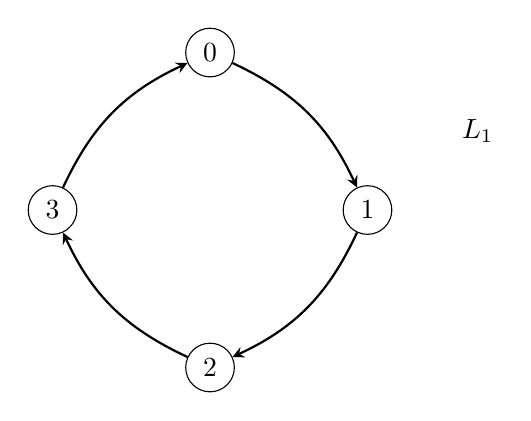
\begin{tikzpicture}[>=stealth, node distance=2.4cm]
\node[draw,circle] (z0) at (0,2) {$0$};
\node[draw,circle] (z1) at (2,0) {$1$};
\node[draw,circle] (z2) at (0,-2) {$2$};
\node[draw,circle] (z3) at (-2,0) {$3$};
\draw[->,thick] (z0) to[bend left=20] (z1);
\draw[->,thick] (z1) to[bend left=20] (z2);
\draw[->,thick] (z2) to[bend left=20] (z3);
\draw[->,thick] (z3) to[bend left=20] (z0);
\node at (3.4,1) {$L_1$};
\end{tikzpicture}
\end{center}
The single $4$-cycle $0\to1\to2\to3\to0$ shows $L_1$ has no fixed point and visits every element once, i.e.\ each row of the $\Zn4$ Cayley table is the cyclic shift of the header.
\end{remark}


%% ===== Dummit & Foote book-level content (merged in) =====
\subsection*{Further examples: the book's catalogue of groups}

The axioms become vivid only against a stock of concrete groups. D\&F open Chapter~1 with a standard list; we record it here, separating the abelian number systems from the (non)multiplicative ones and the forward-referenced matrix/permutation groups.

\begin{remark}[Additive number groups]\label{r:addnumber-mrg@c1}
Each of
\[
(\Z,+),\quad(\Q,+),\quad(\R,+),\quad(\C,+)
\]
is an abelian group: addition is associative and commutative, the identity is $0$, and the inverse of $x$ is $-x$. They sit inside one another, $\Z\subset\Q\subset\R\subset\C$, each a subgroup of the next under the same $+$. Note $(\Z,+)$ is the only one of the four in which a single element, namely $1$ (or $-1$), generates the whole group: $\Z=\gen{1}$.
\end{remark}

\begin{remark}[Multiplicative number groups, and what gets deleted]\label{r:multnumber-mrg@c1}
Under multiplication the picture is more delicate because $0$ is never invertible. Writing $A^{\times}=A\setminus\{0\}$ for a field $A$:
\[
(\Q^{\times},\cdot),\quad(\R^{\times},\cdot),\quad(\C^{\times},\cdot)
\]
are abelian groups (identity $1$, inverse $x\inv=1/x$), but $(\Q,\cdot),(\R,\cdot),(\C,\cdot)$ are \emph{not}, since $0$ has no inverse. By contrast $(\Z\setminus\{0\},\cdot)$ is still not a group: e.g.\ $2$ has no integer inverse (axiom (G3) fails, not merely the deletion of $0$). The positive reals and positive rationals form groups under multiplication,
\[
(\R^{+},\cdot),\qquad(\Q^{+},\cdot),
\]
because a product of positives is positive (closure) and $1/x>0$ when $x>0$ (inverses); these are the multiplicative analogues of the additive groups above, and $x\mapsto\log x$ is a bijection $\R^{+}\to\R$ carrying $\cdot$ to $+$.
\end{remark}

\begin{remark}[The trivial group and $(\Zn{n},+)$]\label{r:trivialandzn-mrg@c1}
The smallest example is the \emph{trivial group} $\{e\}$ with the only possible operation $e\ast e=e$; it is abelian and $e\inv=e$. At the other extreme of ``small but interesting'' is the additive group of residues
\[
(\Zn{n},+),\qquad \Zn{n}=\{\bar0,\bar1,\dots,\overline{n-1}\},\quad \bar a+\bar b=\overline{a+b},
\]
which is an abelian group of order $n$ for every $n\ge1$: identity $\bar0$, inverse $-\bar a=\overline{n-a}$ (and $-\bar0=\bar0$). This is genuinely a group even though $(\Zn{n},\cdot)$ is not (the fragment's worked example); deleting non-units from $\Zn{n}$ under multiplication leaves the multiplicative group $\Zns{n}$ of order $\varphi(n)$, treated later.
\end{remark}

\begin{remark}[Forward references: $S_n$, $D_{2n}$, $\GL$]\label{r:forwardgroups-mrg@c1}
Three families that D\&F flag here and construct in detail shortly:
\begin{enumerate}
\item[(i)] the \emph{symmetric group} $S_n$ of all bijections of $\{1,2,\dots,n\}$ to itself under composition, $|S_n|=n!$, nonabelian for $n\ge3$ (identity $\id$, inverse the inverse permutation);
\item[(ii)] the \emph{dihedral group} $D_{2n}$ of the $2n$ symmetries of a regular $n$-gon, with presentation $r^n=s^2=1$, $sr=r\inv s$ (so $|D_{2n}|=2n$), nonabelian for $n\ge3$;
\item[(iii)] the \emph{general linear group} $\GL_n(\R)$ (more generally $\GL_n(F)$ over a field $F$) of invertible $n\times n$ matrices under matrix multiplication, identity the matrix $I$, inverse the matrix inverse, nonabelian for $n\ge2$.
\end{enumerate}
In each case associativity is inherited (composition of functions, multiplication of matrices), and the work is identifying the identity and confirming every element is invertible.
\end{remark}

\subsection*{Powers of an element and the order of an element}

\begin{definition}[Integer powers]\label{d:powers-mrg@c1}
Let $G$ be a group, $x\in G$. Define $x^0=1$ (the identity), and for $n\ge1$
\[
x^n=\underbrace{x\,x\cdots x}_{n\text{ factors}},\qquad x^{-n}=(x\inv)^n=(x^n)\inv .
\]
By generalized associativity (Remark~\ref{r:genassoc@c1}) the usual laws of exponents hold for all integers $m,n$:
\[
x^m x^n=x^{m+n},\qquad (x^m)^n=x^{mn}.
\]
In additive notation (e.g.\ in $(\Zn{n},+)$ or $(\Z,+)$) one writes $nx$ in place of $x^n$, so ``$x^n=1$'' reads ``$nx=0$''.
\end{definition}

\begin{remark}[$x^mx^n=x^{m+n}$ but NOT $(xy)^n=x^ny^n$]\label{r:powerlaws-mrg@c1}
The single-element laws above need no commutativity. The \emph{two}-element law $(xy)^n=x^ny^n$ does: it holds for all $n$ iff $xy=yx$. For example in $D_8$, $(rs)^2=rsrs=r(sr)s=r(r\inv s)s=s^2=1$, whereas $r^2s^2=r^2\ne1$. So never distribute a power over a product in a nonabelian group.
\end{remark}

\begin{definition}[Order of an element]\label{d:order-mrg@c1}
The \emph{order} of $x\in G$, written $\ord{x}$, is the least positive integer $n$ with $x^n=1$, if such an $n$ exists; otherwise $x$ has \emph{infinite order}, $\ord{x}=\infty$. Equivalently $\ord{x}=\bigl|\gen{x}\bigr|$, the size of the cyclic subgroup generated by $x$. The identity is the unique element of order $1$.
\end{definition}

\begin{proposition}[When $x^k=1$]\label{p:orderdivides-mrg@c1}
Let $x\in G$ have finite order $n=\ord{x}$. For an integer $k$,
\[
x^k=1\quad\Longleftrightarrow\quad n\mid k.
\]
Consequently $x^a=x^b$ iff $a\equiv b\pmod n$, and the distinct powers of $x$ are exactly $1,x,x^2,\dots,x^{n-1}$.
\end{proposition}
\begin{proof}
($\Leftarrow$) If $k=qn$ then $x^k=(x^n)^q=1^q=1$. ($\Rightarrow$) Divide: $k=qn+r$ with $0\le r<n$. Then $1=x^k=(x^n)^q x^r=x^r$, and by minimality of $n$ this forces $r=0$, i.e.\ $n\mid k$. The last claims follow by applying this to $k=a-b$ and noting $1,x,\dots,x^{n-1}$ are pairwise distinct (a coincidence $x^i=x^j$, $0\le i<j<n$, would give $x^{j-i}=1$ with $0<j-i<n$).
\end{proof}

\begin{wex}{Orders in $\Z$, $\R^{\times}$, and $\C^{\times}$}
Compute the order of each element in several of the book's standard groups, distinguishing finite from infinite order.
\wrec Apply Definition~\ref{d:order-mrg@c1} directly: hunt for the least $n$ with $x^n=1$ (additively $nx=0$). The trigger is ``order of an element''; in the infinite groups below ($\Z$, $\R^{\times}$, $\C^{\times}$) most elements have infinite order, and finite order signals a root of unity or a torsion phenomenon.
\wsol
\emph{In $(\Z,+)$.} Here $x^n$ means $nx$. For $x=0$, $\ord{0}=1$. For any $x\ne0$, $nx=0$ forces $n=0$, so no \emph{positive} $n$ works: $\ord{x}=\infty$. Every nonzero integer has infinite order.

\emph{In $(\R^{\times},\cdot)$.} $\ord{1}=1$ and $\ord{-1}=2$ (since $(-1)^2=1$ and $(-1)^1=-1\ne1$). Any other $x$ ($x\ne\pm1$) has $|x^n|=|x|^n\ne1$ unless $|x|=1$, so $x=\pm1$ are the only elements of finite order; all others have infinite order, e.g.\ $\ord{2}=\infty$.

\emph{In $(\C^{\times},\cdot)$.} The element $i$ has powers $i,i^2=-1,i^3=-i,i^4=1$, so $\ord{i}=4$. A primitive $n$th root of unity $\zeta=e^{2\pi i/n}$ has $\ord{\zeta}=n$ exactly (its powers $1,\zeta,\dots,\zeta^{n-1}$ are distinct). A complex number of modulus $\ne1$, or of modulus $1$ but with irrational angle divided by $2\pi$, has infinite order.

\emph{Check.} In $\C^{\times}$, $\ord{i}=4$ matches Proposition~\ref{p:orderdivides-mrg@c1}: $i^k=1\iff4\mid k$, and indeed $i^{8}=1$, $i^{6}=i^2=-1\ne1$. The four distinct powers are $1,i,-1,-i$.
\end{wex}

\begin{wex}{Orders in $(\Zn{n},+)$: the formula $\ord{\bar a}=n/\gcd(a,n)$}
In the additive group $\Zn{12}$ find the order of $\bar a$ for several $a$, and state the general rule.
\wrec In $(\Zn{n},+)$ the relation $x^k=1$ is the additive $k\,\bar a=\bar 0$, i.e.\ $n\mid ka$; the least such $k>0$ is governed by $\gcd(a,n)$. Trigger: order of an element in a cyclic additive group -- reach for the gcd formula rather than listing multiples blindly.
\wsol
We seek the least $k\ge1$ with $k\,\bar a=\bar0$ in $\Zn{12}$, i.e.\ $12\mid ka$.
\begin{itemize}
\item $\bar1$: least $k$ with $12\mid k$ is $k=12$, so $\ord{\bar1}=12$.
\item $\bar3$: $12\mid 3k\iff 4\mid k$, least is $k=4$, so $\ord{\bar3}=4$.
\item $\bar4$: $12\mid 4k\iff 3\mid k$, least is $k=3$, so $\ord{\bar4}=3$.
\item $\bar8$: $12\mid 8k\iff 3\mid 2k\iff 3\mid k$, least is $k=3$, so $\ord{\bar8}=3$.
\item $\bar0$: $\ord{\bar0}=1$.
\end{itemize}
In general $\ord{\bar a}=\dfrac{n}{\gcd(a,n)}$ in $(\Zn{n},+)$: since $k\bar a=\bar0\iff n\mid ka\iff \dfrac{n}{\gcd(a,n)}\mid k$ (dividing $n\mid ka$ through by $\gcd(a,n)$ and using that $\tfrac{n}{\gcd(a,n)}$ and $\tfrac{a}{\gcd(a,n)}$ are coprime).
\emph{Check.} For $a=3,n=12$: $n/\gcd(a,n)=12/3=4$, matching $\ord{\bar3}=4$; and $4\bar3=\overline{12}=\bar0$ while $1\bar3,2\bar3,3\bar3=\bar3,\bar6,\bar9\ne\bar0$. The elements of order $12$ (the \emph{generators} of $\Zn{12}$) are exactly the $\bar a$ with $\gcd(a,12)=1$, namely $\bar1,\bar5,\bar7,\overline{11}$.
\end{wex}

\begin{wex}{Orders in nonabelian $D_8$ and $S_3$}
Tabulate the orders of all elements of $D_8=\gen{r,s\st r^4=s^2=1,\ sr=r\inv s}$ and of $S_3$.
\wrec Use $\ord{x}=$ least $n$ with $x^n=1$; for dihedral reflections and transpositions the order is forced to be $2$, while rotations and cycles inherit the order of the underlying cyclic shift. Trigger: orders in a small nonabelian group -- compute powers directly, exploiting $sr=r\inv s$ to reduce.
\wsol
\emph{In $D_8$ (order $8$).} The rotations: $\ord{1}=1$; $\ord{r}=4$ (least $k$ with $r^k=1$ is $4$); $\ord{r^2}=2$ (since $(r^2)^2=r^4=1$, and $r^2\ne1$); $\ord{r^3}=4$. The reflections $s,rs,r^2s,r^3s$ each square to $1$: e.g.\ $(rs)^2=rsrs=r(sr)s=r(r\inv s)s=r r\inv s^2=1$, and similarly $(r^ks)^2=1$ for every $k$. None equals $1$, so each reflection has order $2$. Summary: one element of order $1$, five of order $2$ ($r^2,s,rs,r^2s,r^3s$), two of order $4$ ($r,r^3$).

\emph{In $S_3$ (order $6$).} The identity has order $1$. The three transpositions $(1\,2),(1\,3),(2\,3)$ square to the identity, so each has order $2$. The two $3$-cycles $(1\,2\,3),(1\,3\,2)$ satisfy $(1\,2\,3)^3=\id$ with $(1\,2\,3)$ and $(1\,2\,3)^2=(1\,3\,2)$ both $\ne\id$, so each has order $3$.
\emph{Check.} The orders tally with the group sizes: in $D_8$, $1+5+2=8$ elements; in $S_3$, $1+3+2=6$. Every order divides the group order ($1,2,4\mid8$ and $1,2,3\mid6$), as Lagrange's theorem will later guarantee.
\end{wex}

\begin{remark}[Order of $x$ versus order of $x\inv$]\label{r:orderfacts-mrg@c1}
A fact used constantly: $\ord{x\inv}=\ord{x}$, because $x^n=1\iff(x\inv)^n=(x^n)\inv=1$, so $x$ and $x\inv$ have exactly the same powers equal to $1$. More generally, for any $g\in G$ the element $gxg\inv$ has the same order as $x$, since $(gxg\inv)^n=gx^ng\inv$, which equals $1$ exactly when $x^n=1$. Thus order is unchanged by inversion -- the first reason orders organize the structure of a group.
\end{remark}

\subsection*{Order of an element; the additive group $\Zn{n}$ and the unit group $\Zns{n}$}

\begin{definition}\label{d:order@c1}
Let $G$ be a group (written multiplicatively, identity $1$) and $x\in G$. The \emph{order} of $x$, written $\ord{x}$, is the least integer $k>0$ with $x^k=1$, if such a $k$ exists; otherwise $\ord{x}=\infty$. In an additively written group (identity $0$) the same definition reads: $\ord{x}$ is the least $k>0$ with $kx=0$, else $\infty$.
\end{definition}

\begin{definition}\label{d:zn@c1}
Fix $n\ge 1$. The set $\Zn{n}=\{\bar 0,\bar 1,\dots,\overline{n-1}\}$ of residue classes mod $n$ is a group under addition $\bar a+\bar b=\overline{a+b}$, of order $n$, with identity $\bar 0$ and inverse $-\bar a=\overline{n-a}$. The \emph{unit group} is
\[
\Zns{n}=\{\,\bar a\in\Zn{n}\st \gcd(a,n)=1\,\},
\]
a group under multiplication $\bar a\cdot\bar b=\overline{ab}$, of order $\varphi(n)$ (Euler's totient).
\end{definition}

\begin{proposition}\label{p:unit-iff-coprime@c1}
$\bar a\in\Zn{n}$ has a multiplicative inverse mod $n$ if and only if $\gcd(a,n)=1$. Hence $\Zns{n}$ is exactly the set of such classes, and it is a group.
\end{proposition}

\begin{proof}
($\Leftarrow$) If $\gcd(a,n)=1$, Bezout gives integers $u,v$ with $au+nv=1$, so $\overline{a}\,\overline{u}=\overline{au}=\overline{1-nv}=\bar 1$; thus $\bar u=\bar a\inv$.
($\Rightarrow$) If $\bar a\,\bar b=\bar 1$ then $ab\equiv 1\pmod n$, i.e. $ab-1=nk$ for some $k\in\Z$, so $ab-nk=1$ and any common divisor of $a$ and $n$ divides $1$; hence $\gcd(a,n)=1$.
Closure: $\gcd(a,n)=\gcd(b,n)=1\imp \gcd(ab,n)=1$. Associativity and $\bar 1$ are inherited from $\Z$, and inverses exist by the equivalence just proved. So $\Zns{n}$ is a group of order $\varphi(n)=\#\{1\le a\le n\st \gcd(a,n)=1\}$.
\end{proof}

\begin{proposition}\label{p:order-zn@c1}
In $(\Zn{n},+)$ the order of $\bar a$ is $\ord{\bar a}=\dfrac{n}{\gcd(a,n)}$. In particular $\ord{\bar 1}=n$, and $\bar a$ generates $\Zn{n}$ iff $\gcd(a,n)=1$.
\end{proposition}

\begin{proof}
$\ord{\bar a}$ is the least $k>0$ with $k\bar a=\bar 0$, i.e. $n\mid ka$. Write $d=\gcd(a,n)$, $a=da'$, $n=dn'$ with $\gcd(a',n')=1$. Then $n\mid ka \eqv dn'\mid kda' \eqv n'\mid ka' \eqv n'\mid k$ (since $\gcd(a',n')=1$). The least such $k>0$ is $n'=n/d$.
\end{proof}

\begin{method}{How to compute $\ord{x}$ in any group}
Trigger: you are handed a specific element $x$ and asked ``what is $|x|$?'' or ``does $x$ have finite order?''
\begin{enumerate}
\item Compute the powers $x^1,x^2,x^3,\dots$ (additively: $1x,2x,3x,\dots$) one at a time.
\item The order is the FIRST exponent $k>0$ that returns the identity ($1$ multiplicatively, $0$ additively). Stop there.
\item Shortcut in $(\Zn{n},+)$: $\ord{\bar a}=n/\gcd(a,n)$ (Prop.~\ref{p:order-zn@c1}); no power-listing needed.
\item Shortcut in $\Zns{n}$: $\ord{\bar a}$ must divide $\varphi(n)$ (Lagrange), so only test exponents that divide $\varphi(n)$.
\item If no power ever returns the identity (e.g. a nonzero rational under $+$, or a real $\ne\pm1$ under $\times$), then $\ord{x}=\infty$.
\end{enumerate}
\end{method}

\begin{method}{How to identify the units $\Zns{n}$}
Trigger: you must list $\Zns{n}$, or decide whether a given $\bar a$ is invertible mod $n$.
\begin{enumerate}
\item List $a=1,2,\dots,n-1$ (and include $a=1$ always; never include $\bar 0$ for $n>1$).
\item Keep exactly those $a$ with $\gcd(a,n)=1$ (Prop.~\ref{p:unit-iff-coprime@c1}). Discard any $a$ sharing a prime factor with $n$.
\item Count: $\#\Zns{n}=\varphi(n)$. Sanity-check via $\varphi(p^k)=p^k-p^{k-1}$ and $\varphi(mn)=\varphi(m)\varphi(n)$ for $\gcd(m,n)=1$.
\item To find an inverse of a unit $\bar a$, run the extended Euclidean algorithm on $a,n$ to get $au+nv=1$; then $\bar a\inv=\bar u$.
\end{enumerate}
\end{method}

\begin{pitfall}
Do not confuse the two groups. In $(\Zn{n},+)$ every class is present and the operation is $+$; in $\Zns{n}$ only the coprime classes are present and the operation is $\times$. ``$\ord{\bar 3}$ mod $12$'' is ambiguous until you say which group; additively $\ord{\bar 3}=4$, but $\bar 3$ is not even an element of $\Zns{12}$ since $\gcd(3,12)=3\ne 1$.
\end{pitfall}

\medskip
The additive clock for $(\Zn{6},+)$ below shows the single cycle generated by $\bar 1$; adding $\bar 1$ steps one notch clockwise, and $6$ steps return to $\bar 0$.

\begin{center}
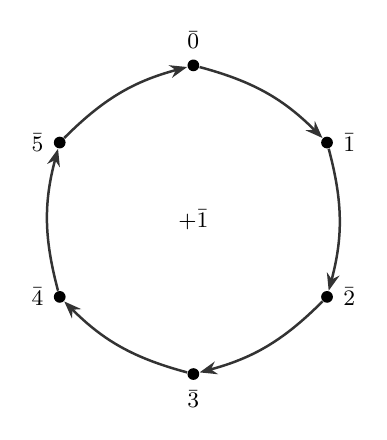
\begin{tikzpicture}[scale=1.4]
  \node[cgdot] (n0) at (90:1.4) {};
  \node[cgdot] (n1) at (30:1.4) {};
  \node[cgdot] (n2) at (-30:1.4) {};
  \node[cgdot] (n3) at (-90:1.4) {};
  \node[cgdot] (n4) at (-150:1.4) {};
  \node[cgdot] (n5) at (150:1.4) {};
  \draw[cgr] (n0) to[bend left=15] (n1);
  \draw[cgr] (n1) to[bend left=15] (n2);
  \draw[cgr] (n2) to[bend left=15] (n3);
  \draw[cgr] (n3) to[bend left=15] (n4);
  \draw[cgr] (n4) to[bend left=15] (n5);
  \draw[cgr] (n5) to[bend left=15] (n0);
  \node[cglab,above=2pt of n0] {$\bar 0$};
  \node[cglab,right=2pt of n1] {$\bar 1$};
  \node[cglab,right=2pt of n2] {$\bar 2$};
  \node[cglab,below=2pt of n3] {$\bar 3$};
  \node[cglab,left=2pt of n4] {$\bar 4$};
  \node[cglab,left=2pt of n5] {$\bar 5$};
  \node[cglab] at (0,0) {$+\bar 1$};
\end{tikzpicture}
\end{center}

Generators of $(\Zn{6},+)$ are exactly the units mod $6$: $\bar 1$ (clockwise step) and $\bar 5=-\bar 1$ (counterclockwise step), since $\gcd(1,6)=\gcd(5,6)=1$. The map $\Z\to\Zn{6}$, $k\mapsto k\bar 1$, factors through the quotient, giving the universal picture of a cyclic group:
\[\begin{tikzcd}[row sep=large,column sep=large]
  \Z \arrow[r, two heads, "\pi"] \arrow[dr, "k\,\mapsto\,k\bar 1"'] & \Zn{6} \arrow[d, dashed, "\exists!\,\cong"] \\ & \langle \bar 1\rangle
\end{tikzcd}\]
\begin{dgx}
\dgi{Objects:} Three groups: $\Z$ (the infinite additive group of integers), $\Zn{6}$ (the additive quotient group $\Z/6\Z$ of residue classes mod $6$, order $6$), and $\langle\bar 1\rangle$ (the cyclic subgroup of $\Zn{6}$ generated by $\bar 1$, which equals all of $\Zn{6}$ since $\bar 1$ generates).
\dgi{Arrows:} $\pi:\Z\to\Zn{6}$ is the canonical surjection $k\mapsto\bar k$, the quotient map that kills the subgroup $6\Z$; the double-head notation records surjectivity. The diagonal $k\mapsto k\bar 1$ is the evaluation homomorphism sending $k$ to the $k$-th multiple of $\bar 1$ in $\Zn{6}$; it equals $\pi$ composed with the inclusion $\langle\bar 1\rangle\hookrightarrow\Zn{6}$. The dashed vertical arrow is the unique isomorphism $\Zn{6}\xrightarrow{\,\cong\,}\langle\bar 1\rangle$ induced by the universal property of the quotient.
\dgi{What commutes:} The triangle commutes: $(\text{dashed})\circ\pi = (k\mapsto k\bar 1)$, i.e., applying $\pi$ then the isomorphism gives the same result as mapping $k$ directly to $k\bar 1$.
\dgi{Why it commutes:} The diagonal map $k\mapsto k\bar 1$ kills $6\Z$ (since $6\bar 1=\bar 0$), so the universal property of $\Zn{6}=\Z/6\Z$ provides a unique induced map $\Zn{6}\to\langle\bar 1\rangle$ making the triangle commute. Well-definedness: if $k\equiv k'\pmod 6$ then $(k-k')\bar 1=\bar 0$, so $k\bar 1=k'\bar 1$; the coset representative does not matter.
\dgi{Why this matters here:} This diagram encodes the fact that $(\Zn{6},+)$ is cyclic: the single element $\bar 1$ generates all of $\Zn{6}$, so the unique induced map is an isomorphism. It is the universal picture the text uses to explain generators of cyclic groups immediately after the clock diagram.
\dgi{Concrete example:} Take $k=8$. Then $\pi(8)=\bar 2$ and $8\bar 1=\bar 8=\bar 2$, confirming the triangle for this element. The dashed isomorphism sends $\bar 2\mapsto 2\bar 1=\bar 2$, which is the identity on $\Zn{6}=\langle\bar 1\rangle$.
\dgi{Common pitfall:} Students sometimes read the dashed arrow as \emph{defining} $\langle\bar 1\rangle$ rather than recording the universal property. The isomorphism exists because the kernel of the diagonal map equals $6\Z=\ker\pi$; if the kernel were different, no such induced map would exist.
\dgi{Takeaway:} The point of this diagram is that every cyclic group of order $n$ is a quotient of $\Z$, and the quotient map factors through the group via the unique isomorphism given by the universal property.
\end{dgx}

\subsubsection*{Worked examples: computing $\ord{x}$ in $(\Zn{n},+)$}

\begin{wex}{Orders of several elements of $(\Zn{12},+)$}
Compute $\ord{\bar a}$ in $(\Zn{12},+)$ for $a=0,1,2,3,4,6,8,9$.
\wrec This is an additive group $\Zn{12}$, so the shortcut $\ord{\bar a}=12/\gcd(a,12)$ from Prop.~\ref{p:order-zn@c1} applies directly; the only computation needed is a gcd for each $a$.
\wsol We tabulate $d=\gcd(a,12)$ and $\ord{\bar a}=12/d$:
\[
\begin{array}{c|cccccccc}
a & 0 & 1 & 2 & 3 & 4 & 6 & 8 & 9\\\hline
\gcd(a,12) & 12 & 1 & 2 & 3 & 4 & 6 & 4 & 3\\
\ord{\bar a}=12/\gcd & 1 & 12 & 6 & 4 & 3 & 2 & 3 & 4
\end{array}
\]
Spot-check $a=8$ by listing additive multiples: $\bar 8,\ \overline{16}=\bar 4,\ \overline{24}=\bar 0$; that is $1\cdot\bar8=\bar8$, $2\cdot\bar8=\bar4$, $3\cdot\bar8=\bar0$, so $\ord{\bar 8}=3$, matching $12/\gcd(8,12)=12/4=3$. Sanity check: every order divides $|\Zn{12}|=12$, and indeed $\{1,12,6,4,3,2,3,4\}$ all divide $12$. Also $\ord{\bar 0}=1$ (the identity), as required.
\end{wex}

\begin{wex}{An element of order $7$ in $\Zn{n}$}
In $(\Zn{14},+)$, find $\ord{\bar 4}$ and $\ord{\bar 2}$.
\wrec Additive group again, so use $\ord{\bar a}=14/\gcd(a,14)$. The trigger is simply ``order in $\Zn{n}$ under $+$.''
\wsol $\gcd(4,14)=2$, so $\ord{\bar 4}=14/2=7$. Check: $1\cdot\bar4=\bar4,\ 2\cdot\bar4=\bar8,\ 3\cdot\bar4=\overline{12},\ 4\cdot\bar4=\overline{16}=\bar2,\ 5\cdot\bar4=\bar6,\ 6\cdot\bar4=\overline{10},\ 7\cdot\bar4=\overline{14}=\bar0$. First return at $k=7$. Similarly $\gcd(2,14)=2$ gives $\ord{\bar 2}=7$. Sanity check: $7\mid 14=|\Zn{14}|$. Both $\bar2$ and $\bar4$ generate the same order-$7$ subgroup $\{\bar0,\bar2,\bar4,\bar6,\bar8,\overline{10},\overline{12}\}$.
\end{wex}

\begin{wex}{Generators of $\Zn{10}$}
Which classes $\bar a$ generate $(\Zn{10},+)$, i.e. have $\ord{\bar a}=10$?
\wrec By Prop.~\ref{p:order-zn@c1}, $\ord{\bar a}=10 \eqv \gcd(a,10)=1$. So generators $=$ units mod $10$. Trigger: ``which elements have full order $n$.''
\wsol Test $a=1,\dots,9$: $\gcd$ with $10$ equals $1$ exactly for $a\in\{1,3,7,9\}$ (the others share factor $2$ or $5$). So the generators are $\bar1,\bar3,\bar7,\bar9$, and there are $\varphi(10)=\varphi(2)\varphi(5)=1\cdot4=4$ of them. Check $a=3$: $\bar3,\bar6,\bar9,\overline{12}=\bar2,\bar5,\bar8,\overline{11}=\bar1,\bar4,\bar7,\overline{10}=\bar0$ -- exactly $10$ distinct classes before returning to $\bar0$, so $\ord{\bar 3}=10$. Sanity check: number of generators of a cyclic group of order $n$ is $\varphi(n)$, and $\varphi(10)=4$.
\end{wex}

\begin{wex}{Reading off an order without the formula}
In $(\Zn{9},+)$ compute $\ord{\bar 6}$ both by listing and by the gcd formula, and confirm they agree.
\wrec Additive cyclic group; the point is to verify the shortcut against brute force.
\wsol Listing: $1\cdot\bar6=\bar6,\ 2\cdot\bar6=\overline{12}=\bar3,\ 3\cdot\bar6=\overline{18}=\bar0$. First return at $k=3$, so $\ord{\bar6}=3$. Formula: $\gcd(6,9)=3$, $\ord{\bar6}=9/3=3$. They agree. Sanity check: $3\mid 9=|\Zn{9}|$, and the subgroup generated is $\{\bar0,\bar3,\bar6\}$ of size $3$.
\end{wex}

\subsubsection*{Worked examples: the unit group $\Zns{n}$}

\begin{wex}{List $\Zns{15}$ and the order of each unit}
Write out $\Zns{15}$ and compute $\ord{\bar a}$ (under multiplication) for every $\bar a$ in it.
\wrec ``List $\Zns{n}$'' triggers the gcd filter (keep $a$ with $\gcd(a,15)=1$); ``order of each'' triggers power-listing, restricted to divisors of $\varphi(15)$ by Lagrange.
\wsol $15=3\cdot5$, so $\varphi(15)=\varphi(3)\varphi(5)=2\cdot4=8$. Discard multiples of $3$ ($3,6,9,12$) and of $5$ ($5,10$). The survivors among $1,\dots,14$ are
\[
\Zns{15}=\{\bar1,\bar2,\bar4,\bar7,\bar8,\overline{11},\overline{13},\overline{14}\},\qquad \#=8=\varphi(15).\ \checkmark
\]
Possible orders divide $8$: i.e. $1,2,4,8$. Compute each (all mod $15$):
\[
\begin{array}{c|l|c}
\bar a & \text{powers until }\bar1 & \ord{\bar a}\\\hline
\bar1 & \bar1 & 1\\
\bar2 & \bar2,\ \bar4,\ \bar8,\ \overline{16}=\bar1 & 4\\
\bar4 & \bar4,\ \overline{16}=\bar1 & 2\\
\bar7 & \bar7,\ \overline{49}=\bar4,\ \overline{28}=\overline{13},\ \overline{91}=\bar1 & 4\\
\bar8 & \bar8,\ \overline{64}=\bar4,\ \overline{32}=\bar2,\ \overline{16}=\bar1 & 4\\
\overline{11} & \overline{11},\ \overline{121}=\bar1 & 2\\
\overline{13} & \overline{13},\ \overline{169}=\bar4,\ \overline{52}=\bar7,\ \overline{91}=\bar1 & 4\\
\overline{14} & \overline{14},\ \overline{196}=\bar1 & 2
\end{array}
\]
where e.g. $7^2=49=45+4\equiv\bar4$, $7^3=7\cdot4=28=15+13\equiv\overline{13}$, $7^4=7\cdot13=91=90+1\equiv\bar1$. Sanity check: every order is $1$, $2$, or $4$, each dividing $\varphi(15)=8$ (Lagrange).\ $\checkmark$ Note no element has order $8$, so $\Zns{15}$ is NOT cyclic; in fact it is $\Zns{15}\isom \Zn{2}\times\Zn{4}$.
\end{wex}

\begin{wex}{Why $\bar6$ is a unit mod $25$ but not mod $9$}
Decide whether $\bar 6\in\Zns{25}$ and whether $\bar 6\in\Zns{9}$, and (where it is a unit) find $\ord{\bar 6}$ and its inverse.
\wrec ``Is $\bar a$ a unit mod $n$?'' triggers the criterion $\gcd(a,n)=1$ (Prop.~\ref{p:unit-iff-coprime@c1}). The two moduli differ by their prime factors, which is exactly what the gcd sees.
\wsol Mod $25$: $\gcd(6,25)=1$ (since $25=5^2$ and $5\nmid 6$), so $\bar6\in\Zns{25}$. Mod $9$: $\gcd(6,9)=3\ne1$ (both divisible by $3$), so $\bar6\notin\Zns{9}$ -- it has no multiplicative inverse. Concretely mod $9$ the multiples $6\cdot1=6,\,6\cdot2=12\equiv3,\,6\cdot3=18\equiv0,\dots$ never hit $\bar1$, confirming non-invertibility. Inverse mod $25$ by Euclid: $25=4\cdot6+1$, so $1=25-4\cdot6$, giving $-4\cdot6\equiv1$, i.e. $\bar6\inv=\overline{-4}=\overline{21}$. Check $6\cdot21=126=125+1\equiv\bar1\pmod{25}$.\ $\checkmark$ Order of $\bar6$ mod $25$: $\varphi(25)=25-5=20$, so $\ord{\bar 6}\mid20$. Compute $6^2=36\equiv\overline{11}$, $6^4\equiv11^2=121\equiv\overline{21}$, $6^5=6^4\cdot6\equiv21\cdot6=126\equiv\bar1$. First return at $5$, so $\ord{\bar 6}=5$, and $5\mid20$.\ $\checkmark$
\end{wex}

\begin{wex}{$\ord{-1}=2$ in $\Zns{n}$ (and the same fact in $\R^\times$)}
Show $\ord{\overline{-1}}=2$ in $\Zns{n}$ for every $n\ge3$, and verify it concretely for $n=8$. Compare with $\ord{-1}=2$ in $(\R^\times,\cdot)$.
\wrec ``Order of $-1$'' triggers the smallest-power computation: $(-1)^1=-1\ne1$, $(-1)^2=1$. The only subtlety is that we need $\overline{-1}\ne\bar1$, which forces $n\ge3$.
\wsol For $n\ge3$, $\overline{-1}=\overline{n-1}\ne\bar1$ (since $n-1\ge2$), so $\ord{\overline{-1}}\ne1$. And $(\overline{-1})^2=\overline{1}$, so $\ord{\overline{-1}}=2$. Note $\gcd(n-1,n)=\gcd(-1,n)=1$, so $\overline{-1}$ really is a unit. Concretely $n=8$: $\overline{-1}=\bar7$, and $7^2=49=48+1\equiv\bar1\pmod 8$, while $\bar7\ne\bar1$; hence $\ord{\bar 7}=2$. In $\R^\times$: $(-1)^1=-1\ne1$ but $(-1)^2=1$, so $\ord{-1}=2$ there too. Sanity check: in any group an element $x\ne1$ with $x^2=1$ (i.e. $x=x\inv$) has order exactly $2$; that is precisely the case here.\ $\checkmark$
\end{wex}

\begin{wex}{Order of $\bar2$ in three different unit groups}
Compute $\ord{\bar 2}$ in $\Zns{7}$, $\Zns{9}$, and $\Zns{17}$.
\wrec Each is a unit group; $\bar2$ is a unit iff $n$ is odd, which holds for $7,9,17$. Use Lagrange to limit candidate orders to divisors of $\varphi(n)$, then list powers of $2$.
\wsol \textbf{Mod $7$} ($\varphi(7)=6$, divisors $1,2,3,6$): $2,4,8\equiv1$. So $\ord{\bar2}=3\mid6$.\ $\checkmark$
\textbf{Mod $9$} ($\varphi(9)=6$): $2,4,8,16\equiv7,14\equiv5,10\equiv1$. Powers $2^1,\dots,2^6$ give $2,4,8,7,5,1$; first return at $6$, so $\ord{\bar 2}=6$ -- $\bar2$ is a generator, $\Zns{9}$ is cyclic.\ $\checkmark$
\textbf{Mod $17$} ($\varphi(17)=16$, divisors $1,2,4,8,16$): $2^2=4,\ 2^4=16\equiv\overline{-1},\ 2^8\equiv(-1)^2=1$. First return at $8$ (not at $4$, since $2^4\equiv16\ne1$), so $\ord{\bar 2}=8\mid16$.\ $\checkmark$ Sanity check: in each case the order divides $\varphi(n)$, as Lagrange demands.
\end{wex}

\subsubsection*{Worked examples: infinite order}

\begin{wex}{An element of infinite order in $(\Q,+)$}
Show $\tfrac12\in(\Q,+)$ has infinite order. Contrast with $(\Zn{n},+)$ where every order is finite.
\wrec ``Infinite order'' triggers: prove NO positive multiple is the identity. Here the identity of $(\Q,+)$ is $0$, and we examine $k\cdot\tfrac12$.
\wsol For any integer $k>0$, $k\cdot\tfrac12=\tfrac{k}{2}$. This equals the additive identity $0$ only if $k=0$, which is not allowed ($k>0$). Hence $k\cdot\tfrac12\ne0$ for all $k>0$, so $\ord{\tfrac12}=\infty$. The same argument shows every nonzero $q\in\Q$ has infinite additive order: $kq=0$ with $q\ne0$ forces $k=0$. Sanity check: $\Q$ is torsion-free under $+$; the only finite-order element is $0$ itself, with $\ord{0}=1$. This is exactly why $(\Q,+)$ cannot be isomorphic to any finite $\Zn{n}$.
\end{wex}

\begin{wex}{An element of infinite order in $(\R^\times,\cdot)$}
Show $2\in(\R^\times,\cdot)$ has infinite order; then show $\ord{-1}=2$ to highlight the contrast.
\wrec ``Infinite order'' in a multiplicative group: prove no positive power equals the identity $1$. The trigger is the multiplicative identity $1$ versus the powers $2^k$.
\wsol For $k>0$, $2^k\ge2>1$, so $2^k\ne1$ for every $k>0$; hence $\ord{2}=\infty$. (Same for any real $t$ with $|t|>1$, or $0<|t|<1$: $|t^k|=|t|^k\ne1$ for all $k\ge1$.) By contrast, $-1$ has $|-1|=1$ and $(-1)^2=1$ with $(-1)^1=-1\ne1$, so $\ord{-1}=2$. Sanity check: in $(\R^\times,\cdot)$ the only finite-order elements are $1$ ($\ord{}=1$) and $-1$ ($\ord{}=2$); these are exactly the real solutions of $x^k=1$, namely the real roots of unity.\ $\checkmark$
\end{wex}

\begin{wex}{Infinite order via a homomorphism to $\Z$}
In $(\Q^{\times},\cdot)$ show $\ord{3}=\infty$ by mapping to $(\Z,+)$.
\wrec When direct power-listing is awkward, look for a homomorphism $\varphi$ into a torsion-free group: if $\varphi(x)$ has infinite order, so does $x$. The $3$-adic valuation $v_3$ is such a map.
\wsol Let $v_3:\Q^\times\to\Z$ send a rational to the exponent of $3$ in its prime factorization; it is a homomorphism: $v_3(xy)=v_3(x)+v_3(y)$. The square below commutes (top: multiply two rationals; map down by $v_3$; bottom: add the valuations):
\[\begin{tikzcd}[row sep=large,column sep=large]
  \Q^\times\times\Q^\times \arrow[r, "m"] \arrow[d, "v_3\times v_3"'] & \Q^\times \arrow[d, "v_3"] \\
  \Z\times\Z \arrow[r, "+"'] & \Z
\end{tikzcd}\]
\begin{dgx}
\dgi{Objects:} Four groups: $\Q^\times\times\Q^\times$ (the direct product of the multiplicative group of nonzero rationals with itself), $\Q^\times$ (nonzero rationals under multiplication), $\Z\times\Z$ (the direct product of the integers under addition), and $\Z$ (integers under addition). The top row lives in the multiplicative world; the bottom row in the additive world.
\dgi{Arrows:} $m:\Q^\times\times\Q^\times\to\Q^\times$ is the group multiplication $(x,y)\mapsto xy$. The left vertical $v_3\times v_3:(x,y)\mapsto(v_3(x),v_3(y))$ applies the $3$-adic valuation componentwise. The right vertical $v_3:\Q^\times\to\Z$ sends a nonzero rational to the exponent of $3$ in its prime factorization (negative for denominator factors). The bottom $+:\Z\times\Z\to\Z$ is ordinary integer addition $(a,b)\mapsto a+b$.
\dgi{What commutes:} Going right-then-down equals going down-then-right: $v_3(xy)=v_3(x)+v_3(y)$ for all $x,y\in\Q^\times$.
\dgi{Why it commutes:} This is precisely the statement that $v_3$ is a group homomorphism from $(\Q^\times,\cdot)$ to $(\Z,+)$. For any nonzero rationals $x=3^a\frac{p}{q}$ and $y=3^b\frac{r}{s}$ (with $3\nmid p,q,r,s$), the product $xy=3^{a+b}\frac{pr}{qs}$ has $v_3(xy)=a+b=v_3(x)+v_3(y)$.
\dgi{Why this matters here:} The diagram is used to prove $\ord{3}=\infty$ in $(\Q^\times,\cdot)$ without listing powers. Since $v_3$ is a homomorphism into the torsion-free group $(\Z,+)$ and $v_3(3)=1$ has infinite additive order, $3$ itself must have infinite multiplicative order. The commutativity square makes the homomorphism property precise and visible.
\dgi{Concrete example:} Take $x=6=2\cdot3$ and $y=\frac{3}{5}$. Then $v_3(x)=1$, $v_3(y)=1$, and $xy=\frac{18}{5}=2\cdot3^2\cdot5^{-1}$, so $v_3(xy)=2=1+1$. The square commutes for this pair.
\dgi{Common pitfall:} Students sometimes think $v_3$ lands in $\Z_{\ge0}$; in fact $v_3(\frac{1}{3})=-1\in\Z$, so the codomain must be all of $\Z$, not just the nonneg integers.
\dgi{Takeaway:} The point of this diagram is that a homomorphism into a torsion-free group transfers the problem of infinite order from $\Q^\times$ to $\Z$, where it is obvious.
\end{dgx}
Now $v_3(3^k)=k$. If $3^k=1$ for some $k>0$ then $k=v_3(3^k)=v_3(1)=0$, contradicting $k>0$. Hence $\ord{3}=\infty$. Sanity check: directly, $3^k\ge3>1$ for $k>0$, confirming no positive power is $1$.\ $\checkmark$
\end{wex}

\subsubsection*{One unifying commutative diagram}

For a cyclic group the assignment $k\mapsto x^k$ is the universal way orders appear. If $\ord{x}=n<\infty$, the homomorphism $\Z\to G$, $k\mapsto x^k$, has kernel exactly $n\Z$ and factors uniquely through $\Zn{n}$; if $\ord{x}=\infty$, the map is injective (kernel $\{0\}$), so $\langle x\rangle\isom\Z$:
\[\begin{tikzcd}[column sep=large]
  1 \arrow[r] & n\Z \arrow[r, hook] & \Z \arrow[r, two heads, "k\,\mapsto\,x^k"] & \langle x\rangle \arrow[r] & 1
\end{tikzcd}\]
\begin{dgx}
\dgi{Objects:} Five terms: the trivial group $1$, the subgroup $n\Z\le\Z$ of multiples of $n$ (a normal subgroup of $\Z$), the group $\Z$ of integers, the cyclic subgroup $\langle x\rangle\le G$ (a group generated by a single element $x$ of order $n$), and the trivial group $1$ again. This is a short exact sequence of groups.
\dgi{Arrows:} The leftmost $1\to n\Z$ is the unique map from the trivial group. The map $n\Z\hookrightarrow\Z$ is the inclusion (injective), indicated by the hook arrow. The map $\Z\to\langle x\rangle$, $k\mapsto x^k$, is the evaluation homomorphism (surjective onto $\langle x\rangle$, indicated by the double-head). The rightmost $\langle x\rangle\to 1$ is the unique map to the trivial group.
\dgi{What commutes:} Exactness at $n\Z$: $\operatorname{im}(1\to n\Z)=\{0\}=\operatorname{ker}(n\Z\hookrightarrow\Z)$ since the inclusion is injective. Exactness at $\Z$: $\operatorname{im}(n\Z\hookrightarrow\Z)=n\Z=\operatorname{ker}(k\mapsto x^k)$ because $x^k=1$ iff $n\mid k$. Exactness at $\langle x\rangle$: $\operatorname{im}(k\mapsto x^k)=\langle x\rangle=\operatorname{ker}(\langle x\rangle\to 1)$ since the map to the trivial group has full kernel.
\dgi{Why it commutes:} The key exactness condition is at $\Z$: the kernel of $k\mapsto x^k$ is $\{k\in\Z : x^k=1\}$. Since $\ord{x}=n$, an integer $k$ satisfies $x^k=1$ if and only if $n\mid k$, i.e. $k\in n\Z$. This is exactly the image of the inclusion, establishing exactness.
\dgi{Why this matters here:} This exact sequence packages the fundamental relationship between $\ord{x}$ and the structure of $\langle x\rangle$: it says $\langle x\rangle\cong\Z/n\Z$ (by the first isomorphism theorem) and makes the kernel $n\Z$ explicit. The diagram appears here to set up the factoring triangle below.
\dgi{Concrete example:} Take $G=\Zn{12}$, $x=\bar 4$. Then $\ord{\bar 4}=3$ and $\langle\bar4\rangle=\{\bar0,\bar4,\bar8\}$. The sequence is $1\to3\Z\hookrightarrow\Z\xrightarrow{k\mapsto k\bar4}\{\bar0,\bar4,\bar8\}\to1$; check $k\bar4=\bar0$ iff $12\mid4k$ iff $3\mid k$, so $\ker=3\Z$. $\checkmark$
\dgi{Common pitfall:} Students sometimes confuse the subgroup $n\Z\le\Z$ with the quotient group $\Zn{n}=\Z/n\Z$; these are different objects. The sequence records the kernel of the evaluation map as the \emph{subgroup} $n\Z$, not as a quotient.
\dgi{Takeaway:} The point of this diagram is that the order of $x$ is the unique positive integer $n$ for which the kernel of the evaluation map $\Z\to\langle x\rangle$ is exactly $n\Z$, encoding $\langle x\rangle\cong\Z/n\Z$.
\end{dgx}
\[\begin{tikzcd}[row sep=large,column sep=large]
  \Z \arrow[r, two heads, "\pi"] \arrow[dr, "k\,\mapsto\,x^k"'] & \Zn{n} \arrow[d, dashed, "\exists!\,\varphi"] \\ & \langle x\rangle
\end{tikzcd}\]
\begin{dgx}
\dgi{Objects:} Three groups: $\Z$ (integers under addition), $\Zn{n}=\Z/n\Z$ (the quotient group of residue classes mod $n$, order $n$), and $\langle x\rangle$ (the cyclic subgroup of $G$ generated by $x$, where $\ord{x}=n<\infty$).
\dgi{Arrows:} $\pi:\Z\to\Zn{n}$, $k\mapsto\bar k$, is the canonical surjection (the quotient map killing $n\Z$), shown with a double-head. The diagonal $k\mapsto x^k$ is the evaluation homomorphism, a surjection onto $\langle x\rangle$ with kernel $n\Z$. The dashed vertical $\varphi:\Zn{n}\to\langle x\rangle$ is the unique induced isomorphism given by the universal property of the quotient; it sends $\bar k\mapsto x^k$.
\dgi{What commutes:} The triangle commutes: $\varphi\circ\pi = (k\mapsto x^k)$, i.e., $\varphi(\bar k)=x^k$ for all $k\in\Z$.
\dgi{Why it commutes:} Well-definedness of $\varphi$: if $\bar k=\bar k'$ then $k\equiv k'\pmod n$, so $n\mid(k-k')$, so $x^{k-k'}=1$ (since $\ord{x}=n$), giving $x^k=x^{k'}$. Hence $\varphi(\bar k):=x^k$ does not depend on the coset representative, and the universal property of $\Zn{n}$ produces a unique such $\varphi$ making the triangle commute. Injectivity: $\varphi(\bar k)=1$ means $x^k=1$ means $n\mid k$ means $\bar k=\bar 0$.
\dgi{Why this matters here:} This is the universal-property factoring that characterizes all finite cyclic groups: any surjection $\Z\to\langle x\rangle$ with kernel $n\Z$ factors uniquely through $\Zn{n}$, giving an isomorphism $\Zn{n}\cong\langle x\rangle$. The diagram unifies the earlier short exact sequence with the explicit structure of $\langle x\rangle$.
\dgi{Concrete example:} Take $G=S_3$ and $x=(1\,2\,3)$. Then $\ord{x}=3$, $\langle x\rangle=\{e,(1\,2\,3),(1\,3\,2)\}$, and $n=3$. The induced $\varphi:\Zn{3}\to\langle x\rangle$ sends $\bar0\mapsto e$, $\bar1\mapsto(1\,2\,3)$, $\bar2\mapsto(1\,3\,2)$, an isomorphism.
\dgi{Common pitfall:} The dashed arrow exists and is unique ONLY because $\ker(k\mapsto x^k)=n\Z=\ker\pi$. If $\ord{x}$ were infinite (kernel $\{0\}$), or a different finite value, the dashed arrow to $\Zn{n}$ would not be an isomorphism (or might not exist as drawn).
\dgi{Takeaway:} The point of this diagram is that every cyclic group of finite order $n$ is canonically isomorphic to $\Zn{n}$, with the isomorphism uniquely determined by where a generator $x$ maps under the universal quotient.
\end{dgx}
Thus $\ord{x}$ is precisely the unique $n$ with $\ker(k\mapsto x^k)=n\Z$ (and $\ord{x}=\infty$ exactly when that kernel is $\{0\}$).

\begin{pitfall}
Lagrange tells you $\ord{\bar a}$ divides $\varphi(n)$ in $\Zns{n}$, but NOT that it equals $\varphi(n)$. In $\Zns{15}$ every element has order $1,2,$ or $4$, none equal to $\varphi(15)=8$, so $\Zns{15}$ has no generator. Always test the candidate divisors; do not assume the group is cyclic.
\end{pitfall}


%% ===== Dummit & Foote book-level content (merged in) =====
\subsection*{Further examples: small Cayley tables for $\Zn{n}$ and $\Zns{n}$, and orders in other groups}

Dummit \& Foote introduce $\Zn{n}$ and $\Zns{n}$ very concretely, listing the units mod $n$ by the gcd criterion and computing orders of elements; they also compute orders in the first non-cyclic and infinite groups of the text ($\R^\times$, $S_3$, the dihedral group $D_8$ of the square, $Q_8$, and $\GL_2(\R)$). We add the explicit Cayley tables and those element-order computations here.

\begin{remark}\label{r:notation-bar-mrg@c1}
D\&F write the elements of $\Zn{n}$ as the bars $\bar a$ (or $\overline{a}$), where $\bar a=\bar b$ exactly when $n\mid(a-b)$. The set $\Zn{n}$ carries \emph{two} natural operations, $+$ and $\times$, but only $(\Zn{n},+)$ is a group for every $n$; under $\times$ one passes to the units $\Zns{n}$ to get a group. The phrase ``the integers mod $n$'' refers to the additive group, while ``$\Zns{n}$'' or ``the units mod $n$'' refers to the multiplicative group.
\end{remark}

\begin{remark}\label{r:zn-cyclic-named-mrg@c1}
For \emph{every} $n\ge1$ the additive group $(\Zn{n},+)$ is generated by the single element $\bar 1$, since $\bar k=k\cdot\bar 1$ for all $k$. Thus $\Zn{n}=\gen{\bar 1}$ is cyclic of order $n$. This is the model D\&F use whenever they say ``the cyclic group of order $n$.''
\end{remark}

\begin{remark}\label{r:d8-naming-mrg@c1}
D\&F denote the dihedral group of symmetries of a regular $m$-gon by $D_{2m}$, indexed by its \emph{order} $2m$, not by $m$. So the symmetry group of the square has order $8$ and is written $D_8=\gen{r,s}$ with $r^4=s^2=1$ and $sr=r\inv s$ (some texts call this group $D_4$). We keep D\&F's convention throughout.
\end{remark}

\subsubsection*{The additive table of $(\Zn{n},+)$}

\begin{wex}{The complete addition table of $(\Zn{6},+)$}
Write out the Cayley table for $(\Zn{6},+)$ and read off the inverse of each element.
\wrec This is the defining operation $\bar a+\bar b=\overline{a+b}$ of Definition~\ref{d:zn@c1} applied to every pair; the table makes the group axioms (closure, identity row/column, a unique $\bar 0$ in each row giving inverses) visible at a glance.
\wsol Entries are $\overline{a+b}\bmod 6$:
\[
\begin{array}{c|cccccc}
+ & \bar0 & \bar1 & \bar2 & \bar3 & \bar4 & \bar5\\\hline
\bar0 & \bar0 & \bar1 & \bar2 & \bar3 & \bar4 & \bar5\\
\bar1 & \bar1 & \bar2 & \bar3 & \bar4 & \bar5 & \bar0\\
\bar2 & \bar2 & \bar3 & \bar4 & \bar5 & \bar0 & \bar1\\
\bar3 & \bar3 & \bar4 & \bar5 & \bar0 & \bar1 & \bar2\\
\bar4 & \bar4 & \bar5 & \bar0 & \bar1 & \bar2 & \bar3\\
\bar5 & \bar5 & \bar0 & \bar1 & \bar2 & \bar3 & \bar4
\end{array}
\]
The $\bar0$ entries locate inverses: $-\bar0=\bar0$, $-\bar1=\bar5$, $-\bar2=\bar4$, $-\bar3=\bar3$, $-\bar4=\bar2$, $-\bar5=\bar1$, matching $-\bar a=\overline{6-a}$. The table is symmetric across the main diagonal, recording that $(\Zn{6},+)$ is abelian. Sanity check: each row is a permutation of the six classes (the Latin-square property every group table has).\ $\checkmark$
\end{wex}

\subsubsection*{The multiplication table of $\Zns{n}$}

\begin{wex}{The complete multiplication table of $\Zns{8}$}
List $\Zns{8}$, write out its multiplication table, and find the order of each element.
\wrec ``List $\Zns{n}$'' invokes the gcd filter (Prop.~\ref{p:unit-iff-coprime@c1}); the table then exhibits the multiplicative group structure, and orders are read directly from the diagonal of squares.
\wsol $\gcd(a,8)=1$ for $a\in\{1,3,5,7\}$, so $\Zns{8}=\{\bar1,\bar3,\bar5,\bar7\}$ and $\varphi(8)=4$. Entries $\overline{ab}\bmod 8$:
\[
\begin{array}{c|cccc}
\times & \bar1 & \bar3 & \bar5 & \bar7\\\hline
\bar1 & \bar1 & \bar3 & \bar5 & \bar7\\
\bar3 & \bar3 & \bar1 & \bar7 & \bar5\\
\bar5 & \bar5 & \bar7 & \bar1 & \bar3\\
\bar7 & \bar7 & \bar5 & \bar3 & \bar1
\end{array}
\]
Every diagonal square is $\bar1$: $3^2=9\equiv\bar1$, $5^2=25\equiv\bar1$, $7^2=49\equiv\bar1$. Hence $\ord{\bar3}=\ord{\bar5}=\ord{\bar7}=2$ and $\ord{\bar1}=1$. So $\Zns{8}$ has no element of order $4=\varphi(8)$; it is the Klein four-group, $\Zns{8}\isom\Zn{2}\times\Zn{2}$, NOT cyclic. Sanity check: each element is its own inverse, consistent with $x^2=\bar1$ throughout; every order divides $\varphi(8)=4$.\ $\checkmark$
\end{wex}

\begin{wex}{$\Zns{n}$ for $n=5,7,9,10$: which are cyclic}
Determine $\Zns{n}$ and the order of a small candidate generator for $n=5,7,9,10$, and state which of these unit groups is cyclic.
\wrec D\&F use small moduli to illustrate that some $\Zns{n}$ have a generator (a single power runs through all units) and some do not. Lagrange limits the orders to divisors of $\varphi(n)$.
\wsol
\textbf{$n=5$}: $\Zns{5}=\{\bar1,\bar2,\bar3,\bar4\}$, $\varphi(5)=4$. Powers of $\bar2$: $2,4,3,1$, so $\ord{\bar2}=4$ and $\bar2$ is a generator; $\Zns{5}$ is cyclic.
\textbf{$n=7$}: $\Zns{7}=\{\bar1,\dots,\bar6\}$, $\varphi(7)=6$. Powers of $\bar3$: $3,2,6,4,5,1$, so $\ord{\bar3}=6$; $\Zns{7}$ is cyclic.
\textbf{$n=9$}: $\Zns{9}=\{\bar1,\bar2,\bar4,\bar5,\bar7,\bar8\}$, $\varphi(9)=6$. Powers of $\bar2$: $2,4,8,7,5,1$, so $\ord{\bar2}=6$; $\Zns{9}$ is cyclic.
\textbf{$n=10$}: $\Zns{10}=\{\bar1,\bar3,\bar7,\bar9\}$, $\varphi(10)=4$. Powers of $\bar3$: $3,9,7,1$, so $\ord{\bar3}=4$; $\Zns{10}$ is cyclic.
Sanity check: in each case the listed generator's powers reproduce exactly the $\varphi(n)$ units, and every order divides $\varphi(n)$. (Contrast $\Zns{8}$ above and $\Zns{15}$ earlier, which are not cyclic.)\ $\checkmark$
\end{wex}

\subsubsection*{Orders of elements in the book's first non-cyclic groups}

\begin{wex}{Orders in $S_3$}
In the symmetric group $S_3$ (permutations of $\{1,2,3\}$, composed right-to-left), compute the order of each element.
\wrec D\&F compute orders in $S_3$ soon after defining order, to show finite groups can have several different orders. Disjoint-cycle structure determines order: a single $k$-cycle has order $k$.
\wsol The six elements are the identity, three transpositions, and two $3$-cycles. As cycles:
\[
\begin{array}{c|c|c}
\sigma & \text{type} & \ord{\sigma}\\\hline
\id & \text{identity} & 1\\
(1\,2),\ (1\,3),\ (2\,3) & \text{transposition} & 2\\
(1\,2\,3),\ (1\,3\,2) & 3\text{-cycle} & 3
\end{array}
\]
Check a transposition: $(1\,2)^2=\id$, and $(1\,2)\ne\id$, so order $2$. Check a $3$-cycle: $(1\,2\,3)^2=(1\,3\,2)\ne\id$, $(1\,2\,3)^3=\id$, so order $3$. Sanity check: $|S_3|=6$ and the orders $1,2,3$ all divide $6$; no element has order $6$, so $S_3$ is not cyclic.\ $\checkmark$
\end{wex}

\begin{wex}{Orders in the dihedral group $D_8$}
In $D_8=\gen{r,s}$ with $r^4=s^2=1$ and $sr=r\inv s$, find the order of every element.
\wrec D\&F use the dihedral groups as a standard source of mixed orders: a rotation $r^k$ has order $4/\gcd(k,4)$, while every reflection $sr^k$ squares to the identity.
\wsol The eight elements are $1,r,r^2,r^3,s,sr,sr^2,sr^3$. Rotations: $\ord{1}=1$, $\ord{r}=\ord{r^3}=4$, $\ord{r^2}=2$. Reflections: each satisfies $(sr^k)^2=sr^k sr^k=s(r^k s)r^k=s(s r^{-k})r^k=s^2=1$, using $r^k s=s r^{-k}$; and $sr^k\ne1$, so $\ord{sr^k}=2$ for $k=0,1,2,3$. Collected:
\[
\begin{array}{c|cccc|cccc}
g & 1 & r & r^2 & r^3 & s & sr & sr^2 & sr^3\\\hline
\ord{g} & 1 & 4 & 2 & 4 & 2 & 2 & 2 & 2
\end{array}
\]
Sanity check: all orders divide $|D_8|=8$; there are exactly $\varphi(4)=2$ elements of order $4$ inside the rotation subgroup $\gen{r}\isom\Zn{4}$, namely $r$ and $r^3$, as the cyclic theory predicts.\ $\checkmark$
\end{wex}

\begin{wex}{Orders in the quaternion group $Q_8$}
In $Q_8=\{\pm1,\pm i,\pm j,\pm k\}$ with $i^2=j^2=k^2=-1$ and $ij=k$, find the order of every element.
\wrec D\&F present $Q_8$ as a group where, unlike $D_8$, there is a \emph{unique} element of order $2$ and every non-identity element except $-1$ has order $4$. Use $i^2=j^2=k^2=-1$ and $(-1)^2=1$.
\wsol $\ord{1}=1$. Since $(-1)^2=1$ and $-1\ne1$, $\ord{-1}=2$. For $i$: $i^2=-1$, $i^3=-i$, $i^4=(-1)^2=1$, so $\ord{i}=4$; the same computation gives $\ord{-i}=\ord{j}=\ord{-j}=\ord{k}=\ord{-k}=4$.
\[
\begin{array}{c|c|c}
g & \text{value} & \ord{g}\\\hline
1 & 1 & 1\\
-1 & -1 & 2\\
\pm i,\ \pm j,\ \pm k & \text{square to } -1 & 4
\end{array}
\]
Sanity check: all orders divide $|Q_8|=8$; there is exactly one element of order $2$ (namely $-1$), in contrast with $D_8$, which has five (the half-turn $r^2$ and the four reflections). So $D_8$ and $Q_8$ are non-isomorphic groups of the same order.\ $\checkmark$
\end{wex}

\begin{wex}{Infinite order in $\GL_2(\R)$}
Let $A=\begin{pmatrix}1 & 1\\ 0 & 1\end{pmatrix}\in\GL_2(\R)$. Show $\ord{A}=\infty$, and contrast with $B=\begin{pmatrix}0 & -1\\ 1 & 0\end{pmatrix}$, which has finite order.
\wrec D\&F use $\GL_n$ as the standard infinite group in which individual elements may still have finite or infinite order. Compute the powers directly.
\wsol By induction $A^k=\begin{pmatrix}1 & k\\ 0 & 1\end{pmatrix}$. For $k>0$ the top-right entry is $k\ne0$, so $A^k\ne I$ for every $k\ge1$; hence $\ord{A}=\infty$. For $B$: $B^2=\begin{pmatrix}-1 & 0\\ 0 & -1\end{pmatrix}=-I$, $B^3=\begin{pmatrix}0 & 1\\ -1 & 0\end{pmatrix}$, $B^4=I$, so $\ord{B}=4$ (this $B$ is rotation by $90^\circ$). Sanity check: $\det A=\det B=1\ne0$, so both lie in $\GL_2(\R)$; a single group can contain elements of every order, finite and infinite.\ $\checkmark$
\end{wex}

\begin{remark}\label{r:additive-vs-mult-orders-mrg@c1}
The contrast across these examples is the recurring D\&F theme. The additive groups $(\R,+)$, $(\Q,+)$, $(\Z,+)$ are \emph{torsion-free}: the identity $0$ is the only element of finite order ($\ord{0}=1$), since $kx=0$ with $k>0$ forces $x=0$. The multiplicative group $(\R^\times,\cdot)$ has just two elements of finite order, $\ord{1}=1$ and $\ord{-1}=2$, and $(\Q^\times,\cdot)$ has the same two. By comparison the finite groups $\Zn{n}$, $\Zns{n}$, $S_3$, $D_8$, $Q_8$ realize a whole range of orders. Passing from $+$ to $\times$, or from $\Z$ to $\Zn{n}$, is exactly what creates nontrivial finite orders.
\end{remark}

\begin{exers}{Exercises (from the text).}
\item Determine which of the operations are associative:
   (a) $a\ast b=a-b$ on $\Z$;\;
   (b) $a\ast b=a+b+ab$ on $\R$;\;
   (c) $a\ast b=\frac{a+b}{5}$ on $\Q$;\;
   (d) $(a,b)\ast(c,d)=(ad+bc,\,bd)$ on $\Z\times\Z$;\;
   (e) $a\ast b=\frac{a}{b}$ on $\Q-\{0\}$.
\item Which operations in Exercise~1 are commutative?
\item Prove that addition of residue classes in $\Zn{n}$ is associative.
\item Prove that multiplication of residue classes in $\Zn{n}$ is associative.
\item Prove for all $n>1$ that $\Zn{n}$ is not a group under multiplication.
\item Which of these are groups under addition?
   (a) lowest-terms rationals with \emph{odd} denominator;
   (b) with \emph{even} denominator;
   (c) $|x|<1$;
   (d) $|x|\ge 1$ together with $0$;
   (e) denominators $1$ or $2$;
   (f) denominators $1,2,$ or $3$.
\item $G=\{x\in\R\mid 0\le x<1\}$ with $x\ast y=$ fractional part of $x+y$.
   Show $\ast$ is a well-defined binary operation and $G$ is abelian.
\item $G=\{z\in\C\mid z^n=1\text{ for some }n\in\Z^+\}$ (roots of unity).
   (a) Group under multiplication; (b) not a group under addition.
\item $G=\{a+b\sqrt2\mid a,b\in\Q\}$. (a) Group under addition; (b) nonzero elements
   form a group under multiplication.
\item Prove a finite group is abelian iff its group table is symmetric.
\item Find the orders of every element of the additive group $\Zn{12}$.
\item Find the orders of $\bar1,\overline{-1},\bar5,\bar7,\overline{-7},\overline{13}$
   in $\Zns{12}=\{1,5,7,11\}$.
\item Find the orders of $\bar1,\bar2,\bar6,\bar9,\overline{10},\overline{12},
   \overline{-1},\overline{-10},\overline{-18}$ in $\Zn{36}$.
\item Find the orders of $\bar1,\overline{-1},\bar5,\overline{13},\overline{-13},
   \overline{17}$ in $\Zns{36}$.
\item Prove $(a_1a_2\cdots a_n)\inv=a_n\inv a_{n-1}\inv\cdots a_1\inv$.
\item Prove $x^2=1$ iff $|x|$ is $1$ or $2$.
\item If $|x|=n$, prove $x\inv=x^{n-1}$.
\item Prove $xy=yx\iff y\inv xy=x\iff x\inv y\inv xy=1$.
\item For $x\in G$, $a,b\in\Z^+$: (a) $x^{a+b}=x^ax^b$, $(x^a)^b=x^{ab}$;
   (b) $(x^a)\inv=x^{-a}$; (c) extend (a) to all integers.
\item Show that $x$ and $x\inv$ have the same order.
\item $G$ finite, $|x|=n$ odd. Prove $x=(x^2)^k$ for some $k$.
\item Prove $|x|=|g\inv xg|$, and deduce $|ab|=|ba|$.
\item $|x|=n<\infty$, $n=st$. Prove $|x^s|=t$.
\item If $a,b$ commute, prove $(ab)^n=a^nb^n$ for all $n\in\Z$.
\item Prove that if $x^2=1$ for all $x\in G$, then $G$ is abelian.
\item If $\varnothing\neq H\subseteq G$ is closed under the operation and inverses,
   prove $H$ is a \textbf{subgroup}.
\item Prove $\{x^n\mid n\in\Z\}$ is a subgroup (the cyclic subgroup $\gen{x}$).
\item Verify the group axioms for $A\times B$.
\item Prove $A\times B$ is abelian iff both $A$ and $B$ are.
\item Show $(a,1),(1,b)$ commute and $|(a,b)|=\lcm(|a|,|b|)$.
\item Prove a finite group of even order contains an element of order $2$.
\item If $|x|=n$, prove $1,x,\dots,x^{n-1}$ are distinct, and $|x|\le|G|$.
\item $|x|=n$. (a) $n$ odd $\Rightarrow x^i\neq x^{-i}$ ($1\le i\le n-1$);
   (b) $n=2k\Rightarrow x^i=x^{-i}$ iff $i=k$ ($1\le i\le n-1$).
\item If $x$ has infinite order, prove the powers $x^n$ are distinct.
\item If $|x|=n$, show every power of $x$ lies in $\{1,x,\dots,x^{n-1}\}$.
\item $G=\{1,a,b,c\}$, order $4$, no element of order $4$. Show the table is unique
   and $G$ abelian.
\end{exers}

\begin{exers}{Additional exercises.}
\item Let $\ast$ be the binary operation on $\Z$ defined by $a \ast b = a + b - ab$.
  (a) Compute $2 \ast 3$, $(2 \ast 3)\ast 4$, and $2\ast(3\ast 4)$.
  (b) Determine whether $\ast$ is commutative and whether it is associative.
  (c) Show that $0$ is an identity for $\ast$, and find every $a \in \Z$ that has a two-sided $\ast$-inverse in $\Z$.

\item On the set $S = \R \setminus \{0\}$ define $a \star b = |a|\,b$.
  (a) Verify that $\star$ is a well-defined binary operation on $S$ (i.e. $a \star b \neq 0$ whenever $a,b \neq 0$).
  (b) Is $\star$ associative? Is it commutative? Justify each answer with an explicit computation or counterexample.
  (c) Does $\star$ have a (two-sided) identity element? Prove your claim.

\item Let $G$ be a group and let $a,b,c \in G$. Solve each of the following equations for $x$ in terms of $a,b,c$, using only the group axioms (give the unique solution in (a) and (c), and name the axiom used at each step):
  (a) $a x b = c$;
  (b) $x a x = a$ given that $x = x\inv$ (show that the solutions are exactly the $x$ with $x^2=1$ and $xa=ax$, so $x=1$ always works but need not be the only solution);
  (c) $a x a\inv = b$.

\item Recall $\Zns{n}$ is the set of residues $\overline{a}$ with $\gcd(a,n)=1$ under multiplication mod $n$.
  (a) List the elements of $\Zns{15}$, and compute $\overline{2}\cdot\overline{8}$, $\overline{4}\cdot\overline{4}$, and $\overline{7}\cdot\overline{13}$ in $\Zns{15}$.
  (b) Find $\overline{7}\inv$ in $\Zns{15}$ by exhibiting an integer $x$ with $7x \equiv 1 \pmod{15}$.
  (c) Explain why $\overline{6}$ is NOT an element of $\Zns{15}$, and why this is exactly what is needed for $(\Zns{n},\,\cdot\,)$ to be a group.

\item In a group $G$, prove the ``socks and shoes'' rule: for all $a,b \in G$, $(ab)\inv = b\inv a\inv$. Then prove by induction that $(a_1 a_2 \cdots a_k)\inv = a_k\inv \cdots a_2\inv a_1\inv$ for all $k \ge 1$.

\item Let $G$ be a group in which $x^2 = 1$ for every $x \in G$.
  (a) Show that $x = x\inv$ for all $x \in G$.
  (b) Using (a), show that $G$ is abelian. (Hint: expand $(ab)^2 = 1$.)
  (c) Give an explicit example of such a group with exactly $4$ elements.

\item Let $G$ be a finite group and fix $a \in G$. Define $L_a \colon G \to G$ by $L_a(x) = ax$.
  (a) Prove $L_a$ is a bijection of the set $G$ (find its inverse map explicitly).
  (b) Conclude that each element of $G$ appears exactly once in every row of the group's multiplication (Cayley) table.
\end{exers}

\begin{exers}{Commutative-diagram exercises.}
\item Let $\pi \colon \Z \to \Zn{n}$ be the reduction-mod-$n$ map $\pi(a) = \overline{a}$, and recall it satisfies $\pi(a+b) = \pi(a) + \pi(b)$.
  (a) Show that the addition on $\Zn{n}$ is the unique operation making the square
  \[\begin{tikzcd}[row sep=large,column sep=large]
    \Z\times\Z \arrow[r, "+"] \arrow[d, "\pi\times\pi"'] & \Z \arrow[d, "\pi"] \\
    \Zn{n}\times\Zn{n} \arrow[r, "\oplus"'] & \Zn{n}
  \end{tikzcd}\]
  commute (i.e. $\pi(a) \oplus \pi(b) = \pi(a+b)$ for all $a,b$); this is what ``well-defined mod $n$'' means.
  (b) State and verify the analogous commuting square for multiplication, replacing $+$ by $\cdot$ and $\oplus$ by the product on $\Zn{n}$.

\item Consider the two compositions $\Z \xrightarrow{\;f\;} \Z \xrightarrow{\;\pi\;} \Zn{6}$, where $\pi$ is reduction mod $6$ and $f(a) = 3a$.
  (a) Compute the image of the composite $\pi \circ f \colon \Z \to \Zn{6}$ by listing $(\pi\circ f)(a)$ for $a = 0,1,2,3$.
  (b) Identify the set of $a \in \Z$ with $(\pi\circ f)(a) = \overline{0}$, and describe it as $m\Z$ for the appropriate integer $m$.
  (c) Draw the diagram exhibiting $\pi\circ f$ as a single arrow $\Z \to \Zn{6}$ and label that arrow with the rule $a \mapsto \overline{3a}$.

\item For a binary operation $\ast$ on a set $A$, the operation is a map $m \colon A \times A \to A$, $m(a,b) = a\ast b$. The operation is commutative exactly when the triangle built from the swap map $\tau \colon A\times A \to A\times A$, $\tau(a,b) = (b,a)$, commutes:
  \[\begin{tikzcd}[column sep=large]
    A\times A \arrow[r, "\tau"] \arrow[dr, "m"'] & A\times A \arrow[d, "m"] \\ & A
  \end{tikzcd}\]
  (a) Explain in words what the commutativity of this diagram says about $\ast$.
  (b) For $A = \Z$ and $a\ast b = a - b$, exhibit a specific pair $(a,b)$ for which the diagram fails to commute, thereby proving subtraction is not commutative.

\item Let $\varphi \colon \Z \to \Zn{12}$ be reduction mod $12$, a surjection of additive groups. Define its kernel $K = \{\,a \in \Z \st \varphi(a) = \overline{0}\,\}$.
  (a) Show $K = 12\Z$, and complete the labels in the sequence
  \[\begin{tikzcd}[column sep=large]
    0 \arrow[r] & K \arrow[r, hook, "\iota"] & \Z \arrow[r, two heads, "\varphi"] & \Zn{12} \arrow[r] & 0
  \end{tikzcd}\]
  by giving the inclusion $\iota$ explicitly.
  (b) For the element $\overline{8} \in \Zn{12}$, list three different integers $a$ with $\varphi(a) = \overline{8}$, and explain how any two of them differ by an element of $K$.

\item (Intro pullback / fiber product.) Let $\mu \colon \Z \to \Zn{2}$ be reduction mod $2$, $\mu(a) = \overline{a}$. Form the set
  \[ P = \{\,(a,b)\in\Z\times\Z \st a \equiv b \pmod 2\,\} = \{\,(a,b)\in\Z\times\Z \st \mu(a) = \mu(b)\,\}, \]
  the pullback (fiber product) of $\mu$ with itself, fitting into the square
  \[\begin{tikzcd}[row sep=large,column sep=large]
    P \arrow[r, "p_2"] \arrow[d, "p_1"'] & \Z \arrow[d, "\mu"] \\
    \Z \arrow[r, "\mu"'] & \Zn{2}
  \end{tikzcd}\]
  where $p_1(a,b) = a$ and $p_2(a,b) = b$ are the two coordinate projections.
  (a) Verify that this square commutes: show $\mu(a) = \mu(b)$ for every $(a,b) \in P$.
  (b) Show $P$ is closed under coordinatewise addition, so $(P,+)$ is a group; exhibit its identity and the inverse of a typical element $(a,b)$.
  (c) Exhibit one element of $P$ and one element of $\Z\times\Z$ that is NOT in $P$, justifying each membership decision by the mod-$2$ condition.
\end{exers}


\section{Dihedral Groups}
\subsection*{The Dihedral Group $D_{2n}$: Symmetries of a Regular $n$-gon}

\begin{definition}[Dihedral group]\label{d:dihedral@c1}
Fix $n\ge 3$. Label the vertices of a regular $n$-gon $0,1,\dots,n-1$ counterclockwise. The \emph{dihedral group} $D_{2n}$ is the group of all rigid symmetries (rotations and reflections) of this polygon under composition. It is generated by
\[
r=\text{rotation counterclockwise by }2\pi/n,\qquad
s=\text{reflection across the axis through vertex }0,
\]
subject to the relations
\[
r^n=1,\qquad s^2=1,\qquad srs=r\inv\quad(\text{equivalently }sr=r\inv s,\ \ r^k s=s r^{-k}).
\]
\end{definition}

Here is the square ($D_8$, $n=4$) with the rotation $r$ and the reflection axis fixed by $s$ (for even $n$ the axis through vertex $0$ is a diagonal, passing through the opposite vertex $n/2$, here vertex $2$), and the pentagon ($D_{10}$, $n=5$) with $r$ and the axis of $s$ (for odd $n$ the axis through vertex $0$ passes through the midpoint of the opposite edge):

\begin{center}
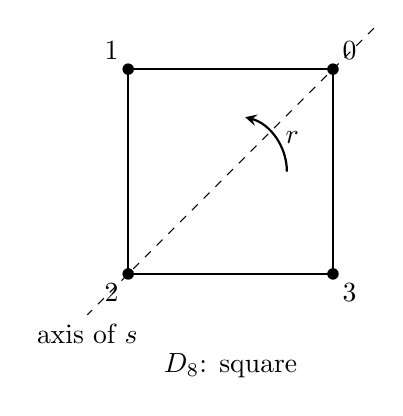
\begin{tikzpicture}[scale=1.3]
% square D8
\coordinate (v0) at (1,1);
\coordinate (v1) at (-1,1);
\coordinate (v2) at (-1,-1);
\coordinate (v3) at (1,-1);
\draw[thick] (v0)--(v1)--(v2)--(v3)--cycle;
\foreach \p/\n in {v0/0,v1/1,v2/2,v3/3}{\fill (\p) circle (1.6pt);}
\node[above right] at (v0){$0$};
\node[above left] at (v1){$1$};
\node[below left] at (v2){$2$};
\node[below right] at (v3){$3$};
\draw[dashed] (1.4,1.4)--(-1.4,-1.4) node[below]{axis of $s$};
\draw[->,>=stealth,thick] (0.55,0) arc (0:75:0.55) node[midway,right]{$r$};
\node at (0,-1.9){$D_8$: square};
\end{tikzpicture}
\hspace{1.2cm}
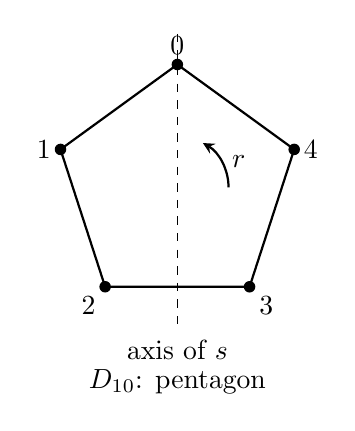
\begin{tikzpicture}[scale=1.3]
% pentagon D10, vertex 0 at top
\foreach \k in {0,1,2,3,4}{
  \coordinate (w\k) at ({90+72*\k}:1.2);
}
\draw[thick] (w0)--(w1)--(w2)--(w3)--(w4)--cycle;
\foreach \k in {0,1,2,3,4}{\fill (w\k) circle (1.6pt);}
\node[above] at (w0){$0$};
\node[left] at (w1){$1$};
\node[below left] at (w2){$2$};
\node[below right] at (w3){$3$};
\node[right] at (w4){$4$};
\draw[dashed] (0,1.5)--(0,-1.4) node[below]{axis of $s$};
\draw[->,>=stealth,thick] (0.5,0) arc (0:60:0.5) node[midway,right]{$r$};
\node at (0,-1.9){$D_{10}$: pentagon};
\end{tikzpicture}
\end{center}

\begin{proposition}[Order and normal form]\label{p:normalform@c1}
$|D_{2n}|=2n$, and every element of $D_{2n}$ can be written \emph{uniquely} in one of the two normal forms
\[
r^i\quad(\text{a rotation}),\qquad sr^i\quad(\text{a reflection}),\qquad 0\le i<n.
\]
Thus $D_{2n}=\{1,r,\dots,r^{n-1},\,s,sr,\dots,sr^{n-1}\}$, a disjoint union of $n$ rotations and $n$ reflections.
\end{proposition}

\begin{proof}
Since $r^n=1$, the rotations are exactly $\{r^i:0\le i<n\}$, $n$ in number. The relation $sr=r\inv s$ lets us move every $s$ to the \emph{left} of every $r$: any word in $r,s$ collapses to $s^a r^i$ with $a\in\{0,1\}$ (using $s^2=1$) and $0\le i<n$ (using $r^n=1$). Hence every element is $r^i$ or $sr^i$, giving at most $2n$ elements. Geometrically $r$ has order $n$ (a rotation by $2\pi/n$) and $s\ne r^i$ for any $i$ (a reflection reverses orientation; rotations preserve it), so the two families are disjoint and the $2n$ listed symmetries are distinct. The polygon has exactly $2n$ symmetries (a vertex $0$ can go to any of $n$ positions, then orientation can be preserved or reversed: $n\cdot 2=2n$), so $|D_{2n}|=2n$ and the listing is complete; uniqueness of $r^i$ vs.\ $sr^i$ and of the exponent $i$ follows from $|D_{2n}|=2n$.
\end{proof}

\begin{proposition}[Orders of elements]\label{p:orders@c1}
In $D_{2n}$:
\[
\ord{r^k}=\frac{n}{\gcd(n,k)},\qquad \ord{sr^i}=2\ \text{ for every }i.
\]
In particular $r$ has order $n$, and all $n$ reflections are involutions.
\end{proposition}

\begin{proof}
Inside the cyclic subgroup $\gen{r}\isom\Zn{n}$ the order of $r^k$ is $n/\gcd(n,k)$ (standard cyclic-group fact). For a reflection,
\[
(sr^i)^2=sr^i\,sr^i=s(r^i s)r^i=s(sr^{-i})r^i=s^2 r^{-i+i}=1,
\]
using $r^i s=sr^{-i}$. Since $sr^i\ne1$ (it is a reflection, not the identity), $\ord{sr^i}=2$.
\end{proof}

\begin{method}{How to simplify a word and read off the order in $D_{2n}$}
\textbf{Trigger:} any product of $r$'s and $s$'s in $D_{2n}$, e.g.\ $(sr^a)(sr^b)$, $r^k s r^{-k}$, or $(sr^i)^m$.
\begin{enumerate}
\item \textbf{Push every $s$ left.} Repeatedly apply $r^k s = s r^{-k}$ to slide each $s$ past any $r$ on its left, flipping that $r$'s exponent sign.
\item \textbf{Cancel adjacent $s$'s} via $s^2=1$. You end with $s^a r^m$, $a\in\{0,1\}$.
\item \textbf{Reduce the exponent} $m$ modulo $n$ (since $r^n=1$) to land in $0\le m<n$.
\item \textbf{Read the answer:} $r^m$ is a rotation with $\ord{r^m}=n/\gcd(n,m)$; $sr^m$ is a reflection with order $2$.
\end{enumerate}
\textbf{Mnemonic:} ``$s$ flips the sign of every $r$ it jumps over.'' An \emph{even} number of $s$'s gives a rotation; an \emph{odd} number gives a reflection.
\end{method}

\begin{pitfall}
$D_{2n}$ is \emph{non-abelian} for $n\ge3$: $sr=r\inv s\ne rs$ unless $r=r\inv$. Never silently commute $r$ past $s$; you must use $rs=sr\inv$ (sign flip), not $rs=sr$.
\end{pitfall}

\begin{wex}{Multiply two reflections: $(sr^3)(sr^5)$ in $D_{12}$}
In $D_{12}$ (so $n=6$), compute $(sr^3)(sr^5)$ and put it in normal form. Is the result a rotation or a reflection?
\wrec This is a product of two reflections (two factors each containing one $s$): an \emph{even} number of $s$'s, so the answer must be a rotation $r^m$. Use the method: push the inner $s$ left past $r^3$.
\wsol
\[
(sr^3)(sr^5)=s\,(r^3 s)\,r^5
= s\,(s r^{-3})\,r^5
= s^2 r^{-3} r^5
= r^{2}.
\]
Here $r^3 s = s r^{-3}$ (sign flip), then $s^2=1$, then add exponents $-3+5=2$. Reduce mod $n=6$: $2$ is already in $\{0,\dots,5\}$, so the normal form is $\boxed{r^2}$, a rotation.
\textbf{Check:} $\ord{r^2}=6/\gcd(6,2)=3$. Two reflections compose to a rotation (orientation-reversing twice $=$ orientation-preserving), consistent with getting $r^2$.
\end{wex}

\begin{wex}{The conjugate $r^k s r^{-k}$}
In $D_{2n}$, simplify $r^k s r^{-k}$ to normal form. Interpret the result.
\wrec One $s$ in the middle: odd number of $s$'s, so expect a reflection $sr^m$. Slide the $s$ to the far left by pushing it past $r^k$ on its left (or equivalently push $r^k$ to the right of $s$).
\wsol
Use $r^k s = s r^{-k}$ on the leftmost pair:
\[
r^k s r^{-k}=(r^k s)r^{-k}=(s r^{-k})r^{-k}=s r^{-k-k}=s r^{-2k}.
\]
Reduce the exponent mod $n$: $sr^{-2k}=s r^{\,n-2k\bmod n}$. Normal form $\boxed{sr^{-2k}}$ (a reflection).
\textbf{Check:} as a reflection it should square to $1$: $(sr^{-2k})^2=1$ by Proposition~\ref{p:orders@c1}. Geometrically, conjugating the axis of $s$ by the rotation $r^k$ rotates that axis through the angle $2\pi k/n$ (onto the axis through vertex $k$), i.e.\ by $2k$ steps of $\pi/n$ (the angle between neighboring reflection axes), matching the index $-2k$.
\end{wex}

\begin{wex}{All elements of order $2$ in $D_8$}
List every element of $D_8$ ($n=4$) of order exactly $2$.
\wrec Order-2 elements are the self-inverse non-identity elements. Split into rotations $r^k$ (use $\ord{r^k}=4/\gcd(4,k)$) and reflections $sr^i$ (all have order $2$).
\wsol
\emph{Rotations.} $\ord{r^0}=1$; $\ord{r}=4/\gcd(4,1)=4$; $\ord{r^2}=4/\gcd(4,2)=2$; $\ord{r^3}=4/\gcd(4,3)=4$. So the only rotation of order $2$ is $r^2$.
\emph{Reflections.} By Proposition~\ref{p:orders@c1}, $s, sr, sr^2, sr^3$ each have order $2$.
Thus the order-$2$ elements are
\[
\boxed{\,r^2,\ s,\ sr,\ sr^2,\ sr^3\,}\qquad(5\text{ elements}).
\]
\textbf{Check:} $|D_8|=8$; removing $1$ (order $1$) and $r,r^3$ (order $4$) leaves exactly these $5$, all of order $2$. $(r^2)^2=r^4=1$ confirms $r^2$; e.g.\ $(sr)^2=sr\,sr=s(rs)r=s(sr^{-1})r=s^2r^0=1$.
\end{wex}

\begin{wex}{Every reflection is an involution}
Show directly that $\ord{sr^i}=2$ for all $i$, working in $D_{10}$ ($n=5$) with $i=3$ as a concrete instance, then in general.
\wrec The element $sr^i$ contains one $s$. Squaring it puts two $s$'s adjacent after one sign-flip; cancel them.
\wsol
\emph{Concrete ($D_{10}$, $i=3$):}
\[
(sr^3)^2=sr^3\,sr^3=s(r^3 s)r^3=s(s r^{-3})r^3=s^2 r^{0}=1,
\]
and $sr^3\ne1$, so $\ord{sr^3}=2$.
\emph{General:} $(sr^i)^2=s(r^i s)r^i=s(sr^{-i})r^i=s^2 r^{-i+i}=1$ and $sr^i\ne1$, hence $\ord{sr^i}=2$.
\textbf{Check:} the key step is the single sign flip $r^i s=sr^{-i}$; the two $s$'s then meet and cancel, leaving $r^{-i+i}=r^0=1$. Valid for every $i$ and every $n$.
\end{wex}

\begin{wex}{Product of two reflections is a rotation; build any rotation}
In $D_{2n}$, show $(sr^a)(sr^b)=r^{\,b-a}$. Use it in $D_{10}$ to write the rotation $r^2$ as a product of two reflections.
\wrec Two reflections $=$ even number of $s$'s $\Rightarrow$ a rotation. Push the inner $s$ left past $r^a$.
\wsol
\emph{General formula:}
\[
(sr^a)(sr^b)=s(r^a s)r^b=s(s r^{-a})r^b=s^2 r^{-a+b}=r^{\,b-a}.
\]
\emph{Application in $D_{10}$ ($n=5$):} to get $r^2$ we need $b-a\equiv2\pmod5$. Pick $a=0,b=2$:
\[
(sr^0)(sr^2)=s\cdot sr^2=r^2.\qquad\text{(Check: }b-a=2.\text{)}
\]
Another choice $a=1,b=3$: $(sr)(sr^3)=r^{3-1}=r^2$, same rotation.
\textbf{Check:} $(s)(sr^2)=s^2r^2=r^2$ directly; and any $r^m$ arises since $b-a$ ranges over all residues mod $n$. This shows the $n$ reflections generate $\gen{r}$, hence all of $D_{2n}$.
\end{wex}

\begin{wex}{A longer word: $r^2 s r^3 s r$ in $D_{14}$}
Simplify $r^2 s r^3 s r$ in $D_{14}$ ($n=7$) to normal form and give its order.
\wrec Two $s$'s (even) $\Rightarrow$ rotation. Push each $s$ leftward; each jump over a power of $r$ flips that power's sign.
\wsol
Start by sliding the left $s$ past $r^3$, then the resulting $s$'s cancel:
\[
r^2 s r^3 s r
= r^2 (s r^3) s r
= r^2 (r^{-3} s) s r
= r^{2-3} s^2 r
= r^{-1} r
= r^{0}=1.
\]
(I used $s r^3=r^{-3}s$, i.e.\ $sr^k=r^{-k}s$ for all $k$.) Normal form: $\boxed{1}$.
\textbf{Check (push both $s$'s the other way):} $r^2 s r^3 s r$; pair the inner block $sr^3 s=(sr^3)s=(r^{-3}s)s=r^{-3}$, so the word is $r^2\cdot r^{-3}\cdot r=r^{2-3+1}=r^0=1$. Same answer, $\ord{1}=1$.
\end{wex}

\begin{wex}{Solve for $x$: $r^3 x = sr$ in $D_8$}
In $D_8$ ($n=4$) find the unique $x$ with $r^3 x=sr$, in normal form.
\wrec Left-multiply by $(r^3)\inv=r^{-3}=r^{1}$ (since $r^4=1$). The right side is a reflection, so $x$ will be a reflection.
\wsol
\[
x=r^{-3}(sr)=r^{1}(sr)=(r s)r=(s r^{-1})r=s r^{0}=s.
\]
Here $rs=sr^{-1}$ (one sign flip). So $\boxed{x=s}$.
\textbf{Check:} $r^3 x=r^3 s$. And $r^3 s=s r^{-3}=s r^{1}=sr$ (since $-3\equiv1\bmod4$). Indeed $r^3 s=sr$, matching the right-hand side.
\end{wex}

The relation $srs=r\inv$ says exactly that conjugation by $s$ inverts $r$; equivalently the map $r\mapsto r\inv$, $s\mapsto s$ extends to an automorphism. This is encoded by the commuting square (left) and the fact that $s$ conjugates $\gen r$ by inversion (right):
\[
\begin{tikzcd}[row sep=large,column sep=large]
\gen r \arrow[r, "x\,\mapsto\,sxs"] \arrow[d, "\subseteq"'] & \gen r \arrow[d, "\subseteq"] \\
D_{2n} \arrow[r, "x\,\mapsto\,sxs"'] & D_{2n}
\end{tikzcd}
\qquad\qquad
\begin{tikzcd}[column sep=huge]
r \arrow[r, mapsto, "\text{conj.\ by }s"] & r\inv
\end{tikzcd}
\]
\begin{dgx}
\dgi{Objects:} Both squares share four copies of two groups: the cyclic rotation subgroup $\gen{r} \isom \Zn{n}$ (upper row) and the full dihedral group $D_{2n}$ (lower row), each appearing twice (once as domain, once as codomain). The right diagram has a single object-level arrow tracking what conjugation does to the generator $r$.

\dgi{Arrows:} The top horizontal arrow is the map $\gen{r} \to \gen{r}$, $x \mapsto sxs$ (conjugation by $s$, restricted to $\gen{r}$). The bottom horizontal arrow is the same conjugation formula on all of $D_{2n}$. The two vertical arrows are the set-inclusion $\gen{r} \subseteq D_{2n}$ (the canonical inclusion homomorphism). The right mini-diagram records the single value $r \mapsto r^{-1}$, confirming that conjugation by $s$ inverts the generator.

\dgi{What commutes:} The square says that inclusion then conjugation equals conjugation then inclusion: for every $x \in \gen{r}$, applying the top map and then the right inclusion gives $sxs \in D_{2n}$; applying the left inclusion first and then the bottom map also gives $sxs \in D_{2n}$. These are the same element, so the square commutes: $\iota \circ (x \mapsto sxs) = (x \mapsto sxs) \circ \iota$, where $\iota: \gen{r} \hookrightarrow D_{2n}$.

\dgi{Why it commutes:} Chase $x \in \gen{r}$, say $x = r^k$. Top then right: $r^k \mapsto sr^k s \mapsto sr^k s \in D_{2n}$. Left then bottom: $r^k \mapsto r^k \in D_{2n} \mapsto sr^k s$. Both give $sr^k s$. The two paths agree because both just compute $sxs$ and include the result; the square is recording compatibility of a formula with an inclusion, not a non-trivial constraint.

\dgi{Why this matters here:} The prose just established $srs = r^{-1}$, which says conjugation by $s$ is not merely a set-map but an automorphism of $\gen{r}$ that happens to extend to all of $D_{2n}$. The square makes that extension visible: the automorphism of $\gen{r}$ is the restriction of the conjugation automorphism of $D_{2n}$. This is the structural content behind the relation $srs = r^{-1}$ and it will recur when proving $\gen{r} \nor D_{2n}$.

\dgi{Concrete example:} In $D_8$ ($n=4$), take $x = r^2 \in \gen{r}$. Top path: $r^2 \mapsto sr^2 s = r^{-2} = r^2$. Bottom path: include $r^2 \in D_8$, then $r^2 \mapsto sr^2 s = r^2$. The element-level diagram gives $r \mapsto r^{-1} = r^3$, so conjugation inverts: $sr^2 s = (r^{-1})^2 = r^2$ (consistent since $r^2 = r^{-2}$ in $\Zn{4}$).

\dgi{Common pitfall:} Students sometimes read the commuting square as saying the two horizontal maps are the \emph{same} arrow or that the inclusions are isomorphisms. They are not: the inclusions are proper embeddings ($\gen{r} \subsetneq D_{2n}$ for $n \ge 3$), and the commutativity just records that the conjugation formula $x \mapsto sxs$ is consistent across the two group levels.

\dgi{Takeaway:} The point of this diagram is that the relation $srs = r^{-1}$ is not merely an algebraic identity but says that conjugation by $s$ is an automorphism of $\gen{r}$ that extends compatibly to all of $D_{2n}$, making $\gen{r}$ a normal subgroup.
\end{dgx}

The universal property of $D_{2n}$ (it is the largest group on generators $a,b$ with $a^n=b^2=1$, $bab=a\inv$) gives, for any group $G$ containing elements $\rho,\sigma$ with $\rho^n=\sigma^2=1$ and $\sigma\rho\sigma=\rho\inv$, a unique homomorphism filling the dashed arrow:
\[
\begin{tikzcd}[row sep=large,column sep=large]
\{a,b\} \arrow[r, hook] \arrow[dr, "{a\mapsto\rho,\ b\mapsto\sigma}"'] & D_{2n} \arrow[d, dashed, "\exists!\,\varphi"] \\
& G
\end{tikzcd}
\]
\begin{dgx}
\dgi{Objects:} Three objects appear. The generating set $\{a,b\}$ is not a group but the source data: two abstract symbols satisfying $a^n = b^2 = 1$ and $bab = a^{-1}$. The group $D_{2n}$ is the dihedral group presented by those generators and relations. The group $G$ is any group containing elements $\rho, \sigma$ with $\rho^n = \sigma^2 = 1$ and $\sigma\rho\sigma = \rho^{-1}$.

\dgi{Arrows:} The top horizontal arrow $\{a,b\} \hookrightarrow D_{2n}$ is the inclusion of the generators into $D_{2n}$ (the canonical embedding sending $a \mapsto r$, $b \mapsto s$). The diagonal arrow $\{a,b\} \to G$ is the assignment $a \mapsto \rho$, $b \mapsto \sigma$, recording the hypothesized relations in $G$. The dashed vertical arrow $\varphi: D_{2n} \to G$ is the unique group homomorphism extending the diagonal assignment; it is dashed because its existence and uniqueness are what the diagram asserts.

\dgi{What commutes:} The triangle commutes: the composition $\{a,b\} \hookrightarrow D_{2n} \xrightarrow{\varphi} G$ equals the direct assignment $a \mapsto \rho$, $b \mapsto \sigma$. Concretely: $\varphi(r) = \rho$ and $\varphi(s) = \sigma$, and for every word $r^i$ or $sr^i$ in $D_{2n}$, $\varphi(r^i) = \rho^i$ and $\varphi(sr^i) = \sigma\rho^i$.

\dgi{Why it commutes:} Well-definedness is the key point. Every element of $D_{2n}$ has a unique normal form $r^i$ or $sr^i$, so defining $\varphi(r^i) = \rho^i$ and $\varphi(sr^i) = \sigma\rho^i$ is unambiguous. The relations $\rho^n = 1$, $\sigma^2 = 1$, $\sigma\rho\sigma = \rho^{-1}$ in $G$ guarantee that $\varphi$ respects the group operation: e.g.\ $\varphi(sr \cdot r^{i}) = \sigma\rho^{i+1} = \varphi(sr)\varphi(r^i)$. The assignment on $\{a,b\}$ forced $\varphi$ uniquely because $a,b$ generate $D_{2n}$.

\dgi{Why this matters here:} This is the universal property of $D_{2n}$ as a group presented by generators and relations. It converts the geometric fact ``$D_{2n}$ is the symmetry group'' into the algebraic fact ``any group satisfying those relations receives a homomorphism from $D_{2n}$.'' Every time one constructs a homomorphism out of $D_{2n}$ in the chapter, this triangle is the silent justification: just verify $\rho^n = \sigma^2 = 1$ and $\sigma\rho\sigma = \rho^{-1}$ in the target.

\dgi{Concrete example:} Take $G = \Zn{2}$ (written additively, so $\rho^n$ means $n\rho$), $\rho = \overline{0}$, $\sigma = \overline{1}$. Then $\rho^n = \overline{0}$, $\sigma^2 = \overline{1}+\overline{1} = \overline{0}$, and $\sigma\rho\sigma = \overline{1}+\overline{0}+\overline{1} = \overline{0} = -\rho = \rho^{-1}$, so $\varphi$ exists: it sends every rotation $r^i$ to $\overline{0}$ and every reflection $sr^i$ to $\overline{1}$. (By contrast, $G = \Zn{n}$ with $\rho = \overline{1}$, $\sigma = \overline{0}$ does not work for $n\ge 3$: there $\sigma\rho\sigma = \overline{1} \ne \overline{n-1} = \rho^{-1}$.) Another example: $G = D_{2n}$ itself, $\rho = r$, $\sigma = s$; then $\varphi = \id_{D_{2n}}$ fills the dashed arrow, confirming that $D_{2n}$ maps to itself via the identity.

\dgi{Common pitfall:} Students sometimes think the dashed arrow exists for any $\rho, \sigma \in G$. It does not: the three relations $\rho^n = 1$, $\sigma^2 = 1$, $\sigma\rho\sigma = \rho^{-1}$ must hold in $G$ first. Without them, there is no well-defined $\varphi$: for instance $srs$ and $r^{-1}$ are the same element of $D_{2n}$, so $\varphi$ would have to send it both to $\sigma\rho\sigma$ and to $\rho^{-1}$, which is impossible if $\sigma\rho\sigma \ne \rho^{-1}$. The relations are the kernel condition that makes the induced map well-defined.

\dgi{Takeaway:} The point of this diagram is that $D_{2n}$ is the universal group on two generators satisfying the dihedral relations, meaning any concrete realization of those relations in a group $G$ yields a unique homomorphism $D_{2n} \to G$ extending the generator assignment.
\end{dgx}

\begin{remark}\label{r:cyclic-normal@c1}
The rotation subgroup $\gen r=\{1,r,\dots,r^{n-1}\}\isom\Zn{n}$ is normal in $D_{2n}$ (index $2$), and $D_{2n}/\gen r\isom\Zn 2$ records the rotation/reflection parity ($s$ flips parity). This is why an even number of $s$'s in any word yields a rotation and an odd number yields a reflection, the recognition shortcut used throughout.
\end{remark}

\begin{pitfall}
When reducing exponents, do it \emph{modulo} $n$, not arbitrarily: in $D_{8}$, $r^{-3}=r^{1}$ because $-3\equiv1\pmod4$, but in $D_{14}$, $r^{-3}=r^{4}$. Mixing up $n$ is the most common arithmetic slip.
\end{pitfall}


%% ===== Dummit & Foote book-level content (merged in) =====
\subsection*{Further examples}

The book builds $D_{2n}$ by hand from the geometry before any relation is asserted, fixes a working notation for elements, and pins down the small cases by listing every symmetry explicitly. The material below records that concrete construction and those examples; throughout this subsection the vertices are relabelled $1,2,\dots,n$ (so vertex $1$ plays the role of vertex $0$ in Definition~\ref{d:dihedral@c1}), to match the permutation bookkeeping D\&F uses in the small cases.

\begin{definition}[Symmetry of a polygon, as in D\&F]\label{d:symmetry-def-mrg@c1}
A \emph{symmetry} of the regular $n$-gon ($n\ge 3$) is a rigid motion of the plane that carries the polygon onto itself. Concretely, label the vertices $1,2,\dots,n$ consecutively, and record each symmetry by what it does to the vertices: it is a permutation $\sigma$ of $\{1,2,\dots,n\}$ that sends adjacent vertices to adjacent vertices. The set of all such symmetries, under composition of motions, is the dihedral group $D_{2n}$. (D\&F write the subscript $2n$ to display the order; some texts write $D_n$. Here $D_{2n}$ always has $2n$ elements.)
\end{definition}

\begin{proposition}[D\&F's adjacency count: there are exactly $2n$ symmetries]\label{p:count-2n-mrg@c1}
A symmetry of the regular $n$-gon is determined by where it sends vertex $1$ and where it sends the adjacent vertex $2$. Vertex $1$ may go to any of the $n$ vertices; once its image is fixed, the adjacent vertex $2$ must land on one of the two vertices adjacent to the image of $1$. Hence there are at most $n\cdot 2=2n$ symmetries, and since the $n$ rotations together with the $n$ reflections are all distinct symmetries, there are exactly $2n$.
\end{proposition}

\begin{proof}
Let $\sigma$ be a symmetry. Choose the image $\sigma(1)$: there are $n$ choices. Because $\sigma$ preserves adjacency and distances, $\sigma(2)$ must be one of the two neighbors of $\sigma(1)$, giving $2$ choices. Now $\sigma(1)$ and $\sigma(2)$ already determine $\sigma$ on every remaining vertex: vertex $3$ is the neighbor of $2$ other than $1$, so $\sigma(3)$ is forced to be the neighbor of $\sigma(2)$ other than $\sigma(1)$, and so on around the polygon. Thus $\sigma$ is determined by the pair $(\sigma(1),\sigma(2))$, so there are at most $2n$ symmetries. Exhibiting $2n$ distinct ones (the rotations $r^i$ and reflections $sr^i$, $0\le i<n$) shows the bound is met.
\end{proof}

\begin{remark}[How D\&F fixes notation]\label{r:dnf-notation-mrg@c1}
Once the count is known, D\&F names two specific symmetries and uses them as a working alphabet. Let $r$ be the rotation through $2\pi/n$ (one vertex step, in the direction of increasing labels) and let $s$ be the reflection fixing vertex $1$. The text then verifies, directly from the geometry, that
\[
1,r,r^2,\dots,r^{n-1}\ \text{are distinct with }r^n=1;\qquad s^2=1;\qquad s\ne r^i\ \text{for any }i,
\]
and the single mixing relation, obtained by tracking what each side does to the vertices,
\[
rs=sr\inv\qquad(\text{equivalently } srs\inv=r\inv,\ \ s\inv rs=r\inv).
\]
Every element is then named in the form $r^i$ or $sr^i$ with $0\le i<n$; this naming, not an abstract presentation, is what the book computes with.
\end{remark}

\begin{wex}{The smallest case: $D_6$, symmetries of the triangle}
Take the equilateral triangle with vertices $1,2,3$. List all $6=2\cdot 3$ symmetries of $D_6$ both as words in $r,s$ and as permutations of $\{1,2,3\}$, where $r$ rotates $1\to2\to3\to1$ and $s$ fixes vertex $1$.
\wrec Proposition~\ref{p:count-2n-mrg@c1} guarantees exactly $2n=6$ symmetries. List the three rotations $1,r,r^2$ and the three reflections $s,sr,sr^2$, then read off each one's action on the vertices to confirm they are distinct.
\wsol
The rotation $r$ sends $1\mapsto2,\ 2\mapsto3,\ 3\mapsto1$, i.e.\ the $3$-cycle $(1\,2\,3)$; the reflection $s$ fixes vertex $1$ and swaps the other two, i.e.\ $(2\,3)$. Compute the rest (permutations compose right-to-left):
\[
\begin{array}{lll}
1\ &=\ \text{identity} & \text{fixes }1,2,3,\\
r\ &=\ (1\,2\,3) & 1\mapsto2\mapsto3\mapsto1,\\
r^2\ &=\ (1\,3\,2) & 1\mapsto3\mapsto2\mapsto1,\\
s\ &=\ (2\,3) & \text{fixes }1,\\
sr\ &=\ (2\,3)(1\,2\,3)=(1\,3) & \text{fixes }2,\\
sr^2\ &=\ (2\,3)(1\,3\,2)=(1\,2) & \text{fixes }3.
\end{array}
\]
So $D_6=\{1,r,r^2,s,sr,sr^2\}$, and as permutations these are exactly the six elements of $\operatorname{Sym}\{1,2,3\}$.
\textbf{Check:} the three reflections $s=(2\,3)$, $sr=(1\,3)$, $sr^2=(1\,2)$ are the three transpositions, each fixing one vertex; the three rotations are the identity and the two $3$-cycles. All six permutations are distinct, confirming $|D_6|=6$. Here $D_6\isom\operatorname{Sym}\{1,2,3\}$ because both have order $6$ and every permutation of the three vertices is a symmetry of the triangle.
\end{wex}

\begin{wex}{$D_8$ as permutations of the square's vertices}
For the square with vertices $1,2,3,4$ in cyclic order, write each of the $8$ elements of $D_8$ as a permutation of $\{1,2,3,4\}$, with $r=(1\,2\,3\,4)$ and $s$ the reflection fixing vertices $1$ and $3$ (the diagonal axis).
\wrec There are $2n=8$ symmetries by Proposition~\ref{p:count-2n-mrg@c1}. The four rotations are powers of $r=(1\,2\,3\,4)$; the four reflections are $s,sr,sr^2,sr^3$. Multiply out each reflection as a permutation, composing right-to-left.
\wsol
The reflection across the diagonal through vertices $1$ and $3$ fixes those and swaps $2,4$, so $s=(2\,4)$. Composing right-to-left ($sr$ means ``apply $r$, then $s$''):
\[
\begin{array}{ll}
1=\text{id}, & s=(2\,4),\\
r=(1\,2\,3\,4), & sr=(2\,4)(1\,2\,3\,4)=(1\,4)(2\,3),\\
r^2=(1\,3)(2\,4), & sr^2=(2\,4)(1\,3)(2\,4)=(1\,3),\\
r^3=(1\,4\,3\,2), & sr^3=(2\,4)(1\,4\,3\,2)=(1\,2)(3\,4).
\end{array}
\]
\textbf{Check:} the reflections split into the two diagonal flips $s=(2\,4)$, $sr^2=(1\,3)$ (each fixing two opposite vertices) and the two edge-midpoint flips $sr=(1\,4)(2\,3)$, $sr^3=(1\,2)(3\,4)$ (fixing no vertex), as expected for even $n$. Each squares to the identity, e.g.\ $(1\,4)(2\,3)$ has order $2$, matching $\ord{sr^i}=2$. The eight permutations are distinct, so $|D_8|=8$, and $D_8$ sits as a subgroup of $\operatorname{Sym}\{1,2,3,4\}$ of index $3$ (since $|\operatorname{Sym}\{1,2,3,4\}|=24$).
\end{wex}

\begin{wex}{Verifying the relation $rs=sr\inv$ on vertices}
Confirm D\&F's mixing relation $rs=sr\inv$ directly on the square ($n=4$) by evaluating both sides on every vertex, using $r=(1\,2\,3\,4)$ and $s=(2\,4)$.
\wrec The relation $rs=sr\inv$ is the one non-obvious defining fact; D\&F establishes it geometrically. To verify it concretely, compute the permutation on each side and compare images vertex by vertex (right-to-left composition).
\wsol
Left side $rs$: apply $s=(2\,4)$ first, then $r=(1\,2\,3\,4)$.
\[
1\xrightarrow{s}1\xrightarrow{r}2,\quad
2\xrightarrow{s}4\xrightarrow{r}1,\quad
3\xrightarrow{s}3\xrightarrow{r}4,\quad
4\xrightarrow{s}2\xrightarrow{r}3,
\]
so $rs=(1\,2)(3\,4)$.
Right side $sr\inv$ with $r\inv=r^3=(1\,4\,3\,2)$: apply $r\inv$ first, then $s$.
\[
1\xrightarrow{r\inv}4\xrightarrow{s}2,\quad
2\xrightarrow{r\inv}1\xrightarrow{s}1,\quad
3\xrightarrow{r\inv}2\xrightarrow{s}4,\quad
4\xrightarrow{r\inv}3\xrightarrow{s}3,
\]
so $sr\inv=(1\,2)(3\,4)$.
The two permutations agree, so $rs=sr\inv$ holds.
\textbf{Check:} both sides equal $sr^3=(1\,2)(3\,4)$ from the previous example, as they must, since $rs=sr\inv$ and $r\inv=r^3$ give $sr\inv=sr^3$; but here we verified $rs=sr\inv$ as permutations without assuming the relation. This is the geometric content D\&F extracts: reflecting, then rotating, equals rotating backward, then reflecting.
\end{wex}

\begin{remark}[Why D\&F insists $n\ge 3$ for the polygon picture]\label{r:n-ge-3-mrg@c1}
The geometric construction names $r$ as a rotation by $2\pi/n$ and $s$ as a reflection, which requires an honest regular $n$-gon, so $n\ge 3$. The same relations $r^n=s^2=1,\ rs=sr\inv$ make sense as an abstract presentation for $n=1,2$ as well, giving $D_2\isom\Zn 2$ and $D_4\isom\Zn2\times\Zn2$ (the Klein four-group, since $r^2=1$ forces $r=r\inv$, hence $rs=sr\inv=sr$ and the group is abelian); these degenerate cases are consistent but lie outside the polygon-symmetry picture that motivates the definition.
\end{remark}

\begin{exers}{Exercises (from the text).}
\item Compute the order of each element of (a) $D_6$, (b) $D_8$, (c) $D_{10}$.
\item Show that if $x\in D_{2n}$ is not a power of $r$, then $rx=xr\inv$.
\item Show every non-rotation has order $2$; deduce $D_{2n}=\gen{s,sr}$.
\item If $n=2k\ge4$, show $z=r^k$ has order $2$ and is central --- the only such
   nonidentity element.
\item If $n\ge3$ is odd, show only the identity commutes with all of $D_{2n}$.
\item Let $x,y$ have order $2$ and $t=xy$. Prove $tx=xt\inv$.
\item Show $\gen{a,b\mid a^2=b^2=(ab)^n=1}$ presents $D_{2n}$, via $a=s$, $b=sr$.
\item Find the order of the cyclic subgroup $\gen{r}\le D_{2n}$.
\item Rigid motions of a \textbf{tetrahedron}: show the order is $12$.
\item Rigid motions of a \textbf{cube}: order $24$.
\item Rigid motions of an \textbf{octahedron}: order $24$.
\item Rigid motions of a \textbf{dodecahedron}: order $60$.
\item Rigid motions of an \textbf{icosahedron}: order $60$.
\item Find a set of generators for $\Z$.
\item Find generators and relations for $\Zn{n}$.
\item Show $\gen{x_1,y_1\mid x_1^2=y_1^2=(x_1y_1)^2=1}$ is the dihedral group
   $D_4$.
\item $X_{2n}=\gen{x,y\mid x^n=y^2=1,\ xy=yx^2}$: find the order for $n=3k$ and for
   $\gcd(3,n)=1$.
\item $Y=\gen{u,v\mid u^4=v^3=1,\ uv=v^2u^2}$ collapses. Show $Y=1$.
\end{exers}

\begin{exers}{Additional exercises.}
\item In $D_{2n}$ with $r^n=s^2=1$ and $sr=r\inv s$, prove the general commutation rule $sr^k=r^{-k}s$ for every integer $k$. Then use it to simplify $r^3 s r^2 s r$ inside $D_{16}$ (so $n=8$) to the standard form $r^a s^b$ with $0\le a\le 7$ and $0\le b\le 1$.

\item Work in $D_{12}$ (so $n=6$, $r^6=s^2=1$). Compute the order of each of the following elements, showing the computation: (a) $r^4$; (b) $sr^3$; (c) $r^2 s$; (d) $(sr)^2$. (Recall every element of the form $r^k s$ is a reflection.)

\item Show that in $D_{2n}$ every element can be written uniquely as $r^a s^b$ with $0\le a\le n-1$ and $0\le b\le 1$, and conclude $|D_{2n}|=2n$. Then list all elements of $D_{10}$ in this normal form.

\item Determine the order of $r^k$ in $D_{2n}$ as a function of $k$ and $n$, and prove your formula. Use it to find every $k$ with $0\le k\le 11$ for which $r^k$ generates $\gen{r}$ inside $D_{24}$ (so $n=12$).

\item Let $x=sr$ and $y=sr^2$ in $D_{16}$ (so $n=8$). Show that $x$ and $y$ are each reflections (order $2$), compute the order of the rotation $xy$, and deduce that $\gen{x,y}$ contains a rotation of order $4$. Identify $\gen{x,y}$ explicitly as a subset of $D_{16}$.

\item Find all elements of order $2$ in $D_{2n}$, treating the cases $n$ odd and $n$ even separately. (Hint: a rotation $r^k$ has order $2$ iff $2k\equiv 0\pmod n$ with $r^k\ne 1$; every reflection $r^k s$ has order $2$.) Apply your count to $D_8$ and to $D_{10}$.

\item Prove that $Z(D_{2n})=\{1\}$ when $n$ is odd and $Z(D_{2n})=\{1,r^{n/2}\}$ when $n$ is even. (An element $g$ is central iff $gs=sg$ and $gr=rg$; use the normal form $r^a s^b$.)
\end{exers}

\begin{exers}{Commutative-diagram exercises.}
\item Label the vertices of a regular $n$-gon $1,2,\dots,n$ counterclockwise. Define $\varphi:D_{2n}\to\Sym(n)$ by sending each symmetry to its induced permutation of the vertices, with $r\mapsto(1\,2\,\cdots\,n)$ and $s$ the reflection fixing vertex $1$. For $n=4$ write $\varphi(r)$ and $\varphi(s)$ as explicit permutations in $\Sym(4)$, verify $\varphi(s)\varphi(r)=\varphi(r)\inv\varphi(s)$ in $\Sym(4)$, and conclude that $\varphi$ is a homomorphism. Compute $\ker\varphi$.

\item With $\varphi$ as above, show $\varphi$ is injective by computing $\ker\varphi$, so the sequence
\[\begin{tikzcd}[column sep=normal]
  1 \arrow[r] & \ker\varphi \arrow[r, hook] & D_{2n} \arrow[r, "\varphi"] & \Sym(n)
\end{tikzcd}\]
realizes $D_{2n}$ as a subgroup of $\Sym(n)$. For $n=3$ show $\varphi$ is moreover surjective onto $\Sym(3)$, hence $D_6\isom\Sym(3)$, and exhibit the matching bijection element by element.

\item Let $F$ be the free group on two symbols $R,S$ and let $\pi:F\to D_{2n}$ be the homomorphism with $R\mapsto r$, $S\mapsto s$. The relations $R^n,\,S^2,\,SRSR$ lie in $\ker\pi$. Given any group $G$ with elements $a,b$ satisfying $a^n=b^2=1$ and $ba=a\inv b$, show there is a unique homomorphism $\psi:D_{2n}\to G$ with $r\mapsto a$, $s\mapsto b$, making
\[\begin{tikzcd}[row sep=large,column sep=large]
  F \arrow[r, two heads, "\pi"] \arrow[dr, "{R\mapsto a,\,S\mapsto b}"'] & D_{2n} \arrow[d, dashed, "\exists!\,\psi"] \\ & G
\end{tikzcd}\]
commute. (This is the universal/presentation property of $D_{2n}=\gen{r,s\st r^n=s^2=1,\ sr=r\inv s}$.)

\item Use the universal property of the previous problem to construct an explicit surjective homomorphism $D_{2n}\to\Zn{2}$ that sends every rotation to $0$ and every reflection to $1$. (Take $G=\Zn{2}$ and choose $a,b$ satisfying the dihedral relations.) Verify the defining relations hold for your chosen $a,b$, identify the kernel, and draw the resulting short exact sequence
\[\begin{tikzcd}[column sep=normal]
  1 \arrow[r] & \gen{r} \arrow[r, hook] & D_{2n} \arrow[r, two heads] & \Zn{2} \arrow[r] & 1.
\end{tikzcd}\]

\item Let $\rho:\Z\to D_{2n}$ be the unique homomorphism with $1\mapsto r$ (existence by the universal property of $\Z$). Show $\rho$ factors through $\Zn{n}$, giving the commutative triangle
\[\begin{tikzcd}[row sep=large,column sep=large]
  \Z \arrow[r, two heads, "\pi"] \arrow[dr, "k\,\mapsto\,r^k"'] & \Zn{n} \arrow[d, dashed, "\exists!\,\bar\rho"] \\ & D_{2n}
\end{tikzcd}\]
Identify $\ker\rho$, prove $\bar\rho$ is injective, and describe its image inside $D_{2n}$. Conjugate the image by $s$ and verify the relation $s\,r^k\,s\inv=r^{-k}$ holds for all $k$, exhibiting $\gen{r}$ as a normal subgroup.
\end{exers}


\section{Symmetric Groups}
\subsection*{The Symmetric Group $S_n$: Cycle Notation, Products, and Inverses}

\begin{definition}[Symmetric group]\label{d:sn@c1}
For $n\ge 1$, $S_n=\Sym(\{1,2,\dots,n\})$ is the group of all bijections
$\{1,\dots,n\}\to\{1,\dots,n\}$ under composition. Its identity is $\id$ (every point
fixed), and we compose \emph{right-to-left}: $(\sigma\tau)(x)=\sigma\big(\tau(x)\big)$,
so $\tau$ acts first.
\end{definition}

\begin{theorem}[Order of $S_n$]\label{t:order@c1}
$\ord{S_n}=n!$.
\end{theorem}
\begin{proof}
A bijection $f$ is determined by choosing $f(1),f(2),\dots,f(n)$ in turn. There are $n$
choices for $f(1)$; once chosen, $n-1$ remaining values for $f(2)$ (it must differ from
$f(1)$); then $n-2$ for $f(3)$, and so on down to $1$ choice for $f(n)$. By the
multiplication principle the count is $n(n-1)\cdots 2\cdot 1=n!$, and every such choice
gives a genuine bijection.
\end{proof}

\begin{definition}[Cycle notation]\label{d:cycle@c1}
A \emph{$k$-cycle} $(a_1\,a_2\,\cdots\,a_k)$ is the permutation sending
$a_1\mapsto a_2\mapsto\cdots\mapsto a_k\mapsto a_1$ and fixing every other point. Two
cycles are \emph{disjoint} if they move no common point. A \emph{transposition} is a
$2$-cycle.
\end{definition}

A single permutation pictured as a two-row map; the arrows are exactly the rule
$\sigma=(1\,3\,5)(2\,4)$ on $\{1,\dots,6\}$ (so $6$ is fixed):
\[
\begin{tikzcd}[row sep=large, column sep=small]
1 \arrow[drr] & 2 \arrow[drr] & 3 \arrow[drr] & 4 \arrow[dll] & 5 \arrow[dllll] & 6 \arrow[d] \\
1 & 2 & 3 & 4 & 5 & 6
\end{tikzcd}
\]
Reading the targets off the bottom row: $1\mapsto3,\ 2\mapsto4,\ 3\mapsto5,\ 4\mapsto2,\
5\mapsto1,\ 6\mapsto6$.

\begin{dgx}
\dgi{Objects:} Two copies of the set $\{1,2,3,4,5,6\}$: the top row is the \emph{domain}
  and the bottom row is the \emph{codomain}, both just the same finite set viewed as
  inputs vs.\ outputs of the bijection $\sigma=(1\,3\,5)(2\,4)$.
\dgi{Arrows:} Each arrow runs from a point $i$ in the top row to the point $\sigma(i)$ in
  the bottom row.  Specifically: $1\to3$ (start of the $3$-cycle), $3\to5$ (second step),
  $5\to1$ (closing the $3$-cycle), $2\to4$ (start of the transposition), $4\to2$ (closing
  it), and $6\to6$ (a vertical arrow, indicating $6$ is a fixed point).  Every arrow is
  the application of the permutation to one element; no arrow is a group homomorphism.
\dgi{What commutes:} This is a function diagram, not a square or triangle, so there is no
  composition identity to verify.  The single constraint is that the arrow out of each
  top-row node lands on exactly one bottom-row node and every bottom-row node is hit exactly
  once -- i.e.\ the arrows encode a bijection, which the cycle structure guarantees.
\dgi{Why it commutes:} Because $\sigma$ is a well-defined function: each of the six inputs
  has a unique output determined by the cycles $(1\,3\,5)$ and $(2\,4)$, and the outputs
  are all distinct (no two arrows share a target), confirming $\sigma$ is a bijection.
\dgi{Why this matters here:} This picture sits immediately after the formal definition of
  a $k$-cycle and is the \emph{transition bridge} from the abstract cycle notation to the
  concrete function-values picture.  It makes the definition checkable at a glance: every
  orbit forms a path of arrows, and a fixed point is the special case of a trivial
  self-loop.  It also anticipates the two-row (matrix) notation introduced later.
\dgi{Concrete example:} For $\sigma=(1\,2)$ in $S_3$, the diagram has $1\to2$, $2\to1$
  (the transposition), and $3\to3$ (fixed point vertical arrow), illustrating the same
  pattern with the simplest nontrivial case.
\dgi{Common pitfall:} Students sometimes read a multi-step path (e.g.\ $1\to3\to5\to1$)
  as a single arrow labelled by the composition $\sigma^3$, but each arrow in the diagram
  represents \emph{one application} of $\sigma$.  Reading the path as composition conflates
  the picture with the orbit diagram, which is a different object.
\dgi{Takeaway:} The point of this diagram is that cycle notation is just a compressed
  description of the arrow-map: each cycle lists one closed path of arrows, and fixed
  points are the trivial vertical arrows.
\end{dgx}

\begin{theorem}[Disjoint-cycle decomposition]\label{t:dcd@c1}
Every $\sigma\in S_n$ is a product of disjoint cycles. This decomposition is unique up to
the order of the factors and up to cyclic rotation within each cycle (fixed points are
customarily omitted).
\end{theorem}
\begin{proof}
Define a relation on $\{1,\dots,n\}$ by $x\sim y$ iff $y=\sigma^m(x)$ for some
$m\in\Z$. This is an equivalence relation (reflexive via $m=0$, symmetric via $-m$,
transitive by adding exponents), so $\{1,\dots,n\}$ splits into disjoint orbits. On the
orbit of $x$, the points $x,\sigma(x),\sigma^2(x),\dots$ recur with least period $k$
(finiteness forces $\sigma^k(x)=x$ for some least $k\ge1$), giving the cycle
$(x\,\sigma(x)\,\cdots\,\sigma^{k-1}(x))$. Distinct orbits are disjoint, and $\sigma$
agrees with the product of these cycles on every point, hence equals it. Uniqueness: the
orbits are intrinsic to $\sigma$, and within an orbit the cyclic order
$x\to\sigma(x)\to\cdots$ is forced, so the only freedom is the listing order of the cycles
and the starting point of each.
\end{proof}

\begin{proposition}[Disjoint cycles commute]\label{p:comm@c1}
If cycles $\alpha,\beta$ are disjoint then $\alpha\beta=\beta\alpha$.
\end{proposition}
\begin{proof}
Let $x$ be arbitrary. If $\alpha$ moves $x$ then $\beta$ fixes $x$ and also fixes
$\alpha(x)$ (both lie in $\alpha$'s support, which $\beta$ avoids), so
$(\alpha\beta)(x)=\alpha(x)=(\beta\alpha)(x)$. Symmetrically if $\beta$ moves $x$. If
both fix $x$, both sides give $x$. Thus $\alpha\beta$ and $\beta\alpha$ agree everywhere.
\end{proof}

\begin{proposition}[Inverse reverses each cycle]\label{p:inv@c1}
$(a_1\,a_2\,\cdots\,a_k)\inv=(a_k\,a_{k-1}\,\cdots\,a_1)$, and for a product of disjoint
cycles $\sigma=\gamma_1\cdots\gamma_r$ we have
$\sigma\inv=\gamma_1\inv\cdots\gamma_r\inv$ (order is irrelevant since disjoint cycles
commute).
\end{proposition}
\begin{proof}
A $k$-cycle sends $a_i\mapsto a_{i+1}$ (indices mod $k$); its inverse must send
$a_{i+1}\mapsto a_i$, i.e. run the same wheel backwards, which is precisely
$(a_k\,\cdots\,a_1)$. For a product, $(\gamma_1\cdots\gamma_r)\inv=\gamma_r\inv\cdots
\gamma_1\inv$ in general; disjointness lets us reorder the factors freely
by Proposition~\ref{p:comm@c1}.
\end{proof}

\begin{method}{How to multiply two permutations $\sigma\tau$}
Trigger: you must compose two permutations (given in cycle form or two-row form), and you
want the answer back in disjoint cycles.
\begin{enumerate}
\item Fix the convention: $(\sigma\tau)(x)=\sigma(\tau(x))$ -- apply the
\emph{right} factor $\tau$ first, then feed the result to $\sigma$.
\item Start at $1$. Track it through the cycles \emph{right to left}: find where the
rightmost cycle sends it, carry that number leftward through each remaining cycle.
\item Write $1\mapsto(\text{final image})$. Continue from that image; when you return to
$1$, close the cycle.
\item Pick the smallest unused point and repeat until all of $\{1,\dots,n\}$ is placed.
Drop fixed points.
\end{enumerate}
\end{method}

\begin{pitfall}
Do not read cycles left-to-right. D\&F applies the \emph{rightmost} factor first, so
$\sigma\tau$ means ``$\tau$ then $\sigma$.'' Reading the other way computes $\tau\sigma$,
which is usually a different permutation.
\end{pitfall}

\begin{wex}{Multiply two permutations of $\{1,\dots,6\}$}
Let $\sigma=(1\,3\,5)(2\,4)$ and $\tau=(1\,2\,6)(3\,5)$ in $S_6$. Compute $\sigma\tau$.
\wrec Two permutations, product wanted: this is the multiply-method. The trigger is the
juxtaposition $\sigma\tau$; resolve it by tracking each point with $\tau$ first
(rightmost), then $\sigma$.
\wsol First record both maps. From $\sigma=(1\,3\,5)(2\,4)$:
$1\mapsto3,\,2\mapsto4,\,3\mapsto5,\,4\mapsto2,\,5\mapsto1,\,6\mapsto6$. From
$\tau=(1\,2\,6)(3\,5)$: $1\mapsto2,\,2\mapsto6,\,3\mapsto5,\,4\mapsto4,\,5\mapsto3,\,
6\mapsto1$. Now $(\sigma\tau)(x)=\sigma(\tau(x))$:
\[
\begin{aligned}
1 &\xrightarrow{\tau} 2 \xrightarrow{\sigma} 4, &
2 &\xrightarrow{\tau} 6 \xrightarrow{\sigma} 6, &
3 &\xrightarrow{\tau} 5 \xrightarrow{\sigma} 1,\\
4 &\xrightarrow{\tau} 4 \xrightarrow{\sigma} 2, &
5 &\xrightarrow{\tau} 3 \xrightarrow{\sigma} 5, &
6 &\xrightarrow{\tau} 1 \xrightarrow{\sigma} 3.
\end{aligned}
\]
So $1\mapsto4\mapsto2\mapsto6\mapsto3\mapsto1$ (closing), and $5\mapsto5$ is fixed. Hence
\[
\sigma\tau=(1\,4\,2\,6\,3).
\]
Check: a $5$-cycle moves exactly $\{1,2,3,4,6\}$ and fixes $5$, matching the table; and
$5$ is the unique fixed point, consistent with $\tau(5)=3,\ \sigma(3)=5$.
\end{wex}

\begin{wex}{Order matters: same factors, other product}
With $\sigma,\tau$ as above, compute $\tau\sigma$ and compare with $\sigma\tau$.
\wrec Same two permutations but the product is reversed. The recognition cue is that we
swapped the order, so now apply $\sigma$ first, then $\tau$. Expect a different answer
because $S_6$ is nonabelian.
\wsol $(\tau\sigma)(x)=\tau(\sigma(x))$:
\[
\begin{aligned}
1 &\xrightarrow{\sigma} 3 \xrightarrow{\tau} 5, &
2 &\xrightarrow{\sigma} 4 \xrightarrow{\tau} 4, &
3 &\xrightarrow{\sigma} 5 \xrightarrow{\tau} 3,\\
4 &\xrightarrow{\sigma} 2 \xrightarrow{\tau} 6, &
5 &\xrightarrow{\sigma} 1 \xrightarrow{\tau} 2, &
6 &\xrightarrow{\sigma} 6 \xrightarrow{\tau} 1.
\end{aligned}
\]
Following $1\mapsto5\mapsto2\mapsto4\mapsto6\mapsto1$ and $3\mapsto3$ fixed:
\[
\tau\sigma=(1\,5\,2\,4\,6)\neq(1\,4\,2\,6\,3)=\sigma\tau.
\]
Check: both are $5$-cycles (same cycle type, as they must be since $\tau\sigma$ and
$\sigma\tau$ are conjugate via $\tau\sigma=\tau(\sigma\tau)\tau\inv$), but they fix
different points ($3$ versus $5$), confirming $\sigma\tau\ne\tau\sigma$.
\end{wex}

\begin{wex}{A product of two overlapping cycles}
In $S_5$ compute $(1\,2\,4\,3)(1\,3\,5)$.
\wrec Two cycles sharing the points $1$ and $3$: overlapping, so we cannot just
juxtapose -- we must track points, rightmost cycle first.
\wsol Right factor $(1\,3\,5)$: $1\mapsto3,\,3\mapsto5,\,5\mapsto1$, others fixed. Left
factor $(1\,2\,4\,3)$: $1\mapsto2,\,2\mapsto4,\,4\mapsto3,\,3\mapsto1$, with $5$ fixed.
Compose $x\mapsto\text{left}(\text{right}(x))$:
\[
\begin{aligned}
1 &\to 3 \to 1, & 2 &\to 2 \to 4, & 3 &\to 5 \to 5,\\
4 &\to 4 \to 3, & 5 &\to 1 \to 2.
\end{aligned}
\]
So $1\mapsto1$ (fixed); then $2\mapsto4\mapsto3\mapsto5\mapsto2$ closes:
\[
(1\,2\,4\,3)(1\,3\,5)=(2\,4\,3\,5).
\]
Check: $1$ is fixed, and the other four points form one $4$-cycle moving
$\{2,3,4,5\}$; total support size $4$ matches the four nonfixed images.
\end{wex}

\begin{wex}{Multiply three factors of $\{1,\dots,6\}$}
Compute $(1\,2)(3\,4\,5)(2\,3\,6)$ in $S_6$.
\wrec Three factors; the method extends unchanged -- push each point right-to-left through
all three cycles in succession.
\wsol Maps: rightmost $(2\,3\,6)$: $2\to3,3\to6,6\to2$. Middle $(3\,4\,5)$:
$3\to4,4\to5,5\to3$. Left $(1\,2)$: $1\to2,2\to1$. Now carry each $x$ through
right$\to$middle$\to$left:
\[
\begin{aligned}
1 &\to 1 \to 1 \to 2, & 2 &\to 3 \to 4 \to 4, & 3 &\to 6 \to 6 \to 6,\\
4 &\to 4 \to 5 \to 5, & 5 &\to 5 \to 3 \to 3, & 6 &\to 2 \to 2 \to 1.
\end{aligned}
\]
Thread the images $1\mapsto2,2\mapsto4,4\mapsto5,5\mapsto3,3\mapsto6,6\mapsto1$:
$1\mapsto2\mapsto4\mapsto5\mapsto3\mapsto6\mapsto1$, a single $6$-cycle:
\[
(1\,2)(3\,4\,5)(2\,3\,6)=(1\,2\,4\,5\,3\,6).
\]
Check: the result moves all six points and is a $6$-cycle, so it has order $6$; as a sanity
test $1\mapsto2$ agrees with the last column reading ($1\to1\to1\to2$).
\end{wex}

\begin{method}{How to decompose a messy product into disjoint cycles}
Trigger: you are handed a product of several (possibly overlapping) cycles and asked for
its disjoint-cycle form, or you must compute an orbit structure / order.
\begin{enumerate}
\item Apply the multiply-method to get the single map $x\mapsto\sigma(x)$ for all $x$.
\item ``Follow the orbits'': start at the smallest point, write $a\mapsto\sigma(a)\mapsto
\sigma^2(a)\mapsto\cdots$ until you return; that closes one cycle.
\item Jump to the smallest unused point; repeat. Omit fixed points.
\item Sanity: the cycle lengths must sum to $n$ minus the number of fixed points; the order
of $\sigma$ is the $\lcm$ of the cycle lengths.
\end{enumerate}
\end{method}

\begin{wex}{Decompose a four-factor mess}
Write $(1\,2\,3)(2\,4)(1\,5\,3)(4\,2)$ as a product of disjoint cycles in $S_5$.
\wrec A long chain of overlapping cycles: pure decomposition. Build the full map by the
multiply-method, then read orbits.
\wsol Maps (rightmost first): $(4\,2)$ swaps $2,4$; $(1\,5\,3)$: $1\to5,5\to3,3\to1$;
$(2\,4)$ swaps $2,4$; $(1\,2\,3)$: $1\to2,2\to3,3\to1$. Carry each $x$ through all four,
right to left:
\[
\begin{aligned}
1 &\xrightarrow{(42)}1\xrightarrow{(153)}5\xrightarrow{(24)}5\xrightarrow{(123)}5,\\
2 &\xrightarrow{(42)}4\xrightarrow{(153)}4\xrightarrow{(24)}2\xrightarrow{(123)}3,\\
3 &\xrightarrow{(42)}3\xrightarrow{(153)}1\xrightarrow{(24)}1\xrightarrow{(123)}2,\\
4 &\xrightarrow{(42)}2\xrightarrow{(153)}2\xrightarrow{(24)}4\xrightarrow{(123)}4,\\
5 &\xrightarrow{(42)}5\xrightarrow{(153)}3\xrightarrow{(24)}3\xrightarrow{(123)}1.
\end{aligned}
\]
So the net map is $1\mapsto5,\,2\mapsto3,\,3\mapsto2,\,4\mapsto4,\,5\mapsto1$. Follow
orbits: $1\mapsto5\mapsto1$ gives $(1\,5)$; $2\mapsto3\mapsto2$ gives $(2\,3)$; $4$ fixed.
\[
(1\,2\,3)(2\,4)(1\,5\,3)(4\,2)=(1\,5)(2\,3).
\]
Check: cycle lengths $2+2=4=5-1$ (one fixed point $4$), consistent; and the order is
$\lcm(2,2)=2$, so squaring should give $\id$, which it does since each factor is its own
inverse.
\end{wex}

\begin{wex}{Decompose and read off the order}
In $S_7$ simplify $(1\,4\,7)(2\,5)(1\,2\,3\,4)$ and state its order.
\wrec Overlapping product; decompose, then the order is $\lcm$ of resulting cycle lengths.
\wsol Rightmost $(1\,2\,3\,4)$: $1\to2,2\to3,3\to4,4\to1$. Middle $(2\,5)$: swaps $2,5$.
Left $(1\,4\,7)$: $1\to4,4\to7,7\to1$. Carry right$\to$left:
\[
\begin{aligned}
1 &\to 2 \to 5 \to 5, & 2 &\to 3 \to 3 \to 3, & 3 &\to 4 \to 4 \to 7,\\
4 &\to 1 \to 1 \to 4, & 5 &\to 5 \to 2 \to 2, & 6 &\to 6, & 7 &\to 7 \to 7 \to 1.
\end{aligned}
\]
Net: $1\mapsto5,5\mapsto2,2\mapsto3,3\mapsto7,7\mapsto1$ and $4\mapsto4,6\mapsto6$ fixed.
Orbit of $1$: $1\mapsto5\mapsto2\mapsto3\mapsto7\mapsto1$:
\[
(1\,4\,7)(2\,5)(1\,2\,3\,4)=(1\,5\,2\,3\,7),\qquad \text{order }=\lcm(5)=5.
\]
Check: a single $5$-cycle moving $\{1,2,3,5,7\}$, fixing $4,6$; lengths sum $5=7-2$.
\end{wex}

\begin{method}{How to invert a permutation}
Trigger: you need $\sigma\inv$, or to solve $\sigma x=\tau$ (then $x=\sigma\inv\tau$).
\begin{enumerate}
\item Put $\sigma$ in disjoint-cycle form.
\item Reverse the entries of each cycle: $(a_1\,a_2\,\cdots\,a_k)\mapsto
(a_k\,\cdots\,a_2\,a_1)$. Equivalently keep $a_1$ first and reverse the rest:
$(a_1\,a_k\,a_{k-1}\,\cdots\,a_2)$.
\item Leave fixed points fixed. The reversed cycles are still disjoint.
\item Check: $\sigma\sigma\inv=\id$, i.e. composing should fix every point.
\end{enumerate}
\end{method}

\begin{pitfall}
Reverse each cycle \emph{individually}; do not reverse the whole written string across
cycle boundaries. And a transposition is its own inverse: $(a\,b)\inv=(a\,b)$.
\end{pitfall}

\begin{wex}{Inverse by reversing cycles}
Find $\sigma\inv$ for $\sigma=(1\,5\,2\,6\,3)(4\,7)$ in $S_7$.
\wrec Inverse requested and $\sigma$ is already in disjoint cycles: apply the reverse-each-
cycle rule directly.
\wsol Reverse the $5$-cycle: $(1\,5\,2\,6\,3)\inv=(3\,6\,2\,5\,1)=(1\,3\,6\,2\,5)$
(rotated to start at $1$). The transposition is self-inverse: $(4\,7)\inv=(4\,7)$. Hence
\[
\sigma\inv=(1\,3\,6\,2\,5)(4\,7).
\]
Check: $\sigma$ sends $1\mapsto5$, so $\sigma\inv$ must send $5\mapsto1$ -- indeed
$(1\,3\,6\,2\,5)$ ends $5\mapsto1$. And $\sigma:6\mapsto3$, $\sigma\inv:3\mapsto6$,
consistent. Composing $\sigma\sigma\inv$ fixes all of $\{1,\dots,7\}$.
\end{wex}

\begin{wex}{Inverse of a product, two ways}
Let $\alpha=(1\,2\,3)$ and $\beta=(1\,4)$ in $S_4$. Compute $(\alpha\beta)\inv$ directly,
and confirm via $\beta\inv\alpha\inv$.
\wrec Inverse of a product: recall $(\alpha\beta)\inv=\beta\inv\alpha\inv$ (order flips),
and here $\alpha,\beta$ overlap at $1$, so we cannot drop the flip.
\wsol First $\alpha\beta$: rightmost $\beta=(1\,4)$: $1\to4,4\to1$; left $\alpha=(1\,2\,3)$.
$1\to4\to4,\ 2\to2\to3,\ 3\to3\to1,\ 4\to1\to2$. Net $1\mapsto4,4\mapsto2,2\mapsto3,
3\mapsto1$, i.e. $\alpha\beta=(1\,4\,2\,3)$. Reverse: $(\alpha\beta)\inv=(1\,3\,2\,4)$.
Cross-check: $\beta\inv\alpha\inv=(1\,4)(1\,3\,2)$. Rightmost $(1\,3\,2)$:$1\to3,3\to2,
2\to1$; left $(1\,4)$. $1\to3\to3,\ 2\to1\to4,\ 3\to2\to2,\ 4\to4\to1$: net
$1\mapsto3,3\mapsto2,2\mapsto4,4\mapsto1=(1\,3\,2\,4)$. The two agree.
Check: $(\alpha\beta)(\alpha\beta)\inv$ should be $\id$; e.g. $1\xrightarrow{(\alpha\beta)\inv}3
\xrightarrow{\alpha\beta}1$, good.
\end{wex}

\begin{method}{How to compute a power $\sigma^m$}
Trigger: you want $\sigma^m$ or the order $\ord{\sigma}$.
\begin{enumerate}
\item If $\sigma$ is a single $k$-cycle, $\sigma^m$ advances each point by $m$ steps
around the wheel. When $\gcd(m,k)=1$, $\sigma^m$ is again a single $k$-cycle; in general
$\sigma^m$ splits into $\gcd(m,k)$ cycles each of length $k/\gcd(m,k)$.
\item If $\sigma=\gamma_1\cdots\gamma_r$ disjoint, then $\sigma^m=\gamma_1^m\cdots
\gamma_r^m$ (disjoint cycles commute), so power each factor separately.
\item $\ord{\sigma}=\lcm$ of the cycle lengths.
\end{enumerate}
\end{method}

\begin{wex}{Cube of a single cycle}
Compute $(1\,2\,3\,4\,5\,6\,7)^3$ in $S_7$.
\wrec A power of one $k$-cycle: advance each point $3$ steps. Here $k=7$, $\gcd(3,7)=1$,
so expect a single $7$-cycle.
\wsol Stepping $+3$ around $(1\,2\,3\,4\,5\,6\,7)$: $1\to4,\,4\to7,\,7\to3,\,3\to6,\,
6\to2,\,2\to5,\,5\to1$. Threading from $1$:
\[
(1\,2\,3\,4\,5\,6\,7)^3=(1\,4\,7\,3\,6\,2\,5).
\]
Check: $\gcd(3,7)=1$ predicts one $7$-cycle, as found. Order of the result is
$7$, matching $\ord{\sigma}=7$.
\end{wex}

\begin{wex}{Powers that split a cycle}
In $S_6$ compute $(1\,2\,3\,4\,5\,6)^3$ and verify the splitting rule.
\wrec Power of a $6$-cycle by $m=3$; since $\gcd(3,6)=3$ the rule predicts $3$ cycles of
length $6/3=2$ -- so a product of transpositions, not a single cycle.
\wsol Step $+3$: $1\to4,4\to1$; $2\to5,5\to2$; $3\to6,6\to3$. Hence
\[
(1\,2\,3\,4\,5\,6)^3=(1\,4)(2\,5)(3\,6).
\]
Check: $\gcd(3,6)=3$ cycles, each length $2$, total support $6$. Order $\lcm(2,2,2)=2$,
consistent with $\sigma^3$ where $\ord{\sigma}=6$ and $6/\gcd(6,3)=2$.
\end{wex}

\begin{wex}{Power of a multi-cycle permutation}
Let $\sigma=(1\,2\,3\,4)(5\,6\,7\,8)$ in $S_8$. Compute $\sigma^2$ and $\sigma^3$.
\wrec Disjoint product, so power each $4$-cycle separately. For $m=2$, $\gcd(2,4)=2$
splits each into two transpositions; for $m=3$, $\gcd(3,4)=1$ keeps each a $4$-cycle (the
reverse, since $3\equiv-1\bmod4$).
\wsol $\sigma^2$: each $4$-cycle steps $+2$. $(1\,2\,3\,4)^2=(1\,3)(2\,4)$ and
$(5\,6\,7\,8)^2=(5\,7)(6\,8)$, so
\[
\sigma^2=(1\,3)(2\,4)(5\,7)(6\,8).
\]
$\sigma^3$: step $+3\equiv-1$, i.e. reverse each cycle. $(1\,2\,3\,4)^3=(1\,4\,3\,2)$ and
$(5\,6\,7\,8)^3=(5\,8\,7\,6)$, so
\[
\sigma^3=(1\,4\,3\,2)(5\,8\,7\,6)=\sigma\inv.
\]
Check: $\ord{\sigma}=\lcm(4,4)=4$, so $\sigma^3=\sigma^{-1}$ exactly as found; and
$\sigma^2$ has order $\lcm(2,2,2,2)=2$, while $(\sigma^2)^2=\sigma^4=\id$, consistent.
\end{wex}

\begin{wex}{Disjoint cycles commute; overlapping ones need not}
In $S_5$ verify $(1\,2\,3)(4\,5)=(4\,5)(1\,2\,3)$ but $(1\,2)(1\,3)\neq(1\,3)(1\,2)$.
\wrec Commutativity question: the deciding feature is disjointness. Disjoint supports
$\{1,2,3\}$ vs $\{4,5\}$ predict commuting (Proposition~\ref{p:comm@c1}); shared point $1$
predicts possible failure.
\wsol Disjoint case: $(1\,2\,3)$ fixes $4,5$ and $(4\,5)$ fixes $1,2,3$, so in either
order $1\mapsto2,2\mapsto3,3\mapsto1,4\mapsto5,5\mapsto4$; both products equal the same
disjoint form:
\[
(1\,2\,3)(4\,5)=(4\,5)(1\,2\,3).
\]
Overlapping case: compute $(1\,2)(1\,3)$, rightmost $(1\,3)$ first:
$1\to3\to3,\,3\to1\to2,\,2\to2\to1$, giving $(1\,3\,2)$. Now $(1\,3)(1\,2)$, rightmost
$(1\,2)$ first: $1\to2\to2,\,2\to1\to3,\,3\to3\to1$, giving $(1\,2\,3)$. Thus
\[
(1\,2)(1\,3)=(1\,3\,2)\neq(1\,2\,3)=(1\,3)(1\,2).
\]
Check: the two answers are inverses of each other (reversing $(1\,3\,2)$ gives
$(1\,2\,3)$), exactly the expected $\beta\alpha=(\alpha\beta)\inv$ relation for two
transpositions, confirming noncommutativity.
\end{wex}

\begin{remark}[Why the multiply-method is just composition of functions]
The whole machinery above is one commutative triangle: tracking a point $x$ through
$\tau$ then $\sigma$ \emph{is} evaluating the composite arrow. With $X=\{1,\dots,n\}$,
\[
\begin{tikzcd}[column sep=large, row sep=large]
X \arrow[r, "\tau"] \arrow[dr, "\sigma\tau"'] & X \arrow[d, "\sigma"] \\
& X
\end{tikzcd}
\]
The diagonal $\sigma\tau$ commutes with the path ``$\tau$ then $\sigma$'' by definition,
which is why every worked example reads ``$x\xrightarrow{\tau}\tau(x)\xrightarrow{\sigma}
\sigma(\tau(x))$.'' Inversion is the same triangle read backwards: $\sigma\inv$ is the
unique arrow making $\sigma\inv\circ\sigma=\id_X=\sigma\circ\sigma\inv$.
\begin{dgx}
\dgi{Objects:} Three copies of $X=\{1,\dots,n\}$, arranged as vertices of a triangle.
  The upper-left and upper-right copies are the domain and intermediate set; the bottom
  copy is the codomain.  All three are the same set, viewed at different stages of the
  two-step composition.
\dgi{Arrows:} The horizontal arrow $\tau\colon X\to X$ sends each $x$ to $\tau(x)$.
  The vertical arrow $\sigma\colon X\to X$ sends each $y$ to $\sigma(y)$.  The diagonal
  arrow $\sigma\tau\colon X\to X$ is the composite, sending $x$ directly to
  $\sigma(\tau(x))$.  All three arrows are bijections (permutations).
\dgi{What commutes:} The triangle commutes: going right then down equals going diagonally,
  i.e.\ $\sigma\circ\tau=\sigma\tau$ as functions on $X$.  In element terms, for every
  $x\in X$: $x\xrightarrow{\tau}\tau(x)\xrightarrow{\sigma}\sigma(\tau(x))$ equals
  $x\xrightarrow{\sigma\tau}\sigma(\tau(x))$.  These are two notations for the same value.
\dgi{Why it commutes:} The diagonal is \emph{defined} to be the composite: the notation
  $\sigma\tau$ means ``apply $\tau$ first, then $\sigma$.''  There is no independent
  condition to verify; commutativity here is a tautology that unpacks the definition of
  function composition.  The diagram is not asserting a nontrivial identity -- it is
  displaying the definition visually.
\dgi{Why this matters here:} This triangle appears in the remark explaining why the
  right-to-left reading convention is unavoidable.  Every worked example in the section
  tracks a point $x$ along the top-right path ($\tau$ first, then $\sigma$), but students
  who read left-to-right instinctively want to apply $\sigma$ first.  The triangle makes
  the convention concrete: the diagonal is the composite, and the two-step path on the
  outside is how one \emph{computes} it.
\dgi{Concrete example:} Take $\tau=(1\,2)$ and $\sigma=(2\,3)$ in $S_3$.  Then
  $\sigma\tau$ sends $1\xrightarrow{\tau}2\xrightarrow{\sigma}3$, so $1\mapsto3$.  The
  diagonal arrow confirms this without redundancy: $(\sigma\tau)(1)=\sigma(\tau(1))=
  \sigma(2)=3$.
\dgi{Common pitfall:} Students often read the horizontal arrow as applying $\tau$ ``on the
  right'' and conclude that $\sigma\tau$ means ``$\sigma$ acts first.''  The diagram
  corrects this: the horizontal arrow $\tau$ is applied \emph{first} (upper-left to
  upper-right), and only then does $\sigma$ act (upper-right to bottom).
\dgi{Takeaway:} The point of this diagram is that the notation $\sigma\tau$ is shorthand
  for the two-step outer path of the triangle, making the right-to-left composition
  convention a visual fact rather than a memory rule.
\end{dgx}
\end{remark}


%% ===== Dummit & Foote book-level content (merged in) =====
\subsection*{Further examples and conventions in $S_n$}

\begin{definition}[$S_\Omega$ on an arbitrary finite set]\label{d:somega-mrg@c1}
For any nonempty set $\Omega$, the \emph{symmetric group on $\Omega$}, written $S_\Omega$,
is the group of all bijections $\Omega\to\Omega$ under function composition. The case
$\Omega=\{1,2,\dots,n\}$ gives the $S_n$ of Definition~\ref{d:sn@c1}; in general one writes
$S_n$ in place of $S_\Omega$ whenever $\Omega$ has been identified with
$\{1,\dots,n\}$. The group structure depends only on the cardinality $|\Omega|$, not on the
names of the elements: if $|\Omega|=n$ then $S_\Omega\isom S_n$, so up to relabeling there is
just one symmetric group on $n$ symbols.
\end{definition}

\begin{remark}[The two-row (function) notation]\label{r:tworow-mrg@c1}
Underlying cycle notation is the raw data of a permutation $\sigma\in S_n$: the list of
images $\sigma(1),\sigma(2),\dots,\sigma(n)$. A compact display writes the inputs in a top
row and the outputs beneath:
\[
\sigma=\begin{pmatrix}1&2&3&4&5\\ 3&5&4&1&2\end{pmatrix}
\quad\text{means}\quad
\sigma(1)=3,\ \sigma(2)=5,\ \sigma(3)=4,\ \sigma(4)=1,\ \sigma(5)=2.
\]
A permutation is exactly such a table whose bottom row is a rearrangement of the top row.
Cycle notation just repackages this table; the one above is the cycle $(1\,3\,4)(2\,5)$.
\end{remark}

\begin{remark}[Conventions for writing cycles]\label{r:cycleconv-mrg@c1}
Three bookkeeping conventions are standard; D\&F adopts the first two explicitly and remarks on the third.
\begin{enumerate}
\item ($1$-cycles omitted.) Fixed points are not written. To pin down a canonical display
one may further agree to begin each cycle with the smallest number it moves and to list the
cycles in increasing order of those leading entries; with that agreement the disjoint-cycle
form becomes a unique string for reading off and comparing permutations.
\item (Identity.) The identity moves no point, so the omit-fixed-points rule would leave an
empty string; D\&F therefore writes the identity simply as the symbol $1$.
\item (Ambient group.) The integer $n$ being permuted is not recoverable from the written
cycles alone: $(1\,2)$ names a different group element in each of $S_2,S_3,S_{10},\dots$ (in
every case the transposition fixing all other points). The ambient $S_n$ must be stated.
\end{enumerate}
\end{remark}

\begin{wex}{Reading a two-row table as disjoint cycles}
Convert $\sigma=\begin{pmatrix}1&2&3&4&5&6\\ 3&5&6&1&2&4\end{pmatrix}\in S_6$ to
disjoint-cycle form.
\wrec A permutation handed to us in the explicit image table (Remark~\ref{r:tworow-mrg@c1}); to
read its structure we follow orbits, the standard table-to-cycles conversion.
\wsol Read images straight off the bottom row: $\sigma(1)=3,\ \sigma(2)=5,\ \sigma(3)=6,\
\sigma(4)=1,\ \sigma(5)=2,\ \sigma(6)=4$. Start at the smallest point and follow the orbit
until it closes:
\[
1\mapsto3\mapsto6\mapsto4\mapsto1,\qquad 2\mapsto5\mapsto2.
\]
The first orbit is the $4$-cycle $(1\,3\,6\,4)$; the second is the transposition $(2\,5)$;
no point is fixed. Listing cycles by least entry (Remark~\ref{r:cycleconv-mrg@c1}):
\[
\sigma=(1\,3\,6\,4)(2\,5).
\]
Check: lengths $4+2=6$ account for all six points (no fixed points), and the bottom row
$3,5,6,1,2,4$ is a permutation of $1,\dots,6$, so the table was a genuine bijection.
\end{wex}

\begin{wex}{A product computed straight from the function values}
In $S_5$ let $\sigma=(1\,2\,3\,4\,5)$ and $\tau=(1\,3\,5)$. Compute the products
$\sigma\tau$ and $\tau\sigma$, working directly from $\sigma,\tau$ as functions.
\wrec Two cycles overlapping on $\{1,3,5\}$; the products are evaluated by the
rightmost-first composition rule, and comparing the two orders gives a second nonabelian
witness in a smaller group than before.
\wsol Image lists: $\sigma:\ 1\mapsto2,2\mapsto3,3\mapsto4,4\mapsto5,5\mapsto1$;\quad
$\tau:\ 1\mapsto3,3\mapsto5,5\mapsto1$ with $2,4$ fixed.

For $\sigma\tau$, apply $\tau$ then $\sigma$, i.e.\ $x\mapsto\sigma(\tau(x))$:
\[
1\mapsto\sigma(3)=4,\quad 2\mapsto\sigma(2)=3,\quad 3\mapsto\sigma(5)=1,\quad
4\mapsto\sigma(4)=5,\quad 5\mapsto\sigma(1)=2.
\]
Threading $1\mapsto4\mapsto5\mapsto2\mapsto3\mapsto1$ gives $\sigma\tau=(1\,4\,5\,2\,3)$.

For $\tau\sigma$, apply $\sigma$ then $\tau$, i.e.\ $x\mapsto\tau(\sigma(x))$:
\[
1\mapsto\tau(2)=2,\quad 2\mapsto\tau(3)=5,\quad 3\mapsto\tau(4)=4,\quad
4\mapsto\tau(5)=1,\quad 5\mapsto\tau(1)=3.
\]
Threading $1\mapsto2\mapsto5\mapsto3\mapsto4\mapsto1$ gives $\tau\sigma=(1\,2\,5\,3\,4)$.
Hence
\[
\sigma\tau=(1\,4\,5\,2\,3)\neq(1\,2\,5\,3\,4)=\tau\sigma,
\]
so these two elements do not commute.
Check: both products are $5$-cycles (every point moves), as forced by $\tau\sigma$ and
$\sigma\tau$ always being conjugate; they disagree because $\sigma\tau$ sends $1\mapsto4$
while $\tau\sigma$ sends $1\mapsto2$.
\end{wex}

\begin{wex}{A product whose factors are not all disjoint}
In $S_6$ compute the product $(1\,5)(2\,4\,6)(3\,5)$ and put it in disjoint-cycle form.
\wrec Three factors with $(1\,5)$ and $(3\,5)$ sharing the point $5$: not pairwise
disjoint, so juxtaposition is invalid and we must track points right-to-left.
\wsol Image lists, rightmost first. $(3\,5):\ 3\mapsto5,5\mapsto3$. $(2\,4\,6):\
2\mapsto4,4\mapsto6,6\mapsto2$. $(1\,5):\ 1\mapsto5,5\mapsto1$. Carry each $x$ through
right$\to$middle$\to$left:
\[
\begin{aligned}
1 &\xrightarrow{(35)}1\xrightarrow{(246)}1\xrightarrow{(15)}5, &
2 &\xrightarrow{(35)}2\xrightarrow{(246)}4\xrightarrow{(15)}4, \\
3 &\xrightarrow{(35)}5\xrightarrow{(246)}5\xrightarrow{(15)}1, &
4 &\xrightarrow{(35)}4\xrightarrow{(246)}6\xrightarrow{(15)}6, \\
5 &\xrightarrow{(35)}3\xrightarrow{(246)}3\xrightarrow{(15)}3, &
6 &\xrightarrow{(35)}6\xrightarrow{(246)}2\xrightarrow{(15)}2.
\end{aligned}
\]
Net map: $1\mapsto5,\,2\mapsto4,\,3\mapsto1,\,4\mapsto6,\,5\mapsto3,\,6\mapsto2$. Follow
orbits from the smallest point: $1\mapsto5\mapsto3\mapsto1$ and $2\mapsto4\mapsto6\mapsto2$:
\[
(1\,5)(2\,4\,6)(3\,5)=(1\,5\,3)(2\,4\,6).
\]
Check: two $3$-cycles, support $3+3=6$, no fixed points; order $\lcm(3,3)=3$.
\end{wex}

\begin{wex}{Identity written as the symbol $1$}
Simplify $(1\,3)(2\,4)(1\,3)(2\,4)$ in $S_4$ and write the result using the convention of
Remark~\ref{r:cycleconv-mrg@c1}.
\wrec A product of commuting transpositions repeated; recognizing each transposition is its
own inverse, the whole product should collapse to the identity.
\wsol The two transpositions $(1\,3)$ and $(2\,4)$ are disjoint, hence commute, so
\[
(1\,3)(2\,4)(1\,3)(2\,4)=(1\,3)(1\,3)\,(2\,4)(2\,4)=\id.
\]
Directly: $(1\,3)^2=\id$ and $(2\,4)^2=\id$. By the omit-fixed-points convention every
$1$-cycle would be dropped, leaving an empty string; the agreed notation for this element is
therefore the single symbol
\[
(1\,3)(2\,4)(1\,3)(2\,4)=1.
\]
Check: a transposition has order $2$, so each squared factor is $\id$; the result fixes all
of $\{1,2,3,4\}$, consistent with writing it as $1$.
\end{wex}

\begin{remark}[A permutation and its inverse from the table]\label{r:invtable-mrg@c1}
In two-row form, $\sigma\inv$ is obtained by swapping the two rows and then reordering the
columns so the top row reads $1,2,\dots,n$ again. For
$\sigma=\begin{pmatrix}1&2&3&4&5\\ 3&5&4&1&2\end{pmatrix}$, swapping rows gives the pairing
$3\mapsto1,5\mapsto2,4\mapsto3,1\mapsto4,2\mapsto5$, i.e.
\[
\sigma\inv=\begin{pmatrix}1&2&3&4&5\\ 4&5&1&3&2\end{pmatrix}=(1\,4\,3)(2\,5),
\]
which is the cycle $(1\,3\,4)(2\,5)$ run backwards, agreeing with the reverse-each-cycle
rule (Proposition~\ref{p:inv@c1}).
\end{remark}

\begin{remark}[Sizes one can compute by hand]\label{r:sizes-mrg@c1}
The factorial growth of Theorem~\ref{t:order@c1} is steep: $\ord{S_1}=1$, $\ord{S_2}=2$,
$\ord{S_3}=6$, $\ord{S_4}=24$, $\ord{S_5}=120$, $\ord{S_6}=720$. Already $S_3$ is the
smallest nonabelian group, and $S_4$ has $24$ elements -- the same order as $D_{24}$ but a
genuinely different group. This is why concrete permutation computations are nearly always
done in cycle notation rather than by listing the full multiplication table.
\end{remark}

\subsection*{The Order of a Permutation: $\lcm$ of Disjoint Cycle Lengths, Cycle Type, and Counting}

Throughout, permutations act on $\{1,2,\dots,n\}$ and compose RIGHT-TO-LEFT (apply the rightmost factor first), the D\&F convention. We write a permutation in disjoint cycle notation; fixed points may be omitted.

\begin{definition}[Disjoint cycles, cycle type]\label{d:cyctype@c1}
Two cycles are \emph{disjoint} if no integer is moved by both. Every $\sigma\in S_n$ factors as a product of disjoint cycles, unique up to the order of the factors. Listing the lengths of those cycles (including the $1$-cycles, i.e.\ the fixed points) as a partition of $n$ gives the \emph{cycle type} of $\sigma$. For example $\sigma=(1\,2\,3)(4\,5)\in S_5$ has cycle type $3+2$; the identity of $S_5$ has cycle type $1+1+1+1+1$.
\end{definition}

\begin{lemma}[Order of a single cycle]\label{l:cycleorder@c1}
A $k$-cycle $\tau=(a_1\,a_2\,\cdots\,a_k)$ has order exactly $k$.
\end{lemma}

\begin{proof}
The cycle sends $a_i\mapsto a_{i+1}$ (indices mod $k$), so $\tau^m$ sends $a_i\mapsto a_{i+m}$. Thus $\tau^m=\id$ iff $a_{i+m}=a_i$ for all $i$ iff $m\equiv 0\pmod{k}$, i.e.\ iff $k\mid m$. The least positive such $m$ is $k$, so $\ord{\tau}=k$.
\end{proof}

\begin{theorem}[Order $=\lcm$ of disjoint cycle lengths]\label{t:lcm@c1}
If $\sigma=\tau_1\tau_2\cdots\tau_r$ is a product of \emph{disjoint} cycles of lengths $k_1,k_2,\dots,k_r$, then
\[
\ord{\sigma}=\lcm(k_1,k_2,\dots,k_r).
\]
\end{theorem}

\begin{proof}
Disjoint cycles commute, since they move disjoint sets of points. Hence for every integer $m$,
\[
\sigma^m=\tau_1^{\,m}\tau_2^{\,m}\cdots\tau_r^{\,m}.
\]
The cycle $\tau_j^{\,m}$ acts only on the points moved by $\tau_j$, and these point-sets are pairwise disjoint. Therefore $\sigma^m=\id$ iff each factor acts as the identity on its own set, i.e.\ iff $\tau_j^{\,m}=\id$ for every $j$. By Lemma~\ref{l:cycleorder@c1}, $\tau_j^{\,m}=\id$ iff $k_j\mid m$. So
\[
\sigma^m=\id\quad\eqv\quad k_j\mid m\ \text{for all }j\quad\eqv\quad \lcm(k_1,\dots,k_r)\mid m,
\]
the last equivalence being the defining property of the least common multiple. The least positive $m$ with this property is $\lcm(k_1,\dots,k_r)$, which is therefore $\ord{\sigma}$.
\end{proof}

\begin{pitfall}
The cycles must be \emph{disjoint} before you read off lengths. $(1\,2\,3)(2\,4)$ is NOT type $3+2$ of order $6$; the cycles share the point $2$, so you must first multiply them out: $(1\,2\,3)(2\,4)=(1\,2\,4\,3)$, a $4$-cycle of order $4$.
\end{pitfall}

\begin{pitfall}
Use $\lcm$, never the product. $\ord{(1\,2\,3)(4\,5\,6)}=\lcm(3,3)=3$, not $9$.
\end{pitfall}

The equivalence chain in the proof is exactly a divisibility ladder: every multiple of $\sigma$'s order is a common multiple of the cycle lengths, and conversely. The universal property of $\lcm$ is the same as a coproduct/least-upper-bound condition in the divisibility poset:
\[\begin{tikzcd}[row sep=large,column sep=large]
& m & \\
k_1 \arrow[ur, "\mid"] \arrow[dr, "\mid"'] & \cdots & k_r \arrow[ul, "\mid"'] \arrow[dl, "\mid"] \\
& \lcm(k_1,\dots,k_r) \arrow[uu, dashed, "\exists!\,\mid" ] &
\end{tikzcd}\]
Reading the bottom node: $\lcm$ divides every common multiple $m$ (dashed unique arrow), and that is precisely the statement ``$\sigma^m=\id\eqv\lcm\mid m$.''

\begin{dgx}
\dgi{Objects:} Four nodes live in the divisibility poset (integers ordered by divisibility, where $a\to b$ means $a\mid b$). The bottom node is $\lcm(k_1,\dots,k_r)$, the least common multiple of the cycle lengths. The top node is $m$, an arbitrary common multiple of all cycle lengths. The two nodes $k_1$ and $k_r$ (with implicit intermediates $k_2,\dots,k_{r-1}$) are the individual cycle lengths; in the poset they lie \emph{below} both $\lcm$ and $m$ (each $k_j$ divides both), even though the picture draws $\lcm$ at the bottom.
\dgi{Arrows:} Each solid arrow $k_j \mid m$ asserts that $k_j$ divides $m$ (i.e.\ $m$ is a common multiple of all $k_j$). Each solid arrow $k_j \mid \lcm$ (running down from $k_1$ and $k_r$ to the bottom node) asserts that $k_j$ divides $\lcm$, since $\lcm$ is a multiple of each $k_j$. The dashed arrow $\lcm \xrightarrow{\exists!\,\mid} m$ is the unique factorization arrow: if $m$ is any common multiple of the $k_j$, then $\lcm\mid m$. This is the defining universal property of the least common multiple in the divisibility poset: $\lcm$ is the unique smallest common multiple.
\dgi{What commutes:} The diagram commutes in the sense that, for each $j$, both paths from $k_j$ to $m$ agree: the path $k_j\mid\lcm\mid m$ (down to $\lcm$, then along the dashed arrow) and the direct solid arrow $k_j\mid m$ yield the same divisibility conclusion. Formally, $k_j\mid\lcm$ and $\lcm\mid m$ imply $k_j\mid m$ by transitivity; in a poset any two parallel arrows are equal, so commutativity is automatic.
\dgi{Why it commutes:} Commutativity is automatic (divisibility is transitive); the real content is that the dashed arrow exists. The universal property says: the integer $\lcm$ is characterized by (1) $k_j\mid\lcm$ for all $j$, and (2) if $k_j\mid m$ for all $j$ then $\lcm\mid m$---exactly the dashed arrow's content.
\dgi{Why this matters here:} The theorem just proved says $\sigma^m=\id$ iff $k_j\mid m$ for all $j$ iff $\lcm(k_1,\dots,k_r)\mid m$. The diagram visualizes the equivalence of these two conditions: the dashed arrow IS the step ``common multiple $\Rightarrow$ divisible by $\lcm$,'' which is what makes the proof work. Without this universal property, one could only say $\sigma^{\text{product}}\!=\id$, giving a weaker bound.
\dgi{Concrete example:} Take $\sigma=(1\,2\,3)(4\,5)\in S_5$, so $k_1=3$, $k_2=2$. Then $\lcm=6$. The diagram with $m=12$: both $3\mid 12$ and $2\mid 12$ (solid arrows), and the dashed arrow says $6\mid 12$. With $m=4$: $3\nmid 4$, so $4$ is not a common multiple, and the dashed arrow does not apply---confirming $\sigma^4\neq\id$.
\dgi{Common pitfall:} Students often read the arrows as $\lcm\mid k_j$ (the $\lcm$ divides each $k_j$), reversing the direction. In fact $k_j\mid\lcm$: each individual cycle length divides the least common multiple, not the other way around. The dashed arrow points \emph{up} from $\lcm$ to $m$ because $\lcm$ is smaller (in the divisibility order, ``smaller'' means ``divides'').
\dgi{Takeaway:} The point of this diagram is that the $\lcm$ plays the role of a coproduct in the divisibility poset---it is the unique common multiple that divides every common multiple, so $\sigma^m=\id$ is equivalent to the single divisibility condition $\lcm(k_1,\dots,k_r)\mid m$.
\end{dgx}

\begin{method}{How to compute $\ord{\sigma}$ for $\sigma\in S_n$}
\begin{enumerate}
\item Write $\sigma$ in disjoint cycle notation. If a product is given with overlapping cycles, multiply it out first (right-to-left) until the cycles are disjoint.
\item Record the length of each disjoint cycle: $k_1,k_2,\dots,k_r$.
\item Output $\ord{\sigma}=\lcm(k_1,\dots,k_r)$.
\item Sanity check: $\ord{\sigma}\mid n!$ always holds, but $\ord{\sigma}\le n$ \emph{is false in general} (e.g.\ $\ord{(1\,2\,3)(4\,5)}=6>5$); what does hold is $k_j\le n$ for each $j$ and $\sum k_j\le n$. Verify by computing $\sigma^{\ord{\sigma}}$ on one moved point \emph{of every cycle} (it must fix each of them); a single moved point is not enough.
\end{enumerate}
\textbf{Trigger:} use this \emph{whenever} a problem asks for the order of an explicit permutation, or the order of an element of $S_n$, $A_n$, or any group of permutations.
\end{method}

\begin{wex}{Order of a $3+2$ permutation}
Compute $\ord{(1\,2\,3)(4\,5)}$ in $S_5$.
\wrec The element is already a product of disjoint cycles (no shared points: $\{1,2,3\}\cap\{4,5\}=\es$). Theorem~\ref{t:lcm@c1} applies directly: take $\lcm$ of the lengths.
\wsol Lengths are $3$ and $2$. So
\[
\ord{(1\,2\,3)(4\,5)}=\lcm(3,2)=6.
\]
Check by raising to the power $6$. Since the cycles commute, $\big((1\,2\,3)(4\,5)\big)^6=(1\,2\,3)^6(4\,5)^6$. Now $(1\,2\,3)^6=(1\,2\,3)^{3\cdot2}=\id$ and $(4\,5)^6=(4\,5)^{2\cdot3}=\id$, so the sixth power is $\id$. And no smaller exponent works: at exponent $2$ the $3$-cycle survives ($(1\,2\,3)^2=(1\,3\,2)\neq\id$); at exponent $3$ the transposition survives ($(4\,5)^3=(4\,5)\neq\id$). Hence the order is exactly $6$.
\end{wex}

\begin{wex}{Order of a $4+3+2$ permutation in $S_9$}
Compute $\ord{(1\,2\,3\,4)(5\,6\,7)(8\,9)}$.
\wrec Three pairwise-disjoint cycles ($\{1,2,3,4\}$, $\{5,6,7\}$, $\{8,9\}$ are disjoint). Apply Theorem~\ref{t:lcm@c1}.
\wsol Lengths $4,3,2$. We have $\lcm(4,3,2)$: factor $4=2^2$, $3=3$, $2=2$, so $\lcm=2^2\cdot3=12$. Thus
\[
\ord{(1\,2\,3\,4)(5\,6\,7)(8\,9)}=\lcm(4,3,2)=12.
\]
Check: $\sigma^{12}$ raises each cycle to a multiple of its length ($12=4\cdot3=3\cdot4=2\cdot6$), so $\sigma^{12}=\id$. A proper divisor must miss at least one cycle: $\sigma^{6}$ gives $(1\,2\,3\,4)^6=(1\,2\,3\,4)^2=(1\,3)(2\,4)\neq\id$; $\sigma^4$ gives $(5\,6\,7)^4=(5\,6\,7)\neq\id$. So $12$ is minimal.
\end{wex}

\begin{wex}{Overlapping cycles: multiply first}
Compute $\ord{(1\,2\,3)(2\,4)}$ in $S_4$.
\wrec The two cycles share the point $2$, so they are NOT disjoint. Do not read off $\lcm(3,2)$. First multiply right-to-left to get the disjoint form, then apply Theorem~\ref{t:lcm@c1}.
\wsol Compute $\sigma=(1\,2\,3)(2\,4)$ by tracking each point, applying $(2\,4)$ first then $(1\,2\,3)$:
\[
1\overset{(2\,4)}{\mapsto}1\overset{(1\,2\,3)}{\mapsto}2,\quad
2\overset{(2\,4)}{\mapsto}4\overset{(1\,2\,3)}{\mapsto}4,\quad
4\overset{(2\,4)}{\mapsto}2\overset{(1\,2\,3)}{\mapsto}3,\quad
3\overset{(2\,4)}{\mapsto}3\overset{(1\,2\,3)}{\mapsto}1.
\]
So $1\mapsto2\mapsto4\mapsto3\mapsto1$, giving $\sigma=(1\,2\,4\,3)$, a single $4$-cycle. Therefore
\[
\ord{\sigma}=\lcm(4)=4.
\]
Check: $\sigma^2=(1\,4)(2\,3)\neq\id$, $\sigma^4=\id$. Order $4$, confirming the overlap warning.
\end{wex}

\begin{wex}{Order in $A_8$, a $5+3$ element}
Compute $\ord{(1\,2\,3\,4\,5)(6\,7\,8)}$ and confirm the element lies in $A_8$.
\wrec Disjoint $5$-cycle and $3$-cycle. Order by Theorem~\ref{t:lcm@c1}; parity by counting transpositions.
\wsol $\lcm(5,3)=15$ since $\gcd(5,3)=1$ forces $\lcm=5\cdot3$. So $\ord{\sigma}=15$. Parity: a $5$-cycle is a product of $4$ transpositions (even), a $3$-cycle is a product of $2$ transpositions (even); total $6$ transpositions, so $\sgn(\sigma)=(+1)$ and $\sigma\in A_8$. Check: $\sigma^{15}=\id$ ($5\mid15$, $3\mid15$); $\sigma^5$ leaves $(6\,7\,8)^5=(6\,7\,8)^2=(6\,8\,7)\neq\id$; $\sigma^3$ leaves $(1\,2\,3\,4\,5)^3\neq\id$. Minimal exponent $15$.
\end{wex}

\begin{wex}{Largest order of an element of $S_7$ (Landau's problem)}
Find $g(7)=\max\{\ord{\sigma}:\sigma\in S_7\}$.
\wrec Order $=\lcm$ of cycle lengths, and the lengths form a partition of (at most) $7$. So maximize $\lcm$ of a partition of $7$. This is Landau's function $g(7)$; just search all partitions.
\wsol List partitions of $7$ and their $\lcm$ (fixed points contribute length $1$ and do not change $\lcm$, so we only need partitions whose parts sum to at most $7$; using all $7$ points is never worse):
\[
\begin{array}{ll}
7 & \lcm=7\\
6+1 & 6\\
5+2 & \lcm(5,2)=10\\
4+3 & \lcm(4,3)=12\\
5+1+1 & 5\\
4+2+1 & 4\\
3+2+2 & \lcm(3,2,2)=6\\
3+3+1 & 3\\
2+2+2+1 & 2\\
\end{array}
\]
The maximum is $12$, attained by cycle type $4+3$, e.g.\ $\sigma=(1\,2\,3\,4)(5\,6\,7)$. Hence
\[
g(7)=12.
\]
Check: any partition using a part $\ge5$ pairs with at most $2$ remaining points, capping $\lcm$ at $\lcm(5,2)=10<12$; a part of $7$ alone gives only $7$. So $4+3$ wins. (Note $12>7$: the maximal order can exceed $n$.)
\end{wex}

\begin{wex}{Why an $n$-cycle has order $n$}
Show directly that $\sigma=(1\,2\,3\,\cdots\,n)\in S_n$ has $\ord{\sigma}=n$.
\wrec Single cycle of length $n$. This is the base case Lemma~\ref{l:cycleorder@c1}; Theorem~\ref{t:lcm@c1} then reads $\lcm(n)=n$. We re-derive it concretely.
\wsol Here $\sigma(i)=i+1$ for $i<n$ and $\sigma(n)=1$; equivalently $\sigma(i)\equiv i+1\pmod n$ on residues $\{1,\dots,n\}$. By induction $\sigma^m(i)\equiv i+m\pmod n$. Then $\sigma^m=\id$ iff $i+m\equiv i\pmod n$ for all $i$ iff $m\equiv0\pmod n$ iff $n\mid m$. Least positive: $m=n$. So $\ord{\sigma}=n=\lcm(n)$.
We can picture $\sigma$ as rotation of a labeled $n$-clock (here $n=6$): each application advances every label by one position, so it takes exactly $6$ steps to return.
\[
\begin{tikzcd}[row sep=small,column sep=small]
& 1 \arrow[r] & 2 \arrow[dr] & \\
6 \arrow[ur] & & & 3 \arrow[dl] \\
& 5 \arrow[ul] & 4 \arrow[l] &
\end{tikzcd}
\]

\begin{dgx}
\dgi{Objects:} The six nodes $1,2,3,4,5,6$ are the elements of the set $\{1,\dots,6\}$ on which the $6$-cycle $\sigma=(1\,2\,3\,4\,5\,6)$ acts. They are arranged in a hexagonal pattern to mirror the rotational symmetry of the cycle.
\dgi{Arrows:} Each arrow $i\to i+1$ (with $6\to1$ wrapping around) encodes the action of $\sigma$: the permutation sends each element to the next one in the cycle. Every arrow is an instance of the map $\sigma:\{1,\dots,6\}\to\{1,\dots,6\}$, the single permutation applied once.
\dgi{What commutes:} There is one closed loop: following all six arrows returns to the starting point, expressing $\sigma^6=\id$. More precisely, the composition of the six arrows $1\to2\to3\to4\to5\to6\to1$ is the identity map on $\{1,\dots,6\}$. No proper sub-loop (of length $1,2,3$) returns to its start, witnessing that no proper divisor of $6$ is the order of $\sigma$.
\dgi{Why it commutes:} Starting at any node $i$, applying $\sigma$ six times sends $i\mapsto i+1\mapsto\cdots\mapsto i+6\equiv i\pmod{6}$, returning to $i$. In general $\sigma^m(i)=i+m\pmod{6}$, which equals $i$ iff $6\mid m$. The diagram makes this visible: going around the full hexagon ($m=6$ steps) closes the loop; going halfway ($m=3$) lands at the antipodal node, not the start.
\dgi{Why this matters here:} This diagram serves as a concrete, pictorial proof of Lemma~\ref{l:cycleorder@c1} for $n=6$: the order of a $6$-cycle is $6$. It replaces the algebraic argument ``$\sigma^m=\id$ iff $6\mid m$'' with the visual fact that you must traverse the full hexagon to return home. It also motivates thinking of a $k$-cycle as a rotation of a labeled $k$-gon, an intuition that generalizes Lemma~\ref{l:cycleorder@c1} to arbitrary $k$.
\dgi{Concrete example:} Take $n=4$ and $\sigma=(1\,2\,3\,4)$. The square $1\to2\to3\to4\to1$ closes after $4$ steps, confirming $\ord{\sigma}=4$. After $2$ steps, $\sigma^2=(1\,3)(2\,4)$, which swaps opposite corners---not the identity---showing that the order is not $2$ (although $2$ divides it): a partial traversal does not return home.
\dgi{Common pitfall:} Students sometimes count the number of nodes (here $6$) and confuse it with the number of arrows or think the order could be less than $6$ because the diagram looks ``symmetric.'' The symmetry is rotational, not reflective: there is no sub-loop of length $2$ or $3$ that closes, even though $2$ and $3$ divide $6$.
\dgi{Takeaway:} The point of this diagram is that a $k$-cycle acts as a rotation of a labeled $k$-gon, so it takes exactly $k$ applications to return every element to its starting position, proving the order is exactly $k$.
\end{dgx}

Check ($n=6$): $\sigma=(1\,2\,3\,4\,5\,6)$, $\sigma^3=(1\,4)(2\,5)(3\,6)\neq\id$, $\sigma^6=\id$. Order $6$.
\end{wex}

\begin{method}{How to count permutations of a given cycle type in $S_n$}
To count elements of cycle type with $m_k$ cycles of length $k$ (so $\sum_k k\,m_k=n$, counting fixed points as $1$-cycles), use the formula
\[
\#\{\text{type}\}=\frac{n!}{\displaystyle\prod_{k\ge1} k^{m_k}\,m_k!}.
\]
\textbf{Why:} fill the $n$ slots of the cycle skeleton in $n!$ ways; divide by $k^{m_k}$ because each $k$-cycle can be cyclically rotated $k$ ways to the same cycle, and by $m_k!$ because the $m_k$ cycles of equal length $k$ can be permuted among themselves.
\textbf{Recipe / trigger:} use this \emph{whenever} you must count permutations of a specified cycle type, count $k$-cycles, count elements of a given order, or count elements of fixed parity. To count elements of a given \emph{order} $d$, sum the counts over all cycle types whose lengths have $\lcm=d$.
\end{method}

\begin{wex}{Count the $3$-cycles in $S_5$}
How many elements of $S_5$ are $3$-cycles?
\wrec ``$3$-cycle in $S_5$'' is cycle type $3+1+1$: one $3$-cycle, two fixed points. Use the counting formula with $m_3=1,\ m_1=2$.
\wsol Direct count: choose and arrange the $3$ moved points. Choose which $3$ of $5$ points: $\binom{5}{3}=10$. Each set of $3$ points forms $(3-1)!=2$ distinct $3$-cycles (a $k$-set yields $(k-1)!$ cycles). So $10\cdot2=20$.
By the formula with $n=5$, $m_3=1$, $m_1=2$:
\[
\frac{5!}{3^1\cdot1!\cdot1^2\cdot2!}=\frac{120}{3\cdot1\cdot1\cdot2}=\frac{120}{6}=20.
\]
Check: both methods give $20$. (All $3$-cycles are even, so these $20$ lie in $A_5$.)
\end{wex}

\begin{wex}{Count elements of order $2$ in $S_4$}
How many $\sigma\in S_4$ satisfy $\ord{\sigma}=2$?
\wrec Order $2$ means $\lcm$ of cycle lengths $=2$, so every cycle has length $1$ or $2$ and at least one length is $2$. The two cycle types are $2+1+1$ (a transposition) and $2+2$ (a double transposition). Count each, then add.
\wsol \emph{Transpositions} ($2+1+1$, $m_2=1,m_1=2$): $\binom{4}{2}=6$. Via formula: $4!/(2^1\,1!\;1^2\,2!)=24/(2\cdot2)=6$. \\
\emph{Double transpositions} ($2+2$, $m_2=2$): formula gives $4!/(2^2\,2!)=24/(4\cdot2)=24/8=3$. Listing them confirms: $(1\,2)(3\,4),(1\,3)(2\,4),(1\,4)(2\,3)$, exactly $3$. \\
Total order-$2$ elements: $6+3=9$. Check: these are all non-identity involutions; together with $\id$ they are the $10$ self-inverse elements. (The three double transpositions plus $\id$ form $V_4$.)
\end{wex}

\begin{wex}{Count the $4$-cycles in $S_4$ and read off their order}
How many $4$-cycles does $S_4$ have, and what is their order?
\wrec Cycle type $4$ (one $4$-cycle, no fixed points): $m_4=1$. Order is $\lcm(4)=4$ by Theorem~\ref{t:lcm@c1}.
\wsol Count: a $4$-set yields $(4-1)!=3!=6$ distinct $4$-cycles, and there is only one way to choose all $4$ of the $4$ points. So $6$. Via formula: $4!/(4^1\cdot1!)=24/4=6$. Each has order $\lcm(4)=4$. Check: $S_4$ has $24$ elements; partitioning $24=1(\text{id})+6(\text{type }2)+3(\text{type }2{+}2)+8(\text{type }3{+}1)+6(\text{type }4)=24$, the $4$-cycle count $6$ fits.
\end{wex}

\begin{wex}{Count elements of order $6$ in $S_5$}
How many $\sigma\in S_5$ have $\ord{\sigma}=6$?
\wrec Order $6=\lcm$ of cycle lengths forces lengths whose $\lcm$ is $6$; with parts summing to $\le5$ the only option is $3+2$ (since $6=\lcm(3,2)$, and $6$ alone needs a $6$-cycle, impossible in $S_5$). Count cycle type $3+2$.
\wsol Cycle type $3+2$ uses all $5$ points: $m_3=1,m_2=1$. Formula:
\[
\frac{5!}{3^1\cdot1!\cdot2^1\cdot1!}=\frac{120}{3\cdot2}=\frac{120}{6}=20.
\]
Cross-check constructively: choose the $3$-cycle's points $\binom{5}{3}=10$, arrange them as a cycle $(3-1)!=2$ ways, and the remaining $2$ points form a unique $2$-cycle. So $10\cdot2\cdot1=20$. Each such $\sigma$ has order $\lcm(3,2)=6$. Answer: $20$.
\end{wex}

\begin{wex}{Count elements of order $3$ in $A_4$}
How many elements of order $3$ lie in $A_4$?
\wrec Order $3$ means $\lcm$ of lengths $=3$; in $S_4$ the only possibility is type $3+1$ (a $3$-cycle). All $3$-cycles are even, so they all lie in $A_4$. Count $3$-cycles in $S_4$.
\wsol Type $3+1$ in $S_4$: $m_3=1,m_1=1$. Formula: $4!/(3^1\cdot1!\cdot1^1\cdot1!)=24/3=8$. Constructive check: $\binom{4}{3}=4$ choices of moved points, each giving $(3-1)!=2$ cycles, total $4\cdot2=8$. Since every $3$-cycle is even, all $8$ lie in $A_4$. As $|A_4|=12$, the order-$3$ elements ($8$) plus the identity ($1$) plus the three double transpositions ($3$) give $8+1+3=12$, confirming the count.
\end{wex}

The full census of $S_4$ by cycle type ties everything together. Each row's order is $\lcm$ of the parts; each count is the formula $n!/\prod_k k^{m_k}m_k!$ with $n=4$.

\begin{center}
\begin{tabular}{l c c c}
\hline
Cycle type & Order $=\lcm$ & Count & Parity \\
\hline
$1+1+1+1$ (id) & $1$ & $1$ & even \\
$2+1+1$ & $2$ & $6$ & odd \\
$2+2$ & $2$ & $3$ & even \\
$3+1$ & $3$ & $8$ & even \\
$4$ & $4$ & $6$ & odd \\
\hline
Total & --- & $24$ & --- \\
\hline
\end{tabular}
\end{center}

Reading the table: even elements $1+3+8=12=|A_4|$; odd elements $6+6=12$; orders occurring are $\{1,2,3,4\}$, and indeed $\lcm$ never exceeds $g(4)=4$ here (max over partitions of $4$: $\lcm(4)=4$, $\lcm(3,1)=3$, $\lcm(2,2)=2$, so $g(4)=4$).

\begin{remark}\label{r:powermap@c1}
The counting and order facts package neatly: for $\sigma$ of order $d$, the cyclic subgroup $\gen{\sigma}\isom\Zn{d}$, and the surjection $\Z\to\gen{\sigma}$ factors uniquely through $\Zn{d}$. This is the universal property of the quotient applied to the element $\sigma$:
\[\begin{tikzcd}[row sep=large,column sep=large]
\Z \arrow[r, two heads, "\pi"] \arrow[dr, "k\,\mapsto\,\sigma^k"'] & \Zn{d} \arrow[d, dashed, "\exists!\,\varphi"] \\
& \gen{\sigma}\sgr S_n
\end{tikzcd}\]
Here $d=\ord{\sigma}=\lcm$ of the cycle lengths is exactly the integer for which $\pi:\Z\to\Zn{d}$ has $\ker\pi=d\Z=\{m:\sigma^m=\id\}$, recovering Theorem~\ref{t:lcm@c1}'s kernel description $\{m:\lcm\mid m\}$.

\begin{dgx}
\dgi{Objects:} Three groups appear. $\Z$ is the additive group of integers---the universal source of cyclic behavior. $\Zn{d}=\Z/d\Z$ is the cyclic group of order $d=\ord{\sigma}=\lcm(k_1,\dots,k_r)$, the abstract cyclic group of the same order as $\langle\sigma\rangle$. $\langle\sigma\rangle\leq S_n$ is the cyclic subgroup generated by $\sigma$, a concrete group of permutations.
\dgi{Arrows:} The horizontal arrow $\pi:\Z\twoheadrightarrow\Zn{d}$ is the canonical surjective quotient map $k\mapsto\bar{k}=k+d\Z$; it kills the subgroup $d\Z=\ker\pi$. The diagonal arrow $\Z\to\langle\sigma\rangle$ is the power map $k\mapsto\sigma^k$, the group homomorphism sending $1\in\Z$ to the generator $\sigma$. The dashed vertical arrow $\varphi:\Zn{d}\to\langle\sigma\rangle$ is the unique induced isomorphism $\bar{k}\mapsto\sigma^k$, which exists because $\ker(\text{power map})=d\Z=\ker\pi$.
\dgi{What commutes:} The triangle commutes: $\varphi\circ\pi=\text{(power map)}$. In formulas, for every $k\in\Z$, $\varphi(\pi(k))=\varphi(\bar{k})=\sigma^k$, which equals the diagonal arrow evaluated at $k$. The commutativity asserts that the two paths from $\Z$ to $\langle\sigma\rangle$---going first to $\Zn{d}$ then applying $\varphi$, or going directly via $k\mapsto\sigma^k$---give the same result.
\dgi{Why it commutes:} Well-definedness is the key check. The induced map $\varphi$ is defined on cosets: $\varphi(k+d\Z)=\sigma^k$. For this to be well-defined, two representatives of the same coset must yield the same image: if $k\equiv k'\pmod{d}$, then $k'-k\in d\Z$, so $\sigma^{k'-k}=\id$ (since $\ord{\sigma}=d$ means $d\Z=\ker(\text{power map})$), and thus $\sigma^{k'}=\sigma^k$. The commutativity $\varphi\circ\pi=\text{power map}$ follows: $\varphi(\pi(k))=\varphi(\bar{k})=\sigma^k$, the same as the diagonal.
\dgi{Why this matters here:} Theorem~\ref{t:lcm@c1} computed $\ord{\sigma}=d=\lcm(k_1,\dots,k_r)$ by identifying $\ker(\text{power map})=d\Z$. This diagram packages that result as an isomorphism: $\varphi$ is injective (trivial kernel on $\Zn{d}$) and surjective (every power $\sigma^k$ is hit), so $\langle\sigma\rangle\isom\Zn{d}$. The diagram summarizes the entire structure of the cyclic group generated by $\sigma$ in one picture.
\dgi{Concrete example:} Take $\sigma=(1\,2\,3)\in S_3$, so $d=3$. The power map $\Z\to\langle\sigma\rangle$ sends $0\mapsto\id$, $1\mapsto(1\,2\,3)$, $2\mapsto(1\,3\,2)$, $3\mapsto\id$, and has kernel $3\Z$. The quotient $\pi:\Z\to\Z/3\Z$ has the same kernel. The induced $\varphi:\Z/3\Z\to\langle(1\,2\,3)\rangle$ sending $\bar{0}\mapsto\id$, $\bar{1}\mapsto(1\,2\,3)$, $\bar{2}\mapsto(1\,3\,2)$ is an isomorphism, confirming $\langle(1\,2\,3)\rangle\isom\Z/3\Z$.
\dgi{Common pitfall:} The dashed arrow $\varphi$ is an isomorphism only because the kernel of the power map equals $d\Z$ exactly. If one mistakenly used a different modulus $d'\neq d$, the induced map would fail to be well-defined or would not be injective. One must first establish $\ord{\sigma}=d$ before invoking the universal property; the diagram does not itself prove $\ord{\sigma}=d$.
\dgi{Takeaway:} The point of this diagram is that the universal property of $\Z/d\Z$ as the quotient of $\Z$ by its index-$d$ subgroup $d\Z$ upgrades Theorem~\ref{t:lcm@c1}'s order formula into a structural isomorphism $\langle\sigma\rangle\isom\Z/\operatorname{lcm}(k_1,\dots,k_r)\Z$.
\end{dgx}
\end{remark}


%% ===== Dummit & Foote book-level content (merged in) =====
\subsection*{Cycle notation: conventions, products, inverses, and powers}

\begin{definition}[Cycle, $1$-cycles, and the standing notational conventions]\label{d:cyclenotation-mrg@c1}
A \emph{cycle} is a string of integers $(a_1\,a_2\,\cdots\,a_m)$ representing the permutation that sends $a_i\mapsto a_{i+1}$ for $1\le i<m$, sends $a_m\mapsto a_1$, and fixes every integer not appearing in the string. The number $m$ of entries is the \emph{length} of the cycle, and such a cycle is called an \emph{$m$-cycle}. Two conventions are used throughout:
\begin{enumerate}
\item Numbers fixed by a permutation are \emph{not} written; in particular a $1$-cycle is the identity. Written on its own, a single $1$-cycle $(a_1)$ \emph{is} the identity permutation.
\item The same cycle may be written starting at any of its entries: $(a_1\,a_2\,\cdots\,a_m)=(a_2\,a_3\,\cdots\,a_m\,a_1)$, and so on. Thus a cycle has $m$ equally valid notations.
\end{enumerate}
\end{definition}

\begin{remark}\label{r:notdisjoint-mrg@c1}
In a product of cycles a number \emph{may} appear in more than one cycle; the product is still a well-defined permutation, computed right-to-left, but it is not yet in the standard ``product of disjoint cycles'' form. One must multiply such an expression out before reading off cycle lengths. This is the situation flagged in the first Caution after Theorem~\ref{t:lcm@c1}, and the worked example ``Overlapping cycles: multiply first'' carries out the multiplication.
\end{remark}

\begin{wex}{The book's $S_{13}$ permutation in cycle notation}
Take the permutation $\sigma$ of $\{1,2,\dots,13\}$ defined by the value list
\[
\begin{aligned}
\sigma:\ &1\mapsto12,\ 2\mapsto13,\ 3\mapsto3,\ 4\mapsto1,\ 5\mapsto11,\ 6\mapsto9,\ 7\mapsto5,\\
&8\mapsto10,\ 9\mapsto6,\ 10\mapsto4,\ 11\mapsto7,\ 12\mapsto8,\ 13\mapsto2.
\end{aligned}
\]
Write $\sigma$ in cycle notation and find $\ord{\sigma}$.
\wrec This is the book's basic procedure: build each cycle by following an element forward under $\sigma$ until it returns, start a new cycle from any number not yet used, and stop when every number is placed. Then the order is the $\lcm$ of the resulting cycle lengths (Theorem~\ref{t:lcm@c1}).
\wsol Start at $1$ and follow $\sigma$ repeatedly:
\[
1\mapsto12\mapsto8\mapsto10\mapsto4\mapsto1,
\]
closing the cycle $(1\,12\,8\,10\,4)$, a $5$-cycle. The smallest unused number is $2$:
\[
2\mapsto13\mapsto2,
\]
giving the $2$-cycle $(2\,13)$. Next unused is $3$, and $3\mapsto3$, a fixed point (a $1$-cycle, omitted). Next is $5$:
\[
5\mapsto11\mapsto7\mapsto5,
\]
the $3$-cycle $(5\,11\,7)$. Next unused is $6$:
\[
6\mapsto9\mapsto6,
\]
the $2$-cycle $(6\,9)$. Every number is now placed. Hence
\[
\sigma=(1\,12\,8\,10\,4)(2\,13)(5\,11\,7)(6\,9),
\]
a product of disjoint cycles of lengths $5,2,3,2$ (and one omitted fixed point $3$). Therefore
\[
\ord{\sigma}=\lcm(5,2,3,2)=\lcm(5,3,2)=30.
\]
Check: the lengths sum to $5+2+3+2+1=13$, accounting for all $13$ points; and $30$ is divisible by each of $5,3,2$ while no proper divisor of $30$ is divisible by all three (e.g.\ $15$ is odd, so misses the $2$-cycles; $10$ misses the $3$-cycle; $6$ misses the $5$-cycle).
\end{wex}

\begin{wex}{Composing two permutations and re-reading the cycle type}
With $\sigma=(1\,12\,8\,10\,4)(2\,13)(5\,11\,7)(6\,9)$ as above and
\[
\tau=(1\,3\,5\,7\,9\,11\,13)(2\,4\,6\,8\,10\,12),
\]
compute the product $\sigma\tau$ (apply $\tau$ first) on a few points, illustrating the book's right-to-left composition.
\wrec This is the text's emphasis that permutation products are read right-to-left and that the cycle structure of a product is generally unrelated to that of the factors; one simply tracks images. We need only the images of a few points to display the mechanics.
\wsol Apply $\tau$ then $\sigma$. For the point $1$:
\[
1\overset{\tau}{\mapsto}3\overset{\sigma}{\mapsto}3,\qquad\text{so } (\sigma\tau)(1)=3.
\]
For the point $2$:
\[
2\overset{\tau}{\mapsto}4\overset{\sigma}{\mapsto}1,\qquad\text{so }(\sigma\tau)(2)=1.
\]
For the point $4$:
\[
4\overset{\tau}{\mapsto}6\overset{\sigma}{\mapsto}9,\qquad\text{so }(\sigma\tau)(4)=9.
\]
Thus the cycle of $\sigma\tau$ through $2$ begins $2\mapsto1\mapsto3\mapsto\cdots$, already different from any cycle of $\sigma$ or of $\tau$. The point of the example is the procedure, not a memorized rule: do \emph{not} expect $\sigma\tau$ to inherit the cycle type of $\sigma$ or $\tau$.
\end{wex}

\begin{remark}[Inverse of a permutation in cycle notation]\label{r:inverse-mrg@c1}
The inverse of a cycle is obtained by reversing it:
\[
(a_1\,a_2\,\cdots\,a_m)\inv=(a_m\,a_{m-1}\,\cdots\,a_1).
\]
Since disjoint cycles commute, the inverse of a product of disjoint cycles is the product of the reversed cycles (in any order). For instance
\[
\big((1\,12\,8\,10\,4)(2\,13)(5\,11\,7)(6\,9)\big)\inv=(1\,4\,10\,8\,12)(2\,13)(5\,7\,11)(6\,9).
\]
A permutation and its inverse always have the same cycle type, hence the same order; a $2$-cycle is its own inverse.
\end{remark}

\begin{proposition}[Powers of a single cycle]\label{p:cyclepower-mrg@c1}
Let $\tau=(a_1\,a_2\,\cdots\,a_m)$ be an $m$-cycle. Then $\tau^t$ has order $m/\gcd(m,t)$, and $\tau^t$ is itself a single $m$-cycle if and only if $\gcd(m,t)=1$. In general $\tau^t$ splits into $\gcd(m,t)$ disjoint cycles, each of length $m/\gcd(m,t)$.
\end{proposition}

\begin{proof}
Write $d=\gcd(m,t)$. The element $a_i$ moves under $\tau^t$ to $a_{i+t}$ (indices mod $m$), so the orbit of $a_1$ under $\tau^t$ is $\{a_1,a_{1+t},a_{1+2t},\dots\}$, whose size equals the additive order of $t$ in $\Zn{m}$, namely $m/d$. The $m$ points thus partition into orbits all of this common size $m/d$, and there are $m/(m/d)=d$ of them. Hence $\tau^t$ is a product of $d$ disjoint $(m/d)$-cycles, of order $\lcm(m/d,\dots,m/d)=m/d$ by Theorem~\ref{t:lcm@c1}. It is a single $m$-cycle exactly when $d=1$.
\end{proof}

\begin{wex}{Splitting a power of a $6$-cycle}
Let $\tau=(1\,2\,3\,4\,5\,6)$. Find $\tau^2$, $\tau^3$, and their orders, and reconcile with Proposition~\ref{p:cyclepower-mrg@c1}.
\wrec $\tau$ is a $6$-cycle, so $\tau^t$ is governed by $\gcd(6,t)$: the power splits into $\gcd(6,t)$ cycles of length $6/\gcd(6,t)$.
\wsol For $t=2$: $\gcd(6,2)=2$, so $\tau^2$ is $2$ disjoint $3$-cycles. Tracking, $1\mapsto3\mapsto5\mapsto1$ and $2\mapsto4\mapsto6\mapsto2$, hence
\[
\tau^2=(1\,3\,5)(2\,4\,6),\qquad \ord{\tau^2}=6/\gcd(6,2)=3.
\]
For $t=3$: $\gcd(6,3)=3$, so $\tau^3$ is $3$ disjoint $2$-cycles. Tracking, $1\mapsto4$, $2\mapsto5$, $3\mapsto6$, hence
\[
\tau^3=(1\,4)(2\,5)(3\,6),\qquad \ord{\tau^3}=6/\gcd(6,3)=2.
\]
Check: $\ord{\tau^2}=3$ and $\ord{\tau^3}=2$ agree with the general fact $\ord{\tau^t}=\ord{\tau}/\gcd(\ord{\tau},t)$ for $\ord{\tau}=6$, and the cycle splittings match the predicted counts ($2$ cycles of length $3$, then $3$ cycles of length $2$).
\end{wex}

\begin{exers}{Exercises (from the text).}
\item Let $\sigma:1\!\to\!3,2\!\to\!4,3\!\to\!5,4\!\to\!2,5\!\to\!1$ and
   $\tau:1\!\to\!5,2\!\to\!3,3\!\to\!2,4\!\to\!4,5\!\to\!1$. Find the cycle
   decompositions of $\sigma,\tau,\sigma^2,\sigma\tau,\tau\sigma,\tau^2\sigma$.
\item For the permutations $\sigma,\tau$ of $\{1,\dots,15\}$ in the text, find
   $\sigma,\tau,\sigma^2,\sigma\tau,\tau\sigma,\tau^2\sigma$.
\item Compute the order of each permutation in Exercises~1 and~2.
\item Compute the order of each element in (a) $S_3$, (b) $S_4$.
\item Find the order of $(1\,12\,8\,10\,4)(2\,13)(5\,11\,7)(6\,9)$.
\item Cycle decomposition of each order-$4$ element of $S_4$.
\item Cycle decomposition of each order-$2$ element of $S_4$.
\item Prove that if $\Omega=\{1,2,3,\dots\}$ then $S_\Omega$ is infinite.
\item For which $i$ is the $i$th power of a (a) $12$-, (b) $8$-, (c) $14$-cycle
   again a full cycle?
\item If $\sigma=(a_1\cdots a_m)$, show $\sigma^i(a_k)=a_{k+i}$ and $|\sigma|=m$.
\item Show $\sigma^i$ (for an $m$-cycle) is an $m$-cycle iff $\gcd(i,m)=1$.
\item (a) Is $(1\,2)(3\,4)(5\,6)(7\,8)(9\,10)$ a power of an $n$-cycle ($n\ge10$)?
   (b) $(1\,2)(3\,4\,5)$, $n\ge5$?
\item Order $2$ in $S_n$ iff the cycle type is disjoint $2$-cycles.
\item $p$ prime: order $p$ iff disjoint $p$-cycles. Counterexample for composite.
\item Prove the order equals the lcm of the cycle lengths.
\item Number of $m$-cycles in $S_n$ ($n\ge m$).
\item Number of products of two disjoint $2$-cycles ($n\ge4$).
\item All $n$ with an order-$n$ element in $S_5$.
\item All $n$ with an order-$n$ element in $S_7$.
\item Generators and relations for $S_3$.
\end{exers}

\begin{exers}{Additional exercises.}
\item Let $\sigma=(1\;3\;5\;2)(4\;6)$ and $\tau=(1\;2\;6)(3\;4)$ in $S_6$. Compute the products $\sigma\tau$ and $\tau\sigma$ (composing right-to-left, D\&F convention), and express each as a product of disjoint cycles. Are $\sigma\tau$ and $\tau\sigma$ equal?

\item For the permutation $\sigma=(1\;12\;8\;10\;4)(2\;13)(5\;11\;7)(6\;9)$ in $S_{13}$, find $\ord{\sigma}$, compute $\sigma\inv$ as a product of disjoint cycles, and determine $\sigma^{100}$ as a product of disjoint cycles.

\item Find ALL the distinct cycle types of elements of $S_5$. For each cycle type, list its order and the number of elements of $S_5$ of that type. Verify that the counts sum to $120$.

\item Let $\sigma=(1\;2\;3\;4\;5\;6\;7)\in S_7$. Determine every integer $k$ with $0\le k\le 6$ for which $\sigma^k$ is a single $7$-cycle, and every $k$ for which $\sigma^k$ is NOT a single $7$-cycle, explaining the difference using $\gcd(k,7)$.

\item Prove that for any $\sigma\in S_n$ and any cycle $(a_1\;a_2\;\cdots\;a_k)$, one has
\[
\sigma\,(a_1\;a_2\;\cdots\;a_k)\,\sigma\inv=(\sigma(a_1)\;\sigma(a_2)\;\cdots\;\sigma(a_k)).
\]
Then use this to find an explicit $\sigma\in S_5$ with $\sigma\,(1\;2\;3)(4\;5)\,\sigma\inv=(2\;5\;4)(1\;3)$, or prove none exists.

\item Determine the largest possible order of an element of $S_7$, and exhibit one permutation in $S_7$ achieving that order written as a product of disjoint cycles. Justify why no element of $S_7$ has larger order.

\item Let $n\ge 2$. Show that every element of $S_n$ can be written as a product of the $2$-cycles (transpositions) $(1\;2),(1\;3),\dots,(1\;n)$. Illustrate by writing $(2\;4\;5)(1\;3)\in S_5$ as such a product.
\end{exers}

\begin{exers}{Commutative-diagram exercises.}
\item View each $\sigma\in S_n$ as a bijective map $\sigma\colon\{1,2,\dots,n\}\to\{1,2,\dots,n\}$. For $\sigma=(1\;3\;2)$ and $\tau=(2\;3)$ in $S_3$, verify by checking on each of $1,2,3$ that the diagram
\[\begin{tikzcd}[row sep=large,column sep=large]
\{1,2,3\} \arrow[r, "\tau"] \arrow[dr, "\sigma\tau"'] & \{1,2,3\} \arrow[d, "\sigma"] \\
& \{1,2,3\}
\end{tikzcd}\]
commutes, where $\sigma\tau$ denotes the composite $\sigma\circ\tau$ (apply $\tau$ first). Then state, for general $\sigma,\tau\in S_n$, why the analogous triangle always commutes.

\item Fix $\sigma\in S_n$, let $a\in\{1,\dots,n\}$, and let $\mathrm{ev}_a\colon S_n\to\{1,\dots,n\}$ be the evaluation map $\tau\mapsto\tau(a)$. Show the square
\[\begin{tikzcd}[row sep=large,column sep=large]
S_n \arrow[r, "{\tau\,\mapsto\,\sigma\tau}"] \arrow[d, "\mathrm{ev}_a"'] & S_n \arrow[d, "\mathrm{ev}_a"] \\
\{1,\dots,n\} \arrow[r, "{x\,\mapsto\,\sigma(x)}"'] & \{1,\dots,n\}
\end{tikzcd}\]
makes sense and commutes; that is, prove $\mathrm{ev}_a(\sigma\tau)=\sigma(\mathrm{ev}_a(\tau))$ for every $\tau\in S_n$. Interpret this as ``$S_n$ acts on $\{1,\dots,n\}$.''

\item The symmetric group $S_n$ acts on $X=\{1,\dots,n\}$ by $\sigma\cdot x=\sigma(x)$. The action axioms say the following two diagrams commute, where $m\colon S_n\times S_n\to S_n$ is multiplication and $\rho\colon S_n\times X\to X$ is $(\sigma,x)\mapsto\sigma(x)$:
\[\begin{tikzcd}[row sep=large,column sep=large]
S_n\times S_n\times X \arrow[r, "{\id\times\rho}"] \arrow[d, "{m\times\id}"'] & S_n\times X \arrow[d, "\rho"] \\
S_n\times X \arrow[r, "\rho"'] & X
\end{tikzcd}
\qquad
\begin{tikzcd}[row sep=large,column sep=large]
\{1\}\times X \arrow[r, "{?\times\id}"] \arrow[dr, "\cong"'] & S_n\times X \arrow[d, "\rho"] \\
& X
\end{tikzcd}\]
Identify the map labelled $?$ in the right-hand triangle, and prove both diagrams commute using only that $\sigma\tau$ means ``apply $\tau$ then $\sigma$'' and that the identity permutation fixes every point.

\item For $n=4$ consider the assignment $P\colon S_4\to\Sym(\{1,2,3,4\})$ sending each $\sigma$ to itself as a bijection. Letting $\mu$ denote multiplication in each group, draw and verify (on the generators $\sigma=(1\;2\;3\;4)$ and $\tau=(1\;2)$) that
\[\begin{tikzcd}[row sep=large,column sep=large]
S_4\times S_4 \arrow[r, "\mu"] \arrow[d, "P\times P"'] & S_4 \arrow[d, "P"] \\
\Sym(X)\times\Sym(X) \arrow[r, "\mu"'] & \Sym(X)
\end{tikzcd}\]
commutes, i.e. $P$ respects composition. Explain why the existence of this commuting square is exactly the statement that the natural permutation representation is a homomorphism.

\item Let $\sigma=(1\;2\;3\;4\;5)\in S_5$ and let $\varphi\colon\Z\to S_5$ be the unique homomorphism with $\varphi(k)=\sigma^k$. Identify $\ker\varphi$, and using the factorization
\[\begin{tikzcd}[row sep=large,column sep=large]
\Z \arrow[r, two heads, "\pi"] \arrow[dr, "{k\,\mapsto\,\sigma^k}"'] & \Z/\ker\varphi \arrow[d, dashed, "{\exists!\,\overline\varphi}"] \\
& S_5
\end{tikzcd}\]
determine the image $\overline\varphi(\Z/\ker\varphi)$ explicitly as a subgroup of $S_5$ (list its elements as cycles) and state its order.
\end{exers}


\section{Matrix Groups}
\subsection*{The General and Special Linear Groups $\GL_n(F)$ and $\SL_n(F)$}

Fix a field $F$. Throughout, $F^\times=F\setminus\{0\}$ is the multiplicative group of nonzero elements. We will care most about the finite fields $\F_p=\Zn{p}$ for $p$ prime, where $\F_p^\times$ is cyclic of order $p-1$.

\begin{definition}\label{d:gln@c1}
$\GL_n(F)$ is the set of invertible $n\times n$ matrices with entries in $F$, under matrix multiplication. $\SL_n(F)=\{A\in\GL_n(F)\st \det A=1\}$ is the \emph{special linear group}.
\end{definition}

\begin{proposition}\label{p:glgroup@c1}
$\GL_n(F)$ is a group, and $A\in M_n(F)$ lies in $\GL_n(F)$ if and only if $\det A\neq 0$ (equivalently $\det A\in F^\times$).
\end{proposition}

\begin{proof}
Matrix multiplication is associative and the identity matrix $I$ is a two-sided identity, so we need only closure and inverses. A square matrix $A$ over a field has a two-sided inverse iff $\det A\neq 0$; in that case $\det(A\inv)=(\det A)\inv\neq 0$, so $A\inv\in\GL_n(F)$. For closure, if $\det A\neq 0$ and $\det B\neq 0$ then $\det(AB)=\det A\,\det B\neq 0$ (a field has no zero divisors), so $AB\in\GL_n(F)$. Hence $\GL_n(F)$ is closed and contains inverses, so it is a group.
\end{proof}

\begin{proposition}\label{p:detsurj@c1}
The map $\det:\GL_n(F)\to F^\times$ is a surjective group homomorphism with kernel $\SL_n(F)$. Consequently $\SL_n(F)\nor\GL_n(F)$ and $\GL_n(F)/\SL_n(F)\isom F^\times$.
\end{proposition}

\begin{proof}
\emph{Homomorphism:} $\det(AB)=\det A\,\det B$ is the multiplicativity of the determinant, and the target operation on $F^\times$ is multiplication, so $\det$ is a homomorphism into $F^\times$ (the image is in $F^\times$ by Proposition~\ref{p:glgroup@c1}).
\emph{Surjective:} for $a\in F^\times$ the matrix $\diag(a,1,\dots,1)$ has determinant $a$, so every value is hit.
\emph{Kernel:} $\det A=1$ is exactly the defining condition of $\SL_n(F)$, so $\ker(\det)=\SL_n(F)$.
The kernel of a homomorphism is normal, and the First Isomorphism Theorem gives $\GL_n(F)/\SL_n(F)\isom\det(\GL_n(F))=F^\times$.
\end{proof}

The content of Proposition~\ref{p:detsurj@c1} is the \emph{short exact sequence}
\[\begin{tikzcd}[column sep=large]
  1 \arrow[r] & \SL_n(F) \arrow[r, hook, "\iota"] & \GL_n(F) \arrow[r, two heads, "\det"] & F^\times \arrow[r] & 1 .
\end{tikzcd}\]
\begin{dgx}
\dgi{Objects:} Five nodes: the trivial group $1$ (appearing twice, at both ends), the special linear group $\SL_n(F)$ (the normal subgroup of matrices with determinant $1$), the general linear group $\GL_n(F)$ (invertible $n\times n$ matrices over $F$), and the multiplicative group $F^\times = F\setminus\{0\}$ (the group of units of the field, under multiplication).
\dgi{Arrows:} The left $1\to\SL_n(F)$ is the unique map sending $1\mapsto I$ (the identity matrix). The hooked arrow $\iota:\SL_n(F)\hookrightarrow\GL_n(F)$ is the inclusion map, injective by definition. The double-headed arrow $\det:\GL_n(F)\twoheadrightarrow F^\times$ sends a matrix to its determinant; it is surjective (for any $a\in F^\times$, $\diag(a,1,\ldots,1)$ achieves it). The right $F^\times\to 1$ sends everything to $1$.
\dgi{What commutes:} This is an exact sequence, so the condition is $\operatorname{im} = \ker$ at each interior node. At $\SL_n(F)$: $\operatorname{im}(1\to\SL_n(F))=\{I\}=\ker\iota$ (since $\iota$ is injective). At $\GL_n(F)$: $\operatorname{im}\,\iota=\SL_n(F)$ and $\ker\det=\SL_n(F)$, so $\operatorname{im}\,\iota=\ker\det$. At $F^\times$: $\operatorname{im}\,\det=F^\times=\ker(F^\times\to 1)$.
\dgi{Why it commutes:} The key exactness is at $\GL_n(F)$. A matrix $A$ lies in $\operatorname{im}\,\iota$ iff $A\in\SL_n(F)$, i.e.\ $\det A=1$, which is exactly the condition $A\in\ker\det$. The two sets coincide by definition of $\SL_n(F)$.
\dgi{Why this matters here:} This diagram is a clean summary of Proposition~\ref{p:detsurj@c1}: the determinant map is a surjective homomorphism with kernel exactly $\SL_n(F)$. The short exact sequence packages injectivity of $\iota$, surjectivity of $\det$, and the kernel condition into one picture, setting up the First Isomorphism Theorem.
\dgi{Concrete example:} For $n=2$, $F=\F_3$: the sequence is $1\to\SL_2(\F_3)\hookrightarrow\GL_2(\F_3)\xrightarrow{\det}\F_3^\times\to 1$, with $|\SL_2(\F_3)|=24$, $|\GL_2(\F_3)|=48$, $|\F_3^\times|=2$, and $48=24\cdot 2$.
\dgi{Common pitfall:} Students sometimes confuse ``short exact sequence'' with ``the two groups are equal.'' Here $\SL_n(F)$ embeds into $\GL_n(F)$ as a proper subgroup (when $|F^\times|>1$); it is not all of $\GL_n(F)$. The sequence shows how $\GL_n(F)$ is an extension of $F^\times$ by $\SL_n(F)$, not that the three groups coincide.
\dgi{Takeaway:} The point of this diagram is that $\det$ witnesses an exact decomposition: $\GL_n(F)$ sits between $\SL_n(F)$ and $F^\times$ in a way that makes $\SL_n(F)$ the kernel and $F^\times$ the quotient.
\end{dgx}
Here $\iota$ is the inclusion (injective, so ``hook''), $\det$ is surjective (so ``two heads''), exactness at $\GL_n(F)$ says $\operatorname{im}\iota=\ker\det$, i.e.\ $\SL_n(F)=\ker\det$. The quotient map fits the First Isomorphism Theorem triangle:
\[\begin{tikzcd}[row sep=large,column sep=large]
  \GL_n(F) \arrow[r, two heads, "\det"] \arrow[dr, two heads, "\pi"'] & F^\times \\
  & \GL_n(F)/\SL_n(F) \arrow[u, dashed, "\exists!\,\overline{\det}"', "\isom"]
\end{tikzcd}\]
\begin{dgx}
\dgi{Objects:} Three nodes: $\GL_n(F)$ (the group being quotiented), $F^\times$ (the target of the determinant), and $\GL_n(F)/\SL_n(F)$ (the quotient group whose elements are cosets $A\cdot\SL_n(F)$).
\dgi{Arrows:} $\det:\GL_n(F)\twoheadrightarrow F^\times$ is the surjective determinant homomorphism. $\pi:\GL_n(F)\twoheadrightarrow\GL_n(F)/\SL_n(F)$ is the canonical quotient map sending $A\mapsto A\cdot\SL_n(F)$. The dashed arrow $\overline{\det}:\GL_n(F)/\SL_n(F)\xrightarrow{\sim} F^\times$ is the unique induced isomorphism, sending the coset $A\cdot\SL_n(F)\mapsto\det A$; it is well-defined because any two representatives of the same coset differ by an element of $\SL_n(F)$, which has determinant $1$, so they have equal determinants.
\dgi{What commutes:} The triangle commutes: $\overline{\det}\circ\pi = \det$. That is, applying the quotient map first and then the induced isomorphism gives the same result as applying $\det$ directly.
\dgi{Why it commutes:} Chase $A\in\GL_n(F)$: along $\det$ it goes to $\det A$. Along $\pi$ it goes to the coset $A\cdot\SL_n(F)$, and then $\overline{\det}$ sends that coset to $\det A$ (by definition of $\overline{\det}$). Both paths yield $\det A$.
\dgi{Why this matters here:} This is the First Isomorphism Theorem applied to $\det$. It says the quotient $\GL_n(F)/\SL_n(F)$ is not merely abstractly isomorphic to $F^\times$ but is isomorphic via the uniquely determined map $\overline{\det}$. The dashed arrow signals existence and uniqueness of the induced map.
\dgi{Concrete example:} For $n=2$, $F=\F_5$: $\overline{\det}:\GL_2(\F_5)/\SL_2(\F_5)\to\F_5^\times$ sends the coset $\diag(2,1)\cdot\SL_2(\F_5)$ to $\det\diag(2,1)=2\in\F_5^\times$, establishing a bijection between the $4$ cosets and the $4$ elements of $\F_5^\times=\{1,2,3,4\}$.
\dgi{Common pitfall:} The dashed arrow $\overline{\det}$ exists only because $\SL_n(F)=\ker\det$. If one tried to induce a map from a quotient by a normal subgroup $N$ that is not contained in $\ker\det$, well-definedness fails: two representatives of the same $N$-coset could have different determinants. The kernel containment condition $N\le\ker\det$ is the \emph{prerequisite}, not a consequence.
\dgi{Takeaway:} The point of this diagram is that the First Isomorphism Theorem factors $\det$ through the canonical quotient, proving $\GL_n(F)/\SL_n(F)\isom F^\times$ via the unique well-defined map $\overline{\det}$.
\end{dgx}

\begin{method}{Recognize and invert/multiply in $\GL_2(F)$}
Use this whenever you must decide if a $2\times 2$ matrix is invertible, or multiply/invert one, over a field (especially $\F_p$).
\begin{enumerate}
\item \textbf{Invertibility test:} for $A=\begin{psmallmatrix}a&b\\c&d\end{psmallmatrix}$ compute $\det A=ad-bc$ \emph{in $F$}. Over $\F_p$, reduce $ad-bc$ mod $p$. Then $A\in\GL_2(\F_p)\iff ad-bc\not\equiv 0\pmod p$.
\item \textbf{Inverse formula:} if $\det A=\Delta\neq 0$, then $A\inv=\Delta\inv\begin{psmallmatrix}d&-b\\-c&a\end{psmallmatrix}$, where $\Delta\inv$ is the multiplicative inverse of $\Delta$ in $F^\times$. Over $\F_p$, find $\Delta\inv$ by solving $\Delta\,x\equiv 1\pmod p$.
\item \textbf{Product:} multiply rows-into-columns, then reduce each entry mod $p$.
\end{enumerate}
Trigger: ``invertible over $\F_p$,'' ``inverse mod $p$,'' or ``$\GL_2$/$\SL_2$.''
\end{method}

\begin{pitfall}
Over $\F_p$ a nonzero determinant is enough --- you do \emph{not} need $\det=\pm 1$. E.g.\ $\det=2$ over $\F_5$ is invertible because $2\not\equiv 0\pmod 5$ (indeed $2\inv\equiv 3$), although $2\not\equiv\pm 1\pmod 5$. The ``$\det=\pm 1$'' instinct is from $\GL_n(\Z)$, a different group.
\end{pitfall}

\begin{wex}{Invertibility test over $\F_5$ and over $\F_3$}
Is $A=\begin{psmallmatrix}2&4\\3&1\end{psmallmatrix}$ invertible over $\F_5$? Over $\F_3$?
\wrec Invertibility over a field is governed by one number, $\det A$ (Proposition~\ref{p:glgroup@c1}). Compute $\det$ and reduce modulo the prime; nonzero means yes.
\wsol Over the integers $\det A=2\cdot 1-4\cdot 3=2-12=-10$.
Over $\F_5$: $-10\equiv 0\pmod 5$, so $A\notin\GL_2(\F_5)$ (not invertible).
Over $\F_3$: $-10\equiv -10+12=2\pmod 3$, and $2\neq 0$, so $A\in\GL_2(\F_3)$.
\emph{Check:} same integer entries, different prime gives different answers --- exactly because invertibility is a statement about $\det A$ \emph{in $F$}, not in $\Z$. Over $\F_5$ the rows $(2,4)$ and $(3,1)$ satisfy $(3,1)=4\cdot(2,4)$ since $4\cdot 2=8\equiv 3$ and $4\cdot 4=16\equiv 1\pmod 5$, so they are dependent --- consistent with $\det\equiv 0$.
\end{wex}

\begin{wex}{Multiply and invert a specific matrix over $\F_3$}
Let $A=\begin{psmallmatrix}2&1\\1&1\end{psmallmatrix}$ and $B=\begin{psmallmatrix}0&2\\1&1\end{psmallmatrix}$ over $\F_3$. Compute $\det A$, $\det B$, $AB$, and $A\inv$.
\wrec Two $2\times 2$ matrices over $\F_3$: use the Method box. Determinant first (to confirm membership and to get $\Delta\inv$ for the inverse), then the row-into-column product, then the adjugate formula.
\wsol \textbf{Determinants:} $\det A=2\cdot 1-1\cdot 1=1\equiv 1\pmod 3$, so $A\in\SL_2(\F_3)$. $\det B=0\cdot 1-2\cdot 1=-2\equiv 1\pmod 3$, so $B\in\SL_2(\F_3)$ too.

\textbf{Product $AB$:}
\[
AB=\begin{pmatrix}2&1\\1&1\end{pmatrix}\begin{pmatrix}0&2\\1&1\end{pmatrix}
=\begin{pmatrix}2\cdot0+1\cdot1 & 2\cdot2+1\cdot1\\ 1\cdot0+1\cdot1 & 1\cdot2+1\cdot1\end{pmatrix}
=\begin{pmatrix}1&5\\1&3\end{pmatrix}
\equiv\begin{pmatrix}1&2\\1&0\end{pmatrix}\pmod 3 .
\]
(Check $\det(AB)\equiv 1\cdot 0-2\cdot 1=-2\equiv 1$, matching $\det A\,\det B=1\cdot 1$.)

\textbf{Inverse $A\inv$:} here $\Delta=\det A=1$, so $\Delta\inv=1$, and
\[
A\inv=1\cdot\begin{pmatrix}1&-1\\-1&2\end{pmatrix}\equiv\begin{pmatrix}1&2\\2&2\end{pmatrix}\pmod 3 .
\]
\emph{Check:} $A\,A\inv=\begin{psmallmatrix}2&1\\1&1\end{psmallmatrix}\begin{psmallmatrix}1&2\\2&2\end{psmallmatrix}=\begin{psmallmatrix}2\cdot1+1\cdot2 & 2\cdot2+1\cdot2\\ 1\cdot1+1\cdot2 & 1\cdot2+1\cdot2\end{psmallmatrix}=\begin{psmallmatrix}4&6\\3&4\end{psmallmatrix}\equiv\begin{psmallmatrix}1&0\\0&1\end{psmallmatrix}\pmod 3$. Correct.
\end{wex}

\begin{wex}{Inverse when $\det\neq 1$: a matrix over $\F_7$}
Invert $A=\begin{psmallmatrix}3&1\\2&4\end{psmallmatrix}$ over $\F_7$.
\wrec The adjugate formula needs $\Delta\inv$ in $F^\times$. Here $\Delta\neq 1$, so the real work is computing the modular inverse of $\Delta$ in $\F_7$. This is the case students mishandle by forgetting the scalar $\Delta\inv$.
\wsol $\Delta=\det A=3\cdot 4-1\cdot 2=12-2=10\equiv 3\pmod 7$, nonzero, so $A\in\GL_2(\F_7)$. Find $3\inv$ in $\F_7$: $3\cdot 5=15\equiv 1$, so $3\inv\equiv 5$. Then
\[
A\inv=3\inv\begin{pmatrix}4&-1\\-2&3\end{pmatrix}
=5\begin{pmatrix}4&-1\\-2&3\end{pmatrix}
=\begin{pmatrix}20&-5\\-10&15\end{pmatrix}
\equiv\begin{pmatrix}6&2\\4&1\end{pmatrix}\pmod 7 ,
\]
using $20\equiv 6$, $-5\equiv 2$, $-10\equiv 4$, $15\equiv 1\pmod 7$.
\emph{Check:} $A\,A\inv=\begin{psmallmatrix}3&1\\2&4\end{psmallmatrix}\begin{psmallmatrix}6&2\\4&1\end{psmallmatrix}=\begin{psmallmatrix}18+4 & 6+1\\12+16 & 4+4\end{psmallmatrix}=\begin{psmallmatrix}22&7\\28&8\end{psmallmatrix}\equiv\begin{psmallmatrix}1&0\\0&1\end{psmallmatrix}\pmod 7$. Correct.
\end{wex}

\begin{wex}{Noncommutativity is real}
With $A=\begin{psmallmatrix}2&1\\1&1\end{psmallmatrix}$, $B=\begin{psmallmatrix}0&2\\1&1\end{psmallmatrix}$ over $\F_3$ as above, show $AB\neq BA$.
\wrec $\GL_n(F)$ is nonabelian for $n\ge 2$; to \emph{prove} it for specific matrices, just compute both products and exhibit one differing entry.
\wsol We found $AB\equiv\begin{psmallmatrix}1&2\\1&0\end{psmallmatrix}$. Now
\[
BA=\begin{pmatrix}0&2\\1&1\end{pmatrix}\begin{pmatrix}2&1\\1&1\end{pmatrix}
=\begin{pmatrix}0+2 & 0+2\\ 2+1 & 1+1\end{pmatrix}
=\begin{pmatrix}2&2\\3&2\end{pmatrix}\equiv\begin{pmatrix}2&2\\0&2\end{pmatrix}\pmod 3 .
\]
The $(1,1)$ entries differ ($1$ vs $2$), so $AB\neq BA$.
\emph{Check:} both have determinant $1\cdot 0-2\cdot 1=-2\equiv 1$ and $2\cdot 2-2\cdot 0=4\equiv 1$, as forced by $\det(AB)=\det(BA)=\det A\det B$; equal determinants but unequal matrices is exactly how noncommutativity shows up here.
\end{wex}

\begin{method}{Compute the order of an element of $\GL_2(\F_p)$}
Use this when asked for $\ord{A}$, $A\in\GL_2(\F_p)$.
\begin{enumerate}
\item By Lagrange, $\ord{A}$ divides $\ord{\GL_2(\F_p)}=(p^2-1)(p^2-p)$; this bounds the search.
\item Compute $A^2,A^3,\dots$ reducing mod $p$ each step until you reach $I$. The first $k$ with $A^k=I$ is $\ord{A}$.
\item Shortcuts: a diagonal matrix $\diag(\lambda,\mu)$ has order $\lcm(\ord{\lambda},\ord{\mu})$ in $F^\times$; a transvection $\begin{psmallmatrix}1&1\\0&1\end{psmallmatrix}$ has order $p$ since $\begin{psmallmatrix}1&1\\0&1\end{psmallmatrix}^k=\begin{psmallmatrix}1&k\\0&1\end{psmallmatrix}$.
\end{enumerate}
Trigger: ``order of this matrix,'' ``smallest $k$ with $A^k=I$.''
\end{method}

\begin{wex}{Order of a rotation-type element over $\F_3$}
Find $\ord{R}$ for $R=\begin{psmallmatrix}0&-1\\1&0\end{psmallmatrix}$ over $\F_3$, i.e.\ $R=\begin{psmallmatrix}0&2\\1&0\end{psmallmatrix}$.
\wrec Order question in $\GL_2(\F_3)$: apply the Method box. $R$ looks like a $90^\circ$ rotation, so expect a small order; just power it.
\wsol $R=\begin{psmallmatrix}0&2\\1&0\end{psmallmatrix}$ (since $-1\equiv 2\pmod 3$). Then
\[
R^2=\begin{pmatrix}0&2\\1&0\end{pmatrix}^2=\begin{pmatrix}2&0\\0&2\end{pmatrix},\qquad
R^4=(R^2)^2=\begin{pmatrix}4&0\\0&4\end{pmatrix}\equiv\begin{pmatrix}1&0\\0&1\end{pmatrix}\pmod 3 .
\]
Since $R^2=2I\neq I$ but $R^4=I$, we get $\ord{R}=4$.
\emph{Check:} $4\mid\ord{\GL_2(\F_3)}=48$ (Lagrange), and $\det R=0\cdot 0-2\cdot 1=-2\equiv 1$, so $R\in\SL_2(\F_3)$; $\ord{R}=4$ divides $\ord{\SL_2(\F_3)}=24$. Consistent.
\end{wex}

\begin{wex}{A transvection has order $p$}
Compute $\ord{T}$ for $T=\begin{psmallmatrix}1&1\\0&1\end{psmallmatrix}$ in $\GL_2(\F_3)$ and in $\GL_2(\F_5)$.
\wrec Upper-triangular unipotent matrix: use the transvection shortcut $T^k=\begin{psmallmatrix}1&k\\0&1\end{psmallmatrix}$ and find the smallest $k$ with $k\equiv 0$ in $F$.
\wsol By induction $T^k=\begin{psmallmatrix}1&k\\0&1\end{psmallmatrix}$ (each multiplication adds $1$ to the top-right). We need $k\equiv 0\pmod p$:
over $\F_3$, smallest such $k$ is $3$, so $\ord{T}=3$ (indeed $T^3=\begin{psmallmatrix}1&3\\0&1\end{psmallmatrix}\equiv I$);
over $\F_5$, smallest is $5$, so $\ord{T}=5$.
\emph{Check:} $3\mid 48$ and $5\mid\ord{\GL_2(\F_5)}=(25-1)(25-5)=24\cdot 20=480$. The element order equals the characteristic $p$ --- a hallmark of nonidentity unipotent elements of $\GL_2(\F_p)$.
\end{wex}

\begin{wex}{Order of a diagonal matrix via $\lcm$}
Find $\ord{D}$ for $D=\diag(2,1)$ in $\GL_2(\F_3)$, and for $D'=\diag(2,3)$ in $\GL_2(\F_5)$.
\wrec Diagonal matrix: powers act entrywise, $D^k=\diag(\lambda^k,\mu^k)$, so $\ord{D}=\lcm(\ord{\lambda},\ord{\mu})$ in $F^\times$. Reduce to orders of scalars.
\wsol Over $\F_3$: $\ord{2}$ in $\F_3^\times$ is $2$ (since $2^2=4\equiv 1$), $\ord{1}=1$. So $\ord{D}=\lcm(2,1)=2$. Direct check: $D^2=\diag(4,1)\equiv\diag(1,1)=I$.
Over $\F_5$: $\F_5^\times$ is cyclic of order $4$. $\ord{2}$: $2^1=2,2^2=4,2^3=8\equiv 3,2^4=16\equiv 1$, so $\ord{2}=4$. $\ord{3}$: $3^2=9\equiv 4,3^4\equiv 1$, and $3^2\not\equiv 1$, so $\ord{3}=4$. Thus $\ord{D'}=\lcm(4,4)=4$.
\emph{Check:} $\det D=2\equiv 2$, an order-$2$ element of $\F_3^\times$; under $\det:\GL_2\to\F_3^\times$ the image of $D$ has order $2$, and $\ord{\det D}\mid\ord{D}=2$. For $D'$, $\det D'=2\cdot 3=6\equiv 1$, so $D'\in\SL_2(\F_5)$ with $\ord{D'}=4\mid\ord{\SL_2(\F_5)}=480/4=120$. Consistent.
\end{wex}

\begin{wex}{An element whose order needs Lagrange to guess}
Find $\ord{A}$ for $A=\begin{psmallmatrix}1&1\\1&2\end{psmallmatrix}$ in $\GL_2(\F_3)$.
\wrec No obvious shortcut (not diagonal, not unipotent). Use Lagrange to limit candidates, then power $A$.
\wsol $\det A=1\cdot 2-1\cdot 1=1$, so $A\in\SL_2(\F_3)$, hence $\ord{A}\mid 24$. Power it:
\[
A^2=\begin{pmatrix}1&1\\1&2\end{pmatrix}^2=\begin{pmatrix}1+1&1+2\\1+2&1+4\end{pmatrix}=\begin{pmatrix}2&3\\3&5\end{pmatrix}\equiv\begin{pmatrix}2&0\\0&2\end{pmatrix}\pmod 3 .
\]
So $A^2=2I$, hence $A^4=(2I)^2=4I\equiv I\pmod 3$. Since $A^2=2I\neq I$, $\ord{A}=4$.
\emph{Check:} $4\mid 24$, consistent with Lagrange. Also $A^2=2I$ means $A$ is a square root of $2I$ in $\SL_2(\F_3)$; squaring once more lands on $I$, confirming order $4$.
\end{wex}

\subsection*{Counting $\GL_2(\F_p)$ by counting bases}

\begin{theorem}\label{t:count@c1}
For a prime $p$,
\[
\ord{\GL_2(\F_p)}=(p^2-1)(p^2-p),\qquad \ord{\SL_2(\F_p)}=\frac{(p^2-1)(p^2-p)}{p-1}.
\]
More generally $\ord{\GL_n(\F_p)}=\prod_{k=0}^{n-1}(p^n-p^k)$.
\end{theorem}

\begin{proof}
An $n\times n$ matrix is invertible iff its columns form a basis of $F^n=\F_p^n$, equivalently an ordered linearly independent list of $n$ vectors. Build the columns one at a time. The first column $v_1$ can be any nonzero vector: $p^n-1$ choices ($p^n$ vectors, minus the zero vector). Having chosen independent $v_1,\dots,v_k$, the next column $v_{k+1}$ must avoid their span, which has $p^k$ vectors; so there are $p^n-p^k$ choices. Multiplying, $\ord{\GL_n(\F_p)}=\prod_{k=0}^{n-1}(p^n-p^k)$.

For $n=2$ this is $(p^2-1)(p^2-p)$. Finally $\det:\GL_2(\F_p)\twoheadrightarrow\F_p^\times$ has $\ord{\F_p^\times}=p-1$, and by Proposition~\ref{p:detsurj@c1} all fibers of a surjective homomorphism have equal size $\ord{\SL_2(\F_p)}$; since the fibers are the cosets of $\ker\det=\SL_2(\F_p)$, Lagrange gives $\ord{\SL_2(\F_p)}=\ord{\GL_2(\F_p)}/(p-1)$.
\end{proof}

The fiber/coset picture of the last step:
\[\begin{tikzcd}[row sep=small,column sep=large]
 \det\inv(1)=\SL_2(\F_p) \arrow[r, mapsto, "\det"] & 1 \\
 \det\inv(a) \arrow[r, mapsto, "\det"] & a \\
 \det\inv(b) \arrow[r, mapsto, "\det"] & b
\end{tikzcd}\]
\begin{dgx}
\dgi{Objects:} On the left, three cosets (fibers) of $\SL_2(\F_p)$ inside $\GL_2(\F_p)$: $\det\inv(1)=\SL_2(\F_p)$ (the identity coset, i.e.\ the kernel), and two generic fibers $\det\inv(a)$ and $\det\inv(b)$ for $a,b\in\F_p^\times$ with $a\neq b$. On the right, the corresponding elements $1,a,b$ of $F^\times=\F_p^\times$.
\dgi{Arrows:} Each horizontal mapsto arrow $\det\inv(c)\mapsto c$ represents the action of $\det$ on an entire fiber: every matrix in $\det\inv(c)$ is sent to the single value $c\in\F_p^\times$. These are not maps between groups but rather set-valued fibers of the surjective homomorphism $\det$.
\dgi{What commutes:} There is no composition to check; the diagram is a schematic, not a square. The key equality is that $|\det\inv(a)|=|\SL_2(\F_p)|$ for every $a\in\F_p^\times$: all $p-1$ fibers have equal size because left multiplication by any $g$ with $\det g=a$ is a bijection $\SL_2(\F_p)\to\det\inv(a)$, sending $S\mapsto gS$.
\dgi{Why it commutes:} For any $a\in\F_p^\times$, pick $g\in\GL_2(\F_p)$ with $\det g=a$. Then $\det\inv(a)=g\cdot\SL_2(\F_p)$ (the left coset), since $\det(gS)=\det g\cdot\det S=a\cdot 1=a$ for all $S\in\SL_2(\F_p)$. Hence the fiber is a left coset of $\SL_2(\F_p)$, and all cosets have equal size $|\SL_2(\F_p)|$ by Lagrange.
\dgi{Why this matters here:} This picture explains why $|\GL_2(\F_p)|=|\SL_2(\F_p)|\cdot(p-1)$: the group partitions into exactly $p-1$ fibers of equal size $|\SL_2(\F_p)|$. It is the coset-counting step at the end of the proof of Theorem~\ref{t:count@c1}.
\dgi{Concrete example:} For $p=3$: $\F_3^\times=\{1,2\}$, so there are two fibers: $\det\inv(1)=\SL_2(\F_3)$ of size $24$, and $\det\inv(2)$ also of size $24$. Together they account for all $48$ elements of $\GL_2(\F_3)$.
\dgi{Common pitfall:} The fibers are \emph{cosets} of $\SL_2(\F_p)$ in $\GL_2(\F_p)$, not subgroups. Only $\det\inv(1)=\SL_2(\F_p)$ is a subgroup; the others ($\det\inv(a)$ for $a\neq 1$) do not contain the identity $I$ and are not subgroups.
\dgi{Takeaway:} The point of this diagram is that the $p-1$ fibers of $\det$ are exactly the cosets of $\SL_2(\F_p)$, all of equal size, which forces $|\GL_2(\F_p)|=(p-1)\cdot|\SL_2(\F_p)|$.
\end{dgx}
Each fiber $\det\inv(a)$ is a coset $g\SL_2(\F_p)$ (any $g$ with $\det g=a$), so all $p-1$ fibers have the same size $\ord{\SL_2(\F_p)}$, and they partition $\GL_2(\F_p)$.

\begin{method}{Count $\ord{\GL_2(\F_p)}$ and $\ord{\SL_2(\F_p)}$}
Use this whenever a group order over $\F_p$ is requested.
\begin{enumerate}
\item Columns-as-basis count: first column $p^2-1$ ways (any nonzero vector), second column $p^2-p$ ways (any vector outside the line spanned by the first). Multiply: $\ord{\GL_2(\F_p)}=(p^2-1)(p^2-p)$.
\item Divide by $\ord{F^\times}=p-1$ to get $\ord{\SL_2(\F_p)}$ (kernel of $\det$).
\end{enumerate}
Trigger: ``how many invertible matrices,'' ``order of $\GL_2(\F_p)$ or $\SL_2$.''
\end{method}

\begin{wex}{$\GL_2(\F_2)$ has order $6$ and is $\isom S_3$}
Show $\ord{\GL_2(\F_2)}=6$ and prove $\GL_2(\F_2)\isom S_3$.
\wrec ``Order $6$'' is the counting formula at $p=2$. ``$\isom S_3$'' is a trigger for a \emph{group action}: $\GL_2(\F_2)$ permutes the nonzero vectors of $\F_2^2$, and there are exactly $3$ of them. Build the homomorphism $\GL_2(\F_2)\to S_3$ and show it is an isomorphism.
\wsol \textbf{Order:} $\ord{\GL_2(\F_2)}=(2^2-1)(2^2-2)=3\cdot 2=6$.

\textbf{The action.} $\F_2^2$ has $2^2-1=3$ nonzero vectors; label them
\[
e_1=\tbinom{1}{0}\ (\text{``}1\text{''}),\quad e_2=\tbinom{0}{1}\ (\text{``}2\text{''}),\quad e_1+e_2=\tbinom{1}{1}\ (\text{``}3\text{''}).
\]
Every $A\in\GL_2(\F_2)$ permutes these three (it is a bijection of $\F_2^2$ fixing $0$), giving a homomorphism $\Phi:\GL_2(\F_2)\to S_3=\Sym(\{1,2,3\})$.

\textbf{Injective.} If $\Phi(A)=\id$ then $A$ fixes $e_1$ and $e_2$, so $A=I$ (its columns are $Ae_1,Ae_2$). Thus $\ker\Phi=\{I\}$.

\textbf{Surjective / iso.} An injective map between finite sets of equal size $6$ is a bijection, so $\Phi$ is an isomorphism, $\GL_2(\F_2)\isom S_3$.

\emph{Sample correspondences (verified).}
\[
\begin{pmatrix}1&1\\0&1\end{pmatrix}:\ 1\mapsto 1,\ 2\mapsto 3,\ 3\mapsto 2\ =\ (2\,3),\qquad
\begin{pmatrix}0&1\\1&0\end{pmatrix}:\ 1\mapsto 2,\ 2\mapsto 1,\ 3\mapsto 3\ =\ (1\,2).
\]
(For the first: $\begin{psmallmatrix}1&1\\0&1\end{psmallmatrix}e_2=\binom{1}{1}=3$ and it sends $3=\binom{1}{1}\mapsto\binom{0}{1}=2$.)

\emph{Check via orders.} Computing every element's order gives the multiset $\{1,2,2,2,3,3\}$: one identity, three involutions, two $3$-cycles --- exactly the order profile of $S_3$ (three transpositions, two $3$-cycles). Also note $\F_2^\times=\{1\}$ is trivial, so $\det$ is trivial and $\SL_2(\F_2)=\GL_2(\F_2)$ has order $6/1=6$, matching $\ord{S_3}=\ord{A_3}\cdot 2$ structurally.
\end{wex}

\begin{wex}{$\ord{\GL_2(\F_3)}=48$ and $\ord{\SL_2(\F_3)}=24$}
Compute both orders directly from the formula.
\wrec Pure plug-in to the counting Method at $p=3$, then divide by $\ord{\F_3^\times}=2$.
\wsol $\ord{\GL_2(\F_3)}=(3^2-1)(3^2-3)=(9-1)(9-3)=8\cdot 6=48$.
Then $\ord{\SL_2(\F_3)}=48/(3-1)=48/2=24$.
\emph{Check (recount the columns):} first column any of $3^2-1=8$ nonzero vectors; second column any of $3^2-3=6$ vectors off the chosen line (the line through $v_1$ has $3$ vectors, leaving $9-3=6$). $8\cdot 6=48$. And $48=\ord{\SL_2(\F_3)}\cdot\ord{\F_3^\times}=24\cdot 2$. Consistent.
\end{wex}

\begin{wex}{$\ord{\GL_2(\F_5)}$ and $\ord{\SL_2(\F_5)}$}
Compute $\ord{\GL_2(\F_5)}$ and $\ord{\SL_2(\F_5)}$.
\wrec Same Method at $p=5$; the only new wrinkle is $\ord{\F_5^\times}=4$.
\wsol $\ord{\GL_2(\F_5)}=(5^2-1)(5^2-5)=(25-1)(25-5)=24\cdot 20=480$.
$\ord{\SL_2(\F_5)}=480/(5-1)=480/4=120$.
\emph{Check:} $120\cdot 4=480$. Also $\ord{\SL_2(\F_5)}=120=\ord{S_5}$ --- in fact $\SL_2(\F_5)$ has order $120$ but is \emph{not} $\isom S_5$ (it is the binary icosahedral group); equal order does not force isomorphism. The arithmetic check $480/4=120$ is what we needed.
\end{wex}

\begin{wex}{$\SL$ as the kernel: locating a matrix's coset}
Over $\F_5$, the matrix $A=\begin{psmallmatrix}2&0\\0&1\end{psmallmatrix}$ has $\det A=2$. To which coset of $\SL_2(\F_5)$ does it belong, and what is $\ord{A\,\SL_2(\F_5)}$ in the quotient?
\wrec ``Kernel of $\det$'' plus ``coset'' triggers the First Isomorphism Theorem: $\GL_2(\F_5)/\SL_2(\F_5)\isom\F_5^\times$ via $A\,\SL_2\mapsto\det A$. The coset is determined entirely by $\det A$, and the order of the coset equals $\ord{\det A}$ in $\F_5^\times$.
\wsol Under the isomorphism $\overline{\det}:\GL_2(\F_5)/\SL_2(\F_5)\to\F_5^\times$, the coset $A\,\SL_2(\F_5)$ maps to $\det A=2$. So $A$ lies in the coset $\overline{\det}\inv(2)=\{B\st\det B=2\}$, which is \emph{not} $\SL_2$ (that is the identity coset, $\det=1$). Its order in the quotient equals $\ord{2}$ in $\F_5^\times$: as computed earlier $\ord{2}=4$. So $A\,\SL_2(\F_5)$ has order $4$ in $\GL_2(\F_5)/\SL_2(\F_5)$.
\emph{Check:} this matches the diagram
\[\begin{tikzcd}[column sep=large]
  \GL_2(\F_5) \arrow[r, two heads, "\det"] & \F_5^\times \\
  A \arrow[r, mapsto] & 2
\end{tikzcd}\]
\begin{dgx}
\dgi{Objects:} Four nodes arranged as a $2\times 2$ grid: $\GL_2(\F_5)$ (the group of invertible $2\times 2$ matrices over $\F_5$) in the upper left, $\F_5^\times$ (the group of nonzero elements of $\F_5$ under multiplication) in the upper right, the specific matrix $A=\diag(2,1)$ (an element of $\GL_2(\F_5)$) in the lower left, and the scalar $2\in\F_5^\times$ in the lower right.
\dgi{Arrows:} The top arrow $\det:\GL_2(\F_5)\twoheadrightarrow\F_5^\times$ is the surjective determinant homomorphism. The bottom arrow $A\mapsto 2$ records the value $\det A=\det\diag(2,1)=2$ for the specific matrix $A$; it is not a separate map but a witness that $A$ lies in the fiber $\det\inv(2)$.
\dgi{What commutes:} The two paths from $A$ to $2$ agree: following $A$ along the bottom directly gives $2$, and following $A$ up into $\GL_2(\F_5)$ (inclusion) then across $\det$ also gives $2$. Written: $\det(A)=2$.
\dgi{Why it commutes:} $A=\diag(2,1)$ has $\det A=2\cdot 1=2$ in $\F_5$, and $2\neq 0$, so $A\in\GL_2(\F_5)$ and $\det A=2$.
\dgi{Why this matters here:} This diagram serves as a verification step: after the First Isomorphism Theorem identifies the coset $A\cdot\SL_2(\F_5)$ with $\det A=2\in\F_5^\times$, the picture makes the correspondence explicit. It confirms that $A$ lies outside $\SL_2(\F_5)$ (which corresponds to $1$) and in the coset labeled by $2$.
\dgi{Concrete example:} For $A=\diag(3,1)\in\GL_2(\F_5)$: $\det A=3$, so $A$ lies in the coset $\det\inv(3)$, and the order of this coset in $\GL_2(\F_5)/\SL_2(\F_5)$ equals $\ord{3}$ in $\F_5^\times$, which is $4$.
\dgi{Common pitfall:} The lower row looks like a map between groups, but $A$ is a single element, not a group. Students sometimes read this as a group homomorphism $\{A\}\to\{2\}$; it is simply recording where the determinant sends the specific matrix $A$, as evidence that the isomorphism $\overline{\det}$ works on a concrete element.
\dgi{Takeaway:} The point of this diagram is that $\det A=2$ places $A$ exactly in the non-identity coset of $\SL_2(\F_5)$ labeled $2$, making the abstract First Isomorphism Theorem visible on a single matrix.
\end{dgx}
and indeed $A^4=\diag(2^4,1)=\diag(16,1)\equiv\diag(1,1)=I\pmod 5$, while $A^2=\diag(4,1)\neq I$, so even \emph{in $\GL_2$} we have $\ord{A}=4$, consistent with the coset order dividing it.
\end{wex}

\begin{pitfall}
$\GL_2(\F_5)/\SL_2(\F_5)\isom\F_5^\times$ is cyclic of order $4$, but $\GL_2(\F_5)$ itself is far from abelian. Do not confuse the quotient (which only remembers determinants) with the whole group. Two matrices in the same coset can fail to commute; they merely have the same determinant.
\end{pitfall}

\begin{wex}{Why $\det$ being a homomorphism is exactly multiplicativity}
Verify the homomorphism square for $\det:\GL_2(\F_3)\to\F_3^\times$ on $A=\begin{psmallmatrix}2&1\\1&1\end{psmallmatrix}$, $B=\begin{psmallmatrix}1&1\\0&2\end{psmallmatrix}$.
\wrec ``$\det$ is a homomorphism'' is encoded in a commuting square: multiply-then-det equals det-then-multiply. To verify on specific inputs, compute both paths around the square.
\wsol $\det A=2\cdot1-1\cdot1=1$ and $\det B=1\cdot2-1\cdot0=2$, so $\det A\cdot\det B=1\cdot 2=2$ in $\F_3^\times$. Now
\[
AB=\begin{pmatrix}2&1\\1&1\end{pmatrix}\begin{pmatrix}1&1\\0&2\end{pmatrix}=\begin{pmatrix}2&2+2\\1&1+2\end{pmatrix}=\begin{pmatrix}2&4\\1&3\end{pmatrix}\equiv\begin{pmatrix}2&1\\1&0\end{pmatrix}\pmod 3,
\]
and $\det(AB)\equiv 2\cdot 0-1\cdot 1=-1\equiv 2\pmod 3$. Both paths give $2$. The square
\[\begin{tikzcd}[row sep=large,column sep=huge]
  \GL_2(\F_3)\times\GL_2(\F_3) \arrow[r, "\text{multiply}"] \arrow[d, "\det\times\det"'] & \GL_2(\F_3) \arrow[d, "\det"] \\
  \F_3^\times\times\F_3^\times \arrow[r, "\text{multiply}"'] & \F_3^\times
\end{tikzcd}\]
\begin{dgx}
\dgi{Objects:} Four nodes: $\GL_2(\F_3)\times\GL_2(\F_3)$ (upper left; pairs of invertible $2\times 2$ matrices over $\F_3$), $\GL_2(\F_3)$ (upper right; a single invertible matrix), $\F_3^\times\times\F_3^\times$ (lower left; pairs of nonzero scalars in $\F_3$), and $\F_3^\times$ (lower right; a single nonzero scalar in $\F_3$).
\dgi{Arrows:} The top arrow ``multiply'' sends $(A,B)\mapsto AB$ (matrix multiplication in $\GL_2(\F_3)$). The left arrow $\det\times\det$ sends $(A,B)\mapsto(\det A,\det B)$ (applying $\det$ to each component). The bottom arrow ``multiply'' sends $(x,y)\mapsto xy$ (multiplication in $\F_3^\times$). The right arrow $\det$ sends $C\mapsto\det C$.
\dgi{What commutes:} The square commutes: (right-then-down) $= \det\circ\text{multiply}:(A,B)\mapsto\det(AB)$, and (down-then-right) $= \text{multiply}\circ(\det\times\det):(A,B)\mapsto\det A\cdot\det B$. These are equal: $\det(AB)=\det A\cdot\det B$.
\dgi{Why it commutes:} This is exactly the multiplicativity of the determinant, the foundational property $\det(AB)=\det A\,\det B$ that holds over any field. Chase the pair $(A,B)$: right-then-down gives $\det(AB)$; down-then-right gives $(\det A,\det B)$ then $\det A\cdot\det B$. These agree because $\det$ is multiplicative, i.e.\ a homomorphism of multiplicative monoids $M_n(F)\to F$ (it is not additive, so it is not a ring homomorphism).
\dgi{Why this matters here:} The diagram encodes the definition of a group homomorphism in categorical language. Saying ``$\det$ is a group homomorphism'' is exactly saying this square commutes: the multiplication operations in $\GL_2(\F_3)$ and $\F_3^\times$ are compatible via $\det$. The worked example on $A$ and $B$ verifies it on a specific pair as a sanity check.
\dgi{Concrete example:} With $A=\begin{psmallmatrix}2&1\\1&1\end{psmallmatrix}$, $B=\begin{psmallmatrix}1&1\\0&2\end{psmallmatrix}$ over $\F_3$: $\det A=1$, $\det B=2$, $\det A\cdot\det B=2$, and $\det(AB)=2$ (computed directly from $AB$). Both routes give $2$, confirming commutativity.
\dgi{Common pitfall:} Students sometimes think the square commutes only for specific $(A,B)$ and needs to be checked case by case. In fact, $\det(AB)=\det A\cdot\det B$ is an identity of polynomial functions in the entries of $A$ and $B$; commutativity of this square is a universal algebraic fact, not a lucky coincidence for particular matrices.
\dgi{Takeaway:} The point of this diagram is that the multiplicativity identity $\det(AB)=\det A\,\det B$ is exactly the commutativity of a categorical square, expressing that $\det$ is a group homomorphism.
\end{dgx}
commutes on $(A,B)$: down-then-right gives $\det A\cdot\det B=2$; right-then-down gives $\det(AB)=2$.
\emph{Check:} agreement of the two routes is precisely the identity $\det(AB)=\det A\,\det B$, which is what makes $\det$ a group homomorphism (Proposition~\ref{p:detsurj@c1}).
\end{wex}


%% ===== Dummit & Foote book-level content (merged in) =====
\subsection*{Further examples: the definition unwound and the smallest case in full}

The fragment above develops $\GL_n(F)$ and $\SL_n(F)$ structurally. Here we record the book's own concrete starting point: the explicit field axioms behind the symbol $F$, the element-by-element description of the smallest interesting case $\GL_2(\F_2)$, and the bookkeeping that decides exactly when $\GL_n(F)$ is finite or nonabelian.

\begin{definition}\label{d:fieldgl-mrg@c1}
A \emph{field} is a set $F$ with two operations $+$ and $\cdot$ such that $(F,+)$ is an abelian group with identity $0$, $F^\times=F\setminus\{0\}$ is an abelian group under $\cdot$ with identity $1$, and the distributive law $a\cdot(b+c)=a\cdot b+a\cdot c$ holds. The fields used below are $\Q$, $\R$, $\C$, and the finite fields $\F_p=\Zn{p}$ for $p$ prime, where entries of a matrix are reduced mod $p$ and $\GL_n(\F_p)$ is a finite group.
\end{definition}

\begin{remark}\label{r:invcrit-mrg@c1}
The point the book stresses about the invertibility criterion $\det A\neq 0$ (Proposition~\ref{p:glgroup@c1}) is that ``invertible'' is relative to the field: the \emph{same} integer matrix can be invertible over one $\F_p$ and singular over another, because $\det A$ is computed in $\Z$ but tested in $F$. The fragment's first worked example shows exactly this for $\begin{psmallmatrix}2&4\\3&1\end{psmallmatrix}$ over $\F_5$ versus $\F_3$.
\end{remark}

\begin{proposition}\label{p:glfinite-mrg@c1}
$\GL_n(F)$ is a finite group if and only if $F$ is a finite field. If $\ord{F}=q$, then
\[
\ord{\GL_n(F)}=\prod_{k=0}^{n-1}\bigl(q^n-q^k\bigr)=(q^n-1)(q^n-q)\cdots(q^n-q^{\,n-1}).
\]
In particular $\GL_n(\Q)$, $\GL_n(\R)$, $\GL_n(\C)$ are infinite for every $n\ge 1$, while $\GL_n(\F_p)$ is finite.
\end{proposition}

\begin{proof}
If $F$ is infinite, the scalar matrices $aI$ for $a\in F^\times$ already give infinitely many distinct elements of $\GL_n(F)$, so the group is infinite. If $\ord{F}=q<\infty$, the columns-as-basis count of the fragment's Theorem~\ref{t:count@c1} applies verbatim with $p$ replaced by $q$: the first column is any nonzero vector ($q^n-1$ choices) and, having chosen independent columns $v_1,\dots,v_k$, the next must avoid their span of size $q^k$ ($q^n-q^k$ choices). The product is finite, so $\GL_n(F)$ is finite.
\end{proof}

\begin{wex}{The six elements of $\GL_2(\F_2)$, listed}
Write down every matrix in $\GL_2(\F_2)$ explicitly, and confirm there are $6$ of them.
\wrec Over $\F_2$ each entry is $0$ or $1$, so there are only $2^4=16$ matrices in $M_2(\F_2)$ to screen. By Proposition~\ref{p:glgroup@c1} keep exactly those with $\det\equiv 1\pmod 2$ (the only nonzero value in $\F_2$). This makes the abstract count $\ord{\GL_2(\F_2)}=6$ completely concrete.
\wsol For $A=\begin{psmallmatrix}a&b\\c&d\end{psmallmatrix}$ over $\F_2$, $\det A=ad-bc\equiv ad+bc\pmod 2$ (since $-1\equiv 1$). We need $ad+bc\equiv 1$, i.e.\ exactly one of the products $ad$, $bc$ equals $1$. Listing all $16$ and keeping those:
\[
I=\begin{pmatrix}1&0\\0&1\end{pmatrix},\quad
\begin{pmatrix}0&1\\1&0\end{pmatrix},\quad
\begin{pmatrix}1&1\\0&1\end{pmatrix},\quad
\begin{pmatrix}1&0\\1&1\end{pmatrix},\quad
\begin{pmatrix}0&1\\1&1\end{pmatrix},\quad
\begin{pmatrix}1&1\\1&0\end{pmatrix}.
\]
That is exactly $6$ matrices, so $\ord{\GL_2(\F_2)}=6$, matching $(2^2-1)(2^2-2)=3\cdot 2=6$.
\emph{Check:} the remaining ten matrices in $M_2(\F_2)$ all have $\det\equiv 0$: the zero matrix, the all-ones matrix $\begin{psmallmatrix}1&1\\1&1\end{psmallmatrix}$, and rank-$1$ matrices with a zero or repeated row/column such as $\begin{psmallmatrix}1&0\\0&0\end{psmallmatrix}$ and $\begin{psmallmatrix}0&0\\0&1\end{psmallmatrix}$. Since $\F_2^\times=\{1\}$, $\det$ is the trivial homomorphism, so $\SL_2(\F_2)=\GL_2(\F_2)$: the six listed matrices are simultaneously all of $\SL_2(\F_2)$.
\end{wex}

\begin{wex}{A concrete product and inverse inside the list}
Inside $\GL_2(\F_2)$, multiply $A=\begin{psmallmatrix}1&1\\0&1\end{psmallmatrix}$ by $B=\begin{psmallmatrix}0&1\\1&0\end{psmallmatrix}$ both ways, and find $A\inv$.
\wrec Two members of the explicit list above: carry out the row-into-column products mod $2$ and read the results off the same six matrices. The inverse uses the $\F_2$ adjugate formula with $\Delta\inv=1$.
\wsol \textbf{Products.}
\[
AB=\begin{pmatrix}1&1\\0&1\end{pmatrix}\begin{pmatrix}0&1\\1&0\end{pmatrix}
=\begin{pmatrix}0+1&1+0\\0+1&0+0\end{pmatrix}
=\begin{pmatrix}1&1\\1&0\end{pmatrix},
\]
\[
BA=\begin{pmatrix}0&1\\1&0\end{pmatrix}\begin{pmatrix}1&1\\0&1\end{pmatrix}
=\begin{pmatrix}0+0&0+1\\1+0&1+0\end{pmatrix}
=\begin{pmatrix}0&1\\1&1\end{pmatrix}.
\]
Both lie in the six-element list, and $AB\neq BA$, so $\GL_2(\F_2)$ is nonabelian even though it has only $6$ elements.
\textbf{Inverse.} $\det A=1\cdot1-1\cdot0=1$, so $\Delta\inv=1$ and $A\inv=\begin{psmallmatrix}d&-b\\-c&a\end{psmallmatrix}=\begin{psmallmatrix}1&-1\\0&1\end{psmallmatrix}\equiv\begin{psmallmatrix}1&1\\0&1\end{psmallmatrix}\pmod 2$. Thus $A$ is its own inverse.
\emph{Check:} $A^2=\begin{psmallmatrix}1&1\\0&1\end{psmallmatrix}\begin{psmallmatrix}1&1\\0&1\end{psmallmatrix}=\begin{psmallmatrix}1&2\\0&1\end{psmallmatrix}\equiv\begin{psmallmatrix}1&0\\0&1\end{psmallmatrix}=I\pmod 2$, confirming $A\inv=A$ and $\ord{A}=2$. This is the transvection shortcut $T^k=\begin{psmallmatrix}1&k\\0&1\end{psmallmatrix}$ at $p=2$.
\end{wex}

\begin{proposition}\label{p:nonabelian-mrg@c1}
For every field $F$ and every $n\ge 2$, $\GL_n(F)$ is nonabelian. For $n=1$, $\GL_1(F)\isom F^\times$ is abelian.
\end{proposition}

\begin{proof}
For $n=1$ a $1\times 1$ matrix $(a)$ is invertible iff $a\neq 0$, and matrix multiplication is multiplication in $F$, so $\GL_1(F)\isom F^\times$, which is abelian. For $n=2$, the two matrices
\[
E=\begin{pmatrix}1&1\\0&1\end{pmatrix},\qquad E'=\begin{pmatrix}1&0\\1&1\end{pmatrix}
\]
both have determinant $1$, hence lie in $\GL_2(F)$, and
\[
EE'=\begin{pmatrix}2&1\\1&1\end{pmatrix},\qquad E'E=\begin{pmatrix}1&1\\1&2\end{pmatrix},
\]
which differ in the $(1,1)$ entry: these entries are $1+1$ and $1$, and $1+1=1$ would force $1=0$, impossible in a field. (This holds even in characteristic $2$, where the entries are $0$ and $1$.) For general $n\ge 2$, embed $E$ and $E'$ in the top-left $2\times 2$ block and the identity elsewhere; the same two blocks fail to commute. Hence $\GL_n(F)$ is nonabelian.
\end{proof}

\begin{remark}\label{r:slnonab-mrg@c1}
The witnesses $E,E'$ above both have determinant $1$, so they lie in $\SL_n(F)$; hence $\SL_n(F)$ is also nonabelian for every $n\ge 2$. The same pair witnesses noncommutativity over every field at once, which is why a single computation settles the claim for $\Q,\R,\C$ and all $\F_p$ simultaneously.
\end{remark}

\begin{wex}{Orders of $\GL_2(\F_p)$ assembled from Proposition~\ref{p:glfinite-mrg@c1}}
Tabulate $\ord{\GL_2(\F_p)}$ for $p=2,3,5,7$ and confirm each is divisible by $p$ and by $p-1$.
\wrec Direct substitution into $\ord{\GL_2(\F_p)}=(p^2-1)(p^2-p)=p(p-1)(p+1)(p-1)=p(p-1)^2(p+1)$. The factored form makes two divisibilities visible at once: a transvection of order $p$ forces $p\mid\ord{\GL_2(\F_p)}$, and the determinant image $\F_p^\times$ of order $p-1$ forces $(p-1)\mid\ord{\GL_2(\F_p)}$.
\wsol Using $\ord{\GL_2(\F_p)}=p(p-1)^2(p+1)$, grouped as $p\cdot(p-1)^2\cdot(p+1)$:
\[
\begin{array}{c|c|c}
p & p\cdot(p-1)^2\cdot(p+1) & \ord{\GL_2(\F_p)}\\\hline
2 & 2\cdot 1\cdot 3 & 6\\
3 & 3\cdot 4\cdot 4 & 48\\
5 & 5\cdot 16\cdot 6 & 480\\
7 & 7\cdot 36\cdot 8 & 2016
\end{array}
\]
Each row is divisible by $p$ (the transvection $\begin{psmallmatrix}1&1\\0&1\end{psmallmatrix}$ has order $p$) and by $p-1$ (the diagonal entries from $\F_p^\times$).
\emph{Check:} the values for $p=2,3,5$ agree with the fragment's $6$, $48$, $480$; for $p=7$, $(49-1)(49-7)=48\cdot 42=2016=7\cdot 36\cdot 8$. Dividing each by $p-1=\ord{\F_p^\times}$ recovers $\ord{\SL_2(\F_p)}$: $6,24,120,336$ respectively.
\end{wex}

\begin{pitfall}
The factorization $\ord{\GL_2(\F_p)}=p(p-1)^2(p+1)$ counts the group; it does \emph{not} by itself name a cyclic subgroup of each size. In particular, divisibility by $(p-1)^2$ reflects the diagonal matrices $\diag(a,b)$ with $a,b\in\F_p^\times$, which form an abelian subgroup of order $(p-1)^2$ that is \emph{not} cyclic when $p-1>1$ (it is a product of two copies of $\F_p^\times$). So do not read element orders off the factors of the count.
\end{pitfall}

\begin{exers}{Exercises (from the text).}
\item Prove $|GL_2(\F_2)|=6$.
\item List all elements of $GL_2(\F_2)$ and their orders.
\item Show $GL_2(\F_2)$ is non-abelian.
\item Show $\Zn{n}$ is not a field when $n$ is composite.
\item Show $GL_n(F)$ is finite iff $F$ is finite.
\item If $|F|=q$, prove $|GL_n(F)|<q^{n^2}$.
\item $p$ prime: prove $|GL_2(\F_p)|=p^4-p^3-p^2+p$.
\item Show $GL_n(F)$ is non-abelian for all $n\ge2$.
\item Prove $2\times2$ real matrix multiplication is associative.
\item $G=\bigl\{\begin{psmallmatrix}a&b\\0&c\end{psmallmatrix}:a,c\neq0\bigr\}$:
   show closure, find inverses, deduce $G\le GL_2(\R)$.
\item Heisenberg group $H(F)$: compute $XY$, find $X\inv$, show $|H(F)|=|F|^3$.
\end{exers}

\begin{exers}{Additional exercises.}
\item Let $F$ be a field. Recall $\GL_n(F)=\{A\st A \text{ is } n\times n \text{ over } F \text{ with } \det A\neq 0\}$.
  \begin{enumerate}
  \item[(a)] Verify directly from the axioms that $\GL_2(\F_2)$ is a group of order $6$ by listing all six matrices.
  \item[(b)] Exhibit two elements of $\GL_2(\F_2)$ that do not commute, and conclude $\GL_2(\F_2)$ is nonabelian.
  \item[(c)] Find an element of $\GL_2(\F_2)$ of order $3$ and an element of order $2$.
  \end{enumerate}

\item Let $A=\begin{pmatrix} 1 & 1 \\ 0 & 1\end{pmatrix}\in\GL_2(\R)$.
  \begin{enumerate}
  \item[(a)] Compute $A^n$ for $n\in\Z$ and prove your formula by induction.
  \item[(b)] Deduce $\ord{A}=\infty$ in $\GL_2(\R)$.
  \item[(c)] Now regard $A$ as an element of $\GL_2(\Zn{3})$ (reduce entries mod $3$). Compute $\ord{A}$ there.
  \end{enumerate}

\item Let $p$ be a prime. Show that $|\GL_2(\F_p)|=(p^2-1)(p^2-p)$ by counting ordered pairs of linearly independent columns: the first column may be any nonzero vector and the second any vector not in the span of the first. Use this to compute $|\GL_2(\F_3)|$ and $|\GL_2(\F_5)|$.

\item Let $B=\left\{\begin{pmatrix} a & b \\ 0 & d\end{pmatrix}\st a,d\in F^\times,\ b\in F\right\}$, the upper-triangular invertible $2\times2$ matrices over a field $F$.
  \begin{enumerate}
  \item[(a)] Prove $B\sgr\GL_2(F)$.
  \item[(b)] When $F=\F_p$, compute $|B|$ in terms of $p$.
  \item[(c)] Show $B$ is nonabelian for every field $F$ with more than two elements by exhibiting two noncommuting elements.
  \end{enumerate}

\item Let $F$ be a field and let $Z=\{cI\st c\in F^\times\}\sgr\GL_n(F)$ be the scalar matrices.
  \begin{enumerate}
  \item[(a)] Prove every element of $Z$ commutes with every element of $\GL_n(F)$.
  \item[(b)] Conversely, prove that if $M\in\GL_2(F)$ commutes with $\begin{pmatrix}1&1\\0&1\end{pmatrix}$ and with $\begin{pmatrix}1&0\\1&1\end{pmatrix}$, then $M$ is a scalar matrix.
  \end{enumerate}

\item Let $O=\begin{pmatrix} 0 & -1 \\ 1 & 0\end{pmatrix}$ and $T=\begin{pmatrix} 1 & 1 \\ 0 & 1\end{pmatrix}$ in $\SL_2(\Z)$.
  \begin{enumerate}
  \item[(a)] Compute $\ord{O}$ in $\SL_2(\Z)$.
  \item[(b)] Let $S=OT$. Compute $S^2$, $S^3$, and find $\ord{S}$.
  \item[(c)] Conclude that $\SL_2(\Z)$ contains elements of finite order $4$ and $6$ but is itself infinite.
  \end{enumerate}

\item Over $F=\R$, decide which of the following are subgroups of $\GL_2(\R)$; for each, prove it is a subgroup or exhibit the failed axiom.
  \begin{enumerate}
  \item[(a)] $\{A\st \det A=1\}$;
  \item[(b)] $\{A\st \det A\in\{1,-1\}\}$;
  \item[(c)] $\{A\st \det A>0\}$;
  \item[(d)] $\{A\st A \text{ is diagonal}\}$ intersected with $\GL_2(\R)$;
  \item[(e)] $\{A\st \det A \text{ is a positive integer}\}$.
  \end{enumerate}
\end{exers}

\begin{exers}{Commutative-diagram exercises.}
\item Let $F$ be a field. The determinant gives a map $\det\colon\GL_n(F)\to F^\times$.
  \begin{enumerate}
  \item[(a)] State precisely why $\det$ is a homomorphism, i.e. fill in the labels making the square commute:
  \[\begin{tikzcd}[row sep=large,column sep=large]
    \GL_n(F)\times\GL_n(F) \arrow[r, "m"] \arrow[d, "\det\times\det"'] & \GL_n(F) \arrow[d, "\det"] \\
    F^\times\times F^\times \arrow[r, "\cdot"'] & F^\times
  \end{tikzcd}\]
  \item[(b)] Show $\det$ is surjective by exhibiting, for each $c\in F^\times$, a matrix in $\GL_n(F)$ with determinant $c$.
  \item[(c)] Identify $\ker(\det)$ explicitly and name the standard symbol for it.
  \end{enumerate}

\item Recall $\SL_n(F)=\ker(\det)$. Verify that
  \[\begin{tikzcd}[column sep=normal]
    1 \arrow[r] & \SL_n(F) \arrow[r, hook, "\iota"] & \GL_n(F) \arrow[r, two heads, "\det"] & F^\times \arrow[r] & 1
  \end{tikzcd}\]
  is a short exact sequence: prove (i) $\iota$ is injective, (ii) $\det$ is surjective, and (iii) $\operatorname{im}(\iota)=\ker(\det)$. Then for $F=\F_p$ deduce $|\SL_n(\F_p)|=|\GL_n(\F_p)|/(p-1)$, and compute $|\SL_2(\F_3)|$.

\item Let $\varphi\colon\GL_2(\R)\to\GL_2(\R)$ be a fixed conjugation $\varphi(A)=PAP\inv$ for some fixed $P\in\GL_2(\R)$. Show $\varphi$ is a homomorphism by checking the square
  \[\begin{tikzcd}[row sep=large,column sep=large]
    \GL_2(\R)\times\GL_2(\R) \arrow[r, "m"] \arrow[d, "\varphi\times\varphi"'] & \GL_2(\R) \arrow[d, "\varphi"] \\
    \GL_2(\R)\times\GL_2(\R) \arrow[r, "m"'] & \GL_2(\R)
  \end{tikzcd}\]
  commutes, and prove that $\det\circ\varphi=\det$ (so conjugation preserves determinant). Interpret this last fact as commutativity of a triangle over $\R^\times$.

\item The reduction-mod-$n$ map on entries induces $\rho\colon\GL_2(\Z)\to\GL_2(\Zn{n})$.
  \begin{enumerate}
  \item[(a)] Explain why $\rho$ is well defined: show that if $A\in\GL_2(\Z)$ (so $\det A=\pm1$) then its reduction lies in $\GL_2(\Zn{n})$.
  \item[(b)] Show the square
  \[\begin{tikzcd}[row sep=large,column sep=large]
    \GL_2(\Z) \arrow[r, "\rho"] \arrow[d, "\det"'] & \GL_2(\Zn{n}) \arrow[d, "\det"] \\
    \{\pm1\} \arrow[r, "\pi"'] & \Zns{n}
  \end{tikzcd}\]
  commutes, where $\pi$ is reduction mod $n$.
  \item[(c)] For $n=2$, describe $\operatorname{im}(\rho)$ as a subset of $\GL_2(\F_2)$ and decide whether $\rho$ is surjective onto $\GL_2(\F_2)$.
  \end{enumerate}

\item Let $G=\GL_2(\F_2)$ act on the set $X=\F_2^2\setminus\{0\}$ of three nonzero column vectors by $A\cdot v=Av$.
  \begin{enumerate}
  \item[(a)] Check this is a well-defined action: $Av\in X$ for $A\in G$, $I\cdot v=v$, and $(AB)\cdot v=A\cdot(B\cdot v)$.
  \item[(b)] This gives a permutation representation $\Phi\colon\GL_2(\F_2)\to\Sym(X)\isom S_3$. Compute $\Phi$ on the two generators $\begin{pmatrix}1&1\\0&1\end{pmatrix}$ and $\begin{pmatrix}0&1\\1&0\end{pmatrix}$ as explicit permutations of the three vectors.
  \item[(c)] Using the counts $|\GL_2(\F_2)|=6=|S_3|$, prove $\Phi$ is an isomorphism by showing $\ker\Phi=1$ and counting; display $\ker\Phi$ as the leftmost term of
  \[\begin{tikzcd}[column sep=normal]
    1 \arrow[r] & \ker\Phi \arrow[r, hook] & \GL_2(\F_2) \arrow[r, "\Phi"] & \Sym(X)
  \end{tikzcd}\]
  \end{enumerate}
\end{exers}


\section{The Quaternion Group}
\subsection*{The Quaternion Group $Q_8$: Multiplication, Orders, Center, Subgroups}

\begin{definition}[The quaternion group]\label{d:q8@c1}
The \emph{quaternion group} is the set
\[
Q_8=\{\,1,\,-1,\,i,\,-i,\,j,\,-j,\,k,\,-k\,\}
\]
of eight elements, with multiplication generated by the relations
\[
i^2=j^2=k^2=-1,\qquad ij=k,\quad jk=i,\quad ki=j,
\]
\[
ji=-k,\quad kj=-i,\quad ik=-j,
\]
together with the rule that $-1$ multiplies as an ordinary sign ($(-1)^2=1$, $(-1)x=x(-1)=-x$ for all $x$).
\end{definition}

The relations are NOT symmetric: $ij=k$ but $ji=-k$. The entire multiplication is encoded in one picture and three sign rules.

\begin{center}
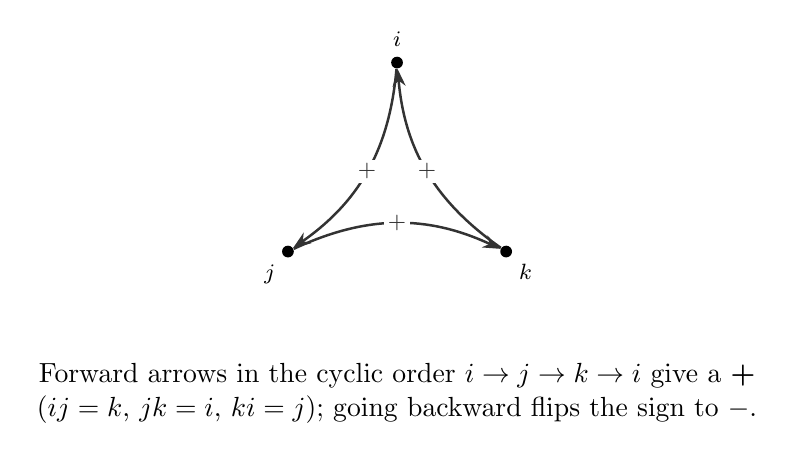
\begin{tikzpicture}[scale=1.0]
  \node[cgdot] (i) at (90:1.6) {};
  \node[cgdot] (j) at (210:1.6) {};
  \node[cgdot] (k) at (330:1.6) {};
  \draw[cgr] (i) to[bend left=25] node[cglab]{$+$} (j);
  \draw[cgr] (j) to[bend left=25] node[cglab]{$+$} (k);
  \draw[cgr] (k) to[bend left=25] node[cglab]{$+$} (i);
  \node[cglab,above=2pt of i] {$i$};
  \node[cglab,below left=2pt of j] {$j$};
  \node[cglab,below right=2pt of k] {$k$};
  \node[align=center] at (0,-2.6) {Forward arrows in the cyclic order $i\to j\to k\to i$ give a {\bf +}\\ ($ij=k$, $jk=i$, $ki=j$); going backward flips the sign to {\bf $-$}.};
\end{tikzpicture}
\end{center}

Reading the cycle $i\to j\to k\to i$: \emph{the product of two consecutive letters, in cyclic order, is the next letter with a $+$ sign}; reversing the two factors flips the sign. Squaring any of $i,j,k$ gives $-1$.

\begin{method}{How to multiply two quaternions $\pm a$ and $\pm b$}
To compute $(\varepsilon_1 a)(\varepsilon_2 b)$ where $\varepsilon_1,\varepsilon_2\in\{+1,-1\}$ and $a,b\in\{1,i,j,k\}$:
\begin{enumerate}
\item \textbf{Pull out the signs.} The total sign is $\varepsilon_1\varepsilon_2$; set it aside and multiply $a\cdot b$.
\item \textbf{If either factor is $1$:} the product is the other factor.
\item \textbf{If $a=b$ (same letter, both in $\{i,j,k\}$):} the product is $-1$.
\item \textbf{If $a\neq b$ are distinct letters in $\{i,j,k\}$:} read the cyclic order $i\to j\to k\to i$. If $a\to b$ is a \emph{forward} step (one of $ij$, $jk$, $ki$), the product is the third letter with sign $+$. If $a\to b$ is \emph{backward} (one of $ji$, $kj$, $ik$), the product is the third letter with sign $-$.
\item \textbf{Reattach the sign} $\varepsilon_1\varepsilon_2$ from step 1.
\end{enumerate}
\textbf{Recognition trigger:} use this whenever you see a product of two of the eight symbols $\pm1,\pm i,\pm j,\pm k$. The hard part is always one of the six products $ij,jk,ki,ji,kj,ik$; everything else is sign bookkeeping. Remember $Q_8$ is non-abelian, so \emph{order matters}: never assume $ab=ba$.
\end{method}

\begin{pitfall}
Do not import the rule $ab=ba$ from $\Z$ or from cyclic groups. In $Q_8$, $ij=k$ but $ji=-k\neq k$. Writing $ij=ji$ corrupts every later computation.
\end{pitfall}

\begin{wex}{The six core products}
Compute $ij$, $ji$, $jk$, $ki$, and $k^2$.
\wrec Each is a product of two of $i,j,k$, so step~4 (or step~3 for $k^2$) of the method applies. I just need to decide forward vs.\ backward in the cycle $i\to j\to k\to i$.
\wsol
\begin{itemize}
\item $ij$: step $i\to j$ is \emph{forward} (it is the listed relation $ij=k$). Third letter is $k$, sign $+$. So $ij=k$.
\item $ji$: step $j\to i$ is \emph{backward} (reverse of $ij$). Third letter $k$, sign $-$. So $ji=-k$.
\item $jk$: step $j\to k$ is \emph{forward} ($jk=i$). So $jk=i$.
\item $ki$: step $k\to i$ is \emph{forward} ($ki=j$). So $ki=j$.
\item $k^2$: same letter twice, step~3 gives $k^2=-1$.
\end{itemize}
\textbf{Check:} $ij=k$ and $ji=-k$ are negatives of each other, confirming non-commutativity. Also $ij\cdot ji=k\cdot(-k)=-k^2=-(-1)=1$, consistent with $(ij)(ji)=i(j j)i=i(-1)i=-i^2=-(-1)=1$. Both routes give $1$. \checkmark
\end{wex}

\begin{wex}{A length-three product with a sign}
Compute $(-i)\,(jk)$ and then $i\,j\,k$.
\wrec There are two factors $(-i)$ and $(jk)$; I evaluate the inner product first, then apply the method. For $ijk$ I associate as $(ij)k$ (the group is associative, so grouping is free) and reduce.
\wsol First $jk=i$ (forward step). Then
\[
(-i)(jk)=(-i)(i)=-(i^2)=-(-1)=1.
\]
For $ijk$: $ij=k$, so $ijk=(ij)k=k\cdot k=k^2=-1$.
\textbf{Check:} associate the other way: $i(jk)=i\cdot i=i^2=-1$. Same answer, as associativity demands. \checkmark Note $ijk=-1$ is the famous Hamilton relation (carved into Broom Bridge).
\end{wex}

\begin{wex}{Products with negatives on both sides}
Compute $(-j)(-k)$ and $(-k)(j)$ in $Q_8$.
\wrec Both are products of signed letters; step~1 isolates the signs, then step~4 handles the letters.
\wsol For $(-j)(-k)$: signs multiply to $(-1)(-1)=+1$; letters $jk=i$ (forward). So $(-j)(-k)=+i=i$.
For $(-k)(j)$: sign is $(-1)(+1)=-1$; letters $kj$ is the \emph{backward} step of $jk$, so $kj=-i$. Reattaching the leading sign: $(-k)(j)=(-1)(kj)=(-1)(-i)=i$.
\textbf{Check:} compute $(-k)j$ directly as a single signed product: total sign $-1$ times $kj=-i$ gives $(-1)(-i)=i$. Agrees. \checkmark
\end{wex}

\begin{wex}{A conjugation computation}
Compute $j\,i\,j\inv$ in $Q_8$. (Here $j\inv$ is the inverse of $j$.)
\wrec This is a conjugate $g x g\inv$ with $g=j$, $x=i$. I first need $j\inv$. Since $\ord{j}=4$, $j\inv=j^3=-j$ (because $j^2=-1\imp j^3=j^2 j=-j$). Then multiply left to right.
\wsol We have $j\inv=-j$. So
\[
j\,i\,j\inv=j\,i\,(-j)=-\,(ji)\,j=-(-k)\,j=k\,j.
\]
Now $kj$ is the backward step of $jk$, so $kj=-i$. Hence
\[
j\,i\,j\inv=-i.
\]
\textbf{Check:} a conjugate must have the same order as $i$, and indeed $\ord{-i}=4=\ord{i}$. Moreover $jij\inv=-i=i\inv$, so conjugation by $j$ inverts $i$ --- exactly the dihedral-style relation that lives inside $Q_8$. \checkmark
\end{wex}

\begin{wex}{Reading off the table to solve $xi=j$}
Find all $x\in Q_8$ with $xi=j$.
\wrec This is a linear equation in the group: right-multiply both sides by $i\inv$. Since $\ord{i}=4$, $i\inv=i^3=-i$. Uniqueness of solutions in a group guarantees exactly one $x$.
\wsol Right-multiply $xi=j$ by $i\inv=-i$:
\[
x=j\,i\inv=j(-i)=-(ji)=-(-k)=k.
\]
So $x=k$ is the unique solution.
\textbf{Check:} verify $ki=j$ (forward step) --- yes, that is a defining relation. \checkmark
\end{wex}

\subsection*{Orders of the eight elements}

\begin{proposition}[Element orders in $Q_8$]\label{p:q8orders@c1}
In $Q_8$: $\ord{1}=1$, $\ord{-1}=2$, and $\ord{i}=\ord{-i}=\ord{j}=\ord{-j}=\ord{k}=\ord{-k}=4$.
\end{proposition}

\begin{proof}
$1$ is the identity, so $\ord{1}=1$. For $-1$: $(-1)^1=-1\neq 1$ and $(-1)^2=1$, so $\ord{-1}=2$. For $i$: $i^1=i$, $i^2=-1$, $i^3=i^2 i=-i$, $i^4=(i^2)^2=(-1)^2=1$, and none of $i,i^2,i^3$ is $1$; hence $\ord{i}=4$. The same computation, replacing $i$ by any of $\pm i,\pm j,\pm k$, gives square $=-1$, fourth power $=1$: e.g.\ $(-i)^2=i^2=-1$, $(-i)^4=1$. So each of the six has order $4$.
\end{proof}

\begin{method}{How to compute $\ord{x}$ in $Q_8$}
\begin{enumerate}
\item Compute $x^2$.
\item If $x^2=1$: then $\ord{x}\in\{1,2\}$; it is $1$ only when $x=1$, else $2$. (Only $-1$ has order $2$.)
\item If $x^2=-1$: then $x^4=(x^2)^2=(-1)^2=1$ and $x^2\neq1$, so $\ord{x}=4$.
\end{enumerate}
\textbf{Recognition trigger:} every element of $Q_8$ squares to $1$ or $-1$. So the order is forced after a single squaring. There is NO element of order $3,6,8$ --- the only orders that occur are $1,2,4$, and $1$ and $2$ occur exactly once each.
\end{method}

We can picture the cyclic subgroup $\gen{i}=\{1,i,-1,-i\}$ as a clock with the rotation $x\mapsto ix$:

\begin{center}
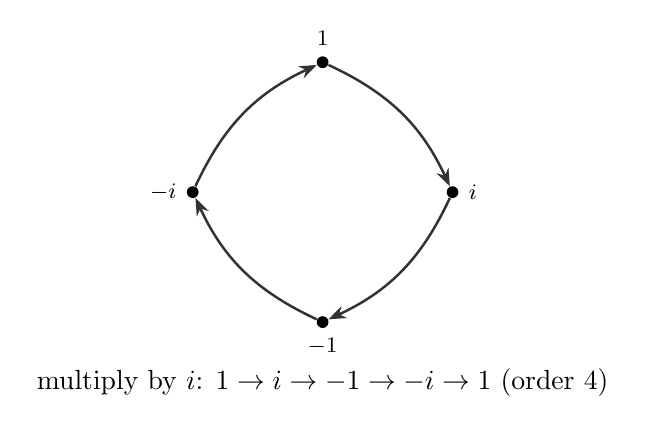
\begin{tikzpicture}[scale=1.1]
  \node[cgdot] (a) at (90:1.5) {};
  \node[cgdot] (b) at (0:1.5) {};
  \node[cgdot] (c) at (-90:1.5) {};
  \node[cgdot] (d) at (180:1.5) {};
  \draw[cgr] (a) to[bend left=20] (b);
  \draw[cgr] (b) to[bend left=20] (c);
  \draw[cgr] (c) to[bend left=20] (d);
  \draw[cgr] (d) to[bend left=20] (a);
  \node[cglab,above=2pt of a] {$1$};
  \node[cglab,right=2pt of b] {$i$};
  \node[cglab,below=2pt of c] {$-1$};
  \node[cglab,left=2pt of d] {$-i$};
  \node at (0,-2.2) {multiply by $i$: $1\to i\to -1\to -i\to 1$ (order $4$)};
\end{tikzpicture}
\end{center}

\begin{dgx}
\dgi{Objects:} Four nodes arranged clockwise at the cardinal points of a circle: $1$ (top), $i$ (right), $-1$ (bottom), $-i$ (left). Each node is an element of the cyclic subgroup $\langle i \rangle = \{1, i, -1, -i\} \leq Q_8$, which is a cyclic group of order $4$.
\dgi{Arrows:} Each curved arrow from node $x$ to node $ix$ represents the left-multiplication map $L_i \colon x \mapsto ix$ restricted to $\langle i \rangle$. Specifically: $1 \to i$ (since $i \cdot 1 = i$), $i \to -1$ (since $i \cdot i = -1$), $-1 \to -i$ (since $i \cdot (-1) = -i$), $-i \to 1$ (since $i \cdot (-i) = -(i \cdot i) = 1$). The arrows form a single directed $4$-cycle.
\dgi{What commutes:} The diagram encodes one cyclic path: applying $L_i$ four times returns to the start, so $L_i^4 = \operatorname{id}$. The composed path $1 \xrightarrow{L_i} i \xrightarrow{L_i} -1 \xrightarrow{L_i} -i \xrightarrow{L_i} 1$ is the group relation $i^4 = 1$.
\dgi{Why it commutes:} Chase $1$ around: $i^1 = i$, $i^2 = -1$, $i^3 = -i$, $i^4 = 1$. The fourth power returns to the identity because $i^2 = -1$ and $(-1)^2 = 1$ in $Q_8$, so $i^4 = (i^2)^2 = (-1)^2 = 1$. No shorter power returns to $1$ (each intermediate value is distinct), confirming $\operatorname{ord}(i) = 4$.
\dgi{Why this matters here:} This picture appears immediately after the proposition asserting $\operatorname{ord}(i) = 4$. It gives a geometric reason: the orbit of $1$ under repeated left-multiplication by $i$ visits exactly $4$ distinct elements before cycling, so the period is $4$, not $1$ or $2$. It also makes visible why $-1$ is ``halfway around,'' matching $i^2 = -1$.
\dgi{Concrete example:} In $\mathbb{Z}/4\mathbb{Z}$ under addition, the map $x \mapsto x + 1$ gives the same $4$-cycle: $0 \to 1 \to 2 \to 3 \to 0$. The identification $0 \leftrightarrow 1$, $1 \leftrightarrow i$, $2 \leftrightarrow -1$, $3 \leftrightarrow -i$ gives an explicit isomorphism $\langle i \rangle \cong \mathbb{Z}/4\mathbb{Z}$.
\dgi{Common pitfall:} Students sometimes read the arrows as right-multiplication ($x \mapsto xi$) rather than left-multiplication ($x \mapsto ix$). In an abelian group these coincide, but in $Q_8$ they can differ for other choices of acting element. Here, however, every node lies in the cyclic (hence abelian) subgroup $\langle i \rangle$, so $ix = xi$ for each node and the two readings give the same arrows; the distinction matters only for $x \notin \langle i \rangle$, e.g.\ $ij = k$ but $ji = -k$.
\dgi{Takeaway:} The point of this diagram is that the four elements $1, i, -1, -i$ form a single closed orbit under left-multiplication by $i$, giving a visual proof that $\operatorname{ord}(i) = 4$ and that $\langle i \rangle$ is cyclic of order $4$.
\end{dgx}

\begin{wex}{Order of $-1$ vs.\ order of $i$}
Determine $\ord{-1}$ and $\ord{i}$ and explain why they differ even though both are ``minus-ish'' looking.
\wrec Apply the squaring method. The key difference: $(-1)^2=1$ but $i^2=-1\neq1$.
\wsol $(-1)^2=1$, and $-1\neq 1$, so $\ord{-1}=2$. For $i$: $i^2=-1\neq1$, so by step~3, $\ord{i}=4$.
\textbf{Check:} $i^2=-1$ means $i$ is a square root of $-1$, so $i$ cannot have order $2$ (an order-$2$ element squares to $1$). Consistent. \checkmark
\end{wex}

\begin{wex}{Order of $-k$}
Compute $\ord{-k}$.
\wrec Single squaring. Watch the sign: $(-k)^2=(-1)^2k^2$.
\wsol $(-k)^2=(-1)^2 k^2=(+1)(-1)=-1\neq1$. By step~3, $(-k)^4=1$ and order is $4$. So $\ord{-k}=4$.
\textbf{Check:} list the powers: $(-k)^1=-k$, $(-k)^2=-1$, $(-k)^3=(-k)^2(-k)=(-1)(-k)=k$, $(-k)^4=k(-k)=-k^2=1$. First return to $1$ at exponent $4$. \checkmark
\end{wex}

\begin{wex}{How many elements of each order?}
Count the elements of $Q_8$ of order $1$, $2$, and $4$.
\wrec Use Proposition~\ref{p:q8orders@c1}: tabulate.
\wsol Order $1$: only $\{1\}$ --- that is $1$ element. Order $2$: only $\{-1\}$ --- that is $1$ element. Order $4$: the remaining $\{\pm i,\pm j,\pm k\}$ --- that is $6$ elements.
\textbf{Check:} $1+1+6=8=\ord{Q_8}$ counts every element exactly once. \checkmark This single-element-of-order-$2$ fact is the fingerprint we use later to distinguish $Q_8$ from $D_8$.
\end{wex}

\begin{wex}{Is there an element of order $8$?}
Decide whether $Q_8$ is cyclic.
\wrec A group of order $8$ is cyclic iff it has an element of order $8$. Check the maximal element order.
\wsol By Proposition~\ref{p:q8orders@c1} the largest order occurring is $4<8$. So no element generates $Q_8$; $Q_8$ is \emph{not} cyclic.
\textbf{Check:} also $Q_8$ is non-abelian ($ij\neq ji$), and every cyclic group is abelian, so it cannot be cyclic. Two independent reasons agree. \checkmark
\end{wex}

\begin{wex}{Square roots of $-1$}
Find every $x\in Q_8$ with $x^2=-1$.
\wrec ``$x^2=-1$'' is exactly the step-3 condition, which characterizes the order-$4$ elements.
\wsol An element satisfies $x^2=-1$ iff $\ord{x}=4$ (since $\ord{x}=1$ gives $x^2=1$ and $\ord{x}=2$ gives $x^2=1$). The order-$4$ elements are $\pm i,\pm j,\pm k$. So there are \emph{six} square roots of $-1$.
\textbf{Check:} verify two of them: $(-j)^2=j^2=-1$ and $i^2=-1$. \checkmark Contrast with $\C$, where $-1$ has only two square roots; the non-commutativity of $Q_8$ allows six.
\end{wex}

\subsection*{The center $Z(Q_8)$}

\begin{definition}[Center]\label{d:center@c1}
The \emph{center} of a group $G$ is $Z(G)=\{z\in G\st zx=xz\text{ for all }x\in G\}$.
\end{definition}

\begin{proposition}[Center of $Q_8$]\label{p:q8center@c1}
$Z(Q_8)=\{1,-1\}$.
\end{proposition}

\begin{proof}
Certainly $1$ and $-1$ commute with everything ($1$ is the identity, and $-1$ acts as a scalar sign: $(-1)x=-x=x(-1)$). So $\{1,-1\}\sgr Z(Q_8)$. Conversely, no order-$4$ element is central: from the Worked Example on conjugation, $jij\inv=-i\neq i$, so $ji\neq ij$ and $i\notin Z(Q_8)$. By symmetry of the relations under the cyclic permutation $i\to j\to k\to i$, also $j,k\notin Z(Q_8)$, and likewise $-i,-j,-k\notin Z(Q_8)$ (if $z$ is non-central so is $-z$, since $(-z)x=-zx$ and $x(-z)=-xz$ differ exactly when $zx\neq xz$). Hence $Z(Q_8)=\{1,-1\}$.
\end{proof}

\begin{method}{How to find the center of a small group}
\begin{enumerate}
\item The identity is always central; in $Q_8$ test the candidate $-1$ too (it is a scalar, hence central).
\item For each remaining $x$, exhibit ONE witness $y$ with $xy\neq yx$ to eliminate $x$.
\item For $Q_8$, the witnesses come free from the cycle: $i$ fails against $j$ ($ij=k\neq -k=ji$); $j$ fails against $k$; $k$ fails against $i$.
\item Collect the survivors. The center is always a subgroup, so its size must divide $\ord{Q_8}$ --- a useful sanity check.
\end{enumerate}
\textbf{Recognition trigger:} use this whenever asked for $Z(G)$, the set of elements commuting with $h$, or whether $G/Z(G)$ has a given order. In $Q_8$ the answer is always $\{1,-1\}$, so $|Q_8/Z(Q_8)|=4$.
\end{method}

\begin{pitfall}
A single product $xy=yx$ does NOT put $x$ in the center; $x$ must commute with \emph{every} element. For instance $i$ commutes with $-i$ and with $\pm1$, yet $i\notin Z(Q_8)$ because $i$ fails to commute with $j$.
\end{pitfall}

The quotient $Q_8/Z(Q_8)$ sits in the exact sequence below; it has order $8/2=4$ and is isomorphic to $V_4$ (every nonidentity coset squares to the identity coset, since $i^2=j^2=k^2=-1\in Z$).
\[
\begin{tikzcd}[column sep=normal]
1 \arrow[r] & \{1,-1\} \arrow[r, hook] & Q_8 \arrow[r, "\pi"] & Q_8/\{1,-1\}\,\cong\,V_4 \arrow[r] & 1
\end{tikzcd}
\]

\begin{dgx}
\dgi{Objects:} Five nodes forming a short exact sequence. The terminal objects $1$ (far left) and $1$ (far right) are the trivial group. The node $\{1,-1\}$ is the center $Z(Q_8)$, a normal subgroup of order $2$. The middle node $Q_8$ is the full quaternion group of order $8$. The rightmost nontrivial node $Q_8/\{1,-1\} \cong V_4$ is the quotient group of order $4$, the Klein four-group.
\dgi{Arrows:} The left $1 \to \{1,-1\}$ is the unique map from the trivial group (sending the identity to $1 \in Q_8$). The hooked arrow $\{1,-1\} \hookrightarrow Q_8$ is the inclusion map $\iota$, injecting $\{1,-1\}$ as a subgroup. The arrow $\pi \colon Q_8 \to Q_8/\{1,-1\}$ is the canonical quotient projection, sending $g \mapsto g\{1,-1\}$. The rightmost arrow $Q_8/\{1,-1\} \to 1$ is the unique map to the trivial group (kills everything). Well-definedness of $\pi$: the coset $g\{1,-1\}$ depends only on the coset of $g$, and since $\{1,-1\} \nor Q_8$ (it equals $Z(Q_8)$), left and right cosets agree, so $\pi$ is a well-defined group homomorphism.
\dgi{What commutes:} Exactness at $\{1,-1\}$: $\operatorname{im}(\iota_{\text{trivial}}) = \{1\} = \operatorname{ker}(\iota)$, i.e.\ $\iota$ is injective. Exactness at $Q_8$: $\operatorname{ker}(\pi) = \{1,-1\} = \operatorname{im}(\iota)$, meaning exactly the elements of $\{1,-1\}$ map to the identity coset under $\pi$. Exactness at $Q_8/\{1,-1\}$: $\pi$ is surjective, so $\operatorname{im}(\pi) = Q_8/\{1,-1\}= \operatorname{ker}(\text{terminal map})$.
\dgi{Why it commutes:} The kernel condition $\operatorname{ker}(\pi) = \{1,-1\}$ holds by definition of the quotient map: $\pi(g) = \{1,-1\}$ (the identity coset) if and only if $g \in \{1,-1\}$. Injectivity of $\iota$ is automatic since an inclusion map sends distinct elements to distinct elements. Surjectivity of $\pi$ holds because every coset $g\{1,-1\}$ is in the image of $\pi$.
\dgi{Why this matters here:} This sequence appears immediately after the proof that $Z(Q_8) = \{1,-1\}$ and the observation that $Q_8/Z(Q_8)$ has order $4$ and is isomorphic to $V_4$. It packages the relationship between $Q_8$, its center, and the quotient into one diagram, making precise the claim that $Q_8$ is a nontrivial central extension of $V_4$ by $\mathbb{Z}/2\mathbb{Z}$.
\dgi{Concrete example:} The same pattern occurs for $\mathbb{Z}/4\mathbb{Z}$: the sequence $1 \to \{0,2\} \hookrightarrow \mathbb{Z}/4\mathbb{Z} \xrightarrow{\pi} \mathbb{Z}/2\mathbb{Z} \to 1$ (where $\pi(n) = n \bmod 2$) is exact. Here $\{0,2\}$ plays the role of the central subgroup of order $2$.
\dgi{Common pitfall:} Students sometimes confuse the hooked inclusion $\{1,-1\} \hookrightarrow Q_8$ with an isomorphism. The hook on the arrow signals injectivity only, not surjectivity. The inclusion is a proper embedding: $|\{1,-1\}| = 2$ while $|Q_8| = 8$, so this map is far from an isomorphism.
\dgi{Takeaway:} The point of this diagram is that $Q_8$ sits as a central extension between its order-$2$ center $\{1,-1\}$ and its order-$4$ quotient $V_4$, making the exact sequence the cleanest summary of how the center fits into the group's structure.
\end{dgx}

\begin{wex}{Verify $-1\in Z(Q_8)$ directly}
Show $-1$ commutes with $j$.
\wrec Apply the scalar rule: $-1$ behaves as a sign in front of any element.
\wsol $(-1)j=-j$ and $j(-1)=-j$. Equal, so $-1$ and $j$ commute.
\textbf{Check:} the same scalar argument works against $i,k,\pm1$, so $-1$ commutes with all eight elements: $-1\in Z(Q_8)$. \checkmark
\end{wex}

\begin{wex}{Eliminate $k$ from the center}
Show $k\notin Z(Q_8)$ by producing a witness.
\wrec Need ONE element $y$ with $ky\neq yk$. The cycle says $ki=j$ but $ik=-j$.
\wsol Take $y=i$. Then $ki=j$ (forward) while $ik=-j$ (backward). Since $j\neq -j$, $ki\neq ik$, so $k\notin Z(Q_8)$.
\textbf{Check:} $j\neq -j$ because $j$ and $-j$ are listed as distinct elements of $Q_8$ (if $j=-j$ held, then $2j=0$ in additive language, but $Q_8$ has no such collapse: $j$ and $-j$ have distinct images in the multiplication table). \checkmark
\end{wex}

\begin{wex}{Centralizer of $i$}
Compute $C_{Q_8}(i)=\{x\st xi=ix\}$.
\wrec An element commutes with $i$ iff it lies in $\gen{i}=\{1,i,-1,-i\}$; test each of the eight.
\wsol Powers of $i$ always commute with $i$: $1,i,-1,-i$ all commute with $i$ (a cyclic subgroup is abelian). For $j$: $ij=k$, $ji=-k$, unequal --- $j$ excluded; similarly $-j,k,-k$ excluded by sign symmetry. So
\[
C_{Q_8}(i)=\{1,-1,i,-i\}=\gen{i}.
\]
\textbf{Check:} $|C_{Q_8}(i)|=4$ divides $8$ \checkmark, and $Z(Q_8)=\{1,-1\}\sgr C_{Q_8}(i)$ as it must (the center lies in every centralizer). \checkmark
\end{wex}

\begin{wex}{Size of a conjugacy class}
The conjugacy class of $i$ has size $[Q_8:C_{Q_8}(i)]$. Compute it and list the class.
\wrec Orbit--stabilizer: the class size equals the index of the centralizer found above.
\wsol $[Q_8:C_{Q_8}(i)]=8/4=2$. So the class of $i$ has $2$ elements. Computing conjugates: $jij\inv=-i$ (done earlier), and $1\cdot i\cdot1=i$. So the class is $\{i,-i\}$.
\textbf{Check:} class sizes must sum to $8$. The classes are $\{1\}$, $\{-1\}$ (both central, size $1$), and $\{i,-i\},\{j,-j\},\{k,-k\}$ (size $2$ each): $1+1+2+2+2=8$. \checkmark
\end{wex}

\begin{wex}{Order of the quotient $Q_8/Z(Q_8)$}
Compute $|Q_8/Z(Q_8)|$ and decide whether it is cyclic.
\wrec Use Lagrange: $|G/N|=|G|/|N|$. Then check whether the quotient could be cyclic.
\wsol $|Q_8/Z(Q_8)|=8/2=4$. If it were cyclic of order $4$, then $Q_8/Z(Q_8)$ cyclic would force $Q_8$ abelian (a standard fact: $G/Z(G)$ cyclic $\imp G$ abelian). But $Q_8$ is non-abelian, contradiction. So $Q_8/Z(Q_8)\cong V_4$ (the only non-cyclic group of order $4$).
\textbf{Check:} in the quotient, $\bar i^2=\overline{i^2}=\overline{-1}=\bar 1$, and likewise $\bar j^2=\bar k^2=\bar1$; every nonidentity element has order $2$, the signature of $V_4$. \checkmark
\end{wex}

\subsection*{The subgroups of $Q_8$ --- all normal}

\begin{proposition}[Subgroup lattice of $Q_8$]\label{p:q8subs@c1}
$Q_8$ has exactly six subgroups:
\[
\{1\},\quad \{1,-1\},\quad \gen{i},\quad \gen{j},\quad \gen{k},\quad Q_8,
\]
of orders $1,2,4,4,4,8$ respectively, where $\gen{i}=\{1,i,-1,-i\}$, $\gen{j}=\{1,j,-1,-j\}$, $\gen{k}=\{1,k,-1,-k\}$. Every one of these subgroups is normal in $Q_8$.
\end{proposition}

\begin{proof}
\emph{Order $1$ and $8$:} $\{1\}$ and $Q_8$ always occur.
\emph{Order $2$:} a subgroup of order $2$ is $\{1,x\}$ with $\ord{x}=2$; the only order-$2$ element is $-1$, giving $\{1,-1\}$ as the unique order-$2$ subgroup.
\emph{Order $4$:} by Lagrange the index is $2$. Any order-$4$ subgroup must contain an element of order $4$ (a group of order $4$ with no order-$4$ element is $V_4$, but $V_4$ would need three elements of order $2$, and $Q_8$ has only one). Such a subgroup is then cyclic, $\gen{x}$ with $\ord{x}=4$. Now $\gen{i}=\gen{-i}=\{1,i,-1,-i\}$, $\gen{j}=\gen{-j}$, $\gen{k}=\gen{-k}$ --- three distinct cyclic subgroups, and these exhaust the order-$4$ subgroups since the six order-$4$ elements pair off into these three.
\emph{Normality:} subgroups of index $2$ are automatically normal, so $\gen{i},\gen{j},\gen{k}$ are normal; $\{1\}$ and $Q_8$ are trivially normal. For $\{1,-1\}=Z(Q_8)$, the center is always normal (indeed $g(-1)g\inv=-1$ for all $g$). Hence all six are normal.
\end{proof}

A group, like $Q_8$, in which every subgroup is normal but which is itself non-abelian is called a \emph{Hamiltonian group}; $Q_8$ is the smallest one.

The lattice (lines mean ``is contained in''; all six nodes are normal subgroups):
\[
\begin{tikzcd}[row sep=large, column sep=small]
& Q_8 & \\
\gen{i} \arrow[ur, dash] & \gen{j} \arrow[u, dash] & \gen{k} \arrow[ul, dash] \\
& \{1,-1\} \arrow[ul, dash]\arrow[u, dash]\arrow[ur, dash] & \\
& \{1\} \arrow[u, dash] &
\end{tikzcd}
\]

\begin{method}{How to check a subgroup $H\nor G$ in $Q_8$}
\begin{enumerate}
\item \textbf{Index $2$ shortcut:} if $[G:H]=2$, then $H\nor G$ automatically (left cosets $=$ right cosets). In $Q_8$ this instantly handles $\gen{i},\gen{j},\gen{k}$.
\item \textbf{Center shortcut:} $Z(G)\nor G$ always; this handles $\{1,-1\}$.
\item \textbf{Trivial cases:} $\{1\}\nor G$ and $G\nor G$.
\item \textbf{General test} (if needed): verify $gHg\inv\subseteq H$ for $g$ ranging over a generating set of $G$.
\end{enumerate}
\textbf{Recognition trigger:} use the index-$2$ shortcut whenever $|H|=\tfrac12|G|$ --- it is the fastest normality proof in $Q_8$. Because $Q_8$ has only the six subgroups above, and each is caught by step~1, 2, or 3, EVERY subgroup of $Q_8$ is normal.
\end{method}

\begin{pitfall}
``All subgroups normal'' does NOT mean ``abelian.'' $Q_8$ is non-abelian yet every subgroup is normal. The implication only runs one way: abelian $\imp$ all subgroups normal, not conversely.
\end{pitfall}

\begin{wex}{$\gen{j}$ is normal}
Show $\gen{j}=\{1,j,-1,-j\}\nor Q_8$.
\wrec $\gen{j}$ has order $4$, index $8/4=2$ --- the index-$2$ shortcut applies. As an explicit check I also conjugate the generator $j$ by $i$.
\wsol Since $[Q_8:\gen{j}]=2$, $\gen{j}$ is normal. Explicit check via conjugation by $i$ (using $i\inv=-i$):
\[
iji\inv=ij(-i)=-(ij)i=-(k)(i)=-(ki)=-j\in\gen{j}.
\]
\textbf{Check:} $-j\in\gen{j}$, so conjugation by $i$ maps the generator $j$ back into $\gen{j}$; combined with the index-$2$ fact, $\gen{j}\nor Q_8$. \checkmark
\end{wex}

\begin{wex}{The order-$2$ subgroup is unique and normal}
Show $\{1,-1\}$ is the only subgroup of order $2$ and that it is normal.
\wrec A subgroup of order $2$ is determined by its unique order-$2$ element; $Q_8$ has exactly one such element. Normality follows from it being the center.
\wsol The only element of order $2$ is $-1$ (Worked Example counting orders). So $\{1,-1\}$ is the unique order-$2$ subgroup. It equals $Z(Q_8)$, and the center is normal: for any $g$, $g(-1)g\inv=(-1)gg\inv=-1\in\{1,-1\}$.
\textbf{Check:} $g(-1)g\inv=-1$ uses that $-1$ is central (scalar). \checkmark
\end{wex}

\begin{wex}{Intersection of two order-$4$ subgroups}
Compute $\gen{i}\cap\gen{j}$.
\wrec An intersection of subgroups is a subgroup; list elements and keep the common ones.
\wsol $\gen{i}=\{1,i,-1,-i\}$ and $\gen{j}=\{1,j,-1,-j\}$. The common elements are $1$ and $-1$. So $\gen{i}\cap\gen{j}=\{1,-1\}=Z(Q_8)$.
\textbf{Check:} $|\gen{i}\cap\gen{j}|=2$ divides both $|\gen{i}|=4$ and $|\gen{j}|=4$ \checkmark. Geometrically, every pair of distinct order-$4$ subgroups meets exactly in the center --- that is why $\{1,-1\}$ sits at the unique node below all three in the lattice. \checkmark
\end{wex}

\begin{wex}{Counting subgroups confirms the lattice}
Verify the total number of subgroups is $6$ by tallying by order.
\wrec Use Proposition~\ref{p:q8subs@c1} and Lagrange: possible orders divide $8$, i.e.\ $1,2,4,8$.
\wsol Order $1$: $\{1\}$ --- $1$ subgroup. Order $8$: $Q_8$ --- $1$. Order $2$: only $\{1,-1\}$ --- $1$. Order $4$: $\gen{i},\gen{j},\gen{k}$ --- $3$. Total $1+1+1+3=6$.
\textbf{Check:} no order can be skipped that Lagrange forbids; $1,2,4,8$ are exactly the divisors of $8$, and we found at least one subgroup of each. \checkmark
\end{wex}

\begin{wex}{Every subgroup normal, fast}
Without case-checking each conjugate, argue that all six subgroups of $Q_8$ are normal.
\wrec Match each subgroup to a shortcut from the method box.
\wsol $\{1\}$ and $Q_8$: trivially normal. $\{1,-1\}=Z(Q_8)$: center, normal. $\gen{i},\gen{j},\gen{k}$: each has index $2$, hence normal. That covers all six.
\textbf{Check:} the shortcuts are independent of any specific conjugation computation, yet they agree with the brute-force verification that $gHg\inv=H$ for every $g$ and every $H$. \checkmark
\end{wex}

\subsection*{$Q_8$ versus $D_8$: same order, NOT isomorphic}

Recall $D_8=\gen{r,s\st r^4=s^2=1,\ sr=r\inv s}$ is the symmetry group of the square, also of order $8$ and also non-abelian. A natural question: are $Q_8$ and $D_8$ ``the same group in disguise''? The square-counting below shows they are not.

\begin{proposition}[$Q_8\not\cong D_8$]\label{p:q8notd8@c1}
$Q_8$ and $D_8$ are non-isomorphic groups of order $8$.
\end{proposition}

\begin{proof}
The number of elements of order $2$ is an isomorphism invariant (an isomorphism $\varphi$ satisfies $\ord{\varphi(x)}=\ord{x}$, so it bijects order-$2$ elements to order-$2$ elements). In $Q_8$ there is exactly \emph{one} element of order $2$, namely $-1$ (Worked Example on counting orders). In $D_8$ the elements of order $2$ are $r^2$ and the four reflections $s,rs,r^2s,r^3s$ --- that is \emph{five} elements of order $2$ (each reflection squares to $1$, and $r^2$ is the half-turn). Since $1\neq 5$, no isomorphism $Q_8\to D_8$ can exist.
\end{proof}

\begin{method}{How to prove two finite groups are NOT isomorphic}
\begin{enumerate}
\item Compute a numerical invariant for both: most often \emph{the multiset of element orders} (equivalently, ``how many elements of each order'').
\item Other invariants if the orders match: abelian?, size of the center, number of subgroups of a given order, is it cyclic?, exponent.
\item If ANY invariant differs, the groups are not isomorphic. (If all your invariants match, you have NOT proved isomorphism --- you must then exhibit an explicit isomorphism.)
\end{enumerate}
\textbf{Recognition trigger:} use this whenever asked ``is $G\cong H$?'' for two concrete groups. For two non-abelian groups of order $8$, the order-$2$ count is the cleanest separator: $Q_8$ has $1$, $D_8$ has $5$.
\end{method}

\begin{pitfall}
Matching orders ($|Q_8|=|D_8|=8$) and ``both non-abelian'' is NOT enough to conclude $Q_8\cong D_8$. Equal order and equal abelian-ness are necessary, not sufficient. You must compare finer invariants --- here, the count of order-$2$ elements differs.
\end{pitfall}

The contrast at a glance:
\begin{center}
\begin{tabular}{lcc}
\hline
Invariant & $Q_8$ & $D_8$ \\
\hline
order of group & $8$ & $8$ \\
abelian? & no & no \\
elements of order $1$ & $1$ & $1$ \\
elements of order $2$ & $\mathbf{1}$ & $\mathbf{5}$ \\
elements of order $4$ & $6$ & $2$ \\
center & $\{1,-1\}$, size $2$ & $\{1,r^2\}$, size $2$ \\
\# subgroups of order $4$ & $3$ (all cyclic) & $3$ (one cyclic $\gen{r}$, two $\cong V_4$) \\
every subgroup normal? & yes & no ($\gen{s}$ is not normal) \\
\hline
\end{tabular}
\end{center}

\begin{wex}{Order-$2$ count in $D_8$}
List all elements of $D_8$ of order $2$ and count them.
\wrec Use the normal form $r^a s^b$ with $0\le a\le3$, $b\in\{0,1\}$. Rotations $r^a$ have order $4/\gcd(a,4)$; reflections $r^a s$ all have order $2$.
\wsol Rotations: $r^0=1$ (order $1$), $r^1$ (order $4$), $r^2$ (order $2$), $r^3$ (order $4$). Reflections: $s,rs,r^2s,r^3s$ each satisfy $(r^a s)^2=r^a s r^a s=r^a (s r^a) s=r^a r^{-a}s^2=1$ using $sr^a=r^{-a}s$ and $s^2=1$, so each has order $2$. Order-$2$ elements: $\{r^2,\,s,\,rs,\,r^2s,\,r^3s\}$ --- five of them.
\textbf{Check:} total elements $1$(id)$+1$(order-$2$ rotation)$+2$(order $4$)$+4$(reflections)$=8=|D_8|$, and $1+4=5$ have order $2$. \checkmark
\end{wex}

\begin{wex}{Order-$2$ count in $Q_8$}
Confirm $Q_8$ has exactly one element of order $2$.
\wrec From Proposition~\ref{p:q8orders@c1}, an element has order $2$ iff it squares to $1$ but is not $1$.
\wsol Squaring each: $i^2=j^2=k^2=(-i)^2=(-j)^2=(-k)^2=-1\neq1$, $1^2=1$, $(-1)^2=1$. Only $-1$ squares to $1$ while being $\neq1$. So exactly one element, $-1$, has order $2$.
\textbf{Check:} matches the $1+1+6$ tally from before. \checkmark
\end{wex}

\begin{wex}{The decisive comparison}
Use the order-$2$ counts to conclude $Q_8\not\cong D_8$.
\wrec Apply the non-isomorphism method: the order-$2$ count is an isomorphism invariant.
\wsol $Q_8$ has $1$ element of order $2$; $D_8$ has $5$. An isomorphism preserves element orders, hence preserves these counts. Since $1\neq5$, $Q_8\not\cong D_8$.
\textbf{Check:} a second invariant agrees --- ``every subgroup normal'' holds in $Q_8$ but fails in $D_8$ (the reflection subgroup $\gen{s}$ is not normal: $r s r\inv=r^2 s\notin\gen{s}=\{1,s\}$). Two invariants, same verdict. \checkmark
\end{wex}

\begin{wex}{Both share a $V_4$ quotient --- why that does not save the isomorphism}
Show $Q_8/Z(Q_8)\cong V_4\cong D_8/Z(D_8)$, and explain why this does not imply $Q_8\cong D_8$.
\wrec Compute each central quotient; both have order $8/2=4$ and are non-cyclic, hence $\cong V_4$. But isomorphic quotients by isomorphic centers do not force the groups isomorphic.
\wsol $Q_8/Z(Q_8)$: order $4$, non-cyclic (shown earlier), so $\cong V_4$. $D_8/Z(D_8)$: $Z(D_8)=\{1,r^2\}$, quotient order $4$; the images of $r$ and $s$ each square to the identity coset ($r^2\in Z$, $s^2=1$), so it is $\cong V_4$. Thus both central quotients are $V_4$. Yet the groups differ: the extension $1\to Z\to G\to V_4\to1$ can be ``twisted'' differently --- in $Q_8$ every preimage of a nonidentity coset has order $4$, while in $D_8$ the reflection preimages have order $2$. So equal quotients do not lift to an isomorphism of $G$.
\textbf{Check:} the order-$2$ count ($1$ vs.\ $5$) already proved non-isomorphism; this example shows where the naive ``same quotient'' argument breaks. \checkmark
\end{wex}

\begin{wex}{An invariant that does NOT distinguish them}
Show that ``size of the center'' fails to separate $Q_8$ and $D_8$, and identify an invariant that succeeds.
\wrec Some invariants coincide for non-isomorphic groups; you need one that differs.
\wsol $|Z(Q_8)|=|\{1,-1\}|=2$ and $|Z(D_8)|=|\{1,r^2\}|=2$. Equal --- so the center's size cannot distinguish them. A separating invariant: the number of order-$2$ elements ($1$ for $Q_8$, $5$ for $D_8$), or equivalently the number of order-$4$ elements ($6$ vs.\ $2$).
\textbf{Check:} indeed $Q_8$ has $6$ order-$4$ elements ($\pm i,\pm j,\pm k$) and $D_8$ only $2$ ($r,r^3$). The discrepancy is the same fact viewed through order-$4$ instead of order-$2$. \checkmark
\end{wex}

\subsection*{Master reference: the $8\times8$ multiplication table of $Q_8$}

Entry in row $g$, column $h$ is the product $gh$ (row element first). Read off, for example, row $i$, column $j$: $ij=k$; row $j$, column $i$: $ji=-k$.

\begin{center}
\renewcommand{\arraystretch}{1.25}
\begin{tabular}{c|cccccccc}
$\cdot$ & $1$ & $-1$ & $i$ & $-i$ & $j$ & $-j$ & $k$ & $-k$ \\
\hline
$1$  & $1$  & $-1$ & $i$  & $-i$ & $j$  & $-j$ & $k$  & $-k$ \\
$-1$ & $-1$ & $1$  & $-i$ & $i$  & $-j$ & $j$  & $-k$ & $k$  \\
$i$  & $i$  & $-i$ & $-1$ & $1$  & $k$  & $-k$ & $-j$ & $j$  \\
$-i$ & $-i$ & $i$  & $1$  & $-1$ & $-k$ & $k$  & $j$  & $-j$ \\
$j$  & $j$  & $-j$ & $-k$ & $k$  & $-1$ & $1$  & $i$  & $-i$ \\
$-j$ & $-j$ & $j$  & $k$  & $-k$ & $1$  & $-1$ & $-i$ & $i$  \\
$k$  & $k$  & $-k$ & $j$  & $-j$ & $-i$ & $i$  & $-1$ & $1$  \\
$-k$ & $-k$ & $k$  & $-j$ & $j$  & $i$  & $-i$ & $1$  & $-1$ \\
\end{tabular}
\end{center}

\begin{remark}\label{r:tablesanity@c1}
Sanity checks on the table: (1) each row and each column is a permutation of all eight elements (the Latin-square property forced by group axioms). (2) The diagonal entries (squares) are $1,1,-1,-1,-1,-1,-1,-1$: exactly one $1$ off the identity row (namely $(-1)^2=1$) and six $-1$'s, matching ``one element of order $2$, six of order $4$.'' (3) The block for $\{1,-1\}$ (top-left $2\times2$) is closed --- it is the central subgroup. (4) Asymmetry across the diagonal (e.g.\ row $i$ col $j$ is $k$ but row $j$ col $i$ is $-k$) visibly certifies non-commutativity.
\end{remark}

Finally, the universal property that makes the table legitimate: $Q_8$ is the group \emph{presented} by $\gen{i,j\st i^4=1,\ i^2=j^2,\ j i j\inv=i\inv}$ (with $k:=ij$, $-1:=i^2$). Any map of $i,j$ into a group $G$ respecting these relations extends uniquely:
\[
\begin{tikzcd}[row sep=large, column sep=large]
\{i,j\} \arrow[r, hook] \arrow[dr, "{i\mapsto a,\ j\mapsto b}"'] & Q_8 \arrow[d, dashed, "\exists!\,\varphi"] \\
& G
\end{tikzcd}
\]
provided $a,b\in G$ satisfy $a^4=1$, $a^2=b^2$, $bab\inv=a\inv$. This is the precise sense in which ``$Q_8$ is generated by $i,j$ subject to those relations,'' and it is what guarantees the multiplication table above is the unique one consistent with Definition~\ref{d:q8@c1}.

\begin{dgx}
\dgi{Objects:} Three nodes. The set $\{i,j\}$ (upper-left) is just the two-element generating set of $Q_8$, not a group. The group $Q_8$ (upper-right) is the quaternion group of order $8$, presented by generators $i,j$ subject to $i^4=1$, $i^2=j^2$, $jij^{-1}=i^{-1}$. The group $G$ (lower-right) is any group containing elements $a = \varphi(i)$ and $b = \varphi(j)$ satisfying those same three relations.
\dgi{Arrows:} The hooked arrow $\{i,j\} \hookrightarrow Q_8$ is the inclusion of the generating set into $Q_8$. The diagonal arrow $\{i,j\} \to G$ labelled $i \mapsto a$, $j \mapsto b$ is the prescribed assignment of generators to elements of $G$ (not yet a group homomorphism, merely a function on the generating set). The dashed vertical arrow $\varphi \colon Q_8 \to G$ is the unique group homomorphism whose existence and uniqueness are asserted by the universal property of the presentation; it is the induced map extending the assignment $i \mapsto a$, $j \mapsto b$ to all of $Q_8$.
\dgi{What commutes:} The triangle commutes: the composite $\{i,j\} \hookrightarrow Q_8 \xrightarrow{\varphi} G$ equals the direct assignment $\{i,j\} \to G$. In formulas: $\varphi(i) = a$ and $\varphi(j) = b$.
\dgi{Why it commutes:} Well-definedness of $\varphi$: every element of $Q_8$ is a product of powers of $i$ and $j$, and $\varphi$ is defined by $\varphi(i^{e_1} j^{e_2} \cdots) = a^{e_1} b^{e_2} \cdots$. This is well-defined because any relation holding among $i,j$ in $Q_8$ (such as $i^4 = 1$ or $ij \cdot (ij)^{-1} = 1$) also holds for $a,b$ in $G$ by hypothesis, so different words representing the same element of $Q_8$ map to the same element of $G$. Uniqueness: any homomorphism $Q_8 \to G$ with $\varphi(i) = a$, $\varphi(j) = b$ is forced on all of $Q_8$ since $i,j$ generate $Q_8$.
\dgi{Why this matters here:} This diagram appears at the conclusion of the section as the rigorous justification that the multiplication table is uniquely determined. Without the universal property, one could worry that defining $Q_8$ by generators and relations might be inconsistent or ambiguous. The diagram says: any group $G$ containing elements obeying those relations automatically receives a unique map from $Q_8$, confirming that $Q_8$ is the ``most efficient'' or ``freest'' such group, and in particular that the table has exactly one consistent completion.
\dgi{Concrete example:} Take $G = \langle i \rangle \cong \mathbb{Z}/4\mathbb{Z} \leq Q_8$ and the assignment $i \mapsto i$, $j \mapsto i$. Then $a = b = i$ satisfies $a^4 = 1$ and $a^2 = b^2$, but $bab^{-1} = iai^{-1} = a \neq a^{-1} = -i$ (since $i \neq -i$), so the third relation fails and no homomorphism $Q_8 \to G$ with this assignment exists. This shows the relation conditions are essential: the diagram produces $\varphi$ only when all three are satisfied.
\dgi{Common pitfall:} The dashed arrow is labelled $\exists!\,\varphi$, meaning it exists AND is unique. Students sometimes read this as merely an existence claim and forget uniqueness, or conversely assume every assignment $i \mapsto a$, $j \mapsto b$ produces some homomorphism. The dashed arrow exists only when $a,b$ satisfy all three relations; if even one fails, the diagram does not commute and $\varphi$ does not exist.
\dgi{Takeaway:} The point of this diagram is that the universal property of the presentation of $Q_8$ guarantees that any group containing elements satisfying the three quaternion relations receives a unique homomorphism from $Q_8$, which is precisely what makes the generator-relation definition consistent and the multiplication table uniquely determined.
\end{dgx}


%% ===== Dummit & Foote book-level content (merged in) =====
\subsection*{Further examples: the quaternion group as listed in the text}

D\&F introduce $Q_8$ by \emph{listing} its eight elements and then specifying the products
directly; from those products every one of the $64$ entries of the multiplication table is
determined. Writing the table out is left to the reader (Exercise~2 below). The book does not
verify associativity here: it calls the check tedious and says it will be proved later by
less computational means (one triple is checked by hand below). We record the book's listing form of the
definition and the immediate facts it draws from it; the relation form, the picture, and the
$8\times8$ table appear above and are not repeated here.

\begin{definition}[Quaternion group, listing form]\label{d:q8book-mrg@c1}
The \emph{quaternion group} $Q_8$ is the set
\[
Q_8=\{\,1,\,-1,\,i,\,-i,\,j,\,-j,\,k,\,-k\,\}
\]
with an associative product $\,\cdot\,$ given by the complete list of rules
\[
1\cdot a=a\cdot 1=a\quad\text{for all }a\in Q_8,
\]
\[
(-1)\cdot(-1)=1,\qquad (-1)\cdot a=a\cdot(-1)=-a\quad\text{for all }a\in Q_8,
\]
\[
i\cdot i=j\cdot j=k\cdot k=-1,
\]
\[
i\cdot j=k,\quad j\cdot i=-k,\qquad
j\cdot k=i,\quad k\cdot j=-i,\qquad
k\cdot i=j,\quad i\cdot k=-j.
\]
Here $1$ is the identity and $-1$ commutes with every element. Together with associativity,
these rules determine $g\cdot h$ for all $g,h\in Q_8$ (for instance
$(-i)\cdot(-j)=(-1)\cdot(-1)\cdot i\cdot j=i\cdot j=k$).
\end{definition}

The symbol ``$-$'' here is purely notational: $-a$ denotes the single element
$(-1)\cdot a$, not a separately defined operation, and the eight symbols are pairwise
distinct. This listing form is the book's own; it agrees element-for-element with the
relation form in Definition~\ref{d:q8@c1}.

\begin{remark}\label{r:q8book-mrg@c1}
Three facts the text reads directly off the list in Definition~\ref{d:q8book-mrg@c1}:
\begin{enumerate}
\item $Q_8$ has \emph{order} $8$ (eight distinct elements), with identity $1$ and with $-1$
playing the role of a central sign.
\item $Q_8$ is \emph{nonabelian}: $i\cdot j=k$ but $j\cdot i=-k$, and $k\neq -k$.
\item Each element has its inverse on the list: $1$ and $-1$ are self-inverse, and the
inverse of any of $\pm i,\pm j,\pm k$ is its negative, since
$i\cdot(-i)=-(i\cdot i)=-(-1)=1$ and likewise for $j,k$.
\end{enumerate}
\end{remark}

\begin{wex}{Associativity on a sample triple}
The definition \emph{assumes} associativity. As a self-consistency check, verify
$(i\cdot j)\cdot k=i\cdot(j\cdot k)$ using only the listed products.
\wrec Associativity is part of the definition, not something derived from the relations
elsewhere; verifying one triple by hand shows the listed rules do not contradict it.
\wsol Left grouping: $i\cdot j=k$, so $(i\cdot j)\cdot k=k\cdot k=-1$.
Right grouping: $j\cdot k=i$, so $i\cdot(j\cdot k)=i\cdot i=-1$.
Both equal $-1$, so $(i\cdot j)\cdot k=i\cdot(j\cdot k)$.
\textbf{Check:} the common value $-1$ is the relation $i\cdot j\cdot k=-1$; the two groupings
agreeing is exactly what associativity asserts on this triple. \checkmark
\end{wex}

\begin{wex}{Reducing a fully signed product from the raw list}
Using only the rules in Definition~\ref{d:q8book-mrg@c1}, compute $(-i)\cdot(-j)$ and
$(-j)\cdot(-i)$, and contrast the two.
\wrec Each is a product of two signed letters. The rule $(-1)\cdot a=-a$ lets me collect both
signs onto a single leading $+1$, then apply one of the six listed letter-products.
\wsol For $(-i)\cdot(-j)$: the two signs give $(-1)\cdot(-1)=1$, and $i\cdot j=k$, so
$(-i)\cdot(-j)=k$. For $(-j)\cdot(-i)$: again the signs give $+1$, and $j\cdot i=-k$, so
$(-j)\cdot(-i)=-k$.
\textbf{Check:} the signs cancel in both, yet the results $k$ and $-k$ differ, because the
underlying letter-products $i\cdot j$ and $j\cdot i$ already differ in sign. Removing the
negatives does not remove the noncommutativity. \checkmark
\end{wex}

\begin{wex}{Inverses straight from the listing}
Using Remark~\ref{r:q8book-mrg@c1}(3), write down $i\inv$, $(-j)\inv$, and $(-1)\inv$ directly from
the listed products, without computing any orders.
\wrec The listing pairs each letter with its negative (for $\pm i,\pm j,\pm k$) or with
itself (for $\pm 1$) to produce $1$, which is exactly the defining property of an inverse.
\wsol $i\cdot(-i)=-(i\cdot i)=-(-1)=1$, so $i\inv=-i$. Next $(-j)\cdot j=-(j\cdot j)=1$, so
$(-j)\inv=j$. And $(-1)\cdot(-1)=1$, so $(-1)\inv=-1$.
\textbf{Check:} this recovers the inverses from the raw list alone; it matches the order
computation $\ord{i}=\ord{j}=4$, which forces $i\inv=i^3=-i$ and $j\inv=j^3=-j$. \checkmark
\end{wex}

\begin{exers}{Exercises (from the text).}
\item Compute the order of each element of $Q_8$.
\item Write out the group tables for $S_3$, $D_8$, and $Q_8$.
\item Find a set of generators and relations for $Q_8$.
\end{exers}

\begin{exers}{Additional exercises.}
\item Using only the defining relations $i^2=j^2=k^2=-1$, $ij=k$, $jk=i$, $ki=j$ of
$Q_8=\{\pm1,\pm i,\pm j,\pm k\}$, compute each of the following products and express the
answer as one of the eight elements: (a) $ji$; (b) $kj$; (c) $ik$; (d) $(ij)k$;
(e) $i(jk)$; (f) $(-i)(-j)$. In particular verify $ji=-ij$, so $Q_8$ is nonabelian.

\item Determine the order $\ord{x}$ of every element $x\in Q_8$. List which elements have
order $1$, which have order $2$, and which have order $4$. Conclude that $Q_8$ has a
unique element of order $2$, and identify it.

\item Find every subgroup of $Q_8$. For each one give a set of generators and its order,
and verify your list against Lagrange's theorem (every subgroup order divides $8$).
Show that $\gen{i}$, $\gen{j}$, $\gen{k}$ are exactly the three subgroups of order $4$.

\item Prove that every subgroup of $Q_8$ is normal. (Suggestion: $\gen{-1}$ is central, and
each subgroup of order $4$ has index $2$.) A nonabelian group all of whose subgroups are
normal is called Hamiltonian; conclude $Q_8$ is the smallest such group.

\item Show that $Q_8$ and $D_8$ are not isomorphic, even though both are nonabelian of
order $8$. (Hint: count elements of order $2$ in each. Recall $D_8$ has $r^4=s^2=1$,
$sr=r\inv s$.)

\item The center of a group is $Z(G)=\{z\in G\st zx=xz \text{ for all } x\in G\}$. Prove
$Z(Q_8)=\{\pm1\}=\gen{-1}$, and show that $-1$ is the unique element $x$ with $x^2=1$ and
$x\neq 1$.

\item Define a map $\varphi\colon Q_8\to\GL_2(\C)$ by
$\varphi(i)=\begin{pmatrix} i & 0 \\ 0 & -i\end{pmatrix}$,
$\varphi(j)=\begin{pmatrix} 0 & 1 \\ -1 & 0\end{pmatrix}$, and extend so that
$\varphi(k)=\varphi(i)\varphi(j)$ and $\varphi(-1)=-I$. Verify that
$\varphi(i)^2=\varphi(j)^2=\varphi(k)^2=-I$ and $\varphi(i)\varphi(j)=\varphi(k)$, so these
matrices satisfy the quaternion relations.
\end{exers}

\begin{exers}{Commutative-diagram exercises.}
\item Let $N=\{\pm1\}=\gen{-1}\nor Q_8$ and let $V=Q_8/N$. Show $|V|=4$ and that every
nonidentity element of $V$ has order $2$, so $V\isom V_4$, the Klein four-group. Writing
$\pi\colon Q_8\to V$ for the quotient map, fill in the cosets so that the sequence
\[\begin{tikzcd}[column sep=normal]
1 \arrow[r] & \gen{-1} \arrow[r, hook] & Q_8 \arrow[r, two heads, "\pi"] & V_4 \arrow[r] & 1
\end{tikzcd}\]
is exact (i.e. $\ker\pi=\gen{-1}$ and $\pi$ is onto), and list $\pi(i),\pi(j),\pi(k)$ as
elements of $V_4$.

\item With $\pi\colon Q_8\to V_4$ as above, prove that multiplication on the quotient is
the unique map $\bar m$ making the diagram
\[\begin{tikzcd}[row sep=large,column sep=large]
Q_8\times Q_8 \arrow[r, "m"] \arrow[d, "\pi\times\pi"'] & Q_8 \arrow[d, "\pi"] \\
V_4\times V_4 \arrow[r, dashed, "\exists!\,\bar m"'] & V_4
\end{tikzcd}\]
commute, where $m$ is the product in $Q_8$. Identify $\bar m$ explicitly with the group
law of $V_4$, and explain why well-definedness of $\bar m$ is exactly the normality of
$\gen{-1}$.

\item Recall the universal property of $\Z$: a homomorphism $\Z\to G$ is
determined by where $1$ goes. Use this to describe all homomorphisms $\Z\to Q_8$, and show
that each factors uniquely through some $\Zn{n}$:
\[\begin{tikzcd}[row sep=large,column sep=large]
\Z \arrow[r, two heads, "\pi"] \arrow[dr, "1\,\mapsto\,x"'] & \Zn{n} \arrow[d, dashed, "\exists!\,\varphi"] \\ & Q_8
\end{tikzcd}\]
For each $x\in Q_8$ state the value of $n=\ord{x}$ that makes the diagram commute.

\item Let $\varphi\colon Q_8\to\GL_2(\C)$ be the homomorphism from Additional Exercise 7.
Compute $\ker\varphi$ and verify the exact sequence
\[\begin{tikzcd}[column sep=normal]
1 \arrow[r] & \ker\varphi \arrow[r, hook] & Q_8 \arrow[r, "\varphi"] & \GL_2(\C)
\end{tikzcd}\]
makes $\varphi$ injective. Conclude $Q_8$ is isomorphic to its image, a subgroup of
$\GL_2(\C)$ of order $8$.

\item Both $D_8$ and $Q_8$ surject onto $V_4$ with kernel of order $2$:
\[\begin{tikzcd}[row sep=large,column sep=large]
1 \arrow[r] & \gen{-1} \arrow[r, hook] & Q_8 \arrow[r, two heads, "\pi"] \arrow[d, dashed, "\psi"'] & V_4 \arrow[r] \arrow[d, equal] & 1 \\
1 \arrow[r] & \gen{r^2} \arrow[r, hook] & D_8 \arrow[r, two heads] & V_4 \arrow[r] & 1
\end{tikzcd}\]
Show that there is no isomorphism $\psi\colon Q_8\to D_8$ commuting with the two surjections
onto $V_4$ (indeed none at all, by Additional Exercise 5). Explain which structural
invariant -- the number of order-$2$ elements lying in the kernel versus outside it --
obstructs such a $\psi$.
\end{exers}


\section{Homomorphisms and Isomorphisms}
\subsection*{Homomorphisms and Isomorphisms: Kernel, Image, and Order Divisibility}

\begin{definition}[Homomorphism]\label{d:hom@c1}
Let $(G,\cdot)$ and $(H,*)$ be groups. A map $\varphi:G\to H$ is a \emph{homomorphism}
if
\[
\varphi(xy)=\varphi(x)*\varphi(y)\qquad\text{for all }x,y\in G.
\]
We almost always suppress the operation symbols and just write
$\varphi(xy)=\varphi(x)\varphi(y)$, the product on the left taken in $G$ and the product
on the right taken in $H$. The single defining equation says exactly: ``multiply-then-map
equals map-then-multiply.'' Diagrammatically, the multiplication square
\[\begin{tikzcd}[row sep=large,column sep=large]
G\times G \arrow[r, "m_G"] \arrow[d, "\varphi\times\varphi"'] & G \arrow[d, "\varphi"] \\
H\times H \arrow[r, "m_H"'] & H
\end{tikzcd}\]
\begin{dgx}
\dgi{Objects:} The four nodes are: $G\times G$ (the set of ordered pairs of elements of $G$,
which is itself a group under coordinatewise multiplication), $G$ (the source group), $H\times H$
(ordered pairs from $H$), and $H$ (the target group). All four are groups.
\dgi{Arrows:} $m_G:G\times G\to G$ is the multiplication map of $G$, $m_G(x,y)=xy$. $m_H:H\times
H\to H$ is the multiplication map of $H$, $m_H(a,b)=ab$. The right vertical arrow $\varphi:G\to
H$ is the proposed homomorphism. The left vertical arrow $\varphi\times\varphi:G\times G\to
H\times H$ is its coordinatewise extension, $(\varphi\times\varphi)(x,y)=(\varphi(x),\varphi(y))$.
\dgi{What commutes:} Right-then-down equals down-then-right:
$\varphi\circ m_G = m_H\circ(\varphi\times\varphi)$. Concretely:
$\varphi(m_G(x,y))=m_H(\varphi(x),\varphi(y))$, i.e.\ $\varphi(xy)=\varphi(x)\varphi(y)$.
\dgi{Why it commutes:} Take $(x,y)\in G\times G$. Along the top-then-right path: first
$m_G$ multiplies to give $xy\in G$, then $\varphi$ maps to $\varphi(xy)\in H$. Along the
left-then-bottom path: first $\varphi\times\varphi$ gives $(\varphi(x),\varphi(y))\in H\times H$,
then $m_H$ multiplies to give $\varphi(x)\varphi(y)\in H$. The two outputs agree if and only if
$\varphi(xy)=\varphi(x)\varphi(y)$, which is \emph{exactly} the homomorphism condition. The
diagram does not prove commutativity; it encodes it as the defining requirement.
\dgi{Why this matters here:} This square is the definition of homomorphism stated in purely
categorical language. It makes visible that ``respecting the operation'' means the map $\varphi$
and the two multiplication maps together form a consistent diagram, without privileging any
particular formula. Every theorem about homomorphisms (kernel, order divisibility, composition)
ultimately follows from this one square commuting.
\dgi{Concrete example:} Let $G=H=(\Z,+)$ and $\varphi(x)=2x$. Then $m_G(x,y)=x+y$,
$m_H=+$, and $\varphi(x+y)=2(x+y)=2x+2y=\varphi(x)+\varphi(y)$, so the square commutes
and $\varphi$ is a homomorphism.
\dgi{Common pitfall:} Students sometimes read the square as saying ``$\varphi$ commutes with
itself.'' It says $\varphi$ commutes with the \emph{multiplication maps} $m_G$ and $m_H$ --
two entirely different arrows. The commutativity is between $\varphi$ and the group operations,
not between $\varphi$ and $\varphi\times\varphi$.
\dgi{Takeaway:} The point of this diagram is that the homomorphism condition $\varphi(xy)=\varphi(x)\varphi(y)$
is exactly the commutativity of the multiplication square, making the definition coordinate-free and
composable.
\end{dgx}
commutes, where $m_G(x,y)=xy$, $m_H(a,b)=ab$, and $(\varphi\times\varphi)(x,y)=(\varphi(x),\varphi(y))$.
Going right-then-down sends $(x,y)\mapsto xy\mapsto\varphi(xy)$; going down-then-right sends
$(x,y)\mapsto(\varphi(x),\varphi(y))\mapsto\varphi(x)\varphi(y)$. Equality of these two paths
\emph{is} the homomorphism law.
\end{definition}

\begin{definition}[Isomorphism]\label{d:iso-hom@c1}
A homomorphism $\varphi:G\to H$ is an \emph{isomorphism} if it is a bijection. If such a
$\varphi$ exists we write $G\isom H$ and say $G$ and $H$ are isomorphic. The inverse map
$\varphi\inv:H\to G$ is then automatically a homomorphism (see Proposition~\ref{p:invhom@c1}),
so $\isom$ is an equivalence relation.
\end{definition}

\begin{definition}[Kernel and image]\label{d:kerim@c1}
Let $\varphi:G\to H$ be a homomorphism with identities $1_G\in G$, $1_H\in H$. The
\emph{kernel} and \emph{image} are
\[
\ker\varphi=\{\,g\in G \st \varphi(g)=1_H\,\}\subseteq G,
\qquad
\varphi(G)=\{\,\varphi(g)\st g\in G\,\}\subseteq H.
\]
The kernel measures how far $\varphi$ is from injective; the image measures how far
$\varphi$ is from surjective. The cleanest packaging is the exact-sequence diagram
\[\begin{tikzcd}[column sep=normal]
1 \arrow[r] & \ker\varphi \arrow[r, hook, "\iota"] & G \arrow[r, "\varphi"] & H
\end{tikzcd}\]
\begin{dgx}
\dgi{Objects:} $1$ is the trivial group containing only the identity $1_H$; $\ker\varphi$ is
the kernel subgroup of $G$ (all elements that $\varphi$ kills); $G$ is the source group;
$H$ is the target group.
\dgi{Arrows:} The arrow $1\to\ker\varphi$ is the unique map from the trivial group, inserting
$1_G$ into the kernel (it records that the kernel is nonempty). The hooked arrow
$\iota:\ker\varphi\hookrightarrow G$ is the subgroup inclusion (a homomorphism, injective by
definition). The arrow $\varphi:G\to H$ is the homomorphism being studied.
\dgi{What commutes:} This is a \emph{left-exact sequence}: exactness at $\ker\varphi$ means
$\operatorname{im}(1\to\ker\varphi)=\{1_G\}=\operatorname{ker}(\iota)$, which is trivially true
since $\iota$ is injective. Exactness at $G$ means $\operatorname{im}(\iota)=\operatorname{ker}(\varphi)$,
i.e.\ the subgroup entering $G$ from the left is precisely the set of elements killed by $\varphi$.
\dgi{Why it commutes:} By definition $\ker\varphi=\{g\in G:\varphi(g)=1_H\}$, so an element
is in $\operatorname{im}(\iota)$ if and only if it maps to $1_H$ under $\varphi$, which is
exactly $\operatorname{ker}(\varphi)$. No deeper check is needed: the diagram packages the definition.
\dgi{Why this matters here:} The sequence compresses the two-line prose ``$\ker\varphi$
consists of elements sent to $1_H$; $\iota$ just includes them back into $G$'' into a single
readable picture. It primes the First Isomorphism Theorem, where this sequence will be extended
on the right by a quotient arrow.
\dgi{Concrete example:} For $\varphi=\det:\GL_2(\R)\to\R^\times$, the sequence reads
$1\to\SL_2(\R)\hookrightarrow\GL_2(\R)\xrightarrow{\det}\R^\times$: matrices of determinant $1$
inject into all invertible matrices, and exactly those die under $\det$.
\dgi{Common pitfall:} The sequence stops at $H$; there is no arrow saying $\varphi$ is surjective.
Students sometimes read a four-term sequence ending at $H$ as implying $\varphi(G)=H$ -- that
would require a $\to 1$ on the right. Here $\varphi$ might not be surjective.
\dgi{Takeaway:} The point of this diagram is that the kernel-inclusion sequence encodes injectivity
at $\ker\varphi$ and the defining property of $\ker\varphi$ at $G$ in a single left-exact
picture, making both visible at a glance.
\end{dgx}
read as: ``the kernel injects into $G$, and exactly the kernel dies under $\varphi$.''
\end{definition}

\begin{proposition}[Basic identities]\label{p:basic@c1}
Let $\varphi:G\to H$ be a homomorphism. Then
\begin{enumerate}
\item[(1)] $\varphi(1_G)=1_H$;
\item[(2)] $\varphi(x\inv)=\varphi(x)\inv$ for all $x\in G$;
\item[(3)] $\varphi(x^n)=\varphi(x)^n$ for all $x\in G$ and all $n\in\Z$.
\end{enumerate}
\end{proposition}

\begin{proof}
(1) Since $1_G=1_G\cdot 1_G$, applying $\varphi$ gives
$\varphi(1_G)=\varphi(1_G)\varphi(1_G)$. Left-multiply both sides by $\varphi(1_G)\inv$ in
$H$:
\[
\varphi(1_G)\inv\varphi(1_G)=\varphi(1_G)\inv\varphi(1_G)\varphi(1_G)
\;\imp\; 1_H=\varphi(1_G).
\]
(2) Fix $x\in G$. Then $\varphi(x)\varphi(x\inv)=\varphi(xx\inv)=\varphi(1_G)=1_H$ by (1),
and likewise $\varphi(x\inv)\varphi(x)=\varphi(x\inv x)=\varphi(1_G)=1_H$. So
$\varphi(x\inv)$ is a two-sided inverse of $\varphi(x)$ in $H$; by uniqueness of inverses,
$\varphi(x\inv)=\varphi(x)\inv$.

(3) For $n\ge 0$ induct: $n=0$ is (1) ($\varphi(x^0)=\varphi(1_G)=1_H=\varphi(x)^0$), and if
$\varphi(x^n)=\varphi(x)^n$ then
$\varphi(x^{n+1})=\varphi(x^n x)=\varphi(x^n)\varphi(x)=\varphi(x)^n\varphi(x)=\varphi(x)^{n+1}$.
For $n<0$ write $n=-m$ with $m>0$: using (2),
$\varphi(x^{-m})=\varphi((x^m)\inv)=\varphi(x^m)\inv=(\varphi(x)^m)\inv=\varphi(x)^{-m}$.
\end{proof}

\begin{proposition}[Inverse of an isomorphism is a homomorphism]\label{p:invhom@c1}
If $\varphi:G\to H$ is an isomorphism, then $\varphi\inv:H\to G$ is a homomorphism.
\end{proposition}

\begin{proof}
Let $a,b\in H$ and set $x=\varphi\inv(a)$, $y=\varphi\inv(b)$, so $\varphi(x)=a$,
$\varphi(y)=b$. Then $\varphi(xy)=\varphi(x)\varphi(y)=ab$, hence applying the bijection
$\varphi\inv$ gives $\varphi\inv(ab)=xy=\varphi\inv(a)\varphi\inv(b)$.
\end{proof}

\begin{proposition}[Kernel and image are subgroups]\label{p:subgroups@c1}
Let $\varphi:G\to H$ be a homomorphism. Then $\ker\varphi\sgr G$ and $\varphi(G)\sgr H$.
\end{proposition}

\begin{proof}
We use the one-step subgroup test (nonempty, closed under $xy\inv$).

\emph{Kernel.} $1_G\in\ker\varphi$ by Proposition~\ref{p:basic@c1}(1), so $\ker\varphi\ne\es$.
If $x,y\in\ker\varphi$ then
$\varphi(xy\inv)=\varphi(x)\varphi(y)\inv=1_H\cdot 1_H\inv=1_H$, so $xy\inv\in\ker\varphi$.

\emph{Image.} $1_H=\varphi(1_G)\in\varphi(G)$, so $\varphi(G)\ne\es$. If $a,b\in\varphi(G)$,
write $a=\varphi(x)$, $b=\varphi(y)$; then
$ab\inv=\varphi(x)\varphi(y)\inv=\varphi(x)\varphi(y\inv)=\varphi(xy\inv)\in\varphi(G)$.
\end{proof}

\begin{proposition}[Order divisibility]\label{p:orddiv@c1}
Let $\varphi:G\to H$ be a homomorphism and $x\in G$.
\begin{enumerate}
\item[(1)] If $\ord{x}=n<\infty$, then $\ord{\varphi(x)}$ divides $n$. In particular
$\ord{\varphi(x)}$ is finite.
\item[(2)] If $\varphi$ is injective, then $\ord{\varphi(x)}=\ord{x}$ (equality, allowing
$\infty=\infty$).
\end{enumerate}
\end{proposition}

\begin{proof}
(1) Let $n=\ord{x}$, so $x^n=1_G$. Then $\varphi(x)^n=\varphi(x^n)=\varphi(1_G)=1_H$ by
Proposition~\ref{p:basic@c1}(3). Let $m=\ord{\varphi(x)}$. The set
$\{k\in\Z\st\varphi(x)^k=1_H\}$ equals $m\Z$ (the standard fact that the order generates the
relations), and we have just shown $n$ lies in this set; hence $m\mid n$.

(2) Let $n=\ord{x}$ and $m=\ord{\varphi(x)}$. By (1), $m\mid n$ when $n$ is finite. Conversely
$\varphi(x^m)=\varphi(x)^m=1_H=\varphi(1_G)$, and injectivity forces $x^m=1_G$, so $n\mid m$
(by the same generating-relation fact). Thus $m\mid n$ and $n\mid m$ give $m=n$. If $n=\infty$
then $x^k\ne 1_G$ for all $k\ge1$, and injectivity makes $\varphi(x)^k=\varphi(x^k)\ne
\varphi(1_G)=1_H$, so $m=\infty$ too.
\end{proof}

\begin{remark}[Image factorization]\label{r:factor@c1}
Every homomorphism factors through its image as a surjection followed by an inclusion:
\[\begin{tikzcd}[row sep=large,column sep=large]
G \arrow[rr, "\varphi"] \arrow[dr, two heads, "\bar\varphi"'] & & H \\
& \varphi(G) \arrow[ur, hook, "\iota"'] &
\end{tikzcd}\]
\begin{dgx}
\dgi{Objects:} $G$ is the source group; $\varphi(G)$ is the image of $\varphi$, a subgroup of
$H$ (by Proposition~\ref{p:subgroups@c1}); $H$ is the target group.
\dgi{Arrows:} The top horizontal arrow $\varphi:G\to H$ is the original homomorphism. The
left diagonal arrow $\bar\varphi:G\twoheadrightarrow\varphi(G)$ is the corestriction of
$\varphi$ to its image: $\bar\varphi(g)=\varphi(g)$, with codomain shrunk to $\varphi(G)$;
it is surjective by construction (every element of $\varphi(G)$ is hit). The right diagonal
arrow $\iota:\varphi(G)\hookrightarrow H$ is the subgroup inclusion; it is injective.
\dgi{What commutes:} The triangle commutes: $\iota\circ\bar\varphi=\varphi$. That is, going
along the bottom two arrows gives the same map as going along the top single arrow: both send
$g\in G$ to $\varphi(g)\in H$.
\dgi{Why it commutes:} Chase $g\in G$. The direct path $\varphi$ sends $g\mapsto\varphi(g)\in H$.
The two-step path sends $g\overset{\bar\varphi}{\mapsto}\varphi(g)\in\varphi(G)
\overset{\iota}{\mapsto}\varphi(g)\in H$. The outputs are identical; commutativity is definitional.
\dgi{Why this matters here:} This remark establishes the canonical \emph{epi-mono factorization}:
every homomorphism decomposes as a surjection followed by an injection. The decomposition is
unique up to isomorphism and is the precursor to the First Isomorphism Theorem, which further
identifies the kernel of $\bar\varphi$ and gives $G/\!\ker\varphi\isom\varphi(G)$.
\dgi{Concrete example:} For $\det:\GL_2(\R)\to\R^\times$, the corestriction
$\overline{\det}:\GL_2(\R)\twoheadrightarrow\R^\times$ is already surjective (every nonzero real
is a determinant), so $\varphi(G)=\R^\times$ and the inclusion $\iota$ is the identity; the
triangle collapses to a tautology in this case.
\dgi{Common pitfall:} Students sometimes think $\bar\varphi$ is a \emph{new} or \emph{different}
map from $\varphi$; it has the same formula but a smaller codomain. In particular $\bar\varphi$
is surjective while $\varphi$ is generally not -- the difference is entirely in which set you
declare as the codomain.
\dgi{Takeaway:} The point of this diagram is that every homomorphism splits canonically into a
surjection onto its image followed by the subgroup inclusion, separating the ``what gets hit''
part from the ``where it sits'' part.
\end{dgx}
Here $\bar\varphi(g)=\varphi(g)$ viewed as an element of $\varphi(G)$ (surjective by
construction), and $\iota$ is the subgroup inclusion $\varphi(G)\hookrightarrow H$. The
triangle commutes because both routes send $g\mapsto\varphi(g)$. This is the universal
picture behind ``a hom is determined by what it surjects onto, sitting inside $H$.''
\end{remark}

\begin{method}{Verify a map is a homomorphism}
Trigger: you are handed a map $\varphi:G\to H$ between two specified groups and asked
whether it ``respects the operation,'' or you want to use any hom theorem (kernel,
order divisibility) and must first earn the right.
\begin{enumerate}
\item Identify the operations: what is the product in $G$, what is the product in $H$?
  (Common traps: $H=\R^\times$ uses multiplication; $H=(\R,+)$ uses addition.)
\item Take \emph{generic} $x,y\in G$ (not specific numbers).
\item Compute $\varphi(xy)$ using the $G$-product inside, then simplify in $H$.
\item Separately compute $\varphi(x)\varphi(y)$ using the $H$-product.
\item If the two expressions are equal for all $x,y$, it is a homomorphism. If they differ,
  you must exhibit one explicit pair $(x,y)$ making them unequal -- that single
  counterexample is a complete disproof.
\end{enumerate}
Sanity bonus: a genuine homomorphism must send $1_G\mapsto 1_H$. If $\varphi(1_G)\ne 1_H$,
stop -- it is not a homomorphism.
\end{method}

\begin{method}{Compute the kernel and the image}
Trigger: a homomorphism is given and you want $\ker\varphi$ (the ``collapse'') or
$\varphi(G)$ (the ``reach''), e.g.\ to test injectivity/surjectivity.
\begin{enumerate}
\item \textbf{Kernel.} Solve the equation $\varphi(g)=1_H$ for $g$. The solution set
  \emph{is} $\ker\varphi$. Then $\varphi$ is injective $\eqv\ker\varphi=\{1_G\}$.
\item \textbf{Image.} Determine which $h\in H$ are hit: for each candidate $h$, decide
  whether $\varphi(g)=h$ has a solution $g\in G$. The set of solvable $h$ is $\varphi(G)$.
  Then $\varphi$ is surjective $\eqv\varphi(G)=H$.
\item Both are subgroups (Proposition~\ref{p:subgroups@c1}); use that as a check -- e.g.\ your
  kernel must contain $1_G$ and be closed under inverses.
\end{enumerate}
\end{method}

\begin{method}{Use order divisibility to rule maps out}
Trigger: you must decide whether \emph{any} homomorphism $\varphi:G\to H$ can send a given
element $x$ to a given target $y$, or whether a nontrivial hom can exist at all.
\begin{enumerate}
\item Compute $\ord{x}$ in $G$.
\item For a proposed value $\varphi(x)=y$, compute $\ord{y}$ in $H$.
\item If $\ord{y}\nmid\ord{x}$, then $\varphi(x)=y$ is \emph{impossible} for a homomorphism,
  by Proposition~\ref{p:orddiv@c1}(1).
\item To kill all nontrivial homs from a cyclic $G=\gen{x}$: a hom is determined by
  $\varphi(x)$, and $\ord{\varphi(x)}\mid\ord{x}$. If the only element of $H$ whose order
  divides $\ord{x}$ is $1_H$, then $\varphi(x)=1_H$, forcing $\varphi\equiv 1_H$ (trivial).
\end{enumerate}
\end{method}

\begin{pitfall}
$\ker\varphi$ lives in $G$ and always contains $1_G$; never write ``$\ker\varphi=\es$.'' A
trivial kernel is $\ker\varphi=\{1_G\}$, not the empty set. The empty set is not a subgroup.
\end{pitfall}

\begin{pitfall}
The direction of divisibility is fixed: $\ord{\varphi(x)}\mid\ord{x}$, never the reverse. A
homomorphism can shrink an order ($\ord{x}=6\to\ord{\varphi(x)}=2$) but can never grow it.
\end{pitfall}

% ============================ wex block: verifying homomorphisms ============================

\begin{wex}{The determinant $\det:\GL_2(\R)\to\R^\times$}
Show $\det:\GL_2(\R)\to\R^\times$, $A\mapsto\det A$, is a homomorphism, and find its kernel
and image.
\wrec This is a ``verify the map'' problem: source is the group of invertible $2\times2$
real matrices under multiplication, target is $\R\setminus\{0\}$ under multiplication.
The trigger word is the multiplicativity of determinant, $\det(AB)=\det A\,\det B$ -- that
single classical identity \emph{is} the homomorphism law, so this is the cleanest possible
case of the Method ``Verify a map is a homomorphism.''
\wsol Take generic $A,B\in\GL_2(\R)$. The $G$-product is matrix multiplication, the
$H$-product is multiplication of nonzero reals.
\[
\det(AB)=\det A\,\det B=\det(A)\cdot\det(B),
\]
which is precisely $\varphi(AB)=\varphi(A)\varphi(B)$. (Both $A,B$ invertible means $\det A,
\det B\ne0$, so the output truly lands in $\R^\times$.) Hence $\det$ is a homomorphism.

\emph{Kernel.} Solve $\det A=1$: $\ker\det=\{A\in\GL_2(\R)\st\det A=1\}=\SL_2(\R)$, the
special linear group.

\emph{Image.} For any $t\in\R^\times$ the matrix $\diag(t,1)=\begin{psmallmatrix}t&0\\0&1\end{psmallmatrix}$
has determinant $t$, so every nonzero real is hit: $\varphi(\GL_2(\R))=\R^\times$. Thus
$\det$ is surjective but far from injective.

Check: $\varphi(1_G)=\det I_2=1=1_H$. And $\ker=\SL_2(\R)$ is closed under inverses since
$\det(A\inv)=(\det A)\inv=1$. Consistent.
\[\begin{tikzcd}[column sep=normal]
1 \arrow[r] & \SL_2(\R) \arrow[r, hook] & \GL_2(\R) \arrow[r, "\det", two heads] & \R^\times
\end{tikzcd}\]
\begin{dgx}
\dgi{Objects:} $1$ is the trivial group; $\SL_2(\R)=\{A\in\GL_2(\R):\det A=1\}$ is the special
linear group, the kernel of $\det$; $\GL_2(\R)$ is the general linear group of invertible real
$2\times2$ matrices; $\R^\times=\R\setminus\{0\}$ is the multiplicative group of nonzero reals.
\dgi{Arrows:} $1\to\SL_2(\R)$ inserts the identity matrix. The hooked arrow
$\SL_2(\R)\hookrightarrow\GL_2(\R)$ is the subgroup inclusion (every matrix of determinant $1$
is in particular invertible). The double-headed arrow $\det:\GL_2(\R)\twoheadrightarrow\R^\times$
is the determinant homomorphism, surjective because $\diag(t,1)$ has determinant $t$ for any
$t\ne0$.
\dgi{What commutes:} Exactness at $\SL_2(\R)$: $\operatorname{im}(1\to\SL_2(\R))=\{I_2\}=\operatorname{ker}(\hookrightarrow)$ ---
trivially true since the inclusion is injective. Exactness at $\GL_2(\R)$: $\operatorname{im}(\hookrightarrow)=\SL_2(\R)=\operatorname{ker}(\det)$ ---
true by definition of $\SL_2(\R)$. Together: the sequence is exact, and the surjection on the
right records that every nonzero real is a determinant.
\dgi{Why it commutes:} An element in $\SL_2(\R)$ has $\det=1$, so it is in $\ker(\det)$; and
every element of $\ker(\det)$ lies in $\SL_2(\R)$ by definition. The inclusion and the arrow
from $1$ are both trivially compatible. The surjectivity follows from the explicit section
$t\mapsto\diag(t,1)$.
\dgi{Why this matters here:} This sequence is the payoff of the whole computation: it
organizes the three facts --- kernel is $\SL_2(\R)$, the map is a surjection, and the
kernel includes into $\GL_2(\R)$ --- into a single compact picture that a reader can scan in
one glance. It is also a prototype exact sequence for all later examples.
\dgi{Concrete example:} Restrict to $2\times2$ matrices over $\mathbb{F}_p$. The sequence
becomes $1\to\SL_2(\mathbb{F}_p)\hookrightarrow\GL_2(\mathbb{F}_p)\xrightarrow{\det}
\mathbb{F}_p^\times\to1$, which is exact and shows $|\GL_2(\mathbb{F}_p)|=|\SL_2(\mathbb{F}_p)|\cdot(p-1)$.
\dgi{Common pitfall:} The two-headed arrowhead on $\det$ is not decoration; it means the map
is surjective onto $\R^\times$. Without it the sequence would record nothing about
surjectivity. The equivalent convention is to append ``$\to 1$'' at the right: exactness at
$\R^\times$ then says exactly that $\det$ is surjective, i.e.\ the sequence is short exact.
\dgi{Takeaway:} The point of this diagram is that it records in one line all three structural
facts about $\det$: the kernel is $\SL_2(\R)$, it includes into $\GL_2(\R)$, and the quotient
maps surjectively onto $\R^\times$.
\end{dgx}
\end{wex}

\begin{wex}{Reduction mod $n$, $\Z\to\Zn{n}$}
Show $\pi:\Z\to\Zn{n}$, $a\mapsto \bar a=a\bmod n$, is a homomorphism of additive groups,
and compute $\ker\pi$ and $\pi(\Z)$.
\wrec ``Verify a map'' again, but now \emph{both} groups are additive: the law to check is
$\pi(a+b)=\pi(a)+\pi(b)$, i.e.\ ``the class of a sum is the sum of the classes.'' The trigger
is that addition of residue classes is \emph{defined} by representatives, which is exactly
this equation.
\wsol Generic $a,b\in\Z$. The $G$-product is $+$ in $\Z$; the $H$-product is $+$ in $\Zn{n}$,
where by definition $\bar a+\bar b=\overline{a+b}$. Then
\[
\pi(a+b)=\overline{a+b}=\bar a+\bar b=\pi(a)+\pi(b).
\]
So $\pi$ is a homomorphism.

\emph{Kernel.} Solve $\pi(a)=\bar 0$, i.e.\ $a\equiv 0\pmod n$: $\ker\pi=n\Z$.

\emph{Image.} Every class $\bar r$ for $r\in\{0,1,\dots,n-1\}$ equals $\pi(r)$, so
$\pi(\Z)=\Zn{n}$; $\pi$ is surjective.

Check: $\pi(0)=\bar 0=1_H$. Order divisibility in action: $\ord{1}=\infty$ in $\Z$ while
$\ord{\pi(1)}=\ord{\bar 1}=n$ in $\Zn{n}$ -- consistent, since there is no divisibility
constraint when $\ord{x}=\infty$. The universal picture:
\[\begin{tikzcd}[row sep=large,column sep=large]
\Z \arrow[r, two heads, "\pi"] \arrow[dr, "k\,\mapsto\,g^k"'] & \Zn{n} \arrow[d, dashed, "\exists!\,\bar\varphi"] \\ & G
\end{tikzcd}\]
\begin{dgx}
\dgi{Objects:} $\Z$ is the additive group of integers; $\Zn{n}=\Z/n\Z$ is the additive group
of integers mod $n$; $G$ is any group containing an element $g$ with $g^n=1_G$.
\dgi{Arrows:} $\pi:\Z\twoheadrightarrow\Zn{n}$, $k\mapsto\bar k$, is the surjective
reduction-mod-$n$ homomorphism (proven earlier in the worked example). The diagonal arrow
$k\mapsto g^k:\Z\to G$ is a homomorphism because $g^{k+\ell}=g^k g^\ell$. The dashed vertical
arrow $\bar\varphi:\Zn{n}\to G$, $\bar k\mapsto g^k$, is the unique induced map; it exists
because $\ker\pi=n\Z\subseteq\ker(k\mapsto g^k)$ (since $g^n=1_G$ implies $g^{nq}=1_G$ for
all $q$).
\dgi{What commutes:} The triangle commutes: $\bar\varphi\circ\pi=k\mapsto g^k$. That is,
$\bar\varphi(\bar k)=g^k$ for all $k$. The two paths from $\Z$ to $G$ give the same result.
\dgi{Why it commutes:} Well-definedness of $\bar\varphi$: if $\bar k=\bar\ell$ then $n\mid(k-\ell)$,
so $k-\ell=nq$ for some $q\in\Z$, and $g^k=g^{\ell+nq}=g^\ell(g^n)^q=g^\ell\cdot1_G=g^\ell$.
Hence the formula $\bar\varphi(\bar k)=g^k$ is independent of the representative chosen for
the coset $\bar k$. The homomorphism property of $\bar\varphi$ follows from that of $k\mapsto g^k$.
\dgi{Why this matters here:} This is the universal property of $\Zn{n}$: any homomorphism
$\Z\to G$ that kills $n\Z$ factors uniquely through $\pi$. It is why $\Zn{n}$ can be used as
a ``template'' for any group with an element of order dividing $n$, and is the diagram-theoretic
content behind $\Zn{n}\isom\gen{g}$ when $\ord g=n$.
\dgi{Concrete example:} Take $G=S_3$ and $g=(1\,2\,3)$, which has order $3$, so $n=3$.
The map $\bar\varphi:\Zn{3}\to\gen{(1\,2\,3)}$, $\bar k\mapsto(1\,2\,3)^k$, is the unique
induced isomorphism; it is well defined because $g^3=\id$.
\dgi{Common pitfall:} Well-definedness is not free; it requires $g^n=1_G$. If $g$ has order
$d\mid n$ but $d<n$, the map $\bar\varphi$ still exists (since $d\mid n$ gives $g^n=1$), but
it is no longer injective. Students must check $g^n=1$ before claiming $\bar\varphi$ is well
defined.
\dgi{Takeaway:} The point of this diagram is that $\Zn{n}$ is the universal group generated by
one element of order dividing $n$: any homomorphism from $\Z$ that annihilates $n\Z$ factors
uniquely through $\Zn{n}$.
\end{dgx}
(For any $g\in G$ with $g^n=1$, $k\mapsto g^k$ factors uniquely through $\pi$ -- the source
of $\Zn{n}\isom\gen{g}$ when $\ord g=n$.)
\end{wex}

\begin{wex}{The exponential $\exp:(\R,+)\to(\R^\times,\cdot)$}
Show $\exp:(\R,+)\to(\R^\times,\cdot)$, $x\mapsto e^x$, is a homomorphism with trivial kernel
and image $\R^{>0}$, hence an isomorphism onto $\R^{>0}$.
\wrec ``Verify a map'' where the operations \emph{differ on the two sides}: source addition,
target multiplication. The trigger is the law of exponents $e^{x+y}=e^x e^y$, which is the
homomorphism equation $\varphi(x+y)=\varphi(x)\varphi(y)$ verbatim.
\wsol Generic $x,y\in\R$. Source product is $+$, target product is $\cdot$:
\[
\exp(x+y)=e^{x+y}=e^x e^y=\exp(x)\exp(y).
\]
So $\exp$ is a homomorphism.

\emph{Kernel.} Solve $e^x=1$ (the identity of $\R^\times$ is $1$): the only real solution is
$x=0$, so $\ker\exp=\{0\}=\{1_G\}$. Hence $\exp$ is injective (trivial kernel $\imp$
injective, by the criterion in the Method ``Compute the kernel and the image'').

\emph{Image.} $e^x>0$ for all $x$, and every positive real $t$ has $t=e^{\ln t}$, so the
image is exactly $\R^{>0}=\{t\in\R\st t>0\}$, the subgroup of positive reals under
multiplication. Negative reals are \emph{not} hit, so $\exp$ is not onto $\R^\times$.

Therefore $\exp:(\R,+)\to(\R^{>0},\cdot)$ is a bijective homomorphism, an isomorphism;
$(\R,+)\isom(\R^{>0},\cdot)$ with inverse $\ln$.
\[\begin{tikzcd}[row sep=large,column sep=large]
(\R,+) \arrow[rr, "\exp"] \arrow[dr, two heads, "\exp"'] & & (\R^\times,\cdot) \\
& (\R^{>0},\cdot) \arrow[ur, hook] &
\end{tikzcd}\]
\begin{dgx}
\dgi{Objects:} $(\R,+)$ is the additive group of real numbers; $(\R^{>0},\cdot)$ is the
multiplicative group of positive reals, which is the image of $\exp$; $(\R^\times,\cdot)$ is
the multiplicative group of all nonzero reals, in which $\R^{>0}$ sits as a proper subgroup.
\dgi{Arrows:} The top horizontal arrow $\exp:(\R,+)\to(\R^\times,\cdot)$ is the original
exponential homomorphism $x\mapsto e^x$. The left diagonal arrow
$\exp:(\R,+)\twoheadrightarrow(\R^{>0},\cdot)$ is the corestriction of $\exp$ to its image;
it is surjective because every $t>0$ satisfies $t=e^{\ln t}$. The right diagonal arrow
$\iota:(\R^{>0},\cdot)\hookrightarrow(\R^\times,\cdot)$ is the subgroup inclusion of positive
reals into all nonzero reals; it is injective.
\dgi{What commutes:} $\iota\circ\exp_{\twoheadrightarrow}=\exp$: both paths from $(\R,+)$ to
$(\R^\times,\cdot)$ send $x\mapsto e^x$.
\dgi{Why it commutes:} The corestriction assigns $x\mapsto e^x\in\R^{>0}$, then the inclusion
re-embeds that positive real back into $\R^\times$; the composite is $x\mapsto e^x\in\R^\times$,
which is exactly $\exp$. This is an instance of the epi-mono factorization from
Remark~\ref{r:factor@c1}.
\dgi{Why this matters here:} The triangle makes explicit why $\exp$ is an isomorphism onto
$\R^{>0}$ but \emph{not} onto $\R^\times$: the corestriction is a bijective homomorphism
$(\R,+)\isom(\R^{>0},\cdot)$, while the inclusion witnesses that $\R^{>0}$ is only a proper
subgroup of $\R^\times$ (the negative reals are missing from the image).
\dgi{Concrete example:} The inverse isomorphism $\ln:(\R^{>0},\cdot)\to(\R,+)$ reverses the
corestriction: $\ln(e^x)=x$ and $e^{\ln t}=t$, confirming $(\R,+)\isom(\R^{>0},\cdot)$ with
$\ln$ as the inverse dictionary.
\dgi{Common pitfall:} Both arrows labelled $\exp$ look the same but have different codomains.
The surjective corestriction has codomain $\R^{>0}$; the top arrow has codomain $\R^\times$.
Treating them as identical ignores the key point: surjectivity depends on the declared codomain.
\dgi{Takeaway:} The point of this diagram is that $\exp$ factors through the epi-mono
decomposition, proving it is an isomorphism onto $\R^{>0}$ and simultaneously showing why it
falls short of surjectivity onto all of $\R^\times$.
\end{dgx}
Check: $\exp(0)=1=1_H$, and $\exp(-x)=e^{-x}=(e^x)\inv=\exp(x)\inv$, matching
Proposition~\ref{p:basic@c1}(2).
\end{wex}

\begin{wex}{Squaring on $\Zns{8}$ is a homomorphism (abelian target)}
Let $G=\Zns{8}=\{\bar1,\bar3,\bar5,\bar7\}$ under multiplication mod $8$. Show
$\varphi:G\to G$, $\varphi(x)=x^2$, is a homomorphism and compute kernel and image.
\wrec ``Verify a map'': squaring is a homomorphism precisely when the group is abelian,
since $\varphi(xy)=(xy)^2=xyxy$ collapses to $x^2y^2$ iff $xy=yx$. $\Zns{8}$ is abelian, so
the trigger ``abelian $\imp$ $x\mapsto x^2$ is a hom'' fires.
\wsol Generic $x,y\in G$; $G$ is abelian, so
\[
\varphi(xy)=(xy)^2=xyxy=x(yx)y=x(xy)y=x^2y^2=\varphi(x)\varphi(y).
\]
Homomorphism confirmed.

\emph{Compute values} (mod $8$): $\bar1^2=\bar1$, $\bar3^2=\bar9=\bar1$,
$\bar5^2=\overline{25}=\bar1$, $\bar7^2=\overline{49}=\bar1$. Every element squares to
$\bar1$ (indeed $\Zns8\isom V_4$, exponent $2$).

\emph{Kernel.} Solve $\varphi(x)=\bar1$, i.e.\ $x^2=\bar1$: all four elements qualify, so
$\ker\varphi=G=\Zns8$.

\emph{Image.} $\varphi(G)=\{\bar1\}$, the trivial subgroup.

Check: $\varphi(\bar1)=\bar1=1_H$; kernel is all of $G$ and image is trivial, consistent with
$|\ker\varphi|\cdot|\varphi(G)|=4\cdot1=4=|G|$ (a preview of the First Isomorphism Theorem's
counting). Order check: $\ord{\bar3}=2$ and $\ord{\varphi(\bar3)}=\ord{\bar1}=1$, and
$1\mid 2$. Good.
\end{wex}

\begin{wex}{A sign-type homomorphism $\sgn:S_3\to\{\pm1\}$}
Show the sign map $\sgn:S_3\to\gen{-1}=\{1,-1\}$ (under multiplication) is a homomorphism,
and find its kernel and image.
\wrec ``Verify a map'' onto a $2$-element group. The recognition: $\sgn$ multiplies under
composition, $\sgn(\sigma\tau)=\sgn(\sigma)\sgn(\tau)$, because parities add and
$(-1)^{a+b}=(-1)^a(-1)^b$. That identity is the homomorphism law into $\{\pm1\}$.
\wsol Generic $\sigma,\tau\in S_3$. Writing each as a product of transpositions, the number
of transpositions of $\sigma\tau$ has the same parity as (count for $\sigma$) $+$ (count for
$\tau$). With $\sgn(\rho)=(-1)^{(\#\text{transpositions of }\rho)}$,
\[
\sgn(\sigma\tau)=(-1)^{a+b}=(-1)^a(-1)^b=\sgn(\sigma)\sgn(\tau),
\]
so $\sgn$ is a homomorphism.

\emph{Kernel.} $\sgn(\rho)=1$ exactly for even permutations. In $S_3$ the even ones are
$\{\id,(1\,2\,3),(1\,3\,2)\}=A_3$. So $\ker\sgn=A_3$, the cyclic group of order $3$.

\emph{Image.} A single transposition, e.g.\ $(1\,2)$, has $\sgn=-1$, and $\id$ has $\sgn=1$,
so both $\pm1$ are hit: $\sgn(S_3)=\{\pm1\}$, surjective.

Check: $\sgn(\id)=1=1_H$. Counting: $|\ker|\cdot|\text{im}|=3\cdot2=6=|S_3|$. Order check:
$\ord{(1\,2)}=2$ in $S_3$ and $\ord{\sgn(1\,2)}=\ord{-1}=2$, with $2\mid2$.
\[\begin{tikzcd}[column sep=normal]
1 \arrow[r] & A_3 \arrow[r, hook] & S_3 \arrow[r, "\sgn", two heads] & \{\pm1\}
\end{tikzcd}\]
\begin{dgx}
\dgi{Objects:} $1$ is the trivial group; $A_3=\{\id,(1\,2\,3),(1\,3\,2)\}\leq S_3$ is the
alternating group on three letters, the kernel of $\sgn$ (even permutations of $S_3$); $S_3$
is the symmetric group on three letters; $\{\pm1\}=\gen{-1}$ is the two-element multiplicative
group.
\dgi{Arrows:} $1\to A_3$ inserts the identity. The hooked arrow $A_3\hookrightarrow S_3$ is
the subgroup inclusion. The double-headed arrow $\sgn:S_3\twoheadrightarrow\{\pm1\}$ is the
sign homomorphism, surjective because, for example, $\sgn(\id)=1$ and $\sgn((1\,2))=-1$.
\dgi{What commutes:} Exactness at $A_3$: the inclusion is injective, so
$\operatorname{ker}(\hookrightarrow)=\{1_G\}=\operatorname{im}(1\to A_3)$. Exactness at $S_3$:
$\operatorname{im}(\hookrightarrow)=A_3=\operatorname{ker}(\sgn)$, i.e.\ a permutation is even
if and only if it lies in the image of the inclusion.
\dgi{Why it commutes:} A permutation $\sigma$ is in $A_3$ iff $\sgn(\sigma)=1$, so
$A_3=\ker(\sgn)$ by definition. The inclusion just places those permutations back inside $S_3$;
exactness at $S_3$ is a direct restatement of ``the even permutations are exactly those that
$\sgn$ sends to $1$.''
\dgi{Why this matters here:} This is the compact summary of the entire computation: kernel $A_3$,
inclusion, surjective sign map. It also illustrates the general principle that a surjective
homomorphism onto a group of order $2$ always has kernel equal to the ``even'' elements, and
its kernel is normal of index $2$.
\dgi{Concrete example:} The analogous sequence for $S_n$ is
$1\to A_n\hookrightarrow S_n\xrightarrow{\sgn}\{\pm1\}\to1$, a short exact sequence whose
existence for all $n\geq2$ is one of the first structural theorems about symmetric groups.
\dgi{Common pitfall:} $A_3$ has order $3$, not $2$. Students occasionally confuse the kernel
of a map to $\{\pm1\}$ with a group of order $2$; the kernel has order $|S_3|/|\{\pm1\}|=3$
here. The surjection to a group of order $2$ means the kernel has index $2$, but its order
depends on $|S_3|$.
\dgi{Takeaway:} The point of this diagram is that the sign map yields a short exact sequence
that cleanly encodes the even/odd splitting of $S_3$ into a single four-node picture, which
generalizes immediately to $S_n$ for all $n\geq2$.
\end{dgx}
\end{wex}

% ============================ wex block: a map that FAILS ============================

\begin{wex}{A map that FAILS to be a homomorphism}
Decide whether $\varphi:(\R,+)\to(\R,+)$, $\varphi(x)=x+1$, is a homomorphism.
\wrec ``Verify a map.'' First sanity reflex from the Method: a homomorphism must fix the
identity, $\varphi(0)=0$. Here $\varphi(0)=0+1=1\ne0$, which already smells fatal. We confirm
with an explicit pair, as the Method demands for a disproof.
\wsol Compute both sides on generic $x,y$:
\[
\varphi(x+y)=(x+y)+1,\qquad \varphi(x)+\varphi(y)=(x+1)+(y+1)=x+y+2.
\]
These are equal iff $x+y+1=x+y+2$, i.e.\ $1=2$, which is false. Concretely take $x=y=0$:
\[
\varphi(0+0)=\varphi(0)=1,\qquad \varphi(0)+\varphi(0)=1+1=2,\qquad 1\ne2.
\]
So $\varphi(x+y)\ne\varphi(x)+\varphi(y)$ for this single pair, and $\varphi$ is \emph{not} a
homomorphism. (The underlying reason: $x\mapsto x+1$ is a \emph{translation}, an affine map
with nonzero shift; among the affine maps $x\mapsto cx+d$, only those with zero shift ($d=0$) are additive
homomorphisms $\R\to\R$.)

Check: the failure $\varphi(0)\ne0$ was the early-warning sign, and it is genuinely
inconsistent with Proposition~\ref{p:basic@c1}(1) -- exactly why no hom can do this.
\end{wex}

\begin{wex}{Another non-hom: $x\mapsto x^2$ on a nonabelian group}
Decide whether $\varphi:\GL_2(\R)\to\GL_2(\R)$, $A\mapsto A^2$, is a homomorphism.
\wrec ``Verify a map.'' Squaring is a homomorphism iff the group is abelian (it forces
$xyxy=x^2y^2$, i.e.\ $yx=xy$). $\GL_2(\R)$ is nonabelian, so we expect failure and must show
one explicit pair of non-commuting matrices.
\wsol For a homomorphism we would need $(AB)^2=A^2B^2$ for all $A,B$, i.e.\ $ABAB=AABB$,
i.e.\ (cancel one $A$ left, one $B$ right) $BA=AB$. Pick non-commuting
\[
A=\begin{psmallmatrix}1&1\\0&1\end{psmallmatrix},\qquad
B=\begin{psmallmatrix}1&0\\1&1\end{psmallmatrix}.
\]
Then
\[
AB=\begin{psmallmatrix}1&1\\0&1\end{psmallmatrix}\begin{psmallmatrix}1&0\\1&1\end{psmallmatrix}
=\begin{psmallmatrix}2&1\\1&1\end{psmallmatrix},
\qquad
(AB)^2=\begin{psmallmatrix}2&1\\1&1\end{psmallmatrix}^2
=\begin{psmallmatrix}5&3\\3&2\end{psmallmatrix}.
\]
Meanwhile
\[
A^2=\begin{psmallmatrix}1&2\\0&1\end{psmallmatrix},\quad
B^2=\begin{psmallmatrix}1&0\\2&1\end{psmallmatrix},\quad
A^2B^2=\begin{psmallmatrix}1&2\\0&1\end{psmallmatrix}\begin{psmallmatrix}1&0\\2&1\end{psmallmatrix}
=\begin{psmallmatrix}5&2\\2&1\end{psmallmatrix}.
\]
Since $(AB)^2=\begin{psmallmatrix}5&3\\3&2\end{psmallmatrix}\ne
\begin{psmallmatrix}5&2\\2&1\end{psmallmatrix}=A^2B^2$, $\varphi$ is \emph{not} a
homomorphism.

Check: the off-diagonal entries already disagree ($3\ne2$), confirming the inequality, and
the failure traces back exactly to $AB\ne BA$.
\end{wex}

% ============================ wex block: order divisibility to rule maps out ============================

\begin{wex}{No nontrivial homomorphism $\Zn{5}\to\Zn{7}$}
Show the only homomorphism $\varphi:\Zn{5}\to\Zn{7}$ is the trivial one, $\varphi\equiv\bar0$.
\wrec This is the headline application of order divisibility. $\Zn5=\gen{\bar1}$ is cyclic, so
$\varphi$ is pinned down by $\varphi(\bar1)$, and $\ord{\varphi(\bar1)}\mid\ord{\bar1}=5$.
The trigger from the Method: $5$ is prime, so the only divisors are $1$ and $5$; check whether
$\Zn7$ has any element of order $5$.
\wsol $\Zn5$ is cyclic generated by $\bar1$, with $\ord{\bar1}=5$. For a homomorphism,
Proposition~\ref{p:orddiv@c1}(1) gives $\ord{\varphi(\bar1)}\mid 5$, so
$\ord{\varphi(\bar1)}\in\{1,5\}$.

Now $\varphi(\bar1)\in\Zn7$, a group of order $7$. By Lagrange every element order divides
$7$, hence $\ord{\varphi(\bar1)}\in\{1,7\}$. The only value common to $\{1,5\}$ and $\{1,7\}$
is $1$. Therefore $\ord{\varphi(\bar1)}=1$, i.e.\ $\varphi(\bar1)=\bar0$ (the identity of
$\Zn7$).

Since $\bar1$ generates $\Zn5$, for any $k$,
$\varphi(\bar k)=\varphi(k\cdot\bar1)=k\,\varphi(\bar1)=k\cdot\bar0=\bar0$. So $\varphi$ is the
trivial homomorphism, and there is no nontrivial one.

Check: $\gcd(5,7)=1$; the slogan is ``$\Zn m\to\Zn n$ admits only the trivial hom when
$\gcd(m,n)=1$,'' confirmed here. Sanity: the trivial map $\bar k\mapsto\bar0$ \emph{is} a
homomorphism (it sends every product to $\bar0=\bar0+\bar0$), so the count of homs is exactly
one, not zero.
\end{wex}

\begin{wex}{Possible images of a generator: homs $\Zn{6}\to\Zn{4}$}
Determine all possible values of $\varphi(\bar1)$ for a homomorphism $\varphi:\Zn6\to\Zn4$,
and how many homomorphisms there are.
\wrec Order divisibility, constructive direction. $\Zn6=\gen{\bar1}$ with $\ord{\bar1}=6$, so
$\varphi(\bar1)$ may be any $h\in\Zn4$ with $\ord h\mid 6$ -- the Method says: list the legal
targets, then each gives exactly one hom.
\wsol Elements of $\Zn4=\{\bar0,\bar1,\bar2,\bar3\}$ with their additive orders:
$\ord{\bar0}=1$, $\ord{\bar1}=4$, $\ord{\bar2}=2$, $\ord{\bar3}=4$.

We need $\ord{\varphi(\bar1)}\mid 6$. The divisors of $6$ are $\{1,2,3,6\}$. Match against the
orders above:
\[
\ord{\bar0}=1\mid6\ (\text{ok}),\quad \ord{\bar2}=2\mid6\ (\text{ok}),\quad
\ord{\bar1}=4\nmid6,\quad \ord{\bar3}=4\nmid6.
\]
So $\varphi(\bar1)\in\{\bar0,\bar2\}$. (Equivalently: solvability of $6h=0$ in $\Zn4$ forces
$2h=0$, i.e.\ $h\in\{\bar0,\bar2\}$ -- the same answer, since $6h=2h$ in $\Zn4$.)

Each choice does extend to a hom: $\varphi(\bar k)=k\,\varphi(\bar1)$ is well defined because
$6\,\varphi(\bar1)=\bar0$ in both cases ($6\bar0=\bar0$, $6\bar2=\overline{12}=\bar0$). Hence
there are exactly $\mathbf{2}$ homomorphisms $\Zn6\to\Zn4$:
\[
\varphi_0:\bar k\mapsto\bar0,\qquad \varphi_1:\bar k\mapsto\overline{2k}.
\]
Check the nontrivial one $\varphi_1$ on a product: $\varphi_1(\bar2+\bar5)=\varphi_1(\bar1)
=\bar2$ and $\varphi_1(\bar2)+\varphi_1(\bar5)=\bar4+\overline{10}=\bar0+\bar2=\bar2$. Match.
General count fact: $\#\mathrm{Hom}(\Zn m,\Zn n)=\gcd(m,n)$; here $\gcd(6,4)=2$. Confirmed.
\end{wex}

\begin{wex}{Order divisibility kills a proposed value in $D_8$}
In the dihedral group $D_8=\gen{r,s\st r^4=s^2=1,\ sr=r\inv s}$, decide whether there is a
homomorphism $\varphi:\Zn3\to D_8$ with $\varphi(\bar1)=r$.
\wrec Order divisibility, the ``rule it out'' direction. $\Zn3=\gen{\bar1}$ with
$\ord{\bar1}=3$. The Method: any value $\varphi(\bar1)=y$ must satisfy $\ord y\mid3$. Compute
$\ord r$ in $D_8$ and compare.
\wsol In $D_8$, $r$ has order $4$ (since $r^4=1$ and $r,r^2,r^3\ne1$): $\ord r=4$. For the
proposed hom, Proposition~\ref{p:orddiv@c1}(1) requires
\[
\ord{\varphi(\bar1)}\mid\ord{\bar1}=3,\qquad\text{but }\ord{\varphi(\bar1)}=\ord r=4,\quad
4\nmid3.
\]
This is a contradiction, so \emph{no} homomorphism $\Zn3\to D_8$ can send $\bar1\mapsto r$.

What \emph{can} $\bar1$ map to? We need an element of $D_8$ of order dividing $3$. The
$8$ elements of $D_8$ are the four rotations $1,r,r^2,r^3$ and the four reflections
$s,rs,r^2s,r^3s$. Their orders are: $1$ for the identity; $4$ for $r$ and $r^3$; $2$ for
$r^2$; and $2$ for each of the four reflections (each $r^ks$ satisfies $(r^ks)^2=1$ via
$sr=r\inv s$). No element has order $3$ -- indeed $3\nmid|D_8|=8$, by Lagrange. The only
order dividing $3$ is $1$, so $\varphi(\bar1)=1$ and the only hom $\Zn3\to D_8$ is trivial.

Check: $3=\ord{\bar1}$ does not divide $8=|D_8|$, so by Lagrange-style counting there can be no
element of order $3$ to receive a faithful image -- fully consistent with the order-divisibility
verdict.
\end{wex}

\begin{wex}{Using injectivity to read off equal orders}
Let $\varphi:\Z\to\R^\times$ be the homomorphism $\varphi(n)=2^n$ (from $(\Z,+)$ to
$(\R^\times,\cdot)$). Verify it is a homomorphism, show it is injective, and conclude
$\ord{\varphi(n)}=\ord{n}$ for every $n$.
\wrec Two methods at once: ``verify a map'' (mixed operations: source $+$, target $\cdot$)
and order divisibility part (2) (injective $\imp$ orders are \emph{equal}, not just divide).
The trigger for equality is injectivity, which we get from a trivial kernel.
\wsol Homomorphism: for $m,n\in\Z$,
$\varphi(m+n)=2^{m+n}=2^m2^n=\varphi(m)\varphi(n)$. Good.

\emph{Kernel.} $\varphi(n)=1\eqv2^n=1\eqv n=0$, so $\ker\varphi=\{0\}=\{1_G\}$; hence
$\varphi$ is injective.

\emph{Orders.} In $(\Z,+)$ every nonzero element has infinite order and $0$ has order $1$.
By Proposition~\ref{p:orddiv@c1}(2) (injective case), $\ord{\varphi(n)}=\ord{n}$ for all $n$:
\[
\ord{\varphi(0)}=\ord{2^0}=\ord{1}=1=\ord{0},
\]
and for $n\ne0$, $2^n\ne1$ and no positive power $(2^n)^k=2^{nk}$ equals $1$ (as $nk\ne0$),
so $\ord{2^n}=\infty=\ord{n}$.

Check: image $\varphi(\Z)=\{2^n\st n\in\Z\}=\{\dots,\tfrac14,\tfrac12,1,2,4,\dots\}$, an
infinite cyclic subgroup of $\R^\times$; injective hom from $\Z$, so $\Z\isom\gen{2}$.
Consistent with ``injective $\imp$ orders preserved exactly.''
\[\begin{tikzcd}[column sep=normal]
1 \arrow[r] & 0 \arrow[r, hook] & \Z \arrow[r, "n\mapsto 2^n", hook] & \R^\times
\end{tikzcd}\]
\begin{dgx}
\dgi{Objects:} $1$ is the trivial group; $0=\{0\}\leq\Z$ is the trivial subgroup of $\Z$
(the kernel of $\varphi$, written additively as $0$); $\Z=(\Z,+)$ is the source; $\R^\times$
is the multiplicative group of nonzero reals.
\dgi{Arrows:} $1\to0$ inserts the additive identity $0$ into $\Z$. The hooked inclusion
$0\hookrightarrow\Z$ is the inclusion of the trivial subgroup. The hooked arrow
$\Z\hookrightarrow\R^\times$, $n\mapsto 2^n$, is the homomorphism $\varphi$ from the example;
it is injective (hence the hook), because $2^n=1$ in $\R^\times$ only for $n=0$.
\dgi{What commutes:} Exactness at $0$: trivially exact since the map from the trivial group
is injective. Exactness at $\Z$: $\operatorname{ker}(\varphi)=\ker(n\mapsto2^n)=\{0\}=
\operatorname{im}(0\hookrightarrow\Z)$. This is the content of ``$\varphi$ has trivial kernel.''
\dgi{Why it commutes:} $2^n=1$ in $\R^\times$ iff $n=0$, since $2>1$ implies $2^n>1$ for $n>0$
and $2^n<1$ for $n<0$. Hence the kernel is $\{0\}$, which is exactly the image of the trivial
inclusion. The two-hook sequence expresses $\varphi$ being injective.
\dgi{Why this matters here:} The diagram closes the worked example by recording both the
triviality of the kernel and the injectivity of $\varphi$ in the standard diagrammatic shorthand.
It also illustrates a general principle: a sequence $1\to0\hookrightarrow\Z\xrightarrow{f}\R^\times$
with two hooks means $f$ is injective, which by Proposition~\ref{p:orddiv@c1}(2) forces $\ord{f(n)}=\ord{n}$
for all $n$.
\dgi{Concrete example:} Replace $2$ by any real $a>1$: the map $n\mapsto a^n$ is an injective
homomorphism $(\Z,+)\to(\R^\times,\cdot)$ for the same reason ($a^n=1$ iff $n=0$), so the
same two-hook sequence holds.
\dgi{Common pitfall:} The node labelled $0$ looks like the number zero, but it is the trivial
\emph{group} $\{0\}$ (or equivalently $\{1_{\Z}\}$ in additive notation). Writing the trivial
group as $0$ instead of $1$ is standard for additive groups; do not confuse the group element
$0\in\Z$ with the trivial group containing only that element.
\dgi{Takeaway:} The point of this diagram is that the two hooks together encode injectivity
of $\varphi$ in a single exact sequence, making it immediate that $2^n$ inherits the order
of $n$ via Proposition~\ref{p:orddiv@c1}(2).
\end{dgx}
(The hooked $\varphi$ records injectivity: a hom is injective $\eqv\ker=\{1_G\}$.)
\end{wex}

\begin{pitfall}
``$\varphi$ determined by $\varphi(\bar1)$'' only works because the source is \emph{cyclic}.
For a non-cyclic source you must specify (compatible) images of a generating set and check the
defining relations; you cannot pick generator images freely.
\end{pitfall}


%% ===== Dummit & Foote book-level content (merged in) =====
\subsection*{Further examples: identifying groups up to isomorphism}

Section~1.6 of the book stays deliberately concrete. Having fixed the language of
\emph{isomorphic} groups, it records the simple structural quantities an isomorphism must
preserve and then spends most of its energy on explicit examples: identifying two groups, or
two descriptions of one group. We collect that concrete layer here.

\begin{remark}[Isomorphic means ``the same group up to renaming'']\label{r:samegroup-mrg@c1}
Recall (Definition~\ref{d:iso-hom@c1}) that $G\isom H$ means there is a bijective homomorphism
$\varphi:G\to H$. The working picture: $\varphi$ is a \emph{dictionary} that translates each
element of $G$ into an element of $H$ in a way that converts the multiplication table of $G$
into that of $H$. Isomorphic groups have the same algebraic properties; only the \emph{names}
of the elements (and possibly the symbol for the operation) differ. To show $G\isom H$ you
\emph{produce} a map $\varphi:G\to H$ and check it is a bijective homomorphism. To show
$G\not\isom H$ you exhibit a group-theoretic property held by one but not the other
(Proposition~\ref{p:preserved-mrg@c1} lists the usual candidates): one preserved quantity that
disagrees rules out \emph{all} possible bijections at once, with no single map examined.
\end{remark}

\begin{proposition}[What an isomorphism preserves]\label{p:preserved-mrg@c1}
Let $\varphi:G\to H$ be an isomorphism. Then:
\begin{enumerate}
\item[(1)] $|G|=|H|$ (as cardinalities; $\varphi$ is a bijection);
\item[(2)] $G$ is abelian if and only if $H$ is abelian;
\item[(3)] for every $x\in G$, $\ord{\varphi(x)}=\ord{x}$; hence for each $n$, $G$ and $H$ have
the \emph{same number} of elements of order $n$;
\item[(4)] $G$ is cyclic if and only if $H$ is cyclic.
\end{enumerate}
\end{proposition}

\begin{proof}
(1) Immediate from $\varphi$ being a bijection.

(2) Suppose $G$ is abelian and let $a,b\in H$. Write $a=\varphi(x)$, $b=\varphi(y)$ (possible,
$\varphi$ onto). Then
\[
ab=\varphi(x)\varphi(y)=\varphi(xy)=\varphi(yx)=\varphi(y)\varphi(x)=ba,
\]
so $H$ is abelian. The converse applies the same argument to $\varphi\inv$, which is an
isomorphism by Proposition~\ref{p:invhom@c1}.

(3) This is Proposition~\ref{p:orddiv@c1}(2) applied to the injective map $\varphi$. The counting
statement follows because $\varphi$ restricts to a bijection between
$\{x\in G\st\ord{x}=n\}$ and $\{a\in H\st\ord{a}=n\}$.

(4) If $G=\gen{x}$ is cyclic, then for any $a\in H$ we have $a=\varphi(x^k)=\varphi(x)^k$ for
some $k$ (using surjectivity and Proposition~\ref{p:basic@c1}(3)), so $H=\gen{\varphi(x)}$ is
cyclic. The converse again uses $\varphi\inv$.
\end{proof}

\begin{remark}[The two readings of $\Zn{n}$]\label{r:tworeadings-mrg@c1}
Throughout the book $\Zn{n}$ denotes the additive group of integers modulo $n$, while
$\gen{x}$ with $\ord{x}=n$ is an abstract cyclic group of order $n$. Proposition
\ref{p:preserved-mrg@c1}(4) plus the explicit isomorphism $\bar k\mapsto x^k$
(Worked Example~\ref{wex:cyclicclass-mrg@c1} below) is what licenses the constant practice of treating
these two as ``the same group.'' The isomorphism is the dictionary; the equality
$\gen{x}\isom\Zn{n}$ is its certificate.
\end{remark}

\begin{wex}{Every cyclic group of order $n$ is $\isom\Zn{n}$}\label{wex:cyclicclass-mrg@c1}
Let $G=\gen{x}$ be a cyclic group with $\ord{x}=n<\infty$. Show $G\isom\Zn{n}$ via an
explicit isomorphism, and state the infinite analogue.
\wrec This is the book's foundational ``identify two descriptions of one group'' example. The
recognition: a cyclic group is completely controlled by the order of its generator, so the map
must be ``residue $\mapsto$ power,'' $\bar k\mapsto x^k$. The only thing to verify carefully
is that this is \emph{well defined} (different exponents $k$ for the same class must give the
same element) -- that is exactly where $\ord{x}=n$ enters.
\wsol Define $\varphi:\Zn{n}\to G$ by $\varphi(\bar k)=x^k$.

\emph{Well defined.} If $\bar k=\bar\ell$ in $\Zn{n}$ then $n\mid(k-\ell)$, say $k-\ell=nq$.
Since $x^n=1$, $x^k=x^{\ell+nq}=x^\ell(x^n)^q=x^\ell\cdot 1=x^\ell$. So the value does not
depend on the representative.

\emph{Homomorphism.} $\varphi(\bar k+\bar\ell)=\varphi(\overline{k+\ell})=x^{k+\ell}=x^k
x^\ell=\varphi(\bar k)\varphi(\bar\ell)$.

\emph{Bijection.} It is onto since every element of $G=\gen{x}$ is a power $x^k=\varphi(\bar
k)$. It is one-to-one since $|\Zn{n}|=n=\ord{x}=|G|$ (the powers $x^0,\dots,x^{n-1}$ are
distinct), so a surjection between equal finite sets is a bijection. Hence $G\isom\Zn{n}$.

\emph{Infinite case.} If instead $\ord{x}=\infty$, the same rule $\varphi:\Z\to G$,
$\varphi(k)=x^k$, is a homomorphism, and now $\varphi(k)=\varphi(\ell)\imp x^{k-\ell}=1\imp
k=\ell$ (infinite order means no nontrivial relation), so it is injective; surjectivity is
automatic, giving $G\isom\Z$.

Check: orders match elementwise, $\ord{\varphi(\bar 1)}=\ord{x}=n=\ord{\bar 1}$, consistent
with Proposition~\ref{p:preserved-mrg@c1}(3). This is the precise sense of
Remark~\ref{r:tworeadings-mrg@c1}: ``the'' cyclic group of order $n$ is $\Zn{n}$.
\end{wex}

\begin{wex}{Identifying $\Zns{8}$ with the Klein four-group $V_4$}\label{wex:v4-mrg@c1}
Show $\Zns{8}=\{\bar1,\bar3,\bar5,\bar7\}$ (multiplication mod $8$) is isomorphic to the Klein
four-group $V_4=\{1,a,b,c\}$ in which every non-identity element has order $2$ and
$ab=c,\ bc=a,\ ca=b$.
\wrec ``Identify two descriptions.'' Both groups have order $4$ and are abelian; the deciding
feature is the order profile. We already computed in the fragment that every element of
$\Zns{8}$ squares to $\bar1$, so $\Zns{8}$ has exponent $2$ -- the fingerprint of $V_4$, not
of the cyclic $\Zn{4}$. We build the dictionary by matching the three order-$2$ elements.
\wsol Orders in $\Zns8$: $\ord{\bar1}=1$ and $\ord{\bar3}=\ord{\bar5}=\ord{\bar7}=2$ (each
squares to $\bar1$). So $\Zns8$ has \emph{three} elements of order $2$ -- exactly like $V_4$,
and unlike $\Zn4$ (which has a single element of order $2$). Define
\[
\varphi:\Zns8\to V_4,\qquad \bar1\mapsto 1,\ \ \bar3\mapsto a,\ \ \bar5\mapsto b,\ \ \bar7\mapsto c.
\]
This is a bijection of $4$-element sets. To check it is a homomorphism it suffices (both groups
abelian, generated by order-$2$ elements) to verify the products of distinct non-identity
elements. In $\Zns8$:
\[
\bar3\cdot\bar5=\overline{15}=\bar7,\quad \bar5\cdot\bar7=\overline{35}=\bar3,\quad
\bar7\cdot\bar3=\overline{21}=\bar5,
\]
which $\varphi$ sends to $ab=c,\ bc=a,\ ca=b$ -- precisely the $V_4$ table. Hence
$\Zns8\isom V_4$.

Check: $|\Zns8|=4=|V_4|$, both abelian, both exponent $2$ -- all of
Proposition~\ref{p:preserved-mrg@c1} agrees. In particular $\Zns8\not\isom\Zn4$, since $\Zn4$ is
cyclic and $\Zns8$ is not (Proposition~\ref{p:preserved-mrg@c1}(4)).
\end{wex}

\begin{wex}{$\Z\times\Z$ is not cyclic, so $\Z\not\isom\Z\times\Z$}\label{wex:notcyclic-mrg@c1}
Use a preserved invariant to show $\Z\not\isom\Z\times\Z$ (with coordinatewise addition),
even though both are infinite abelian groups.
\wrec ``Show two groups are \emph{not} isomorphic,'' per Remark~\ref{r:samegroup-mrg@c1}: find a
property held by one and not the other. Cardinality and abelianness do not separate them. The
separating invariant is \emph{cyclicity}, which is preserved by
Proposition~\ref{p:preserved-mrg@c1}(4).
\wsol $\Z=\gen{1}$ is cyclic. We claim $\Z\times\Z$ is not. Suppose for contradiction
$\Z\times\Z=\gen{(a,b)}$ for some $(a,b)$. Every element would then be an integer multiple
$k(a,b)=(ka,kb)$. Applying this to $(1,0)$ gives some $k$ with $kb=0$ and $ka=1$; from $ka=1$
we get $k\ne0$, so $kb=0$ forces $b=0$. Applying it to $(0,1)$ gives some $\ell$ with
$\ell a=0$ and $\ell b=1$; but $b=0$ makes $\ell b=0\ne1$, a contradiction. So no single
generator exists and $\Z\times\Z$ is not cyclic.

Since cyclicity is an isomorphism invariant, a cyclic group and a non-cyclic group cannot be
isomorphic: $\Z\not\isom\Z\times\Z$.

Check: this is the negative half of Remark~\ref{r:samegroup-mrg@c1} in action -- one invariant
(cyclicity) disagreeing rules out every possible bijection at once, with no need to inspect any
particular map.
\end{wex}

\begin{wex}{Conjugation is an automorphism}\label{wex:conjaut-mrg@c1}
Fix $g$ in a group $G$ and define $\varphi_g:G\to G$ by $\varphi_g(x)=gxg\inv$. Show
$\varphi_g$ is an isomorphism of $G$ with itself (an \emph{automorphism}), and that it is the
identity for all $g$ exactly when $G$ is abelian.
\wrec ``Verify a map,'' but now source and target are the same group and the map is built from
a fixed element. The recognition: conjugation interleaves $g\inv g=1$ in the middle, so it
respects products automatically; bijectivity comes for free from the explicit inverse
$\varphi_{g\inv}$.
\wsol \emph{Homomorphism.} For $x,y\in G$,
\[
\varphi_g(xy)=g(xy)g\inv=gx(g\inv g)yg\inv=(gxg\inv)(gyg\inv)=\varphi_g(x)\varphi_g(y).
\]
\emph{Bijection.} $\varphi_{g\inv}(\varphi_g(x))=g\inv(gxg\inv)g=x$, and likewise
$\varphi_g(\varphi_{g\inv}(x))=x$, so $\varphi_g$ is invertible with inverse
$\varphi_{g\inv}$. Hence $\varphi_g$ is an automorphism of $G$.

\emph{When is it trivial?} $\varphi_g=\id\eqv gxg\inv=x$ for all $x\eqv gx=xg$ for all $x$,
i.e.\ $g$ commutes with everything. So $\varphi_g=\id$ for \emph{every} $g$ exactly when every
element commutes with every other, i.e.\ $G$ is abelian.

Check: $\varphi_g$ preserves orders (Proposition~\ref{p:preserved-mrg@c1}(3)), which recovers the
familiar fact that conjugate elements have equal order, $\ord{gxg\inv}=\ord{x}$.
\end{wex}

\begin{wex}{An isomorphism need not be unique: two isomorphisms $\Zn{5}\to\Zn{5}$}\label{wex:notunique-mrg@c1}
Exhibit two \emph{different} isomorphisms $\Zn5\to\Zn5$, illustrating that ``$G\isom H$''
asserts existence, not uniqueness, of the dictionary.
\wrec A conceptual point dressed as a computation: the relation $\isom$ only requires
\emph{some} isomorphism. For a cyclic source, a homomorphism $\Zn5\to\Zn5$ is determined by
where the generator $\bar1$ goes, and any generator-to-generator assignment works. We just list
two legal targets.
\wsol A homomorphism $\varphi:\Zn5\to\Zn5$ is fixed by $\varphi(\bar1)=\bar c$, giving
$\varphi(\bar k)=\overline{ck}$. It is an isomorphism iff $\bar c$ generates $\Zn5$, i.e.\
$\gcd(c,5)=1$. Take
\[
\varphi(\bar k)=\overline{k}\quad(c=1,\ \text{the identity}),\qquad
\psi(\bar k)=\overline{2k}\quad(c=2).
\]
Both are bijections (multiplication by a unit mod $5$ permutes the residues) and both are
homomorphisms ($\overline{c(k+\ell)}=\overline{ck}+\overline{c\ell}$). They differ:
$\varphi(\bar1)=\bar1\ne\bar2=\psi(\bar1)$.

Check: the legal targets are the $c\in\{1,2,3,4\}$ with $\gcd(c,5)=1$, namely all four of
them, so there are exactly $4$ isomorphisms $\Zn5\to\Zn5$ (these form the group $\Aut(\Zn5)$).
So ``$\Zn5\isom\Zn5$'' is witnessed four times over -- existence of one suffices for the
relation.
\end{wex}

\begin{remark}[Homomorphic image vs.\ isomorphic copy]\label{r:imagevscopy-mrg@c1}
It is worth separating two phrases. ``$H$ is a \emph{homomorphic image} of $G$'' means there
is a surjective homomorphism $G\to H$ (information may be lost: the kernel collapses).
``$G$ and $H$ are \emph{isomorphic}'' means there is a \emph{bijective} homomorphism (no
information lost). Every isomorphism is in particular a surjection, so an isomorphic copy is a
homomorphic image, but not conversely: $\Zn{n}$ is a homomorphic image of $\Z$ (reduction
mod $n$, in the fragment) yet $\Zn{n}\not\isom\Z$ for any $n$ by cardinality. The fragment's
order-divisibility theorem is precisely the constraint that the \emph{lossy} case must obey.
\end{remark}

\subsection*{Isomorphism: a Structure-Preserving Bijection and the Invariants It Preserves}

\begin{definition}\label{d:iso@c1}
A map $\varphi\colon G\to H$ between groups is an \emph{isomorphism} if
\begin{enumerate}
\item $\varphi$ is a bijection, and
\item $\varphi$ is a homomorphism: $\varphi(xy)=\varphi(x)\varphi(y)$ for all $x,y\in G$.
\end{enumerate}
We write $G\isom H$ and call $G,H$ \emph{isomorphic}. The single equation $\varphi(xy)=\varphi(x)\varphi(y)$ is exactly the assertion that the following square commutes, where $m_G,m_H$ are the multiplication maps:
\[\begin{tikzcd}[row sep=large,column sep=large]
G\times G \arrow[r, "m_G"] \arrow[d, "\varphi\times\varphi"'] & G \arrow[d, "\varphi"] \\
H\times H \arrow[r, "m_H"'] & H
\end{tikzcd}\]
\begin{dgx}
\dgi{Objects:} Four corners: upper-left $G\times G$ and upper-right $G$ are Cartesian products and the group $G$; lower-left $H\times H$ and lower-right $H$ are the same for $H$. All four are groups (or products of groups).
\dgi{Arrows:} $m_G\colon G\times G\to G$ is the multiplication map of $G$, sending $(x,y)\mapsto xy$. $m_H\colon H\times H\to H$ is the multiplication map of $H$. The left vertical arrow $\varphi\times\varphi\colon G\times G\to H\times H$ sends $(x,y)\mapsto(\varphi(x),\varphi(y))$, applying $\varphi$ componentwise. The right vertical arrow $\varphi\colon G\to H$ is the candidate isomorphism.
\dgi{What commutes:} The square commutes: $\varphi\circ m_G = m_H\circ(\varphi\times\varphi)$. Concretely, top-then-right equals left-then-bottom.
\dgi{Why it commutes:} Take $(x,y)\in G\times G$. Top path: $m_G(x,y)=xy$ in $G$, then $\varphi(xy)$. Left-bottom path: $(\varphi\times\varphi)(x,y)=(\varphi(x),\varphi(y))$, then $m_H(\varphi(x),\varphi(y))=\varphi(x)\varphi(y)$. These agree exactly when $\varphi(xy)=\varphi(x)\varphi(y)$, which is the homomorphism condition.
\dgi{Why this matters here:} This square \emph{is} the definition of homomorphism written categorically. The diagram makes visible that $\varphi$ intertwines the two multiplication maps; checking that the square commutes is precisely step 2 of the ``prove $G\isom H$'' method.
\dgi{Concrete example:} $\varphi=\exp\colon(\R,+)\to(\R^{>0},\cdot)$. Here $m_G$ is addition, $m_H$ is multiplication, and $e^{x+y}=e^xe^y$ is exactly the commutativity of this square.
\dgi{Common pitfall:} Students sometimes check $\varphi(xy)=\varphi(x)\varphi(y)$ only on generators and forget to verify well-definedness; or they confirm the square commutes on a few elements and claim the diagram ``proves'' $\varphi$ is an isomorphism --- but bijectivity is a separate obligation not encoded in the square.
\dgi{Takeaway:} The point of this diagram is that the single equation $\varphi(xy)=\varphi(x)\varphi(y)$ is equivalent to the commutativity of this square, turning the analytic homomorphism condition into a clean diagrammatic statement.
\end{dgx}
Reading the top-right path: multiply in $G$, then push to $H$. Reading the left-bottom path: push each factor to $H$, then multiply there. Commutativity says ``transport then multiply'' equals ``multiply then transport.''
\end{definition}

\begin{remark}\label{r:invariants@c1}
Isomorphism is an equivalence relation ($\id_G$ is an isomorphism; $\varphi\inv$ of an isomorphism is an isomorphism; a composite of isomorphisms is one). Two isomorphic groups are ``the same'' for every property defined purely from the multiplication. The properties below are \emph{isomorphism invariants}: if $G\isom H$ they must agree.
\begin{enumerate}
\item \textbf{Order:} $|G|=|H|$ (a bijection preserves cardinality).
\item \textbf{Abelian-ness:} $G$ abelian $\eqv$ $H$ abelian.
\item \textbf{Multiset of element orders:} for every $n$, the number of $x\in G$ with $\ord{x}=n$ equals the number of $y\in H$ with $\ord{y}=n$.
\item \textbf{Number of subgroups} (and of subgroups of each order), and the whole subgroup lattice up to relabeling.
\item \textbf{Being cyclic.}
\end{enumerate}
\end{remark}

\begin{proposition}\label{p:preserve@c1}
Let $\varphi\colon G\to H$ be an isomorphism. Then for all $x\in G$:
\[
\varphi(1_G)=1_H,\qquad \varphi(x\inv)=\varphi(x)\inv,\qquad \ord{\varphi(x)}=\ord{x}.
\]
Moreover $G$ is abelian iff $H$ is, and $G$ is cyclic iff $H$ is.
\end{proposition}

\begin{proof}
From $\varphi(1_G)=\varphi(1_G\cdot 1_G)=\varphi(1_G)\varphi(1_G)$, cancel $\varphi(1_G)$ in $H$ to get $\varphi(1_G)=1_H$. Then $1_H=\varphi(1_G)=\varphi(x x\inv)=\varphi(x)\varphi(x\inv)$, so $\varphi(x\inv)=\varphi(x)\inv$.

For orders, $\varphi(x^n)=\varphi(x)^n$ by induction. Hence $x^n=1_G\imp \varphi(x)^n=1_H$. Conversely, since $\varphi$ is injective with $\varphi(1_G)=1_H$, $\varphi(x)^n=1_H=\varphi(1_G)$ forces $x^n=1_G$. Thus $\{n:x^n=1\}=\{n:\varphi(x)^n=1\}$, so the least positive such $n$ agrees: $\ord{\varphi(x)}=\ord{x}$ (and both are infinite together).

If $G$ is abelian and $a,b\in H$, write $a=\varphi(x),b=\varphi(y)$ (surjectivity); then $ab=\varphi(x)\varphi(y)=\varphi(xy)=\varphi(yx)=\varphi(y)\varphi(x)=ba$. By symmetry ($\varphi\inv$ is an isomorphism) the converse holds. If $G=\gen{g}$ then $H=\varphi(G)=\gen{\varphi(g)}$ is cyclic; symmetrically for the converse.
\end{proof}

\begin{method}{To PROVE $G\isom H$: build an explicit bijective homomorphism}
\textbf{Trigger:} you suspect two concretely given groups are the same, or the problem says ``show $G\isom H$.''
\begin{enumerate}
\item \textbf{Guess the map.} Match generators of $G$ to elements of $H$ that satisfy the same relations; or use a known structural formula ($\exp$, $\log$, $g^k\mapsto k$, a permutation action).
\item \textbf{Check well-defined + homomorphism:} verify $\varphi(xy)=\varphi(x)\varphi(y)$ for all $x,y\in G$, i.e.\ that the multiplication square commutes. If $\varphi$ is defined by images of generators, it suffices (and is necessary) to check that these images satisfy the defining relations of $G$; checking the product rule only on pairs of generators is not enough.
\item \textbf{Check bijective.} Easiest route: show $\varphi$ is injective ($\ker\varphi=\{1\}$, i.e.\ $\varphi(x)=1\imp x=1$) AND $|G|=|H|$ finite; or exhibit an explicit two-sided inverse map.
\end{enumerate}
\end{method}

\begin{method}{To DISPROVE $G\isom H$: exhibit a differing invariant}
\textbf{Trigger:} two groups of the \emph{same order} that you suspect are different (different orders are settled by $|G|\ne|H|$ immediately).
\begin{enumerate}
\item Compare $|G|$ vs $|H|$. If unequal, done.
\item Is exactly one abelian? If so, done.
\item Compare the \emph{multiset of element orders}: tabulate ``how many elements of order $1,2,3,4,\dots$'' in each. One mismatch kills the isomorphism. (This is the workhorse.)
\item Compare the number of subgroups of a fixed order, or whether one is cyclic and the other is not.
\end{enumerate}
\textbf{Why it works:} by Proposition~\ref{p:preserve@c1} an isomorphism would carry each invariant across unchanged, so a single disagreement is a contradiction.
\end{method}

\begin{pitfall}
A map that happens to be a bijection of \emph{sets} is not enough unless it also respects multiplication; conversely a bijective \emph{set} map respecting multiplication is automatically an isomorphism --- but check both halves. Equal order alone does not prove $G\isom H$ in general (e.g.\ $\Zn4\not\isom V_4$).
\end{pitfall}

\subsection*{Worked examples: PROVING $G\isom H$}

\begin{wex}{Every cyclic group of order $n$ is $\Zn n$}
Let $G=\gen{x}$ with $\ord{x}=n<\infty$. Show $\Zn n\isom\gen{x}$.
\wrec ``Cyclic of order $n$'' is the trigger: a single generator with one relation $x^n=1$ matches the single generator $\bar1$ of $\Zn n$ with relation $n\cdot\bar1=\bar0$. Use the generator-matching recipe and the universal triangle through $\Z$.
\wsol Define $\varphi\colon\Zn n\to\gen{x}$ by $\varphi(\bar k)=x^k$. \emph{Well-defined:} if $\bar k=\bar\ell$ then $n\mid k-\ell$, and $\ord{x}=n\imp x^{k-\ell}=1\imp x^k=x^\ell$. \emph{Homomorphism:} $\varphi(\bar k+\bar\ell)=\varphi(\overline{k+\ell})=x^{k+\ell}=x^k x^\ell=\varphi(\bar k)\varphi(\bar\ell)$. \emph{Bijective:} both sides have exactly $n$ elements, and $\varphi$ is surjective since $\{x^0,\dots,x^{n-1}\}=\gen{x}$; a surjection between equal finite sets is a bijection.

This is the unique homomorphism filling the triangle: let $\pi\colon\Z\to\Zn n$ be reduction and $k\mapsto x^k$ the map $\Z\to\gen{x}$. Since $\ker(k\mapsto x^k)=n\Z=\ker\pi$, the dashed $\varphi$ exists and is unique:
\[\begin{tikzcd}[row sep=large,column sep=large]
\Z \arrow[r, two heads, "\pi"] \arrow[dr, "k\,\mapsto\,x^k"'] & \Zn n \arrow[d, dashed, "\exists!\,\varphi"] \\ & \gen{x}
\end{tikzcd}\]
\begin{dgx}
\dgi{Objects:} Three groups: $\Z$ (the free cyclic group, upper-left), $\Zn n=\Z/n\Z$ (the quotient, upper-right), and $\gen x$ (the cyclic subgroup of $G$ generated by $x$ with $\ord x=n$, lower-right corner). All are cyclic groups.
\dgi{Arrows:} $\pi\colon\Z\twoheadrightarrow\Zn n$ is the canonical surjection (reduction mod $n$), $\pi(k)=\bar k$. The diagonal arrow $k\mapsto x^k\colon\Z\to\gen x$ sends an integer to the corresponding power of $x$. The dashed arrow $\varphi\colon\Zn n\to\gen x$ is the induced map, $\varphi(\bar k)=x^k$; it exists uniquely because $\ker\pi=n\Z$ is contained in $\ker(k\mapsto x^k)=n\Z$. Well-definedness: if $\bar k=\bar\ell$ then $n\mid k-\ell$, so $x^{k-\ell}=(x^n)^{(k-\ell)/n}=1^{(k-\ell)/n}=1$, giving $x^k=x^\ell$; the coset representative does not affect the output.
\dgi{What commutes:} The triangle commutes: $\varphi\circ\pi=$ the diagonal map. That is, $\varphi(\pi(k))=\varphi(\bar k)=x^k$ for all $k\in\Z$.
\dgi{Why it commutes:} Chase $k\in\Z$: along the top then down, $k\xrightarrow{\pi}\bar k\xrightarrow{\varphi}x^k$. Along the diagonal directly, $k\mapsto x^k$. Both land at $x^k$, which is the definition of $\varphi$.
\dgi{Why this matters here:} This triangle is the \emph{universal property of the quotient} $\Zn n=\Z/n\Z$ in action: any homomorphism out of $\Z$ whose kernel contains $n\Z$ factors uniquely through $\Zn n$. The worked example uses this to show the isomorphism $\varphi$ exists, is unique, and inherits bijectivity from the surjectivity of $\pi$ together with $|\Zn n|=|\gen x|=n$.
\dgi{Concrete example:} $n=4$, $x=(1\,2\,3\,4)\in S_4$ of order $4$. The triangle gives $\varphi(\bar k)=(1\,2\,3\,4)^k$: $\varphi(\bar 1)=(1\,2\,3\,4)$, $\varphi(\bar 2)=(1\,3)(2\,4)$, $\varphi(\bar 3)=(1\,4\,3\,2)$, $\varphi(\bar 0)=e$, matching $\Zn 4$.
\dgi{Common pitfall:} The dashed arrow is induced by the universal property, not defined by hand; students sometimes write $\varphi(k)=x^k$ with $k\in\Z$ rather than $k\in\Zn n$, ignoring that well-definedness on cosets must be checked (different representatives of $\bar k$ give the same $x^k$ only because $\ord x=n$).
\dgi{Takeaway:} The point of this diagram is that the unique dashed factor $\varphi\colon\Zn n\to\gen x$ supplied by the universal property of $\Z/n\Z$ is automatically the desired isomorphism, because the kernel condition $\ker(k\mapsto x^k)=n\Z=\ker\pi$ forces both the existence and the injectivity of $\varphi$.
\end{dgx}
\emph{Check:} $\varphi(\bar1)=x$ has order $n$ in $\gen{x}$, matching $\ord{\bar1}=n$ in $\Zn n$; orders agree as Proposition~\ref{p:preserve@c1} demands.
\end{wex}

\begin{wex}{$S_3\isom D_6$}
Show the symmetric group $S_3$ is isomorphic to the dihedral group $D_6$ of the triangle (here $D_6$ has order $6$, $r^3=s^2=1$, $sr=r\inv s$).
\wrec Both act faithfully on $3$ objects: $S_3$ permutes $\{1,2,3\}$; $D_6$ permutes the $3$ vertices of an equilateral triangle. ``Symmetries of a triangle = all permutations of its vertices'' is the trigger. Match generators.
\wsol Label the triangle's vertices $1,2,3$:
\[\begin{tikzpicture}[scale=1.1]
\node (v1) at (90:1) {};\node (v2) at (210:1) {};\node (v3) at (330:1) {};
\draw (v1.center)--(v2.center)--(v3.center)--cycle;
\node at (90:1.25){$1$};\node at (210:1.28){$2$};\node at (330:1.28){$3$};
\end{tikzpicture}\]
The rotation $r$ by $120^\circ$ sends $1\to2\to3\to1$, i.e.\ the cycle $(1\,2\,3)$. The reflection $s$ fixing vertex $1$ swaps $2,3$, i.e.\ $(2\,3)$. Define $\varphi\colon D_6\to S_3$ on generators by $\varphi(r)=(1\,2\,3)$, $\varphi(s)=(2\,3)$, extended by $\varphi(r^a s^b)=(1\,2\,3)^a(2\,3)^b$.

\emph{Relations match} (so $\varphi$ is a well-defined homomorphism): in $S_3$, $(1\,2\,3)^3=e$, $(2\,3)^2=e$, and multiplying right-to-left $(2\,3)(1\,2\,3)=(1\,3)$ while $(1\,2\,3)\inv(2\,3)=(1\,3\,2)(2\,3)=(1\,3)$, so $\varphi(sr)=\varphi(s)\varphi(r)=\varphi(r)\inv\varphi(s)=\varphi(r\inv s)$, mirroring $r^3=s^2=1$, $sr=r\inv s$. \emph{Bijective:} the $6$ words $r^a s^b$ ($0\le a\le2$, $0\le b\le1$) map to the $6$ distinct permutations
\[
e,\ (1\,2\,3),\ (1\,3\,2),\ (2\,3),\ (1\,2),\ (1\,3),
\]
which is all of $S_3$; $|D_6|=6=|S_3|$, so this is a bijection.

\emph{Check via the order multiset:} $S_3$ has $1$ identity, $3$ transpositions (order $2$), $2$ three-cycles (order $3$). $D_6$ has $1$, the reflections $s,rs,r^2s$ (order $2$, three of them), and $r,r^2$ (order $3$, two of them). Multisets $\{1,2,2,2,3,3\}$ agree. Consistent.
\end{wex}

\begin{wex}{$(\R,+)\isom(\R^{>0},\cdot)$ via $\exp$}
Show the additive group of reals is isomorphic to the multiplicative group of positive reals.
\wrec The trigger is the law $e^{x+y}=e^x e^y$: a function turning ``$+$'' into ``$\cdot$'' is exactly a homomorphism $(\R,+)\to(\R^{>0},\cdot)$. Add an inverse ($\log$) to get the isomorphism.
\wsol Let $\varphi(x)=e^x$. \emph{Homomorphism:} $\varphi(x+y)=e^{x+y}=e^x e^y=\varphi(x)\varphi(y)$, the commuting square
\[\begin{tikzcd}[row sep=large,column sep=large]
\R\times\R \arrow[r, "+"] \arrow[d, "\exp\times\exp"'] & \R \arrow[d, "\exp"] \\
\R^{>0}\times\R^{>0} \arrow[r, "\cdot"'] & \R^{>0}
\end{tikzcd}\]
\begin{dgx}
\dgi{Objects:} Four corners: $\R\times\R$ (pairs of reals, upper-left), $\R$ (reals, upper-right), $\R^{>0}\times\R^{>0}$ (pairs of positive reals, lower-left), $\R^{>0}$ (positive reals, lower-right). The upper row carries the additive group structure; the lower row carries the multiplicative group structure.
\dgi{Arrows:} Top horizontal: addition $+\colon\R\times\R\to\R$, $(x,y)\mapsto x+y$. Bottom horizontal: multiplication $\cdot\colon\R^{>0}\times\R^{>0}\to\R^{>0}$, $(s,t)\mapsto st$. Left vertical: $\exp\times\exp\colon\R\times\R\to\R^{>0}\times\R^{>0}$, $(x,y)\mapsto(e^x,e^y)$, applying $\exp$ componentwise. Right vertical: $\exp\colon\R\to\R^{>0}$, $x\mapsto e^x$, the candidate isomorphism.
\dgi{What commutes:} $\exp\circ(+) = (\cdot)\circ(\exp\times\exp)$. Spelled out: for all $(x,y)\in\R\times\R$, $e^{x+y}=e^x\cdot e^y$.
\dgi{Why it commutes:} Take $(x,y)\in\R\times\R$. Top-right path: add first to get $x+y$, then apply $\exp$ to get $e^{x+y}$. Left-bottom path: apply $\exp$ componentwise to get $(e^x,e^y)$, then multiply to get $e^x e^y$. These are equal by the fundamental law of exponents $e^{x+y}=e^xe^y$, which is exactly the homomorphism equation for $\exp$.
\dgi{Why this matters here:} This square makes the homomorphism condition $\varphi(x+y)=\varphi(x)\cdot\varphi(y)$ into a commutative diagram. It also highlights the structural asymmetry: the two groups have different operations ($+$ vs.\ $\cdot$), and the square shows $\exp$ translates one into the other rather than preserving a single operation.
\dgi{Concrete example:} $x=1$, $y=1$: top-right gives $e^2\approx7.389$; left-bottom gives $e\cdot e=e^2$. They match. More concretely, $x=\ln2$, $y=\ln3$: $e^{\ln2+\ln3}=e^{\ln6}=6=2\cdot3$.
\dgi{Common pitfall:} The two vertical arrows are \emph{different} maps ($\exp\times\exp$ on pairs vs.\ $\exp$ on singles); confusing them leads to thinking only one $\exp$ appears. Also, this square verifies the homomorphism property only -- bijectivity (shown by $\ln$ being a two-sided inverse) is separate.
\dgi{Takeaway:} The point of this diagram is that the law $e^{x+y}=e^xe^y$ is precisely the commutativity of this square, so $\exp$ is a homomorphism from the additive group $(\R,+)$ to the multiplicative group $(\R^{>0},\cdot)$ by definition.
\end{dgx}
\emph{Bijective:} $\ln\colon\R^{>0}\to\R$ satisfies $\ln(e^x)=x$ and $e^{\ln t}=t$ for $t>0$, a two-sided inverse, so $\varphi$ is a bijection (and $\ln$ is the inverse isomorphism, $\ln(st)=\ln s+\ln t$).

\emph{Check:} identities correspond, $\varphi(0)=e^0=1$, the identity of $(\R^{>0},\cdot)$. Inverses: $\varphi(-x)=e^{-x}=(e^x)\inv$. Both groups are abelian and torsion-free (only the identity has finite order), consistent with Proposition~\ref{p:preserve@c1}.
\end{wex}

\begin{wex}{$\Zns 8\isom V_4$ (units mod $8$)}
Show $(\Z/8\Z)^\times\isom V_4$, the Klein four-group.
\wrec Compute squares. If \emph{every} non-identity element squares to the identity, the group is a product of copies of $\Zn2$; with $4$ elements that forces $V_4$ (the only non-cyclic group of order $4$). The all-elements-order-$\le2$ pattern is the trigger.
\wsol The units mod $8$ are $\Zns8=\{\bar1,\bar3,\bar5,\bar7\}$ (those coprime to $8$), so $|\Zns8|=4$. Square each:
\[
\bar1^2=\bar1,\quad \bar3^2=\bar9=\bar1,\quad \bar5^2=\overline{25}=\bar1,\quad \bar7^2=\overline{49}=\bar1.
\]
Every element has order dividing $2$, so $\Zns8$ has no element of order $4$ and is therefore not cyclic. The only group of order $4$ in which all elements satisfy $x^2=1$ is $V_4=\{1,a,b,ab\}$. Define $\varphi\colon\Zns8\to V_4$ by
\[
\bar1\mapsto1,\quad \bar3\mapsto a,\quad \bar5\mapsto b,\quad \bar7\mapsto ab.
\]
\emph{Homomorphism check} (both groups abelian, every square the identity). The nontrivial products in $\Zns8$ are
\[
\bar3\cdot\bar5=\overline{15}=\bar7,\qquad \bar3\cdot\bar7=\overline{21}=\bar5,\qquad \bar5\cdot\bar7=\overline{35}=\bar3,
\]
and the matching products in $V_4$ are
\[
a\cdot b=ab,\qquad a\cdot(ab)=a^2 b=b,\qquad b\cdot(ab)=a b^2=a.
\]
Under $\varphi$ the left columns map to the right columns ($\bar7\mapsto ab$, $\bar5\mapsto b$, $\bar3\mapsto a$), so every product is respected. \emph{Bijective:} the assignment above is a bijection of $4$-element sets.

\emph{Check:} order multisets both equal $\{1,2,2,2\}$ ($\bar3,\bar5,\bar7$ each order $2$; $a,b,ab$ each order $2$). Both non-cyclic, abelian. Consistent.
\end{wex}

\begin{wex}{$\GL_1(\R)\isom(\R^\times,\cdot)$ --- a quick structural identification}
Show the group of invertible $1\times1$ real matrices is isomorphic to $(\R^\times,\cdot)$, the nonzero reals under multiplication.
\wrec A $1\times1$ matrix is just a scalar, and matrix multiplication is scalar multiplication; invertibility means nonzero. The ``forget the brackets'' identification is the trigger --- a tautological isomorphism.
\wsol Define $\varphi\colon\GL_1(\R)\to\R^\times$ by $\varphi\big([a]\big)=a$ (necessarily $a\ne0$). \emph{Homomorphism:} $\varphi([a][b])=\varphi([ab])=ab=\varphi([a])\varphi([b])$. \emph{Bijective:} $a\mapsto[a]$ is an explicit two-sided inverse $\R^\times\to\GL_1(\R)$. \emph{Check:} $\varphi$ sends the identity matrix $[1]$ to $1$, and $\varphi([a]\inv)=\varphi([a\inv])=a\inv$. Both abelian. Consistent.
\end{wex}

\subsection*{Worked examples: DISPROVING $G\isom H$ by an invariant}

\begin{wex}{$\Zn4\not\isom V_4$ (different element-order counts)}
Both have order $4$. Show they are not isomorphic.
\wrec Same order, both abelian --- order and abelian-ness do not separate them. Escalate to the \emph{multiset of element orders}, the standard next move.
\wsol Element orders in $\Zn4=\{\bar0,\bar1,\bar2,\bar3\}$: $\ord{\bar0}=1$; $\ord{\bar2}=2$ since $\bar2+\bar2=\bar4=\bar0$; $\ord{\bar1}=4$ ($\bar1,\bar2,\bar3,\bar0$); $\ord{\bar3}=4$ similarly. Multiset: $\{1,2,4,4\}$ --- in particular \emph{one} element of order $2$ and \emph{two} of order $4$.

In $V_4=\{1,a,b,ab\}$ every non-identity element has order $2$: $a^2=b^2=(ab)^2=1$. Multiset: $\{1,2,2,2\}$ --- \emph{three} elements of order $2$ and \emph{none} of order $4$.

The counts of order-$2$ elements ($1$ vs $3$), equivalently of order-$4$ elements ($2$ vs $0$), differ. By Proposition~\ref{p:preserve@c1} an isomorphism preserves the order of each element, hence these counts; the mismatch is a contradiction. Therefore $\Zn4\not\isom V_4$. \emph{Check:} indeed $\Zn4$ is cyclic (generated by $\bar1$) while $V_4$ is not, a second invariant confirming the split.
\end{wex}

\begin{wex}{$Q_8\not\isom D_8$ (count of order-$2$ elements)}
Both have order $8$ and are non-abelian. Show they are not isomorphic.
\wrec Order and (non)abelian-ness coincide, so they are useless here. Count elements of order $2$ --- the decisive invariant for these two famous order-$8$ groups.
\wsol \textbf{$Q_8=\{\pm1,\pm i,\pm j,\pm k\}$.} Here $(-1)^2=1$, and $i^2=j^2=k^2=-1$, so $i^4=j^4=k^4=1$. Orders: $\ord1=1$; $\ord{-1}=2$; each of $\pm i,\pm j,\pm k$ has order $4$ (square is $-1\ne1$). Multiset: $\{1,2,4,4,4,4,4,4\}$. \emph{Exactly one} element of order $2$, namely $-1$.

\textbf{$D_8=\{1,r,r^2,r^3,s,rs,r^2s,r^3s\}$,} $r^4=s^2=1$, $sr=r\inv s$. Orders: $\ord r=4$, $\ord{r^2}=2$, $\ord{r^3}=4$; each reflection $r^a s$ satisfies $(r^a s)^2=r^a s r^a s=r^a r^{-a}s^2=1$, so $s,rs,r^2s,r^3s$ all have order $2$. Multiset: $\{1,2,2,2,2,2,4,4\}$. \emph{Five} elements of order $2$ ($r^2,s,rs,r^2s,r^3s$).

Order-$2$ counts: $1$ in $Q_8$ versus $5$ in $D_8$. An isomorphism would force these equal, contradiction. Hence $Q_8\not\isom D_8$. \emph{Check:} order-$4$ counts also disagree ($6$ vs $2$), and $Q_8$ has a unique element of order $2$ while $D_8$ has many --- both confirm the conclusion.
\end{wex}

\begin{wex}{$\Z\not\isom\Q$ (cyclic / not cyclic)}
Both are infinite abelian groups under addition. Show $(\Z,+)\not\isom(\Q,+)$.
\wrec Same cardinality (both countable), same abelian-ness --- those do not decide it. Use ``cyclic vs.\ not cyclic,'' which is an isomorphism invariant even for infinite groups.
\wsol $\Z=\gen{1}$ is cyclic. Suppose $\Q=\gen{p/q}$ were cyclic, generated by $p/q$ (in lowest terms, $q>0$). Every element would be $n\cdot(p/q)=np/q$ for $n\in\Z$. But $\dfrac{p}{2q}\in\Q$ is not of this form: $np/q=p/(2q)$ would need $2np=p$, i.e.\ $2n=1$ (note $p\neq0$, since $\gen{0}=\{0\}\neq\Q$), impossible for integer $n$. So $\Q$ is not cyclic. Since ``cyclic'' transfers across isomorphisms (Proposition~\ref{p:preserve@c1}) and $\Z$ is cyclic while $\Q$ is not, $\Z\not\isom\Q$. \emph{Check:} consistently, in $\Z$ every nonzero element generates a finite-index subgroup, whereas $\Q$ is divisible (every element is $2\cdot$ something) --- another invariant separating them.
\end{wex}

\begin{wex}{$\Zn6\not\isom S_3$ (abelian vs.\ non-abelian)}
Both have order $6$. Show they are not isomorphic.
\wrec When the order ties, check abelian-ness first --- it is the cheapest invariant. One of these is abelian and the other is not.
\wsol $\Zn6$ is abelian (addition mod $6$ commutes). $S_3$ is not: multiplying right-to-left, $(1\,2)(1\,3)=(1\,3\,2)$ while $(1\,3)(1\,2)=(1\,2\,3)$, and $(1\,3\,2)\ne(1\,2\,3)$. ``Abelian'' is an isomorphism invariant (Proposition~\ref{p:preserve@c1}); an abelian group cannot be isomorphic to a non-abelian one. Hence $\Zn6\not\isom S_3$. \emph{Check (second invariant):} $\Zn6$ is cyclic with an element of order $6$ ($\bar1$); $S_3$ has element orders only in $\{1,2,3\}$ (no order-$6$ element), so the order multisets differ too: $\{1,2,3,3,6,6\}$ vs.\ $\{1,2,2,2,3,3\}$.
\end{wex}

\begin{wex}{$\Zn8\not\isom\Zn4\times\Zn2$ (largest element order)}
Both abelian of order $8$. Show they are not isomorphic.
\wrec Same order, both abelian. Compare the maximum element order (a clean special case of the order-multiset invariant): a cyclic group of order $8$ must contain an element of order $8$.
\wsol $\Zn8$ is cyclic: $\ord{\bar1}=8$. In $\Zn4\times\Zn2$, the order of $(a,b)$ is $\lcm(\ord a,\ord b)$, where $\ord a\mid4$ and $\ord b\mid2$, so $\ord{(a,b)}=\lcm(\ord a,\ord b)\mid\lcm(4,2)=4$. Thus \emph{no} element of $\Zn4\times\Zn2$ has order $8$, while $\Zn8$ has $\varphi(8)=4$ of them ($\bar1,\bar3,\bar5,\bar7$). The order-$8$ count differs ($4$ vs $0$), so by Proposition~\ref{p:preserve@c1} no isomorphism exists: $\Zn8\not\isom\Zn4\times\Zn2$. \emph{Check:} equivalently $\Zn8$ is cyclic and $\Zn4\times\Zn2$ is not, since a finite abelian group is cyclic iff it has an element of order equal to the group order.
\end{wex}

\begin{pitfall}
Matching ``one element of order $2$ here with one element of order $2$ there'' is necessary but a full isomorphism must match \emph{all} counts simultaneously and respect multiplication. Conversely, to \emph{disprove} you need only \emph{one} invariant to differ --- never try to check ``all $|G|!$ bijections.''
\end{pitfall}

\begin{remark}\label{r:iso-triangle@c1}
For cyclic targets the isomorphism is always the dashed completion of a triangle through $\Z$. Given any $g\in G$ with $\ord g=n$, the surjection $\pi\colon\Z\to\Zn n$ and $k\mapsto g^k$ share kernel $n\Z$, yielding a unique injective $\varphi\colon\Zn n\to G$ with image $\gen g$:
\[\begin{tikzcd}[row sep=large,column sep=large]
\Z \arrow[r, two heads, "\pi"] \arrow[dr, "k\,\mapsto\,g^k"'] & \Zn n \arrow[d, dashed, hook, "\exists!\,\varphi"] \\ & \gen g
\end{tikzcd}\qquad
\begin{tikzcd}[column sep=large]
\Z \arrow[r, dashed, "\exists!\;k\,\mapsto\,g^k"] & G
\end{tikzcd}\]
\begin{dgx}
\dgi{Objects:} Left triangle: $\Z$ (free cyclic group, top-left), $\Zn n$ (cyclic quotient of order $n$, top-right), $\gen g$ (cyclic subgroup of $G$ generated by $g$ with $\ord g=n$, bottom). Right diagram: $\Z$ (left) and $G$ (right, containing an element $g$ of infinite order).
\dgi{Arrows:} Left triangle -- $\pi\colon\Z\twoheadrightarrow\Zn n$ is the surjective quotient map $k\mapsto\bar k$. The diagonal $k\mapsto g^k\colon\Z\to\gen g$ is the evaluation homomorphism. The dashed $\varphi\colon\Zn n\hookrightarrow\gen g$ is the unique injective homomorphism induced by the universal property of $\Zn n$; it is well-defined because $\ker(k\mapsto g^k)=n\Z=\ker\pi$, so choosing a different representative $k+n$ for $\bar k$ gives $g^{k+n}=g^kg^n=g^k\cdot1=g^k$. Right diagram -- $k\mapsto g^k\colon\Z\to G$ is an isomorphism onto $\gen g$ when $\ord g=\infty$; it is dashed here to emphasize it is the unique such map, with trivial kernel since $g^k=e$ forces $k=0$.
\dgi{What commutes:} Left triangle: $\varphi\circ\pi = (k\mapsto g^k)$, i.e.\ $\varphi(\bar k)=g^k$ for all $k$. Right diagram is a single arrow (no non-trivial commutativity condition, but its uniqueness is its content).
\dgi{Why it commutes:} For the left triangle, chase $k\in\Z$: top-right $\pi$ gives $\bar k$, then $\varphi(\bar k)=g^k$; diagonal directly gives $g^k$. Both paths agree by definition of $\varphi$. This is forced: any map $\Zn n\to\gen g$ making the triangle commute must send $\bar k$ to $g^k$, giving uniqueness.
\dgi{Why this matters here:} This remark summarizes the \emph{complete classification of cyclic groups}. The left triangle shows every cyclic group of finite order $n$ is $\Zn n$ (the unique group completing the triangle). The right arrow shows every cyclic group of infinite order is $\Z$. Together they say there is, up to isomorphism, exactly one cyclic group of each order.
\dgi{Concrete example:} $G=(\R^{>0},\cdot)$, $g=e$ (base of $\ln$), $\ord g=\infty$: the right diagram gives $k\mapsto e^k\colon\Z\to\R^{>0}$, an injective homomorphism with image $\{e^k:k\in\Z\}$. For the finite case: $G=S_3$, $g=(1\,2\,3)$, $n=3$; the triangle yields $\varphi(\bar k)=(1\,2\,3)^k$, an isomorphism $\Zn3\isom\gen{(1\,2\,3)}$.
\dgi{Common pitfall:} The dashed hook $\varphi$ in the left triangle is injective but need not be surjective onto all of $G$ -- it lands in $\gen g$, not all of $G$. Students sometimes conclude $\Zn n\isom G$ when the triangle only gives $\Zn n\isom\gen g\sgr G$. Also, the two diagrams handle two separate cases ($\ord g$ finite vs.\ infinite); they must not be conflated.
\dgi{Takeaway:} The point of this diagram is that for any cyclic group, the universal property of $\Z$ (or $\Zn n$) automatically supplies the unique isomorphism, showing every cyclic group is either $\Zn n$ for some $n\ge1$ or $\Z$, with no other possibilities.
\end{dgx}
The right-hand diagram is the infinite-order analogue: if $\ord g=\infty$ then $k\mapsto g^k$ is an isomorphism $\Z\isom\gen g$. This is why ``cyclic of order $n$'' and ``cyclic of infinite order'' are complete isomorphism classifications: every cyclic group is $\Zn n$ or $\Z$.
\end{remark}


%% ===== Dummit & Foote book-level content (merged in) =====
\subsection*{Isomorphism as relabeling: roots of unity, products, and the limits of invariants}

\begin{remark}\label{r:dnf-samegroup-mrg@c1}
The informal reading of $G\isom H$ is that $G$ and $H$ are ``the same group except for the names of the elements.'' Relabel each $x\in G$ as $\varphi(x)$ and the multiplication table of $G$ becomes the multiplication table of $H$: the entry in row $x$, column $y$ of $G$'s table is $xy$, and $\varphi$ sends it to $\varphi(xy)=\varphi(x)\varphi(y)$, which sits in row $\varphi(x)$, column $\varphi(y)$ of $H$'s table. So the homomorphism condition is precisely ``$\varphi$ carries one Cayley table onto the other.'' This is the picture behind every isomorphism proof below; for a fully worked instance see the $\Zn2\times\Zn2\isom V_4$ example.
\end{remark}

\begin{wex}{$\Z\isom 2\Z$ (the even integers)}
Show that the additive group $(\Z,+)$ is isomorphic to its subgroup $2\Z=\{\dots,-4,-2,0,2,4,\dots\}$ of even integers, even though $2\Z\psgr\Z$ is a proper subgroup.
\wrec The point is that an infinite group can be isomorphic to a proper subgroup of itself --- impossible in the finite case, where $|G|=|H|$ forbids $H\psgr G$. The trigger is ``doubling'' as a structure-preserving relabeling: every even integer is uniquely $2n$.
\wsol Define $\varphi\colon\Z\to2\Z$ by $\varphi(n)=2n$. \emph{Homomorphism:} $\varphi(m+n)=2(m+n)=2m+2n=\varphi(m)+\varphi(n)$. \emph{Bijective:} $\varphi$ is injective ($2m=2n\imp m=n$) and surjective (every even integer is $2n$ for some $n\in\Z$); the explicit inverse is $k\mapsto k/2$, defined on $2\Z$ and integer-valued there.

\emph{Check:} $\varphi(0)=0$, the identity of $2\Z$; $\varphi(-n)=-2n=-\varphi(n)$. Both groups are infinite cyclic, $\Z=\gen{1}$ and $2\Z=\gen{2}$, and $\varphi$ sends the generator $1$ to the generator $2$, as an isomorphism of cyclic groups must. The order of $G$ being infinite is exactly what permits $G\isom H$ with $H\psgr G$.
\end{wex}

\begin{wex}{$\Zn n\isom\mu_n$, the $n$th roots of unity}
Let $\mu_n=\{\,z\in\C : z^n=1\,\}$ be the group of complex $n$th roots of unity under multiplication. Show $\Zn n\isom\mu_n$.
\wrec This realizes the abstract cyclic group $\Zn n$ concretely inside $\C^\times$. The trigger is De Moivre: $\zeta=e^{2\pi i/n}$ satisfies $\zeta^n=1$ and has order exactly $n$, so $\mu_n=\gen{\zeta}$ is cyclic of order $n$. ``Addition of exponents mod $n$ becomes multiplication of powers of $\zeta$'' is the matching.
\wsol Put $\zeta=e^{2\pi i/n}$, so $\mu_n=\{1,\zeta,\zeta^2,\dots,\zeta^{n-1}\}$ ($n$ distinct points). Define $\varphi\colon\Zn n\to\mu_n$ by $\varphi(\bar k)=\zeta^k$. \emph{Well-defined:} if $\bar k=\bar\ell$ then $n\mid k-\ell$, and $\zeta^n=1\imp\zeta^{k-\ell}=1\imp\zeta^k=\zeta^\ell$. \emph{Homomorphism:} $\varphi(\bar k+\bar\ell)=\zeta^{k+\ell}=\zeta^k\zeta^\ell=\varphi(\bar k)\varphi(\bar\ell)$, so addition mod $n$ is sent to multiplication in $\C^\times$. \emph{Bijective:} the $n$ values $\zeta^0,\dots,\zeta^{n-1}$ are distinct and exhaust $\mu_n$, and $|\Zn n|=n=|\mu_n|$.

\emph{Check:} $\varphi(\bar1)=\zeta$ has order $n$ in $\mu_n$ (its powers $1,\zeta,\dots,\zeta^{n-1}$ are distinct, $\zeta^n=1$), matching $\ord{\bar1}=n$; orders of generators agree as Proposition~\ref{p:preserve@c1} requires.
\end{wex}

\begin{wex}{$\operatorname{Sym}(\Delta)\isom S_3$ for any $3$-element set $\Delta$}
A symmetric group is determined up to isomorphism by the \emph{cardinality} of the underlying set, not by the names of its points. Show that if $\Delta=\{a,b,c\}$ then $\operatorname{Sym}(\Delta)\isom S_3$, where $S_3=\operatorname{Sym}(\{1,2,3\})$.
\wrec Whenever two sets $\Delta,\Omega$ admit a bijection $\theta\colon\Delta\to\Omega$, relabeling via $\theta$ turns permutations of $\Delta$ into permutations of $\Omega$. The trigger is ``conjugate by the relabeling bijection.''
\wsol Fix the bijection $\theta\colon\Delta\to\{1,2,3\}$, $a\mapsto1,\ b\mapsto2,\ c\mapsto3$. Define $\varphi\colon\operatorname{Sym}(\Delta)\to S_3$ by $\varphi(\sigma)=\theta\,\sigma\,\theta\inv$ (a permutation of $\{1,2,3\}$, since it is a composite of bijections). \emph{Homomorphism:} for $\sigma,\tau\in\operatorname{Sym}(\Delta)$,
\[
\varphi(\sigma\tau)=\theta\,\sigma\tau\,\theta\inv=\theta\,\sigma\,\theta\inv\theta\,\tau\,\theta\inv=\varphi(\sigma)\varphi(\tau),
\]
the cancellation $\theta\inv\theta=\id$ supplying the middle step. \emph{Bijective:} the map $\rho\mapsto\theta\inv\rho\,\theta$ is a two-sided inverse $S_3\to\operatorname{Sym}(\Delta)$. \emph{Check:} $\varphi(\id_\Delta)=\theta\,\id\,\theta\inv=\id_{\{1,2,3\}}$; the transposition $(a\,b)$ of $\Delta$ maps to $\theta(a\,b)\theta\inv=(1\,2)$, a transposition of the same cycle type, so element orders are preserved. The same argument gives $\operatorname{Sym}(\Delta)\isom S_n$ whenever $|\Delta|=n$.
\end{wex}

\begin{wex}{$\Zn2\times\Zn2\isom V_4$ via Cayley tables}
Confirm directly from multiplication tables that the abstract Klein four-group $V_4=\{1,a,b,ab\}$ (all non-identity elements of order $2$) is isomorphic to $\Zn2\times\Zn2$.
\wrec This is the table-matching technique of Remark~\ref{r:dnf-samegroup-mrg@c1} made fully explicit: write both tables, then find a bijection of the headers carrying one table onto the other.
\wsol Coordinates in $\Zn2\times\Zn2$ are $(0,0),(1,0),(0,1),(1,1)$ with componentwise addition mod $2$. Set
\[
\varphi(0,0)=1,\quad \varphi(1,0)=a,\quad \varphi(0,1)=b,\quad \varphi(1,1)=ab.
\]
Tables (group elements as headers, products in the body):
\[
\begin{array}{c|cccc}
\Zn2\!\times\!\Zn2 & (0,0) & (1,0) & (0,1) & (1,1)\\\hline
(0,0) & (0,0) & (1,0) & (0,1) & (1,1)\\
(1,0) & (1,0) & (0,0) & (1,1) & (0,1)\\
(0,1) & (0,1) & (1,1) & (0,0) & (1,0)\\
(1,1) & (1,1) & (0,1) & (1,0) & (0,0)
\end{array}
\qquad
\begin{array}{c|cccc}
V_4 & 1 & a & b & ab\\\hline
1 & 1 & a & b & ab\\
a & a & 1 & ab & b\\
b & b & ab & 1 & a\\
ab & ab & b & a & 1
\end{array}
\]
Applying $\varphi$ to the left table cell-by-cell reproduces the right table exactly: e.g.\ $(1,0)+(0,1)=(1,1)$ maps to $a\cdot b=ab$, and $(1,0)+(1,0)=(0,0)$ maps to $a\cdot a=1$. Since $\varphi$ is a bijection of headers and turns one table into the other, it is an isomorphism.

\emph{Check:} both tables are symmetric (abelian) and have the identity on the diagonal (every element its own inverse, order $\le2$); the order multisets are both $\{1,2,2,2\}$. Consistent.
\end{wex}

\begin{wex}{$\Zn2\times\Zn3\isom\Zn6$ (a coprime product is cyclic)}
Show $\Zn2\times\Zn3\isom\Zn6$, even though it is a product of two smaller cyclic groups.
\wrec ``Built as a direct product'' does not prevent a group from being cyclic. The trigger is coprimality: $\gcd(2,3)=1$, so the element $(\bar1,\bar1)$ should have order $\lcm(2,3)=6$, the full group order, forcing cyclicity.
\wsol Compute the order of $(\bar1,\bar1)\in\Zn2\times\Zn3$. Adding it to itself:
\[
(1,1),\ (0,2),\ (1,0),\ (0,1),\ (1,2),\ (0,0),
\]
six distinct elements before returning to $(0,0)$, so $\ord{(\bar1,\bar1)}=6=|\Zn2\times\Zn3|$. Hence $\Zn2\times\Zn3=\gen{(\bar1,\bar1)}$ is cyclic of order $6$, and every cyclic group of order $6$ is isomorphic to $\Zn6$ (Worked Example ``Every cyclic group of order $n$ is $\Zn n$''). Explicitly $\varphi\colon\Zn6\to\Zn2\times\Zn3$, $\varphi(\bar k)=k\cdot(\bar1,\bar1)$, is an isomorphism.

\emph{Check:} the order multiset of $\Zn2\times\Zn3$ is $\{1,2,3,3,6,6\}$ (one element of order $2$: $(1,0)$; two of order $3$: $(0,1),(0,2)$; two of order $6$: $(1,1),(1,2)$), identical to that of $\Zn6$. Contrast $\Zn2\times\Zn2$, where $\gcd(2,2)=2\ne1$ and no element reaches order $4$, so that product is \emph{not} cyclic --- coprimality is essential.
\end{wex}

\begin{remark}\label{r:dnf-hom-not-iso-mrg@c1}
Two reminders that a homomorphism need not be an isomorphism. The reduction map $\pi\colon\Z\to\Zn n$, $\pi(a)=\bar a$, is a homomorphism but not injective for $n\ge1$ ($\pi(n)=\bar0=\pi(0)$); here $|\Z|\ne|\Zn n|$ blocks $\isom$ outright. The trivial map $\varphi\colon G\to H$, $\varphi(g)=1_H$ for all $g$, is always a homomorphism ($1_H=1_H\cdot1_H$) but is an isomorphism only when $|G|=|H|=1$. In the other direction, a bijection that is \emph{not} a homomorphism also fails: no set bijection $\Zn4\to V_4$ can respect multiplication, since the two groups are not isomorphic at all.
\end{remark}

\begin{remark}\label{r:dnf-no-converse-mrg@c1}
The invariants of Remark~\ref{r:invariants@c1} run only one way: matching them does \emph{not} prove $G\isom H$. Same order is not enough ($\Zn4$ and $V_4$ both have order $4$ but are not isomorphic), and same order together with both being abelian is still not enough (again $\Zn4\not\isom V_4$). A single \emph{disagreement} of any invariant disproves isomorphism instantly (Proposition~\ref{p:preserve@c1}); full \emph{agreement} of a finite list of invariants is only evidence, and an actual isomorphism must still be exhibited.
\end{remark}

\begin{exers}{Exercises (from the text).}
\item $\varphi$ a homomorphism. (a) $\varphi(x^n)=\varphi(x)^n$ ($n\in\Z^+$);
   (b) deduce it for all $n\in\Z$.
\item If $\varphi$ is an isomorphism, prove $|\varphi(x)|=|x|$. True for a mere
   homomorphism?
\item $\varphi$ isomorphism $\Rightarrow$ ($G$ abelian iff $H$ abelian). What extra
   hypothesis suffices for a homomorphism?
\item Prove $\R^\times$ and $\C^\times$ are not isomorphic.
\item Prove additive $\R$ and $\Q$ are not isomorphic.
\item Prove additive $\Z$ and $\Q$ are not isomorphic.
\item Prove $D_8$ and $Q_8$ are not isomorphic.
\item Prove $S_n\not\isom S_m$ when $n\neq m$.
\item Prove $D_{24}$ and $S_4$ are not isomorphic.
\item Show $S_\Delta\isom S_\Omega$ when $|\Delta|=|\Omega|$, via
   $\varphi(\sigma)=\theta\sigma\theta\inv$.
\item Prove $A\times B\isom B\times A$.
\item $G=A\times B$, $H=B\times C$: prove $G\times C\isom A\times H$.
\item $\varphi$ a homomorphism: $\varphi(G)\le H$, and if injective $G\isom
   \varphi(G)$.
\item $\ker\varphi$ is a subgroup, and $\varphi$ injective iff $\ker\varphi=\{1\}$.
\item $\pi:\R^2\to\R$, $\pi(x,y)=x$: find $\ker\pi$.
\item Projections $\pi_1,\pi_2$ of $A\times B$: find their kernels.
\item $g\mapsto g\inv$ is a homomorphism iff $G$ is abelian.
\item $g\mapsto g^2$ is a homomorphism iff $G$ is abelian.
\item $z\mapsto z^k$ (fixed $k>1$) on the group of all roots of unity in $\C^\times$: surjective homomorphism, not an
   isomorphism.
\item Prove $\operatorname{Aut}(G)$ is a group under composition.
\item $q\mapsto kq$ ($k\in\Q^\times$) is an automorphism of $\Q$.
\item $A$ abelian: $a\mapsto a^k$ is a homomorphism; an automorphism for $k=-1$.
\item $G$ finite with a fixed-point-free order-$2$ automorphism $\Rightarrow G$ abelian.
\item $G$ finite, $x\neq y$ of order $2$ generating $G$ $\Rightarrow G\isom D_{2n}$,
   $n=|xy|$.
\item $\varphi(r)=$ rotation matrix, $\varphi(s)=$ reflection: homomorphism
   $D_{2n}\to GL_2(\R)$, injective.
\item $\varphi(i),\varphi(j)$ in $GL_2(\C)$: homomorphism $Q_8\to GL_2(\C)$,
   injective.
\end{exers}

\begin{exers}{Additional exercises.}
\item Decide whether each map is a homomorphism; if it is, find $\ker$ and image.
  \begin{enumerate}
  \item $\varphi:\Z\to\Z$ by $\varphi(n)=n+1$.
  \item $\varphi:\R\to\R$ (under $+$) by $\varphi(x)=2x$.
  \item $\varphi:\Z\to\Q^{\times}$ (the latter under $\times$) by $\varphi(n)=2^{n}$.
  \item $\varphi:\GL_2(\R)\to\R^{\times}$ by $\varphi(A)=\det A$.
  \item $\varphi:G\to G$ by $\varphi(g)=g\inv$, where $G$ is an arbitrary group (state exactly which $G$ make this a homomorphism).
  \end{enumerate}

\item Let $\varphi:G\to H$ be a homomorphism. Prove directly from the defining identity $\varphi(xy)=\varphi(x)\varphi(y)$ that $\varphi(1_G)=1_H$ and $\varphi(g\inv)=\varphi(g)\inv$ for all $g\in G$, and conclude that $\varphi(g^{n})=\varphi(g)^{n}$ for every $n\in\Z$.

\item Let $\varphi:G\to H$ be a homomorphism and let $g\in G$ have finite order $\ord{g}=n$. Show $\ord{\varphi(g)}$ divides $n$. Give an explicit example with $G=\Zn{12}$, $H=\Zn{12}$, and a $g$ of order $12$ whose image has order exactly $3$, and identify the homomorphism you used.

\item Determine, with proof, whether the following pairs of groups are isomorphic.
  \begin{enumerate}
  \item $\Zn{4}$ and $V_4$.
  \item $\Z/2\Z \times \Z/3\Z$ and $\Zn{6}$.
  \item $\Zns{8}$ and $\Zn{4}$.
  \item $D_8$ and $Q_8$.
  \item $S_3$ and $\Zn{6}$.
  \end{enumerate}
  For each non-isomorphic pair, name one isomorphism invariant (order count by element order, abelian-or-not, number of subgroups, etc.) that distinguishes them.

\item Let $\varphi:G\to H$ be an isomorphism. Prove that for each $k\ge 1$ the number of elements of order $k$ in $G$ equals the number in $H$. Then use this to show $\Zns{15}\not\isom \Zn{8}$ by tabulating the orders of all elements on both sides.

\item Recall $\Aut(G)$ is the group of isomorphisms $G\to G$ under composition.
  \begin{enumerate}
  \item Compute $\Aut(\Zn{8})$ and identify it up to isomorphism with a familiar group of order $4$.
  \item Show that for the Klein four-group, $\Aut(V_4)\isom S_3$, by describing how an automorphism permutes the three nonidentity elements.
  \end{enumerate}

\item For a fixed $g\in G$ let $\psi_g:G\to G$ be conjugation, $\psi_g(x)=gxg\inv$. Prove $\psi_g\in\Aut(G)$, that $g\mapsto\psi_g$ is a homomorphism $G\to\Aut(G)$, and compute its kernel. (Its image is $\Inn(G)$.)
\end{exers}

\begin{exers}{Commutative-diagram exercises.}
\item (Universal property of $\Z$.) Let $G$ be any group and $g\in G$. Show there is a unique homomorphism $\varphi:\Z\to G$ with $\varphi(1)=g$, namely $\varphi(k)=g^{k}$, making the triangle commute:
\[\begin{tikzcd}[row sep=large,column sep=large]
  \{1\} \arrow[r, hook] \arrow[dr, "1\,\mapsto\,g"'] & \Z \arrow[d, dashed, "\exists!\;k\,\mapsto\,g^{k}"] \\ & G
\end{tikzcd}\]
State precisely what ``$\varphi(1)=g$'' forces and why uniqueness follows.

\item (Universal property of $\Zn{n}$.) Fix $g\in G$ with $g^{n}=1$. Show the diagonal map $k\mapsto g^{k}$ factors uniquely through the quotient $\pi:\Z\twoheadrightarrow\Zn{n}$, i.e. there is a unique homomorphism $\varphi:\Zn{n}\to G$ with $\varphi\circ\pi$ equal to the diagonal:
\[\begin{tikzcd}[row sep=large,column sep=large]
  \Z \arrow[r, two heads, "\pi"] \arrow[dr, "k\,\mapsto\,g^{k}"'] & \Zn{n} \arrow[d, dashed, "\exists!\,\varphi"] \\ & G
\end{tikzcd}\]
Show the condition $g^{n}=1$ is exactly what is needed for $\varphi$ to be well defined, and use this to build the isomorphism $\Zn{6}\isom\gen{g}$ when $\ord{g}=6$.

\item (Kernel as an exact sequence.) Let $\varphi:G\to H$ be a homomorphism with kernel $K=\ker\varphi$ and let $\iota:K\hookrightarrow G$ be the inclusion. Verify that
\[\begin{tikzcd}[column sep=normal]
  1 \arrow[r] & \ker\varphi \arrow[r, hook, "\iota"] & G \arrow[r, "\varphi"] & H
\end{tikzcd}\]
is exact at $\ker\varphi$ and at $G$ (i.e. $\iota$ is injective and $\operatorname{im}\iota=\ker\varphi$). Then prove $\varphi$ is injective if and only if $\ker\varphi=\{1\}$, and restate this as: the sequence extends to $1\to G\xrightarrow{\varphi}H$ being exact at $G$ precisely when $K$ is trivial.

\item (Naturality square.) A map $\varphi:G\to H$ is a homomorphism if and only if the multiplication square commutes, where $m_G,m_H$ are the group multiplications:
\[\begin{tikzcd}[row sep=large,column sep=large]
  G\times G \arrow[r, "m_G"] \arrow[d, "\varphi\times\varphi"'] & G \arrow[d, "\varphi"] \\
  H\times H \arrow[r, "m_H"'] & H
\end{tikzcd}\]
Prove both directions by chasing a general element $(x,y)\in G\times G$ around the square, and explain in one sentence why commutativity of this single square encodes the entire homomorphism axiom.

\item (Permutation representation / left regular action.) For $g\in G$ define $\lambda_g:G\to G$ by $\lambda_g(x)=gx$.
  \begin{enumerate}
  \item Show $\lambda_g\in\Sym(G)$ and that $L:G\to\Sym(G)$, $L(g)=\lambda_g$, is an injective homomorphism, so that for each fixed $x\in G$ the triangle
  \[\begin{tikzcd}[column sep=large]
    G \arrow[r, hook, "L"] \arrow[dr, "g\,\mapsto\,gx"'] & \Sym(G) \arrow[d, "\sigma\,\mapsto\,\sigma(x)"] \\ & G
  \end{tikzcd}\]
  commutes (Cayley's theorem). State $\ker L$.
  \item Take $G=\Zn{3}=\{0,1,2\}$ and write each $\lambda_g$ explicitly as a permutation in cycle notation, exhibiting $L$ as an isomorphism onto a subgroup of $S_3$.
  \end{enumerate}
\end{exers}


\section{Group Actions}
\subsection*{Group Actions: the two axioms, the permutation representation, kernels, and faithfulness}

\begin{definition}[Left group action]\label{d:action@c1}
Let $G$ be a group and $A$ a nonempty set. A \emph{left action} of $G$ on $A$ is a map
$G\times A\to A$, written $(g,a)\mapsto g\cdot a$, satisfying the two axioms
\[
\textbf{(A1)}\quad 1\cdot a=a\ \text{ for all }a\in A,
\qquad
\textbf{(A2)}\quad (gh)\cdot a=g\cdot(h\cdot a)\ \text{ for all }g,h\in G,\ a\in A.
\]
We say ``$G$ acts on $A$.''
\end{definition}

\begin{definition}[Permutation representation, kernel, faithful]\label{d:rep@c1}
Given an action, for each $g\in G$ define $\sigma_g\colon A\to A$ by $\sigma_g(a)=g\cdot a$.
The \emph{permutation representation} is the map
\[
\rho\colon G\to \Sym(A),\qquad \rho(g)=\sigma_g=\bigl(a\mapsto g\cdot a\bigr).
\]
Its \emph{kernel} is $\ker\rho=\{g\in G : g\cdot a=a\text{ for all }a\in A\}$, also called the
\emph{kernel of the action}. The action is \emph{faithful} when $\ker\rho=1$.
\end{definition}

\begin{theorem}[Actions $\leftrightarrow$ homomorphisms to $\Sym(A)$]\label{t:equiv@c1}
Let $G$ be a group and $A$ a nonempty set.
\begin{enumerate}
\item[(a)] If $G\times A\to A$ is a left action, then each $\sigma_g\in\Sym(A)$ and the map
$\rho\colon G\to\Sym(A)$, $g\mapsto\sigma_g$, is a group homomorphism.
\item[(b)] Conversely, if $\rho\colon G\to\Sym(A)$ is any homomorphism, then
$g\cdot a:=\rho(g)(a)$ defines a left action whose representation is $\rho$.
\end{enumerate}
Thus left actions of $G$ on $A$ correspond bijectively to homomorphisms $G\to\Sym(A)$. Moreover
the action is faithful iff $\rho$ is injective, and in that case $G\isom\rho(G)\sgr\Sym(A)$.
\end{theorem}

\begin{proof}
(a) Each $\sigma_g$ is a bijection: by (A2) and (A1),
$\sigma_g\circ\sigma_{g\inv}(a)=g\cdot(g\inv\cdot a)=(gg\inv)\cdot a=1\cdot a=a$ and symmetrically
$\sigma_{g\inv}\circ\sigma_g=\id_A$, so $\sigma_g$ has two-sided inverse $\sigma_{g\inv}$, hence
$\sigma_g\in\Sym(A)$. For the homomorphism property, (A2) reads, for all $a$,
$\sigma_{gh}(a)=(gh)\cdot a=g\cdot(h\cdot a)=\sigma_g(\sigma_h(a))=(\sigma_g\circ\sigma_h)(a)$,
so $\rho(gh)=\sigma_{gh}=\sigma_g\circ\sigma_h=\rho(g)\rho(h)$.

(b) Set $g\cdot a:=\rho(g)(a)$. Then $1\cdot a=\rho(1)(a)=\id_A(a)=a$, giving (A1); and
$(gh)\cdot a=\rho(gh)(a)=(\rho(g)\rho(h))(a)=\rho(g)\bigl(\rho(h)(a)\bigr)=g\cdot(h\cdot a)$,
giving (A2). Its representation sends $g$ to $a\mapsto\rho(g)(a)=\rho(g)$, recovering $\rho$.

Finally $\ker\rho=\{g:\sigma_g=\id_A\}=\{g:g\cdot a=a\ \forall a\}$, so faithful $\eqv\ker\rho=1
\eqv\rho$ injective. When injective, the first isomorphism theorem gives $G\isom\rho(G)\sgr\Sym(A)$.
\end{proof}

The correspondence is exactly the commutative triangle: ``act, then read off the permutation''
agrees with ``apply the homomorphism.''
\[\begin{tikzcd}[row sep=large,column sep=huge]
G\times A \arrow[r, "\text{action }(g{,}a)\mapsto g\cdot a"] \arrow[dr, "\rho\times\id_A"'] & A \\
& \Sym(A)\times A \arrow[u, "\text{eval }(\sigma{,}a)\mapsto\sigma(a)"']
\end{tikzcd}\]

\begin{dgx}
\dgi{Objects:} Three nodes. $G\times A$ is the Cartesian product of the group $G$ and the set $A$;
  elements are pairs $(g,a)$. $A$ is the set being acted on. $\Sym(A)\times A$ is the product of the
  symmetric group on $A$ with $A$ itself; elements are pairs $(\sigma,a)$ where $\sigma$ is a bijection.
\dgi{Arrows:} Top arrow (horizontal): the given action map $(g,a)\mapsto g\cdot a$; it sends a group
  element together with a set element to the result of the group acting. Left-to-lower-right arrow
  (diagonal): $\rho\times\id_A$, the product of the permutation representation $\rho\colon G\to\Sym(A)$
  with the identity on $A$; it sends $(g,a)$ to $(\rho(g),a)=(\sigma_g,a)$. Right vertical arrow (going
  up): the evaluation map $(\sigma,a)\mapsto\sigma(a)$; it applies a permutation to an element.
\dgi{What commutes:} The triangle commutes: the top map equals the composition of the diagonal
  followed by the vertical, i.e.\ $\mathrm{eval}\circ(\rho\times\id_A)=\text{action}$. In formulas:
  $(\rho(g),a)\mapsto\rho(g)(a)=\sigma_g(a)=g\cdot a$.
\dgi{Why it commutes:} Take a generic pair $(g,a)\in G\times A$. The diagonal sends it to
  $(\sigma_g,a)\in\Sym(A)\times A$; the vertical evaluation then gives $\sigma_g(a)=g\cdot a$.
  The top arrow sends $(g,a)$ directly to $g\cdot a$. These are equal by the very definition
  $\sigma_g(a):=g\cdot a$ (Definition~\ref{d:rep@c1}). The definition of the permutation representation
  is precisely the equation that makes this triangle commute.
\dgi{Why this matters here:} This diagram is the visual statement of Theorem~\ref{t:equiv@c1}: acting
  via the original group action is the same as first applying the permutation representation $\rho$
  to get a bijection, then evaluating that bijection. It encodes the equivalence between ``acting''
  and ``having a homomorphism into $\Sym(A)$'', the central result of this section.
\dgi{Concrete example:} Take $G=\Zn{4}$ acting on $A=\Zn{4}$ by addition (the regular action).
  Then $\rho(1)=\sigma_1=(0\,1\,2\,3)\in\Sym(\Zn{4})$ (this is $(1\,2\,3\,4)\in S_4$ under
  the labeling $i\leftrightarrow i+1$ used below). The pair $(g,a)=(1,0)$: the top arrow gives
  $1+0=1$; the diagonal gives $(\sigma_1,0)$ and evaluation gives $\sigma_1(0)=1$. Same answer.
\dgi{Common pitfall:} Students sometimes think this diagram asserts that $\rho$ is an isomorphism
  or that $\Sym(A)\times A$ and $G\times A$ are identified. They are not: the diagram only records
  that the two routes from $G\times A$ to $A$ agree. The map $\rho$ need not be injective or surjective.
\dgi{Takeaway:} The point of this diagram is that the permutation representation $\rho$ is not extra
  data layered on top of the action but is exactly the action itself, repackaged as a homomorphism.
\end{dgx}

And the kernel sits in the factorization below (here $\overline{\rho}$ is the induced injection
$G/\ker\rho\hookrightarrow\Sym(A)$):
\[\begin{tikzcd}[column sep=normal]
1 \arrow[r] & \ker\rho \arrow[r, hook] & G \arrow[r, "\rho"] \arrow[d, two heads] & \Sym(A) \\
& & G/\ker\rho \arrow[ur, dashed, hook, "\overline{\rho}"'] &
\end{tikzcd}\]

\begin{dgx}
\dgi{Objects:} Five nodes. $1$ is the trivial group. $\ker\rho$ is the kernel of the permutation
  representation, a normal subgroup of $G$. $G$ is the group acting on $A$. $G/\ker\rho$ is the
  quotient group obtained by collapsing the kernel; elements are cosets $g\ker\rho$. $\Sym(A)$ is
  the symmetric group on $A$, the target of $\rho$.
\dgi{Arrows:} $1\to\ker\rho$: inclusion of the trivial group (begins the exact sequence). Hooked
  arrow $\ker\rho\hookrightarrow G$: the inclusion of the kernel as a subgroup. Horizontal $\rho\colon
  G\to\Sym(A)$: the permutation representation. Vertical two-headed arrow $G\twoheadrightarrow G/\ker\rho$:
  the canonical surjection $\pi\colon g\mapsto g\ker\rho$. Dashed hooked arrow $\overline{\rho}\colon
  G/\ker\rho\hookrightarrow\Sym(A)$: the induced injective homomorphism, $\overline{\rho}(g\ker\rho):=
  \rho(g)$.
\dgi{What commutes:} The triangle: $\rho=\overline{\rho}\circ\pi$, i.e.\ $\rho(g)=\overline{\rho}(g\ker\rho)$.
  The top row is exact: $\operatorname{im}(1\to\ker\rho)=\{1\}=\ker(\ker\rho\hookrightarrow G)$,
  and $\operatorname{im}(\ker\rho\hookrightarrow G)=\ker\rho=\ker\rho$.
\dgi{Why it commutes:} Well-definedness of $\overline{\rho}$: if $g\ker\rho=g'\ker\rho$ then
  $g^{-1}g'\in\ker\rho$, so $\rho(g^{-1}g')=\id$, giving $\rho(g)=\rho(g')$; thus $\overline{\rho}$
  does not depend on the choice of coset representative. With $\overline{\rho}$ well-defined,
  $\overline{\rho}(\pi(g))=\overline{\rho}(g\ker\rho)=\rho(g)$, which is the commutativity relation.
  Injectivity: $\overline{\rho}(g\ker\rho)=\id$ iff $\rho(g)=\id$ iff $g\in\ker\rho$ iff $g\ker\rho
  =\ker\rho$ is the identity coset.
\dgi{Why this matters here:} This is the first isomorphism theorem applied to $\rho$: every action
  factors as surjection-onto-quotient followed by an injection, making $G/\ker\rho$ isomorphic to the
  image $\rho(G)\sgr\Sym(A)$. It explains why the action is faithful iff $\ker\rho=1$.
\dgi{Concrete example:} $D_8$ acting on the two diagonals: $\rho\colon D_8\to S_2$, $\ker\rho=
  \{1,r^2,s,sr^2\}\isom V_4$. Then $\overline{\rho}\colon D_8/V_4\hookrightarrow S_2$ is an
  isomorphism $\Zn{2}\isom S_2$.
\dgi{Common pitfall:} The dashed arrow $\overline{\rho}$ is injective (not an isomorphism onto
  all of $\Sym(A)$), because $\rho$ need not be surjective. Students sometimes expect $G/\ker\rho
  \isom\Sym(A)$; the correct statement is $G/\ker\rho\isom\rho(G)$, a subgroup.
\dgi{Takeaway:} The point of this diagram is that every permutation representation factors canonically
  through its own quotient, giving an \emph{injective} representation of $G/\ker\rho$ and pinpointing
  exactly which part of $G$ the action ``sees.''
\end{dgx}

\begin{method}{Verify an action, build $\rho$, find the kernel, decide faithfulness}
Given a candidate map $G\times A\to A$:
\begin{enumerate}
\item \textbf{(A1)} Check $1\cdot a=a$ for every $a$ (just plug in the identity).
\item \textbf{(A2)} Check $(gh)\cdot a=g\cdot(h\cdot a)$ for all $g,h,a$; do the two sides
separately and compare. This is where a fake ``action'' usually dies.
\item \textbf{Build $\rho$.} For each $g$, write $\sigma_g=(a\mapsto g\cdot a)$ as an explicit
permutation of $A$ (in cycle notation if $A$ is finite and labeled $1,\dots,n$).
\item \textbf{Kernel.} Solve $g\cdot a=a$ \emph{simultaneously for all }$a$; the set of such $g$
is $\ker\rho$ (a normal subgroup of $G$).
\item \textbf{Faithful?} The action is faithful iff that kernel is $\{1\}$ iff distinct $g$ give
distinct permutations $\sigma_g$.
\end{enumerate}
\textbf{Trigger:} use this checklist whenever you are handed a rule ``$g\cdot a=\dots$'' and asked
``is it an action / what is its permutation representation / is it faithful?''
\end{method}

\begin{pitfall}
Right-to-left composition matters: (A2) forces $\rho(gh)=\rho(g)\rho(h)$ \emph{in that order}. A
\emph{right} action $a\cdot(gh)=(a\cdot g)\cdot h$ instead gives an anti-homomorphism; to convert a
right action to a left one use $g\cdot a:=a\cdot g\inv$, not $a\cdot g$.
\end{pitfall}

\subsection*{Example family 1: the left regular action and Cayley's theorem}

\begin{theorem}[Cayley]\label{t:cayley@c1}
Every group $G$ acts on itself by left multiplication, $g\cdot x=gx$. This action is faithful,
so $\rho\colon G\hookrightarrow\Sym(G)$ embeds $G$ as a subgroup of $\Sym(G)$. If $|G|=n$ then
$G\isom$ a subgroup of $S_n$.
\end{theorem}

\begin{proof}
(A1): $1\cdot x=1x=x$. (A2): $(gh)\cdot x=(gh)x=g(hx)=g\cdot(h\cdot x)$ by associativity.
Kernel: $g\cdot x=x$ for all $x$ means $gx=x$ for all $x$; taking $x=1$ gives $g=1$, so
$\ker\rho=1$ and $\rho$ is injective. With $|G|=n$, choosing a labeling $G\leftrightarrow\{1,\dots,n\}$
gives $\Sym(G)\isom S_n$, so $G\isom\rho(G)\sgr S_n$.
\end{proof}

\[\begin{tikzcd}[column sep=large]
G \arrow[r, hook, "\rho\,:\,g\,\mapsto\,(x\mapsto gx)"] & \Sym(G)
\end{tikzcd}\]

\begin{dgx}
\dgi{Objects:} Two nodes. $G$ is the group viewed simultaneously as the group acting and as the set
  being acted on (the regular action uses the group as its own set). $\Sym(G)$ is the symmetric group
  of all bijections from the underlying set of $G$ to itself; its order is $|G|!$ if $G$ is finite.
\dgi{Arrows:} A single hooked arrow $\rho\colon G\hookrightarrow\Sym(G)$, labeled by its formula.
  The hook denotes injectivity. For each $g\in G$, $\rho(g)$ is the bijection $x\mapsto gx$
  (left multiplication by $g$). This is the permutation representation of the left regular action.
\dgi{What commutes:} There is only one arrow, so commutativity is not the key property; the essential
  statement is that $\rho$ is a \emph{homomorphism} and is \emph{injective}: $\rho(gh)(x)=(gh)x
  =g(hx)=\rho(g)(\rho(h)(x))$, so $\rho(gh)=\rho(g)\rho(h)$; and $\rho(g)=\id$ iff $gx=x$ for all
  $x$ iff $g=1$ (take $x=1$).
\dgi{Why it commutes:} The homomorphism property comes directly from associativity in $G$:
  $\rho(gh)=\sigma_{gh}$ and $\sigma_{gh}(x)=(gh)x=g(hx)=\sigma_g(\sigma_h(x))=(\rho(g)\rho(h))(x)$.
  Injectivity follows because left-multiplying by any $g\ne1$ moves the identity element $1$ to $g
  \ne1$, so no nonidentity element is in the kernel.
\dgi{Why this matters here:} This is Cayley's theorem (Theorem~\ref{t:cayley@c1}) summarized in one
  arrow: every group embeds into a symmetric group. The diagram records the embedding without
  specifying $|G|$, making the result universal.
\dgi{Concrete example:} $G=\Zn{4}$: $\rho(1)=(1\,2\,3\,4)$ as computed in the worked example below.
  The image $\rho(\Zn{4})=\gen{(1\,2\,3\,4)}\sgr S_4$ is a cyclic subgroup of order $4$. The hook
  reflects that $\rho$ is injective and $\Zn{4}\isom\gen{(1\,2\,3\,4)}$.
\dgi{Common pitfall:} The arrow is into $\Sym(G)$, which treats $G$ as a bare set of $|G|$ elements.
  Students confuse the two roles of $G$: as a group (source of $\rho$) and as a set (on which $\Sym(G)$
  acts). The bijection $\rho(g)$ is \emph{not} a group homomorphism of $G$; it is just a permutation.
\dgi{Takeaway:} The point of this diagram is that the left regular action is always faithful, which
  is why every group embeds as a concrete subgroup of a symmetric group.
\end{dgx}

\begin{wex}{Left regular action of $\Zn{4}$, representation into $S_4$}
Take $G=\Zn{4}=\{0,1,2,3\}$ acting on itself, $g\cdot x=g+x$. Label elements by
$0\leftrightarrow1,\ 1\leftrightarrow2,\ 2\leftrightarrow3,\ 3\leftrightarrow4$. Compute $\rho$ and $\ker\rho$.
\wrec ``$G$ on itself by the group operation'' is the left regular action; Cayley
(Thm.~\ref{t:cayley@c1}) says it is automatically an action and faithful. The work is to write each
$\sigma_g$ as an explicit element of $S_4$.
\wsol
Axioms come free from Cayley. Now $\sigma_g(x)=g+x\pmod 4$.
\begin{itemize}
\item $g=0$: $x\mapsto x$, so $\sigma_0=\id=()$.
\item $g=1$: $0\mapsto1\mapsto2\mapsto3\mapsto0$, i.e.\ labels $1\mapsto2\mapsto3\mapsto4\mapsto1$,
so $\sigma_1=(1\,2\,3\,4)$.
\item $g=2$: $0\mapsto2,1\mapsto3,2\mapsto0,3\mapsto1$, so $\sigma_2=(1\,3)(2\,4)$.
\item $g=3$: $0\mapsto3\mapsto2\mapsto1\mapsto0$, so $\sigma_3=(1\,4\,3\,2)$.
\end{itemize}
So $\rho(\Zn4)=\{(),(1\,2\,3\,4),(1\,3)(2\,4),(1\,4\,3\,2)\}=\gen{(1\,2\,3\,4)}$, a cyclic subgroup
of $S_4$ of order $4$. Kernel: $\sigma_g=\id$ forces $g+x=x$ for all $x$, i.e.\ $g=0$, so
$\ker\rho=\{0\}=1$ and the action is faithful.
\textbf{Check:} $\sigma_1^2=(1\,2\,3\,4)^2=(1\,3)(2\,4)=\sigma_2$ and
$\rho(1+1)=\rho(2)=\sigma_2$ -- the homomorphism property holds. $\rho$ has image of order $4=|\Zn4|$,
confirming injectivity.
\end{wex}

\begin{wex}{Left regular action of $V_4$, representation into $S_4$}
Let $V_4=\{1,a,b,c\}$ with $a^2=b^2=c^2=1$, $ab=c$. Label $1\leftrightarrow1,a\leftrightarrow2,
b\leftrightarrow3,c\leftrightarrow4$. Find $\rho(V_4)\sgr S_4$.
\wrec Same regular action; faithful by Cayley. We just tabulate left-multiplication columns.
\wsol Since $V_4$ is abelian with $ab=c$, the products are $ac=a(ab)=a^2b=b$, $bc=b(ab)=ab^2=a$,
and similarly $ca=b$, $cb=a$. Left-multiply by $a$:
$a\cdot1=a,\ a\cdot a=1,\ a\cdot b=ab=c,\ a\cdot c=ac=b$. So
$\sigma_a$ sends $1\mapsto2,2\mapsto1,3\mapsto4,4\mapsto3$, i.e.\ $\sigma_a=(1\,2)(3\,4)$.
Left-multiply by $b$: $b\cdot1=b,\ b\cdot a=ba=ab=c,\ b\cdot b=1,\ b\cdot c=bc=a$, so
$\sigma_b:1\mapsto3,3\mapsto1,2\mapsto4,4\mapsto2$, i.e.\ $\sigma_b=(1\,3)(2\,4)$. And
$c\cdot1=c,\ c\cdot a=ca=b,\ c\cdot b=cb=a,\ c\cdot c=1$, so $\sigma_c=(1\,4)(2\,3)$. Hence
\[
\rho(V_4)=\{(),(1\,2)(3\,4),(1\,3)(2\,4),(1\,4)(2\,3)\}\sgr S_4,
\]
the standard copy of $V_4$ in $S_4$. Kernel $=1$ (regular actions are faithful).
\textbf{Check:} $\sigma_a\sigma_b=(1\,2)(3\,4)\cdot(1\,3)(2\,4)$; apply right factor then left:
$1\mapsto3\mapsto4,2\mapsto4\mapsto3,3\mapsto1\mapsto2,4\mapsto2\mapsto1$ gives $(1\,4)(2\,3)=\sigma_c
=\rho(ab)$. Consistent.
\end{wex}

\begin{wex}{Left regular action of $S_3$, image inside $S_6$}
Cayley embeds $S_3$ (order $6$) into $S_6$. Compute $\sigma_g$ for the transposition
$g=(1\,2)\in S_3$, where $S_3$ acts on its own $6$ elements.
\wrec Regular action of a nonabelian group; faithful. The subtlety is that the indices ``$1\dots6$''
label the \emph{group elements}, not the points $S_3$ originally permuted.
\wsol List $S_3=\{e_1{=}1,\,e_2{=}(1\,2),\,e_3{=}(1\,3),\,e_4{=}(2\,3),\,e_5{=}(1\,2\,3),\,
e_6{=}(1\,3\,2)\}$. With $g=(1\,2)$ compute $g e_i$ (product in $S_3$, composing right to left):
$g e_1=(1\,2)=e_2$; $g e_2=(1\,2)(1\,2)=1=e_1$; $g e_3=(1\,2)(1\,3)=(1\,3\,2)=e_6$;
$g e_4=(1\,2)(2\,3)=(1\,2\,3)=e_5$; $g e_5=(1\,2)(1\,2\,3)=(2\,3)=e_4$;
$g e_6=(1\,2)(1\,3\,2)=(1\,3)=e_3$. So on the labels,
$\sigma_g=(1\,2)(3\,6)(4\,5)\in S_6$. This is a product of three transpositions, hence an odd
permutation moving all $6$ points (no fixed points) -- indeed every nonidentity element of a
regular action is \emph{fixed-point-free}.
\textbf{Check:} $g^2=1$ in $S_3$, and $\sigma_g^2=\bigl((1\,2)(3\,6)(4\,5)\bigr)^2=()$, matching
$\rho(g^2)=\rho(1)=\id$. The kernel is trivial since $g e_1=e_2\ne e_1$ already for $g=e_2$, etc.
\end{wex}

\begin{wex}{Why ``left mult'' is needed: $g\cdot x=xg$ is \emph{not} a left action}
Show that $g\cdot x:=xg$ on $G$ fails (A2) unless $G$ is abelian, and fix it.
\wrec Test (A2) literally; a swapped order is the classic trap that produces an anti-homomorphism.
\wsol $(gh)\cdot x=x(gh)=xgh$, but $g\cdot(h\cdot x)=g\cdot(xh)=(xh)g=xhg$. These agree for all
$x$ iff $gh=hg$ for all $g,h$, i.e.\ iff $G$ abelian. So for nonabelian $G$ it is not a left action.
\textbf{Fix:} $g\cdot x:=xg\inv$ \emph{is} a left action: $(gh)\cdot x=x(gh)\inv=xh\inv g\inv
=(xh\inv)g\inv=g\cdot(h\cdot x)$, and $1\cdot x=x1\inv=x$.
\textbf{Check:} kernel of the fixed action: $xg\inv=x$ for all $x$ $\Rightarrow g\inv=1\Rightarrow
g=1$, so it is also faithful (this is the right regular action recast on the left).
\end{wex}

\subsection*{Example family 2: $D_8$ on the square, and $S_n$ on $\{1,\dots,n\}$}

Label the vertices of the square cyclically $1,2,3,4$. The generator $r$ is rotation by $90^\circ$
(counterclockwise) and $s$ is the reflection fixing the diagonal through vertices $1$ and $3$.
\begin{center}
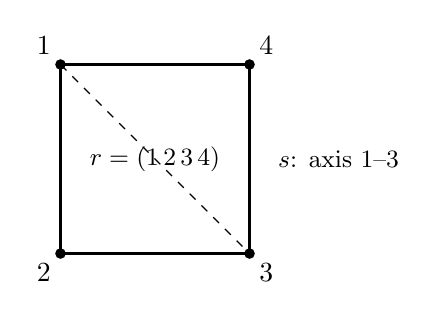
\begin{tikzpicture}[scale=1.2]
  \coordinate (v1) at (-1,1);
  \coordinate (v2) at (-1,-1);
  \coordinate (v3) at (1,-1);
  \coordinate (v4) at (1,1);
  \draw[thick] (v1)--(v2)--(v3)--(v4)--cycle;
  \draw[dashed] (v1)--(v3);
  \fill (v1) circle (1.6pt); \fill (v2) circle (1.6pt);
  \fill (v3) circle (1.6pt); \fill (v4) circle (1.6pt);
  \node[above left] at (v1) {$1$};
  \node[below left] at (v2) {$2$};
  \node[below right] at (v3) {$3$};
  \node[above right] at (v4) {$4$};
  \node at (0,0) {\small $r=(1\,2\,3\,4)$};
  \node[right] at (1.2,0) {\small $s$: axis $1$--$3$};
\end{tikzpicture}
\end{center}

\begin{proposition}[$D_8$ acts faithfully on the $4$ vertices]\label{p:d8@c1}
$D_8$ acts on $A=\{1,2,3,4\}$ by its geometric action on the square's vertices. The representation
$\rho\colon D_8\to S_4$ is injective ($\ker\rho=1$), and $\rho(r)=(1\,2\,3\,4)$,
$\rho(s)=(2\,4)$.
\end{proposition}

\begin{proof}
Symmetries of the square permute its vertices, and composing symmetries composes the permutations,
so (A1),(A2) hold and $\rho$ is a homomorphism. Rotation by $90^\circ$ sends $1\to2\to3\to4\to1$, so
$\rho(r)=(1\,2\,3\,4)$. The reflection across the $1$--$3$ diagonal fixes $1,3$ and swaps $2,4$, so
$\rho(s)=(2\,4)$. A symmetry fixing all four vertices is the identity, so $\ker\rho=1$ and $\rho$
is injective; thus $D_8\isom\rho(D_8)\sgr S_4$, the image being a Sylow $2$-subgroup of $S_4$.
\end{proof}

\begin{wex}{Build the full table $\rho\colon D_8\to S_4$ and check the relations}
Write $\rho(g)$ for all eight $g\in D_8=\{1,r,r^2,r^3,s,sr,sr^2,sr^3\}$ and verify $sr=r\inv s$ at
the level of permutations.
\wrec We have the generators' images (Prop.~\ref{p:d8@c1}); since $\rho$ is a homomorphism, every other
image is a product. Use $\rho(sr^k)=\rho(s)\rho(r)^k=S R^k$, composing right to left.
\wsol With $R:=\rho(r)=(1\,2\,3\,4)$ and $S:=\rho(s)=(2\,4)$ we first record the rotation powers
$R^2=(1\,3)(2\,4)$, $R^3=(1\,4\,3\,2)$. Now compute each $\rho(sr^k)=S R^k$ by applying $R^k$ first,
then $S$.
\begin{itemize}
\item $k=0$: $\rho(s)=S=(2\,4)$.
\item $k=1$: $S R$. Apply $R$ then $S$: $1\mapsto2\mapsto4$, $4\mapsto1\mapsto1$, so
$1\leftrightarrow4$; $2\mapsto3\mapsto3$, $3\mapsto4\mapsto2$, so $2\leftrightarrow3$. Hence
$\rho(sr)=(1\,4)(2\,3)$.
\item $k=2$: $S R^2$. Apply $R^2$ then $S$: $1\mapsto3\mapsto3$, $3\mapsto1\mapsto1$, so
$1\leftrightarrow3$; $2\mapsto4\mapsto2$ and $4\mapsto2\mapsto4$ are fixed. Hence
$\rho(sr^2)=(1\,3)$.
\item $k=3$: $S R^3$. Apply $R^3$ then $S$: $1\mapsto4\mapsto2$, $2\mapsto1\mapsto1$, so
$1\mapsto2\mapsto1$ gives $1\leftrightarrow2$; $3\mapsto2\mapsto4$, $4\mapsto3\mapsto3$, so
$3\leftrightarrow4$. Hence $\rho(sr^3)=(1\,2)(3\,4)$.
\end{itemize}
The complete table is
\[
\begin{array}{c|cccccccc}
g & 1 & r & r^2 & r^3 & s & sr & sr^2 & sr^3\\\hline
\rho(g) & () & (1\,2\,3\,4) & (1\,3)(2\,4) & (1\,4\,3\,2) & (2\,4) & (1\,4)(2\,3) & (1\,3) & (1\,2)(3\,4)
\end{array}
\]
\textbf{Verify $sr=r\inv s$:} LHS $=\rho(sr)=(1\,4)(2\,3)$. RHS $=R\inv S$ with
$R\inv=(1\,4\,3\,2)$: apply $S=(2\,4)$ then $R\inv$: $1\mapsto1\mapsto4$, $4\mapsto2\mapsto1$, so
$1\leftrightarrow4$; $2\mapsto4\mapsto3$, $3\mapsto3\mapsto2$, so $2\leftrightarrow3$. Thus
$R\inv S=(1\,4)(2\,3)=$ LHS. \textbf{Check:} all $8$ images are distinct, reconfirming $\ker\rho=1$.
\end{wex}

\begin{wex}{$D_8$ acting on the $2$ diagonals: a non-faithful action}
Let $D_8$ act on the set $A=\{d_{13},d_{24}\}$ of the square's two diagonals. Compute $\rho\colon
D_8\to S_2$ and its kernel.
\wrec Same group, smaller set, so the rep lands in $S_2$ (order $2$) while $|D_8|=8$; a
counting clash ($8>2$) forces a nontrivial kernel -- a textbook non-faithful action.
\wsol $r$ (rotate $90^\circ$) sends diagonal $1$--$3$ to $2$--$4$, so it swaps $d_{13}\leftrightarrow
d_{24}$: $\rho(r)=(d_{13}\,d_{24})$. The reflection $s$ across $1$--$3$ fixes that axis and maps the
other diagonal to itself, so $\rho(s)=\id$. Since $r,s$ generate $D_8$, the image is
$\gen{(d_{13}\,d_{24})}=S_2$. The homomorphism $\rho\colon D_8\to S_2$ is onto $S_2$, so by the
first isomorphism theorem $|\ker\rho|=8/2=4$. Explicitly $g\in\ker\rho$ iff $g$ fixes each
diagonal: these are $\{1,r^2,s,sr^2\}$ (check: $r^2$ rotates $180^\circ$ fixing both diagonals; $s$
and $sr^2$ are the two reflections through the diagonals). So $\ker\rho=\{1,r^2,s,sr^2\}\isom V_4$,
the action is \emph{not} faithful.
\textbf{Check:} $|\{1,r^2,s,sr^2\}|=4$ matches $8/|\im\rho|=8/2=4$, and one verifies this set is a
subgroup (indeed normal, as kernels must be).
\end{wex}

\begin{wex}{$S_n$ on $\{1,\dots,n\}$ is faithful}
The natural action $\sigma\cdot i=\sigma(i)$ of $S_n$ on $A=\{1,\dots,n\}$. Show it is an action and
compute its kernel.
\wrec ``$\sigma\cdot i=\sigma(i)$'' is the defining/tautological action; $\rho$ is the identity map
$S_n\to\Sym(A)=S_n$, the cleanest possible representation.
\wsol (A1): $1\cdot i=\id(i)=i$. (A2): $(\sigma\tau)\cdot i=(\sigma\tau)(i)=\sigma(\tau(i))=
\sigma\cdot(\tau\cdot i)$ -- this is literally how composition in $S_n$ is defined. So $\rho(\sigma)
=\sigma$ and $\rho=\id_{S_n}$. Kernel: $\sigma(i)=i$ for all $i$ means $\sigma=\id$, so
$\ker\rho=1$ and the action is faithful (trivially, $\rho$ is a bijection).
\textbf{Check:} for $n=3$, $\rho((1\,2))=(1\,2)$, and distinct group elements give distinct
permutations because they \emph{are} those permutations.
\end{wex}

\begin{wex}{A subgroup action: $A_4$ on $\{1,2,3,4\}$, still faithful}
Restrict the natural $S_4$-action to $A_4$. Is it faithful? What is $\rho(A_4)$?
\wrec Restricting a faithful action to a subgroup stays faithful, because the kernel only shrinks:
$\ker(\rho|_H)=H\cap\ker\rho$.
\wsol The restriction sends $\sigma\in A_4$ to $\sigma\in S_4$, so $\rho|_{A_4}$ is the inclusion
$A_4\hookrightarrow S_4$. Kernel $=A_4\cap\ker(\text{natural})=A_4\cap\{1\}=\{1\}$, so faithful;
$\rho(A_4)=A_4\sgr S_4$. \textbf{Check:} e.g.\ $(1\,2\,3)\in A_4$ maps to the nonidentity
$(1\,2\,3)$, so it is not in the kernel; only $\id$ fixes all four points.
\end{wex}

\subsection*{Example family 3: conjugation, with kernel $Z(G)$}

\begin{proposition}[Conjugation action]\label{p:conj@c1}
$G$ acts on itself by conjugation $g\cdot x:=gxg\inv$. The representation
$\rho\colon G\to\Sym(G)$ has image inside $\Aut(G)$ (each $\sigma_g$ is the inner automorphism
$x\mapsto gxg\inv$), and
\[
\ker\rho=Z(G)=\{g\in G: gx=xg\ \forall x\in G\}.
\]
Hence $\rho$ induces $G/Z(G)\isom\Inn(G)\sgr\Aut(G)$, and the action is faithful iff $Z(G)=1$.
\end{proposition}

\begin{proof}
(A1): $1\cdot x=1x1\inv=x$. (A2): $(gh)\cdot x=(gh)x(gh)\inv=g(hxh\inv)g\inv=g\cdot(h\cdot x)$.
Each $\sigma_g$ respects multiplication: $\sigma_g(xy)=g(xy)g\inv=(gxg\inv)(gyg\inv)
=\sigma_g(x)\sigma_g(y)$, so $\sigma_g\in\Aut(G)$. Kernel: $gxg\inv=x$ for all $x$ $\eqv gx=xg$ for
all $x$ $\eqv g\in Z(G)$. The first isomorphism theorem gives $G/Z(G)\isom\rho(G)=\Inn(G)$.
\end{proof}

\[\begin{tikzcd}[row sep=large,column sep=large]
G \arrow[r, "\rho"] \arrow[d, two heads, "\pi"'] & \Aut(G) \\
G/Z(G) \arrow[ur, hook, dashed, "\isom\,\Inn(G)"'] &
\end{tikzcd}\]

\begin{dgx}
\dgi{Objects:} Three nodes. $G$ is the group acting on itself by conjugation. $\Aut(G)$ is the
  automorphism group of $G$ (all group isomorphisms $G\to G$); it is the ambient target because each
  conjugation $x\mapsto gxg^{-1}$ is an automorphism. $G/Z(G)$ is the quotient of $G$ by its center
  $Z(G)=\ker\rho$; elements are cosets $gZ(G)$.
\dgi{Arrows:} Top horizontal $\rho\colon G\to\Aut(G)$: the conjugation representation sending $g$
  to the inner automorphism $\iota_g\colon x\mapsto gxg^{-1}$; its image is $\Inn(G)$. Left vertical
  two-headed arrow $\pi\colon G\twoheadrightarrow G/Z(G)$: the canonical quotient map, surjective.
  Dashed hooked arrow $G/Z(G)\hookrightarrow\Aut(G)$, labeled $\isom\Inn(G)$: the induced injection
  $\overline{\rho}(gZ(G)):=\iota_g$, which is an isomorphism onto $\Inn(G)$.
\dgi{What commutes:} $\rho = \overline{\rho}\circ\pi$: i.e.\ $\iota_g=\overline{\rho}(gZ(G))$ for
  all $g\in G$, so the two paths from $G$ to $\Aut(G)$ agree.
\dgi{Why it commutes:} Well-definedness: if $gZ(G)=g'Z(G)$ then $g^{-1}g'\in Z(G)$, so
  $g^{-1}g'$ commutes with every $x$; then $g'^{-1}xg'=g^{-1}xg$ for all $x$, i.e.\ $\iota_{g'}=
  \iota_g$. Hence $\overline{\rho}$ is independent of the coset representative. Commutativity then
  holds by construction. Injectivity: $\overline{\rho}(gZ(G))=\id$ iff $gxg^{-1}=x$ for all $x$
  iff $g\in Z(G)$ iff $gZ(G)$ is the identity coset.
\dgi{Why this matters here:} This is the first isomorphism theorem for the conjugation action of
  Proposition~\ref{p:conj@c1}: it identifies $\Inn(G)$ concretely as $G/Z(G)$, explaining why large
  centers produce small inner automorphism groups and why $Z(G)=1$ forces the action to be faithful.
\dgi{Concrete example:} $G=D_8$: $Z(D_8)=\{1,r^2\}$, so $G/Z(G)\isom\Zn{2}\times\Zn{2}=V_4$ and
  $\Inn(D_8)\isom V_4$ (four inner automorphisms). The coset $rZ$ maps to $\iota_r\in\Aut(D_8)$,
  the automorphism conjugating by $r$.
\dgi{Common pitfall:} The hooked arrow lands in $\Aut(G)$, not in $\Sym(G)$; inner automorphisms
  are group automorphisms, not arbitrary bijections. Also, $G/Z(G)\isom\Inn(G)$ is an isomorphism
  of groups, but $G/Z(G)$ is not a subgroup of $G$ itself; it lives inside $\Aut(G)$.
\dgi{Takeaway:} The point of this diagram is that the inner automorphism group is always isomorphic
  to $G$ modulo its center, so the center measures exactly how much of $G$ is ``invisible'' to the
  conjugation action.
\end{dgx}

\begin{wex}{Conjugation on $D_8$: kernel is $Z(D_8)=\{1,r^2\}$}
For $G=D_8$ compute the kernel of the conjugation action and decide faithfulness.
\wrec By Prop.~\ref{p:conj@c1} the kernel is the center; for $D_8$ the center is known to be
$\{1,r^2\}$, so we expect a nontrivial kernel (not faithful).
\wsol Use $sr=r\inv s$. For $g$ central we need $g$ to commute with both $r$ and $s$.
$r$ commutes with $r,r^2,r^3$; does $r$ commute with $s$? $rs=sr\inv$ (from $sr=r\inv s\Rightarrow
rs=sr\inv$), and $rs=sr$ iff $sr\inv=sr$ iff $r\inv=r$ iff $r^2=1$, false. So $s\notin Z$. Test
$r^2$: $r^2 s=s r^{-2}=s r^2$ (since $r^4=1\Rightarrow r^{-2}=r^2$), and $r^2$ commutes with $r$.
Hence $r^2\in Z$. One checks no reflection is central, so $Z(D_8)=\{1,r^2\}$. Therefore
$\ker\rho=\{1,r^2\}$, $|\Inn(D_8)|=8/2=4$, and the conjugation action is \emph{not} faithful.
\textbf{Check:} $r^2$ conjugates trivially: $r^2 s r^{-2}=s r^{-2}r^{-2}=s r^{-4}=s$, and
$r^2 r r^{-2}=r$, so $\sigma_{r^2}=\id$, confirming $r^2\in\ker\rho$.
\end{wex}

\begin{wex}{Conjugation on $Q_8$: kernel $Z(Q_8)=\{\pm1\}$}
Find the kernel of conjugation on $Q_8=\{\pm1,\pm i,\pm j,\pm k\}$.
\wrec Again the kernel is the center; for $Q_8$ the center is $\{\pm1\}$.
\wsol $g\in Z(Q_8)$ iff $g$ commutes with $i$ and $j$. Now $ij=k$ but $ji=-k$, so $i,j$ do not
commute; thus $i,j,k\notin Z$. The elements $\pm1$ are central ($1$ trivially, and
$(-1)x=x(-1)=-x$). So $Z(Q_8)=\{1,-1\}$ and $\ker\rho=\{\pm1\}$; the action is not faithful and
$\Inn(Q_8)\isom Q_8/\{\pm1\}\isom V_4$ (order $4$).
\textbf{Check:} $(-1)i(-1)\inv=(-1)i(-1)=i$, so $\sigma_{-1}=\id$, i.e.\ $-1\in\ker\rho$. And
$i j i\inv=i j(-i)=(ij)(-i)=k(-i)=-(ki)=-j\ne j$, so $i\notin\ker\rho$ -- the kernel really is
just $\{\pm1\}$.
\end{wex}

\begin{wex}{Conjugation on $S_3$ is faithful ($Z(S_3)=1$)}
Show conjugation makes $S_3$ act faithfully on itself, and identify $\Inn(S_3)$.
\wrec Faithful iff $Z(G)=1$; for $S_n$ with $n\ge3$ the center is trivial.
\wsol Suppose $g\in Z(S_3)$. Conjugation by $g$ preserves cycle type, and if $g$ commutes with the
transposition $(1\,2)$ then $g(1\,2)g\inv=(1\,2)$, i.e.\ $g$ fixes the pair $\{1,2\}$; commuting with
$(2\,3)$ likewise fixes $\{2,3\}$. The only $g$ fixing $\{1,2\}$ and $\{2,3\}$ setwise and lying in
$S_3$ is $g=1$. So $Z(S_3)=1$, $\ker\rho=1$, the action is faithful, and
$\Inn(S_3)\isom S_3/Z(S_3)=S_3$, of order $6$.
\textbf{Check:} $(1\,2)(1\,2\,3)(1\,2)\inv=(2\,1\,3)=(1\,3\,2)\ne(1\,2\,3)$, so $(1\,2)$ acts
nontrivially -- consistent with a trivial kernel.
\end{wex}

\begin{wex}{Conjugation on an abelian group is trivial (maximally non-faithful)}
Describe the conjugation action of an abelian $G$ (say $G=\Zn{6}$) and its kernel.
\wrec If $G$ is abelian, every $gxg\inv=x$, so the action is the trivial action and the kernel is
all of $G$ -- the extreme opposite of faithful.
\wsol For abelian $G$: $g\cdot x=gxg\inv=gg\inv x=x$ for all $g,x$. Thus $\sigma_g=\id$ for every
$g$, $\rho$ is the constant map to $\id$, and $\ker\rho=Z(G)=G$ (consistent with $Z(G)=G$ for
abelian $G$). For $G=\Zn6$, $\rho(\Zn6)=\{\id\}$ and $\ker\rho=\Zn6$.
\textbf{Check:} $\Inn(\Zn6)\isom\Zn6/Z(\Zn6)=\Zn6/\Zn6=1$, the trivial group, exactly as ``no
nontrivial inner automorphisms'' predicts.
\end{wex}

\begin{wex}{A coset action and its core: $S_3$ on cosets of $H=\gen{(1\,2)}$}
Let $G=S_3$ act by left multiplication on the left cosets of $H=\gen{(1\,2)}$, i.e.\ on
$A=\{H,(1\,3)H,(2\,3)H\}$ (three cosets). Find $\rho\colon S_3\to\Sym(A)$ and $\ker\rho$.
\wrec Action on cosets $g\cdot(xH)=(gx)H$ is a standard action; its kernel is the
\emph{normal core} $\bigcap_{x\in S_3}xHx\inv$, the largest normal subgroup of $G$ contained in $H$.
\wsol First name the three cosets. Composing right to left,
\[
\begin{aligned}
c_1&=H=\{1,(1\,2)\},\\
c_2&=(1\,3)H=\{(1\,3),\,(1\,3)(1\,2)\}=\{(1\,3),(1\,2\,3)\},\\
c_3&=(2\,3)H=\{(2\,3),\,(2\,3)(1\,2)\}=\{(2\,3),(1\,3\,2)\}.
\end{aligned}
\]
Now act by the generators, computing $g\cdot c=(g\cdot\text{rep})H$ and reading off which coset
contains the result.
\begin{itemize}
\item $g=(1\,2\,3)$: $g\cdot1=(1\,2\,3)\in c_2$; $g\cdot(1\,3)=(1\,2\,3)(1\,3)=(2\,3)\in c_3$;
$g\cdot(2\,3)=(1\,2\,3)(2\,3)=(1\,2)\in c_1$. So $\rho((1\,2\,3))=(c_1\,c_2\,c_3)$.
\item $g=(1\,2)$: $g\cdot1=(1\,2)\in c_1$; $g\cdot(1\,3)=(1\,2)(1\,3)=(1\,3\,2)\in c_3$;
$g\cdot(2\,3)=(1\,2)(2\,3)=(1\,2\,3)\in c_2$. So $\rho((1\,2))=(c_2\,c_3)$.
\item $g=(1\,3)$: $g\cdot1=(1\,3)\in c_2$; $g\cdot(1\,3)=1\in c_1$;
$g\cdot(2\,3)=(1\,3)(2\,3)=(1\,3\,2)\in c_3$, so $c_3$ is fixed. Hence $\rho((1\,3))=(c_1\,c_2)$.
\end{itemize}
Thus $\rho$ sends $(1\,2\,3)\mapsto(c_1\,c_2\,c_3)$, $(1\,2)\mapsto(c_2\,c_3)$,
$(1\,3)\mapsto(c_1\,c_2)$, and these already generate all of $\Sym(A)\isom S_3$. Hence $\rho$ is
onto, and since $|S_3|=6=|\Sym(A)|$ it is an isomorphism, so $\ker\rho=1$: the action is faithful.
Equivalently $\ker\rho=\operatorname{core}(H)=\bigcap_{x}xHx\inv$, and as $|H|=2$ with $H$ not
normal this intersection is trivial.
\textbf{Check:} the core is the largest normal subgroup inside $H$; the only normal subgroups of
$S_3$ are $1$, $A_3$, $S_3$, and the only one contained in the $2$-element $H$ is $1$. For a
genuinely non-faithful coset action take $G=Q_8$ on the four cosets of $H=\gen{-1}$: there
$\gen{-1}\nor Q_8$, so $\operatorname{core}(H)=\gen{-1}=Z(Q_8)\ne1$ and $\ker\rho=\gen{-1}$.
\end{wex}

\begin{pitfall}
``Faithful'' is about the \emph{whole} action: $\ker\rho=\{g:g\cdot a=a\text{ for }\textbf{all }a\}$.
One element $g$ fixing one point $a$ (a \emph{stabilizer}) is unrelated; do not confuse
$\ker\rho=\bigcap_a G_a$ (intersection of all stabilizers) with a single stabilizer $G_a$.
\end{pitfall}

\begin{remark}[The three diagrams to keep in mind]
(1) An action \emph{is} a homomorphism $\rho\colon G\to\Sym(A)$ (Thm.~\ref{t:equiv@c1}); (2) the
regular action gives Cayley's embedding $G\hookrightarrow\Sym(G)$ (Thm.~\ref{t:cayley@c1}); (3) every
action factors as $G\twoheadrightarrow G/\ker\rho\hookrightarrow\Sym(A)$:
\[\begin{tikzcd}[row sep=large,column sep=large]
G \arrow[r, "\rho"] \arrow[d, two heads, "\pi"'] & \Sym(A) \\
G/\ker\rho \arrow[ur, hook, dashed, "\overline{\rho}"'] &
\end{tikzcd}\]

\begin{dgx}
\dgi{Objects:} Three nodes. $G$ is the group performing any given action on a set $A$.
  $\Sym(A)$ is the symmetric group on the set $A$, the universal target for permutation
  representations of groups acting on $A$. $G/\ker\rho$ is the quotient of $G$ by the kernel
  of the permutation representation $\rho$; it is the ``effective'' part of $G$ that acts
  non-trivially.
\dgi{Arrows:} Top horizontal $\rho\colon G\to\Sym(A)$: the permutation representation of the given
  action. Left vertical two-headed $\pi\colon G\twoheadrightarrow G/\ker\rho$: the canonical
  surjection $g\mapsto g\ker\rho$, which collapses elements that act identically. Dashed hooked
  $\overline{\rho}\colon G/\ker\rho\hookrightarrow\Sym(A)$: the induced injective map
  $\overline{\rho}(g\ker\rho):=\rho(g)$, guaranteed by the universal property of the quotient since
  $\ker\rho\subseteq\ker\rho$.
\dgi{What commutes:} The triangle: $\rho=\overline{\rho}\circ\pi$, meaning $\rho(g)=\overline{\rho}
  (g\ker\rho)$ for every $g\in G$.
\dgi{Why it commutes:} Well-definedness of $\overline{\rho}$: if $g\ker\rho=g'\ker\rho$ then $g^{-1}
  g'\in\ker\rho$, so $\rho(g^{-1}g')=\id$, hence $\rho(g)=\rho(g')$; the output of $\overline{\rho}$
  does not depend on which representative of the coset is used. Commutativity then reads
  $\overline{\rho}(\pi(g))=\overline{\rho}(g\ker\rho)=\rho(g)$, which is immediate. Injectivity of
  $\overline{\rho}$: $\overline{\rho}(g\ker\rho)=\id$ iff $\rho(g)=\id$ iff $g\in\ker\rho$.
\dgi{Why this matters here:} This is the master diagram of the whole section: it says every group
  action factors universally as a surjection (onto the quotient by the kernel) followed by an
  injection (into $\Sym(A)$). The action is faithful iff $\ker\rho=1$ iff $\pi$ is an isomorphism
  iff the bottom-left vertex equals $G$.
\dgi{Concrete example:} Conjugation action of $G=D_8$ on itself: $\ker\rho=Z(D_8)=\{1,r^2\}$, so
  $G/\ker\rho\isom V_4$ and $\overline{\rho}\colon V_4\hookrightarrow\Aut(D_8)$ is the injective map
  whose image is $\Inn(D_8)$. The quotient $\pi$ collapses each coset $\{g,gr^2\}$ to a single
  element of $V_4$.
\dgi{Common pitfall:} Students sometimes read $\overline{\rho}$ as an isomorphism onto $\Sym(A)$.
  It is only injective; $\rho(G)$ is typically a \emph{proper} subgroup of $\Sym(A)$ (e.g., the
  image of $D_8$ acting on $4$ vertices is a subgroup of $S_4$ of order $8$, not all $24$ elements).
\dgi{Takeaway:} The point of this diagram is that every action, no matter how non-faithful, contains
  a faithful action of the quotient $G/\ker\rho$ inside it, and this quotient is the largest quotient
  of $G$ that acts faithfully on $A$.
\end{dgx}

The action is faithful exactly when $\pi$ is an isomorphism, i.e.\ when the left arrow has trivial
kernel.
\end{remark}


%% ===== Dummit & Foote book-level content (merged in) =====
\subsection*{D\&F's example list: trivial action, scalar multiplication, and $D_{2n}$ on $n$ vertices}

The fragment above already states the two axioms (Def.~\ref{d:action@c1}), defines the permutation
representation, kernel, and faithfulness (Def.~\ref{d:rep@c1}), proves the action--homomorphism
correspondence (Thm.~\ref{t:equiv@c1}), and works the left regular action (Cayley, Thm.~\ref{t:cayley@c1}),
the natural $S_n$-action, and $D_8$ on the square. We do not repeat those. What follows adds the
remaining entries from D\&F's own running list in 1.7 that the fragment lacks: the trivial action,
the scalar-multiplication action, and the general $D_{2n}$ on the $n$ vertices.

\begin{remark}[D\&F's numbering and the name ``permutation representation'']
D\&F state the axioms with associativity first: \textbf{(1)}
$g_1\cdot(g_2\cdot a)=(g_1g_2)\cdot a$ and \textbf{(2)} $1\cdot a=a$ for all $a$. This is the same
content as Def.~\ref{d:action@c1} (our (A1),(A2) in the other order). D\&F write the associated
homomorphism as $\varphi\colon G\to S_A$ with $\varphi(g)\colon a\mapsto g\cdot a$, call it the
\emph{permutation representation associated to the action}, and call $\ker\varphi=\{g: g\cdot a=a\
\forall a\}$ the \emph{kernel of the action}; faithful means this kernel is the identity. We use
$\rho$ and $\Sym(A)$ above for D\&F's $\varphi$ and $S_A$.
\end{remark}

\begin{definition}[Trivial action]\label{d:trivial-mrg@c1}
For any group $G$ and nonempty set $A$, the rule $g\cdot a=a$ for all $g\in G$, $a\in A$, is an
action, the \emph{trivial action} of $G$ on $A$. Each $\sigma_g=\id_A$, so $\rho$ is the constant map
$g\mapsto\id_A$ and $\ker\rho=G$; it is faithful only when $G=1$.
\end{definition}

\begin{wex}{D\&F Example: the trivial action and what it ``sees''}
Verify that $g\cdot a=a$ is an action of any $G$ on any nonempty $A$, and identify its kernel.
\wrec This is Def.~\ref{d:trivial-mrg@c1}; the only work is to confirm the two axioms and read off
$\ker\rho$, which exhibits the extreme opposite of a faithful action.
\wsol Axiom (A1): $1\cdot a=a$ by definition. Axiom (A2):
$g\cdot(h\cdot a)=g\cdot a=a$ and $(gh)\cdot a=a$, so the two sides agree. Every $\sigma_g$ is
$\id_A$, hence $\rho\colon G\to\Sym(A)$ is the constant map onto $\{\id_A\}$ and
$\ker\rho=\{g:g\cdot a=a\ \forall a\}=G$.
\textbf{Check:} the action is faithful $\eqv\ker\rho=1\eqv G=1$; for $|G|>1$ the trivial action is
maximally non-faithful, which is why a nontrivial action is required to ``see'' anything about $G$.
This is the opposite extreme to the faithful regular and natural actions worked above.
\end{wex}

\begin{wex}{D\&F Example: $F^\times$ acting on a vector space by scalar multiplication}
Let $V$ be a vector space over a field $F$ and let $G=F^\times=F\setminus\{0\}$ act on $A=V$ by
$a\cdot v=av$ (scalar multiplication). Check the axioms and find the kernel.
\wrec D\&F give this as the prototype where the ``set'' $V$ carries extra structure but the acting
group is just the multiplicative group of scalars; the vector-space axioms supply (A1),(A2)
directly.
\wsol Axiom (A1): $1\cdot v=1v=v$ for all $v$, by the unit axiom of a vector space. Axiom (A2): for
$a,b\in F^\times$, $a\cdot(b\cdot v)=a(bv)=(ab)v=(ab)\cdot v$, the associativity of scalar
multiplication. So this is an action of $F^\times$ on $V$. Kernel: $a\cdot v=v$ for \emph{all}
$v\in V$ means $av=v$, i.e.\ $(a-1)v=0$ for all $v$; choosing any $v\ne0$ forces $a=1$. Hence
$\ker\rho=\{1\}$ and (for $V\ne0$) the action is faithful.
\textbf{Check:} each nonzero scalar $a$ gives the bijection $v\mapsto av$ of $V$ with inverse
$v\mapsto a\inv v$, confirming $\sigma_a\in\Sym(V)$; distinct scalars scale some $v\ne0$
differently, so $\rho$ is injective.
\end{wex}

\begin{wex}{D\&F Example: $D_{2n}$ acting on the $n$ vertices of a regular $n$-gon}
Show $D_{2n}$ acts on the set $A=\{1,2,\dots,n\}$ of vertices, written cyclically, and describe
$\sigma_r$ and $\sigma_s$ for the standard generators (D\&F's convention $r^n=s^2=1$,
$sr=r\inv s$, with $s$ fixing vertex $1$).
\wrec D\&F introduce $D_{2n}$ as the symmetries of the regular $n$-gon, so the action on vertices is
the defining one; it motivates writing each symmetry as a permutation. The $D_8$ table
(Prop.~\ref{p:d8@c1}) is the special case $n=4$, which we do not redo here.
\wsol Each symmetry of the $n$-gon carries vertices to vertices bijectively, and composing
symmetries composes their vertex permutations, so (A1),(A2) hold (the symmetry doing nothing is the
identity permutation). For the rotation $r$ by $2\pi/n$,
\[
\sigma_r=(1\,2\,3\,\cdots\,n),
\]
an $n$-cycle. For the reflection $s$ fixing vertex $1$,
\[
\sigma_s=(2\;n)(3\;n{-}1)(4\;n{-}2)\cdots,
\]
fixing vertex $1$ and pairing $k$ with $n{+}2{-}k$ (so for even $n$ the middle vertex $\tfrac{n}{2}+1$
is also fixed; for odd $n$ only vertex $1$ is fixed). Since the generators map to nonidentity
permutations and a symmetry fixing every vertex is the identity, $\ker\rho=1$ and
$\rho\colon D_{2n}\to S_n$ is injective, so $D_{2n}\isom\rho(D_{2n})\sgr S_n$.
\textbf{Check:} for $n=4$, $\sigma_r=(1\,2\,3\,4)$ and $\sigma_s=(2\,4)$ (the pair $k\leftrightarrow
n{+}2{-}k$ gives $2\leftrightarrow4$, with $1,3$ fixed), recovering the $D_8$ data of
Prop.~\ref{p:d8@c1}; for $n=5$, $\sigma_s=(2\,5)(3\,4)$; the relation $sr=r\inv s$ becomes
$\sigma_s\sigma_r=\sigma_r\inv\sigma_s$ in $S_n$, the permutation identity verified there.
\end{wex}

\begin{remark}[Reading the example list]
Across D\&F's list the single fact at work is the correspondence of Thm.~\ref{t:equiv@c1}: an action of
$G$ on $A$ is the same data as a homomorphism $G\to\Sym(A)$, and the kernel of the action equals the
kernel of that homomorphism, so ``faithful'' means ``injective.'' The examples populate the full
range: the trivial action ($\rho$ constant, $\ker\rho=G$); scalar multiplication, the natural
$S_n$-action, the left regular action, and $D_{2n}$ on vertices ($\rho$ injective, $\ker\rho=1$); and
the coset and conjugation actions worked above (intermediate kernels, the normal core and $Z(G)$).
\end{remark}

\begin{exers}{Exercises (from the text).}
\item $F^\times$ acts on $F$ by $g\cdot a=ga$; state the axioms used.
\item Show $\Z$ acts on itself by $z\cdot a=z+a$.
\item Show $\R$ acts on $\R^2$ by $r\cdot(x,y)=(x+ry,y)$.
\item Fix $a$: show the kernel and $G_a=\{g:g\cdot a=a\}$ are subgroups.
\item Kernel of an action $=$ kernel of its permutation representation.
\item $G$ acts faithfully iff the kernel is $\{1\}$.
\item Show the scalar action on a vector space is faithful.
\item How do $(1\,2)$ and $(1\,2\,3)$ act on the six $2$-subsets of
   $\{1,2,3,4\}$?
\item Repeat for ordered $k$-tuples.
\item For which $k$ is the action of $S_n$ on (a) $k$-subsets, (b) $k$-tuples
   faithful?
\item Cycle decompositions of the eight elements of $D_8$ on the square's
   vertices.
\item For $n$ even, find the kernel of $D_{2n}$ on opposite-vertex pairs.
\item Find the kernel of the left regular action.
\item $g\cdot a=ag$ is not a left action when $G$ is non-abelian.
\item $g\cdot a=ag\inv$ \emph{is} a left action.
\item $g\cdot a=gag\inv$ is a left action (conjugation).
\item Conjugation by $g$ is an automorphism; deduce $|x|=|gxg\inv|$.
\item $a\sim b\iff a=hb$ is an equivalence relation.
\item $H\le G$ acts by left multiplication; deduce Lagrange's theorem.
\item Rigid motions of a tetrahedron embed in $S_4$.
\item Rigid motions of a cube $\isom S_4$.
\item Rigid motions of an octahedron $\isom S_4$; dual to the cube.
\item Why is the cube's action on $3$ pairs of opposite faces not faithful?
\end{exers}

\begin{exers}{Additional exercises.}
\item Let $G=D_8=\gen{r,s}$ act on the four vertices $\{1,2,3,4\}$ of the square (labeled counterclockwise) in the natural way, with $r$ the rotation sending $1\mapsto 2\mapsto 3\mapsto 4\mapsto 1$ and $s$ the reflection fixing the diagonal through vertices $1$ and $3$. For each of $r$, $s$, $rs$, and $r^2$, write the resulting permutation of $\{1,2,3,4\}$ in cycle notation. Then verify directly that $\sigma_r\sigma_s=\sigma_{rs}$ (composing permutations right-to-left), confirming the action is a homomorphism on these elements.

\item Let $G$ act on itself by \emph{left multiplication}: $g\cdot x=gx$ for $g,x\in G$. Prove this is a (left) group action, and prove it is \emph{faithful} for every group $G$. Then show that for $G$ nontrivial this action has no fixed points, i.e. there is no $x\in G$ with $g\cdot x=x$ for all $g\in G$.

\item Let $G$ act on itself by \emph{conjugation}: $g\cdot x=gxg\inv$. Verify the two axioms of a group action. Show that the kernel of this action (the set of $g$ acting trivially, i.e. $gxg\inv=x$ for all $x$) equals $Z(G)$. Compute this kernel explicitly when $G=Q_8$ and when $G=S_3$.

\item Let $G=\Zns{8}=\{\bar1,\bar3,\bar5,\bar7\}$ act on the set $A=\Zn{8}$ by $\bar a\cdot \bar x=\overline{ax}$.
  \begin{enumerate}
  \item Check this is a well-defined action.
  \item Compute the orbit and the stabilizer of $\bar2$, and of $\bar1$.
  \item Determine the kernel of the action, i.e. the set of $\bar a$ with $\overline{ax}=\bar x$ for all $\bar x\in\Zn{8}$.
  \end{enumerate}

\item Let $G$ act on a set $A$, and fix $a\in A$. Recall the stabilizer $G_a=\{g\in G\st g\cdot a=a\}$.
  \begin{enumerate}
  \item Prove $G_a\sgr G$.
  \item Prove that if $b=g\cdot a$ lies in the orbit of $a$, then $G_b=gG_a g\inv$. Conclude that points in the same orbit have conjugate stabilizers.
  \end{enumerate}

\item Suppose $G$ acts on a set $A$. Define a relation on $A$ by $a\sim b$ iff $b=g\cdot a$ for some $g\in G$. Prove $\sim$ is an equivalence relation (its classes are the orbits). Then, for the action of $G=\gen{(1\,2\,3)}\sgr S_5$ on $A=\{1,2,3,4,5\}$, list all orbits explicitly.

\item Let $G=S_4$ act on the set $A$ of the three unordered partitions of $\{1,2,3,4\}$ into two pairs, namely $\{\{1,2\},\{3,4\}\}$, $\{\{1,3\},\{2,4\}\}$, $\{\{1,4\},\{2,3\}\}$, by relabeling points. This gives a homomorphism $\varphi:S_4\to \Sym(A)\isom S_3$.
  \begin{enumerate}
  \item Compute the images $\varphi((1\,2))$ and $\varphi((1\,2\,3))$ as permutations of the three partitions.
  \item Show $\varphi$ is surjective.
  \item Identify $\ker\varphi$ as an explicit subgroup of $S_4$ and give its order.
  \end{enumerate}
\end{exers}

\begin{exers}{Commutative-diagram exercises.}
\item Let $G$ be a group and $A$ a set. Let $\varphi:G\to\Sym(A)$ be a homomorphism, and define $g\cdot a=\varphi(g)(a)$. Prove that this defines a group action by checking the two diagrams below commute for all $g,h\in G$ (here $\cdot_g:A\to A$ denotes $a\mapsto g\cdot a$, and the unlabeled arrow is the identity):
\[\begin{tikzcd}[row sep=large,column sep=large]
A \arrow[r, "\cdot_h"] \arrow[dr, "\cdot_{gh}"'] & A \arrow[d, "\cdot_g"] \\
& A
\end{tikzcd}
\qquad
\begin{tikzcd}[column sep=large]
A \arrow[r, "\cdot_1"] \arrow[dr, "\id"'] & A \arrow[d, "\id"] \\
& A
\end{tikzcd}\]
Conversely, prove that any action $G\times A\to A$ arises this way from a unique homomorphism $G\to\Sym(A)$, and state precisely what ``the action is faithful'' means about that homomorphism.

\item (Cayley's theorem via the regular representation.) Let $G$ be a group and let $\lambda:G\to\Sym(G)$ be the permutation representation of the left-multiplication action $g\cdot x=gx$, so $\lambda(g)$ is the map $x\mapsto gx$.
  \begin{enumerate}
  \item Show $\lambda$ is a homomorphism by verifying the square commutes for all $g,h$:
  \[\begin{tikzcd}[row sep=large,column sep=large]
  G \arrow[r, "\lambda(h)"] \arrow[dr, "\lambda(gh)"'] & G \arrow[d, "\lambda(g)"] \\
  & G
  \end{tikzcd}\]
  \item Show $\ker\lambda=1$ and conclude $\lambda$ is injective, so $G$ embeds as a subgroup of $\Sym(G)$:
  \[\begin{tikzcd}[column sep=large]
  1 \arrow[r] & G \arrow[r, hook, "\lambda"] & \Sym(G)
  \end{tikzcd}\]
  \item When $|G|=n$, deduce that $G$ is isomorphic to a subgroup of $S_n$.
  \end{enumerate}

\item (Kernel of an action.) Let $G$ act on $A$ with permutation representation $\varphi:G\to\Sym(A)$.
  \begin{enumerate}
  \item Prove $\ker\varphi=\bigcap_{a\in A}G_a$, the intersection of all point stabilizers, and that $\ker\varphi\nor G$.
  \item Using the first isomorphism theorem, fill in the unique dashed map making the diagram commute, and state what it is:
  \[\begin{tikzcd}[row sep=large,column sep=large]
  G \arrow[r, two heads, "\pi"] \arrow[dr, "\varphi"'] & G/\ker\varphi \arrow[d, dashed, "\exists!\,\overline{\varphi}"] \\
  & \Sym(A)
  \end{tikzcd}\]
  \item Conclude that $G/\ker\varphi$ is isomorphic to a subgroup of $\Sym(A)$.
  \end{enumerate}

\item Let $G$ be a group and $H\sgr G$ with $[G:H]=n$. Let $G$ act on the set $A=\{gH\st g\in G\}$ of left cosets by $g\cdot(xH)=(gx)H$, with permutation representation $\pi_H:G\to\Sym(A)\isom S_n$.
  \begin{enumerate}
  \item Verify this is a well-defined action.
  \item Show $\ker\pi_H=\bigcap_{x\in G}xHx\inv$, the largest normal subgroup of $G$ contained in $H$.
  \item Specialize to $G=S_3$ and $H=\gen{(1\,2)}$ (so $n=3$). Describe $\pi_H$ explicitly and identify $\ker\pi_H$.
  \end{enumerate}

\item Let $\varphi:G\to\Sym(A)$ and $\psi:G\to\Sym(B)$ be two permutation representations, and suppose $f:A\to B$ is a bijection that is $G$-equivariant, i.e. $f(g\cdot a)=g\cdot f(a)$ for all $g\in G,\,a\in A$. Show this is equivalent to the commutativity of the square
\[\begin{tikzcd}[row sep=large,column sep=large]
A \arrow[r, "f"] \arrow[d, "\varphi(g)"'] & B \arrow[d, "\psi(g)"] \\
A \arrow[r, "f"'] & B
\end{tikzcd}\]
for every $g\in G$. Deduce that if such an $f$ exists then $\ker\varphi=\ker\psi$, and that $\psi(g)=f\circ\varphi(g)\circ f\inv$ exhibits the two representations as conjugate inside $\Sym(A)$ once $B$ is identified with $A$ via $f$.
\end{exers}


% ===== Graded Problem Bank (Dummit and Foote + Artin + Fraleigh) =====
\section{Graded Problem Bank}
Problems are drawn from Dummit \& Foote, Artin (\emph{Algebra}), and Fraleigh
(\emph{A First Course in Abstract Algebra}); the difficulty grading is the author's.

\subsection*{Easy}
\begin{exers}{}
\item [DF 1.1.1] Determine which operations are associative: (a) $a\ast b=a-b$ on $\Z$;
   (b) $a\ast b=a+b+ab$ on $\R$; (c) $a\ast b=\frac{a+b}{5}$ on $\Q$;
   (d) $(a,b)\ast(c,d)=(ad+bc,bd)$ on $\Z\times\Z$; (e) $a\ast b=\frac{a}{b}$ on $\Q-\{0\}$.
\item [DF 1.1.2] Which operations in the preceding problem are commutative?
\item [DF 1.1.6] Which are groups under addition: lowest-terms rationals with (a) odd
   denominator, (b) even denominator; (c) $|x|<1$; (d) $|x|\ge1$ together with $0$;
   (e) denominators $1$ or $2$; (f) denominators $1,2,$ or $3$.
\item [DF 1.1.11] Find the orders of every element of the additive group $\Zn{12}$.
\item [DF 1.1.12] Find the orders of $\bar1,\overline{-1},\bar5,\bar7,\overline{-7},\overline{13}$
   in $\Zns{12}$.
\item [DF 1.1.13] Find the orders of $\bar1,\bar2,\bar6,\bar9,\overline{10},\overline{12},
   \overline{-1},\overline{-10},\overline{-18}$ in $\Zn{36}$.
\item [DF 1.1.14] Find the orders of $\bar1,\overline{-1},\bar5,\overline{13},\overline{-13},
   \overline{17}$ in $\Zns{36}$.
\item [DF 1.1.16] Prove $x^2=1$ iff $\ord{x}$ is $1$ or $2$.
\item [DF 1.1.17] If $\ord{x}=n$, prove $x\inv=x^{n-1}$.
\item [DF 1.1.20] Show that $x$ and $x\inv$ have the same order.
\item [DF 1.2.1] Compute the order of each element of (a) $D_6$, (b) $D_8$, (c) $D_{10}$.
\item [DF 1.2.8] Find the order of the cyclic subgroup $\gen{r}\le D_{2n}$.
\item [DF 1.2.14] Find a set of generators for $\Z$.
\item [DF 1.2.15] Find generators and relations for $\Zn{n}$.
\item [DF 1.3.2] For the permutations $\sigma,\tau$ of $\{1,\dots,15\}$ in the text, find
   $\sigma,\tau,\sigma^2,\sigma\tau,\tau\sigma,\tau^2\sigma$.
\item [DF 1.3.3] Compute the order of each permutation in DF 1.3.1 and DF 1.3.2.
\item [DF 1.3.4] Compute the order of each element in (a) $S_3$, (b) $S_4$.
\item [DF 1.3.5] Find the order of $(1\,12\,8\,10\,4)(2\,13)(5\,11\,7)(6\,9)$.
\item [DF 1.3.6] Find the cycle decomposition of each order-$4$ element of $S_4$.
\item [DF 1.3.7] Find the cycle decomposition of each order-$2$ element of $S_4$.
\item [DF 1.4.1] Prove $|\GL_2(\F_2)|=6$.
\item [DF 1.4.2] List all elements of $\GL_2(\F_2)$ and their orders.
\item [DF 1.4.3] Show $\GL_2(\F_2)$ is non-abelian.
\item [DF 1.5.1] Compute the order of each element of $Q_8$.
\item [DF 1.6.15] For $\pi:\R^2\to\R$, $\pi(x,y)=x$, find $\ker\pi$.
\item [DF 1.6.16] Find the kernels of the projections $\pi_1,\pi_2$ of $A\times B$.
\item [DF 1.7.1] $F^\times$ acts on $F$ by $g\cdot a=ga$; state the axioms used.
\item [DF 1.7.2] Show $\Z$ acts on itself by $z\cdot a=z+a$.
\item [DF 1.7.3] Show $\R$ acts on $\R^2$ by $r\cdot(x,y)=(x+ry,y)$.
\item [Artin 1.1] Prove the law $ab=a$ on a set $S$ is associative; for which $S$ does it have an identity?
\item [Artin 2.1] Make a multiplication table for the symmetric group $S_3$.
\item [Artin 3.1] For $a=123$, $b=321$, compute $d=\gcd(a,b)$ and write $d=ra+sb$.
\item [Artin 4.2] An $n$th root of unity is $z$ with $z^n=1$: (a) the $n$th roots of unity form
   a cyclic subgroup of $\C^\times$ of order $n$; (b) determine the product of all of them.
\item [Artin 4.9] How many elements of order $2$ does $S_4$ contain?
\item [Artin 6.5] Decide whether $A=\begin{psmallmatrix}1&3\\2&2\end{psmallmatrix}$ and
   $B=\begin{psmallmatrix}1&1\\2&4\end{psmallmatrix}$ are conjugate in $\GL_2(\R)$.
\item [Fraleigh 0.1] Describe $\{x\in\R\mid x^2=3\}$ by listing its elements.
\item [Fraleigh 0.2] Describe $\{m\in\Z\mid m^2+m=6\}$ by listing its elements.
\item [Fraleigh 0.3] Describe $\{m\in\Z\mid mn=60\text{ for some }n\in\Z\}$ by listing its elements.
\item [Fraleigh 0.4] Describe $\{x\in\Z\mid x^2-10x+16\le0\}$ by listing its elements.
\item [Fraleigh 0.11] List the elements of $\{a,b,c\}\times\{1,2,c\}$.
\item [Fraleigh 0.16] List the elements of the power set of each of $\es,\{a\},\{a,b\},\{a,b,c\}$
   and give its cardinality.
\item [Fraleigh 1.1] With $\ast$ given by Table 1.31, compute $b\ast d$, $c\ast c$, and $[(a\ast c)\ast e]\ast a$.
\item [Fraleigh 1.4] For the table operation $\ast$, decide whether $\ast$ is commutative and why.
\item [Fraleigh 1.7] Decide associativity, commutativity, and existence of an identity for
   $a\ast b=a-b$ on $\Z$.
\item [Fraleigh 1.8] Same questions for $a\ast b=2ab+3$ on $\Q$.
\item [Fraleigh 1.9] Same questions for $a\ast b=ab+a+b$ on $\Z$.
\item [Fraleigh 1.10] Same questions for $a\ast b=2^{ab}$ on $\Z^+$.
\item [Fraleigh 1.11] Same questions for $a\ast b=a^b$ on $\Z^+$.
\item [Fraleigh 1.21] On $\Z^+$, decide whether $a\ast b=b^a$ is a binary operation.
\item [Fraleigh 1.22] On $\R^+$, decide whether $a\ast b=2^a-b$ is a binary operation.
\item [Fraleigh 2.1] Decide whether $a\ast b=ab$ on $\Z$ gives a group; if not, name the first failing axiom.
\item [Fraleigh 2.2] Same for $a\ast b=a+b$ on $2\Z$.
\item [Fraleigh 2.3] Same for $a\ast b=\sqrt{ab}$ on $\R^+$.
\item [Fraleigh 2.4] Same for $a\ast b=ab$ on $\Q$.
\item [Fraleigh 2.5] Same for $a\ast b=a/b$ on $\R^\times$.
\item [Fraleigh 2.6] Same for $a\ast b=|ab|$ on $\C$.
\item [Fraleigh 3.1] Compute $i^3$ and write the answer in the form $a+bi$.
\item [Fraleigh 3.3] Compute $i^{26}$ in the form $a+bi$.
\item [Fraleigh 3.5] Compute $(3-2i)(6+i)$ in the form $a+bi$.
\item [Fraleigh 3.10] Find $|5-12i|$.
\item [Fraleigh 3.16] Find all solutions in $\C$ of $z^4=1$.
\item [Fraleigh 3.18] Find all solutions in $\C$ of $z^3=-125$.
\item [Fraleigh 3.22] Compute $10+_{17}16$ using modular addition.
\item [Fraleigh 3.29] Solve $x+_{10}7=3$ in $\Zn{10}$.
\item [Fraleigh 4.1] For the given $\sigma,\tau\in S_6$, compute the product $\tau\sigma$.
\item [Fraleigh 4.6] Compute $\sigma^6$ for the given $\sigma\in S_6$.
\item [Fraleigh 4.10] Convert the given permutations $\sigma,\tau,\mu\in S_6$ to disjoint cycle notation.
\item [Fraleigh 4.11] Convert $(1,4,5)(2,3)$, $(1,8,5)(2,6,7,3,4)$, $(1,2,3)(4,5)(6,7,8)$ in $S_8$
   to two-row notation.
\item [Fraleigh 4.24] Determine whether $f_1(x)=x+1$ is a permutation of $\R$.
\item [Fraleigh 4.25] Determine whether $f_2(x)=x^2$ is a permutation of $\R$.
\item [Fraleigh 8.1] Determine whether $\varphi:\Zn{10}\to\Zn2$, $\varphi(x)=x\bmod 2$, is a homomorphism.
\item [Fraleigh 8.3] Determine whether $\varphi:\Q^\times\to\Q^\times$, $\varphi(x)=|x|$, is a homomorphism.
\item [Fraleigh 8.11] Compute the kernel of $\varphi:\Z\to\Zn8$ with $\varphi(1)=6$.
\item [Fraleigh 8.12] Compute the kernel of $\varphi:\Z\to\Z$ with $\varphi(1)=12$.
\item [Fraleigh 8.17] Find all orbits of $\begin{psmallmatrix}1&2&3&4&5&6\\5&1&3&6&2&4\end{psmallmatrix}$.
\item [Fraleigh 8.23] Express the given permutation of $\{1,\dots,8\}$ as disjoint cycles and as a
   product of transpositions.
\end{exers}

\subsection*{Medium}
\begin{exers}{}
\item [DF 1.1.3] Prove that addition of residue classes in $\Zn{n}$ is associative.
\item [DF 1.1.4] Prove that multiplication of residue classes in $\Zn{n}$ is associative.
\item [DF 1.1.5] Prove for all $n>1$ that $\Zn{n}$ is not a group under multiplication.
\item [DF 1.1.7] On $G=\{x\in\R\mid0\le x<1\}$ with $x\ast y=$ fractional part of $x+y$, show
   $\ast$ is well defined and $G$ is abelian.
\item [DF 1.1.8] For $G=\{z\in\C\mid z^n=1\text{ for some }n\in\Z^+\}$, show (a) it is a group
   under multiplication; (b) not a group under addition.
\item [DF 1.1.9] For $G=\{a+b\sqrt2\mid a,b\in\Q\}$, show (a) it is a group under addition;
   (b) the nonzero elements form a group under multiplication.
\item [DF 1.1.10] Prove a finite group is abelian iff its group table is symmetric.
\item [DF 1.1.15] Prove $(a_1a_2\cdots a_n)\inv=a_n\inv a_{n-1}\inv\cdots a_1\inv$.
\item [DF 1.1.18] Prove $xy=yx\iff y\inv xy=x\iff x\inv y\inv xy=1$.
\item [DF 1.1.19] For $x\in G$, $a,b\in\Z^+$: (a) $x^{a+b}=x^ax^b$ and $(x^a)^b=x^{ab}$;
   (b) $(x^a)\inv=x^{-a}$; (c) extend (a) to all integers.
\item [DF 1.1.21] $G$ finite, $\ord{x}=n$ odd; prove $x=(x^2)^k$ for some $k$.
\item [DF 1.1.22] Prove $\ord{x}=\ord{g\inv xg}$, and deduce $\ord{ab}=\ord{ba}$.
\item [DF 1.1.24] If $a,b$ commute, prove $(ab)^n=a^nb^n$ for all $n\in\Z$.
\item [DF 1.1.25] Prove that if $x^2=1$ for all $x\in G$, then $G$ is abelian.
\item [DF 1.1.26] If $\es\neq H\subseteq G$ is closed under the operation and inverses, prove $H$ is a subgroup.
\item [DF 1.1.27] Prove $\{x^n\mid n\in\Z\}$ is a subgroup (the cyclic subgroup $\gen{x}$).
\item [DF 1.1.28] Verify the group axioms for $A\times B$.
\item [DF 1.1.29] Prove $A\times B$ is abelian iff both $A$ and $B$ are.
\item [DF 1.1.30] Show $(a,1),(1,b)$ commute and $\ord{(a,b)}=\lcm(\ord{a},\ord{b})$.
\item [DF 1.1.32] If $\ord{x}=n$, prove $1,x,\dots,x^{n-1}$ are distinct, and $\ord{x}\le|G|$.
\item [DF 1.1.34] If $x$ has infinite order, prove the powers $x^n$ are distinct.
\item [DF 1.1.35] If $\ord{x}=n$, show every power of $x$ lies in $\{1,x,\dots,x^{n-1}\}$.
\item [DF 1.2.2] Show that if $x\in D_{2n}$ is not a power of $r$, then $rx=xr\inv$.
\item [DF 1.2.3] Show every non-rotation in $D_{2n}$ has order $2$; deduce $D_{2n}=\gen{s,sr}$.
\item [DF 1.2.6] Let $x,y$ have order $2$ and $t=xy$; prove $tx=xt\inv$.
\item [DF 1.2.9] Show the rigid motions of a tetrahedron form a group of order $12$.
\item [DF 1.2.10] Show the rigid motions of a cube have order $24$.
\item [DF 1.2.16] Show $\gen{x_1,y_1\mid x_1^2=y_1^2=(x_1y_1)^2=1}$ is the dihedral group $D_4$.
\item [DF 1.3.1] For $\sigma:1\!\to\!3,2\!\to\!4,3\!\to\!5,4\!\to\!2,5\!\to\!1$ and
   $\tau:1\!\to\!5,2\!\to\!3,3\!\to\!2,4\!\to\!4,5\!\to\!1$, find the cycle decompositions of
   $\sigma,\tau,\sigma^2,\sigma\tau,\tau\sigma,\tau^2\sigma$.
\item [DF 1.3.9] For which $i$ is the $i$th power of a (a) $12$-, (b) $8$-, (c) $14$-cycle again a full cycle?
\item [DF 1.3.10] If $\sigma=(a_1\cdots a_m)$, show $\sigma^i(a_k)=a_{k+i}$ and $\ord{\sigma}=m$.
\item [DF 1.3.8] Prove that if $\Omega=\{1,2,3,\dots\}$ then $S_\Omega$ is infinite.
\item [DF 1.3.13] Prove an element of $S_n$ has order $2$ iff its cycle type is disjoint $2$-cycles.
\item [DF 1.3.15] Prove the order of a permutation equals the lcm of its cycle lengths.
\item [DF 1.3.18] Find all $n$ for which $S_5$ has an element of order $n$.
\item [DF 1.3.19] Find all $n$ for which $S_7$ has an element of order $n$.
\item [DF 1.3.20] Find generators and relations for $S_3$.
\item [DF 1.4.4] Show $\Zn{n}$ is not a field when $n$ is composite.
\item [DF 1.4.5] Show $\GL_n(F)$ is finite iff $F$ is finite.
\item [DF 1.4.9] Prove $2\times2$ real matrix multiplication is associative.
\item [DF 1.4.10] For $G=\bigl\{\begin{psmallmatrix}a&b\\0&c\end{psmallmatrix}:a,c\neq0\bigr\}$,
   show closure, find inverses, and deduce $G\le\GL_2(\R)$.
\item [DF 1.5.2] Write out the group tables for $S_3$, $D_8$, and $Q_8$.
\item [DF 1.5.3] Find a set of generators and relations for $Q_8$.
\item [DF 1.6.1] For a homomorphism $\varphi$: (a) $\varphi(x^n)=\varphi(x)^n$ ($n\in\Z^+$);
   (b) deduce it for all $n\in\Z$.
\item [DF 1.6.2] If $\varphi$ is an isomorphism, prove $\ord{\varphi(x)}=\ord{x}$; is this true for a mere homomorphism?
\item [DF 1.6.3] If $\varphi$ is an isomorphism, prove $G$ abelian iff $H$ abelian; what hypothesis suffices for a homomorphism?
\item [DF 1.6.4] Prove $\R^\times$ and $\C^\times$ are not isomorphic.
\item [DF 1.6.5] Prove additive $\R$ and $\Q$ are not isomorphic.
\item [DF 1.6.6] Prove additive $\Z$ and $\Q$ are not isomorphic.
\item [DF 1.6.7] Prove $D_8$ and $Q_8$ are not isomorphic.
\item [DF 1.6.8] Prove $S_n\not\isom S_m$ when $n\neq m$.
\item [DF 1.6.11] Prove $A\times B\isom B\times A$.
\item [DF 1.6.12] For $G=A\times B$, $H=B\times C$, prove $G\times C\isom A\times H$.
\item [DF 1.6.13] For a homomorphism $\varphi$, show $\varphi(G)\le H$, and if injective $G\isom\varphi(G)$.
\item [DF 1.6.14] Show $\ker\varphi$ is a subgroup, and $\varphi$ is injective iff $\ker\varphi=\{1\}$.
\item [DF 1.6.17] Show $g\mapsto g\inv$ is a homomorphism iff $G$ is abelian.
\item [DF 1.6.18] Show $g\mapsto g^2$ is a homomorphism iff $G$ is abelian.
\item [DF 1.6.19] For a fixed integer $k>1$, show $z\mapsto z^k$ on the roots of unity is a surjective homomorphism, not an isomorphism.
\item [DF 1.6.20] Prove $\Aut(G)$ is a group under composition.
\item [DF 1.6.21] Show $q\mapsto kq$ ($k\in\Q^\times$) is an automorphism of $\Q$.
\item [DF 1.6.22] For $A$ abelian, show $a\mapsto a^k$ is a homomorphism, an automorphism for $k=-1$.
\item [DF 1.7.4] Fix $a$; show the kernel of an action and $G_a=\{g:g\cdot a=a\}$ are subgroups.
\item [DF 1.7.5] Show the kernel of an action equals the kernel of its permutation representation.
\item [DF 1.7.6] Show $G$ acts faithfully iff the kernel is $\{1\}$.
\item [DF 1.7.7] Show the scalar action on a vector space is faithful.
\item [DF 1.7.8] How do $(1\,2)$ and $(1\,2\,3)$ act on the six $2$-subsets of $\{1,2,3,4\}$?
\item [DF 1.7.11] Find the cycle decompositions of the eight elements of $D_8$ on the square's vertices.
\item [DF 1.7.13] Find the kernel of the left regular action.
\item [DF 1.7.14] Show $g\cdot a=ag$ is not a left action when $G$ is non-abelian.
\item [DF 1.7.15] Show $g\cdot a=ag\inv$ is a left action.
\item [DF 1.7.16] Show $g\cdot a=gag\inv$ is a left action (conjugation).
\item [DF 1.7.17] Show conjugation by $g$ is an automorphism; deduce $\ord{x}=\ord{gxg\inv}$.
\item [DF 1.7.18] Show $a\sim b\iff a=hb$ is an equivalence relation.
\item [Artin 1.3] For the shift map $s(n)=n+1$ on $\Z^+$, prove $s$ has no right inverse but infinitely many left inverses.
\item [Artin 2.2] If $S$ has an associative law with identity, prove the invertible elements form a group.
\item [Artin 2.3] For $x,y,z,w\in G$: (a) solve $xyzw=1$ for $y$; (b) does $xyz=1$ force $yzx=1$? force $yxz=1$?
\item [Artin 2.4] Decide which of the listed pairs $H\subseteq G$ make $H$ a subgroup of $G$.
\item [Artin 2.5] Show that if $H\subseteq G$ has any identity, it must be the identity of $G$; same for inverses.
\item [Artin 2.6] Define $G^{\circ}$ with $a\ast b=ba$ on the same set; prove $G^{\circ}$ is a group.
\item [Artin 3.2] If $a,b$ are positive integers with $a+b$ prime, prove $\gcd(a,b)=1$.
\item [Artin 4.1] If $a$ has order $7$ and $a^3b=ba^3$, prove $ab=ba$.
\item [Artin 4.3] Prove that $ab$ and $ba$ have the same order.
\item [Artin 4.5] Prove that every subgroup of a cyclic group is cyclic, working with exponents.
\item [Artin 4.6] (a) For cyclic groups of orders $6,5,8$, how many elements generate the group?
   (b) Describe the count for arbitrary order $n$.
\item [Artin 4.7] If $x,y,xy$ all have order $2$, prove $H=\{1,x,y,xy\}$ is a subgroup of order $4$.
\item [Artin 4.10] Show by example that a product of elements of finite order need not have finite order;
   what if the group is abelian?
\item [Artin 5.1] If $\varphi:G\to G'$ is surjective, prove that $G$ cyclic implies $G'$ cyclic, and $G$ abelian implies $G'$ abelian.
\item [Artin 5.2] Prove $K\cap H$ is a subgroup of $H$, and is normal in $H$ when $K\nor G$.
\item [Artin 5.3] For $\varphi:U\to F^\times$ sending an upper triangular $A$ to $a^2$, prove $\varphi$ is a
   homomorphism and find its kernel and image.
\item [Artin 5.4] For $f:\R\to\C^\times$, $f(x)=e^{ix}$, prove $f$ is a homomorphism and find its kernel and image.
\item [Artin 6.1] For $G'$ the group of matrices $\begin{psmallmatrix}1&x\\0&1\end{psmallmatrix}$, decide whether
   $x\mapsto$ this matrix is an isomorphism $\R\to G'$.
\item [Artin 6.2] Describe all homomorphisms $\Z\to\Z$; determine which are injective, surjective, isomorphisms.
\item [Artin 6.4] Prove that in any group $ab$ and $ba$ are conjugate.
\item [Artin 6.7] For $H\le G$ and fixed $g$, prove $gHg\inv$ is a subgroup of $G$.
\item [Artin 6.9] Prove a group $G$ and its opposite group $G^{\circ}$ are isomorphic.
\item [Artin 6.11] If $\{1,a\}$ is a normal subgroup of $G$, prove $a$ is in the center.
\item [Artin 7.1] Prove $a\sim b$ iff $b=gag\inv$ for some $g$ is an equivalence relation on $G$.
\item [Fraleigh 1.42] For associative $\ast$, show $H=\{a\in S\mid a\ast x=x\ast a\text{ for all }x\}$ is closed under $\ast$.
\item [Fraleigh 2.10] For $n\in\Z^+$ and $n\Z=\{nm\mid m\in\Z\}$: (a) show $\gen{n\Z,+}$ is a group; (b) show $n\Z\isom\Z$.
\item [Fraleigh 2.19] On $S=\R\setminus\{-1\}$ with $a\ast b=a+b+ab$: (a) show $\ast$ is a binary operation;
   (b) show $\gen{S,\ast}$ is a group; (c) solve $2\ast x\ast3=7$.
\item [Fraleigh 2.28] If $a\neq e$ has order $2$ in a group, prove $b\inv ab$ has order $2$ for any $b$.
\item [Fraleigh 2.29] If a finite group has even order, prove there is $a\neq e$ with $a\ast a=e$.
\item [Fraleigh 2.31] Prove a group has exactly one idempotent element.
\item [Fraleigh 2.32] Prove that if $x\ast x=e$ for all $x$, then $G$ is abelian.
\item [Fraleigh 2.33] By induction, prove $(ab)^n=a^nb^n$ in an abelian group.
\item [Fraleigh 2.36] In a finite group, prove that for any $a$ there is $n\in\Z^+$ with $a^n=e$.
\item [Fraleigh 2.37] If $(ab)^2=a^2b^2$ in a group, prove $ab=ba$.
\item [Fraleigh 2.39] If $abc=e$ in a group, prove $bca=e$.
\item [Fraleigh 2.42] Prove $(a\inv)\inv=a$.
\item [Fraleigh 3.35] Prove or disprove: for any $n$ and $a\in\Zn{n}$, $x+_n x=a$ has at most two solutions.
\item [Fraleigh 3.44] Prove that $\gen{\Zn{n},+_n}$ is associative without using associativity of $U_n$.
\item [Fraleigh 4.14] Write the group table for $D_3$ and compare with $S_3$; are they isomorphic?
\item [Fraleigh 4.18] Verify that $H=\{\iota,\mu,\rho^2,\mu\rho^2\}\subseteq D_4$ is a group.
\item [Fraleigh 4.30] In $D_n$ prove $\rho^k\mu=\mu\rho^{n-k}$.
\item [Fraleigh 4.31] Show $S_n$ is nonabelian for $n\ge3$.
\item [Fraleigh 8.35] If $\varphi:G\to G'$ is a homomorphism and $a\in\ker\varphi$, show $gag\inv\in\ker\varphi$ for all $g$.
\item [Fraleigh 8.36] Prove a homomorphism $\varphi$ is one-to-one iff $\ker\varphi$ is trivial.
\item [Fraleigh 8.37] For a homomorphism $\varphi$, show $\varphi(a)=\varphi(b)$ iff $a\inv b\in\ker\varphi$.
\item [Fraleigh 8.39] If $\varphi:G\to G'$ and $\gamma:G'\to G''$ are homomorphisms, show $\gamma\circ\varphi$ is a homomorphism.
\item [Fraleigh 8.48] Show that if $\sigma$ is a cycle of odd length, then $\sigma^2$ is a cycle.
\end{exers}

\subsection*{Hard}
\begin{exers}{}
\item [DF 1.1.23] $\ord{x}=n$, $n=st$; prove $\ord{x^s}=t$.
\item [DF 1.1.31] Prove a finite group of even order contains an element of order $2$.
\item [DF 1.1.33] For $\ord{x}=n$: (a) $n$ odd $\Rightarrow x^i\neq x^{-i}$ ($1\le i\le n-1$);
   (b) $n=2k\Rightarrow x^i=x^{-i}$ iff $i=k$ ($1\le i\le n-1$).
\item [DF 1.1.36] If $G=\{1,a,b,c\}$ has order $4$ with no element of order $4$, show the table is
   unique and $G$ is abelian.
\item [DF 1.2.4] If $n=2k\ge4$, show $z=r^k$ has order $2$ and is the unique nonidentity central element.
\item [DF 1.2.5] If $n\ge3$ is odd, show only the identity commutes with all of $D_{2n}$.
\item [DF 1.2.7] Show $\gen{a,b\mid a^2=b^2=(ab)^n=1}$ presents $D_{2n}$ via $a=s$, $b=sr$.
\item [DF 1.2.11] Show the rigid motions of an octahedron have order $24$.
\item [DF 1.2.12] Show the rigid motions of a dodecahedron have order $60$.
\item [DF 1.2.13] Show the rigid motions of an icosahedron have order $60$.
\item [DF 1.2.17] For $X_{2n}=\gen{x,y\mid x^n=y^2=1,\ xy=yx^2}$, find the order for $n=3k$ and for $\gcd(3,n)=1$.
\item [DF 1.2.18] For $Y=\gen{u,v\mid u^4=v^3=1,\ uv=v^2u^2}$, show $Y=1$.
\item [DF 1.3.11] Show $\sigma^i$ for an $m$-cycle is an $m$-cycle iff $\gcd(i,m)=1$.
\item [DF 1.3.12] (a) Is $(1\,2)(3\,4)(5\,6)(7\,8)(9\,10)$ a power of an $n$-cycle ($n\ge10$)?
   (b) $(1\,2)(3\,4\,5)$, $n\ge5$?
\item [DF 1.3.14] $p$ prime: order $p$ iff disjoint $p$-cycles; give a counterexample for composite order.
\item [DF 1.3.16] Count the number of $m$-cycles in $S_n$ ($n\ge m$).
\item [DF 1.3.17] Count the products of two disjoint $2$-cycles in $S_n$ ($n\ge4$).
\item [DF 1.4.6] If $|F|=q$, prove $|\GL_n(F)|<q^{n^2}$.
\item [DF 1.4.7] $p$ prime: prove $|\GL_2(\F_p)|=p^4-p^3-p^2+p$.
\item [DF 1.4.8] Show $\GL_n(F)$ is non-abelian for all $n\ge2$.
\item [DF 1.4.11] For the Heisenberg group $H(F)$, compute $XY$, find $X\inv$, and show $|H(F)|=|F|^3$.
\item [DF 1.6.9] Prove $D_{24}$ and $S_4$ are not isomorphic.
\item [DF 1.6.10] Show $S_\Delta\isom S_\Omega$ when $|\Delta|=|\Omega|$, via $\varphi(\sigma)=\theta\sigma\theta\inv$.
\item [DF 1.6.23] Show a fixed-point-free order-$2$ automorphism of a finite group $G$ forces $G$ abelian.
\item [DF 1.6.24] If $x\neq y$ have order $2$ and generate a finite group $G$, prove $G\isom D_{2n}$ with $n=\ord{xy}$.
\item [DF 1.6.25] Show $\varphi(r)=$ rotation, $\varphi(s)=$ reflection gives an injective homomorphism $D_{2n}\to\GL_2(\R)$.
\item [DF 1.6.26] Show $\varphi(i),\varphi(j)$ in $\GL_2(\C)$ give an injective homomorphism $Q_8\to\GL_2(\C)$.
\item [DF 1.7.9] How do $(1\,2)$ and $(1\,2\,3)$ act on the ordered $k$-tuples of $\{1,2,3,4\}$?
\item [DF 1.7.10] For which $k$ is the action of $S_n$ on (a) $k$-subsets, (b) $k$-tuples faithful?
\item [DF 1.7.12] For $n$ even, find the kernel of the action of $D_{2n}$ on opposite-vertex pairs.
\item [DF 1.7.19] $H\le G$ acts by left multiplication; deduce Lagrange's theorem.
\item [DF 1.7.20] Show the rigid motions of a tetrahedron embed in $S_4$.
\item [DF 1.7.21] Show the rigid motions of a cube are isomorphic to $S_4$.
\item [DF 1.7.22] Show the rigid motions of an octahedron are isomorphic to $S_4$, dual to the cube.
\item [DF 1.7.23] Explain why the cube's action on the $3$ pairs of opposite faces is not faithful.
\item [Artin 3.3] (a) Define $\gcd$ of a set $\{a_1,\dots,a_n\}$ and prove it is an integer combination;
   (b) if $\gcd=d$, prove $\gcd(a_1/d,\dots,a_n/d)=1$.
\item [Artin 4.4] Describe all groups $G$ that contain no proper subgroup.
\item [Artin 4.8] (a) Prove the elementary matrices of the first and third types generate $\GL_n(\R)$;
   (b) those of the first type generate $\SL_n(\R)$.
\item [Artin 4.11] (a) Prove the transpositions generate $S_n$; (b) for $n\ge3$, the $3$-cycles generate $A_n$.
\item [Artin 5.6] Determine the center of $\GL_n(\R)$.
\item [Artin 6.3] Show $f=1/x$ and $g=(x-1)/x$ generate a group of functions isomorphic to $S_3$.
\item [Artin 6.6] Decide whether $\begin{psmallmatrix}1&1\\0&1\end{psmallmatrix}$ and
   $\begin{psmallmatrix}1&5\\0&1\end{psmallmatrix}$ are conjugate in $\GL_2(\R)$; in $\SL_2(\R)$.
\item [Artin 6.8] Prove $A\mapsto(A^{\mathsf{t}})\inv$ is an automorphism of $\GL_n(\R)$.
\item [Artin 6.10] Find all automorphisms of (a) a cyclic group of order $10$; (b) $S_3$.
\item [Artin M.2] (a) Prove every group of even order has an element of order $2$;
   (b) prove every group of order $21$ has an element of order $3$.
\item [Artin M.3] Classify groups of order $6$ by cases: contains an element of order $6$; of order $3$ but not $6$;
   all elements of order $1$ or $2$.
\item [Artin M.4] Classify the semigroups (with identity) generated by a single element.
\item [Artin M.5] Prove that a finite semigroup in which the cancellation law holds is a group.
\item [Artin M.12] (postage stamp) For relatively prime positive $a,b$: (a) every large enough $n$ is $ra+sb$ with
   $r,s$ positive; (b) determine the largest integer not of this form.
\item [Artin M.13] (a game) Starting from $(1,1)$, a move sends $(a,b)$ to $(a+b,b)$ or $(a,a+b)$; determine the
   reachable points.
\item [Fraleigh 1.30] For associative commutative $\ast$, prove $(a\ast b)\ast(c\ast d)=[(d\ast c)\ast a]\ast b$
   using only the triple associative law.
\item [Fraleigh 1.44] If $\ast$ satisfies $x\ast x=x$ and $(x\ast y)\ast z=(y\ast z)\ast x$ for all $x,y,z$,
   show $\ast$ is associative and commutative.
\item [Fraleigh 2.20] Show there are exactly two nonisomorphic group structures on a set of $4$ elements;
   find their tables and an isomorphism among the isomorphic ones.
\item [Fraleigh 2.34] If $a\ast b=b\ast a\inv$ in a group, prove $b\ast a=a\inv\ast b$.
\item [Fraleigh 2.35] If $ab=ba^3$ in a group, rewrite $(ab)^2$ in the form $b^k a^r$.
\item [Fraleigh 2.40] Prove that a set with an associative operation satisfying the left identity and
   left inverse axioms is a group.
\item [Fraleigh 2.41] Prove a nonempty set with an associative $\ast$ in which $a\ast x=b$ and $y\ast a=b$ always
   have solutions is a group.
\item [Fraleigh 2.45] If $G$ has $n$ elements and $A\subseteq G$ has more than $n/2$ elements, prove every $g\in G$
   equals $a\ast b$ for some $a,b\in A$.
\item [Fraleigh 8.38] Using the kernel cosets, prove that if $\varphi:G\to G'$ is onto with $|G|$ prime, then
   $\varphi$ is an isomorphism or $G'$ is trivial.
\item [Fraleigh 8.40] Show $\varphi[G]$ is abelian iff $xyx\inv y\inv\in\ker\varphi$ for all $x,y$.
\item [Fraleigh 8.41] For $n\ge3$ prove: (a) every permutation in $S_n$ is a product of at most $n-1$ transpositions;
   (b) every non-cycle, at most $n-2$.
\item [Fraleigh 8.50] Show $S_n$ is generated by $\{(1,2),(1,2,3,\dots,n)\}$.
\item [Fraleigh 8.53] Prove every finite group is isomorphic to a subgroup of $\GL_n(\R)$ for some $n$.
\item [Fraleigh 8.55] An inversion of $\sigma\in S_n$ is a pair $i<j$ with $\sigma(i)>\sigma(j)$; prove the
   even/odd theorem by counting how a transposition changes the number of inversions.
\end{exers}


% ================= Chapter 2: Subgroups =================

\chapter{Subgroups}

\section{Definition and Examples}
\subsection*{Subgroups: Definition and Recognition}

\begin{definition}\label{d:subgroup@c2}
Let $G$ be a group under an operation $\cdot$. A subset $H\subseteq G$ is a \emph{subgroup} of $G$, written $H\sgr G$, if $H$ is itself a group under the operation $\cdot$ restricted to $H$. We write $H\psgr G$ when $H\sgr G$ and $H\neq G$ (a \emph{proper} subgroup). Every group has the two \emph{trivial} subgroups $\{1\}$ and $G$ itself.
\end{definition}

The bare definition is awkward to use directly, because checking ``$H$ is a group'' seems to require re-checking associativity, the existence of an identity, and the existence of inverses. The next proposition reduces all of this to three concrete conditions, and then to two.

\begin{proposition}[Subgroup Criterion, long form]\label{p:subgrp-long@c2}
Let $G$ be a group and $H\subseteq G$. Then $H\sgr G$ if and only if all three of the following hold:
\begin{enumerate}
\item[(0)] $H\neq\es$ (equivalently $1\in H$);
\item[(1)] $H$ is closed under products: for all $a,b\in H$, $ab\in H$;
\item[(2)] $H$ is closed under inverses: for all $a\in H$, $a\inv\in H$.
\end{enumerate}
\end{proposition}

\begin{proof}
($\imp$) If $H\sgr G$ then $H$ is a group, so it is nonempty, its operation lands inside $H$ (giving (1)), and each $a\in H$ has an inverse in $H$ (giving (2)).

($\Leftarrow$) Assume (0),(1),(2). By (1) the restricted operation is a genuine binary operation on $H$. Associativity holds in $H$ because it already holds for \emph{all} elements of $G$, in particular for elements of $H$. Since $H\neq\es$, pick $a\in H$; by (2) $a\inv\in H$, and by (1) $aa\inv=1\in H$, so $H$ contains an identity. For each $a\in H$, (2) gives $a\inv\in H$, which is a two-sided inverse. Hence $H$ is a group, i.e. $H\sgr G$.
\end{proof}

\begin{proposition}[Identity and inverses agree]\label{p:agree@c2}
If $H\sgr G$ then the identity $1_H$ of $H$ equals the identity $1_G$ of $G$, and for $h\in H$ the inverse of $h$ computed in $H$ equals the inverse $h\inv$ computed in $G$.
\end{proposition}

\begin{proof}
In $H$ we have $1_H\,1_H=1_H$. Viewing this equation in $G$ and multiplying both sides on the right by $(1_H)\inv$ (the inverse in $G$, which exists since $1_H\in G$) gives $1_H=1_G$. For $h\in H$ let $h'$ be its inverse in $H$, so $hh'=1_H=1_G$. Multiplying on the left in $G$ by $h\inv$ gives $h'=h\inv$.
\end{proof}

\begin{remark}\label{r:two-step@c2}
Conditions (1) and (2) of Proposition~\ref{p:subgrp-long@c2} can be merged into one (the ``one-step'' test): a \emph{nonempty} $H\subseteq G$ is a subgroup iff $ab\inv\in H$ for all $a,b\in H$. Indeed, taking $a=b$ gives $1\in H$; taking $a=1$ gives $b\inv\in H$ for all $b\in H$; and then $a(b\inv)\inv=ab\in H$ gives closure. For \emph{finite} $H$ one may even drop (2): a nonempty finite subset closed under products is a subgroup, because powers $a,a^2,a^3,\dots$ must repeat, forcing some $a^k=1$ and $a\inv=a^{k-1}\in H$.
\end{remark}

\begin{method}{The ``Is $H$ a subgroup?'' checklist}
\textbf{Recognition trigger.} Use this whenever you are handed a subset $H$ of a known group $G$ and asked whether $H\sgr G$, or asked to \emph{prove} some described set is a subgroup. Do NOT re-verify associativity --- it is inherited from $G$ for free.
\begin{enumerate}
\item \textbf{Nonempty / identity.} Exhibit a concrete element of $H$; the cleanest is to show $1_G\in H$. If $1_G\notin H$, stop: $H$ is \emph{not} a subgroup.
\item \textbf{Closed under products.} Take arbitrary $a,b\in H$ (write out what membership means), form $ab$, and verify $ab$ satisfies the defining condition of $H$.
\item \textbf{Closed under inverses.} Take arbitrary $a\in H$, form $a\inv$, and verify $a\inv\in H$.
\end{enumerate}
\textbf{Shortcuts.} If $H$ is \emph{finite} and nonempty, step (3) is automatic once step (2) holds (Remark~\ref{r:two-step@c2}). To disprove, it suffices to break \emph{one} clause with a single explicit counterexample.
\end{method}

\begin{pitfall}
``Nonempty'' is not optional. The empty set is closed under products and inverses vacuously, yet $\es$ is not a group (no identity). Always actually produce an element --- showing $1_G\in H$ kills two birds, since it proves nonemptiness too.
\end{pitfall}

\begin{pitfall}
A subset can contain $1_G$ and still fail to be a subgroup. Containing the identity gives you step (1) only; you must still check closure under products \emph{and} inverses. See the non-example $\{1,s,sr\}\subseteq D_8$ below.
\end{pitfall}

\begin{wex}{$n\Z\sgr\Z$}
Fix $n\in\Z$ and let $n\Z=\{nk\st k\in\Z\}$. Show $n\Z\sgr(\Z,+)$.
\wrec A described subset of a known group $(\Z,+)$: run the three-clause checklist. The operation is written additively, so ``product $ab$'' means the sum $a+b$, ``identity $1$'' means $0$, and ``inverse $a\inv$'' means $-a$.
\wsol \emph{Nonempty/identity:} $0=n\cdot 0\in n\Z$, so $0\in n\Z$ and $n\Z\neq\es$. \emph{Closed under $+$:} take $a,b\in n\Z$, say $a=nk$ and $b=n\ell$ with $k,\ell\in\Z$. Then $a+b=nk+n\ell=n(k+\ell)$, and $k+\ell\in\Z$, so $a+b\in n\Z$. \emph{Closed under inverses:} for $a=nk\in n\Z$ we have $-a=-nk=n(-k)$ with $-k\in\Z$, so $-a\in n\Z$. All three clauses hold, hence $n\Z\sgr\Z$. \emph{Check:} for $n=3$, $6,9\in 3\Z$ and $6+9=15=3\cdot 5\in 3\Z$; also $-6=3\cdot(-2)\in 3\Z$. Note $n\Z=\Z$ when $n=\pm1$ and $n\Z=\{0\}$ when $n=0$.
\end{wex}

\begin{wex}{$\SL_n(\R)\sgr\GL_n(\R)$}
Let $\SL_n(\R)=\{A\in\GL_n(\R)\st\det A=1\}$. Show it is a subgroup of $\GL_n(\R)$ (invertible real $n\times n$ matrices under multiplication).
\wrec A subset cut out by a condition ($\det=1$) inside a matrix group. Run the checklist, using the multiplicativity of $\det$: $\det(AB)=\det(A)\det(B)$ and $\det(A\inv)=(\det A)\inv$.
\wsol \emph{Identity:} $\det(I)=1$, so $I\in\SL_n(\R)$ and the set is nonempty. \emph{Closed under products:} if $A,B\in\SL_n(\R)$ then $\det A=\det B=1$, so $\det(AB)=\det(A)\det(B)=1\cdot 1=1$, hence $AB\in\SL_n(\R)$ (and $AB$ is invertible, so it lies in $\GL_n(\R)$). \emph{Closed under inverses:} if $A\in\SL_n(\R)$ then $\det A=1\neq 0$, so $A\inv$ exists, and $\det(A\inv)=1/\det(A)=1/1=1$, hence $A\inv\in\SL_n(\R)$. Therefore $\SL_n(\R)\sgr\GL_n(\R)$. \emph{Check:} $A=\begin{psmallmatrix}2&1\\1&1\end{psmallmatrix}$ has $\det A=2-1=1$, and $A\inv=\begin{psmallmatrix}1&-1\\-1&2\end{psmallmatrix}$ has $\det=2-1=1$; both lie in $\SL_2(\R)$.
\end{wex}

\begin{wex}{Torsion subgroup of an abelian group}
Let $G$ be abelian and set $T=\{g\in G\st \ord{g}<\infty\}$ (the elements of finite order). Show $T\sgr G$.
\wrec Described as ``all elements satisfying a finiteness condition.'' The condition is about orders, so the tool is: $\ord{g}<\infty$ means $g^m=1$ for some $m\geq 1$. We will need commutativity to combine two finite-order elements --- this is exactly where abelianness is used.
\wsol \emph{Identity:} $\ord{1}=1<\infty$, so $1\in T$ and $T\neq\es$. \emph{Closed under products:} let $a,b\in T$, say $a^m=1$ and $b^n=1$ with $m,n\geq 1$. Since $G$ is abelian, $a$ and $b$ commute, so $(ab)^{mn}=a^{mn}b^{mn}=(a^m)^n(b^n)^m=1^n\cdot 1^m=1$. Thus $\ord{ab}$ divides $mn$, in particular $\ord{ab}<\infty$, so $ab\in T$. \emph{Closed under inverses:} if $a\in T$ with $a^m=1$, then $(a\inv)^m=(a^m)\inv=1\inv=1$, so $\ord{a\inv}<\infty$ and $a\inv\in T$. Hence $T\sgr G$. \emph{Check:} in $G=\Zns{15}$ (abelian, order $8$), $2$ has order $4$ ($2,4,8,16\equiv1$) and $4$ has order $2$; their product $2\cdot4=8$ has order $4$ ($8,64\equiv4,512\equiv2,\dots$ returns to $1$ at the $4$th power), again of finite order, consistent with $T=G$ here.
\end{wex}

\begin{pitfall}
The torsion set need NOT be a subgroup if $G$ is \emph{nonabelian}: in $\GL_2(\R)$, $a=\begin{psmallmatrix}-1&0\\0&1\end{psmallmatrix}$ and $b=\begin{psmallmatrix}-1&1\\0&1\end{psmallmatrix}$ both have order $2$, but $ab=\begin{psmallmatrix}1&-1\\0&1\end{psmallmatrix}$ has infinite order. Commutativity is essential in the closure step above.
\end{pitfall}

\begin{wex}{NON-example: the odd integers}
Let $O=\{\text{odd integers}\}=\{\dots,-3,-1,1,3,\dots\}\subseteq\Z$. Decide whether $O\sgr(\Z,+)$.
\wrec A described subset of $(\Z,+)$: run the checklist, but as soon as one clause fails we may stop and declare ``not a subgroup.'' Quickest clause to test for $O$ is the identity, since $0$ is even.
\wsol \emph{Identity fails:} the additive identity of $\Z$ is $0$, which is even, so $0\notin O$. By Proposition~\ref{p:agree@c2} a subgroup must contain $1_G=0$, so $O$ is \emph{not} a subgroup. \emph{Closure also fails, independently:} $1\in O$ and $3\in O$ but $1+3=4\notin O$ (sum of two odds is even). \emph{Conclusion:} $O\not\sgr\Z$: it lacks the identity $0$ (although $O\neq\es$) and fails clause (1). \emph{Check:} two failures confirm each other; a single one already suffices.
\end{wex}

\begin{wex}{NON-example vs example inside $D_8$}
In $D_8=\gen{r,s\st r^4=s^2=1,\ srs=r\inv}$, compare the subsets $A=\{1,s\}$ and $B=\{1,s,sr\}$.
\wrec Two finite subsets of a finite group. By the finite shortcut (Remark~\ref{r:two-step@c2}), once a nonempty finite set is closed under products it is automatically a subgroup, so closure under products is the decisive test. Use the relation $srs=r\inv$, i.e. $sr=r\inv s$, to simplify products.
\wsol \emph{For $A=\{1,s\}$:} it is nonempty and finite. Products: $1\cdot1=1$, $1\cdot s=s$, $s\cdot1=s$, and $s\cdot s=s^2=1$. Every product lands in $A$, so $A$ is closed; being finite and nonempty, $A\sgr D_8$ (indeed $\ord{s}=2$ so $A=\gen{s}$).
\emph{For $B=\{1,s,sr\}$:} test closure. Compute $s\cdot(sr)=(ss)r=s^2r=r$. But $r\notin B$ (the elements of $B$ are $1$, $s$, and $sr$, none equal to $r$ since $r\neq 1$, $r\neq s$, and $r\neq sr$ as that would force $s=1$). Closure under products fails, so $B\not\sgr D_8$. \emph{Check:} $|B|=3$ does not divide $|D_8|=8$, so by Lagrange's theorem (Chapter 3) $B$ could never have been a subgroup --- consistent with our direct computation.
\end{wex}

\begin{wex}{The unit circle $S^1\sgr\C^\times$}
Let $S^1=\{z\in\C^\times\st |z|=1\}$ where $\C^\times=\C\setminus\{0\}$ under multiplication. Show $S^1\sgr\C^\times$.
\wrec A subset of the multiplicative group $\C^\times$ cut out by the condition $|z|=1$. The relevant tool is multiplicativity of modulus: $|zw|=|z|\,|w|$ and $|z\inv|=|z|\inv$ for $z\neq0$.
\wsol \emph{Identity:} $|1|=1$, so $1\in S^1$ and $S^1\neq\es$. \emph{Closed under products:} if $z,w\in S^1$ then $|z|=|w|=1$, so $|zw|=|z|\,|w|=1\cdot1=1$, hence $zw\in S^1$. \emph{Closed under inverses:} if $z\in S^1$ then $z\neq0$ and $|z\inv|=1/|z|=1/1=1$, so $z\inv\in S^1$. Therefore $S^1\sgr\C^\times$. \emph{Check:} $z=\tfrac{\sqrt2}{2}+\tfrac{\sqrt2}{2}i$ has $|z|^2=\tfrac12+\tfrac12=1$; its inverse is its conjugate $\bar z=\tfrac{\sqrt2}{2}-\tfrac{\sqrt2}{2}i$, which also has modulus $1$ and lies in $S^1$.
\end{wex}

\begin{wex}{A bare-definition / one-step variation: $\gen{i}\sgr Q_8$}
In $Q_8=\{\pm1,\pm i,\pm j,\pm k\}$, show $H=\{1,i,-1,-i\}$ is a subgroup, using the one-step test $ab\inv\in H$.
\wrec We are told to use the one-step criterion (Remark~\ref{r:two-step@c2}): for nonempty $H$, $H\sgr G$ iff $ab\inv\in H$ for all $a,b\in H$. Trigger: a finite explicit subset and an instruction (or convenience) to do a single combined check. Recall in $Q_8$: $i^2=-1$, $i\inv=-i$, $(-1)\inv=-1$, $(-i)\inv=i$.
\wsol $H\neq\es$ since $1\in H$. Note $H=\{i^0,i^1,i^2,i^3\}=\gen{i}$, the cyclic group generated by $i$ (as $i$ has order $4$: $i,i^2=-1,i^3=-i,i^4=1$). For any $a,b\in H$, both are powers of $i$, say $a=i^p,b=i^q$; then $ab\inv=i^p(i^q)\inv=i^{p-q}$, which is again a power of $i$ and hence in $H$. Thus the one-step condition holds and $H\sgr Q_8$. \emph{Check, a sample:} $a=i$, $b=-1=i^2$ give $ab\inv=i\cdot(-1)\inv=i\cdot(-1)=-i\in H$; and $a=-i$, $b=i$ give $ab\inv=(-i)(i\inv)=(-i)(-i)=i^2=-1\in H$. Both land in $H$, as predicted.
\end{wex}

\paragraph{Closure-check table.}
The decisive computation in the $D_8$ non-example is a closure table: list the candidate elements down the side and across the top, fill in each product, and a subset is closed exactly when \emph{every} entry lies back in the subset. For $B=\{1,s,sr\}\subseteq D_8$ the table immediately exposes the escape $s\cdot sr=r\notin B$.

\begin{center}
\begin{tabular}{c|ccc}
$\cdot$ & $1$ & $s$ & $sr$\\
\hline
$1$ & $1$ & $s$ & $sr$\\
$s$ & $s$ & $1$ & $\mathbf{r}$\\
$sr$ & $sr$ & $\mathbf{r^{-1}}$ & $1$\\
\end{tabular}
\end{center}

The bold entries $r$ and $r\inv=r^3$ both lie \emph{outside} $B$, so $B$ is not closed; even one such entry would disqualify it. The entries are computed from $sr=r\inv s$: namely $s\cdot sr=s^2r=r$, and $sr\cdot s=s(rs)=s(s r\inv)=s^2r\inv=r\inv$. The remaining product $sr\cdot sr=s\,r\,s\,r=s(rs)r=s(sr\inv)r=s^2r\inv r=r\inv r=1$ lands back in $B$, but the two off-list entries $r$ and $r\inv$ already break closure.

\paragraph{Subgroup lattice of $D_8$ (for orientation).}
Subgroups of $G$ are partially ordered by inclusion; the bottom is the trivial subgroup $1$ and the top is $G$. For $D_8$ this lattice is:

\begin{center}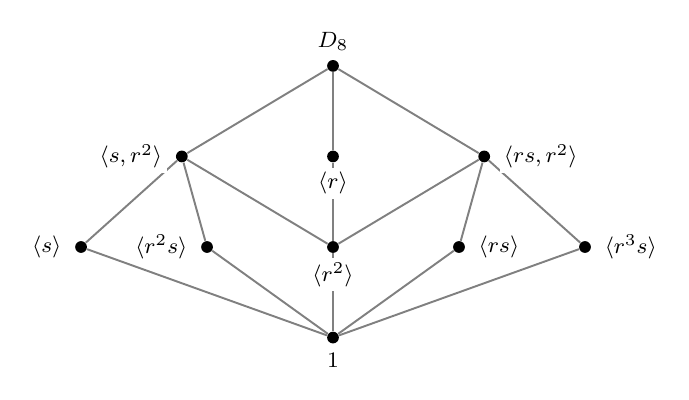
\begin{tikzpicture}[yscale=1.15,xscale=1.6]
  \node[ltdot] (bot) at (0,0) {};
  \node[ltdot] (s) at (-2,1) {};
  \node[ltdot] (r2s) at (-1,1) {};
  \node[ltdot] (r2) at (0,1) {};
  \node[ltdot] (rs) at (1,1) {};
  \node[ltdot] (r3s) at (2,1) {};
  \node[ltdot] (D1) at (-1.2,2) {};
  \node[ltdot] (R) at (0,2) {};
  \node[ltdot] (D2) at (1.2,2) {};
  \node[ltdot] (top) at (0,3) {};
  \begin{scope}[ltedge]
    \draw (bot)--(s);
    \draw (bot)--(r2s);
    \draw (bot)--(r2);
    \draw (bot)--(rs);
    \draw (bot)--(r3s);
    \draw (s)--(D1);
    \draw (r2s)--(D1);
    \draw (r2)--(D1);
    \draw (r2)--(R);
    \draw (r2)--(D2);
    \draw (rs)--(D2);
    \draw (r3s)--(D2);
    \draw (D1)--(top);
    \draw (R)--(top);
    \draw (D2)--(top);
  \end{scope}
  \node[ltlab,below=1.5pt of bot] {$1$};
  \node[ltlab,left=3pt of s] {$\langle s\rangle$};
  \node[ltlab,left=3pt of r2s] {$\langle r^2 s\rangle$};
  \node[ltlab,below=1.5pt of r2] {$\langle r^2\rangle$};
  \node[ltlab,right=3pt of rs] {$\langle rs\rangle$};
  \node[ltlab,right=3pt of r3s] {$\langle r^3 s\rangle$};
  \node[ltlab,left=3pt of D1] {$\langle s,r^2\rangle$};
  \node[ltlab,below=1.5pt of R] {$\langle r\rangle$};
  \node[ltlab,right=3pt of D2] {$\langle rs,r^2\rangle$};
  \node[ltlab,above=1.5pt of top] {$D_8$};
\end{tikzpicture}\end{center}

The five order-$2$ subgroups $\gen{s},\gen{r^2s},\gen{r^2},\gen{rs},\gen{r^3s}$ sit just above $1$; the three order-$4$ subgroups (two copies of $V_4$ and the cyclic $\gen{r}$) sit just below $D_8$. Notice $\{1,s,sr\}$ from the non-example appears \emph{nowhere}: it is not a node because it is not closed, vividly confirming that ``contains $1$'' is far from sufficient.

\subsection*{The Subgroup Criterion}

Checking the four group axioms (closure, associativity, identity, inverses) by hand is tedious. The Subgroup Criterion collapses everything into a single test, because associativity is inherited free from $G$ and the identity is forced by the single condition once $H$ is nonempty.

\begin{proposition}\label{p:subcrit@c2}
Let $G$ be a group and $H\subseteq G$. Then $H\sgr G$ if and only if
\[
\text{(a)}\quad H\neq\es,\qquad\text{and}\qquad\text{(b)}\quad \forall\,x,y\in H,\ \ xy\inv\in H.
\]
\end{proposition}

\begin{proof}
($\imp$) If $H\sgr G$ then $H$ contains the identity, so $H\neq\es$, giving (a). For $x,y\in H$, subgroup closure under inverses gives $y\inv\in H$, and closure under the product gives $xy\inv\in H$, giving (b).

($\Leftarrow$, that is the substantive direction) Assume (a) and (b). By (a) pick some $a\in H$. Apply (b) with $x=y=a$: then $aa\inv=1\in H$, so $H$ contains the identity. Next, for any $a\in H$, apply (b) with $x=1$ and $y=a$: $1\cdot a\inv=a\inv\in H$, so $H$ is closed under inverses. Finally, for $a,b\in H$ we have just shown $b\inv\in H$; apply (b) with $x=a$, $y=b\inv$ to get $a(b\inv)\inv=ab\in H$, so $H$ is closed under the product. Associativity holds in $H$ because it holds in $G$ and $H\subseteq G$. Thus $H$ is a group under the operation of $G$, i.e. $H\sgr G$.
\end{proof}

\begin{remark}
The single condition (b) is doing triple duty: $x=y$ forces $1\in H$; $x=1$ forces inverses; and then $x,\,y\inv$ forces products. This is why it is called the \emph{one-step} subgroup test.
\end{remark}

\begin{method}{One-step criterion vs. the full definition}
\textbf{Recognition trigger:} you are handed a \emph{subset} $H$ of a known group $G$ and asked ``is $H$ a subgroup?'' Do NOT re-verify associativity --- it is inherited. Instead:
\begin{enumerate}
\item \textbf{Nonempty.} Exhibit one explicit element of $H$ (usually check $1\in H$; that already settles (a)).
\item \textbf{One-step closure.} Take \emph{arbitrary} $x,y\in H$, write the defining property each satisfies, and compute $xy\inv$. Show $xy\inv$ satisfies the same defining property.
\item Conclude $H\sgr G$ by Proposition~\ref{p:subcrit@c2}.
\end{enumerate}
\textbf{When to use which:} use the one-step criterion whenever $H$ is described by a \emph{closed-form condition} (a determinant value, a modulus, a divisibility, a matrix shape). Use the raw two-step version (check products and inverses separately) only when computing $xy\inv$ in one shot is awkward and splitting is clearer. Never bother re-proving associativity.
\end{method}

\begin{pitfall}
The criterion is $xy\inv\in H$, not $xy\in H$. A subset closed under products only (e.g.\ $\Z_{\ge 0}\subseteq\Z$) need not be a subgroup. Closure under products alone suffices ONLY in the finite case (Proposition~\ref{p:finsubcrit@c2} below).
\end{pitfall}

\begin{wex}{$n\Z\sgr\Z$}
Show that $n\Z=\{nk\st k\in\Z\}$ is a subgroup of $(\Z,+)$ for every integer $n\ge 0$.
\wrec $n\Z$ is a subset of the group $\Z$ defined by a closed-form condition (``is a multiple of $n$''), so the one-step criterion applies. The operation is $+$, so ``$xy\inv$'' here means $x-y$.
\wsol \textbf{(a) Nonempty:} $0=n\cdot 0\in n\Z$. \textbf{(b) One-step:} take $x,y\in n\Z$, say $x=na$ and $y=nb$ with $a,b\in\Z$. Then
\[
x-y=na-nb=n(a-b),
\]
and $a-b\in\Z$, so $x-y\in n\Z$. By Proposition~\ref{p:subcrit@c2}, $n\Z\sgr\Z$.\\
\emph{Check:} with $n=3$, $x=6$, $y=15$: $x-y=-9=3\cdot(-3)\in 3\Z$. Correct.
\end{wex}

\begin{wex}{$\{A\in\GL_n(\R)\st \det A=\pm1\}$}
Let $H=\{A\in\GL_n(\R)\st \det A\in\{1,-1\}\}$. Show $H\sgr\GL_n(\R)$.
\wrec $H$ is a subset of the group $\GL_n(\R)$ cut out by the condition $\det A=\pm1$. The trigger is the closed-form determinant condition; use the one-step test with the multiplicativity $\det(AB)=\det A\det B$ and $\det(A\inv)=(\det A)\inv$.
\wsol \textbf{(a) Nonempty:} $\det I=1$, so $I\in H$. \textbf{(b) One-step:} take $A,B\in H$, so $\det A=\pm1$ and $\det B=\pm1$. Then $B$ is invertible (determinant nonzero) and
\[
\det(AB\inv)=\det A\cdot\det(B\inv)=\det A\cdot(\det B)\inv=(\pm1)\cdot(\pm1)\inv=\pm1,
\]
since $(\pm1)\inv=\pm1$ in $\R$. Hence $AB\inv\in H$, and by Proposition~\ref{p:subcrit@c2}, $H\sgr\GL_n(\R)$.\\
\emph{Check:} $A=\diag(1,-1)$ has $\det=-1$, $B=\diag(-1,1)$ has $\det=-1$; $B\inv=B$, $AB\inv=\diag(-1,-1)$ with $\det=1\in\{\pm1\}$. Correct. (Note $H$ properly contains $\SL_n(\R)$, the determinant-$1$ subgroup.)
\end{wex}

\begin{wex}{The unit circle $\{z\in\C^\times\st |z|=1\}$}
Let $S=\{z\in\C^\times\st |z|=1\}$. Show $S\sgr\C^\times$, the multiplicative group of nonzero complex numbers.
\wrec Subset of the group $(\C^\times,\cdot)$ defined by the closed-form modulus condition $|z|=1$. One-step test; use $|zw|=|z|\,|w|$ and $|z\inv|=|z|\inv$. Here ``$xy\inv$'' is $z w\inv=z/w$.
\wsol \textbf{(a) Nonempty:} $|1|=1$, so $1\in S$. \textbf{(b) One-step:} take $z,w\in S$, so $|z|=|w|=1$ and $w\neq 0$. Then
\[
\left|z w\inv\right|=|z|\cdot|w\inv|=|z|\cdot|w|\inv=1\cdot 1\inv=1,
\]
so $zw\inv\in S$. By Proposition~\ref{p:subcrit@c2}, $S\sgr\C^\times$.\\
\emph{Check:} $z=i$, $w=\tfrac{1+i}{\sqrt2}$ both have modulus $1$; $zw\inv=i\cdot\tfrac{1-i}{\sqrt2}=\tfrac{i+1}{\sqrt2}$, with modulus $\tfrac{\sqrt2}{\sqrt2}=1$. Correct.
\end{wex}

\begin{wex}{Unipotent upper-triangular matrices}
Let $U=\left\{\begin{pmatrix}1&a\\0&1\end{pmatrix}\st a\in\R\right\}\subseteq\GL_2(\R)$ (upper triangular, $1$'s on the diagonal). Show $U\sgr\GL_2(\R)$.
\wrec Subset of $\GL_2(\R)$ defined by a matrix \emph{shape} condition. One-step test; the trick is to compute the inverse of such a matrix explicitly, then multiply.
\wsol Write $M(a)=\begin{pmatrix}1&a\\0&1\end{pmatrix}$. \textbf{(a) Nonempty:} $M(0)=I\in U$. \textbf{(b) One-step:} take $M(a),M(b)\in U$. First, $\det M(b)=1\neq 0$ so it is invertible, and
\[
M(b)\inv=\begin{pmatrix}1&-b\\0&1\end{pmatrix}=M(-b).
\]
Then
\[
M(a)M(b)\inv=\begin{pmatrix}1&a\\0&1\end{pmatrix}\begin{pmatrix}1&-b\\0&1\end{pmatrix}=\begin{pmatrix}1&a-b\\0&1\end{pmatrix}=M(a-b)\in U.
\]
By Proposition~\ref{p:subcrit@c2}, $U\sgr\GL_2(\R)$.\\
\emph{Check:} $a=5$, $b=2$: $M(5)M(2)\inv=M(3)$, which has $1$'s on the diagonal and lies in $U$. Indeed $a\mapsto M(a)$ is a bijection $\R\to U$ with $M(a)M(b)=M(a+b)$, so $U$ is just $(\R,+)$ in disguise. Correct.
\end{wex}

\begin{wex}{A non-example: $xy\inv\notin H$}
In $G=(\Z,+)$, let $H=\{n\in\Z\st n\ge 0\}=\Z_{\ge0}$ (the nonnegative integers). Decide whether $H\sgr\Z$.
\wrec This is a \emph{disproof} task. $H$ is nonempty and closed under the product ($+$), which tempts one into thinking it is a subgroup --- but the criterion demands $xy\inv\in H$, i.e.\ $x-y\in H$. To refute (b), exhibit a single pair $x,y\in H$ with $x-y\notin H$.
\wsol \textbf{(a)} $0\in H$, so nonempty: fine. \textbf{(b) fails:} take $x=1\in H$, $y=2\in H$. Then
\[
xy\inv=x-y=1-2=-1\notin H,
\]
since $-1<0$. So condition (b) of Proposition~\ref{p:subcrit@c2} fails for the explicit pair $(1,2)$. Therefore $H\not\sgr\Z$.\\
\emph{Check:} the underlying reason is that $H$ contains no inverses: $1\in H$ but $-1\notin H$. This is exactly the pitfall above --- closure under products is not enough for an infinite set.
\end{wex}

\subsection*{The Finite Subgroup Criterion}

When $H$ is \emph{finite}, even less is required: closure under the product alone forces inverses to appear automatically, because the powers $x,x^2,x^3,\dots$ cannot all be distinct.

\begin{proposition}\label{p:finsubcrit@c2}
Let $G$ be a group and let $H$ be a \emph{finite} nonempty subset of $G$ that is closed under the operation of $G$ (i.e.\ $xy\in H$ for all $x,y\in H$). Then $H\sgr G$.
\end{proposition}

\begin{proof}
By Proposition~\ref{p:subcrit@c2} it suffices to show that for each $x\in H$ we have $x\inv\in H$ (closure under products then gives $xy\inv\in H$). Fix $x\in H$. By closure, all positive powers $x,x^2,x^3,\dots$ lie in $H$. Since $H$ is finite, these cannot all be distinct, so there exist integers $i<j$ with $x^i=x^j$. Cancelling in $G$ gives $x^{\,j-i}=1$ with $n:=j-i\ge 1$, so $1=x^n\in H$. If $n=1$ then $x=1$ and $x\inv=1=x\in H$. If $n\ge 2$ then
\[
x\cdot x^{\,n-1}=x^n=1\quad\imp\quad x\inv=x^{\,n-1},
\]
and $x^{\,n-1}\in H$ because $n-1\ge1$ is a positive power. Either way $x\inv\in H$, completing the proof.
\end{proof}

\begin{remark}
Finiteness is essential: $\Z_{\ge0}\subseteq\Z$ from the last worked example is nonempty and closed under $+$, but is not a subgroup --- it is infinite, so the powers $x,2x,3x,\dots$ never repeat and inverses never get forced.
\end{remark}

\begin{method}{When the finite criterion saves work}
\textbf{Recognition trigger:} $H$ is a \emph{finite} subset of $G$ (e.g.\ an explicitly listed finite set, or any subset of a finite group) and you want to prove $H\sgr G$. Then:
\begin{enumerate}
\item Confirm $H$ is nonempty and finite.
\item Check closure under the product ONLY: verify $xy\in H$ for all $x,y\in H$ (for a small explicit set, fill in the multiplication table; for a structured set, give a closure argument).
\item Invoke Proposition~\ref{p:finsubcrit@c2}; inverses and the identity come for free.
\end{enumerate}
Use this whenever checking $x\inv\in H$ separately would be extra labor --- the finite criterion lets you skip the inverse check entirely.
\end{method}

\begin{wex}{$\{1,r,r^2,r^3\}=\gen{r}\sgr D_8$ via the finite criterion}
In $D_8=\gen{r,s\st r^4=s^2=1,\ srs=r\inv}$, let $H=\{1,r,r^2,r^3\}$. Show $H\sgr D_8$.
\wrec $H$ is a finite ($4$-element) subset of the finite group $D_8$. The finite criterion (Proposition~\ref{p:finsubcrit@c2}) applies: just check closure under the product; do not bother with inverses.
\wsol \textbf{Nonempty and finite:} $|H|=4$. \textbf{Closure:} every element of $H$ is a power $r^i$ with $0\le i\le 3$, and $r^i r^j=r^{i+j}=r^{(i+j)\bmod 4}$ since $r^4=1$. The exponent $(i+j)\bmod4\in\{0,1,2,3\}$, so $r^i r^j\in H$ always. Concretely:
\[
\begin{array}{c|cccc}
\cdot & 1 & r & r^2 & r^3\\\hline
1 & 1 & r & r^2 & r^3\\
r & r & r^2 & r^3 & 1\\
r^2 & r^2 & r^3 & 1 & r\\
r^3 & r^3 & 1 & r & r^2
\end{array}
\]
Every entry lies in $H$, so $H$ is closed under the product. By Proposition~\ref{p:finsubcrit@c2}, $H\sgr D_8$. (Indeed $H=\gen{r}$, the cyclic rotation subgroup of order $4$.)\\
\emph{Check:} inverses appear automatically, as promised: $r\inv=r^3$, $(r^2)\inv=r^2$, $(r^3)\inv=r$, all in $H$. Correct.
\end{wex}

\begin{center}\begin{tikzpicture}[yscale=1.05,xscale=1.4]
  \node[ltdot] (bot) at (0,0) {};
  \node[ltdot] (a) at (0,1) {};
  \node[ltdot] (b) at (0,2) {};
  \node[ltdot] (top) at (0,3) {};
  \begin{scope}[ltedge]
    \draw (bot)--(a)--(b)--(top);
  \end{scope}
  \node[ltlab,below=1.5pt of bot] {$1$};
  \node[ltlab,right=3pt of a] {$\langle r^2\rangle$};
  \node[ltlab,right=3pt of b] {$\langle r\rangle=\{1,r,r^2,r^3\}$};
  \node[ltlab,above=1.5pt of top] {$D_8$};
\end{tikzpicture}\end{center}

\begin{wex}{$\gen{i}=\{1,i,-1,-i\}\sgr Q_8$}
In $Q_8=\{\pm1,\pm i,\pm j,\pm k\}$ with $i^2=j^2=k^2=-1$ and $ij=k$, let $H=\{1,i,-1,-i\}$. Show $H\sgr Q_8$.
\wrec $H$ is a finite $4$-element subset of the finite group $Q_8$. Finite criterion: check closure under multiplication only.
\wsol \textbf{Nonempty, finite:} $|H|=4$. \textbf{Closure:} the elements are the powers of $i$: $i^0=1,\ i^1=i,\ i^2=-1,\ i^3=-i,\ i^4=1$, so $H=\{i^0,i^1,i^2,i^3\}$ and $i^a i^b=i^{(a+b)\bmod 4}\in H$. The table:
\[
\begin{array}{c|cccc}
\cdot & 1 & i & -1 & -i\\\hline
1 & 1 & i & -1 & -i\\
i & i & -1 & -i & 1\\
-1 & -1 & -i & 1 & i\\
-i & -i & 1 & i & -1
\end{array}
\]
All entries lie in $H$, so $H$ is closed. By Proposition~\ref{p:finsubcrit@c2}, $H\sgr Q_8$.\\
\emph{Check:} $i\inv=-i=i^3\in H$ and $(-1)\inv=-1\in H$, confirming inverses came for free. Correct.
\end{wex}

\begin{wex}{$V_4=\{1,r^2,s,sr^2\}\sgr D_8$}
In $D_8$ let $H=\{1,\,r^2,\,s,\,sr^2\}$. Show $H\sgr D_8$.
\wrec Finite $4$-element subset of finite $D_8$; check product-closure only. Here we must use the relation $sr=r\inv s=r^3 s$ to move $s$ past $r$, and $r^4=1$, $s^2=1$.
\wsol \textbf{Nonempty, finite:} $|H|=4$. \textbf{Closure:} note $r^2$ commutes with $s$, since $sr^2=(sr)r=r^3 s r=r^3 r^3 s=r^6 s=r^2 s$ (using $sr=r^3s$ twice and $r^6=r^2$). So $sr^2=r^2 s$, and each element squares as $1^2=1$, $(r^2)^2=r^4=1$, $s^2=1$, $(sr^2)^2=sr^2sr^2=s(r^2 s)r^2=s(sr^2)r^2=s^2 r^4=1$. The products:
\[
\begin{array}{c|cccc}
\cdot & 1 & r^2 & s & sr^2\\\hline
1 & 1 & r^2 & s & sr^2\\
r^2 & r^2 & 1 & sr^2 & s\\
s & s & sr^2 & 1 & r^2\\
sr^2 & sr^2 & s & r^2 & 1
\end{array}
\]
For instance $r^2\cdot s=r^2 s=sr^2\in H$, and $s\cdot sr^2=s^2 r^2=r^2\in H$, and $sr^2\cdot s=s r^2 s=s\,s r^2=r^2$ (using $r^2 s=sr^2$). Every entry is in $H$, so $H$ is closed. By Proposition~\ref{p:finsubcrit@c2}, $H\sgr D_8$. (This is a Klein four-group $V_4$ inside $D_8$.)\\
\emph{Check:} the table is symmetric with $1$ on the diagonal, so each element is its own inverse, all inside $H$. Correct.
\end{wex}

\begin{wex}{Finite criterion needs finiteness: where the power argument stalls}
Take $G=(\Q^\times,\cdot)$ and $H=\{2^k\st k\in\Z_{\ge0}\}=\{1,2,4,8,\dots\}$. Is $H$ closed under multiplication? Does the finite criterion apply? Decide whether $H\sgr\Q^\times$.
\wrec This probes the \emph{hypothesis} of Proposition~\ref{p:finsubcrit@c2}: $H$ is closed under products but \emph{infinite}, so the finite criterion does not apply --- and we expect inverses to be missing. Fall back to the one-step criterion to disprove.
\wsol \textbf{Closure under product:} $2^a\cdot 2^b=2^{a+b}\in H$ for $a,b\ge0$, so yes, $H$ is closed under multiplication. But $H$ is infinite, so Proposition~\ref{p:finsubcrit@c2} gives no conclusion. \textbf{One-step test fails:} take $x=1\in H$ and $y=2\in H$; then
\[
xy\inv=1\cdot 2\inv=\tfrac12\notin H,
\]
since $\tfrac12=2^{-1}$ has a negative exponent and $H$ contains only nonnegative powers. So condition (b) of Proposition~\ref{p:subcrit@c2} fails, and $H\not\sgr\Q^\times$.\\
\emph{Check:} tracing the proof of Proposition~\ref{p:finsubcrit@c2}, the powers $2,2^2,2^3,\dots$ are all distinct (no repeat $x^i=x^j$), so the argument that forces $x\inv$ never triggers --- exactly because $H$ is infinite. Correct, and it shows the finiteness hypothesis cannot be dropped.
\end{wex}

\begin{pitfall}
Do not apply the finite criterion to a finite \emph{subset of an infinite group} without first checking closure carefully, and never apply it to an infinite set. The set $\{1,2,4,\dots\}$ above is closed under products yet is not a subgroup --- its infiniteness is the whole reason.
\end{pitfall}


%% ===== Dummit & Foote book-level content (merged in) =====
\subsection*{Further subgroup examples: chains, exponent sets, and unions}

The subgroup relation is \emph{transitive}: if $K\sgr H$ and $H\sgr G$ then $K\sgr G$, since the one-step condition $xy\inv\in K$ for $x,y\in K$ holds inside $H$ and the products are computed with the operation of $G$ throughout. Dummit \& Foote open the section with the basic chains this produces.

\begin{wex}{The chains $\Z\sgr\Q\sgr\R\sgr\C$ and $\Q^\times\sgr\R^\times\sgr\C^\times$}
Show that under addition $\Z\sgr\Q\sgr\R\sgr\C$, and that under multiplication $\Q^\times\sgr\R^\times\sgr\C^\times$ (nonzero elements).
\wrec Each link is a subset of a known group closed under the operation, so run the one-step criterion (Proposition~\ref{p:subcrit@c2}) on each inclusion; transitivity then chains them. Additively ``$xy\inv$'' means $x-y$; multiplicatively it means $x/y$.
\wsol \emph{Additive chain.} For $\Z\sgr\Q$: $0\in\Z$, and for $x,y\in\Z$, $x-y\in\Z$. For $\Q\sgr\R$: $0\in\Q$, and a difference of rationals is rational. For $\R\sgr\C$: $0\in\R$, and a difference of reals is real. By Proposition~\ref{p:subcrit@c2} each is a subgroup, and by transitivity $\Z\sgr\C$ as well. \emph{Multiplicative chain.} For $\Q^\times\sgr\R^\times$: $1\in\Q^\times$, and for nonzero rationals $x,y$ the quotient $x/y$ is a nonzero rational. For $\R^\times\sgr\C^\times$: $1\in\R^\times$, and a quotient of nonzero reals is a nonzero real. So $\Q^\times\sgr\R^\times\sgr\C^\times$, hence $\Q^\times\sgr\C^\times$. \emph{Check:} the additive and multiplicative chains are genuinely different containments --- e.g.\ $\tfrac12\in\Q$ but $\tfrac12\notin\Z$, while $\tfrac12\in\Q^\times$; and $0\in\C$ lies in every additive stage but in \emph{no} multiplicative stage, since $\C^\times=\C\setminus\{0\}$.
\end{wex}

D\&F also single out, for an \emph{abelian} group, the elements killed by a fixed exponent --- a sharper companion to the torsion subgroup treated above. (The torsion subgroup collected the $x$ with $x^m=1$ for \emph{some} $m$; here the exponent $n$ is fixed.)

\begin{wex}{$H_n=\{x\st x^n=1\}$ in an abelian group}
Let $G$ be abelian and fix an integer $n\ge1$. Let $H_n=\{x\in G\st x^n=1\}$. Show $H_n\sgr G$.
\wrec A subset of $G$ cut out by the closed-form condition $x^n=1$; use the one-step criterion (Proposition~\ref{p:subcrit@c2}), expanding $(xy\inv)^n$ with commutativity.
\wsol \textbf{(a) Nonempty:} $1^n=1$, so $1\in H_n$. \textbf{(b) One-step:} take $x,y\in H_n$, so $x^n=1$ and $y^n=1$. Since $G$ is abelian, $x$ and $y\inv$ commute, so
\[
(xy\inv)^n=x^n(y\inv)^n=x^n(y^n)\inv=1\cdot1\inv=1,
\]
hence $xy\inv\in H_n$. By Proposition~\ref{p:subcrit@c2}, $H_n\sgr G$. \emph{Check:} in $G=\Zns{15}$ (abelian, order $8$) with $n=2$,
\[
H_2=\{x\st x^2\equiv1\ (\mathrm{mod}\ 15)\}=\{1,4,11,14\},
\]
since $4^2=16\equiv1$, $11^2=121\equiv1$, $14^2=196\equiv1$, while $2,7,8,13$ all square to $4$. And it is closed: $4\cdot11=44\equiv14\in H_2$, $4\cdot4=16\equiv1\in H_2$, as predicted. (Commutativity is essential: in a nonabelian group $\{x\st x^n=1\}$ can fail to be a subgroup, exactly as the torsion set did.)
\end{wex}

A \emph{union} of subgroups, by contrast, is almost never a subgroup.

\begin{remark}\label{r:union-not-subgroup-mrg@c2}
If $H,K\sgr G$ then $H\cup K\sgr G$ if and only if $H\subseteq K$ or $K\subseteq H$. Indeed, if neither contains the other, pick $h\in H\setminus K$ and $k\in K\setminus H$; the product $hk$ cannot lie in $H$ (else $k=h\inv(hk)\in H$) nor in $K$ (else $h=(hk)k\inv\in K$), so $hk\notin H\cup K$ and closure fails. The \emph{intersection} $H\cap K$ is, by contrast, always a subgroup, by a single one-step check valid in both $H$ and $K$ at once.
\end{remark}

\begin{wex}{A union of two subgroups that fails closure}
In the Klein four-group $V_4=\{1,a,b,ab\}$ (every nonidentity element of order $2$, $ab=ba$), let $H=\{1,a\}$ and $K=\{1,b\}$. Show $H,K\sgr V_4$ but $H\cup K\not\sgr V_4$.
\wrec Each of $H,K$ is finite and closed under products, hence a subgroup (Proposition~\ref{p:finsubcrit@c2}); the union illustrates Remark~\ref{r:union-not-subgroup-mrg@c2} since neither contains the other. To disprove, exhibit a product of an $H$-element and a $K$-element that escapes the union.
\wsol $H=\{1,a\}=\gen{a}$ and $K=\{1,b\}=\gen{b}$ are subgroups (each is $\{1,x\}$ with $x^2=1$, closed under products). Now $H\cup K=\{1,a,b\}$. Take $a\in H\cup K$ and $b\in H\cup K$: their product is $ab$, and $ab\notin\{1,a,b\}$ (it is the fourth, distinct element of $V_4$). So $H\cup K$ is not closed under products, hence $H\cup K\not\sgr V_4$. \emph{Check:} neither $H\subseteq K$ nor $K\subseteq H$ holds, exactly the situation Remark~\ref{r:union-not-subgroup-mrg@c2} predicts will fail; and $|H\cup K|=3$ does not divide $|V_4|=4$, a second confirmation via Lagrange (Chapter~3).
\end{wex}

\subsection*{Further worked examples}

\smallskip\noindent\textit{More on the Subgroup Criterion} (Proposition~\ref{p:subcrit@c2}).

\begin{wex}{the diagonal $\Delta\sgr G\times G$}
Show $\Delta=\{(g,g)\st g\in G\}$ is a subgroup of $G\times G$.
\wrec A described subset of the known group $G\times G$; apply the one-step criterion.
Membership means ``both coordinates equal.''
\wsol Nonempty: $(1,1)\in\Delta$. For $(g,g),(h,h)\in\Delta$,
\[ (g,g)(h,h)\inv=(g,g)(h\inv,h\inv)=(gh\inv,\,gh\inv)\in\Delta, \]
since the two coordinates agree. By the criterion $\Delta\sgr G\times G$. \emph{Check:}
$g\mapsto(g,g)$ shows $\ord{\Delta}=\ord{G}$.
\end{wex}

\begin{wex}{upper-triangular invertible matrices}
Show $B=\left\{\left(\begin{smallmatrix}a&b\\0&d\end{smallmatrix}\right)\st ad\neq0\right\}
\sgr\GL_2(\R)$.
\wrec A subset of $\GL_2(\R)$ cut out by ``lower-left entry $=0$.'' One-step criterion,
using that triangular$\,\times\,$triangular is triangular and the inverse of a
triangular matrix is triangular.
\wsol Nonempty: $I\in B$. Product:
$\left(\begin{smallmatrix}a&b\\0&d\end{smallmatrix}\right)
\left(\begin{smallmatrix}a'&b'\\0&d'\end{smallmatrix}\right)
=\left(\begin{smallmatrix}aa'&ab'+bd'\\0&dd'\end{smallmatrix}\right)\in B$ (and
$aa',dd'\neq0$). Inverse:
$\left(\begin{smallmatrix}a&b\\0&d\end{smallmatrix}\right)\inv
=\left(\begin{smallmatrix}1/a&-b/(ad)\\0&1/d\end{smallmatrix}\right)\in B$. Hence
$B\sgr\GL_2(\R)$.
\end{wex}

\smallskip\noindent\textit{More on the finite criterion} (Proposition~\ref{p:finsubcrit@c2}).

\begin{wex}{$\{\overline0,\overline3,\overline6,\overline9\}\sgr\Zn{12}$}
Show $H=\{\overline0,\overline3,\overline6,\overline9\}$ is a subgroup of $\Zn{12}$.
\wrec $H$ is \emph{finite} and nonempty inside the finite group $\Zn{12}$, so the finite
criterion applies: only closure under $+$ must be checked.
\wsol Sums of multiples of $3$ are multiples of $3$ mod $12$: e.g.\
$\overline3+\overline9=\overline{12}=\overline0$ and
$\overline6+\overline9=\overline{15}=\overline3$. So $H$ is closed under $+$; being finite
and nonempty, $H\sgr\Zn{12}$. \emph{Check:} $H=\gen{\overline3}$, the order-$4$ subgroup.
\end{wex}

\subsection*{Maps and commutative diagrams}

Three structural facts of this section are cleanest when drawn as diagrams of
homomorphisms and inclusions.

\smallskip\noindent\textbf{(a) Transitivity of $\sgr$ is composition of inclusions.}
If $K\sgr H$ and $H\sgr G$ then $K\sgr G$, because the inclusion $K\hookrightarrow G$ is
the composite of $K\hookrightarrow H$ and $H\hookrightarrow G$.
\[\begin{tikzcd}[column sep=large]
K \arrow[r, hook] & H \arrow[r, hook] & G
\end{tikzcd}\]
\begin{dgx}
\dgi{Objects:} Three groups: $K$ (a subgroup of $H$), $H$ (a subgroup of $G$), and $G$ (the ambient group). Each is a group under the same operation.
\dgi{Arrows:} The left arrow $K\hookrightarrow H$ is the inclusion map $\iota_1: k\mapsto k$, viewing $k$ as an element of $H$. The right arrow $H\hookrightarrow G$ is the inclusion $\iota_2: h\mapsto h$, viewing $h$ as an element of $G$. Both are injective group homomorphisms (inclusions); the composite $\iota_2\circ\iota_1: K\hookrightarrow G$ sends $k\mapsto k$ directly, establishing $K\sgr G$.
\dgi{What commutes:} There is a single directed path from $K$ to $G$: the composite $\iota_2\circ\iota_1$. The diagram records that this composite is itself an inclusion, i.e.\ $\iota_2\circ\iota_1 = \iota_{K\hookrightarrow G}$, the direct inclusion of $K$ into $G$.
\dgi{Why it commutes:} Take any $k\in K$. Along the unique path: first $k\mapsto k\in H$, then $k\mapsto k\in G$. The composite sends $k\mapsto k\in G$, which is exactly the direct inclusion. The agreement is trivial because all three maps are identity-on-elements inclusions; composing two identity-on-elements maps is still identity-on-elements.
\dgi{Why this matters here:} This diagram records the proof of transitivity of $\sgr$: to show $K\sgr G$ it suffices to exhibit the factoring $K\hookrightarrow H\hookrightarrow G$, because a composite of injective group homomorphisms is an injective group homomorphism. The author places it here to make the transitivity argument visual and to signal that inclusion is a genuine category-theoretic morphism, not just a set-containment symbol.
\dgi{Concrete example:} Take $K=4\Z\sgr H=2\Z\sgr G=\Z$ (all under addition). The chain $4\Z\hookrightarrow2\Z\hookrightarrow\Z$ gives $4\Z\sgr\Z$ by transitivity: $8-4=4\in4\Z$, so $4\Z$ passes the one-step test directly in $\Z$.
\dgi{Common pitfall:} Students sometimes read the two arrows as saying $K$ must be \emph{normal} in $G$, or that some quotient exists. The arrows here are plain inclusions (hooked arrows $\hookrightarrow$), not quotient or surjection arrows; they record only that elements of $K$ sit inside $H$ sit inside $G$, with no normality claimed.
\dgi{Takeaway:} The point of this diagram is that transitivity of the subgroup relation is just composition of inclusion homomorphisms, turning a textual argument into a one-glance arrow-chase.
\end{dgx}

\smallskip\noindent\textbf{(b) The intersection of subgroups is a pullback.} For
$H,K\sgr G$ the subgroup $H\cap K$ is the largest one mapping into both $H$ and $K$
compatibly with their inclusions into $G$. This ``universal corner'' is precisely why
$H\cap K\sgr G$ (Exercise: intersections of subgroups are subgroups).
\[\begin{tikzcd}[row sep=large,column sep=large]
H\cap K \arrow[r, hook] \arrow[d, hook] & H \arrow[d, hook] \\
K \arrow[r, hook] & G
\end{tikzcd}\]
\begin{dgx}
\dgi{Objects:} Four groups: the intersection $H\cap K$ (upper-left), the subgroup $H\sgr G$ (upper-right), the subgroup $K\sgr G$ (lower-left), and the ambient group $G$ (lower-right). Each arrow goes by inclusion.
\dgi{Arrows:} Top arrow: $H\cap K\hookrightarrow H$, the inclusion $x\mapsto x$ into $H$. Left arrow: $H\cap K\hookrightarrow K$, the inclusion $x\mapsto x$ into $K$. Right arrow: $H\hookrightarrow G$, viewing $H$ as a subset of $G$. Bottom arrow: $K\hookrightarrow G$, viewing $K$ as a subset of $G$. All four are injective group homomorphisms.
\dgi{What commutes:} Going right then down equals going down then right: $\iota_{H\to G}\circ\iota_{H\cap K\to H} = \iota_{K\to G}\circ\iota_{H\cap K\to K}$. Both composites send any $x\in H\cap K$ to $x\in G$ by definition.
\dgi{Why it commutes:} Let $x\in H\cap K$. Path right-then-down: $x\mapsto x\in H\mapsto x\in G$. Path down-then-right: $x\mapsto x\in K\mapsto x\in G$. Both equal $x\in G$ because all maps are identity-on-elements inclusions; the square commutes trivially.
\dgi{Why this matters here:} The square records the \emph{universal property of the pullback}: $H\cap K$ is the largest subgroup of $G$ that maps (by inclusion) into \emph{both} $H$ and $K$ consistently. Any subgroup $L\sgr G$ with $L\subseteq H$ and $L\subseteq K$ factors uniquely through $H\cap K$. This is the categorical reason $H\cap K$ is automatically a subgroup --- it is the limit (pullback) of the diagram $H\hookrightarrow G\hookleftarrow K$ in the category of groups.
\dgi{Concrete example:} In $G=\Z_{12}$, let $H=\gen{\overline4}=\{\overline0,\overline4,\overline8\}$ and $K=\gen{\overline6}=\{\overline0,\overline6\}$. Then $H\cap K=\{\overline0\}=\gen{\overline0}$, which is the trivial subgroup. The four inclusions commute: any element of $\{\overline0\}$ maps to $\overline0\in G$ along both paths.
\dgi{Common pitfall:} Students sometimes expect this square to prove that the diagram has a unique filler or that $H\cap K$ is \emph{normal}. It does neither: the square only records compatibility of inclusions. Normality requires a separate check; and the universal property says $H\cap K$ is the \emph{largest} common sub-object, not the only one.
\dgi{Takeaway:} The point of this diagram is that the intersection of two subgroups is their categorical pullback in the ambient group, making $H\cap K\sgr G$ a corollary of limit-preservation rather than a separate verification.
\end{dgx}

\smallskip\noindent\textbf{(c) A kernel is automatically a subgroup: $\SL_n=\ker\det$.}
The determinant $\det:\GL_n(F)\to F^\times$ is a homomorphism, and $\SL_n(F)$ is exactly
its kernel. This gives a short exact sequence and is the slickest proof that
$\SL_n(F)\sgr\GL_n(F)$ --- no checklist needed, because kernels of homomorphisms are
always subgroups.
\[\begin{tikzcd}[column sep=normal]
1 \arrow[r] & \SL_n(F) \arrow[r, hook] & \GL_n(F) \arrow[r, "\det"] & F^\times \arrow[r] & 1
\end{tikzcd}\]
\begin{dgx}
\dgi{Objects:} Five nodes: the trivial group $1$ (repeated at both ends), the special linear group $\SL_n(F)=\{A\in\GL_n(F)\st\det A=1\}$ (a normal subgroup), the general linear group $\GL_n(F)$ of invertible $n\times n$ matrices over a field $F$, and the multiplicative group $F^\times=F\setminus\{0\}$ of nonzero field elements.
\dgi{Arrows:} The leftmost arrow $1\to\SL_n(F)$ is the unique map sending the trivial group's element to the identity matrix $I$. The arrow $\SL_n(F)\hookrightarrow\GL_n(F)$ is the inclusion $A\mapsto A$. The arrow $\GL_n(F)\xrightarrow{\det}F^\times$ is the determinant homomorphism $A\mapsto\det A$. The rightmost arrow $F^\times\to 1$ is the unique map to the trivial group.
\dgi{What commutes:} This is a short exact sequence, so exactness holds at each internal node. At $\SL_n(F)$: $\operatorname{im}(1\to\SL_n(F))=\{I\}=\operatorname{ker}(\SL_n(F)\hookrightarrow\GL_n(F))$, i.e.\ the inclusion is injective. At $\GL_n(F)$: $\operatorname{im}(\SL_n(F)\hookrightarrow\GL_n(F))=\SL_n(F)=\operatorname{ker}(\det)$, since $\det A=1\iff A\in\SL_n(F)$. At $F^\times$: $\operatorname{im}(\det)=F^\times$ (det is surjective: any $c\in F^\times$ is achieved by $\operatorname{diag}(c,1,\dots,1)$).
\dgi{Why it commutes:} For the kernel condition at $\GL_n(F)$: if $A\in\SL_n(F)$ then $\det A=1$, so $A\in\operatorname{ker}(\det)$; conversely if $\det A=1$ then $A\in\SL_n(F)$. This is the definition of $\SL_n(F)$. The exactness at $F^\times$ follows because $\operatorname{diag}(c,1,\dots,1)$ has determinant $c$ for any $c\neq0$.
\dgi{Why this matters here:} The diagram gives the shortest proof that $\SL_n(F)\sgr\GL_n(F)$: kernels of homomorphisms are always subgroups (since $\phi(xy\inv)=\phi(x)\phi(y)\inv=1\cdot1\inv=1$ when $\phi(x)=\phi(y)=1$), so no three-clause checklist is needed. The author places it here to show that the determinant constraint ``$\det=1$'' is not just an algebraic coincidence but an instance of a general structural principle about kernels.
\dgi{Concrete example:} Take $n=2$ and $F=\R$. The matrix $A=\begin{psmallmatrix}2&0\\0&1/2\end{psmallmatrix}$ has $\det A=1$, so $A\in\SL_2(\R)$; its image under $\det$ is $1\in\R^\times$. The matrix $B=\begin{psmallmatrix}3&0\\0&1\end{psmallmatrix}$ has $\det B=3\neq1$, so $B\notin\SL_2(\R)$; $\det$ maps $B$ to $3$, which is a nonzero element of $\R^\times$, demonstrating surjectivity.
\dgi{Common pitfall:} Students sometimes think the short exact sequence says $\GL_n(F)\cong\SL_n(F)\times F^\times$ (a direct product splitting). That is false in general, even though this particular sequence always splits: $c\mapsto\operatorname{diag}(c,1,\dots,1)$ is a homomorphism $F^\times\to\GL_n(F)$ that is a section of $\det$, so $\GL_n(F)\cong\SL_n(F)\rtimes F^\times$ is a \emph{semi}direct product. The complement need not be normal and the product need not be direct: e.g.\ $\GL_2(\mathbb{F}_3)\not\cong\SL_2(\mathbb{F}_3)\times\mathbb{F}_3^\times$, since their centers have orders $2$ and $4$. A short exact sequence records a quotient relationship, not a product decomposition.
\dgi{Takeaway:} The point of this diagram is that $\SL_n(F)$ is the kernel of the determinant homomorphism, so its subgroup status is an immediate instance of the general principle that kernels are always subgroups, bypassing any direct verification.
\end{dgx}

\begin{exers}{Exercises (from the text).}
\item Prove each is a subgroup: (a) $\{a+ai\st a\in\R\}\sgr(\C,+)$;
  (b) the unit circle $\{z\in\C\st|z|=1\}\sgr\C^\times$;
  (c) $\{a/b\in\Q\st b\mid n\}\sgr(\Q,+)$ ($n$ fixed);
  (d) $\{a/b\in\Q\st\gcd(b,n)=1\}\sgr(\Q,+)$;
  (e) $\{x\in\R^\times\st x^2\in\Q\}\sgr\R^\times$.
\item Prove each is \emph{not} a subgroup: (a) the $2$-cycles in $S_n$ ($n\ge3$);
  (b) the reflections in $D_{2n}$; (c) $\{x\in G\st\ord{x}=n\}\cup\{1\}$, $n$ composite and $G$ a group containing an element of order $n$;
  (d) the odd integers together with $0$; (e) $\{x\in\R\st x^2\in\Q\}$ in $(\R,+)$.
\item Show $\{1,r^2,s,sr^2\}$ and $\{1,r^2,sr,sr^3\}$ are subgroups of $D_8$.
\item Exhibit a group $G$ and an infinite subset $H$ closed under the operation but not a
  subgroup.
\item Prove a group of order $n>2$ has no subgroup of order $n-1$.
\item $G$ abelian: prove the torsion set $\{g\st\ord{g}<\infty\}\sgr G$; give a
  non-abelian example where this set is not a subgroup.
\item Fix $n>1$. Find the torsion subgroup of $\Z\times\Zn{n}$, and show the elements of infinite
  order together with $1$ do not form a subgroup.
\item For $H,K\sgr G$, prove $H\cup K\sgr G\iff H\subseteq K$ or $K\subseteq H$.
\item Prove $\SL_n(F)=\{A\in\GL_n(F)\st\det A=1\}\sgr\GL_n(F)$.
\item (a) Prove $H\cap K\sgr G$ for $H,K\sgr G$; (b) prove the intersection of any
  nonempty family of subgroups is a subgroup.
\item Prove $\{(a,1)\}$, $\{(1,b)\}$, and (when $B=A$) the diagonal $\{(a,a)\}$ are
  subgroups of $A\times B$.
\item $A$ abelian, $n\in\Z$: prove $A^n=\{a^n\}$ and $A[n]=\{a\st a^n=1\}$ are subgroups.
\item $H\sgr(\Q,+)$ with $1/x\in H$ for all $x\in H\setminus\{0\}$: prove $H=0$ or
  $H=\Q$.
\item Show $\{x\in D_{2n}\st x^2=1\}$ is not a subgroup ($n\ge3$).
\item Prove the union of an ascending chain $H_1\sgr H_2\sgr\cdots$ of subgroups is a
  subgroup.
\item Prove the upper-triangular matrices in $\GL_n(F)$ form a subgroup.
\item Prove the upper-triangular matrices with $1$'s on the diagonal form a subgroup of
  $\GL_n(F)$.
\end{exers}

\begin{exers}{Additional exercises.}
\item Prove the subgroups of $(\Z,+)$ are exactly the $n\Z$ ($n\ge0$), and that
  $n\Z\subseteq m\Z\iff m\mid n$.
\item Prove that a group with exactly two subgroups ($1$ and $G$) is isomorphic to
  $\Zn{p}$ for some prime $p$.
\item Exhibit a group $G$ and subgroups $H,K$ for which $HK$ is \emph{not} a subgroup.
\item Without using the finite criterion, prove: if $H\subseteq G$ is finite, nonempty,
  and closed under products, then $H$ is closed under inverses.
\item For $H\sgr G$, prove $\{g\in G\st gH=Hg\}$ is a subgroup of $G$ containing $H$.
\end{exers}

\begin{exers}{Commutative-diagram exercises.}
\item Show that for $H,K\sgr G$ the square with corners $H\cap K,\,H,\,K,\,G$ (all arrows
  inclusions) commutes, and that $H\cap K$ is universal among subgroups mapping
  compatibly into $H$ and $K$ --- i.e.\ it is the pullback of $H\hookrightarrow G
  \hookleftarrow K$.
\item Let $\varphi:G\to L$ be a homomorphism and $M\sgr L$. Prove the preimage
  $\varphi\inv(M)\sgr G$, and draw the pullback square exhibiting $\varphi\inv(M)$ as
  $G\times_L M$.
\item Prove that the composite of two injective homomorphisms is injective, and interpret
  the transitivity $K\sgr H\sgr G\imp K\sgr G$ as composing the inclusions
  $K\hookrightarrow H\hookrightarrow G$.
\item Show $\ker\varphi\sgr G$ for any homomorphism $\varphi:G\to L$ by exhibiting the
  exact sequence $1\to\ker\varphi\to G\to L$; apply this to $\det:\GL_n(F)\to F^\times$ to
  reprove $\SL_n(F)\sgr\GL_n(F)$ without the checklist.
\end{exers}


\section{Centralizers, Normalizers, Stabilizers, and Kernels}
\subsection*{Centralizers: $C_G(A)$ and $C_G(a)$}

\begin{definition}\label{d:cent@c2}
Let $G$ be a group and $A\subseteq G$ a nonempty subset. The \emph{centralizer of $A$ in $G$} is
\[
C_G(A)=\{g\in G\st gag\inv=a\ \text{for all }a\in A\}
=\{g\in G\st ga=ag\ \text{for all }a\in A\}.
\]
When $A=\{a\}$ is a single element we write $C_G(a)=\{g\in G\st gag\inv=a\}=\{g\in G\st ga=ag\}$. Thus $C_G(a)$ is the set of all elements that commute with $a$, and $C_G(A)$ is the set of elements that commute with \emph{every} element of $A$. The two displayed descriptions agree because $gag\inv=a\eqv ga=ag$ (multiply on the right by $g$).
\end{definition}

\begin{proposition}\label{p:cent-subgroup@c2}
For any nonempty $A\subseteq G$, $C_G(A)\sgr G$.
\end{proposition}

\begin{proof}
We use the subgroup criterion. First $1\in C_G(A)$ since $1a1\inv=a$ for all $a\in A$, so $C_G(A)\neq\es$.

\emph{Closure.} Suppose $x,y\in C_G(A)$ and fix $a\in A$. Then $xa=ax$ and $ya=ay$, so
\[
(xy)a=x(ya)=x(ay)=(xa)y=(ax)y=a(xy).
\]
Hence $xy$ commutes with every $a\in A$, i.e.\ $xy\in C_G(A)$.

\emph{Inverses.} Suppose $x\in C_G(A)$ and fix $a\in A$. From $xa=ax$, multiply on the left and right by $x\inv$:
\[
x\inv(xa)x\inv=x\inv(ax)x\inv\imp ax\inv=x\inv a.
\]
So $x\inv a=ax\inv$ for all $a\in A$, i.e.\ $x\inv\in C_G(A)$. By the subgroup criterion $C_G(A)\sgr G$.
\end{proof}

\begin{remark}\label{r:cent-facts@c2}
Two facts make computations fast.
(1) \emph{Intersection formula:} since $g\in C_G(A)$ iff $g$ commutes with each $a\in A$,
\[
C_G(A)=\bigcap_{a\in A}C_G(a).
\]
(2) \emph{Generators suffice:} if $A=\gen{S}$ then $C_G(A)=C_G(S)$, because an element commuting with each generator commutes with every product of generators and their inverses. In particular $C_G(\gen{x})=C_G(x)$.
\end{remark}

\begin{method}{How to compute a centralizer $C_G(a)$ (and $C_G(A)$)}
Use this whenever you must find all elements commuting with a fixed element $a$ (or with a whole subset $A$).
\begin{enumerate}
\item \textbf{Single element $C_G(a)$.} Test each $g\in G$ (or each coset/type of element) by checking $ga=ag$. In a group given by generators and relations (e.g.\ $D_{2n}$ with $sr=r\inv s$, or $Q_8$), push every product to a normal form and compare; do not test brute force if a relation settles it.
\item \textbf{Powers are free.} Every power of $a$ commutes with $a$, so $\gen{a}\subseteq C_G(a)$ automatically. You only need to test elements \emph{outside} $\gen{a}$.
\item \textbf{Use the relation to predict failures.} In $D_{2n}$, $s r^k=r^{-k}s$, so a reflection $s r^j$ commutes with $r^k$ iff $r^k=r^{-k}$, i.e.\ iff $r^{2k}=1$. This tells you instantly which rotations are centralized by reflections.
\item \textbf{Subset $A$: intersect.} Compute $C_G(a)$ for each $a$ in a generating set $S$ of $A$, then take $\bigcap_{a\in S}C_G(a)$ (Remark~\ref{r:cent-facts@c2}).
\item \textbf{Sanity checks.} The answer must be a subgroup (closed, contains $1$, contains inverses), must contain $\gen{a}$, and (by Lagrange) its order must divide $|G|$.
\end{enumerate}
\end{method}

\begin{pitfall}
$C_G(a)$ is the set of elements that commute \emph{with $a$}, not the set of elements that commute with \emph{everything} (that is the center $Z(G)=C_G(G)$). Also $C_G(a)$ need not be abelian, and need not equal $\gen{a}$.
\end{pitfall}

\medskip
Throughout the dihedral examples we use $D_8=\gen{r,s\st r^4=s^2=1,\ sr=r\inv s}$, with the eight elements $\{1,r,r^2,r^3,s,sr,sr^2,sr^3\}$. The master relation, applied $k$ times, gives the normal form
\[
s\,r^k=r^{-k}\,s\qquad(\text{equivalently }r^k s=s\,r^{-k}),
\]
which we will use repeatedly.

\begin{wex}{$C_{D_8}(r)=\gen{r}$}\label{wex:cent-d8-r@c2}
Compute the centralizer of the rotation $r$ in $D_8$.
\wrec This is a single-element centralizer in a group with a relation $sr=r\inv s$. By the method, powers of $r$ are free ($\gen{r}\subseteq C_{D_8}(r)$); the relation predicts that a reflection commutes with $r^k$ iff $r^{2k}=1$, so we only need to test the reflections and apply that test with $k=1$.
\wsol The rotations $\{1,r,r^2,r^3\}=\gen{r}$ all commute with $r$ (powers of the same element commute). Now test a reflection $sr^j$:
\[
(sr^j)\,r=sr^{\,j+1},\qquad r\,(sr^j)=(rs)r^j=(s r^{-1})r^j=s r^{\,j-1},
\]
using $rs=sr^{-1}$. These are equal iff $r^{\,j+1}=r^{\,j-1}$, i.e.\ $r^2=1$. But $\ord{r}=4$, so $r^2\neq1$ and \emph{no} reflection commutes with $r$. Hence
\[
C_{D_8}(r)=\{1,r,r^2,r^3\}=\gen{r}.
\]
\emph{Check:} $\gen{r}$ is a subgroup of order $4$, and $4\mid 8$. It contains $r$. Consistent.
\end{wex}

\begin{wex}{$C_{D_8}(s)=\{1,s,r^2,sr^2\}$}
Compute the centralizer of the reflection $s$ in $D_8$.
\wrec Single-element centralizer again. Now $a=s$ is a reflection; $\gen{s}=\{1,s\}$ is free. We must test each rotation $r^k$ (does $r^k$ commute with $s$?) and each reflection $sr^j$. The relation $r^k s=s r^{-k}$ does the rotation tests in one line.
\wsol \emph{Rotations.} $r^k$ commutes with $s$ iff $r^k s=s r^k$. But $r^k s=s r^{-k}$, so we need $s r^{-k}=s r^{k}$, i.e.\ $r^{2k}=1$. With $\ord{r}=4$ this holds iff $4\mid 2k$, i.e.\ $k$ even: $k=0,2$. So $1$ and $r^2$ commute with $s$, while $r,r^3$ do not.

\emph{Reflections.} Test $sr^j$:
\[
(sr^j)s=s(r^j s)=s(s r^{-j})=s^2 r^{-j}=r^{-j},\qquad
s(sr^j)=s^2 r^j=r^j .
\]
Equal iff $r^{-j}=r^j$, i.e.\ $r^{2j}=1$, i.e.\ $j$ even: $j=0,2$. So $s$ (the $j=0$ case) and $sr^2$ commute with $s$, while $sr,sr^3$ do not. Collecting:
\[
C_{D_8}(s)=\{1,\,s,\,r^2,\,sr^2\}.
\]
\emph{Check:} order $4$, and $4\mid8$. It contains $s$. It is closed: e.g.\ $r^2\cdot s=sr^{-2}=sr^2$ (since $r^{-2}=r^2$) is in the set, and $(sr^2)^2=sr^2sr^2=s(r^2 s)r^2=s(sr^{-2})r^2=s^2r^{-2}r^2=1$. So it is the Klein four-group $\{1,r^2,s,sr^2\}$. Consistent.
\end{wex}

\begin{wex}{$C_{D_8}(r^2)=D_8$}
Compute the centralizer of $r^2$ in $D_8$.
\wrec Single-element centralizer. The key trigger: $r^2$ has order $2$, so $r^{-2}=r^2$. The relation $r^2$-with-reflection test reduces to $r^{2k}=1$ with $k=2$, which is automatically true since $r^4=1$. Expect everything to commute, i.e.\ $r^2\in Z(D_8)$.
\wsol \emph{Rotations} commute with $r^2$ trivially (powers of $r$). \emph{Reflections:} test $sr^j$ against $r^2$:
\[
(sr^j)r^2=sr^{\,j+2},\qquad r^2(sr^j)=(r^2 s)r^j=(s r^{-2})r^j=s r^{\,j-2}.
\]
Since $r^{-2}=r^2$ (as $r^4=1$), we have $sr^{\,j-2}=sr^{\,j+2}$, so the two are equal for \emph{every} $j$. Thus every reflection commutes with $r^2$, and
\[
C_{D_8}(r^2)=D_8.
\]
\emph{Check:} this says $r^2\in Z(D_8)$, which is the known center of $D_8$. Order $8=|D_8|$, divides $|D_8|$. Consistent.
\end{wex}

\begin{wex}{$C_{S_3}\big((1\,2)\big)=\{1,(1\,2)\}$}
Compute the centralizer of the transposition $(1\,2)$ in $S_3$.
\wrec Single-element centralizer in $S_3=\{1,(1\,2),(1\,3),(2\,3),(1\,2\,3),(1\,3\,2)\}$. No slick relation; scan all six elements and test $g\,(1\,2)=(1\,2)\,g$ by composing permutations (apply right factor first).
\wsol $\gen{(1\,2)}=\{1,(1\,2)\}$ is free (both commute with $(1\,2)$). Test the rest.
\[
(1\,3)(1\,2)=(1\,2\,3),\quad (1\,2)(1\,3)=(1\,3\,2)\ \Rightarrow\ \text{unequal, } (1\,3)\notin C.
\]
\[
(2\,3)(1\,2)=(1\,3\,2),\quad (1\,2)(2\,3)=(1\,2\,3)\ \Rightarrow\ \text{unequal, } (2\,3)\notin C.
\]
\[
(1\,2\,3)(1\,2)=(1\,3),\quad (1\,2)(1\,2\,3)=(2\,3)\ \Rightarrow\ \text{unequal, } (1\,2\,3)\notin C.
\]
\[
(1\,3\,2)(1\,2)=(2\,3),\quad (1\,2)(1\,3\,2)=(1\,3)\ \Rightarrow\ \text{unequal, } (1\,3\,2)\notin C.
\]
Hence $C_{S_3}\big((1\,2)\big)=\{1,(1\,2)\}=\gen{(1\,2)}$.
\emph{Check:} order $2$, and $2\mid 6$. As a sample composition verification: $(1\,3)(1\,2)$ computed right-to-left: $(1\,2)$ first sends $1\mapsto2$, then $(1\,3)$ fixes $2$, so $1\mapsto2$; $2\mapsto1\mapsto3$; $3\mapsto3\mapsto1$; that is $(1\,2\,3)$. Consistent.
\end{wex}

\begin{wex}{$C_{Q_8}(i)=\{\pm1,\pm i\}=\gen{i}$}
Compute the centralizer of $i$ in $Q_8=\{\pm1,\pm i,\pm j,\pm k\}$, where $i^2=j^2=k^2=-1$, $ij=k$, $jk=i$, $ki=j$, and $ji=-k$, $kj=-i$, $ik=-j$.
\wrec Single-element centralizer. $\pm1$ are central, and powers of $i$ (namely $1,i,-1,-i$) are free. The quaternion relations $ij=-ji$, $ik=-ki$ are the trigger: distinct ``imaginary'' generators anticommute, so $j,k$ (and their negatives) cannot commute with $i$.
\wsol $\gen{i}=\{1,i,i^2,i^3\}=\{1,i,-1,-i\}$ all commute with $i$. Test $j$ and $k$:
\[
ij=k,\qquad ji=-k\ \Rightarrow\ ij\neq ji,\ \text{so } j\notin C_{Q_8}(i),
\]
\[
ik=-j,\qquad ki=j\ \Rightarrow\ ik\neq ki,\ \text{so } k\notin C_{Q_8}(i).
\]
Since $-j=(-1)j$ and $-1$ is central, $-j$ commutes with $i$ iff $j$ does; likewise $-k$. So $\pm j,\pm k$ are all excluded. Therefore
\[
C_{Q_8}(i)=\{1,-1,i,-i\}=\gen{i}.
\]
\emph{Check:} $\gen{i}$ has order $4$, $4\mid8$, contains $i$, and is cyclic hence abelian (consistent with being a centralizer that contains $i$). Consistent.
\end{wex}

\begin{wex}{$C_{D_8}(\gen{r})=\gen{r}$ via the subset rule}
Compute the centralizer of the \emph{subgroup} $A=\gen{r}=\{1,r,r^2,r^3\}$ in $D_8$.
\wrec This is a subset centralizer. By Remark~\ref{r:cent-facts@c2}(2), $A$ is generated by $S=\{r\}$, so $C_{D_8}(\gen{r})=C_{D_8}(r)$ -- no need to intersect over all four rotations. (If you prefer, $C_{D_8}(A)=\bigcap_{a\in A}C_{D_8}(a)$, and the smallest of these governs.)
\wsol Since $\gen{r}=\gen{S}$ with $S=\{r\}$, an element centralizes all of $\gen{r}$ iff it centralizes the single generator $r$. By the worked computation $C_{D_8}(r)=\gen{r}$ (first example above),
\[
C_{D_8}(\gen{r})=C_{D_8}(r)=\gen{r}=\{1,r,r^2,r^3\}.
\]
\emph{Cross-check by intersection.} Using $C_{D_8}(A)=\bigcap_{a\in A}C_{D_8}(a)$:
\[
C_{D_8}(1)=D_8,\quad C_{D_8}(r)=\gen{r},\quad C_{D_8}(r^2)=D_8,\quad C_{D_8}(r^3)=\gen{r},
\]
(the last because $r^3=r\inv$ generates the same cyclic group, so its centralizer equals that of $r$). The intersection is $D_8\cap\gen{r}\cap D_8\cap\gen{r}=\gen{r}$. Both methods agree.
\emph{Check:} order $4$, $4\mid8$, contains $\gen{r}$. Consistent.
\end{wex}

\begin{pitfall}
When $A$ is a subgroup, do not assume $C_G(A)\supseteq A$; that holds only when $A$ is abelian (then every element of $A$ commutes with every other, so $A\subseteq C_G(A)$). For $A=\gen{r}$ above, $A$ is abelian and indeed $\gen{r}\subseteq C_{D_8}(\gen{r})$ -- in fact equality. But for a nonabelian $A$ you would lose this containment.
\end{pitfall}

\medskip
The lattice below summarizes the $D_8$ centralizers computed above. The full group $D_8$ sits on top (it is $C_{D_8}(r^2)$); the two order-$4$ subgroups $\gen{r}=C_{D_8}(r)$ and the Klein group $C_{D_8}(s)=\{1,r^2,s,sr^2\}$ are in the middle; the trivial group is at the bottom.

\begin{center}\begin{tikzpicture}[yscale=1.15,xscale=1.45]
  \node[ltdot] (bot) at (0,0) {};
  \node[ltdot] (mid) at (0,1) {};
  \node[ltdot] (cr) at (-1.6,2) {};
  \node[ltdot] (cs) at (1.6,2) {};
  \node[ltdot] (top) at (0,3) {};
  \begin{scope}[ltedge]
    \draw (bot)--(mid);
    \draw (mid)--(cr);
    \draw (mid)--(cs);
    \draw (cr)--(top);
    \draw (cs)--(top);
  \end{scope}
  \node[ltlab,below=1.5pt of bot] {$1$};
  \node[ltlab,right=3pt of mid] {$\langle r^2\rangle$};
  \node[ltlab,left=3pt of cr] {$\langle r\rangle=C_{D_8}(r)$};
  \node[ltlab,right=3pt of cs] {$\{1,r^2,s,sr^2\}=C_{D_8}(s)$};
  \node[ltlab,above=1.5pt of top] {$D_8=C_{D_8}(r^2)$};
\end{tikzpicture}\end{center}

The picture below records the dihedral action used in every $D_8$ computation: $r$ rotates the square $1\to2\to3\to4$ and the reflection $s$ fixes the vertices $1,3$ (swapping $2,4$), which is why the relation $sr=r\inv s$ governs all the commuting checks.

\begin{center}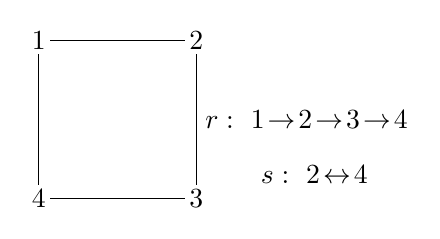
\begin{tikzpicture}[every node/.style={inner sep=1.5pt},scale=1.0]
  \node (v1) at (0,2) {$1$};
  \node (v2) at (2,2) {$2$};
  \node (v3) at (2,0) {$3$};
  \node (v4) at (0,0) {$4$};
  \draw (v1)--(v2)--(v3)--(v4)--(v1);
  \node at (3.4,1) {$r:\ 1\!\to\!2\!\to\!3\!\to\!4$};
  \node at (3.5,0.3) {$s:\ 2\!\leftrightarrow\!4$};
\end{tikzpicture}\end{center}

\subsection*{The Center $Z(G)$ (D\&F 2.2)}

\begin{definition}\label{d:center@c2}
Let $G$ be a group. The \emph{center} of $G$ is
\[
Z(G)=\{g\in G\st gx=xg\ \text{for all }x\in G\}.
\]
Equivalently $Z(G)=C_G(G)$ (the centralizer of the whole group in itself), and since an element commutes with everything iff it commutes with every single element separately,
\[
Z(G)=\bigcap_{a\in G}C_G(a).
\]
\end{definition}

\begin{proposition}\label{p:center-subgroup@c2}
For any group $G$, $Z(G)\sgr G$, and $Z(G)$ is abelian. Moreover $Z(G)\nor G$ (it is a normal subgroup).
\end{proposition}

\begin{proof}
Nonempty: $1x=x=x1$ for all $x$, so $1\in Z(G)$. Closed: if $g,h\in Z(G)$ and $x\in G$ then $(gh)x=g(hx)=g(xh)=(gx)h=(xg)h=x(gh)$, so $gh\in Z(G)$. Inverses: if $g\in Z(G)$ then $gx=xg$ for all $x$; multiply on both sides by $g\inv$ to get $xg\inv=g\inv x$, so $g\inv\in Z(G)$. Hence $Z(G)\sgr G$ by the subgroup criterion. It is abelian because any two of its elements each commute with everything in $G$, in particular with each other. For normality: if $g\in Z(G)$ and $a\in G$ then $aga\inv=ag a\inv = g a a\inv = g\in Z(G)$ (using $ag=ga$), so $aZ(G)a\inv\subseteq Z(G)$ for every $a$; thus $Z(G)\nor G$.
\end{proof}

\begin{remark}
$Z(G)$ measures how far $G$ is from being abelian: $Z(G)=G$ exactly when $G$ is abelian, and a ``small'' center signals a highly noncommutative group. Note $Z(G)=\bigcap_a C_G(a)$ is an intersection of subgroups, hence automatically a subgroup --- this is the practical formula we exploit below.
\end{remark}

\begin{method}{How to compute $Z(G)$ from a generating set}
\textbf{Recognition trigger.} Use this whenever you are asked for $Z(G)$ and $G=\gen{S}$ for a small generating set $S$ (e.g.\ $D_{2n}=\gen{r,s}$, $Q_8=\gen{i,j}$, $S_3=\gen{(1\,2),(1\,2\,3)}$, $\GL_n(\F)$ generated by elementary/transvection-type matrices).
\begin{enumerate}
\item \textbf{Reduce the test set.} An element $g$ is central iff $gx=xg$ for \emph{all} $x\in G$. But if $g$ commutes with each generator in $S$, it commutes with every product of generators and their inverses, hence with all of $G$. So
\[
Z(G)=\bigcap_{x\in S}C_G(x).
\]
You only need to test commutation against the generators.
\item \textbf{Parametrize a general element} $g$ of $G$ (e.g.\ $g=r^k$ or $g=r^k s$ in $D_{2n}$; $g=\sum$ of basis quaternions; $g=$ general matrix).
\item \textbf{Impose $gx=xg$ for each generator $x\in S$} and solve the resulting equations for the parameters.
\item \textbf{Collect the surviving $g$'s}; that set is $Z(G)$. Always finish with $|Z(G)|$ and a sanity check (does $1$ lie in it? is the answer a subgroup?).
\end{enumerate}
\end{method}

\begin{theorem}[Center of the dihedral group]\label{t:center-dihedral@c2}
Let $D_{2n}=\gen{r,s\st r^n=s^2=1,\ srs=r\inv}$ with $n\ge3$. Then
\[
Z(D_{2n})=
\begin{cases}
\{1\}, & n\ \text{odd},\\[2pt]
\{1,\,r^{n/2}\}, & n\ \text{even}.
\end{cases}
\]
\end{theorem}

\begin{proof}
By the method box, $Z=C(r)\cap C(s)$. \emph{Step 1 (rotations).} For $r^k$: $r^k$ commutes with $r$ automatically; and $s r^k s\inv = (srs)^k = (r\inv)^k = r^{-k}$, so $r^k$ commutes with $s$ iff $r^{-k}=r^{k}$, i.e.\ $r^{2k}=1$, i.e.\ $n\mid 2k$. For $0\le k<n$ this forces $k=0$, or $k=n/2$ when $n$ is even. \emph{Step 2 (reflections).} For a reflection $r^k s$: it does not commute with $r$, since $r(r^k s)=r^{k+1}s$ while $(r^k s)r = r^k (sr) = r^k r\inv s = r^{k-1}s$, and $r^{k+1}s=r^{k-1}s$ would force $r^2=1$, impossible for $n\ge3$. So no reflection is central. Combining, $Z=\{1\}$ if $n$ is odd and $Z=\{1,r^{n/2}\}$ if $n$ is even.
\end{proof}

\begin{pitfall}
Do not confuse $Z(G)$ with $C_G(a)$ for a single element $a$. The centralizer $C_G(a)$ can be large (it always contains $\gen{a}$) even when $Z(G)=1$. For example in $S_3$, $C_{S_3}((1\,2\,3))=\gen{(1\,2\,3)}$ has order $3$, yet $Z(S_3)=1$. The center is the intersection of \emph{all} the centralizers, so it is typically much smaller.
\end{pitfall}

\begin{wex}{$Z(D_8)=\{1,r^2\}$}
Compute the center of $D_8=\gen{r,s\st r^4=s^2=1,\ srs=r\inv}$ (the symmetries of the square, order $8$).
\wrec $D_8$ is generated by $S=\{r,s\}$, so by the method box $Z=C(r)\cap C(s)$: test each of the $8$ elements against just $r$ and $s$. This is the $n=4$ (even) case of Theorem~\ref{t:center-dihedral@c2}, predicting $\{1,r^{n/2}\}=\{1,r^2\}$.
\wsol The $8$ elements are $\{1,r,r^2,r^3,s,rs,r^2s,r^3s\}$.

\emph{Rotations $r^k$ vs $s$.} Using $sr^k s = r^{-k}$, we have $r^k s = s r^{-k}$, so $r^k$ commutes with $s$ iff $r^{-k}=r^{k}$, i.e.\ $r^{2k}=1$, i.e.\ $4\mid 2k$, i.e.\ $k\in\{0,2\}$. Thus among rotations only $1$ and $r^2$ pass the $s$-test (and all rotations commute with $r$). So central rotations: $\{1,r^2\}$.

\emph{Reflections $r^k s$ vs $r$.} Compute $r\cdot(r^k s)=r^{k+1}s$ and $(r^k s)\cdot r = r^k(sr)=r^k r^{-1}s = r^{k-1}s$. These differ ($r^{k+1}s\ne r^{k-1}s$ since $r^2\ne1$), so \emph{no} reflection commutes with $r$. All four reflections are excluded.

Hence $Z(D_8)=\{1,r^2\}$, of order $2$. \emph{Check:} $r^2$ is central because $r^2 s = s r^{-2}=s r^{2}$ (as $r^4=1\Rightarrow r^{-2}=r^2$), and $r^2$ commutes with $r$; and $\{1,r^2\}=\gen{r^2}$ is indeed a subgroup. Matches Theorem~\ref{t:center-dihedral@c2}.
\end{wex}

\begin{wex}{$Z(Q_8)=\{1,-1\}$}
Compute the center of $Q_8=\{\pm1,\pm i,\pm j,\pm k\}$ with $i^2=j^2=k^2=-1$, $ij=k$, $jk=i$, $ki=j$ (and $ji=-k$, etc.).
\wrec $Q_8=\gen{i,j}$, so $Z=C(i)\cap C(j)$. The defining relations are anticommutation rules ($ji=-ij$), which is exactly the signal that the noncentral generators fail to commute; only $\pm1$ are scalar.
\wsol Recall the products are anticommutative: $ij=k$, $ji=-k$, $jk=i$, $kj=-i$, $ki=j$, $ik=-j$.

\emph{Test $i$ against $j$:} $ij=k$ but $ji=-k\ne k$. So $i\notin Z$. Likewise $\pm i$ fail.

\emph{Test $j$ against $i$:} same computation, $ij\ne ji$, so $j\notin Z$; likewise $\pm j$ fail.

\emph{Test $k$ against $i$:} $ki=j$ but $ik=-j\ne j$, so $k\notin Z$; likewise $\pm k$ fail.

\emph{Test $\pm1$:} $1$ commutes with everything; $-1$ commutes with everything because $-1=(-1)\cdot1$ is a scalar: $(-1)x=-x=x(-1)$ for all $x$. So $\pm1\in Z$.

Hence $Z(Q_8)=\{1,-1\}$, order $2$. \emph{Check:} every element of $Q_8$ squares to $\pm1$, and $i^2=j^2=k^2=-1$, so $-1$ commutes with all squares and is genuinely central; the set $\{1,-1\}=\gen{-1}$ is a subgroup. (Aside: $Q_8/Z\isom V_4$, consistent with $|Z|=2$.)
\end{wex}

\begin{wex}{$Z(S_3)=1$}
Compute the center of the symmetric group $S_3$.
\wrec $S_3=\gen{(1\,2),(1\,2\,3)}$, so $Z=C((1\,2))\cap C((1\,2\,3))$. Symmetric groups $S_n$ for $n\ge3$ are nonabelian, and the quick test is: a single pair of generators that fail to commute already kills most elements.
\wsol The six elements: $1,(1\,2),(1\,3),(2\,3),(1\,2\,3),(1\,3\,2)$. We compose permutations right-to-left (apply the rightmost factor first).

A central element must commute with the transposition $\tau=(1\,2)$ and the $3$-cycle $\sigma=(1\,2\,3)$. First note $\sigma$ and $\tau$ do not commute:
\[
\sigma\tau=(1\,2\,3)(1\,2)=(1\,3),\qquad \tau\sigma=(1\,2)(1\,2\,3)=(2\,3),
\]
and $(1\,3)\ne(2\,3)$. So neither $\sigma$ nor $\tau$ is central.

\emph{Transpositions.} By symmetry each transposition fails: e.g.\ check $(1\,3)$ against $\sigma$: $\sigma(1\,3)=(1\,2\,3)(1\,3)=(2\,3)$ while $(1\,3)\sigma=(1\,3)(1\,2\,3)=(1\,2)$; unequal, so $(1\,3)\notin Z$. Similarly $(2\,3)\notin Z$.

\emph{$3$-cycles.} $\sigma=(1\,2\,3)$ already fails against $\tau$ above. Its inverse $\sigma^2=(1\,3\,2)$: $\tau\sigma^2=(1\,2)(1\,3\,2)=(1\,3)$ while $\sigma^2\tau=(1\,3\,2)(1\,2)=(2\,3)$; unequal, so $(1\,3\,2)\notin Z$.

Only $1$ survives. Hence $Z(S_3)=\{1\}$. \emph{Check:} $|S_3|=6$ is nonabelian, and a nonabelian group cannot have $Z=G$, so $Z\ne S_3$; $S_3\isom D_6$ is the $n=3$ (odd) dihedral case, where Theorem~\ref{t:center-dihedral@c2} gives $Z=1$. Consistent.
\end{wex}

\begin{wex}{$Z(\GL_n(\F))=\{\lambda I\st \lambda\in\F^\times\}$ (scalar matrices)}
Show the center of $\GL_n(\F)$ ($n\ge2$, $\F$ a field) consists exactly of the nonzero scalar matrices $\lambda I$, $\lambda\ne0$.
\wrec $\GL_n(\F)$ is generated by elementary matrices, but the cleanest test set is the transvections $E_{ij}=I+e_{ij}$ ($i\ne j$), where $e_{ij}$ has a single $1$ in position $(i,j)$. Commuting with all of these is what forces a matrix to be scalar; this is the ``intersect centralizers of a generating set'' method for a matrix group.
\wsol Let $A=(a_{pq})\in\GL_n(\F)$. It suffices that $A$ commute with each $E_{ij}=I+e_{ij}$, i.e.\ with each $e_{ij}$ (subtracting $I$). Use the rule $e_{ij}e_{kl}=\delta_{jk}e_{il}$.

\emph{Step 1: compute the commutator condition.} $A e_{ij}=e_{ij}A$ as matrices. Now $(A e_{ij})_{pq}=\sum_t a_{pt}(e_{ij})_{tq}=a_{pi}\delta_{jq}$, which is nonzero only in column $j$, where its $p$-th entry is $a_{pi}$. And $(e_{ij}A)_{pq}=\sum_t (e_{ij})_{pt}a_{tq}=\delta_{ip}a_{jq}$, nonzero only in row $i$, where its $q$-th entry is $a_{jq}$. Setting $Ae_{ij}=e_{ij}A$:
\[
a_{pi}\,\delta_{jq}=\delta_{ip}\,a_{jq}\qquad\text{for all }p,q.
\]

\emph{Step 2: read off the entries.} Take $p\ne i$ and $q=j$: LHS $=a_{pi}$, RHS $=\delta_{ip}a_{jj}=0$, so $a_{pi}=0$ for all $p\ne i$ --- column $i$ is zero off the diagonal. Take $p=i$, $q\ne j$: LHS $=a_{ii}\delta_{jq}=0$, RHS $=a_{jq}$, so $a_{jq}=0$ for $q\ne j$ --- row $j$ is zero off the diagonal. Since this holds for all $i\ne j$, $A$ is diagonal. Take $p=i,q=j$: $a_{ii}=a_{jj}$. So all diagonal entries are equal: $A=\lambda I$.

\emph{Step 3: invertibility.} $\lambda I\in\GL_n(\F)$ iff $\det(\lambda I)=\lambda^n\ne0$ iff $\lambda\ne0$. Conversely every $\lambda I$ ($\lambda\ne0$) commutes with all matrices, so lies in the center.

Hence $Z(\GL_n(\F))=\{\lambda I\st\lambda\in\F^\times\}\isom\F^\times$. \emph{Check:} for $n=1$, $\GL_1(\F)=\F^\times$ is abelian and the statement degenerates to $Z=G$, consistent. For $n=2$, e.g.\ $\begin{psmallmatrix}1&1\\0&1\end{psmallmatrix}$ and $\begin{psmallmatrix}1&0\\1&1\end{psmallmatrix}$ do not commute, confirming non-scalar matrices are excluded.
\end{wex}

\begin{wex}{$Z(G)=G$ iff $G$ abelian; e.g.\ $Z(\Zn{n})=\Zn{n}$}
Show that $Z(G)=G$ if and only if $G$ is abelian, and illustrate with $G=\Zn{n}$ and with a nonabelian contrast.
\wrec The trigger is the phrase ``$Z(G)=G$.'' By definition $g\in Z(G)$ means $g$ commutes with everything; $Z(G)=G$ says \emph{every} element commutes with everything, which is precisely the definition of abelian. Whenever $G$ is given as abelian (e.g.\ $\Zn{n}$, any cyclic or product of cyclic groups), you may immediately write $Z(G)=G$.
\wsol \emph{($\Rightarrow$)} If $Z(G)=G$ then every $g\in G$ satisfies $gx=xg$ for all $x\in G$; in particular for any $a,b\in G$, $ab=ba$, so $G$ is abelian. \emph{($\Leftarrow$)} If $G$ is abelian then $gx=xg$ holds for all $g,x$, so every $g\in Z(G)$, giving $Z(G)=G$ (and $Z(G)\subseteq G$ always). Hence the equivalence.

\emph{Example $\Zn{n}$.} The group $\Zn{n}=\{\,\overline0,\overline1,\dots,\overline{n-1}\,\}$ under addition has $\overline a+\overline b=\overline{a+b}=\overline b+\overline a$ for all $a,b$, so it is abelian; therefore $Z(\Zn{n})=\Zn{n}$. Concretely for $n=6$: $\overline2+\overline5=\overline7=\overline1=\overline5+\overline2$, illustrating commutativity for a sample pair.

\emph{Contrast.} For a nonabelian $G$, $Z(G)\psgr G$ strictly: e.g.\ $Z(D_8)=\{1,r^2\}\ne D_8$ since $|Z|=2<8$. \emph{Check:} the equivalence is logically airtight (it is just the definitions of ``central'' and ``abelian'' lined up), and $|Z(\Zn n)|=n=|\Zn n|$ confirms equality.
\end{wex}

\begin{wex}{$Z(D_{12})=\{1,r^3\}$ (the $n=6$ even case)}
Compute $Z(D_{12})$, the center of the symmetries of a regular hexagon, $D_{12}=\gen{r,s\st r^6=s^2=1,\ srs=r\inv}$.
\wrec $D_{12}$ has $n=6$, which is \emph{even}, so Theorem~\ref{t:center-dihedral@c2} predicts $Z=\{1,r^{n/2}\}=\{1,r^3\}$. We verify directly by intersecting $C(r)\cap C(s)$ over the generators $\{r,s\}$, exhibiting exactly why $r^3$ survives and the others do not.
\wsol The $12$ elements are $\{r^k,\,r^k s : 0\le k\le 5\}$.

\emph{Rotations $r^k$ vs $s$.} As before $r^k s = s r^{-k}$, so $r^k$ commutes with $s$ iff $r^{2k}=1$, i.e.\ $6\mid 2k$, i.e.\ $3\mid k$. For $0\le k\le5$ this gives $k\in\{0,3\}$, i.e.\ $r^0=1$ and $r^3$. (Both automatically commute with $r$.) So central rotations are $\{1,r^3\}$.

\emph{Why $r^3$ works explicitly:} $r^3 s = s r^{-3}=s r^{3}$ since $r^{-3}=r^{6-3}=r^3$. Good.

\emph{Why, say, $r^2$ fails:} $r^2 s = s r^{-2}=s r^4\ne s r^2$ (since $r^4\ne r^2$), so $r^2\notin Z$. Likewise $r,r^4,r^5$ fail the $s$-test.

\emph{Reflections $r^k s$ vs $r$.} $r(r^k s)=r^{k+1}s$ and $(r^k s)r=r^{k-1}s$; these are unequal because $r^2\ne1$. So no reflection commutes with $r$, and all six reflections are excluded.

Hence $Z(D_{12})=\{1,r^3\}$, order $2$. \emph{Check:} $\{1,r^3\}=\gen{r^3}$ with $(r^3)^2=r^6=1$, a subgroup of order $2$; and $n=6$ even gives $r^{n/2}=r^3$, matching Theorem~\ref{t:center-dihedral@c2} exactly.
\end{wex}

\begin{center}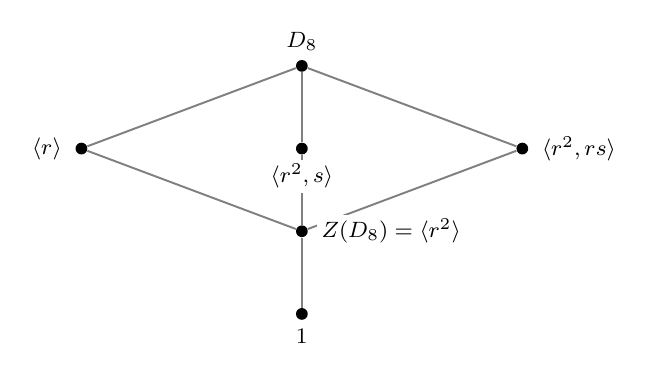
\begin{tikzpicture}[yscale=1.05,xscale=1.4]
  \node[ltdot] (bot) at (0,0) {};
  \node[ltdot] (z) at (0,1) {};
  \node[ltdot] (r) at (-2,2) {};
  \node[ltdot] (a) at (0,2) {};
  \node[ltdot] (b) at (2,2) {};
  \node[ltdot] (top) at (0,3) {};
  \begin{scope}[ltedge]
    \draw (bot)--(z);
    \draw (z)--(r);
    \draw (z)--(a);
    \draw (z)--(b);
    \draw (r)--(top);
    \draw (a)--(top);
    \draw (b)--(top);
  \end{scope}
  \node[ltlab,below=1.5pt of bot] {$1$};
  \node[ltlab,right=3pt of z] {$Z(D_8)=\langle r^2\rangle$};
  \node[ltlab,left=3pt of r] {$\langle r\rangle$};
  \node[ltlab,below=1.5pt of a] {$\langle r^2,s\rangle$};
  \node[ltlab,right=3pt of b] {$\langle r^2,rs\rangle$};
  \node[ltlab,above=1.5pt of top] {$D_8$};
\end{tikzpicture}\end{center}

The diagram shows $Z(D_8)=\gen{r^2}$ sitting at the bottom of the lattice, directly above the trivial subgroup: it is the intersection of the three index-$2$ subgroups $\gen{r}$, $\gen{r^2,s}$, $\gen{r^2,rs}$ (the four reflection subgroups of order $2$, not drawn here, are also minimal nontrivial subgroups, but each lies in only one of them). This pictures Proposition~\ref{p:center-subgroup@c2} (the center is a normal subgroup, here of order $2$) and the $n=4$ even case of Theorem~\ref{t:center-dihedral@c2}.

\begin{pitfall}
A reflection $r^k s$ in $D_{2n}$ is \emph{never} central for $n\ge3$, even when $n$ is even --- the lone central nontrivial element is the half-turn rotation $r^{n/2}$. Students sometimes guess that ``$s$ commutes with the half-turn so $s$ is central''; but centrality requires commuting with \emph{every} element, and $s$ fails against $r$ (since $rs=sr^{-1}\ne sr$).
\end{pitfall}

\subsection*{Normalizers and the Setwise Stabilizer}

Let $G$ be a group and $A\subseteq G$ a nonempty subset. For $g\in G$ write
\[
gAg\inv=\{\,gag\inv\st a\in A\,\},
\]
the \emph{conjugate} of $A$ by $g$. This is the image of $A$ under the bijection $x\mapsto gxg\inv$ of $G$ (conjugation by $g$), so $|gAg\inv|=|A|$ always.

\begin{definition}\label{d:norm@c2}
The \emph{normalizer} of $A$ in $G$ is
\[
N_G(A)=\{\,g\in G\st gAg\inv=A\,\}.
\]
Equivalently, $g\in N_G(A)$ iff conjugation by $g$ permutes $A$ among itself \emph{as a set}: $gAg\inv=A$ (setwise), not necessarily $gag\inv=a$ for each $a$ (pointwise). Recall the \emph{centralizer} $C_G(A)=\{g\st gag\inv=a\text{ for all }a\in A\}=\{g\st ga=ag\ \forall a\in A\}$.
\end{definition}

\begin{remark}
The single inclusion $gAg\inv\subseteq A$ already forces the reverse inclusion automatically: since $x\mapsto gxg\inv$ is injective and $A$ is finite (in our examples), $gAg\inv\subseteq A$ with equal cardinality gives $gAg\inv=A$. For infinite $A$ you must check both inclusions, or equivalently $gAg\inv\subseteq A$ AND $g\inv Ag\subseteq A$.
\end{remark}

\begin{proposition}\label{p:tower@c2}
For any nonempty $A\subseteq G$,
\[
C_G(A)\sgr N_G(A)\sgr G,
\]
and moreover $A$ itself is contained in $N_G(A)$ whenever $A$ is a subgroup. If $A=H$ is a subgroup then $N_G(H)$ is the largest subgroup of $G$ in which $H$ is normal, and $H\nor N_G(H)$.
\end{proposition}

\begin{proof}
\emph{$N_G(A)\sgr G$.} $1A1\inv=A$, so $1\in N_G(A)$. If $g,h\in N_G(A)$ then $(gh)A(gh)\inv=g(hAh\inv)g\inv=gAg\inv=A$, so $gh\in N_G(A)$. If $gAg\inv=A$, conjugate by $g\inv$: $g\inv A g=g\inv(gAg\inv)g=A$, so $g\inv\in N_G(A)$. Hence $N_G(A)\sgr G$.

\emph{$C_G(A)\sgr N_G(A)$.} $C_G(A)\sgr G$ by the same argument (identity is in it, and it is closed under products and inverses). If $g\in C_G(A)$ then $gag\inv=a\in A$ for every $a\in A$, so $gAg\inv=A$; thus $g\in N_G(A)$. Since $C_G(A)\subseteq N_G(A)$ and both are subgroups of $G$, $C_G(A)\sgr N_G(A)$.

\emph{$H\nor N_G(H)$.} For $H$ a subgroup, every $h\in H$ satisfies $hHh\inv=H$ (subgroups are conjugation-closed by themselves), so $H\subseteq N_G(H)$, hence $H\sgr N_G(H)$. The defining condition $gHg\inv=H$ for all $g\in N_G(H)$ is exactly normality of $H$ in $N_G(H)$. If $H\nor K\sgr G$ then $kHk\inv=H$ for all $k\in K$, so $K\subseteq N_G(H)$; thus $N_G(H)$ is the largest such $K$.
\end{proof}

\begin{method}{How to compute $N_G(H)$}
Use this whenever you must decide which $g$ conjugate a subgroup $H$ \emph{onto itself as a set} (e.g. to find the largest subgroup in which $H$ is normal, or to detect normality).
\begin{enumerate}
\item \textbf{Free wins first.} $H\subseteq N_G(H)$ always, and $C_G(H)\subseteq N_G(H)$ always. List those elements; they are in for free.
\item \textbf{Index-2 shortcut.} If $[G:H]=2$ then $H\nor G$, so $N_G(H)=G$. Stop. (Two cosets $H$ and $gH$; the only options force $gH=Hg$.)
\item \textbf{Generator test.} Write $H=\gen{a}$ (or list generators). For \emph{finite} $H$, $gHg\inv=H$ iff $gag\inv\in H$ for each generator $a$ (a homomorphic image of a generating set generates the image, so $gHg\inv\subseteq H$, and $|gHg\inv|=|H|$). So test ONLY the generators, not every element. (For infinite $H$ this gives only $gHg\inv\subseteq H$; also test $g\inv ag\in H$.)
\item \textbf{Setwise, not pointwise.} You only need $gag\inv$ to land \emph{somewhere} in $H$, not back at $a$. (Pointwise would be the centralizer.)
\item \textbf{Assemble a subgroup.} $N_G(H)$ is a subgroup containing $H$; use Lagrange to limit its possible order, then confirm with coset reps.
\end{enumerate}
\end{method}

\begin{pitfall}
$N_G(H)=G$ does NOT mean $G$ is abelian or that $H$ is central. It means $H$ is \emph{normal}: $gHg\inv=H$ setwise. Conjugation may still scramble the elements of $H$ (e.g. send $r\mapsto r\inv$), as long as it stays inside $H$.
\end{pitfall}

\begin{pitfall}
Do not confuse $gag\inv\in H$ (normalizer condition) with $gag\inv=a$ (centralizer condition). Testing the wrong one is the most common error: a generator can be moved to another element of $H$ and still be normalized.
\end{pitfall}

\begin{wex}{$N_{D_8}(\gen{s})=\{1,s,r^2,sr^2\}$}
In $D_8=\gen{r,s\st r^4=s^2=1,\ srs=r\inv}$, compute the normalizer of the reflection subgroup $\gen{s}=\{1,s\}$.
\wrec Here $\gen{s}=\{1,s\}$ has order $2$ but index $4$, so the index-2 shortcut does not apply; we must run the generator test. The single generator is $s$, so $g\in N_{D_8}(\gen s)$ iff $gsg\inv\in\{1,s\}$. Since $gsg\inv$ is a conjugate of $s$ it has order $2$ and is $\ne1$, so the condition collapses to the setwise check $gsg\inv=s$, i.e. $g$ commutes with $s$. For this tiny subgroup the normalizer equals the centralizer $C_{D_8}(s)$.
\wsol Use the relation $srs\inv=r\inv$, equivalently $s r=r\inv s$, and $sr^k s\inv=r^{-k}$. Conjugate $s$ by each of the $8$ elements $r^k$ and $sr^k$ ($k=0,1,2,3$). 

Rotations: $r^k s r^{-k}$. Since $r s=s r\inv$ we get $r^k s=s r^{-k}$, hence $r^k s r^{-k}=s r^{-k} r^{-k}=s r^{-2k}$. So:
\[
1\cdot s\cdot 1=s,\quad rsr\inv=sr^{-2},\quad r^2 s r^{-2}=s r^{-4}=s,\quad r^3 s r^{-3}=sr^{-6}=sr^2.
\]
Thus among rotations, $1$ and $r^2$ give $s$ (good); $r,r^3$ give $sr^{-2}=sr^2\notin\gen s$ (bad).

Reflections: $(sr^k)s(sr^k)\inv$. Compute $(sr^k)\inv=r^{-k}s$. Then
\[
(sr^k)s(r^{-k}s)=s(r^k s r^{-k})s=s(sr^{-2k})s=s s r^{-2k}s=r^{-2k}s=s r^{2k},
\]
using $r^{-2k}s=s r^{2k}$. For $k=0$: $s$. For $k=2$: $sr^4=s$. For $k=1$: $sr^2\notin\gen s$. For $k=3$: $sr^6=sr^2\notin\gen s$. So $s$ and $sr^2$ work.

The elements fixing $\gen s$ setwise are exactly $\{1,r^2,s,sr^2\}$. Check it is a subgroup: $s\cdot r^2=sr^2$, $(sr^2)^2=sr^2sr^2=s(r^2 s)r^2=s(sr^{-2})r^2=1$, and $r^2,s$ commute since $r^2 s=sr^{-2}=sr^2$. This is a Klein four-group $\{1,s,r^2,sr^2\}\isom V_4$, order $4$, index $2$ in $D_8$.

\emph{Sanity check.} The bad rotation gives $rsr\inv=sr^{-2}=sr^2\notin\gen s$, confirming $r\notin N_{D_8}(\gen s)$, as required. And $|N_{D_8}(\gen s)|=4$ divides $8$. Note $\gen s\nor N_{D_8}(\gen s)$ but $\gen s$ is NOT normal in $D_8$.
\end{wex}

\begin{wex}{$N_{D_8}(\gen r)=D_8$ via index $2$}
In $D_8$ compute the normalizer of the rotation subgroup $\gen r=\{1,r,r^2,r^3\}$.
\wrec The trigger is the \emph{index-2 shortcut}: $|\gen r|=4$ and $|D_8|=8$, so $[D_8:\gen r]=2$. Any subgroup of index $2$ is normal, hence its normalizer is the whole group. No element-by-element work is needed.
\wsol $[D_8:\gen r]=8/4=2$, so by the index-2 theorem $\gen r\nor D_8$, i.e. $g\gen r g\inv=\gen r$ for all $g$. Therefore $N_{D_8}(\gen r)=D_8$.

For a direct confirmation of the setwise condition, the only nontrivial generator to test is $r$ against the reflection $s$: $srs\inv=r\inv=r^3\in\gen r$. Since $s$ and $r$ generate $D_8$ and both normalize $\gen r$ ($r r r\inv=r\in\gen r$ trivially), every element does.

\emph{Sanity check.} $|N_{D_8}(\gen r)|=8$ divides $8$, and $\gen r\subseteq N_{D_8}(\gen r)$ as it must. Contrast with the previous example: $\gen r$ is normal but $\gen s$ is not.
\end{wex}

\begin{wex}{$N_{S_3}(\gen{(1\,2\,3)})=S_3$}
Compute the normalizer in $S_3$ of the $3$-cycle subgroup $H=\gen{(1\,2\,3)}=\{e,(1\,2\,3),(1\,3\,2)\}$.
\wrec Again the \emph{index-2 shortcut}: $|H|=3$, $|S_3|=6$, so $[S_3:H]=2$. Index $2$ forces normality; $N_{S_3}(H)=S_3$. We can also confirm with the conjugation-of-cycles rule $\sigma(1\,2\,3)\sigma\inv=(\sigma(1)\,\sigma(2)\,\sigma(3))$.
\wsol Since $[S_3:H]=6/3=2$, $H\nor S_3$ and so $N_{S_3}(H)=S_3$.

Direct generator test: $H=\gen{(1\,2\,3)}$, so check $\sigma(1\,2\,3)\sigma\inv$ for a transposition, say $\sigma=(1\,2)$:
\[
(1\,2)(1\,2\,3)(1\,2)=(\,(1\,2)(1)\ (1\,2)(2)\ (1\,2)(3)\,)=(2\,1\,3)=(1\,3\,2)\in H.
\]
It landed on the other $3$-cycle (setwise inside $H$), not back on $(1\,2\,3)$, yet that is fine for the normalizer. Every transposition behaves the same way, and the powers of $(1\,2\,3)$ obviously normalize $H$, so all $6$ elements normalize $H$.

\emph{Sanity check.} $|N_{S_3}(H)|=6$ divides $6$; $H\subseteq N_{S_3}(H)$. Note $C_{S_3}(H)=H$ here (a transposition does NOT commute with $(1\,2\,3)$, since it inverts it), so $C_{S_3}(H)=\gen{(1\,2\,3)}\psgr N_{S_3}(H)=S_3$ strictly.
\end{wex}

\begin{wex}{$N_{S_3}(\gen{(1\,2)})=\gen{(1\,2)}$}
Compute the normalizer in $S_3$ of the transposition subgroup $K=\gen{(1\,2)}=\{e,(1\,2)\}$.
\wrec $|K|=2$, index $3$ (odd, $\ne2$), so no shortcut; run the generator test on $(1\,2)$ using $\sigma(1\,2)\sigma\inv=(\sigma(1)\,\sigma(2))$. A conjugate of $(1\,2)$ is again a transposition; it lies in $K=\{e,(1\,2)\}$ iff it equals $(1\,2)$. So here the setwise test again reduces to fixing $(1\,2)$.
\wsol Conjugate $(1\,2)$ by each $\sigma\in S_3$, using $\sigma(1\,2)\sigma\inv=(\sigma(1)\,\sigma(2))$:
\[
\begin{array}{ll}
e:(1\,2)\in K & (1\,2):(1\,2)\in K\\
(1\,3):(3\,2)=(2\,3)\notin K & (2\,3):(1\,3)\notin K\\
(1\,2\,3):(2\,3)\notin K & (1\,3\,2):(3\,1)=(1\,3)\notin K
\end{array}
\]
(For $(1\,2\,3)$: it sends $1\mapsto2,2\mapsto3$, so $(1\,2)\mapsto(2\,3)$.) Only $e$ and $(1\,2)$ keep the conjugate inside $K$. Hence $N_{S_3}(K)=\{e,(1\,2)\}=K$.

\emph{Sanity check.} $|N_{S_3}(K)|=2$ divides $6$; $K\subseteq N_{S_3}(K)$ as required, and equality says $K$ is its own normalizer (self-normalizing). This matches the fact that $\gen{(1\,2)}$ is NOT normal in $S_3$ (it has $3$ distinct conjugates).
\end{wex}

\begin{wex}{$N_{Q_8}(\gen i)=Q_8$}
In $Q_8=\{\pm1,\pm i,\pm j,\pm k\}$ with $i^2=j^2=k^2=-1$, $ij=k$, $jk=i$, $ki=j$, $ji=-k$, compute $N_{Q_8}(\gen i)$ where $\gen i=\{1,i,-1,-i\}$.
\wrec $|\gen i|=4$, $|Q_8|=8$, so $[Q_8:\gen i]=2$: \emph{index-2 shortcut} gives $N_{Q_8}(\gen i)=Q_8$. In fact \emph{every} subgroup of $Q_8$ is normal, so this is expected. We confirm with the generator test on $i$.
\wsol $[Q_8:\gen i]=8/4=2\Rightarrow \gen i\nor Q_8\Rightarrow N_{Q_8}(\gen i)=Q_8$.

Confirm setwise by conjugating the generator $i$ by $j$ (the element outside $\gen i$): using $ji=-k$ and $j\inv=-j$,
\[
j\,i\,j\inv=(ji)(-j)=(-k)(-j)=kj.
\]
Now $kj=-i$ (since $jk=i\Rightarrow kj=-i$). So $j i j\inv=-i\in\gen i$. Conjugation by $j$ sends $i\mapsto -i$ (inverts it) but stays inside $\gen i$, exactly the setwise condition. Since $i,j$ generate $Q_8$ and both normalize $\gen i$, all of $Q_8$ does.

\emph{Sanity check.} $|N_{Q_8}(\gen i)|=8$ divides $8$; $\gen i\subseteq N_{Q_8}(\gen i)$. Note $C_{Q_8}(\gen i)=\gen i$ (since $j$ anticommutes with $i$: $ij=k$, $ji=-k$, so $ij\ne ji$), giving a strict inclusion $C_{Q_8}(\gen i)=\gen i\psgr N_{Q_8}(\gen i)=Q_8$.
\end{wex}

\begin{wex}{Strict inclusion $C_G(H)\psgr N_G(H)$ in $D_8$}
Exhibit a subgroup $H$ of $G=D_8$ with $C_G(H)$ strictly smaller than $N_G(H)$, and show the setwise check that lets $N_G(H)$ grow.
\wrec We want a $g$ that is in $N_G(H)$ but not $C_G(H)$: it must move a generator of $H$ to a \emph{different} element of $H$ (so setwise OK, pointwise fails). Take $H=\gen{r^2}=\{1,r^2\}$ in $D_8$. Since $r^2$ is central in $D_8$, actually $C_{D_8}(r^2)=D_8$; that is no good for a strict gap with this $H$. Instead take $H=\gen r=\{1,r,r^2,r^3\}$, whose generator $r$ is moved by $s$: $srs\inv=r\inv\ne r$ but $r\inv\in H$.
\wsol Let $H=\gen r$. From Example with the index-2 shortcut, $N_{D_8}(H)=D_8$ (order $8$). Now compute $C_{D_8}(H)=C_{D_8}(r)$, the elements commuting with $r$:
\begin{itemize}
\item Rotations $r^k$ all commute with $r$: $r^k r=r r^k$. So $\{1,r,r^2,r^3\}\subseteq C_{D_8}(r)$.
\item A reflection $sr^k$: $(sr^k)r=sr^{k+1}$ while $r(sr^k)=(rs)r^k=(sr\inv)r^k=sr^{k-1}$. These are equal iff $r^{k+1}=r^{k-1}$ iff $r^2=1$, false. So no reflection commutes with $r$.
\end{itemize}
Hence $C_{D_8}(r)=\gen r$, order $4$. Therefore
\[
C_{D_8}(H)=\gen r\ \psgr\ N_{D_8}(H)=D_8,\qquad 4<8.
\]
The setwise check that grows the normalizer: $s\in N_{D_8}(H)$ because $srs\inv=r\inv=r^3\in H$ (and $sr^2s\inv=r^{-2}=r^2\in H$, $sr^3s\inv=r\in H$), so $sHs\inv=\{1,r^3,r^2,r\}=H$ setwise; but $s\notin C_{D_8}(H)$ since $srs\inv=r^3\ne r$.

\emph{Sanity check.} $C_{D_8}(H)=\gen r\psgr N_{D_8}(H)=D_8$ is consistent with Proposition~\ref{p:tower@c2} ($C_G\sgr N_G$), the orders $4\mid8$ both divide $|D_8|$, and the inclusion is strict exactly because conjugation by $s$ inverts the generator while keeping $H$ invariant as a set.
\end{wex}

\paragraph{Lattice of the three nested subgroups.} For $H=\gen s$ in $D_8$, the chain $\gen s\sgr N_{D_8}(\gen s)\sgr D_8$ from the first worked example sits inside the subgroup lattice as follows (here $N_{D_8}(\gen s)=\{1,s,r^2,sr^2\}$ has index $2$, and $\gen s$ has index $2$ inside it):

\begin{center}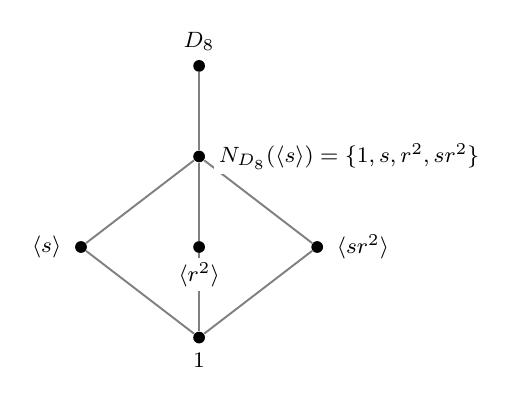
\begin{tikzpicture}[yscale=1.15,xscale=1.5]
  \node[ltdot] (bot) at (0,0) {};
  \node[ltdot] (s) at (-1,1) {};
  \node[ltdot] (z) at (0,1) {};
  \node[ltdot] (sr) at (1,1) {};
  \node[ltdot] (N) at (0,2) {};
  \node[ltdot] (G) at (0,3) {};
  \begin{scope}[ltedge]
    \draw (bot)--(s);
    \draw (bot)--(z);
    \draw (bot)--(sr);
    \draw (s)--(N);
    \draw (z)--(N);
    \draw (sr)--(N);
    \draw (N)--(G);
  \end{scope}
  \node[ltlab,below=1.5pt of bot] {$1$};
  \node[ltlab,left=3pt of s] {$\langle s\rangle$};
  \node[ltlab,below=1.5pt of z] {$\langle r^2\rangle$};
  \node[ltlab,right=3pt of sr] {$\langle sr^2\rangle$};
  \node[ltlab,right=3pt of N] {$N_{D_8}(\langle s\rangle)=\{1,s,r^2,sr^2\}$};
  \node[ltlab,above=1.5pt of G] {$D_8$};
\end{tikzpicture}\end{center}

The picture shows why $\gen s$ is not normal in $D_8$ but is normal in $N_{D_8}(\gen s)$: the normalizer is the \emph{largest} intermediate subgroup (here the Klein four-group $\isom V_4$) in which $\gen s$ sits normally, and the single edge $N_{D_8}(\gen s)\!-\!D_8$ has index $2$.

\subsection*{Stabilizers and Kernels of a Group Action}

A group action turns abstract group elements into concrete symmetries of a set. Two subgroups fall out of any action for free: the \emph{stabilizer} of a point (everything that fixes that point) and the \emph{kernel} (everything that fixes \emph{every} point). This section pins down exactly what these are, proves they are subgroups, and -- crucially -- shows that the normalizer $N_G(A)$ and centralizer $C_G(A)$ from D\&F 2.2 are nothing more than a stabilizer and a kernel for the conjugation action.

\begin{definition}\label{d:action@c2}
A \textbf{(left) action} of a group $G$ on a set $A$ is a map $G\times A\to A$, written $g\cdot a$, such that
\[
g_1\cdot(g_2\cdot a)=(g_1g_2)\cdot a\quad\text{and}\quad 1\cdot a=a
\]
for all $g_1,g_2\in G$ and all $a\in A$. Equivalently (by D\&F 1.7), $g\mapsto\sigma_g$, where $\sigma_g(a)=g\cdot a$, is a homomorphism $G\to S_A$ (the symmetric group on $A$).
\end{definition}

\begin{definition}\label{d:stab@c2}
Let $G$ act on $A$. For a point $a\in A$ the \textbf{stabilizer} of $a$ is
\[
G_a=\{\,g\in G\st g\cdot a=a\,\}.
\]
The \textbf{kernel} of the action is
\[
\ker=\{\,g\in G\st g\cdot a=a\ \text{for all }a\in A\,\}=\bigcap_{a\in A}G_a .
\]
The action is \textbf{faithful} if $\ker=1$. The kernel is exactly the kernel of the associated homomorphism $G\to S_A$, $g\mapsto\sigma_g$.
\end{definition}

\begin{proposition}\label{p:stab-subgroup@c2}
For each $a\in A$ the stabilizer $G_a\sgr G$. Consequently $\ker=\bigcap_{a\in A}G_a\sgr G$.
\end{proposition}

\begin{proof}
Use the subgroup criterion. First $1\in G_a$ since $1\cdot a=a$, so $G_a\neq\es$. Let $x,y\in G_a$, so $x\cdot a=a$ and $y\cdot a=a$. From $y\cdot a=a$ apply $y\inv$: $y\inv\cdot a=y\inv\cdot(y\cdot a)=(y\inv y)\cdot a=1\cdot a=a$, so $y\inv\in G_a$. Then $(xy\inv)\cdot a=x\cdot(y\inv\cdot a)=x\cdot a=a$, so $xy\inv\in G_a$. Hence $G_a\sgr G$. An arbitrary intersection of subgroups is a subgroup, so $\ker=\bigcap_a G_a\sgr G$.
\end{proof}

\begin{remark}\label{r:kernel-normal@c2}
The kernel is in fact \emph{normal}: it is the kernel of the homomorphism $G\to S_A$, and kernels of homomorphisms are normal subgroups (D\&F 3.1). A single stabilizer $G_a$ need not be normal -- see the conjugation examples, where $G_a=C_G(a)$ can fail to be normal.
\end{remark}

\subsection*{Conjugation actions recover $N_G(A)$ and $C_G(A)$}

D\&F 1.7 gives two conjugation actions of $G$. Both make the bookkeeping of Section 2.2 transparent.

\begin{theorem}\label{t:conj@c2}
Let $G$ be a group.
\begin{enumerate}
\item[(a)] $G$ acts on the set $\mathcal P(G)$ of subsets of $G$ by $g\cdot S=gSg\inv$. For a fixed subset $A\subseteq G$ the stabilizer of $A$ under this action is the \textbf{normalizer}
\[
\mathrm{Stab}(A)=\{\,g\in G\st gAg\inv=A\,\}=N_G(A).
\]
\item[(b)] $G$ acts on the set $G$ itself by $g\cdot a=gag\inv$. For a fixed subset $A\subseteq G$, the subgroup fixing \emph{every} point of $A$ -- i.e.\ the kernel of the restricted action of $N_G(A)$ on the set $A$ -- is the \textbf{centralizer}
\[
\{\,g\st gag\inv=a\ \forall a\in A\,\}=\{\,g\st ga=ag\ \forall a\in A\,\}=C_G(A).
\]
In particular the stabilizer of a single point $a$ under conjugation is $\mathrm{Stab}(a)=C_G(a)=C_G(\{a\})$.
\end{enumerate}
\end{theorem}

\begin{proof}
(a) By Definition~\ref{d:stab@c2}, $\mathrm{Stab}(A)=\{g\st g\cdot A=A\}=\{g\st gAg\inv=A\}$, which is verbatim the definition of $N_G(A)$ in D\&F 2.2. By Proposition~\ref{p:stab-subgroup@c2} it is a subgroup.

(b) For the conjugation action on points, $g$ fixes $a$ iff $gag\inv=a$ iff $ga=ag$. Intersecting over all $a\in A$,
\[
\bigcap_{a\in A}G_a=\{\,g\st ga=ag\ \forall a\in A\,\}=C_G(A),
\]
which is the definition of the centralizer. As an intersection of stabilizers (each a subgroup by Proposition~\ref{p:stab-subgroup@c2}) it is a subgroup; since $C_G(A)\sgr N_G(A)$ (Proposition~\ref{p:tower@c2}), it is the kernel of the conjugation action of $N_G(A)$ on the set $A$ (in general $G$ itself does not act on $A$, since $gAg\inv$ need not equal $A$). Taking $A=\{a\}$ gives $\mathrm{Stab}(a)=C_G(a)$.
\end{proof}

\begin{method}{Stabilizer vs.\ kernel: which one is it, and how to compute it}
\textbf{Recognition trigger.} You have a group $G$ acting on a set $A$ (a literal action like ``$S_n$ permutes $\{1,\dots,n\}$,'' or a conjugation action). Ask which question is being posed:
\begin{enumerate}
\item \emph{Which $g$ fix ONE chosen point $a$?} $\;\Rightarrow$ stabilizer $G_a$.
\item \emph{Which $g$ fix EVERY point at once?} $\;\Rightarrow$ kernel $=\bigcap_a G_a$.
\end{enumerate}
\textbf{Recipe to compute a stabilizer $G_a$.}
\begin{enumerate}
\item Write down the action rule $g\cdot a$ explicitly.
\item Set $g\cdot a=a$ and solve for the constraint on $g$.
\item Collect all such $g$; verify it is a subgroup (Prop.~\ref{p:stab-subgroup@c2} guarantees it, but listing elements is a check).
\item Identify the abstract group (often $S_{n-1}$, a small cyclic/reflection group, or a matrix block group).
\end{enumerate}
\textbf{Recipe to compute a kernel.} Either (a) intersect the stabilizers $\bigcap_a G_a$, or (b) find $\ker$ of the homomorphism $G\to S_A$ -- i.e.\ which $g$ induce the identity permutation. The action is \emph{faithful} exactly when this is $\{1\}$.
\textbf{Conjugation dictionary.} Conjugation on subsets: $\mathrm{Stab}(A)=N_G(A)$. Conjugation on points of $A$: kernel $=C_G(A)$; single point: $\mathrm{Stab}(a)=C_G(a)$.
\end{method}

\begin{pitfall}
``Stabilizer'' fixes a point \emph{setwise}/\emph{as a point}, not pointwise-inside-it. For conjugation on subsets, $g\in N_G(A)$ only requires $gAg\inv=A$ as a \emph{set} -- elements may be permuted. Requiring each element to be fixed gives the smaller $C_G(A)$. Always $C_G(A)\sgr N_G(A)$, and the inclusion is often strict.
\end{pitfall}

\subsection*{The $D_8$ action on the square}

The dihedral group $D_8=\gen{r,s\st r^4=s^2=1,\ srs=r\inv}$ (order $8$, symmetries of a square) acts on the four vertices labeled $1,2,3,4$ counterclockwise. Here $r$ rotates by $90^\circ$, sending $1\mapsto2\mapsto3\mapsto4\mapsto1$, and $s$ is the reflection fixing vertices $1$ and $3$ (the diagonal through them) and swapping $2$ and $4$.

\begin{center}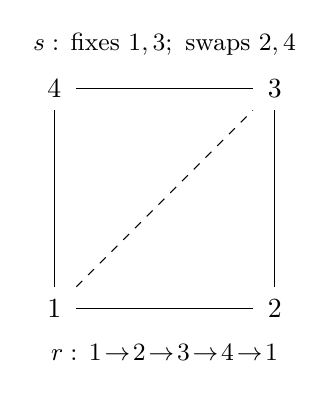
\begin{tikzpicture}[every node/.style={inner sep=2pt},scale=1.4]
  \node (v1) at (0,0) {$1$};
  \node (v2) at (2,0) {$2$};
  \node (v3) at (2,2) {$3$};
  \node (v4) at (0,2) {$4$};
  \draw (0.2,0)--(1.8,0);
  \draw (2,0.2)--(2,1.8);
  \draw (1.8,2)--(0.2,2);
  \draw (0,1.8)--(0,0.2);
  \draw[dashed] (0.2,0.2)--(1.8,1.8);
  \node at (1,-0.4) {\small $r:\,1\!\to\!2\!\to\!3\!\to\!4\!\to\!1$};
  \node at (1,2.4) {\small $s:\,\text{fixes }1,3;\ \text{swaps }2,4$};
\end{tikzpicture}\end{center}

\begin{wex}{$S_n$ on $\{1,\dots,n\}$: $\mathrm{Stab}(n)\isom S_{n-1}$}
Let $S_n$ act on $A=\{1,2,\dots,n\}$ in the natural way, $\sigma\cdot i=\sigma(i)$. Compute the stabilizer of the point $n$ and identify it up to isomorphism.
\wrec We are asked for the permutations fixing ONE chosen point $n$ -- trigger 1 of the method box, so this is a stabilizer $G_n$, not a kernel. The action rule is just ``apply the permutation,'' so set $\sigma(n)=n$.
\wsol Set the defining condition: $\sigma\in (S_n)_n$ iff $\sigma\cdot n=n$ iff $\sigma(n)=n$. Such a $\sigma$ permutes $\{1,\dots,n\}$ but pins $n$, hence it permutes the remaining $n-1$ symbols $\{1,\dots,n-1\}$ arbitrarily and bijectively. The map
\[
\Phi:(S_n)_n\to S_{\{1,\dots,n-1\}}=S_{n-1},\qquad \Phi(\sigma)=\sigma|_{\{1,\dots,n-1\}}
\]
is well defined (restriction of a bijection fixing $n$ is a bijection of the rest), a homomorphism (restriction respects composition), injective (a $\sigma$ fixing $n$ is determined by its action on the other $n-1$ points), and surjective (any permutation of $\{1,\dots,n-1\}$ extends by $n\mapsto n$). Hence $(S_n)_n\isom S_{n-1}$.

\emph{Check.} Orders: $|(S_n)_n|=(n-1)!=|S_{n-1}|$, consistent. Also the orbit-stabilizer count $|S_n|=|\text{orbit of }n|\cdot|(S_n)_n|=n\cdot(n-1)!=n!$ is correct, since the orbit of $n$ is all of $\{1,\dots,n\}$ (size $n$).
\end{wex}

\begin{wex}{$D_8$ on the $4$ vertices: a vertex stabilizer has order $2$}
With the labeling above, $D_8$ acts on $A=\{1,2,3,4\}$. Compute $\mathrm{Stab}(1)$.
\wrec Single chosen point ($1$) under a geometric action $\Rightarrow$ stabilizer. To find it, list how each of the $8$ elements moves vertex $1$ and keep those returning $1\mapsto1$.
\wsol The reflection $s$ fixes vertex $1$, so $s\cdot1=1$. Hence for every $k$ we have $r^k s\cdot1=r^k\cdot(s\cdot1)=r^k\cdot1$, so the reflection block $\{s,rs,r^2s,r^3s\}$ moves vertex $1$ in exactly the same pattern as the rotation block $\{1,r,r^2,r^3\}$. Using $r^k\cdot1$ with $r:1\mapsto2\mapsto3\mapsto4\mapsto1$ gives the table
\[
\begin{array}{l|cccc|cccc}
g & 1 & r & r^2 & r^3 & s & rs & r^2s & r^3s\\\hline
g\cdot 1 & 1 & 2 & 3 & 4 & 1 & 2 & 3 & 4
\end{array}
\]
The elements sending $1\mapsto1$ are exactly $\{1,\,s\}$. Therefore
\[
\mathrm{Stab}(1)=\{1,s\}=\gen{s},
\]
of order $2$.

\emph{Check.} Orbit-stabilizer: the orbit of $1$ is all four vertices (rotations reach them), so $|D_8|=|\text{orbit}|\cdot|\mathrm{Stab}(1)|=4\cdot2=8$. Correct. By symmetry every vertex stabilizer has order $2$; for instance $\mathrm{Stab}(2)=\{1,\,r^2s\}$, the reflection fixing the diagonal through $2$ and $4$.
\end{wex}

\begin{wex}{$\GL_n(\F)$ on $\F^n$: stabilizer of $e_1$}
Let $G=\GL_n(\F)$ act on column vectors $\F^n$ by $M\cdot v=Mv$. Compute $\mathrm{Stab}(e_1)$, where $e_1=(1,0,\dots,0)^{\mathsf T}$.
\wrec One fixed vector $e_1$ $\Rightarrow$ stabilizer. The action is matrix-times-vector, so set $Me_1=e_1$ and read off the constraint on the entries of $M$.
\wsol The product $Me_1$ is the \emph{first column} of $M$. So $Me_1=e_1$ forces the first column of $M$ to be $(1,0,\dots,0)^{\mathsf T}$. Writing $M$ in block form with this first column,
\[
M=\begin{pmatrix}1 & * \\ 0 & B\end{pmatrix},\qquad B\in\GL_{n-1}(\F),\ *\in\F^{1\times(n-1)},
\]
where the $0$ is the column of $n-1$ zeros below the leading $1$. Invertibility of $M$: expanding, $\det M=1\cdot\det B=\det B$, so $M$ is invertible iff $B$ is invertible. The bottom-left block is forced to be $0$ by $Me_1=e_1$, while the top-right row $*$ is free. Hence
\[
\mathrm{Stab}(e_1)=\left\{\begin{pmatrix}1 & v^{\mathsf T}\\ 0 & B\end{pmatrix}\;\middle|\;B\in\GL_{n-1}(\F),\ v\in\F^{n-1}\right\}.
\]
This is the affine group $\mathrm{AGL}_{n-1}(\F)\isom \F^{n-1}\rtimes\GL_{n-1}(\F)$ (the row $v^{\mathsf T}$ records a translation acting on the last $n-1$ coordinates).

\emph{Check.} Take $n=2$, $\F=\F_2$. Then $\mathrm{Stab}(e_1)=\left\{\begin{psmallmatrix}1&0\\0&1\end{psmallmatrix},\begin{psmallmatrix}1&1\\0&1\end{psmallmatrix}\right\}$ (here $B\in\GL_1(\F_2)=\{1\}$ and $v\in\{0,1\}$), order $2$. Orbit-stabilizer: $|\GL_2(\F_2)|=6$ and the orbit of $e_1$ is the set of nonzero vectors $\{e_1,e_2,e_1+e_2\}$ (size $3$), so $6=3\cdot2$. Correct.
\end{wex}

\begin{wex}{Kernel of the $D_8$ vertex action is $1$ (faithfulness)}
Show that the action of $D_8$ on the four vertices $\{1,2,3,4\}$ is faithful, i.e.\ its kernel is trivial.
\wrec ``Fix EVERY point'' / ``faithful'' $\Rightarrow$ kernel, computed as $\bigcap_a G_a$ or as $\ker(D_8\to S_4)$. We intersect the vertex stabilizers.
\wsol From the previous example, $\mathrm{Stab}(1)=\{1,s\}$. Compute another: $\mathrm{Stab}(2)$. Using $g\cdot2$ for each $g$: $r\cdot2=3$, $r^2\cdot2=4$, $r^3\cdot2=1$, and $s\cdot2=4$ (the reflection across the $1$--$3$ axis swaps $2,4$), $r^2s\cdot2=r^2\cdot(s\cdot2)=r^2\cdot4=2$. So $\mathrm{Stab}(2)=\{1,\,r^2s\}$. Now intersect:
\[
\ker=\bigcap_{a}G_a\subseteq \mathrm{Stab}(1)\cap\mathrm{Stab}(2)=\{1,s\}\cap\{1,r^2s\}=\{1\},
\]
since $s\neq r^2s$ (else $r^2=1$, false). Thus the kernel is already trivial after two vertices, so $\ker=1$ and the action is faithful.

Equivalently, the homomorphism $D_8\to S_4$ is injective: $|D_8|=8$ maps injectively into $|S_4|=24$, realizing $D_8$ as the symmetry subgroup of the square inside $S_4$.

\emph{Check.} A nonidentity symmetry of a square must move at least one vertex (rotations move all four; reflections move at least two). So no nonidentity element fixes all vertices -- consistent with $\ker=1$.
\end{wex}

\begin{wex}{Conjugation: $\mathrm{Stab}(a)=C_G(a)$ and $\mathrm{Stab}(A)=N_G(A)$ in $D_8$}
In $G=D_8$ let $a=s$ (a single reflection) and let $A=\gen{r}=\{1,r,r^2,r^3\}$ (the rotation subgroup). Using conjugation actions, compute $\mathrm{Stab}(s)=C_G(s)$ and $\mathrm{Stab}(A)=N_G(A)$.
\wrec Conjugation on a point $\Rightarrow$ stabilizer $=$ centralizer (Thm.~\ref{t:conj@c2}(b)). Conjugation on a subset $\Rightarrow$ stabilizer $=$ normalizer (Thm.~\ref{t:conj@c2}(a)). So compute $\{g\st gsg\inv=s\}$ and $\{g\st gAg\inv=A\}$.
\wsol \emph{Centralizer of $s$.} We need $gs=sg$. The standard relations give $sr=r\inv s$ and more generally $r^k s=s r^{-k}$. Test each $g$:
\begin{itemize}
\item $g=r^k$: $r^k s=s r^{-k}$, which equals $s r^k$ iff $r^{-k}=r^k$ iff $r^{2k}=1$ iff $k\in\{0,2\}$. So $1,r^2$ commute with $s$.
\item $g=s$: $s\cdot s=s\cdot s$ trivially, so $s\in C_G(s)$.
\item $g=r^2 s$: $(r^2s)s=r^2$, and $s(r^2s)=sr^2 s=r^{-2}=r^2$. Equal, so $r^2s\in C_G(s)$.
\item $g=rs,\,r^3s$: e.g.\ $(rs)s=r$ while $s(rs)=sr s=r^{-1}=r^3\neq r$. Not in $C_G(s)$. Similarly $r^3s$ fails.
\end{itemize}
Hence $C_G(s)=\mathrm{Stab}(s)=\{1,r^2,s,r^2s\}$, order $4$ (a Klein four-group $\isom V_4$).

\emph{Normalizer of $A=\gen{r}$.} We need $gAg\inv=A$ as a set. Since $A=\gen{r}$ is the unique cyclic subgroup of order $4$, every conjugate $gAg\inv$ is again a subgroup of order $4$; the only such cyclic subgroup is $A$ itself (the other order-$4$ subgroups of $D_8$ are the two Klein fours $\{1,r^2,s,r^2s\}$ and $\{1,r^2,rs,r^3s\}$, not equal to $\gen r$, and conjugation preserves the property ``cyclic''). Therefore $gAg\inv=A$ for \emph{all} $g\in D_8$, giving $N_G(A)=\mathrm{Stab}(A)=D_8$.

\emph{Check.} Consistency with the dictionary $C_G(A)\sgr N_G(A)$ and $|G|=|\text{orbit}|\cdot|\mathrm{Stab}|$: the conjugacy class (orbit) of $s$ is $\{s,r^2s\}$ (since $rsr\inv=r^2 s$), size $2$, and $|D_8|=8=2\cdot4=|\text{class of }s|\cdot|C_G(s)|$. Correct. For $A$: orbit under conjugation is $\{A\}$ (size $1$) and $8=1\cdot|N_G(A)|=1\cdot8$. Correct, confirming $A\nor D_8$ (index $2$).
\end{wex}

\begin{wex}{Kernel as $C_G(A)$: centralizer of a subset in $Q_8$}
Let $G=Q_8=\{\pm1,\pm i,\pm j,\pm k\}$ act on itself by conjugation, and let $A=\{i,j\}$. Compute the centralizer $C_G(A)$, exhibiting it as the intersection $\bigcap_{a\in A}G_a$ of the point stabilizers, i.e.\ the kernel of the conjugation action of $N_G(A)$ on $A$ ($G$ itself does not act on $A$: $jij\inv=-i\notin A$).
\wrec ``Fix every element of $A$ under conjugation'' $\Rightarrow$ kernel of the conjugation-on-points action $=C_G(A)$ (Thm.~\ref{t:conj@c2}(b)). Compute $C_G(i)\cap C_G(j)$.
\wsol Recall in $Q_8$: $i^2=j^2=k^2=-1$, $ij=k$, $ji=-k$, and $-1$ is central. Compute $C_G(i)=\{g\st gi=ig\}$. Since $i$ commutes with $\pm1,\pm i$ and anticommutes with $\pm j,\pm k$ (e.g.\ $ji=-ij$), we get $C_G(i)=\{\pm1,\pm i\}=\gen{i}$, order $4$. Likewise $C_G(j)=\{\pm1,\pm j\}=\gen{j}$, order $4$. Intersect:
\[
C_G(A)=C_G(i)\cap C_G(j)=\{\pm1,\pm i\}\cap\{\pm1,\pm j\}=\{\pm1\}=Z(Q_8).
\]
So the only elements conjugation-fixing both $i$ and $j$ are $\pm1$.

\emph{Check.} Since $i,j$ generate $Q_8$ (as $ij=k$), centralizing both means centralizing everything, so $C_G(\{i,j\})=C_G(Q_8)=Z(Q_8)=\{\pm1\}$. This matches. It is moreover normal in $Q_8$, indeed central; but being the kernel of the action of $N_G(A)$ on $A$ only guarantees $C_G(A)\nor N_G(A)$ --- e.g.\ $C_{S_3}((1\,2))=\gen{(1\,2)}$ is not normal in $S_3$.
\end{wex}

\begin{remark}\label{r:os-preview@c2}
Each ``check'' above used \textbf{orbit-stabilizer}: $|G|=|\mathcal O_a|\cdot|G_a|$, where $\mathcal O_a$ is the orbit of $a$. For conjugation on points this reads $|G|=|\text{conjugacy class of }a|\cdot|C_G(a)|$, the class equation input (D\&F 4.3). Stabilizers and kernels are the gateway: the stabilizer measures ``how much of $G$ is wasted fixing $a$,'' and the kernel measures ``how much of $G$ acts invisibly.''
\end{remark}


%% ===== Dummit & Foote book-level content (merged in) =====
\subsection*{The conjugation homomorphism $N_G(A)\to S_A$ and faithfulness}

The bookkeeping of Section 2.2 is governed by a single homomorphism: conjugation by an
element of $N_G(A)$ permutes $A$, and the elements that act as the identity permutation
are exactly $C_G(A)$. This packages the chain $C_G(A)\sgr N_G(A)$ of
Proposition~\ref{p:tower@c2} as a kernel statement and lets us read off the conjugation
permutation explicitly in the running $D_8$ example.

\begin{proposition}[The $N_G(A)\to S_A$ homomorphism]\label{p:df-conj-hom-mrg@c2}
Let $A$ be a nonempty subset of $G$. There is a homomorphism
\[
\varphi:\;N_G(A)\longrightarrow S_A,\qquad \varphi(g)=\sigma_g,\quad \sigma_g(a)=gag\inv,
\]
whose kernel is exactly $C_G(A)$. Consequently $C_G(A)\nor N_G(A)$, with $C_G(A)$ the
elements of $N_G(A)$ that fix $A$ \emph{pointwise} under conjugation and $N_G(A)$ those
that fix $A$ \emph{setwise}.
\end{proposition}

\begin{proof}
For $g\in N_G(A)$ the map $\sigma_g:A\to A$, $a\mapsto gag\inv$, is a well-defined
bijection of $A$: it lands in $A$ because $gAg\inv=A$, and its inverse is $\sigma_{g\inv}$,
which also maps $A$ to $A$ since $g\inv\in N_G(A)$. Thus $\sigma_g\in S_A$. It is a
homomorphism: for $g,h\in N_G(A)$ and $a\in A$,
\[
\sigma_{gh}(a)=(gh)a(gh)\inv=g(hah\inv)g\inv=\sigma_g\big(\sigma_h(a)\big),
\]
so $\varphi(gh)=\sigma_g\sigma_h=\varphi(g)\varphi(h)$. Finally $g\in\ker\varphi$ iff
$\sigma_g=\operatorname{id}_A$ iff $gag\inv=a$ for all $a\in A$ iff $g\in C_G(A)$. A kernel
is a normal subgroup of its domain, so $C_G(A)\nor N_G(A)$.
\end{proof}

\begin{remark}\label{r:df-abelian-case-mrg@c2}
If $G$ is abelian then $ga=ag$ for all $g,a$, so $C_G(A)=N_G(A)=G$ for every subset $A$
and every subgroup is normal. Hence $\varphi$ is trivial and the homomorphism of
Proposition~\ref{p:df-conj-hom-mrg@c2} carries information only in \emph{non}abelian groups:
there it measures, via $N_G(A)/C_G(A)\isom\operatorname{im}\varphi\sgr S_A$, exactly how
conjugation reshuffles $A$ as a set.
\end{remark}

\begin{wex}{Reading off $\varphi$ for $A=\gen r$ in $D_8$: every reflection inverts $\gen r$}
With $D_8=\gen{r,s\st r^4=s^2=1,\ srs=r\inv}$ and $A=\{1,r,r^2,r^3\}=\gen r$, the
centralizer and normalizer are already known: $C_{D_8}(A)=\gen r$ (Worked
Example~\ref{wex:cent-d8-r@c2}, $C_{D_8}(r)=\gen r$) and $N_{D_8}(A)=D_8$ (index $2$).
Use Proposition~\ref{p:df-conj-hom-mrg@c2} to identify the permutation $\varphi(g)\in S_A$.
\wrec The kernel of $\varphi$ is $C_{D_8}(A)=\gen r$, so $\varphi$ collapses the rotations
and is determined by what a single reflection does to $A$. The relation
$sr^k s\inv=r^{-k}$ gives that action in one line.
\wsol The rotations $\gen r=\ker\varphi$ act trivially: $r^j r^k r^{-j}=r^k$ for all
$j,k$. For a reflection $sr^j$,
\[
(sr^j)\,r^k\,(sr^j)\inv=s\,r^k\,s\inv=r^{-k},
\]
so \emph{every} reflection induces the same permutation
$1\mapsto1,\ r\mapsto r^3,\ r^2\mapsto r^2,\ r^3\mapsto r$, i.e.\ the transposition of $r$
and $r^3$ fixing $1,r^2$. Thus
\[
\operatorname{im}\varphi=\{\operatorname{id}_A,\ (r\ \ r^3)\}\sgr S_A,\qquad
|\operatorname{im}\varphi|=2.
\]
\emph{Check:} $|\operatorname{im}\varphi|=[N_{D_8}(A):C_{D_8}(A)]=8/4=2$, consistent with
$N_{D_8}(A)/C_{D_8}(A)\isom\operatorname{im}\varphi$. Conjugation by $s$ moves $r$ to the
\emph{different} element $r^3\in A$ -- allowed setwise (so $s\in N_{D_8}(A)$) but not
pointwise (so $s\notin C_{D_8}(A)$), which is precisely the strict gap
$C_{D_8}(A)=\gen r\ \psgr\ N_{D_8}(A)=D_8$.
\end{wex}

\begin{wex}{Centralizer table of $S_3$ and the center as their intersection}
For $S_3=\{1,(1\,2),(1\,3),(2\,3),(1\,2\,3),(1\,3\,2)\}$, tabulate $C_{S_3}(a)$ by cycle
type and read off $Z(S_3)=\bigcap_{a}C_{S_3}(a)$ together with the orbit-stabilizer
identity $|S_3|=|\text{class of }a|\cdot|C_{S_3}(a)|$.
\wrec The center is the intersection of all centralizers ($Z(G)=C_G(G)$,
Definition~\ref{d:center@c2}). Since $(1\,2)$ and $(1\,2\,3)$ generate $S_3$ it suffices to
intersect their two centralizers, both already computed
($C_{S_3}((1\,2))=\gen{(1\,2)}$ and a $3$-cycle centralizes only the cyclic group it
generates). The new content is the table and the class-size cross-check.
\wsol One representative per conjugacy class:
\[
\begin{array}{l|l|c|c}
a & C_{S_3}(a) & |C_{S_3}(a)| & |\text{class of }a|\\\hline
1 & S_3 & 6 & 1\\
(1\,2) & \{1,(1\,2)\} & 2 & 3\\
(1\,2\,3) & \{1,(1\,2\,3),(1\,3\,2)\} & 3 & 2
\end{array}
\]
(the entries for $(1\,3),(2\,3)$ match $(1\,2)$, and $(1\,3\,2)$ matches $(1\,2\,3)$).
Intersecting over the two generators,
\[
Z(S_3)=C_{S_3}\big((1\,2)\big)\cap C_{S_3}\big((1\,2\,3)\big)
=\{1,(1\,2)\}\cap\{1,(1\,2\,3),(1\,3\,2)\}=\{1\}.
\]
\emph{Check:} the orders $2$ and $3$ are coprime, so the two centralizers meet only in
$1$; and each row satisfies orbit-stabilizer
$|\text{class}|\cdot|C_{S_3}(a)|=|S_3|=6$ ($1\cdot6=3\cdot2=2\cdot3=6$). Consistent with
$Z(S_3)=1$.
\end{wex}

\begin{wex}{Conjugation as a permutation representation $\varphi:G\to S_G$, with $\ker\varphi=Z(G)$}
Let $G$ act on itself by conjugation, $g\cdot a=gag\inv$, with permutation
representation $\varphi:G\to S_G$, $\varphi(g)=\sigma_g$ (this is the $A=G$ case of the
conjugation action in Theorem~\ref{t:conj@c2}). Identify $\ker\varphi$ and confirm
faithfulness amounts to $Z(G)=1$.
\wrec ``Acts trivially on every point'' selects the kernel; ``fixes one chosen point''
selects a stabilizer. For conjugation on all of $G$, Theorem~\ref{t:conj@c2}(b) already gives
$\operatorname{Stab}(a)=C_G(a)$; intersecting over every point gives the kernel, which is
the new identification with $Z(G)$.
\wsol $g\in\ker\varphi$ iff $\sigma_g=\operatorname{id}_G$ iff $gag\inv=a$ for all $a\in G$
iff $g$ commutes with every element of $G$, i.e.
\[
\ker\varphi=\bigcap_{a\in G}\operatorname{Stab}(a)=\bigcap_{a\in G}C_G(a)
=\{g\st ga=ag\ \forall a\in G\}=Z(G),
\]
matching $Z(G)=C_G(G)$ of Definition~\ref{d:center@c2}. Hence the conjugation
representation $\varphi:G\to S_G$ is \emph{faithful} (its kernel is $1$) iff $Z(G)=1$.
\emph{Check:} for $G=S_3$ the table above gives $Z(S_3)=1$, so $S_3\hookrightarrow S_6$ by
conjugation; for $G=D_8$ one has $Z(D_8)=\{1,r^2\}\ne1$ (Theorem~\ref{t:center-dihedral@c2}),
so the conjugation representation of $D_8$ is not faithful, its kernel being $\gen{r^2}$.
\end{wex}

\begin{pitfall}
``$g$ acts trivially'' ($\sigma_g=\operatorname{id}$, i.e.\ $g\in\ker$) is a statement about
one element; ``the action is faithful'' ($\ker=1$) is a statement about the whole action.
For conjugation on $G$ these read: a single $g$ acts trivially iff $g\in Z(G)$, while the
action is faithful iff $Z(G)=1$. So the kernel measures exactly the failure of
faithfulness, and for the conjugation representation that kernel is precisely $Z(G)$.
\end{pitfall}

\subsection*{Further worked examples}

\smallskip\noindent\textit{More centralizers} (Definition~\ref{d:cent@c2}).

\begin{wex}{$C_{S_4}\big((1\,2)(3\,4)\big)$}
Compute the centralizer of $\tau=(1\,2)(3\,4)$ in $S_4$.
\wrec Single-element centralizer in $S_n$: $\sigma$ commutes with $\tau$ iff
$\sigma\tau\sigma\inv=\tau$. Since $\sigma\tau\sigma\inv=(\sigma1\,\sigma2)(\sigma3\,\sigma4)$,
this holds iff $\sigma$ \emph{preserves the partition} $\{\{1,2\},\{3,4\}\}$.
\wsol The permutations preserving $\{\{1,2\},\{3,4\}\}$ may swap the two blocks and may
flip inside a block:
\[ \{e,\,(1\,2),\,(3\,4),\,(1\,2)(3\,4),\,(1\,3)(2\,4),\,(1\,4)(2\,3),\,(1\,3\,2\,4),\,
   (1\,4\,2\,3)\}, \]
of order $8$ (a copy of $D_8$). So $\ord{C_{S_4}(\tau)}=8$. \emph{Check:} $8\mid24$, and
the number of conjugates of $\tau$ is $24/8=3$ --- exactly the three $(2,2)$-elements.
\end{wex}

\begin{wex}{$C_{Q_8}(j)$}
Find the centralizer of $j$ in $Q_8=\{\pm1,\pm i,\pm j,\pm k\}$.
\wrec Single-element centralizer; use $ij=k$, $ji=-k$, so $i$ and $k$ \emph{anti}commute
with $j$ while $\pm1,\pm j$ commute with it.
\wsol $j$ commutes with $1,-1,j,-j$, but $ij=k\neq-k=ji$, so $\pm i,\pm k\notin C$. Thus
$C_{Q_8}(j)=\{\pm1,\pm j\}=\gen{j}$, order $4$. \emph{Check:} $\gen{j}\sgr C_{Q_8}(j)$
always; here they are equal.
\end{wex}

\smallskip\noindent\textit{More centers} (Theorem~\ref{t:center-dihedral@c2}).

\begin{wex}{$Z(D_{16})$}
Find the center of $D_{16}$ (symmetries of the octagon; $r^8=s^2=1$, $sr=r\inv s$).
\wrec $D_{2n}$ with $n=8$ \emph{even}, so Theorem~\ref{t:center-dihedral@c2} predicts
$Z=\{1,r^{n/2}\}=\{1,r^4\}$. Verify by intersecting $C(r)\cap C(s)$.
\wsol No reflection is central ($sr^k$ commutes with $r$ only if $r^2=1$, false). A
rotation $r^a$ commutes with $s$ iff $r^a=r^{-a}$, i.e.\ $r^{2a}=1$, i.e.\ $a\in\{0,4\}$.
Hence $Z(D_{16})=\{1,r^4\}$. \emph{Check:} $r^4=r^{-4}$ has order $2$, so $sr^4=r^4 s$.
\end{wex}

\smallskip\noindent\textit{More normalizers} (Definition~\ref{d:norm@c2}).

\begin{wex}{$N_{S_4}\big(\gen{(1\,2\,3\,4)}\big)$}
Compute the normalizer of $H=\gen{(1\,2\,3\,4)}=\{e,(1234),(13)(24),(1432)\}$ in $S_4$.
\wrec Setwise stabilizer of $H$ under conjugation. A conjugate of a $4$-cycle is a
$4$-cycle, so test which $\sigma$ keep the \emph{set} $H$.
\wsol $\sigma(1234)\sigma\inv=(\sigma1\,\sigma2\,\sigma3\,\sigma4)\in H$ iff it equals
$(1234)$ or $(1432)$, i.e.\ iff $\sigma$ is a symmetry of the cycle $1\!-\!2\!-\!3\!-\!4$
(a rotation or a reflection). These are $\gen{(1234),(13)}$, of order $8$. So
$\ord{N_{S_4}(H)}=8$. \emph{Check:} $H\sgr N$, index $24/8=3$ = number of conjugate
cyclic subgroups of order $4$.
\end{wex}

\smallskip\noindent\textit{Stabilizers, and an orbit--stabilizer preview}
(Definition~\ref{d:stab@c2}).

\begin{wex}{counting $S_5$ through a stabilizer}
$S_5$ acts on $\{1,\dots,5\}$. Find $\ord{\mathrm{Stab}(5)}$ and recount $\ord{S_5}$.
\wrec The action is transitive (the orbit of $5$ is all of $\{1,\dots,5\}$), so
$\ord{G}=\ord{\text{orbit}}\cdot\ord{\mathrm{Stab}}$ (orbit--stabilizer, previewed below).
\wsol $\mathrm{Stab}(5)=\{\sigma\st\sigma(5)=5\}$ is the copy of $S_4$ on $\{1,2,3,4\}$,
so $\ord{\mathrm{Stab}(5)}=24$. The orbit has size $5$, so
$\ord{S_5}=5\cdot24=120=5!$.
\end{wex}

\noindent The recount above is an instance of the \emph{orbit--stabilizer bijection}: for
$G$ acting on $S$, cosets of $G_s$ correspond to points of the orbit of $s$. We will prove
this in Chapter~4; as a diagram it is
\[\begin{tikzcd}[column sep=large]
G/G_s \arrow[r, "\sim", "gG_s\,\mapsto\,g\cdot s"'] & \mathrm{orbit}(s),
\end{tikzcd}\]
so $\ord{\mathrm{orbit}(s)}=[G:G_s]$ --- the principle behind every counting argument of
this kind.

\begin{dgx}
\dgi{Objects:} $G/G_s$ is the set of left cosets of the stabilizer $G_s$ in $G$ (not a
  group in general, just a set of cosets). $\mathrm{orbit}(s)=\{g\cdot s\st g\in G\}$ is
  the orbit of $s$ under the action, a subset of the set $A$ on which $G$ acts.
\dgi{Arrows:} The single arrow labeled $\sim$ is the bijection $\Phi:G/G_s\to
  \mathrm{orbit}(s)$, $gG_s\mapsto g\cdot s$. It is an induced map from the quotient: it
  takes a coset $gG_s$ and evaluates $g$ at $s$. The label $\sim$ signals that this arrow
  is a bijection (an isomorphism of sets).
\dgi{What commutes:} There is only one path from $G/G_s$ to $\mathrm{orbit}(s)$, so the
  diagram records a single well-defined map rather than a path-equality. The content is
  the two-sided inverse: $\Phi$ is injective (if $g\cdot s=h\cdot s$ then $h\inv g\in G_s$
  so $gG_s=hG_s$) and surjective (every $g\cdot s$ in the orbit is hit by the coset $gG_s$).
\dgi{Why it commutes:} Well-definedness of $\Phi$ is the key step: if $gG_s=hG_s$ then
  $h\inv g\in G_s$, i.e.\ $(h\inv g)\cdot s=s$, so $g\cdot s=h\cdot(h\inv g\cdot s)=h\cdot s$.
  Thus the formula $gG_s\mapsto g\cdot s$ does not depend on which representative of the
  coset we pick -- this is the well-definedness check for a quotient-induced map.
\dgi{Why this matters here:} This diagram is placed immediately after the $D_8$-on-vertices
  and $S_5$ examples to explain why those counting arguments work: the coset count $[G:G_s]$
  equals the orbit size because the bijection $\Phi$ matches them one-to-one. Every orbit-
  stabilizer equation $|G|=|\mathrm{orbit}|\cdot|G_s|$ is a consequence of this bijection
  together with Lagrange's theorem ($|G|=[G:G_s]\cdot|G_s|$).
\dgi{Concrete example:} Take $G=S_3$ acting on $\{1,2,3\}$ by evaluation, $s=1$. Then
  $G_1=\{e,(2\,3)\}\isom\Z/2$ (order $2$), and the orbit of $1$ is $\{1,2,3\}$ (size $3$).
  The bijection sends $eG_1\mapsto1$, $(1\,2)G_1\mapsto2$, $(1\,3)G_1\mapsto3$, confirming
  three cosets $\leftrightarrow$ three orbit elements.
\dgi{Common pitfall:} Students sometimes confuse $G/G_s$ (a set of cosets, not a quotient
  group) with the orbit itself. The arrow $\Phi$ is a \emph{bijection of sets}, not a group
  isomorphism; $G/G_s$ inherits a group structure only when $G_s\nor G$.
\dgi{Takeaway:} The point of this diagram is that the orbit of $s$ is in bijection with the
  set of cosets of the stabilizer, so computing the size of an orbit always reduces to counting cosets.
\end{dgx}

\subsection*{Maps and commutative diagrams}

The centralizer, normalizer, and kernel of this section are all instances of a single
idea: \emph{turn the situation into a homomorphism and look at its kernel.}

\smallskip\noindent\textbf{(a) An action is a homomorphism to a symmetric group.} An
action of $G$ on a set $S$ is the same thing as a homomorphism
$\rho:G\to\operatorname{Sym}(S)$, $g\mapsto(s\mapsto g\cdot s)$
(Definition~\ref{d:action@c2}). The stabilizer $G_s$ is the set of $g$ fixing $s$, and the
kernel of the action is $\ker\rho=\bigcap_{s\in S}G_s$ --- an intersection of subgroups,
hence a subgroup (Proposition~\ref{p:stab-subgroup@c2}).
\[\begin{tikzcd}[column sep=large]
G \arrow[r, "\rho"] & \operatorname{Sym}(S)
\end{tikzcd}\]

\begin{dgx}
\dgi{Objects:} $G$ is the group acting. $\operatorname{Sym}(S)$ is the symmetric group on
  the set $S$ (all bijections $S\to S$ under composition). This is the universal target for
  any action of $G$ on $S$.
\dgi{Arrows:} The single arrow $\rho:G\to\operatorname{Sym}(S)$ sends $g$ to the bijection
  $\sigma_g:S\to S$, $\sigma_g(s)=g\cdot s$. It is the \emph{permutation representation}
  of the action. It is a homomorphism: $\rho(gh)=\sigma_{gh}=\sigma_g\circ\sigma_h=
  \rho(g)\rho(h)$, which follows from the axiom $g\cdot(h\cdot s)=(gh)\cdot s$.
\dgi{What commutes:} There is one arrow, so no path-equality to state. The structural fact
  is $\rho(g_1g_2)=\rho(g_1)\circ\rho(g_2)$ (homomorphism property), and $\ker\rho=
  \bigcap_{s\in S}G_s$ (the elements acting trivially on every point).
\dgi{Why it commutes:} Chase $g_1,g_2$ through $\rho$: $\rho(g_1 g_2)(s)=(g_1g_2)\cdot s=
  g_1\cdot(g_2\cdot s)=\rho(g_1)(\rho(g_2)(s))$, using the associativity axiom of the
  action. The kernel condition $\rho(g)=\mathrm{id}_S$ unpacks to $g\cdot s=s$ for all $s$,
  i.e.\ $g\in G_s$ for every $s$, which is the definition of the kernel.
\dgi{Why this matters here:} This single arrow encodes the entire action, and it explains
  why the kernel $\ker\rho=\bigcap_s G_s$ is automatically a normal subgroup (kernels of
  homomorphisms are always normal). It also sets up parts (b) and (c) below, where we
  specialize $\rho$ to conjugation actions to obtain $C_G(A)$ and $Z(G)$ as kernels.
\dgi{Concrete example:} Let $G=D_8$ act on the four vertices $\{1,2,3,4\}$. Then
  $\rho:D_8\to S_4$ sends $r\mapsto(1\,2\,3\,4)$ and $s\mapsto(2\,4)$. The kernel is
  trivial (the action is faithful), as shown in the worked example on faithfulness above.
\dgi{Common pitfall:} The diagram looks like a one-object category map, which may suggest
  $\rho$ must be injective. It need not be: $\rho$ is injective iff the action is
  \emph{faithful} (kernel $=1$). A non-faithful action has a nontrivial kernel; the map
  $\rho$ merely records that every $g$ gives a bijection of $S$, not that different $g$
  give different bijections.
\dgi{Takeaway:} The point of this diagram is that every group action is secretly a group
  homomorphism into a symmetric group, so any action can be analyzed using the kernel--image
  decomposition theorem for homomorphisms.
\end{dgx}

\smallskip\noindent\textbf{(b) The centralizer is the kernel of a conjugation action.}
Restrict conjugation to $N_G(A)$: it permutes $A$, giving $c:N_G(A)\to\operatorname{Sym}(A)$
with $C_G(A)=\ker c$ (Theorem~\ref{t:conj@c2}). This explains the tower
$C_G(A)\sgr N_G(A)\sgr G$ of Proposition~\ref{p:tower@c2} at a glance.
\[\begin{tikzcd}[column sep=normal]
1 \arrow[r] & C_G(A) \arrow[r, hook] & N_G(A) \arrow[r, "c"] & \operatorname{Sym}(A)
\end{tikzcd}\]

\begin{dgx}
\dgi{Objects:} $1$ is the trivial group. $C_G(A)$ is the centralizer of $A$ in $G$: elements
  acting pointwise trivially on $A$ by conjugation. $N_G(A)$ is the normalizer: elements
  mapping $A$ to itself setwise by conjugation. $\operatorname{Sym}(A)$ is the group of all
  bijections of the set $A$.
\dgi{Arrows:} The arrow $1\to C_G(A)$ is the inclusion of the trivial element (recording
  that $1\in C_G(A)$; exactness at $C_G(A)$ says that the inclusion $C_G(A)\hookrightarrow N_G(A)$ is injective, while $C_G(A)=\ker c$ is exactness at $N_G(A)$).
  The hooked arrow $C_G(A)\hookrightarrow N_G(A)$ is the subgroup inclusion from
  Proposition~\ref{p:tower@c2}. The arrow $c:N_G(A)\to\operatorname{Sym}(A)$ is the conjugation
  homomorphism $c(g)=\sigma_g$ where $\sigma_g(a)=gag\inv$; it is well defined on
  $N_G(A)$ because $gAg\inv=A$ for $g\in N_G(A)$.
\dgi{What commutes:} This is a \emph{left-exact sequence}: $\operatorname{im}(C_G(A)\hookrightarrow
  N_G(A))=\ker(c)$. That is, $C_G(A)$ is exactly the set of $g\in N_G(A)$ with $c(g)=
  \mathrm{id}_A$: $gag\inv=a$ for all $a\in A$.
\dgi{Why it commutes:} For the exactness at $N_G(A)$: if $g\in C_G(A)$ then $gag\inv=a$ for
  all $a\in A$, so $\sigma_g=\mathrm{id}_A$, giving $C_G(A)\subseteq\ker c$. Conversely if
  $c(g)=\mathrm{id}_A$ then $gag\inv=a$ for all $a$, so $g\in C_G(A)$; thus $\ker c\subseteq
  C_G(A)$. Well-definedness of $c$: for $g\in N_G(A)$, $\sigma_g$ maps $A\to A$ since
  $gAg\inv=A$, so conjugation lands inside $A$ -- the normalizer condition is precisely what
  guarantees $c$ is defined on $A$.
\dgi{Why this matters here:} This diagram is the punchline of the entire Section 2.2 bookkeeping:
  it packages the chain $C_G(A)\sgr N_G(A)$ from Proposition~\ref{p:tower@c2} as a single
  kernel statement, and the first-isomorphism theorem then gives
  $N_G(A)/C_G(A)\isom\operatorname{im}c\sgr\operatorname{Sym}(A)$, measuring how much
  conjugation permutes $A$ beyond the trivial action.
\dgi{Concrete example:} Take $G=D_8$, $A=\gen r=\{1,r,r^2,r^3\}$. Then $N_{D_8}(A)=D_8$,
  $C_{D_8}(A)=\gen r$, and $c(s)$ is the transposition $(r\;r^3)$ in $\operatorname{Sym}(A)$
  (swapping $r$ and $r^3$, fixing $1$ and $r^2$). So $\operatorname{im}c=\{e,(r\;r^3)\}$ and
  $D_8/\gen r\isom\Z/2$, consistent with $[D_8:\gen r]=2$.
\dgi{Common pitfall:} Students sometimes think the sequence ends: is it also right-exact?
  No -- $c$ need not be surjective. Here $\operatorname{im}c\subsetneq\operatorname{Sym}(A)$
  (only one nontrivial permutation of $A$ arises by conjugation). Also, do not confuse
  the inclusion $C_G(A)\hookrightarrow N_G(A)$ (a subgroup containment) with an isomorphism.
\dgi{Takeaway:} The point of this diagram is that $C_G(A)$ is the kernel of the conjugation
  action of $N_G(A)$ on $A$, so the tower $C_G(A)\sgr N_G(A)$ is not an accident but an
  instance of the general fact that kernels of homomorphisms are normal subgroups.
\end{dgx}

\smallskip\noindent\textbf{(c) The center is the kernel of conjugation on all of $G$.}
Taking $A=G$ above, $g\mapsto(x\mapsto gxg\inv)$ is a homomorphism $G\to\operatorname{Aut}(G)$
whose kernel is $Z(G)$. Thus $Z(G)\nor G$ for free.
\[\begin{tikzcd}[column sep=large]
1 \arrow[r] & Z(G) \arrow[r, hook] & G \arrow[r, "g\,\mapsto\,gxg^{-1}"] & \operatorname{Aut}(G)
\end{tikzcd}\]

\begin{dgx}
\dgi{Objects:} $1$ is the trivial group (starting point of the sequence). $Z(G)$ is the
  center of $G$: the normal subgroup of elements commuting with every $x\in G$.
  $G$ is the group itself. $\operatorname{Aut}(G)$ is the group of all automorphisms
  (bijective homomorphisms $G\to G$), the target for the inner-automorphism representation.
\dgi{Arrows:} $1\to Z(G)$ records that $1\in Z(G)$ and (exactness at $Z(G)$) that the inclusion $Z(G)\hookrightarrow G$ is injective, starting the
  left-exact sequence. The inclusion $Z(G)\hookrightarrow G$ is the subgroup inclusion from
  Proposition~\ref{p:center-subgroup@c2}. The arrow $\phi:G\to\operatorname{Aut}(G)$ is the
  \emph{inner automorphism map}: $\phi(g)=\iota_g$ where $\iota_g(x)=gxg\inv$. Each
  $\iota_g$ is an automorphism of $G$ (a bijective homomorphism), and $\phi$ is a
  homomorphism: $\iota_{gh}=\iota_g\circ\iota_h$.
\dgi{What commutes:} This is a left-exact sequence: $\ker\phi=Z(G)$, i.e.\
  $\operatorname{im}(Z(G)\hookrightarrow G)=\ker\phi$. In plain language: $g\in\ker\phi$
  iff $\iota_g=\mathrm{id}_G$ iff $gxg\inv=x$ for all $x\in G$ iff $g\in Z(G)$.
\dgi{Why it commutes:} Exactness at $G$: $g\in Z(G)$ means $gx=xg$ for all $x$, so
  $gxg\inv=x$, hence $\iota_g=\mathrm{id}_G\in\ker\phi$. Conversely $\iota_g=\mathrm{id}_G$
  means $gxg\inv=x$ for all $x$, i.e.\ $gx=xg$ for all $x$, so $g\in Z(G)$. Well-
  definedness of $\phi$: $\iota_g$ is a bijection (with inverse $\iota_{g\inv}$) and a
  homomorphism ($\iota_g(xy)=gxyg\inv=(gxg\inv)(gyg\inv)=\iota_g(x)\iota_g(y)$), so
  $\iota_g\in\operatorname{Aut}(G)$.
\dgi{Why this matters here:} This is the $A=G$ specialization of diagram (b): taking the
  conjugation action on all of $G$ turns the normalizer into $G$ (since $G\nor G$) and
  the centralizer into $Z(G)$. It gives $Z(G)\nor G$ for free (kernels are normal), and the
  first-isomorphism theorem yields $G/Z(G)\isom\operatorname{Inn}(G)\sgr\operatorname{Aut}(G)$,
  a fundamental formula relating the structure of $G$ to its automorphisms.
\dgi{Concrete example:} For $G=D_8$: $Z(D_8)=\{1,r^2\}$ (order $2$), so $\ker\phi=\gen{r^2}$
  and $\phi$ is not injective. The quotient $D_8/\{1,r^2\}\isom V_4$ (the Klein four-group),
  so $\operatorname{Inn}(D_8)\isom V_4$, and there are exactly four distinct inner
  automorphisms of $D_8$.
\dgi{Common pitfall:} Students sometimes think $\phi$ is surjective (i.e.\ $\operatorname{Aut}(G)=
  \operatorname{Inn}(G)$). This is false in general: $\operatorname{Aut}(G)$ may contain outer
  automorphisms not of the form $\iota_g$. For $G=V_4$, for instance, $\operatorname{Inn}(V_4)=1$
  (since $V_4$ is abelian) while $\operatorname{Aut}(V_4)\isom S_3$ has order $6$.
\dgi{Takeaway:} The point of this diagram is that $Z(G)$ is the kernel of the inner-
  automorphism representation $G\to\operatorname{Aut}(G)$, so the center measures precisely
  how far $G$ is from acting faithfully on itself by conjugation.
\end{dgx}

\begin{exers}{Exercises (from the text).}
\item Prove $C_G(A)=\{g\st g\inv ag=a\ \forall a\in A\}$.
\item Prove $C_G(Z(G))=G$, and deduce $N_G(Z(G))=G$.
\item Prove $A\subseteq B\imp C_G(B)\sgr C_G(A)$.
\item For $S_3,D_8,Q_8$, compute the centralizer of each element and the center of each.
\item Show $C_G(A)=A$ and $N_G(A)=G$ for: (a) $S_3,\,A=\gen{(1\,2\,3)}$;
  (b) $D_8,\,A=\{1,s,r^2,sr^2\}$; (c) $D_{10},\,A=\gen{r}$.
\item (a) Prove $H\sgr N_G(H)$ (and that this can fail if $H$ is not a subgroup);
  (b) prove $H\sgr C_G(H)\iff H$ is abelian.
\item For $n\ge3$: (a) $Z(D_{2n})=1$ if $n$ is odd; (b) $Z(D_{2n})=\{1,r^k\}$ if $n=2k$.
\item $G=S_n$, $G_i=\{\sigma\st\sigma(i)=i\}$: prove $G_i\sgr G$ using group actions and
  find $\ord{G_i}$.
\item Define $N_H(A)=\{h\in H\st hAh\inv=A\}$; prove $N_H(A)=N_G(A)\cap H\sgr H$.
\item Let $\ord{H}=2$. Prove $N_G(H)=C_G(H)$, and deduce that $N_G(H)=G\imp H\sgr Z(G)$.
\item Prove $Z(G)\sgr N_G(A)$ for every subset $A$.
\item $S_4$ acts on $\Z[x_1,\dots,x_4]$ by $\sigma\cdot x_i=x_{\sigma(i)}$. Find the
  stabilizers of $x_4$, of $x_1+x_2$, and of $x_1x_2+x_3x_4$ (the last is $\isom D_8$).
\item Verify that the analogous action of $S_n$ on $\Z[x_1,\dots,x_n]$ is a group action.
\item Prove that the center of the Heisenberg group $H(F)$ is isomorphic to $(F,+)$.
\end{exers}

\begin{exers}{Additional exercises.}
\item Prove $C_G(A)=C_G(\gen{A})$ for every subset $A$.
\item Prove $Z(G)=\bigcap_{a\in G}C_G(a)$.
\item Prove that if $G/Z(G)$ is cyclic then $G$ is abelian (so $Z(G)=G$).
\item Compute $C_{S_n}(\sigma)$ for an $n$-cycle $\sigma$, and find its order.
\item Give a group $G$ and $H\sgr G$ with $N_G(H)\psgr N_G(N_G(H))$.
\end{exers}

\begin{exers}{Commutative-diagram exercises.}
\item For an action of $G$ on $S$, write the permutation representation
  $\rho:G\to\operatorname{Sym}(S)$ and prove
  $\mathrm{Stab}(s)=\rho\inv\big(\mathrm{Stab}_{\operatorname{Sym}(S)}(s)\big)$; deduce
  $\ker\rho=\bigcap_{s\in S}\mathrm{Stab}(s)$.
\item Prove $C_G(A)=\ker\big(N_G(A)\xrightarrow{\,c\,}\operatorname{Sym}(A)\big)$, where
  $c$ is conjugation, and conclude $C_G(A)\nor N_G(A)$. Draw the resulting exact sequence.
\item Prove the conjugation map $G\to\Aut(G)$, $g\mapsto(x\mapsto gxg\inv)$, is a
  homomorphism with kernel $Z(G)$; identify its image $\Inn(G)$ and draw
  $1\to Z(G)\to G\to\Inn(G)\to 1$.
\item (Orbit--stabilizer) For $G$ acting on $S$, construct the bijection
  $G/G_s\to\mathrm{orbit}(s)$, $gG_s\mapsto g\cdot s$, verify it is well defined and
  injective, and draw the commuting triangle $G\to G/G_s\to\mathrm{orbit}(s)$.
\end{exers}


\section{Cyclic Groups and Cyclic Subgroups}
\subsection*{Cyclic Groups: Definition, Order, and the gcd Lemma}

\begin{definition}\label{d:cyclic@c2}
A group $H$ is \emph{cyclic} if there exists $x\in H$ with $H=\gen{x}=\{x^n \st n\in\Z\}$; such an $x$ is a \emph{generator}. We write the abstract cyclic group of order $n$ as $Z_n$, and use $\Z$ for the infinite cyclic group.
\end{definition}

Two free facts fall out of the definition immediately. First, a cyclic group is \emph{abelian}: any two elements of $\gen{x}$ are powers $x^a,x^b$, and $x^a x^b=x^{a+b}=x^{b+a}=x^b x^a$. Second, $\gen{x}=\gen{x\inv}$, because $x=(x\inv)\inv$ lies in $\gen{x\inv}$ and conversely, so each generates the other's group.

\begin{pitfall}
``Cyclic'' is much stronger than ``abelian.'' $V_4$ is abelian but \emph{not} cyclic: no single element has order $4$, so no element generates all of $V_4$. Cyclic $\imp$ abelian, never the reverse.
\end{pitfall}

\begin{proposition}[Order of a cyclic group equals the order of its generator]\label{p:ordgen@c2}
Let $x$ be an element of a group.
\begin{enumerate}
\item If $\ord{x}=n<\infty$, then $\gen{x}=\{1,x,x^2,\dots,x^{n-1}\}$ and these $n$ powers are distinct, so $\ord{\gen{x}}=n$.
\item If $\ord{x}=\infty$, then the powers $x^k$ ($k\in\Z$) are all distinct, so $\gen{x}$ is infinite.
\end{enumerate}
\end{proposition}

\begin{proof}
(1) Let $\ord{x}=n$. For any $t\in\Z$, divide $t=qn+k$ with $0\le k\le n-1$ (division algorithm). Then $x^t=(x^n)^q x^k=1^q x^k=x^k$, so every power of $x$ equals one of $1,x,\dots,x^{n-1}$; hence $\gen{x}\subseteq\{1,x,\dots,x^{n-1}\}$, and the reverse inclusion is clear. These $n$ powers are distinct: if $x^i=x^j$ with $0\le i<j\le n-1$, then $x^{j-i}=1$ with $0<j-i<n$, contradicting that $n$ is the \emph{least} positive integer with $x^n=1$. So $\ord{\gen{x}}=n$.

(2) If $\ord{x}=\infty$ and $x^i=x^j$ with $i<j$, then $x^{j-i}=1$ with $j-i>0$, forcing $x$ to have finite order, a contradiction. So all powers are distinct and $\gen{x}$ is infinite.
\end{proof}

\begin{lemma}[gcd Lemma]\label{l:gcd@c2}
Let $x$ be a group element. If $x^m=1$ and $x^n=1$, then $x^{\gcd(m,n)}=1$. Consequently, if $\ord{x}=d<\infty$, then $x^m=1$ if and only if $d\mid m$.
\end{lemma}

\begin{proof}
By B\'ezout, write $\gcd(m,n)=am+bn$ for some $a,b\in\Z$. Then
\[
x^{\gcd(m,n)}=x^{am+bn}=(x^m)^a(x^n)^b=1^a\,1^b=1.
\]
For the consequence: if $d\mid m$, say $m=dk$, then $x^m=(x^d)^k=1$. Conversely if $x^m=1$, apply the first part to $m$ and $d$ (both kill $x$): $x^{\gcd(m,d)}=1$. But $0<\gcd(m,d)\le d$ (as $d\ge1$) and $d$ is the \emph{least} positive integer with $x^d=1$, so $\gcd(m,d)=d$, i.e. $d\mid m$.
\end{proof}

\begin{theorem}[Classification of cyclic groups]\label{t:classify@c2}
Any two cyclic groups of the same order are isomorphic. In particular every finite cyclic group of order $n$ is isomorphic to $Z_n$ (e.g. $\Zn{n}$ under $+$), and every infinite cyclic group is isomorphic to $\Z$.
\end{theorem}

\begin{proof}
Let $H=\gen{x}$ and $K=\gen{y}$ with $\ord{\gen{x}}=\ord{\gen{y}}$. Define $\varphi:H\to K$ by $\varphi(x^a)=y^a$. \emph{Well-defined and injective (finite case $\ord{x}=\ord{y}=n$):} $x^a=x^b\eqv x^{a-b}=1\eqv n\mid(a-b)$ (Lemma~\ref{l:gcd@c2}) $\eqv y^{a-b}=1\eqv y^a=y^b$; the chain of equivalences gives both well-definedness and injectivity. (Infinite case: $x^a=x^b\eqv a=b\eqv y^a=y^b$ by Proposition~\ref{p:ordgen@c2}(2).) It is surjective since every $y^a\in K$ is hit, and a homomorphism since $\varphi(x^a x^b)=\varphi(x^{a+b})=y^{a+b}=y^a y^b$. Hence $\varphi$ is an isomorphism, so $H\isom K$.
\end{proof}

\begin{method}{How to recognize a cyclic group and reduce a power $x^t$}
\emph{Recognition trigger:} use this whenever a group (or subgroup) is presented as ``all powers of a single element,'' or you can exhibit one element whose order equals the order $|G|$ of the (finite) group, e.g.\ $n=|\mu_n|$. Concretely:
\begin{enumerate}
\item \textbf{Find a candidate generator} $x$ and compute $\ord{x}=n$ (least $n>0$ with $x^n=1$).
\item \textbf{Check it fills the group:} if $G$ is finite and $\ord{x}=|G|$, then $\ord{\gen{x}}=\ord{x}=|G|$ (Prop.~\ref{p:ordgen@c2}), so $G=\gen{x}$ is cyclic with $G=\{1,x,\dots,x^{n-1}\}$.
\item \textbf{To reduce a power $x^t$:} divide $t=qn+k$ with $0\le k<n$ (division algorithm); then $x^t=(x^n)^q x^k=x^k$. The reduced exponent is $k=t\bmod n$.
\item \textbf{To test $x^t=1$:} by the gcd Lemma~\ref{l:gcd@c2}, $x^t=1\eqv n\mid t$.
\end{enumerate}
\end{method}

\begin{wex}{$\gen{(1\,2\,3)}$ is cyclic of order $3$ in $S_3$}
Show $H=\gen{\sigma}$ with $\sigma=(1\,2\,3)\in S_3$ is cyclic of order $3$ and list its elements.
\wrec $H$ is presented as ``all powers of one element,'' so it is cyclic \emph{by Definition~\ref{d:cyclic@c2}}. To get $|H|$, use Proposition~\ref{p:ordgen@c2}: compute $\ord{\sigma}$, the least positive power that is the identity.
\wsol Compute powers of $\sigma=(1\,2\,3)$:
\[
\sigma^1=(1\,2\,3),\quad \sigma^2=(1\,3\,2),\quad \sigma^3=(1\,2\,3)(1\,2\,3)(1\,2\,3)=e.
\]
Indeed $\sigma$ sends $1\to2\to3\to1$, so applying it three times returns every point to itself: $\sigma^3=e$, and $\sigma^1,\sigma^2\ne e$. Thus $\ord{\sigma}=3$. By Prop.~\ref{p:ordgen@c2}(1), $H=\{e,\sigma,\sigma^2\}=\{e,(1\,2\,3),(1\,3\,2)\}$ has order $3$. \emph{Check:} the three listed elements are distinct and closed: $\sigma^2\cdot\sigma=\sigma^3=e$, consistent with a cyclic group of order $3$. By Theorem~\ref{t:classify@c2}, $H\isom Z_3$.
\end{wex}

\begin{wex}{Reduce $r^{103}$ in $D_8$}
In $D_8=\gen{r,s\st r^4=s^2=1,\ srs=r\inv}$ (the symmetries of the square, so $\ord{r}=4$), simplify $r^{103}$.
\wrec This is a pure power-reduction: the element $r$ generates a cyclic subgroup $\gen{r}$ with $\ord{r}=4$. \emph{Apply step 3 of the Method box} (division algorithm), valid because $r^4=1$.
\wsol Divide the exponent by $n=\ord{r}=4$:
\[
103=4\cdot 25+3,\qquad 0\le 3<4.
\]
Then
\[
r^{103}=r^{4\cdot25+3}=(r^4)^{25}\,r^3=1^{25}\,r^3=r^3.
\]
So $r^{103}=r^3$ (and since $r^3=r\inv$, equivalently $r^{103}=r\inv$). \emph{Check via the gcd test:} $r^{103}=1$ would require $4\mid103$; but $103=4\cdot25+3$ is not divisible by $4$, consistent with $r^{103}=r^3\ne1$. Also $103\equiv3\pmod4$, matching $k=3$.
\end{wex}

\begin{wex}{The $n$th roots of unity $\mu_n\sgr\C^\times$ are cyclic}
Let $\mu_n=\{z\in\C^\times \st z^n=1\}$. Show $\mu_n$ is a cyclic group of order $n$ under multiplication.
\wrec A subgroup is cyclic exactly when one element's powers exhaust it (Def.~\ref{d:cyclic@c2}). Here $\mu_n=\{e^{2\pi i k/n}\}$; the natural generator candidate is the primitive root $\zeta=e^{2\pi i/n}$. Verify $\ord{\zeta}=n$ and invoke Prop.~\ref{p:ordgen@c2}.
\wsol First, $\mu_n$ is a group: if $z^n=w^n=1$ then $(zw)^n=z^nw^n=1$ and $(z\inv)^n=(z^n)\inv=1$, so it is closed under products and inverses. Let $\zeta=e^{2\pi i/n}$. Then $\zeta^k=e^{2\pi i k/n}$, and these satisfy $(\zeta^k)^n=e^{2\pi i k}=1$, so $\zeta^k\in\mu_n$ for all $k$. Order of $\zeta$: $\zeta^k=1\eqv e^{2\pi i k/n}=1\eqv n\mid k$, so the least positive such $k$ is $n$; thus $\ord{\zeta}=n$. By Prop.~\ref{p:ordgen@c2}(1), $\gen{\zeta}=\{1,\zeta,\dots,\zeta^{n-1}\}$ has $n$ distinct elements, all in $\mu_n$. Since a degree-$n$ polynomial $z^n-1$ has at most $n$ roots in the field $\C$, $|\mu_n|\le n$; combined with $|\gen{\zeta}|=n$ we get $\mu_n=\gen{\zeta}$. \emph{Check:} for $n=4$, $\zeta=i$ and $\gen{i}=\{1,i,-1,-i\}$, exactly the four solutions of $z^4=1$. By Theorem~\ref{t:classify@c2}, $\mu_n\isom Z_n$.
\end{wex}

\begin{wex}{Largest possible order from $x^{18}=1$ and $x^{30}=1$}
Suppose a group element $x$ satisfies $x^{18}=1$ and $x^{30}=1$. What is the largest possible value of $\ord{x}$?
\wrec Two relations of the form $x^m=1$ scream the \emph{gcd Lemma~\ref{l:gcd@c2}}: the order must divide every exponent that kills $x$, hence divides their gcd. The trigger is ``$x$ raised to two known exponents equals $1$.''
\wsol By the consequence of Lemma~\ref{l:gcd@c2}, $\ord{x}\mid18$ and $\ord{x}\mid30$, so $\ord{x}\mid\gcd(18,30)$. Compute
\[
18=2\cdot3^2,\quad 30=2\cdot3\cdot5,\quad \gcd(18,30)=2\cdot3=6.
\]
(Or directly: the Lemma gives $x^{\gcd(18,30)}=x^6=1$, so $\ord{x}\mid6$.) Hence $\ord{x}\le6$, and $6$ is achievable (take $x=\zeta=e^{2\pi i/6}$, which has order $6$ and satisfies $6\mid18$, $6\mid30$). So the largest possible order is $\boxed{6}$. \emph{Check:} $6\mid18$ ($18=6\cdot3$) and $6\mid30$ ($30=6\cdot5$), so $x^{18}=(x^6)^3=1$ and $x^{30}=(x^6)^5=1$ as required.
\end{wex}

\begin{wex}{$(\Z,+)$ is cyclic with generators $\pm1$}
Show that $(\Z,+)$ is an infinite cyclic group, and determine all of its generators.
\wrec Additively, ``powers of $x$'' means ``integer multiples $kx$.'' To prove cyclic, find one element whose multiples give all of $\Z$ (Def.~\ref{d:cyclic@c2}). To find \emph{all} generators, ask which $g$ has $\gen{g}=\Z$.
\wsol Take $x=1$. Its integer multiples are $k\cdot1=k$ for $k\in\Z$, which is all of $\Z$, so $\Z=\gen{1}$ is cyclic. Since no positive multiple $k\cdot1=k$ equals the identity $0$ for $k>0$, the order is infinite, matching Prop.~\ref{p:ordgen@c2}(2). Generators: $\gen{g}=\{kg\st k\in\Z\}=g\Z$, and $g\Z=\Z$ requires $1\in g\Z$, i.e. $g\mid1$, forcing $g=\pm1$. Both work: $\gen{-1}=\{-k\st k\in\Z\}=\Z$, consistent with the identity $\gen{x}=\gen{x\inv}$ (here $x\inv=-1$). \emph{Check:} $\gen{2}=2\Z=\{\dots,-2,0,2,\dots\}\ne\Z$ (it misses odd integers), confirming $2$ is \emph{not} a generator and that only $\pm1$ are.
\end{wex}

\begin{wex}{A group of prime order is cyclic}
Let $|G|=p$ with $p$ prime. Prove $G$ is cyclic; in fact $G=\gen{x}$ for \emph{any} $x\ne1$.
\wrec ``Prime order'' plus ``is it cyclic'' points to Prop.~\ref{p:ordgen@c2}: a nonidentity element generates a subgroup whose size is $\ord{x}$, and the only divisors of a prime are $1$ and $p$. (Here we use Lagrange: $\ord{\gen{x}}\mid|G|$.)
\wsol Since $p\ge2$, pick $x\in G$ with $x\ne1$. Let $H=\gen{x}$. By Lagrange's theorem $|H|=\ord{\gen{x}}$ divides $|G|=p$, so $|H|\in\{1,p\}$. But $x\ne1$ gives $\{1,x\}\subseteq H$, so $|H|\ge2$, ruling out $|H|=1$. Therefore $|H|=p=|G|$, and since $H\subseteq G$ with equal finite cardinality, $H=G$. Thus $G=\gen{x}$ is cyclic, and by Prop.~\ref{p:ordgen@c2} $\ord{x}=p$. \emph{Check:} $G=Z_5=\Zn{5}$; any nonzero element, say $2$, generates: $2,4,6\equiv1,8\equiv3,10\equiv0$, i.e. $\gen{2}=\{0,2,4,1,3\}=\Z/5\Z$. By Theorem~\ref{t:classify@c2}, every group of order $p$ is isomorphic to $Z_p$.
\end{wex}

The structure of a finite cyclic group $Z_n=\gen{g}$ is exactly that of a clock with $n$ positions: multiplying by $g$ advances one tick, $g^n=1$ returns to start. Below is $Z_6=\gen{g}=\{1,g,g^2,g^3,g^4,g^5\}$, with each arrow showing the action $x\mapsto x\cdot g$.

\begin{center}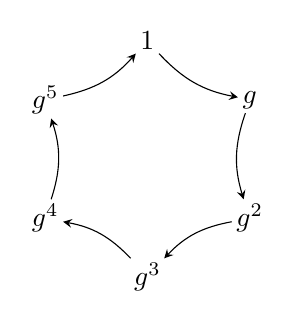
\begin{tikzpicture}[every node/.style={inner sep=1.5pt},scale=1.5,>=stealth]
  \node (n0) at (90:1)  {$1$};
  \node (n1) at (30:1)  {$g$};
  \node (n2) at (-30:1) {$g^2$};
  \node (n3) at (-90:1) {$g^3$};
  \node (n4) at (210:1) {$g^4$};
  \node (n5) at (150:1) {$g^5$};
  \draw[->] (n0) to[bend right=18] (n1);
  \draw[->] (n1) to[bend right=18] (n2);
  \draw[->] (n2) to[bend right=18] (n3);
  \draw[->] (n3) to[bend right=18] (n4);
  \draw[->] (n4) to[bend right=18] (n5);
  \draw[->] (n5) to[bend right=18] (n0);
\end{tikzpicture}\end{center}

\begin{pitfall}
When reducing $x^t$, reduce the \emph{exponent} mod $\ord{x}$, not mod $|G|$ unless $x$ generates all of $G$. In $D_8$, $\ord{r}=4$ (so reduce mod $4$), even though $|D_8|=8$; using $8$ only gives $r^{103}=r^7$, which is true (as $4\mid8$) but must still be reduced to $r^3$.
\end{pitfall}

\subsection*{The Order of a Power}

If we know $\ord{x}=n$, what is $\ord{x^a}$? The answer is governed entirely by a single $\gcd$ computation. This one proposition is the engine behind counting generators of a cyclic group, finding all elements of a given order, and reading off the subgroup lattice of $\Zn{n}$.

\begin{proposition}\label{p:orderpower@c2}
Let $x$ be an element of a group $G$ and let $a\in\Z$.
\begin{enumerate}
\item If $\ord{x}=n<\infty$, then $\ord{x^a}=\dfrac{n}{\gcd(n,a)}$.
\item If $\ord{x}=\infty$ and $a\neq 0$, then $\ord{x^a}=\infty$.
\end{enumerate}
\end{proposition}

\begin{proof}
(1) Write $d=\gcd(n,a)$, and set $a=d a'$, $n=d n'$ with $\gcd(a',n')=1$. We claim $\ord{x^a}=n'=n/d$. First, $(x^a)^{n'}=x^{a n'}=x^{d a' n'}=x^{a' n}=(x^n)^{a'}=1^{a'}=1$, so $\ord{x^a}$ divides $n'$. Conversely, suppose $(x^a)^k=1$, i.e. $x^{ak}=1$. Since $\ord{x}=n$, this forces $n\st ak$, that is $d n'\st d a' k$, hence $n'\st a' k$. As $\gcd(a',n')=1$, Euclid's lemma gives $n'\st k$. Thus every $k$ killing $x^a$ is a multiple of $n'$, so $\ord{x^a}=n'=n/d$.

\noindent(2) Suppose $\ord{x}=\infty$ and $a\neq 0$. If $(x^a)^k=x^{ak}=1$ for some $k>0$, then $ak\neq 0$ would be a positive or negative integer with $x^{ak}=1$, contradicting that no nonzero power of $x$ is the identity. Hence no positive $k$ works and $\ord{x^a}=\infty$.
\end{proof}

\begin{remark}
The factor that shrinks the order is $\gcd(n,a)$, \emph{not} $a$. Powering by $a$ ``uses up'' only the part of $a$ that overlaps $n$; the coprime part $a'$ is invisible to the order because it is a unit modulo $n'$.
\end{remark}

\begin{method}{Compute the order of a power $x^a$ when $\ord{x}=n$ is known}
\textbf{Recognition trigger:} use this whenever you must find the order of a power of an element \emph{whose own order you already know} -- e.g. $\ord{x^a}$ with $\ord{x}=n$ given, $\ord{\overline a}$ in $\Zn{n}$ (here the ``base'' is $\overline 1$ with order $n$ and $\overline a=a\cdot\overline 1$), or $\ord{r^a}$ in $D_{2n}$ with $\ord{r}=n$. Also for $\ord{\sigma^a}$ where $\sigma$ is a single $n$-cycle in $S_m$.
\begin{enumerate}
\item Identify $n=\ord{x}$ (the order of the \emph{base}) and the exponent $a$. In $\Zn{n}$, the operation is addition, so $x^a$ means the element $\overline a=\underbrace{\overline 1+\cdots+\overline 1}_{a}$ and $n$ is the modulus.
\item Compute $d=\gcd(n,a)$ (Euclidean algorithm).
\item Output $\ord{x^a}=n/d$.
\item \textbf{Check:} verify $d\st n$ so the answer is an integer, and confirm $(x^a)^{n/d}=x^{an/d}=x^{(a/d)n}=1$ since $d\st a$.
\end{enumerate}
\end{method}

\begin{pitfall}
Do \textbf{not} answer $n/a$. The shrink factor is $\gcd(n,a)$, never $a$ alone. E.g. $\ord{\overline 8}$ in $\Zn{12}$ is $12/\gcd(12,8)=12/4=3$, not $12/8$ (which is not even an integer). Only when $a\st n$ \emph{and} $\gcd(n,a)=a$ do $n/a$ and $n/\gcd(n,a)$ coincide.
\end{pitfall}

\begin{wex}{$\ord{\overline 8}$ in $\Zn{12}$}
Compute the order of $\overline 8$ in $\Zn{12}$.
\wrec The ambient group $\Zn{12}$ is cyclic of order $12$, generated by $\overline 1$ with $\ord{\overline 1}=12$. The element $\overline 8=8\cdot\overline 1$ is a ``power'' (additive multiple) of the order-$12$ generator, so this is exactly the order-of-a-power setup with $n=12$, $a=8$.
\wsol
Step 1: $n=12$, $a=8$.
Step 2: $d=\gcd(12,8)=4$ (since $12=1\cdot 8+4$, $8=2\cdot 4$).
Step 3: $\ord{\overline 8}=12/4=3$.
Check: $3\cdot\overline 8=\overline{24}=\overline 0$, and the smaller multiples $1\cdot\overline 8=\overline 8\neq\overline 0$, $2\cdot\overline 8=\overline{16}=\overline 4\neq\overline 0$. So the order is indeed $3$. \checkmark
\end{wex}

\begin{wex}{$\ord{\overline{30}}$ in $\Zn{54}$}
Compute the order of $\overline{30}$ in $\Zn{54}$.
\wrec Cyclic group of order $54$; $\overline{30}=30\cdot\overline 1$ is a multiple of the order-$54$ generator. Order-of-a-power with $n=54$, $a=30$.
\wsol
Step 1: $n=54$, $a=30$.
Step 2: $d=\gcd(54,30)$. Euclid: $54=1\cdot 30+24$, $30=1\cdot 24+6$, $24=4\cdot 6$, so $d=6$.
Step 3: $\ord{\overline{30}}=54/6=9$.
Check: $9\cdot\overline{30}=\overline{270}$, and $270=5\cdot 54$, so $\overline{270}=\overline 0$. A proper divisor would have to divide $9$; e.g. $3\cdot\overline{30}=\overline{90}=\overline{90-54}=\overline{36}\neq\overline 0$. So the order is $9$. \checkmark
\end{wex}

\begin{wex}{$\ord{r^6}$ where $\ord{r}=12$ in $D_{24}$}
In the dihedral group $D_{24}$ of order $24$ (so $r^{12}=1$, $\ord{r}=12$), compute $\ord{r^6}$.
\wrec The base is the rotation $r$ with known order $\ord{r}=12$, and $r^6$ is an honest power of it. This is the multiplicative version of the same rule, $n=12$, $a=6$. (We do not need $s$ at all; $r^6$ lives in the rotation subgroup $\gen{r}$.)
\wsol
Step 1: $n=12$, $a=6$.
Step 2: $d=\gcd(12,6)=6$.
Step 3: $\ord{r^6}=12/6=2$.
Check: $(r^6)^2=r^{12}=1$, and $r^6\neq 1$ (since $6<12$). So $\ord{r^6}=2$; indeed $r^6$ is the unique rotation of order $2$, the half-turn. \checkmark
\end{wex}

\begin{wex}{$\ord{\overline 9}$ in $\Zn{24}$}
Compute the order of $\overline 9$ in $\Zn{24}$.
\wrec Cyclic of order $24$, base $\overline 1$ of order $24$, and $\overline 9=9\cdot\overline 1$. Order-of-a-power with $n=24$, $a=9$. The tempting wrong move $24/9$ is not an integer -- a red flag that you must use $\gcd$, not $a$.
\wsol
Step 1: $n=24$, $a=9$.
Step 2: $d=\gcd(24,9)$. Euclid: $24=2\cdot 9+6$, $9=1\cdot 6+3$, $6=2\cdot 3$, so $d=3$.
Step 3: $\ord{\overline 9}=24/3=8$.
Check: $8\cdot\overline 9=\overline{72}=\overline 0$ since $72=3\cdot 24$. Halving: $4\cdot\overline 9=\overline{36}=\overline{12}\neq\overline 0$, so the order is not $4$; it is the full $8$. \checkmark
\end{wex}

\begin{wex}{$\ord{(1\,2\,3\,4\,5\,6)^4}$ in $S_6$}
Let $\sigma=(1\,2\,3\,4\,5\,6)\in S_6$. Compute $\ord{\sigma^4}$.
\wrec A single $6$-cycle has order $6$, so $\ord{\sigma}=6$ is known; $\sigma^4$ is a power of it. Order-of-a-power with $n=6$, $a=4$. (Bonus: the proposition gives the order instantly, and we can cross-check via the explicit cycle structure.)
\wsol
Step 1: $n=\ord{\sigma}=6$ (length of the cycle), $a=4$.
Step 2: $d=\gcd(6,4)=2$.
Step 3: $\ord{\sigma^4}=6/2=3$.
Check (explicit cycle structure): $\sigma$ sends $i\mapsto i+1\pmod 6$, so $\sigma^4$ sends $i\mapsto i+4\pmod 6$. Tracking $1\mapsto 5\mapsto 3\mapsto 1$ and $2\mapsto 6\mapsto 4\mapsto 2$ gives
\[
\sigma^4=(1\,5\,3)(2\,6\,4),
\]
a product of two disjoint $3$-cycles, whose order is $\lcm(3,3)=3$. Matches. \checkmark
\end{wex}

\begin{wex}{All $a$ with $\ord{x^a}=n$ (generators preview)}
Let $\ord{x}=n$. Find exactly which exponents $a\in\{0,1,\dots,n-1\}$ satisfy $\ord{x^a}=n$. Apply it to $n=12$.
\wrec We want the power $x^a$ to have the \emph{full} order $n$, i.e. $x^a$ generates $\gen{x}$. By the proposition $\ord{x^a}=n/\gcd(n,a)$, demanding this equal $n$ is a $\gcd$ condition -- the recognition trigger is ``solve for the exponent that makes the order maximal.''
\wsol
We need $\dfrac{n}{\gcd(n,a)}=n$, i.e. $\gcd(n,a)=1$. So
\[
\ord{x^a}=n \iff \gcd(n,a)=1.
\]
The number of such $a$ in $\{0,1,\dots,n-1\}$ is Euler's $\varphi(n)$; these are precisely the generators of the cyclic group $\gen{x}$.

For $n=12$: the $a$ with $\gcd(12,a)=1$ are $a\in\{1,5,7,11\}$, giving $\varphi(12)=4$ generators. 
Check: e.g. $\ord{x^5}=12/\gcd(12,5)=12/1=12$ (full order, good), whereas $\ord{x^4}=12/\gcd(12,4)=12/4=3\neq 12$ (not a generator), confirming $a=4$ is correctly excluded. \checkmark
\end{wex}

\begin{remark}
The map $a\mapsto n/\gcd(n,a)$ shows the possible orders of elements of a cyclic group $\gen{x}$ of order $n$ are exactly the divisors of $n$: as $\gcd(n,a)$ ranges over the divisors $d\st n$, the order $n/d$ ranges over all divisors of $n$. The next diagram shows this for $n=12$: each subgroup $\gen{x^d}=\gen{x^{n/(n/d)}}$ has order $n/d$, and the lattice of subgroups of $\gen{x}$ mirrors the divisor lattice of $12$.
\end{remark}

\begin{center}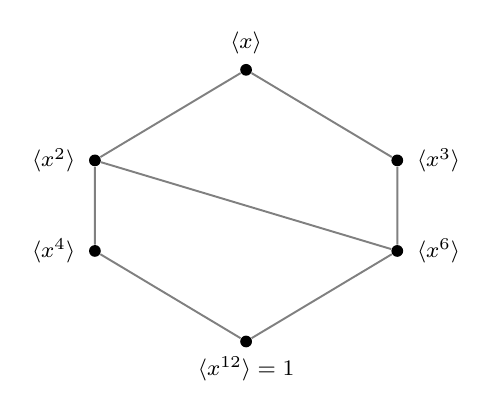
\begin{tikzpicture}[yscale=1.15,xscale=1.6]
  \node[ltdot] (bot) at (0,0) {};
  \node[ltdot] (g4) at (-1.2,1) {};
  \node[ltdot] (g6) at (1.2,1) {};
  \node[ltdot] (g2) at (-1.2,2) {};
  \node[ltdot] (g3) at (1.2,2) {};
  \node[ltdot] (top) at (0,3) {};
  \begin{scope}[ltedge]
    \draw (bot)--(g4);
    \draw (bot)--(g6);
    \draw (g4)--(g2);
    \draw (g6)--(g2);
    \draw (g6)--(g3);
    \draw (g2)--(top);
    \draw (g3)--(top);
  \end{scope}
  \node[ltlab,below=1.5pt of bot] {$\gen{x^{12}}=1$};
  \node[ltlab,left=3pt of g4] {$\gen{x^4}$};
  \node[ltlab,right=3pt of g6] {$\gen{x^6}$};
  \node[ltlab,left=3pt of g2] {$\gen{x^2}$};
  \node[ltlab,right=3pt of g3] {$\gen{x^3}$};
  \node[ltlab,above=1.5pt of top] {$\gen{x}$};
\end{tikzpicture}\end{center}

\noindent Here $\ord{\gen{x}}=12$, $\ord{\gen{x^2}}=6$, $\ord{\gen{x^3}}=4$, $\ord{\gen{x^4}}=3$, $\ord{\gen{x^6}}=2$, $\ord{\gen{x^{12}}}=1$ -- precisely the orders $12/\gcd(12,a)$ realized as $a$ varies, one subgroup per divisor of $12$.

\begin{pitfall}
When computing $\ord{\overline a}$ in $\Zn{n}$, take the $\gcd$ with the \emph{modulus} $n$, not with anything you mentally simplified $\overline a$ to. For instance in $\Zn{24}$, $\ord{\overline{30}}=\ord{\overline 6}=24/\gcd(24,6)=4$; reducing $30$ to $6$ first is fine, but you must still pair it with $n=24$, never with $30$ or with a different modulus.
\end{pitfall}

\subsection*{Generators of Cyclic Groups: $\gen{x^a}=\gen{x}$, Counting via $\varphi$}

This section answers one precise question: given a cyclic group $\gen{x}$, exactly which powers $x^a$ are themselves generators? The clean answer is governed entirely by $\gcd(a,n)$ when $\ord{x}=n$, and the count is Euler's $\varphi(n)$.

\begin{definition}\label{d:generator@c2}
Let $G$ be a group and $x\in G$. We say $x$ \emph{generates} $G$, and call $x$ a \emph{generator}, if $G=\gen{x}=\{x^k : k\in\Z\}$. A group with at least one generator is \emph{cyclic}.
\end{definition}

\begin{proposition}\label{p:gens@c2}
Let $G=\gen{x}$ be cyclic and let $a\in\Z$.
\begin{enumerate}
\item If $\ord{x}=n<\infty$, then $\gen{x^a}=\gen{x}$ if and only if $\gcd(a,n)=1$. Consequently the number of generators of $G$ equals $\varphi(n)$, the count of residues in $\{1,2,\dots,n\}$ coprime to $n$.
\item If $\ord{x}=\infty$, then $\gen{x^a}=\gen{x}$ if and only if $a=\pm1$. Thus an infinite cyclic group has exactly two generators, $x$ and $x\inv$.
\end{enumerate}
\end{proposition}

\begin{proof}
\textbf{(1)} Recall the order formula: for $\ord{x}=n$, one has $\ord{x^a}=n/\gcd(a,n)$, so $\bigl|\gen{x^a}\bigr|=n/\gcd(a,n)$. Now $\gen{x^a}=\gen{x}$ iff these subgroups have equal order, i.e.\ iff $n/\gcd(a,n)=n$, i.e.\ iff $\gcd(a,n)=1$.

For the count: every element of $G=\gen{x}$ is $x^a$ for a unique residue $a\in\{0,1,\dots,n-1\}$, and $x^a$ is a generator iff $\gcd(a,n)=1$. The number of such $a$ is by definition $\varphi(n)$. (Equivalently, working in $\Zn{n}$, the generators are exactly the units $\Zns{n}$.)

\textbf{(2)} Suppose $\ord{x}=\infty$, so the map $k\mapsto x^k$ is injective and $\gen{x^a}=\{x^{ak}:k\in\Z\}=\{x^m : m\in a\Z\}$. Then $\gen{x^a}=\gen{x}$ iff $a\Z=\Z$ iff $a$ is a unit of $\Z$, i.e.\ $a=\pm1$. Since $x\ne x\inv$ here (else $x^2=1$, contradicting infinite order), there are exactly two generators.
\end{proof}

\begin{remark}\label{r:zn@c2}
The model case is $G=\Zn{n}=\gen{\overline1}$ under addition, where $x=\overline1$ and ``$x^a$'' becomes ``$a\cdot\overline1=\overline a$.'' Proposition~\ref{p:gens@c2}(1) then reads: $\overline a$ generates $\Zn{n}$ iff $\gcd(a,n)=1$. So the generators of $\Zn{n}$ are precisely the residues coprime to $n$, and there are $\varphi(n)$ of them.
\end{remark}

\begin{method}{Find all generators of a cyclic group of order $n$ (and count them)}
\textbf{Trigger:} use this whenever you must list/count generators of $\Zn{n}$, or decide which $x^a$ generate a cyclic group $\gen{x}$ with $\ord{x}=n$.
\begin{enumerate}
\item Identify $n=\ord{x}$ (for $\Zn{n}$, $n$ is the modulus).
\item A power $x^a$ (resp.\ residue $\overline a$) is a generator $\eqv \gcd(a,n)=1$. List all $a\in\{1,2,\dots,n\}$ (or $\{0,\dots,n-1\}$) with $\gcd(a,n)=1$.
\item The \emph{number} of generators is $\varphi(n)$. To compute $\varphi(n)$ fast, factor $n=p_1^{e_1}\cdots p_r^{e_r}$ and use
\[
\varphi(n)=\prod_{i=1}^{r}\bigl(p_i^{e_i}-p_i^{e_i-1}\bigr)=n\prod_{i=1}^{r}\Bigl(1-\tfrac1{p_i}\Bigr).
\]
\item Sanity check: $\varphi(n)$ should equal the length of the list from step 2.
\end{enumerate}
\end{method}

\begin{method}{Compute $\varphi(n)$ from the prime factorization}
\textbf{Trigger:} you need the \emph{count} of generators/units mod $n$ but listing them is impractical.
\begin{enumerate}
\item Factor $n=p_1^{e_1}\cdots p_r^{e_r}$ into distinct primes.
\item For each prime power use $\varphi(p^e)=p^e-p^{e-1}=p^{e-1}(p-1)$.
\item Multiply: $\varphi$ is multiplicative on coprime factors, so $\varphi(n)=\prod_i\varphi(p_i^{e_i})$.
\item Special case worth memorizing: $\varphi(p)=p-1$ for $p$ prime.
\end{enumerate}
\end{method}

\begin{pitfall}
$\gcd(a,n)=1$ is required, \emph{not} ``$a$ is prime'' and \emph{not} ``$a<n$.'' E.g.\ $\overline9$ generates $\Zn{10}$ (since $\gcd(9,10)=1$) even though $9$ is composite, while $\overline2,\overline4,\overline6,\overline8$ do not. Always test the gcd, never primality.
\end{pitfall}

\begin{wex}{All generators of $\Zn{12}$}
List every generator of $\Zn{12}$.
\wrec This is the model case of Proposition~\ref{p:gens@c2}(1) via Remark~\ref{r:zn@c2}: generators of $\Zn{n}$ are the residues $\overline a$ with $\gcd(a,n)=1$. Trigger: ``generators of $\Zn{n}$'' $\imp$ ``residues coprime to $n$.''
\wsol Here $n=12=2^2\cdot3$. Test $\gcd(a,12)$ for $a=1,\dots,11$:
\[
\begin{array}{c|cccccccccccc}
a & 1&2&3&4&5&6&7&8&9&10&11\\\hline
\gcd(a,12) & 1&2&3&4&1&6&1&4&3&2&1
\end{array}
\]
The $a$ with gcd $1$ are $a=1,5,7,11$. So the generators are
\[
\overline1,\ \overline5,\ \overline7,\ \overline{11}.
\]
\emph{Check:} count $=4$, and $\varphi(12)=\varphi(2^2)\varphi(3)=(4-2)(3-1)=2\cdot2=4$. Match. As a spot-verify that $\overline5$ generates: $1\cdot\overline5=\overline5,\ 2\cdot\overline5=\overline{10},\ 3\cdot\overline5=\overline{3},\ 4\cdot\overline5=\overline8,\ 5\cdot\overline5=\overline1$, and continuing hits all $12$ residues since $\ord{\overline5}=12/\gcd(5,12)=12$.
\end{wex}

\begin{wex}{All generators of $\Zn{10}$}
List every generator of $\Zn{10}$ and confirm the count.
\wrec Same trigger as the previous example: ``generators of $\Zn{n}$'' $\imp$ residues coprime to $n=10$. Use Proposition~\ref{p:gens@c2}(1)/Remark~\ref{r:zn@c2}.
\wsol Here $n=10=2\cdot5$. The residues $a\in\{1,\dots,9\}$ with $\gcd(a,10)=1$ avoid the factors $2$ and $5$:
\[
a=1,\ 3,\ 7,\ 9\quad(\text{we drop }2,4,6,8\text{ even, and }5).
\]
So the generators are
\[
\overline1,\ \overline3,\ \overline7,\ \overline9.
\]
\emph{Check:} $\varphi(10)=\varphi(2)\varphi(5)=(2-1)(5-1)=1\cdot4=4$, matching the four listed. Verify $\overline3$ is a generator: $\ord{\overline3}=10/\gcd(3,10)=10/1=10$, so $\gen{\overline3}=\Zn{10}$; indeed $\overline3,\overline6,\overline9,\overline2,\overline5,\overline8,\overline1,\overline4,\overline7,\overline0$ runs through all residues.
\end{wex}

\begin{wex}{Number of generators of $\Zn{49000}$}
How many generators does $\Zn{49000}$ have? (Listing is hopeless; count via $\varphi$.)
\wrec The trigger is a \emph{count} request with a large modulus: use the second method box, $\varphi(n)$ from the prime factorization, since the number of generators of $\Zn{n}$ is $\varphi(n)$ by Proposition~\ref{p:gens@c2}(1).
\wsol Factor: $49000=49\cdot1000=7^2\cdot(2^3\cdot5^3)=2^3\cdot5^3\cdot7^2$. Use $\varphi(p^e)=p^e-p^{e-1}$ on each prime power:
\[
\varphi(2^3)=8-4=4,\qquad \varphi(5^3)=125-25=100,\qquad \varphi(7^2)=49-7=42.
\]
By multiplicativity,
\[
\varphi(49000)=4\cdot100\cdot42=400\cdot42=16800.
\]
\emph{Check} via the product form: $49000\bigl(1-\tfrac12\bigr)\bigl(1-\tfrac15\bigr)\bigl(1-\tfrac17\bigr)=49000\cdot\tfrac12\cdot\tfrac45\cdot\tfrac67=49000\cdot\tfrac{24}{70}=49000\cdot\tfrac{12}{35}=1400\cdot12=16800$. Match. So $\Zn{49000}$ has $\boxed{16800}$ generators.
\end{wex}

\begin{wex}{Which $x^a$ generate $\gen{x}$ when $\ord{x}=18$}
Let $\ord{x}=18$. For which exponents $a$ with $0\le a\le 17$ is $x^a$ a generator of $\gen{x}$?
\wrec Now the group is abstract cyclic of order $18$, not literally $\Zn{18}$, but Proposition~\ref{p:gens@c2}(1) applies verbatim: $x^a$ generates iff $\gcd(a,18)=1$. Trigger: ``$\ord{x}=n$, which $x^a$ generate'' $\imp$ gcd test against $n$.
\wsol Here $n=18=2\cdot3^2$. The valid $a\in\{0,\dots,17\}$ are those coprime to $18$, i.e.\ avoiding factors $2$ and $3$:
\[
a=1,\ 5,\ 7,\ 11,\ 13,\ 17.
\]
So the generators are $x,\ x^5,\ x^7,\ x^{11},\ x^{13},\ x^{17}$.
\emph{Check:} $\varphi(18)=\varphi(2)\varphi(3^2)=(2-1)(9-3)=1\cdot6=6$, matching the six listed. Spot-verify $x^{12}$ is \emph{not} a generator: $\gcd(12,18)=6$, so $\ord{x^{12}}=18/6=3\ne18$; indeed $\gen{x^{12}}=\{1,x^{12},x^6\}$ has order $3$.
\end{wex}

\begin{wex}{Generators of $(\Z,+)$}
Find all generators of the infinite cyclic group $(\Z,+)=\gen{1}$.
\wrec The trigger is ``infinite order'': $\ord{1}=\infty$ in $(\Z,+)$, so Proposition~\ref{p:gens@c2}(2) applies and only $\pm1$ can generate. Do \emph{not} try a gcd-with-$n$ test; there is no finite $n$.
\wsol Writing the group additively, ``$x^a$'' for $x=1$ is the multiple $a\cdot1=a$, and $\gen{a}=a\Z=\{\dots,-2a,-a,0,a,2a,\dots\}$. We need $a\Z=\Z$. The only integers $a$ with $a\Z=\Z$ are the units of $\Z$, namely $a=\pm1$:
\[
\gen{1}=\Z,\qquad \gen{-1}=\Z,
\]
while for $|a|\ge2$ we get a proper subgroup (e.g.\ $\gen{2}=2\Z$ misses every odd integer). So the only generators are $\boxed{\pm1}$.
\emph{Check:} an infinite cyclic group has exactly two generators by Proposition~\ref{p:gens@c2}(2); here $1\ne-1$, consistent. Contrast: $0$ is not a generator since $\gen{0}=\{0\}$.
\end{wex}

\begin{wex}{The formula $\varphi(p^k)=p^k-p^{k-1}$, with $p^k=27$}
Derive $\varphi(p^k)=p^k-p^{k-1}$ and apply it to count generators of $\Zn{27}$.
\wrec Trigger: the modulus is a prime power $p^k$. Counting units/generators reduces to ``how many residues are coprime to $p^k$,'' and the only obstruction is divisibility by $p$. This is the building block of the $\varphi$ method box.
\wsol An integer $a\in\{1,\dots,p^k\}$ fails $\gcd(a,p^k)=1$ exactly when $p\mid a$. The multiples of $p$ in that range are $p,2p,\dots,p^{k-1}\cdot p=p^k$, which number $p^{k-1}$. Hence the coprime residues number
\[
\varphi(p^k)=p^k-p^{k-1}=p^{k-1}(p-1).
\]
For $p=3,\ k=3$, i.e.\ $p^k=27$:
\[
\varphi(27)=27-9=18=3^2(3-1)=9\cdot2.
\]
So $\Zn{27}$ has $18$ generators (the residues $1,2,4,5,7,8,10,11,13,14,16,17,19,20,22,23,25,26$, i.e.\ everything not divisible by $3$).
\emph{Check:} the non-generators are the multiples of $3$ in $\{1,\dots,27\}$: $3,6,9,12,15,18,21,24,27$, exactly $9=3^{3-1}$ of them, and $27-9=18$. Match.
\end{wex}

The subgroup lattice below records the orders that actually occur as $\ord{x^a}=n/\gcd(a,n)$ for $\gen{x}$ with $\ord{x}=12$; the generators ($\gcd=1$) all sit at the top vertex $\gen{x}$, since each generates the whole group.

\begin{center}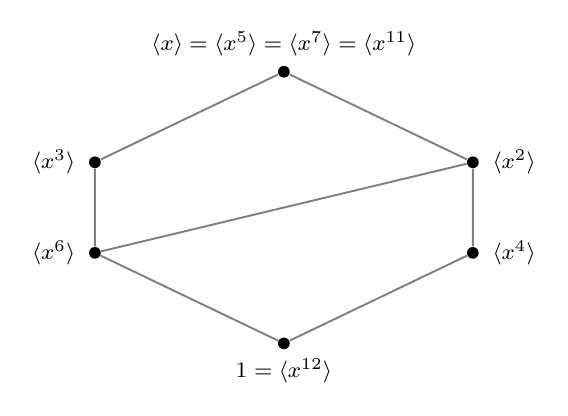
\begin{tikzpicture}[yscale=1.15,xscale=1.5]
  \node[ltdot] (bot) at (0,0) {};
  \node[ltdot] (c2) at (-1.6,1) {};
  \node[ltdot] (c3) at (1.6,1) {};
  \node[ltdot] (c4) at (-1.6,2) {};
  \node[ltdot] (c6) at (1.6,2) {};
  \node[ltdot] (top) at (0,3) {};
  \begin{scope}[ltedge]
    \draw (bot)--(c2);
    \draw (bot)--(c3);
    \draw (c2)--(c4);
    \draw (c2)--(c6);
    \draw (c3)--(c6);
    \draw (c4)--(top);
    \draw (c6)--(top);
  \end{scope}
  \node[ltlab,below=1.5pt of bot] {$1=\gen{x^{12}}$};
  \node[ltlab,left=3pt of c2] {$\gen{x^6}$};
  \node[ltlab,right=3pt of c3] {$\gen{x^4}$};
  \node[ltlab,left=3pt of c4] {$\gen{x^3}$};
  \node[ltlab,right=3pt of c6] {$\gen{x^2}$};
  \node[ltlab,above=1.5pt of top] {$\gen{x}=\gen{x^5}=\gen{x^7}=\gen{x^{11}}$};
\end{tikzpicture}\end{center}

\begin{pitfall}
Two distinct exponents can give the \emph{same} subgroup. In the lattice above $\gen{x^2}$ and $\gen{x^{10}}$ coincide (both have order $6$, and $\gcd(2,12)=\gcd(10,12)=2$). The four exponents $a=1,5,7,11$ all yield the \emph{single} top subgroup $\gen{x}$; ``$\varphi(12)=4$ generators'' counts \emph{elements} $x^a$, not distinct subgroups.
\end{pitfall}

\subsection*{The subgroup lattice of a cyclic group}

Everything in this section flows from one structural fact: a cyclic group has \emph{exactly one} subgroup of each order dividing the group order, and these are precisely all of them. Concretely, the lattice of subgroups of $\Zn{n}$ is a perfect copy of the lattice of divisors of $n$, turned upside down. Once you internalize the dictionary
\[
\text{subgroups of }\gen{x}\ \longleftrightarrow\ \text{divisors of }n,
\qquad
\gen{x^a}=\gen{x^{\gcd(a,n)}},
\]
listing subgroups becomes pure arithmetic with $\gcd$ and divisors.

\begin{theorem}[Subgroups of a cyclic group, D\&F 2.3 Thm.\ 7]\label{t:cycsub@c2}
Let $H=\gen{x}$ be cyclic.
\begin{enumerate}
\item Every subgroup of $H$ is cyclic. More precisely, if $K\sgr H$ and $K\neq\{1\}$, then $K=\gen{x^d}$ where $d$ is the smallest positive integer with $x^d\in K$.
\item If $\ord x=\infty$, then the distinct subgroups are $\gen{x^d}$ for $d=0,1,2,\dots$, all distinct.
\item If $\ord x=n<\infty$, then for each positive divisor $d\mid n$ there is a \emph{unique} subgroup of order $d$, namely $\gen{x^{n/d}}$. These are all of the subgroups, so the subgroups of $\gen{x}$ correspond bijectively to the positive divisors of $n$.
\end{enumerate}
\end{theorem}

\begin{proof}
(1) Let $K\sgr\gen{x}$. If $K=\{1\}=\gen{x^0}$ we are done; otherwise pick the least positive $d$ with $x^d\in K$ (such $d$ exists by well-ordering). Then $\gen{x^d}\sgr K$. Conversely take any $x^a\in K$ and divide: $a=qd+r$ with $0\le r<d$. Then $x^r=x^a(x^d)^{-q}\in K$, and minimality of $d$ forces $r=0$, so $x^a=(x^d)^q\in\gen{x^d}$. Hence $K=\gen{x^d}$ is cyclic.

(2) If $\ord x=\infty$ and $\gen{x^d}=\gen{x^e}$ with $d,e>0$, then $x^d=x^{ek}$ for some $k$, so $d=ek$, i.e.\ $e\mid d$, and symmetrically $d\mid e$, giving $d=e$; also $\gen{x^0}=1$ differs from every $\gen{x^e}$ with $e>0$, since $x^e\ne1$. Distinct $d$ give distinct subgroups, and by (1) every subgroup is some $\gen{x^d}$.

(3) Now $\ord x=n$. By the order formula $\ord{x^k}=n/\gcd(k,n)$. For $d\mid n$, set $k=n/d$; then $\gcd(n/d,n)=n/d$, so $\ord{x^{n/d}}=n/(n/d)=d$, giving a subgroup of order $d$. For uniqueness, suppose $K\sgr\gen{x}$ has $|K|=d$. By (1) $K=\gen{x^m}$ with $m$ the least positive exponent in $K$; the same minimality argument as in (1) shows $m\mid n$ (divide $n$ by $m$: $x^n=1\in K$ forces remainder $0$). Then $|K|=\ord{x^m}=n/\gcd(m,n)=n/m=d$, so $m=n/d$ and $K=\gen{x^{n/d}}$. Thus the subgroup of order $d$ is unique. Finally every subgroup has order dividing $n$ (Lagrange), so $d\mapsto\gen{x^{n/d}}$ is a bijection from divisors of $n$ to subgroups.
\end{proof}

\begin{proposition}[The $\gcd$ collapse and the containment rule]\label{p:gcd@c2}
Let $\ord x=n$ and write everything multiplicatively (additively in $\Zn n$ this is $\overline a$).
\begin{enumerate}
\item $\gen{x^a}=\gen{x^{\gcd(a,n)}}$, and this subgroup has order $n/\gcd(a,n)$.
\item $\gen{x^a}\sgr\gen{x^b}\iff \gcd(b,n)\mid\gcd(a,n)$. Equivalently, writing $|\gen{x^a}|=n/\gcd(a,n)$, containment of the smaller into the larger matches divisibility of orders.
\end{enumerate}
\end{proposition}

\begin{proof}
(1) Let $g=\gcd(a,n)$. Since $g\mid a$, $x^a\in\gen{x^g}$, so $\gen{x^a}\sgr\gen{x^g}$. Conversely Bezout gives $g=au+nv$, hence $x^g=(x^a)^u(x^n)^v=(x^a)^u\in\gen{x^a}$, so $\gen{x^g}\sgr\gen{x^a}$. Thus they are equal; the order is $\ord{x^g}=n/\gcd(g,n)=n/g$ since $g\mid n$.

(2) By (1) we may assume $a=\gcd(a,n)$ and $b=\gcd(b,n)$ are divisors of $n$. Then $\gen{x^a}\sgr\gen{x^b}$ iff $x^a\in\gen{x^b}$ iff $x^a=x^{bk}$ for some $k$ iff $n\mid a-bk$ for some $k$ iff $\gcd(b,n)=b\mid a=\gcd(a,n)$ (the last by elementary number theory, since $b\mid n$). Note $\gen{x^a}\sgr\gen{x^b}$ means the $a$-subgroup is contained in the $b$-subgroup; as $|\gen{x^a}|=n/a$ and $|\gen{x^b}|=n/b$, $b\mid a$ says $n/a\mid n/b$, i.e.\ the order of the contained group divides the order of the container.
\end{proof}

\begin{remark}
Translation to $\Zn n$ (additive): $x^k$ becomes $\overline k=k\cdot\overline 1$, the subgroup $\gen{x^{n/d}}$ becomes $\gen{\overline{n/d}}=\{0,\,n/d,\,2(n/d),\dots\}$, and the order formula reads $\ord{\overline k}=n/\gcd(k,n)$. The collapse is $\gen{\overline a}=\gen{\overline{\gcd(a,n)}}$.
\end{remark}

\begin{method}{List ALL subgroups of $\Zn n$ (and draw the lattice)}
\textbf{Recognition trigger:} the group is cyclic of finite order $n$ (e.g.\ $\Zn n$, or any $\gen x$ with $\ord x=n$), and you must enumerate subgroups, find a specific subgroup of a given order, or decide a containment.
\begin{enumerate}
\item \textbf{Find the divisors} $d_1<d_2<\dots$ of $n$. There is exactly one subgroup per divisor, so $\#\text{subgroups}=\#\text{divisors of }n=\tau(n)$.
\item \textbf{Order $\to$ generator.} The unique subgroup of order $d$ is $\gen{\overline{n/d}}$ (the cyclic span of the step $n/d$). Its elements are the multiples of $n/d$ in $\Zn n$.
\item \textbf{Generator $\to$ order.} For an arbitrary $\overline a$, first collapse: $\gen{\overline a}=\gen{\overline{\gcd(a,n)}}$, and $\ord{\overline a}=n/\gcd(a,n)$.
\item \textbf{Containment.} $\gen{\overline a}\sgr\gen{\overline b}\iff \gcd(b,n)\mid\gcd(a,n)$. Equivalently $|\gen{\overline a}|\,\big|\,|\gen{\overline b}|$ (smaller order sits inside larger order).
\item \textbf{Lattice.} Draw the divisor lattice of $n$ \emph{upside down}, with $\gen{\overline s}$ at the divisor $s$: $\Zn n=\gen{\overline 1}$ (order $n$) goes on top, $\{0\}=\gen{\overline n}$ (order $1$) at the bottom; an edge goes between two subgroups when one order divides the other with prime index.
\end{enumerate}
\end{method}

\begin{pitfall}
The subgroup of order $d$ is $\gen{\overline{n/d}}$, NOT $\gen{\overline d}$. Mixing these up is the single most common error: in $\Zn{12}$ the order-$3$ subgroup is $\gen{\overline 4}=\{0,4,8\}$, while $\gen{\overline 3}=\{0,3,6,9\}$ has order $4$. Always convert via $d\leftrightarrow n/d$.
\end{pitfall}

\begin{pitfall}
The containment direction is reversed from divisibility of the \emph{generators-as-steps}: a \emph{smaller} step $n/d$ generates a \emph{larger} subgroup. Trust the order test: $\gen{\overline a}\sgr\gen{\overline b}$ exactly when $|\gen{\overline a}|$ divides $|\gen{\overline b}|$ (a smaller order alone is not enough: in $\Zn{12}$, $\gen{\overline 4}$ of order $3$ is not inside $\gen{\overline 3}$ of order $4$), and you check it via $\gcd(b,n)\mid\gcd(a,n)$.
\end{pitfall}

\begin{wex}{All subgroups of $\Zn{12}$}
List every subgroup of $\Zn{12}$, give its order and generator, and draw the lattice.
\wrec $\Zn{12}$ is cyclic of order $n=12$, so Theorem~\ref{t:cycsub@c2}(3) applies: subgroups correspond exactly to divisors of $12$. Trigger met (cyclic, finite, ``list all subgroups''), so run the Method box.
\wsol Divisors of $12$: $1,2,3,4,6,12$, so there are $\tau(12)=6$ subgroups. Use ``order $d\Rightarrow$ generator $\overline{12/d}$'':
\[
\begin{array}{c|c|l}
d=|H| & 12/d & H=\gen{\overline{12/d}}\\\hline
1 & 12 & \{0\}\\
2 & 6 & \gen{\overline 6}=\{0,6\}\\
3 & 4 & \gen{\overline 4}=\{0,4,8\}\\
4 & 3 & \gen{\overline 3}=\{0,3,6,9\}\\
6 & 2 & \gen{\overline 2}=\{0,2,4,6,8,10\}\\
12 & 1 & \gen{\overline 1}=\Zn{12}
\end{array}
\]
Containments by the order rule ($d_1\mid d_2\Rightarrow$ order-$d_1$ inside order-$d_2$): $\{0\}\subset$ everything; $\gen{\overline 6}\subset\gen{\overline 2}$ (since $2\mid 6$) and $\gen{\overline 6}\subset\gen{\overline 3}$ (since $2\mid 4$); $\gen{\overline 4}\subset\gen{\overline 2}$ ($3\mid 6$); $\gen{\overline 3}\subset\gen{\overline 1}$, etc.
\begin{center}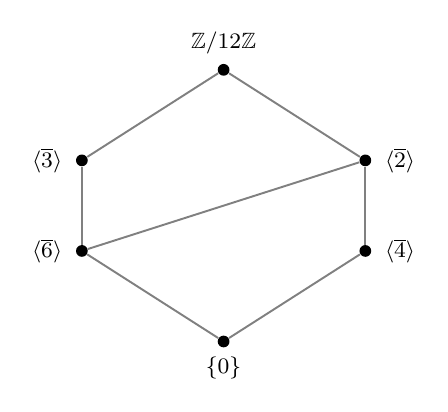
\begin{tikzpicture}[yscale=1.15,xscale=1.5]
  \node[ltdot] (bot) at (0,0) {};
  \node[ltdot] (o2) at (-1.2,1) {};
  \node[ltdot] (o3) at (1.2,1) {};
  \node[ltdot] (o4) at (-1.2,2) {};
  \node[ltdot] (o6) at (1.2,2) {};
  \node[ltdot] (top) at (0,3) {};
  \begin{scope}[ltedge]
    \draw (bot)--(o2);
    \draw (bot)--(o3);
    \draw (o2)--(o4);
    \draw (o2)--(o6);
    \draw (o3)--(o6);
    \draw (o4)--(top);
    \draw (o6)--(top);
  \end{scope}
  \node[ltlab,below=1.5pt of bot] {$\{0\}$};
  \node[ltlab,left=3pt of o2] {$\gen{\overline 6}$};
  \node[ltlab,right=3pt of o3] {$\gen{\overline 4}$};
  \node[ltlab,left=3pt of o4] {$\gen{\overline 3}$};
  \node[ltlab,right=3pt of o6] {$\gen{\overline 2}$};
  \node[ltlab,above=1.5pt of top] {$\Zn{12}$};
\end{tikzpicture}\end{center}
(Orders bottom-up: $1$; $2,3$; $4,6$; $12$.) \textbf{Check:} $6$ subgroups $=\tau(12)$; each listed order divides $12$ exactly once. Correct.
\end{wex}

\begin{wex}{All subgroups of $\Zn{30}$}
List every subgroup of $\Zn{30}$ with order and generator, and draw the lattice.
\wrec Cyclic of order $30=2\cdot 3\cdot 5$. Theorem~\ref{t:cycsub@c2}(3): subgroups $\leftrightarrow$ divisors of $30$. Method box applies.
\wsol Divisors of $30$: $1,2,3,5,6,10,15,30$, so $\tau(30)=8$ subgroups. Generator of the order-$d$ subgroup is $\overline{30/d}$:
\[
\begin{array}{c|c|l}
d & 30/d & H=\gen{\overline{30/d}}\\\hline
1 & 30 & \{0\}\\
2 & 15 & \gen{\overline{15}}=\{0,15\}\\
3 & 10 & \gen{\overline{10}}=\{0,10,20\}\\
5 & 6 & \gen{\overline 6}=\{0,6,12,18,24\}\\
6 & 5 & \gen{\overline 5}\\
10 & 3 & \gen{\overline 3}\\
15 & 2 & \gen{\overline 2}\\
30 & 1 & \gen{\overline 1}=\Zn{30}
\end{array}
\]
Containment by orders: $2\mid 6,10$; $3\mid 6,15$; $5\mid 10,15$; $6\mid 30$; $10\mid 30$; $15\mid 30$. So the lattice is the cube of divisors of $30$ (a Boolean lattice on the primes $2,3,5$), flipped.
\begin{center}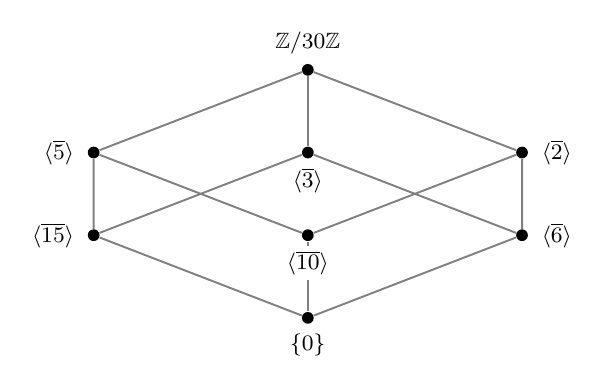
\begin{tikzpicture}[yscale=1.05,xscale=1.7]
  \node[ltdot] (bot) at (0,0) {};
  \node[ltdot] (p2) at (-1.6,1) {};
  \node[ltdot] (p3) at (0,1) {};
  \node[ltdot] (p5) at (1.6,1) {};
  \node[ltdot] (q6) at (-1.6,2) {};
  \node[ltdot] (q10) at (0,2) {};
  \node[ltdot] (q15) at (1.6,2) {};
  \node[ltdot] (top) at (0,3) {};
  \begin{scope}[ltedge]
    \draw (bot)--(p2);
    \draw (bot)--(p3);
    \draw (bot)--(p5);
    \draw (p2)--(q6);
    \draw (p2)--(q10);
    \draw (p3)--(q6);
    \draw (p3)--(q15);
    \draw (p5)--(q10);
    \draw (p5)--(q15);
    \draw (q6)--(top);
    \draw (q10)--(top);
    \draw (q15)--(top);
  \end{scope}
  \node[ltlab,below=1.5pt of bot] {$\{0\}$};
  \node[ltlab,left=3pt of p2] {$\gen{\overline{15}}$};
  \node[ltlab,below=1.5pt of p3] {$\gen{\overline{10}}$};
  \node[ltlab,right=3pt of p5] {$\gen{\overline 6}$};
  \node[ltlab,left=3pt of q6] {$\gen{\overline 5}$};
  \node[ltlab,below=1.5pt of q10] {$\gen{\overline 3}$};
  \node[ltlab,right=3pt of q15] {$\gen{\overline 2}$};
  \node[ltlab,above=1.5pt of top] {$\Zn{30}$};
\end{tikzpicture}\end{center}
Bottom row orders $2,3,5$ (the primes); middle row $6,10,15$ (products of two primes); $\gen{\overline 5}$ has order $6$, $\gen{\overline 3}$ order $10$, $\gen{\overline 2}$ order $15$. \textbf{Check:} $8=\tau(30)$ subgroups, and the lattice is the standard $2^3$ Boolean cube as expected for a product of $3$ distinct primes. Correct.
\end{wex}

\begin{wex}{All subgroups of $\Zn{16}$ (a chain)}
List every subgroup of $\Zn{16}$ and draw the lattice.
\wrec Cyclic of order $16=2^4$, a prime power. For $n=p^k$ the divisors are totally ordered ($1\mid p\mid p^2\mid\dots$), so by Theorem~\ref{t:cycsub@c2}(3) the subgroup lattice is a single chain. Recognizing $n$ is a prime power is the trigger for ``chain.''
\wsol Divisors of $16$: $1,2,4,8,16$, so $\tau(16)=5$ subgroups, each containing the previous:
\[
\begin{array}{c|c|l}
d & 16/d & H=\gen{\overline{16/d}}\\\hline
1 & 16 & \{0\}\\
2 & 8 & \gen{\overline 8}=\{0,8\}\\
4 & 4 & \gen{\overline 4}=\{0,4,8,12\}\\
8 & 2 & \gen{\overline 2}=\{0,2,4,\dots,14\}\\
16 & 1 & \Zn{16}
\end{array}
\]
Each order divides the next ($1\mid2\mid4\mid8\mid16$), so by the order rule we get a totally ordered chain $\{0\}\subset\gen{\overline 8}\subset\gen{\overline 4}\subset\gen{\overline 2}\subset\Zn{16}$.
\begin{center}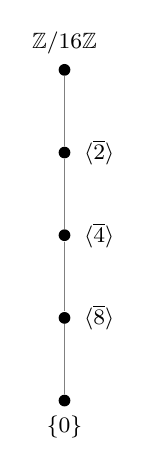
\begin{tikzpicture}[yscale=1.05,xscale=1.25]
  \node[ltdot] (bot) at (0,0) {};
  \node[ltdot] (a) at (0,1) {};
  \node[ltdot] (b) at (0,2) {};
  \node[ltdot] (c) at (0,3) {};
  \node[ltdot] (top) at (0,4) {};
  \begin{scope}[ltedge]
    \draw (bot)--(a)--(b)--(c)--(top);
  \end{scope}
  \node[ltlab,below=1.5pt of bot] {$\{0\}$};
  \node[ltlab,right=3pt of a] {$\gen{\overline 8}$};
  \node[ltlab,right=3pt of b] {$\gen{\overline 4}$};
  \node[ltlab,right=3pt of c] {$\gen{\overline 2}$};
  \node[ltlab,above=1.5pt of top] {$\Zn{16}$};
\end{tikzpicture}\end{center}
\textbf{Check:} $5=\tau(16)$, and a $p$-group cyclic lattice must be a chain --- confirmed, no branching. Correct.
\end{wex}

\begin{wex}{Collapsing $\gen{\overline{18}}$ in $\Zn{24}$}
Identify the subgroup $\gen{\overline{18}}$ of $\Zn{24}$: find its order, a canonical generator, and list its elements.
\wrec An arbitrary generator $\overline{18}$ with $18\nmid 24$ --- this is the trigger for Proposition~\ref{p:gcd@c2}(1), the $\gcd$ collapse $\gen{\overline a}=\gen{\overline{\gcd(a,n)}}$.
\wsol Here $n=24$, $a=18$. Compute $\gcd(18,24)$: $24=18+6$, $18=3\cdot 6$, so $\gcd=6$. By the collapse rule,
\[
\gen{\overline{18}}=\gen{\overline{\gcd(18,24)}}=\gen{\overline 6},\qquad \ord{\overline{18}}=\frac{24}{\gcd(18,24)}=\frac{24}{6}=4.
\]
Elements: multiples of $6$ in $\Zn{24}$, namely $\{0,6,12,18\}$. Sanity from the other side: $\overline{18}=3\cdot\overline 6$ and $\gcd(3,4)=1$, so $\overline{18}$ is itself a generator of the order-$4$ group $\gen{\overline 6}$ --- consistent. \textbf{Check:} $\gen{\overline{18}}=\{0,18,\overline{36}=\overline{12},\overline{54}=\overline 6,\overline{72}=\overline 0\}=\{0,18,12,6\}$, four elements, matches order $4$. Correct.
\end{wex}

\begin{wex}{The unique subgroup of order $6$ in $\Zn{30}$}
Find \emph{the} subgroup of order $6$ in $\Zn{30}$ and explain why it is the only one.
\wrec Asked for a subgroup of a specified order $d=6$ in a cyclic group with $6\mid 30$. Theorem~\ref{t:cycsub@c2}(3) guarantees existence and \emph{uniqueness}, and names it $\gen{\overline{n/d}}$.
\wsol Since $6\mid 30$, the unique order-$6$ subgroup is
\[
\gen{\overline{30/6}}=\gen{\overline 5}=\{0,5,10,15,20,25\}.
\]
Verify the order: $\ord{\overline 5}=30/\gcd(5,30)=30/5=6$. Uniqueness: if $K$ had order $6$ then by the theorem $K=\gen{\overline{30/6}}=\gen{\overline 5}$; there is no choice. As a cross-check on the ``which generator'' question, any $\overline a$ with $\gcd(a,30)=5$ generates this same group: e.g.\ $\gcd(25,30)=5$, so $\gen{\overline{25}}=\gen{\overline 5}$ too (different generator, same subgroup). \textbf{Check:} $\{0,5,10,15,20,25\}$ has $6$ elements and is closed (sums of multiples of $5$ are multiples of $5$). Correct.
\end{wex}

\begin{wex}{A containment decided purely by the $\gcd$ rule}
In $\Zn{36}$, decide whether $\gen{\overline{8}}\sgr\gen{\overline{6}}$ or $\gen{\overline 6}\sgr\gen{\overline 8}$ (or neither), without listing all elements.
\wrec Two generators given, asked about containment in a cyclic group --- exactly Proposition~\ref{p:gcd@c2}(2): $\gen{\overline a}\sgr\gen{\overline b}\iff\gcd(b,n)\mid\gcd(a,n)$.
\wsol Here $n=36$. Compute the two gcds:
\[
\gcd(8,36)=4,\qquad \gcd(6,36)=6.
\]
So $\gen{\overline 8}=\gen{\overline 4}$ has order $36/4=9$, and $\gen{\overline 6}$ has order $36/6=6$. Test $\gen{\overline 8}\sgr\gen{\overline 6}$: need $\gcd(6,36)=6\mid\gcd(8,36)=4$? No, $6\nmid 4$. Test $\gen{\overline 6}\sgr\gen{\overline 8}$: need $\gcd(8,36)=4\mid 6$? No, $4\nmid 6$. \textbf{Neither contains the other.} Cross-check by orders: $|\gen{\overline 8}|=9$ and $|\gen{\overline 6}|=6$, and $9\nmid 6$, $6\nmid 9$, so by Lagrange neither can contain the other --- consistent. Their intersection is the largest common subgroup, of order $\gcd(9,6)=3$, namely $\gen{\overline{12}}$ (since the order-$3$ subgroup is $\gen{\overline{36/3}}=\gen{\overline{12}}$). \textbf{Check:} $\overline{12}=\gcd$-driven meet; $12$ is a multiple of both $4$ and $6$, so $\gen{\overline{12}}\subseteq$ both, of order $36/12=3$. Correct.
\end{wex}

\begin{wex}{Subgroups of $\gen x$ when $\ord x=20$ (abstract cyclic, not $\Zn n$)}
Let $G=\gen x$ with $\ord x=20$. Find all subgroups, the generator and order of each, and locate $\gen{x^{14}}$.
\wrec $G$ is cyclic of order $20$ but written multiplicatively; the same theorem applies verbatim with $x^{n/d}$ in place of $\overline{n/d}$. Last part needs the $\gcd$ collapse.
\wsol Divisors of $20$: $1,2,4,5,10,20$, giving $\tau(20)=6$ subgroups $\gen{x^{20/d}}$ of order $d$:
\[
\begin{array}{c|c|l}
d & 20/d & H=\gen{x^{20/d}}\\\hline
1 & 20 & \{1\}\\
2 & 10 & \gen{x^{10}}\\
4 & 5 & \gen{x^{5}}\\
5 & 4 & \gen{x^{4}}\\
10 & 2 & \gen{x^{2}}\\
20 & 1 & \gen{x}=G
\end{array}
\]
Now locate $\gen{x^{14}}$: $\gcd(14,20)=2$, so $\gen{x^{14}}=\gen{x^{2}}$, of order $20/2=10$ --- the order-$10$ subgroup in the table. \textbf{Check:} $x^{14}=(x^2)^7$ and $\gcd(7,10)=1$, so $x^{14}$ generates the whole order-$10$ group $\gen{x^2}$; consistent. The lattice mirrors $\Zn{20}$: bottom $\{1\}$; atoms $\gen{x^{10}}$ (order $2$) and $\gen{x^4}$ (order $5$); etc., the same shape as the divisor lattice of $20$. \textbf{Check:} $6=\tau(20)$ subgroups, all orders divide $20$. Correct.
\end{wex}


%% ===== Dummit & Foote book-level content (merged in) =====
\subsection*{Further examples: order under inversion/conjugation, coprime products, and a full order table}

The single identity $\ord{\gen{x}}=\ord{x}$ of Proposition~\ref{p:ordgen@c2} means every question about the \emph{size} of a cyclic group is a question about the \emph{order} of a generator. Two concrete models of the abstract $Z_n$ recur throughout: $\Zn{n}$ (additive) and $\mu_n$ (the $n$th roots of unity, multiplicative).

\begin{remark}\label{r:notequal-mrg@c2}
``Isomorphic'' is not ``equal.'' Theorem~\ref{t:classify@c2} says any two cyclic groups of the same order are isomorphic, but they may be genuinely different groups sitting in different ambient sets. For instance $\gen{(1\,2\,3)}\sgr S_3$, $\mu_3\sgr\C^\times$, and $\Zn{3}$ are three distinct cyclic groups of order $3$; all are isomorphic to $Z_3$, none is literally another. The isomorphism $x^a\mapsto y^a$ of Theorem~\ref{t:classify@c2} is what carries computations from one model to another.
\end{remark}

\begin{proposition}[Order is inversion- and conjugation-invariant]\label{p:orderinv-mrg@c2}
Let $x,y,g$ be elements of a group $G$.
\begin{enumerate}
\item $\ord{x}=\ord{x\inv}$.
\item $\ord{gxg\inv}=\ord{x}$, and more generally $\ord{xy}=\ord{yx}$.
\end{enumerate}
\end{proposition}

\begin{proof}
(1) Since $(x\inv)^n=(x^n)\inv$, we have $x^n=1\eqv(x\inv)^n=1$; the two elements are killed by exactly the same exponents, hence have the same order (this also reproves $\gen{x}=\gen{x\inv}$).

(2) Since $(gxg\inv)^n=gx^ng\inv$, we have $(gxg\inv)^n=1\eqv x^n=1$, giving $\ord{gxg\inv}=\ord{x}$. For the last claim, $yx=x\inv(xy)x$ is a conjugate of $xy$, so $\ord{xy}=\ord{x\inv(xy)x}=\ord{yx}$.
\end{proof}

\begin{proposition}[Order of a product of commuting elements of coprime order]\label{p:coprimeprod-mrg@c2}
Let $x,y$ be elements of a group with $xy=yx$, $\ord{x}=m<\infty$, $\ord{y}=n<\infty$, and $\gcd(m,n)=1$. Then $\ord{xy}=mn$, and $\gen{x,y}=\gen{xy}$ is cyclic of order $mn$.
\end{proposition}

\begin{proof}
Since $x,y$ commute, $(xy)^{mn}=x^{mn}y^{mn}=(x^m)^n(y^n)^m=1$, so $\ord{xy}\mid mn$. Let $k=\ord{xy}$, so $x^ky^k=1$, i.e.\ $x^k=y^{-k}$. Then $x^{kn}=(x^k)^n=(y^{-k})^n=(y^n)^{-k}=1$, so $m\mid kn$; as $\gcd(m,n)=1$ this forces $m\mid k$. Symmetrically $n\mid k$, and $\gcd(m,n)=1$ gives $mn\mid k$. Hence $k=mn$ and $\gen{xy}$ has order $mn$.

For $\gen{x,y}=\gen{xy}$: the inclusion $\gen{xy}\sgr\gen{x,y}$ is clear. Conversely, $(xy)^m=x^my^m=y^m$, and by Proposition~\ref{p:orderpower@c2} $\ord{y^m}=n/\gcd(n,m)=n$, so $\gen{(xy)^m}=\gen{y^m}=\gen{y}$ and thus $y\in\gen{xy}$. Likewise $(xy)^n=x^n$ has order $m/\gcd(m,n)=m$, so $x\in\gen{xy}$. Hence $\gen{x,y}\sgr\gen{xy}$, giving equality.
\end{proof}

\begin{wex}{The infinite cyclic group $\gen{r}$ inside a rotation group}
Let $r$ be ``rotation of the plane about the origin by $1$ radian'' inside the group $G$ of rotations about the origin (composition). Show $\gen{r}$ is infinite cyclic, and contrast with rotation by a rational multiple of $\pi$.
\wrec ``All powers of one element'' triggers Definition~\ref{d:cyclic@c2}; deciding finite vs.\ infinite is exactly Proposition~\ref{p:ordgen@c2}, i.e.\ whether some positive power is the identity.
\wsol Composing $k$ copies of $r$ rotates by $k$ radians, the identity element being rotation by $0$. Then $r^k=1$ iff $k$ is an integer multiple of $2\pi$. But $k$ is itself a positive integer and $2\pi$ is irrational, so $k=2\pi\cdot(\text{integer})$ is impossible for $k\ne 0$. Hence no positive power of $r$ is the identity: $\ord{r}=\infty$ and $\gen{r}\isom\Z$ by Theorem~\ref{t:classify@c2}. \emph{Contrast:} if instead $\rho$ is rotation by $2\pi/n$, then $\rho^n=1$ and $\ord{\rho}=n$, so $\gen{\rho}=\mu_n\isom Z_n$ is finite. \emph{Check:} the dividing line is rationality of (angle)$/2\pi$ --- rational gives a finite cyclic group, irrational gives the infinite one, matching Proposition~\ref{p:ordgen@c2}.
\end{wex}

\begin{wex}{Building an element of order $15$ from orders $3$ and $5$}
In $\Zn{15}$, exhibit an element of order $15$ as a sum of an order-$3$ and an order-$5$ element, illustrating Proposition~\ref{p:coprimeprod-mrg@c2}.
\wrec Two commuting elements (everything commutes in $\Zn{15}$) of coprime orders $3$ and $5$ --- the trigger for Proposition~\ref{p:coprimeprod-mrg@c2}, which predicts the product/sum has order $3\cdot 5=15$.
\wsol Take $x=\overline 5$ and $y=\overline 3$ in $\Zn{15}$ (written additively, so ``$xy$'' is $x+y$). Their orders are
\[
\ord{\overline 5}=\frac{15}{\gcd(5,15)}=\frac{15}{5}=3,\qquad
\ord{\overline 3}=\frac{15}{\gcd(3,15)}=\frac{15}{3}=5,
\]
with $\gcd(3,5)=1$. By Proposition~\ref{p:coprimeprod-mrg@c2}, $\overline 5+\overline 3=\overline 8$ has order $3\cdot 5=15$, so $\overline 8$ generates $\Zn{15}$. \emph{Check:} directly $\ord{\overline 8}=15/\gcd(8,15)=15/1=15$, confirming $\overline 8$ is a generator, and $\gen{\overline 8}=\gen{\overline 5,\overline 3}=\Zn{15}$, consistent with the proposition's $\gen{x,y}=\gen{xy}$. \emph{Pitfall it guards:} coprimality is essential --- $\overline 5+\overline{10}=\overline 0$ has order $1$, not $3\cdot3=9$, because $\ord{\overline 5}=\ord{\overline{10}}=3$ are not coprime.
\end{wex}

\begin{wex}{Cyclic or not: $\Zn 8$, $V_4$, and is $\Zn 8\isom\Zn 9$?}
Decide whether $\Zn 8$ and $V_4=\Zn 2\times\Zn 2$ are cyclic, and whether $\Zn 8\isom\Zn 9$.
\wrec ``Is it cyclic'' and ``are these two isomorphic'' both reduce to the order of a generator (Prop.~\ref{p:ordgen@c2}) and the classification (Thm.~\ref{t:classify@c2}); equal order is necessary for isomorphism, and an element of order $|G|$ is necessary for cyclic.
\wsol $\Zn 8=\gen{\overline 1}$ has the order-$8$ element $\overline 1$, so it is cyclic of order $8$ ($\isom Z_8$). The Klein group $V_4$ has order $4$, and every nonidentity element satisfies $g^2=1$, so the largest order present is $2<4$: by Proposition~\ref{p:ordgen@c2} no element generates, hence $V_4$ is \emph{not} cyclic (reinforcing the earlier pitfall: abelian $\not\Rightarrow$ cyclic). Finally $\Zn 8\isom\Zn 9$ is \emph{false} on sight: $\ord{\Zn 8}=8\ne 9=\ord{\Zn 9}$, and isomorphic groups have equal order. \emph{Check:} both $\Zn 8$ and $\Zn 9$ \emph{are} cyclic (each has a generator of full order), so they are isomorphic to $Z_8$ and $Z_9$ respectively --- isomorphic to each other only if $8=9$, which fails.
\end{wex}

\begin{wex}{A full order table: orders of every element of $\Zn{12}$}
Tabulate $\ord{\overline a}=12/\gcd(a,12)$ for every $\overline a\in\Zn{12}$, and read off how many elements there are of each order.
\wrec One $\gcd$ per element via Proposition~\ref{p:orderpower@c2}; the trigger is ``orders of all elements of a cyclic group,'' whose answer is organized by the divisors of $n$.
\wsol For each $a$, $\ord{\overline a}=12/\gcd(a,12)$:
\[
\begin{array}{c|cccccccccccc}
a & 0&1&2&3&4&5&6&7&8&9&10&11\\\hline
\gcd(a,12) & 12&1&2&3&4&1&6&1&4&3&2&1\\
\ord{\overline a} & 1&12&6&4&3&12&2&12&3&4&6&12
\end{array}
\]
Grouping by order:
\[
\begin{array}{c|c|c}
\text{order }d & \text{elements} & \text{count}=\varphi(d)\\\hline
1 & \overline 0 & 1=\varphi(1)\\
2 & \overline 6 & 1=\varphi(2)\\
3 & \overline 4,\overline 8 & 2=\varphi(3)\\
4 & \overline 3,\overline 9 & 2=\varphi(4)\\
6 & \overline 2,\overline{10} & 2=\varphi(6)\\
12 & \overline 1,\overline 5,\overline 7,\overline{11} & 4=\varphi(12)
\end{array}
\]
\emph{Check:} the counts sum to $1+1+2+2+2+4=12=\ord{\Zn{12}}$, illustrating $\sum_{d\mid n}\varphi(d)=n$; the number of elements of order $d$ is exactly $\varphi(d)$ for each divisor $d$ of $12$, since they are the generators of the unique order-$d$ subgroup (Theorem~\ref{t:cycsub@c2}(3)). The four order-$12$ elements are precisely the generators of $\Zn{12}$ found earlier.
\end{wex}

\begin{remark}\label{r:countphi-mrg@c2}
The last example exhibits the general count: in a cyclic group of order $n$, the number of elements of order $d$ (for each $d\mid n$) is $\varphi(d)$, and $\sum_{d\mid n}\varphi(d)=n$. Each such element generates the unique subgroup of order $d$ (Theorem~\ref{t:cycsub@c2}(3)), so ``elements of order $d$'' $=$ ``generators of the order-$d$ subgroup,'' of which there are $\varphi(d)$ by Proposition~\ref{p:gens@c2}.
\end{remark}

\begin{wex}{Locating a subgroup by a single generator: $\gen{x^9}$ when $\ord{x}=15$}
Let $\ord{x}=15$. Identify $\gen{x^9}$: its order, the canonical generator $x^{n/d}$, and which divisor-$d$ subgroup it is.
\wrec One generator $x^9$ with $9\nmid 15$ --- the $\gcd$ collapse $\gen{x^a}=\gen{x^{\gcd(a,n)}}$ of Proposition~\ref{p:gcd@c2}(1) names the subgroup.
\wsol $n=15$, $a=9$, $\gcd(9,15)=3$. Collapse:
\[
\gen{x^9}=\gen{x^{3}},\qquad \ord{x^9}=\frac{15}{\gcd(9,15)}=\frac{15}{3}=5.
\]
So $\gen{x^9}$ is the unique subgroup of order $d=5$, with canonical generator $x^{n/d}=x^{15/5}=x^3$ --- matching the collapse. \emph{Check:} $x^9=(x^3)^3$ and $\gcd(3,5)=1$, so $x^9$ generates the same order-$5$ group as $x^3$; and $5\mid 15$, so Theorem~\ref{t:cycsub@c2}(3) guarantees this order-$5$ subgroup exists and is unique. Correct.
\end{wex}

\subsection*{Further worked examples}

\smallskip\noindent\textit{More on the order of a power} (Proposition~\ref{p:orderpower@c2}):
$\ord{x^a}=n/\gcd(n,a)$.

\begin{wex}{$\ord{\overline{18}}$ in $\Zn{30}$}
\wrec Order of a power in a cyclic group, $n=30$, $a=18$.
\wsol $\gcd(30,18)=6$, so $\ord{\overline{18}}=30/6=5$. \emph{Check:}
$5\cdot\overline{18}=\overline{90}=\overline0$, and no smaller positive multiple is $0$.
\end{wex}

\begin{wex}{$\ord{x^9}$ when $\ord{x}=24$}
\wrec Order of a power, $n=24$, $a=9$. ($24/9$ is not an integer --- a flag to use
$\gcd$.)
\wsol $\gcd(24,9)=3$, so $\ord{x^9}=24/3=8$. \emph{Check:} $(x^9)^8=x^{72}=(x^{24})^3=1$,
and $(x^9)^4=x^{36}=x^{12}\neq1$.
\end{wex}

\begin{wex}{$\ord{(1\,2\,3\,4\,5\,6\,7)^3}$ in $S_7$}
\wrec A $7$-cycle $\sigma$ has order $7$ (prime); order of the power $\sigma^3$ with
$n=7$, $a=3$.
\wsol $\gcd(7,3)=1$, so $\ord{\sigma^3}=7/1=7$. \emph{Check:} for prime order every
nonidentity power has the same order $7$.
\end{wex}

\smallskip\noindent\textit{More generators and Euler's $\varphi$}
(Proposition~\ref{p:gens@c2}).

\begin{wex}{all generators of $\Zn{14}$}
\wrec Generators of $\Zn{n}$ are the residues coprime to $n$; here $n=14=2\cdot7$.
\wsol $\gcd(a,14)=1$ for $a\in\{1,3,5,9,11,13\}$, so these are the generators; there are
$\varphi(14)=\varphi(2)\varphi(7)=1\cdot6=6$ of them.
\end{wex}

\begin{wex}{the number of generators of $\Zn{360}$}
\wrec Count generators $=\varphi(n)$; use the prime factorization $360=2^3\cdot3^2\cdot5$.
\wsol $\varphi(360)=\varphi(2^3)\varphi(3^2)\varphi(5)=(8-4)(9-3)(4)=4\cdot6\cdot4=96$. So
$\Zn{360}$ has $96$ generators.
\end{wex}

\smallskip\noindent\textit{More subgroup structure} (Theorem~\ref{t:cycsub@c2}): one subgroup
per divisor.

\begin{wex}{all subgroups of $\Zn{18}$}
\wrec Cyclic of order $18$, so subgroups $\leftrightarrow$ divisors of $18$; the subgroup
of order $d$ is $\gen{\overline{18/d}}$.
\wsol Divisors $1,2,3,6,9,18$ give exactly six subgroups:
\[ \gen{\overline0}\ (1),\ \gen{\overline9}\ (2),\ \gen{\overline6}\ (3),\
   \gen{\overline3}\ (6),\ \gen{\overline2}\ (9),\ \gen{\overline1}=\Zn{18}\ (18). \]
Their lattice is the divisor lattice of $18=2\cdot3^2$:
\begin{center}
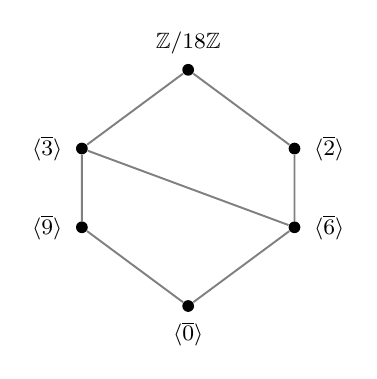
\begin{tikzpicture}[yscale=1.0,xscale=1.35]
  \node[ltdot] (b) at (0,0) {};
  \node[ltdot] (o2) at (-1,1) {};
  \node[ltdot] (o3) at (1,1) {};
  \node[ltdot] (o6) at (-1,2) {};
  \node[ltdot] (o9) at (1,2) {};
  \node[ltdot] (t) at (0,3) {};
  \begin{scope}[ltedge]
    \draw (b)--(o2)--(o6)--(t);
    \draw (b)--(o3)--(o9)--(t);
    \draw (o3)--(o6);
  \end{scope}
  \node[ltlab,below=1.5pt of b] {$\gen{\overline0}$};
  \node[ltlab,left=3pt of o2] {$\gen{\overline9}$};
  \node[ltlab,right=3pt of o3] {$\gen{\overline6}$};
  \node[ltlab,left=3pt of o6] {$\gen{\overline3}$};
  \node[ltlab,right=3pt of o9] {$\gen{\overline2}$};
  \node[ltlab,above=1.5pt of t] {$\Zn{18}$};
\end{tikzpicture}
\end{center}
\end{wex}

\begin{wex}{$\gen{\overline8}$ in $\Zn{20}$, and the unique subgroup of order $4$}
\wrec Use $\gen{\overline a}=\gen{\overline{\gcd(a,n)}}$, then the divisor rule for the
order-$d$ subgroup.
\wsol $\gen{\overline8}=\gen{\overline{\gcd(8,20)}}=\gen{\overline4}$, of order
$20/4=5$. The unique subgroup of order $4$ is $\gen{\overline{20/4}}=\gen{\overline5}$
(indeed $\ord{\overline5}=20/\gcd(20,5)=20/5=4$). \emph{Check:} $4\mid20$, and by
Theorem~\ref{t:cycsub@c2} there is exactly one such subgroup.
\end{wex}

\smallskip\noindent\textit{More on the gcd lemma} (Lemma~\ref{l:gcd@c2}).

\begin{wex}{combining two relations}
Suppose $x^{24}=1$ and $x^{36}=1$. What does this force about $\ord{x}$?
\wrec Two vanishing powers; the gcd lemma says $x^{\gcd(m,n)}=1$.
\wsol $\gcd(24,36)=12$, so $x^{12}=1$ and therefore $\ord{x}\mid12$. \emph{Check:}
$12\mid24$ and $12\mid36$, consistent; e.g.\ an element of order exactly $12$ realizes
both relations.
\end{wex}

\smallskip\noindent\textbf{First-isomorphism preview.} The surjection $\Z\to\gen{x}$,
$k\mapsto x^k$, has kernel $n\Z$ (where $n=\ord{x}$), so it induces an isomorphism
$\Zn{n}\xrightarrow{\ \sim\ }\gen{x}$. This is the First Isomorphism Theorem (Chapter~3)
in its simplest instance, and it is exactly why ``cyclic of order $n$'' is the same as
``$\Zn{n}$'':
\[\begin{tikzcd}[row sep=large,column sep=large]
\Z \arrow[r, two heads, "\pi"] \arrow[dr, two heads, "k\,\mapsto\,x^k"'] & \Zn{n} \arrow[d, dashed, "\sim"] \\
& \gen{x}
\end{tikzcd}\]

\begin{dgx}
\dgi{Objects:} Three groups: $\Z$ (the infinite cyclic group of integers), $\Zn{n}$ (the quotient group $\Z/n\Z$, a cyclic group of order $n$), and $\gen{x}$ (a cyclic subgroup of some ambient group $G$, also of order $n$).
\dgi{Arrows:} The top arrow $\pi:\Z\twoheadrightarrow\Zn{n}$ is the canonical quotient map $k\mapsto\overline{k}$, killing the subgroup $n\Z$. The diagonal arrow $k\mapsto x^k$ is the evaluation surjection from $\Z$ onto $\gen{x}$ (every element of $\gen{x}$ is some $x^k$). The right vertical dashed arrow $\Zn{n}\xrightarrow{\sim}\gen{x}$ is the \emph{induced} isomorphism $\overline{k}\mapsto x^k$; it is dashed because its existence is what the diagram asserts.
\dgi{What commutes:} The triangle commutes: $(\sim)\circ\pi = (k\mapsto x^k)$, i.e.\ sending $k$ first to $\overline{k}$ and then mapping $\overline{k}\mapsto x^k$ gives the same result as sending $k\mapsto x^k$ directly.
\dgi{Why it commutes:} Start with $k\in\Z$. Along the top-then-right path: $k\xmapsto{\pi}\overline{k}\xmapsto{\sim}x^k$. Along the diagonal: $k\xmapsto{}x^k$. Both land at $x^k$. Well-definedness of $\sim$: if $\overline{k}=\overline{k'}$ then $n\mid k-k'$, so $x^{k-k'}=1$ (since $\ord{x}=n$), giving $x^k=x^{k'}$; the map does not depend on the choice of representative in the coset.
\dgi{Why this matters here:} This is the First Isomorphism Theorem at its simplest: the surjection $\Z\to\gen{x}$ has kernel exactly $n\Z$, so the quotient $\Zn{n}=\Z/n\Z$ is isomorphic to $\gen{x}$. The diagram \emph{is} the proof that cyclic of order $n$ means $\Zn{n}$, justifying the Classification Theorem.
\dgi{Concrete example:} Take $G=S_3$, $x=(1\,2\,3)$, $n=3$. The map $k\mapsto (1\,2\,3)^k$ surjects $\Z$ onto $\gen{(1\,2\,3)}=\{e,(1\,2\,3),(1\,3\,2)\}$ with kernel $3\Z$, and $\Zn{3}\xrightarrow{\sim}\gen{(1\,2\,3)}$ sends $\overline{0}\mapsto e$, $\overline{1}\mapsto(1\,2\,3)$, $\overline{2}\mapsto(1\,3\,2)$.
\dgi{Common pitfall:} The dashed isomorphism requires $\ord{x}=n$ exactly (not merely $x^n=1$). If $x^n=1$ but $\ord{x}=d<n$, the induced map is not injective; only when the kernel of $k\mapsto x^k$ is \emph{exactly} $n\Z$ does the quotient become an isomorphism.
\dgi{Takeaway:} The point of this diagram is that a cyclic group of order $n$ is canonically isomorphic to $\Zn{n}$ via the unique map induced by sending the generator $\overline{1}$ to $x$.
\end{dgx}

\subsection*{Maps and commutative diagrams}

Almost every result of this section is the statement that a diagram of homomorphisms
commutes. Reading them this way turns the proofs into one-line observations.

\smallskip\noindent\textbf{(a) The universal property of $\Z$.} For any group $G$ and any
$g\in G$ there is a \emph{unique} homomorphism $\Z\to G$ with $1\mapsto g$, necessarily
$k\mapsto g^k$. (To define a homomorphism out of $\Z$ you only choose where the
generator goes; out of $Z_n$ the image $g$ must also satisfy $g^n=1$, see (c).)
\[\begin{tikzcd}[column sep=large]
\Z \arrow[r, dashed, "\exists!\;k\,\mapsto\,g^k"] & G
\end{tikzcd}\]

\begin{dgx}
\dgi{Objects:} $\Z$ is the infinite cyclic group (under addition), the free object on one generator $1$. $G$ is any group with a chosen element $g$.
\dgi{Arrows:} The single dashed arrow $\Z\to G$ labeled $\exists!\;k\mapsto g^k$ is the \emph{unique} group homomorphism sending $1\in\Z$ to $g\in G$. It is dashed because the arrow is asserted to exist and to be unique; it is forced by the requirement $1\mapsto g$ and the homomorphism property: $k=\underbrace{1+\cdots+1}_{k}$, so $k\mapsto g^k$ is the only possible formula.
\dgi{What commutes:} There is only one arrow, so no non-trivial path equality. The content is existence and uniqueness: any homomorphism $\varphi:\Z\to G$ is determined by $\varphi(1)$, and every element $g\in G$ is a valid target, so there are as many homomorphisms as elements of $G$.
\dgi{Why it commutes:} Uniqueness: suppose $\varphi,\psi:\Z\to G$ both send $1\mapsto g$. Then $\varphi(k)=\varphi(1)^k=g^k=\psi(1)^k=\psi(k)$, so $\varphi=\psi$. Existence: define $\varphi(k)=g^k$; check $\varphi(j+k)=g^{j+k}=g^j g^k=\varphi(j)\varphi(k)$. No well-definedness issue: $\Z$ has no relations, so no coset-checking is needed.
\dgi{Why this matters here:} This universal property is why $\Z$ is the ``free cyclic group.'' Every cyclic group $\gen{x}$ in this section arises as a quotient of $\Z$ by the kernel of the map $k\mapsto x^k$, tying the Classification Theorem directly to this diagram.
\dgi{Concrete example:} $G=\mu_6\sgr\C^\times$, $g=e^{2\pi i/6}$. The unique homomorphism $\Z\to\mu_6$ sends $k\mapsto e^{2\pi ik/6}$; it is surjective with kernel $6\Z$, recovering $\mu_6\isom\Zn{6}$.
\dgi{Common pitfall:} Students sometimes think you need to ``check'' the homomorphism property for this universal map. You do not: the formula $k\mapsto g^k$ is the only possibility, and it is automatically a homomorphism by the laws of exponents. The only choice is $g=\varphi(1)$.
\dgi{Takeaway:} The point of this diagram is that to give a homomorphism out of $\Z$ is exactly the same as choosing a single element $g$ of the target group.
\end{dgx}

\smallskip\noindent\textbf{(b) From $\Z$ onto $\gen{x}$.} The map $k\mapsto x^k$ is
surjective onto $\gen{x}$ and factors through the inclusion $\gen{x}\hookrightarrow G$.
Its kernel is $n\Z$ with $n=\ord{x}$, which is exactly the content of
$\ord{\gen{x}}=\ord{x}$ (Proposition~\ref{p:ordgen@c2}).
\[\begin{tikzcd}[row sep=large,column sep=large]
\Z \arrow[r, two heads, "k\,\mapsto\,x^k"] \arrow[dr, "k\,\mapsto\,x^k"'] & \gen{x} \arrow[d, hook] \\
& G
\end{tikzcd}\]

\begin{dgx}
\dgi{Objects:} $\Z$ (infinite cyclic group), $\gen{x}$ (a cyclic subgroup of $G$ generated by the element $x$), and $G$ (the ambient group). All three are groups; $\gen{x}$ is a subgroup of $G$.
\dgi{Arrows:} The top horizontal arrow $\Z\twoheadrightarrow\gen{x}$, $k\mapsto x^k$, is a surjective group homomorphism whose kernel is $n\Z$ where $n=\ord{x}$. The right vertical arrow $\gen{x}\hookrightarrow G$ is the inclusion (injective map sending each element to itself). The diagonal arrow $k\mapsto x^k$ from $\Z$ to $G$ is the composite of the two preceding maps.
\dgi{What commutes:} The triangle commutes: (inclusion) $\circ$ (surjection) $=$ (diagonal), i.e.\ $\iota\circ(k\mapsto x^k)=(k\mapsto x^k)$ as maps $\Z\to G$. Both routes from $\Z$ to $G$ give the same element $x^k$.
\dgi{Why it commutes:} For $k\in\Z$: the top-then-right path sends $k\mapsto x^k\in\gen{x}\mapsto x^k\in G$. The diagonal sends $k\mapsto x^k\in G$. These agree trivially because the inclusion does nothing to the element. The real content is that the top arrow \emph{is} a surjection: every $x^k\in\gen{x}$ is the image of $k\in\Z$, and the kernel $\ker(k\mapsto x^k)=\{k:x^k=1\}=n\Z$ by the gcd Lemma.
\dgi{Why this matters here:} This diagram makes precise that $\gen{x}$ is ``$\Z$ mod the relation $x^n=1$'': the surjection $\Z\twoheadrightarrow\gen{x}$ with kernel $n\Z$ is the mechanism behind the First Isomorphism preview and behind the proof that $|\gen{x}|=\ord{x}$ in Proposition~\ref{p:ordgen@c2}.
\dgi{Concrete example:} $G=D_8$, $x=r$ (rotation by $90^\circ$), $n=\ord{r}=4$. The map $k\mapsto r^k$ surjects $\Z$ onto $\{1,r,r^2,r^3\}=\gen{r}$ with kernel $4\Z$; the inclusion $\gen{r}\hookrightarrow D_8$ embeds these four rotations into the eight-element group.
\dgi{Common pitfall:} Both arrows labeled $k\mapsto x^k$ look identical but land in different groups ($\gen{x}$ versus $G$). The top arrow is genuinely surjective (every element of $\gen{x}$ is hit), while the diagonal is generally not surjective onto $G$ unless $G$ itself is cyclic generated by $x$.
\dgi{Takeaway:} The point of this diagram is that the surjection $\Z\twoheadrightarrow\gen{x}$ separates the ``definition of $\gen{x}$ as all powers of $x$'' from the ``position of $\gen{x}$ inside $G$,'' and the kernel $n\Z$ records exactly when two exponents give the same power.
\end{dgx}

\smallskip\noindent\textbf{(c) The universal property of $Z_n$.} If $g^n=1$ then
$k\mapsto g^k$ vanishes on $n\Z$, so it descends through the quotient
$\pi:\Z\twoheadrightarrow Z_n$ to a unique $\varphi:Z_n\to G$. (This is precisely D\&F
Exercises~2.3.18--19: a homomorphism out of $Z_n$ is the same as an element of order
dividing $n$.)
\[\begin{tikzcd}[row sep=large,column sep=large]
\Z \arrow[r, two heads, "\pi"] \arrow[dr, "k\,\mapsto\,g^k"'] & Z_n \arrow[d, dashed, "\exists!\,\varphi"] \\
& G
\end{tikzcd}\]

\begin{dgx}
\dgi{Objects:} $\Z$ (infinite cyclic group), $Z_n=\Z/n\Z$ (the abstract cyclic group of order $n$, with generator $\overline{1}$), and $G$ (any group containing an element $g$ with $g^n=1$, i.e.\ $\ord{g}$ divides $n$).
\dgi{Arrows:} $\pi:\Z\twoheadrightarrow Z_n$ is the canonical surjective quotient map $k\mapsto\overline{k}$ with kernel $n\Z$. The diagonal $k\mapsto g^k$ is a homomorphism $\Z\to G$ that kills $n\Z$ (since $g^n=1$ forces $g^{nk}=1$ for all $k\in\Z$). The dashed vertical arrow $\varphi:Z_n\to G$, $\overline{k}\mapsto g^k$, is the \emph{unique} induced homomorphism; it is dashed because the diagram asserts its existence.
\dgi{What commutes:} The triangle commutes: $\varphi\circ\pi=(k\mapsto g^k)$, i.e.\ $\varphi(\overline{k})=g^k$ for all $k\in\Z$.
\dgi{Why it commutes:} Well-definedness of $\varphi$: if $\overline{k}=\overline{k'}$ then $n\mid k-k'$, so $g^{k-k'}=(g^n)^{(k-k')/n}=1^{(k-k')/n}=1$, giving $g^k=g^{k'}$. Hence $\varphi(\overline{k})=g^k$ does not depend on the choice of representative. Uniqueness: any $\psi:Z_n\to G$ with $\psi\circ\pi=k\mapsto g^k$ must satisfy $\psi(\overline{1})=g$, forcing $\psi(\overline{k})=g^k=\varphi(\overline{k})$.
\dgi{Why this matters here:} This is the universal property that classifies all homomorphisms out of $Z_n$: they correspond exactly to elements $g\in G$ with $\ord{g}\mid n$. It is the engine behind the exercises on homomorphisms from cyclic groups and the reason the classification of cyclic groups is so effective.
\dgi{Concrete example:} $G=\mu_{12}\sgr\C^\times$, $g=e^{2\pi i/4}=i$, $n=4$ (so $g^4=1$). The induced map $\varphi:Z_4\to\mu_{12}$ sends $\overline{k}\mapsto i^k$, embedding $Z_4$ into $\mu_{12}$ as the subgroup $\{1,i,-1,-i\}=\mu_4$.
\dgi{Common pitfall:} The condition is $g^n=1$ (order \emph{divides} $n$), not $\ord{g}=n$. If $\ord{g}<n$ then $\varphi$ is not injective; in particular $\varphi$ need not be an isomorphism. The diagram gives a homomorphism regardless; the isomorphism case requires $\ord{g}=n$ exactly.
\dgi{Takeaway:} The point of this diagram is that a homomorphism out of $Z_n$ into $G$ is the same as a choice of element $g\in G$ satisfying $g^n=1$, with the quotient map $\pi$ doing all the well-definedness work.
\end{dgx}

\smallskip\noindent\textbf{(d) Any two cyclic groups of the same order are isomorphic}
(Theorem~\ref{t:classify@c2}). Both $\gen{x}$ and $\gen{y}$ are $\Z$ modulo the same
subgroup $n\Z$, so $x^k\mapsto y^k$ is a well-defined isomorphism making the triangle
commute.
\[\begin{tikzcd}[row sep=large,column sep=large]
& \Z \arrow[dl, two heads, "k\,\mapsto\,x^k"'] \arrow[dr, two heads, "k\,\mapsto\,y^k"] & \\
\gen{x} \arrow[rr, "\sim"', "x^k\mapsto y^k"] & & \gen{y}
\end{tikzcd}\]

\begin{dgx}
\dgi{Objects:} $\Z$ (the apex, infinite cyclic group of integers), $\gen{x}$ (a cyclic group of order $n$ generated by $x$, lower-left), and $\gen{y}$ (a second cyclic group of order $n$ generated by $y$, lower-right). The two groups may live in entirely different ambient groups.
\dgi{Arrows:} The left surjection $k\mapsto x^k:\Z\twoheadrightarrow\gen{x}$ has kernel $n\Z$. The right surjection $k\mapsto y^k:\Z\twoheadrightarrow\gen{y}$ has the same kernel $n\Z$. The bottom isomorphism $\sim:\gen{x}\to\gen{y}$, $x^k\mapsto y^k$, is the map induced by the two surjections sharing the same kernel.
\dgi{What commutes:} The triangle commutes: $(x^k\mapsto y^k)\circ(k\mapsto x^k)=(k\mapsto y^k)$, i.e.\ going left-then-bottom equals going right directly from $\Z$ to $\gen{y}$.
\dgi{Why it commutes:} For $k\in\Z$: left-then-bottom sends $k\mapsto x^k\mapsto y^k$. Right sends $k\mapsto y^k$. These agree. Well-definedness of the bottom map: if $x^k=x^{k'}$ then $x^{k-k'}=1$, so $n\mid k-k'$ (gcd Lemma), hence $y^{k-k'}=1$ and $y^k=y^{k'}$. Both surjections share kernel $n\Z$, so the induced map between the quotients is an isomorphism by the First Isomorphism Theorem.
\dgi{Why this matters here:} This is Theorem~\ref{t:classify@c2} diagrammatically: the two cyclic groups of the same order are interchangeable because they are both quotients of $\Z$ by the same relation $n=0$. The triangle records exactly why $x^k\mapsto y^k$ is a legitimate isomorphism, not just a set bijection.
\dgi{Concrete example:} $\gen{x}=\mu_3=\{1,\omega,\omega^2\}\sgr\C^\times$ (cube roots of unity) and $\gen{y}=\gen{(1\,2\,3)}\sgr S_3$. Both have order $3$; the isomorphism $\omega^k\mapsto(1\,2\,3)^k$ sends $1\mapsto e$, $\omega\mapsto(1\,2\,3)$, $\omega^2\mapsto(1\,3\,2)$, and both groups are quotients of $\Z$ by $3\Z$.
\dgi{Common pitfall:} The isomorphism $x^k\mapsto y^k$ is \emph{not} canonical in a unique-choice sense when there are multiple generators: replacing $x$ by another generator $x^a$ (with $\gcd(a,n)=1$) gives a different isomorphism. The diagram shows one particular isomorphism, determined by the choice of how to assign generators.
\dgi{Takeaway:} The point of this diagram is that any two cyclic groups of order $n$ are both quotients of the same $\Z$ by the same $n\Z$, so they are automatically isomorphic via the map that matches generator to generator.
\end{dgx}

\smallskip\noindent\textbf{(e) ``$\varphi$ is a homomorphism'' is the commuting of one
square:} it respects multiplication. Checking this square is the only real content in
(d).
\[\begin{tikzcd}[row sep=large,column sep=large]
\gen{x}\times\gen{x} \arrow[r, "m"] \arrow[d, "\varphi\times\varphi"'] & \gen{x} \arrow[d, "\varphi"] \\
\gen{y}\times\gen{y} \arrow[r, "m"'] & \gen{y}
\end{tikzcd}\]

\begin{dgx}
\dgi{Objects:} Upper-left and lower-left are product groups $\gen{x}\times\gen{x}$ and $\gen{y}\times\gen{y}$ respectively; upper-right is $\gen{x}$ and lower-right is $\gen{y}$. Here $\varphi:\gen{x}\to\gen{y}$ is the isomorphism $x^k\mapsto y^k$ from diagram (d), both cyclic of order $n$.
\dgi{Arrows:} Both horizontal arrows labeled $m$ are the group multiplication maps: $m(x^j,x^k)=x^{j+k}$ on the top, $m(y^j,y^k)=y^{j+k}$ on the bottom. The left vertical arrow is $\varphi\times\varphi:(x^j,x^k)\mapsto(y^j,y^k)$ (applying $\varphi$ to each component). The right vertical arrow is $\varphi:x^k\mapsto y^k$.
\dgi{What commutes:} Down-then-right equals right-then-down: $\varphi(m(x^j,x^k))=m(\varphi(x^j),\varphi(x^k))$, i.e.\ $\varphi(x^{j+k})=y^j y^k$. Explicitly: $y^{j+k}=y^j y^k$, which holds in $\gen{y}$.
\dgi{Why it commutes:} Chase $(x^j,x^k)$ from upper-left. Right-then-down: $m(x^j,x^k)=x^{j+k}\xmapsto{\varphi}y^{j+k}$. Down-then-right: $(x^j,x^k)\xmapsto{\varphi\times\varphi}(y^j,y^k)\xmapsto{m}y^{j+k}$. Both give $y^{j+k}$. The commutativity holds because $\varphi$ is defined by matching exponents, and exponent arithmetic ($j+k$) is the same in both groups.
\dgi{Why this matters here:} The text says ``checking this square is the only real content'' in the isomorphism proof. In the abstract, a map is a homomorphism if and only if this naturality square commutes; the square makes the condition $\varphi(ab)=\varphi(a)\varphi(b)$ into a diagram rather than a sentence, which is the standard categorical encoding of ``structure-preserving map.''
\dgi{Concrete example:} $\gen{x}=\Zn{3}$ (additive), $\gen{y}=\mu_3$ (multiplicative), $\varphi(\overline{k})=\omega^k$. Top row: $(\overline{1},\overline{1})\xmapsto{m}\overline{2}$. Right column: $\overline{2}\xmapsto{\varphi}\omega^2$. Left-then-bottom: $(\overline{1},\overline{1})\xmapsto{\varphi\times\varphi}(\omega,\omega)\xmapsto{m}\omega^2$. Both give $\omega^2$.
\dgi{Common pitfall:} Students sometimes think ``$\varphi$ is a bijection'' is sufficient for an isomorphism. This diagram shows the extra condition: the square must commute. A bijection that does not preserve multiplication is not a homomorphism; this square failing to commute would detect that failure.
\dgi{Takeaway:} The point of this diagram is that ``$\varphi$ is a homomorphism'' is exactly the statement that applying $\varphi$ before or after multiplying gives the same answer, packaged as a commutative square involving the multiplication maps of both groups.
\end{dgx}

\smallskip\noindent\textbf{(f) Subgroups $\leftrightarrow$ divisors}
(Theorem~\ref{t:cycsub@c2}). For $Z_n=\gen{x}$, the assignment $d\mapsto\gen{x^{n/d}}$ is an
inclusion-preserving bijection from the divisors of $n$ to the subgroups of $Z_n$; this
is why the subgroup lattice of $Z_n$ \emph{is} the divisor lattice of $n$.
\[\begin{tikzcd}[column sep=large]
\{\,d:d\mid n\,\} \arrow[r, "\sim", "d\,\mapsto\,\gen{x^{n/d}}"'] & \{\text{subgroups of }Z_n\}
\end{tikzcd}\]

\begin{dgx}
\dgi{Objects:} The domain is the set of positive divisors of $n$ (a finite set of integers, viewed here as a poset under divisibility). The codomain is the set of all subgroups of the cyclic group $Z_n=\gen{x}$ of order $n$ (a set of groups, ordered by inclusion). Both sets have the same cardinality $\tau(n)$ (number of divisors of $n$).
\dgi{Arrows:} The single arrow, labeled $\sim$ and $d\mapsto\gen{x^{n/d}}$, is the bijection sending each divisor $d$ of $n$ to the unique subgroup of $Z_n$ of order $d$. Its inverse sends a subgroup $K\leq Z_n$ to $|K|$. The arrow is labeled $\sim$ because it is a bijection and it is also order-preserving in both directions (an isomorphism of posets): $d_1\mid d_2$ if and only if $\gen{x^{n/d_1}}\sgr\gen{x^{n/d_2}}$.
\dgi{What commutes:} There is one arrow, so the content is bijectivity and the poset-isomorphism condition: $d_1\mid d_2\iff\gen{x^{n/d_1}}\sgr\gen{x^{n/d_2}}$. Equivalently, the induced map on the divisor lattice of $n$ is identical to the subgroup lattice of $Z_n$.
\dgi{Why it commutes:} Injectivity: distinct divisors $d\ne d'$ give $\gen{x^{n/d}}\ne\gen{x^{n/d'}}$ because $|\gen{x^{n/d}}|=d\ne d'=|\gen{x^{n/d'}}|$. Surjectivity: every subgroup of $Z_n$ is cyclic (Theorem~\ref{t:cycsub@c2}(1)) hence equals $\gen{x^{n/d}}$ for some divisor $d$ of $n$ by the uniqueness argument in Theorem~\ref{t:cycsub@c2}(3). Poset-preservation: $d_1\mid d_2\Rightarrow n/d_2\mid n/d_1\Rightarrow\gen{x^{n/d_1}}\sgr\gen{x^{n/d_2}}$ by the containment rule.
\dgi{Why this matters here:} This is the capstone of the section on subgroups of cyclic groups. It makes precise the slogan ``the subgroup lattice of $Z_n$ is the divisor lattice of $n$ upside-down,'' justifying every lattice diagram in this chapter and giving a complete structural description of $Z_n$.
\dgi{Concrete example:} $n=12$. Divisors $1,2,3,4,6,12$ map to $\gen{x^{12}},\gen{x^6},\gen{x^4},\gen{x^3},\gen{x^2},\gen{x}$ with orders $1,2,3,4,6,12$. The divisibility $2\mid 6$ matches the containment $\gen{x^6}\sgr\gen{x^2}$, visible in the lattice drawn earlier in this section.
\dgi{Common pitfall:} The divisor $d$ labels the \emph{order} of the subgroup, not the step size of the generator. The generator is $x^{n/d}$, not $x^d$. Confusing these reverses the labeling: in $\Zn{12}$, the order-$3$ subgroup is $\gen{\overline{4}}$ (step $4=12/3$), not $\gen{\overline{3}}$.
\dgi{Takeaway:} The point of this diagram is that divisors of $n$ and subgroups of $Z_n$ are in perfect order-preserving bijective correspondence, so any question about subgroup containment in a cyclic group is purely a question about divisibility.
\end{dgx}

\smallskip\noindent\textbf{(g) Automorphisms of $Z_n$.} An automorphism must send a
generator to a generator (Proposition~\ref{p:gens@c2}), and $a\mapsto(\sigma_a:x\mapsto x^a)$
is a group isomorphism. So the symmetries of a cyclic group are the units mod $n$.
\[\begin{tikzcd}[column sep=large]
\Zns{n} \arrow[r, "\sim", "a\,\mapsto\,\sigma_a"'] & \Aut(Z_n)
\end{tikzcd}\]

\begin{dgx}
\dgi{Objects:} The domain $\Zns{n}=(\Z/n\Z)^\times$ is the group of units modulo $n$ under multiplication: the residues $\overline{a}$ with $\gcd(a,n)=1$, which has order $\varphi(n)$. The codomain $\operatorname{Aut}(Z_n)$ is the group of all group automorphisms of $Z_n=\gen{x}$ under composition; it also has order $\varphi(n)$ by Proposition~\ref{p:gens@c2}.
\dgi{Arrows:} The single isomorphism arrow, labeled $\sim$ and $a\mapsto\sigma_a$, sends a unit $\overline{a}\in\Zns{n}$ to the automorphism $\sigma_a:Z_n\to Z_n$ defined by $\sigma_a(x^k)=x^{ak}$. Since $\gcd(a,n)=1$, the element $x^a$ is a generator of $Z_n$ (Proposition~\ref{p:gens@c2}(1)), so $\sigma_a$ is indeed an automorphism.
\dgi{What commutes:} Again one arrow, so the content is: (1) $\sigma_a$ is a well-defined automorphism for each $\gcd(a,n)=1$; (2) $a\mapsto\sigma_a$ is a group homomorphism: $\sigma_a\circ\sigma_b=\sigma_{ab}$, i.e.\ $\sigma_a(\sigma_b(x^k))=\sigma_a(x^{bk})=x^{abk}=\sigma_{ab}(x^k)$; (3) the map is a bijection, so a group isomorphism.
\dgi{Why it commutes:} Well-definedness of $\sigma_a$: if $x^k=x^{k'}$ in $Z_n$ then $n\mid k-k'$, hence $n\mid a(k-k')$ and $x^{ak}=x^{ak'}$. Injectivity of $a\mapsto\sigma_a$: if $\sigma_a=\sigma_b$ then $x^a=\sigma_a(x)=\sigma_b(x)=x^b$, so $n\mid a-b$, giving $\overline{a}=\overline{b}$ in $\Zns{n}$. Surjectivity: every automorphism $\phi$ sends the generator $x$ to a generator $x^a$ with $\gcd(a,n)=1$, and then $\phi=\sigma_a$.
\dgi{Why this matters here:} This diagram closes the story of cyclic groups by computing their automorphism group. It explains why $|\operatorname{Aut}(Z_n)|=\varphi(n)$ and why the symmetries of a cyclic group are governed by units modulo $n$, connecting group theory to number theory.
\dgi{Concrete example:} $n=8$, $\Zns{8}=\{\overline{1},\overline{3},\overline{5},\overline{7}\}\isom\Z/2\times\Z/2$ (the Klein four-group). The four automorphisms of $Z_8=\gen{x}$ are $\sigma_1$ (identity), $\sigma_3:x\mapsto x^3$, $\sigma_5:x\mapsto x^5$, $\sigma_7:x\mapsto x^7=x^{-1}$. Composition corresponds to multiplication of units: $\sigma_3\circ\sigma_3=\sigma_9=\sigma_1$ since $3^2=9\equiv 1\pmod{8}$.
\dgi{Common pitfall:} An automorphism of $Z_n$ is completely determined by where it sends the generator $x$; but only sending $x$ to another generator (an element of order $n$) gives an automorphism. Sending $x$ to $x^2$ when $n$ is even yields an endomorphism that is not an automorphism because $x^2$ does not generate $Z_n$.
\dgi{Takeaway:} The point of this diagram is that the symmetry group of the cyclic group $Z_n$ is isomorphic to the multiplicative group of units mod $n$, so group-theoretic symmetry reduces to number-theoretic coprimality.
\end{dgx}

\begin{exers}{Exercises (from the text).}
\item Find all subgroups of $Z_{45}=\gen{x}$, giving a generator for each, and describe
  the containments.
\item If $x\in G$ is finite with $\ord{x}=\ord{G}$, prove $G=\gen{x}$; give an infinite
  counterexample.
\item Find all generators of $\Zn{48}$.
\item Find all generators of $\Zn{202}$.
\item Find the number of generators of $\Zn{49000}$.
\item In $\Zn{48}$, list the elements of $\gen{\bar a}$ for each $\bar a$, and all
  inclusions among subgroups.
\item Use $\Zn{48}\isom Z_{48}$ to list all subgroups of $Z_{48}$.
\item For which $a$ does $1\mapsto x^a$ extend to an isomorphism $\Zn{48}\to Z_{48}$?
\item For which $a$ does $1\mapsto x^a$ extend to a homomorphism $\Zn{48}\to Z_{36}$?
  Can it be surjective?
\item Find $\ord{\overline{30}}$ in $\Zn{54}$, and list the elements and orders of
  $\gen{\overline{30}}$.
\item Find all cyclic subgroups of $D_8$ and a non-cyclic proper subgroup.
\item Prove $Z_2\times Z_2$, $Z_2\times\Z$, and $\Z\times\Z$ are not cyclic.
\item Prove $\Z\times Z_2\not\isom\Z$ and $\Q\times Z_2\not\isom\Q$.
\item For $\sigma=(1\,2\,\cdots\,12)$, compute $\sigma^a$ for
  $a=13,65,626,1195,-6,-81,-570,-1211$.
\item Prove $\Q\times\Q$ is not cyclic.
\item $\ord{x}=n$, $\ord{y}=m$, $xy=yx$: prove $\ord{xy}\mid\lcm(m,n)$; show this can
  fail without commuting, and give commuting $x,y$ with $\ord{xy}\neq\lcm(m,n)$.
\item Find a presentation of $Z_n$ with one generator.
\item If $h^n=1$ in $H$, prove there is a unique homomorphism $Z_n\to H$ with $x\mapsto
  h$.
\item For $h\in H$, prove there is a unique homomorphism $\Z\to H$ with $1\mapsto h$.
\item $p$ prime, $x^{p^n}=1\imp\ord{x}=p^m$ for some $m\le n$.
\item $p$ an odd prime: show $1+p$ has order $p^{n-1}$ in $\Zns{p^n}$.
\item $n\ge3$: show $5$ has order $2^{n-2}$ in $\Zns{2^n}$.
\item Show $\Zns{2^n}$ is not cyclic for $n\ge3$.
\item $G$ finite, $x\in G$: prove $g\in N_G(\gen{x})\iff gxg\inv=x^a$ for some $a\in\Z$.
\item $G$ cyclic of order $n$, $\gcd(k,n)=1$: prove $x\mapsto x^k$ is surjective, and
  extend the conclusion to any finite group of order $n$.
\item $\Aut(Z_n)$: prove $\sigma_a:x\mapsto x^a$ is an automorphism $\iff\gcd(a,n)=1$,
  and $\Aut(Z_n)\isom\Zns{n}$, abelian of order $\varphi(n)$.
\end{exers}

\begin{exers}{Additional exercises.}
\item Prove that for each $d\mid n$, a cyclic group of order $n$ has exactly
  $\varphi(d)$ elements of order $d$; deduce $\sum_{d\mid n}\varphi(d)=n$.
\item Prove $\Q$ is not cyclic and has no maximal subgroup.
\item Prove a finite group $G$ with at most $n$ solutions to $x^n=1$ for every $n\mid
  \ord{G}$ is cyclic. (Hence every finite subgroup of $F^\times$, $F$ a field, is
  cyclic.)
\item Determine all $n$ for which $\Zns{n}$ is cyclic.
\item Prove that two finite cyclic groups are isomorphic iff they have the same order,
  using only the order and isomorphism propositions of this section.
\end{exers}

\begin{exers}{Commutative-diagram exercises.}
\item (Universal property of $\Z$) Prove that for each $g\in G$ there is a unique
  homomorphism $\Z\to G$ with $1\mapsto g$; deduce a natural bijection
  $\operatorname{Hom}(\Z,G)\leftrightarrow G$.
\item (Universal property of $Z_n$) Prove
  $\operatorname{Hom}(Z_n,G)\leftrightarrow\{g\in G\st g^n=1\}$ by showing $k\mapsto g^k$
  descends through $\pi:\Z\twoheadrightarrow Z_n$ iff $g^n=1$; draw the factorization
  triangle.
\item Show the map $\Z\to\gen{x}$, $k\mapsto x^k$, induces an isomorphism
  $\Zn{n}\to\gen{x}$ when $\ord{x}=n$, and draw the triangle. (This is the First
  Isomorphism Theorem in one case.)
\item Exhibit the isomorphism between two cyclic groups of order $n$ as the dashed arrow
  completing the $\Z$-triangle $\gen{x}\leftarrow\Z\rightarrow\gen{y}$, and verify the
  triangle commutes.
\item Prove $a\mapsto\sigma_a$ (where $\sigma_a(x)=x^a$) is an isomorphism
  $\Zns{n}\to\Aut(Z_n)$ by checking that the square $\sigma_a\circ\sigma_b=\sigma_{ab}$
  commutes.
\item Define $\varphi:\Zn{12}\to\Zn{4}$ by $\overline1\mapsto\overline3$. Compute
  $\varphi(\overline5)$ and $\varphi(\overline8)$, verify $\varphi$ is a well-defined
  homomorphism (the relation $12\cdot\overline1=\overline0$ must map to $\overline0$), and
  find $\ker\varphi$.
\end{exers}


\section{Subgroups Generated by Subsets}
\subsection*{Subgroups Generated by Subsets ($\gen{A}$)}

This section answers a single concrete question: given a subset $A$ of a group $G$, what is the \emph{smallest} subgroup of $G$ that contains $A$? We build it two ways --- from the outside (intersect all subgroups containing $A$) and from the inside (take all finite words in the elements of $A$ and their inverses) --- and prove the two descriptions agree.

\begin{proposition}\label{p:int-sub@c2}
Let $G$ be a group and let $\{H_i\}_{i\in I}$ be a nonempty collection of subgroups of $G$. Then $K=\bigcap_{i\in I}H_i$ is a subgroup of $G$.
\end{proposition}

\begin{proof}
Use the subgroup criterion (nonempty; closed under $xy\inv$). Each $H_i\sgr G$ contains $1$, so $1\in H_i$ for every $i$, hence $1\in K$ and $K\neq\es$. Now take $x,y\in K$. For each $i$ we have $x,y\in H_i$, and since $H_i$ is a subgroup, $xy\inv\in H_i$. As this holds for every $i$, we get $xy\inv\in\bigcap_i H_i=K$. By the one-step subgroup test, $K\sgr G$.
\end{proof}

\begin{pitfall}
The same argument fails for \emph{unions}: $\gen{2}\cup\gen{3}$ in $\Z$ contains $2$ and $3$ but not $2+3=5$, so it is not a subgroup. Intersections of subgroups are always subgroups; unions almost never are.
\end{pitfall}

\begin{definition}\label{d:gen@c2}
Let $A\subseteq G$. The \textbf{subgroup generated by $A$} is
\[
\gen{A}\;=\;\bigcap_{\substack{H\sgr G\\ A\subseteq H}}H,
\]
the intersection of all subgroups of $G$ that contain $A$. The collection being intersected is nonempty because $G$ itself is such an $H$, so by Proposition~\ref{p:int-sub@c2} $\gen{A}$ is a subgroup. We call $A$ a \emph{generating set}, and elements of $A$ \emph{generators}. If $A=\{a_1,\dots,a_n\}$ we write $\gen{a_1,\dots,a_n}$.
\end{definition}

By construction $\gen{A}$ is the \textbf{smallest} subgroup containing $A$, in the precise sense: $A\subseteq\gen{A}$, and if $K\sgr G$ with $A\subseteq K$, then $\gen{A}\subseteq K$ (because $K$ is one of the $H$'s being intersected). That ``outside'' definition is clean but useless for computation. The next theorem gives the computable ``inside'' description.

\begin{theorem}[Word description of $\gen{A}$]\label{t:words@c2}
Let $A\subseteq G$ be nonempty. Then
\[
\gen{A}\;=\;\bigl\{\,a_1^{\varepsilon_1}a_2^{\varepsilon_2}\cdots a_k^{\varepsilon_k}\ \st\ k\ge 0,\ a_i\in A,\ \varepsilon_i\in\{+1,-1\}\,\bigr\},
\]
the set of all finite \textbf{words} in the elements of $A$ and their inverses (the empty word $k=0$ denotes $1$). If $A=\es$ then $\gen{A}=\{1\}$.
\end{theorem}

\begin{proof}
Write $W$ for the set of words on the right. We show $W\sgr G$, then $A\subseteq W$, then $W=\gen{A}$.

\emph{$W$ is a subgroup.} It contains the empty word $1$, so $W\neq\es$. If $x=a_1^{\varepsilon_1}\cdots a_k^{\varepsilon_k}$ and $y=b_1^{\delta_1}\cdots b_m^{\delta_m}$ are words, then their concatenation $xy$ is again a word, so $W$ is closed under products. Also $x\inv=a_k^{-\varepsilon_k}\cdots a_1^{-\varepsilon_1}$ is a word (reverse the letters and flip each sign), so $W$ is closed under inverses. Hence $W\sgr G$.

\emph{$W$ contains $A$.} Each $a\in A$ equals the length-one word $a^{+1}$, so $A\subseteq W$.

\emph{Minimality forces equality.} Since $W$ is a subgroup containing $A$, the ``smallest'' property of $\gen{A}$ gives $\gen{A}\subseteq W$. Conversely, let $H$ be \emph{any} subgroup with $A\subseteq H$. Then $H$ contains every $a_i$ and (being a subgroup) every $a_i^{-1}$, hence every product $a_1^{\varepsilon_1}\cdots a_k^{\varepsilon_k}$; thus $W\subseteq H$. Taking $H=\gen{A}$ gives $W\subseteq\gen{A}$. Therefore $W=\gen{A}$.

If $A=\es$, the only word is the empty word, so $W=\{1\}=\gen{A}$.
\end{proof}

\begin{corollary}[Abelian case: words collapse to integer combinations]\label{c:abelian@c2}
If $G$ is abelian, written additively, and $A=\{a_1,\dots,a_n\}$, then
\[
\gen{A}=\{\,m_1a_1+m_2a_2+\cdots+m_na_n\ \st\ m_i\in\Z\,\}.
\]
In particular $\gen{a}=\{ma\st m\in\Z\}=a\Z$ for a single element.
\end{corollary}

\begin{proof}
In an abelian group we may sort the letters of any word and collect repeats: a word in $a_1,\dots,a_n$ and their inverses can be rearranged (commutativity) into $a_1$'s together, then $a_2$'s, and so on, and each block of $m_i$ copies of $a_i^{\pm1}$ sums to $m_ia_i$ with $m_i\in\Z$. Conversely each integer combination is visibly such a word. The result follows from Theorem~\ref{t:words@c2}.
\end{proof}

\begin{theorem}[The case $G=\Z$]\label{t:Zgcd@c2}
For integers $a,b$ not both $0$, in $(\Z,+)$ we have $\gen{a,b}=\gen{\gcd(a,b)}=\gcd(a,b)\,\Z$. More generally $\gen{a_1,\dots,a_n}=\gen{\gcd(a_1,\dots,a_n)}$.
\end{theorem}

\begin{proof}
Let $d=\gcd(a,b)$. By Corollary~\ref{c:abelian@c2}, $\gen{a,b}=\{ma+nb\st m,n\in\Z\}$. Since $d\mid a$ and $d\mid b$, every $ma+nb$ is a multiple of $d$, so $\gen{a,b}\subseteq d\Z=\gen{d}$. Conversely, by B\'ezout there exist $m_0,n_0\in\Z$ with $m_0a+n_0b=d$, so $d\in\gen{a,b}$, hence $\gen{d}=d\Z\subseteq\gen{a,b}$. Therefore $\gen{a,b}=\gen{d}$. Induction on $n$ (using $\gcd(a_1,\dots,a_n)=\gcd(\gcd(a_1,\dots,a_{n-1}),a_n)$) gives the general statement.
\end{proof}

\begin{method}{How to compute $\gen{A}$ by hand (word closure)}
Use this whenever you see ``$\gen{\,\cdot\,}$,'' ``the subgroup generated by,'' or ``smallest subgroup containing.''
\begin{enumerate}
\item \textbf{Seed.} Start the candidate set $S$ with $1$, every generator $a\in A$, and every inverse $a\inv$.
\item \textbf{Close under products.} Multiply pairs from $S$ (in both orders if $G$ is nonabelian) and adjoin any new elements. Repeat until $S$ stops growing. Finiteness of $G$ (or a known order bound) guarantees this halts.
\item \textbf{Read off the subgroup.} The stabilized $S$ \emph{is} $\gen{A}$, by Theorem~\ref{t:words@c2}.
\item \textbf{Identify it.} Compute $\lvert S\rvert$, check whether it is abelian, and match against a known group ($V_4$, $\Z_n$, $S_3$, $Q_8$, $\dots$). If $\lvert S\rvert=\lvert G\rvert$ then $\gen{A}=G$.
\item \textbf{Shortcuts.} In an abelian group, replace words by integer combinations (Cor.~\ref{c:abelian@c2}); in $\Z$ use $\gen{a,b}=\gen{\gcd(a,b)}$ (Thm.~\ref{t:Zgcd@c2}); in $\Zn{n}$ use $\gen{\overline a,\overline b}=\gen{\overline{\gcd(a,b,n)}}$.
\end{enumerate}
\textbf{Recognizing $\gen{A}=G$:} it suffices that the generators reach an element of order $\lvert G\rvert$ (cyclic case), or that the closure already exhausts a known basis/generating pattern of $G$.
\end{method}

\begin{wex}{$\gen{2,3}=\Z$}
Show that $2$ and $3$ generate all of $\Z$.
\wrec Ambient group is $\Z$ (abelian, additive). The trigger ``$\gen{a,b}$ in $\Z$'' fires Theorem~\ref{t:Zgcd@c2}: the answer is $\gen{\gcd(a,b)}$. Compute the gcd.
\wsol By Theorem~\ref{t:Zgcd@c2}, $\gen{2,3}=\gen{\gcd(2,3)}=\gen{1}=1\cdot\Z=\Z$. Explicit B\'ezout witness: $(-1)\cdot2+(1)\cdot3=1$, so $1\in\gen{2,3}$; once $1$ is present, every integer $m=m\cdot1\in\gen{2,3}$.
\emph{Check.} $\gcd(2,3)=1$ and $\gen{1}=\Z$, consistent. Also $5=3+2$, $4=2+2$, $-1=2-3$ are all reachable, as expected.
\end{wex}

\begin{wex}{$\gen{4,6}=2\Z$}
Compute $\gen{4,6}$ in $\Z$.
\wrec Same trigger as the previous example: a two-generator subgroup of $(\Z,+)$. Apply $\gen{a,b}=\gen{\gcd(a,b)}$.
\wsol $\gcd(4,6)=2$, so $\gen{4,6}=\gen{2}=2\Z=\{\dots,-4,-2,0,2,4,\dots\}$. B\'ezout witness for $2$: $(-1)\cdot4+(1)\cdot6=2$, so $2\in\gen{4,6}$, giving $2\Z\subseteq\gen{4,6}$. Conversely every $4m+6n=2(2m+3n)$ is even, so $\gen{4,6}\subseteq2\Z$.
\emph{Check.} Both generators are even, so no odd number can appear --- $1\notin\gen{4,6}$, matching $\gen{4,6}=2\Z\neq\Z$. And $2=6-4\in\gen{4,6}$, confirming $2$ is attained.
\end{wex}

\begin{wex}{$\gen{\overline4,\overline6}=\gen{\overline2}$ in $\Zn{12}$}
Find $\gen{\overline4,\overline6}$ inside $\Zn{12}$.
\wrec Ambient group is $\Zn{12}$ (abelian, additive mod $12$). For $\Zn{n}$ the gcd rule must include the modulus: $\gen{\overline a,\overline b}=\gen{\overline{\gcd(a,b,n)}}$, because adding the relation $n\equiv 0$ is the same as throwing $n$ into the gcd.
\wsol Compute $\gcd(4,6,12)=\gcd(\gcd(4,6),12)=\gcd(2,12)=2$. Hence $\gen{\overline4,\overline6}=\gen{\overline2}=\{\overline0,\overline2,\overline4,\overline6,\overline8,\overline{10}\}$, a subgroup of order $6$. Word/integer-combination check that $\overline2$ is reachable: $\overline6-\overline4=\overline2$. And $\overline2$ generates the listed set by repeated addition.
\emph{Check.} $\lvert\gen{\overline2}\rvert=12/\gcd(2,12)=12/2=6$, matching the six listed residues. Every generator lies in it: $\overline4=2\cdot\overline2$, $\overline6=3\cdot\overline2$. Good.
\end{wex}

\begin{wex}{$\gen{\overline3,\overline5}=\Zn{12}$ (tricky: coprime generators)}
Compute $\gen{\overline3,\overline5}$ in $\Zn{12}$.
\wrec Two-generator subgroup of $\Zn{12}$; use $\gen{\overline a,\overline b}=\gen{\overline{\gcd(a,b,n)}}$. The subtlety: even though $3$ alone does not generate $\Zn{12}$, the gcd of the two generators with the modulus may still be $1$.
\wsol $\gcd(3,5,12)=\gcd(\gcd(3,5),12)=\gcd(1,12)=1$, so $\gen{\overline3,\overline5}=\gen{\overline1}=\Zn{12}$. Explicit reach: $\overline5-\overline3=\overline2$ and $\overline3-\overline2=\overline1$, so $\overline1\in\gen{\overline3,\overline5}$, and $\overline1$ generates everything.
\emph{Check.} $\gen{\overline3}=\{\overline0,\overline3,\overline6,\overline9\}$ has order $4$ and $\gen{\overline5}=\Zn{12}$ already (since $\gcd(5,12)=1$); so together they certainly fill $\Zn{12}$. Consistent.
\end{wex}

\begin{wex}{$\gen{(1\,2),(2\,3)}=S_3$}
Show the transpositions $(1\,2)$ and $(2\,3)$ generate $S_3$.
\wrec Ambient group is $S_3$, which is nonabelian, so we cannot use gcd or integer combinations --- we must do honest \textbf{word closure} (Method box, products in both orders). The trigger is two specific elements with ``$\gen{\,\cdot\,}$.''
\wsol Seed: $1,(1\,2),(2\,3)$ (each transposition is its own inverse). Multiply (D\&F convention: rightmost permutation acts first):
\[
(1\,2)(2\,3)=(1\,2\,3),\qquad (2\,3)(1\,2)=(1\,3\,2).
\]
Adjoin these two $3$-cycles. One more product gives the last missing element:
\[
(1\,2)\,(1\,2\,3)=(2\,3)\quad(\text{already have});\qquad (1\,2\,3)(1\,2)=(1\,3).
\]
Now the closure is $\{1,(1\,2),(1\,3),(2\,3),(1\,2\,3),(1\,3\,2)\}$, which is all $6$ elements of $S_3$, and further products produce nothing new.
\emph{Check.} $\lvert S_3\rvert=3!=6$ and our closure has $6$ elements, so $\gen{(1\,2),(2\,3)}=S_3$. (Indeed adjacent transpositions generate $S_n$ in general.)
\end{wex}

\begin{wex}{$\gen{s,r^2}=\{1,r^2,s,sr^2\}\isom V_4$ in $D_8$}
In $D_8=\gen{r,s\st r^4=s^2=1,\ srs=r\inv}$, compute $\gen{s,r^2}$.
\wrec Nonabelian ambient $D_8$: do word closure. Key relations to apply during closure: $s^2=1$, $r^4=1$, and the conjugation rule $sr=r\inv s$, i.e.\ $r^2s=sr^{-2}=sr^2$ (since $r^{-2}=r^2$ in $D_8$).
\wsol Seed: $1,\ s\ (s\inv=s),\ r^2\ ((r^2)\inv=r^{-2}=r^2)$. Form products:
\[
s\cdot r^2=sr^2,\qquad r^2\cdot s=sr^{-2}=sr^2\quad(\text{same element, so the set is commutative here}).
\]
Check the new element squares to $1$: $(sr^2)^2=sr^2sr^2=s(r^2s)r^2=s(sr^{-2})r^2=s^2r^{-2}r^2=1$. Also $(r^2)^2=r^4=1$. No further products escape: $\{1,r^2,s,sr^2\}$ is closed.
\emph{Check.} The closure has $4$ elements, all of order dividing $2$, and it is abelian (we saw $s\,r^2=r^2\,s$). A group of order $4$ with every non-identity element of order $2$ is the Klein four-group, so $\gen{s,r^2}\isom V_4$. Sanity: $\lvert D_8\rvert=8$, and $4\mid 8$ as Lagrange demands.
\end{wex}

\begin{wex}{$\gen{i,j}=Q_8$}
In $Q_8=\{\pm1,\pm i,\pm j,\pm k\}$ with $i^2=j^2=k^2=-1$, $ij=k$, $jk=i$, $ki=j$ (and $ji=-k$, etc.), compute $\gen{i,j}$.
\wrec Nonabelian ambient $Q_8$: word closure, products in both orders, using the quaternion multiplication relations. Trigger: ``$\gen{i,j}$.''
\wsol Seed: $1,\ i,\ i\inv=-i\ (\text{since }i^2=-1\Rightarrow i\inv=-i),\ j,\ j\inv=-j$. Generate:
\[
ij=k,\qquad ji=-k,\qquad i^2=-1,\qquad (-1)\cdot1=-1.
\]
Adjoining $k$ and $-1$, then $-k=(-1)k$, $-i=(-1)i$, $-j=(-1)j$, the set becomes $\{\pm1,\pm i,\pm j,\pm k\}$. Every further product stays inside (e.g.\ $jk=i$, $kj=-i$, $ki=j$), so the closure is all $8$ units.
\emph{Check.} $\lvert\gen{i,j}\rvert=8=\lvert Q_8\rvert$, so $\gen{i,j}=Q_8$. Note $j\notin\gen{i}=\{\pm1,\pm i\}$ (order $4$), so a single generator is genuinely insufficient --- both $i$ and $j$ are needed.
\end{wex}

\begin{pitfall}
In a \emph{nonabelian} group you may not reorder letters: $\gen{i,j}$ in $Q_8$ needs both $ij=k$ \emph{and} $ji=-k$. Skipping the reversed products (or trying to ``collect exponents'' as in the abelian case) will undercount the subgroup. Only after you prove the elements commute --- as with $\{1,r^2,s,sr^2\}$ in $D_8$ --- may you treat the closure abelianly.
\end{pitfall}

\noindent\textbf{Lattice picture.} The two dihedral examples sit inside the subgroup lattice of $D_8$. Below, $\gen{s,r^2}\cong V_4$ is the order-$4$ subgroup on the right; $\gen{r}\cong\Z_4$ is cyclic; the bottom is $1$ and the top is $D_8$.
\begin{center}\begin{tikzpicture}[yscale=1.15,xscale=1.55]
  \node[ltdot] (bot) at (0,0) {};
  \node[ltdot] (rr2) at (0,1) {};
  \node[ltdot] (r) at (-2,2) {};
  \node[ltdot] (v1) at (2,2) {};
  \node[ltdot] (top) at (0,3) {};
  \begin{scope}[ltedge]
    \draw (bot)--(rr2);
    \draw (rr2)--(r);
    \draw (rr2)--(v1);
    \draw (r)--(top);
    \draw (v1)--(top);
  \end{scope}
  \node[ltlab,below=1.5pt of bot] {$1$};
  \node[ltlab,right=3pt of rr2] {$\langle r^2\rangle$};
  \node[ltlab,left=3pt of r] {$\langle r\rangle\cong\Z_4$};
  \node[ltlab,right=3pt of v1] {$\langle s,r^2\rangle\cong V_4$};
  \node[ltlab,above=1.5pt of top] {$D_8$};
\end{tikzpicture}\end{center}
Every chain rises from $1$ to $D_8$, and $\gen{r^2}=\{1,r^2\}$ is the common order-$2$ subgroup through which both the cyclic and the $V_4$ branch pass --- exactly the element $r^2$ we reused as a generator in the $V_4$ example.


%% ===== Dummit & Foote book-level content (merged in) =====
\subsection*{Further examples and the book's language}

D\&F fixes a little vocabulary around generating sets and works several standard generating-set examples at an elementary level. We collect the items the section above did not already record.

\begin{remark}[Generated-by language and ``finitely generated'']
Beyond the notation $\gen{A}$ and $\gen{a_1,\dots,a_n}$ already fixed in Definition~\ref{d:gen@c2}, D\&F uses two phrasings throughout:
\begin{itemize}
\item \emph{$G$ is generated by $A$} (equivalently \emph{$A$ generates $G$}) means $\gen{A}=G$.
\item A group $G$ is called \emph{finitely generated} if $G=\gen{A}$ for some finite set $A$.
\end{itemize}
The single-element case $\gen{x}$ is exactly the cyclic subgroup studied in the previous section; the present construction is its generalization to arbitrary $A$, and the next example checks that the two uses of the symbol $\gen{x}$ agree.
\end{remark}

\begin{wex}{$\gen{x}$ recovers the cyclic subgroup}
For a single element $x\in G$ (with $G$ possibly nonabelian), verify that the word description of $\gen{\{x\}}$ collapses to $\{x^n\st n\in\Z\}$.
\wrec Single generator, $A=\{x\}$. Theorem~\ref{t:words@c2} (word description) applies: words use only the one letter $x$ and its inverse $x\inv$, so commutativity of the ambient group is irrelevant here.
\wsol A word $a_1^{\varepsilon_1}\cdots a_k^{\varepsilon_k}$ with every $a_i=x$ is $x^{\varepsilon_1}x^{\varepsilon_2}\cdots x^{\varepsilon_k}=x^{\varepsilon_1+\cdots+\varepsilon_k}$, an integer power of $x$. Conversely every $x^n$ ($n\in\Z$) is such a word: take $n$ copies of $x$ if $n>0$, of $x\inv$ if $n<0$, and the empty word if $n=0$. Hence $\gen{\{x\}}=\{x^n\st n\in\Z\}=\gen{x}$.
\emph{Check.} This matches the cyclic-subgroup meaning of $\gen{x}$ from the prior section, so writing $\gen{x}$ for both is consistent. If $\ord{x}=m<\infty$ the distinct powers are $1,x,\dots,x^{m-1}$, recovering $\lvert\gen{x}\rvert=\ord{x}$.
\end{wex}

\begin{wex}{$\Z=\gen{1}$ and $\Zn{n}=\gen{\overline 1}$}
Exhibit single generators for the basic cyclic groups $\Z$ and $\Zn{n}$.
\wrec One generator suffices for a cyclic group; here $G$ is cyclic with a named candidate generator, so $\gen{x}=G$ reduces to checking that $x$ reaches every element.
\wsol In $(\Z,+)$, every integer is $m=m\cdot 1$, an integer multiple of $1$, so $\gen{1}=\{m\cdot 1\st m\in\Z\}=\Z$. In $(\Zn{n},+)$, every class is $\overline m=m\cdot\overline 1$, so $\gen{\overline 1}=\Zn{n}$.
\emph{Check.} For $\Zn{n}$ this agrees with $\lvert\gen{\overline 1}\rvert=n/\gcd(1,n)=n=\lvert\Zn{n}\rvert$. More generally $\overline a$ generates $\Zn{n}$ iff $\gcd(a,n)=1$; for $n=12$ the generators are $\overline 1,\overline 5,\overline 7,\overline{11}$, the four units mod $12$.
\end{wex}

\begin{wex}{$D_{2n}=\gen{r,s}$}
In $D_{2n}=\gen{r,s\st r^n=s^2=1,\ sr=r\inv s}$, show that the rotation $r$ and reflection $s$ generate the whole group.
\wrec Nonabelian ambient $D_{2n}$. The defining relations name $\{r,s\}$ as a generating set, so the task is to confirm the word closure already has all $2n$ elements. The tool is the master relation $r^k s=s\,r^{-k}$, used to put every word into normal form.
\wsol Take any word in $r,s,r\inv,s\inv$. Since $s\inv=s$, every letter is a power of $r$ or a single $s$. Using $r^k s=s\,r^{-k}$ one moves each $s$ leftward past the $r$-powers; since $s^2=1$, at most one $s$ survives. Thus every element reduces to $r^i$ or $s\,r^i$ with $0\le i\le n-1$. These are the $n$ rotations $1,r,\dots,r^{n-1}$ and the $n$ reflections $s,sr,\dots,sr^{n-1}$, i.e.\ all $2n$ elements. Hence $\gen{r,s}=D_{2n}$.
\emph{Check.} The count is $n+n=2n=\lvert D_{2n}\rvert$. Concretely in $D_8$ ($n=4$) the eight elements $\{1,r,r^2,r^3,s,sr,sr^2,sr^3\}$ are all reached, matching $\lvert D_8\rvert=8$ and the normal form used throughout these notes.
\end{wex}

\begin{wex}{A single reflection generates only an order-$2$ subgroup}
In $D_{2n}$, compute $\gen{s}$ for a reflection $s$.
\wrec Single generator $s$ with $s^2=1$, so $\ord{s}=2$; by the single-generator description $\gen{s}=\{s^n\st n\in\Z\}$ has order $\ord{s}$.
\wsol Since $s^2=1$, the powers of $s$ are $s^0=1$ and $s^1=s$, so $\gen{s}=\{1,s\}$, a subgroup of order $2$.
\emph{Check.} $2\mid 2n$, as Lagrange requires, and a single reflection cannot produce any rotation $r^i$ with $i\not\equiv 0$, confirming $\gen{s}\neq D_{2n}$ for $n\ge 2$. So two generators (such as $r,s$) are genuinely needed to reach all of $D_{2n}$.
\end{wex}

\begin{proposition}[Pairwise-commuting generators]\label{p:comm-gen-mrg@c2}
Let $A=\{a_1,\dots,a_n\}\subseteq G$ and suppose the generators commute pairwise, $a_ia_j=a_ja_i$ for all $i,j$. Then every element of $\gen{A}$ can be written in the collected form
\[
a_1^{m_1}a_2^{m_2}\cdots a_n^{m_n},\qquad m_1,\dots,m_n\in\Z,
\]
and $\gen{A}$ is abelian.
\end{proposition}

\begin{proof}
By Theorem~\ref{t:words@c2} each element of $\gen{A}$ is a word in the $a_i^{\pm1}$. Because the generators commute pairwise, any two adjacent letters may be swapped; repeatedly swapping sorts every word so that all $a_1^{\pm1}$ come first, then all $a_2^{\pm1}$, and so on, and within the $a_i$-block the exponents add to a single integer $m_i$, giving $a_1^{m_1}\cdots a_n^{m_n}$. Two such collected expressions commute, since each $a_i$ commutes with every $a_j$, so $\gen{A}$ is abelian. (This refines Corollary~\ref{c:abelian@c2}: there the whole group was abelian, here only the chosen generators need commute.)
\end{proof}

\begin{remark}[Using ``smallest'' to identify $\gen{A}$ without listing words]
Definition~\ref{d:gen@c2} packages $\gen{A}$ as an intersection so that, to prove a candidate set $K$ equals $\gen{A}$, one need not enumerate words: show $K\sgr G$ and $A\subseteq K$ (forcing $\gen{A}\subseteq K$ by the smallest property), then show every generator's contributions land in $\gen{A}$ (forcing $K\subseteq\gen{A}$). The $D_{2n}=\gen{r,s}$ and $\Z=\gen{1}$ computations above are both instances of this two-inclusion pattern.
\end{remark}

\subsection*{Further worked examples}

\smallskip\noindent\textit{More generated subgroups} (Theorem~\ref{t:words@c2};
$\Z$-case Theorem~\ref{t:Zgcd@c2}).

\begin{wex}{$\gen{6,8,10}$ in $\Z$}
\wrec Generated subgroup of $(\Z,+)$ from several integers; in $\Z$ every subgroup is
$\gen{d}=d\Z$, and $\gen{a_1,\dots,a_k}=\gen{\gcd(a_1,\dots,a_k)}$.
\wsol $\gcd(6,8,10)=2$, so $\gen{6,8,10}=2\Z$. \emph{Check:} $2=8-6\in\gen{6,8}$, so all
even numbers arise; and $6,8,10$ are even, so nothing odd arises. Hence exactly $2\Z$.
\end{wex}

\begin{wex}{$\gen{\overline3,\overline5}$ in $\Zn{15}$}
\wrec Generated subgroup in a cyclic group; reduce to a single generator via gcd with the
modulus.
\wsol $\gen{\overline3,\overline5}\ni\overline5-\overline3=\overline2$ and
$\overline3-\overline2=\overline1$, so the subgroup contains $\overline1$ and equals all
of $\Zn{15}$. (Equivalently $\gcd(3,5,15)=1$.) \emph{Check:} $\overline3$ alone has order
$5$ and $\overline5$ alone has order $3$; together they generate order divisible by
$\lcm(5,3)=15$.
\end{wex}

\begin{wex}{$\gen{(1\,2)(3\,4),\,(1\,3)(2\,4)}$ in $A_4$}
\wrec Subgroup generated by two elements of order $2$; close under products (these two
commute, so the result is small).
\wsol The product $(1\,2)(3\,4)\cdot(1\,3)(2\,4)=(1\,4)(2\,3)$, and squares are $e$, so
\[ \gen{(1\,2)(3\,4),(1\,3)(2\,4)}=\{e,(1\,2)(3\,4),(1\,3)(2\,4),(1\,4)(2\,3)\}\isom V_4, \]
of order $4$. \emph{Check:} the three nonidentity elements have order $2$ and pairwise
products give the third, the Klein four-group pattern.
\end{wex}

\subsection*{Maps and commutative diagrams}

The phrase ``smallest subgroup containing $A$'' is a universal property, and universal
properties are diagrams.

\smallskip\noindent\textbf{(a) The universal property of $\gen{A}$.} $\gen{A}$ is the
smallest subgroup containing $A$: for \emph{every} subgroup $H$ with $A\subseteq H$, the
inclusion of $A$ into $H$ factors uniquely through $A\hookrightarrow\gen{A}$
(Definition~\ref{d:gen@c2}). Equivalently, $\gen{A}\sgr H$ whenever $A\subseteq H$.
\[\begin{tikzcd}[row sep=large,column sep=large]
A \arrow[r, hook] \arrow[dr, hook'] & \gen{A} \arrow[d, dashed, "\exists!"] \\
& H
\end{tikzcd}\]
\begin{dgx}
\dgi{Objects:} Three groups appear: the subset $A$ (treated as a discrete set sitting inside $G$),
the subgroup $\gen{A} \sgr G$ (the smallest subgroup containing $A$, as in Definition~\ref{d:gen@c2}),
and an arbitrary subgroup $H \sgr G$ that happens to contain $A$.
\dgi{Arrows:} The top horizontal arrow $A \hookrightarrow \gen{A}$ is the set inclusion of $A$ into
the subgroup it generates. The diagonal arrow $A \hookrightarrow H$ is the inclusion of $A$ into $H$
(given by hypothesis $A \subseteq H$). The dashed vertical arrow $\gen{A} \to H$ is the unique
subgroup inclusion $\gen{A} \hookrightarrow H$; it is an inclusion of subgroups, not merely a set map.
The $\exists!$ label records that this arrow is \emph{uniquely determined}: there is exactly one group
homomorphism from $\gen{A}$ to $H$ that restricts to the given inclusion of $A$.
\dgi{What commutes:} The triangle commutes: the diagonal equals the vertical composed with the
horizontal, i.e.\ the inclusion $A \hookrightarrow H$ equals the composite
$A \hookrightarrow \gen{A} \hookrightarrow H$.
\dgi{Why it commutes:} Take any $a \in A$. Along the top-then-down path: $a$ maps to itself in
$\gen{A}$ (top inclusion), then maps to itself in $H$ (the unique inclusion $\gen{A} \hookrightarrow H$
sends $a \mapsto a$ since it is a subgroup inclusion extending the given map on $A$). Along the
diagonal: $a$ maps directly to itself in $H$. Both paths send $a \mapsto a \in H$, so they agree.
Well-definedness of the dashed arrow: since $\gen{A}$ is generated by $A$ and every $a \in A$ already
lies in $H$, any word $a_1^{\varepsilon_1} \cdots a_k^{\varepsilon_k}$ in $\gen{A}$ maps to the same
word in $H$ (which is a subgroup, so the word lands in $H$); no ambiguity arises.
\dgi{Why this matters here:} This diagram is the diagrammatic restatement of the ``smallest''
property proved right before it: $\gen{A} \sgr H$ whenever $A \subseteq H \sgr G$. The dashed
arrow encodes minimality -- $\gen{A}$ maps \emph{into} every $H$ containing $A$, not the other
way around. It is placed here to show that Definition~\ref{d:gen@c2} is a universal property, not
just a set-theoretic construction.
\dgi{Concrete example:} Take $G = S_3$, $A = \{(1\,2),(2\,3)\}$, $H = S_3$. Then
$\gen{A} = S_3$ and the dashed arrow is $\operatorname{id}_{S_3}$. Or take $H = \gen{(1\,2),(1\,3),(2\,3)} = S_3$
and $A = \{(1\,2)\}$; then $\gen{A} = \{e,(1\,2)\} \sgr S_3 = H$, and the inclusion is the obvious one.
\dgi{Common pitfall:} Students sometimes read the dashed arrow as an isomorphism or as a
surjection. It is only an inclusion $\gen{A} \hookrightarrow H$; it need not be surjective
(e.g.\ $\gen{(1\,2)} \subsetneq S_3$). The $\exists!$ refers to uniqueness of the \emph{inclusion},
not to an isomorphism.
\dgi{Takeaway:} The point of this diagram is that the universal property of $\gen{A}$ is precisely
the statement that $\gen{A}$ is the initial object in the category of subgroups of $G$ containing $A$.
\end{dgx}

\smallskip\noindent\textbf{(b) Generation is functorial.} A homomorphism $f:G\to K$
carries $\gen{A}$ onto $\gen{f(A)}$, because $f$ of a word in $A$ is a word in $f(A)$
(Theorem~\ref{t:words@c2}). Every square below commutes; in particular generators map to
generators.
\[\begin{tikzcd}[row sep=large,column sep=large]
A \arrow[r, hook] \arrow[d, "f"'] & \gen{A} \arrow[d, "f"] \arrow[r, hook] & G \arrow[d, "f"] \\
f(A) \arrow[r, hook] & \gen{f(A)} \arrow[r, hook] & K
\end{tikzcd}\]
\begin{dgx}
\dgi{Objects:} Six objects in a $2 \times 3$ grid. Top row: subset $A \subseteq G$, the subgroup
$\gen{A} \sgr G$, and the ambient group $G$. Bottom row: image set $f(A) \subseteq K$, the subgroup
$\gen{f(A)} \sgr K$, and the ambient group $K$. Here $f: G \to K$ is a group homomorphism.
\dgi{Arrows:} The two horizontal inclusions in the top row are $A \hookrightarrow \gen{A}
\hookrightarrow G$ (set inclusion then subgroup inclusion). Similarly $f(A) \hookrightarrow
\gen{f(A)} \hookrightarrow K$ in the bottom row. The three vertical arrows are all labeled $f$:
the leftmost sends $a \mapsto f(a)$, the middle restricts $f$ to $\gen{A}$ (which is again
denoted $f$ since it is the same map on a subset of $G$), and the rightmost is $f: G \to K$ itself.
\dgi{What commutes:} Each of the two squares commutes independently.
Left square: $f \circ \iota_{A,\gen{A}} = \iota_{f(A),\gen{f(A)}} \circ f$, i.e.\ including $A$
into $\gen{A}$ and then applying $f$ gives the same result as applying $f$ to $A$ and then
including $f(A)$ into $\gen{f(A)}$.
Right square: $f \circ \iota_{\gen{A},G} = \iota_{\gen{f(A)},K} \circ f|_{\gen{A}}$, i.e.\
including $\gen{A}$ into $G$ then applying $f$ equals restricting $f$ to $\gen{A}$ then
including into $K$.
\dgi{Why it commutes:} For the left square, take $a \in A$. Down-then-right: $a \mapsto f(a)
\in f(A) \hookrightarrow \gen{f(A)}$. Right-then-down: $a \in A \hookrightarrow \gen{A}$,
then $f(a) \in \gen{f(A)}$. Both paths give $f(a)$ sitting in $\gen{f(A)}$, so they agree.
The key fact: $f$ sends every generator $a \in A$ to $f(a) \in f(A)$, and since $f$ is a
homomorphism it sends every word $a_1^{\varepsilon_1} \cdots a_k^{\varepsilon_k}$ to
$f(a_1)^{\varepsilon_1} \cdots f(a_k)^{\varepsilon_k}$, which is a word in $f(A)$, hence in
$\gen{f(A)}$. This is exactly Theorem~\ref{t:words@c2} applied to $f$.
\dgi{Why this matters here:} This diagram encodes the sentence ``$f(\gen{A}) = \gen{f(A)}$''
in a way that also records where each inclusion sits. It confirms that generating sets behave
well under homomorphisms: the image of the generated subgroup is the subgroup generated by
the image of the generating set. This is used implicitly whenever one argues that a homomorphism
is surjective by checking it hits a generating set.
\dgi{Concrete example:} Let $G = \Z$, $K = \Zn{6}$, $f(n) = \overline{n}$ the reduction map,
$A = \{2\}$. Then $\gen{A} = 2\Z$, $f(A) = \{\overline{2}\}$, $\gen{f(A)} = \gen{\overline{2}}
= \{\overline{0},\overline{2},\overline{4}\}$. The left square sends $2 \mapsto \overline{2}$
both ways; the right square confirms $f(2\Z) = \{\overline{0},\overline{2},\overline{4}\}
= \gen{\overline{2}}$, as the diagram predicts.
\dgi{Common pitfall:} Students sometimes write $f(\gen{A}) = \gen{A}$ (confusing image with
domain), or assume $f(\gen{A}) = K$ merely because $f$ is surjective (for $A=\{2\}$ above, $f(\gen{A})=\{\overline{0},\overline{2},\overline{4}\}\neq\Zn{6}$). The
correct statement is $f(\gen{A}) = \gen{f(A)}$, which equals $K$ only when $f(A)$ generates $K$.
\dgi{Takeaway:} The point of this diagram is that a group homomorphism is compatible with
generation, carrying the subgroup generated by $A$ to the subgroup generated by the image of $A$.
\end{dgx}

\smallskip\noindent\textbf{(c) The universal property of the free group.} The ``most
general'' group generated by a set $S$ is the free group $F(S)$: any set map $S\to G$
extends to a \emph{unique} homomorphism $F(S)\to G$. This is the precise meaning of ``the
generators satisfy no relations,'' and it is why $S_n=\gen{(1\,2),(1\,2\cdots n)}$ etc.\
are described by giving generators and relations.
\[\begin{tikzcd}[row sep=large,column sep=large]
S \arrow[r, "\iota"] \arrow[dr, "f"'] & F(S) \arrow[d, dashed, "\exists!\,\bar f"] \\
& G
\end{tikzcd}\]
\begin{dgx}
\dgi{Objects:} Three objects. The set $S$ (not yet a group -- just a generating alphabet, e.g.\
$S = \{a, b\}$ for a two-generator free group). The free group $F(S)$, the group of all reduced
words in $S \cup S^{-1}$ with no relations other than $ss^{-1} = 1$. The target group $G$,
an arbitrary group equipped with a set map $f: S \to G$.
\dgi{Arrows:} $\iota: S \to F(S)$ is the canonical inclusion sending each letter $s \in S$ to
the length-one word $s \in F(S)$ (the set-theoretic embedding, not a group homomorphism since
$S$ is not a group). $f: S \to G$ is any set map (possibly $f(s_1) = f(s_2)$ for distinct
$s_1, s_2$; no homomorphism condition required on $f$ since $S$ has no group structure).
The dashed arrow $\bar{f}: F(S) \to G$ is the \emph{unique group homomorphism} extending $f$:
it sends the word $s_1^{\varepsilon_1} \cdots s_k^{\varepsilon_k}$ to
$f(s_1)^{\varepsilon_1} \cdots f(s_k)^{\varepsilon_k} \in G$.
\dgi{What commutes:} The triangle commutes: $\bar{f} \circ \iota = f$, i.e.\ restricting
$\bar{f}$ to the generating set $S \subset F(S)$ recovers the original set map $f$.
\dgi{Why it commutes:} For any $s \in S$, $\bar{f}(\iota(s)) = \bar{f}(s) = f(s)$ by the
definition of $\bar{f}$ (it is defined to send each generator $s$ of $F(S)$ to $f(s)$, and
then extended to all words by the homomorphism rule). Uniqueness: any homomorphism $h: F(S)
\to G$ satisfying $h \circ \iota = f$ must send $s \mapsto f(s)$ for each $s$; since $F(S)$
is generated by $S$, this determines $h$ on all of $F(S)$ (a homomorphism is determined by
its values on generators), so $h = \bar{f}$.
\dgi{Why this matters here:} This diagram explains why generators and relations suffice to
define a group homomorphism out of any group $G = \gen{a_1, \dots, a_n \mid \text{relations}}$:
one first defines a set map on the generators, extends freely to $F(S)$ via $\bar{f}$, and then
checks the relations are preserved (which forces $\bar{f}$ to factor through the quotient $G$).
The author places it here to make precise the phrase ``no relations'' and to connect subgroup
generation to the broader framework of presentations.
\dgi{Concrete example:} Let $S = \{x\}$ (one letter), $G = \Zn{6}$, $f(x) = \overline{2}$.
Then $F(S) = \Z$ (the free group on one generator is $\Z$), and $\bar{f}: \Z \to \Zn{6}$
sends $n \mapsto \overline{2n}$, a group homomorphism. The triangle: $\bar{f}(\iota(x)) =
\bar{f}(1) = \overline{2} = f(x)$. The image is $\gen{\overline{2}} = \{\overline{0},
\overline{2}, \overline{4}\}$, a proper subgroup of $\Zn{6}$.
\dgi{Common pitfall:} The map $\iota: S \to F(S)$ is a set map, not a group homomorphism
(since $S$ has no group structure). Students sometimes write ``$\iota$ is a homomorphism,''
which is meaningless. Also, $\bar{f}$ need not be injective or surjective: the free group
is big (it surjects onto every group generated by $|S|$ elements), but $\bar{f}$ can collapse
much of $F(S)$ depending on what relations hold in $G$.
\dgi{Takeaway:} The point of this diagram is that specifying a group homomorphism out of $F(S)$
is the same as specifying a set map out of $S$, making the free group the universal group
generated by the set $S$ with no constraints.
\end{dgx}

\begin{exers}{Exercises (from the text).}
\item Prove $H\sgr G\imp\gen{H}=H$.
\item Prove $A\subseteq B\imp\gen{A}\sgr\gen{B}$, and give $A\subsetneq B$ with
  $\gen{A}=\gen{B}$.
\item Prove that if $H$ is abelian then $\gen{H,Z(G)}$ is abelian; give an abelian $H$
  with $\gen{H,C_G(H)}$ \emph{not} abelian.
\item Prove $H\sgr G\imp H=\gen{H\setminus\{1\}}$.
\item Prove two distinct elements of order $2$ in $S_3$ generate $S_3$.
\item Prove $\gen{(1\,2),(1\,2)(3\,4)}$ is non-cyclic of order $4$.
\item Prove $\gen{(1\,2),(1\,3)(2\,4)}\isom D_8$.
\item Prove $S_4=\gen{(1\,2\,3\,4),(1\,2\,4\,3)}$.
\item Prove $\SL_2(\F_3)=\gen{\left(\begin{smallmatrix}1&1\\0&1\end{smallmatrix}\right),
  \left(\begin{smallmatrix}1&0\\1&1\end{smallmatrix}\right)}$.
\item Prove the subgroup of $\SL_2(\F_3)$ generated by
  $\left(\begin{smallmatrix}1&1\\1&-1\end{smallmatrix}\right)$ and
  $\left(\begin{smallmatrix}-1&1\\1&1\end{smallmatrix}\right)$ is $\isom Q_8$.
\item Prove $\SL_2(\F_3)\not\isom S_4$ (both of order $24$).
\item Prove the upper-triangular subgroup of $\GL_3(\F_2)$ is $\isom D_8$.
\item Prove $(\Q^{+},\cdot)=\gen{\{1/p\st p\text{ prime}\}}$.
\item Finitely generated groups: (a) finite groups are f.g.; (b) $\Z$ is f.g.; (c) a
  f.g.\ subgroup of $\Q$ is cyclic; (d) $\Q$ is not f.g.
\item Exhibit a proper non-cyclic subgroup of $\Q$.
\item Maximal subgroups: (a) every proper subgroup of a finite group lies in a maximal
  one; (b) the rotation subgroup of $D_{2n}$ is maximal; (c) $H$ is maximal in
  $Z_n=\gen{x}\iff H=\gen{x^p}$ for a prime $p\mid n$.
\item (Zorn) Prove every nontrivial finitely generated group has a maximal subgroup.
\item Pr\"ufer group $\Z_{p^\infty}=\{z\in\C\st z^{p^n}=1\text{ some }n\}$, $H_k=\{z\st
  z^{p^k}=1\}$: prove $H_k\sgr H_m\iff k\le m$; each $H_k$ is cyclic; every proper
  subgroup is some $H_k$; and $\Z_{p^\infty}$ is not f.g.
\item A nontrivial abelian group is \emph{divisible} if every element has a $k$th root
  for each $k\neq0$. Prove $(\Q,+)$ is divisible and no nontrivial finite abelian group
  is.
\item For nontrivial abelian $A,B$, prove $A\times B$ is divisible $\iff$ both $A$ and $B$ are divisible.
\end{exers}

\begin{exers}{Additional exercises.}
\item Prove $\gen{A\cup B}=\gen{\gen{A}\cup\gen{B}}$.
\item Prove $\gen{A}=\bigcup_{F\subseteq A\text{ finite}}\gen{F}$.
\item Prove that the free group on two generators is infinite and non-abelian.
\item Prove that the unipotent upper-triangular group in $\GL_3(\F_p)$ is generated by
  the two elementary matrices $I+E_{12}$ and $I+E_{23}$.
\item Prove that a subgroup of a finitely generated \emph{abelian} group is finitely
  generated. (Contrast: this can fail for non-abelian groups.)
\end{exers}

\begin{exers}{Commutative-diagram exercises.}
\item (Universal property of $\gen{A}$) Prove that if $A\subseteq H\sgr G$ then
  $\gen{A}\sgr H$, and phrase it diagrammatically: the inclusion $A\hookrightarrow H$
  factors uniquely through $A\hookrightarrow\gen{A}$.
\item Prove generation is functorial: for a homomorphism $f:G\to K$,
  $f(\gen{A})=\gen{f(A)}$. Check that each square of the functoriality diagram commutes,
  and deduce that $f$ carries a generating set of $G$ to a generating set of $f(G)$.
\item (Universal property of the free group) Using that any set map $S\to G$ extends
  uniquely to a homomorphism $F(S)\to G$, prove every group generated by a set $S$ is a
  quotient of $F(S)$; draw the surjection $F(S)\twoheadrightarrow G$.
\item Prove $\gen{A\cup B}=\gen{\gen{A}\cup\gen{B}}$ and interpret both sides as the join
  $\gen{A}\vee\gen{B}$ in the subgroup lattice.
\end{exers}


\section{The Lattice of Subgroups}
\subsection*{The Subgroup Lattice: Hasse Diagrams, Joins, and Meets}

Every group $G$ has a collection $\mathcal{L}(G)$ of all its subgroups. This collection is partially ordered by inclusion ($H\le K$ means $H$ is a subgroup of $K$), and it has enough structure to be drawn as a single picture --- the \emph{Hasse diagram} --- from which every containment, every intersection, and every ``smallest subgroup containing two given ones'' can be read off by eye. This section sets up that picture and the two operations (meet and join) that make $\mathcal{L}(G)$ a lattice.

\begin{definition}\label{d:poset@c2}
For a group $G$, write $H\sgr K$ to mean $H$ is a subgroup of $K$. The relation $\sgr$ on the set $\mathcal{L}(G)$ of all subgroups of $G$ is a \emph{partial order}: it is reflexive ($H\sgr H$), antisymmetric ($H\sgr K$ and $K\sgr H$ force $H=K$), and transitive ($H\sgr K\sgr L$ gives $H\sgr L$).
\end{definition}

\begin{definition}\label{d:cover@c2}
Let $B\psgr A$ (so $B$ is a proper subgroup of $A$). We say $A$ \emph{covers} $B$, written $B\lessdot A$, if there is no subgroup $C$ with $B\psgr C\psgr A$ --- that is, nothing strictly between them. The \emph{Hasse diagram} of $G$ has one vertex per subgroup, drawn so that $B$ sits lower than $A$ whenever $B\psgr A$, and an edge (segment) joins $B$ to $A$ exactly when $A$ covers $B$. The trivial subgroup $1=\{e\}$ is the unique bottom vertex; $G$ is the unique top vertex.
\end{definition}

\begin{remark}\label{r:transitive@c2}
We do \emph{not} draw an edge for every containment, only for coverings. A containment $B\psgr A$ that is not a covering is recovered from the diagram as an \emph{upward path} of two or more edges. For instance in $\Zn{12}$ we have $\gen{6}\psgr \Zn{12}$ but the edge from $\gen{6}$ does not go straight to the top; the containment is read off as a path through $\gen{2}$ or through $\gen{3}$. This is why Hasse diagrams stay readable: transitivity is encoded by paths, not by a tangle of extra segments.
\end{remark}

\begin{definition}\label{d:meetjoin@c2}
Let $H,K\sgr G$.
\begin{itemize}
\item The \emph{meet} of $H$ and $K$ is their intersection $H\cap K$. It is the \emph{largest} subgroup contained in both: it lies below both $H$ and $K$ in the diagram, and any subgroup below both lies below $H\cap K$.
\item The \emph{join} of $H$ and $K$ is $\gen{H,K}$, the smallest subgroup containing both. It is the intersection of all subgroups that contain $H\cup K$; concretely it is the set of all finite products $x_1x_2\cdots x_m$ with each $x_i\in H\cup K$. It is the \emph{smallest} subgroup lying above both $H$ and $K$.
\end{itemize}
We write $H\wedge K=H\cap K$ and $H\vee K=\gen{H,K}$.
\end{definition}

\begin{proposition}\label{p:intersub@c2}
For any nonempty family $\{H_i\}_{i\in I}$ of subgroups of $G$, the intersection $\bigcap_{i\in I}H_i$ is a subgroup of $G$. Consequently $H\cap K$ and $\gen{H,K}$ both exist and are subgroups, so $\mathcal{L}(G)$ is a \emph{lattice}: every pair has a meet and a join.
\end{proposition}

\begin{proof}
Let $D=\bigcap_i H_i$. Since $e\in H_i$ for every $i$, $e\in D$, so $D\ne\es$. If $a,b\in D$ then $a,b\in H_i$ for each $i$; each $H_i$ is a subgroup, so $ab\inv\in H_i$ for each $i$, hence $ab\inv\in D$. By the subgroup criterion $D\sgr G$. For the join, let $\mathcal{S}$ be the (nonempty, since $G\in\mathcal{S}$) collection of all subgroups containing $H\cup K$; then $\gen{H,K}=\bigcap_{S\in\mathcal{S}}S$ is a subgroup by the first part, and it is by construction the smallest subgroup above both $H$ and $K$. The meet $H\cap K$ is the case of two subgroups.
\end{proof}

\begin{proposition}\label{p:cycliclattice@c2}
Let $G=\Zn{n}=\gen{x}$ be cyclic of order $n$. For each divisor $d\mid n$ there is exactly one subgroup of order $d$, namely $\gen{x^{n/d}}$, and these are \emph{all} the subgroups. Containment matches divisibility:
\[
\gen{x^{n/d_1}}\sgr \gen{x^{n/d_2}}\quad\eqv\quad d_1\mid d_2 .
\]
Hence the Hasse diagram of $\Zn{n}$ is exactly the \emph{divisor lattice} of $n$: vertices are the divisors of $n$, with $d_1$ below $d_2$ when $d_1\mid d_2$, and a covering edge when $d_2/d_1$ is prime.
\end{proposition}

\begin{proof}
By the classification of subgroups of a cyclic group, every subgroup of $\gen{x}$ is cyclic of the form $\gen{x^m}$, and $\gen{x^m}=\gen{x^{\gcd(m,n)}}$ has order $n/\gcd(m,n)$. As $\gcd(m,n)$ ranges over the divisors of $n$, the order $n/\gcd(m,n)$ ranges over the divisors of $n$, each occurring for a unique subgroup; so there is exactly one subgroup of each order $d\mid n$, equal to $\gen{x^{n/d}}$. For containment, $\gen{x^{n/d_1}}\sgr\gen{x^{n/d_2}}$ holds iff the order $d_1$ divides the order $d_2$ (a subgroup of a cyclic group of order $d_2$ has order dividing $d_2$, and there is a unique one of each such order), i.e. iff $d_1\mid d_2$. A covering corresponds to a divisibility $d_1\mid d_2$ with no divisor strictly between, i.e. $d_2/d_1$ prime.
\end{proof}

\begin{method}{How to build the subgroup lattice (Hasse diagram) of a finite group}
Use this whenever you are asked to ``draw the lattice of subgroups'' or to read a join/meet off a picture.
\begin{enumerate}
\item \textbf{List all subgroups, grouped by order.} By Lagrange every subgroup order divides $|G|$, so you only need to search orders $d\mid |G|$. For cyclic $G=\Zn{n}$ this is automatic: one subgroup $\gen{x^{n/d}}$ per divisor $d$ (Proposition~\ref{p:cycliclattice@c2}). For non-cyclic $G$, find all subgroups of each allowed order directly (e.g. all cyclic $\gen{g}$, then larger ones).
\item \textbf{Place vertices vertically by order.} Bottom row: the trivial group $1$ (order $1$). Top: $G$ (order $|G|$). Subgroups of equal order sit at the same height; larger order sits higher.
\item \textbf{Draw covering edges only.} Join $B$ up to $A$ iff $B\psgr A$ with nothing in between (Definition~\ref{d:cover@c2}). A quick test: if $B\psgr A$ and the index $[A:B]$ is prime, then $A$ covers $B$ (no room for an intermediate subgroup by Lagrange). Never draw an edge for a containment that already factors through a third subgroup.
\item \textbf{Read joins and meets off the picture.} $H\wedge K=H\cap K$ is the highest vertex lying below both $H$ and $K$ (their highest common lower bound). $H\vee K=\gen{H,K}$ is the lowest vertex lying above both. ``Below/above'' means reachable by a downward/upward path of edges.
\end{enumerate}
\end{method}

\begin{pitfall}
Do not put an edge from $1$ straight up to $G$ unless $G$ has \emph{no} proper nontrivial subgroups (i.e. $G$ is cyclic of prime order). If any subgroup sits between them, that edge is wrong --- the containment $1\psgr G$ is a multi-edge path, not a covering.
\end{pitfall}

\begin{wex}{Lattice of $V_4$}
Draw the subgroup lattice of the Klein four-group $V_4=\{1,a,b,c\}$ with $a^2=b^2=c^2=1$ and $ab=c$.
\wrec
This is a request to ``build the lattice'' (the four-step Method). $|V_4|=4$, so by Lagrange the only possible subgroup orders are $1,2,4$. There is no element of order $4$ (every non-identity element is an involution), so $V_4$ is non-cyclic; its order-$2$ subgroups must be found directly.
\wsol
\emph{Step 1 (subgroups by order).} Order $1$: $\{1\}$. Order $4$: $V_4$ itself. Order $2$: each is generated by an involution, $\gen{a}=\{1,a\}$, $\gen{b}=\{1,b\}$, $\gen{c}=\{1,c\}$. These three are distinct, and there are no others (any subgroup of order $2$ is $\{1,g\}$ with $g^2=1$, $g\ne1$). Total: $5$ subgroups.

\emph{Step 2 (heights).} Bottom $1$; middle row $\gen{a},\gen{b},\gen{c}$ (order $2$); top $V_4$.

\emph{Step 3 (covering edges).} Each $\gen{a},\gen{b},\gen{c}$ contains $1$ with index $2$ (prime), so each covers $1$: three edges up from the bottom. Each is contained in $V_4$ with index $2$ (prime), so $V_4$ covers each: three edges to the top. No edge from $1$ to $V_4$ directly.
\begin{center}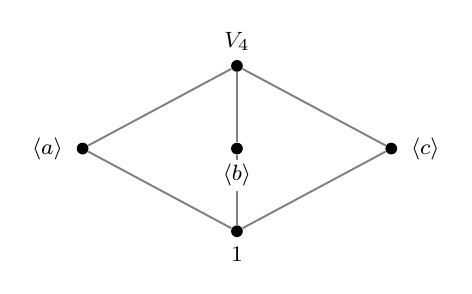
\begin{tikzpicture}[yscale=1.05,xscale=1.4]
  \node[ltdot] (bot) at (0,0) {};
  \node[ltdot] (a) at (-1.4,1) {};
  \node[ltdot] (b) at (0,1) {};
  \node[ltdot] (c) at (1.4,1) {};
  \node[ltdot] (top) at (0,2) {};
  \begin{scope}[ltedge]
    \draw (bot)--(a);
    \draw (bot)--(b);
    \draw (bot)--(c);
    \draw (a)--(top);
    \draw (b)--(top);
    \draw (c)--(top);
  \end{scope}
  \node[ltlab,below=1.5pt of bot] {$1$};
  \node[ltlab,left=3pt of a] {$\langle a\rangle$};
  \node[ltlab,below=1.5pt of b] {$\langle b\rangle$};
  \node[ltlab,right=3pt of c] {$\langle c\rangle$};
  \node[ltlab,above=1.5pt of top] {$V_4$};
\end{tikzpicture}\end{center}

\emph{Check.} The ``diamond'' shape has $1$ at bottom, three pairwise-incomparable atoms, and $V_4$ on top, which matches the known fact that $V_4\isom\Zn2\times\Zn2$ has exactly three subgroups of order $2$. Sanity: $3$ middle $+2$ ($1$ and $V_4$) $=5$ subgroups.
\end{wex}

\begin{wex}{Divisor lattice of $\Zn{12}$}
Draw the subgroup lattice of $\Zn{12}=\gen{x}$, $\ord{x}=12$.
\wrec
$G$ is cyclic, so Proposition~\ref{p:cycliclattice@c2} applies: subgroups $\leftrightarrow$ divisors of $12$, and the Hasse diagram \emph{is} the divisor lattice of $12$. No element-by-element search is needed.
\wsol
\emph{Step 1.} Divisors of $12$ are $1,2,3,4,6,12$, giving one subgroup of each order:
\[
1=\gen{x^{12}},\ \gen{x^6}\ (\ord 2),\ \gen{x^4}\ (\ord 3),\ \gen{x^3}\ (\ord 4),\ \gen{x^2}\ (\ord 6),\ \gen{x}=\Zn{12}.
\]

\emph{Step 2.} Heights by order: $1$ at the bottom; $\gen{x^6}$ (order $2$) and $\gen{x^4}$ (order $3$) low; $\gen{x^3}$ (order $4$) and $\gen{x^2}$ (order $6$) high; $\Zn{12}$ on top.

\emph{Step 3 (coverings via prime index).} $1\lessdot\gen{x^6}$ (index $2$), $1\lessdot\gen{x^4}$ (index $3$). Then $\gen{x^6}\lessdot\gen{x^2}$ (orders $2\mid6$, ratio $3$) and $\gen{x^6}\lessdot\gen{x^3}$ (orders $2\mid4$, ratio $2$); $\gen{x^4}\lessdot\gen{x^2}$ (orders $3\mid6$, ratio $2$). Finally $\gen{x^3}\lessdot\Zn{12}$ (index $3$) and $\gen{x^2}\lessdot\Zn{12}$ (index $2$). The result is a $2\times3$ ``grid'' (product of a $2$-chain and a $3$-chain), matching $12=2^2\cdot3$.
\begin{center}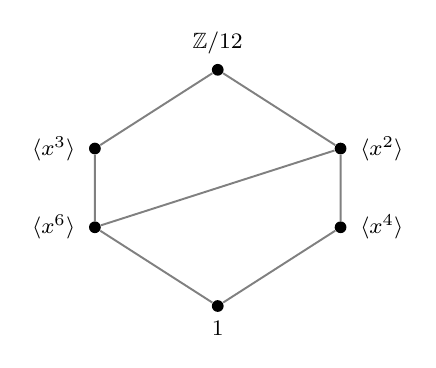
\begin{tikzpicture}[yscale=1.0,xscale=1.3]
  \node[ltdot] (bot) at (0,0) {};
  \node[ltdot] (x6) at (-1.2,1) {};
  \node[ltdot] (x4) at (1.2,1) {};
  \node[ltdot] (x3) at (-1.2,2) {};
  \node[ltdot] (x2) at (1.2,2) {};
  \node[ltdot] (top) at (0,3) {};
  \begin{scope}[ltedge]
    \draw (bot)--(x6);
    \draw (bot)--(x4);
    \draw (x6)--(x3);
    \draw (x6)--(x2);
    \draw (x4)--(x2);
    \draw (x3)--(top);
    \draw (x2)--(top);
  \end{scope}
  \node[ltlab,below=1.5pt of bot] {$1$};
  \node[ltlab,left=3pt of x6] {$\langle x^6\rangle$};
  \node[ltlab,right=3pt of x4] {$\langle x^4\rangle$};
  \node[ltlab,left=3pt of x3] {$\langle x^3\rangle$};
  \node[ltlab,right=3pt of x2] {$\langle x^2\rangle$};
  \node[ltlab,above=1.5pt of top] {$\mathbb{Z}/12$};
\end{tikzpicture}\end{center}

\emph{Check.} Six subgroups, matching the six divisors of $12$. Every maximal chain from $1$ to $\Zn{12}$ has two index-$2$ steps and one index-$3$ step (e.g.\ $1\to\gen{x^4}\to\gen{x^2}\to\Zn{12}$ has indices $3,2,2$), confirming the $2\times3$ grid for $12=2^2\cdot3$.
\end{wex}

\begin{wex}{Chain lattice of $\Zn{16}$}
Draw the subgroup lattice of $\Zn{16}=\gen{x}$, $\ord{x}=16$.
\wrec
Cyclic group, so Proposition~\ref{p:cycliclattice@c2} again: subgroups $\leftrightarrow$ divisors of $16$. Since $16=2^4$ has divisors $1,2,4,8,16$ that form a single divisibility chain, the lattice will be a straight \emph{chain} (totally ordered).
\wsol
\emph{Step 1.} Divisors $1,2,4,8,16$ give:
\[
1=\gen{x^{16}},\ \gen{x^8}\ (\ord2),\ \gen{x^4}\ (\ord4),\ \gen{x^2}\ (\ord8),\ \gen{x}=\Zn{16}.
\]

\emph{Step 2--3.} Each order divides the next, and consecutive ratios are all $2$ (prime), so every consecutive pair is a covering and there are no incomparable subgroups:
\[
1\ \lessdot\ \gen{x^8}\ \lessdot\ \gen{x^4}\ \lessdot\ \gen{x^2}\ \lessdot\ \Zn{16}.
\]
\begin{center}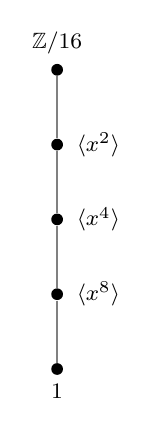
\begin{tikzpicture}[yscale=0.95,xscale=1.0]
  \node[ltdot] (bot) at (0,0) {};
  \node[ltdot] (x8) at (0,1) {};
  \node[ltdot] (x4) at (0,2) {};
  \node[ltdot] (x2) at (0,3) {};
  \node[ltdot] (top) at (0,4) {};
  \begin{scope}[ltedge]
    \draw (bot)--(x8)--(x4)--(x2)--(top);
  \end{scope}
  \node[ltlab,below=1.5pt of bot] {$1$};
  \node[ltlab,right=3pt of x8] {$\langle x^8\rangle$};
  \node[ltlab,right=3pt of x4] {$\langle x^4\rangle$};
  \node[ltlab,right=3pt of x2] {$\langle x^2\rangle$};
  \node[ltlab,above=1.5pt of top] {$\mathbb{Z}/16$};
\end{tikzpicture}\end{center}

\emph{Check.} Five subgroups for the five divisors of $16$. A prime-power cyclic group $\Zn{p^k}$ always has a chain lattice of length $k$; here $p=2,k=4$ gives a chain of $4$ edges, as drawn.
\end{wex}

\begin{wex}{Lattice of $S_3$}
Draw the subgroup lattice of $S_3$ (the symmetric group on $\{1,2,3\}$, order $6$).
\wrec
$|S_3|=6$, so Lagrange allows subgroup orders $1,2,3,6$. $S_3$ is non-cyclic, so we search by order: order-$2$ subgroups come from transpositions, the order-$3$ subgroup from a $3$-cycle. This is the Method's Step 1 done by hand.
\wsol
\emph{Step 1 (subgroups).} The six elements are $e$, the transpositions $(1\,2),(1\,3),(2\,3)$ (each of order $2$), and the $3$-cycles $(1\,2\,3),(1\,3\,2)$ (each of order $3$).
\begin{itemize}
\item Order $1$: $\{e\}$.
\item Order $2$: $\gen{(1\,2)}=\{e,(1\,2)\}$, $\gen{(1\,3)}=\{e,(1\,3)\}$, $\gen{(2\,3)}=\{e,(2\,3)\}$ --- three of them.
\item Order $3$: $\gen{(1\,2\,3)}=\{e,(1\,2\,3),(1\,3\,2)\}$ --- exactly one, since $(1\,3\,2)=(1\,2\,3)^2$ generates the same group.
\item Order $6$: $S_3$ itself.
\end{itemize}
Total $6$ subgroups.

\emph{Step 2.} Bottom $1$; middle row the three order-$2$ groups and the one order-$3$ group; top $S_3$.

\emph{Step 3 (coverings).} Each order-$2$ subgroup covers $1$ (index $2$, prime) and is covered by $S_3$ (index $3$, prime). The order-$3$ subgroup covers $1$ (index $3$) and is covered by $S_3$ (index $2$). No two distinct middle subgroups are comparable (different prime orders, or two order-$2$ groups share only $e$), so no horizontal edges.
\begin{center}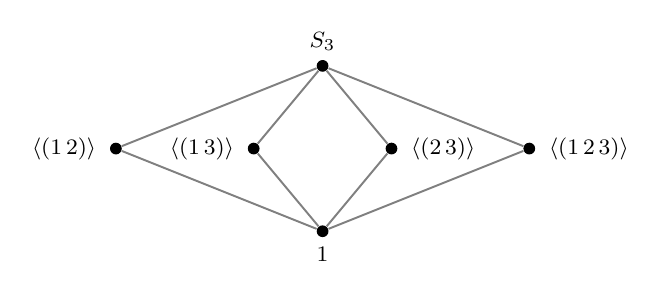
\begin{tikzpicture}[yscale=1.05,xscale=1.25]
  \node[ltdot] (bot) at (0,0) {};
  \node[ltdot] (t12) at (-2.1,1) {};
  \node[ltdot] (t13) at (-0.7,1) {};
  \node[ltdot] (t23) at (0.7,1) {};
  \node[ltdot] (c) at (2.1,1) {};
  \node[ltdot] (top) at (0,2) {};
  \begin{scope}[ltedge]
    \draw (bot)--(t12);
    \draw (bot)--(t13);
    \draw (bot)--(t23);
    \draw (bot)--(c);
    \draw (t12)--(top);
    \draw (t13)--(top);
    \draw (t23)--(top);
    \draw (c)--(top);
  \end{scope}
  \node[ltlab,below=1.5pt of bot] {$1$};
  \node[ltlab,left=3pt of t12] {$\langle (1\,2)\rangle$};
  \node[ltlab,left=3pt of t13] {$\langle (1\,3)\rangle$};
  \node[ltlab,right=3pt of t23] {$\langle (2\,3)\rangle$};
  \node[ltlab,right=3pt of c] {$\langle (1\,2\,3)\rangle$};
  \node[ltlab,above=1.5pt of top] {$S_3$};
\end{tikzpicture}\end{center}

\emph{Check.} Six subgroups. The unique order-$3$ subgroup is the alternating group $A_3$, normal of index $2$; the three order-$2$ subgroups are conjugate. Counting elements: $1$ identity $+3$ transpositions $+2$ three-cycles $=6$, consistent with $|S_3|=6$.
\end{wex}

\begin{wex}{Lattice of $\Zn{18}$ (type $p^2q$)}
Draw the subgroup lattice of $\Zn{18}=\gen{x}$, $\ord{x}=18=2\cdot3^2$.
\wrec
Cyclic of order $18$, so Proposition~\ref{p:cycliclattice@c2}: subgroups $\leftrightarrow$ divisors of $18$. With $18=2\cdot3^2$ the divisor lattice is a $2\times3$ grid (a $2$-chain from the prime $2$ crossed with a $3$-chain from $3^2$), the same \emph{shape} as $\Zn{12}$ but with the chains swapped in length.
\wsol
\emph{Step 1.} Divisors $1,2,3,6,9,18$ give one subgroup each:
\[
1=\gen{x^{18}},\ \gen{x^9}\ (\ord2),\ \gen{x^6}\ (\ord3),\ \gen{x^3}\ (\ord6),\ \gen{x^2}\ (\ord9),\ \gen{x}=\Zn{18}.
\]

\emph{Step 2--3 (coverings via prime index).} $1\lessdot\gen{x^9}$ (index $2$), $1\lessdot\gen{x^6}$ (index $3$). Then $\gen{x^9}\lessdot\gen{x^3}$ (orders $2\mid6$, ratio $3$); $\gen{x^6}\lessdot\gen{x^3}$ (orders $3\mid6$, ratio $2$) and $\gen{x^6}\lessdot\gen{x^2}$ (orders $3\mid9$, ratio $3$). Finally $\gen{x^3}\lessdot\Zn{18}$ (index $3$) and $\gen{x^2}\lessdot\Zn{18}$ (index $2$). Note the order-$9$ branch $1\to\gen{x^6}\to\gen{x^2}$ is a length-$2$ chain (powers of $3$), while the order-$2$ direction adds a single rung.
\begin{center}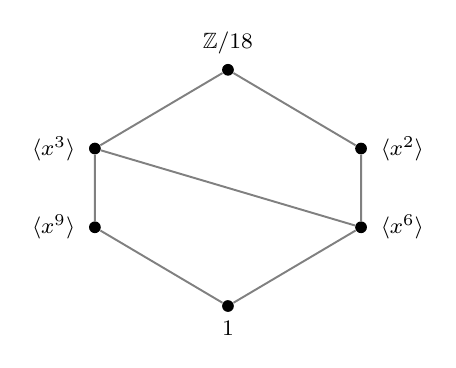
\begin{tikzpicture}[yscale=1.0,xscale=1.3]
  \node[ltdot] (bot) at (0,0) {};
  \node[ltdot] (x9) at (-1.3,1) {};
  \node[ltdot] (x6) at (1.3,1) {};
  \node[ltdot] (x3) at (-1.3,2) {};
  \node[ltdot] (x2) at (1.3,2) {};
  \node[ltdot] (top) at (0,3) {};
  \begin{scope}[ltedge]
    \draw (bot)--(x9);
    \draw (bot)--(x6);
    \draw (x9)--(x3);
    \draw (x6)--(x3);
    \draw (x6)--(x2);
    \draw (x3)--(top);
    \draw (x2)--(top);
  \end{scope}
  \node[ltlab,below=1.5pt of bot] {$1$};
  \node[ltlab,left=3pt of x9] {$\langle x^9\rangle$};
  \node[ltlab,right=3pt of x6] {$\langle x^6\rangle$};
  \node[ltlab,left=3pt of x3] {$\langle x^3\rangle$};
  \node[ltlab,right=3pt of x2] {$\langle x^2\rangle$};
  \node[ltlab,above=1.5pt of top] {$\mathbb{Z}/18$};
\end{tikzpicture}\end{center}

\emph{Check.} Six subgroups for six divisors. The $3$-part $\{1,\gen{x^6},\gen{x^2}\}$ forms a chain of length $2$ (since $3^2\mid18$), and crossing with the $2$-part gives the grid; this is the generic shape of $\Zn{p^2q}$.
\end{wex}

\begin{method}{How to read a join $H\vee K$ and meet $H\wedge K$ off a Hasse diagram}
Use this whenever a problem gives you two specific subgroups and asks for their intersection or the subgroup they generate.
\begin{enumerate}
\item \textbf{Locate $H$ and $K$ as vertices.}
\item \textbf{Meet $H\wedge K=H\cap K$:} trace downward from both. The meet is the \emph{highest} vertex reachable by a downward path from $H$ \emph{and} from $K$. If their only common lower vertex is $1$, then $H\cap K=1$.
\item \textbf{Join $H\vee K=\gen{H,K}$:} trace upward from both. The join is the \emph{lowest} vertex reachable by an upward path from $H$ \emph{and} from $K$. If their only common upper vertex is $G$, then $\gen{H,K}=G$.
\item \textbf{Confirm by orders if unsure:} $|H\cap K|$ divides $\gcd(|H|,|K|)$; and $|\gen{H,K}|$ is a multiple of $\lcm(|H|,|K|)$ dividing $|G|$. Often this pins the answer.
\end{enumerate}
\end{method}

\begin{pitfall}
$H\vee K=\gen{H,K}$ is \emph{not} the set product $HK=\{hk\}$ in general, and not the union $H\cup K$ (a union of two subgroups is almost never a subgroup). Read the join as the lowest common \emph{upper} vertex, or compute it as all products of elements from $H\cup K$.
\end{pitfall}

\begin{wex}{Reading joins and meets off the $S_3$ and $V_4$ lattices}
Using the lattices already drawn, compute (a) $\gen{(1\,2)}\vee\gen{(1\,3)}$ and $\gen{(1\,2)}\wedge\gen{(1\,3)}$ in $S_3$; (b) $\gen{(1\,2)}\vee\gen{(1\,2\,3)}$ in $S_3$; (c) $\gen{a}\vee\gen{b}$ and $\gen{a}\wedge\gen{b}$ in $V_4$.
\wrec
Each part names two specific subgroups and asks for their join or meet, so this is the reading-off Method. We locate the vertices in the diagrams from the previous worked examples and trace up (join) or down (meet), then confirm with the order test $|H\cap K|\mid\gcd$ and $\lcm\mid|\gen{H,K}|$.
\wsol
\emph{(a) In $S_3$.} \textbf{Meet:} $\gen{(1\,2)}=\{e,(1\,2)\}$ and $\gen{(1\,3)}=\{e,(1\,3)\}$ share only $e$ below them; the highest common lower vertex is $1$. So
\[
\gen{(1\,2)}\wedge\gen{(1\,3)}=\gen{(1\,2)}\cap\gen{(1\,3)}=\{e\}=1.
\]
(Order check: $|H\cap K|$ divides $\gcd(2,2)=2$, and the only shared element is $e$, so it is $1$.) \textbf{Join:} trace upward from both order-$2$ vertices; their only common upper vertex is the top, $S_3$. So $\gen{(1\,2)}\vee\gen{(1\,3)}=S_3$. \emph{Confirm directly:} the product $(1\,2)(1\,3)=(1\,3\,2)$ is a $3$-cycle, so $\gen{(1\,2),(1\,3)}$ contains an element of order $3$ and an element of order $2$; its order is a multiple of $\lcm(2,3)=6$ dividing $6$, hence $6$, giving all of $S_3$.

\emph{(b) In $S_3$.} $\gen{(1\,2)}$ has order $2$, $\gen{(1\,2\,3)}$ has order $3$. Upward, the only common vertex above both is $S_3$, so $\gen{(1\,2)}\vee\gen{(1\,2\,3)}=S_3$. (Order check: $|\gen{H,K}|$ is a multiple of $\lcm(2,3)=6$ and divides $6$, so it equals $6=|S_3|$.) Their meet is $1$ since $\gcd(2,3)=1$ forces $H\cap K=\{e\}$.

\emph{(c) In $V_4$.} \textbf{Meet:} $\gen{a}=\{1,a\}$ and $\gen{b}=\{1,b\}$ share only $1$, so $\gen{a}\wedge\gen{b}=1$. \textbf{Join:} upward from both order-$2$ atoms, the only common upper vertex is the top, so $\gen{a}\vee\gen{b}=V_4$. \emph{Confirm:} $ab=c\notin\gen{a}\cup\gen{b}$, so $\gen{a,b}$ properly contains $\gen{a}$, has order a multiple of $\lcm(2,2)=2$ exceeding $2$ and dividing $4$, hence $4$; thus $\gen{a,b}=V_4$.

\emph{Check.} In all parts the meet of two distinct atoms is the bottom $1$ and the join of two distinct atoms is the top of the relevant lattice --- exactly what ``lowest common upper / highest common lower vertex'' predicts when the two subgroups are incomparable atoms whose join is the whole group.
\end{wex}

\begin{wex}{A meet and join inside $\Zn{12}$}
In $\Zn{12}=\gen{x}$ compute $\gen{x^4}\wedge\gen{x^6}$ and $\gen{x^4}\vee\gen{x^6}$, where $\gen{x^4}$ has order $3$ and $\gen{x^6}$ has order $2$.
\wrec
Two named subgroups of a cyclic group; use the reading-off Method on the $\Zn{12}$ grid, and double-check with the cyclic shortcut $\gen{x^a}\cap\gen{x^b}=\gen{x^{\lcm(a,b)}}$ and $\gen{x^a,x^b}=\gen{x^{\gcd(a,b)}}$.
\wsol
\emph{Meet (down).} On the grid, $\gen{x^4}$ (order $3$) and $\gen{x^6}$ (order $2$) have only $1$ below both. So $\gen{x^4}\wedge\gen{x^6}=1$. \emph{Shortcut check:} $\gen{x^4}\cap\gen{x^6}=\gen{x^{\lcm(4,6)}}=\gen{x^{12}}=\gen{e}=1$. Agrees; also $\gcd(2,3)=1$ forces the trivial meet.

\emph{Join (up).} Upward from order-$3$ and order-$2$ vertices, the lowest common upper vertex is $\gen{x^2}$ (order $6$). So $\gen{x^4}\vee\gen{x^6}=\gen{x^2}$. \emph{Shortcut check:} $\gen{x^4,x^6}=\gen{x^{\gcd(4,6)}}=\gen{x^2}$, of order $12/\gcd(2,12)=6$. Agrees, and $6=\lcm(2,3)$ as the order test demands.

\emph{Check.} Meet has order $1\mid\gcd(2,3)=1$; join has order $6$, a multiple of $\lcm(2,3)=6$ dividing $12$. Both consistent. Note $\gen{x^2}\ne\Zn{12}$ here: the join of two proper subgroups need not be the whole group --- contrast with the $S_3$ transpositions, whose join \emph{was} everything.
\end{wex}

\subsection*{Using Subgroup Lattices: $D_8$, $Q_8$, and $\Zn{24}$}

The subgroup lattice of a finite group $G$ is the Hasse diagram of all subgroups of $G$ ordered by inclusion: the trivial subgroup $1$ at the bottom, $G$ at the top, and an upward edge $H$---$K$ exactly when $H\psgr K$ with no subgroup strictly between them. Once drawn, the lattice is a single picture from which we can read inclusions and indices, and which (together with a few conjugation checks) locates normal subgroups and normalizers. This section builds the three canonical lattices and turns them into computational tools.

\begin{definition}\label{d:coveredge@c2}
In the subgroup lattice of $G$, we draw an edge $H$---$K$ (with $H$ below $K$) precisely when $H\psgr K$ and there is no subgroup $L$ with $H\psgr L\psgr K$. We say $K$ \emph{covers} $H$.
\end{definition}

\subsubsection*{The lattice of $D_8$ and its ten subgroups}

Write $D_8=\gen{r,s\st r^4=s^2=1,\ srs=r\inv}$; then $r\inv=r^3$, and the eight elements are
\[ 1,\ r,\ r^2,\ r^3,\ s,\ rs,\ r^2s,\ r^3s. \]
We first list every subgroup by order.

\begin{proposition}\label{p:d8subs@c2}
$D_8$ has exactly ten subgroups: the trivial group $1$; the whole group $D_8$; one cyclic order-$4$ subgroup $\gen{r}=\{1,r,r^2,r^3\}$ and two Klein four-groups $\gen{r^2,s}=\{1,r^2,s,r^2s\}$ and $\gen{r^2,rs}=\{1,r^2,rs,r^3s\}$; and five order-$2$ subgroups $\gen{r^2},\gen{s},\gen{rs},\gen{r^2s},\gen{r^3s}$.
\end{proposition}

\begin{proof}
By Lagrange every proper nontrivial subgroup has order $2$ or $4$. An order-$2$ subgroup is $\gen{x}$ for an element $x$ of order $2$; the five involutions are $r^2,s,rs,r^2s,r^3s$ (the elements $r,r^3$ have order $4$), giving five order-$2$ subgroups. An order-$4$ subgroup $H$ has index $2$, hence is normal, and is either cyclic or Klein four. The only elements of order $4$ are $r,r^3$, both generating $\gen{r}$, so there is exactly one cyclic order-$4$ subgroup. A Klein four subgroup consists of $1$ and three commuting involutions; since $r^2$ is central and $s\cdot r^2s=r^2$, $\{1,r^2,s,r^2s\}$ and $\{1,r^2,rs,r^3s\}$ are subgroups, and conversely a Klein four subgroup contains at most one rotation besides $1$ (namely $r^2$), hence two distinct commuting reflections $r^is,r^js$. Since $(r^is)(r^js)=r^{i-j}$ and $(r^js)(r^is)=r^{j-i}$, these commute iff $r^{2(i-j)}=1$, i.e.\ iff $i\equiv j\pmod 2$ (e.g.\ $s(rs)=srs=r\inv=r^3$ while $(rs)s=r$, so $s$ and $rs$ do not commute). So the pair is $\{s,r^2s\}$ or $\{rs,r^3s\}$, and the subgroup is one of the two above; hence no others exist. Total: $1+5+3+1=10$.
\end{proof}

The covering relations: each order-$2$ subgroup sits under the order-$4$ subgroup(s) containing it. Note $\gen{r^2}$ is the \emph{center} $Z(D_8)$ and lies inside all three order-$4$ subgroups, while each of $\gen{s},\gen{r^2s}$ lies only in $\gen{r^2,s}$ and each of $\gen{rs},\gen{r^3s}$ only in $\gen{r^2,rs}$.

\begin{center}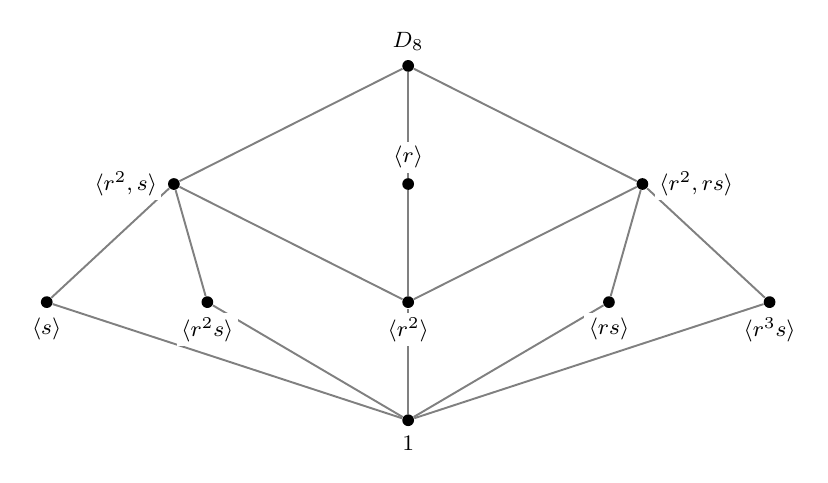
\begin{tikzpicture}[yscale=1.5,xscale=1.7]
  \node[ltdot] (bot) at (0,0) {};
  \node[ltdot] (s)   at (-2.7,1) {};
  \node[ltdot] (r2s) at (-1.5,1) {};
  \node[ltdot] (rr)  at (0,1) {};
  \node[ltdot] (rs)  at (1.5,1) {};
  \node[ltdot] (r3s) at (2.7,1) {};
  \node[ltdot] (A) at (-1.75,2) {};
  \node[ltdot] (R) at (0,2) {};
  \node[ltdot] (B) at (1.75,2) {};
  \node[ltdot] (top) at (0,3) {};
  \begin{scope}[ltedge]
    \draw (bot)--(s); \draw (bot)--(r2s); \draw (bot)--(rr); \draw (bot)--(rs); \draw (bot)--(r3s);
    \draw (s)--(A); \draw (r2s)--(A); \draw (rr)--(A); \draw (rr)--(R); \draw (rr)--(B); \draw (rs)--(B); \draw (r3s)--(B);
    \draw (A)--(top); \draw (R)--(top); \draw (B)--(top);
  \end{scope}
  \node[ltlab,below=1.5pt of bot] {$1$};
  \node[ltlab,below=1.5pt of s]   {$\gen{s}$};
  \node[ltlab,below=1.5pt of r2s] {$\gen{r^2s}$};
  \node[ltlab,below=1.5pt of rr]  {$\gen{r^2}$};
  \node[ltlab,below=1.5pt of rs]  {$\gen{rs}$};
  \node[ltlab,below=1.5pt of r3s] {$\gen{r^3s}$};
  \node[ltlab,left=2pt of A]      {$\gen{r^2,s}$};
  \node[ltlab,above=1.5pt of R]   {$\gen{r}$};
  \node[ltlab,right=2pt of B]     {$\gen{r^2,rs}$};
  \node[ltlab,above=1.5pt of top] {$D_8$};
\end{tikzpicture}\end{center}

\noindent The same group is laid out below as a \emph{Cayley graph}: the eight elements are the
vertices, the solid arrows are right-multiplication by $r$ (a $4$-cycle on the outer rotations and,
in the \emph{opposite} sense, on the inner reflections, since $sr=r\inv s$), and the dashed edges
are right-multiplication by the involution $s$, joining each rotation $r^k$ to the reflection
$r^ks$.

\begin{center}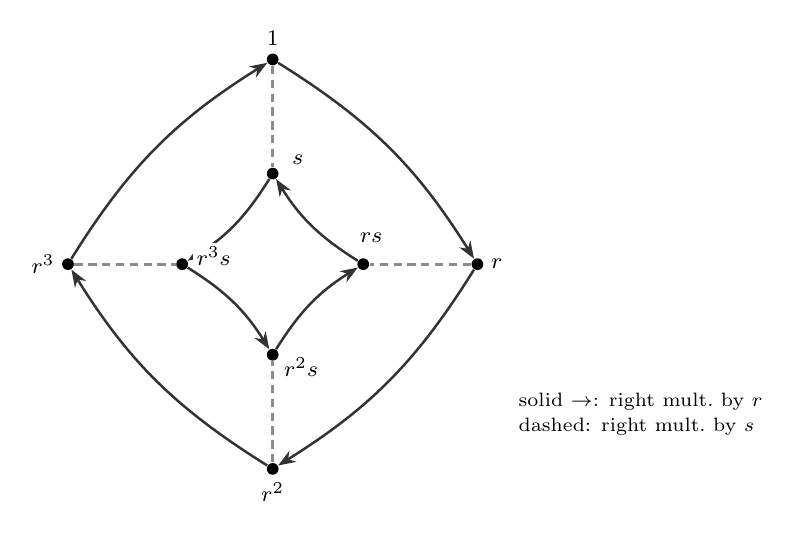
\begin{tikzpicture}
  \node[cgdot] (e)    at (90:2.6)  {};
  \node[cgdot] (r)    at (0:2.6)   {};
  \node[cgdot] (r2)   at (-90:2.6) {};
  \node[cgdot] (r3)   at (180:2.6) {};
  \node[cgdot] (sN)   at (90:1.15)  {};
  \node[cgdot] (rsN)  at (0:1.15)   {};
  \node[cgdot] (r2sN) at (-90:1.15) {};
  \node[cgdot] (r3sN) at (180:1.15) {};
  \draw[cgs] (e)--(sN); \draw[cgs] (r)--(rsN); \draw[cgs] (r2)--(r2sN); \draw[cgs] (r3)--(r3sN);
  \draw[cgr] (e) to[bend left=13] (r);
  \draw[cgr] (r) to[bend left=13] (r2);
  \draw[cgr] (r2) to[bend left=13] (r3);
  \draw[cgr] (r3) to[bend left=13] (e);
  \draw[cgr] (sN) to[bend left=13] (r3sN);
  \draw[cgr] (r3sN) to[bend left=13] (r2sN);
  \draw[cgr] (r2sN) to[bend left=13] (rsN);
  \draw[cgr] (rsN) to[bend left=13] (sN);
  \node[cglab,above=1pt of e]  {$1$};
  \node[cglab,right=1pt of r]  {$r$};
  \node[cglab,below=1pt of r2] {$r^2$};
  \node[cglab,left=1pt of r3]  {$r^3$};
  \node[cglab] at ($(sN)+(0.32,0.18)$)   {$s$};
  \node[cglab] at ($(rsN)+(0.10,0.34)$)  {$rs$};
  \node[cglab] at ($(r2sN)+(0.36,-0.16)$) {$r^2s$};
  \node[cglab] at ($(r3sN)+(0.40,0.10)$) {$r^3s$};
  \node[font=\scriptsize,align=left,anchor=west] at (3.0,-1.9)
    {solid $\to$: right mult.\ by $r$\\[1pt] dashed: right mult.\ by $s$};
\end{tikzpicture}\end{center}

\begin{wex}{List the subgroups of $D_8$ by order}
Produce the full subgroup list of $D_8$ organized by order, and confirm the count is ten.
\wrec The trigger is ``small group, want all subgroups.'' Use Lagrange to bound the possible orders ($1,2,4,8$), then enumerate order-$2$ subgroups via involutions and order-$4$ subgroups via the cyclic-vs-Klein dichotomy. This is exactly Proposition~\ref{p:d8subs@c2}'s method applied as a checklist.
\wsol \emph{Order $1$:} $1$. \emph{Order $8$:} $D_8$. \emph{Order $2$:} find all $x$ with $x^2=1,\ x\neq1$. Check each non-identity element: $r,r^3$ have order $4$; $r^2$ has order $2$; $s^2=1$; $(rs)^2=rsrs=r(srs)=r\cdot r\inv=1$ and likewise $(r^2s)^2=(r^3s)^2=1$. So the involutions are $r^2,s,rs,r^2s,r^3s$, giving five subgroups. \emph{Order $4$:} cyclic ones need order-$4$ elements $r,r^3$, both giving $\gen{r}$ (one subgroup); Klein ones are $\{1,r^2,s,r^2s\}$ and $\{1,r^2,rs,r^3s\}$ (two subgroups). \emph{Total} $=1+1+5+1+2=10$.

\emph{Check:} every involution appears in at least one order-$4$ subgroup ($r^2$ in all three; $s,r^2s$ in $\gen{r^2,s}$; $rs,r^3s$ in $\gen{r^2,rs}$), consistent with the lattice edges. Count $10$ matches Proposition~\ref{p:d8subs@c2}.
\end{wex}

\subsubsection*{The lattice of $Q_8$: every subgroup is normal}

Recall $Q_8=\{\pm1,\pm i,\pm j,\pm k\}$ with $i^2=j^2=k^2=-1$, $ij=k$, $jk=i$, $ki=j$, and $ji=-k$ etc. Here $-1$ is the unique element of order $2$ and is central.

\begin{proposition}\label{p:q8@c2}
$Q_8$ has exactly six subgroups: $1$, $\gen{-1}=\{\pm1\}$, $\gen{i}=\{\pm1,\pm i\}$, $\gen{j}=\{\pm1,\pm j\}$, $\gen{k}=\{\pm1,\pm k\}$, and $Q_8$. Every subgroup is normal.
\end{proposition}

\begin{proof}
The only element of order $2$ is $-1$ (since $i^2=j^2=k^2=-1\neq1$), giving the unique order-$2$ subgroup $\gen{-1}$. The order-$4$ subgroups are cyclic generated by an order-$4$ element; the order-$4$ elements are $\pm i,\pm j,\pm k$, and $\gen{i}=\gen{-i}$, $\gen{j}=\gen{-j}$, $\gen{k}=\gen{-k}$, giving three. With $1$ and $Q_8$ that is six. Each order-$4$ subgroup has index $2$, hence is normal; $\gen{-1}=Z(Q_8)$ is normal as the center; and $1,Q_8$ are normal. So all six are normal.
\end{proof}

\begin{center}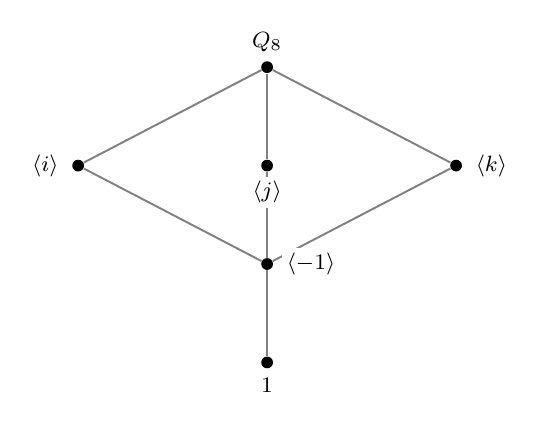
\begin{tikzpicture}[yscale=1.25,xscale=1.5]
  \node[ltdot] (bot) at (0,0) {};
  \node[ltdot] (z) at (0,1) {};
  \node[ltdot] (i) at (-1.6,2) {};
  \node[ltdot] (j) at (0,2) {};
  \node[ltdot] (k) at (1.6,2) {};
  \node[ltdot] (top) at (0,3) {};
  \begin{scope}[ltedge]
    \draw (bot)--(z);
    \draw (z)--(i);
    \draw (z)--(j);
    \draw (z)--(k);
    \draw (i)--(top);
    \draw (j)--(top);
    \draw (k)--(top);
  \end{scope}
  \node[ltlab,below=1.5pt of bot] {$1$};
  \node[ltlab,right=3pt of z] {$\gen{-1}$};
  \node[ltlab,left=3pt of i] {$\gen{i}$};
  \node[ltlab,below=1.5pt of j] {$\gen{j}$};
  \node[ltlab,right=3pt of k] {$\gen{k}$};
  \node[ltlab,above=1.5pt of top] {$Q_8$};
\end{tikzpicture}\end{center}

The single order-$2$ subgroup $\gen{-1}$ is forced to sit beneath all three order-$4$ subgroups, giving $Q_8$ its distinctive ``diamond with a stem'' shape; contrast $D_8$, whose five order-$2$ subgroups fan out.

\begin{wex}{The lattice of $Q_8$ and universal normality}
Draw the subgroup lattice of $Q_8$ and explain why every subgroup is normal.
\wrec ``Every subgroup normal'' is triggered by two recognizable patterns combined: (a) index-$2$ subgroups are automatically normal, and (b) a subgroup contained in the center, or equal to it, is normal. In $Q_8$ all proper nontrivial subgroups are either index $2$ or the center, so both triggers cover everything.
\wsol By Proposition~\ref{p:q8@c2} the subgroups are $1,\gen{-1},\gen{i},\gen{j},\gen{k},Q_8$. For normality: $1$ and $Q_8$ are always normal. The three order-$4$ subgroups have index $|Q_8|/4=2$, and any subgroup of index $2$ is normal (its two cosets are $H$ and $G\setminus H$, the same as left or right). Finally $\gen{-1}$ is the center, and $gZg\inv=Z$ for the center $Z$ of any group, so $\gen{-1}\nor Q_8$. Hence all six subgroups are normal.

\emph{Check:} a direct conjugation, e.g.\ $j\,i\,j\inv$: since $ji=-k$ and $j\inv=-j$, we get $j i j\inv=(-k)(-j)=kj=-i\in\gen{i}$. Thus $j\gen{i}j\inv=\gen{i}$, confirming $\gen{i}\nor Q_8$ as predicted.
\end{wex}

\subsubsection*{The lattice of $\Zn{24}$: a divisor lattice}

\begin{theorem}\label{t:cyclic@c2}
Let $G=\gen{x}$ be cyclic of order $n$. For each divisor $d\mid n$ there is exactly one subgroup of order $d$, namely $\gen{x^{n/d}}$, and these are all the subgroups. Consequently $H\sgr K$ in the lattice iff $|H|\mid|K|$, so the subgroup lattice of $\Zn{n}$ is isomorphic to the lattice of divisors of $n$ under divisibility.
\end{theorem}

\begin{proof}
A subgroup of $\gen{x}$ is cyclic, of the form $\gen{x^a}$, and $|\gen{x^a}|=n/\gcd(a,n)$, which runs over all divisors of $n$ as $a$ varies. If $\gen{x^a}$ and $\gen{x^b}$ both have order $d$, then both equal $\gen{x^{n/d}}$ (the unique subgroup of order $d$), so each order occurs once. Containment $\gen{x^{n/d}}\sgr\gen{x^{n/e}}$ holds iff $d\mid e$, i.e.\ iff orders divide, which is exactly the divisor lattice.
\end{proof}

For $n=24=2^3\cdot3$ the divisors are $1,2,3,4,6,8,12,24$ (eight of them, since $24$ has $(3+1)(1+1)=8$ divisors), so $\Zn{24}$ has eight subgroups, one of each order. Writing the additive generator $1\in\Zn{24}$ as $x$, the order-$d$ subgroup is $\gen{24/d}$.

\begin{center}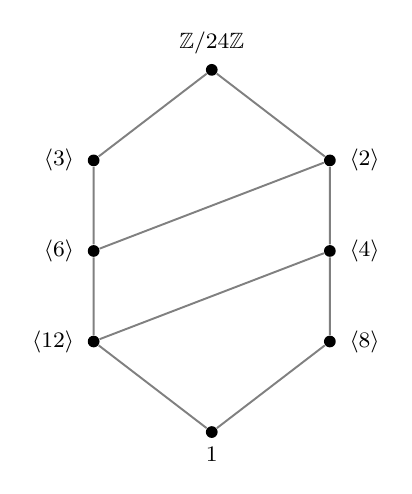
\begin{tikzpicture}[yscale=1.15,xscale=1.5]
  \node[ltdot] (b) at (0,0) {};
  \node[ltdot] (d2) at (-1,1) {};
  \node[ltdot] (d3) at (1,1) {};
  \node[ltdot] (d4) at (-1,2) {};
  \node[ltdot] (d6) at (1,2) {};
  \node[ltdot] (d8) at (-1,3) {};
  \node[ltdot] (d12) at (1,3) {};
  \node[ltdot] (top) at (0,4) {};
  \begin{scope}[ltedge]
    \draw (b)--(d2);
    \draw (b)--(d3);
    \draw (d2)--(d4);
    \draw (d2)--(d6);
    \draw (d3)--(d6);
    \draw (d4)--(d8);
    \draw (d4)--(d12);
    \draw (d6)--(d12);
    \draw (d8)--(top);
    \draw (d12)--(top);
  \end{scope}
  \node[ltlab,below=1.5pt of b] {$1$};
  \node[ltlab,left=3pt of d2] {$\gen{12}$};
  \node[ltlab,right=3pt of d3] {$\gen{8}$};
  \node[ltlab,left=3pt of d4] {$\gen{6}$};
  \node[ltlab,right=3pt of d6] {$\gen{4}$};
  \node[ltlab,left=3pt of d8] {$\gen{3}$};
  \node[ltlab,right=3pt of d12] {$\gen{2}$};
  \node[ltlab,above=1.5pt of top] {$\Zn{24}$};
\end{tikzpicture}\end{center}

Here $\gen{12}$ has order $2$, $\gen{8}$ order $3$, $\gen{6}$ order $4$, $\gen{4}$ order $6$, $\gen{3}$ order $8$, $\gen{2}$ order $12$. The shape is the $4\times2$ grid of divisors of $2^3\cdot3$.

\begin{pitfall}
In $\Zn{n}$ the subgroup ``$\gen{m}$'' means the cyclic subgroup generated by the residue $m$, and $|\gen{m}|=n/\gcd(m,n)$, \emph{not} $n/m$. For $\Zn{24}$, $\gen{6}$ has order $24/\gcd(6,24)=24/6=4$, but $\gen{8}$ has order $24/\gcd(8,24)=24/8=3$. Compute the gcd; do not just divide by the label.
\end{pitfall}

\begin{wex}{Subgroup of $\Zn{24}$ of each order, and one containment}
List the eight subgroups of $\Zn{24}$ with their orders, and decide whether $\gen{6}\sgr\gen{2}$.
\wrec Cyclic group of order $24$ $\Rightarrow$ Theorem~\ref{t:cyclic@c2}: subgroups correspond to divisors of $24$, and containment is divisibility of orders. The containment question is answered purely by ``does $|\gen{6}|$ divide $|\gen{2}|$?''
\wsol Divisors of $24$: $1,2,3,4,6,8,12,24$. Order-$d$ subgroup is $\gen{24/d}$:
\[
\begin{array}{c|cccccccc}
d & 1 & 2 & 3 & 4 & 6 & 8 & 12 & 24\\\hline
\gen{24/d} & \gen{24}=1 & \gen{12} & \gen{8} & \gen{6} & \gen{4} & \gen{3} & \gen{2} & \gen{1}
\end{array}
\]
Now $|\gen{6}|=24/\gcd(6,24)=4$ and $|\gen{2}|=24/\gcd(2,24)=12$. Since $4\mid12$, Theorem~\ref{t:cyclic@c2} gives $\gen{6}\sgr\gen{2}$.

\emph{Check directly:} $\gen{6}=\{0,6,12,18\}$ and $\gen{2}=\{0,2,4,\dots,22\}$; indeed $6,12,18$ are even, so $\gen{6}\subseteq\gen{2}$. Consistent.
\end{wex}

\subsubsection*{Reading normal subgroups and normalizers off a lattice}

\begin{method}{Using the lattice to (a) spot normal subgroups and (b) locate $N_G(H)$}
\textbf{Recognition trigger:} use this whenever you have the lattice drawn and want normality or a normalizer \emph{without} brute-force conjugating every element.

\textbf{(a) Normal subgroups.}
\begin{enumerate}
\item Any subgroup of index $2$ (one level below the top, with $|G:H|=2$) is normal --- mark it immediately.
\item The center $Z(G)$ and any subgroup contained in $Z(G)$ is normal; locate $Z(G)$ as the largest subgroup every node is ``compatible'' with (in $D_8$ and $Q_8$ this is the unique central involution's group).
\item A subgroup that is the \emph{unique} subgroup of its order is characteristic, hence normal (conjugation permutes same-order subgroups, and a singleton orbit is fixed).
\item For the remaining small subgroups, conjugation permutes the subgroups of each fixed order; $H\nor G$ iff that orbit is $\{H\}$. Read off the same-order siblings from the lattice and test whether a single conjugation moves $H$ to a sibling.
\end{enumerate}

\textbf{(b) The normalizer $N_G(H)$.}
\begin{enumerate}
\item $N_G(H)$ is a subgroup with $H\sgr N_G(H)\sgr G$, so it lies on the chain \emph{above} $H$ in the lattice --- only those finitely many candidates can occur.
\item $H\nor G$ $\Leftrightarrow$ $N_G(H)=G$ (top). If $H$ is not normal, $N_G(H)$ is a \emph{proper} subgroup containing $H$.
\item Test candidates from largest down: $g\in N_G(H)$ iff $gHg\inv=H$. The first proper overgroup $K$ with every generator of $K$ normalizing $H$, and with no larger overgroup doing so, is $N_G(H)$.
\item Sanity: $|G:N_G(H)|$ equals the number of distinct conjugates $gHg\inv$ (the orbit size), which you can also count among the same-order siblings in the lattice.
\end{enumerate}
\end{method}

\begin{wex}{All normal subgroups of $D_8$ from the lattice}
Using the $D_8$ lattice, find every normal subgroup and justify each.
\wrec Apply Method (a) point-by-point: index-$2$ rule for the order-$4$ row, center rule for $\gen{r^2}$, uniqueness for $\gen{r}$, and the same-order-orbit test for the order-$2$ reflections.
\wsol \emph{Index $2$ (order $4$):} $\gen{r},\gen{r^2,s},\gen{r^2,rs}$ each have index $8/4=2$, hence are normal. \emph{Center:} $Z(D_8)=\gen{r^2}$ (since $r^2$ commutes with $r$ and with $s$ as $sr^2s=r^{-2}=r^2$), and the center is always normal, so $\gen{r^2}\nor D_8$. \emph{Trivial cases:} $1$ and $D_8$. \emph{Reflection subgroups $\gen{s},\gen{rs},\gen{r^2s},\gen{r^3s}$ (order $2$):} these are not normal. Conjugate $\gen{s}$ by $r$: $rsr\inv=r(sr\inv)$, and $sr\inv=sr^3=r^{-3}s=rs$; hence $rsr\inv=r\cdot rs=r^2 s\notin\gen{s}$. So $r\gen{s}r\inv=\gen{r^2s}\neq\gen{s}$, and similarly conjugation by $r$ sends $\gen{rs}$ to $\gen{r^3s}$ (since $r(rs)r\inv=r^3s$), swapping that pair. Each reflection subgroup has a $2$-element conjugacy orbit, so none is normal.

Thus the normal subgroups are exactly $1,\ \gen{r^2},\ \gen{r},\ \gen{r^2,s},\ \gen{r^2,rs},\ D_8$ --- six of the ten.

\emph{Check:} the quotient $D_8/\gen{r^2}$ has order $4$ and is abelian ($\cong V_4$), consistent with $\gen{r^2}=[D_8,D_8]$ being normal; and the three index-$2$ subgroups being normal matches the rule. The four reflection subgroups split into two orbits of size $2$ ($\{\gen{s},\gen{r^2s}\}$ and $\{\gen{rs},\gen{r^3s}\}$), accounting for the non-normal ones.
\end{wex}

\begin{wex}{$N_{D_8}(\gen{s})$ via the lattice}
Compute $N_{D_8}(\gen{s})$ by restricting to the overgroups of $\gen{s}$, then verify.
\wrec $\gen{s}$ is a non-normal order-$2$ subgroup (from the previous example), so by Method (b) its normalizer is a \emph{proper} overgroup: read the chain above $\gen{s}$ in the lattice. The only overgroups of $\gen{s}$ are $\gen{s}$ itself, $\gen{r^2,s}$, and $D_8$.
\wsol Candidates from the lattice: $\gen{s}\sgr N\sgr D_8$ with $N\in\{\gen{s},\gen{r^2,s},D_8\}$. We know $N\neq D_8$ (not normal). Test $\gen{r^2,s}=\{1,r^2,s,r^2s\}$: its generators are $r^2$ and $s$.
\begin{itemize}
\item $s\in N_{D_8}(\gen{s})$ trivially ($s\gen{s}s\inv=\gen{s}$).
\item $r^2$: $r^2 s r^{-2}=r^2 s r^2$. Since $r^2$ is central, $r^2 s r^2=s r^2 r^2=s r^4=s\in\gen{s}$. So $r^2$ normalizes $\gen{s}$.
\end{itemize}
Every generator of $\gen{r^2,s}$ normalizes $\gen{s}$, so $\gen{r^2,s}\sgr N_{D_8}(\gen{s})$. Since the only larger subgroup is $D_8$, which does not normalize $\gen{s}$ (because $r\gen{s}r\inv=\gen{r^2s}\neq\gen{s}$ from the previous example), we get
\[
N_{D_8}(\gen{s})=\gen{r^2,s}=\{1,r^2,s,r^2s\}.
\]

\emph{Check via orbit count:} $|D_8:N_{D_8}(\gen{s})|=8/4=2$, so $\gen{s}$ should have exactly $2$ conjugates. Indeed its conjugates are $\gen{s}$ and $\gen{r^2s}$, two subgroups --- matching. (Note $N_{D_8}(\gen{s})\supsetneq\gen{s}$ strictly even though $\gen{s}$ is not normal, illustrating $H\sgr N_G(H)\sgr G$.)
\end{wex}

\begin{wex}{$N_{Q_8}(\gen{i})$ and $N_{\Zn{24}}(\gen{6})$}
Find both normalizers using the lattices.
\wrec In an abelian group every subgroup is normal, so $N_G(H)=G$ automatically --- that is the trigger for $\Zn{24}$. In $Q_8$ every subgroup is normal (Proposition~\ref{p:q8@c2}), so again $N_G(H)=G$. Both reduce to Method (b) step 2: normal $\Rightarrow$ normalizer is the top.
\wsol \emph{$Q_8$:} $\gen{i}$ has index $8/4=2$, hence normal, so $N_{Q_8}(\gen{i})=Q_8$. \emph{$\Zn{24}$:} $\Zn{24}$ is abelian, so $g+\gen{6}-g=\gen{6}$ for all $g$ (equivalently $g\gen{6}g\inv=\gen{6}$), giving $N_{\Zn{24}}(\gen{6})=\Zn{24}$.

\emph{Check:} normalizer at the top of the lattice $\Leftrightarrow$ single conjugate $\Leftrightarrow$ $|G:N_G(H)|=1$. For $\gen{i}$: $j i j\inv=-i\in\gen{i}$ as computed earlier, so conjugation fixes $\gen{i}$, giving one conjugate. For $\gen{6}$: abelian, one conjugate. Both consistent.
\end{wex}

\begin{wex}{A non-normal normalizer in $S_3$ for contrast}
In $S_3=\{e,(12),(13),(23),(123),(132)\}$, draw the relevant overgroups and compute $N_{S_3}(\gen{(12)})$.
\wrec $\gen{(12)}$ is an order-$2$ subgroup of a non-abelian group, and the order-$2$ subgroups (transpositions) form one conjugacy orbit, so we expect a \emph{proper} normalizer. By Method (b) read the chain above $\gen{(12)}$: the only overgroups are $\gen{(12)}$ and $S_3$ (no order-$4$ subgroup exists since $4\nmid6$).
\wsol Overgroups of $\gen{(12)}$ in the lattice: $\gen{(12)}$ (order $2$) and $S_3$ (order $6$); there is no subgroup of order $4$ because $4\nmid 6$. Is $\gen{(12)}\nor S_3$? Conjugate by $(123)$: $(123)(12)(123)\inv=(123)(12)(132)$. Computing, $(123)(12)(132)=(23)\notin\gen{(12)}$. So $\gen{(12)}$ is not normal, hence $N_{S_3}(\gen{(12)})\neq S_3$. The only smaller overgroup is $\gen{(12)}$ itself, so
\[
N_{S_3}(\gen{(12)})=\gen{(12)}.
\]

\emph{Check:} $|S_3:N|=6/2=3$, predicting $3$ conjugates; indeed the transpositions $(12),(13),(23)$ are all conjugate, giving exactly $3$ subgroups $\gen{(12)},\gen{(13)},\gen{(23)}$. Consistent, and this shows $N_G(H)=H$ is possible (the lattice chain above $H$ may have nothing strictly between $H$ and $G$).
\end{wex}

\subsubsection*{The same-lattice, non-isomorphic remark}

A subgroup lattice does \emph{not} determine a group up to isomorphism. The standard example: $Z_2\times Z_8$ and the modular group of order $16$,
\[
M=M_{16}=\gen{u,v\st u^8=v^2=1,\ vuv\inv=u^5},
\]
have isomorphic subgroup lattices but are not isomorphic groups.

\begin{wex}{Why same lattice does not force isomorphism}
Explain how $Z_2\times Z_8$ and $M_{16}$ can share a subgroup lattice yet fail to be isomorphic, and give a concrete invariant that distinguishes them.
\wrec The trigger is the phrase ``same lattice, not isomorphic.'' The lattice records only \emph{which subgroups contain which}; it is blind to \emph{how} elements multiply (commutativity, conjugation). So to separate the two groups we must exhibit a group-theoretic invariant that the lattice cannot see --- abelian vs.\ non-abelian is the cleanest.
\wsol Both groups have order $16$, and their subgroup lattices coincide combinatorially: each has $11$ subgroups, with exactly $1$ of order $1$, three of order $2$, three of order $4$, three of order $8$, and $1$ of order $16$, arranged with identical inclusions (this is the content of the D\&F remark). Crucially this is \emph{not} because $M_{16}$ has all subgroups normal --- it does not: from $vuv\inv=u^5$ one gets $uvu\inv=u^4v$, so the order-$2$ subgroup $\gen{v}$ is non-normal, with conjugate $\gen{u^4v}$. The relation $vuv\inv=u^5$ does guarantee that $u^5$ generates the same cyclic subgroups as $u$ (since $\gcd(5,8)=1$, e.g.\ $\gen{u^5}=\gen{u}$), so conjugation by $v$ fixes every subgroup of $\gen{u}$; but that alone does not force equal lattices (in $D_{16}$, $srs\inv=r^7$ with $\gcd(7,8)=1$, yet $D_{16}$ has $19$ subgroups). The agreement is a direct check: writing $Z_2\times Z_8=\gen{x}\times\gen{y}$ with $\ord{x}=2$, $\ord{y}=8$, the bijection $u^iv^j\mapsto y^ix^j$ carries the $11$ subgroups of $M_{16}$ exactly onto the $11$ subgroups of $Z_2\times Z_8$ (e.g.\ $\gen{uv}=\{u^{2k},u^{2k+1}v\}\mapsto\{y^{2k},y^{2k+1}x\}=\gen{xy}$). Hence the lattices agree even though the multiplication does not.

But the groups differ on a lattice-invisible invariant:
\begin{itemize}
\item $Z_2\times Z_8$ is \emph{abelian}: every pair of elements commutes, so its center is the whole group and $|Z|=16$.
\item $M_{16}$ is \emph{non-abelian}: $vuv\inv=u^5\neq u$ (since $u^5\neq u$ as $u$ has order $8$), so $u$ and $v$ do not commute. Its center is $\gen{u^2}\cong Z_4$, of order $4$.
\end{itemize}
Since $|Z(Z_2\times Z_8)|=16\neq4=|Z(M_{16})|$, and the order of the center is an isomorphism invariant, the two groups are not isomorphic.

\emph{Check:} an isomorphism must send center to center, so it would force $16=|Z(Z_2\times Z_8)|=|Z(M_{16})|=4$, a contradiction. Equivalently, one group is abelian and the other is not --- an invariant the bare inclusion lattice cannot record. This is precisely why we must verify isomorphism by group operations, never by lattice shape alone.
\end{wex}

\begin{pitfall}
Never conclude ``$G\isom H$ because they have the same subgroup lattice.'' The lattice forgets multiplication. $Z_2\times Z_8$ vs.\ $M_{16}$ (both order $16$, identical lattices, one abelian and one not) is the canonical counterexample. Likewise, do not read commutativity or element orders off a Hasse diagram --- it only encodes containments.
\end{pitfall}


%% ===== Dummit & Foote book-level content (merged in) =====
\subsection*{Further lattice examples}

The divisor-lattice principle (Proposition~\ref{p:cycliclattice@c2}) fixes the \emph{shape} of every cyclic
group's lattice once we know how $|G|$ factors. Before the specific numbers $\Zn{12},\Zn{16},\Zn{18},\Zn{24}$
already drawn, it is worth recording the three generic shapes they instantiate: a prime, a prime square, and
a product of two distinct primes. We then return to $D_8$ to read off joins and meets the earlier drawing did
not compute.

\begin{wex}{The two smallest lattices: $\Zn{1}$ and $\Zn{p}$}
Draw the subgroup lattices of the trivial group and of a cyclic group $\Zn{p}$ of prime order.
\wrec These are the base cases. A group has the single-vertex lattice iff it is trivial; it has the
two-vertex ``single edge'' lattice iff it has \emph{no} proper nontrivial subgroup, which for finite groups
(by Lagrange) means prime order.
\wsol \emph{Trivial group.} $\Zn{1}=\{1\}$ has only itself as a subgroup, so the lattice is a single point.
\begin{center}\begin{tikzpicture}[every node/.style={inner sep=1.5pt}]
  \node (a) at (0,0) {$1$};
\end{tikzpicture}\end{center}

\emph{Prime order.} By Lagrange every subgroup of $\Zn{p}$ has order $1$ or $p$, so the only subgroups are
$1$ and $\Zn{p}$ itself. Since $[\,\Zn{p}:1\,]=p$ is prime, $\Zn{p}$ covers $1$: a single edge.
\begin{center}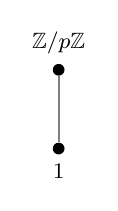
\begin{tikzpicture}[yscale=1.0]
  \node[ltdot] (b) at (0,0) {};
  \node[ltdot] (t) at (0,1) {};
  \begin{scope}[ltedge]
    \draw (b)--(t);
  \end{scope}
  \node[ltlab,below=1.5pt of b] {$1$};
  \node[ltlab,above=1.5pt of t] {$\Zn{p}$};
\end{tikzpicture}\end{center}

\emph{Check.} The single-edge lattice is exactly the case where the pitfall ``do not draw $1$ straight to
$G$'' is \emph{allowed}: there is no proper nontrivial subgroup to interrupt it. For $p=2,3,5,\dots$ the
picture is identical, since the lattice sees only the divisor structure $1\mid p$.
\end{wex}

\begin{wex}{The lattice of $\Zn{p^2}$ as a chain}
Draw the subgroup lattice of a cyclic group $\Zn{p^2}=\gen{x}$ of order $p^2$ ($p$ prime).
\wrec Cyclic of order $p^2$, so by Proposition~\ref{p:cycliclattice@c2} subgroups correspond to the divisors
$1,p,p^2$, which form a single divisibility chain. This is the generic shape behind the concrete $\Zn{16}$
chain already drawn; here we record the general $p^2$ picture.
\wsol The divisors of $p^2$ are $1,p,p^2$, giving exactly three subgroups:
\[
1=\gen{x^{p^2}},\qquad \gen{x^{p}}\ (\ord p),\qquad \gen{x}=\Zn{p^2}.
\]
Each consecutive ratio is $p$ (prime), so each is a covering and the lattice is a $2$-edge chain.
\begin{center}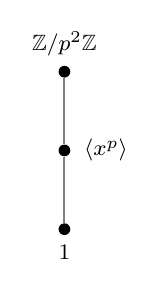
\begin{tikzpicture}[yscale=1.0]
  \node[ltdot] (b) at (0,0) {};
  \node[ltdot] (m) at (0,1) {};
  \node[ltdot] (t) at (0,2) {};
  \begin{scope}[ltedge]
    \draw (b)--(m)--(t);
  \end{scope}
  \node[ltlab,below=1.5pt of b] {$1$};
  \node[ltlab,right=3pt of m] {$\gen{x^{p}}$};
  \node[ltlab,above=1.5pt of t] {$\Zn{p^2}$};
\end{tikzpicture}\end{center}

\emph{Check.} Three subgroups for the three divisors of $p^2$, and the lattice is totally ordered because
$p^2$ is a prime power. Taking $p=2$ recovers the bottom of the $\Zn{16}$ chain; in general $\Zn{p^k}$ gives a
chain of length $k$.
\end{wex}

\begin{wex}{The lattice of $\Zn{pq}$ for distinct primes}
Draw the subgroup lattice of a cyclic group $\Zn{pq}=\gen{x}$ where $p\ne q$ are primes.
\wrec Cyclic of order $pq$ with $p\ne q$, so the divisors are $1,p,q,pq$ and the divisor lattice is a
``diamond'' (a length-$1$ chain crossed with a length-$1$ chain). This is the standard contrast to the
prime-power chain.
\wsol The divisors $1,p,q,pq$ give one subgroup of each order:
\[
1=\gen{x^{pq}},\qquad \gen{x^{q}}\ (\ord p),\qquad \gen{x^{p}}\ (\ord q),\qquad \gen{x}=\Zn{pq}.
\]
Coverings: $1\lessdot\gen{x^{q}}$ (index $p$) and $1\lessdot\gen{x^{p}}$ (index $q$); then
$\gen{x^{q}}\lessdot\Zn{pq}$ (index $q$) and $\gen{x^{p}}\lessdot\Zn{pq}$ (index $p$). The order-$p$ and
order-$q$ vertices are incomparable ($p\nmid q$ and $q\nmid p$), so no edge joins them.
\begin{center}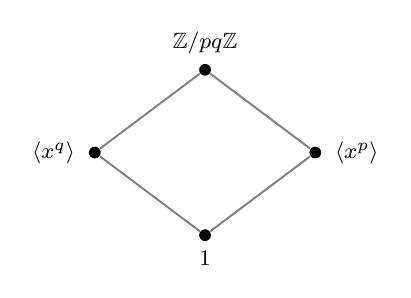
\begin{tikzpicture}[yscale=1.05,xscale=1.4]
  \node[ltdot] (b) at (0,0) {};
  \node[ltdot] (l) at (-1,1) {};
  \node[ltdot] (r) at (1,1) {};
  \node[ltdot] (t) at (0,2) {};
  \begin{scope}[ltedge]
    \draw (b)--(l);
    \draw (b)--(r);
    \draw (l)--(t);
    \draw (r)--(t);
  \end{scope}
  \node[ltlab,below=1.5pt of b] {$1$};
  \node[ltlab,left=3pt of l] {$\gen{x^{q}}$};
  \node[ltlab,right=3pt of r] {$\gen{x^{p}}$};
  \node[ltlab,above=1.5pt of t] {$\Zn{pq}$};
\end{tikzpicture}\end{center}

\emph{Check.} Four subgroups for four divisors; the shape is the same ``diamond'' as $V_4$, but now the two
atoms have \emph{different} orders $p$ and $q$ (in $V_4$ all three atoms had order $2$, and there were three of
them). Taking $p=2,q=3$ gives the lattice of $\Zn{6}$.
\end{wex}

\begin{wex}{Reading joins and meets off the $D_8$ lattice}
Using the $D_8$ lattice already drawn, compute (a) $\gen{s}\vee\gen{r^2s}$, (b) $\gen{s}\vee\gen{rs}$, and
(c) $\gen{r}\cap\gen{r^2,s}$.
\wrec Each part names two specific subgroups of $D_8$ and asks for a join or an intersection, so this is the
reading-off Method applied to the flagship non-abelian example. We trace up for joins, down for meets, and
confirm with element computations using $sr=r\inv s$.
\wsol \emph{(a) $\gen{s}\vee\gen{r^2s}$.} Both $\gen{s}=\{1,s\}$ and $\gen{r^2s}=\{1,r^2s\}$ lie under the
single order-$4$ subgroup $\gen{r^2,s}=\{1,r^2,s,r^2s\}$, and that is the lowest common upper vertex. So
$\gen{s}\vee\gen{r^2s}=\gen{r^2,s}$. \emph{Confirm:} $s\cdot r^2s=r^{-2}=r^2$ (using $sr^2=r^{-2}s$), so the
join contains $r^2$, hence contains $\{1,r^2,s,r^2s\}$; its order is a multiple of $\lcm(2,2)=2$ exceeding $2$
and dividing $8$, and the Klein group of order $4$ is the smallest such, giving $\gen{r^2,s}$.

\emph{(b) $\gen{s}\vee\gen{rs}$.} Here $\gen{s}$ sits under $\gen{r^2,s}$ only, while $\gen{rs}$ sits under
$\gen{r^2,rs}$ only; their only common upper vertex is the top. So $\gen{s}\vee\gen{rs}=D_8$. \emph{Confirm:}
$s\cdot rs=(sr)s=r\inv s\,s=r\inv=r^3$, an element of order $4$, so the join contains $\gen{r}$ as well as the
involution $s\notin\gen{r}$; its order is a multiple of $4$ strictly exceeding $4$ and dividing $8$, hence
$8=|D_8|$.

\emph{(c) $\gen{r}\cap\gen{r^2,s}$.} Tracing down from the cyclic order-$4$ subgroup
$\gen{r}=\{1,r,r^2,r^3\}$ and from the Klein order-$4$ subgroup $\gen{r^2,s}=\{1,r^2,s,r^2s\}$, the highest
common lower vertex is $\gen{r^2}$. So $\gen{r}\cap\gen{r^2,s}=\gen{r^2}$. \emph{Confirm:} the common elements
are exactly $\{1,r^2\}=\gen{r^2}$, since $r,r^3\notin\gen{r^2,s}$ and $s,r^2s\notin\gen{r}$.

\emph{Check.} In (a) two incomparable atoms under a \emph{common} order-$4$ group join to that group, not to
$D_8$ --- contrast (b), where the two atoms lie under \emph{different} order-$4$ groups and so are forced all
the way to the top. Part (c) shows the meet of the two ``different kinds'' of order-$4$ subgroup is the center
$\gen{r^2}=Z(D_8)$, the unique nontrivial subgroup lying below all three order-$4$ subgroups, exactly as the lattice
picture displays.
\end{wex}

\subsection*{Further worked examples}

\smallskip\noindent\textit{More lattices} (Theorem~\ref{t:cyclic@c2}; divisor lattices).

\begin{wex}{the lattice of $\Zn{36}$}
\wrec Cyclic of order $36=2^2\cdot3^2$, so subgroups $\leftrightarrow$ divisors of $36$,
and the lattice is the divisor lattice --- a $3\times3$ grid.
\wsol The nine divisors $1,2,3,4,6,9,12,18,36$ give nine subgroups, the order-$d$ one
being $\gen{\overline{36/d}}$:
\begin{center}
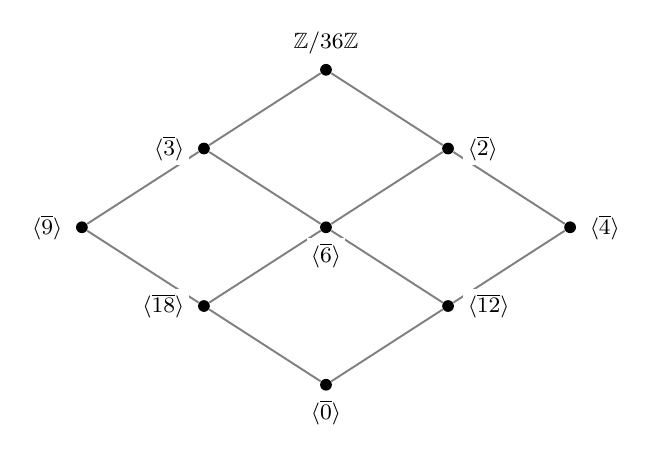
\begin{tikzpicture}[yscale=1.0,xscale=1.55]
  \node[ltdot] (n1) at (0,0) {};
  \node[ltdot] (n2) at (-1,1) {};
  \node[ltdot] (n3) at (1,1) {};
  \node[ltdot] (n4) at (-2,2) {};
  \node[ltdot] (n6) at (0,2) {};
  \node[ltdot] (n9) at (2,2) {};
  \node[ltdot] (n12) at (-1,3) {};
  \node[ltdot] (n18) at (1,3) {};
  \node[ltdot] (n36) at (0,4) {};
  \begin{scope}[ltedge]
    \draw (n1)--(n2);
    \draw (n1)--(n3);
    \draw (n2)--(n4);
    \draw (n2)--(n6);
    \draw (n3)--(n6);
    \draw (n3)--(n9);
    \draw (n4)--(n12);
    \draw (n6)--(n12);
    \draw (n6)--(n18);
    \draw (n9)--(n18);
    \draw (n12)--(n36);
    \draw (n18)--(n36);
  \end{scope}
  \node[ltlab,below=1.5pt of n1] {$\gen{\overline0}$};
  \node[ltlab,left=3pt of n2] {$\gen{\overline{18}}$};
  \node[ltlab,right=3pt of n3] {$\gen{\overline{12}}$};
  \node[ltlab,left=3pt of n4] {$\gen{\overline9}$};
  \node[ltlab,below=1.5pt of n6] {$\gen{\overline6}$};
  \node[ltlab,right=3pt of n9] {$\gen{\overline4}$};
  \node[ltlab,left=3pt of n12] {$\gen{\overline3}$};
  \node[ltlab,right=3pt of n18] {$\gen{\overline2}$};
  \node[ltlab,above=1.5pt of n36] {$\Zn{36}$};
\end{tikzpicture}
\end{center}
The three ``columns'' are the powers of $2$ in the order; the three ``rows'' the powers of
$3$. \emph{Check:} $\gen{\overline9}$ has order $36/\gcd(36,9)=4$, sitting above
$\gen{\overline{18}}$ (order $2$) as a $2^2$ vs $2^1$ step.
\end{wex}

\smallskip\noindent\textit{Reading a normalizer off a lattice} (using $C_G\sgr N_G$ and
``index $2\Rightarrow$ normal'').

\begin{wex}{$N_{D_8}(\gen{s})$ from the lattice}
\wrec Locate $\gen{s}$ in the $D_8$ lattice and find the largest subgroup in which it is
normal. The subgroups lying above $\gen{s}$ are $\gen{s,r^2}$ (order $4$) and $D_8$.
\wsol $\gen{s,r^2}=\{1,r^2,s,r^2s\}$ has index $2$, hence is normal and
$\gen{s}\nor\gen{s,r^2}$; but $\gen{s}$ is \emph{not} normal in $D_8$ (its conjugates are
$\gen{s}$ and $\gen{r^2s}$). Therefore $N_{D_8}(\gen{s})=\gen{s,r^2}$, of order $4$.
\emph{Check:} $rsr\inv=sr^{-2}=sr^2\notin\gen{s}$ (so $r\notin N$), while
$r^2 s r^{-2}=s$ (so $r^2\in N$).
\end{wex}

\subsection*{Maps and commutative diagrams}

The lattice itself is a diagram; two more diagrams capture how joins/meets and
isomorphisms interact with it.

\smallskip\noindent\textbf{(a) Join and meet form a diamond.} For $H,K\sgr G$ the meet is
$H\cap K$ (the largest subgroup below both) and the join is $\gen{H,K}$ (the smallest
subgroup above both), giving a commuting diamond of inclusions
(Definition~\ref{d:meetjoin@c2}). ``Reading a join'' means tracing the two upward edges to
their first common vertex.
\[\begin{tikzcd}[row sep=large,column sep=large]
& \gen{H,K} & \\
H \arrow[ur, hook] & & K \arrow[ul, hook'] \\
& H\cap K \arrow[ul, hook] \arrow[ur, hook'] &
\end{tikzcd}\]
\begin{dgx}
\dgi{Objects:} Four vertices, all subgroups of $G$. Bottom vertex: $H\cap K$, the meet (intersection), itself a subgroup by Proposition~\ref{p:intersub@c2}. Left vertex: $H$. Right vertex: $K$. Top vertex: $\gen{H,K}$, the join (the smallest subgroup of $G$ containing both $H$ and $K$). All four are subgroups; $H\cap K\sgr H,K\sgr\gen{H,K}\sgr G$.
\dgi{Arrows:} Four hooked inclusion arrows. Bottom-left $\hookrightarrow$: $H\cap K\hookrightarrow H$ (inclusion, $H\cap K\sgr H$). Bottom-right $\hookrightarrow$: $H\cap K\hookrightarrow K$ (inclusion, $H\cap K\sgr K$). Top-left $\hookrightarrow$: $H\hookrightarrow\gen{H,K}$ (inclusion, $H\sgr\gen{H,K}$). Top-right $\hookrightarrow$: $K\hookrightarrow\gen{H,K}$ (inclusion, $K\sgr\gen{H,K}$). All four are canonical set inclusions; no quotient or induced map is present.
\dgi{What commutes:} Both paths from $H\cap K$ to $\gen{H,K}$ agree: going via $H$ gives $H\cap K\hookrightarrow H\hookrightarrow\gen{H,K}$, and going via $K$ gives $H\cap K\hookrightarrow K\hookrightarrow\gen{H,K}$. Since all arrows are inclusions, both composites are the same set-inclusion $H\cap K\subseteq\gen{H,K}$. Similarly the two ``upward'' inclusions of $H$ and $K$ into $\gen{H,K}$ commute trivially.
\dgi{Why it commutes:} Take any $x\in H\cap K$. Via the left path: $x\in H\cap K\subseteq H\subseteq\gen{H,K}$, so $x$ maps to itself in $\gen{H,K}$. Via the right path: $x\in H\cap K\subseteq K\subseteq\gen{H,K}$, same element $x$ in $\gen{H,K}$. The two paths agree because inclusions are identity-on-elements; there is nothing to check beyond $H\cap K\subseteq H$ and $H\cap K\subseteq K$, both obvious from the definition of intersection.
\dgi{Why this matters here:} This diamond is the visual definition of a lattice: it records that $\mathcal{L}(G)$ has both a greatest lower bound ($H\cap K$) and a least upper bound ($\gen{H,K}$) for every pair $H,K$. The diagram places the four objects in their correct relative position so that ``reading a meet'' means going to the bottom vertex and ``reading a join'' means going to the top, exactly the reading-off Method described just before. Without this picture the abstract lattice axioms are hard to parse at a glance.
\dgi{Concrete example:} Take $G=S_3$, $H=\gen{(12)}$, $K=\gen{(13)}$. Then $H\cap K=\{e\}=1$ (bottom), $\gen{H,K}=S_3$ (top, since the join of two distinct transpositions is the whole group), and the diamond has atoms $\gen{(12)}$ and $\gen{(13)}$ in the middle. All four inclusion arrows are the set inclusions $\{e\}\subset\{e,(12)\}\subset S_3$ and $\{e\}\subset\{e,(13)\}\subset S_3$.
\dgi{Common pitfall:} Students sometimes read the top vertex as the set-union $H\cup K$ or the product set $HK=\{hk:h\in H,k\in K\}$, neither of which need be a subgroup. The top vertex is $\gen{H,K}$, the subgroup \emph{generated} by $H\cup K$; in the $S_3$ example $\gen{(12)}\cup\gen{(13)}=\{e,(12),(13)\}$ is not a subgroup, but $\gen{\gen{(12)},\gen{(13)}}=S_3$ is.
\dgi{Takeaway:} The point of this diagram is that the meet-join diamond makes visible, in a single picture, that every pair of subgroups has a greatest lower bound (intersection) and a least upper bound (generated subgroup), the two operations that make $\mathcal{L}(G)$ a lattice.
\end{dgx}

\smallskip\noindent\textbf{(b) Isomorphic groups have identical lattices.} An isomorphism
$\varphi:G\to G'$ sends each subgroup $H$ to $\varphi(H)$ and preserves all inclusions, so
it induces an isomorphism of subgroup lattices: the square below commutes for every
$H\sgr G$.
\[\begin{tikzcd}[row sep=large,column sep=large]
H \arrow[r, hook] \arrow[d, mapsto] & G \arrow[d, "\varphi"', "\sim"] \\
\varphi(H) \arrow[r, hook] & G'
\end{tikzcd}\]
\begin{dgx}
\dgi{Objects:} Four vertices. Top-left: $H$, a subgroup of $G$. Top-right: $G$, a group. Bottom-left: $\varphi(H)$, the image of $H$ under $\varphi$, which is a subgroup of $G'$ (isomorphisms send subgroups to subgroups). Bottom-right: $G'$, a group isomorphic to $G$.
\dgi{Arrows:} Top horizontal $\hookrightarrow$: the inclusion $H\hookrightarrow G$ (canonical, $H\sgr G$). Right vertical $\varphi:G\xrightarrow{\;\sim\;}G'$: a group isomorphism, bijective and a homomorphism. Left vertical with $\mapsto$: the restriction $H\mapsto\varphi(H)$, meaning the map induced by $\varphi$ on subgroups; it sends each subgroup $H\sgr G$ to its image $\varphi(H)\sgr G'$. Bottom horizontal $\hookrightarrow$: the inclusion $\varphi(H)\hookrightarrow G'$.
\dgi{What commutes:} The square commutes: the two paths from $H$ to $G'$ are equal. Top-then-right: $H\hookrightarrow G\xrightarrow{\varphi}G'$, sending $h\in H$ to $\varphi(h)\in G'$. Left-then-bottom: $H\mapsto\varphi(H)\hookrightarrow G'$, sending $H$ as a set to $\varphi(H)\subseteq G'$, and any $h\in H$ to $\varphi(h)\in\varphi(H)\subseteq G'$. Both give $h\mapsto\varphi(h)$.
\dgi{Why it commutes:} Take any $h\in H$. Along the top-then-right path: $h$ is viewed in $G$ via inclusion, then $\varphi$ sends it to $\varphi(h)\in G'$. Along the left-then-bottom path: $H$ is mapped to its image $\varphi(H)\subseteq G'$, and $h\in H$ lands at $\varphi(h)\in\varphi(H)$, then the inclusion puts it in $G'$. Both agree because $\varphi$ is a function: the image of $h$ under $\varphi$ is the same regardless of which route we describe it.
\dgi{Why this matters here:} This diagram encodes the key fact that an isomorphism $\varphi$ not only identifies $G$ with $G'$ as groups but also identifies their entire subgroup lattices: every $H\sgr G$ corresponds to $\varphi(H)\sgr G'$, and inclusion is preserved. This is why the remark ``isomorphic groups have identical lattices'' is diagrammatically immediate --- $\varphi$ induces a lattice isomorphism $\mathcal{L}(G)\to\mathcal{L}(G')$. It also sets up the punch line: the converse fails because the lattice forgets multiplication.
\dgi{Concrete example:} Take $G=\Zn{6}$, $G'=\Zn{2}\times\Zn{3}$ (isomorphic by the Chinese remainder theorem), and $H=\gen{\bar2}\sgr\Zn{6}$ of order $3$. The isomorphism $\varphi:\Zn{6}\to\Zn{2}\times\Zn{3}$ sends $\bar2\mapsto(\bar0,\bar2)$, so $\varphi(H)=\{(\bar0,\bar0),(\bar0,\bar1),(\bar0,\bar2)\}=\{0\}\times\Zn{3}\sgr\Zn{2}\times\Zn{3}$. The square commutes: $\varphi(\bar2)=(\bar0,\bar2)$ by either path.
\dgi{Common pitfall:} The left arrow is labeled with $\mapsto$ (``maps to''), not $\hookrightarrow$ (``is a subgroup of''): it sends a subgroup $H$ to a subgroup $\varphi(H)$, not an element to an element. Students sometimes read it as an inclusion $H\hookrightarrow G'$, but $H$ need not be a subgroup of $G'$ --- only $\varphi(H)$ is. The diagram also does not say $H\cong\varphi(H)$ as an \emph{object inside the diagram}; the isomorphism is an additional fact (restriction of $\varphi$ to $H$).
\dgi{Takeaway:} The point of this diagram is that an isomorphism $\varphi:G\xrightarrow{\sim}G'$ induces a bijection on subgroup lattices, making every inclusion $H\sgr G$ correspond to $\varphi(H)\sgr G'$, which is why isomorphic groups always have identical subgroup lattices.
\end{dgx}
The converse fails: $Z_2\times Z_8$ and the modular group $M$ of order $16$ have
identical lattices but are not isomorphic, so the lattice alone cannot recover the group.

\begin{exers}{Exercises (from the text).}
\item For $H,K\sgr G$, exhibit all possible sublattices showing only $G,1,H,K$ and their
  joins/meets; describe what distinguishes the cases.
\item In $D_{16}$, list all subgroups (a) contained in $\gen{sr^2,r^4}$; (b) contained in
  $\gen{sr^7,r^4}$; (c) containing $\gen{r^4}$; (d) containing $\gen{s}$.
\item Show $\gen{s,r^2}\sgr D_8$ is isomorphic to $V_4$.
\item Use the lattice to find all $12$ pairs of elements that generate $D_8$.
\item Use the lattice to find all $8$ elements $x$ with $D_{16}=\gen{x,s}$.
\item Use lattices to find the centralizer of every element of (a) $D_8$; (b) $Q_8$;
  (c) $S_3$; (d) $D_{16}$.
\item Find $Z(D_{16})$.
\item Find the normalizer of every subgroup of (a) $S_3$; (b) $Q_8$.
\item Draw the lattices of subgroups of (a) $\Zn{16}$; (b) $\Zn{24}$; (c) $\Zn{48}$.
\item Classify groups of order $4$: prove $\ord{G}=4\imp G\isom Z_4$ or $G\isom V_4$.
\item For the quasidihedral group $QD_{16}=\gen{a,\tau\st a^8=\tau^2=1,\ a\tau=\tau a^3}$,
  fill in the missing subgroups of its (non-planar) lattice, each with $\le2$ generators.
\item Draw the lattice of $Z_2\times Z_4$, each subgroup with $\le2$ generators.
\item Draw the lattice of $Z_2\times Z_8$, each subgroup with $\le2$ generators.
\item For the modular group $M=M_{16}=\gen{u,v\st u^8=v^2=1,\ vuv\inv=u^5}$ of order $16$, show its
  lattice matches that of $Z_2\times Z_8$, yet $M\not\isom Z_2\times Z_8$.
\item Describe the isomorphism type of each of the three order-$8$ subgroups of $D_{16}$.
\item Show that in $QD_{16}$ every element of order $2$ lies in $\gen{\tau,a^2}$.
\item Show that in $M$, $\{x\in M\st x^2=1\}$ is a subgroup isomorphic to $V_4$.
\item Find the centralizer of every element of $QD_{16}$.
\item Find $N_{D_{16}}(\gen{s,r^4})$.
\item Find $N_{QD_{16}}(\gen{\tau a})$ and $N_{QD_{16}}(\gen{\tau,a^4})$.
\end{exers}

\begin{exers}{Additional exercises.}
\item Prove that the lattice of subgroups of $\Zn{n}$ is the divisor lattice of $n$.
\item Show $\Zn{p^2q}$ ($p,q$ distinct primes) has exactly $6$ subgroups, and draw the
  lattice.
\item Draw the lattice of $S_3$ and identify which subgroups are normal.
\item Verify directly in $Q_8$ that the join of $\gen{i}$ and $\gen{j}$ is $Q_8$ and the
  meet is $\gen{-1}$.
\item Using Exercise~14, give two non-isomorphic groups with identical subgroup
  lattices, and explain why the lattice cannot detect the difference.
\end{exers}

\begin{exers}{Commutative-diagram exercises.}
\item Draw the join/meet diamond for $H=\gen{r}$ and $K=\gen{s}$ in $D_8$; identify
  $H\cap K$ and $\gen{H,K}$, and read off $[D_8:H]$.
\item Let $\varphi:G\to G'$ be an isomorphism. Prove $H\mapsto\varphi(H)$ is a lattice
  isomorphism by checking that the square with rows $H\hookrightarrow G$ and
  $\varphi(H)\hookrightarrow G'$ (and down-arrows $\varphi$) commutes for every $H\sgr G$.
\item Draw the diamond for two distinct order-$2$ subgroups of $V_4$ and compute their
  join and meet.
\item Explain, using the lattice-isomorphism square, why the identical lattices of
  $Z_2\times Z_8$ and the modular group $M_{16}$ do \emph{not} force the groups to be
  isomorphic --- i.e.\ why no group isomorphism completes the square.
\end{exers}


% ===== Graded Problem Bank (Dummit and Foote + Artin + Fraleigh) =====
\section{Graded Problem Bank}
Problems are drawn from Dummit \& Foote, Artin (\emph{Algebra}), and Fraleigh
(\emph{A First Course in Abstract Algebra}); the difficulty grading is the author's.

\subsection*{Easy}
\begin{exers}{}
\item [DF 2.1.1] Prove each is a subgroup: (a) $\{a+ai\st a\in\R\}\sgr(\C,+)$;
  (b) the unit circle $\{z\in\C\st\ord{z}=1\}\sgr\C^\times$;
  (c) $\{a/b\in\Q\st b\mid n\}\sgr(\Q,+)$ ($n$ fixed);
  (d) $\{a/b\in\Q\st\gcd(b,n)=1\}\sgr(\Q,+)$;
  (e) $\{x\in\R^\times\st x^2\in\Q\}\sgr\R^\times$.
\item [DF 2.1.2] Prove each is \emph{not} a subgroup: (a) the $2$-cycles in $S_n$ ($n\ge3$);
  (b) the reflections in $D_{2n}$; (c) $\{x\in G\st\ord{x}=n\}\cup\{1\}$, $n$ composite and $G$ containing an element of order $n$;
  (d) the odd integers together with $0$; (e) $\{x\in\R\st x^2\in\Q\}$ in $(\R,+)$.
\item [DF 2.1.3] Show $\{1,r^2,s,sr^2\}$ and $\{1,r^2,sr,sr^3\}$ are subgroups of $D_8$.
\item [DF 2.1.9] Prove $\SL_n(F)=\{A\in\GL_n(F)\st\det A=1\}\sgr\GL_n(F)$.
\item [DF 2.1.11] Prove $\{(a,1)\}$, $\{(1,b)\}$, and (when $B=A$) the diagonal
  $\{(a,a)\}$ are subgroups of $A\times B$.
\item [DF 2.1.14] Show $\{x\in D_{2n}\st x^2=1\}$ is not a subgroup ($n\ge3$).
\item [DF 2.2.1] Prove $C_G(A)=\{g\st g\inv ag=a\ \forall a\in A\}$ is a subgroup.
\item [DF 2.2.2] Prove $C_G(Z(G))=G$, and deduce $N_G(Z(G))=G$.
\item [DF 2.2.4] For $S_3,D_8,Q_8$, compute the centralizer of each element and the
  center of each.
\item [DF 2.3.3] Find all generators of $\Zn{48}$.
\item [DF 2.3.4] Find all generators of $\Zn{202}$.
\item [DF 2.3.5] Find the number of generators of $\Zn{49000}$.
\item [DF 2.3.10] Find $\ord{\overline{30}}$ in $\Zn{54}$, and list the elements and
  orders of $\gen{\overline{30}}$.
\item [DF 2.3.11] Find all cyclic subgroups of $D_8$ and a non-cyclic proper subgroup.
\item [DF 2.3.14] For $\sigma=(1\,2\,\cdots\,12)$, compute $\sigma^a$ for
  $a=13,65,626,1195,-6,-81,-570,-1211$.
\item [DF 2.4.1] Prove $H\sgr G\imp\gen{H}=H$.
\item [DF 2.4.5] Prove two distinct elements of order $2$ in $S_3$ generate $S_3$.
\item [DF 2.4.6] Prove $\gen{(1\,2),(1\,2)(3\,4)}$ is non-cyclic of order $4$.
\item [DF 2.5.3] Show $\gen{s,r^2}\sgr D_8$ is isomorphic to $V_4$.
\item [DF 2.5.7] Find $Z(D_{16})$.
\item [Artin 2.4] In which of these cases is $H$ a subgroup of $G$? (a) $G=\GL_n(\C)$,
  $H=\GL_n(\R)$; (b) $G=\R^\times$, $H=\{1,-1\}$; (c) $G=(\Z,+)$, $H$ the positive
  integers; (d) $G=\R^\times$, $H$ the positive reals.
\item [Artin 3.1] Let $a=123$, $b=321$. Compute $d=\gcd(a,b)$ and write $d=ra+sb$.
\item [Artin 4.2] An $n$th root of unity is $z\in\C$ with $z^n=1$. (a) Prove the $n$th
  roots of unity form a cyclic subgroup of $\C^\times$ of order $n$; (b) determine their
  product.
\item [Artin 4.6] (a) For a cyclic group of order $6$, how many elements generate it?
  Same for orders $5$ and $8$. (b) Describe the count for arbitrary order $n$.
\item [Artin 4.9] How many elements of order $2$ does $S_4$ contain?
\item [Fraleigh 5.1] Determine whether $\R$ is a subgroup of $(\C,+)$.
\item [Fraleigh 5.3] Determine whether $7\Z$ is a subgroup of $(\C,+)$.
\item [Fraleigh 5.4] Determine whether the set $i\R$ of pure imaginary numbers
  (including $0$) is a subgroup of $(\C,+)$.
\item [Fraleigh 5.11] Determine whether the $n\times n$ real matrices with determinant
  $-1$ form a subgroup of $\GL(n,\R)$.
\item [Fraleigh 5.12] Determine whether the $n\times n$ real matrices with determinant
  $\pm1$ form a subgroup of $\GL(n,\R)$.
\item [Fraleigh 5.22] Describe all elements of the cyclic subgroup of $\GL(2,\R)$
  generated by $\left(\begin{smallmatrix}0&-1\\-1&0\end{smallmatrix}\right)$.
\item [Fraleigh 5.23] Describe all elements of the cyclic subgroup of $\GL(2,\R)$
  generated by $\left(\begin{smallmatrix}1&1\\0&1\end{smallmatrix}\right)$.
\item [Fraleigh 5.27] Find the order of the cyclic subgroup of $\Zn{4}$ generated by $3$.
\item [Fraleigh 5.30] Find the order of the cyclic subgroup of $\Zn{10}$ generated by $8$.
\item [Fraleigh 5.31] Find the order of the cyclic subgroup of $\Zn{16}$ generated by
  $12$.
\item [Fraleigh 5.32] Find the order of the cyclic subgroup of $S_9$ generated by
  $(2\,4\,6\,9)(3\,5\,7)$.
\item [Fraleigh 6.1] Find the quotient and remainder when $n=42$ is divided by $m=9$.
\item [Fraleigh 6.3] Find the quotient and remainder when $n=-37$ is divided by $m=8$.
\item [Fraleigh 6.5] Find the greatest common divisor of $32$ and $24$.
\item [Fraleigh 6.7] Find the greatest common divisor of $360$ and $420$.
\item [Fraleigh 6.8] Find the number of generators of a cyclic group of order $5$.
\item [Fraleigh 6.10] Find the number of generators of a cyclic group of order $24$.
\item [Fraleigh 6.11] Find the number of generators of a cyclic group of order $84$.
\item [Fraleigh 6.17] Find the number of elements in the cyclic subgroup of $\Zn{30}$
  generated by $25$.
\item [Fraleigh 6.18] Find the number of elements in the cyclic subgroup of $\Zn{42}$
  generated by $30$.
\item [Fraleigh 6.19] Find the number of elements in the cyclic subgroup $\gen{i}$ of
  $\C^\times$.
\item [Fraleigh 6.22] Find the number of elements in the cyclic subgroup $\gen{\rho^{10}}$
  of $D_{24}$.
\item [Fraleigh 6.24] In $S_{10}$: (a) order of $(2\,4\,6\,7)$; (b) order of
  $(1\,4)(2\,3\,5)$ and $(1\,3)(2\,4\,6\,7\,8)$; (c)--(d) further products of disjoint
  cycles.
\item [Fraleigh 6.25] Find the maximum possible order of an element of $S_n$ for $n=5$.
\item [Fraleigh 6.26] Find the maximum possible order of an element of $S_n$ for $n=6$.
\item [Fraleigh 6.31] Find all subgroups of $\Zn{12}$ and draw the subgroup diagram.
\item [Fraleigh 6.33] Find all subgroups of $\Zn{8}$ and draw the subgroup diagram.
\item [Fraleigh 6.34] Find all orders of subgroups of $\Zn{6}$.
\item [Fraleigh 6.36] Find all orders of subgroups of $\Zn{12}$.
\item [Fraleigh 6.38] Find all orders of subgroups of $\Zn{17}$.
\item [Fraleigh 6.47] Find the primitive $n$th roots of unity for $n=4$.
\item [Fraleigh 6.48] Find the primitive $n$th roots of unity for $n=6$.
\item [Fraleigh 7.1] List the elements of the subgroup of $\Zn{12}$ generated by
  $\{2,3\}$.
\item [Fraleigh 7.2] List the elements of the subgroup of $\Zn{12}$ generated by
  $\{4,6\}$.
\item [Fraleigh 7.3] List the elements of the subgroup of $\Zn{25}$ generated by
  $\{4,6\}$.
\item [Fraleigh 7.5] List the elements of the subgroup of $\Z$ generated by $\{12,42\}$.
\item [Fraleigh 7.7] List the elements of the subgroup of $D_8$ generated by
  $\{\mu,\mu\rho^2\}$ (i.e.\ $\{s,sr^2\}$).
\end{exers}

\subsection*{Medium}
\begin{exers}{}
\item [DF 2.1.4] Exhibit a group $G$ and an infinite subset $H$ closed under the operation
  but not a subgroup.
\item [DF 2.1.5] Prove a group of order $n>2$ has no subgroup of order $n-1$.
\item [DF 2.1.6] $G$ abelian: prove the torsion set $\{g\st\ord{g}<\infty\}\sgr G$; give a
  non-abelian example where this set is not a subgroup.
\item [DF 2.1.7] For $n>1$, find the torsion subgroup of $\Z\times\Zn{n}$, and show the elements of
  infinite order together with $1$ do not form a subgroup.
\item [DF 2.1.8] For $H,K\sgr G$, prove $H\cup K\sgr G\iff H\subseteq K$ or $K\subseteq H$.
\item [DF 2.1.10] (a) Prove $H\cap K\sgr G$ for $H,K\sgr G$; (b) prove the intersection of
  any nonempty family of subgroups is a subgroup.
\item [DF 2.1.12] $A$ abelian, $n\in\Z$: prove $A^n=\{a^n\}$ and $A[n]=\{a\st a^n=1\}$
  are subgroups.
\item [DF 2.1.15] Prove the union of an ascending chain $H_1\sgr H_2\sgr\cdots$ of
  subgroups is a subgroup.
\item [DF 2.1.16] Prove the upper-triangular matrices in $\GL_n(F)$ form a subgroup.
\item [DF 2.1.17] Prove the upper-triangular matrices with $1$'s on the diagonal form a
  subgroup of $\GL_n(F)$.
\item [DF 2.2.3] Prove $A\subseteq B\imp C_G(B)\sgr C_G(A)$.
\item [DF 2.2.5] Show $C_G(A)=A$ and $N_G(A)=G$ for: (a) $S_3,\,A=\gen{(1\,2\,3)}$;
  (b) $D_8,\,A=\{1,s,r^2,sr^2\}$; (c) $D_{10},\,A=\gen{r}$.
\item [DF 2.2.6] (a) Prove $H\sgr N_G(H)$ (and that this can fail if $H$ is not a
  subgroup); (b) prove $H\sgr C_G(H)\iff H$ is abelian.
\item [DF 2.2.9] Define $N_H(A)=\{h\in H\st hAh\inv=A\}$; prove $N_H(A)=N_G(A)\cap H\sgr H$.
\item [DF 2.2.11] Prove $Z(G)\sgr N_G(A)$ for every subset $A$.
\item [DF 2.2.12] $S_4$ acts on $\Z[x_1,\dots,x_4]$ by $\sigma\cdot x_i=x_{\sigma(i)}$.
  Find the stabilizers of $x_4$, of $x_1+x_2$, and of $x_1x_2+x_3x_4$.
\item [DF 2.2.13] Verify that the action of $S_n$ on $\Z[x_1,\dots,x_n]$ is a group action.
\item [DF 2.3.1] Find all subgroups of $Z_{45}=\gen{x}$, giving a generator for each, and
  describe the containments.
\item [DF 2.3.2] If $x\in G$ is finite with $\ord{x}=\ord{G}$, prove $G=\gen{x}$; give an
  infinite counterexample.
\item [DF 2.3.6] In $\Zn{48}$, list the elements of $\gen{\bar a}$ for each $\bar a$, and
  all inclusions among subgroups.
\item [DF 2.3.7] Use $\Zn{48}\isom Z_{48}$ to list all subgroups of $Z_{48}$.
\item [DF 2.3.8] For which $a$ does $1\mapsto x^a$ extend to an isomorphism
  $\Zn{48}\to Z_{48}$?
\item [DF 2.3.9] For which $a$ does $1\mapsto x^a$ extend to a homomorphism
  $\Zn{48}\to Z_{36}$? Can it be surjective?
\item [DF 2.3.12] Prove $Z_2\times Z_2$, $Z_2\times\Z$, and $\Z\times\Z$ are not cyclic.
\item [DF 2.3.13] Prove $\Z\times Z_2\not\isom\Z$ and $\Q\times Z_2\not\isom\Q$.
\item [DF 2.3.15] Prove $\Q\times\Q$ is not cyclic.
\item [DF 2.3.17] Find a presentation of $Z_n$ with one generator.
\item [DF 2.3.18] If $h^n=1$ in $H$, prove there is a unique homomorphism $Z_n\to H$
  with $x\mapsto h$.
\item [DF 2.3.19] For $h\in H$, prove there is a unique homomorphism $\Z\to H$ with
  $1\mapsto h$.
\item [DF 2.3.20] $p$ prime, $x^{p^n}=1\imp\ord{x}=p^m$ for some $m\le n$.
\item [DF 2.4.2] Prove $A\subseteq B\imp\gen{A}\sgr\gen{B}$, and give $A\subsetneq B$ with
  $\gen{A}=\gen{B}$.
\item [DF 2.4.4] Prove $H\sgr G\imp H=\gen{H\setminus\{1\}}$.
\item [DF 2.4.7] Prove $\gen{(1\,2),(1\,3)(2\,4)}\isom D_8$.
\item [DF 2.4.8] Prove $S_4=\gen{(1\,2\,3\,4),(1\,2\,4\,3)}$.
\item [DF 2.4.13] Prove $(\Q^{+},\cdot)=\gen{\{1/p\st p\text{ prime}\}}$.
\item [DF 2.4.15] Exhibit a proper non-cyclic subgroup of $\Q$.
\item [DF 2.5.1] For $H,K\sgr G$, exhibit all possible sublattices showing only
  $G,1,H,K$ and their joins/meets; describe what distinguishes the cases.
\item [DF 2.5.4] Use the lattice to find all $12$ pairs of elements that generate $D_8$.
\item [DF 2.5.5] Use the lattice to find all $8$ elements $x$ with $D_{16}=\gen{x,s}$.
\item [DF 2.5.6] Use lattices to find the centralizer of every element of (a) $D_8$;
  (b) $Q_8$; (c) $S_3$; (d) $D_{16}$.
\item [DF 2.5.8] Find the normalizer of every subgroup of (a) $S_3$; (b) $Q_8$.
\item [DF 2.5.9] Draw the lattices of subgroups of (a) $\Zn{16}$; (b) $\Zn{24}$;
  (c) $\Zn{48}$.
\item [DF 2.5.15] Describe the isomorphism type of each of the three order-$8$ subgroups
  of $D_{16}$.
\item [DF 2.5.19] Find $N_{D_{16}}(\gen{s,r^4})$.
\item [Artin 3.2] Prove that if $a,b$ are positive integers whose sum is a prime $p$,
  then $\gcd(a,b)=1$.
\item [Artin 4.1] Let $a,b\in G$ with $\ord{a}=7$ and $a^3b=ba^3$. Prove $ab=ba$.
\item [Artin 4.3] Prove that $ab$ and $ba$ have the same order in any group.
\item [Artin 4.4] Describe all groups $G$ that contain no proper subgroup.
\item [Artin 4.7] Let $x,y\in G$ with $x,y,xy$ all of order $2$. Prove $\{1,x,y,xy\}$ is a
  subgroup of order $4$.
\item [Artin 4.10] Show by example that the product of two finite-order elements need not
  have finite order. What if the group is abelian?
\item [Artin M.2] (a) Prove every group of even order contains an element of order $2$;
  (b) prove every group of order $21$ contains an element of order $3$.
\item [Fraleigh 5.20] Among $\Z,12\Z,\Q^+,\R,\R^+,3\Z$, etc.\ (nine listed groups), give
  the complete list of subgroup relations $G_i\sgr G_j$.
\item [Fraleigh 5.26] Decide which of $\gen{\Z,+}$, $\gen{\Q,+}$, $\gen{\Q^+,\cdot}$,
  $\gen{6\Z,+}$, $\{6^n\}$, $\{a+b\sqrt2\st a,b\in\Z\}$ are cyclic; list generators.
\item [Fraleigh 5.41] For $B\subseteq A$, $b\in B$: determine whether
  $\{\sigma\in S_A\st\sigma(b)=b\}$ is a subgroup of $S_A$.
\item [Fraleigh 5.44] For $B\subseteq A$: determine whether
  $\{\sigma\in S_A\st\sigma[B]=B\}$ is a subgroup of $S_A$.
\item [Fraleigh 5.45] If $\varphi:G\to G'$ is an isomorphism and $H\sgr G$, prove
  $\varphi[H]\sgr G'$.
\item [Fraleigh 5.47] If $H,K$ are subgroups of an abelian group $G$, prove
  $\{hk\st h\in H,k\in K\}$ is a subgroup.
\item [Fraleigh 5.48] Find a group $G$ and subgroups $H,K$ for which the set
  $\{hk\}$ of the previous exercise is not a subgroup.
\item [Fraleigh 5.53] In an abelian group $G$, prove the solutions of $x^2=e$ form a
  subgroup.
\item [Fraleigh 5.58] Let $a\in G$. Prove $H_a=\{x\in G\st xa=ax\}$ is a subgroup.
\item [Fraleigh 5.61] Prove that if $H\sgr G$ and $K\sgr G$, then $H\cap K\sgr G$.
\item [Fraleigh 5.62] Prove that every cyclic group is abelian.
\item [Fraleigh 6.13] Find the number of automorphisms of $\Zn{6}$.
\item [Fraleigh 6.14] Find the number of automorphisms of $\Zn{8}$.
\item [Fraleigh 6.16] Find the number of automorphisms of $\Zn{84}$.
\item [Fraleigh 6.54] For integers $r,s$, show $\{nr+ms\st n,m\in\Z\}$ is a subgroup
  of $\Z$.
\item [Fraleigh 6.56] If $ab$ has finite order $n$, show $ba$ also has order $n$.
\item [Fraleigh 6.62] For distinct primes $p,q$, find the number of generators of
  $\Zn{pq}$.
\item [Fraleigh 6.63] For a prime $p$ and integer $r\ge1$, find the number of generators
  of $\Zn{p^r}$.
\item [Fraleigh 6.66] Show $\Zn{p}$ has no proper nontrivial subgroups when $p$ is prime.
\item [Fraleigh 7.13] Explain how to tell from a Cayley digraph whether the group is
  commutative.
\item [Fraleigh 7.16] Does the small inside triangle in the Cayley digraph of $\Zn{6}$
  (with $S=\{2,3\}$) exhibit a cyclic subgroup? Why or why not?
\item [Fraleigh 7.18] Draw a Cayley digraph for $\Zn{8}$ with generating set
  $S=\{2,5\}$.
\item [Fraleigh 7.22] Prove there are at least three different abelian groups of order $8$.
\end{exers}

\subsection*{Hard}
\begin{exers}{}
\item [DF 2.1.13] $H\sgr(\Q,+)$ with $1/x\in H$ for all $x\in H\setminus\{0\}$: prove
  $H=0$ or $H=\Q$.
\item [DF 2.2.7] For $n\ge3$: (a) $Z(D_{2n})=1$ if $n$ is odd; (b) $Z(D_{2n})=\{1,r^k\}$
  if $n=2k$.
\item [DF 2.2.8] $G=S_n$, $G_i=\{\sigma\st\sigma(i)=i\}$: prove $G_i\sgr G$ via group
  actions and find $\ord{G_i}$.
\item [DF 2.2.10] Let $\ord{H}=2$. Prove $N_G(H)=C_G(H)$, and deduce
  $N_G(H)=G\imp H\sgr Z(G)$.
\item [DF 2.2.14] Prove the center of the Heisenberg group $H(F)$ is isomorphic to
  $(F,+)$.
\item [DF 2.3.16] $\ord{x}=n$, $\ord{y}=m$, $xy=yx$: prove $\ord{xy}\mid\lcm(m,n)$; show
  this can fail without commuting, and give commuting $x,y$ with
  $\ord{xy}\neq\lcm(m,n)$.
\item [DF 2.3.21] $p$ an odd prime: show $1+p$ has order $p^{n-1}$ in $\Zns{p^n}$.
\item [DF 2.3.22] $n\ge3$: show $5$ has order $2^{n-2}$ in $\Zns{2^n}$.
\item [DF 2.3.23] Show $\Zns{2^n}$ is not cyclic for $n\ge3$.
\item [DF 2.3.24] $G$ finite, $x\in G$: prove $g\in N_G(\gen{x})\iff gxg\inv=x^a$ for some
  $a\in\Z$.
\item [DF 2.3.25] $G$ cyclic of order $n$, $\gcd(k,n)=1$: prove $x\mapsto x^k$ is
  surjective, and extend to any finite group of order $n$.
\item [DF 2.3.26] $\Aut(Z_n)$: prove $\sigma_a:x\mapsto x^a$ is an automorphism
  $\iff\gcd(a,n)=1$, and $\Aut(Z_n)\isom\Zns{n}$, abelian of order $\varphi(n)$.
\item [DF 2.4.3] Prove that if $H$ is abelian then $\gen{H,Z(G)}$ is abelian; give an
  abelian $H$ with $\gen{H,C_G(H)}$ not abelian.
\item [DF 2.4.9] Prove $\SL_2(\F_3)=\gen{\left(\begin{smallmatrix}1&1\\0&1\end{smallmatrix}\right),
  \left(\begin{smallmatrix}1&0\\1&1\end{smallmatrix}\right)}$.
\item [DF 2.4.10] Prove the subgroup of $\SL_2(\F_3)$ generated by
  $\left(\begin{smallmatrix}1&1\\1&-1\end{smallmatrix}\right)$ and
  $\left(\begin{smallmatrix}-1&1\\1&1\end{smallmatrix}\right)$ is $\isom Q_8$.
\item [DF 2.4.11] Prove $\SL_2(\F_3)\not\isom S_4$ (both of order $24$).
\item [DF 2.4.12] Prove the upper-triangular subgroup of $\GL_3(\F_2)$ is $\isom D_8$.
\item [DF 2.4.14] Finitely generated groups: (a) finite groups are f.g.; (b) $\Z$ is
  f.g.; (c) a f.g.\ subgroup of $\Q$ is cyclic; (d) $\Q$ is not f.g.
\item [DF 2.4.16] Maximal subgroups: (a) every proper subgroup of a finite group lies in
  a maximal one; (b) the rotation subgroup of $D_{2n}$ is maximal; (c) $H$ is maximal in
  $Z_n=\gen{x}\iff H=\gen{x^p}$ for a prime $p\mid n$.
\item [DF 2.4.17] (Zorn) Prove every nontrivial finitely generated group has a maximal
  subgroup.
\item [DF 2.4.18] Pr\"ufer group $\Z_{p^\infty}=\{z\in\C\st z^{p^n}=1\text{ some }n\}$,
  $H_k=\{z\st z^{p^k}=1\}$: prove $H_k\sgr H_m\iff k\le m$; each $H_k$ is cyclic; every
  proper subgroup is some $H_k$; and $\Z_{p^\infty}$ is not f.g.
\item [DF 2.4.19] A nontrivial abelian group is divisible if every element has a $k$th
  root for each $k\neq0$. Prove $(\Q,+)$ is divisible and no nontrivial finite abelian
  group is.
\item [DF 2.4.20] For nontrivial abelian $A,B$, prove $A\times B$ is divisible $\iff$ both $A$ and $B$ are divisible.
\item [DF 2.5.2] In $D_{16}$, list all subgroups (a) contained in $\gen{sr^2,r^4}$;
  (b) contained in $\gen{sr^7,r^4}$; (c) containing $\gen{r^4}$; (d) containing $\gen{s}$.
\item [DF 2.5.10] Classify groups of order $4$: prove $\ord{G}=4\imp G\isom Z_4$ or
  $G\isom V_4$.
\item [DF 2.5.11] For $QD_{16}=\gen{a,\tau\st a^8=\tau^2=1,\ a\tau=\tau a^3}$, fill in the
  missing subgroups of its (non-planar) lattice, each with $\le2$ generators.
\item [DF 2.5.12] Draw the lattice of $Z_2\times Z_4$, each subgroup with $\le2$
  generators.
\item [DF 2.5.13] Draw the lattice of $Z_2\times Z_8$, each subgroup with $\le2$
  generators.
\item [DF 2.5.14] For $M=M_{16}=\gen{u,v\st u^8=v^2=1,\ vuv\inv=u^5}$ of order $16$, show
  its lattice matches that of $Z_2\times Z_8$, yet $M\not\isom Z_2\times Z_8$.
\item [DF 2.5.16] Show that in $QD_{16}$ every element of order $2$ lies in
  $\gen{\tau,a^2}$.
\item [DF 2.5.17] Show that in $M$, $\{x\in M\st x^2=1\}$ is a subgroup isomorphic to
  $V_4$.
\item [DF 2.5.18] Find the centralizer of every element of $QD_{16}$.
\item [DF 2.5.20] Find $N_{QD_{16}}(\gen{\tau a})$ and $N_{QD_{16}}(\gen{\tau,a^4})$.
\item [Artin 3.3] (a) Define the gcd of $n$ integers $\{a_1,\dots,a_n\}$; prove it exists
  and is an integer combination of the $a_i$. (b) If the gcd is $d$, prove
  $\gcd(a_1/d,\dots,a_n/d)=1$.
\item [Artin 4.5] Prove that every subgroup of a cyclic group is cyclic, working with
  exponents and the description of subgroups of $(\Z,+)$.
\item [Artin 4.8] (a) Prove the elementary matrices of the first and third types generate
  $\GL_n(\R)$; (b) prove those of the first type generate $\SL_n(\R)$.
\item [Artin 4.11] (a) Adapt row reduction to prove the transpositions generate $S_n$;
  (b) prove that for $n\ge3$ the $3$-cycles generate $A_n$.
\item [Artin M.3] Classify groups of order $6$ via the cases: (i) an element of order $6$
  exists; (ii) an element of order $3$ but none of order $6$; (iii) all elements have
  order $1$ or $2$.
\item [Artin M.12] (postage stamp) For positive coprime $a,b$: (a) prove every
  sufficiently large $n$ is $ra+sb$ with $r,s$ positive integers; (b) determine the
  largest integer not of this form.
\item [Fraleigh 6.55] Prove that if $G$ is a finite cyclic group and $H\neq K$ are
  subgroups, then $\ord{H}\neq\ord{K}$.
\item [Fraleigh 6.58] Show that a group with only finitely many subgroups must be finite.
\item [Fraleigh 6.59] Give a counterexample to the converse of ``a subgroup of a cyclic
  group is cyclic'': a non-cyclic $G$ with every proper subgroup cyclic.
\item [Fraleigh 6.60] If $a\in G$ generates a cyclic subgroup of order $2$ and is the
  unique such element, show $ax=xa$ for all $x\in G$.
\item [Fraleigh 6.61] Prove that if a cyclic group has an odd number of generators, then
  it has at most two elements.
\item [Fraleigh 6.64] In a finite cyclic group of order $n$, show $x^m=e$ has exactly $m$
  solutions for each $m\mid n$.
\item [Fraleigh 6.67] Let $G$ be abelian with finite cyclic subgroups $H,K$ of orders
  $r,s$. (a) If $\gcd(r,s)=1$, $G$ has a cyclic subgroup of order $rs$; (b) in general,
  of order $\lcm(r,s)$.
\item [Fraleigh 7.21] Use Cayley digraphs to show that for $n\ge3$ there is a nonabelian
  group with $2n$ elements generated by two elements of order $2$.
\end{exers}


% ================= Chapter 3: Quotient Groups and Homomorphisms =================

\chapter{Quotient Groups and Homomorphisms}

\section{Definitions and Examples}
\subsection*{Cosets and the Quotient Group $G/N$}

Throughout, $G$ is a group and $N \le G$ a subgroup. We build a new group whose elements are the cosets of $N$, but this construction succeeds \emph{only} when $N$ is normal. This is the central tension of the section, so we develop it carefully.

\begin{definition}[Left and right cosets]
For $g \in G$ the \textbf{left coset} of $N$ containing $g$ is
\[
  gN = \{\, gn \st n \in N \,\},
\]
and the \textbf{right coset} is $Ng = \{\, ng \st n \in N \,\}$. The set of all left cosets is denoted $G/N$ (read ``$G$ mod $N$''), and the number of left cosets is the \textbf{index} $\idx{G}{N}$.
\end{definition}

\begin{remark}
Two left cosets are equal or disjoint, and $aN = bN \iff a\inv b \in N$. The cosets partition $G$, each has the same cardinality $|N|$, and when $G$ is finite Lagrange's theorem gives $|G| = \idx{G}{N}\,|N|$. None of this requires $N$ to be normal; normality is needed only to \emph{multiply} cosets.
\end{remark}

\begin{definition}[The proposed product on $G/N$]
We attempt to make $G/N$ a group by setting, for cosets $X = aN$ and $Y = bN$,
\[
  (aN)(bN) \;=\; (ab)N.
\]
The issue: a coset has many names ($aN = a'N$ whenever $a\inv a' \in N$), so we must check the answer $(ab)N$ does not depend on which representatives $a,b$ we chose. This is the \textbf{well-definedness} question.
\end{definition}

\begin{theorem}[Well-definedness of the coset product $\iff$ normality]\label{thm:welldef@c3}
Let $N \le G$. The following are equivalent:
\begin{enumerate}
  \item[(1)] The product $(aN)(bN) = (ab)N$ is well defined on $G/N$ (independent of representatives).
  \item[(2)] $gN g\inv = N$ for all $g \in G$ (equivalently $gNg\inv \subseteq N$ for all $g$); i.e.\ $N \nor G$.
  \item[(3)] $gN = Ng$ for all $g \in G$ (every left coset is a right coset).
\end{enumerate}
When these hold, $G/N$ with this product is a group, the \textbf{quotient group}, with identity $N = 1N$ and inverse $(aN)\inv = a\inv N$.
\end{theorem}

\begin{proof}
$(2)\iff(3)$: $gNg\inv = N \iff gN = Ng$ on multiplying by $g$ on the right. Moreover $gNg\inv\subseteq N$ for all $g$ forces equality: applying the inclusion to $g\inv$ gives $g\inv N g\subseteq N$, i.e.\ $N\subseteq gNg\inv$, so $gNg\inv = N$.

$(2)\Rightarrow(1)$: Suppose $aN = a'N$ and $bN = b'N$, so $a' = a n_1$ and $b' = b n_2$ with $n_1,n_2 \in N$. Then
\[
  a'b' = a n_1 b n_2 = a b\,(b\inv n_1 b)\,n_2 .
\]
By (2), $b\inv n_1 b \in b\inv N b = N$, so $b\inv n_1 b = n_3 \in N$ and $a'b' = ab\,n_3 n_2 \in (ab)N$. Hence $a'b'N = abN$: the product is well defined.

$(1)\Rightarrow(2)$: Assume the product is well defined. Fix $g \in G$ and $n \in N$. Since $n \in N$ we have $nN = N = 1N$, so $gn$ and $g$ are two representatives of the same left coset: $(gn)N = gN$. Likewise $g\inv N = g\inv N$. Apply well-definedness to the two equal pairs $\bigl((gn)N,\ g\inv N\bigr)$ and $\bigl(gN,\ g\inv N\bigr)$:
\[
  \bigl((gn)N\bigr)\bigl(g\inv N\bigr) = \bigl(gN\bigr)\bigl(g\inv N\bigr)
  \;\Longrightarrow\;
  (gng\inv)N = (gg\inv)N = N .
\]
Thus $gng\inv \in N$. As $g \in G$ and $n \in N$ were arbitrary, $gNg\inv \subseteq N$ for all $g$, hence $N \nor G$.

Group axioms when (2) holds: associativity is inherited from $G$, since
\[
  (aN)\bigl((bN)(cN)\bigr) = a(bc)N = (ab)c\,N = \bigl((aN)(bN)\bigr)(cN);
\]
the identity is $N = 1N$ since $(aN)(1N) = aN$; and the inverse of $aN$ is $a\inv N$ since $(aN)(a\inv N) = aa\inv N = N$.
\end{proof}

\begin{remark}[Quotient group via fibers, D\&F's viewpoint]
Equivalently, when $N \nor G$, the cosets are exactly the fibers of any homomorphism with kernel $N$, and ``multiply the cosets'' means ``multiply the fibers as subsets'': the subset product $(aN)(bN) = \{\, xy \st x \in aN,\ y \in bN \,\}$ is itself a single coset, namely $(ab)N$. The subset product $XY=\{\,xy \st x\in X,\ y\in Y\,\}$ being a single coset for all cosets $X,Y$ is yet another equivalent of normality.
\end{remark}

\begin{theorem}[The natural projection]\label{thm:proj@c3}
Let $N \nor G$. The map
\[
  \pi : G \longrightarrow G/N, \qquad \pi(g) = gN,
\]
is a surjective homomorphism with $\ker \pi = N$. Consequently $N$ is normal in $G$ \emph{iff} it is the kernel of some homomorphism out of $G$, and $\ord{G/N} = \idx{G}{N}$.
\end{theorem}

\begin{proof}
Homomorphism: $\pi(gh) = (gh)N = (gN)(hN) = \pi(g)\pi(h)$, using the quotient product. Surjective: every coset $gN$ equals $\pi(g)$. Kernel: $\pi(g) = N$ (the identity of $G/N$) $\iff gN = N \iff g \in N$, so $\ker\pi = N$. The number of cosets is $\idx{G}{N}$ by definition, hence $\ord{G/N} = \idx{G}{N}$. Finally, kernels are always normal, and $\pi$ exhibits any normal $N$ as a kernel, giving the ``iff.''
\end{proof}

The inclusion of $N$ and the projection $\pi$ fit into the triangle
\[\begin{tikzcd}[row sep=large,column sep=large]
  N \arrow[r, hook, "\iota"] \arrow[dr, "1"', no head] & G \arrow[d, two heads, "\pi"] \\
  & G/N
\end{tikzcd}\]
in which $\pi \circ \iota$ collapses all of $N$ to the identity coset $N$.
\begin{dgx}
\dgi{Objects:} Three groups. $N$ (upper left) is the normal subgroup; $G$ (upper right) is the ambient group; $G/N$ (bottom) is the quotient group, whose elements are the cosets $gN$.
\dgi{Arrows:} $\iota : N \hookrightarrow G$ is the inclusion (a hooked arrow), $\iota(n) = n$ -- it just regards each element of $N$ as an element of $G$. $\pi : G \twoheadrightarrow G/N$ is the natural projection (a two-headed arrow), $\pi(g) = gN$; it is the quotient/canonical map, surjective with $\operatorname{ker}\pi = N$. The unlabelled diagonal $N \to G/N$ marked ``$1$'' is the constant map sending every $n \in N$ to the identity coset $N = 1N$.
\dgi{What commutes:} Down-the-diagonal equals across-then-down: $\pi \circ \iota = (\text{constant map } 1)$, i.e.\ $(\pi\circ\iota)(n) = N$ for all $n \in N$.
\dgi{Why it commutes:} Take a generic $n \in N$. Right-then-down: $\iota(n) = n$, then $\pi(n) = nN$; but $n \in N$ forces $nN = N$, the identity coset. The diagonal sends $n$ to $N$ directly. Both paths land on the identity coset, so the triangle commutes. (The map $g \mapsto gN$ makes sense for any subgroup $N$; what $N \nor G$ provides is the group structure on $G/N$, so that $\pi$ is a homomorphism and $N = 1N$ is its identity element.)
\dgi{Why this matters here:} This records Theorem~\ref{thm:proj@c3} pictorially: $\pi$ kills exactly $N$. The triangle says ``including $N$ then projecting forgets all of $N$,'' which is the geometric content of $\operatorname{ker}\pi = N$ and the launching point for the isomorphism theorems.
\dgi{Concrete example:} $G = \Z$, $N = n\Z$, $G/N = \Zn n$. Then $\iota$ embeds $n\Z$ in $\Z$, $\pi(a) = \overline a$, and $\pi\circ\iota$ sends every multiple of $n$ to $\overline 0$: e.g.\ for $n=6$, $\iota(12) = 12$ and $\pi(12) = \overline{12} = \overline 0$.
\dgi{Common pitfall:} Reading $\iota$ as an isomorphism onto its image and forgetting that $\pi$ then crushes that image to one point; or thinking the triangle ``proves'' $G/N$ is a group -- it only displays the maps, assuming $N \nor G$ already.
\dgi{Takeaway:} Including $N$ into $G$ and then projecting to $G/N$ annihilates $N$ entirely -- $\pi$ collapses exactly the kernel.
\end{dgx}
Encoded as a short exact sequence,
\[\begin{tikzcd}[column sep=normal]
  1 \arrow[r] & N \arrow[r, hook, "\iota"] & G \arrow[r, two heads, "\pi"] & G/N \arrow[r] & 1 ,
\end{tikzcd}\]
where exactness at $G$ says precisely $\operatorname{im}\iota = \ker\pi = N$.
\begin{dgx}
\dgi{Objects:} Five terms read left to right: the trivial group $1$, the normal subgroup $N$, the ambient group $G$, the quotient group $G/N$, and the trivial group $1$ again. The two outer $1$'s are bookends that turn ``$\iota$ injective'' and ``$\pi$ surjective'' into exactness statements.
\dgi{Arrows:} $1 \to N$ is the only (trivial) homomorphism; $\iota : N \hookrightarrow G$ is the inclusion; $\pi : G \twoheadrightarrow G/N$ is the natural projection $g \mapsto gN$; $G/N \to 1$ is again the trivial map. This is not a single commuting square but a chain in which the image of each arrow equals the kernel of the next.
\dgi{What commutes:} Exactness, node by node: at $N$, $\operatorname{im}(1\to N) = \{1\} = \operatorname{ker}\iota$ (so $\iota$ is injective); at $G$, $\operatorname{im}\iota = N = \operatorname{ker}\pi$; at $G/N$, $\operatorname{im}\pi = G/N = \operatorname{ker}(G/N \to 1)$ (so $\pi$ is surjective).
\dgi{Why it commutes:} The crucial middle equality: $\operatorname{im}\iota = N$ since $\iota$ is the inclusion, and $\operatorname{ker}\pi = \{g : gN = N\} = N$ by Theorem~\ref{thm:proj@c3}. A generic $g$ has $\pi(g) = N$ iff $g \in N$ iff $g = \iota(n)$ for some $n$ -- so the elements killed by $\pi$ are exactly those coming from $\iota$. Normality of $N$ is what makes the coset product well defined, and hence makes $G/N$ a group and $\pi$ a homomorphism in the first place.
\dgi{Why this matters here:} The short exact sequence is the compact dictionary entry ``$G/N$ is the cokernel of $N \hookrightarrow G$.'' It packages the whole section: $N$ sits inside $G$ as a kernel, and $G/N$ is what is left after forgetting $N$. Every later isomorphism theorem is a statement about such sequences.
\dgi{Concrete example:} $1 \to n\Z \hookrightarrow \Z \xrightarrow{\ \pi\ } \Zn n \to 1$. Exactness at $\Z$ says $\operatorname{im}(n\Z \hookrightarrow \Z) = n\Z = \operatorname{ker}(a \mapsto \overline a)$, i.e.\ $\overline a = \overline 0 \iff n \mid a$.
\dgi{Common pitfall:} Thinking the sequence asserts $G \isom N \times G/N$ (a splitting) -- it does not; it only records that $N$ is a kernel and $G/N$ the quotient. It also does not by itself prove $N \nor G$; normality is the standing hypothesis that lets $\pi$ exist.
\dgi{Takeaway:} The sequence is a one-line summary of the section: $N$ is exactly the kernel of the projection onto $G/N$, sitting injectively inside $G$.
\end{dgx}

\begin{method}{Computing inside $G/N$: reduce representatives}
\textbf{Trigger:} you must add/multiply cosets, find the order of $gN$, or identify the isomorphism type of $G/N$.
\begin{enumerate}
  \item \textbf{Multiply by representatives.} $(aN)(bN) = (ab)N$; just multiply $a,b$ in $G$, then re-coset.
  \item \textbf{Reduce mod $N$.} Replace the answer $abN$ by the simplest name: $abN = cN$ whenever $c\inv(ab)\in N$. In $\Z$ this is ``reduce mod $n$.''
  \item \textbf{Identity test.} $gN = N \iff g \in N$. So in $G/N$ a relation $gN = 1$ means $g\in N$.
  \item \textbf{Order of a coset.} $\ord{gN}$ is the least $k\ge 1$ with $g^k \in N$ (it divides $\ord{g}$ when $g$ has finite order).
  \item \textbf{Identify the type.} Compute $|G/N| = \idx{G}{N}$, then match generators/orders to a known group of that order.
\end{enumerate}
\end{method}

\begin{method}{Verifying well-definedness of a coset operation}
\textbf{Trigger:} you are asked to show $(aN)(bN)=(ab)N$ makes sense, or to test whether a candidate $N$ yields a quotient.
\begin{enumerate}
  \item Take two names for each input: $a' = a n_1$, $b' = b n_2$ with $n_1,n_2 \in N$.
  \item Compute $a'b' = ab\,(b\inv n_1 b)\,n_2$ and ask: is $b\inv n_1 b \in N$?
  \item If $N \nor G$, yes for all $b$ -- well defined. If you can find $g,n$ with $gng\inv \notin N$, the operation is \emph{not} well defined; exhibit two representative choices giving different cosets.
\end{enumerate}
\end{method}

\begin{pitfall}
The product $(aN)(bN)=(ab)N$ is \textbf{not} automatic. For a non-normal $N$ it depends on the chosen representatives, so it is no operation at all. Always confirm $N\nor G$ \emph{before} computing in ``$G/N$.'' A clean witness of failure: pick $a'=an$ with $n\in N$ but $b\inv n b \notin N$; then $(a'b)N \ne (ab)N$ even though $a'N=aN$.
\end{pitfall}

\begin{pitfall}
$gN = Ng$ as \emph{sets} does not mean $gn = ng$ for each $n$. Normality is a setwise condition: conjugation by $g$ permutes $N$ (i.e.\ $gNg\inv = N$), but it need not fix elements. Do not confuse normal with central.
\end{pitfall}

\begin{wex}{$\Z/n\Z$ as a quotient of $(\Z,+)$}
Take $G = (\Z,+)$ and $N = n\Z = \{\dots,-2n,-n,0,n,2n,\dots\}$ for a fixed $n \ge 1$. Describe $G/N$, its operation, and its order.
\wrec Additive abelian group, so every subgroup is normal (Example below). The cosets are residue classes; this is the prototype of every quotient.
\wsol Since $\Z$ is abelian, $n\Z \nor \Z$, so $\Z/n\Z$ is a group. A coset is
\[
  a + n\Z = \{\, a + nk \st k\in\Z \,\} = \overline{a},
\]
and $a + n\Z = b + n\Z \iff a - b \in n\Z \iff a \equiv b \pmod n$. By the division algorithm every integer is congruent to exactly one of $0,1,\dots,n-1$, so the distinct cosets are $\overline{0},\overline{1},\dots,\overline{n-1}$ and $\ord{\Z/n\Z} = \idx{\Z}{n\Z} = n$. The (well-defined) operation is
\[
  (a + n\Z) + (b + n\Z) = (a+b) + n\Z, \quad\text{i.e.}\quad \overline{a} + \overline{b} = \overline{a+b}.
\]
Concretely with $n = 6$: $\overline{4} + \overline{5} = \overline{9} = \overline{3}$, and $\overline{2} + \overline{4} = \overline{6} = \overline{0}$. The projection is $\pi(a) = \overline a$, with $\ker\pi = 6\Z$.
\textbf{Check.} $\overline 0$ is the identity ($\overline a + \overline 0 = \overline a$); the inverse of $\overline 4$ in $\Z/6\Z$ is $\overline 2$ since $\overline 4 + \overline 2 = \overline 6 = \overline 0$. And indeed $|\Z/6\Z| = 6 = \idx{\Z}{6\Z}$. \checkmark
\end{wex}

\begin{wex}{The two trivial quotients: $G/G$ and $G/1$}
For any group $G$, identify $G/G$ and $G/\{1\}$.
\wrec Both $G$ and $\{1\}$ are normal in $G$ (the whole group and the trivial subgroup are always normal), so both quotients exist. This pins down the ``boundary'' behavior.
\wsol \emph{Case $N = G$.} There is exactly one coset, $gG = G$ for every $g$, so $G/G = \{G\}$ has order $\idx{G}{G} = 1$; it is the trivial group. The projection $\pi : G \to G/G$ sends everything to the single element, with $\ker\pi = G$.

\emph{Case $N = \{1\}$.} Each coset is $g\{1\} = \{g\}$, a singleton, so the cosets biject with $G$ itself and the product $(\{a\})(\{b\}) = \{ab\}$ matches $G$'s product. Thus $G/\{1\} \isom G$ via $g\{1\} \mapsto g$, and $\idx{G}{1} = |G|$. The projection $\pi : G \to G/\{1\}$ is an isomorphism with $\ker\pi = \{1\}$.
\textbf{Check.} Orders agree: $|G/G| = 1$ and $|G/\{1\}| = |G|$. These are the extreme cases of $\ord{G/N} = \idx{G}{N}$: collapsing everything vs.\ collapsing nothing. \checkmark
\end{wex}

\begin{wex}{$D_8/\gen{r^2}$ has order $4$ -- identify it}
Let $G = D_8 = \gen{r,s \st r^4 = s^2 = 1,\ sr = r\inv s}$, and $N = \gen{r^2} = \{1, r^2\}$. Show $N \nor D_8$, compute $G/N$, and identify it up to isomorphism.
\wrec Order-$2$ subgroup; test normality via conjugation, then use $|G/N| = \idx{G}{N}$ and the orders of cosets to match a group of order $4$.
\wsol \emph{Normality.} $r^2 \in Z(D_8)$: it commutes with $r$, and $s r^2 s\inv = (s r s\inv)^2 = (r\inv)^2 = r^{-2} = r^2$ (using $r^4=1$). A central subgroup is normal, so $N = \{1,r^2\} \nor D_8$.

\emph{The cosets.} $|D_8| = 8$, $|N| = 2$, so $\idx{D_8}{N} = 4$. The four cosets are
\[
  N = \{1,r^2\},\quad rN = \{r, r^3\},\quad sN = \{s, sr^2\},\quad rsN = \{rs, r^3 s\}.
\]
\emph{Orders of coset elements.} Each non-identity coset squares to $N$:
\[
  (rN)^2 = r^2 N = N,\qquad (sN)^2 = s^2 N = N,\qquad (rsN)^2 = (rs)^2 N.
\]
Now $(rs)^2 = rsrs = r(sr)s = r(r\inv s)s = s^2 = 1 \in N$, so $(rsN)^2 = N$ too. Hence every non-identity element of $G/N$ has order $2$. A group of order $4$ in which every non-identity element has order $2$ is the Klein four-group:
\[
  D_8/\gen{r^2} \isom V_4 = \Zn 2 \times \Zn 2.
\]
\textbf{Check.} The three involutions $rN, sN, rsN$ together with $N$ close up: $(rN)(sN) = rsN$, the fourth element -- exactly the Klein four multiplication table. And $|G/N| = 4 = \idx{D_8}{N}$. \checkmark
\end{wex}

\begin{wex}{$G/Z(G)$ for $G = D_8$}
With $G = D_8$, recall $Z(D_8) = \{1, r^2\}$. Compute $G/Z(G)$ and identify it. Contrast with the previous example.
\wrec Quotient by the center; here $Z(D_8) = \gen{r^2}$ literally equals the $N$ of the last example, so reuse that computation -- but the framing illustrates the ``$G/Z$ cyclic $\Rightarrow$ $G$ abelian'' lemma.
\wsol Since $Z(D_8) = \{1, r^2\} = \gen{r^2}$, this is the \emph{same} quotient as before:
\[
  D_8 / Z(D_8) \isom V_4 = \Zn 2 \times \Zn 2,
\]
of order $\idx{D_8}{Z(D_8)} = 8/2 = 4$, with cosets $N, rN, sN, rsN$ all of order $\le 2$.

\emph{Why this is consistent.} A standard lemma says: if $G/Z(G)$ is cyclic then $G$ is abelian. Here $D_8$ is \emph{non}-abelian, so $G/Z(G)$ must \emph{not} be cyclic -- and indeed $V_4$ is not cyclic. The Klein four-group is exactly the non-cyclic group of order $4$, so everything is forced.
\textbf{Check.} If $D_8/Z$ were cyclic of order $4$ (i.e.\ $\Zn 4$), the lemma would make $D_8$ abelian, a contradiction. So $D_8/Z \isom V_4$, matching the direct computation. \checkmark
\end{wex}

\begin{wex}{Every subgroup of an abelian group is normal}
Let $G$ be abelian and $N \le G$ any subgroup. Show $N \nor G$, so $G/N$ is always a group; then compute a concrete instance in $G = \Zn{12}$.
\wrec Abelian $\Rightarrow$ conjugation is trivial, so the normality test $gNg\inv = N$ holds automatically. Then apply the reduce-representatives method.
\wsol \emph{Normality.} For $g\in G$ and $n\in N$, abelianness gives $gng\inv = g g\inv n = n \in N$, so $gNg\inv = N$ for every $g$. Hence every subgroup is normal and $G/N$ is a group for all $N \le G$.

\emph{Concrete instance.} Take $G = \Zn{12}$ (written additively) and $N = \gen{\overline 4} = \{\overline 0, \overline 4, \overline 8\}$, of order $3$. Then $\idx{G}{N} = 12/3 = 4$, and the cosets are
\[
  N,\quad \overline 1 + N = \{\overline 1,\overline 5,\overline 9\},\quad \overline 2 + N = \{\overline 2,\overline 6,\overline{10}\},\quad \overline 3 + N = \{\overline 3,\overline 7,\overline{11}\}.
\]
The operation reduces representatives mod $N$: e.g.\ $(\overline 2 + N) + (\overline 3 + N) = \overline 5 + N = \overline 1 + N$ (since $\overline 5 - \overline 1 = \overline 4 \in N$), and $(\overline 3 + N) + (\overline 3 + N) = \overline 6 + N = \overline 2 + N$. Iterating $\overline 1 + N$ gives $\overline 1 + N,\ \overline 2 + N,\ \overline 3 + N,\ \overline 0 + N$ after four steps, i.e.\ order $4$. Therefore
\[
  \Zn{12}/\gen{\overline 4} \isom \Zn 4 .
\]
\textbf{Check.} $\ord{\overline 1 + N}$ is the least $k\ge 1$ with $k\cdot \overline 1 \in N = \gen{\overline 4}$, i.e.\ $k \equiv 0,4,8 \pmod{12}$, giving $k = 4$. A group of order $4$ with an element of order $4$ is $\Zn 4$. Consistent with $\idx{\Zn{12}}{N} = 4$. \checkmark
\end{wex}

\begin{wex}{A non-example: when the product is \emph{not} well defined}
In $G = S_3$ take $H = \gen{(1\,2)} = \{e, (1\,2)\}$ (order $2$, \emph{not} normal). Show directly that $(aH)(bH) = (ab)H$ fails to be well defined.
\wrec Normality test fails: conjugating $(1\,2)$ by $(1\,2\,3)$ gives $(2\,3) \notin H$ (computed below); demonstrate failure by choosing two representatives of one coset and getting different output cosets.
\wsol Write $\sigma = (1\,2\,3)$ and $\tau = (1\,2)$, so $H = \{e,\tau\}$ and $S_3 = \{e,\sigma,\sigma^2,\tau,\sigma\tau,\sigma^2\tau\}$ (compose right-to-left, so the rightmost permutation acts first). Consider the coset $\sigma H = \{\sigma,\ \sigma\tau\}$, which has the two representatives $\sigma$ and $\sigma\tau$.

Multiply on the right by $\sigma H$ using each representative:
\[
  (\sigma H)(\sigma H) \overset{?}{=} (\sigma\cdot\sigma)\, H = \sigma^2 H, \qquad\text{vs.}\qquad (\sigma\tau \cdot \sigma)\,H .
\]
Compute $\sigma\tau\sigma$ directly, applying the rightmost factor first: $1 \mapsto 2 \mapsto 1 \mapsto 2$, $\;2 \mapsto 3 \mapsto 3 \mapsto 1$, $\;3 \mapsto 1 \mapsto 2 \mapsto 3$. Hence $\sigma\tau\sigma = (1\,2) = \tau \in H$, giving $(\sigma\tau\sigma)H = H$. But $\sigma^2 H = \{\sigma^2, \sigma^2\tau\} \ne H$ (since $\sigma^2 \notin H$). So the \emph{same} pair of cosets $(\sigma H,\sigma H)$ produces \emph{two different} answers, $\sigma^2 H$ and $H$, depending on representatives: the product is not well defined.

\emph{Where normality fails:} computing $\sigma\, \tau\, \sigma\inv$ with $\sigma\inv = (1\,3\,2)$, applying the rightmost factor first: $1 \mapsto 3 \mapsto 3 \mapsto 1$, $\;2 \mapsto 1 \mapsto 2 \mapsto 3$, $\;3 \mapsto 2 \mapsto 1 \mapsto 2$, so $\sigma\tau\sigma\inv = (2\,3) \notin H$. Thus $\sigma H \sigma\inv \ne H$ and $H$ is not normal, exactly as Theorem~\ref{thm:welldef@c3} predicts.
\textbf{Check.} $H$ has index $3$; if a quotient existed it would have order $3$, but no well-defined product exists, confirming $S_3/H$ is \emph{not} a group. \checkmark
\end{wex}

\begin{remark}[Reading the projection geometrically]
The map $\pi : G \twoheadrightarrow G/N$ ``crushes'' all of $N$ to the identity and, more generally, crushes each coset to a single point. The fibers of $\pi$ \emph{are} the cosets, so $G/N$ records exactly the information in $G$ that survives forgetting differences-by-$N$. This is the structural meaning of a quotient and the launching point for the isomorphism theorems of D\&F 3.2--3.3.
\end{remark}

\subsection*{Normal Subgroups and Kernels}

Throughout, $G$ is a group and $H,N \le G$ are subgroups. Recall that a (left) coset of $H$ is a set $gH = \{gh : h \in H\}$, and a right coset is $Hg = \{hg : h \in H\}$. The central question of this section: when does the set of left cosets $G/H$ carry a natural group structure? The answer is precisely when $H$ is \emph{normal}.

For $g \in G$ and $S \subseteq G$ we write $gSg\inv = \{gsg\inv : s \in S\}$, the \emph{conjugate} of $S$ by $g$. The map $s \mapsto gsg\inv$ is a bijection of $G$ (its inverse is conjugation by $g\inv$), so $|gSg\inv| = |S|$ whenever $S$ is finite.

\begin{definition}[Normal subgroup]
A subgroup $N \le G$ is \emph{normal} in $G$, written $N \nor G$, if $gNg\inv = N$ for every $g \in G$. Equivalently, $g$ \emph{normalizes} $N$ for all $g$; the set of all such $g$ is the \emph{normalizer} $N_G(N) = \{g \in G : gNg\inv = N\}$, so $N \nor G \eqv N_G(N) = G$.
\end{definition}

\begin{definition}[Kernel of a homomorphism]
If $\varphi : G \to H$ is a homomorphism, its \emph{kernel} is
\[
\ker\varphi = \{g \in G : \varphi(g) = 1_H\} = \varphi\inv(\{1_H\}).
\]
For $h \in \im\varphi$, the set $\varphi\inv(\{h\}) = \{g \in G : \varphi(g) = h\}$ is called the \emph{fiber} of $\varphi$ over $h$.
\end{definition}

\begin{theorem}[Equivalent characterizations of normality]\label{thm:normalchar@c3}
Let $N \le G$. The following are equivalent.
\begin{enumerate}
\item[(1)] $N \nor G$, i.e. $gNg\inv = N$ for all $g \in G$.
\item[(2)] $N_G(N) = G$ (every element of $G$ normalizes $N$).
\item[(3)] $gN = Ng$ for all $g \in G$ (every left coset is a right coset).
\item[(4)] $gNg\inv \subseteq N$ for all $g \in G$.
\item[(5)] The operation $(uN)(vN) := (uv)N$ is well defined on the set of left cosets $G/N$.
\item[(6)] $N = \ker\varphi$ for some homomorphism $\varphi$ with domain $G$.
\end{enumerate}
\end{theorem}

\begin{proof}
$(1)\eqv(2)$ is the definition of $N_G(N)$ unwound.

$(1)\imp(4)$ is immediate since $gNg\inv = N \subseteq N$.

$(4)\imp(1)$. Assume $gNg\inv \subseteq N$ for all $g$. Apply this with $g\inv$ in place of $g$: $g\inv N g \subseteq N$. Conjugating both sides by $g$ (which preserves inclusions, being a bijection of $G$) gives $N = g(g\inv N g)g\inv \subseteq gNg\inv$. Combined with $gNg\inv \subseteq N$ we get $gNg\inv = N$, so $(1)$ holds.

$(1)\eqv(3)$. If $gNg\inv = N$, then right-multiplying by $g$ gives $gN = Ng$. Conversely if $gN = Ng$, right-multiply by $g\inv$ to get $gNg\inv = N$.

$(3)\imp(5)$. Suppose every left coset equals a right coset. We must show $(uv)N$ depends only on the cosets $uN$ and $vN$, not on the representatives. Suppose $uN = u'N$ and $vN = v'N$; we want $(uv)N = (u'v')N$. We have $u' = un_1$ and $v' = vn_2$ for some $n_1,n_2 \in N$. Then
\[
u'v' = u n_1 v n_2.
\]
Now $n_1 v \in Nv = vN$ (using $(3)$), so $n_1 v = v n_3$ for some $n_3 \in N$. Hence
\[
u'v' = u v n_3 n_2 \in (uv)N,
\]
since $n_3 n_2 \in N$. Therefore $(u'v')N = (uv)N$, and the product is well defined.

$(5)\imp(6)$. If the product on $G/N$ is well defined, one checks directly that $G/N$ is a group: associativity is inherited from $G$, the identity is $1N = N$, and the inverse of $uN$ is $u\inv N$. The map $\pi : G \to G/N$, $\pi(g) = gN$, is then a homomorphism because $\pi(uv) = (uv)N = (uN)(vN) = \pi(u)\pi(v)$. Its kernel is
\[
\ker\pi = \{g : gN = N\} = \{g : g \in N\} = N,
\]
using that $gN = N \eqv g \in N$. So $N$ is a kernel.

$(6)\imp(1)$. This is the content of Proposition~\ref{prop:kernelnormal@c3} below: any kernel is normal.

The cycle $(1)\imp(4)\imp(1)$, $(1)\eqv(2)\eqv(3)$, $(3)\imp(5)\imp(6)\imp(1)$ closes all equivalences.
\end{proof}

\begin{proposition}[Kernels are normal; fibers are cosets]\label{prop:kernelnormal@c3}
Let $\varphi : G \to H$ be a homomorphism and set $K = \ker\varphi$. Then:
\begin{enumerate}
\item[(a)] $K \le G$ (the kernel is a subgroup);
\item[(b)] $K \nor G$ (the kernel is normal);
\item[(c)] for each $a \in G$, the fiber of $\varphi$ over $\varphi(a)$ is the coset $aK = Ka$:
\[
\varphi\inv(\{\varphi(a)\}) = aK = Ka.
\]
In particular the fibers of $\varphi$ are \emph{exactly} the cosets of $K$, and $\varphi$ induces a bijection between $G/K$ and $\im\varphi$.
\end{enumerate}
\end{proposition}

\begin{proof}
(a) First $\varphi(1_G) = 1_H$ (since $\varphi(1)=\varphi(1\cdot1)=\varphi(1)\varphi(1)$, cancel), so $1_G \in K$ and $K \ne \es$. If $x,y \in K$ then $\varphi(xy\inv) = \varphi(x)\varphi(y)\inv = 1_H \cdot 1_H\inv = 1_H$, so $xy\inv \in K$. By the subgroup criterion $K \le G$.

(b) Let $g \in G$ and $k \in K$. Then
\[
\varphi(gkg\inv) = \varphi(g)\,\varphi(k)\,\varphi(g)\inv = \varphi(g)\,1_H\,\varphi(g)\inv = 1_H,
\]
so $gkg\inv \in K$. Thus $gKg\inv \subseteq K$ for every $g$, which is characterization $(4)$ of Theorem~\ref{thm:normalchar@c3}; hence $K \nor G$.

(c) Fix $a \in G$ and let $b = \varphi(a)$. For $g \in G$:
\[
\varphi(g) = b = \varphi(a)
\;\eqv\; \varphi(a)\inv\varphi(g) = 1_H
\;\eqv\; \varphi(a\inv g) = 1_H
\;\eqv\; a\inv g \in K
\;\eqv\; g \in aK.
\]
So $\varphi\inv(\{b\}) = aK$. The same chain using $\varphi(g)\varphi(a)\inv = 1_H$ gives $\varphi\inv(\{b\}) = Ka$. Hence $aK = Ka$ (consistent with normality), and the fibers are precisely the cosets. Sending the fiber over $b$ to $b$ gives a well-defined bijection $G/K \to \im\varphi$, $\,aK \mapsto \varphi(a)$.
\end{proof}

The picture is that $\varphi$ collapses each coset of $K$ to a single point of $\im\varphi$, and the quotient map $\pi$ is the universal way to do this collapsing.

\[
\begin{tikzcd}[row sep=large,column sep=large]
G \arrow[r, "\varphi"] \arrow[d, two heads, "\pi"'] & H \\
G/\ker\varphi \arrow[ur, dashed, hook, "\overline{\varphi}"'] &
\end{tikzcd}
\qquad\qquad
\begin{tikzcd}[column sep=normal]
1 \arrow[r] & \ker\varphi \arrow[r, hook] & G \arrow[r, two heads, "\varphi"] & \im\varphi \arrow[r] & 1
\end{tikzcd}
\]

The right-hand diagram is a \emph{short exact sequence}: the image of each map equals the kernel of the next, encoding $\ker\varphi \nor G$ and $G/\ker\varphi \isom \im\varphi$ in one line.

\begin{dgx}
\dgi{Objects:} Three groups: $G$ (the domain group), $H$ (the codomain group, any group receiving $\varphi$), and $G/\ker\varphi$ (the quotient group whose elements are left cosets $g\ker\varphi$).
\dgi{Arrows:} (i) $\varphi: G \to H$, the given homomorphism, goes right along the top. (ii) $\pi: G \twoheadrightarrow G/\ker\varphi$, the canonical surjective quotient map, sends $g \mapsto g\ker\varphi$ and goes down. (iii) $\overline{\varphi}: G/\ker\varphi \xrightarrow{\;\isom\;} \im\varphi \subseteq H$, the induced map, goes up-right (dashed, marking that it is the unique map making the triangle commute); it sends $g\ker\varphi \mapsto \varphi(g)$.
\dgi{What commutes:} The triangle commutes: $\overline{\varphi} \circ \pi = \varphi$, i.e. for every $g \in G$, going down then diagonally equals going directly: $\overline{\varphi}(\pi(g)) = \overline{\varphi}(g\ker\varphi) = \varphi(g)$.
\dgi{Why it commutes:} Well-definedness of $\overline{\varphi}$ is the key point. If $g\ker\varphi = g'\ker\varphi$ then $g^{-1}g' \in \ker\varphi$, so $\varphi(g^{-1}g') = 1_H$, giving $\varphi(g') = \varphi(g)$. Thus $\overline{\varphi}(g\ker\varphi) = \varphi(g)$ does not depend on the choice of coset representative. Once $\overline{\varphi}$ is well defined, the equality $\overline{\varphi} \circ \pi = \varphi$ is immediate from the formula: $\overline{\varphi}(\pi(g)) = \overline{\varphi}(g\ker\varphi) = \varphi(g)$.
\dgi{Why this matters here:} This diagram is the geometric payoff of Proposition~\ref{prop:kernelnormal@c3}(c): the fibers of $\varphi$ are exactly the cosets of $\ker\varphi$, so $\varphi$ factors through the quotient $G/\ker\varphi$ in a bijective way. The dashed $\overline{\varphi}$ is an isomorphism $G/\ker\varphi \isom \im\varphi$, the First Isomorphism Theorem. The diagram organizes the collapse: $\pi$ does the collapsing, $\overline{\varphi}$ does the embedding, and $\varphi$ is their composite.
\dgi{Concrete example:} Take $G = \Z$, $H = \Zn{n}$, $\varphi(a) = a \bmod n$. Then $\ker\varphi = n\Z$, $\pi(a) = a + n\Z$, and $\overline{\varphi}(a + n\Z) = a \bmod n$. The induced map $\overline{\varphi}: \Z/n\Z \xrightarrow{\isom} \Zn{n}$ is the standard isomorphism; the triangle says reducing mod $n$ and then applying $\overline{\varphi}$ equals $\varphi$ directly.
\dgi{Common pitfall:} Students often conflate $\varphi$ and $\overline{\varphi}$. The original $\varphi: G \to H$ need not be injective, but the induced $\overline{\varphi}: G/\ker\varphi \to \im\varphi$ is always injective (that injectivity is exactly what well-definedness plus the trivial-kernel check gives). Also, $\overline{\varphi}$ maps into $\im\varphi$, not all of $H$; it is an isomorphism onto $\im\varphi$, not onto $H$ unless $\varphi$ is already surjective.
\dgi{Takeaway:} The point of this diagram is that every homomorphism $\varphi$ factors canonically through its own quotient $G/\ker\varphi$, producing an isomorphism $G/\ker\varphi \isom \im\varphi$ --- the algebraic content of killing exactly the right elements to make the map injective.
\end{dgx}

\begin{dgx}
\dgi{Objects:} Five terms: the trivial group $1$ (written at both ends), $\ker\varphi$ (a normal subgroup of $G$, acting as the left end of the nontrivial part), $G$ (the middle group), and $\im\varphi$ (a subgroup of $H$, the right nontrivial term).
\dgi{Arrows:} (i) $1 \to \ker\varphi$: the unique map from the trivial group, serving as a bookend. (ii) $\ker\varphi \hookrightarrow G$: the inclusion map $k \mapsto k$, a monomorphism (marked by the hooked arrowhead). (iii) $G \twoheadrightarrow \im\varphi$: the restriction of $\varphi$ to its image, a surjection (marked by the two-headed arrowhead). (iv) $\im\varphi \to 1$: the unique map to the trivial group, the other bookend.
\dgi{What commutes:} Exactness at each node: (a) exactness at $\ker\varphi$: the kernel of the inclusion is trivial, equaling the image of $1 \to \ker\varphi$ (also trivial) --- so the inclusion is injective; (b) exactness at $G$: $\operatorname{im}(\ker\varphi \hookrightarrow G) = \ker\varphi = \ker(\varphi|^{\im\varphi})$ (elements mapping to $1$ are exactly those in $\ker\varphi$); (c) exactness at $\im\varphi$: $\operatorname{im}(G \twoheadrightarrow \im\varphi) = \im\varphi = \ker(\im\varphi \to 1)$ (everything maps to $1$ in the trivial group), so the last map's kernel is all of $\im\varphi$.
\dgi{Why it commutes:} At the critical node $G$: an element $g$ maps to $1$ under $\varphi$ iff $g \in \ker\varphi$, which is exactly the image of the inclusion. This is just the definition of $\ker\varphi$. The other exactness conditions are formal: the trivial group forces the inclusion to have trivial kernel (injective) and the surjection to have full image.
\dgi{Why this matters here:} This sequence packages the First Isomorphism Theorem in diagram form, adding the information that $\ker\varphi \nor G$ (it is normal, hence the inclusion is a normal inclusion) and that the right-hand map is surjective onto $\im\varphi$. It is the standard way to record the structure of any homomorphism: the kernel on the left, the image on the right.
\dgi{Concrete example:} For $\sgn: S_n \to \{\pm1\}$: the sequence is $1 \to A_n \hookrightarrow S_n \twoheadrightarrow \{\pm1\} \to 1$. Exactness at $S_n$ says the kernel of $\sgn$ is $A_n$ (the image of the inclusion), which is correct by definition of $A_n$.
\dgi{Common pitfall:} A short exact sequence $1 \to N \to G \to Q \to 1$ does not mean $G \cong N \times Q$; it only says $N \nor G$ and $G/N \cong Q$. The sequence can be non-split (e.g. $1 \to \Zn{2} \to \Zn{4} \to \Zn{2} \to 1$ is non-split). Students also sometimes confuse ``exact at $G$'' with commutativity of a square; here there is no square --- exactness is the condition $\operatorname{im} = \ker$ at each interior node.
\dgi{Takeaway:} The point of this diagram is that the sequence $1 \to \ker\varphi \to G \to \im\varphi \to 1$ captures, in one compact line, both facts proved above --- that $\ker\varphi$ is normal and that quotienting by it recovers $\im\varphi$ up to isomorphism.
\end{dgx}

\medskip
The next figure shows the fibers of $\varphi$ literally as the cosets of $K = \ker\varphi$, each mapped to one point of $\im\varphi$.

\begin{center}
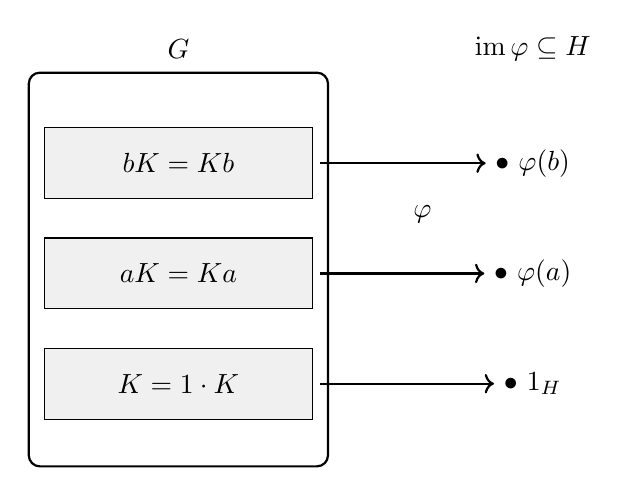
\begin{tikzpicture}[scale=1.0]
% domain box
\draw[rounded corners, thick] (-0.4,-0.6) rectangle (3.4,4.4);
\node at (1.5,4.7) {$G$};
% three fibers (cosets) as horizontal slabs
\draw[fill=black!6] (-0.2,0.0) rectangle (3.2,0.9);
\draw[fill=black!6] (-0.2,1.4) rectangle (3.2,2.3);
\draw[fill=black!6] (-0.2,2.8) rectangle (3.2,3.7);
\node at (1.5,0.45) {$K = 1\cdot K$};
\node at (1.5,1.85) {$aK = Ka$};
\node at (1.5,3.25) {$bK = Kb$};
% codomain points
\node (i1) at (6.0,0.45) {$\bullet\ 1_H$};
\node (i2) at (6.0,1.85) {$\bullet\ \varphi(a)$};
\node (i3) at (6.0,3.25) {$\bullet\ \varphi(b)$};
\node at (6.0,4.7) {$\im\varphi \subseteq H$};
% arrows
\draw[->,thick] (3.3,0.45) -- (i1.west);
\draw[->,thick] (3.3,1.85) -- (i2.west);
\draw[->,thick] (3.3,3.25) -- (i3.west);
\node at (4.6,2.6) {$\varphi$};
\end{tikzpicture}
\end{center}

\begin{dgx}
\dgi{Objects:} Two sets: the group $G$ on the left (shown as a large rounded rectangle) and $\im\varphi \subseteq H$ on the right (shown as a column of points). Inside $G$ the elements are partitioned into horizontal slabs; each slab is a coset of $K = \ker\varphi$: the bottom slab is $K = 1\cdot K$ (the kernel itself), then $aK = Ka$, then $bK = Kb$. Each point on the right is one element of $\im\varphi$: $1_H$, $\varphi(a)$, $\varphi(b)$.
\dgi{Arrows:} Three parallel horizontal arrows, each from the right edge of one coset-slab to the corresponding point in $\im\varphi$, all labeled $\varphi$. Each arrow represents the action of $\varphi$ on an entire coset: every element inside the slab maps to the single target point. The equal signs $aK = Ka$ inside the slab labels record that left and right cosets coincide (normality).
\dgi{What commutes:} There is no composite path to equate; the diagram instead encodes the fiber identity $\varphi^{-1}(\{\varphi(a)\}) = aK = Ka$. Every element of the coset $aK$ maps to the same value $\varphi(a)$, and no element outside $aK$ maps there. The three arrows are thus a bijection between the set of cosets $\{K, aK, bK\}$ and the set of values $\{1_H, \varphi(a), \varphi(b)\}$.
\dgi{Why it commutes:} If $g \in aK$ then $g = an$ for some $n \in K = \ker\varphi$, so $\varphi(g) = \varphi(a)\varphi(n) = \varphi(a)\cdot 1_H = \varphi(a)$. Hence all elements of the same coset land at the same point. Conversely, if $\varphi(g) = \varphi(a)$ then $\varphi(a^{-1}g) = 1_H$, so $a^{-1}g \in K$, so $g \in aK$. Both directions confirm the fiber equals the coset.
\dgi{Why this matters here:} This picture is the visual proof of Proposition~\ref{prop:kernelnormal@c3}(c): the map $\varphi$ partitions $G$ into fibers, each fiber is a coset of $K$, and the induced map $G/K \to \im\varphi$ sending each coset to its common image is a bijection. It motivates why $G/K$ is the ``right'' quotient for $\varphi$ and sets up the First Isomorphism Theorem geometrically before its algebraic statement.
\dgi{Concrete example:} Take $\varphi = \det: \GL_2(\R) \to \R^\times$ with $K = \SL_2(\R)$. Each coset $A\cdot\SL_2(\R)$ is the slab of matrices with determinant $\det(A)$, and $\varphi$ collapses that entire slab to the single scalar $\det(A) \in \R^\times$. The three slabs in the picture correspond to $K$ (det $= 1$), $aK$ (det $= \det(a)$), and $bK$ (det $= \det(b)$).
\dgi{Common pitfall:} The picture might suggest that the three cosets $K, aK, bK$ exhaust $G$; they are only a representative sample. In general $G$ may have infinitely many cosets (when $\ker\varphi$ has infinite index). Also, the equal sign $aK = Ka$ in the slab label is a nontrivial fact --- it holds because $K \nor G$ --- not something automatic for every subgroup.
\dgi{Takeaway:} The point of this diagram is that $\varphi$ does not see individual elements, only cosets --- it collapses each coset of $\ker\varphi$ to a single point, making the partition of $G$ into cosets and the bijection $G/\ker\varphi \leftrightarrow \im\varphi$ visually immediate.
\end{dgx}

\begin{method}{Proving $N \nor G$}
Three standard routes; pick whichever matches the data you have.
\begin{enumerate}
\item[\textbf{(A)}] \textbf{Conjugation test.} Show $gng\inv \in N$ for every $g \in G$ and every $n \in N$. By Theorem~\ref{thm:normalchar@c3}$(4)$ the one-sided containment $gNg\inv \subseteq N$ (for \emph{all} $g$) suffices --- you need not separately prove $\supseteq$. Trigger: $N$ given by an explicit description you can plug into a conjugate.
\item[\textbf{(B)}] \textbf{Exhibit $N$ as a kernel.} Find a homomorphism $\varphi : G \to H$ with $\ker\varphi = N$. Then $N \nor G$ for free by Proposition~\ref{prop:kernelnormal@c3}(b). Trigger: $N$ is ``everything killed by'' some natural map (determinant, sign, reduction mod $m$, projection).
\item[\textbf{(C)}] \textbf{Index $2$.} If $\idx{G}{N} = 2$ then $N \nor G$ automatically (Worked Example below). Trigger: $|G| = 2|N|$, or $N$ is ``half'' of $G$.
\end{enumerate}
\textbf{Bonus:} characteristic subgroups (e.g. $Z(G)$, the commutator subgroup) are always normal, since every conjugation is an automorphism.
\end{method}

\begin{wex}{$\SL_n = \ker(\det)$ is normal in $\GL_n$}
Let $F$ be a field. Show $\SL_n(F) = \{A \in \GL_n(F) : \det A = 1\} \nor \GL_n(F)$.
\wrec Method (B): $\SL_n$ is defined as ``matrices killed by'' the multiplicative behavior of $\det$, so realize it as a kernel.
\wsol The determinant $\det : \GL_n(F) \to F^\times$ is a homomorphism into the multiplicative group of nonzero scalars, because $\det(AB) = \det(A)\det(B)$. Its kernel is
\[
\ker(\det) = \{A : \det A = 1\} = \SL_n(F).
\]
By Proposition~\ref{prop:kernelnormal@c3}(b) a kernel is normal, so $\SL_n(F) \nor \GL_n(F)$.
\emph{Check (direct conjugation):} for $A \in \SL_n$ and any $g \in \GL_n$,
\[
\det(gAg\inv) = \det(g)\det(A)\det(g)\inv = \det(g)\cdot 1 \cdot \det(g)\inv = 1,
\]
so $gAg\inv \in \SL_n$, confirming normality via Method (A) as well.
\end{wex}

\begin{wex}{$A_n = \ker(\sgn)$ is normal in $S_n$}
Show the alternating group $A_n \nor S_n$ for $n \ge 2$.
\wrec Method (B): $A_n$ is exactly the even permutations, i.e. those sent to $+1$ by the sign map --- a kernel.
\wsol The sign map $\sgn : S_n \to \{\pm 1\}$ (the latter a group under multiplication) is a homomorphism: $\sgn(\sigma\tau) = \sgn(\sigma)\sgn(\tau)$. By definition
\[
A_n = \{\sigma \in S_n : \sgn(\sigma) = 1\} = \ker(\sgn).
\]
Hence $A_n \nor S_n$ by Proposition~\ref{prop:kernelnormal@c3}(b).
\emph{Check (index $2$):} for $n \ge 2$, $\sgn$ is onto $\{\pm1\}$ (a transposition maps to $-1$), so $\im(\sgn)$ has order $2$ and the fibers of $\sgn$ are the two cosets $A_n$ (even) and $(1\,2)A_n$ (odd). Thus $\idx{S_n}{A_n} = 2$, giving normality also by Method (C). For $S_3$: $|A_3| = 3$, $|S_3| = 6$, index $2$, and indeed $A_3 = \{e,(1\,2\,3),(1\,3\,2)\}$ is normal.
\end{wex}

\begin{wex}{The center $Z(G) \nor G$}
Show that $Z(G) = \{z \in G : zg = gz \text{ for all } g \in G\}$ is normal.
\wrec Method (A): the defining property of $Z(G)$ controls exactly what conjugation does. (Also a kernel --- see check.)
\wsol Let $z \in Z(G)$ and $g \in G$. Since $z$ commutes with $g$,
\[
gzg\inv = (gz)g\inv = (zg)g\inv = z(gg\inv) = z \in Z(G).
\]
So $gZ(G)g\inv \subseteq Z(G)$ for all $g$, hence $Z(G) \nor G$ by Theorem~\ref{thm:normalchar@c3}$(4)$.
\emph{Stronger fact:} every conjugate of $z$ equals $z$ itself, so each element of $Z(G)$ is its own (singleton) conjugacy class. \emph{Check (kernel description):} $Z(G) = \ker\big(G \xrightarrow{\ g\,\mapsto\, \text{conj. by } g}\ \Aut(G)\big)$, the kernel of the homomorphism $G \to \Aut(G)$ sending $g$ to the inner automorphism $x \mapsto gxg\inv$; an element is in the kernel iff conjugation by it is the identity iff it is central. This re-proves $Z(G) \nor G$ via Method (B). Concretely in $D_8$ (with $r^4 = s^2 = 1$): $Z(D_8) = \{1, r^2\}$, and indeed $sr^2 s\inv = r^{-2} = r^2$, $\,r r^2 r\inv = r^2$, so $\{1,r^2\} \nor D_8$.
\end{wex}

\begin{wex}{Every index-$2$ subgroup is normal}
Let $H \le G$ with $\idx{G}{H} = 2$. Show $H \nor G$.
\wrec Method (C): index $2$ leaves no room for a left coset to differ from a right coset.
\wsol Index $2$ means there are exactly two left cosets, namely $H$ and $G \setminus H$ (the second is a single coset because the cosets partition $G$ and there are only two). Likewise the two \emph{right} cosets are $H$ and $G \setminus H$. Take any $g \in G$.
\begin{itemize}
\item If $g \in H$: then $gH = H = Hg$.
\item If $g \notin H$: then $gH \ne H$, so $gH$ must be the other left coset, $gH = G\setminus H$. Similarly $Hg \ne H$ forces $Hg = G \setminus H$. Hence $gH = G\setminus H = Hg$.
\end{itemize}
In both cases $gH = Hg$, so by Theorem~\ref{thm:normalchar@c3}$(3)$, $H \nor G$.
\emph{Check:} this recovers $A_n \nor S_n$ ($\idx{S_n}{A_n} = 2$) and $\gen{r} \nor D_{2n}$ ($\idx{D_{2n}}{\gen{r}} = 2$, since $|\gen{r}| = n$ and $|D_{2n}| = 2n$) without any computation. \emph{Caution:} index $\ge 3$ does \emph{not} force normality --- $\gen{s} \le D_8$ has index $4$ and is not normal (next example), and $\gen{(1\,2)} \le S_3$ has index $3$ and is not normal.
\end{wex}

\begin{wex}{A non-normal subgroup: $\gen{s} \le D_8$ and its conjugates}
In $D_8 = \gen{r,s \mid r^4 = s^2 = 1,\ sr = r\inv s}$, show $H = \gen{s} = \{1, s\}$ is \emph{not} normal, and list the conjugate subgroups.
\wrec Method (A) used as a \emph{disproof}: produce one $g$ with $gsg\inv \notin H$.
\wsol We compute $rsr\inv$. From the relation $sr = r\inv s$ we get $rs = sr\inv$, and $r\inv = r^3$. Then
\[
rsr\inv = (rs)r\inv = (sr\inv)r\inv = s r^{-2} = s r^2.
\]
Now $sr^2 \notin \{1,s\} = H$ (it is a reflection through a different axis), so $rHr\inv \ne H$ and therefore $H$ is \textbf{not} normal in $D_8$.
\emph{Conjugates.} Since $sr^2 = r^{-2}s = r^2 s$, conjugating $H = \{1,s\}$ by $r$ gives $\{1, r^2 s\}$, and conjugating by $r^2$ gives back $\{1,s\}$ (because $r^2 s r^{-2} = s$). So the conjugacy class of $H$ is the pair $\{1,s\},\ \{1,r^2 s\}$. The remaining two reflection-subgroups $\{1, rs\},\ \{1, r^3 s\}$ form a \emph{separate} conjugacy class:
\[
\{1,s\},\ \{1,r^2 s\} \quad\text{(one conjugacy pair)}; \qquad \{1, rs\},\ \{1, r^3 s\}\quad\text{(another pair)}.
\]
\emph{Check via the normalizer.} The normalizer is $N_{D_8}(H) = \{g : gHg\inv = H\}$. It contains $H$ itself and the center element $r^2$ (since $r^2 s r^{-2} = s$), so $N_{D_8}(H) = \{1, s, r^2, r^2 s\}$, an order-$4$ subgroup. Hence the number of conjugates of $H$ is $\idx{D_8}{N_{D_8}(H)} = 8/4 = 2$, matching the pair $\{1,s\}, \{1,r^2s\}$ found above. Since $N_{D_8}(H) \ne D_8$, again $H \not\nor D_8$.
\end{wex}

\begin{wex}{Reduction mod $m$: $m\Z = \ker(\Z \to \Zn{m})$}
Show $m\Z \nor \Z$ for any integer $m \ge 1$.
\wrec Method (B), additive flavor: $m\Z$ is what reduction mod $m$ kills.
\wsol The reduction map $\varphi : \Z \to \Zn{m}$, $\varphi(a) = a \bmod m = \overline{a}$, is a homomorphism: $\varphi(a + b) = \overline{a+b} = \overline{a} + \overline{b} = \varphi(a) + \varphi(b)$. Its kernel is
\[
\ker\varphi = \{a \in \Z : \overline{a} = \overline{0}\} = \{a : m \mid a\} = m\Z.
\]
So $m\Z \nor \Z$ by Proposition~\ref{prop:kernelnormal@c3}(b). \emph{Check:} $\Z$ is abelian, so \emph{every} subgroup is normal anyway ($gng\inv = ng g\inv = n$); the fibers of $\varphi$ are the $m$ cosets $\overline{0}, \overline{1}, \dots, \overline{m-1}$, i.e. the residue classes, confirming Proposition~\ref{prop:kernelnormal@c3}(c).
\end{wex}

\begin{pitfall}
\textbf{(1) One $g$ is not enough.} To prove $N \nor G$ you need $gng\inv \in N$ for \emph{all} $g \in G$. Verifying it for a single $g$ is not a proof of normality. Checking every $g$ in a generating set $T$ of $G$ does suffice when $N$ is finite (Exercise~29 below), but for infinite $N$ one must in general also check the inverses $t\inv$ ($t \in T$). On the other hand, one well-chosen $g$ \emph{is} enough to \emph{disprove} normality.

\textbf{(2) $gNg\inv \subseteq N$ for all $g$ does give normality --- but mind infinite groups.} In Theorem~\ref{thm:normalchar@c3} the one-sided test $(4)$ works because the hypothesis is quantified over \emph{all} $g$ (we plugged in $g\inv$ too). For a \emph{fixed} $g$, the containment $gNg\inv \subseteq N$ alone does \emph{not} force $gNg\inv = N$ when $N$ is infinite. Standard example: in $G = \GL_2(\Q)$ let $g = \left(\begin{smallmatrix} 2 & 0 \\ 0 & 1\end{smallmatrix}\right)$ and $N = \left\{ \left(\begin{smallmatrix} 1 & x \\ 0 & 1 \end{smallmatrix}\right) : x \in \Z \right\}$. Then $g \left(\begin{smallmatrix}1&x\\0&1\end{smallmatrix}\right) g\inv = \left(\begin{smallmatrix}1&2x\\0&1\end{smallmatrix}\right)$, so $gNg\inv = \left\{\left(\begin{smallmatrix}1&2x\\0&1\end{smallmatrix}\right):x\in\Z\right\} \subsetneq N$ --- proper containment. (Of course this particular $N$ is not normal in $G$; the point is that strict containment $gNg\inv \subsetneq N$ can genuinely happen, so for a single $g$ ``$\subseteq$'' is weaker than ``$=$''. The quantified test in $(4)$ closes the gap by also applying the inclusion at $g\inv$.)

\textbf{(3) $gN = Ng$ does not mean $gn = ng$.} Normality says the \emph{sets} $gN$ and $Ng$ coincide, not that $g$ commutes with each element of $N$. For each $n$ there is \emph{some} $n' \in N$ with $gn = n'g$, but typically $n' \ne n$.
\end{pitfall}

\begin{exers}{Exercises (from the text).}
\item Let $\varphi : G \to H$ be a homomorphism and let $E$ be a subgroup of $H$. Prove that $\varphi\inv(E) \le G$ (i.e., the preimage or pullback of a subgroup under a homomorphism is a subgroup). If $E \nor H$ prove that $\varphi\inv(E) \nor G$. Deduce that $\ker \varphi \nor G$.

\item Let $\varphi : G \to H$ be a homomorphism of groups with kernel $K$ and let $a, b \in \varphi(G)$. Let $X \in G/K$ be the fiber above $a$ and let $Y$ be the fiber above $b$, i.e., $X = \varphi\inv(a)$, $Y = \varphi\inv(b)$. Fix an element $u$ of $X$ (so $\varphi(u) = a$). Prove that if $XY = Z$ in the quotient group $G/K$ and $w$ is any member of $Z$, then there is some $v \in Y$ such that $uv = w$. [Show $u\inv w \in Y$.]

\item Let $A$ be an abelian group and let $B$ be a subgroup of $A$. Prove that $A/B$ is abelian. Give an example of a non-abelian group $G$ containing a proper normal subgroup $N$ such that $G/N$ is abelian.

\item Prove that in the quotient group $G/N$, $(gN)^a = g^a N$ for all $a \in \Z$.

\item Use the preceding exercise to prove that the order of the element $gN$ in $G/N$ is $n$, where $n$ is the smallest positive integer such that $g^n \in N$ (and $gN$ has infinite order if no such positive integer exists). Give an example to show that the order of $gN$ in $G/N$ may be strictly smaller than the order of $g$ in $G$.

\item Define $\varphi : \R^\times \to \{\pm 1\}$ by letting $\varphi(x)$ be $x$ divided by the absolute value of $x$. Describe the fibers of $\varphi$ and prove that $\varphi$ is a homomorphism.

\item Define $\pi : \R^2 \to \R$ by $\pi((x,y)) = x + y$. Prove that $\pi$ is a surjective homomorphism and describe the kernel and fibers of $\pi$ geometrically.

\item Let $\varphi : \R^\times \to \R^\times$ be the map sending $x$ to the absolute value of $x$. Prove that $\varphi$ is a homomorphism and find the image of $\varphi$. Describe the kernel and the fibers of $\varphi$ geometrically.

\item Define $\varphi : \C^\times \to \R^\times$ by $\varphi(a + bi) = a^2 + b^2$. Prove that $\varphi$ is a homomorphism and find the image of $\varphi$. Describe the kernel and the fibers of $\varphi$ geometrically (as subsets of the plane).

\item Let $\varphi : \Z/8\Z \to \Z/4\Z$ by $\varphi(\overline{a}) = \overline{a}$. Show that this is a well defined, surjective homomorphism and describe its fibers and kernel explicitly (showing that $\varphi$ is well defined involves the fact that $\overline{a}$ has a different meaning in the domain and range of $\varphi$).

\item Let $F$ be a field and let $G = \left\{ \begin{pmatrix} a & b \\ 0 & c \end{pmatrix} \mid a, b, c \in F, \ ac \neq 0 \right\} \le GL_2(F)$.
(a) Prove that the map $\varphi : \begin{pmatrix} a & b \\ 0 & c \end{pmatrix} \mapsto a$ is a surjective homomorphism from $G$ onto $F^\times$ (recall that $F^\times$ is the multiplicative group of nonzero elements in $F$). Describe the fibers and kernel of $\varphi$.
(b) Prove that the map $\psi : \begin{pmatrix} a & b \\ 0 & c \end{pmatrix} \mapsto (a, c)$ is a surjective homomorphism from $G$ onto $F^\times \times F^\times$. Describe the fibers and kernel of $\psi$.
(c) Let $H = \left\{ \begin{pmatrix} 1 & b \\ 0 & 1 \end{pmatrix} \mid b \in F \right\}$. Prove that $H$ is isomorphic to the additive group of $F$.

\item Let $G$ be the additive group of real numbers, let $H$ be the multiplicative group of complex numbers of absolute value 1 (the unit circle $S^1$ in the complex plane) and let $\varphi : G \to H$ be the homomorphism $\varphi : r \mapsto e^{2\pi i r}$. Draw the points on a real line which lie in the kernel of $\varphi$. Describe similarly the elements in the fibers of $\varphi$ above the points $-1$, $i$, and $e^{4\pi i/3}$ of $H$.

\item Repeat the preceding exercise with the map $\varphi$ replaced by the map $\varphi : r \mapsto e^{4\pi i r}$.

\item Consider the additive quotient group $\Q/\Z$.
(a) Show that every coset of $\Z$ in $\Q$ contains exactly one representative $q \in \Q$ in the range $0 \le q < 1$.
(b) Show that every element of $\Q/\Z$ has finite order but that there are elements of arbitrarily large order.
(c) Show that $\Q/\Z$ is the torsion subgroup of $\R/\Z$ (cf. Exercise 6, Section 2.1).
(d) Prove that $\Q/\Z$ is isomorphic to the multiplicative group of roots of unity in $\C^\times$.

\item Prove that a quotient of a divisible abelian group by any proper subgroup is also divisible. Deduce that $\Q/\Z$ is divisible (cf. Exercise 19, Section 2.4).

\item Let $G$ be a group, let $N$ be a normal subgroup of $G$ and let $\overline{G} = G/N$. Prove that if $G = \langle x, y \rangle$ then $\overline{G} = \langle \overline{x}, \overline{y} \rangle$. Prove more generally that if $G = \langle S \rangle$ for any subset $S$ of $G$, then $\overline{G} = \langle \overline{S} \rangle$.

\item Let the dihedral group of order 16 (whose lattice appears in Section 2.5) be given by the presentation $G = \langle r, s \mid r^8 = s^2 = 1, \ rs = sr\inv \rangle$ and let $\overline{G} = G/\langle r^4 \rangle$ be the quotient of $G$ by the subgroup generated by $r^4$ (this subgroup is the center of $G$, hence is normal).
(a) Show that the order of $\overline{G}$ is 8.
(b) Exhibit each element of $\overline{G}$ in the form $\overline{s}^a \overline{r}^b$, for some integers $a$ and $b$.
(c) Find the order of each of the elements of $\overline{G}$ exhibited in (b).
(d) Write each of the following elements of $\overline{G}$ in the form $\overline{s}^a \overline{r}^b$, for some integers $a$ and $b$ as in (b): $\overline{rs}$, $\overline{sr^{-2}s}$, $\overline{s^{-1}r^{-1}sr}$.
(e) Prove that $\overline{H} = \langle \overline{s}, \overline{r^2} \rangle$ is a normal subgroup of $\overline{G}$ and $\overline{H}$ is isomorphic to the Klein 4-group. Describe the isomorphism type of the complete preimage of $\overline{H}$ in $G$.
(f) Find the center of $\overline{G}$ and describe the isomorphism type of $\overline{G}/Z(\overline{G})$.

\item Let $G$ be the quasidihedral group of order 16 (whose lattice was computed in Exercise 11 of Section 2.5):
$G = \langle \sigma, \tau \mid \sigma^8 = \tau^2 = 1, \ \sigma\tau = \tau\sigma^3 \rangle$
and let $\overline{G} = G/\langle \sigma^4 \rangle$ be the quotient of $G$ by the subgroup generated by $\sigma^4$ (this subgroup is the center of $G$, hence is normal).
(a) Show that the order of $\overline{G}$ is 8.
(b) Exhibit each element of $\overline{G}$ in the form $\overline{\tau}^a \overline{\sigma}^b$, for some integers $a$ and $b$.
(c) Find the order of each of the elements of $\overline{G}$ exhibited in (b).
(d) Write each of the following elements of $\overline{G}$ in the form $\overline{\tau}^a \overline{\sigma}^b$, for some integers $a$ and $b$ as in (b): $\overline{\sigma\tau}$, $\overline{\tau\sigma^{-2}\tau}$, $\overline{\tau^{-1}\sigma^{-1}\tau\sigma}$.
(e) Prove that $\overline{G} \isom D_8$.

\item Let $G$ be the modular group of order 16 (whose lattice was computed in Exercise 14 of Section 2.5):
$G = \langle u, v \mid u^2 = v^8 = 1, \ vu = uv^5 \rangle$
and let $\overline{G} = G/\langle v^4 \rangle$ be the quotient of $G$ by the subgroup generated by $v^4$ (this subgroup is contained in the center of $G$, hence is normal).
(a) Show that the order of $\overline{G}$ is 8.
(b) Exhibit each element of $\overline{G}$ in the form $\overline{u}^a \overline{v}^b$, for some integers $a$ and $b$.
(c) Find the order of each of the elements of $\overline{G}$ exhibited in (b).
(d) Write each of the following elements of $\overline{G}$ in the form $\overline{u}^a \overline{v}^b$, for some integers $a$ and $b$ as in (b): $\overline{vu}$, $\overline{uv^{-2}u}$, $\overline{u^{-1}v^{-1}uv}$.
(e) Prove that $\overline{G}$ is abelian and is isomorphic to $\Z_2 \times \Z_4$.

\item Let $G = \Z/24\Z$ and let $\overline{G} = G/\langle \overline{12} \rangle$, where for each integer $a$ we simplify notation by writing $\overline{a}$ as $\widetilde{a}$.
(a) Show that $\overline{G} = \{\widetilde{0}, \widetilde{1}, \dots, \widetilde{11}\}$.
(b) Find the order of each element of $\overline{G}$.
(c) Prove that $\overline{G} \isom \Z/12\Z$. (Thus $(\Z/24\Z)/(12\Z/24\Z) \isom \Z/12\Z$, just as if we inverted and cancelled the $24\Z$'s.)

\item Let $G = \Z_4 \times \Z_4$ be given in terms of the following generators and relations:
$G = \langle x, y \mid x^4 = y^4 = 1, \ xy = yx \rangle$. Let $\overline{G} = G/\langle x^2y^2 \rangle$ (note that every subgroup of the abelian group $G$ is normal).
(a) Show that the order of $\overline{G}$ is 8.
(b) Exhibit each element of $\overline{G}$ in the form $\overline{x}^a \overline{y}^b$, for some integers $a$ and $b$.
(c) Find the order of each of the elements of $\overline{G}$ exhibited in (b).
(d) Prove that $\overline{G} \isom \Z_4 \times \Z_2$.

\item (a) Prove that if $H$ and $K$ are normal subgroups of a group $G$ then their intersection $H \cap K$ is also a normal subgroup of $G$.
(b) Prove that the intersection of an arbitrary nonempty collection of normal subgroups of a group is a normal subgroup (do not assume the collection is countable).

\item Prove that the join (cf. Section 2.5) of any nonempty collection of normal subgroups of a group is a normal subgroup.

\item Prove that if $N \nor G$ and $H$ is any subgroup of $G$ then $N \cap H \nor H$.

\item (a) Prove that a subgroup $N$ of $G$ is normal if and only if $gNg\inv \subseteq N$ for all $g \in G$.
(b) Let $G = GL_2(\Q)$, let $N$ be the subgroup of upper triangular matrices with integer entries and 1's on the diagonal, and let $g$ be the diagonal matrix with entries $2, 1$. Show that $gNg\inv \subseteq N$ but $g$ does not normalize $N$.

\item Let $a, b \in G$.
(a) Prove that the conjugate of the product of $a$ and $b$ is the product of the conjugate of $a$ and the conjugate of $b$. Prove that the order of $a$ and the order of any conjugate of $a$ are the same.
(b) Prove that the conjugate of $a\inv$ is the inverse of the conjugate of $a$.
(c) Let $N = \langle S \rangle$ for some subset $S$ of $G$. Prove that $N \nor G$ if and only if $gSg\inv \subseteq N$ for all $g \in G$.
(d) Deduce that if $N$ is the cyclic group $\langle x \rangle$, then $N$ is normal in $G$ if and only if for each $g \in G$, $gxg\inv = x^k$ for some $k \in \Z$.
(e) Let $n$ be a positive integer. Prove that the subgroup $N$ of $G$ generated by all the elements of $G$ of order $n$ is a normal subgroup of $G$.

\item Let $N$ be a finite subgroup of a group $G$. Show that $gNg\inv \subseteq N$ if and only if $gNg\inv = N$. Deduce that $N_G(N) = \{g \in G \mid gNg\inv \subseteq N\}$.

\item Let $N$ be a finite subgroup of a group $G$ and assume $N = \langle S \rangle$ for some subset $S$ of $G$. Prove that an element $g \in G$ normalizes $N$ if and only if $gSg\inv \subseteq N$.

\item Let $N$ be a finite subgroup of $G$ and suppose $G = \langle T \rangle$ and $N = \langle S \rangle$ for some subsets $S$ and $T$ of $G$. Prove that $N$ is normal in $G$ if and only if $tSt\inv \subseteq N$ for all $t \in T$.

\item Let $N \le G$ and let $g \in G$. Prove that $gN = Ng$ if and only if $g \in N_G(N)$.

\item Prove that if $H \le G$ and $N$ is a normal subgroup of $H$ then $H \le N_G(N)$. Deduce that $N_G(N)$ is the largest subgroup of $G$ in which $N$ is normal (i.e., is the join of all subgroups $H$ for which $N \nor H$).

\item Prove that every subgroup of $Q_8$ is normal. For each subgroup find the isomorphism type of its corresponding quotient. [You may use the lattice of subgroups for $Q_8$ in Section 2.5.]

\item Find all normal subgroups of $D_8$ and for each of these find the isomorphism type of its corresponding quotient. [You may use the lattice of subgroups for $D_8$ in Section 2.5.]

\item Let $D_{2n} = \langle r, s \mid r^n = s^2 = 1, \ rs = sr\inv \rangle$ be the usual presentation of the dihedral group of order $2n$ and let $k$ be a positive integer dividing $n$.
(a) Prove that $\langle r^k \rangle$ is a normal subgroup of $D_{2n}$.
(b) Prove that $D_{2n}/\langle r^k \rangle \isom D_{2k}$.

\item Prove that $SL_n(F) \nor GL_n(F)$ and describe the isomorphism type of the quotient group (cf. Exercise 9, Section 2.1).

\item Prove that if $G/Z(G)$ is cyclic then $G$ is abelian. [If $G/Z(G)$ is cyclic with generator $xZ(G)$, show that every element of $G$ can be written in the form $x^a z$ for some integer $a \in \Z$ and some element $z \in Z(G)$.]

\item Let $A$ and $B$ be groups. Show that $\{(a, 1) \mid a \in A\}$ is a normal subgroup of $A \times B$ and the quotient of $A \times B$ by this subgroup is isomorphic to $B$.

\item Let $A$ be an abelian group and let $D$ be the (diagonal) subgroup $\{(a, a) \mid a \in A\}$ of $A \times A$. Prove that $D$ is a normal subgroup of $A \times A$ and $(A \times A)/D \isom A$.

\item Suppose $A$ is the non-abelian group $S_3$ and $D$ is the diagonal subgroup $\{(a, a) \mid a \in A\}$ of $A \times A$. Prove that $D$ is not normal in $A \times A$.

\item Let $G$ be a group, let $N$ be a normal subgroup of $G$ and let $\overline{G} = G/N$. Prove that $\overline{x}$ and $\overline{y}$ commute in $\overline{G}$ if and only if $x\inv y\inv xy \in N$. (The element $x\inv y\inv xy$ is called the \emph{commutator} of $x$ and $y$ and is denoted by $[x, y]$.)

\item Let $G$ be a group. Prove that $N = \langle x\inv y\inv xy \mid x, y \in G \rangle$ is a normal subgroup of $G$ and $G/N$ is abelian ($N$ is called the \emph{commutator subgroup} of $G$).

\item Assume both $H$ and $K$ are normal subgroups of $G$ with $H \cap K = 1$. Prove that $xy = yx$ for all $x \in H$ and $y \in K$. [Show $x\inv y\inv xy \in H \cap K$.]

\item Assume $\mathcal{P} = \{A_i \mid i \in I\}$ is any partition of $G$ with the property that $\mathcal{P}$ is a group under the ``quotient operation'' defined as follows: to compute the product of $A_i$ with $A_j$ take any element $a_i$ of $A_i$ and any element $a_j$ of $A_j$ and let $A_i A_j$ be the element of $\mathcal{P}$ containing $a_i a_j$ (this operation is assumed to be well defined). Prove that the element of $\mathcal{P}$ that contains the identity of $G$ is a normal subgroup of $G$ and the elements of $\mathcal{P}$ are the cosets of this subgroup (so $\mathcal{P}$ is just a quotient group of $G$ in the usual sense).
\end{exers}

\begin{exers}{Practice problems (additional).}
  \item Let $G = \Z$ and $N = 12\Z$. List the elements of $G/N$, give the order of each coset, and identify $G/N$ up to isomorphism.

  \item In $\Z/30\Z$, compute the order of the cosets $\overline{6}$, $\overline{10}$, and $\overline{18}$. For each, find the subgroup $\gen{\overline{x}}$ it generates and its index in $\Z/30\Z$.

  \item Let $G = D_8 = \gen{r,s}$ with $r^4 = s^2 = 1$, $sr = r\inv s$, and let $N = \gen{r^2} = \{1, r^2\}$. Show $N \nor G$, write out the four cosets of $N$, build the multiplication table of $G/N$, and identify $G/N$ (is it $\Z/4\Z$ or the Klein four-group?).

  \item Let $G = Q_8 = \{\pm 1, \pm i, \pm j, \pm k\}$ and $N = \gen{-1} = \{1,-1\}$. Show $N \nor G$ and determine the isomorphism type of $G/N$.

  \item In $G = \Z/4\Z \times \Z/2\Z$, let $N = \gen{(\overline{2},\overline{0})}$. Compute $\ord{N}$, list the cosets of $N$, and identify $G/N$.

  \item Let $\varphi: \Z \to \Z/6\Z$ be the natural projection $n \mapsto \overline{n}$. Find $\ker\varphi$, find $\im\varphi$, and use the First Isomorphism Theorem to identify $\Z/\ker\varphi$.

  \item Define $\varphi: \R \to \C^\times$ by $\varphi(x) = e^{2\pi i x}$. Show $\varphi$ is a homomorphism, compute $\ker\varphi$ and $\im\varphi$, and identify $\R/\ker\varphi$.

  \item Let $\varphi: \GL_2(\R) \to \R^\times$ be the determinant map. Identify $\ker\varphi$, identify $\im\varphi$, and state what the First Isomorphism Theorem gives for $\GL_2(\R)/\SL_2(\R)$.

  \item Let $G = \Z/12\Z$. For each divisor $d \mid 12$ there is a unique subgroup of order $d$. List all subgroups of $G$, and for each subgroup $H$ compute $\idx{G}{H}$ and identify $G/H$.

  \item Let $N \nor G$ with $\idx{G}{N} = 5$ and suppose $g \in G$ satisfies $g \notin N$. Prove that $G/N = \gen{gN}$, i.e. $gN$ generates the quotient.

  \item Suppose $|G| = 24$ and $N \nor G$ with $|N| = 8$. Determine $|G/N|$ and all possible isomorphism types of $G/N$.

  \item Let $G$ be a group and $N \nor G$. Prove that if $G/N$ and $N$ are both abelian and $N \le Z(G)$, then for all $x,y \in G$ the commutator $[x,y] = x\inv y\inv x y$ lies in $N$.

  \item Let $\varphi: G \to H$ be a homomorphism with $|G| = 20$ and $|H| = 12$. List all possible values of $|\im\varphi|$, justifying each by Lagrange's theorem applied to both $G$ (via $\ker\varphi$) and $H$.

  \item In $\Z/8\Z$, exhibit the unique chain of subgroups giving a composition series $1 \pnor H_1 \pnor H_2 \pnor \Z/8\Z$, and identify each composition factor.

  \item Let $G = S_3$. Show that $A_3 \nor S_3$ and that $S_3/A_3 \isom \Z/2\Z$. Identify the homomorphism $S_3 \to \{\pm 1\}$ whose kernel is $A_3$.

  \item Let $G = \Z/2\Z \times \Z/2\Z$ (the Klein four-group). For each of the three subgroups $N$ of order $2$, identify $G/N$ and verify $|G/N| = 2$.

\end{exers}

\begin{exers}{Additional exercises.}
  \item Let $N \nor G$. Prove that the order of the coset $gN$ in $G/N$ divides the order of $g$ in $G$. Give an explicit example with $G = \Z/4\Z$, $N$ of order $2$, where the order of $gN$ is strictly smaller than $\ord{g}$.

  \item (Cosets need not respect order naively.) Let $G = D_8 = \gen{r,s}$ and $N = \gen{s}$. Show that $N$ is \emph{not} normal in $G$ by exhibiting $g \in G$ with $gNg\inv \neq N$, and conclude that the set of left cosets $G/N$ is \emph{not} a group under coset multiplication.

  \item Let $G$ be a group with $|G| = pq$ for primes $p < q$, and suppose $N \nor G$ with $|N| = q$. Prove $G/N \isom \Z/p\Z$, and deduce that every element of $G$ outside $N$ has order divisible by $p$.

  \item Let $\varphi: G \to H$ be a surjective homomorphism and let $M \nor H$. Prove that $\varphi\inv(M) \nor G$ and that $G/\varphi\inv(M) \isom H/M$. (This is the source of the lattice correspondence; prove it directly without quoting the Correspondence Theorem.)

  \item Let $G = \Z \times \Z$ and $N = \gen{(2,0),(0,3)}$. Determine $G/N$ as a direct product of cyclic groups and give its order.

  \item Let $G$ be a finite group and let $N \nor G$ with $\gcd(|N|, \idx{G}{N}) = 1$. Prove that $N$ is the unique subgroup of $G$ of order $|N|$. (Hint: if $H \le G$ with $|H| = |N|$, consider the image of $H$ in $G/N$.)

\end{exers}

\begin{exers}{Commutative-diagram exercises.}
  \item Let $\varphi: G \to H$ be a homomorphism and $\pi: G \to G/\ker\varphi$ the natural projection. Prove there is a unique injective homomorphism $\overline{\varphi}$ making the triangle below commute, and that $\overline{\varphi}$ is an isomorphism onto $\im\varphi$:
    \[\begin{tikzcd}[row sep=large,column sep=large]
      G \arrow[r, "\varphi"] \arrow[d, two heads, "\pi"'] & H \\
      G/\ker\varphi \arrow[ur, dashed, "\overline{\varphi}"'] &
    \end{tikzcd}\]
    Apply this to $\varphi: \Z \to \Z/n\Z$ to recover $\Z/n\Z \isom \Z/n\Z$.

  \item For the homomorphism $\varphi: \R \to \C^\times$, $\varphi(x) = e^{2\pi i x}$, fill in the objects $A$ and $C$ so that the row below is a short exact sequence, and identify $C$:
    \[\begin{tikzcd}[column sep=normal]
      1 \arrow[r] & A \arrow[r, hook] & \R \arrow[r, two heads, "\varphi"] & C \arrow[r] & 1
    \end{tikzcd}\]
    where $A = \ker\varphi$ and $C = \im\varphi$.

  \item Let $N \nor G$ and $H \le G$ with $H \cap N = \{1\}$ and $HN = G$. Using the diamond/diamond-isomorphism picture below, prove $H \isom G/N$ by showing the composite $H \hookrightarrow G \twoheadrightarrow G/N$ is an isomorphism:
    \[\begin{tikzcd}[row sep=large,column sep=large]
      & G & \\
      H \arrow[ur, hook] & & N \arrow[ul, hook'] \\
      & H\cap N \arrow[ul, hook] \arrow[ur, hook'] &
    \end{tikzcd}\]

  \item Let $A, B \nor G$ with $A \le B$. Construct the diagram of natural projections below and prove the Third Isomorphism Theorem $\,(G/A)/(B/A) \isom G/B\,$ by exhibiting the dashed induced map and showing it is an isomorphism:
    \[\begin{tikzcd}[row sep=large,column sep=large]
      G \arrow[r, two heads, "\pi_A"] \arrow[dr, two heads, "\pi_B"'] & G/A \arrow[d, dashed, "{gA\mapsto gB}"] \\
      & G/B
    \end{tikzcd}\]

  \item Let $\varphi: G \to K$ be surjective with kernel $N$, and let $M \nor G$ with $N \le M$. Show the square below commutes, where the bottom map is induced by $\varphi$. Prove the induced map is an isomorphism (its kernel is trivial), and separately verify the side fact $\varphi(M) \isom M/N$:
    \[\begin{tikzcd}[row sep=large,column sep=large]
      G \arrow[r, two heads, "\varphi"] \arrow[d, two heads, "\pi_M"'] & K \arrow[d, two heads] \\
      G/M \arrow[r, dashed, "\isom"', "{gM\mapsto \varphi(g)\varphi(M)}"] & K/\varphi(M)
    \end{tikzcd}\]

\end{exers}


\section{More on Cosets and Lagrange's Theorem}
\subsection*{Lagrange's Theorem and Its Corollaries}

The single most useful counting fact in finite group theory: a subgroup's order divides
the group's order. Everything in this section is a consequence of one clean idea --- the
\emph{left cosets of $H$ partition $G$ into blocks of equal size $\ord{H}$}.

\begin{theorem}[Lagrange]
Let $G$ be a finite group and $H\sgr G$. Then $\ord{H}$ divides $\ord{G}$, and the number
of left cosets of $H$ in $G$ equals
\[
  \idx{G}{H}=\frac{\ord{G}}{\ord{H}}.
\]
\end{theorem}

\begin{proof}
Let $gH=\{gh : h\in H\}$ denote a left coset. Two facts drive the proof.

\emph{(1) The left cosets partition $G$.} Each $g\in G$ lies in $gH$ (take $h=1$), so the
cosets cover $G$. If $aH\cap bH\neq\es$, pick $x=ah_1=bh_2$; then
$a=bh_2h_1\inv\in bH$, so $aH\subseteq bH$, and symmetrically $bH\subseteq aH$, giving
$aH=bH$. Hence distinct cosets are disjoint.

\emph{(2) Every coset has exactly $\ord{H}$ elements.} The map $H\to gH$, $h\mapsto gh$, is
a bijection: it is onto by definition of $gH$, and injective because $gh_1=gh_2\imp
h_1=h_2$ by left cancellation. Thus $|gH|=\ord{H}$.

Let $k=\idx{G}{H}$ be the number of distinct left cosets and let
$g_1H,\dots,g_kH$ be them. By (1) they are disjoint and by (2) each has size $\ord{H}$, so
\[
  \ord{G}=\sum_{i=1}^{k}|g_iH|=k\,\ord{H}.
\]
Therefore $\ord{H}\mid\ord{G}$ and $k=\ord{G}/\ord{H}$.
\end{proof}

\begin{remark}
The same proof with right cosets $Hg$ shows there are equally many right cosets, so the
index is unambiguous. The bijection $gH\mapsto Hg\inv$ matches left to right cosets.
Lagrange's theorem needs no normality of $H$.
\end{remark}

The partition is worth a picture: $G$ is sliced into $\idx{G}{H}$ equal slabs, one of which
is the subgroup $H=1\cdot H$ itself.

\[
\begin{tikzcd}[row sep=tiny, column sep=large]
H \arrow[r, "g_2\cdot{}", "\isom"'] & g_2H \\
H \arrow[r, "g_3\cdot{}", "\isom"'] & g_3H \\
{} \arrow[r, dash, dotted] & {} \\
H \arrow[r, "g_k\cdot{}", "\isom"'] & g_kH
\end{tikzcd}
\qquad
\ord{G}=\underbrace{\ord{H}+\cdots+\ord{H}}_{\idx{G}{H}\text{ terms}}.
\]

\begin{dgx}
\dgi{Objects:} Each node on the left is a copy of the subgroup $H \sgr G$ (a finite group).
Each node on the right is a left coset $g_i H = \{g_i h : h \in H\}$, a subset of $G$ of
equal size; cosets are \emph{not} subgroups in general.
\dgi{Arrows:} Each horizontal arrow $H \to g_i H$, labelled $g_i \cdot{}$ and marked
$\isom$, is the left-multiplication bijection $h \mapsto g_i h$.  It is a bijection of
\emph{sets} (not a group homomorphism unless $g_i = 1$, since it sends $1$ to $g_i$); the $\isom$ symbol here
records equal cardinality, not isomorphism of groups.
\dgi{What commutes:} There is no composable path here; the diagram is a family of parallel
bijections, not a square with two routes.  The key equality it encodes is
$|g_i H| = |H|$ for every $i$, established by the bijectivity of $h \mapsto g_i h$.
\dgi{Why it commutes:} The map $h \mapsto g_i h$ is injective because $g_i h_1 = g_i h_2$
implies $h_1 = h_2$ by left cancellation in $G$, and surjective by the definition of $g_i H$.
Hence $|g_i H| = |H|$ for each $i = 2, \ldots, k$.
\dgi{Why this matters here:} This picture is the visual heart of Lagrange's proof.  The
cosets $g_1 H, \ldots, g_k H$ partition $G$ (proved just above the diagram), and each slab
has the same size $\ord{H}$.  Adding sizes gives $\ord{G} = k \cdot \ord{H}$, so $\ord{H}$
divides $\ord{G}$ and $k = \idx{G}{H}$.
\dgi{Concrete example:} Take $G = S_3$, $H = \{e, (12)\}$ (order 2).  The cosets are
$H = \{e,(12)\}$, $(13)H = \{(13),(123)\}$, $(23)H = \{(23),(132)\}$; each has 2 elements
and they partition $S_3$, giving $\ord{S_3} = 3 \cdot 2 = 6$.
\dgi{Common pitfall:} Students sometimes read the $\isom$ label as a group isomorphism
$H \isom g_i H$ and conclude $g_i H$ is itself a subgroup.  It is not: $g_i H$ lacks the
identity (unless $g_i \in H$) and the arrows are set-bijections only.
\dgi{Takeaway:} The point of this diagram is that every coset is an exact copy of $H$ in
size, so $G$ is a disjoint union of $\idx{G}{H}$ equally-sized blocks, making divisibility
of $\ord{H}$ into $\ord{G}$ immediate.
\end{dgx}

\begin{method}{Using Lagrange to constrain structure}
\textbf{Trigger:} you know $\ord{G}$ and want to limit subgroup orders, element orders, or
rule out a configuration.
\begin{enumerate}
\item \textbf{Subgroup orders} divide $\ord{G}$: list the divisors of $\ord{G}$; any
$H\sgr G$ has $\ord{H}$ among them. (Existence is a separate question --- see the pitfall.)
\item \textbf{Element orders} divide $\ord{G}$: $\ord{x}=|\gen{x}|$ divides $\ord{G}$, so
$x^{\ord{G}}=1$ for every $x$.
\item \textbf{Counting cosets:} $\idx{G}{H}=\ord{G}/\ord{H}$. Small index forces structure
(index $2\imp H\nor G$; index = smallest prime dividing $\ord{G}\imp H\nor G$).
\item \textbf{Prime order $\imp$ cyclic} (no room for proper nontrivial subgroups).
\end{enumerate}
\end{method}

\begin{corollary}[Order of an element]
If $G$ is finite and $x\in G$, then $\ord{x}$ divides $\ord{G}$; consequently
$x^{\ord{G}}=1$.
\end{corollary}

\begin{proof}
$\ord{x}=|\gen{x}|$ is the order of the cyclic subgroup $\gen{x}\sgr G$, which divides
$\ord{G}$ by Lagrange. Write $\ord{G}=\ord{x}\cdot m$; then
$x^{\ord{G}}=(x^{\ord{x}})^{m}=1^{m}=1$.
\end{proof}

\begin{corollary}[Groups of prime order]
If $\ord{G}=p$ is prime, then $G$ is cyclic; indeed $G=\gen{x}$ for any $x\neq 1$.
\end{corollary}

\begin{proof}
Pick $x\neq 1$. Then $\ord{x}\mid p$ and $\ord{x}>1$, so $\ord{x}=p$. Hence
$\gen{x}$ has $p$ elements and $\gen{x}=G$, i.e.\ $G$ is cyclic of order $p$, so
$G\isom\Zn{p}$.
\end{proof}

\begin{corollary}[Euler--Fermat]
For $n\ge 1$ and $a$ coprime to $n$, $a^{\varphi(n)}\equiv 1\pmod n$, where
$\varphi(n)=|\Zns{n}|$. In particular (Fermat) if $p$ is prime and $p\nmid a$, then
$a^{p-1}\equiv 1\pmod p$.
\end{corollary}

\begin{proof}
The group $G=\Zns{n}=(\Z/n\Z)^{\times}$ of units mod $n$ has order $\varphi(n)$. The class
$\overline a$ is a unit exactly when $\gcd(a,n)=1$, and then by the previous corollary
$\overline a^{\,\varphi(n)}=\overline 1$, i.e.\ $a^{\varphi(n)}\equiv1\pmod n$. For $n=p$
prime, $\varphi(p)=p-1$.
\end{proof}

\begin{wex}{Possible subgroup orders when $\ord G=12$}
List every order a subgroup of a group $G$ with $\ord{G}=12$ could have, and exhibit
witnesses inside $\Zn{12}$.
\wrec Lagrange (Subgroup orders): possible $\ord{H}$ lie among the divisors of $\ord G$.
\wsol
The divisors of $12$ are $1,2,3,4,6,12$. By Lagrange every subgroup order is one of these,
and no other value (e.g.\ $5,7,8,\dots$) can occur. In the \emph{cyclic} group
$\Zn{12}=\gen{1}$ each divisor is actually realized, uniquely:
\[
\begin{array}{c|c|c}
\ord{H} & \text{subgroup of }\Zn{12} & \text{generator}\\\hline
1 & \{0\} & 0\\
2 & \{0,6\} & 6\\
3 & \{0,4,8\} & 4\\
4 & \{0,3,6,9\} & 3\\
6 & \{0,2,4,6,8,10\} & 2\\
12 & \Zn{12} & 1
\end{array}
\]
\textbf{Check:} each listed order divides $12$, and $\gen{d}$ in $\Zn{12}$ has order
$12/\gcd(12,d)$ --- e.g.\ $\gen{3}$ has order $12/\gcd(12,3)=12/3=4$. Lagrange forbids
orders $5,7,8,9,10,11$, consistent with none appearing. (Whether \emph{every} divisor
occurs in an arbitrary $G$ of order $12$ is a separate matter; in cyclic groups it always
does.)
\end{wex}

\begin{wex}{Element orders in $D_8$}
With $\ord{G}=8$, which element orders are a priori possible, and which actually occur in
the dihedral group $D_8=\gen{r,s\st r^4=s^2=1,\ sr=r\inv s}$?
\wrec Lagrange (Element orders): $\ord{x}\mid\ord G$.
\wsol
Divisors of $8$ are $1,2,4,8$, so by Lagrange every element of $D_8$ has order in
$\{1,2,4,8\}$. Compute the actual orders:
\[
\ord{1}=1,\quad \ord{r}=4,\ \ord{r^2}=2,\ \ord{r^3}=4,\qquad
\ord{r^k s}=2\ (k=0,1,2,3).
\]
Indeed, using $sr^k=r^{-k}s$,
\[
(r^k s)^2=r^k s\,r^k s=r^k(r^{-k}s)s=s^2=1,
\]
so each reflection is an involution.
\textbf{Check:} orders that occur are $\{1,2,4\}$, all dividing $8$. Order $8$ does
\emph{not} occur --- $D_8$ has no element of order $8$, so $D_8$ is non-cyclic, while
$\Zn{8}$ (also order $8$) does have such an element. Lagrange permits order $8$ but does not
force it.
\end{wex}

\begin{pitfall}
\textbf{The converse of Lagrange is FALSE.} If $d\mid\ord G$ there need \emph{not} be a
subgroup of order $d$. The standard counterexample is $A_4$ (order $12$) with $d=6$ --- see
the next worked example. Lagrange gives a \emph{necessary} condition on subgroup orders,
never a sufficient one. (Partial converses do hold: Cauchy gives subgroups of prime order,
and Sylow gives subgroups of prime-power order.)
\end{pitfall}

\begin{wex}{$A_4$ has no subgroup of order $6$}
Prove the alternating group $A_4$ (with $\ord{A_4}=12$) has no subgroup $H$ with
$\ord{H}=6$, so the converse of Lagrange fails.
\wrec Index-$2$ subgroups are normal, combined with counting elements by order.
\wsol
Suppose $H\sgr A_4$ with $\ord{H}=6$. Then $\idx{A_4}{H}=12/6=2$, and any subgroup of
index $2$ is normal, so $H\nor A_4$.

Recall the element structure of $A_4$: the identity ($1$ element), the three double
transpositions $(12)(34)$, $(13)(24)$, $(14)(23)$ (order $2$), and the eight $3$-cycles
$(abc)$ (order $3$). Count: $1+3+8=12$. \checkmark

Since $H\nor A_4$, the quotient $A_4/H$ has order $2$, so for every $x\in A_4$ we have
$x^2\in H$ (because $(xH)^2=H$). Now take any $3$-cycle $\sigma$, e.g.\ $\sigma=(123)$.
Then
\[
  \sigma^2=(132)\in H .
\]
But $\sigma^2$ is again a $3$-cycle, and as $\sigma$ ranges over all eight $3$-cycles,
$\sigma^2$ also ranges over all eight $3$-cycles: the map $\sigma\mapsto\sigma^2$ is a
bijection on the set of $3$-cycles, because every $3$-cycle $\tau$ equals
$(\tau\inv)^2$ (for $\ord{\tau}=3$ we have $\tau^2=\tau\inv$, also a $3$-cycle). Hence
\emph{all eight} $3$-cycles lie in $H$. Together with the identity that already gives $9$
elements in $H$, contradicting $\ord{H}=6$.

\textbf{Check:} the contradiction $9\le 6$ is impossible, so no such $H$ exists. The
divisor $6\mid 12$ yet there is no subgroup of order $6$ --- the converse of Lagrange is
false.
\end{wex}

\begin{proposition}[Product formula]
Let $H,K$ be finite subgroups of a group $G$. Then for the subset
$HK=\{hk : h\in H,\ k\in K\}$,
\[
  |HK|=\frac{\ord{H}\,\ord{K}}{|H\cap K|}.
\]
\end{proposition}

\begin{proof}
Consider $HK=\bigcup_{h\in H}hK$, a union of left cosets of $K$. Two such cosets coincide,
$h_1K=h_2K$, iff $h_2\inv h_1\in K$; since $h_2\inv h_1\in H$ as well, this happens iff
$h_2\inv h_1\in H\cap K$. Thus the cosets $hK$ are indexed by the \emph{left cosets of
$H\cap K$ in $H$}, of which there are $\idx{H}{H\cap K}=\ord{H}/|H\cap K|$. Each coset $hK$
contributes $\ord{K}$ distinct elements, and distinct cosets are disjoint, so
\[
  |HK|=\frac{\ord{H}}{|H\cap K|}\cdot\ord{K}=\frac{\ord{H}\,\ord{K}}{|H\cap K|}. \qedhere
\]
\end{proof}

The lattice picture and the counting are companions:
\[
\begin{tikzcd}[row sep=large,column sep=large]
& HK & \\
H \arrow[ur, hook] & & K \arrow[ul, hook'] \\
& H\cap K \arrow[ul, hook] \arrow[ur, hook'] &
\end{tikzcd}
\qquad
|HK|=\frac{\ord H\,\ord K}{|H\cap K|}.
\]

\begin{dgx}
\dgi{Objects:} Four subsets (or subgroups) of an ambient group $G$: the intersection
$H \cap K$ at the bottom, the subgroups $H$ and $K$ in the middle, and the product set
$HK = \{hk : h \in H,\, k \in K\}$ at the top.  Note that $HK$ is a set, not necessarily
a subgroup; it is a subgroup exactly when $HK = KH$ (next proposition).
\dgi{Arrows:} All four arrows are subset inclusions (hooked arrows): $H \cap K \hookrightarrow H$,
$H \cap K \hookrightarrow K$, $H \hookrightarrow HK$, and $K \hookrightarrow HK$.  Each
records a containment: e.g.\ every element of $H \cap K$ belongs to both $H$ and $K$, and
every element of $H$ or $K$ is already in $HK$.
\dgi{What commutes:} Both routes from $H \cap K$ to $HK$ compose to the same inclusion:
$(H \cap K \hookrightarrow H \hookrightarrow HK)$ and $(H \cap K \hookrightarrow K \hookrightarrow HK)$
both send $x \mapsto x$, agreeing because all maps are plain inclusions of sets.
\dgi{Why it commutes:} An element $x \in H \cap K$ satisfies $x \in H$ (top-left path)
and $x \in K$ (top-right path); in both cases $x = x \cdot 1 \in HK$ (or $x = 1 \cdot x \in HK$).
Both paths land at the same element of $HK$.
\dgi{Why this matters here:} The diamond encodes the algebraic content of the product
formula $|HK| = \ord{H} \ord{K} / |H \cap K|$.  The proof shows the left $H$-cosets of $K$
inside $HK$ are indexed by left cosets of $H \cap K$ in $H$: the ``overlap'' $H \cap K$
is exactly the ambiguity counted out.  The diagram makes the lattice structure visible and
reminds the reader of all four sets involved.
\dgi{Concrete example:} In $G = S_4$, let $H = \{e,(12),(34),(12)(34)\} \isom V_4$ and
$K = \{e,(13),(24),(13)(24)\} \isom V_4$.  Then $H \cap K = \{e\}$, $\ord{H}=\ord{K}=4$,
$|HK| = 4 \cdot 4/1 = 16$, so this $HK$ is a $16$-element subset of $S_4$ that is not a subgroup (as $16 \nmid 24$). For a smaller picture, pick
$H = \gen{(12)}$, $K = \gen{(13)}$; then $|H \cap K|=1$, $|HK|=4$, and the diamond has
$H \cap K = \{e\}$ at the bottom.
\dgi{Common pitfall:} Students often assume $HK$ is a subgroup from the diagram because it
sits at the ``top.''  The lattice shape suggests a subgroup lattice, but $HK$ is a \emph{set}
here; the diagram records containment, not the subgroup structure of $HK$.
\dgi{Takeaway:} The point of this diagram is that the four sets $H \cap K \subseteq H, K
\subseteq HK$ form a diamond, and the product formula $|HK| = \ord{H} \ord{K}/|H \cap K|$
is the size-counterpart of that lattice shape.
\end{dgx}

\begin{remark}
$HK$ is the product \emph{set}; it need not be a subgroup. The criterion is exactly the
next proposition.
\end{remark}

\begin{proposition}[When $HK$ is a subgroup]
For subgroups $H,K\sgr G$, the set $HK$ is a subgroup of $G$ if and only if $HK=KH$.
\end{proposition}

\begin{proof}
($\Rightarrow$) If $HK\sgr G$ it is closed under inverses, so
$HK=(HK)\inv=\{(hk)\inv\}=\{k\inv h\inv\}=K\inv H\inv=KH$ (using $H\inv=H$, $K\inv=K$).

($\Leftarrow$) Suppose $HK=KH$. Then $1=1\cdot1\in HK$. Closure: for $h_1k_1,h_2k_2\in HK$,
since $k_1h_2\in KH=HK$ we may write $k_1h_2=h'k'$ with $h'\in H$, $k'\in K$, hence
\[
  (h_1k_1)(h_2k_2)=h_1(k_1h_2)k_2=h_1h'k'k_2\in HK .
\]
Inverses: $(hk)\inv=k\inv h\inv\in KH=HK$. Hence $HK\sgr G$.
\end{proof}

\begin{corollary}
If $H\nor G$ or $K\nor G$ (in particular if either is normal), then $HK=KH$, so
$HK\sgr G$.
\end{corollary}

\begin{proof}
If $K\nor G$ then $hK=Kh$ for all $h$, so $HK=\bigcup_h hK=\bigcup_h Kh=KH$; apply the
proposition. Symmetrically if $H\nor G$.
\end{proof}

\begin{wex}{Compute $\ord{HK}$ in $S_4$}
Inside $G=S_4$ let $H=\gen{(1234)}$ (a cyclic group of order $4$) and
$K=\gen{(12)}$ (order $2$). Compute $|HK|$ and decide whether $HK$ is a subgroup.
\wrec Product formula for $|HK|$; the $HK=KH$ test for subgroup-ness.
\wsol
First $H\cap K$. Elements of $H=\{e,(1234),(13)(24),(1432)\}$; the only element of order
$\le 2$ here besides $e$ is $(13)(24)$, and $K=\{e,(12)\}$. Since $(13)(24)\neq(12)$, we get
$H\cap K=\{e\}$, so $|H\cap K|=1$. Then
\[
  |HK|=\frac{\ord H\,\ord K}{|H\cap K|}=\frac{4\cdot 2}{1}=8.
\]
\textbf{Is $HK$ a subgroup?} If it were, by Lagrange $|HK|=8$ would have to divide
$\ord{S_4}=24$ --- and $8\mid 24$, so Lagrange alone does \emph{not} rule it out. Test
$HK=KH$ directly. Compute $(12)(1234)$ (composing right to left, the rightmost cycle
acting first) and check membership in $HK$: tracking $1\mapsto2\mapsto1$, $2\mapsto3$,
$3\mapsto4$, $4\mapsto1\mapsto2$ gives
\[
  (12)(1234)=(234)\quad(\text{a }3\text{-cycle, order }3).
\]
This product lies in $(12)H \subseteq KH$. On the other hand $HK = H \cup H(12)$ (as $K = \{e,(12)\}$), and
computing right to left, $(1234)(12) = (134)$, $(13)(24)(12) = (1423)$, $(1432)(12) = (243)$.
Concretely
\[ HK=\{e,(1234),(13)(24),(1432),(12),(134),(1423),(243)\}, \]
and the
$3$-cycle $(234)$ is not in this list. So
$(12)(1234)\in KH$ but $\notin HK$, hence $HK\neq KH$ and \textbf{$HK$ is not a subgroup}.
(Directly: $HK$ contains the $3$-cycle $(134)$, while a subgroup of order $8$ has no element of order $3$.)
\textbf{Check:} $|HK|=8$ as a set is correct (the eight listed elements are distinct), yet
the set fails closure --- exactly the situation the criterion predicts when $HK\neq KH$.
\end{wex}

\begin{wex}{$\ord{HK}$ when the formula forces $G$}
In a group $G$ with $\ord G=p^2$ ($p$ prime), let $H,K$ be subgroups of order $p$ with
$H\neq K$. Show $HK=G$.
\wrec Product formula plus Lagrange on $H\cap K$.
\wsol
$H\cap K\sgr H$, so $|H\cap K|$ divides $p$, i.e.\ equals $1$ or $p$. If $|H\cap K|=p$ then
$H\cap K=H=K$, contradicting $H\neq K$; hence $|H\cap K|=1$. Then
\[
  |HK|=\frac{p\cdot p}{1}=p^2=\ord G,
\]
so $HK=G$ as a set. \textbf{Check:} $|HK|=p^2\le\ord G=p^2$ is forced to be equality, and
$HK\subseteq G$ with equal sizes gives $HK=G$. (For instance in $\Zn p\times\Zn p$, the
``axes'' $H=\Zn p\times 0$ and $K=0\times\Zn p$ have $H\cap K=0$ and
$H+K=\Zn p\times\Zn p$.)
\end{wex}

\begin{proposition}[Multiplicativity of the index]
If $K\sgr H\sgr G$ with all indices finite, then
\[
  \idx{G}{K}=\idx{G}{H}\cdot\idx{H}{K}.
\]
\end{proposition}

\begin{proof}
\emph{Finite case (via Lagrange).} If $G$ is finite,
\[
  \idx{G}{K}=\frac{\ord G}{\ord K}
  =\frac{\ord G}{\ord H}\cdot\frac{\ord H}{\ord K}
  =\idx{G}{H}\cdot\idx{H}{K}.
\]
\emph{General case (no finiteness of $G$).} Let $g_1H,\dots,g_aH$ be the $a=\idx{G}{H}$
distinct cosets of $H$, and $h_1K,\dots,h_bK$ the $b=\idx{H}{K}$ distinct cosets of $K$ in
$H$. I claim $\{g_ih_jK\}_{i\le a,\,j\le b}$ are exactly the cosets of $K$ in $G$, all
distinct. Coverage: any $g\in G$ lies in some $g_iH$, so $g=g_ih$ with $h\in H$, and
$h\in h_jK$ for some $j$, whence $g\in g_ih_jK$. Distinctness: if $g_ih_jK=g_{i'}h_{j'}K$
then projecting via $g\mapsto gH$ gives $g_iH=g_{i'}H$ (since $h_j,h_{j'},K\subseteq H$), so
$i=i'$; cancel $g_i$ to get $h_jK=h_{j'}K$, so $j=j'$. Hence there are $ab$ cosets:
$\idx{G}{K}=ab=\idx{G}{H}\idx{H}{K}$.
\end{proof}

\begin{wex}{Multiplicativity in a chain inside $\Zn{12}$}
Take $G=\Zn{12}$, $H=\gen{2}=\{0,2,4,6,8,10\}$ (order $6$), $K=\gen{4}=\{0,4,8\}$
(order $3$). Verify $\idx{G}{K}=\idx{G}{H}\idx{H}{K}$.
\wrec Index multiplicativity for a tower $K\sgr H\sgr G$.
\wsol
First confirm the tower: $K=\{0,4,8\}\subseteq\{0,2,4,6,8,10\}=H\subseteq G$. \checkmark
Compute each index by Lagrange:
\[
  \idx{G}{H}=\frac{12}{6}=2,\quad
  \idx{H}{K}=\frac{6}{3}=2,\quad
  \idx{G}{K}=\frac{12}{3}=4 .
\]
Then $\idx{G}{H}\cdot\idx{H}{K}=2\cdot 2=4=\idx{G}{K}$. \checkmark
\textbf{Check (cosets explicitly):} the $4$ cosets of $K=\gen 4$ in $\Zn{12}$ are
$\{0,4,8\},\{1,5,9\},\{2,6,10\},\{3,7,11\}$, indeed $4$ of them, matching $\idx{G}{K}=4$.
\end{wex}

\begin{wex}{Deduce Fermat's little theorem}
Use Lagrange to prove: for prime $p$ and integer $a$ with $p\nmid a$,
$a^{p-1}\equiv 1\pmod p$; and for \emph{all} $a$, $a^{p}\equiv a\pmod p$.
\wrec Order-of-element corollary applied to the unit group $\Zns p$.
\wsol
The multiplicative group $\Zns p=(\Z/p\Z)^{\times}=\{\overline 1,\dots,\overline{p-1}\}$ has
order $p-1$ (every nonzero residue is a unit since $p$ is prime). If $p\nmid a$ then
$\overline a\in\Zns p$, and by the corollary to Lagrange
\[
  \overline a^{\,p-1}=\overline 1,\qquad\text{i.e.}\qquad a^{p-1}\equiv 1\pmod p .
\]
Multiplying by $a$: $a^{p}\equiv a\pmod p$ whenever $p\nmid a$. If instead $p\mid a$, then
$a\equiv 0$ and $a^{p}\equiv 0\equiv a\pmod p$ trivially. So $a^{p}\equiv a\pmod p$ for all
integers $a$.
\textbf{Check:} take $p=5$, $a=2$: $2^{4}=16\equiv 1\pmod 5$. \checkmark\ And $a=3$:
$3^{5}=243=5\cdot 48+3\equiv 3\pmod 5$. \checkmark
\end{wex}

\begin{theorem}[Cauchy, abelian case]
Let $G$ be a finite \emph{abelian} group and let $p$ be a prime dividing $\ord G$. Then $G$
contains an element of order $p$ (equivalently, a subgroup of order $p$).
\end{theorem}

\begin{proof}
Induct on $\ord G$. The base $\ord G=p$ is the prime-order case (any $x\neq1$ has order
$p$). For the step, pick any $x\neq 1$ and let $n=\ord x>1$.

\emph{Case 1: $p\mid n$.} Then $x^{n/p}$ has order exactly $p$, since
$(x^{n/p})^{p}=x^{n}=1$ while $x^{n/p}\neq 1$ (its order divides $p$ and is $>1$, hence
equals $p$). Done.

\emph{Case 2: $p\nmid n$.} Since $G$ is abelian, $N=\gen{x}\nor G$, and the quotient
$\overline G=G/N$ has order $\ord G/n$. As $p\mid\ord G$ but $p\nmid n$, we get
$p\mid\ord{\overline G}$, and $|\overline G|<\ord G$. By induction $\overline G$ has an
element $\overline y$ of order $p$. Let $m=\ord y$ in $G$; then in $\overline G$ we have
$\overline y^{\,m}=\overline{y^m}=\overline 1$, so $p=\ord{\overline y}\mid m$. Now
$y^{m/p}$ has order $p$ in $G$ by the same argument as Case 1.
\end{proof}

\begin{remark}
Cauchy's theorem holds for \emph{all} finite groups (D\&F prove the general case later via
a clever group action on $p$-tuples); the abelian case above is the inductive heart.
Together with Lagrange it gives a clean partial converse: \emph{every prime divisor of
$\ord G$ is the order of some subgroup}, even though arbitrary divisors (like $6\mid 12$ in
$A_4$) may fail.
\end{remark}

The exact-sequence viewpoint, used implicitly in Cauchy's induction, deserves a diagram: a
normal subgroup $N\nor G$ sits in a short exact sequence whose terms $N$ and $G/N$ have orders
multiplying to $\ord G$ (a Lagrange identity $\ord G=\ord N\cdot\ord{G/N}$).
\[
\begin{tikzcd}[column sep=normal]
1 \arrow[r] & N \arrow[r, hook] & G \arrow[r, two heads, "\pi"] & G/N \arrow[r] & 1,
\end{tikzcd}
\qquad
\ord G=\ord N\cdot\ord{G/N}.
\]

\begin{dgx}
\dgi{Objects:} Five terms in a short exact sequence.  $1$ (the trivial group) appears at
both ends as the zero object.  $N$ is a normal subgroup of $G$ (required for the quotient
to be a group).  $G$ is the ambient finite group.  $G/N$ is the quotient group whose
elements are left cosets $gN$, with group operation $(g_1 N)(g_2 N) = (g_1 g_2)N$; normality
of $N$ is exactly what makes this well-defined.
\dgi{Arrows:} The first arrow $1 \to N$ is the unique map from the trivial group (sends $1$
to the identity of $N$).  The second arrow $N \hookrightarrow G$ is the inclusion $n \mapsto n$
(a hooked arrow signals injective).  The third arrow $\pi: G \twoheadrightarrow G/N$ is the
canonical quotient map $g \mapsto gN$ (a double-headed arrow signals surjective).  Well-definedness
of $\pi$ is automatic; but the \emph{group} structure on $G/N$ requires $N \nor G$: if
$g_1 N = g_1' N$ then $g_1'^{-1} g_1 \in N$, and $(g_1 g_2)N = (g_1' g_2)N$ follows because
$N$ absorbs conjugates.  The last arrow $G/N \to 1$ sends everything to $1$.
\dgi{What commutes:} Exactness, not commutativity of a square, is the content.
At $N$: $\ker(\iota) = \{1\} = \im(1 \to N)$ (injective).
At $G$: $\ker(\pi) = N = \im(\iota)$ (the kernel of the quotient map is exactly $N$).
At $G/N$: $\ker(G/N \to 1) = G/N = \im(\pi)$ (surjective).
\dgi{Why it commutes:} $\ker(\pi) = N$ because $\pi(g) = gN = N$ iff $g \in N$.  This is
the fundamental property of the quotient map: elements of $N$ are precisely those mapped to
the identity coset.  Injectivity of $\iota$ is clear; surjectivity of $\pi$ is clear since
every coset $gN$ is the image of $g$.
\dgi{Why this matters here:} The short exact sequence packages the induction step of Cauchy's
proof: from $N = \gen{x} \nor G$ one passes to $\overline{G} = G/N$ of strictly smaller
order, finds an order-$p$ element there by induction, and lifts it back to $G$.  The sequence
also encodes Lagrange: $\ord{G} = \ord{N} \cdot \ord{G/N}$ is the size-count of the three
middle terms.
\dgi{Concrete example:} Take $G = \Zn{6}$, $N = \gen{2} = \{0,2,4\} \isom \Zn{3}$
(normal since $G$ is abelian).  The sequence is $0 \to \Zn{3} \to \Zn{6} \to \Zn{2} \to 0$.
Here $\pi(k) = k \bmod 2$ (as cosets), $\ker(\pi) = \{0,2,4\} = N$, and $\ord{G} = 3 \cdot 2$. \checkmark
\dgi{Common pitfall:} Forgetting that $N \nor G$ is required for the quotient to be a group.
If $N$ is merely a subgroup, $\pi$ is still a well-defined map of sets onto $\{$cosets$\}$,
but the middle term $G/N$ has no group structure and the sequence is meaningless as an exact
sequence of groups.
\dgi{Takeaway:} The point of this diagram is that a normal subgroup $N$ sits as the kernel
of a surjection $\pi$, packaging Lagrange's identity $\ord{G} = \ord{N} \cdot \ord{G/N}$
as the exactness of a three-term sequence.
\end{dgx}

\begin{wex}{Cauchy in $\Zn{6}$ and a non-cyclic check}
Find elements of order $2$ and order $3$ in $G=\Zn 6$ (order $6=2\cdot 3$), as Cauchy
guarantees, and contrast with the Klein four-group $V_4$.
\wrec Cauchy (abelian): each prime $p\mid\ord G$ yields an element of order $p$.
\wsol
For $G=\Zn 6$: $\ord{3}=6/\gcd(6,3)=2$, so $3$ has order $2$; and
$\ord{2}=6/\gcd(6,2)=3$, so $2$ has order $3$. Both primes $2,3\mid 6$ are realized.
\textbf{Check:} $3+3=6\equiv 0$ (order $2$ \checkmark); $2+2+2=6\equiv 0$ with
$2,4\neq 0$ (order $3$ \checkmark). For $V_4=\Zn2\times\Zn2$ of order $4=2^2$: the only prime
divisor is $2$, and indeed every nonidentity element $(1,0),(0,1),(1,1)$ has order $2$ ---
Cauchy delivers order-$2$ elements but, correctly, promises nothing of order $3$ or $4$
since $3\nmid 4$ and $4$ is not prime (and no element of order $4$ exists, as $V_4$ is non-cyclic).
\end{wex}

\begin{method}{Lagrange as a structural sieve --- a worked checklist}
Given $\ord G=n$, to extract structure:
\begin{enumerate}
\item Factor $n$ and list its divisors --- the menu of possible subgroup/element orders.
\item For each prime $p\mid n$: Cauchy guarantees an order-$p$ element (so the group is
\emph{not} a counterexample to existence at primes).
\item Look for index-$2$ subgroups (automatically normal) or index $=$ smallest prime
(also normal) to find normal subgroups for quotients.
\item Use the product formula $|HK|=\ord H\,\ord K/|H\cap K|$ to bound $\ord{HK}$; if it
forces $|HK|=\ord G$ then $HK=G$.
\item \textbf{Never} assert a subgroup of order $d$ exists just because $d\mid n$ --- check
or cite Cauchy/Sylow.
\end{enumerate}
\end{method}

\begin{pitfall}
\textbf{Index notation cuts both ways.} $\idx{G}{H}=\ord G/\ord H$ is the number of cosets,
\emph{not} a quotient group unless $H\nor G$. A set of $\idx{G}{H}$ cosets always exists;
the group structure on them ($G/H$) requires normality. Don't confuse ``$H$ has index $2$''
(always forces $H\nor G$) with ``$\ord H=2$'' (says nothing about normality).
\end{pitfall}

\begin{exers}{Exercises (from the text).}
\item Which of the following are permissible orders for subgroups of a group of order 120: 1, 2, 5, 7, 9, 15, 60, 240? For each permissible order give the corresponding index.

\item Prove that the lattice of subgroups of $S_3$ in Section 2.5 is correct (i.e., prove that it contains all subgroups of $S_3$ and that their pairwise joins and intersections are correctly drawn).

\item Prove that the lattice of subgroups of $Q_8$ in Section 2.5 is correct.

\item Show that if $|G| = pq$ for some primes $p$ and $q$ (not necessarily distinct) then either $G$ is abelian or $Z(G) = 1$. [See Exercise 36 in Section 1.]

\item Let $H$ be a subgroup of $G$ and fix some element $g \in G$.
(a) Prove that $gHg^{-1}$ is a subgroup of $G$ of the same order as $H$.
(b) Deduce that if $n \in \Zpos$ and $H$ is the unique subgroup of $G$ of order $n$ then $H \nor G$.

\item Let $H \le G$ and let $g \in G$. Prove that if the right coset $Hg$ equals some left coset of $H$ in $G$ then it equals the left coset $gH$ and $g$ must be in $N_G(H)$.

\item Let $H \le G$ and define a relation $\sim$ on $G$ by $a \sim b$ if and only if $b^{-1}a \in H$. Prove that $\sim$ is an equivalence relation and describe the equivalence class of each $a \in G$. Use this to prove Proposition 4.

\item Prove that if $H$ and $K$ are finite subgroups of $G$ whose orders are relatively prime then $H \cap K = 1$.

\item This exercise outlines a proof of Cauchy's Theorem due to James McKay (\emph{Another proof of Cauchy's group theorem}, Amer. Math. Monthly, 66(1959), p. 119). Let $G$ be a finite group and let $p$ be a prime dividing $|G|$. Let $\mathcal{S}$ denote the set of $p$-tuples of elements of $G$ the product of whose coordinates is 1: $\mathcal{S} = \{(x_1, x_2, \ldots, x_p) \mid x_i \in G \text{ and } x_1 x_2 \cdots x_p = 1\}$.
(a) Show that $\mathcal{S}$ has $|G|^{p-1}$ elements, hence has order divisible by $p$. Define the relation $\sim$ on $\mathcal{S}$ by letting $\alpha \sim \beta$ if $\beta$ is a cyclic permutation of $\alpha$.
(b) Show that a cyclic permutation of an element of $\mathcal{S}$ is again an element of $\mathcal{S}$.
(c) Prove that $\sim$ is an equivalence relation on $\mathcal{S}$.
(d) Prove that an equivalence class contains a single element if and only if it is of the form $(x, x, \ldots, x)$ with $x^p = 1$.
(e) Prove that every equivalence class has order 1 or $p$ (this uses the fact that $p$ is a prime). Deduce that $|G|^{p-1} = k + pd$, where $k$ is the number of classes of size 1 and $d$ is the number of classes of size $p$.
(f) Since $\{(1, 1, \ldots, 1)\}$ is an equivalence class of size 1, conclude from (e) that there must be a nonidentity element $x$ in $G$ with $x^p = 1$, i.e., $G$ contains an element of order $p$. [Show $p \mid k$ and so $k > 1$.]

\item Suppose $H$ and $K$ are subgroups of finite index in the (possibly infinite) group $G$ with $\idx{G}{H} = m$ and $\idx{G}{K} = n$. Prove that $\operatorname{l.c.m.}(m, n) \le \idx{G}{H \cap K} \le mn$. Deduce that if $m$ and $n$ are relatively prime then $\idx{G}{H \cap K} = \idx{G}{H} \cdot \idx{G}{K}$.

\item Let $H \le K \le G$. Prove that $\idx{G}{H} = \idx{G}{K} \cdot \idx{K}{H}$ (do not assume $G$ is finite).

\item Let $H \le G$. Prove that the map $x \mapsto x^{-1}$ sends each left coset of $H$ in $G$ onto a right coset of $H$ and gives a bijection between the set of left cosets and the set of right cosets of $H$ in $G$ (hence the number of left cosets of $H$ in $G$ equals the number of right cosets).

\item Fix any labelling of the vertices of a square and use this to identify $D_8$ as a subgroup of $S_4$. Prove that the elements of $D_8$ and $(1\,2\,3)$ do not commute in $S_4$.

\item Prove that $S_4$ does not have a normal subgroup of order 8 or a normal subgroup of order 3.

\item Let $G = S_n$, and for fixed $i \in \{1, 2, \ldots, n\}$ let $G_i$ be the stabilizer of $i$. Prove that $G_i \cong S_{n-1}$.

\item Use Lagrange's Theorem in the multiplicative group $(\Z/p\Z)^\times$ to prove Fermat's Little Theorem: if $p$ is a prime then $a^p \equiv a \pmod{p}$ for all $a \in \Z$.

\item Let $p$ be a prime and let $n$ be a positive integer. Find the order of $\overline{p}$ in $(\Z/(p^n-1)\Z)^\times$ and deduce that $n \mid \varphi(p^n - 1)$ (here $\varphi$ is Euler's function).

\item Let $G$ be a finite group, let $H$ be a subgroup of $G$ and let $N \nor G$. Prove that if $|H|$ and $\idx{G}{N}$ are relatively prime then $H \le N$.

\item Prove that if $N$ is a normal subgroup of the finite group $G$ and $(|N|, \idx{G}{N}) = 1$ then $N$ is the unique subgroup of $G$ of order $|N|$.

\item If $A$ is an abelian group with $A \nor G$ and $B$ is any subgroup of $G$ prove that $A \cap B \nor AB$.

\item Use Lagrange's Theorem in the multiplicative group $(\Z/n\Z)^\times$ to prove Euler's Theorem: $a^{\varphi(n)} \equiv 1 \pmod{n}$ for every integer $a$ relatively prime to $n$, where $\varphi$ denotes Euler's function.

\item Determine the last two digits of $3^{3^{100}}$. [Determine $3^{100}$ mod $\varphi(100)$ and use the previous exercise.]
\end{exers}

\begin{exers}{Practice problems (additional).}
\item Let $G=\Z_{12}$ (additive) and $H=\gen{4}=\{0,4,8\}$. List all distinct cosets of $H$ in $G$, give $\idx{G}{H}$, and verify $\idx{G}{H}\cdot|H|=|G|$.
\item In $S_3$ let $H=\gen{(1\,2)}$. Compute all left cosets and all right cosets of $H$. Are the two partitions the same? Is $H\nor S_3$?
\item Let $G=D_8$ (so $r^4=s^2=1$, $sr=r\inv s$) and $H=\gen{s}$. Find $\idx{G}{H}$ and list a complete set of left coset representatives.
\item Suppose $|G|=33$ and $x\in G$ with $x\neq 1$. Using Lagrange's theorem, determine all possible values of $\ord{x}$.
\item Let $G$ be a group of order $p$, $p$ prime. Prove $G$ is cyclic and that every nonidentity element is a generator.
\item Let $H,K\sgr G$ be finite subgroups with $|H|=15$ and $|K|=8$. Prove $H\cap K=\{1\}$.
\item Let $G$ be a finite group, $H\sgr G$, and $x\in G$. Prove that $|xHx\inv|=|H|$, hence $xHx\inv$ is again a subgroup of the same order.
\item Let $H\sgr G$ with $\idx{G}{H}=2$. Prove $H\nor G$. (Compare a left coset with its complementary right coset.)
\item Let $G=\Z_{18}$ and $H=\gen{6}$. Identify the quotient group $G/H$ up to isomorphism with a known group, giving its order and the order of $1+H$.
\item Let $G$ be a finite abelian group and $n=|G|$. Prove $x^n=1$ for every $x\in G$.
\item Compute $\idx{\Z}{n\Z}$ for a positive integer $n$, and describe explicitly the cosets of $n\Z$ in $\Z$.
\item Let $H\sgr K\sgr G$ with all three groups finite. Prove the tower formula $\idx{G}{H}=\idx{G}{K}\cdot\idx{K}{H}$.
\item Let $\varphi\colon G\to G'$ be a homomorphism with $|G|=20$ and $|G'|=9$. Prove $\varphi$ is trivial (i.e.\ $\varphi(g)=1$ for all $g$).
\item In $S_4$, let $H=\gen{(1\,2\,3\,4)}$. Find $\idx{S_4}{H}$ and exhibit a transversal (one representative from each left coset).
\item Let $p$ be prime and $|G|=p^2$. List the possible orders of elements of $G$ and explain why no element has order $p^3$.
\end{exers}

\begin{exers}{Additional exercises.}
\item (Poincare's theorem) Let $H,K\sgr G$ have finite index. Prove $\idx{G}{H\cap K}\le \idx{G}{H}\cdot\idx{G}{K}$, with equality when $\gcd(\idx{G}{H},\idx{G}{K})=1$.
\item Let $G$ be a finite group, $p$ the smallest prime dividing $|G|$, and $H\sgr G$ with $\idx{G}{H}=p$. Prove $H\nor G$.
\item Let $|G|=pq$ with $p<q$ primes. Prove that $G$ has at most one subgroup of order $q$, and if it exists it is normal.
\item Let $H,K$ be finite subgroups of $G$. Prove $|HK|=\dfrac{|H|\,|K|}{|H\cap K|}$, and deduce that $HK$ is a subgroup whenever $HK=KH$.
\item Let $G$ act on the set of left cosets $G/H$ by left multiplication, giving a homomorphism $G\to \Sym(G/H)$. Show its kernel is contained in $H$, and use this to prove: if $|G|$ does not divide $\idx{G}{H}!$ then $H$ contains a nontrivial normal subgroup of $G$.
\item Let $G$ be a finite group in which every nonidentity element has order $2$. Prove $|G|$ is a power of $2$ and $G$ is abelian.
\end{exers}

\begin{exers}{Commutative-diagram exercises.}
\item Let $N\nor G$ and let $\pi\colon G\to G/N$ be the quotient map. Given a homomorphism $\varphi\colon G\to H$ with $N\subseteq\ker\varphi$, prove there is a unique $\overline{\varphi}$ making the diagram commute, and identify $\ker\overline{\varphi}$:
\[\begin{tikzcd}[row sep=large,column sep=large]
G \arrow[r, "\varphi"] \arrow[d, two heads, "\pi"'] & H \\
G/N \arrow[ur, dashed, "\overline{\varphi}"'] &
\end{tikzcd}\]
\item For $G=\Z$, $N=12\Z$, complete the induced map $\overline{\varphi}\colon\Z/12\Z\to\Z_4$ and prove it is a surjection with kernel $4\Z/12\Z$ (so it is NOT an isomorphism, since $|\Z/12\Z|=12\neq 4$):
\[\begin{tikzcd}[row sep=large,column sep=large]
\Z \arrow[r, "x\mapsto x \bmod 4"] \arrow[d, two heads, "\pi"'] & \Z_4 \\
\Z/12\Z \arrow[ur, dashed, two heads, "\overline{\varphi}"'] &
\end{tikzcd}\]
Determine $\ker(x\mapsto x\bmod 4)$ as a subgroup of $\Z$ and verify $12\Z\subseteq\ker$.
\item Let $\varphi\colon G\to\im\varphi$ be a surjective homomorphism with kernel $\ker\varphi$. Show the row below is a short exact sequence and label each arrow (inclusion vs.\ quotient):
\[\begin{tikzcd}[column sep=normal]
1 \arrow[r] & \ker\varphi \arrow[r, hook] & G \arrow[r, two heads, "\varphi"] & \im\varphi \arrow[r] & 1
\end{tikzcd}\]
Verify exactness at each interior node for $G=\Z_6$, $\varphi(x)=x\bmod 3$.
\item Let $A,B\sgr G$ with $A\cap B$ a subgroup. Fill in the inclusion arrows of the diamond and state which inclusion is an equality precisely when $A\subseteq B$:
\[\begin{tikzcd}[row sep=large,column sep=large]
& AB & \\
A \arrow[ur, hook] & & B \arrow[ul, hook'] \\
& A\cap B \arrow[ul, hook] \arrow[ur, hook'] &
\end{tikzcd}\]
Taking $G=\Z_{12}$, $A=\gen{2}$, $B=\gen{3}$, compute $|A|$, $|B|$, $|A\cap B|$, $|AB|$ and confirm $|AB|=|A||B|/|A\cap B|$.
\item Let $N\nor G$ and $H\sgr G$. Using the second isomorphism theorem, label the induced isomorphism in the diagram and prove $\idx{HN}{N}=\idx{H}{H\cap N}$:
\[\begin{tikzcd}[row sep=large,column sep=large]
H \arrow[r, hook] \arrow[d, two heads] & HN \arrow[d, two heads] \\
H/(H\cap N) \arrow[r, dashed, "\isom"', "{h(H\cap N)\mapsto hN}"] & HN/N
\end{tikzcd}\]
\end{exers}


\section{The Isomorphism Theorems}
\subsection*{The First Isomorphism Theorem}

Throughout, $\varphi:G\to H$ is a group homomorphism. Recall that its \emph{kernel}
$\ker\varphi=\{g\in G:\varphi(g)=1_H\}$ is a normal subgroup of $G$ and its \emph{image}
$\im\varphi=\{\varphi(g):g\in G\}$ is a subgroup of $H$. We saw in 3.1 that for $N=\ker\varphi$
the fibers of $\varphi$ are exactly the cosets of $N$: $\varphi(x)=\varphi(y)\eqv xN=yN$. The
present section turns this observation into a structural identification of the quotient $G/N$.

\begin{theorem}[First Isomorphism Theorem]
Let $\varphi:G\to H$ be a homomorphism and put $N=\ker\varphi$. Then the rule
\[
\overline{\varphi}:G/N\longrightarrow \im\varphi,\qquad \overline{\varphi}(gN)=\varphi(g),
\]
is a well-defined isomorphism. Consequently
\[
G/\ker\varphi\ \isom\ \im\varphi .
\]
\end{theorem}

\begin{proof}
\textbf{Well-defined.} Suppose $g_1N=g_2N$. Then $g_2\inv g_1\in N=\ker\varphi$, so
$\varphi(g_2\inv g_1)=1$, i.e.\ $\varphi(g_2)\inv\varphi(g_1)=1$, hence $\varphi(g_1)=\varphi(g_2)$.
Thus $\overline{\varphi}(g_1N)=\overline{\varphi}(g_2N)$: the value depends only on the coset,
not on the chosen representative.

\textbf{Homomorphism.} For all $g_1,g_2\in G$,
\[
\overline{\varphi}\bigl((g_1N)(g_2N)\bigr)=\overline{\varphi}(g_1g_2\,N)
=\varphi(g_1g_2)=\varphi(g_1)\varphi(g_2)
=\overline{\varphi}(g_1N)\,\overline{\varphi}(g_2N).
\]
(The first equality uses the definition of multiplication in $G/N$, which is legitimate
precisely because $N\nor G$.)

\textbf{Injective.} Compute the kernel of $\overline{\varphi}$. If $\overline{\varphi}(gN)=1$
then $\varphi(g)=1$, so $g\in\ker\varphi=N$, whence $gN=N$ is the identity coset. Thus
$\ker\overline{\varphi}=\{N\}$ is trivial, so $\overline{\varphi}$ is injective.

\textbf{Surjective.} Every element of $\im\varphi$ has the form $\varphi(g)$ for some $g\in G$,
and $\varphi(g)=\overline{\varphi}(gN)$ lies in the image of $\overline{\varphi}$. Hence
$\overline{\varphi}$ maps onto $\im\varphi$.

Being a bijective homomorphism, $\overline{\varphi}$ is an isomorphism.
\end{proof}

The content of the theorem is exactly the factorization of $\varphi$ through the natural
projection $\pi:G\to G/N$, $\pi(g)=gN$. The triangle below commutes
($\overline{\varphi}\circ\pi=\varphi$), $\pi$ is surjective, and the induced map
$\overline{\varphi}$ is an isomorphism onto the image:
\[
\begin{tikzcd}[row sep=large,column sep=large]
G \arrow[r, "\varphi"] \arrow[d, two heads, "\pi"'] & H \\
G/\ker\varphi \arrow[ur, dashed, hook, "\overline{\varphi}"'] &
\end{tikzcd}
\]
\begin{dgx}
\dgi{Objects:} Three objects: the group $G$ (upper-left), the group $H$ (upper-right), and the
  quotient group $G/\ker\varphi$ (lower-left).  $G/\ker\varphi$ is the set of cosets of the
  normal subgroup $\ker\varphi$ in $G$, itself a group under coset multiplication.
\dgi{Arrows:} (1) $\varphi:G\to H$, the given homomorphism.  (2) $\pi:G\to G/\ker\varphi$,
  the natural projection $\pi(g)=g\ker\varphi$; it is surjective (double-head arrow) because
  every coset has a representative.  (3) $\overline{\varphi}:G/\ker\varphi\to\im\varphi\subseteq H$,
  the induced map $\overline{\varphi}(g\ker\varphi)=\varphi(g)$; drawn dashed to signal it is
  \emph{constructed} by the theorem, not given, and hooked because it is injective (an isomorphism onto $\im\varphi$).
\dgi{What commutes:} The triangle commutes: $\overline{\varphi}\circ\pi=\varphi$.  In other words,
  going $G\xrightarrow{\pi}G/\ker\varphi\xrightarrow{\overline{\varphi}}\im\varphi$ gives the same
  result as going $G\xrightarrow{\varphi}\im\varphi$ directly.
\dgi{Why it commutes:} Take any $g\in G$.  Along $\pi$ then $\overline{\varphi}$:
  $g\mapsto g\ker\varphi\mapsto\varphi(g)$.  Along $\varphi$ directly: $g\mapsto\varphi(g)$.
  Both paths give $\varphi(g)$, so the triangle commutes.  Well-definedness of $\overline{\varphi}$
  is the key subtlety: if $g_1\ker\varphi=g_2\ker\varphi$ then $g_2^{-1}g_1\in\ker\varphi$, so
  $\varphi(g_1)=\varphi(g_2)$, confirming the output depends only on the coset, not the representative.
\dgi{Why this matters here:} This diagram is the geometric content of the First Isomorphism Theorem.
  It says every homomorphism $\varphi$ factors as surjection-onto-quotient followed by an isomorphism onto $\im\varphi$;
  the quotient $G/\ker\varphi$ is the universal way to make $\varphi$ injective.
\dgi{Concrete example:} Let $\varphi:\Z\to\Zn{6}$, $\varphi(a)=\overline{a}$.  Then $\ker\varphi=6\Z$,
  $\pi(a)=a+6\Z$, and $\overline{\varphi}(a+6\Z)=\overline{a}$.  The triangle: $8\mapsto 8+6\Z\mapsto\overline{8}=\overline{2}$,
  same as $\varphi(8)=\overline{2}$.
\dgi{Common pitfall:} The dashed arrow lands in $\im\varphi$, not all of $H$.  Writing
  $G/\ker\varphi\isom H$ is wrong unless $\varphi$ is surjective.  Also, do not confuse $\overline{\varphi}$
  (the induced isomorphism onto the image) with $\varphi$ (the original map into the larger $H$).
\dgi{Takeaway:} The point of this diagram is that every homomorphism $\varphi:G\to H$ factors
  uniquely through the quotient by its own kernel, and the resulting induced map is an isomorphism
  onto the image.
\end{dgx}
Equivalently, $\varphi$ splits as a surjection onto its image followed by an inclusion, which
is the meaning of the short exact sequence
\[
\begin{tikzcd}[column sep=normal]
1 \arrow[r] & \ker\varphi \arrow[r, hook] & G \arrow[r, two heads, "\varphi"] & \im\varphi \arrow[r] & 1 .
\end{tikzcd}
\]
\begin{dgx}
\dgi{Objects:} Five nodes, left to right: the trivial group $1$; the subgroup
  $\ker\varphi\leq G$; the group $G$; the subgroup $\im\varphi\leq H$; and a second trivial
  group $1$.  The trivial groups serve as left and right terminators forcing injectivity and
  surjectivity of the flanking maps.
\dgi{Arrows:} (1) $1\to\ker\varphi$: the unique map from the trivial group (sends $1_1$ to
  $1_{\ker\varphi}$).  (2) $\ker\varphi\hookrightarrow G$: the inclusion (hook arrow), injective
  by definition.  (3) $G\twoheadrightarrow\im\varphi$: the map $\varphi$ with codomain
  restricted to $\im\varphi$, surjective by definition of image (double-head arrow).
  (4) $\im\varphi\to 1$: the unique map to the trivial group.
\dgi{What commutes:} The sequence is \emph{exact}: at $\ker\varphi$, $\operatorname{im}(1\to\ker\varphi)=\{1\}=\ker(\ker\varphi\hookrightarrow G)$,
  i.e.\ the inclusion is injective; at $G$, $\operatorname{im}(\ker\varphi\hookrightarrow G)=\ker\varphi=\ker(\varphi)$;
  at $\im\varphi$, $\operatorname{im}(\varphi)=\im\varphi=\ker(\im\varphi\to 1)$ (the whole group maps to zero),
  i.e.\ $\varphi$ is surjective onto $\im\varphi$.
\dgi{Why it commutes:} Exactness at $G$ is the substance: the image of the inclusion is
  $\ker\varphi$, and the kernel of $\varphi$ (restricted to image) is exactly $\ker\varphi$.
  These coincide by definition of kernel.  The other exactness conditions are tautological
  from injectivity and surjectivity.
\dgi{Why this matters here:} This sequence packages the First Isomorphism Theorem into a
  single line.  The phrase ``$\varphi$ splits as surjection onto image followed by inclusion''
  becomes the two-arrow sequence; the theorem then identifies the quotient $G/\ker\varphi\isom\im\varphi$.
\dgi{Concrete example:} Take $\varphi:\Z\to\Zn{4}$, $\varphi(a)=\overline{a}$.  The sequence
  is $1\to 4\Z\hookrightarrow\Z\twoheadrightarrow\Zn{4}\to 1$.  Exactness at $\Z$: $\ker\varphi=4\Z=\operatorname{im}(\text{inclusion})$.
\dgi{Common pitfall:} The arrow from $G$ is labelled $\varphi$ but its codomain here is $\im\varphi$,
  not all of $H$.  Writing the sequence as $1\to\ker\varphi\to G\xrightarrow{\varphi}H\to 1$ is
  wrong unless $\varphi$ is surjective onto $H$; always use $\im\varphi$ as the right-hand term.
\dgi{Takeaway:} The point of this diagram is that the short exact sequence $1\to\ker\varphi\to G\to\im\varphi\to 1$
  is exactly the First Isomorphism Theorem stated in the language of exactness: injectivity on
  the left, surjectivity on the right, and $\ker=\im$ in the middle.
\end{dgx}
Exactness at $\ker\varphi$ says the inclusion is injective; exactness at $G$ says
$\im(\ker\varphi\hookrightarrow G)=\ker\varphi$; exactness at $\im\varphi$ says $\varphi$ is
onto its image.

\begin{remark}
Two reformulations worth memorizing. (1) \emph{Counting:} if $G$ is finite then
$|\im\varphi|=|G/\ker\varphi|=\idx{G}{\ker\varphi}=|G|/|\ker\varphi|$; so $|\im\varphi|$ divides
$|G|$, and also $|H|$ when $H$ is finite. (2) \emph{Size of fibers:} every nonempty fiber $\varphi\inv(\{h\})$ is a
coset of $\ker\varphi$, hence has exactly $|\ker\varphi|$ elements.
\end{remark}

\begin{proposition}[Universal property of the quotient]
Let $N\nor G$ and let $\pi:G\to G/N$ be the natural projection. If $\psi:G\to K$ is any
homomorphism with $N\subseteq\ker\psi$, then there is a \emph{unique} homomorphism
$\overline{\psi}:G/N\to K$ with $\overline{\psi}\circ\pi=\psi$, namely
$\overline{\psi}(gN)=\psi(g)$. Moreover $\ker\overline{\psi}=\ker\psi/N$ and
$\im\overline{\psi}=\im\psi$, so $\overline{\psi}$ is injective iff $N=\ker\psi$.
\end{proposition}

\begin{proof}
\textbf{Existence/well-defined.} If $g_1N=g_2N$ then $g_2\inv g_1\in N\subseteq\ker\psi$, so
$\psi(g_1)=\psi(g_2)$; thus $\overline{\psi}(gN)=\psi(g)$ is unambiguous. It is a homomorphism
by the same computation as before:
$\overline{\psi}(g_1N\,g_2N)=\psi(g_1g_2)=\psi(g_1)\psi(g_2)$. By construction
$\overline{\psi}(\pi(g))=\overline{\psi}(gN)=\psi(g)$.

\textbf{Uniqueness.} If $\theta:G/N\to K$ also satisfies $\theta\circ\pi=\psi$, then for every
$g$, $\theta(gN)=\theta(\pi(g))=\psi(g)=\overline{\psi}(gN)$. Since the cosets $gN$ exhaust
$G/N$, $\theta=\overline{\psi}$.

\textbf{Kernel/image.} $gN\in\ker\overline{\psi}\eqv\psi(g)=1\eqv g\in\ker\psi$, so
$\ker\overline{\psi}=\{gN:g\in\ker\psi\}=\ker\psi/N$ (this is a subgroup of $G/N$ because
$N\subseteq\ker\psi$). And $\im\overline{\psi}=\{\psi(g):g\in G\}=\im\psi$. Injectivity is
equivalent to $\ker\overline{\psi}$ trivial, i.e.\ $\ker\psi=N$.
\end{proof}

\[
\begin{tikzcd}[row sep=large,column sep=large]
G \arrow[r, "\psi"] \arrow[d, two heads, "\pi"'] & K \\
G/N \arrow[ur, dashed, "{\overline{\psi},\ \exists!}"'] &
\end{tikzcd}
\]
\begin{dgx}
\dgi{Objects:} Three objects: the group $G$ (upper-left); an arbitrary target group $K$
  (upper-right); and the quotient group $G/N$ (lower-left), where $N\nor G$ is a fixed normal
  subgroup not necessarily equal to $\ker\psi$.
\dgi{Arrows:} (1) $\psi:G\to K$, any homomorphism satisfying $N\subseteq\ker\psi$.  (2)
  $\pi:G\to G/N$, the canonical surjection $\pi(g)=gN$ (double-head).  (3)
  $\overline{\psi}:G/N\to K$, the unique induced homomorphism $\overline{\psi}(gN)=\psi(g)$
  (dashed, labelled $\exists!$ to emphasize both existence and uniqueness).
\dgi{What commutes:} $\overline{\psi}\circ\pi=\psi$: going $G\xrightarrow{\pi}G/N\xrightarrow{\overline{\psi}}K$
  equals going $G\xrightarrow{\psi}K$ directly.  Uniqueness: any $\theta:G/N\to K$ with
  $\theta\circ\pi=\psi$ must satisfy $\theta(gN)=\psi(g)=\overline{\psi}(gN)$ for all $g$, so
  $\theta=\overline{\psi}$.
\dgi{Why it commutes:} For any $g\in G$: via $\pi$ then $\overline{\psi}$, $g\mapsto gN\mapsto\psi(g)$;
  via $\psi$ directly, $g\mapsto\psi(g)$.  Both give $\psi(g)$.  Well-definedness requires
  $N\subseteq\ker\psi$: if $g_1N=g_2N$ then $g_2^{-1}g_1\in N\subseteq\ker\psi$, so
  $\psi(g_1)=\psi(g_2)$.  Without this containment $\overline{\psi}$ would not be a function.
\dgi{Why this matters here:} This is the universal property of the quotient $G/N$: it converts
  any $\psi$ that kills $N$ into a unique factored map through $G/N$.  The First Isomorphism
  Theorem is the special case $N=\ker\psi$, making $\overline{\psi}$ an isomorphism onto $\im\psi$.
\dgi{Concrete example:} Let $G=\Z$, $N=6\Z$, $K=\Zn{2}$, $\psi(a)=\overline{a}\bmod 2$.
  Since $6\Z\subseteq 2\Z=\ker\psi$, the induced $\overline{\psi}:\Z/6\Z\to\Zn{2}$ sends
  $a+6\Z\mapsto a\bmod 2$.  Check: $\overline{\psi}(4+6\Z)=0$, same as $\psi(4)=0$.
\dgi{Common pitfall:} The condition $N\subseteq\ker\psi$ is essential and must be verified before
  constructing $\overline{\psi}$.  Assuming any $N\nor G$ automatically gives an induced map to any
  target is wrong; the map is only well-defined when $N$ is killed by $\psi$.
\dgi{Takeaway:} The point of this diagram is that $G/N$ is the universal quotient through which
  any homomorphism killing $N$ factors uniquely, a property that in the extremal case $N=\ker\psi$
  immediately yields the First Isomorphism Theorem.
\end{dgx}

\begin{remark}
The First Isomorphism Theorem is the special case $K=\im\varphi$, $\psi=\varphi$ (codomain
restricted to the image) and $N=\ker\varphi$: then $N=\ker\psi$, so the induced map is not only
unique but an \emph{isomorphism}. In this sense the universal property is the engine and the
isomorphism theorem is its sharpest consequence.
\end{remark}

\begin{method}{First Isomorphism Theorem strategy: identifying a quotient $G/N$}
\textbf{Trigger.} You are asked ``what is $G/N$?'' or asked to prove $G/N\isom Q$ for a known
group $Q$, with $N\nor G$.
\begin{enumerate}
\item \textbf{Build a surjection.} Produce a homomorphism $\varphi:G\to Q$ that is
\emph{onto}. (Often $\varphi$ is the ``obvious natural map'': a determinant, a sign, a
reduction mod $n$, a conjugation action, evaluation, etc.)
\item \textbf{Compute the kernel.} Show $\ker\varphi=N$ \emph{exactly} --- prove both
$\ker\varphi\subseteq N$ and $N\subseteq\ker\varphi$.
\item \textbf{Conclude.} The theorem gives $G/N=G/\ker\varphi\isom\im\varphi=Q$, the last
equality because $\varphi$ is onto.
\end{enumerate}
\textbf{Counting shortcut (finite case).} If you only need $|G/N|$, surjectivity plus
$|G/N|=|G|/|N|$ suffices; to \emph{name} the group you usually still need the explicit map.
\textbf{Reverse use.} Given a target $Q$ and a desired kernel $N$, you may instead build $Q$
as $G/N$ first, then exhibit the isomorphism --- but the forward direction (find a surjection
with kernel $N$) is almost always faster.
\end{method}

\begin{pitfall}
The map $gN\mapsto\varphi(g)$ lands in $\im\varphi$, \emph{not necessarily in all of} $H$.
The induced map $G/\ker\varphi\to H$ is an isomorphism only when $\varphi$ is surjective. Writing
``$G/\ker\varphi\isom H$'' for a non-surjective $\varphi$ is the single most common error.
Always check onto, or write $\im\varphi$.
\end{pitfall}

\begin{pitfall}
``$\ker\varphi=N$'' requires \emph{both} inclusions. A map can certainly kill every element of
$N$ (so $N\subseteq\ker\varphi$) while killing more (so $\ker\varphi\supsetneq N$); then
$G/N\not\isom\im\varphi$ in general. For example $\varphi:\Z\to\Zn{2}$ reduction mod $2$ kills
$2\Z$ (and in particular $4\Z\subseteq\ker\varphi$), but $\Z/4\Z\not\isom\Zn{2}$ because
$\ker\varphi=2\Z\supsetneq 4\Z$: one must verify $\ker\varphi$ equals the intended $N=4\Z$, not
merely contains it.
\end{pitfall}

\begin{wex}{$\GL_n(F)/\SL_n(F)\isom F^\times$ via the determinant}
Let $F$ be a field and $n\ge 1$. Show $\GL_n(F)/\SL_n(F)\isom F^\times$ (the multiplicative
group of nonzero scalars).
\wrec First Isomorphism Theorem strategy: the determinant gives the canonical surjection
$\GL_n(F)\to F^\times$, and $\SL_n(F)$ is by definition its kernel.
\wsol
\textbf{Map.} Define $\det:\GL_n(F)\to F^\times$. This is a homomorphism because
$\det(AB)=\det A\,\det B$, and it lands in $F^\times$ since invertible matrices have nonzero
determinant.

\textbf{Surjective.} For any $c\in F^\times$, the diagonal matrix
$D=\operatorname{diag}(c,1,\dots,1)$ is invertible with $\det D=c$. So $\det$ is onto.

\textbf{Kernel.} By definition $\SL_n(F)=\{A:\det A=1\}=\ker\det$.

\textbf{Conclude.} The theorem gives $\GL_n(F)/\SL_n(F)=\GL_n(F)/\ker\det\isom\im\det=F^\times$.

\textbf{Check.} Take $F=\Zn{5}$ (a field, $5$ prime) and $n=2$. Then $F^\times$ has order $4$.
Indeed $|\GL_2(\Zn5)|=(5^2-1)(5^2-5)=24\cdot 20=480$ and
$|\SL_2(\Zn5)|=480/(5-1)=480/4=120$, so the quotient has order $480/120=4=|F^\times|$.
Consistent.
\end{wex}

\begin{wex}{$S_n/A_n\isom\Zn{2}$ via the sign}
For $n\ge 2$, show $S_n/A_n\isom\Zn{2}$.
\wrec First Isomorphism Theorem strategy: $\sgn$ is the natural surjection onto $\{\pm1\}$,
and $A_n$ is by definition its kernel.
\wsol
\textbf{Map.} The sign homomorphism $\sgn:S_n\to\{\pm 1\}$ satisfies
$\sgn(\sigma\tau)=\sgn(\sigma)\sgn(\tau)$. Identify $\{\pm1\}$ (multiplicative) with $\Zn{2}$
(additive) via $+1\mapsto 0,\ -1\mapsto 1$; this is a group isomorphism.

\textbf{Surjective.} For $n\ge 2$ the transposition $(1\,2)$ is odd, $\sgn(1\,2)=-1$, and the
identity is even, $\sgn(e)=+1$. So both values $\pm1$ are attained; $\sgn$ is onto.

\textbf{Kernel.} By definition $A_n=\{\sigma:\sgn\sigma=+1\}=\ker(\sgn)$.

\textbf{Conclude.} $S_n/A_n=S_n/\ker(\sgn)\isom\im(\sgn)=\{\pm1\}\isom\Zn{2}$.

\textbf{Check.} For finite $n$, $|S_n/A_n|=n!/(n!/2)=2=|\Zn2|$, and there is only one group of
order $2$, so the identification is forced even before naming the map. (Recall a $k$-cycle is a
product of $k-1$ transpositions, hence even iff $k$ is odd, which is why $\sgn$ is the right
invariant.) Consistent.
\end{wex}

\begin{wex}{$\Z/n\Z\isom\Zn{n}$ via reduction mod $n$}
Fix $n\ge 1$. Recover the familiar $\Z/n\Z\isom\Zn{n}$ from the theorem.
\wrec First Isomorphism Theorem strategy: reduction mod $n$ is a surjection $\Z\to\Zn{n}$
whose kernel is exactly $n\Z$.
\wsol
\textbf{Map.} Let $\varphi:\Z\to\Zn{n}$, $\varphi(a)=a\bmod n=\overline a$. Then
$\varphi(a+b)=\overline{a+b}=\overline a+\overline b=\varphi(a)+\varphi(b)$, a homomorphism of
additive groups.

\textbf{Surjective.} The residues $\overline 0,\overline 1,\dots,\overline{n-1}$ are all hit
by $0,1,\dots,n-1$, so $\im\varphi=\Zn{n}$.

\textbf{Kernel.} $\varphi(a)=\overline 0\eqv n\mid a\eqv a\in n\Z$. Hence $\ker\varphi=n\Z$.

\textbf{Conclude.} $\Z/n\Z=\Z/\ker\varphi\isom\im\varphi=\Zn{n}$. The induced isomorphism is
$\overline\varphi(a+n\Z)=\overline a$, sending the coset $a+n\Z$ to the residue class of $a$.

\textbf{Check.} $n=6$: the coset $8+6\Z=2+6\Z$ maps to $\overline 8=\overline 2$. Well-defined,
since $8\equiv 2\pmod 6$. The quotient has $6$ cosets, matching $|\Zn6|=6$. Consistent.
\end{wex}

\begin{wex}{$G/Z(G)\isom\Inn(G)$}
For any group $G$, show $G/Z(G)\isom\Inn(G)$, the group of inner automorphisms.
\wrec First Isomorphism Theorem strategy: conjugation defines a homomorphism $G\to\Aut(G)$
landing onto $\Inn(G)$, with kernel the center $Z(G)$.
\wsol
\textbf{Map.} For $g\in G$ let $\psi_g:G\to G$, $\psi_g(x)=gxg\inv$. Each $\psi_g\in\Aut(G)$,
and define $\Psi:G\to\Aut(G)$, $\Psi(g)=\psi_g$. It is a homomorphism: for all $x$,
\[
(\psi_g\circ\psi_h)(x)=g(hxh\inv)g\inv=(gh)x(gh)\inv=\psi_{gh}(x),
\]
so $\Psi(g)\Psi(h)=\psi_{gh}=\Psi(gh)$.

\textbf{Image.} By definition $\Inn(G)=\{\psi_g:g\in G\}=\im\Psi$, so $\Psi$ is onto
$\Inn(G)$ (restrict the codomain to $\Inn(G)$, automatically surjective).

\textbf{Kernel.} $g\in\ker\Psi\eqv\psi_g=\id_G\eqv gxg\inv=x\ \forall x\eqv gx=xg\ \forall
x\eqv g\in Z(G)$. Hence $\ker\Psi=Z(G)$.

\textbf{Conclude.} $G/Z(G)=G/\ker\Psi\isom\im\Psi=\Inn(G)$.

\textbf{Check.} $G=D_8$ (with $r^4=s^2=1,\ sr=r\inv s$): here $Z(D_8)=\{1,r^2\}$ has order $2$,
so $|G/Z(G)|=8/2=4$, forcing $|\Inn(D_8)|=4$ --- indeed $\Inn(D_8)\isom\Zn2\times\Zn2$. For an
abelian $G$, $Z(G)=G$, so $G/Z(G)$ is trivial and $\Inn(G)=\{\id\}$: abelian groups have no
nontrivial inner automorphisms. Both consistent.
\end{wex}

\begin{wex}{$\C^\times/\{|z|=1\}\isom\R_{>0}$ via the modulus}
Let $\C^\times$ be the nonzero complex numbers under multiplication and let
$S^1=\{z\in\C:|z|=1\}$ be the unit circle. Show $\C^\times/S^1\isom\R_{>0}$, the positive reals
under multiplication.
\wrec First Isomorphism Theorem strategy: the modulus is a multiplicative surjection
$\C^\times\to\R_{>0}$ whose kernel is exactly the unit circle.
\wsol
\textbf{Map.} Define $\mu:\C^\times\to\R_{>0}$, $\mu(z)=|z|$. Then $\mu(zw)=|zw|=|z||w|=\mu(z)
\mu(w)$, and $|z|>0$ for $z\ne 0$, so $\mu$ is a homomorphism into $\R_{>0}$.

\textbf{Surjective.} For $r\in\R_{>0}$, the real number $r$ itself is a nonzero complex number
with $\mu(r)=|r|=r$. So $\mu$ is onto.

\textbf{Kernel.} $\mu(z)=1\eqv|z|=1\eqv z\in S^1$. Hence $\ker\mu=S^1$, which is therefore a
normal subgroup of $\C^\times$ (as a kernel; also automatic since $\C^\times$ is abelian).

\textbf{Conclude.} $\C^\times/S^1=\C^\times/\ker\mu\isom\im\mu=\R_{>0}$.

\textbf{Check.} The coset of $z$ is determined by $|z|$ alone; e.g.\ $2i$ and $2$ lie in the
same coset because $|2i|=|2|=2$, and indeed $2i=2\cdot i$ with $i\in S^1$. Geometrically the
cosets are the circles centered at the origin, parametrized by their radius in $\R_{>0}$.
Consistent.
\end{wex}

\begin{wex}{Building a surjection with a prescribed kernel}
Inside $G=\Z\times\Z$, identify the quotient $G/N$ where $N=\langle(1,1)\rangle=\{(k,k):k\in\Z\}$.
\wrec Reverse use of the strategy: we are handed $N$ and must \emph{construct} a surjection
$\varphi:\Z\times\Z\to Q$ with $\ker\varphi=N$, then read off $Q$.
\wsol
\textbf{Construct the map.} The elements of $N$ satisfy ``second coordinate $=$ first
coordinate,'' i.e.\ $a-b=0$. This suggests $\varphi:\Z\times\Z\to\Z$, $\varphi(a,b)=a-b$.
It is a homomorphism:
\[
\varphi\bigl((a,b)+(c,d)\bigr)=\varphi(a+c,\,b+d)=(a+c)-(b+d)=(a-b)+(c-d)=\varphi(a,b)+\varphi(c,d).
\]

\textbf{Surjective.} For any $m\in\Z$, $\varphi(m,0)=m-0=m$, so $\im\varphi=\Z$.

\textbf{Kernel.} $\varphi(a,b)=0\eqv a-b=0\eqv a=b\eqv(a,b)=(b,b)\in N$. So
$\ker\varphi=N=\langle(1,1)\rangle$, exactly as required.

\textbf{Conclude.} $G/N=(\Z\times\Z)/\langle(1,1)\rangle\isom\im\varphi=\Z$. The induced
isomorphism sends the coset $(a,b)+N$ to the integer $a-b$.

\textbf{Check.} $(3,5)$ and $(0,2)$ differ by $(3,3)\in N$, so they are in the same coset; and
indeed $\varphi(3,5)=-2=\varphi(0,2)$. The map is constant on cosets and distinguishes
different ones, confirming the bijection $G/N\leftrightarrow\Z$. Consistent.
\end{wex}

\begin{remark}[The exact-sequence picture, revisited]
Each example above is one instance of a single short exact sequence
$1\to N\to G\xrightarrow{\varphi}Q\to 1$. Reading the four maps in order:
\[
\begin{tikzcd}[column sep=large]
1 \arrow[r] & \SL_n(F) \arrow[r, hook] & \GL_n(F) \arrow[r, two heads, "\det"] & F^\times \arrow[r] & 1
\end{tikzcd}
\]
\begin{dgx}
\dgi{Objects:} Five nodes: trivial group $1$; the special linear group $\SL_n(F)=\{A\in\GL_n(F):\det A=1\}$
  (the kernel); the general linear group $\GL_n(F)$ of invertible $n\times n$ matrices over the
  field $F$; the multiplicative group $F^\times$ of nonzero scalars (the image); and a trivial
  group $1$ on the right.
\dgi{Arrows:} (1) $1\to\SL_n(F)$: trivial inclusion.  (2) $\SL_n(F)\hookrightarrow\GL_n(F)$:
  inclusion of matrices (hook arrow, injective).  (3) $\det:\GL_n(F)\twoheadrightarrow F^\times$:
  the determinant map $A\mapsto\det A$, a group homomorphism since $\det(AB)=\det A\,\det B$,
  surjective because $\operatorname{diag}(c,1,\dots,1)$ has determinant $c$ for any $c\in F^\times$.
  (4) $F^\times\to 1$: trivial map.
\dgi{What commutes:} Exactness: at $\SL_n(F)$, $\operatorname{im}(1\to\SL_n(F))=\{I\}=\ker(\SL_n(F)\hookrightarrow\GL_n(F))$
  (inclusion is injective); at $\GL_n(F)$, $\operatorname{im}(\SL_n(F)\hookrightarrow\GL_n(F))=\SL_n(F)=\ker\det$
  (matrices of determinant $1$ are exactly those killed by $\det$); at $F^\times$, $\operatorname{im}(\det)=F^\times=\ker(F^\times\to 1)$.
\dgi{Why it commutes:} Exactness at $\GL_n(F)$ is the key claim: $\ker\det=\SL_n(F)$ is true
  by definition.  The surjectivity of $\det$ was shown in the worked example ($\operatorname{diag}(c,1,\dots,1)$
  has any prescribed nonzero determinant).
\dgi{Why this matters here:} This sequence summarizes the worked example $\GL_n(F)/\SL_n(F)\isom F^\times$
  in a single line.  Reading it: $\SL_n(F)$ is the kernel, $\det$ is the surjection, $F^\times$
  is the quotient --- this is the standard short exact sequence for the determinant.
\dgi{Concrete example:} $n=1$, $F=\R$: $\SL_1(\R)=\{1\}$, $\GL_1(\R)=\R^\times$, $\det=\id$,
  sequence becomes $1\to\{1\}\to\R^\times\xrightarrow{\id}\R^\times\to 1$, trivially exact.
  For $n=2$, $F=\Zn{5}$: kernel has $|\GL_2(\Zn5)|/(|\Zn5|-1)=480/4=120$ elements, consistent
  with $|\SL_2(\Zn5)|=120$.
\dgi{Common pitfall:} Students may read the hook arrow as an isomorphism.  $\SL_n(F)$ is a
  proper subgroup of $\GL_n(F)$ (for $n\ge 1$ and $|F|>2$; over $\F_2$ the two groups coincide); the sequence says only that the
  inclusion is injective (exact on the left), not that it is surjective.
\dgi{Takeaway:} The point of this diagram is that the short exact sequence $1\to\SL_n(F)\to\GL_n(F)\xrightarrow{\det}F^\times\to 1$
  encodes in one line that $\SL_n(F)$ is the entire kernel of $\det$ and $\det$ is surjective
  onto $F^\times$.
\end{dgx}
\[
\begin{tikzcd}[column sep=large]
1 \arrow[r] & A_n \arrow[r, hook] & S_n \arrow[r, two heads, "\sgn"] & \Zn2 \arrow[r] & 1
\end{tikzcd}
\]
\begin{dgx}
\dgi{Objects:} Five nodes: trivial group $1$; the alternating group $A_n=\ker(\sgn)$, consisting
  of all even permutations (a normal subgroup of $S_n$ of index $2$); the symmetric group $S_n$
  of all permutations of $\{1,\dots,n\}$; the group $\Zn{2}=\{0,1\}$ under addition (or
  equivalently $\{\pm1\}$ under multiplication, the target of the sign); and trivial $1$.
\dgi{Arrows:} (1) $1\to A_n$: trivial map.  (2) $A_n\hookrightarrow S_n$: inclusion (injective).
  (3) $\sgn:S_n\twoheadrightarrow\Zn{2}$: the sign homomorphism $\sigma\mapsto\sgn(\sigma)$,
  surjective for $n\ge 2$ because a transposition is odd and the identity is even.  (4)
  $\Zn{2}\to 1$: trivial map.
\dgi{What commutes:} Exactness: at $A_n$, inclusion is injective ($\ker(\iota)=\{e\}$); at $S_n$,
  $\operatorname{im}(A_n\hookrightarrow S_n)=A_n=\ker(\sgn)$ (exactly the even permutations are
  killed); at $\Zn{2}$, $\operatorname{im}(\sgn)=\Zn{2}=\ker(\Zn{2}\to 1)$ (surjectivity of $\sgn$).
\dgi{Why it commutes:} Exactness at $S_n$ uses the definition $A_n=\ker(\sgn)$ and injectivity
  of the inclusion.  Surjectivity uses the fact that for $n\ge 2$ there is a transposition
  (odd) and the identity (even), so both values of $\sgn$ are realized.
\dgi{Why this matters here:} This sequence packages the result $S_n/A_n\isom\Zn{2}$ (the second
  worked example of this section) into short exact sequence notation, illustrating the general
  template $1\to N\to G\xrightarrow{\varphi}Q\to 1$ where $N=\ker\varphi$ and $\varphi$ is onto.
\dgi{Concrete example:} $n=3$: $|S_3|=6$, $|A_3|=3$ (the rotations of a triangle: $e,(123),(132)$).
  The sequence $1\to A_3\hookrightarrow S_3\xrightarrow{\sgn}\Zn{2}\to 1$ is exact: $\ker(\sgn)$
  contains exactly the three even permutations, which are $A_3$.
\dgi{Common pitfall:} Confusing $A_n$ (even permutations, kernel of $\sgn$) with the image of
  $\sgn$ (which is $\Zn{2}$).  The hook arrow shows $A_n$ is the kernel, at the \emph{left}; the
  double-head arrow shows $\Zn{2}$ is the image, at the \emph{right}.
\dgi{Takeaway:} The point of this diagram is that the short exact sequence $1\to A_n\to S_n\xrightarrow{\sgn}\Zn{2}\to 1$
  is a compact record that $A_n$ is the full kernel of the sign and that the sign is surjective,
  so $S_n/A_n\isom\Zn{2}$.
\end{dgx}
\[
\begin{tikzcd}[column sep=large]
1 \arrow[r] & Z(G) \arrow[r, hook] & G \arrow[r, two heads, "\Psi"] & \Inn(G) \arrow[r] & 1
\end{tikzcd}
\]
\begin{dgx}
\dgi{Objects:} Five nodes: trivial group $1$; the center $Z(G)=\{z\in G:zg=gz\ \forall g\in G\}$
  (a normal subgroup of $G$, the kernel of conjugation); the group $G$; the inner automorphism
  group $\Inn(G)=\{\psi_g:g\in G\}$ where $\psi_g(x)=gxg^{-1}$; and trivial $1$.
\dgi{Arrows:} (1) $1\to Z(G)$: trivial.  (2) $Z(G)\hookrightarrow G$: inclusion (injective).
  (3) $\Psi:G\twoheadrightarrow\Inn(G)$: the conjugation homomorphism $\Psi(g)=\psi_g$,
  surjective by definition (every inner automorphism is some $\psi_g$).  (4) $\Inn(G)\to 1$: trivial.
\dgi{What commutes:} Exactness: at $Z(G)$, inclusion is injective; at $G$,
  $\operatorname{im}(Z(G)\hookrightarrow G)=Z(G)=\ker\Psi$ (since $\Psi(g)=\id\eqv gxg^{-1}=x\ \forall x\eqv g\in Z(G)$);
  at $\Inn(G)$, $\operatorname{im}(\Psi)=\Inn(G)$ (surjective by construction).
\dgi{Why it commutes:} Exactness at $G$ is the computation $\ker\Psi=Z(G)$ done in the worked
  example: $g$ is in the kernel of conjugation iff $\psi_g=\id_G$ iff $g$ commutes with every
  element of $G$.  The surjectivity of $\Psi$ onto $\Inn(G)$ is built into the definition of $\Inn(G)$.
\dgi{Why this matters here:} This packages the result $G/Z(G)\isom\Inn(G)$ as a short exact
  sequence, completing the trio of examples.  It also highlights: when $G$ is abelian, $Z(G)=G$,
  so the sequence collapses to $1\to G\to G\to 1\to 1$, reflecting $\Inn(G)=\{1\}$.
\dgi{Concrete example:} $G=S_3$: $Z(S_3)=\{e\}$ (the center of $S_3$ is trivial), so the
  sequence is $1\to\{e\}\hookrightarrow S_3\xrightarrow{\Psi}\Inn(S_3)\to 1$, giving $\Inn(S_3)\isom S_3/\{e\}\isom S_3$.
  Indeed all automorphisms of $S_n$ for $n\ne 6$ are inner, so $\Inn(S_3)=\Aut(S_3)\isom S_3$.
\dgi{Common pitfall:} Conflating $\Aut(G)$ and $\Inn(G)$.  The sequence ends at $\Inn(G)$, not
  $\Aut(G)$; outer automorphisms (elements of $\Aut(G)\setminus\Inn(G)$) are invisible here.
  $\Psi$ is a map into $\Aut(G)$ but surjects only onto the inner subgroup $\Inn(G)$.
\dgi{Takeaway:} The point of this diagram is that the short exact sequence $1\to Z(G)\to G\xrightarrow{\Psi}\Inn(G)\to 1$
  encodes the isomorphism $G/Z(G)\isom\Inn(G)$, making the center the precise measure of
  how far conjugation falls short of being faithful.
\end{dgx}
In every case the middle quotient $G/N$ is forced to be the group on the right by the First
Isomorphism Theorem; the sequence is just shorthand for ``$N=\ker$ and $\varphi$ is onto.''
\end{remark}

\subsection*{The Second, Third, and Fourth Isomorphism Theorems}

The First Isomorphism Theorem (\S 3.3) says every homomorphism factors through its
kernel: if $\varphi\colon G\to H$ is a homomorphism then $G/\ker\varphi\isom\im\varphi$.
The three remaining isomorphism theorems are all \emph{consequences} of the first; each is
obtained by writing down a cleverly chosen surjection and computing its kernel. We treat
them in order, then close with the lattice (Fourth) theorem, which organizes the whole
subgroup structure of a quotient.

Throughout, recall the workhorse fact (D\&F \S 3.1): a subgroup $N\sgr G$ is normal iff it
is the kernel of some homomorphism, and the canonical projection
$\pi\colon G\to G/N$, $\pi(g)=gN$, is a surjective homomorphism with $\ker\pi=N$.

%=====================================================================
\subsection*{The Second (Diamond) Isomorphism Theorem}

\begin{theorem}[Second Isomorphism Theorem]
Let $G$ be a group, let $A\sgr G$ and $B\sgr G$, and suppose
$A\sgr N_G(B)$ (i.e.\ $A$ normalizes $B$). Then:
\begin{enumerate}
\item[(1)] $AB\sgr G$;
\item[(2)] $B\nor AB$;
\item[(3)] $A\cap B\nor A$; and
\item[(4)] $AB/B\isom A/(A\cap B)$.
\end{enumerate}
\end{theorem}

The picture is a ``diamond'' of subgroups: $AB$ on top, $A$ and $B$ in the middle, and
$A\cap B$ at the bottom. The theorem says the two slanted edges $A\cap B\sgr A$ and
$B\sgr AB$ carry isomorphic quotients.
\[\begin{tikzcd}[row sep=large,column sep=large]
& AB & \\
A \arrow[ur, hook] & & B \arrow[ul, hook'] \\
& A\cap B \arrow[ul, hook] \arrow[ur, hook'] &
\end{tikzcd}\qquad
\begin{tikzcd}[row sep=large,column sep=large]
& AB & \\
A \arrow[ur, dash] & & B \arrow[ul, dash, "\nor"'] \\
& A\cap B \arrow[ul, dash, "\nor"] \arrow[ur, dash] &
\end{tikzcd}\]
On the right, the two edges marked $\nor$ are the normal ones, and the two quotients
$AB/B$ and $A/(A\cap B)$ along those edges are isomorphic.

\begin{proof}
The hypothesis $A\sgr N_G(B)$ means $aBa\inv=B$ for all $a\in A$; also $B\sgr N_G(B)$
trivially. Hence both $A$ and $B$ lie in the subgroup $N_G(B)$, so the product set $AB$
lies inside $N_G(B)$.

(1) $AB$ is a subgroup. In general $AB\sgr G$ iff $AB=BA$ (D\&F Prop.~3.2.14). Since $A$
normalizes $B$, for $a\in A$ we have $aB=(aBa\inv)a=Ba$, so $AB=\bigcup_{a\in A}aB
=\bigcup_{a\in A}Ba=BA$. Thus $AB=BA$ and $AB\sgr G$. (Equivalently: $AB\sgr N_G(B)$ since
$B\nor N_G(B)$ and any subgroup-times-normal-subgroup product is a subgroup.)

(2) Inside $N_G(B)$ the subgroup $B$ is normal, and $AB\sgr N_G(B)$, so $B\nor AB$.
Concretely, for $ab\in AB$ we have $(ab)B(ab)\inv=a(bBb\inv)a\inv=aBa\inv=B$.

(3),(4) Define $\varphi\colon A\to AB/B$ by $\varphi(a)=aB$, the restriction to $A$ of the
canonical projection $\pi\colon AB\to AB/B$. It is a homomorphism (restriction of one). It
is \emph{surjective}: a typical coset is $(ab)B=a(bB)=aB=\varphi(a)$ since $bB=B$. Its
kernel is $\ker\varphi=\{a\in A:aB=B\}=\{a\in A:a\in B\}=A\cap B$. Being a kernel,
$A\cap B\nor A$, proving (3). The First Isomorphism Theorem applied to $\varphi$ gives
$A/(A\cap B)=A/\ker\varphi\isom\im\varphi=AB/B$, proving (4).
\end{proof}

The proof is exactly the diagram below: $\varphi$ is the horizontal restriction, $\pi$ is
the projection from $A$, and the induced map $\overline{\varphi}$ closes the triangle.
\[\begin{tikzcd}[row sep=large,column sep=large]
A \arrow[r, "\varphi"] \arrow[d, two heads, "\pi"'] & AB/B \\
A/(A\cap B) \arrow[ur, dashed, "\overline{\varphi}"', "\isom"] &
\end{tikzcd}\]

\begin{dgx}
\dgi{Objects:} Three groups appear. $A$ is a subgroup of $G$ (top left). $AB/B$ is the
  quotient of the product subgroup $AB$ by $B$ (top right); its elements are cosets $abB=aB$.
  $A/(A\cap B)$ is the quotient of $A$ by its normal subgroup $A\cap B$ (bottom left);
  its elements are cosets $a(A\cap B)$.
\dgi{Arrows:} $\varphi\colon A\to AB/B$ sends $a\mapsto aB$; it is the restriction to $A$
  of the canonical projection $\pi_{AB}\colon AB\to AB/B$, hence a homomorphism.
  $\pi\colon A\twoheadrightarrow A/(A\cap B)$ is the canonical surjective projection, sending
  $a\mapsto a(A\cap B)$.
  $\overline{\varphi}\colon A/(A\cap B)\to AB/B$ is the map induced by $\varphi$ through the
  First Isomorphism Theorem; it sends $a(A\cap B)\mapsto aB$ and is an isomorphism.
\dgi{What commutes:} The triangle commutes: $\overline{\varphi}\circ\pi=\varphi$, i.e.\
  applying $\pi$ then $\overline{\varphi}$ equals applying $\varphi$ directly.
\dgi{Why it commutes:} Take $a\in A$. Along $\varphi$: $a\mapsto aB$. Along $\pi$ then
  $\overline{\varphi}$: $a\mapsto a(A\cap B)\mapsto aB$. Both give $aB$. Well-definedness of
  $\overline{\varphi}$: if $a(A\cap B)=a'(A\cap B)$ then $a\inv a'\in A\cap B\sgr B$, so
  $aB=a'B$; thus the output $aB$ does not depend on the coset representative chosen.
\dgi{Why this matters here:} This is the diagrammatic proof of the Second Isomorphism
  Theorem. The surjectivity of $\varphi$ (every $aB$ is hit) and the computation
  $\ker\varphi=A\cap B$ together force the First Iso Theorem to yield the dashed isomorphism
  $A/(A\cap B)\isom AB/B$, which is conclusion (4) of the theorem. The diagram collects all
  three maps into one picture.
\dgi{Concrete example:} In $G=S_4$, $A=\gen{(123)}$, $B=V$: $\varphi(a)=aV$ sends each
  $3$-cycle to its $V$-coset; $\ker\varphi=A\cap V=\{e\}$, so $\overline{\varphi}$ is an
  isomorphism $A/\{e\}\isom AV/V$, i.e.\ $\Z/3\isom A_4/V$.
\dgi{Common pitfall:} Students confuse $\overline{\varphi}$ (the induced map on the quotient)
  with $\varphi$ (the original map on $A$). The dashed arrow does not exist until you verify
  $A\cap B=\ker\varphi$; do not draw it first and check later.
\dgi{Takeaway:} The point of this diagram is that the Second Isomorphism Theorem is just the
  First Isomorphism Theorem applied to the restriction $\varphi\colon A\to AB/B$, with $A\cap
  B$ playing the role of the kernel.
\end{dgx}

\begin{remark}
If $B\nor G$ the hypothesis $A\sgr N_G(B)$ is automatic, because
then $N_G(B)=G$. (Normality of $A$ is not enough: $A_3\nor S_3$ does not normalize
$B=\gen{(1\,2)}$, and $B$ is not normal in $A_3B=S_3$; when $A\nor G$, apply the theorem
with the roles of $A$ and $B$ exchanged, getting $AB/A\isom B/(A\cap B)$.) In most textbook applications one of $A,B$ is normal in $G$, so people
often quote the theorem as ``$A\sgr G$, $B\nor G$ $\imp AB/B\isom A/(A\cap B)$.'' The full
hypothesis only needs $A\sgr N_G(B)$.
\end{remark}

\begin{method}{Recognizing and applying the Diamond Theorem}
\textbf{Trigger:} you have two subgroups $A,B$ of one group $G$, you want the order or
structure of the \emph{join} $AB=\gen{A,B}$ (when $AB$ is a subgroup), or you see a
quotient of the form $AB/B$ and want to replace it by the smaller $A/(A\cap B)$.\\[2pt]
\textbf{Recipe:}
\begin{enumerate}
\item Check the hypothesis: is $A\sgr N_G(B)$? (Easiest sufficient condition: $B\nor G$.)
\item Conclude $AB\sgr G$ and $B\nor AB$, $A\cap B\nor A$.
\item Write the isomorphism $AB/B\isom A/(A\cap B)$.
\item For \emph{orders} (finite case): from the isomorphism,
$|AB/B|=|A/(A\cap B)|$, i.e.\ $\dfrac{|AB|}{|B|}=\dfrac{|A|}{|A\cap B|}$, giving the
product formula $|AB|=\dfrac{|A|\,|B|}{|A\cap B|}$.
\end{enumerate}
\end{method}

\begin{wex}{A concrete diamond in $\Z/24\Z$}
In $G=\Z/24\Z$ let $A=\gen{4}$ and $B=\gen{6}$. Identify $AB$, $A\cap B$, and verify the
Diamond Theorem.
\wrec Second Isomorphism Theorem: $G$ abelian so every subgroup is normal, hypothesis is
free; we want the join and meet of two cyclic subgroups and to confirm
$AB/B\isom A/(A\cap B)$.
\wsol Write the group additively, $G=\Z/24$. Here $A=\gen{4}=\{0,4,8,12,16,20\}$, so
$|A|=6$; and $B=\gen{6}=\{0,6,12,18\}$, so $|B|=4$. The join is
$A+B=\gen{4,6}=\gen{\gcd(4,6)}=\gen{2}=\{0,2,4,\dots,22\}$, $|A+B|=12$. The meet is
$A\cap B=\gen{\operatorname{lcm}(4,6)}=\gen{12}=\{0,12\}$, $|A\cap B|=2$.
Now check the isomorphism by orders:
\[|(A+B)/B|=\tfrac{12}{4}=3,\qquad |A/(A\cap B)|=\tfrac{6}{2}=3.\]
Both are cyclic of order $3$ (every group of order $3$ is $\isom\Z/3$), so indeed
$(A+B)/B\isom A/(A\cap B)\isom\Z/3$. \emph{Check (product formula):}
$|A+B|=\dfrac{|A|\,|B|}{|A\cap B|}=\dfrac{6\cdot4}{2}=12$, matching $|\gen{2}|=12$. Good.
\end{wex}

\begin{wex}{Diamond in $S_4$ with a normal $B$}
In $G=S_4$ take $B=V=\{e,(12)(34),(13)(24),(14)(23)\}$ (the Klein four normal subgroup,
$V\nor S_4$) and $A=\gen{(123)}$, cyclic of order $3$. Compute $AB$ and verify the theorem.
\wrec Diamond Theorem with $B\nor G$, so the hypothesis $A\sgr N_G(B)=G$ is automatic; we
want $|AB|$ and the isomorphism type of $AB/B$.
\wsol Since $V\nor S_4$, $AV$ is a subgroup. Orders: $|A|=3$, $|V|=4$, and
$A\cap V=\{e\}$ because the only element of $A=\{e,(123),(132)\}$ that could lie in $V$ is
$e$ (the others are $3$-cycles, $V$ contains only double transpositions and $e$). Hence
\[|AV|=\frac{|A|\,|V|}{|A\cap V|}=\frac{3\cdot4}{1}=12.\]
The unique subgroup of order $12$ in $S_4$ is $A_4$, so $AV=A_4$. The theorem gives
$AV/V\isom A/(A\cap V)=A/\{e\}\isom A\isom\Z/3$. \emph{Check:} indeed $A_4/V$ has order
$12/4=3$, so $A_4/V\isom\Z/3$, consistent. Sanity on normality: $V\nor AV=A_4$ (yes,
$V\nor A_4$) and $A\cap V=\{e\}\nor A$ (trivially). Good.
\end{wex}

\begin{wex}{When you must check $A\sgr N_G(B)$: $D_8$}
In $G=D_8=\gen{r,s\mid r^4=s^2=1,\ sr=r\inv s}$ let $B=\gen{s}=\{1,s\}$ and
$A=\gen{r^2}=\{1,r^2\}$. Does the Diamond Theorem apply, and what is $AB$?
\wrec Second Iso: $B$ is not normal in $G$ (and normality of $A=Z(D_8)$ does not help), so we must verify the
hypothesis $A\sgr N_G(B)$ rather than assume it.
\wsol Check $A$ normalizes $B$: $r^2 s r^{-2}=r^2 (s r^{-2})=r^2(r^2 s)=r^4 s=s\in B$
(using $sr\inv=rs$ so $sr^{-2}=r^2 s$). Thus $r^2\in N_G(B)$, and since $A=\gen{r^2}$ we get
$A\sgr N_G(B)$: the hypothesis holds. (Note $r^2$ is central in $D_8$, which forces this.)
Now $A\cap B=\{1\}$ since $A=\{1,r^2\}$, $B=\{1,s\}$ share only $1$. So
\[|AB|=\frac{|A|\,|B|}{|A\cap B|}=\frac{2\cdot2}{1}=4,\]
and $AB=\{1,r^2,s,r^2 s\}$. This is a subgroup ($\isom V_4$, the Klein four-group, since
all non-identity elements have order $2$ and it is abelian). The theorem gives
$B\nor AB$ and $AB/B\isom A/(A\cap B)\isom\Z/2$. \emph{Check:} $|AB/B|=4/2=2=|A/(A\cap B)|$.
\emph{Pitfall avoided:} $B=\gen{s}$ is \emph{not} normal in all of $D_8$ (e.g.
$rsr\inv=r^2 s\notin B$), but it \emph{is} normal in the smaller group $AB$ -- which is
exactly conclusion (2). Good.
\end{wex}

\begin{wex}{Diamond formula recovers a counting identity}
Let $G$ be any group with subgroups $A,B$ where $B\nor G$, $|A|=15$, $|B|=10$, and
$A\cap B$ has order $5$. Find $|AB|$ and $|AB/B|$.
\wrec Diamond Theorem in its order form: $B\nor G$ supplies the hypothesis, and we use
$|AB|=|A||B|/|A\cap B|$ plus $AB/B\isom A/(A\cap B)$.
\wsol $|AB|=\dfrac{15\cdot10}{5}=30$. Then $|AB/B|=\dfrac{|AB|}{|B|}=\dfrac{30}{10}=3$, and
independently $|A/(A\cap B)|=\dfrac{15}{5}=3$; the two agree, as the isomorphism demands.
So $AB/B\isom A/(A\cap B)$ is a group of order $3$, hence $\isom\Z/3$. \emph{Check:}
$|A\cap B|=5$ divides both $|A|=15$ and $|B|=10$ (Lagrange), so the data are consistent.
Good.
\end{wex}

\begin{pitfall}
$AB=\{ab:a\in A,b\in B\}$ is \textbf{not always a subgroup}. It is a subgroup precisely when
$AB=BA$; the Diamond Theorem's hypothesis $A\sgr N_G(B)$ is what guarantees this. Never
write ``$AB/B$'' without first knowing $AB$ is a subgroup and $B$ is normal in it. Also,
$A\cap B\nor A$ does \emph{not} say $A\cap B\nor G$; the normality is only inside $A$.
\end{pitfall}

%=====================================================================
\subsection*{The Third Isomorphism Theorem}

\begin{theorem}[Third Isomorphism Theorem]
Let $G$ be a group with normal subgroups $N\nor G$ and $M\nor G$ satisfying $N\sgr M$.
Then $N\nor M$, the quotient $M/N$ is a normal subgroup of $G/N$, and
\[(G/N)\big/(M/N)\;\isom\;G/M.\]
``You can cancel the $N$.''
\end{theorem}

\begin{proof}
Since $N\nor G$ and $N\sgr M\sgr G$, also $N\nor M$ (normality passes to any intermediate
subgroup containing $N$). Both $M/N$ and $G/N$ are quotients by $N$; because $M\nor G$, the
image $M/N$ is normal in $G/N$ (this is part of the Fourth Iso Theorem, proved below, but
also direct: for $gN\in G/N$ and $mN\in M/N$, $(gN)(mN)(gN)\inv=(gmg\inv)N\in M/N$ since
$gmg\inv\in M$).

Now build the natural surjection. Define $\varphi\colon G/N\to G/M$ by
$\varphi(gN)=gM$. This is well defined: if $gN=g'N$ then $g\inv g'\in N\sgr M$, so
$gM=g'M$. It is a homomorphism, $\varphi((gN)(hN))=\varphi(ghN)=ghM=(gM)(hM)$, and
surjective (every $gM$ is hit). Its kernel is
\[\ker\varphi=\{gN:gM=M\}=\{gN:g\in M\}=M/N.\]
By the First Isomorphism Theorem, $(G/N)/(M/N)=(G/N)/\ker\varphi\isom\im\varphi=G/M$.
\end{proof}

The map $\varphi$ is exactly the statement ``a coarser quotient factors a finer one'': the
two canonical projections $\pi_N\colon G\to G/N$ and $\pi_M\colon G\to G/M$ are related by
$\pi_M=\varphi\circ\pi_N$.
\[\begin{tikzcd}[row sep=large,column sep=large]
G \arrow[r, two heads, "\pi_M"] \arrow[d, two heads, "\pi_N"'] & G/M \\
G/N \arrow[ur, two heads, "\varphi"'] \arrow[d, two heads, "\overline{\pi}"'] & \\
(G/N)/(M/N) \arrow[uur, dashed, bend right=15, "\isom"'] &
\end{tikzcd}\]
The triangle $G\to G/N\to G/M$ commutes ($\pi_M=\varphi\,\pi_N$); collapsing the kernel
$M/N$ of $\varphi$ via the First Iso Theorem produces the dashed isomorphism
$(G/N)/(M/N)\isom G/M$.

\begin{dgx}
\dgi{Objects:} Four groups. $G$ is the ambient group (top left). $G/M$ is the coarser
  quotient by the larger normal subgroup $M$ (top right). $G/N$ is the finer quotient by the
  smaller normal subgroup $N\sgr M$ (middle left). $(G/N)/(M/N)$ is the iterated quotient of
  $G/N$ by the image $M/N\nor G/N$ (bottom left); the Third Isomorphism Theorem asserts it
  is isomorphic to $G/M$.
\dgi{Arrows:} $\pi_N\colon G\twoheadrightarrow G/N$, $g\mapsto gN$, the canonical projection
  mod $N$.
  $\pi_M\colon G\twoheadrightarrow G/M$, $g\mapsto gM$, the canonical projection mod $M$.
  $\varphi\colon G/N\twoheadrightarrow G/M$, $gN\mapsto gM$; this is the ``coarsening'' map.
  Well-defined: if $gN=g'N$ then $g\inv g'\in N\sgr M$, so $gM=g'M$.
  $\overline{\pi}\colon G/N\twoheadrightarrow(G/N)/(M/N)$ is the canonical projection of $G/N$
  onto its quotient by $M/N$; it sends $gN\mapsto gN\cdot(M/N)$.
  The dashed arrow $(G/N)/(M/N)\xrightarrow{\isom}G/M$ is the isomorphism produced by the
  First Isomorphism Theorem applied to $\varphi$ (since $\ker\varphi=M/N$).
\dgi{What commutes:} Upper triangle: $\varphi\circ\pi_N=\pi_M$ (both send $g\mapsto gM$).
  Full diagram: $\isom\circ\overline{\pi}=\varphi$, so all paths from $G$ to $G/M$ agree.
\dgi{Why it commutes:} Take $g\in G$. Path $\pi_M$: $g\mapsto gM$. Path $\pi_N$ then
  $\varphi$: $g\mapsto gN\mapsto gM$. Equal because $N\sgr M$ forces $gN\mapsto gM$ to be
  well-defined. The iterated quotient path adds $\overline{\pi}$ (to $(G/N)/(M/N)$) then the
  isomorphism (back to $G/M$); by the First Iso Theorem this also yields $gM$.
\dgi{Why this matters here:} The diagram captures the entire content of the Third Isomorphism
  Theorem in one picture. The upper triangle says a coarser quotient factors a finer one; the
  lower part records that the ``extra'' identification (collapsing $M/N$ inside $G/N$) produces
  exactly $G/M$. The dashed isomorphism is the punchline: $(G/N)/(M/N)\isom G/M$.
\dgi{Concrete example:} $G=\Z$, $N=12\Z$, $M=6\Z$. Then $\pi_N(n)=n+12\Z$,
  $\pi_M(n)=n+6\Z$, $\varphi(n+12\Z)=n+6\Z$. The isomorphism $(\Z/12\Z)/(6\Z/12\Z)\isom\Z/6\Z$
  sends $(n+12\Z)+(6\Z/12\Z)\mapsto n+6\Z$.
\dgi{Common pitfall:} $\varphi$ is well-defined only because $N\sgr M$; if $M\sgr N$ (the
  chain is reversed), then $g\inv g'\in N$ does not imply $g\inv g'\in M$, and $\varphi$ fails.
  Also, $M/N$ must be recognized as a subgroup of $G/N$ (needs $N\sgr M$) before writing
  the iterated quotient.
\dgi{Takeaway:} The point of this diagram is that quotienting $G$ in two stages (first mod
  $N$, then mod $M/N$) gives the same result as quotienting $G$ in one step mod $M$, making
  $(G/N)/(M/N)\isom G/M$ visually self-evident from the commutativity.
\end{dgx}

\begin{method}{Recognizing and applying the Third Theorem}
\textbf{Trigger:} you see an iterated quotient $(G/N)/(M/N)$, or you want to ``simplify''
a quotient of a quotient, or you have a chain $N\sgr M\sgr G$ of normal subgroups and want
the relationship among $G/N$, $G/M$, $M/N$.\\[2pt]
\textbf{Recipe:}
\begin{enumerate}
\item Verify $N\nor G$, $M\nor G$, and $N\sgr M$. (Then automatically $N\nor M$ and
$M/N\nor G/N$.)
\item Cancel: $(G/N)/(M/N)\isom G/M$.
\item For orders (finite): $\big|(G/N)/(M/N)\big|=\dfrac{|G|/|N|}{|M|/|N|}=\dfrac{|G|}{|M|}
=|G/M|$ -- the $|N|$'s cancel, mirroring the theorem.
\end{enumerate}
\end{method}

\begin{wex}{Third iso in $\Z/12\Z$ (cancel a cyclic quotient)}
Take $G=\Z/12\Z$, $M=\gen{2}=\{0,2,4,6,8,10\}$ (order $6$), and $N=\gen{4}=\{0,4,8\}$
(order $3$). Note $N\sgr M$. Verify $(G/N)/(M/N)\isom G/M$.
\wrec Third Iso Theorem: a chain $N\sgr M\sgr G$ with $G$ abelian (so all normal); we
cancel $N$.
\wsol All subgroups of an abelian group are normal, so $N\nor G$, $M\nor G$, and
$N=\gen{4}\sgr\gen{2}=M$ since $4=2\cdot2\in\gen 2$. Orders:
$|G/N|=12/3=4$, so $G/N=(\Z/12)/\gen 4\isom\Z/4$ (generated by $1+N$). Inside it,
$M/N=\gen{2}/\gen{4}$ has order $|M|/|N|=6/3=2$, the subgroup $\{N,2+N\}\isom\Z/2$. Then
\[(G/N)/(M/N)\isom\Z/2\]
(an order-$4$ group modulo an order-$2$ subgroup, $4/2=2$).
On the other side, $G/M=(\Z/12)/\gen 2\isom\Z/2$ (order $12/6=2$). Both are $\Z/2$, so
$(G/N)/(M/N)\isom G/M$. \emph{Check:} orders $4/2=2$ and $12/6=2$ agree. Good.
\end{wex}

\begin{wex}{Third iso with $G=\Z$ (the integers)}
Let $G=\Z$, $M=6\Z$, $N=12\Z$; then $N=12\Z\sgr6\Z=M$ since $12\Z\subseteq6\Z$. Identify
$(\Z/12\Z)/(6\Z/12\Z)$.
\wrec Third Iso: $\Z$ abelian, chain $12\Z\sgr6\Z\sgr\Z$; cancel $N=12\Z$.
\wsol Here $G/N=\Z/12\Z$ and $M/N=6\Z/12\Z=\{0+12\Z,\ 6+12\Z\}$, a subgroup of order $2$.
The theorem gives
\[(\Z/12\Z)/(6\Z/12\Z)\isom\Z/6\Z.\]
Indeed $G/M=\Z/6\Z$. \emph{Check:} $|G/N|/|M/N|=12/2=6=|\Z/6\Z|$. \emph{Reading:} collapsing
$\Z$ mod $12$ and then further collapsing the residue-$6$ class is the same as collapsing
$\Z$ mod $6$ in one shot. Good.
\end{wex}

\begin{wex}{Third iso in a non-abelian chain: $S_4$}
In $G=S_4$ take $M=A_4\nor S_4$ and $N=V\nor S_4$ (Klein four), with $V\sgr A_4$. Compute
$(S_4/V)/(A_4/V)$.
\wrec Third Iso: $V\nor S_4$, $A_4\nor S_4$, and $V\sgr A_4$; cancel $N=V$.
\wsol Orders: $|S_4/V|=24/4=6$, $|A_4/V|=12/4=3$. So $A_4/V$ is a normal subgroup of order
$3$ inside the order-$6$ group $S_4/V$ (in fact $S_4/V\isom S_3$ and $A_4/V$ is its
$\gen{(123)}\isom\Z/3$). The theorem gives
\[(S_4/V)/(A_4/V)\isom S_4/A_4.\]
Now $S_4/A_4$ has order $24/12=2$, so $S_4/A_4\isom\Z/2$. \emph{Check via orders inside
$S_4/V\isom S_3$:} $S_3/A_3\isom\Z/2$, order $6/3=2$, matching. Good. (This is the
familiar sign map: $S_4/A_4\isom\{\pm1\}$.)
\end{wex}

\begin{wex}{Choosing the right $N$ to simplify}
Let $G=\Z/36\Z$, $M=\gen{3}$ (order $12$), $N=\gen{9}$ (order $4$), so $N\sgr M$ as $9\in
\gen 3$. Find $(G/N)/(M/N)$ two ways.
\wrec Third Iso Theorem; abelian, chain $\gen9\sgr\gen3\sgr\Z/36$.
\wsol \emph{Way 1 (cancel):} $(G/N)/(M/N)\isom G/M=(\Z/36)/\gen3\isom\Z/3$ (order
$36/12=3$). \emph{Way 2 (compute the tower):} $G/N=(\Z/36)/\gen9$ has order $36/4=9$, and
is cyclic $\isom\Z/9$; the image $M/N=\gen3/\gen9$ has order $12/4=3$, the unique subgroup
of order $3$ in $\Z/9$. Then $(\Z/9)/(\Z/3)\isom\Z/3$, order $9/3=3$. Both routes give
$\Z/3$. \emph{Check:} $36/12=3$ and $9/3=3$ agree. Good.
\end{wex}

\begin{pitfall}
The Third Theorem requires \textbf{both} $M$ and $N$ normal in $G$ \textbf{and} $N\sgr M$.
The notation $(G/N)/(M/N)$ only makes sense once you know $M/N$ is a subgroup of $G/N$
(needs $N\sgr M$) and is normal there (needs $M\nor G$). Do not ``cancel $N$'' in
$(G/N)/(M/N)$ unless $N\sgr M$; if instead $M\sgr N$ the expression is malformed.
\end{pitfall}

%=====================================================================
\subsection*{The Fourth (Lattice) Isomorphism Theorem}

\begin{theorem}[Fourth/Lattice Isomorphism Theorem]
Let $N\nor G$, and let $\pi\colon G\to G/N$ be the canonical projection. There is a
bijection
\[\{\,A:N\sgr A\sgr G\,\}\;\longleftrightarrow\;\{\,\overline A:\overline A\sgr G/N\,\}\]
between the set of subgroups of $G$ \emph{containing} $N$ and the set of \emph{all}
subgroups of $G/N$, given by $A\mapsto A/N=\pi(A)$ with inverse
$\overline A\mapsto\pi^{-1}(\overline A)$. This bijection satisfies, for all
$N\sgr A,B\sgr G$:
\begin{enumerate}
\item[(1)] $A\sgr B\iff A/N\sgr B/N$ (preserves inclusion);
\item[(2)] if $A\sgr B$ then $\idx{B}{A}=\idx{B/N}{A/N}$ (preserves index);
\item[(3)] $\overline{\gen{A,B}}=\gen{A/N,B/N}$ and $\overline{A\cap B}=(A/N)\cap(B/N)$
(preserves joins and meets);
\item[(4)] $A\nor G\iff A/N\nor G/N$ (preserves normality).
\end{enumerate}
In short: the subgroup lattice of $G/N$ is isomorphic to the sublattice of subgroups of $G$
lying above $N$, ``index and normality preserved.''
\end{theorem}

\begin{proof}[Proof sketch]
Standard preimage/image facts for the surjection $\pi$. If $N\sgr A\sgr G$ then $\pi(A)=A/N$
is a subgroup of $G/N$; if $\overline A\sgr G/N$ then $\pi^{-1}(\overline A)\sgr G$ and it
contains $\pi^{-1}(\overline 1)=N$. These are mutually inverse: $\pi(\pi^{-1}(\overline A))
=\overline A$ since $\pi$ is onto, and $\pi^{-1}(\pi(A))=AN=A$ because $A\supseteq N$
(this last equality is exactly where ``$A$ contains $N$'' is used). Inclusion-preservation
(1) is immediate for image and preimage. For (2), cosets of $A$ in $B$ correspond
bijectively to cosets of $A/N$ in $B/N$ via $\pi$ (well defined since $N\sgr A$). Joins and
meets (3) follow from $\pi$ and $\pi^{-1}$ being lattice maps. For (4): $A\nor G$ iff
$gAg\inv=A$ for all $g$, and applying $\pi$ (resp.\ $\pi^{-1}$) translates this exactly into
$(gN)(A/N)(gN)\inv=A/N$ for all $gN$, i.e.\ $A/N\nor G/N$; the Third Iso Theorem then
realizes $G/A\isom(G/N)/(A/N)$.
\end{proof}

The bijection is captured by the correspondence square: every subgroup ``upstairs''
between $N$ and $G$ maps down to a subgroup of the quotient, and conversely.
\[\begin{tikzcd}[row sep=large,column sep=large]
G \arrow[r, two heads, "\pi"] & G/N \\
A \arrow[u, hook] \arrow[r, two heads, "\pi"] & A/N \arrow[u, hook] \\
N \arrow[u, hook] \arrow[r, two heads, "\pi"] & \overline 1=\{N\} \arrow[u, hook]
\end{tikzcd}\]
Each horizontal $\pi$ is surjective; the left column $N\sgr A\sgr G$ corresponds rung by
rung to the right column $\{N\}\sgr A/N\sgr G/N$. Subgroups of $G$ \emph{below} $N$ are
invisible to the correspondence (they all collapse).

\begin{dgx}
\dgi{Objects:} Six groups arranged in a $3\times2$ grid. Left column (upstairs): $N\sgr
  A\sgr G$, a chain of three subgroups of $G$ with $N$ normal in $G$. Right column
  (downstairs): $\overline{1}=\{N\}\sgr A/N\sgr G/N$, the corresponding chain of subgroups
  of the quotient $G/N$. Each right-column entry is the image of the entry beside it under
  $\pi$.
\dgi{Arrows:} Each horizontal $\pi\colon G\twoheadrightarrow G/N$ (and its restrictions to
  $A$ and $N$) is the canonical surjective projection $g\mapsto gN$. Each vertical hook
  $\hookrightarrow$ is a subgroup inclusion. The three horizontal $\pi$-arrows are all the
  same map (just restricted to successively smaller domains); the commutativity of each
  square says ``include first, then project'' equals ``project first, then include.''
\dgi{What commutes:} Each small square commutes: $\pi|_A\circ(\text{inclusion of }N)
  =(\text{inclusion of }\{N\}\text{ in }A/N)\circ\pi|_N$, and similarly for the top square with $A\hookrightarrow
  G$. In plain terms: projecting any element of $N$ (or $A$) and then including into $G/N$
  gives the same coset as including into $G$ and then projecting.
\dgi{Why it commutes:} Chase $n\in N$. Include in $A$ (still $n$), project: $n\mapsto nN=N=
  \overline{1}$. Or: project $n\mapsto nN=\overline{1}$, include in $A/N$: still
  $\overline{1}$. Equal. The same trivial chase works for the top square with any $a\in A$.
  The key is that $\pi$ is defined globally on $G$ and the inclusions are literal set
  inclusions, so order of operations is irrelevant.
\dgi{Why this matters here:} This $3\times2$ grid is the visual certificate of the Fourth
  (Lattice) Isomorphism Theorem. It shows that the subgroup lattice of $G$ between $N$ and
  $G$ maps bijectively (rung by rung) to the full subgroup lattice of $G/N$, with inclusions,
  indices, and normality all preserved. Every property one wants to read from $G/N$'s lattice
  can be read from the upstairs lattice of $G$ above $N$.
\dgi{Concrete example:} $G=\Z/12\Z$, $N=\gen{6}$, $A=\gen{3}$. Upstairs: $\gen{6}\sgr
  \gen{3}\sgr\Z/12$. Downstairs: $\{0\}\sgr\gen{\overline{3}}\sgr\Z/6$. The horizontal
  $\pi$'s send $\gen{3}\mapsto\gen{3}/\gen{6}=\gen{\overline{3}}\isom\Z/2$.
\dgi{Common pitfall:} The correspondence only covers subgroups of $G$ \emph{containing} $N$.
  A subgroup $H\sgr G$ with $H\cap N=\{e\}$ (so $H$ does not contain $N$) has no matching
  subgroup of $G/N$; writing $H/N$ is undefined. Students frequently forget this restriction
  and try to ``push'' every subgroup of $G$ down to $G/N$.
\dgi{Takeaway:} The point of this diagram is that the canonical projection $\pi$ creates a
  perfect rung-by-rung copy of the upper portion of $G$'s subgroup lattice inside $G/N$,
  making it possible to read off all subgroups, indices, and normal subgroups of $G/N$ from
  the original group $G$.
\end{dgx}

\begin{method}{Recognizing and applying the Lattice Theorem}
\textbf{Trigger:} you want to list \emph{all} subgroups (or all normal subgroups) of a
quotient $G/N$; or you want to count subgroups of $G$ containing $N$; or you want the index
of one such subgroup in another; or you must decide normality of a subgroup of $G/N$.\\[2pt]
\textbf{Recipe:}
\begin{enumerate}
\item Find every subgroup $A$ of $G$ with $N\sgr A\sgr G$ (the ``upstairs'' lattice).
\item Its image $A/N$ is the matching subgroup of $G/N$; this list is \emph{all} of them.
\item Read off index ($\idx{B}{A}=\idx{B/N}{A/N}$) and normality ($A\nor G\!\iff\!A/N\nor
G/N$) directly upstairs.
\item Conversely, to find $\pi^{-1}(\overline A)$, take all $g\in G$ with $gN\in\overline A$.
\end{enumerate}
\end{method}

\begin{wex}{Lattice for $G/N$ with $G=\Z/12\Z$, $N=\gen{6}$}
Let $G=\Z/12\Z$ and $N=\gen{6}=\{0,6\}$, $|N|=2$, so $|G/N|=6$ and $G/N\isom\Z/6\Z$. List
all subgroups of $G/N$ via the correspondence.
\wrec Fourth Iso Theorem: subgroups of $G/N$ $\leftrightarrow$ subgroups of $\Z/12$
containing $\gen6$.
\wsol Subgroups of $\Z/12$ are the $\gen d$ for $d\mid12$: $\gen1=\Z/12$, $\gen2$, $\gen3$,
$\gen4$, $\gen6$, $\gen{12}=\gen0=\{0\}$. Those \emph{containing} $N=\gen6$ are exactly the
ones with $6\in\gen d$, i.e.\ $d\mid6$: $\gen1,\gen2,\gen3,\gen6$. (The subgroups $\gen4$
and $\{0\}$ do \emph{not} contain $6$, so they drop out.) These four correspond to the four
subgroups of $G/N\isom\Z/6$:
\[\gen1=\Z/12\ \to\ \Z/6,\quad \gen2\ \to\ \gen{2}\isom\Z/3,\quad
\gen3\ \to\ \gen{3}\isom\Z/2,\quad \gen6=N\ \to\ \{0\}.\]
\emph{Check (count):} $\Z/6$ has divisors $1,2,3,6$ of $6$, hence exactly $4$ subgroups --
matching the $4$ upstairs. \emph{Index check:} $\idx{\gen1}{\gen2}=12/6=2$ upstairs equals
$\idx{\Z/6}{\Z/3}=6/3=2$ downstairs. Good.

The correspondence is best seen as two side-by-side diamonds: the subgroups of $\Z/12$
\emph{containing} $N=\gen6$ (left) sit rung-for-rung opposite \emph{all} the subgroups of
$G/N\isom\Z/6$ (right), with faint ties joining matched pairs.
\begin{center}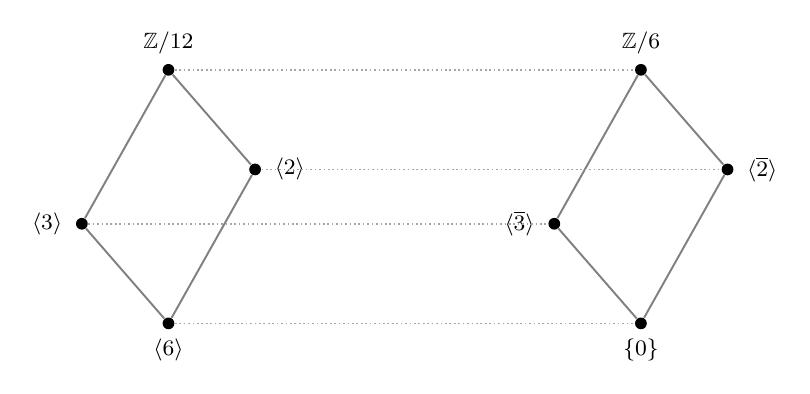
\begin{tikzpicture}[yscale=1.15,xscale=1.0]
  % ---- LEFT lattice: subgroups of Z/12 containing N=<6> ----
  \node[ltdot] (Lb)  at (0,0)   {};
  \node[ltdot] (L3)  at (-1.1,1.1) {};
  \node[ltdot] (L2)  at (1.1,1.7)  {};
  \node[ltdot] (Lt)  at (0,2.8)  {};
  \begin{scope}[ltedge]
    \draw (Lb)--(L3); \draw (Lb)--(L2);
    \draw (L3)--(Lt); \draw (L2)--(Lt);
  \end{scope}
  \node[ltlab,below=1.5pt of Lb] {$\gen{6}$};
  \node[ltlab,left=3pt of L3]    {$\gen{3}$};
  \node[ltlab,right=3pt of L2]   {$\gen{2}$};
  \node[ltlab,above=1.5pt of Lt] {$\Z/12$};
  % ---- RIGHT lattice: all subgroups of G/N = Z/6 ----
  \node[ltdot] (Rb)  at (6,0)   {};
  \node[ltdot] (R3)  at (4.9,1.1) {};
  \node[ltdot] (R2)  at (7.1,1.7) {};
  \node[ltdot] (Rt)  at (6,2.8)  {};
  \begin{scope}[ltedge]
    \draw (Rb)--(R3); \draw (Rb)--(R2);
    \draw (R3)--(Rt); \draw (R2)--(Rt);
  \end{scope}
  \node[ltlab,below=1.5pt of Rb] {$\{0\}$};
  \node[ltlab,left=3pt of R3]    {$\gen{\overline{3}}$};
  \node[ltlab,right=3pt of R2]   {$\gen{\overline{2}}$};
  \node[ltlab,above=1.5pt of Rt] {$\Z/6$};
  % ---- correspondence ties (equal heights) ----
  \begin{scope}[ltcorr]
    \draw (Lb)--(Rb);
    \draw (L3)--(R3);
    \draw (L2)--(R2);
    \draw (Lt)--(Rt);
  \end{scope}
\end{tikzpicture}\end{center}

\begin{dgx}
\dgi{Objects:} Two diamond lattices placed side by side. Left diamond: the four subgroups of
  $\Z/12\Z$ that contain $N=\gen{6}$, namely $\gen{6}$ (bottom), $\gen{3}$ (left), $\gen{2}$
  (right), and $\Z/12$ (top). Right diamond: all four subgroups of $G/N\isom\Z/6$, namely
  $\{0\}$ (bottom), $\gen{\overline{3}}\isom\Z/2$ (left), $\gen{\overline{2}}\isom\Z/3$
  (right), and $\Z/6$ (top). The horizontal ties connect matched pairs.
\dgi{Arrows:} Vertical edges within each diamond are subgroup inclusions (upward = larger
  subgroup). Horizontal tie-lines are the bijection $A\mapsto A/N$ of the Fourth Isomorphism
  Theorem (left to right) and its inverse $\overline{A}\mapsto\pi^{-1}(\overline{A})$ (right
  to left). Each tie connects $A$ on the left to $A/N$ on the right, realized as the image of
  $A$ under the canonical projection $\pi\colon\Z/12\to\Z/6$.
\dgi{What commutes:} Preservation of inclusion: if $A\sgr B$ upstairs (left edge), then
  $A/N\sgr B/N$ downstairs (right edge), so the tie-lines respect the heights of the rungs.
  Preservation of index: the index $\idx{B}{A}$ on the left equals $\idx{B/N}{A/N}$ on the
  right; e.g.\ $\idx{\gen{2}}{\gen{6}}=3$ left equals $\idx{\gen{\overline{2}}}{\{0\}}=3$
  right.
\dgi{Why it commutes:} For the inclusion: if $a\in A\sgr B$, then $a+N\in A/N\sgr B/N$,
  immediate. For the index: cosets of $A$ in $B$ biject with cosets of $A/N$ in $B/N$ via
  $\pi$ (since $N\sgr A$), giving equal indices.
\dgi{Why this matters here:} This picture makes the Fourth Isomorphism Theorem concrete: the
  student can verify by inspection that the two diamonds are identical in shape (isomorphic as
  lattices), that heights are preserved (no rung-crossings in the ties), and that the index
  along each left edge equals the index along the corresponding right edge. The picture
  replaces a proof with a visual check.
\dgi{Concrete example:} The diagram itself is the example: $G=\Z/12$, $N=\gen{6}$,
  $G/N\isom\Z/6$. The tie $\gen{3}\leftrightarrow\gen{\overline{3}}$ records that
  $\pi(\gen{3})=\gen{3}/\gen{6}$, which is the unique subgroup of order $2$ in $\Z/6$, namely
  $\gen{\overline{3}}$.
\dgi{Common pitfall:} Students sometimes try to include $\gen{4}$ or $\{0\}$ in the left
  diamond, forgetting the ``contains $N=\gen{6}$'' restriction. Neither $4$ nor $0$ generates
  a subgroup containing $6$, so they are invisible upstairs and have no tie-line. Attempting
  to draw ties for them would extend the left diamond below $\gen{6}$, which is outside the
  correspondence.
\dgi{Takeaway:} The point of this diagram is that the Fourth Isomorphism Theorem is not just
  an abstract bijection but a true lattice isomorphism: the two diamonds are mirror images of
  each other, with every inclusion, index, and normality relation intact across the tie-lines.
\end{dgx}

\noindent The bijection $A\mapsto A/N$ preserves inclusion and index: matched rungs have the
same shape and the index along each left edge equals the index along the tied right edge.
\end{wex}

\begin{wex}{Normal-subgroup lattice of $S_4/V$}
Let $G=S_4$, $N=V$ (Klein four, $V\nor S_4$, $|V|=4$), so $|G/N|=6$ and $S_4/V\isom S_3$.
Use the correspondence to find all \emph{normal} subgroups of $S_4/V$.
\wrec Fourth Iso Theorem, normality clause: normal subgroups of $S_4/V$
$\leftrightarrow$ normal subgroups of $S_4$ containing $V$.
\wsol The normal subgroups of $S_4$ are $\{e\}$, $V$, $A_4$, $S_4$. Those containing $V$ are
$V,A_4,S_4$. Under $\pi$ they correspond to:
\[V\to\{e\}\ (\text{order }1),\quad A_4\to A_4/V\ (\text{order }3),\quad
S_4\to S_4/V\ (\text{order }6).\]
So $S_4/V\isom S_3$ has exactly three normal subgroups, of orders $1,3,6$ -- precisely the
known normal subgroups $\{e\}\nor A_3\nor S_3$ of $S_3$. \emph{Check:} $S_3$'s only proper
nontrivial normal subgroup is $A_3$ (order $3$), matching $A_4/V$. The order-$2$ subgroups
$\gen{(12)}$-type of $S_3$ are \emph{not} normal; correspondingly, each pulls back to a
subgroup of order $2\cdot4=8$ in $S_4$ (index $24/8=3$) that is \emph{not} normal in $S_4$,
so it never appears in the normal-subgroup list. Good.
\end{wex}

\begin{wex}{Index preservation in $\Z/12\Z$}
With $G=\Z/12\Z$, $N=\gen6$ as above, verify $\idx{\gen2}{\gen6}=\idx{(\gen2/N)}{\{0\}}$ and
$\idx{G}{\gen3}=\idx{(G/N)}{(\gen3/N)}$.
\wrec Fourth Iso Theorem, index clause $\idx{B}{A}=\idx{B/N}{A/N}$.
\wsol Upstairs: $\gen2=\{0,2,4,6,8,10\}$ has order $6$, $\gen6=N$ has order $2$, so
$\idx{\gen2}{\gen6}=6/2=3$. Downstairs $\gen2/N$ has order $6/2=3$ and $N/N=\{0\}$ has order
$1$, so the index is $3/1=3$. Match. Next, $|G|=12$, $|\gen3|=|\{0,3,6,9\}|=4$, so
$\idx{G}{\gen3}=12/4=3$; downstairs $|G/N|=6$, $|\gen3/N|=4/2=2$, index $6/2=3$. Match.
\emph{Check:} both indices equal $3$ as the theorem guarantees. Good.
\end{wex}

\begin{wex}{Pulling back: $\pi^{-1}$ of a subgroup}
Let $G=\Z$, $N=12\Z$, so $G/N=\Z/12\Z$. Take $\overline A=\gen{4}=\{0,4,8\}\sgr\Z/12$.
Compute $\pi^{-1}(\overline A)$ and confirm it contains $N$.
\wrec Fourth Iso Theorem: the inverse correspondence $\overline A\mapsto\pi^{-1}(\overline
A)$ lands among subgroups of $\Z$ containing $12\Z$.
\wsol $\pi^{-1}(\overline A)=\{n\in\Z:n+12\Z\in\{0,4,8\}+12\Z\}=\{n:n\equiv0,4,\text{ or }8
\!\!\pmod{12}\}=4\Z$. Indeed $4\Z\supseteq12\Z=N$ (since $12\in4\Z$), as required. And
$\pi(4\Z)=4\Z/12\Z=\{0,4,8\}=\overline A$, confirming the round trip. \emph{Index check:}
$\idx{\Z}{4\Z}=4$ upstairs and $\idx{\Z/12}{\gen4}=12/3=4$ downstairs. \emph{Normality:}
both are abelian so all subgroups normal, consistent with clause (4). Good.
\end{wex}

\begin{pitfall}
The lattice correspondence sees \textbf{only} the subgroups of $G$ that contain $N$.
Subgroups not containing $N$ (e.g.\ a subgroup meeting $N$ trivially) are \emph{not} in the
correspondence; do not try to read them off the lattice of $G/N$. Also, $\pi^{-1}(\pi(A))=AN$
in general -- it equals $A$ only when $N\sgr A$. Forgetting the ``contains $N$'' restriction
is the most common error.
\end{pitfall}

%=====================================================================
\subsection*{Which theorem fits? A decision method}

\begin{method}{Choosing the right isomorphism theorem}
\begin{itemize}
\item \textbf{One homomorphism / one quotient, want $G/\ker\isom\im$:} First Iso Theorem.
\item \textbf{Two subgroups $A,B$ of one group; want the join $AB$, the product formula,
or to rewrite $AB/B$:} Second (Diamond) Theorem. Verify $A\sgr N_G(B)$.
\item \textbf{A quotient of a quotient $(G/N)/(M/N)$, or a chain $N\sgr M\sgr G$ of normals;
want to ``cancel'':} Third Theorem. Result $G/M$.
\item \textbf{Want \emph{all} subgroups / normal subgroups / indices of $G/N$, or to pull
subgroups of $G/N$ back to $G$:} Fourth (Lattice) Theorem. Work upstairs among subgroups
containing $N$.
\end{itemize}
\textbf{Tell-tale shapes:} ``$AB$'' or ``$A\cap B$'' $\Rightarrow$ Second; double slash
``$/\!\!/$'' i.e.\ $(\,\cdot/N)/(\cdot/N)$ $\Rightarrow$ Third; ``list every subgroup of a
quotient'' $\Rightarrow$ Fourth.
\end{method}

\begin{exers}{Exercises (from the text).}
\item Let $F$ be a finite field of order $q$ and let $n$ be a positive integer. Prove that $\idx{\GL_n(F)}{\SL_n(F)} = q-1$. [See Exercise 35, Section 1.]

\item Prove all parts of the Lattice Isomorphism Theorem (Theorem 20).

\item Prove that if $H$ is a normal subgroup of $G$ of prime index $p$ then for all $K \le G$ either
  \begin{enumerate}
  \item $K \le H$ or
  \item $G = HK$ and $\idx{K}{K \cap H} = p$.
  \end{enumerate}

\item Let $C$ be a normal subgroup of the group $A$ and let $D$ be a normal subgroup of the group $B$. Prove that $(C \times D) \nor (A \times B)$ and $(A \times B)/(C \times D) \isom (A/C) \times (B/D)$.

\item Let $QD_{16} = \gen{\sigma, \tau}$ be the quasidihedral group of order 16 described in Exercise 11 of Section 2.5. Prove that $\gen{\sigma^4}$ is normal in $QD_{16}$ and use the Lattice Isomorphism Theorem to draw the lattice of subgroups of $QD_{16}/\gen{\sigma^4}$. Which group of order 8 has the same lattice as this quotient? Use generators and relations for $QD_{16}/\gen{\sigma^4}$ to decide the isomorphism type of this group.

\item Let $M = \gen{v, u}$ be the modular group of order 16 described in Exercise 14 of Section 2.5. Prove that $\gen{v^4}$ is normal in $M$ and use the Lattice Isomorphism Theorem to draw the lattice of subgroups of $M/\gen{v^4}$. Which group of order 8 has the same lattice as this quotient? Use generators and relations for $M/\gen{v^4}$ to decide the isomorphism type of this group.

\item Let $M$ and $N$ be normal subgroups of $G$ such that $G = MN$. Prove that $G/(M \cap N) \isom (G/M) \times (G/N)$. [Draw the lattice.]

\item Let $p$ be a prime and let $G$ be the group of $p$-power roots of $1$ in $\C$ (cf. Exercise 18, Section 2.4). Prove that the map $z \mapsto z^p$ is a surjective homomorphism. Deduce that $G$ is isomorphic to a proper quotient of itself.

\item Let $p$ be a prime and let $G$ be a group of order $p^a m$, where $p$ does not divide $m$. Assume $P$ is a subgroup of $G$ of order $p^a$ and $N$ is a normal subgroup of $G$ of order $p^b n$, where $p$ does not divide $n$. Prove that $|P \cap N| = p^b$ and $|PN/N| = p^{a-b}$. (The subgroup $P$ of $G$ is called a \emph{Sylow $p$-subgroup} of $G$. This exercise shows that the intersection of any Sylow $p$-subgroup of $G$ with a normal subgroup $N$ is a Sylow $p$-subgroup of $N$.)

\item Generalize the preceding exercise as follows. A subgroup $H$ of a finite group $G$ is called a \emph{Hall subgroup} of $G$ if its index in $G$ is relatively prime to its order: $(\idx{G}{H}, |H|) = 1$. Prove that if $H$ is a Hall subgroup of $G$ and $N \nor G$, then $H \cap N$ is a Hall subgroup of $N$ and $HN/N$ is a Hall subgroup of $G/N$.
\end{exers}

\begin{exers}{Practice problems (additional).}
\item Let $G=\Z$ and $H=12\Z$, $K=3\Z$. Verify $H\le K$, both $\nor G$, and confirm the Third Isomorphism Theorem by computing $\ord{(G/H)/(K/H)}$ and $\ord{G/K}$ directly and checking they agree.

\item In $G=\Zn{24}$ let $H=\gen{8}$ and $K=\gen{4}$. List the elements of $H$ and $K$, check $H\le K\le G$, and identify $(G/H)/(K/H)$ as a familiar group.

\item Let $\varphi:\Z\to\Zn{6}$ be reduction mod $6$ and let $N=2\Z$. Compute $\im\varphi$, $\ker\varphi$, and $\varphi(N)$; then state which quotient $\varphi$ induces an isomorphism onto.

\item Let $\varphi:\R\to\C^{\times}$ be $\varphi(x)=e^{2\pi i x}$. Show $\varphi$ is a homomorphism, compute $\ker\varphi$ and $\im\varphi$, and use the First Isomorphism Theorem to identify $\R/\Z$.

\item Let $G=\GL_2(\R)$ and let $\varphi=\det:G\to\R^{\times}$. Identify $\ker\varphi$, prove it is normal, and state the isomorphism the First Isomorphism Theorem gives for $G/\SL_2(\R)$.

\item In $D_8$ (with $r^4=s^2=1$, $sr=r\inv s$) let $Z=\gen{r^2}$. Show $Z\nor D_8$, list the four cosets of $Z$, write the multiplication table of $D_8/Z$, and identify the quotient up to isomorphism.

\item Let $G=Q_8=\{\pm1,\pm i,\pm j,\pm k\}$ and $N=\{\pm1\}$. Show $N\nor G$, list the cosets of $N$, and identify $G/N$.

\item Let $A=\gen{(1\,2)(3\,4)}$ and $B=\gen{(1\,3)(2\,4)}$ inside $V=\{e,(1\,2)(3\,4),(1\,3)(2\,4),(1\,4)(2\,3)\}\le A_4$. Compute $A\cap B$, $AB$, $\ord{AB}$, and verify the Second Isomorphism Theorem count $\ord{AB}=\dfrac{\ord{A}\,\ord{B}}{\ord{A\cap B}}$.

\item Let $G=\Zn{4}\times\Zn{2}$, $A=\Zn{4}\times\{0\}$, $B=\{0\}\times\Zn{2}$, viewed additively. Treating $B\nor G$, compute $A\cap B$, $A+B$, and verify $(A+B)/B\isom A/(A\cap B)$ by identifying both sides.

\item Let $\varphi:\Zn{12}\to\Zn{4}$ send $1\mapsto 1$. Compute $\ker\varphi$ and $\im\varphi$, verify $\ker\varphi\nor\Zn{12}$, and confirm $\Zn{12}/\ker\varphi\isom\im\varphi$ by comparing orders.

\item Let $N=\gen{r}\nor D_8$. Use the Fourth (Lattice) Isomorphism Theorem to list all subgroups of $D_8/N$ and the corresponding subgroups of $D_8$ containing $N$.

\item Let $G=\Zn{30}$ and $N=\gen{6}=\{0,6,12,18,24\}$. List the subgroups of $G/N$ via the lattice correspondence, naming the subgroup of $G$ that each one pulls back to.

\item Compute the sign of each permutation and give a composition series step for $S_4$: write $\sgn$ of $(1\,2\,3)$, $(1\,2\,3\,4)$, and $(1\,2)(3\,4)$, then verify the chain $S_4\rhd A_4\rhd V\rhd \gen{(1\,2)(3\,4)}\rhd 1$ has each term normal in the previous one.

\item For the series in the previous problem, compute each factor group $S_4/A_4$, $A_4/V$, $V/\gen{(1\,2)(3\,4)}$, $\gen{(1\,2)(3\,4)}/1$ and confirm that $S_4$ is solvable by checking all factors are abelian.

\item Let $\pi:G\to G/N$ be the natural projection. If $\idx{G}{N}=15$ and $H\le G$ with $N\le H$ and $\idx{G}{H}=5$, compute $\idx{(G/N)}{(H/N)}$ and $\ord{H/N}$, justifying each step by the Third/Fourth Isomorphism Theorems.

\item Let $G=\Zn{2}\times\Zn{2}\times\Zn{2}$ and $N=\gen{(1,1,0)}$. Compute $\ord{G/N}$, list its elements as cosets, and identify $G/N$ up to isomorphism.

\end{exers}

\begin{exers}{Additional exercises.}
\item Let $H,K\nor G$ with $H\le K$. Prove directly from the definition of cosets that the map $\overline{\varphi}:G/H\to G/K$, $gH\mapsto gK$, is a well-defined surjective homomorphism with kernel $K/H$, recovering the Third Isomorphism Theorem.

\item Let $G$ be a group, $H\sgr G$, and $N\nor G$. Prove the Second Isomorphism Theorem in full: show $HN\sgr G$, $N\nor HN$, $H\cap N\nor H$, and that $HN/N\isom H/(H\cap N)$.

\item Let $\varphi:G\to G'$ be a surjective homomorphism with kernel $K$. Prove that there is an inclusion-preserving bijection between subgroups of $G$ containing $K$ and subgroups of $G'$, and that this bijection sends normal subgroups to normal subgroups (the Lattice Isomorphism Theorem).

\item Let $G=S_3\times \Zn{2}$. Find all normal subgroups of $G$ and, for each, identify the quotient $G/N$ up to isomorphism. Use the isomorphism theorems to justify your identifications.

\item Let $N\nor G$ with $G/N$ abelian. Prove that the commutator subgroup $G'=[G,G]$ satisfies $G'\le N$. Deduce that $G/G'$ is the largest abelian quotient (the abelianization), and compute $G'$ and $G/G'$ for $G=D_8$.

\item Suppose $G$ has a composition series with factors all isomorphic to $\Zn{p}$ for a fixed prime $p$. Prove $\ord{G}=p^n$ where $n$ is the length, and conversely exhibit such a series for $G=\Zn{p^n}$.

\end{exers}

\begin{exers}{Commutative-diagram exercises.}
\item Let $\varphi:G\to H$ be a homomorphism and $\pi:G\to G/\ker\varphi$ the natural projection. Fill in the unique induced map and prove the triangle commutes:
\[\begin{tikzcd}[row sep=large,column sep=large]
G \arrow[r, "\varphi"] \arrow[d, two heads, "\pi"'] & H \\
G/\ker\varphi \arrow[ur, dashed, hook, "\overline{\varphi}"'] &
\end{tikzcd}\]
Show $\overline{\varphi}(g\ker\varphi)=\varphi(g)$ is well-defined and that $\overline{\varphi}$ is an isomorphism onto $\im\varphi$.

\item For $\varphi:G\to H$ a homomorphism, complete the short exact sequence by naming the two outer maps and proving exactness at $G$ and at $\im\varphi$:
\[\begin{tikzcd}[column sep=normal]
1 \arrow[r] & \ker\varphi \arrow[r, hook] & G \arrow[r, two heads, "\varphi"] & \im\varphi \arrow[r] & 1
\end{tikzcd}\]
Then specialize to $\varphi=\det:\GL_2(\R)\to\R^{\times}$ and write the resulting sequence explicitly.

\item Let $H\sgr G$ and $N\nor G$. Label every arrow as an inclusion (hook) or quotient and prove the diamond exhibits the Second Isomorphism Theorem, i.e. that the quotients along the two parallel edges $N\sgr HN$ and $H\cap N\sgr H$ are isomorphic, $HN/N\isom H/(H\cap N)$:
\[\begin{tikzcd}[row sep=large,column sep=large]
& HN & \\
H \arrow[ur, hook] & & N \arrow[ul, hook'] \\
& H\cap N \arrow[ul, hook] \arrow[ur, hook'] &
\end{tikzcd}\]

\item With $H\le K$ both normal in $G$, the Third Isomorphism Theorem says the composite of projections factors as below. Supply the dashed map and prove the square-with-diagonal commutes:
\[\begin{tikzcd}[row sep=large,column sep=large]
G/H \arrow[r, two heads, "\overline{\varphi}"] \arrow[dr, two heads] & G/K \\
& (G/H)/(K/H) \arrow[u, dashed, "\isom"']
\end{tikzcd}\]
Identify $\overline{\varphi}$, its kernel, and the isomorphism realizing $(G/H)/(K/H)\isom G/K$.

\item Take $G=\Zn{12}$, $K=\gen{2}$, $H=\gen{6}$, so $H\le K\nor G$. Draw the lattice-correspondence diagram of the subgroups of $G$ containing $H$ versus the subgroups of $G/H$, labeling each horizontal arrow with the quotient map, and verify that $(G/H)/(K/H)\isom G/K$ by computing the orders of all three quotients:
\[\begin{tikzcd}[row sep=large,column sep=large]
G \arrow[r, two heads, "\pi"] & G/H \\
K \arrow[u, hook] \arrow[r, two heads] & K/H \arrow[u, hook']
\end{tikzcd}\]

\end{exers}


\section{Composition Series and the H\"older Program}
\subsection*{Composition Series, Jordan--Holder, and Solvable Groups}

This section organizes a finite group into ``smallest reasonable pieces'' and records
(via the Jordan--Holder theorem below) that the multiset of those pieces is an invariant of
the group. The pieces are simple groups,
and the assembly data is a chain of subgroups, each normal in the next. Two large results
are quoted (their proofs are beyond the scope of this section): the Jordan--Holder theorem
and the simplicity of $A_n$ for $n\ge 5$.

\begin{definition}[Subnormal series]
A \emph{subnormal series} for a group $G$ is a chain of subgroups
\[
1=N_0\nor N_1\nor N_2\nor\cdots\nor N_{k-1}\nor N_k=G,
\]
where each $N_i\nor N_{i+1}$ (each term normal in the \emph{next}, not necessarily in $G$).
The quotients $N_{i+1}/N_i$ are the \emph{factors} of the series, and $k$ is its
\emph{length}. We always allow ourselves to delete a repeated term $N_i=N_{i+1}$
(equivalently, drop trivial factors).
\end{definition}

\begin{remark}
``Subnormal'' is genuinely weaker than ``normal.'' In $D_8$ the chain
$1\nor\gen{s}\nor\gen{s,r^2}\nor D_8$ is subnormal, but $\gen{s}$ is \emph{not} normal in
$D_8$ (since $rsr\inv=sr^2\notin\gen{s}$). Each step is normal only in the
\emph{immediately} larger group: $\gen{s}\nor\gen{s,r^2}$ because $[\gen{s,r^2}:\gen{s}]=2$.
\end{remark}

\begin{definition}[Composition series]
A subnormal series
\[
1=N_0\nor N_1\nor\cdots\nor N_k=G
\]
is a \emph{composition series} if every factor $N_{i+1}/N_i$ is a \emph{simple} group
(no proper nontrivial normal subgroups; see the definition below). The factors
$N_{i+1}/N_i$ are then called the \emph{composition factors} of $G$.
\end{definition}

\begin{theorem}[Existence]
Every nontrivial finite group has a composition series.
\end{theorem}

\begin{proof}
Induct on $|G|$. If $G$ is simple, then $1\nor G$ is a composition series. Otherwise pick
a \emph{maximal} proper normal subgroup $M\pnor G$ (one exists since $G$ is finite and
$1\pnor G$ is a proper normal subgroup, so the nonempty finite set of proper normal
subgroups has a maximal element). By the Lattice Isomorphism (Correspondence) Theorem the
normal subgroups of $G/M$ correspond to normal subgroups of $G$ between $M$ and $G$;
maximality of $M$ says there are none strictly between, so $G/M$ is simple. Since
$|M|<|G|$, by induction $M$ has a composition series
$1=N_0\nor\cdots\nor N_{r}=M$; appending $G$ gives
$1=N_0\nor\cdots\nor N_r=M\nor G$ with all factors simple. \qedhere
\end{proof}

\begin{definition}[Simple group]
A group $G\ne 1$ is \emph{simple} if its only normal subgroups are $1$ and $G$.
\end{definition}

\begin{proposition}[Abelian simple groups]
An abelian group is simple if and only if it is $\Zn{p}$ (cyclic of prime order $p$).
\end{proposition}

\begin{proof}
In an abelian group every subgroup is normal, so simplicity means: the only subgroups are
$1$ and $G$. If $G=\Zn{p}$ with $p$ prime, Lagrange forces every subgroup to have order
$1$ or $p$, so $G$ is simple. Conversely, if abelian $G$ is simple, take $1\ne x\in G$;
then $\gen{x}$ is a nontrivial subgroup, hence $\gen{x}=G$, so $G$ is cyclic. If $G$ were
infinite cyclic ($\isom\Z$) it would contain $2\Z\ne 1,G$; if $|G|=n$ were composite with
$1<d<n$ a divisor, the unique subgroup of order $d$ would be proper nontrivial. So
$|G|=p$ is prime, $G\isom\Zn{p}$. \qedhere
\end{proof}

\begin{theorem}[Simplicity of $A_n$; stated]
The alternating group $A_n$ is simple for every $n\ge 5$. In particular $A_5$ (order $60$)
is a nonabelian simple group, the smallest one.
\end{theorem}

\begin{proof}[Sketch]
For $n\ge 5$ one shows $A_n$ is generated by $3$-cycles, that all $3$-cycles are conjugate
in $A_n$ (using $n\ge 5$ to find an \emph{even} conjugating permutation), and that any
nontrivial normal subgroup $N\nor A_n$ must contain a $3$-cycle. From the last point and
conjugacy, $N$ contains every $3$-cycle, hence $N=A_n$. The crux is the third step:
analyzing the cycle type of a non-identity $\sigma\in N$ and forming a suitable commutator
$\sigma\tau\sigma\inv\tau\inv\in N$ that simplifies to a $3$-cycle. (Full details: D\&F
Section 4.6. We use only the \emph{statement}.) For $n=4$ this fails:
$V=\{1,(12)(34),(13)(24),(14)(23)\}\nor A_4$ is a proper nontrivial normal subgroup, so
$A_4$ is \emph{not} simple. \qedhere
\end{proof}

\begin{theorem}[Jordan--Holder; stated]
Let $G\ne 1$ be a finite group. Then:
\begin{enumerate}
\item[\textup{(1)}] $G$ has a composition series; and
\item[\textup{(2)}] the composition factors are \emph{unique}: if
\[
1=N_0\nor N_1\nor\cdots\nor N_r=G
\quad\text{and}\quad
1=M_0\nor M_1\nor\cdots\nor M_s=G
\]
are two composition series, then $r=s$ and there is a permutation $\pi$ of
$\{1,\dots,r\}$ with
\[
N_{i}/N_{i-1}\ \isom\ M_{\pi(i)}/M_{\pi(i)-1}\qquad(1\le i\le r).
\]
That is, the \emph{length} and the \emph{multiset of factors} (up to isomorphism) are
invariants of $G$.
\end{enumerate}
\end{theorem}

\begin{proof}[Sketch]
Part (1) is the existence theorem above. Part (2) is proved by induction on $|G|$ using the
\emph{Schreier refinement} idea: any two subnormal series of $G$ have refinements that are
\emph{equivalent} (same multiset of nontrivial factors), which follows from the
\emph{Zassenhaus (butterfly) lemma}. A composition series admits no proper refinement (its
factors are already simple), so the two given series are already equivalent. Concretely the
induction compares the top factors $G/N_{r-1}$ and $G/M_{s-1}$: if $N_{r-1}=M_{s-1}$ apply
the inductive hypothesis to that subgroup; otherwise $N_{r-1}M_{s-1}=G$ and one matches the
two top factors across the diamond
$N_{r-1}/(N_{r-1}\cap M_{s-1})\isom G/M_{s-1}$ and
$M_{s-1}/(N_{r-1}\cap M_{s-1})\isom G/N_{r-1}$ (Second Isomorphism Theorem), then induct on
the common subgroup $N_{r-1}\cap M_{s-1}$. (D\&F outline a full proof in the exercises of their Section 3.4; see Exercises 6, 9 and
10 at the end of this section.) \qedhere
\end{proof}

\begin{remark}[A composition series is NOT a factorization]
Jordan--Holder records the factors but \emph{not} how they are assembled.
$\Zn{4}$ and $\Zn{2}\times\Zn{2}$ have the \emph{same} composition factors
($\Zn 2,\Zn 2$) yet are non-isomorphic; likewise $\Zn 6$ and $S_3$ both have factors
$\Zn 2,\Zn 3$. The extension problem ``which $G$ have a given factor multiset'' is exactly
the hard half of the Holder program below.
\end{remark}

\begin{method}{Building a composition series and reading off its factors}
\textbf{Trigger.} You are asked for a composition series / composition factors of a
specific finite group, or to verify a given chain is a composition series.\\[2pt]
\textbf{Recipe.}
\begin{enumerate}
\item Top-down: find a maximal normal subgroup $M\pnor G$ (so $G/M$ is simple). Repeat
inside $M$. Each chosen step gives one simple factor $G/M$.
\item Bottom-up (often easier for small groups): start at $1$, climb by prime-index
normal steps. A step $N_i\nor N_{i+1}$ of \emph{prime index} $p$ has factor
$N_{i+1}/N_i\isom\Zn p$ automatically (order $p$ is simple). For abelian groups every
step is automatically normal; in general a subgroup of index $2$ is always normal, but a
prime index $p\ge 3$ does \emph{not} by itself force normality.
\item Factor of each step $=$ quotient $N_{i+1}/N_i$; identify it by its order. Order $p$
prime $\Rightarrow\Zn p$. A nonabelian simple step (e.g. $A_5$) is read off as that group.
\item \textbf{Check} (Jordan--Holder sanity): $\prod_i |N_{i+1}/N_i|=|G|$, and every factor
is simple. The multiset of factors must not depend on which maximal steps you chose.
\end{enumerate}
\end{method}

\begin{wex}{Composition series of $\Zn{12}$}
Give a composition series of $\Zn{12}$ and list its composition factors.
\wrec Bottom-up via prime-index steps: $12=2\cdot 2\cdot 3$, so build a chain whose
successive indices are these primes.
\wsol Work additively in $\Zn{12}=\{0,1,\dots,11\}$. The subgroups are exactly the
$\gen{d}$ for $d\mid 12$, with $\gen{d}$ of order $12/\gcd(d,12)$; here $\gen{6}$ has
order $2$ and $\gen{3}$ has order $4$. One chain:
\[
0\ \nor\ \gen{6}\ \nor\ \gen{3}\ \nor\ \Zn{12},
\]
with $|\gen{6}|=2$, $|\gen{3}|=4$ (note $6=2\cdot 3\in\gen 3$, so $\gen6\le\gen3$).
All subgroups of an abelian group are normal, so this is subnormal. Factors and their
orders:
\[
\gen{6}/0\isom\Zn 2,\quad
\gen{3}/\gen{6}\ \text{has order } 4/2=2\isom\Zn 2,\quad
\Zn{12}/\gen{3}\ \text{has order } 12/4=3\isom\Zn 3.
\]
Each factor is of prime order, hence simple. So this is a composition series, with factors
\[\boxed{\Zn 2,\ \Zn 2,\ \Zn 3}.\]
\emph{Check.} $2\cdot 2\cdot 3=12=|\Zn{12}|$. A \emph{different} chain
$0\nor\gen 4\nor\gen 2\nor\Zn{12}$ (with $|\gen4|=3$, $|\gen2|=6$) has indices $3,2,2$,
giving factors $\Zn 3,\Zn 2,\Zn 2$ --- the same multiset, as Jordan--Holder requires.

Both chains are vertical towers, each rung labeled by its composition factor; the two
\emph{differ in the order} of the factors but produce the \emph{same multiset}
$\{\Zn2,\Zn2,\Zn3\}$ --- exactly the Jordan--Holder invariance.
\begin{center}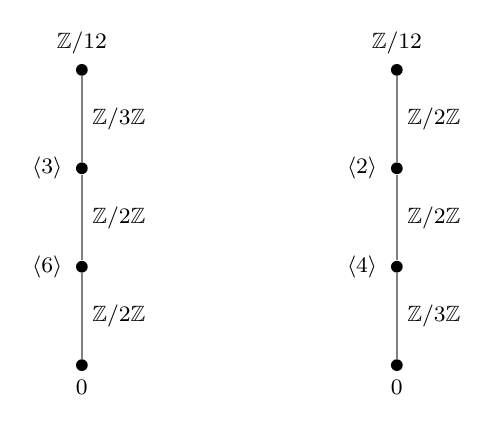
\begin{tikzpicture}[yscale=1.25,xscale=1.0]
  % ---- chain 1:  0 <| <6> <| <3> <| Z/12  (orders 1,2,4,12) ----
  \node[ltdot] (Ab) at (0,0) {};
  \node[ltdot] (A6) at (0,1) {};
  \node[ltdot] (A3) at (0,2) {};
  \node[ltdot] (At) at (0,3) {};
  \begin{scope}[ltedge]
    \draw (Ab)--(A6); \draw (A6)--(A3); \draw (A3)--(At);
  \end{scope}
  \node[ltlab,below=1.5pt of Ab] {$0$};
  \node[ltlab,left=3pt of A6]    {$\gen{6}$};
  \node[ltlab,left=3pt of A3]    {$\gen{3}$};
  \node[ltlab,above=1.5pt of At] {$\Z/12$};
  \node[ltlab,right=2pt of $(Ab)!0.5!(A6)$] {$\Zn 2$};
  \node[ltlab,right=2pt of $(A6)!0.5!(A3)$] {$\Zn 2$};
  \node[ltlab,right=2pt of $(A3)!0.5!(At)$] {$\Zn 3$};
  % ---- chain 2:  0 <| <4> <| <2> <| Z/12  (orders 1,3,6,12) ----
  \node[ltdot] (Bb) at (4,0) {};
  \node[ltdot] (B4) at (4,1) {};
  \node[ltdot] (B2) at (4,2) {};
  \node[ltdot] (Bt) at (4,3) {};
  \begin{scope}[ltedge]
    \draw (Bb)--(B4); \draw (B4)--(B2); \draw (B2)--(Bt);
  \end{scope}
  \node[ltlab,below=1.5pt of Bb] {$0$};
  \node[ltlab,left=3pt of B4]    {$\gen{4}$};
  \node[ltlab,left=3pt of B2]    {$\gen{2}$};
  \node[ltlab,above=1.5pt of Bt] {$\Z/12$};
  \node[ltlab,right=2pt of $(Bb)!0.5!(B4)$] {$\Zn 3$};
  \node[ltlab,right=2pt of $(B4)!0.5!(B2)$] {$\Zn 2$};
  \node[ltlab,right=2pt of $(B2)!0.5!(Bt)$] {$\Zn 2$};
\end{tikzpicture}\end{center}
\noindent Orders climb $1,2,4,12$ on the left and $1,3,6,12$ on the right; the edge labels are
the successive quotients, and both towers list $\Zn2,\Zn2,\Zn3$.
\end{wex}

\begin{wex}{Composition series of $D_8$}
Give a composition series of the dihedral group $D_8=\gen{r,s\mid r^4=s^2=1,\ sr=r\inv s}$
(order $8$) and list its factors.
\wrec $|D_8|=8=2^3$ is a $2$-group; every step will have index $2$, hence factor $\Zn 2$.
A subgroup of index $2$ is automatically normal, so any chain $1\nor H_1\nor H_2\nor D_8$
with successive indices $2$ is a composition series.
\wsol Take $Z=\gen{r^2}$ (the center, order $2$) and $\gen r$ (the rotation subgroup,
order $4$, index $2$ hence normal):
\[
1\ \nor\ \gen{r^2}\ \nor\ \gen{r}\ \nor\ D_8.
\]
Indices: $[\gen{r^2}:1]=2$, $[\gen r:\gen{r^2}]=4/2=2$, $[D_8:\gen r]=8/4=2$. Each step has
index $2$, so each smaller subgroup is normal in the next and each factor is
$\isom\Zn 2$. Factors: $\boxed{\Zn 2,\ \Zn 2,\ \Zn 2}$.
\emph{Check.} $2^3=8=|D_8|$. A different composition series uses the subnormal (not normal
in $D_8$!) chain $1\nor\gen s\nor\gen{s,r^2}\nor D_8$: indices $2,2,2$, again factors
$\Zn2,\Zn2,\Zn2$. Same multiset.
\end{wex}

\begin{pitfall}
Composition factors do \emph{not} pin down the group. $D_8$, $\Zn 8$, $\Zn 4\times\Zn 2$,
$\Zn 2^3$, and $Q_8$ are five \emph{non-isomorphic} groups of order $8$, and all have
composition factors $\Zn 2,\Zn 2,\Zn 2$. Equal factor multiset $\ne$ isomorphic group.
\end{pitfall}

\begin{definition}[Solvable group]
A finite group $G$ is \emph{solvable} if it has a subnormal series
\[
1=N_0\nor N_1\nor\cdots\nor N_k=G
\]
all of whose factors $N_{i+1}/N_i$ are \emph{abelian}. Equivalently (for finite $G$) every
composition factor is abelian, hence (composition factors are simple) every composition
factor is $\isom\Zn p$ for some prime $p$.
\end{definition}

\begin{remark}[Equivalent tests for finite $G$]
For a finite group the following are equivalent:
(i) $G$ is solvable;
(ii) $G$ has a subnormal series with abelian factors;
(iii) every composition factor of $G$ is cyclic of prime order;
(iv) the derived series $G\supseteq G'\supseteq G''\supseteq\cdots$ reaches $1$, where
$G'=[G,G]$ is the commutator subgroup and $G^{(n+1)}=[G^{(n)},G^{(n)}]$. We use (i)--(iii)
below; (iv) is the ``derived series'' formulation.
\end{remark}

\begin{proposition}[Nonabelian simple $\Rightarrow$ not solvable]
If $G$ is a nonabelian simple group then $G$ is not solvable. In particular $A_5$ is not
solvable.
\end{proposition}

\begin{proof}
A nonabelian simple group $G$ has exactly one composition series, $1\nor G$, whose only
factor is $G/1\isom G$ --- nonabelian. By Jordan--Holder these are the composition factors,
and at least one (the only one) is nonabelian, so by the test (iii) above $G$ is not
solvable. \qedhere
\end{proof}

\begin{method}{Testing solvability}
\textbf{Trigger.} ``Is $G$ solvable?'' or ``find a solvable/composition series.''\\[2pt]
\textbf{Recipe.}
\begin{enumerate}
\item Try to build a subnormal series with \emph{abelian} factors (prime-order factors are
automatically abelian). If you succeed, $G$ is solvable.
\item Shortcut to ``yes'': $G$ abelian $\Rightarrow$ solvable; $|G|=p^a$ a prime power
$\Rightarrow$ solvable; $|G|=pq,\,p^2q,\dots$ small orders are solvable (Sylow/Burnside).
\item Shortcut to ``no'': if $G$ has \emph{any} composition factor that is nonabelian
simple (e.g.\ $G$ contains a subnormal copy of $A_5$ as a factor, or $G$ is itself
nonabelian simple), then $G$ is NOT solvable.
\item \textbf{Check.} Multiply factor orders to recover $|G|$; confirm each factor is
$\Zn p$ (solvable) or spot a nonabelian simple factor (not solvable).
\end{enumerate}
\end{method}

\begin{wex}{$S_3$ is solvable}
Show $S_3$ (order $6$) is solvable and give a composition series.
\wrec $A_3\nor S_3$ with index $2$, and $A_3$ has prime order $3$: both factors will be
prime-order, hence abelian.
\wsol Use
\[
1\ \nor\ A_3\ \nor\ S_3 ,\qquad A_3=\gen{(123)}\isom\Zn 3 .
\]
Here $A_3\nor S_3$ (index $2$), and $1\nor A_3$ trivially. Factors:
$A_3/1\isom\Zn 3$ and $S_3/A_3\isom\Zn 2$. Both abelian (indeed simple of prime order), so
$S_3$ is solvable; this is also its composition series, factors $\boxed{\Zn 3,\ \Zn 2}$.
\emph{Check.} $3\cdot 2=6=|S_3|$. (Derived-series view: $S_3'=A_3$, $A_3'=1$, so the derived
series $S_3\supset A_3\supset 1$ reaches $1$ --- consistent.)
\end{wex}

\begin{wex}{$S_4$ is solvable}
Show $S_4$ (order $24$) is solvable by exhibiting a subnormal series with abelian factors.
\wrec $S_4\supset A_4\supset V\supset \gen{(12)(34)}\supset 1$, where
$V=\{1,(12)(34),(13)(24),(14)(23)\}$ is the Klein four-group. Indices $2,3,2,2$ are prime,
so all factors are prime-order abelian.
\wsol Take
\[
1\ \nor\ \gen{(12)(34)}\ \nor\ V\ \nor\ A_4\ \nor\ S_4 .
\]
Normality and indices:
\begin{itemize}
\item $V\nor A_4$ and $V\nor S_4$ ($V$ is the union of $1$ and all three
$(2,2)$-cycles, a full conjugacy-class-closed set; $|V|=4$).
\item $\gen{(12)(34)}\nor V$: $V$ is abelian (Klein four), so every subgroup is normal;
$[V:\gen{(12)(34)}]=4/2=2$.
\item Indices up the chain: $[\gen{(12)(34)}:1]=2$, $[V:\gen{(12)(34)}]=2$,
$[A_4:V]=12/4=3$, $[S_4:A_4]=24/12=2$.
\end{itemize}
Factors: $\Zn 2,\ \Zn 2,\ \Zn 3,\ \Zn 2$, all of prime order, hence abelian and simple.
So $S_4$ is solvable, and this is in fact a composition series. Factors
$\boxed{\Zn 2,\ \Zn 2,\ \Zn 3,\ \Zn 2}$.
\emph{Check.} $2\cdot 2\cdot 3\cdot 2=24=|S_4|$. \checkmark
\end{wex}

\begin{wex}{$S_5$ is NOT solvable}
Show $S_5$ (order $120$) is not solvable.
\wrec $A_5\nor S_5$ with $A_5$ nonabelian simple (stated theorem). A nonabelian simple
composition factor blocks solvability.
\wsol The chain $1\nor A_5\nor S_5$ has $A_5\nor S_5$ of index $2$. Since $A_5$ is
\emph{simple}, its only composition series is $1\nor A_5$, so a composition series of $S_5$
is
\[
1\ \nor\ A_5\ \nor\ S_5,
\]
with factors $A_5/1\isom A_5$ and $S_5/A_5\isom\Zn 2$. By Jordan--Holder these (up to order
and isomorphism) are \emph{the} composition factors of $S_5$. The factor $A_5$ is
nonabelian --- for instance $(123)$ and $(124)$ lie in $A_5$ but do not commute, since
$(123)(124)=(13)(24)$ while $(124)(123)=(14)(23)$ --- hence $A_5$ is not of prime order.
By the solvability test, $S_5$ is \emph{not} solvable.
\emph{Check.} $|A_5|\cdot|\Zn 2|=60\cdot 2=120=|S_5|$, and exactly one factor ($A_5$) is
nonabelian simple. More generally $S_n$ and $A_n$ are not solvable for all $n\ge 5$, since
$A_n$ is then a nonabelian simple composition factor.
\end{wex}

\begin{wex}{Read the composition factors off a chain}
A finite group $G$ has the subnormal series
\[
1\ \nor\ \gen{12}\ \nor\ \gen{4}\ \nor\ \Zn{60}=:G,
\]
where $G=\Zn{60}$ and the displayed terms have orders $1,5,15,60$. List the composition
factors and decide solvability.
\wrec Read each factor as the quotient of consecutive orders; a prime-order quotient is
$\Zn p$. Then apply the solvability test (all prime-order $\Rightarrow$ solvable).
\wsol Work additively in $\Zn{60}$. Here $\gen{12}=\{0,12,24,36,48\}$ has order $5$, and
$\gen{4}$ has order $15$ (with $12=3\cdot 4\in\gen 4$, so $\gen{12}\le\gen{4}$); all
subgroups are normal since $\Zn{60}$ is abelian. The successive orders are $1,5,15,60$, so
the factor orders are
\[
5/1=5,\qquad 15/5=3,\qquad 60/15=4 .
\]
A factor of order $5$ is $\Zn 5$ and of order $3$ is $\Zn 3$ (prime, simple). The top
factor has order $4$, which is \emph{not} prime --- but a composition factor must be
\emph{simple}, and there is no simple group of order $4$
($\Zn 4$ and $\Zn 2\times\Zn 2$ are both non-simple). Hence the displayed chain is
\emph{not} a composition series as written: the top step must be refined. Inserting the
intermediate subgroup $\gen{2}$ of order $30$ between $\gen{4}$ and $\Zn{60}$ splits the
order-$4$ gap into two order-$2$ steps ($[\gen2:\gen4]=30/15=2$, $[\Zn{60}:\gen2]=60/30=2$),
giving genuine factors
\[
\boxed{\Zn 5,\ \Zn 3,\ \Zn 2,\ \Zn 2}.
\]
All factors are prime-order abelian, so $G$ is solvable.
\emph{Check.} $5\cdot 3\cdot 2\cdot 2=60=|G|$. \checkmark The lesson: every gap in a
\emph{composition} series must be a \emph{simple} group; for an abelian (more generally, a
solvable) group this means \emph{prime} order, so a non-prime gap signals a missing
refinement.
\end{wex}

\begin{pitfall}
A factor of prime power order need not be simple. In a composition series each
\emph{factor} (quotient) must be \emph{simple}; it has \emph{prime} order exactly when it is
abelian, as always happens for a solvable group, but a factor may also be nonabelian simple
(e.g.\ $A_5$ in the composition series $1\nor A_5\nor S_5$). If you write a chain whose
successive indices include a $4$, $6$, $8$, or $9$, it is a subnormal series but \emph{not} a
composition series (no simple group has any of these orders) --- refine it until every
factor is simple.
\end{pitfall}

\subsection*{The subnormal series as a vertical chain, and two diagrams}

A subnormal/composition series is best pictured as a vertical tower, each rung normal in the
one above, labeled by its factor:
\[
\begin{tikzcd}[row sep=large]
G \arrow[d, dash, "{N_{k}/N_{k-1}}" {anchor=center, fill=white}] \\
N_{k-1} \arrow[d, dash, "{\ \vdots}" {anchor=center}] \\
N_1 \arrow[d, dash, "{N_1/N_0}" {anchor=center, fill=white}] \\
1
\end{tikzcd}
\qquad\qquad
\begin{tikzcd}[row sep=large]
S_4 \arrow[d, dash, "{\Zn 2}"' {anchor=center, fill=white}] \\
A_4 \arrow[d, dash, "{\Zn 3}"' {anchor=center, fill=white}] \\
V \arrow[d, dash, "{\Zn 2}"' {anchor=center, fill=white}] \\
\gen{(12)(34)} \arrow[d, dash, "{\Zn 2}"' {anchor=center, fill=white}] \\
1
\end{tikzcd}
\]
Each edge label is the composition factor of that step. Reading the right-hand tower
top-to-bottom recovers the factor multiset $\Zn 2,\Zn 3,\Zn 2,\Zn 2$ of $S_4$ from the
previous worked example.

\begin{dgx}
\dgi{Objects:} Both diagrams contain groups arranged vertically. The left diagram is generic:
  $G$ is a finite group at the top, $N_{k-1},\dots,N_1$ are successive normal subgroups, and
  $1$ is the trivial group at the bottom. The right diagram is concrete: $S_4$ (order $24$)
  at the top, then $A_4$ (alternating group, order $12$), then the Klein four-group $V$
  (order $4$), then $\gen{(12)(34)}$ (order $2$), then $1$.
\dgi{Arrows:} Each vertical dash (drawn with \texttt{dash}) represents a normal inclusion
  $N_i \nor N_{i+1}$. It is an \emph{inclusion map} $\iota : N_i \hookrightarrow N_{i+1}$,
  shown schematically as an undirected edge rather than an arrow to emphasize the
  \emph{subnormal} (not necessarily globally normal) containment. The label on each edge is
  the \emph{composition factor} $N_{i+1}/N_i$ --- the quotient group of that step.
\dgi{What commutes:} These are not square diagrams, so there is no commutativity condition
  in the usual sense. Instead, the key relation is that consecutive labels multiply to give
  the full group order: $|\Zn 2|\cdot|\Zn 3|\cdot|\Zn 2|\cdot|\Zn 2|=24=|S_4|$. Each label
  records the isomorphism type of the quotient $N_{i+1}/N_i$.
\dgi{Why it commutes:} The label $N_{i+1}/N_i$ is well-defined because $N_i \nor N_{i+1}$
  (the subnormal condition), so the quotient group is an honest group. Well-definedness of
  the quotient requires $N_i$ to be normal \emph{in $N_{i+1}$}, not necessarily in all of
  $G$. In $S_4$: $\gen{(12)(34)} \nor V$ because $V$ is abelian; $V \nor A_4$ because $V$
  is a union of full conjugacy classes in $A_4$; $A_4 \nor S_4$ because $[S_4:A_4]=2$.
\dgi{Why this matters here:} This diagram records visually what a composition series
  \emph{is}: a tower of groups, each normal in the one above, with each quotient (edge label)
  being a simple group. The right tower is the concrete demonstration that the composition
  series $1 \nor \gen{(12)(34)} \nor V \nor A_4 \nor S_4$ found earlier is not just an
  algebraic list but a geometric chain of containments, and the factor multiset can be read
  directly off the edge labels.
\dgi{Concrete example:} For $\Zn{8}$: the tower $1 \nor \gen{4} \nor \gen{2} \nor \Zn{8}$
  has edge labels $\Zn 2, \Zn 2, \Zn 2$. Each step has index $2$, factor $\Zn 2$, and
  $2 \cdot 2 \cdot 2 = 8$. The tower diagram makes the factor multiset $\{\Zn 2, \Zn 2, \Zn 2\}$
  instantly visible.
\dgi{Common pitfall:} Students sometimes read the edge labels as claiming $N_i \isom N_{i+1}/N_i$
  or that $G$ is a \emph{direct} product of the factors. Neither is true: the factors are the
  successive \emph{quotients}, and the group $G$ is an iterated extension --- possibly
  non-split --- of those factors. $D_8$ and $\Zn 8$ and $Q_8$ all have the same tower labels
  $\Zn 2, \Zn 2, \Zn 2$ yet are non-isomorphic; the tower encodes factors, not the assembly.
\dgi{Takeaway:} The point of this diagram is that a composition series is a vertical tower
  whose edge labels are exactly the simple composition factors, giving a canonical
  group-theoretic ``atomic decomposition'' that Jordan--Holder guarantees is unique up to
  reordering.
\end{dgx}

The single nontrivial step of a maximal normal subgroup gives a simple top factor, which is
exactly a short exact sequence with simple quotient:
\[
\begin{tikzcd}[column sep=normal]
1 \arrow[r] & M \arrow[r, hook] & G \arrow[r, two heads, "\pi"] & G/M \arrow[r] & 1
\end{tikzcd}
\qquad (G/M\ \text{simple, by maximality of }M\pnor G).
\]
\begin{dgx}
\dgi{Objects:} Four objects appear. $1$ is the trivial group (far left). $M$ is a maximal
  proper normal subgroup of $G$. $G$ is the ambient finite group. $G/M$ is the quotient group,
  which is simple because $M$ is maximal normal in $G$.
\dgi{Arrows:} Reading left to right: the leftmost arrow $1 \to M$ is the inclusion of the
  trivial group into $M$ (the kernel of the next map). The arrow $M \hookrightarrow G$ (hook)
  is the inclusion map $\iota$, which is injective. The arrow $G \twoheadrightarrow G/M$ (two
  heads, labeled $\pi$) is the canonical quotient/projection map $\pi(g)=gM$, which is
  surjective. The final arrow $G/M \to 1$ sends everything to $1$. Together these four arrows
  form a \emph{short exact sequence}.
\dgi{What commutes:} Exactness conditions at each interior node: $\operatorname{im}(1 \to M)
  = \ker(\iota) = \{1\}$ (the inclusion $\iota$ is injective, i.e.\ $\ker \iota = 1$);
  $\operatorname{im}(\iota) = M = \ker(\pi)$ (the image of the inclusion is exactly the kernel
  of the quotient map, since $\pi(g)=1_{G/M} \iff gM = M \iff g \in M$); and
  $\operatorname{im}(\pi) = G/M = \ker(G/M \to 1)$ (the projection is surjective).
\dgi{Why it commutes:} Well-definedness of $\pi$: since $M \nor G$, the coset multiplication
  $(aM)(bM)=(ab)M$ is independent of coset representatives. For a different representative
  $am$ ($m \in M$), we get $(am)M = aM$ because $m \in M$, so $\pi$ is well-defined on
  cosets. The exactness $\ker \pi = \operatorname{im} \iota = M$ holds by definition of the
  quotient map. The simplicity of $G/M$ follows from the Lattice Isomorphism Theorem: normal
  subgroups of $G/M$ correspond to normal subgroups of $G$ containing $M$, and maximality of
  $M$ ensures there are none strictly between $M$ and $G$.
\dgi{Why this matters here:} This diagram encodes the single peeling step in the top-down
  construction of a composition series: given $G$, choose a maximal normal $M$ and record
  the simple quotient $G/M$. The short exact sequence makes the roles of the maps explicit ---
  $M$ is the ``kernel part'' and $G/M$ is the ``simple top factor'' --- and shows the step
  produces a simple quotient by definition of maximality. Iterating this argument (applying
  it inside $M$, then inside $M$'s maximal normal subgroup, etc.) builds the full composition
  series.
\dgi{Concrete example:} Take $G = S_4$, $M = A_4$. Then $[S_4 : A_4] = 2$, so $A_4 \nor S_4$
  and $S_4/A_4 \isom \Zn 2$, which is simple. The short exact sequence is
  $1 \to A_4 \to S_4 \xrightarrow{\text{sgn}} \Zn 2 \to 1$, where $\pi$ is the sign
  homomorphism ($\ker \pi = A_4$, image $= \Zn 2$).
\dgi{Common pitfall:} Students sometimes think the short exact sequence $1 \to M \to G \to G/M
  \to 1$ means $G \isom M \times (G/M)$. This would require the sequence to \emph{split},
  which need not happen. For example, $1 \to \Zn 2 \to \Zn 4 \to \Zn 2 \to 1$ does not
  split: $\Zn 4 \not\isom \Zn 2 \times \Zn 2$. The diagram records the quotient structure,
  not a direct product.
\dgi{Takeaway:} The point of this diagram is that peeling a maximal normal subgroup $M$ off
  $G$ produces exactly a short exact sequence with a simple quotient $G/M$, and iterating
  this peeling process is precisely how a composition series is built top-down.
\end{dgx}
Iterating this --- peeling off one simple quotient at a time --- is precisely the top-down
construction of a composition series in the Existence theorem.

\begin{remark}[The Holder program]
Jordan--Holder reduces the classification of all finite groups to two problems, jointly
called the \emph{Holder program}:
\begin{enumerate}
\item[\textbf{(A)}] \textbf{Classify the finite simple groups} --- the possible composition
factors. This was completed (the Classification of Finite Simple Groups, ca.\ 2004): every
finite simple group is cyclic of prime order, alternating $A_n$ ($n\ge 5$), one of $16$
infinite families of \emph{Lie type}, or one of $26$ \emph{sporadic} groups (the largest
being the Monster).
\item[\textbf{(B)}] \textbf{The extension problem} --- given a multiset of simple
composition factors, determine all groups $G$ having exactly those factors (i.e.\ classify
the ways to build $G$ as iterated extensions). This is genuinely hard and largely open in
general; the order-$8$ list ($\Zn 8,\Zn 4\times\Zn 2,\Zn 2^3,D_8,Q_8$, all with factors
$\Zn 2,\Zn 2,\Zn 2$) already shows one factor multiset can yield many groups.
\end{enumerate}
Solvable groups are the case where (A) trivializes (all factors are $\Zn p$); the entire
content sits in (B).
\end{remark}

\begin{exers}{Exercises (from the text).}
\item Prove that if $G$ is an abelian simple group then $G \isom \Zn{p}$ for some prime $p$ (do not assume $G$ is a finite group).
\item Exhibit all 3 composition series for $Q_8$ and all 7 composition series for $D_8$. List the composition factors in each case.
\item Find a composition series for the quasidihedral group of order 16 (cf. Exercise 11, Section 2.5). Deduce that $QD_{16}$ is solvable.
\item Use Cauchy's Theorem and induction to show that a finite abelian group has a subgroup of order $n$ for each positive divisor $n$ of its order.
\item Prove that subgroups and quotient groups of a solvable group are solvable.
\item Prove part (1) of the Jordan--Holder Theorem by induction on $|G|$.
\item If $G$ is a finite group and $H \nor G$ prove that there is a composition series of $G$, one of whose terms is $H$.
\item Let $G$ be a finite group. Prove that the following are equivalent:
(i) $G$ is solvable
(ii) $G$ has a chain of subgroups $1 = H_0 \nor H_1 \nor H_2 \nor \dots \nor H_s = G$ such that $H_{i+1}/H_i$ is cyclic, $0 \le i \le s-1$
(iii) all composition factors of $G$ are of prime order
(iv) $G$ has a chain of subgroups $1 = N_0 \le N_1 \le N_2 \le \dots \le N_s = G$ such that each $N_i$ is a normal subgroup of $G$ and $N_{i+1}/N_i$ is abelian, $0 \le i \le s-1$.
[For (iv), prove that a minimal normal subgroup $M$ of $G$ is necessarily abelian and then use induction. To see that $M$ is abelian, let $N \nor M$ be of prime index (by (iii)) and show that $x^{-1}y^{-1}xy \in N$ for all $x, y \in M$ (cf. Exercise 40, Section 1). Apply the same argument to $gNg^{-1}$ to show that $x^{-1}y^{-1}xy$ lies in the intersection of all $G$-conjugates of $N$, and use the minimality of $M$ to conclude that $x^{-1}y^{-1}xy = 1$.]
\item Prove the following special case of part (2) of the Jordan--Holder Theorem: assume the finite group $G$ has two composition series $1 = N_0 \nor N_1 \nor \dots \nor N_r = G$ and $1 = M_0 \nor M_1 \nor M_2 = G$. Show that $r = 2$ and that the list of composition factors is the same. [Use the Second Isomorphism Theorem.]
\item Prove part (2) of the Jordan--Holder Theorem by induction on $\min\{r,s\}$. [Apply the inductive hypothesis to $H = N_{r-1} \cap M_{s-1}$ and use the preceding exercise.]
\item Prove that if $H$ is a nontrivial normal subgroup of the solvable group $G$ then there is a nontrivial subgroup $A$ of $H$ with $A \nor G$ and $A$ abelian.
\item Prove (without using the Feit--Thompson Theorem) that the following are equivalent:
(i) every group of odd order is solvable
(ii) the only simple groups of odd order are those of prime order.
\end{exers}

\begin{exers}{Practice problems (additional).}
  \item Exhibit a composition series for $\Zn{60}$ and verify that the successive
        quotients are simple. How many distinct composition series does $\Zn{60}$
        have (i.e. how many distinct chains, two chains being the same only if they
        consist of the same subgroups in the same order)?

  \item Find all composition factors of the dihedral group $D_{16}$ (order $16$).
        Is the list of factors the same as for $\Zn{16}$? Explain in light of the
        Jordan--Holder theorem.

  \item Write down a composition series for $S_4$. Identify each composition factor
        as a specific simple group, and confirm the product of the factor orders
        equals $24$.

  \item Show that $A_4$ has no subgroup of order $6$. Show that the chain
        $1 \pnor \gen{(1\,2)(3\,4)} \pnor V \pnor A_4$ (where $V$ is the Klein
        four-group) is a composition series, and name its factors. Explain why the
        shorter chain $1 \pnor V \pnor A_4$ is \emph{not} a composition series.

  \item Prove that every group of order $p^n$ ($p$ prime) is solvable by exhibiting
        a composition series all of whose factors are isomorphic to $\Zn{p}$.

  \item Let $G$ be a finite group with a composition series
        $1 = N_0 \pnor N_1 \pnor \cdots \pnor N_k = G$. Prove that
        $\ord{G} = \prod_{i=1}^{k} \ord{N_i / N_{i-1}}$.

  \item Show that $\Z$ (the infinite cyclic group) has no composition series.

  \item Determine whether each of the following is solvable, giving a normal series
        with abelian factors when it is: (a) $D_{2n}$ for every $n$; (b) $S_3$;
        (c) $S_5$; (d) the quaternion group $Q_8$.

  \item Compute $\sgn(\sigma)$ for $\sigma = (1\,2\,3\,4\,5)(6\,7)$ in $S_7$, and
        state whether $\sigma \in A_7$.

  \item Let $G$ be solvable and $H \sgr G$. Prove that $H$ is solvable.

  \item Let $N \nor G$. Prove that $G$ is solvable if and only if both $N$ and
        $G/N$ are solvable.

  \item Show that the commutator subgroup $G' = \gen{[x,y] \st x,y \in G}$ is normal
        in $G$ and that $G/G'$ is abelian. Conclude that $G'$ is the smallest normal
        subgroup with abelian quotient.

  \item For $G = S_4$, compute the derived series $G \supseteq G^{(1)} \supseteq G^{(2)} \supseteq
        \cdots$ explicitly, identifying each term, and use it to confirm $S_4$ is
        solvable.

  \item Prove that a finite abelian group is solvable, and that its composition
        length equals the total number of prime factors of $\ord{G}$ counted with
        multiplicity.

  \item Let $G$ be a group of order $p^2 q$ with $p,q$ distinct primes. Without
        invoking Sylow theory beyond counting, argue that $G$ is solvable. (You may
        assume the result that every group of order $p^a q^b$ is solvable.)

\end{exers}

\begin{exers}{Additional exercises.}
  \item Prove the Jordan--Holder theorem in the special case $\ord{G} = p^3$ ($p$ prime):
        show directly that any two composition series of such a $G$ have the same
        length and isomorphic factors (all isomorphic to $\Zn{p}$).

  \item Let $G$ be a nontrivial finite solvable group. Prove that $G$ contains a
        nontrivial abelian normal subgroup. (Hint: consider the last nontrivial
        term of the derived series.)

  \item Show that $A_5$ is simple by proving it has no nontrivial proper normal
        subgroup, and deduce that $A_5$ is not solvable. Conclude $S_5$ is not
        solvable.

  \item Let $G$ be a finite group such that every composition factor of $G$ is
        cyclic of prime order. Prove that $G$ is solvable, and conversely.

  \item Suppose $G$ has normal subgroups $H$ and $K$ with $G = HK$ and
        $H \cap K = 1$. Prove that if $H$ and $K$ are both solvable then $G$ is
        solvable, and that the composition factors of $G$ are exactly those of $H$
        together with those of $K$.

  \item Let $\varphi : G \to H$ be a surjective homomorphism of finite groups.
        Prove that if $G$ is solvable then $H$ is solvable, and exhibit by example
        that the converse fails.

\end{exers}

\begin{exers}{Commutative-diagram exercises.}
  \item For a composition series $1 = N_0 \pnor N_1 \pnor N_2 = G$ with simple
        factors, complete and justify the short exact sequence
        \[\begin{tikzcd}[column sep=normal]
          1 \arrow[r] & N_1 \arrow[r, hook] & G \arrow[r, two heads, "\pi"] &
          G/N_1 \arrow[r] & 1
        \end{tikzcd}\]
        explaining why $N_1$ and $G/N_1$ are simple. Take $G = S_3$, $N_1 = A_3$,
        and label the maps concretely.

  \item Let $N \nor G$ and $H \nor G$ with $N \sgr H$. Using the lattice (third
        isomorphism) correspondence, justify the induced surjection in
        \[\begin{tikzcd}[row sep=large,column sep=large]
          G/N \arrow[r, two heads, "q"] & (G/N)\big/(H/N) \\
          & G/H \arrow[u, dashed, "\isom"']
        \end{tikzcd}\]
        and prove the dashed map is an isomorphism.

  \item Let $\varphi : G \to A$ be a homomorphism into an abelian group $A$. Prove
        that $\varphi$ factors uniquely through the abelianization, i.e. fill in the
        unique dashed map in
        \[\begin{tikzcd}[row sep=large,column sep=large]
          G \arrow[r, "\varphi"] \arrow[d, two heads, "\pi"'] & A \\
          G/G' \arrow[ur, dashed, "{\overline{\varphi}}"'] &
        \end{tikzcd}\]
        and show $\overline{\varphi}(gG') = \varphi(g)$ is well defined.

  \item For $G = D_8$ (order $8$) with center $Z = \gen{r^2}$, build the diamond
        \[\begin{tikzcd}[row sep=large,column sep=large]
          & D_8 & \\
          \gen{r} \arrow[ur, hook] & & \gen{s, r^2} \arrow[ul, hook'] \\
          & Z \arrow[ul, hook] \arrow[ur, hook'] &
        \end{tikzcd}\]
        Compute all four quotients along the edges, verify each is $\Zn{2}$, and use
        this to read off a composition series for $D_8$.

  \item Let $1 \pnor N_1 \pnor N_2 \pnor N_3 = G$ be a composition series. Arrange
        the three short exact sequences
        \[\begin{tikzcd}[column sep=small]
          1 \arrow[r] & N_1 \arrow[r, hook] & N_2 \arrow[r, two heads] &
          N_2/N_1 \arrow[r] & 1
        \end{tikzcd}\]
        (and the analogous ones for $N_2 \pnor N_3$) and prove that the simple
        groups $N_i/N_{i-1}$ are, up to reordering and isomorphism, independent of
        the chosen series. State which theorem you are invoking.

\end{exers}


\section{Transpositions and the Alternating Group}
\subsection*{The Sign Homomorphism and the Alternating Group}

This section makes precise the notion of an \emph{even} or \emph{odd} permutation. We
first show every permutation is built from transpositions, then prove the parity of the
number of transpositions used is an invariant of the permutation (not of the
factorization). This invariant is packaged as a homomorphism $\sgn\colon S_n\to\{\pm1\}$
whose kernel is the alternating group $A_n$.

\begin{theorem}[Transpositions generate $S_n$]
For $n\ge 2$, every element of $S_n$ is a product of transpositions; that is, the
transpositions $(a\ b)$ generate $S_n$. More precisely, a $k$-cycle is a product of
$k-1$ transpositions:
\[
(a_1\ a_2\ \cdots\ a_k)=(a_1\ a_k)(a_1\ a_{k-1})\cdots(a_1\ a_3)(a_1\ a_2).
\]
\end{theorem}

\begin{proof}
First check the displayed factorization. Permutations compose right-to-left, so apply the
right factor $(a_1\ a_2)$ first. Track where each symbol goes under the product
$(a_1\ a_k)(a_1\ a_{k-1})\cdots(a_1\ a_2)$.

For $a_i$ with $2\le i\le k-1$: only the two transpositions $(a_1\ a_i)$ and
$(a_1\ a_{i+1})$ move $a_i$. Reading right-to-left, the first transposition touching
$a_i$ is $(a_1\ a_i)$, which sends $a_i\mapsto a_1$; then $(a_1\ a_{i+1})$ sends
$a_1\mapsto a_{i+1}$; no later transposition contains $a_{i+1}$, so $a_{i+1}$ is not
moved again. Hence $a_i\mapsto a_{i+1}$, as required for the
cycle. For $a_1$: the rightmost transposition $(a_1\ a_2)$ sends $a_1\mapsto a_2$, and no
later factor contains $a_2$, so $a_1\mapsto a_2$. For $a_k$: only the leftmost factor
$(a_1\ a_k)$ contains $a_k$; reading right-to-left $a_k$ is untouched until that last
factor sends $a_k\mapsto a_1$. So $a_k\mapsto a_1$. This is exactly the $k$-cycle, and it
uses $k-1$ transpositions.

Since every permutation is a product of disjoint cycles (Section 1.3), and each cycle is a
product of transpositions by the above, every permutation is a product of transpositions.
(A fixed point, i.e.\ a $1$-cycle, contributes $0$ transpositions, consistent with
$k-1=0$.) The identity is the empty product, or $(a\ b)(a\ b)$.
\end{proof}

\begin{method}{Writing a permutation as a product of transpositions}
\textbf{Trigger.} You are asked for a transposition factorization, or you need the parity
of $\sigma$.

\textbf{Recipe.}
\begin{enumerate}
\item Write $\sigma$ in disjoint cycle notation.
\item Replace each $k$-cycle $(a_1\,a_2\,\cdots\,a_k)$ by the $k-1$ transpositions
$(a_1\ a_k)(a_1\ a_{k-1})\cdots(a_1\ a_2)$.
\item Concatenate. The total number of transpositions is $\sum(k_i-1)$ over the cycles.
\end{enumerate}
\end{method}

\begin{wex}{Transposition factorization of a $5$-cycle}
Write $\sigma=(1\ 3\ 5\ 2\ 4)\in S_5$ as a product of transpositions.
\wrec A $k$-cycle equals $k-1$ transpositions via the standard ``pivot on the first
entry'' formula.
\wsol Here $k=5$, pivot $a_1=1$:
\[
(1\ 3\ 5\ 2\ 4)=(1\ 4)(1\ 2)(1\ 5)(1\ 3).
\]
\emph{Check.} Compose right-to-left on each symbol.
$1\xrightarrow{(1\ 3)}3$, untouched after, so $1\mapsto 3$.
$3\xrightarrow{(1\ 3)}1\xrightarrow{(1\ 5)}5$, so $3\mapsto 5$.
$5\xrightarrow{(1\ 5)}1\xrightarrow{(1\ 2)}2$, so $5\mapsto 2$.
$2\xrightarrow{(1\ 2)}1\xrightarrow{(1\ 4)}4$, so $2\mapsto 4$.
$4\xrightarrow{(1\ 4)}1$, so $4\mapsto 1$. This is $(1\ 3\ 5\ 2\ 4)$. Used $4=k-1$
transpositions.
\end{wex}

\begin{wex}{A product of disjoint cycles}
Factor $\tau=(1\ 2\ 3)(4\ 5\ 6\ 7)\in S_7$ into transpositions and count them.
\wrec Factor each disjoint cycle separately; a $3$-cycle uses $2$, a $4$-cycle uses $3$.
\wsol
\[
(1\ 2\ 3)=(1\ 3)(1\ 2),\qquad (4\ 5\ 6\ 7)=(4\ 7)(4\ 6)(4\ 5).
\]
So $\tau=(1\ 3)(1\ 2)(4\ 7)(4\ 6)(4\ 5)$, a product of $2+3=5$ transpositions.
\emph{Check.} $(1\ 3)(1\ 2)$: $1\mapsto 2,\ 2\mapsto 3,\ 3\mapsto 1$, correct;
$(4\ 7)(4\ 6)(4\ 5)$: $4\mapsto 5,\ 5\mapsto 6,\ 6\mapsto 7,\ 7\mapsto 4$, correct.
\end{wex}

\begin{wex}{Non-canonical factorizations have the same parity}
Show $(1\ 2\ 3)$ can be written with both $2$ and $4$ transpositions, but never with $3$.
\wrec Factorizations are not unique, but the \emph{parity} of the count is forced (next
theorem).
\wsol Canonical: $(1\ 2\ 3)=(1\ 3)(1\ 2)$, two transpositions. Insert a redundant pair
$(1\ 2)(1\ 2)=1$ at the front: $(1\ 2\ 3)=(1\ 2)(1\ 2)(1\ 3)(1\ 2)$, four
transpositions. Both counts are even. By the parity theorem below, no factorization of
$(1\ 2\ 3)$ has an odd number of factors; in particular none has $3$.
\emph{Check.} $(1\ 2)(1\ 2)=1$ so the second product collapses to the first.
\end{wex}

\begin{wex}{Factoring a single transposition and the identity}
Write the transposition $(2\ 5)\in S_5$ and the identity $e\in S_5$ as products of
transpositions, and record the transposition counts.
\wrec A transposition is already a $1$-fold product (count $1$); the identity is the empty
product (count $0$), or any even product such as $(a\ b)(a\ b)$.
\wsol The transposition $(2\ 5)$ is itself a single transposition, count $1$ (odd). The
identity $e=(1\ 5)(1\ 5)$, a product of $2$ transpositions, count $2$ (even); the empty
product also represents $e$ with count $0$.
\emph{Check.} $(2\ 5)$ is a $2$-cycle, so $k-1=1$ transposition, matching. And
$(1\ 5)(1\ 5)$: $1\mapsto 5\mapsto 1$ and $5\mapsto 1\mapsto 5$, fixing everything, so it
equals $e$; both $0$ and $2$ are even, consistent with the parity theorem below.
\end{wex}

\begin{pitfall}
A $k$-cycle is a product of $k-1$ transpositions, \emph{not} $k$. So a $3$-cycle is
\emph{even} (two transpositions), a $4$-cycle is \emph{odd}, a $2$-cycle (transposition)
is odd. The off-by-one error ``$k$-cycle $=k$ transpositions'' flips every parity you
compute.
\end{pitfall}

\begin{theorem}[Parity is well defined; the sign homomorphism]
For $n\ge 2$ there is a (surjective) homomorphism
\[
\sgn\colon S_n\longrightarrow\{\pm1\}
\]
onto the multiplicative group $\{\pm1\}$ with the property that $\sgn(\tau)=-1$ for every
transposition $\tau$. Consequently, if a permutation $\sigma$ is written as a product of
$m$ transpositions, then $\sgn(\sigma)=(-1)^m$, so the parity of $m$ depends only on
$\sigma$. We call $\sigma$ \emph{even} if $\sgn(\sigma)=+1$ and \emph{odd} if
$\sgn(\sigma)=-1$.
\end{theorem}

\begin{proof}
Let the polynomial in independent variables $x_1,\dots,x_n$ be
\[
\Delta=\prod_{1\le i<j\le n}(x_i-x_j).
\]
For $\sigma\in S_n$ define $\sigma\cdot\Delta=\prod_{i<j}(x_{\sigma(i)}-x_{\sigma(j)})$.
Each factor $x_i-x_j$ of $\Delta$ appears in $\sigma\cdot\Delta$ as $\pm(x_a-x_b)$ for a
unique unordered pair $\{a,b\}$, so $\sigma\cdot\Delta=\pm\Delta$. Define
$\sgn(\sigma)\in\{\pm1\}$ by $\sigma\cdot\Delta=\sgn(\sigma)\,\Delta$.

\emph{Homomorphism.} The action satisfies $(\sigma\tau)\cdot\Delta
=\sigma\cdot(\tau\cdot\Delta)=\sigma\cdot(\sgn(\tau)\Delta)=\sgn(\tau)(\sigma\cdot\Delta)
=\sgn(\tau)\sgn(\sigma)\Delta=\sgn(\sigma)\sgn(\tau)\Delta$. Comparing with
$(\sigma\tau)\cdot\Delta=\sgn(\sigma\tau)\Delta$ gives
$\sgn(\sigma\tau)=\sgn(\sigma)\sgn(\tau)$.

\emph{A transposition has sign $-1$.} Take $\tau=(a\ b)$ with $a<b$. Swapping $a,b$ in
$\Delta$ negates the factor $(x_a-x_b)$. The factors $(x_i-x_a)$ and $(x_i-x_b)$ for
$i\notin\{a,b\}$ are interchanged in pairs, contributing no net sign, and likewise the
remaining factors are fixed; a careful count (D\&F) shows exactly an odd number of sign
flips in total, so $\tau\cdot\Delta=-\Delta$, i.e.\ $\sgn(\tau)=-1$.

\emph{Surjective and the parity statement.} $\sgn$ takes the value $-1$ (any
transposition) and $+1$ (the identity), so it is onto. If $\sigma=\tau_1\cdots\tau_m$ with
each $\tau_i$ a transposition, then $\sgn(\sigma)=\prod_i\sgn(\tau_i)=(-1)^m$. Since the
left side depends only on $\sigma$, so does the parity of $m$.
\end{proof}

\begin{definition}[Alternating group]
The \emph{alternating group} $A_n$ is the set of even permutations in $S_n$:
\[
A_n=\ker(\sgn)=\{\sigma\in S_n:\sgn(\sigma)=+1\}.
\]
\end{definition}

\begin{theorem}[Structure of $A_n$]
For $n\ge 2$, $A_n\nor S_n$, the quotient $S_n/A_n\isom\{\pm1\}$ has order $2$, and
\[
\idx{S_n}{A_n}=2,\qquad \ord{A_n}=\frac{n!}{2}.
\]
\end{theorem}

\begin{proof}
$A_n=\ker(\sgn)$ is the kernel of a homomorphism, hence a normal subgroup of $S_n$. By
the First Isomorphism Theorem $S_n/\ker(\sgn)\isom\im(\sgn)=\{\pm1\}$, which has order
$2$, so $\idx{S_n}{A_n}=|S_n/A_n|=2$. Then $\ord{A_n}=|S_n|/2=n!/2$.
\end{proof}

The structure is summarized by the short exact sequence
\[
\begin{tikzcd}[column sep=large]
1 \arrow[r] & A_n \arrow[r, hook] & S_n \arrow[r, two heads, "\sgn"] & \{\pm1\} \arrow[r] & 1,
\end{tikzcd}
\]
\begin{dgx}
\dgi{Objects:} Five nodes. The trivial group $1$ appears at each end (boundary terms). $A_n$
is the alternating group, a normal subgroup of $S_n$ of index $2$. $S_n$ is the full
symmetric group on $n$ letters. $\{\pm1\}$ is the multiplicative group of order $2$.
\dgi{Arrows:} Left $1\to A_n$: inclusion of the trivial group (sends the single element to
the identity of $A_n$; records that $1$ is a subgroup of $A_n$). $A_n\hookrightarrow S_n$:
the inclusion map (hook arrow), injective, sends each even permutation to itself inside
$S_n$. $S_n\twoheadrightarrow\{\pm1\}$: the surjective sign homomorphism $\sgn(\sigma)$,
which assigns $+1$ to even and $-1$ to odd permutations. Right $\{\pm1\}\to 1$: collapse
of everything to the trivial group.
\dgi{What commutes:} This is a short exact sequence; commutativity of composites is not
the primary content. Instead, exactness at each internal node: at $A_n$, $\operatorname{im}(1\to
A_n)=1=\operatorname{ker}(A_n\to S_n)$ (inclusion is injective); at $S_n$,
$\operatorname{im}(A_n\to S_n)=A_n=\operatorname{ker}(\sgn)$ (the kernel of $\sgn$ is exactly
$A_n$); at $\{\pm1\}$, $\operatorname{im}(\sgn)=\{\pm1\}=\operatorname{ker}(\{\pm1\}\to 1)$
($\sgn$ is surjective).
\dgi{Why it commutes:} The central exactness $\operatorname{ker}(\sgn)=A_n$ is the content
of the parity theorem: any even permutation has $\sgn=+1$, which is precisely the
definition of $A_n=\ker(\sgn)$. Surjectivity holds because a single transposition achieves
$\sgn=-1$ and the identity achieves $+1$.
\dgi{Why this matters here:} This diagram summarizes the entire Section 3.5 narrative in one
line: $A_n$ is not merely ``the even permutations'' but the kernel of an explicit group
homomorphism, which forces it to be normal and forces the quotient to be $\{\pm1\}$. The
short exact sequence is the standard algebraic packaging of ``$A_n$ is normal with
cyclic-of-order-$2$ quotient.''
\dgi{Concrete example:} For $n=3$: $1\to A_3\cong\mathbb{Z}/3\to S_3\xrightarrow{\sgn}\{\pm1\}\to 1$.
$A_3=\{e,(1\,2\,3),(1\,3\,2)\}$; $\sgn$ sends the three odd elements $(1\,2),(1\,3),(2\,3)$
to $-1$ and the rest to $+1$, and the kernel is exactly $A_3$.
\dgi{Common pitfall:} Students sometimes read exactness at $S_n$ as saying $A_n=S_n$ or
that $\sgn$ is injective. Exactness at $S_n$ only says $\ker(\sgn)=\operatorname{im}(A_n\to
S_n)=A_n$; $\sgn$ itself is far from injective (its kernel has order $n!/2$).
\dgi{Takeaway:} The point of this diagram is that $A_n$ is characterized as the kernel of
the sign homomorphism, making its normality in $S_n$ and the isomorphism $S_n/A_n\cong\{\pm1\}$
immediate consequences of the First Isomorphism Theorem.
\end{dgx}
and the induced isomorphism out of the quotient is the dashed map below:
\[
\begin{tikzcd}[row sep=large,column sep=large]
S_n \arrow[r, "\sgn"] \arrow[d, two heads, "\pi"'] & \{\pm1\} \\
S_n/A_n \arrow[ur, dashed, "\overline{\sgn}"', "\isom"] &
\end{tikzcd}
\]
\begin{dgx}
\dgi{Objects:} Three nodes. $S_n$ is the full symmetric group (upper-left). $\{\pm1\}$ is
the two-element multiplicative group (upper-right). $S_n/A_n$ is the quotient group whose
elements are the two cosets $A_n$ (even permutations) and $(1\,2)A_n$ (odd permutations)
(lower-left). It is an abstract group of order $2$, not yet identified with $\{\pm1\}$.
\dgi{Arrows:} $\sgn\colon S_n\to\{\pm1\}$ (top, solid): the sign homomorphism, surjective.
$\pi\colon S_n\twoheadrightarrow S_n/A_n$ (left, double-headed): the canonical surjective
quotient map $\sigma\mapsto\sigma A_n$, well-defined since $A_n\nor S_n$.
$\overline{\sgn}\colon S_n/A_n\to\{\pm1\}$ (diagonal, dashed): the induced map
$\sigma A_n\mapsto\sgn(\sigma)$, asserted to be an isomorphism.
\dgi{What commutes:} $\sgn = \overline{\sgn}\circ\pi$: both paths from $S_n$ to $\{\pm1\}$
agree. Explicitly, going $S_n\xrightarrow{\pi}S_n/A_n\xrightarrow{\overline{\sgn}}\{\pm1\}$
sends $\sigma\mapsto\sigma A_n\mapsto\sgn(\sigma)$, which equals the direct map $\sgn(\sigma)$.
\dgi{Why it commutes:} Well-definedness of $\overline{\sgn}$ is the key point: if
$\sigma A_n=\tau A_n$ then $\tau^{-1}\sigma\in A_n$, so $\sgn(\tau^{-1}\sigma)=+1$, giving
$\sgn(\sigma)=\sgn(\tau)$. Hence the output depends only on the coset, not the
representative. Once well-defined, $\overline{\sgn}(\sigma A_n)=\sgn(\sigma)$ by design,
so the triangle commutes.
\dgi{Why this matters here:} This is the First Isomorphism Theorem applied to $\sgn$: every
surjective homomorphism $\phi\colon G\to H$ factors uniquely through $G/\ker\phi$ via an
isomorphism. Here $\ker(\sgn)=A_n$, so $\overline{\sgn}$ is that canonical isomorphism.
The diagram records that $S_n/A_n$ and $\{\pm1\}$ are not just abstractly isomorphic but
concretely identified via the sign.
\dgi{Concrete example:} $n=3$: $S_3/A_3\cong\{\pm1\}$. Take $\sigma=(1\,2)$ (odd). Then
$\pi(\sigma)=(1\,2)A_3$, the coset of odd permutations, and $\overline{\sgn}((1\,2)A_3)=-1
=\sgn((1\,2))$. Take $\sigma=(1\,2\,3)$ (even): $\overline{\sgn}(A_3)=+1=\sgn((1\,2\,3))$.
Both paths agree.
\dgi{Common pitfall:} The dashed arrow $\overline{\sgn}$ is NOT the same map as $\sgn$; it
has a different domain ($S_n/A_n$, not $S_n$). Students sometimes write $\overline{\sgn}(\sigma)$
when they mean $\overline{\sgn}(\sigma A_n)$. Also, one must check well-definedness before
calling $\overline{\sgn}$ a map at all --- the diagram only \emph{commutes} after that check.
\dgi{Takeaway:} The point of this diagram is that the sign homomorphism factors through the
quotient $S_n/A_n$ via a canonical isomorphism, making $S_n/A_n\cong\{\pm1\}$ not just a
size coincidence but a structural identity encoded by $\sgn$.
\end{dgx}

\begin{method}{Computing parity from cycle structure}
\textbf{Trigger.} You need $\sgn(\sigma)$ or to decide whether $\sigma\in A_n$.

\textbf{Recipe.} Write $\sigma$ as disjoint cycles of lengths $k_1,\dots,k_r$ (include or
ignore fixed points; they contribute $0$). Then
\[
\sgn(\sigma)=(-1)^{\sum_i(k_i-1)}=\prod_i(-1)^{k_i-1}.
\]
Equivalently: a $k$-cycle is \emph{even iff $k$ is odd}. So count the cycles of
\emph{even} length; $\sigma$ is odd iff that count is odd.
\end{method}

\begin{wex}{Sign of a $k$-cycle}
Compute $\sgn$ of a $6$-cycle and of a $7$-cycle.
\wrec A $k$-cycle is $k-1$ transpositions, so $\sgn=(-1)^{k-1}$; even iff $k$ odd.
\wsol $6$-cycle: $\sgn=(-1)^{6-1}=(-1)^5=-1$, odd. $7$-cycle: $\sgn=(-1)^{7-1}=(-1)^6=+1$,
even.
\emph{Check.} A $7$-cycle $=6$ transpositions, an even count, so even. A $6$-cycle $=5$
transpositions, odd. Consistent.
\end{wex}

\begin{wex}{Sign of a product of disjoint cycles}
Find $\sgn(\sigma)$ for $\sigma=(1\ 2\ 3)(4\ 5)(6\ 7\ 8\ 9)\in S_9$.
\wrec Multiplicativity of $\sgn$ on disjoint cycles: multiply $(-1)^{k_i-1}$.
\wsol Lengths $3,2,4$. Transposition counts $2,1,3$; total $6$.
$\sgn(\sigma)=(-1)^6=+1$, so $\sigma$ is \emph{even}, $\sigma\in A_9$.
\emph{Check via even-length cycles:} the even-length cycles are $(4\ 5)$ and
$(6\ 7\ 8\ 9)$, two of them; $2$ is even, so $\sigma$ is even. Agrees.
\end{wex}

\begin{wex}{Multiplicativity directly}
Verify $\sgn(\sigma\tau)=\sgn(\sigma)\sgn(\tau)$ for $\sigma=(1\ 2\ 3)$,
$\tau=(2\ 3\ 4)$ in $S_4$.
\wrec $\sgn$ is a homomorphism; check by computing the product permutation independently.
\wsol $\sgn(\sigma)=(-1)^2=+1$, $\sgn(\tau)=(-1)^2=+1$, so the predicted sign is
$(+1)(+1)=+1$. Now compute $\sigma\tau$ (apply $\tau$ first):
$1\xrightarrow{\tau}1\xrightarrow{\sigma}2$;
$2\xrightarrow{\tau}3\xrightarrow{\sigma}1$;
$3\xrightarrow{\tau}4\xrightarrow{\sigma}4$;
$4\xrightarrow{\tau}2\xrightarrow{\sigma}3$.
So $\sigma\tau=(1\ 2)(3\ 4)$, with $\sgn=(-1)^2=+1$.
\emph{Check.} Predicted $+1$ matches computed $+1$.
\end{wex}

\begin{wex}{An odd permutation}
Is $\sigma=(1\ 4)(2\ 5\ 3)(6\ 7\ 8\ 9\ 10)\in S_{10}$ even or odd?
\wrec Count $\sum(k_i-1)$ and read parity.
\wsol Lengths $2,3,5$; transposition counts $1,2,4$; total $7$.
$\sgn(\sigma)=(-1)^7=-1$, \emph{odd}.
\emph{Check via even-length cycles:} only $(1\ 4)$ has even length; one such cycle, an odd
count, so $\sigma$ is odd. Agrees.
\end{wex}

\begin{wex}{Sign and the determinant connection}
Show $\sgn$ agrees with the sign appearing in the Leibniz formula for $\det$ on a small
case: compute $\sgn$ of the permutation $\sigma=(1\ 3\ 2)\in S_3$ and confirm it equals
$+1$.
\wrec A $3$-cycle is two transpositions, hence even.
\wsol $(1\ 3\ 2)=(1\ 2)(1\ 3)$, two transpositions, $\sgn=(-1)^2=+1$.
\emph{Check.} The three even permutations of $S_3$ are $e,(1\ 2\ 3),(1\ 3\ 2)$, forming
$A_3=\gen{(1\ 2\ 3)}\isom\Zn3$; $(1\ 3\ 2)$ is in this list, so it is even. Also
$|A_3|=3!/2=3$, consistent.
\end{wex}

\begin{proposition}[$A_4$ has no subgroup of order $6$]
The group $A_4$ (order $12$) has no subgroup of order $6$. In particular the converse of
Lagrange's theorem fails: a divisor $d\mid|G|$ need not be the order of a subgroup.
\end{proposition}

\begin{proof}
Suppose $H\le A_4$ with $|H|=6$. Then $\idx{A_4}{H}=12/6=2$, so $H\nor A_4$ (any index-$2$
subgroup is normal). The elements of $A_4$ are: the identity, the three double
transpositions $(1\ 2)(3\ 4),(1\ 3)(2\ 4),(1\ 4)(2\ 3)$ (order $2$), and the eight
$3$-cycles (order $3$). A group of order $6$ contains an element of order $3$ (e.g.\ by
Cauchy, or because the only groups of order $6$ are $\Zn6$ and $S_3$, both of which do),
so $H$ contains some $3$-cycle $g$.

Since $H\nor A_4$, $H$ is a union of $A_4$-conjugacy classes. A normal subgroup containing
one $3$-cycle contains its inverse and all $A_4$-conjugates of both. The eight $3$-cycles
form two $A_4$-conjugacy classes of size $4$ (the class of $(1\ 2\ 3)$ is
$\{(1\ 2\ 3),(1\ 3\ 4),(1\ 4\ 2),(2\ 4\ 3)\}$), and inverting the elements of one class
gives the other; so the $A_4$-conjugates of $g$ and of $g\inv$ together are all eight
$3$-cycles.
Then $|H|\ge 1+8=9>6$, a contradiction.

(Alternatively and cleanly: if $|H|=6$ then $[A_4:H]=2$, so $g^2\in H$ for every
$g\in A_4$. But each $3$-cycle $g$ has order $3$, so $g=g^4=(g^2)^2\in H$; thus $H$
contains all eight $3$-cycles, giving $|H|\ge 9$, impossible.)
\end{proof}

\begin{remark}
The clean argument is worth isolating: in any group $G$ with $H\le G$ of index $2$, the
quotient $G/H$ has order $2$, so $x^2\in H$ for all $x\in G$. Applied to $G=A_4$, every
$3$-cycle $g$ satisfies $g=(g^2)^2\in H$, so all $3$-cycles lie in $H$; with the identity
that is at least $9$ elements, exceeding $6$.
\end{remark}

\begin{wex}{Verifying the index-$2$ squaring trick}
Inside $A_4$, let $g=(1\ 2\ 3)$. Show $g=(g^2)^2$ and identify $g^2$.
\wrec Index-$2$ subgroups contain all squares; for order-$3$ elements squaring is
invertible, so $g$ itself is a square of a square.
\wsol $g=(1\ 2\ 3)$, $g^2=(1\ 3\ 2)$ (since $g^3=e$). Then
$(g^2)^2=g^4=g^{3}\cdot g=g=(1\ 2\ 3)$.
\emph{Check.} Compute $(1\ 3\ 2)(1\ 3\ 2)$ directly:
$1\mapsto 3\mapsto 2$, $3\mapsto 2\mapsto 1$, $2\mapsto 1\mapsto 3$, giving
$(1\ 2\ 3)=g$. Confirmed, so any index-$2$ $H$ would contain $g$.
\end{wex}

\begin{remark}[The whole alternating group as a kernel]
The sign map realizes $A_n$ as the kernel of the simplest nontrivial homomorphism out of
$S_n$. The diagram
\[
\begin{tikzcd}[row sep=large,column sep=large]
S_n \arrow[r, two heads, "\sgn"] \arrow[d, two heads, "\pi"'] & \{\pm1\} \\
S_n/A_n \arrow[ur, dashed, "\isom", "{\sigma A_n\mapsto \sgn(\sigma)}"'] &
\end{tikzcd}
\]
\begin{dgx}
\dgi{Objects:} Three nodes, identical to the earlier factorization triangle. $S_n$ is the
symmetric group (upper-left). $\{\pm1\}$ is the sign group (upper-right). $S_n/A_n$ is the
two-element quotient group whose two cosets are the even permutations (the class $A_n$) and
the odd permutations (the class $(1\,2)A_n$) (lower-left).
\dgi{Arrows:} $\sgn\colon S_n\twoheadrightarrow\{\pm1\}$ (top): the surjective sign
homomorphism; both arrowheads indicate surjectivity. $\pi\colon S_n\twoheadrightarrow S_n/A_n$
(left): the canonical projection $\sigma\mapsto\sigma A_n$, also surjective. The dashed
diagonal $S_n/A_n\xrightarrow{\sim}\{\pm1\}$: the induced isomorphism with the explicit
formula $\sigma A_n\mapsto\sgn(\sigma)$ written on the arrow.
\dgi{What commutes:} $\sgn = (\sigma A_n\mapsto\sgn(\sigma))\circ\pi$. Explicitly: $\sigma
\mapsto\sigma A_n\mapsto\sgn(\sigma)$, which equals $\sgn(\sigma)$ directly. The labelled
formula on the dashed arrow makes the commutativity a definition rather than a claim.
\dgi{Why it commutes:} Well-definedness: if $\sigma A_n=\tau A_n$ then $\sigma^{-1}\tau\in
A_n=\ker(\sgn)$, so $\sgn(\tau)=\sgn(\sigma)$. Thus $\sgn(\sigma)$ depends only on the
coset $\sigma A_n$, making the formula $\sigma A_n\mapsto\sgn(\sigma)$ a genuine map. With
that, the triangle commutes by the definition of the induced map. Uniqueness: any map
$\phi\colon S_n/A_n\to\{\pm1\}$ with $\phi\circ\pi=\sgn$ must satisfy
$\phi(\sigma A_n)=\sgn(\sigma)$, forcing $\phi$ to equal the displayed formula.
\dgi{Why this matters here:} This remark makes explicit the universal property of the
quotient group: $S_n/A_n$ is the ``most efficient'' group through which $\sgn$ factors.
The label on the dashed arrow also highlights that the cosets---not individual
permutations---are the inputs, reinforcing that $S_n/A_n$ organizes permutations by parity.
\dgi{Concrete example:} $n=4$: $S_4/A_4\cong\{\pm1\}$. The coset $A_4$ (twelve even
permutations) maps to $+1$; the coset $(1\,2)A_4$ (twelve odd permutations) maps to $-1$.
Any odd permutation, say $(1\,2\,3\,4)$, belongs to $(1\,2)A_4$, so
$(1\,2\,3\,4)\cdot A_4\mapsto -1=\sgn((1\,2\,3\,4))$.
\dgi{Common pitfall:} The explicit formula $\sigma A_n\mapsto\sgn(\sigma)$ may tempt a
student to write $\sigma\mapsto\sgn(\sigma)$ and think the domain is $S_n$ again. The
input to the dashed map is the \emph{coset} $\sigma A_n$, an element of $S_n/A_n$; the
formula merely describes it by a coset representative, which requires well-definedness.
\dgi{Takeaway:} The point of this diagram is that the coset partition of $S_n$ by $A_n$
captures exactly the even/odd distinction, and the map $\sigma A_n\mapsto\sgn(\sigma)$ induced by the
sign homomorphism is the unique isomorphism $S_n/A_n\to\{\pm1\}$; it reads off which coset
a permutation belongs to.
\end{dgx}
shows the universal property: $\sgn$ factors through $S_n/A_n$ via a unique isomorphism,
because $A_n=\ker(\sgn)$. The two cosets of $A_n$ are precisely the even and the odd
permutations.
\end{remark}

\begin{pitfall}
Disjoint cycles \emph{commute}, so $\sgn$ of a product of disjoint cycles is the product
of their signs --- but do not apply this to \emph{non}-disjoint cycles by ``adding
lengths.'' For overlapping cycles, first multiply them out into disjoint form (or just
use $\sgn(\alpha\beta)=\sgn(\alpha)\sgn(\beta)$, which always holds), then read the
parity.
\end{pitfall}

\begin{exers}{Exercises (from the text).}
\item In Exercises 1 and 2 of Section 1.3 you were asked to find the cycle decomposition of some permutations. Write each of these permutations as a product of transpositions. Determine which of these is an even permutation and which is an odd permutation.
\item Prove that $\sigma^2$ is an even permutation for every permutation $\sigma$.
\item Prove that $S_n$ is generated by $\{(i\ \ i{+}1)\mid 1\le i\le n-1\}$. [Consider conjugates, viz. $(2\ 3)(1\ 2)(2\ 3)^{-1}$.]
\item Show that $S_n = \gen{(1\ 2),\ (1\ 2\ 3\ \ldots\ n)}$ for all $n\ge 2$.
\item Show that if $p$ is prime, $S_p = \gen{\sigma,\tau}$ where $\sigma$ is any transposition and $\tau$ is any $p$-cycle.
\item Show that $\gen{(1\ 3),\ (1\ 2\ 3\ 4)}$ is a proper subgroup of $S_4$. What is the isomorphism type of this subgroup?
\item Prove that the group of rigid motions of a tetrahedron is isomorphic to $A_4$. [Recall Exercise 20 in Section 1.7.]
\item Prove the lattice of subgroups of $A_4$ given in the text is correct. [By the preceding exercise and the comments following Lagrange's Theorem, $A_4$ has no subgroup of order 6.]
\item Prove that the (unique) subgroup of order 4 in $A_4$ is normal and isomorphic to $V_4$.
\item Find a composition series for $A_4$. Deduce that $A_4$ is solvable.
\item Prove that $S_4$ has no subgroup isomorphic to $Q_8$.
\item Prove that $A_n$ contains a subgroup isomorphic to $S_{n-2}$ for each $n\ge 3$.
\item Prove that every element of order 2 in $A_n$ is the square of an element of order 4 in $S_n$.
\item Prove that if $n\ge 5$ then the subgroup generated by $3$-cycles in $S_n$ is $A_n$ (i.e., $A_n$ is the smallest subgroup of $S_n$ containing all $3$-cycles).
\item Prove that if $x$ and $y$ are distinct $3$-cycles in $S_4$ with $x\ne y^{-1}$, then the subgroup of $S_4$ generated by $x$ and $y$ is $A_4$.
\item Let $x$ and $y$ be distinct $3$-cycles in $S_5$ with $x\ne y^{-1}$. (a) Prove that if $x$ and $y$ fix a common element of $\{1,\ldots,5\}$, then $\gen{x,y}\isom A_4$. (b) Prove that if $x$ and $y$ do not fix a common element of $\{1,\ldots,5\}$, then $\gen{x,y}=A_5$.
\item If $x$ and $y$ are $3$-cycles in $S_n$, prove that $\gen{x,y}$ is isomorphic to $\Zn{3}$, $A_4$, $A_5$, or $\Zn{3}\times\Zn{3}$.
\end{exers}

\begin{exers}{Practice problems (additional).}
\item Write each permutation in $S_7$ as a product of transpositions and determine its sign:
  (a) $(1\,2\,3\,4\,5\,6\,7)$; \quad (b) $(1\,3\,5)(2\,4)$; \quad (c) $(1\,2)(3\,4)(5\,6)$;
  \quad (d) $(1\,4\,7\,2)(3\,6)$.

\item Compute the sign of an $m$-cycle in $S_n$ (for $m\le n$) and prove your formula by
  exhibiting the $m$-cycle as a product of $m-1$ transpositions.

\item Let $\sigma=(1\,2\,3)(4\,5)$ and $\tau=(1\,5\,2\,4)$ in $S_5$. Compute $\sgn(\sigma)$,
  $\sgn(\tau)$, and $\sgn(\sigma\tau)$, and verify $\sgn(\sigma\tau)=\sgn(\sigma)\sgn(\tau)$
  by computing $\sigma\tau$ directly (recall right-to-left composition).

\item List all $12$ elements of $A_4$ in cycle notation, grouping them by cycle type, and
  confirm that each is even.

\item Show that $A_n$ is generated by the $3$-cycles for $n\ge 3$. (Hint: a product of two
  transpositions is either the identity, a $3$-cycle, or a product of two disjoint
  transpositions; handle each case.)

\item Find the order of every element of $A_4$ and use this to prove that $A_4$ has no
  subgroup of order $6$. Conclude that the converse of Lagrange's theorem fails.

\item Prove that for $n\ge 2$ the map $\sgn\colon S_n\to\{\pm 1\}$ is a homomorphism with
  $\ker(\sgn)=A_n$, and deduce $\idx{S_n}{A_n}=2$ and $|A_n|=n!/2$.

\item Determine which of the following permutations lie in $A_6$:
  (a) $(1\,2\,3\,4\,5\,6)$; \quad (b) $(1\,2)(3\,4\,5)$; \quad (c) $(1\,2\,3)(4\,5\,6)$;
  \quad (d) $(1\,2\,3\,4)(5\,6)$.

\item Let $H=\gen{(1\,2\,3),(1\,2)(3\,4)}\le S_4$. Show $H=A_4$.

\item Prove that any two transpositions in $S_n$ are conjugate, and more generally that
  two permutations of $S_n$ are conjugate iff they have the same cycle type.

\item Show that the number of even permutations in $S_n$ equals the number of odd
  permutations for $n\ge 2$ by exhibiting an explicit bijection $A_n\to S_n\setminus A_n$.

\item Let $\sigma\in S_n$ have cycle type with cycles of lengths $\ell_1,\dots,\ell_k$
  (including fixed points as $1$-cycles, so that $\ell_1+\cdots+\ell_k=n$). Prove
  $\sgn(\sigma)=(-1)^{n-k}$.

\item Compute the number of $3$-cycles in $S_5$ and the number of elements of cycle type
  $(2,2)$ in $S_5$. Verify these counts are consistent with $|A_5|=60$ by also counting the
  $5$-cycles and the identity.

\item Determine whether the permutation
  $\sigma=\begin{pmatrix}1&2&3&4&5&6\\ 3&1&5&6&2&4\end{pmatrix}$ is even or odd by writing
  it in disjoint-cycle form and counting transpositions.

\item For $n\ge 3$, show that $A_n$ is generated by the particular $3$-cycles
  $(1\,2\,3),(1\,2\,4),\dots,(1\,2\,n)$.

\end{exers}

\begin{exers}{Additional exercises.}
\item Prove that $A_n$ is a normal subgroup of $S_n$ for all $n\ge 2$, and identify the
  quotient $S_n/A_n$ up to isomorphism.

\item Show that for $n\ge 3$ the commutator subgroup of $S_n$ is contained in $A_n$, and
  that in fact $[S_n,S_n]=A_n$. (Hint: every $3$-cycle is a commutator, e.g.
  $(1\,3\,2)=[(1\,2),(2\,3)]$ where $[a,b]=aba^{-1}b^{-1}$; verify this and relabel.)

\item Prove that $A_5$ is simple as follows. First show every nonidentity element of $A_5$
  is a $3$-cycle, a $(2,2)$-element, or a $5$-cycle; compute the conjugacy class sizes in
  $A_5$ (the classes have sizes $1,15,20,12,12$, the $5$-cycles splitting into two classes
  of size $12$); then show no union of conjugacy classes containing the identity has order
  properly dividing $60$ except $\{1\}$ and $A_5$.

\item Let $N\nor A_n$ for $n\ge 5$. Show that if $N$ contains a single $3$-cycle then
  $N=A_n$, using that all $3$-cycles are conjugate in $A_n$ when $n\ge 5$ together with the
  Exercise (in the first list) that $3$-cycles generate $A_n$.

\item Prove that $S_4$ has the composition series
  \[1\nor \gen{(1\,2)(3\,4)}\nor V\nor A_4\nor S_4,\]
  where $V=\{1,(1\,2)(3\,4),(1\,3)(2\,4),(1\,4)(2\,3)\}$ is the Klein four-group, and
  identify each composition factor. Verify that the factor orders multiply to $|S_4|=24$.

\item Show that $V$ in the previous exercise is the unique (hence normal) subgroup of $A_4$
  of order $4$, and that $A_4/V\isom \Z/3\Z$. Draw the conclusion that $A_4$ is solvable
  but not simple.

\end{exers}

\begin{exers}{Commutative-diagram exercises.}
\item Let $\pi\colon S_n\to S_n/A_n$ be the canonical projection. Show that the short exact
  sequence
  \[\begin{tikzcd}[column sep=normal]
    1 \arrow[r] & A_n \arrow[r, hook] & S_n \arrow[r, two heads, "\sgn"] & \{\pm 1\} \arrow[r] & 1
  \end{tikzcd}\]
  is exact, and exhibit a splitting $\{\pm 1\}\to S_n$ realizing $S_n$ as a semidirect-style
  factorization $S_n=A_n\rtimes\gen{(1\,2)}$ (i.e. produce a section of $\sgn$).

\item Let $\varphi\colon S_n\to\{\pm 1\}$ be the sign homomorphism. Use the first
  isomorphism theorem to fill in the dashed arrow making the diagram commute, and identify
  the induced map $\overline{\varphi}$ explicitly:
  \[\begin{tikzcd}[row sep=large,column sep=large]
    S_n \arrow[r, "\varphi"] \arrow[d, two heads, "\pi"'] & \{\pm 1\} \\
    S_n/A_n \arrow[ur, dashed, "\overline{\varphi}"', "\isom"] &
  \end{tikzcd}\]

\item In $A_4$ with normal subgroup $V$ (Klein four-group), draw the lattice-correspondence
  diagram relating subgroups of $A_4$ containing $V$ to subgroups of $A_4/V\isom\Z/3\Z$.
  State which subgroups of $A_4$ correspond to the two subgroups of $\Z/3\Z$ and complete:
  \[\begin{tikzcd}[row sep=large,column sep=large]
    V \arrow[r, hook] \arrow[d, equal] & A_4 \arrow[r, two heads, "q"] \arrow[d, equal] & A_4/V \arrow[d, equal] \\
    V \arrow[r, hook] & A_4 \arrow[r, two heads] & \Z/3\Z
  \end{tikzcd}\]

\item Let $V\nor A_4\nor S_4$ as above. Using the third isomorphism theorem, justify the
  isomorphism $(S_4/V)/(A_4/V)\isom S_4/A_4$ by completing the commutative diagram of
  quotient maps:
  \[\begin{tikzcd}[row sep=large,column sep=large]
    S_4 \arrow[r, two heads] \arrow[d, two heads] & S_4/V \arrow[d, two heads, dashed] \\
    S_4/A_4 \arrow[r, dashed, "\isom"'] & (S_4/V)/(A_4/V)
  \end{tikzcd}\]
  Identify each quotient as a concrete small group: $S_4/A_4\isom\Z/2\Z$,
  $A_4/V\isom\Z/3\Z$, and hence $(S_4/V)/(A_4/V)\isom\Z/2\Z$.

\item Realize the subnormal series $1\nor V\nor A_4\nor S_4$ as a tower of quotient maps
  and identify each successive quotient. Complete the diagram, labeling each downward
  inclusion and the quotient factor on each level:
  \[\begin{tikzcd}[row sep=large,column sep=large]
    S_4 \arrow[r, two heads, "p_1"] & S_4/A_4 \\
    A_4 \arrow[r, two heads, "p_2"] \arrow[u, hook] & A_4/V \\
    V \arrow[r, two heads, "p_3"] \arrow[u, hook] & V/1
  \end{tikzcd}\]
  Here $\ker p_1=A_4$ with $S_4/A_4\isom\Z/2\Z$, $\ker p_2=V$ with $A_4/V\isom\Z/3\Z$, and
  $\ker p_3=1$ with $V/1\isom V\isom\Z/2\Z\times\Z/2\Z$. (Note $V$ is not simple, so to
  obtain a genuine composition series one refines $1\nor V$ by inserting
  $\gen{(1\,2)(3\,4)}$, giving simple factors $\Z/2\Z,\Z/2\Z,\Z/3\Z,\Z/2\Z$.)

\end{exers}


% ===== Graded Problem Bank (Dummit and Foote + Artin + Fraleigh) =====
\section{Graded Problem Bank}
Problems are drawn from Dummit \& Foote, Artin (\emph{Algebra}), and Fraleigh (\emph{A First Course in Abstract Algebra}); the difficulty grading is the author's.

\subsection*{Easy}
\begin{exers}{}
\item[{[DF 3.1.6]}] Define $\varphi:\R^\times\to\{\pm1\}$ by $\varphi(x)=x/|x|$. Describe the fibers of $\varphi$ and prove it is a homomorphism.
\item[{[DF 3.1.7]}] Define $\pi:\R^2\to\R$ by $\pi((x,y))=x+y$. Prove $\pi$ is a surjective homomorphism and describe its kernel and fibers geometrically.
\item[{[DF 3.1.8]}] Let $\varphi:\R^\times\to\R^\times$ send $x$ to $|x|$. Prove $\varphi$ is a homomorphism, find its image, and describe the kernel and fibers geometrically.
\item[{[DF 3.1.9]}] Define $\varphi:\C^\times\to\R^\times$ by $\varphi(a+bi)=a^2+b^2$. Prove $\varphi$ is a homomorphism, find its image, and describe the kernel and fibers as subsets of the plane.
\item[{[DF 3.1.10]}] Let $\varphi:\Zn{8}\to\Zn{4}$ by $\varphi(\overline a)=\overline a$. Show this is a well-defined surjective homomorphism and describe its fibers and kernel explicitly.
\item[{[DF 3.1.4]}] Prove that in the quotient group $G/N$, $(gN)^a=g^aN$ for all $a\in\Z$.
\item[{[DF 3.1.12]}] For $G=(\R,+)$, $H=S^1$, and $\varphi:r\mapsto e^{2\pi ir}$, mark the kernel on the real line and describe the fibers above $-1$, $i$, and $e^{4\pi i/3}$.
\item[{[DF 3.1.13]}] Repeat the preceding for $\varphi:r\mapsto e^{4\pi ir}$.
\item[{[DF 3.1.20]}] Let $G=\Zn{24}$ and $\overline G=G/\gen{\overline{12}}$. Show $\overline G=\{\widetilde0,\dots,\widetilde{11}\}$, find the order of each element, and prove $\overline G\isom\Zn{12}$.
\item[{[DF 3.2.1]}] Which of $1,2,5,7,9,15,60,240$ are permissible orders for subgroups of a group of order $120$? Give the index for each permissible order.
\item[{[DF 3.2.16]}] Use Lagrange's Theorem in $\Zns{p}$ to prove Fermat's Little Theorem: if $p$ is prime then $a^p\equiv a\pmod p$ for all $a\in\Z$.
\item[{[DF 3.2.21]}] Use Lagrange's Theorem in $\Zns{n}$ to prove Euler's Theorem: $a^{\varphi(n)}\equiv1\pmod n$ for $\gcd(a,n)=1$.
\item[{[DF 3.2.22]}] Determine the last two digits of $3^{3^{100}}$.
\item[{[DF 3.5.2]}] Prove that $\sigma^2$ is an even permutation for every permutation $\sigma$.
\item[{[DF 3.5.4]}] Show that $S_n=\gen{(1\,2),(1\,2\,3\,\dots\,n)}$ for all $n\ge2$.
\item[{[Artin 4.3]}] Let $a,b\in G$. Prove that $ab$ and $ba$ have the same order.
\item[{[Artin 8.3]}] Does every group whose order is a power of a prime $p$ contain an element of order $p$?
\item[{[Artin 8.4]}] Does a group of order $35$ contain an element of order $5$? of order $7$?
\item[{[Artin 8.5]}] A finite group contains an element of order $10$ and an element of order $6$. What can be said about $|G|$?
\item[{[Artin 8.6]}] Let $\varphi:G\to G'$ be a homomorphism with $|G|=18$, $|G'|=15$, and $\varphi$ nontrivial. What is the order of the kernel?
\item[{[Artin 8.10]}] Prove that every subgroup of index $2$ is normal, and show by example that a subgroup of index $3$ need not be normal.
\item[{[Artin 9.1]}] For which integers $n$ does $2$ have a multiplicative inverse in $\Zn{n}$?
\item[{[Artin 9.2]}] What are the possible values of $a^2$ modulo $4$? modulo $8$?
\item[{[Artin 9.3]}] Prove that every integer $a$ is congruent to the sum of its decimal digits modulo $9$.
\item[{[Artin 9.4]}] Solve the congruence $2x\equiv5$ modulo $9$ and modulo $6$.
\item[{[Artin 10.1]}] Describe how to tell from the cycle decomposition whether a permutation is odd or even.
\item[{[Artin 10.3]}] For cyclic $G,G'$ of orders $12,6$ generated by $x,y$ and $\varphi(x^i)=y^i$, exhibit the correspondence of the Correspondence Theorem explicitly.
\item[{[Artin 10.4]}] With corresponding subgroups $H,H'$ under the Correspondence Theorem, prove $\idx{G}{H}=\idx{G'}{H'}$.
\item[{[Artin 11.1]}] Let $x$ have order $r$ in $G$ and $y$ have order $s$ in $G'$. What is the order of $(x,y)$ in $G\times G'$?
\item[{[Artin 12.4]}] Let $H=\{\pm1,\pm i\}\le G=\C^\times$. Describe the cosets of $H$ in $G$ explicitly. Is $G/H$ isomorphic to $G$?
\item[{[Fraleigh 10.1]}] Find all cosets of the subgroup $4\Z$ of $\Z$.
\item[{[Fraleigh 10.2]}] Find all cosets of the subgroup $4\Z$ of $2\Z$.
\item[{[Fraleigh 10.3]}] Find all cosets of the subgroup $\gen{3}$ in $\Zn{18}$.
\item[{[Fraleigh 10.4]}] Find all cosets of the subgroup $\gen{6}$ in $\Zn{18}$.
\item[{[Fraleigh 10.5]}] Find all cosets of the subgroup $\gen{18}$ of $\Zn{36}$.
\item[{[Fraleigh 10.6]}] Find all left cosets of $\gen{\mu\rho}$ in $D_4$.
\item[{[Fraleigh 10.7]}] Find the right cosets of $\gen{\mu\rho}$ in $D_4$; are they the same as the left cosets?
\item[{[Fraleigh 10.8]}] Are the left and right cosets the same for $\{\iota,\rho^4,\mu,\mu\rho^4\}\le D_8$? Display them or exhibit a left coset that is no right coset.
\item[{[Fraleigh 10.9]}] Find all left cosets of $\gen{\rho^2}\le D_4$.
\item[{[Fraleigh 10.10]}] Find the right cosets of $\gen{\rho^2}\le D_4$; if left and right agree, identify the group of order $4$ the coset blocks form.
\item[{[Fraleigh 10.11]}] Find the index of $\gen{\rho^2}$ in $D_6$.
\item[{[Fraleigh 10.12]}] Find the index of $\gen{3}$ in $\Zn{24}$.
\item[{[Fraleigh 10.13]}] Find the index of $12\Z$ in $\Z$.
\item[{[Fraleigh 10.14]}] Find the index of $12\Z$ in $3\Z$.
\item[{[Fraleigh 10.15]}] Let $\sigma=(1\,2\,5\,4)(2\,3)$ in $S_5$. Find the index of $\gen{\sigma}$ in $S_5$.
\item[{[Fraleigh 10.16]}] Let $\mu=(1\,2\,4\,5)(3\,6)$ in $S_6$. Find the index of $\gen{\mu}$ in $S_6$.
\item[{[Fraleigh 12.1]}] Find the order of the factor group $\Zn{6}/\gen{3}$.
\item[{[Fraleigh 12.2]}] Find the order of $(\Zn{4}\times\Zn{12})/(\gen{2}\times\gen{2})$.
\item[{[Fraleigh 12.3]}] Find the order of $(\Zn{4}\times\Zn{2})/\gen{(2,1)}$.
\item[{[Fraleigh 12.4]}] Find the order of $(\Zn{3}\times\Zn{5})/(\{0\}\times\Zn{5})$.
\item[{[Fraleigh 12.5]}] Find the order of $(\Zn{3}\times\Zn{6})/\gen{(1,1)}$.
\item[{[Fraleigh 12.6]}] Find the order of $(\Zn{50}\times\Zn{75})/\gen{(15,15)}$.
\item[{[Fraleigh 12.7]}] Find the order of $(\Zn{26}\times\Zn{15})/\gen{(1,1)}$.
\item[{[Fraleigh 12.8]}] Find the order of $(\Zn{8}\times S_3)/\gen{(2,(1\,2\,3))}$.
\item[{[Fraleigh 12.9]}] Find the order of $5+\gen{4}$ in $\Zn{12}/\gen{4}$.
\item[{[Fraleigh 12.10]}] Find the order of $26+\gen{12}$ in $\Zn{60}/\gen{12}$.
\item[{[Fraleigh 12.11]}] Find the order of $(2,1)+\gen{(1,1)}$ in $(\Zn{3}\times\Zn{6})/\gen{(1,1)}$.
\item[{[Fraleigh 12.12]}] Find the order of $(3,1)+\gen{(1,1)}$ in $(\Zn{4}\times\Zn{4})/\gen{(1,1)}$.
\item[{[Fraleigh 12.13]}] Find the order of $(2,3)+\gen{(0,3)}$ in $(\Zn{10}\times\Zn{4})/\gen{(0,3)}$.
\item[{[Fraleigh 12.14]}] Find the order of $(2,5)+\gen{(1,2)}$ in $(\Zn{3}\times\Zn{6})/\gen{(1,2)}$.
\item[{[Fraleigh 12.15]}] Find the order of $(2,0)+\gen{(4,4)}$ in $(\Zn{6}\times\Zn{8})/\gen{(4,4)}$.
\item[{[Fraleigh 12.16]}] Compute $i_\rho[H]$ for the subgroup $H=\{\iota,\mu\}$ of $D_3$.
\item[{[Fraleigh 16.1]}] For $\varphi:\Zn{12}\to\Zn{3}$ with $\varphi(1)=2$, find the kernel $K$, list the cosets in $\Zn{12}/K$, and give the correspondence with $\Zn{3}$.
\item[{[Fraleigh 16.2]}] For $\varphi:\Zn{18}\to\Zn{12}$ with $\varphi(1)=10$, find the kernel, list the cosets in $\Zn{18}/K$, find $\varphi[\Zn{18}]$, and give the correspondence.
\end{exers}

\subsection*{Medium}
\begin{exers}{}
\item[{[DF 3.1.1]}] Let $\varphi:G\to H$ be a homomorphism and $E\le H$. Prove $\varphi^{-1}(E)\le G$, that $E\nor H$ implies $\varphi^{-1}(E)\nor G$, and deduce $\ker\varphi\nor G$.
\item[{[DF 3.1.3]}] Let $A$ be abelian and $B\le A$. Prove $A/B$ is abelian, and give a nonabelian $G$ with proper $N\nor G$ such that $G/N$ is abelian.
\item[{[DF 3.1.5]}] Prove the order of $gN$ in $G/N$ is the least $n>0$ with $g^n\in N$ (infinite if none), and give an example where it is strictly smaller than the order of $g$.
\item[{[DF 3.1.11]}] For $G=\left\{\begin{psmallmatrix}a&b\\0&c\end{psmallmatrix}:ac\ne0\right\}\le \GL_2(F)$, prove $\begin{psmallmatrix}a&b\\0&c\end{psmallmatrix}\mapsto a$ and $\mapsto(a,c)$ are surjective homomorphisms (describe fibers/kernels), and that $\left\{\begin{psmallmatrix}1&b\\0&1\end{psmallmatrix}\right\}\isom(F,+)$.
\item[{[DF 3.1.14]}] For $\Q/\Z$: every coset has a unique representative in $[0,1)$; every element has finite order but orders are unbounded; it is the torsion subgroup of $\R/\Z$; and $\Q/\Z\isom$ the group of roots of unity in $\C^\times$.
\item[{[DF 3.1.16]}] Let $N\nor G$ and $\overline G=G/N$. Prove that if $G=\gen{S}$ then $\overline G=\gen{\overline S}$ (in particular for $S=\{x,y\}$).
\item[{[DF 3.1.21]}] (a) Prove $H,K\nor G$ implies $H\cap K\nor G$. (b) Prove the intersection of an arbitrary nonempty family of normal subgroups is normal.
\item[{[DF 3.1.22]}] Prove that the join of any nonempty collection of normal subgroups of $G$ is normal.
\item[{[DF 3.1.23]}] Prove that if $N\nor G$ and $H\le G$ then $N\cap H\nor H$.
\item[{[DF 3.1.24]}] (a) Prove $N\le G$ is normal iff $gNg^{-1}\subseteq N$ for all $g$. (b) Exhibit $N\le\GL_2(\Q)$ and a diagonal $g$ with $gNg^{-1}\subsetneq N$, so $g\notin N_G(N)$.
\item[{[DF 3.1.27]}] Let $N\le G$ be finite. Show $gNg^{-1}\subseteq N$ iff $gNg^{-1}=N$, and deduce $N_G(N)=\{g:gNg^{-1}\subseteq N\}$.
\item[{[DF 3.1.31]}] Let $N\le G$, $g\in G$. Prove $gN=Ng$ iff $g\in N_G(N)$.
\item[{[DF 3.1.32]}] Prove that if $H\le G$ and $N\nor H$ then $H\le N_G(N)$; deduce $N_G(N)$ is the largest subgroup of $G$ in which $N$ is normal.
\item[{[DF 3.1.33]}] Prove every subgroup of $Q_8$ is normal and find the isomorphism type of each quotient.
\item[{[DF 3.1.34]}] Find all normal subgroups of $D_8$ and the isomorphism type of each quotient.
\item[{[DF 3.1.36]}] Prove $\SL_n(F)\nor\GL_n(F)$ and describe the quotient.
\item[{[DF 3.1.37]}] Prove that if $G/Z(G)$ is cyclic then $G$ is abelian.
\item[{[DF 3.1.38]}] Show $\{(a,1):a\in A\}\nor A\times B$ and the quotient is isomorphic to $B$.
\item[{[DF 3.1.39]}] For abelian $A$ and diagonal $D=\{(a,a)\}\le A\times A$, prove $D\nor A\times A$ and $(A\times A)/D\isom A$.
\item[{[DF 3.1.40]}] For $A=S_3$ and diagonal $D\le A\times A$, prove $D$ is not normal in $A\times A$.
\item[{[DF 3.1.41]}] For $N\nor G$, $\overline G=G/N$, prove $\overline x,\overline y$ commute iff $[x,y]=x^{-1}y^{-1}xy\in N$.
\item[{[DF 3.1.43]}] Assume $H,K\nor G$ with $H\cap K=1$. Prove $xy=yx$ for all $x\in H$, $y\in K$.
\item[{[DF 3.2.4]}] Show that if $|G|=pq$ for primes $p,q$ (not necessarily distinct) then $G$ is abelian or $Z(G)=1$.
\item[{[DF 3.2.5]}] Let $H\le G$, $g\in G$. Prove $gHg^{-1}\le G$ with $|gHg^{-1}|=|H|$, and deduce a unique subgroup of a given order is normal.
\item[{[DF 3.2.6]}] Prove that if a right coset $Hg$ equals some left coset of $H$ then it equals $gH$ and $g\in N_G(H)$.
\item[{[DF 3.2.7]}] For $H\le G$, define $a\sim b$ iff $b^{-1}a\in H$; prove $\sim$ is an equivalence relation, describe its classes, and prove Proposition 4.
\item[{[DF 3.2.8]}] Prove that finite subgroups $H,K\le G$ of relatively prime orders satisfy $H\cap K=1$.
\item[{[DF 3.2.11]}] Let $H\le K\le G$. Prove $\idx{G}{H}=\idx{G}{K}\cdot\idx{K}{H}$ without assuming $G$ finite.
\item[{[DF 3.2.12]}] Prove $x\mapsto x^{-1}$ sends each left coset of $H$ onto a right coset and gives a bijection between left and right cosets.
\item[{[DF 3.2.15]}] For $G=S_n$ and the stabilizer $G_i$ of $i$, prove $G_i\isom S_{n-1}$.
\item[{[DF 3.2.17]}] Find the order of $\overline p$ in $\Zns{(p^n-1)}$ and deduce $n\mid\varphi(p^n-1)$.
\item[{[DF 3.2.18]}] Let $G$ finite, $H\le G$, $N\nor G$. Prove that if $|H|$ and $\idx{G}{N}$ are coprime then $H\le N$.
\item[{[DF 3.2.19]}] Prove that if $N\nor G$ finite with $(|N|,\idx{G}{N})=1$ then $N$ is the unique subgroup of $G$ of order $|N|$.
\item[{[DF 3.2.20]}] If $A$ abelian with $A\nor G$ and $B\le G$, prove $A\cap B\nor AB$.
\item[{[DF 3.3.1]}] For a finite field $F$ of order $q$, prove $\idx{\GL_n(F)}{\SL_n(F)}=q-1$.
\item[{[DF 3.3.3]}] Prove that if $H\nor G$ of prime index $p$ then for $K\le G$, either $K\le H$ or $G=HK$ with $\idx{K}{K\cap H}=p$.
\item[{[DF 3.3.4]}] For $C\nor A$ and $D\nor B$, prove $(C\times D)\nor(A\times B)$ and $(A\times B)/(C\times D)\isom(A/C)\times(B/D)$.
\item[{[DF 3.3.7]}] For $M,N\nor G$ with $G=MN$, prove $G/(M\cap N)\isom(G/M)\times(G/N)$.
\item[{[DF 3.3.8]}] For prime $p$ and $G$ the group of $p$-power roots of $1$ in $\C$, prove $z\mapsto z^p$ is a surjective homomorphism, so $G$ is isomorphic to a proper quotient of itself.
\item[{[DF 3.5.1]}] Write the permutations from Section 1.3 Exercises 1--2 as products of transpositions and determine parity.
\item[{[DF 3.5.3]}] Prove $S_n$ is generated by $\{(i\ \,i{+}1):1\le i\le n-1\}$.
\item[{[DF 3.5.5]}] Show that if $p$ is prime then $S_p=\gen{\sigma,\tau}$ for any transposition $\sigma$ and any $p$-cycle $\tau$.
\item[{[DF 3.5.6]}] Show $\gen{(1\,3),(1\,2\,3\,4)}$ is a proper subgroup of $S_4$ and find its isomorphism type.
\item[{[DF 3.5.9]}] Prove the subgroup of order $4$ in $A_4$ is normal and isomorphic to $V_4$.
\item[{[DF 3.5.11]}] Prove $A_n$ contains a subgroup isomorphic to $S_{n-2}$ for each $n\ge3$.
\item[{[DF 3.5.12]}] Prove every element of order $2$ in $A_n$ is the square of an element of order $4$ in $S_n$.
\item[{[Artin 7.1]}] Prove the relation $a\sim b$ if $b=gag^{-1}$ for some $g\in G$ is an equivalence relation on $G$.
\item[{[Artin 7.3]}] Viewing an equivalence relation as a subset $R\subseteq S\times S$, is the intersection $R\cap R'$ of two equivalence relations an equivalence relation? the union?
\item[{[Artin 7.6]}] How many different equivalence relations can be defined on a set of five elements?
\item[{[Artin 8.1]}] Let $H=\gen{(1\,2\,3)}\le A_4$. Exhibit the left and the right cosets of $H$ explicitly.
\item[{[Artin 8.2]}] In $\R^m$ let $W$ be the solution set of a homogeneous system $AX=0$. Show the solutions of $AX=B$ form either the empty set or a coset of $W$.
\item[{[Artin 8.7]}] A group $G$ of order $22$ contains $x\ne1$ and $y$ not a power of $x$. Prove $\gen{x,y}=G$.
\item[{[Artin 8.8]}] Let $|G|=25$. Prove $G$ has a subgroup of order $5$, and that if it has only one such subgroup then $G$ is cyclic.
\item[{[Artin 8.12]}] Let $S\subseteq G$ contain $1$ and have the left cosets $aS$ partition $G$. Prove $S$ is a subgroup of $G$.
\item[{[Artin 9.5]}] Determine the integers $n$ for which $2x-y\equiv1$, $4x+3y\equiv2\pmod n$ has a solution.
\item[{[Artin 9.7]}] Determine the order of each of the matrices $A=\bigl[\begin{smallmatrix}1&1\\0&1\end{smallmatrix}\bigr]$ and $B=\bigl[\begin{smallmatrix}1&1\\1&0\end{smallmatrix}\bigr]$ when the matrix entries are read modulo $3$.
\item[{[Artin 10.2]}] (a) Prove $xH\cap yK$ is empty or a coset of $H\cap K$. (b) If $H,K$ have finite index in $G$ then so does $H\cap K$.
\item[{[Artin 10.5]}] For the homomorphism $S_4\to S_3$ of Example 2.5.13, determine the six subgroups of $S_4$ containing $K$.
\item[{[Artin 11.2]}] State what Proposition 2.11.4 gives for $K=\gen{y}$ and $H=\gen{x}$ in $S_3$.
\item[{[Artin 11.3]}] Prove that the product of two infinite cyclic groups is not infinite cyclic.
\item[{[Artin 11.5]}] Prove the center of $G_1\times G_2$ is $Z_1\times Z_2$.
\item[{[Artin 11.6]}] Let $G$ have normal subgroups of orders $3$ and $5$. Prove $G$ contains an element of order $15$.
\item[{[Artin 11.9]}] Prove that $HK$ is a subgroup of $G$ if and only if $HK=KH$.
\item[{[Artin 12.1]}] Show that if $H\le G$ is not normal, there are left cosets $aH$, $bH$ whose product is not a coset.
\item[{[Artin 12.2]}] In $\GL_3(\R)$, with $H$ the set of matrices $\begin{psmallmatrix}1&*&*\\0&1&*\\0&0&1\end{psmallmatrix}$ and $K$ its subset of matrices $\begin{psmallmatrix}1&0&*\\0&1&0\\0&0&1\end{psmallmatrix}$ (each $*$ an arbitrary real number), show $K\nor H$, identify $H/K$, and find $Z(H)$.
\item[{[Artin 12.3]}] Let $\mathcal P$ partition $G$ with $AB$ contained in a single block for all blocks $A,B$, and let $N$ be the block containing $1$. Prove $N\nor G$ and $\mathcal P$ is its set of cosets.
\item[{[Artin 12.5]}] For $G$ the group of upper triangular $\begin{psmallmatrix}a&b\\0&d\end{psmallmatrix}$ with $a,d\ne0$, decide for each of $b=0$, $d=1$, $a=d$ whether $S$ is a (normal) subgroup and identify $G/S$ when normal.
\item[{[Artin M.2]}] (a) Prove every group of even order contains an element of order $2$. (b) Prove every group of order $21$ contains an element of order $3$.
\item[{[Fraleigh 10.28]}] Prove that the relation $\sim_R$ used to define right cosets is an equivalence relation.
\item[{[Fraleigh 10.29]}] For $H\le G$ and $g\in G$, define a one-to-one map of $H$ onto $Hg$ and prove it is a bijection.
\item[{[Fraleigh 10.30]}] Prove that if $g^{-1}hg\in H$ for all $g\in G$, $h\in H$, then $gH=Hg$ for all $g$.
\item[{[Fraleigh 10.31]}] Prove the converse of the preceding: if the left- and right-coset partitions agree, then $g^{-1}hg\in H$ for all $g,h$.
\item[{[Fraleigh 10.32]}] Prove or give a counterexample: if $aH=bH$ then $Ha=Hb$.
\item[{[Fraleigh 10.33]}] Prove or give a counterexample: if $Ha=Hb$ then $b\in Ha$.
\item[{[Fraleigh 10.34]}] Prove or give a counterexample: if $aH=bH$ then $Ha^{-1}=Hb^{-1}$.
\item[{[Fraleigh 10.35]}] Prove or give a counterexample: if $aH=bH$ then $a^2H=b^2H$.
\item[{[Fraleigh 10.37]}] Exhibit a bijection from left cosets of $H$ onto right cosets, valid for any group $G$.
\item[{[Fraleigh 10.41]}] Show that if $H$ has index $2$ in a finite group $G$, then every left coset of $H$ is also a right coset.
\item[{[Fraleigh 10.42]}] Show that if $G$ has finite order $n$, then $a^n=e$ for all $a\in G$.
\item[{[Fraleigh 10.43]}] Show that every left coset of $\Z\le(\R,+)$ contains exactly one $x$ with $0\le x<1$.
\item[{[Fraleigh 10.44]}] Show that $\sin$ is constant on each left coset of $\gen{2\pi}\le(\R,+)$, hence induces a well-defined function on cosets.
\item[{[Fraleigh 10.46]}] For $S_A$ and $c\in A$: (a) show $S_{c,c}=\{\sigma:\sigma(c)=c\}\le S_A$; (b) decide whether $S_{c,d}=\{\sigma:\sigma(c)=d\}$ is a subgroup; (c) describe $S_{c,d}$ in terms of $S_{c,c}$.
\item[{[Fraleigh 12.24]}] For $\pi_1:G_1\times G_2\to G_1$, $\pi_1(a,b)=a$, prove it is a homomorphism, find $\ker\pi_1$, and prove $(G_1\times G_2)/\ker\pi_1\isom G_1$.
\item[{[Fraleigh 12.25]}] For $\varphi:G_1\times G_2\to G_1\times G_2$, $\varphi(a,b)=(a,e_2)$, prove it is a homomorphism, find $\ker\varphi$, and prove $(G_1\times G_2)/\ker\varphi\isom G_1$.
\item[{[Fraleigh 12.26]}] Complete the proof of Theorem 12.7: if left-coset multiplication $(aH)(bH)=(ab)H$ is well defined, then $Ha\subseteq aH$.
\item[{[Fraleigh 12.28]}] Show that conjugacy of subgroups, $K=i_g[H]$ for some inner automorphism, is an equivalence relation.
\item[{[Fraleigh 12.30]}] Find all subgroups of $D_3$ conjugate to $H=\{\iota,\mu\}$.
\item[{[Fraleigh 12.32]}] For $N\nor G$ with $m=\idx{G}{N}$, show $a^m\in N$ for every $a\in G$.
\item[{[Fraleigh 12.33]}] Show that an intersection of normal subgroups of $G$ is again normal.
\item[{[Fraleigh 12.36]}] Show that if a finite group $G$ has exactly one subgroup $H$ of a given order, then $H\nor G$.
\item[{[Fraleigh 12.37]}] Show that if $H\le G$ and $N\nor G$ then $H\cap N\nor H$, and give an example where $H\cap N$ is not normal in $G$.
\item[{[Fraleigh 16.7]}] For positive $n,h$, $N=\gen{n}$, $H=\gen{h}\le\Z$, use the Second Isomorphism Theorem to derive $nh=\gcd(n,h)\cdot\operatorname{lcm}(n,h)$.
\end{exers}

\subsection*{Hard}
\begin{exers}{}
\item[{[DF 3.1.2]}] Let $\varphi:G\to H$ with kernel $K$, and $a,b\in\varphi(G)$ with fibers $X,Y$. Fix $u\in X$. Prove that if $XY=Z$ in $G/K$ and $w\in Z$, then some $v\in Y$ has $uv=w$.
\item[{[DF 3.1.15]}] Prove that a quotient of a divisible abelian group by any proper subgroup is divisible, and deduce $\Q/\Z$ is divisible.
\item[{[DF 3.1.17]}] For $D_{16}=\gen{r,s\mid r^8=s^2=1,\ rs=sr^{-1}}$ and $\overline G=G/\gen{r^4}$: show $|\overline G|=8$; list elements as $\overline s^a\overline r^b$ with orders; reduce $\overline{rs},\overline{sr^{-2}s},\overline{s^{-1}r^{-1}sr}$; show $\overline H=\gen{\overline s,\overline{r^2}}\nor\overline G$ is Klein and identify the preimage; find $Z(\overline G)$ and $\overline G/Z(\overline G)$.
\item[{[DF 3.1.18]}] For the quasidihedral $G=\gen{\sigma,\tau\mid\sigma^8=\tau^2=1,\ \sigma\tau=\tau\sigma^3}$ and $\overline G=G/\gen{\sigma^4}$: show $|\overline G|=8$, list elements as $\overline\tau^a\overline\sigma^b$ with orders, write $\overline{\sigma\tau}$, $\overline{\tau\sigma^{-2}\tau}$, $\overline{\tau^{-1}\sigma^{-1}\tau\sigma}$ in this form, and prove $\overline G\isom D_8$.
\item[{[DF 3.1.19]}] For the modular $G=\gen{u,v\mid u^2=v^8=1,\ vu=uv^5}$ and $\overline G=G/\gen{v^4}$: show $|\overline G|=8$, list elements as $\overline u^a\overline v^b$ with orders, write $\overline{vu}$, $\overline{uv^{-2}u}$, $\overline{u^{-1}v^{-1}uv}$ in this form, and prove $\overline G$ is abelian $\isom\Zn{2}\times\Zn{4}$.
\item[{[DF 3.1.1b]}] For $G=\Z_4\times\Z_4=\gen{x,y\mid x^4=y^4=1,\ xy=yx}$ and the quotient $\overline G=G/\gen{x^2y^2}$ of order $8$: list elements as $\overline x^a\overline y^b$ with orders and prove $\overline G\isom\Z_4\times\Z_2$.
\item[{[DF 3.1.25]}] (a) Prove the conjugate of $ab$ is the product of the conjugates and conjugation preserves order. (b) The conjugate of $a^{-1}$ is the inverse of the conjugate. (c) For $N=\gen{S}$, $N\nor G$ iff $gSg^{-1}\subseteq N$ for all $g$. (d) For cyclic $N=\gen{x}$, normal iff $gxg^{-1}=x^k$. (e) The subgroup generated by all elements of order $n$ is normal.
\item[{[DF 3.1.26]}] Let $N=\gen{S}$ be a finite subgroup. Prove $g$ normalizes $N$ iff $gSg^{-1}\subseteq N$.
\item[{[DF 3.1.28]}] Let $N=\gen{S}$ be finite with $G=\gen{T}$. Prove $N\nor G$ iff $tSt^{-1}\subseteq N$ for all $t\in T$.
\item[{[DF 3.1.29]}] For $D_{2n}=\gen{r,s\mid r^n=s^2=1,\ rs=sr^{-1}}$ and $k\mid n$, prove $\gen{r^k}\nor D_{2n}$ and $D_{2n}/\gen{r^k}\isom D_{2k}$.
\item[{[DF 3.1.42]}] Prove $N=\gen{x^{-1}y^{-1}xy:x,y\in G}$ is normal and $G/N$ is abelian.
\item[{[DF 3.1.44]}] Let $\mathcal P=\{A_i\}$ partition $G$ and be a group under the quotient operation $A_iA_j=$ block of $a_ia_j$. Prove the block containing $1$ is normal and $\mathcal P$ is its set of cosets.
\item[{[DF 3.2.2]}] Prove the lattice of subgroups of $S_3$ is correct (all subgroups, joins, intersections).
\item[{[DF 3.2.3]}] Prove the lattice of subgroups of $Q_8$ is correct.
\item[{[DF 3.2.9]}] McKay's proof of Cauchy's Theorem via cyclic permutations of $p$-tuples with product $1$: establish (a)--(f) to produce an element of order $p$.
\item[{[DF 3.2.10]}] For $H,K$ of finite indices $m,n$ in $G$, prove $\operatorname{lcm}(m,n)\le\idx{G}{H\cap K}\le mn$ and deduce equality $mn$ when $\gcd(m,n)=1$.
\item[{[DF 3.2.13]}] Identify $D_8$ as a subgroup of $S_4$ via a vertex labelling and prove its elements do not commute with $(1\,2\,3)$.
\item[{[DF 3.2.14]}] Prove $S_4$ has no normal subgroup of order $8$ and no normal subgroup of order $3$.
\item[{[DF 3.3.2]}] Prove all parts of the Lattice Isomorphism Theorem (Theorem 20).
\item[{[DF 3.3.5]}] For $QD_{16}=\gen{\sigma,\tau}$, prove $\gen{\sigma^4}\nor QD_{16}$, draw the lattice of $QD_{16}/\gen{\sigma^4}$ via the Lattice Isomorphism Theorem, and identify its isomorphism type.
\item[{[DF 3.3.6]}] For the modular $M=\gen{v,u}$ of order $16$, prove $\gen{v^4}\nor M$, draw the lattice of $M/\gen{v^4}$, and identify its isomorphism type.
\item[{[DF 3.3.9]}] For a prime $p$ and $|G|=p^a m$ with $p\nmid m$, $P$ of order $p^a$, $N\nor G$ of order $p^b n$ with $p\nmid n$, prove $|P\cap N|=p^b$ and $|PN/N|=p^{a-b}$.
\item[{[DF 3.3.10]}] Prove that if $H$ is a Hall subgroup of $G$ and $N\nor G$, then $H\cap N$ is a Hall subgroup of $N$ and $HN/N$ is a Hall subgroup of $G/N$.
\item[{[DF 3.4.1]}] Prove that an abelian simple group is $\isom\Zn{p}$ for some prime $p$ (not assuming $G$ finite).
\item[{[DF 3.4.2]}] Exhibit all $3$ composition series for $Q_8$ and all $7$ for $D_8$, listing the composition factors.
\item[{[DF 3.4.3]}] Find a composition series for the quasidihedral group of order $16$ and deduce $QD_{16}$ is solvable.
\item[{[DF 3.4.4]}] Use Cauchy's Theorem and induction to show a finite abelian group has a subgroup of order $n$ for each $n\mid|G|$.
\item[{[DF 3.4.5]}] Prove that subgroups and quotient groups of a solvable group are solvable.
\item[{[DF 3.4.6]}] Prove part (1) of the Jordan--Holder Theorem by induction on $|G|$.
\item[{[DF 3.4.7]}] Prove that if $G$ is finite and $H\nor G$, there is a composition series of $G$ with $H$ as a term.
\item[{[DF 3.4.8]}] Prove the equivalence of (i) solvable, (ii) a chain with cyclic factors, (iii) all composition factors of prime order, (iv) a chain of $G$-normal subgroups with abelian factors.
\item[{[DF 3.4.9]}] Prove the special case of Jordan--Holder part (2) for series of lengths $r$ and $2$, showing $r=2$ and matching factors.
\item[{[DF 3.4.10]}] Prove part (2) of the Jordan--Holder Theorem by induction on $\min\{r,s\}$.
\item[{[DF 3.4.11]}] Prove that a nontrivial $H\nor G$ in a solvable $G$ contains a nontrivial abelian $A\nor G$.
\item[{[DF 3.4.12]}] Prove (without Feit--Thompson) that ``every group of odd order is solvable'' is equivalent to ``the only simple groups of odd order have prime order.''
\item[{[DF 3.5.7]}] Prove that the group of rigid motions of a tetrahedron is isomorphic to $A_4$.
\item[{[DF 3.5.8]}] Prove the lattice of subgroups of $A_4$ in the text is correct ($A_4$ has no subgroup of order $6$).
\item[{[DF 3.5.10]}] Find a composition series for $A_4$ and deduce $A_4$ is solvable.
\item[{[DF 3.5.11b]}] Prove $S_4$ has no subgroup isomorphic to $Q_8$.
\item[{[DF 3.5.13]}] Prove that for $n\ge5$ the subgroup of $S_n$ generated by $3$-cycles is $A_n$.
\item[{[DF 3.5.14]}] Prove that distinct $3$-cycles $x,y$ in $S_4$ with $x\ne y^{-1}$ generate $A_4$.
\item[{[DF 3.5.15]}] For distinct $3$-cycles $x,y$ in $S_5$ with $x\ne y^{-1}$: (a) if they fix a common point, $\gen{x,y}\isom A_4$; (b) if not, $\gen{x,y}=A_5$.
\item[{[DF 3.5.16]}] Prove that for $3$-cycles $x,y$ in $S_n$, $\gen{x,y}$ is isomorphic to $\Zn{3}$, $A_4$, $A_5$, or $\Zn{3}\times\Zn{3}$.
\item[{[Artin 9.6]}] Prove the Chinese Remainder Theorem: for $\gcd(a,b)=1$ there is $x$ with $x\equiv u\pmod a$ and $x\equiv v\pmod b$.
\item[{[Artin M.3]}] Classify groups of order $6$ by the cases: an element of order $6$; an element of order $3$ but none of order $6$; all elements of order $1$ or $2$.
\item[{[Artin M.9]}] (double cosets) For $H,K\le G$ and $g\in G$, the set $HgK$ is a double coset. Do the double cosets partition $G$?
\item[{[Artin M.10]}] Let $H\le G$. Show that the double cosets $HgH$ ($g\in G$) coincide with the left cosets $gH$ if and only if $H$ is normal.
\item[{[Fraleigh 10.36]}] Let $|G|=pq$ for primes $p,q$. Show every proper subgroup of $G$ is cyclic.
\item[{[Fraleigh 10.38]}] Using Lagrange, show that for odd $n$ an abelian group of order $2n$ has precisely one element of order $2$.
\item[{[Fraleigh 10.39]}] Show that a group with at least two elements and no proper nontrivial subgroups is finite of prime order.
\item[{[Fraleigh 10.40]}] Prove Theorem 10.11: for $K\le H\le G$ with finite indices, $\idx{G}{K}=\idx{G}{H}\,\idx{H}{K}$.
\item[{[Fraleigh 10.45]}] For $H,K\le G$ define $a\sim b$ iff $a=hbk$. Prove $\sim$ is an equivalence relation and describe the class of $a$ (the double cosets).
\item[{[Fraleigh 12.27]}] Prove the torsion subgroup $T$ of an abelian group $G$ is normal and $G/T$ is torsion free.
\item[{[Fraleigh 12.31]}] (Evaluation homomorphism) For $\varphi_c:F\to\R$, $\varphi_c(f)=f(c)$: prove it is a homomorphism, find its kernel, identify the coset of $f\equiv1$, and identify $F/\ker\varphi_c$.
\item[{[Fraleigh 12.34]}] Show that for any subset $S$ of $G$ there is a smallest normal subgroup containing $S$.
\item[{[Fraleigh 12.35]}] Show the commutator subgroup $C$ (smallest normal subgroup containing all commutators) gives an abelian quotient $G/C$.
\item[{[Fraleigh 12.38]}] For $G$ with at least one subgroup of fixed finite order $s$, show the intersection of all order-$s$ subgroups is normal.
\end{exers}


% ================= Chapter 4: Group Actions =================

\chapter{Group Actions}

\section{Group Actions and Permutation Representations}
\subsection*{Group Actions, Orbits, and Stabilizers}

We isolate the central idea of Chapter 4: a group $G$ can \emph{act} on a set $A$, meaning each group element permutes the points of $A$ in a way compatible with the group law. The two axioms below say exactly that ``do $g_2$ then do $g_1$'' equals ``do $g_1g_2$'', and that the identity does nothing.

\begin{definition}[Group action]
A (left) \emph{action} of a group $G$ on a set $A$ is a map
\[
G\times A\to A,\qquad (g,a)\mapsto g\cdot a,
\]
satisfying the two axioms:
\begin{enumerate}
\item[(1)] $g_1\cdot(g_2\cdot a)=(g_1g_2)\cdot a$ for all $g_1,g_2\in G$ and $a\in A$;
\item[(2)] $1\cdot a=a$ for all $a\in A$, where $1$ is the identity of $G$.
\end{enumerate}
We say $G$ \emph{acts on} $A$, and $A$ is a $G$-set.
\end{definition}

\begin{remark}
Each fixed $g\in G$ gives a map $\sigma_g:A\to A$, $\sigma_g(a)=g\cdot a$. Axioms (1)--(2) force $\sigma_g$ to be a bijection: $\sigma_g\circ\sigma_{g\inv}=\sigma_{gg\inv}=\sigma_1=\id_A$ and likewise $\sigma_{g\inv}\circ\sigma_g=\id_A$, so $\sigma_g$ has two-sided inverse $\sigma_{g\inv}$. Thus every group element acts as a \emph{permutation} of $A$. This is the bridge to the next definition.
\end{remark}

\begin{definition}[Permutation representation; kernel; faithful action]
Given an action of $G$ on $A$, the \emph{permutation representation} associated to it is the map
\[
\rho:G\to\Sym(A),\qquad \rho(g)=\sigma_g \ \ (\text{i.e. } \sigma_g(a)=g\cdot a).
\]
By the axioms $\rho$ is a homomorphism. Its \emph{kernel} is
\[
\ker\rho=\{g\in G:\ g\cdot a=a\ \text{for all } a\in A\},
\]
the elements acting trivially on \emph{every} point. The action is \emph{faithful} if $\ker\rho=1$, equivalently $\rho$ is injective and so $G\isom\rho(G)\le\Sym(A)$.
\end{definition}

\begin{proposition}[Actions $\eqv$ permutation representations]
For a group $G$ and a set $A$ there is a bijection between actions of $G$ on $A$ and homomorphisms $\rho:G\to\Sym(A)$, sending an action to the map $\rho$ with $\rho(g)(a)=g\cdot a$, with inverse $\rho\mapsto(g\cdot a:=\rho(g)(a))$.
\end{proposition}

\begin{proof}
Start from an action. Axiom (2) gives $\rho(1)(a)=1\cdot a=a$, so $\rho(1)=\id_A$. Axiom (1) gives
\[
\rho(g_1g_2)(a)=(g_1g_2)\cdot a=g_1\cdot(g_2\cdot a)=\rho(g_1)\big(\rho(g_2)(a)\big)=\big(\rho(g_1)\circ\rho(g_2)\big)(a),
\]
so $\rho(g_1g_2)=\rho(g_1)\rho(g_2)$ in $\Sym(A)$; each $\rho(g)$ is a bijection by the previous remark, so $\rho$ is a well-defined homomorphism $G\to\Sym(A)$.

Conversely, given a homomorphism $\rho:G\to\Sym(A)$, define $g\cdot a:=\rho(g)(a)$. Then $1\cdot a=\rho(1)(a)=\id_A(a)=a$, and $g_1\cdot(g_2\cdot a)=\rho(g_1)(\rho(g_2)(a))=(\rho(g_1)\rho(g_2))(a)=\rho(g_1g_2)(a)=(g_1g_2)\cdot a$. The two constructions are mutually inverse by direct substitution.
\end{proof}

\[
\begin{tikzcd}[column sep=large]
G \arrow[r, "\rho"] & \Sym(A)
\end{tikzcd}
\qquad
\begin{tikzcd}[column sep=large]
1 \arrow[r] & \ker\rho \arrow[r, hook] & G \arrow[r, "\rho"] & \Sym(A)
\end{tikzcd}
\]

\begin{dgx}
\dgi{Objects:} Left diagram: $G$ is the acting group; $\Sym(A)$ is the symmetric group on $A$, i.e.\ the group of all bijections $A\to A$. Right diagram: $1$ is the trivial subgroup (the starting zero of the sequence); $\ker\rho\le G$ is the normal subgroup of elements acting trivially on every point; $G$ is the full acting group; $\Sym(A)$ is again the codomain.
\dgi{Arrows:} In both diagrams the map $\rho:G\to\Sym(A)$ sends $g$ to its permutation $\sigma_g$ (defined by $\sigma_g(a)=g\cdot a$). The unlabelled arrow $1\to\ker\rho$ is the inclusion of the trivial group. The hooked arrow $\ker\rho\hookrightarrow G$ is the subgroup inclusion. Together they display $\ker\rho$ as the kernel inside $G$ before $\rho$ lands in $\Sym(A)$.
\dgi{What commutes:} The right diagram is an exact sequence at each interior node: $\operatorname{im}(1\to\ker\rho)=\{1\}=\ker(\ker\rho\hookrightarrow G)$ (trivially), and $\operatorname{im}(\ker\rho\hookrightarrow G)=\ker\rho=\ker(\rho:G\to\Sym(A))$ (by definition of kernel).
\dgi{Why it commutes:} The exactness at $G$ holds because $\rho(g)=\id_A$ iff $g\cdot a=a$ for every $a$, which is exactly the definition of $g\in\ker\rho$; so the image of the inclusion equals the kernel of $\rho$ by definition.
\dgi{Why this matters here:} Immediately after proving that every action gives a homomorphism $\rho$, the author records in one picture both the fact that $\rho$ exists (left) and the structure of its kernel (right). The diagrams package the entire Proposition: actions biject with homomorphisms, and the failure of faithfulness is measured by $\ker\rho$.
\dgi{Concrete example:} Conjugation on $G=S_3$: $\rho:S_3\to\Sym(S_3)$ with $\ker\rho=Z(S_3)=\{1\}$, so the sequence $1\to 1\hookrightarrow S_3\xrightarrow{\rho}\Sym(S_3)$ is exact and $\rho$ is injective (faithful).
\dgi{Common pitfall:} Students sometimes write $\ker\rho=\{g:g\cdot a=a\text{ for some }a\}$, confusing the kernel (fixes \emph{all} points simultaneously) with a pointwise stabilizer (fixes \emph{one} point). The kernel is $\bigcap_{a\in A}G_a$, not a single $G_a$.
\dgi{Takeaway:} The point of this diagram is that every group action is secretly a homomorphism into a symmetric group, and the kernel of that homomorphism is exactly the subgroup of elements that act as the identity everywhere.
\end{dgx}

\begin{method}{Showing a formula defines an action / computing the kernel}
\textbf{Trigger:} a candidate rule $(g,a)\mapsto g\cdot a$, and you must verify it is an action or decide if it is faithful.
\begin{enumerate}
\item \textbf{Identity axiom:} check $1\cdot a=a$ for all $a$.
\item \textbf{Compatibility axiom:} compute $g_1\cdot(g_2\cdot a)$ and $(g_1g_2)\cdot a$ \emph{separately}, then confirm they agree. (Watch the order: a ``$g$ on the right'' formula like $a\cdot g$ usually needs $g\inv$ to be a \emph{left} action.)
\item \textbf{Kernel:} solve $g\cdot a=a$ \emph{for all} $a\in A$ simultaneously. The $g$ satisfying every equation form $\ker\rho\nor G$.
\item \textbf{Faithful?} Yes iff $\ker\rho=1$.
\end{enumerate}
\end{method}

\begin{wex}{Left multiplication of $G$ on itself is faithful}
Problem. Let $G$ be any group, $A=G$, and $g\cdot a:=ga$ (group product). Verify this is an action and compute its kernel.
\wrec This is the defining setup of a group action: a candidate rule on $A=G$ to be tested against the two axioms, then the kernel solved over \emph{all} $a$.
\wsol
(2): $1\cdot a=1a=a$. \ (1): $g_1\cdot(g_2\cdot a)=g_1(g_2a)=(g_1g_2)a=(g_1g_2)\cdot a$ by associativity. So it is an action. Kernel: $g\cdot a=a$ for all $a$ means $ga=a$ for all $a$; right-cancel $a$ to get $g=1$. Thus $\ker\rho=1$, the action is \emph{faithful}.
\textbf{Check:} $\rho:G\hookrightarrow\Sym(G)$ is injective, which is Cayley's theorem: every group embeds in a symmetric group. For $G=\Zn{3}=\{0,1,2\}$, $\rho(1)$ sends $0\mapsto1\mapsto2\mapsto0$, the $3$-cycle $(0\,1\,2)$, indeed a nontrivial permutation, confirming faithfulness.
\end{wex}

\begin{wex}{Conjugation is an action}
Problem. Let $A=G$ and $g\cdot a:=gag\inv$. Show this is an action and find its kernel.
\wrec Same axiom-checking trigger, but with a twist: the rule wraps $a$ in $g(\cdot)g\inv$, so axiom (1) must be checked carefully because two $g$'s appear.
\wsol
(2): $1\cdot a=1a1\inv=a$. \ (1): $g_1\cdot(g_2\cdot a)=g_1(g_2ag_2\inv)g_1\inv=(g_1g_2)a(g_2\inv g_1\inv)=(g_1g_2)a(g_1g_2)\inv=(g_1g_2)\cdot a$, using $(g_1g_2)\inv=g_2\inv g_1\inv$. So it is an action. Kernel: $gag\inv=a$ for all $a$ $\iff$ $ga=ag$ for all $a$ $\iff$ $g\in Z(G)$. Thus $\ker\rho=Z(G)$.
\textbf{Check:} the action is faithful iff $Z(G)=1$. For $G=S_3$ (centerless) it is faithful; for $G=\Zn{4}$ (abelian) every $\sigma_g=\id$, so $\ker\rho=G$, the most unfaithful possible.
\end{wex}

\begin{wex}{A formula that is NOT an action}
Problem. On $A=\Z$ let $g\cdot a:=g+2a$ for $g\in\Z$ (additive group). Is this an action?
\wrec A candidate rule; run it through the two axioms looking for a \emph{failure}.
\wsol
(2): $0\cdot a=0+2a=2a\ne a$ (for $a\ne0$). Axiom (2) already fails, so this is \emph{not} an action. (Axiom (1) also fails: $g_1\cdot(g_2\cdot a)=g_1+2(g_2+2a)=g_1+2g_2+4a$ but $(g_1+g_2)\cdot a=g_1+g_2+2a$.)
\textbf{Check:} a genuine left action of $\Z$ on $\Z$ is $g\cdot a:=g+a$; there $0\cdot a=a$ and $g_1\cdot(g_2\cdot a)=g_1+g_2+a=(g_1+g_2)\cdot a$. The doubled version breaks both axioms, confirming the diagnosis.
\end{wex}

\subsection*{Orbits, the Induced Equivalence Relation, and Stabilizers}

\begin{theorem}[The action partitions $A$ into orbits]
Let $G$ act on $A$. Define $a\sim b$ iff $b=g\cdot a$ for some $g\in G$. Then $\sim$ is an equivalence relation on $A$. Its equivalence classes are called the \emph{orbits}; the orbit of $a$ is
\[
\orb(a)=\{g\cdot a:\ g\in G\}.
\]
Hence the orbits partition $A$.
\end{theorem}

\begin{proof}
\textbf{Reflexive:} $a=1\cdot a$, so $a\sim a$. \textbf{Symmetric:} if $b=g\cdot a$ then $g\inv\cdot b=g\inv\cdot(g\cdot a)=(g\inv g)\cdot a=1\cdot a=a$, so $b\sim a$. \textbf{Transitive:} if $b=g\cdot a$ and $c=h\cdot b$ then $c=h\cdot(g\cdot a)=(hg)\cdot a$, so $a\sim c$. An equivalence relation partitions $A$ into its classes, and the class of $a$ is exactly $\{b:a\sim b\}=\{g\cdot a:g\in G\}=\orb(a)$.
\end{proof}

\begin{definition}[Transitive action; stabilizer]
An action is \emph{transitive} if there is a single orbit, i.e. $\orb(a)=A$ for some (hence every) $a$. The \emph{stabilizer} of $a\in A$ is
\[
G_a=\Stab(a)=\{g\in G:\ g\cdot a=a\}.
\]
\end{definition}

\begin{proposition}[The stabilizer is a subgroup]
For each $a\in A$, $G_a\le G$. Moreover $\ker\rho=\bigcap_{a\in A}G_a$, and points in the same orbit have conjugate stabilizers: $G_{g\cdot a}=g\,G_a\,g\inv$.
\end{proposition}

\begin{proof}
$1\cdot a=a$ gives $1\in G_a$, so $G_a\ne\es$. If $g,h\in G_a$ then $(gh)\cdot a=g\cdot(h\cdot a)=g\cdot a=a$, so $gh\in G_a$. If $g\in G_a$ then $a=1\cdot a=(g\inv g)\cdot a=g\inv\cdot(g\cdot a)=g\inv\cdot a$, so $g\inv\in G_a$. Thus $G_a\le G$. An element fixes \emph{all} points iff it lies in every $G_a$, giving $\ker\rho=\bigcap_a G_a$. Finally $x\in G_{g\cdot a}\iff x\cdot(g\cdot a)=g\cdot a\iff (g\inv xg)\cdot a=a\iff g\inv xg\in G_a\iff x\in gG_ag\inv$.
\end{proof}

\begin{theorem}[Orbit--Stabilizer]
Let $G$ act on $A$ and fix $a\in A$. The map
\[
\Phi:\ G/G_a\longrightarrow\orb(a),\qquad gG_a\longmapsto g\cdot a,
\]
on the set of left cosets of $G_a$ is a well-defined bijection. Consequently
\[
\bigl|\orb(a)\bigr|=\idx{G}{G_a}.
\]
If $G$ is finite, $\bigl|\orb(a)\bigr|=\dfrac{|G|}{|G_a|}$, so every orbit size divides $|G|$.
\end{theorem}

\begin{proof}
\textbf{Well-defined and injective (one calculation):} for $g,h\in G$,
\[
gG_a=hG_a \iff h\inv g\in G_a \iff (h\inv g)\cdot a=a \iff g\cdot a=h\cdot a,
\]
where the last step applies $h\cdot(-)$, a bijection, to both sides. Reading $\Rightarrow$ shows $\Phi$ is well-defined (the value $g\cdot a$ does not depend on the coset representative); reading $\Leftarrow$ shows $\Phi$ is injective.
\textbf{Surjective:} every element of $\orb(a)$ has the form $g\cdot a=\Phi(gG_a)$ by definition of the orbit. Hence $\Phi$ is a bijection, so $|\orb(a)|=|G/G_a|=\idx{G}{G_a}$. When $G$ is finite, Lagrange gives $\idx{G}{G_a}=|G|/|G_a|$, which divides $|G|$.
\end{proof}

\[
\begin{tikzcd}[column sep=large]
G/G_a \arrow[r, "\sim"] & \orb(a)
\end{tikzcd}
\qquad\qquad
\begin{tikzcd}[column sep=large, row sep=large]
G \arrow[r, "\pi"] \arrow[dr, "{g\,\mapsto\, g\cdot a}"'] & G/G_a \arrow[d, "\Phi"] \\
& \orb(a)
\end{tikzcd}
\]

\begin{dgx}
\dgi{Objects:} Left diagram: $G/G_a$ is the set of left cosets of the stabilizer $G_a$ in $G$ (a $G$-set, not necessarily a group unless $G_a\nor G$); $\orb(a)$ is the orbit of $a$ in $A$. Right diagram: $G$ is the full acting group; $G/G_a$ is the coset space; $\orb(a)$ is the orbit.
\dgi{Arrows:} Left diagram: the arrow labelled $\sim$ is the bijection $\Phi:G/G_a\to\orb(a)$ sending $gG_a\mapsto g\cdot a$. Right diagram: $\pi:G\to G/G_a$ is the canonical quotient map $g\mapsto gG_a$; the diagonal arrow $G\to\orb(a)$ is the orbit map $g\mapsto g\cdot a$; $\Phi:G/G_a\to\orb(a)$ is the induced bijection.
\dgi{What commutes:} The triangle says $\Phi\circ\pi=(\text{orbit map})$: for any $g\in G$, $\Phi(\pi(g))=\Phi(gG_a)=g\cdot a$, which is exactly the orbit map. So both paths from $G$ to $\orb(a)$ agree.
\dgi{Why it commutes:} Well-definedness of $\Phi$: if $gG_a=hG_a$ then $h\inv g\in G_a$, so $(h\inv g)\cdot a=a$, giving $g\cdot a=h\cdot a$. Thus $\Phi$ does not depend on the coset representative. The equality $\Phi\circ\pi=(\text{orbit map})$ then holds by definition of $\Phi$.
\dgi{Why this matters here:} The Orbit--Stabilizer theorem's heart is this triangle: it says the orbit map $G\to\orb(a)$, which need \emph{not} be injective on $G$ (it is injective iff $G_a=1$), becomes a bijection once we collapse each coset $gG_a$ to a single point. The left bijection records the counting consequence $|\orb(a)|=\idx{G}{G_a}$.
\dgi{Concrete example:} $G=S_4$ acting on $\{1,2,3,4\}$, $a=1$: $G_1=\Stab(1)\isom S_3$ (order $6$), $\orb(1)=\{1,2,3,4\}$ (size $4$). Then $\Phi:S_4/G_1\to\{1,2,3,4\}$ sends each coset $\sigma G_1\mapsto\sigma(1)$, a bijection of four elements; and $4\cdot6=24=|S_4|$.
\dgi{Common pitfall:} $\Phi$ is a bijection of \emph{sets}, not a group isomorphism; $G/G_a$ is generally not a group (unless $G_a\nor G$). Do not write $G/G_a\isom\orb(a)$ as groups. Also, well-definedness of $\Phi$ requires checking that different coset representatives give the same orbit element -- this step is the content of the proof and must not be skipped.
\dgi{Takeaway:} The point of this diagram is that the orbit of $a$ is in bijection with the coset space $G/G_a$, so every orbit size is an index and hence divides $|G|$ when $G$ is finite.
\end{dgx}

\begin{remark}
The second triangle is the action's ``first isomorphism theorem'' shape: the orbit map $g\mapsto g\cdot a$ factors through the quotient $G/G_a$, and the induced map $\Phi$ is a bijection onto the image $\orb(a)$. Collapsing $G$ by the stabilizer exactly recovers the orbit.
\end{remark}

\begin{method}{Counting with Orbit--Stabilizer}
\textbf{Trigger:} you want $|\orb(a)|$, or $|G|$, or $|G_a|$, and you can compute two of these three quantities; or you must show some orbit/index relationship.
\begin{enumerate}
\item Pick a convenient point $a\in A$.
\item Compute $\orb(a)$ directly (apply enough group elements until the orbit closes up) and read off $|\orb(a)|$.
\item Compute $G_a=\{g:g\cdot a=a\}$ and read off $|G_a|$.
\item Use $\ |\orb(a)|\cdot|G_a|=|G|\ $ to get the missing third number, or to \emph{check} the two you computed.
\item For an unknown $|G|$: $|G|=|\orb(a)|\cdot|G_a|$ when the action is understood geometrically (e.g. symmetries of a figure acting on its vertices/faces).
\end{enumerate}
\end{method}

\begin{wex}{$S_n$ on $\{1,\dots,n\}$: transitive, $\Stab(n)\isom S_{n-1}$}
Problem. Let $G=\Sym(\{1,\dots,n\})=S_n$ act by $\sigma\cdot i=\sigma(i)$. Show it is transitive, find $\Stab(n)$, and confirm Orbit--Stabilizer.
\wrec Transitivity asks for one orbit; the stabilizer is the natural-action recognition trigger, and Orbit--Stabilizer ties $|S_n|$ to $|S_{n-1}|$.
\wsol
\emph{Transitive:} for any $i$, the transposition $(i\,n)$ sends $n\mapsto i$, so $i\in\orb(n)$; thus $\orb(n)=\{1,\dots,n\}$ and $|\orb(n)|=n$.
\emph{Stabilizer:} $\Stab(n)=\{\sigma:\sigma(n)=n\}$, the permutations fixing $n$ and permuting $\{1,\dots,n-1\}$ freely. The restriction map $\sigma\mapsto\sigma|_{\{1,\dots,n-1\}}$ is an isomorphism $\Stab(n)\isom S_{n-1}$, so $|\Stab(n)|=(n-1)!$.
\textbf{Check:} $|\orb(n)|\cdot|\Stab(n)|=n\cdot(n-1)!=n!=|S_n|$. Consistent. For $n=4$: orbit size $4$, stabilizer order $3!=6$, and $4\cdot6=24=|S_4|$.
\end{wex}

\begin{wex}{$D_8$ on the $4$ vertices of a square; representation into $S_4$}
Problem. Let $G=D_8=\gen{r,s}$ ($r^4=s^2=1$, $sr=r\inv s$) act on the square's vertices labelled $1,2,3,4$ counterclockwise. Compute $\rho(r),\rho(s)$ as elements of $S_4$, find $\orb(1)$ and $\Stab(1)$, and verify Orbit--Stabilizer.
\wrec A concrete symmetry group acting on vertices: build the permutation representation $\rho:D_8\to S_4$, then run the counting recipe.
\wsol
The rotation $r$ by $90^\circ$ sends $1\to2\to3\to4\to1$, so $\rho(r)=(1\,2\,3\,4)$. Let $s$ be the reflection fixing the diagonal through vertices $1$ and $3$; it swaps $2,4$ and fixes $1,3$, so $\rho(s)=(2\,4)$.
\emph{Orbit:} $r,r^2,r^3$ carry $1$ to $2,3,4$, so $\orb(1)=\{1,2,3,4\}$, $|\orb(1)|=4$ (the action is transitive).
\emph{Stabilizer:} $g\in\Stab(1)$ fixes vertex $1$. The rotations fixing $1$: only $1$. The reflections fixing $1$ are those whose axis passes through $1$, namely $s$ (axis $1$--$3$). So $\Stab(1)=\{1,s\}$, order $2$.
\textbf{Check:} $|\orb(1)|\cdot|\Stab(1)|=4\cdot2=8=|D_8|$. Consistent. (As a sanity check $\rho$ is faithful: a symmetry fixing all four vertices is the identity, so $\ker\rho=1$ and $D_8\hookrightarrow S_4$.)
\end{wex}

\begin{wex}{Orbit--Stabilizer to count $|G|$: rotations of a cube on its faces}
Problem. Let $G$ be the group of rotational symmetries of a cube acting on its $6$ faces. Use Orbit--Stabilizer to compute $|G|$.
\wrec Unknown group order, but a geometric action whose orbit and one stabilizer are easy to see: this is the ``$|G|=|\orb|\cdot|\Stab|$'' recipe.
\wsol
\emph{Orbit:} any face can be rotated to any other face, so the action is transitive and $|\orb(\text{face})|=6$.
\emph{Stabilizer:} rotations fixing a chosen (say top) face are exactly the rotations about the vertical axis through that face's center: by $0^\circ,90^\circ,180^\circ,270^\circ$. So $|\Stab(\text{face})|=4$.
\textbf{Compute:} $|G|=|\orb|\cdot|\Stab|=6\cdot4=24$.
\textbf{Check:} this matches the known fact that the rotation group of the cube has order $24$ (and is isomorphic to $S_4$ via its action on the $4$ space diagonals). Counting instead via vertices: $8$ vertices, stabilizer of a vertex has order $3$ (the three rotations by $0^\circ,120^\circ,240^\circ$ about the body diagonal), and $8\cdot3=24$. The two routes agree.
\end{wex}

\begin{wex}{Action of $G$ on left cosets $G/H$}
Problem. Let $H\le G$ and let $G$ act on the set $A=G/H$ of left cosets by $g\cdot(xH):=(gx)H$. Verify it is an action, show it is transitive, compute $\Stab(H)$ (stabilizer of the coset $1H$), and identify $\ker\rho$.
\wrec The standard ``left multiplication on cosets'' action; recognize it as the source of every transitive action, then apply the stabilizer/kernel machinery.
\wsol
\emph{Well-defined:} if $xH=x'H$ then $x'=xh$, so $(gx')H=(gxh)H=(gx)H$; the rule does not depend on the representative. \emph{Axioms:} $1\cdot(xH)=xH$, and $g_1\cdot(g_2\cdot xH)=g_1\cdot(g_2x)H=(g_1g_2x)H=(g_1g_2)\cdot xH$.
\emph{Transitive:} given cosets $xH,yH$, the element $g=yx\inv$ sends $xH\mapsto(yx\inv x)H=yH$; one orbit.
\emph{Stabilizer of $1H$:} $g\cdot(1H)=1H\iff gH=H\iff g\in H$, so $\Stab(1H)=H$.
\emph{Kernel:} $\ker\rho=\bigcap_{x\in G}\Stab(xH)=\bigcap_{x\in G}xHx\inv$, the largest normal subgroup of $G$ contained in $H$ (the \emph{core} of $H$), using $\Stab(xH)=xHx\inv$ from the conjugacy of stabilizers in the same orbit.
\textbf{Check:} Orbit--Stabilizer reads $|\orb(1H)|=\idx{G}{H}=|G/H|$, which is correct since the orbit is all of $A=G/H$. For $G=S_3$, $H=\gen{(1\,2)}$ of order $2$: $|G/H|=3$, $\rho:S_3\to S_3$, and $\ker\rho$ is the core of $H$, which is $1$ (so $S_3$ acts faithfully on its $3$ cosets, recovering $S_3\isom S_3$).
\end{wex}

\begin{wex}{A non-transitive action with several orbits}
Problem. Let $G=\gen{r}=\gen{(1\,2\,3)}\cong\Zn{3}\le S_5$ act on $A=\{1,2,3,4,5\}$ by $\sigma\cdot i=\sigma(i)$, where $r=(1\,2\,3)$ fixes $4$ and $5$. List the orbits, the stabilizers, and check Orbit--Stabilizer on each.
\wrec Several points, an obviously non-transitive action: the trigger to \emph{enumerate} orbits as equivalence classes and verify the counting theorem orbit-by-orbit.
\wsol
\emph{Orbits:} applying $1,r,r^2$ to each point:
\[
\orb(1)=\{1,2,3\}=\orb(2)=\orb(3),\quad \orb(4)=\{4\},\quad \orb(5)=\{5\}.
\]
So there are three orbits: $\{1,2,3\},\{4\},\{5\}$; the action is \emph{not} transitive.
\emph{Stabilizers:} $\Stab(1)=\{g\in G:g(1)=1\}$. Since $r(1)=2\ne1$ and $r^2(1)=3\ne1$, only $g=1$ fixes $1$, so $\Stab(1)=\{1\}$, order $1$. Similarly $\Stab(2)=\Stab(3)=\{1\}$. Every element fixes $4$, so $\Stab(4)=G$, order $3$; likewise $\Stab(5)=G$.
\textbf{Check (per orbit):} $|\orb(1)|\cdot|\Stab(1)|=3\cdot1=3=|G|$. \ $|\orb(4)|\cdot|\Stab(4)|=1\cdot3=3=|G|$. \ Same for $5$. All consistent. As a partition check, $3+1+1=5=|A|$, so the orbits exhaust $A$ disjointly.
\end{wex}

\begin{pitfall}
\textbf{Orbit vs.\ stabilizer live in different worlds.} The orbit $\orb(a)\subseteq A$ is a set of \emph{points}; the stabilizer $G_a\le G$ is a set of \emph{group elements}. Orbit--Stabilizer relates their sizes via the \emph{index} $\idx{G}{G_a}$, not by any direct inclusion. Writing ``$\orb(a)=G/G_a$'' is only a bijection of sets, never an equality.
\end{pitfall}

\begin{pitfall}
\textbf{The stabilizer is a subgroup of $G$, but the orbit is not a subgroup of anything.} Students sometimes ``check $\orb(a)$ is a subgroup'' --- it usually is not even contained in $G$. Only $G_a$ (and $\ker\rho=\bigcap_a G_a$) are subgroups.
\end{pitfall}

\begin{pitfall}
\textbf{Left vs.\ right.} For axiom (1) you need $g_1\cdot(g_2\cdot a)=(g_1g_2)\cdot a$. A rule like $a\cdot g:=ag$ (right multiplication, written on the right) gives $(a\cdot g_1)\cdot g_2=ag_1g_2$, which corresponds to $(g_1g_2)$ acting as ``$g_1$ then $g_2$'' --- the \emph{wrong} order for a left action. To convert a right action to a left action, use $g\cdot a:=ag\inv$, so that $g_1\cdot(g_2\cdot a)=a g_2\inv g_1\inv=a(g_1g_2)\inv=(g_1g_2)\cdot a$.
\end{pitfall}

\begin{remark}[Same-orbit stabilizers are conjugate --- diagram]
The relation $G_{g\cdot a}=gG_ag\inv$ says conjugation by $g$ carries the stabilizer of $a$ to the stabilizer of $g\cdot a$:
\[
\begin{tikzcd}[column sep=large]
G_a \arrow[r, "{x\,\mapsto\, gxg\inv}", "\sim"'] & G_{g\cdot a}
\end{tikzcd}
\]
\begin{dgx}
\dgi{Objects:} $G_a=\Stab(a)\le G$ is the stabilizer subgroup of the point $a\in A$; $G_{g\cdot a}=\Stab(g\cdot a)\le G$ is the stabilizer of the point $g\cdot a$ in the same orbit. Both are subgroups of $G$.
\dgi{Arrows:} The single arrow is conjugation by $g$: the map $x\mapsto gxg\inv$, a group isomorphism $G_a\xrightarrow{\;\sim\;}G_{g\cdot a}$. It carries a stabilizer element of $a$ to a stabilizer element of $g\cdot a$.
\dgi{What commutes:} There is no commutativity condition here (only one arrow, so no two paths to compare). The content is instead that the map is a well-defined \emph{isomorphism}: if $x\in G_a$ (i.e.\ $x\cdot a=a$) then $gxg\inv\in G_{g\cdot a}$ (i.e.\ $(gxg\inv)\cdot(g\cdot a)=g\cdot a$).
\dgi{Why it commutes:} Verify the target: $(gxg\inv)\cdot(g\cdot a)=g\cdot(x\cdot(g\inv\cdot g\cdot a))=g\cdot(x\cdot a)=g\cdot a$, since $x\cdot a=a$. The inverse map is conjugation by $g\inv$, confirming it is an isomorphism. This is a direct element-chase using the action axioms.
\dgi{Why this matters here:} The diagram makes the abstract statement $G_{g\cdot a}=gG_ag\inv$ visible: points in the same orbit have \emph{conjugate} stabilizers, hence isomorphic ones. Combined with Orbit--Stabilizer ($|\orb(a)|=|G|/|G_a|$), this forces every orbit element to have a stabilizer of the same size, making the formula $|\orb(a)|=|G|/|G_a|$ truly well-defined independent of which point in the orbit you choose.
\dgi{Concrete example:} $G=D_8$ acting on vertices of a square, $a=1$, $g=r$ (rotation by $90^\circ$), $g\cdot a=2$. Then $G_1=\{1,s\}$ (the reflection fixing vertex $1$) and $G_2=\{1,r^2s\}$ (the reflection fixing vertex $2$); conjugation by $r$ sends $s\mapsto rsr\inv=r^2s$, confirming $rG_1r\inv=G_2$.
\dgi{Common pitfall:} The diagram does not say $G_a=G_{g\cdot a}$ as sets; it says they are isomorphic via an \emph{inner} automorphism of $G$. Students sometimes read the $\sim$ label as equality and conclude incorrectly that distinct points have identical stabilizers.
\dgi{Takeaway:} The point of this diagram is that conjugation by $g$ witnesses the isomorphism between stabilizers of points in the same orbit, so all stabilizers in one orbit are conjugate subgroups of $G$ and in particular have the same order.
\end{dgx}
In particular all stabilizers along one orbit are isomorphic, so $|G_a|$ is constant on each orbit --- consistent with Orbit--Stabilizer forcing $|\orb(a)|=|G|/|G_a|$ to be the same for every $a$ in that orbit.
\end{remark}

\begin{exers}{Exercises (from the text).}
\item Let $G$ act on the set $A$. Prove that if $a, b \in A$ and $b = g \cdot a$ for some $g \in G$, then $G_b = g G_a g^{-1}$ ($G_a$ is the stabilizer of $a$). Deduce that if $G$ acts transitively on $A$ then the kernel of the action is $\bigcap_{g \in G} g G_a g^{-1}$.

\item Let $G$ be a permutation group on the set $A$ (i.e., $G \le S_A$), let $\sigma \in G$ and let $a \in A$. Prove that $\sigma G_a \sigma^{-1} = G_{\sigma(a)}$. Deduce that if $G$ acts transitively on $A$ then $\bigcap_{\sigma \in G} \sigma G_a \sigma^{-1} = 1$.

\item Assume that $G$ is an abelian, transitive subgroup of $S_A$. Show that $\sigma(a) \ne a$ for all $\sigma \in G - \{1\}$ and all $a \in A$. Deduce that $|G| = |A|$. [Use the preceding exercise.]

\item Let $S_3$ act on the set $\Omega$ of ordered pairs $\{(i,j) \mid 1 \le i,j \le 3\}$ by $\sigma((i,j)) = (\sigma(i), \sigma(j))$. Find the orbits of $S_3$ on $\Omega$. For each $\sigma \in S_3$ list the cycle decomposition of $\sigma$ under this action (i.e., find its cycle decomposition when $\sigma$ is considered as an element of $S_9$ -- first fix a labelling of these nine ordered pairs). For each orbit $\mathcal{O}$ of $S_3$ acting on these nine points pick some $a \in \mathcal{O}$ and find the stabilizer of $a$ in $S_3$.

\item For each of parts (a) and (b) repeat the preceding exercise but with $S_3$ acting on the specified set:
\begin{enumerate}
\item[(a)] the set of $27$ triples $\{(i,j,k) \mid 1 \le i,j,k \le 3\}$
\item[(b)] the set $\mathcal{P}(\{1,2,3\}) - \{\emptyset\}$ of all $7$ nonempty subsets of $\{1,2,3\}$.
\end{enumerate}

\item As in Exercise 12 of Section 2.2 let $R$ be the set of all polynomials with integer coefficients in the independent variables $x_1, x_2, x_3, x_4$ and let $S_4$ act on $R$ by permuting the indices of the four variables:
\[
\sigma \cdot p(x_1, x_2, x_3, x_4) = p(x_{\sigma(1)}, x_{\sigma(2)}, x_{\sigma(3)}, x_{\sigma(4)})
\]
for all $\sigma \in S_4$.
\begin{enumerate}
\item[(a)] Find the polynomials in the orbit of $S_4$ on $R$ containing $x_1 + x_2$ (recall from Exercise 12 in Section 2.2 that the stabilizer of this polynomial has order $4$).
\item[(b)] Find the polynomials in the orbit of $S_4$ on $R$ containing $x_1 x_2 + x_3 x_4$ (recall from Exercise 12 in Section 2.2 that the stabilizer of this polynomial has order $8$).
\item[(c)] Find the polynomials in the orbit of $S_4$ on $R$ containing $(x_1 + x_2)(x_3 + x_4)$.
\end{enumerate}

\item Let $G$ be a transitive permutation group on the finite set $A$. A \emph{block} is a nonempty subset $B$ of $A$ such that for all $\sigma \in G$ either $\sigma(B) = B$ or $\sigma(B) \cap B = \emptyset$ (here $\sigma(B)$ is the set $\{\sigma(b) \mid b \in B\}$).
\begin{enumerate}
\item[(a)] Prove that if $B$ is a block containing the element $a$ of $A$, then the set $G_B$ defined by $G_B = \{\sigma \in G \mid \sigma(B) = B\}$ is a subgroup of $G$ containing $G_a$.
\item[(b)] Show that if $B$ is a block and $\sigma_1(B), \sigma_2(B), \dots, \sigma_n(B)$ are all the distinct images of $B$ under the elements of $G$, then these form a partition of $A$.
\item[(c)] A (transitive) group $G$ on a set $A$ is said to be \emph{primitive} if the only blocks in $A$ are the trivial ones: the sets of size $1$ and $A$ itself. Show that $S_4$ is primitive on $A = \{1,2,3,4\}$. Show that $D_8$ is not primitive as a permutation group on the four vertices of a square.
\item[(d)] Prove that the transitive group $G$ is primitive on $A$ if and only if for each $a \in A$, the only subgroups of $G$ containing $G_a$ are $G_a$ and $G$ (i.e., $G_a$ is a \emph{maximal} subgroup of $G$, cf. Exercise 16, Section 2.4). [Use part (a).]
\end{enumerate}

\item A transitive permutation group $G$ on a set $A$ is called \emph{doubly transitive} if for any (hence all) $a \in A$ the subgroup $G_a$ is transitive on the set $A - \{a\}$.
\begin{enumerate}
\item[(a)] Prove that $S_n$ is doubly transitive on $\{1,2,\dots,n\}$ for all $n \ge 2$.
\item[(b)] Prove that a doubly transitive group is primitive. Deduce that $D_8$ is not doubly transitive in its action on the $4$ vertices of a square.
\end{enumerate}

\item Assume $G$ acts transitively on the finite set $A$ and let $H$ be a normal subgroup of $G$. Let $\mathcal{O}_1, \mathcal{O}_2, \dots, \mathcal{O}_r$ be the distinct orbits of $H$ on $A$.
\begin{enumerate}
\item[(a)] Prove that $G$ permutes the sets $\mathcal{O}_1, \mathcal{O}_2, \dots, \mathcal{O}_r$ (i.e., for each $g \in G$ and each $i \in \{1,\dots,r\}$ there is a $j$ such that $g \mathcal{O}_i = \mathcal{O}_j$, where $g \mathcal{O} = \{g \cdot a \mid a \in \mathcal{O}\}$) (i.e., in the notation of Exercise 7 the sets $\mathcal{O}_1, \dots, \mathcal{O}_r$ are blocks). Prove that $G$ is transitive on $\{\mathcal{O}_1, \dots, \mathcal{O}_r\}$. Deduce that all orbits of $H$ on $A$ have the same cardinality.
\item[(b)] Prove that if $a \in \mathcal{O}_1$ then $|\mathcal{O}_1| = |H : H \cap G_a|$ and prove that $r = |G : H G_a|$. [Draw the sublattice describing the Second Isomorphism Theorem for the subgroups $H$ and $G_a$ of $G$. Note that $H \cap G_a = H_a$.]
\end{enumerate}

\item Let $H$ and $K$ be subgroups of the group $G$. For each $x \in G$ define the \emph{$HK$ double coset} of $x$ in $G$ to be the set
\[
H x K = \{h x k \mid h \in H, \ k \in K\}.
\]
\begin{enumerate}
\item[(a)] Prove that $H x K$ is the union of the left cosets $x_1 K, \dots, x_n K$ where $\{x_1 K, \dots, x_n K\}$ is the orbit containing $x K$ of $H$ acting by left multiplication on the set of left cosets of $K$.
\item[(b)] Prove that $H x K$ is a union of right cosets of $H$.
\item[(c)] Show that $H x K$ and $H y K$ are either the same set or are disjoint for all $x, y \in G$. Show that the set of $H K$ double cosets partitions $G$.
\item[(d)] Prove that $|H x K| = |K| \cdot |H : H \cap x K x^{-1}|$.
\item[(e)] Prove that $|H x K| = |H| \cdot |K : K \cap x^{-1} H x|$.
\end{enumerate}
\end{exers}

\begin{exers}{Practice problems.}
\item Let $G$ act on the set $A$. Show that the relation $a \sim b$ iff $b = g\cdot a$ for some $g \in G$ is an equivalence relation on $A$, and that its classes are exactly the orbits $\orb(a)$.

\item Let $G = D_8 = \gen{r,s}$ act on the four vertices $\{1,2,3,4\}$ of a square (labeled cyclically), with $r$ the rotation $(1\,2\,3\,4)$ and $s$ the reflection $(2\,4)$. Write down the permutation representation $\rho : G \to S_4$ explicitly (give the image of $r$ and of $s$), and compute $\Stab_G(1)$ and the orbit $\orb(1)$. Verify $|\orb(1)|\cdot|\Stab_G(1)| = |G|$.

\item Let $G$ act on $A$ and fix $a \in A$. Prove that for all $g \in G$, $\Stab_G(g\cdot a) = g\,\Stab_G(a)\,g\inv$. Conclude that points in the same orbit have conjugate stabilizers.

\item Let $G$ act on itself by left multiplication, $g\cdot x = gx$. Show this action is faithful and transitive, and that the induced map $G \to \Sym(G)$ is the (left regular) representation. Deduce Cayley's theorem: every group of order $n$ embeds in $S_n$.

\item Let $G$ act on itself by conjugation, $g\cdot x = gxg\inv$. Identify the orbits, the stabilizer $\Stab_G(x)$, and the kernel of the corresponding permutation representation $G \to \Sym(G)$.

\item Let $G$ be a group of order $30$ act on a set $A$ with $|A| = 8$. Prove that every orbit has size dividing $30$, hence size in $\{1,2,3,5,6\}$ (the divisors of $30$ that are $\le 8$), and that the orbit sizes sum to $8$. List all possible multisets of orbit sizes, and conclude that at least one orbit has size $1$ (a fixed point) unless the orbit sizes can be chosen from $\{2,3,5,6\}$ summing to $8$ -- determine exactly which multisets force a fixed point.

\item For $G = Q_8$ acting on itself by conjugation, compute the class equation $|G| = |Z(G)| + \sum [G : C_G(x_i)]$ explicitly, naming a representative $x_i$ for each noncentral class. (Here $Z(Q_8) = \{\pm 1\}$ and the noncentral classes are $\{i,-i\},\{j,-j\},\{k,-k\}$, giving $8 = 2 + 2 + 2 + 2$.)

\item Let $G = S_4$. Using that conjugacy classes correspond to cycle types, write the class equation of $S_4$. Verify the class sizes sum to $24$ and each divides $24$. (The class sizes are $1, 6, 3, 8, 6$.)

\item Let $G$ act transitively on a finite set $A$ with $|A| > 1$. Prove there exists $g \in G$ that fixes no point of $A$ (Jordan). Suggestion: the number of fixed points averaged over $G$ equals the number of orbits, which is $1$; since the identity fixes all $|A| > 1$ points, some element must fix none.

\item Let $p$ be prime and let $G$ be a group of order $p^n$ act on a finite set $A$. Prove $|A| \equiv |A^G| \pmod p$, where $A^G = \{a \in A : g\cdot a = a \ \forall g\}$ is the fixed-point set. Deduce that if $p \mid |A|$ then $p \mid |A^G|$ (so $|A^G|\ge p$ as soon as $A^G\ne\es$), that $A^G$ is nonempty whenever $p \nmid |A|$, and that a nontrivial $p$-group has nontrivial center.

\item Compute $\Aut(\Zn{p})$ for $p$ prime and show $|\Aut(\Zn{p})| = p-1$. More generally show $\Aut(\Zn{n}) \isom (\Zn{n})^\times$ and compute its order via Euler's $\varphi$.

\item Let $G$ have order $p^2$ with $p$ prime. Using the class equation, prove $G$ is abelian, hence $G \isom \Zn{p^2}$ or $G \isom \Zn{p}\times\Zn{p}$.

\item Let $G = S_3$ act on the set $A$ of its three $2$-element subsets $\{1,2\},\{1,3\},\{2,3\}$. Build the permutation representation $\rho : S_3 \to \Sym(A) \isom S_3$, determine $\ker\rho$, and decide whether $\rho$ is faithful.

\item Let $G$ act on $A$ and $B$. Define the diagonal action of $G$ on $A \times B$ by $g\cdot(a,b) = (g\cdot a,\, g\cdot b)$. Verify this is an action, and for $G = \Zn{4}$ acting on $A = B = \Zn{4}$ by addition (translation), find all orbits on $A \times B$ and their sizes.

\item Let $G$ act on the left cosets $A = G/H$ of a subgroup $H \le G$ by $g\cdot(xH) = (gx)H$. Show this action is transitive, compute $\Stab_G(H)$, and show $\ker$ of the representation $G \to \Sym(G/H)$ equals $\bigcap_{x \in G} xHx\inv$ (the core of $H$).

\item Let $G$ be a finite group and $H \le G$ with $\idx{G}{H} = p$ the smallest prime dividing $|G|$. Using the action of $G$ on $G/H$ and the resulting map $G \to S_p$, prove $H \nor G$.

\end{exers}

\begin{exers}{Additional exercises.}
\item (Cauchy via actions) Let $p$ divide $|G|$. Let $\Zn{p}$ act on $X = \{(x_1,\dots,x_p) \in G^p : x_1 x_2 \cdots x_p = 1\}$ by cyclic rotation of coordinates. Show $|X| = |G|^{p-1}$, that $\Zn{p}$ acts on $X$, and apply $|X| \equiv |X^{\Zn{p}}| \pmod p$ to produce an element of order $p$.

\item Let $G$ act $2$-transitively on $A$ (for any two ordered pairs of distinct points there is $g$ carrying one to the other). Prove that for $a \in A$, the stabilizer $\Stab_G(a)$ acts transitively on $A \setminus \{a\}$, and that $|G| = |A|(|A|-1)\,|\Stab_G(a,b)|$ for distinct $a,b$, where $\Stab_G(a,b)$ is the pointwise stabilizer of $\{a,b\}$.

\item Let $G$ be a finite group acting transitively on $A$ with $|A| = n \ge 2$. Show that the number of orbits of $G$ on $A \times A$ (the rank of the action) equals the number of $\Stab_G(a)$-orbits on $A$, and is at least $2$.

\item Let $G$ act on $A$ and let $N = \ker(G \to \Sym(A))$ be the kernel. Prove $N = \bigcap_{a\in A}\Stab_G(a)$, that $N \nor G$, and that the induced action of $G/N$ on $A$ is faithful with the same orbits.

\item (Counting necklaces) Using Burnside's lemma, the number of orbits equals $|G|^{-1}\sum_{g}|\Fix(g)|$ where $\Fix(g) = \{a : g\cdot a = a\}$. Let $\Zn{6}$ act by rotation on the $2^6$ colorings of $6$ beads with $2$ colors. Compute the number of distinct necklaces.

\item Let $G$ be a finite simple group acting nontrivially on a set $A$ with $|A| = n$. Prove $G$ embeds in $S_n$, and hence $A_5$ has no faithful action on a set with fewer than $5$ points. Conclude $|G| \mid n!$.

\end{exers}

\begin{exers}{Commutative-diagram exercises.}
\item An action of $G$ on $A$ is the same data as a homomorphism $\rho : G \to \Sym(A)$. State the two action axioms and verify they are equivalent to $\rho$ being a homomorphism filling
\[\begin{tikzcd}[column sep=large] G \arrow[r, "\rho"] & \Sym(A) \end{tikzcd}\]
i.e. $\rho(gh) = \rho(g)\rho(h)$ and $\rho(1) = \id_A$.

\item Let $G$ act transitively on $A$ and fix $a \in A$. Prove the orbit-stabilizer map is a well-defined $G$-set bijection making
\[\begin{tikzcd}[column sep=huge] G/\Stab_G(a) \arrow[r, "\sim"', "{g\,\Stab_G(a)\,\mapsto\, g\cdot a}"] & A \end{tikzcd}\]
commute with the $G$-actions (left multiplication on cosets, the given action on $A$). Deduce $|A| = \idx{G}{\Stab_G(a)}$.

\item Let $G$ act on itself by conjugation. Show this is the homomorphism $\psi : G \to \Aut(G)$, $g \mapsto (x \mapsto gxg\inv)$, with image $\Inn(G)$, and that $\ker\psi = Z(G)$, giving the exact sequence
\[\begin{tikzcd}[column sep=normal] 1 \arrow[r] & Z(G) \arrow[r, hook] & G \arrow[r, "\psi"] & \Aut(G) \arrow[r] & \Aut(G)/\Inn(G) \arrow[r] & 1 \end{tikzcd}\]
Identify the cokernel-side quotient $\Aut(G)/\Inn(G)$ as $\operatorname{Out}(G)$.

\item Let $H \le G$ and consider the action of $G$ on $G/H$. Show the permutation representation factors as
\[\begin{tikzcd}[column sep=large] G \arrow[r, "\pi"] \arrow[rd, "\rho"'] & G/K \arrow[d, hook] \\ & \Sym(G/H) \end{tikzcd}\]
where $K = \ker\rho = \bigcap_{x\in G} xHx\inv$ is the core of $H$, $\pi$ is the quotient map, and the vertical arrow is the induced faithful action. Conclude $G/K$ embeds in $S_{\idx{G}{H}}$.

\item Let $G$ act on sets $A$ and $B$. A map $f : A \to B$ is $G$-equivariant if $f(g\cdot a) = g\cdot f(a)$ for all $g,a$, i.e. for each $g$ the square
\[\begin{tikzcd}[column sep=large] A \arrow[r, "f"] \arrow[d, "g\cdot"'] & B \arrow[d, "g\cdot"] \\ A \arrow[r, "f"'] & B \end{tikzcd}\]
commutes. Prove that an equivariant $f$ sends orbits to orbits and that if $f$ is a bijection it carries $\Stab_G(a)$ isomorphically onto $\Stab_G(f(a))$.

\end{exers}


\section{Cayley's Theorem and Actions by Left Multiplication}
\subsection*{The Left Regular Action and Cayley's Theorem}

We isolate the simplest action a group has on itself --- left multiplication --- and extract from it Cayley's theorem and, more flexibly, the action on cosets of a subgroup. The coset action is the single most useful counting tool in this chapter: it manufactures a homomorphism $G\to S_m$ out of nothing but a subgroup of index $m$, and its kernel is canonically described.

\begin{definition}[Left regular action]
Let $G$ be a group. The \emph{left regular action} of $G$ on the set $A=G$ is
\[
g\cdot x = gx \qquad (g\in G,\ x\in G),
\]
the product taken in $G$. This is a (left) group action: $1\cdot x = 1x = x$, and $g\cdot(h\cdot x)=g(hx)=(gh)x=(gh)\cdot x$ by associativity.
\end{definition}

\begin{remark}
Do not confuse the action with the group operation conceptually: $G$ acts \emph{on the set} of its own elements. The permutation attached to $g$ is left-translation $\lambda_g\colon x\mapsto gx$, which is a bijection of the set $G$ (with inverse $\lambda_{g^{-1}}$), but $\lambda_g$ is essentially never a group homomorphism $G\to G$.
\end{remark}

\begin{theorem}[Cayley]\label{thm:cayley@c4}
Let $G$ be a group. The left regular action affords an \emph{injective} homomorphism
\[
\lambda\colon G\longrightarrow \Sym(G),\qquad \lambda(g)=\lambda_g,\ \ \lambda_g(x)=gx.
\]
Hence $G$ is isomorphic to a subgroup of $\Sym(G)$. If $\ord{G}=n<\infty$, then $\Sym(G)\isom S_n$ and so $G$ embeds in $S_n$.
\end{theorem}

\[\begin{tikzcd}[column sep=large]
G \arrow[r, hook, "\lambda"] & \Sym(G) \arrow[r, "\sim"] & S_n
\end{tikzcd}\]

\begin{dgx}
\dgi{Objects:} Three objects in a horizontal chain.
$G$ is the abstract group being embedded.
$\Sym(G)$ is the symmetric group on the underlying set of $G$, i.e.\ the group of all bijections $G\to G$; it is a group under composition.
$S_n$ is the symmetric group on $\{1,\dots,n\}$ for $n=\ord{G}$; once a bijection $G\xrightarrow{\sim}\{1,\dots,n\}$ is fixed, $\Sym(G)\isom S_n$ concretely.
\dgi{Arrows:} The first arrow $\lambda\colon G\hookrightarrow\Sym(G)$ is the \emph{left regular representation}: $\lambda(g)=\lambda_g$ where $\lambda_g(x)=gx$ for every $x\in G$.
The hook indicates it is injective (proved below via $\ker\lambda=\{1\}$).
The second arrow $\Sym(G)\xrightarrow{\sim} S_n$ is the \emph{isomorphism} induced by any fixed labelling of the elements of $G$ as $x_1,\dots,x_n$; it sends a bijection $\sigma\colon G\to G$ to the permutation of indices $i\mapsto j$ where $\sigma(x_i)=x_j$.
\dgi{What commutes:} There is no square here; the diagram is a straight chain of two maps.
The implicit equality is $G\isom\lambda(G)\le\Sym(G)\isom S_n$: following the two arrows in sequence gives an injective group homomorphism $G\hookrightarrow S_n$.
\dgi{Why it commutes:} Start with $g\in G$.
Along the left arrow, $g$ maps to the left-translation $\lambda_g\in\Sym(G)$.
Along the right isomorphism, $\lambda_g$ maps to the permutation of $\{1,\dots,n\}$ it induces via the labelling.
The composite is a group homomorphism because $\lambda$ is a homomorphism (by the action axioms) and the labelling isomorphism is a homomorphism; injective because $\ker\lambda=\{1\}$ (if $\lambda_g=\id$ then $g\cdot 1=1$ forces $g=1$).
\dgi{Why this matters here:} This is the punchline of Cayley's theorem: every abstract group is concretely realized inside a symmetric group.
The diagram makes visible both the embedding $\lambda$ and the specific identification $\Sym(G)\isom S_n$ that lets one say ``$G$ embeds in $S_n$.''
Without the diagram, the two steps --- defining $\lambda$ and identifying $\Sym(G)$ with $S_n$ --- could blur together.
\dgi{Concrete example:} For $G=\Zn{4}$, label $x_i=i-1$.
$\lambda_1(x)=x+1\pmod{4}$ gives the permutation $1\mapsto2\mapsto3\mapsto4\mapsto1$, i.e.\ the $4$-cycle $(1\,2\,3\,4)\in S_4$.
The chain $\Zn{4}\hookrightarrow\Sym(\Zn{4})\isom S_4$ sends $1\mapsto\lambda_1\mapsto(1\,2\,3\,4)$.
\dgi{Common pitfall:} Students sometimes think $\lambda(g)=\lambda_g$ is a map $G\to G$ (a group endomorphism).
It is not: $\lambda_g$ is a \emph{permutation of the set} $G$, so $\lambda$ maps into $\Sym(G)$, not into $G$.
Also, the isomorphism $\Sym(G)\isom S_n$ depends on a choice of labelling; the embedding $G\hookrightarrow S_n$ changes by conjugation when the labelling changes, but injectivity does not.
\dgi{Takeaway:} The point of this diagram is that the left regular action provides a canonical injective group homomorphism $G\to\Sym(G)$, hence (once the elements of $G$ are labelled $1,\dots,n$) an embedding $G\hookrightarrow S_n$, realizing any abstract group of order $n$ as a concrete subgroup of the symmetric group $S_n$.
\end{dgx}

\begin{proof}
By the general permutation-representation theorem (\S4.1), every action of $G$ on a set $A$ gives a homomorphism $\rho\colon G\to\Sym(A)$ with kernel
\[
\ker\rho=\{\,g\in G: g\cdot a=a\text{ for all }a\in A\,\}.
\]
Apply this to $A=G$ with $g\cdot x=gx$. Then $g\in\ker\lambda$ iff $gx=x$ for all $x\in G$. Taking $x=1$ gives $g\cdot 1=g=1$. Thus $\ker\lambda=\{1\}$ and $\lambda$ is injective, so $G\isom\lambda(G)\le\Sym(G)$. If $\ord{G}=n$, a bijection $G\to\{1,\dots,n\}$ induces $\Sym(G)\isom S_n$, and composing gives an embedding $G\hookrightarrow S_n$.
\end{proof}

\begin{remark}[Image of Cayley's embedding]
Each nonidentity $\lambda_g$ is a \emph{fixed-point-free} permutation of $G$: if $gx=x$ then $g=1$. Consequently every nonidentity $\lambda_g$ is a product of cycles all of the same length $\ord{g}$, and there are exactly $n/\ord{g}$ of them. (This is the cycle structure of the regular representation.)
\end{remark}

\begin{method}{Using Cayley's theorem / the regular representation}
\textbf{Trigger.} You want to realize an abstract group concretely inside a symmetric group, or you need a permutation whose cycle type encodes element orders.\\[2pt]
\textbf{Recipe.}
\begin{enumerate}
\item Fix an ordering/labelling $x_1,\dots,x_n$ of the elements of $G$.
\item For each generator $g$, compute $\lambda_g(x_i)=g x_i$ and read off the permutation of indices.
\item Write $\lambda_g$ in cycle notation. Sanity check: $\lambda_g$ moves \emph{every} point unless $g=1$ (fixed-point free), and its cycles all have length $\ord{g}$, giving $n/\ord{g}$ cycles.
\item The map $g\mapsto\lambda_g$ is the embedding $G\hookrightarrow S_n$.
\end{enumerate}
\end{method}

\begin{wex}{Cayley for $\Zn{4}$}
Realize $\Zn{4}=\{0,1,2,3\}$ (addition mod $4$) as a subgroup of $S_4$ via its left regular representation.
\wrec Cayley's theorem (Thm.~\ref{thm:cayley@c4}): the left regular action gives $\lambda\colon G\hookrightarrow S_n$. Here ``multiply'' means ``add mod $4$.''
\wsol Label the points $1\!:\!0,\ 2\!:\!1,\ 3\!:\!2,\ 4\!:\!3$ (point $i$ is the element $i-1$). For $g=1$, $\lambda_1(x)=x+1$:
\[
0\mapsto 1\mapsto 2\mapsto 3\mapsto 0,\quad\text{i.e. labels } 1\mapsto 2\mapsto 3\mapsto 4\mapsto 1,
\]
so $\lambda_1=(1\,2\,3\,4)$. Then
\[
\lambda_2=\lambda_1^2=(1\,3)(2\,4),\qquad \lambda_3=\lambda_1^3=(1\,4\,3\,2),\qquad \lambda_0=\id.
\]
Thus $\Zn{4}\isom\gen{(1\,2\,3\,4)}\le S_4$.

\textbf{Check.} $\ord{1}=4$ so $\lambda_1$ should be a single $4$-cycle: it is. $\ord{2}=2$ so $\lambda_2$ should be $4/2=2$ transpositions: $(1\,3)(2\,4)$. Fixed-point-free for all nonidentity elements. Good.
\end{wex}

\begin{wex}{Cayley for $V_4$ into $S_4$}
Embed the Klein four-group $V_4=\{1,a,b,c\}$ with $a^2=b^2=c^2=1$, $ab=c$, into $S_4$.
\wrec Cayley's theorem: left regular representation of $V_4$, an order-$4$ group, lands in $S_4$.
\wsol Label $1\!:\!1,\ 2\!:\!a,\ 3\!:\!b,\ 4\!:\!c$. Compute $\lambda_a(x)=ax$:
\[
a\cdot 1=a,\quad a\cdot a=1,\quad a\cdot b=ab=c,\quad a\cdot c=ac=a(ab)=a^2b=b,
\]
so labels $1\mapsto 2,\ 2\mapsto1,\ 3\mapsto4,\ 4\mapsto3$, giving $\lambda_a=(1\,2)(3\,4)$. Similarly $\lambda_b(x)=bx$:
\[
b\cdot1=b,\qquad b\cdot a=ba=ab=c,\qquad b\cdot b=1,\qquad b\cdot c=bc=b(ab)=(ba)b=(ab)b=ab^2=a.
\]
So $1\mapsto3,\ 2\mapsto4,\ 3\mapsto1,\ 4\mapsto2$, giving $\lambda_b=(1\,3)(2\,4)$. And $\lambda_c=\lambda_a\lambda_b$ corresponds to $c=ab$:
\[
\lambda_c=(1\,4)(2\,3).
\]
Thus $V_4\isom\{\id,(1\,2)(3\,4),(1\,3)(2\,4),(1\,4)(2\,3)\}\le S_4$, the standard copy.

\textbf{Check.} Every nonidentity element has order $2$, so each $\lambda$ is $4/2=2$ transpositions: confirmed. The three images plus identity form exactly the normal Klein four-subgroup of $S_4$. Closure: $(1\,2)(3\,4)\cdot(1\,3)(2\,4)=(1\,4)(2\,3)$, matching $ab=c$. Good.
\end{wex}

\begin{wex}{Cayley for $S_3$ into $S_6$}
Describe the cycle type of $\lambda_g$ for the regular representation $S_3\hookrightarrow S_6$ as $g$ ranges over $S_3$.
\wrec Cayley plus the cycle-structure remark: nonidentity $\lambda_g$ is fixed-point free with all cycles of length $\ord{g}$.
\wsol Here $n=6$. By element orders in $S_3$:
\begin{itemize}
\item $g=1$: $\lambda_g=\id$.
\item $g$ a transposition ($\ord{g}=2$, three such $g$): $\lambda_g$ is $6/2=3$ transpositions, type $2^3$.
\item $g$ a $3$-cycle ($\ord{g}=3$, two such $g$): $\lambda_g$ is $6/3=2$ three-cycles, type $3^2$.
\end{itemize}
So the image consists of $\id$, three permutations of type $2^3$, and two of type $3^2$.

\textbf{Check.} The element count matches $|S_3|=6=1+3+2$. For a transposition $g$, $\lambda_g$ has type $2^3$ with sign $(-1)^3=-1$, so $\lambda_g$ is an odd permutation of $S_6$; for a $3$-cycle $g$, $\lambda_g$ has type $3^2$ with sign $(+1)^2=+1$, an even permutation. Consistent with $S_3$ having a sign map. Good.
\end{wex}

\begin{wex}{Order $6$ with no $6$-cycle image? (cyclic vs. noncyclic)}
For which groups $G$ of order $6$ does the regular representation contain a $6$-cycle?
\wrec Cayley plus cycle structure: $\lambda_g$ is a single $n$-cycle iff $\ord{g}=n=\ord{G}$, i.e. iff $g$ generates $G$.
\wsol A nonidentity $\lambda_g$ is one $6$-cycle iff $\ord{g}=6$, i.e. $g$ generates $G$, i.e. $G$ is cyclic. For $G=\Zn{6}$ the generator $1$ gives $\lambda_1=(1\,2\,3\,4\,5\,6)$, a $6$-cycle. For $G=S_3$ there is no element of order $6$ (orders are $1,2,3$), so \emph{no} $\lambda_g$ is a $6$-cycle: the regular representation of $S_3$ contains only types $2^3$ and $3^2$ (and $\id$).

\textbf{Check.} $\Zn 6$ has $\phi(6)=2$ generators, giving two $6$-cycles $(1\,2\,3\,4\,5\,6)$ and its inverse; consistent with $\Zn6$ cyclic. $S_3$ noncyclic, no $6$-cycle. Good.
\end{wex}

\begin{pitfall}
Cayley says $G\le S_n$ for $n=\ord G$, but $n$ is usually \emph{far} from optimal. E.g. $\Zn6\hookrightarrow S_6$ via the regular action, yet $\Zn6$ also embeds in $S_5$ (as $(1\,2)(3\,4\,5)$). Cayley gives \emph{an} embedding, not the smallest one. Do not claim ``the least $n$ with $G\le S_n$ is $\ord G$.''
\end{pitfall}

\subsection*{The Action on Cosets and the Core}

\begin{theorem}[Coset action; kernel is the core]\label{thm:coset@c4}
Let $G$ be a group, $H\le G$, and let $A=\{\,gH : g\in G\,\}$ be the set of left cosets of $H$, so $|A|=\idx{G}{H}$. Then $G$ acts on $A$ by left multiplication,
\[
g\cdot(xH)=(gx)H,
\]
and this affords a homomorphism
\[
\rho_H\colon G\longrightarrow \Sym(A)\isom S_{\idx{G}{H}}.
\]
Moreover:
\begin{enumerate}
\item the action is transitive;
\item the stabilizer of the coset $1H=H$ is exactly $H$;
\item $\displaystyle \ker\rho_H=\bigcap_{x\in G} xHx^{-1}$, and this is the \emph{largest normal subgroup of $G$ contained in $H$}. It is called the \emph{core} of $H$ in $G$, written $\operatorname{core}_G(H)$.
\end{enumerate}
\end{theorem}

\[\begin{tikzcd}[column sep=large, row sep=large]
G \arrow[r, "\rho_H"] \arrow[rd, "\text{onto}"', two heads] & S_{\idx{G}{H}} \\
& G/\ker\rho_H \arrow[u, hook, "\bar\rho_H"']
\end{tikzcd}
\qquad
\ker\rho_H=\operatorname{core}_G(H)=\bigcap_{x\in G}xHx^{-1}.\]

\begin{dgx}
\dgi{Objects:} Three objects arranged in a triangle.
$G$ is the ambient group (upper-left).
$S_{\idx{G}{H}}=S_m$ where $m=\idx{G}{H}$ is the symmetric group on $m$ letters, which receives the coset-action permutations (upper-right).
$G/\ker\rho_H$ is the quotient of $G$ by the core $K=\ker\rho_H=\operatorname{core}_G(H)$, a normal subgroup; it is the group of cosets $gK$ (lower-right).
The displayed equation identifies $K$ explicitly as the intersection $\bigcap_{x\in G}xHx^{-1}$ of all conjugates of $H$.
\dgi{Arrows:}
$\rho_H\colon G\to S_m$ is the \emph{coset permutation representation}: $\rho_H(g)$ is the permutation of left cosets $xH$ given by $\rho_H(g)(xH)=(gx)H$.
The diagonal surjection $G\twoheadrightarrow G/K$ is the canonical quotient map $g\mapsto gK$, which is surjective by construction (marked ``onto'').
$\bar\rho_H\colon G/K\hookrightarrow S_m$ is the \emph{induced} (or factor) map $gK\mapsto\rho_H(g)$; the hook signals it is injective (its kernel is trivial because $K=\ker\rho_H$ by construction).
\dgi{What commutes:} The triangle commutes: $\bar\rho_H\circ\pi=\rho_H$, where $\pi\colon G\twoheadrightarrow G/K$ is the quotient map.
Explicitly: following the top-right arrow gives $g\mapsto\rho_H(g)$; following the diagonal then the right arrow gives $g\mapsto gK\mapsto\bar\rho_H(gK)=\rho_H(g)$.
Both paths agree.
\dgi{Why it commutes:} Well-definedness of $\bar\rho_H$: if $gK=g'K$ then $g'=gk$ for some $k\in K=\ker\rho_H$, so $\rho_H(g')=\rho_H(g)\rho_H(k)=\rho_H(g)\cdot\id=\rho_H(g)$.
Thus $\bar\rho_H(gK)$ is independent of the coset representative, and $\bar\rho_H\circ\pi=\rho_H$ holds by this very definition.
This is exactly the universal property of the quotient: a homomorphism out of $G$ whose kernel contains $K$ factors uniquely through $G/K$.
\dgi{Why this matters here:} The diagram encodes the First Isomorphism Theorem applied to $\rho_H$, and makes the coset action's structure transparent: the quotient $G/K$ embeds faithfully in $S_m$, so $\ord{G/K}=\idx{G}{K}$ divides $m!=(\idx{G}{H})!$.
This divisibility (Corollary~\ref{cor:divis@c4}) is the key tool for proving normality and non-simplicity conclusions from small-index subgroups.
\dgi{Concrete example:} Take $G=S_3$, $H=\gen{(1\,2)}$, $m=3$.
The kernel is $K=\ker\rho_H=\{1\}$ (computed in the worked example), so $G/K\isom S_3$ embeds injectively in $S_3$, actually as an isomorphism.
The triangle collapses to $S_3\xrightarrow{\sim}G/\{1\}\hookrightarrow S_3$.
For contrast, if $G=D_8$ and $H$ is the Klein four-subgroup of index $2$, then $K=H$ and the triangle yields $D_8/H\isom\Z/2\Z\hookrightarrow S_2$.
\dgi{Common pitfall:} Students forget to verify well-definedness of $\bar\rho_H$ before claiming the triangle commutes.
The induced map is only defined on cosets $gK$ (not on individual elements) because $K$ is specifically $\ker\rho_H$; if $K$ were merely a subgroup not contained in $\ker\rho_H$, the formula $\bar\rho_H(gK)=\rho_H(g)$ would depend on the representative and would fail to be a function.
Another common error: reading the hook on $\bar\rho_H$ as meaning $G/K\isom S_m$; it only means $G/K$ embeds in $S_m$, not that the embedding is surjective.
\dgi{Takeaway:} The point of this diagram is that the coset action $\rho_H$ factors through the quotient $G/\operatorname{core}_G(H)$, which then embeds faithfully in $S_m$, giving the divisibility $\idx{G}{\operatorname{core}_G(H)}\mid(\idx{G}{H})!$ and the mechanism behind every ``small-index subgroup'' normality or non-simplicity argument.
\end{dgx}

\begin{proof}
\emph{Well-defined action.} If $xH=x'H$ then $x'=xh$ for some $h\in H$, so $(gx')H=(gxh)H=(gx)hH=(gx)H$; thus $g\cdot(xH)$ depends only on the coset. The action axioms hold by associativity exactly as for the regular action.

\emph{(1) Transitivity.} Given cosets $xH,yH$, the element $g=yx^{-1}$ satisfies $g\cdot(xH)=(yx^{-1}x)H=yH$.

\emph{(2) Stabilizer of $H$.} $g\cdot H=H$ iff $gH=H$ iff $g\in H$. So $\Stab(H)=H$.

\emph{(3) Kernel.} By the general formula, $\ker\rho_H=\bigcap_{xH\in A}\Stab(xH)$. Now $g\cdot(xH)=xH$ iff $(gx)H=xH$ iff $x^{-1}gx\in H$ iff $g\in xHx^{-1}$. Hence $\Stab(xH)=xHx^{-1}$ and
\[
\ker\rho_H=\bigcap_{x\in G}xHx^{-1}=:K.
\]
$K$ is normal (it is a kernel). $K\le H$ (take $x=1$). Finally, if $N\nor G$ and $N\le H$, then for every $x$, $N=xNx^{-1}\le xHx^{-1}$, so $N\le\bigcap_x xHx^{-1}=K$. Thus $K$ is the largest normal subgroup of $G$ contained in $H$.
\end{proof}

\begin{corollary}[Index--order divisibility]\label{cor:divis@c4}
With $K=\ker\rho_H=\operatorname{core}_G(H)$, the induced map $\bar\rho_H\colon G/K\hookrightarrow S_{\idx{G}{H}}$ is injective, so
\[
\idx{G}{K}=\ord{G/K}\ \ \text{divides}\ \ \idx{G}{H}!\,.
\]
\end{corollary}

\begin{proof}
First Isomorphism Theorem: $G/K\isom\im\rho_H\le S_{\idx{G}{H}}$, of order $\idx{G}{H}!$. Lagrange in $S_{\idx{G}{H}}$ gives the divisibility.
\end{proof}

\begin{corollary}[Smallest-prime index forces normality]\label{cor:smallprime@c4}
Let $G$ be a finite group and $H\le G$ with $\idx{G}{H}=p$, where $p$ is the \emph{smallest} prime dividing $\ord G$. Then $H\nor G$.
\end{corollary}

\begin{proof}
Let $K=\operatorname{core}_G(H)$ and put $k=\idx{H}{K}$. By Cor.~\ref{cor:divis@c4}, $\idx{G}{K}\mid p!$. Also $\idx{G}{K}=\idx{G}{H}\cdot\idx{H}{K}=p\,k$, so $pk\mid p!$, giving $k\mid (p-1)!$. But $k=\idx{H}{K}$ divides $\ord G$ (since $K\le H\le G$), and every prime divisor of $\ord G$ is $\ge p$. A prime $q\mid k$ would satisfy $q\mid(p-1)!$, forcing $q\le p-1<p$, contradicting minimality of $p$ unless $k$ has no prime divisors, i.e. $k=1$. Hence $K=H$, so $H=\operatorname{core}_G(H)\nor G$.
\end{proof}

\begin{remark}
Taking $p=2$ recovers the familiar fact: \emph{every subgroup of index $2$ is normal}. Indeed $2$ is the smallest prime dividing any even order.
\end{remark}

\begin{method}{Coset (permutation) representation and the core}
\textbf{Trigger.} A subgroup $H$ of small index $m=\idx GH$ appears; you want a homomorphism $G\to S_m$, a normal subgroup inside $H$, or a normality/non-simplicity conclusion.\\[2pt]
\textbf{Recipe.}
\begin{enumerate}
\item List the $m$ left cosets $g_1H,\dots,g_mH$ (with $g_1=1$). This is the set $A$.
\item For each generator $g$, compute $g\cdot(g_iH)=(gg_i)H$ and identify which coset it equals; record the permutation $\rho_H(g)\in S_m$.
\item $\ker\rho_H=\bigcap_x xHx^{-1}=\operatorname{core}_G(H)$ is the largest normal subgroup inside $H$. In practice intersect the conjugates, or read it off as $\bigcap_i\Stab(g_iH)$.
\item \textbf{Conclusions:} $\idx{G}{\ker\rho_H}\mid m!$ (Cor.~\ref{cor:divis@c4}); if $m$ is the least prime dividing $\ord G$ then $H\nor G$ (Cor.~\ref{cor:smallprime@c4}); if $m>1$ and $\ord G\nmid m!$ then $\rho_H$ has nontrivial kernel, contained in $H\ne G$, so $G$ has a proper nontrivial normal subgroup (not simple).
\end{enumerate}
\end{method}

\begin{wex}{Coset action of $S_3$ on $S_3/\gen{(1\,2)}$}
Let $G=S_3$ and $H=\gen{(1\,2)}=\{1,(1\,2)\}$, so $\idx GH=3$. Compute $\rho_H\colon S_3\to S_3$ explicitly and find $\ker\rho_H$.
\wrec Coset action (Thm.~\ref{thm:coset@c4}): left multiplication on the $3$ cosets of $H$ gives $\rho_H\colon G\to S_3$ with kernel the core of $H$.
\wsol The three left cosets are
\[
c_1=H=\{1,(1\,2)\},\quad c_2=(1\,3)H=\{(1\,3),(1\,3)(1\,2)\}=\{(1\,3),(1\,2\,3)\},
\]
\[
c_3=(2\,3)H=\{(2\,3),(2\,3)(1\,2)\}=\{(2\,3),(1\,3\,2)\}.
\]
(Recall right-to-left composition: for $(1\,3)(1\,2)$, apply $(1\,2)$ first: $1\mapsto2\mapsto2$, $2\mapsto1\mapsto3$, $3\mapsto3\mapsto1$, giving $(1\,2\,3)$.)

Now compute $\rho_H(g)$ on $\{c_1,c_2,c_3\}$.

\emph{$g=(1\,2\,3)$:}
$g c_1=(1\,2\,3)H$. Since $(1\,2\,3)\in c_2$, $(1\,2\,3)H=c_2$.
$g c_2=(1\,2\,3)(1\,3)H$; here $(1\,2\,3)(1\,3)=(2\,3)$ (apply $(1\,3)$ first then $(1\,2\,3)$: $1\mapsto3\mapsto1$, $2\mapsto2\mapsto3$, $3\mapsto1\mapsto2$, that is $(2\,3)$), so $gc_2=(2\,3)H=c_3$.
$g c_3=(1\,2\,3)(2\,3)H$; here $(1\,2\,3)(2\,3)=(1\,2)$ (apply $(2\,3)$ then $(1\,2\,3)$: $1\mapsto1\mapsto2$, $2\mapsto3\mapsto1$, $3\mapsto2\mapsto3$, that is $(1\,2)$), and $(1\,2)\in H$, so $gc_3=c_1$.
Thus $\rho_H((1\,2\,3))=(c_1\,c_2\,c_3)$, a $3$-cycle.

\emph{$g=(1\,2)$:} $gc_1=(1\,2)H=c_1$ (fixes $c_1$). $gc_2=(1\,2)(1\,3)H$; here $(1\,2)(1\,3)=(1\,3\,2)\in c_3$, so $gc_2=c_3$. $gc_3=(1\,2)(2\,3)H$; here $(1\,2)(2\,3)=(1\,2\,3)$ (apply $(2\,3)$ then $(1\,2)$: $1\mapsto1\mapsto2$, $2\mapsto3\mapsto3$, $3\mapsto2\mapsto1$, that is $(1\,2\,3)$) $\in c_2$, so $gc_3=c_2$. Thus $\rho_H((1\,2))=(c_2\,c_3)$, a transposition.

Hence $\rho_H$ is an \emph{isomorphism} $S_3\xrightarrow{\ \sim\ }\Sym(\{c_1,c_2,c_3\})\isom S_3$. Therefore $\ker\rho_H=\{1\}=\operatorname{core}_G(H)$.

\textbf{Check.} Independently, $\operatorname{core}_G(H)=\bigcap_x xHx^{-1}$. The conjugates of $H=\gen{(1\,2)}$ are $\gen{(1\,2)},\gen{(1\,3)},\gen{(2\,3)}$, whose intersection is $\{1\}$. Matches $\ker\rho_H=1$. Also $\idx{G}{\ker}=6\mid 3!=6$: tight. Good.
\end{wex}

\begin{wex}{Kernel = core: $H=\gen s$ in $D_8$ acting on $G/\gen{s}$}
Let $G=D_8=\gen{r,s\mid r^4=s^2=1,\ sr=r^{-1}s}$ and $H=\gen s=\{1,s\}$, $\idx GH=4$. Find $\operatorname{core}_G(H)=\ker\rho_H$.
\wrec Coset action: kernel is the largest normal subgroup inside $H$, computable as $\bigcap_x xHx^{-1}$.
\wsol Since $\ord{H}=2$, any normal subgroup inside $H$ is $\{1\}$ or $H$ itself. Is $H=\gen s\nor G$? Conjugate: $rsr^{-1}=r(sr^{-1})=r(rs)=r^2 s$ (using $sr^{-1}=rs$, from $sr=r^{-1}s\Rightarrow sr^{-1}=rs$). So $rsr^{-1}=r^2s\notin\{1,s\}=H$. Thus $H\not\nor G$, and the only normal subgroup contained in $H$ is $\{1\}$.

Therefore $\operatorname{core}_G(H)=\ker\rho_H=\{1\}$, i.e. the coset action $\rho_H\colon D_8\hookrightarrow S_4$ is \emph{faithful}.

\textbf{Check.} Confirm via the conjugate intersection: $sHs^{-1}=H$ but $rHr^{-1}=\{1,r^2s\}$, and $H\cap rHr^{-1}=\{1\}$ already. So $\bigcap_x xHx^{-1}=\{1\}$. Consistent. Note $\ord{G}=8\mid 4!=24$, so a faithful map into $S_4$ is possible; indeed $D_8\le S_4$ as symmetries of the square. Good.
\end{wex}

\begin{wex}{Nontrivial core}
Let $G=D_8$ and $H=\gen{r^2,s}=\{1,r^2,s,r^2s\}$ (a Klein four-subgroup), $\idx GH=2$. Find $\ker\rho_H$ and $\operatorname{core}_G(H)$.
\wrec Coset action; kernel = core. Index $2$ is the smallest prime dividing $8$, so Cor.~\ref{cor:smallprime@c4} predicts $H\nor G$, forcing $\operatorname{core}_G(H)=H$.
\wsol $\idx GH=2$, so by Cor.~\ref{cor:smallprime@c4} (or the index-$2$ remark) $H\nor G$. The largest normal subgroup of $G$ inside $H$ is then $H$ itself, so
\[
\ker\rho_H=\operatorname{core}_G(H)=H=\{1,r^2,s,r^2s\}.
\]
The map $\rho_H\colon G\to S_2$ has image of order $\idx{G}{H}=2$ and kernel $H$.

\textbf{Check.} $\idx{G}{\ker\rho_H}=\idx GH=2\mid 2!=2$. And $G/H\isom\rho_H(G)\le S_2$ has order $2$: matches. Verify normality directly: $rsr^{-1}=r^2s\in H$ and $r(r^2)r^{-1}=r^2\in H$, so indeed $H\nor G$. Good.
\end{wex}

\begin{wex}{Index = smallest prime $\Rightarrow$ normal: subgroup of index $3$ in a group of order $33$}
Let $\ord G=33=3\cdot 11$ and suppose $H\le G$ with $\idx GH=3$. Show $H\nor G$.
\wrec Cor.~\ref{cor:smallprime@c4}: the smallest prime dividing $\ord G=33$ is $3$, and $\idx GH=3$.
\wsol The primes dividing $33$ are $3$ and $11$; the smallest is $p=3=\idx GH$. By Cor.~\ref{cor:smallprime@c4}, $H\nor G$.

We re-derive it concretely. Let $K=\operatorname{core}_G(H)\nor G$. Then $\idx{G}{K}\mid 3!=6$ and $\ord{G/K}=\idx GK$ divides $\ord G=33$. So $\idx GK\mid\gcd(6,33)=3$. Since $K\le H$ gives $\idx GK\ge\idx GH=3$, we get $\idx GK=3=\idx GH$, hence $K=H$. Therefore $H=K\nor G$.

\textbf{Check.} $\gcd(6,33)=3$; $\idx GK\in\{1,3\}$ but $\ge3$, so $=3$. $K\le H$ with equal index $\Rightarrow K=H$. The logic used only $3=\idx GH=$ least prime. Good.
\end{wex}

\begin{wex}{Forcing non-simplicity from a small-index subgroup}
Suppose $\ord G=24$ and $G$ has a subgroup $H$ with $\idx GH=3$. Show $G$ is not simple.
\wrec Coset action $\rho_H\colon G\to S_3$ with $\ker\rho_H=\operatorname{core}_G(H)$; use the order obstruction $\idx{G}{\ker}\mid 3!$ (Cor.~\ref{cor:divis@c4}).
\wsol $\rho_H\colon G\to S_3$ has $\ord{G/\ker\rho_H}\mid 3!=6$. If $\ker\rho_H=\{1\}$ then $G\hookrightarrow S_3$, so $24=\ord G\mid 6$, false. Hence $\ker\rho_H\ne\{1\}$. Also $\ker\rho_H\le H\subsetneq G$, so $\ker\rho_H\ne G$. Thus $\ker\rho_H$ is a proper nontrivial normal subgroup of $G$: $G$ is not simple.

\textbf{Check.} The obstruction is $24\nmid 6$. More precisely $\idx{G}{\ker}\mid\gcd(6,24)=6$, but $\idx{G}{\ker}\ge3$ and divides $24$, so $\idx{G}{\ker}\in\{3,6\}$; either way $\ker$ has order $8$ or $4$, a genuine normal subgroup. Good.
\end{wex}

\begin{wex}{A group of order $n$ with no $n$-cycle in its regular representation}
Show that for $G=Q_8$ (quaternion group, order $8$), the regular representation $Q_8\hookrightarrow S_8$ contains \emph{no} $8$-cycle, and in fact every nonidentity image is fixed-point free.
\wrec Cycle-structure remark for Cayley: nonidentity $\lambda_g$ is fixed-point free with all cycles of length $\ord g$; an $n$-cycle requires an element of order $n$.
\wsol Element orders in $Q_8=\{\pm1,\pm i,\pm j,\pm k\}$ are: $\ord{1}=1$, $\ord{-1}=2$, and $\ord{\pm i}=\ord{\pm j}=\ord{\pm k}=4$. The maximal order is $4<8$, so no $\lambda_g$ is an $8$-cycle (that would need $\ord g=8$). Concretely the regular representation has:
\begin{itemize}
\item $g=-1$ ($\ord g=2$): $\lambda_g$ has type $2^4$ ($8/2=4$ transpositions);
\item $g\in\{\pm i,\pm j,\pm k\}$ ($\ord g=4$): $\lambda_g$ has type $4^2$ ($8/4=2$ four-cycles).
\end{itemize}
Every nonidentity image is fixed-point free, so none has a fixed point (no $1$ in the cycle type).

\textbf{Check.} Counts: $6$ elements of order $4$ give type $4^2$, $1$ element of order $2$ gives $2^4$, $1$ identity. Total $6+1+1=8=\ord{Q_8}$. No element of order $8$ exists, so no $8$-cycle; consistent with $Q_8$ not being cyclic. Good.
\end{wex}

\begin{pitfall}
The core is built from \emph{conjugates} $xHx^{-1}$, not from $H$ alone. A common error is to take $\ker\rho_H=H$ ``because the stabilizer of $H$ is $H$.'' The stabilizer of the basepoint $1H$ is $H$, but the kernel is the intersection of the stabilizers of \emph{all} cosets, $\bigcap_x xHx^{-1}$, which can be much smaller. Equality $\ker\rho_H=H$ holds iff $H\nor G$.
\end{pitfall}

\begin{pitfall}
Cor.~\ref{cor:smallprime@c4} needs $p$ to be the \emph{smallest} prime dividing $\ord G$, not just any prime. In $A_4$ ($\ord{A_4}=12$) the subgroup of index $3$ (order $4$, the Klein four $V$) \emph{is} normal --- here $3$ is not the least prime, yet it happens to work --- but a subgroup of index $3$ is \emph{not} guaranteed normal in general when $3$ is not the smallest prime. The theorem only \emph{guarantees} normality at the least prime; e.g. $A_4$ has subgroups of index $4$ (order $3$) that are not normal, and $4$ is not a prime dividing $12$.
\end{pitfall}

\begin{exers}{Exercises (from the text).}
\item[] Let $G$ be a group and let $H$ be a subgroup of $G$.
\item Let $G = \{1, a, b, c\}$ be the Klein 4-group whose group table is written out in Section 2.5.
\item[] (a) Label $1, a, b, c$ with the integers $1, 2, 4, 3$, respectively, and prove that under the left regular representation of $G$ into $S_4$ the nonidentity elements are mapped as follows:
\[
a \mapsto (1\ 2)(3\ 4) \qquad b \mapsto (1\ 4)(2\ 3) \qquad c \mapsto (1\ 3)(2\ 4).
\]
\item[] (b) Relabel $1, a, b, c$ as $1, 2, 3, 4$, respectively, and compute the image of each element of $G$ under the left regular representation of $G$ into $S_4$. Show that the image of $G$ in $S_4$ under this labelling is the same subgroup as the image of $G$ in part (a) (even though the nonidentity elements individually map to different permutations under the two different labellings).
\item List the elements of $S_3$ as $1, (1\ 2), (2\ 3), (1\ 3), (1\ 2\ 3), (1\ 3\ 2)$ and label these with the integers $1, 2, 3, 4, 5, 6$ respectively. Exhibit the image of each element of $S_3$ under the left regular representation of $S_3$ into $S_6$.
\item Let $r$ and $s$ be the usual generators for the dihedral group of order 8.
\item[] (a) List the elements of $D_8$ as $1, r, r^2, r^3, s, sr, sr^2, sr^3$ and label these with the integers $1, 2, \ldots, 8$ respectively. Exhibit the image of each element of $D_8$ under the left regular representation of $D_8$ into $S_8$.
\item[] (b) Relabel this same list of elements of $D_8$ with the integers $1, 3, 5, 7, 2, 4, 6, 8$ respectively and recompute the image of each element of $D_8$ under the left regular representation with respect to this new labelling. Show that the two subgroups of $S_8$ obtained in parts (a) and (b) are different.
\item Use the left regular representation of $Q_8$ to produce two elements of $S_8$ which generate a subgroup of $S_8$ isomorphic to the quaternion group $Q_8$.
\item Let $r$ and $s$ be the usual generators for the dihedral group of order 8 and let $H = \langle s \rangle$. List the left cosets of $H$ in $D_8$ as $1H, rH, r^2H$ and $r^3H$.
\item[] (a) Label these cosets with the integers $1, 2, 3, 4$, respectively. Exhibit the image of each element of $D_8$ under the representation $\pi_H$ of $D_8$ into $S_4$ obtained from the action of $D_8$ by left multiplication on the set of 4 left cosets of $H$ in $D_8$. Deduce that this representation is faithful (i.e., the elements of $S_4$ obtained form a subgroup isomorphic to $D_8$).
\item[] (b) Repeat part (a) with the list of cosets relabelled by the integers $1, 3, 2, 4$, respectively. Show that the permutations obtained from this labelling form a subgroup of $S_4$ that is different from the subgroup obtained in part (a).
\item[] (c) Let $K = \langle sr \rangle$, list the cosets of $K$ in $D_8$ as $1K, rK, r^2K$ and $r^3K$, and label these with the integers $1, 2, 3, 4$. Prove that, with respect to this labelling, the image of $D_8$ under the representation $\pi_K$ obtained from left multiplication on the cosets of $K$ is the same subgroup of $S_4$ as in part (a) (even though the subgroups $H$ and $K$ are different and some of the elements of $D_8$ map to different permutations under the two homomorphisms).
\item Let $r$ and $s$ be the usual generators for the dihedral group of order 8 and let $N = \langle r^2 \rangle$. List the left cosets of $N$ in $D_8$ as $1N, rN, sN$ and $srN$. Label these cosets with the integers $1, 2, 3, 4$ respectively. Exhibit the image of each element of $D_8$ under the representation $\pi_N$ of $D_8$ into $S_4$ obtained from the action of $D_8$ by left multiplication on the set of 4 left cosets of $N$ in $D_8$. Deduce that this representation is not faithful and prove that $\pi_N(D_8)$ is isomorphic to the Klein 4-group.
\item Let $Q_8$ be the quaternion group of order 8.
\item[] (a) Prove that $Q_8$ is isomorphic to a subgroup of $S_8$.
\item[] (b) Prove that $Q_8$ is not isomorphic to a subgroup of $S_n$ for any $n \leq 7$. [If $Q_8$ acts on any set $A$ of order $\leq 7$ show that the stabilizer of any point $a \in A$ must contain the subgroup $\langle -1 \rangle$.]
\item Prove that if $H$ has finite index $n$ then there is a normal subgroup $K$ of $G$ with $K \leq H$ and $|G : K| \leq n!$.
\item Prove that if $p$ is a prime and $G$ is a group of order $p^{\alpha}$ for some $\alpha \in \mathbb{Z}^{+}$, then every subgroup of index $p$ is normal in $G$. Deduce that every group of order $p^2$ has a normal subgroup of order $p$.
\item Prove that every non-abelian group of order 6 has a nonnormal subgroup of order 2. Use this to classify groups of order 6. [Produce an injective homomorphism into $S_3$.]
\item Let $G$ be a finite group and let $\pi : G \to S_G$ be the left regular representation. Prove that if $x$ is an element of $G$ of order $n$ and $|G| = mn$, then $\pi(x)$ is a product of $m$ $n$-cycles. Deduce that $\pi(x)$ is an odd permutation if and only if $|x|$ is even and $|G|/|x|$ is odd.
\item Let $G$ and $\pi$ be as in the preceding exercise. Prove that if $\pi(G)$ contains an odd permutation then $G$ has a subgroup of index 2. [Use Exercise 3 in Section 3.3.]
\item Prove that if $|G| = 2k$ where $k$ is odd then $G$ has a subgroup of index 2. [Use Cauchy's Theorem to produce an element of order 2 and then use the preceding two exercises.]
\item Let $G$ be a finite group of composite order $n$ with the property that $G$ has a subgroup of order $k$ for each positive integer $k$ dividing $n$. Prove that $G$ is not simple.
\end{exers}

\begin{exers}{Practice problems.}
\item Let $G$ be a group acting on itself by left multiplication, $g\cdot x=gx$. Verify directly that this is a group action and that the induced homomorphism $\rho\colon G\to\Sym(G)$ has $\ker\rho=1$.

\item For $G=\Z_4=\{0,1,2,3\}$ under addition, write down the permutation $\rho(1)\in\Sym(G)$ in cycle notation (label the points $0,1,2,3$). Confirm $\rho(1)$ is a $4$-cycle and that $\rho(2)=\rho(1)^2$ is a product of two transpositions.

\item Let $G=D_8=\gen{r,s}$ with $r^4=s^2=1$, $sr=r\inv s$. Using the left regular representation $\rho\colon D_8\hookrightarrow\Sym(D_8)\cong S_8$, determine the cycle type of $\rho(r)$ and of $\rho(s)$. (Each should be a product of cycles all of the same length equal to the order of the element.)

\item Prove that in the left regular representation, every nonidentity element $g\in G$ acts as a product of $|G|/\ord{g}$ disjoint cycles, each of length $\ord{g}$. Deduce that $\rho(g)$ has no fixed points for $g\neq 1$.

\item Use the previous problem to show: if $|G|=2m$ with $m$ odd, then $G$ has a subgroup of index $2$. (Hint: find an element of order $2$ whose image under the regular representation is an odd permutation, then consider $\ker(\sgn\circ\rho)$.)

\item Let $H\le G$ with $\idx{G}{H}=n$. Describe the action of $G$ on the left cosets $G/H$ by left multiplication and write the induced map $\pi_H\colon G\to\Sym(G/H)\cong S_n$. Show that $\ker\pi_H=\bigcap_{g\in G}gHg\inv$ and that this kernel is the largest normal subgroup of $G$ contained in $H$.

\item Prove that if $G$ is a finite group, $H\le G$, and $\idx{G}{H}=p$ is the smallest prime dividing $|G|$, then $H\nor G$. (Apply the action on $G/H$ and bound $\idx{G}{\ker\pi_H}$.)

\item Let $G$ be a group of order $n$ and let $p$ be the smallest prime dividing $n$. Using the previous result, show that any subgroup of index $p$ is normal. Then conclude that every subgroup of index $2$ is normal.

\item Let $G=Q_8=\{\pm1,\pm i,\pm j,\pm k\}$. Take $H=\gen{i}$. List the left cosets $G/H$, write the permutation $\pi_H(j)\in\Sym(G/H)\cong S_2$, and identify $\ker\pi_H$.

\item Let $G$ act on $G/H$ by left multiplication where $H\le G$ and $\idx{G}{H}=n$. Prove the action is transitive and that the stabilizer of the coset $1H$ is exactly $H$. Identify the resulting bijection $G/H\to\Orb(1H)$ explicitly.

\item Suppose $|G|=12$ and $G$ has a subgroup $H$ with $\idx{G}{H}=3$. Show $\ker\pi_H$ is a nontrivial normal subgroup of $G$, and conclude $G$ is not simple.

\item Let $G$ be a finite simple group containing a subgroup $H$ of index $n>1$. Prove that $|G|$ divides $n!$. (Use $\pi_H$ and that $G$ simple forces $\ker\pi_H=1$.)

\item Use the previous problem to show there is no simple group of order $112=2^4\cdot 7$ possessing a subgroup of index $4$. More generally, show a simple group of order $|G|$ has no proper subgroup of index $n$ with $|G|\nmid n!$.

\item Let $\rho\colon G\to\Sym(G)$ be the left regular representation. Show that the image $\rho(G)$ is a transitive subgroup of $\Sym(G)$ acting on the $|G|$ points, and that $\rho(G)$ acts on $G$ with trivial point stabilizers (a regular/sharply transitive action).

\item Let $G$ be a group of order $33=3\cdot 11$. Let $H$ be a subgroup of order $11$ (assume one exists). Show $\idx{G}{H}=3$ is the smallest prime dividing $|G|$, hence $H\nor G$, and use this to argue $G\cong\Z_{33}$ is cyclic.

\item Let $H,K\le G$ with $H\le K\le G$. Compare the actions of $G$ on $G/H$ and $G/K$ by exhibiting a $G$-equivariant surjection $\sigma\colon G/H\to G/K$, $gH\mapsto gK$. Verify $G$-equivariance: $\sigma(g'\cdot gH)=g'\cdot\sigma(gH)$ for all $g'\in G$.

\end{exers}

\begin{exers}{Additional exercises.}
\item Let $G$ be a finite group of order $n$. Prove that $G$ embeds in $S_n$, and that if $G$ has no subgroup of index $2$ then the regular representation embeds $G$ in $A_n$. Show that the converse fails: the regular representation of $V_4$ already lies in $A_4$, although $V_4$ has subgroups of index $2$. (Use the cycle-type description of the regular representation to compute $\sgn\circ\rho$, and show that whenever $\sgn\circ\rho\colon G\to\{\pm1\}$ is nontrivial its kernel is a subgroup of index $2$.)

\item Show that the left regular representation $\rho\colon G\to\Sym(G)$ and the right regular representation $\lambda\colon G\to\Sym(G)$, $\lambda(g)\colon x\mapsto xg\inv$, have images that centralize each other inside $\Sym(G)$; that is, $\rho(g)$ and $\lambda(h)$ commute for all $g,h\in G$. Identify $\rho(G)\cap\lambda(G)$ with $Z(G)$ via these embeddings.

\item Let $G$ be a finite group, $p$ the smallest prime dividing $|G|$, and $H\le G$ with $\idx{G}{H}=p$ (do not assume $H$ is normal). Consider the coset action $\pi_H\colon G\to\Sym(G/H)\cong S_p$. Prove that $\idx{G}{\ker\pi_H}$ divides $p$ and is greater than $1$, hence equals $p$; deduce $\ker\pi_H=H$ and conclude $H\nor G$.

\item Let $G$ be a group with a subgroup $H$ of finite index $n$. Prove (Poincare) that $H$ contains a normal subgroup $N\nor G$ with $\idx{G}{N}\le n!$. For $G=S_n$ acting on $G/H$ where $H$ is the point stabilizer $S_{n-1}$ of index $n$, determine the core of $H$ and decide for which $n$ that core is trivial and $\idx{G}{N}=n!$ holds exactly.

\item Let $G$ be a group in which every proper subgroup has finite index. Must $G$ be finite? Either prove it, or analyze what the coset actions $G\to\Sym(G/H)$ tell you when $\idx{G}{H}=n<\infty$ for every proper $H$.

\item Let $p$ be a prime and $G$ a group of order $p^2$. Using the action of $G$ on the left cosets of a subgroup of order $p$, prove that every subgroup of order $p$ is normal in $G$, and conclude $G$ is abelian.

\end{exers}

\begin{exers}{Commutative-diagram exercises.}
\item For the action of $G$ on $G/H$ by left multiplication ($\idx{G}{H}=n$), fill in and justify the factorization
\[\begin{tikzcd}[column sep=large]
G \arrow[r, "\pi_H"] \arrow[rd, "q"'] & \Sym(G/H) \\
& G/K \arrow[u, hook, "\bar\pi_H"']
\end{tikzcd}\]
where $K=\ker\pi_H$ and $q$ is the quotient map. Identify $K$ as $\bigcap_{g\in G}gHg\inv$ and explain why the injection $G/K\hookrightarrow\Sym(G/H)$ exists.

\item Let $H\le G$ with stabilizer of the base coset equal to $H$. Show the orbit-stabilizer map is a $G$-equivariant bijection by verifying the diagram
\[\begin{tikzcd}[column sep=large]
G/H \arrow[r, "\sim", "{gH\mapsto g\cdot(1H)}"'] & \Orb(1H)
\end{tikzcd}\]
commutes with the left-multiplication actions on both sides; i.e. that translating by $g'$ before and after the map agree.

\item Let $G$ be finite, $|G|=n$, and let $\rho$ be the left regular representation. Show the composite below is a homomorphism, compute its image, and state the condition for it to be surjective onto $\{\pm 1\}$:
\[\begin{tikzcd}[column sep=large]
G \arrow[r, "\rho"] & \Sym(G) \arrow[r, "\sgn"] & \{\pm 1\}
\end{tikzcd}\]
When $\sgn\circ\rho$ is surjective, identify its kernel and the resulting short exact sequence
\[\begin{tikzcd}[column sep=normal]
1 \arrow[r] & \ker(\sgn\circ\rho) \arrow[r, hook] & G \arrow[r, "\sgn\circ\rho"] & \{\pm 1\} \arrow[r] & 1.
\end{tikzcd}\]

\item For $N\nor G$, the quotient map and the coset action fit together. Show the triangle
\[\begin{tikzcd}[column sep=large]
G \arrow[r, "\pi_N"] \arrow[d, "q"'] & \Sym(G/N) \\
G/N \arrow[ru, "\lambda"'] &
\end{tikzcd}\]
commutes, where $q\colon G\to G/N$ is the quotient and $\lambda$ is the (left regular) action of $G/N$ on itself. Conclude $\pi_N=\lambda\circ q$ and identify $\ker\pi_N=N$.

\item Let $H\le K\le G$ with $\idx{G}{H},\idx{G}{K}$ finite. Show the natural projection $\sigma\colon G/H\to G/K$, $gH\mapsto gK$, is $G$-equivariant by proving the square
\[\begin{tikzcd}[column sep=large]
G/H \arrow[r, "g'\cdot-"] \arrow[d, "\sigma"'] & G/H \arrow[d, "\sigma"] \\
G/K \arrow[r, "g'\cdot-"'] & G/K
\end{tikzcd}\]
commutes for every $g'\in G$. State what this says about the corresponding permutation representations $\pi_H$ and $\pi_K$.

\end{exers}


\section{Conjugation and the Class Equation}
\subsection*{The Conjugation Action and the Class Equation}

We now study one of the most important actions a group has on itself: \emph{conjugation}. The orbits of this action are the conjugacy classes, and counting them yields the class equation -- a single numerical identity that drives a remarkable amount of structure theory for finite groups (most famously for $p$-groups).

\begin{definition}[Conjugation action]
Let $G$ be a group. The map
\[
G \times G \longrightarrow G, \qquad g \cdot x = g x g\inv
\]
is a (left) group action of $G$ on itself, called the \emph{conjugation action}. The element $g x g\inv$ is the \emph{conjugate} of $x$ by $g$. Two elements $x,y \in G$ are \emph{conjugate} if $y = g x g\inv$ for some $g \in G$. More generally, $G$ acts by conjugation on the set $\mathcal{S}$ of all subsets of $G$ via $g \cdot S = gSg\inv = \{\, gsg\inv : s \in S\,\}$; two subsets are conjugate when they lie in the same orbit.
\end{definition}

That this is an action is a direct check: $1 \cdot x = 1x1\inv = x$, and
\[
g_1 \cdot (g_2 \cdot x) = g_1(g_2 x g_2\inv)g_1\inv = (g_1 g_2) x (g_1 g_2)\inv = (g_1 g_2)\cdot x .
\]
The associated permutation representation is the map sending $g$ to the inner automorphism $\psi_g(x) = gxg\inv$:
\[
\begin{tikzcd}[column sep=large]
G \arrow[r, "\psi"] & \Sym(G), & g \arrow[r, mapsto] & \psi_g .
\end{tikzcd}
\]
\begin{dgx}
\dgi{Objects:} Two objects: the group $G$ (on the left) and the symmetric group $\Sym(G)$ (on the right), which is the group of all bijections $G \to G$ under composition. The secondary row records the element-level action: a generic group element $g \in G$ and the inner automorphism $\psi_g \in \Sym(G)$ defined by $\psi_g(x) = gxg^{-1}$.
\dgi{Arrows:} The single arrow $\psi\colon G \to \Sym(G)$ is the \emph{permutation representation} of the conjugation action. It is a group homomorphism (not merely a set map) sending each $g$ to the function ``conjugate by $g$.'' The mapsto arrow $g \mapsto \psi_g$ spells out the formula.
\dgi{What commutes:} There is only one arrow, so no path-equality to check; instead the key property is that $\psi$ is a \emph{homomorphism}: $\psi(g_1 g_2) = \psi_{g_1 g_2} = \psi_{g_1} \circ \psi_{g_2} = \psi(g_1) \circ \psi(g_2)$.
\dgi{Why it commutes:} Chase: $\psi_{g_1 g_2}(x) = (g_1 g_2)x(g_1 g_2)^{-1} = g_1(g_2 x g_2^{-1})g_1^{-1} = \psi_{g_1}(\psi_{g_2}(x))$. The associativity of $G$ is the only ingredient needed.
\dgi{Why this matters here:} Every group action is equivalent to a homomorphism into a symmetric group; this diagram makes that correspondence explicit for conjugation. It also sets up the identification $\operatorname{im}\psi = \Inn(G) \le \Aut(G) \le \Sym(G)$ and $\ker\psi = Z(G)$, facts invoked throughout the section.
\dgi{Concrete example:} For $G = S_3$ and $g = (1\,2\,3)$, the map $\psi_g$ sends each transposition $(a\,b)$ to the transposition $(\tau(a)\,\tau(b))$ where $\tau = g$; concretely $\psi_g((1\,2)) = (2\,3)$, a non-trivial element of $\Aut(S_3)$.
\dgi{Common pitfall:} Students often read $\psi$ as a map of \emph{sets} and forget it is a group homomorphism. The content is precisely that conjugation respects the group operation, which is what lets the image land in $\Aut(G)$ rather than merely in $\Sym(G)$.
\dgi{Takeaway:} The point of this diagram is that the conjugation action of $G$ on itself is encoded by a single group homomorphism $\psi\colon G \to \Sym(G)$, whose kernel is $Z(G)$ and whose image is the group of inner automorphisms.
\end{dgx}
Each $\psi_g$ is not merely a permutation of the set $G$ but an \emph{automorphism} of $G$ (it preserves the product: $\psi_g(xy) = gxy g\inv = (gxg\inv)(gyg\inv) = \psi_g(x)\psi_g(y)$), so the image lands in $\Aut(G) \le \Sym(G)$ and we get $\psi\colon G \to \Aut(G)$ with image $\Inn(G)$. Its kernel is exactly the center $Z(G)$.

\begin{definition}[Conjugacy class]
The orbit of $x$ under the conjugation action,
\[
\mathcal{K}_x \;=\; \{\, g x g\inv : g \in G \,\},
\]
is the \emph{conjugacy class} of $x$. The conjugacy classes partition $G$ into disjoint pieces (they are the equivalence classes of the relation ``is conjugate to'').
\end{definition}

\subsection*{The Size of a Conjugacy Class}

The stabilizer of $x$ under conjugation is precisely the set of elements that commute with $x$.

\begin{proposition}[Class size $=$ index of the centralizer]\label{prop:classsize@c4}
For $x \in G$, the stabilizer of $x$ under the conjugation action is the centralizer
\[
G_x \;=\; \{\, g \in G : gxg\inv = x \,\} \;=\; \{\, g \in G : gx = xg \,\} \;=\; C_G(x).
\]
Consequently, by the orbit--stabilizer theorem, the number of conjugates of $x$ equals
\[
\bigl|\mathcal{K}_x\bigr| \;=\; \idx{G}{C_G(x)}.
\]
In particular $|\mathcal{K}_x|$ divides $|G|$ when $G$ is finite, and $|\mathcal{K}_x| = 1$ iff $x \in Z(G)$.
\end{proposition}

\begin{proof}
$g$ fixes $x$ under conjugation $\eqv gxg\inv = x \eqv gx = xg \eqv g \in C_G(x)$; that is the definition of the centralizer. Orbit--stabilizer gives the bijection
\[
\begin{tikzcd}[column sep=huge]
G/C_G(x) \arrow[r, "\sim", "{\,gC_G(x)\,\mapsto\, gxg\inv\,}"'] & \mathcal{K}_x ,
\end{tikzcd}
\]
\begin{dgx}
\dgi{Objects:} Two objects: the left coset space $G/C_G(x)$ (the set of left cosets of the centralizer of $x$ in $G$; this is a set, not a group in general) and the conjugacy class $\mathcal{K}_x = \{gxg^{-1} : g \in G\} \subseteq G$ (also a set, one orbit of the conjugation action).
\dgi{Arrows:} The single arrow is the bijection $\varphi\colon G/C_G(x) \to \mathcal{K}_x$ sending a coset $gC_G(x)$ to the conjugate $gxg^{-1}$. It is an instance of the orbit-stabilizer theorem, which produces a canonical bijection from coset space to orbit whenever a group acts on a set.
\dgi{What commutes:} There is one arrow, so well-definedness is the key claim: if $gC_G(x) = hC_G(x)$ then $gxg^{-1} = hxh^{-1}$. (No two-path commutativity to check.)
\dgi{Why it commutes:} Well-definedness: $gC_G(x) = hC_G(x)$ means $h^{-1}g \in C_G(x)$, i.e., $h^{-1}g$ commutes with $x$, i.e., $(h^{-1}g)x(h^{-1}g)^{-1} = x$. Rearranging: $gxg^{-1} = hxh^{-1}$. So the coset representative chosen does not affect the output; $\varphi$ is well-defined and is a bijection because $\varphi$ is surjective by definition of $\mathcal{K}_x$ and injective by reversing the argument.
\dgi{Why this matters here:} This bijection converts the abstract orbit into a countable coset space, giving the formula $|\mathcal{K}_x| = [G : C_G(x)]$, the central computational tool for finding conjugacy class sizes throughout the section and in the class equation.
\dgi{Concrete example:} In $S_3$ with $x = (1\,2\,3)$: $C_{S_3}(x) = \gen{(1\,2\,3)}$ has order $3$, so $G/C_G(x)$ has two cosets $\{e, (1\,2\,3), (1\,3\,2)\}$ and $\{(1\,2), \ldots\}$, mapped to $(1\,2\,3)$ and $(1\,3\,2)$ respectively, matching $|\mathcal{K}_x| = 2$.
\dgi{Common pitfall:} The map sends a \emph{coset} to a conjugate, not a group element to a conjugate. Writing $g \mapsto gxg^{-1}$ (without the coset) gives a well-defined map $G \to \mathcal{K}_x$, but in general not an injective one: two elements in the same coset give the same conjugate, while two elements in different cosets give different conjugates -- which is precisely the content of the bijection.
\dgi{Takeaway:} The point of this diagram is that orbit-stabilizer converts an orbit (hard to count directly) into a coset space (easy to count), yielding $|\mathcal{K}_x| = [G : C_G(x)]$ as a clean index formula.
\end{dgx}
so $|\mathcal{K}_x| = \idx{G}{C_G(x)}$. Since this is an index, it divides $|G|$ for finite $G$. Finally $|\mathcal{K}_x| = 1$ means $gxg\inv = x$ for all $g$, i.e.\ $x$ commutes with everything, i.e.\ $x \in Z(G)$.
\end{proof}

\begin{method}{Computing one conjugacy class}
\textbf{Trigger:} you are asked for the conjugacy class of a specific $x$, or for $|\mathcal{K}_x|$.
\begin{enumerate}
\item Find $C_G(x) = \{g : gx = xg\}$ -- list which elements commute with $x$. It always contains $\gen{x}$ and $Z(G)$.
\item Compute $|C_G(x)|$ and then $|\mathcal{K}_x| = \idx{G}{C_G(x)} = |G|/|C_G(x)|$.
\item Produce the conjugates by conjugating $x$ by a transversal of $C_G(x)$ (one $g$ per coset). Stop when you have collected $|\mathcal{K}_x|$ distinct elements.
\item \textbf{Check:} class size divides $|G|$; the class is a single element iff $x$ is central.
\end{enumerate}
\end{method}

\begin{pitfall}
Do not confuse the \emph{centralizer} $C_G(x)$ (the stabilizer, which governs class \emph{size}) with the \emph{normalizer} $N_G(H)$ (used for subgroup conjugation). For elements use $C_G(x)$; for subgroups use $N_G(H)$.
\end{pitfall}

\begin{wex}{Class of a reflection in $D_8$}
In $D_8 = \gen{r,s \mid r^4 = s^2 = 1,\ sr = r\inv s}$, find the conjugacy class of the reflection $s$.
\wrec Conjugation action; the class of $s$ has size $\idx{D_8}{C_{D_8}(s)}$, so first pin down which elements commute with $s$.
\wsol $|D_8| = 8$. The centralizer of $s$ contains $\gen{s} = \{1,s\}$ and the center $Z(D_8) = \{1, r^2\}$, so $\{1,s,r^2,r^2 s\} \le C_{D_8}(s)$, giving $|C_{D_8}(s)| \ge 4$. Now $rs = s r\inv = s r^3 \ne sr$, so $r \notin C_{D_8}(s)$; thus $C_{D_8}(s) \ne D_8$ and $|C_{D_8}(s)| = 4$. Hence
\[
|\mathcal{K}_s| = \idx{D_8}{C_{D_8}(s)} = 8/4 = 2.
\]
Conjugating by $r$: using $sr\inv = rs$ we get $r s r\inv = r(s r\inv) = r(rs) = r^2 s$. So $\mathcal{K}_s = \{s,\, r^2 s\}$.
\textbf{Check:} $2 \mid 8$. The four reflections split into two classes $\{s, r^2 s\}$ and $\{rs, r^3 s\}$, each of size $2$ -- consistent.
\end{wex}

\begin{wex}{A central element forms a singleton class}
In $Q_8 = \{\pm 1, \pm i, \pm j, \pm k\}$, find the class of $-1$.
\wrec Singletons come from the center: $|\mathcal{K}_x| = 1 \eqv x \in Z(G)$.
\wsol $-1$ commutes with every element of $Q_8$ (it is the unique element of order $2$ and lies in $Z(Q_8)$). So $C_{Q_8}(-1) = Q_8$ and $|\mathcal{K}_{-1}| = 8/8 = 1$, i.e.\ $\mathcal{K}_{-1} = \{-1\}$.
\textbf{Check:} singleton class $\eqv$ central; indeed $Z(Q_8) = \{1,-1\}$.
\end{wex}

\begin{wex}{Class of $i$ in $Q_8$}
Find the conjugacy class of $i$ in $Q_8$.
\wrec $|\mathcal{K}_i| = \idx{Q_8}{C_{Q_8}(i)}$; compute the centralizer first.
\wsol $C_{Q_8}(i) \supseteq \gen{i} = \{1,-1,i,-i\}$, of order $4$. Does $j$ commute with $i$? $ji = -k$ while $ij = k$, so $ji \ne ij$ and $j \notin C_{Q_8}(i)$. Thus $C_{Q_8}(i) = \{\pm 1, \pm i\}$, order $4$, and $|\mathcal{K}_i| = 8/4 = 2$. Conjugate $i$ by $j$ (with $j\inv = -j$): $j i j\inv = (ji)(-j) = (-k)(-j) = kj$, and $kj = -i$, so $j i j\inv = -i$. Hence $\mathcal{K}_i = \{i,-i\}$.
\textbf{Check:} $2 \mid 8$; and $i,-i$ are exactly the two noncentral powers of $i$ -- consistent.
\end{wex}

\begin{wex}{Class of a $3$-cycle vs.\ the centralizer in $S_3$}
Find the conjugacy class of $(1\,2\,3)$ in $S_3$.
\wrec In $S_n$ conjugation preserves cycle type; class size $= \idx{S_3}{C_{S_3}((1\,2\,3))}$.
\wsol $|S_3| = 6$. The element $(1\,2\,3)$ commutes with the cyclic group it generates, $\gen{(1\,2\,3)} = \{e,(1\,2\,3),(1\,3\,2)\}$, of order $3$. No transposition commutes with it (e.g.\ $(1\,2)(1\,2\,3)(1\,2) = (2\,1\,3) = (1\,3\,2) \ne (1\,2\,3)$), so $C_{S_3}((1\,2\,3)) = \gen{(1\,2\,3)}$, order $3$. Thus $|\mathcal{K}| = 6/3 = 2$, and $\mathcal{K}_{(1\,2\,3)} = \{(1\,2\,3),(1\,3\,2)\}$ -- both $3$-cycles.
\textbf{Check:} there are exactly two $3$-cycles in $S_3$; class size $2 \mid 6$. Good.
\end{wex}

\subsection*{The Class Equation}

Partitioning $G$ into conjugacy classes and isolating the singletons (the central elements) gives the central counting identity of the chapter.

\begin{theorem}[The Class Equation]\label{thm:classeqn@c4}
Let $G$ be a finite group and let $g_1,\dots,g_r$ be representatives of the distinct conjugacy classes of $G$ that are \emph{not} contained in $Z(G)$. Then
\[
\boxed{\;\ord{G} \;=\; \ord{Z(G)} \;+\; \sum_{i=1}^{r} \idx{G}{C_G(g_i)}.\;}
\]
\end{theorem}

\begin{proof}
The conjugacy classes partition $G$, so $|G|$ is the sum of the sizes of the distinct classes. A class is a singleton exactly when its representative is central (Proposition~\ref{prop:classsize@c4}); the singleton classes are the $|Z(G)|$ one-element sets $\{z\}$ for $z \in Z(G)$, contributing $|Z(G)|$ in total. Every remaining class has size $> 1$, with representative $g_i \notin Z(G)$ and size $\idx{G}{C_G(g_i)}$. Summing,
\[
|G| = \underbrace{\sum_{z \in Z(G)} 1}_{=\,|Z(G)|} \;+\; \sum_{i=1}^{r} \idx{G}{C_G(g_i)} = |Z(G)| + \sum_{i=1}^{r}\idx{G}{C_G(g_i)}. \qedhere
\]
\end{proof}

Pictorially, $G$ is partitioned into a central block of singletons plus the larger non-central classes:
\[
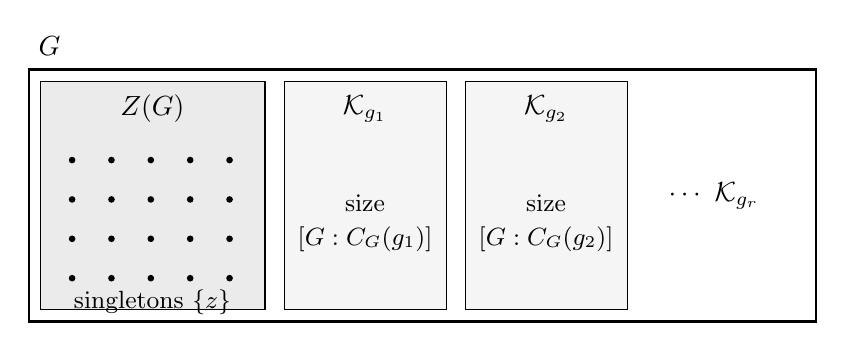
\begin{tikzpicture}[scale=1]
% outer box = G
\draw[thick] (0,0) rectangle (10,3.2);
\node[anchor=south west] at (0,3.25) {$G$};
% Z(G) block
\draw[fill=black!8] (0.15,0.15) rectangle (3.0,3.05);
\node at (1.57,2.7) {$Z(G)$};
% singletons inside Z(G)
\foreach \x in {0.55,1.05,1.55,2.05,2.55} {
  \foreach \y in {0.55,1.05,1.55,2.05} {
    \fill (\x,\y) circle (1.2pt);
  }
}
\node at (1.57,0.25) {\small singletons $\{z\}$};
% non-central classes
\draw[fill=black!4] (3.25,0.15) rectangle (5.3,3.05);
\node at (4.27,2.7) {$\mathcal{K}_{g_1}$};
\node at (4.27,1.5) {\small size};
\node at (4.27,1.05) {\small $\idx{G}{C_G(g_1)}$};
\draw[fill=black!4] (5.55,0.15) rectangle (7.6,3.05);
\node at (6.57,2.7) {$\mathcal{K}_{g_2}$};
\node at (6.57,1.5) {\small size};
\node at (6.57,1.05) {\small $\idx{G}{C_G(g_2)}$};
\node at (8.7,1.6) {$\cdots\ \mathcal{K}_{g_r}$};
\end{tikzpicture}
\]
Each grey block is one orbit; the central block holds the $|Z(G)|$ orbits of size $1$. Reading off the total width recovers the class equation.

\begin{method}{Writing the class equation of a finite group}
\textbf{Trigger:} ``find the class equation of $G$'' or ``how many conjugacy classes does $G$ have.''
\begin{enumerate}
\item Compute $|Z(G)|$; each central element is its own class (a $1$).
\item For each non-central element, find its class size $\idx{G}{C_G(g)}$; group elements into classes so you never double-count.
\item Write $|G| = |Z(G)| + (\text{non-central class sizes})$; every summand divides $|G|$, and the central part is $|Z(G)|$ copies of $1$.
\item \textbf{Check:} the right side sums to $|G|$, and the count of summands equals the number of conjugacy classes.
\end{enumerate}
\end{method}

\begin{wex}{Class equation of $S_3$}
Write the class equation of $S_3$.
\wrec Class equation $=$ sum of class sizes; in $S_n$ classes are cycle types, so list them.
\wsol $|S_3| = 6$. Cycle types: identity $e$ (1 element), transpositions $(1\,2),(1\,3),(2\,3)$ (3 elements), $3$-cycles $(1\,2\,3),(1\,3\,2)$ (2 elements). $Z(S_3) = \{e\}$ so $|Z(S_3)| = 1$. Thus
\[
6 \;=\; 1 + 2 + 3.
\]
\textbf{Check:} $1+2+3 = 6$; each summand ($1,2,3$) divides $6$; three conjugacy classes. Centralizer check: $|\mathcal{K}_{(1\,2)}| = 3 \imp |C_{S_3}((1\,2))| = 2 = |\gen{(1\,2)}|$. Consistent.
\end{wex}

\begin{wex}{Class equation of $D_8$}
Write the class equation of $D_8 = \gen{r,s}$, $|D_8| = 8$.
\wrec Group elements into conjugacy classes; central elements are singletons, the rest have size $\idx{D_8}{C_{D_8}(g)}$.
\wsol Center: $Z(D_8) = \{1, r^2\}$, two singletons. Rotations: $r$ and $r^3$ are conjugate ($s r s\inv = r\inv = r^3$), forming $\{r, r^3\}$ of size $2$. Reflections split into $\{s, r^2 s\}$ and $\{rs, r^3 s\}$, each size $2$ (from the previous worked example and its analogue). Therefore
\[
8 \;=\; \underbrace{1 + 1}_{Z(D_8)} \;+\; \underbrace{2}_{\{r,r^3\}} \;+\; \underbrace{2}_{\{s,r^2 s\}} \;+\; \underbrace{2}_{\{rs,r^3 s\}}.
\]
\textbf{Check:} $1+1+2+2+2 = 8$; all summands divide $8$; five conjugacy classes; $|Z| = 2$. Good.
\end{wex}

\begin{wex}{Class equation of $Q_8$}
Write the class equation of $Q_8$, $|Q_8| = 8$.
\wrec Same recipe; note $Q_8$ has the \emph{same} class equation as $D_8$ though the groups differ.
\wsol $Z(Q_8) = \{1,-1\}$, two singletons. The remaining six elements fall into $\{i,-i\}$, $\{j,-j\}$, $\{k,-k\}$, each a class of size $2$ (e.g.\ $jij\inv = -i$ from before). Thus
\[
8 \;=\; 1 + 1 + 2 + 2 + 2.
\]
\textbf{Check:} $1+1+2+2+2 = 8$; five classes. So the class equation does \emph{not} distinguish $D_8$ from $Q_8$ -- a useful reminder that it is a coarse invariant.
\end{wex}

\begin{wex}{Class equation of $A_4$}
Write the class equation of $A_4$, $|A_4| = 12$.
\wrec In $S_n$ a class may \emph{split} when restricted to $A_n$; check whether the cycle-type class stays whole by testing if some odd permutation centralizes a representative.
\wsol Elements of $A_4$: $e$ (1); three double-transpositions $(1\,2)(3\,4),(1\,3)(2\,4),(1\,4)(2\,3)$; eight $3$-cycles. The double-transpositions form one class of size $3$ (they are all conjugate in $A_4$). The eight $3$-cycles split into \emph{two} $A_4$-classes of size $4$: for $g = (1\,2\,3)$, $|C_{A_4}(g)| = 3$ (only powers of $g$ centralize it inside $A_4$), so $|\mathcal{K}_g| = 12/3 = 4$; conjugating by even permutations cannot reach $(1\,3\,2)$, which heads the other class. Hence
\[
12 \;=\; 1 + 3 + 4 + 4.
\]
\textbf{Check:} $1+3+4+4 = 12$; $Z(A_4) = \{e\}$ so $|Z| = 1$; four classes. (Contrast: in $S_4$ all eight $3$-cycles are one class -- splitting is genuine.)
\end{wex}

\subsection*{Conjugacy in $S_n$: Same Cycle Type}

\begin{theorem}[Conjugacy classes of $S_n$]\label{thm:Snconj@c4}
Two elements of $S_n$ are conjugate \emph{if and only if} they have the same cycle type. Concretely, if $\sigma = (a_1\,a_2\,\cdots\,a_k)(b_1\,b_2\,\cdots)\cdots$ in disjoint-cycle form and $\tau \in S_n$, then
\[
\tau \sigma \tau\inv \;=\; (\tau(a_1)\,\tau(a_2)\,\cdots\,\tau(a_k))(\tau(b_1)\,\tau(b_2)\,\cdots)\cdots .
\]
Thus the conjugacy classes of $S_n$ are indexed by the partitions of $n$.
\end{theorem}

\begin{proof}
\emph{Formula.} For a $k$-cycle $(a_1\cdots a_k)$ and any $\tau$, evaluate $\tau\sigma\tau\inv$ at $\tau(a_j)$: $\tau\sigma\tau\inv(\tau(a_j)) = \tau\sigma(a_j) = \tau(a_{j+1})$ (indices mod $k$), so $\tau\sigma\tau\inv = (\tau(a_1)\cdots\tau(a_k))$, a $k$-cycle. Applying this to each disjoint cycle of $\sigma$ (and noting $\tau$ keeps the cycles disjoint, being a bijection) shows $\tau\sigma\tau\inv$ has the same cycle type as $\sigma$. \emph{Converse.} If $\sigma,\sigma'$ have the same cycle type, align their cycles and let $\tau$ be the bijection sending the entries of $\sigma$ to the correspondingly-placed entries of $\sigma'$; then $\tau\sigma\tau\inv = \sigma'$ by the formula. Hence ``same cycle type'' is exactly conjugacy, and cycle types are partitions of $n$.
\end{proof}

\begin{theorem}[Counting a cycle-type class]\label{thm:countclass@c4}
If a cycle type has $m_k$ cycles of length $k$ (so $\sum_k k\, m_k = n$, counting fixed points as $1$-cycles), the number of permutations of that type, equivalently the size of the conjugacy class, is
\[
\frac{n!}{\displaystyle \prod_{k\ge 1} k^{\,m_k}\, m_k!}.
\]
\end{theorem}

\begin{proof}
Fill the cycle skeleton with the $n$ symbols in one of $n!$ orders. Each cycle of length $k$ has $k$ cyclic rotations giving the same permutation, accounting for $\prod_k k^{m_k}$; and the $m_k$ cycles of equal length $k$ can be permuted among themselves without changing the permutation, accounting for $\prod_k m_k!$. Dividing removes the overcount.
\end{proof}

\begin{method}{Conjugacy in $S_n$}
\textbf{Trigger:} ``are these two permutations conjugate in $S_n$?'' or ``how many elements / classes of a given type?''
\begin{enumerate}
\item Write each permutation in disjoint cycles (include fixed points to read the full type).
\item Conjugate by \emph{relabeling}: $\tau\sigma\tau\inv$ just applies $\tau$ to each entry -- so two are conjugate iff same multiset of cycle lengths.
\item Count a class by $n!/\prod_k k^{m_k} m_k!$. Sum over all partitions of $n$ to recover $n!$.
\item \textbf{Check:} class sizes are integers dividing $n!$ and sum to $n!$; the number of classes equals $p(n)$, the number of partitions.
\end{enumerate}
\end{method}

\begin{wex}{Conjugacy classes of $S_4$ by cycle type}
List all conjugacy classes of $S_4$ with their sizes, and verify they sum to $24$.
\wrec In $S_n$ classes $=$ partitions of $n$; size given by $n!/\prod k^{m_k}m_k!$.
\wsol Partitions of $4$ and counts ($n = 4$, $n! = 24$):
\[
\begin{array}{lll}
\text{type } 1^4 \ (e): & \dfrac{24}{1^4\cdot 4!} = 1, & \\[4pt]
\text{type } 2\,1^2 \ (a\,b): & \dfrac{24}{2^1 1!\cdot 1^2 2!} = \dfrac{24}{2\cdot 2}=6, & \text{transpositions}\\[6pt]
\text{type } 2^2 \ (a\,b)(c\,d): & \dfrac{24}{2^2 2!} = \dfrac{24}{8}=3, & \text{double transpositions}\\[6pt]
\text{type } 3\,1 \ (a\,b\,c): & \dfrac{24}{3^1 1!\cdot 1\cdot 1!} = \dfrac{24}{3}=8, & 3\text{-cycles}\\[6pt]
\text{type } 4 \ (a\,b\,c\,d): & \dfrac{24}{4^1 1!} = 6, & 4\text{-cycles}.
\end{array}
\]
So the class equation of $S_4$ is
\[
24 \;=\; 1 + 6 + 3 + 8 + 6 .
\]
\textbf{Check:} $1+6+3+8+6 = 24$; five classes $=p(4)=5$; $Z(S_4)=\{e\}$, so the lone singleton is the identity -- consistent. (The even classes $1+3+8 = 12 = |A_4|$ also check out.)
\end{wex}

\begin{wex}{Are these conjugate in $S_5$?}
Decide whether $\sigma = (1\,2\,3)(4\,5)$ and $\tau = (1\,4)(2\,5\,3)$ are conjugate in $S_5$, and if so exhibit a conjugator.
\wrec Conjugate in $S_n$ $\eqv$ same cycle type; build the conjugator by aligning cycles.
\wsol Both have type $3+2$ (a $3$-cycle and a disjoint $2$-cycle): $\sigma$ acts as a $3$-cycle on $\{1,2,3\}$ and a $2$-cycle on $\{4,5\}$; $\tau = (2\,5\,3)(1\,4)$ acts as a $3$-cycle on $\{2,5,3\}$ and a $2$-cycle on $\{1,4\}$. Same type $\imp$ conjugate. To build $\rho$ with $\rho\sigma\rho\inv = \tau$, map $\sigma$'s cycles onto $\tau$'s entry-by-entry: $1\mapsto 2,\,2\mapsto 5,\,3\mapsto 3,\,4\mapsto 1,\,5\mapsto 4$, i.e.\ $\rho = (1\,2\,5\,4)$. \textbf{Check:} $\rho\sigma\rho\inv = (\rho(1)\,\rho(2)\,\rho(3))(\rho(4)\,\rho(5)) = (2\,5\,3)(1\,4) = \tau$. Correct.
\end{wex}

\begin{wex}{Counting $5$-cycles in $S_5$}
How many $5$-cycles are in $S_5$, and what is the centralizer of one?
\wrec Size of a cycle-type class $= n!/\prod k^{m_k}m_k!$; centralizer order $= |G|/|\text{class}|$.
\wsol Type $5$: $m_5 = 1$, all others $0$, so count $= 5!/(5^1\cdot 1!) = 120/5 = 24$. By orbit--stabilizer, $|C_{S_5}(\sigma)| = |S_5|/|\mathcal{K}_\sigma| = 120/24 = 5$, so the centralizer is exactly $\gen{\sigma}$ (a $5$-cycle commutes only with its own powers).
\textbf{Check:} $24 \mid 120$; $|C| = 5 = |\gen{\sigma}|$. A $5$-cycle has order $5$, so $\gen{\sigma}$ has order $5$ -- matches.
\end{wex}

\begin{wex}{Counting double transpositions in $S_6$}
Count the elements of type $2^2 1^2$ in $S_6$.
\wrec $n!/\prod k^{m_k}m_k!$ with $m_2 = 2$, $m_1 = 2$.
\wsol $n = 6$, $n! = 720$. Here $m_2 = 2,\ m_1 = 2$:
\[
\frac{720}{(2^2\cdot 2!)\,(1^2\cdot 2!)} = \frac{720}{(4\cdot 2)(1\cdot 2)} = \frac{720}{16} = 45.
\]
\textbf{Check:} $45 \mid 720$ ($720/45 = 16$), so the centralizer of such an element has order $16$ -- a $2$-group, plausible. Counting directly: choose the two moved pairs, $\binom{6}{2}\binom{4}{2}/2! = 15\cdot 6/2 = 45$. Matches.
\end{wex}

\subsection*{Applications of the Class Equation}

The first application is the cornerstone fact that finite $p$-groups have nontrivial center.

\begin{theorem}[$p$-groups have nontrivial center]\label{thm:pgroupcenter@c4}
If $p$ is a prime and $|G| = p^a$ with $a \ge 1$, then $Z(G) \ne 1$; that is, $p \mid |Z(G)|$.
\end{theorem}

\begin{proof}
Write the class equation $|G| = |Z(G)| + \sum_{i=1}^r \idx{G}{C_G(g_i)}$ over non-central representatives $g_i$. For each such $g_i$ we have $C_G(g_i) \ne G$ (else $g_i$ would be central), so $\idx{G}{C_G(g_i)} > 1$. As an index it divides $|G| = p^a$, hence $\idx{G}{C_G(g_i)} = p^{b_i}$ with $b_i \ge 1$, so $p \mid \idx{G}{C_G(g_i)}$. Therefore $p$ divides $|G|$ and the entire sum $\sum_i \idx{G}{C_G(g_i)}$, and rearranging the class equation gives
\[
|Z(G)| = |G| - \sum_{i=1}^r \idx{G}{C_G(g_i)} \equiv 0 \pmod p .
\]
Since $1 \in Z(G)$ gives $|Z(G)| \ge 1$ and $p \mid |Z(G)|$, we get $|Z(G)| \ge p > 1$.
\end{proof}

\begin{corollary}[Groups of order $p^2$ are abelian]\label{cor:p2abelian@c4}
If $|G| = p^2$ for a prime $p$, then $G$ is abelian (so $G \isom \Zn{p^2}$ or $G \isom \Zn{p}\times\Zn{p}$).
\end{corollary}

\begin{proof}
By Theorem~\ref{thm:pgroupcenter@c4}, $Z(G) \ne 1$, so $|Z(G)| \in \{p, p^2\}$. If $|Z(G)| = p^2$ then $G = Z(G)$ is abelian and we are done. Suppose instead $|Z(G)| = p$. Then $|G/Z(G)| = p^2/p = p$, so $G/Z(G)$ is cyclic. But it is a standard lemma that \emph{if $G/Z(G)$ is cyclic then $G$ is abelian}: write $G/Z(G) = \gen{xZ(G)}$; every $g \in G$ is $g = x^m z$ for some integer $m$ and $z \in Z(G)$, and two such elements $x^{m}z,\ x^{n}w$ commute because powers of $x$ commute with each other and $z,w$ are central. So $G$ is abelian, which forces $Z(G) = G$ and contradicts $|Z(G)| = p < p^2$. Hence the case $|Z(G)| = p$ is impossible, $|Z(G)| = p^2$, and $G$ is abelian. The classification into $\Zn{p^2}$ and $\Zn{p}\times\Zn{p}$ follows from the structure of finite abelian groups.
\end{proof}

\begin{method}{Using the class equation modulo $p$}
\textbf{Trigger:} $|G|$ is a prime power $p^a$ (or you need to show some central element exists).
\begin{enumerate}
\item Write $|G| = |Z(G)| + \sum \idx{G}{C_G(g_i)}$ over non-central classes.
\item Each non-central index $\idx{G}{C_G(g_i)}$ is a power $p^{b_i}$, $b_i \ge 1$, hence $\equiv 0 \pmod p$.
\item Reduce mod $p$: $0 \equiv |Z(G)| + 0$, so $p \mid |Z(G)|$, forcing $Z(G) \ne 1$.
\item \textbf{Check:} consistency -- the central summand $|Z(G)|$ plus a multiple of $p$ equals $p^a$, also a multiple of $p$.
\end{enumerate}
\end{method}

\begin{wex}{$Z(G) \ne 1$ for $|G| = 27$}
Show every group of order $27$ has nontrivial center.
\wrec $27 = 3^3$ is a $p$-group; apply the class-equation-mod-$p$ argument.
\wsol Class equation: $27 = |Z(G)| + \sum_i \idx{G}{C_G(g_i)}$ with each non-central index a power $3^{b_i}$, $b_i \ge 1$, so each is divisible by $3$. Reducing mod $3$: $0 \equiv |Z(G)| + 0 \pmod 3$, so $3 \mid |Z(G)|$. As $|Z(G)| \ge 1$, we get $|Z(G)| \in \{3, 9, 27\}$, in particular $Z(G) \ne 1$.
\textbf{Check:} possible class equations include $27 = 27$ (abelian) and $27 = 3 + 3+3+3+3+3+3+3+3$ (i.e.\ $|Z| = 3$ together with eight non-central classes of size $3$). Each summand divides $27$ and the centre is a multiple of $3$. Consistent.
\end{wex}

\begin{wex}{Order $p^2$ is abelian: $|G| = 25$}
Prove any group of order $25$ is abelian.
\wrec $25 = 5^2$; use $Z(G) \ne 1$ and the $G/Z(G)$-cyclic lemma.
\wsol By Theorem~\ref{thm:pgroupcenter@c4}, $Z(G) \ne 1$, so $|Z(G)| \in \{5,25\}$. If $|Z(G)| = 5$ then $|G/Z(G)| = 5$, hence $G/Z(G)$ is cyclic of prime order, which forces $G$ abelian and thus $Z(G) = G$ -- contradicting $|Z(G)| = 5$. So $|Z(G)| = 25$ and $G$ is abelian; concretely $G \isom \Zn{25}$ or $\Zn{5}\times\Zn{5}$.
\textbf{Check:} both candidate groups are indeed abelian, and there is no nonabelian group of order $25$. Consistent with the theorem.
\end{wex}

\begin{wex}{A nonabelian group of order $p^3$}
Verify the center-of-$p$-group theorem is sharp at $p^3$ by examining $D_8$.
\wrec At $p^3$ the center can be exactly $p$; check $D_8$ ($p = 2$, $a = 3$).
\wsol $|D_8| = 8 = 2^3$. Its class equation $8 = 1+1+2+2+2$ has central part $|Z(D_8)| = 2 = p$, the smallest allowed. So $Z(D_8) \ne 1$ (as the theorem guarantees) but $D_8$ is nonabelian, showing the corollary ``$p^2 \imp$ abelian'' cannot be pushed to $p^3$.
\textbf{Check:} $2 \mid |Z(D_8)|$ holds; $|Z| = 2 < 8$ so nonabelian -- exactly the boundary case.
\end{wex}

\subsection*{Conjugate Subgroups and the Normalizer}

Conjugation also acts on subgroups, and the count of conjugates is governed by the normalizer rather than the centralizer.

\begin{proposition}[Number of conjugates of a subgroup]\label{prop:numconj@c4}
Let $H \le G$. Under the conjugation action of $G$ on its subsets, the stabilizer of $H$ is the normalizer $N_G(H) = \{g \in G : gHg\inv = H\}$. Hence the number of distinct conjugate subgroups $gHg\inv$ equals
\[
\bigl|\{\, gHg\inv : g \in G\,\}\bigr| \;=\; \idx{G}{N_G(H)} .
\]
In particular this number divides $|G|$, and it equals $1$ iff $H \nor G$.
\end{proposition}

\begin{proof}
$g$ stabilizes $H$ under conjugation $\eqv gHg\inv = H \eqv g \in N_G(H)$, by definition of the normalizer. Orbit--stabilizer applied to this action on subsets gives the bijection
\[
\begin{tikzcd}[column sep=huge]
G/N_G(H) \arrow[r, "\sim", "{\,gN_G(H)\,\mapsto\, gHg\inv\,}"'] & \{\,gHg\inv : g\in G\,\},
\end{tikzcd}
\]
\begin{dgx}
\dgi{Objects:} Two objects: the coset space $G/N_G(H)$ (left cosets of the normalizer $N_G(H)$ in $G$; again a set, not a group in general) and the set $\{gHg^{-1} : g \in G\}$ of all distinct conjugates of the subgroup $H \le G$ (the orbit of $H$ under the conjugation action of $G$ on its power set).
\dgi{Arrows:} The bijection $\Phi\colon G/N_G(H) \to \{gHg^{-1} : g \in G\}$ sends a coset $gN_G(H)$ to the conjugate subgroup $gHg^{-1}$. This is the orbit-stabilizer bijection applied to the action of $G$ by conjugation on the set of subsets of $G$, with stabilizer of $H$ equal to $N_G(H)$.
\dgi{What commutes:} Well-definedness is the key: if $gN_G(H) = g'N_G(H)$, then $gHg^{-1} = g'Hg'^{-1}$.
\dgi{Why it commutes:} Well-definedness: $gN_G(H) = g'N_G(H)$ means $g^{-1}g' \in N_G(H)$, i.e., $(g^{-1}g')H(g^{-1}g')^{-1} = H$. Conjugating by $g$ on both sides: $g' H g'^{-1} = g H g^{-1}$. So the coset representative does not affect the conjugate subgroup produced. Injectivity and surjectivity follow as in the element case. If one mistakenly uses $C_G(H)$ instead of $N_G(H)$, the map $gC_G(H) \mapsto gHg^{-1}$ is still well defined (every element of $C_G(H) \le N_G(H)$ sends $H$ to itself, even fixing it pointwise), but it is no longer injective when $C_G(H) \ne N_G(H)$: the $[N_G(H) : C_G(H)]$ cosets of $C_G(H)$ lying in $N_G(H)$ all go to $H$.
\dgi{Why this matters here:} This bijection is the subgroup analogue of the element bijection from the class-size proposition. It shows the number of conjugate subgroups equals the index $[G : N_G(H)]$, giving a divisibility condition ($|G|$ finite) and a normality criterion ($H \nor G$ iff there is exactly one conjugate iff $N_G(H) = G$).
\dgi{Concrete example:} In $D_8$ with $H = \gen{s}$: $N_{D_8}(H) = \{1, s, r^2, r^2 s\}$ has order $4$, so $[D_8 : N_{D_8}(H)] = 2$, matching the count of two conjugate subgroups $\gen{s}$ and $\gen{r^2 s}$.
\dgi{Common pitfall:} Students confuse the normalizer $N_G(H)$ (which controls how many conjugate \emph{subgroups} there are) with the centralizer $C_G(H)$ (which controls elements that fix $H$ pointwise). The number of conjugates is $[G : N_G(H)]$, not $[G : C_G(H)]$: since $[G : C_G(H)] = [G : N_G(H)]\,[N_G(H) : C_G(H)]$, for finite $G$ using the centralizer overcounts by the factor $[N_G(H) : C_G(H)]$ (the answers agree only when $C_G(H) = N_G(H)$).
\dgi{Takeaway:} The point of this diagram is that the orbit-stabilizer theorem for the conjugation action on subsets converts the count of conjugate subgroups into the computable index $[G : N_G(H)]$, encoding normality as the condition that this index equals $1$.
\end{dgx}
so the number of conjugates is $\idx{G}{N_G(H)}$. It divides $|G|$, and it is $1$ exactly when $N_G(H) = G$, i.e.\ when $H$ is normal.
\end{proof}

\begin{pitfall}
For \emph{subgroup} conjugacy use the \emph{normalizer} $N_G(H)$, not the centralizer. Always $H \le N_G(H)$ and $C_G(H) \le N_G(H)$, but the number of conjugates is $\idx{G}{N_G(H)}$. Using $C_G(H)$ here is a common error.
\end{pitfall}

\begin{method}{Counting conjugates of a subgroup}
\textbf{Trigger:} ``how many subgroups are conjugate to $H$'' or ``is $H$ normal.''
\begin{enumerate}
\item Compute $N_G(H) = \{g : gHg\inv = H\}$; note $H \le N_G(H) \le G$.
\item Number of conjugates $= \idx{G}{N_G(H)} = |G|/|N_G(H)|$.
\item $H \nor G \eqv$ this index is $1 \eqv N_G(H) = G$.
\item \textbf{Check:} the count divides $|G|$; if you also have the count by direct listing, it must match.
\end{enumerate}
\end{method}

\begin{wex}{Conjugates of $\gen{s}$ in $D_8$}
Count the subgroups of $D_8$ conjugate to $H = \gen{s} = \{1,s\}$.
\wrec Number of conjugates $= \idx{D_8}{N_{D_8}(H)}$; find the normalizer.
\wsol $N_{D_8}(H) \supseteq H = \{1,s\}$ and contains $Z(D_8) = \{1,r^2\}$ since central elements normalize everything; so $\{1,s,r^2,r^2 s\} \le N_{D_8}(H)$, order $\ge 4$. Is $r \in N$? $r\gen{s}r\inv = \gen{rsr\inv} = \gen{r^2 s} \ne \gen{s}$, so $r \notin N$, giving $N_{D_8}(H) = \{1,s,r^2,r^2 s\}$, order $4$. Hence the number of conjugates is $8/4 = 2$, namely $\gen{s}$ and $\gen{r^2 s}$.
\textbf{Check:} $2 \mid 8$; $\gen{s}$ is not normal (the count exceeds $1$), and indeed conjugating gives $\gen{r^2 s}$. Consistent.
\end{wex}

\begin{wex}{Conjugates of $\gen{(1\,2)}$ in $S_3$}
Count the subgroups of $S_3$ conjugate to $H = \gen{(1\,2)}$.
\wrec $\idx{S_3}{N_{S_3}(H)}$; find which elements normalize $H$.
\wsol $N_{S_3}(H) \supseteq H = \{e,(1\,2)\}$, order $2$. A $3$-cycle conjugates $(1\,2)$ to a different transposition (e.g.\ $(1\,2\,3)(1\,2)(1\,3\,2) = (2\,3)$), so no $3$-cycle normalizes $H$; thus $N_{S_3}(H) = H$, order $2$, and the number of conjugates is $6/2 = 3$: namely $\gen{(1\,2)},\gen{(1\,3)},\gen{(2\,3)}$.
\textbf{Check:} $3 \mid 6$; there are exactly three order-$2$ subgroups in $S_3$ and they are all conjugate -- matches.
\end{wex}

\begin{wex}{A normal subgroup has one conjugate}
Count the conjugates of $A_3 = \gen{(1\,2\,3)}$ in $S_3$.
\wrec Number of conjugates $=1 \eqv H \nor G \eqv N_G(H) = G$.
\wsol $A_3$ has index $2$ in $S_3$, hence is normal, so $N_{S_3}(A_3) = S_3$ and the number of conjugates is $6/6 = 1$. Directly: conjugating a $3$-cycle gives a $3$-cycle, so $gA_3 g\inv = A_3$ for all $g$.
\textbf{Check:} index-$2$ subgroups are always normal; count $1$ as expected.
\end{wex}

\begin{wex}{Conjugates of a Sylow $2$-subgroup of $S_4$}
Count the subgroups of $S_4$ conjugate to a Sylow $2$-subgroup $P$ ($|P| = 8$), and identify $N_{S_4}(P)$.
\wrec $\idx{S_4}{N_{S_4}(P)}$ gives the count; for a Sylow subgroup the count is also the Sylow number $n_2$.
\wsol $|S_4| = 24 = 2^3\cdot 3$, so $|P| = 8$ and $\idx{S_4}{P} = 3$. Since $P \le N_{S_4}(P) \le S_4$, the order $|N_{S_4}(P)|$ is a multiple of $8$ dividing $24$, so it is $8$ or $24$. $P$ is not normal in $S_4$ (e.g.\ $S_4$ has more than one Sylow $2$-subgroup), so $|N_{S_4}(P)| \ne 24$; thus $N_{S_4}(P) = P$, order $8$, and the number of conjugates is $24/8 = 3$.
\textbf{Check:} $3 \mid 24$; $n_2 = 3 \equiv 1 \pmod 2$ and $3 \mid 3$, consistent with Sylow's theorem. So $S_4$ has exactly three Sylow $2$-subgroups, all conjugate.
\end{wex}

\begin{wex}{Conjugates of $\gen{i}$ in $Q_8$}
Count the conjugates of $H = \gen{i} = \{1,-1,i,-i\}$ in $Q_8$.
\wrec $\idx{Q_8}{N_{Q_8}(H)}$; index-$2$ subgroups are normal.
\wsol $|H| = 4$ and $\idx{Q_8}{H} = 8/4 = 2$, so $H$ has index $2$ and is therefore normal: $N_{Q_8}(H) = Q_8$. The number of conjugates is $8/8 = 1$.
\textbf{Check:} every index-$2$ subgroup is normal, so a single conjugate -- and indeed $\gen{i},\gen{j},\gen{k}$ are three \emph{distinct} normal subgroups, each its own sole conjugate. Consistent.
\end{wex}

\begin{remark}
Proposition~\ref{prop:numconj@c4} is the engine behind Sylow's theorems: applying it to a Sylow $p$-subgroup $P$ shows the number of Sylow $p$-subgroups is $\idx{G}{N_G(P)}$, which combined with a counting argument yields $n_p \equiv 1 \pmod p$ and $n_p \mid |G|$. Conjugation -- of elements and of subgroups -- is thus the common thread running from the class equation through the structure of $p$-groups to the Sylow theory of the next section.
\end{remark}

\begin{exers}{Exercises (from the text).}
\item Suppose $G$ has a left action on a set $A$, denoted by $g \cdot a$ for all $g \in G$ and $a \in A$. Denote the corresponding right action on $A$ by $a \cdot g$. Prove that the (equivalence) relations $\sim$ and $\sim'$ defined by
\[
a \sim b \quad \text{if and only if} \quad a = g \cdot b \quad \text{for some } g \in G
\]
and
\[
a \sim' b \quad \text{if and only if} \quad a = b \cdot g \quad \text{for some } g \in G
\]
are the same relation (i.e., $a \sim b$ if and only if $a \sim' b$).
\item Find all the conjugacy classes and their sizes in the following groups: (a) $D_8$ \quad (b) $Q_8$ \quad (c) $A_4$.
\item Find all the conjugacy classes and their sizes in the following groups: (a) $\Z_2 \times S_3$ \quad (b) $S_3 \times S_3$ \quad (c) $\Z_3 \times A_4$.
\item Prove that if $S \subseteq G$ and $g \in G$ then $g N_G(S) g^{-1} = N_G(g S g^{-1})$ and $g C_G(S) g^{-1} = C_G(g S g^{-1})$.
\item If the center of $G$ is of index $n$, prove that every conjugacy class has at most $n$ elements.
\item Assume $G$ is a non-abelian group of order 15. Prove that $Z(G) = 1$. Use the fact that $\gen{g} \le C_G(g)$ for all $g \in G$ to show that there is at most one possible class equation for $G$. [Use Exercise 36, Section 3.1.]
\item For $n = 3, 4, 5$ and 7 make tables of the partitions of $n$ and give representatives for the corresponding conjugacy classes of $S_n$.
\item Prove that $Z(S_n) = 1$ for all $n \ge 3$.
\item Show that $|C_{S_n}((1\,2)(3\,4))| = 8 \cdot (n-4)!$ for all $n \ge 4$. Determine the elements in this centralizer.
\item Let $\sigma$ be the 5-cycle $(1\,2\,3\,4\,5)$ in $S_5$. In each of (a) to (c) find an explicit element $\tau \in S_5$ which accomplishes the specified conjugation:
(a) $\tau \sigma \tau^{-1} = \sigma^2$
(b) $\tau \sigma \tau^{-1} = \sigma^{-1}$
(c) $\tau \sigma \tau^{-1} = \sigma^{-2}$.
\item In each of (a)~--~(d) determine whether $\sigma_1$ and $\sigma_2$ are conjugate. If they are, give an explicit permutation $\tau$ such that $\tau \sigma_1 \tau^{-1} = \sigma_2$.
(a) $\sigma_1 = (1\,2)(3\,4\,5)$ and $\sigma_2 = (1\,2\,3)(4\,5)$
(b) $\sigma_1 = (1\,5)(3\,7\,2)(10\,6\,8\,11)$ and $\sigma_2 = (3\,7\,5\,10)(4\,9)(13\,11\,2)$
(c) $\sigma_1 = (1\,5)(3\,7\,2)(10\,6\,8\,11)$ and $\sigma_2 = \sigma_1^3$
(d) $\sigma_1 = (1\,3)(2\,4\,6)$ and $\sigma_2 = (3\,5)(2\,4)(5\,6)$.
\item Find a representative for each conjugacy class of elements of order 4 in $S_8$ and in $S_{12}$.
\item Find all finite groups which have exactly two conjugacy classes.
\item In Exercise 1 of Section 2 two labellings of the elements $\{1, a, b, c\}$ of the Klein 4-group $V$ were chosen to give two versions of the left regular representation of $V$ into $S_4$. Let $\pi_1$ be the version of regular representation obtained in part (a) of that exercise and let $\pi_2$ be the version obtained via the labelling in part (b). Let $\tau = (2\,4)$. Show that $\tau \circ \pi_1(g) \circ \tau^{-1} = \pi_2(g)$ for each $g \in V$ (i.e., conjugation by $\tau$ sends the image of $\pi_1$ to the image of $\pi_2$ elementwise).
\item Find an element of $S_8$ which conjugates the subgroup of $S_8$ obtained in part (a) of Exercise 3, Section 2 to the subgroup of $S_8$ obtained in part (b) of that same exercise (both of these subgroups are isomorphic to $D_8$).
\item Find an element of $S_4$ which conjugates the subgroup of $S_4$ obtained in part (a) of Exercise 5, Section 2 to the subgroup of $S_4$ obtained in part (b) of that same exercise (both of these subgroups are isomorphic to $D_8$).
\item Let $A$ be a nonempty set and let $X$ be any subset of $S_A$. Let
\[
F(X) = \{a \in A \mid \sigma(a) = a \text{ for all } \sigma \in X\} \qquad \text{--- the \emph{fixed set} of } X.
\]
Let $M(X) = A - F(X)$ be the elements which are \emph{moved} by some element of $X$. Let $D = \{\sigma \in S_A \mid |M(\sigma)| < \infty\}$. Prove that $D$ is a normal subgroup of $S_A$.
\item Let $A$ be a set, let $H$ be a subgroup of $S_A$ and let $F(H)$ be the fixed points of $H$ on $A$ as defined in the preceding exercise. Prove that if $\tau \in N_{S_A}(H)$ then $\tau$ stabilizes the set $F(H)$ and its complement $A - F(H)$.
\item Assume $H$ is a normal subgroup of $G$, $\mathcal{K}$ is a conjugacy class of $G$ contained in $H$ and $x \in \mathcal{K}$. Prove that $\mathcal{K}$ is a union of $k$ conjugacy classes of equal size in $H$, where $k = \idx{G}{H C_G(x)}$. Deduce that a conjugacy class in $S_n$ which consists of even permutations is either a single conjugacy class under the action of $A_n$ or is a union of two classes of the same size in $A_n$. [Let $A = C_G(x)$ and $B = H$ so $A \cap B = C_H(x)$. Draw the lattice diagram associated to the Second Isomorphism Theorem and interpret the appropriate indices. See also Exercise 9, Section 1.]
\item Let $\sigma \in A_n$. Show that all elements in the conjugacy class of $\sigma$ in $S_n$ (i.e., all elements of the same cycle type as $\sigma$) are conjugate in $A_n$ if and only if $\sigma$ commutes with an odd permutation. [Use the preceding exercise.]
\item Let $\mathcal{K}$ be a conjugacy class in $S_n$ and assume that $\mathcal{K} \subseteq A_n$. Show $\sigma \in S_n$ does \emph{not} commute with any odd permutation if and only if the cycle type of $\sigma$ consists of distinct odd integers. Deduce that $\mathcal{K}$ consists of two conjugacy classes in $A_n$ if and only if the cycle type of an element of $\mathcal{K}$ consists of distinct odd integers. [Assume first that $\sigma \in \mathcal{K}$ does not commute with any odd permutation. Observe that $\sigma$ commutes with each individual cycle in its cycle decomposition --- use this to show that all its cycles must be of odd length. If two cycles have the same odd length, $k$, find a product of $k$ transpositions which interchanges them and commutes with $\sigma$. Conversely, if the cycle type of $\sigma$ consists of distinct integers, prove that $\sigma$ commutes \emph{only} with the group generated by the cycles in its cycle decomposition.]
\item Show that if $n$ is odd then the set of all $n$-cycles consists of two conjugacy classes of equal size in $A_n$.
\item Recall (cf. Exercise 16, Section 2.4) that a proper subgroup $M$ of $G$ is called \emph{maximal} if whenever $M \le H \le G$, either $H = M$ or $H = G$. Prove that if $M$ is a maximal subgroup of $G$ then either $N_G(M) = M$ or $N_G(M) = G$. Deduce that if $M$ is a maximal subgroup of $G$ that is not normal in $G$ then the number of nonidentity elements of $G$ that are contained in conjugates of $M$ is at most $(|M| - 1) \idx{G}{M}$.
\item Assume $H$ is a proper subgroup of the finite group $G$. Prove $G \ne \bigcup_{g \in G} g H g^{-1}$, i.e., $G$ is not the union of the conjugates of any proper subgroup. [Put $H$ in a maximal subgroup and use the preceding exercise.]
\item Let $G = GL_2(\C)$ and let $H = \{ \begin{pmatrix} a & b \\ 0 & c \end{pmatrix} \mid a, b, c \in \C, \ ac \ne 0 \}$. Prove that every element of $G$ is conjugate to some element of the subgroup $H$ and deduce that $G$ is the union of conjugates of $H$. [Show that every element of $GL_2(\C)$ has an eigenvector.]
\item Let $G$ be a transitive permutation group on the finite set $A$ with $|A| > 1$. Show that there is some $\sigma \in G$ such that $\sigma(a) \ne a$ for all $a \in A$ (such an element $\sigma$ is called \emph{fixed point free}).
\item Let $g_1, g_2, \ldots, g_r$ be representatives of the conjugacy classes of the finite group $G$ and assume these elements pairwise commute. Prove that $G$ is abelian.
\item Let $p$ and $q$ be primes with $p < q$. Prove that a non-abelian group $G$ of order $pq$ has a nonnormal subgroup of index $q$, so that there exists an injective homomorphism into $S_q$. Deduce that $G$ is isomorphic to a subgroup of the normalizer in $S_q$ of the cyclic group generated by the $q$-cycle $(1\,2 \ldots q)$.
\item Let $p$ be a prime and let $G$ be a group of order $p^a$. Prove that $G$ has a subgroup of order $p^b$, for every $b$ with $0 \le b \le a$. [Use Theorem~\ref{thm:pgroupcenter@c4} and induction on $a$.]
\item If $G$ is a group of odd order, prove for any nonidentity element $x \in G$ that $x$ and $x^{-1}$ are not conjugate in $G$.
\item Using the usual generators and relations for the dihedral group $D_{2n}$ (cf. Section 1.2) show that for $n = 2k$ an even integer the conjugacy classes in $D_{2n}$ are the following: $\{1\}$, $\{r^k\}$, $\{r^{\pm 1}\}$, $\{r^{\pm 2}\}$, $\ldots$, $\{r^{\pm(k-1)}\}$, $\{sr^{2b} \mid b = 1, \ldots, k\}$ and $\{sr^{2b-1} \mid b = 1, \ldots, k\}$. Give the class equation for $D_{2n}$.
\item For $n = 2k + 1$ an odd integer show that the conjugacy classes in $D_{2n}$ are $\{1\}$, $\{r^{\pm 1}\}$, $\{r^{\pm 2}\}$, $\ldots$, $\{r^{\pm k}\}$, $\{sr^b \mid b = 1, \ldots, n\}$. Give the class equation for $D_{2n}$.
\item This exercise gives a formula for the size of each conjugacy class in $S_n$. Let $\sigma$ be a permutation in $S_n$ and let $m_1, m_2, \ldots, m_s$ be the \emph{distinct} integers which appear in the cycle type of $\sigma$ (including 1-cycles). For each $i \in \{1, 2, \ldots, s\}$ assume $\sigma$ has $k_i$ cycles of length $m_i$. (So $\sum_{i} k_i m_i = n$.) Prove that the number of conjugates of $\sigma$ is
\[
\frac{n!}{(k_1!\,m_1^{k_1})(k_2!\,m_2^{k_2}) \cdots (k_s!\,m_s^{k_s})}.
\]
[See Exercises 16 and 17 in Section 1.3 where this formula was given in some special cases.]
\item Prove that if $p$ is a prime and $P$ is a subgroup of $S_p$ of order $p$ then $|N_{S_p}(P)| = p(p-1)$. [Argue that every conjugate of $P$ contains exactly $p - 1$ $p$-cycles and use the formula for the number of $p$-cycles to compute the index of $N_{S_p}(P)$ in $S_p$.]
\item Let $p$ be a prime. Find a formula for the number of conjugacy classes of elements of order $p$ in $S_n$ (using the greatest integer function).
\item Let $\pi : G \to S_G$ be the left regular representation afforded by the action of $G$ on itself by left multiplication. For each $g \in G$ denote the permutation $\pi(g)$ by $\sigma_g$, so that $\sigma_g(x) = gx$ for all $x \in G$. Let $\lambda : G \to S_G$ be the permutation representation afforded by the corresponding right action of $G$ on itself, and for each $h \in G$ denote the permutation $\lambda(h)$ by $\tau_h$. Thus $\tau_h(x) = xh^{-1}$ for all $x \in G$ ($\lambda$ is called the \emph{right regular representation} of $G$).
(a) Prove that $\sigma_g$ and $\tau_h$ commute for all $g, h \in G$. (Thus the centralizer in $S_G$ of $\pi(G)$ contains the subgroup $\lambda(G)$, which is isomorphic to $G$.)
(b) Prove that $\sigma_g = \tau_g$ if and only if $g$ is an element of order 1 or 2 in the center of $G$.
(c) Prove that $\sigma_g = \tau_h$ if and only if $g$ and $h$ lie in the center of $G$ and $g = h^{-1}$. Deduce that $\lambda(G) \cap \pi(G) = Z(\lambda(G)) = Z(\pi(G))$.
\end{exers}

\begin{exers}{Practice problems.}


\item Find all conjugacy classes of $D_8$ (order $8$, with $r^4=s^2=1$, $sr=r\inv s$).
List the class sizes and verify they partition $|D_8|=8$. Use the data to write the
class equation of $D_8$.

\item In $S_4$ list a representative of each conjugacy class (by cycle type), give the
size of each class, and confirm the sizes sum to $24$. Identify $Z(S_4)$.

\item For each cycle type in $S_5$ compute the order of the centralizer $C_{S_5}(\sigma)$
of a representative $\sigma$, using $|C_{S_5}(\sigma)|=120/(\text{class size})$. (Recall
the class of a permutation with $a_i$ cycles of length $i$ has size
$n!/\prod_i i^{a_i}\,a_i!$.)

\item Let $G$ be a group of order $p^2$ for a prime $p$. Use the class equation to prove
$Z(G)\neq 1$, then deduce $G$ is abelian. Conclude $G\isom\Zn{p^2}$ or
$G\isom\Zn{p}\times\Zn{p}$.

\item Show that a group of order $p^n$ ($p$ prime, $n\geq 1$) has a nontrivial center.
Then show every group of order $p^n$ has a normal subgroup of order $p^k$ for each
$0\le k\le n$.

\item Let $G=Q_8=\{\pm 1,\pm i,\pm j,\pm k\}$. Compute all conjugacy classes, the class
equation, and $Z(Q_8)$. Compare the class equation of $Q_8$ with that of $D_8$ from
Problem 1.

\item Suppose $|G|=p\,m$ where $p$ is the smallest prime dividing $|G|$ and
$H\sgr G$ with $\idx{G}{H}=p$. Prove $H\nor G$. (Hint: let $G$ act on the left cosets
$G/H$ and analyze the kernel of the induced map $G\to\Sym(G/H)$.)

\item Let $\sigma=(1\,2\,3)(4\,5)\in S_5$ and $\tau=(1\,4\,2)(3\,5)\in S_5$. Exhibit an
explicit $\pi\in S_5$ with $\pi\sigma\pi\inv=\tau$, and confirm by direct computation.

\item Determine $C_{S_6}(\sigma)$ explicitly (as a set of generators) for
$\sigma=(1\,2)(3\,4)(5\,6)\in S_6$, and compute $|C_{S_6}(\sigma)|$. Verify your count
against the class-size formula.

\item Let $G$ act on itself by conjugation. Show the orbits are exactly the conjugacy
classes and that the stabilizer of $x\in G$ is $C_G(x)$. Deduce
$|\text{class of }x|=\idx{G}{C_G(x)}$ and that this index divides $|G|$.

\item Prove that two elements of $S_n$ are conjugate in $S_n$ iff they have the same cycle
type. Use this to count the number of conjugacy classes of $S_5$ (i.e.\ the number of
partitions of $5$) and list each class size.

\item Let $G$ be a finite group and $H\nor G$ with $|H|=p$, $p$ prime. Prove that
$H\le Z(G)$ provided $p$ is the smallest prime dividing $|G|$. (Hint: $G$ acts on $H$ by
conjugation, giving $G\to\Aut(H)\isom\Zns{p}$.)

\item Show that if $G/Z(G)$ is cyclic then $G$ is abelian. Use this to prove no group of
order $p^3$ ($p$ prime) has center of order $p^2$.

\item Let $\sigma\in S_n$ be an $n$-cycle. Compute $|C_{S_n}(\sigma)|$ and describe
$C_{S_n}(\sigma)$ explicitly. How many $n$-cycles are there in $S_n$?

\item A group $G$ of order $60$ has class equation $60=1+15+20+12+12$. Show $G$ is simple,
i.e.\ has no nontrivial proper normal subgroup. (Any normal subgroup is a union of
classes including $\{1\}$ whose total order divides $60$.)


\end{exers}

\begin{exers}{Additional exercises.}


\item Let $G$ be a finite group in which every conjugacy class has size at most $2$.
Prove that $[G,G]$ (the subgroup generated by all commutators) has order at most $2$,
and that $G/Z(G)$ has exponent $2$.

\item Let $p$ be a prime and $G$ a group of order $p^n$ with $n\ge1$. Prove that
the number of conjugacy classes of size $1$ (i.e.\ $|Z(G)|$) is divisible by $p$, and use
the class equation to show $G$ cannot have exactly $p^{n-1}$ classes of size $p$. Then show
$|Z(G)|\ne p^{n-1}$, and determine whether a nonabelian $G$ can have $|Z(G)|=p^{n-2}$.

\item Show that if $|G|=p^a m$ with $\gcd(p,m)=1$ and $G$ has a single conjugacy class of
size coprime to $p$ other than $\{1\}$, derive what this forces about $|Z(G)|$. Then prove
more generally: if $x\in G$ has $\idx{G}{C_G(x)}$ a power of $p$ for every $x\notin Z(G)$,
then a Sylow $p$-subgroup is normal.

\item Let $G$ be a nonabelian group of order $p^3$. Prove $|Z(G)|=p$, that
$Z(G)=[G,G]$, and that $G/Z(G)\isom\Zn{p}\times\Zn{p}$. Conclude the class equation is
$p^3=p+\underbrace{(p^2-1)}_{\text{number of size-}p\text{ classes}}\cdot p$, i.e.\
$p^3=p+(p^2-1)p$.

\item Let $G$ act on a finite set $A$. Prove Burnside's counting lemma: the number of
orbits equals $\frac{1}{|G|}\sum_{g\in G}|\Fix(g)|$, where $\Fix(g)=\{a\in A: g\cdot a=a\}$.
Apply it to count the orbits of $D_8$ acting on the $4$ vertices of a square.

\item Suppose $G$ is a finite group with exactly three conjugacy classes. Prove $|G|\in\{3,6\}$ and
identify the groups (up to isomorphism) realizing each.


\end{exers}

\begin{exers}{Commutative-diagram exercises.}


\item Let $G$ act on a finite set $A$, giving the permutation representation
$\rho\colon G\to\Sym(A)$. For a fixed $a\in A$ let $G_a=\Stab_G(a)$. Prove the orbit map
\[\begin{tikzcd}[column sep=large]
G/G_a \arrow[r, "\sim", "{gG_a\mapsto g\cdot a}"'] & \orb(a)
\end{tikzcd}\]
is a well-defined bijection of $G$-sets, and deduce
$|\orb(a)|=\idx{G}{G_a}$. State precisely what ``$G$-set map'' means here.

\item Conjugation gives an action of $G$ on itself. Show the induced map fits in
\[\begin{tikzcd}[column sep=large]
1 \arrow[r] & Z(G) \arrow[r, hook] & G \arrow[r, "\psi"] & \Aut(G)
\end{tikzcd}\]
where $\psi(g)$ is conjugation by $g$. Prove this row is exact, identify
$\im\psi=\Inn(G)$, and conclude $G/Z(G)\isom\Inn(G)$.

\item For $G=S_4$ acting on itself by conjugation, the representation is
$\rho\colon S_4\to\Sym(S_4)$. Restricting to the orbit of a transposition
$t=(1\,2)$ yields
\[\begin{tikzcd}[column sep=large]
S_4/C_{S_4}(t) \arrow[r, "\sim", "{gC\mapsto gtg\inv}"'] & \orb(t)
\end{tikzcd}\]
Compute $C_{S_4}(t)$, the order of $S_4/C_{S_4}(t)$, and list $\orb(t)$; verify the
bijection on two specific cosets.

\item Let $H\sgr G$ with $\idx{G}{H}=n$, and let $G$ act on the left cosets $G/H$. This
gives
\[\begin{tikzcd}[column sep=large]
G \arrow[r, "\pi"] & \Sym(G/H)
\end{tikzcd}\]
Show $\ker\pi=\bigcap_{g\in G} gHg\inv$, the largest normal subgroup of $G$ contained in
$H$ (the \emph{core} of $H$). Deduce that if $|G|\nmid n!$ then $H$ contains a nontrivial
normal subgroup of $G$.

\item Let $G$ be a finite group with $N\nor G$ and form the conjugation action of $G$ on
$N$. Show it induces a homomorphism into $\Aut(N)$ making
\[\begin{tikzcd}[column sep=large]
1 \arrow[r] & C_G(N) \arrow[r, hook] & G \arrow[r, "\varphi"] & \Aut(N)
\end{tikzcd}\]
exact, where $C_G(N)=\{g\in G: gn=ng\ \forall n\in N\}$. Conclude $G/C_G(N)$ embeds in
$\Aut(N)$, and apply this with $N=G$ to recover the fact that $G/Z(G)$ is isomorphic to a subgroup of $\Aut(G)$.


\end{exers}


\section{Automorphisms}
\subsection*{Automorphisms: $\Aut(G)$, inner automorphisms, characteristic subgroups}

An \emph{automorphism} of $G$ is an isomorphism $\varphi\colon G\to G$. Under composition the
set of all automorphisms forms a group, the principal object of this section.

\begin{definition}[Automorphism group]
For a group $G$, let
\[
\Aut(G)=\{\varphi\colon G\to G \st \varphi \text{ is an isomorphism}\}.
\]
Under composition of functions $\Aut(G)$ is a group: composition of isomorphisms is an
isomorphism, composition is associative, the identity map $\id_G$ is the unit, and every
isomorphism has an inverse isomorphism. Thus $\Aut(G)\sgr\Sym(G)$, the symmetric group on
the underlying set of $G$.
\end{definition}

\begin{remark}
$\Aut(G)$ records the symmetries of $G$ \emph{as a group}, not merely as a set: an
automorphism must preserve the multiplication, so it permutes elements of each order among
themselves and fixes $e$. If $|G|=n$ then $\Aut(G)\sgr S_n$, so $|\Aut(G)|$ divides $n!$, but
in practice it is far smaller because of these constraints.
\end{remark}

\begin{method}{Computing $\Aut(G)$ by hand}
\textbf{Trigger:} ``find all automorphisms of this concrete (small or generated) group.''
\begin{enumerate}
\item An automorphism is determined by where it sends a \emph{generating set}; so list
  generators and where each can go.
\item A generator of order $k$ must map to an element of order $k$ (automorphisms preserve
  order). This bounds the possibilities.
\item Each candidate assignment that \emph{respects the defining relations} extends to a
  homomorphism; injectivity/surjectivity on a finite group then make it an automorphism.
\item Count the survivors; identify the group structure on $\Aut(G)$ (orders of the
  automorphisms, whether they commute) and match it to a known group.
\end{enumerate}
\end{method}

\begin{wex}{Order forces the count for $\Z_n$}
Show every automorphism of $\Z_n=\gen{x}$ is $x\mapsto x^a$ with $\gcd(a,n)=1$, hence
$|\Aut(\Z_n)|=\varphi(n)$.
\wrec An automorphism is determined by the image of the single generator $x$, and that image
must again generate, i.e.\ have order $n$.
\wsol A homomorphism $\Z_n\to\Z_n$ is determined by $\varphi(x)$; if $\varphi(x)=x^a$ then
$\varphi(x^k)=x^{ak}$. This is well defined for every $a$, but $\varphi$ is an automorphism
iff $\varphi(x)$ generates $\Z_n$, i.e.\ iff $\ord{x^a}=n$, i.e.\ iff $\gcd(a,n)=1$. Distinct
$a\in\{0,1,\dots,n-1\}$ with $\gcd(a,n)=1$ give distinct automorphisms, so
$|\Aut(\Z_n)|=\varphi(n)$.
\emph{Check ($n=8$):} the valid $a$ are $1,3,5,7$, four of them, and $\varphi(8)=4$. The map
$x\mapsto x^3$ has $x\mapsto x^3\mapsto x^9=x$, so it is its own inverse, order $2$. \checkmark
\end{wex}

\begin{wex}{$\Aut(S_3)$ has order $6$}
Compute $|\Aut(S_3)|$.
\wrec $S_3$ is generated by transpositions; an automorphism must permute the three
transpositions, and order considerations pin down the count.
\wsol $S_3$ has three transpositions $(1\,2),(1\,3),(2\,3)$ (the order-$2$ elements) and two
$3$-cycles (the order-$3$ elements). An automorphism permutes the transpositions, giving at
most $3!=6$ possibilities. Since $S_3=\gen{(1\,2),(2\,3)}$ and any permutation of the
transpositions can be realized by conjugation, all $6$ occur. Thus $|\Aut(S_3)|=6$. Moreover
every automorphism is inner (next), so $\Aut(S_3)\isom S_3/Z(S_3)=S_3/1\isom S_3$.
\emph{Check:} $|\Aut(S_3)|=6$ divides $|S_3|!=720$, and $6=|S_3|$ matches $\Inn(S_3)\isom
S_3/Z(S_3)$. \checkmark
\end{wex}

\subsection*{Inner automorphisms and $\Inn(G)\isom G/Z(G)$}

Conjugation gives a canonical supply of automorphisms.

\begin{definition}[Inner automorphism]
For $g\in G$ define the \emph{conjugation map}
\[
\psi_g\colon G\to G,\qquad \psi_g(x)=gxg\inv .
\]
Each $\psi_g$ is an automorphism (it is a bijection with inverse $\psi_{g\inv}$ and
$\psi_g(xy)=gxyg\inv=(gxg\inv)(gyg\inv)=\psi_g(x)\psi_g(y)$). The set
$\Inn(G)=\{\psi_g\st g\in G\}$ is the group of \emph{inner automorphisms}.
\end{definition}

\begin{theorem}[$\Inn(G)\isom G/Z(G)$]
The map $\psi\colon G\to\Aut(G)$, $g\mapsto\psi_g$, is a homomorphism with image $\Inn(G)$
and kernel $Z(G)$. Hence $\Inn(G)\pnor\Aut(G)$ and
\[
\Inn(G)\isom G/Z(G).
\]
\end{theorem}

\begin{proof}
\emph{Homomorphism.} For $g,h\in G$ and all $x$,
$\psi_{gh}(x)=(gh)x(gh)\inv=g(hxh\inv)g\inv=\psi_g(\psi_h(x))=(\psi_g\circ\psi_h)(x)$, so
$\psi_{gh}=\psi_g\circ\psi_h$.

\emph{Image.} By definition $\im\psi=\Inn(G)$, so $\Inn(G)\sgr\Aut(G)$.

\emph{Kernel.} $g\in\ker\psi$ iff $\psi_g=\id_G$ iff $gxg\inv=x$ for all $x$ iff $gx=xg$ for
all $x$ iff $g\in Z(G)$. Thus $\ker\psi=Z(G)$.

By the First Isomorphism Theorem $G/Z(G)\isom\im\psi=\Inn(G)$.

\emph{Normality of $\Inn(G)$ in $\Aut(G)$.} For $\sigma\in\Aut(G)$ and $g\in G$, a direct
computation gives, for all $x$,
\[
(\sigma\circ\psi_g\circ\sigma\inv)(x)
=\sigma\bigl(g\,\sigma\inv(x)\,g\inv\bigr)
=\sigma(g)\,x\,\sigma(g)\inv
=\psi_{\sigma(g)}(x),
\]
so $\sigma\psi_g\sigma\inv=\psi_{\sigma(g)}\in\Inn(G)$. Hence $\Inn(G)\pnor\Aut(G)$.
\end{proof}

The map $\psi$ and the exact sequence it produces are displayed below; the image is exactly
$\Inn(G)$ and the kernel is $Z(G)$.
\[
\begin{tikzcd}[column sep=large]
1 \arrow[r] & Z(G) \arrow[r, hook] & G \arrow[r, "\psi"] & \Aut(G)
\end{tikzcd}
\qquad
\begin{tikzcd}[column sep=large]
G/Z(G) \arrow[r, "\sim", "{gZ(G)\mapsto\psi_g}"'] & \Inn(G)
\end{tikzcd}
\]
\begin{dgx}
\dgi{Objects:} Left diagram: the trivial group $1$, the center $Z(G)$ (a normal subgroup of $G$),
  the group $G$ itself, and the automorphism group $\Aut(G)$. Right diagram: the quotient group
  $G/Z(G)$ (cosets of the center) and the subgroup $\Inn(G)\sgr\Aut(G)$ of inner automorphisms.
\dgi{Arrows:} Left diagram: $1\to Z(G)$ is the zero map (inclusion of the trivial group);
  $Z(G)\hookrightarrow G$ is the inclusion (the hooked arrow signals it is injective);
  $G\xrightarrow{\psi}\Aut(G)$ sends each $g$ to the conjugation map $\psi_g(x)=gxg^{-1}$.
  Right diagram: the single arrow sends the coset $gZ(G)$ to the inner automorphism $\psi_g$;
  it is the map induced by $\psi$ on the quotient, and it carries the label $\sim$ (isomorphism).
\dgi{What commutes:} The left diagram records a left-exact sequence: the composition
  $Z(G)\hookrightarrow G\xrightarrow{\psi}\Aut(G)$ is the zero map because every central element
  $z$ satisfies $\psi_z=\id$ (conjugation by a central element is trivial); thus
  $\operatorname{im}(Z(G)\hookrightarrow G)\subseteq\ker\psi$, and the proof shows equality:
  $\ker\psi=Z(G)$. The right diagram is a single arrow with no triangle to commute, but the
  isomorphism asserts that $\psi_g=\psi_h$ iff $gZ(G)=hZ(G)$, i.e.\ the coset is exactly the
  fiber of $\psi$.
\dgi{Why it commutes:} Chase a central element $z\in Z(G)$ through the left sequence: $z$
  maps to itself in $G$, then $\psi(z)=\psi_z$ where $\psi_z(x)=zxz^{-1}=x$ for all $x$
  (since $z$ is central), so $\psi_z=\id$, the identity of $\Aut(G)$.  For the right map,
  well-definedness on cosets: if $g'=gz$ with $z\in Z(G)$, then $\psi_{g'}(x)=g'x(g')^{-1}
  =gzxz^{-1}g^{-1}=gxg^{-1}=\psi_g(x)$, so different coset representatives give the same
  inner automorphism.
\dgi{Why this matters here:} These two diagrams encode the full content of the theorem
  $\Inn(G)\isom G/Z(G)$: the left sequence shows $Z(G)$ is exactly the obstruction to
  $\psi$ being injective, and the right isomorphism is the First Isomorphism Theorem conclusion,
  packaging both the surjectivity onto $\Inn(G)$ and the identification of the kernel.
\dgi{Concrete example:} Take $G=D_8$. Then $Z(D_8)=\{1,r^2\}$, so $\ker\psi=\{1,r^2\}$.
  The coset $rZ(D_8)=\{r,r^3\}$ maps to $\psi_r$ (not the identity, since $\psi_r(s)=r^2 s\ne s$).
  The quotient $D_8/Z(D_8)\isom V_4$ via the right isomorphism gives $\Inn(D_8)\isom V_4$,
  with four distinct inner automorphisms.
\dgi{Common pitfall:} Students sometimes read the left sequence as $1\to Z(G)\to G\to\Aut(G)\to 1$
  (a short exact sequence), implying $G$ surjects onto $\Aut(G)$.  The diagram deliberately
  omits a final $1$: $\psi$ is almost never surjective (outer automorphisms exist), so the
  sequence is only left-exact here.  The right isomorphism lands in $\Inn(G)$, not $\Aut(G)$.
\dgi{Takeaway:} The point of this diagram is that the kernel of the conjugation map is exactly
  the center, so $G/Z(G)$ measures precisely how many distinct inner automorphisms $G$ produces.
\end{dgx}

\begin{remark}
The quotient $\Aut(G)/\Inn(G)$ is the \emph{outer automorphism group} $\operatorname{Out}(G)$.
When every automorphism is inner (e.g.\ $G=S_n$ for $n\ne 6$, and the case $S_3$ above),
$\operatorname{Out}(G)=1$ and $\Aut(G)\isom G/Z(G)$.
\end{remark}

\begin{method}{Using $\Inn(G)\isom G/Z(G)$}
\textbf{Trigger:} you want $\Inn(G)$, or you want a lower bound on $\Aut(G)$, or you must show
two conjugation maps are equal/distinct.
\begin{enumerate}
\item Compute $Z(G)$.
\item Then $\Inn(G)\isom G/Z(G)$ as groups; in particular $|\Inn(G)|=\idx{G}{Z(G)}$.
\item $\psi_g=\psi_h$ \emph{iff} $gh\inv\in Z(G)$; so inner automorphisms are parametrized by
  cosets of $Z(G)$.
\item Since $\Inn(G)\pnor\Aut(G)$, $|\Inn(G)|$ divides $|\Aut(G)|$ --- a quick consistency
  check.
\end{enumerate}
\end{method}

\begin{wex}{$\Inn(D_8)\isom D_8/Z(D_8)\isom V_4$}
With $D_8=\gen{r,s\st r^4=s^2=1,\ sr=r\inv s}$, compute $\Inn(D_8)$.
\wrec Apply $\Inn(G)\isom G/Z(G)$; first find the center of $D_8$.
\wsol $Z(D_8)=\{1,r^2\}$: the element $r^2$ is central since $sr^2=r^{-2}s=r^2 s$ and it
commutes with $r$; no reflection is central (e.g.\ $rs\ne sr$), and $r,r^3$ are not central
because $sr=r^3 s\ne rs$. So $|Z(D_8)|=2$ and $|\Inn(D_8)|=\idx{D_8}{Z(D_8)}=8/2=4$.
The quotient $D_8/\gen{r^2}$ has order $4$ and is non-cyclic (the images of $r$ and $s$ each
square to the identity coset), so $D_8/Z(D_8)\isom V_4$. Hence $\Inn(D_8)\isom V_4$.
\emph{Check:} representatives $1,r,s,rs$ of the four cosets give four distinct conjugation
maps; for instance, using $sr^{-1}=rs$ (equivalently $sr=r^{-1}s$),
\[
\psi_r(s)=r\,s\,r^{-1}=r\,(s r^{-1})=r\,(r s)=r^2 s\ne s,
\]
so $\psi_r\ne\id$, confirming $r\notin Z(D_8)$. \checkmark
\end{wex}

\begin{wex}{$\Inn(Q_8)\isom V_4$}
For the quaternion group $Q_8=\{\pm1,\pm i,\pm j,\pm k\}$, compute $\Inn(Q_8)$.
\wrec Use $\Inn(G)\isom G/Z(G)$ once $Z(Q_8)$ is known.
\wsol $Z(Q_8)=\{\pm1\}$ (these commute with everything; $i,j,k$ do not, e.g.\ $ij=k$ but
$ji=-k$). So $|Z(Q_8)|=2$ and $|\Inn(Q_8)|=8/2=4$. The quotient $Q_8/\{\pm1\}$ has order $4$
with every nonidentity coset of order $2$ (e.g.\ $\bar i^2=\overline{i^2}=\overline{-1}=\bar
1$), hence $Q_8/Z(Q_8)\isom V_4$. Thus $\Inn(Q_8)\isom V_4$.
\emph{Check:} with $i\inv=-i$ (since $i^2=-1$), and using $ij=k$, $ki=j$,
\[
\psi_i(j)=i\,j\,i\inv=i\,j\,(-i)=k\,(-i)=-(ki)=-j\ne j,
\]
confirming $i\notin Z(Q_8)$. \checkmark
\end{wex}

\begin{wex}{Distinguishing inner automorphisms by cosets}
In $D_8$ decide whether $\psi_r$ and $\psi_{r^3}$ are the same automorphism.
\wrec Two conjugations coincide iff the elements differ by a central factor: $\psi_g=\psi_h
\iff gh\inv\in Z(G)$.
\wsol $r(r^3)\inv=r\cdot r=r^2\in Z(D_8)$, so $\psi_r=\psi_{r^3}$. By contrast
$r\cdot 1\inv=r\notin Z(D_8)$, so $\psi_r\ne\psi_1=\id$.
\emph{Check:} cosets of $Z(D_8)=\{1,r^2\}$ are $\{1,r^2\},\{r,r^3\},\{s,r^2s\},\{rs,r^3s\}$;
$r$ and $r^3$ share a coset, matching $\psi_r=\psi_{r^3}$, and there are $4$ cosets, matching
$|\Inn(D_8)|=4$. \checkmark
\end{wex}

\begin{wex}{$Z(G)=1\Rightarrow\Inn(G)\isom G$}
Show that if $G$ is centerless then $G$ embeds in $\Aut(G)$.
\wrec $\ker\psi=Z(G)=1$ makes $\psi$ injective.
\wsol With $Z(G)=1$ the homomorphism $\psi\colon G\to\Aut(G)$ has trivial kernel, hence is
injective, so $G\isom\Inn(G)\sgr\Aut(G)$. For $G=S_3$ this gives $S_3\isom\Inn(S_3)$, and we
saw $|\Aut(S_3)|=6$, so in fact $\Aut(S_3)=\Inn(S_3)\isom S_3$.
\emph{Check:} $\Inn(G)\isom G/Z(G)=G/1=G$, consistent. \checkmark
\end{wex}

\begin{pitfall}
$\Inn(G)\isom G/Z(G)$, \emph{not} $G$ in general. Forgetting the center collapses
distinct group elements to the same automorphism: in $D_8$, $r$ and $r^3$ give the same
conjugation. Also $\Inn(G)$ can be much smaller than $\Aut(G)$ --- abelian groups have
$\Inn(G)=1$ but often large $\Aut(G)$.
\end{pitfall}

\subsection*{Characteristic subgroups}

A subgroup that is preserved by \emph{every} automorphism, not merely the inner ones.

\begin{definition}[Characteristic subgroup]
A subgroup $H\sgr G$ is \emph{characteristic in $G$}, written $H\ \mathrm{char}\ G$, if
$\sigma(H)=H$ for every $\sigma\in\Aut(G)$.
\end{definition}

\begin{proposition}[char $\imp$ normal, and transitivity]
Let $H\sgr G$.
\begin{enumerate}
\item If $H\ \mathrm{char}\ G$ then $H\nor G$.
\item If $K\ \mathrm{char}\ H$ and $H\nor G$ then $K\nor G$.
\item If $K\ \mathrm{char}\ H$ and $H\ \mathrm{char}\ G$ then $K\ \mathrm{char}\ G$.
\end{enumerate}
\end{proposition}

\begin{proof}
(1) Normality means stability under inner automorphisms; characteristic means stability under
all automorphisms, which include the inner ones. So $\sigma(H)=H$ for every $\sigma$, in
particular for $\sigma=\psi_g$, giving $gHg\inv=H$, i.e.\ $H\nor G$.

(2) Let $g\in G$. Conjugation $\psi_g$ restricts to an automorphism of $H$ because $H\nor G$
(so $gHg\inv=H$). Since $K\ \mathrm{char}\ H$, the automorphism $\psi_g|_H$ fixes $K$:
$gKg\inv=\psi_g(K)=K$. As $g$ was arbitrary, $K\nor G$.

(3) Let $\sigma\in\Aut(G)$. Since $H\ \mathrm{char}\ G$, $\sigma(H)=H$, so $\sigma|_H$ is an
automorphism of $H$. Since $K\ \mathrm{char}\ H$, $\sigma|_H(K)=K$, i.e.\ $\sigma(K)=K$. Hence
$K\ \mathrm{char}\ G$.
\end{proof}

\begin{pitfall}
``Normal in normal'' need \emph{not} be normal: $K\nor H\nor G$ does \emph{not} imply $K\nor
G$. The hypothesis ``$K$ \emph{characteristic} in $H$'' in part (2) is what saves the
argument. Concretely, in $D_8$ one has $\gen{s}\nor\gen{s,r^2}\nor D_8$ but $\gen{s}\not\nor
D_8$.
\end{pitfall}

\begin{method}{Proving $H\ \mathrm{char}\ G$}
\textbf{Trigger:} ``show $H$ is preserved by every automorphism,'' or you need ``$K\nor G$''
where $K\nor H\nor G$.
\begin{enumerate}
\item Best route: describe $H$ by a property that automorphisms must preserve (order of
  elements, being the center, being generated by all commutators, the unique subgroup of a
  given order, etc.).
\item Then any $\sigma\in\Aut(G)$ sends that distinguished set to itself, so $\sigma(H)=H$.
\item Remember char $\imp$ normal, and char is transitive --- use these to upgrade normality.
\end{enumerate}
\end{method}

\begin{wex}{$Z(G)$ is characteristic}
Prove $Z(G)\ \mathrm{char}\ G$.
\wrec The center is defined by a property (``commutes with everything'') that automorphisms
preserve.
\wsol Let $\sigma\in\Aut(G)$ and $z\in Z(G)$. For any $x\in G$ write $x=\sigma(y)$ (surjective),
then $\sigma(z)x=\sigma(z)\sigma(y)=\sigma(zy)=\sigma(yz)=\sigma(y)\sigma(z)=x\sigma(z)$, so
$\sigma(z)\in Z(G)$. Thus $\sigma(Z(G))\sgr Z(G)$; applying the same to $\sigma\inv$ gives the
reverse inclusion, so $\sigma(Z(G))=Z(G)$. Hence $Z(G)\ \mathrm{char}\ G$, and in particular
$Z(G)\nor G$.
\emph{Check:} for $G=D_8$, $Z(D_8)=\gen{r^2}$ is the unique subgroup of order $2$ inside
$\gen{r}$ central in $D_8$; any automorphism, preserving ``central element of order $2$,''
fixes it. \checkmark
\end{wex}

\begin{wex}{The commutator subgroup $G'$ is characteristic}
Prove $G'=\gen{[x,y]\st x,y\in G}\ \mathrm{char}\ G$, where $[x,y]=x\inv y\inv xy$.
\wrec $G'$ is generated by all commutators; automorphisms send commutators to commutators.
\wsol For $\sigma\in\Aut(G)$,
$\sigma([x,y])=\sigma(x\inv y\inv xy)=\sigma(x)\inv\sigma(y)\inv\sigma(x)\sigma(y)
=[\sigma(x),\sigma(y)]$, again a commutator. So $\sigma$ maps the generating set of $G'$ into
$G'$, whence $\sigma(G')\sgr G'$; the same for $\sigma\inv$ gives equality. Thus
$G'\ \mathrm{char}\ G$, and in particular $G'\nor G$ --- recovering that $G/G'$ is the
abelianization.
\emph{Check:} for $G=D_8$, $G'=\gen{r^2}$; any $\sigma\in\Aut(D_8)$ preserves $\gen{r^2}$,
consistent with $G'\ \mathrm{char}\ D_8$. \checkmark
\end{wex}

\begin{wex}{Unique subgroup of given order is characteristic}
If $H$ is the \emph{unique} subgroup of $G$ of its order, show $H\ \mathrm{char}\ G$.
\wrec Automorphisms preserve order, so $\sigma(H)$ is another subgroup of the same order ---
but there is only one.
\wsol For $\sigma\in\Aut(G)$, $\sigma(H)$ is a subgroup with $|\sigma(H)|=|H|$ (bijection). By
uniqueness $\sigma(H)=H$. Hence $H\ \mathrm{char}\ G$.
\emph{Check:} in $\Z_{12}$ the unique subgroup of order $3$ is characteristic; indeed every
automorphism $x\mapsto x^a$ with $\gcd(a,12)=1$ fixes the order-$3$ subgroup $\gen{x^4}$. \checkmark
\end{wex}

\begin{wex}{A non-characteristic normal subgroup}
Exhibit $H\nor G$ that is \emph{not} characteristic.
\wrec Normal means stable under inner automorphisms only; an outer automorphism can move $H$.
\wsol Take $G=V_4=\{1,a,b,c\}$. Every subgroup of the abelian group $V_4$ is normal, so
$\gen{a}\nor V_4$. But $V_4$ has automorphisms permuting $a,b,c$ arbitrarily (next subsection,
$\Aut(V_4)\isom S_3$); the automorphism swapping $a\leftrightarrow b$ sends $\gen{a}$ to
$\gen{b}\ne\gen{a}$. So $\gen{a}$ is normal but not characteristic.
\emph{Check:} a characteristic subgroup must be \emph{fixed} by all $6$ automorphisms; only
$1$ and $V_4$ qualify here, so the three order-$2$ subgroups are normal but not characteristic.
\checkmark
\end{wex}

\subsection*{$\Aut(\Z_n)\isom\Zns{n}$}

\begin{theorem}
For each $n\ge1$, $\Aut(\Z_n)\isom\Zns{n}$, the multiplicative group of units modulo $n$. In
particular $|\Aut(\Z_n)|=\varphi(n)$, and $\Aut(\Z_n)$ is abelian.
\end{theorem}

\begin{proof}
Write $\Z_n=\gen{x}$ additively, $x$ of order $n$. As computed above, each
$\sigma\in\Aut(\Z_n)$ has the form $\sigma=\sigma_a\colon x\mapsto ax$ for a unique
$a\in(\Z/n\Z)^{\times}$ (i.e.\ $\gcd(a,n)=1$), and conversely each such $a$ gives an
automorphism. Define
\[
\Phi\colon\Aut(\Z_n)\to\Zns{n},\qquad \Phi(\sigma_a)=a.
\]
It is a bijection by the above. It is a homomorphism: $(\sigma_a\circ\sigma_b)(x)=\sigma_a(bx)
=a(bx)=(ab)x=\sigma_{ab}(x)$, so $\sigma_a\circ\sigma_b=\sigma_{ab}$ and
$\Phi(\sigma_a\sigma_b)=ab=\Phi(\sigma_a)\Phi(\sigma_b)$. Hence $\Phi$ is an isomorphism.
\end{proof}

\[
\begin{tikzcd}[column sep=huge]
\Aut(\Z_n) \arrow[r, "\sim", "{\sigma_a\,\mapsto\, a}"'] & \Zns{n}
\end{tikzcd}
\]
\begin{dgx}
\dgi{Objects:} The automorphism group $\Aut(\Z_n)$ (the group of all group-isomorphisms
  $\Z_n\to\Z_n$ under composition) and the multiplicative group of units $\Zns{n}=(\Z/n\Z)^\times$
  (residues $a\in\{0,\dots,n-1\}$ with $\gcd(a,n)=1$, under multiplication mod $n$).
\dgi{Arrows:} A single arrow, labelled $\sim$ (isomorphism) and $\sigma_a\mapsto a$; it sends the
  automorphism $\sigma_a\colon x\mapsto ax$ to the unit $a\in\Zns{n}$.  It is the map $\Phi$
  defined in the proof, converting a function on $\Z_n$ into an integer mod $n$.
\dgi{What commutes:} There is only one arrow (no path to compare), but the isomorphism encodes a
  bijective correspondence: $\Phi(\sigma_a\circ\sigma_b)=\Phi(\sigma_{ab})=ab=\Phi(\sigma_a)\cdot
  \Phi(\sigma_b)$, so $\Phi$ is a group homomorphism.  The composition law in $\Aut(\Z_n)$
  (function composition) corresponds exactly to multiplication in $\Zns{n}$.
\dgi{Why it commutes:} Chase a product: $(\sigma_a\circ\sigma_b)(x)=\sigma_a(bx)=a(bx)=(ab)x
  =\sigma_{ab}(x)$, so $\sigma_a\circ\sigma_b=\sigma_{ab}$.  Applying $\Phi$ gives
  $\Phi(\sigma_a\sigma_b)=ab=\Phi(\sigma_a)\Phi(\sigma_b)$.  Well-definedness of $\Phi$ is
  immediate: each automorphism determines a unique $a$ (the image of the generator $x$).
\dgi{Why this matters here:} The diagram summarizes the theorem $\Aut(\Z_n)\isom\Zns{n}$ in one
  line.  It converts an abstract function group into a concrete number-theoretic object, making
  the order $|\Aut(\Z_n)|=\varphi(n)$ and the abelian structure ($\Zns{n}$ is abelian)
  immediately visible.  Every subsequent computation of $\Aut(\Z_n)$ reduces to factoring $n$
  and reading off $\Zns{n}$ via CRT.
\dgi{Concrete example:} $n=5$: $\Zns{5}=\{1,2,3,4\}$ is cyclic of order $4$ (generator $2$,
  since $2,4,8\equiv3,16\equiv1$).  Correspondingly, $\sigma_2\colon x\mapsto 2x$ has order $4$
  in $\Aut(\Z_5)$, and the four automorphisms $\sigma_1,\sigma_2,\sigma_3,\sigma_4$ correspond
  to $1,2,3,4\in\Zns{5}$.
\dgi{Common pitfall:} The map $\sigma_a\mapsto a$ is an isomorphism of groups, but students
  sometimes confuse the group operations: $\Aut(\Z_n)$ uses \emph{composition} and $\Zns{n}$
  uses \emph{multiplication}.  The diagram records that these match; do not add or compose
  residues additively on the right side.  Also, for $n\ge2$, $a=0$ is never a unit, so the trivial
  homomorphism $x\mapsto 0$ is not an automorphism and does not appear.
\dgi{Takeaway:} The point of this diagram is that every automorphism of the cyclic group $\Z_n$
  is exactly ``multiply by a unit,'' giving a canonical isomorphism with the multiplicative
  group $\Zns{n}$.
\end{dgx}

\begin{method}{Computing $\Aut(\Z_n)$}
\textbf{Trigger:} cyclic group; ``find/describe its automorphism group.''
\begin{enumerate}
\item $\Aut(\Z_n)\isom\Zns{n}$, an abelian group of order $\varphi(n)$.
\item To get its \emph{structure}, use the CRT factorization
  $\Zns{n}\isom\prod_p\Zns{p^{k}}$ over prime powers $p^k\,\|\,n$, with
  $\Zns{p^k}$ cyclic of order $p^{k-1}(p-1)$ for odd $p$, and
  $\Zns{2}\isom 1,\ \Zns{4}\isom\Z_2,\ \Zns{2^k}\isom\Z_2\times\Z_{2^{k-2}}\ (k\ge3)$.
\end{enumerate}
\end{method}

\begin{wex}{$\Aut(\Z_{15})\isom\Z_2\times\Z_4$}
Identify $\Aut(\Z_{15})$ concretely.
\wrec Cyclic group: $\Aut(\Z_{15})\isom\Zns{15}$; factor with CRT.
\wsol $|\Aut(\Z_{15})|=\varphi(15)=\varphi(3)\varphi(5)=2\cdot4=8$. By CRT
$\Zns{15}\isom\Zns{3}\times\Zns{5}\isom\Z_2\times\Z_4$. The units mod $15$ are
$\{1,2,4,7,8,11,13,14\}$ (the $8$ residues coprime to $15$).
\emph{Check:} $\ord{2}$ in $\Zns{15}$: $2,4,8,16\equiv1$, so $\ord{2}=4$; and $\ord{14}$:
$14\equiv-1$, $14^2\equiv1$, so $\ord{14}=2$. With an order-$4$ and an order-$2$ element and
no element of order $8$ (every unit squares to $1$ or $4$, and $4^2\equiv1$, so $u^4\equiv1$ for all units $u$), the group is
$\Z_2\times\Z_4$, not $\Z_8$. \checkmark
\end{wex}

\begin{wex}{$\Aut(\Z_{12})\isom V_4$}
Find $\Aut(\Z_{12})$.
\wrec $\Aut(\Z_{12})\isom\Zns{12}$; compute orders of units.
\wsol $\varphi(12)=4$, units $\{1,5,7,11\}$. Each nonidentity unit squares to $1$:
$5^2=25\equiv1$, $7^2=49\equiv1$, $11^2=121\equiv1\pmod{12}$. A group of order $4$ with every
nonidentity element of order $2$ is $V_4$. So $\Aut(\Z_{12})\isom V_4$.
\emph{Check:} $\Zns{12}\isom\Zns{4}\times\Zns{3}\isom\Z_2\times\Z_2=V_4$. \checkmark
\end{wex}

\begin{wex}{$\Aut(\Z_9)$ is cyclic of order $6$}
Show $\Aut(\Z_9)\isom\Z_6$.
\wrec Odd prime power: $\Zns{p^k}$ is cyclic of order $p^{k-1}(p-1)$.
\wsol $|\Aut(\Z_9)|=\varphi(9)=9-3=6$. For odd prime powers $\Zns{p^k}$ is cyclic, so
$\Aut(\Z_9)\isom\Z_6$. A generator: $2$ is a primitive root mod $9$ since
$2,4,8,16\equiv7,32\equiv5,64\equiv1$ cycles through $2,4,8,7,5,1$ --- six distinct units ---
so $\ord{2}=6$.
\emph{Check:} the six powers of $2$ are exactly the six units $\{1,2,4,5,7,8\}$ coprime to
$9$. \checkmark
\end{wex}

\begin{wex}{$\Aut(\Z_8)\isom V_4$, a non-cyclic prime-power case}
Compute $\Aut(\Z_8)$.
\wrec $2$-power modulus $\ge8$: $\Zns{2^k}$ is \emph{not} cyclic.
\wsol $\varphi(8)=4$, units $\{1,3,5,7\}$. Squares: $3^2=9\equiv1$, $5^2=25\equiv1$,
$7^2=49\equiv1\pmod8$. All nonidentity units have order $2$, so $\Zns{8}\isom V_4$, hence
$\Aut(\Z_8)\isom V_4$.
\emph{Check:} matches the formula $\Zns{2^3}\isom\Z_2\times\Z_{2^{3-2}}=\Z_2\times\Z_2$. This
is the smallest $n$ for which $\Aut(\Z_n)$ is noncyclic. \checkmark
\end{wex}

\subsection*{$\Aut(V_4)\isom S_3$}

\begin{theorem}
$\Aut(V_4)\isom S_3$; equivalently $|\Aut(V_4)|=6$.
\end{theorem}

\begin{proof}
Write $V_4=\{1,a,b,c\}$ with $a^2=b^2=c^2=1$ and $ab=c,\ bc=a,\ ca=b$ (so $c=ab$). The three
nonidentity elements $a,b,c$ all have order $2$, and any two of them generate $V_4$ with the
third as their product. An automorphism $\sigma$ fixes $1$ and permutes $\{a,b,c\}$ (it
preserves order $2$), so $\sigma$ is determined by its action on $\{a,b,c\}$, giving a
homomorphism
\[
\Theta\colon\Aut(V_4)\to\Sym(\{a,b,c\})\isom S_3,\qquad \sigma\mapsto\sigma|_{\{a,b,c\}}.
\]
$\Theta$ is injective: $\sigma$ is determined on the generators $a,b$ (hence on $c=ab$).
$\Theta$ is surjective: any permutation $\pi$ of $\{a,b,c\}$ defines a bijection of $V_4$
(fix $1$), and it respects the multiplication because the product of any two distinct
nonidentity elements is the third, a relation symmetric in $a,b,c$ --- so $\pi$ is an
automorphism. Therefore $\Theta$ is an isomorphism and $\Aut(V_4)\isom S_3$.
\end{proof}

\[
\begin{tikzcd}[column sep=large]
\Aut(V_4) \arrow[r, "\Theta", "\sim"'] & \Sym(\{a,b,c\}) \arrow[r, "\sim"] & S_3
\end{tikzcd}
\]
\begin{dgx}
\dgi{Objects:} Three groups in a chain.  $\Aut(V_4)$ is the automorphism group of the Klein
  four-group $V_4=\{1,a,b,c\}$.  $\Sym(\{a,b,c\})$ is the symmetric group on the three-element
  set of nonidentity elements of $V_4$.  $S_3$ is the symmetric group on three letters; the
  two rightmost objects are equal as abstract groups (the second arrow is just the canonical
  identification between these two presentations of the same group).
\dgi{Arrows:} The left arrow $\Theta$ sends an automorphism $\sigma\in\Aut(V_4)$ to its
  restriction $\sigma|_{\{a,b,c\}}$, a permutation of the three nonidentity elements.  It is the
  map defined in the proof.  Both arrows are labelled $\sim$ (isomorphisms).  The right arrow is
  the identity/relabelling map $\Sym(\{a,b,c\})\xrightarrow{\sim}S_3$ (writing $a=1,b=2,c=3$).
\dgi{What commutes:} This is a composition of two isomorphisms, so the composite
  $\Aut(V_4)\to S_3$ is also an isomorphism.  The formal equality is
  $(\text{right})\circ\Theta=\Aut(V_4)\xrightarrow{\sim}S_3$; concretely, tracing a specific
  automorphism through both arrows lands on the same permutation whichever way one reads the chain.
\dgi{Why it commutes:} $\Theta$ is well-defined because every $\sigma\in\Aut(V_4)$ permutes the
  set of order-$2$ elements $\{a,b,c\}$ (automorphisms preserve element order, and all three
  have order $2$).  Injectivity: $\sigma$ is determined by its images on $a,b$ (the generators),
  hence by $\sigma|_{\{a,b,c\}}$.  Surjectivity: any permutation $\pi$ of $\{a,b,c\}$ extends to
  an automorphism of $V_4$ (fix $1$, use the fact that the product of any two distinct nonidentity
  elements is the third --- a relation symmetric in $a,b,c$), so no coset relations are violated.
\dgi{Why this matters here:} The diagram delivers the punchline $\Aut(V_4)\isom S_3$ visibly: the
  structure of the automorphism group is read off from the symmetry of the nonidentity part of
  $V_4$.  It also sets up the GL-viewpoint in the remark: permutations of the three nonzero vectors of $\F_2^2$
  are the same data as $\GL_2(\F_2)$.
\dgi{Concrete example:} The cyclic permutation $a\mapsto b\mapsto c\mapsto a$ in
  $\Sym(\{a,b,c\})$ corresponds to the automorphism $\sigma$ of $V_4$ with $\sigma(a)=b,\
  \sigma(b)=c,\ \sigma(c)=a$; one checks $\sigma(ab)=\sigma(c)=a=bc=\sigma(b)\sigma(a)$
  (using $ab=c,\ bc=a$ in $V_4$).  This automorphism has order $3$ in $\Aut(V_4)$,
  matching the $3$-cycle in $S_3$.
\dgi{Common pitfall:} Students sometimes assume $\Theta$ needs a separate well-definedness check
  for cosets or quotients.  There are no quotients here: $\Theta$ is a restriction of a function,
  not an induced map on a quotient.  The only thing to verify is that restriction to $\{a,b,c\}$
  stays within $\Sym(\{a,b,c\})$, which follows from order-preservation.
\dgi{Takeaway:} The point of this diagram is that automorphisms of $V_4$ are exactly permutations
  of its three nonidentity elements, making $\Aut(V_4)$ isomorphic to $S_3$ with no extra structure
  to check.
\end{dgx}

\begin{remark}
$V_4\isom\Z_2\times\Z_2$ is a $2$-dimensional vector space over $\F_2$, and automorphisms of
it as a group coincide with $\F_2$-linear automorphisms, so
$\Aut(\Z_2\times\Z_2)\isom\GL_2(\F_2)$. Counting ordered bases: the first basis vector is any
of the $3$ nonzero vectors, the second any of the $2$ remaining nonzero non-multiples (over
$\F_2$ ``non-multiple'' just means ``different and nonzero''), giving $3\cdot2=6$. Thus
$|\GL_2(\F_2)|=6$ and $\GL_2(\F_2)\isom S_3$, matching the theorem.
\end{remark}

\begin{method}{Automorphisms of an elementary abelian group}
\textbf{Trigger:} $G\isom(\Z_p)^k$ (elementary abelian $p$-group).
\begin{enumerate}
\item View $G$ as a vector space $\F_p^{\,k}$; group automorphisms $=$ linear automorphisms.
\item So $\Aut\bigl((\Z_p)^k\bigr)\isom\GL_k(\F_p)$, of order
  $(p^k-1)(p^k-p)\cdots(p^k-p^{k-1})$ (count ordered bases).
\item For $k=2,p=2$ this gives $6$, i.e.\ $S_3$.
\end{enumerate}
\end{method}

\begin{wex}{$\Aut(\Z_2\times\Z_2)$ from $\GL_2(\F_2)$}
Recompute $|\Aut(V_4)|$ via $\GL_2(\F_2)$ and exhibit a generating automorphism of order $3$.
\wrec Elementary abelian: $\Aut\isom\GL_2(\F_2)$, count ordered bases.
\wsol $|\GL_2(\F_2)|=(2^2-1)(2^2-2)=3\cdot2=6$. The cyclic permutation $a\mapsto b\mapsto
c\mapsto a$ is an automorphism of order $3$ (it is the linear map
$\begin{psmallmatrix}0&1\\1&1\end{psmallmatrix}$ on basis $a,b$ with $c=a+b$); a transposition
$a\leftrightarrow b$ (fixing $c$) has order $2$. Together they generate a group isomorphic to
$S_3$.
\emph{Check:} $6=|S_3|$, an order-$3$ and an order-$2$ element generating non-abelianly
(the transposition conjugates the $3$-cycle to its inverse) $\imp S_3$, not $\Z_6$. \checkmark
\end{wex}

\begin{wex}{$\Aut(\Z_3\times\Z_3)\isom\GL_2(\F_3)$}
Compute $|\Aut(\Z_3\times\Z_3)|$.
\wrec Elementary abelian $p=3,k=2$: order of $\GL_2(\F_3)$.
\wsol $|\Aut(\Z_3\times\Z_3)|=|\GL_2(\F_3)|=(3^2-1)(3^2-3)=8\cdot6=48$.
\emph{Check:} $48=|\GL_2(\F_3)|$ also factors as $2\cdot|\SL_2(\F_3)|=2\cdot24$; and it equals
$(p^2-1)(p^2-p)$ with $p=3$. \checkmark
\end{wex}

\subsection*{Automorphism groups of a few small groups}

\begin{wex}{$\Aut(Q_8)\isom S_4$}
State and verify the order of $\Aut(Q_8)$.
\wrec An automorphism permutes the elements $\{\pm i,\pm j,\pm k\}$ subject to the quaternion
relations; counting valid images bounds $|\Aut(Q_8)|$.
\wsol An automorphism $\sigma$ fixes $\pm1$ (the only elements of order $1,2$) and permutes
the six order-$4$ elements $\pm i,\pm j,\pm k$. It is determined by $(\sigma(i),\sigma(j))$:
$\sigma(i)$ can be any of the $6$ order-$4$ elements, and $\sigma(j)$ any order-$4$ element
not in $\{\pm\sigma(i)\}$, i.e.\ $4$ choices; then $\sigma(k)=\sigma(i)\sigma(j)$ is forced.
This gives $6\cdot4=24$ candidates, and each respects the relations
($i^2=j^2=-1,\ ij=k$), so $|\Aut(Q_8)|=24$. The group is $\Aut(Q_8)\isom S_4$.
\emph{Check:} $\Inn(Q_8)\isom Q_8/Z(Q_8)\isom V_4$ has order $4$, and $4\mid24$; indeed
$\operatorname{Out}(Q_8)\isom S_4/V_4\isom S_3$, of order $6$. \checkmark
\end{wex}

\begin{wex}{$\Aut(\Z_2)=1$ and $\Aut(\Z)=\Z_2$}
Contrast the automorphism groups of $\Z_2$ and of $\Z$.
\wrec Count generators / order-preserving images of a generator.
\wsol $\Z_2=\{0,1\}$ has only the identity automorphism (the nonidentity element must go to a
nonidentity element of the same order, but there is only one), so $\Aut(\Z_2)=1$. For the
infinite cyclic $\Z=\gen{1}$, an automorphism sends the generator $1$ to a generator, and the
only generators are $\pm1$; thus $\Aut(\Z)=\{\pm\id\}\isom\Z_2$.
\emph{Check:} $\Aut(\Z_2)\isom\Zns{2}=1$ and $\Aut(\Z)\isom\{\pm1\}\isom\Z_2$. \checkmark
\end{wex}

\begin{wex}{$\Aut(\Z_2\times\Z_4)$ has order $8$}
Compute $|\Aut(\Z_2\times\Z_4)|$ (a non-elementary, non-cyclic abelian group).
\wrec Track where a generator of order $4$ and an order-$2$ element can go; count consistent
images.
\wsol Write $G=\gen{x}\times\gen{y}$ with $\ord{x}=2,\ \ord{y}=4$. An automorphism is
determined by $(\sigma(y),\sigma(x))$. $\sigma(y)$ must have order $4$: the order-$4$
elements of $G$ are $(0,1),(0,3),(1,1),(1,3)$, i.e.\ $4$ choices. $\sigma(x)$ must have order
$2$ and, together with $\sigma(y)$, generate $G$; the order-$2$ elements are
$(1,0),(0,2),(1,2)$, and we must avoid the unique square $2\sigma(y)$ of $\sigma(y)$ to keep a
generating pair, leaving $2$ valid choices. Total $4\cdot2=8$, so $|\Aut(\Z_2\times\Z_4)|=8$.
\emph{Check:} this $8$ is consistent with the known structure
$\Aut(\Z_2\times\Z_4)\isom D_8$; in particular $8\mid|G|!=8!$ and exceeds
$|\Inn|=1$ (the group is abelian), as it must. \checkmark
\end{wex}

\begin{pitfall}
$\Aut(G_1\times G_2)\ne\Aut(G_1)\times\Aut(G_2)$ in general. The factorization
$\Aut(A\times B)\isom\Aut(A)\times\Aut(B)$ holds when $|A|$ and $|B|$ are coprime
(no ``cross'' homomorphisms); for non-coprime orders it may fail, though not always
(e.g.\ $\Aut(S_3\times\Z_3)\isom\Aut(S_3)\times\Aut(\Z_3)$). For $\Z_2\times\Z_4$ (both even) it fails: $|\Aut|=8$, not
$|\Aut(\Z_2)|\cdot|\Aut(\Z_4)|=1\cdot2=2$.
\end{pitfall}

\begin{corollary}[Abelian groups have only outer automorphisms]
If $G$ is abelian then $\Inn(G)=1$ (every conjugation is trivial), so $\Aut(G)=\operatorname{Out}(G)$.
Thus all nontrivial automorphisms of an abelian group are outer.
\end{corollary}

\begin{proof}
$Z(G)=G$ when $G$ is abelian, so $\Inn(G)\isom G/Z(G)=G/G=1$. Hence
$\operatorname{Out}(G)=\Aut(G)/\Inn(G)=\Aut(G)$.
\end{proof}

\begin{exers}{Exercises (from the text).}
\item Let $G$ be a group. If $\sigma \in \Aut(G)$ and $\varphi_g$ is conjugation by $g$ prove $\sigma \varphi_g \sigma^{-1} = \varphi_{\sigma(g)}$. Deduce that $\Inn(G) \nor \Aut(G)$. (The group $\Aut(G)/\Inn(G)$ is called the \emph{outer automorphism group} of $G$.)

\item Prove that if $G$ is an abelian group of order $pq$, where $p$ and $q$ are distinct primes, then $G$ is cyclic. [Use Cauchy's Theorem to produce elements of order $p$ and $q$ and consider the order of their product.]

\item Prove that under any automorphism of $D_8$, $r$ has at most 2 possible images and $s$ has at most 4 possible images ($r$ and $s$ are the usual generators --- cf.\ Section 1.2). Deduce that $|\Aut(D_8)| \le 8$.

\item Use arguments similar to those in the preceding exercise to show $|\Aut(Q_8)| \le 24$.

\item Use the fact that $D_8 \nor D_{16}$ to prove that $\Aut(D_8) \isom D_8$.

\item Prove that characteristic subgroups are normal. Give an example of a normal subgroup that is not characteristic.

\item If $H$ is the unique subgroup of a given order in a group $G$ prove $H$ is characteristic in $G$.

\item Let $G$ be a group with subgroups $H$ and $K$ with $H \le K$.
\begin{enumerate}
\item[(a)] Prove that if $H$ is characteristic in $K$ and $K$ is normal in $G$ then $H$ is normal in $G$.
\item[(b)] Prove that if $H$ is characteristic in $K$ and $K$ is characteristic in $G$ then $H$ is characteristic in $G$. Use this to prove that the Klein 4-group $V_4$ contained in $A_4$ is characteristic in $S_4$.
\item[(c)] Give an example to show that if $H$ is normal in $K$ and $K$ is characteristic in $G$ then $H$ need not be normal in $G$.
\end{enumerate}

\item If $r, s$ are the usual generators for the dihedral group $D_{2n}$, use the preceding two exercises to deduce that every subgroup of $\gen{r}$ is normal in $D_{2n}$.

\item Let $G$ be a group, let $A$ be an abelian normal subgroup of $G$, and write $\bar{G} = G/A$. Show that $\bar{G}$ acts (on the left) by conjugation on $A$ by $\bar{g} \cdot a = gag^{-1}$, where $g$ is any representative of the coset $\bar{g}$ (in particular, show that this action is well defined). Give an explicit example to show that this action is not well defined if $A$ is non-abelian.

\item If $p$ is a prime and $P$ is a subgroup of $S_p$ of order $p$, prove $N_{S_p}(P)/C_{S_p}(P) \isom \Aut(P)$. [Use Exercise 34, Section 3.]

\item Let $G$ be a group of order 3825. Prove that if $H$ is a normal subgroup of order 17 in $G$ then $H \le Z(G)$.

\item Let $G$ be a group of order 203. Prove that if $H$ is a normal subgroup of order 7 in $G$ then $H \le Z(G)$. Deduce that $G$ is abelian in this case.

\item Let $G$ be a group of order 1575. Prove that if $H$ is a normal subgroup of order 9 in $G$ then $H \le Z(G)$.

\item Prove that each of the following (multiplicative) groups is cyclic: $(\Z/5\Z)^{\times}$, $(\Z/9\Z)^{\times}$ and $(\Z/18\Z)^{\times}$.

\item Prove that $(\Z/24\Z)^{\times}$ is an elementary abelian group of order 8. (We shall see later that $(\Z/n\Z)^{\times}$ is an elementary abelian group if and only if $n \mid 24$.)

\item Let $G = \gen{x}$ be a cyclic group of order $n$. For $n = 2, 3, 4, 5, 6$ write out the elements of $\Aut(G)$ explicitly (by Proposition 16 above we know $\Aut(G) \isom (\Z/n\Z)^{\times}$, so for each element $a \in (\Z/n\Z)^{\times}$, write out explicitly what the automorphism $\psi_a$ does to the elements $\{1, x, x^2, \dots, x^{n-1}\}$ of $G$).

\item This exercise shows that for $n \neq 6$ every automorphism of $S_n$ is inner. Fix an integer $n \ge 2$ with $n \neq 6$.
\begin{enumerate}
\item[(a)] Prove that the automorphism group of a group $G$ permutes the conjugacy classes of $G$, i.e., for each $\sigma \in \Aut(G)$ and each conjugacy class $\mathcal{K}$ of $G$ the set $\sigma(\mathcal{K})$ is also a conjugacy class of $G$.
\item[(b)] Let $\mathcal{K}$ be the conjugacy class of transpositions in $S_n$ and let $\mathcal{K}'$ be the conjugacy class of any element of order 2 in $S_n$ that is not a transposition. Prove that $|\mathcal{K}| \neq |\mathcal{K}'|$. Deduce that any automorphism of $S_n$ sends transpositions to transpositions. [See Exercise 33 in Section 3.]
\item[(c)] Prove that for each $\sigma \in \Aut(S_n)$
\[ \sigma : (1\ 2) \mapsto (a\ b_2),\quad \sigma : (1\ 3) \mapsto (a\ b_3),\quad \dots,\quad \sigma : (1\ n) \mapsto (a\ b_n) \]
for some distinct integers $a, b_2, b_3, \dots, b_n \in \{1, 2, \dots, n\}$.
\item[(d)] Show that $(1\ 2)$, $(1\ 3)$, $\dots$, $(1\ n)$ generate $S_n$ and deduce that any automorphism of $S_n$ is uniquely determined by its action on these elements. Use (c) to show that $S_n$ has at most $n!$ automorphisms and conclude that $\Aut(S_n) = \Inn(S_n)$ for $n \neq 6$.
\end{enumerate}

\item This exercise shows that $|\Aut(S_6) : \Inn(S_6)| \le 2$ (Exercise 10 in Section 6.3 shows that equality holds by exhibiting an automorphism of $S_6$ that is not inner).
\begin{enumerate}
\item[(a)] Let $\mathcal{K}$ be the conjugacy class of transpositions in $S_6$ and let $\mathcal{K}'$ be the conjugacy class of any element of order 2 in $S_6$ that is not a transposition. Prove that $|\mathcal{K}| \neq |\mathcal{K}'|$ unless $\mathcal{K}'$ is the conjugacy class of products of three disjoint transpositions. Deduce that $\Aut(S_6)$ has a subgroup of index at most 2 which sends transpositions to transpositions.
\item[(b)] Prove that $|\Aut(S_6) : \Inn(S_6)| \le 2$. [Follow the same steps as in (c) and (d) of the preceding exercise to show that any automorphism that sends transpositions to transpositions is inner.]
\end{enumerate}

\item The next exercise introduces a subgroup, $J(P)$, which (like the center of $P$) is defined for an arbitrary finite group $P$ (although in most applications $P$ is a group whose order is a power of a prime). This subgroup was defined by J.\ Thompson in 1964 and it now plays a pivotal role in the study of finite groups, in particular, in the classification of finite simple groups. For any finite group $P$ let $d(P)$ be the minimum number of generators of $P$ (so, for example, $d(P) = 1$ if and only if $P$ is a nontrivial cyclic group and $d(Q_8) = 2$). Let $m(P)$ be the maximum of the integers $d(A)$ as $A$ runs over all abelian subgroups of $P$ (so, for example, $m(Q_8) = 1$ and $m(D_8) = 2$). Define
\[ J(P) = \gen{A : A \text{ is an abelian subgroup of } P \text{ with } d(A) = m(P)}. \]
($J(P)$ is called the \emph{Thompson subgroup} of $P$.)
\begin{enumerate}
\item[(a)] Prove that $J(P)$ is a characteristic subgroup of $P$.
\item[(b)] For each of the following groups $P$ list all abelian subgroups $A$ of $P$ that satisfy $d(A) = m(P)$: $Q_8$, $D_8$, $D_{16}$ and $QD_{16}$ (where $QD_{16}$ is the quasidihedral group of order 16 defined in Exercise 11 of Section 2.5). [Use the lattices of subgroups for these groups in Section 2.5.]
\item[(c)] Show that $J(Q_8) = Q_8$, $J(D_8) = D_8$, $J(D_{16}) = D_{16}$ and $J(QD_{16})$ is a dihedral subgroup of order 8 in $QD_{16}$.
\item[(d)] Prove that if $Q \le P$ and $J(P)$ is a subgroup of $Q$, then $J(P) = J(Q)$. Deduce that if $P$ is a subgroup (not necessarily normal) of the finite group $G$ and $J(P)$ is contained in some subgroup $Q$ of $P$ such that $Q \nor G$, then $J(P) \nor G$.
\end{enumerate}
\end{exers}

\begin{exers}{Practice problems.}
\item Let $G=\Z_{24}$ (additive). Show $\Aut(G)\isom(\Z/24\Z)^\times$, list its
elements, and determine $|\Aut(G)|$ and its isomorphism type as a product of cyclic
groups.

\item For each $n\in\{5,8,10,12,15\}$ compute $|\Aut(\Zn{n})|$ and decide whether
$\Aut(\Zn{n})$ is cyclic.

\item Let $V=\Z_2\times\Z_2$ be the Klein four-group. Prove $\Aut(V)\isom S_3$ by
exhibiting the action of each automorphism as a permutation of the three nonidentity
elements.

\item Let $\varphi\in\Aut(G)$ and let $x\in G$. Prove $\ord{\varphi(x)}=\ord{x}$. Use
this to show no automorphism of $\Z_8$ sends a generator to an element of order $4$.

\item Compute $\Aut(\Z_2\times\Z_4)$. Determine its order and exhibit an automorphism of
order $2$ that is not inner (recall $\Z_2\times\Z_4$ is abelian, so $\Inn=1$).

\item Let $G$ be a group with $\Inn(G)\isom G/Z(G)$. For $G=D_8$ (order $8$) compute
$Z(G)$, $\Inn(G)$, and then $\Aut(D_8)$, identifying its order.

\item Let $p$ be prime. Show every nonidentity element of $\Zn{p}$ is a generator and
deduce $\Aut(\Zn{p})\isom\Zn{p-1}$.

\item Prove that if $H\ \mathrm{char}\ G$ (characteristic: $\varphi(H)=H$ for all
$\varphi\in\Aut(G)$) and $K\ \mathrm{char}\ H$, then $K\ \mathrm{char}\ G$.

\item Show that $Z(G)$ and the commutator subgroup $[G,G]$ are characteristic in $G$.

\item Let $\sigma\in\Aut(\Z_p\times\Z_p)$ for $p$ prime. Identify $\Aut(\Z_p\times\Z_p)$
with $\GL_2(\Zn{p})$ and compute its order for $p=3$.

\item In $G=Q_8=\{\pm1,\pm i,\pm j,\pm k\}$, show $Z(G)=\{\pm1\}$ and prove
$\Inn(Q_8)\isom V$ (Klein four). State $|\Inn(Q_8)|$.

\item Let $G$ be cyclic of order $n$ with generator $x$. Prove the map
$\sigma_a\colon x\mapsto x^a$ is an automorphism iff $\gcd(a,n)=1$, and that
$\sigma_a\sigma_b=\sigma_{ab}$. Conclude $\Aut(G)\isom\Zns{n}$.

\item Let $H\nor G$. Show conjugation gives a homomorphism $G\to\Aut(H)$, and that its
kernel is $C_G(H)$. Apply this with $G=S_3$ and $H=\langle(1\,2\,3)\rangle$ to compute
the image in $\Aut(H)$.

\item Show that for $n\ge3$, $n\ne6$, every automorphism of $S_n$ is inner, so
$\Aut(S_n)\isom S_n$. (You may cite the bound $|\Aut(S_n)|\le n!$ for $n\ne6$ from Exercise 18(d) above;
then it suffices to prove $Z(S_n)=1$ for $n\ge3$, since this gives $|\Inn(S_n)|=n!$.)

\item Let $G=\Z_p\times\Z_{p^2}$ for $p$ prime. Determine which elements have order $p$,
and use this to bound $|\Aut(G)|$ from above by counting ordered images of a generating
set.

\end{exers}

\begin{exers}{Additional exercises.}
\item Prove that $\Aut(\Z_2^n)\isom\GL_n(\Zn2)$ and compute $|\GL_n(\Zn2)|$ in closed
form as a product over $k=0,\dots,n-1$. Evaluate it for $n=3$.

\item Show that a group $G$ is complete (trivial center and every automorphism inner)
iff the natural map $G\to\Aut(G)$ is an isomorphism. Prove $S_3$ is complete.

\item Let $p$ be an odd prime. Prove $\Aut(\Z_{p^n})$ is cyclic of order $p^{n-1}(p-1)$,
and show $\Aut(\Z_{2^n})\isom\Z_2\times\Z_{2^{n-2}}$ for $n\ge3$ (so it is \emph{not}
cyclic).

\item Suppose $|G|=pq$ with $p<q$ primes and $p\nmid q-1$, and let $Q$ be the Sylow $q$-subgroup (normal, since its index $p$ is the
smallest prime dividing $|G|$). Using the conjugation
homomorphism $G\to\Aut(Q)\isom\Zn{q-1}$ argue that the Sylow $q$-subgroup is
central, hence $G$ is cyclic.

\item Let $\varphi$ be an automorphism of a finite group $G$ that fixes only the
identity and satisfies $\varphi^2=\id$. Prove $G$ is abelian of odd order. (Hint:
show $g\mapsto g\inv\varphi(g)$ is a bijection.)

\item Constructing an explicit outer automorphism of $S_6$ is hard; instead prove that
any automorphism of $S_n$ ($n\ge2$) sending transpositions to transpositions is inner,
and that for $n\ne6$ every automorphism does so.

\end{exers}

\begin{exers}{Commutative-diagram exercises.}
\item Let $G$ act on itself by conjugation. Show this is the homomorphism $\psi$ in
\[\begin{tikzcd}[column sep=large]
1 \arrow[r] & Z(G) \arrow[r, hook] & G \arrow[r, "\psi"] & \Aut(G)
\end{tikzcd}\]
with $\im\psi=\Inn(G)$ and $\ker\psi=Z(G)$. Verify exactness at $G$ and conclude
$G/Z(G)\isom\Inn(G)$.

\item Let $G$ act on a set $A$ via $\rho\colon G\to\Sym(A)$, and fix $a\in A$. Prove the
orbit-stabilizer bijection makes
\[\begin{tikzcd}[column sep=large]
G/G_a \arrow[r, "\sim", "{gG_a\mapsto g\cdot a}"'] & \orb(a)
\end{tikzcd}\]
a well-defined $G$-equivariant bijection, where $G_a=\Stab_G(a)$.

\item Let $H\nor G$ and let $c\colon G\to\Aut(H)$ be conjugation. Show the diagram
\[\begin{tikzcd}[column sep=large]
G \arrow[r, "c"] \arrow[d, two heads] & \Aut(H) \\
G/C_G(H) \arrow[ur, hook, "\bar c"'] &
\end{tikzcd}\]
commutes and $\bar c$ is injective, identifying $G/C_G(H)$ with a subgroup of $\Aut(H)$.

\item For $G$ acting on the cosets of $H\sgr G$ by left multiplication, describe the
homomorphism $\pi$ in
\[\begin{tikzcd}[column sep=large]
G \arrow[r, "\pi"] & \Sym(G/H)
\end{tikzcd}\]
and show $\ker\pi=\bigcap_{g\in G} gHg\inv$ is the largest normal subgroup of $G$
contained in $H$. State the consequence when $\idx{G}{H}=p$ is the smallest prime
dividing $|G|$.

\item Let $1\to N\to G\to Q\to1$ be exact with $N$ abelian. Show the conjugation action
of $G$ on $N$ factors through $Q$, giving $\bar\rho$ in
\[\begin{tikzcd}[column sep=large]
G \arrow[r, "\rho"] \arrow[d, two heads, "q"'] & \Aut(N) \\
Q \arrow[ur, "\bar\rho"'] &
\end{tikzcd}\]
and explain why $N$ abelian is exactly what is needed for this factorization.

\end{exers}


\section{The Sylow Theorems}
\subsection*{Sylow $p$-subgroups and Sylow's Theorems}

Throughout this section $G$ is a finite group and $p$ is a prime. Write
\[
\ord G = p^a m, \qquad p \nmid m, \qquad a \ge 0.
\]
So $p^a$ is the exact power of $p$ dividing $\ord G$. The entire theory rests on Lagrange's
theorem (the order of a subgroup divides $\ord G$) and on counting fixed points of $p$-group
actions. We first isolate the relevant vocabulary.

\begin{definition}[$p$-group, $p$-subgroup]
A group is a \emph{$p$-group} if every element has order a power of $p$. A finite group is a
$p$-group if and only if its order is a power of $p$ (this equivalence uses Cauchy's theorem,
which follows from Sylow's theorem below). A subgroup of $G$ that is a $p$-group is a \emph{$p$-subgroup} of $G$.
\end{definition}

\begin{definition}[Sylow $p$-subgroup]
With $\ord G = p^a m$ and $p \nmid m$, a subgroup $P \sgr G$ is a \emph{Sylow $p$-subgroup}
if $\ord P = p^a$, i.e.\ $P$ is a $p$-subgroup of the maximal possible order. The set of all
Sylow $p$-subgroups is denoted $\Syl_p(G)$, and
\[
n_p = n_p(G) = \bigl| \Syl_p(G) \bigr|
\]
is the \emph{number} of Sylow $p$-subgroups.
\end{definition}

\begin{remark}
A Sylow $p$-subgroup is exactly a $p$-subgroup whose index in $G$ is coprime to $p$: if
$\ord P = p^a$ then $\idx{G}{P} = m$ with $p \nmid m$, and conversely a $p$-subgroup of
$p$-free index must have order $p^a$. Sylow's first theorem asserts these are never vacuous.
\end{remark}

%==================================================================
\subsection*{The three Sylow theorems}

We state the package as D\&F does, then sketch the proofs. The engine is a single idea: let a
$p$-group act on a finite set; the number of points fixed is congruent mod $p$ to the size of
the set. We record this lemma first.

\begin{lemma}[Fixed-point congruence]\label{lem:fixed@c4}
Let $P$ be a finite $p$-group acting on a finite set $\Omega$, and let
$\Omega_0 = \{\,\omega \in \Omega : g\cdot\omega = \omega \text{ for all } g \in P\,\}$ be the
set of fixed points. Then
\[
|\Omega| \equiv |\Omega_0| \pmod p .
\]
\end{lemma}

\begin{proof}
Decompose $\Omega$ into $P$-orbits. By the orbit--stabilizer theorem each orbit has size
$\idx{P}{P_\omega}$, a power of $p$ (since $\ord P = p^k$). An orbit has size $1$ exactly when
its point is fixed; every other orbit has size divisible by $p$. Summing,
$|\Omega| = |\Omega_0| + \sum (\text{orbit sizes divisible by } p)$, so
$|\Omega| \equiv |\Omega_0| \pmod p$.
\end{proof}

\begin{theorem}[Sylow's Theorem]\label{thm:sylow@c4}
Let $G$ be a finite group with $\ord G = p^a m$, $p \nmid m$.
\begin{enumerate}
\item[\textup{(1)}] \emph{(Existence.)} $G$ has a Sylow $p$-subgroup; that is,
$n_p \ge 1$. More generally $G$ has a subgroup of order $p^b$ for every $0 \le b \le a$.
\item[\textup{(2)}] \emph{(Conjugacy and domination.)} If $P$ is a Sylow $p$-subgroup and $Q$
is any $p$-subgroup of $G$, then there exists $g \in G$ with $Q \le gPg\inv$. In particular,
any two Sylow $p$-subgroups are conjugate in $G$, and every $p$-subgroup is contained in some
Sylow $p$-subgroup.
\item[\textup{(3)}] \emph{(Counting.)} The number of Sylow $p$-subgroups satisfies
\[
n_p \equiv 1 \pmod p, \qquad n_p \mid m, \qquad n_p = \idx{G}{N_G(P)}
\]
for any Sylow $p$-subgroup $P$.
\end{enumerate}
\end{theorem}

\begin{proof}[Proof sketch]
\textbf{(1) Existence.} Induct on $\ord G$ (Wielandt's count, or D\&F's approach). If $G$ has a
proper subgroup $H$ with $p \nmid \idx{G}{H}$ then $p^a \mid \ord H$, and a Sylow $p$-subgroup
of $H$ (by induction) is one of $G$. Otherwise $p \mid \idx{G}{H}$ for every proper $H$, so the
class equation
$\ord G = \ord{Z(G)} + \sum \idx{G}{C_G(x_i)}$ forces $p \mid \ord{Z(G)}$; by Cauchy $Z(G)$ has
an element of order $p$, generating $N \pnor G$ with $\ord N = p$. By induction $G/N$ has a
Sylow $p$-subgroup $\overline P$ of order $p^{a-1}$; its preimage in $G$ has order $p^a$. The
``every $p^b$'' refinement follows by inducting inside $P$ using that a $p$-group has normal
subgroups of every order dividing $\ord P$.

\smallskip
\textbf{(2)+(3) The conjugation action.} Fix one Sylow $p$-subgroup $P$ (exists by (1)) and let
$\mathcal S = \{\,gPg\inv : g \in G\,\}$ be the $G$-conjugates of $P$. Then $\ord{\mathcal S} =
\idx{G}{N_G(P)}$ by orbit--stabilizer for the conjugation action of $G$ on subgroups (the
stabilizer of $P$ is $N_G(P)$). Since $P \le N_G(P)$, $\idx{G}{N_G(P)} \mid m$, so
$\ord{\mathcal S} \mid m$ and in particular $p \nmid \ord{\mathcal S}$.

Now restrict the conjugation action to any $p$-subgroup $Q \le G$ acting on $\mathcal S$. By
Lemma~\ref{lem:fixed@c4}, $\ord{\mathcal S} \equiv |\mathcal S_0| \pmod p$ where $\mathcal S_0$ is
the set of $Q$-fixed points. A point $R = gPg\inv \in \mathcal S$ is $Q$-fixed iff
$Q \le N_G(R)$; one shows $Q \le N_G(R) \imp Q \le R$ (because $QR$ is then a $p$-group
containing the Sylow $p$-subgroup $R$, forcing $QR = R$). Taking $Q = P$: $P$ fixes itself and no other point (if $P \le N_G(R)$ then $P \le R$,
so $P = R$), whence $|\mathcal S_0| = 1$ and $\ord{\mathcal S} \equiv 1 \not\equiv 0$, consistent
with $p \nmid \ord{\mathcal S}$.

For a general $p$-subgroup $Q$: if $Q$ fixed no point of $\mathcal S$, then $|\mathcal S_0|=0$,
so $p \mid \ord{\mathcal S}$ --- contradiction. Hence some $R = gPg\inv$ is $Q$-fixed, giving
$Q \le R = gPg\inv$. This is (2). Applying it to a second Sylow $p$-subgroup $Q$ (same order as
$P$) forces $Q = gPg\inv$: all Sylow $p$-subgroups are conjugate, so
$\Syl_p(G) = \mathcal S$ and $n_p = \ord{\mathcal S} = \idx{G}{N_G(P)} \mid m$. Finally take
$Q = P$ acting on $\mathcal S = \Syl_p(G)$: the only fixed point is $P$ itself (if $P$
normalizes another Sylow $R$ then $P \le R$, so $P = R$), whence $|\mathcal S_0| = 1$ and
$n_p \equiv 1 \pmod p$.
\end{proof}

\begin{corollary}[Normality criterion]\label{cor:normal@c4}
A Sylow $p$-subgroup $P$ is normal in $G$ if and only if $n_p = 1$ (equivalently
$N_G(P) = G$). More generally $P \nor G$ iff $P$ is the unique Sylow $p$-subgroup.
\end{corollary}

\begin{proof}
By Theorem~\ref{thm:sylow@c4}(2) all Sylow $p$-subgroups are conjugate, so $P \nor G$
($\iff$ $gPg\inv = P$ for all $g$) is equivalent to $P$ having no distinct conjugate, i.e.\
$n_p = 1$. The reformulation $n_p = \idx{G}{N_G(P)} = 1 \iff N_G(P) = G \iff P \nor G$ is
immediate.
\end{proof}

The conjugation action that powers the proof is the central diagram of the section.

\[
\begin{tikzcd}[column sep=large]
G \arrow[r, "\rho"] & \Sym\bigl(\Syl_p(G)\bigr)
\end{tikzcd}
\qquad
\rho(g)\colon P \longmapsto gPg\inv .
\]
\begin{dgx}
\dgi{Objects:} Two groups: $G$ is the finite group of order $p^a m$ whose Sylow structure we
  are studying; $\Sym(\Syl_p(G))$ is the symmetric group on the (finite) set $\Syl_p(G)$ of all
  Sylow $p$-subgroups of $G$.  The set $\Syl_p(G)$ has $n_p$ elements, so
  $\Sym(\Syl_p(G)) \isom S_{n_p}$.
\dgi{Arrows:} The single arrow $\rho\colon G \to \Sym(\Syl_p(G))$ is the conjugation action
  homomorphism.  Its formula is $\rho(g)(P) = gPg\inv$.  It is well-defined because conjugation
  sends a subgroup of order $p^a$ to another subgroup of the same order, so $gPg\inv \in \Syl_p(G)$
  whenever $P \in \Syl_p(G)$.  It is a homomorphism because
  $\rho(gh)(P) = ghP(gh)\inv = g(hPh\inv)g\inv = \rho(g)(\rho(h)(P))$.
\dgi{What commutes:} This is a one-arrow diagram, so there is no commutativity condition.  The
  key structural fact is instead that $\ker\rho = \bigcap_{P \in \Syl_p(G)} N_G(P)$ (those $g$
  that normalize \emph{every} Sylow $p$-subgroup) and $\operatorname{im}\rho$ is a transitive
  subgroup of $S_{n_p}$ by Theorem~\ref{thm:sylow@c4}(2).
\dgi{Why it commutes:} Homomorphism verification: for any $g, h \in G$ and $P \in \Syl_p(G)$,
  following $g$ then $h$ gives $\rho(h)(\rho(g)(P)) = h(gPg\inv)h\inv = (hg)P(hg)\inv = \rho(hg)(P)$,
  confirming $\rho$ respects the group operation.  The action is well-defined on all of $\Syl_p(G)$
  because every conjugate of a Sylow $p$-subgroup is again a Sylow $p$-subgroup of the same order.
\dgi{Why this matters here:} This diagram is the engine of all three Sylow theorems.  Transitivity
  of $\rho$ (proved via the fixed-point congruence argument) is exactly Sylow~(2): every Sylow
  $p$-subgroup is a conjugate of $P$.  Applying orbit--stabilizer to this action gives $n_p =
  \idx{G}{N_G(P)}$, the key formula in Sylow~(3).  The arrow records precisely the data needed
  to count and compare all Sylow $p$-subgroups simultaneously.
\dgi{Concrete example:} Take $G = S_4$, $p = 3$.  Then $\Syl_3(S_4)$ has $n_3 = 4$ elements
  (the four subgroups $\gen{(123)}, \gen{(124)}, \gen{(134)}, \gen{(234)}$), so $\rho\colon S_4
  \to S_4$ (i.e.\ $S_4$ acting on a $4$-element set).  Conjugating $(123)$ by the transposition
  $(12)$ gives $(213) = (132)$, moving its subgroup to $\gen{(132)} = \gen{(123)}$; conjugating by
  $(14)$ gives $(423) = (234)$, moving to a different Sylow.
\dgi{Common pitfall:} Students sometimes think $\rho$ maps $G$ into $\Aut(P)$ rather than into
  $\Sym(\Syl_p(G))$: $\rho$ permutes the \emph{set of subgroups} $\Syl_p(G)$, not the elements
  inside a single $P$.  Also, $\rho$ need not be injective; its kernel (elements normalizing every
  Sylow $p$-subgroup) can be nontrivial.
\dgi{Takeaway:} The point of this diagram is that the conjugation action of $G$ on its own Sylow
  $p$-subgroups is a single homomorphism whose transitivity and orbit-stabilizer structure encode
  all three Sylow theorems at once.
\end{dgx}
The action is \emph{transitive} (Theorem~\ref{thm:sylow@c4}(2)), so there is a single orbit, and
orbit--stabilizer collapses to one bijection:
\[
\begin{tikzcd}[column sep=large]
G/N_G(P) \arrow[r, "\sim", "{gN_G(P)\,\mapsto\, gPg\inv}"'] & \Syl_p(G)
\end{tikzcd}
\qquad\Longrightarrow\qquad n_p = \idx{G}{N_G(P)} .
\]
\begin{dgx}
\dgi{Objects:} $G/N_G(P)$ is the set of left cosets of the normalizer $N_G(P)$ in $G$ (not
  necessarily a group, since $N_G(P)$ need not be normal in $G$); it has $\idx{G}{N_G(P)}$ elements.
  $\Syl_p(G)$ is the finite set of all Sylow $p$-subgroups of $G$, which has $n_p$ elements.
\dgi{Arrows:} The arrow labeled $\sim$ is the bijection $gN_G(P) \mapsto gPg\inv$.  This is the
  orbit--stabilizer bijection for the conjugation action $\rho$ of $G$ on $\Syl_p(G)$: the orbit of
  $P$ under conjugation is exactly $\Syl_p(G)$ (by Sylow~(2), transitivity), and the stabilizer of
  $P$ is $N_G(P)$ (those $g$ with $gPg\inv = P$).  Well-definedness: if $gN_G(P) = hN_G(P)$, then
  $h\inv g \in N_G(P)$, so $h\inv g P (h\inv g)\inv = P$, giving $gPg\inv = hPh\inv$.  Hence the
  map does not depend on the choice of coset representative.
\dgi{What commutes:} Since this is a bijection between two sets (not a square), there is no
  commutativity path to state.  The essential equality encoded is
  $n_p = \bigl|\Syl_p(G)\bigr| = \bigl|G/N_G(P)\bigr| = \idx{G}{N_G(P)}$.
\dgi{Why it commutes:} The bijection follows from the general orbit--stabilizer theorem: for any
  $G$-set $X$ and $x \in X$, the map $G/\operatorname{Stab}(x) \to \operatorname{Orb}(x)$,
  $g\operatorname{Stab}(x) \mapsto g\cdot x$, is a well-defined bijection.  Here $X = \Syl_p(G)$,
  $x = P$, $\operatorname{Orb}(P) = \Syl_p(G)$ (transitivity), $\operatorname{Stab}(P) = N_G(P)$.
\dgi{Why this matters here:} This diagram collapses the abstract orbit--stabilizer theorem into the
  concrete formula $n_p = \idx{G}{N_G(P)}$, which is part~(3) of Sylow's theorem.  Combined with
  $P \sgr N_G(P)$, it forces $n_p \mid m$; and the congruence $n_p \equiv 1 \pmod p$ is derived
  separately by having $P$ act on $\Syl_p(G)$.
\dgi{Concrete example:} In $G = S_3$ with $p = 3$: $\Syl_3(S_3) = \{\gen{(123)}\}$, $N_{S_3}(\gen{(123)}) = S_3$
  (the $3$-Sylow is normal), so $G/N_G(P) = \{e\}$, and the bijection sends the single coset $eS_3$
  to the single Sylow subgroup, giving $n_3 = 1$.  In $S_4$ with $p = 3$: $N_{S_4}(P) \isom S_3$
  (order $6$), $\idx{S_4}{N_{S_4}(P)} = 4 = n_3$.
\dgi{Common pitfall:} The map is defined on \emph{cosets} of $N_G(P)$, not on elements of $G$; a
  student who writes $g \mapsto gPg\inv$ without quotienting must check well-definedness on cosets,
  i.e.\ that a different representative of the same coset gives the same conjugate.  Also, the
  domain $G/N_G(P)$ is a set of cosets, not a quotient group (unless $N_G(P) \nor G$).
\dgi{Takeaway:} The point of this diagram is that transitivity of the conjugation action makes the
  number of Sylow $p$-subgroups exactly the index of the normalizer, turning a counting question
  into a purely arithmetical one.
\end{dgx}

\begin{method}{Reading off $n_p$ from the constraints}
\textbf{Trigger.} You know $\ord G = p^a m$ ($p \nmid m$) and want the possible values of
$n_p$, usually to find a normal Sylow subgroup or to rule out simplicity.

\textbf{Recipe.}
\begin{enumerate}
\item Factor $\ord G = p^a m$ for the prime $p$ of interest.
\item List the positive divisors $d$ of $m$ (these are the candidates from $n_p \mid m$).
\item Keep only those $d$ with $d \equiv 1 \pmod p$. The surviving list is the complete set of
\emph{a priori} possibilities for $n_p$.
\item If $1$ is the only survivor, then $n_p = 1$: the Sylow $p$-subgroup is normal
(Corollary~\ref{cor:normal@c4}).
\item If more than one survives, combine with counting of elements (next method) or with
information about $N_G(P)$.
\end{enumerate}
\end{method}

%==================================================================
\subsection*{Worked examples: computing $n_p$ and Sylow subgroups}

\begin{wex}{Sylow subgroups of $S_4$ and $A_4$}
Find $n_2, n_3$ for $S_4$ ($\ord{S_4}=24$) and $n_2,n_3$ for $A_4$ ($\ord{A_4}=12$); exhibit
the Sylow subgroups.
\wrec This is direct application of Theorem~\ref{thm:sylow@c4}(3): the congruence-and-divisor
constraints pin down $n_p$, and we confirm by listing actual subgroups.
\wsol
\textbf{$S_4$, $\ord{S_4} = 24 = 2^3 \cdot 3$.}
\emph{$p=3$:} $m = 8$, divisors $1,2,4,8$; those $\equiv 1 \pmod 3$ are $1,4$. The $3$-Sylows
have order $3$, generated by $3$-cycles; the number of $3$-cycles is $8$, each subgroup
$\gen{(abc)}$ contains two of them, so there are $8/2 = 4$ such subgroups. Hence $n_3 = 4$
(consistent: $4 \equiv 1 \pmod 3$).
\emph{$p=2$:} $m = 3$, divisors $1,3$; both are $\equiv 1 \pmod 2$. A Sylow $2$-subgroup has
order $8$; in $S_4$ it is a dihedral group $D_8$, e.g.\ the symmetries of a square on
$\{1,2,3,4\}$: $\gen{(1234),(13)}$. There are exactly $3$ such (one per pairing of the $4$
points into ``diagonals''), so $n_2 = 3$.

\textbf{$A_4$, $\ord{A_4} = 12 = 2^2 \cdot 3$.}
\emph{$p=3$:} $m=4$, divisors $1,2,4$ with $\equiv 1 \pmod 3$ giving $1,4$. The eight
$3$-cycles again form $4$ subgroups of order $3$, so $n_3 = 4$.
\emph{$p=2$:} $m=3$, candidates $1,3$. The unique Sylow $2$-subgroup is the Klein four-group
$V = \{\,e,(12)(34),(13)(24),(14)(23)\,\}$, which is normal in $A_4$; hence $n_2 = 1$.

\textbf{Check.} For $A_4$: $n_2 = 1$ matches the well-known fact $V \nor A_4$, and the absence
of a subgroup of order $6$ is consistent with $n_3 = 4 \ne 1$ (no normal Sylow $3$). For $S_4$:
$n_3 = 4 = \idx{S_4}{N_{S_4}(P_3)}$ gives $\ord{N_{S_4}(P_3)} = 6$, indeed $S_3$ stabilizing a
point. All congruences hold.
\end{wex}

\begin{wex}{Every group of order $15$ is cyclic}
Show that a group $G$ with $\ord G = 15$ is isomorphic to $\Z/15\Z$.
\wrec Order $15 = 3 \cdot 5$ has both Sylow numbers forced to $1$ by the congruence/divisor
constraints (Method box), so both Sylow subgroups are normal --- the recognition cue for an
internal direct product.
\wsol
$\ord G = 15 = 3 \cdot 5$.
\emph{$p=5$:} $m = 3$, divisors $1,3$; need $\equiv 1 \pmod 5$. Only $1$ qualifies, so
$n_5 = 1$. Let $P$ be the (unique, hence normal) Sylow $5$-subgroup, $\ord P = 5$.
\emph{$p=3$:} $m = 5$, divisors $1,5$; need $\equiv 1 \pmod 3$. Since $5 \equiv 2$, only $1$
qualifies, so $n_3 = 1$. Let $Q$ be the normal Sylow $3$-subgroup, $\ord Q = 3$.
Now $P \nor G$, $Q \nor G$, $P \cap Q = 1$ (orders coprime), and $\ord{PQ} = \ord P \ord Q /
\ord{P \cap Q} = 15 = \ord G$, so $G = PQ$. With both factors normal and trivial intersection,
$G \isom P \times Q \isom \Z/5\Z \times \Z/3\Z$. Since $\gcd(5,3)=1$, this is cyclic:
$G \isom \Z/15\Z$.
\textbf{Check.} A generator: if $\ord x = 5$, $\ord y = 3$ then $xy = yx$ (they lie in normal
subgroups intersecting trivially, so commutators vanish: $xyx\inv y\inv \in P \cap Q = 1$), and
$\ord{xy} = 15$.
\end{wex}

\begin{wex}{Groups of order $pq$ with $p<q$ and $p \nmid q-1$ are cyclic}
Let $\ord G = pq$ with primes $p < q$ and suppose $p \nmid q-1$. Prove $G$ is cyclic.
\wrec This generalizes the order-$15$ case: the divisor/congruence test plus the extra
hypothesis $p \nmid q-1$ kills the only obstruction to $n_p = 1$.
\wsol
\emph{Sylow $q$.} $m = p$, divisors $1,p$; need $\equiv 1 \pmod q$. Since $1 \le p < q$ we have
$p \not\equiv 1 \pmod q$ (as $0 < p < q$ and $p\neq 1$), so $n_q = 1$. Let $Q$ be the normal
Sylow $q$-subgroup, $\ord Q = q$.
\emph{Sylow $p$.} $m = q$, divisors $1,q$; need $\equiv 1 \pmod p$. So $n_p \in \{1,q\}$, and
$n_p = q$ is possible only if $q \equiv 1 \pmod p$, i.e.\ $p \mid q - 1$. The hypothesis
$p \nmid q-1$ rules this out, forcing $n_p = 1$. Let $P$ be the normal Sylow $p$-subgroup.
As in the previous example $P,Q \nor G$, $P \cap Q = 1$, $\ord{PQ} = pq$, so
$G \isom P \times Q \isom \Z/p\Z \times \Z/q\Z \isom \Z/pq\Z$ (coprime orders), which is cyclic.
\textbf{Check.} The hypothesis is sharp: when $p \mid q-1$ there \emph{is} a nonabelian group of
order $pq$ (a semidirect product $\Z/q \rtimes \Z/p$), e.g.\ $\ord G = 21 = 3\cdot 7$ with
$3 \mid 6$ admits a nonabelian group; here our hypothesis fails, correctly.
\end{wex}

\begin{wex}{No simple group of order $56$}
Show that a group $G$ of order $56$ is not simple.
\wrec Counting argument (next method): the candidates for $n_7$ are few; if $n_7 \ne 1$ the
Sylow $7$-subgroups consume so many elements that the Sylow $2$-subgroup must be unique.
\wsol
$\ord G = 56 = 2^3 \cdot 7$.
\emph{$p=7$:} $m = 8$, divisors $1,2,4,8$ with $\equiv 1 \pmod 7$: only $1$ and $8$. So
$n_7 \in \{1, 8\}$.
\emph{Case $n_7 = 1$:} the Sylow $7$-subgroup is normal, so $G$ is not simple. Done.
\emph{Case $n_7 = 8$:} each Sylow $7$-subgroup has order $7$ (prime), so distinct ones meet only
in the identity. They contribute $8 \cdot (7-1) = 48$ elements of order $7$. That leaves
$56 - 48 = 8$ elements of order $\ne 7$. A Sylow $2$-subgroup has order $8$ and consists
entirely of those remaining $8$ elements (it contains the identity and elements of $2$-power
order). Thus there is room for exactly \emph{one} Sylow $2$-subgroup, forcing $n_2 = 1$: the
Sylow $2$-subgroup is normal, and again $G$ is not simple.
In either case $G$ has a nontrivial proper normal subgroup, so $G$ is not simple.
\textbf{Check.} $8 \equiv 1 \pmod 7$ and $8 \mid 8$: a valid value. The element count is exact:
$48 + 8 = 56$. The argument used only that $7$-Sylows have prime order (clean intersections).
\end{wex}

\begin{wex}{No simple group of order $36$}
Show a group $G$ of order $36$ is not simple.
\wrec Here the $p$-Sylows intersect nontrivially, so we use the \emph{action on cosets}: a
small index forces a normal kernel.
\wsol
$\ord G = 36 = 2^2 \cdot 3^2$.
\emph{$p=3$:} $m = 4$, divisors $1,2,4$ with $\equiv 1 \pmod 3$: only $1$ and $4$. So
$n_3 \in \{1,4\}$. If $n_3 = 1$, the Sylow $3$-subgroup is normal --- not simple, done. Suppose
$n_3 = 4$. Let $P \in \Syl_3(G)$, $\ord P = 9$, and let $G$ act by left multiplication on the
$4 = \idx{G}{N_G(P)}$ cosets of $N_G(P)$ (equivalently on $\Syl_3(G)$ by conjugation). This is a
homomorphism
\[
\begin{tikzcd}[column sep=large]
\varphi\colon G \arrow[r] & \Sym\bigl(\Syl_3(G)\bigr) \isom S_4 .
\end{tikzcd}
\]
\begin{dgx}
\dgi{Objects:} $G$ is the specific group of order $36$ under analysis.  $\Sym(\Syl_3(G))$ is the
  symmetric group on the set $\Syl_3(G)$, which under the assumption $n_3 = 4$ has $4$ elements;
  hence $\Sym(\Syl_3(G)) \isom S_4$, a group of order $24$.
\dgi{Arrows:} The arrow $\varphi\colon G \to \Sym(\Syl_3(G)) \isom S_4$ is the conjugation-action
  homomorphism: $\varphi(g)$ sends each $P \in \Syl_3(G)$ to $gPg\inv$.  Well-definedness:
  conjugation by $g$ maps $\Syl_3(G)$ to itself because $gPg\inv$ has the same order as $P$, so it
  is still a Sylow $3$-subgroup.  $\varphi$ is a homomorphism by the same calculation as $\rho$
  above: $\varphi(gh) = \varphi(g)\circ\varphi(h)$.
\dgi{What commutes:} This is again a one-arrow diagram; the structural content is the first
  isomorphism theorem: $G/\ker\varphi \isom \operatorname{im}\varphi \sgr S_4$, so
  $\ord{G/\ker\varphi} \mid \ord{S_4} = 24$.  Since $\ord G = 36 \nmid 24$, $\ker\varphi \ne 1$,
  and since the action is transitive $\ker\varphi \ne G$.
\dgi{Why it commutes:} Chasing the first isomorphism theorem: any element $g \in \ker\varphi$
  satisfies $gPg\inv = P$ for every $P \in \Syl_3(G)$, i.e.\ $g$ normalizes every Sylow
  $3$-subgroup.  This is precisely the intersection $\bigcap_P N_G(P)$.  The order constraint
  $36 > 24$ forces this kernel to be nontrivial; the transitivity of the action forces it to be proper.
\dgi{Why this matters here:} This diagram encodes the \emph{coset-action trick}: when an element
  count ($n_3 = 4$) and an order comparison ($\ord G > \ord{S_{n_3}}$) together prevent injectivity,
  the kernel $K = \ker\varphi$ is automatically a nontrivial proper normal subgroup, proving $G$ is
  not simple.  This technique bypasses the need for an element-count overflow.
\dgi{Concrete example:} The same argument applied verbatim to any group $G$ of order $36$ with
  $n_3 = 4$: $\varphi\colon G \to S_4$, $\ker\varphi \ne 1$ since $36 > 24$; $\ord{G/K} \mid 12$
  (from $\gcd(24,36)=12$), so $\ord K \ge 3$.  For contrast, if $\ord G = 24$ and $n_3 = 4$, the
  same map $\varphi\colon G \to S_4$ could be injective ($24 \mid 24$), so the argument fails ---
  you would need additional information to find a normal subgroup.
\dgi{Common pitfall:} Students may think $\Sym(\Syl_3(G)) \isom S_4$ forces $G$ to embed in $S_4$,
  but that is only true if $\varphi$ is injective.  Here we explicitly use \emph{non}-injectivity
  ($36 > 24$) to get a nontrivial kernel.  The diagram records $\varphi$'s existence; the order
  comparison is the extra arithmetic step.
\dgi{Takeaway:} The point of this diagram is that when the group order exceeds the order of the
  target symmetric group the kernel of the conjugation-action homomorphism is automatically a
  nontrivial proper normal subgroup, so $G$ cannot be simple.
\end{dgx}
The kernel $K = \ker\varphi$ is normal in $G$. Now $\ord G = 36 > 24 = \ord{S_4}$, so
$\varphi$ cannot be injective: $K \ne 1$. Also $K \ne G$, since the action is transitive (hence
nontrivial) by Theorem~\ref{thm:sylow@c4}(2). Thus $1 \ne K \nor G$ is a proper normal subgroup and
$G$ is not simple.
\textbf{Check.} $\im\varphi \isom G/K$ embeds in $S_4$, so $\ord{G/K} \mid 24$; combined with
$\ord{G/K} \mid 36$ this gives $\ord{G/K} \mid \gcd(24,36)=12$, hence $\ord K \ge 3$, confirming
$K$ is a genuine nontrivial normal subgroup.
\end{wex}

\begin{method}{Counting elements to force a normal Sylow ($n_p$ non-simplicity recipe)}
\textbf{Trigger.} You want to prove $G$ (of known order $p^a m \cdots$) is \emph{not simple}, or
that some Sylow subgroup is normal.
\textbf{Recipe.}
\begin{enumerate}
\item For each prime, list the legal $n_p$ via the Method box ($n_p \mid m$, $n_p \equiv 1
\pmod p$). If any prime forces $n_p = 1$, that Sylow subgroup is normal --- stop.
\item Otherwise take a prime $q$ whose Sylow subgroups have \emph{prime} order $q$ (so distinct
ones meet trivially). If $n_q > 1$ they occupy $n_q (q-1)$ nonidentity elements. Add up the
forced element counts for several primes; if they exceed $\ord G - 1$ you get a contradiction,
pinning some $n_p$ to $1$.
\item If element-counting is inconclusive (Sylows overlap), use the \emph{coset action}: act on
the $\idx{G}{N_G(P)} = n_p$ Sylow $p$-subgroups, giving $\varphi\colon G \to S_{n_p}$. If
$\ord G \nmid n_p!$ the kernel is a nontrivial proper normal subgroup.
\end{enumerate}
\end{method}

\begin{wex}{Counting $n_p$ purely from the congruences}
Determine all possible values of $n_2, n_3, n_5$ for a group of order $\ord G = 60$, and use one
to show such a group, if simple, must have $n_5 = 6$.
\wrec Pure constraint solving (Method box) followed by the counting argument; this is the
opening move in classifying simple groups of order $60$ (which is $A_5$).
\wsol
$\ord G = 60 = 2^2 \cdot 3 \cdot 5$.
\emph{$p=5$:} $m = 12$, divisors $1,2,3,4,6,12$; those $\equiv 1 \pmod 5$ are $1$ and $6$. So
$n_5 \in \{1,6\}$.
\emph{$p=3$:} $m = 20$, divisors $1,2,4,5,10,20$; those $\equiv 1 \pmod 3$ are
$1,4,10$. So $n_3 \in \{1,4,10\}$.
\emph{$p=2$:} $m = 15$, divisors $1,3,5,15$; those $\equiv 1 \pmod 2$ are all of $1,3,5,15$
(every odd number is $\equiv 1 \pmod 2$). So $n_2 \in \{1,3,5,15\}$.
Now suppose $G$ is simple. Then no Sylow subgroup is normal, so $n_5 \ne 1$, forcing
$n_5 = 6$. (Likewise $n_3 \ne 1$ and $n_2 \ne 1$.)
\textbf{Check.} $6 \equiv 1 \pmod 5$ and $6 \mid 12$: valid. With $n_5 = 6$ we have
$\idx{G}{N_G(P_5)} = 6$, so $G$ embeds in $S_6$ via the action on $\Syl_5(G)$; since $G$ is
simple the map is injective and lands in $A_6$ --- the first step toward $G \isom A_5$. The
values match the known data for $A_5$: $n_5 = 6, n_3 = 10, n_2 = 5$.
\end{wex}

\begin{wex}{Order $pqr$ flavor: a group of order $30$ has a normal Sylow}
Show a group $G$ of order $30$ has a normal Sylow $3$-subgroup or a normal Sylow $5$-subgroup
(in fact both).
\wrec Element counting across two primes of prime-order Sylows; if neither were normal the
nonidentity elements would overflow $\ord G$.
\wsol
$\ord G = 30 = 2 \cdot 3 \cdot 5$.
\emph{$p=5$:} $m = 6$, divisors $1,2,3,6$ with $\equiv 1 \pmod 5$: $1,6$. So $n_5 \in \{1,6\}$.
\emph{$p=3$:} $m = 10$, divisors $1,2,5,10$ with $\equiv 1 \pmod 3$: $1,10$. So
$n_3 \in \{1,10\}$.
Suppose for contradiction both $n_5 \ne 1$ and $n_3 \ne 1$, i.e.\ $n_5 = 6$, $n_3 = 10$. Sylow
$5$-subgroups have prime order $5$, distinct ones meeting trivially, contributing
$6 \cdot 4 = 24$ elements of order $5$. Sylow $3$-subgroups have prime order $3$, contributing
$10 \cdot 2 = 20$ elements of order $3$. But $24 + 20 = 44 > 30 = \ord G$, impossible. Hence
$n_5 = 1$ or $n_3 = 1$: a normal Sylow exists.
\textbf{Check.} Strengthening: once (say) $n_5 = 1$, $P_5 \nor G$ and $G/P_5$ has order $6$; one
shows the Sylow $3$ is normal too, so $G$ has a normal subgroup of order $15$ (cyclic by the
order-$15$ example), and $G$ is not simple. The element overflow $44 > 30$ is the load-bearing
inequality.
\end{wex}

\begin{pitfall}
$n_p \equiv 1 \pmod p$ does \emph{not} say $n_p$ is odd or prime --- it is congruent to $1$
modulo $p$ specifically. For $p = 2$ the congruence $n_2 \equiv 1 \pmod 2$ only says $n_2$ is
odd, which is weak; lean on $n_2 \mid m$ instead. Always intersect \emph{both} conditions.
\end{pitfall}

\begin{pitfall}
The clean ``distinct Sylows meet trivially'' element count is valid \emph{only} when the Sylow
$p$-subgroups have prime order $p$ (i.e.\ $a = 1$). If $\ord P = p^a$ with $a \ge 2$, two
distinct Sylow $p$-subgroups can share a subgroup of order $p^{a-1}$, so
$n_p(p^a - 1)$ over\-counts. Use the coset/conjugation action instead (as in the order-$36$
example).
\end{pitfall}

\begin{pitfall}
$n_p = \idx{G}{N_G(P)}$, \emph{not} $\idx{G}{P}$. These agree only when $N_G(P) = P$ (i.e.\ $P$
is self-normalizing). Confusing them gives wrong counts; e.g.\ in $S_4$, $\idx{S_4}{P_2} = 3 =
n_2$ because the Sylow $2$ is self-normalizing, but for the Sylow $3$, $\idx{S_4}{P_3} = 8 \ne 4
= n_3$ since $N_{S_4}(P_3) = S_3$ has order $6 > 3$.
\end{pitfall}

\begin{remark}[Why conjugacy makes normality a counting question]
Theorem~\ref{thm:sylow@c4}(2) says $G$ permutes $\Syl_p(G)$ transitively by conjugation, so
``$P$ is normal'' (the orbit of $P$ is a single point) is equivalent to ``$n_p = 1$''. This is
why the entire non-simplicity industry reduces to arithmetic: bound $n_p$ by the two
congruences, and a forced $n_p = 1$ instantly produces a normal subgroup. The orbit picture
\[
\begin{tikzcd}[column sep=large]
G/N_G(P) \arrow[r, "\sim", "{gN_G(P)\,\mapsto\, gPg\inv}"'] & \Syl_p(G)
\end{tikzcd}
\]
makes the dictionary $n_p = 1 \eqv N_G(P) = G \eqv P \nor G$ visible at a glance.
\begin{dgx}
\dgi{Objects:} $G/N_G(P)$ is the set of left cosets of the normalizer $N_G(P)$ in $G$, with
  $\idx{G}{N_G(P)} = n_p$ elements by the orbit--stabilizer theorem applied to the conjugation
  action.  $\Syl_p(G)$ is the set of all Sylow $p$-subgroups of $G$, with cardinality $n_p$.
\dgi{Arrows:} The bijection $gN_G(P) \mapsto gPg\inv$ is the same orbit--stabilizer map as the
  earlier diagram, now placed in the remark to summarize the normality equivalence.
  Well-definedness: if $gN_G(P) = hN_G(P)$ then $h\inv g \in N_G(P)$, so $h\inv g$ fixes $P$
  under conjugation, giving $gPg\inv = hPh\inv$.  The bijection is therefore independent of the
  coset representative.
\dgi{What commutes:} No commutativity path (single arrow between two sets).  The equality encoded
  is $n_p = \bigl|G/N_G(P)\bigr| = 1 \iff G/N_G(P)$ is a single coset $\iff N_G(P) = G \iff
  P \nor G$.
\dgi{Why it commutes:} The chain of equivalences $n_p = 1 \eqv N_G(P) = G \eqv P \nor G$ follows
  immediately from the bijection: the domain has size $1$ iff $\idx{G}{N_G(P)} = 1$ iff
  $N_G(P) = G$; and $N_G(P) = G$ means every $g \in G$ satisfies $gPg\inv = P$, exactly the
  definition of $P$ being normal in $G$.
\dgi{Why this matters here:} This diagram closes the remark by distilling the entire Sylow~(2)--(3)
  package into one picture: the bijection between cosets of the normalizer and the set of Sylow
  subgroups makes visible why $n_p = 1$ is simultaneously an arithmetic condition ($n_p$ divides $m$
  and is $1$), a subgroup condition ($N_G(P) = G$), and a normality condition ($P \nor G$).  This is
  the dictionary that drives all non-simplicity arguments.
\dgi{Concrete example:} In $G = A_4$, $p = 2$: $P = V$ (the Klein four-group), $N_{A_4}(V) = A_4$
  (since $V \nor A_4$), so $G/N_G(P)$ consists of a single coset $\{A_4\}$, and the bijection maps
  it to the single element $\Syl_2(A_4) = \{V\}$, giving $n_2 = 1$.  In $S_4$ with $p = 3$:
  $N_{S_4}(P)$ has order $6$, so $G/N_G(P)$ has $4$ cosets mapping bijectively to the $4$ Sylow
  $3$-subgroups, giving $n_3 = 4 \ne 1$, confirming no Sylow $3$-subgroup is normal in $S_4$.
\dgi{Common pitfall:} The equivalence $n_p = 1 \eqv P \nor G$ requires that all Sylow
  $p$-subgroups are conjugate (Sylow~(2)); without this, $n_p = 1$ would mean $P$ is the only
  Sylow subgroup, but would not immediately imply normality (though it does, since $gPg\inv$ is
  always a Sylow subgroup and there is only one).  The subtle point is that Sylow~(2) is used
  implicitly here.
\dgi{Takeaway:} The point of this diagram is that the orbit--stabilizer bijection makes the
  normality of a Sylow $p$-subgroup purely a matter of counting --- $P \nor G$ if and only if the
  number of its conjugates is exactly one.
\end{dgx}
\end{remark}

\begin{exers}{Exercises (from the text).}
\item Prove that if $P \in \Syl_p(G)$ and $H$ is a subgroup of $G$ containing $P$ then $P \in \Syl_p(H)$. Give an example to show that, in general, a Sylow $p$-subgroup of a subgroup $H$ of $G$ need not be a Sylow $p$-subgroup of $G$.
\item Prove that if $H$ is a subgroup of $G$ and $Q \in \Syl_p(H)$ then $gQg^{-1} \in \Syl_p(gHg^{-1})$ for all $g \in G$.
\item Use Sylow's Theorem to prove Cauchy's Theorem. (Note that we only used Cauchy's Theorem for abelian groups --- Proposition 3.21 --- in the proof of Sylow's Theorem so this line of reasoning is not circular.)
\item Exhibit all Sylow 2-subgroups and Sylow 3-subgroups of $D_{12}$ and $S_3 \times S_3$.
\item Show that a Sylow $p$-subgroup of $D_{2n}$ is cyclic and normal for every odd prime $p$.
\item Exhibit all Sylow 3-subgroups of $A_4$ and all Sylow 3-subgroups of $S_4$.
\item Exhibit all Sylow 2-subgroups of $S_4$ and find elements of $S_4$ which conjugate one of these into each of the others.
\item Exhibit two distinct Sylow 2-subgroups of $S_5$ and an element of $S_5$ that conjugates one into the other.
\item Exhibit all Sylow 3-subgroups of $\SL_2(\F_3)$ (cf. Exercise 9, Section 2.1).
\item Prove that the subgroup of $\SL_2(\F_3)$ generated by $\begin{pmatrix} 0 & -1 \\ 1 & 0 \end{pmatrix}$ and $\begin{pmatrix} 1 & 1 \\ 1 & -1 \end{pmatrix}$ is the unique Sylow 2-subgroup of $\SL_2(\F_3)$ (cf. Exercise 10, Section 2.4).
\item Show that the center of $\SL_2(\F_3)$ is the group of order 2 consisting of $\pm I$, where $I$ is the identity matrix. Prove that $\SL_2(\F_3)/Z(\SL_2(\F_3)) \isom A_4$. [Use facts about groups of order 12.]
\item Let $2n = 2^a k$ where $k$ is odd. Prove that the number of Sylow 2-subgroups of $D_{2n}$ is $k$. [Prove that if $P \in \Syl_2(D_{2n})$ then $N_{D_{2n}}(P) = P$.]
\item Prove that a group of order 56 has a normal Sylow $p$-subgroup for some prime $p$ dividing its order.
\item Prove that a group of order 312 has a normal Sylow $p$-subgroup for some prime $p$ dividing its order.
\item Prove that a group of order 351 has a normal Sylow $p$-subgroup for some prime $p$ dividing its order.
\item Let $|G| = pqr$, where $p$, $q$ and $r$ are primes with $p < q < r$. Prove that $G$ has a normal Sylow subgroup for either $p$, $q$ or $r$.
\item Prove that if $|G| = 105$ then $G$ has a normal Sylow 5-subgroup and a normal Sylow 7-subgroup.
\item Prove that a group of order 200 has a normal Sylow 5-subgroup.
\item Prove that if $|G| = 6545$ then $G$ is not simple.
\item Prove that if $|G| = 1365$ then $G$ is not simple.
\item Prove that if $|G| = 2907$ then $G$ is not simple.
\item Prove that if $|G| = 132$ then $G$ is not simple.
\item Prove that if $|G| = 462$ then $G$ is not simple.
\item Prove that if $G$ is a group of order 231 then $Z(G)$ contains a Sylow 11-subgroup of $G$ and a Sylow 7-subgroup is normal in $G$.
\item Prove that if $G$ is a group of order 385 then $Z(G)$ contains a Sylow 7-subgroup of $G$ and a Sylow 11-subgroup is normal in $G$.
\item Let $G$ be a group of order 105. Prove that if a Sylow 3-subgroup of $G$ is normal then $G$ is abelian.
\item Let $G$ be a group of order 315 which has a normal Sylow 3-subgroup. Prove that $Z(G)$ contains a Sylow 3-subgroup of $G$ and deduce that $G$ is abelian.
\item Let $G$ be a group of order 1575. Prove that if a Sylow 3-subgroup of $G$ is normal then a Sylow 5-subgroup and a Sylow 7-subgroup are normal. In this situation prove that $G$ is abelian.
\item If $G$ is a non-abelian simple group of order $< 100$, prove that $G \isom A_5$. [Eliminate all orders but 60.]
\item How many elements of order 7 must there be in a simple group of order 168?
\item For $p = 2$, 3 and 5 find $n_p(A_5)$ and $n_p(S_5)$. [Note that $A_4 \le A_5$.]
\item Let $P$ be a Sylow $p$-subgroup of $H$ and let $H$ be a subgroup of $K$. If $P \nor H$ and $H \nor K$, prove that $P$ is normal in $K$. Deduce that if $P \in \Syl_p(G)$ and $H = N_G(P)$, then $N_G(H) = H$ (in words: normalizers of Sylow $p$-subgroups are self-normalizing).
\item Let $P$ be a normal Sylow $p$-subgroup of $G$ and let $H$ be any subgroup of $G$. Prove that $P \cap H$ is the unique Sylow $p$-subgroup of $H$.
\item Let $P \in \Syl_p(G)$ and assume $N \nor G$. Use the conjugacy part of Sylow's Theorem to prove that $P \cap N$ is a Sylow $p$-subgroup of $N$. Deduce that $PN/N$ is a Sylow $p$-subgroup of $G/N$ (note that this may also be done by the Second Isomorphism Theorem --- cf. Exercise 9, Section 3.3).
\item Let $P \in \Syl_p(G)$ and let $H \le G$. Prove that $gPg^{-1} \cap H$ is a Sylow $p$-subgroup of $H$ for some $g \in G$. Give an explicit example showing that $hPh^{-1} \cap H$ is not always a Sylow $p$-subgroup of $H$ for any $h \in H$ (in particular, we cannot always take $g = 1$ in the first part of this problem, as we could when $H$ was normal in $G$).
\item Prove that if $N$ is a normal subgroup of $G$ then $n_p(G/N) \le n_p(G)$.
\item Let $R$ be a normal $p$-subgroup of $G$ (not necessarily a Sylow subgroup).
\item[] (a) Prove that $R$ is contained in every Sylow $p$-subgroup of $G$.
\item[] (b) If $S$ is another normal $p$-subgroup of $G$, prove that $RS$ is also a normal $p$-subgroup of $G$.
\item[] (c) The subgroup $O_p(G)$ is defined to be the group generated by all normal $p$-subgroups of $G$. Prove that $O_p(G)$ is the unique largest normal $p$-subgroup of $G$ and $O_p(G)$ equals the intersection of all Sylow $p$-subgroups of $G$.
\item[] (d) Let $\overline{G} = G/O_p(G)$. Prove that $O_p(\overline{G}) = \overline{1}$ (i.e., $\overline{G}$ has no nontrivial normal $p$-subgroup).
\item Use the method of proof in Sylow's Theorem to show that if $n_p$ is not congruent to $1 \pmod{p^2}$ then there are distinct Sylow $p$-subgroups $P$ and $Q$ of $G$ such that $\idx{P}{P \cap Q} = \idx{Q}{P \cap Q} = p$.
\item Show that the subgroup of strictly upper triangular matrices in $\GL_n(\F_p)$ (cf. Exercise 17, Section 2.1) is a Sylow $p$-subgroup of this finite group. [Use the order formula in Section 1.4 to find the order of a Sylow $p$-subgroup of $\GL_n(\F_p)$.]
\item Prove that the number of Sylow $p$-subgroups of $\GL_2(\F_p)$ is $p + 1$. [Exhibit two distinct Sylow $p$-subgroups.]
\item Prove that $\SL_2(\F_4) \isom A_5$ (cf. Exercise 9, Section 2.1 for the definition of $\SL_2(\F_4)$).
\item Prove that the group of rigid motions in $\R^3$ of an icosahedron is isomorphic to $A_5$. [Recall that the order of this group is 60: Exercise 13, Section 1.2.]
\item Prove that the group of rigid motions in $\R^3$ of a dodecahedron is isomorphic to $A_5$. (As with the cube and the tetrahedron, the icosahedron and the dodecahedron are dual solids.) [Recall that the order of this group is 60: Exercise 12, Section 1.2.]
\item Let $p$ be the smallest prime dividing the order of the finite group $G$. If $P \in \Syl_p(G)$ and $P$ is cyclic prove that $N_G(P) = C_G(P)$.
\item Find generators for a Sylow $p$-subgroup of $S_{2p}$, where $p$ is an odd prime. Show that this is an abelian group of order $p^2$.
\item Find generators for a Sylow $p$-subgroup of $S_{p^2}$, where $p$ is a prime. Show that this is a non-abelian group of order $p^{p+1}$.
\item Write and execute a computer program which (i) gives each odd number $n < 10{,}000$ that is not a power of a prime and that has some prime divisor $p$ such that $n_p$ is not forced to be 1 for all groups of order $n$ by the congruence condition of Sylow's Theorem, and (ii) gives for each $n$ in (i) the factorization of $n$ into prime powers and gives the list of all permissible values of $n_p$ for all primes $p$ dividing $n$ (i.e., those values not ruled out by Part 3 of Sylow's Theorem).
\item Carry out the same process as in the preceding exercise for all even numbers less than 1000. Explain the relative lengths of the lists versus the number of integers tested.
\item Prove that if $|G| = 2^n m$ where $m$ is odd and $G$ has a cyclic Sylow 2-subgroup then $G$ has a normal subgroup of order $m$. [Use induction and Exercises 11 and 12 in Section 2.]
\item Prove that if $U$ and $W$ are normal subsets of a Sylow $p$-subgroup $P$ of $G$ then $U$ is conjugate to $W$ in $G$ if and only if $U$ is conjugate to $W$ in $N_G(P)$. Deduce that two elements in the center of $P$ are conjugate in $G$ if and only if they are conjugate in $N_G(P)$. (A subset $U$ of $P$ is normal in $P$ if $N_P(U) = P$.)
\item Let $P$ be a Sylow $p$-subgroup of $G$ and let $M$ be any subgroup of $G$ which contains $N_G(P)$. Prove that $\idx{G}{M} \equiv 1 \pmod{p}$.
\item Suppose $G$ is a finite simple group in which every proper subgroup is abelian. If $M$ and $N$ are distinct maximal subgroups of $G$ prove $M \cap N = 1$. [See Exercise 23 in Section 3.]
\item Use the preceding exercise to prove that if $G$ is any non-abelian group in which every proper subgroup is abelian then $G$ is not simple. [Let $G$ be a counterexample to this assertion and use Exercise 24 in Section 3 to show that $G$ has more than one conjugacy class of maximal subgroups. Use the method of Exercise 23 in Section 3 to count the elements which lie in all conjugates of $M$ and $N$, where $M$ and $N$ are nonconjugate maximal subgroups of $G$; show that this gives more than $|G|$ elements.]
\item Prove the following classification: if $G$ is a finite group of order $p_1 p_2 \cdots p_r$ where the $p_i$'s are distinct primes such that $p_i$ does not divide $p_j - 1$ for all $i$ and $j$, then $G$ is cyclic. [By induction, every proper subgroup of $G$ is cyclic, so $G$ is not simple by the preceding exercise. If $N$ is a nontrivial proper normal subgroup, $N$ is cyclic and $G/N$ acts as automorphisms of $N$. Use Proposition 16 to show that $N \le Z(G)$ and use induction to show $G/Z(G)$ is cyclic, hence $G$ is abelian by Exercise 36 of Section 3.1.]
\item Prove the converse to the preceding exercise: if $n \ge 2$ is an integer such that every group of order $n$ is cyclic, then $n = p_1 p_2 \cdots p_r$ is a product of distinct primes and $p_i$ does not divide $p_j - 1$ for all $i$, $j$. [If $n$ is not of this form, construct noncyclic groups of order $n$ using direct products of noncyclic groups of order $p^2$ and $pq$, where $p \mid q - 1$.]
\item If $G$ is a finite group in which every proper subgroup is abelian, show that $G$ is solvable.
\end{exers}

\begin{exers}{Practice problems.}
\item Verify Sylow's theorems concretely for $G=S_4$ (order $24=2^3\cdot 3$): show
$n_2\in\{1,3\}$ and $n_3\in\{1,4\}$, and find the actual values by exhibiting a Sylow
$2$-subgroup (order $8$) and a Sylow $3$-subgroup (order $3$).

\item Let $|G|=p^a m$ with $p\nmid m$. State the three divisibility/congruence
constraints Sylow's theorems impose on $n_p=|\Syl_p(G)|$, and use them to prove that a
group of order $15$ is cyclic.

\item Prove that every group of order $p^2$ (with $p$ prime) is abelian. (Use that a
$p$-group has nontrivial center and the $G/Z(G)$ cyclic argument.)

\item Show that a group of order $20$ has a normal Sylow $5$-subgroup. Generalize: if
$|G|=pq^k$ with $p>q$ primes and $p\nmid (q^j-1)$ for all relevant $j$, discuss what you
can conclude.

\item Find $n_3$ and $n_5$ for a group of order $30$, list the possibilities, and prove
that $G$ has a normal Sylow $3$-subgroup or a normal Sylow $5$-subgroup (and hence a normal
subgroup of order $15$).

\item Prove there is no simple group of order $56$. (Hint: count elements of order $7$
when $n_7=8$, then deduce $n_2=1$.)

\item Let $P\in\Syl_p(G)$. Prove $N_G(N_G(P))=N_G(P)$.

\item Let $P\in\Syl_p(G)$ and suppose $P\nor G$. Prove $P$ is the unique Sylow
$p$-subgroup of $G$, and conversely. Conclude $P$ is characteristic in $G$.

\item Let $|G|=p^a m$ and $P\in\Syl_p(G)$. Let $P$ act by left multiplication on the set of
left cosets of $P$; show that the fixed cosets are exactly the $gP$ with $g\in N_G(P)$, so that
$m=\idx{G}{P}\equiv\idx{N_G(P)}{P}\pmod p$, and combine this with
$\idx{G}{P}=n_p\,\idx{N_G(P)}{P}$ to deduce $n_p\equiv 1\pmod p$. Compare with the direct
proof via the conjugation action of $P$ on $\Syl_p(G)$.

\item Suppose $|G|=p^a m$ and $H\sgr G$ is a $p$-subgroup. Prove $H$ is contained in some
Sylow $p$-subgroup of $G$. (This is the containment half of Sylow II.)

\item Let $G$ be a group of order $p^a m$ with $n_p=1$, and let $P$ be its unique Sylow
$p$-subgroup. If $\varphi\in\Aut(G)$, prove $\varphi(P)=P$.

\item Prove that a group of order $pq$ with $p<q$ primes and $p\mid (q-1)$ has exactly one
nonabelian isomorphism type, and that otherwise the only group of order $pq$ is cyclic.

\item Let $P\in\Syl_p(G)$ and $H\nor G$. Prove that $P\cap H\in\Syl_p(H)$ and that
$PH/H\in\Syl_p(G/H)$.

\item Show that a group of order $p^2 q$ ($p,q$ distinct primes) is never simple. Handle
the cases $p<q$ and $p>q$ separately by bounding $n_p$ and $n_q$.

\item Let $G$ act on $\Syl_p(G)$ by conjugation. Describe the orbits and the stabilizer of
$P\in\Syl_p(G)$, and use the orbit-stabilizer theorem to write $n_p=\idx{G}{N_G(P)}$.

\item Prove that if $G$ has a unique Sylow $p$-subgroup for every prime $p$ dividing
$|G|$, then $G$ is the (internal) direct product of those Sylow subgroups.

\end{exers}

\begin{exers}{Additional exercises.}
\item (Frattini argument) Let $H\nor G$ and $P\in\Syl_p(H)$. Prove $G=N_G(P)H$. Deduce
that if $G/H$ is a $p$-group and $P\in\Syl_p(H)$, then $\idx{G}{N_G(P)}$ is prime to $p$.

\item Prove that no group of order $p^2 q^2$ with $p<q$ and $q\not\equiv 1\pmod p$,
$p^2\not\equiv 1\pmod q$ is simple, and in fact such a group has a normal Sylow
$q$-subgroup.

\item Prove that a group of order $48$ has a normal subgroup of order $8$ or $16$.
(Consider the action on $\Syl_2(G)$ and the kernel of the induced map $G\to S_{n_2}$.)

\item Let $G$ be simple of order $60$. Prove $G\isom A_5$. (Show $n_2=5$, build a
transitive action on $5$ points giving an injection $G\hookrightarrow S_5$ with image in
$A_5$, then compare orders.)

\item Let $P\in\Syl_p(G)$ be a central Sylow subgroup (i.e.\ $P\sgr Z(G)$). Prove that $P$
has a normal complement in $G$ (Burnside normal $p$-complement, special case).

\item Suppose $|G|=p^a m$ with $a\ge 2$ and $n_p>1$. Show that the Sylow $p$-subgroups need
not contain $n_p(p^a-1)$ distinct nonidentity elements (distinct ones may intersect
nontrivially), but that distinct Sylow $p$-subgroups $P,Q$ with $|P\cap Q|=p^{a-1}$
force $N_G(P\cap Q)$ to contain at least two Sylow subgroups; use this to sharpen
nonsimplicity arguments when Sylow subgroups intersect nontrivially.

\end{exers}

\begin{exers}{Commutative-diagram exercises.}
\item Let $G$ act on $\Syl_p(G)$ by conjugation, giving a homomorphism
$\rho\colon G\to\Sym(\Syl_p(G))$. For $P\in\Syl_p(G)$ identify the stabilizer and complete
the orbit-stabilizer isomorphism in the diagram
\[\begin{tikzcd}[column sep=large]
G/N_G(P) \arrow[r, "\sim", "{gN_G(P)\mapsto gPg\inv}"'] & \Orb(P).
\end{tikzcd}\]
Explain why $\rho$ is transitive (Sylow II) and hence $\im\rho$ acts transitively on
$\Syl_p(G)$.

\item For the left-multiplication action of $G$ on the cosets $G/P$ (where
$P\in\Syl_p(G)$), the permutation representation $\rho\colon G\to\Sym(G/P)$ has kernel the
largest normal subgroup of $G$ contained in $P$. Fill in and justify the factorization
\[\begin{tikzcd}[column sep=large]
G \arrow[r, "\rho"] \arrow[d, two heads] & \Sym(G/P) \\
G/\ker\rho \arrow[ur, hook] &
\end{tikzcd}\]
and use $\idx{G}{P}=m$ to bound $|G/\ker\rho|$, deducing nonsimplicity when $m>1$ and $|G|\nmid m!$.

\item Let $P\nor G$ be the unique Sylow $p$-subgroup. Show the conjugation action gives a
homomorphism $\psi\colon G\to\Aut(P)$ and identify $\ker\psi=C_G(P)$. Complete the exact
sequence
\[\begin{tikzcd}[column sep=normal]
1 \arrow[r] & C_G(P) \arrow[r, hook] & G \arrow[r, "\psi"] & \Aut(P)
\end{tikzcd}\]
and explain when $\psi$ is surjective for $G$ of order $pq$ ($q<p$, $q\mid p-1$).

\item (Frattini diagram) Let $H\nor G$ and $P\in\Syl_p(H)$. Using $G=N_G(P)H$, complete
the isomorphism in
\[\begin{tikzcd}[column sep=large]
N_G(P)/(N_G(P)\cap H) \arrow[r, "\sim"] & G/H
\end{tikzcd}\]
by the second isomorphism theorem, and explain how this transfers a $p$-group quotient
structure from $G/H$ to $N_G(P)$.

\item Let $G$ be simple of order $60$ with $n_2=5$. The conjugation action on
$\Syl_2(G)$ gives $\rho\colon G\to S_5$. Show $\rho$ is injective and lands in $A_5$ by
completing
\[\begin{tikzcd}[column sep=large]
G \arrow[r, hook, "\rho"] \arrow[dr, "\sgn\circ\rho"'] & S_5 \arrow[d, "\sgn"] \\
& \{\pm 1\}
\end{tikzcd}\]
arguing $\sgn\circ\rho$ is trivial because $G$ is simple, hence $\im\rho\sgr A_5$.

\end{exers}


\section{The Simplicity of $A_n$}
\subsection*{Simplicity of $A_5$ and $A_n$ ($n\ge 5$)}

A nontrivial group $G$ is \emph{simple} if its only normal subgroups are $\{1\}$ and $G$. The abelian simple groups are exactly the $\Zn{p}$ ($p$ prime). The first nonabelian simple group is $A_5$, of order $60$. This section proves $A_5$ is simple by a counting argument on its conjugacy classes, then states the general fact that $A_n$ is simple for every $n\ge 5$.

The engine of every such argument is the following observation: a normal subgroup is a \emph{union of conjugacy classes}. Indeed if $N\nor G$ and $x\in N$, then $gxg\inv\in N$ for all $g\in G$, so the entire class of $x$ lies in $N$. Conversely $N$ is closed under conjugation. Hence:
\[
N\nor G \quad\Longleftrightarrow\quad N \text{ is a subgroup that is a union of conjugacy classes of } G.
\]
Since $1\in N$ always, $|N|$ must be a sum of class sizes \emph{one of which is the class $\{1\}$}, and $|N|$ must divide $|G|$ by Lagrange. If no such sum (other than $1$ and $|G|$) divides $|G|$, then $G$ is simple.

\begin{definition}[Simple group]
A group $G\neq\{1\}$ is \emph{simple} if its only normal subgroups are $\{1\}$ and $G$.
\end{definition}

\subsection*{Conjugacy in $A_n$: the splitting criterion}

In $S_n$, two permutations are conjugate iff they have the same cycle type. Inside $A_n$ a single $S_n$-class can either stay one $A_n$-class or split into two equal halves. The deciding mechanism: the $S_n$-class of $\sigma$ has size $|S_n|/|C_{S_n}(\sigma)|$, and its $A_n$-class has size $|A_n|/|C_{A_n}(\sigma)|$. Since $|S_n|=2|A_n|$,
\[
\frac{|S_n\text{-class}|}{|A_n\text{-class}|}=\frac{|S_n|}{|A_n|}\cdot\frac{|C_{A_n}(\sigma)|}{|C_{S_n}(\sigma)|}=2\cdot\frac{|C_{A_n}(\sigma)|}{|C_{S_n}(\sigma)|}.
\]
Now $C_{A_n}(\sigma)=C_{S_n}(\sigma)\cap A_n$ has index $1$ or $2$ in $C_{S_n}(\sigma)$, so the ratio is $1$ (no split) or $2$ (split).

\begin{proposition}[Splitting criterion in $A_n$]\label{prop:split@c4}
Let $\sigma\in A_n$ with $S_n$-conjugacy class $K$. Then:
\begin{itemize}
\item[(a)] If $C_{S_n}(\sigma)\not\subseteq A_n$ (i.e.\ \emph{some} odd permutation commutes with $\sigma$), then $K$ is a single $A_n$-class.
\item[(b)] If $C_{S_n}(\sigma)\subseteq A_n$ (i.e.\ \emph{every} permutation commuting with $\sigma$ is even), then $K$ splits into two $A_n$-classes of equal size $|K|/2$.
\end{itemize}
Concretely, $K$ splits iff the cycle type of $\sigma$ consists of \emph{distinct odd-length cycles} (each part odd, no part repeated, fixed points counting as $1$-cycles).
\end{proposition}

\begin{proof}
The $S_n$-class $K$ is one orbit under conjugation by $S_n$; the $A_n$-classes inside it are the orbits under conjugation by $A_n$. Pick $\sigma\in K$. By the orbit-stabilizer relation, $A_n$ acts transitively on $K$ iff $A_n\cdot C_{S_n}(\sigma)=S_n$, i.e.\ iff $C_{S_n}(\sigma)\not\subseteq A_n$; in that case $K$ is a single $A_n$-class. If instead $C_{S_n}(\sigma)\subseteq A_n$, then $A_n\, C_{S_n}(\sigma)=A_n$ has index $2$ in $S_n$, giving two $A_n$-orbits; since $C_{A_n}(\sigma)=C_{S_n}(\sigma)$, their common size is
\[
[A_n:C_{A_n}(\sigma)]=[A_n:C_{S_n}(\sigma)]=\tfrac12[S_n:C_{S_n}(\sigma)]=\tfrac12|K|.
\]

For the concrete criterion: $C_{S_n}(\sigma)$ is generated by the individual cycles of $\sigma$ together with permutations swapping cycles of equal length. A cycle of length $\ell$ is itself an $\ell$-cycle, which is odd as a permutation exactly when $\ell$ is even. A swap of two cycles of the same length $\ell$ (matching their entries in order) is a product of $\ell$ transpositions, hence odd when $\ell$ is odd. So $C_{S_n}(\sigma)\subseteq A_n$ forces every cycle to have odd length and no two cycles to share a length, i.e.\ distinct odd parts; conversely with distinct odd parts the centralizer is the abelian group generated by the cycles, all even, so $C_{S_n}(\sigma)\subseteq A_n$.
\end{proof}

\begin{method}{Counting conjugacy classes of $A_n$}
\textbf{Trigger:} you need the class sizes of $A_n$ (e.g.\ to test simplicity).\\
\textbf{Recipe:}
\begin{enumerate}
\item List the cycle types appearing in $A_n$ (even permutations only: an $\ell$-cycle is even iff $\ell$ is odd, so a permutation is even iff total length minus number of cycles is even).
\item For each type compute the $S_n$-class size $\dfrac{n!}{\prod_i \ell_i \cdot \prod_\ell m_\ell!}$ where $m_\ell$ is the number of $\ell$-cycles.
\item Apply Proposition~\ref{prop:split@c4}: the type \emph{splits} into two halves iff its parts are \emph{distinct and all odd}; otherwise it stays one class.
\item Sanity check: the class sizes sum to $|A_n|=n!/2$, and every class size divides $|A_n|$.
\end{enumerate}
\end{method}

\subsection*{$A_5$ is simple}

\begin{theorem}[Simplicity of $A_5$]\label{thm:a5@c4}
$A_5$ is a simple group of order $60$.
\end{theorem}

\begin{proof}
We use the conjugacy classes of $A_5$. The even permutations on $5$ symbols have cycle types $1^5$ (identity), $2^2 1$ (double transpositions), $3\,1^2$ ($3$-cycles), and $5$ ($5$-cycles). We compute each $S_5$-class size and apply Proposition~\ref{prop:split@c4}.

\emph{Identity:} one element, class size $1$.

\emph{Double transpositions $(ab)(cd)$:} number $=\dfrac{1}{2}\binom{5}{2}\binom{3}{2}=\dfrac{1}{2}\cdot 10\cdot 3=15$. Type $2^2 1$ has a repeated part (two $2$-cycles), so by Proposition~\ref{prop:split@c4} it does \emph{not} split: one $A_5$-class of size $15$.

\emph{$3$-cycles $(abc)$:} number $=\dfrac{5\cdot 4\cdot 3}{3}=20$. Type $3\,1^2$ has a repeated part (two fixed points, i.e.\ two $1$-cycles), so it does \emph{not} split: one $A_5$-class of size $20$.

\emph{$5$-cycles $(abcde)$:} number $=\dfrac{5!}{5}=24$. Type $5$ has distinct odd parts (a single $5$-cycle, all parts odd, none repeated), so by Proposition~\ref{prop:split@c4} it \emph{splits} into two $A_5$-classes of size $12$ each.

Thus the conjugacy classes of $A_5$ have sizes
\[
1,\quad 15,\quad 20,\quad 12,\quad 12,\qquad 1+15+20+12+12=60=|A_5|.\ \checkmark
\]
Now suppose $N\nor A_5$. Then $N$ is a union of these classes including $\{1\}$, so $|N|$ is a sum of a subcollection of $\{1,15,20,12,12\}$ that includes the summand $1$. Moreover $|N|$ must divide $60$. The possible sums including $1$ are:
\[
\begin{aligned}
&1,\ 1+12=13,\ 1+12+12=25,\ 1+15=16,\ 1+20=21,\ 1+15+12=28,\\
&1+20+12=33,\ 1+15+20=36,\ 1+15+12+12=40,\ 1+20+12+12=45,\\
&1+15+20+12=48,\ 1+15+20+12+12=60.
\end{aligned}
\]
Of these, the only divisors of $60$ are $1$ and $60$. (Check the rest: $13,16,21,25,28,33,36,40,45,48$ are none of $1,2,3,4,5,6,10,12,15,20,30,60$.) Hence $N=\{1\}$ or $N=A_5$, and $A_5$ is simple.
\end{proof}

\begin{pitfall}
The two classes of $5$-cycles are \emph{genuinely distinct in $A_5$}: e.g.\ $(1\,2\,3\,4\,5)$ and $(1\,3\,5\,2\,4)=(1\,2\,3\,4\,5)^2$ are not conjugate by any even permutation, though they are conjugate in $S_5$ (by the odd permutation $(2\,3\,5\,4)$, which checks: $(2\,3\,5\,4)(1\,2\,3\,4\,5)(2\,3\,5\,4)\inv=(1\,3\,5\,2\,4)$). Forgetting the split and lumping the $5$-cycles into a single class of $24$ is simply wrong: the $A_5$-class of a $5$-cycle has size $12$, not $24$. Always apply the splitting criterion before reading off class sizes.
\end{pitfall}

\begin{method}{Proving a specific group is simple by class sizes}
\textbf{Trigger:} a finite group $G$ whose conjugacy-class sizes you can list.\\
\textbf{Recipe:}
\begin{enumerate}
\item Compute all class sizes; verify they sum to $|G|$.
\item A normal subgroup has order $=$ (a sub-sum of class sizes that \emph{includes the class $\{1\}$}) and that order must divide $|G|$ (Lagrange).
\item Enumerate sub-sums containing $1$; check which divide $|G|$.
\item If only $1$ and $|G|$ survive, $G$ is simple.
\end{enumerate}
\textbf{Why it works:} $N\nor G\imp N$ is a union of classes; $1\in N$; $|N|\mid|G|$.
\end{method}

\begin{wex}{The conjugacy classes of $A_5$ and their sizes}
\textbf{Problem.} List the conjugacy classes of $A_5$ with sizes, and confirm the $5$-cycles split into two classes of $12$.
\wrec Two even permutations are $A_5$-conjugate iff they are $S_5$-conjugate (same cycle type), \emph{provided} the type does not satisfy the splitting criterion; a type with distinct odd parts splits into two halves (Proposition~\ref{prop:split@c4}).
\wsol
Even cycle types on $5$ points: $1^5,\,2^21,\,3\,1^2,\,5$.
\begin{itemize}
\item $1^5$: identity, size $1$.
\item $2^21$: $\frac12\binom{5}{2}\binom{3}{2}=\frac12(10)(3)=15$. Repeated part $\Rightarrow$ no split: size $15$.
\item $3\,1^2$: $\frac{5\cdot4\cdot3}{3}=20$. Repeated $1$-cycles $\Rightarrow$ no split: size $20$.
\item $5$: $\frac{120}{5}=24$. Distinct odd parts $\Rightarrow$ splits into $12+12$.
\end{itemize}
Splitting check via centralizers: for $\sigma=(1\,2\,3\,4\,5)$, $|C_{S_5}(\sigma)|=120/24=5$, generated by $\sigma$ itself, which is even, so $C_{S_5}(\sigma)=\gen{\sigma}\subseteq A_5$. By Proposition~\ref{prop:split@c4}(b) the class splits, each half of size $\tfrac12\cdot24=12$.

\textbf{Check.} $1+15+20+12+12=60=|A_5|$. $\checkmark$ Each size divides $60$? $1,12,15,20\mid 60$. $\checkmark$
\end{wex}

\begin{wex}{No proper normal subgroup from the class sizes}
\textbf{Problem.} Using sizes $1,15,20,12,12$, show $A_5$ has no normal subgroup of order strictly between $1$ and $60$.
\wrec A normal subgroup's order is a sum of class sizes that includes the summand $1$, and the order must divide $|G|$.
\wsol
Any $N\nor A_5$ satisfies $|N|=1+(\text{a sub-sum of }\{15,20,12,12\})$ and $|N|\mid 60$. The proper-nontrivial candidate orders dividing $60$ are
\[
2,3,4,5,6,10,12,15,20,30.
\]
Now the smallest nonidentity class is $12$, so any $N\neq\{1\}$ has $|N|\ge 1+12=13$. That already kills $2,3,4,5,6,10,12$. For the remaining candidates we must realize $|N|-1$ as a sub-sum of $\{15,20,12,12\}$:
\[
15\ \text{needs the sub-sum }14:\ \text{impossible.}\qquad 20\ \text{needs }19:\ \text{impossible.}
\]
\[
\begin{aligned}
&30\ \text{needs }29:\ \text{impossible. The nonzero sub-sums of }\{15,20,12,12\}\text{ are}\\
&\qquad 12,\,15,\,20,\,24,\,27,\,32,\,35,\,39,\,44,\,47,\,59.
\end{aligned}
\]
No candidate is realizable, so $N=\{1\}$ or $A_5$.

\textbf{Check.} The realizable sums containing $1$ are $1,13,16,21,25,28,33,36,40,45,48,60$; intersect with divisors of $60$ to get $\{1,60\}$. $\checkmark$
\end{wex}

\begin{wex}{A normal subgroup of $A_5$ containing a $3$-cycle is everything}
\textbf{Problem.} Show that if $N\nor A_5$ contains one $3$-cycle, then $N=A_5$ --- an alternate route to simplicity.
\wrec All $3$-cycles are conjugate in $A_n$ for $n\ge 5$ (the $3$-cycle type does not split when $n\ge 5$, as it has $\ge 2$ fixed points), so a normal subgroup containing one contains all; and $3$-cycles generate $A_n$.
\wsol
In $A_5$, the type $3\,1^2$ has two fixed points (a repeated part), so by Proposition~\ref{prop:split@c4} it forms a single class of $20$ elements. If $N\nor A_5$ contains a $3$-cycle, normality forces $N$ to contain the whole class: all $20$ three-cycles. Hence $|N|\ge 1+20=21$. Combined with $|N|\mid 60$, the only divisor of $60$ that is $\ge 21$ and realizable is $|N|=60$ (the divisor $30$ would require $29=20+9$, i.e.\ a sub-sum $9$ of $\{15,12,12\}$ after using $1+20$, which is impossible). Therefore $N=A_5$.

Alternatively, $3$-cycles generate $A_5$ (Lemma~\ref{lem:3cyc@c4}), so $N\supseteq\gen{3\text{-cycles}}=A_5$ directly.

\textbf{Check.} $A_5$ contains $20$ three-cycles; e.g.\ $(1\,2\,3),(1\,3\,2),(1\,2\,4),\dots$; $\frac{5\cdot4\cdot3}{3}=20$. $\checkmark$
\end{wex}

\begin{wex}{The Klein four candidate is not normal}
\textbf{Problem.} The double transpositions plus identity, $\{e,(1\,2)(3\,4),(1\,3)(2\,4),(1\,4)(2\,3)\}$, form a subgroup $V\cong V_4$ of $A_5$. Show $V$ is \emph{not} normal in $A_5$, consistent with simplicity.
\wrec $N\nor A_5\imp N$ is a union of full conjugacy classes; the double-transposition class has size $15$, so no $4$-element subset of it can be a union of classes.
\wsol
$V$ has order $4$. For $V$ to be normal it would have to be a union of conjugacy classes containing $\{e\}$. The only nonidentity elements of $V$ are double transpositions, which all lie in the single $A_5$-class of size $15$. A union of classes containing any double transposition must contain all $15$ of them, but $V$ contains only $3$. Hence $V$ is not a union of classes, so $V\not\nor A_5$. (Concretely, conjugating $(1\,2)(3\,4)$ by $(1\,2\,5)\in A_5$ gives $(2\,5)(3\,4)\notin V$.)

\textbf{Check.} $(1\,2\,5)(1\,2)(3\,4)(1\,2\,5)\inv$ relabels each point by $1\mapsto2,2\mapsto5,5\mapsto1$ (and fixes $3,4$), so $(1\,2)\mapsto(2\,5)$ and $(3\,4)\mapsto(3\,4)$, giving $(2\,5)(3\,4)\notin V$. $\checkmark$
\end{wex}

\subsection*{$3$-cycles generate $A_n$}

\begin{lemma}[$3$-cycles generate $A_n$]\label{lem:3cyc@c4}
For $n\ge 3$, $A_n=\gen{\,3\text{-cycles}\,}$.
\end{lemma}

\begin{proof}
Every element of $A_n$ is a product of an even number of transpositions. It suffices to show a product of two transpositions is a product of $3$-cycles. Two cases for $(a\,b)(c\,d)$:
\begin{itemize}
\item Share a point: $(a\,b)(a\,c)=(a\,c\,b)$, already a $3$-cycle.
\item Disjoint: insert $(b\,c)(b\,c)=1$ to get
\[
(a\,b)(c\,d)=(a\,b)\,(b\,c)\cdot(b\,c)\,(c\,d)=(a\,b\,c)\,(b\,c\,d),
\]
using $(a\,b)(b\,c)=(a\,b\,c)$ and $(b\,c)(c\,d)=(b\,c\,d)$ --- a product of two $3$-cycles.
\end{itemize}
Since $A_n$ is generated by such pairs, it is generated by $3$-cycles.
\end{proof}

\begin{method}{Reducing an even permutation to $3$-cycles}
\textbf{Trigger:} you must express something in $A_n$ via $3$-cycles, or show a subgroup containing all $3$-cycles is $A_n$.\\
\textbf{Recipe:}
\begin{enumerate}
\item Write the permutation as a product of transpositions (even count, since it's in $A_n$).
\item Pair the transpositions. For a pair sharing a point use $(a\,b)(a\,c)=(a\,c\,b)$.
\item For a disjoint pair $(a\,b)(c\,d)$, insert $(b\,c)(b\,c)=1$ to split into two overlapping pairs $=(a\,b\,c)(b\,c\,d)$.
\end{enumerate}
\textbf{Sanity check:} verify the resulting product on a couple of points (evaluating right-to-left).
\end{method}

\begin{wex}{Writing a specific even permutation as $3$-cycles}
\textbf{Problem.} Express $(1\,2)(3\,4)\in A_4$ as a product of $3$-cycles.
\wrec Disjoint transposition pair; insert $(2\,3)(2\,3)=1$ and use $(a\,b)(b\,c)=(a\,b\,c)$ (Lemma~\ref{lem:3cyc@c4}).
\wsol
Apply the disjoint case of Lemma~\ref{lem:3cyc@c4} with $a=1,b=2,c=3,d=4$:
\[
(1\,2)(3\,4)=(1\,2)\,(2\,3)\cdot(2\,3)\,(3\,4)=(1\,2\,3)\,(2\,3\,4).
\]
\textbf{Check.} Evaluate $(1\,2\,3)(2\,3\,4)$ right-to-left:
\[
1\xrightarrow{(2\,3\,4)}1\xrightarrow{(1\,2\,3)}2,\quad
2\xrightarrow{(2\,3\,4)}3\xrightarrow{(1\,2\,3)}1,\quad
3\xrightarrow{(2\,3\,4)}4\xrightarrow{(1\,2\,3)}4,\quad
4\xrightarrow{(2\,3\,4)}2\xrightarrow{(1\,2\,3)}3.
\]
So $1\mapsto2,\,2\mapsto1,\,3\mapsto4,\,4\mapsto3$, i.e.\ $(1\,2)(3\,4)$. $\checkmark$ Thus $(1\,2)(3\,4)=(1\,2\,3)(2\,3\,4)$.
\end{wex}

\begin{pitfall}
Cycle products must be evaluated \emph{right-to-left} (our convention), and orientation matters: $(a\,b)(b\,c)=(a\,b\,c)$ while $(a\,b)(a\,c)=(a\,c\,b)$. When you derive a factorization symbolically, always re-verify by tracking each point through the final product. For instance $(1\,2)(3\,4)=(1\,2\,3)(2\,3\,4)$, confirmed point-by-point above.
\end{pitfall}

\subsection*{$A_n$ is simple for all $n\ge 5$}

\begin{theorem}[Simplicity of $A_n$, $n\ge 5$]\label{thm:an@c4}
For every $n\ge 5$, the alternating group $A_n$ is simple.
\end{theorem}

\begin{proof}[Sketch]
We outline the standard two-step argument; the base case $n=5$ is Theorem~\ref{thm:a5@c4}.

\emph{Step 1 (a normal subgroup containing a $3$-cycle is everything).} For $n\ge 5$ all $3$-cycles are conjugate in $A_n$: given $(a\,b\,c)$ and $(d\,e\,f)$, choose $\tau\in S_n$ with $\tau(a\,b\,c)\tau\inv=(d\,e\,f)$; if $\tau$ is odd, multiply it by a transposition $(x\,y)$ disjoint from $\{d,e,f\}$ (available since $n\ge 5$), which fixes $(d\,e\,f)$ and flips parity, yielding an even conjugator. Hence if $N\nor A_n$ contains one $3$-cycle it contains all of them, so by Lemma~\ref{lem:3cyc@c4} $N\supseteq\gen{3\text{-cycles}}=A_n$, i.e.\ $N=A_n$.

\emph{Step 2 (every nontrivial $N\nor A_n$ contains a $3$-cycle).} Let $N\nor A_n$ with $N\neq\{1\}$ and pick $1\neq\sigma\in N$ with a maximal number of fixed points. One shows $\sigma$ must be a $3$-cycle by the \emph{commutator trick}: if not, then $\sigma$ moves at least $4$ points (one analyzes its cycle structure into the cases ``$\sigma$ has a cycle of length $\ge 3$'' and ``$\sigma$ is a product of disjoint $2$-cycles''). In each case choose a suitable $3$-cycle $\tau$ and form
\[
\sigma' \;=\; \sigma\,(\tau\sigma\tau\inv)\inv \;=\; \sigma\,\tau\sigma\inv\tau\inv\in N
\]
(which lies in $N$ since $\tau\sigma\inv\tau\inv\in N$ by normality and $\sigma\in N$). A direct count shows $\sigma'\neq 1$ but $\sigma'$ fixes \emph{more} points than $\sigma$, contradicting maximality --- unless $\sigma$ was already a $3$-cycle. Hence $N$ contains a $3$-cycle.

Combining Steps 1 and 2: any $N\nor A_n$ with $N\neq\{1\}$ contains a $3$-cycle (Step 2), hence equals $A_n$ (Step 1). Therefore $A_n$ is simple.
\end{proof}

\begin{remark}
The hypothesis $n\ge 5$ is essential. $A_4$ is \emph{not} simple: its subgroup
\[ V=\{e,(1\,2)(3\,4),(1\,3)(2\,4),(1\,4)(2\,3)\}\cong V_4 \]
has order $4\mid 12$ and is closed under $A_4$-conjugation (the three double transpositions form a single $A_4$-class of size $3$, and $3+1=4=|V|$), so $V\nor A_4$. The argument above fails at $n=4$ precisely because in Step 1 there is no transposition disjoint from a given $3$-cycle's support, and the double transpositions close up into a proper normal subgroup.
\end{remark}

\begin{method}{Showing every nontrivial $N\nor A_n$ contains a $3$-cycle (commutator trick)}
\textbf{Trigger:} proving $A_n$ ($n\ge5$) simple, Step 2.\\
\textbf{Recipe:}
\begin{enumerate}
\item Pick $1\neq\sigma\in N$ moving the fewest points.
\item Choose a $3$-cycle $\tau$ overlapping the support of $\sigma$ cleverly; form $\sigma'=\sigma\,\tau\sigma\inv\tau\inv\in N$ (in $N$ by normality).
\item Show $\sigma'\neq 1$ yet $\sigma'$ fixes strictly more points than $\sigma$.
\item Minimality forces $\sigma$ to already be a $3$-cycle.
\end{enumerate}
\textbf{Check:} a $3$-cycle on $n\ge 5$ points fixes $n-3\ge 2$ points; the trick can only terminate at one.
\end{method}

\begin{wex}{All $3$-cycles are conjugate in $A_5$}
\textbf{Problem.} Find an \emph{even} permutation conjugating $(1\,2\,3)$ to $(1\,2\,4)$ in $A_5$.
\wrec In $A_n$ ($n\ge5$) all $3$-cycles are conjugate; if the natural conjugator is odd, fix it up with a transposition disjoint from the target's support (Step 1 of Theorem~\ref{thm:an@c4}).
\wsol
A transposition $\tau$ with $\tau(1\,2\,3)\tau\inv=(\tau1\,\tau2\,\tau3)$ equal to $(1\,2\,4)$: take $\tau=(3\,4)$, since $(3\,4)(1\,2\,3)(3\,4)=(1\,2\,4)$. But $(3\,4)$ is odd. Multiply by a transposition disjoint from $\{1,2,4\}$, namely $(3\,5)$: set $g=(3\,5)(3\,4)$. Then $g$ is even, and since $(3\,5)$ fixes $(1\,2\,4)$ pointwise,
\[
g(1\,2\,3)g\inv=(3\,5)\big[(3\,4)(1\,2\,3)(3\,4)\big](3\,5)\inv=(3\,5)(1\,2\,4)(3\,5)=(1\,2\,4).
\]
And $g=(3\,5)(3\,4)=(3\,4\,5)$, a $3$-cycle, certainly even.

\textbf{Check.} $(3\,4\,5)(1\,2\,3)(3\,4\,5)\inv$ relabels via $3\mapsto4,4\mapsto5,5\mapsto3$, so $(1\,2\,3)\mapsto(1\,2\,4)$. $\checkmark$ $g$ even ($3$-cycle). $\checkmark$
\end{wex}

\begin{wex}{The commutator trick lands on a $3$-cycle ($n=5$, one case)}
\textbf{Problem.} Let $\sigma=(1\,2\,3\,4\,5)\in A_5$ and $\tau=(1\,2\,3)$. Compute the commutator $\sigma'=\sigma\,\tau\sigma\inv\tau\inv$ and observe it is a $3$-cycle (more fixed points than $\sigma$).
\wrec The commutator $\sigma\tau\sigma\inv\tau\inv$ of an element with a chosen $3$-cycle lands in any $N\nor A_n$ containing $\sigma$, and (with a good $\tau$) fixes more points (Step 2 method).
\wsol
$\sigma=(1\,2\,3\,4\,5)$, $\sigma\inv=(1\,5\,4\,3\,2)$, $\tau=(1\,2\,3)$, $\tau\inv=(1\,3\,2)$. Compute $\sigma\tau\sigma\inv=(\sigma1\,\sigma2\,\sigma3)=(2\,3\,4)$. Then
\[
\sigma'=(\sigma\tau\sigma\inv)\,\tau\inv=(2\,3\,4)(1\,3\,2).
\]
Evaluate right-to-left: $1\xrightarrow{(1\,3\,2)}3\xrightarrow{(2\,3\,4)}4$ so $1\mapsto4$; $3\xrightarrow{(1\,3\,2)}2\xrightarrow{(2\,3\,4)}3$ so $3\mapsto3$ (fixed); $2\xrightarrow{(1\,3\,2)}1\xrightarrow{(2\,3\,4)}1$ so $2\mapsto1$; $4\xrightarrow{(1\,3\,2)}4\xrightarrow{(2\,3\,4)}2$ so $4\mapsto2$; $5\mapsto5$. Result: $1\mapsto4,4\mapsto2,2\mapsto1$, i.e.\ $(1\,4\,2)$, a $3$-cycle.

\textbf{Check.} $\sigma'=(1\,4\,2)$ fixes $3$ and $5$ (two fixed points) versus $\sigma$ which fixes none --- strictly more fixed points, as the trick predicts. $\checkmark$ And $\sigma'$ is a $3$-cycle, so any $N\nor A_5$ containing $\sigma$ contains a $3$-cycle, hence all of $A_5$. $\checkmark$
\end{wex}

\begin{wex}{$|A_5|=60$ is the smallest order of a nonabelian simple group}
\textbf{Problem.} Verify $|A_5|=60$ and sketch, via Sylow counting, why a simple group of order $60$ must be $A_5$ and why no nonabelian simple group has smaller order.
\wrec Sylow obstruction: a nonabelian simple group cannot have a normal Sylow $p$-subgroup ($n_p\equiv1\pmod p$, $n_p\mid m$); for composite orders below $60$ these constraints, with element counting, the action on the Sylow subgroups, or the nontrivial center of a $p$-group, rule out every nonabelian simple group, though they do not always produce a normal Sylow subgroup ($S_4$ has $n_2=3$, $n_3=4$).
\wsol
$|A_5|=5!/2=60=2^2\cdot3\cdot5$. Suppose $G$ is simple of order $60$. By Sylow, $n_5\mid12$ and $n_5\equiv1\pmod5$, so $n_5\in\{1,6\}$; simplicity forbids $n_5=1$ (that would be a normal Sylow $5$-subgroup), so $n_5=6$, giving $6\cdot4=24$ elements of order $5$. Likewise $n_3\mid20$ and $n_3\equiv1\pmod3$, so $n_3\in\{1,4,10\}$, with $n_3=1$ forbidden. If $n_3=10$ that is $10\cdot2=20$ elements of order $3$; then $24+20+1=45$ elements are accounted for, leaving $15$ for $2$-power order, and a closer count (with $n_2\mid15$, $n_2$ odd, so $n_2\in\{1,3,5,15\}$) forces $n_2=5$; the action of $G$ on its $5$ Sylow $2$-subgroups embeds $G\hookrightarrow S_5$ with image $A_5$. (The case $n_3=4$ is handled similarly by a Sylow normalizer count.) Thus the only simple group of order $60$ is $A_5$.

\textbf{Check.} $24$ (order $5$) $+\,20$ (order $3$) $+\,1=45\le 60$, leaving $15$ for $2$-power order. $\checkmark$ $|A_5|=60$, and every group of composite order below $60$ has a nontrivial proper normal subgroup by similar arguments (not always a normal Sylow subgroup, e.g.\ $S_4$), so $A_5$ is the smallest nonabelian simple group. $\checkmark$
\end{wex}

\begin{remark}[The class equation, summarized]
The class equation of $A_5$ is
\[
60=|A_5|=|Z(A_5)|+\sum_{\text{noncentral classes}}[A_5:C_{A_5}(x_i)]=1+15+20+12+12.
\]
Since $Z(A_5)=\{1\}$ (the center is normal, hence trivial or all of $A_5$; as $A_5$ is nonabelian it is trivial), the leading term is $1$. Simplicity is exactly the statement that no submultiset of $\{15,20,12,12\}$ adjoined to $1$ gives a proper divisor of $60$.
\end{remark}

\begin{exers}{Exercises (from the text).}
\item Prove that $A_n$ does not have a proper subgroup of index $< n$ for all $n \geq 5$.
\item Find all normal subgroups of $S_n$ for all $n \geq 5$.
\item Prove that $A_n$ is the only proper subgroup of index $< n$ in $S_n$ for all $n \geq 5$.
\item Prove that $A_n$ is generated by the set of all 3-cycles for each $n \geq 3$.
\item Prove that if there exists a chain of subgroups $G_1 \leq G_2 \leq \dots \leq G$ such that $G = \bigcup_{i=1}^{\infty} G_i$ and each $G_i$ is simple then $G$ is simple.
\item Let $\Omega$ be an infinite set and let $D$ be the subgroup of $S_{\Omega}$ consisting of permutations which move only a finite number of elements of $\Omega$ (described in Exercise 17 in Section 3) and let $A$ be the set of all elements $\sigma \in D$ such that $\sigma$ acts as an even permutation on the (finite) set of points it moves. Prove that $A$ is an infinite simple group. [Show that every pair of elements of $D$ lie in a finite simple subgroup of $D$.]
\item Under the notation of the preceding, exercise prove that if $H \trianglelefteq S_{\Omega}$ and $H \neq 1$ then $A \leq H$, i.e., $A$ is the unique (nontrivial) minimal normal subgroup of $S_{\Omega}$.
\item Under the notation of the preceding two exercises prove that $|D| = |A| = |\Omega|$. Deduce that
\[
\text{if } S_{\Omega} \cong S_{\Delta} \text{ then } |\Omega| = |\Delta|.
\]
[Use the fact that $D$ is generated by transpositions. You may assume that countable unions and finite direct products of sets of cardinality $|\Omega|$ also have cardinality $|\Omega|$.]
\end{exers}

\begin{exers}{Practice problems.}
\item Verify directly that the four conjugates of the $3$-cycle $(1\,2\,3)$ under
elements of $A_4$ are exactly $(1\,2\,3),(1\,3\,4),(1\,4\,2),(2\,4\,3)$, and that the
remaining four $3$-cycles form the conjugacy class of $(1\,3\,2)$ in $A_4$. Conclude that
the $3$-cycles in $A_4$ split into two $A_4$-classes of size $4$.

\item Compute the class equation of $A_4$. Use it together with the divisors of $12$ to
prove that $A_4$ has no subgroup of order $6$.

\item Exhibit explicitly the conjugacy classes of $A_5$ by listing a representative of
each, giving its cycle type and the size of its $A_5$-class. (Classes: $\id$, size $1$;
$3$-cycles, size $20$; double transpositions, size $15$; and the two classes of
$5$-cycles, each of size $12$.) Verify that the four nontrivial class sizes are $20$, $15$,
$12$, $12$.

\item Using the class equation $60 = 1 + 15 + 20 + 12 + 12$ for $A_5$, prove that $A_5$ is
simple by checking that no union of classes containing $\{\id\}$, other than $\{\id\}$ and
$A_5$ itself, has order dividing $60$.

\item Let $H \nor A_5$. Show that $H$ is a union of conjugacy classes of $A_5$ and use the
previous problem to conclude $H = 1$ or $H = A_5$.

\item Show that for $n \ge 5$ every two $3$-cycles are conjugate in $A_n$. (Reduce to
showing $(1\,2\,3)$ is conjugate to $(a\,b\,c)$ by an even permutation.)

\item Prove that $A_n$ is generated by $3$-cycles for all $n \ge 3$ by writing a product
of two transpositions as a product of $3$-cycles in the two cases (disjoint / sharing one
point).

\item Let $N \nor A_n$ with $n \ge 5$, and suppose $N$ contains a $3$-cycle. Prove
$N = A_n$. (Combine the previous two problems.)

\item Compute $|C_{A_5}((1\,2\,3))|$ and $|C_{A_5}((1\,2\,3\,4\,5))|$ via orbit-stabilizer
applied to the conjugation action, and check your answers against the class sizes $20$ and
$12$.

\item Determine $\Aut(A_5)$ up to its order. Using $A_5 \nor S_5$ and that conjugation by
$S_5$ induces automorphisms, show $S_5 \hookrightarrow \Aut(A_5)$; granting
$|\Aut(A_5)| = 120$, conclude $\Aut(A_5) \isom S_5$.

\item Show that $S_n$ has exactly three normal subgroups for $n \ge 5$, namely
$1,\ A_n,\ S_n$. (Use simplicity of $A_n$ and the fact $\idx{S_n}{A_n} = 2$.)

\item Let $G$ act on itself by conjugation. For $G = A_5$, compute the number of orbits
(conjugacy classes) and verify the orbit sizes sum to $60$.

\item Count the Sylow $5$-subgroups of $A_5$: show $n_5 \equiv 1 \pmod 5$ and
$n_5 \mid 12$, then use the number of $5$-cycles to pin down $n_5 = 6$. Deduce
$|N_{A_5}(P)| = 10$ for a Sylow $5$-subgroup $P$.

\item Count the Sylow $2$-subgroups and Sylow $3$-subgroups of $A_5$. Show $n_3 = 10$ and
$n_2 = 5$, and identify $N_{A_5}(P)$ in each case: $|N_{A_5}(P)| = 6$ when $P$ is a Sylow
$3$-subgroup and $|N_{A_5}(P)| = 12$ when $P$ is a Sylow $2$-subgroup.

\item Prove that $A_5$ has no subgroup of order $15$, $20$, or $30$. (For $30$, such a
subgroup would be normal of index $2$, contradicting simplicity.)

\item Show that $A_6$ has an outer automorphism: exhibit two conjugacy classes of subgroups
isomorphic to $A_5$ in $A_6$ (point stabilizers vs.\ a transitive $A_5$), which no inner
automorphism can interchange; then let $A_6$ act on the six left cosets of a transitive $A_5$
and show that the resulting automorphism of $A_6$ carries this $A_5$ to a point stabilizer, so
it is not inner.

\end{exers}

\begin{exers}{Additional exercises.}
\item Prove the general simplicity theorem: $A_n$ is simple for all $n \ge 5$. Use
induction on $n$, the fact that $A_n$ is generated by $3$-cycles, and that a normal
subgroup containing one $3$-cycle contains all of them.

\item Let $G$ be a simple group of order $60$. Prove $G \isom A_5$. (Show $G$ has a
subgroup of index $5$ by Sylow counting, get $G \hookrightarrow S_5$, and identify the
image with $A_5$.)

\item Show that $A_5$ is the unique nonabelian simple group of order at most $100$. (Rule
out the other orders by Sylow and counting arguments.)

\item Prove that $A_6 \isom \PSL_2(\F_9)$ has order $360$ and is simple, and exhibit its
class equation $360 = 1 + 40 + 45 + 40 + 90 + 72 + 72$. Verify the orbit sizes are exactly
the indices of the corresponding centralizers.

\item Let $n \ge 5$. Prove that the only normal subgroups of $A_n \times A_n$ are
$1,\ A_n \times 1,\ 1 \times A_n,\ A_n \times A_n$, and the diagonal-type subgroups arise
only when an isomorphism between factors is present. (Use simplicity of each factor.)

\item Show that the commutator subgroup of $S_n$ is $A_n$ for all $n \ge 2$, and that the
commutator subgroup of $A_n$ is $A_n$ itself for $n \ge 5$ (i.e.\ $A_n$ is perfect).

\end{exers}

\begin{exers}{Commutative-diagram exercises.}
\item The conjugation action of $A_5$ on itself gives a homomorphism with image
$\Inn(A_5)$. Fill in and justify each arrow of
\[\begin{tikzcd}[column sep=large]
1 \arrow[r] & Z(A_5) \arrow[r, hook] & A_5 \arrow[r, "{\mathrm{conj}}"] & \Aut(A_5)
\arrow[r] & \operatorname{Out}(A_5) \arrow[r] & 1
\end{tikzcd}\]
Show $Z(A_5) = 1$, identify $\Inn(A_5)$ with $A_5$, and determine $\operatorname{Out}(A_5)$.

\item For the conjugation action of $A_5$ on the set $A$ of its six Sylow $5$-subgroups,
write the permutation representation and the orbit-stabilizer isomorphism:
\[\begin{tikzcd}[column sep=large]
A_5 \arrow[r, "\rho"] & \Sym(A)
\end{tikzcd}
\qquad
\begin{tikzcd}[column sep=large]
A_5/N_{A_5}(P) \arrow[r, "\sim"', "{gN\mapsto g\cdot P}"] & \orb(P)
\end{tikzcd}\]
Show $\rho$ is injective (so $A_5 \hookrightarrow S_6$), compute $|\orb(P)|$, and conclude
$\im\rho \le A_6$.

\item Let $G = A_5$ act on the $5$ points by the natural action. Identify the point
stabilizer and complete
\[\begin{tikzcd}[column sep=large]
\Stab_{A_5}(1) \arrow[r, hook] & A_5 \arrow[r, hook, "\rho"] & \Sym(\{1,\dots,5\})
\end{tikzcd}\]
explaining why $\ker\rho = 1$ and why $\Stab_{A_5}(1) \isom A_4$.

\item Realize the exceptional isomorphism via the action of $A_5$ on the six pairs of
antipodal vertices of an icosahedron, giving a map $A_5 \to \Sym(6)$. Draw the
factorization
\[\begin{tikzcd}[column sep=large]
A_5 \arrow[r, "\rho"] \arrow[rd, "\sim"'] & \Sym(6) \\
& A_6 \cap \im\rho \arrow[u, hook]
\end{tikzcd}\]
and explain which arrow is the claimed isomorphism onto its image.

\item For the conjugation map $c_g\colon x \mapsto gxg\inv$ on $A_5$, show naturality,
$c_g\circ c_h = c_{ghg\inv}\circ c_g$ for all $g,h \in A_5$. By contrast, the square
\[\begin{tikzcd}[column sep=large]
A_5 \arrow[r, "c_h"] \arrow[d, "c_g"'] & A_5 \arrow[d, "c_g"] \\
A_5 \arrow[r, "c_h"'] & A_5
\end{tikzcd}\]
need NOT commute in general; determine the exact condition on $g,h$ under which it does,
and relate it to $C_{A_5}(h)$.

\end{exers}


% ===== Artin fusion: Symmetry (Artin, Algebra, Ch. 6) =====
\section{Symmetry: Isometries of the Plane}
\subsection*{Isometries of the Plane: Classification and Composition}

A \emph{symmetry} of a plane figure $F$ is a rigid motion of the plane carrying $F$ to itself, and the symmetries of $F$ form a group. Before classifying them we recall the four flavours one sees in nature and ornament. A figure has \emph{bilateral symmetry} when it is fixed by a reflection (a letter A, an isoceles triangle); \emph{rotational symmetry} when it is fixed by a nontrivial rotation about a center (a pinwheel, a regular $n$-gon); \emph{translational symmetry} when a translation slides it onto itself (an infinite frieze, supposed to extend indefinitely); and \emph{glide symmetry} when it is fixed by a reflection followed by a translation parallel to the mirror line (a row of left-right alternating footprints). The symmetry group of $F$ is a subgroup of the full isometry group of the plane, so to understand symmetry we first pin down every isometry there is.

\begin{definition}[Isometry]
An \emph{isometry} of $\R^n$ is a distance-preserving map $f\colon \R^n \to \R^n$, i.e.\ $\lvert f(u) - f(v)\rvert = \lvert u - v\rvert$ for all $u,v \in \R^n$. The set of all isometries of $\R^n$ is a group under composition, denoted $M_n$ (write $M$ for $M_2$). An isometry carries a figure to a congruent figure.
\end{definition}

Two basic families of isometries generate everything. The \emph{translation} $t_a$ by a vector $a$ is $t_a(x) = x + a$; it is an isometry because $\lvert (x+a)-(y+a)\rvert = \lvert x-y\rvert$, but it is not linear unless $a = 0$ (it moves the origin). An \emph{orthogonal operator} $\varphi \in \mathrm{O}(n)$ -- a linear map preserving the dot product -- is an isometry that fixes the origin, since $\lvert \varphi(u)-\varphi(v)\rvert = \lvert \varphi(u-v)\rvert = \lvert u-v\rvert$. The content of the next theorem is that these two families are all there is.

\begin{theorem}[Every isometry is $t_a\varphi$]\label{art:isometries:decomp@c4}
Let $f$ be an isometry of $\R^n$ and put $a = f(0)$. Then $f = t_a\varphi$ for a unique orthogonal operator $\varphi \in \mathrm{O}(n)$. In particular every isometry that fixes the origin is an orthogonal linear operator.
\end{theorem}

\begin{proof}
Set $\varphi = t_{-a}f$, so that $t_a\varphi = f$. As a composition of the isometries $t_{-a}$ and $f$, the map $\varphi$ is an isometry, and $\varphi(0) = t_{-a}(f(0)) = t_{-a}(a) = 0$, so $\varphi$ fixes the origin. An isometry fixing the origin preserves dot products: from $\lvert u-v\rvert^2 = \lvert \varphi(u)-\varphi(v)\rvert^2$ and $\varphi(0)=0$ one expands and cancels $\langle u,u\rangle,\langle v,v\rangle$ to get $\langle \varphi(u),\varphi(v)\rangle = \langle u,v\rangle$. A dot-product-preserving map is forced to be linear (if $w = u+v$ then $\varphi(w)$ and $\varphi(u)+\varphi(v)$ have equal pairwise dot products, hence are equal, and similarly $\varphi(cv) = c\varphi(v)$), so $\varphi$ is an orthogonal linear operator. Uniqueness: any decomposition $f = t_a\varphi$ has $\varphi(0)=0$, so $a = f(0)$ is forced and then $\varphi = t_{-a}f$.
\end{proof}

\begin{remark}
On $\R^2$ the orthogonal operators are exactly the rotations $\rho_\theta$ about the origin and the reflections $\rho_\theta r$ about lines through the origin, where $r$ is reflection in the $x$-axis. Thus by Theorem~\ref{art:isometries:decomp@c4} every plane isometry is $m = t_v\rho_\theta$ (when $\det\varphi = +1$) or $m = t_v\rho_\theta r$ (when $\det\varphi = -1$), for a uniquely determined vector $v$ and angle $\theta$. The map $\pi\colon M \to \mathrm{O}(2)$ dropping the translation part, $\pi(t_v\varphi) = \varphi$, is a surjective homomorphism with kernel the translation subgroup $T = \{t_v\}$, so $T \nor M$ and $M/T \isom \mathrm{O}(2)$.
\end{remark}

\subsection*{The Composition Rules}

To compute products of isometries written in the symbols $t_v$, $\rho_\theta$, $r$, one slides translations past linear operators using $\varphi t_a = t_{\varphi(a)}\varphi$ (because $\varphi t_a(x) = \varphi(x)+\varphi(a) = t_{\varphi(a)}\varphi(x)$). Specialized to the three generators these give the multiplication table of $M$.

\begin{proposition}[Generator relations in $M$]\label{art:isometries:rules@c4}
The generators $t_v$, $\rho_\theta$, $r$ of the plane isometry group satisfy
\[
t_v t_w = t_{v+w}, \qquad
\rho_\alpha \rho_\beta = \rho_{\alpha+\beta}, \qquad
r^2 = 1,
\]
\[
\rho_\theta\, t_v = t_{v'}\,\rho_\theta \ \ (v' = \rho_\theta(v)), \qquad
r\, t_v = t_{v'}\, r \ \ (v' = r(v)), \qquad
r\,\rho_\theta = \rho_{-\theta}\, r .
\]
\end{proposition}

\begin{proof}
The first row is immediate: $t_v t_w(x) = x+w+v$; rotations about a fixed center add their angles; and $r$ is its own inverse. For the second row, apply $\varphi t_a = t_{\varphi(a)}\varphi$ with $\varphi = \rho_\theta$ and with $\varphi = r$. Finally $r\rho_\theta = \rho_{-\theta}r$ follows from the matrices: $r = \begin{psmallmatrix}1&0\\0&-1\end{psmallmatrix}$ conjugates the rotation matrix $\begin{psmallmatrix}c&-s\\s&c\end{psmallmatrix}$ ($c=\cos\theta,\ s=\sin\theta$) to $\begin{psmallmatrix}c&s\\-s&c\end{psmallmatrix}$, which is $\rho_{-\theta}$.
\end{proof}

\begin{method}{Reducing a product to normal form $t_v\rho_\theta$ or $t_v\rho_\theta r$}
\textbf{Trigger:} you must compose isometries and name the result's type.
\begin{enumerate}
\item Write each factor as $t_v\rho_\theta$ or $t_v\rho_\theta r$.
\item Move all translations to the \emph{left} using $\rho_\theta t_v = t_{\rho_\theta(v)}\rho_\theta$ and $r t_v = t_{r(v)} r$; collect rotations with $\rho_\alpha\rho_\beta = \rho_{\alpha+\beta}$ and use $r\rho_\theta = \rho_{-\theta}r$, $r^2 = 1$ to leave at most one $r$ on the right.
\item Read off the result: $t_v\rho_\theta$ (orientation-preserving) or $t_v\rho_\theta r$ (orientation-reversing).
\item \textbf{Check:} orientation $= \det$ of the linear part $= (+1)$ for $\rho_\theta$, $(-1)$ for $\rho_\theta r$; it must equal the product of the input orientations.
\end{enumerate}
\end{method}

\subsection*{The Four Types, by Orientation and Fixed Points}

\begin{theorem}[Geometric classification of plane isometries]\label{art:isometries:classify@c4}
Every isometry of the plane is exactly one of:
\begin{itemize}
\item[(a)] \emph{orientation-preserving} ($\det = +1$):
  \begin{itemize}
  \item[(i)] a \emph{translation} $t_v$ (the case $\theta = 0$), with no fixed point unless $v = 0$;
  \item[(ii)] a \emph{rotation} through a nonzero angle $\theta$ about some point $p$ (a unique fixed point);
  \end{itemize}
\item[(b)] \emph{orientation-reversing} ($\det = -1$):
  \begin{itemize}
  \item[(i)] a \emph{reflection} in a line $\ell$ (the fixed-point set is the whole line $\ell$);
  \item[(ii)] a \emph{glide reflection}: reflection in a line $\ell$ followed by translation by a nonzero vector parallel to $\ell$ (no fixed point).
  \end{itemize}
\end{itemize}
\end{theorem}

\begin{proof}
By Theorem~\ref{art:isometries:decomp@c4} write $m = t_a\rho_\theta$ or $m = t_a\rho_\theta r$.

\emph{Orientation-preserving.} If $\theta = 0$ then $m = t_a$ is a translation. If $\theta \ne 0$ we claim $m = t_a\rho_\theta$ is a rotation through $\theta$ about a suitable point $p$. Conjugating by the translation $t_p$ moves the center to the origin: $m' = t_{-p}\,m\,t_p$, and using $\rho_\theta t_p = t_{\rho_\theta(p)}\rho_\theta$ we get $m' = t_b\,\rho_\theta$ with $b = a + \rho_\theta(p) - p = a - (I - \rho_\theta)p$. We want $b = 0$, i.e.\ $(I - \rho_\theta)p = a$. The matrix $I - \rho_\theta = \begin{psmallmatrix}1-c & s \\ -s & 1-c\end{psmallmatrix}$ has determinant $2 - 2\cos\theta$, which is nonzero because $\theta \ne 0$; hence $p = (I-\rho_\theta)^{-1}a$ exists uniquely and $m' = \rho_\theta$, so $m$ is rotation through $\theta$ about $p$. This $p$ is the unique fixed point.

\emph{Orientation-reversing.} Here $m = t_a\rho_\theta r$, and $\rho_\theta r$ is reflection in some line $\ell_0$ through the origin. Rotate coordinates so $\ell_0$ is the $x$-axis; then $\rho_\theta r$ becomes the standard reflection $r$ and $m = t_a r$. Writing $a = (a_1,a_2)$, the line $\ell\colon \{x_2 = a_2/2\}$ is parallel to the $x$-axis, and $m = t_{a_1 e_1}\circ(\text{reflection in }\ell)$. If $a_1 \ne 0$ this is a glide reflection along $\ell$; if $a_1 = 0$ it is the reflection in $\ell$.
\end{proof}

\begin{remark}
The classification fits a simple decision table on orientation and fixed points:
\[
\begin{array}{l|c|c}
 & \text{has a fixed point} & \text{no fixed point} \\ \hline
\det = +1\ (\text{preserves}) & \text{rotation (one point)} & \text{translation} \\ \hline
\det = -1\ (\text{reverses}) & \text{reflection (a whole line)} & \text{glide reflection}
\end{array}
\]
Two corollaries fall out for free. The composition of two reflections in nonparallel lines fixes their intersection point and preserves orientation, hence is a \emph{rotation} about that point; in parallel lines it is a \emph{translation} orthogonal to them. And the composition of two rotations is a rotation (or, exceptionally, a translation), since it preserves orientation.
\end{remark}

\begin{wex}{Two reflections compose to a rotation}
With $r = $ reflection in the $x$-axis and $\rho_{2\alpha}r = $ reflection in the line through $0$ at angle $\alpha$, compute the product $(\rho_{2\alpha}r)(r)$ and name it.
\wrec Product of two orientation-reversing maps is orientation-preserving (Theorem~\ref{art:isometries:classify@c4}); use $r^2 = 1$ from Proposition~\ref{art:isometries:rules@c4}.
\wsol $(\rho_{2\alpha}r)(r) = \rho_{2\alpha}\,r^2 = \rho_{2\alpha}$. Both mirrors pass through the origin, so the result fixes $0$; it is the rotation through $2\alpha$ about the origin.
\textbf{Check:} $\det = (-1)(-1) = +1$, orientation-preserving; the angle $2\alpha$ is twice the angle between the two mirror lines -- the standard ``two reflections make a rotation'' fact.
\end{wex}

\begin{wex}{A rotation not about the origin}
Let $m = t_a\rho_\theta$ with $a = (2,0)$ and $\theta = \tfrac{\pi}{2}$. Identify $m$ and find its center.
\wrec Orientation-preserving with $\theta \ne 0$, so a rotation; solve $(I-\rho_\theta)p = a$ (Theorem~\ref{art:isometries:classify@c4}).
\wsol $\rho_{\pi/2} = \begin{psmallmatrix}0&-1\\1&0\end{psmallmatrix}$, so $I - \rho_{\pi/2} = \begin{psmallmatrix}1&1\\-1&1\end{psmallmatrix}$, with determinant $2$. Solve $\begin{psmallmatrix}1&1\\-1&1\end{psmallmatrix}p = \begin{psmallmatrix}2\\0\end{psmallmatrix}$: from $p_1 + p_2 = 2$ and $-p_1 + p_2 = 0$ we get $p_1 = p_2 = 1$, so $p = (1,1)$. Hence $m$ is rotation through $\pi/2$ about $(1,1)$.
\textbf{Check:} $m(p) = \rho_{\pi/2}(1,1) + (2,0) = (-1,1)+(2,0) = (1,1) = p$, so $p$ is indeed fixed, and a $90^\circ$ orientation-preserving isometry with a fixed point is a rotation about it.
\end{wex}

\begin{wex}{Identifying a glide reflection}
Let $m = t_a r$ with $a = (3,4)$, $r = $ reflection in the $x$-axis. Decide whether $m$ is a reflection or a glide, and give the line.
\wrec Orientation-reversing; split $a$ into components along and across the mirror $\{x_2 = a_2/2\}$ (Theorem~\ref{art:isometries:classify@c4}).
\wsol $r$ is reflection in the $x$-axis; with $a = (3,4)$ the relevant mirror is $\ell\colon \{x_2 = 2\}$ (the perpendicular component $a_2 = 4$ shifts the axis up by $a_2/2 = 2$), and the parallel component is $a_1 e_1 = (3,0) \ne 0$. So $m$ is a \emph{glide reflection} along $\ell\colon x_2 = 2$ by the vector $(3,0)$.
\textbf{Check:} $\det = -1$ (orientation-reversing); $m$ has no fixed point because $m(x_1,x_2) = (x_1+3,\, -x_2+4)$ forces $x_1 = x_1 + 3$, impossible -- consistent with ``glide,'' not ``reflection.''
\end{wex}

\begin{wex}{Conjugating a rotation by a translation}
Show that $t_v\,\rho_{\theta,0}\,t_v^{-1}$ is rotation through $\theta$ about the point $v$, where $\rho_{\theta,0}$ is rotation through $\theta$ about the origin.
\wrec Use the rule $\rho_\theta t_w = t_{\rho_\theta(w)}\rho_\theta$ (Proposition~\ref{art:isometries:rules@c4}) and read off the normal form $t_b\rho_\theta$.
\wsol Compute $t_v\rho_\theta t_{-v} = t_v\, t_{\rho_\theta(-v)}\rho_\theta = t_{v - \rho_\theta(v)}\,\rho_\theta = t_b\rho_\theta$ with $b = (I - \rho_\theta)v$. By the rotation case of Theorem~\ref{art:isometries:classify@c4}, this is rotation through $\theta$ about the point $p$ solving $(I-\rho_\theta)p = b = (I-\rho_\theta)v$, i.e.\ $p = v$.
\textbf{Check:} geometrically, $t_v\rho_\theta t_{-v}$ means ``translate $v$ to the origin, rotate, translate back,'' which is exactly rotation about $v$. Orientation $+1$, single fixed point $v$ -- a rotation, as claimed.
\end{wex}

\begin{pitfall}
Isometries do not commute, so order matters and translations do \emph{not} pass freely through rotations: $\rho_\theta t_v = t_{\rho_\theta(v)}\rho_\theta$, with the vector rotated. Writing $\rho_\theta t_v = t_v\rho_\theta$ is the most common slip. Likewise $r\rho_\theta = \rho_{-\theta}r$, not $\rho_\theta r$.
\end{pitfall}

\subsection*{A Figure with Its Symmetry Axis and Center}

The square below carries the dihedral symmetry group $D_8$: four rotations about its center $c$ (multiples of $90^\circ$) and four reflections, in the two diagonals and the two edge-bisectors. One mirror line $\ell$ and the rotation center $c$ are marked; the reflection in $\ell$ and the quarter-turn about $c$ generate all eight symmetries.

\[
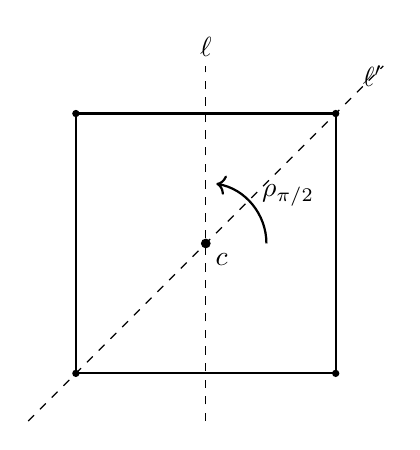
\begin{tikzpicture}[scale=1.1]
% the square
\draw[thick] (-1.5,-1.5) rectangle (1.5,1.5);
% center
\fill (0,0) circle (1.6pt);
\node[below right] at (0,0) {$c$};
% rotation arrow (quarter turn)
\draw[->,thick] (0.7,0) arc[start angle=0, end angle=80, radius=0.7];
\node at (0.95,0.55) {$\rho_{\pi/2}$};
% a mirror line (vertical edge-bisector), extended
\draw[dashed] (0,-2.05) -- (0,2.05);
\node[above] at (0,2.05) {$\ell$};
% a diagonal mirror, lightly
\draw[dashed] (-2.05,-2.05) -- (2.05,2.05);
\node[above right] at (1.7,1.7) {$\ell'$};
% vertices
\foreach \p in {(-1.5,-1.5),(1.5,-1.5),(1.5,1.5),(-1.5,1.5)} \fill \p circle (1.2pt);
\end{tikzpicture}
\]

Reflection in $\ell$ is the orientation-reversing generator (its fixed-point set is the whole line $\ell$), while the quarter-turn $\rho_{\pi/2}$ about $c$ is the orientation-preserving generator (its only fixed point is $c$). Composing the two reflections in $\ell$ and $\ell'$, whose lines meet at $c$ at angle $\pi/4$, gives the rotation through $\pi/2$ about $c$ -- the ``two reflections make a rotation'' principle in action, and the reason a square's symmetry group is generated by a single mirror together with a single quarter-turn.


\section{Finite Groups of Orthogonal Operators on the Plane}
\subsection*{Finite groups of orthogonal operators on the plane}

The orthogonal group $\mathrm{O}(2)$ consists of the linear isometries of the plane fixing the
origin. Its elements come in two kinds: the rotations $\rho_\theta$ about the origin and the
reflections $\rho_\theta r$ about lines through the origin, where $r$ is a fixed reference
reflection. In a coordinate system whose horizontal axis is the line of $r$,
\[
\rho_\theta=\begin{pmatrix} c & -s \\ s & c \end{pmatrix},
\qquad
r=\begin{pmatrix} 1 & 0 \\ 0 & -1 \end{pmatrix},
\qquad c=\cos\theta,\ s=\sin\theta .
\]
A matrix in $\mathrm{O}(2)$ has determinant $+1$ (a rotation) or $-1$ (a reflection). The goal of
this section is to classify all \emph{finite} subgroups of $\mathrm{O}(2)$: there are only two
families, the cyclic groups $C_n$ and the dihedral groups $D_n$.

\subsection*{The dihedral group and its presentation}

\begin{definition}[Dihedral group $D_n$]
Fix $\theta=2\pi/n$, write $x=\rho_\theta$ for the rotation through $\theta$ and $y=r$ for the
standard reflection. The \emph{dihedral group} $D_n$ is the subgroup of $\mathrm{O}(2)$ generated
by $x$ and $y$. Its $2n$ elements are the $n$ rotations $x^k$ and the $n$ reflections $x^k y$ for
$0\le k\le n-1$. (This is Artin's notation: the group of order $2n$ that D\&F write $D_{2n}$ is
$D_n$ here, so the symmetry group of the square, written $D_8$ above, is $D_4$ below.)
\end{definition}

The single rule needed to multiply in $D_n$ is the commutation law between a rotation and a
reflection. Reflecting, then rotating by $\theta$, is the same as rotating by $-\theta$, then
reflecting: in matrices,
\[
y\,x\,y\inv=r\,\rho_\theta\,r\inv
=\begin{pmatrix}1&0\\0&-1\end{pmatrix}
 \begin{pmatrix}c&-s\\s&c\end{pmatrix}
 \begin{pmatrix}1&0\\0&-1\end{pmatrix}
=\begin{pmatrix}c&s\\-s&c\end{pmatrix}=\rho_{-\theta}=x\inv .
\]

\begin{proposition}[Presentation of $D_n$]\label{art:finite_orthogonal:pres@c4}
The dihedral group $D_n$ has order $2n$. It is generated by two elements $x$ and $y$ satisfying
\[
x^n=1,\qquad y^2=1,\qquad yx=x\inv y .
\]
Using the first two relations, the third is equivalent to $xyxy=1$ and also to $yx=x^{n-1}y$.
\end{proposition}

\begin{proof}
We have $x^n=\rho_\theta^{\,n}=\rho_{2\pi}=1$ and $y^2=r^2=1$. The matrix computation above gives
$yxy\inv=x\inv$, i.e.\ $yx=x\inv y$. Multiplying $yx=x\inv y$ on the left by $x$ and on the right
by $y\inv=y$ rearranges it as $xyxy=1$; and since $x\inv=x^{n-1}$, it is also $yx=x^{n-1}y$. The
rule $yx=x\inv y$ lets every word in $x,y$ be pushed into the normal form $x^k y^{\varepsilon}$
with $0\le k<n$ and $\varepsilon\in\{0,1\}$, so there are at most $2n$ elements; the $n$ rotations
$x^k$ and $n$ reflections $x^k y$ are visibly distinct (determinants $+1$ and $-1$ separate the
two blocks, and within each block the matrices differ). Hence $|D_n|=2n$.
\end{proof}

\begin{remark}
For $n\ge3$ the elements of $D_n$ are exactly the orthogonal operators carrying a regular
$n$-gon centered at the origin to itself --- its \emph{symmetry group}. The small cases are
degenerate: $D_1=\{1,r\}$ has order $2$ (a single reflection) and $D_2=\{1,\rho_\pi,r,\rho_\pi r\}$
has order $4$ and is isomorphic to the Klein four-group $V_4$. When $n=3$ the relations
$x^3=y^2=1,\ yx=x\inv y$ are precisely those of $S_3$, so $D_3\isom S_3$.
\end{remark}

\subsection*{The classification theorem}

A subgroup $\Gamma$ of the additive group $\R$ is \emph{discrete} if there is a small
$\epsilon>0$ such that every nonzero element of $\Gamma$ has absolute value $\ge\epsilon$. The
proof of the classification rests on the following description of such subgroups, the additive
analogue of ``every subgroup of $\Z$ is $\Z n$.''

\begin{lemma}[Discrete subgroups of $\R$]\label{art:finite_orthogonal:disc@c4}
Let $\Gamma$ be a discrete subgroup of $\R$. Then either $\Gamma=\{0\}$, or $\Gamma=\Z a$, the set
of integer multiples of a positive real number $a$.
\end{lemma}

\begin{proof}
If $a,b\in\Gamma$ are distinct then $a-b\in\Gamma$ and $|a-b|\ge\epsilon$, so distinct elements
are separated by at least $\epsilon$; hence any bounded interval contains only finitely many
elements of $\Gamma$. Suppose $\Gamma\ne\{0\}$. Then $\Gamma$ contains a positive element, and we
may choose the \emph{smallest} positive element $a$ (the candidates below any fixed positive
member form a finite set). Since $a\in\Gamma$, $\Z a\subseteq\Gamma$. Conversely take $b\in\Gamma$
and write $b=ra$ with $r\in\R$; put $r=m+r_0$, $m\in\Z$, $0\le r_0<1$. Then $b'=b-ma=r_0a\in\Gamma$
with $0\le b'<a$, and minimality of $a$ forces $b'=0$, so $b=ma\in\Z a$. Thus $\Gamma=\Z a$.
\end{proof}

\begin{theorem}[Finite subgroups of $\mathrm{O}(2)$]\label{art:finite_orthogonal:main@c4}
Let $G$ be a finite subgroup of the orthogonal group $\mathrm{O}(2)$. Then there is an integer $n$
such that $G$ is one of:
\begin{enumerate}
\item $C_n$: the cyclic group of order $n$ generated by the rotation $\rho_\theta$, $\theta=2\pi/n$;
\item $D_n$: the dihedral group of order $2n$ generated by $\rho_\theta$ and a reflection $r$ in a
line through the origin.
\end{enumerate}
\end{theorem}

\begin{proof}
Recall the elements of $\mathrm{O}(2)$ are the rotations $\rho_\alpha$ and the reflections
$\rho_\alpha r$.

\emph{Case 1: every element of $G$ is a rotation.} Let
$\Gamma=\{\alpha\in\R\st\rho_\alpha\in G\}$. Since $\rho_\alpha\rho_\beta=\rho_{\alpha+\beta}$,
$\Gamma$ is a subgroup of $(\R,+)$, and it contains $2\pi$. As $G$ is finite, $\Gamma$ is discrete.
By Lemma~\ref{art:finite_orthogonal:disc@c4}, $\Gamma=\Z\alpha$ for some $\alpha>0$. Since
$2\pi\in\Gamma=\Z\alpha$, we have $2\pi=n\alpha$ for an integer $n$, i.e.\ $\alpha=2\pi/n$. Then
$G$ consists of the rotations through integer multiples of $2\pi/n$, so $G=C_n$.

\emph{Case 2: $G$ contains a reflection.} Choose coordinates so the standard reflection $r$ lies
in $G$. Let $H$ be the subgroup of rotations in $G$. By Case 1, $H=C_n$ is generated by
$\rho_\theta$ with $\theta=2\pi/n$. The $2n$ products $\rho_\theta^{\,k}$ and $\rho_\theta^{\,k}r$
($0\le k<n$) all lie in $G$, so $D_n\subseteq G$. Conversely take any $g\in G$. If $g$ is a
rotation, then $g\in H\subseteq D_n$. If $g$ is a reflection, write $g=\rho_\alpha r$; since
$r\in G$, the product $gr=\rho_\alpha\in G$ is a rotation, hence a power of $\rho_\theta$, so
$g=\rho_\theta^{\,k}r\in D_n$. Therefore $G=D_n$.
\end{proof}

\begin{method}{Identifying a finite plane symmetry group}
\textbf{Trigger:} ``name the symmetry group of this figure / this finite group of plane isometries.''
\begin{enumerate}
\item Decide whether any element \emph{reverses orientation} (a reflection, $\det=-1$). If none,
  the group is rotations only.
\item Find the smallest rotation angle present, $2\pi/n$. The rotations form $C_n$.
\item No reflection $\Rightarrow$ the whole group is $C_n$. At least one reflection $\Rightarrow$
  the group is $D_n$ (order $2n$), generated by that rotation and one reflection.
\item Sanity check the order: $|C_n|=n$, $|D_n|=2n$.
\end{enumerate}
\end{method}

\begin{corollary}[$D_3\isom S_3$]\label{art:finite_orthogonal:d3s3@c4}
The dihedral group $D_3$ and the symmetric group $S_3$ are isomorphic.
\end{corollary}

\begin{proof}
By Proposition~\ref{art:finite_orthogonal:pres@c4} the group $D_3$ has the presentation
$x^3=y^2=1,\ yx=x\inv y$, the same relations as the standard presentation of $S_3$ on a $3$-cycle
$x$ and a transposition $y$; both groups have order $6$, so the relation-respecting map
$x\mapsto(1\,2\,3),\ y\mapsto(1\,2)$ is an isomorphism.
\end{proof}

\subsection*{The fixed point theorem}

So far the operators fixed the origin. A general isometry of the plane may move every point. The
next theorem shows a finite group of isometries always has a common fixed point, which we may then
take as the origin --- reducing the symmetry group of a bounded figure to the orthogonal case
above.

\begin{theorem}[Fixed Point Theorem]\label{art:finite_orthogonal:fixed@c4}
Let $G$ be a finite group of isometries of the plane. Then there is a point $p$ fixed by every
element of $G$: $g(p)=p$ for all $g\in G$.
\end{theorem}

\begin{proof}
Pick any point $s$ and form its \emph{orbit} $S=\{g(s)\st g\in G\}=\{s_1,\dots,s_m\}$. Each $h\in G$
permutes $S$: if $s'=g(s)\in S$ then $h(s')=hg(s)\in S$ because $hg\in G$. Let $p$ be the
\emph{centroid} of the orbit,
\[
p=\frac1m\,(s_1+s_2+\cdots+s_m),
\]
computed by vector addition in any coordinate system. Isometries carry centroids to centroids
(Lemma~\ref{art:finite_orthogonal:centroid@c4}); since each $g\in G$ merely permutes $S$, it sends the
centroid of $S$ to the centroid of $S$, i.e.\ $g(p)=p$. Thus $p$ is fixed by every element of $G$.
\end{proof}

\begin{lemma}[Isometries carry centroids to centroids]\label{art:finite_orthogonal:centroid@c4}
Let $S=\{s_1,\dots,s_m\}$ with centroid $p=\frac1m\sum_i s_i$, and let $\varphi$ be an isometry.
Then $\varphi(p)$ is the centroid of $\varphi(S)=\{\varphi(s_1),\dots,\varphi(s_m)\}$.
\end{lemma}

\begin{proof}
Every isometry is a composition of a translation $t_a(v)=v+a$ and a linear orthogonal operator, so
it suffices to check the two cases. \emph{Translation:} with $s_i'=s_i+a$,
$\frac1m\sum_i s_i'=\bigl(\frac1m\sum_i s_i\bigr)+a=p+a=t_a(p)$. \emph{Linear operator $\varphi$:}
by linearity $\varphi(p)=\varphi\bigl(\frac1m\sum_i s_i\bigr)=\frac1m\sum_i\varphi(s_i)$, the
centroid of $\varphi(S)$. Composing the two cases proves the lemma for every isometry.
\end{proof}

The orbit and its centroid are shown below for the symmetries of a regular pentagon: the five
images of a point lie on a circle about the fixed centroid $p$.
\[
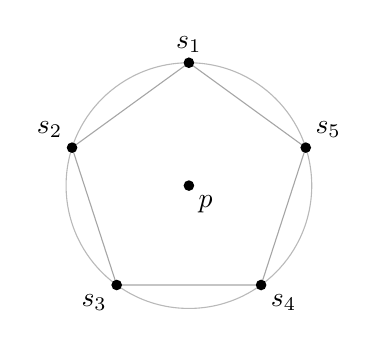
\begin{tikzpicture}[scale=1.2]
\coordinate (p) at (0,0);
\foreach \k in {0,1,2,3,4}{
  \coordinate (s\k) at ({90+72*\k}:1.3);
}
\draw[gray!55] (0,0) circle (1.3);
\draw[gray!70] (s0)--(s1)--(s2)--(s3)--(s4)--cycle;
\foreach \k in {0,1,2,3,4}{
  \fill (s\k) circle (1.6pt);
}
\fill (p) circle (1.6pt);
\node[below right] at (p) {$p$};
\node[above] at (s0) {$s_1$};
\node[above left] at (s1) {$s_2$};
\node[below left] at (s2) {$s_3$};
\node[below right] at (s3) {$s_4$};
\node[above right] at (s4) {$s_5$};
\end{tikzpicture}
\]

\begin{corollary}[Symmetry groups of bounded plane figures]\label{art:finite_orthogonal:bounded@c4}
Let $G$ be a finite subgroup of the group of all isometries of the plane (in particular, the
symmetry group of a bounded plane figure, when that group is finite; a disk has the infinite
symmetry group $\mathrm{O}(2)$). For suitable coordinates $G$ is one of the groups
$C_n$ or $D_n$.
\end{corollary}

\begin{proof}
By Theorem~\ref{art:finite_orthogonal:fixed@c4}, $G$ fixes a point $p$. Translate coordinates so that
$p$ is the origin. Every element of $G$ then fixes the origin, so $G\subseteq\mathrm{O}(2)$. Being
finite, $G$ is $C_n$ or $D_n$ by Theorem~\ref{art:finite_orthogonal:main@c4}.
\end{proof}

\subsection*{$D_4$ acting on a square}

The square has the eight symmetries of $D_4$: four rotations $1,\rho,\rho^2,\rho^3$ through
multiples of $90^\circ$, and four reflections --- two in the diagonals and two in the
horizontal/vertical midlines. The reflection axes are drawn below.
\[
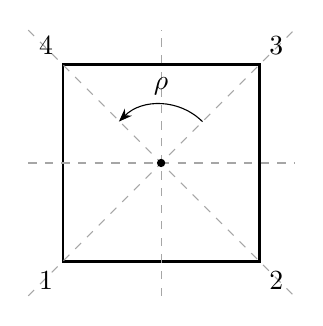
\begin{tikzpicture}[scale=1.25]
\coordinate (A) at (-1,-1);
\coordinate (B) at ( 1,-1);
\coordinate (C) at ( 1, 1);
\coordinate (D) at (-1, 1);
\draw[thick] (A)--(B)--(C)--(D)--cycle;
% reflection axes
\draw[dashed,gray!70] (-1.35,0)--(1.35,0);
\draw[dashed,gray!70] (0,-1.35)--(0,1.35);
\draw[dashed,gray!70] (-1.35,-1.35)--(1.35,1.35);
\draw[dashed,gray!70] (-1.35,1.35)--(1.35,-1.35);
% rotation arrow
\draw[->,>=Stealth] (0.42,0.42) arc (45:135:0.6);
\node at (0,0.78) {$\rho$};
\node[below left] at (A) {$1$};
\node[below right] at (B) {$2$};
\node[above right] at (C) {$3$};
\node[above left] at (D) {$4$};
\fill (0,0) circle (1.2pt);
\end{tikzpicture}
\]
Numbering the vertices $1,2,3,4$ counterclockwise, the rotation $x=\rho$ acts as the $4$-cycle
$(1\,2\,3\,4)$ and the reflection $y$ in the vertical midline as $(1\,2)(3\,4)$; one checks
$x^4=y^2=1$ and $yx=x\inv y$, realizing $D_4$ as a group of permutations of the four vertices.

\begin{wex}{Symmetries of a regular hexagon}
Name the full symmetry group of a regular hexagon centered at the origin and list its elements by
type.
\wrec The figure is bounded and has only finitely many symmetries, so its symmetry group is $C_n$ or $D_n$
(Corollary~\ref{art:finite_orthogonal:bounded@c4}); a regular $n$-gon with $n\ge3$ has both rotations
and reflections, giving $D_n$.
\wsol A regular hexagon is carried to itself by rotation through $60^\circ=2\pi/6$, so the
rotation subgroup is $C_6=\{1,\rho,\rho^2,\dots,\rho^5\}$, where $\rho=\rho_{2\pi/6}$. It also has
reflection symmetry, so by Theorem~\ref{art:finite_orthogonal:main@c4} the full group is $D_6$, of
order $12$. Its $12$ elements are the $6$ rotations $\rho^k$ ($0\le k\le5$) and the $6$ reflections
$\rho^k r$: three reflections in the lines through opposite vertices and three through midpoints of
opposite edges.
\emph{Check:} $|D_6|=2\cdot6=12$; six orientation-preserving ($\det=+1$) and six
orientation-reversing ($\det=-1$) elements, matching the rotation/reflection split. \checkmark
\end{wex}

\begin{wex}{A figure with only rotational symmetry}
A pinwheel is drawn by attaching four identical curved (chiral) blades to a central hub, each blade
obtained from the previous by a $90^\circ$ rotation. Determine its symmetry group.
\wrec Look for orientation-reversing symmetry first
(Method above). A chiral blade has no mirror line, so no reflection can be a symmetry; only
rotations survive.
\wsol Rotation by $90^\circ=2\pi/4$ carries each blade onto the next, so $\rho_{2\pi/4}$ is a
symmetry and the rotation subgroup is $C_4=\{1,\rho,\rho^2,\rho^3\}$. A reflection would reverse
the handedness of every blade, turning a left-curved blade into a right-curved one, which is
\emph{not} the original figure; hence no reflection is a symmetry. By
Theorem~\ref{art:finite_orthogonal:main@c4} the symmetry group is therefore $C_4$, \emph{not} $D_4$.
\emph{Check:} $|C_4|=4$, all with $\det=+1$; the figure looks the same after $0^\circ,90^\circ,
180^\circ,270^\circ$ and different in a mirror, exactly the cyclic (chiral) case. \checkmark
\end{wex}

\begin{wex}{Reading off the relation $yx=x\inv y$ on the square}
Using the vertex permutations $x=(1\,2\,3\,4)$ and $y=(1\,2)(3\,4)$ for $D_4$, verify
$yx=x\inv y$.
\wrec This is the dihedral commutation law from Proposition~\ref{art:finite_orthogonal:pres@c4};
compute both sides as permutations.
\wsol Compose right-to-left. Left side $yx$: apply $x$ then $y$. Tracking
$1\xmapsto{x}2\xmapsto{y}1$, $2\xmapsto{x}3\xmapsto{y}4$, $3\xmapsto{x}4\xmapsto{y}3$,
$4\xmapsto{x}1\xmapsto{y}2$, so $yx=(2\,4)$. Right side $x\inv y$ with $x\inv=(1\,4\,3\,2)$:
$1\xmapsto{y}2\xmapsto{x\inv}1$, $2\xmapsto{y}1\xmapsto{x\inv}4$, $3\xmapsto{y}4\xmapsto{x\inv}3$,
$4\xmapsto{y}3\xmapsto{x\inv}2$, so $x\inv y=(2\,4)$. The two agree.
\emph{Check:} $yx=x\inv y$ holds, and $(2\,4)$ is a reflection ($\det=-1$ on the square), as it
must be since it is a product of a reflection and a rotation. \checkmark
\end{wex}

\begin{pitfall}
The presence of $n$-fold rotational symmetry does \emph{not} by itself make the group $D_n$. Only
a figure that also admits a mirror line is dihedral; a chiral figure (like the pinwheel) with
$n$-fold rotation has the smaller group $C_n$ of order $n$, not $D_n$ of order $2n$. Always test
for an orientation-reversing symmetry before naming the group.
\end{pitfall}


\section{Discrete Groups, Lattices, and the Crystallographic Restriction}
\subsection*{Discrete Groups, Translation Lattices, and Point Groups}

To do geometry with an infinite group of symmetries --- the symmetries of a wallpaper pattern or a planar crystal, not just of a bounded figure --- we must first rule out groups that crowd arbitrarily close to the identity. A group with arbitrarily small rotations or translations has no sensible geometry. The condition that forbids this is \emph{discreteness}, and it has remarkable structural consequences: the translations form one of only three shapes, and the rotational symmetries are always finite.

Throughout, $M$ denotes the group of isometries of the plane $P$, $V$ the (additive) group of translation vectors, and $t_v$ the translation by $v$. We write $\rho_\theta$ for the rotation through angle $\theta$ about the origin and $\mathrm{O}(2)$ for the orthogonal group.

\begin{definition}[Discrete group of isometries]
A subgroup $G\sgr M$ is \emph{discrete} if there is a real number $\varepsilon>0$ such that:
\begin{enumerate}
\item[(i)] if $t_a\in G$ is a translation by a nonzero vector $a$, then $\lvert a\rvert\ge\varepsilon$, and
\item[(ii)] if $g\in G$ is a rotation through a nonzero angle $\theta$ about some point of $P$, then $\lvert\theta\rvert\ge\varepsilon$.
\end{enumerate}
\end{definition}

\begin{remark}
The same $\varepsilon$ governs both vectors and angles; we do not care about optimal bounds, only that one positive bound works for all nonzero translations and rotations at once. No condition is imposed on the orientation-reversing isometries: if $m$ is a glide with glide vector $w$, then $m^2=t_{2w}$ is a translation, so the bound on translation lengths already controls the glides.
\end{remark}

Artin singles out three tools for dissecting a discrete $G$: its \emph{translation group} $L\sgr V$, its \emph{point group} $\overline G\sgr\mathrm{O}(2)$, and an operation of $\overline G$ on $L$. We take them in turn.

\subsection*{The translation group and its classification}

\begin{definition}[Translation group; discrete subgroup of $V$]
The \emph{translation group} of $G\sgr M$ is
\[
L=\{\,v\in V \st t_v\in G\,\}.
\]
Since $t_vt_w=t_{v+w}$ and $t_v\inv=t_{-v}$, $L$ is a subgroup of $V$. A subgroup $L\sgr V$ (or $L\sgr\R^n$) is itself called \emph{discrete} if there is $\varepsilon>0$ with $\lvert v\rvert\ge\varepsilon$ for every nonzero $v\in L$. The bound on translations in a discrete $G$ makes its $L$ a discrete subgroup of $V$.
\end{definition}

\begin{remark}
Discreteness of $L$ is equivalently a \emph{separation} statement: distinct $a,b\in L$ satisfy $\lvert b-a\rvert\ge\varepsilon$, because $b-a\in L$ and $\lvert b-a\rvert\ge\varepsilon$ by hypothesis. So the points of a discrete $L$ are uniformly spread out, never accumulating.
\end{remark}

The engine behind everything is the existence of a shortest nonzero vector.

\begin{lemma}[Minimal vector]\label{art:discrete_groups:minvec@c4}
Let $L\sgr V$ be discrete.
\begin{enumerate}
\item[(a)] Any bounded region of the plane contains only finitely many points of $L$.
\item[(b)] If $L\ne\{0\}$, it contains a nonzero vector of \emph{minimal length}.
\end{enumerate}
\end{lemma}

\begin{proof}
(a) The points of $L$ are pairwise at distance $\ge\varepsilon$, so a square of side $<\varepsilon/2$ contains at most one point of $L$ (any two would be within distance $<\varepsilon$). A bounded region lies inside some large rectangle, which is covered by finitely many such squares; hence it meets $L$ in finitely many points.

(b) Pick any nonzero $a\in L$. The closed disk of radius $\lvert a\rvert$ about the origin is bounded, so by (a) it contains only finitely many points of $L$, among them $a$. Finitely many nonzero lengths occur, so a smallest one is attained; the corresponding vector is a nonzero vector of minimal length.
\end{proof}

To turn a candidate basis into a genuine description of $L$ we need the \emph{fundamental parallelogram}. For a basis $B=(u,w)$ of $\R^2$ let $\Pi'(B)$ denote the half-open parallelogram
\[
\Pi'(B)=\{\,ru+sw \st 0\le r<1,\ 0\le s<1\,\},
\]
that is, the parallelogram with vertices $0,u,w,u+w$ with the two far edges deleted.

\begin{lemma}[Fundamental domain]\label{art:discrete_groups:funddom@c4}
Let $B=(u,w)$ be a basis of $\R^2$ and let $L=\Z u+\Z w$ be the lattice of integer combinations. Every $v\in\R^2$ is written \emph{uniquely} as $v=x+v_0$ with $x\in L$ and $v_0\in\Pi'(B)$.
\end{lemma}

\begin{proof}
Since $B$ is a basis, $v=ru+sw$ for unique reals $r,s$. Split off integer parts: $r=m+r_0$, $s=n+s_0$ with $m,n\in\Z$ and $0\le r_0,s_0<1$. Then $v=x+v_0$ with $x=mu+nw\in L$ and $v_0=r_0u+s_0w\in\Pi'(B)$. Uniqueness: if $x+v_0=x'+v_0'$ with $x,x'\in L$ and $v_0,v_0'\in\Pi'(B)$, then $v_0-v_0'=x'-x\in L$ has integer coordinates in $B$, yet each coordinate lies strictly between $-1$ and $1$; the only such integer is $0$, so $v_0=v_0'$ and $x=x'$.
\end{proof}

\begin{theorem}[Classification of discrete subgroups of the plane]\label{art:discrete_groups:classify@c4}
Every discrete subgroup $L\sgr V$ (equivalently $L\sgr\R^2$) is exactly one of:
\begin{enumerate}
\item[(a)] the trivial group $L=\{0\}$;
\item[(b)] an infinite cyclic group $L=\Z a=\{\,ma \st m\in\Z\,\}$ for some nonzero $a$; or
\item[(c)] a \emph{lattice} $L=\Z a+\Z b=\{\,ma+nb \st m,n\in\Z\,\}$ for two linearly independent $a,b$.
\end{enumerate}
In case (c), $(a,b)$ is called a \emph{lattice basis}.
\end{theorem}

\begin{proof}
The trivial group is case (a). Assume $L\ne\{0\}$, and split on whether $L$ spans a line.

\emph{Case 1: all of $L$ lies on a line $\ell$ through the origin.} Identify $\ell$ with $\R$; then $L\sgr\R$ is discrete, so by Lemma~\ref{art:discrete_groups:minvec@c4} it has a shortest nonzero vector $a$. If some $v\in L$ were not an integer multiple of $a$, subtract the nearest multiple: $v-ma\in L$ would be nonzero with $\lvert v-ma\rvert<\lvert a\rvert$, contradicting minimality. Hence $L=\Z a$, case (b).

\emph{Case 2: $L$ does not lie on a line.} Then $L$ contains independent vectors, so we may choose coordinates with $a=(1,0)^t$ a shortest nonzero vector of $L$ on the horizontal axis $\ell$ (using Case~1 on $L\cap\ell=\Z a$). Among the vectors of $L$ with positive second coordinate, choose $b=(b_1,b_2)^t$ with $b_2$ \emph{as small as possible}; adding a multiple of $a$ we may also take $0\le b_1<1$. This $b$ exists: such vectors with $0\le b_1<1$ and $b_2$ bounded above by any fixed candidate lie in a bounded region, which meets $L$ finitely often by Lemma~\ref{art:discrete_groups:minvec@c4}(a).

Set $\widetilde L=\Z a+\Z b\subseteq L$; we show $\widetilde L=L$. By Lemma~\ref{art:discrete_groups:funddom@c4} applied to $B=(a,b)$, it suffices to show the only point of $L$ in $\Pi'(B)$ is $0$. Let $c=(c_1,c_2)^t\in L\cap\Pi'(B)$, so $0\le c_2<b_2$. Minimality of $b_2$ forces $c_2=0$, so $c$ lies on $\ell$, hence $c\in\Z a$; but $0\le c_1<1$ leaves only $c=0$. Therefore $L=\Z a+\Z b$ is a lattice, case (c).
\end{proof}

\begin{center}
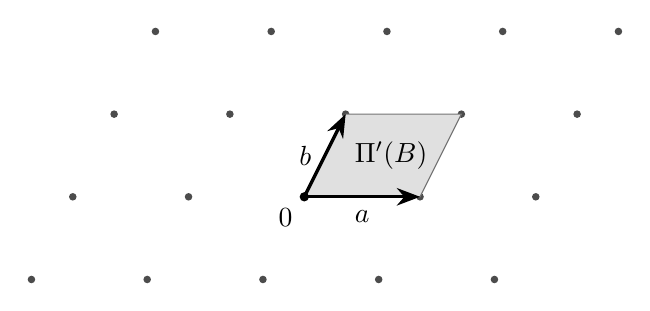
\begin{tikzpicture}[scale=1.05,>=Stealth]
% lattice points
\foreach \i in {-1,0,1,2,3}{
  \foreach \j in {-1,0,1,2}{
    \fill[black!70] (\i*1.4+\j*0.5, \j*1.0) circle (1.3pt);
  }
}
% fundamental parallelogram on basis a=(1.4,0), b=(0.5,1.0), anchored at a lattice point
\coordinate (O) at (1.4,0);
\coordinate (A) at (2.8,0);   % O + a
\coordinate (B) at (1.9,1.0); % O + b
\coordinate (C) at (3.3,1.0); % O + a + b
\fill[black!12] (O) -- (A) -- (C) -- (B) -- cycle;
\draw[black!55] (O) -- (A) -- (C) -- (B) -- cycle;
% basis vectors
\draw[->,very thick] (O) -- (A) node[midway,below=1pt] {$a$};
\draw[->,very thick] (O) -- (B) node[midway,left=1pt] {$b$};
\fill[black] (O) circle (1.6pt);
\node[below left=1pt] at (O) {$0$};
\node at (2.45,0.5) {$\Pi'(B)$};
\end{tikzpicture}
\end{center}

\begin{wex}{Reading off the three types}
Problem. Classify each subgroup of $\R^2$: (i) $L_1=\Z(2,0)$; (ii) $L_2=\Z(1,0)+\Z(0,1)$; (iii) $L_3=\{\,(x,y)\st x,y\in\Z,\ x+y\text{ even}\,\}$.
\wrec Each is a subgroup of $V$; decide \emph{trivial / line / lattice} by whether it lies on a line and, if a lattice, find a basis (Theorem~\ref{art:discrete_groups:classify@c4}).
\wsol
(i) Every vector is a multiple of $(2,0)$, on the horizontal axis: type (b), infinite cyclic, $L_1=\Z(2,0)$.
(ii) $(1,0)$ and $(0,1)$ are independent and generate all integer points: type (c), the square lattice $\Z^2$.
(iii) The condition $x+y$ even is a subgroup (sums of even-sum vectors have even sum). It contains the independent vectors $(1,1)$ and $(1,-1)$, and every even-sum integer vector is an integer combination of these: $(x,y)=\tfrac{x+y}{2}(1,1)+\tfrac{x-y}{2}(1,-1)$ with both coefficients integers since $x+y,x-y$ are even. Type (c), a lattice with basis $((1,1),(1,-1))$.
\textbf{Check:} each minimal nonzero length is positive --- $2$, $1$, $\sqrt2$ respectively --- so all three are genuinely discrete, and no list entry is omitted.
\end{wex}

\subsection*{The point group is finite}

The homomorphism $\pi:M\to\mathrm{O}(2)$ with kernel the translations $T$ (it strips an isometry of its translational part) restricts to $G$.

\begin{definition}[Point group]
The \emph{point group} of $G\sgr M$ is $\overline G=\pi(G)\sgr\mathrm{O}(2)$. We bar symbols of $\overline G$: for $g\in G$, $\overline g=\pi(g)$ is an orthogonal operator. Thus $\overline G$ records the rotation angles and the reflection/glide slopes occurring in $G$, forgetting the translation part.
\end{definition}

\begin{proposition}[Discrete subgroups of $\mathrm{O}(2)$ are finite]\label{art:discrete_groups:Ofinite@c4}
A discrete subgroup $\overline G\sgr\mathrm{O}(2)$ is finite, hence cyclic or dihedral.
\end{proposition}

\begin{proof}
Let $\Gamma=\{\,\theta\in\R \st \rho_\theta\in\overline G\,\}$ be the set of rotation angles in $\overline G$. It is a subgroup of $\R$ (composing rotations adds angles) containing $2\pi$, and it is discrete because $\overline G$ contains no arbitrarily small rotations. A discrete subgroup of $\R$ is infinite cyclic (the line case of Theorem~\ref{art:discrete_groups:classify@c4}): take the smallest positive angle $\theta_0$, so $\Gamma=\Z\theta_0$; since $2\pi\in\Gamma$ we get $2\pi=n\theta_0$, i.e. $\theta_0=2\pi/n$ for some positive integer $n$. So the rotations in $\overline G$ form a cyclic group of order $n$. If $\overline G$ contains a reflection, it is dihedral $D_n$; otherwise it is cyclic $C_n$. Either way $\lvert\overline G\rvert<\infty$.
\end{proof}

\begin{wex}{Why ``discrete'' is essential}
Problem. Show the full group $\mathrm{SO}(2)$ of all rotations about the origin is a subgroup of $\mathrm{O}(2)$ that is \emph{not} discrete, and exhibit arbitrarily small rotations in it.
\wrec Proposition~\ref{art:discrete_groups:Ofinite@c4} concludes finiteness only \emph{under} discreteness; to see the hypothesis is needed, produce a non-discrete subgroup violating the conclusion.
\wsol
$\mathrm{SO}(2)=\{\,\rho_\theta \st \theta\in\R\,\}$ is closed under composition and inverses, so it is a subgroup. For any $\varepsilon>0$ the rotation $\rho_{\varepsilon/2}$ is a nonzero rotation with angle $\varepsilon/2<\varepsilon$, so no single $\varepsilon$ bounds all nonzero angles from below: $\mathrm{SO}(2)$ is not discrete. And it is infinite, so the finiteness conclusion genuinely fails.
\textbf{Check:} the rotations $\rho_{2\pi/n}$ generate the finite cyclic group $C_n\sgr\mathrm{SO}(2)$ for each $n$, and these $C_n$ \emph{are} discrete --- discreteness, not membership in $\mathrm{O}(2)$, is exactly what forces finiteness.
\end{wex}

\subsection*{The point group operates on the lattice}

The third tool links the first two. Although $\overline G$ does not act on the plane $P$ (no origin is fixed), it does act on the vector space $V$ of translation vectors.

\begin{proposition}[$\overline G$ preserves $L$]\label{art:discrete_groups:preserveL@c4}
Let $G\sgr M$, with translation group $L$ and point group $\overline G$. For every $a\in L$ and every $\overline g\in\overline G$, we have $\overline g(a)\in L$. Equivalently, $\overline G$ lies in the group of symmetries of $L$ regarded as a figure in $V$.
\end{proposition}

\begin{proof}
Take $g\in G$ with image $\overline g$, and set $a'=\overline g(a)$. Write $g=t_b\varphi$ with $\varphi\in\mathrm{O}(2)$, so $\overline g=\varphi$ and $a'=\varphi(a)$. Conjugating the translation $t_a$ (which is in $G$ since $a\in L$) by $g$, and using $\varphi\,t_a\,\varphi\inv=t_{\varphi(a)}$,
\[
g\,t_a\,g\inv=(t_b\varphi)\,t_a\,(\varphi\inv t_{-b})=t_b\,t_{\varphi(a)}\,t_{-b}=t_{\varphi(a)}=t_{a'}.
\]
Both $g$ and $t_a$ lie in $G$, so the conjugate $t_{a'}\in G$; therefore $a'\in L$.
\end{proof}

\begin{remark}
It is genuinely important that $\overline G$ acts on $L\subseteq V$, not that $G$ acts on $L$: the elements of $G$ are isometries of $P$, while $L$ lives in $V$, and $P$ is identified with $V$ only after an origin is chosen. The clean statement is the one above --- the orthogonal \emph{point} group permutes the lattice.
\end{remark}

This single fact is the gateway to crystallography. Because the point group must permute a lattice, its rotations cannot be arbitrary.

\begin{theorem}[Crystallographic restriction]\label{art:discrete_groups:crystal@c4}
Let $L\sgr V$ be a nontrivial discrete subgroup and let $H\sgr\mathrm{O}(2)$ be a subgroup carrying $L$ to itself. Then every rotation in $H$ has order $1,2,3,4,$ or $6$; consequently $H$ is one of $C_n$ or $D_n$ with $n\in\{1,2,3,4,6\}$. In particular five-fold rotational symmetry is impossible.
\end{theorem}

\begin{proof}
Let $\rho\in H$ be a nontrivial rotation, through an angle $\theta$ with $0<\theta\le\pi$ (replace $\rho$ by $\rho\inv$ if necessary), and let $a\in L$ be a nonzero vector of minimal length (Lemma~\ref{art:discrete_groups:minvec@c4}). Since $H$ preserves $L$, $\rho(a)\in L$, hence $b=\rho(a)-a\in L$. By minimality $\lvert b\rvert\ge\lvert a\rvert$. But $\lvert b\rvert=\lvert\rho(a)-a\rvert=2\lvert a\rvert\sin(\theta/2)$, and $2\sin(\theta/2)<1$ exactly when $0<\theta<\pi/3=2\pi/6$. So $\lvert b\rvert<\lvert a\rvert$ for $0<\theta<2\pi/6$, which is forbidden; hence $\theta\ge2\pi/6$ for every nontrivial rotation in $H$. Thus $H$ is discrete, hence finite by Proposition~\ref{art:discrete_groups:Ofinite@c4}; its rotations form a cyclic group generated by $\rho_{2\pi/n}$, and $2\pi/n\ge2\pi/6$ gives $n\le6$, so $\rho$ has order at most $6$. Order $5$ ($\theta=2\pi/5$) is also excluded: there $b'=\rho^2(a)+a$ satisfies $\lvert b'\rvert<\lvert a\rvert$ (a short computation with $\cos(4\pi/5)=-(1+\sqrt5)/4<-1/2$ gives $\lvert b'\rvert^2=\lvert a\rvert^2(2+2\cos\tfrac{4\pi}{5})<\lvert a\rvert^2$), again contradicting minimality. So only orders $1,2,3,4,6$ survive, and by Proposition~\ref{art:discrete_groups:Ofinite@c4} $H$ is the corresponding $C_n$ or $D_n$.
\end{proof}

\begin{wex}{The point group operating on a lattice}
Problem. Let $L=\Z^2$ be the square lattice and let $\overline g=\rho_{\pi/2}$ be the quarter-turn. Verify $\overline g$ permutes $L$, find the order of $\overline g$ as a symmetry of $L$, and locate it on the crystallographic list.
\wrec This is Proposition~\ref{art:discrete_groups:preserveL@c4} made concrete (check $\overline g(a)\in L$ on a basis) followed by the order test of Theorem~\ref{art:discrete_groups:crystal@c4}.
\wsol
On the standard basis, $\rho_{\pi/2}(1,0)=(0,1)$ and $\rho_{\pi/2}(0,1)=(-1,0)$, both in $\Z^2$; since $\rho_{\pi/2}$ is linear it sends every integer combination to an integer combination, so $\overline g(L)=L$. As a symmetry $\overline g$ has order $4$ (four quarter-turns return to the identity), and $4\in\{1,2,3,4,6\}$, consistent with the restriction. The full symmetry group of $\Z^2$ in $\mathrm{O}(2)$ is $D_4$ (the quarter-turn together with a reflection).
\textbf{Check:} test the theorem's inequality with $a=(1,0)$: $b=\rho_{\pi/2}(a)-a=(-1,1)$ has $\lvert b\rvert=\sqrt2\ge1=\lvert a\rvert$, no contradiction, so order $4$ is allowed. For $\theta=2\pi/5$ this first test still passes ($2\sin36^\circ\approx1.18\ge1$); the lattice vector that is forced to be shorter than $a$ is $\rho^2(a)+a$, of length $2\cos72^\circ\,\lvert a\rvert\approx0.618\,\lvert a\rvert$ (next example) --- which is why no lattice has five-fold symmetry.
\end{wex}

\begin{wex}{No five-fold lattice symmetry, directly}
Problem. Suppose a nonzero discrete $L\sgr V$ admits a rotation $\rho$ of order $5$ as a symmetry. Derive a contradiction using a minimal vector.
\wrec The crystallographic restriction in action: assume the forbidden order and manufacture a shorter lattice vector (Theorem~\ref{art:discrete_groups:crystal@c4}).
\wsol
Let $a\in L$ be a shortest nonzero vector and $\theta=2\pi/5$. Then $\rho(a),\rho^2(a)\in L$, so $b'=\rho^2(a)+a\in L$. Compute
\[
\lvert b'\rvert^2=\lvert a\rvert^2+\lvert a\rvert^2+2\lvert a\rvert^2\cos\tfrac{4\pi}{5}=2\lvert a\rvert^2\bigl(1+\cos\tfrac{4\pi}{5}\bigr).
\]
Since $\cos\tfrac{4\pi}{5}=-\tfrac{1+\sqrt5}{4}\approx-0.809$, we get $\lvert b'\rvert^2\approx2\lvert a\rvert^2(0.191)\approx0.382\,\lvert a\rvert^2<\lvert a\rvert^2$. So $b'$ is a nonzero lattice vector shorter than $a$ --- contradicting minimality. (It is nonzero: $\rho^2(a)=-a$ would force $\rho^2$ to be the half-turn, of order $2$, incompatible with $\rho$ of order $5$.)
\textbf{Check:} the same computation with $\theta=2\pi/6$ gives $\cos\tfrac{2\pi}{3}=-\tfrac12$, so $\lvert b'\rvert^2=2\lvert a\rvert^2(1-\tfrac12)=\lvert a\rvert^2$, exactly the borderline --- order $6$ is allowed, order $5$ is not, precisely as the theorem predicts.
\end{wex}

\begin{remark}[Where this goes]
When $L$ is trivial, $\pi$ is injective on $G$, so $G\isom\overline G$ is finite cyclic or dihedral --- the symmetry groups of bounded figures. When $L$ is infinite cyclic ($\Z a$), $G$ is the symmetry group of a frieze pattern. When $L$ is a full lattice, $G$ is a \emph{plane crystallographic group}; the crystallographic restriction cuts the possible point groups down to $C_n,D_n$ with $n\in\{1,2,3,4,6\}$, and a finer analysis sorts these into the $17$ wallpaper groups.
\end{remark}

\begin{pitfall}
$G$ does \emph{not} act on its own translation lattice $L$. The elements of $G$ are isometries of the plane $P$; $L$ is a set of vectors in $V$. Only after fixing an origin (identifying $P$ with $V$) does the question even make sense, and whether such an origin can be chosen so that $G$ stabilizes $L$ depends on the group. The clean, always-valid statement is Proposition~\ref{art:discrete_groups:preserveL@c4}: the \emph{point} group $\overline G\sgr\mathrm{O}(2)$ permutes $L$.
\end{pitfall}

\subsection*{The crystallographic restriction}

A two-dimensional lattice is the set of integer combinations of two independent vectors,
\[
L=\Z a+\Z b=\{ma+nb\st m,n\in\Z\},
\]
the translation group of a planar crystal or wallpaper pattern. A rotation that maps the
pattern to itself must in particular map $L$ to itself. The remarkable fact, due to the rigidity
of $L$, is that only a handful of rotation orders are compatible with a lattice: the orders
$1,2,3,4,6$ and no others. In particular there is no lattice with $5$-fold or $7$-fold symmetry.

\begin{definition}[Discrete subgroup and lattice]
A subgroup $L$ of the additive group $\R^2$ of translation vectors is \emph{discrete} if there is
$\varepsilon>0$ with $\lvert v\rvert\ge\varepsilon$ for every nonzero $v\in L$; equivalently, distinct
points of $L$ are separated by distance at least $\varepsilon$. A discrete subgroup spanned over
$\Z$ by two independent vectors is a \emph{lattice}. A nonzero $v\in L$ is a \emph{minimal vector}
if $L$ contains no shorter nonzero vector.
\end{definition}

\begin{remark}
Discreteness guarantees a minimal vector exists: a bounded disk meets $L$ in only finitely many
points (the $\varepsilon$-separation packs at most one lattice point per small square), so the
finitely many nonzero points of $L$ inside the disk of radius $\lvert a\rvert$ about the origin include
one of least length. This is the only existence fact the main proof needs.
\end{remark}

The point group acts on $L$. We first record the underlying fact: an orthogonal symmetry of the
pattern permutes the translation lattice.

\begin{proposition}[The point group preserves the lattice]
\label{art:crystallographic:preserve@c4}
Let $G\sgr M$ be a discrete group of isometries of the plane with translation lattice $L$ and
point group $\overline G\sgr \mathrm{O}(2)$. If $g\in G$ has image $\overline g\in\overline G$ and
$a\in L$, then $\overline g(a)\in L$. Equivalently, every element of $\overline G$ maps $L$ to
itself, so $\overline G$ is a subgroup of the symmetry group of $L$.
\end{proposition}

\begin{proof}
Write $g=t_b\varphi$ with $\varphi\in\mathrm{O}(2)$ the linear part, so $\overline g=\varphi$. Let
$t_a\in G$ be the translation by $a$ and put $a'=\varphi(a)$. A direct computation with the
composition rule $t_c\psi=\psi\,t_{\psi\inv(c)}$ for isometries gives
\[
g\,t_a\,g\inv=(t_b\varphi)\,t_a\,(\varphi\inv t_{-b})
=t_b\,t_{\varphi(a)}\,\varphi\varphi\inv\,t_{-b}
=t_{a'},
\]
the conjugate of a translation being the translation by the rotated vector. Since $G$ is a group,
$t_{a'}=g\,t_a\,g\inv\in G$, hence $a'=\varphi(a)\in L$.
\end{proof}

\begin{theorem}[Crystallographic restriction]
\label{art:crystallographic:main@c4}
Let $L\subset\R^2$ be a lattice and let $H\sgr\mathrm{O}(2)$ be a subgroup of the symmetry group
of $L$. Then every rotation in $H$ has order $1,2,3,4$, or $6$; consequently $H$ is one of the
cyclic groups $C_n$ or dihedral groups $D_n$ with $n\in\{1,2,3,4,6\}$. In particular a rotation of
order $5$ (or of order $7$, or any order outside this list) cannot be a symmetry of a lattice.
\end{theorem}

\begin{proof}
Let $\rho\in H$ be a rotation through an angle $\theta$ with $0<\theta\le\pi$ (replacing $\rho$ by
$\rho\inv$ if needed does not change its order). Let $a$ be a minimal vector of $L$, of length
$r=\lvert a\rvert>0$. Since $H$ preserves $L$, the vector $\rho(a)$ lies in $L$, and therefore so does
\[
b=\rho(a)-a\in L.
\]
Both $a$ and $\rho(a)$ have length $r$, and the angle between them is $\theta$, so $a,\rho(a),b$
form an isosceles triangle and
\[
\lvert b\rvert=2r\sin\!\Big(\tfrac{\theta}{2}\Big).
\]
Because $a$ is a \emph{minimal} vector and $b\in L$ is nonzero (as $\theta\ne0$), we need
$\lvert b\rvert\ge r$, i.e.
\[
2\sin\!\Big(\tfrac{\theta}{2}\Big)\ge1,\qquad\text{so}\qquad
\sin\!\Big(\tfrac{\theta}{2}\Big)\ge\tfrac12,\qquad
\tfrac{\theta}{2}\ge\tfrac{\pi}{6},\qquad \theta\ge\tfrac{\pi}{3}=\tfrac{2\pi}{6}.
\]
A rotation of order $n$ has $\theta=2\pi/n$ as its smallest positive angle, so $2\pi/n\ge 2\pi/6$
forces $n\le 6$. Discreteness makes $H$ finite, hence (being a finite subgroup of $\mathrm{O}(2)$)
cyclic $C_n$ or dihedral $D_n$.

It remains to exclude $n=5$, the one survivor of $n\le6$ not already in the list. Suppose
$\theta=2\pi/5$. Apply the symmetry again: $\rho^2(a)\in L$, so
\[
b'=\rho^2(a)+a\in L .
\]
Now $\rho^2(a)$ has length $r$ and makes angle $2\theta=4\pi/5$ with $a$, so the parallelogram
diagonal $b'=\rho^2(a)+a$ has length
\[
\lvert b'\rvert=2r\cos\!\Big(\tfrac{2\theta}{2}\Big)=2r\cos\!\Big(\tfrac{2\pi}{5}\Big)
=2r\cos 72^\circ\approx 0.618\,r<r .
\]
Thus $b'$ is a nonzero lattice vector strictly shorter than the minimal vector $a$, a
contradiction. Hence $\theta=2\pi/5$ is impossible and $n=5$ is ruled out, leaving exactly
$n\in\{1,2,3,4,6\}$.
\end{proof}

\begin{remark}
The same length estimate kills every forbidden order at once. For order $n$ the vector
$\rho(a)-a$ has length $2r\sin(\pi/n)$, which is $\ge r$ only for $n\le6$; and among $n\le6$ the
case $n=5$ is removed by the auxiliary vector $\rho^2(a)+a$ of length $2r\cos(2\pi/5)<r$. Orders
$7,8,9,\dots$ already fail the first test, so no separate argument is needed for $7$-fold symmetry.
\end{remark}

The contradiction for $5$-fold symmetry is best seen in a picture: rotating a minimal vector by
$72^\circ$ five times produces a regular pentagon of lattice points, and the ``second-neighbour''
combination $\rho^2(a)+a$ lands strictly inside the minimal circle.

\begin{center}
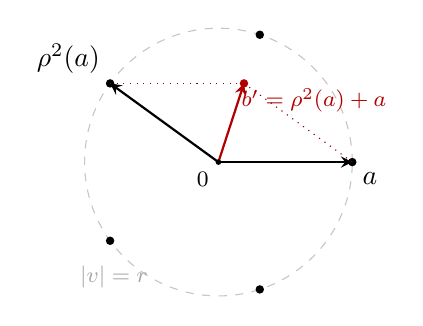
\begin{tikzpicture}[scale=1.7,>=stealth]
% minimal length circle
\draw[gray!45,dashed] (0,0) circle (1);
\node[gray!70] at (-0.78,-0.86) {\footnotesize $\lvert v\rvert=r$};
% the five rotated copies of a (regular pentagon vertices), starting along +x
\foreach \k in {0,1,2,3,4}{
  \coordinate (P\k) at ({cos(72*\k)},{sin(72*\k)});
  \fill[black] (P\k) circle (0.9pt);
}
% a and rho^2(a)
\draw[->,thick] (0,0) -- (P0) node[below right] {$a$};
\draw[->,thick] (0,0) -- (P2) node[above left] {$\rho^2(a)$};
% the contradiction vector b' = rho^2(a) + a
\coordinate (B) at ({cos(0)+cos(144)},{sin(0)+sin(144)});
\draw[->,thick,red!70!black] (0,0) -- (B)
  node[midway,above right] {\footnotesize $b'=\rho^2(a)+a$};
\fill[red!70!black] (B) circle (0.9pt);
% parallelogram guide lines
\draw[red!55!black,dotted] (P0) -- (B);
\draw[red!55!black,dotted] (P2) -- (B);
% origin
\fill (0,0) circle (0.6pt);
\node[below left] at (0,0) {\footnotesize $0$};
\end{tikzpicture}
\end{center}

\noindent The red lattice vector $b'$ lies inside the dashed circle of radius $r$, so it is a
nonzero lattice vector shorter than the supposed minimal vector $a$ --- impossible.

\begin{method}{Deciding whether a rotation order is lattice-compatible}
\textbf{Trigger:} ``can an $n$-fold rotation be a symmetry of a $2$D lattice / wallpaper pattern?''
\begin{enumerate}
\item Take a minimal lattice vector $a$ of length $r$ and rotate it: $\rho(a)-a$ is a lattice
  vector of length $2r\sin(\pi/n)$.
\item Demand $2r\sin(\pi/n)\ge r$, i.e.\ $\sin(\pi/n)\ge\tfrac12$. This passes only for
  $n\le 6$.
\item Among the survivors, test $n=5$ separately: $\rho^2(a)+a$ has length $2r\cos(2\pi/5)<r$,
  a contradiction. So the admissible orders are exactly $1,2,3,4,6$.
\end{enumerate}
\end{method}

\begin{wex}{$5$-fold symmetry is impossible}
Show that no planar lattice has a rotational symmetry of order $5$.
\wrec Use the crystallographic restriction: build a lattice vector shorter than the minimal one.
\wsol Let $\rho$ be rotation by $\theta=2\pi/5=72^\circ$ and let $a$ be a minimal vector,
$\lvert a\rvert=r$. Then $\rho^2(a)\in L$ makes angle $4\pi/5=144^\circ$ with $a$, so
\[
b'=\rho^2(a)+a\in L,\qquad
\lvert b'\rvert=2r\cos\!\Big(\tfrac{2\pi}{5}\Big)=2r\cos 72^\circ\approx0.618\,r<r .
\]
This nonzero lattice vector is shorter than the minimal vector, a contradiction. Hence no
$5$-fold lattice symmetry exists.
\emph{Check:} the first test $2\sin(\pi/5)=2\sin36^\circ\approx1.176\ge1$ does \emph{not} exclude
$n=5$, which is exactly why the auxiliary vector $\rho^2(a)+a$ is needed. \checkmark
\end{wex}

\begin{wex}{$7$-fold symmetry is impossible (the first test suffices)}
Show that a lattice admits no rotational symmetry of order $7$.
\wrec Apply step~2 of the method: compare $\lvert\rho(a)-a\rvert$ to $r$.
\wsol With $\theta=2\pi/7$ and a minimal vector $a$, the lattice vector $b=\rho(a)-a$ has length
\[
\lvert b\rvert=2r\sin\!\Big(\tfrac{\pi}{7}\Big)=2r\sin\!\big(25.7^\circ\big)\approx 0.868\,r<r .
\]
So $b$ is a nonzero lattice vector shorter than the minimal $a$ --- impossible. Order $7$ is
excluded already by the first inequality; no second vector is required.
\emph{Check:} $\sin(\pi/7)\approx0.4339<\tfrac12$, so $2\sin(\pi/7)<1$, confirming the failure for
every $n\ge7$ since $\sin(\pi/n)$ decreases. \checkmark
\end{wex}

\begin{wex}{$6$-fold symmetry is allowed --- the hexagonal lattice}
Verify that the order $n=6$ is compatible, and exhibit the lattice.
\wrec Order $6$ is on the admissible list; check the inequality is met with equality and name a
realizing lattice.
\wsol For $n=6$, $\theta=\pi/3=60^\circ$, and $\lvert\rho(a)-a\rvert=2r\sin30^\circ=2r\cdot\tfrac12=r$.
The bound $\lvert\rho(a)-a\rvert\ge r$ holds with \emph{equality}: $\rho(a)-a$ is itself a minimal
vector, so no contradiction arises. The realizing lattice is the hexagonal (triangular) lattice
$L=\Z a+\Z b$ with $\lvert a\rvert=\lvert b\rvert=r$ and angle $60^\circ$ between $a$ and $b$; its symmetry
group is $D_6$, with a $6$-fold rotation about each lattice point.
\emph{Check:} the six vectors $\rho^k(a)$, $k=0,\dots,5$, are the six minimal vectors of the
hexagonal lattice, all of length $r$, consistent with equality in the bound. \checkmark
\end{wex}

\begin{wex}{Which $n\le6$ are realized, and by which lattice}
List, for each admissible order, a lattice realizing it.
\wrec Match each $n\in\{1,2,3,4,6\}$ to a standard plane lattice.
\wsol
\[
\begin{array}{c|l}
n & \text{a lattice with an $n$-fold rotation}\\\hline
1 & \text{any lattice (trivial rotation only), generic oblique lattice}\\
2 & \text{every lattice has $-\,\mathrm{id}$, the $180^\circ$ rotation; oblique lattice}\\
3 & \text{hexagonal lattice (also carries $C_3\sgr C_6$)}\\
4 & \text{square lattice }\Z e_1+\Z e_2,\ \text{symmetry }D_4\\
6 & \text{hexagonal lattice, symmetry }D_6
\end{array}
\]
Order $5$ is absent, as is every $n\ge7$.
\emph{Check:} the orders present, $\{1,2,3,4,6\}$, are exactly the lattice-compatible set from
the theorem; every plane lattice automatically has the order-$2$ symmetry $v\mapsto-v$, so $C_2$ always lies in the full symmetry group of the lattice
(a subgroup $H$, such as $C_1$ or $C_3$, need not contain it). \checkmark
\end{wex}

\begin{remark}[Quasicrystals]
The restriction forbids \emph{periodic} $5$-fold symmetry, not $5$-fold symmetry as such. Dropping
the requirement that the pattern repeat by a lattice, one can build aperiodic tilings --- the
Penrose tiling is the famous example --- whose diffraction patterns show sharp $10$-fold
(hence $5$-fold) spots. Physical solids with exactly this aperiodic long-range order,
\emph{quasicrystals}, were discovered by Shechtman in $1982$ and earned the $2011$ Nobel Prize in
Chemistry. They evade the theorem precisely because their translation group is \emph{not} a
lattice, so the minimal-vector argument has no minimal vector to exploit.
\end{remark}

\begin{pitfall}
The bound $\lvert\rho(a)-a\rvert\ge\lvert a\rvert$ alone rules out only $n\ge7$; it does \emph{not} exclude
$n=5$, since $2\sin(\pi/5)\approx1.18\ge1$. The order $5$ must be killed by the \emph{second}
vector $\rho^2(a)+a$. Skipping that step is the common error in stating the proof. Note too that
the theorem is special to dimension $2$ (and $3$): in higher dimensions lattices with $5$-fold
symmetry do exist, e.g.\ the root lattice underlying the $4$-dimensional analogue.
\end{pitfall}


\section{Plane Crystallographic (Wallpaper) Groups}
\subsection*{Plane Crystallographic (Wallpaper) Groups}

We continue the analysis of discrete groups of isometries $G\le\mathrm{M}$ of the Euclidean plane, where $\mathrm{M}$ is the group of all isometries. Such a $G$ comes with two pieces of data: its \emph{translation group}
\[
L=\{\,v\in V:\ t_v\in G\,\},
\]
the set of translation vectors $v$ for which the translation $t_v$ lies in $G$, and its \emph{point group} $\overline G\le\mathrm{O}(2)$, the image of $G$ under the homomorphism $\pi:\mathrm{M}\to\mathrm{O}(2)$ that forgets the translation part of an isometry. When $L$ is the trivial group, $G$ is cyclic or dihedral; when $L$ is infinite cyclic, $G$ is the symmetry group of a frieze pattern. The remaining case --- when $L$ is a full \emph{lattice} --- is the subject here.

\begin{definition}[Plane crystallographic group]
A subgroup $G\le\mathrm{M}$ is a \emph{(two-dimensional) plane crystallographic group}, or \emph{wallpaper group}, if it is discrete and its translation group $L$ is a \emph{lattice}: there are two linearly independent vectors $a,b\in V$ with
\[
L=\Z a+\Z b=\{\,m a+n b:\ m,n\in\Z\,\}.
\]
Equivalently, $G$ has two independent translational symmetries and no points of accumulation. These are exactly the symmetry groups of doubly periodic plane figures --- wallpaper patterns, and cross-sections of two-dimensional crystals such as graphite.
\end{definition}

\begin{remark}
The point group $\overline G$ acts on the translation space $V$ but \emph{not} on the plane $P$ itself (without a chosen origin, $P$ and $V$ are different objects). The key compatibility, due to the conjugation identity $g\,t_a\,g\inv=t_{\overline g(a)}$, is that $\overline G$ carries the lattice $L$ to itself: if $a\in L$ and $\overline g\in\overline G$, then $\overline g(a)\in L$. Thus $\overline G$ is a subgroup of the symmetry group of the lattice $L$, regarded as a figure in $V$. This single fact forces a severe restriction.
\end{remark}

\begin{theorem}[Crystallographic restriction]\label{art:plane_groups:restriction@c4}
Let $L$ be a lattice in $V$, and let $H\le\mathrm{O}(2)$ be a subgroup of the group of symmetries of $L$ (so $H$ carries $L$ to itself). Then:
\begin{enumerate}
\item[(a)] every rotation in $H$ has order $1,2,3,4$, or $6$; and
\item[(b)] $H$ is one of the groups $C_n$ or $D_n$ with $n\in\{1,2,3,4,6\}$.
\end{enumerate}
In particular a rotation of order $5$ is impossible: there is no wallpaper pattern with five-fold rotational symmetry.
\end{theorem}

\begin{proof}
We prove (a); part (b) follows from (a) together with the classification of finite subgroups of $\mathrm{O}(2)$ as $C_n$ or $D_n$. Let $\rho_\theta\in H$ be a rotation through angle $\theta>0$, and choose a nonzero $a\in L$ of \emph{minimal length}. Since $H$ carries $L$ to itself, $\rho_\theta(a)\in L$, and hence
\[
b=\rho_\theta(a)-a\in L .
\]
By minimality $|a|\le|b|$. A short computation gives $|b|^2=|a|^2(2-2\cos\theta)$, so $|b|\ge|a|$ forces $2-2\cos\theta\ge1$, i.e. $\cos\theta\le\tfrac12$, i.e. $\theta\ge 2\pi/6$. Thus the smallest rotation angle in $H$ is at least $2\pi/6$, so a rotation has order at most $6$.

It remains to exclude order $5$, i.e. $\theta=2\pi/5$. For that angle consider instead
\[
b'=\rho_\theta^2(a)+a\in L .
\]
One computes $|b'|^2=|a|^2\bigl(2+2\cos 2\theta\bigr)=|a|^2(2+2\cos(4\pi/5))$, and since $\cos(4\pi/5)=-\tfrac{1+\sqrt5}{4}<-\tfrac12$ we get $|b'|<|a|$, contradicting minimality. So order $5$ cannot occur, and every rotation in $H$ has order $1,2,3,4$, or $6$.
\end{proof}

\begin{remark}
The point group records only the angles of rotation and the lines of reflection or glide; it does \emph{not} determine $G$. Two complications arise. First, the lattice $L$ and the point group $\overline G$ together still leave room for genuinely different groups $G$. Second, and more subtly, a reflection in the point group $\overline G$ need not be realized in $G$ by an honest reflection: it may be present in $G$ only through \emph{glide reflections}. Recall a glide reflection is the composite $t_w\,r$ of a reflection $r$ across a line $\ell$ with a translation $t_w$ \emph{along} $\ell$; it has no fixed point, whereas an ordinary reflection fixes its whole axis.
\end{remark}

\begin{theorem}[Classification of plane crystallographic groups]\label{art:plane_groups:seventeen@c4}
Up to isomorphism (equivalently, up to an affine change of coordinates), there are exactly \textbf{$17$} plane crystallographic groups. They are distributed over the allowed point groups $C_n,D_n$ ($n\in\{1,2,3,4,6\}$) as follows.
\[
\renewcommand{\arraystretch}{1.25}
\begin{array}{|c|c|c|c|}
\hline
\text{point group} & \text{order} & \text{\# wallpaper types} & \text{which} \\
\hline
C_1 & 1 & 1 & \text{p1} \\
C_2 & 2 & 1 & \text{p2} \\
C_3 & 3 & 1 & \text{p3} \\
C_4 & 4 & 1 & \text{p4} \\
C_6 & 6 & 1 & \text{p6} \\
\hline
D_1 & 2 & 3 & \text{pm, pg, cm} \\
D_2 & 4 & 4 & \text{pmm, pmg, pgg, cmm} \\
D_3 & 6 & 2 & \text{p3m1, p31m} \\
D_4 & 8 & 2 & \text{p4m, p4g} \\
D_6 & 12 & 1 & \text{p6m} \\
\hline
\multicolumn{2}{|c|}{\text{total}} & 17 & \\
\hline
\end{array}
\]
The five cyclic point groups give one type each ($5$ in all); the dihedral point groups split into $12$ types, the extra ones distinguished by whether a reflection in $\overline G$ is realized by a true reflection or only by a glide, by the shape (square, rectangular, rhombic, hexagonal) of the underlying lattice, and, for the pair p3m1, p31m (both on the hexagonal lattice, both with true reflections in three directions), by how the mirror lines sit relative to the lattice: in p3m1 every $3$-fold rotation center lies on a mirror line, in p31m some do not.
\end{theorem}

\begin{remark}
We do not reproduce the full case analysis; it proceeds point group by point group, in each case pinning down the position of a reflection or glide relative to the lattice. As a sample of the method we treat the point group $D_1=\{1,r\}$ informally below and the brick pattern in detail. Artin carries out the analysis only for the point groups $C_4$ and $D_4$ (Propositions $6.6.3$ and $6.6.4$), as a model of the method; that the $17$ types exhaust the possibilities is left as an exercise (Artin, Exercise $6.6.6$).
\end{remark}

\subsection*{Glide vs.\ ordinary reflection: the brick pattern}

The cleanest illustration of why the point group alone is not enough is a \emph{brick pattern}: a running bond in which every brick carries a diagonal stroke, rising to the right in alternate rows and falling to the right in the rows between. Its symmetry group has the same point group $D_2$ as a fully symmetric rectangular pattern, yet it contains \emph{no reflection at all} --- only glides. (The strokes matter: the plain running bond is \emph{not} an example, since reflection across the middle line of any row preserves it; its group is of type cmm, with a centered lattice.)

\begin{center}
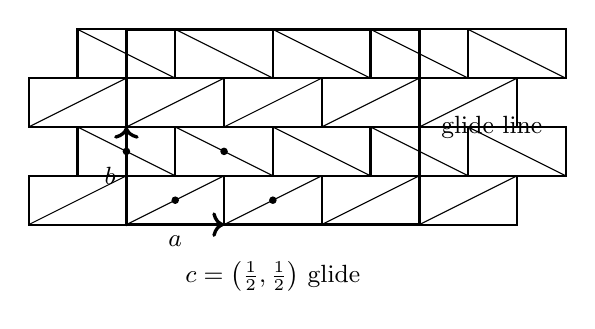
\begin{tikzpicture}[scale=0.62, line cap=round]
% Lattice vectors a (horizontal) and b (vertical)
% Bricks: width 2, height 1, offset by half-width on each row
\foreach \y in {0,1,2,3} {
  \pgfmathtruncatemacro{\sh}{mod(\y,2)} % 0 or 1
  \foreach \x in {-1,0,1,2,3} {
    \draw[thick] ({2*\x + \sh*1},\y) rectangle ({2*\x + \sh*1 + 2},\y+1);
    % diagonal stroke: rising in even rows, falling in odd rows
    \draw ({2*\x + \sh*1},{\y + \sh}) -- ({2*\x + \sh*1 + 2},{\y + 1 - \sh});
  }
}
% clip-like viewport frame
\draw[very thick] (0,0) rectangle (6,4);
% rotation centers (order 2) at brick centers and edge midpoints -- mark a few
\foreach \pt in {(1,0.5),(3,0.5),(2,1.5),(0,1.5)} {
  \fill[black] \pt circle (2.2pt);
}
% glide line: horizontal dashed line between two rows
\draw[dashed, thick] (0,2) -- (6,2);
\node[anchor=west] at (6.25,2) {\small glide line};
% basis vectors
\draw[->, very thick] (0,0) -- (2,0) node[midway,below] {\small $a$};
\draw[->, very thick] (0,0) -- (0,2) node[midway,left] {\small $b$};
\node[anchor=north] at (3,-0.55) {\small $c=\bigl(\tfrac12,\tfrac12\bigr)$ glide};
\end{tikzpicture}
\end{center}

\noindent
Let the lattice be $L=\Z a+\Z b$ where $a$ spans the length of one brick and $b$ spans two rows. The pattern has a half-turn ($\rho_\pi$, order $2$) about the center of each brick and about the midpoints of its short edges; these are all the same element $\rho_\pi$ of the point group. There are no rotations of any other nontrivial angle. Crucially, although the pattern \emph{looks} like it should have a mirror, no reflection actually fixes it: reflecting across a horizontal line through the middle of a row reverses the slant of the strokes in that row, reflecting across a mortar line sends the staggered rows out of register, and every vertical reflection reverses the slant of the strokes. What \emph{does} fix it is the glide reflection across the dashed line, combining the reflection across the middle line of the row just below it with the half-period translation $c=(\tfrac12,\tfrac12)$ measured in the basis $(a,b)$. Hence
\[
\overline G=D_2=\{1,\ \rho_\pi,\ r,\ \rho_\pi r\},\qquad\text{but $G$ contains no reflection --- the $r$ in $\overline G$ is realized only by a glide.}
\]
This is the type \textbf{pgg}; the type \textbf{pmm} has the \emph{same} point group $D_2$ but realizes both reflections honestly.

\begin{method}{Determining the type of a wallpaper pattern}
\textbf{Trigger:} you are handed a doubly periodic pattern and must name its point group (and ultimately its type).
\begin{enumerate}
\item \textbf{Find the rotations.} Locate the centers of rotational symmetry and the smallest rotation angle. This gives $n$ with the point group $C_n$ or $D_n$; by Theorem~\ref{art:plane_groups:restriction@c4}, $n\in\{1,2,3,4,6\}$.
\item \textbf{Reflection or glide?} Look for mirror lines and glide lines. If the pattern has any reflection or glide symmetry, the point group is $D_n$; if it has none, it is $C_n$.
\item \textbf{Distinguish same-point-group types.} When $\overline G=D_n$, decide for each mirror direction in $\overline G$ whether it is realized by a true reflection (axis fixed) or only by a glide (no fixed line), and read off the lattice shape. This separates e.g. pm/pg/cm or pmm/pmg/pgg/cmm.
\end{enumerate}
\end{method}

\begin{wex}{The point group of the brick pattern is $D_2$, not $C_2$}
Problem. Determine the point group of the brick pattern above, and explain why it is $D_2$ even though the group contains no reflection.
\wrec Apply the recipe: first the rotations fix $n$, then the presence of glide/reflection symmetry decides $C_n$ vs.\ $D_n$.
\wsol
\emph{Rotations:} the only nontrivial rotational symmetry is the half-turn $\rho_\pi$ about a brick center (or the midpoint of a short edge). No $90^\circ$ or $120^\circ$ rotation preserves the staggered rows, so $n=2$.
\emph{Reflection or glide:} a horizontal reflection alone fails (it reverses the slant of the strokes or puts the offset rows out of register), but the glide across the dashed line --- the reflection across the middle line of the row just below it, followed by the translation by $c=(\tfrac12,\tfrac12)$ --- does preserve the pattern. The point group is the \emph{image} in $\mathrm{O}(2)$, and the linear part of a glide reflection is an honest reflection $r$. So $r\in\overline G$.
\textbf{Check:} $\overline G$ contains $1,\rho_\pi,r$, hence also $\rho_\pi r$, giving $\overline G=D_2$ of order $4$. Yet $G$ itself has no element with reflection-type fixed line, so $G\ne D_2$ as an isometry group: the point group sees the mirror, the isometry group realizes it only as a glide. This is precisely why $\overline G$ and $L$ do not determine $G$.
\end{wex}

\begin{wex}{Five-fold symmetry is impossible}
Problem. Show directly that no wallpaper pattern can have a rotation of order $5$.
\wrec This is exactly the content of part (a) of the crystallographic restriction (Theorem~\ref{art:plane_groups:restriction@c4}); reproduce the minimal-vector argument for $\theta=2\pi/5$.
\wsol
Suppose $\rho_\theta$ with $\theta=2\pi/5$ were a symmetry, so $\rho_\theta\in\overline G$ carries $L$ to itself. Pick $a\in L$ nonzero of minimal length and set $b'=\rho_\theta^2(a)+a$, which lies in $L$. Then
\[
|b'|^2=|a|^2\bigl(2+2\cos2\theta\bigr)=|a|^2\bigl(2+2\cos\tfrac{4\pi}{5}\bigr).
\]
Numerically $\cos\tfrac{4\pi}{5}\approx-0.809$, so $2+2\cos\tfrac{4\pi}{5}\approx0.382$ and $|b'|\approx0.618\,|a|<|a|$.
\textbf{Check:} $b'\in L$ is a nonzero vector shorter than $a$, contradicting the minimality of $a$. Hence $\theta=2\pi/5$ is impossible, and order $5$ is excluded --- consistent with the table allowing only $n\in\{1,2,3,4,6\}$.
\end{wex}

\begin{wex}{Counting the $D_1$ types: pm, pg, cm}
Problem. The point group $D_1=\{1,r\}$ has a single mirror direction. Explain why it yields \emph{three} distinct wallpaper types rather than one.
\wrec Step 3 of the recipe: with $\overline G$ fixed at $D_1$, enumerate the ways the single reflection can sit relative to the lattice, plus the lattice shape.
\wsol
With $\overline G=D_1$ the only structure to vary is how the mirror $r$ of $\overline G$ is realized in $G$ and what lattice supports it. There are three inequivalent possibilities:
\begin{itemize}
\item[(pm)] $r$ is realized by an \emph{ordinary reflection} (its axis is fixed pointwise), on a rectangular lattice;
\item[(pg)] $r$ is realized \emph{only by a glide} (no fixed mirror line), on a rectangular lattice;
\item[(cm)] both a reflection and a glide occur, forced by a \emph{rhombic} (centered) lattice.
\end{itemize}
\textbf{Check:} these three exhaust the cases: either there is a true mirror or not (pm vs.\ pg on the rectangular lattice), and the centered lattice gives the third, genuinely different, group cm. This matches the row $D_1\to 3$ types in Theorem~\ref{art:plane_groups:seventeen@c4}. The same reflection-vs-glide-plus-lattice bookkeeping, applied to $D_2$, produces its $4$ types pmm, pmg, pgg, cmm.
\end{wex}

\begin{remark}
Artin works out the cases $C_4$ and $D_4$ explicitly to model the method. After choosing the minimal vector $a$ and setting $b=\rho_{\pi/2}(a)$, one shows the lattice $L$ is \emph{square} with basis $(a,b)$ (Lemma $6.6.2$); rescaling makes $L=\Z^2$. For $\overline G=C_4$ one finds $G=\{\,t_v\rho^i:\ v\in L,\ 0\le i<4\,\}$ (Proposition $6.6.3$), the single type p4. For $\overline G=D_4$ a short computation shows the reflection generator $g$ with $\overline g=r$ must satisfy $u\in\{(0,0),\,c\}$ with $c=(\tfrac12,\tfrac12)$: the case $u=(0,0)$ gives a true reflection (type p4m), and the case $u=c$ realizes the reflection only as a glide (type p4g), exactly the two $D_4$ types of the table (Proposition $6.6.4$).
\end{remark}

\begin{pitfall}
\textbf{Same point group does not mean same group.} The brick pattern and a mirror-symmetric rectangular pattern both have point group $D_2$, but they are different wallpaper types (pgg vs.\ pmm) because one realizes the reflection only as a glide. Never read off the wallpaper type from $\overline G$ alone --- you must also examine how each mirror sits relative to the lattice, and the lattice's shape.
\end{pitfall}

\begin{pitfall}
\textbf{The point group lives in $\mathrm{O}(2)$, the group $G$ lives in $\mathrm{M}$.} A glide reflection $t_w r\in G$ has \emph{linear part} the reflection $r$, so it contributes $r$ to $\overline G$ even though $t_w r$ itself fixes no line. Confusing an element of $G$ with its image in $\overline G$ is the source of most errors in classifying these groups.
\end{pitfall}


\section{Finite Subgroups of the Rotation Group $\mathrm{SO}(3)$}
\subsection*{Finite subgroups of $\mathrm{SO}(3)$: the Platonic symmetries}

We classify the finite groups of rotations of $\R^3$. The answer is short and famous: besides
the cyclic and dihedral families there are exactly three exceptional groups, the rotation
groups of the regular polyhedra. The proof is a counting argument run on the \emph{poles} of
the group --- the points where rotation axes pierce the unit sphere --- and it leans on the
orbit--stabilizer (counting) formula $|\Orb(p)|\cdot|\Stab(p)|=|G|$.

\begin{theorem}[Classification of finite subgroups of $\mathrm{SO}(3)$]\label{art:so3:main@c4}
A finite subgroup $G$ of $\mathrm{SO}(3)$ is one of:
\begin{itemize}
\item $C_k$, the cyclic group of rotations by multiples of $2\pi/k$ about a fixed line ($k$ arbitrary);
\item $D_k$, the dihedral group of the $2k$ rotations carrying a regular $k$-gon to itself;
\item $T$, the \emph{tetrahedral} group of the $12$ rotational symmetries of a regular tetrahedron;
\item $O$, the \emph{octahedral} group of the $24$ rotational symmetries of a cube (equivalently an octahedron);
\item $I$, the \emph{icosahedral} group of the $60$ rotational symmetries of a regular icosahedron (equivalently a dodecahedron).
\end{itemize}
\end{theorem}

\begin{remark}
The dihedral groups appear here as honest \emph{rotation} groups. A reflection of a plane is
realized in $\R^3$ by a rotation through angle $\pi$ about an axis lying in that plane. So
$D_k$ is generated by a rotation $x$ of angle $2\pi/k$ about the vertical axis together with a
rotation $y$ of angle $\pi$ about a horizontal axis; with $c=\cos(2\pi/k)$ and $s=\sin(2\pi/k)$,
\[
x=\begin{pmatrix} c & -s & 0\\ s & c & 0\\ 0 & 0 & 1\end{pmatrix},
\qquad
y=\begin{pmatrix} 1 & 0 & 0\\ 0 & -1 & 0\\ 0 & 0 & -1\end{pmatrix}.
\]
\end{remark}

\subsection*{Poles and spins}

\begin{definition}[Pole]
Let $G\sgr\mathrm{SO}(3)$ be finite of order $N>1$. Every $g\ne 1$ in $\mathrm{SO}(3)$ is a
rotation about a unique axis; that axis meets the unit sphere $S^2$ in two points. A
\emph{pole} of $G$ is a point $p\in S^2$ fixed by some $g\in G$ with $g\ne 1$. Write $P$ for
the set of all poles of $G$.
\end{definition}

\begin{lemma}[$P$ is a union of orbits]\label{art:so3:Porbit@c4}
$G$ permutes $P$: if $p\in P$ and $h\in G$ then $hp\in P$. Hence $P$ is a union of $G$-orbits.
\end{lemma}

\begin{proof}
Say $p$ is fixed by $g\ne 1$, and put $q=hp$. Then $hgh\inv\ne 1$ (conjugate of a nonidentity
element), and
\[
(hgh\inv)\,q=(hgh\inv)\,hp=hg\,p=hp=q,
\]
so $q$ is fixed by the nonidentity element $hgh\inv$, i.e.\ $q$ is a pole.
\end{proof}

For a pole $p$ the stabilizer $\Stab(p)=G_p$ is the set of elements of $G$ rotating about the
axis through $p$. It is cyclic, generated by the rotation of smallest positive angle; write
$r_p=|G_p|$. Since $p$ is a pole, $r_p>1$. The nonidentity elements of $G$ fixing $p$ are exactly the
$r_p-1$ nonidentity elements of $G_p$.

\begin{theorem}[The pole-counting formula]\label{art:so3:formula@c4}
Let $G\sgr\mathrm{SO}(3)$ be finite of order $N>1$, with pole-orbits $O_1,\dots,O_k$. Write
$r_i=r_p$ and $n_i=|O_i|$ for $p\in O_i$ (these depend only on the orbit), so that
$r_i n_i=N$. Then
\[
\sum_{i=1}^{k}\Bigl(1-\tfrac{1}{r_i}\Bigr)=2-\tfrac{2}{N}.
\]
\end{theorem}

\begin{proof}
Count \emph{spins}: pairs $(g,p)$ with $g\ne 1$ and $gp=p$. Counting by group elements, each
$g\ne 1$ is a nontrivial rotation, hence has exactly two poles, so there are $2(N-1)$ spins.
Counting by poles, the pole $p$ occurs in $r_p-1$ spins. Equating,
\[
\sum_{p\in P}(r_p-1)=2(N-1).
\]
Now collect by orbits. By orbit--stabilizer $r_p\,n_p=N$ (where $n_p=|\Orb(p)|$); poles in the
same orbit share the same $r_p$ and $n_p$. Each orbit $O_i$ contributes $n_i$ equal terms
$r_i-1$, so the left side is $\sum_i n_i(r_i-1)=2N-2$. Divide by $N$ and use $n_i/N=1/r_i$:
\[
\sum_{i=1}^{k}\frac{n_i(r_i-1)}{N}=\sum_{i=1}^{k}\Bigl(1-\frac{1}{r_i}\Bigr)=2-\frac{2}{N}. \qedhere
\]
\end{proof}

\begin{method}{Reading the constraint $\sum_i\bigl(1-\tfrac1{r_i}\bigr)=2-\tfrac2N$}
\textbf{Trigger:} you must enumerate the finite subgroups of $\mathrm{SO}(3)$, or bound the
number of pole-orbits.
\begin{enumerate}
\item The right side $2-\tfrac2N$ lies in $[1,2)$ for $N\ge2$.
\item Each $r_i\ge2$, so each term $1-\tfrac1{r_i}\ge\tfrac12$. Hence $k\le 3$: four or more
  terms already sum to at least $2>2-\tfrac2N$.
\item Tabulate by number of orbits ($k=1,2,3$). The case $k=3$ forces $\tfrac1{r_1}+\tfrac1{r_2}+\tfrac1{r_3}>1$
  with $2\le r_1\le r_2\le r_3$; its solutions are the infinite family $(2,2,r)$, $r\ge2$, and the
  three triples $(2,3,3),(2,3,4),(2,3,5)$.
\item Each surviving triple $(r_1,r_2,r_3)$ pins down $N$ and the orbit sizes $n_i=N/r_i$.
\end{enumerate}
\end{method}

\subsection*{The case analysis}

There can be at most three orbits. We run through $k=1,2,3$.

\textbf{One orbit.} The formula reads $1-\tfrac1{r_1}=2-\tfrac2N$. The left side is $<1$ while
the right is $\ge1$ (as $N\ge2$): impossible.

\textbf{Two orbits.} Here $\bigl(1-\tfrac1{r_1}\bigr)+\bigl(1-\tfrac1{r_2}\bigr)=2-\tfrac2N$,
i.e.\ $\tfrac1{r_1}+\tfrac1{r_2}=\tfrac2N$. Since $r_i\mid N$ and $r_i\le N$, each
$\tfrac1{r_i}\ge\tfrac1N$, with equality forced: $r_1=r_2=N$ and $n_1=n_2=1$. Two poles, each
fixed by all of $G$, so $G$ rotates about the single line $\ell$ through them: $G=C_N$.

\textbf{Three orbits.} Now $\tfrac1{r_1}+\tfrac1{r_2}+\tfrac1{r_3}=1+\tfrac2N>1$ with
$2\le r_1\le r_2\le r_3$. If $r_1\ge3$ the left side is $\le 3\cdot\tfrac13=1$, contradiction;
so $r_1=2$. Then $\tfrac1{r_2}+\tfrac1{r_3}=\tfrac12+\tfrac2N>\tfrac12$.
\begin{itemize}
\item If $r_2=2$ as well, $r_3=k$ is arbitrary and $N=2k$: the orbit data $(r_i)=(2,2,k)$,
  $(n_i)=(k,k,2)$. Half of $G$ fixes the polar pair, the other half swaps it by a $\pi$-rotation
  about a perpendicular axis. This is the dihedral group $D_k$ of a regular $k$-gon in the plane
  perpendicular to $\ell$.
\item If $r_2=3$: from $\tfrac13+\tfrac1{r_3}>\tfrac12$ we get $r_3<6$, and $r_3\ge r_2=3$, so
  $r_3\in\{3,4,5\}$. ($r_2\ge4$ already fails: $\tfrac14+\tfrac14=\tfrac12$ leaves no room.)
\end{itemize}
The three triples with $r_1=2,r_2=3$ are
\[
(2,3,3)\!:\,N=12;\qquad (2,3,4)\!:\,N=24;\qquad (2,3,5)\!:\,N=60,
\]
the tetrahedral, octahedral, and icosahedral groups $T,O,I$. This proves
Theorem~\ref{art:so3:main@c4}.

\begin{remark}
In each polyhedral case the three orbit sizes $n_i=N/r_i$ count, in order, the edge-centers,
face-centers, and vertices of the associated regular solid (the larger $r_i$, the more
rotations fix that pole, hence the fewer such poles). The poles with $r_i=2$ sit above
edge-midpoints; the vertex-poles carry the highest-order rotations.
\end{remark}

\subsection*{Worked counting}

\begin{wex}{The tetrahedral group $T$: counting its $14$ poles and $22$ spins}
The rotation group $T$ of a regular tetrahedron $\Delta$ has order $12$. Verify the spin count
directly, without the abstract formula.
\wrec Poles sit above the centers of faces, the vertices, and the centers of edges; count
spins two ways and check they agree with $2(N-1)$.
\wsol $\Delta$ has $4$ faces, $4$ vertices, $6$ edges, so
\[
|P|=4+4+6=14.
\]
Each $g\ne 1$ (there are $11$) has two poles, giving $2\cdot 11=22$ spins. By pole-type: a
face axis has stabilizer of order $3$, contributing $r-1=2$ spins per pole, over $4$ faces; a
vertex axis likewise $r=3$, contributing $2$ spins over $4$ vertices; an edge axis has $r=2$,
contributing $1$ spin over $6$ edges. Total
\[
2\cdot 4+2\cdot 4+1\cdot 6=8+8+6=22.
\]
\emph{Check:} $22=2(N-1)=2(12-1)$. \checkmark
\end{wex}

\begin{wex}{Reading off $T$ from the triple $(2,3,3)$}
For $(r_1,r_2,r_3)=(2,3,3)$ compute $N$ and the orbit sizes, and match them to the tetrahedron.
\wrec Use $\tfrac1{r_1}+\tfrac1{r_2}+\tfrac1{r_3}=1+\tfrac2N$ to solve for $N$, then $n_i=N/r_i$.
\wsol $\tfrac12+\tfrac13+\tfrac13=\tfrac{3+2+2}{6}=\tfrac76=1+\tfrac16$, so $\tfrac2N=\tfrac16$
and $N=12$. The orbit sizes are
\[
n_1=\tfrac{12}{2}=6,\qquad n_2=\tfrac{12}{3}=4,\qquad n_3=\tfrac{12}{3}=4,
\]
i.e.\ $6$ edge-centers, $4$ face-centers, $4$ vertices --- exactly the tetrahedron's tallies.
\emph{Check:} $\bigl(1-\tfrac12\bigr)+\bigl(1-\tfrac13\bigr)+\bigl(1-\tfrac13\bigr)
=\tfrac12+\tfrac23+\tfrac23=\tfrac{11}{6}=2-\tfrac{2}{12}$. \checkmark
\end{wex}

\begin{wex}{The octahedral triple $(2,3,4)$ gives $N=24$}
Solve $(2,3,4)$ and identify the orbits with a cube.
\wrec Same recipe: solve for $N$, then $n_i=N/r_i$; interpret on the cube.
\wsol $\tfrac12+\tfrac13+\tfrac14=\tfrac{6+4+3}{12}=\tfrac{13}{12}=1+\tfrac1{12}$, so
$\tfrac2N=\tfrac1{12}$ and $N=24$. Then
\[
n_1=\tfrac{24}{2}=12,\qquad n_2=\tfrac{24}{3}=8,\qquad n_3=\tfrac{24}{4}=6.
\]
On a cube these are the $12$ edge-centers ($r=2$, half-turns), the $8$ vertices ($r=3$,
body-diagonal thirds-turns), and the $6$ face-centers ($r=4$, quarter-turns). The dual
octahedron swaps the roles of the $6$ and the $8$, giving the same group $O$.
\emph{Check:} $\bigl(1-\tfrac12\bigr)+\bigl(1-\tfrac13\bigr)+\bigl(1-\tfrac14\bigr)
=\tfrac12+\tfrac23+\tfrac34=\tfrac{6+8+9}{12}=\tfrac{23}{12}=2-\tfrac{2}{24}$. \checkmark
\end{wex}

\begin{wex}{The icosahedral triple $(2,3,5)$ gives $N=60$}
Solve $(2,3,5)$ and read off the orbit sizes; relate the vertex-orbit to a regular icosahedron.
\wrec Solve for $N$, then $n_i=N/r_i$; the order-$5$ orbit is the vertex set.
\wsol $\tfrac12+\tfrac13+\tfrac15=\tfrac{15+10+6}{30}=\tfrac{31}{30}=1+\tfrac1{30}$, so
$\tfrac2N=\tfrac1{30}$ and $N=60$. Then
\[
n_1=\tfrac{60}{2}=30,\qquad n_2=\tfrac{60}{3}=20,\qquad n_3=\tfrac{60}{5}=12,
\]
giving $30$ edge-centers, $20$ face-centers, and $12$ vertices. Taking one vertex-pole $p$ as
``north pole,'' its stabilizer is cyclic of order $5$; the remaining vertex-poles split into
the south pole and two $5$-element rings. The five congruent equilateral triangles meeting at
$p$ are faces of a regular icosahedron, so the order-$5$ orbit is its $12$ vertices.
\emph{Check:} $\bigl(1-\tfrac12\bigr)+\bigl(1-\tfrac13\bigr)+\bigl(1-\tfrac15\bigr)
=\tfrac12+\tfrac23+\tfrac45=\tfrac{15+20+24}{30}=\tfrac{59}{30}=2-\tfrac{2}{60}$. \checkmark
\end{wex}

\begin{remark}[Summary of the polyhedral data]
The three exceptional groups correspond to the only integer triples $2\le r_1\le r_2\le r_3$
with $\tfrac1{r_1}+\tfrac1{r_2}+\tfrac1{r_3}>1$ beyond the dihedral family:
\[
\begin{array}{c|c|c|c}
(r_1,r_2,r_3) & N & (n_1,n_2,n_3)=(\text{edges},\text{faces},\text{vertices}) & \text{group}\\\hline
(2,3,3) & 12 & (6,4,4) & T\\
(2,3,4) & 24 & (12,8,6) & O\\
(2,3,5) & 60 & (30,20,12) & I
\end{array}
\]
\end{remark}

\begin{pitfall}
The poles in an orbit need \emph{not} be the vertices of a regular polyhedron. For the cube,
the $12$ edge-centers form a single orbit but span a \emph{truncated} figure (a cuboctahedron),
not a Platonic solid. In the polyhedral cases the two orbits with $r_i\ge3$ are the vertex sets of a regular
polyhedron and of its dual; only the $r_1=2$ orbit of edge-centers can fail to be one. Likewise, ``at most three orbits'' counts \emph{pole}-orbits, not
group elements; a single orbit can be large ($n_i=N/r_i$).
\end{pitfall}

\begin{remark}
With $r_1=2$ the integer constraint $\tfrac1{r_1}+\tfrac1{r_2}+\tfrac1{r_3}>1$ reads
$\tfrac1p+\tfrac1q>\tfrac12$ for $\{p,q\}=\{r_2,r_3\}$, which is exactly the condition that $q$
regular $p$-gons fit around a vertex with angle sum less than $2\pi$; this is why ``only five
regular polyhedra'' and ``only three exceptional rotation groups'' come from the same
combinatorial fact. The five solids have Schl\"afli symbols $\{3,3\},\{4,3\},\{3,4\},\{5,3\},\{3,5\}$
($p$-gonal faces, $q$ at each vertex); here they appear as the triples $(2,3,q)$ for $q=3,4,5$,
a solid and its dual giving the same triple, while the remaining solutions $(2,2,k)$ are the
dihedral family.
\end{remark}

\subsection*{A picture of the axes}

The diagram below shows a cube with its three kinds of rotation axes: through opposite
\emph{face} centers ($r=4$, quarter-turns), opposite \emph{vertices} along a body diagonal
($r=3$, third-turns), and opposite \emph{edge} midpoints ($r=2$, half-turns). The pole of each
axis is where it pierces the surrounding sphere.

\begin{center}
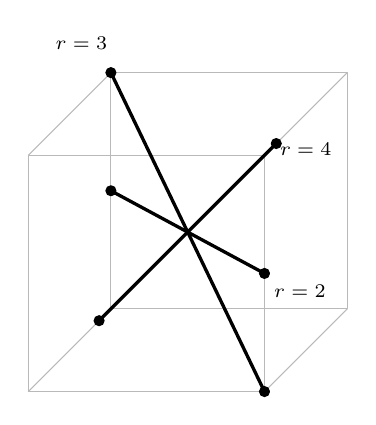
\begin{tikzpicture}[scale=1.5,line join=round]
% back square
\coordinate (A) at (0,0);
\coordinate (B) at (2,0);
\coordinate (C) at (2,2);
\coordinate (D) at (0,2);
% front square (shifted)
\coordinate (A2) at (0.7,0.7);
\coordinate (B2) at (2.7,0.7);
\coordinate (C2) at (2.7,2.7);
\coordinate (D2) at (0.7,2.7);
% edges of cube
\draw[gray!55] (A) -- (B) -- (C) -- (D) -- cycle;
\draw[gray!55] (A2) -- (B2) -- (C2) -- (D2) -- cycle;
\draw[gray!55] (A) -- (A2);
\draw[gray!55] (B) -- (B2);
\draw[gray!55] (C) -- (C2);
\draw[gray!55] (D) -- (D2);
% centers
\coordinate (Ofront) at (1.7,1.7); % center of front face
\coordinate (Oback)  at (1.0,1.0); % center of back face
% face axis (r=4): through opposite face centers
\draw[very thick] (0.6,0.6) -- (2.1,2.1);
\filldraw[black] (0.6,0.6) circle (1.2pt);
\filldraw[black] (2.1,2.1) circle (1.2pt);
\node[font=\scriptsize] at (2.35,2.05) {$r=4$};
% vertex axis (r=3): body diagonal B -- D2 (A2 -- C would be drawn on top of the face axis)
\draw[very thick] (B) -- (D2);
\filldraw[black] (B) circle (1.2pt);
\filldraw[black] (D2) circle (1.2pt);
\node[font=\scriptsize] at (0.45,2.95) {$r=3$};
% edge axis (r=2): midpoint of edge BC to midpoint of opposite edge A2-D2
\coordinate (mBC) at (2,1);
\coordinate (mAD2) at (0.7,1.7);
\draw[very thick] (mBC) -- (mAD2);
\filldraw[black] (mBC) circle (1.2pt);
\filldraw[black] (mAD2) circle (1.2pt);
\node[font=\scriptsize] at (2.3,0.85) {$r=2$};
\end{tikzpicture}
\end{center}

The three axis types correspond to the three pole-orbits $(n_1,n_2,n_3)=(12,8,6)$ of the
octahedral group $O$: $6$ face-poles of order $4$, $8$ vertex-poles of order $3$, and $12$
edge-poles of order $2$, matching the triple $(r_1,r_2,r_3)=(2,3,4)$ with $N=24$.


\section{Counting Orbits: the Cauchy--Frobenius Formula}
\subsection*{Counting Orbits: the Cauchy--Frobenius (Burnside) Formula}

A group action partitions the set it acts on into orbits, and the first quantitative question
is: \emph{how many orbits are there?} For symmetry-counting problems --- how many genuinely
different bead necklaces, or face-colorings of a cube, exist once we identify configurations
that differ by a rotation --- the orbits \emph{are} the answer. Artin's Counting Formula
(Proposition 6.9.2) relates the size of one orbit to a stabilizer; averaging that relation over
the whole group turns the geometric question into a clean arithmetic one. Throughout, $G$ is a
finite group acting on a finite set $S$.

\begin{theorem}[Counting Formula, Artin 6.9.2]\label{art:burnside:os@c4}
Let $G$ act on a finite set $S$ and let $s \in S$. Writing $\Orb(s)$ for the orbit and
$\Stab(s) = \{\,g \in G : g\cdot s = s\,\}$ for the stabilizer,
\[
\ord G = \lvert\Stab(s)\rvert \cdot \lvert\Orb(s)\rvert,
\qquad\text{equivalently}\qquad
\lvert\Orb(s)\rvert = \idx{G}{\Stab(s)} .
\]
In particular the size of every orbit divides $\ord G$.
\end{theorem}

\begin{proof}
The stabilizer $H = \Stab(s)$ is a subgroup of $G$. Define $\varphi\colon G/H \to \Orb(s)$ on
left cosets by $\varphi(gH) = g\cdot s$. This is well defined and injective: $g_1 H = g_2 H$
iff $g_2\inv g_1 \in H$ iff $g_2\inv g_1 \cdot s = s$ iff $g_1\cdot s = g_2\cdot s$. It is
surjective by definition of the orbit. Hence $\lvert\Orb(s)\rvert = \idx{G}{H}$, and Lagrange's
theorem $\ord G = \lvert H\rvert \cdot \idx{G}{H}$ gives the product form.
\end{proof}

We record the partition consequence Artin uses repeatedly: if $S$ splits into orbits
$O_1, \dots, O_k$, then $\lvert S\rvert = \lvert O_1\rvert + \cdots + \lvert O_k\rvert$, each
summand an index $\idx{G}{\Stab(s_i)}$. The Cauchy--Frobenius formula is the dual count: instead
of summing orbit sizes over orbits, sum fixed-point counts over group elements.

\begin{definition}[Fixed-point set]
For $g \in G$ acting on $S$, the \emph{fixed-point set} is
\[
\Fix(g) = \{\, s \in S : g \cdot s = s \,\} \subseteq S .
\]
Its size $\lvert\Fix(g)\rvert$ counts the elements left in place by $g$.
\end{definition}

\begin{theorem}[Cauchy--Frobenius / Burnside Counting Formula]\label{art:burnside:cf@c4}
Let a finite group $G$ act on a finite set $S$, and let $N$ be the number of orbits. Then
\[
N = \frac{1}{\ord G} \sum_{g \in G} \lvert\Fix(g)\rvert ,
\]
i.e.\ the number of orbits equals the \emph{average} number of fixed points of the elements of
$G$.
\end{theorem}

\begin{proof}
Count the set of incident pairs
$P = \{\,(g,s) \in G \times S : g\cdot s = s\,\}$ in two ways. Summing over group elements,
\[
\lvert P\rvert = \sum_{g \in G} \lvert\Fix(g)\rvert .
\]
Summing over points, $\lvert P\rvert = \sum_{s \in S} \lvert\Stab(s)\rvert$. Group the second sum
by orbits. For $s$ in a fixed orbit $O$, Theorem~\ref{art:burnside:os@c4} gives
$\lvert\Stab(s)\rvert = \ord G / \lvert\Orb(s)\rvert = \ord G / \lvert O\rvert$, and there are
$\lvert O\rvert$ such points, so each orbit contributes
$\lvert O\rvert \cdot (\ord G / \lvert O\rvert) = \ord G$. With $N$ orbits,
\[
\sum_{s \in S} \lvert\Stab(s)\rvert = \sum_{\text{orbits } O} \ord G = N \cdot \ord G .
\]
Equating the two counts of $\lvert P\rvert$ gives
$\sum_{g} \lvert\Fix(g)\rvert = N \cdot \ord G$, and dividing by $\ord G$ yields the formula.
\end{proof}

\begin{remark}
The proof is exactly Artin's orbit-stabilizer relation applied to the ``elements'' inside one
orbit: every point of an orbit has a stabilizer of the same order $\ord G / \lvert O\rvert$, and
the $\lvert O\rvert$ stabilizers of an orbit pool to $\ord G$ pairs. The double count is the whole
idea --- no characters, no representation theory. Despite the traditional name, the formula
predates Burnside; it is due to Cauchy and Frobenius, which is why the neutral name is now
preferred.
\end{remark}

\begin{method}{Burnside enumeration recipe}
\textbf{Trigger.} You must count configurations \emph{up to} a symmetry group $G$ (rotations of
a polygon/polyhedron, reflections, etc.): necklaces, colorings, labelings.
\begin{enumerate}
\item Identify $S$ (all raw configurations, ignoring symmetry) and the acting group $G$.
\item For each $g \in G$ compute $\lvert\Fix(g)\rvert$: a coloring is fixed by $g$ iff it is
constant on every cycle of the permutation $g$ induces on the slots. If there are $c$ colors and
$g$ has $\operatorname{cyc}(g)$ cycles on the slots, then
$\lvert\Fix(g)\rvert = c^{\operatorname{cyc}(g)}$.
\item Average: $N = \dfrac{1}{\ord G}\sum_{g} \lvert\Fix(g)\rvert$. Group $g$'s by conjugacy class
to avoid repeating identical counts.
\end{enumerate}
\end{method}

%==================================================================
\subsection*{Worked enumerations}

\begin{wex}{Two-color bead necklaces on a square (rotations)}
How many distinct ways are there to color the $4$ corner beads of a square with $2$ colors
(black/white), where two colorings are the same if a rotation carries one to the other? Here
$G = \Z/4\Z = \{\,e, r, r^2, r^3\,\}$ is the cyclic group of rotations by $0,90,180,270$ degrees,
acting on the $S = 2^4 = 16$ raw colorings.
\wrec Counting colorings up to rotation is the signature Burnside situation
(Theorem~\ref{art:burnside:cf@c4}): average $\lvert\Fix(g)\rvert$, computing each fixed count from
the cycle structure of $g$ on the four bead positions.
\wsol
Label positions $1,2,3,4$ around the square. The rotation $r$ acts as the $4$-cycle
$(1\,2\,3\,4)$; a coloring is $r$-fixed iff all four beads share a color.
\[
\begin{array}{c|c|c|c}
g & \text{cycles on positions} & \operatorname{cyc}(g) & \lvert\Fix(g)\rvert = 2^{\operatorname{cyc}(g)} \\\hline
e & (1)(2)(3)(4) & 4 & 2^4 = 16 \\
r & (1\,2\,3\,4) & 1 & 2^1 = 2 \\
r^2 & (1\,3)(2\,4) & 2 & 2^2 = 4 \\
r^3 & (1\,4\,3\,2) & 1 & 2^1 = 2
\end{array}
\]
Average over $\ord G = 4$:
\[
N = \frac{1}{4}\bigl(16 + 2 + 4 + 2\bigr) = \frac{24}{4} = 6 .
\]
\textbf{Check.} The six classes are easy to list by number of black beads up to rotation:
$0$ black (1 way), $1$ black (1), $2$ black adjacent (1), $2$ black opposite (1), $3$ black (1),
$4$ black (1) --- total $6$, matching.
\end{wex}

\begin{wex}{Necklaces with the full dihedral symmetry}
Same square of $4$ beads and $2$ colors, but now allow \emph{reflections} too, so
$G = D_8$ (the dihedral group of order $8$: four rotations and four reflections). Count colorings
up to this larger symmetry.
\wrec Same formula; the new group elements (reflections) contribute their own fixed counts. We
reuse the rotation data from the previous example and add the four reflections.
\wsol
The four rotations contribute $16 + 2 + 4 + 2 = 24$ as before. The reflections of a square come in
two geometric types acting on positions $1,2,3,4$ (corners in order):
\emph{vertex axes} (through two opposite corners) fix those two corners and swap the other two,
e.g.\ $(1)(3)(2\,4)$, so $\operatorname{cyc} = 3$, $\lvert\Fix\rvert = 2^3 = 8$; there are $2$ of
these. \emph{Edge axes} (through midpoints of opposite sides) swap corners in two pairs,
e.g.\ $(1\,2)(3\,4)$, so $\operatorname{cyc} = 2$, $\lvert\Fix\rvert = 2^2 = 4$; there are $2$ of
these.
\[
N = \frac{1}{8}\Bigl(\underbrace{16+2+4+2}_{\text{rotations}} \;+\; \underbrace{8 + 8}_{\text{vertex axes}} \;+\; \underbrace{4 + 4}_{\text{edge axes}}\Bigr)
= \frac{1}{8}(24 + 16 + 8) = \frac{48}{8} = 6 .
\]
\textbf{Check.} Adding reflections cannot \emph{increase} the orbit count (it can only merge
orbits), and indeed $6 \le 6$ here: of the rotation-classes, $1$ black, $3$ black, and the two
$2$-black types each already coincide with their mirror images, so no further merging occurs and
the count stays $6$.
\end{wex}

\begin{wex}{Face colorings of a cube (Artin's octahedral group)}
Artin's octahedral group $O$ is the group of $24$ rotations of a cube (Section 6.10). In how many
ways can the $6$ faces be painted with $c$ colors, identifying colorings related by a rotation?
Here $S = c^6$ and $G = O$, $\ord O = 24$.
\wrec Burnside over the rotation group of the cube. We need the cycle structure of each rotation
\emph{on the six faces}, organized by conjugacy class --- the standard inventory of $O$.
\wsol
The $24$ rotations of the cube fall into five conjugacy classes; for each we read off the cycle
type on the $6$ faces and apply $\lvert\Fix(g)\rvert = c^{\operatorname{cyc}(g)}$:
\[
\begin{array}{l|c|c|c}
\text{class of } g & \#\,g & \text{face cycle type} & \lvert\Fix(g)\rvert \\\hline
\text{identity} & 1 & 1+1+1+1+1+1 & c^6 \\
\text{face axis, } \pm 90^\circ & 6 & 1+1+4 & c^3 \\
\text{face axis, } 180^\circ & 3 & 1+1+2+2 & c^4 \\
\text{vertex axis, } \pm 120^\circ & 8 & 3+3 & c^2 \\
\text{edge axis, } 180^\circ & 6 & 2+2+2 & c^3
\end{array}
\]
Averaging,
\[
N(c) = \frac{1}{24}\Bigl(c^6 + 6c^3 + 3c^4 + 8c^2 + 6c^3\Bigr)
= \frac{c^6 + 3c^4 + 12c^3 + 8c^2}{24} .
\]
For $c = 2$: $N(2) = (64 + 48 + 96 + 32)/24 = 240/24 = 10$. For $c = 3$:
$N(3) = (729 + 243 + 324 + 72)/24 = 1368/24 = 57$.
\textbf{Check.} The face axes give $6/2 = 3$ axes with $\pm 90^\circ$ and $180^\circ$ each:
$6 + 3 = 9$ rotations, plus $8$ vertex-axis and $6$ edge-axis, plus the identity, totals
$1 + 9 + 8 + 6 = 24 = \ord O$, accounting for every rotation. The value $N(2)=10$ is the classic
``ten distinct two-color cubes'' count.
\end{wex}

The cube example is governed by the three rotation-axis types Artin emphasizes when applying the
Counting Formula to polyhedra. The schematic below records the axes whose cycle structures fed the
table.

\begin{center}
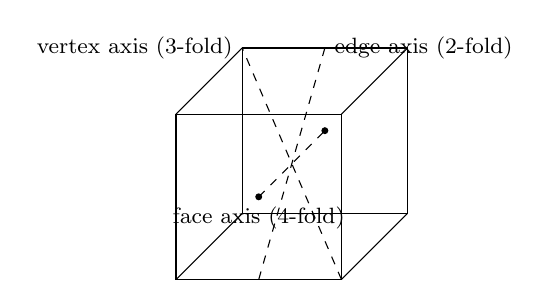
\begin{tikzpicture}[scale=1.05]
% cube: front face square and back face square, offset
\coordinate (A) at (0,0);
\coordinate (B) at (2,0);
\coordinate (C) at (2,2);
\coordinate (D) at (0,2);
\coordinate (A2) at (0.8,0.8);
\coordinate (B2) at (2.8,0.8);
\coordinate (C2) at (2.8,2.8);
\coordinate (D2) at (0.8,2.8);
\draw (A)--(B)--(C)--(D)--cycle;
\draw (A2)--(B2)--(C2)--(D2)--cycle;
\draw (A)--(A2); \draw (B)--(B2); \draw (C)--(C2); \draw (D)--(D2);
% face axis (through centers of front/back faces)
\draw[dashed] (1,1) -- (1.8,1.8);
\fill (1,1) circle (1.2pt); \fill (1.8,1.8) circle (1.2pt);
\node[font=\footnotesize, below] at (1,1) {face axis (4-fold)};
% vertex axis (body diagonal B to opposite vertex D2; A -- C2 would lie on top of the face axis)
\draw[dashed] (B) -- (D2);
\node[font=\footnotesize, left] at (D2) {vertex axis (3-fold)};
% edge axis (midpoints of two opposite edges)
\coordinate (mAB) at (1,0);
\coordinate (mC2D2) at (1.8,2.8);
\draw[dashed] (mAB) -- (mC2D2);
\node[font=\footnotesize, right] at (mC2D2) {edge axis (2-fold)};
\end{tikzpicture}
\end{center}

\begin{wex}{Pairs of faces of the cube: recovering Artin's 3 and 12}
Artin notes (Section 6.10) that $O$ acts on the $15$ unordered pairs of faces of a cube, splitting
them into the $3$ pairs of \emph{opposite} faces and the $12$ pairs of \emph{adjacent} faces.
Recover these orbit sizes with the Counting Formula, and verify the orbit count via Burnside.
\wrec Two checks: (i) orbit sizes by Theorem~\ref{art:burnside:os@c4}; (ii) the number of orbits by
Theorem~\ref{art:burnside:cf@c4}. The action is on $S = $ the $15$ unordered face-pairs.
\wsol
\emph{(i) Orbit sizes.} Fix a pair of opposite faces $U$. Its stabilizer is the set of rotations
sending $\{$top$,$bottom$\}$ to itself; Artin records $\lvert\Stab(U)\rvert = 8$ (rotations about
the vertical axis together with the $180^\circ$ flips). Then
$\lvert\Orb(U)\rvert = \ord O / \lvert\Stab(U)\rvert = 24/8 = 3$ --- the three axis-directions.
For a pair of adjacent faces $U'$, the stabilizer consists of the identity and the half-turn
about the axis through the midpoint of their common edge, so it has order $2$, giving orbit
size $24/2 = 12$.
$3 + 12 = 15$ exhausts $S$.
\emph{(ii) Orbit count by Burnside.} We expect $N = 2$. Class by class on the $15$ pairs: the
identity fixes all $15$; each of the $6$ quarter-turns about a face axis fixes only the pair of
faces on its axis; each of the $3$ face half-turns fixes $3$ pairs (the three pairs of opposite
faces); the $8$ vertex rotations fix none (they permute the faces in two $3$-cycles); each of
the $6$ edge half-turns fixes the $3$ pairs of faces it swaps. So
\[
N = \frac{1}{24}\sum_{g\in O}\lvert\Fix(g)\rvert = \frac{1}{24}\bigl(15 + 6\cdot 1 + 3\cdot 3 + 8\cdot 0 + 6\cdot 3\bigr) = \frac{48}{24} = 2 .
\]
\textbf{Check.} Both methods agree with Artin: orbit sizes $3$ and $12$ (summing to $15$), and
$N = 2$ orbits. The stabilizer order $8$ for an opposite-face pair is exactly the value Artin
states in Section 6.10.
\end{wex}

\begin{pitfall}
The fixed-point count $\lvert\Fix(g)\rvert = c^{\operatorname{cyc}(g)}$ uses the cycle
decomposition of $g$ \emph{on the slots being colored} (faces, beads), \emph{not} on the vertices
or on abstract group elements. Using the wrong action's cycle type is the most common error;
always fix in your mind which set $S$ the group is permuting before counting cycles.
\end{pitfall}

\begin{pitfall}
Burnside counts orbits of the \emph{exact} group you average over. Including reflections
(dihedral) versus rotations only (cyclic) generally gives different answers; the necklace
examples above happened to agree, but for larger bead counts they diverge. Decide first whether
mirror images count as ``the same.''
\end{pitfall}

\begin{remark}
The two summation directions are worth keeping side by side. Partitioning $S$ into orbits sums
\emph{orbit sizes}: $\lvert S\rvert = \sum_O \idx{G}{\Stab(s_O)}$, the count Artin uses for the
dodecahedron's $12 = 1 + 1 + 5 + 5$ face partition under a cyclic stabilizer of order $5$.
Cauchy--Frobenius instead sums \emph{fixed-point counts} over $G$ to extract the \emph{number} of
orbits. Both rest on the single identity
$\lvert\Orb(s)\rvert\cdot\lvert\Stab(s)\rvert = \ord G$ of Theorem~\ref{art:burnside:os@c4}.
\end{remark}


% ===== Graded Problem Bank (Dummit and Foote + Artin + Fraleigh) =====
\section{Graded Problem Bank}
Problems are drawn from Dummit \& Foote, Artin (\emph{Algebra}), and Fraleigh (\emph{A First Course in Abstract Algebra}); the difficulty grading is the author's.

\subsection*{Easy}
\begin{exers}{}
\item [DF 4.1.4] Let $S_3$ act on the $9$ ordered pairs $\{(i,j)\st 1\le i,j\le 3\}$ by $\sigma\cdot(i,j)=(\sigma(i),\sigma(j))$. Find the orbits, the cycle decomposition of each $\sigma$ as an element of $S_9$, and a stabilizer for one point in each orbit.
\item [DF 4.1.5] Repeat the preceding for $S_3$ acting on (a) the $27$ triples $\{(i,j,k)\st 1\le i,j,k\le 3\}$ and (b) the $7$ nonempty subsets of $\{1,2,3\}$.
\item [DF 4.1.6] With $S_4$ permuting variable indices of integer polynomials in $x_1,x_2,x_3,x_4$, find the orbit of (a) $x_1+x_2$, (b) $x_1x_2+x_3x_4$, (c) $(x_1+x_2)(x_3+x_4)$.
\item [DF 4.2.1] Label the Klein $4$-group $\{1,a,b,c\}$ as $1,2,4,3$ and verify that the left regular representation sends $a\mapsto(1\,2)(3\,4)$, $b\mapsto(1\,4)(2\,3)$, $c\mapsto(1\,3)(2\,4)$; then relabel $1,a,b,c$ as $1,4,2,3$ and show the image in $S_4$ is the same subgroup.
\item [DF 4.2.2] List $S_3$ as $1,(1\,2),(2\,3),(1\,3),(1\,2\,3),(1\,3\,2)$ labelled $1,\dots,6$ and exhibit the image of each element under the left regular representation $S_3\to S_6$.
\item [DF 4.2.3] For $D_8=\gen{r,s}$ labelled $1,r,r^2,r^3,s,sr,sr^2,sr^3 \mapsto 1,\dots,8$, exhibit the image of each element under the left regular representation $D_8\to S_8$; relabel by $1,3,5,7,2,4,6,8$ and show the two resulting subgroups of $S_8$ differ.
\item [DF 4.2.4] Use the left regular representation of $Q_8$ to produce two elements of $S_8$ generating a subgroup isomorphic to $Q_8$.
\item [DF 4.2.5] For $D_8=\gen{r,s}$ and $H=\gen{s}$, label the cosets $1H,rH,r^2H,r^3H$ as $1,2,3,4$: (a) exhibit the image of each element of $D_8$ under $\pi_H:D_8\to S_4$ from left multiplication on these cosets and deduce $\pi_H$ is faithful; (b) relabel the cosets as $1,3,2,4$ and show the resulting image is a different subgroup of $S_4$; (c) for $K=\gen{sr}$, with cosets $1K,rK,r^2K,r^3K$ labelled $1,2,3,4$, show $\pi_K(D_8)$ is the same subgroup of $S_4$ as in (a).
\item [DF 4.2.6] For $D_8$ and $N=\gen{r^2}$, exhibit $\pi_N:D_8\to S_4$ on the cosets $1N,rN,sN,srN$; show it is not faithful and that $\pi_N(D_8)\isom V_4$.
\item [DF 4.3.2] Find all conjugacy classes and their sizes in (a) $D_8$, (b) $Q_8$, (c) $A_4$.
\item [DF 4.3.3] Find all conjugacy classes and their sizes in (a) $\Z_2\times S_3$, (b) $S_3\times S_3$, (c) $\Z_3\times A_4$.
\item [DF 4.3.7] For $n=3,4,5,7$ tabulate the partitions of $n$ and give representatives for the corresponding conjugacy classes of $S_n$.
\item [DF 4.3.10] For the $5$-cycle $\sigma=(1\,2\,3\,4\,5)$ in $S_5$, find an explicit $\tau\in S_5$ with (a) $\tau\sigma\tau\inv=\sigma^2$, (b) $\tau\sigma\tau\inv=\sigma\inv$, (c) $\tau\sigma\tau\inv=\sigma^{-2}$.
\item [DF 4.3.11] In each case decide whether $\sigma_1,\sigma_2$ are conjugate and if so give $\tau$ with $\tau\sigma_1\tau\inv=\sigma_2$: (a) $(1\,2)(3\,4\,5)$ and $(1\,2\,3)(4\,5)$; (b) $(1\,5)(3\,7\,2)(10\,6\,8\,11)$ and $(3\,7\,5\,10)(4\,9)(13\,11\,2)$; (c) $\sigma_1=(1\,5)(3\,7\,2)(10\,6\,8\,11)$ and $\sigma_1^3$; (d) $(1\,3)(2\,4\,6)$ and $(3\,5)(2\,4)(5\,6)$.
\item [DF 4.3.12] Find a representative for each conjugacy class of elements of order $4$ in $S_8$ and in $S_{12}$.
\item [DF 4.5.4] Exhibit all Sylow $2$-subgroups and Sylow $3$-subgroups of $D_{12}$ and of $S_3\times S_3$.
\item [DF 4.5.6] Exhibit all Sylow $3$-subgroups of $A_4$ and all Sylow $3$-subgroups of $S_4$.
\item [DF 4.5.7] Exhibit all Sylow $3$-subgroups of $S_4$ and find elements of $S_4$ conjugating one into each of the others.
\item [DF 4.5.8] Exhibit two distinct Sylow $2$-subgroups of $S_5$ and an element of $S_5$ conjugating one into the other.
\item [DF 4.5.9] Exhibit all Sylow $3$-subgroups of $\SL_2(\F_3)$.
\item [DF 4.5.31] How many elements of order $7$ must there be in a simple group of order $168$?
\item [DF 4.5.32] For $p=2,3,5$ find $n_p(A_5)$ and $n_p(S_5)$.
\item [DF 4.6.4] Prove that $A_n$ is generated by the set of all $3$-cycles for each $n\ge 3$.
\item [Artin 6.7.1] For $G=D_4$ acting on the square, find the stabilizer of a vertex and of an edge; for the action on the two diagonal lines, find the stabilizer of a diagonal.
\item [Artin 6.9.1] Use the counting formula to determine the orders of the rotational symmetry groups of a cube and of a tetrahedron.
\item [Artin 6.4.1] Write the product $x^2yx\inv y\inv x^3y^3$ in the form $x^iy^j$ in the dihedral group $D_n$.
\item [Artin 6.4.3a] Compute the left cosets of $H=\{1,x^5\}$ in the dihedral group $D_{10}$.
\item [Artin 6.10.1] Determine the orders of the orbits for left multiplication on the set of subsets of order $3$ of $D_3$.
\item [Artin 6.12.2] Describe the orbits of poles for the group of rotations of an octahedron.
\item [Artin 6.12.3] Let $O$ be the group of rotations of a cube and $S$ the four diagonal lines joining opposite vertices; determine the stabilizer of one diagonal.
\item [Artin 7.5.2] What is the centralizer of the element $(1\,2)$ in $S_5$?
\item [Artin 7.5.3] Determine the orders of the elements of the symmetric group $S_7$.
\item [Artin 7.7.5] Find Sylow $2$-subgroups of the following groups: (a) $D_{10}$, (b) $T$, (c) $O$, (d) $I$.
\item [Artin 7.2.2] A group of order $21$ contains a conjugacy class $C(x)$ of order $3$. What is the order of $x$ in the group?
\item [Artin 7.1.2] Let $H\le G$. Describe the orbits for the operation of $H$ on $G$ by left multiplication.
\item [Fraleigh 11.1] Describe all symmetries (isometries leaving the figure fixed) of: (a) a point in $\R$, (b) a point in $\R^2$, (c) a line segment in $\R$, (d) a line segment in $\R^2$, (e) some symmetries of a line segment in $\R^3$.
\item [Fraleigh 11.4] Draw a plane figure whose group of symmetries in $\R^2$ has one element.
\item [Fraleigh 11.5] Draw a plane figure whose group of symmetries in $\R^2$ has two elements.
\item [Fraleigh 11.6] Draw a plane figure whose group of symmetries in $\R^2$ has three elements.
\item [Fraleigh 11.7] Draw a plane figure whose group of symmetries in $\R^2$ is isomorphic to $\Z_4$.
\item [Fraleigh 11.8] Draw a plane figure whose group of symmetries in $\R^2$ is isomorphic to the Klein $4$-group $V$.
\item [Fraleigh 11.9] For each of the four nonidentity plane-isometry types, give the possible orders of an isometry of that type.
\item [Fraleigh 11.10] Which of the four nonidentity plane-isometry types can have a fixed point?
\item [Fraleigh 11.11] Which plane-isometry types have exactly one fixed point?
\item [Fraleigh 11.12] Which plane-isometry types have exactly two fixed points?
\item [Fraleigh 11.13] Which plane-isometry types have an infinite number of fixed points?
\item [Fraleigh 14.1] For the $D_4$-set $X$ of Example 14.9, find the fixed sets $X_\sigma$ for each $\sigma\in D_4$.
\item [Fraleigh 14.2] For the same $D_4$-set, find the isotropy subgroup $G_x$ for each $x\in X$.
\item [Fraleigh 14.3] For the same $D_4$-set, find all the orbits in $X$ under $D_4$.
\item [Fraleigh 14.4] Find the center of $D_8$ (the dihedral group of order $16$).
\item [Fraleigh 14.5] Find the center of $D_7$.
\item [Fraleigh 14.6] Make $X=S_3$ a $G=S_3$-set by conjugation $\sigma*\tau=\sigma\tau\sigma\inv$ and find all orbits.
\item [Fraleigh 14.7] Let $G=D_4$ act by conjugation on the set $X$ of its order-$2$ subgroups; find all orbits.
\item [Fraleigh 14.8] Let $U=\{z\in\C\st|z|=1\}$ act on $X=\C$ by multiplication; find all orbits and $X_G$.
\item [Fraleigh 14.9] Let $|G|=3$ and $|X|=6$; for each possible action of $G$ on $X$ list the orbit sizes (largest first).
\item [Fraleigh 14.10] Let $|G|=9$ and $|X|=10$; for each possible action list the orbit sizes.
\item [Fraleigh 14.11] Let $|G|=8$ and $|X|=10$; for each possible action list the orbit sizes.
\item [Fraleigh 15.1] Find the number of orbits in $\{1,\dots,8\}$ under the cyclic subgroup $\gen{(1\,3\,5\,6)}$ of $S_8$.
\item [Fraleigh 15.2] Find the number of orbits in $\{1,\dots,8\}$ under the subgroup of $S_8$ generated by $(1\,3)$ and $(2\,4\,7)$.
\item [Fraleigh 15.3] Find the number of distinguishable tetrahedral dice made with $1,2,3,4$ dots on the faces of a regular tetrahedron.
\item [Fraleigh 15.4] How many distinguishable blocks if each of the $6$ faces of a cube is painted a different color from $8$ available colors?
\item [Fraleigh 15.5] Repeat the cube-coloring count when colors may be repeated freely on faces.
\item [Fraleigh 15.6] How many distinguishable colorings of the $8$ corners of a cube with $4$ colors (repeats allowed)?
\item [Fraleigh 15.7a] How many distinguishable ways to paint the $4$ edges of a square of cardboard (which may be turned over) with $6$ colors if no color is used more than once?
\item [Fraleigh 15.7b] Same as above but the same color may be used on any number of edges.
\item [Fraleigh 15.8] Six equal wires soldered into the edges of a regular tetrahedron each get a $50$- or $100$-ohm resistor; how many essentially different wirings?
\item [Fraleigh 15.9a] A $2$ ft rectangular prism with $1$ ft square ends has its $6$ faces painted from $6$ colors with no repeats; how many distinguishable prisms?
\item [Fraleigh 15.9b] Same prism, but each color may be used on any number of faces.
\item [Fraleigh 17.1] A Sylow $3$-subgroup of a group of order $12$ has what order?
\item [Fraleigh 17.2] A Sylow $3$-subgroup of a group of order $54$ has what order?
\item [Fraleigh 17.3] By Theorem 17.7 alone, a group of order $24$ has how many Sylow $2$-subgroups (give the permissible values)?
\item [Fraleigh 17.4] By Theorem 17.7 alone, list the permissible numbers of Sylow $3$- and Sylow $5$-subgroups for a group of order $255=3\cdot5\cdot17$.
\item [Fraleigh 17.5] Find all Sylow $3$-subgroups of $S_4$ and show they are all conjugate.
\item [Fraleigh 17.6] Find two Sylow $2$-subgroups of $S_4$ and show they are conjugate.
\item [Fraleigh 17.7] Determine for which $n\le 20$ every group of order $n$ is abelian.
\item [Fraleigh 17.8] Determine for which $n\le 20$ every group of order $n$ is cyclic.
\end{exers}

\subsection*{Medium}
\begin{exers}{}
\item [DF 4.1.1] If $G$ acts on $A$ and $b=g\cdot a$, prove $G_b=gG_ag\inv$; deduce that for a transitive action the kernel is $\bigcap_{g\in G}gG_ag\inv$.
\item [DF 4.1.2] For a permutation group $G\le S_A$, $\sigma\in G$, $a\in A$, prove $\sigma G_a\sigma\inv=G_{\sigma(a)}$; deduce that for a transitive action $\bigcap_{\sigma\in G}\sigma G_a\sigma\inv=1$.
\item [DF 4.1.3] If $G$ is an abelian transitive subgroup of $S_A$, show $\sigma(a)\ne a$ for all $\sigma\in G-\{1\}$ and all $a$, and deduce $|G|=|A|$.
\item [DF 4.2.7] Prove that if $H\le G$ has finite index $n$ then there is a normal $K\nor G$ with $K\le H$ and $\idx{G}{K}\le n!$.
\item [DF 4.2.8] Prove that if $p$ is prime and $|G|=p^\alpha$ then every subgroup of index $p$ is normal; deduce every group of order $p^2$ has a normal subgroup of order $p$.
\item [DF 4.2.9] Prove every non-abelian group of order $6$ has a nonnormal subgroup of order $2$, and use this to classify groups of order $6$.
\item [DF 4.2.10] For the left regular representation $\pi:G\to S_G$ with $|x|=n$ and $|G|=mn$, prove $\pi(x)$ is a product of $m$ $n$-cycles; deduce $\pi(x)$ is odd iff $|x|$ is even and $|G|/|x|$ is odd.
\item [DF 4.2.11] If $\pi(G)$ contains an odd permutation (for $\pi$ the left regular representation), prove $G$ has a subgroup of index $2$.
\item [DF 4.2.12] Prove that if $|G|=2k$ with $k$ odd then $G$ has a subgroup of index $2$.
\item [DF 4.3.1] For a left action of $G$ on $A$ and the corresponding right action, prove the equivalence relations $a\sim b$ ($a=g\cdot b$ some $g$) and $a\sim' b$ ($a=b\cdot g$ some $g$) coincide.
\item [DF 4.3.4] Prove $gN_G(S)g\inv=N_G(gSg\inv)$ and $gC_G(S)g\inv=C_G(gSg\inv)$ for $S\subseteq G$.
\item [DF 4.3.5] If the center of $G$ has index $n$, prove every conjugacy class has at most $n$ elements.
\item [DF 4.3.8] Prove $Z(S_n)=1$ for all $n\ge 3$.
\item [DF 4.3.9] Show $|C_{S_n}((1\,2)(3\,4))|=8\cdot(n-4)!$ for all $n\ge 4$ and describe the centralizer.
\item [DF 4.3.13] Find all finite groups with exactly two conjugacy classes.
\item [DF 4.3.14] With $\pi_1,\pi_2$ the two regular representations of $V_4$ and $\tau=(2\,4)$, show $\tau\circ\pi_1(g)\circ\tau\inv=\pi_2(g)$ for each $g\in V_4$.
\item [DF 4.3.15] Find an element of $S_8$ conjugating the $D_8$ image from Exercise 4.2.3(a) to the image from (b).
\item [DF 4.3.16] Find an element of $S_4$ conjugating the $D_8$ image from Exercise 4.2.5(a) to the image from (b).
\item [DF 4.3.18] If $H\le S_A$ has fixed-point set $F(H)$ and $\tau\in N_{S_A}(H)$, prove $\tau$ stabilizes $F(H)$ and its complement.
\item [DF 4.3.22] Show that if $n$ is odd then the $n$-cycles form two conjugacy classes of equal size in $A_n$.
\item [DF 4.3.26] If $g_1,\dots,g_r$ represent the conjugacy classes of finite $G$ and pairwise commute, prove $G$ is abelian.
\item [DF 4.3.28] Let $G$ have order $p^a$; prove $G$ has a subgroup of order $p^b$ for each $0\le b\le a$.
\item [DF 4.3.29] If $G$ has odd order, prove that for any $x\ne 1$, $x$ and $x\inv$ are not conjugate in $G$.
\item [DF 4.3.31] For $n=2k+1$ odd, determine the conjugacy classes of $D_{2n}$ and give the class equation.
\item [DF 4.3.32] Prove the formula $|C(\sigma)|=n!/\prod_i(k_i!\,m_i^{k_i})$ for the size of the conjugacy class of $\sigma\in S_n$ with $k_i$ cycles of length $m_i$.
\item [DF 4.4.1] If $\sigma\in\Aut(G)$ and $\varphi_g$ is conjugation by $g$, prove $\sigma\varphi_g\sigma\inv=\varphi_{\sigma(g)}$ and deduce $\Inn(G)\nor\Aut(G)$.
\item [DF 4.4.2] Prove that an abelian group of order $pq$ ($p,q$ distinct primes) is cyclic.
\item [DF 4.4.6] Prove characteristic subgroups are normal, and give a normal subgroup that is not characteristic.
\item [DF 4.4.7] If $H$ is the unique subgroup of its order in $G$, prove $H$ is characteristic in $G$.
\item [DF 4.4.8] Let $H\le K\le G$: (a) if $H$ char $K$ and $K\nor G$ then $H\nor G$; (b) if $H$ char $K$ and $K$ char $G$ then $H$ char $G$, and use this to show that the Klein $4$-group $V_4$ contained in $A_4$ is characteristic in $S_4$; (c) give an example where $H\nor K$ char $G$ but $H\not\nor G$.
\item [DF 4.4.9] Using [DF 4.4.7] and [DF 4.4.8](a) (every subgroup of the cyclic group $\gen{r}$ is characteristic in $\gen{r}$, and $\gen{r}\nor D_{2n}$), deduce that every subgroup of $\gen{r}$ is normal in $D_{2n}$.
\item [DF 4.4.10] For abelian normal $A\nor G$ and $\bar G=G/A$, show $\bar G$ acts by conjugation on $A$ via $\bar g\cdot a=gag\inv$ (well defined), and give an example showing this fails if $A$ is non-abelian.
\item [DF 4.4.15] Prove that each of $\Zns{5}$, $\Zns{9}$, $\Zns{18}$ is cyclic.
\item [DF 4.4.16] Prove that $\Zns{24}$ is an elementary abelian group of order $8$.
\item [DF 4.4.17] For $G=\gen{x}$ cyclic of order $n$ and $n=2,3,4,5,6$, write out the elements of $\Aut(G)$ explicitly.
\item [DF 4.5.1] Prove that if $P\in\Syl_p(G)$ and $P\le H\le G$ then $P\in\Syl_p(H)$, and give an example where a Sylow $p$-subgroup of $H$ is not Sylow in $G$.
\item [DF 4.5.2] Prove that if $H\le G$ and $Q\in\Syl_p(H)$ then $gQg\inv\in\Syl_p(gHg\inv)$.
\item [DF 4.5.3] Use Sylow's Theorem to prove Cauchy's Theorem.
\item [DF 4.5.5] Show a Sylow $p$-subgroup of $D_{2n}$ is cyclic and normal for every odd prime $p$.
\item [DF 4.5.10] Prove that $\gen{\left(\begin{smallmatrix}0&-1\\1&0\end{smallmatrix}\right),\left(\begin{smallmatrix}1&1\\1&-1\end{smallmatrix}\right)}$ is the unique Sylow $2$-subgroup of $\SL_2(\F_3)$.
\item [DF 4.5.13] Prove a group of order $56$ has a normal Sylow $p$-subgroup for some prime $p$.
\item [DF 4.5.14] Prove a group of order $312$ has a normal Sylow $p$-subgroup for some prime $p$.
\item [DF 4.5.15] Prove a group of order $351$ has a normal Sylow $p$-subgroup for some prime $p$.
\item [DF 4.5.17] Prove that if $|G|=105$ then $G$ has a normal Sylow $5$- and a normal Sylow $7$-subgroup.
\item [DF 4.5.18] Prove a group of order $200$ has a normal Sylow $5$-subgroup.
\item [DF 4.5.22] Prove that if $|G|=132$ then $G$ is not simple.
\item [DF 4.5.23] Prove that if $|G|=462$ then $G$ is not simple.
\item [DF 4.5.24] Prove that if $|G|=231$ then $Z(G)$ contains a Sylow $11$-subgroup and the Sylow $7$-subgroup is normal.
\item [DF 4.5.25] Prove that if $|G|=385$ then $Z(G)$ contains a Sylow $7$-subgroup and the Sylow $11$-subgroup is normal.
\item [DF 4.5.26] If $|G|=105$ and a Sylow $3$-subgroup is normal, prove $G$ is abelian.
\item [DF 4.5.30] If $G$ is a non-abelian simple group of order $<100$, prove $G\isom A_5$.
\item [DF 4.5.33] If $P\in\Syl_p(H)$, $P\nor H$, $H\nor K$, prove $P\nor K$; deduce that normalizers of Sylow $p$-subgroups are self-normalizing.
\item [DF 4.5.34] If $P\nor G$ is a Sylow $p$-subgroup and $H\le G$, prove $P\cap H$ is the unique Sylow $p$-subgroup of $H$.
\item [DF 4.5.35] For $P\in\Syl_p(G)$ and $N\nor G$, prove $P\cap N\in\Syl_p(N)$ and $PN/N\in\Syl_p(G/N)$.
\item [DF 4.5.37] Prove that if $N\nor G$ then $n_p(G/N)\le n_p(G)$.
\item [DF 4.5.40] Prove the upper-triangular matrices with $1$'s on the diagonal form a Sylow $p$-subgroup of $\GL_n(\F_p)$.
\item [DF 4.5.41] Prove the number of Sylow $p$-subgroups of $\GL_2(\F_p)$ is $p+1$.
\item [DF 4.5.46] Prove the group of rigid motions of an icosahedron is isomorphic to $A_5$.
\item [DF 4.5.47] Prove the group of rigid motions of a dodecahedron is isomorphic to $A_5$.
\item [DF 4.5.48] If $p$ is the smallest prime dividing $|G|$, $P\in\Syl_p(G)$ and $P$ cyclic, prove $N_G(P)=C_G(P)$.
\item [Artin 6.3.2] Let $m$ be an orientation-reversing isometry; prove algebraically that $m^2$ is a translation.
\item [Artin 6.3.3] Prove a linear operator on $\R^2$ is a reflection iff its eigenvalues are $1$ and $-1$ with orthogonal eigenvectors.
\item [Artin 6.3.4] Prove that a conjugate of a glide reflection in $M$ is a glide reflection, and the glide vectors have equal length.
\item [Artin 6.4.2a] List all subgroups of the dihedral group $D_4$ and decide which are normal.
\item [Artin 6.4.2b] List the proper normal subgroups $N$ of $D_{15}$ and identify the quotients $D_{15}/N$.
\item [Artin 6.4.3b] Prove $H=\{1,x^5\}$ is normal in $D_{10}$ and that $D_{10}/H\isom D_5$.
\item [Artin 6.5.1] If lines $\ell_1,\ell_2$ through the origin meet at angle $\pi/n$, prove the reflections $r_1,r_2$ generate a dihedral group $D_n$.
\item [Artin 6.7.3] Decompose $U\times V$ (with $|U|=|V|=3$) into orbits for the diagonal action of $S_3$ when (a) both actions are transitive, (b) the action on $V$ has orbits $\{v_1\}$ and $\{v_2,v_3\}$.
\item [Artin 6.7.7] For $G=\GL_n(\R)$ acting on $\R^n$ by left multiplication, describe the orbits and the stabilizer of $e_1$.
\item [Artin 6.7.8] Decompose the $2\times2$ complex matrices into orbits for (a) left multiplication and (b) conjugation by $\GL_2(\C)$.
\item [Artin 6.7.11] Prove the only subgroup of order $12$ of $S_4$ is the alternating group $A_4$.
\item [Artin 6.9.2] For the rotation group of a cube, determine the orbit decompositions of the vertices, edges, and faces under the stabilizers $G_v,G_e,G_f$.
\item [Artin 6.10.2] If $G$ acts transitively on a finite set $S$ and $U\subseteq S$, prove the subsets $gU$ cover $S$ evenly.
\item [Artin 6.10.3] For left multiplication of $G$ on its subsets, if the sets $gU$ partition $G$ and $H$ is the one containing $1$, prove $H$ is a subgroup.
\item [Artin 6.11.3] If $G$ acts on $S$ and $H=\{g\st gs=s\ \forall s\in S\}$, prove $H\nor G$.
\item [Artin 6.11.4] Decide whether the action of $D_4$ on the vertices of a square is faithful, and likewise on the diagonals.
\item [Artin 6.11.5] A group acts faithfully on a $5$-element set with orbits of sizes $3$ and $2$; determine the possible groups.
\item [Artin 6.11.6] For $F=\F_3$, list the four $1$-dimensional subspaces of $F^2$ and prove left multiplication gives a homomorphism $\GL_2(F)\to S_4$; find its kernel and image.
\item [Artin 6.11.7] For each group find the least $n$ with a faithful action on a set of order $n$: (a) $D_4$, (b) $D_6$, (c) $Q_8$.
\item [Artin 6.12.5] Prove the icosahedral group has a subgroup of order $10$.
\item [Artin 7.2.16] For a surjection $\varphi:G\to G'$ with $C=C(x)$ and $C'=C(\varphi(x))$, prove $\varphi$ maps $C$ onto $C'$ and $|C'|$ divides $|C|$.
\item [Artin 7.2.17] Use the class equation to show a group of order $pq$ ($p,q$ prime) contains an element of order $p$.
\item [Artin 7.2.9] Determine the class equation of (a) $Q_8$, (b) $D_4$, (c) $D_5$, (d) the upper-triangular subgroup of $\GL_2(\F_3)$.
\item [Artin 7.3.2] Prove that if $Z=Z(G)$ and $G/Z$ is cyclic then $G$ is abelian (so $G=Z$).
\item [Artin 7.4.3] Determine the centralizer of an element of order $2$ in the icosahedral group $I$.
\item [Artin 7.4.4a] Determine the class equation of the tetrahedral group $T$.
\item [Artin 7.4.6a] Prove $T\isom A_4$ and $O\isom S_4$ by finding $4$-element sets on which the groups act.
\item [Artin 7.4.7] If $|G|=n$ acts nontrivially on a set of order $r$ with $n>r!$, prove $G$ has a proper normal subgroup.
\item [Artin 7.5.1] (a) Prove the transpositions $(1\,2),(2\,3),\dots,(n-1,n)$ generate $S_n$; (b) how many transpositions write the cycle $(1\,2\cdots n)$; (c) prove $(1\,2\cdots n)$ and $(1\,2)$ generate $S_n$.
\item [Artin 7.5.4] Describe the centralizer $Z(\sigma)$ for $\sigma=(1\,5\,3)(2\,4\,6)$ in $S_7$ and compute $|Z(\sigma)|$ and $|C(\sigma)|$.
\item [Artin 7.5.5] For permutations $p,q$ prove that $pq$ and $qp$ have cycles of equal sizes.
\item [Artin 7.5.6] Find all subgroups of $S_4$ of order $4$ and decide which are normal.
\item [Artin 7.5.7] Prove $A_n$ is the only subgroup of $S_n$ of index $2$.
\item [Artin 7.5.9] For a $3$-cycle $q$ in $S_n$, count the even permutations $p$ with $pqp\inv=q$.
\item [Artin 7.5.10] Verify the class equations of $S_4$ and $S_5$ and determine a centralizer in each class.
\item [Artin 7.6.4] If $H\nor G$ has prime order $p$ equal to the smallest prime dividing $|G|$, prove $H\le Z(G)$.
\item [Artin 7.7.3] How many elements of order $5$ might a group of order $20$ contain?
\item [Artin 7.7.4] Prove no simple group has order (a) $pq$ or (b) $p^2q$ for primes $p,q$.
\item [Artin 7.7.6] Exhibit a subgroup of $S_7$ that is a non-abelian group of order $21$.
\item [Artin 7.7.9] Classify groups of order (a) $33$, (b) $18$, (c) $20$, (d) $30$.
\item [Artin 7.7.10] Prove the only simple groups of order $<60$ are the groups of prime order.
\item [Artin 7.8.4] Prove a group of order $n=2p$ ($p$ prime) is either cyclic or dihedral.
\item [Fraleigh 11.14] Argue geometrically that a plane isometry fixing three non-collinear points is the identity.
\item [Fraleigh 11.15] Using the previous result, show algebraically that two plane isometries agreeing on three non-collinear points are equal.
\item [Fraleigh 11.16] Do the rotations together with the identity form a subgroup of the plane isometry group? Justify.
\item [Fraleigh 11.17] Do the translations together with the identity form a subgroup? Justify.
\item [Fraleigh 11.18] Do the rotations about one fixed point $P$ together with the identity form a subgroup? Justify.
\item [Fraleigh 11.19] Does the reflection across one fixed line $L$ together with the identity form a subgroup? Justify.
\item [Fraleigh 11.20] Do the glide reflections together with the identity form a subgroup? Justify.
\item [Fraleigh 11.21] Which of the four isometry types can be elements of a finite subgroup of the plane isometry group?
\item [Fraleigh 11.40] For $\varphi:\R\to U$, $\varphi(\theta)=\cos\theta+i\sin\theta$ and $S=\varphi[\Z]$: (a) show a rotation mapping $S$ to $S$ is by an integer angle; (b) show reflection across the $x$-axis maps $S$ to $S$; (c) identify the symmetry group of $S$.
\item [Fraleigh 11.41] Show the rotations of a cube in space form a group isomorphic to $S_4$.
\item [Fraleigh 14.19] Let $|G|=p^n$ and $X$ a $G$-set; prove $|X|\equiv|X_G|\pmod p$.
\item [Fraleigh 14.20] Prove Cauchy's Theorem: if $p$ divides $|G|$ then $G$ has an element of order $p$.
\item [Fraleigh 14.24] Prove that a finite $p$-group $G\ne\{e\}$ has nontrivial center $Z(G)$.
\item [Fraleigh 14.25] Prove that every group of order $p^2$ is abelian.
\item [Fraleigh 14.20b] Let $X$ be a $G$-set and $Y\subseteq X$; prove $G_Y=\{g\st gy=y\ \forall y\in Y\}$ is a subgroup of $G$.
\item [Fraleigh 14.26] Up to isomorphism, how many transitive $\Z_4$-sets are there? Give an action table for each type.
\item [Fraleigh 14.27] Repeat the previous count for $\Z_6$.
\item [Fraleigh 14.28] Repeat the count for $S_3$.
\item [Fraleigh 14.29] Prove that if $|G|=p^3$ then $|Z(G)|$ is $p$ or $p^3$, and give an example of each.
\item [Fraleigh 14.30] Prove a finite group $G$ is a $p$-group iff $|G|=p^n$ for some $n\ge 0$.
\item [Fraleigh 14.31] For $G$ acting on its subgroups by conjugation, state and prove a normality criterion for $H\le G$ in terms of (a) $G_H$, (b) the orbit of $H$.
\item [Fraleigh 17.15] Let $G$ be finite and let primes $p$ and $q\ne p$ divide $|G|$. Prove that if $G$ has precisely one Sylow $p$-subgroup it is normal, so $G$ is not simple.
\item [Fraleigh 17.16] Show every group of order $45$ has a normal subgroup of order $9$.
\item [Fraleigh 17.24] If $P$ is a normal $p$-subgroup of $G$, show $P$ is contained in every Sylow $p$-subgroup.
\item [Fraleigh 17.26] Prove every group of order $5\cdot7\cdot47$ is abelian and cyclic.
\item [Fraleigh 17.28] Show every group of order $30$ contains a subgroup of order $15$.
\item [Fraleigh 17.31] Use conjugation to prove the class equation $|G|=|Z(G)|+n_1+\cdots+n_k$.
\item [Fraleigh 17.33] Show that for every integer $1<n<15$, if every group of order $n$ is cyclic then $n$ is prime.
\end{exers}

\subsection*{Hard}
\begin{exers}{}
\item [DF 4.1.7] Define a \emph{block} for a transitive $G\le\Sym(A)$ and prove: (a) if $a\in B$ then $G_B=\{\sigma\st\sigma(B)=B\}$ is a subgroup containing $G_a$; (b) the distinct images of a block partition $A$; (c) $S_4$ is primitive on $\{1,2,3,4\}$ while $D_8$ is not primitive on the square's vertices; (d) $G$ is primitive iff each $G_a$ is maximal.
\item [DF 4.1.8] Define \emph{doubly transitive} and prove: (a) $S_n$ is doubly transitive on $\{1,\dots,n\}$ for $n\ge 2$; (b) a doubly transitive group is primitive, so $D_8$ is not doubly transitive on the square.
\item [DF 4.1.9] For $G$ transitive on finite $A$ and $H\nor G$ with $H$-orbits $\mathcal O_1,\dots,\mathcal O_r$: (a) prove $G$ permutes the $\mathcal O_i$ transitively, so all have equal size; (b) prove $|\mathcal O_1|=|H:H\cap G_a|$ and $r=|G:HG_a|$.
\item [DF 4.1.10] For subgroups $H,K\le G$ define the double coset $HxK$ and prove: (a) it is a union of left cosets of $K$ forming an $H$-orbit; (b) it is a union of right cosets of $H$; (c) double cosets partition $G$; (d) $|HxK|=|K|\cdot|H:H\cap xKx\inv|$; (e) $|HxK|=|H|\cdot|K:K\cap x\inv Hx|$.
\item [DF 4.2.13] Prove that a finite group $G$ of composite order $n$ having a subgroup of order $k$ for every $k\mid n$ is not simple.
\item [DF 4.2.--Q8] Prove $Q_8$ embeds in $S_8$ but in no $S_n$ with $n\le 7$.
\item [DF 4.3.6] If $G$ is non-abelian of order $15$, prove $Z(G)=1$ and that there is at most one possible class equation for $G$.
\item [DF 4.3.17] For $X\subseteq S_A$ with moved set $M(\sigma)$, prove $D=\{\sigma\in S_A\st|M(\sigma)|<\infty\}$ is a normal subgroup of $S_A$.
\item [DF 4.3.19] For $H\nor G$ and a conjugacy class $\mathcal K\subseteq H$ with $x\in\mathcal K$, prove $\mathcal K$ splits into $k=\idx{G}{HC_G(x)}$ classes of equal size in $H$; deduce the $S_n$-versus-$A_n$ splitting of even classes.
\item [DF 4.3.20] Prove $\sigma\in A_n$ has its $S_n$-class remain a single $A_n$-class iff $\sigma$ commutes with an odd permutation.
\item [DF 4.3.21] Prove $\sigma$ commutes with no odd permutation iff its cycle type consists of distinct odd integers; deduce the criterion for an $S_n$-class to split in $A_n$.
\item [DF 4.3.23] Prove that if $M$ is a maximal subgroup of $G$ then $N_G(M)=M$ or $G$; deduce the bound $(|M|-1)\idx{G}{M}$ on nonidentity elements in conjugates of a nonnormal maximal $M$.
\item [DF 4.3.24] Prove a finite group $G$ is not the union of the conjugates of any proper subgroup.
\item [DF 4.3.25] For $G=\GL_2(\C)$ and $H$ the upper-triangular subgroup, prove every element of $G$ is conjugate into $H$, so $G$ is a union of conjugates of $H$.
\item [DF 4.3.27] If $G$ is transitive on finite $A$ with $|A|>1$, show some $\sigma\in G$ is fixed-point free.
\item [DF 4.3.30] For primes $p<q$, prove a non-abelian group of order $pq$ has a nonnormal subgroup of index $q$, hence embeds in $S_q$ as a subgroup of $N_{S_q}(\gen{(1\,2\cdots q)})$.
\item [DF 4.3.33] For $n=2k$ even, determine the conjugacy classes of $D_{2n}$ and give the class equation.
\item [DF 4.3.34] Prove that for a prime $p$ and $P\le S_p$ of order $p$, $|N_{S_p}(P)|=p(p-1)$.
\item [DF 4.3.35] Find a formula (using the floor function) for the number of conjugacy classes of elements of order $p$ in $S_n$.
\item [DF 4.3.36] For the left and right regular representations $\pi,\lambda$ with $\sigma_g=\pi(g)$, $\tau_h=\lambda(h)$ (so $\tau_h(x)=xh\inv$): (a) prove $\sigma_g,\tau_h$ commute; (b) $\sigma_g=\tau_g$ iff $g$ has order $1$ or $2$ in $Z(G)$; (c) $\sigma_g=\tau_h$ iff $g,h\in Z(G)$ and $g=h\inv$, so $\lambda(G)\cap\pi(G)=Z(\lambda(G))=Z(\pi(G))$.
\item [DF 4.4.3] Prove that under any automorphism of $D_8$, $r$ has at most $2$ images and $s$ at most $4$; deduce $|\Aut(D_8)|\le 8$.
\item [DF 4.4.4] Show $|\Aut(Q_8)|\le 24$ by similar arguments.
\item [DF 4.4.5] Use $D_8\nor D_{16}$ to prove $\Aut(D_8)\isom D_8$.
\item [DF 4.4.11] For $p$ prime and $P\le S_p$ of order $p$, prove $N_{S_p}(P)/C_{S_p}(P)\isom\Aut(P)$.
\item [DF 4.4.12] Let $|G|=3825$; prove that a normal subgroup of order $17$ lies in $Z(G)$.
\item [DF 4.4.13] Let $|G|=203$; prove a normal subgroup of order $7$ lies in $Z(G)$, and deduce $G$ is abelian.
\item [DF 4.4.14] Let $|G|=1575$; prove a normal subgroup of order $9$ lies in $Z(G)$.
\item [DF 4.4.18] Prove that for $n\ne 6$ every automorphism of $S_n$ is inner.
\item [DF 4.4.19] Prove $|\Aut(S_6):\Inn(S_6)|\le 2$.
\item [DF 4.4.20] For the Thompson subgroup $J(P)$: (a) prove $J(P)$ is characteristic; (b) list the relevant abelian subgroups for $Q_8,D_8,D_{16},QD_{16}$; (c) compute $J$ for each; (d) prove the normality-transfer property of $J(P)$.
\item [DF 4.5.11] Prove $Z(\SL_2(\F_3))=\{\pm I\}$ and $\SL_2(\F_3)/Z\isom A_4$.
\item [DF 4.5.12] For $2n=2^ak$ with $k$ odd, prove the number of Sylow $2$-subgroups of $D_{2n}$ is $k$.
\item [DF 4.5.16] For $|G|=pqr$ with primes $p<q<r$, prove $G$ has a normal Sylow subgroup for $p$, $q$, or $r$.
\item [DF 4.5.19] Prove that if $|G|=6545$ then $G$ is not simple.
\item [DF 4.5.20] Prove that if $|G|=1365$ then $G$ is not simple.
\item [DF 4.5.21] Prove that if $|G|=2907$ then $G$ is not simple.
\item [DF 4.5.27] If $|G|=315$ has a normal Sylow $3$-subgroup, prove $Z(G)$ contains it and $G$ is abelian.
\item [DF 4.5.28] If $|G|=1575$ has a normal Sylow $3$-subgroup, prove the Sylow $5$- and $7$-subgroups are normal and $G$ is abelian.
\item [DF 4.5.29] If $G$ is a non-abelian simple group of order $<100$, prove $G\isom A_5$.
\item [DF 4.5.36] For $P\in\Syl_p(G)$ and $H\le G$, prove $gPg\inv\cap H\in\Syl_p(H)$ for some $g$, and give an example where no $h\in H$ works.
\item [DF 4.5.38] For a normal $p$-subgroup $R\nor G$: (a) $R$ lies in every Sylow $p$-subgroup; (b) $RS$ is a normal $p$-subgroup for another such $S$; (c) $O_p(G)$ is the unique largest normal $p$-subgroup and equals $\bigcap\Syl_p(G)$; (d) $O_p(G/O_p(G))=1$.
\item [DF 4.5.39] Show that if $n_p\not\equiv 1\pmod{p^2}$ then there exist distinct $P,Q\in\Syl_p(G)$ with $\idx{P}{P\cap Q}=\idx{Q}{P\cap Q}=p$.
\item [DF 4.5.42] Prove $\SL_2(\F_4)\isom A_5$.
\item [DF 4.5.49] Find generators for a Sylow $p$-subgroup of $S_{2p}$ ($p$ odd prime) and show it is abelian of order $p^2$.
\item [DF 4.5.50] Find generators for a Sylow $p$-subgroup of $S_{p^2}$ and show it is non-abelian of order $p^{p+1}$.
\item [DF 4.5.54] Prove that if $|G|=2^nm$ with $m$ odd and the Sylow $2$-subgroup is cyclic, then $G$ has a normal subgroup of order $m$.
\item [DF 4.5.55] Prove that normal subsets $U,W$ of a Sylow $p$-subgroup $P$ are conjugate in $G$ iff conjugate in $N_G(P)$; deduce the corresponding statement for central elements.
\item [DF 4.5.56] For $P\in\Syl_p(G)$ and $M\ge N_G(P)$, prove $\idx{G}{M}\equiv 1\pmod p$.
\item [DF 4.5.57] If $G$ is finite simple with every proper subgroup abelian and $M,N$ distinct maximal subgroups, prove $M\cap N=1$.
\item [DF 4.5.58] Prove that a non-abelian finite group in which every proper subgroup is abelian is not simple.
\item [DF 4.5.59] Prove that if $|G|=p_1\cdots p_r$ with distinct primes and $p_i\nmid(p_j-1)$ for all $i,j$, then $G$ is cyclic.
\item [DF 4.5.60] Prove the converse: if $n\ge 2$ and every group of order $n$ is cyclic, then $n=p_1\cdots p_r$ with distinct primes and $p_i\nmid(p_j-1)$.
\item [DF 4.5.61] Prove that a finite group in which every proper subgroup is abelian is solvable.
\item [DF 4.6.1] Prove $A_n$ has no proper subgroup of index $<n$ for all $n\ge 5$.
\item [DF 4.6.2] Find all normal subgroups of $S_n$ for all $n\ge 5$.
\item [DF 4.6.3] Prove $A_n$ is the only proper subgroup of index $<n$ in $S_n$ for all $n\ge 5$.
\item [DF 4.6.5] Prove that if $G_1\le G_2\le\cdots$ with $G=\bigcup_i G_i$ and each $G_i$ simple, then $G$ is simple.
\item [DF 4.6.6] For an infinite set $\Omega$, let $D\le S_\Omega$ be the finitely-moving permutations and $A$ the even ones; prove $A$ is an infinite simple group.
\item [DF 4.6.7] For $\Omega$ infinite, prove that if $H\nor S_\Omega$ and $H\ne 1$ then $A\le H$, i.e.\ $A$ is the unique minimal normal subgroup.
\item [DF 4.6.8] For $\Omega$ infinite, prove $|D|=|A|=|\Omega|$ and deduce that $S_\Omega\isom S_\Delta$ implies $|\Omega|=|\Delta|$.
\item [Artin 6.M.2] Prove $\Aut(G)$ is a group, that $g\mapsto(\text{conjugation by }g)$ is a homomorphism with determined kernel, and that the inner automorphisms form a normal subgroup of $\Aut(G)$.
\item [Artin 6.M.3] Determine the automorphism groups of (a) $C_4$, (b) $C_8$, (c) $C_2\times C_2$, (d) $D_4$, (e) $Q_8$.
\item [Artin 6.M.4] For the $n$-dimensional hypercube symmetry group $G_n\le O_n$: (a) use the counting formula and induction to find $|G_n|$; (b) describe $G_n$ explicitly and the stabilizer of $(1,\dots,1)$, checking $G_2\isom D_4$.
\item [Artin 6.M.7] For finite $G$ acting on finite $S$ with $S_g=\{s\st gs=s\}$ and $G_s$ the stabilizer: prove $\sum_{s}|G_s|=\sum_g|S_g|$ and deduce Burnside's Formula $|G|\cdot(\text{orbits})=\sum_g|S_g|$.
\item [Artin 6.M.8] Of the $\binom{8}{4}=70$ ways to color the edges of an octagon with four black and four white, use Burnside's Formula to count the $D_8$-equivalence classes.
\item [Artin 7.3.3] For non-abelian $G$ of order $p^3$: (a) possible orders of $Z$; (b) order of $Z(x)$ for $x\notin Z$; (c) possible class equations.
\item [Artin 7.3.4] Classify the groups of order $8$.
\item [Artin 7.4.5] For the octahedral group $O$: (a) determine its class equation; (b) find its two nontrivial proper normal subgroups and show there are no others.
\item [Artin 7.5.11] (a) Show the $S_n$-class of an even permutation $p$ is one $A_n$-class or splits into two of equal order, decided by the centralizer; (b) determine the class equations of $A_4$ and $A_5$; (c) describe the splitting for odd-order permutations.
\item [Artin 7.5.12] Determine the class equations of $S_6$ and $A_6$.
\item [Artin 7.6.5] For a $p$-group $G$ and proper $H<G$, prove $N(H)>H$ and that $H$ lies in a normal subgroup of index $p$.
\item [Artin 7.6.6] For a proper subgroup $H<G$ of a finite group $G$: (a) prove $G$ is not the union of conjugates of $H$; (b) there is a conjugacy class disjoint from $H$.
\item [Artin 7.7.8] Compute $|\GL_n(\F_p)|$, find a Sylow $p$-subgroup, and determine the number of Sylow $p$-subgroups.
\item [Artin 7.8.5] For a non-abelian group $G$ of order $28$ with cyclic Sylow $2$-subgroups: (a) find the numbers of Sylow $2$- and $7$-subgroups; (b) show there is at most one isomorphism class; (c) find the element orders and the class equation.
\item [Artin 7.8.6] For a group of order $55$: (a) show it is $\gen{x,y\st x^{11}=1,y^5=1,yxy\inv=x^r}$; (b) decide which $r$ are possible; (c) prove there are two isomorphism classes.
\item [Artin 7.M.9] Prove that for $x\ne 1$ in a group of odd order, $x$ and $x\inv$ are not conjugate.
\item [Artin 7.M.10] If finite $G$ acts transitively on a set of order $\ge 2$, show $G$ contains an element fixing no point.
\item [Artin 7.M.12] (Class equation of $SL_2$.) For $A=\left(\begin{smallmatrix}a&-1\\1&0\end{smallmatrix}\right)$: (a) find the centralizers in $\SL_2(\F_5)$ for $a=0,\dots,4$; (b) determine the class equation of $\SL_2(\F_5)$; (c)~count solutions of $x^2+axy+y^2=1$ in $\F_p$; (d) determine the class equation of $\SL_2(\F_p)$.
\item [Fraleigh 17.17] For $P\in\Syl_p(G)$, prove $N[N[P]]=N[P]$.
\item [Fraleigh 17.18] For $P\in\Syl_p(G)$ and any $p$-subgroup $H$, prove there is $g$ with $gHg\inv\le P$.
\item [Fraleigh 17.19] Show every group of order $(35)^3$ has a normal subgroup of order $125$.
\item [Fraleigh 17.20] Show there are no simple groups of order $255=3\cdot5\cdot17$.
\item [Fraleigh 17.21] Show there are no simple groups of order $p^r m$ where $p$ is prime, $r\ge 1$, $m<p$, and $p^rm$ is not prime.
\item [Fraleigh 17.22] Prove all simple groups of order at most $20$ are cyclic.
\item [Fraleigh 17.23] Show a finite group of order $p^n$ has normal subgroups $H_i$ with $|H_i|=p^i$ and $H_i<H_{i+1}$ for $0\le i<n$.
\item [Fraleigh 17.25] Prove that for a prime $p\ge 3$ and $k\ge 1$, any group of order $2p^k$ is not simple.
\item [Fraleigh 17.27] Prove no group of order $96$ is simple.
\item [Fraleigh 17.29] Prove no group of order $160$ is simple.
\item [Fraleigh 17.30] If for each $k\mid|G|$ the finite group $G$ has at most one subgroup of order $k$, prove $G$ is cyclic.
\end{exers}


% ================= Chapter 5: Direct and Semidirect Products and Abelian Groups =================

\chapter{Direct and Semidirect Products and Abelian Groups}

\section{Direct Products}
\subsection*{External Direct Products}

\begin{definition}[External direct product]
Let $G_1,G_2,\dots,G_n$ be groups (written multiplicatively, with identities $1_i$). The
\emph{(external) direct product} $G_1\times G_2\times\cdots\times G_n$ is the set of all
$n$-tuples
\[
G_1\times\cdots\times G_n=\{\,(g_1,\dots,g_n)\st g_i\in G_i\ \text{for all }i\,\}
\]
with \emph{componentwise} multiplication
\[
(g_1,\dots,g_n)\cdot(h_1,\dots,h_n)=(g_1h_1,\,g_2h_2,\,\dots,\,g_nh_n).
\]
The identity is $(1_1,\dots,1_n)$ and $(g_1,\dots,g_n)\inv=(g_1\inv,\dots,g_n\inv)$. When
every $G_i$ is abelian and written additively, the same construction is called the
\emph{direct sum} and written $G_1\oplus\cdots\oplus G_n$.
\end{definition}

\begin{proposition}[It is a group; its order]\label{prop:dp-group@c5}
$G=G_1\times\cdots\times G_n$ is a group, and if every $G_i$ is finite then
\[
\ord{G}=\ord{G_1}\cdot\ord{G_2}\cdots\ord{G_n}=\prod_{i=1}^{n}\ord{G_i}.
\]
\end{proposition}

\begin{proof}
The operation is well defined since each $g_ih_i\in G_i$. Associativity holds coordinatewise:
the $i$-th coordinate of either bracketing of $(g_i)(h_i)(k_i)$ is $g_i(h_ik_i)=(g_ih_i)k_i$
by associativity in $G_i$. The element $e=(1_1,\dots,1_n)$ satisfies $e\cdot(g_i)=(1_ig_i)=(g_i)$
and similarly on the right, so $e$ is the identity. Finally $(g_i\inv)$ inverts $(g_i)$
coordinatewise, so every element has an inverse; hence $G$ is a group. For the order: choosing
$(g_1,\dots,g_n)$ amounts to choosing each $g_i\in G_i$ independently, so by the multiplication
principle there are $\prod_i\ord{G_i}$ tuples.
\end{proof}

\begin{method}{Computing in a direct product}
\textbf{Trigger:} the group is presented as a product $G_1\times\cdots\times G_n$, or you
must count its elements.
\begin{enumerate}
\item Work \emph{slot by slot}: multiply, invert, and reduce each coordinate inside its own
$G_i$. Coordinates never interact.
\item For the order of the group, multiply the orders: $\prod_i\ord{G_i}$.
\item Identity is the tuple of identities; inverse is the tuple of inverses.
\end{enumerate}
\end{method}

\begin{wex}{Multiplying in $\Zn{4}\times S_3$}
Problem. In $\Zn{4}\times S_3$ compute $(3,(1\,2))\cdot(2,(1\,2\,3))$ and the order of the
whole group.
\wrec Componentwise operation: add mod $4$ in the first slot, compose permutations in the
second; the order of the group is the product of the orders.
\wsol First slot: $3+2=5\equiv 1\pmod 4$. Second slot: apply $(1\,2\,3)$ then $(1\,2)$
(D\&F composes right-to-left). Track each point: $1\xmapsto{(1\,2\,3)}2\xmapsto{(1\,2)}1$,
$2\mapsto 3\mapsto 3$, $3\mapsto 1\mapsto 2$, giving $(2\,3)$. So the product is
$(1,(2\,3))$. Order of the group: $\ord{\Zn4}\cdot\ord{S_3}=4\cdot 6=24$.
\emph{Check:} the first slot reduces correctly, $5\bmod 4=1$; in the second slot $1\mapsto1$
is fixed while $2\leftrightarrow3$ are swapped, so the result is the transposition $(2\,3)$.
Both coordinates land in their groups, and $24=4\cdot 6$.
\end{wex}

\subsection*{Order of an Element}

\begin{proposition}[Order of a tuple]\label{prop:order-tuple@c5}
Let $g_i\in G_i$ have finite order $\ord{g_i}$ for each $i$. Then in
$G_1\times\cdots\times G_n$,
\[
\ord{(g_1,\dots,g_n)}=\lcm\bigl(\ord{g_1},\,\ord{g_2},\,\dots,\,\ord{g_n}\bigr).
\]
\end{proposition}

\begin{proof}
Since multiplication is componentwise, induction on $m$ gives
$(g_1,\dots,g_n)^m=(g_1^{\,m},\dots,g_n^{\,m})$. Thus $(g_1,\dots,g_n)^m=(1_1,\dots,1_n)$
\eqv\ $g_i^{\,m}=1_i$ for every $i$ \eqv\ $\ord{g_i}\mid m$ for every $i$. The set of integers
$m$ divisible by every $\ord{g_i}$ is exactly the set of multiples of
$L:=\lcm(\ord{g_1},\dots,\ord{g_n})$ (a common multiple is divisible by the least common
multiple). The order of the tuple is the smallest positive such $m$, namely $L$.
\end{proof}

\begin{method}{Order of $(g_1,\dots,g_n)$}
\textbf{Trigger:} you are asked for the order of a specific tuple, or the largest possible
order of an element.
\begin{enumerate}
\item Find each coordinate order $\ord{g_i}$ separately (in $\Zn{m}$, $\ord{a}=m/\gcd(a,m)$).
\item Take the \textbf{lcm} of those numbers --- \emph{not} the product, and \emph{not} the
sum.
\item For the \emph{largest element order} in $\Zn{m_1}\times\cdots\times\Zn{m_n}$, the
exponent of the group is $\lcm(m_1,\dots,m_n)$; an element of that order exists (take a
generator in each slot), so the maximum equals $\lcm(m_1,\dots,m_n)$.
\end{enumerate}
\end{method}

\begin{pitfall}
The order of a tuple is the \textbf{lcm}, never the product, of the coordinate orders. In
$\Zn4\times\Zn6$ the element $(1,1)$ has order $\lcm(4,6)=12$, not $4\cdot6=24$ and not
$4+6=10$. Using the product $24$ is wrong on two counts: it equals the full group order
$\ord{\Zn4\times\Zn6}=24$, which no element can match here, and it exceeds the exponent
$\lcm(4,6)=12$, which already bounds every element order.
\end{pitfall}

\begin{wex}{Order of an element of $\Zn4\times\Zn6$ (D\&F)}
Problem. Find the order of $(2,3)$ and of $(1,1)$ in $\Zn4\times\Zn6$.
\wrec Proposition~\ref{prop:order-tuple@c5}: order $=\lcm$ of coordinate orders; in $\Zn m$,
$\ord{a}=m/\gcd(a,m)$.
\wsol For $(2,3)$: in $\Zn4$, $\ord{2}=4/\gcd(2,4)=4/2=2$; in $\Zn6$,
$\ord{3}=6/\gcd(3,6)=6/3=2$. So $\ord{(2,3)}=\lcm(2,2)=2$. \emph{Check:}
$(2,3)+(2,3)=(4,6)=(0,0)$, and $(2,3)\ne(0,0)$, confirming order $2$.\\
For $(1,1)$: $\ord{1}=4$ in $\Zn4$ and $\ord{1}=6$ in $\Zn6$, so
$\ord{(1,1)}=\lcm(4,6)=12$. \emph{Check:} $12\cdot(1,1)=(12,12)=(0,0)$ since $4\mid12$ and
$6\mid12$; and $6\cdot(1,1)=(6,6)=(2,0)\ne(0,0)$, so the order is not $6$. Indeed $12$ is the
exponent of the group.
\end{wex}

\begin{wex}{Order in $\Zn{12}\times\Zn{18}$}
Problem. Find $\ord{(8,15)}$ in $\Zn{12}\times\Zn{18}$.
\wrec Coordinatewise orders via $m/\gcd(a,m)$, then $\lcm$.
\wsol In $\Zn{12}$: $\gcd(8,12)=4$, so $\ord{8}=12/4=3$. In $\Zn{18}$: $\gcd(15,18)=3$, so
$\ord{15}=18/3=6$. Hence $\ord{(8,15)}=\lcm(3,6)=6$. \emph{Check:}
$6\cdot(8,15)=(48,90)=(0,0)$ since $48=4\cdot12$ and $90=5\cdot18$; and
$3\cdot(8,15)=(24,45)=(0,9)\ne(0,0)$, so the order exceeds $3$, consistent with $6$.
\end{wex}

\begin{wex}{Order of a permutation/quaternion pair}
Problem. In $D_8\times Q_8$ find the order of $(r,i)$, where $r$ is the rotation of order $4$
in $D_8$ ($n=4$) and $i\in Q_8$.
\wrec Order of a tuple is the lcm of coordinate orders; read off $\ord{r}=4$ and $\ord{i}=4$.
\wsol In $D_8$ we have $r^4=1$ and $r,r^2,r^3\ne1$, so $\ord{r}=4$. In $Q_8$, $i^2=-1$ and
$i^4=1$ with $i,i^2,i^3\ne1$, so $\ord{i}=4$. Thus $\ord{(r,i)}=\lcm(4,4)=4$. \emph{Check:}
$(r,i)^4=(r^4,i^4)=(1,1)$ and $(r,i)^2=(r^2,i^2)=(r^2,-1)\ne(1,1)$, so the order is exactly
$4$.
\end{wex}

\begin{wex}{Largest order of an element of $\Zn4\times\Zn6\times\Zn9$}
Problem. What is the largest order of any element of $\Zn4\times\Zn6\times\Zn9$?
\wrec The maximum element order equals the exponent $\lcm(m_1,\dots,m_n)$, attained by a
tuple of generators.
\wsol Compute $\lcm(4,6,9)$. Prime factorizations: $4=2^2$, $6=2\cdot3$, $9=3^2$. Take the
highest power of each prime: $2^2$ from $4$ and $3^2$ from $9$, giving $4\cdot9=36$. So the
maximum order is $36$, attained by $(1,1,1)$: indeed $\ord{(1,1,1)}=\lcm(4,6,9)=36$.
\emph{Check:} no element can have larger order, since $g^{36}=(g_1^{36},g_2^{36},g_3^{36})=
(0,0,0)$ for every $g$ (as $4,6,9\mid36$), so $36$ is the exponent and bounds all orders;
and $(1,1,1)$ achieves it. Note $\ord{\Zn4\times\Zn6\times\Zn9}=4\cdot6\cdot9=216$, so the
group is far from cyclic.
\end{wex}

\subsection*{The Chinese Remainder Theorem for Cyclic Groups}

\begin{theorem}[$\Zn m\times\Zn n\isom\Zn{mn}$ iff coprime]\label{thm:crt@c5}
For $m,n\in\Zpos$,
\[
\Zn m\times\Zn n\isom\Zn{mn}\quad\eqv\quad\gcd(m,n)=1.
\]
More generally, $\Zn{m_1}\times\cdots\times\Zn{m_k}\isom\Zn{m_1\cdots m_k}$ iff the $m_i$ are
pairwise coprime. Equivalently, $\Zn m\times\Zn n$ is cyclic \eqv\ $\gcd(m,n)=1$.
\end{theorem}

\begin{proof}
Both groups have order $mn$, so it suffices to decide when $\Zn m\times\Zn n$ is cyclic,
i.e.\ has an element of order $mn$. By Proposition~\ref{prop:order-tuple@c5} the maximum element
order is the exponent $\lcm(m,n)$. Using $\lcm(m,n)\cdot\gcd(m,n)=mn$, we get
$\lcm(m,n)=mn\eqv\gcd(m,n)=1$.

\emph{($\Leftarrow$)} If $\gcd(m,n)=1$ then $(1,1)$ has order $\lcm(m,n)=mn$, so
$\Zn m\times\Zn n=\gen{(1,1)}$ is cyclic of order $mn$, hence $\isom\Zn{mn}$.

\emph{($\Rightarrow$)} If $\Zn m\times\Zn n\isom\Zn{mn}$ it is cyclic of order $mn$, so it has
an element of order $mn$; but every element has order dividing $\lcm(m,n)$, forcing
$\lcm(m,n)=mn$, i.e.\ $\gcd(m,n)=1$. The general statement follows by induction on $k$, since
$\Zn{m_1}\times\cdots\times\Zn{m_k}$ is cyclic iff the orders of the standard generators
combine to an element of order $m_1\cdots m_k$, which happens iff the $m_i$ are pairwise
coprime.
\end{proof}

\begin{method}{Is $\Zn{m_1}\times\cdots\times\Zn{m_k}$ cyclic?}
\textbf{Trigger:} a product of cyclic groups; you must decide if it is cyclic, or identify it
as some $\Zn{N}$.
\begin{enumerate}
\item Compute $E=\lcm(m_1,\dots,m_k)$ and $N=m_1\cdots m_k$ (the group order).
\item Cyclic \eqv\ $E=N$ \eqv\ the $m_i$ are \emph{pairwise} coprime. If so, the group
$\isom\Zn{N}$ and $(1,\dots,1)$ is a generator.
\item If $E<N$ the group is \emph{not} cyclic; the maximum element order is $E$.
\end{enumerate}
\textbf{Pairwise} coprime is essential: $\Zn2\times\Zn3\times\Zn3$ has $\lcm=6<18$, not
cyclic, even though $\gcd(2,3)=1$.
\end{method}

\begin{wex}{$\Zn2\times\Zn3\isom\Zn6$ but $\Zn2\times\Zn2\not\isom\Zn4$ (D\&F)}
Problem. Show $\Zn2\times\Zn3\isom\Zn6$ while $\Zn2\times\Zn2\not\isom\Zn4$.
\wrec Theorem~\ref{thm:crt@c5}: cyclic \eqv\ coordinate moduli coprime; compare $\lcm$ with the
group order.
\wsol For $\Zn2\times\Zn3$: $\gcd(2,3)=1$, so $(1,1)$ has order $\lcm(2,3)=6=\ord{\Zn2\times
\Zn3}$, making the group cyclic, hence $\isom\Zn6$. \emph{Check:} list multiples of $(1,1)$:
$(1,1),(0,2),(1,0),(0,1),(1,2),(0,0)$ --- six distinct elements, so $(1,1)$ generates.\\
For $\Zn2\times\Zn2$: $\gcd(2,2)=2\ne1$, so $\lcm(2,2)=2<4$. Every nonidentity element
$(1,0),(0,1),(1,1)$ has order $2$, so there is no element of order $4$ and the group cannot be
cyclic; thus $\Zn2\times\Zn2\not\isom\Zn4$ (this is the Klein four-group $V_4$). \emph{Check:}
$\Zn4$ has the element $1$ of order $4$, which $V_4$ lacks, so they are not isomorphic.
\end{wex}

\begin{wex}{Is $\Zn6\times\Zn{10}$ cyclic?}
Problem. Decide whether $\Zn6\times\Zn{10}$ is cyclic, and find its maximum element order.
\wrec Cyclic \eqv\ moduli coprime; otherwise the max order is $\lcm$, strictly below the group
order.
\wsol $\gcd(6,10)=2\ne1$, so by Theorem~\ref{thm:crt@c5} the group is \emph{not} cyclic. The
group order is $6\cdot10=60$, but the maximum element order is
$E=\lcm(6,10)=\dfrac{6\cdot10}{\gcd(6,10)}=\dfrac{60}{2}=30$. \emph{Check:} $(1,1)$ has order
$\lcm(6,10)=30\ne60$, so it is not a generator; since the exponent $30<60$, no element
generates. (As a sanity decomposition, $\Zn6\times\Zn{10}\isom\Zn2\times\Zn3\times\Zn2\times
\Zn5\isom\Zn2\times\Zn{30}$, which visibly is not cyclic because of the repeated factor $2$.)
\end{wex}

\begin{wex}{Three-factor CRT: $\Zn3\times\Zn4\times\Zn5\isom\Zn{60}$}
Problem. Show $\Zn3\times\Zn4\times\Zn5$ is cyclic and identify it.
\wrec Pairwise-coprime moduli $\imp$ cyclic of order their product.
\wsol Check pairwise: $\gcd(3,4)=\gcd(3,5)=\gcd(4,5)=1$. By Theorem~\ref{thm:crt@c5} the product
is cyclic of order $3\cdot4\cdot5=60$, so $\isom\Zn{60}$, with generator $(1,1,1)$.
\emph{Check:} $\ord{(1,1,1)}=\lcm(3,4,5)=60=\ord{\text{group}}$, confirming $(1,1,1)$
generates and the group is $\Zn{60}$.
\end{wex}

\begin{wex}{A non-pairwise-coprime trap}
Problem. Is $\Zn4\times\Zn6$ isomorphic to $\Zn{24}$?
\wrec Apply CRT: $\isom\Zn{24}$ would require an element of order $24$.
\wsol $\gcd(4,6)=2\ne1$, so $\Zn4\times\Zn6$ is \emph{not} cyclic; its maximum element order
is $\lcm(4,6)=12<24$. Hence $\Zn4\times\Zn6\not\isom\Zn{24}$. \emph{Check:} we already saw
$(1,1)$ has order $12$; since $12$ is the exponent, no element reaches $24$. (Refining:
$\Zn4\times\Zn6\isom\Zn4\times\Zn2\times\Zn3\isom\Zn{12}\times\Zn2$, invariant factors
$2\mid12$.)
\end{wex}

\begin{wex}{$\Z\times\Z$ is not cyclic}
Problem. Prove the infinite group $\Z\times\Z$ (under coordinatewise addition) is not cyclic.
\wrec A cyclic group is generated by one element; show a single element cannot reach both
$(1,0)$ and $(0,1)$.
\wsol Suppose $\Z\times\Z=\gen{(a,b)}$ for some $(a,b)$. Then every element is an integer
multiple $k\,(a,b)=(ka,kb)$. To get $(1,0)$ we need $kb=0$ with $ka=1$; from $ka=1$ we have
$k\ne0$, so $b=0$. With $b=0$ every element is $(ka,0)$, whose second coordinate is always
$0$, so $(0,1)$ can never be reached. So no single element generates: $\Z\times\Z$ is not
cyclic. \emph{Check:} equivalently, a cyclic group is generated by one element and (if
infinite) is $\isom\Z$, which has rank $1$; but $\Z\times\Z$ needs the two independent
generators $(1,0),(0,1)$ (rank $2$), so it cannot be $\isom\Z$. Concretely $\{(1,0),(0,1)\}$
cannot both be expressed as multiples of a common $(a,b)$.
\end{wex}

\subsection*{Projections, Injections, and the Universal Property}

\begin{definition}[Canonical projections and injections]\label{def:proj-inj@c5}
For $G=G_1\times\cdots\times G_n$ define, for each $i$, the \emph{$i$-th projection}
$\pi_i:G\to G_i$ and the \emph{$i$-th injection} $\iota_i:G_i\to G$ by
\[
\pi_i(g_1,\dots,g_n)=g_i,\qquad
\iota_i(g)=(1_1,\dots,1_{i-1},\,g,\,1_{i+1},\dots,1_n).
\]
Each $\pi_i$ is a surjective homomorphism with
$\ker\pi_i=\{(g_1,\dots,g_n)\st g_i=1_i\}\isom\prod_{j\ne i}G_j$, and each $\iota_i$ is an
injective homomorphism. The images $\widehat G_i:=\iota_i(G_i)\nor G$ are normal, pairwise
commuting, and generate $G$.
\end{definition}

\begin{proposition}[$\pi_i,\iota_i$ are homomorphisms]
With notation as above, $\pi_i$ and $\iota_i$ are group homomorphisms; $\pi_i$ is onto and
$\iota_i$ is one-to-one; and $\pi_i\circ\iota_i=\id_{G_i}$ while $\pi_j\circ\iota_i$ is the
trivial map for $j\ne i$.
\end{proposition}

\begin{proof}
$\pi_i\bigl((g_k)(h_k)\bigr)=\pi_i\bigl((g_kh_k)\bigr)=g_ih_i=\pi_i((g_k))\pi_i((h_k))$, so
$\pi_i$ is a homomorphism; it is onto since $\pi_i(\iota_i(g))=g$. For $\iota_i$,
$\iota_i(gh)$ has $gh$ in slot $i$ and $1$ elsewhere, which equals $\iota_i(g)\iota_i(h)$
because off-slot coordinates multiply $1\cdot1=1$; it is injective since $\iota_i(g)=\iota_i
(g')\imp g=g'$ by reading slot $i$. The composite identities are immediate from the
formulas: $\pi_i(\iota_i(g))=g$ and $\pi_j(\iota_i(g))=1_j$ for $j\ne i$.
\end{proof}

\begin{theorem}[Universal property of the direct product]\label{thm:up@c5}
Let $G_1,\dots,G_n$ be groups and $G=G_1\times\cdots\times G_n$ with projections $\pi_i$.
For every group $T$ and every family of homomorphisms $f_i:T\to G_i$ ($1\le i\le n$), there
is a \emph{unique} homomorphism $\varphi:T\to G$ with $\pi_i\circ\varphi=f_i$ for all $i$,
namely
\[
\varphi(t)=\bigl(f_1(t),\,f_2(t),\,\dots,\,f_n(t)\bigr).
\]
\end{theorem}

\begin{proof}
\emph{Existence.} Define $\varphi(t)=(f_1(t),\dots,f_n(t))$. It is a homomorphism because
each coordinate is: $\varphi(st)=(f_i(st))=(f_i(s)f_i(t))=(f_i(s))(f_i(t))=\varphi(s)\varphi
(t)$, using componentwise multiplication. And $\pi_i(\varphi(t))=f_i(t)$, so
$\pi_i\circ\varphi=f_i$.

\emph{Uniqueness.} If $\psi:T\to G$ also satisfies $\pi_i\circ\psi=f_i$ for all $i$, then for
each $t$ the $i$-th coordinate of $\psi(t)$ is $\pi_i(\psi(t))=f_i(t)$, which is exactly the
$i$-th coordinate of $\varphi(t)$. As all coordinates agree, $\psi(t)=\varphi(t)$ for all
$t$, so $\psi=\varphi$.
\end{proof}

For two factors the universal property is the commuting triangle: a map into $A\times B$ is
the same data as a pair of maps, one into each factor.
\[
\begin{tikzcd}[column sep=large]
 & T \arrow[dl, "f"'] \arrow[dr, "g"] \arrow[d, dashed, "{(f,g)}"] & \\
A & A\times B \arrow[l, "\pi_1"] \arrow[r, "\pi_2"'] & B
\end{tikzcd}
\]
The dashed arrow $(f,g)$ is the unique homomorphism making both triangles commute:
$\pi_1\circ(f,g)=f$ and $\pi_2\circ(f,g)=g$.

\begin{dgx}
\dgi{Objects:} Four nodes. $T$ is any group (the ``test'' source). $A$ and $B$ are the two
  factor groups. $A\times B$ is their external direct product, which sits in the middle of the
  bottom row.
\dgi{Arrows:} $f:T\to A$ and $g:T\to B$ are any two group homomorphisms (solid diagonal
  arrows). $\pi_1:A\times B\to A$ and $\pi_2:A\times B\to B$ are the canonical projections
  (solid horizontal arrows), defined by $\pi_1(a,b)=a$ and $\pi_2(a,b)=b$. The dashed
  vertical arrow $(f,g):T\to A\times B$ is the \emph{induced} homomorphism, defined by
  $(f,g)(t)=(f(t),g(t))$; it is dashed to signal that it is the map whose existence and
  uniqueness the universal property asserts.
\dgi{What commutes:} Two triangles must commute simultaneously:
  $\pi_1\circ(f,g)=f$ (left triangle: $T\to A\times B\to A$ equals $T\to A$) and
  $\pi_2\circ(f,g)=g$ (right triangle: $T\to A\times B\to B$ equals $T\to B$).
\dgi{Why it commutes:} Chase a generic $t\in T$. Along the left path:
  $(f,g)(t)=(f(t),g(t))$, then $\pi_1$ extracts the first coordinate, giving $f(t)$. Along
  the direct path $f(t)$ arrives at the same value. Right triangle: $\pi_2(f(t),g(t))=g(t)$,
  matching $g(t)$ directly. Both equalities hold by definition of $(f,g)$; no coset
  representative ambiguity arises because $(f,g)$ maps group elements, not cosets.
\dgi{Why this matters here:} This diagram is the pay-off of the universal property theorem
  proved just above. It encodes the slogan ``a map into $A\times B$ is \emph{exactly} the
  same data as a pair of maps, one into each factor''. The theorem proves existence and
  uniqueness of the dashed arrow; the diagram organizes all four maps and their two
  commutativity conditions at a glance, replacing two equations with one picture.
\dgi{Concrete example:} Take $T=\Z$, $f:\Z\to\Zn{4}$ the reduction mod $4$, and
  $g:\Z\to\Zn{6}$ the reduction mod $6$. Then $(f,g):\Z\to\Zn{4}\times\Zn{6}$ sends
  $k\mapsto(k\bmod 4,\,k\bmod 6)$. Check: $\pi_1((f,g)(5))=\pi_1(1,5)=1=5\bmod 4=f(5)$,
  and $\pi_2((f,g)(5))=5=5\bmod 6=g(5)$. Both triangles commute for every $k$.
\dgi{Common pitfall:} Students sometimes think the dashed arrow $(f,g)$ is determined only
  up to choice, or that it might not exist. The universal property guarantees \emph{both}
  existence and uniqueness: there is exactly one homomorphism $T\to A\times B$ whose
  projections are $f$ and $g$. Also, do not confuse this ``into-product'' property with a
  dual ``out-of-product'' property: a homomorphism $A\times B\to T$ \emph{is} determined by its
  restrictions to $A$ and $B$, but a given pair of homomorphisms $A\to T$, $B\to T$ extends to
  such a homomorphism only when their images commute elementwise in $T$.
\dgi{Takeaway:} The point of this diagram is that giving a single homomorphism into a direct
  product is equivalent to independently giving one homomorphism into each factor, with the
  projections recovering the factors automatically.
\end{dgx}

\begin{method}{Mapping into a product}
\textbf{Trigger:} you must build (or recognize the unique) homomorphism $T\to G_1\times\cdots
\times G_n$.
\begin{enumerate}
\item Specify the coordinate maps $f_i=\pi_i\circ\varphi:T\to G_i$ separately; each may be any
homomorphism.
\item Assemble $\varphi=(f_1,\dots,f_n)$. By Theorem~\ref{thm:up@c5} this is the only map with
those projections.
\item Kernel: $\ker\varphi=\bigcap_i\ker f_i$, since $\varphi(t)=1\eqv f_i(t)=1$ for all $i$.
\end{enumerate}
\end{method}

\begin{pitfall}
The universal property characterizes maps \emph{into} a product via projections, not maps
\emph{out of} it. A homomorphism $A\times B\to T$ is determined by its restrictions to $A$
and $B$, but a pair of homomorphisms $A\to T$, $B\to T$ need \emph{not} come from any homomorphism
$A\times B\to T$: it does exactly when the two images commute elementwise in $T$. (The ``co-universal'' picture
with injections and coproducts works cleanly only for \emph{abelian} groups.)
\end{pitfall}

\begin{wex}{Diagonal map and CRT, diagrammatically}
Problem. With $T=\Z$, $f:\Z\to\Zn4$ and $g:\Z\to\Zn6$ the reductions, identify the induced
map $(f,g):\Z\to\Zn4\times\Zn6$ and its kernel.
\wrec Theorem~\ref{thm:up@c5}: paired maps assemble; the kernel is the intersection of kernels.
\wsol By the universal property $(f,g)(k)=(k\bmod4,\,k\bmod6)$, the unique homomorphism with
$\pi_1\circ(f,g)=f$ and $\pi_2\circ(f,g)=g$. Its kernel is $\ker f\cap\ker g=4\Z\cap6\Z=
\lcm(4,6)\,\Z=12\Z$. \emph{Check:} $(f,g)(12)=(12\bmod4,12\bmod6)=(0,0)$, and $(f,g)(6)=
(2,0)\ne(0,0)$, so the kernel is exactly $12\Z$. Thus $\Z/12\Z$ embeds as the cyclic subgroup
$\gen{(1,1)}$ of order $12$ inside $\Zn4\times\Zn6$ --- recovering that the max element order
is $12$, not $24$, since $\gcd(4,6)\ne1$.
\end{wex}

\begin{wex}{Projection kernels and an internal/external bridge}
Problem. In $G=\Zn2\times\Zn3$ describe $\pi_1,\pi_2$, their kernels, and the injection
images.
\wrec Definition~\ref{def:proj-inj@c5}: $\ker\pi_i\isom\prod_{j\ne i}G_j$; injection images are
normal and generate.
\wsol $\pi_1(a,b)=a\in\Zn2$ with $\ker\pi_1=\{(0,b)\st b\in\Zn3\}\isom\Zn3$;
$\pi_2(a,b)=b\in\Zn3$ with $\ker\pi_2=\{(a,0)\st a\in\Zn2\}\isom\Zn2$. The injection images
are $\widehat G_1=\iota_1(\Zn2)=\{(0,0),(1,0)\}\isom\Zn2$ and $\widehat
G_2=\iota_2(\Zn3)=\{(0,0),(0,1),(0,2)\}\isom\Zn3$. \emph{Check:} $\widehat G_1\cap\widehat
G_2=\{(0,0)\}$, the two subgroups commute (the group is abelian) and generate $G$ since
$|\widehat G_1|\,|\widehat G_2|=2\cdot3=6=\ord G$. This realizes $\Zn2\times\Zn3$ as the
internal direct product of $\widehat G_1$ and $\widehat G_2$, consistent with $\isom\Zn6$.
\end{wex}

\begin{wex}{Using the universal property to detect a generator}
Problem. Construct a surjection $\Z\to\Zn3\times\Zn5$ and use it to confirm $\Zn3\times\Zn5
\isom\Zn{15}$.
\wrec Pair the reductions via Theorem~\ref{thm:up@c5}; surjectivity plus the first isomorphism
theorem identifies the quotient.
\wsol Let $f:\Z\to\Zn3$, $g:\Z\to\Zn5$ be reduction maps and $\varphi=(f,g):\Z\to\Zn3\times
\Zn5$, $\varphi(k)=(k\bmod3,k\bmod5)$. Then $\ker\varphi=3\Z\cap5\Z=15\Z$, so $\Z/15\Z\isom
\im\varphi$. Since $\gcd(3,5)=1$, $(1,1)$ has order $\lcm(3,5)=15=\ord{\Zn3\times\Zn5}$, so
$\varphi$ is onto and $\im\varphi=\Zn3\times\Zn5$. Therefore $\Zn3\times\Zn5\isom\Z/15\Z=
\Zn{15}$. \emph{Check:} $\ord{\im\varphi}=\ord{\Z/15\Z}=15=\ord{\Zn3\times\Zn5}$, so the
induced injective map is in fact an isomorphism.
\end{wex}

\begin{wex}{Failure of the dual property}
Problem. Give homomorphisms $\alpha,\beta:\Z\to T$ on the two factors of $\Z\times\Z$ that are
not the restrictions of any single homomorphism $\Z\times\Z\to T$.
\wrec Pitfall above: maps \emph{out} of a product need the factor-images to commute; pick
noncommuting targets.
\wsol Take $T=S_3$, and let $\alpha:\Z\to S_3$ send $1\mapsto(1\,2)$ and $\beta:\Z\to S_3$
send $1\mapsto(1\,3)$. There is no homomorphism $\Phi:\Z\times\Z\to S_3$ with $\Phi(k,0)=
\alpha(k)$ and $\Phi(0,\ell)=\beta(\ell)$ simultaneously, because $(1,0)$ and $(0,1)$ commute
in $\Z\times\Z$ but their would-be images $(1\,2)$ and $(1\,3)$ do not commute in $S_3$:
$(1\,2)(1\,3)=(1\,3\,2)\ne(1\,2\,3)=(1\,3)(1\,2)$. \emph{Check:} any homomorphism preserves
commuting, so $\Phi(1,0)$ and $\Phi(0,1)$ must commute; since the prescribed values do not,
no such $\Phi$ exists --- confirming there is no universal property of products via
restriction maps for nonabelian targets.
\end{wex}

\begin{exers}{Exercises (from the text).}
\item Show that the center of a direct product is the direct product of the centers:
\[ Z(G_1 \times G_2 \times \cdots \times G_n) = Z(G_1) \times Z(G_2) \times \cdots \times Z(G_n). \]
Deduce that a direct product of groups is abelian if and only if each of the factors is abelian.

\item Let $G_1, G_2, \ldots, G_n$ be groups and let $G = G_1 \times \cdots \times G_n$. Let $I$ be a proper, nonempty subset of $\{1, \ldots, n\}$ and let $J = \{1, \ldots, n\} - I$. Define $G_I$ to be the set of elements of $G$ that have the identity of $G_j$ in position $j$ for all $j \in J$.
\begin{enumerate}
\item[(a)] Prove that $G_I$ is isomorphic to the direct product of the groups $G_i$, $i \in I$.
\item[(b)] Prove that $G_I$ is a normal subgroup of $G$ and $G/G_I \isom G_J$.
\item[(c)] Prove that $G \isom G_I \times G_J$.
\end{enumerate}

\item Under the notation of the preceding exercise let $I$ and $K$ be any disjoint nonempty subsets of $\{1, 2, \ldots, n\}$ and let $G_I$ and $G_K$ be the subgroups of $G$ defined above. Prove that $xy = yx$ for all $x \in G_I$ and all $y \in G_K$.

\item Let $A$ and $B$ be finite groups and let $p$ be a prime. Prove that any Sylow $p$-subgroup of $A \times B$ is of the form $P \times Q$, where $P \in \Syl_p(A)$ and $Q \in \Syl_p(B)$. Prove that $n_p(A \times B) = n_p(A) n_p(B)$. Generalize both of these results to a direct product of any finite number of finite groups (so that the number of Sylow $p$-subgroups of a direct product is the product of the numbers of Sylow $p$-subgroups of the factors).

\item Exhibit a nonnormal subgroup of $Q_8 \times Z_4$ (note that every subgroup of each factor is normal).

\item Show that all subgroups of $Q_8 \times E_{2^n}$ are normal.

\item Let $G_1, G_2, \ldots, G_n$ be groups and let $\pi$ be a fixed element of $S_n$. Prove that the map
\[ \varphi_\pi : G_1 \times G_2 \times \cdots \times G_n \to G_{\pi^{-1}(1)} \times G_{\pi^{-1}(2)} \times \cdots \times G_{\pi^{-1}(n)} \]
defined by
\[ \varphi_\pi(g_1, g_2, \ldots, g_n) = (g_{\pi^{-1}(1)}, g_{\pi^{-1}(2)}, \ldots, g_{\pi^{-1}(n)}) \]
is an isomorphism (so changing the order of the factors in a direct product does not change the isomorphism type).

\item Let $G_1 = G_2 = \cdots = G_n$ and let $G = G_1 \times \cdots \times G_n$. Under the notation of the preceding exercise show that $\varphi_\pi \in \Aut(G)$. Show that the map $\pi \mapsto \varphi_\pi$ is an injective homomorphism of $S_n$ into $\Aut(G)$ (in particular, $\varphi_{\pi_1} \circ \varphi_{\pi_2} = \varphi_{\pi_1 \pi_2}$. It is at this point that the $\pi^{-1}$'s in the definition of $\varphi_\pi$ are needed. The underlying reason for this is because if $e_i$ is the $n$-tuple with $1$ in position $i$ and zeros elsewhere, $1 \le i \le n$, then $S_n$ acts on $\{e_1, \ldots, e_n\}$ by $\pi \cdot e_i = e_{\pi(i)}$; this is a left group action. If the $n$-tuple $(g_1, \ldots, g_n)$ is represented by $g_1 e_1 + \cdots + g_n e_n$, then this left group action on $\{e_1, \ldots, e_n\}$ extends to a left group action on sums by
\[ \pi \cdot (g_1 e_1 + g_2 e_2 + \cdots + g_n e_n) = g_1 e_{\pi(1)} + g_2 e_{\pi(2)} + \cdots + g_n e_{\pi(n)}. \]
The coefficient of $e_{\pi(i)}$ on the right hand side is $g_i$, so the coefficient of $e_i$ is $g_{\pi^{-1}(i)}$. Thus the right hand side may be rewritten as $g_{\pi^{-1}(1)} e_1 + g_{\pi^{-1}(2)} e_2 + \cdots + g_{\pi^{-1}(n)} e_n$, which is precisely the sum attached to the $n$-tuple $(g_{\pi^{-1}(1)}, g_{\pi^{-1}(2)}, \ldots, g_{\pi^{-1}(n)})$. In other words, any permutation of the ``position vectors'' $e_1, \ldots, e_n$ (which fixes their coefficients) is the same as the inverse permutation on the coefficients (fixing the $e_i$'s). If one uses $\pi$'s in place of $\pi^{-1}$'s in the definition of $\varphi_\pi$ then the map $\pi \mapsto \varphi_\pi$ is not necessarily a homomorphism --- it corresponds to a \emph{right} group action.)

\item Let $G_i$ be a field $F$ for all $i$ and use the preceding exercise to show that the set of $n \times n$ matrices with one $1$ in each row and each column is a subgroup of $\GL_n(F)$ isomorphic to $S_n$ (these matrices are called \emph{permutation matrices} since they simply permute the standard basis $e_1, \ldots, e_n$ (as above) of the $n$-dimensional vector space $F \times F \times \cdots \times F$).

\item Let $p$ be a prime. Let $A$ and $B$ be two cyclic groups of order $p$ with generators $x$ and $y$, respectively. Set $E = A \times B$ so that $E$ is the elementary abelian group of order $p^2$: $E_{p^2}$. Prove that the distinct subgroups of $E$ of order $p$ are
\[ \gen{x}, \quad \gen{xy}, \quad \gen{xy^2}, \quad \ldots, \quad \gen{xy^{p-1}}, \quad \gen{y} \]
(note that there are $p + 1$ of them).

\item Let $p$ be a prime and let $n \in \Z^+$. Find a formula for the number of subgroups of order $p$ in the elementary abelian group $E_{p^n}$.

\item Let $A$ and $B$ be groups. Assume $Z(A)$ contains a subgroup $Z_1$ and $Z(B)$ contains a subgroup $Z_2$ with $Z_1 \isom Z_2$. Let this isomorphism be given by the map $x_i \mapsto y_i$ for all $x_i \in Z_1$. A \emph{central product} of $A$ and $B$ is a quotient
\[ (A \times B)/Z \quad \text{where} \quad Z = \{(x_i, y_i^{-1}) \mid x_i \in Z_1\} \]
and is denoted by $A * B$ --- it is not unique since it depends on $Z_1$, $Z_2$ and the isomorphism between them. (Think of $A * B$ as the direct product of $A$ and $B$ ``collapsed'' by identifying each element $x_i$ in $Z_1$ with its corresponding element $y_i$ in $Z_2$.)
\begin{enumerate}
\item[(a)] Prove that the images of $A$ and $B$ in the quotient group $A * B$ are isomorphic to $A$ and $B$, respectively, and that these images intersect in a central subgroup isomorphic to $Z_1$. Find $|A * B|$.
\item[(b)] Let $Z_4 = \gen{x}$. Let $D_8 = \gen{r, s}$ and $Q_8 = \gen{i, j}$ be given by their usual generators and relations. Let $Z_4 D_8$ be the central product of $Z_4$ and $D_8$ which identifies $x^2$ and $r^2$ (i.e., $Z_1 = \gen{x^2}$, $Z_2 = \gen{r^2}$ and the isomorphism is $x^2 \mapsto r^2$) and let $Z_4 Q_8$ be the central product of $Z_4$ and $Q_8$ which identifies $x^2$ and $-1$. Prove that $Z_4 D_8 \isom Z_4 Q_8$.
\end{enumerate}

\item Give presentations for the groups $Z_4 D_8$ and $Z_4 Q_8$ constructed in the preceding exercise.

\item Let $G = A_1 \times A_2 \times \cdots \times A_n$ and for each $i$ let $B_i$ be a normal subgroup of $A_i$. Prove that $B_1 \times B_2 \times \cdots \times B_n \nor G$ and that
\[ (A_1 \times A_2 \times \cdots \times A_n)/(B_1 \times B_2 \times \cdots \times B_n) \isom (A_1/B_1) \times (A_2/B_2) \times \cdots \times (A_n/B_n). \]

\item Let $I$ be any nonempty index set and let $(G_i, \star_i)$ be a group for each $i \in I$. The \emph{direct product} of the groups $G_i$, $i \in I$ is the set $G = \prod_{i \in I} G_i$ (the Cartesian product of the $G_i$'s) with a binary operation defined as follows: if $\prod_{i \in I} a_i$ and $\prod_{i \in I} b_i$ are elements of $G$, then their product in $G$ is given by
\[ \left( \prod_{i \in I} a_i \right) \left( \prod_{i \in I} b_i \right) = \prod_{i \in I} (a_i \star_i b_i) \]
(i.e., the group operation in the direct product is defined componentwise).
\begin{enumerate}
\item[(a)] Show that this binary operation is well defined and associative.
\item[(b)] Show that the element $\prod_{i \in I} 1_i$ satisfies the axiom for the identity of $G$, where $1_i$ is the identity of $G_i$ for all $i$.
\item[(c)] Show that the element $\prod_{i \in I} a_i^{-1}$ is the inverse of $\prod_{i \in I} a_i$, where the inverse of each component element $a_i$ is taken in the group $G_i$. Conclude that the direct product is a group.
\end{enumerate}
(Note that if $I = \{1, 2, \ldots, n\}$, this definition of the direct product is the same as the $n$-tuple definition in the text.)

\item State and prove the generalization of Proposition 2 to arbitrary direct products.

\item Let $I$ be any nonempty index set and let $G_i$ be a group for each $i \in I$. The \emph{restricted direct product} (or \emph{direct sum}) of the groups $G_i$ is the set of elements of the direct product which are the identity in all but finitely many components, that is, the set of all elements $\prod_{i \in I} a_i \in \prod_{i \in I} G_i$ such that $a_i = 1_i$ for all but a finite number of $i \in I$.
\begin{enumerate}
\item[(a)] Prove that the restricted direct product is a subgroup of the direct product.
\item[(b)] Prove that the restricted direct product is normal in the direct product.
\item[(c)] Let $I = \Z^+$ and let $p_i$ be the $i^{\text{th}}$ integer prime. Show that if $G_i = \Z/p_i\Z$ for all $i \in \Z^+$, then every element of the restricted direct product of the $G_i$'s has finite order but $\prod_{i \in \Z^+} G_i$ has elements of infinite order. Show that in this example the restricted direct product is the torsion subgroup of the direct product (cf. Exercise 6, Section 2.1).
\end{enumerate}

\item In each of (a) to (e) give an example of a group with the specified properties:
\begin{enumerate}
\item[(a)] an infinite group in which every element has order $1$ or $2$
\item[(b)] an infinite group in which every element has finite order but for each positive integer $n$ there is an element of order $n$
\item[(c)] a group with an element of infinite order and an element of order $2$
\item[(d)] a group $G$ such that every finite group is isomorphic to some subgroup of $G$
\item[(e)] a nontrivial group $G$ such that $G \isom G \times G$.
\end{enumerate}
\end{exers}

\begin{exers}{Practice problems.}
  \item In $\Zn9\times\Zn6$ compute $\ord{(6,2)}$ and $\ord{(1,1)}$, and decide which is larger. Relate the larger value to the exponent of the group.
  \item Find the order of $\bigl((1\,2\,3\,4),\,(1\,2\,3)\bigr)$ in $S_4\times S_3$ (a $4$-cycle paired with a $3$-cycle).
  \item What is the largest order of an element of $\Zn8\times\Zn{12}\times\Zn{15}$? Exhibit one such element, and compare with $\ord{\Zn8\times\Zn{12}\times\Zn{15}}$.
  \item Decide whether $\Zn9\times\Zn{15}$ is cyclic. If it is not, give its maximum element order and rewrite the group via the Chinese Remainder Theorem.
  \item Show that $\Zn3\times\Zn5\times\Zn7$ is cyclic, identify it as some $\Zn N$, and give an explicit generator.
  \item Count the elements of order $3$ in $\Zn3\times\Zn3$.
  \item For $G=\Zn4\times\Zn5$ describe the projection $\pi_1$ and the injection $\iota_2$. Give $\ker\pi_1$ and $\im\iota_2$ (up to isomorphism) and explain why the two injection images commute and generate $G$.
  \item In a three-fold product $G_1\times G_2\times G_3$ write down the identity and the inverse of $(g,h,k)$. Then, in $\Zn n\times H$, compute $(a,b)(c,d)(a,b)\inv$ slot by slot, and explain why the two coordinates never interact.
\end{exers}

\begin{exers}{Additional exercises.}
  \item Let $G_1,G_2$ be groups. Prove directly that $G_1\times\{1\}\nor G_1\times G_2$ and that $(G_1\times G_2)/(G_1\times\{1\})\isom G_2$, by exhibiting $G_1\times\{1\}$ as the kernel of the projection $\pi_2$ and applying the first isomorphism theorem.
  \item Prove that the exponent of $\Zn{m_1}\times\cdots\times\Zn{m_k}$ equals $\lcm(m_1,\dots,m_k)$ and that some element attains it. Deduce that the group is cyclic $\eqv\lcm(m_1,\dots,m_k)=m_1\cdots m_k\eqv$ the $m_i$ are pairwise coprime.
  \item Let $A,B$ be groups, $a\in A$ of order $m$ and $b\in B$ of order $n$. Show that $\gen{(a,b)}$ has order $\lcm(m,n)$, and that $\gen{(a,b)}=\gen{a}\times\gen{b}$ $\eqv\gcd(m,n)=1$. (When $\gcd(m,n)>1$, conclude $\gen{(a,b)}$ is a proper cyclic subgroup of $\gen{a}\times\gen{b}$.)
  \item For finite groups $G,H$ recall $\ord{G\times H}=\ord{G}\,\ord{H}$. Fixing $p=2$, verify that a Sylow $2$-subgroup of $\Zn4\times S_3$ has the form $P\times Q$ with $P\in\Syl_2(\Zn4)$, $Q\in\Syl_2(S_3)$, and compute $n_2(\Zn4\times S_3)=n_2(\Zn4)\,n_2(S_3)$ as a concrete number.
\end{exers}

\begin{exers}{Commutative-diagram exercises.}
  \item Use the universal property of the direct product to build the unique homomorphism $\varphi:\Z\to\Zn8\times\Zn9$ from the two reduction maps, and compute $\ker\varphi$ and $\im\varphi$. Conclude that $\Z/72\Z\isom\Zn8\times\Zn9$ (CRT).
  \[\begin{tikzcd}[column sep=large]
    & \Z \arrow[dl, "f"'] \arrow[dr, "g"] \arrow[d, dashed, "{(f,g)}"] & \\
    \Zn8 & \Zn8\times\Zn9 \arrow[l, "\pi_1"] \arrow[r, "\pi_2"'] & \Zn9
  \end{tikzcd}\]
  \item \textbf{(Functoriality.)} For the reductions $f:\Zn4\to\Zn2$ and $g:\Zn6\to\Zn3$, describe the unique map $f\times g:\Zn4\times\Zn6\to\Zn2\times\Zn3$ making both squares commute, and compute $\ker(f\times g)=\ker f\times\ker g$ explicitly (state its isomorphism type and order).
  \[\begin{tikzcd}[column sep=large]
    \Zn4 \arrow[d, "f"'] & \Zn4\times\Zn6 \arrow[l, "\pi_1"'] \arrow[r, "\pi_2"] \arrow[d, dashed, "f\times g"] & \Zn6 \arrow[d, "g"] \\
    \Zn2 & \Zn2\times\Zn3 \arrow[l, "\pi_1'"] \arrow[r, "\pi_2'"'] & \Zn3
  \end{tikzcd}\]
  \item Show that the ``co-universal'' property \emph{fails} for maps out of $\Z\times\Z$ into a nonabelian target. Taking $T=S_3$, exhibit homomorphisms $\alpha:\Z\to S_3$ with $\alpha(1)=(1\,2\,3)$ and $\beta:\Z\to S_3$ with $\beta(1)=(1\,2)$, and identify the precise obstruction that prevents any homomorphism $\Phi:\Z\times\Z\to S_3$ from restricting to $\alpha$ on the first factor and $\beta$ on the second --- even though the standard generators $(1,0)$ and $(0,1)$ commute in $\Z\times\Z$. State the general principle (which pairs $\alpha,\beta$ \emph{do} extend to such a $\Phi$).
  \[\begin{tikzcd}[column sep=large]
    \Z \arrow[dr, "\iota_1"'] \arrow[drr, bend left, "\alpha"] & & \\
    & \Z\times\Z \arrow[r, dashed, "\Phi?"] & S_3 \\
    \Z \arrow[ur, "\iota_2"] \arrow[urr, bend right, "\beta"'] & &
  \end{tikzcd}\]
  \item Prove that the projections $\pi_1,\pi_2$ of $A\times B$ form the universal cone: if $(P,p_1,p_2)$ satisfies the same universal property, then there is a unique isomorphism $u:P\to A\times B$ with $\pi_1\circ u=p_1$ and $\pi_2\circ u=p_2$. (Use the mediating maps $u:P\to A\times B$ and $v:A\times B\to P$ and the uniqueness clause to force $vu=\id_P$ and $uv=\id_{A\times B}$.)
  \[\begin{tikzcd}[column sep=large]
    & P \arrow[dl, "p_1"'] \arrow[dr, "p_2"] \arrow[d, dashed, "u"] & \\
    A & A\times B \arrow[l, "\pi_1"] \arrow[r, "\pi_2"'] & B
  \end{tikzcd}\]
\end{exers}


\section{The Fundamental Theorem of Finitely Generated Abelian Groups}
\subsection*{The Fundamental Theorem of Finitely Generated Abelian Groups}

This is the central classification theorem of Chapter 5: every finitely generated abelian group is, up to isomorphism, a direct sum of cyclic groups, and the decomposition is governed by a list of integers that is \emph{unique}. D\&F states the result in two equivalent packagings -- the \emph{invariant factor} form and the \emph{elementary divisor} form -- and the bridge between them is the Chinese Remainder Theorem.

\begin{definition}[Free rank and finitely generated]
An abelian group $G$ is \emph{finitely generated} if there is a finite set $g_1,\dots,g_s\in G$ with $G=\gen{g_1,\dots,g_s}$. The group $\Z^r=\Z\times\cdots\times\Z$ ($r$ copies) is the \emph{free abelian group of rank $r$}; the integer $r$ is its \emph{free rank} (or \emph{Betti number}).
\end{definition}

\begin{theorem}[Fundamental Theorem, invariant factor form]
Let $G$ be a finitely generated abelian group. Then
\[
G \isom \Z^r \times \Zn{n_1}\times\Zn{n_2}\times\cdots\times\Zn{n_k}
\]
for some integers $r\ge 0$ and $n_1,n_2,\dots,n_k$ satisfying
\[
n_i\ge 2 \quad\text{for all }i,\qquad n_1\mid n_2\mid\cdots\mid n_k .
\]
Moreover this expression is \emph{unique}: the free rank $r$ and the list of \emph{invariant factors} $n_1,\dots,n_k$ are determined by $G$ alone (any two such decompositions of isomorphic groups have the same $r$ and the same list).
\end{theorem}

\begin{proof}[Sketch]
\emph{Existence.} Pick a generating set of size $s$, giving a surjection $\Z^s\twoheadrightarrow G$. Its kernel $K$ is a subgroup of the free abelian group $\Z^s$, hence (by the theory of finitely generated modules over the PID $\Z$, equivalently Smith normal form of an integer matrix) one may choose a basis $x_1,\dots,x_s$ of $\Z^s$ and integers $d_1\mid d_2\mid\cdots\mid d_t$ (the nonzero diagonal entries of the Smith normal form) so that $d_1x_1,\dots,d_tx_t$ is a basis of $K$. Then
\[
G\isom \Z^s/K \isom \Zn{d_1}\times\cdots\times\Zn{d_t}\times \Z^{\,s-t}.
\]
Discarding the factors with $d_i=1$ (which are trivial) and setting $r=s-t$ gives the stated form with $n_i$ the surviving $d_i$, still satisfying $n_1\mid\cdots\mid n_k$. The existence step is a short exact sequence: choosing the Smith bases makes $K\hookrightarrow\Z^s\twoheadrightarrow G$ diagonal.
\[
\begin{tikzcd}
0 \arrow[r] & K \arrow[r, hook] \arrow[d, "\sim"'] & \Z^s \arrow[r, two heads] \arrow[d, "\sim"] & G \arrow[r] \arrow[d, "\sim"] & 0 \\
0 \arrow[r] & {\bigoplus_i d_i\Z} \arrow[r, hook] & {\bigoplus_i \Z} \arrow[r, two heads] & {\bigoplus_i \Zn{d_i}} \arrow[r] & 0
\end{tikzcd}
\]
\begin{dgx}
\dgi{Objects:} The top row contains three abelian groups: the kernel $K$ (a subgroup of $\Z^s$, not yet
  identified concretely), the free abelian group $\Z^s$ (the group of $s$-tuples of integers), and the
  original finitely generated abelian group $G$ (the quotient $\Z^s/K$).  The bottom row contains their
  Smith-normal-form counterparts: $\bigoplus_i d_i\Z$ (the diagonal submodule of $\bigoplus_i \Z$, i.e.\
  the subgroup of $s$-tuples whose $i$-th entry is a multiple of $d_i$), the standard free abelian group
  $\bigoplus_i \Z \isom \Z^s$ written in the Smith basis, and $\bigoplus_i \Zn{d_i}$ (a direct sum of
  cyclic groups, the explicit decomposition promised by the theorem).  Each ``$0$'' is the trivial group
  serving as a bookend.
\dgi{Arrows:} The top horizontal arrows form the original exact sequence: the hooked arrow
  $K \hookrightarrow \Z^s$ is the set-theoretic inclusion of the kernel, and
  $\Z^s \twoheadrightarrow G$ is the canonical surjection $v \mapsto v + K$.  The bottom horizontal
  arrows are the Smith-basis counterparts: $\bigoplus_i d_i\Z \hookrightarrow \bigoplus_i \Z$ is
  coordinatewise inclusion (multiples of $d_i$ sit inside $\Z$), and
  $\bigoplus_i \Z \twoheadrightarrow \bigoplus_i \Zn{d_i}$ is coordinatewise reduction mod $d_i$.
  The three vertical arrows are all isomorphisms: the left vertical identifies $K$ with
  $\bigoplus_i d_i\Z$ via the Smith basis of $K$ (it sends the $i$-th Smith basis vector $d_i x_i$
  to the $i$-th standard multiple); the middle vertical is the change-of-basis isomorphism
  $\Z^s \xrightarrow{\sim} \bigoplus_i \Z$ sending Smith basis vector $x_i$ to the $i$-th standard
  vector; the right vertical is the induced isomorphism $G \xrightarrow{\sim} \bigoplus_i \Zn{d_i}$
  that the diagram forces to exist.
\dgi{What commutes:} Two squares commute.  Left square: inclusion-then-middle-vertical equals
  left-vertical-then-bottom-inclusion, i.e.\ $\phi_{\Z^s} \circ \iota_{\mathrm{top}} =
  \iota_{\mathrm{bot}} \circ \phi_K$.  Right square: middle-vertical-then-bottom-quotient equals
  top-quotient-then-right-vertical, i.e.\ $\pi_{\mathrm{bot}} \circ \phi_{\Z^s} =
  \phi_G \circ \pi_{\mathrm{top}}$.
\dgi{Why it commutes:} Chase a generic element $v = \sum_i a_i x_i \in \Z^s$.  Along top-then-right:
  $v \mapsto v + K \in G \mapsto (a_1 \bmod d_1, \dots, a_s \bmod d_s) \in \bigoplus_i \Zn{d_i}$.
  Along middle-vertical-then-bottom: $v \mapsto (a_1, \dots, a_s) \in \bigoplus_i \Z \mapsto
  (a_1 \bmod d_1, \dots, a_s \bmod d_s)$.  These agree.  Well-definedness of the induced map
  $\phi_G \colon G \to \bigoplus_i \Zn{d_i}$: if $v' = v + k$ for some $k \in K$, then
  $k = \sum_i b_i d_i x_i$, so the $i$-th coordinate of $v'$ is $a_i + b_i d_i \equiv a_i \pmod{d_i}$.
  Different coset representatives give the same image precisely because $K = \operatorname{span}\{d_i x_i\}$
  and the $d_i$ are killed by reduction mod $d_i$.
\dgi{Why this matters here:} This diagram is the payoff of the existence step.  The Smith normal form
  argument produces bases abstractly; the diagram makes the conclusion concrete: the mysterious
  short exact sequence $0 \to K \to \Z^s \to G \to 0$ is isomorphic (via three vertical
  isomorphisms) to the completely explicit diagonal sequence
  $0 \to \bigoplus d_i\Z \to \bigoplus \Z \to \bigoplus \Zn{d_i} \to 0$.
  Reading off the right column yields $G \isom \bigoplus_i \Zn{d_i}$, which is the invariant-factor
  decomposition the theorem claims.
\dgi{Concrete example:} Take $G = \Zn{2} \times \Zn{3}$ generated by two elements, so $s = 2$ and
  $K = \langle (2,0),(0,3) \rangle \subset \Z^2$.  Smith normal form of the relation matrix
  $\begin{pmatrix}2&0\\0&3\end{pmatrix}$ is \emph{not} this diagonal matrix, since $2\nmid 3$: it is
  $\begin{pmatrix}1&0\\0&6\end{pmatrix}$ ($d_1=\gcd(2,3)=1$ and $d_1d_2=\det=6$).  Smith bases:
  $x_1=(2,3)$, $x_2=(1,2)$ is a basis of $\Z^2$ (determinant $1$), and $1\cdot x_1=(2,3)$,
  $6x_2=(6,12)$ is a basis of $K$, so the vertical maps are \emph{not} identities.  The bottom row
  reads $0 \to \Z \oplus 6\Z \to \Z^2 \to \Zn{1} \times \Zn{6} \to 0$, and discarding $\Zn{1}=0$
  gives $G\isom\Zn{6}$, the single invariant factor $6$ (as the CRT predicts, since $\gcd(2,3)=1$).
\dgi{Common pitfall:} The right vertical isomorphism $G \xrightarrow{\sim} \bigoplus_i \Zn{d_i}$
  is a map \emph{from a quotient group} and requires the well-definedness check above -- it is not
  automatic.  A second pitfall: the factors with $d_i = 1$ contribute trivial groups $\Zn{1} = 0$
  and must be discarded; including them gives the wrong invariant-factor list.  Third: the diagram
  shows an \emph{isomorphism} of exact sequences, not a splitting; do not read the horizontal arrows
  as splittings of $G$ (unless $K = 0$).
\dgi{Takeaway:} The point of this diagram is that the Smith normal form bases produce three vertical
  isomorphisms that convert the abstract presentation $G = \Z^s/K$ into the explicit product
  $\bigoplus_i \Zn{d_i}$, completing the existence half of the Fundamental Theorem.
\end{dgx}

\emph{Uniqueness.} The free rank is recovered as $r=\dim_{\Q}(G\otimes_{\Z}\Q)$, equivalently the rank of the maximal free quotient $G/(\text{torsion})$. For the torsion part one shows, prime by prime, that the numbers $\dim_{\F_p}\bigl((p^{j}G)[p]\bigr)$, $j\ge0$ (where $A[p]=\{x\in A:px=0\}$) determine, and are determined by, the multiset of invariant factors. Hence the list is an isomorphism invariant. \qed
\end{proof}

\begin{remark}
$G$ is \emph{finite} $\eqv$ $r=0$. When $r=0$ the order is $|G|=n_1n_2\cdots n_k$, and the largest invariant factor $n_k$ equals the \emph{exponent} of $G$ (the lcm of all element orders). The factor $\Z^r$ is the \emph{free part}; $\Zn{n_1}\times\cdots\times\Zn{n_k}$ is the \emph{torsion part} (the torsion subgroup).
\end{remark}

\begin{theorem}[Fundamental Theorem, elementary divisor form]
Let $G$ be a finitely generated abelian group. Then
\[
G \isom \Z^r \times \Zn{p_1^{a_1}}\times\Zn{p_2^{a_2}}\times\cdots\times\Zn{p_m^{a_m}},
\]
where the $p_i$ are primes (not necessarily distinct) and $a_i\ge 1$. The integer $r$ and the multiset of prime powers $p_1^{a_1},\dots,p_m^{a_m}$ -- the \emph{elementary divisors} of $G$ -- are uniquely determined by $G$.
\end{theorem}

\begin{proof}[Sketch]
Apply CRT (Theorem~\ref{thm:crt@c5} / the ring isomorphism $\Zn{ab}\isom\Zn{a}\times\Zn{b}$ when $\gcd(a,b)=1$) to split each invariant factor $n_i=\prod_p p^{\,v_p(n_i)}$ into its prime-power pieces. This produces the elementary divisor form from the invariant factor form; uniqueness transfers because the two forms determine each other (see the conversion below). \qed
\end{proof}

\begin{proposition}[Equivalence via CRT]
The two decompositions are equivalent and interconvertible:
\begin{itemize}
\item[(a)] \textbf{Invariant $\to$ elementary.} Factor each invariant factor into prime powers; the resulting prime powers are the elementary divisors.
\item[(b)] \textbf{Elementary $\to$ invariant.} For each prime $p$ occurring, list the $p$-power elementary divisors in one row with exponents \emph{increasing} from left to right; align these rows flush-right; the product down each column (taking the $p$-power in that column, or $1$ if absent) gives the invariant factors $n_1,\dots,n_k$ from left to right, the rightmost column giving $n_k$. Equivalently: $n_k$ is the product of the \emph{largest} prime power for each prime, $n_{k-1}$ the product of the next-largest, etc.
\end{itemize}
\end{proposition}

\begin{proof}
Both directions are repeated application of $\Zn{a}\times\Zn{b}\isom\Zn{ab}$ for $\gcd(a,b)=1$ (CRT) and its converse. In (b), for fixed prime $p$ the $p$-primary part is a fixed list of cyclic $p$-groups; distributing one such $p$-power into each invariant factor from the top down keeps the divisibility $n_1\mid\cdots\mid n_k$ because within each prime the exponents are nonincreasing as we go from $n_k$ to $n_1$. \qed
\end{proof}

\begin{method}{Stating a group's two forms / converting between them}
\textbf{Trigger.} You are handed an abelian group as a product of cyclic groups, or asked for invariant factors / elementary divisors.
\begin{enumerate}
\item \textbf{To get elementary divisors:} split every cyclic factor $\Zn{n}$ via CRT into $\Zn{p^a}$ over the primes $p\mid n$. Collect all prime powers (with multiplicity).
\item \textbf{To get invariant factors:} group the elementary divisors by prime. For each prime $p$, write its powers in increasing order from left to right: $p^{e_{1}}\le p^{e_{2}}\le\cdots$ (pad shorter lists with $1$'s on the \emph{left}). Form a table, one row per prime, right-justified. Multiply each column: rightmost column $\to n_k$ (largest), next $\to n_{k-1}$, \dots. The number of columns is $k=\max_p(\#\text{ of }p\text{-powers})$.
\item \textbf{Check:} $n_1\mid n_2\mid\cdots\mid n_k$, all $n_i\ge2$, and $\prod n_i = \prod(\text{elem. divisors}) = |G_{\mathrm{tors}}|$.
\end{enumerate}
\end{method}

\begin{method}{Listing all abelian groups of order $n$}
\textbf{Trigger.} ``How many / which abelian groups of order $n$?''
\begin{enumerate}
\item Factor $n=p_1^{a_1}p_2^{a_2}\cdots p_t^{a_t}$.
\item For each prime power $p_i^{a_i}$, the abelian groups of that order correspond bijectively to the \emph{partitions} of the exponent $a_i$: a partition $a_i=b_1+b_2+\cdots$ gives $\Zn{p_i^{b_1}}\times\Zn{p_i^{b_2}}\times\cdots$.
\item Take all combinations (one partition per prime). The number of abelian groups of order $n$ is $\prod_i P(a_i)$, where $P$ is the partition function.
\item Each combination is the elementary divisor form; assemble invariant factors via the table method if requested.
\end{enumerate}
The count depends only on the exponents $a_i$, not on the primes themselves.
\end{method}

\begin{pitfall}
The decomposition is unique only \emph{after} imposing the side conditions. Invariant factors \emph{require} $n_1\mid n_2\mid\cdots\mid n_k$ and each $n_i\ge2$: $\Zn{2}\times\Zn{6}$ is a legal invariant-factor list ($2\mid6$) but $\Zn{6}\times\Zn{2}$ is not (wrong order), and $\Zn{2}\times\Zn{3}$ is \emph{not} in invariant-factor form because $2\nmid3$ -- it equals the single invariant factor $\Zn{6}$. Elementary divisors must be \emph{prime powers}: $\Zn{6}$ is not an elementary divisor; it splits as $\Zn{2}\times\Zn{3}$.
\end{pitfall}

\begin{pitfall}
$\Zn{a}\times\Zn{b}\isom\Zn{ab}$ holds \emph{iff} $\gcd(a,b)=1$. So $\Zn{2}\times\Zn{2}\not\isom\Zn{4}$ (the left has exponent $2$, no element of order $4$), but $\Zn{2}\times\Zn{3}\isom\Zn{6}$. Always check coprimality before merging or splitting.
\end{pitfall}

\begin{wex}{All abelian groups of order $8$}
List, up to isomorphism, every abelian group of order $8$, in elementary divisor and invariant factor form.
\wrec Order $8=2^3$ is a single prime power, so the groups correspond to the partitions of the exponent $3$; this is the elementary-divisor method.
\wsol The partitions of $3$ are $3=3$, $3=2+1$, $3=1+1+1$, so $P(3)=3$ groups.
\[
\begin{array}{l|l|l}
\text{partition} & \text{elementary divisors} & \text{invariant factors}\\\hline
3 & \Zn{8} & \Zn{8}\\
2+1 & \Zn{4}\times\Zn{2} & \Zn{2}\times\Zn{4}\\
1+1+1 & \Zn{2}\times\Zn{2}\times\Zn{2} & \Zn{2}\times\Zn{2}\times\Zn{2}
\end{array}
\]
For $2+1$: the $2$-powers are $4,2$; sorted decreasing $4\ge2$, only one prime so invariant factors are just these in increasing order $n_1=2\mid n_2=4$. For $1+1+1$: powers $2,2,2$ give $n_1=2\mid n_2=2\mid n_3=2$.

\emph{Check.} Orders multiply to $8$ in each row ($8$; $4\cdot2$; $2\cdot2\cdot2$). The three are pairwise non-isomorphic by exponent / number of elements of order $2$: $\Zn{8}$ has one element of order $2$; $\Zn{4}\times\Zn{2}$ has $3$; $(\Zn{2})^3$ has $7$. So exactly $3$ abelian groups of order $8$.
\end{wex}

\begin{wex}{All abelian groups of order $360$, both forms}
List all abelian groups of order $360$ and give each in both forms.
\wrec $360$ is not a prime power; factor it, take partitions of each exponent, and combine. Then build invariant factors with the right-justified table.
\wsol $360=2^3\cdot3^2\cdot5$. Partitions: $P(3)=3$ (for $2^3$), $P(2)=2$ (for $3^2$), $P(1)=1$ (for $5$). Total $3\cdot2\cdot1=6$ groups.

The $2$-part options: $\Zn{8}$; $\Zn{4}\times\Zn{2}$; $\Zn{2}^3$.\quad
The $3$-part options: $\Zn{9}$; $\Zn{3}\times\Zn{3}$.\quad
The $5$-part: $\Zn{5}$ only.

To turn each combination into invariant factors, right-justify the prime rows and read columns. For example, take $2$-part $\Zn{4}\times\Zn{2}$, $3$-part $\Zn{3}\times\Zn{3}$, $5$-part $\Zn{5}$:
\[
\begin{array}{r|cc}
 & \text{col }n_1 & \text{col }n_2\\\hline
p=2 & 2 & 4\\
p=3 & 3 & 3\\
p=5 & 1 & 5\\\hline
\text{product} & 6 & 60
\end{array}
\qquad\Rightarrow\qquad n_1=6\mid n_2=60,\ \ 6\cdot60=360.
\]
Doing this for all six:
\[
\begin{array}{l|l}
\text{elementary divisors} & \text{invariant factors}\\\hline
\Zn{8},\Zn{9},\Zn{5} & \Zn{360}\\
\Zn{8},\Zn{3},\Zn{3},\Zn{5} & \Zn{3}\times\Zn{120}\\
\Zn{4},\Zn{2},\Zn{9},\Zn{5} & \Zn{2}\times\Zn{180}\\
\Zn{4},\Zn{2},\Zn{3},\Zn{3},\Zn{5} & \Zn{6}\times\Zn{60}\\
\Zn{2},\Zn{2},\Zn{2},\Zn{9},\Zn{5} & \Zn{2}\times\Zn{2}\times\Zn{90}\\
\Zn{2},\Zn{2},\Zn{2},\Zn{3},\Zn{3},\Zn{5} & \Zn{2}\times\Zn{6}\times\Zn{30}
\end{array}
\]
\emph{Check (one nontrivial row).} Last row: $5$-part has one $5$, $3$-part $3,3$, $2$-part $2,2,2$. Three columns ($k=3$, since the $2$-prime contributes $3$ powers). Right-justified products: $n_3=2\cdot3\cdot5=30$, $n_2=2\cdot3\cdot1=6$, $n_1=2\cdot1\cdot1=2$. Indeed $2\mid6\mid30$ and $2\cdot6\cdot30=360$. All six product to $360$ and are distinct, so there are exactly $6$ abelian groups of order $360$.
\end{wex}

\begin{wex}{Convert elementary divisors to invariant factors}
Write $\Zn{4}\times\Zn{2}\times\Zn{9}\times\Zn{3}$ in invariant factor form.
\wrec Given elementary divisors (prime powers $4,2$ at $p=2$; $9,3$ at $p=3$), use the right-justified table; one column per invariant factor.
\wsol Sort each prime's powers in increasing order:
\[
p=2:\ 2,\,4;\qquad p=3:\ 3,\,9.
\]
Each prime contributes two powers, so $k=2$ invariant factors. Right-justify and multiply columns:
\[
\begin{array}{r|cc}
 & \text{col }n_1 & \text{col }n_2\\\hline
p=2 & 2 & 4\\
p=3 & 3 & 9\\\hline
\text{product} & 6 & 36
\end{array}
\qquad\Rightarrow\qquad \Zn{6}\times\Zn{36}.
\]
\emph{Check.} $6\mid36$ (yes), both $\ge2$, and $6\cdot36=216$. Original order $4\cdot2\cdot9\cdot3=8\cdot27=216$. Match. So $\Zn{4}\times\Zn{2}\times\Zn{9}\times\Zn{3}\isom\Zn{6}\times\Zn{36}$.
\end{wex}

\begin{wex}{Number of abelian groups of order $p^4$}
For a prime $p$, how many abelian groups have order $p^4$? List them.
\wrec Single prime power $p^4$, so the count is $P(4)$, the number of partitions of $4$; each partition is an elementary-divisor list.
\wsol The partitions of $4$ are
\[
4,\quad 3+1,\quad 2+2,\quad 2+1+1,\quad 1+1+1+1,
\]
so $P(4)=5$ abelian groups:
\[
\Zn{p^4},\ \ \Zn{p^3}\times\Zn{p},\ \ \Zn{p^2}\times\Zn{p^2},\ \ \Zn{p^2}\times\Zn{p}\times\Zn{p},\ \ \Zn{p}\times\Zn{p}\times\Zn{p}\times\Zn{p}.
\]
For one prime, the elementary divisors \emph{are} the invariant factors written in increasing order (e.g. $2+1+1$ gives invariant factors $\Zn{p}\times\Zn{p}\times\Zn{p^2}$).
\emph{Check.} Each product of orders is $p^4$ (e.g. $p^2\cdot p\cdot p=p^4$). The answer is the same for \emph{every} prime $p$ because the count depends only on the exponent $4$: there are exactly $5$ abelian groups of order $p^4$ (so $5$ of order $16$, $5$ of order $81$, etc.).
\end{wex}

\begin{wex}{Which abelian groups of order $100$ are cyclic}
List the abelian groups of order $100$ and determine which are cyclic.
\wrec $100=2^2\cdot5^2$; combine partitions of the two exponents. A finite abelian group is cyclic iff its invariant-factor list has length $1$ -- equivalently iff it has exactly one elementary divisor for each prime (those distinct-prime powers are then automatically coprime and CRT-merge to a single cyclic factor).
\wsol $100=2^2\cdot5^2$, $P(2)=2$ for each exponent, so $2\cdot2=4$ groups. The $2$-parts are $\Zn{4}$ or $\Zn{2}\times\Zn{2}$; the $5$-parts are $\Zn{25}$ or $\Zn{5}\times\Zn{5}$:
\[
\begin{array}{l|l|c}
\text{elementary divisors} & \text{invariant factors} & \text{cyclic?}\\\hline
\Zn{4},\Zn{25} & \Zn{100} & \text{yes}\\
\Zn{4},\Zn{5},\Zn{5} & \Zn{5}\times\Zn{20} & \text{no}\\
\Zn{2},\Zn{2},\Zn{25} & \Zn{2}\times\Zn{50} & \text{no}\\
\Zn{2},\Zn{2},\Zn{5},\Zn{5} & \Zn{10}\times\Zn{10} & \text{no}
\end{array}
\]
A group is cyclic $\eqv$ it has a single invariant factor $\eqv$ for each prime there is exactly one prime-power elementary divisor (so they are automatically coprime across primes and CRT-merge to one cyclic factor). Only the first row qualifies: $\Zn{4}\times\Zn{25}\isom\Zn{100}$ since $\gcd(4,25)=1$.
\emph{Check (one ``no'').} Last row $\Zn{10}\times\Zn{10}$: exponent is $\lcm(10,10)=10<100$, so no element of order $100$, not cyclic. Order $10\cdot10=100$. So exactly $1$ of the $4$ abelian groups of order $100$ is cyclic, namely $\Zn{100}$.
\end{wex}

\begin{wex}{Recognizing a group given in mixed form}
Identify the invariant factors and elementary divisors of $G=\Zn{12}\times\Zn{18}\times\Zn{5}$, and state $|G|$ and the exponent.
\wrec Factors are not all prime powers, so first split each $\Zn{n}$ via CRT into elementary divisors, then rebuild invariant factors.
\wsol Split: $\Zn{12}\isom\Zn{4}\times\Zn{3}$, $\ \Zn{18}\isom\Zn{2}\times\Zn{9}$, $\ \Zn{5}=\Zn{5}$. Collect elementary divisors by prime:
\[
p=2:\ 4,\,2;\qquad p=3:\ 9,\,3;\qquad p=5:\ 5.
\]
Two columns ($k=2$, the max count over primes is $2$). Right-justify:
\[
\begin{array}{r|cc}
 & n_1 & n_2\\\hline
p=2 & 2 & 4\\
p=3 & 3 & 9\\
p=5 & 1 & 5\\\hline
\text{product} & 6 & 180
\end{array}
\quad\Rightarrow\quad G\isom\Zn{6}\times\Zn{180}.
\]
\emph{Check.} $6\mid180$, $\ 6\cdot180=1080$. Direct order: $12\cdot18\cdot5=1080$. Match. The exponent is the largest invariant factor $n_2=180=\lcm(12,18,5)$. So $|G|=1080$, exponent $180$, elementary divisors $\{4,2,9,3,5\}$, invariant factors $6\mid180$.
\end{wex}

\begin{remark}[Why both forms are useful]
Elementary divisors are best for \emph{counting} and for working ``one prime at a time'' (each Sylow piece is independent). Invariant factors give the \emph{shortest} canonical name and read off the exponent ($n_k$) and whether $G$ is cyclic ($k=1$) at a glance. The CRT table converts freely between them, so a finite abelian group has a single, unambiguous fingerprint either way.
\end{remark}

\begin{exers}{Exercises (from the text).}
\item In each of parts (a) to (e) give the number of nonisomorphic abelian groups of the specified order --- do not list the groups: (a) order 100, (b) order 576, (c) order 1155, (d) order 42875, (e) order 2704.

\item In each of parts (a) to (e) give the lists of invariant factors for all abelian groups of the specified order: (a) order 270, (b) order 9801, (c) order 320, (d) order 105, (e) order 44100.

\item In each of parts (a) to (e) give the lists of elementary divisors for all abelian groups of the specified order and then match each list with the corresponding list of invariant factors found in the preceding exercise: (a) order 270, (b) order 9801, (c) order 320, (d) order 105, (e) order 44100.

\item In each of parts (a) to (d) determine which pairs of abelian groups listed are isomorphic (here the expression $\{a_1, a_2, \ldots, a_k\}$ denotes the abelian group $\Z_{a_1} \times \Z_{a_2} \times \cdots \times \Z_{a_k}$). (a) $\{4, 9\}$, $\{6, 6\}$, $\{8, 3\}$, $\{9, 4\}$, $\{6, 4\}$, $\{64\}$. (b) $\{2^2, 2 \cdot 3^2\}$, $\{2^2 \cdot 3, 2 \cdot 3\}$, $\{2^3 \cdot 3^2\}$, $\{2^2 \cdot 3^2, 2\}$. (c) $\{5^2 \cdot 7^2, 3^2 \cdot 5 \cdot 7\}$, $\{3^2 \cdot 5^2 \cdot 7, 5 \cdot 7^2\}$, $\{3 \cdot 5^2, 7^2, 3 \cdot 5 \cdot 7\}$, $\{5^2 \cdot 7, 3^2 \cdot 5, 7^2\}$. (d) $\{2^2 \cdot 5 \cdot 7, 2^3 \cdot 5^3, 2 \cdot 5^2\}$, $\{2^3 \cdot 5^3 \cdot 7, 2^3 \cdot 5^3\}$, $\{2^2, 2 \cdot 7, 2^3, 5^3, 5^3\}$, $\{2 \cdot 5^3, 2^2 \cdot 5^3, 2^3, 7\}$.

\item Let $G$ be a finite abelian group of type $(n_1, n_2, \ldots, n_t)$, i.e.\ with invariant factors listed in D\&F's \emph{decreasing} order $n_t\mid n_{t-1}\mid\cdots\mid n_1$ (the reverse of the convention $n_1\mid\cdots\mid n_k$ used in this chapter). Prove that $G$ contains an element of order $m$ if and only if $m \mid n_1$. Deduce that $G$ is of exponent $n_1$.

\item Prove that any finite group has a finite exponent. Give an example of an infinite group with finite exponent. Does a finite group of exponent $m$ always contain an element of order $m$?

\item Let $p$ be a prime and let $A = \langle x_1 \rangle \times \langle x_2 \rangle \times \cdots \times \langle x_n \rangle$ be an abelian $p$-group, where $|x_i| = p^{\alpha_i} > 1$ for all $i$. Define the $p^{\text{th}}$-power map
\[
\varphi : A \to A \quad \text{by} \quad \varphi : x \mapsto x^p.
\]
(a) Prove that $\varphi$ is a homomorphism.
(b) Describe the image and kernel of $\varphi$ in terms of the given generators.
(c) Prove both $\ker \varphi$ and $A/\im \varphi$ have rank $n$ (i.e., have the same rank as $A$) and prove these groups are both isomorphic to the elementary abelian group, $E_{p^n}$, of order $p^n$.

\item Let $A$ be a finite abelian group (written multiplicatively) and let $p$ be a prime. Let
\[
A^p = \{ a^p \mid a \in A \} \quad \text{and} \quad A_p = \{ x \mid x^p = 1 \}
\]
(so $A^p$ and $A_p$ are the image and kernel of the $p^{\text{th}}$-power map, respectively).
(a) Prove that $A/A^p \isom A_p$. [Show that they are both elementary abelian and they have the same order.]
(b) Prove that the number of subgroups of $A$ of order $p$ equals the number of subgroups of $A$ of index $p$. [Reduce to the case where $A$ is an elementary abelian $p$-group.]

\item Let $A = \Z_{60} \times \Z_{45} \times \Z_{12} \times \Z_{36}$. Find the number of elements of order 2 and the number of subgroups of index 2 in $A$.

\item Let $n$ and $k$ be positive integers and let $A$ be the free abelian group of rank $n$ (written additively). Prove that $A/kA$ is isomorphic to the direct product of $n$ copies of $\Z/k\Z$ (here $kA = \{ ka \mid a \in A \}$). [See Exercise 14, Section 5.1.]

\item Let $G$ be a nontrivial finite abelian group of rank $t$. (a) Prove that the rank of $G$ equals the maximum of the ranks of its Sylow subgroups. (b) Prove that $G$ can be generated by $t$ elements but no subset with fewer than $t$ elements generates $G$. [One way of doing this is by using part (a) together with Exercise 7.]

\item Let $n$ and $m$ be positive integers with $d = (n, m)$. Let $Z_n = \langle x \rangle$ and $Z_m = \langle y \rangle$. Let $A$ be the central product of $\langle x \rangle$ and $\langle y \rangle$ with an element of order $d$ identified, which has presentation $\langle x, y \mid x^n = y^m = 1, \ xy = yx, \ x^{n/d} = y^{m/d} \rangle$. Describe $A$ as a direct product of two cyclic groups.

\item Let $A = \langle x_1 \rangle \times \cdots \times \langle x_r \rangle$ be a finite abelian group with $|x_i| = n_i$ for $1 \le i \le r$. Find a presentation for $A$. Prove that if $G$ is any group containing commuting elements $g_1, \ldots, g_r$ such that $g_i^{n_i} = 1$ for $1 \le i \le r$, then there is a unique homomorphism from $A$ to $G$ which sends $x_i$ to $g_i$ for all $i$.
\end{exers}

\begin{exers}{Practice problems.}
\item List all abelian groups of order $200 = 2^3\cdot 5^2$ in both elementary-divisor and invariant-factor form, and state how many there are.

\textit{Answer.} The count is $p(3)\cdot p(2) = 3\cdot 2 = 6$, where $p(\cdot)$ is the partition function. Pairing elementary divisors (ED) with invariant factors (IF):
\[
\begin{array}{llll}
\{8,25\} &\to& \Z_{200}; &
\{8,5,5\} \to \Z_5\times\Z_{40};\\[2pt]
\{4,2,25\} &\to& \Z_2\times\Z_{100}; &
\{4,2,5,5\} \to \Z_{10}\times\Z_{20};\\[2pt]
\{2,2,2,25\} &\to& \Z_2\times\Z_2\times\Z_{50}; &
\{2,2,2,5,5\} \to \Z_2\times\Z_{10}\times\Z_{10}.
\end{array}
\]

\item List all abelian groups of order $p^5$ ($p$ prime) in invariant-factor form, and state how many there are.

\textit{Answer.} There are $p(5)=7$, one for each partition of $5$. With invariant factors written in increasing order:
\[
\begin{array}{ll}
5: \ \Z_{p^5}; &
4{+}1: \ \Z_p\times\Z_{p^4};\\[2pt]
3{+}2: \ \Z_{p^2}\times\Z_{p^3}; &
3{+}1{+}1: \ \Z_p\times\Z_p\times\Z_{p^3};\\[2pt]
2{+}2{+}1: \ \Z_p\times\Z_{p^2}\times\Z_{p^2}; &
2{+}1{+}1{+}1: \ \Z_p\times\Z_p\times\Z_p\times\Z_{p^2};\\[2pt]
1{+}1{+}1{+}1{+}1: \ (\Z_p)^5. &
\end{array}
\]

\item Convert the elementary divisors $\{2,2,8,9,3,5\}$ to invariant factors.

\textit{Answer.} Group by prime: $p=2$ gives $8,2,2$; $p=3$ gives $9,3$; $p=5$ gives $5$. The longest list has $k=3$ entries, so arrange three columns aligned at the largest power:
\[
\begin{array}{c|ccc}
& \text{largest} & & \text{smallest}\\\hline
2 & 8 & 2 & 2\\
3 & 9 & 3 & 1\\
5 & 5 & 1 & 1
\end{array}
\]
Column products give $n_3 = 8\cdot 9\cdot 5 = 360$, $\ n_2 = 2\cdot 3\cdot 1 = 6$, $\ n_1 = 2\cdot 1\cdot 1 = 2$, with $2\mid 6\mid 360$. Hence $G\isom \Z_2\times\Z_6\times\Z_{360}$ (order $4320 = 2^3\cdot 3^2\cdot 2^2\cdot 3\cdot 5$).

\item Convert the invariant factors of $\Z_2\times\Z_6\times\Z_{30}$ to elementary divisors.

\textit{Answer.} Factor each invariant factor into prime powers: $2=2$; $\ 6=2\cdot 3$; $\ 30=2\cdot 3\cdot 5$. Collecting prime powers gives elementary divisors $\{2,2,2,\ 3,3,\ 5\}$ (three $2$'s, two $3$'s, one $5$). Check: the product is $2^3\cdot 3^2\cdot 5 = 360 = 2\cdot 6\cdot 30$.

\item Are $\Z_{12}\times\Z_{90}$ and $\Z_6\times\Z_{180}$ isomorphic? Decide by comparing invariant factors.

\textit{Answer.} For $\Z_{12}\times\Z_{90}$: $12=2^2\cdot 3$, $\ 90=2\cdot 3^2\cdot 5$, so the elementary divisors are $p=2:\{4,2\}$, $\ p=3:\{9,3\}$, $\ p=5:\{5\}$. Aligning into $k=2$ columns gives $n_2 = 4\cdot 9\cdot 5 = 180$ and $n_1 = 2\cdot 3 = 6$, i.e.\ invariant factors $6\mid 180$. For $\Z_6\times\Z_{180}$: $6=2\cdot 3$, $\ 180=2^2\cdot 3^2\cdot 5$ yield exactly the same elementary divisors, hence the same invariant factors $6\mid 180$. So $\Z_{12}\times\Z_{90}\isom\Z_6\times\Z_{180}$, both of order $1080$.

\item How many abelian groups of order $2^4\cdot 3^4$ are there? More generally, for $n = p_1^{a_1}\cdots p_t^{a_t}$?

\textit{Answer.} For $2^4\cdot 3^4$ the count is $p(4)\cdot p(4) = 5\cdot 5 = 25$. In general the number of isomorphism types of abelian groups of order $n$ is
\[
\prod_{i=1}^{t} p(a_i),
\]
the product of the partition numbers of the exponents; it depends only on the multiset of exponents, not on the primes themselves.

\item Find the invariant factors of $\Z_{36}\times\Z_{40}\times\Z_{75}$, and state $\ord{G}$ and the exponent of $G$.

\textit{Answer.} Elementary divisors: $36=4\cdot 9$, $\ 40=8\cdot 5$, $\ 75=3\cdot 25$, so $p=2:\{8,4\}$, $\ p=3:\{9,3\}$, $\ p=5:\{25,5\}$. Here $k=2$, and aligning at the largest powers gives
\[
n_2 = 8\cdot 9\cdot 25 = 1800,\qquad n_1 = 4\cdot 3\cdot 5 = 60,
\]
with $60\mid 1800$. Thus $G\isom\Z_{60}\times\Z_{1800}$, $\ \ord{G}=60\cdot 1800 = 108000$, and the exponent is $n_2 = 1800 = \lcm(36,40,75)$.

\item Which abelian groups of order $36$ are cyclic? List all of them and identify the cyclic one.

\textit{Answer.} Since $36=2^2\cdot 3^2$, there are $p(2)\cdot p(2)=4$ groups:
\[
\{4,9\}\to\Z_{36},\quad \{4,3,3\}\to\Z_3\times\Z_{12},\quad \{2,2,9\}\to\Z_2\times\Z_{18},\quad \{2,2,3,3\}\to\Z_6\times\Z_6.
\]
A finite abelian group is cyclic iff it has at most one elementary divisor per prime (equivalently, a single invariant factor). Only $\{4,9\}$ satisfies this, so $\Z_{36}$ is the unique cyclic one.

\item Give the invariant-factor form of $A\times B$, where $A=\Z_8\times\Z_4$ and $B=\Z_9\times\Z_9$.

\textit{Answer.} The elementary divisors of $A\times B$ are $p=2:\{8,4\}$ and $p=3:\{9,9\}$, so $k=2$ and
\[
n_2 = 8\cdot 9 = 72,\qquad n_1 = 4\cdot 9 = 36,
\]
with $36\mid 72$. Hence $A\times B\isom\Z_{36}\times\Z_{72}$, of order $2592$.
\end{exers}

\begin{exers}{Additional exercises.}
\item Let $G$ be a nontrivial finite abelian group with invariant factors $n_1\mid n_2\mid\cdots\mid n_k$. Prove that $G$ is cyclic if and only if $\ord{G}$ equals the exponent of $G$ (the largest invariant factor $n_k$), and use this to decide whether $\Z_4\times\Z_6$ is cyclic.

\textit{Answer.} Since $G\isom\Z_{n_1}\times\cdots\times\Z_{n_k}$ with each $n_i\ge 2$, we have $\ord{G}=n_1n_2\cdots n_k$, while the exponent equals $n_k$ (the lcm of all element orders, attained in the last factor). If $G$ is cyclic then $k=1$, so $\ord{G}=n_1=n_k$. Conversely, if $\ord{G}=n_k$ then $n_1\cdots n_{k-1}=1$; as every $n_i\ge 2$ this forces $k=1$, so $G\isom\Z_{n_k}$ is cyclic. For $\Z_4\times\Z_6$: this is not in invariant-factor form, but $\ord{G}=24$ while the exponent is $\lcm(4,6)=12\ne 24$, so $G$ is \emph{not} cyclic. (Indeed $\Z_4\times\Z_6\isom\Z_2\times\Z_{12}$, two invariant factors.)

\item Let $G$ be a finite abelian $p$-group whose elementary divisors are $p^{a_1},\dots,p^{a_k}$ (so $k$ of them). Show that the number of subgroups of $G$ of order $p$ equals $\dfrac{p^k-1}{p-1}$.

\textit{Answer.} Let $G[p]=\{x\in G : px=0\}$. In each cyclic factor $\Z_{p^{a_i}}$ the solutions of $px=0$ form the unique subgroup of order $p$, so $G[p]\isom(\Z_p)^k$ is elementary abelian of rank $k$; it is an $\F_p$-vector space of dimension $k$. Every subgroup of order $p$ lies in $G[p]$ and is a $1$-dimensional subspace, i.e.\ a line through the origin. The number of lines in $\F_p^k$ is $\dfrac{p^k-1}{p-1}$ (count nonzero vectors, then identify the $p-1$ nonzero scalar multiples of each).

\item Let $G$ be a finite abelian group and let $d\mid \ord{G}$. Prove that $G$ has a subgroup of order $d$, and that such a subgroup is unique for every divisor $d$ of $\ord{G}$ if and only if $G$ is cyclic.

\textit{Answer.} \emph{Existence.} Decompose $G\isom\prod_p G_p$ into primary components. Writing $d=\prod_p p^{b_p}$ with $p^{b_p}\mid\ord{G_p}$, it suffices to find a subgroup of order $p^{b_p}$ in each $G_p$ and take the product. Each $G_p$ is a direct sum of cyclic $p$-groups $\Z_{p^{a_1}}\times\cdots\times\Z_{p^{a_r}}$ with $a_1\le\cdots\le a_r$; greedily fill the exponent $b_p$ using the subgroups of orders $1,p,\dots,p^{a_j}$ inside successive factors. This produces a subgroup of order $d$.

\emph{Uniqueness.} If $G$ is cyclic then for each $d\mid\ord{G}$ there is exactly one subgroup of order $d$, generated by $\tfrac{\ord{G}}{d}$ times a generator. Conversely, if some primary part $G_p$ is non-cyclic it contains a copy of $\Z_p\times\Z_p$, which has $p+1>1$ subgroups of order $p$; this gives at least two subgroups of order $p$, so uniqueness fails for $d=p$. Hence uniqueness for all $d$ forces every $G_p$ cyclic, i.e.\ $G$ cyclic.

\item For a finite abelian group $G$ with invariant factors $n_1\mid\cdots\mid n_k$ and a positive integer $m$, let $G[m]=\{x\in G : mx=0\}$. Prove
\[
\ord{G[m]} = \prod_{i=1}^{k}\gcd(m,n_i),
\]
and evaluate it for $G=\Z_6\times\Z_{12}$ with $m=4$.

\textit{Answer.} With $G\isom\prod_i\Z_{n_i}$, an element $x=(x_i)$ satisfies $mx=0$ iff $mx_i=0$ in $\Z_{n_i}$ for each $i$. In $\Z_{n_i}$ the equation $mx_i=0$ has exactly $\gcd(m,n_i)$ solutions (the unique subgroup of that order). Since the coordinates are independent, $\ord{G[m]}=\prod_i\gcd(m,n_i)$. For $G=\Z_6\times\Z_{12}$ and $m=4$:
\[
\ord{G[4]}=\gcd(4,6)\cdot\gcd(4,12)=2\cdot 4 = 8.
\]
\end{exers}

\begin{exers}{Commutative-diagram exercises.}
\item Realize the structure theorem for $G=\Z_4\times\Z_6$ as a short exact sequence
\[
0\longrightarrow \Z^2 \xrightarrow{\ A\ } \Z^2 \longrightarrow G\longrightarrow 0,
\]
by writing down the relation matrix and computing its Smith normal form; read off the invariant factors.

\textit{Answer.} Generators $e_1,e_2$ with relations $4e_1=0$, $6e_2=0$ give the relation (presentation) matrix $A_0=\diag(4,6)$, so $G\isom\Z^2/A_0\Z^2$. Row/column operations over $\Z$ reduce $A_0$ to its Smith normal form
\[
A=\diag(2,12),\qquad \det A = 24 = \det A_0,\quad d_1=\gcd(4,6)=2,
\]
since the first invariant factor is the gcd of the entries and the product of the two is the determinant. Hence $G\isom\Z_2\times\Z_{12}$, invariant factors $2\mid 12$. The sequence
\[
\begin{tikzcd}
0 \arrow[r] & \Z^2 \arrow[r, "A"] & \Z^2 \arrow[r] & G \arrow[r] & 0
\end{tikzcd}
\]
is exact with $A$ in diagonal Smith normal form.

\item (Naturality of primary decomposition.) For a prime $p$ and a finite abelian group $G$, let $G_p$ be its $p$-primary part (elements of $p$-power order). Show that every homomorphism $f:G\to H$ of finite abelian groups satisfies $f(G_p)\sgr H_p$, so the squares below commute and primary decomposition is functorial.

\textit{Answer.} If $x\in G_p$ then $p^a x=0$ for some $a$, so $p^a f(x)=f(p^a x)=0$ and $\ord{f(x)}$ is a power of $p$; thus $f(x)\in H_p$, i.e.\ $f(G_p)\sgr H_p$. Writing $f_p:=f|_{G_p}:G_p\to H_p$ and letting $\pi^G_p,\pi^H_p$ denote projections onto the $p$-primary parts, the diagram
\[
\begin{tikzcd}
G \arrow[r, "f"] \arrow[d, "\pi^G_p"'] & H \arrow[d, "\pi^H_p"]\\
G_p \arrow[r, "f_p"'] & H_p
\end{tikzcd}
\]
commutes for every $p$. Hence $G\isom\prod_p G_p$ is natural in $G$ (the CRT/primary decomposition is a functor), since $f$ is determined by its components $f_p$.

\item (The $p$-th power sequence.) For a finite abelian $p$-group $A$, draw and verify exactness of
\[
\begin{tikzcd}
0 \arrow[r] & A[p] \arrow[r] & A \arrow[r, "p\cdot"] & A \arrow[r] & A/pA \arrow[r] & 0,
\end{tikzcd}
\]
where $p\cdot$ is multiplication by $p$, and show $A[p]\isom A/pA$ as $\F_p$-vector spaces of equal rank.

\textit{Answer.} Multiplication-by-$p$ has kernel $A[p]=\{x:px=0\}$ and image $pA$, so the inclusion $A[p]\hookrightarrow A$, the map $p\cdot$, and the quotient $A\twoheadrightarrow A/pA$ form an exact sequence: exactness at the first $A$ is $\ker(p\cdot)=A[p]$, and at the second $A$ is $\im(p\cdot)=pA=\ker(A\to A/pA)$. If $A\isom\Z_{p^{a_1}}\times\cdots\times\Z_{p^{a_k}}$ with all $a_i\ge 1$, then both $A[p]$ and $A/pA$ pick up exactly one factor of $\Z_p$ from each cyclic summand, so each is elementary abelian of rank $k = $ (number of elementary divisors of $A$). Being $\F_p$-spaces of equal dimension $k$, they are isomorphic: $A[p]\isom(\Z_p)^k\isom A/pA$.

\item (Lattice comparison.) Draw the subgroup lattice of $\Z_2\times\Z_4$ and of $\Z_8$, mark the atoms (subgroups of order $2$), and explain how the lattice shape reflects the invariant factors $2\mid 4$ versus the single factor $8$.

\textit{Answer.} In $\Z_2\times\Z_4$ the $2$-torsion is $(\Z_2\times\Z_4)[2]\isom(\Z_2)^2$, which has $\tfrac{2^2-1}{2-1}=3$ subgroups of order $2$ (three atoms), and the maximal cyclic subgroup $\Z_4$ is \emph{not} unique. In $\Z_8$ the $2$-torsion is just $\Z_2$, so there is a single atom and a unique chain. In the lattice of $\Z_2\times\Z_4$ below, $A_1=\gen{(1,0)}$, $A_2=\gen{(0,2)}$, $A_3=\gen{(1,2)}$ are the atoms and $C_1=\gen{(0,1)}\isom\Z_4$, $C_2=\gen{(1,1)}\isom\Z_4$, $V=\gen{(1,0),(0,2)}\isom(\Z_2)^2$ are the subgroups of order $4$; $A_2$ lies in all three, while $A_1$ and $A_3$ lie only in $V$:
\begin{center}
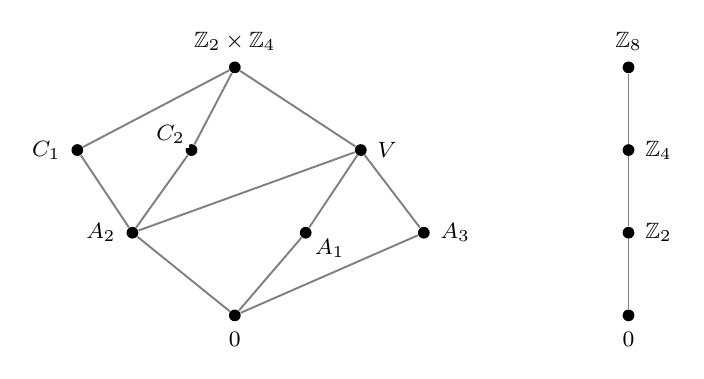
\begin{tikzpicture}[x=1cm,y=1.05cm]
  % --- left: Z_2 x Z_4 (all eight subgroups) ---
  \node[ltdot] (top) at (0,3) {};
  \node[ltdot] (c1) at (-2,2) {};
  \node[ltdot] (c2) at (-0.55,2) {};
  \node[ltdot] (v) at (1.6,2) {};
  \node[ltdot] (a2) at (-1.3,1) {};
  \node[ltdot] (a1) at (0.9,1) {};
  \node[ltdot] (a3) at (2.4,1) {};
  \node[ltdot] (bot) at (0,0) {};
  \begin{scope}[ltedge]
    \draw (c1) -- (top);
    \draw (c2) -- (top);
    \draw (v) -- (top);
    \draw (a2) -- (c1);
    \draw (a2) -- (c2);
    \draw (a2) -- (v);
    \draw (a1) -- (v);
    \draw (a3) -- (v);
    \draw (bot) -- (a1);
    \draw (bot) -- (a2);
    \draw (bot) -- (a3);
  \end{scope}
  \node[ltlab,above=2pt of top] {$\Z_2\times\Z_4$};
  \node[ltlab,left=2pt of c1] {$C_1$};
  \node[ltlab,above left=-1pt and -1pt of c2] {$C_2$};
  \node[ltlab,right=2pt of v] {$V$};
  \node[ltlab,left=2pt of a2] {$A_2$};
  \node[ltlab,below right=-1pt and 0pt of a1] {$A_1$};
  \node[ltlab,right=2pt of a3] {$A_3$};
  \node[ltlab,below=2pt of bot] {$0$};
  % --- right: Z_8 chain ---
  \node[ltdot] (z8) at (5,3) {};
  \node[ltdot] (z4) at (5,2) {};
  \node[ltdot] (z2) at (5,1) {};
  \node[ltdot] (z0) at (5,0) {};
  \begin{scope}[ltedge]
    \draw (z0) -- (z2);
    \draw (z2) -- (z4);
    \draw (z4) -- (z8);
  \end{scope}
  \node[ltlab,above=2pt of z8] {$\Z_8$};
  \node[ltlab,right=2pt of z4] {$\Z_4$};
  \node[ltlab,right=2pt of z2] {$\Z_2$};
  \node[ltlab,below=2pt of z0] {$0$};
\end{tikzpicture}
\end{center}
(here $A_1,A_2,A_3$ are the three order-$2$ subgroups). The three atoms versus one atom distinguish the two abelian groups of order $8$: rank $2$ (invariant factors $2\mid 4$) gives a wide lattice with $(p^2-1)/(p-1)=3$ atoms, while rank $1$ (single invariant factor $8$) gives the single chain $0<\Z_2<\Z_4<\Z_8$.
\end{exers}


\section{Groups of Small Order}
\subsection*{Classification of Groups of Small Order}

Section 5.3 is mostly a \emph{reference}: it assembles the tools developed so far (Lagrange, Cauchy, the Sylow theorems, direct and semidirect products, recognition of $\sdp$) into a single census. The goal is, for each small order $n$, to list \emph{every} isomorphism class of group of order $n$ and to explain how to tell them apart. We keep the theory terse and let worked classifications carry the load.

\begin{remark}[The number of groups of each order up to $16$]
Let $g(n)$ denote the number of isomorphism classes of groups of order $n$.
\[
\begin{array}{c|cccccccccccccccc}
n   & 1 & 2 & 3 & 4 & 5 & 6 & 7 & 8 & 9 & 10 & 11 & 12 & 13 & 14 & 15 & 16\\\hline
g(n)& 1 & 1 & 1 & 2 & 1 & 2 & 1 & 5 & 2 & 2  & 1  & 5  & 1  & 2  & 1  & 14
\end{array}
\]
Every entry with $n\le 15$ is derived below. The jump to $g(16)=14$ signals where hand-classification stops being pleasant; orders that are products of small primes (especially powers of $2$) proliferate. Note $g(p)=1$, $g(p^2)=2$, and (for $p<q$ primes) $g(pq)\in\{1,2\}$.
\end{remark}

\begin{remark}[The toolkit]
Three facts do almost all the work.
\begin{enumerate}
\item \textbf{Lagrange / Cauchy.} If $p\mid |G|$ then $G$ has an element (hence a subgroup) of order $p$.
\item \textbf{Sylow.} $n_p\equiv 1\pmod p$ and $n_p\mid m$ where $|G|=p^a m$, $p\nmid m$. If some $n_p=1$ the corresponding Sylow subgroup is normal.
\item \textbf{Recognition of (semi)direct products.} If $H\nor G$, $K\sgr G$, $H\cap K=1$, and $HK=G$ (e.g.\ $|H||K|=|G|$ with $H\cap K=1$), then $G\isom H\sdp_\varphi K$ where $\varphi\colon K\to\Aut(H)$ is conjugation. If \emph{both} $H,K\nor G$ the product is direct: $G\isom H\times K$.
\end{enumerate}
\end{remark}

\subsection*{Order $p$, $p^2$, and $pq$}

\begin{theorem}[Order $p$]
If $|G|=p$ is prime then $G\isom\Zn p$.
\end{theorem}

\begin{proof}
Pick $x\ne 1$. By Lagrange $\ord{x}\mid p$ and $\ord{x}\ne 1$, so $\ord{x}=p$ and $G=\gen{x}\isom\Zn p$.
\end{proof}

\begin{theorem}[Order $p^2$]
If $|G|=p^2$ then $G$ is abelian, and either $G\isom\Zn{p^2}$ or $G\isom\Zn p\times\Zn p$.
\end{theorem}

\begin{proof}
A $p$-group has nontrivial center, so $|Z(G)|\in\{p,p^2\}$. If $|Z(G)|=p$ then $G/Z(G)$ is cyclic of order $p$, forcing $G$ abelian and hence $Z(G)=G$, a contradiction. So $G$ is abelian. If $G$ has an element of order $p^2$ it is cyclic, $G\isom\Zn{p^2}$. Otherwise every non-identity element has order $p$; pick $x\ne 1$ and $y\notin\gen{x}$. Then $\gen{x}\cap\gen{y}=1$ and $\gen{x}\gen{y}$ has order $p^2$, so $G=\gen{x}\times\gen{y}\isom\Zn p\times\Zn p$.
\end{proof}

\begin{theorem}[Order $pq$, $p<q$ primes]\label{thm:pq@c5}
Let $|G|=pq$ with $p<q$.
\begin{enumerate}
\item If $p\nmid q-1$ then $G\isom\Zn{pq}$ (cyclic); it is the unique group of order $pq$.
\item If $p\mid q-1$ there are exactly two groups: $\Zn{pq}$ and a unique nonabelian group $\Zn q\sdp\Zn p$.
\end{enumerate}
\end{theorem}

\begin{proof}
By Sylow, $n_q\equiv 1\pmod q$ and $n_q\mid p$; since $p<q$ this forces $n_q=1$, so the Sylow $q$-subgroup $Q\isom\Zn q$ is normal. Also $n_p\equiv 1\pmod p$ and $n_p\mid q$, so $n_p\in\{1,q\}$. Let $P\isom\Zn p$ be a Sylow $p$-subgroup. Then $Q\cap P=1$ and $QP=G$, so $G\isom Q\sdp_\varphi P$ with $\varphi\colon P\to\Aut(Q)\isom\Zn{q-1}$. The homomorphisms $\varphi$ correspond to elements of $\Aut(Q)$ of order dividing $p$; there are $p$ such iff $p\mid q-1$, else only the trivial one. If $\varphi$ is trivial, $G\isom\Zn q\times\Zn p\isom\Zn{pq}$. If $p\mid q-1$, any two nontrivial $\varphi,\varphi'$ have images that are the unique subgroup of order $p$ in the cyclic group $\Aut(Q)$, and the resulting semidirect products are isomorphic; this gives one nonabelian class.
\end{proof}

\begin{method}{Classifying order $pq$ ($p<q$)}
\textbf{Trigger:} $|G|$ is a product of two distinct primes.
\begin{enumerate}
\item Order them $p<q$. The Sylow $q$-subgroup is \emph{always} normal (since $n_q\mid p<q$).
\item Compute $q-1$ and test divisibility by $p$.
\item If $p\nmid q-1$: only $\Zn{pq}$. If $p\mid q-1$: two groups, $\Zn{pq}$ and $\Zn q\sdp\Zn p$.
\end{enumerate}
\end{method}

\begin{wex}{Order $15$}
Classify all groups of order $15$.
\wrec This is $pq$ with $p=3,q=5$ (Theorem~\ref{thm:pq@c5}); check whether $3\mid 5-1$.
\wsol $q-1=4$ and $3\nmid 4$, so case (1) applies: the unique group is $\Zn{15}\isom\Zn3\times\Zn5$. \\
\emph{Check via Sylow directly:} $n_5\equiv 1\pmod 5$, $n_5\mid 3\imp n_5=1$; $n_3\equiv 1\pmod 3$, $n_3\mid 5\imp n_3=1$. Both Sylow subgroups normal $\imp G\isom\Zn3\times\Zn5\isom\Zn{15}$. So $g(15)=1$. \checkmark
\end{wex}

\begin{wex}{Order $21$}
Classify all groups of order $21$.
\wrec $pq$ with $p=3,q=7$; test $3\mid 7-1=6$.
\wsol $3\mid 6$, so case (2): two groups. The cyclic $\Zn{21}$, and the nonabelian $\Zn7\sdp\Zn3$. The nontrivial action: $\Aut(\Zn7)\isom\Zn6$ has a unique subgroup of order $3$ (generated by $x\mapsto x^2$, since $2$ has order $3$ mod $7$: $2,4,8\equiv1$). So $\Zn7\sdp\Zn3=\gen{a,b\st a^7=b^3=1,\ bab\inv=a^2}$. \\
\emph{Check:} $b^3 a b^{-3}=a^{2^3}=a^8=a$, consistent with $b^3=1$. \checkmark\ Thus $g(21)=2$.
\end{wex}

\begin{wex}{Order $33$ vs.\ order $35$}
Determine $g(33)$ and $g(35)$.
\wrec Both are $pq$; apply the $p\mid q-1$ test to each.
\wsol $33=3\cdot 11$: $q-1=10$, $3\nmid 10\imp g(33)=1$, only $\Zn{33}$. $\quad 35=5\cdot 7$: $q-1=6$, $5\nmid 6\imp g(35)=1$, only $\Zn{35}$. \\
\emph{Check:} Both have all Sylow subgroups normal (e.g.\ for $33$: $n_{11}\mid 3$ and $\equiv1\,(11)\imp n_{11}=1$; $n_3\mid 11$ and $\equiv1\,(3)\imp n_3=1$). \checkmark
\end{wex}

\begin{wex}{The smallest nonabelian $pq$}
What is the smallest order $pq$ ($p<q$ distinct primes) admitting a nonabelian group, and exhibit it.
\wrec Need the least $q$ with a prime $p<q$ dividing $q-1$; the case-(2) condition.
\wsol Test $q=3$: $q-1=2$, $p=2\mid 2$ and $p<q$. So $pq=6$ works: the nonabelian group is $\Zn3\sdp\Zn2$ with the inversion action, i.e.\ $S_3\isom D_6$. \\
\emph{Check:} $\Aut(\Zn3)\isom\Zn2$, nontrivial action sends $r\mapsto r\inv$, giving $\gen{r,s\st r^3=s^2=1,\ srs\inv=r\inv}=D_6\isom S_3$. \checkmark\ Smallest such order is $6$.
\end{wex}

\begin{pitfall}
The cyclic-uniqueness criterion is \emph{not} just ``the smaller prime $p$''; it is ``$p\mid q-1$'' with $p<q$. For $|G|=2q$ ($q$ odd), $p=2$ \emph{always} divides $q-1$, so there is \emph{always} a nonabelian group (dihedral). For odd $p<q$, you must actually check divisibility -- e.g.\ $|G|=15$ has \emph{no} nonabelian group even though both factors are odd primes.
\end{pitfall}

\subsection*{Order $2p$: cyclic or dihedral}

\begin{theorem}[Order $2p$, $p$ an odd prime]\label{thm:2p@c5}
If $|G|=2p$ with $p$ odd prime, then $G\isom\Zn{2p}$ or $G\isom D_{2p}$. These are the only two classes.
\end{theorem}

\begin{proof}
This is the case $p=2$ of Theorem~\ref{thm:pq@c5} after relabelling: write the primes as $2<p$. Since $2\mid p-1$ always, there are exactly two groups. The Sylow $p$-subgroup $P=\gen{r}\isom\Zn p$ is normal. Let $s$ have order $2$. Then $G=\gen{r}\sdp\gen{s}$, and $\Aut(\Zn p)\isom\Zn{p-1}$ has a \emph{unique} element of order $2$, namely $r\mapsto r\inv$. If $s$ acts trivially, $srs\inv=r$ and $G$ is abelian $\isom\Zn{2p}$. If $s$ acts by the order-$2$ automorphism, $srs\inv=r\inv$ and $G\isom D_{2p}$.
\end{proof}

\begin{method}{Telling $\Zn{2p}$ from $D_{2p}$}
\textbf{Trigger:} $|G|=2p$, $p$ odd prime. Always exactly two groups.
\begin{itemize}
\item Find $r$ with $\ord{r}=p$ (Cauchy) and $s$ with $\ord{s}=2$.
\item Compute $srs\inv$. If $srs\inv=r$ (commute): $G\isom\Zn{2p}$. If $srs\inv=r\inv$: $G\isom D_{2p}$.
\item Quick invariants: $\Zn{2p}$ has an element of order $2p$ and is abelian with center $G$; $D_{2p}$ is nonabelian with center $1$ and has $p$ elements of order $2$.
\end{itemize}
\end{method}

\begin{wex}{Order $6$}
Classify all groups of order $6$.
\wrec $2p$ with $p=3$; Theorem~\ref{thm:2p@c5} gives exactly two.
\wsol By Cauchy take $r$ of order $3$ and $s$ of order $2$; $\gen{r}\nor G$ (index $2$, or $n_3=1$). Then $srs\inv\in\{r,r\inv\}$.
\begin{itemize}
\item $srs\inv=r$: abelian, $G\isom\Zn2\times\Zn3\isom\Zn6$.
\item $srs\inv=r\inv$: $G\isom\gen{r,s\st r^3=s^2=1,\ srs\inv=r\inv}=D_6\isom S_3$.
\end{itemize}
\emph{Check:} In $S_3$, take $r=(1\,2\,3)$, $s=(1\,2)$. Then $srs\inv=(1\,2)(1\,2\,3)(1\,2)=(1\,3\,2)=r\inv$. Nonabelian. \checkmark\ So $g(6)=2$.
\end{wex}

\begin{wex}{Order $10$}
Classify all groups of order $10$.
\wrec $2p$ with $p=5$.
\wsol Sylow: $n_5\mid 2$, $n_5\equiv1\,(5)\imp n_5=1$, so $\gen{r}\isom\Zn5$ is normal. With $s$ of order $2$, $srs\inv\in\{r,r^2,r^3,r^4\}$ must have order $5$, and conjugating it once more by $s$ must give back $r$ (since $s^2=1\imp s(srs\inv)s\inv=r$); only $r\mapsto r$ and $r\mapsto r\inv=r^4$ satisfy $\varphi^2=\id$. Two groups: $\Zn{10}$ and $D_{10}$. \\
\emph{Check:} $D_{10}$ is the symmetry group of the regular pentagon, $|D_{10}|=10$, nonabelian; $\Zn{10}$ has the element $r+s$-style generator of order $10$. \checkmark\ $g(10)=2$.
\end{wex}

\begin{wex}{Order $14$ and order $22$}
Find all groups of orders $14$ and $22$.
\wrec Both are $2p$ ($p=7$, $p=11$).
\wsol Each gives exactly $\Zn{2p}$ and $D_{2p}$: $\{\Zn{14},D_{14}\}$ and $\{\Zn{22},D_{22}\}$. \\
\emph{Check:} $n_7\mid 2,\equiv1\,(7)\imp n_7=1$ (order $14$); $n_{11}\mid 2,\equiv1\,(11)\imp n_{11}=1$ (order $22$). Normal Sylow $p$-subgroup, then the inversion-or-trivial dichotomy. \checkmark\ $g(14)=g(22)=2$.
\end{wex}

\begin{wex}{Why no third group of order $2p$?}
Explain why $G$ of order $2p$ cannot be a ``new'' nonabelian group beyond $D_{2p}$.
\wrec Uses that $\Aut(\Zn p)$ is \emph{cyclic} of order $p-1$, so has a unique involution.
\wsol The semidirect product $\Zn p\sdp_\varphi\Zn2$ is determined by $\varphi(s)\in\Aut(\Zn p)$ with $\varphi(s)^2=\id$. A cyclic group $\Zn{p-1}$ has exactly one element of order $2$ (since $p$ is odd, $p-1$ is even). So there are exactly two choices for $\varphi(s)$: the identity ($\imp\Zn{2p}$) and the unique involution ($\imp D_{2p}$). No room for a third. \\
\emph{Check:} $p=7$: $\Aut(\Zn7)\isom\Zn6$, involution is $r\mapsto r^6=r\inv$, matching $D_{14}$. \checkmark
\end{wex}

\subsection*{Order $4$ and the small abelian cases}

\begin{wex}{Order $4$}
Classify all groups of order $4$.
\wrec $|G|=p^2$ with $p=2$; a $p^2$-group is abelian (Theorem on order $p^2$).
\wsol Abelian, so either an element of order $4$ ($G\isom\Zn4$) or every non-identity element has order $2$ ($G\isom\Zn2\times\Zn2=V_4$). \\
\emph{Check:} $\Zn4=\{0,1,2,3\}$ has the generator $1$ of order $4$. $V_4=\{1,a,b,ab\}$ with $a^2=b^2=(ab)^2=1$; e.g.\ $a=(1\,2)(3\,4),b=(1\,3)(2\,4)$ in $S_4$. \checkmark\ $g(4)=2$.
\end{wex}

\begin{wex}{Order $9$}
Classify all groups of order $9$.
\wrec $p^2$ with $p=3$.
\wsol Abelian; either $\Zn9$ (an element of order $9$) or $\Zn3\times\Zn3$ (all non-identity elements have order $3$). \\
\emph{Check:} no nonabelian option since order $p^2\imp$ abelian. $g(9)=2$. \checkmark
\end{wex}

\subsection*{The five groups of order $8$}

\begin{theorem}[Order $8$]\label{thm:order8@c5}
There are exactly five groups of order $8$:
\[
\underbrace{\Zn8,\quad \Zn4\times\Zn2,\quad \Zn2\times\Zn2\times\Zn2}_{\text{abelian (3)}},\qquad
\underbrace{D_8,\quad Q_8}_{\text{nonabelian (2)}}.
\]
\end{theorem}

\begin{proof}
\emph{Abelian case.} By the Fundamental Theorem of Finite Abelian Groups, the abelian groups of order $8=2^3$ correspond to partitions of $3$: $3\to\Zn8$, $2+1\to\Zn4\times\Zn2$, $1+1+1\to\Zn2^3$. That is three classes.

\emph{Nonabelian case.} Suppose $G$ is nonabelian of order $8$. No element has order $8$ (else cyclic). Not every non-identity element has order $2$ (that would force $G$ abelian, as $x^2=1\,\forall x\imp$ abelian). So there is an element $r$ of order $4$; $\gen{r}\nor G$ (index $2$). Pick $s\notin\gen{r}$. Conjugation gives $srs\inv\in\gen{r}$ of order $4$, so $srs\inv\in\{r,r^3\}$; $r$ would make $G$ abelian, so $srs\inv=r^3=r\inv$. Now $s^2\in\gen{r}$ and $s^2$ is centralized by $s$, so $s^2\in\{1,r^2\}$ (as $r,r^3$ are not centralized by $s$).
\begin{itemize}
\item $s^2=1$: relations $r^4=s^2=1,\ srs\inv=r\inv\imp G\isom D_8$.
\item $s^2=r^2$: relations $r^4=1,\ s^2=r^2,\ srs\inv=r\inv\imp G\isom Q_8$.
\end{itemize}
These two are not isomorphic (counted below), giving exactly two nonabelian classes. Total: $5$.
\end{proof}

The two abelian groups with an element of order $\ge 4$ are separated cleanly by their
subgroup lattices. The cyclic group $\Zn8$ is a single chain (one subgroup of each order
$1,2,4,8$), whereas $\Zn4\times\Zn2$ is a wider lattice with three subgroups of order $2$
and three of order $4$.

\begin{center}
\begin{tikzpicture}[x=1cm,y=1.25cm]
  % --- left: Z/8Z chain ---
  \node[ltdot] (c0) at (0,0) {};
  \node[ltdot] (c2) at (0,1) {};
  \node[ltdot] (c4) at (0,2) {};
  \node[ltdot] (c8) at (0,3) {};
  \begin{scope}[ltedge]
    \draw (c0) -- (c2);
    \draw (c2) -- (c4);
    \draw (c4) -- (c8);
  \end{scope}
  \node[ltlab,above=2pt of c8] {$\Zn8$};
  \node[ltlab,right=2pt of c4] {$\gen{2}$};
  \node[ltlab,right=2pt of c2] {$\gen{4}$};
  \node[ltlab,below=2pt of c0] {$0$};
  % --- right: Z/4Z x Z/2Z lattice (8 subgroups) ---
  \begin{scope}[xshift=5cm]
    \node[ltdot] (top) at (0,3) {};
    \node[ltdot] (P)   at (-2,2) {};
    \node[ltdot] (Q)   at (-0.55,2) {};
    \node[ltdot] (K)   at (1.6,2) {};
    \node[ltdot] (A)   at (-1.3,1) {};
    \node[ltdot] (B)   at (0.9,1) {};
    \node[ltdot] (C)   at (2.4,1) {};
    \node[ltdot] (bot) at (0,0) {};
    \begin{scope}[ltedge]
      % top to the three order-4 subgroups
      \draw (P) -- (top);
      \draw (Q) -- (top);
      \draw (K) -- (top);
      % A lies in all three order-4 subgroups
      \draw (A) -- (P);
      \draw (A) -- (Q);
      \draw (A) -- (K);
      % B and C lie only in the Klein subgroup K
      \draw (B) -- (K);
      \draw (C) -- (K);
      % bottom to the three order-2 subgroups
      \draw (bot) -- (A);
      \draw (bot) -- (B);
      \draw (bot) -- (C);
    \end{scope}
    \node[ltlab,above=2pt of top] {$\Zn4\times\Zn2$};
    \node[ltlab,left=2pt of P]  {$P$};
    \node[ltlab,above left=-1pt and -1pt of Q] {$Q$};
    \node[ltlab,right=2pt of K] {$K$};
    \node[ltlab,left=2pt of A]  {$A$};
    \node[ltlab,below right=-1pt and 0pt of B] {$B$};
    \node[ltlab,right=2pt of C] {$C$};
    \node[ltlab,below=2pt of bot] {$0$};
  \end{scope}
\end{tikzpicture}
\end{center}

Here $A=\gen{(2,0)}$, $B=\gen{(0,1)}$, $C=\gen{(2,1)}$ are the order-$2$ subgroups, while
$P=\gen{(1,0)}\isom\Zn4$, $Q=\gen{(1,1)}\isom\Zn4$, and $K=\gen{(2,0),(0,1)}\isom V_4$ are the
order-$4$ subgroups; $A$ is the unique order-$2$ subgroup contained in all three of $P,Q,K$,
whereas $B$ and $C$ lie only in the Klein four-group $K$.

\begin{method}{Distinguishing the five groups of order $8$}
\textbf{Trigger:} $|G|=8$. First decide abelian vs.\ nonabelian (is there a nontrivial commutator?).
\begin{enumerate}
\item \textbf{Abelian?} Use the \emph{order spectrum} (how many elements of each order):
\[
\begin{array}{l|ccc}
 & \#\,\ord 1 & \#\,\ord 2 & \#\,\ord 4 \ (\#\,\ord 8)\\\hline
\Zn8 & 1 & 1 & 2\ (4)\\
\Zn4\times\Zn2 & 1 & 3 & 4\\
\Zn2^3 & 1 & 7 & 0
\end{array}
\]
\item \textbf{Nonabelian?} Both $D_8,Q_8$ have $|Z(G)|=2$ and $G/Z\isom V_4$. Separate by counting elements of order $2$:
\[
D_8:\ \text{five elements of order }2;\qquad Q_8:\ \text{exactly one element of order }2\ (\text{namely }{-1}=r^2).
\]
Equivalently: $Q_8$ has a \emph{unique} involution and \emph{every} subgroup is normal; $D_8$ has non-normal subgroups (the reflections).
\end{enumerate}
\end{method}

\begin{wex}{The five groups of order $8$ and how to tell them apart}
Exhibit all five groups of order $8$ and give a single invariant separating each from the others.
\wrec Theorem~\ref{thm:order8@c5}; use the order-spectrum table plus the unique-involution test.
\wsol
\emph{Abelian (3):}
\begin{itemize}
\item $\Zn8$: cyclic, has elements of order $8$. Unique with $\ord{x}=8$.
\item $\Zn4\times\Zn2$: max order $4$, with $3$ involutions. (E.g.\ $(2,0),(0,1),(2,1)$ have order $2$.)
\item $\Zn2^3$: exponent $2$, all $7$ non-identity elements are involutions.
\end{itemize}
\emph{Nonabelian (2):}
\begin{itemize}
\item $D_8=\gen{r,s\st r^4=s^2=1,\ srs\inv=r\inv}$: involutions are $r^2,s,rs,r^2s,r^3s$ -- \emph{five}.
\item $Q_8=\{\pm1,\pm i,\pm j,\pm k\}$ with $i^2=j^2=k^2=ijk=-1$: only $-1$ has order $2$ -- \emph{one}.
\end{itemize}
\emph{Separating invariant:} the number of elements of order $2$ is $1,3,7,5,1$ -- this distinguishes all pairs except $(\Zn8,Q_8)$, both having one involution; but $\Zn8$ is abelian (or: $\Zn8$ has elements of order $8$, $Q_8$ does not). \\
\emph{Check ($Q_8$ involution count):} $i^2=-1\ne1$, so $i,j,k,-i,-j,-k$ all have order $4$; $(-1)^2=1$. Exactly one involution. \checkmark\ And $D_8$: $(r^a s)^2=r^a s r^a s=r^a r^{-a}s^2=1$, so all four $r^a s$ are involutions, plus $r^2$, total five. \checkmark
\end{wex}

\begin{wex}{Is the dihedral group of the square $D_8$ or $Q_8$?}
The symmetry group $G$ of a square has order $8$. Which of the five is it?
\wrec Count involutions / use that reflections are non-central order-$2$ elements.
\wsol $G$ has rotations $1,r,r^2,r^3$ ($r=$ rotation by $90^\circ$) and four reflections $s,rs,r^2s,r^3s$. The four reflections and $r^2$ (rotation by $180^\circ$) are involutions: five of order $2$. Matches $D_8$. \\
\emph{Check:} a reflection $s$ is not central ($srs\inv=r\inv\ne r$), so $G$ is nonabelian with five involutions $\imp G\isom D_8$, not $Q_8$. \checkmark
\end{wex}

\begin{wex}{$\Zn4\times\Zn2$ vs.\ $\Zn8$ from a presentation}
Let $G=\gen{a,b\st a^4=b^2=1,\ ab=ba}$. Identify $G$.
\wrec Abelian (commuting generators); read off the order spectrum.
\wsol $G$ is abelian of order $|a|\cdot|b|/|\gen a\cap\gen b|=4\cdot2=8$ since $\gen a\cap\gen b=1$. Max element order is $\ord{ab}=\lcm(4,2)=4$ ($<8$), so $G\not\isom\Zn8$. Three involutions: $a^2,b,a^2b$. Thus $G\isom\Zn4\times\Zn2$. \\
\emph{Check:} $(a^2)^2=(b)^2=(a^2b)^2=1$ and these are distinct nonidentity elements of order $2$; spectrum $(1,3,4)$ matches the table. \checkmark
\end{wex}

\begin{wex}{Every subgroup of $Q_8$ is normal}
Verify that $Q_8$ has the unusual property that all its subgroups are normal (it is \emph{Hamiltonian}), distinguishing it sharply from $D_8$.
\wrec Subgroups of order $4$ have index $2$ (automatically normal); the unique order-$2$ subgroup is central.
\wsol Subgroups: $\{1\},\ \gen{-1}=\{\pm1\},\ \gen i,\gen j,\gen k$ (each order $4$, index $2$, normal), and $Q_8$. The order-$2$ subgroup $\{\pm1\}=Z(Q_8)$ is central hence normal. So all six subgroups are normal. \\
\emph{Contrast:} in $D_8$, $\gen s=\{1,s\}$ is \emph{not} normal: $r s r\inv=r^2 s\notin\gen s$. \checkmark\ This non-normal reflection subgroup cleanly separates $D_8$ from $Q_8$.
\end{wex}

\begin{pitfall}
$D_8$ and $Q_8$ share many invariants: both have order $8$, center of order $2$, $G/Z\isom V_4$, derived subgroup $\gen{r^2}$ of order $2$, and the \emph{same} character table degrees. Do \emph{not} try to distinguish them by $|Z|$ or by $G/Z$. The clean separators are: number of involutions ($5$ vs.\ $1$), or ``has a non-normal subgroup'' ($D_8$ yes, $Q_8$ no).
\end{pitfall}

\subsection*{The five groups of order $12$}

\begin{theorem}[Order $12$]\label{thm:order12@c5}
There are exactly five groups of order $12$:
\[
\underbrace{\Zn{12},\quad \Zn2\times\Zn6\ (\isom\Zn2^2\times\Zn3)}_{\text{abelian (2)}},\qquad
\underbrace{A_4,\quad D_{12},\quad \Zn3\sdp\Zn4=\mathrm{Dic}_3}_{\text{nonabelian (3)}}.
\]
The last, $\mathrm{Dic}_3$ (the dicyclic / binary dihedral group $Q_{12}$), is $\gen{a,b\st a^6=1,\ b^2=a^3,\ bab\inv=a\inv}$.
\end{theorem}

\begin{proof}[Proof sketch]
\emph{Abelian (2):} partitions of $2^2\cdot3$: $\Zn4\times\Zn3\isom\Zn{12}$ and $\Zn2\times\Zn2\times\Zn3\isom\Zn2\times\Zn6$.

\emph{Nonabelian.} Let $|G|=12=2^2\cdot3$. By Sylow, $n_3\in\{1,4\}$ and $n_2\in\{1,3\}$. \emph{Key step:} not both can fail to be normal -- if $n_3=4$ there are $4\cdot2=8$ elements of order $3$, leaving only $4$ elements (which must form the unique, hence normal, Sylow $2$-subgroup, so $n_2=1$). So either the Sylow $3$-subgroup $P_3$ or the Sylow $2$-subgroup $P_2$ is normal.
\begin{itemize}
\item \textbf{$P_3\nor G$} (i.e.\ $n_3=1$): then $G\isom\Zn3\sdp P_2$ with $P_2\in\{\Zn4,\Zn2^2\}$ and action $\varphi\colon P_2\to\Aut(\Zn3)\isom\Zn2$. Nontrivial cases:
\begin{itemize}
\item $P_2=\Zn4$, $\varphi$ nontrivial (kernel $\Zn2$): $\Zn3\sdp\Zn4=\mathrm{Dic}_3$.
\item $P_2=\Zn2^2$, $\varphi$ nontrivial: $\Zn3\sdp\Zn2^2\isom D_{12}$ (since $\Zn3\sdp\Zn2=S_3=D_6$, and $\times\Zn2\imp D_{12}\isom D_6\times\Zn2$).
\end{itemize}
(Trivial $\varphi$ recovers the two abelian groups.)
\item \textbf{$P_3$ not normal} ($n_3=4$): forces $n_2=1$, $P_2\isom\Zn2^2\nor G$, and $G\isom\Zn2^2\sdp\Zn3$ with $\Zn3$ acting by an order-$3$ automorphism (a $3$-cycle on the three involutions). This is $A_4$.
\end{itemize}
Distinctness is checked by invariants (see the method box), giving exactly three nonabelian classes; total $5$.
\end{proof}

\begin{method}{Distinguishing the five groups of order $12$}
\textbf{Trigger:} $|G|=12$.
\begin{enumerate}
\item \textbf{Abelian?} Element of order $12$ $\imp\Zn{12}$; else (max order $6$) $\Zn2\times\Zn6$.
\item \textbf{Nonabelian} -- use these separators:
\[
\begin{array}{l|cccc}
 & \text{normal Sylow } & n_3 & \#\,\ord 2 & \text{has elt of order} \\
 & 3\text{-subgrp?} & & & \\\hline
A_4 & \text{no } (n_3=4) & 4 & 3 & 1,2,3 \text{ only}\\
D_{12} & \text{yes} & 1 & 7 & 1,2,3,6\\
\mathrm{Dic}_3 & \text{yes} & 1 & 1 & 1,2,3,4,6
\end{array}
\]
Fast triage: $A_4$ has \emph{no} element of order $6$ and \emph{no} normal Sylow $3$-subgroup (it is the only one with $n_3=4$). $\mathrm{Dic}_3$ has a \emph{unique} involution (like $Q_8$). $D_{12}$ has \emph{seven} involutions.
\end{enumerate}
\end{method}

\begin{wex}{$A_4$ has no subgroup of order $6$}
Show $A_4$ is the nonabelian order-$12$ group with $n_3=4$, and that it has no subgroup of order $6$ -- the classic failure of the converse of Lagrange.
\wrec Identify $A_4$'s Sylow structure; a subgroup of order $6$ would have index $2$ hence be normal.
\wsol $A_4$'s $3$-cycles: there are $8$ of them, forming four Sylow $3$-subgroups (each $\gen{(i\,j\,k)}$ of order $3$ shares only identity), so $n_3=4$, not normal. The three double transpositions $(1\,2)(3\,4),(1\,3)(2\,4),(1\,4)(2\,3)$ plus $1$ form the unique $V_4\nor A_4$, so $n_2=1$. \\
\emph{No order-$6$ subgroup:} such $H$ has index $2$, so $H\nor A_4$, and $H$ would contain all squares; but every $3$-cycle $\sigma=\sigma^4=(\sigma^2)^2$ is a square, and there are $8$ of them $>6$. Contradiction. \\
\emph{Check:} $A_4$ has element orders $1,2,3$ only (no order $6$), matching the table. \checkmark
\end{wex}

\begin{wex}{Building $\mathrm{Dic}_3=\Zn3\sdp\Zn4$}
Construct the nonabelian group $G=\Zn3\sdp\Zn4$ with the nontrivial action and find its unique involution.
\wrec $H=\Zn3\nor G$, $K=\Zn4$ acts through $\Aut(\Zn3)\isom\Zn2$ via the order-$2$ quotient $\Zn4\to\Zn2$.
\wsol Write $\gen{a}=\Zn3$, $\gen{b}=\Zn4$. The generator $b$ acts by inversion: $bab\inv=a\inv=a^2$, and $b^2$ acts trivially (kernel of $\Zn4\to\Aut(\Zn3)$ is $\gen{b^2}$). Standard presentation: $G=\gen{a,b\st a^3=b^4=1,\ bab\inv=a\inv}$, order $12$. \\
The element $b^2$ is central (acts trivially on $a$ and commutes with $b$) of order $2$: it is the unique involution. Setting $x=ab$-type elements, $\ord{x}=4$. \\
\emph{Check:} In the equivalent presentation $\gen{a,b\st a^6=1,b^2=a^3,bab\inv=a\inv}$, $b^2=a^3$ has order $2$ and is the only involution; this is the dicyclic group $Q_{12}$. Matches ``$\#\,\ord2=1$''. \checkmark
\end{wex}

\begin{wex}{$D_{12}\isom S_3\times\Zn2$}
Show the order-$12$ dihedral group factors as $D_{12}\isom D_6\times\Zn2\isom S_3\times\Zn2$, and count its involutions.
\wrec $D_{12}$ has central element $r^3$ of order $2$; quotient out to get $D_6$.
\wsol $D_{12}=\gen{r,s\st r^6=s^2=1,\ srs\inv=r\inv}$. The element $z=r^3$ is central ($r^3 s=s r^{-3}=sr^3$ since $r^6=1$) of order $2$, with $\gen z\cap\gen{r^2,s}=1$ and $\gen{r^2,s}\isom D_6=S_3$. So $D_{12}\isom\gen{r^2,s}\times\gen{r^3}\isom S_3\times\Zn2$. \\
\emph{Involutions:} the six reflections $r^k s$ ($k=0,\dots,5$) plus $r^3$: seven elements of order $2$. \\
\emph{Check:} $(r^k s)^2=r^k s r^k s=r^k r^{-k}s^2=1$ for all $k$ (six involutions); $(r^3)^2=r^6=1$ (one more). Total $7$, matching the table. \checkmark
\end{wex}

\begin{wex}{Triage drill: a nonabelian order-$12$ group}
A nonabelian group $G$ of order $12$ has a normal Sylow $3$-subgroup, exactly one element of order $2$, and an element of order $4$. Identify $G$.
\wrec Run the order-$12$ method box: unique involution $+$ order-$4$ element pins it down.
\wsol Normal Sylow $3$-subgroup rules out $A_4$ ($n_3=4$). A unique involution rules out $D_{12}$ (seven) and $\Zn2\times\Zn6$ (three); $\Zn{12}$, which also has a unique involution, is excluded because $G$ is nonabelian. The only candidate with $\#\,\ord2=1$ and an order-$4$ element is $\mathrm{Dic}_3=\Zn3\sdp\Zn4$. So $G\isom\mathrm{Dic}_3$. \\
\emph{Check:} consistency -- $\mathrm{Dic}_3$ has element orders $\{1,2,3,4,6\}$, a unique involution $b^2$, and $n_3=1$. All three given properties hold. \checkmark
\end{wex}

\begin{wex}{Classify order $12$ end to end}
List all five groups of order $12$ and assign each its Sylow data $(n_2,n_3)$.
\wrec Theorem~\ref{thm:order12@c5} plus computing $n_2,n_3$ for each.
\wsol
\[
\begin{array}{l|cc|l}
G & n_2 & n_3 & \text{type}\\\hline
\Zn{12} & 1 & 1 & \text{abelian, elt of order }12\\
\Zn2\times\Zn6 & 1 & 1 & \text{abelian, exponent }6\\
D_{12} & 3 & 1 & \text{nonab., }7\text{ involutions}\\
\mathrm{Dic}_3 & 3 & 1 & \text{nonab., unique involution}\\
A_4 & 1 & 4 & \text{nonab., no order }6
\end{array}
\]
\emph{Check:} $A_4$ is the \emph{only} group of order $12$ with $n_3=4$ (the $8$ three-cycles force it), confirming the count $5$. For the others $n_3=1$, distinguished by abelian-ness and involution count. \checkmark\ Hence $g(12)=5$.
\end{wex}

\subsection*{Diagrams: the split exact sequence and the order-$12$ trichotomy}

Every group of order $2p$, $pq$ (nonabelian case), or $12$ (nonabelian) arises as a (semi)direct product, hence sits in a \emph{split} short exact sequence with a normal Sylow subgroup as kernel; so does $D_8=\gen{r}\sdp\gen{s}$, with kernel $\gen{r}$. The exception is $Q_8$: every nontrivial subgroup of $Q_8$ contains $-1$, so $Q_8$ is not a semidirect product of proper subgroups (it is a non-split extension). The split sequence is:
\[\begin{tikzcd}[column sep=normal]
1 \arrow[r] & H \arrow[r, hook] & H\sdp K \arrow[r, two heads, "\pi"] & K \arrow[r] \arrow[l, bend right, "s"'] & 1
\end{tikzcd}\]
\begin{dgx}
\dgi{Objects:} Five nodes from left to right: the trivial group $1$; the normal subgroup $H$ (the normal Sylow $p$-subgroup, e.g.\ $\Zn q$ when $|G|=pq$); the semidirect product $H\sdp K$ (the full group $G$); the complement $K$ (a Sylow subgroup of complementary order); and the trivial group $1$ again on the far right. Together they form a short exact sequence.
\dgi{Arrows:} The leftmost arrow $1\to H$ is the zero map (inclusion of the identity). The hooked arrow $H\hookrightarrow H\sdp K$ is the canonical inclusion $h\mapsto(h,1_K)$, injective by definition. The two-headed arrow $H\sdp K\xrightarrow{\pi} K$ is the projection $\pi(h,k)=k$, surjective with kernel exactly $H$. The rightmost arrow $K\to 1$ sends everything to the identity. The bent arrow $s\colon K\to H\sdp K$ is the splitting: $s(k)=(1_H,k)$, a group homomorphism satisfying $\pi\circ s=\id_K$.
\dgi{What commutes:} The sequence is exact: $\im(1\to H)=1=\ker(H\hookrightarrow H\sdp K)$ (trivially); $\im(H\hookrightarrow H\sdp K)=H=\ker(\pi)$ (this is the key exactness); $\im(\pi)=K=\ker(K\to 1)$. The splitting condition: $\pi\circ s=\id_K$, i.e.\ $\pi(1_H,k)=k$.
\dgi{Why it commutes:} Chase a coset representative: $\ker\pi=\{(h,k)\in H\sdp K : k=1_K\}=H\times\{1_K\}$, which is exactly the image of the inclusion $h\mapsto(h,1_K)$. The splitting $s(k)=(1_H,k)$ is a homomorphism because the multiplication in $H\sdp K$ restricts on $\{1_H\}\times K$ to the group law of $K$. The condition $\pi(s(k))=\pi(1_H,k)=k$ holds by definition of $\pi$.
\dgi{Why this matters here:} Every semidirect product $H\sdp K$ that appears in the classification of groups of small order -- $D_{2p}$, $\Zn q\sdp\Zn p$, $D_8$, $A_4$, $D_{12}$, $\mathrm{Dic}_3$ (but not $Q_8$, which is not a semidirect product of proper subgroups) -- sits in exactly such a sequence. The diagram encodes in one picture \emph{why} $H\sdp K$ is determined up to isomorphism by the conjugation action $\varphi\colon K\to\Aut(H)$: the splitting $s$ records the embedding of $K$ back into $G$, and the only freedom is how $K$ acts on $H$ by conjugation via $s$.
\dgi{Concrete example:} For $G=S_3\isom\Zn3\sdp\Zn2$: $H=\Zn3=\gen{(1\,2\,3)}$, $K=\Zn2=\gen{(1\,2)}$, $\pi$ sends each permutation to its coset mod $H$, and $s$ embeds $(1\,2)$ back as $(1\,2)\in S_3$. Exactness: $\ker\pi=\{1,(1\,2\,3),(1\,3\,2)\}=H$. The splitting: $\pi(s((1\,2)))=\pi((1\,2))=(1\,2)\in K$. \checkmark
\dgi{Common pitfall:} The bent arrow $s$ is a section of $\pi$ (a right inverse), not a section of the inclusion. Students sometimes think $s$ splits the sequence ``on the left'' and write $s\circ\iota=\id_H$; that is false -- $s$ goes $K\to H\sdp K$, not back to $H$. The correct condition is only $\pi\circ s=\id_K$.
\dgi{Takeaway:} The point of this diagram is that every (semi)direct product is precisely a short exact sequence equipped with a group-homomorphism section, and the isomorphism type of the whole group is determined by how the section's image acts on the normal subgroup.
\end{dgx}
Here $H$ is the normal Sylow subgroup, $K$ a complement (Sylow subgroup of complementary order), $s$ the splitting, and the isomorphism type is fixed by $\varphi=\,$``conjugation'' $\colon K\to\Aut(H)$. A \emph{direct} product is the special case $\varphi$ trivial, where the second projection also splits and both factors are normal:
\[\begin{tikzcd}[column sep=large]
 & G \arrow[dl, "\pi_1"'] \arrow[dr, "\pi_2"] \arrow[d, "{=}", dashed] & \\
H & H\times K \arrow[l, "p_1"] \arrow[r, "p_2"'] & K
\end{tikzcd}\]
\begin{dgx}
\dgi{Objects:} Four nodes: $G$ at the top (a group abstractly given or arrived at via the classification argument); $H$ at the lower-left (a normal subgroup of $G$, the normal Sylow subgroup in the classification); $K$ at the lower-right (the complementary subgroup, also normal in the direct-product case); and $H\times K$ at the center bottom (the direct product, serving as the ``canonical model'' the diagram identifies $G$ with).
\dgi{Arrows:} $\pi_1\colon G\to H$ and $\pi_2\colon G\to K$ are the two group homomorphisms from $G$ to each factor. $p_1\colon H\times K\to H$ and $p_2\colon H\times K\to K$ are the standard coordinate projections, $p_1(h,k)=h$, $p_2(h,k)=k$. The dashed arrow $G\to H\times K$ (labelled $=$) is the canonical isomorphism $g\mapsto(\pi_1(g),\pi_2(g))$; it exists because both $H$ and $K$ are normal in $G$ with $H\cap K=1$ and $HK=G$.
\dgi{What commutes:} The left triangle: $p_1\circ(=)=\pi_1$. The right triangle: $p_2\circ(=)=\pi_2$. Concretely, for any $g\in G$ written uniquely as $g=hk$ with $h\in H,k\in K$: $p_1(h,k)=h=\pi_1(g)$ and $p_2(h,k)=k=\pi_2(g)$.
\dgi{Why it commutes:} Well-definedness of the isomorphism $g\mapsto(\pi_1(g),\pi_2(g))$ rests on $H\cap K=1$ (so the decomposition $g=hk$ is unique) and $HK=G$ (so every $g$ decomposes). Commutativity of the triangles is then definitional: $\pi_1(g)$ \emph{is} the $H$-component of $g$, and $p_1$ reads that component from the pair.
\dgi{Why this matters here:} The diagram distinguishes the \emph{direct} product case ($\varphi$ trivial, both factors normal) from the strict semidirect product. In the split-SES diagram the arrow $s$ is a one-sided section; here the dashed isomorphism is bilateral, reflecting that both projections split. This is the exact situation for $G\isom\Zn3\times\Zn5\isom\Zn{15}$ (both Sylow subgroups normal, $\varphi$ trivial) or for the abelian groups $\Zn4\times\Zn3\isom\Zn{12}$ and $\Zn2\times\Zn3\isom\Zn6$.
\dgi{Concrete example:} $G=\Zn6$, $H=\Zn3=\gen{2}$, $K=\Zn2=\gen{3}$ (inside $\Z/6\Z$). Then $\pi_1(n)=n\bmod 3$ (projected onto the $\Zn3$ factor) and $\pi_2(n)=n\bmod 2$. The isomorphism $\Zn6\xrightarrow{\sim}\Zn3\times\Zn2$ sends $1\mapsto(1,1)$. The triangles commute: $p_1(1,1)=1=\pi_1(1)$. \checkmark
\dgi{Common pitfall:} The dashed equality-labelled arrow is an \emph{isomorphism}, not a literal equality; the label $=$ indicates the canonical identification, not that $G$ and $H\times K$ are the same set. Students sometimes read this diagram as asserting $G=H\times K$ by definition and skip checking the conditions $H\nor G$, $K\nor G$, $H\cap K=1$, $HK=G$ -- all four are needed for the dashed isomorphism to exist.
\dgi{Takeaway:} The point of this diagram is that a group $G$ is a direct product $H\times K$ precisely when both $\pi_1$ and $\pi_2$ are well-defined group homomorphisms and the dashed canonical map is an isomorphism, which happens exactly when both factors are normal with trivial intersection and $HK=G$.
\end{dgx}

The nonabelian groups of order $12$ are exactly the three nontrivial $(H,K,\varphi)$ data:
\[\begin{tikzcd}[row sep=small, column sep=huge]
& \Zn3\sdp_{\varphi}\Zn4 = \mathrm{Dic}_3 \\
(\text{normal } P_3) \arrow[ur, "{K=\Zn4}"] \arrow[r, "{K=\Zn2^2}"] & \Zn3\sdp_{\varphi}\Zn2^2 \isom D_{12} \\
(\text{normal } P_2=\Zn2^2) \arrow[r, "{K=\Zn3}"'] & \Zn2^2\sdp_{\varphi}\Zn3 \isom A_4
\end{tikzcd}\]
\begin{dgx}
\dgi{Objects:} Two source nodes on the left (classification data): ``(normal $P_3$)'' stands for the datum that the Sylow $3$-subgroup $P_3\isom\Zn3$ is normal in $G$, giving $H=\Zn3$ in $H\sdp K$; this single node sends two arrows (to the upper and middle targets), one for each choice of complement $K$. The bottom-left source ``(normal $P_2=\Zn2^2$)'' is the datum that instead the Sylow $2$-subgroup $P_2\isom\Zn2^2$ is normal ($n_3=4$ forces this). Three target nodes on the right: $\mathrm{Dic}_3=\Zn3\sdp_\varphi\Zn4$, $D_{12}\isom\Zn3\sdp_\varphi\Zn2^2$, and $A_4\isom\Zn2^2\sdp_\varphi\Zn3$.
\dgi{Arrows:} Each arrow is labelled by the complement $K$ chosen; the arrow records the assignment $(H,K,\varphi)\mapsto H\sdp_\varphi K$. Upper arrow from ``(normal $P_3$)'': complement $K=\Zn4$, unique nontrivial action $\Zn4\to\Aut(\Zn3)\isom\Zn2$ (via the order-$2$ quotient), yields $\mathrm{Dic}_3$. Middle arrow: complement $K=\Zn2^2$, a nontrivial action (there are three, one for each kernel of order $2$ in $\Zn2^2$, and all three give isomorphic groups), yields $D_{12}$. Bottom arrow: $H=\Zn2^2$ normal, complement $K=\Zn3$ acting by an order-$3$ automorphism permuting the three involutions cyclically, yields $A_4$.
\dgi{What commutes:} This is not a commutative diagram in the path-equality sense; it is a \emph{classification map}. Each arrow is injective on isomorphism classes: distinct $(H,K,\varphi)$ triples in the diagram produce non-isomorphic groups (verified by the invariants in the method box: involution count $1, 7, 3$ and $n_3=1,1,4$ respectively). No two arrows point to the same group.
\dgi{Why it commutes:} Well-definedness of each arrow -- i.e.\ that the semidirect product $H\sdp_\varphi K$ is a group of order $12$ -- follows from $|H||K|=3\cdot4=12$ or $4\cdot3=12$, and that the action $\varphi$ is a genuine group homomorphism. For $\mathrm{Dic}_3$: $\varphi\colon\Zn4\to\Aut(\Zn3)$ factors through $\Zn4\to\Zn4/\gen{b^2}\isom\Zn2\isom\Aut(\Zn3)$, well-defined since $\gen{b^2}$ is the kernel. For $A_4$: $\varphi\colon\Zn3\to\Aut(\Zn2^2)$ sends the generator to the $3$-cycle $(a\,b\,ab)$ on the three involutions; this is a homomorphism since that $3$-cycle has order $3$ in $\Aut(\Zn2^2)\isom S_3$.
\dgi{Why this matters here:} The proof that $g(12)=5$ (three nonabelian classes) reduces to showing that the three arrows in this diagram hit \emph{distinct} and \emph{exhaustive} targets. Exhaustiveness comes from the Sylow argument: either $P_3\nor G$ ($n_3=1$, two choices of $K$) or $P_2\nor G$ ($n_3=4$, one choice). Distinctness comes from the invariants. The diagram makes both halves of the argument visible simultaneously.
\dgi{Concrete example:} Follow the middle arrow: $H=\Zn3=\gen{a}$, $K=\Zn2^2=\gen{s,t}$ with $s$ acting by inversion ($sas\inv=a\inv$) and $t$ acting trivially. Then $G\isom D_6\times\Zn2\isom S_3\times\Zn2\isom D_{12}$, the dihedral group of order $12$ (symmetries of the regular hexagon). The seven involutions are $r^k s$ ($k=0,\dots,5$) and $r^3$, confirming the middle target.
\dgi{Common pitfall:} The two left-hand sources ``(normal $P_3$)'' and ``(normal $P_2$)'' are \emph{mutually exclusive} outcomes of Sylow theory, not two choices available simultaneously. Students sometimes think they can mix the data (e.g.\ take $H=\Zn3$ normal \emph{and} $P_2$ normal with a nontrivial action), but if $P_3$ is not normal ($n_3=4$) then the counting argument forces $P_2\nor G$ uniquely; there is no fourth nonabelian case.
\dgi{Takeaway:} The point of this diagram is that the three nonabelian groups of order $12$ are in bijection with the three nontrivial choices of normal Sylow subgroup and nontrivial complement-action, making the exhaustiveness and distinctness of the classification visible in a single picture.
\end{dgx}

\begin{pitfall}
A semidirect product $H\sdp K$ collapsing to a \emph{direct} product (or to a smaller-looking group) is common: $\Zn3\sdp\Zn2=S_3$, and $\Zn3\sdp\Zn2^2\isom D_{12}\isom S_3\times\Zn2$ -- but $D_{12}\not\isom\Zn3\sdp\Zn4=\mathrm{Dic}_3$ even though both are ``$\Zn3\sdp$ (order-$4$ group)''. The \emph{group} $K$ and the \emph{action} $\varphi$ both matter: $\Zn4$ vs.\ $\Zn2^2$ as the complement gives genuinely different groups. Always record the full datum $(H,K,\varphi)$, never just $|H|$ and $|K|$.
\end{pitfall}

\begin{exers}{Exercises (from the text).}
\item Prove that $D_{16}$, $\Z_2 \times D_8$, $\Z_2 \times Q_8$, $\Z_4 \ast D_8$, $QD_{16}$ and $M$ are nonisomorphic non-abelian groups of order $16$ (where $\Z_4 \ast D_8$ is described in Exercise 12, Section 1 and $QD_{16}$ and $M$ are described in the exercises in Section 2.5).
\end{exers}

\begin{exers}{Practice problems.}
\item Classify all groups of order $51$ and all groups of order $55$, and state $g(51)$ and $g(55)$. (Each is a product of two distinct primes; apply the $p\mid q-1$ test, and note one case yields a nonabelian group while the other does not.)
\item Classify all groups of order $26$ directly: produce $r$ of order $13$ and $s$ of order $2$, show $\gen{r}\nor G$ via Sylow ($n_{13}\mid 2$, $n_{13}\equiv 1\,(13)$), and use $srs\inv\in\{r,r\inv\}$ to recover the two classes $\Zn{26}$ and $D_{26}$.
\item Show the two abelian groups of order $12$ are $\Zn{12}$ and $\Zn2\times\Zn6$, and separate them by their element-order spectra. Which has an element of order $12$? What is the exponent of the other, and how many generators does $\Zn{12}$ have?
\item Distinguish the three abelian groups of order $8$ by counting involutions: verify $\Zn8$, $\Zn4\times\Zn2$, $\Zn2^3$ have $1,3,7$ elements of order $2$ respectively. (For contrast, record the involution counts of the nonabelian $D_8$ and $Q_8$ as well.)
\item Let $|G|=12$ with $G$ nonabelian and $n_3=4$. Show $G\isom A_4$: count the elements of order $3$ forced by $n_3=4$, deduce that the remaining elements form the unique (normal) Sylow $2$-subgroup $V_4$, and identify $G\isom V_4\sdp\Zn3$.
\item Let $|G|=2p$ with $p$ an odd prime. Prove that exactly two isomorphism classes exist by counting involutions in $\Aut(\Zn p)$: the Sylow $p$-subgroup is normal, $\Aut(\Zn p)\isom\Zn{p-1}$ has a \emph{unique} element of order $2$, so the order-$2$ action is either trivial ($\imp\Zn{2p}$) or inversion ($\imp D_{2p}$), with no third possibility.
\item Determine $g(13)$, $g(14)$, and $g(15)$, justifying each with one line (prime; $2p$; $pq$ with $p\nmid q-1$). Confirm your answers against the census table.
\item The dicyclic group $\mathrm{Dic}_3$ has order $12$. Give a presentation, list its element-order spectrum, and locate the unique involution inside the presentation. Explain why, like $Q_8$, it has exactly one element of order $2$. (Compare: $Q_8$ is the order-$8$ dicyclic group.)
\end{exers}

\begin{exers}{Additional exercises.}
\item Classify all groups of order $18$ up to isomorphism and compute $g(18)$. (Show the Sylow $3$-subgroup of order $9$ is normal, then analyze the action of $\Zn2$ on each of $\Zn9$ and $\Zn3\times\Zn3$; account for both abelian types and the three nonabelian ones, including $\Zn3\times\Sym_3$ and the generalized dihedral $(\Zn3\times\Zn3)\sdp\Zn2$.)
\item Prove that every group of order $45$ is abelian and identify the two isomorphism classes. (Use Sylow to show both Sylow subgroups are normal and coprime, so $G\isom P_3\times P_5$; then classify $P_3$ of order $9$.)
\item Determine which orders $d\mid 12$ are realized as $|H|$ for some subgroup $H\sgr A_4$, and show $d=6$ is the unique missing divisor (a subgroup of index $2$ would be normal and contain every square, but the eight $3$-cycles are squares, $\sigma=(\sigma^2)^2$, giving more than $6$ elements). Contrast with $D_{12}$, which realizes \emph{every} divisor of $12$ as a subgroup order.
\item Show there are exactly three abelian groups of order $p^3$, namely $\Zn{p^3}$, $\Zn p\times\Zn{p^2}$, and $\Zn p\times\Zn p\times\Zn p$, and distinguish them by the size of the $p$-torsion subgroup $\{x\in G\st x^p=1\}$ (which has order $p$, $p^2$, $p^3$ respectively). Specialize to list the abelian groups of orders $8$ and $27$.
\item Separate $D_8$ from $Q_8$ by counting Klein four-subgroups: show $D_8$ has exactly two subgroups isomorphic to $V_4$ while $Q_8$ has none (all three of $Q_8$'s order-$4$ subgroups, $\gen i,\gen j,\gen k$, are cyclic). Note that this distinguishes them even though both have $|Z|=2$ and $G/Z\isom V_4$; relate it to the involution counts ($5$ in $D_8$, $1$ in $Q_8$).
\end{exers}

\begin{exers}{Commutative-diagram exercises.}
\item Let $p<q$ be primes with $p\nmid q-1$, so that the unique group of order $pq$ is cyclic. Draw the split short exact sequence
\[\begin{tikzcd}[column sep=normal]
1 \arrow[r] & \Zn q \arrow[r, hook] & \Zn{pq} \arrow[r, two heads, "\pi"] & \Zn p \arrow[r] \arrow[l, bend right, "s"'] & 1
\end{tikzcd}\]
with the normal Sylow $q$-subgroup as kernel, and explain why $p\nmid q-1$ forces the conjugation action $\Zn p\to\Aut(\Zn q)\isom\Zn{q-1}$ to be trivial (no element of order $p$ in $\Aut(\Zn q)$). Conclude that the image of the section $s$ is also normal, so the sequence realizes a \emph{direct} product $\Zn{pq}\isom\Zn q\times\Zn p$, and indicate which projection splits it on the other side.
\item For the alternating group $A_4=V_4\sdp\Zn3$, draw the split short exact sequence exhibiting the normal Sylow $2$-subgroup $V_4$ as kernel and the Sylow $3$-subgroup as a complement:
\[\begin{tikzcd}[column sep=normal]
1 \arrow[r] & V_4 \arrow[r, hook] & A_4 \arrow[r, two heads, "\pi"] & \Zn3 \arrow[r] \arrow[l, bend right, "s"'] & 1
\end{tikzcd}\]
Identify $\pi$ as the quotient by $V_4$, give a splitting $s$ sending a generator of $\Zn3$ to a $3$-cycle, and verify $\pi\circ s=\id$. Explain why the action $\varphi\colon\Zn3\to\Aut(V_4)\isom\Sym_3$ is nontrivial (a $3$-cycle permuting the three involutions), so the product is genuinely semidirect and not direct, distinguishing $A_4$ from $\Zn{12}$ and $\Zn2\times\Zn6$.
\item Draw the lattice of normal subgroups of $A_4$ and use it to display the quotient $A_4/V_4\isom\Zn3$ and the absence of an index-$2$ subgroup:
\begin{center}
\begin{tikzpicture}[x=1cm,y=1.2cm]
  \node[ltdot] (A4) at (0,2) {};
  \node[ltdot] (V4) at (0,1) {};
  \node[ltdot] (one) at (0,0) {};
  \begin{scope}[ltedge]
    \draw (one) -- (V4);
    \draw (V4) -- (A4);
  \end{scope}
  \node[ltlab,above=2pt of A4] {$A_4$};
  \node[ltlab,right=2pt of V4] {$V_4$};
  \node[ltlab,below=2pt of one] {$1$};
\end{tikzpicture}
\end{center}
Verify that $1$, $V_4$, $A_4$ are the only normal subgroups, read off both quotients (orders $4$ and $3$), and explain why the lattice's lack of an order-$6$ node confirms $A_4$ has no subgroup of order $6$. Identify $V_4$ as the commutator subgroup $A_4'$.
\item For each group $G$ of order $8$, draw the quotient map $G\to G/Z(G)$ and identify the image, contrasting the abelian case with $D_8$ and $Q_8$:
\[\begin{tikzcd}[column sep=large]
Z(G) \arrow[r, hook] & G \arrow[r, two heads, "q"] & G/Z(G)
\end{tikzcd}\]
For the three abelian groups show $Z(G)=G$ so the quotient is trivial; for $D_8$ and $Q_8$ show $Z(G)=\gen{r^2}$ has order $2$ and $G/Z(G)\isom V_4$. Conclude that this diagram separates abelian from nonabelian but fails to distinguish $D_8$ from $Q_8$, since both give image $V_4$.
\end{exers}


\section{Recognizing Direct Products}
\subsection*{Commutators, the Commutator Subgroup, and Internal Direct Products}

This section develops two tightly linked ideas from Dummit \& Foote, Section 5.4. First, the
\emph{commutator} $[x,y]=x\inv y\inv xy$ measures the failure of $x$ and $y$ to commute, and
the subgroup $G'=\gen{[x,y]\st x,y\in G}$ it generates is the smallest normal subgroup with
abelian quotient. Second, the \emph{recognition theorem} for internal direct products gives a
clean checklist for asserting $G\isom H\times K$ from inside $G$.

\begin{definition}[Commutator and commutator subgroup]
For $x,y\in G$ define the \emph{commutator}
\[
[x,y] \;=\; x\inv y\inv xy.
\]
For subgroups (or subsets) $A,B\le G$ define
\[
[A,B] \;=\; \gen{\,[a,b]\st a\in A,\ b\in B\,}.
\]
The \emph{commutator subgroup} of $G$ is $G'=[G,G]=\gen{\,[x,y]\st x,y\in G\,}$.
\end{definition}

\begin{remark}
Two algebraic identities are used constantly and follow by direct computation:
\[
xy \;=\; yx\,[x,y], \qquad\quad [x,y]\inv \;=\; [y,x].
\]
For the first, $yx\,[x,y]=yx\,x\inv y\inv xy = y\,y\inv xy = xy$. For the second,
$[x,y]\inv=(x\inv y\inv xy)\inv = y\inv x\inv y x = [y,x]$. Thus $[x,y]=1\eqv xy=yx$:
a commutator is trivial exactly when its two arguments commute.
\end{remark}

\begin{proposition}[Basic properties of $G'$; D\&F 5.4, Prop.\ 7]\label{prop:commutator@c5}
Let $G$ be a group, $G'=[G,G]$, and let $H\nor G$. Then:
\begin{enumerate}
\item[(1)] $G'\pnor G$, and in fact $G'$ is \emph{characteristic} in $G$; the quotient
$G/G'$ is abelian.
\item[(2)] $G/H$ is abelian $\eqv G'\le H$. ($G'$ is the smallest normal subgroup with
abelian quotient.)
\item[(3)] If $\varphi\colon G\to A$ is a homomorphism with $A$ abelian, then $G'\le\ker\varphi$,
so $\varphi$ factors through $G/G'$.
\end{enumerate}
\end{proposition}

\begin{proof}
\textbf{(1)} For any automorphism $\sigma\in\Aut(G)$ and any commutator,
$\sigma([x,y])=\sigma(x\inv y\inv xy)=\sigma(x)\inv\sigma(y)\inv\sigma(x)\sigma(y)=[\sigma(x),\sigma(y)]\in G'$.
Since $\sigma$ carries the generating set $\{[x,y]\}$ into itself, $\sigma(G')\le G'$; applying the
same to $\sigma\inv$ gives $\sigma(G')=G'$. Hence $G'$ is
characteristic, and in particular invariant under every inner automorphism, so $G'\pnor G$.
For the quotient, in $G/G'$ we have $\overline{x}\,\overline{y}=\overline{xy}=\overline{yx\,[x,y]}
=\overline{yx}\;\overline{[x,y]}=\overline{yx}$ because $[x,y]\in G'$ maps to $\overline{1}$. Thus
$G/G'$ is abelian.

\textbf{(2)} ($\Leftarrow$) If $G'\le H$ then $G/H$ is a quotient of the abelian group $G/G'$
(by the third isomorphism theorem $G/H\isom (G/G')/(H/G')$), hence abelian.
($\Rightarrow$) If $G/H$ is abelian then for all $x,y$, $\overline{x}\,\overline{y}=\overline{y}\,\overline{x}$
in $G/H$, i.e.\ $\overline{[x,y]}=\overline{x\inv y\inv xy}=\overline{1}$, so $[x,y]\in H$. As the
$[x,y]$ generate $G'$, we get $G'\le H$.

\textbf{(3)} Apply (2) with $H=\ker\varphi$: since $G/\ker\varphi\isom\im\varphi\le A$ is abelian,
$G'\le\ker\varphi$. The factoring through $G/G'$ is the universal property of the quotient.
\end{proof}

\begin{corollary}\label{cor:abelian@c5}
$G$ is abelian $\eqv G'=1$.
\end{corollary}
\begin{proof}
$G$ abelian $\eqv xy=yx$ for all $x,y\eqv[x,y]=1$ for all $x,y\eqv$ the generating set of $G'$
is $\{1\}\eqv G'=1$.
\end{proof}

\begin{method}{Computing $G'=[G,G]$}
\textbf{Trigger.} You are asked for the commutator subgroup, the abelianization $G/G'$, or to
test whether $G$ is abelian / find the smallest normal subgroup with abelian quotient.

\textbf{Recipe.}
\begin{enumerate}
\item Pick generators $g_1,\dots,g_m$ of $G$. It suffices to compute the commutators
$[g_i,g_j]$ of generators (every commutator is a product of conjugates of these and their inverses).
\item Let $N=\gen{[g_i,g_j]}^{G}$ be the normal closure. Since $G'\nor G$ contains every $[g_i,g_j]$,
$N\le G'$; since the images of the $g_i$ commute in $G/N$, the quotient $G/N$ is abelian and
$G'\le N$. Hence $G'=N$.
\item \textbf{Lower bound:} produce explicit nontrivial $[x,y]$ to show $G'\ge\gen{\text{those}}$.
\item \textbf{Upper bound:} exhibit $H\nor G$ with $G/H$ abelian; then $G'\le H$ by
Prop.~\ref{prop:commutator@c5}(2). When the two bounds meet, you have $G'$.
\item Read off $G/G'$ (the abelianization) and check $|G'|\cdot|G/G'|=|G|$.
\end{enumerate}
\end{method}

\begin{wex}{$G'=1$ characterizes abelian groups}
Show $G'=1\iff G$ abelian, and verify on $G=\Zn{12}$ and on $G=\Sym_3$.
\wrec This is Corollary~\ref{cor:abelian@c5}: a commutator is trivial iff its arguments commute, and
$G'$ is generated by all commutators.
\wsol By the corollary $G'=1\eqv G$ abelian. For $\Zn{12}$ (abelian, additive), every commutator
$[x,y]=-x-y+x+y=0$, so $G'=\{0\}=1$; consistent with abelian. For $\Sym_3=\gen{(1\,2\,3),(1\,2)}$,
take $x=(1\,2\,3),\,y=(1\,2)$. Then $[x,y]=x\inv y\inv xy=(1\,3\,2)(1\,2)(1\,2\,3)(1\,2)$. Compose
right to left: $(1\,2\,3)(1\,2)=(1\,3)$; then $(1\,2)(1\,3)=(1\,3\,2)$; then $(1\,3\,2)(1\,3\,2)=(1\,2\,3)$.
So $[x,y]=(1\,2\,3)\ne e$, hence $G'\ne1$ and $\Sym_3$ is nonabelian.
\textbf{Check:} $A_3=\gen{(1\,2\,3)}\nor\Sym_3$ has abelian quotient $\Sym_3/A_3\isom\Zn{2}$, so
$G'\le A_3$; and we found $(1\,2\,3)\in G'$, so $A_3\le G'$. Thus $\Sym_3{}'=A_3$, of order $3$,
and $|G'|\cdot|G/G'|=3\cdot2=6=|\Sym_3|$.
\end{wex}

\begin{wex}{$G'$ for $D_8$}
Compute the commutator subgroup of the dihedral group $D_8=\gen{r,s\st r^4=s^2=1,\ sr=r\inv s}$.
\wrec Use the Method box: bound $G'$ above by a normal subgroup with abelian quotient, below by an
explicit nontrivial commutator.
\wsol \textbf{Lower bound.} Compute $[r,s]=r\inv s\inv r s$. Since $s\inv=s$ and $sr=r\inv s$ we get
$s\inv r s = r\inv$, so $[r,s]=r\inv(s\inv r s)=r\inv r\inv=r^{-2}=r^2$. Thus
$r^2\in G'$, giving $\gen{r^2}\le G'$, of order $2$.
\textbf{Upper bound.} The subgroup $\gen{r^2}=\{1,r^2\}$ is the center $Z(D_8)$ and is normal.
The quotient $D_8/\gen{r^2}$ has order $4$; its image is generated by $\bar r,\bar s$ with
$\bar r^2=1=\bar s^2$ and $\bar s\bar r=\bar r\inv\bar s=\bar r\bar s$ (since $\bar r=\bar r\inv$),
so the quotient is abelian ($\isom V_4$). Hence $G'\le\gen{r^2}$.
\textbf{Conclusion.} $D_8{}'=\gen{r^2}$, order $2$, and the abelianization is $D_8/D_8{}'\isom V_4$.
\textbf{Check:} $|G'|\cdot|G/G'|=2\cdot4=8=|D_8|$.
\end{wex}

\begin{wex}{$G'$ for $Q_8$}
Compute the commutator subgroup of the quaternion group $Q_8=\{\pm1,\pm i,\pm j,\pm k\}$ with
$i^2=j^2=k^2=-1$, $ij=k$, $jk=i$, $ki=j$.
\wrec Same Method: find a nontrivial commutator (lower bound) and a normal subgroup with abelian
quotient (upper bound).
\wsol \textbf{Lower bound.} $[i,j]=i\inv j\inv ij$. Now $i\inv=-i$, $j\inv=-j$, and $ij=k$, so
$i\inv j\inv = (-i)(-j)=ij=k$, whence $[i,j]=k\cdot ij=k\cdot k=k^2=-1$. So $-1\in G'$ and
$\gen{-1}=\{\pm1\}\le G'$, order $2$.
\textbf{Upper bound.} $\gen{-1}=Z(Q_8)\pnor Q_8$, and $Q_8/\gen{-1}$ has order $4$ with
$\bar i^2=\overline{-1}=\bar1$, similarly $\bar j^2=\bar k^2=\bar1$, so the quotient is
$\isom V_4$, abelian; hence $G'\le\gen{-1}$.
\textbf{Conclusion.} $Q_8{}'=\gen{-1}=\{\pm1\}$, order $2$, abelianization $Q_8/Q_8{}'\isom V_4$.
\textbf{Check:} $|G'|\cdot|G/G'|=2\cdot4=8=|Q_8|$. (Note $D_8$ and $Q_8$ have isomorphic
commutator subgroups and abelianizations, yet are nonisomorphic groups.)
\end{wex}

\begin{wex}{$G'$ for $A_4$}
Compute the commutator subgroup of the alternating group $A_4$ (order $12$).
\wrec Method box again: a nontrivial commutator forces $G'$ to contain a double transposition,
and the quotient by the Klein four-group is abelian, capping $G'$ from above.
\wsol \textbf{Lower bound.} Take $x=(1\,2\,3)$ and $y=(1\,2\,4)$ in $A_4$. Then
$[x,y]=x\inv y\inv xy=(1\,3\,2)(1\,4\,2)(1\,2\,3)(1\,2\,4)$. Composing right to left gives
$[x,y]=(1\,2)(3\,4)$, a double transposition. Hence the Klein four-group
$V=\{e,(1\,2)(3\,4),(1\,3)(2\,4),(1\,4)(2\,3)\}\le A_4$ (a single double transposition generates $V$
together with its conjugates, and $V\le G'$ since $G'\nor A_4$) satisfies $V\le G'$, so $|G'|\ge4$.
\textbf{Upper bound.} $V\nor A_4$ and $A_4/V$ has order $12/4=3$, hence is cyclic of order $3$ and
abelian; therefore $G'\le V$ by Prop.~\ref{prop:commutator@c5}(2).
\textbf{Conclusion.} $A_4{}'=V\isom V_4$, of order $4$, with abelianization $A_4/A_4{}'\isom\Zn3$.
\textbf{Check:} $|G'|\cdot|G/G'|=4\cdot3=12=|A_4|$.
\end{wex}

\begin{pitfall}
$G'$ is generated by commutators, but a single commutator need not be a typical element of $G'$,
and the \emph{set} of commutators need not be a subgroup. Always pass through the subgroup they
generate (and use the upper-bound trick) rather than asserting $\{[x,y]\}$ is closed. Also: $G'$ is
characteristic, so $G'\nor G$ automatically; do not ``check normality'' of $G'$ by hand.
\end{pitfall}

\subsection*{Internal Direct Products: the Recognition Theorem}

We now isolate exactly when a group is, internally, a direct product of two of its subgroups.
First recall the universal property of the external direct product, which the internal version
must reproduce.

\[\begin{tikzcd}[column sep=large]
 & T \arrow[dl, "f"'] \arrow[dr, "g"] \arrow[d, dashed, "{(f,g)}"] & \\
H & H\times K \arrow[l, "\pi_1"] \arrow[r, "\pi_2"'] & K
\end{tikzcd}\]

\begin{dgx}
\dgi{Objects:} Four nodes: $T$ is an arbitrary group (the ``test object'' or source); $H\times K$
is the external direct product of two groups $H$ and $K$; and $H$, $K$ are the factor groups
(targets of the projections). $H\times K$ is the central object encoding the universal property.
\dgi{Arrows:} $f\colon T\to H$ and $g\colon T\to K$ are arbitrary group homomorphisms. $\pi_1\colon
H\times K\to H$, $(h,k)\mapsto h$, is the canonical first projection; $\pi_2\colon H\times K\to K$,
$(h,k)\mapsto k$, is the canonical second projection. The dashed arrow $(f,g)\colon T\to H\times K$,
$t\mapsto (f(t),g(t))$, is the unique induced map guaranteed by the universal property.
\dgi{What commutes:} Two triangles: $\pi_1\circ(f,g)=f$ (left triangle) and $\pi_2\circ(f,g)=g$
(right triangle). That is, $(f,g)$ is the unique map making both diagrams commute simultaneously.
\dgi{Why it commutes:} Take any $t\in T$. The induced map sends $t\mapsto(f(t),g(t))$; applying
$\pi_1$ then gives $f(t)$, which equals $f(t)$ --- so $\pi_1\circ(f,g)=f$. Applying $\pi_2$ gives
$g(t)=g(t)$ --- so $\pi_2\circ(f,g)=g$. Uniqueness: if $\phi\colon T\to H\times K$ also satisfies
$\pi_1\circ\phi=f$ and $\pi_2\circ\phi=g$, then $\phi(t)=(\pi_1(\phi(t)),\pi_2(\phi(t)))=(f(t),g(t))$,
so $\phi=(f,g)$.
\dgi{Why this matters here:} This diagram is placed here to anchor the meaning of the internal direct
product recognition theorem that follows. The theorem asserts $G\isom H\times K$ by constructing
$\psi\colon H\times K\to G$, $\psi(h,k)=hk$; the universal property here explains why having
projections $\pi_1,\pi_2$ and the unique fill-in $(f,g)$ is the defining feature of the product ---
and the internal version must reproduce exactly this structure from inside $G$.
\dgi{Concrete example:} Take $H=\Zn{2}$, $K=\Zn{3}$, $T=\Zn{6}$. The map $f\colon\Zn{6}\to\Zn{2}$,
$n\mapsto n\bmod2$, and $g\colon\Zn{6}\to\Zn{3}$, $n\mapsto n\bmod3$, induce $(f,g)\colon\Zn{6}\to
\Zn{2}\times\Zn{3}$, $n\mapsto(n\bmod2,n\bmod3)$, which is an isomorphism (CRT). Projecting back
via $\pi_1$ recovers $f$, and via $\pi_2$ recovers $g$.
\dgi{Common pitfall:} Students sometimes think the dashed arrow $(f,g)$ merely ``exists''; the
diagram records both existence \emph{and uniqueness}. Also, do not confuse the induced map
$(f,g)\colon T\to H\times K$ with the pair of maps $(f,g)$ as abstract data --- the diagram says
there is exactly \emph{one} group homomorphism into $H\times K$ whose projections are $f$ and $g$.
\dgi{Takeaway:} The point of this diagram is that the external direct product $H\times K$ is
characterized by the property that maps into it are in bijection with pairs of maps into the factors,
via the unique fill-in $(f,g)$, and the internal recognition theorem succeeds precisely by constructing
the isomorphism $G\isom H\times K$ that makes this same property hold inside $G$.
\end{dgx}

\begin{theorem}[Recognition of internal direct products; D\&F 5.4, Thm.\ 9]\label{thm:recognition@c5}
Let $G$ be a group with subgroups $H,K\le G$ satisfying
\[
\textnormal{(i) } H\nor G,\qquad \textnormal{(ii) } K\nor G,\qquad
\textnormal{(iii) } H\cap K=1,\qquad \textnormal{(iv) } HK=G.
\]
Then the map $\psi\colon H\times K\to G$, $\psi(h,k)=hk$, is an isomorphism; thus
$G\isom H\times K$. Conditions (i)--(iv) are equivalent to: $[H,K]=1$, $H\cap K=1$, and $HK=G$.
\end{theorem}

\begin{proof}
\textbf{Step 1: elements of $H$ and $K$ commute.} Let $h\in H,\ k\in K$ and consider the
commutator $[h,k]=h\inv k\inv h k$. Group it two ways. First,
\[
[h,k]=h\inv\,(k\inv h k),
\]
where $k\inv h k\in H$ because $H\nor G$, so $[h,k]\in H$. Second,
\[
[h,k]=(h\inv k\inv h)\,k,
\]
where $h\inv k\inv h\in K$ because $K\nor G$, so $[h,k]\in K$. Hence $[h,k]\in H\cap K=1$,
i.e.\ $[h,k]=1$ and $hk=kh$ for all $h,k$. This
gives the equivalent reformulation with $[H,K]=1$.

\textbf{Step 2: $\psi$ is a homomorphism.} For $(h_1,k_1),(h_2,k_2)\in H\times K$,
\[
\psi(h_1,k_1)\psi(h_2,k_2)=h_1k_1h_2k_2 = h_1h_2k_1k_2 = \psi\big((h_1h_2),(k_1k_2)\big)
=\psi\big((h_1,k_1)(h_2,k_2)\big),
\]
where we used $k_1h_2=h_2k_1$ from Step~1. So $\psi$ is a homomorphism.

\textbf{Step 3: $\psi$ is surjective.} $\im\psi=HK=G$ by (iv).

\textbf{Step 4: $\psi$ is injective.} Suppose $\psi(h,k)=hk=1$. Then $h=k\inv\in H\cap K=1$,
so $h=k=1$ and $(h,k)$ is the identity of $H\times K$; thus $\ker\psi=1$. (Equivalently each
$g\in G$ has a \emph{unique} expression $g=hk$: if $h_1k_1=h_2k_2$ then $h_2\inv h_1=k_2k_1\inv\in
H\cap K=1$.)

Hence $\psi$ is a bijective homomorphism, an isomorphism, and $G\isom H\times K$.
\end{proof}

\begin{remark}
The reformulation is genuinely useful: in the presence of $H\cap K=1$ and $HK=G$, the four-condition
version (both subgroups normal) and the commuting version ($[H,K]=1$ plus, say, just $H\nor G$) are
interchangeable. Indeed if $[H,K]=1$ and $HK=G$ then $K$ centralizes $H$ and $H$ centralizes $K$,
and every $g=hk$ conjugates $H$ to $H$ (because $k$ centralizes $H$ and $h$ normalizes $H$), so
$H\nor G$; symmetrically $K\nor G$.
\end{remark}

The internal picture is the lattice diamond: $G=HK$ at the top, $H$ and $K$ as the two normal
``shoulders'' meeting only in the identity at the bottom.

\begin{center}
\begin{tikzpicture}[x=1cm,y=1cm]
  \node[ltdot] (G) at (0,2) {};
  \node[ltdot] (H) at (-1.6,1) {};
  \node[ltdot] (K) at (1.6,1) {};
  \node[ltdot] (one) at (0,0) {};
  \begin{scope}[ltedge]
    \draw (one) -- (H);
    \draw (one) -- (K);
    \draw (H) -- (G);
    \draw (K) -- (G);
  \end{scope}
  \node[ltlab,above=2pt of G] {$G=HK$};
  \node[ltlab,left=2pt of H] {$H$};
  \node[ltlab,right=2pt of K] {$K$};
  \node[ltlab,below=2pt of one] {$1$};
\end{tikzpicture}
\end{center}

\begin{method}{The $H,K\nor G$, $H\cap K=1$, $HK=G$ checklist}
\textbf{Trigger.} You suspect $G\isom H\times K$ and want to prove it from inside $G$ (no need to
build the external product by hand), or you must \emph{disprove} a direct-product decomposition.

\textbf{Recipe (to establish $G\isom H\times K$).}
\begin{enumerate}
\item \textbf{Normality:} verify $H\nor G$ and $K\nor G$ (e.g.\ both contain a generating set fixed
under conjugation, or have index giving the smallest prime, or are kernels of homomorphisms). For
the commuting form instead check $[H,K]=1$.
\item \textbf{Trivial intersection:} show $H\cap K=1$ (often by orders: a common element has order
dividing $\gcd(|H|,|K|)$; if that gcd is $1$ you are done).
\item \textbf{Generation:} show $HK=G$. Counting suffices when $H\cap K=1$, since
$|HK|=\dfrac{|H||K|}{|H\cap K|}=|H||K|$; if this equals $|G|$ then $HK=G$.
\item Conclude $G\isom H\times K$ via Theorem~\ref{thm:recognition@c5}; the iso is $(h,k)\mapsto hk$.
\end{enumerate}

\textbf{To DISprove:} show that \emph{every} candidate pair $H,K$ of proper normal subgroups fails
one of (iii),(iv) --- typically the intersection is nontrivial (the subgroups all share the center),
or no two proper normal subgroups generate $G$.
\end{method}

\begin{wex}{$\Zn{6}\isom\Zn{2}\times\Zn{3}$ internally}
Realize $\Zn{6}=\Z/6\Z$ as an internal direct product of two of its subgroups.
\wrec Recognition theorem in an abelian group: all subgroups are normal, so only $H\cap K=1$ and
$H+K=G$ remain.
\wsol Work additively. Let $H=\gen{3}=\{0,3\}\isom\Zn{2}$ and $K=\gen{2}=\{0,2,4\}\isom\Zn{3}$.
\textbf{(i)--(ii) Normal:} $\Zn{6}$ is abelian, so $H,K\nor\Zn6$ automatically.
\textbf{(iii) Intersection:} $|H\cap K|$ divides $\gcd(2,3)=1$, so $H\cap K=\{0\}$. (Directly,
$\{0,3\}\cap\{0,2,4\}=\{0\}$.)
\textbf{(iv) Generation:} $|H+K|=\dfrac{|H||K|}{|H\cap K|}=\dfrac{2\cdot3}{1}=6=|\Zn6|$, so
$H+K=\Zn6$.
By Theorem~\ref{thm:recognition@c5}, $\Zn6\isom H\times K\isom\Zn2\times\Zn3$. The iso sends
$(a,b)\in\Zn2\times\Zn3$ (with $a\in\{0,3\},\,b\in\{0,2,4\}$) to $a+b$. \textbf{Check the table:}
$(0,0)\mapsto0$, $(3,0)\mapsto3$, $(0,2)\mapsto2$, $(0,4)\mapsto4$, $(3,2)\mapsto5$,
$(3,4)\mapsto7=1$. The six images $\{0,3,2,4,5,1\}$ are all of $\Zn6$, confirming bijectivity.
This is the Chinese Remainder Theorem for groups, internally realized.
\end{wex}

\begin{wex}{Recovering the factors of $\Sym_3\times\Zn2$}
In $G=\Sym_3\times\Zn2$ (order $12$) recognize an internal direct product decomposition.
\wrec Apply the checklist to two coordinate subgroups of an externally given product, confirming the
internal recognition theorem reproduces the original factors.
\wsol Let $H=\Sym_3\times\{0\}$ and $K=\{e\}\times\Zn2$, viewed inside $G$.
\textbf{Normal:} $H=\ker(\pi_2)$ where $\pi_2\colon G\to\Zn2$ is projection, and $K=\ker(\pi_1)$
where $\pi_1\colon G\to\Sym_3$; kernels are normal, so $H,K\nor G$.
\textbf{Intersection:} $H\cap K=\{(e,0)\}=1$ since a common element has trivial second coordinate
(from $H$) and trivial first coordinate (from $K$).
\textbf{Generation:} $|HK|=\dfrac{|H||K|}{|H\cap K|}=\dfrac{6\cdot2}{1}=12=|G|$, so $HK=G$.
Hence $G\isom H\times K\isom\Sym_3\times\Zn2$, recovering the original factors.
\textbf{Check:} a typical element $\big((1\,2),1\big)=\big((1\,2),0\big)\cdot\big(e,1\big)$ with the
first factor in $H$ and second in $K$ --- a valid unique factorization, as the theorem guarantees.
\end{wex}

\begin{wex}{$\Zn{15}^\times$ as an internal direct product}
Show the unit group $G=(\Z/15\Z)^\times$ (order $\varphi(15)=8$) is internally a direct product of
two proper subgroups, and identify them.
\wrec Recognition theorem in an abelian group via the CRT splitting over the prime factors of
$15=3\cdot5$.
\wsol $G=\{1,2,4,7,8,11,13,14\}$ under multiplication mod $15$, abelian of order $8$. Use the CRT
factors
\[
H=\{x\in G\st x\equiv1\!\!\pmod5\},\qquad
K=\{x\in G\st x\equiv1\!\!\pmod3\}.
\]
\textbf{Identify $H$.} An element is $\equiv1\pmod5$ iff $5\mid(x-1)$; among the units only
$1$ and $11$ qualify (since $11-1=10$), so $H=\{1,11\}$. As $11^2=121=8\cdot15+1\equiv1\pmod{15}$,
$H\isom\Zn2$, the internal copy of the factor $(\Z/3)^\times$ (the residue mod $5$ is fixed at $1$,
while $1,11$ have residues $1,2$ mod $3$).
\textbf{Identify $K$.} An element is $\equiv1\pmod3$ iff $3\mid(x-1)$; among the units $1,4,7,13$
qualify (the differences $0,3,6,12$ are divisible by $3$), so $K=\{1,4,7,13\}$. Take $7$:
$7^2=49\equiv4,\ 7^3\equiv28\equiv13,\ 7^4\equiv91\equiv1\pmod{15}$, so $K=\gen7\isom\Zn4$.
\textbf{Checklist.} Abelian $\Rightarrow$ both normal. For the intersection, an element of
$H\cap K$ is $\equiv1\pmod5$ and $\equiv1\pmod3$, hence $\equiv1\pmod{15}$, i.e.\ equals $1$; so
$H\cap K=1$. Then $|HK|=\dfrac{|H||K|}{|H\cap K|}=\dfrac{2\cdot4}{1}=8=|G|$, so $HK=G$.
\textbf{Conclusion.} By Theorem~\ref{thm:recognition@c5},
$(\Z/15\Z)^\times\isom H\times K\isom\Zn2\times\Zn4$.
\textbf{Sanity check:} this matches the CRT statement
$(\Z/15)^\times\isom(\Z/3)^\times\times(\Z/5)^\times\isom\Zn2\times\Zn4$, since
$(\Z/3)^\times\isom\Zn2$ and $(\Z/5)^\times\isom\Zn4$.
\end{wex}

\begin{wex}{$(\Z/n\Z)^\times$ splits over prime powers}
Show that for $n=p_1^{a_1}\cdots p_t^{a_t}$ the unit group splits as an internal direct product
\[
(\Z/n\Z)^\times \;\isom\; (\Z/p_1^{a_1}\Z)^\times\times\cdots\times(\Z/p_t^{a_t}\Z)^\times,
\]
and illustrate with $n=12$.
\wrec Iterated recognition theorem driven by the Chinese Remainder Theorem ring isomorphism, whose
unit groups multiply.
\wsol \textbf{General statement.} The CRT ring isomorphism $\Z/n\Z\isom\prod_i\Z/p_i^{a_i}\Z$
restricts to a group isomorphism on units, since a tuple is a unit iff each coordinate is. Inside
$(\Z/n\Z)^\times$ define $H_i=\{x\st x\equiv1\pmod{p_j^{a_j}}\ \text{for all }j\ne i\}$; then $H_i$
is the internal copy of $(\Z/p_i^{a_i}\Z)^\times$. Each $H_i\nor G$ (abelian), each $H_i$ meets
the product $\prod_{j\ne i}H_j$ in $1$ (an element of that product is $\equiv1\pmod{p_i^{a_i}}$, and an
element of $H_i$ is $\equiv1$ modulo every other prime power, so an element of both is $\equiv1\pmod n$), and $\prod_i|H_i|=\prod_i\varphi(p_i^{a_i})=\varphi(n)=|G|$ forces $H_1\cdots H_t=G$.
The recognition theorem (applied repeatedly) gives the internal direct product.
\textbf{Illustration $n=12=2^2\cdot3$.} $(\Z/12)^\times=\{1,5,7,11\}$, order $\varphi(12)=4$. Set
$H=\{x\equiv1\pmod3\}=\{1,7\}\isom(\Z/4)^\times\isom\Zn2$ (indeed $7\equiv1\pmod3$, $7\equiv3\pmod4$,
$7^2=49\equiv1$), and $K=\{x\equiv1\pmod4\}=\{1,5\}\isom(\Z/3)^\times\isom\Zn2$ ($5\equiv1\pmod4$,
$5\equiv2\pmod3$, $5^2=25\equiv1$).
\textbf{Checklist:} both normal (abelian); $H\cap K$: an element is $\equiv1\pmod4$ and
$\equiv1\pmod3$, so $\equiv1\pmod{12}$, hence $H\cap K=\{1\}$; $|HK|=\frac{2\cdot2}{1}=4=|G|$, so
$HK=G$.
\textbf{Conclusion:} $(\Z/12)^\times\isom\Zn2\times\Zn2=V_4$. \textbf{Check:} every nonidentity
element $5,7,11$ squares to $1$ ($5^2=25\equiv1,\ 7^2=49\equiv1,\ 11^2=121\equiv1$), so the group is
elementary abelian of order $4$, consistent with $V_4$.
\end{wex}

\begin{wex}{Why $D_8$ is NOT a direct product of proper subgroups}
Show $D_8=\gen{r,s\st r^4=s^2=1,\,sr=r\inv s}$ cannot be written as an internal direct product
$H\times K$ of two proper nontrivial subgroups.
\wrec Recognition theorem run in reverse: a direct product of two proper factors would force a
specific center structure that $D_8$ lacks. The key obstruction is the center.
\wsol Suppose $D_8\isom H\times K$ with $H,K$ proper nontrivial. Then $|H||K|=8$ with each factor
$>1$; the only split into \emph{two} factors each $>1$ is $\{|H|,|K|\}=\{2,4\}$. In a direct
product, the center is $Z(H\times K)=Z(H)\times Z(K)$. The order-$2$
factor is its own center, and the order-$4$ factor (either $\Zn4$ or $V_4$) is abelian, so equals its
center; hence $Z(D_8)$ would have order $|Z(H)|\cdot|Z(K)|=2\cdot4=8$, i.e.\ $D_8$ would be abelian.
But $Z(D_8)=\gen{r^2}$ has order $2$, and $D_8$ is nonabelian (e.g.\ $rs\ne sr$). Contradiction.
\textbf{Alternative direct argument via the recognition checklist.} Any normal subgroup of $D_8$
of order $2$ must be central, hence equals $Z(D_8)=\gen{r^2}$ (the unique central involution). So if
$|H|=2$ then $H=\gen{r^2}$, and likewise the order-$4$ normal subgroup $K$ contains $r^2$ (every
subgroup of order $4$ in $D_8$ contains $\gen{r^2}$). Then $r^2\in H\cap K\ne1$, violating condition
(iii). Hence no valid decomposition exists.
\textbf{Check:} $D_8$ does have $\gen{r}\isom\Zn4$ normal and $\gen{s}\isom\Zn2$ with
$\gen{r}\cap\gen{s}=1$ and $\gen{r}\gen{s}=D_8$ --- but $\gen{s}$ is \emph{not normal}
($r s r\inv=r^2 s\notin\gen{s}$), so condition (ii) fails; this realizes $D_8$ as a
\emph{semidirect} (not direct) product $\Zn4\sdp\Zn2$, the subject of the next section.
\end{wex}

\begin{pitfall}
Having $H\nor G$, $H\cap K=1$, and $HK=G$ with $K$ \emph{not} normal does \emph{not} give a direct
product --- it gives a semidirect product $H\sdp K$. The split exact sequence below has a section $s$
but the extension need not be central/trivial:
\[\begin{tikzcd}[column sep=normal]
1 \arrow[r] & H \arrow[r, hook] & H\sdp K \arrow[r, two heads] & K \arrow[r] \arrow[l, bend right, "s"'] & 1
\end{tikzcd}\]

\begin{dgx}
\dgi{Objects:} Five nodes in a sequence: the trivial group $1$ at each end; $H$ a normal subgroup;
$H\sdp K$ the semidirect product (the extension group); and $K$ the quotient group. This is a short
exact sequence of groups, encoding the extension of $K$ by $H$.
\dgi{Arrows:} The leftmost $1\to H$ is the unique map from the trivial group. $H\hookrightarrow
H\sdp K$ is the canonical inclusion $h\mapsto(h,1)$, indicated by the hooked arrow. $H\sdp K
\twoheadrightarrow K$ is the canonical surjection $(h,k)\mapsto k$, the projection onto the quotient
factor; it is surjective (two-headed). The rightward $K\to 1$ is the unique map to the trivial group.
The curved arrow $s\colon K\to H\sdp K$, $k\mapsto(1,k)$, is a \emph{section} (splitting): it satisfies
$\pi\circ s=\id_K$, meaning the sequence splits. Its image $s(K)$ need not centralize $H$;
it does exactly when $K$ acts on $H$ trivially (i.e.\ $[H,K]=1$).
\dgi{What commutes:} The exactness conditions: $\im(1\to H)=1=\ker(H\hookrightarrow H\sdp K)$;
$\im(H\hookrightarrow H\sdp K)=H=\ker(H\sdp K\twoheadrightarrow K)$; $\im(H\sdp K
\twoheadrightarrow K)=K=\ker(K\to 1)$. Additionally the section satisfies $\pi\circ s=\id_K$:
the composite $K\xrightarrow{s} H\sdp K\xrightarrow{\pi} K$ is the identity.
\dgi{Why it commutes:} For exactness at $H\sdp K$: every $(h,1)$ in the image of the inclusion maps
to $1\in K$ under the projection, so image $\subseteq$ kernel; conversely $(h,k)\mapsto1$ forces
$k=1$, giving $(h,1)\in\im(H\hookrightarrow H\sdp K)$, so kernel $\subseteq$ image. For the section:
$\pi(s(k))=\pi(1,k)=k=\id_K(k)$, confirmed by the formula. The section exists because the sequence
splits, which means $H\sdp K\isom H\rtimes K$ for \emph{some} action of $K$ on $H$ --- the choice
of action (conjugation in $H\sdp K$) is exactly what makes it semidirect rather than direct.
\dgi{Why this matters here:} This diagram appears in the pitfall block immediately after the
recognition theorem to mark the boundary between direct and semidirect products. The sequence splits
(the section $s$ exists) in \emph{both} cases; the difference is whether $s(K)$ centralizes $H$,
i.e.\ whether $[H,K]=1$. Displaying the split exact sequence makes that distinction concrete: the
four conditions of the theorem hold for a direct product, but removing the normality of $K$ while
keeping $H\nor G$, $H\cap K=1$, $HK=G$ yields exactly this more general split sequence.
\dgi{Concrete example:} $H=\Zn{3}$, $K=\Zn{2}$, $H\sdp K=\Sym_3$ (where $K$ acts by inversion on
$H$). The inclusion $\Zn{3}\hookrightarrow\Sym_3$ sends $1\mapsto(1\,2\,3)$; the projection
$\Sym_3\twoheadrightarrow\Zn{2}$ is the sign map; and the section $s\colon\Zn{2}\to\Sym_3$ sends
$1\mapsto(1\,2)$ (a transposition). The section does \emph{not} centralize $H=A_3$, confirming a
semidirect (not direct) product.
\dgi{Common pitfall:} Seeing a split exact sequence, students sometimes assume the product must be
direct. Splitting means the section $s$ exists, but the extension is direct only when $s(K)$
centralizes $H$ --- equivalently $K\nor H\sdp K$. In the semidirect case $K$ is \emph{not} normal, and
conjugation by $s(k)$ acts nontrivially on $H$.
\dgi{Takeaway:} The point of this diagram is that splitting of the short exact sequence
$1\to H\to H\sdp K\to K\to 1$ captures the existence of $s$ but not centrality, so direct products
are the special split extensions where $s(K)$ also normalizes --- in fact centralizes --- $H$.
\end{dgx}

The product is \emph{direct} precisely when, in addition, $K\nor G$ (equivalently $[H,K]=1$), which
makes $s(K)$ centralize $H$. The $D_8$ example above is exactly the non-direct case.
\end{pitfall}

\begin{exers}{Exercises (from the text).}
\item Let $G$ be a group. Prove that if $x, y \in G$ then $[y, x] = [x, y]^{-1}$. Deduce that for any subsets $A$ and $B$ of $G$, $[A, B] = [B, A]$ (recall that $[A, B]$ is the subgroup of $G$ generated by the commutators $[a, b]$).

\item Prove that a subgroup $H$ of $G$ is normal if and only if $[G, H] \le H$.

\item Let $a, b, c \in G$. Prove that
\begin{enumerate}
\item[(a)] $[a, bc] = [a, c](c^{-1}[a, b]c)$
\item[(b)] $[ab, c] = (b^{-1}[a, c]b)[b, c]$.
\end{enumerate}

\item Find the commutator subgroups of $S_4$ and $A_4$.

\item Prove that $A_n$ is the commutator subgroup of $S_n$ for all $n \ge 5$.

\item Exhibit a representative of each cycle type of $A_5$ as a commutator in $S_5$.

\item Prove that if $p$ is a prime and $P$ is a non-abelian group of order $p^3$ then $P' = Z(P)$.

\item Assume $x, y \in G$ and both $x$ and $y$ commute with $[x, y]$. Prove that for all $n \in \mathbf{Z}^+$, $(xy)^n = x^n y^n [y, x]^{\frac{n(n-1)}{2}}$.

\item Prove that if $p$ is an odd prime and $P$ is a group of order $p^3$ then the $p$th power map $x \mapsto x^p$ is a homomorphism of $P$ into $Z(P)$. If $P$ is not cyclic, show that the kernel of the $p$th power map has order $p^2$ or $p^3$. Is the squaring map a homomorphism in non-abelian groups of order 8? Where is the oddness of $p$ needed in the above proof? [Use Exercise 8.]

\item Prove that a finite abelian group is the direct product of its Sylow subgroups.

\item Prove that if $G = HK$ where $H$ and $K$ are characteristic subgroups of $G$ with $H \cap K = 1$ then $\Aut(G) \cong \Aut(H) \times \Aut(K)$. Deduce that if $G$ is an abelian group of finite order then $\Aut(G)$ is isomorphic to the direct product of the automorphism groups of its Sylow subgroups.

\item Use Theorem 4.17 to describe the automorphism group of a finite cyclic group.

\item Prove that $D_{8n}$ is not isomorphic to $D_{4n} \times \mathbf{Z}_2$.

\item Let $G = \{(a_{ij}) \in GL_n(F) \mid a_{ij} = 0 \text{ if } i > j, \text{ and } a_{11} = a_{22} = \cdots = a_{nn}\}$, where $F$ is a field, be the group of upper triangular matrices all of whose diagonal entries are equal. Prove that $G \cong D \times U$, where $D$ is the group of all nonzero multiples of the identity matrix and $U$ is the group of upper triangular matrices with 1's down the diagonal.

\item If $A$ and $B$ are normal subgroups of $G$ such that $G/A$ and $G/B$ are both abelian, prove that $G/(A \cap B)$ is abelian.

\item Prove that if $K$ is a normal subgroup of $G$ then $K' \trianglelefteq G$.

\item If $K$ is a normal subgroup of $G$ and $K$ is cyclic, prove that $G' \le C_G(K)$. [Recall that the automorphism group of a cyclic group is abelian.]

\item Let $K_1, K_2, \ldots, K_n$ be non-abelian simple groups and let $G = K_1 \times K_2 \times \cdots \times K_n$. Prove that every normal subgroup of $G$ is of the form $G_I = \prod_{i \in I} K_i$ for some subset $I$ of $\{1, 2, \ldots, n\}$ (where $G_I$ is defined in Exercise 2 of Section 1). [If $N \trianglelefteq G$ and $x = (a_1, \ldots, a_n) \in N$ with some $a_i \ne 1$, then show that there is some $g_i \in G_i$ not commuting with $a_i$. Show $[(1, \ldots, g_i, \ldots, 1), x] \in K_i \cap N$ and deduce $K_i \le N$.]

\item A group $H$ is called perfect if $H' = H$ (i.e., $H$ equals its own commutator subgroup).
\begin{enumerate}
\item[(a)] Prove that every non-abelian simple group is perfect.
\item[(b)] Prove that if $H$ and $K$ are perfect subgroups of a group $G$ then $\gen{H, K}$ is also perfect. Extend this to show that the subgroup of $G$ generated by any collection of perfect subgroups is perfect.
\item[(c)] Prove that any conjugate of a perfect subgroup is perfect.
\item[(d)] Prove that any group $G$ has a unique maximal perfect subgroup and that this subgroup is normal.
\end{enumerate}

\item If $G_1$ and $G_2$ are groups, prove that $\Aut(G_1 \times G_2)$ contains a subgroup isomorphic to $\Aut(G_1) \times \Aut(G_2)$.

\item Let $H(F)$ be the Heisenberg group over the field $F$, cf. Exercise 11 of Section 1.4. Find an explicit formula for the commutator $[X, Y]$, where $X, Y \in H(F)$, and show that the commutator subgroup of $H(F)$ equals the center of $H(F)$ (cf. Section 2.2, Exercise 14).
\end{exers}

\begin{exers}{Practice problems.}
\item In $D_{10}=\gen{r,s\st r^5=s^2=1,\ srs\inv=r\inv}$, compute the commutator $[r,s]$ explicitly and use it to determine the commutator subgroup $D_{10}{}'$ and the abelianization $D_{10}/D_{10}{}'$. \\
\emph{Answer.} $[r,s]=r\inv s\inv rs=r\inv(s\inv rs)=r\inv r\inv=r^{-2}=r^3$. Since $5$ is prime, $\gen{r^3}=\gen{r}$, so $D_{10}{}'=\gen{r}\isom\Zn5$ (a normal subgroup with abelian quotient capping it from above), and $D_{10}/D_{10}{}'\isom\Zn2$. Check: $5\cdot2=10$.

\item In an arbitrary group $G$, assume the single commutator $c=[x,y]$ is central in $G$ and expand $(xy)^2$ in the form $x^2y^2c^{\pm1}$, identifying the sign. \\
\emph{Answer.} From $xy=yx\,[x,y]$ we get $yx=xy\,[x,y]\inv=xy\,[y,x]=xy\,c\inv$. Hence
$(xy)^2=x(yx)y=x(xy\,c\inv)y=x^2y^2c\inv$, where the central $c\inv$ slides freely past $y$. Thus
$(xy)^2=x^2y^2[y,x]$, the $n=2$ instance of the centered power formula $(xy)^n=x^ny^n[y,x]^{n(n-1)/2}$.

\item Compute $G'$ and the abelianization $G/G'$ for (a) $G=\Zn8$ (additive) and (b) $G=\Sym_4$. \\
\emph{Answer.} (a) $\Zn8$ is abelian, so by Corollary~\ref{cor:abelian@c5} $G'=0$ and $G/G'\isom\Zn8$. (b) Every commutator lies in $A_4$ (it is even, as $\sgn$ is a homomorphism to the abelian $\{\pm1\}$), so $\Sym_4{}'\le A_4$; conversely $A_4$ is generated by the $3$-cycles, each of which is a commutator (e.g.\ $[(1\,2),(1\,3)]=(1\,2)(1\,3)(1\,2)(1\,3)=(1\,2\,3)$; every $3$-cycle is conjugate to this one, and conjugates of commutators are commutators), so $A_4\le\Sym_4{}'$. Since $\Sym_4/A_4\isom\Zn2$ is abelian, $G'\le A_4$ too; hence $\Sym_4{}'=A_4$ and $\Sym_4/\Sym_4{}'\isom\Zn2$. Check: $12\cdot2=24$.

\item Realize $\Zn{10}=\Z/10\Z$ as an internal direct product of two proper subgroups via the recognition theorem. \\
\emph{Answer.} (Additive.) Let $H=\gen5=\{0,5\}\isom\Zn2$ and $K=\gen2=\{0,2,4,6,8\}\isom\Zn5$. Abelian $\Rightarrow$ both normal. $|H\cap K|\mid\gcd(2,5)=1$, so $H\cap K=\{0\}$; then $|H+K|=\frac{2\cdot5}{1}=10=|\Zn{10}|$, so $H+K=\Zn{10}$. By Theorem~\ref{thm:recognition@c5}, $\Zn{10}\isom\Zn2\times\Zn5$.

\item Test the four recognition conditions for $H=\gen r$ and $K=\gen s$ in $D_8=\gen{r,s\st r^4=s^2=1,\ sr=r\inv s}$. Exactly one condition fails --- identify it and state the correct conclusion. \\
\emph{Answer.} $H=\gen r\isom\Zn4$ is normal (index $2$); $K=\gen s\isom\Zn2$; $H\cap K=1$ (the reflection $s$ is not a rotation, so $s\notin\gen r$, and the only common element is $1$); and $HK=D_8$ (counting $|HK|=\frac{4\cdot2}{1}=8$). But $K\nor G$ \emph{fails}: $rsr\inv=r^2s\notin\gen s$. So condition (ii) breaks, and $D_8$ is the \emph{semidirect} product $\Zn4\sdp\Zn2$, not a direct product.

\item Show that $\Zns8=(\Z/8\Z)^\times$ is an internal direct product of two subgroups of order $2$, and identify the resulting group up to isomorphism. \\
\emph{Answer.} $\Zns8=\{1,3,5,7\}$, order $4$, abelian. Take $H=\gen3=\{1,3\}$ (since $3^2=9\equiv1$) and $K=\gen5=\{1,5\}$ (since $5^2=25\equiv1$), each of order $2$. $H\cap K=\{1\}$, and $|HK|=\frac{2\cdot2}{1}=4=|G|$, so $HK=G$; abelian gives both normal. By Theorem~\ref{thm:recognition@c5}, $\Zns8\isom\Zn2\times\Zn2=V_4$ --- consistent with every nonidentity element squaring to $1$ ($3^2,5^2,7^2\equiv1\pmod8$).

\item Compute the commutator subgroup and abelianization of $D_{12}=\gen{r,s\st r^6=s^2=1,\ srs\inv=r\inv}$. \\
\emph{Answer.} \textbf{Lower bound.} $[r,s]=r\inv(s\inv rs)=r\inv r\inv=r^{-2}$, so $\gen{r^2}=\{1,r^2,r^4\}\le D_{12}{}'$, of order $3$. \textbf{Upper bound.} $\gen{r^2}\nor D_{12}$ and the quotient $D_{12}/\gen{r^2}$ has order $4$, generated by commuting involutions $\bar r,\bar s$ (since $\bar r^2=1$ and $\bar s\bar r=\bar r\inv\bar s=\bar r\bar s$), hence abelian; so $D_{12}{}'\le\gen{r^2}$ by Proposition~\ref{prop:commutator@c5}(2). The bounds meet: $D_{12}{}'=\gen{r^2}\isom\Zn3$, abelianization $D_{12}/D_{12}{}'\isom V_4$. Check: $3\cdot4=12$.

\item Suppose $H\nor G$ and $K\nor G$ with $H\cap K=1$ and $HK=G$. Using the commutator trick, prove that every element of $H$ commutes with every element of $K$. \\
\emph{Answer.} Fix $h\in H,\ k\in K$ and form $[h,k]=h\inv k\inv hk$. Grouping as $h\inv(k\inv hk)$ shows $[h,k]\in H$ (since $k\inv hk\in H$ by $H\nor G$); grouping as $(h\inv k\inv h)k$ shows $[h,k]\in K$ (since $h\inv k\inv h\in K$ by $K\nor G$). Hence $[h,k]\in H\cap K=1$, so $[h,k]=1$ and $hk=kh$. This is Step~1 of Theorem~\ref{thm:recognition@c5}.

\end{exers}

\begin{exers}{Additional exercises.}
\item Prove that $G/G'$ is the \emph{largest abelian quotient}: for every homomorphism $\varphi\colon G\to A$ with $A$ abelian there is a unique homomorphism $\overline{\varphi}\colon G/G'\to A$ with $\varphi=\overline{\varphi}\circ\pi$, where $\pi\colon G\to G/G'$ is the quotient map. \\
\emph{Answer.} For any $x,y$, $\varphi([x,y])=[\varphi(x),\varphi(y)]=1$ since $A$ is abelian, so $G'\le\ker\varphi$. With $G'\le\ker\varphi$ in hand, the universal property of quotients yields a unique $\overline{\varphi}\colon G/G'\to A$ with $\overline{\varphi}\circ\pi=\varphi$ (well-defined because $G'\le\ker\varphi$; unique because $\pi$ is surjective). Equivalently, abelianization is left adjoint to the inclusion of abelian groups into all groups.

\item Let $P$ be a nonabelian group of order $p^3$ ($p$ prime). Prove $P'=Z(P)$ and that both have order $p$. \\
\emph{Answer.} $Z(P)\ne1$ ($p$-group), and $|Z(P)|\ne p^2$: otherwise $P/Z(P)$ would have order $p$, hence cyclic, forcing $P$ abelian. Also $|Z(P)|\ne p^3$ (nonabelian). So $|Z(P)|=p$ and $P/Z(P)$ has order $p^2$, hence is abelian; by Proposition~\ref{prop:commutator@c5}(2), $P'\le Z(P)$, so $|P'|\le p$. But $P$ nonabelian gives $P'\ne1$, so $|P'|=p=|Z(P)|$ and the inclusion $P'\le Z(P)$ is an equality: $P'=Z(P)$.

\item Let $H,K\nor G$ with $H\cap K=1$, both $H$ and $K$ abelian, and $G=HK$. Prove $G$ is abelian and $G\isom H\times K$. Then use the center to disprove any direct decomposition of $D_8$ into two proper factors. \\
\emph{Answer.} By the recognition Step~1, $[H,K]=1$; together with $H,K$ abelian this makes any two elements $h_1k_1,h_2k_2$ commute, so $G$ is abelian, and Theorem~\ref{thm:recognition@c5} gives $G\isom H\times K$. For $D_8$: a split $D_8\isom H\times K$ with proper factors forces $\{|H|,|K|\}=\{2,4\}$; then $Z(D_8)=Z(H)\times Z(K)=H\times K$ has order $2\cdot4=8$, making $D_8$ abelian --- contradicting $|Z(D_8)|=2$. So $D_8$ is not a direct product of proper subgroups.

\item Determine $A_4{}'$ by the lower-/upper-bound method and confirm the order identity $|G'|\cdot|G/G'|=|G|$. \\
\emph{Answer.} \textbf{Lower bound:} $[(1\,2\,3),(1\,2\,4)]=(1\,2)(3\,4)$, a double transposition, and its $A_4$-conjugates give the Klein four-group $V=\{e,(1\,2)(3\,4),(1\,3)(2\,4),(1\,4)(2\,3)\}\le A_4{}'$ (as $A_4{}'\nor A_4$). \textbf{Upper bound:} $V\nor A_4$ with $A_4/V\isom\Zn3$ abelian, so $A_4{}'\le V$ by Proposition~\ref{prop:commutator@c5}(2). The bounds meet: $A_4{}'=V\isom V_4$, abelianization $A_4/A_4{}'\isom\Zn3$, and $|G'|\cdot|G/G'|=4\cdot3=12=|A_4|$.

\end{exers}

\begin{exers}{Commutative-diagram exercises.}
\item State and prove the universal property of abelianization: the quotient $\pi\colon G\to G/G'$ is \emph{initial} among homomorphisms from $G$ to abelian groups. Fill in the dashed unique factorization in the triangle below and justify both existence and uniqueness. \\
\emph{Answer.} Given $\varphi\colon G\to A$ with $A$ abelian, set $\overline{\varphi}([x])=\varphi(x)$. \emph{Existence:} $G'\le\ker\varphi$ (commutators map to $1$ in the abelian $A$), so $\overline{\varphi}$ is well-defined and $\varphi=\overline{\varphi}\circ\pi$. \emph{Uniqueness:} $\pi$ is surjective, so any map agreeing with $\varphi$ after $\pi$ is determined on every $[x]$. Hence $G/G'$ is the universal abelian quotient.
\[\begin{tikzcd}[column sep=large]
G \arrow[r, "\pi"] \arrow[dr, "\varphi"'] & G/G' \arrow[d, dashed, "\overline{\varphi}"] \\
& A
\end{tikzcd}\]

\item Recognition theorem as a commuting diagram. Show that $\psi\colon H\times K\to G$, $(h,k)\mapsto hk$, is an isomorphism (under conditions $H,K\nor G$, $H\cap K=1$, $HK=G$) by exhibiting its inverse via the unique factorization $g=hk$ and checking the square below with the coordinate maps $q_H\colon G\to H$, $q_K\colon G\to K$. \\
\emph{Answer.} By Step~1, $[H,K]=1$, so $\psi$ is a homomorphism; $HK=G$ gives surjectivity and $H\cap K=1$ gives injectivity (each $g$ has a \emph{unique} $g=hk$). Define $\psi\inv(g)=(q_H(g),q_K(g))$ from that unique factorization; then for $(h,k)\in H\times K$ we have $q_H(\psi(h,k))=q_H(hk)=h=\pi_H(h,k)$, i.e.\ $q_H\circ\psi=\pi_H$, so the square commutes and $G\isom H\times K$ internally.
\[\begin{tikzcd}[column sep=large]
H\times K \arrow[r, "\psi", "\isom"'] \arrow[d, "\pi_H"'] & G \arrow[d, "q_H"] \\
H \arrow[r, equal] & H
\end{tikzcd}\]

\item Draw the subgroup-lattice diamond for an internal direct product $G=HK$ (top $G$, shoulders $H,K$ both normal, bottom $1=H\cap K$), and contrast it with the diamond of the semidirect product $D_8=\gen r\sdp\gen s$, indicating which shoulder loses normality. \\
\emph{Answer.} \textbf{Direct:} both shoulders are normal, $H\cap K=1$, $HK=G$, and $[H,K]=1$ --- the diamond is symmetric (both shoulders normal). \textbf{Semidirect ($D_8$):} same diamond but $K=\gen s$ is \emph{not} normal ($rsr\inv=r^2s\notin\gen s$), so the right shoulder is a non-normal complement and the symmetry breaks. Normality of \emph{both} shoulders is exactly what upgrades a semidirect to a direct product.
\begin{center}
\begin{tikzpicture}[x=1cm,y=1cm]
  % --- direct product diamond ---
  \node[ltdot] (G) at (0,2) {};
  \node[ltdot] (H) at (-1.5,1) {};
  \node[ltdot] (K) at (1.5,1) {};
  \node[ltdot] (one) at (0,0) {};
  \begin{scope}[ltedge]
    \draw (one) -- (H);
    \draw (one) -- (K);
    \draw (H) -- (G);
    \draw (K) -- (G);
  \end{scope}
  \node[ltlab,above=2pt of G] {$G=HK$};
  \node[ltlab,left=2pt of H] {$H$};
  \node[ltlab,right=2pt of K] {$K$};
  \node[ltlab,below=2pt of one] {$1$};
  % --- semidirect product diamond ---
  \begin{scope}[xshift=6cm]
    \node[ltdot] (Gs) at (0,2) {};
    \node[ltdot] (Hs) at (-1.5,1) {};
    \node[ltdot] (Ks) at (1.5,1) {};
    \node[ltdot] (ones) at (0,0) {};
    \begin{scope}[ltedge]
      \draw (ones) -- (Hs);
      \draw (ones) -- (Ks);
      \draw (Hs) -- (Gs);
      \draw (Ks) -- (Gs);
    \end{scope}
    \node[ltlab,above=2pt of Gs] {$D_8=\gen r\gen s$};
    \node[ltlab,left=2pt of Hs] {$\gen r$};
    \node[ltlab,right=2pt of Ks] {$\gen s$};
    \node[ltlab,below=2pt of ones] {$1$};
    \node[ltlab] at ($(Hs)!0.5!(Gs)$) {$\nor$};
    \node[ltlab] at ($(Ks)!0.5!(Gs)$) {$\text{not }\nor$};
  \end{scope}
\end{tikzpicture}
\end{center}

\item Draw the abelianization short exact sequence $1\to G'\to G\to G/G'\to1$ and prove that every abelian quotient $G/N$ factors through it, i.e.\ $G/N$ is abelian $\iff G'\le N$. Indicate the induced commuting triangle when $G'\le N$. \\
\emph{Answer.} The sequence is exact: $G'\nor G$ with cokernel $G/G'$. By Proposition~\ref{prop:commutator@c5}(2), $G/N$ is abelian $\iff G'\le N$; in that case the third isomorphism theorem gives $G/N\isom(G/G')/(N/G')$, so $G\to G/N$ factors as $G\xrightarrow{\pi}G/G'\to G/N$, and the triangle below commutes. Functoriality: a homomorphism $G\to H$ carries $G'$ into $H'$, inducing $G/G'\to H/H'$.
\[\begin{tikzcd}[column sep=normal, row sep=large]
1 \arrow[r] & G' \arrow[r, hook] & G \arrow[r, two heads, "\pi"] \arrow[dr, two heads] & G/G' \arrow[d, dashed] \arrow[r] & 1 \\
& & & G/N &
\end{tikzcd}\]

\end{exers}


\section{Semidirect Products}
\subsection*{Semidirect Products}

The direct product $H\times K$ is the case in which $H$ and $K$ commute past one another:
$(h,1)(1,k)=(h,k)=(1,k)(h,1)$. The semidirect product relaxes this. We keep $H$ normal, but
allow conjugation by elements of $K$ to act on $H$ as a nontrivial automorphism. The bookkeeping
for that action is a homomorphism $\varphi\colon K\to\Aut(H)$.

\begin{definition}[External semidirect product]
Let $H$ and $K$ be groups and let $\varphi\colon K\to\Aut(H)$ be a homomorphism. Write
$\varphi(k)=\varphi_k\in\Aut(H)$, and write the action multiplicatively: $k\cdot h:=\varphi_k(h)$.
The \emph{semidirect product} $H\sdp_\varphi K$ is the set $H\times K$ with multiplication
\[
(h_1,k_1)\,(h_2,k_2)\;=\;\bigl(h_1\,\varphi_{k_1}(h_2),\;k_1k_2\bigr).
\]
When $\varphi$ is understood we write $H\sdp K$.
\end{definition}

\begin{proposition}[$H\sdp_\varphi K$ is a group; D\&F Thm.~5.5.10]\label{prop:sdp@c5}
With $H,K,\varphi$ as above, $H\sdp_\varphi K$ is a group of order $\ord H\ord K$. Identifying
$h\leftrightarrow(h,1)$ and $k\leftrightarrow(1,k)$:
\begin{enumerate}
\item the maps $h\mapsto(h,1)$ and $k\mapsto(1,k)$ are injective homomorphisms, so $H$ and $K$
are (isomorphic to) subgroups; with these identifications every element factors uniquely as
$(h,k)=hk$;
\item $H\nor H\sdp K$ and $K\sgr H\sdp K$, with $H\cap K=1$ and $HK=H\sdp K$;
\item for $h\in H,\ k\in K$ one has $khk\inv=\varphi_k(h)$, i.e. conjugation by $k$ realizes
$\varphi_k$;
\item $H\sdp_\varphi K$ is abelian $\eqv$ $\varphi$ is trivial and both $H,K$ are abelian; in
particular $H\sdp_\varphi K=H\times K$ (direct product) $\eqv$ $\varphi$ is the trivial
homomorphism.
\end{enumerate}
\end{proposition}

\begin{proof}
\emph{Associativity.} Compute both bracketings of $(h_1,k_1)(h_2,k_2)(h_3,k_3)$. Left first:
\[
\bigl[(h_1,k_1)(h_2,k_2)\bigr](h_3,k_3)
=\bigl(h_1\varphi_{k_1}(h_2),\,k_1k_2\bigr)(h_3,k_3)
=\bigl(h_1\varphi_{k_1}(h_2)\,\varphi_{k_1k_2}(h_3),\;k_1k_2k_3\bigr).
\]
Right first, using that $\varphi$ is a homomorphism ($\varphi_{k_1k_2}=\varphi_{k_1}\varphi_{k_2}$)
and that $\varphi_{k_1}$ is an automorphism:
\[
(h_1,k_1)\bigl[(h_2,k_2)(h_3,k_3)\bigr]
=(h_1,k_1)\bigl(h_2\varphi_{k_2}(h_3),\,k_2k_3\bigr)
=\bigl(h_1\varphi_{k_1}(h_2)\,\varphi_{k_1}(\varphi_{k_2}(h_3)),\;k_1k_2k_3\bigr).
\]
Since $\varphi_{k_1}(\varphi_{k_2}(h_3))=\varphi_{k_1k_2}(h_3)$, the two agree.

\emph{Identity and inverses.} $(1,1)$ is the identity: $(1,1)(h,k)=(\varphi_1(h),k)=(h,k)$ because
$\varphi_1=\id_H$, and $(h,k)(1,1)=(h\varphi_k(1),k)=(h,k)$. The inverse of $(h,k)$ is
$(\varphi_{k\inv}(h\inv),\,k\inv)$: indeed
\[
(h,k)\bigl(\varphi_{k\inv}(h\inv),k\inv\bigr)
=\bigl(h\,\varphi_k(\varphi_{k\inv}(h\inv)),\,kk\inv\bigr)
=\bigl(h\,\varphi_{kk\inv}(h\inv),\,1\bigr)=(h\,h\inv,1)=(1,1).
\]
So $H\sdp K$ is a group, and as a set it is $H\times K$, so $\ord{H\sdp K}=\ord H\ord K$.

\emph{(1)} On the slice $\{(h,1)\}$ the rule reads $(h_1,1)(h_2,1)=(h_1\varphi_1(h_2),1)=(h_1h_2,1)$,
so $h\mapsto(h,1)$ is an injective homomorphism. On $\{(1,k)\}$ the rule reads
$(1,k_1)(1,k_2)=(\varphi_{k_1}(1),k_1k_2)=(1,k_1k_2)$, so $k\mapsto(1,k)$ is too. Finally
$(h,1)(1,k)=(h,k)$, and uniqueness of $h,k$ is uniqueness of coordinates.

\emph{(2),(3)} Compute the conjugate of $(h,1)$ by $(1,k)$:
\[
(1,k)(h,1)(1,k)\inv=(\varphi_k(h),k)(1,k\inv)=(\varphi_k(h),1).
\]
With the identification $khk\inv=\varphi_k(h)\in H$; this proves (3) and shows $H$ is normalized by
$K$. Since $H$ is also normalized by itself and $H\sdp K=HK$ (as $(h,k)=(h,1)(1,k)$), we get
$H\nor H\sdp K$. Coordinatewise $(h,k)=(1,1)$ forces $h=1,k=1$, so $H\cap K=1$, and $\ord{HK}=\ord
H\ord K=\ord{H\sdp K}$ gives $HK=H\sdp K$.

\emph{(4)} If $\varphi$ is trivial then $\varphi_k=\id_H$ for all $k$ and the rule becomes
$(h_1,k_1)(h_2,k_2)=(h_1h_2,k_1k_2)$, the direct product. Conversely, if the group is abelian then in
particular $(1,k)(h,1)=(h,1)(1,k)$, i.e. $(\varphi_k(h),k)=(h,k)$, so $\varphi_k=\id_H$ for all $k$;
abelianness of the product also forces $H,K$ abelian.
\end{proof}

\begin{remark}
The rule is forced once you decide $H\nor G$, $K$ a complement, and $khk\inv=\varphi_k(h)$. Indeed
$(h_1k_1)(h_2k_2)=h_1(k_1h_2k_1\inv)k_1k_2=h_1\varphi_{k_1}(h_2)\,k_1k_2$. So the formula is not an
arbitrary convention -- it is exactly ``slide $h_2$ past $k_1$ by conjugating.''
\end{remark}

\begin{method}{Building an external semidirect product}
\textbf{Trigger.} You want a group containing a normal copy of $H$ and a complementary copy of $K$ in
which $K$ acts on $H$ in a prescribed way (e.g. inversion, a cyclic permutation of generators, a
field automorphism).

\textbf{Recipe.}
\begin{enumerate}
\item Pick $H,K$ and decide the desired action of each $k\in K$ as an automorphism of $H$.
\item Package it as a homomorphism $\varphi\colon K\to\Aut(H)$, $k\mapsto\varphi_k$. \emph{Check it is
a homomorphism}: $\varphi_{k_1k_2}=\varphi_{k_1}\circ\varphi_{k_2}$ and $\varphi_1=\id$. (Often you
only need to send a generator of $K$ to a chosen automorphism whose order divides the order of that
generator.)
\item Form $H\sdp_\varphi K$ with $(h_1,k_1)(h_2,k_2)=(h_1\varphi_{k_1}(h_2),k_1k_2)$.
\item Identify a presentation/known group via the relation $khk\inv=\varphi_k(h)$.
\end{enumerate}
\end{method}

\begin{pitfall}
A function $K\to\Aut(H)$ must be a \emph{homomorphism}. ``Send the generator $x$ of $K=\Zn n$ to an
automorphism $\alpha$'' is well defined as a homomorphism \textbf{iff} $\alpha^{\,n}=\id$, i.e.
$\ord\alpha\mid n$ inside $\Aut(H)$. Choosing $\alpha$ of the wrong order does not give a semidirect
product at all.
\end{pitfall}

\begin{theorem}[Recognition / internal semidirect product; D\&F Thm.~5.5.12]\label{thm:internal@c5}
Let $G$ be a group with subgroups $H,K$ such that
\[
H\nor G,\qquad K\sgr G,\qquad H\cap K=1,\qquad HK=G.
\]
Let $\varphi\colon K\to\Aut(H)$ be the conjugation action $\varphi_k(h)=khk\inv$. Then the map
\[
\Phi\colon H\sdp_\varphi K\longrightarrow G,\qquad (h,k)\longmapsto hk,
\]
is an isomorphism. In this situation we say $G$ is the \emph{internal} semidirect product of $H$ by
$K$ and write $G=H\sdp K$.
\end{theorem}

\begin{proof}
$\varphi$ lands in $\Aut(H)$ because $H\nor G$ makes $h\mapsto khk\inv$ an automorphism of $H$, and
$k\mapsto(h\mapsto khk\inv)$ is a homomorphism since $(k_1k_2)h(k_1k_2)\inv=k_1(k_2hk_2\inv)k_1\inv$.

\emph{$\Phi$ is a bijection.} Since $HK=G$, $\Phi$ is onto. If $h_1k_1=h_2k_2$ then
$h_2\inv h_1=k_2k_1\inv\in H\cap K=1$, so $h_1=h_2$, $k_1=k_2$; thus $\Phi$ is one-to-one. (As a
count, $\Phi$ is an injection between finite sets of equal size, since
$\ord{H\sdp K}=\ord H\ord K=\ord{HK}=\ord G$, the middle equality holding because $H\cap K=1$.)

\emph{$\Phi$ is a homomorphism.} Using $k_1h_2k_1\inv=\varphi_{k_1}(h_2)$,
\[
\Phi\bigl((h_1,k_1)(h_2,k_2)\bigr)=\Phi\bigl(h_1\varphi_{k_1}(h_2),\,k_1k_2\bigr)
=h_1\,(k_1h_2k_1\inv)\,k_1k_2=h_1k_1\,h_2k_2=\Phi(h_1,k_1)\Phi(h_2,k_2).\qedhere
\]
\end{proof}

\begin{remark}[Splitting / split exact sequences]
A semidirect product is exactly a split extension. The data $1\to H\to G\to K\to1$ together with a
homomorphic section $s\colon K\to G$ (a \emph{splitting}, $\pi\circ s=\id_K$) gives $G=H\sdp s(K)$.
The diagram
\[
\begin{tikzcd}[column sep=large]
1 \arrow[r] & H \arrow[r, hook, "\iota"] & H\sdp K \arrow[r, two heads, "\pi"] & K \arrow[r] \arrow[l, bend right=40, "s"'] & 1
\end{tikzcd}
\]
\begin{dgx}
\dgi{Objects:} The five nodes are: the trivial group $1$ (appearing at both ends), the normal
subgroup $H$ (a group), the semidirect product $H\sdp_\varphi K$ (the middle group, containing
copies of both $H$ and $K$), and the complement $K$ (a group). This is a short exact sequence
of groups with an extra section arrow (a right inverse of $\pi$).
\dgi{Arrows:} $\iota\colon H\to H\sdp K$, $\iota(h)=(h,1)$, is the inclusion of $H$ as the
first factor (a normal subgroup embedding). $\pi\colon H\sdp K\to K$, $\pi(h,k)=k$, is the
projection onto the second factor (a surjective homomorphism, drawn with two heads). $s\colon
K\to H\sdp K$, $s(k)=(1,k)$, is the canonical section or splitting (bent arrow, going right to
left in the display), a homomorphism satisfying $\pi\circ s=\id_K$.
\dgi{What commutes:} Exactness at $H$: $\ker\iota=1=\im(\text{trivial map})$, so $\iota$ is
injective. Exactness at $H\sdp K$: $\im\iota=H\times\{1\}=\ker\pi$. Exactness at $K$: $\pi$ is
surjective ($\im\pi=K$). The splitting condition: $\pi\circ s=\id_K$, i.e. $\pi(s(k))=\pi(1,k)=k$.
\dgi{Why it commutes:} For exactness, $\pi(\iota(h))=\pi(h,1)=1$, so $\im\iota\subseteq\ker\pi$;
and if $\pi(h,k)=k=1$ then $(h,k)=(h,1)=\iota(h)$, so $\ker\pi\subseteq\im\iota$. For the
splitting: $(\pi\circ s)(k)=\pi(1,k)=k$ directly from the definitions of $s$ and $\pi$.
\dgi{Why this matters here:} The diagram encodes exactly why a semidirect product is called a
\emph{split} extension: the sequence $1\to H\to H\sdp K\to K\to1$ is exact (so $H\sdp K$ is an
extension of $K$ by $H$), and $s$ is a homomorphic right inverse to $\pi$ (the splitting). This
is the diagrammatic equivalent of Proposition~\ref{prop:sdp@c5}: the section $s$ makes $K$ into a
complement of $H$, and the action $\varphi_k(h)=khk\inv$ is read off from conjugation by $s(k)$.
\dgi{Concrete example:} Take $H=\Zn n$, $K=\Zn2$, $\varphi_s=$ inversion, giving $D_{2n}$.
Then $\iota(r)=(r,1)$, $\pi(r,1)=1$, $\pi(0,s)=s$, $s(s)=(0,s)$. Check: $\pi(s(s))=\pi(0,s)=s$
and $\im\iota=\{(r^i,1)\}=\ker\pi$.
\dgi{Common pitfall:} Students confuse the section $s$ with the inclusion $\iota$. They are
different maps with different domains: $\iota\colon H\to H\sdp K$ and $s\colon K\to H\sdp K$.
Also, $s$ need not make $s(K)$ normal in $H\sdp K$ (it is normal only in the trivial-action /
direct-product case), so do not read ``splits'' as ``both inclusions are normal.''
\dgi{Takeaway:} The point of this diagram is that a semidirect product $H\sdp_\varphi K$ is
precisely a short exact sequence $1\to H\to H\sdp K\to K\to1$ equipped with a homomorphic
splitting $s\colon K\to H\sdp K$, and this splitting encodes the entire conjugation action $\varphi$.
\end{dgx}
commutes, where $\iota(h)=(h,1)$, $\pi(h,k)=k$, $s(k)=(1,k)$. Exactness is
$\im\iota=\ker\pi=H\times\{1\}$, and $\pi s=\id_K$ is the splitting. Conversely a direct product is the
case where $s(K)\nor G$ as well, i.e. both inclusions are normal. (D\&F: the extension splits $\eqv$
$H$ has a complement in $G$ $\eqv$ $G$ is a semidirect product.)
\end{remark}

\begin{corollary}[Trivial action $=$ direct product]
If $\varphi$ is trivial, the section's image $s(K)=\{1\}\times K$ is also normal, the two projections
both split, and $H\sdp_\varphi K=H\times K$. Thus the direct product is the degenerate semidirect
product.
\end{corollary}

\begin{method}{Recognizing $G$ as an internal semidirect product}
\textbf{Trigger.} You suspect a given $G$ is $H\sdp K$ for visible subgroups $H,K$ (e.g. a normal
Sylow subgroup and a complement).

\textbf{Checklist (all four).}
\begin{enumerate}
\item $H\nor G$ (often: $H$ is a unique Sylow subgroup, hence normal).
\item $K\sgr G$ (any complementary subgroup).
\item $H\cap K=1$ (e.g. coprime orders force this).
\item $HK=G$, equivalently $\ord H\ord K=\ord G$ with $H\cap K=1$.
\end{enumerate}
Then read off the action $\varphi_k(h)=khk\inv$ to name the group. If $\varphi$ is trivial you have a
direct product; otherwise a genuine (nonabelian, when $H$ or $K$ is nontrivially acted on) semidirect
product.
\end{method}

\begin{pitfall}
You need \emph{both} $H\nor G$ and $HK=G$ and $H\cap K=1$. Dropping ``$HK=G$'' (equivalently the order
count) is fatal: in $\Zn4=\{0,1,2,3\}$ take $H=\{0,2\}\nor\Zn4$ and $K=\{0,2\}$; then $H\nor G$,
$K\sgr G$, but $H\cap K=H\neq1$ and $HK=H\neq G$ -- no decomposition. Also: $K$ need \emph{not} be
normal; if it is, you actually have a direct product.
\end{pitfall}

\subsection*{Worked examples}

\begin{wex}{$D_{2n}\isom\Zn n\sdp\Zn2$ via inversion}
Build the dihedral group $D_{2n}$ as a semidirect product $\Zn n\sdp_\varphi\Zn2$, exhibiting the
homomorphism $\varphi$ explicitly, and match the standard presentation $r^n=s^2=1,\ srs\inv=r\inv$.
\wrec We want a normal cyclic group of rotations $H=\gen r\isom\Zn n$ and an order-2 complement
$K=\gen s\isom\Zn2$ with $s$ acting on $H$ by inversion. Inversion $\iota\colon a\mapsto-a$ is an
automorphism of $\Zn n$ of order $\le2$, so it defines a homomorphism $\Zn2\to\Aut(\Zn n)$; the
internal-recognition theorem then identifies $\Zn n\sdp\Zn2$ with $D_{2n}$.
\wsol Let $H=\Zn n$ (written additively, generator $r$ of order $n$) and $K=\Zn2=\{1,s\}$. Inversion
$\iota\in\Aut(\Zn n)$ satisfies $\iota(a)=-a$ and $\iota^2(a)=-(-a)=a$, so $\ord\iota\mid2$. Define
\[
\varphi\colon\Zn2\to\Aut(\Zn n),\qquad \varphi_1=\id,\ \ \varphi_s=\iota.
\]
This is a homomorphism because $\varphi_{s^2}=\varphi_1=\id=\iota^2=\varphi_s\varphi_s$. Form
$G=\Zn n\sdp_\varphi\Zn2$. By Prop.~\ref{prop:sdp@c5} it has order $n\cdot2=2n$, $H\nor G$, $K\sgr G$,
$H\cap K=1$, and
\[
s\,r\,s\inv=\varphi_s(r)=\iota(r)=r\inv .
\]
Thus $G=\gen{r,s}$ with $r^n=1$, $s^2=1$, $srs\inv=r\inv$ -- precisely the presentation of $D_{2n}$.
The map $r\mapsto r,\ s\mapsto s$ extends to an isomorphism $G\isom D_{2n}$.
\emph{Check.} $\ord G=2n=\ord{D_{2n}}$. Compute a product in the model:
$(r,1)(0,s)(r,1)=(r,s)(r,1)=(r\,\varphi_s(r),s)=(r\,r\inv,s)=(0,s)$, i.e. $r\,s\,r=s$, equivalently
$srs\inv=r\inv$. Consistent. For $n\ge3$ the action is nontrivial, so $G$ is nonabelian, as expected.
\end{wex}

\begin{wex}{A nonabelian group of order $21=3\cdot7$}
Construct a nonabelian group of order $21$ as $\Zn7\sdp_\varphi\Zn3$, and find the order of the
generators. Why does $3\mid7-1$ matter?
\wrec $\Aut(\Zn7)\isom(\Zn7)^\times\isom\Zn6$ is cyclic of order $6$, which has a (unique) subgroup of
order $3$ because $3\mid6$ (equivalently $3\mid7-1$). A nontrivial $\varphi\colon\Zn3\to\Aut(\Zn7)$
exists exactly when $3\mid\ord{\Aut(\Zn7)}=6$. That nontrivial action yields a nonabelian semidirect
product.
\wsol $\Aut(\Zn7)=(\Zn7)^\times=\{1,2,3,4,5,6\}$ under multiplication mod $7$, cyclic of order $6$
generated by $3$ (powers: $3,2,6,4,5,1$). An element of order $3$ is $2$, since $2^1=2,\,2^2=4,\,
2^3=8\equiv1\pmod7$. Let $\alpha\in\Aut(\Zn7)$ be multiplication by $2$: $\alpha(a)=2a\bmod7$, with
$\ord\alpha=3$. Define
\[
\varphi\colon\Zn3\to\Aut(\Zn7),\qquad \varphi(\overline1)=\alpha,
\]
well defined because $\ord\alpha=3\mid3$. Set $G=\Zn7\sdp_\varphi\Zn3$, of order $7\cdot3=21$. Writing
$x$ for the generator $(\overline1,0)$ of $\Zn7$ (order $7$) and $y$ for $(0,\overline1)$ of $\Zn3$
(order $3$), the defining relation is
\[
y\,x\,y\inv=\varphi(\overline1)(x)=2x=x^2\quad(\text{additively }2\cdot\overline1),
\]
so $G=\gen{x,y\mid x^7=1,\ y^3=1,\ yxy\inv=x^2}$.
\emph{Check.} Apply the relation three times: $y^3 x y^{-3}=x^{2^3}=x^{8}=x$ (since $8\equiv1\bmod7$),
consistent with $y^3=1$. The action is nontrivial ($2\not\equiv1$), so $G$ is nonabelian; its order
$21$ is correct. This is the unique nonabelian group of order $21$.
\end{wex}

\begin{wex}{The nonabelian group of order $pq$ ($q\mid p-1$)}
For primes $q<p$ with $q\mid p-1$, build a nonabelian group of order $pq$ as $\Zn p\sdp_\varphi\Zn q$.
\wrec $\Aut(\Zn p)\isom(\Zn p)^\times\isom\Zn{p-1}$ is cyclic of order $p-1$. Since $q\mid p-1$, this
cyclic group has a unique subgroup of order $q$, giving a nontrivial homomorphism
$\varphi\colon\Zn q\to\Aut(\Zn p)$. (If $q\nmid p-1$ the only homomorphism is trivial and every group
of order $pq$ is cyclic.)
\wsol Let $H=\Zn p$, $K=\Zn q$. Choose a generator $g$ of the cyclic group $(\Zn p)^\times$ and set
$t=g^{(p-1)/q}\bmod p$, so that $t$ has multiplicative order exactly $q$ mod $p$ (since
$t^q=g^{p-1}\equiv1$ and no smaller power is $1$). Let $\alpha\in\Aut(\Zn p)$ be multiplication by
$t$; then $\ord\alpha=q$. Define $\varphi\colon\Zn q\to\Aut(\Zn p)$ by $\varphi(\overline1)=\alpha$
(legitimate since $\ord\alpha=q\mid q$), and put $G=\Zn p\sdp_\varphi\Zn q$, $\ord G=pq$. With
generators $x$ (order $p$), $y$ (order $q$):
\[
G=\gen{x,y\mid x^p=1,\ y^q=1,\ yxy\inv=x^{t}},\qquad t^q\equiv1\ (\bmod p),\ t\not\equiv1.
\]
\emph{Check.} Iterating the relation $q$ times gives $y^q x y^{-q}=x^{t^q}=x^{1}=x$, consistent with
$y^q=1$. Nontriviality $t\not\equiv1$ makes $G$ nonabelian. Different choices of $t$ (i.e. different
generators of the order-$q$ subgroup of $(\Zn p)^\times$) give isomorphic groups, because composing
$\varphi$ with an automorphism of $\Zn q$ relabels the generator $y$; so there is a unique nonabelian
group of order $pq$.
\end{wex}

\begin{wex}{When is $H\sdp K$ abelian? Recognize the direct product}
Decide, for $H=\Zn5$ and $K=\Zn4$, which homomorphisms $\varphi\colon\Zn4\to\Aut(\Zn5)$ make
$\Zn5\sdp_\varphi\Zn4$ abelian, and identify the abelian case.
\wrec By Prop.~\ref{prop:sdp@c5}(4) a semidirect product is abelian iff $\varphi$ is trivial (and the
factors abelian). So we just need to know which $\varphi$ are trivial; the trivial one gives the
direct product $\Zn5\times\Zn4\isom\Zn{20}$.
\wsol $\Aut(\Zn5)\isom(\Zn5)^\times\isom\Zn4$, cyclic of order $4$ generated by $2$ ($2,4,3,1$).
A homomorphism $\varphi\colon\Zn4\to\Aut(\Zn5)\isom\Zn4$ is determined by the image of a generator,
and there are $\gcd(4,4)=4$ choices; the possible orders of $\varphi(\overline1)$ are divisors of $4$.
Exactly one homomorphism is trivial: $\varphi(\overline1)=\id$. For that one,
\[
\Zn5\sdp_\varphi\Zn4=\Zn5\times\Zn4\isom\Zn{20}\quad(\text{abelian, cyclic since }\gcd(5,4)=1).
\]
Every nontrivial $\varphi$ (e.g. $\varphi(\overline1)=$ mult.\ by $2$, order $4$; or mult.\ by $4$,
order $2$) gives a nonabelian group of order $20$, because then some $\varphi_k\neq\id$ and
$(1,k)(h,1)=(\varphi_k(h),k)\neq(h,k)=(h,1)(1,k)$.
\emph{Check.} Take $\varphi(\overline1)=$ mult.\ by $4=-1$ (inversion, order $2$); then
$y x y\inv=x^{-1}\neq x$, so noncommutative, and $\ord G=20$. The unique abelian outcome is
$\Zn{20}$, matching the classification of abelian groups of order $20$: of $\Zn4\times\Zn5\isom\Zn{20}$ and
$\Zn2\times\Zn2\times\Zn5$, only the first contains a copy of $K=\Zn4$.
\end{wex}

\begin{wex}{The affine group $\Zn n\sdp(\Zn n)^\times=\operatorname{Aff}(\Zn n)$}
Realize the group of invertible affine maps $x\mapsto ax+b$ on $\Zn n$ (with $a\in(\Zn n)^\times$,
$b\in\Zn n$) as a semidirect product, and identify its order.
\wrec Translations $T_b\colon x\mapsto x+b$ form a normal copy of $H=\Zn n$ (they are the kernel of
``read off the linear part $a$''); multiplications $M_a\colon x\mapsto ax$ form a complement
$K=(\Zn n)^\times$ acting on translations by $M_a T_b M_a\inv=T_{ab}$. That conjugation \emph{is} the
action $\varphi_a(b)=ab$, so $\operatorname{Aff}(\Zn n)=\Zn n\sdp_\varphi(\Zn n)^\times$.
\wsol Let $H=\Zn n$ (additive, the $b$'s) and $K=(\Zn n)^\times=\{a\in\Zn n:\gcd(a,n)=1\}$
(multiplicative, the $a$'s). Define
\[
\varphi\colon(\Zn n)^\times\to\Aut(\Zn n),\qquad \varphi_a(b)=a\,b\ (\bmod n).
\]
This is a homomorphism: $\varphi_{a_1a_2}(b)=a_1a_2b=\varphi_{a_1}(\varphi_{a_2}(b))$, and each
$\varphi_a$ is invertible (inverse $\varphi_{a\inv}$), hence in $\Aut(\Zn n)$ -- in fact
$\varphi\colon(\Zn n)^\times\to\Aut(\Zn n)$ is the standard isomorphism. The semidirect product law
\[
(b_1,a_1)(b_2,a_2)=(b_1+a_1b_2,\ a_1a_2)
\]
matches composition of affine maps: $(x\mapsto a_1x+b_1)\circ(x\mapsto a_2x+b_2)=
x\mapsto a_1a_2x+(a_1b_2+b_1)$. So $\operatorname{Aff}(\Zn n)\isom\Zn n\sdp_\varphi(\Zn n)^\times$.
\emph{Order.} $\ord{\operatorname{Aff}(\Zn n)}=\ord{\Zn n}\cdot\ord{(\Zn n)^\times}=n\,\phi(n)$. For
$n=5$: $5\cdot4=20$ (this is the nonabelian group of order $20$ above with the full action). The
conjugation relation $M_aT_bM_a\inv=T_{ab}$ is exactly $\varphi_a(b)=ab$, confirming the internal
recognition with $H=\{T_b\}\nor G$, $K=\{M_a\}$, $H\cap K=\{T_0\}=1$, $HK=G$.
\end{wex}

\begin{wex}{Classify all groups of order $pq$}
Let $p>q$ be primes. Classify all groups $G$ of order $pq$ up to isomorphism, distinguishing the cases
$q\nmid p-1$ and $q\mid p-1$.
\wrec Sylow theory forces a normal Sylow $p$-subgroup $P\isom\Zn p$ and a Sylow $q$-subgroup
$Q\isom\Zn q$ with $P\cap Q=1$, $PQ=G$. So $G=P\sdp_\varphi Q$ for some
$\varphi\colon\Zn q\to\Aut(\Zn p)\isom\Zn{p-1}$, and we enumerate such $\varphi$.
\wsol \emph{Normality of $P$.} The number $n_p$ of Sylow $p$-subgroups satisfies $n_p\equiv1\pmod p$
and $n_p\mid q$; since $q<p$ the only possibility is $n_p=1$, so $P\nor G$. Take any
$Q\in\operatorname{Syl}_q(G)$. Then $P\nor G$, $Q\sgr G$, $P\cap Q=1$ (coprime orders),
$\ord{PQ}=pq=\ord G$ so $PQ=G$. By Thm.~\ref{thm:internal@c5}, $G=\Zn p\sdp_\varphi\Zn q$ with
$\varphi\colon\Zn q\to\Aut(\Zn p)$. Now $\Aut(\Zn p)\isom\Zn{p-1}$ is cyclic.
\begin{itemize}
\item \textbf{Case $q\nmid p-1$.} A homomorphism $\Zn q\to\Zn{p-1}$ has image of order dividing
$\gcd(q,p-1)=1$, so $\varphi$ is trivial. Then $G=\Zn p\times\Zn q\isom\Zn{pq}$. Up to isomorphism
there is \emph{one} group: the cyclic group $\Zn{pq}$.
\item \textbf{Case $q\mid p-1$.} Now $\gcd(q,p-1)=q$, so there are exactly $q$ homomorphisms
$\Zn q\to\Aut(\Zn p)$ ($\varphi(\overline1)$ any element of the order-$q$ subgroup), one trivial and
$q-1$ nontrivial. The trivial one gives $\Zn{pq}$. All $q-1$ nontrivial ones give \emph{isomorphic}
nonabelian groups: if $\varphi,\varphi'$ are nontrivial then $\varphi'=\varphi\circ\beta$ for some
$\beta\in\Aut(\Zn q)$, and $(h,k)\mapsto(h,\beta\inv(k))$ is an isomorphism
$\Zn p\sdp_\varphi\Zn q\to\Zn p\sdp_{\varphi'}\Zn q$. So there are exactly \emph{two} groups: the
cyclic $\Zn{pq}$ and one nonabelian $\gen{x,y\mid x^p=y^q=1,\ yxy\inv=x^t}$ ($t$ of order $q$ mod $p$).
\end{itemize}
\emph{Check.} $pq=21$: $p=7,q=3$, $3\mid6$, so two groups ($\Zn{21}$ and the order-$21$ nonabelian
group of the earlier example). $pq=15$: $p=5,q=3$, $3\nmid4$, so one group, $\Zn{15}$ -- matching the
known fact that every group of order $15$ is cyclic.
\end{wex}

\begin{wex}{Internal recognition inside $S_4$: $S_4\isom V_4\sdp S_3$}
Show $S_4$ is an internal semidirect product $V_4\sdp K$ with $K\isom S_3$, and identify the action.
\wrec $V_4=\{e,(12)(34),(13)(24),(14)(23)\}$ is normal in $S_4$ (it is the kernel of the action on the
three ``partitions,'' or: it is a union of conjugacy classes plus identity). Take
$K=\operatorname{Sym}\{1,2,3\}$, the stabilizer of the point $4$, of order $6$. The orders are not
coprime ($\gcd(4,6)=2$), but recognition does not need coprimality: we still have
$\ord{V_4}\ord K=4\cdot6=24=\ord{S_4}$ and $V_4\cap K=1$, so the four-point checklist applies directly.
\wsol \emph{Normality.} $V_4\nor S_4$: conjugating a product of two disjoint transpositions gives
another such, so $V_4$ is closed under conjugation; with the identity it is a normal subgroup of order
$4$. \emph{Complement.} Let $K=\{\sigma\in S_4:\sigma(4)=4\}\isom S_3$, $\ord K=6$.
\emph{Intersection.} Every non-identity element of $V_4$ is a product of two disjoint transpositions,
hence moves all four points; in particular it moves $4$. So no non-identity element of $V_4$ lies in
the point-stabilizer $K$, giving $V_4\cap K=\{e\}$. \emph{Product.}
$\ord{V_4K}=\frac{\ord{V_4}\ord K}{\ord{V_4\cap K}}=\frac{4\cdot6}{1}=24=\ord{S_4}$, so $V_4K=S_4$. By
Thm.~\ref{thm:internal@c5}, $S_4=V_4\sdp_\varphi K$ where $\varphi_k(v)=kvk\inv$. \emph{Action.}
$K\isom S_3$ permutes the three nonidentity elements of $V_4$ faithfully, giving
$\varphi\colon S_3\to\Aut(V_4)\isom S_3$ an isomorphism. So the action is the full permutation of the
three involutions.
\emph{Check.} $\ord{S_4}=24=4\cdot6$. Since $\varphi$ is nontrivial, the product is nonabelian, and
indeed $S_4$ is nonabelian. The map $\Phi(v,k)=vk$ is the claimed isomorphism $V_4\sdp S_3\to S_4$.
\end{wex}

\begin{remark}[Universal-property contrast]
The direct product $A\times B$ is characterized by its projections: any pair $f\colon T\to A$,
$g\colon T\to B$ factors uniquely through $A\times B$,
\[
\begin{tikzcd}[column sep=large]
& T \arrow[dl, "f"'] \arrow[dr, "g"] \arrow[d, dashed, "{(f,g)}"] & \\
A & A\times B \arrow[l, "\pi_1"] \arrow[r, "\pi_2"'] & B
\end{tikzcd}
\]
\begin{dgx}
\dgi{Objects:} $T$ is any group (a ``test object'' equipped with maps to both factors). $A$ and
$B$ are two groups. $A\times B$ is their direct product, the universal object. Four nodes in a
triangular arrangement.
\dgi{Arrows:} $f\colon T\to A$ and $g\colon T\to B$ are arbitrary homomorphisms (the given data).
$(f,g)\colon T\to A\times B$, $t\mapsto(f(t),g(t))$, is the unique induced homomorphism (dashed,
signifying existence and uniqueness). $\pi_1\colon A\times B\to A$, $(a,b)\mapsto a$, is the
first projection (surjective). $\pi_2\colon A\times B\to B$, $(a,b)\mapsto b$, is the second
projection (surjective).
\dgi{What commutes:} Two triangles commute: $\pi_1\circ(f,g)=f$ (left triangle) and
$\pi_2\circ(f,g)=g$ (right triangle). Together: the unique dashed map satisfies both
$\pi_1\circ(f,g)=f$ and $\pi_2\circ(f,g)=g$ simultaneously.
\dgi{Why it commutes:} Chase a generic $t\in T$ along the left triangle: $(f,g)(t)=(f(t),g(t))$,
then $\pi_1(f(t),g(t))=f(t)$. Along the right: $\pi_2(f(t),g(t))=g(t)$. Both equalities hold by
definition of the direct-product map. Uniqueness: if $(h_1,h_2)\colon T\to A\times B$ also
satisfies $\pi_i\circ h=$ the given maps, then $h(t)=(h_1(t),h_2(t))=(f(t),g(t))$, so $h=(f,g)$.
\dgi{Why this matters here:} The remark uses this diagram to contrast with the semidirect product.
The direct product is a categorical product: it comes with two projections and the unique factoring
property above. The semidirect product $H\sdp K$ does \emph{not} have this property because the
second inclusion $s\colon K\to H\sdp K$ is not a normal complement, so there is no symmetric pair
of projections satisfying such a universal property.
\dgi{Concrete example:} $A=\Zn2$, $B=\Zn3$, $T=\Zn6$. Map $f\colon\Zn6\to\Zn2$ by reduction
mod $2$ and $g\colon\Zn6\to\Zn3$ by reduction mod $3$. The unique $(f,g)\colon\Zn6\to\Zn2\times
\Zn3\isom\Zn6$ sends $\overline1\mapsto(\overline1,\overline1)$; both projections recover $f$ and
$g$.
\dgi{Common pitfall:} The dashed arrow goes \emph{into} $A\times B$, not out of it. Students
sometimes read the projections $\pi_1,\pi_2$ as the given data and $(f,g)$ as a projection; it is
the reverse. Also, the universality only produces a homomorphism $(f,g)$; it does not say $T\isom
A\times B$; $(f,g)$ is an isomorphism exactly when it is bijective (for finite groups, exactly when
$\ker f\cap\ker g=1$ and $\ord T=\ord A\,\ord B$, as for $\Zn6\to\Zn2\times\Zn3$ above, although neither
$f$ nor $g$ is an isomorphism).
\dgi{Takeaway:} The point of this diagram is that the direct product $A\times B$ is the unique
(up to isomorphism) group equipped with projections $\pi_1,\pi_2$ such that any two homomorphisms
out of a test group $T$ factor through it, a property the semidirect product lacks because its two
inclusions are not symmetric.
\end{dgx}
The semidirect product has \emph{no} such symmetric universal property -- it is not a product in the
categorical sense, because $K$ does not map out as a normal complement. What it does have is the split
exact sequence above: the section $s$ is the extra datum that the direct product upgrades to a normal
section.
\end{remark}

\begin{pitfall}
``$H\nor G$, $K\nor G$, $H\cap K=1$, $HK=G$'' (both normal) is the criterion for the \emph{direct}
product $G\isom H\times K$, not the semidirect one. For a genuine semidirect product you only get
$H\nor G$; the complement $K$ need not be normal, and is not when the action is nontrivial. Conversely,
do not assume $K\nor G$ ``for symmetry'' -- in $D_{2n}$ ($n\ge3$) the reflection subgroup $\gen s$ is
not normal.
\end{pitfall}

\begin{exers}{Exercises (from the text).}
\item Prove that $C_K(H) = \ker\varphi$ (recall that $C_K(H) = C_G(H) \cap K$).
\item Prove that $C_H(K) = N_H(K)$.
\item In Example 1 following the proof of Proposition 11 prove that every element of $G - H$ has order 2. Prove that $G$ is abelian if and only if $h^2 = 1$ for all $h \in H$.
\item Let $p = 2$ and check that the construction of the two non-abelian groups of order $p^3$ is valid in this case. Prove that both resulting groups are isomorphic to $D_8$.
\item Let $G = \operatorname{Hol}(\Z_2 \times \Z_2)$. (a) Prove that $G = H \sdp K$ where $H \isom \Z_2 \times \Z_2$ and $K \isom S_3$. Deduce that $|G| = 24$. (b) Prove that $G$ is isomorphic to $S_4$. [Obtain a homomorphism from $G$ into $S_4$ by letting $G$ act on the left cosets of $K$. Use Exercise 1 to show this representation is faithful.]
\item Assume that $K$ is a cyclic group, $H$ is an arbitrary group and $\varphi_1$ and $\varphi_2$ are homomorphisms from $K$ into $\Aut(H)$ such that $\varphi_1(K)$ and $\varphi_2(K)$ are conjugate subgroups of $\Aut(H)$. If $K$ is infinite assume $\varphi_1$ and $\varphi_2$ are injective. Prove by constructing an explicit isomorphism that $H \sdp_{\varphi_1} K \isom H \sdp_{\varphi_2} K$ (in particular, if the subgroups $\varphi_1(K)$ and $\varphi_2(K)$ are equal in $\Aut(H)$, then the resulting semidirect products are isomorphic). [Suppose $\sigma\varphi_1(K)\sigma\inv = \varphi_2(K)$ so that for some $a \in \Z$ we have $\sigma\varphi_1(k)\sigma\inv = \varphi_2(k)^a$ for all $k \in K$. Show the map $\psi: H \sdp_{\varphi_1} K \to H \sdp_{\varphi_2} K$ defined by $\psi(h,k) = (\sigma(h),k^a)$ is a homomorphism. Show $\psi$ is bijective by constructing a 2-sided inverse.]
\item This exercise describes thirteen isomorphism types of groups of order 56. (It is not too difficult to show that every group of order 56 is isomorphic to one of these.) (a) Prove that there are three abelian groups of order 56. (b) Prove that every group of order 56 has either a normal Sylow 2-subgroup or a normal Sylow 7-subgroup. (c) Construct the following non-abelian groups of order 56 which have a normal Sylow 7-subgroup and whose Sylow 2-subgroup $S$ is as specified: one group when $S \isom \Z_2 \times \Z_2 \times \Z_2$; two nonisomorphic groups when $S \isom \Z_4 \times \Z_2$; one group when $S \isom \Z_8$; two nonisomorphic groups when $S \isom Q_8$; three nonisomorphic groups when $S \isom D_8$. [For a particular $S$, two groups are not isomorphic if the kernels of the maps from $S$ into $\Aut(\Z_7)$ are not isomorphic.] (d) Let $G$ be a group of order 56 with a nonnormal Sylow 7-subgroup. Prove that if $S$ is the Sylow 2-subgroup of $G$ then $S \isom \Z_2 \times \Z_2 \times \Z_2$. [Let an element of order 7 act by conjugation on the seven nonidentity elements of $S$ and deduce that they all have the same order.] (e) Prove that there is a unique group of order 56 with a nonnormal Sylow 7-subgroup. [For existence use the fact that $|\GL_3(\F_2)| = 168$; for uniqueness use Exercise 6.]
\item Construct a non-abelian group of order 75. Classify all groups of order 75 (there are three of them). [Use Exercise 6 to show that the non-abelian group is unique.] (The classification of groups of order $pq^2$, where $p$ and $q$ are primes with $p < q$ and $p$ not dividing $q - 1$, is quite similar.)
\item Show that the matrix $\begin{pmatrix} 0 & -1 \\ 1 & 4 \end{pmatrix}$ is an element of order 5 in $\GL_2(\F_{19})$. Use this matrix to construct a non-abelian group of order 1805 and give a presentation of this group. Classify groups of order 1805 (there are three isomorphism types). [Use Exercise 6 to prove uniqueness of the non-abelian group.] (A general method for finding elements of prime order in $\GL_n(\F_p)$ is described in the exercises in Section 12.2; this particular matrix of order 5 in $\GL_2(\F_{19})$ appears in Exercise 16 of that section as an illustration of the method.)
\item This exercise classifies the groups of order 147 (there are six isomorphism types). (a) Prove that there are two abelian groups of order 147. (b) Prove that every group of order 147 has a normal Sylow 7-subgroup. (c) Prove that there is a unique non-abelian group whose Sylow 7-subgroup is cyclic. (d) Let $t_1 = \begin{pmatrix} 2 & 0 \\ 0 & 1 \end{pmatrix}$ and $t_2 = \begin{pmatrix} 1 & 0 \\ 0 & 2 \end{pmatrix}$ be elements of $\GL_2(\F_7)$. Prove $P = \gen{t_1, t_2}$ is a Sylow 3-subgroup of $\GL_2(\F_7)$ and that $P \isom \Z_3 \times \Z_3$. Deduce that every subgroup of $\GL_2(\F_7)$ of order 3 is conjugate in $\GL_2(\F_7)$ to a subgroup of $P$. (e) By Example 3 in Section 1 the group $P$ has four subgroups of order 3 and these are: $P_1 = \gen{t_1}$, $P_2 = \gen{t_2}$, $P_3 = \gen{t_1 t_2}$, and $P_4 = \gen{t_1 t_2^2}$. For $i = 1, 2, 3, 4$ let $G_i = (\Z_7 \times \Z_7) \sdp_{\varphi_i} \Z_3$, where $\varphi_i$ is an isomorphism of $\Z_3$ with the subgroup $P_i$ of $\Aut(\Z_7 \times \Z_7)$. For each $i$ describe $G_i$ in terms of generators and relations. Deduce that $G_1 \isom G_2$. (f) Prove that $G_1$ is not isomorphic to either $G_3$ or $G_4$. [Show that the center of $G_1$ has order 7 whereas the centers of $G_3$ and $G_4$ are trivial.] (g) Prove that $G_3$ is not isomorphic to $G_4$. [Show that every subgroup of order 7 in $G_3$ is normal in $G_3$ but that $G_4$ has subgroups of order 7 that are not normal.] (h) Classify the groups of order 147 by showing that the six nonisomorphic groups described above (two from part (a), one from part (c) and $G_1$, $G_3$, and $G_4$) are all the groups of order 147. [Use Exercise 6 and part (d).] (The classification of groups of order $pq^2$, where $p$ and $q$ are primes with $p < q$ and $p \mid q - 1$, is quite similar.)
\item Classify groups of order 28 (there are four isomorphism types).
\item Classify the groups of order 20 (there are five isomorphism types).
\item Classify the groups of order $4p$, where $p$ is a prime greater than 3. [There are four isomorphism types when $p \equiv 3 \pmod 4$ and five isomorphism types when $p \equiv 1 \pmod 4$.]
\item This exercise classifies the groups of order 60 (there are thirteen isomorphism types). Let $G$ be a group of order 60, let $P$ be a Sylow 5-subgroup of $G$ and let $Q$ be a Sylow 3-subgroup of $G$. (a) Prove that if $P$ is not normal in $G$ then $G \isom A_5$. [See Section 4.5.] (b) Prove that if $P \nor G$ but $Q$ is not normal in $G$ then $G \isom A_4 \times \Z_5$. [Show in this case that $P \sgr Z(G)$, $G/P \isom A_4$, a Sylow 2-subgroup $T$ of $G$ is normal and $TQ \isom A_4$.] (c) Prove that if both $P$ and $Q$ are normal in $G$ then $G \isom \Z_{15} \sdp T$ where $T \isom \Z_4$ or $\Z_2 \times \Z_2$. Show in this case that there are six isomorphism types when $T$ is cyclic (one abelian) and there are five isomorphism types when $T$ is the Klein 4-group (one abelian). [Use the same ideas as in the classifications of groups of orders 30 and 20.]
\item Let $p$ be an odd prime. Prove that every element of order 2 in $\GL_2(\F_p)$ is conjugate to a diagonal matrix with $\pm 1$'s on the diagonal. Classify the groups of order $2p^2$. [If $A$ is a $2 \times 2$ matrix with $A^2 = I$ and $v_1, v_2$ is a basis for the underlying vector space, look at $A$ acting on the vectors $w_1 = v_1 + v_2$ and $w_2 = v_1 - v_2$.]
\item Show that there are exactly 4 distinct homomorphisms from $\Z_2$ into $\Aut(\Z_8)$. Prove that the resulting semidirect products are the groups: $\Z_8 \times \Z_2$, $D_{16}$, the quasidihedral group $QD_{16}$ and the modular group $M$ (cf. the exercises in Section 2.5).
\item Show that for any $n \geq 3$ there are exactly 4 distinct homomorphisms from $\Z_2$ into $\Aut(\Z_{2^n})$. Prove that the resulting semidirect products give 4 nonisomorphic groups of order $2^{n+1}$. [Recall Exercises 21 to 23 in Section 2.3.] (These four groups together with the cyclic group and the generalized quaternion group, $Q_{2^{n+1}}$, are all the groups of order $2^{n+1}$ which possess a cyclic subgroup of index 2.)
\item Show that if $H$ is any group then there is a group $G$ that contains $H$ as a normal subgroup with the property that for every automorphism $\sigma$ of $H$ there is an element $g \in G$ such that conjugation by $g$ when restricted to $H$ is the given automorphism $\sigma$, i.e., every automorphism of $H$ is obtained as an inner automorphism of $G$ restricted to $H$.
\item Let $H$ be a group of order $n$, let $K = \Aut(H)$ and form $G = \operatorname{Hol}(H) = H \sdp K$ (where $\varphi$ is the identity homomorphism). Let $G$ act by left multiplication on the left cosets of $K$ in $G$ and let $\pi$ be the associated permutation representation $\pi: G \to S_n$. (a) Prove the elements of $H$ are coset representatives for the left cosets of $K$ in $G$ and with this choice of coset representatives $\pi$ restricted to $H$ is the regular representation of $H$. (b) Prove $\pi(G)$ is the normalizer in $S_n$ of $\pi(H)$. Deduce that under the regular representation of any finite group $H$ of order $n$, the normalizer of $H$ in $S_n$ is isomorphic to $\operatorname{Hol}(H)$. [Show $|G| = |N_{S_n}(\pi(H))|$ using Exercises 1 and 2 above.] (c) Deduce that the normalizer of the group generated by an $n$-cycle in $S_n$ is isomorphic to $\operatorname{Hol}(\Z_n)$ and has order $n\varphi(n)$.
\item Let $p$ be an odd prime. Prove that if $P$ is a non-cyclic $p$-group then $P$ contains a normal subgroup $U$ with $U \isom \Z_p \times \Z_p$. Deduce that for odd primes $p$ a $p$-group that contains a unique subgroup of order $p$ is cyclic. (For $p = 2$ it is a theorem that the generalized quaternion groups $Q_{2^n}$ defined in Section 2.5 are the only non-cyclic 2-groups which contain a unique subgroup of order 2). [Proceed by induction on $|P|$. Let $Z$ be a subgroup of order $p$ in $Z(P)$ and let $\bar{P} = P/Z$. If $\bar{P}$ is cyclic then $P$ is abelian by Exercise 36 in Section 3.1 --- show the result is true for abelian groups. When $\bar{P}$ is not cyclic use induction to produce a normal subgroup $\bar{H}$ of $\bar{P}$ with $\bar{H} \isom \Z_p \times \Z_p$. Let $H$ be the complete preimage of $\bar{H}$ in $P$, so $|H| = p^3$. Let $H_0 = \{x \in H \mid x^p = 1\}$ and show that $H_0$ is a characteristic subgroup of $H$ of order $p^2$ or $p^3$ by Exercise 9 in Section 4. Show that a suitable subgroup of $H_0$ gives the desired normal subgroup $U$.]
\item Let $p$ be an odd prime and let $P$ be a $p$-group. Prove that if every subgroup of $P$ is normal then $P$ is abelian. (Note that $Q_8$ is a non-abelian 2-group with this property, so the result is false for $p = 2$.) [Use the preceding exercises and Exercise 15 of Section 4.]
\item Let $F$ be a field, let $n$ be a positive integer and let $G$ be the group of upper triangular matrices in $\GL_n(F)$ (cf. Exercise 16, Section 2.1). (a) Prove that $G$ is the semidirect product $U \sdp D$ where $U$ is the set of upper triangular matrices with 1's down the diagonal (cf. Exercise 17, Section 2.1) and $D$ is the set of diagonal matrices in $\GL_n(F)$. (b) Let $n = 2$. Recall that $U \isom F$ and $D \isom F^\times \times F^\times$ (cf. Exercise 11 in Section 3.1). Describe the homomorphism from $D$ into $\Aut(U)$ explicitly in terms of these isomorphisms (i.e., show how each element of $F^\times \times F^\times$ acts as an automorphism on $F$).
\item Let $K$ and $L$ be groups, let $n$ be a positive integer, let $\rho: K \to S_n$ be a homomorphism and let $H$ be the direct product of $n$ copies of $L$. In Exercise 8 of Section 1 an injective homomorphism $\psi$ from $S_n$ into $\Aut(H)$ was constructed by letting the elements of $S_n$ permute the $n$ factors of $H$. The composition $\psi \circ \rho$ is a homomorphism from $K$ into $\Aut(H)$. The \emph{wreath product} of $L$ by $K$ is the semidirect product $H \sdp K$ with respect to this homomorphism and is denoted by $L \wr K$ (this wreath product depends on the choice of permutation representation $\rho$ of $K$ --- if none is given explicitly, $\rho$ is assumed to be the left regular representation of $K$). (a) Assume $K$ and $L$ are finite groups and $\rho$ is the left regular representation of $K$. Find $|L \wr K|$ in terms of $|K|$ and $|L|$. (b) Let $p$ be a prime, let $K = L = \Z_p$ and let $\rho$ be the left regular representation of $K$. Prove that $\Z_p \wr \Z_p$ is a non-abelian group of order $p^{p+1}$ and is isomorphic to a Sylow $p$-subgroup of $S_{p^2}$. [The $p$ copies of $\Z_p$ whose direct product makes up $H$ may be represented by $p$ disjoint $p$-cycles; these are cyclically permuted by $K$.]
\item Let $n$ be an integer $> 1$. Prove the following classification: every group of order $n$ is abelian if and only if $n = p_1^{\alpha_1} p_2^{\alpha_2} \cdots p_r^{\alpha_r}$, where $p_1, \ldots, p_r$ are distinct primes, $\alpha_i = 1$ or 2 for all $i \in \{1, \ldots, r\}$ and $p_i$ does not divide $p_j^{\alpha_j} - 1$ for all $i$ and $j$. [See Exercise 56 in Section 4.5.]
\item Let $H(\F_p)$ be the Heisenberg group over the finite field $\F_p = \Z/p\Z$ (cf. Exercise 20 in Section 4). Prove that $H(\F_2) \isom D_8$ and that for odd $p$, $H(\F_p)$ has exponent $p$ and is isomorphic to the first non-abelian group in Example 7.
\end{exers}

\begin{exers}{Practice problems.}
  \item Let $H=\Zn{3}\times\Zn{3}$ and let $\tau\in\Aut(H)$ be the coordinate swap $\tau(a,b)=(b,a)$. Check that $\tau^2=\id$, so that $\varphi\colon\Zn{2}\to\Aut(H)$ with $\varphi(\overline1)=\tau$ is a well-defined homomorphism. Form the order-$18$ group $H\sdp_\varphi\Zn{2}$, and using the multiplication rule $(h_1,k_1)(h_2,k_2)=(h_1\varphi_{k_1}(h_2),k_1k_2)$ compute the product $\bigl((1,0),\overline1\bigr)\bigl((0,1),\overline1\bigr)$ and the inverse of $\bigl((1,0),\overline1\bigr)$. Confirm by the conjugation rule of Proposition~\ref{prop:sdp@c5}(3) that the order-$2$ element $\bigl((0,0),\overline1\bigr)$ swaps the two $\Zn{3}$ factors.
  \item Build a nonabelian group of order $20$ as $\Zn{5}\sdp_\varphi\Zn{4}$ by sending the generator $\overline 1\in\Zn{4}$ to the automorphism ``multiplication by $2$'' of $\Zn{5}$. Verify this automorphism has order $4$ and that $\varphi$ is therefore a legitimate homomorphism, give the presentation $\gen{x,y\st x^5=y^4=1,\ yxy\inv=x^2}$, and explain precisely where the divisibility $4\mid 5-1$ is used.
  \item Exhibit $A_4$ as an internal semidirect product $V_4\sdp\gen{(1\,2\,3)}$, where $V_4=\{e,(1\,2)(3\,4),(1\,3)(2\,4),(1\,4)(2\,3)\}$. Verify the four conditions of Theorem~\ref{thm:internal@c5}: $V_4\nor A_4$, $\gen{(1\,2\,3)}\sgr A_4$, $V_4\cap\gen{(1\,2\,3)}=1$, and $V_4\gen{(1\,2\,3)}=A_4$. Then compute the conjugation action of $(1\,2\,3)$ on the three involutions of $V_4$ and identify $\varphi\colon\Zn{3}\to\Aut(V_4)$ as a cyclic permutation of order $3$.
  \item For a general external product $G=H\sdp_\varphi K$, prove that an element $(h_0,k_0)$ is central if and only if $h_0\in H^K$ (the set of $\varphi$-fixed points), $k_0\in Z(K)$, and $h_0\,\varphi_{k_0}(h)=h\,h_0$ for all $h\in H$ (i.e.\ $\varphi_{k_0}$ is conjugation by $h_0\inv$; for abelian $H$ this says $\varphi_{k_0}=\id$). Deduce that $Z(G)\cap H=H^K\cap Z(H)$ (which is $H^K$ when $H$ is abelian), and conclude that if $H$ is abelian and $\varphi$ is faithful with no nonzero fixed points then $Z(G)=1$. Verify the latter on the group $\Zn{5}\sdp_\varphi\Zn{4}$ of the previous problem.
  \item In $D_{2n}$ with $n\ge3$, written $\gen{r,s\st r^n=s^2=1,\ srs\inv=r\inv}$, show that the rotation subgroup $\gen r$ is normal but the reflection subgroup $\gen s=\{1,s\}$ is not (compute $r\,s\,r\inv$ and check it does not lie in $\gen s$). Explain how this exhibits $D_{2n}$ as a genuine semidirect product rather than a direct product.
  \item Determine how many semidirect products $\Zn{11}\sdp_\varphi\Zn{5}$ arise up to isomorphism. Use that $\Aut(\Zn{11})\isom\Zn{10}$ has a unique subgroup of order $5$ to count the homomorphisms $\Zn{5}\to\Aut(\Zn{11})$, identify the trivial one with $\Zn{55}$, and explain why the nontrivial ones all give isomorphic nonabelian groups of order $55$.
  \item Verify the internal-recognition checklist of Theorem~\ref{thm:internal@c5} for $S_3$ with $H=\gen{(1\,2\,3)}$ and $K=\gen{(1\,2)}$: check $H\nor S_3$, $K\sgr S_3$, $H\cap K=1$, and $HK=S_3$. Then compute $\varphi_{(1\,2)}\bigl((1\,2\,3)\bigr)$ by conjugation and conclude $S_3\isom\Zn{3}\sdp_\varphi\Zn{2}$ with the inversion action.
  \item Show that sending the generator of $\Zn{2}$ to an automorphism of $\Zn{7}$ of order $3$ does \emph{not} define a semidirect product. Explain, in terms of the requirement $\varphi(1)^2=\id$, exactly which automorphisms of $\Zn{7}$ \emph{do} give a homomorphism $\Zn{2}\to\Aut(\Zn{7})$, and name the two groups $\Zn{7}\sdp_\varphi\Zn{2}$ that result.

\end{exers}

\begin{exers}{Additional exercises.}
  \item Let $1\to H\xrightarrow{\iota}G\xrightarrow{\pi}K\to1$ be a short exact sequence with $K$ cyclic of order $n$. Prove that the sequence splits if and only if $G$ contains an element $t$ of order $n$ with $\pi(t)$ a generator of $K$. (Hint: given such $t$, show $\gen t$ is a complement to $\iota(H)$ and define the splitting by $s\bigl(\pi(t)^j\bigr)=t^j$; conversely, $t=s(\text{generator})$ satisfies $t^n=s(1)=1$ and $\pi(t)$ generates $K$.) Use this to show the sequence $1\to\Zn{3}\to\Zn{9}\to\Zn{3}\to1$ does not split, so $\Zn{9}$ is a non-split extension of $\Zn{3}$ by $\Zn{3}$.
  \item For $n\ge3$ exhibit $S_n$ as an internal semidirect product $A_n\sdp\gen{(1\,2)}$. Verify $A_n\nor S_n$, $\gen{(1\,2)}\isom\Zn{2}$, $A_n\cap\gen{(1\,2)}=1$, and $A_n\gen{(1\,2)}=S_n$ (note coprimality is \emph{not} needed), and identify the action $\varphi\colon\Zn{2}\to\Aut(A_n)$ as conjugation by the transposition $(1\,2)$. Explain why $\varphi$ is nontrivial, so the product is not direct.
  \item Prove that $Q_8$ is not isomorphic to any nontrivial semidirect product $H\sdp K$ of proper subgroups. (Hint: such a decomposition would need $H\cap K=1$ with $\{\ord H,\ord K\}=\{2,4\}$; analyze the order-$2$ subgroups of $Q_8$ and show every subgroup of order $4$ contains the unique element $-1$ of order $2$.) Conclude that $Q_8$ is a non-split extension.
  \item Determine all isomorphism types of $\Zn{3}\sdp_\varphi\Zn{4}$, i.e.\ all groups of order $12$ with normal Sylow $3$-subgroup and cyclic complement $\Zn{4}$. Using $\Aut(\Zn{3})\isom\Zn{2}$, count the homomorphisms $\Zn{4}\to\Aut(\Zn{3})$, show there are exactly two resulting groups, identify the trivial case as $\Zn{12}$, and give the presentation $\gen{x,y\st x^3=y^4=1,\ yxy\inv=x\inv}$ of the nonabelian one (the dicyclic group of order $12$).

\end{exers}

\begin{exers}{Commutative-diagram exercises.}
  \item Consider the semidirect product $H\sdp_\varphi K$ with $\iota(h)=(h,1)$, $\pi(h,k)=k$, and $s(k)=(1,k)$. Verify that
  \[\begin{tikzcd}[column sep=large]
    1 \arrow[r] & H \arrow[r, hook, "\iota"] & H\sdp_\varphi K \arrow[r, two heads, "\pi"] & K \arrow[r] \arrow[l, bend right=40, "s"'] & 1
  \end{tikzcd}\]
  is a short exact sequence with $\im\iota=\ker\pi=H\times\{1\}$ and $\pi\circ s=\id_K$ (so the extension splits). Then compute $s(k)\,\iota(h)\,s(k)\inv$ in $H\sdp_\varphi K$ and confirm it equals $(\varphi_k(h),1)$, so that the conjugation action induced by the splitting recovers $\varphi$.
  \item Exhibit the sign sequence $1\to A_n\xrightarrow{\iota}S_n\xrightarrow{\sgn}\Zn{2}\to1$ for $n\ge3$, where $\iota$ is inclusion and $\sgn$ is the sign homomorphism (with $-1$ identified with the nontrivial element of $\Zn{2}$). Define a splitting $s\colon\Zn{2}\to S_n$ by sending the nontrivial element to the transposition $(1\,2)$, check that $s^2=1$ makes it a homomorphism with $\sgn\circ s=\id$, draw the resulting split exact sequence, and conclude $S_n\isom A_n\sdp\gen{(1\,2)}$ with the conjugation action.
  \item Compare a semidirect product with the trivial (direct-product) extension by drawing the morphism of short exact sequences
  \[\begin{tikzcd}[column sep=large]
    1 \arrow[r] & H \arrow[r, hook] \arrow[d, equal] & H\sdp_\varphi K \arrow[r, two heads] \arrow[d, dashed, "u"] & K \arrow[r] \arrow[d, equal] & 1 \\
    1 \arrow[r] & H \arrow[r, hook] & H\times K \arrow[r, two heads] & K \arrow[r] & 1
  \end{tikzcd}\]
  with $u(h,k)=(h,k)$. Show that $u$ is a homomorphism making both squares commute if and only if $\varphi$ is trivial, so $u$ is an equivalence of the two extensions exactly when $H\sdp_\varphi K=H\times K$. Explain why this is the diagrammatic content of ``the direct product is the degenerate semidirect product.''
  \item Draw the sequence $1\to\Zn{2}\xrightarrow{\iota}\Zn{4}\xrightarrow{\pi}\Zn{2}\to1$, where $\iota$ identifies $\Zn{2}$ with $\gen{x^2}\sgr\Zn{4}=\gen{x}$ and $\pi$ is reduction modulo $\gen{x^2}$. Prove this sequence does \emph{not} split: any section $s\colon\Zn{2}\to\Zn{4}$ would require an order-$2$ element mapping onto the generator of the quotient, but the only order-$2$ element $x^2$ lies in $\ker\pi$. Conclude that $\Zn{4}$ is a non-split extension and in particular $\Zn{4}\not\isom\Zn{2}\sdp\Zn{2}$ (which would be $\Zn{2}\times\Zn{2}$).

\end{exers}


% ===== Graded Problem Bank (Dummit and Foote + Artin + Fraleigh) =====
\section{Graded Problem Bank}
Problems are drawn from Dummit \& Foote, Artin (\emph{Algebra}), and Fraleigh (\emph{A First Course in Abstract Algebra}); the difficulty grading is the author's.

\subsection*{Easy}
\begin{exers}{}
\item [DF 5.1.1] Show $Z(G_1 \times \cdots \times G_n) = Z(G_1) \times \cdots \times Z(G_n)$, and deduce a direct product is abelian iff each factor is.
\item [DF 5.1.5] Exhibit a nonnormal subgroup of $Q_8 \times \Z_4$ (every subgroup of each factor is normal).
\item [DF 5.1.6] Show that all subgroups of $Q_8 \times E_{2^n}$ are normal.
\item [DF 5.1.10] For a prime $p$ and $E = \gen{x} \times \gen{y} \isom E_{p^2}$, show the distinct order-$p$ subgroups are $\gen{x}, \gen{xy}, \ldots, \gen{xy^{p-1}}, \gen{y}$ (there are $p+1$).
\item [DF 5.1.11] For a prime $p$ and $n \in \Z^+$, find a formula for the number of subgroups of order $p$ in $E_{p^n}$.
\item [DF 5.2.1] In parts (a)--(e) give the number of nonisomorphic abelian groups of order $100$, $576$, $1155$, $42875$, $2704$ (do not list them).
\item [DF 5.2.2] In parts (a)--(e) give the invariant factors of all abelian groups of order $270$, $9801$, $320$, $105$, $44100$.
\item [DF 5.2.3] In parts (a)--(e) give the elementary divisors of all abelian groups of order $270$, $9801$, $320$, $105$, $44100$, and match each to its invariant-factor list.
\item [DF 5.2.4] In parts (a)--(d) determine which of the listed abelian groups $\Z_{a_1} \times \cdots \times \Z_{a_k}$ are isomorphic.
\item [DF 5.2.9] For $A = \Z_{60} \times \Z_{45} \times \Z_{12} \times \Z_{36}$, find the number of elements of order $2$ and the number of subgroups of index $2$.
\item [DF 5.4.1] For $x,y \in G$ prove $[y,x] = [x,y]\inv$, and deduce $[A,B] = [B,A]$ for subsets $A,B$.
\item [DF 5.4.4] Find the commutator subgroups of $S_4$ and $A_4$.
\item [DF 5.4.6] Exhibit a representative of each cycle type of $A_5$ as a commutator in $S_5$.
\item [DF 5.4.12] Use Theorem 4.17 to describe the automorphism group of a finite cyclic group.
\item [DF 5.4.13] Prove that $D_{8n}$ is not isomorphic to $D_{4n} \times \Z_2$.
\item [DF 5.5.1] Prove $C_K(H) = \ker\varphi$ (where $C_K(H) = C_G(H) \cap K$).
\item [DF 5.5.2] Prove $C_H(K) = N_H(K)$.
\item [DF 5.5.4] For $p=2$ check the construction of the two non-abelian groups of order $p^3$ is valid, and show both are isomorphic to $D_8$.
\item [Artin 11.1] For $x$ of order $r$ in $G$ and $y$ of order $s$ in $G'$, find the order of $(x,y)$ in $G \times G'$.
\item [Artin 11.2] State what Proposition 2.11.4 says for $S_3$ when $H = \gen{x}$ and $K = \gen{y}$.
\item [Artin 11.5] For groups $G_1, G_2$ with centers $Z_i$, prove $Z(G_1 \times G_2) = Z_1 \times Z_2$.
\item [Fraleigh 9.1] List the elements of $\Z_2 \times \Z_4$, find the order of each, and decide whether the group is cyclic.
\item [Fraleigh 9.2] List the elements of $\Z_3 \times \Z_4$, find the order of each, and decide whether the group is cyclic.
\item [Fraleigh 9.3] Find the order of $(2,6)$ in $\Z_4 \times \Z_{12}$.
\item [Fraleigh 9.4] Find the order of $(3,4)$ in $\Z_{21} \times \Z_{12}$.
\item [Fraleigh 9.5] Find the order of $(40,12)$ in $\Z_{45} \times \Z_{18}$.
\item [Fraleigh 9.6] Find the order of $(3,10,9)$ in $\Z_4 \times \Z_{12} \times \Z_{15}$.
\item [Fraleigh 9.7] Find the order of $(3,6,12,16)$ in $\Z_4 \times \Z_{12} \times \Z_{20} \times \Z_{24}$.
\item [Fraleigh 9.8] Find the largest order of a cyclic subgroup of $\Z_6 \times \Z_8$ and of $\Z_{12} \times \Z_{15}$.
\item [Fraleigh 9.9] Find all proper nontrivial subgroups of $\Z_2 \times \Z_2$.
\item [Fraleigh 9.10] Find all proper nontrivial subgroups of $\Z_2 \times \Z_2 \times \Z_2$.
\item [Fraleigh 9.11] Find all subgroups of $\Z_2 \times \Z_4$ of order $4$.
\item [Fraleigh 9.12] Find all subgroups of $\Z_2 \times \Z_2 \times \Z_4$ isomorphic to the Klein $4$-group.
\item [Fraleigh 9.13] Write $\Z_{60}$ as a direct product of two or more groups $\Z_n$ in as many ways as possible (ignoring factor order).
\item [Fraleigh 9.14] Fill in the blanks: order of $\gen{18}$ in $\Z_{24}$; order of $\Z_3 \times \Z_4$; order of $(4,2)$ in $\Z_{12}\times\Z_8$; $V \isom \Z_? \times \Z_?$; number of finite-order elements of $\Z_2 \times \Z \times \Z_4$.
\item [Fraleigh 9.15] Find the maximum order of an element of $\Z_4 \times \Z_6$.
\item [Fraleigh 9.16] Are $\Z_2 \times \Z_{12}$ and $\Z_4 \times \Z_6$ isomorphic? Why or why not?
\item [Fraleigh 9.17] Find the maximum order of an element of $\Z_8 \times \Z_{28} \times \Z_{24}$.
\item [Fraleigh 9.18] Are $\Z_8 \times \Z_{10} \times \Z_{24}$ and $\Z_4 \times \Z_{12} \times \Z_{40}$ isomorphic? Why or why not?
\item [Fraleigh 9.19] Find the maximum order of an element of $\Z_4 \times \Z_{18} \times \Z_{15}$.
\item [Fraleigh 9.20] Are $\Z_4 \times \Z_{18} \times \Z_{15}$ and $\Z_3 \times \Z_{36} \times \Z_{10}$ isomorphic? Why or why not?
\item [Fraleigh 9.21] Find all abelian groups up to isomorphism of order $8$, with invariant factors.
\item [Fraleigh 9.22] Find all abelian groups up to isomorphism of order $16$, with invariant factors.
\item [Fraleigh 9.23] Find all abelian groups up to isomorphism of order $32$, with invariant factors.
\item [Fraleigh 9.24] Find all abelian groups up to isomorphism of order $720$, with invariant factors.
\item [Fraleigh 9.25] Find all abelian groups up to isomorphism of order $1089$, with invariant factors.
\item [Fraleigh 9.26] How many abelian groups (up to isomorphism) are there of order $24$, of order $25$, and of order $(24)(25)$?
\item [Fraleigh 9.32] True/false on direct products: e.g. $G_1 \times G_2 \isom G_2 \times G_1$; $\Z_2 \times \Z_4 \isom \Z_8$; $\Z_3 \times \Z_8 \isom S_4$; $|\Z_{12}\times\Z_{15}| = 60$.
\item [Fraleigh 9.36] True/false: e.g. every abelian group of prime power order is cyclic; $\Z_8 = \gen{4,6}$; every abelian group of order divisible by $5$ has a cyclic subgroup of order $5$.
\item [Fraleigh 9.40] Find the order of the torsion subgroup of $\Z_4 \times \Z \times \Z_3$ and of $\Z_{12} \times \Z \times \Z_{12}$.
\item [Fraleigh 9.41] Find the torsion subgroup of the multiplicative group $\R^\times$.
\item [Fraleigh 9.42] Find the torsion subgroup $T$ of the multiplicative group $\C^\times$.
\item [Fraleigh 9.44] Find the torsion coefficients (invariant factors) of each of four given abelian groups.
\item [Fraleigh 9.45] Give a two-sentence synopsis of the proof of Theorem 9.5 ($\Z_m \times \Z_n \isom \Z_{mn}$ iff $\gcd(m,n)=1$).
\item [Fraleigh 19.2] Decide whether $\{(2,1),(3,1)\}$ is a basis for $\Z \times \Z$ and prove it.
\item [Fraleigh 19.3] Decide whether $\{(2,1),(4,1)\}$ is a basis for $\Z \times \Z$ and prove it.
\item [Fraleigh 19.5] Correct (if needed) the definition: ``the rank of a free abelian group $G$ is the number of elements in a generating set for $G$.''
\item [Fraleigh 19.6] Correct (if needed) the definition of a basis for a nonzero abelian group $G$.
\item [Fraleigh 19.8] True/false on free abelian groups: e.g. every free abelian group is torsion free; there is a free abelian group of every positive rank; a nonzero subgroup of a finitely generated free abelian group is free abelian.
\end{exers}

\subsection*{Medium}
\begin{exers}{}
\item [DF 5.1.2] For $G = G_1 \times \cdots \times G_n$, proper nonempty $I \subseteq \{1,\ldots,n\}$ and $J$ its complement, prove $G_I \isom \prod_{i\in I} G_i$, that $G_I \nor G$ with $G/G_I \isom G_J$, and $G \isom G_I \times G_J$.
\item [DF 5.1.3] With the preceding notation and disjoint nonempty $I,K$, prove $xy = yx$ for all $x \in G_I$, $y \in G_K$.
\item [DF 5.1.7] For groups $G_i$ and fixed $\pi \in S_n$, prove the reindexing map $\varphi_\pi : \prod G_i \to \prod G_{\pi\inv(i)}$, $(g_i) \mapsto (g_{\pi\inv(i)})$, is an isomorphism.
\item [DF 5.1.9] For a field $F$, use the preceding to show the $n \times n$ permutation matrices form a subgroup of $\GL_n(F)$ isomorphic to $S_n$.
\item [DF 5.1.14] For $G = A_1 \times \cdots \times A_n$ with $B_i \nor A_i$, prove $\prod B_i \nor G$ and $(\prod A_i)/(\prod B_i) \isom \prod (A_i/B_i)$.
\item [DF 5.1.15] For an arbitrary index set $I$ and groups $(G_i,\star_i)$, verify that componentwise multiplication on $\prod_{i\in I} G_i$ is well defined and associative, with identity $\prod 1_i$ and inverses $\prod a_i\inv$.
\item [DF 5.1.16] State and prove the generalization of Proposition 2 to arbitrary direct products.
\item [DF 5.2.5] For a finite abelian group $G$ of type $(n_1,\ldots,n_t)$, prove $G$ has an element of order $m$ iff $m \mid n_1$, and deduce $G$ has exponent $n_1$.
\item [DF 5.2.6] Prove every finite group has finite exponent; give an infinite group of finite exponent; ask whether a finite group of exponent $m$ must have an element of order $m$.
\item [DF 5.2.7] For an abelian $p$-group $A = \gen{x_1}\times\cdots\times\gen{x_n}$ with $|x_i|=p^{\alpha_i}>1$, study the $p$th-power map $\varphi: x \mapsto x^p$: prove it is a homomorphism, describe its image and kernel by generators, and show $\ker\varphi$ and $A/\im\varphi$ each have rank $n$ and are $\isom E_{p^n}$.
\item [DF 5.2.8] For a finite abelian group $A$ and prime $p$, with $A^p = \{a^p\}$ and $A_p = \{x : x^p=1\}$, prove $A/A^p \isom A_p$, and that the number of subgroups of order $p$ equals the number of index $p$.
\item [DF 5.2.10] For the free abelian group $A$ of rank $n$ and $k \in \Z^+$, prove $A/kA \isom (\Z/k\Z)^n$.
\item [DF 5.2.13] For $A = \gen{x_1}\times\cdots\times\gen{x_r}$ with $|x_i|=n_i$, find a presentation of $A$ and prove the universal property: commuting $g_i$ with $g_i^{n_i}=1$ yield a unique homomorphism $x_i \mapsto g_i$.
\item [DF 5.4.2] Prove a subgroup $H \le G$ is normal iff $[G,H] \le H$.
\item [DF 5.4.3] Prove $[a,bc] = [a,c](c\inv [a,b]c)$ and $[ab,c] = (b\inv [a,c]b)[b,c]$.
\item [DF 5.4.8] If $x,y \in G$ both commute with $[x,y]$, prove $(xy)^n = x^n y^n [y,x]^{n(n-1)/2}$ for all $n \in \Z^+$.
\item [DF 5.4.10] Prove a finite abelian group is the direct product of its Sylow subgroups.
\item [DF 5.4.15] If $A,B \nor G$ with $G/A$ and $G/B$ abelian, prove $G/(A\cap B)$ is abelian.
\item [DF 5.4.16] If $K \nor G$, prove $K' \nor G$.
\item [DF 5.4.17] If $K \nor G$ is cyclic, prove $G' \le C_G(K)$.
\item [DF 5.4.21] If $G_1,G_2$ are groups, prove $\Aut(G_1 \times G_2)$ contains a subgroup isomorphic to $\Aut(G_1) \times \Aut(G_2)$.
\item [DF 5.5.3] In Example 1 after Proposition 11, prove every element of $G - H$ has order $2$, and $G$ is abelian iff $h^2=1$ for all $h\in H$.
\item [DF 5.5.11] Classify the groups of order $28$ (there are four isomorphism types).
\item [DF 5.5.12] Classify the groups of order $20$ (there are five isomorphism types).
\item [DF 5.5.16] Show there are exactly $4$ homomorphisms $\Z_2 \to \Aut(\Z_8)$, giving the semidirect products $\Z_8 \times \Z_2$, $D_{16}$, $QD_{16}$, and the modular group $M$.
\item [Artin 11.3] Prove that the product of two infinite cyclic groups is not infinite cyclic.
\item [Artin 11.4] In each case decide whether $G \isom H \times K$: (a) $G=\R^\times$, $H=\{\pm 1\}$, $K=\R_{>0}$; (b) $G$ invertible upper-triangular $2\times2$, $H$ diagonal, $K$ unipotent; (c) $G=\C^\times$, $H$ the unit circle, $K=\R_{>0}$.
\item [Artin 11.6] If $G$ has normal subgroups of orders $3$ and $5$, prove $G$ contains an element of order $15$.
\item [Artin 11.7] For $H \le G$ and a homomorphism $\varphi: G \to H$ restricting to the identity on $H$, with $N = \ker\varphi$, describe the product map $H \times N \to G$.
\item [Artin 11.8] For groups $G,G',H$, establish a bijection between homomorphisms $H \to G \times G'$ and pairs $(\varphi,\varphi')$ with $\varphi: H \to G$, $\varphi': H \to G'$.
\item [Artin 11.9] For subgroups $H,K \le G$, prove $HK$ is a subgroup iff $HK = KH$.
\item [Artin M.2] (a) Prove every group of even order has an element of order $2$; (b) prove every group of order $21$ has an element of order $3$.
\item [Fraleigh 9.27] If there are $r$ abelian groups of order $m$ and $s$ of order $n$ with $\gcd(m,n)=1$, show there are $rs$ abelian groups of order $mn$.
\item [Fraleigh 9.28] Use the multiplicativity above to count the abelian groups (up to isomorphism) of order $10^5$.
\item [Fraleigh 9.29] Fill in the count of abelian groups of order $p^n$ for $n=2,\ldots,8$, then count abelian groups of order $p^3 q^4 r^7$, $(qr)^7$, $q^5 r^4 q^3$.
\item [Fraleigh 9.34] (a) How many subgroups of $\Z_5 \times \Z_6$ are isomorphic to $\Z_5 \times \Z_6$? (b) How many subgroups of $\Z \times \Z$ are isomorphic to $\Z \times \Z$?
\item [Fraleigh 9.37] For distinct primes $p,q$, compare the number of abelian groups of order $p^r$ with the number of order $q^r$.
\item [Fraleigh 9.38] For an abelian $G$ of order $72$, decide whether the number of subgroups of order $8$, and of order $4$, is determined.
\item [Fraleigh 9.39] For an abelian group $G$, show the elements of finite order form a subgroup (the torsion subgroup).
\item [Fraleigh 9.43] Use Theorem 9.12 to show every finitely generated abelian group is the internal direct product of its torsion subgroup and a torsion-free subgroup.
\item [Fraleigh 19.1] Find a basis $\{(a_1,a_2,a_3),(b_1,b_2,b_3),(c_1,c_2,c_3)\}$ of $\Z\times\Z\times\Z$ with all entries nonzero.
\item [Fraleigh 19.4] Find conditions on $a,b,c,d \in \Z$ for $\{(a,b),(c,d)\}$ to be a basis of $\Z \times \Z$.
\item [Fraleigh 19.7] Show by example that a proper subgroup of a free abelian group of rank $r$ can also have rank $r$.
\item [Fraleigh 19.9] Complete the proof of Theorem 19.5 (a free abelian group with a basis of $r$ elements is $\isom \Z^r$).
\item [Fraleigh 19.10] Show a free abelian group contains no nonzero element of finite order.
\item [Fraleigh 19.11] Show that if $G,G'$ are free abelian, then $G \times G'$ is free abelian.
\item [Fraleigh 19.14] For a fixed prime $p$, show the elements of the torsion group $T$ whose order is a power of $p$, together with $0$, form a subgroup $T_p$.
\item [Fraleigh 19.16] For an abelian group $G$ and $n \in \Z^+$, show $G[n] = \{x \in G : nx = 0\}$ is a subgroup of $G$.
\end{exers}

\subsection*{Hard}
\begin{exers}{}
\item [DF 5.1.4] For finite groups $A,B$ and prime $p$, prove every Sylow $p$-subgroup of $A \times B$ is $P \times Q$ with $P \in \Syl_p(A)$, $Q \in \Syl_p(B)$, so $n_p(A\times B) = n_p(A)n_p(B)$; generalize to finitely many factors.
\item [DF 5.1.8] For $G_1 = \cdots = G_n$, show each $\varphi_\pi \in \Aut(G)$ and that $\pi \mapsto \varphi_\pi$ is an injective homomorphism $S_n \hookrightarrow \Aut(G)$.
\item [DF 5.1.12] Define the central product $A * B = (A\times B)/Z$; prove the images of $A,B$ in $A*B$ are isomorphic to $A,B$ and meet in a central $\isom Z_1$, find $|A*B|$, and show $Z_4 D_8 \isom Z_4 Q_8$.
\item [DF 5.1.13] Give presentations for the central products $Z_4 D_8$ and $Z_4 Q_8$ of the preceding exercise.
\item [DF 5.1.17] For an index set $I$ and groups $G_i$, prove the restricted direct product is a normal subgroup of the direct product, and for $I=\Z^+$ and $G_i = \Z/p_i\Z$ ($p_i$ the $i$th prime) show every element has finite order while the full product has infinite-order elements (it is the torsion subgroup).
\item [DF 5.1.18] In (a)--(e) give an example of a group with the stated property (e.g. infinite with every element of order $1$ or $2$; $G \isom G \times G$ nontrivial).
\item [DF 5.2.11] For a nontrivial finite abelian $G$ of rank $t$, prove the rank equals the max of the ranks of its Sylow subgroups, and $G$ needs exactly $t$ generators.
\item [DF 5.2.12] For $n,m$ with $d=(n,m)$ and the central product $A$ of $\gen{x},\gen{y}$ with order-$d$ identified, describe $A$ as a direct product of two cyclic groups.
\item [DF 5.3.1] Prove $D_{16}$, $\Z_2 \times D_8$, $\Z_2 \times Q_8$, $\Z_4 * D_8$, $QD_{16}$, and $M$ are pairwise nonisomorphic non-abelian groups of order $16$.
\item [DF 5.4.5] Prove $A_n$ is the commutator subgroup of $S_n$ for all $n \ge 5$.
\item [DF 5.4.7] Prove that if $p$ is prime and $P$ is a non-abelian group of order $p^3$, then $P' = Z(P)$.
\item [DF 5.4.9] For an odd prime $p$ and $|P|=p^3$, prove $x \mapsto x^p$ is a homomorphism $P \to Z(P)$; if $P$ is not cyclic the kernel has order $p^2$ or $p^3$; discuss the squaring map for order $8$ and where oddness is used.
\item [DF 5.4.11] If $G = HK$ with $H,K$ characteristic and $H \cap K = 1$, prove $\Aut(G) \isom \Aut(H) \times \Aut(K)$, and deduce $\Aut$ of a finite abelian group splits over its Sylow subgroups.
\item [DF 5.4.14] For $G$ the upper-triangular matrices in $\GL_n(F)$ with equal diagonal entries, prove $G \isom D \times U$ ($D$ scalars, $U$ unipotent upper-triangular).
\item [DF 5.4.18] For non-abelian simple $K_i$ and $G = K_1 \times \cdots \times K_n$, prove every normal subgroup of $G$ is $G_I = \prod_{i\in I} K_i$ for some $I$.
\item [DF 5.4.19] (perfect groups) Prove every non-abelian simple group is perfect; $\gen{H,K}$ of perfect $H,K$ is perfect; conjugates of perfect subgroups are perfect; every $G$ has a unique maximal perfect subgroup, which is normal.
\item [DF 5.4.20] For the Heisenberg group $H(F)$, find an explicit formula for $[X,Y]$ and show the commutator subgroup equals the center.
\item [DF 5.5.6] For cyclic $K$, arbitrary $H$, and $\varphi_1,\varphi_2: K \to \Aut(H)$ with conjugate images (both injective if $K$ is infinite), prove $H \sdp_{\varphi_1} K \isom H \sdp_{\varphi_2} K$ by constructing an explicit isomorphism.
\item [DF 5.5.5] For $G = \operatorname{Hol}(\Z_2 \times \Z_2)$, prove $G = H \sdp K$ with $H \isom \Z_2\times\Z_2$, $K \isom S_3$ (so $|G|=24$), and $G \isom S_4$.
\item [DF 5.5.7] Classify the thirteen isomorphism types of groups of order $56$ (abelian count, normal Sylow analysis, and construction by Sylow $2$-subgroup type).
\item [DF 5.5.8] Construct a non-abelian group of order $75$ and classify all groups of order $75$ (there are three).
\item [DF 5.5.9] Show $\begin{pmatrix} 0 & -1 \\ 1 & 4 \end{pmatrix}$ has order $5$ in $\GL_2(\F_{19})$, use it to build a non-abelian group of order $1805$ with a presentation, and classify order $1805$ (three types).
\item [DF 5.5.10] Classify the six isomorphism types of groups of order $147$ via the normal Sylow $7$-subgroup and the action of order-$3$ subgroups of $\GL_2(\F_7)$.
\item [DF 5.5.13] Classify the groups of order $4p$ for a prime $p > 3$ (four types if $p \equiv 3$, five if $p \equiv 1 \pmod 4$).
\item [DF 5.5.14] Classify the thirteen isomorphism types of groups of order $60$ (cases by normality of the Sylow $5$- and $3$-subgroups).
\item [DF 5.5.15] For an odd prime $p$, prove every order-$2$ element of $\GL_2(\F_p)$ is conjugate to a $\pm1$ diagonal matrix, and classify the groups of order $2p^2$.
\item [DF 5.5.17] For $n \ge 3$ show there are exactly $4$ homomorphisms $\Z_2 \to \Aut(\Z_{2^n})$ giving $4$ nonisomorphic groups of order $2^{n+1}$.
\item [DF 5.5.18] Show every group $H$ embeds as a normal subgroup of a group $G$ in which every automorphism of $H$ is induced by conjugation by some $g \in G$.
\item [DF 5.5.19] For $H$ of order $n$, $K=\Aut(H)$, $G = \operatorname{Hol}(H)$: prove the regular representation of $H$ has $N_{S_n}(\pi(H)) \isom \operatorname{Hol}(H)$, and deduce the normalizer of $\gen{n\text{-cycle}}$ in $S_n$ is $\operatorname{Hol}(\Z_n)$ of order $n\varphi(n)$.
\item [DF 5.5.20] For an odd prime $p$ and non-cyclic $p$-group $P$, prove $P$ has a normal subgroup $\isom \Z_p \times \Z_p$, and deduce a $p$-group with a unique subgroup of order $p$ is cyclic.
\item [DF 5.5.21] For an odd prime $p$, prove a $p$-group in which every subgroup is normal is abelian (false for $p=2$ by $Q_8$).
\item [DF 5.5.22] For the upper-triangular group $G$ in $\GL_n(F)$, prove $G = U \sdp D$ (unipotent and diagonal), and for $n=2$ describe the action of $D \isom F^\times \times F^\times$ on $U \isom F$ explicitly.
\item [DF 5.5.23] Define the wreath product $L \wr K$; for finite $K,L$ with the regular representation find $|L \wr K|$, and prove $\Z_p \wr \Z_p$ is non-abelian of order $p^{p+1}$ isomorphic to a Sylow $p$-subgroup of $S_{p^2}$.
\item [DF 5.5.24] Prove every group of order $n$ is abelian iff $n = p_1^{\alpha_1}\cdots p_r^{\alpha_r}$ with each $\alpha_i \in \{1,2\}$ and $p_i \nmid p_j^{\alpha_j}-1$ for all $i,j$.
\item [DF 5.5.25] For $H(\F_p)$ the Heisenberg group over $\F_p$, prove $H(\F_2) \isom D_8$ and that for odd $p$, $H(\F_p)$ has exponent $p$ and is the first non-abelian group in Example 7.
\item [Artin M.3] Classify groups of order $6$ by the cases: an element of order $6$; an element of order $3$ but none of order $6$; all elements of order $1$ or $2$.
\item [Fraleigh 19.12] Show free abelian groups of finite rank are precisely the finitely generated abelian groups with no nonzero element of finite order.
\item [Fraleigh 19.13] Show $\Q$ under addition is not a free abelian group.
\item [Fraleigh 19.15] Show that in any prime-power decomposition of $T$, the subgroup $T_p$ is isomorphic to the product of the cyclic factors of $p$-power order (reducing the uniqueness problem to $T_p$).
\end{exers}


% ================= Chapter 6: Further Topics in Group Theory =================

\chapter{Further Topics in Group Theory}

\section{$p$-Groups, Nilpotent Groups, and Solvable Groups}
\subsection*{The Upper and Lower Central Series; Nilpotent Groups}

Throughout, $G$ is a group and $[x,y]=x\inv y\inv xy$. For subgroups $A,B\sgr G$ we write $[A,B]=\gen{[a,b]:a\in A,\ b\in B}$, the subgroup generated by all such commutators. Recall $[A,B]=[B,A]$ (since $[a,b]\inv=[b,a]$), and that $[A,B]=1$ exactly when every element of $A$ commutes with every element of $B$.

\begin{definition}[Upper central series]
The \emph{upper central series} of $G$ is the chain of subgroups
\[
1=Z_0\sgr Z_1\sgr Z_2\sgr\cdots
\]
defined inductively by $Z_0=1$ and, for $i\ge 0$,
\[
Z_{i+1}/Z_i \;=\; Z\!\left(G/Z_i\right).
\]
Equivalently, $Z_{i+1}=\{\,g\in G:[g,x]\in Z_i\text{ for all }x\in G\,\}$ is the full preimage in $G$ of the center of $G/Z_i$. In particular $Z_1=Z(G)$.
\end{definition}

Each $Z_i\nor G$ (it is the preimage of a characteristic, hence normal, subgroup of $G/Z_{i-1}$), and the series is genuinely ascending until it stabilizes. We call $Z_i$ the \emph{$i$th center} of $G$.

\begin{definition}[Lower central series]
The \emph{lower central series} of $G$ is the chain
\[
G=\gamma_1\ge\gamma_2\ge\gamma_3\ge\cdots,\qquad
\gamma_1=G,\quad \gamma_{i+1}=[\gamma_i,G].
\]
So $\gamma_2=[G,G]=G'$ is the commutator subgroup, $\gamma_3=[G',G]$, and so on. Each $\gamma_i$ is characteristic in $G$ (hence normal), and $\gamma_i/\gamma_{i+1}$ is contained in the center of $G/\gamma_{i+1}$, so the successive quotients are abelian and central.
\end{definition}

\begin{definition}[Nilpotent group; nilpotency class]
A group $G$ is \emph{nilpotent} if $Z_c=G$ for some $c\ge 0$, i.e.\ the upper central series reaches $G$ in finitely many steps. The least such $c$ is the \emph{nilpotency class} of $G$. A nontrivial group has class $\ge 1$; class $1$ means $G=Z(G)$, i.e.\ $G$ is abelian (and nontrivial).
\end{definition}

\begin{proposition}[Upper and lower series have equal length]\label{prop:equal-length@c6}
For a group $G$ and an integer $c\ge 0$ the following are equivalent:
\begin{enumerate}
\item[(a)] $Z_c=G$ (upper central series reaches $G$ at step $c$);
\item[(b)] $\gamma_{c+1}=1$ (lower central series reaches $1$ at step $c+1$).
\end{enumerate}
Hence $G$ is nilpotent iff the lower central series terminates at $1$, and the two series have the same length: the class $c$ is the least $c$ with $Z_c=G$ and also the least $c$ with $\gamma_{c+1}=1$.
\end{proposition}

\begin{proof}
The two series interleave: we prove the dovetailing bound $\gamma_{i+1}\le Z_{c-i}$ for $0\le i\le c$ whenever $Z_c=G$, and the dual bound $\gamma_{c+1-i}\le Z_i$ for $0\le i\le c$ whenever $\gamma_{c+1}=1$. The single ingredient is that elements of $Z_j$ are central modulo $Z_{j-1}$, which gives
\[
[Z_j,G]\le Z_{j-1}\qquad(j\ge 1).
\]

$(a)\imp(b)$: Assume $Z_c=G$. We show $\gamma_{i+1}\le Z_{c-i}$ by induction on $i$. For $i=0$: $\gamma_1=G=Z_c=Z_{c-0}$. Assume $\gamma_i\le Z_{c-i+1}$. Then
\[
\gamma_{i+1}=[\gamma_i,G]\le[Z_{c-i+1},G]\le Z_{c-i},
\]
where the last step is the displayed inclusion with $j=c-i+1$. Taking $i=c$ gives $\gamma_{c+1}\le Z_0=1$, so $\gamma_{c+1}=1$.

$(b)\imp(a)$: Assume $\gamma_{c+1}=1$. We show $\gamma_{c+1-i}\le Z_i$ by induction on $i$. The base $i=0$ is $\gamma_{c+1}=1\le Z_0$. For the inductive step, suppose $\gamma_{c+1-(i-1)}=\gamma_{c-i+2}\le Z_{i-1}$. Then for $g\in\gamma_{c-i+1}$ we have
\[
[g,G]\le[\gamma_{c-i+1},G]=\gamma_{c-i+2}\le Z_{i-1},
\]
so $g$ is central modulo $Z_{i-1}$, i.e.\ $g\in Z_i$; thus $\gamma_{c-i+1}\le Z_i$. Taking $i=c$ gives $G=\gamma_1\le Z_c$, so $Z_c=G$.
\end{proof}

\begin{remark}
The two series ``zip'' past each other: in a class-$c$ group, $\gamma_{i+1}\le Z_{c-i}$ for $0\le i\le c$. Drawn as facing chains, the lower series descending on the left meets the upper series ascending on the right exactly at length $c$.
\end{remark}

\[
\begin{tikzcd}[row sep=large, column sep=huge]
G=\gamma_1 \arrow[d, no head] & & Z_c=G \arrow[d, no head] \\
\gamma_2=G' \arrow[d, no head] & & Z_{c-1} \arrow[d, no head] \\
\vdots \arrow[d, no head] & & \vdots \arrow[d, no head] \\
\gamma_c \arrow[d, no head] & & Z_1=Z(G) \arrow[d, no head] \\
\gamma_{c+1}=1 & & Z_0=1
\end{tikzcd}
\]

\begin{dgx}
\dgi{Objects:} Two descending chains of normal subgroups of a nilpotent group $G$ of class $c$. Left column: the lower central series $G=\gamma_1\ge\gamma_2\ge\cdots\ge\gamma_{c+1}=1$, where each $\gamma_{i+1}=[\gamma_i,G]$ is generated by commutators. Right column: the upper central series $1=Z_0\sgr Z_1\sgr\cdots\sgr Z_c=G$, where each $Z_{i+1}$ is the full preimage of $Z(G/Z_i)$. Both chains consist of characteristic (hence normal) subgroups of $G$.
\dgi{Arrows:} Every arrow is drawn with \emph{no head}, indicating a strict inclusion of subgroups (not a homomorphism). Downward arrows on the left record $\gamma_{i+1}\le\gamma_i$; downward arrows on the right record $Z_{i-1}\le Z_i$ (written top-to-bottom, so the upper series appears reversed). There are no horizontal arrows; the diagram juxtaposes the two chains but does not draw any explicit inter-column map.
\dgi{What commutes:} The diagram has no composable arrows and hence no path equality to state. Its content is the \emph{dovetailing bound}: for all $0\le i\le c$, $\gamma_{i+1}\le Z_{c-i}$. Reading across any horizontal level, the lower-series term $\gamma_{i+1}$ sits inside the upper-series term $Z_{c-i}$ beside it.
\dgi{Why it commutes:} Chase the bound by induction. Base: $\gamma_1=G=Z_c=Z_{c-0}$. Inductive step: suppose $\gamma_i\le Z_{c-i+1}$. Then $\gamma_{i+1}=[\gamma_i,G]\le[Z_{c-i+1},G]\le Z_{c-i}$, using the key inclusion $[Z_j,G]\le Z_{j-1}$ (elements of $Z_j$ are central modulo $Z_{j-1}$). Taking $i=c$ gives $\gamma_{c+1}\le Z_0=1$, so the lower series terminates.
\dgi{Why this matters here:} This diagram appears immediately after the remark that the two series ``zip past each other,'' and it is the geometric content of Proposition \ref{prop:equal-length@c6}: the lower and upper series have the same length $c$. It makes the abstract induction visible --- the series descend and ascend in lockstep, meeting exactly at length $c$ on both sides.
\dgi{Concrete example:} For $G=D_8$ with class $c=2$: left column is $D_8\ge\gen{r^2}\ge 1$; right column is $1\sgr\gen{r^2}\sgr D_8$. The bound says $\gamma_2=\gen{r^2}\le Z_1=\gen{r^2}$, which holds with equality --- the two series share the same middle term.
\dgi{Common pitfall:} Students read the diagram as asserting $\gamma_{i+1}=Z_{c-i}$ (equality at each level). The bound is containment $\gamma_{i+1}\le Z_{c-i}$, which can be strict. Also, the two series run in opposite directions: the lower series descends (gets smaller) while the upper series ascends (gets larger), so level $i$ on the left does not pair with level $i$ on the right --- it pairs with level $c-i$ on the right.
\dgi{Takeaway:} The point of this diagram is that the lower and upper central series of a nilpotent group interleave symmetrically, each dovetailing inside the other, so they must terminate in exactly the same number of steps.
\end{dgx}

\begin{method}{Building the upper central series of a finite group}
\textbf{Trigger.} You are asked for $Z_i(G)$, the class of $G$, or to test nilpotency of a specific finite group.\\
\textbf{Recipe.}
\begin{enumerate}
\item Compute $Z_1=Z(G)$ directly.
\item Form $\bar G=G/Z_1$ and compute $Z(\bar G)$; pull back to $G$ to get $Z_2$ (the preimage of $Z(\bar G)$).
\item Repeat: $Z_{i+1}=$ preimage in $G$ of $Z(G/Z_i)$. Stop when $Z_i=Z_{i-1}$ (stabilized) or $Z_i=G$ (reached the top).
\item If the series reaches $G$, the class is the index where it first equals $G$. If it stalls below $G$, $G$ is \emph{not} nilpotent.
\end{enumerate}
\end{method}

\begin{wex}{Center of $D_8$ and the start of its upper series}
\textbf{Problem.} Let $D_8=\gen{r,s\mid r^4=s^2=1,\ srs=r\inv}$. Find $Z(D_8)$.
\wrec Center first: $Z_1=Z(G)$ is step 1 of the upper central series, and for a $2$-group we expect it to be nontrivial.
\wsol We test each noncentral generator. Since $srs=r\inv\ne r$, $r\notin Z$; since $rs\ne sr$, $s\notin Z$. The element $r^2$ satisfies $s r^2 s=(srs)^2=r^{-2}=r^2$ (as $r^4=1$), and $r^2$ commutes with $r$, so $r^2\in Z$. The eight elements are $1,r,r^2,r^3,s,rs,r^2s,r^3s$; checking conjugation by $s$ sends $r^k\mapsto r^{-k}$ and conjugation by $r$ sends $r^k s\mapsto r^{k+2}s$, so only $1$ and $r^2$ are fixed by all conjugations. Thus $Z(D_8)=\{1,r^2\}\isom\Z/2\Z$.
\textbf{Check.} $|Z|=2$ divides $|G|=8$, and $G/Z(G)$ has order $4$; if it were cyclic $G$ would be abelian, so $G/Z\isom V_4$. Consistent.
\end{wex}

\begin{wex}{Full upper central series of $D_8$ (class $2$)}
\textbf{Problem.} Compute $1=Z_0\sgr Z_1\sgr Z_2\sgr\cdots$ for $D_8$ and state its nilpotency class.
\wrec Iterate the center-of-quotient construction; $D_8$ is a $2$-group so the series must reach $G$.
\wsol From the previous example $Z_1=\{1,r^2\}$. Now $\bar G=D_8/Z_1$ has order $4$. The images $\bar r,\bar s$ satisfy $\bar r^2=\overline{r^2}=\bar 1$ and $\bar s^2=\bar 1$ and $\bar s\bar r\bar s=\overline{r\inv}=\bar r$ (since $r$ and $r\inv$ differ by $r^2\in Z_1$), so $\bar G\isom V_4$, which is abelian. Hence $Z(\bar G)=\bar G$, and pulling back, $Z_2=G$. The series is
\[
1\sgr \{1,r^2\}\sgr D_8,
\]
so $D_8$ is nilpotent of \emph{class $2$}.
\textbf{Check.} Cross-check with the lower series: $\gamma_2=[D_8,D_8]=\gen{r^2}$ (the only nontrivial commutators are powers of $r^2$, e.g.\ $[r,s]=r\inv s\inv r s=r\inv\cdot r\inv=r^{-2}=r^2$), and $\gamma_3=[\gamma_2,G]=[\gen{r^2},G]=1$ since $r^2$ is central. So $\gamma_3=1$ at index $3=c+1$, confirming class $c=2$.
\end{wex}

The central chain sits inside the subgroup lattice of $D_8$: the central subgroup $\gen{r^2}=Z(D_8)=D_8'$ lies below all three maximal (index-$2$) subgroups. (It is not the only minimal subgroup: $\gen{s},\gen{r^2s}\le\gen{r^2,s}$ and $\gen{rs},\gen{r^3s}\le\gen{r^2,rs}$ also have order $2$; the picture below omits these four noncentral subgroups and shows only $1$ and the subgroups containing $Z(D_8)$.) The genuine lattice covering $1\lessdot\gen{r^2}$ is bold below; but $\gen{r^2}$ is \emph{not} covered by $D_8$ (every maximal subgroup sits strictly between them), so the upper central series $1\nor\gen{r^2}\nor D_8$ is \emph{not} a single edge-path through the lattice --- after the order-$2$ center it jumps straight to the top, skipping the entire order-$4$ row. That genuine series is drawn as the standalone chain to the right.
\begin{center}
\begin{tikzpicture}
  \node[ltdot] (e)  at (0,0)    {};
  \node[ltdot] (z)  at (0,1.5)  {};
  \node[ltdot] (r)  at (-3,3)   {};
  \node[ltdot] (m1) at (0,3)    {};
  \node[ltdot] (m2) at (3,3)    {};
  \node[ltdot] (G)  at (0,4.5)  {};
  \begin{scope}[ltedge]
    \draw (z) -- (r);
    \draw (z) -- (m1);
    \draw (z) -- (m2);
    \draw (r)  -- (G);
    \draw (m1) -- (G);
    \draw (m2) -- (G);
  \end{scope}
  % bold = the ONLY genuine lattice covering used by the upper central
  % series, namely  1 <. <r^2> .  The jump <r^2> -> D_8 is NOT a covering
  % (the order-4 row sits strictly between), so it is shown separately at right.
  \begin{scope}[line width=1.1pt,black!75]
    \draw (e) -- (z);
  \end{scope}
  \node[ltlab,below=2pt of e]  {$1$};
  \node[ltlab,left=2pt of z]   {$\gen{r^2}=Z(D_8)=D_8'$};
  \node[ltlab,left=2pt of r]   {$\gen{r}$};
  \node[ltlab,right=3pt of m1] {$\gen{r^2,s}$};
  \node[ltlab,right=2pt of m2] {$\gen{r^2,rs}$};
  \node[ltlab,above=2pt of G]  {$D_8$};
  % ---- standalone annotated chain: the actual upper central series ----
  \node[ltdot] (ce) at (7,0)   {};
  \node[ltdot] (cz) at (7,2.25){};
  \node[ltdot] (cG) at (7,4.5) {};
  \begin{scope}[line width=1.1pt,black!75]
    \draw (ce) -- (cz);
    \draw (cz) -- (cG);
  \end{scope}
  \node[ltlab,below=2pt of ce] {$Z_0=1$};
  \node[ltlab,right=2pt of cz] {$Z_1=\gen{r^2}$};
  \node[ltlab,above=2pt of cG] {$Z_2=D_8$};
  \node[font=\footnotesize] at (7,-1) {upper central series};
\end{tikzpicture}
\end{center}

\begin{wex}{$Q_8$ is nilpotent of class $2$}
\textbf{Problem.} For the quaternion group $Q_8=\{\pm1,\pm i,\pm j,\pm k\}$, find the upper central series and the class.
\wrec $2$-group, so nilpotent; compute $Z_1$ then the quotient.
\wsol Each of $i,j,k$ has $-1$ as its square and they anticommute ($ij=k=-ji$), so $i,j,k\notin Z$. But $-1$ commutes with everything: $(-1)x=x(-1)$ for all $x$. Thus $Z_1=Z(Q_8)=\{\pm1\}\isom\Z/2\Z$. Then $Q_8/\{\pm1\}$ has order $4$ with every nonidentity element of order $2$ (the image of $i$ squares to the image of $-1$, which is the identity), so it is $V_4$, abelian. Hence $Z_2=Q_8$ and the class is $2$:
\[
1\sgr\{\pm1\}\sgr Q_8.
\]
\textbf{Check.} $\gamma_2=[Q_8,Q_8]=\{\pm1\}$ (e.g.\ $[i,j]=i\inv j\inv ij=(-i)(-j)(i)(j)=(ij)(ij)=k^2=-1$), and $\gamma_3=[\{\pm1\},Q_8]=1$. Class $2$ again.
\end{wex}

\begin{wex}{$S_3$ is NOT nilpotent}
\textbf{Problem.} Show $S_3$ is not nilpotent by computing both series.
\wrec If $Z(G)=1$ the upper series never leaves $1$; if $G'=G$ the lower series never leaves $G$. Either stalls $\imp$ not nilpotent.
\wsol Center: $S_3$ is nonabelian with trivial center, $Z(S_3)=1$. Hence $Z_0=Z_1=1$, and since $G/Z_0=S_3$ has trivial center, every $Z_i=1$. The upper series stalls at $1\ne S_3$, so $S_3$ is not nilpotent. Lower series: $\gamma_2=[S_3,S_3]=A_3=\gen{(1\,2\,3)}\isom\Z/3\Z$, and $\gamma_3=[A_3,S_3]$. A transposition conjugates the $3$-cycle to its inverse, so $[(1\,2\,3),(1\,2)]=(1\,3\,2)(1\,2)(1\,2\,3)(1\,2)=(1\,3\,2)(1\,3\,2)=(1\,2\,3)\in A_3$; in fact $[A_3,S_3]=A_3$, so $\gamma_2=\gamma_3=A_3\ne 1$. The lower series stalls at $A_3$.
\textbf{Check.} Both diagnostics agree: $Z_1=1$ and $\gamma_2$ does not descend to $1$. $S_3$ is solvable (its derived series is $S_3\ge A_3\ge 1$) but not nilpotent --- a clean separation of the two notions.
\end{wex}

\subsection*{Finite $p$-groups are nilpotent}

\begin{theorem}[$p$-groups are nilpotent]\label{thm:pgrp-nilpotent@c6}
Every finite $p$-group is nilpotent. More precisely, if $|G|=p^n$ then the upper central series of $G$ reaches $G$, and the class is at most $n-1$ when $n\ge 2$ (and class $\le n$ in general).
\end{theorem}

\begin{proof}
The key fact is that a nontrivial finite $p$-group has nontrivial center: $G$ acts on itself by conjugation, the class equation gives $|G|=|Z(G)|+\sum[G:C_G(x_i)]$ over noncentral class representatives, every index $[G:C_G(x_i)]$ is a positive power of $p$, and $p\mid|G|$, so $p\mid|Z(G)|$, forcing $|Z(G)|>1$.

Now run the upper central series. If $Z_i\ne G$, then $G/Z_i$ is a nontrivial finite $p$-group, so $Z(G/Z_i)\ne 1$, i.e.\ $Z_{i+1}/Z_i\ne 1$ and $Z_{i+1}\gneq Z_i$. Thus the series \emph{strictly} increases at every step below $G$. Since $|G|=p^n$ is finite, the chain $1=Z_0\lneq Z_1\lneq\cdots$ cannot grow forever; it must reach $G$. Hence $G$ is nilpotent.

For the class bound, let $c$ be the class. Each strict step multiplies the order by at least $p$, so $|Z_i|\ge p^i$ for $i\le c$, whence $c\le n$. If $n\ge2$ and $c=n$, then $|Z_i|=p^i$ for every $i\le n$, so $G/Z_{n-2}$ has order $p^2$ and is therefore abelian; then $Z(G/Z_{n-2})=G/Z_{n-2}$, i.e.\ $Z_{n-1}=G$, contradicting $c=n$. Hence $c\le n-1$ when $n\ge2$.
\end{proof}

\begin{pitfall}
``$p$-group'' here means a finite group of prime-power order. Infinite $p$-groups (e.g.\ the semidirect product $\Z_{2^\infty}\sdp\Z/2\Z$ in which $\Z/2\Z$ acts on the Pr\"ufer $2$-group $\Z_{2^\infty}$ by inversion, or an infinite restricted wreath product) need not be nilpotent; the Pr\"ufer group $\Z_{p^\infty}$ itself is abelian, hence nilpotent of class $1$. The proof above uses finiteness twice: for the class equation and to guarantee the strictly increasing chain terminates.
\end{pitfall}

\begin{wex}{Class bound is sharp: $D_8$ has order $2^3$ and class $2$}
\textbf{Problem.} Verify the bound ``class $\le n-1$'' for $|G|=p^n$ on $G=D_8$.
\wrec Apply Theorem \ref{thm:pgrp-nilpotent@c6} with $p=2$, $n=3$.
\wsol Here $n=3$, so the bound predicts class $\le 2$. We computed class$(D_8)=2$. Sharp.
\textbf{Check.} $Q_8$ also has order $8$ and class $2$, matching. The nonabelian groups of order $p^3$ all have class exactly $2$.
\end{wex}

\begin{wex}{An elementary abelian $p$-group is nilpotent of class $1$}
\textbf{Problem.} Let $E=(\Z/p\Z)^k$ with $k\ge 1$. Find its class.
\wrec Abelian nontrivial $\imp$ class $1$; it is also a $p$-group, so Theorem \ref{thm:pgrp-nilpotent@c6} applies trivially.
\wsol $E$ is abelian, so $Z(E)=E=Z_1$, and the upper series is $1\sgr E$ of length $1$. The class is $1$. The lower series is $E=\gamma_1\ge\gamma_2=[E,E]=1$, terminating at index $2=c+1$. Consistent.
\textbf{Check.} Any nontrivial abelian group has class $1$; ``$p$-group of class $1$'' $\iff$ ``nontrivial abelian $p$-group''.
\end{wex}

\subsection*{Characterizations of finite nilpotent groups}

The central theorem of this section ties nilpotency to Sylow theory and to the lattice of maximal subgroups.

\begin{theorem}[Characterization of finite nilpotent groups]\label{thm:nilpotent-char@c6}
Let $G$ be a finite group. The following are equivalent.
\begin{enumerate}
\item[(1)] $G$ is nilpotent.
\item[(2)] Every Sylow subgroup of $G$ is normal in $G$.
\item[(3)] $G$ is the (internal) direct product of its Sylow subgroups: if $|G|=p_1^{a_1}\cdots p_r^{a_r}$ with Sylow $p_i$-subgroup $P_i$, then $G\isom P_1\times\cdots\times P_r$.
\item[(4)] Every maximal subgroup of $G$ is normal in $G$.
\end{enumerate}
\end{theorem}

\begin{proof}[Proof (sketch with the key implications)]
$(1)\imp(4)$: Let $M$ be maximal. A standard fact for nilpotent groups is that proper subgroups are properly contained in their normalizers (``normalizers grow''), proved by induction on the class using the central series: if $H\lneq G$ then $H\lneq N_G(H)$. Hence $M\lneq N_G(M)\le G$ forces $N_G(M)=G$, i.e.\ $M\nor G$.

$(4)\imp(2)$: Let $P\in\Syl_p(G)$. If $P$ is not normal, then $N_G(P)\lneq G$, so $N_G(P)\le M$ for some maximal $M$. By (4), $M\nor G$. By the Frattini argument (Theorem \ref{thm:frattini-arg@c6} below) applied with $M\nor G$ and $P\in\Syl_p(M)$ (indeed $P\le N_G(P)\le M$, so $P$ is Sylow in $M$), $G=M\,N_G(P)$. But $N_G(P)\le M$, so $G=M$, contradicting $M\lneq G$. Hence every Sylow subgroup is normal.

$(2)\imp(3)$: If each $P_i\nor G$, then $P_iP_j$ is a subgroup and, for $i\ne j$, $P_i\cap P_j=1$ (coprime orders) and elements of $P_i,P_j$ commute (their commutator lies in $P_i\cap P_j=1$ since both are normal). Building up, $P_1\cdots P_r$ is an internal direct product of order $\prod p_i^{a_i}=|G|$, so $G=P_1\times\cdots\times P_r$.

$(3)\imp(1)$: A finite direct product of nilpotent groups is nilpotent (the upper central series of a product is the product of the upper central series, so its length is the max of the factors' classes). Each $P_i$ is a $p$-group, hence nilpotent by Theorem \ref{thm:pgrp-nilpotent@c6}; therefore $G$ is nilpotent. This closes the cycle $(1)\imp(4)\imp(2)\imp(3)\imp(1)$.
\end{proof}

\begin{remark}
The class of a finite nilpotent group $G=P_1\times\cdots\times P_r$ equals $\max_i\,\operatorname{class}(P_i)$. So nilpotency of a finite group is ``Sylow-local'': it holds iff it holds prime-by-prime, after detaching the Sylow subgroups into a direct product.
\end{remark}

\begin{method}{Sylow-normal nilpotency test (finite groups)}
\textbf{Trigger.} ``Is this finite group nilpotent?'' --- when you know $|G|$ and can count Sylow subgroups.\\
\textbf{Recipe.}
\begin{enumerate}
\item Factor $|G|=p_1^{a_1}\cdots p_r^{a_r}$.
\item For each prime $p_i$, use Sylow's theorem: count $n_{p_i}$ (the number of Sylow $p_i$-subgroups), with $n_{p_i}\equiv 1\pmod{p_i}$ and $n_{p_i}\mid m_i$ where $m_i=|G|/p_i^{a_i}$.
\item $G$ is nilpotent $\iff n_{p_i}=1$ for \emph{every} $i$ (all Sylow subgroups normal).
\item If so, $G\isom P_1\times\cdots\times P_r$; the class is the max of the Sylow classes.
\end{enumerate}
\textbf{Shortcut.} If even one prime forces $n_p>1$, $G$ is not nilpotent.
\end{method}

\begin{wex}{Nilpotent groups of order $12$: resolve carefully}
\textbf{Problem.} Decide which groups of order $12$ are nilpotent.
\wrec Sylow-normal test: $12=2^2\cdot 3$; nilpotent $\iff$ both the Sylow $2$- and Sylow $3$-subgroups are normal $\iff G\isom P_2\times P_3$.
\wsol The five groups of order $12$ are $\Z/12\Z$, $\Z/2\Z\times\Z/6\Z$, $A_4$, $D_{12}$, and $\operatorname{Dic}_3=Q_{12}$ (the dicyclic group). A nilpotent group of order $12$ would be $P_2\times P_3$ with $|P_2|=4$, $|P_3|=3$: that is $(\Z/4\Z\text{ or }V_4)\times\Z/3\Z$, giving exactly $\Z/4\Z\times\Z/3\Z\isom\Z/12\Z$ and $V_4\times\Z/3\Z\isom\Z/2\Z\times\Z/6\Z$. These two abelian groups \emph{are} nilpotent (class $1$). The three nonabelian groups are not: in $A_4$, $n_3=4\ne1$ (the four Sylow $3$-subgroups), so its Sylow $3$-subgroup is not normal; in $D_{12}$ and $Q_{12}$, the Sylow $2$-subgroup is not normal (equivalently their center is too small to climb to $G$).
\textbf{Check.} So among order-$12$ groups, exactly the two abelian ones are nilpotent. In particular there is no \emph{nonabelian} nilpotent group of order $12$: that would need a nonabelian Sylow factor, impossible for $|P_2|=4,|P_3|=3$. Both $\Z/12\Z$ and $\Z/2\Z\times\Z/6\Z$ have class $1$.
\end{wex}

\begin{wex}{$A_4$ is not nilpotent}
\textbf{Problem.} Confirm $A_4$ (order $12$) fails the Sylow-normal test.
\wrec Count $n_3$ in $A_4$.
\wsol $|A_4|=12=2^2\cdot3$. The Sylow $3$-subgroups are generated by $3$-cycles; $A_4$ has eight $3$-cycles, grouped into four subgroups of order $3$ (each containing $2$ nonidentity elements). So $n_3=4$, which satisfies $4\equiv1\pmod 3$ and $4\mid 4$. Since $n_3=4\ne1$, the Sylow $3$-subgroup is not normal, so $A_4$ is not nilpotent.
\textbf{Check.} Directly: $Z(A_4)=1$ (no nonidentity element is fixed by all conjugations in $A_4$), so the upper series stalls at $1$. $A_4$ is solvable but not nilpotent.
\end{wex}

\begin{wex}{$S_4$ is not nilpotent}
\textbf{Problem.} Test $S_4$ (order $24$) for nilpotency.
\wrec Sylow-normal test; $24=2^3\cdot3$.
\wsol $n_3$: Sylow $3$-subgroups are generated by $3$-cycles; $S_4$ has eight $3$-cycles in four order-$3$ subgroups, so $n_3=4\ne1$. Already this defeats nilpotency.
\textbf{Check.} Also $Z(S_4)=1$, so the upper series stalls at $1$. So $S_4$ is not nilpotent; it \emph{is} solvable, illustrating again that solvable does not imply nilpotent.
\end{wex}

\begin{wex}{A nilpotent group of order $24$: $Q_8\times\Z/3\Z$}
\textbf{Problem.} Exhibit a nonabelian nilpotent group of order $24$ and give its class.
\wrec $G\isom P_2\times P_3$ with both Sylow normal; pick a nonabelian Sylow $2$-subgroup.
\wsol Take $G=Q_8\times\Z/3\Z$, order $8\cdot3=24$. Both factors are the (unique, hence normal) Sylow subgroups: $Q_8\in\Syl_2(G)$, $\Z/3\Z\in\Syl_3(G)$, and a direct factor is normal. By Theorem \ref{thm:nilpotent-char@c6}, $G$ is nilpotent. Its class is $\max(\operatorname{class}(Q_8),\operatorname{class}(\Z/3\Z))=\max(2,1)=2$.
\textbf{Check.} $Z(G)=Z(Q_8)\times\Z/3\Z=\{\pm1\}\times\Z/3\Z$ has order $6$, and $G/Z(G)\isom V_4\times1=V_4$ is abelian, so $Z_2(G)=G$: class $2$, confirming the formula.
\end{wex}

\begin{pitfall}
``Every Sylow subgroup normal'' is much stronger than ``some Sylow subgroup normal''. A group can have a normal Sylow subgroup (even be solvable) without being nilpotent: $S_3$ has a normal Sylow $3$-subgroup but its Sylow $2$-subgroups (the three order-$2$ subgroups) are not normal, so $S_3$ is not nilpotent. You need \emph{all} primes to cooperate.
\end{pitfall}

\subsection*{The Frattini subgroup and Frattini's argument}

\begin{definition}[Frattini subgroup]
The \emph{Frattini subgroup} $\Frat(G)$ of a finite group $G$ is the intersection of all maximal subgroups of $G$:
\[
\Frat(G)=\bigcap\{\,M:M\ \text{is a maximal subgroup of }G\,\}.
\]
If $G$ has no maximal subgroups (the case $G=1$), set $\Frat(G)=G=1$. The Frattini subgroup is characteristic in $G$ (any automorphism permutes the maximal subgroups), hence $\Frat(G)\nor G$.
\end{definition}

\begin{proposition}[Nongenerators]\label{prop:nongen@c6}
$\Frat(G)$ is exactly the set of \emph{nongenerators} of $G$: an element $x$ such that whenever $G=\gen{x,Y}$ for a subset $Y$, already $G=\gen{Y}$. Consequently, if $\gen{Y,\Frat(G)}=G$ then $\gen{Y}=G$ (Frattini elements are dispensable in any generating set).
\end{proposition}

\begin{proof}
If $x\notin\Frat(G)$, then $x\notin M$ for some maximal $M$; then $G=\gen{x,M}$ but $\gen{M}=M\ne G$, so $x$ is a generator-contributor, not a nongenerator. Conversely, if $x\in\Frat(G)$ and $G=\gen{x,Y}$ with $\gen{Y}\ne G$, then $\gen{Y}$ lies in some maximal $M$; since $x\in\Frat(G)\le M$, we get $\gen{x,Y}\le M\ne G$, a contradiction. So $\gen{Y}=G$, i.e.\ $x$ is a nongenerator.
\end{proof}

\begin{theorem}[Frattini's argument]\label{thm:frattini-arg@c6}
Let $G$ be a finite group, $N\nor G$, and $P\in\Syl_p(N)$ a Sylow $p$-subgroup of $N$. Then
\[
G=N\,N_G(P),
\]
where $N_G(P)$ is the normalizer of $P$ in $G$.
\end{theorem}

\begin{proof}
Let $g\in G$. Since $N\nor G$, conjugation by $g$ maps $N$ to itself, so $gPg\inv\le N$ and $gPg\inv\in\Syl_p(N)$ (conjugation preserves order and $p$-subgroup-ness). By Sylow's theorem applied \emph{inside $N$}, all Sylow $p$-subgroups of $N$ are $N$-conjugate, so there is $n\in N$ with $n(gPg\inv)n\inv=P$, i.e.\ $(ng)P(ng)\inv=P$. Thus $ng\in N_G(P)$. Writing $g=n\inv(ng)$ with $n\inv\in N$ and $ng\in N_G(P)$ shows $g\in N\,N_G(P)$. As $g$ was arbitrary, $G=N\,N_G(P)$.
\end{proof}

\[
\begin{tikzcd}[column sep=large, row sep=large]
P \arrow[r, hook] \arrow[d, hook'] & N \arrow[d, hook, "{\nor}"] \\
N_G(P) \arrow[r, hook] & G
\end{tikzcd}
\qquad\text{with}\qquad G=N\cdot N_G(P).
\]

\begin{dgx}
\dgi{Objects:} Four subgroups of the finite group $G$ arranged in a commutative square. Top-left: the Sylow $p$-subgroup $P$ of $N$. Top-right: the normal subgroup $N\nor G$. Bottom-left: the normalizer $N_G(P)$, the largest subgroup of $G$ in which $P$ is normal. Bottom-right: the ambient group $G$.
\dgi{Arrows:} All four arrows are inclusions (hook arrows). Top horizontal: $P\hookrightarrow N$ (given: $P\in\Syl_p(N)$, so $P\le N$). Left vertical: $P\hookrightarrow N_G(P)$ (by definition $P$ normalizes itself, so $P\le N_G(P)$). Right vertical: $N\hookrightarrow G$ labelled $\nor$ (the hypothesis $N\nor G$). Bottom horizontal: $N_G(P)\hookrightarrow G$ (a normalizer is always a subgroup).
\dgi{What commutes:} The square commutes because both composite inclusions $P\to G$ agree: going right-then-down gives $P\le N\le G$, and going down-then-right gives $P\le N_G(P)\le G$. Both paths simply assert $P\le G$, the same subgroup. The key output is not in the square itself but is stated alongside: $G=N\cdot N_G(P)$.
\dgi{Why it commutes:} An inclusion square of subgroups always commutes: both paths from $P$ to $G$ send every element $x\in P$ to the same element $x\in G$. No well-definedness issue arises because all maps are literal set-inclusions. The proof of $G=N\cdot N_G(P)$ is external: for any $g\in G$, use $N\nor G$ to see $gPg^{-1}\le N$ is Sylow in $N$, then Sylow-conjugacy inside $N$ gives $n\in N$ with $ngPg^{-1}n^{-1}=P$, so $ng\in N_G(P)$ and $g=n^{-1}(ng)\in N\cdot N_G(P)$.
\dgi{Why this matters here:} The diagram encodes the hypothesis and conclusion of the Frattini argument in one picture, making it easy to apply in the proof that $\Frat(G)$ is nilpotent: taking $N=\Frat(G)$ and a Sylow $p$-subgroup $P$ of $\Frat(G)$, the square shows $P\le N_G(P)$ and $N_G(P)\le G$, while Frattini's argument gives $G=\Frat(G)\cdot N_G(P)$; the nongenerator property then forces $N_G(P)=G$, so $P\nor G$.
\dgi{Concrete example:} Take $G=S_3$, $N=A_3\nor S_3$, and $P=\gen{(1\,2\,3)}\in\Syl_3(A_3)$. Then $N_G(P)=S_3$ (since $P$ is the unique Sylow $3$-subgroup of $A_3$ and all of $S_3$ normalizes it), and indeed $S_3=A_3\cdot S_3=G$. The diagram shows $P\le A_3\le S_3$ and $P\le S_3\le S_3$.
\dgi{Common pitfall:} Students confuse the square with asserting $N\cap N_G(P)=P$; the diagram says only that both containments hold, not that $P$ is the intersection. Also, the label $\nor$ on the right vertical arrow is a property of $N$ in $G$, not of the arrow itself --- the inclusion $N\hookrightarrow G$ is a map, while $\nor$ is extra data (the normality hypothesis) used in the proof outside the square.
\dgi{Takeaway:} The point of this diagram is that the four subgroups $P\le N\le G$ and $P\le N_G(P)\le G$ fit into a single inclusion square whose existence, combined with normality of $N$, forces the product decomposition $G=N\cdot N_G(P)$.
\end{dgx}

\begin{theorem}[Frattini subgroup is nilpotent]\label{thm:frat-nilpotent@c6}
For a finite group $G$, $\Frat(G)$ is nilpotent.
\end{theorem}

\begin{proof}
Let $P\in\Syl_p(\Frat(G))$. Since $\Frat(G)\nor G$, the Frattini argument (Theorem \ref{thm:frattini-arg@c6}) gives $G=\Frat(G)\,N_G(P)$. By Proposition \ref{prop:nongen@c6}, the elements of $\Frat(G)$ are nongenerators, so $G=\gen{N_G(P)}=N_G(P)$, i.e.\ $P\nor G$ and in particular $P\nor\Frat(G)$. Thus every Sylow subgroup of $\Frat(G)$ is normal in $\Frat(G)$, so by Theorem \ref{thm:nilpotent-char@c6} $\Frat(G)$ is nilpotent.
\end{proof}

\begin{method}{Computing $\Frat(G)$}
\textbf{Trigger.} You need $\Frat(G)$ for a specific $G$ (often a $p$-group or abelian group).\\
\textbf{Recipe.}
\begin{enumerate}
\item List the maximal subgroups (in a $p$-group, maximal subgroups are exactly the index-$p$ subgroups, all normal).
\item Intersect them.
\item Shortcut for $p$-groups: $\Frat(G)=G'\,G^p$, where $G^p=\gen{g^p:g\in G}$. The quotient $G/\Frat(G)$ is the largest elementary abelian $p$-quotient.
\item Shortcut for finite abelian $G$: $\Frat(G)=\bigcap_{p\,\mid\,|G|}\,pG$; equivalently $G/\Frat(G)\isom\prod_p(\Z/p\Z)^{r_p}$ where $r_p$ is the $p$-rank.
\end{enumerate}
\end{method}

\begin{wex}{$\Frat(\Z/p^n\Z)$}
\textbf{Problem.} Compute the Frattini subgroup of the cyclic group $\Z/p^n\Z$.
\wrec Cyclic $p$-group: a unique maximal subgroup, of index $p$.
\wsol $\Z/p^n\Z$ is cyclic, so its subgroups are totally ordered: $0\le p^{n-1}\Z/p^n\Z\le\cdots\le\Z/p^n\Z$. The unique maximal subgroup is the index-$p$ subgroup $p\Z/p^n\Z\isom\Z/p^{n-1}\Z$. The intersection over the (single) maximal subgroup is itself, so $\Frat(\Z/p^n\Z)=p\Z/p^n\Z\isom\Z/p^{n-1}\Z$.
\textbf{Check.} The shortcut $\Frat=G'G^p=1\cdot G^p=pG$ gives the same answer, and $G/\Frat\isom\Z/p\Z$ is elementary abelian of rank $1$. For $n=1$, $\Frat(\Z/p\Z)=0$.
\end{wex}

\begin{wex}{$\Frat$ of an elementary abelian $p$-group is trivial}
\textbf{Problem.} Compute $\Frat(E)$ for $E=(\Z/p\Z)^k$.
\wrec Vector space over $\F_p$: maximal subgroups are the hyperplanes.
\wsol View $E$ as a $k$-dimensional $\F_p$-vector space. Its maximal subgroups are exactly the codimension-$1$ subspaces (hyperplanes). For any nonzero $v\in E$ there is a hyperplane avoiding $v$ (extend $v$ to a basis and drop it). Hence the intersection of all hyperplanes is $\{0\}$: $\Frat(E)=0$.
\textbf{Check.} Shortcut: $E'=0$ (abelian) and $E^p=\gen{x^p}=0$ (every element has order dividing $p$), so $\Frat(E)=E'E^p=0$. Then $E/\Frat(E)=E$ is itself elementary abelian of rank $k$, matching ``$G/\Frat(G)$ is the largest elementary abelian quotient''.
\end{wex}

\begin{wex}{$\Frat(D_8)$ and the rank of $D_8/\Frat(D_8)$}
\textbf{Problem.} Compute $\Frat(D_8)$.
\wrec $2$-group: $\Frat=G'\,G^2$; maximal subgroups have index $2$.
\wsol The maximal (index-$2$) subgroups of $D_8$ are $\gen{r}\isom\Z/4\Z$, $\gen{r^2,s}\isom V_4$, and $\gen{r^2,rs}\isom V_4$. Their intersection: $\gen{r}\cap\gen{r^2,s}=\gen{r^2}$, and $\gen{r^2}\le\gen{r^2,rs}$, so $\Frat(D_8)=\gen{r^2}\isom\Z/2\Z$.
\textbf{Check.} Shortcut: $G'=\gen{r^2}$ and $G^2=\gen{g^2}=\gen{r^2}$ (squares: $r^2$, and $(r^ks)^2=1$), so $\Frat=G'G^2=\gen{r^2}$. Then $D_8/\Frat(D_8)$ has order $4$ and exponent $2$, so it is $(\Z/2\Z)^2$, elementary abelian of rank $2$ --- consistent with $D_8$ needing $2$ generators.
\end{wex}

\begin{wex}{$\Frat(\Z/12\Z)$ via the abelian shortcut}
\textbf{Problem.} Compute $\Frat(\Z/12\Z)$.
\wrec Finite abelian: $\Frat=\bigcap_p pG$ over $p\mid|G|$.
\wsol $|G|=12=2^2\cdot3$, so the primes are $2,3$. The maximal subgroups of $\Z/12\Z$ are the index-$2$ subgroup $2\Z/12\Z\isom\Z/6\Z$ and the index-$3$ subgroup $3\Z/12\Z\isom\Z/4\Z$. Their intersection is $6\Z/12\Z=\{0,6\}\isom\Z/2\Z$. So $\Frat(\Z/12\Z)=\gen{6}\isom\Z/2\Z$.
\textbf{Check.} Shortcut $2G\cap 3G$: $2G=\{0,2,4,6,8,10\}$, $3G=\{0,3,6,9\}$, intersection $\{0,6\}$. Same. And $G/\Frat\isom\Z/6\Z\isom\Z/2\Z\times\Z/3\Z$ is a product of elementary abelian groups, one for each prime (abelian of squarefree exponent $6$), the largest such quotient.
\end{wex}

\begin{wex}{$\Frat(S_3)$}
\textbf{Problem.} Compute the Frattini subgroup of $S_3$.
\wrec List maximal subgroups and intersect; $S_3$ is not a $p$-group, so no $p$-group shortcut.
\wsol The proper nontrivial subgroups of $S_3$ are $A_3=\gen{(1\,2\,3)}$ (order $3$, index $2$) and the three order-$2$ subgroups $\gen{(1\,2)},\gen{(1\,3)},\gen{(2\,3)}$ (index $3$). All four are maximal. Their intersection: $A_3\cap\gen{(1\,2)}=1$ already, so $\Frat(S_3)=1$.
\textbf{Check.} Consistent with $S_3$ being generated by a single transposition and a $3$-cycle with no redundancy; there are no nontrivial nongenerators. Note $\Frat(S_3)=1$ is nilpotent (trivially), matching Theorem \ref{thm:frat-nilpotent@c6}.
\end{wex}

\begin{pitfall}
The clean formula $\Frat(G)=G'G^p$ holds only for finite \emph{$p$-groups}. For a general finite group you must either intersect all maximal subgroups directly or, in the abelian case, intersect $pG$ over the primes $p$ dividing $|G|$. Applying ``$G'G^p$'' to a non-$p$-group (e.g.\ choosing a single $p$) gives the wrong subgroup.
\end{pitfall}

\begin{remark}[Why this matters]
For a finite $p$-group $G$, the quotient $G/\Frat(G)$ is a vector space over $\F_p$, and the \emph{Burnside Basis Theorem} says a subset of $G$ generates $G$ iff its image spans $G/\Frat(G)$, and a minimal generating set of $G$ maps onto a basis of $G/\Frat(G)$. Thus the minimal number of generators of a $p$-group equals $\dim_{\F_p}\!\big(G/\Frat(G)\big)$ --- the rank we computed above ($1$ for $\Z/p^n\Z$, $k$ for $(\Z/p\Z)^k$, $2$ for $D_8$ and $Q_8$).
\end{remark}

\subsection*{The commutator subgroup, the derived series, and solvable groups}

This installment turns the commutator bracket into a machine. From $[x,y]=x\inv y\inv xy$ we build a canonical subgroup $G'=[G,G]$, the smallest normal subgroup with abelian quotient. Iterating $G\mapsto G'$ produces the \emph{derived series}, and the groups it kills off in finitely many steps are exactly the \emph{solvable} groups -- the class that sits between abelian/nilpotent on one side and the genuinely complicated (simple, perfect) groups on the other. We close with the two deep landmarks D\&F states without full proof: Burnside's $p^aq^b$ theorem and Philip Hall's theorem on Hall subgroups.

\begin{definition}[Commutators and the commutator subgroup]
For $x,y\in G$ the \emph{commutator} of $x$ and $y$ is
\[
[x,y]\;=\;x\inv y\inv xy.
\]
For subgroups $H,K\le G$, the subgroup $[H,K]=\gen{\,[h,k]\st h\in H,\ k\in K\,}$ is generated by all such commutators (the SET of commutators need not be a subgroup, so the generated subgroup is the right object). The \emph{commutator subgroup} (or \emph{derived subgroup}) of $G$ is
\[
G'\;=\;[G,G]\;=\;\gen{\,[x,y]\st x,y\in G\,}.
\]
\end{definition}

\begin{remark}
Two identities used constantly: $[x,y]\inv=[y,x]$, and $g\inv[x,y]g=[g\inv xg,\,g\inv yg]$. The second says conjugation permutes commutators, which is exactly why $G'$ is normal.
\end{remark}

\begin{proposition}[Universal property of $G'$]\label{prop:gprime@c6}
Let $G$ be a group.
\begin{enumerate}
\item[(a)] $G'\nor G$ (in fact $G'$ is characteristic in $G$).
\item[(b)] $G/G'$ is abelian.
\item[(c)] If $N\nor G$ then $G/N$ is abelian $\eqv G'\le N$.
\end{enumerate}
Thus $G'$ is the unique smallest normal subgroup with abelian quotient: $G/G'$ is the largest abelian quotient of $G$ (the \emph{abelianization} $G^{\mathrm{ab}}$).
\end{proposition}

\begin{proof}
(a) For $g\in G$ and any generator $[x,y]$ we have $g\inv[x,y]g=[g\inv xg,g\inv yg]\in G'$; as conjugation by $g$ is an automorphism sending generators of $G'$ into $G'$, it maps $G'$ into $G'$, so $G'\nor G$. Replacing conjugation by an arbitrary $\varphi\in\Aut(G)$ gives $\varphi(G')\le G'$, hence characteristic.

(b) In $G/G'$ we have $\overline{x}\,\overline{y}\,\overline{x}^{-1}\overline{y}^{-1}=\overline{xyx\inv y\inv}=\overline{[x\inv,y\inv]}=\overline{1}$ since $[x\inv,y\inv]\in G'$. So any two cosets commute.

(c) Suppose $G/N$ abelian. For $x,y\in G$, $\overline{x}\,\overline{y}=\overline{y}\,\overline{x}$ gives $\overline{[x,y]}=\overline{1}$, i.e. $[x,y]\in N$; as $N$ contains all generators of $G'$, $G'\le N$. Conversely if $G'\le N$ then by the correspondence theorem $G/N$ is a quotient of the abelian group $G/G'$, hence abelian.
\end{proof}

\begin{remark}
The universal property is a factorization statement: every homomorphism $\varphi\colon G\to A$ into an abelian group $A$ kills $G'$ (because $\im\varphi$ abelian $\imp G'\le\ker\varphi$), so it factors uniquely through the abelianization.
\[
\begin{tikzcd}[column sep=large]
G \arrow[r, two heads, "\pi"] \arrow[dr, "\varphi"'] & G/G' \arrow[d, dashed, "{\exists!\,\overline{\varphi}}"] \\
& A
\end{tikzcd}
\]
\begin{dgx}
\dgi{Objects:} Three groups: $G$ (the source group), $G/G'$ (the abelianization, a quotient group), and $A$ (an arbitrary abelian group serving as the target.
\dgi{Arrows:} $\pi\colon G\twoheadrightarrow G/G'$ is the canonical surjective quotient map, $x\mapsto xG'$. $\varphi\colon G\to A$ is any group homomorphism into an abelian group. $\overline{\varphi}\colon G/G'\to A$ is the unique induced (dashed) map, defined by $\overline{\varphi}(xG')=\varphi(x)$; it is the only map making the triangle commute. Well-definedness: if $xG'=yG'$ then $y^{-1}x\in G'$, so $\varphi(y^{-1}x)\in\varphi(G')\le[A,A]=1$ (since $A$ is abelian, every commutator in $A$ is trivial, and $\varphi$ maps $G'=\langle[a,b]\rangle$ into $[\operatorname{im}\varphi,\operatorname{im}\varphi]=1$), giving $\varphi(x)=\varphi(y)$. So $\overline{\varphi}$ is independent of the coset representative.
\dgi{What commutes:} The triangle commutes: $\overline{\varphi}\circ\pi=\varphi$. That is, for all $x\in G$: $\overline{\varphi}(\pi(x))=\overline{\varphi}(xG')=\varphi(x)$.
\dgi{Why it commutes:} Start with $x\in G$. Along $\pi$ then $\overline{\varphi}$: $x\xrightarrow{\pi}xG'\xrightarrow{\overline{\varphi}}\varphi(x)$. Along $\varphi$ directly: $x\xrightarrow{\varphi}\varphi(x)$. Both give $\varphi(x)$, by the definition of $\overline{\varphi}$ on cosets.
\dgi{Why this matters here:} This is the universal property of the abelianization $G^{\mathrm{ab}}=G/G'$: it is the \emph{initial} abelian group receiving a map from $G$. Every abelian-target homomorphism out of $G$ factors uniquely through a single object. This turns the abstract characterization of $G'$ in Proposition~\ref{prop:gprime@c6}(c) into a concrete factorization principle used whenever one wants to compare maps $G\to A$ to maps $G/G'\to A$.
\dgi{Concrete example:} Take $G=S_3$, $G'=A_3$, $G/G'\isom\Z_2$, and $A=\Z_2$ with $\varphi=\operatorname{sgn}$ (the sign map). Then $\overline{\varphi}\colon\Z_2\to\Z_2$ is the identity, and indeed $\operatorname{sgn}=\overline{\operatorname{sgn}}\circ\pi$.
\dgi{Common pitfall:} Students often assume $\overline{\varphi}$ is defined on elements of $G$ rather than on cosets. The map lives on $G/G'$, and its well-definedness relies entirely on $G'\le\ker\varphi$ (i.e. $A$ abelian), which is exactly what the arrow $\varphi$ killing $G'$ encodes. Forgetting to check $G'\le\ker\varphi$ is the most common error.
\dgi{Takeaway:} The point of this diagram is that the abelianization $G/G'$ is the universal abelian quotient of $G$: any homomorphism to an abelian group factors through it uniquely, so studying maps out of $G$ into abelian groups reduces to studying maps out of $G/G'$.
\end{dgx}
\end{remark}

\begin{method}{Computing $G'$ in practice}
To find $G'=[G,G]$:
\begin{enumerate}
\item \textbf{Use a known abelianization.} If you can spot the largest abelian quotient $G/N$ (e.g. via the sign map, a determinant, or a coordinate that becomes additive), then $G'\le N$; check generators of $N$ are commutators to get equality.
\item \textbf{Generate from a few commutators.} Compute $[g_i,g_j]$ for generators $g_i$ of $G$. Then $G'$ is the \emph{normal closure} of these commutators (the subgroup generated by them and all their conjugates): if $N$ is that normal closure, the images of the $g_i$ commute in $G/N$, so $G/N$ is abelian and $G'\le N\le G'$. The subgroup generated by the $[g_i,g_j]$ alone can be too small: for $A_4=\gen{(1\,2\,3),(1\,2)(3\,4)}$ it is $\gen{(1\,4)(2\,3)}$, of order $2$, whereas $A_4'$ is the Klein four-group of double transpositions, of order $4$.
\item \textbf{Read off $|G^{\mathrm{ab}}|$.} $|G/G'|=$ size of the abelianization; for a known presentation, abelianize the relations (make all generators commute) to compute $G^{\mathrm{ab}}$.
\item \textbf{Perfect check.} $G'=G$ ($G$ \emph{perfect}) iff $G$ has no nontrivial abelian quotient; true for nonabelian simple groups.
\end{enumerate}
\end{method}

\begin{wex}{Commutator subgroup of $S_n$}
Show $(S_n)'=A_n$ for all $n\ge2$ (with $(S_2)'=1=A_2$).
\wrec The sign homomorphism $\operatorname{sgn}\colon S_n\to\{\pm1\}$ is the canonical map to an abelian group, so $(S_n)'\le\ker(\operatorname{sgn})=A_n$ (Method, step 1). Then show $A_n$ is generated by commutators.
\wsol Since $\{\pm1\}$ is abelian, Proposition~\ref{prop:gprime@c6}(c) gives $(S_n)'\le A_n$. For the reverse inclusion ($n\ge3$): $A_n$ is generated by $3$-cycles, and every $3$-cycle is a commutator. Indeed
\[
[(1\,2),(1\,3)]=(1\,2)\inv(1\,3)\inv(1\,2)(1\,3)=(1\,2)(1\,3)(1\,2)(1\,3).
\]
Compute right-to-left on $\{1,2,3\}$: apply $(1\,3)$ then $(1\,2)$ then $(1\,3)$ then $(1\,2)$. Track $1$: $(1\,3)$ sends $1\to3$, $(1\,2)$ fixes $3$, $(1\,3)$ sends $3\to1$, $(1\,2)$ sends $1\to2$; so $1\to2$. Track $2$: $(1\,3):2\to2$, $(1\,2):2\to1$, $(1\,3):1\to3$, $(1\,2):3\to3$; so $2\to3$. Track $3$: $(1\,3):3\to1$, $(1\,2):1\to2$, $(1\,3):2\to2$, $(1\,2):2\to1$; so $3\to1$. Hence the product is $(1\,2\,3)$, a $3$-cycle. By relabeling, every $3$-cycle is such a commutator, so $A_n\le(S_n)'$. Therefore $(S_n)'=A_n$.
\textbf{Check:} $|S_n/A_n|=2$ is the largest abelian quotient; consistent with $|(S_n)^{\mathrm{ab}}|=2$ for $n\ge2$.
\end{wex}

\begin{wex}{Commutator subgroup of $D_8$}
Let $D_8=\gen{r,s\st r^4=s^2=1,\ srs=r\inv}$, the dihedral group of order $8$. Compute $D_8'$.
\wrec Use generator commutators (Method, step 2): there are few generators, so compute $[r,s]$ and friends directly.
\wsol Compute $[s,r]=s\inv r\inv s r=s r\inv s\, r$. Now $s r\inv s=r$ (from $srs=r\inv$, conjugating $r\inv$ gives $sr\inv s=r$), so $[s,r]=r\cdot r=r^2$. Thus $r^2\in D_8'$, giving $\gen{r^2}\le D_8'$. Conversely $D_8/\gen{r^2}$ has order $4$; its generators $\overline r,\overline s$ satisfy $\overline r^2=1,\ \overline s^2=1,\ \overline s\,\overline r\,\overline s=\overline r^{-1}=\overline r$, so it is abelian ($\cong\Z_2\times\Z_2$). By Proposition~\ref{prop:gprime@c6}(c), $D_8'\le\gen{r^2}$. Hence
\[
D_8'=\gen{r^2}=\{1,r^2\}=Z(D_8)\isom\Z_2.
\]
\textbf{Check:} $|D_8/D_8'|=8/2=4$ and $(D_8)^{\mathrm{ab}}\isom\Z_2\times\Z_2$, the abelianization of the presentation (set $r^2=s^2=1$, $r,s$ commuting). Correct.
\end{wex}

\begin{wex}{Commutator subgroup of $A_4$}
Compute $A_4'$, where $A_4$ has order $12$.
\wrec $A_4$ has a normal Klein four-subgroup $V=\{e,(1\,2)(3\,4),(1\,3)(2\,4),(1\,4)(2\,3)\}$ with $A_4/V\isom\Z_3$ abelian, so $A_4'\le V$ (Method, step 1). Then produce a commutator inside $V$ to force equality.
\wsol Since $A_4/V\isom\Z_3$ is abelian, $A_4'\le V$. Now compute a single commutator landing in $V\setminus\{e\}$. Take $x=(1\,2\,3)$, $y=(1\,2\,4)$:
\[
[x,y]=x\inv y\inv x y=(1\,3\,2)(1\,4\,2)(1\,2\,3)(1\,2\,4).
\]
Evaluate right-to-left. $1$: $(1\,2\,4):1\to2$, $(1\,2\,3):2\to3$, $(1\,4\,2):3\to3$, $(1\,3\,2):3\to2$; so $1\to2$. $2$: $(1\,2\,4):2\to4$, $(1\,2\,3):4\to4$, $(1\,4\,2):4\to2$, $(1\,3\,2):2\to1$; so $2\to1$. $3$: $(1\,2\,4):3\to3$, $(1\,2\,3):3\to1$, $(1\,4\,2):1\to4$, $(1\,3\,2):4\to4$; so $3\to4$. $4$: $(1\,2\,4):4\to1$, $(1\,2\,3):1\to2$, $(1\,4\,2):2\to1$, $(1\,3\,2):1\to3$; so $4\to3$. Thus $[x,y]=(1\,2)(3\,4)\in V$, a nontrivial element. Since $A_4'\nor A_4$ and $V$ is the unique minimal normal subgroup of $A_4$ containing a double transposition, $A_4'$ contains the full conjugacy class of $(1\,2)(3\,4)$, which generates $V$. Hence
\[
A_4'=V\isom\Z_2\times\Z_2.
\]
\textbf{Check:} $|A_4/A_4'|=12/4=3$, so $(A_4)^{\mathrm{ab}}\isom\Z_3$, matching $A_4/V\isom\Z_3$. Correct.
\end{wex}

\begin{wex}{$\GL_n$ is (almost) perfect: $\SL_2(\F_5)$}
Show $\SL_2(\F_5)$ is perfect, i.e. equals its own commutator subgroup.
\wrec Perfect check (Method, step 4): a nonabelian group with no nontrivial abelian quotient. $\SL_2(\F_5)$ has order $120$ and $\SL_2(\F_5)/\{\pm I\}\isom A_5$ is simple nonabelian; we use that $A_5$ is perfect plus the structure of the extension.
\wsol Let $G=\SL_2(\F_5)$, $|G|=120$, $Z=\{\pm I\}$, $G/Z\isom A_5$. The group $A_5$ is simple nonabelian, hence perfect: $(A_5)'=A_5$ (its only normal subgroups are $1$ and $A_5$, and $A_5$ is nonabelian so $(A_5)'\ne1$, forcing $(A_5)'=A_5$). Now $G'$ maps onto $(G/Z)'=(A_5)'=A_5$ under $G\to G/Z$, so $G'Z=G$ and $[G:G']\mid|Z|=2$. If $[G:G']=2$ then $G$ would have an index-$2$ (hence normal) subgroup $G'$ with $G/G'\isom\Z_2$; but in fact the transvections (elementary unipotent matrices) are products of commutators and generate all of $G$. Concretely $\SL_2(\F_q)$ is perfect for $q\ge4$, and $5\ge4$. Hence $G'=G$.
\textbf{Check:} A perfect group has trivial abelianization $G^{\mathrm{ab}}=1$, consistent with $|G/G'|=1$. Its derived series is constant $G,G,G,\dots$, so $G$ is not solvable.
\end{wex}

\subsection*{The derived series and solvability}

\begin{definition}[Derived series and solvable groups]
Define the \emph{derived series} of $G$ by
\[
G^{(0)}=G,\qquad G^{(i+1)}=\big(G^{(i)}\big)'=\big[G^{(i)},G^{(i)}\big].
\]
So $G^{(1)}=G'$, $G^{(2)}=G''=[G',G']$, and so on. Each $G^{(i+1)}\nor G^{(i)}$ with abelian quotient, and in fact every $G^{(i)}$ is characteristic in $G$. The group $G$ is \emph{solvable} if $G^{(n)}=1$ for some $n\ge0$; the least such $n$ is the \emph{derived length}.
\end{definition}

We picture the chain descending to the trivial group:
\[
\begin{tikzcd}[row sep=small, column sep=tiny]
G=G^{(0)} \arrow[d, dash, "{\text{ab. quotient}}"] \\
G^{(1)}=G' \arrow[d, dash] \\
G^{(2)}=G'' \arrow[d, dash, dashed] \\
G^{(n)}=1
\end{tikzcd}
\]
\begin{dgx}
\dgi{Objects:} A finite descending chain of groups: $G=G^{(0)}\supset G^{(1)}\supset G^{(2)}\supset\cdots\supset G^{(n)}=1$. Each $G^{(i)}$ is the $i$-th term of the derived series, a characteristic (hence normal) subgroup of $G$. The terminal object is the trivial group $1$.
\dgi{Arrows:} Each vertical dash-arrow from $G^{(i)}$ to $G^{(i+1)}$ represents the inclusion $G^{(i+1)}\hookrightarrow G^{(i)}$ together with the associated normal quotient $G^{(i)}\twoheadrightarrow G^{(i)}/G^{(i+1)}$. The label ``ab. quotient'' on the first arrow records that $G^{(i)}/G^{(i+1)}$ is abelian at every step (it is the abelianization of $G^{(i)}$). The dashed segment from $G^{(2)}$ downward indicates a gap of unspecified length before reaching $1$.
\dgi{What commutes:} There is no two-path commutativity here; instead, the key condition is the abelian-quotient constraint $G^{(i+1)}=(G^{(i)})'$, which means $G^{(i+1)}$ is the smallest normal subgroup of $G^{(i)}$ making the quotient $G^{(i)}/G^{(i+1)}$ abelian. Solvability is exactly the statement that this chain terminates: $G^{(n)}=1$.
\dgi{Why it commutes:} The chain is not a commutative square but a sequential filtration. Each step is canonical: $G^{(i+1)}$ is defined as $[G^{(i)},G^{(i)}]$, the commutator subgroup of the previous term. The abelian-quotient property $G^{(i)}/G^{(i+1)}\text{ abelian}$ holds by Proposition~\ref{prop:gprime@c6}(b) applied to $G^{(i)}$, and there is no choice in the construction.
\dgi{Why this matters here:} This chain is the definition of the derived series in pictorial form, placed immediately before the characterization theorem (Theorem~\ref{thm:solv-char@c6}). It makes visible exactly what solvability demands: a finite number of steps from $G$ to $1$, each with an abelian quotient. The picture motivates conditions (a) and (b) of that theorem simultaneously.
\dgi{Concrete example:} For $S_4$: $S_4\supset A_4\supset V\supset 1$ with quotients of orders $2$, $3$, $4$ (the last is $V/1\isom\Z_2\times\Z_2$). This is the derived series with $n=3$, each quotient abelian.
\dgi{Common pitfall:} Students confuse this chain with the lower central series $\gamma_i$. The derived series replaces each group by its own commutator subgroup $[G^{(i)},G^{(i)}]$, while the lower central series uses $[\gamma_i,G]$ (commutators with the whole group). They agree at the first step ($G'=\gamma_2$) but can diverge thereafter; $G$ can be solvable without being nilpotent, meaning the derived series reaches $1$ while the lower central series does not.
\dgi{Takeaway:} The point of this diagram is that solvability is a finiteness condition on iteration of the commutator-subgroup operator: the derived series must reach $1$ in finitely many steps, with each step producing an abelian remainder.
\end{dgx}

\begin{theorem}[Characterization of solvability]\label{thm:solv-char@c6}
For a group $G$ the following are equivalent.
\begin{enumerate}
\item[(a)] $G$ is solvable: $G^{(n)}=1$ for some $n$.
\item[(b)] $G$ has a chain $1=G_0\nor G_1\nor\cdots\nor G_k=G$ in which each quotient $G_{i+1}/G_i$ is abelian (an \emph{abelian series}).
\item[(c)] (If $G$ is finite) $G$ has a chain as in (b) with each $G_{i+1}/G_i$ \emph{cyclic of prime order}.
\end{enumerate}
\end{theorem}

\begin{proof}
(a)$\imp$(b): Take $G_i=G^{(n-i)}$. Then $1=G^{(n)}=G_0\nor\cdots\nor G_n=G$ and $G_{i+1}/G_i=G^{(n-i-1)}/G^{(n-i)}$ is abelian by Proposition~\ref{prop:gprime@c6}(b) applied to $G^{(n-i-1)}$.

(b)$\imp$(a): We show $G^{(i)}\le G_{k-i}$ by induction. Base $G^{(0)}=G=G_k$. If $G^{(i)}\le G_{k-i}$, then since $G_{k-i}/G_{k-i-1}$ is abelian we have $(G_{k-i})'\le G_{k-i-1}$, so $G^{(i+1)}=(G^{(i)})'\le(G_{k-i})'\le G_{k-i-1}=G_{k-(i+1)}$. At $i=k$: $G^{(k)}\le G_0=1$, so $G$ is solvable.

(c)$\imp$(b) is immediate (cyclic of prime order is abelian). (b)$\imp$(c) for finite $G$: refine each abelian quotient. A finite abelian group $G_{i+1}/G_i$ has a composition series with quotients $\Z_p$ (e.g. via the structure theorem); pulling back gives intermediate normal subgroups whose successive quotients are cyclic of prime order. Inserting these refines the chain to the form (c).
\end{proof}

\begin{method}{Testing solvability via the derived series}
\textbf{Trigger:} ``Is $G$ solvable?'' or ``find the derived length.''
\begin{enumerate}
\item Compute $G^{(1)}=G'$ (use the $G'$ method above).
\item Compute $G^{(2)}=(G')'$, then $G^{(3)}$, \dots, halting when you reach $1$ or detect a repeat.
\item \textbf{If the series reaches $1$:} $G$ is solvable; the derived length is the step count.
\item \textbf{If the series stabilizes at a nontrivial $H$} (i.e. $H'=H\ne1$, a perfect subgroup): $G$ is \emph{not} solvable. In particular any nonabelian simple subquotient is a fatal obstruction.
\item \textbf{Shortcuts.} (i) $|G|=p^a$ ($p$-group) $\imp$ nilpotent $\imp$ solvable. (ii) $|G|=p^aq^b$ $\imp$ solvable (Burnside). (iii) $|G|<60$ $\imp$ solvable (smallest nonabelian simple group is $A_5$, order $60$). (iv) If $G$ has a nonabelian simple composition factor, $G$ is not solvable.
\end{enumerate}
\end{method}

\begin{wex}{$S_3,S_4$ solvable; $S_5$ not}
Decide solvability of $S_3$, $S_4$, and $S_5$ via the derived series.
\wrec Run the derived series (Method): each step replaces $G^{(i)}$ by its commutator subgroup; stop at $1$ (solvable) or a perfect group (not solvable).
\wsol
\emph{$S_3$:} $S_3'=A_3\isom\Z_3$ (abelian), so $S_3''=(A_3)'=1$. Series $S_3\ge A_3\ge1$ reaches $1$ in $2$ steps. \textbf{Solvable}, derived length $2$.

\emph{$S_4$:} $S_4'=A_4$. From the earlier example $A_4'=V\isom\Z_2\times\Z_2$. Then $V'=1$ ($V$ abelian). Series
\[
S_4\;\ge\;A_4\;\ge\;V\;\ge\;1,\qquad |S_4|=24,\ |A_4|=12,\ |V|=4,\ |1|=1,
\]
with quotients of orders $2,3,4$ -- all abelian. Reaches $1$ in $3$ steps. \textbf{Solvable}, derived length $3$.

\emph{$S_5$:} $S_5'=A_5$. But $A_5$ is simple and nonabelian, so $(A_5)'=A_5$. The derived series is $S_5\ge A_5\ge A_5\ge\cdots$ and never reaches $1$. \textbf{Not solvable}.
\textbf{Check:} $|A_5|=60$ is the smallest nonabelian simple order, the precise threshold where $S_n$ stops being solvable; indeed $S_n$ is solvable iff $n\le4$. Consistent.
\end{wex}

\begin{wex}{Every group of order $pq$ is solvable}
Let $|G|=pq$ with primes $p<q$. Show $G$ is solvable.
\wrec Build an explicit abelian (in fact cyclic-prime) series (Theorem~\ref{thm:solv-char@c6}(c)) using Sylow theory: find a normal Sylow subgroup.
\wsol By Sylow's theorem the number $n_q$ of Sylow $q$-subgroups satisfies $n_q\equiv1\pmod q$ and $n_q\mid p$. Since $p<q$, the only divisor of $p$ that is $\equiv1\pmod q$ is $1$ (the other divisor $p$ satisfies $1<p<q$, so $p\not\equiv1\pmod q$), so $n_q=1$: the Sylow $q$-subgroup $Q$ is normal, $Q\nor G$, $|Q|=q$, $Q\isom\Z_q$. Then
\[
1\;\nor\;Q\;\nor\;G,\qquad Q/1\isom\Z_q,\quad G/Q\isom\Z_p,
\]
both cyclic of prime order. By Theorem~\ref{thm:solv-char@c6}(c) (or (b)), $G$ is \textbf{solvable}, derived length $\le2$.
\textbf{Check:} If $G$ is abelian, derived length $1$; if nonabelian (only possible when $q\equiv1\pmod p$, e.g. $|G|=6,S_3$ or $|G|=21$), $G'=Q$ and $G''=1$, derived length $2$. Either way solvable. Matches the general fact that $|G|=p^aq^b$ is solvable (Burnside).
\end{wex}

\begin{theorem}[Closure properties of solvable groups]\label{thm:closure@c6}
Let $G$ be a group, $H\le G$ a subgroup, and $N\nor G$ a normal subgroup.
\begin{enumerate}
\item[(a)] If $G$ is solvable, then $H$ is solvable.
\item[(b)] If $G$ is solvable, then $G/N$ is solvable.
\item[(c)] (Extensions) If $N$ and $G/N$ are both solvable, then $G$ is solvable.
\end{enumerate}
\end{theorem}

\begin{proof}
(a) By induction, $H^{(i)}\le G^{(i)}$: clearly $H^{(0)}=H\le G=G^{(0)}$, and if $H^{(i)}\le G^{(i)}$ then $H^{(i+1)}=[H^{(i)},H^{(i)}]\le[G^{(i)},G^{(i)}]=G^{(i+1)}$. If $G^{(n)}=1$ then $H^{(n)}\le G^{(n)}=1$, so $H$ is solvable (derived length $\le$ that of $G$).

(b) Let $\pi\colon G\to G/N$. A commutator maps to a commutator: $\pi([x,y])=[\pi x,\pi y]$, so $\pi(G^{(i)})=(G/N)^{(i)}$ by induction. If $G^{(n)}=1$ then $(G/N)^{(n)}=\pi(G^{(n)})=1$, so $G/N$ is solvable.

(c) Suppose $(G/N)^{(m)}=1$ and $N^{(k)}=1$. From part (b)'s identity, $\pi(G^{(m)})=(G/N)^{(m)}=1$ means $G^{(m)}\le\ker\pi=N$. Then $G^{(m+k)}=(G^{(m)})^{(k)}\le N^{(k)}=1$. Hence $G$ is solvable with derived length $\le m+k$.
\end{proof}

\begin{remark}
The short exact sequence $1\to N\to G\to G/N\to1$ packages (a), (b) and (c): solvability of the two outer terms is equivalent to solvability of the middle term ((a) and (b) give ``middle $\imp$ outer terms'', since $N\le G$ and $G/N$ is a quotient of $G$; (c) gives the converse).
\[
\begin{tikzcd}[column sep=normal]
1 \arrow[r] & N \arrow[r, hook] & G \arrow[r, two heads, "\pi"] & G/N \arrow[r] & 1
\end{tikzcd}
\]
\begin{dgx}
\dgi{Objects:} Five objects in a row: the trivial groups $1$ at each end (initial and terminal), the normal subgroup $N\nor G$ (a group), the ambient group $G$, and the quotient group $G/N$. This is a short exact sequence of groups.
\dgi{Arrows:} $1\to N$ is the unique map from the trivial group (sends the identity to $e\in N$). $N\hookrightarrow G$ is the inclusion (injective, the hook arrowhead records this): $n\mapsto n$. $\pi\colon G\twoheadrightarrow G/N$ is the canonical surjective quotient map (two-head arrowhead): $g\mapsto gN$. $G/N\to 1$ is the unique map to the trivial group. Well-definedness of $\pi$ on cosets is automatic from the definition $gN=$ the coset of $g$; $N$ normal in $G$ makes $G/N$ a group.
\dgi{What commutes:} Exactness at each node: (i) $\operatorname{im}(1\to N)=\{e\}=\operatorname{ker}(N\hookrightarrow G)$, i.e. the inclusion is injective; (ii) $\operatorname{im}(N\hookrightarrow G)=N=\operatorname{ker}\pi$, i.e. exactly $N$ collapses to $eN$ under $\pi$; (iii) $\operatorname{im}\pi=G/N=\operatorname{ker}(G/N\to 1)$, i.e. $\pi$ is surjective.
\dgi{Why it commutes:} For exactness at $G$: $\ker\pi=\{g\in G:gN=N\}=N=\operatorname{im}(N\hookrightarrow G)$. Starting with $n\in N$, the inclusion sends it to $n\in G$, and then $\pi(n)=nN=N=eN$ since $n\in N$. Conversely if $\pi(g)=eN$ then $g\in N$.
\dgi{Why this matters here:} This diagram packages Theorem~\ref{thm:closure@c6}(b) and (c) in a single picture. Parts (b) says solvability passes from $G$ to $G/N$ (the right half of the sequence), part (c) says solvability of $N$ and $G/N$ forces solvability of $G$ (the two outer terms control the middle). The remark uses the exact sequence to state: ``solvability of the two ends is equivalent to solvability of the middle.'' It is placed here to turn the algebraic proof into a structural picture of an extension.
\dgi{Concrete example:} For $G=S_3$, $N=A_3\isom\Z_3$: the sequence is $1\to\Z_3\to S_3\to\Z_2\to 1$. Both $\Z_3$ (abelian) and $\Z_2$ (abelian) are solvable, so by part (c) $S_3$ is solvable; and indeed $S_3$ is solvable of derived length $2$.
\dgi{Common pitfall:} Part (c) requires $N$ normal, not merely a subgroup. Students sometimes write the sequence with a non-normal $H$ and claim solvability of $G$ from solvability of $H$ and $G/H$. But $G/H$ is not a group unless $H\nor G$, so the sequence does not exist. Also, do not read the surjection $G\to G/N$ as a splitting: the sequence need not split, and $G$ need not be a semidirect product $N\rtimes(G/N)$.
\dgi{Takeaway:} The point of this diagram is that the solvability of a group extension is completely determined by the solvability of its kernel and quotient, making short exact sequences the natural language for building up solvable groups from simpler abelian pieces.
\end{dgx}
\end{remark}

\begin{pitfall}
Part (c) requires $N$ \emph{normal}. ``$H$ solvable and $G/H$ makes sense'' is meaningless for non-normal $H$. Also, ``solvable'' is NOT detected by a single quotient: $G/N$ solvable alone does not make $G$ solvable -- you also need $N$ solvable. Example: take $G=A_5\times\Z_2$ with $N=A_5$; then $G/N\isom\Z_2$ is solvable but $G$ is not, because $N=A_5$ is not.
\end{pitfall}

\begin{wex}{Closure in action: $\Z_2\times A_5$ and a solvable extension}
(i) Show $G=\Z_2\times A_5$ is not solvable. (ii) Show that any group $G$ with a normal series $1\nor N\nor G$ where $N\isom\Z_3$ and $G/N\isom S_3$ is solvable.
\wrec Use Theorem~\ref{thm:closure@c6}: (a) for the obstruction, (c) for building solvability from solvable pieces.
\wsol (i) $A_5\le G$ as a subgroup (the second factor). If $G$ were solvable, then by~\ref{thm:closure@c6}(a) $A_5$ would be solvable; but $(A_5)'=A_5\ne1$, contradiction. So $G$ is \textbf{not solvable}.

(ii) $N\isom\Z_3$ is abelian, hence solvable (derived length $1$). $G/N\isom S_3$ is solvable (derived length $2$, shown above). By~\ref{thm:closure@c6}(c), $G$ is \textbf{solvable}, with derived length $\le1+2=3$.
\textbf{Check:} Such a $G$ has order $|N|\cdot|G/N|=3\cdot6=18$; indeed all groups of order $18=2\cdot3^2$ are solvable by Burnside, consistent with our conclusion.
\end{wex}

\subsection*{Nilpotent implies solvable (and the converse fails)}

\begin{proposition}\label{prop:nilp-solv@c6}
Every nilpotent group is solvable. The converse is false.
\end{proposition}

\begin{proof}
Let $G$ be nilpotent with lower central series $G=\gamma_1\ge\gamma_2\ge\cdots\ge\gamma_{c+1}=1$, where $\gamma_{i+1}=[\gamma_i,G]$. We claim $G^{(i)}\le\gamma_{i+1}$ by induction. Base: $G^{(0)}=G=\gamma_1$. Inductive step: if $G^{(i)}\le\gamma_{i+1}$ then
\[
G^{(i+1)}=[G^{(i)},G^{(i)}]\le[\gamma_{i+1},\gamma_{i+1}]\le[\gamma_{i+1},G]=\gamma_{i+2},
\]
using $\gamma_{i+1}\le G$. Hence $G^{(c)}\le\gamma_{c+1}=1$, so $G$ is solvable (derived length $\le c$).

Converse counterexample: $S_3$ is solvable (derived series $S_3\ge A_3\ge1$) but not nilpotent. Its lower central series is $\gamma_1=S_3$, $\gamma_2=[S_3,S_3]=A_3$, and $\gamma_3=[A_3,S_3]$. Since $A_3=\gen{(1\,2\,3)}\nor S_3$ and a transposition inverts the $3$-cycle, $[(1\,2\,3),(1\,2)]=(1\,2\,3)^{-1}\big((1\,2)\inv(1\,2\,3)(1\,2)\big)=(1\,3\,2)(1\,3\,2)=(1\,2\,3)\ne1$ lies in $A_3$, in fact $\gamma_3=[A_3,S_3]=A_3$. So the lower central series stabilizes at $A_3\ne1$ and never reaches $1$: $S_3$ is not nilpotent.
\end{proof}

\begin{remark}[The hierarchy]
We now have strict inclusions of group classes:
\[
\text{cyclic}\subsetneq\text{abelian}\subsetneq\text{nilpotent}\subsetneq\text{solvable}\subsetneq\text{all groups}.
\]
Separating examples: $\Z_2\times\Z_2$ (abelian, noncyclic); $Q_8$ or $D_8$ (nilpotent, nonabelian); $S_3$ (solvable, non-nilpotent); $A_5$ (non-solvable).
\end{remark}

\begin{wex}{Nilpotent $\imp$ solvable, with $S_3$ as the converse counterexample}
(i) Verify $D_8$ is nilpotent and solvable. (ii) Verify $S_3$ is solvable but not nilpotent, exhibiting both series.
\wrec Compute the lower central series (tests nilpotence) AND the derived series (tests solvability) for each, per Proposition~\ref{prop:nilp-solv@c6}.
\wsol (i) \emph{$D_8$.} Lower central: $\gamma_1=D_8$, $\gamma_2=[D_8,D_8]=D_8'=\gen{r^2}$ (computed earlier), $\gamma_3=[\gen{r^2},D_8]$. Since $r^2\in Z(D_8)$, every commutator $[r^2,g]=1$, so $\gamma_3=1$. Thus $D_8=\gamma_1\ge\gen{r^2}\ge1$ is nilpotent of class $2$. Derived: $D_8\ge\gen{r^2}\ge1$ (since $\gen{r^2}\isom\Z_2$ abelian), solvable of derived length $2$. Both terminate. \textbf{Nilpotent and solvable.}

(ii) \emph{$S_3$.} Derived series $S_3\ge A_3\ge1$ (quotients $\Z_2,\Z_3$): \textbf{solvable}, length $2$. Lower central series $S_3\ge A_3\ge A_3\ge\cdots$ stabilizes at $A_3$ (since $[A_3,S_3]=A_3\ne1$): \textbf{not nilpotent}.
\textbf{Check:} A finite group is nilpotent iff it is the direct product of its Sylow subgroups iff every Sylow subgroup is normal. In $S_3$ the three Sylow $2$-subgroups (order $2$) are not normal ($n_2=3$), confirming non-nilpotence; in $D_8$ ($2$-group) every $p$-group is nilpotent, confirming nilpotence. Consistent.
\end{wex}

The subgroup lattice of $S_3$ makes the separation visible: the derived series $1\nor A_3\nor S_3$ is the highlighted spine, while the three order-$2$ Sylow $2$-subgroups are conjugate and non-normal --- exactly the obstruction to nilpotence.
\begin{center}
\begin{tikzpicture}
  \node[ltdot] (e)  at (0,0)    {};
  \node[ltdot] (a)  at (-3,1.6) {};
  \node[ltdot] (b)  at (-1,1.6) {};
  \node[ltdot] (c)  at (1,1.6)  {};
  \node[ltdot] (A3) at (3,1.6)  {};
  \node[ltdot] (S3) at (0,3.2)  {};
  \begin{scope}[ltedge]
    \draw (e) -- (a);
    \draw (e) -- (b);
    \draw (e) -- (c);
    \draw (a) -- (S3);
    \draw (b) -- (S3);
    \draw (c) -- (S3);
  \end{scope}
  % highlighted solvable/derived series  1 -- A_3 -- S_3
  \begin{scope}[line width=1.1pt,black!75]
    \draw (e)  -- (A3);
    \draw (A3) -- (S3);
  \end{scope}
  \node[ltlab,below=2pt of e]  {$1$};
  \node[ltlab,left=2pt of a]   {$\gen{(1\,2)}$};
  \node[ltlab,below=1pt of b]  {$\gen{(1\,3)}$};
  \node[ltlab,below=1pt of c]  {$\gen{(2\,3)}$};
  \node[ltlab,right=2pt of A3] {$A_3=\gen{(1\,2\,3)}$};
  \node[ltlab,above=2pt of S3] {$S_3$};
\end{tikzpicture}
\end{center}

\subsection*{Two landmark theorems (stated)}

\begin{theorem}[Burnside's $p^aq^b$ theorem]\label{thm:burnside@c6}
Let $p,q$ be primes and $a,b\ge0$. Every group of order $p^aq^b$ is solvable. Equivalently, a group whose order is divisible by at most two distinct primes is solvable.
\end{theorem}

\begin{proof}[Sketch]
The classical proof uses character theory of finite groups. One shows: if $G$ is a finite nonabelian simple group, then no nontrivial conjugacy class has size a prime power $p^k$ ($k\ge1$). The key lemma (via the column-orthogonality relations and algebraic-integer arguments on character values $\chi(g)$) is that a conjugacy class of size $p^k$ forces an irreducible character with $|\chi(g)|=|\chi(1)|$ at some $g\ne1$, producing a proper nontrivial normal subgroup -- contradicting simplicity. Now if $|G|=p^aq^b$ with $G$ a minimal counterexample (nonabelian simple), a Sylow $q$-subgroup $Q\ne1$ has nontrivial center; an element $g\in Z(Q)\setminus\{1\}$ has centralizer containing $Q$, so its class size divides $p^a$, i.e. is a power of $p$ -- contradiction. Hence no nonabelian simple group of order $p^aq^b$ exists, and by induction on $|G|$ (using Theorem~\ref{thm:closure@c6}(c) on a minimal normal subgroup) every such group is solvable. A purely group-theoretic proof exists (Goldschmidt--Matsuyama--Bender) but is far longer.
\end{proof}

\begin{remark}
Three distinct primes can fail: $|A_5|=60=2^2\cdot3\cdot5$ has three prime divisors and is not solvable. So ``two primes'' in Burnside is sharp. The smallest non-solvable group is $A_5$.
\end{remark}

\begin{wex}{Using Burnside: orders forcing solvability}
Which of the following orders force every group of that order to be solvable: $200$, $108$, $105$, $60$?
\wrec Apply Burnside (Method shortcut (ii)): solvable is guaranteed if the order has at most two distinct prime factors; also recall $|G|<60\imp$ solvable.
\wsol Factor each:
\begin{itemize}
\item $200=2^3\cdot5^2$: two primes $\imp$ \textbf{solvable} (Burnside).
\item $108=2^2\cdot3^3$: two primes $\imp$ \textbf{solvable} (Burnside).
\item $105=3\cdot5\cdot7$: three primes, so Burnside does not apply directly. We argue by Sylow counting. For the Sylow $7$-subgroups, $n_7\equiv1\pmod7$ and $n_7\mid15$, so $n_7\in\{1,15\}$ (note $15\equiv1\pmod7$, so $15$ is NOT excluded by the congruence). For the Sylow $5$-subgroups, $n_5\equiv1\pmod5$ and $n_5\mid21$, so $n_5\in\{1,21\}$. If both $n_7=15$ and $n_5=21$, the distinct Sylow $7$-subgroups contribute $15\cdot(7-1)=90$ elements of order $7$ and the distinct Sylow $5$-subgroups contribute $21\cdot(5-1)=84$ elements of order $5$; but $90+84=174>105$, impossible. So $n_5=1$ or $n_7=1$: some Sylow subgroup $P$ of prime order ($5$ or $7$) is normal. Then $G/P$ has order $21=3\cdot7$ or $15=3\cdot5$, solvable by Burnside, and $P$ is abelian; by~\ref{thm:closure@c6}(c), $G$ is solvable. \textbf{Every group of order $105$ is solvable} (by Sylow counting $+$\ref{thm:closure@c6}(c), not Burnside alone).
\item $60=2^2\cdot3\cdot5$: three primes; NOT forced. Indeed $A_5$ has order $60$ and is \textbf{not} solvable.
\end{itemize}
\textbf{Check:} Burnside gives ``solvable'' for $200,108$ instantly; the congruence alone does NOT pin $n_7=1$ for order $105$ (since $15\equiv1\pmod7$), but the element count does; $60$ is the cautionary case (three primes, and a genuine non-solvable example exists). Consistent with $A_5$ being minimal non-solvable.
\end{wex}

\begin{theorem}[Philip Hall's theorem on Hall subgroups]\label{thm:hall@c6}
Let $G$ be a finite solvable group of order $n$, and let $\pi$ be a set of primes. Write $n=mk$ where $m$ is the $\pi$-part of $n$ (product of the prime powers $p^{a}\,\|\,n$ with $p\in\pi$) and $\gcd(m,k)=1$. A \emph{Hall $\pi$-subgroup} of $G$ is a subgroup of order $m$. Then:
\begin{enumerate}
\item[(a)] \textbf{(Existence)} $G$ has a Hall $\pi$-subgroup.
\item[(b)] \textbf{(Conjugacy)} Any two Hall $\pi$-subgroups of $G$ are conjugate in $G$.
\item[(c)] \textbf{(Containment)} Every $\pi$-subgroup of $G$ is contained in some Hall $\pi$-subgroup.
\end{enumerate}
Conversely (Hall's converse), if $G$ has a Hall $p'$-subgroup for every prime $p\mid|G|$, then $G$ is solvable.
\end{theorem}

\begin{proof}[Sketch]
Existence is by induction on $|G|$. Take a minimal normal subgroup $N$ of the solvable group $G$; minimality plus solvability force $N$ to be an elementary abelian $p$-group for some prime $p$. \emph{Case $p\in\pi$:} by induction $G/N$ has a Hall $\pi$-subgroup $\overline H=H/N$, and $H$ has order $|N|\cdot|\overline H|$, which is the $\pi$-part of $|G|$; so $H$ works. \emph{Case $p\notin\pi$:} by induction $G/N$ has a Hall $\pi$-subgroup $H/N$ of order the $\pi$-part $m$ of $|G/N|=|G|/|N|$, hence of $|G|$; now $H$ is a group of order $m|N|$ with $N\nor H$ a normal Hall $p$-subgroup ($p\notin\pi$), and the Schur--Zassenhaus theorem gives a complement of order $m$ in $H$, which is the desired Hall $\pi$-subgroup of $G$. Conjugacy and containment are proved together by a similar induction using Schur--Zassenhaus and the conjugacy of complements. Hall generalizes Sylow ($\pi=\{p\}$) precisely to the solvable setting; for non-solvable $G$ Hall subgroups can fail to exist (see the pitfall).
\end{proof}

\begin{pitfall}
Hall's theorem is \emph{special to solvable groups}. In $G=A_5$ ($|G|=60=2^2\cdot3\cdot5$), Hall $\pi$-subgroups can fail to exist. A Hall $\{2,5\}$-subgroup would have order $2^2\cdot5=20$ and a Hall $\{3,5\}$-subgroup would have order $3\cdot5=15$, but $A_5$ has no subgroup of order $15$ or $20$. For order $15$: a group of order $15$ is cyclic, so it would contain an element of order $15$; but $A_5$ has no element of order $15$ (element orders in $A_5$ are $1,2,3,5$), so no such subgroup exists. (Note: $A_4\le A_5$ \emph{is} a genuine Hall $\{2,3\}$-subgroup of order $12$, so SOME Hall subgroups happen to exist; the point is that existence for \emph{every} $\pi$ is exactly what fails outside the solvable case.)
\end{pitfall}

\begin{wex}{A Hall subgroup of $S_4$}
$S_4$ is solvable of order $24=2^3\cdot3$. For $\pi=\{2\}$ exhibit a Hall $\{2\}$-subgroup (order $8$); for $\pi=\{3\}$ a Hall $\{3\}$-subgroup (order $3$); verify the conjugacy clause.
\wrec Apply Hall's theorem (Theorem~\ref{thm:hall@c6}) in a known solvable group; a Hall $\{p\}$-subgroup is just a Sylow $p$-subgroup, so cross-check against Sylow.
\wsol $|S_4|=24=2^3\cdot3^1$.

\emph{Hall $\{2\}$-subgroup} ($m=2^3=8$): a Sylow $2$-subgroup. Take $P=\gen{(1\,2\,3\,4),\,(1\,3)}\isom D_8$, $|P|=8$. This is a Hall $\{2\}$-subgroup. By Sylow (or Hall conjugacy) all such are conjugate; $n_2\mid3$ and $n_2\equiv1\pmod2$ give $n_2\in\{1,3\}$, and in fact $n_2=3$ -- three conjugate Sylow $2$-subgroups, matching Hall's conjugacy clause.

\emph{Hall $\{3\}$-subgroup} ($m=3$): a Sylow $3$-subgroup, e.g. $\gen{(1\,2\,3)}\isom\Z_3$, order $3$. Here $n_3\equiv1\pmod3$, $n_3\mid8\imp n_3\in\{1,4\}$, and in fact $n_3=4$ (the eight $3$-cycles lie in four subgroups of order $3$), four conjugates -- again Hall conjugacy.

\emph{The complement viewpoint:} inside the chain $S_4\ge A_4\ge V$, the Hall $\{2\}$-subgroup $D_8$ meets $A_4$ in $V$ (order $4$) and projects onto $S_4/A_4\isom\Z_2$, illustrating that the order-$8$ Hall $\{2\}$-subgroup is a complement to the $\{3\}$-part: its order $8$ and that of any Hall $\{3\}$-subgroup ($3$) are coprime with product $24$.
\textbf{Check:} Orders multiply correctly: a Hall $\{2\}$-subgroup ($8$) and a Hall $\{3\}$-subgroup ($3$) have coprime orders $8,3$ with $8\cdot3=24=|S_4|$. All Hall $\pi$-subgroups for each fixed $\pi$ are conjugate ($n_2=3$, $n_3=4$ conjugates respectively), as Theorem~\ref{thm:hall@c6}(b) predicts. Consistent.
\end{wex}

\begin{pitfall}
Do not confuse derived length with nilpotency class, and do not assume the derived series and lower central series coincide. For $S_3$: derived series reaches $1$ (length $2$) but lower central series stalls at $A_3$. They agree only in special cases; in general $G^{(i)}\le\gamma_{i+1}$ (the inclusion proved in Proposition~\ref{prop:nilp-solv@c6}), and this inclusion can be strict even in a nilpotent group: in $D_{16}$ (with $r$ of order $8$) the derived series is $D_{16}\ge\gen{r^2}\ge1$, so $D_{16}^{(2)}=1$, while $\gamma_3(D_{16})=\gen{r^4}\ne1$.
\end{pitfall}

\begin{exers}{Exercises (from the text).}
\item Prove that $Z_i(G)$ is a characteristic subgroup of $G$ for all $i$.
\item Prove Parts 2 and 4 of Theorem 1 for $G$ a finite nilpotent group, not necessarily a $p$-group.
\item If $G$ is finite prove that $G$ is nilpotent if and only if it has a normal subgroup of each order dividing $|G|$, and is cyclic if and only if it has a unique subgroup of each order dividing $|G|$.
\item Prove that a maximal subgroup of a finite nilpotent group has prime index.
\item Prove Parts 2 and 4 of Theorem 1 for $G$ an infinite nilpotent group.
\item Show that if $G/Z(G)$ is nilpotent then $G$ is nilpotent.
\item Prove that subgroups and quotient groups of nilpotent groups are nilpotent (your proof should work for infinite groups). Give an explicit example of a group $G$ which possesses a normal subgroup $H$ such that both $H$ and $G/H$ are nilpotent but $G$ is not nilpotent.
\item Prove that if $p$ is a prime and $P$ is a non-abelian group of order $p^3$ then $|Z(P)| = p$ and $P/Z(P) \isom \Z_p \times \Z_p$.
\item Prove that a finite group $G$ is nilpotent if and only if whenever $a, b \in G$ with $(|a|, |b|) = 1$ then $ab = ba$. [Use Part 4 of Theorem 3.]
\item Prove that $D_{2n}$ is nilpotent if and only if $n$ is a power of $2$. [Use Exercise 9.]
\item Give another proof of Proposition 5 under the additional assumption that $G$ is abelian by invoking the Fundamental Theorem of Finite Abelian Groups.
\item Find the upper and lower central series for $A_4$ and $S_4$.
\item Find the upper and lower central series for $A_5$ and $S_5$.
\item Prove that $G^i$ is a characteristic subgroup of $G$ for all $i$.
\item Prove that $Z_i(D_{2^n}) = \gen{r^{2^{n-1-i}}}$ for $0\le i\le n-2$ and $Z_{n-1}(D_{2^n})=D_{2^n}$, where $r$ is the rotation of order $2^{n-1}$.
\item Prove that $\Q$ has no maximal subgroups. [Recall Exercise 21, Section 3.2.]
\item Prove that $G^{(i)}$ is a characteristic subgroup of $G$ for all $i$.
\item Show that if $G'/G''$ and $G''/G'''$ are both cyclic then $G'' = G'''$. [You may assume $G''' = 1$. Then $G/G''$ acts by conjugation on the cyclic group $G''$.]
\item Show that there is no group whose commutator subgroup is isomorphic to $S_4$. [Use the preceding exercise.]
\item Let $p$ be a prime, let $P$ be a $p$-subgroup of the finite group $G$, let $N$ be a normal subgroup of $G$ whose order is relatively prime to $p$ and let $\bar G = G/N$. Prove the following:
\begin{enumerate}
\item[(a)] $N_{\bar G}(\bar P) = \overline{N_G(P)}$ [Use Frattini's Argument.]
\item[(b)] $C_{\bar G}(\bar P) = \overline{C_G(P)}$. [Use part (a).]
\end{enumerate}
\item Prove that $\Phi(G)$ is a characteristic subgroup of $G$.
\item When $G$ is a finite group prove that if $N \nor G$ then $\Phi(N) \leq \Phi(G)$. Give an explicit example where this containment does not hold if $N$ is not normal in $G$.
\item Compute $\Phi(S_3)$, $\Phi(A_4)$, $\Phi(S_4)$, $\Phi(A_5)$ and $\Phi(S_5)$.
\item Say an element $x$ of $G$ is a {\it nongenerator} if for every proper subgroup $H$ of $G$, $\gen{x, H}$ is also a proper subgroup of $G$. Prove that $\Phi(G)$ is the set of nongenerators of $G$ (here $|G| > 1$).
\item Let $G$ be a finite group. Prove that $\Phi(G)$ is nilpotent. [Use Frattini's Argument to prove that every Sylow subgroup of $\Phi(G)$ is normal in $G$.]
\item Let $p$ be a prime, let $P$ be a finite $p$-group and let $\bar P = P/\Phi(P)$.
\begin{enumerate}
\item[(a)] Prove that $\bar P$ is an elementary abelian $p$-group. [Show that $P' \leq \Phi(P)$ and that $x^p \in \Phi(P)$ for all $x \in P$.]
\item[(b)] Prove that if $N$ is any normal subgroup of $P$ such that $P/N$ is elementary abelian then $\Phi(P) \leq N$. State this (universal) property in terms of homomorphisms and commutative diagrams.
\item[(c)] Let $\bar P$ be elementary abelian of order $p^r$ (by (a)). Deduce from Exercise 24 that if $\bar x_1, \bar x_2, \dots, \bar x_r$ are any basis for the $r$-dimensional vector space $\bar P$ over $\F_p$ and if $x_i$ is any element of the coset $\bar x_i$, then $P = \gen{x_1, x_2, \dots, x_r}$. Show conversely that if $y_1, y_2, \dots, y_s$ is any set of generators for $P$, then $s \geq r$ (you may assume that every minimal generating set for an $r$-dimensional vector space has $r$ elements, i.e., every basis has $r$ elements). Deduce {\it Burnside's Basis Theorem}: a set $y_1, \dots, y_r$ is a minimal generating set for $P$ if and only if $\bar y_1, \dots, \bar y_r$ is a basis of $\bar P = P/\Phi(P)$. Deduce that any minimal generating set for $P$ has $r$ elements.
\item[(d)] Prove that if $P/\Phi(P)$ is cyclic then $P$ is cyclic. Deduce that if $P/P'$ is cyclic then so is $P$.
\item[(e)] Let $\sigma$ be any automorphism of $P$ of prime order $q$ with $q \neq p$. Show that if $\sigma$ fixes the coset $x\Phi(P)$ then $\sigma$ fixes some element of this coset (note that since $\Phi(P)$ is characteristic in $P$ every automorphism of $P$ induces an automorphism of $P/\Phi(P)$). [Use the observation that $\sigma$ acts as a permutation of order $1$ or $q$ on the $p^a$ points in the coset $x\Phi(P)$.]
\item[(f)] Use parts (e) and (c) to deduce that every nontrivial automorphism of $P$ of order prime to $p$ induces a nontrivial automorphism on $P/\Phi(P)$. Deduce that any group of automorphisms of $P$ which has order prime to $p$ is isomorphic to a subgroup of $\Aut(\bar P) = \GL_r(\F_p)$.
\end{enumerate}
\item Generalize part (d) of the preceding exercise as follows: let $p$ be a prime, let $P$ be a $p$-group and let $\bar P = P/\Phi(P)$ be elementary abelian of order $p^r$. Prove that $P$ has exactly $\frac{p^r - 1}{p - 1}$ maximal subgroups. [Since every maximal subgroup of $P$ contains $\Phi(P)$, the maximal subgroups of $P$ are, by the Lattice Isomorphism Theorem, in bijective correspondence with the maximal subgroups of the elementary abelian group $\bar P$. It therefore suffices to show that the number of maximal subgroups of an elementary abelian $p$-group of order $p^r$ is as stated above. One way of doing this is to use the result that an abelian group is isomorphic to its dual group (cf. Exercise 14 in Section 5.2) so the number of subgroups of index $p$ equals the number of subgroups of order $p$.]
\item Prove that if $p$ is a prime and $P = \Z_p \times \Z_{p^2}$ then $|\Phi(P)| = p$ and $P/\Phi(P) \isom \Z_p \times \Z_p$. Deduce that $P$ has $p+1$ maximal subgroups.
\item Prove that if $p$ is a prime and $P$ is a non-abelian group of order $p^3$ then $\Phi(P) = Z(P)$ and $P/\Phi(P) \isom \Z_p \times \Z_p$. Deduce that $P$ has $p+1$ maximal subgroups.
\item Let $p$ be an odd prime, let $P_1 = \Z_p \times \Z_{p^2}$ and let $P_2$ be the non-abelian group of order $p^3$ which has an element of order $p^2$. Prove that $P_1$ and $P_2$ have the same lattice of subgroups.
\item For any group $G$ a {\it minimal normal subgroup} is a normal subgroup $M$ of $G$ such that the only normal subgroups of $G$ which are contained in $M$ are $1$ and $M$. Prove that every minimal normal subgroup of a finite solvable group is an elementary abelian $p$-group for some prime $p$. [If $M$ is a minimal normal subgroup of $G$, consider its characteristic subgroups: $M'$ and $\{x^p \mid x \in M\}$.]
\item Prove that every maximal subgroup of a finite solvable group has prime power index. [Let $H$ be a maximal subgroup of $G$ and let $M$ be a minimal normal subgroup of $G$ --- cf. the preceding exercise. Apply induction to $G/M$ and consider separately the two cases: $M \leq H$ and $M \not\leq H$.]
\item Let $\pi$ be any set of primes. A subgroup $H$ of a finite group is called a {\it Hall $\pi$-subgroup} of $G$ if the only primes dividing $|H|$ are in the set $\pi$ and $|H|$ is relatively prime to $[G : H]$. (Note that if $\pi = \{p\}$, Hall $\pi$-subgroups are the same as Sylow $p$-subgroups. Hall subgroups were introduced in Exercise 10 of Section 3.3.) Prove the following generalization of Sylow's Theorem for solvable groups: if $G$ is a finite solvable group then for every set $\pi$ of primes, $G$ has a Hall $\pi$-subgroup and any two Hall $\pi$-subgroups (for the same set $\pi$) are conjugate in $G$. [Fix $\pi$ and proceed by induction on $|G|$, proving both existence and conjugacy at once. Let $M$ be a minimal normal subgroup of $G$, so $M$ is a $p$-group for some prime $p$. If $p \in \pi$, apply induction to $G/M$. If $p \notin \pi$, reduce to the case $|G| = p^a n$, where $p^a = |M|$ and $n$ is the order of a Hall $\pi$-subgroup of $G$. In this case let $N/M$ be a minimal normal subgroup of $G/M$, so $N/M$ is a $q$-group for some prime $q \neq p$. Let $Q \in \Syl_q(N)$. If $Q \nor G$ argue as before with $Q$ in place of $M$. If $Q$ is not normal in $G$, use Frattini's Argument to show $N_G(Q)$ is a Hall $\pi$-subgroup of $G$ and establish conjugacy in this case too.]
\item Let $p$ be a prime dividing the order of the finite solvable group $G$. Assume $G$ has no nontrivial normal subgroups of order prime to $p$. Let $P$ be the largest normal $p$-subgroup of $G$ (cf. Exercise 37, Section 4.5). Note that Exercise 31 above shows that $P \neq 1$. Prove that $C_G(P) \leq P$, i.e., $C_G(P) = Z(P)$. [Let $N = C_G(P)$ and use the preceding exercise to show $N = Z(P) \times H$ for some Hall $\pi$-subgroup $H$ of $N$ --- here $\pi$ is the set of all prime divisors of $|N|$ except for $p$. Show $H \nor G$ to obtain the desired conclusion: $H = 1$.]
\item Prove that if $G$ is a finite group in which every proper subgroup is nilpotent, then $G$ is solvable. [Show that a minimal counterexample is simple. Let $M$ and $N$ be distinct maximal subgroups chosen with $|M \cap N|$ as large as possible and apply Part 2 of Theorem 3 to show that $M \cap N = 1$. Now apply the methods of Exercise 53 in Section 4.5.]
\item Let $p$ be a prime, let $V$ be a nonzero finite dimensional vector space over the field of $p$ elements and let $\varphi$ be an element of $\GL(V)$ of order a power of $p$ (i.e., $V$ is a nontrivial elementary abelian $p$-group and $\varphi$ is an automorphism of $V$ of $p$-power order). Prove that there is some nonzero element $v \in V$ such that $\varphi(v) = v$, i.e., $\varphi$ has a nonzero fixed point on $V$.
\item Let $V$ be a finite dimensional vector space over the field of $2$ elements and let $\varphi$ be an element of $\GL(V)$ of order $2$ (i.e., $V$ is a nontrivial elementary abelian $2$-group and $\varphi$ is an automorphism of $V$ of order $2$). Prove that the map $v \mapsto v + \varphi(v)$ is a homomorphism from $V$ to itself. Show that every element in the image of this map is fixed by $\varphi$. Deduce that the subspace of elements of $V$ which are fixed by $\varphi$ has dimension $\geq \frac{1}{2}(\dim V)$. (Note that if $G$ is the semidirect product of $V$ with $\gen{\varphi}$, where $V \nor G$ and $\varphi$ acts by conjugation on $V$ by sending each $v \in V$ to $\varphi(v)$, then the fixed points of $\varphi$ on $V$ are $C_V(\varphi)$ and the above map is simply the commutator map: $v \mapsto [v, \varphi]$. In this terminology the problem is to show that $|C_V(\varphi)|^2 \geq |V|$.)
\item Use the preceding exercise to prove that if $P$ is a $2$-group which has a cyclic center and $M$ is a subgroup of index $2$ in $P$, then the center of $M$ has rank $\leq 2$. [The group $P/M$ of order $2$ acts by conjugation on the $\F_2$ vector space $\{z \in Z(M) \mid z^2 = 1\}$ and the fixed points of this action are in the center of $P$.]
\end{exers}

\begin{exers}{Practice problems.}

\item For the dihedral group $D_{16}=\gen{r,s\st r^8=s^2=1,\ srs=r\inv}$ of order $16$, compute the \emph{lower} central series $G=\gamma_1\ge\gamma_2\ge\gamma_3\ge\cdots$ and state the nilpotence class. (Do $D_{16}$, not the body's $D_8$ or $Q_8$.)
\par\smallskip\noindent\textit{Answer.}\enspace
$\gamma_1=D_{16}$, $\gamma_2=[G,G]=\gen{r^2}$ (order $4$), $\gamma_3=[\gamma_2,G]=\gen{r^4}$ (order $2$), $\gamma_4=[\gamma_3,G]=1$. Since $\gamma_4=1$ but $\gamma_3\ne1$, the class is $3$. In general for $D_{2^n}=\gen{r,s\st r^{2^{n-1}}=s^2=1,\ srs=r\inv}$ one has $\gamma_{i+1}=\gen{r^{2^i}}$ for $i\ge1$, giving class $n-1$ (here $n=4$).

\item For $D_{16}$ compute the \emph{upper} central series $1=Z_0\sgr Z_1\sgr Z_2\sgr\cdots$, identify each term, and confirm the general pattern $Z_i(D_{2^n})=\gen{r^{2^{\,n-1-i}}}$ for $0\le i\le n-2$ (a \emph{cyclic} group), with the final term $Z_{n-1}=D_{2^n}$ jumping to the whole group; equivalently the quotients satisfy $D_{2^n}/Z_i\isom D_{2^{\,n-i}}$ for $0\le i\le n-2$. State the class.
\par\smallskip\noindent\textit{Answer.}\enspace
$Z_1=Z(D_{16})=\gen{r^4}$ (cyclic of order $2$): only $1$ and $r^4$ are fixed by all conjugations, since $s r^k s=r^{-k}$ forces $k\equiv-k\pmod 8$, i.e.\ $k\in\{0,4\}$. Passing to $\bar G=D_{16}/\gen{r^4}\isom D_8$, its center is $\gen{r^2}/\gen{r^4}$, so $Z_2=\gen{r^2}$ (cyclic of order $4$). Then $D_{16}/\gen{r^2}\isom V_4$ is abelian, so $Z_3=D_{16}$. Thus
\[
1\sgr\gen{r^4}\sgr\gen{r^2}\sgr D_{16},
\]
class $3$. This matches $Z_i=\gen{r^{2^{\,3-i}}}$ for $i=0,1,2$ (orders $1,2,4$) and the jump $Z_3=G$, and the quotient pattern $D_{16}/Z_1\isom D_8=D_{2^3}$, $D_{16}/Z_2\isom V_4=D_{2^2}$. The upper and lower series have equal length $3$ (Proposition: equal length).

\item Show that $G'=[G,G]$ is the unique smallest normal subgroup $N\nor G$ with $G/N$ abelian. Then compute $G'$ for the dihedral group $D_{10}$ (order $10$) and for the dicyclic group $\operatorname{Dic}_3=Q_{12}=\gen{a,b\st a^6=1,\ b^2=a^3,\ bab\inv=a\inv}$ (order $12$).
\par\smallskip\noindent\textit{Answer.}\enspace
\emph{Universal property.} For $N\nor G$: $G/N$ is abelian $\eqv$ $[x,y]\in N$ for all $x,y\in G$ $\eqv$ $G'\sgr N$. So $G'$ is contained in every such $N$, and $G/G'$ is itself abelian, making $G'$ the unique smallest one.
\emph{$D_{10}$:} $[r,s]=r^{-2}$ generates the rotation subgroup, so $G'=\gen{r}\isom\Zn{5}$ and $D_{10}/\gen{r}\isom\Zn 2$.
\emph{$Q_{12}$:} $[a,b]=a^{-2}$, so $G'=\gen{a^2}$ has order $3$; the abelianization is $Q_{12}/\gen{a^2}\isom\Zn 4$ (generated by the image of $b$, with $b^2=a^3$ of order $2$ mod $\gen{a^2}$).

\item Prove that a finite $p$-group has nontrivial center via the class equation, and deduce that every group of order $p^2$ is abelian (hence of class $1$).
\par\smallskip\noindent\textit{Answer.}\enspace
The class equation $|G|=|Z(G)|+\sum_i[G:C_G(x_i)]$ runs over noncentral conjugacy-class representatives $x_i$; each index $[G:C_G(x_i)]>1$ is a positive power of $p$, so $p$ divides the whole sum. Since $p\mid|G|$, it follows that $p\mid|Z(G)|$, so $Z(G)\ne1$.
If $|G|=p^2$, then $|Z(G)|\in\{p,p^2\}$. If $|Z(G)|=p$, then $G/Z(G)$ has order $p$, hence is cyclic, which forces $G$ abelian (a generator coset and $Z(G)$ together commute) --- contradicting $|Z(G)|=p$. So $|Z(G)|=p^2$, i.e.\ $G=Z(G)$ is abelian, of class $1$.

\item Prove the \emph{normalizer condition} for finite nilpotent groups: every proper subgroup $H\psgr G$ satisfies $H\psgr N_G(H)$. Then exhibit its failure in $S_3$.
\par\smallskip\noindent\textit{Answer.}\enspace
Induct on the nilpotence class using $Z=Z(G)\ne1$. If $Z\not\sgr H$, pick $z\in Z\setminus H$; since $z$ is central it normalizes $H$, so $z\in N_G(H)\setminus H$ and $H\psgr N_G(H)$. If $Z\sgr H$, pass to $\bar G=G/Z$ (nilpotent of smaller class) and $\bar H=H/Z\psgr\bar G$; by induction $\bar H\psgr N_{\bar G}(\bar H)=N_G(H)/Z$, so $H\psgr N_G(H)$.
\emph{Failure in $S_3$:} take the Sylow $2$-subgroup $H=\gen{(1\,2)}$. Its normalizer is $H$ itself (each of the four elements outside $H$ --- the two $3$-cycles and the transpositions $(1\,3)$, $(2\,3)$ --- conjugates $(1\,2)$ to $(1\,3)$ or $(2\,3)$, which is not in $H$), so $N_G(H)=H$. The condition fails, which reproves $S_3$ is not nilpotent.

\item Prove the closure properties of solvable groups: subgroups, quotients, and extensions ($N$ and $G/N$ solvable $\imp$ $G$ solvable). State the derived-length bounds.
\par\smallskip\noindent\textit{Answer.}\enspace
\emph{Subgroups:} if $H\sgr G$ then $H^{(i)}\sgr G^{(i)}$ by induction (commutators of $H$ are commutators of $G$), so $G$ solvable $\imp$ $H$ solvable with $\operatorname{dl}(H)\le\operatorname{dl}(G)$.
\emph{Quotients:} if $\pi:G\to G/N$ is the projection then $\pi(G^{(i)})=(G/N)^{(i)}$, so $\operatorname{dl}(G/N)\le\operatorname{dl}(G)$.
\emph{Extensions:} suppose $(G/N)^{(m)}=1$ and $N^{(k)}=1$. From $\pi(G^{(m)})=(G/N)^{(m)}=1$ we get $G^{(m)}\sgr N$, hence $G^{(m+k)}=(G^{(m)})^{(k)}\sgr N^{(k)}=1$. Thus $G$ is solvable with $\operatorname{dl}(G)\le m+k=\operatorname{dl}(G/N)+\operatorname{dl}(N)$.

\item For a finite $p$-group $G$ prove $\Frat(G)=G'\,G^p$ where $G^p=\gen{g^p:g\in G}$, and use it to compute $\Frat(G)$ and the generator rank $\dim_{\F_p}\!\big(G/\Frat(G)\big)$ for $G=\Zn 8$ and $G=\Zn 2\times\Zn 4$.
\par\smallskip\noindent\textit{Answer.}\enspace
Every maximal subgroup $M$ of the $p$-group $G$ is normal of index $p$, so $G/M\isom\Zn p$ is abelian of exponent $p$; hence $G'\sgr M$ and $g^p\in M$ for all $g\in G$. Intersecting over all $M$ gives $G'G^p\sgr\Frat(G)$. Conversely $G'G^p\nor G$ and $G/G'G^p$ is elementary abelian, i.e.\ an $\F_p$-vector space, in which the hyperplanes (the maximal subgroups) intersect in $0$; their preimages are maximal subgroups of $G$ with intersection $G'G^p$, giving $\Frat(G)\sgr G'G^p$. Hence $\Frat(G)=G'G^p$, and $G/\Frat(G)$ is the largest elementary abelian $p$-quotient.
\emph{$\Zn 8$:} $G'=0$ and $G^2=2(\Zn 8)=\gen 2\isom\Zn 4$, so $\Frat=\gen 2$ and $G/\Frat\isom\Zn 2$ has rank $1$.
\emph{$\Zn 2\times\Zn 4$:} $G'=0$ and $G^2=\{(0,0),(0,2)\}=\gen{(0,2)}$ of order $2$, so $\Frat$ has order $2$ and $G/\Frat\isom(\Zn 2)^2$ has rank $2$.

\item Prove that the lower central series satisfies $[\gamma_i,\gamma_j]\sgr\gamma_{i+j}$ (via the three-subgroups lemma), and deduce $\gamma_3\sgr[\gamma_1,\gamma_2]$.
\par\smallskip\noindent\textit{Answer.}\enspace
\emph{Three-subgroups lemma (Hall--Witt):} if $N\nor G$ and $[[A,B],C]\sgr N$ and $[[B,C],A]\sgr N$, then $[[C,A],B]\sgr N$. We prove $[\gamma_i,\gamma_j]\sgr\gamma_{i+j}$ for all $i,j\ge1$ by induction on $i$, with the statement quantified over all $j$ at once. Base $i=1$: $[\gamma_1,\gamma_j]=[G,\gamma_j]=[\gamma_j,G]=\gamma_{j+1}=\gamma_{1+j}$. Inductive step (assume the claim for $i$ and all $j$): with $A=\gamma_i$, $B=\gamma_j$, $C=G$ and $N=\gamma_{i+j+1}$, the inductive hypothesis gives $[[\gamma_i,\gamma_j],G]\sgr[\gamma_{i+j},G]=\gamma_{i+j+1}$ and $[[\gamma_j,G],\gamma_i]=[\gamma_{j+1},\gamma_i]=[\gamma_i,\gamma_{j+1}]\sgr\gamma_{i+(j+1)}=\gamma_{i+j+1}$ (this is the hypothesis at $i$ with second argument $j+1$), so the lemma yields $[[\gamma_i,G],\gamma_j]=[\gamma_{i+1},\gamma_j]\sgr\gamma_{i+j+1}=\gamma_{(i+1)+j}$, completing the step.
For $i=1,\ j=2$ the relation reads $[\gamma_1,\gamma_2]\sgr\gamma_3$; but $[\gamma_1,\gamma_2]=[G,\gamma_2]=\gamma_3$ by definition, so equality holds and in particular $\gamma_3\sgr[\gamma_1,\gamma_2]$.

\item Let $G$ be a finite group with $G/Z(G)$ cyclic. Prove that $G$ is already abelian, and deduce that the index $[G:Z(G)]$ is never a prime (more generally, never a number $n>1$ for which every group of order $n$ is cyclic).
\par\smallskip\noindent\textit{Answer.}\enspace
Write $Z=Z(G)$ and suppose $G/Z$ is cyclic, say generated by the coset $gZ$. Then every element of $G$ has the form $g^k z$ with $k\in\Z$ and $z\in Z$, and any two such commute:
\[
(g^k z)(g^m z')=g^{k+m}zz'=g^{m}g^{k}z'z=(g^m z')(g^k z),
\]
using that $z,z'$ are central. Hence $G$ is abelian, i.e.\ $G=Z$, so $G/Z$ is the trivial group.
Consequently $G/Z$ can never be a nontrivial cyclic group; in particular $[G:Z]$ is never a prime $p$ (a group of order $p$ is cyclic, which would force $G$ abelian and $[G:Z]=1$, a contradiction). The same argument rules out $[G:Z]$ being any order forcing cyclicity (e.g.\ $1$ excepted, any $n$ with a unique group, all of which would make $G/Z$ cyclic).

\item Let $G$ be a nilpotent group and let $N\nor G$ with $N\ne1$. Prove that $N$ meets the center nontrivially: $N\cap Z(G)\ne1$.
\par\smallskip\noindent\textit{Answer.}\enspace
Use the upper central series $1=Z_0\sgr Z_1\sgr\cdots\sgr Z_c=G$ (with $Z_c=G$ since $G$ is nilpotent of class $c$). Because $N\cap Z_c=N\cap G=N\ne1$, there is a least index $i\ge1$ with $N\cap Z_i\ne1$; by minimality $N\cap Z_{i-1}=1$. Pick $1\ne x\in N\cap Z_i$. Since $x\in Z_i$ we have $[x,g]\in Z_{i-1}$ for every $g\in G$, and since $x\in N\nor G$ we have $[x,g]=x\inv(g\inv x g)\in N$. Hence $[x,g]\in N\cap Z_{i-1}=1$ for all $g$, so $x$ is central: $x\in N\cap Z(G)$. Thus $N\cap Z(G)\ne1$ (and in fact $i=1$).

\end{exers}

\begin{exers}{Additional exercises.}

\item Prove that in a finite nilpotent group every maximal subgroup is normal of prime index, and that $G/\Frat(G)$ is abelian (indeed a direct product of elementary abelian pieces).
\par\smallskip\noindent\textit{Answer.}\enspace
Let $M$ be maximal. By the normalizer condition $M\psgr N_G(M)$, and maximality forces $N_G(M)=G$, so $M\nor G$. Then $G/M$ is a nontrivial group with no proper nontrivial subgroups, hence of prime order $p$; so $[G:M]=p$.
For the Frattini quotient, use $G\isom P_1\times\cdots\times P_r$ (Sylow factorization of a finite nilpotent group). The maximal subgroups of $G$ are exactly those omitting one index-$p_i$ line in a single factor, so
\[
G/\Frat(G)\isom\prod_i P_i/\Frat(P_i),
\]
and each $P_i/\Frat(P_i)$ is elementary abelian (Burnside). A product of elementary abelian groups is abelian, so $G/\Frat(G)$ is abelian.

\item Prove that the Frattini subgroup is multiplicative on finite direct products: $\Frat(G\times H)=\Frat(G)\times\Frat(H)$ for finite groups $G,H$. Use it to compute $\Frat(D_8\times\Zn 3)$.
\par\smallskip\noindent\textit{Answer.}\enspace
For $M$ maximal in $G$ and $M'$ maximal in $H$, the subgroups $M\times H$ and $G\times M'$ are maximal in $G\times H$, so
\[
\Frat(G\times H)\sgr\Big(\bigcap_{M}M\Big)\times H\;\cap\;G\times\Big(\bigcap_{M'}M'\Big)=\Frat(G)\times\Frat(H).
\]
These need not be all the maximal subgroups (in $\Zn 2\times\Zn 2$ the diagonal $\{(0,0),(1,1)\}$ is maximal too), so the reverse inclusion needs an argument. Let $L$ be any maximal subgroup of $G\times H$ and put $F=\Frat(G)\times1$, a normal subgroup of $G\times H$. If $F\not\sgr L$, then $LF=G\times H$ by maximality; writing $(g,1)=\ell f$ with $\ell\in L$, $f\in F\sgr G\times1$ forces $\ell\in L\cap(G\times1)$, so $G\times1=\big(L\cap(G\times1)\big)F$. Since $F=\Frat(G\times1)$ consists of nongenerators of $G\times1$ (Proposition~\ref{prop:nongen@c6}), $G\times1=L\cap(G\times1)\sgr L$, contradicting $F\not\sgr L$. Thus $\Frat(G)\times1\sgr L$, and likewise $1\times\Frat(H)\sgr L$, for every maximal $L$; hence $\Frat(G)\times\Frat(H)\sgr\Frat(G\times H)$, and equality holds.
\emph{Application.} From the body, $\Frat(D_8)=\gen{r^2}$ (order $2$), and $\Frat(\Zn 3)=0$ (a group of prime order has no nontrivial proper subgroups). Hence
\[
\Frat(D_8\times\Zn 3)=\gen{r^2}\times 0\isom\Zn 2,
\]
of order $2$.

\item Prove the equal-length theorem: for $c\ge1$, $\gamma_{c+1}=1\ne\gamma_c$ $\eqv$ $Z_c=G\ne Z_{c-1}$ (so both series give the same class $c$), using the dovetailing inclusions $\gamma_{i+1}\sgr Z_{c-i}$.
\par\smallskip\noindent\textit{Answer.}\enspace
The single ingredient is $[Z_j,G]\sgr Z_{j-1}$ for $j\ge1$ (elements of $Z_j$ are central mod $Z_{j-1}$).
\emph{$Z_c=G\imp\gamma_{c+1}=1$:} show $\gamma_{i+1}\sgr Z_{c-i}$ by induction. Base $i=0$: $\gamma_1=G=Z_c$. Step: $\gamma_{i+1}=[\gamma_i,G]\sgr[Z_{c-i+1},G]\sgr Z_{c-i}$. Taking $i=c$ gives $\gamma_{c+1}\sgr Z_0=1$.
\emph{$\gamma_{c+1}=1\imp Z_c=G$:} dually show $\gamma_{c+1-i}\sgr Z_i$ by induction. Base $i=0$: $\gamma_{c+1}=1\sgr Z_0$. Step: if $g\in\gamma_{c-i+1}$ then $[g,G]\sgr\gamma_{c-i+2}\sgr Z_{i-1}$, so $g\in Z_i$. Taking $i=c$ gives $G=\gamma_1\sgr Z_c$.
Both directions give least index $c$, so the two series have equal length.

\item Prove that a nontrivial nilpotent group $G$ is never perfect: $G'\psgr G$. Deduce that a nontrivial finite $p$-group has a nontrivial abelian quotient and is therefore not its own commutator subgroup.
\par\smallskip\noindent\textit{Answer.}\enspace
Let $G\ne1$ be nilpotent with lower central series $G=\gamma_1\ge\gamma_2\ge\cdots\ge\gamma_{c+1}=1$, where $\gamma_2=G'$. If we had $G'=G$, i.e.\ $\gamma_2=\gamma_1$, then $\gamma_3=[\gamma_2,G]=[\gamma_1,G]=\gamma_2=G$, and by induction $\gamma_i=G$ for all $i$; the series would never reach $1$, contradicting nilpotence (which requires $\gamma_{c+1}=1$ with $G\ne1$). Hence $G'\psgr G$, so $G^{\mathrm{ab}}=G/G'$ is a nontrivial abelian group.
In particular a nontrivial finite $p$-group $P$ is nilpotent, so $P'\psgr P$ and $P/P'\ne1$ is a nontrivial abelian quotient; thus $P$ is not perfect. (This is the reason every $p$-group of order $>1$ has at least one index-$p$, hence maximal, subgroup.)

\item Let $G$ be a finite group, $N\nor G$ with $N$ and $G/N$ nilpotent. Show by example that $G$ need not be nilpotent, and contrast this with solvability. Then compute the derived series and the lower central series of $\operatorname{Dic}_3=Q_{12}$, confirming it is solvable but not nilpotent.
\par\smallskip\noindent\textit{Answer.}\enspace
\emph{Nilpotence is not extension-closed.} Take $G=S_3$, $N=A_3\isom\Zn 3$. Both $N$ (abelian) and $G/N\isom\Zn 2$ are nilpotent, yet $S_3$ is not nilpotent. So, unlike solvability (which \emph{is} closed under extensions, Practice problem on closure), nilpotence can be destroyed by an extension of nilpotent groups.
\emph{$Q_{12}=\gen{a,b\st a^6=1,\ b^2=a^3,\ bab\inv=a\inv}$.} Derived series: $G'=\gen{a^2}\isom\Zn3$ (since $[a,b]=a^{-2}$), and $\gen{a^2}$ is cyclic hence abelian, so $G''=1$. Thus $G\ge\gen{a^2}\ge1$ is solvable of derived length $2$. Lower central series: $\gamma_2=[G,G]=\gen{a^2}$, and $\gamma_3=[\gen{a^2},G]$. Now $[a^2,b]=a^{-2}(b\inv a^2 b)=a^{-2}a^{-2}=a^{-4}=a^2$ (as $a^6=1$), so $\gamma_3=\gen{a^2}=\gamma_2$; the lower central series stalls at $\gen{a^2}\ne1$. Hence $Q_{12}$ is \textbf{solvable but not nilpotent}, consistent with its Sylow $2$-subgroup ($\isom\Zn4$, of order $4$) not being normal.

\end{exers}

\begin{exers}{Commutative-diagram exercises.}

\item (Factoring through the abelianization.) Prove that any homomorphism $\varphi:G\to A$ into an abelian group $A$ factors uniquely through the projection $\pi:G\to G/G'$, and verify the universal triangle for $G=Q_8$, $A=\Zn 2\times\Zn 2$.
\[\begin{tikzcd}[column sep=large]
G \arrow[r, "\varphi"] \arrow[d, two heads, "\pi"'] & A \\
G/G' \arrow[ur, dashed, "{\exists!\,\bar\varphi}"'] &
\end{tikzcd}\]
\par\smallskip\noindent\textit{Answer.}\enspace
Since $\im\varphi\sgr A$ is abelian, $G'\sgr\ker\varphi$, so $\varphi$ is constant on cosets of $G'$ and descends to $\bar\varphi:G/G'\to A$ with $\bar\varphi\circ\pi=\varphi$; uniqueness holds because $\pi$ is surjective.
\emph{$Q_8$:} $Q_8'=\gen{-1}$ and $Q_8^{\mathrm{ab}}=Q_8/\gen{-1}\isom V_4$. Define $\varphi$ by $i\mapsto(1,0)$, $j\mapsto(0,1)$ (so $k=ij\mapsto(1,1)$ and $-1\mapsto(0,0)$); this kills $\gen{-1}$, so it factors as the isomorphism $\bar\varphi:Q_8^{\mathrm{ab}}\xrightarrow{\ \sim\ }\Zn 2\times\Zn 2$.

\item (Derived series of $S_4$ as inclusions.) Display $S_4\hookleftarrow A_4\hookleftarrow V_4\hookleftarrow 1$, naming each term and annotating each hook arrow with the index $\idx{G^{(i)}}{G^{(i+1)}}$.
\[\begin{tikzcd}[column sep=large]
S_4 & A_4 \arrow[l, hook'] & V_4 \arrow[l, hook'] & 1 \arrow[l, hook']
\end{tikzcd}\]
\par\smallskip\noindent\textit{Answer.}\enspace
$G^{(0)}=S_4$, $G^{(1)}=[S_4,S_4]=A_4$ (index $2$), $G^{(2)}=[A_4,A_4]=V_4$ (index $3$), $G^{(3)}=[V_4,V_4]=1$ (index $4$). The successive quotients $\Zn 2,\ \Zn 3,\ V_4\isom(\Zn 2)^2$ are all abelian, so $S_4$ is solvable of derived length $3$. (This inclusion chain renders, as a diagram, the derived computation behind solvability; it is distinct from the quotient-map presentation used in 6.3.)

\item (Functoriality of the center quotient.) For nilpotent $G$ of class $\ge2$ and $q:G\to G/Z(G)$, show $q(\gamma_2(G))=\gamma_2(G/Z(G))$ and assemble the commuting square; verify for $G=D_{16}$.
\[\begin{tikzcd}[column sep=large, row sep=large]
\gamma_2(G) \arrow[r, "q|"] \arrow[d, hook] & \gamma_2\!\big(G/Z(G)\big) \arrow[d, hook] \\
G \arrow[r, "q"'] & G/Z(G)
\end{tikzcd}\]
\par\smallskip\noindent\textit{Answer.}\enspace
A homomorphism sends commutators to commutators: $q[x,y]=[q(x),q(y)]$, so $q(\gamma_2(G))=q([G,G])=[q(G),q(G)]=\gamma_2(q(G))=\gamma_2(G/Z(G))$. The square commutes since the vertical maps are inclusions and the top is the restriction of $q$.
\emph{$D_{16}$:} $Z(D_{16})=\gen{r^4}$ and $\gamma_2(D_{16})=\gen{r^2}$. The quotient $D_{16}/\gen{r^4}\isom D_8$, and the image of $\gen{r^2}$ is $\gen{\bar r^2}=\gamma_2(D_8)$. Square verified.

\item (Extensions: solvability versus nilpotence.) Draw the short exact sequence $1\to A_3\to S_3\to\Zn 2\to1$ and use it to show that nilpotence is \emph{not} closed under extensions, in contrast with the closure of solvability proved in the Practice problems. Label the derived-length and class data.
\[\begin{tikzcd}[column sep=large]
1 \arrow[r] & A_3 \arrow[r, hook, "\iota"] & S_3 \arrow[r, two heads, "\pi"] & \Zn 2 \arrow[r] & 1
\end{tikzcd}\]
\par\smallskip\noindent\textit{Answer.}\enspace
The sequence is exact: $A_3=\gen{(1\,2\,3)}\isom\Zn3\nor S_3$ with $\iota$ the inclusion, and $\pi$ the sign map with $\ker\pi=A_3$ and image $\Zn 2$.
\emph{Both ends are nilpotent} (indeed abelian: $A_3$ of class $1$ and $\Zn 2$ of class $1$), \emph{yet the middle is not}: $S_3$ has trivial center, so its upper central series stalls at $1$, and it is not nilpotent (shown earlier). Hence nilpotence does \emph{not} pass through extensions of nilpotent kernel and quotient.
\emph{Contrast.} Solvability \emph{does} pass: here $A_3,\Zn 2$ solvable $\imp S_3$ solvable, with $\operatorname{dl}(S_3)\le\operatorname{dl}(\Zn 2)+\operatorname{dl}(A_3)=1+1=2$, matching the derived series $S_3\ge A_3\ge1$. The obstruction to nilpotence is exactly that the extension is non-central: the conjugation action of $\Zn2$ on $A_3$ is nontrivial (a transposition inverts the $3$-cycle), so no term of the upper central series climbs past $1$.

\item (Upper-central tower of quotients.) For nilpotent $G$ with $1=Z_0\psgr\cdots\psgr Z_c=G$ draw the tower $G\twoheadrightarrow G/Z_1\twoheadrightarrow\cdots\twoheadrightarrow 1$ and prove each kernel $Z_{i+1}/Z_i$ is central in $G/Z_i$; carry out $G=Q_8$ explicitly.
\[\begin{tikzcd}[column sep=normal]
G \arrow[r, two heads] & G/Z_1 \arrow[r, two heads] & \cdots \arrow[r, two heads] & G/Z_{c-1} \arrow[r, two heads] & G/Z_c=1
\end{tikzcd}\]
\par\smallskip\noindent\textit{Answer.}\enspace
By definition $Z_{i+1}/Z_i=Z(G/Z_i)$, which is the center, hence central in $G/Z_i$; the maps $G/Z_i\twoheadrightarrow G/Z_{i+1}$ are the canonical projections, each with central kernel $Z_{i+1}/Z_i$.
\emph{$Q_8$:} from the body, $Z_1=\gen{-1}$ and $G/Z_1\isom V_4$ is abelian, so $Z_2/Z_1=Z(V_4)=V_4$, giving $Z_2=Q_8$. The tower is $Q_8\twoheadrightarrow V_4\twoheadrightarrow 1$ with central kernels $\gen{-1}$ then $V_4$; nilpotence class $2$.

\end{exers}


\section{Applications in Groups of Medium Order}
\subsection*{Pinning Down Groups of Medium Order via Sylow Theory}

The Sylow theorems give us \emph{numerical} control over a finite group $G$: for each prime $p$ dividing $|G|=p^a m$ (with $p\nmid m$), the number $n_p$ of Sylow $p$-subgroups satisfies
\[
n_p \equiv 1 \pmod{p}, \qquad n_p \mid m, \qquad n_p = \idx{G}{N_G(P)}
\]
for any $P\in\Syl_p(G)$. The art of D\&F 6.2 is to turn these arithmetic constraints into \emph{structural} conclusions: that some Sylow subgroup is normal, that $G$ embeds in a small symmetric group, or that $G$ cannot be simple. We collect the standard moves, prove them, and then apply them to a battery of medium orders, culminating in the statement and proof-sketch that $A_5$ is the unique simple group of order $60$.

Throughout, recall the three engines that convert $n_p$ into structure.

\begin{theorem}[The three structural levers]
Let $G$ be a finite group, $p$ a prime dividing $|G|$, and $P\in\Syl_p(G)$.
\begin{enumerate}
\item[\textnormal{(L1)}] $n_p=1 \eqv P\nor G$. (A unique Sylow $p$-subgroup is normal.)
\item[\textnormal{(L2)}] \textbf{(Sylow counting.)} If $P$ has prime order $p$, then distinct Sylow $p$-subgroups intersect trivially, so the Sylow $p$-subgroups contribute exactly $n_p(p-1)$ elements of order $p$.
\item[\textnormal{(L3)}] \textbf{(Action on $\Syl_p(G)$.)} Conjugation gives a transitive action of $G$ on $\Syl_p(G)$, hence a homomorphism $\varphi\colon G\to \Sym(\Syl_p(G))\isom S_{n_p}$ whose kernel $\ker\varphi=\bigcap_{g\in G}gN_G(P)g\inv$ is the largest normal subgroup of $G$ contained in $N_G(P)$ (the \emph{normal core} of $N_G(P)$). If $1<n_p$ and $|G|\nmid n_p!$, then $\ker\varphi$ is a proper nontrivial normal subgroup, so $G$ is not simple.
\end{enumerate}
\end{theorem}

\begin{proof}
(L1) By Sylow's theorem $G$ acts transitively on $\Syl_p(G)$ by conjugation, so the single Sylow $p$-subgroup (when $n_p=1$) is fixed by every conjugation, i.e.\ $gPg\inv=P$ for all $g$, which is exactly $P\nor G$. Conversely if $P\nor G$ then its conjugates are all $P$, so $n_p=1$.

(L2) If $|P|=p$ then $P$ is cyclic of prime order, so any two distinct Sylow $p$-subgroups $P_1\neq P_2$ have $P_1\cap P_2$ a proper subgroup of each, forcing $P_1\cap P_2=1$. Each $P_i$ contains $p-1$ elements of order $p$ and these sets are pairwise disjoint, giving $n_p(p-1)$ elements of order $p$ in total.

(L3) Transitivity of the conjugation action is again Sylow's theorem, and the stabilizer of $P$ is $N_G(P)$ by definition, so $n_p=\idx{G}{N_G(P)}$. The kernel of the induced map $\varphi\colon G\to\Sym(\Syl_p(G))$ is $\bigcap_g gN_G(P)g\inv$, the core of $N_G(P)$; this is normal in $G$ and is the largest normal subgroup contained in $N_G(P)$. The image $G/\ker\varphi$ embeds in $S_{n_p}$, so $|G/\ker\varphi|\mid n_p!$. If $n_p>1$ then $N_G(P)\neq G$, so $\ker\varphi\subseteq N_G(P)\subsetneq G$ shows $\ker\varphi$ is proper; and if additionally $|G|\nmid n_p!$ then $\ker\varphi\neq 1$ (else $G$ would embed in $S_{n_p}$). Hence $1\neq\ker\varphi\neq G$ and $G$ is not simple.
\end{proof}

The conjugation action of (L3) is the workhorse. We picture it as:
\[
\begin{tikzcd}[column sep=large, row sep=large]
G \arrow[r, "\varphi"] \arrow[dr, two heads, "{\text{quotient}}"'] & \Sym(\Syl_p(G))\isom S_{n_p} \\
 & G/\ker\varphi \arrow[u, hook, "{\bar\varphi}"']
\end{tikzcd}
\]
Here $\ker\varphi=\operatorname{core}_G(N_G(P))$ and the factorization $\varphi=\bar\varphi\circ(\text{quotient})$ is the first isomorphism theorem; $\bar\varphi$ is injective.

\begin{dgx}
\dgi{Objects:} Three groups arranged in a triangle. Upper-left: the ambient finite group $G$. Upper-right: the symmetric group $\Sym(\Syl_p(G))\isom S_{n_p}$, which permutes the set of all Sylow $p$-subgroups (a finite set of size $n_p$). Lower-right: the quotient group $G/\ker\varphi$, where $\ker\varphi = \operatorname{core}_G(N_G(P))$ is the largest normal subgroup of $G$ contained in $N_G(P)$.
\dgi{Arrows:} (i) $\varphi\colon G\to S_{n_p}$: the homomorphism induced by the conjugation action of $G$ on $\Syl_p(G)$; $g$ maps to the permutation $P_i\mapsto gP_ig^{-1}$. (ii) The quotient arrow $G\twoheadrightarrow G/\ker\varphi$: the canonical surjection sending $g$ to its coset $g\ker\varphi$; it is surjective by definition. (iii) $\bar\varphi\colon G/\ker\varphi\hookrightarrow S_{n_p}$: the induced injective homomorphism given by $\bar\varphi(g\ker\varphi)=\varphi(g)$; it is the unique map making the triangle commute.
\dgi{What commutes:} The triangle commutes: $\varphi = \bar\varphi \circ \pi$, where $\pi\colon G\twoheadrightarrow G/\ker\varphi$ is the quotient map. In formulas: for every $g\in G$, $\bar\varphi(\pi(g)) = \bar\varphi(g\ker\varphi) = \varphi(g)$.
\dgi{Why it commutes:} Well-definedness of $\bar\varphi$: if $g\ker\varphi = g'\ker\varphi$, then $g'^{-1}g\in\ker\varphi$, so $\varphi(g'^{-1}g)=\id$, giving $\varphi(g)=\varphi(g')$. Thus the formula $\bar\varphi(g\ker\varphi):=\varphi(g)$ does not depend on which representative of the coset we choose. Injectivity follows: $\bar\varphi(g\ker\varphi)=\id$ iff $\varphi(g)=\id$ iff $g\in\ker\varphi$, i.e.\ the kernel of $\bar\varphi$ is trivial.
\dgi{Why this matters here:} This diagram is the heart of lever L3. The raw map $\varphi$ may have a nontrivial kernel, but the quotient $G/\ker\varphi$ embeds \emph{injectively} into $S_{n_p}$, so $|G/\ker\varphi|$ divides $n_p!$. If $|G|\nmid n_p!$ the kernel cannot be trivial, producing a proper normal subgroup and ruling out simplicity. The diagram makes the exact logical role of the first isomorphism theorem visible.
\dgi{Concrete example:} $G=S_4$, $p=2$, $n_2=3$. Then $\varphi\colon S_4\to S_3$ is the conjugation action on the three Sylow $2$-subgroups. Its kernel is $V_4=\{e,(12)(34),(13)(24),(14)(23)\}\nor S_4$ with $|V_4|=4$, and $S_4/V_4\isom S_3$ embeds injectively as the full $S_3$; the triangle is $S_4\twoheadrightarrow S_3\hookrightarrow S_3$.
\dgi{Common pitfall:} Students often identify $\bar\varphi$ with $\varphi$ and write $G/\ker\varphi \isom S_{n_p}$. But $\bar\varphi$ is injective, not necessarily surjective; $G/\ker\varphi$ is isomorphic to a \emph{subgroup} of $S_{n_p}$, not to $S_{n_p}$ itself (unless the action happens to be doubly transitive and hit the full symmetric group).
\dgi{Takeaway:} The point of this diagram is that the conjugation action on Sylow subgroups forces $G/\ker\varphi$ to embed in $S_{n_p}$, so whenever $|G|$ fails to divide $n_p!$ the kernel must be nontrivial, giving a proper normal subgroup that kills simplicity.
\end{dgx}

\begin{method}{The medium-order recipe}
To analyze a group $G$ of order $n=p_1^{a_1}\cdots p_k^{a_k}$ (small $k$, modest exponents):
\begin{enumerate}
\item \textbf{List $n_p$ candidates.} For each prime $p\mid n$ write $|G|=p^a m$ and list the divisors of $m$ that are $\equiv 1\pmod p$. These are the only allowed values of $n_p$.
\item \textbf{Hunt for a forced $n_p=1$.} If for some $p$ the only admissible value is $n_p=1$, then $P\nor G$ (lever L1). You have found a normal subgroup.
\item \textbf{Count elements (lever L2).} If several primes force $n_p>1$ and the corresponding Sylow subgroups have \emph{prime} order, add up the elements of prime order $n_p(p-1)$. If the totals overflow $|G|$, some $n_p$ must collapse to $1$. (This is the ``counting elements'' technique.)
\item \textbf{Embed via the action (lever L3).} If $n_p>1$ is unavoidable but small, map $G\to S_{n_p}$. Either $G$ embeds in $S_{n_p}$ (often a contradiction on order, or it pins $G$ down exactly), or the kernel is a proper normal subgroup.
\item \textbf{Conclude.} Normality of a Sylow subgroup $\imp$ not simple; often a chain of such facts builds the whole structure (semidirect product decomposition).
\end{enumerate}
\end{method}

\begin{pitfall}
$n_p\equiv 1\pmod p$ is a constraint on $n_p$, \emph{not} on $|G|$ directly. A common error is to use the congruence alone and forget that $n_p$ must also divide $m=|G|/p^a$. For $|G|=24=2^3\cdot 3$ and $p=2$: $m=3$, so $n_2\in\{1,3\}$ (divisors of $3$ that are odd), NOT $\{1,3,5,\dots\}$ (all odd numbers). (Testing divisors of $|G|$ instead of $m$ gives the same list: a divisor of $p^a m$ that is $\equiv1\pmod p$ is prime to $p$, hence divides $m$.)
\end{pitfall}

\begin{pitfall}
Lever L2 (disjointness of Sylows) needs $|P|=p$ \emph{prime}. If $|P|=p^2$ two Sylow $p$-subgroups can intersect in a subgroup of order $p$, and the count $n_p(p^2-1)$ overcounts. Do not apply the counting bound blindly when $a\ge 2$.
\end{pitfall}

\subsection*{Worked Examples: Forcing Normal Sylow Subgroups}

\begin{wex}{Order $30=2\cdot3\cdot5$ has normal Sylow $3$- and $5$-subgroups}
Let $|G|=30$. Show $G$ has a normal Sylow $5$-subgroup and a normal Sylow $3$-subgroup (so $G$ is not simple).
\wrec This is a squarefree order with three prime factors; primes $3,5$ are large relative to the cofactors, so their $n_p$ congruences are tight. Use lever L2 (counting elements) to rule out both $n_5>1$ and $n_3>1$ simultaneously.
\wsol
\textbf{Step 1 (admissible $n_p$).} Here $30=2\cdot3\cdot5$.
\begin{itemize}
\item $n_5\mid 6$ and $n_5\equiv 1\pmod 5$: divisors of $6$ are $1,2,3,6$; those $\equiv1\pmod5$ are $1,6$. So $n_5\in\{1,6\}$.
\item $n_3\mid 10$ and $n_3\equiv 1\pmod 3$: divisors of $10$ are $1,2,5,10$; those $\equiv1\pmod3$ are $1,10$. So $n_3\in\{1,10\}$.
\end{itemize}
\textbf{Step 2 (counting, lever L2).} Suppose for contradiction $n_5=6$ and $n_3=10$. Each Sylow $5$-subgroup has order $5$, prime, so they meet trivially and give $6\cdot(5-1)=24$ elements of order $5$. Each Sylow $3$-subgroup has order $3$, prime, giving $10\cdot(3-1)=20$ elements of order $3$. But $24+20=44>30=|G|$, impossible.
\textbf{Step 3.} Hence $n_5=1$ or $n_3=1$; either way $G$ has a normal Sylow subgroup, say $P\nor G$ with $|P|\in\{3,5\}$. Let $P_3\in\Syl_3(G)$, $P_5\in\Syl_5(G)$. Since one of $P_3,P_5$ is normal, the product $H:=P_5P_3$ is a subgroup, of order $|P_5||P_3|/|P_5\cap P_3|=5\cdot3/1=15$. A group of order $15=3\cdot5$ is cyclic (as $n_3=n_5=1$ there: $n_5\mid3,\ n_5\equiv1\ (\mathrm{mod}\ 5)\imp n_5=1$; $n_3\mid5,\ n_3\equiv1\ (\mathrm{mod}\ 3)\imp n_3=1$), so $H\isom\Z_{15}$ is cyclic of index $2$, hence $H\nor G$. Inside $H$ both its Sylow $3$- and Sylow $5$-subgroups are characteristic (unique), and a characteristic subgroup of a normal subgroup is normal in $G$. Therefore the Sylow $3$- and Sylow $5$-subgroups of $G$ are both normal in $G$.
\textbf{Check.} With $P_3,P_5\nor G$ we get $P_3P_5\isom\Z_{15}\nor G$ and $G\isom \Z_{15}\sdp\Z_2$; the four homomorphisms $\Z_2\to\Aut(\Z_{15})\isom\Z_2\times\Z_4$ landing in the $2$-torsion $\Z_2\times\Z_2$ recover the four groups of order $30$: $\Z_{30},\ D_{30},\ \Z_3\times D_{10},\ \Z_5\times S_3$. Consistent, and $G$ is never simple.
\end{wex}

\begin{wex}{Order $105=3\cdot5\cdot7$ has normal Sylow $5$- and $7$-subgroups}
Let $|G|=105$. Show the Sylow $5$- and Sylow $7$-subgroups are normal.
\wrec Squarefree $pqr$ with the two larger primes $5,7$ having very tight congruences. Combine a counting bound (L2) with the fact that a normal Sylow forces a subgroup of order $35$.
\wsol
\textbf{Step 1 (admissible $n_p$).} $105=3\cdot5\cdot7$.
\begin{itemize}
\item $n_7\mid 15$, $n_7\equiv1\pmod7$: divisors $1,3,5,15$; $\equiv1\ (\mathrm{mod}\ 7)$ gives $\{1,15\}$. So $n_7\in\{1,15\}$.
\item $n_5\mid 21$, $n_5\equiv1\pmod5$: divisors $1,3,7,21$; $\equiv1\ (\mathrm{mod}\ 5)$ gives $\{1,21\}$. So $n_5\in\{1,21\}$.
\item $n_3\mid 35$, $n_3\equiv1\pmod3$: divisors $1,5,7,35$; $\equiv1\ (\mathrm{mod}\ 3)$ gives $\{1,7\}$. So $n_3\in\{1,7\}$.
\end{itemize}
\textbf{Step 2 (counting, L2).} Suppose $n_7=15$ and $n_5=21$. Sylow $7$'s have prime order $7$: they give $15\cdot 6=90$ elements of order $7$. Sylow $5$'s give $21\cdot4=84$ elements of order $5$. Already $90+84=174>105$, impossible. So $n_7=1$ or $n_5=1$.
\textbf{Step 3 (get a subgroup of order $35$).} Either way, let $P_5\in\Syl_5(G),\ P_7\in\Syl_7(G)$; since one is normal, $H:=P_5P_7$ is a subgroup of order $\tfrac{5\cdot7}{1}=35$. A group of order $35=5\cdot7$ is cyclic ($n_5\mid7,\ \equiv1\ (\mathrm{mod}\ 5)\imp1$; $n_7\mid5,\ \equiv1\ (\mathrm{mod}\ 7)\imp1$), so $H\isom\Z_{35}$ and $\idx{G}{H}=3$.
\textbf{Step 4 (both normal).} As $\idx{G}{H}=3$ is the smallest prime dividing $|G|$, $H\nor G$ (a subgroup of index equal to the least prime is normal). Inside $H\isom\Z_{35}$ the Sylow $5$- and Sylow $7$-subgroups are unique, hence characteristic in $H$, hence normal in $G$. Therefore $P_5\nor G$ and $P_7\nor G$.
\textbf{Check.} With $P_5,P_7\nor G$ we have $P_5\times P_7\isom\Z_{35}=H\nor G$ and $G\isom\Z_{35}\sdp\Z_3$. The action $\Z_3\to\Aut(\Z_{35})\isom\Z_4\times\Z_6$ must land in an order-$3$ subgroup; $\Z_4$ has none but $\Z_6$ has one, so $\Z_3$ can act nontrivially only on the $\Z_7$ factor, giving exactly two groups of order $105$: $\Z_{105}$ and $\Z_5\times(\Z_7\sdp\Z_3)$. Here $n_3=1$ in $\Z_{105}$ and $n_3=7$ in $\Z_5\times(\Z_7\sdp\Z_3)$, but $n_5=n_7=1$ in both. Consistent.
\end{wex}

\begin{wex}{Every group of order $pqr$ ($p<q<r$ primes) is not simple}
Let $|G|=pqr$ with $p<q<r$ distinct primes. Prove $G$ is not simple; in fact $G$ has a normal Sylow $r$-subgroup.
\wrec The general version of the previous two examples. The largest prime $r$ has the tightest congruence; a counting argument, plus one normal-subgroup step, forces $n_r=1$.
\wsol
\textbf{Step 1.} For the largest prime $r$: $n_r\mid pq$ and $n_r\equiv1\pmod r$. The divisors of $pq$ are $1,p,q,pq$. Since $p,q<r$ we have $p\not\equiv1$ and $q\not\equiv1\pmod r$, so the only admissible values are $1$ and $pq$. Thus $n_r\in\{1,pq\}$.
\textbf{Step 2 (assume all maximal).} Suppose, for contradiction, $G$ is simple, so every $n_p,n_q,n_r>1$. Then $n_r=pq$, and the Sylow $r$-subgroups (prime order $r$, disjoint by L2) contribute $pq(r-1)$ elements of order $r$.
\textbf{Step 3 (bound the others).} For $q$: $n_q\mid pr$ with $n_q>1$, so $n_q$ is a divisor of $pr$ exceeding $1$, hence $n_q\ge r$ (the divisors of $pr$ greater than $1$ are $p,r,pr$, and $p<q<r$, so $n_q\neq p$). Thus Sylow $q$-subgroups give at least $r(q-1)$ elements of order $q$. For $p$: $n_p\mid qr$ with $n_p>1$, so $n_p\ge q$ (the smallest divisor of $qr$ exceeding $1$ is $q$), giving at least $q(p-1)$ elements of order $p$.
\textbf{Step 4 (overflow).} Counting distinct nonidentity elements together with the identity:
\[
pq(r-1)+r(q-1)+q(p-1)+1 \le |G|=pqr.
\]
But $pq(r-1)=pqr-pq$, so the left side equals $pqr-pq+rq-r+qp-q+1=pqr+rq-r-q+1=pqr+(r-1)(q-1)$. Since $(r-1)(q-1)>0$ this exceeds $pqr$, a contradiction.
\textbf{Step 5.} Hence not all of $n_p,n_q,n_r$ can exceed $1$, so $G$ is not simple. This count alone does not give $n_r=1$ (it also used $n_p,n_q>1$), so suppose $n_r=pq$. The $pqr-pq$ elements of order $r$ leave only $pq-1$ other nonidentity elements, while $n_q>1$ would give at least $r(q-1)\ge(q+1)(q-1)>pq-1$ elements of order $q$ (Step 3); so $n_q=1$. Then for $P_q\in\Syl_q(G)$ (normal) and $P_r\in\Syl_r(G)$, $H:=P_qP_r$ is a subgroup of order $qr$ and index $p$, the smallest prime dividing $|G|$, so $H\nor G$. In $H$, $n_r(H)\mid q$ and $n_r(H)\equiv1\pmod r$ force $n_r(H)=1$, so $P_r$ is characteristic in $H$, hence normal in $G$, contradicting $n_r=pq$. Therefore $n_r=1$ and the Sylow $r$-subgroup is normal.
\textbf{Check.} For $(p,q,r)=(2,3,5)$ this is the order-$30$ result ($n_5=1$); for $(3,5,7)$ it gives $n_7=1$ as in the order-$105$ example. Specializing recovers both. Consistent.
\end{wex}

\subsection*{Worked Examples: Small-Index Cores and Non-Simplicity}

\begin{wex}{No simple group of order $24$ via $G\hookrightarrow S_4$}
Let $|G|=24=2^3\cdot3$. Show $G$ is not simple.
\wrec $n_2\in\{1,3\}$ is small, and $|G|=24$ does NOT divide $n_2!$ when $n_2=3$ (since $3!=6$). This is the textbook trigger for lever L3: the action on $\Syl_2(G)$ gives a homomorphism into $S_3$ with nontrivial kernel.
\wsol
\textbf{Step 1 ($n_2$).} $|G|=2^3\cdot3$, so $m=3$ and $n_2\mid3$, $n_2\equiv1\pmod2$: $n_2\in\{1,3\}$. If $n_2=1$, the Sylow $2$-subgroup is normal and $G$ is not simple. So assume $n_2=3$.
\textbf{Step 2 (act on Sylow $2$'s).} Let $P\in\Syl_2(G)$, $|P|=8$, with $\idx{G}{N_G(P)}=n_2=3$, so $|N_G(P)|=8$, i.e.\ $N_G(P)=P$. The conjugation action on the $3$ Sylow $2$-subgroups gives
\[
\varphi\colon G\longrightarrow \Sym(\Syl_2(G))\isom S_3,\qquad |S_3|=6.
\]
\textbf{Step 3 (kernel is nontrivial).} $|G|=24\nmid 6=|S_3|$, so $\varphi$ cannot be injective: $\ker\varphi\neq 1$. Also the action is transitive (Sylow), so $\im\varphi\neq1$, giving $\ker\varphi\neq G$. Thus $1\neq\ker\varphi\nor G$ is proper: $G$ is not simple.
\textbf{Step 4 (sharper).} The image $\im\varphi\subseteq S_3$ is transitive of degree $3$, so $|\im\varphi|\in\{3,6\}$, whence $|\ker\varphi|=24/|\im\varphi|\in\{8,4\}$. In every case $\ker\varphi$ is a proper nontrivial normal subgroup.
\textbf{Check.} Concretely $G=S_4$ itself has order $24$, $n_2=3$, and $\varphi\colon S_4\to S_3$ is the famous surjection with kernel $V_4=\{e,(12)(34),(13)(24),(14)(23)\}$, $|V_4|=4$. Indeed $V_4\nor S_4$, confirming the predicted $|\ker\varphi|=4$. Not simple.
\end{wex}

\begin{wex}{No simple group of order $36$}
Let $|G|=36=2^2\cdot3^2$. Show $G$ is not simple.
\wrec $n_3\in\{1,4\}$ with $|G|=36\nmid 4!=24$. Pure lever L3 on $\Syl_3(G)$.
\wsol
\textbf{Step 1.} $36=2^2\cdot3^2$, $m=4$ for $p=3$: $n_3\mid4$, $n_3\equiv1\pmod3$, so $n_3\in\{1,4\}$. If $n_3=1$ done. Assume $n_3=4$.
\textbf{Step 2.} Act on the $4$ Sylow $3$-subgroups: $\varphi\colon G\to S_4$, $|S_4|=24$.
\textbf{Step 3.} $|G|=36\nmid24$, so $\ker\varphi\neq1$; transitivity gives $\ker\varphi\neq G$. Hence $1\neq\ker\varphi\nor G$ proper. Not simple.
\textbf{Check (order of kernel).} $|\im\varphi|$ divides $\gcd(36,24)=12$ and is transitive of degree $4$, so $4\mid|\im\varphi|$; thus $|\im\varphi|\in\{4,12\}$ and $|\ker\varphi|=36/|\im\varphi|\in\{9,3\}$. Note we did NOT use L2 here (Sylow $3$-subgroups have order $9$, not prime, so they can overlap; counting would be unsafe). Consistent with the pitfall above.
\end{wex}

\begin{wex}{No simple group of order $48$}
Let $|G|=48=2^4\cdot3$. Show $G$ is not simple.
\wrec $n_2\in\{1,3\}$, and $48\nmid 3!=6$. Same core argument as order $24$, now with $|P|=16$.
\wsol
\textbf{Step 1.} $m=3$ for $p=2$: $n_2\in\{1,3\}$. If $n_2=1$ done; assume $n_2=3$.
\textbf{Step 2.} $\varphi\colon G\to \Sym(\Syl_2(G))\isom S_3$, $|S_3|=6$.
\textbf{Step 3.} $48\nmid6\imp\ker\varphi\neq1$; transitive $\imp\ker\varphi\neq G$. Proper nontrivial normal subgroup exists; not simple.
\textbf{Check.} $|\im\varphi|\in\{3,6\}$, so $|\ker\varphi|\in\{16,8\}$ --- a normal subgroup of order $8$ or $16$ (contained in the Sylow $2$-subgroup). Either way $G$ has a large normal $2$-subgroup. Consistent.
\end{wex}

\begin{wex}{No simple group of order $56$ (two ways)}
Let $|G|=56=2^3\cdot7$. Show $G$ is not simple.
\wrec Two levers available: $n_7\in\{1,8\}$ invites a \emph{counting} argument (L2, since $|P_7|=7$ is prime), while $n_2\in\{1,7\}$ is messier. Counting is cleanest.
\wsol
\textbf{Step 1.} $n_7\mid8$, $n_7\equiv1\pmod7$: $n_7\in\{1,8\}$. If $n_7=1$, done.
\textbf{Step 2 (counting, L2).} Suppose $n_7=8$. The $8$ Sylow $7$-subgroups have prime order $7$, intersect trivially, and contribute $8\cdot(7-1)=48$ elements of order $7$.
\textbf{Step 3.} That leaves $56-48=8$ elements of order not equal to $7$ --- exactly enough for a \emph{single} Sylow $2$-subgroup of order $8$ (with none to spare). So $n_2=1$: the Sylow $2$-subgroup is normal.
\textbf{Step 4.} Either $n_7=1$ ($P_7\nor G$) or $n_2=1$ ($P_2\nor G$); in both cases $G$ has a normal Sylow subgroup. Not simple.
\textbf{Check.} The bookkeeping is exact: $48$ elements of order $7$ plus the $8$ elements of one Sylow $2$-subgroup account for all $56$ elements, with no room for a second Sylow $2$-subgroup. This is the classic tight count. Consistent.
\end{wex}

\subsection*{The Unique Simple Group of Order $60$}

The smallest non-abelian simple group is $A_5$, of order $60=2^2\cdot3\cdot5$. D\&F prove (Section 4.5, Proposition 23) that there is essentially no other.

\begin{theorem}[Uniqueness of the simple group of order $60$]
If $G$ is a simple group of order $60$, then $G\isom A_5$.
\end{theorem}

We first extract the numerical skeleton forced by simplicity, then sketch the isomorphism.

\begin{lemma}[A simple group of order $60$ has $n_5=6$ and $n_2\in\{5,15\}$, and embeds in $A_5$]
Let $G$ be simple of order $60=2^2\cdot3\cdot5$. Then:
\begin{enumerate}
\item[\textnormal{(a)}] $n_5=6$, $n_3=10$, $n_2\in\{5,15\}$.
\item[\textnormal{(b)}] $G$ has a subgroup of index $5$, hence $G\hookrightarrow A_5$, hence $G\isom A_5$.
\end{enumerate}
\end{lemma}

\begin{proof}
\textbf{(a) Forcing the $n_p$.}
\begin{itemize}
\item $n_5\mid12$, $n_5\equiv1\pmod5$: candidates $1,6$. Simplicity forbids $n_5=1$ (that would make $P_5\nor G$), so $n_5=6$.
\item $n_3\mid20$, $n_3\equiv1\pmod3$: candidates $1,4,10$. If $n_3=4$, the action $G\to S_4$ on $\Syl_3(G)$ has $|S_4|=24<60$, so a nontrivial proper normal kernel appears, contradicting simplicity. So $n_3=10$ (and $n_3\neq1$ by simplicity).
\item $n_2\mid15$, $n_2\equiv1\pmod2$: candidates $1,3,5,15$. Simplicity kills $n_2=1$. If $n_2=3$, then $G\to S_3$ ($|S_3|=6<60$) has nontrivial proper kernel --- contradiction. So $n_2\in\{5,15\}$.
\end{itemize}
\textbf{(b) A subgroup of index $5$.} We claim $G$ has a subgroup $H$ with $\idx{G}{H}=5$. Then the left-multiplication action of $G$ on the $5$ cosets $G/H$ gives $\rho\colon G\to S_5$ whose kernel is the core of $H$. Since $G$ is simple and $\rho$ is nontrivial (transitive on $5\ge2$ points), $\ker\rho=1$, so $G\hookrightarrow S_5$. Then $G\cap A_5\nor G$ is either $1$ or $G$; if it were $1$ then $G\isom G/(G\cap A_5)\hookrightarrow S_5/A_5\isom\Z_2$, impossible for $|G|=60>2$, so $G\subseteq A_5$. As $|G|=60=|A_5|$, $G=A_5$.

It remains to produce the index-$5$ subgroup.
\emph{Case $n_2=5$.} Then $\idx{G}{N_G(P_2)}=n_2=5$, so $H:=N_G(P_2)$ has index $5$. Done.
\emph{Case $n_2=15$.} We show two Sylow $2$-subgroups meet nontrivially. If all $15$ Sylow $2$-subgroups (order $4$) were pairwise trivially intersecting, they would contribute $15\cdot(4-1)=45$ elements of $2$-power order $>1$; together with $n_5(5-1)=6\cdot4=24$ elements of order $5$ that already gives $45+24=69>60$, impossible. So pick $P_2\neq Q_2$ with $|P_2\cap Q_2|=2$; set $D:=P_2\cap Q_2$, $|D|=2$, and let $M:=N_G(D)$. Both $P_2,Q_2$ are $2$-groups normalizing their order-$2$ subgroup $D$ (a subgroup of index $2$ in a group of order $4$ is normal), so $P_2,Q_2\subseteq M$, giving $|M|>4$ and $4\mid|M|$, so $|M|\in\{12,20,60\}$. Simplicity rules out $|M|=60$ (else $D\nor G$). If $|M|=20$ then $\idx{G}{M}=3$ and $G\to S_3$ has nontrivial kernel --- contradiction. Hence $|M|=12$, so $\idx{G}{M}=5$: take $H:=M$, index $5$. Done.

In either case $G$ has a subgroup of index $5$, so by the first paragraph $G\isom A_5$.
\end{proof}

\begin{proof}[Proof sketch of the Theorem]
By the Lemma, any simple $G$ of order $60$ has a subgroup of index $5$ and therefore embeds in $A_5$; comparing orders forces $G=A_5$. Conversely $A_5$ is simple: a proper nontrivial normal subgroup would be a union of conjugacy classes including $\{1\}$, with order a divisor of $60$, but the class sizes $1,15,20,12,12$ admit no sub-collection containing $1$ whose sum is a proper nontrivial divisor of $60$. Hence $A_5$ is, up to isomorphism, the unique simple group of order $60$.
\end{proof}

The whole argument is the action-on-cosets / action-on-Sylows machine pushed to its limit:
\[
\begin{tikzcd}[column sep=large]
G \arrow[r, "\rho"] \arrow[dr, hook, "{G\,\isom\,A_5}"'] & S_5 \\
 & A_5 \arrow[u, hook]
\end{tikzcd}
\qquad
\begin{tikzcd}[column sep=normal]
1 \arrow[r] & {\ker\rho=1} \arrow[r, hook] & G \arrow[r, hook, "\rho"] & S_5
\end{tikzcd}
\]

\begin{dgx}
\dgi{Objects:} Left triangle: $G$ (a simple group of order $60$), $S_5$ (the symmetric group on $5$ letters, order $120$), and $A_5$ (the alternating group, order $60$, index $2$ in $S_5$). Right sequence: the trivial group $1$, the kernel $\ker\rho = 1$ (which collapses to the trivial group by simplicity), $G$ itself, and $S_5$.
\dgi{Arrows:} In the triangle: (i) $\rho\colon G\to S_5$ is the left-multiplication action of $G$ on the cosets of an index-$5$ subgroup $H\sgr G$, a group homomorphism. (ii) The diagonal arrow $G\hookrightarrow A_5$ is the conclusion that $G$ lands entirely inside the subgroup $A_5$ (argued below) and has the same order, forcing equality. (iii) $A_5\hookrightarrow S_5$ is the canonical subgroup inclusion, an injective homomorphism. In the exact sequence: the map $1\to\ker\rho=1$ is trivial, $\ker\rho\hookrightarrow G$ is inclusion of the trivial subgroup, and $G\xhookrightarrow{\rho} S_5$ is the injective homomorphism.
\dgi{What commutes:} In the triangle, both paths from $G$ to $S_5$ agree: the direct arrow $\rho$ equals the composite $A_5\hookrightarrow S_5$ followed by viewing $G=A_5$, i.e.\ $\iota\circ(G\isom A_5) = \rho$ where $\iota$ is the inclusion $A_5\hookrightarrow S_5$. In the exact sequence, exactness at $\ker\rho=1$ is vacuous, and exactness at $G$ states $\im(1\to G) = \ker\rho = 1$, confirmed.
\dgi{Why it commutes:} Injectivity of $\rho$: the kernel of $\rho$ is the core of $H$ in $G$, which is a normal subgroup of $G$; since $G$ is simple and $\rho$ is nontrivial ($H$ has index $5\ge2$), $\ker\rho = 1$. Hence $G\hookrightarrow S_5$. Now $G\cap A_5 \nor G$ (it is a normal subgroup of $G$, being the preimage of $A_5$ under $\rho$); simplicity forces $G\cap A_5 = 1$ or $G$. If $G\cap A_5=1$ then $G\isom G/(G\cap A_5)\hookrightarrow S_5/A_5\isom\Z_2$, impossible since $|G|=60>2$. So $G\subseteq A_5$, and $|G|=60=|A_5|$ gives $G=A_5$.
\dgi{Why this matters here:} This double diagram is the punchline of the entire section. After enormous effort to produce an index-$5$ subgroup, the actual conclusion that $G\isom A_5$ is delivered in a short logical chain that the diagrams make transparent: injectivity of $\rho$, landing in $A_5$ by order, and then order-equality. Every step of the argument corresponds to one arrow.
\dgi{Concrete example:} Take $G=A_5$ itself. The index-$5$ subgroup is $H=\Stab_{A_5}(5)\isom A_4$ (order $12$). Then $\rho\colon A_5\to S_5$ is the natural embedding of $A_5$ acting on $\{1,2,3,4,5\}$, and $\ker\rho=1$, $\im\rho = A_5$. The triangle becomes: $A_5\xrightarrow{\id}A_5\hookrightarrow S_5$, a tautology that closes the argument.
\dgi{Common pitfall:} Students sometimes think $G\hookrightarrow S_5$ immediately gives $G\sgr A_5$ because $|G|=60$ is even. This is wrong: $|G|$ being even does not force $G\sgr A_5$; what forces it is that $G$ is simple and cannot surject onto $S_5/A_5\isom\Z_2$ (it would give a nontrivial normal subgroup, the kernel of the surjection). The order argument only applies \emph{after} you know $G\sgr A_5$.
\dgi{Takeaway:} The point of this diagram is that simplicity of $G$ forces the coset-action map $\rho$ to be injective and then forces the image to lie inside $A_5$, so $G$ and $A_5$ are the same subgroup of $S_5$, completing the proof that every simple group of order $60$ is isomorphic to $A_5$.
\end{dgx}

\begin{wex}{A group of order $60$ with $n_5>1$ that is simple is $\isom A_5$}
Suppose $|G|=60$, $n_5(G)>1$ (equivalently $n_5=6$, no normal Sylow $5$-subgroup), and $G$ is simple. Identify $G$.
\wrec When $n_5>1$ and we further assume simplicity, the Lemma applies verbatim: $G$ embeds into $A_5$ by an index-$5$ subgroup. This is the capstone example combining ALL three levers.
\wsol
\textbf{Step 1.} Since $n_5\in\{1,6\}$ and $n_5>1$, $n_5=6$. Simplicity gives (Lemma (a)) $n_3=10$, $n_2\in\{5,15\}$.
\textbf{Step 2 (index-$5$ subgroup).} By Lemma (b): if $n_2=5$ take $H=N_G(P_2)$ of index $5$; if $n_2=15$, two Sylow $2$-subgroups overlap in $D$ with $|D|=2$ and $M=N_G(D)$ has order $12$, index $5$.
\textbf{Step 3 (embed).} The coset action $\rho\colon G\to S_5$ on $G/H$ has trivial kernel (simplicity), so $G\hookrightarrow S_5$; since $\idx{S_5}{A_5}=2$ and $G$ is simple of order $>2$, $G\subseteq A_5$, and $|G|=|A_5|=60\imp G=A_5$.
\textbf{Check (consistency of the numerics with $A_5$).} In $A_5$: $n_5=6$ (six Sylow $5$-subgroups, e.g.\ generated by $5$-cycles), $n_3=10$, $n_2=5$ (the five copies of $V_4$, normalized by the five point-stabilizers $A_4$ of index $5$). Indeed $N_{A_5}(P_2)\isom A_4$ has order $12$ and index $5$ --- exactly the index-$5$ subgroup the proof predicts. The element count $1+24+20+15=60$ (identity $+$ order-$5$ $+$ order-$3$ $+$ order-$2$) closes perfectly. So $G\isom A_5$.
\end{wex}

\begin{wex}{Order $60$ NOT simple: $G$ with $n_5=1$}
Let $|G|=60$ with $n_5=1$. Show $G$ is not simple, illustrating that the simplicity hypothesis in the Theorem is essential.
\wrec The complementary case to the Lemma: if $n_5=1$ outright, lever L1 hands us a normal subgroup immediately.
\wsol
\textbf{Step 1.} $n_5=1\imp P_5\nor G$ with $|P_5|=5$ (lever L1). So $G$ has a proper nontrivial normal subgroup and is not simple.
\textbf{Step 2 (such groups exist).} Example: $G=\Z_5\times A_4$ has order $5\cdot12=60$ with the $\Z_5$ factor a normal (central) Sylow $5$-subgroup, $n_5=1$. Another: $G=\Z_{60}$, $n_5=1$. Neither is simple, neither is $A_5$.
\textbf{Check.} $A_5$ has $n_5=6\neq1$, so these non-simple order-$60$ groups are correctly excluded from the Theorem's conclusion. The Theorem says: \emph{among} order-$60$ groups, only the simple one is $A_5$; non-simple ones (there are $13$ groups of order $60$ total, only one simple) are governed by L1/L2/L3 producing normal Sylow subgroups. Consistent.
\end{wex}

\begin{remark}[Why $60$ is the threshold]
For every $n<60$ that is not a prime power, the recipe above forces a normal Sylow subgroup or a small-index core, so \emph{no} non-abelian simple group exists below order $60$. Orders like $24,36,48,56$ fall to lever L3 or L2 as shown; $30,105,$ and all $pqr$ fall to L1/L2. The order $60$ is the first where the levers are exactly balanced ($n_5=6$, $n_2\in\{5,15\}$, $n_3=10$ all $>1$, yet an index-$5$ subgroup survives), permitting --- and pinning down uniquely --- the simple group $A_5$.
\end{remark}

\begin{pitfall}
In the $n_2=15$ case of the Lemma it is tempting to count Sylow $2$-subgroups as if disjoint and conclude immediately. They are \emph{not} guaranteed disjoint ($|P_2|=4$ is not prime), and indeed the proof exploits a forced overlap $|P_2\cap Q_2|=2$. The clean ``$n_p(p-1)$'' count is only valid for the prime-order Sylow $5$-subgroups here; for the order-$4$ Sylow $2$-subgroups you must argue via the normalizer $N_G(P_2\cap Q_2)$.
\end{pitfall}

\begin{exers}{Exercises (from the text).}
\item Prove that for fixed $P \in \Syl_p(G)$ if $P \cap R = 1$ for all $R \in \Syl_p(G) - \{P\}$, then $P_1 \cap P_2 = 1$ whenever $P_1$ and $P_2$ are distinct Sylow $p$-subgroups of $G$. Deduce in this case that the number of nonidentity elements of $p$-power order in $G$ is $(|P| - 1)\idx{G}{N_G(P)}$.

\item In the group $S_3 \times S_3$ exhibit a pair of Sylow $2$-subgroups that intersect in the identity and exhibit another pair that intersect in a group of order $2$.

\item Prove that if $|G| = 380$ then $G$ is not simple. [Just count elements of odd prime order.]

\item Prove that there are no simple groups of order $80$, $351$, $3875$ or $5313$.

\item Let $G$ be a solvable group of order $pm$, where $p$ is a prime not dividing $m$, and let $P \in \Syl_p(G)$. If $N_G(P) = P$, prove that $G$ has a normal subgroup of order $m$. Where was the solvability of $G$ needed in the proof? (This result is true for nonsolvable groups as well --- it is a special case of \emph{Burnside's N/C-Theorem}.)

\item Prove that there are no simple groups of order $2205$, $4125$, $5103$, $6545$ or $6435$.

\item Prove that there are no simple groups of order $1755$ or $5265$. [Use Sylow $3$-subgroups to show $G \le S_{13}$ and look at the normalizer of a Sylow $13$-subgroup.]

\item Prove that there are no simple groups of order $792$ or $918$.

\item Prove that there are no simple groups of order $336$.

\item Prove that there are no simple groups of order $4095$, $4389$, $5313$ or $6669$.

\item Prove that there are no simple groups of order $4851$ or $5145$.

\item Prove that there are no simple groups of order $9555$. [Let $Q \in \Syl_{13}(G)$ and let $P \in \Syl_7(N_G(Q))$. Argue that $Q \nor N_G(P)$ --- why is this a contradiction?]

\item Let $G$ be a group with more than one Sylow $p$-subgroup. Over all pairs of distinct Sylow $p$-subgroups let $P$ and $Q$ be chosen so that $|P \cap Q|$ is maximal. Show that $N_G(P \cap Q)$ has more than one Sylow $p$-subgroup and that any two distinct Sylow $p$-subgroups of $N_G(P \cap Q)$ intersect in the subgroup $P \cap Q$. (Thus $|N_G(P \cap Q)|$ is divisible by $p \cdot |P \cap Q|$ and by some prime other than $p$. Note that Sylow $p$-subgroups of $N_G(P \cap Q)$ need not be Sylow in $G$.)

\item Prove that there are no simple groups of order $144$, $525$, $2025$ or $3159$.

\item Classify groups of order $105$.

\item Prove that there are no non-abelian simple groups of odd order $< 10000$.

\item (a) Prove that there is no simple group of order $420$. (b) Prove that there are no simple groups of even order $< 500$ except for orders $2$, $60$, $168$ and $360$.

\item Prove that if $G$ is a group of order $36$ then $G$ has either a normal Sylow $2$-subgroup or a normal Sylow $3$-subgroup.

\item Show that a group of order $12$ with no subgroup of order $6$ is isomorphic to $A_4$.

\item Show that a group of order $24$ with no element of order $6$ is isomorphic to $S_4$.

\item Generalize Lemma 13 by proving that if $n_p \not\equiv 1 \pmod{p^k}$ then there are distinct Sylow $p$-subgroups $P$ and $R$ of $G$ such that $P \cap R$ is of index $\le p^{k-1}$ in both $P$ and $R$.

\item Suppose over all pairs of distinct Sylow $p$-subgroups of $G$, $P$ and $R$ are chosen with $|P \cap R|$ maximal. Prove that $N_G(P \cap R)$ is not a $p$-group.

\item Let $A$ and $B$ be normal subsets of a Sylow $p$-subgroup $P$ of $G$. Prove that if $A$ and $B$ are conjugate in $G$ then they are conjugate in $N_G(P)$.

\item Let $G$ be a group of order $pqr$ where $p$, $q$ and $r$ are primes with $p < q < r$. Prove that a Sylow $r$-subgroup of $G$ is normal.

\item Let $G$ be a simple group of order $p^2qr$ where $p$, $q$ and $r$ are primes. Prove that $|G| = 60$.

\item Prove or construct a counterexample to the assertion: if $G$ is a group of order $168$ with more than one Sylow $7$-subgroup then $G$ is simple.

\item Show that if $\mathcal{F}$ is any set of points and lines satisfying properties (11) to (13) in the subsection on simple groups of order $168$ then the graph of incidences for $\mathcal{F}$ is uniquely determined and is the same as Figure 1 (up to relabeling points and lines). [Take a line and any point not on this line. Depict the line as the base of an equilateral triangle and the point as the vertex of this triangle not on the base. Use the axioms to show that the incidences of the remaining points and lines are then uniquely determined as in Figure 1.]

\item Let $G$ be a simple group of order $3^3 \cdot 7 \cdot 13 \cdot 409$. Compute all permissible values of $n_p$ for each $p \in \{3, 7, 13, 409\}$ and reduce to the case where there is a unique possible value for each $n_p$.

\item Given the information on the Sylow numbers for a hypothetical simple group of order $3^3 \cdot 7 \cdot 13 \cdot 409$, prove that there is no such group. [Work with the permutation representation of degree $819$.]

\item Suppose $G$ is a simple group of order $720$. Find as many properties of $G$ as you can (Sylow numbers, isomorphism type of Sylow subgroups, conjugacy classes, etc.). Is there such a group?
\end{exers}

\begin{exers}{Practice problems.}
\item \textbf{(Order $84=2^2\cdot3\cdot7$.)} Let $|G|=84$. Using only the congruence and divisibility constraints on $n_7$, show $G$ has a normal Sylow $7$-subgroup and hence is not simple.
\\\emph{Answer key.} Here $84=2^2\cdot3\cdot7$, so for $p=7$ we have $m=12$ and $n_7\mid12$, $n_7\equiv1\pmod7$. The divisors of $12$ are $1,2,3,4,6,12$; the only one congruent to $1\pmod7$ is $1$ (since $2,3,4,6,12$ reduce to $2,3,4,6,5\pmod7$). Hence $n_7=1$, so the Sylow $7$-subgroup $P_7$ is unique and therefore normal (lever L1). As $1<|P_7|=7<84$, $P_7$ is a proper nontrivial normal subgroup and $G$ is not simple.

\item \textbf{(Order $280=2^3\cdot5\cdot7$ by counting.)} Let $|G|=280$. Using lever L2 on the prime-order Sylow $5$- and Sylow $7$-subgroups, show some Sylow subgroup is normal, so $G$ is not simple.
\\\emph{Answer key.} For $p=7$: $n_7\mid40$, $n_7\equiv1\pmod7$, so $n_7\in\{1,8\}$ (divisors of $40$ that are $\equiv1\pmod7$: $1$ and $8$). For $p=5$: $n_5\mid56$, $n_5\equiv1\pmod5$, so $n_5\in\{1,56\}$ (the divisors $1,2,4,7,8,14,28,56$ of $56$, those $\equiv1\pmod5$ are $1$ and $56$). Suppose for contradiction both exceed $1$, so $n_7=8$ and $n_5=56$. Sylow $7$'s have prime order $7$, hence meet trivially and give $8\cdot(7-1)=48$ elements of order $7$; Sylow $5$'s have prime order $5$ and give $56\cdot(5-1)=224$ elements of order $5$. Thus $48+224=272$ distinct nonidentity elements have order $5$ or $7$. Together with the identity this leaves exactly $280-272-1=7$ further nonidentity elements; but a single Sylow $2$-subgroup already needs $|P_2|-1=7$ nonidentity elements, so those $7$ elements (plus the identity) form the \emph{unique} Sylow $2$-subgroup of order $8$, forcing $n_2=1$. Thus at least one of $n_5,n_7,n_2$ equals $1$; a normal Sylow subgroup exists and $G$ is not simple.

\item \textbf{(Order $24$: the kernel-order computation.)} Let $|G|=24$ with $n_2=3$ (no normal Sylow $2$-subgroup). Let $\varphi\colon G\to\Sym(\Syl_2(G))\isom S_3$ be the conjugation action. Determine the exact possible values of $|\im\varphi|$ and $|\ker\varphi|$, and identify the structural normal subgroup this produces.
\\\emph{Answer key.} The action is transitive on the $3$ Sylow $2$-subgroups, so $\im\varphi\sgr S_3$ is a transitive subgroup of degree $3$; the transitive subgroups of $S_3$ have order $3$ or $6$, so $|\im\varphi|\in\{3,6\}$. By the first isomorphism theorem $|\ker\varphi|=24/|\im\varphi|\in\{8,4\}$. The value $8$ cannot occur: $N_G(P_2)$ has index $n_2=3$, hence order $8$, so $N_G(P_2)=P_2$; since $\ker\varphi\sgr N_G(P_2)$, $|\ker\varphi|=8$ would give $\ker\varphi=P_2\nor G$, contradicting $n_2=3$. Hence exactly $|\im\varphi|=6$ (so $\varphi$ is onto $S_3$) and $|\ker\varphi|=4$. Since $\varphi$ is nontrivial, $\ker\varphi\neq G$; since $24\nmid 6=|S_3|$, $\ker\varphi\neq1$. Thus $\ker\varphi$ is a proper nontrivial normal subgroup of order $4$ --- a normal $2$-subgroup contained in $N_G(P_2)$ (it is the normal core $\bigcap_g gN_G(P_2)g\inv$). In particular $G$ is not simple. (For $G=S_4$ one has $|\im\varphi|=6$, $\ker\varphi=V_4$ of order $4$.)

\item \textbf{(Classify order $20$.)} Let $|G|=20=2^2\cdot5$. Show the Sylow $5$-subgroup is normal, and classify $G$ up to isomorphism via the homomorphisms $\Z/4\Z\to\Aut(\Z/5\Z)\isom\Z/4\Z$.
\\\emph{Answer key.} For $p=5$: $n_5\mid4$, $n_5\equiv1\pmod5$, so $n_5=1$ and $P_5\isom\Zn{5}\nor G$ (L1). A Sylow $2$-subgroup $Q$ (order $4$) meets $P_5$ trivially, and since $\gcd(4,5)=1$ Schur--Zassenhaus gives $G\isom P_5\sdp Q$, determined by a homomorphism $\theta\colon Q\to\Aut(\Z/5\Z)\isom\Zn{4}$. The image must be a cyclic subgroup of $\Zn4$, so $|\im\theta|\in\{1,2,4\}$, and $Q\in\{\Zn4,\ V_4\}$.
\begin{itemize}
\item $Q\isom\Zn4$, $\theta$ trivial: $G\isom\Zn{20}$.
\item $Q\isom\Zn4$, $|\im\theta|=2$ (the generator inverts): with $b$ a generator of $Q$, $b^2$ acts trivially and commutes with $P_5$, so $b^2$ is the \emph{only} involution; hence $G\isom\mathrm{Dic}_5=Q_{20}$, the dicyclic group of order $20$ (\emph{not} $D_{20}$, which has many involutions).
\item $Q\isom\Zn4$, $|\im\theta|=4$ (faithful): $G\isom\Zn5\sdp\Zn4$, the Frobenius group $F_{20}$ of order $20$ (the generator of $\Zn4$ acts on $\Zn5$ by an automorphism of order $4$, e.g.\ $x\mapsto2x$, which fixes only $0$).
\item $Q\isom V_4$, $\theta$ trivial: $G\isom\Zn2\times\Zn{10}$.
\item $Q\isom V_4$, $|\im\theta|=2$ (one $\Zn2$ inverts, the other acts trivially): $G\isom D_{10}\times\Zn2$, and since $D_{4k}\isom D_{2k}\times\Zn2$ for $k$ odd (here $k=5$) this is exactly $D_{20}$, the dihedral group of order $20$.
\end{itemize}
Thus there are exactly five groups of order $20$:
\[
\Zn{20},\quad \Zn2\times\Zn{10},\quad D_{20}\ (\isom D_{10}\times\Zn2),\quad F_{20}=\Zn5\sdp\Zn4,\quad \mathrm{Dic}_5=Q_{20}.
\]
The two cases with an order-$2$ action split into $D_{20}$ (complement $V_4$) versus $\mathrm{Dic}_5$ (complement $\Zn4$): the order-$2$ \emph{inversion} action of a cyclic $\Zn4$ produces the dicyclic group (a single involution), while the dihedral $D_{20}$ comes from the $V_4$ complement.

\item \textbf{(Every group of order $p^2q$ is non-simple.)} Let $p,q$ be distinct primes and $|G|=p^2q$. Prove $G$ has a normal Sylow subgroup, hence is not simple.
\\\emph{Answer key.} If $n_q=1$ we are done. Otherwise $n_q>1$ with $n_q\mid p^2$ and $n_q\equiv1\pmod q$, so $n_q\in\{p,p^2\}$.
\emph{Case $p>q$.} Consider $n_p$: $n_p\mid q$ and $n_p\equiv1\pmod p$, so $n_p\in\{1,q\}$; since $q<p$, $q\not\equiv1\pmod p$, forcing $n_p=1$ and $P\nor G$ with $|P|=p^2$.
\emph{Case $p<q$.} Then $n_q\equiv1\pmod q$ with $n_q\in\{p,p^2\}$; as $p<q$ we have $p\not\equiv1\pmod q$, so $n_q=p^2$. The $p^2$ Sylow $q$-subgroups (prime order $q$) are disjoint, giving $p^2(q-1)=p^2q-p^2$ elements of order $q$. That leaves only $p^2$ elements of non-$q$-order, exactly enough for a single Sylow $p$-subgroup of order $p^2$; hence $n_p=1$ and $P\nor G$. In every case a Sylow subgroup is normal and proper ($1<p^2<p^2q$ or $1<q<p^2q$), so $G$ is not simple.

\item \textbf{($n_p=1\imp$ normal, but not conversely nilpotent).} Let $|G|=p^am$ with $\gcd(p,m)=1$ and $P\in\Syl_p(G)$. Prove that $n_p=1\imp P\nor G$, and that this makes $G$ non-simple whenever $P\neq G$. Then show by example that a normal Sylow subgroup at one prime does not force $G$ to be nilpotent.
\\\emph{Answer key.} Conjugation permutes $\Syl_p(G)$ transitively (Sylow's theorem); if $n_p=1$ the single Sylow subgroup is fixed by every conjugation, i.e.\ $gPg\inv=P$ for all $g\in G$, which is exactly $P\nor G$. (In fact $P$ is then characteristic, being the unique subgroup of its order.) If $1<|P|=p^a<|G|$, i.e.\ $P\neq G$ and $p\mid|G|$ properly, then $P$ is a proper nontrivial normal subgroup, so $G$ is not simple. For the converse: in $S_3$ ($|S_3|=6$) the Sylow $3$-subgroup $\gen{(123)}$ has $n_3=1$ and is normal, yet $n_2=3$ (three Sylow $2$-subgroups), so $S_3$ is not the direct product of its Sylow subgroups and hence not nilpotent. A normal Sylow at one prime alone does not suffice for nilpotency.

\item \textbf{(Order $72=2^3\cdot3^2$ is non-simple.)} Let $|G|=72$. By examining $n_3\in\{1,4\}$ and the action on $\Syl_3(G)$, show $G$ is not simple.
\\\emph{Answer key.} For $p=3$: $m=8$, $n_3\mid8$, $n_3\equiv1\pmod3$, so $n_3\in\{1,4\}$ (the divisors $1,2,4,8$ of $8$, those $\equiv1\pmod3$ are $1$ and $4$). If $n_3=1$, the Sylow $3$-subgroup is normal and $G$ is not simple. If $n_3=4$, the conjugation action gives $\varphi\colon G\to\Sym(\Syl_3(G))\isom S_4$ (lever L3). Since $|G|=72\nmid24=|S_4|$, $\varphi$ cannot be injective, so $\ker\varphi\neq1$; transitivity of the action gives $\im\varphi\neq1$, hence $\ker\varphi\neq G$. Thus $1\neq\ker\varphi\nor G$ is a proper nontrivial normal subgroup (the normal core of $N_G(P_3)$), and $G$ is not simple. In every case $G$ has a proper nontrivial normal subgroup.

\item \textbf{(Classify order $21$.)} Let $|G|=21=3\cdot7$. Show the Sylow $7$-subgroup is normal and classify $G$ up to isomorphism.
\\\emph{Answer key.} For $p=7$: $n_7\mid3$, $n_7\equiv1\pmod7$, so $n_7=1$ and $P_7\isom\Zn7\nor G$ (L1). For $p=3$: $n_3\mid7$, $n_3\equiv1\pmod3$, so $n_3\in\{1,7\}$. A Sylow $3$-subgroup $\gen{t}\isom\Zn3$ complements $P_7$ (Schur--Zassenhaus, $\gcd(3,7)=1$), so $G\isom\Zn7\sdp\Zn3$, classified by $\theta\colon\Zn3\to\Aut(\Zn7)\isom\Zn6$. The image is a subgroup of $\Zn6$ of order dividing $3$, so $|\im\theta|\in\{1,3\}$.
\begin{itemize}
\item $\theta$ trivial: $G\isom\Zn{21}$ (abelian, $n_3=1$).
\item $|\im\theta|=3$: the two nontrivial homomorphisms $\Zn3\to\Zn6$ differ by an automorphism of $\Zn3$, so they give isomorphic groups, namely the unique nonabelian group $\Zn7\sdp\Zn3$ of order $21$ (here $n_3=7$).
\end{itemize}
Thus there are exactly two groups of order $21$: the cyclic $\Zn{21}$ and the nonabelian $\Zn7\sdp\Zn3$ (the smallest nonabelian group of odd order).

\item \textbf{(Classify order $18$.)} Let $|G|=18=2\cdot3^2$. Show the Sylow $3$-subgroup is normal and classify $G$ up to isomorphism.
\\\emph{Answer key.} For $p=3$: $m=2$, $n_3\mid2$, $n_3\equiv1\pmod3$, so $n_3=1$ and the Sylow $3$-subgroup $P$ (order $9$) is normal (L1). A Sylow $2$-subgroup $\gen{t}\isom\Zn2$ complements $P$ (Schur--Zassenhaus, $\gcd(2,9)=1$), so $G\isom P\sdp\Zn2$ with $P\in\{\Zn9,\ \Zn3\times\Zn3\}$ and $\theta\colon\Zn2\to\Aut(P)$.
\begin{itemize}
\item $P\isom\Zn9$: $\Aut(\Zn9)\isom\Zn6$ has a unique involution (inversion), so $\theta$ is trivial or inversion, giving $\Zn{18}$ and $D_{18}$ (dihedral of order $18$).
\item $P\isom\Zn3\times\Zn3$: $\Aut(P)\isom\GL_2(\F_3)$. Up to conjugacy an involution is either $-I$ (inverting both factors), giving the generalized dihedral group $(\Zn3\times\Zn3)\sdp\Zn2$, or $\diag(1,-1)$ (inverting one factor), giving $\Zn3\times S_3$; the trivial action gives the abelian $\Zn2\times\Zn3\times\Zn3\isom\Zn3\times\Zn6$.
\end{itemize}
Thus there are exactly five groups of order $18$:
\[
\Zn{18},\quad \Zn3\times\Zn6,\quad D_{18},\quad \Zn3\times S_3,\quad (\Zn3\times\Zn3)\sdp\Zn2,
\]
the first two abelian and the last three nonabelian. In particular every group of order $18$ is non-simple, since $P\nor G$ is proper of order $9$.

\item \textbf{(Order $pqr$: bound the elements to force $n_r=1$.)} Let $|G|=pqr$ with $p<q<r$ primes. Prove the Sylow $r$-subgroup is normal by first finding the admissible values of $n_r$ and then ruling out $n_r=pq$ by counting (plus one normal-subgroup step).
\\\emph{Answer key.} For the largest prime $r$: $n_r\mid pq$ and $n_r\equiv1\pmod r$. The divisors of $pq$ are $1,p,q,pq$; since $p,q<r$ we have $p,q\not\equiv1\pmod r$, leaving $n_r\in\{1,pq\}$. Suppose $n_r=pq$. The Sylow $r$-subgroups have prime order $r$, intersect trivially, and contribute $pq(r-1)=pqr-pq$ elements of order $r$, leaving only $pq-1$ other nonidentity elements. If $n_q>1$, then $n_q\ge r$ (as $n_q\mid pr$ and $p\not\equiv1\pmod q$), contributing at least $r(q-1)\ge(q+1)(q-1)>pq-1$ elements of order $q$, which is impossible; hence $n_q=1$. So $P_q\nor G$, and $H:=P_qP_r$ is a subgroup of order $qr$ and index $p$, the smallest prime dividing $|G|$; hence $H\nor G$. In $H$, $n_r(H)\mid q$ and $n_r(H)\equiv1\pmod r$ force $n_r(H)=1$, so $P_r$ is characteristic in $H$ and therefore normal in $G$, contradicting $n_r=pq$. Hence $n_r=1$ and the Sylow $r$-subgroup is normal; $G$ is not simple.
\end{exers}

\begin{exers}{Additional exercises.}
\item \textbf{(Classify order $30$.)} Let $|G|=30=2\cdot3\cdot5$. Exhibit the normal cyclic subgroup of order $15$ and classify $G$ into its four isomorphism types.
\\\emph{Answer key.} By the body's analysis $n_3=1$ and $n_5=1$, so $P_3\nor G$ and $P_5\nor G$; then $N:=P_3P_5\isom\Zn{15}$ is normal of index $2$ (it is the unique subgroup of order $15$, automatically cyclic). A Sylow $2$-subgroup $\gen{t}\isom\Zn2$ complements $N$, so $G\isom\Zn{15}\sdp\Zn2$, classified by $\theta\colon\Zn2\to\Aut(\Zn{15})\isom\Zn2\times\Zn4$. The image lies in the $2$-torsion $\Zn2\times\Zn2$ (since $t^2=1$), and $\Aut(\Zn{15})\isom\Aut(\Zn3)\times\Aut(\Zn5)\isom\Zn2\times\Zn4$ has exactly four elements of order dividing $2$: $(\pm1,\pm1)$ on $(\Zn3,\Zn5)$. The four resulting groups are
\[
\begin{array}{ll}
\Zn{30}\ (\text{trivial}), & D_{30}\ (\text{invert both}),\\[2pt]
\Zn3\times D_{10}\ (\text{invert }\Zn5\text{ only}), & \Zn5\times S_3\ (\text{invert }\Zn3\text{ only}).
\end{array}
\]
These are pairwise non-isomorphic, so there are exactly four groups of order $30$.

\item \textbf{(Order $12$: non-simple, and five types.)} Let $|G|=12=2^2\cdot3$. Prove $G$ is not simple, and show $G$ is one of $\Zn{12},\ \Zn2\times\Zn6,\ A_4,\ D_{12},\ \mathrm{Dic}_3$ ($=Q_{12}$) by analyzing $n_3$.
\\\emph{Answer key.} For $p=3$: $n_3\mid4$, $n_3\equiv1\pmod3$, so $n_3\in\{1,4\}$. If $n_3=4$, the four Sylow $3$-subgroups (prime order $3$, disjoint) contribute $4\cdot2=8$ elements of order $3$, leaving only $12-8=4$ elements for a single Sylow $2$-subgroup of order $4$; hence $n_2=1$ and $P_2\nor G$. If $n_3=1$ then $P_3\nor G$. Either way a Sylow subgroup is normal, so $G$ is not simple. Classification: when $n_3=4$ the Sylow $2$-subgroup is normal and equals $V_4$, acted on by $\Zn3$, giving $A_4$. When $n_3=1$, $P_3\isom\Zn3\nor G$ and $G\isom\Zn3\sdp Q$ with $Q\in\{\Zn4,V_4\}$ and $\theta\colon Q\to\Aut(\Zn3)\isom\Zn2$: trivial actions give the abelian $\Zn{12}\isom\Zn4\times\Zn3$ and $\Zn2\times\Zn6\isom V_4\times\Zn3$; the nontrivial action with $Q=V_4$ gives $D_{12}\isom S_3\times\Zn2$; and with $Q=\Zn4$ the nontrivial action gives the dicyclic group $\mathrm{Dic}_3=Q_{12}$. These five exhaust the groups of order $12$.

\item \textbf{(Classify order $28$.)} Let $|G|=28=2^2\cdot7$. Show the Sylow $7$-subgroup is normal and classify $G$ up to isomorphism via $\theta\colon Q\to\Aut(\Zn7)\isom\Zn6$.
\\\emph{Answer key.} For $p=7$: $n_7\mid4$, $n_7\equiv1\pmod7$, so $n_7=1$ and $P_7\isom\Zn7\nor G$ (L1). A Sylow $2$-subgroup $Q$ (order $4$) complements $P_7$ (Schur--Zassenhaus), so $G\isom\Zn7\sdp Q$ with $Q\in\{\Zn4,\ V_4\}$ and $\theta\colon Q\to\Aut(\Zn7)\isom\Zn6$. The image is a $2$-subgroup of $\Zn6$, so $|\im\theta|\in\{1,2\}$.
\begin{itemize}
\item $Q\isom\Zn4$, $\theta$ trivial: $G\isom\Zn{28}$.
\item $Q\isom\Zn4$, $|\im\theta|=2$ (the generator inverts): the square of the generator acts trivially and is the unique involution, so $G\isom\mathrm{Dic}_7=Q_{28}$, the dicyclic group of order $28$ (\emph{not} $D_{28}$).
\item $Q\isom V_4$, $\theta$ trivial: $G\isom\Zn2\times\Zn{14}$.
\item $Q\isom V_4$, $|\im\theta|=2$ (one $\Zn2$ inverts): $G\isom D_{14}\times\Zn2\isom D_{28}$, the dihedral group of order $28$ (using $D_{4k}\isom D_{2k}\times\Zn2$ for $k=7$ odd).
\end{itemize}
Thus there are exactly four groups of order $28$: $\Zn{28}$, $\Zn2\times\Zn{14}$, $D_{28}$, and $\mathrm{Dic}_7=Q_{28}$. (As in order $20$, it is the cyclic complement acting by inversion that yields the dicyclic group, not the dihedral one.)

\item \textbf{(Uniqueness of the simple group of order $60$.)} Let $G$ be simple of order $60$. Prove $G$ has a subgroup of index $5$, deduce $G\hookrightarrow A_5$, and conclude $G\isom A_5$.
\\\emph{Answer key.} Simplicity forces (body Lemma) $n_5=6$, $n_3=10$, $n_2\in\{5,15\}$. If $n_2=5$ then $H:=N_G(P_2)$ has $\idx{G}{H}=n_2=5$. If $n_2=15$, a count shows two Sylow $2$-subgroups must overlap: $15$ pairwise-disjoint copies would give $15\cdot3=45$ elements of $2$-power order, and with $6\cdot4=24$ elements of order $5$ that exceeds $60$. So pick $P_2\neq Q_2$ with $D:=P_2\cap Q_2$, $|D|=2$; since $D$ has index $2$ in each (hence normal in each), $M:=N_G(D)\supseteq\gen{P_2,Q_2}$ has order a multiple of $4$ exceeding $4$, so $|M|\in\{12,20,60\}$. Simplicity kills $|M|=60$ ($D\nor G$); $|M|=20$ gives $\idx{G}{M}=3$ and $G\to S_3$ has a nontrivial kernel, contradiction; so $|M|=12$, index $5$. In both cases take the index-$5$ subgroup $H$ and let $\rho\colon G\to S_5$ be the coset action on $G/H$. Its kernel is the core of $H$, normal in the simple group $G$; it is nontrivial only if it equals $G$, impossible since $\rho$ is nontrivial, so $\ker\rho=1$ and $G\hookrightarrow S_5$. Since $G$ is simple of order $>2$, the composite $G\hookrightarrow S_5\to S_5/A_5\isom\Zn2$ must be trivial, so $G\subseteq A_5$; as $|G|=60=|A_5|$, $G=A_5$.

\item \textbf{(Order $p^2q$ is solvable, with explicit series.)} Let $|G|=p^2q$, $p\neq q$ primes. Prove $G$ is solvable and compute the derived length, working an instance of order $75$ or $50$.
\\\emph{Answer key.} By the practice problem above, some Sylow subgroup $P$ is normal with $1<P<G$. Both $P$ (a $p$- or $q$-group, hence solvable since prime-power groups are nilpotent) and $G/P$ (of order $q$ or $p^2$, again a prime-power group, solvable) are solvable; solvability is closed under extensions, so $G$ is solvable. The series $1<P<G$ has abelian or further-refinable factors, giving derived length $\le2$. Instance $|G|=75=3\cdot5^2$: $n_5\mid3$, $n_5\equiv1\pmod5\imp n_5=1$, so $P_5\isom\Zn{25}$ or $\Zn5\times\Zn5$ is normal and abelian, and $G/P_5\isom\Zn3$ is abelian; the series $1\nor P_5\nor G$ has both quotients abelian, so $G'\sgr P_5$ and $G''=1$, derived length $\le2$ (in fact $G$ abelian if the action is trivial, length $\le1$; otherwise exactly $2$). Instance $|G|=50=2\cdot5^2$: $n_5\mid2$, $n_5\equiv1\pmod5\imp n_5=1$, $P_5\nor G$ abelian of order $25$, $G/P_5\isom\Zn2$; series $1\nor P_5\nor G$, derived length $\le2$.
\end{exers}

\begin{exers}{Commutative-diagram exercises.}
\item \textbf{(The Sylow action and its normal core.)} For $P\in\Syl_p(G)$ let $\varphi\colon G\to\Sym(\Syl_p(G))\isom S_{n_p}$ be the conjugation action. Prove $\ker\varphi=\operatorname{core}_G(N_G(P))=\bigcap_{g\in G}gN_G(P)g\inv$ is the largest normal subgroup of $G$ inside $N_G(P)$, draw the factorization, and apply it to show no group of order $36$ is simple.
\[
\begin{tikzcd}[column sep=large, row sep=large]
G \arrow[r, "\varphi"] \arrow[dr, two heads, "{\text{quotient}}"'] & \Sym(\Syl_p(G))\isom S_{n_p} \\
 & G/\ker\varphi \arrow[u, hook, "{\bar\varphi}"']
\end{tikzcd}
\]
\\\emph{Answer key.} The stabilizer of $P$ under conjugation is $N_G(P)$, so $\ker\varphi=\bigcap_{P'\in\Syl_p(G)}\Stab(P')=\bigcap_{g}gN_G(P)g\inv$, the intersection of all conjugates of $N_G(P)$. This is normal in $G$ (an intersection of conjugates) and contained in $N_G(P)$; any normal $K\nor G$ with $K\sgr N_G(P)$ satisfies $K=gKg\inv\sgr gN_G(P)g\inv$ for all $g$, hence $K\sgr\ker\varphi$ --- so $\ker\varphi$ is the largest such, i.e.\ the core. The first isomorphism theorem factors $\varphi=\bar\varphi\circ(\text{quotient})$ with $\bar\varphi$ injective, so $G/\ker\varphi\hookrightarrow S_{n_p}$ and $|G/\ker\varphi|\mid n_p!$. For $|G|=36$, $p=3$: $n_3\in\{1,4\}$; if $n_3=4$ then $36\nmid4!=24$, so $\ker\varphi\neq1$, and transitivity gives $\ker\varphi\neq G$. Hence $1\neq\ker\varphi\nor G$ is proper and $G$ is not simple (and if $n_3=1$, $P_3\nor G$ directly).

\item \textbf{(Coset action and the index-$5$ embedding.)} Let $G$ be simple of order $60$ with a subgroup $H$ of index $5$. Draw the left-coset action $\rho\colon G\to S_5$ on $G/H$, show $\ker\rho=1$, and complete the triangle identifying $G\isom A_5\hookrightarrow S_5$, annotating why $\im\rho\subseteq A_5$.
\[
\begin{tikzcd}[column sep=large, row sep=large]
G \arrow[r, "\rho"] \arrow[dr, hook, "{G\,\isom\,A_5}"'] & S_5 \\
 & A_5 \arrow[u, hook]
\end{tikzcd}
\qquad
\begin{tikzcd}[column sep=normal]
1 \arrow[r] & {\ker\rho=1} \arrow[r, hook] & G \arrow[r, hook, "\rho"] & S_5
\end{tikzcd}
\]
\\\emph{Answer key.} $\rho$ is the action of $G$ on the $5$ left cosets $G/H$; its kernel is $\operatorname{core}_G(H)$, a normal subgroup of the simple group $G$. Since $\rho$ is nontrivial (transitive on $5\ge2$ cosets), $\ker\rho\neq G$, so by simplicity $\ker\rho=1$ and $\rho$ is injective: $G\hookrightarrow S_5$. The sign map $\operatorname{sgn}\circ\rho\colon G\to S_5\to\{\pm1\}\isom\Zn2$ has kernel $G\cap A_5\nor G$; by simplicity it is $1$ or $G$, and it cannot be $1$ (that would embed $G$ into $\Zn2$, impossible for $|G|=60>2$), so $G\cap A_5=G$, i.e.\ $\im\rho\subseteq A_5$. Comparing orders $|G|=60=|A_5|$ forces $\im\rho=A_5$, so $\rho$ is the asserted isomorphism $G\isom A_5$ and the lower triangle commutes ($A_5\hookrightarrow S_5$ is the inclusion).

\item \textbf{(Internal semidirect product of order $30$.)} For $|G|=30$ display the split short exact sequence $1\to\Zn{15}\to G\to\Zn2\to1$ together with the action $\Zn2\to\Aut(\Zn{15})$, and build the classifying square whose four $2$-torsion homomorphisms label the four groups of order $30$.
\[
\begin{tikzcd}[column sep=normal]
1 \arrow[r] & \Zn{15} \arrow[r, hook, "\iota"] & G \arrow[r, two heads, "\pi"] & \Zn2 \arrow[r] \arrow[l, bend left, dashed, "s"] & 1
\end{tikzcd}
\qquad
\begin{tikzcd}[column sep=large, row sep=large]
\Zn2 \arrow[r, "\theta"] \arrow[d, equal] & \Aut(\Zn{15}) \arrow[d, "\isom"] \\
\Zn2 \arrow[r] & \Zn2\times\Zn4
\end{tikzcd}
\]
\\\emph{Answer key.} Since $\gcd(15,2)=1$, the normal subgroup $N=\Zn{15}$ (the unique subgroup of order $15$) has a complement by Schur--Zassenhaus, so the sequence splits: there is $s\colon\Zn2\to G$ with $\pi\circ s=\id$. A splitting is a choice of complement $\gen{t}\isom\Zn2$, equivalently a homomorphism $\theta\colon\Zn2\to\Aut(\Zn{15})\isom\Zn2\times\Zn4$ recording $t$-conjugation on $N$. Because $\theta$ must land in the $2$-torsion of $\Zn2\times\Zn4$, namely $\Zn2\times\Zn2$, there are exactly four homomorphisms, and the commuting square sends each to the corresponding group:
\[
\theta=(1,1)\mapsto\Zn{30},\quad (-1,-1)\mapsto D_{30},\quad (1,-1)\mapsto\Zn3\times D_{10},\quad (-1,1)\mapsto\Zn5\times S_3,
\]
where $(\pm1)$ denotes trivial/inverting action on the $\Zn3$ and $\Zn5$ factors respectively. Distinct $\theta$ give non-isomorphic $G$, classifying all four groups of order $30$.

\item \textbf{(Sylow normalizer lattice for $|G|=pqr$.)} For $|G|=pqr$ with $p<q<r$ draw the Hasse fragment of subgroups $1<P_r<P_qP_r<G$, marking the normal-containments, and prove the chain exhibits non-simplicity and solvability. Use the instance $(p,q,r)=(3,5,7)$, order $105$.
\[
\begin{tikzcd}[row sep=large]
G \\
P_qP_r \arrow[u, dash, "{\text{index }p}"] \\
P_r \arrow[u, dash, "{\text{index }q}"] \\
1 \arrow[u, dash, "{\text{order }r}"]
\end{tikzcd}
\qquad
\begin{tikzcd}[column sep=normal]
1 \arrow[r, hook] & P_r \arrow[r, hook] & P_qP_r \arrow[r, hook] & G
\end{tikzcd}
\]
\\\emph{Answer key.} By the $pqr$ analysis $n_r=1$, so $P_r\isom\Zn r\nor G$ sits at the bottom of the lattice as a normal subgroup ($1\nor P_r$). Since $P_r\nor G$, the product $P_qP_r$ is a subgroup of order $qr$; being a subgroup of index $p$ with $p$ the smallest prime dividing $|G|$, it is normal: $P_qP_r\nor G$ (and $P_r\nor P_qP_r$ as the unique Sylow $r$-subgroup there). This yields the normal chain $1\nor P_r\nor P_qP_r\nor G$ with cyclic quotients $\Zn r,\ \Zn q,\ \Zn p$, proving $G$ is solvable (all factors abelian) and not simple (the proper nontrivial $P_r\nor G$). For $(p,q,r)=(3,5,7)$, $|G|=105$: $n_7=1$ so $P_7\isom\Zn7\nor G$; $P_5P_7\isom\Zn{35}$ has index $3$ (the least prime), hence is normal; the chain $1\nor\Zn7\nor\Zn{35}\nor G$ has factors $\Zn7,\Zn5,\Zn3$, confirming solvability and non-simplicity.
\end{exers}


\section{A Word on Free Groups}
\subsection*{Free Groups, Generators and Relations, and Presentations}

The constructions of this section answer two related questions. First: given a
set $S$, is there a ``most general'' group generated by $S$, one in which the
elements of $S$ satisfy \emph{no} relations beyond those forced by the group
axioms? The answer is the \emph{free group} $F(S)$. Second: how do we specify an
arbitrary group economically? The answer is a \emph{presentation}
$\gen{S \mid R}$, obtained from $F(S)$ by imposing a chosen list $R$ of
relations. The technical engine driving everything is the \textbf{universal
property} of $F(S)$.

\medskip

\textbf{Reduced words.} Fix a set $S$ (the \emph{alphabet}). Choose a disjoint
copy $S\inv = \{\, s\inv : s \in S \,\}$ of formal inverses, so that
$S \cap S\inv = \es$ and the assignment $s \mapsto s\inv$ is a bijection
$S \to S\inv$. A \textbf{word} on $S$ is a finite string
\[
  w = a_1^{\epsilon_1} a_2^{\epsilon_2} \cdots a_k^{\epsilon_k},
  \qquad a_i \in S,\ \epsilon_i \in \{+1,-1\},\ k \ge 0,
\]
where the empty word ($k=0$) is allowed and written $1$. A word is
\textbf{reduced} if it never contains a pair $s\, s\inv$ or $s\inv s$ for any
$s \in S$ as consecutive letters. Two words are equal as elements of $F(S)$
exactly when they reduce to the same reduced word; reduction means repeatedly
deleting adjacent cancelling pairs.

\begin{definition}[Free group on a set]
Let $S$ be a set. The \textbf{free group on $S$}, written $F(S)$, is the set of
all reduced words on $S \cup S\inv$, with multiplication given by concatenation
followed by reduction. The identity is the empty word $1$; the inverse of
$a_1^{\epsilon_1}\cdots a_k^{\epsilon_k}$ is
$a_k^{-\epsilon_k}\cdots a_1^{-\epsilon_1}$. The map $\iota\colon S \to F(S)$,
$\iota(s) = s$ (the one-letter word), is the canonical inclusion. The cardinality
$|S|$ is the \textbf{rank} of $F(S)$. If $|S| = n$ we also write $F_n$.
\end{definition}

\begin{remark}
That concatenation-then-reduction is associative and gives a group is not
entirely obvious, because reductions can be performed in different orders. D\&F
establish this in Section 6.3 (their Theorem 16) by van der
Waerden's argument: realize each generator as a bijection of the set of reduced words and
show these bijections generate a group isomorphic to $F(S)$. We take well-defined
group structure as given and focus on its consequences.
\end{remark}

\begin{theorem}[Reduced-word normal form]
Every word on $S \cup S\inv$ reduces to a \emph{unique} reduced word, independent
of the order in which adjacent cancelling pairs are removed. Consequently each
element of $F(S)$ has a unique reduced-word representative, and
$\iota\colon S \to F(S)$ is injective.
\end{theorem}

\begin{proof}
Uniqueness of the reduced form is the content of \emph{Newman's diamond lemma}
applied to the rewriting system whose rules delete $ss\inv$ and $s\inv s$. One
checks local confluence: if a word $w$ admits two distinct one-step reductions,
the two results have a common further reduction. The two deleted cancelling pairs
either are disjoint (do the other deletion; the order does not matter) or overlap
in exactly one letter, as in $s s\inv s$, where both reductions yield the same
result $s$. Local confluence plus termination (each reduction shortens the word,
so the process stops) gives confluence by Newman's lemma, hence a unique normal
form. Injectivity of $\iota$ is immediate: distinct $s, t \in S$ are already
reduced one-letter words, so $\iota(s) \ne \iota(t)$.
\end{proof}

\begin{theorem}[Universal property of the free group, D\&F 6.3 Thm.\ 17]
\label{thm:up@c6}
Let $S$ be a set and $G$ any group. For every set map $\varphi\colon S \to G$
there is a \emph{unique} group homomorphism $\Phi\colon F(S) \to G$ with
$\Phi \circ \iota = \varphi$, i.e.\ $\Phi(s) = \varphi(s)$ for all $s \in S$. In
a diagram, the dashed arrow exists and is unique making the triangle commute:
\[
\begin{tikzcd}[column sep=large]
  S \arrow[r, "\iota"] \arrow[dr, "\varphi"'] & F(S)
    \arrow[d, dashed, "{\exists!\,\Phi}"] \\
  & G
\end{tikzcd}
\]
\begin{dgx}
\dgi{Objects:} Three objects: the set $S$ (a bare set, not yet a group); the free
  group $F(S)$ (the ``most general'' group on alphabet $S$, whose elements are
  reduced words); and an arbitrary target group $G$.
\dgi{Arrows:} $\iota\colon S\to F(S)$, $s\mapsto s$, is the canonical inclusion
  embedding each letter as a one-letter word. $\varphi\colon S\to G$ is any set map
  (no algebraic condition). The dashed $\exists!\,\Phi\colon F(S)\to G$ is the
  unique group homomorphism extending $\varphi$; it is the only arrow that can make
  the triangle commute while being a homomorphism.
\dgi{What commutes:} The triangle commutes: $\Phi\circ\iota = \varphi$, i.e.\ for
  every $s\in S$, $\Phi(\iota(s))=\Phi(s)=\varphi(s)$. In words: going right along
  $\iota$ then down along $\Phi$ gives the same value as going diagonally along
  $\varphi$.
\dgi{Why it commutes:} Take a generator $s\in S$. Along the top-then-down path:
  $s\xmapsto{\iota} s\in F(S)\xmapsto{\Phi}\varphi(s)$. Along the diagonal:
  $s\xmapsto{\varphi}\varphi(s)$. These agree by definition of $\Phi$ on letters.
  On a general word $s_1^{\epsilon_1}\cdots s_k^{\epsilon_k}$, the homomorphism
  property of $\Phi$ forces $\Phi(s_1^{\epsilon_1}\cdots s_k^{\epsilon_k})=
  \varphi(s_1)^{\epsilon_1}\cdots\varphi(s_k)^{\epsilon_k}$, so the extension is
  completely determined and well defined (reductions in $F(S)$ map to $1_G$
  because $\varphi(s)\varphi(s)^{-1}=1_G$).
\dgi{Why this matters here:} This diagram is the precise statement of the
  universal property proved in the theorem. It encodes both existence (the dashed
  arrow exists) and uniqueness ($\exists!$). Every subsequent result in this
  section --- the quotient corollary, von Dyck's theorem, identifying presentations
  --- is obtained by applying or quotienting this one diagram.
\dgi{Concrete example:} Take $S=\{a,b\}$, $G=S_3$, $\varphi(a)=(1\,2)$,
  $\varphi(b)=(1\,2\,3)$. The unique $\Phi\colon F_2\to S_3$ sends any word, e.g.\
  $aba^{-1}$, to $(1\,2)(1\,2\,3)(1\,2)=(1\,3\,2)$. No relation among $(1\,2)$ and
  $(1\,2\,3)$ needs to be checked; the map is automatic.
\dgi{Common pitfall:} Students often think defining $\Phi$ requires checking that
  the images satisfy some relation. For a \emph{free} group there are \emph{no}
  relations to check; $\varphi$ is an unconstrained set map and $\Phi$ always
  exists. The well-definedness check is needed only when the source has relations
  (as in von Dyck's theorem for presentations).
\dgi{Takeaway:} The point of this diagram is that a homomorphism out of a free
  group is completely and freely determined by the images of the generators, with
  no compatibility conditions whatsoever.
\end{dgx}
Moreover this property characterizes $F(S)$ up to a unique isomorphism: if a
group $F'$ with a map $\iota'\colon S \to F'$ has the same property, then there
is a unique isomorphism $F(S) \to F'$ commuting with the inclusions.
\end{theorem}

\begin{proof}
\emph{Existence.} Define $\Phi$ on reduced words by
\[
  \Phi\!\left(a_1^{\epsilon_1}\cdots a_k^{\epsilon_k}\right)
   = \varphi(a_1)^{\epsilon_1}\cdots \varphi(a_k)^{\epsilon_k} \in G,
   \qquad \Phi(1) = 1_G .
\]
This is forced: a homomorphism must send a product to the product of images and
$s\inv$ to $\varphi(s)\inv$. To see $\Phi$ is well defined we must check it is
unchanged by a reduction. If $w$ contains $s s\inv$, then in $G$ the
corresponding factor $\varphi(s)\varphi(s)\inv = 1_G$, so deleting the pair does
not change the image; similarly for $s\inv s$. Hence $\Phi$ depends only on the
reduced form, which is unique by the previous theorem. That $\Phi$ is a
homomorphism: for reduced words $u, v$, the product $uv$ in $F(S)$ is the
reduction of the concatenation, and since reduction does not change the image,
$\Phi(uv) = \Phi(\text{concat}) = \Phi(u)\Phi(v)$ in $G$. Finally
$\Phi(\iota(s)) = \Phi(s) = \varphi(s)$.

\emph{Uniqueness.} Any homomorphism agreeing with $\varphi$ on $S$ is determined
on every reduced word by the homomorphism property, so it equals $\Phi$.

\emph{Characterization.} If $(F',\iota')$ also has the property, apply
universality of $F(S)$ to $\iota'\colon S \to F'$ to get
$\alpha\colon F(S)\to F'$, and universality of $F'$ to $\iota\colon S \to F(S)$
to get $\beta\colon F' \to F(S)$. Then $\beta\alpha$ and $\id_{F(S)}$ both extend
$\iota$, so by uniqueness $\beta\alpha = \id$; symmetrically
$\alpha\beta = \id$. Thus $\alpha$ is an isomorphism, and it is the unique one
commuting with the inclusions.
\end{proof}

\begin{method}{Defining a homomorphism out of $F(S)$ (the universal property)}
\textbf{Trigger.} You want a homomorphism from a free group $F(S)$ (or from a
group given by generators) to some target $G$, OR you need to know such a map is
well defined.
\begin{enumerate}
  \item \textbf{Just name the images.} Pick any elements $g_s \in G$, one for
        each $s \in S$. There are \emph{no constraints}: $S \to G$, $s\mapsto
        g_s$, is an arbitrary set map.
  \item \textbf{Invoke Theorem~\ref{thm:up@c6}.} It extends uniquely to a
        homomorphism $\Phi\colon F(S)\to G$ with $\Phi(s)=g_s$. The value on a
        general word is $\Phi(s_1^{\epsilon_1}\cdots) = g_{s_1}^{\epsilon_1}
        \cdots$.
  \item \textbf{No well-definedness check is ever needed} for maps out of a
        \emph{free} group. (Maps out of a presentation $\gen{S\mid R}$ DO need a
        check --- see the next Method box.)
  \item \textbf{To get an isomorphism / compute the image}, find $\im\Phi =
        \gen{g_s : s\in S}$ and $\ker\Phi$, then use the first isomorphism
        theorem.
\end{enumerate}
\end{method}

\begin{wex}{Universal property: a map out of $F(\{a,b\})$}
\textbf{Problem.} Let $F = F(\{a,b\})$ and $G = \GL_2(\R)$. Show there is a unique
homomorphism $\Phi\colon F \to G$ with
$\Phi(a)=\left(\begin{smallmatrix}1&1\\0&1\end{smallmatrix}\right)$ and
$\Phi(b)=\left(\begin{smallmatrix}1&0\\1&1\end{smallmatrix}\right)$, and compute
$\Phi(a b a\inv)$.
\wrec \textbf{Which rule \& why.} ``Homomorphism out of a free group, images
prescribed'' is the exact trigger for the universal property
(Theorem~\ref{thm:up@c6}): any set map on the generators extends uniquely, no
relations to verify.
\wsol Define $\varphi\colon\{a,b\}\to\GL_2(\R)$ by the two matrices above. By the
universal property there is a unique homomorphism $\Phi\colon F\to\GL_2(\R)$ with
$\Phi\circ\iota=\varphi$. Now
\[
  \Phi(aba\inv)=\Phi(a)\Phi(b)\Phi(a)\inv
  =\begin{pmatrix}1&1\\0&1\end{pmatrix}
   \begin{pmatrix}1&0\\1&1\end{pmatrix}
   \begin{pmatrix}1&-1\\0&1\end{pmatrix}.
\]
First $\left(\begin{smallmatrix}1&1\\0&1\end{smallmatrix}\right)
\left(\begin{smallmatrix}1&0\\1&1\end{smallmatrix}\right)
=\left(\begin{smallmatrix}2&1\\1&1\end{smallmatrix}\right)$. Then
$\left(\begin{smallmatrix}2&1\\1&1\end{smallmatrix}\right)
\left(\begin{smallmatrix}1&-1\\0&1\end{smallmatrix}\right)
=\left(\begin{smallmatrix}2&-1\\1&0\end{smallmatrix}\right)$.
\textbf{Check.} $\det = 2\cdot 0 - (-1)\cdot 1 = 1$, consistent with each factor
having determinant $1$; and $\Phi(a)\Phi(a\inv)=I$ since
$\left(\begin{smallmatrix}1&1\\0&1\end{smallmatrix}\right)
\left(\begin{smallmatrix}1&-1\\0&1\end{smallmatrix}\right)=I$. The map is unique
because a homomorphism is determined by its values on generators.
\end{wex}

\begin{wex}{Two extensions agreeing on generators must coincide}
\textbf{Problem.} Let $\Phi,\Psi\colon F(\{x,y\})\to S_3$ be homomorphisms with
$\Phi(x)=\Psi(x)=(1\,2)$ and $\Phi(y)=\Psi(y)=(1\,2\,3)$. Prove $\Phi=\Psi$.
\wrec \textbf{Which rule \& why.} This is the \emph{uniqueness} half of the
universal property: two homomorphisms out of a free group that agree on the
generating set are equal, because every element is a word in those generators.
\wsol Any $w\in F(\{x,y\})$ is a reduced word
$w=x^{\epsilon_1}y^{\delta_1}\cdots$ in $x^{\pm1},y^{\pm1}$. Since $\Phi,\Psi$ are
homomorphisms, $\Phi(w)$ is the corresponding product of $\Phi(x)^{\pm1},
\Phi(y)^{\pm1}$, and likewise for $\Psi(w)$. As the generator images coincide,
the products coincide letter by letter, so $\Phi(w)=\Psi(w)$ for all $w$.
\textbf{Check.} Concretely $\Phi(xy)=(1\,2)(1\,2\,3)=(2\,3)$ and
$\Psi(xy)=(1\,2)(1\,2\,3)=(2\,3)$ agree, as the argument guarantees.
\end{wex}

\medskip
\textbf{Every group is a quotient of a free group.} The universal property has an
immediate and far-reaching corollary.

\begin{corollary}[Free presentation, D\&F 6.3]
\label{cor:quot@c6}
Let $G$ be any group and let $S \subseteq G$ generate $G$ (e.g.\ $S = G$). The
inclusion $S \hookrightarrow G$ extends to a surjective homomorphism
$\pi\colon F(S) \twoheadrightarrow G$. Hence $G \isom F(S)/\ker\pi$: every group
is a quotient of a free group. If $G$ is finitely generated, $S$ may be taken
finite, so $G$ is a quotient of some $F_n$.
\[
\begin{tikzcd}[column sep=large]
  S \arrow[r, "\iota"] \arrow[dr, "\subseteq"'] & F(S)
    \arrow[d, two heads, "\pi"] \\
  & G
\end{tikzcd}
\qquad\qquad
\begin{tikzcd}[column sep=normal]
  1 \arrow[r] & \ker\pi \arrow[r, hook] & F(S)
    \arrow[r, two heads, "\pi"] & G \arrow[r] & 1
\end{tikzcd}
\]
\begin{dgx}
\dgi{Objects:} Left triangle: the set $S\subseteq G$ (a generating subset, not yet
  a group); the free group $F(S)$; and the target group $G$ itself. Right exact
  sequence: the trivial group $1$; the kernel $\ker\pi$, a normal subgroup of
  $F(S)$ encoding all relations satisfied in $G$; $F(S)$; and $G$.
\dgi{Arrows:} In the triangle, $\iota\colon S\to F(S)$ is the letter-inclusion, and
  $\subseteq\colon S\hookrightarrow G$ is the literal set-inclusion of generators.
  The surjection $\pi\colon F(S)\twoheadrightarrow G$ is the unique homomorphism
  extending $s\mapsto s$ (via the universal property); it is onto because $S$
  generates $G$. In the exact sequence: the first arrow sends $1$ to $1$; the hooked
  arrow $\ker\pi\hookrightarrow F(S)$ is the subgroup inclusion; $\pi$ is the
  surjection; the last arrow sends $G$ to $1$.
\dgi{What commutes:} Triangle: $\pi\circ\iota = \,\subseteq$, i.e.\ for $s\in S$,
  $\pi(s)=s$ in $G$. Exact sequence: $\operatorname{im}(1\to\ker\pi)=\{1\}=
  \operatorname{ker}(\ker\pi\hookrightarrow F(S))$; $\operatorname{im}(\ker\pi
  \hookrightarrow F(S))=\ker\pi=\operatorname{ker}(\pi)$; $\operatorname{im}(\pi)=
  G=\operatorname{ker}(G\to 1)$.
\dgi{Why it commutes:} The triangle commutes because $\pi$ was defined by the
  universal property as the unique extension of the inclusion $S\to G$. For the
  exact sequence: $\ker\pi$ is a subgroup (hence the inclusion is injective),
  $\pi$ is surjective by hypothesis ($S$ generates $G$), and the only element
  mapping to $1$ under $G\to 1$ is $G$ itself.
\dgi{Why this matters here:} These two pictures together package the corollary's
  content: the triangle says every group is a quotient of a free group (via the
  surjection $\pi$), and the exact sequence says the quotient structure is
  $G\cong F(S)/\ker\pi$. This is the starting point for all presentations: $\ker\pi$
  is the ``set of all relations'' holding in $G$.
\dgi{Concrete example:} $G=\Z/3$, $S=\{1\}$ (the generator $1\bmod 3$). Then
  $F(S)=F_1\cong\Z$ and $\pi\colon\Z\to\Z/3$ is reduction mod $3$; $\ker\pi=
  3\Z$. The exact sequence is $0\to 3\Z\to\Z\to\Z/3\to 0$, the standard one.
\dgi{Common pitfall:} The inclusion $S\hookrightarrow G$ is NOT a homomorphism (it
  is a set map into a group); only $\pi$ is a homomorphism. Do not confuse the set
  map $\subseteq$ with the group homomorphism $\pi\colon F(S)\to G$. Also, $\pi$
  is generally far from injective; $\ker\pi$ can be enormous (e.g.\ infinite even
  if $G$ is finite).
\dgi{Takeaway:} The point of this diagram is that every group --- no matter how
  complicated --- is the free group on its generators modulo the normal subgroup of
  all words that happen to equal the identity.
\end{dgx}
\begin{dgx}
\dgi{Objects:} Five terms: trivial group $1$; normal subgroup $\ker\pi\nor F(S)$
  (the ``relation subgroup'', all words reducing to $1$ in $G$); free group $F(S)$;
  the quotient group $G\cong F(S)/\ker\pi$; and the trivial group $1$ again.
\dgi{Arrows:} $1\to\ker\pi$ is the inclusion of the identity element only (trivial
  map). $\ker\pi\hookrightarrow F(S)$ is the subgroup inclusion (injective, hence
  hooked). $\pi\colon F(S)\twoheadrightarrow G$ is the surjective quotient
  homomorphism (double-headed arrow). $G\to 1$ is the terminal map sending
  everything to the identity (trivially a homomorphism).
\dgi{What commutes:} Exactness at each node: (i) $\operatorname{im}(1\to\ker\pi)=
  \{1\}=\operatorname{ker}(\ker\pi\to F(S))$; (ii) $\operatorname{im}(\ker\pi\to
  F(S))=\ker\pi=\ker\pi=\operatorname{ker}(\pi)$; (iii) $\operatorname{im}(\pi)=G=
  \operatorname{ker}(G\to 1)$.
\dgi{Why it commutes:} (i) $\ker\pi\hookrightarrow F(S)$ is injective, so its
  kernel is $\{1\}$. (ii) The image of $\ker\pi\hookrightarrow F(S)$ is
  $\ker\pi$ itself, which equals the kernel of $\pi$ by definition of $\ker\pi$.
  (iii) $\pi$ is surjective (since $S$ generates $G$), so its image is all of $G$,
  which equals the kernel of the terminal map.
\dgi{Why this matters here:} The short exact sequence is the algebraic summary of
  the first isomorphism theorem applied to $\pi$. It frames $G$ as the ``cokernel''
  of the inclusion $\ker\pi\hookrightarrow F(S)$, the standard way to record a
  quotient structure without writing a fraction.
\dgi{Concrete example:} $F_1=\Z$, $\pi\colon\Z\to\Z/n$ (mod $n$), $\ker\pi=n\Z$.
  The sequence $0\to n\Z\to\Z\to\Z/n\to 0$ is exact: $n\Z$ is injected into $\Z$,
  and $\Z/n$ is the cokernel.
\dgi{Common pitfall:} Exactness at $F(S)$ says $\ker\pi$ equals the \emph{image}
  of the inclusion --- do not confuse this with saying $\ker\pi=F(S)$. Also, this
  sequence being ``short'' (five terms, zeros on both ends) is specific to the case
  where $\ker\pi\hookrightarrow F(S)\twoheadrightarrow G$; longer exact sequences
  arise in homological algebra and carry more information.
\dgi{Takeaway:} The point of this diagram is that the surjection $F(S)
  \twoheadrightarrow G$ is exact in the sense that the kernel is precisely the
  normal subgroup of relations, packaging $G\cong F(S)/\ker\pi$ in a universally
  recognized algebraic format.
\end{dgx}
\end{corollary}

\begin{proof}
Apply Theorem~\ref{thm:up@c6} to the set map $\varphi\colon S\to G$, $\varphi(s)=s$.
The resulting $\pi\colon F(S)\to G$ has image $\gen{\,\varphi(s):s\in S\,}=
\gen{S}=G$, so $\pi$ is surjective. By the first isomorphism theorem
$F(S)/\ker\pi\isom G$. Taking $S=G$ always works; if $G=\gen{g_1,\dots,g_n}$ take
$S=\{g_1,\dots,g_n\}$ and $F(S)=F_n$.
\end{proof}

\begin{wex}{Every group with generating set $S$ is $F(S)/N$}
\textbf{Problem.} Let $G$ be a group generated by $S$. Exhibit explicitly a normal
subgroup $N \nor F(S)$ with $G \isom F(S)/N$, and identify $N$.
\wrec \textbf{Which rule \& why.} ``Realize $G$ as a quotient of a free group'' is
precisely Corollary~\ref{cor:quot@c6}: extend the inclusion to $\pi$, then $N$ is its
kernel.
\wsol By the universal property the inclusion $S\hookrightarrow G$ extends to
$\pi\colon F(S)\to G$ with $\pi(s)=s$. Since $S$ generates $G$, $\pi$ is onto.
Set $N=\ker\pi$, a normal subgroup of $F(S)$. The first isomorphism theorem gives
$F(S)/N\isom G$. Concretely, $N$ is the set of all reduced words
$s_1^{\epsilon_1}\cdots s_k^{\epsilon_k}$ that multiply to the identity \emph{in
$G$}; these are exactly the ``relations'' satisfied by the generators.
\textbf{Check.} If $G$ is itself free on $S$ then no nontrivial word equals $1$ in
$G$, so $N=1$ and $\pi$ is an isomorphism --- consistent with $F(S)$ being its own
``most general'' generated group.
\end{wex}

\medskip
\textbf{Presentations.} To cut $F(S)$ down to a specific group we kill a chosen
set of words.

\begin{definition}[Normal closure, presentation, D\&F 6.3]
Let $S$ be a set and $R \subseteq F(S)$ a set of words (the \textbf{relators}).
The \textbf{normal closure} of $R$ is the smallest normal subgroup of $F(S)$
containing $R$,
\[
  N \;=\; \gen{\,R\,}^{F(S)}
   \;=\; \bigl\langle\, w r^{\pm1} w\inv : r \in R,\ w \in F(S)\,\bigr\rangle,
\]
equivalently the intersection of all normal subgroups of $F(S)$ containing $R$.
The group with \textbf{presentation} $\gen{S \mid R}$ is
\[
  \gen{S \mid R} \;:=\; F(S)/N .
\]
We call $S$ the \textbf{generators} and $R$ the \textbf{relations} (writing a
relation either as a word $r$ meaning ``$r=1$'' or as an equation
``$u = v$'' meaning the relator $uv\inv$). A group is \textbf{finitely
generated} if it has a presentation with $|S|<\infty$, and \textbf{finitely
presented} if it has a presentation with both $|S|<\infty$ and $|R|<\infty$.
\end{definition}

\begin{remark}
Why the \emph{normal} closure and not just $\gen{R}$? In any quotient
$F(S)\to G$ killing $R$, the kernel is normal, so it must contain not only each
$r$ but every conjugate $w r w\inv$. Killing $R$ ``as a normal subgroup'' is
exactly what makes the relations hold throughout the quotient. The same group can
have many presentations; deciding whether two presentations give isomorphic
groups is, in general, impossible (see the word problem below).
\end{remark}

\begin{theorem}[Universal property of a presentation / von Dyck's theorem]
\label{thm:vondyck@c6}
Let $G = \gen{S \mid R} = F(S)/N$ with quotient map $q\colon F(S)\to G$,
$q(s)=\bar s$. Let $H$ be a group and $\psi\colon S \to H$ a set map whose induced
homomorphism $\Psi\colon F(S)\to H$ (from Theorem~\ref{thm:up@c6}) kills every
relator, i.e.\ $\Psi(r)=1_H$ for all $r\in R$. Then $\Psi$ factors uniquely
through $q$: there is a unique homomorphism $\bar\Psi\colon G \to H$ with
$\bar\Psi(\bar s)=\psi(s)$.
\[
\begin{tikzcd}[column sep=large]
  F(S) \arrow[r, two heads, "q"] \arrow[dr, "\Psi"'] & G=\gen{S\mid R}
    \arrow[d, dashed, "{\exists!\,\bar\Psi}"] \\
  & H
\end{tikzcd}
\]
\begin{dgx}
\dgi{Objects:} Three objects: the free group $F(S)$ (unrestricted, generated by
  $S$); the presentation group $G=\gen{S\mid R}=F(S)/N$ (the quotient that kills the
  normal closure $N$ of the relators $R$); and an arbitrary target group $H$ into
  which the relators map trivially.
\dgi{Arrows:} $q\colon F(S)\twoheadrightarrow G$ is the canonical quotient map
  $q(w)=\bar w$, surjective by definition. $\Psi\colon F(S)\to H$ is the
  homomorphism induced (via the free-group universal property) by a set map
  $\psi\colon S\to H$ satisfying $\Psi(r)=1_H$ for all $r\in R$. The dashed
  $\exists!\,\bar\Psi\colon G\to H$ is the unique induced homomorphism on the
  quotient, well defined precisely because $\Psi$ kills $N$.
\dgi{What commutes:} $\bar\Psi\circ q = \Psi$: for every $w\in F(S)$,
  $\bar\Psi(q(w))=\bar\Psi(\bar w)=\Psi(w)$.
\dgi{Why it commutes:} Well-definedness of $\bar\Psi$: take two words $w, w'$ in
  the same coset of $N$, so $w'=wn$ for some $n\in N$. Then $\Psi(w')=
  \Psi(w)\Psi(n)=\Psi(w)\cdot 1_H=\Psi(w)$ because $N\subseteq\ker\Psi$ (since
  $\ker\Psi\nor F(S)$ is normal and contains all $r\in R$, hence all of $N=
  \langle R\rangle^{F(S)}$). So $\bar\Psi(\bar w)$ is independent of the coset
  representative, making $\bar\Psi$ a well-defined homomorphism.
\dgi{Why this matters here:} Von Dyck's theorem is the \emph{usable} version of the
  universal property for presentations. It converts the abstract definition
  $G=F(S)/N$ into a concrete tool: to build a map \emph{out} of $G$, assign images
  to generators in $H$ and verify each relator. This is the engine behind every
  proof that a presentation equals a known group (e.g.\ dihedral groups).
\dgi{Concrete example:} $G=D_8=\gen{r,s\mid r^4,s^2,srsr}$, $H=\Z/2\times\Z/2$.
  Set $\psi(r)=(1,0)$, $\psi(s)=(0,1)$. Check: $\Psi(r^4)=4(1,0)=(0,0)$;
  $\Psi(s^2)=2(0,1)=(0,0)$; $\Psi(srsr)=(0,1)+(1,0)+(0,1)+(1,0)=(0,0)$. Von Dyck
  yields $\bar\Psi\colon D_8\to\Z/2\times\Z/2$.
\dgi{Common pitfall:} The hypothesis ``$\Psi(r)=1_H$ for all $r\in R$'' is not
  optional --- without it, $\Psi$ does not factor through $G$ because $\bar\Psi$
  would not be well defined on cosets. Forgetting to verify the relations is the
  most common error when defining maps out of a presentation.
\dgi{Takeaway:} The point of this diagram is that a homomorphism out of a presented
  group $\gen{S\mid R}$ exists (and is unique) if and only if the generator images
  in $H$ happen to satisfy every relation in $R$.
\end{dgx}
Thus to define a homomorphism out of $\gen{S\mid R}$ one assigns images to the
generators and \emph{verifies the relations}.
\end{theorem}

\begin{proof}
By Theorem~\ref{thm:up@c6} the map $\psi$ gives $\Psi\colon F(S)\to H$. The
hypothesis $\Psi(R)=\{1\}$ means $R\subseteq\ker\Psi$; since $\ker\Psi\nor F(S)$
is normal and $N$ is the \emph{smallest} normal subgroup containing $R$, we get
$N\subseteq\ker\Psi$. By the universal property of the quotient (first
isomorphism theorem), $\Psi$ factors as $\bar\Psi\circ q$ for a unique
homomorphism $\bar\Psi\colon F(S)/N=G\to H$, and $\bar\Psi(\bar s)=\Psi(s)=
\psi(s)$.
\end{proof}

\begin{method}{Defining a homomorphism out of a presentation $\gen{S\mid R}$}
\textbf{Trigger.} The source group is given by generators and relations, and you
want a map out of it (or to prove a presentation describes a known group).
\begin{enumerate}
  \item \textbf{Assign generator images.} Choose $\psi(s)=h_s\in H$ for each
        $s\in S$ --- ideally elements of $H$ you expect to ``play the role'' of
        the generators.
  \item \textbf{Check every relation.} For each relator $r\in R$, substitute and
        confirm $r(h_{s})=1_H$ (or, for $u=v$, confirm $u(h_s)=v(h_s)$). This is
        the only nontrivial step; it is mandatory here (unlike for free groups).
  \item \textbf{Conclude} by von Dyck (Theorem~\ref{thm:vondyck@c6}): a unique
        homomorphism $\bar\Psi\colon\gen{S\mid R}\to H$ exists with
        $\bar\Psi(\bar s)=h_s$.
  \item \textbf{For an isomorphism}, build maps both ways, or show $\bar\Psi$ is
        onto and that $|{\gen{S\mid R}}|\le|H|$ (ontoness gives $|\gen{S\mid R}|\ge|H|$; the reverse bound needs a separate
        argument, e.g.\ a normal form, since missing relations can make the presented
        group \emph{larger} than intended --- see the order-bound pitfall).
\end{enumerate}
\end{method}

\begin{pitfall}
A presentation gives an \emph{upper} bound on the order, never a lower bound by
itself. If you write down generators and relations ``intending'' a group of
order $n$, the relations you listed might collapse it further. To prove
$|\gen{S\mid R}| = n$ you must (a) exhibit a group $H$ of order $n$ satisfying the
relations, giving a surjection $\gen{S\mid R}\twoheadrightarrow H$ so
$|\gen{S\mid R}|\ge n$, and (b) show every element of $\gen{S\mid R}$ equals one
of at most $n$ normal-form words, giving $|\gen{S\mid R}|\le n$. Only then does
equality hold. Forgetting (a) is the classic error: e.g.\ $\gen{x\mid x^6, x^4}$
\emph{looks} like it might be $\Z/6$ or $\Z/4$ but is $\Z/\gcd(6,4)=\Z/2$.
\end{pitfall}

\begin{wex}{$\Z = F(\{x\})$ and the cyclic group $\Z/n = \gen{x \mid x^n}$}
\textbf{Problem.} Show $F(\{x\}) \isom \Z$, and that for $n\ge1$ the presentation
$\gen{x \mid x^n}$ is $\Z/n\Z$.
\wrec \textbf{Which rule \& why.} For $F(\{x\})\isom\Z$: universal property +
first isomorphism theorem. For $\gen{x\mid x^n}$: von Dyck to get a surjection,
then the order-bound argument from the pitfall above.
\wsol \emph{(a)} Reduced words on $\{x,x\inv\}$ are exactly the powers $x^m$,
$m\in\Z$ (any word collapses to a single power), and $x^m x^{m'}=x^{m+m'}$. So
$m\mapsto x^m$ is an isomorphism $\Z\to F(\{x\})$; equivalently apply the
universal property to $\varphi\colon\{x\}\to\Z$, $\varphi(x)=1$, getting
$\Phi\colon F(\{x\})\to\Z$ surjective with trivial kernel.

\emph{(b)} In $\gen{x\mid x^n}=F(\{x\})/N$ with $N=\gen{x^n}^{F(\{x\})}=\gen{x^n}$
(automatically normal, $F(\{x\})$ being abelian), the cosets are
$\{1,\bar x,\dots,\bar x^{\,n-1}\}$ since $\bar x^{\,n}=1$, so the order is
$\le n$. Define $\psi\colon\{x\}\to\Z/n$ by $x\mapsto 1$; then $\Psi(x^n)=n\equiv
0$, so the relation holds and von Dyck gives
$\bar\Psi\colon\gen{x\mid x^n}\to\Z/n$, surjective, whence the order is $\ge n$.
Therefore $\gen{x\mid x^n}\isom\Z/n$.
\textbf{Check.} For $n=1$, $\gen{x\mid x}$ has the single coset $\{1\}$, giving
the trivial group $\Z/1$, as expected; for $n=0$ (no relation) we recover
$F(\{x\})=\Z$.
\end{wex}

\begin{wex}{$F_2 = F(\{a,b\})$ is non-abelian and infinite}
\textbf{Problem.} Prove the free group on two generators is non-abelian and
infinite.
\wrec \textbf{Which rule \& why.} Use the universal property to map $F_2$ onto a
\emph{known} non-abelian group (to force non-commutativity) and onto $\Z$ (to
force infinitude); a quotient inheriting these forces them on $F_2$.
\wsol \emph{Non-abelian.} The words $ab$ and $ba$ are distinct reduced words, so
$ab\ne ba$ in $F_2$. (Alternatively: map $F_2\to S_3$ by $a\mapsto(1\,2),\,
b\mapsto(1\,2\,3)$; then the images $(2\,3)$ and $(1\,3)$ of $ab$ and $ba$
differ, so $ab\ne ba$ already in $F_2$.)
\emph{Infinite.} The reduced words $a, a^2, a^3, \dots$ are pairwise distinct
(they are already reduced and of different length), giving infinitely many
elements. Equivalently the universal property map $F_2\to\Z$,
$a\mapsto1,\,b\mapsto0$, is onto, and a finite group has no infinite quotient, so
$F_2$ is infinite.
\textbf{Check.} Contrast rank $1$: $F_1=\Z$ \emph{is} abelian. The jump to
non-abelian at rank $2$ is exactly the absence of any relation forcing $ab=ba$.
\end{wex}

\begin{wex}{The dihedral group $D_{2n} = \gen{r,s \mid r^n,\, s^2,\, srsr}$}
\textbf{Problem.} Show the presentation $\gen{r,s\mid r^n, s^2, srsr}$ (with
$n\ge1$) defines the dihedral group of order $2n$.
\wrec \textbf{Which rule \& why.} Standard ``presentation equals a named group''
task: use von Dyck for a surjection onto the geometric $D_{2n}$, then the
normal-form/order-bound argument to pin the order at $2n$.
\wsol Let $P=\gen{r,s\mid r^n,s^2,srsr}$. The relation $srsr=1$ rewrites as
$srs=r\inv$ (using $s^2=1\Rightarrow s\inv=s$), i.e.\ $s r s\inv = r\inv$.

\emph{Upper bound.} Using $s r = r\inv s$ repeatedly, every word in $r,s$ moves
all $s$'s to the right and reduces each block, so every element of $P$ equals
$r^i s^j$ with $0\le i<n$ (from $r^n=1$) and $j\in\{0,1\}$ (from $s^2=1$). Hence
$|P|\le 2n$.

\emph{Lower bound.} Let $H=D_{2n}=\gen{\rho,\sigma}$ be the symmetries of a
regular $n$-gon, with $\rho$ a rotation by $2\pi/n$ (order $n$) and $\sigma$ a
reflection (order $2$) satisfying $\sigma\rho\sigma=\rho\inv$, so $|H|=2n$. The
assignment $r\mapsto\rho,\ s\mapsto\sigma$ satisfies all three relators:
$\rho^n=1$, $\sigma^2=1$, and $\sigma\rho\sigma\rho=\rho\inv\rho=1$. By von Dyck
there is a surjection $P\twoheadrightarrow H$, so $|P|\ge|H|=2n$.

Combining, $|P|=2n$ and $P\isom D_{2n}$.
\textbf{Check.} The $2n$ normal forms $r^i s^j$ ($0\le i<n$, $0\le j\le1$) map
bijectively to the $2n$ elements $\rho^i\sigma^j$ of $H$; e.g.\ for $n=3$ this
recovers $S_3$. Take $\rho=(1\,2\,3)$ and $\sigma=(1\,2)$. Then
$\sigma\rho\sigma=(1\,2)(1\,2\,3)(1\,2)=(1\,3\,2)=\rho\inv$, so the conjugation
relation holds, and the last relator evaluates to
$\sigma\rho\sigma\rho=\rho\inv\rho=1$, as required.
\end{wex}

\begin{wex}{A presentation that collapses: $\gen{x \mid x^6,\, x^4}$}
\textbf{Problem.} Identify the group $\gen{x \mid x^6, x^4}$.
\wrec \textbf{Which rule \& why.} The pitfall about order bounds: multiple
relations on one generator combine, and the surviving order is the gcd of the
exponents.
\wsol In $G=\gen{x\mid x^6,x^4}=F(\{x\})/N$, both $x^6$ and $x^4$ lie in $N$, and
$N=\gen{x^6,x^4}$ inside the abelian $F(\{x\})=\Z$ equals $\gen{\gcd(6,4)}=
\gen{x^2}$. Hence $G=\Z/\gen{2}=\Z/2$, generated by $\bar x$ of order $2$.
\textbf{Check.} Indeed $x^2=x^6\cdot(x^4)\inv\in N$, so $\bar x^2=1$ in $G$; and
$\bar x\ne1$ because $x\notin\gen{x^2}$. So $|G|=2$, \emph{not} $6$ or $4$ ---
exactly the trap the pitfall warns about.
\end{wex}

\begin{wex}{Reading off a homomorphism from $D_8$'s presentation}
\textbf{Problem.} Let $D_8=\gen{r,s\mid r^4,s^2,srsr}$ (order $8$). Construct the
homomorphism $D_8\to\Z/2\times\Z/2$ sending $r\mapsto(1,0)$, $s\mapsto(0,1)$ and
identify its kernel.
\wrec \textbf{Which rule \& why.} Map out of a presentation: assign generator
images in the abelian target, \emph{verify each relation}, invoke von Dyck.
\wsol Put $\psi(r)=(1,0),\ \psi(s)=(0,1)$ in $H=\Z/2\times\Z/2$. Check relators
(written additively, where every element has order dividing $2$ and $H$ is
abelian): $\psi(r^4)=4\cdot(1,0)=(0,0)$; $\psi(s^2)=2\cdot(0,1)=(0,0)$;
$\psi(srsr)=(0,1)+(1,0)+(0,1)+(1,0)=(2,2)=(0,0)$. All relations hold, so von Dyck
yields $\bar\psi\colon D_8\to H$ with the stated values. It is surjective since
$(1,0),(0,1)$ generate $H$, so $|\im\bar\psi|=4$ and
$|\ker\bar\psi|=8/4=2$.
\textbf{Identify the kernel.} An element $r^i s^j$ maps to $(i\bmod2,\,j\bmod2)$,
which is $0$ iff $i,j$ are even, i.e.\ $r^i s^j\in\{1,r^2\}$. Thus
$\ker\bar\psi=\{1,r^2\}=\gen{r^2}=Z(D_8)$.
\textbf{Check.} $|Z(D_8)|=2$ matches $|\ker\bar\psi|=2$, and $D_8/\gen{r^2}\isom
\Z/2\times\Z/2$ is the standard abelianization of $D_8$ --- consistent because
$\bar\psi$ lands in an abelian group and is onto.
\end{wex}

\medskip
\textbf{Generators and relations as a chain of quotients.} A presentation
factors the passage from the free group to $G$ through the normal closure.
Schematically, with $S\hookrightarrow F(S)$ free, $N=\gen{R}^{F(S)}$ the normal
closure of the relators, and $G=F(S)/N$:
\begin{center}
\begin{tikzpicture}[node distance=14mm]
  \node[ltdot] (F)   at (0,2)  {};
  \node[ltdot] (N)   at (0,1)  {};
  \node[ltdot] (one) at (0,0)  {};
  \node (G) at (4,2) {$G=F(S)/N=\gen{S\mid R}$};
  \begin{scope}[ltedge]
    \draw (F) -- node[ltlab]{$\nor$} (N);
    \draw (N) -- node[ltlab]{$\nor$} (one);
  \end{scope}
  \draw[-{Stealth[length=2.4mm]},black!75,line width=0.9pt]
        (F) -- node[ltlab,above]{$q$} (G);
  \node[ltlab,left=3pt of F]   {$F(S)$};
  \node[ltlab,left=3pt of N]   {$N=\gen{R}^{F(S)}$};
  \node[ltlab,left=3pt of one] {$1$};
\end{tikzpicture}
\end{center}
\begin{dgx}
\dgi{Objects:} Left column: a subgroup lattice fragment with three nodes --- the
  free group $F(S)$ at the top; the normal closure $N=\langle R\rangle^{F(S)}$, the
  smallest normal subgroup of $F(S)$ containing all relators; and the trivial group
  $1$ at the bottom. Right node: the presentation group $G=F(S)/N=\gen{S\mid R}$.
\dgi{Arrows:} The two vertical edges (labeled $\nor$) record normal containment:
  $N\nor F(S)$ (reading top to bottom), and $1\nor N$ (trivially). These are
  inclusions of subgroups, not homomorphisms between separate groups. The horizontal
  arrow $q\colon F(S)\to G$ is the canonical surjective quotient homomorphism
  $q(w)=wN$.
\dgi{What commutes:} This picture is not a commutative square but a mixed
  lattice-and-map diagram. The key relation is: $q$ is surjective with
  $\ker q = N$, so the kernel of the quotient map is exactly the subgroup sitting
  one level down from $F(S)$ in the lattice. The first isomorphism theorem then
  gives $F(S)/N\cong G$ as displayed.
\dgi{Why it commutes:} $N$ is normal in $F(S)$ (ensured by taking the normal
  closure, not merely $\langle R\rangle$), so $F(S)/N$ is a group and $q$ is a
  homomorphism. Every relator $r\in R$ satisfies $q(r)=rN=N=1_G$ because $r\in N$;
  and conversely every $n\in N$ maps to $1_G$. The lattice segment $1\nor N\nor F(S)$
  records the two-step normal series that the quotient collapses to $G$.
\dgi{Why this matters here:} This diagram summarizes the entire structure of a
  group presentation as a factorization: $S\hookrightarrow F(S)$ builds the free
  object, $N$ is cut out by the relations, and $q$ collapses $N$ to the identity.
  It gives a visual reason why $N$ must be a \emph{normal} subgroup: the quotient
  must be a group, so the kernel of any homomorphism is normal.
\dgi{Concrete example:} $S=\{r,s\}$, $R=\{r^n,s^2,srsr\}$, $G=D_{2n}$. Here
  $N$ is the normal closure of $\{r^n,s^2,srsr\}$ inside $F_2=F(\{r,s\})$; $q$
  sends $r\mapsto\bar r$ and $s\mapsto\bar s$, with $\bar r^n=\bar s^2=
  \bar s\bar r\bar s\bar r=1$ in $D_{2n}$.
\dgi{Common pitfall:} Students sometimes think $N$ is merely $\langle R\rangle$
  (the cyclic or subgroup generated by the relators) rather than the
  \emph{normal} closure. If $R$ is not already normal-closed, $F(S)/\langle R\rangle$
  is not well defined as a quotient by a normal subgroup, and the resulting object
  might not be a group.
\dgi{Takeaway:} The point of this diagram is that a presentation $\gen{S\mid R}$
  is a two-step construction --- build $F(S)$ freely, then collapse exactly the
  normal closure of the relators --- and the quotient map $q$ is what connects the
  free world to the presented group.
\end{dgx}
Here each ``$\nor$'' is normal containment in the chain
$1\sgr N\sgr F(S)$, and $q$ is the quotient map of Theorem~\ref{thm:vondyck@c6}. The
relators $R$ generate $N$ \emph{as a normal subgroup} (not merely as a subgroup),
which is what allows finitely many relations to encode an infinite kernel.

\medskip
\textbf{Finitely generated vs.\ finitely presented; the word problem.}

\begin{proposition}[Finitely presented examples and a non-example]
\label{prop:fp@c6}
\quad
\begin{enumerate}
  \item Every finite group $G$ is finitely presented: take $S=G$ (finite) and
        for $R$ the multiplication-table relations $\{\,gh\,(g{\cdot}h)\inv :
        g,h\in G\,\}$, a finite set.
  \item Free abelian groups are finitely presented:
        $\Z^k=\gen{x_1,\dots,x_k\mid [x_i,x_j]\ (1\le i<j\le k)}$.
  \item There exist finitely \emph{generated} groups that are not finitely
        \emph{presented} (e.g.\ suitable wreath products / lamplighter-type
        groups); ``finitely generated'' is strictly weaker than ``finitely
        presented''.
\end{enumerate}
\end{proposition}

\begin{proof}
(1) With $S=G$ the canonical surjection $\pi\colon F(G)\to G$
(Corollary~\ref{cor:quot@c6}) has kernel containing every $gh(gh)\inv$; conversely
these relations force the multiplication table, so the quotient by their normal
closure is a group of order $\le|G|$ admitting a surjection onto $G$, hence
$\isom G$. Both $S$ and $R$ are finite. (2) The commutator relations
$[x_i,x_j]=1$ make all generators commute, so the quotient is the free
\emph{abelian} group on $x_1,\dots,x_k$, namely $\Z^k$; here $|S|=k$ and
$|R|=\binom{k}{2}$ are finite. (3) Is a theorem of combinatorial group theory
(B.\ H.\ Neumann); we cite it without proof, the point being only that the two
finiteness notions genuinely differ.
\end{proof}

\begin{theorem}[The word problem; Novikov--Boone]
For a general finite presentation $\gen{S\mid R}$ there is \emph{no algorithm}
that, given a word $w$ in $S\cup S\inv$, decides whether $w=1$ in $\gen{S\mid R}$.
That is, the word problem for finitely presented groups is \textbf{undecidable}.
\end{theorem}

\begin{proof}[Sketch / discussion]
For a \emph{free} group the word problem is trivial: $w=1$ iff its reduced form
is the empty word, decided by cancellation. The subtlety is the normal closure:
to test $w=1$ in $\gen{S\mid R}$ one must decide whether $w\in N=\gen{R}^{F(S)}$,
i.e.\ whether $w$ is a product of conjugates of relators. Novikov (1955) and
Boone (1958) constructed an explicit finite presentation for which this
membership question encodes the halting problem; since the halting problem is
undecidable, so is the word problem for that presentation. Consequently the
\emph{isomorphism problem} (deciding whether two finite presentations give
isomorphic groups) is undecidable as well. For specific nice classes ---
finite groups, free groups, finitely generated abelian groups, hyperbolic groups
--- the word problem \emph{is} solvable; undecidability is a statement about the
worst case over all finite presentations.
\end{proof}

\begin{wex}{Word problem in an easy case vs.\ the general warning}
\textbf{Problem.} In $\Z^2=\gen{a,b\mid aba\inv b\inv}$ decide whether
$w=a^2 b a\inv b\inv a\inv$ equals $1$. Then explain why the same kind of
decision is not algorithmic for arbitrary presentations.
\wrec \textbf{Which rule \& why.} The single relator makes the group abelian, so
``$w=1$'' reduces to summing exponents (an easy, decidable instance); the general
warning is the Novikov--Boone theorem.
\wsol The relator $aba\inv b\inv=[a,b]$ forces $ab=ba$, so $\Z^2$ is free
abelian. In an abelian group $w$ depends only on its total exponent of $a$ and of
$b$. For $w=a^2 b a\inv b\inv a\inv$: exponent of $a$ is $2+(-1)+(-1)=0$;
exponent of $b$ is $1+(-1)=0$. Both are $0$, so $w=a^0 b^0=1$ in $\Z^2$.
\textbf{Check.} Rearranging via $ab=ba$: $a^2 b a\inv b\inv a\inv=
a^{2}a\inv a\inv\, b b\inv=a^{0}b^{0}=1$. \emph{Why not always so:} this worked
because one relation gave a normal form (exponent sums). For a general finite $R$
there is no uniform normal form to read off, and Novikov--Boone shows no algorithm
can substitute for one.
\end{wex}

\begin{pitfall}
``Finitely generated'' does \emph{not} imply ``every subgroup is finitely
generated,'' nor does it imply ``finitely presented.'' For free groups: $F_2$ is
finitely generated, yet it contains a free subgroup of \emph{infinite} rank (the
commutator subgroup $F_2'$ is free on infinitely many generators). And
``finitely presented'' is strictly stronger than ``finitely generated'' by
Proposition~\ref{prop:fp@c6}(3). Do not conflate these three notions.
\end{pitfall}

\begin{remark}[Summary of the universal-property bookkeeping]
Two universal properties govern this section, each saying ``a map on generators
extends uniquely, once the right conditions hold'':
\[
\begin{tikzcd}[column sep=normal, row sep=small]
  S \arrow[r, "\iota"] \arrow[dr, "\varphi"'] & F(S)
    \arrow[d, dashed] & \text{(free: no condition)} \\
  & G &
\end{tikzcd}
\quad
\begin{tikzcd}[column sep=normal, row sep=small]
  F(S) \arrow[r, two heads, "q"] \arrow[dr, "\Psi"'] & \gen{S\mid R}
    \arrow[d, dashed] & {\text{(needs } \Psi(R)=1)} \\
  & H &
\end{tikzcd}
\]
\begin{dgx}
\dgi{Objects:} Left summary triangle: the set $S$; the free group $F(S)$; an
  arbitrary group $G$. Right summary triangle: the free group $F(S)$; the
  presentation $\gen{S\mid R}=F(S)/N$ (a quotient of $F(S)$); and an arbitrary
  target group $H$.
\dgi{Arrows:} Left: $\iota\colon S\to F(S)$ (canonical letter-inclusion) and
  $\varphi\colon S\to G$ (any set map); the dashed arrow is the unique homomorphism
  $\Phi\colon F(S)\to G$ extending $\varphi$. Right: $q\colon F(S)
  \twoheadrightarrow\gen{S\mid R}$ (canonical surjective quotient) and $\Psi\colon
  F(S)\to H$ (homomorphism induced by some $\psi\colon S\to H$); the dashed arrow is
  the unique $\bar\Psi\colon\gen{S\mid R}\to H$ when $\Psi(R)=\{1\}$.
\dgi{What commutes:} Left: $\Phi\circ\iota=\varphi$ (unconditionally). Right:
  $\bar\Psi\circ q=\Psi$ (only when $\Psi(r)=1_H$ for all $r\in R$).
\dgi{Why it commutes:} Left: $\varphi$ is a set map with no conditions, so $\Phi$
  always exists (universal property of $F(S)$). Right: $\Psi$ kills $N$ by
  assumption, so it descends to a well-defined map on the coset space $F(S)/N$.
  The two diagrams look structurally identical, but the left has no side condition
  while the right requires $\Psi(R)=1$.
\dgi{Why this matters here:} This pair is the remark's pedagogical punchline ---
  it puts both universal properties side by side so the student can see the
  structural parallel and the single difference: the free-group property is
  unconditional, while the presentation property adds one relation-checking
  requirement. Together they explain why free groups are ``maximally flexible'' and
  presentations are ``free groups with constraints.''
\dgi{Concrete example:} Left: $S=\{x\}$, $G=\Z$, $\varphi(x)=1$; then $\Phi\colon
  F_1\to\Z$ sends $x^m\mapsto m$, no check needed. Right: same $\Psi$ plus relation
  $x^n$; $\Psi(x^n)=n$, which is nonzero in $\Z$, so $\bar\Psi$ does NOT factor
  through $\gen{x\mid x^n}=\Z/n$; one must instead use $G=\Z/n$ as the target and
  verify $\Psi(x^n)=0$.
\dgi{Common pitfall:} The two triangles look identical --- students sometimes apply
  the free-group rule (no check) to a presentation, forgetting to verify the
  relations hold in $H$. The annotation ``(needs $\Psi(R)=1$)'' is the crucial
  distinction.
\dgi{Takeaway:} The point of this diagram is that the only difference between
  building a map out of a free group and building one out of a presentation is
  whether the relators are sent to the identity in the target.
\end{dgx}
\begin{dgx}
\dgi{Objects:} This is the right-hand summary triangle: $F(S)$ (the free group on
  generators $S$); $\gen{S\mid R}=F(S)/N$ (the presented group, a quotient); and $H$
  (any group playing the role of the ``target'' into which the relators vanish).
\dgi{Arrows:} $q\colon F(S)\twoheadrightarrow\gen{S\mid R}$ is the quotient map
  (surjective, kills $N$). $\Psi\colon F(S)\to H$ is the free-extension of
  $\psi\colon S\to H$ (no condition yet). The dashed $\bar\Psi\colon\gen{S\mid R}
  \to H$ is the induced homomorphism, whose existence requires and depends on
  $\Psi(r)=1_H$ for all $r\in R$ (the annotation on the right of the diagram).
\dgi{What commutes:} $\bar\Psi\circ q=\Psi$: starting at $F(S)$, going right
  through $q$ then down through $\bar\Psi$ equals going diagonally through $\Psi$.
  This holds exactly when $N\subseteq\ker\Psi$, which is equivalent to $R\subseteq
  \ker\Psi$, i.e.\ $\Psi(R)=\{1_H\}$.
\dgi{Why it commutes:} Well-definedness: for any $w\in F(S)$ and $n\in N$,
  $\Psi(wn)=\Psi(w)\Psi(n)=\Psi(w)\cdot 1_H=\Psi(w)$, so $\bar\Psi$ assigns the
  same value to every element of the coset $wN$. This is von Dyck's theorem
  in miniature.
\dgi{Why this matters here:} The remark places this triangle next to the free-group
  triangle as a contrast: the dashed arrow in the free-group case is always there,
  while here it is conditional. The annotation ``(needs $\Psi(R)=1$)'' is the
  entire extra hypothesis of von Dyck.
\dgi{Concrete example:} $\gen{S\mid R}=\Z/n=\gen{x\mid x^n}$, $H=\Z/m$.
  $\psi(x)=1\in\Z/m$. $\Psi(x^n)=n\bmod m$. The dashed $\bar\Psi$ exists iff
  $m\mid n$; e.g.\ for $m=n$ it is the identity, for $m\nmid n$ it does not factor.
\dgi{Common pitfall:} The dashed arrow is drawn as already present in the diagram,
  which tempts students to assume it always exists. It does not: without
  $\Psi(R)=\{1\}$, $\Psi$ does not descend to the quotient. The dashed style
  signals ``existence to be proved,'' not ``automatic.''
\dgi{Takeaway:} The point of this diagram is that factoring a homomorphism through
  a quotient group requires --- and is entirely equivalent to --- the homomorphism
  killing the normal subgroup being quotiented out.
\end{dgx}
The first (Theorem~\ref{thm:up@c6}) is unconditional; the second
(Theorem~\ref{thm:vondyck@c6}) requires only that the relators map to the identity.
Together they say: \emph{a group is completely determined, up to isomorphism, by
how you generate it and which relations you impose} --- the content of
``generators and relations.''
\end{remark}

\begin{exers}{Exercises (from the text).}
\item Let $F_1$ and $F_2$ be free groups of finite rank. Prove that $F_1 \isom F_2$ if and only if they have the same rank. What facts do you need in order to extend your proof to infinite ranks (where the result is also true)?

\item Prove that if $\abs{S} > 1$ then $F(S)$ is non-abelian.

\item Prove that the commutator subgroup of the free group on 2 generators is not finitely generated (in particular, subgroups of finitely generated groups need not be finitely generated).

\item Prove that every nonidentity element of a free group is of infinite order.

\item Establish a finite presentation for $A_4$ using 2 generators.

\item Establish a finite presentation for $S_4$ using 2 generators.

\item Prove that the following is a presentation for the quaternion group of order 8:
\[
Q_8 = \gen{a, b \mid a^2 = b^2,\ a^{-1}ba = b^{-1}}.
\]

\item Use presentations to find the orders of the automorphism groups of the groups $\Z_2 \times \Z_4$ and $\Z_4 \times \Z_4$.

\item Prove that $\Aut(Q_8) \isom S_4$.

\item This exercise exhibits an automorphism of $S_6$ that is not inner (hence, together with Exercise 19 in Section 4.4 it shows that $\abs{\Aut(S_6) : \operatorname{Inn}(S_6)} = 2$). Let $t_1' = (1\ 2)(3\ 4)(5\ 6)$, $t_2' = (1\ 4)(2\ 5)(3\ 6)$, $t_3' = (1\ 3)(2\ 4)(5\ 6)$, $t_4' = (1\ 2)(3\ 6)(4\ 5)$, and $t_5' = (1\ 4)(2\ 3)(5\ 6)$. Show that $t_1', \dots, t_5'$ satisfy the following relations:
\[
(t_i')^2 = 1 \text{ for all } i,
\]
\[
(t_i' t_j')^2 = 1 \text{ for all } i \text{ and } j \text{ with } |i - j| \geq 2, \text{ and}
\]
\[
(t_i' t_{i+1}')^3 = 1 \text{ for all } i \in \{1, 2, 3, 4\}.
\]
Deduce that $S_6 = \gen{t_1', \dots, t_5'}$ and that the map
\[
(1\ 2) \mapsto t_1',\ (2\ 3) \mapsto t_2',\ (3\ 4) \mapsto t_3',\ (4\ 5) \mapsto t_4',\ (5\ 6) \mapsto t_5'
\]
extends to an automorphism of $S_6$ (which is clearly not inner since it does not send transpositions to transpositions). [Use the presentation for $S_6$ described in Example 5.]

\item Let $S$ be a set. The group with presentation $(S, R)$, where $R = \{[s, t] \mid s, t \in S\}$ is called the {\it free abelian group} on $S$ -- denote it by $A(S)$. Prove that $A(S)$ has the following universal property: if $G$ is any abelian group and $\varphi : S \to G$ is any set map, then there is a unique group homomorphism $\Phi : A(S) \to G$ such that $\Phi|_S = \varphi$. Deduce that if $A$ is a free abelian group on a set of cardinality $n$ then $A \isom \Z \times \Z \times \cdots \times \Z$ ($n$ factors).

\item Let $S$ be a set and let $c$ be a positive integer. Formulate the notion of a {\it free nilpotent group} on $S$ of nilpotence class $c$ and prove it has the appropriate universal property with respect to nilpotent groups of class $\leq c$.

\item Prove that there cannot be a nilpotent group $N$ generated by two elements with the property that {\it every} nilpotent group which is generated by two elements is a homomorphic image of $N$ (i.e., the specification of the class $c$ in the preceding problem was necessary).
\end{exers}

\begin{exers}{Practice problems.}
\item Let $F=F(\{a,b\})$ be the free group on two generators. Reduce each of the
following to its normal form: (a) $(ab\inv)(ba^2)$, (b) $(a^2 b)\inv$,
(c) $(aba\inv)(ab\inv a\inv)$.

\item Let $F=F(\{a,b\})$. Show that $\gen{a^2,b}$ is a proper subgroup of $F$,
and exhibit a reduced word of $F$ that does not lie in it.
(Hint: build a homomorphism $F\to\Zn{2}$ that kills $a^2$ and $b$ but not $a$.)

\item Give a presentation $\gen{S\mid R}$ for each of the following groups, and in
each case justify it by naming a group of the stated order satisfying the relations
together with a matching normal-form bound: (a) $\Zn{6}$, (b) $\Zn{2}\times\Zn{2}$,
(c) the dihedral group of order $10$.

\item Let $G=\gen{x,y\mid x^3=y^2=1,\ yxy\inv=x\inv}$. Identify $G$ up to
isomorphism and list its elements as reduced words of the form $x^i y^j$ with
$0\le i<3$, $0\le j<2$.

\item Use the universal property to produce the unique homomorphism
$\varphi\colon F(\{a,b\})\to\Sym_3$ with $\varphi(a)=(1\,2\,3)$ and
$\varphi(b)=(1\,2)$. Compute $\varphi(abab)$ and $\varphi([a,b])$, where
$[a,b]=a\inv b\inv ab$, and deduce that $[a,b]\ne 1$ in $F(\{a,b\})$.

\item Let $N$ be the normal closure of $\{a^2,\,b^2,\,(ab)^2\}$ in $F=F(\{a,b\})$.
Identify $F/N$ up to isomorphism, explaining how the three relators force $a$ and
$b$ to be commuting involutions.

\item Prove that the abelianization $F(S)/F(S)'$ of the free group on $S$ is the
free abelian group on $S$, and use this to compute the abelianization of
$F(\{a,b,c\})$.

\item Let $G=\gen{a,b\mid a^4=1,\ b^2=a^2,\ bab\inv=a\inv}$. Show that $|G|=8$ and
identify $G$ as $Q_8$. (Hint: produce a normal form $a^i b^j$ with
$0\le i<4$, $j\in\{0,1\}$ for the upper bound, then a surjection onto $Q_8$ for
the lower bound.)

\item Decide which of the following assignments extend to homomorphisms out of
$F(\{a,b\})$, and explain in each case why no relations need to be checked:
(a) $a\mapsto(1\,2)$, $b\mapsto(3\,4)$ into $\Sym_4$;
(b) $a\mapsto\left(\begin{smallmatrix}1&1\\0&1\end{smallmatrix}\right)$,
$b\mapsto\left(\begin{smallmatrix}1&0\\1&1\end{smallmatrix}\right)$ into
$\GL_2(\Z)$. In each case describe the image.

\item Let $G=\gen{x,y\mid x^2=y^2=1}$ be the infinite dihedral group. Show that
$\gen{xy}$ is an infinite cyclic normal subgroup of index $2$, and conclude that
$G\isom\Z\sdp\Zn{2}$.
\end{exers}

\begin{exers}{Additional exercises.}
\item Prove that the free group $F(S)$ with $|S|\ge2$ has trivial center. (Pick
distinct $a,b\in S$; show that an element $z$ commuting with both $a$ and $b$ must,
by comparing reduced words, be the empty word. Conclude $Z(F(S))=1$.)

\item Show that the trivial group admits both presentations
$\gen{a,b\mid a,\ b}$ and
$\gen{a,b\mid aba\inv b^{-2},\ bab\inv a^{-2}}$, thereby illustrating that
distinct presentations may define isomorphic groups. (The second is the classic
non-obvious example: read its relators as the conjugation relations
$aba\inv=b^2$ and $bab\inv=a^2$, so each generator conjugates the other to its
square; abelianizing then forces $a=b=1$, and a short argument shows the relations
collapse the full group to $1$ as well.)

\item Prove that the free group $F(S)$ with $|S|\ge2$ is not solvable by exhibiting
a nontrivial element of each term $F^{(i)}$ of the derived series. (Use that
$[a,b]\ne1$ lies in $F^{(1)}=F'$, and that each $F^{(i)}$ is a nonabelian free
group, so its commutator subgroup $F^{(i+1)}$ is again nontrivial.) Conclude that
$F(S)$ is neither solvable nor nilpotent.

\item Let $F(\{x_1,\dots,x_n\})$ be free of rank $n$ and fix $0\le k\le n$. Prove
that killing the last $n-k$ generators recovers a free group of smaller rank,
$\gen{x_1,\dots,x_n\mid x_{k+1},\dots,x_n}\isom F(\{x_1,\dots,x_k\})$; in
particular $\gen{a,b\mid b}\isom F(\{a\})\isom\Z$. (Identify the normal closure of
the killed generators and apply the universal property of the quotient.)
\end{exers}

\begin{exers}{Commutative-diagram exercises.}
\item (Universal property of $F(S)$.) For the free group $F(S)$ with inclusion
$\iota\colon S\to F(S)$ and any set map $f\colon S\to G$ into a group $G$, complete
and prove existence and uniqueness of the dashed arrow in
\[
\begin{tikzcd}[column sep=large]
S \arrow[r, "\iota"] \arrow[dr, "f"'] & F(S)
  \arrow[d, dashed, "{\exists!\,\bar f}"] \\
& G
\end{tikzcd}
\]
State precisely what ``$\bar f$ extends $f$'' means as commutativity of the
triangle, and use uniqueness to show that two homomorphisms out of $F(S)$ agreeing
on $\iota(S)$ coincide. Instantiate with $S=\{x,y\}$, $G=\Zn{2}\times\Zn{2}$,
$x\mapsto(1,0)$, $y\mapsto(0,1)$, and identify the resulting map with the
abelianization $F_2\twoheadrightarrow\Z\times\Z$ followed by reduction mod $2$.

\item (Von Dyck factorization.) Let $G=\gen{S\mid R}=F(S)/N$ with quotient map
$q\colon F(S)\to G$, where $N$ is the normal closure of $R$, and let
$\rho\colon F(S)\to H$ be a homomorphism with $\rho(r)=1$ for every $r\in R$.
Show that the dashed map exists and is unique in
\[
\begin{tikzcd}[column sep=large]
F(S) \arrow[r, two heads, "q"] \arrow[dr, "\rho"'] & G=\gen{S\mid R}
  \arrow[d, dashed, "{\exists!\,\bar\rho}"] \\
& H
\end{tikzcd}
\]
and identify this factorization as the universal property of $G$. Instantiate with
$G=\gen{r,s\mid r^5,\,s^2,\,srsr}\isom D_{10}$, $H=O(2)$, with $r$ a rotation by
$72^{\circ}$ and $s$ a reflection; verify the relations and explain why the
induced $\bar\rho$ is injective, so $D_{10}$ is the geometric symmetry group of
the regular pentagon.

\item (A free presentation of $\Zn{2}\times\Zn{2}$.) Complete and prove exactness
of
\[
\begin{tikzcd}[column sep=normal]
1 \arrow[r] & N \arrow[r, hook] & F(\{a,b\})
  \arrow[r, two heads, "\pi"] & \Zn{2}\times\Zn{2} \arrow[r] & 1,
\end{tikzcd}
\]
where $\pi(a)=(1,0)$ and $\pi(b)=(0,1)$. Show $\pi$ is surjective, and describe
$N=\ker\pi$ as the normal closure of the explicit relators
$\{a^2,\,b^2,\,[a,b]\}$, explaining the role of each.

\item (Naturality of $S\mapsto F(S)$.) Let $\phi\colon G\to G'$ be a homomorphism,
let $S$ generate $G$ and $S'$ generate $G'$ with $\phi(S)\subseteq S'$, and let
$\pi\colon F(S)\to G$, $\pi'\colon F(S')\to G'$ be the canonical surjections.
Writing $F(\phi|_S)\colon F(S)\to F(S')$ for the homomorphism induced by the set
map $S\to S'$, prove that the square
\[
\begin{tikzcd}[column sep=large]
F(S) \arrow[r, two heads, "\pi"] \arrow[d, "F(\phi|_S)"'] & G \arrow[d, "\phi"] \\
F(S') \arrow[r, two heads, "\pi'"] & G'
\end{tikzcd}
\]
commutes. (Show both composites send a generator $s\in S$ to
$\phi(\pi(s))=\pi'(F(\phi|_S)(s))$, then invoke the previous uniqueness statement.)
Interpret this as the naturality of the surjection $\pi$, i.e.\ the statement that
$F\dashv U$ exhibits the free-group functor as left adjoint to the forgetful
functor.
\end{exers}


% ===== Artin fusion: More Group Theory (Artin, Algebra, Ch. 7) =====
\section{The Icosahedral Group and the Simplicity of $A_5$}
\subsection*{The Icosahedral Group: Class Equation, Simplicity, and $I \isom A_5$}

The \textbf{icosahedral group} $I$ is the group of rotational symmetries of a
regular dodecahedron (equivalently, of its dual the icosahedron). It has order
$60$, and Artin uses it as the showcase application of the class equation: by
splitting $I$ into geometric conjugacy classes one reads off the class equation,
and from the class equation alone the simplicity of $I$ falls out by pure
arithmetic. A second geometric observation --- $I$ permutes the five cubes
inscribed in the dodecahedron --- then identifies $I$ with the alternating group
$A_5$, so that $A_5$ is simple as well.

\medskip

\textbf{The rotations of the dodecahedron.} A nontrivial rotation in
$\mathrm{SO}(3)$ is determined by an axis and an angle. For the dodecahedron the
axes come in three geometric types, and each type carries a definite rotation
angle dictated by the local symmetry:
\begin{itemize}
  \item \textbf{Vertex axes.} Through each of the $20$ vertices (and the
        antipodal vertex) runs a $3$-fold axis; the nontrivial rotations about it
        have angle $\pm 2\pi/3$, since three pentagonal faces meet at a vertex.
  \item \textbf{Face axes.} Through each of the $12$ face centers (and the
        opposite face) runs a $5$-fold axis; its rotations have angle
        $2\pi k/5$, $k=1,2,3,4$, because each face is a regular pentagon.
  \item \textbf{Edge axes.} Through each of the $30$ edge midpoints (and the
        opposite edge midpoint) runs a $2$-fold axis; the only nontrivial
        rotation about it has angle $\pi$.
\end{itemize}
Counting: the identity, $20 \cdot 2/2 = 20$ vertex rotations, $12 \cdot 4 / 2 =
24$ face rotations, and $30 \cdot 1 / 2 = 15$ edge rotations (each axis is shared
by an antipodal pair of features, hence the division by $2$) give
$1 + 20 + 24 + 15 = 60 = \ord{I}$. We now group these $60$ rotations into
conjugacy classes.

\begin{center}
\begin{tikzpicture}[scale=1.0,>=stealth]
  % central sphere
  \draw[black!30] (0,0) circle (1.7);
  % vertex (3-fold) axis
  \draw[ltedge,line width=0.9pt] (-1.45,-0.9) -- (1.45,0.9);
  \node[ltdot] at (1.45,0.9) {};
  \node[ltdot] at (-1.45,-0.9) {};
  \node[ltlab,right=2pt] at (1.45,0.9) {\small $v$ (3-fold)};
  % face (5-fold) axis
  \draw[ltedge,line width=0.9pt] (0,-1.7) -- (0,1.7);
  \node[ltdot] at (0,1.7) {};
  \node[ltdot] at (0,-1.7) {};
  \node[ltlab,above] at (0,1.7) {\small face (5-fold)};
  % edge (2-fold) axis
  \draw[ltedge,line width=0.9pt] (-1.65,0.4) -- (1.65,-0.4);
  \node[ltdot] at (1.65,-0.4) {};
  \node[ltdot] at (-1.65,0.4) {};
  \node[ltlab,right=2pt] at (1.65,-0.4) {\small edge (2-fold)};
  % rotation arc hint
  \draw[->,black!60] (0.55,1.25) arc (70:20:0.9);
  \node at (0,0) [circle,fill=black,inner sep=1.1pt]{};
\end{tikzpicture}
\end{center}

\begin{theorem}[Class equation of the icosahedral group, Artin 7.4]
\label{art:icosahedral:classeq@c6}
The conjugacy classes of $I$ are: the identity (size $1$); the $20$ vertex
rotations of angle $\pm 2\pi/3$ (one class of size $20$); the $12$ face rotations
of angle $2\pi/5$ (size $12$); the $12$ face rotations of angle $4\pi/5$ (size
$12$); and the $15$ edge rotations of angle $\pi$ (size $15$). Hence
\[
  60 \;=\; 1 + 20 + 12 + 12 + 15 .
\]
\end{theorem}

\begin{proof}
Two rotations are conjugate in $I$ exactly when one is carried to the other by a
symmetry of the dodecahedron. Concretely, if $g \in I$ and $\rho$ is the rotation
of angle $\theta$ about an axis through a feature $f$ (vertex, face center, or
edge midpoint), then $g\rho g\inv$ is the rotation of the \emph{same} angle
$\theta$ about the axis through $g(f)$. Therefore the conjugacy class of a
rotation is governed by the $I$-orbit of its axis together with its angle.

\emph{Vertex rotations.} The $20$ vertices form a single $I$-orbit (any vertex
can be moved to any other by a rotation of the dodecahedron), so all the
rotations $\rho_{v}$ of angle $2\pi/3$ about a vertex axis are conjugate. They are
also distinct: the same rotation is named by the spin $(v,2\pi/3)$ and by
$(-v,-2\pi/3)$ at the antipodal vertex, and $-2\pi/3 \ne 2\pi/3$, so the $20$
vertices give $20$ \emph{distinct} rotations, forming one class of size $20$.

\emph{Face rotations.} The $12$ faces form a single orbit. About a face axis the
rotation of angle $2\pi/5$ is conjugate to no rotation of a different angle (angle
is conjugation-invariant), so the $12$ rotations of angle $2\pi/5$ form a class of
size $12$. Independently, the $12$ rotations of angle $4\pi/5$ form a second class
of size $12$. (The angles $2\pi/5$ and $4\pi/5$ are \emph{not} fused, since conjugation
preserves the angle up to sign and $\pm 2\pi/5 \ne \pm 4\pi/5$. By contrast $\rho$
and $\rho\inv$ about a face \emph{are} conjugate: $\rho\inv$ is the rotation of
angle $2\pi/5$ about the opposite face, and the faces form one orbit.)

\emph{Edge rotations.} The $30$ edges fall into $15$ antipodal pairs sharing a
$2$-fold axis. The rotation of angle $\pi$ about such an axis is named by $(e,\pi)$
and equally by $(-e,-\pi)$; since $\pi = -\pi$, these are the \emph{same}
rotation, so the $30$ edges give only $15$ distinct half-turns. They form a single
class of size $15$.

Adding the class sizes, $1 + 20 + 12 + 12 + 15 = 60 = \ord{I}$, which both
verifies the count and shows we have found \emph{all} conjugacy classes.
\end{proof}

\begin{remark}
The fact used throughout is that conjugation in a rotation group permutes axes
while preserving angles: $g\,\rho(\ell,\theta)\,g\inv = \rho(g\ell,\theta)$ for
the rotation about the line $\ell$ through angle $\theta$. This is why each class
is ``an orbit of axes at a fixed angle.'' It also explains the subtle splitting of
the face rotations into two classes of $12$ rather than one of $24$.
\end{remark}

\medskip

\textbf{Normal subgroups are unions of classes.} The bridge from the class
equation to simplicity is Artin's Lemma 7.4.2, an immediate consequence of
normality.

\begin{lemma}[Normal subgroups are unions of conjugacy classes, Artin 7.4.2]
\label{art:icosahedral:union@c6}
Let $N \nor G$. Then:
\begin{enumerate}
  \item if $x \in N$ then the entire conjugacy class $C(x) \subseteq N$;
  \item $N$ is a union of conjugacy classes of $G$; and
  \item $\ord{N}$ is the sum of the sizes of the classes contained in $N$. In
        particular that sum, which always includes the class $\{1\}$, divides
        $\ord{G}$.
\end{enumerate}
\end{lemma}

\begin{proof}
(1) If $x \in N$ and $g \in G$, normality gives $gxg\inv \in N$; ranging over all
$g$ yields $C(x) \subseteq N$. (2) Each element of $N$ drags in its whole class by
(1), so $N$ is the union of the classes of its elements. (3) These classes are
disjoint, so $\ord{N}$ is the sum of their sizes; $1 \in N$ contributes $\{1\}$,
and $\ord{N} \mid \ord{G}$ by Lagrange.
\end{proof}

\begin{theorem}[The icosahedral group is simple, Artin 7.4.3]
\label{art:icosahedral:simple@c6}
$I$ is a simple group: its only normal subgroups are $1$ and $I$.
\end{theorem}

\begin{proof}
Let $N \nor I$. By Lemma~\ref{art:icosahedral:union@c6}, $\ord{N}$ is a sum of a
sub-collection of the class sizes $\{1,20,12,12,15\}$ that necessarily includes
the term $1$, and $\ord{N}$ divides $60$. We check that no such sub-sum --- other
than $1$ itself and the full $60$ --- divides $60$. The divisors of $60$ are
$1,2,3,4,5,6,10,12,15,20,30,60$. A candidate $\ord{N}$ has the form
$1 + (\text{a subset of } \{20,12,12,15\})$, i.e.\ one of
\[
  1,\;\;13,\;\;16,\;\;21,\;\;25,\;\;28,\;\;33,\;\;36,\;\;40,\;\;45,\;\;48,\;\;60,
\]
namely $1$ plus a sum of some of $20,12,12,15$. None of $13,16,21,25,28,33,36,40,
45,48$ divides $60$. Hence the only possibilities are $\ord{N}=1$ (so $N=1$) or
$\ord{N}=60$ (so $N=I$). Therefore $I$ is simple.
\end{proof}

\begin{wex}{Why the term $1$ is mandatory, and how it kills $|N|$}
\textbf{Problem.} Show that no normal subgroup of $I$ can have order $15$, even
though $15$ is a class size and $15 \mid 60$.
\wrec \textbf{Which rule \& why.} By Lemma~\ref{art:icosahedral:union@c6}, a normal
subgroup's order is a sum of class sizes that \emph{must include} the identity
class $\{1\}$. So ``a single class of size $15$'' is not an admissible $\ord{N}$.
\wsol If $N \nor I$ had order $15$, then $N$ would be a union of classes including
$\{1\}$, so $\ord{N} = 1 + (\text{sum of other class sizes}) \ge 1$. To total
$15$ we would need the remaining classes to sum to $14$, but the available class
sizes are $20,12,12,15$, and no sub-collection sums to $14$. Hence $\ord{N}=15$ is
impossible.
\textbf{Check.} The genuine $15$-element \emph{subset} (the fifteen half-turns)
is a union of one class but omits $1$, so it is not even a subgroup --- it does not
contain the identity. The lemma's ``includes $\{1\}$'' clause is exactly what
rules it out.
\end{wex}

\begin{wex}{Intersecting the class-sums with the divisors of $60$}
\textbf{Problem.} Using only the class equation $60 = 1+20+12+12+15$, list every
candidate order a proper nontrivial normal subgroup of $I$ \emph{could} have on
divisibility grounds, and confirm each is excluded.
\wrec \textbf{Which rule \& why.} Two constraints must hold simultaneously
(Lemma~\ref{art:icosahedral:union@c6} + Lagrange): $\ord{N}$ is a class-sum
containing $1$, and $\ord{N} \mid 60$. We intersect the two lists.
\wsol The class-sums containing $1$ are
$\{1,13,16,21,25,28,33,36,40,45,48,60\}$ (each is $1$ plus a subset of
$\{20,12,12,15\}$). The proper nontrivial divisors of $60$ are
$\{2,3,4,5,6,10,12,15,20,30\}$. The intersection of the two lists is
\emph{empty}: no class-sum strictly between $1$ and $60$ is a divisor of $60$.
\textbf{Check.} Spot-check the ``closest calls'': $16 \nmid 60$ ($60/16$ is not an
integer), $36 \nmid 60$, $40 \nmid 60$, $45 \nmid 60$. So the only surviving
orders are $1$ and $60$, reproving Theorem~\ref{art:icosahedral:simple@c6}.
\end{wex}

\medskip

\textbf{The five inscribed cubes and the isomorphism $I \isom A_5$.} Inside a
regular dodecahedron one can inscribe exactly five cubes: the $8$ vertices of each
cube are $8$ of the $20$ vertices of the dodecahedron, and each cube uses its own
diagonal directions. Every rotational symmetry of the dodecahedron permutes these
five cubes, which gives an action of $I$ on a $5$-element set.

\begin{theorem}[$I \isom A_5$, hence $A_5$ is simple, Artin 7.4.4]
\label{art:icosahedral:A5@c6}
The action of $I$ on the five inscribed cubes defines an isomorphism
$I \isom A_5$. Consequently $A_5$ is a simple group.
\end{theorem}

\begin{proof}
The action on the five cubes is a homomorphism $\varphi\colon I \to S_5$ (the
associated permutation representation). Its kernel $\ker\varphi$ is a normal
subgroup of $I$. Since $I$ is simple (Theorem~\ref{art:icosahedral:simple@c6}),
$\ker\varphi$ is either $1$ or all of $I$. It is not all of $I$, because the
action is \emph{nontrivial}: some rotation moves at least one cube. (For instance,
a $2\pi/5$ rotation about a face axis cyclically permutes the five cubes.)
Therefore $\ker\varphi = 1$ and $\varphi$ is \textbf{injective}, identifying $I$
with its image $\varphi(I) \le S_5$.

Now compose $\varphi$ with the sign homomorphism $\sgn\colon S_5 \to \{\pm 1\}$ to
get $\sgn \circ \varphi\colon I \to \{\pm 1\}$. If this were surjective, its kernel
would be a normal subgroup of $I$ of index $2$ --- a \emph{proper nontrivial}
normal subgroup, impossible since $I$ is simple. Hence $\sgn \circ \varphi$ is
trivial, which means $\varphi(I) \subseteq \ker(\sgn) = A_5$. So $\varphi$ maps
$I$ injectively into $A_5$.

Finally count: $\ord{I} = 60 = \ord{A_5}$, and an injection between finite sets of
the same size is a bijection. Therefore $\varphi\colon I \to A_5$ is an
isomorphism. As $I$ is simple, the isomorphic group $A_5$ is simple too.
\end{proof}

\begin{remark}
The proof is a model of how simplicity is \emph{used}: the only inputs about the
action are (i) it gives a homomorphism into $S_5$ and (ii) it is nontrivial.
Simplicity converts ``nontrivial kernel-or-everything'' into ``injective,'' and
converts ``possible index-$2$ kernel'' into ``image lands in $A_5$.'' No explicit
description of which permutation each rotation induces is needed. This same
$I \isom A_5$ gives a geometric proof that $A_5$ is simple. (The simplicity of
$A_n$ for all $n \ge 5$ is proved separately: Artin, Theorem 7.5.4, by commutator
computations with $3$-cycles; D\&F, Section 4.6, by induction on $n$ starting
from $A_5$.)
\end{remark}

\begin{wex}{Locating a generator's image: a face rotation is a $5$-cycle}
\textbf{Problem.} Show that the image under $\varphi$ of a rotation by $2\pi/5$
about a face axis is a $5$-cycle in $A_5$, and confirm it is an even permutation
(consistent with $\varphi(I) \subseteq A_5$).
\wrec \textbf{Which rule \& why.} A $5$-fold rotation has order $5$ in $I$; under
the injective $\varphi$ its image has order $5$ in $S_5$, and the only order-$5$
elements of $S_5$ are $5$-cycles. The parity check then confirms it lands in
$A_5$.
\wsol Let $\rho$ be a rotation of angle $2\pi/5$ about a face axis. Then
$\ord{\rho} = 5$. Since $\varphi$ is injective (proof of
Theorem~\ref{art:icosahedral:A5@c6}), $\ord{\varphi(\rho)} = \ord{\rho} = 5$ in
$S_5$. An element of $S_5$ has order $5$ iff its cycle type is a single
$5$-cycle (cycle types of $S_5$ are $1^5,\,2\,1^3,\,2^2 1,\,3\,1^2,\,3\,2,\,
4\,1,\,5$, and only the $5$-cycle has order $5$). So $\varphi(\rho)$ is a
$5$-cycle, e.g.\ $(1\,2\,3\,4\,5)$ after labelling the cubes.
\textbf{Check.} A $5$-cycle is a product of $4$ transpositions, so
$\sgn(\varphi(\rho)) = (-1)^4 = +1$: it is even, hence in $A_5$, exactly as the
theorem requires. Geometrically, $\rho$ cyclically permutes the five inscribed
cubes, which is visibly a $5$-cycle.
\end{wex}

\begin{wex}{Reading the class equation of $A_5$ off the geometry}
\textbf{Problem.} Use the isomorphism $I \isom A_5$ to predict the class equation
of $A_5$, and compare with the cycle types of $A_5$.
\wrec \textbf{Which rule \& why.} An isomorphism carries conjugacy classes to
conjugacy classes of the same size, so the geometric class equation of $I$
\emph{is} the class equation of $A_5$. We then match each geometric class to a
cycle type.
\wsol Transporting Theorem~\ref{art:icosahedral:classeq@c6} across $I \isom A_5$
gives the class equation
\[
  \ord{A_5} = 60 = 1 + 15 + 20 + 12 + 12 .
\]
Matching sizes to cycle types in $A_5$: the identity ($1$); the $15$ products of
two disjoint transpositions such as $(1\,2)(3\,4)$ (the edge half-turns, order
$2$, size $15$); the $20$ three-cycles such as $(1\,2\,3)$ (the vertex rotations,
order $3$, size $20$); and the $24$ five-cycles, which in $A_5$ split into
\emph{two} classes of $12$ (the two face-rotation classes of angles $2\pi/5$ and
$4\pi/5$).
\textbf{Check.} In $S_5$ all $24$ five-cycles are conjugate, but in $A_5$ a
$5$-cycle and its non-conjugate partner are separated because the conjugating
permutation is necessarily odd; this is precisely the geometric splitting of
the two $5$-fold rotation classes of size $12$. The totals agree:
$1+15+20+12+12 = 60$.
\end{wex}

\begin{pitfall}
Do not expect the two face-rotation classes (angles $2\pi/5$ and $4\pi/5$) to
merge into one class of size $24$. Conjugation preserves the rotation angle up to
sign, so a rotation by $\pm 2\pi/5$ is never conjugate to one by $\pm 4\pi/5$; the
two classes stay separate, giving the $12+12$ split. (A $5$-fold rotation
\emph{is} conjugate to its inverse: a half-turn about a $2$-fold axis perpendicular
to the $5$-fold axis reverses that axis.) The same phenomenon on the
$A_5$ side is the fact that the $24$ five-cycles, a \emph{single} class in $S_5$,
break into \emph{two} classes of $12$ inside $A_5$: a $5$-cycle $\sigma$ is
conjugate in $A_5$ to $\sigma\inv$ but not to $\sigma^2$. Collapsing them would wrongly
make the class equation read $60 = 1 + 20 + 24 + 15$ and would no longer match the
arithmetic that forces simplicity.
\end{pitfall}


\section{The Todd--Coxeter Coset Enumeration Algorithm}
\subsection*{The Todd--Coxeter Coset Enumeration Algorithm}

A presentation $G=\gen{x_1,\dots,x_m \mid r_1,\dots,r_k}$ tells us \emph{which}
group we mean but offers no direct way to compute in it: the word problem is
undecidable in general. The Todd--Coxeter algorithm sidesteps this by computing
something more concrete --- the action of $G$ by right multiplication on the set
of right cosets of an explicitly given subgroup $H$. From the resulting
\emph{coset table} we read off the index $\idx{G}{H}$, a permutation
representation $G\to\Sym(\idx{G}{H})$, and --- when $H$ is understood --- often the
order and even the isomorphism type of $G$. It is, in Artin's words, an amazing
method for determining the operation of a finite group on the cosets of a
subgroup.

\medskip

\textbf{Setup and conventions.} We are given $G=\gen{x_1,\dots,x_m\mid
r_1,\dots,r_k}$ together with a subgroup $H=\gen{h_1,\dots,h_s}$, where each $h_j$
is a word in the free group $F$ whose image generates $H$. The tables read most
naturally for \emph{right} cosets $Hg$, on which $G$ acts by right
multiplication. This forces the ``do-it-first'' reading of composition: a product
$gh$ acts as ``first multiply by $g$, then by $h$,'' so for permutations acting on
the right one reads left to right,
\[
  (2\,3\,4)\circ(1\,2\,3) \;=\; (1\,2)(3\,4),
\]
the opposite order from the usual functional convention. Cosets are recorded as
indices $1,2,3,\dots$, with index $1$ standing for the coset $H$ itself. One does
not know in advance how many indices are needed; new ones are introduced as
required.

\begin{definition}[Coset table]
Let $G=\gen{x_1,\dots,x_m\mid r_1,\dots,r_k}$ act on the right cosets of $H$,
labelled by indices. A \textbf{coset table} records, for each index $i$ and each
generator $x_t$, the index $i\cdot x_t$ to which right multiplication by $x_t$
sends $i$. A \textbf{partial operation} is a coset table some of whose entries are
not yet filled in: the action of some generators on some indices has been
assigned, the rest left blank. A \textbf{relation table} for a relator
$r=a_1a_2\cdots a_\ell$ has the letters $a_1,\dots,a_\ell$ across the top and one
row per index $i$; the row begins and ends with the same index $i$, the
intermediate entries being $i\cdot a_1$, $i\cdot a_1 a_2$, and so on.
\end{definition}

\medskip

\textbf{The four rules.} The action of $G$ on right cosets is completely pinned
down by four facts. They are what we enforce when filling tables.

\begin{theorem}[The Todd--Coxeter rules, Artin 7.11.3]
\label{art:todd_coxeter:rules@c6}
The operation of $G=\gen{x_1,\dots,x_m\mid r_1,\dots,r_k}$ on the set of right
cosets of $H=\gen{h_1,\dots,h_s}$ satisfies, and is determined by:
\begin{enumerate}
  \item[\textnormal{(R1)}] \emph{Each generator acts as a permutation.} For every
        $x_t$, the assignment $i\mapsto i\cdot x_t$ is a bijection of the index
        set; in particular the $x_t$-column of the coset table lists every
        index exactly once, and $x_t\inv$ acts as its inverse.
  \item[\textnormal{(R2)}] \emph{Each relation fixes every coset.} For every
        relator $r_j$ and every index $i$, $i\cdot r_j = i$; the relation table of
        $r_j$ has equal entries at both ends of each row.
  \item[\textnormal{(R3)}] \emph{Each generator of $H$ fixes coset $1$.} For every
        $h_j$, $1\cdot h_j = 1$.
  \item[\textnormal{(R4)}] \emph{The operation is transitive.} Every index lies in
        the orbit of $1$; equivalently no index is introduced that is not needed.
\end{enumerate}
\end{theorem}

\begin{proof}
(R1) holds because group elements are invertible: right multiplication by $x_t$ on
cosets has right multiplication by $x_t\inv$ as a two-sided inverse, so it is a
bijection. (R2) holds because a relator $r_j$ represents the identity of $G$, and
the identity fixes every coset; thus tracing $i$ through the letters of $r_j$
returns to $i$. (R3) holds because $h_j\in H$, so $H h_j = H$, i.e.\ index $1$
(the coset $H$) is fixed. (R4) holds because right multiplication makes the coset
space a single orbit of $G$ through $H$: any coset $Hg$ is $1\cdot g$. That these
four together \emph{determine} the action is the content of
Theorem~\ref{art:todd_coxeter:correct@c6} below.
\end{proof}

\begin{method}{Running Todd--Coxeter by hand}
\textbf{Trigger.} You have a finite presentation $\gen{x_1,\dots,x_m\mid
r_1,\dots,r_k}$ and an explicit subgroup $H$, and you want the index, a
permutation representation, or the order of $G$.
\begin{enumerate}
  \item \textbf{Seed with (R3).} Set index $1=[H]$. For each generator $h_j$ of
        $H$, enter $1\cdot h_j=1$.
  \item \textbf{Define forward when stuck.} If some entry $i\cdot x_t$ is unknown
        and no rule forces its value, \emph{introduce a new index} $j$ and set
        $i\cdot x_t=j$ (step (ii) below). Record the inverse entry $j\cdot
        x_t\inv=i$ as well, by (R1).
  \item \textbf{Close relation tables with (R2).} In each relator's table, fill
        rows from both ends; whenever the two ends of a row meet, you learn a new
        entry.
  \item \textbf{Coincidences via (R1)/(R2).} If two routes force $i\cdot x_t=j$ and
        $i\cdot x_t=j'$, then $j=j'$: \emph{equate} the indices (step (i)) and
        merge their rows, propagating any further forced equalities.
  \item \textbf{Stop} when the table is complete and consistent with all four
        rules. Always prefer equating (step (i)) over introducing (step (ii)), and
        make the definitions (ii) systematically (e.g.\ always fill the first
        blank entry of the table); then for finite $G$ this terminates.
\end{enumerate}
\end{method}

\begin{remark}
The two atomic steps are exactly Artin's (7.11.9): \emph{(i)} equate indices $i$
and $j$ when the rules force $i=j$, and \emph{(ii)} pick a generator $x_t$ and an
index $i$ with $i\cdot x_t$ undetermined and set $i\cdot x_t=j$ for a new index
$j$. One never equates indices unless equality is forced. For finite groups the
process terminates provided step (i) is given preference and the definitions (ii)
are made systematically, so that every surviving index eventually has all its
entries determined; with a careless order of definitions it can run forever.
\end{remark}

\medskip

\textbf{Worked example: a presentation of $S_3$.} We carry out the algorithm in
full on Artin's first example, where the answer is small enough to check by hand.

\begin{wex}{Index $3$ for $\gen{x,y,z\mid x^3,y^2,z^2,xyz}$ over $H=\gen{z}$}
\textbf{Problem.} Let $G=\gen{x,y,z\mid x^3,\,y^2,\,z^2,\,xyz}$ and
$H=\gen{z}$. Enumerate the right cosets of $H$, find the index, and read off the
permutation representation.
\wrec \textbf{Which rule \& why.} Pure Todd--Coxeter: seed with (R3) on the
generator $z$ of $H$, define forward by step (ii) when stuck, then close the
relation tables for $x^3$, $y^2$, $z^2$, $xyz$ by (R2), merging via (R1).
\wsol \emph{Seed.} By (R3), $z$ fixes index $1$: $1\cdot z=1$, and $1\cdot
z^2=1$ is then automatic (consistent with the relator $z^2$).

\emph{Open up $x$.} Nothing yet tells us $1\cdot x$, so introduce index $2$:
$1\cdot x=2$ (step (ii)). Likewise $2\cdot x$ is unknown, so introduce index $3$:
$2\cdot x=3$. Now (R2) on the relator $x^3$ says $1\cdot x^3=1$, and since $1\cdot
x^2=3$ we are forced to $3\cdot x=1$. The relation table for $xxx$ closes:
\[
\begin{array}{c|ccc|c}
 & x & x & x & \\\hline
1 & 2 & 3 & 1 & 1\\
2 & 3 & 1 & 2 & 2\\
3 & 1 & 2 & 3 & 3
\end{array}
\qquad\Longrightarrow\qquad x=(1\,2\,3)\ \text{(so far)}.
\]
The same index appears at both ends of every row, as (R2) demands.

\emph{Open up $y$.} We do not know $1\cdot y$, so introduce index $4$: $1\cdot
y=4$. By (R2) the relator $y^2$ forces $4\cdot y=1$, giving $y=(1\,4)\cdots$.

\emph{Use $xyz$ to find a coincidence.} The relator $xyz$ fixes every index
(R2). Trace index $2$: from the relation table for $xyz$, we have $1\cdot x=2$, so
the row for $1$ reads $1\xrightarrow{x}2\xrightarrow{y}\,?\xrightarrow{z}1$; since
$z$ fixes $1$ we need the $y$-step to land on the index that $z$ sends to $1$,
namely $1$ itself, forcing $2\cdot y=1$. But we already have $4\cdot y=1$, and $y$
is a permutation (R1), so $2=4$. We replace $4$ by $2$.

\emph{Complete.} With $4$ merged into $2$ we have $y=(1\,2)$. Re-reading $xyz$ on
index $3$: $3\xrightarrow{x}1\xrightarrow{y}2\xrightarrow{z}3$ forces $2\cdot
z=3$, hence $3\cdot z=2$ and $z=(2\,3)$. All four relation tables now close. The
final tables are
\[
\begin{array}{c|ccc}
 & x & y & z\\\hline
1 & 2 & 2 & 1\\
2 & 3 & 1 & 3\\
3 & 1 & 3 & 2
\end{array}
\qquad\Longrightarrow\qquad
x=(1\,2\,3),\quad y=(1\,2),\quad z=(2\,3).
\]
\textbf{Check.} Three distinct indices give index $\idx{G}{H}=3$. The relations
hold under the right-action convention: $x^3=\mathrm{id}$, $y^2=\mathrm{id}$,
$z^2=\mathrm{id}$, and $x\circ y\circ z=(1\,2\,3)(1\,2)(2\,3)=\mathrm{id}$. Since
$z=(2\,3)\ne\mathrm{id}$ but $z^2=1$, $\ord{z}=2$, so $|H|=2$; the counting formula
gives $|G|=|H|\,\idx{G}{H}=2\cdot3=6$. The three permutations generate $S_3$, so
$G\isom S_3$.
\end{wex}

\begin{remark}
A coset table always yields the index (the number of distinct indices) and a
permutation representation $G\to\Sym(\idx{G}{H})$. It need not, on its own, give
$|G|$: if $H=1$ the cosets correspond bijectively to group elements and the
representation determines $G$ completely, but at the cost of many indices.
Choosing a larger $H$ keeps the table small while still revealing $|G|$ once $|H|$
is known --- the trade-off illustrated by the two examples here.
\end{remark}

\medskip

\textbf{Worked example: the tetrahedral group is $A_4$.} The payoff example uses
the algorithm to \emph{verify a presentation}: that $\gen{x,y\mid
x^3,y^3,(xy)^2}$ has order $12$ and is the tetrahedral group $T\isom A_4$.

\begin{wex}{$T=\gen{x,y\mid x^3,y^3,(xy)^2}$ has order $12$ and equals $A_4$}
\textbf{Problem.} Let $G=\gen{x,y\mid x^3,\,y^3,\,(xy)^2}$ and $H=\gen{x}$. Show
$\idx{G}{H}=4$ and $|H|=3$, conclude $|G|=12$, and identify the permutation
representation.
\wrec \textbf{Which rule \& why.} Again Todd--Coxeter with $H=\gen{x}$: (R3) makes
$x$ fix index $1$. We expect $|H|\le 3$ (since $x^3$ is a relation), so showing
index $4$ and $\ord{x}=3$ pins $|G|=12$. Note $(xy)^2=xyxy$, the form in which we
run the relation table.
\wsol \emph{Seed.} By (R3), $x$ fixes $1$: $1\cdot x=1$ (and $1\cdot x^2=1\cdot
x^3=1$).

\emph{Open up $y$.} Set $1\cdot y=2$ (step (ii)), then $2\cdot y=3$, and (R2) on
$y^3$ forces $3\cdot y=1$, so $y\supseteq(1\,2\,3)$. We do not yet know $2\cdot x$;
set $2\cdot x=4$ (new index), and by $x^3$ (R2) on the row of $2$,
$2\xrightarrow{x}4\xrightarrow{x}?\xrightarrow{x}2$, while $4\cdot x$ is new ---
take $4\cdot x=3'$; closing forces these into a $3$-cycle $(2\,4\,\cdot)$. Running
the relation table for $xyxy$ from both ends and equating the forced
coincidences (preferring step (i)) collapses the new indices until exactly four
remain: the row of $1$ reads $1\xrightarrow{x}1\xrightarrow{y}2\xrightarrow{x}4\xrightarrow{y}1$,
and since already $3\cdot y=1$ this forces $4=3$; the $x$-cycle becomes
$(2\,3\,3')$, and renaming $3'$ as $4$ gives the completed coset table
\[
\begin{array}{c|cc}
 & x & y\\\hline
1 & 1 & 2\\
2 & 3 & 3\\
3 & 4 & 1\\
4 & 2 & 4
\end{array}
\qquad\Longrightarrow\qquad
x=(2\,3\,4),\qquad y=(1\,2\,3).
\]
\emph{Verify the rules on the table.} Relation $x^3$: $x=(2\,3\,4)$ has order $3$,
fixing $1$. Relation $y^3$: $y=(1\,2\,3)$ has order $3$. Relation $(xy)^2$:
$x\circ y=(2\,3\,4)\circ(1\,2\,3)=(1\,2)(3\,4)$, whose square is the identity. All
three relations fix every index, and $x$ fixes index $1$ as required by (R3).

\emph{Counting.} There are four indices, so $\idx{G}{H}=4$. The permutation
$x=(2\,3\,4)$ has order $3$, not $1$, so $\ord{x}=3$ and $|H|=3$. Hence
$|G|=|H|\,\idx{G}{H}=3\cdot4=12$, the order of $T$.
\textbf{Check.} The von Dyck map $G\to T$ onto the rotation group of the
tetrahedron is onto and both groups have order $12$, so it is an isomorphism: the
relations $x^3,y^3,(xy)^2$ are defining relations for $T$. Moreover $x=(2\,3\,4)$
and $y=(1\,2\,3)$ are even permutations generating $\Alt(4)$ (indeed they generate
a group of order $12$ of even permutations, which is all of $A_4$), so
$T\isom A_4$.
\end{wex}

\medskip

\textbf{A cautionary example: bad relations collapse the group.}

\begin{wex}{$\gen{x,y\mid x^3,y^3,yxyxy}$ over $H=\gen{y}$ collapses}
\textbf{Problem.} Run Todd--Coxeter on $G=\gen{x,y\mid x^3,\,y^3,\,yxyxy}$ with
$H=\gen{y}$ and identify $G$.
\wrec \textbf{Which rule \& why.} The mechanics are identical, but here the
relation $yxyxy$ over-constrains the table and forces a chain of coincidences
(step (i)) collapsing every index into $1$. This is the warning that any slip ---
or any genuinely strong relation --- forces total collapse.
\wsol \emph{Seed.} (R3): $1\cdot y=1$. \emph{Open up $x$:} $1\cdot x=2$, $2\cdot
x=3$, and $x^3$ forces $3\cdot x=1$, tentatively $x=(1\,2\,3)$. Now examine the
relation table for $yxyxy$ on index $2$. Working the row from the left gives one
value for $2\cdot(\cdots)$ and from the right another; the two ends meet and force
$2=3$. Feeding $2=3$ back into the table for $x^3=xxx$ then forces $2=1$. Only one
index survives.
\textbf{Check.} With a single index $1=[H]$ there is one coset, so $H=G$. The
group is generated by $y$ with $y^3=1$, hence $G$ is cyclic of order (dividing)
$3$. The lesson: $\idx{G}{H}=1$ signals $H=G$; here the extra relation $yxyxy$
forced collapse, exactly as ``bad'' relations are meant to.
\end{wex}

\medskip

\textbf{Subgroups generated by words.} In each example $H$ was generated by a
single generator of $G$, which is what makes (R3) trivial to apply. If instead
$H=\gen{h}$ for a \emph{word} $h$, Artin's device is to introduce a new generator
$u$ and a new relation $u\inv h=1$ (so $u=h$); then $G$ is unchanged up to
isomorphism and $H=\gen{u}$ is generated by a generator. Repeat once per generator
of $H$.

\begin{pitfall}
A coset table bounds $|G|$ only \emph{through} $|H|$. The table by itself gives the
index $\idx{G}{H}$ and a permutation representation, never $|G|$ in isolation; you
must independently determine $|H|$ (often from the relations, as $\ord{x}=3$
above). And the algorithm is unforgiving: a single wrong entry forces spurious
coincidences and collapses the operation. Always prefer equating forced indices
(step (i)) to introducing new ones (step (ii)), and make the definitions
systematically --- together these guarantee termination for finite $G$, and the
preference for step (i) keeps the table small.
\end{pitfall}

\medskip

\textbf{Why the algorithm is correct.} The procedure manipulates a finite index
set $I$ with a partial operation, applying steps (i) (equate forced indices) and
(ii) (introduce a new index). We never equate unless forced. When it halts on a
consistent table, that table \emph{is} the coset action.

\begin{theorem}[Correctness of Todd--Coxeter, Artin 7.11.10]
\label{art:todd_coxeter:correct@c6}
Suppose finitely many repetitions of steps (i) and (ii) yield a consistent table
compatible with the rules \textnormal{(R1)--(R4)}. Then the table defines a
permutation representation of $G$ that, after a suitable renumbering, is the
representation of $G$ on the right cosets of $H$. (For finite $G$, with preference
given to step (i) and the definitions (ii) made systematically, so that every
surviving index eventually has all its entries determined, the process always
terminates.)
\end{theorem}

\begin{proof}[Proof sketch]
Write $G=\gen{x_1,\dots,x_n\mid r_1,\dots,r_k}$ and let $I^*$ be the final index
set. Because the table makes each $x_t$ act as a permutation (R1) and every
relator act trivially (R2), the von Dyck / universal property of the presentation
gives a homomorphism $G\to\Sym(I^*)$, hence a right action of $G$ on $I^*$; this
action is transitive (R4) and $H$ fixes index $1$ (R3). Let $C$ be the set of
right cosets of $H$. Build a bijection $\varphi^*\colon I^*\to C$ compatible with
the $G$-action, inductively along the construction: start with
$\varphi_0(1)=[H]$. For a step (ii) that sets $i\cdot x_t=j$ (new), define
$\varphi'(j)=[Hg\,x_t]$ where $\varphi(i)=[Hg]$, unchanged elsewhere. For a step
(i) that equates $i$ and $j$, the key lemma is that whenever the rules force
$i=j$, already $\varphi(i)=\varphi(j)$ --- true because the genuine coset action
satisfies the rules --- so $\varphi$ descends to the collapsed index set.
Surjectivity of $\varphi^*$ is transitivity of $G$ on $C$. Injectivity uses that
the stabilizer of $[H]$ is exactly $H$: if $i=1\cdot a$ and $j=1\cdot b$ have
$\varphi^*(i)=\varphi^*(j)$, i.e.\ $Ha=Hb$, then $ba\inv\in H$ stabilizes index
$1$, so $i=1\cdot a=1\cdot b=j$. Thus $\varphi^*$ is a $G$-equivariant bijection,
identifying the table's action with the coset action.
\end{proof}

\begin{remark}
The structure of one step is captured by the diagram below: index $i$, carrying
the coset $\varphi(i)=Hg$, is sent by generator $x_t$ to a (possibly new) index
$j$ carrying $Hgx_t$. The square \emph{commutes} precisely because $\varphi$ is
compatible with the action --- which is what steps (i) and (ii) preserve.
\[
\begin{tikzcd}[column sep=large, row sep=large]
  i \arrow[r, "x_t"] \arrow[d, "\varphi"'] & j \arrow[d, "\varphi"]\\
  Hg \arrow[r, "\cdot\, x_t"'] & Hg\,x_t
\end{tikzcd}
\]
\begin{dgx}
\dgi{Objects:} The upper row holds two elements of the index set $I^{*}$: the
source index $i$ (representing the coset $Hg$) and the target index $j$
(representing $Hg\,x_t$). The lower row holds the actual right cosets of $H$ in
$G$: $Hg$ on the left and $Hg\,x_t$ on the right. Both rows live inside the
respective sets where $G$ acts, but at different levels of abstraction --- indices
versus actual cosets.
\dgi{Arrows:} The top horizontal arrow sends index $i$ to index $j$ by the
partial table entry $i \cdot x_t = j$; this records rule (R1), the permutation
action of generator $x_t$ on indices. The bottom horizontal arrow sends coset $Hg$
to coset $Hg\,x_t$ by right multiplication by $x_t$, the genuine coset action of
$G$. Both vertical arrows are instances of the inductive bijection
$\varphi \colon I^{*} \to C$ from the proof: $\varphi(i) = Hg$ and
$\varphi(j) = Hg\,x_t$.
\dgi{What commutes:} The square commutes: going right-then-down equals
going down-then-right, i.e.\
$\varphi(i \cdot x_t) = \varphi(i) \cdot x_t$, or explicitly
$\varphi(j) = Hg\,x_t$.
\dgi{Why it commutes:} Take the index $i$ with $\varphi(i) = Hg$. Along the top
then down: $i$ maps to $j = i \cdot x_t$ by the table entry, then $\varphi(j)$
is defined (at step (ii)) to be $\varphi(i) \cdot x_t = Hg\,x_t$. Along the
down then right: $\varphi(i) = Hg$ maps by right multiplication to $Hg\,x_t$.
Both paths land on $Hg\,x_t$. Well-definedness at step (i): when two indices are
equated because two table paths force the same value, $\varphi$ sends both to the
same coset (since the genuine coset action already satisfies the rules), so
$\varphi$ descends consistently to the collapsed index.
\dgi{Why this matters here:} This square is the key lemma in the correctness
proof of Todd--Coxeter: every step (ii) that introduces a new index $j$ for
$i \cdot x_t$ is justified by defining $\varphi(j) = Hg\,x_t$, and every step
(i) that merges indices is safe because $\varphi$ already identifies them. The
diagram organizes why the algorithm produces a $G$-equivariant bijection, not
merely a table.
\dgi{Concrete example:} In the $S_3$ computation with $H = \gen{z}$, take $i = 1$
and $x_t = x$. The table entry $1 \cdot x = 2$ gives $j = 2$. The bijection sends
$\varphi(1) = H$ and $\varphi(2) = Hx$. Right multiplication sends $H \cdot x =
Hx$. Both paths agree.
\dgi{Common pitfall:} Students often think $\varphi$ is given in advance and the
square is just a check. In fact $\varphi$ is built inductively: each step (ii)
defines $\varphi$ on a new index by the commutativity requirement, and each step
(i) checks that this commutativity is not contradicted. The diagram records a
definition, not a coincidence.
\dgi{Takeaway:} The point of this diagram is that each table entry $i \cdot x_t =
j$ is secretly the statement that $\varphi$ intertwines the two actions of $x_t$,
and the entire algorithm is the inductive construction of this intertwining
bijection.
\end{dgx}
Reading every such square for every generator and index recovers the entire coset
operation --- which is exactly the claim of
Theorem~\ref{art:todd_coxeter:correct@c6}.
\end{remark}

\medskip

We close with a schematic of the coset action just computed for $S_3$: the three
indices $1,2,3$ with the edges of the two generators $x=(1\,2\,3)$ (the
$3$-cycle, drawn around the triangle) and $y=(1\,2)$ (the transposition).
\begin{center}
\begin{tikzpicture}[scale=1.5]
  \node[cgdot,label=above:{$1$}] (n1) at (90:1) {};
  \node[cgdot,label=below left:{$2$}] (n2) at (210:1) {};
  \node[cgdot,label=below right:{$3$}] (n3) at (330:1) {};
  \begin{scope}[cgr]
    \draw[-{Stealth[length=2.2mm]}] (n1) to[bend left=15] (n2);
    \draw[-{Stealth[length=2.2mm]}] (n2) to[bend left=15] (n3);
    \draw[-{Stealth[length=2.2mm]}] (n3) to[bend left=15] (n1);
  \end{scope}
  \begin{scope}[cgs]
    \draw[{Stealth[length=2.2mm]}-{Stealth[length=2.2mm]},dashed]
         (n1) to[bend left=22] (n2);
  \end{scope}
  \node[cglab] at (0,-1.55) {solid: $x=(1\,2\,3)$\qquad dashed: $y=(1\,2)$};
\end{tikzpicture}
\end{center}
\begin{dgx}
\dgi{Objects:} Three nodes labelled $1$, $2$, $3$ represent the three right cosets
of $H = \gen{z}$ in $S_3$: coset $1 = H$, coset $2 = Hx$, coset $3 = Hx^2$. The
diagram is not an abstract group; it is the coset space $S_3 / H$ (as a set with
$G$-action), and the nodes are the output of the Todd--Coxeter algorithm.
\dgi{Arrows:} Solid directed arrows (drawn around the triangle, style $\mathtt{cgr}$)
show $x = (1\,2\,3)$ acting by right multiplication: $1 \to 2 \to 3 \to 1$. The
dashed double-headed arrow between $1$ and $2$ shows $y = (1\,2)$ acting as a
transposition: it swaps cosets $1$ and $2$ and fixes $3$. (The third generator
$z = (2\,3)$ is described in the caption but not drawn; it swaps $2$ and $3$.)
Each arrow is the permutation action of a generator of $G$ on the index set.
\dgi{What commutes:} There is no single commutativity equation here, but the
diagram encodes the permutation representation $\rho \colon G \to \Sym(\{1,2,3\})$
defined by the coset table: $\rho(x) = (1\,2\,3)$, $\rho(y) = (1\,2)$,
$\rho(z) = (2\,3)$, and the relations $x^3 = y^2 = z^2 = xyz = \mathrm{id}$ all
hold as permutations.
\dgi{Why it commutes:} Trace relation $x^3$: follow the solid cycle $1 \to 2 \to
3 \to 1$ --- three steps return to the start, confirming $\rho(x)^3 = \mathrm{id}$.
Trace $y^2$: the dashed arrow $1 \leftrightarrow 2$ applied twice is the identity.
Trace $xyz$ on index $1$: $x$ sends $1 \to 2$, then $y$ sends $2 \to 1$, then $z$
fixes $1$ ($z$ swaps $2,3$, so $1 \cdot z = 1$) --- result $1$, confirming rule (R2).
\dgi{Why this matters here:} The diagram is the visual payoff of the $S_3$ worked
example. It displays the concrete permutation representation extracted from the
completed coset table, confirming that the three rules (R1)--(R3) produce a
genuine action of $G$ and that $G \isom S_3$ (generated by a 3-cycle and a
transposition on three points).
\dgi{Concrete example:} This picture IS the concrete example: $G = S_3$,
$H = \gen{z} \isom \Zn{2}$, index $3$. The three nodes are the three left
positions of a regular triangle. The solid arrows are the rotation $x$ and the
dashed arrow is the reflection $y$.
\dgi{Common pitfall:} The arrows show the action of $G$ on the coset set, not
the Cayley graph of $G$ itself. In the Cayley graph of $S_3$ there would be six
nodes (one per group element); here there are only three because we divided by $H$.
Reading this as the Cayley graph would suggest $|G| = 3$, which is wrong.
\dgi{Takeaway:} The point of this diagram is that the completed coset table
yields a concrete permutation representation of $G$ on the index set, and drawing
the action makes the structure of $S_3$ geometrically immediate.
\end{dgx}
The third generator $z=(2\,3)$ swaps indices $2$ and $3$, completing the action of
$S_3$ on the three cosets of $H=\gen{z}$.


\section{Groups of Order 12 and 21}
\subsection*{Groups of Order 12 and 21: Explicit Realizations}

The Sylow theorems do more than count subgroups: they let us pin down, up to
isomorphism, every group of a given small order. We follow Artin's treatment of
two instructive cases, $|G|=21$ and $|G|=12$. The first is the smallest \emph{odd} order at
which a \emph{nonabelian} group appears (with a prime-to-prime semidirect
structure); the second is the first order with \emph{several} factors, where the
classification genuinely branches. Throughout, $n=p^e m$ with $p\nmid m$, a Sylow
$p$-subgroup has order $p^e$, and the number $s_p$ of Sylow $p$-subgroups
satisfies $s_p\mid m$ and $s_p\equiv 1\pmod p$ (Third Sylow Theorem). The payoff
in each case is an \emph{explicit} matrix model that proves the would-be group
does not collapse.

\begin{method}{Sylow census for a fixed small order $n$}
\textbf{Trigger.} You must list all groups of order $n=p^e m$ (here $n=21$ or
$12$).
\begin{enumerate}
  \item \textbf{Count each $s_p$.} Solve $s_p\mid m$, $s_p\equiv1\pmod p$ for every
        prime $p\mid n$. Whenever the only solution is $s_p=1$, that Sylow
        subgroup is \emph{normal} (Corollary: one Sylow $p$-subgroup $\iff$ it is
        normal).
  \item \textbf{Split into a product.} If a normal $K$ and a complement $H$ meet
        trivially and $|H||K|=n$, the set map $H\times K\to G$ is a bijection, so
        every element is uniquely $hk$.
  \item \textbf{Read the conjugation action.} $K\nor G$ makes $H$ act on $K$ by
        conjugation; the action (trivial or not) names the group. Trivial action
        $\Rightarrow$ direct product (abelian when $H,K$ are); nontrivial action
        $\Rightarrow$ a presentation $\gen{x,y\mid\dots}$.
  \item \textbf{Defeat collapse with a model.} A presentation only \emph{bounds}
        the order from above. Exhibit explicit matrices satisfying the relations
        and generating a group of the right order to prove the group exists.
\end{enumerate}
\end{method}

\subsection*{Groups of order 21}

\begin{theorem}[Artin 7.7.7(c)]
\label{art:small_groups:order21@c6}
There are exactly two isomorphism classes of groups of order $21$: the cyclic
group $C_{21}$, and the nonabelian group
\[
  G \;=\; \gen{\,x,y \mid x^{7}=1,\ y^{3}=1,\ yxy\inv = x^{2}\,}.
\]
\end{theorem}

\begin{proof}
Let $|G|=21=3\cdot 7$. By the Third Sylow Theorem $s_7\mid 3$ and
$s_7\equiv1\pmod 7$, forcing $s_7=1$: the Sylow $7$-subgroup $K=\gen{x}$ is
\emph{normal}. Also $s_3\mid 7$ and $s_3\equiv1\pmod 3$, so $s_3\in\{1,7\}$. Let
$H=\gen{y}$ be a Sylow $3$-subgroup. Since $K\nor G$ and $H\cap K=\{1\}$ (orders
$7$ and $3$ are coprime), the product map $H\times K\to G$ is injective, hence
bijective by counting; every element is $x^i y^j$ with $0\le i<7$, $0\le j<3$.

Because $K\nor G$, conjugation gives $yxy\inv=x^{i}$ for some $i$ with
$1\le i<7$. Now $y^3=1$ forces a constraint on $i$:
\[
  x \;=\; y^{3}x\,y^{-3}
    \;=\; y^{2}x^{i}y^{-2}
    \;=\; y\,x^{i^{2}}y\inv
    \;=\; x^{i^{3}},
\]
so $i^{3}\equiv 1\pmod 7$. The cubes that equal $1$ modulo $7$ are
$i\in\{1,2,4\}$ (indeed $1^3=1$, $2^3=8\equiv1$, $4^3=64\equiv1$).
\begin{itemize}
  \item $i=1$: then $yx=xy$, so $G$ is abelian; with $H,K$ both normal and
        cyclic of coprime orders, $G\isom C_3\times C_7\isom C_{21}$.
  \item $i=2$: the relations are $x^7=1,\,y^3=1,\,yxy\inv=x^2$. This is the
        nonabelian group; it exists by the matrix model of
        Example~\ref{art:small_groups:f7matrix@c6} below.
  \item $i=4$: replace the generator $y$ by $y^2$ (another generator of $H$, also
        of order $3$). Since $y^2 x y^{-2}=x^{i^2}=x^{16}=x^{2}$, the exponent $4$
        is converted to $2$; this is the \emph{same} group as the $i=2$ case.
\end{itemize}
Thus the only classes are $C_{21}$ and the $i=2$ group.
\end{proof}

\begin{remark}
The collapse one must rule out is genuine. Had the constraint admitted $i=3$,
then $yxy\inv=x^3$ would give, after the same $y^3$ computation,
$x=x^{27}=x^{6}$, hence $x^{5}=1$; with $x^7=1$ this yields $x^{\gcd(5,7)}=x=1$,
and the ``group of order $21$'' would degenerate to $C_3$. The exponent $i$ being
a cube root of unity mod $7$ is exactly what prevents this.
\end{remark}

\begin{wex}{Matrices over $\F_7$ realizing the nonabelian group of order $21$}
\label{art:small_groups:f7matrix@c6}
\textbf{Problem.} Exhibit explicit matrices that satisfy $x^7=1$, $y^3=1$,
$yxy\inv=x^2$ and generate a group of order $21$, proving the presentation does
not collapse.
\wrec \textbf{Which rule \& why.} Method step 4: kill collapse by a model. Since
$G$ must contain an element of order $7$, work in $\GL_2(\F_7)$ where a unipotent
shear has order $7$, and choose $y$ diagonal so that conjugation rescales the
shear.
\wsol Over the field $\F_7$ put
\[
  x=\begin{pmatrix}1&1\\0&1\end{pmatrix},
  \qquad
  y=\begin{pmatrix}2&0\\0&1\end{pmatrix}.
\]
Then $x^{k}=\left(\begin{smallmatrix}1&k\\0&1\end{smallmatrix}\right)$, so
$x^{7}=\left(\begin{smallmatrix}1&7\\0&1\end{smallmatrix}\right)
=\left(\begin{smallmatrix}1&0\\0&1\end{smallmatrix}\right)=I$ in $\F_7$, and $x$
has order $7$. Next $y$ is diagonal with entries of multiplicative order dividing
$3$: $2^3=8\equiv1\pmod7$, so $y^3=I$ and $y$ has order $3$. Finally
\[
  y\,x\,y\inv
  =\begin{pmatrix}2&0\\0&1\end{pmatrix}
   \begin{pmatrix}1&1\\0&1\end{pmatrix}
   \begin{pmatrix}4&0\\0&1\end{pmatrix}
  =\begin{pmatrix}1&2\\0&1\end{pmatrix}=x^{2},
\]
using $y\inv=\operatorname{diag}(4,1)$ since $2\cdot4=8\equiv1$. All three
relations hold, so $\gen{x,y}$ is a homomorphic image of the presented group and
$|\gen{x,y}|\le 21$. Conversely $\gen{x}\cong C_7$ and $\gen{y}\cong C_3$ meet
trivially, so $|\gen{x,y}|\ge 21$. Hence $\gen{x,y}$ has order exactly $21$ and
the group exists.
\textbf{Check.} The relation forces $yx=x^2y$, so $\gen{x,y}=\{x^iy^j:0\le i<7,\,
0\le j<3\}$ has at most $21$ elements; equality of the two bounds confirms order
$21$ and nonabelianness ($yx=x^2y\ne xy$).
\end{wex}

\subsection*{Groups of order 12}

\begin{theorem}[Artin 7.8.1]
\label{art:small_groups:order12@c6}
There are exactly five isomorphism classes of groups of order $12$:
\[
  C_4\times C_3\,(\isom C_{12}),\quad
  C_2\times C_2\times C_3\,(\isom C_2\times C_6),\quad
  A_4,\quad
  D_6,\quad
  Q\,
\]
where $D_6$ is the dihedral group of the regular hexagon (order $12$) and
\[
  Q=\gen{\,x,y\mid x^{4}=1,\ y^{3}=1,\ xyx\inv=y\inv\,}
\]
is the dicyclic group of order $12$ (also written $\mathrm{Dic}_3$).
\end{theorem}

\begin{proof}
Let $|G|=12=2^2\cdot3$, with Sylow $2$-subgroup $H$ (order $4$, so $H\isom C_4$ or
$H\isom C_2\times C_2$) and Sylow $3$-subgroup $K=\gen{y}\isom C_3$. The Third
Sylow Theorem gives $s_2\in\{1,3\}$ and $s_3\in\{1,4\}$.

\emph{At least one of $H,K$ is normal.} If $K$ is not normal then $s_3=4$. Four
subgroups of prime order $3$ pairwise intersect in $\{1\}$, so they account for
$4\cdot(3-1)=8$ elements of order $3$, leaving only $12-8=4$ elements not of order
$3$: the identity and the three elements lying outside all of them. A Sylow $2$-subgroup $H$ has
order $4$, meets each $K_i$ trivially, and therefore must be exactly these four
remaining elements. This forces $H$ to be unique, so $s_2=1$ and $H\nor G$. Thus
not both $s_2=3$ and $s_3=4$ can occur.

Since some Sylow subgroup is normal and $H\cap K=\{1\}$, the set map
$H\times K\to G$ is a bijection; every element is uniquely $hk$.

\textbf{Case 1: $H$ and $K$ both normal.} Then $G\isom H\times K$. With two
choices of $H$ this gives $C_4\times C_3\isom C_{12}$ and
$C_2\times C_2\times C_3\isom C_2\times C_6$ --- the abelian groups.

\textbf{Case 2: $K$ not normal} ($s_3=4$). By the paragraph above $H\nor G$ and
$G$ permutes the four conjugates $K_1,\dots,K_4$ by conjugation, giving
$\varphi\colon G\to S_4$. Each normalizer $N(K_i)=K_i$ has order $3$, so only the
identity fixes all four; $\varphi$ is injective. The eight elements of order $3$
map to the eight $3$-cycles of $S_4$, which generate $A_4$. As $|G|=|A_4|=12$,
$\varphi$ is an isomorphism $G\isom A_4$.

\textbf{Case 3: $K$ normal, $H$ not normal} ($s_2=3$). Then $H$ acts on
$K=\{1,y,y^2\}$ by conjugation; nontriviality (else $H\nor G$) forces an
$x\in H$ with $xyx\inv=y^2=y\inv$.
\begin{itemize}
  \item \emph{$H\isom C_4$}, generated by $x$. Then $G=\gen{x,y}$ with
        $x^4=1,\,y^3=1,\,xyx\inv=y\inv$ --- the group $Q$. It exists by the
        complex-matrix model of Example~\ref{art:small_groups:dic3@c6} and is the
        \emph{dicyclic} group $\mathrm{Dic}_3$.
  \item \emph{$H\isom C_2\times C_2$}. The stabilizer of $y$ under the action of
        $H$ on $\{y,y^2\}$ has order $2$, so $H$ contains $z\ne1$ with $zy=yz$ and
        $x$ with $xyx\inv=y\inv$, and $xz=zx$. The resulting group has
        $x^2=z^2=1$ and $x,z$ both inverting/centralizing $y$; it is the dihedral
        group $D_6$ of the hexagon (the only order-$12$ group not among the other
        four).
\end{itemize}
The five classes $C_{12},\,C_2\times C_6,\,A_4,\,D_6,\,Q$ exhaust the
possibilities.
\end{proof}

\begin{wex}{Complex matrices realizing the dicyclic group $Q$ of order $12$}
\label{art:small_groups:dic3@c6}
\textbf{Problem.} With $\omega=e^{2\pi i/3}$ a primitive cube root of unity,
exhibit complex matrices satisfying $x^4=1$, $y^3=1$, $xyx\inv=y\inv$ that
generate a group of order $12$.
\wrec \textbf{Which rule \& why.} Method step 4 again: prove $Q$ does not
collapse by a model. Take $y$ diagonal of order $3$ (eigenvalues $\omega,
\omega\inv$) and $x$ a rotation-type matrix of order $4$ that swaps the
eigenvalues, so conjugation inverts $y$.
\wsol Put
\[
  x=\begin{pmatrix}0&1\\-1&0\end{pmatrix},
  \qquad
  y=\begin{pmatrix}\omega&0\\0&\omega\inv\end{pmatrix}.
\]
Then $x^2=\left(\begin{smallmatrix}-1&0\\0&-1\end{smallmatrix}\right)=-I$ and
$x^4=I$, so $x$ has order $4$ (note $x^2\ne I$). Since $\omega^3=1$ we get
$y^3=I$, and $y\ne I$, so $y$ has order $3$. For the conjugation,
$x\inv=\left(\begin{smallmatrix}0&-1\\1&0\end{smallmatrix}\right)$ and
\[
  x\,y\,x\inv
  =\begin{pmatrix}0&1\\-1&0\end{pmatrix}
   \begin{pmatrix}\omega&0\\0&\omega\inv\end{pmatrix}
   \begin{pmatrix}0&-1\\1&0\end{pmatrix}
  =\begin{pmatrix}\omega\inv&0\\0&\omega\end{pmatrix}=y\inv.
\]
All three relations hold, so $\gen{x,y}$ is a quotient of $Q$ and has order
$\le12$. Conversely $\gen{y}\isom C_3$ is normalized by $x$, and $x^2=-I$ lies in
$\gen{x}\isom C_4$ but not in $\gen{y}$, so $\gen{x,y}$ contains the $4\cdot3=12$
distinct elements $x^i y^j$ ($0\le i<4$, $0\le j<3$). Hence $|\gen{x,y}|=12$ and
$Q$ exists.
\textbf{Check.} $Q$ is \emph{not} $D_6$: in $D_6$ every reflection has order $2$,
but here the only element of order $2$ is $x^2=-I$ (the unique central involution
of a dicyclic group), so $Q\not\isom D_6$. It is also nonabelian
($xy\ne yx$), so $Q$ is the genuinely new fifth class.
\end{wex}

\begin{wex}{Distinguishing the three nonabelian order-12 groups by element orders}
\textbf{Problem.} Show $A_4$, $D_6$, and $Q$ are pairwise non-isomorphic by
counting elements of each order.
\wrec \textbf{Which rule \& why.} Isomorphisms preserve the multiset of element
orders. Tabulate orders from each model: $A_4$ as even permutations, $D_6$ as
hexagon symmetries, $Q$ via $x^iy^j$.
\wsol In $A_4$: the identity ($1$), three double transpositions of order $2$, and
eight $3$-cycles of order $3$ --- \emph{no} element of order $4$ or $6$. In
$D_6=\gen{r,s\mid r^6,s^2,srsr}$: the rotations $r,r^5$ of order $6$, $r^2,r^4$ of order
$3$, $r^3$ of order $2$, and six reflections of order $2$ --- so seven elements of
order $2$ and two elements of order $6$. In $Q$: the central $x^2$ is the
\emph{only} element of order $2$, the six elements $x^iy^j$ with $i$ odd have
order $4$, $y,y^2$ have order $3$, and $x^2y,x^2y^2$ have order $6$.
\textbf{Check.} The order-$2$ counts already separate all three:
$A_4$ has $3$, $D_6$ has $7$, $Q$ has $1$. A single such invariant suffices, so
$A_4,D_6,Q$ are pairwise non-isomorphic, confirming five distinct classes
together with the two abelian ones.
\end{wex}

\begin{pitfall}
A presentation such as $\gen{x,y\mid x^4,y^3,xyx\inv y}$ for $Q$ only proves
$|Q|\le12$ on its own. Writing down the relations is \emph{not} a proof that a
group of order $12$ exists --- exactly as with $i=3$ for order $21$, ill-chosen
relations can silently collapse the group. The matrix realizations in
Examples~\ref{art:small_groups:f7matrix@c6} and \ref{art:small_groups:dic3@c6} supply
the missing lower bound; never skip that step.
\end{pitfall}

\subsection*{The structural picture}

Both classifications run on the same engine: a normal Sylow subgroup $K$, a
complement $H$ acting by conjugation, and a matrix model to certify the
nonabelian case. The diagram below records the action $H\to\Aut(K)$ that selects
each group.

\begin{center}
\begin{tikzpicture}[node distance=12mm]
  \node[ltdot] (G)  at (0,2.4) {};
  \node[ltdot] (K)  at (-1.4,1.2) {};
  \node[ltdot] (H)  at (1.4,1.2) {};
  \node[ltdot] (one) at (0,0) {};
  \begin{scope}[ltedge]
    \draw (G) -- node[ltlab,above left]{$\nor$} (K);
    \draw (G) -- node[ltlab,above right]{} (H);
    \draw (K) -- (one);
    \draw (H) -- (one);
  \end{scope}
  \node[ltlab,above=2pt of G]   {$G=K\rtimes H$};
  \node[ltlab,left=3pt of K]    {$K$ (normal Sylow)};
  \node[ltlab,right=3pt of H]   {$H$ (complement)};
  \node[ltlab,below=2pt of one] {$1$};
  \draw[-{Stealth[length=2.4mm]},black!70,line width=0.9pt,bend left=18]
        (H) to node[ltlab,right]{$\,H\to\Aut(K)$} (K);
\end{tikzpicture}
\end{center}

For $|G|=21$: $K=C_7$, $H=C_3$, and the map $C_3\to\Aut(C_7)\isom C_6$ is either
trivial ($C_{21}$) or has image of order $3$ (the nonabelian group, $i=2$). For
$|G|=12$ in Case 3: $K=C_3$, $H$ a Sylow $2$-subgroup, and the map
$H\to\Aut(C_3)\isom C_2$ is nontrivial, giving $Q$ when $H\isom C_4$ and $D_6$
when $H\isom C_2\times C_2$. The trivial action recovers the abelian products,
and the ``rogue'' Case 2 ($s_3=4$, no normal Sylow $3$-subgroup) produces the one
group, $A_4$, that is not such a semidirect product over $C_3$.

\begin{remark}
The recurring slogan is that the Third Sylow Theorem first \emph{normalizes} one
Sylow subgroup, after which the entire classification is bookkeeping about a
single conjugation action $H\to\Aut(K)$ --- and the only real work is exhibiting
matrices that prove the nonabelian candidate does not collapse. Artin's choices
($\F_7$ for order $21$, complex roots of unity for order $12$) are the smallest
arenas in which an element of the required prime order is visibly available.
\end{remark}


\section{Graded Problem Bank}
Problems are drawn from Dummit \& Foote, Artin (\emph{Algebra}), and Fraleigh (\emph{A First Course in Abstract Algebra}); the bracketed tag names the source and the difficulty grading is the author's.

\subsection*{Easy}
\begin{exers}{}
\item {[DF 6.1.1]} Prove that $Z_i(G)$ is a characteristic subgroup of $G$ for all $i$.
\item {[DF 6.1.12]} Find the upper and lower central series for $A_4$ and $S_4$.
\item {[DF 6.1.13]} Find the upper and lower central series for $A_5$ and $S_5$.
\item {[DF 6.1.14]} Prove that $G^i$ is a characteristic subgroup of $G$ for all $i$.
\item {[DF 6.1.16]} Prove that $\Q$ has no maximal subgroups.
\item {[DF 6.1.17]} Prove that $G^{(i)}$ is a characteristic subgroup of $G$ for all $i$.
\item {[DF 6.1.20]} Prove that $\Phi(G)$ is a characteristic subgroup of $G$.
\item {[DF 6.1.22]} Compute $\Phi(S_3)$, $\Phi(A_4)$, $\Phi(S_4)$, $\Phi(A_5)$ and $\Phi(S_5)$.
\item {[DF 6.1.28]} Prove that if $p$ is a prime and $P = \Z_p \times \Z_{p^2}$ then $|\Phi(P)| = p$ and $P/\Phi(P) \isom \Z_p \times \Z_p$; deduce $P$ has $p+1$ maximal subgroups.
\item {[DF 6.2.2]} In $S_3 \times S_3$ exhibit a pair of Sylow $2$-subgroups intersecting in the identity and another pair intersecting in a group of order $2$.
\item {[DF 6.2.3]} Prove that if $|G| = 380$ then $G$ is not simple. [Count elements of odd prime order.]
\item {[DF 6.2.15]} Classify groups of order $105$.
\item {[DF 6.2.19]} Prove that a group of order $36$ has a normal Sylow $2$-subgroup or a normal Sylow $3$-subgroup.
\item {[DF 6.3.2]} Prove that if $|S| > 1$ then the free group $F(S)$ is non-abelian.
\item {[DF 6.3.4]} Prove that every nonidentity element of a free group has infinite order.
\item {[Artin 3.1]} Prove the Fixed Point Theorem: a $p$-group acting on a finite set $S$ with $p \nmid |S|$ has a fixed point.
\item {[Artin 3.2]} Let $Z$ be the center of $G$. Prove that if $G/Z$ is cyclic then $G$ is abelian (so $G = Z$).
\item {[Artin 3.4]} Classify groups of order $8$.
\item {[Artin 8.1]} Which of the five groups of order $12$ in the classification is isomorphic to $S_3 \times C_2$?
\item {[Artin 8.3]} Determine the class equations of the groups of order $12$.
\item {[Artin 8.4]} Prove that a group of order $n = 2p$, with $p$ prime, is either cyclic or dihedral.
\item {[Artin 9.1]} In the free group on $\{x,y\}$, show $u = x^2$, $v = y^2$, $z = xy$ generate a subgroup free on $u,v,z$.
\item {[Artin 11.1]} Complete the proof that the group of Example 7.11.8 is cyclic of order $3$.
\item {[Artin 11.5]} Let $G = \gen{x,y \st x^4 = 1,\ y^3 = 1,\ x^2 = yxy}$. Prove $G$ is trivial, by Todd--Coxeter and by working with the relations directly.
\item {[Fraleigh 18.1]} Give isomorphic refinements of $\{0\} < 10\Z < \Z$ and $\{0\} < 25\Z < \Z$.
\item {[Fraleigh 18.2]} Give isomorphic refinements of $\{0\} < 60\Z < 20\Z < \Z$ and $\{0\} < 245\Z < 49\Z < \Z$.
\item {[Fraleigh 18.3]} Give isomorphic refinements of $\{0\} < \gen{9} < \Z_{54}$ and $\{0\} < \gen{2} < \Z_{54}$.
\item {[Fraleigh 18.4]} Give isomorphic refinements of $\{0\} < \gen{9} < \gen{3} < \Z_{72}$ and $\{0\} < \gen{36} < \gen{12} < \Z_{72}$.
\item {[Fraleigh 18.5]} Give isomorphic refinements of $\{(0,0)\} < (60\Z)\times\Z < (10\Z)\times\Z < \Z\times\Z$ and $\{(0,0)\} < \Z\times(80\Z) < \Z\times(20\Z) < \Z\times\Z$.
\item {[Fraleigh 18.6]} Find all composition series of $\Z_{90}$ and show they are isomorphic.
\item {[Fraleigh 18.7]} Find all composition series of $\Z_{48}$ and show they are isomorphic.
\item {[Fraleigh 18.8]} Find all composition series of $\Z_5 \times \Z_5$.
\item {[Fraleigh 18.9]} Find all composition series of $S_3 \times \Z_2$.
\item {[Fraleigh 18.10]} Find all composition series of $\Z_2 \times \Z_5 \times \Z_7$.
\item {[Fraleigh 18.11]} Find the center of $S_3 \times \Z_4$.
\item {[Fraleigh 18.12]} Find the center of $S_3 \times D_4$.
\item {[Fraleigh 18.13]} Find the ascending central series of $S_3 \times \Z_4$.
\item {[Fraleigh 18.14]} Find the ascending central series of $S_3 \times D_4$.
\item {[Fraleigh 18.15]} Correct, if needed, the stated definition of a composition series.
\item {[Fraleigh 18.16]} Correct, if needed, the stated definition of a solvable group.
\item {[Fraleigh 18.17]} Decide the truth of ten short statements on subnormal/normal/composition/principal series and solvability.
\item {[Fraleigh 18.19]} Is the dihedral group $D_4$ solvable?
\item {[Fraleigh 20.1]} Find the reduced form and the inverse of the reduced form of each of two given words.
\item {[Fraleigh 20.2]} Compute the two products of Exercise 20.1 when $\{a,b,c\}$ is a basis for a free abelian group, and find their inverses.
\item {[Fraleigh 20.3]} How many homomorphisms are there from a free group of rank $2$ into (a) $\Z_4$, (b) $\Z_6$, (c) $S_3$?
\item {[Fraleigh 20.4]} How many homomorphisms are there from a free group of rank $2$ onto (a) $\Z_4$, (b) $\Z_6$, (c) $S_3$?
\item {[Fraleigh 20.5]} How many homomorphisms are there from a free abelian group of rank $2$ into (a) $\Z_4$, (b) $\Z_6$, (c) $S_3$?
\item {[Fraleigh 20.6]} How many homomorphisms are there from a free abelian group of rank $2$ onto (a) $\Z_4$, (b) $\Z_6$, (c) $S_3$?
\item {[Fraleigh 20.7]} Correct, if needed, the stated definition of a reduced word.
\item {[Fraleigh 20.8]} Correct, if needed, the stated definition of the rank of a free group.
\item {[Fraleigh 20.10]} Decide the truth of ten short statements on free and free abelian groups.
\item {[Fraleigh 21.1]} Give presentations of $\Z_4$ using one, two, and three generators.
\item {[Fraleigh 21.2]} Give a presentation of $S_3$ involving three generators.
\item {[Fraleigh 21.3]} Give the group tables for the octic group $\gen{a,b \st a^4=1, b^2=1, ba=a^3b}$ and the quaternion group $\gen{a,b \st a^4=1, b^2=a^2, ba=a^3b}$.
\item {[Fraleigh 21.6]} Correct, if needed, the stated definition of a consequence of a set of relators.
\item {[Fraleigh 21.7]} Correct, if needed, the stated definition of isomorphic group presentations.
\item {[Fraleigh 21.8]} Decide the truth of ten short statements on group presentations.
\end{exers}

\subsection*{Medium}
\begin{exers}{}
\item {[DF 6.1.2]} Prove Parts 2 and 4 of Theorem 1 for $G$ a finite nilpotent group, not necessarily a $p$-group.
\item {[DF 6.1.4]} Prove that a maximal subgroup of a finite nilpotent group has prime index.
\item {[DF 6.1.5]} Prove Parts 2 and 4 of Theorem 1 for $G$ an infinite nilpotent group.
\item {[DF 6.1.6]} Show that if $G/Z(G)$ is nilpotent then $G$ is nilpotent.
\item {[DF 6.1.8]} Prove that if $p$ is prime and $P$ is non-abelian of order $p^3$ then $|Z(P)| = p$ and $P/Z(P) \isom \Z_p \times \Z_p$.
\item {[DF 6.1.9]} Prove that a finite group $G$ is nilpotent iff $ab = ba$ whenever $a,b \in G$ with $(|a|,|b|)=1$. [Use Part 4 of Theorem 3.]
\item {[DF 6.1.10]} Prove that $D_{2n}$ is nilpotent iff $n$ is a power of $2$. [Use Exercise 9.]
\item {[DF 6.1.11]} Give another proof of Proposition 5 assuming $G$ abelian, via the Fundamental Theorem of Finite Abelian Groups.
\item {[DF 6.1.15]} Prove that $Z_i(D_{2^n}) = \gen{r^{2^{n-1-i}}}$ for $0\le i\le n-2$ and $Z_{n-1}(D_{2^n})=D_{2^n}$, where $r$ is the rotation of order $2^{n-1}$.
\item {[DF 6.1.19]} Show that there is no group whose commutator subgroup is isomorphic to $S_4$. [Use DF 6.1.18.]
\item {[DF 6.1.21]} Prove that if $N \nor G$ then $\Phi(N) \sgr \Phi(G)$; give an example where this fails when $N$ is not normal.
\item {[DF 6.1.23]} Prove that $\Phi(G)$ is the set of nongenerators of $G$ (for $|G| > 1$).
\item {[DF 6.1.24]} Let $G$ be a finite group. Prove that $\Phi(G)$ is nilpotent. [Use Frattini's Argument on the Sylow subgroups of $\Phi(G)$.]
\item {[DF 6.1.27]} Prove that $P$ has exactly $\frac{p^r-1}{p-1}$ maximal subgroups when $P/\Phi(P)$ is elementary abelian of order $p^r$.
\item {[DF 6.1.29]} Prove that if $p$ is prime and $P$ is non-abelian of order $p^3$ then $\Phi(P) = Z(P)$ and $P/\Phi(P) \isom \Z_p \times \Z_p$; deduce $p+1$ maximal subgroups.
\item {[DF 6.1.30]} Let $p$ be an odd prime, $P_1 = \Z_p \times \Z_{p^2}$ and $P_2$ the non-abelian group of order $p^3$ with an element of order $p^2$. Prove $P_1$ and $P_2$ have the same subgroup lattice.
\item {[DF 6.2.1]} If $P \cap R = 1$ for all distinct $R \in \Syl_p(G)$, prove all distinct Sylow $p$-subgroups meet trivially, and the number of nonidentity $p$-power elements is $(|P|-1)\idx{G}{N_G(P)}$.
\item {[DF 6.2.4]} Prove that there are no simple groups of order $80$, $351$, $3875$ or $5313$.
\item {[DF 6.2.8]} Prove that there are no simple groups of order $792$ or $918$.
\item {[DF 6.2.9]} Prove that there are no simple groups of order $336$.
\item {[DF 6.2.10]} Prove that there are no simple groups of order $4095$, $4389$, $5313$ or $6669$.
\item {[DF 6.2.11]} Prove that there are no simple groups of order $4851$ or $5145$.
\item {[DF 6.2.14]} Prove that there are no simple groups of order $144$, $525$, $2025$ or $3159$.
\item {[DF 6.2.18]} Show that a group of order $12$ with no subgroup of order $6$ is isomorphic to $A_4$.
\item {[DF 6.2.20]} Show that a group of order $24$ with no element of order $6$ is isomorphic to $S_4$.
\item {[DF 6.2.23]} Prove that if $A,B$ are normal subsets of a Sylow $p$-subgroup $P$ and are conjugate in $G$, then they are conjugate in $N_G(P)$.
\item {[DF 6.2.24]} Let $|G| = pqr$ with primes $p < q < r$. Prove a Sylow $r$-subgroup of $G$ is normal.
\item {[DF 6.2.26]} Prove or give a counterexample: a group of order $168$ with more than one Sylow $7$-subgroup is simple.
\item {[DF 6.3.1]} Prove that finite-rank free groups $F_1, F_2$ are isomorphic iff they have equal rank; what is needed to extend to infinite rank?
\item {[DF 6.3.5]} Establish a finite presentation for $A_4$ using $2$ generators.
\item {[DF 6.3.6]} Establish a finite presentation for $S_4$ using $2$ generators.
\item {[DF 6.3.7]} Prove that $Q_8 = \gen{a,b \st a^2 = b^2,\ a^{-1}ba = b^{-1}}$ is a presentation of the quaternion group of order $8$.
\item {[DF 6.3.8]} Use presentations to find the orders of the automorphism groups of $\Z_2 \times \Z_4$ and $\Z_4 \times \Z_4$.
\item {[DF 6.3.12]} Define the free abelian group $A(S)$ via the relators $[s,t]$; prove its universal property and deduce $A(S) \isom \Z^n$ for $|S| = n$.
\item {[Artin 3.3]} For a non-abelian group $G$ of order $p^3$: (a) possible orders of $Z$; (b) order of $Z(x)$ for $x \notin Z$; (c) possible class equations.
\item {[Artin 8.2]} (a) Smallest $n$ with $S_n$ containing a subgroup isomorphic to the group $(7.8.2)$; (b) find such a subgroup of $\mathrm{SL}_2(\F_5)$.
\item {[Artin 9.2]} Establish a bijection between reduced closed words and conjugacy classes in the free group.
\item {[Artin 10.1]} Prove the mapping properties of free groups and of quotient groups.
\item {[Artin 10.2]} If $\varphi : G \to G'$ is surjective, $\varphi(S)$ generates $G'$, and $T$ generates $\ker\varphi$, prove $S \cup T$ generates $G$.
\item {[Artin 10.3]} Can every finite group be presented by a finite set of generators and a finite set of relations?
\item {[Artin 10.4]} For the free abelian group $G = \gen{x,y \st xyx^{-1}y^{-1}}$, prove the mapping property: any $u,v$ in an abelian $A$ extend uniquely to $\varphi: G \to A$.
\item {[Artin 10.5]} Prove that the group generated by $x,y,z$ with the single relation $yxyz^{-2} = 1$ is free.
\item {[Artin 10.6]} For characteristic subgroups: (a) prove characteristic implies normal and that $Z$ is characteristic; (b) find the normal and characteristic subgroups of $Q_8$.
\item {[Artin 10.7]} Prove the commutator subgroup $C$ of $G$ is characteristic and that $G/C$ is abelian.
\item {[Artin 10.8]} Determine the commutator subgroups of $\mathrm{SO}(2)$, $\mathrm{O}(2)$, the isometry group $M$ of the plane, $S_n$, and $\mathrm{SO}(3)$.
\item {[Artin 10.9]} For $G$ the group of $3 \times 3$ upper unitriangular matrices over $\F_p$, find its center, commutator subgroup, and element orders.
\item {[Artin 11.3]} Use Todd--Coxeter to find the order, and identify if possible, each of the ten groups $\gen{x,y \st \dots}$ given by the listed relations.
\item {[Artin 11.4]} How is normality of a subgroup $H \le G$ reflected in the coset-operation table?
\item {[Artin 11.6]} For the triangle group $G_{pqr} = \gen{x,y,z \st x^p, y^q, z^r, xyz}$, prove it is $D_n$ for $(2,2,n)$, octahedral for $(2,3,4)$, icosahedral for $(2,3,5)$.
\item {[Artin 11.7]} For reflections $a,b,c$ of the plane in the sides of an equilateral triangle, set $x=ab$, $y=bc$, $z=ca$; prove $x,y,z$ generate a triangle group.
\item {[Artin M.5]} For subgroups $H, N \sgr G$ with $N$ normal: (a) find the kernels of the canonical map restricted to $H$ and $HN$; (b) deduce the Second Isomorphism Theorem.
\item {[Artin M.6]} For $N \le H$ both normal in $G$, set $\bar H = H/N$, $\bar G = G/N$: (a) prove $\bar H \nor \bar G$; (b) deduce the Third Isomorphism Theorem.
\item {[Fraleigh 18.18]} Find a composition series of $S_3 \times S_3$; is $S_3 \times S_3$ solvable?
\item {[Fraleigh 18.20]} For $G = \Z_{36}$ with the two given subnormal series, build chains $(3)$ and $(4)$ and exhibit the isomorphic factor groups in the rectangular array.
\item {[Fraleigh 18.21]} Repeat the preceding for $\Z_{24}$ with the two given subnormal series.
\item {[Fraleigh 18.22]} Let $H^* \nor H$ and $K \le G$. Show that $H^* \cap K$ is normal in $H \cap K$.
\item {[Fraleigh 18.23]} If $\{e\} = H_0 < \cdots < H_n = G$ is subnormal with each $|H_{i+1}/H_i| = s_{i+1}$ finite, show $|G| = s_1 s_2 \cdots s_n$.
\item {[Fraleigh 18.24]} Show that an infinite abelian group has no composition series.
\item {[Fraleigh 18.25]} Show that a finite direct product of solvable groups is solvable.
\item {[Fraleigh 18.27]} Show that for $n \ge 3$, $D_n$ is solvable.
\item {[Fraleigh 18.32]} Prove that a finite $p$-group is solvable.
\item {[Fraleigh 20.9]} Discuss one instance where the phrase ``It would seem obvious that'' was used in the section.
\item {[Fraleigh 20.11]} For a finitely generated abelian $G$ and the stated notion of basis: (a) show $\{2,3\}$ is not a basis for $\Z_4$ and find one; (b) show $\{1\}$ and $\{2,3\}$ are bases for $\Z_6$; (c)--(d) relate to the free abelian basis and exhibit a divisor-chain basis for finite abelian groups.
\item {[Fraleigh 21.4]} Determine all groups of order $14$ up to isomorphism.
\item {[Fraleigh 21.5]} Determine all groups of order $21$ up to isomorphism.
\item {[Fraleigh 21.9]} Show, using the order-$mn$ criterion, that there are no non-abelian groups of order $15$.
\item {[Fraleigh 21.10]} Show that $\gen{a,b \st a^3=1, b^2=1, ba=a^2b}$ gives a group of order $6$, and that it is non-abelian.
\item {[Fraleigh 21.12]} Show by considering element orders that $A_4$ has no subgroup of order $6$.
\item {[Fraleigh 21.14]} Without using Exercise 13, prove that $\gen{a,b \st a^5=1, b^2=1, ba=a^3b}$ is a presentation of $\Z_2$.
\item {[Fraleigh 21.15]} Is the group presented by the letters $a$ through $z$ as generators and all dictionary words as relators trivial? Justify.
\end{exers}

\subsection*{Hard}
\begin{exers}{}
\item {[DF 6.1.3]} Prove $G$ finite is nilpotent iff it has a normal subgroup of each order dividing $|G|$, and is cyclic iff it has a unique subgroup of each such order.
\item {[DF 6.1.7]} Prove subgroups and quotients of nilpotent groups are nilpotent (also for infinite groups); give $G$ with $H \nor G$ where $H$, $G/H$ nilpotent but $G$ is not.
\item {[DF 6.1.18]} Show that if $G'/G''$ and $G''/G'''$ are both cyclic then $G'' = G'''$.
\item {[DF 6.1.25]} For a $p$-subgroup $P$ of $G$, $N \nor G$ with $p \nmid |N|$, $\bar G = G/N$: prove $N_{\bar G}(\bar P) = \overline{N_G(P)}$ and $C_{\bar G}(\bar P) = \overline{C_G(P)}$ via Frattini's Argument.
\item {[DF 6.1.26]} Prove the full set of properties of $\bar P = P/\Phi(P)$ for a finite $p$-group $P$, including Burnside's Basis Theorem and the embedding of prime-to-$p$ automorphisms into $\GL_r(\F_p)$.
\item {[DF 6.1.31]} Prove every minimal normal subgroup of a finite solvable group is an elementary abelian $p$-group.
\item {[DF 6.1.32]} Prove every maximal subgroup of a finite solvable group has prime power index.
\item {[DF 6.1.33]} Prove the Hall $\pi$-subgroup theorem for finite solvable groups: existence and conjugacy of Hall $\pi$-subgroups for every set $\pi$ of primes.
\item {[DF 6.1.34]} For a finite solvable $G$ with no nontrivial normal subgroup of order prime to $p$, and $P$ its largest normal $p$-subgroup, prove $C_G(P) \sgr P$, i.e. $C_G(P) = Z(P)$.
\item {[DF 6.1.35]} Prove that a finite group in which every proper subgroup is nilpotent is solvable.
\item {[DF 6.1.36]} Let $\varphi \in \GL(V)$ have $p$-power order, $V \neq 0$ over $\F_p$. Prove $\varphi$ has a nonzero fixed point.
\item {[DF 6.1.37]} For $\varphi \in \GL(V)$ of order $2$ over $\F_2$, prove $v \mapsto v + \varphi(v)$ is a homomorphism with image fixed by $\varphi$, and deduce $\dim \mathrm{Fix}(\varphi) \ge \tfrac{1}{2}\dim V$.
\item {[DF 6.1.38]} Prove that if a $2$-group $P$ has cyclic center and $M$ has index $2$ in $P$, then $Z(M)$ has rank $\le 2$.
\item {[DF 6.2.5]} For a solvable $G$ of order $pm$ ($p \nmid m$) and $P \in \Syl_p(G)$ with $N_G(P) = P$, prove $G$ has a normal subgroup of order $m$; where was solvability used?
\item {[DF 6.2.6]} Prove that there are no simple groups of order $2205$, $4125$, $5103$, $6545$ or $6435$.
\item {[DF 6.2.7]} Prove that there are no simple groups of order $1755$ or $5265$.
\item {[DF 6.2.12]} Prove that there are no simple groups of order $9555$.
\item {[DF 6.2.13]} Over all pairs of distinct Sylow $p$-subgroups choose $P,Q$ with $|P \cap Q|$ maximal; show $N_G(P \cap Q)$ has more than one Sylow $p$-subgroup, any two meeting in $P \cap Q$.
\item {[DF 6.2.16]} Prove that there are no non-abelian simple groups of odd order $< 10000$.
\item {[DF 6.2.17]} (a) No simple group of order $420$; (b) no simple groups of even order $< 500$ except orders $2$, $60$, $168$, $360$.
\item {[DF 6.2.21]} Generalize Lemma 13: if $n_p \not\equiv 1 \pmod{p^k}$ there are distinct $P,R \in \Syl_p(G)$ with $P \cap R$ of index $\le p^{k-1}$ in both.
\item {[DF 6.2.22]} For $P,R$ distinct Sylow $p$-subgroups with $|P \cap R|$ maximal, prove $N_G(P \cap R)$ is not a $p$-group.
\item {[DF 6.2.25]} Let $G$ be simple of order $p^2qr$ with $p,q,r$ primes. Prove $|G| = 60$.
\item {[DF 6.2.27]} Show that a set of points and lines satisfying $(11)$--$(13)$ has incidence graph uniquely determined and equal to Figure 1.
\item {[DF 6.2.28]} For a simple group of order $3^3 \cdot 7 \cdot 13 \cdot 409$, compute all permissible $n_p$ for $p \in \{3,7,13,409\}$ and reduce to a unique value each.
\item {[DF 6.2.29]} Given the Sylow data for a hypothetical simple group of order $3^3 \cdot 7 \cdot 13 \cdot 409$, prove no such group exists. [Use the degree-$819$ representation.]
\item {[DF 6.2.30]} For a simple group $G$ of order $720$, find as many properties as possible (Sylow numbers, Sylow types, conjugacy classes); does such a group exist?
\item {[DF 6.3.3]} Prove that the commutator subgroup of the free group on $2$ generators is not finitely generated.
\item {[DF 6.3.9]} Prove that $\Aut(Q_8) \isom S_4$.
\item {[DF 6.3.10]} Exhibit an outer automorphism of $S_6$ via the elements $t_1', \dots, t_5'$ and the stated relations, and deduce it extends to $\Aut(S_6)$.
\item {[DF 6.3.11]} Formulate the free nilpotent group on $S$ of class $c$ and prove its universal property among nilpotent groups of class $\le c$.
\item {[DF 6.3.13]} Prove no nilpotent group $N$ on two generators has every two-generated nilpotent group as a homomorphic image (so specifying the class $c$ was necessary).
\item {[Artin 11.2]} Use Todd--Coxeter to show the group of relations $(7.8.2)$ has order $12$ and the group of $(7.7.8)$ has order $21$.
\item {[Artin 11.8]} For $G = \gen{x,y,z \st x^2, y^3, z^5, xyz}$: prove $|G| = 60$, analyze the coset representations on $G/H$ and $G/K$ for the stated subgroups, and prove $G \isom A_5$.
\item {[Artin M.1]} Classify groups generated by two elements $x,y$ of order $2$. [Use $z = xy$.]
\item {[Fraleigh 18.26]} Show that if $H \nor G$ with $H$ and $G/H$ solvable, then $G$ is solvable.
\item {[Fraleigh 18.28]} Show that a subgroup $K$ of a solvable group $G$ is solvable.
\item {[Fraleigh 18.29]} For a composition series $\{H_i\}$ of $G$ and a simple normal subgroup $N$, show the distinct groups among $H_0, H_iN$ form a composition series for $G$.
\item {[Fraleigh 18.30]} For a composition series $\{H_i\}$, $N \nor G$, and $\gamma : G \to G/N$, show the distinct $\gamma[H_i]$ form a composition series for $G/N$.
\item {[Fraleigh 18.31]} Prove that a homomorphic image of a solvable group is solvable.
\item {[Fraleigh 18.33]} Prove that a group with $2^n p^k$ elements is solvable if $p > 2^n$ is prime.
\item {[Fraleigh 20.12]} Define a ``blip group'' $G^*$ of $G$ by its universal property; show any two are isomorphic, one exists for every $G$, and identify the concept (abelianization).
\item {[Fraleigh 20.13]} Define a ``blop group'' on $S$ by its universal property; show uniqueness up to isomorphism and existence, and identify the concept (free group).
\item {[Fraleigh 20.14]} Characterize a free abelian group by a universal property, in the style of the preceding exercise.
\item {[Fraleigh 21.11]} Show that $\gen{a,b \st a^3=1, b^2=1, ba=a^2b}$ is, up to isomorphism, the only non-abelian group of order $6$, hence isomorphic to $S_3$.
\item {[Fraleigh 21.13]} For $S = \{a^ib^j\}$ with the multiplication $(a^sb^t)(a^ub^v) = a^xb^y$ given by $x \equiv s + u r^t$, $y \equiv t+v$: prove $S$ is a group iff $r^n \equiv 1 \pmod m$, and deduce $\gen{a,b \st a^m=1, b^n=1, ba=a^rb}$ has order $mn$ iff $r^n \equiv 1 \pmod m$.
\end{exers}


% ================= Chapter 7: Introduction to Rings =================

\chapter{Introduction to Rings}

\section{Basic Definitions and Examples}
\subsection*{Rings, domains, division rings, and fields}

% ==================================================================
\begin{definition}[Ring]
A \emph{ring} is a set $R$ together with two binary operations $+$ and $\cdot$ such that:
\begin{enumerate}
\item $(R,+)$ is an abelian group (with identity $0$ and inverses $-a$);
\item $\cdot$ is associative: $(ab)c = a(bc)$ for all $a,b,c\in R$;
\item the distributive laws hold: $(a+b)c = ac+bc$ and $a(b+c) = ab+ac$.
\end{enumerate}
$R$ is \emph{commutative} if $ab=ba$ for all $a,b$. $R$ \emph{has an identity} (or \emph{$1$}) if there is $1\in R$ with $1\cdot a = a\cdot 1 = a$ for all $a$. Unless stated otherwise our rings have an identity with $1\neq 0$.
\end{definition}

\begin{definition}[Units, zero divisors]
Let $R$ be a ring with $1$.
\begin{itemize}
\item $u\in R$ is a \emph{unit} if there is $v\in R$ with $uv=vu=1$; the units form a group $\units{R}$ under multiplication.
\item A nonzero $a\in R$ is a \emph{(left) zero divisor} if there exists $b\neq 0$ with $ab=0$ (or $ba=0$ for a right zero divisor).
\end{itemize}
\end{definition}

\begin{definition}[Domain, division ring, field]
Let $R$ be a ring with $1\neq 0$.
\begin{itemize}
\item $R$ is an \emph{integral domain} if $R$ is commutative and has no zero divisors.
\item $R$ is a \emph{division ring} if every nonzero element is a unit, i.e. $\units{R}=R\setminus\{0\}$.
\item $R$ is a \emph{field} if it is a commutative division ring.
\end{itemize}
Thus: field $=$ commutative division ring $\imp$ integral domain.
\end{definition}

\begin{definition}[Subring]
A nonempty subset $S\subseteq R$ is a \emph{subring} if $S$ is closed under subtraction and multiplication (so $(S,+)\le(R,+)$ and $S$ is closed under $\cdot$). Then $S$ is itself a ring. (D\&F do not require $1_R\in S$.)
\end{definition}

\begin{proposition}[D\&F 7.1, Prop.\ 1]\label{prop:basic@c7}
Let $R$ be a ring. For all $a,b\in R$:
\begin{enumerate}
\item $0\cdot a = a\cdot 0 = 0$;
\item $(-a)b = a(-b) = -(ab)$;
\item $(-a)(-b) = ab$;
\item if $R$ has an identity $1$, then $1$ is unique and $(-1)a = -a$.
\end{enumerate}
\end{proposition}

\begin{proof}
(1) $0\cdot a = (0+0)a = 0\cdot a + 0\cdot a$ by distributivity. Adding $-(0\cdot a)$ to both sides gives $0 = 0\cdot a$. Symmetrically $a\cdot 0 = 0$.

(2) $ab + (-a)b = (a+(-a))b = 0\cdot b = 0$ by (1), so $(-a)b$ is the additive inverse of $ab$, i.e. $(-a)b = -(ab)$. Likewise $ab + a(-b) = a(b+(-b)) = a\cdot 0 = 0$, so $a(-b) = -(ab)$.

(3) Using (2) twice: $(-a)(-b) = -(a(-b)) = -(-(ab)) = ab$.

(4) If $1,1'$ are identities then $1 = 1\cdot 1' = 1'$. By (2) with $a=1$, $(-1)b = -(1\cdot b) = -b$.
\end{proof}

\begin{proposition}[Cancellation in a domain]\label{prop:cancel@c7}
Let $R$ be an integral domain. If $a\neq 0$ and $ab = ac$, then $b=c$. (Nonzero elements cancel.)
\end{proposition}

\begin{proof}
$ab=ac \imp a(b-c)=0$. Since $a\neq 0$ and $R$ has no zero divisors, $b-c=0$, i.e. $b=c$.
\end{proof}

\begin{theorem}[Finite domains are fields, D\&F 7.1 Cor.\ to Prop.\ 2]\label{thm:finite@c7}
Every finite integral domain is a field.
\end{theorem}

\begin{proof}
Let $R$ be a finite integral domain and fix $a\neq 0$. The map $\mu_a\colon R\to R$, $\mu_a(x)=ax$, is injective: $ax=ay \imp x=y$ by cancellation (Prop.\ \ref{prop:cancel@c7}). An injective map from a finite set to itself is surjective, so some $b\in R$ has $ab=1$. As $R$ is commutative, $ba=1$ too, so $a\in\units{R}$. Every nonzero $a$ is a unit, hence $R$ is a field.
\end{proof}

\begin{definition}[Characteristic]\label{def:char@c7}
The \emph{characteristic} $\charac(R)$ of a ring with $1$ is the least $n>0$ with $n\cdot 1 = \underbrace{1+\cdots+1}_{n}=0$, if such $n$ exists; otherwise $\charac(R)=0$.
\end{definition}

\begin{proposition}[Characteristic of a domain]\label{prop:charprime@c7}
If $R$ is an integral domain then $\charac(R)$ is either $0$ or a prime $p$.
\end{proposition}

\begin{proof}
Suppose $\charac(R)=n=st$ with $1<s,t<n$. Then $0 = n\cdot 1 = (s\cdot 1)(t\cdot 1)$. Since $R$ has no zero divisors, $s\cdot 1=0$ or $t\cdot 1=0$, contradicting minimality of $n$. So $n$ is prime (or $0$).
\end{proof}

% ==================================================================
\begin{method}{Deciding: domain vs.\ field vs.\ neither}
Given a ring $R$ with $1\neq 0$:
\begin{enumerate}
\item \textbf{Commutative?} If not, the best you can hope for is a division ring (e.g.\ $\HH$); a field requires commutativity.
\item \textbf{Hunt for zero divisors.} Find $a,b\neq 0$ with $ab=0$. One pair kills ``domain'' (hence ``field''). In $\Zn{n}$ look at $\gcd(a,n)>1$; in $\Mat_n$ look at $\det=0$; in products $R\times S$ try $(1,0)(0,1)=(0,0)$.
\item \textbf{If no zero divisors, it's a domain.} Now ask: is every nonzero element a unit? Solve $ax=1$. If always solvable $\imp$ field; if some nonzero $a$ has no inverse $\imp$ domain but not field.
\item \textbf{Shortcut:} a \emph{finite} domain is automatically a field (Thm.\ \ref{thm:finite@c7}). So for finite $R$ you only need step 2.
\end{enumerate}
\end{method}

\begin{pitfall}
\emph{$1\neq 0$ is part of the definition of a field/domain.} The zero ring $\{0\}$ (where $1=0$) has no zero divisors and trivially every element is invertible, yet it is \emph{not} a field or domain. Always exclude it.
\end{pitfall}

\begin{pitfall}
\emph{A zero divisor is never a unit.} If $a$ is a unit with inverse $a^{-1}$ and $ab=0$, then $b = a^{-1}(ab) = a^{-1}\cdot 0 = 0$; symmetrically, $ba=0$ gives $b=(ba)a^{-1}=0\cdot a^{-1}=0$. So $a$ cannot kill a nonzero $b$ from either side. Consequently in any ring, $\units{R}$ and the set of zero divisors are disjoint.
\end{pitfall}

% ==================================================================
\begin{wex}{$\Zn{n}$: field iff $n$ prime; zero divisors of $\Zn{12}$}
For which $n$ is $\Zn{n}$ a field? List the zero divisors and units of $\Zn{12}$.
\wrec Step 2--3 of the Method: look for $\gcd(a,n)>1$ to find zero divisors; a finite domain is a field. The criterion ``$\bar a$ unit $\eqv \gcd(a,n)=1$'' is the key fact about $\Zn{n}$.
\wsol
In $\Zn{n}$, $\bar a$ is a unit $\eqv \gcd(a,n)=1$ (B\'ezout: $au+nv=1 \imp au\equiv 1$). And $\bar a\neq 0$ is a zero divisor $\eqv \gcd(a,n)=d>1$: then $\bar a\cdot\overline{(n/d)} = \overline{a(n/d)} = \bar 0$ with $\overline{n/d}\neq 0$.

\emph{Field criterion.} For $n\ge 2$, $\Zn{n}$ is a field $\eqv$ every nonzero residue is a unit $\eqv \gcd(a,n)=1$ for all $1\le a\le n-1$ $\eqv n$ is prime. (If $n=st$ with $1<s,t<n$, then $\bar s\,\bar t=\bar 0$ shows $\bar s$ is a zero divisor, so not even a domain.) For $n=1$, $\Zn{1}$ is the zero ring, which is not a field (and $1$ is not prime), so ``$\Zn{n}$ is a field $\eqv$ $n$ is prime'' holds for every $n\ge 1$.

\emph{$\Zn{12}$.} Compute $\gcd(a,12)$ for $a=1,\dots,11$:
\[
\begin{array}{c|cccccccccccc}
a & 0&1&2&3&4&5&6&7&8&9&10&11\\\hline
\gcd(a,12) & -&1&2&3&4&1&6&1&4&3&2&1
\end{array}
\]
Units ($\gcd=1$): $\units{\Zn{12}}=\{\bar 1,\bar 5,\bar 7,\bar{11}\}$, so $|\units{\Zn{12}}|=4=\varphi(12)$.
Zero divisors ($\gcd>1$, nonzero): $\{\bar 2,\bar 3,\bar 4,\bar 6,\bar 8,\bar 9,\overline{10}\}$, that is $7$ of them.

\emph{Check.} $4 + 7 + 1 = 12 = |\Zn{12}|$ (units $+$ zero divisors $+$ the element $\bar 0$), partitioning $\Zn{12}$ as it must. And e.g.\ $\bar 4\cdot\bar 3 = \overline{12} = \bar 0$ confirms $\bar 4,\bar 3$ are zero divisors. $\checkmark$
\end{wex}

\begin{wex}{Units and zero divisors of $\Mat_2(\R)$}
Describe $\units{\Mat_2(\R)} = \GL_2(\R)$ and the zero divisors of $\Mat_2(\R)$.
\wrec Step 1--2: $\Mat_2(\R)$ is noncommutative, so not a field. Use the determinant: invertible $\eqv\det\neq 0$; singular nonzero $\eqv$ zero divisor.
\wsol
$A\in\Mat_2(\R)$ is a unit $\eqv$ there is $B$ with $AB=BA=I \eqv \det A\neq 0$. So $\units{\Mat_2(\R)}=\GL_2(\R)=\{A:\det A\neq 0\}$, with $A^{-1}=\frac{1}{\det A}\begin{psmallmatrix}d&-b\\-c&a\end{psmallmatrix}$ for $A=\begin{psmallmatrix}a&b\\c&d\end{psmallmatrix}$.

\emph{Zero divisors.} Every nonzero singular matrix ($\det A=0$, $A\neq 0$) is a zero divisor. Concretely take
\[
A=\begin{pmatrix}1&0\\0&0\end{pmatrix},\qquad B=\begin{pmatrix}0&0\\0&1\end{pmatrix}:\quad
AB=\begin{pmatrix}0&0\\0&0\end{pmatrix}=BA,
\]
and both $A,B\neq 0$. More generally if $\det A=0$ then $A$ has nontrivial kernel, so $A v=0$ for some $v\neq 0$; let $B=\begin{psmallmatrix}\,v\, &\, v\,\end{psmallmatrix}$ (columns $v$), then $AB=0$ with $B\neq 0$.

\emph{Check.} $\det A=1\cdot 0-0\cdot 0=0$, and the product is indeed $0$; meanwhile $\det\begin{psmallmatrix}1&0\\0&0\end{psmallmatrix}=0$ confirms $A\notin\GL_2(\R)$. Also note $AB=0$ but $A,B\neq 0$ shows cancellation fails, so $\Mat_2(\R)$ is \emph{not} a domain. $\checkmark$
\end{wex}

\begin{wex}{The Gaussian integers $\Z[i]$: a domain; find its units}
Show $\Z[i]=\{a+bi: a,b\in\Z\}$ is an integral domain and determine $\units{\Z[i]}$.
\wrec Step 2--3: $\Z[i]\subseteq\C$ inherits no zero divisors (subring of a field), so it's a domain; for units use the multiplicative norm $N(a+bi)=a^2+b^2$.
\wsol
\emph{Domain.} $\Z[i]$ is a subring of the field $\C$: it is closed under subtraction and multiplication, since $(a+bi)(c+di)=(ac-bd)+(ad+bc)i$. A subring of a field is commutative with $1=1+0i\neq 0$ and has no zero divisors (a product of nonzero complex numbers is nonzero). Hence $\Z[i]$ is an integral domain.

\emph{Units.} Define $N(a+bi)=(a+bi)\overline{(a+bi)}=a^2+b^2\in\Z_{\ge 0}$. The norm is multiplicative: $N(\alpha\beta)=N(\alpha)N(\beta)$. If $\alpha$ is a unit, $\alpha\beta=1\imp N(\alpha)N(\beta)=N(1)=1$, so $N(\alpha)=1$. Thus $a^2+b^2=1$ with $a,b\in\Z$, forcing $(a,b)\in\{(\pm 1,0),(0,\pm 1)\}$. Conversely each of these is a unit:
\[
1\cdot 1=1,\quad (-1)(-1)=1,\quad i\cdot(-i)=-i^2=1.
\]
Therefore $\units{\Z[i]}=\{1,-1,i,-i\}=\gen{i}$, a cyclic group of order $4$.

\emph{Check.} $N(i)=0^2+1^2=1\checkmark$ and $i^{-1}=-i$ since $i(-i)=1$. No other small element has norm $1$: e.g.\ $N(1+i)=2$, so $1+i$ is \emph{not} a unit. $\checkmark$
\end{wex}

\begin{wex}{The real quaternions $\HH$ form a division ring}
Let $\HH=\{a+bi+cj+dk: a,b,c,d\in\R\}$ with $i^2=j^2=k^2=ijk=-1$. Show $\HH$ is a division ring that is not a field.
\wrec Step 1 plus the definition of division ring: $\HH$ is noncommutative (so not a field), but every nonzero element is invertible via the conjugate/norm.
\wsol
From $i^2=j^2=k^2=ijk=-1$ one derives $ij=k,\ jk=i,\ ki=j$ and $ji=-k,\ kj=-i,\ ik=-j$; in particular $ij=k\neq -k=ji$, so $\HH$ is \emph{noncommutative}, hence not a field.

For $q=a+bi+cj+dk$ define the conjugate $\bar q=a-bi-cj-dk$ and norm $N(q)=q\bar q=a^2+b^2+c^2+d^2\in\R_{\ge 0}$. A direct computation gives $q\bar q=\bar q q=N(q)$ (a real scalar). If $q\neq 0$ then $N(q)>0$, and
\[
q^{-1}=\frac{\bar q}{N(q)}=\frac{a-bi-cj-dk}{a^2+b^2+c^2+d^2},
\qquad q\,q^{-1}=q^{-1}q=1.
\]
So every nonzero $q$ is a unit, i.e.\ $\units{\HH}=\HH\setminus\{0\}$ and $\HH$ is a division ring.

\emph{Check.} For $q=i$: $\bar q=-i$, $N(i)=1$, $q^{-1}=-i$, and $i(-i)=-i^2=1\checkmark$. For $q=1+i+j+k$: $N(q)=1+1+1+1=4$, so $q^{-1}=\tfrac14(1-i-j-k)$; then $q\bar q=4$ and $q\,q^{-1}=\tfrac14\cdot 4=1\checkmark$. $\checkmark$
\end{wex}

\begin{wex}{$\Z$ vs.\ $\Q$, and a non-domain product}
Classify each of $\Z$, $\Q$, and $\Z\times\Z$ as field / domain-not-field / not-a-domain.
\wrec Run the Method on three contrasting rings: an infinite domain that is not a field, a field, and a product with built-in zero divisors.
\wsol
\emph{$\Z$.} Commutative, $1\neq 0$, and $mn=0\imp m=0$ or $n=0$, so no zero divisors: $\Z$ is an integral domain. But $\units{\Z}=\{\pm 1\}$, e.g.\ $2$ has no inverse in $\Z$ ($2x=1$ has no integer solution). So $\Z$ is a \emph{domain that is not a field}. (Thm.\ \ref{thm:finite@c7} does not apply: $\Z$ is infinite.)

\emph{$\Q$.} Commutative, and every nonzero $\tfrac{a}{b}$ has inverse $\tfrac{b}{a}$. So $\Q$ is a \emph{field}.

\emph{$\Z\times\Z$} (componentwise operations, $1=(1,1)$). Here $(1,0)\neq 0$ and $(0,1)\neq 0$ but
\[
(1,0)\cdot(0,1)=(1\cdot 0,\;0\cdot 1)=(0,0).
\]
So $(1,0),(0,1)$ are zero divisors: $\Z\times\Z$ is \emph{not a domain} (hence not a field), even though it is commutative with identity.

\emph{Check.} $\charac(\Z)=\charac(\Q)=0$ (no $n>0$ has $n\cdot 1=0$). In $\Z\times\Z$, $(1,0)$ is idempotent: $(1,0)^2=(1,0)$, a nonzero non-identity idempotent, which can only exist when there are zero divisors since $e(e-1)=0$. $\checkmark$
\end{wex}

\begin{wex}{Characteristic computations}
Compute $\charac(R)$ for $R=\Z,\ \Zn{6},\ \Zn{5},\ \Z\times\Zn{3}$, and decide in each case whether $\charac$ is forced to be $0$ or prime by Prop.\ \ref{prop:charprime@c7}.
\wrec Apply Def.\ \ref{def:char@c7} directly, then use Prop.\ \ref{prop:charprime@c7} as a consistency check (only domains are constrained to $0$ or prime).
\wsol
\emph{$\Z$.} $n\cdot 1=n\neq 0$ for every $n>0$, so $\charac(\Z)=0$. ($\Z$ is a domain; $0$ is allowed.)

\emph{$\Zn{6}$.} $n\cdot\bar 1=\bar n$; the least $n>0$ with $\bar n=\bar 0$ is $n=6$. So $\charac(\Zn{6})=6$. This is \emph{not} prime --- consistent because $\Zn{6}$ is \emph{not} a domain ($\bar 2\,\bar 3=\bar 0$), so Prop.\ \ref{prop:charprime@c7} does not apply.

\emph{$\Zn{5}$.} Least $n$ with $\bar n=\bar 0$ is $5$, so $\charac(\Zn{5})=5$, prime. Indeed $\Zn{5}$ is a field (Example with $n$ prime), hence a domain, so prime is required. $\checkmark$

\emph{$\Z\times\Zn{3}$.} Identity $(1,\bar 1)$; $n\cdot(1,\bar 1)=(n,\overline n)$. For this to be $(0,\bar 0)$ we need $n=0$ in $\Z$, impossible for $n>0$. So $\charac=0$. (It is not a domain, so $0$ is fine without contradiction.)

\emph{Check.} In $\Zn{6}$: $6\cdot\bar 1=\bar 6=\bar 0$ and $5\cdot\bar 1=\bar 5\neq\bar 0$, confirming $6$ is minimal. The one composite characteristic here ($6$) occurs in a ring with zero divisors, as Prop.\ \ref{prop:charprime@c7} requires; the converse fails, since $\Z\times\Zn{3}$ has zero divisors ($(1,\bar 0)(0,\bar 1)=(0,\bar 0)$) but characteristic $0$. $\checkmark$
\end{wex}

% ==================================================================
The chain of implications among these classes is worth fixing visually:
\[\begin{tikzcd}[row sep=small,column sep=large]
\text{field}
  \arrow[r, Rightarrow]
  \arrow[d, Rightarrow]
& \text{integral domain}
  \arrow[d, Rightarrow] \\
\text{division ring}
  \arrow[r, Rightarrow]
& {\text{ring with }1\neq 0\text{, no zero divisors}}
\end{tikzcd}\]
\begin{dgx}
\dgi{Objects:} Four classes of rings, each a node.
Top-left: \emph{field} --- a commutative division ring ($\Q$, $\mathbb{F}_p$, $\R$, $\C$).
Top-right: \emph{integral domain} --- a commutative ring with $1\neq 0$ and no zero divisors ($\Z$, $\Z[i]$, $k[x]$).
Bottom-left: \emph{division ring} --- every nonzero element is a unit, but commutativity may fail ($\HH$).
Bottom-right: \emph{ring with $1\neq 0$, no zero divisors} --- the weakest of the four; it is the intersection property shared by all of them.
\dgi{Arrows:} Each $\Rightarrow$ is a logical implication between definitions, not a ring homomorphism.
(Right, top): field $\Rightarrow$ integral domain --- a field is commutative and every nonzero element is a unit, hence certainly has no zero divisors.
(Down, left): field $\Rightarrow$ division ring --- a field satisfies every nonzero element invertible; commutativity is extra, so it is automatically a division ring.
(Down, right): integral domain $\Rightarrow$ ring with $1\neq 0$, no zero divisors --- an integral domain is commutative and has no zero divisors, so it satisfies the weaker condition.
(Right, bottom): division ring $\Rightarrow$ ring with $1\neq 0$, no zero divisors --- in a division ring every nonzero element is a unit; a unit is never a zero divisor (if $u v = 0$ and $u$ is a unit then $v = u^{-1}(uv) = 0$), so there are no zero divisors.
\dgi{What commutes:} The two paths from field to the bottom-right node agree: both conclude that a field has $1\neq 0$ and no zero divisors.
Path 1 (right then down): field $\Rightarrow$ integral domain $\Rightarrow$ ring with $1\neq 0$, no zero divisors.
Path 2 (down then right): field $\Rightarrow$ division ring $\Rightarrow$ ring with $1\neq 0$, no zero divisors.
Both paths land on the same conclusion, so the square commutes as a diagram of implications.
\dgi{Why it commutes:} Chase a field $F$ through each path.
Path 1: $F$ is commutative with no zero divisors (definition of field), so $F$ is an integral domain; an integral domain has no zero divisors and $1\neq 0$, landing in the bottom-right box.
Path 2: every nonzero element of $F$ is a unit (definition of field), so $F$ is a division ring; as shown above units cannot be zero divisors, so $F$ lands in the bottom-right box.
Both paths conclude ``$F$ has $1\neq 0$ and no zero divisors,'' and those are the same statement, so the paths agree.
\dgi{Why this matters here:} This diagram consolidates the three definitions just given (field, integral domain, division ring) into a single picture before the chapter uses them.
It makes immediately visible that ``field'' is the most special class (top-left, source of all arrows) and clarifies the two independent ways one can weaken it: drop commutativity (go down to division ring) or drop the invertibility of all nonzero elements (go right to integral domain).
The diagram also telegraphs the two main non-example families: $\HH$ (division ring, not a field) lives in the bottom-left; $\Z$ (integral domain, not a field) lives in the top-right.
\dgi{Concrete example:} Take $F = \mathbb{F}_5 = \Z/5\Z$ (a field), $R = \Z$ (integral domain, not a field), $S = \HH$ (division ring, not a field).
Path 1 for $\mathbb{F}_5$: $\mathbb{F}_5$ is commutative with no zero divisors $\Rightarrow$ integral domain $\Rightarrow$ no zero divisors and $1\neq 0$.
Path 2 for $\mathbb{F}_5$: every nonzero element of $\mathbb{F}_5$ is invertible $\Rightarrow$ division ring $\Rightarrow$ no zero divisors.
Both paths give the same property of $\mathbb{F}_5$, confirming the square.
The ring $\Z\times\Z$ is commutative with $1\neq 0$ yet fails the bottom-right condition ($(1,0)(0,1)=(0,0)$), so it lies outside all four boxes.
\dgi{Common pitfall:} Students sometimes read the square as also saying ``integral domain $\Rightarrow$ division ring'' or the reverse, since both classes sit between field and the bottom-right class.
The diagram has \emph{no} arrow in either direction between integral domain (top right) and division ring (bottom left); those classes are incomparable ($\Z$ is an integral domain but not a division ring; $\HH$ is a division ring but not an integral domain, since it is not commutative).
The finite-domain collapse ($\text{finite domain} \Rightarrow \text{field}$, Thm.\ \ref{thm:finite@c7}) is a \emph{bonus theorem}, not a general arrow in this square.
\dgi{Takeaway:} The point of this diagram is that ``field'' sits at the intersection of two independent strengthenings of the weakest class, one requiring commutativity (the vertical direction) and one requiring every nonzero element to be invertible (the horizontal direction), so losing either property separately gives a distinct and genuine class of rings.
\end{dgx}
(A field is both a division ring and a domain; the only thing separating a field from a division ring is commutativity, e.g.\ $\HH$.) For \emph{finite} rings the top row collapses: a finite domain is a field (Thm.\ \ref{thm:finite@c7}), so over finite ground all four boxes for a commutative such ring coincide.

\begin{remark}
The condition ``no zero divisors'' is exactly cancellation (Prop.\ \ref{prop:cancel@c7}): nonzero elements cancel $\eqv$ there are no zero divisors. This is why $\Zn{n}$ ($n\ge 2$) supports cancellation precisely when $n$ is prime, and why solving linear equations $ax=b$ behaves well only in domains.
\end{remark}

\begin{exers}{Exercises (from the text).}
\item Show that $(-1)^2 = 1$ in $R$.

\item Prove that if $u$ is a unit in $R$ then so is $-u$.

\item Let $R$ be a ring with identity and let $S$ be a subring of $R$ containing the identity. Prove that if $u$ is a unit in $S$ then $u$ is a unit in $R$. Show by example that the converse is false.

\item Prove that the intersection of any nonempty collection of subrings of a ring is also a subring.

\item Decide which of the following (a)--(f) are subrings of $\Q$:
\begin{enumerate}
\item[(a)] the set of all rational numbers with odd denominators (when written in lowest terms)
\item[(b)] the set of all rational numbers with even denominators (when written in lowest terms)
\item[(c)] the set of nonnegative rational numbers
\item[(d)] the set of squares of rational numbers
\item[(e)] the set of all rational numbers with odd numerators (when written in lowest terms)
\item[(f)] the set of all rational numbers with even numerators (when written in lowest terms).
\end{enumerate}

\item Decide which of the following are subrings of the ring of all functions from the closed interval $[0,1]$ to $\R$:
\begin{enumerate}
\item[(a)] the set of all functions $f(x)$ such that $f(q) = 0$ for all $q \in \Q \cap [0,1]$
\item[(b)] the set of all polynomial functions
\item[(c)] the set of all functions which have only a finite number of zeros, together with the zero function
\item[(d)] the set of all functions which have an infinite number of zeros
\item[(e)] the set of all functions $f$ such that $\lim_{x \to 1^{-}} f(x) = 0$
\item[(f)] the set of all rational linear combinations of the functions $\sin nx$ and $\cos mx$, where $m, n \in \{0, 1, 2, \dots\}$.
\end{enumerate}

\item The center of a ring $R$ is $\{ z \in R \mid zr = rz \text{ for all } r \in R \}$ (i.e., is the set of all elements which commute with every element of $R$). Prove that the center of a ring is a subring that contains the identity. Prove that the center of a division ring is a field.

\item Describe the center of the real Hamilton Quaternions $\HH$. Prove that $\{a + bi \mid a, b \in \R\}$ is a subring of $\HH$ which is a field that is not contained in the center of $\HH$.

\item For a fixed element $a \in R$ define $C(a) = \{r \in R \mid ra = ar\}$. Prove that $C(a)$ is a subring of $R$ containing $a$. Prove that the center of $R$ is the intersection of the subrings $C(a)$ over all $a \in R$.

\item Prove that if $D$ is a division ring then $C(a)$ is a division ring for all $a \in D$ (cf. the preceding exercise).

\item Prove that if $R$ is an integral domain and $x^2 = 1$ for some $x \in R$ then $x = \pm 1$.

\item Prove that any subring of a field which contains the identity is an integral domain.

\item An element $x$ in $R$ is called nilpotent if $x^m = 0$ for some $m \in \Z^{+}$.
\begin{enumerate}
\item[(a)] Show that if $n = a^k b$ for some integers $a$ and $b$ then $\overline{ab}$ is a nilpotent element of $\Zn{n}$.
\item[(b)] If $a \in \Z$ is an integer, show that the element $\bar{a} \in \Zn{n}$ is nilpotent if and only if every prime divisor of $n$ is also a divisor of $a$. In particular, determine the nilpotent elements of $\Zn{72}$ explicitly.
\item[(c)] Let $R$ be the ring of functions from a nonempty set $X$ to a field $F$. Prove that $R$ contains no nonzero nilpotent elements.
\end{enumerate}

\item Let $x$ be a nilpotent element of the commutative ring $R$ (cf. the preceding exercise).
\begin{enumerate}
\item[(a)] Prove that $x$ is either zero or a zero divisor.
\item[(b)] Prove that $rx$ is nilpotent for all $r \in R$.
\item[(c)] Prove that $1 + x$ is a unit in $R$.
\item[(d)] Deduce that the sum of a nilpotent element and a unit is a unit.
\end{enumerate}

\item A ring $R$ is called a Boolean ring if $a^2 = a$ for all $a \in R$. Prove that every Boolean ring is commutative.

\item Prove that the only Boolean ring that is an integral domain is $\Zn{2}$.

\item Let $R$ and $S$ be rings. Prove that the direct product $R \times S$ is a ring under componentwise addition and multiplication. Prove that $R \times S$ is commutative if and only if both $R$ and $S$ are commutative. Prove that $R \times S$ has an identity if and only if both $R$ and $S$ have identities.

\item Prove that $\{(r, r) \mid r \in R\}$ is a subring of $R \times R$.

\item Let $I$ be any nonempty index set and let $R_i$ be a ring for each $i \in I$. Prove that the direct product $\prod_{i \in I} R_i$ is a ring under componentwise addition and multiplication.

\item Let $R$ be the collection of sequences $(a_1, a_2, a_3, \dots)$ of integers $a_1, a_2, a_3, \dots$ where all but finitely many of the $a_i$ are $0$ (called the direct sum of infinitely many copies of $\Z$). Prove that $R$ is a ring under componentwise addition and multiplication which does not have an identity.

\item Let $X$ be any nonempty set and let $\mathcal{P}(X)$ be the set of all subsets of $X$ (the power set of $X$). Define addition and multiplication on $\mathcal{P}(X)$ by
\[
A + B = (A - B) \cup (B - A) \quad \text{and} \quad A \times B = A \cap B
\]
i.e., addition is symmetric difference and multiplication is intersection.
\begin{enumerate}
\item[(a)] Prove that $\mathcal{P}(X)$ is a ring under these operations ($\mathcal{P}(X)$ and its subrings are often referred to as rings of sets).
\item[(b)] Prove that this ring is commutative, has an identity and is a Boolean ring.
\end{enumerate}

\item Give an example of an infinite Boolean ring.

\item Let $D$ be a squarefree integer, and let $\mathcal{O}$ be the ring of integers in the quadratic field $\Q(\sqrt{D})$. Write $\mathcal{O}=\Z[\omega]$, where $\omega=\sqrt{D}$ if $D\equiv 2,3\pmod 4$ and $\omega=\frac{1+\sqrt{D}}{2}$ if $D\equiv 1\pmod 4$. For any positive integer $f$ prove that the set $\mathcal{O}_f = \Z[f\omega] = \{a + bf\omega \mid a, b \in \Z\}$ is a subring of $\mathcal{O}$ containing the identity. Prove that $[\mathcal{O} : \mathcal{O}_f] = f$ (index as additive abelian groups). Prove conversely that a subring of $\mathcal{O}$ containing the identity and having finite index $f$ in $\mathcal{O}$ (as additive abelian group) is equal to $\mathcal{O}_f$. The ring $\mathcal{O}_f$ is called the order of conductor $f$ in the field $\Q(\sqrt{D})$. The ring of integers $\mathcal{O}$ is called the maximal order in $\Q(\sqrt{D})$.

\item Show for $D = 3, 5, 6$, and $7$ that the group of units $\units{\mathcal{O}}$ of the quadratic integer ring $\mathcal{O}$ is infinite by exhibiting an explicit unit of infinite (multiplicative) order in each case.

\item Let $I$ be the ring of integral Hamilton Quaternions and define
\[
N : I \to \Z \quad \text{by} \quad N(a + bi + cj + dk) = a^2 + b^2 + c^2 + d^2.
\]
(The map $N$ is called a norm.)
\begin{enumerate}
\item[(a)] Prove that $N(\alpha) = \alpha \bar{\alpha}$ for all $\alpha \in I$, where if $\alpha = a + bi + cj + dk$ then $\bar{\alpha} = a - bi - cj - dk$.
\item[(b)] Prove that $N(\alpha \beta) = N(\alpha) N(\beta)$ for all $\alpha, \beta \in I$.
\item[(c)] Prove that an element of $I$ is a unit if and only if it has norm $+1$. Show that $\units{I}$ is isomorphic to the quaternion group of order $8$. [The inverse in the ring of rational quaternions of a nonzero element $\alpha$ is $\frac{\bar{\alpha}}{N(\alpha)}$.]
\end{enumerate}

\item Let $K$ be a field. A discrete valuation on $K$ is a function $\nu : \units{K} \to \Z$ satisfying
\begin{enumerate}
\item[(i)] $\nu(ab) = \nu(a) + \nu(b)$ (i.e., $\nu$ is a homomorphism from the multiplicative group of nonzero elements of $K$ to $\Z$),
\item[(ii)] $\nu$ is surjective, and
\item[(iii)] $\nu(x + y) \geq \min\{\nu(x), \nu(y)\}$ for all $x, y \in \units{K}$ with $x + y \neq 0$.
\end{enumerate}
The set $R = \{x \in \units{K} \mid \nu(x) \geq 0\} \cup \{0\}$ is called the valuation ring of $\nu$.
\begin{enumerate}
\item[(a)] Prove that $R$ is a subring of $K$ which contains the identity. (In general, a ring $R$ is called a discrete valuation ring if there is some field $K$ and some discrete valuation $\nu$ on $K$ such that $R$ is the valuation ring of $\nu$.)
\item[(b)] Prove that for each nonzero element $x \in K$ either $x$ or $x^{-1}$ is in $R$.
\item[(c)] Prove that an element $x$ is a unit of $R$ if and only if $\nu(x) = 0$.
\end{enumerate}

\item A specific example of a discrete valuation ring (cf. the preceding exercise) is obtained when $p$ is a prime, $K = \Q$ and
\[
\nu_p : \units{\Q} \to \Z \quad \text{by} \quad \nu_p\!\left(\frac{a}{b}\right) = \alpha \quad \text{where} \quad \frac{a}{b} = p^{\alpha} \frac{c}{d}, \quad p \nmid c \text{ and } p \nmid d.
\]
Prove that the corresponding valuation ring $R$ is the ring of all rational numbers whose denominators are relatively prime to $p$. Describe the units of this valuation ring.

\item Let $R$ be a ring with $1 \neq 0$. A nonzero element $a$ is called a left zero divisor in $R$ if there is a nonzero element $x \in R$ such that $ax = 0$. Symmetrically, $b \neq 0$ is a right zero divisor if there is a nonzero element $y \in R$ such that $yb = 0$ (so a zero divisor is an element which is either a left or a right zero divisor). An element $u \in R$ has a left inverse in $R$ if there is some $s \in R$ such that $su = 1$. Symmetrically, $v$ has a right inverse if $vt = 1$ for some $t \in R$.
\begin{enumerate}
\item[(a)] Prove that $u$ is a unit if and only if it has both a right and a left inverse (i.e., $u$ must have a two-sided inverse).
\item[(b)] Prove that if $u$ has a right inverse then $u$ is not a right zero divisor.
\item[(c)] Prove that if $u$ has more than one right inverse then $u$ is a left zero divisor.
\item[(d)] Prove that if $R$ is a finite ring then every element that has a right inverse is a unit (i.e., has a two-sided inverse).
\end{enumerate}

\item Let $A$ be any commutative ring with identity $1 \neq 0$. Let $R$ be the set of all group homomorphisms of the additive group $A$ to itself with addition defined as pointwise addition of functions and multiplication defined as function composition. Prove that these operations make $R$ into a ring with identity. Prove that the units of $R$ are the group automorphisms of $A$ (cf. Exercise 20, Section 1.6).

\item Let $A = \Z \times \Z \times \Z \times \cdots$ be the direct product of copies of $\Z$ indexed by the positive integers (so $A$ is a ring under componentwise addition and multiplication) and let $R$ be the ring of all group homomorphisms from $A$ to itself as described in the preceding exercise. Let $\varphi$ be the element of $R$ defined by $\varphi(a_1, a_2, a_3, \dots) = (a_2, a_3, \dots)$. Let $\psi$ be the element of $R$ defined by $\psi(a_1, a_2, a_3, \dots) = (0, a_1, a_2, a_3, \dots)$.
\begin{enumerate}
\item[(a)] Prove that $\varphi\psi$ is the identity of $R$ but $\psi\varphi$ is not the identity of $R$ (i.e., $\psi$ is a right inverse for $\varphi$ but not a left inverse).
\item[(b)] Exhibit infinitely many right inverses for $\varphi$.
\item[(c)] Find a nonzero element $\pi \in R$ such that $\varphi\pi = 0$ but $\pi\varphi \neq 0$.
\item[(d)] Prove that there is no nonzero element $\lambda \in R$ such that $\lambda\varphi = 0$ (i.e., $\varphi$ is a left zero divisor but not a right zero divisor).
\end{enumerate}
\end{exers}

\begin{exers}{Practice problems.}
\item Determine whether each of the following is a ring under the usual addition and multiplication; if so, decide whether it is commutative and whether it has a $1$:
  (a) the set of even integers $2\Z$;
  (b) the set $\{a+b\sqrt{2} \st a,b\in\Z\}$;
  (c) the set of $2\times 2$ matrices over $\R$ with zero second row;
  (d) the set of functions $f:\R\to\R$ under pointwise operations.

\item In the ring $\Zn{12}$, list all the zero divisors, all the units $\units{\Zn{12}}$, and all the nilpotent elements. Verify directly that $\Zn{12}$ is not an integral domain.

\item Let $R=\Zn{10}$. Compute $\units{R}$ and show that the idempotents of $R$ (elements with $x^2=x$) are exactly $\{0,1,5,6\}$.

\item Let $R$ be a commutative ring and let $x,y\in R$ be nilpotent, say $x^m=0$ and $y^n=0$. Using the binomial theorem, show that $(x+y)^{m+n-1}=0$, and conclude that the set $\nil(R)$ of nilpotent elements is closed under addition. (Together with closure under multiplication by ring elements, this shows $\nil(R)$ is an ideal.)

\item Let $R$ be a ring with $1$. Show that if $x$ is nilpotent then $1-x$ is a unit, and exhibit its inverse explicitly when $x^3=0$.

\item Work in $\Z[x]$.
  (a) Compute $(2x^2-x+3)(x^2+4x-1)$.
  (b) Find $\deg(fg)$ and $\deg(f+g)$ for $f=3x^4-x$, $g=-3x^4+x^2+5$.
  (c) Show $\units{\Z[x]}=\{\pm 1\}$.

\item In $\Zn{4}[x]$ show that $2x+1$ is a unit by exhibiting its inverse, and that $2x$ is nilpotent. Conclude that $\deg(fg)<\deg f+\deg g$ is possible here, with an explicit example.

\item Let $R=\Mat_2(\R)$. Find two nonzero matrices $A,B$ with $AB=0$, and find a nonzero $A$ with $A^2=0$. Show $\units{R}=\GL_2(\R)$.

\item Decide which of the following maps are ring homomorphisms; for those that are, compute the kernel and image:
  (a) $\varphi:\Z\to\Zn{6}$, reduction mod $6$;
  (b) $\psi:\Z[x]\to\Z$, $f\mapsto f(2)$;
  (c) $\chi:\C\to\C$, $z\mapsto \bar z$ (complex conjugation);
  (d) $\theta:\R\to\Mat_2(\R)$, $r\mapsto \begin{pmatrix} r & 0\\ 0 & 0\end{pmatrix}$.

\item Let $R$ be commutative and let $S\subseteq R$ be any subset. Prove that the annihilator $\ann(S)=\{r\in R \st r\cdot s=0 \text{ for all } s\in S\}$ is an ideal of $R$.

\item In $\Z$, identify all ideals and determine which are prime and which are maximal. Justify why $(0)$ is prime but not maximal and $(p)$ is maximal for $p$ prime.

\item Determine whether each ideal of $\Z[x]$ is prime, maximal, both, or neither:
  (a) $\gen{x}$;
  (b) $\gen{2}$;
  (c) $\gen{2,x}$;
  (d) $\gen{x^2+1}$.

\item Compute the field of fractions $\Frac(R)$ for each integral domain:
  (a) $R=\Z$;
  (b) $R=2\Z$ (treated as a rng without identity --- explain the subtlety);
  (c) $R=\Z[i]$;
  (d) $R=\F_2[x]$.

\item Use the CRT to find the unique $x\in\Zn{35}$ with $x\equiv 3\pmod 5$ and $x\equiv 4\pmod 7$, and write down the explicit ring isomorphism $\Zn{35}\isom\Zn{5}\times\Zn{7}$.

\item Let $R=\Z[i]$ be the Gaussian integers. Show that $R$ is an integral domain, compute $\units{R}$, and verify that $N(a+bi)=a^2+b^2$ is multiplicative: $N(\alpha\beta)=N(\alpha)N(\beta)$.

\end{exers}

\begin{exers}{Additional exercises.}
\item Let $R$ be a ring in which $x^2=x$ for every $x\in R$ (a \emph{Boolean ring}). Prove that $2x=0$ for all $x$ and that $R$ is commutative.

\item Let $R$ be a finite integral domain. Prove that $R$ is a field. (Hint: for $a\neq 0$ the map $x\mapsto ax$ is injective, hence surjective.)

\item In the Hamilton quaternions $\HH$, write $\alpha=1+i+j+k$. Compute $\alpha\overline{\alpha}$ where $\overline{\alpha}=1-i-j-k$, and use it to find $\alpha^{-1}$. Conclude that $\HH$ is a division ring.

\item Let $R$ be a commutative ring with $1\neq 0$. Prove that $R$ is a field if and only if its only ideals are $(0)$ and $R$.

\item Let $\varphi:R\to S$ be a nonzero ring homomorphism with $R$ commutative and $S$ an integral domain. Show that $\ker\varphi$ is a prime ideal of $R$. Show by example (with $S$ a field) that $\ker\varphi$ need not be maximal.

\item Let $R=C[0,1]$ be the ring of continuous real-valued functions on $[0,1]$ under pointwise operations. For $c\in[0,1]$ let $M_c=\{f \st f(c)=0\}$. Prove $M_c$ is a maximal ideal and that $R/M_c\isom\R$.

\end{exers}

\begin{exers}{Commutative-diagram exercises.}
\item Let $\varphi:R\to S$ be a ring homomorphism and $\pi:R\to R/\ker\varphi$ the natural projection. State and prove the First Isomorphism Theorem for rings by constructing the dashed map $\overline{\varphi}$ that makes the diagram commute and showing it is an injective homomorphism onto $\im\varphi$:
\[\begin{tikzcd}[row sep=large,column sep=large]
R \arrow[r, "\varphi"] \arrow[d, two heads, "\pi"'] & S \\
R/\ker\varphi \arrow[ur, dashed, "\overline{\varphi}"'] &
\end{tikzcd}\]
Apply this to $\varphi:\Z[x]\to\C$, $f\mapsto f(i)$, to identify $\Z[x]/\gen{x^2+1}$.

\item Let $I_1,I_2$ be ideals of a commutative ring $R$ with $I_1+I_2=R$ (comaximal). Prove the Chinese Remainder Theorem: the map $r\mapsto(r+I_1,\,r+I_2)$ induces a ring isomorphism, by showing it has kernel $I_1\cap I_2=I_1 I_2$ and is surjective:
\[\begin{tikzcd}[column sep=large]
R \arrow[r, "{r\mapsto(r+I_1,\,r+I_2)}"] \arrow[dr, two heads, "\pi"'] & R/I_1 \times R/I_2 \\
& R/(I_1\cap I_2) \arrow[u, dashed, "\isom"']
\end{tikzcd}\]
Instantiate with $R=\Z$, $I_1=\gen{5}$, $I_2=\gen{7}$.

\item State and verify the universal property of the polynomial ring: for any ring homomorphism $\varphi:R\to S$ with $\varphi(1_R)=1_S$ into a commutative ring $S$ and any choice of $s\in S$, there is a unique ring homomorphism $\Phi:R[x]\to S$ extending $\varphi$ with $\Phi(x)=s$, making the diagram commute:
\[\begin{tikzcd}[row sep=large,column sep=large]
R \arrow[r, "\iota"] \arrow[dr, "\varphi"'] & R[x] \arrow[d, dashed, "{\exists!\,\Phi}"] \\
& S
\end{tikzcd}\]
Use it to define the homomorphism $\Z[x]\to\Zn{n}[x]$ induced by reduction mod $n$ on coefficients, with $x\mapsto x$.

\item State the universal property of the field of fractions of an integral domain $R$: every injective ring homomorphism $f:R\to F$ into a field $F$ factors uniquely through $\Frac(R)$:
\[\begin{tikzcd}[column sep=large]
R \arrow[r, "\iota"] \arrow[dr, "f"'] & \Frac(R) \arrow[d, dashed, "{\exists!\,\bar f}"] \\
& F
\end{tikzcd}\]
Verify the property explicitly for $R=\Z$, $F=\R$, $f$ the inclusion, by giving the formula for $\bar f$ on $a/b$.

\item Let $n=p_1^{a_1}\cdots p_k^{a_k}$. Iterate the CRT to produce the ring isomorphism displayed below, and describe the induced isomorphism on unit groups $\units{\Zn{n}}\isom\prod_i\units{\Zn{p_i^{a_i}}}$:
\[\begin{tikzcd}[column sep=large]
\Zn{n} \arrow[r, "\sim"] & \Zn{p_1^{a_1}} \times \cdots \times \Zn{p_k^{a_k}}
\end{tikzcd}\]

\end{exers}


\section{Polynomial Rings, Matrix Rings, and Group Rings}
\subsection*{The polynomial ring $R[x]$, matrix rings, and group rings}

Fix a commutative ring $R$ with $1\neq 0$ (we relax commutativity where noted). This section
builds three of the most important constructions in the book: adjoining an indeterminate to
get $R[x]$, the matrix ring $\Mat_n(R)$, and the group ring $RG$. Each is a ring; together
they exhibit nearly every phenomenon (zero divisors, noncommutativity, units shrinking) that
the rest of Chapter 7 dissects.

\begin{definition}[The polynomial ring]
Let $R$ be a commutative ring with $1$. The \emph{polynomial ring} $R[x]$ in the indeterminate
$x$ with coefficients in $R$ is the set of formal sums
\[
p(x)=a_n x^n + a_{n-1}x^{n-1}+\cdots+a_1 x + a_0,\qquad a_i\in R,\ n\ge 0,
\]
with the usual addition (coefficientwise) and multiplication (Cauchy convolution):
\[
\Big(\sum_i a_i x^i\Big)\Big(\sum_j b_j x^j\Big)=\sum_k\Big(\sum_{i+j=k} a_i b_j\Big)x^k .
\]
If $a_n\neq 0$ we call $n=\deg p$ the \emph{degree}, $a_n$ the \emph{leading coefficient},
and $a_0$ the \emph{constant term}; $p$ is \emph{monic} if $a_n=1$. The zero polynomial has,
by convention, degree $-\infty$. A constant polynomial is one of degree $0$ (or the zero
polynomial). The natural inclusion $R\hookrightarrow R[x]$ as constants makes $R$ a subring.
\end{definition}

\begin{remark}
$R[x]$ is commutative because $R$ is and $x$ commutes with the constants by fiat; its identity
is the constant $1$. One iterates the construction: $R[x,y]:=(R[x])[y]$, and so on.
\end{remark}

\begin{theorem}[{Degree and integrality in $R[x]$}]\label{thm:Rx@c7}
Let $R$ be an integral domain and $p,q\in R[x]$ be nonzero. Then:
\begin{enumerate}
\item[(1)] $\deg(pq)=\deg p+\deg q$;
\item[(2)] the units of $R[x]$ are exactly the units of $R$: $\units{R[x]}=\units{R}$;
\item[(3)] $R[x]$ is an integral domain.
\end{enumerate}
\end{theorem}

\begin{proof}
Write $p=a_m x^m+\cdots$, $q=b_n x^n+\cdots$ with leading coefficients $a_m,b_n\neq 0$.
The top coefficient of $pq$ is $a_m b_n$ (the $x^{m+n}$ coefficient), and every term of higher
degree is absent. Since $R$ is a domain, $a_m b_n\neq 0$, so this top term survives: thus
$pq\neq 0$ (proving (3)) and $\deg(pq)=m+n=\deg p+\deg q$ (proving (1)). For (2): a unit
$u\in R$ has inverse $u^{-1}\in R\subseteq R[x]$, so $\units{R}\subseteq\units{R[x]}$.
Conversely if $pq=1$ then by (1) $\deg p+\deg q=\deg(1)=0$, forcing $\deg p=\deg q=0$; so
$p,q\in R$ are constants with $pq=1$, i.e. $p\in\units{R}$. Hence $\units{R[x]}\subseteq\units{R}$.
\end{proof}

\begin{pitfall}
All three statements can fail when $R$ has zero divisors. In $\Zn{4}[x]$, $(2x)(2x)=4x^2=0$,
so $\deg$ drops (and $R[x]$ acquires zero divisors). And $\units{\Zn{4}[x]}\supsetneq\units{\Zn{4}}$:
indeed $(1+2x)(1+2x)=1+4x+4x^2=1$, so $1+2x$ is a unit of degree $1$. The hypothesis ``$R$ a
domain'' in Theorem~\ref{thm:Rx@c7} is essential.
\end{pitfall}

\begin{method}{Degree arguments in $R[x]$}
\textbf{Trigger:} you must decide whether a product is nonzero, find its degree, or rule out
a unit/factorization in a polynomial ring.\\
\textbf{Recipe.}
(1) Identify the ring $R$ of coefficients and ask: \emph{is $R$ an integral domain?}
(2) If yes, multiply leading coefficients: the leading coefficient of $pq$ is the product of
the leading coefficients, so $\deg(pq)=\deg p+\deg q$ and $pq\neq 0$.
(3) To test units: if $pq=1$ over a domain, take degrees to get $\deg p=\deg q=0$, so only
constant units of $R$ survive.
(4) If $R$ has zero divisors, do \emph{not} use these shortcuts -- compute the top coefficient
$a_m b_n$ explicitly and check whether it vanishes; the degree may drop and stray units may appear.
\end{method}

\begin{wex}{Multiplying in $\Zn{3}[x]$}
Compute $(x^2+2x+2)(2x+1)$ in $\Zn{3}[x]$.
\wrec This is Cauchy multiplication of polynomials with coefficients reduced mod $3$; since
$\Zn{3}$ is a field (hence a domain), I also expect the degree to add to $2+1=3$.
\wsol Multiply termwise, then reduce each coefficient mod $3$:
\[
(x^2+2x+2)(2x+1)=2x^3 + (1+4)x^2 + (2+4)x + 2 = 2x^3 + 5x^2 + 6x + 2.
\]
Reduce: $5\equiv 2$, $6\equiv 0$, $2\equiv 2\pmod 3$, giving
\[
(x^2+2x+2)(2x+1)=2x^3+2x^2+2\quad\text{in }\Zn{3}[x].
\]
\emph{Check.} Degree is $3=2+1$ as predicted (leading coeff $1\cdot 2=2\neq 0$). Evaluate at
$x=1$: left $=(1+2+2)(2+1)=5\cdot 3=15\equiv 0$; right $=2+2+2=6\equiv 0\pmod 3$. Consistent.
\end{wex}

\begin{wex}{Units of $\Z[x]$ versus $\Q[x]$}
Determine $\units{\Z[x]}$ and $\units{\Q[x]}$.
\wrec Both $\Z$ and $\Q$ are integral domains, so Theorem~\ref{thm:Rx@c7}(2) applies: the units
of $R[x]$ are exactly $\units{R}$. The work is just to compute $\units{R}$ for $R=\Z,\Q$.
\wsol By Theorem~\ref{thm:Rx@c7}(2), $\units{\Z[x]}=\units{\Z}=\{1,-1\}$ and
$\units{\Q[x]}=\units{\Q}=\Q^{\times}=\Q\setminus\{0\}$.
So in $\Z[x]$ the only units are $\pm 1$; in $\Q[x]$ every nonzero \emph{constant} is a unit,
but no polynomial of positive degree is.
\emph{Check.} If $x$ were a unit in $\Q[x]$ with inverse $q$, then $\deg(x)+\deg(q)=0$ forces
$\deg q=-1$, impossible. And $\tfrac12\in\Q[x]$ has inverse $2$, confirming nonzero constants
are units there but not in $\Z[x]$ (where $2$ has no inverse).
\end{wex}

\begin{wex}{Degree drop in $\Zn{4}[x]$}
In $\Zn{4}[x]$ compute $(2x+1)^2$ and $(2x)(2x)$, and exhibit a unit of positive degree.
\wrec $\Zn{4}$ is \emph{not} a domain ($2\cdot 2=0$), so degree need not add and units may
exceed $\units{\Zn{4}}$; I must compute top coefficients directly.
\wsol $(2x)(2x)=4x^2=0$ in $\Zn{4}[x]$: a product of two degree-$1$ polynomials is $0$, so
$2x$ is a (nonzero) zero divisor and the degree ``drops'' from an expected $2$ to $-\infty$.
Next,
\[
(2x+1)^2=4x^2+4x+1=0+0+1=1.
\]
Thus $1+2x\in\units{\Zn{4}[x]}$ with $(1+2x)^{-1}=1+2x$, a unit of degree $1$.
\emph{Check.} $\units{\Zn{4}}=\{1,3\}$ has order $2$, yet $1+2x\notin\Zn{4}$, so
$\units{\Zn{4}[x]}\supsetneq\units{\Zn{4}}$ -- exactly the failure of
Theorem~\ref{thm:Rx@c7}(2) when $R$ is not a domain.
\end{wex}

\begin{wex}{$R[x]$ a domain forces $R$ a domain}
Show that if $R$ has a nonzero zero divisor, so does $R[x]$ (hence $R[x]$ a domain $\imp$ $R$ a domain).
\wrec Zero divisors of $R$ live inside $R[x]$ as constants, and a constant times a constant is
the same product computed in $R$.
\wsol Suppose $ab=0$ with $a,b\in R$ nonzero. Viewing $a,b$ as constant polynomials, their
product in $R[x]$ is the constant $ab=0$, while $a,b\neq 0$ in $R[x]$. So $a,b$ are nonzero
zero divisors in $R[x]$. Contrapositively, $R[x]$ a domain $\imp$ $R$ a domain. (Combined with
Theorem~\ref{thm:Rx@c7}(3), $R[x]$ is a domain \emph{iff} $R$ is.)
\emph{Check.} In $\Zn{6}[x]$: $2\cdot 3=6\equiv 0$, and indeed $(2)(3)=0$ with $2,3\neq 0$, so
$\Zn{6}[x]$ is not a domain, matching that $\Zn{6}$ is not.
\end{wex}

\begin{wex}{Multiplication with carries in $\Z[x]$}
Compute $(x^2-x+1)(x+1)$ in $\Z[x]$ and confirm the degree law.
\wrec $\Z$ is a domain, so I expect degree $2+1=3$ and a nonzero leading coefficient $1\cdot 1=1$.
\wsol Convolution:
\[
(x^2-x+1)(x+1)=x^3 + (1-1)x^2 + (-1+1)x + 1 = x^3+1.
\]
\emph{Check.} $\deg=3=2+1$, leading coefficient $1$. Sanity: this is the factorization
$x^3+1=(x+1)(x^2-x+1)$, a standard sum-of-cubes identity. Evaluating at $x=2$: left
$=(4-2+1)(3)=3\cdot 3=9$; right $=8+1=9$. Consistent.
\end{wex}

\begin{definition}[The matrix ring]
Let $R$ be a ring with $1$ and $n\ge 1$. The \emph{matrix ring} $\Mat_n(R)$ is the set of
$n\times n$ matrices with entries in $R$, under entrywise addition and the usual matrix
multiplication $(AB)_{ij}=\sum_{k=1}^n A_{ik}B_{kj}$. Its identity is the identity matrix
$I_n$, and its zero is the zero matrix. Let $E_{ij}\in\Mat_n(R)$ denote the \emph{matrix unit}
with $1$ in position $(i,j)$ and $0$ elsewhere; these multiply by the rule
$E_{ij}E_{k\ell}=\delta_{jk}E_{i\ell}$.
\end{definition}

\begin{proposition}[Structure of $\Mat_n(R)$]\label{prop:mat@c7}
Let $R$ be a ring with $1\neq 0$ and $n\ge 2$. Then $\Mat_n(R)$ is a noncommutative ring with
zero divisors, and its group of units is
\[
\units{\Mat_n(R)}=\GL_n(R)=\{A\in\Mat_n(R): A\text{ is invertible}\}.
\]
\end{proposition}

\begin{proof}
\emph{Noncommutative:} using $E_{ij}E_{k\ell}=\delta_{jk}E_{i\ell}$,
$E_{11}E_{12}=E_{12}$ but $E_{12}E_{11}=\delta_{21}E_{11}=0$, so $E_{11}E_{12}\neq E_{12}E_{11}$.
\emph{Zero divisors:} $E_{11}E_{22}=\delta_{12}E_{12}=0$ while $E_{11},E_{22}\neq 0$. (These
sit in the top-left $2\times2$ block, so they exist for all $n\ge 2$.)
\emph{Units:} by definition $\units{\Mat_n(R)}$ is the set of $A$ with a two-sided multiplicative
inverse, which is precisely the set of invertible matrices, denoted $\GL_n(R)$.
\end{proof}

\begin{remark}
When $R$ is commutative, $A\in\GL_n(R)$ iff $\det A\in\units{R}$, and then
$A^{-1}=(\det A)^{-1}\operatorname{adj}(A)$. So $\GL_n(\Z)=\{A:\det A=\pm 1\}$ and
$\GL_n(\Q)=\{A:\det A\neq 0\}$. The bare definition $\units{\Mat_n(R)}=\GL_n(R)$ holds for any
$R$; the determinant criterion needs commutativity.
\end{remark}

\begin{method}{Detecting zero divisors / units in $\Mat_n(R)$}
\textbf{Trigger:} a question about whether matrices commute, multiply to zero, or are invertible.\\
\textbf{Recipe.}
(1) For zero divisors over $n\ge2$, reach for matrix units: $E_{ij}E_{k\ell}=0$ whenever
$j\neq k$. The pair $E_{11},E_{22}$ always gives $E_{11}E_{22}=0$.
(2) For noncommutativity, compute both $AB$ and $BA$ on a small example such as $E_{11},E_{12}$.
(3) For units when $R$ is commutative, compute $\det A$ and check $\det A\in\units{R}$.
(4) Never assume a nonzero matrix is a unit: in $\Mat_n(R)$ a matrix can be nonzero, even
nonzero-on-the-diagonal, yet singular.
\end{method}

\begin{wex}{$E_{11}E_{22}=0$ and noncommutativity in $\Mat_2(\R)$}
In $\Mat_2(\R)$ show $E_{11}E_{22}=0$ and $E_{11}E_{12}\neq E_{12}E_{11}$.
\wrec These are exactly the matrix-unit identities $E_{ij}E_{k\ell}=\delta_{jk}E_{i\ell}$
witnessing zero divisors and noncommutativity in $\Mat_n$ for $n\ge2$.
\wsol Write
$E_{11}=\begin{psmallmatrix}1&0\\0&0\end{psmallmatrix}$,
$E_{22}=\begin{psmallmatrix}0&0\\0&1\end{psmallmatrix}$,
$E_{12}=\begin{psmallmatrix}0&1\\0&0\end{psmallmatrix}$.
Then
\[
E_{11}E_{22}=\begin{psmallmatrix}1&0\\0&0\end{psmallmatrix}\begin{psmallmatrix}0&0\\0&1\end{psmallmatrix}
=\begin{psmallmatrix}0&0\\0&0\end{psmallmatrix}=0,
\]
with $E_{11},E_{22}\neq 0$: nonzero zero divisors. Next
\[
E_{11}E_{12}=\begin{psmallmatrix}1&0\\0&0\end{psmallmatrix}\begin{psmallmatrix}0&1\\0&0\end{psmallmatrix}
=\begin{psmallmatrix}0&1\\0&0\end{psmallmatrix}=E_{12},\qquad
E_{12}E_{11}=\begin{psmallmatrix}0&1\\0&0\end{psmallmatrix}\begin{psmallmatrix}1&0\\0&0\end{psmallmatrix}
=\begin{psmallmatrix}0&0\\0&0\end{psmallmatrix}=0.
\]
So $E_{11}E_{12}=E_{12}\neq 0=E_{12}E_{11}$: $\Mat_2(\R)$ is noncommutative.
\emph{Check.} Both agree with $E_{ij}E_{k\ell}=\delta_{jk}E_{i\ell}$: $E_{11}E_{22}$ has
$j=1\neq 2=k$ so $0$; $E_{11}E_{12}$ has $j=1=k$ so $E_{12}$; $E_{12}E_{11}$ has $j=2\neq 1=k$ so $0$.
\end{wex}

\begin{wex}{A nonzero singular matrix is not a unit}
Is $A=\begin{psmallmatrix}1&1\\1&1\end{psmallmatrix}\in\Mat_2(\R)$ a unit? Find a zero divisor partner.
\wrec Units of $\Mat_2(\R)$ are $\GL_2(\R)$; over the field $\R$ that means $\det A\neq 0$.
\wsol $\det A=1\cdot1-1\cdot1=0$, so $A\notin\GL_2(\R)=\units{\Mat_2(\R)}$: $A$ is not a unit.
It is in fact a zero divisor:
\[
A\begin{psmallmatrix}1\\-1\end{psmallmatrix}=\begin{psmallmatrix}0\\0\end{psmallmatrix},
\quad\text{so}\quad
\begin{psmallmatrix}1&1\\1&1\end{psmallmatrix}\begin{psmallmatrix}1&1\\-1&-1\end{psmallmatrix}
=\begin{psmallmatrix}0&0\\0&0\end{psmallmatrix}.
\]
Thus $AB=0$ with $B=\begin{psmallmatrix}1&1\\-1&-1\end{psmallmatrix}\neq 0$.
\emph{Check.} A unit can never be a zero divisor (if $A$ were invertible, $AB=0\Rightarrow B=A^{-1}0=0$);
since $B\neq0$, $A$ is confirmed non-invertible, consistent with $\det A=0$.
\end{wex}

\begin{wex}{Units of $\Mat_2(\Z)$ via determinant}
Decide whether $A=\begin{psmallmatrix}2&1\\3&2\end{psmallmatrix}$ and
$B=\begin{psmallmatrix}2&1\\4&2\end{psmallmatrix}$ lie in $\units{\Mat_2(\Z)}=\GL_2(\Z)$.
\wrec Over the commutative ring $\Z$, $A\in\GL_2(\Z)$ iff $\det A\in\units{\Z}=\{\pm1\}$.
\wsol $\det A=2\cdot2-1\cdot3=1\in\{\pm1\}$, so $A$ is a unit with
$A^{-1}=\frac{1}{\det A}\begin{psmallmatrix}2&-1\\-3&2\end{psmallmatrix}=\begin{psmallmatrix}2&-1\\-3&2\end{psmallmatrix}\in\Mat_2(\Z)$.
For $B$: $\det B=2\cdot2-1\cdot4=0\notin\{\pm1\}$, so $B\notin\GL_2(\Z)$.
\emph{Check.} $A\begin{psmallmatrix}2&-1\\-3&2\end{psmallmatrix}
=\begin{psmallmatrix}4-3&-2+2\\6-6&-3+4\end{psmallmatrix}=\begin{psmallmatrix}1&0\\0&1\end{psmallmatrix}=I_2$.
Confirmed. Note $\det B=0$ also makes $B$ a zero divisor in $\Mat_2(\Z)$.
\end{wex}

\begin{wex}{A nilpotent matrix}
In $\Mat_2(\R)$ let $N=E_{12}=\begin{psmallmatrix}0&1\\0&0\end{psmallmatrix}$. Show $N^2=0$ and
that $I_2+N$ is a unit.
\wrec $N$ is a single matrix unit, so $N^2=E_{12}E_{12}=\delta_{21}E_{12}=0$; nilpotents give
units via the geometric series $(I+N)^{-1}=I-N$ when $N^2=0$.
\wsol $N^2=\begin{psmallmatrix}0&1\\0&0\end{psmallmatrix}\begin{psmallmatrix}0&1\\0&0\end{psmallmatrix}
=\begin{psmallmatrix}0&0\\0&0\end{psmallmatrix}=0$, so $N$ is nilpotent (hence a zero divisor:
$N\cdot N=0$). Then $(I_2+N)(I_2-N)=I_2-N^2=I_2$, so $I_2+N\in\GL_2(\R)$ with inverse $I_2-N$.
\emph{Check.} $\det(I_2+N)=\det\begin{psmallmatrix}1&1\\0&1\end{psmallmatrix}=1\neq0$, confirming
$I_2+N$ is invertible over $\R$.
\end{wex}

\begin{definition}[The group ring]
Let $R$ be a commutative ring with $1\neq0$ and let $G=\{g_1,\dots,g_n\}$ be a \emph{finite}
group. The \emph{group ring} $RG$ is the set of all formal $R$-linear combinations
\[
a_1 g_1 + a_2 g_2 + \cdots + a_n g_n,\qquad a_i\in R,
\]
with componentwise addition and with multiplication determined by the group law on basis
elements, extended $R$-bilinearly:
\[
\Big(\sum_i a_i g_i\Big)\Big(\sum_j b_j g_j\Big)=\sum_{i,j} a_i b_j\,(g_i g_j)
=\sum_{g\in G}\Big(\sum_{hk=g} a_h b_k\Big)g .
\]
The identity is $1\cdot 1_G$ (the coefficient $1\in R$ on the group identity), and $R$ embeds
as $a\mapsto a\,1_G$, $G$ embeds as $g\mapsto 1\cdot g$.
\end{definition}

\begin{proposition}\label{prop:group-ring@c7}
$RG$ is a ring with $1$; it is commutative iff $G$ is abelian. If $|G|>1$ then $RG$ is never a
domain: for $g\neq 1_G$ of order $m$, the element $1-g$ is a zero divisor.
\end{proposition}

\begin{proof}
Associativity and distributivity follow from those of $R$ and the associativity of $G$;
$1\cdot1_G$ is the identity. Commutativity of $RG$ requires $g_ig_j=g_jg_i$ for all basis
elements, i.e. $G$ abelian (and $R$ commutative, assumed). For the last claim, let $g$ have
order $m\ge2$. Then
\[
(1-g)(1+g+g^2+\cdots+g^{m-1})=1-g^m=1-1_G=0,
\]
and both factors are nonzero in $RG$ (distinct group elements are $R$-linearly independent),
so $1-g$ is a zero divisor.
\end{proof}

\begin{remark}
$|G|>1$ also forces zero divisors whenever $R$ has positive characteristic dividing $|G|$, etc.;
the argument above needs only $g\neq 1_G$. Group rings are the gateway to representation theory:
an $RG$-module is exactly a representation of $G$ over $R$.
\end{remark}

\begin{method}{Computing in a group ring $RG$}
\textbf{Trigger:} multiply, or find zero divisors/units, in $RG$ for an explicit finite $G$.\\
\textbf{Recipe.}
(1) Fix the group multiplication table of $G$ once.
(2) To multiply $\big(\sum a_h h\big)\big(\sum b_k k\big)$, expand bilinearly: each cross term
$a_h b_k$ lands on the basis element $hk$ (computed in $G$); then collect like group elements
and add coefficients in $R$.
(3) For a quick zero divisor when $|G|>1$: pick $g\neq1_G$ of order $m$ and use
$(1-g)(1+g+\cdots+g^{m-1})=0$.
(4) Keep $R$-coefficients and $G$-elements separate: $R$ is central, so scalars float freely,
but group elements multiply by the group law (and need not commute).
\end{method}

\begin{wex}{Arithmetic in $\Z[\Zn{2}]$}
Let $\Zn{2}=\{1,t\}$ with $t^2=1$. In $\Z[\Zn{2}]$ compute $(1+t)^2$ and exhibit a zero divisor.
\wrec This is bilinear expansion using $t^2=1$; since $|\Zn{2}|>1$, Proposition~\ref{prop:group-ring@c7}
predicts $1-t$ (and $1+t$) are zero divisors.
\wsol Expand:
\[
(1+t)(1+t)=1\cdot1+1\cdot t+t\cdot1+t\cdot t=1+t+t+t^2=1+2t+1=2+2t.
\]
And, as in the proposition,
\[
(1-t)(1+t)=1+t-t-t^2=1-1=0,
\]
so $1-t$ and $1+t$ are nonzero zero divisors: $\Z[\Zn{2}]$ is not a domain.
\emph{Check.} The map $\Z[\Zn{2}]\to\Z\times\Z$, $a+bt\mapsto(a+b,\,a-b)$ is an injective ring homomorphism (not an isomorphism: its image is $\{(u,v): u\equiv v\pmod 2\}$, which misses $(1,0)$);
under it $1+t\mapsto(2,0)$ and $1-t\mapsto(0,2)$, whose product is $(0,0)$ -- confirming the zero
divisor relation in a transparent way.
\end{wex}

\begin{wex}{A product in $\Q[D_8]$}
In $\Q[D_8]$, with $D_8=\langle r,s\mid r^4=s^2=1,\ srs=r^{-1}\rangle$, compute $(r+s)(r-s)$.
\wrec Bilinear expansion with the dihedral relations; $D_8$ is nonabelian so order of factors matters.
\wsol Expand and use $s^2=1$, $sr=r^{-1}s=r^3 s$:
\[
(r+s)(r-s)=r\cdot r - r\cdot s + s\cdot r - s\cdot s
= r^2 - rs + sr - s^2 = r^2 - rs + r^3 s - 1.
\]
So $(r+s)(r-s)=-1+r^2-rs+r^3s$ in $\Q[D_8]$.
\emph{Check.} Compare with $(r-s)(r+s)=r^2+rs-sr-s^2=r^2+rs-r^3s-1$. The two differ
($-rs+r^3s$ versus $+rs-r^3s$), as expected since $D_8$ is nonabelian, so $\Q[D_8]$ is
noncommutative. The ``$-s^2=-1$'' term is common to both, a good partial sanity check.
\end{wex}

\begin{wex}{Zero divisor in $\Q[\Zn{3}]$}
Let $\Zn{3}=\langle g\mid g^3=1\rangle$. Find a zero divisor in $\Q[\Zn{3}]$ and verify it.
\wrec $|\Zn{3}|=3>1$ and $g$ has order $3$, so $(1-g)(1+g+g^2)=1-g^3=0$ by the proposition.
\wsol Take $\alpha=1-g$ and $\beta=1+g+g^2$. Both are nonzero. Compute:
\[
\alpha\beta=(1-g)(1+g+g^2)=1+g+g^2-g-g^2-g^3=1-g^3=1-1=0.
\]
So $\alpha=1-g$ is a (nonzero) zero divisor in $\Q[\Zn{3}]$.
\emph{Check.} Telescoping: $1+g+g^2-g-g^2-g^3$ leaves only $1-g^3$, and $g^3=1$, giving $0$.
Independently, $\beta=1+g+g^2$ satisfies $g\beta=g+g^2+g^3=g+g^2+1=\beta$, so $(1-g)\beta=\beta-g\beta=\beta-\beta=0$.
\end{wex}

\begin{wex}{Multiplying general elements of $\Z[\Zn{2}]$}
In $\Z[\Zn{2}]$ ($t^2=1$) compute $(2+3t)(1-t)$.
\wrec Bilinear expansion collecting the $1$- and $t$-components; coefficients add in $\Z$.
\wsol
\[
(2+3t)(1-t)=2\cdot1-2t+3t-3t^2=2-2t+3t-3=(2-3)+(-2+3)t=-1+t.
\]
\emph{Check.} Via the injective homomorphism $a+bt\mapsto(a+b,a-b)$ into $\Z\times\Z$: $2+3t\mapsto(5,-1)$, $1-t\mapsto(0,2)$;
product $(0,-2)$. Inverting, $a+b=0$, $a-b=-2$ gives $a=-1,b=1$, i.e. $-1+t$. Matches.
\end{wex}

\begin{wex}{A nonzero nilpotent in the group ring $\F_2[\Zn{2}]$}
Show $\F_2[\Zn{2}]$ has a nontrivial nilpotent, and find its units.
\wrec In characteristic $2$, $(1+t)^2=1+2t+t^2=1+0+1=0$, a nilpotent zero divisor; nilpotents
are never units.
\wsol With $\Zn{2}=\{1,t\}$, $t^2=1$, over $\F_2$ (so $2=0$):
\[
(1+t)^2=1+2t+t^2=1+0+1=2=0.
\]
Hence $1+t$ is nilpotent and a zero divisor. The ring
$\F_2[\Zn{2}]$ has $4$ elements $\{0,1,t,1+t\}$; $0$ and the nilpotent $1+t$ are not units, while $1\cdot 1=t\cdot t=1$, so $\units{\F_2[\Zn{2}]}=\{1,t\}$: the units are exactly the elements of the group $\Zn{2}$. It is a $4$-element
local ring whose unique maximal ideal is $\{0,1+t\}$.
\emph{Check.} $1+t\neq0$ yet $(1+t)^2=0$: a nonzero nilpotent. It cannot be a unit (a unit times
itself is a unit, but $(1+t)^2=0$ is not), confirming $RG$ is not a domain even over a field.
\end{wex}

\begin{remark}[Putting the three together]
These constructions interlock with the universal properties to come. For any commutative ring
$R$ and any element $r$ of an $R$-algebra $S$, ``evaluation at $r$'' is the unique homomorphism
$R[x]\to S$ fixing $R$ and sending $x\mapsto r$:
\[
\begin{tikzcd}[row sep=large,column sep=large]
R \arrow[r, hook] \arrow[dr, "{\subseteq}"'] & R[x] \arrow[d, dashed, "{\exists!\ \operatorname{ev}_r}"] \\
& S
\end{tikzcd}
\]
the dashed map sends $\sum a_ix^i\mapsto\sum a_i r^i$.
\begin{dgx}
\dgi{Objects:} Three rings/algebras. $R$ is the base commutative ring (upper-left node,
  the corner of the triangle from which the two maps out of $R$ start). $R[x]$ is the polynomial ring in one indeterminate over $R$ (upper-right
  node): a commutative ring with $1$ that contains $R$ as the subring of constants. $S$ is
  a fixed $R$-algebra (lower-right node): a ring with $1$ equipped with a ring homomorphism
  $R\to S$ sending $1_R$ to $1_S$ whose image lies in the center of $S$, and containing a chosen element $r\in S$.
\dgi{Arrows:} The horizontal arrow $R\hookrightarrow R[x]$ is the canonical inclusion of
  $R$ as constant polynomials, a unital ring homomorphism. The diagonal arrow $R\to S$
  labeled $\subseteq$ is the structure map of the $R$-algebra $S$, which sends $a\in R$ to
  $a\cdot 1_S\in S$ (or more generally the given ring map $R\to S$ making $S$ an
  $R$-algebra). The dashed vertical arrow $\operatorname{ev}_r\colon R[x]\to S$ is the
  \emph{evaluation map} sending $p(x)=\sum_i a_i x^i$ to $p(r)=\sum_i a_i r^i\in S$;
  it is the unique ring homomorphism extending the structure map and sending $x$ to $r$.
\dgi{What commutes:} The triangle commutes: the composition $R\xrightarrow{\text{incl}}
  R[x]\xrightarrow{\operatorname{ev}_r} S$ equals the structure map $R\to S$ directly.
  In symbols, $\operatorname{ev}_r\circ(\iota)=\phi$ where $\iota\colon R\hookrightarrow
  R[x]$ is the inclusion and $\phi\colon R\to S$ is the $R$-algebra structure map.
\dgi{Why it commutes:} Chase a constant $a\in R$. Along the top-then-down path:
  $\iota(a)=a\in R[x]$ (the constant polynomial), then $\operatorname{ev}_r(a)=a\cdot
  r^0=a\cdot 1_S=\phi(a)$. Along the direct diagonal: $\phi(a)$. Both give $\phi(a)$.
  Well-definedness of $\operatorname{ev}_r$: it is defined by the formula $\sum a_i x^i
  \mapsto\sum a_i r^i$, which uses only the ring operations of $S$ and the given
  $R$-module structure (scalars $a_i$ act via $\phi$); no coset representative choice
  is involved, so the map is well-defined. Uniqueness holds because a ring map out of
  $R[x]$ fixing $R$ is entirely determined by where $x$ goes, and we prescribe $x\mapsto r$.
\dgi{Why this matters here:} This universal property is the conceptual glue uniting the
  section's three constructions. The remark is signaling that $R[x]$, $\Mat_n(R)$, and
  $RG$ are not ad hoc -- they are universal objects. Specifically, choosing $S=\Mat_n(R)$
  and $r=A$ (any $n\times n$ matrix) gives the matrix-polynomial evaluation map, which
  is the engine behind the Cayley--Hamilton theorem to come. The uniqueness clause
  (``$\exists!$'') is what gives universal properties their power: they characterize
  objects up to isomorphism.
\dgi{Concrete example:} Take $R=\Z$, $S=\Z[i]$ (Gaussian integers), $r=i$. The structure
  map is $\Z\hookrightarrow\Z[i]$. Then $\operatorname{ev}_i\colon\Z[x]\to\Z[i]$ sends
  $p(x)\mapsto p(i)$; e.g.\ $x^2+1\mapsto i^2+1=0$, so $\ker\operatorname{ev}_i=
  (x^2+1)$ and the first isomorphism theorem gives $\Z[x]/(x^2+1)\cong\Z[i]$. The
  commutativity of the triangle is just the fact that $p(i)$ for a constant $p=n$ gives
  $n$ itself (the copy of $\Z$ inside $\Z[i]$).
\dgi{Common pitfall:} Students sometimes think the dashed arrow exists for \emph{any}
  ring map $R[x]\to S$ -- but it is the \emph{unique} one that both fixes $R$ and sends
  $x$ to $r$. There can be many ring maps $R[x]\to S$; the diagram singles out exactly
  one for each pair $(S,r)$. Also: the arrow $R\to S$ in the diagram is the $R$-algebra
  structure map, not a subset inclusion -- do not read ``$\subseteq$'' as saying $R$ is
  literally a subset of $S$.
\dgi{Takeaway:} The point of this diagram is that $R[x]$ is the \emph{free} $R$-algebra
  on one generator, meaning specifying where $x$ goes in any $R$-algebra $S$ completely
  and uniquely determines the ring map $R[x]\to S$, so the triangle always commutes.
\end{dgx}
Matrix rings give the most familiar
target $S=\Mat_n(R)$ (so a single matrix $A$ yields $\operatorname{ev}_A\colon R[x]\to\Mat_n(R)$,
the engine behind the Cayley--Hamilton theorem), and group rings $RG$ are the universal way to
turn a $G$-action into module structure. We develop these universal properties systematically in
the next sections.
\end{remark}

\begin{exers}{Exercises (from the text).}
\item Let $p(x) = 2x^3 - 3x^2 + 4x - 5$ and let $q(x) = 7x^3 + 33x - 4$. In each of parts (a), (b) and (c) compute $p(x) + q(x)$ and $p(x)q(x)$ under the assumption that the coefficients of the two given polynomials are taken from the specified ring (where the integer coefficients are taken mod $n$ in parts (b) and (c)): (a) $R = \Z$, (b) $R = \Zn{2}$, (c) $R = \Zn{3}$.

\item Let $p(x) = a_n x^n + a_{n-1} x^{n-1} + \cdots + a_1 x + a_0$ be an element of the polynomial ring $R[x]$. Prove that $p(x)$ is a zero divisor in $R[x]$ if and only if there is a nonzero $b \in R$ such that $bp(x) = 0$. [Let $g(x) = b_m x^m + b_{m-1} x^{m-1} + \cdots + b_0$ be a nonzero polynomial of minimal degree such that $g(x)p(x) = 0$. Show that $b_m a_n = 0$ and so $a_n g(x)$ is a polynomial of degree less than $m$ that also gives $0$ when multiplied by $p(x)$. Conclude that $a_n g(x) = 0$. Apply a similar argument to show by induction on $i$ that $a_{n-i} g(x) = 0$ for $i = 0, 1, \ldots, n$, and show that this implies $b_m p(x) = 0$.]

\item Define the set $R[[x]]$ of \emph{formal power series} in the indeterminate $x$ with coefficients from $R$ to be all formal infinite sums
\[
\sum_{n=0}^{\infty} a_n x^n = a_0 + a_1 x + a_2 x^2 + a_3 x^3 + \cdots.
\]
Define addition and multiplication of power series in the same way as for power series with real or complex coefficients i.e., extend polynomial addition and multiplication to power series as though they were ``polynomials of infinite degree'':
\[
\sum_{n=0}^{\infty} a_n x^n \;+\; \sum_{n=0}^{\infty} b_n x^n = \sum_{n=0}^{\infty} (a_n + b_n) x^n
\]
\[
\sum_{n=0}^{\infty} a_n x^n \;\times\; \sum_{n=0}^{\infty} b_n x^n = \sum_{n=0}^{\infty} \Big( \sum_{k=0}^{n} a_k b_{n-k} \Big) x^n.
\]
(The term ``formal'' is used here to indicate that convergence is not considered, so that formal power series need not represent functions on $R$.)
(a) Prove that $R[[x]]$ is a commutative ring with $1$.
(b) Show that $1 - x$ is a unit in $R[[x]]$ with inverse $1 + x + x^2 + \cdots$.
(c) Prove that $\sum_{n=0}^{\infty} a_n x^n$ is a unit in $R[[x]]$ if and only if $a_0$ is a unit in $R$.

\item Prove that if $R$ is an integral domain then the ring of formal power series $R[[x]]$ is also an integral domain.

\item Let $F$ be a field and define the ring $F((x))$ of \emph{formal Laurent series} with coefficients from $F$ by
\[
F((x)) = \Big\{ \sum_{n \geq N} a_n x^n \;\Big|\; a_n \in F \text{ and } N \in \Z \Big\}.
\]
(Every element of $F((x))$ is a power series in $x$ plus a polynomial in $1/x$, i.e., each element of $F((x))$ has only a finite number of terms with negative powers of $x$.)
(a) Prove that $F((x))$ is a field.
(b) Define the map
\[
\nu : F((x))^{\times} \to \Z \qquad \text{by} \qquad \nu\Big( \sum_{n \geq N} a_n x^n \Big) = N
\]
where $a_N$ is the first nonzero coefficient of the series (i.e., $N$ is the ``order of zero or pole of the series at $0$''). Prove that $\nu$ is a discrete valuation on $F((x))$ whose discrete valuation ring is $F[[x]]$, the ring of formal power series (cf. Exercise 26, Section 1).

\item Let $S$ be a ring with identity $1 \neq 0$. Let $n \in \Z^{+}$ and let $A$ be an $n \times n$ matrix with entries from $S$ whose $i, j$ entry is $a_{ij}$. Let $E_{ij}$ be the element of $\Mat_n(S)$ whose $i, j$ entry is $1$ and whose other entries are all $0$.
(a) Prove that $E_{ij} A$ is the matrix whose $i$th row equals the $j$th row of $A$ and all other rows are zero.
(b) Prove that $A E_{ij}$ is the matrix whose $j$th column equals the $i$th column of $A$ and all other columns are zero.
(c) Deduce that $E_{pq} A E_{rs}$ is the matrix whose $p, s$ entry is $a_{qr}$ and all other entries are zero.

\item Prove that the center of the ring $\Mat_n(R)$ is the set of scalar matrices (cf. Exercise 7, Section 1). [Use the preceding exercise.]

\item Let $S$ be any ring and let $n \geq 2$ be an integer. Prove that if $A$ is any strictly upper triangular matrix in $\Mat_n(S)$ then $A^n = 0$ (a strictly upper triangular matrix is one whose entries on and below the main diagonal are all zero).

\item Let $\alpha = r + r^2 - 2s$ and $\beta = -3r^2 + rs$ be the two elements of the integral group ring $\Z D_8$ described in this section. Compute the following elements of $\Z D_8$: (a) $\beta\alpha$, (b) $\alpha^2$, (c) $\alpha\beta - \beta\alpha$, (d) $\beta\alpha\beta$.

\item Consider the following elements of the integral group ring $\Z S_3$:
\[
\alpha = 3(1\;2) - 5(2\;3) + 14(1\;2\;3) \qquad \text{and} \qquad \beta = 6(1) + 2(2\;3) - 7(1\;3\;2)
\]
(where $(1)$ is the identity of $S_3$). Compute the following elements: (a) $\alpha + \beta$, (b) $2\alpha - 3\beta$, (c) $\alpha\beta$, (d) $\beta\alpha$, (e) $\alpha^2$.

\item Repeat the preceding exercise under the assumption that the coefficients of $\alpha$ and $\beta$ are in $\Zn{3}$ (i.e., $\alpha, \beta \in \Zn{3} S_3$).

\item Let $G = \{g_1, \ldots, g_n\}$ be a finite group. Prove that the element $N = g_1 + g_2 + \cdots + g_n$ is in the center of the group ring $RG$ (cf. Exercise 7, Section 1).

\item Let $\mathcal{K} = \{k_1, \ldots, k_m\}$ be a conjugacy class in the finite group $G$.
(a) Prove that the element $K = k_1 + \cdots + k_m$ is in the center of the group ring $RG$ (cf. Exercise 7, Section 1). [Check that $g^{-1} K g = K$ for all $g \in G$.]
(b) Let $\mathcal{K}_1, \ldots, \mathcal{K}_r$ be the conjugacy classes of $G$ and for each $\mathcal{K}_i$ let $K_i$ be the element of $RG$ that is the sum of the members of $\mathcal{K}_i$. Prove that an element $\alpha \in RG$ is in the center of $RG$ if and only if $\alpha = a_1 K_1 + a_2 K_2 + \cdots + a_r K_r$ for some $a_1, a_2, \ldots, a_r \in R$.
\end{exers}

\begin{exers}{Practice problems.}
\item In $\Z[x]$ compute $(2x^2-3x+1)(x^3+x-4)$ and verify that the degree of the product equals the sum of the degrees.

\item Let $R=\Zn{6}$. Find two nonzero polynomials $f,g\in R[x]$, each of degree $1$, whose product has degree strictly less than $2$ (the leading terms cancel). Conclude that $\deg(fg)<\deg f+\deg g$ can occur when $R$ is not an integral domain.

\item Prove that if $R$ is an integral domain then $\units{R[x]}=\units{R}$. (Show every unit of $R[x]$ has degree $0$.)

\item Exhibit a unit of $\Zn{4}[x]$ of degree $1$, thereby showing the hypothesis ``integral domain'' in the previous problem cannot be dropped.

\item In $\Mat_2(\R)$ let $A=\begin{pmatrix}1&0\\0&0\end{pmatrix}$ and $B=\begin{pmatrix}0&0\\1&0\end{pmatrix}$. Compute $AB$ and $BA$, observe $AB\neq BA$, and exhibit a zero divisor in $\Mat_2(\R)$.

\item Determine $\units{\Mat_2(\Zn{2})}$: list all invertible $2\times 2$ matrices over $\Zn{2}$ and state $|\GL_2(\Zn{2})|$.

\item Let $R$ be a commutative ring. Show that the map $\varphi\colon R[x]\to R$ given by $\varphi(f)=f(0)$ (evaluation at $0$) is a surjective ring homomorphism and identify $\ker\varphi$.

\item With $\varphi$ as above for $R=\Z$, prove $\ker\varphi=\gen{x}$ and deduce $\Z[x]/\gen{x}\isom\Z$ from the First Isomorphism Theorem.

\item Let $\varphi\colon\Z[x]\to\Zn{5}$ be the unique homomorphism with $\varphi(x)=2$ and $\varphi|_{\Z}$ reduction mod $5$. Compute $\varphi(x^3+x+1)$ and describe $\ker\varphi$ as a generated ideal.

\item In $\Q[x]$ show that $\gen{x^2+1}$ is a maximal ideal but $\gen{x^2-1}$ is not. (For the second, exhibit a proper containment.)

\item Prove that $\gen{x}$ is a prime ideal of $\Z[x]$ but not maximal, while $\gen{2,x}$ is maximal. Identify $\Z[x]/\gen{2,x}$.

\item Let $R$ be an integral domain with field of fractions $\Frac(R)$. Show $\Frac(\Z)=\Q$ and, more generally, describe $\Frac(\Q[x])$.

\item Use the Chinese Remainder Theorem to prove $\Zn{12}\isom\Zn{3}\times\Zn{4}$ explicitly: give the isomorphism on the element $5$ and find the element of $\Zn{12}$ corresponding to $(2,1)$.

\item Let $S=\Z[x]/\gen{x^2-2}$. Show $S$ is an integral domain by exhibiting an injective ring homomorphism $S\to\R$, and find the image of the class of $x$.

\item For the group ring $\Zn{2}[\Zn{2}]$ with $\Zn{2}=\{1,g\}$, write out the multiplication of $(1+g)$ with itself and conclude that $1+g$ is a nonzero element with $(1+g)^2=0$; hence $\Zn{2}[\Zn{2}]$ has nonzero nilpotents.

\end{exers}

\begin{exers}{Additional exercises.}
\item Let $R$ be a commutative ring. Prove that the nilradical $\nil(R[x])$ consists of all polynomials $a_0+a_1x+\cdots+a_nx^n$ with every $a_i\in\nil(R)$. (Hint: first show $a_0+a_1x$ is nilpotent iff $a_0,a_1$ are; then induct.)

\item Show that $f=a_0+a_1x+\cdots+a_nx^n\in R[x]$ ($R$ commutative) is a unit iff $a_0\in\units{R}$ and $a_1,\dots,a_n$ are all nilpotent.

\item Let $R$ be a ring (not necessarily commutative). Prove that the center of $\Mat_n(R)$ is $\{cI : c\in Z(R)\}$, where $Z(R)$ is the center of $R$ and $I$ is the identity matrix.

\item Let $G$ be a finite group and $R$ a commutative ring. Show that the augmentation map $\varepsilon\colon R[G]\to R$, $\varepsilon\!\left(\sum_{g}a_g\,g\right)=\sum_g a_g$, is a surjective ring homomorphism. Its kernel (the augmentation ideal) is generated as an ideal by $\{g-1 : g\in G\}$; prove this.

\item Let $R$ be an integral domain and let $f\in R[x]$ have degree $n\geq 1$. Prove $f$ has at most $n$ roots in $R$. Show this can fail in $\Mat_2(\R)$ by exhibiting a degree-$2$ polynomial with infinitely many roots in $\Mat_2(\R)$.

\item Let $p$ be prime. Prove that $\Zn{p}[x]/\gen{x^2+1}$ is a field iff $-1$ is not a square mod $p$, and determine for which of $p=2,3,5,7$ it is a field.

\end{exers}

\begin{exers}{Commutative-diagram exercises.}
\item (First Isomorphism Theorem for rings.) Let $\varphi\colon\R[x]\to\C$ be the unique ring homomorphism fixing $\R$ with $\varphi(x)=i$. Compute $\ker\varphi$, and complete the diagram
\[\begin{tikzcd}[row sep=large,column sep=large]
\R[x] \arrow[r, "\varphi"] \arrow[d, two heads, "\pi"'] & \C \\
\R[x]/\ker\varphi \arrow[ur, dashed, "\overline{\varphi}"', "\isom"] &
\end{tikzcd}\]
by identifying $\ker\varphi$ explicitly and proving $\overline{\varphi}$ is an isomorphism.

\item (Universal property of $R[x]$.) Let $R$ be a commutative ring, $S$ a commutative $R$-algebra with structure map $\alpha\colon R\to S$, and fix $s\in S$. Prove there is a unique ring homomorphism $\Phi$ making
\[\begin{tikzcd}[row sep=large,column sep=large]
R \arrow[r, "\iota"] \arrow[dr, "\alpha"'] & R[x] \arrow[d, dashed, "\exists!\,\Phi"] \\
& S
\end{tikzcd}\]
commute with $\Phi(x)=s$, where $\iota$ is the inclusion of constants. Describe $\Phi$ on a general polynomial.

\item (CRT as an isomorphism.) Let $I_1,I_2$ be ideals of a commutative ring $R$ with $I_1+I_2=R$. Show the diagonal-style map fits in
\[\begin{tikzcd}[column sep=large]
R \arrow[r, two heads, "\rho"] & R/I_1 \times R/I_2
\end{tikzcd}\]
after passing to the quotient by $I_1\cap I_2$. Precisely: prove $r\mapsto(r+I_1,\,r+I_2)$ has kernel $I_1\cap I_2=I_1 I_2$ and induces an isomorphism $R/(I_1\cap I_2)\isom R/I_1\times R/I_2$.

\item (Universal property of fractions.) Let $R$ be an integral domain and $f\colon R\to F$ an injective ring homomorphism into a field $F$. Prove there is a unique homomorphism $\bar f$ making
\[\begin{tikzcd}[column sep=large]
R \arrow[r, "\iota"] \arrow[dr, "f"'] & \Frac(R) \arrow[d, dashed, "\exists!\,\bar f"] \\
& F
\end{tikzcd}\]
commute, where $\iota(r)=r/1$. Give the formula for $\bar f(a/b)$ and show it is well defined.

\item (Reduction mod $p$ on polynomials.) For a prime $p$ let $\pi\colon\Z\to\Zn{p}$ be reduction and let $\bar\pi\colon\Z[x]\to\Zn{p}[x]$ apply $\pi$ to coefficients. Show $\bar\pi$ is a surjective ring homomorphism and that the square
\[\begin{tikzcd}[row sep=large,column sep=large]
\Z[x] \arrow[r, "\bar\pi"] \arrow[d, "\operatorname{ev}_a"'] & \Zn{p}[x] \arrow[d, "\operatorname{ev}_{\bar a}"] \\
\Z \arrow[r, "\pi"'] & \Zn{p}
\end{tikzcd}\]
commutes for every $a\in\Z$ with $\bar a=\pi(a)$, where $\operatorname{ev}_a$ denotes evaluation at $a$.

\end{exers}


\section{Ring Homomorphisms and Quotient Rings}
\subsection*{Ring homomorphisms, ideals, and quotient rings}

We now develop the ring-theoretic analogues of the group homomorphism / normal subgroup / quotient group machinery. The structural parallel is exact, but rings carry \emph{two} operations, so a homomorphism must respect both, and the role of ``normal subgroup'' is played by an object that absorbs multiplication on both sides: an ideal.

\begin{definition}[Ring homomorphism]
Let $R$ and $S$ be rings. A \emph{ring homomorphism} is a map $\varphi:R\to S$ satisfying, for all $a,b\in R$,
\[
\varphi(a+b)=\varphi(a)+\varphi(b),
\qquad
\varphi(ab)=\varphi(a)\varphi(b).
\]
The \emph{kernel} is $\ker\varphi=\{r\in R:\varphi(r)=0\}$. A bijective ring homomorphism is an \emph{isomorphism}, written $R\isom S$.
\end{definition}

\begin{remark}
Since $\varphi$ is in particular a homomorphism of the additive groups $(R,+)\to(S,+)$, we automatically get $\varphi(0)=0$ and $\varphi(-a)=-\varphi(a)$. D\&F do \emph{not} build $\varphi(1_R)=1_S$ into the definition; it can fail (e.g. $r\mapsto 0$, or $\Z\to\Z\times\Z$, $n\mapsto(n,0)$). When $1_R$ is preserved one says $\varphi$ is \emph{unital}. Every surjective homomorphism onto a ring with $1$ \emph{is} unital, and every evaluation/quotient map below is unital.
\end{remark}

\begin{proposition}[Kernel is an ideal, image is a subring]\label{prop:ker-im@c7}
Let $\varphi:R\to S$ be a ring homomorphism. Then:
\begin{enumerate}
\item $\varphi(R)$ is a subring of $S$.
\item $\ker\varphi$ is a subring of $R$ that is closed under multiplication by arbitrary elements of $R$ on both sides: if $k\in\ker\varphi$ and $r\in R$ then $rk\in\ker\varphi$ and $kr\in\ker\varphi$.
\item $\varphi$ is injective $\eqv \ker\varphi=\{0\}$.
\end{enumerate}
\end{proposition}

\begin{proof}
(1) $\varphi(R)$ contains $0=\varphi(0)$ and is closed under the additive-subgroup operations because $(R,+)\to(S,+)$ is a group homomorphism. For products, $\varphi(a)\varphi(b)=\varphi(ab)\in\varphi(R)$. So $\varphi(R)$ is a subring.

(2) As above $\ker\varphi$ is an additive subgroup, and $0\in\ker\varphi$. If $k\in\ker\varphi$ and $r\in R$ then $\varphi(rk)=\varphi(r)\varphi(k)=\varphi(r)\cdot 0=0$, so $rk\in\ker\varphi$; symmetrically $kr\in\ker\varphi$. In particular $\ker\varphi$ is closed under products, hence a subring (without $1$, in general).

(3) Identical to the group statement applied to $(R,+)$: $\varphi(a)=\varphi(b)\eqv\varphi(a-b)=0\eqv a-b\in\ker\varphi$. Thus $\varphi$ is injective iff $\ker\varphi=\{0\}$.
\end{proof}

\begin{definition}[Ideal]
Let $R$ be a ring and $I\subseteq R$ a subset. Say $I$ is a \emph{left ideal} if $I$ is an additive subgroup and $rI\subseteq I$ for all $r\in R$; a \emph{right ideal} if instead $Ir\subseteq I$ for all $r\in R$; and a \emph{(two-sided) ideal} if it is both. In a commutative ring all three notions coincide; ``ideal'' then means ``two-sided ideal'' and we write $I\trianglelefteq R$.
\end{definition}

\begin{remark}[An ideal is rarely a subring with $1$]
An ideal $I$ is closed under the ring operations, but $1\in I$ forces $r=r\cdot 1\in I$ for every $r$, i.e. $I=R$. So a \emph{proper} ideal never contains $1$, i.e. it is never a subring containing the identity of $R$ (it can still have an identity of its own: the ideal $\Z\times 0$ of $\Z\times\Z$ has identity $(1,0)$). The point of Proposition~\ref{prop:ker-im@c7} is precisely that kernels are the right absorbing objects to quotient by.
\end{remark}

\begin{definition}[Ideal generated by a set]
For $A\subseteq R$, the ideal $\gen{A}$ \emph{generated by $A$} is the smallest two-sided ideal containing $A$; concretely in a commutative ring with $1$,
\[
\gen{A}=\Big\{\textstyle\sum_{i=1}^{n} r_i a_i : n\ge 0,\ r_i\in R,\ a_i\in A\Big\}.
\]
A \emph{principal ideal} is $\gen{a}=Ra=\{ra:r\in R\}$ (commutative case).
\end{definition}

\begin{theorem}[Quotient ring]\label{thm:quotient@c7}
Let $I$ be a two-sided ideal of $R$. The additive quotient group $R/I=\{r+I:r\in R\}$ becomes a ring under
\[
(r+I)+(s+I)=(r+s)+I,
\qquad
(r+I)(s+I)=rs+I,
\]
and the canonical projection $\pi:R\to R/I$, $\pi(r)=r+I$, is a surjective ring homomorphism with $\ker\pi=I$.
\end{theorem}

\begin{proof}
The additive structure is the usual quotient of abelian groups. We must check multiplication is \emph{well defined}: suppose $r+I=r'+I$ and $s+I=s'+I$, so $r'=r+a$, $s'=s+b$ with $a,b\in I$. Then
\[
r's'=(r+a)(s+b)=rs+\underbrace{rb}_{\in I}+\underbrace{as}_{\in I}+\underbrace{ab}_{\in I},
\]
where $rb\in I$ because $I$ is a \emph{left} ideal, $as\in I$ because $I$ is a \emph{right} ideal, and $ab\in I$ since $I$ is closed under products. Hence $r's'-rs\in I$, i.e. $r's'+I=rs+I$. Associativity, distributivity, and the identity $1+I$ are inherited from $R$. Finally $\pi(rs)=rs+I=(r+I)(s+I)=\pi(r)\pi(s)$ and $\pi(r)=0+I\eqv r\in I$, so $\ker\pi=I$.
\end{proof}

\begin{pitfall}
The well-definedness proof uses both sidedness conditions \emph{separately} ($rb$ needs left-absorption, $as$ needs right-absorption). If $I$ is only a left ideal, $r's'+I=rs+I$ can fail and $R/I$ is merely a left $R$-module, not a ring. This is exactly why one quotients by \emph{two-sided} ideals only.
\end{pitfall}

\begin{theorem}[First Isomorphism Theorem for rings]\label{thm:first-iso@c7}
Let $\varphi:R\to S$ be a ring homomorphism. Then $\ker\varphi$ is a two-sided ideal of $R$, $\varphi(R)$ is a subring of $S$, and there is a unique ring isomorphism $\overline\varphi:R/\ker\varphi\to\varphi(R)$ with $\overline\varphi(r+\ker\varphi)=\varphi(r)$, i.e. $\varphi=\overline\varphi\circ\pi$. Thus
\[
R/\ker\varphi \;\isom\; \varphi(R).
\]
\end{theorem}

\begin{proof}
By Proposition~\ref{prop:ker-im@c7}, $K:=\ker\varphi$ is a two-sided ideal, so $R/K$ is a ring. Define $\overline\varphi(r+K)=\varphi(r)$. Well-defined: if $r+K=r'+K$ then $r-r'\in K$, so $\varphi(r)-\varphi(r')=\varphi(r-r')=0$. It is a homomorphism:
\[
\overline\varphi\big((r+K)(s+K)\big)=\overline\varphi(rs+K)=\varphi(rs)=\varphi(r)\varphi(s)=\overline\varphi(r+K)\,\overline\varphi(s+K),
\]
and additivity is identical. It is surjective onto $\varphi(R)$ by construction, and injective since $\overline\varphi(r+K)=0\eqv \varphi(r)=0\eqv r\in K\eqv r+K=0+K$. Uniqueness: any $\psi$ with $\psi\circ\pi=\varphi$ satisfies $\psi(r+K)=\psi(\pi(r))=\varphi(r)=\overline\varphi(r+K)$.
\end{proof}

The content of Theorem~\ref{thm:first-iso@c7} is the factorization triangle: every homomorphism splits as ``project, then embed.''
\[
\begin{tikzcd}[row sep=large,column sep=large]
R \arrow[r, "\varphi"] \arrow[d, two heads, "\pi"'] & S \\
R/\ker\varphi \arrow[ur, dashed, hook, "\overline{\varphi}"'] &
\end{tikzcd}
\]
The dashed arrow is an isomorphism \emph{onto its image} $\varphi(R)\subseteq S$.
\begin{dgx}
\dgi{Objects:} Three objects: $R$, a ring (the domain); $S$, a ring (the codomain); and $R/\ker\varphi$, the quotient ring of $R$ by the two-sided ideal $\ker\varphi$. Note $\varphi(R)\subseteq S$ is the image subring, not all of $S$.
\dgi{Arrows:} $\varphi:R\to S$ is the given ring homomorphism. $\pi:R\twoheadrightarrow R/\ker\varphi$ is the canonical surjective projection, $r\mapsto r+\ker\varphi$. The dashed arrow $\overline\varphi:R/\ker\varphi\xrightarrow{\;\isom\;}\varphi(R)$ is the induced ring isomorphism defined by $\overline\varphi(r+\ker\varphi)=\varphi(r)$; it is both injective (the kernel of $\varphi$ has been killed) and surjective onto $\varphi(R)$.
\dgi{What commutes:} The triangle commutes: $\overline\varphi\circ\pi=\varphi$. Concretely, for every $r\in R$, applying $\pi$ then $\overline\varphi$ gives $\varphi(r)$, the same as applying $\varphi$ directly.
\dgi{Why it commutes:} Chase a generic $r\in R$. Via $\pi$: $r\mapsto r+\ker\varphi$. Via $\overline\varphi$: $r+\ker\varphi\mapsto\varphi(r)$. So the composite is $\varphi(r)$, matching the direct arrow. Well-definedness of $\overline\varphi$: if $r+\ker\varphi=r'+\ker\varphi$ then $r-r'\in\ker\varphi$, so $\varphi(r)-\varphi(r')=\varphi(r-r')=0$, hence $\varphi(r)=\varphi(r')$. This check uses only that the ideal we quotient by is contained in $\ker\varphi$ (compare Theorem~\ref{thm:univ@c7}); that it is all of $\ker\varphi$ is what makes $\overline\varphi$ injective.
\dgi{Why this matters here:} This diagram is the First Isomorphism Theorem made visual. Every ring homomorphism decomposes canonically into a surjection followed by an injection (an isomorphism onto $\varphi(R)$). This is why the theorem is the workhorse of ring theory: to identify $R/I\isom S$, one builds $\varphi:R\twoheadrightarrow S$ with $\ker\varphi=I$ and reads off the isomorphism from this triangle.
\dgi{Concrete example:} $R=\Z$, $S=\Zn{n}$, $\varphi(k)=k\bmod n$. Then $\ker\varphi=n\Z$, $\pi:\Z\twoheadrightarrow\Z/n\Z$, and $\overline\varphi:\Z/n\Z\xrightarrow{\;\isom\;}\Zn{n}$ sends $k+n\Z\mapsto k\bmod n$. The triangle commutes: $(k+n\Z)\mapsto k\bmod n = \varphi(k)$.
\dgi{Common pitfall:} The dashed arrow $\overline\varphi$ is an isomorphism \emph{onto its image} $\varphi(R)$, not onto all of $S$ (unless $\varphi$ is surjective). This is why it is drawn as a hooked (injective) arrow into $S$. Students sometimes read the triangle as saying $R/\ker\varphi\isom S$; the correct conclusion is $R/\ker\varphi\isom\varphi(R)$. The diagram is drawn with the dashed arrow targeting $S$ only because $\varphi(R)$ lives inside $S$.
\dgi{Takeaway:} The point of this diagram is that every ring homomorphism factors uniquely as a surjection onto a quotient followed by an injection, so any ring map is, up to isomorphism, completely described by its kernel.
\end{dgx}

\begin{theorem}[Universal property of the quotient]\label{thm:univ@c7}
Let $I\trianglelefteq R$ and $\pi:R\to R/I$ the projection. If $\varphi:R\to S$ is any ring homomorphism with $I\subseteq\ker\varphi$, then there is a \emph{unique} ring homomorphism $\overline\varphi:R/I\to S$ with $\varphi=\overline\varphi\circ\pi$, namely $\overline\varphi(r+I)=\varphi(r)$.
\[
\begin{tikzcd}[row sep=large,column sep=large]
R \arrow[r, "\varphi"] \arrow[d, two heads, "\pi"'] & S \\
R/I \arrow[ur, dashed, "\exists!\,\overline{\varphi}"'] &
\end{tikzcd}
\]
\begin{dgx}
\dgi{Objects:} Three objects: $R$, a ring (the domain); $S$, a ring (the codomain/target); and $R/I$, the quotient ring formed by the two-sided ideal $I\trianglelefteq R$. The ideal $I$ is given to be contained in $\ker\varphi$.
\dgi{Arrows:} $\varphi:R\to S$ is any ring homomorphism with $I\subseteq\ker\varphi$ (the ``given'' map). $\pi:R\twoheadrightarrow R/I$ is the canonical surjective quotient map, $r\mapsto r+I$. The dashed arrow $\overline\varphi:R/I\to S$ is the \emph{unique} induced ring homomorphism asserted by the universal property, defined by $\overline\varphi(r+I)=\varphi(r)$.
\dgi{What commutes:} $\overline\varphi\circ\pi=\varphi$, i.e. the two paths from $R$ to $S$ agree: project to $R/I$ then apply $\overline\varphi$, or apply $\varphi$ directly.
\dgi{Why it commutes:} For any $r\in R$: along $\pi$ then $\overline\varphi$, we get $r\mapsto r+I\mapsto\varphi(r)$; along $\varphi$ directly, $r\mapsto\varphi(r)$. They agree by the very definition of $\overline\varphi$. Well-definedness: if $r+I=r'+I$ then $r-r'\in I\subseteq\ker\varphi$, so $\varphi(r-r')=0$, i.e. $\varphi(r)=\varphi(r')$. This is why the condition $I\subseteq\ker\varphi$ is the necessary and sufficient hypothesis.
\dgi{Why this matters here:} This universal property is the mechanism behind all three remaining isomorphism theorems. Whenever we want to factor a map through a quotient, we need only check that the ideal being quotiented by is contained in the kernel; the induced map then exists and is unique. The theorem after the diagram also records $\ker\overline\varphi=\ker\varphi/I$, from which the First Isomorphism Theorem is recovered as the special case $I=\ker\varphi$.
\dgi{Concrete example:} Let $R=\Z$, $I=6\Z$, $S=\Zn{2}$, and $\varphi(n)=n\bmod 2$. Since $6\Z\subseteq 2\Z=\ker\varphi$, there is a unique $\overline\varphi:\Z/6\Z\to\Zn{2}$ with $\overline\varphi(n+6\Z)=n\bmod 2$. Indeed $\ker\overline\varphi=2\Z/6\Z=\{\overline 0,\overline 2,\overline 4\}$, consistent with $\ker\overline\varphi=\ker\varphi/I=(2\Z)/(6\Z)$.
\dgi{Common pitfall:} Students sometimes apply this theorem without verifying $I\subseteq\ker\varphi$; the induced map $\overline\varphi$ simply does not exist if $I\not\subseteq\ker\varphi$ (if some $i\in I$ has $\varphi(i)\neq 0$, then $0$ and $i$ represent the same coset $0+I=i+I$ but have different images $0\neq\varphi(i)$). Always check the kernel containment before claiming an induced map exists.
\dgi{Takeaway:} The point of this diagram is that any ring map $\varphi$ whose kernel contains $I$ factors uniquely through the quotient $R/I$, making $\pi$ the universal map out of $R$ that kills $I$.
\end{dgx}
Moreover $\ker\overline\varphi=\ker\varphi/I$, so $\overline\varphi$ is injective iff $I=\ker\varphi$ (recovering Theorem~\ref{thm:first-iso@c7}).
\end{theorem}

\begin{proof}
$\overline\varphi$ is well defined: if $r+I=r'+I$ then $r-r'\in I\subseteq\ker\varphi$, so $\varphi(r)=\varphi(r')$. The homomorphism axioms transfer verbatim as in Theorem~\ref{thm:first-iso@c7}, and uniqueness follows since $\pi$ is surjective: $\varphi=\overline\varphi\circ\pi$ pins down $\overline\varphi$ on all of $R/I$. Finally $r+I\in\ker\overline\varphi\eqv\varphi(r)=0\eqv r\in\ker\varphi$, i.e. $\ker\overline\varphi=\{r+I:r\in\ker\varphi\}=\ker\varphi/I$.
\end{proof}

\begin{theorem}[Second, Third, Fourth Isomorphism Theorems for rings]\label{thm:other-iso@c7}
Let $R$ be a ring.
\begin{enumerate}
\item[\textbf{(2nd)}] If $A$ is a subring and $I$ a two-sided ideal of $R$, then $A+I$ is a subring, $A\cap I$ is a two-sided ideal of $A$, and
\[
(A+I)/I \;\isom\; A/(A\cap I).
\]
\item[\textbf{(3rd)}] If $I\subseteq J$ are two-sided ideals of $R$, then $J/I$ is a two-sided ideal of $R/I$ and
\[
(R/I)\big/(J/I)\;\isom\; R/J.
\]
\item[\textbf{(4th, Lattice)}] If $I\trianglelefteq R$, the map $J\mapsto J/I$ is an inclusion-preserving bijection between the two-sided ideals of $R$ containing $I$ and the two-sided ideals of $R/I$; the same holds for subrings.
\end{enumerate}
\end{theorem}

\begin{proof}
(2nd) Define $\varphi:A\to (A+I)/I$ by $a\mapsto a+I$ (restrict $\pi$ to $A$). It is a homomorphism, surjective because every $a+i+I=a+I$ lies in its image, and $\ker\varphi=\{a\in A:a\in I\}=A\cap I$. Theorem~\ref{thm:first-iso@c7} gives $A/(A\cap I)\isom(A+I)/I$.

(3rd) Apply Theorem~\ref{thm:univ@c7} to $\varphi=\pi_J:R\to R/J$, whose kernel is $J\supseteq I$, to get a surjection $\overline{\pi_J}:R/I\to R/J$ with kernel $J/I$. Then Theorem~\ref{thm:first-iso@c7} yields $(R/I)/(J/I)\isom R/J$.

(4th) Since $\pi$ is a surjective ring homomorphism (Theorem~\ref{thm:quotient@c7}), ideals/subrings of $R/I$ pull back along $\pi$ to ideals/subrings of $R$ containing $\ker\pi=I$, and push forward as $J\mapsto J/I$; these are mutually inverse and preserve inclusion. (Same argument as the group lattice theorem applied to the absorbing structure.)
\end{proof}

\begin{method}{Recognizing a quotient: identify $R/I$ via a surjection with the right kernel}
To prove $R/I\isom S$ (or to identify an unfamiliar quotient):
\begin{enumerate}
\item Build a \emph{surjective} ring homomorphism $\varphi:R\to S$ onto the target you suspect. Evaluation maps $p\mapsto p(c)$, reduction maps, and ``set this generator to $0$'' maps are the standard sources.
\item Compute $\ker\varphi$ exactly. Show $\ker\varphi=I$ by two inclusions: $I\subseteq\ker\varphi$ (check each generator of $I$ maps to $0$) and $\ker\varphi\subseteq I$ (often via a division/normal-form argument).
\item Conclude $R/I=R/\ker\varphi\isom\varphi(R)=S$ by Theorem~\ref{thm:first-iso@c7}.
\end{enumerate}
Recognition triggers: ``identify $R[x]/(f)$,'' ``show $\Z/n\Z\isom\dots$,'' ``compute a quotient'' --- almost always solved by a one-line evaluation/reduction surjection plus a kernel computation.
\end{method}

\begin{wex}{Reduction mod $n$: $\Z\to\Zn{n}$}
Show the reduction map $\varphi:\Z\to\Zn{n}$, $\varphi(a)=a\bmod n$, is a surjective ring homomorphism with $\ker\varphi=n\Z=\gen{n}$, and recover $\Z/n\Z\isom\Zn{n}$.
\wrec First Isomorphism Theorem: produce the canonical surjection and read off its kernel.
\wsol
$\varphi$ respects both operations by definition of arithmetic in $\Zn{n}$: $(a+b)\bmod n=(a\bmod n)+(b\bmod n)$ and $(ab)\bmod n=(a\bmod n)(b\bmod n)$, and $\varphi(1)=1$. It is surjective since every residue class $\overline{k}$ ($0\le k<n$) equals $\varphi(k)$. The kernel is
\[
\ker\varphi=\{a\in\Z:a\equiv 0\pmod{n}\}=n\Z=\gen{n}.
\]
By Theorem~\ref{thm:first-iso@c7}, $\Z/n\Z=\Z/\ker\varphi\isom\im\varphi=\Zn{n}$.
\emph{Check:} for $n=6$, $\varphi(4)=4$, $\varphi(5)=5$, and $\varphi(4\cdot5)=\varphi(20)=20\bmod 6=2$, while $\varphi(4)\varphi(5)=4\cdot5=20=2$ in $\Zn{6}$. Consistent. The notation $\Z/n\Z$ for the ring $\Zn{n}$ is now literally a quotient ring, not just suggestive.
\end{wex}

\begin{wex}{Evaluation at $0$: $\R[x]\to\R$, kernel $\gen{x}$}
Let $\mathrm{ev}_0:\R[x]\to\R$ send $p(x)\mapsto p(0)$ (the constant term). Show it is a surjective ring homomorphism and $\ker(\mathrm{ev}_0)=\gen{x}$, hence $\R[x]/\gen{x}\isom\R$.
\wrec First Iso: an evaluation map is a homomorphism; its kernel is ``polynomials vanishing at the point.''
\wsol
Evaluation is a homomorphism: if $p(x)=\sum a_i x^i$, $q(x)=\sum b_j x^j$, then $(p+q)(0)=a_0+b_0=p(0)+q(0)$ and $(pq)(0)$ is the constant term of $pq$, which is $a_0 b_0=p(0)q(0)$; also $\mathrm{ev}_0(1)=1$. Surjective: for $c\in\R$ the constant polynomial $c$ has $\mathrm{ev}_0(c)=c$. Kernel:
\[
p(0)=0\eqv a_0=0\eqv p(x)=a_1x+a_2x^2+\cdots=x\,(a_1+a_2x+\cdots)\in\gen{x},
\]
and conversely every $x\cdot g(x)$ has constant term $0$. So $\ker(\mathrm{ev}_0)=\gen{x}$, and Theorem~\ref{thm:first-iso@c7} gives $\R[x]/\gen{x}\isom\R$.
\[
\begin{tikzcd}[row sep=large,column sep=large]
\R[x] \arrow[r, "\mathrm{ev}_0"] \arrow[d, two heads, "\pi"'] & \R \\
\R[x]/\gen{x} \arrow[ur, dashed, "\isom"'] &
\end{tikzcd}
\]
\begin{dgx}
\dgi{Objects:} Three objects: $\R[x]$, the polynomial ring over $\R$; $\R$, the target field (here viewed as the codomain ring); and $\R[x]/\gen{x}$, the quotient ring obtained by killing the ideal $\gen{x}$ of polynomials with zero constant term.
\dgi{Arrows:} $\mathrm{ev}_0:\R[x]\to\R$ is evaluation at $0$, the ring homomorphism $p(x)\mapsto p(0)$ (picks the constant term); it is surjective since every $c\in\R$ equals $\mathrm{ev}_0(c)$. $\pi:\R[x]\twoheadrightarrow\R[x]/\gen{x}$ is the canonical surjective quotient projection $p\mapsto p+\gen{x}$. The dashed arrow $\overline{\mathrm{ev}_0}:\R[x]/\gen{x}\to\R$ is the induced isomorphism given by $\overline{\mathrm{ev}_0}(p+\gen{x})=p(0)$.
\dgi{What commutes:} The triangle commutes: $\overline{\mathrm{ev}_0}\circ\pi=\mathrm{ev}_0$, i.e. project then evaluate equals evaluate directly.
\dgi{Why it commutes:} For $p\in\R[x]$: along $\pi$ then $\overline{\mathrm{ev}_0}$, $p\mapsto p+\gen{x}\mapsto p(0)$; along $\mathrm{ev}_0$ directly, $p\mapsto p(0)$. They agree. Well-definedness of $\overline{\mathrm{ev}_0}$: if $p+\gen{x}=q+\gen{x}$ then $p-q\in\gen{x}$, so $p-q=xh(x)$ for some $h$, and $(p-q)(0)=0$, giving $p(0)=q(0)$. Hence the output does not depend on the choice of coset representative.
\dgi{Why this matters here:} This diagram is the canonical instance of the First Isomorphism Theorem for the evaluation map $\mathrm{ev}_0$. It shows that ``quotienting $\R[x]$ by $\gen{x}$'' and ``evaluating at $0$'' are two descriptions of the same identification: every polynomial is reduced to its constant term.
\dgi{Concrete example:} Take $p(x)=3+5x+x^2$. Then $\mathrm{ev}_0(p)=3$. Under $\pi$, $p+\gen{x}=\overline{3+5x+x^2}=\overline{3}$ since $5x+x^2\in\gen{x}$. Then $\overline{\mathrm{ev}_0}(\overline{3})=3$. Both paths give $3$.
\dgi{Common pitfall:} Students sometimes think $\R[x]/\gen{x}\cong\R$ is ``obvious'' because $x=0$ collapses everything, and skip checking that $\overline{\mathrm{ev}_0}$ is well defined. The check --- that two polynomials in the same coset have the same constant term --- is the essential step, because the ideal $\gen{x}$ is precisely the set of polynomials that disappear under $\mathrm{ev}_0$.
\dgi{Takeaway:} The point of this diagram is that evaluation at $0$ is the concrete realization of the abstract quotient $\R[x]/\gen{x}$, confirming that killing the generator $x$ in a polynomial ring recovers the coefficient field.
\end{dgx}
\emph{Check:} in $\R[x]/\gen{x}$ we have $\overline{x}=0$, so $\overline{p}=\overline{a_0}$; the iso sends $\overline{p}\mapsto a_0=p(0)$. E.g. $\overline{3+5x+x^2}=\overline 3\mapsto 3=p(0)$.
\end{wex}

\begin{wex}{$\R[x]/\gen{x^2+1}\isom\C$}
Show $\R[x]/\gen{x^2+1}$ is isomorphic to the complex numbers $\C$.
\wrec First Iso: evaluation at a root of the generator; the generator must become $0$, so substitute $x\mapsto i$.
\wsol
Define $\varphi:\R[x]\to\C$ by $\varphi(p)=p(i)$, i.e. $x\mapsto i$, fixing $\R$. This is the evaluation homomorphism at $i\in\C$, hence a ring homomorphism, and it is surjective: any $a+bi\in\C$ equals $\varphi(a+bx)$.

Kernel. Since $\varphi(x^2+1)=i^2+1=0$, we have $\gen{x^2+1}\subseteq\ker\varphi$. Conversely, $x^2+1$ is monic, so divide any $p\in\ker\varphi$:
\[
p(x)=(x^2+1)q(x)+r(x),\qquad \deg r\le 1,\quad r(x)=\alpha+\beta x.
\]
Evaluating at $i$: $0=p(i)=0\cdot q(i)+(\alpha+\beta i)=\alpha+\beta i$, forcing $\alpha=\beta=0$ (real and imaginary parts). Hence $r=0$ and $p\in\gen{x^2+1}$. Therefore $\ker\varphi=\gen{x^2+1}$, and Theorem~\ref{thm:first-iso@c7} gives
\[
\R[x]/\gen{x^2+1}\;\isom\;\C.
\]
\emph{Check:} in the quotient $\overline{x}^2=\overline{x^2}=\overline{-1}=-\overline 1$, so $\overline x$ plays the role of $i$; the iso sends $\overline{a+bx}\mapsto a+bi$, and $(\overline{a+bx})(\overline{c+dx})=\overline{ac+(ad+bc)x+bd x^2}=\overline{(ac-bd)+(ad+bc)x}\mapsto (ac-bd)+(ad+bc)i$, matching complex multiplication exactly.
\end{wex}

\begin{wex}{All ring homomorphisms $\Z\to\Zn{30}$}
Determine all ring homomorphisms $\varphi:\Z\to\Zn{30}$ (i) requiring $\varphi(1)=1$ (unital), and (ii) dropping that requirement.
\wrec A homomorphism out of $\Z$ is determined by $\varphi(1)$, which must be an idempotent ($e^2=e$); unital forces $e=1$.
\wsol
Since $\Z$ is generated as a ring by $1$ under addition, $\varphi$ is completely determined by $e:=\varphi(1)$: for $n\ge 0$, $\varphi(n)=\varphi(\underbrace{1+\cdots+1}_{n})=n\cdot e$, and $\varphi(-n)=-ne$. The multiplicative constraint at $1$ gives
\[
e=\varphi(1)=\varphi(1\cdot 1)=\varphi(1)\varphi(1)=e^2,
\]
so $e$ must be an \emph{idempotent} of $\Zn{30}$. Conversely any idempotent $e$ gives a valid homomorphism $n\mapsto ne$ (additivity is clear; multiplicativity: $\varphi(mn)=mne=mne^2=(me)(ne)=\varphi(m)\varphi(n)$ using $e^2=e$).

Idempotents of $\Zn{30}$. By CRT, $\Zn{30}\isom\Zn 2\times\Zn 3\times\Zn 5$, and idempotents of a product are tuples of idempotents in each factor. Each $\Zn p$ (a field) has idempotents $\{0,1\}$, so there are $2^3=8$ idempotents, namely the CRT-preimages of $(\epsilon_2,\epsilon_3,\epsilon_5)\in\{0,1\}^3$:
\[
0,\ 1,\ 6,\ 10,\ 15,\ 16,\ 21,\ 25 \pmod{30}.
\]
(E.g. $6^2=36=6$, $10^2=100=10$, $15^2=225=15$, $16^2=256=16$, $21^2=441=21$, $25^2=625=25$ in $\Zn{30}$.)
\begin{itemize}
\item[(ii)] There are exactly $8$ ring homomorphisms $\Z\to\Zn{30}$, namely $n\mapsto ne$, one for each idempotent
\[ e\in\{0,1,6,10,15,16,21,25\}. \]
\item[(i)] Requiring $\varphi(1)=1$ singles out $e=1$: a \emph{unique} unital homomorphism, the reduction map $n\mapsto n\bmod 30$.
\end{itemize}
\emph{Check:} $e=6$ gives $\varphi(n)=6n$; then $\varphi(1)=6$, $\varphi(1)^2=36=6=\varphi(1)$, and $\varphi(2\cdot 3)=\varphi(6)=36=6$ while $\varphi(2)\varphi(3)=12\cdot 18=216=216-7\cdot30=6$. Consistent, and indeed $6\neq 1$ so this $\varphi$ is non-unital.
\end{wex}

\begin{wex}{Killing a generator: $\Q[x]/\gen{x-3}\isom\Q$}
Identify the quotient $\Q[x]/\gen{x-3}$.
\wrec First Iso: ``set $x-3=0$'' means $x=3$; use evaluation at $3$.
\wsol
Let $\varphi:\Q[x]\to\Q$ be $\mathrm{ev}_3:p\mapsto p(3)$, a surjective ring homomorphism fixing $\Q$. Since $\varphi(x-3)=3-3=0$, $\gen{x-3}\subseteq\ker\varphi$. Conversely, $x-3$ is monic so divide: $p(x)=(x-3)q(x)+r$ with $r\in\Q$ constant; then $p(3)=r$, so $p\in\ker\varphi\eqv r=0\eqv p\in\gen{x-3}$. Thus $\ker\varphi=\gen{x-3}$ and
\[
\Q[x]/\gen{x-3}\isom\Q.
\]
\emph{Check:} in the quotient $\overline x=\overline 3$, so $\overline{p(x)}=\overline{p(3)}$, a constant --- consistent with the image being all of $\Q$. E.g. $\overline{x^2}=\overline 9\mapsto 9=3^2$.
\end{wex}

\begin{wex}{Matrices over a quotient: $\Mat_n(R)/\Mat_n(I)\isom\Mat_n(R/I)$}
Let $I\trianglelefteq R$ be a two-sided ideal. Show the set $\Mat_n(I)$ of matrices with all entries in $I$ is a two-sided ideal of $\Mat_n(R)$, and $\Mat_n(R)/\Mat_n(I)\isom\Mat_n(R/I)$.
\wrec First Iso: apply the projection $R\to R/I$ entrywise; the kernel is matrices with entries in $I$.
\wsol
Define $\Phi:\Mat_n(R)\to\Mat_n(R/I)$ by reducing each entry, $\Phi\big((a_{ij})\big)=(a_{ij}+I)$. This is the projection $\pi:R\to R/I$ applied entrywise. It respects addition entrywise, and respects multiplication because matrix product entries are sums of products and $\pi$ is a homomorphism:
\[
\Phi(AB)_{ij}=\Big(\sum_k a_{ik}b_{kj}\Big)+I=\sum_k (a_{ik}+I)(b_{kj}+I)=\big(\Phi(A)\Phi(B)\big)_{ij}.
\]
$\Phi(\mathbf 1)=\mathbf 1$, and $\Phi$ is surjective since $\pi$ is. Its kernel is exactly the matrices reducing to $0$ entrywise:
\[
\ker\Phi=\{(a_{ij}): a_{ij}\in I\ \forall i,j\}=\Mat_n(I).
\]
Being a kernel, $\Mat_n(I)$ is a two-sided ideal of $\Mat_n(R)$. Theorem~\ref{thm:first-iso@c7} gives
\[
\Mat_n(R)/\Mat_n(I)\;\isom\;\Mat_n(R/I).
\]
\[
\begin{tikzcd}[row sep=large,column sep=large]
\Mat_n(R) \arrow[r, "\Phi"] \arrow[d, two heads, "\pi_*"'] & \Mat_n(R/I) \\
\Mat_n(R)/\Mat_n(I) \arrow[ur, dashed, "\isom"'] &
\end{tikzcd}
\]
\begin{dgx}
\dgi{Objects:} Three objects: $\Mat_n(R)$, the ring of $n\times n$ matrices over $R$; $\Mat_n(R/I)$, the ring of $n\times n$ matrices over the quotient ring $R/I$; and $\Mat_n(R)/\Mat_n(I)$, the quotient ring obtained by modding out the two-sided ideal $\Mat_n(I)$ of matrices with all entries in $I$.
\dgi{Arrows:} $\Phi:\Mat_n(R)\to\Mat_n(R/I)$ is the entrywise projection, $(a_{ij})\mapsto(a_{ij}+I)$; it is a surjective ring homomorphism. $\pi_*:\Mat_n(R)\twoheadrightarrow\Mat_n(R)/\Mat_n(I)$ is the canonical quotient projection, $A\mapsto A+\Mat_n(I)$. The dashed arrow $\Mat_n(R)/\Mat_n(I)\to\Mat_n(R/I)$ is the induced isomorphism $\overline\Phi$, asserted by the First Isomorphism Theorem.
\dgi{What commutes:} The triangle commutes: $\overline\Phi\circ\pi_* = \Phi$, i.e. reducing entrywise equals projecting to the quotient and then applying the isomorphism.
\dgi{Why it commutes:} Take any $A=(a_{ij})\in\Mat_n(R)$. Along $\pi_*$ then $\overline\Phi$: $A\mapsto A+\Mat_n(I)\mapsto (a_{ij}+I)$. Along $\Phi$ directly: $A\mapsto(a_{ij}+I)$. Both paths produce the same matrix of cosets because $\overline\Phi$ is defined by $\overline\Phi(A+\Mat_n(I))=\Phi(A)$, which is well-defined: if $A+\Mat_n(I)=A'+\Mat_n(I)$ then $A-A'\in\Mat_n(I)$, so every entry $a_{ij}-a'_{ij}\in I$, hence $(a_{ij}+I)=(a'_{ij}+I)$ entrywise.
\dgi{Why this matters here:} This diagram certifies that the ``reduce entrywise'' map $\Phi$ factors through the universal quotient $\pi_*$, and the resulting induced map is an isomorphism. The whole point of the exercise is to name $\ker\Phi=\Mat_n(I)$ and apply the First Isomorphism Theorem; the diagram makes the factorization visible.
\dgi{Concrete example:} Take $n=2$, $R=\Z$, $I=2\Z$. Then $\Phi:\Mat_2(\Z)\to\Mat_2(\Zn{2})$ reduces each entry mod $2$. For $A=\left(\begin{smallmatrix}3&4\\5&6\end{smallmatrix}\right)$, $\Phi(A)=\left(\begin{smallmatrix}1&0\\1&0\end{smallmatrix}\right)$ and $A+\Mat_2(2\Z)$ maps to the same matrix under $\overline\Phi$.
\dgi{Common pitfall:} Students sometimes confuse $\Phi$ (the entrywise projection, which goes between two distinct matrix rings) with $\pi_*$ (which stays ``inside'' $\Mat_n(R)$ and only changes the equivalence class label). $\Phi$ is the concrete map; $\pi_*$ is the abstract quotient; the dashed isomorphism bridges them.
\dgi{Takeaway:} The point of this diagram is that reducing a matrix of ring elements mod an ideal is the same operation as taking the matrix modulo the corresponding matrix ideal, and the two descriptions are canonically isomorphic.
\end{dgx}
\emph{Check (}$n=2,\ R=\Z,\ I=2\Z$, so $R/I=\Zn 2$). Take $A=\left(\begin{smallmatrix}1&2\\3&4\end{smallmatrix}\right)$. Then $\Phi(A)=\left(\begin{smallmatrix}1&0\\1&0\end{smallmatrix}\right)$ over $\Zn 2$. And $A-\left(\begin{smallmatrix}1&0\\1&0\end{smallmatrix}\right)=\left(\begin{smallmatrix}0&2\\2&4\end{smallmatrix}\right)\in\Mat_2(2\Z)=\ker\Phi$, as expected.
\end{wex}

\begin{wex}{Third Iso in action: $(\Z/12\Z)\big/(3\Z/12\Z)\isom\Z/3\Z$}
Use the Third Isomorphism Theorem to identify $(\Z/12\Z)/(3\Z/12\Z)$.
\wrec Third Iso: $I=12\Z\subseteq J=3\Z$ gives $(R/I)/(J/I)\isom R/J$.
\wsol
Take $R=\Z$, $I=12\Z$, $J=3\Z$; indeed $12\Z\subseteq 3\Z$ since $12=4\cdot 3$. The ideal $J/I=3\Z/12\Z$ of $R/I=\Z/12\Z$ is $\{\overline 0,\overline 3,\overline 6,\overline 9\}$. Theorem~\ref{thm:other-iso@c7}(3rd) gives
\[
(\Z/12\Z)\big/(3\Z/12\Z)\;\isom\;\Z/3\Z.
\]
\emph{Check:} $|\Z/12\Z|=12$, $|3\Z/12\Z|=4$, so the quotient has $12/4=3$ elements, matching $|\Z/3\Z|=3$. Concretely the cosets of $\{\overline 0,\overline 3,\overline 6,\overline 9\}$ are represented by $\overline 0,\overline 1,\overline 2$, and addition/multiplication there is exactly mod-$3$ arithmetic.
\end{wex}

\begin{wex}{Second Iso: $A=\Z$, $I=6\Z$ inside $R=\Z$ is too easy --- do it in $\Z[x]$}
Inside $R=\Z[x]$, let $A=\Z$ (constant polynomials, a subring) and $I=\gen{x}$ (the ideal of polynomials with zero constant term). Verify the Second Isomorphism Theorem.
\wrec Second Iso: $(A+I)/I\isom A/(A\cap I)$; compute $A+I$, $A\cap I$.
\wsol
Here $A=\Z\subseteq\Z[x]$ is a subring and $I=\gen{x}$ is a two-sided ideal. Then $A+I=\{c+xg(x):c\in\Z,\ g\in\Z[x]\}=\Z[x]$ (every polynomial is its constant term plus an element of $\gen x$). And
\[
A\cap I=\{\text{constants with zero constant term}\}=\{0\}.
\]
Theorem~\ref{thm:other-iso@c7}(2nd) gives
\[
(A+I)/I=\Z[x]/\gen{x}\;\isom\;A/(A\cap I)=\Z/\{0\}=\Z.
\]
\emph{Check:} this agrees with $\mathrm{ev}_0:\Z[x]\to\Z$ (constant term), whose kernel is $\gen x$, so $\Z[x]/\gen x\isom\Z$ directly --- the two routes give the same answer.
\end{wex}

\begin{remark}[The dictionary]
The group-theoretic dictionary transfers verbatim, with ``two-sided ideal'' replacing ``normal subgroup'':
\[
\begin{array}{c|c}
\text{groups} & \text{rings}\\\hline
\text{homomorphism} & \text{ring homomorphism}\\
\text{normal subgroup }N\trianglelefteq G & \text{two-sided ideal }I\trianglelefteq R\\
\text{kernel is normal} & \text{kernel is a two-sided ideal}\\
G/N & R/I\\
G/\ker\varphi\isom\im\varphi & R/\ker\varphi\isom\varphi(R)
\end{array}
\]
The one genuinely new wrinkle is sidedness: a one-sided ideal does \emph{not} produce a quotient ring (only a module), which is why noncommutative ring theory distinguishes left/right/two-sided so carefully.
\end{remark}

\begin{exers}{Exercises (from the text).}
\item Prove that the rings $2\Z$ and $3\Z$ are not isomorphic.

\item Prove that the rings $\Z[x]$ and $\Q[x]$ are not isomorphic.

\item Find all homomorphic images of $\Z$.

\item Find all ring homomorphisms from $\Z$ to $\Z/30\Z$. In each case describe the kernel and the image.

\item Describe all ring homomorphisms from the ring $\Z \times \Z$ to $\Z$. In each case describe the kernel and the image.

\item Decide which of the following are ring homomorphisms from $M_2(\Z)$ to $\Z$:
(a) $\begin{pmatrix} a & b \\ c & d \end{pmatrix} \mapsto a$ \quad (projection onto the $1,1$ entry)
(b) $\begin{pmatrix} a & b \\ c & d \end{pmatrix} \mapsto a + d$ \quad (the trace of the matrix)
(c) $\begin{pmatrix} a & b \\ c & d \end{pmatrix} \mapsto ad - bc$ \quad (the determinant of the matrix).

\item Let $R = \left\{ \begin{pmatrix} a & b \\ 0 & d \end{pmatrix} \mid a, b, d \in \Z \right\}$ be the subring of $M_2(\Z)$ of upper triangular matrices. Prove that the map
\[ \varphi : R \to \Z \times \Z \quad \text{defined by} \quad \varphi : \begin{pmatrix} a & b \\ 0 & d \end{pmatrix} \mapsto (a, d) \]
is a surjective homomorphism and describe its kernel.

\item Decide which of the following are ideals of the ring $\Z \times \Z$:
(a) $\{(a, a) \mid a \in \Z\}$
(b) $\{(2a, 2b) \mid a, b \in \Z\}$
(c) $\{(2a, 0) \mid a \in \Z\}$
(d) $\{(a, -a) \mid a \in \Z\}$.

\item Decide which of the sets in Exercise 6 of Section 1 are ideals of the ring of all functions from $[0, 1]$ to $\R$.

\item Decide which of the following are ideals of the ring $\Z[x]$:
(a) the set of all polynomials whose constant term is a multiple of 3
(b) the set of all polynomials whose coefficient of $x^2$ is a multiple of 3
(c) the set of all polynomials whose constant term, coefficient of $x$ and coefficient of $x^2$ are zero
(d) $\Z[x^2]$ (i.e., the polynomials in which only even powers of $x$ appear)
(e) the set of polynomials whose coefficients sum to zero
(f) the set of polynomials $p(x)$ such that $p'(0) = 0$, where $p'(x)$ is the usual first derivative of $p(x)$ with respect to $x$.

\item Let $R$ be the ring of all continuous real valued functions on the closed interval $[0, 1]$. Prove that the map $\varphi : R \to \R$ defined by $\varphi(f) = \int_0^1 f(t) \, dt$ is a homomorphism of additive groups but not a ring homomorphism.

\item Let $D$ be an integer that is not a perfect square in $\Z$ and let $S = \left\{ \begin{pmatrix} a & b \\ Db & a \end{pmatrix} \mid a, b \in \Z \right\}$.
(a) Prove that $S$ is a subring of $M_2(\Z)$.
(b) If $D$ is not a perfect square in $\Z$ prove that the map $\varphi : \Z[\sqrt{D}] \to S$ defined by $\varphi(a + b\sqrt{D}) = \begin{pmatrix} a & b \\ Db & a \end{pmatrix}$ is a ring isomorphism.
(c) If $D \equiv 1 \bmod 4$ is squarefree, prove that the set $\left\{ \begin{pmatrix} a & b \\ (D-1)b/4 & a+b \end{pmatrix} \mid a, b \in \Z \right\}$ is a subring of $M_2(\Z)$ and is isomorphic to the quadratic integer ring $\mathcal{O}$.

\item Prove that the ring $M_2(\R)$ contains a subring that is isomorphic to $\C$.

\item Prove that the ring $M_4(\R)$ contains a subring that is isomorphic to the real Hamilton Quaternions, $\HH$.

\item Let $X$ be a nonempty set and let $\mathcal{P}(X)$ be the Boolean ring of all subsets of $X$ defined in Exercise 21 of Section 1. Let $R$ be the ring of all functions from $X$ into $\Z/2\Z$. For each $A \in \mathcal{P}(X)$ define the function
\[ \chi_A : X \to \Z/2\Z \quad \text{by} \quad \chi_A(x) = \begin{cases} 1 & \text{if } x \in A \\ 0 & \text{if } x \notin A \end{cases} \]
($\chi_A$ is called the \emph{characteristic function} of $A$ with values in $\Z/2\Z$). Prove that the map $\mathcal{P}(X) \to R$ defined by $A \mapsto \chi_A$ is a ring isomorphism.

\item Let $\varphi : R \to S$ be a surjective homomorphism of rings. Prove that the image of the center of $R$ is contained in the center of $S$ (cf. Exercise 7 of Section 1).

\item Let $R$ and $S$ be nonzero rings with identity and denote their respective identities by $1_R$ and $1_S$. Let $\varphi : R \to S$ be a nonzero homomorphism of rings.
(a) Prove that if $\varphi(1_R) \neq 1_S$ then $\varphi(1_R)$ is a zero divisor in $S$. Deduce that if $S$ is an integral domain then every nonzero ring homomorphism from $R$ to $S$ sends the identity of $R$ to the identity of $S$.
(b) Prove that if $\varphi(1_R) = 1_S$ then $\varphi(u)$ is a unit in $S$ and that $\varphi(u^{-1}) = \varphi(u)^{-1}$ for each unit $u$ of $R$.

\item Let $I$ and $J$ be ideals of $R$.
(a) If $I$ and $J$ are ideals of $R$ prove that their intersection $I \cap J$ is also an ideal of $R$.
(b) Prove that the intersection of an arbitrary nonempty collection of ideals is again an ideal (do not assume the collection is countable).

\item Prove that if $I_1 \subseteq I_2 \subseteq \cdots$ are ideals of $R$ then $\bigcup_{n=1}^{\infty} I_n$ is an ideal of $R$.

\item Let $I$ be an ideal of $R$ and let $S$ be a subring of $R$. Prove that $I \cap S$ is an ideal of $S$. Show by example that not every ideal of a subring $S$ of a ring $R$ need be of the form $I \cap S$ for some ideal $I$ of $R$.

\item Prove that every (two-sided) ideal of $M_n(R)$ is equal to $M_n(J)$ for some (two-sided) ideal $J$ of $R$. [Use Exercise 6(c) of Section 2 to show first that the set of entries of matrices in an ideal of $M_n(R)$ form an ideal in $R$.]

\item Let $a$ be an element of the ring $R$.
(a) Prove that $\{x \in R \mid ax = 0\}$ is a right ideal and $\{y \in R \mid ya = 0\}$ is a left ideal (called respectively the right and left \emph{annihilators} of $a$ in $R$).
(b) Prove that if $L$ is a left ideal of $R$ then $\{x \in R \mid xa = 0 \text{ for all } a \in L\}$ is a two-sided ideal (called the left \emph{annihilator} of $L$ in $R$).

\item Let $S$ be a subring of $R$ and let $I$ be an ideal of $R$. Prove that if $S \cap I = 0$ then $\overline{S} \cong S$, where the bar denotes passage to $R/I$.

\item Let $\varphi : R \to S$ be a ring homomorphism.
(a) Prove that if $J$ is an ideal of $S$ then $\varphi^{-1}(J)$ is an ideal of $R$. Apply this to the special case when $R$ is a subring of $S$ and $\varphi$ is the inclusion homomorphism to deduce that if $J$ is an ideal of $S$ then $J \cap R$ is an ideal of $R$.
(b) Prove that if $\varphi$ is surjective and $I$ is an ideal of $R$ then $\varphi(I)$ is an ideal of $S$. Give an example where this fails if $\varphi$ is not surjective.

\item Assume $R$ is a commutative ring with $1$. Prove that the Binomial Theorem
\[ (a + b)^n = \sum_{k=0}^{n} \binom{n}{k} a^k b^{n-k} \]
holds in $R$, where the binomial coefficient $\binom{n}{k}$ is interpreted in $R$ as the sum $1 + 1 + \cdots + 1$ of the identity $1$ in $R$ taken $\binom{n}{k}$ times.

\item The \emph{characteristic} of a ring $R$ is the smallest positive integer $n$ such that $1 + 1 + \cdots + 1 = 0$ ($n$ times) in $R$; if no such integer exists the characteristic of $R$ is said to be 0. For example, $\Z/n\Z$ is a ring of characteristic $n$ for each positive integer $n$ and $\Z$ is a ring of characteristic 0.
(a) Prove that the map $\Z \to R$ defined by
\[ k \mapsto \begin{cases} 1 + 1 + \cdots + 1 \;(k \text{ times}) & \text{if } k > 0 \\ 0 & \text{if } k = 0 \\ -1 - 1 - \cdots - 1 \;(-k \text{ times}) & \text{if } k < 0 \end{cases} \]
is a ring homomorphism whose kernel is $n\Z$, where $n$ is the characteristic of $R$ (this explains the use of the terminology "characteristic 0" instead of the archaic phrase "characteristic $\infty$" for rings in which no sum of $1$'s is zero).
(b) Determine the characteristics of the rings $\Q$, $\Z[x]$, $\Z/n\Z[x]$.
(c) Prove that if $p$ is a prime and if $R$ is a commutative ring of characteristic $p$, then $(a + b)^p = a^p + b^p$ for all $a, b \in R$.

\item Prove that a nonzero Boolean ring has characteristic 2 (cf. Exercise 15, Section 1).

\item Prove that an integral domain has characteristic $p$, where $p$ is either a prime or 0 (cf. Exercise 26).

\item Let $R$ be a commutative ring. Recall (cf. Exercise 13, Section 1) that an element $x \in R$ is nilpotent if $x^n = 0$ for some $n \in \Z^+$. Prove that the set of nilpotent elements form an ideal --- called the \emph{nilradical} of $R$ and denoted by $\mathfrak{N}(R)$. [Use the Binomial Theorem to show $\mathfrak{N}(R)$ is closed under addition.]

\item Prove that if $R$ is a commutative ring and $\mathfrak{N}(R)$ is its nilradical (cf. the preceding exercise) then zero is the only nilpotent element of $R/\mathfrak{N}(R)$ i.e., prove that $\mathfrak{N}(R/\mathfrak{N}(R)) = 0$.

\item Prove that the elements $\begin{pmatrix} 0 & 1 \\ 0 & 0 \end{pmatrix}$ and $\begin{pmatrix} 0 & 0 \\ 1 & 0 \end{pmatrix}$ are nilpotent elements of $M_2(\Z)$ whose sum is not nilpotent (note that these two matrices do not commute). Deduce that the set of nilpotent elements in the noncommutative ring $M_2(\Z)$ is not an ideal.

\item Let $\varphi : R \to S$ be a homomorphism of rings. Prove that if $x$ is a nilpotent element of $R$ then $\varphi(x)$ is nilpotent in $S$.

\item Assume $R$ is commutative. Let $p(x) = a_n x^n + a_{n-1} x^{n-1} + \cdots + a_1 x + a_0$ be an element of the polynomial ring $R[x]$.
(a) Prove that $p(x)$ is a unit in $R[x]$ if and only if $a_0$ is a unit and $a_1, a_2, \ldots, a_n$ are nilpotent in $R$. [See Exercise 14 of Section 1.]
(b) Prove that $p(x)$ is nilpotent in $R[x]$ if and only if $a_0, a_1, \ldots, a_n$ are nilpotent elements of $R$.

\item Let $I$ and $J$ be ideals of $R$.
(a) Prove that $I + J$ is the smallest ideal of $R$ containing both $I$ and $J$.
(b) Prove that $IJ$ is an ideal contained in $I \cap J$.
(c) Give an example where $IJ \neq I \cap J$.
(d) Prove that if $R$ is commutative and if $I + J = R$ then $IJ = I \cap J$.

\item Let $I$, $J$, $K$ be ideals of $R$.
(a) Prove that $I(J + K) = IJ + IK$ and $(I + J)K = IK + JK$.
(b) Prove that if $J \subseteq I$ then $I \cap (J + K) = J + (I \cap K)$.

\item Show that if $I$ is the ideal of all polynomials in $\Z[x]$ with zero constant term then $I^n = \{a_n x^n + a_{n+1} x^{n+1} + \cdots + a_{n+m} x^{n+m} \mid a_i \in \Z, \; m \geq 0\}$ is the set of polynomials whose first nonzero term has degree at least $n$.

\item An ideal $N$ is called a \emph{nilpotent} ideal if $N^n$ is the zero ideal for some $n \geq 1$. Prove that the ideal $p\Z/p^m\Z$ is a nilpotent ideal in the ring $\Z/p^m\Z$.
\end{exers}

\begin{exers}{Practice problems.}
\item Decide whether each map is a ring homomorphism. If yes, find its kernel and image; if no, give the failing axiom.
  \begin{enumerate}
  \item $f\colon\Z\to\Z$, $f(n)=2n$.
  \item $g\colon\Z\to\Zn{6}$, $g(n)=4n\bmod 6$.
  \item $h\colon\R[x]\to\R$, $h(p)=p(2)$.
  \item $k\colon\Mat_2(\R)\to\R$, $k(A)=\det A$.
  \end{enumerate}

\item Let $\varphi\colon\Z\to\Zn{12}\times\Zn{8}$ be $\varphi(n)=(n\bmod 12,\,n\bmod 8)$. Show $\varphi$ is a ring homomorphism and compute $\ker\varphi$.

\item In $\Zn{20}$ list all idempotents (elements $e$ with $e^2=e$) and all zero divisors. Which elements lie in $\units{\Zn{20}}$?

\item Let $R=\Z[x]$ and $I=\gen{x,2}$ (the ideal generated by $x$ and $2$). Describe the elements of $I$ explicitly and prove $R/I\isom\Zn{2}$ as rings.

\item Prove that in $\Z[x]$ the ideal $\gen{x^2+1}$ is prime but not maximal, while $\gen{x^2+1,\,p}$ for a prime $p$ may be maximal. Specifically, decide whether $\gen{x^2+1}$ is prime in $\R[x]$ and in $\C[x]$.

\item Let $\varphi\colon\R[x]\to\C$ be the unique homomorphism fixing $\R$ with $\varphi(x)=i$. Find $\ker\varphi$ and use the First Isomorphism Theorem to identify $\R[x]/\ker\varphi$.

\item Let $R$ be a commutative ring and $I\subseteq R$ an ideal. Prove that $R/I$ is an integral domain $\eqv I$ is prime, and $R/I$ is a field $\eqv I$ is maximal.

\item Determine all ring homomorphisms $\Zn{12}\to\Zn{18}$. (Hint: each is determined by the image of $1$, which must be an idempotent of $\Zn{18}$ satisfying the order condition.)

\item In $\Zn{2}[x]$ decide which of the following are irreducible: $x^2+x+1$, $x^2+1$, $x^3+x+1$, $x^3+x^2+x+1$. For each irreducible one, state the size of the field $\Zn{2}[x]/\gen{f}$.

\item Let $D$ be the ring of $2\times 2$ diagonal matrices over $\R$. Exhibit an isomorphism $D\isom\R\times\R$ and identify the kernel of the projection $D\to\R$ onto the upper-left entry as an ideal.

\item Compute $\Frac(R)$ for each integral domain: (a) $R=\Z$; (b) $R=\Z[x]$; (c) $R=\Zn{5}$; (d) $R=\R[x]$. State each answer concretely.

\item Use the Chinese Remainder Theorem to solve $x\equiv 2\pmod 5$, $x\equiv 3\pmod 7$, $x\equiv 1\pmod 9$ for $x$ modulo $315$, and write down the corresponding isomorphism $\Zn{315}\isom\Zn{5}\times\Zn{7}\times\Zn{9}$.

\item Let $\varphi\colon R\to S$ be a surjective ring homomorphism. Prove that if $I$ is an ideal of $R$ containing $\ker\varphi$, then $\varphi(I)$ is an ideal of $S$, and the assignment $I\mapsto\varphi(I)$ is a bijection between ideals of $R$ containing $\ker\varphi$ and ideals of $S$.

\item Find the nilradical $\nil(R)$ for $R=\Zn{72}$. (Hint: $72=2^3\cdot 3^2$; an element is nilpotent iff every prime dividing $72$ divides it.)

\item Let $R$ be a commutative ring with $1$. For $a\in R$ define $\ann(a)=\{r\in R:ra=0\}$. Prove $\ann(a)$ is an ideal of $R$, and compute $\ann(\overline{4})$ in $\Zn{12}$.

\end{exers}

\begin{exers}{Additional exercises.}
\item Let $R$ be a commutative ring with $1$ and let $N=\nil(R)$ be its set of nilpotent elements. Prove $N$ is an ideal and that $R/N$ has no nonzero nilpotent elements (i.e.\ $\nil(R/N)=\{0\}$).

\item Let $\varphi\colon R\to S$ be a ring homomorphism of commutative rings with $1$ such that $\varphi(1_R)=1_S$, and let $Q\subseteq S$ be a prime ideal. Prove $\varphi^{-1}(Q)$ is a prime ideal of $R$. Give an example showing $\varphi^{-1}$ of a maximal ideal need not be maximal.

\item Let $R=\Z[i]=\{a+bi:a,b\in\Z\}$, the Gaussian integers. Show the map $\Z[x]\to\Z[i]$, $x\mapsto i$, is a surjective homomorphism with kernel $\gen{x^2+1}$, hence $\Z[i]\isom\Z[x]/\gen{x^2+1}$. Then prove $\Z[i]/\gen{1+i}\isom\Zn{2}$.

\item Let $R$ be a finite integral domain. Prove $R$ is a field. (Hint: for $a\neq 0$ consider the injective map $x\mapsto ax$.)

\item Let $I$ and $J$ be ideals of a commutative ring $R$ with $I+J=R$ (comaximal). Prove $IJ=I\cap J$ and deduce the CRT isomorphism $R/IJ\isom R/I\times R/J$. Where is comaximality used?

\item Let $R=C[0,1]$ be the ring of continuous real-valued functions on $[0,1]$ under pointwise operations. For $c\in[0,1]$ let $M_c=\{f\in R:f(c)=0\}$. Prove each $M_c$ is a maximal ideal and that $R/M_c\isom\R$ via evaluation at $c$.

\end{exers}

\begin{exers}{Commutative-diagram exercises.}
\item (First Isomorphism Theorem, factoring through the quotient.) Let $\varphi\colon R\to S$ be a ring homomorphism and $\pi\colon R\to R/\ker\varphi$ the natural projection. Prove there is a unique injective homomorphism $\overline{\varphi}$ making the diagram commute, and that $\overline{\varphi}$ is an isomorphism onto $\im\varphi$:
\[\begin{tikzcd}[row sep=large,column sep=large]
R \arrow[r, "\varphi"] \arrow[d, two heads, "\pi"'] & S \\
R/\ker\varphi \arrow[ur, dashed, hook, "\overline{\varphi}"'] &
\end{tikzcd}\]
Apply this to $\varphi\colon\R[x]\to\C$, $x\mapsto i$, to obtain $\R[x]/\gen{x^2+1}\isom\C$.

\item (CRT as an isomorphism.) Let $m,n$ be coprime positive integers and define $\psi\colon\Z\to\Zn{m}\times\Zn{n}$ by $\psi(a)=(a\bmod m,\,a\bmod n)$. Show $\psi$ is a surjective homomorphism with kernel $\gen{mn}$, and fill in the induced isomorphism on the bottom row:
\[\begin{tikzcd}[row sep=large,column sep=large]
\Z \arrow[r, "\psi"] \arrow[d, two heads] & \Zn{m}\times\Zn{n} \\
\Zn{mn} \arrow[ur, dashed, "\sim"'] &
\end{tikzcd}\]
Verify surjectivity explicitly for $m=4$, $n=9$ by exhibiting a preimage of $(1,0)$.

\item (Universal property of the polynomial ring.) Let $R$ be a commutative ring, $S$ a commutative $R$-algebra via $\iota\colon R\to S$, and $s\in S$. Prove there is a unique ring homomorphism $\operatorname{ev}_s\colon R[x]\to S$ with $\operatorname{ev}_s|_R=\iota$ and $\operatorname{ev}_s(x)=s$, making the diagram commute:
\[\begin{tikzcd}[row sep=large,column sep=large]
R \arrow[r, hook] \arrow[dr, "\iota"'] & R[x] \arrow[d, dashed, "\exists!\,\operatorname{ev}_s"] \\
& S
\end{tikzcd}\]
Use it to define the evaluation map $\Z[x]\to\Zn{5}$ sending $x\mapsto 3$ and compute the image of $x^2+x+1$.

\item (Universal property of fractions.) Let $R$ be an integral domain with field of fractions $\Frac(R)$ and embedding $\iota\colon R\to\Frac(R)$. Prove that any injective homomorphism $f\colon R\to F$ into a field $F$ extends uniquely to $\bar f$:
\[\begin{tikzcd}[column sep=large]
R \arrow[r, "\iota"] \arrow[dr, "f"'] & \Frac(R) \arrow[d, dashed, "\exists!\,\bar f"] \\
& F
\end{tikzcd}\]
Why must $f$ be injective for $\bar f$ to be well defined?

\item (Pulling back ideals through a quotient.) Let $I\subseteq J$ be ideals of $R$ and consider the projections $\pi\colon R\to R/I$ and $q\colon R/I\to R/J$. Show that $q\circ\pi=\pi_J$, the projection $R\to R/J$, and deduce the third isomorphism theorem $(R/I)/(J/I)\isom R/J$:
\[\begin{tikzcd}[row sep=large,column sep=large]
R \arrow[r, "\pi"] \arrow[dr, "\pi_J"'] & R/I \arrow[d, "q"] \\
& R/J
\end{tikzcd}\]
Illustrate with $R=\Z$, $I=\gen{12}$, $J=\gen{4}$.

\end{exers}


\section{Properties of Ideals}
\subsection*{Ideals Generated by Subsets; Maximal and Prime Ideals}

We work in a ring $R$ with identity $1 \neq 0$. Recall that a (two-sided) \emph{ideal} $I$ is an additive subgroup with $rI \subseteq I$ and $Ir \subseteq I$ for all $r \in R$. We now ask: given an arbitrary subset $A \subseteq R$, what is the smallest ideal containing $A$? And which ideals are ``maximal'' or ``prime''? The slogan of this section is: \emph{study an ideal $I$ through the quotient ring $R/I$.}

\begin{definition}[Ideal generated by a subset]
Let $A$ be a subset of a ring $R$. The \emph{ideal generated by $A$}, written $\gen{A}$, is the intersection of all ideals of $R$ that contain $A$:
\[
\gen{A} \;=\; \bigcap_{\substack{I \text{ ideal}\\ A \subseteq I}} I.
\]
This is the smallest ideal of $R$ containing $A$. We define the \emph{left ideal} $RA$ generated by $A$ and the \emph{right ideal} $AR$ similarly. An ideal $I$ is \emph{finitely generated} if $I = \gen{a_1,\dots,a_n}$ for some finite set, and \emph{principal} if $I = \gen{a}$ for a single element.
\end{definition}

\begin{proposition}[Concrete description of $\gen{A}$]\label{prop:gendesc@c7}
Let $A \subseteq R$ where $R$ has identity $1$.
\begin{enumerate}
\item[(1)] $RA = \left\{ \sum_{i=1}^{n} r_i a_i \;:\; r_i \in R,\ a_i \in A,\ n \geq 0 \right\}$ is the left ideal generated by $A$.
\item[(2)] The (two-sided) ideal generated by $A$ is
\[
\gen{A} \;=\; RAR \;=\; \left\{ \sum_{i=1}^{n} r_i a_i s_i \;:\; r_i, s_i \in R,\ a_i \in A,\ n \geq 0 \right\}.
\]
\item[(3)] If $R$ is commutative, then $\gen{A} = RA = \left\{ \sum_{i=1}^{n} r_i a_i : r_i \in R,\ a_i \in A \right\}$. In particular for a single element, $\gen{a} = Ra = aR = \{ ra : r \in R\}$.
\end{enumerate}
\end{proposition}

\begin{proof}
The right side of (1), call it $J$, is closed under addition and under left multiplication by $R$ (since $r\sum r_i a_i = \sum (rr_i)a_i$), so it is a left ideal; it contains $A$ because $1 \in R$ gives $a = 1\cdot a \in J$. Any left ideal containing $A$ must contain every $r_i a_i$ and their sums, so it contains $J$; hence $J = RA$ is the smallest left ideal containing $A$. The argument for (2) is identical using two-sided products $r a s$, which form the smallest set closed under addition and under multiplication by $R$ on both sides; again $1 \cdot a \cdot 1 = a$ shows $A \subseteq RAR$. For (3), commutativity collapses $r a s = (rs)a$, so $RAR = RA$, and $Ra = aR$.
\end{proof}

\begin{method}{Computing $\gen{A}$ and recognizing principal/f.g.\ ideals}
\textbf{Trigger:} you are handed a subset $A$ and asked for the ideal it generates, or asked whether an ideal is principal.
\begin{enumerate}
\item If $R$ is \emph{commutative with $1$}: $\gen{a_1,\dots,a_n} = Ra_1 + \cdots + Ra_n = \{ \sum r_i a_i \}$. This is the set of all $R$-linear combinations of the generators.
\item For a \emph{single} generator: $\gen{a} = \{ ra : r \in R\}$ --- the multiples of $a$.
\item To test ``\emph{is $I$ principal?}'' look for a single $d \in I$ with $I = \gen{d}$. In $\Z$ or any PID, take $d = \gcd$ of the generators.
\item Noncommutative warning: you must allow products on \emph{both} sides, $\sum r_i a_i s_i$.
\end{enumerate}
\end{method}

\begin{wex}{The ideal $\gen{2,x}$ in $\Z[x]$}
Describe $\gen{2,x}$ inside $R = \Z[x]$.
\wrec Two generators in a commutative ring with $1$: use $\gen{2,x} = R\cdot 2 + R \cdot x$, the set of $\Z[x]$-combinations.
\wsol An element of $\gen{2,x}$ is $2f(x) + x\,g(x)$ for $f,g \in \Z[x]$. The term $2f(x)$ contributes an even constant term; $x\,g(x)$ has zero constant term. So every element has \emph{even constant term}. Conversely, if $p(x) = a_0 + a_1 x + \cdots$ has $a_0$ even, write $p = a_0 + x(a_1 + a_2 x + \cdots) = 2\cdot(a_0/2) + x\cdot g(x) \in \gen{2,x}$. Hence
\[
\gen{2,x} = \{\, p(x) \in \Z[x] : p(0) \text{ is even} \,\}.
\]
\textbf{Check:} $3 + x \notin \gen{2,x}$ since its constant term $3$ is odd; $4 + 5x = 2\cdot 2 + x\cdot 5 \in \gen{2,x}$. We will see below this ideal is maximal.
\end{wex}

\begin{wex}{$\gen{6,10}$ collapses to a principal ideal in $\Z$}
Find a single generator for $\gen{6,10} \subseteq \Z$.
\wrec In $\Z$ a sum of multiples $6a + 10b$ ranges over all multiples of $\gcd(6,10)$; so the two-generator ideal is principal.
\wsol $\gen{6,10} = 6\Z + 10\Z = \{6a + 10b : a,b\in\Z\}$. By B\'ezout this equals $\gcd(6,10)\Z = 2\Z = \gen{2}$ (indeed $2 = 6\cdot 2 + 10\cdot(-1)$). \textbf{Check:} $2 \mid 6$ and $2 \mid 10$ so $\gen{6,10}\subseteq\gen 2$; and $2 \in \gen{6,10}$ gives the reverse. So $\gen{6,10} = \gen 2$.
\end{wex}

\begin{wex}{A non-principal ideal: $\gen{2,x}$ is not principal in $\Z[x]$}
Show $\gen{2,x}$ is \emph{not} principal in $\Z[x]$.
\wrec If $\gen{2,x} = \gen{d}$ then $d \mid 2$ and $d \mid x$ in $\Z[x]$; analyze degrees and units.
\wsol Suppose $\gen{2,x} = \gen{d}$. From $2 \in \gen{d}$ we get $d \mid 2$, so $d$ is a degree-$0$ polynomial dividing $2$ in $\Z[x]$: $d \in \{\pm 1, \pm 2\}$. From $x \in \gen{d}$ we get $d \mid x$, i.e.\ $x = d\,h(x)$; comparing leading coefficients forces $d \mid 1$, so $d = \pm 1$. But then $\gen{d} = \Z[x] \ni 1$, while $1 \notin \gen{2,x}$ (constant term odd). Contradiction. \textbf{Check:} $\gen{2,x}$ needs two generators; $\Z[x]$ is not a PID.
\end{wex}

\begin{proposition}[Unit criterion: when is $I = R$?]\label{prop:unit@c7}
Let $I$ be an ideal of a ring $R$ with identity $1$.
\begin{enumerate}
\item[(1)] $I = R$ if and only if $I$ contains a unit.
\item[(2)] If $R$ is commutative, then $R$ is a field if and only if its only ideals are $0$ and $R$.
\end{enumerate}
\end{proposition}

\begin{proof}
(1) If $I = R$ then $1 \in I$ and $1$ is a unit. Conversely, if $u \in I$ is a unit with inverse $u^{-1}$, then $1 = u^{-1} u \in I$ (ideals absorb multiplication), so for any $r \in R$, $r = r\cdot 1 \in I$; thus $I = R$.

(2) ($\imp$) Let $R$ be a field and $I \neq 0$ an ideal. Pick $0 \neq a \in I$; since $a$ is a unit, $I = R$ by (1). ($\Leftarrow$) Suppose the only ideals are $0$ and $R$, and let $0 \neq a \in R$. The principal ideal $\gen a \neq 0$, so $\gen a = R$, whence $1 \in \gen a = Ra$, i.e.\ $1 = ra$ for some $r$. Thus $a$ is a unit and $R$ is a field.
\end{proof}

\begin{pitfall}
The unit criterion needs an identity $1 \neq 0$. In a rng (ring without $1$), an ideal containing a left-invertible element need not be the whole ring. Also note ``$I$ contains a unit $\imp I = R$'' is the workhorse for proving fields have no nontrivial ideals --- and for showing $R/M$ is a field below.
\end{pitfall}

\begin{wex}{$\gen{1/2}$ in $\Q$, and ideals of a field}
What is the ideal $\gen{1/2}$ in $\Q$? List all ideals of $\Q$.
\wrec $1/2$ is a unit in $\Q$; apply the unit criterion.
\wsol Since $1/2$ is a unit ($\inv{(1/2)} = 2$), Proposition~\ref{prop:unit@c7}(1) gives $\gen{1/2} = \Q$. More generally every nonzero element of $\Q$ is a unit, so the only ideals of $\Q$ are $0$ and $\Q$. \textbf{Check:} consistent with Proposition~\ref{prop:unit@c7}(2): a field has exactly two ideals.
\end{wex}

\begin{wex}{A non-unit generates a proper ideal: $\gen 3$ in $\Z$}
Is $\gen 3 \subsetneq \Z$?
\wrec $3$ is not a unit in $\Z$ (units are $\pm 1$); so by contrapositive of the unit criterion $\gen 3$ can be proper.
\wsol $\gen 3 = 3\Z = \{\ldots,-3,0,3,6,\ldots\}$. Since $1 \notin 3\Z$ (no integer $n$ has $3n = 1$), $\gen 3 \neq \Z$. \textbf{Check:} $\units{\Z} = \{\pm 1\}$, and indeed $3\notin\units\Z$, consistent with $\gen 3 \neq \Z$.
\end{wex}

\subsection*{Maximal Ideals}

\begin{definition}[Maximal ideal]
An ideal $M$ of $R$ is a \emph{maximal ideal} if $M \neq R$ and the only ideals containing $M$ are $M$ and $R$. Equivalently, $M$ is a maximal element (under inclusion) of the set of proper ideals of $R$.
\end{definition}

\begin{theorem}[Existence of maximal ideals via Zorn's Lemma]\label{thm:zorn@c7}
In a ring $R$ with identity $1 \neq 0$, every proper ideal $I \subsetneq R$ is contained in a maximal ideal. In particular, $R$ has at least one maximal ideal.
\end{theorem}

\begin{proof}[Proof sketch]
Let $\Sigma$ be the set of proper ideals of $R$ containing $I$, partially ordered by inclusion; $\Sigma \neq \es$ since $I \in \Sigma$. Let $\mathcal C = \{J_\alpha\}$ be a chain in $\Sigma$ and put $J = \bigcup_\alpha J_\alpha$. A union of a chain of ideals is an ideal (any two elements lie in a common $J_\alpha$, so closure holds). Moreover $J$ is \emph{proper}: if $1 \in J$ then $1 \in J_\alpha$ for some $\alpha$, forcing $J_\alpha = R$, contradicting $J_\alpha \in \Sigma$. So $J \in \Sigma$ is an upper bound for $\mathcal C$. By Zorn's Lemma $\Sigma$ has a maximal element $M$, which is a maximal ideal containing $I$.
\end{proof}

\begin{theorem}[$M$ maximal $\eqv$ $R/M$ a field]\label{thm:maxfield@c7}
Let $R$ be a \emph{commutative} ring with $1 \neq 0$ and $M$ an ideal. Then
\[
M \text{ is maximal} \quad\eqv\quad R/M \text{ is a field}.
\]
\end{theorem}

\begin{proof}
By the lattice (correspondence) theorem, ideals of $R/M$ correspond bijectively, preserving inclusion, to ideals of $R$ containing $M$:
\[
\begin{tikzcd}[row sep=small,column sep=large]
\{\text{ideals } J \text{ with } M \subseteq J \subseteq R\} \arrow[r, leftrightarrow, "1\text{-}1"] & \{\text{ideals of } R/M\}
\end{tikzcd}
\]
\begin{dgx}
\dgi{Objects:} The left node is the poset of ideals $J$ of $R$ satisfying $M \subseteq J \subseteq R$; the right node is the poset of all ideals of the quotient ring $R/M$.  Both are sets of ideals, ordered by inclusion.
\dgi{Arrows:} A single double-headed left-right arrow labelled $1\text{-}1$ represents the lattice isomorphism (bijection preserving inclusion in both directions) $J \mapsto J/M = \{\,j + M : j \in J\,\}$ and its inverse $\bar I \mapsto \pi^{-1}(\bar I)$, where $\pi: R \to R/M$ is the quotient map.
\dgi{What commutes:} Because there is only one arrow, the content is the bijection itself: every ideal $J$ with $M \subseteq J$ maps to the ideal $J/M$ of $R/M$, and every ideal $\bar I$ of $R/M$ pulls back to the ideal $\pi^{-1}(\bar I)$ of $R$; these two operations are mutually inverse and inclusion-preserving.
\dgi{Why it commutes:} Well-definedness of $J \mapsto J/M$: for $j \in J$ and $r \in R$, $(r+M)(j+M) = rj + M \in J/M$ since $rj \in J$; closure under addition and the subgroup property are inherited similarly.  The inverse is well-defined because preimages of ideals under ring homomorphisms are ideals.  Inclusion-preservation: $J_1 \subseteq J_2 \Leftrightarrow J_1/M \subseteq J_2/M$ because adding the same coset class cannot create new containments.
\dgi{Why this matters here:} This correspondence is the core of the proof: $M$ maximal means the only $J$ with $M \subseteq J \subseteq R$ are $M$ and $R$ themselves, which by the bijection means the only ideals of $R/M$ are $M/M = 0$ and $R/M$ --- exactly the field condition.
\dgi{Concrete example:} Take $R = \Z$, $M = \gen 6$.  Ideals containing $\gen 6$ are $\gen 6, \gen 3, \gen 2, \gen 1 = \Z$.  On the right, ideals of $\Z/6\Z$ are $\gen{\bar 0}, \gen{\bar 3}, \gen{\bar 2}, \gen{\bar 1}$ --- four ideals in bijection.  Since there are ideals strictly between $\gen 6$ and $\Z$, the ideal $\gen 6$ is not maximal.
\dgi{Common pitfall:} Students often confuse the correspondence with the isomorphism $R/M \cong$ something concrete: the diagram says nothing about what $R/M$ looks like internally, only that its ideal lattice mirrors the ideals of $R$ above $M$.  Also, the correspondence requires $M$ to be an \emph{ideal} (not just a subgroup) for $J/M$ to be a ring ideal.
\dgi{Takeaway:} The point of this diagram is that the ideal lattice of the quotient $R/M$ is an exact copy of the portion of $R$'s ideal lattice sitting above $M$, so maximality of $M$ translates into $R/M$ having the simplest possible ideal structure.
\end{dgx}
under $J \mapsto J/M$. Thus $M$ is maximal $\eqv$ the only ideals containing $M$ are $M, R$ $\eqv$ the only ideals of $R/M$ are $0 = M/M$ and $R/M$. Since $R/M$ is a commutative ring with $1$, Proposition~\ref{prop:unit@c7}(2) says this happens $\eqv R/M$ is a field.
\end{proof}

The map at the heart of this is the quotient projection, and a maximal ideal makes the quotient as ``small and rigid'' as possible:
\[
\begin{tikzcd}[row sep=large,column sep=large]
R \arrow[r, two heads, "\pi"] & R/M
\end{tikzcd}
\qquad
\text{with } R/M \text{ a field iff } M \text{ maximal.}
\]
\begin{dgx}
\dgi{Objects:} $R$ is a commutative ring with $1 \neq 0$ (the domain); $R/M$ is the quotient ring by the ideal $M$, whose elements are cosets $r + M$.
\dgi{Arrows:} The double-headed arrow $\pi: R \to R/M$ is the canonical quotient ring homomorphism, defined by $\pi(r) = r + M$.  It is surjective by construction and its kernel is exactly $M$.  The double head ($\twoheadrightarrow$) signals surjectivity.
\dgi{What commutes:} There is one arrow, so no path-equality to verify.  The content is the well-definedness and surjectivity of $\pi$: every element of $R/M$ is $\pi(r)$ for some $r$.
\dgi{Why it commutes:} $\pi(r) = r + M$ is defined on elements of $R$, so no choice of coset representative is involved; this part needs nothing about $M$.  What uses that $M$ is an ideal (an additive subgroup with $rM\subseteq M$ and $Mr\subseteq M$ for all $r\in R$) is that the coset multiplication $(r+M)(s+M) = rs+M$ is well defined, so that $R/M$ is a ring and $\pi$ a ring homomorphism (Theorem~\ref{thm:quotient@c7}).
\dgi{Why this matters here:} This diagram distills the entire theorem into one sentence: passing from $R$ to $R/M$ via $\pi$ collapses $M$ to zero, and the resulting ring is a field precisely when $M$ is maximal.  It reminds us that the strategy for every maximality test is to compute $R/M$ and check invertibility of nonzero elements.
\dgi{Concrete example:} $R = \Z$, $M = \gen p$ for a prime $p$.  Then $\pi: \Z \to \Z/p\Z = \F_p$, which is a field.  The surjectivity is clear ($0, 1, \ldots, p-1$ are hit), kernel is $p\Z = \gen p$, and $\F_p$ is a field, confirming $\gen p$ is maximal.
\dgi{Common pitfall:} Students sometimes treat $\pi$ as if it were injective (an isomorphism), forgetting it collapses all of $M$ to zero.  The whole point is that $M$ is \emph{not} injected into $R/M$; it vanishes.  Also, $R/M$ being a field does not mean $R$ is a field --- $\Z$ is not a field but $\Z/p\Z$ is.
\dgi{Takeaway:} The point of this diagram is that the quotient map $\pi$ is the canonical tool for converting a question about the ideal $M$ inside $R$ into a question about the arithmetic of the simpler ring $R/M$.
\end{dgx}

\begin{method}{Testing maximality via the quotient}
\textbf{Trigger:} asked whether $M$ is maximal in a commutative ring $R$.
\begin{enumerate}
\item Form the quotient $R/M$ and identify it as a familiar ring (use the First Isomorphism Theorem: realize $R/M$ as the image of a homomorphism with kernel $M$).
\item $M$ maximal $\eqv R/M$ is a field. So: simplify $R/M$, then ask ``is every nonzero element invertible?''
\item Shortcut in $\Z$: $\gen n$ maximal $\eqv \Z/n\Z$ a field $\eqv n$ prime.
\item Shortcut in $\F[x]$ ($\F$ a field): $\gen{p(x)}$ maximal $\eqv p$ irreducible.
\end{enumerate}
\end{method}

\begin{wex}{$\R[x]/(x^2+1) \isom \C$ is a field, so $(x^2+1)$ is maximal}
Show $M = \gen{x^2+1}$ is a maximal ideal of $\R[x]$.
\wrec Test maximality by the quotient: compute $\R[x]/\gen{x^2+1}$ and check it is a field.
\wsol Define $\varphi : \R[x] \to \C$ by $\varphi(f) = f(i)$ (evaluation at $i$). It is a surjective ring homomorphism (it hits $a + bi$ via $a + bx$). Its kernel is $\{f : f(i) = 0\}$; since $x^2 + 1 = (x-i)(x+i)$ is the minimal polynomial of $i$ over $\R$, $\ker\varphi = \gen{x^2+1}$. By the First Isomorphism Theorem,
\[
\begin{tikzcd}[row sep=large,column sep=large]
\R[x] \arrow[r, "\varphi"] \arrow[d, two heads, "\pi"'] & \C \\
\R[x]/\gen{x^2+1} \arrow[ur, dashed, "\overline\varphi"', "\isom"] &
\end{tikzcd}
\]
\begin{dgx}
\dgi{Objects:} $\R[x]$ is the polynomial ring over the reals; $\C$ is the field of complex numbers; $\R[x]/\gen{x^2+1}$ is the quotient ring obtained by forcing $x^2 = -1$, whose elements are cosets $f + \gen{x^2+1}$, i.e.\ cosets of the form $(a + bx) + \gen{x^2+1}$.
\dgi{Arrows:} $\varphi: \R[x] \to \C$ is evaluation at $i$, the surjective ring homomorphism $f \mapsto f(i)$, with $\ker\varphi = \gen{x^2+1}$.  $\pi: \R[x] \to \R[x]/\gen{x^2+1}$ is the canonical surjective quotient map, $f \mapsto f + \gen{x^2+1}$.  $\overline\varphi: \R[x]/\gen{x^2+1} \to \C$ is the induced (dashed) isomorphism, defined by $\overline\varphi(f + \gen{x^2+1}) = f(i)$.
\dgi{What commutes:} The triangle commutes: $\overline\varphi \circ \pi = \varphi$, i.e.\ for every $f \in \R[x]$, evaluating $f$ at $i$ equals first quotienting and then applying $\overline\varphi$.
\dgi{Why it commutes:} Well-definedness of $\overline\varphi$: if $f + \gen{x^2+1} = g + \gen{x^2+1}$, then $f - g = (x^2+1)h$ for some $h \in \R[x]$, so $f(i) - g(i) = (i^2+1)h(i) = 0 \cdot h(i) = 0$, hence $f(i) = g(i)$.  Element-chase: take $f \in \R[x]$; the upper path gives $\varphi(f) = f(i)$; the lower path gives $\overline\varphi(\pi(f)) = \overline\varphi(f + \gen{x^2+1}) = f(i)$.  They agree.
\dgi{Why this matters here:} The First Isomorphism Theorem converts the abstract quotient $\R[x]/\gen{x^2+1}$ into the concrete field $\C$, proving $\gen{x^2+1}$ is maximal without any direct lattice argument.  This is the template for all quotient-identifies-as-field arguments.
\dgi{Concrete example:} Take $f = x^3$.  Upper path: $\varphi(x^3) = i^3 = -i$.  Lower path: $x^3 + \gen{x^2+1}$; since $x^3 = x(x^2+1) - x$, the coset equals $-x + \gen{x^2+1}$, and $\overline\varphi(-x + \gen{x^2+1}) = -i$.  Both paths give $-i$.
\dgi{Common pitfall:} The dashed arrow $\overline\varphi$ is \emph{induced} by $\varphi$; it does not exist by magic --- it exists precisely because $\gen{x^2+1} = \ker\varphi$.  If the kernel were larger or smaller, the induced map would not be well-defined or would fail to be injective.  Do not assume an induced map exists before checking the kernel-containment condition.
\dgi{Takeaway:} The point of this diagram is that the First Isomorphism Theorem converts the abstract quotient ring $\R[x]/\gen{x^2+1}$ into the familiar field $\C$, making maximality of $\gen{x^2+1}$ an immediate consequence.
\end{dgx}
so $\R[x]/\gen{x^2+1} \isom \C$, which is a field. By Theorem~\ref{thm:maxfield@c7}, $\gen{x^2+1}$ is maximal. \textbf{Check:} $x^2 + 1$ is irreducible over $\R$ (no real roots), matching the $\F[x]$ shortcut.
\end{wex}

\begin{wex}{$\gen{2,x}$ is maximal in $\Z[x]$ because $\Z[x]/\gen{2,x} \isom \F_2$}
Show $\gen{2,x}$ is maximal in $\Z[x]$.
\wrec Quotient test: identify $\Z[x]/\gen{2,x}$ and check it is a field.
\wsol Define $\varphi : \Z[x] \to \Z/2\Z = \F_2$ by reducing coefficients mod $2$ and setting $x \mapsto 0$, i.e.\ $\varphi(f) = f(0) \bmod 2 = (\text{constant term of } f) \bmod 2$. This is a surjective homomorphism. Its kernel is exactly the polynomials with even constant term, which we computed in the first worked example to be $\gen{2,x}$. Hence
\[
\Z[x]/\gen{2,x} \;\isom\; \F_2,
\]
a field with two elements. By Theorem~\ref{thm:maxfield@c7}, $\gen{2,x}$ is maximal. \textbf{Check:} $|\F_2| = 2$ and every nonzero element ($1$) is a unit, so it is a field.
\end{wex}

\begin{wex}{$\gen x$ is maximal in $\F[x]$ for a field $\F$}
Let $\F$ be a field. Show $\gen x$ is a maximal ideal of $\F[x]$.
\wrec Evaluation-at-$0$ has kernel $\gen x$; check the quotient is a field.
\wsol Let $\mathrm{ev}_0 : \F[x] \to \F$, $\mathrm{ev}_0(f) = f(0)$. It is a surjective ring homomorphism (constants map onto $\F$). Its kernel is $\{f : f(0) = 0\} = \{f : x \mid f\} = \gen x$. So
\[
\F[x]/\gen x \;\isom\; \F,
\]
which is a field. By Theorem~\ref{thm:maxfield@c7}, $\gen x$ is maximal. \textbf{Check:} $x$ is irreducible (degree $1$) in $\F[x]$, matching the irreducibility shortcut.
\end{wex}

\begin{wex}{A maximal ideal of $\Z$ that is determined by primality}
Which principal ideals $\gen n$ of $\Z$ are maximal?
\wrec In $\Z$, $\gen n$ maximal $\eqv \Z/n\Z$ a field $\eqv n$ prime.
\wsol $\Z/n\Z$ is a field iff $n$ is prime (for $n$ prime every nonzero residue is a unit by B\'ezout; for $n = ab$ composite, $\bar a$ is a zero divisor, not a unit). So $\gen n$ is maximal exactly when $n = p$ is prime. \textbf{Check:} $\gen 0 = 0$ is not maximal since $0 \subsetneq \gen 2 \subsetneq \Z$; $\gen 1 = \Z$ is not proper; $\gen 6$ is not maximal since $\gen 6 \subsetneq \gen 2 \subsetneq \Z$.
\end{wex}

\subsection*{Prime Ideals}

\begin{definition}[Prime ideal]
Let $R$ be a commutative ring. A proper ideal $P \subsetneq R$ is a \emph{prime ideal} if for all $a, b \in R$,
\[
ab \in P \quad\imp\quad a \in P \ \text{ or } \ b \in P.
\]
(This generalizes Euclid's lemma: $p \mid ab \imp p \mid a$ or $p \mid b$.)
\end{definition}

\begin{theorem}[$P$ prime $\eqv$ $R/P$ an integral domain]\label{thm:primedomain@c7}
Let $R$ be a commutative ring with $1 \neq 0$ and $P$ a proper ideal. Then
\[
P \text{ is prime} \quad\eqv\quad R/P \text{ is an integral domain}.
\]
\end{theorem}

\begin{proof}
Write $\bar r = r + P$ for the image in $R/P$, so $\bar r = \bar 0 \eqv r \in P$. Then:
\[
P \text{ prime}
\ \eqv\ \big(ab \in P \imp a \in P \text{ or } b \in P\big)
\ \eqv\ \big(\bar a \bar b = \bar 0 \imp \bar a = \bar 0 \text{ or } \bar b = \bar 0\big),
\]
which is precisely the statement that $R/P$ has \emph{no zero divisors}. Since $P \neq R$, the quotient $R/P$ has $1 \neq 0$ and is commutative, so this says $R/P$ is an integral domain.
\end{proof}

\begin{corollary}[Every maximal ideal is prime]\label{cor:maxprime@c7}
In a commutative ring $R$ with $1 \neq 0$, every maximal ideal is prime.
\end{corollary}

\begin{proof}
Let $M$ be maximal. By Theorem~\ref{thm:maxfield@c7}, $R/M$ is a field. Every field is an integral domain (a unit is never a zero divisor: if $ab = 0$ with $a \neq 0$, multiply by $a^{-1}$ to get $b = 0$). By Theorem~\ref{thm:primedomain@c7}, $M$ is prime.
\end{proof}

The implications, and the quotient ladder, are summarized by:
\[
\begin{tikzcd}[row sep=large,column sep=huge]
R \arrow[r, two heads, "\pi_M"] \arrow[d, two heads, "\pi_P"'] & R/M \ \ (\text{field}) \\
R/P \ \ (\text{domain}) &
\end{tikzcd}
\qquad
\boxed{\ \text{maximal} \ \imp\ \text{prime}\ }
\]
\begin{dgx}
\dgi{Objects:} $R$ is a commutative ring with $1 \neq 0$ (upper-left); $R/M$ is the quotient by a maximal ideal $M$ (upper-right, labelled ``field''); $R/P$ is the quotient by a prime ideal $P$ (lower-left, labelled ``domain'').  There is no lower-right object --- the diagram is an L-shape, not a square.
\dgi{Arrows:} $\pi_M: R \twoheadrightarrow R/M$ is the canonical surjective quotient map modulo $M$.  $\pi_P: R \twoheadrightarrow R/P$ is the canonical surjective quotient map modulo $P$.  Both are ring homomorphisms with $\ker\pi_M = M$ and $\ker\pi_P = P$.  There is no arrow between $R/M$ and $R/P$.
\dgi{What commutes:} The two paths do not share a target, so commutativity is not the point.  The diagram instead records that from the single ring $R$, two different quotients are available: one by $M$ (yielding a field) and one by $P$ (yielding a domain).  The implication maximal $\imp$ prime corresponds to the fact that every field is an integral domain.
\dgi{Why it commutes:} When $M$ is maximal, $R/M$ is a field; every field is an integral domain (if $ab = 0$ with $a \neq 0$, multiply by $a^{-1}$ to get $b = 0$); so $R/M$ is also a domain.  The two quotients live independently, but the algebraic hierarchy field $\implies$ domain mirrors the ideal hierarchy maximal $\implies$ prime.
\dgi{Why this matters here:} This is the organizing summary of Corollary~\ref{cor:maxprime@c7}: the L-shape reminds you that maximality is strictly stronger than primality, both notions are tested via the corresponding quotient, and the one-way implication has a concrete reason (fields are domains) rather than being a coincidence.
\dgi{Concrete example:} In $\Z$: $M = \gen 5$ gives $\pi_M: \Z \to \F_5$ (a field, so $\gen 5$ is maximal); $P = \gen 3$ gives $\pi_P: \Z \to \F_3$ (also a field, so also prime).  For a domain-only example: take $R = \Z[x]$, $P = \gen x$, giving $\pi_P: \Z[x] \to \Z$ (a domain, so $\gen x$ prime but not maximal since $\Z$ is not a field).
\dgi{Common pitfall:} Students sometimes read the L-shape as if $R/M$ and $R/P$ are related by a map (a projection or inclusion).  They are not: no arrow connects $R/M$ to $R/P$ in general.  If $M \supseteq P$ one can factor the quotient maps, but the diagram here does not assert that.
\dgi{Takeaway:} The point of this diagram is that the two canonical quotient maps of $R$ organize the ideal hierarchy --- maximal gives a field, prime gives a domain --- making the implication maximal $\imp$ prime a structural consequence of field $\imp$ domain.
\end{dgx}
\[
\begin{tikzcd}[column sep=large]
M \text{ maximal} \arrow[r, Rightarrow] & P \text{ prime} \arrow[r, Rightarrow] & I \text{ proper ideal}
\end{tikzcd}
\]
\begin{dgx}
\dgi{Objects:} The three nodes are not rings or groups but \emph{properties} that an ideal $I \subsetneq R$ can satisfy: being maximal (strongest), being prime (intermediate), and being a proper ideal (weakest).
\dgi{Arrows:} Two double-headed implication arrows ($\Rightarrow$).  The left arrow, ``$M$ maximal $\Rightarrow$ $P$ prime,'' is Corollary~\ref{cor:maxprime@c7}: $R/M$ a field implies $R/M$ a domain.  The right arrow, ``$P$ prime $\Rightarrow$ $I$ proper,'' is definitional: the prime ideal condition explicitly requires $P \subsetneq R$.
\dgi{What commutes:} Transitivity of implication: maximal $\Rightarrow$ prime $\Rightarrow$ proper.  So maximal $\Rightarrow$ proper directly, which is also clear from the definition of maximal.
\dgi{Why it commutes:} Left arrow: $R/M$ is a field (Theorem~\ref{thm:maxfield@c7}), every field is an integral domain (nonzero elements are units, hence not zero-divisors), so $R/M$ is a domain and $M$ is prime (Theorem~\ref{thm:primedomain@c7}).  Right arrow: prime ideals are defined to be proper by assumption.
\dgi{Why this matters here:} The diagram is a roadmap for the section: it tells you the logical hierarchy and reminds you that \emph{neither arrow reverses} --- the counterexamples (prime-not-maximal: $\gen x \subsetneq \Z[x]$; proper-not-prime: $\gen 4 \subsetneq \Z$) are essential knowledge, not edge cases.
\dgi{Concrete example:} In $\Z$: $\gen 7$ is maximal (hence prime, hence proper).  $\gen 0$ is prime (since $\Z$ is a domain) but not maximal.  $\gen 4$ is proper but not prime ($2 \cdot 2 = 4 \in \gen 4$ yet $2 \notin \gen 4$).  All three levels are populated.
\dgi{Common pitfall:} The arrows are one-way implications about \emph{ideal properties}, not maps between objects.  A student may try to ``go backwards'' and conclude a prime is maximal --- this fails exactly when $R/P$ is a domain but not a field, e.g.\ $R/\gen x \cong \Z$.
\dgi{Takeaway:} The point of this diagram is that the three tiers of ideals (maximal, prime, proper) are strictly ordered by implication, and tracking which quotient ring each tier corresponds to (field, domain, nonzero ring) gives the proof of every arrow.
\end{dgx}
(neither arrow reverses: $\gen x \subsetneq \Z[x]$ is prime but not maximal; $\gen 4 \subsetneq \Z$ is proper but not prime).

\begin{method}{Testing primality via the quotient}
\textbf{Trigger:} asked whether $P$ is prime in a commutative ring $R$.
\begin{enumerate}
\item Form $R/P$ and identify it. $P$ prime $\eqv R/P$ a domain (no zero divisors); $P$ maximal $\eqv R/P$ a field. Since field $\imp$ domain, maximal $\imp$ prime.
\item Direct test: assume $ab \in P$ and deduce $a \in P$ or $b \in P$.
\item In $\Z$: $\gen n$ prime $\eqv n = 0$ or $n = p$ prime (because $\Z/n\Z$ a domain $\eqv n = 0$ or $n$ prime).
\item To show \emph{not} maximal but prime: exhibit a domain quotient that is \emph{not} a field (e.g.\ $\Z[x]/\gen x \isom \Z$).
\end{enumerate}
\end{method}

\begin{wex}{The ideals of $\Z$: which are prime, which maximal}
Classify all ideals of $\Z$ and determine which are prime and which maximal.
\wrec $\Z$ is a PID, so every ideal is $\gen n$; test each via $\Z/n\Z$.
\wsol Every ideal of $\Z$ is principal: $I = \gen n = n\Z$ for a unique $n \geq 0$ (take $n$ the least positive element, or $n = 0$). Now use the quotients:
\begin{itemize}
\item $\gen 0 = 0$: $\Z/0\Z \isom \Z$ is a domain but not a field, so $\gen 0$ is \emph{prime, not maximal}.
\item $\gen 1 = \Z$: not a proper ideal, so neither prime nor maximal.
\item $\gen p$, $p$ prime: $\Z/p\Z = \F_p$ is a field, so \emph{prime and maximal}.
\item $\gen n$, $n = ab$ composite ($1 < a,b < n$): $\bar a \bar b = \bar n = \bar 0$ with $\bar a, \bar b \neq \bar 0$, so $\Z/n\Z$ has zero divisors --- \emph{neither prime nor maximal}.
\end{itemize}
\textbf{Check:} prime ideals of $\Z$ are exactly $\gen 0$ and $\gen p$; the maximal ones are exactly the $\gen p$. Consistent with maximal $\imp$ prime, and $\gen 0$ shows the converse fails.
\end{wex}

\begin{wex}{$\gen x$ is prime but not maximal in $\Z[x]$}
Show $P = \gen x$ is prime but not maximal in $\Z[x]$.
\wrec Use $\Z[x]/\gen x$: prime $\eqv$ domain, maximal $\eqv$ field.
\wsol Evaluation at $0$, $\mathrm{ev}_0 : \Z[x] \to \Z$, $f \mapsto f(0)$, is a surjective homomorphism with kernel $\{f : f(0) = 0\} = \gen x$. So
\[
\begin{tikzcd}[column sep=large]
\Z[x] \arrow[r, two heads, "\pi"] & \Z[x]/\gen x \arrow[r, "\isom"] & \Z .
\end{tikzcd}
\]
\begin{dgx}
\dgi{Objects:} $\Z[x]$ is the polynomial ring with integer coefficients; $\Z[x]/\gen x$ is the quotient ring forcing $x = 0$, whose elements are cosets $f + \gen x$ (canonically represented by the constant terms); $\Z$ is the ring of integers.
\dgi{Arrows:} $\pi: \Z[x] \twoheadrightarrow \Z[x]/\gen x$ is the canonical surjective quotient map $f \mapsto f + \gen x$, whose kernel is $\gen x = \{f : f(0) = 0\}$.  The second arrow $\Z[x]/\gen x \xrightarrow{\isom} \Z$ is the natural isomorphism sending $f + \gen x$ to $f(0)$, the constant term of (any representative of) the coset.
\dgi{What commutes:} The composite $\Z[x] \to \Z[x]/\gen x \xrightarrow{\isom} \Z$ equals the evaluation-at-zero map $\mathrm{ev}_0: f \mapsto f(0)$ directly.  That is, reducing mod $\gen x$ and then reading the constant term is the same as plugging in $x = 0$.
\dgi{Why it commutes:} Well-definedness of the isomorphism: if $f + \gen x = g + \gen x$, then $f - g \in \gen x$, so $x \mid (f-g)$, so $f(0) - g(0) = 0$.  Hence $f(0) = g(0)$, and the map is well-defined.  It is a ring homomorphism because evaluation at any point is a homomorphism; it is surjective because every integer $n$ is the constant term of the constant polynomial $n$, and injective because $f(0) = 0$ means $x \mid f$, i.e.\ $f + \gen x = \gen x$.
\dgi{Why this matters here:} The composite identifies $\Z[x]/\gen x$ concretely as $\Z$.  Since $\Z$ is an integral domain (no zero divisors) but not a field ($2$ has no inverse), the diagram simultaneously proves $\gen x$ is prime (Theorem~\ref{thm:primedomain@c7}) and not maximal (Theorem~\ref{thm:maxfield@c7}), giving the key counterexample to ``prime $\imp$ maximal.''
\dgi{Concrete example:} Take $f = 3x^2 + 5x + 7$.  Directly: $\mathrm{ev}_0(f) = 7$.  Along the diagram: $f \mapsto f + \gen x \mapsto$ constant term $= 7$.  For the zero-divisor test in $\Z[x]/\gen x$: $(2 + \gen x)(3 + \gen x) = 6 + \gen x \neq \gen x$ in $\Z[x]/\gen x \cong \Z$, confirming no zero divisors.
\dgi{Common pitfall:} Students sometimes confuse $\Z[x]/\gen x \cong \Z$ with the statement that $\gen x$ is prime in $\Z$ (which makes no sense, as $\gen x \not\subseteq \Z$).  The prime in question is $\gen x \subsetneq \Z[x]$, and the domain produced is $\Z$, not $\Z/x\Z$ (a meaningless expression).
\dgi{Takeaway:} The point of this diagram is that quotienting $\Z[x]$ by $\gen x$ is the same as setting $x = 0$, yielding $\Z$, which is an integral domain but not a field, so $\gen x$ is prime but not maximal in $\Z[x]$.
\end{dgx}
Now $\Z$ is an integral domain, so $\gen x$ is \emph{prime} (Theorem~\ref{thm:primedomain@c7}). But $\Z$ is \emph{not} a field ($2$ has no inverse in $\Z$), so $\gen x$ is \emph{not maximal} (Theorem~\ref{thm:maxfield@c7}). \textbf{Check:} indeed $\gen x \subsetneq \gen{2,x} \subsetneq \Z[x]$, a strict chain of ideals above $\gen x$, confirming non-maximality; the strictly larger $\gen{2,x}$ is a maximal ideal sitting over it (so is $\gen{p,x}$ for every prime $p$).
\end{wex}

\begin{wex}{Prime vs.\ maximal in $\Zn n$}
Find the prime and maximal ideals of $R = \Zn n$ for $n = 12$.
\wrec Ideals of $\Z/n\Z$ correspond to divisors of $n$; test each quotient.
\wsol By the lattice theorem, ideals of $\Z/12\Z$ correspond to ideals of $\Z$ containing $\gen{12}$, i.e.\ to $\gen d$ with $d \mid 12$. The ideal $\gen{\bar d} = d\Z/12\Z$ has quotient
\[
(\Z/12\Z)\big/(d\Z/12\Z) \isom \Z/d\Z .
\]
So $\gen{\bar d}$ is prime/maximal $\eqv \Z/d\Z$ is a domain/field $\eqv d$ is prime (for a proper ideal we need $d > 1$). Divisors $d \mid 12$ with $d$ prime: $d = 2, 3$. Hence the prime ideals are $\gen{\bar 2}$ and $\gen{\bar 3}$, and they are \emph{also maximal}. \textbf{Check:} in a finite commutative ring \emph{every} prime ideal is maximal (a finite integral domain is a field), so ``prime'' and ``maximal'' coincide here --- consistent with $\{\gen{\bar 2}, \gen{\bar 3}\}$ being both lists. Note $\gen{\bar 0}$ is not prime since $\Zn{12}$ itself has zero divisors ($\bar 3 \cdot \bar 4 = \bar 0$).
\end{wex}

\begin{wex}{$\gen{x^2+1}$ is prime in $\Z[x]$ but not maximal}
Determine whether $\gen{x^2+1}$ is prime/maximal in $\Z[x]$.
\wrec Identify $\Z[x]/\gen{x^2+1}$ and check domain vs.\ field.
\wsol Map $\Z[x] \to \Z[i]$ (the Gaussian integers) by $x \mapsto i$, i.e.\ $f \mapsto f(i)$. This is surjective ($a + bx \mapsto a + bi$) with kernel $\gen{x^2+1}$ (as $x^2 + 1$ is the minimal polynomial of $i$ over $\Z$, and $\Z[x]$ reductions confirm it). So
\[
\Z[x]/\gen{x^2+1} \;\isom\; \Z[i].
\]
$\Z[i]$ is an integral domain (a subring of $\C$), so $\gen{x^2+1}$ is \emph{prime}. But $\Z[i]$ is not a field ($2 = (1+i)(1-i)$ is not invertible; $\frac12 \notin \Z[i]$), so $\gen{x^2+1}$ is \emph{not maximal}. \textbf{Check:} contrast with $\R[x]/\gen{x^2+1}\isom\C$ (a field, so maximal) --- the base ring matters: over the field $\R$ we get a field, over $\Z$ only a domain.
\end{wex}

\begin{wex}{A prime that is not maximal in two variables: $\gen y$ in $\F[x,y]$}
Let $\F$ be a field. Show $\gen y$ is prime but not maximal in $\F[x,y]$.
\wrec Quotient out $y$ and identify the ring.
\wsol Send $\F[x,y] \to \F[x]$ by $y \mapsto 0$ (reduce mod $y$). This is surjective with kernel $\gen y$, so
\[
\F[x,y]/\gen y \;\isom\; \F[x].
\]
$\F[x]$ is an integral domain (no zero divisors among polynomials), so $\gen y$ is \emph{prime}. It is not a field ($x$ has no inverse), so $\gen y$ is \emph{not maximal}. \textbf{Check:} $\gen y \subsetneq \gen{x,y} \subsetneq \F[x,y]$, and $\F[x,y]/\gen{x,y} \isom \F$ is a field, so $\gen{x,y}$ is a maximal ideal above $\gen y$ (so is $\gen{x-a,y}$ for every $a\in\F$).
\end{wex}

\begin{pitfall}
``Prime'' does not imply ``maximal.'' The gap is exactly: $R/P$ a domain vs.\ $R/P$ a field. The standard counterexamples: $\gen 0$ in any domain that is not a field (e.g.\ $\Z$, $\F[x]$), and $\gen x \subsetneq \Z[x]$. The reverse implication \emph{maximal} $\imp$ \emph{prime} always holds (Corollary~\ref{cor:maxprime@c7}) because every field is a domain. Also: the prime-ideal definition is only stated for \emph{commutative} rings in this section; do not apply $ab \in P \imp a\in P$ or $b\in P$ as the definition in a noncommutative ring.
\end{pitfall}

\begin{pitfall}
$\gen 0$ (the zero ideal) is prime $\eqv R$ is an integral domain, and maximal $\eqv R$ is a field. So in $\Z$ the zero ideal is prime but not maximal; in $\Q$ it is both. Always check whether your ideal is proper before calling it prime or maximal --- $R$ itself is excluded by definition.
\end{pitfall}

\begin{exers}{Exercises (from the text).}
\item Let $L_j$ be the left ideal of $\Mat_n(R)$ consisting of arbitrary entries in the $j^{\text{th}}$ column and zero in all other entries and let $E_{ij}$ be the element of $\Mat_n(R)$ whose $i,j$ entry is $1$ and whose other entries are all $0$. Prove that $L_j = \Mat_n(R)E_{ij}$ for any $i$. [See Exercise 6, Section 2.]
\item Assume $R$ is commutative. Prove that the augmentation ideal in the group ring $RG$ is generated by $\{g - 1 \mid g \in G\}$. Prove that if $G = \gen{\sigma}$ is cyclic then the augmentation ideal is generated by $\sigma - 1$.
\item (a) Let $p$ be a prime and let $G$ be an abelian group of order $p^n$. Prove that the nilradical of the group ring $\F_p G$ is the augmentation ideal (cf. Exercise 29, Section 3). [Use the preceding exercise.]\\
(b) Let $G = \{g_1, \ldots, g_n\}$ be a finite group and assume $R$ is commutative. Prove that if $r$ is any element of the augmentation ideal of $RG$ then $r(g_1 + g_2 + \cdots + g_n) = 0$. [Use the preceding exercise.]
\item Assume $R$ is commutative. Prove that $R$ is a field if and only if $0$ is a maximal ideal.
\item Prove that if $M$ is an ideal such that $R/M$ is a field then $M$ is a maximal ideal (do not assume $R$ is commutative).
\item Prove that $R$ is a division ring if and only if its only left ideals are $(0)$ and $R$. (The analogous result holds when ``left'' is replaced by ``right.'')
\item Let $R$ be a commutative ring with $1$. Prove that the principal ideal generated by $x$ in the polynomial ring $R[x]$ is a prime ideal if and only if $R$ is an integral domain. Prove that $(x)$ is a maximal ideal if and only if $R$ is a field.
\item Let $R$ be an integral domain. Prove that $(a) = (b)$ for some elements $a, b \in R$ if and only if $a = ub$ for some unit $u$ of $R$.
\item Let $R$ be the ring of all continuous functions on $[0,1]$ and let $I$ be the collection of functions $f(x)$ in $R$ with $f(1/3) = f(1/2) = 0$. Prove that $I$ is an ideal of $R$ but is not a prime ideal.
\item Assume $R$ is commutative. Prove that if $P$ is a prime ideal of $R$ and $P$ contains no zero divisors then $R$ is an integral domain.
\item Assume $R$ is commutative. Let $I$ and $J$ be ideals of $R$ and assume $P$ is a prime ideal of $R$ that contains $IJ$ (for example, if $P$ contains $I \cap J$). Prove either $I$ or $J$ is contained in $P$.
\item Assume $R$ is commutative and suppose $I = (a_1, a_2, \ldots, a_n)$ and $J = (b_1, b_2, \ldots, b_m)$ are two finitely generated ideals in $R$. Prove that the product ideal $IJ$ is finitely generated by the elements $a_i b_j$ for $i = 1, 2, \ldots, n$, and $j = 1, 2, \ldots, m$.
\item Let $\varphi : R \to S$ be a homomorphism of commutative rings.\\
(a) Prove that if $P$ is a prime ideal of $S$ then either $\varphi^{-1}(P) = R$ or $\varphi^{-1}(P)$ is a prime ideal of $R$. Apply this to the special case when $R$ is a subring of $S$ and $\varphi$ is the inclusion homomorphism to deduce that if $P$ is a prime ideal of $S$ then $P \cap R$ is either $R$ or a prime ideal of $R$.\\
(b) Prove that if $M$ is a maximal ideal of $S$ and $\varphi$ is surjective then $\varphi^{-1}(M)$ is a maximal ideal of $R$. Give an example to show that this need not be the case if $\varphi$ is not surjective.
\item Assume $R$ is commutative. Let $x$ be an indeterminate, let $f(x)$ be a monic polynomial in $R[x]$ of degree $n \geq 1$ and use the bar notation to denote passage to the quotient ring $R[x]/(f(x))$.\\
(a) Show that every element of $R[x]/(f(x))$ is of the form $\overline{p(x)}$ for some polynomial $p(x) \in R[x]$ of degree less than $n$, i.e.,
\[
R[x]/(f(x)) = \{\overline{a_0} + \overline{a_1}\overline{x} + \cdots + \overline{a_{n-1}}\overline{x}^{n-1} \mid a_0, a_1, \ldots, a_{n-1} \in R\}.
\]
[If $f(x) = x^n + b_{n-1}x^{n-1} + \cdots + b_0$ then $\overline{x}^n = -(\overline{b_{n-1}}\overline{x}^{n-1} + \cdots + \overline{b_0})$. Use this to reduce powers of $\overline{x}$ in the quotient ring.]\\
(b) Prove that if $p(x)$ and $q(x)$ are distinct polynomials in $R[x]$ which are both of degree less than $n$, then $\overline{p(x)} \neq \overline{q(x)}$. [Otherwise $p(x) - q(x)$ is an $R[x]$-multiple of the monic polynomial $f(x)$.]\\
(c) If $f(x) = a(x)b(x)$ where both $a(x)$ and $b(x)$ have degree less than $n$, prove that $\overline{a(x)}$ is a zero divisor in $R[x]/(f(x))$.\\
(d) If $f(x) = x^n - a$ for some nilpotent element $a \in R$, prove that $\overline{x}$ is nilpotent in $R[x]/(f(x))$.\\
(e) Let $p$ be a prime, assume $R = \F_p$ and $f(x) = x^p - a$ for some $a \in \F_p$. Prove that $\overline{x - a}$ is nilpotent in $R[x]/(f(x))$. [Use Exercise 26(c) of Section 3.]
\item Let $x^2 + x + 1$ be an element of the polynomial ring $E = \F_2[x]$ and use the bar notation to denote passage to the quotient ring $\F_2[x]/(x^2 + x + 1)$.\\
(a) Prove that $\overline{E}$ has 4 elements: $\overline{0}, \overline{1}, \overline{x}$ and $\overline{x+1}$.\\
(b) Write out the $4 \times 4$ addition table for $\overline{E}$ and deduce that the additive group $\overline{E}$ is isomorphic to the Klein 4-group.\\
(c) Write out the $4 \times 4$ multiplication table for $\overline{E}$ and prove that $\units{\overline{E}}$ is isomorphic to the cyclic group of order 3. Deduce that $\overline{E}$ is a field.
\item Let $x^4 - 16$ be an element of the polynomial ring $E = \Z[x]$ and use the bar notation to denote passage to the quotient ring $\Z[x]/(x^4 - 16)$.\\
(a) Find a polynomial of degree $\leq 3$ that is congruent to $7x^{13} - 11x^9 + 5x^5 - 2x^3 + 3$ modulo $(x^4 - 16)$.\\
(b) Prove that $\overline{x - 2}$ and $\overline{x + 2}$ are zero divisors in $\overline{E}$.
\item Let $x^3 - 2x + 1$ be an element of the polynomial ring $E = \Z[x]$ and use the bar notation to denote passage to the quotient ring $\Z[x]/(x^3 - 2x + 1)$. Let $p(x) = 2x^7 - 7x^5 + 4x^3 - 9x + 1$ and let $q(x) = (x - 1)^4$.\\
(a) Express each of the following elements of $\overline{E}$ in the form $\overline{f(x)}$ for some polynomial $f(x)$ of degree $\leq 2$: $\overline{p(x)}, \overline{q(x)}, \overline{p(x) + q(x)}$ and $\overline{p(x)q(x)}$.\\
(b) Prove that $\overline{E}$ is not an integral domain.\\
(c) Prove that $\overline{x}$ is a unit in $\overline{E}$.
\item Prove that if $R$ is an integral domain and $R[[x]]$ is the ring of formal power series in the indeterminate $x$ then the principal ideal generated by $x$ is a prime ideal (cf. Exercise 3, Section 2). Prove that the principal ideal generated by $x$ is a maximal ideal if and only if $R$ is a field.
\item Let $R$ be a finite commutative ring with identity. Prove that every prime ideal of $R$ is a maximal ideal.
\item Prove that a nonzero finite commutative ring that has no zero divisors is a field (if the ring has an identity, this is Theorem~\ref{thm:finite@c7}, so do not assume the ring has a $1$).
\item Prove that a finite ring with identity $1 \neq 0$ that has no zero divisors is a field (you may quote Wedderburn's Theorem).
\item Let $p \in \Zpos$ be a prime and let the $\F_p$-Quaternions be defined by
\[
a + bi + cj + dk, \quad a, b, c, d \in \Z/p\Z,
\]
where addition is componentwise and multiplication is defined using the same relations on $i, j, k$ as for the real Quaternions.\\
(a) Prove that the $\F_p$-Quaternions are a homomorphic image of the integral Quaternions (cf. Section 1).\\
(b) Prove that the $\F_p$-Quaternions contain zero divisors (and so they cannot be a division ring). [Use the preceding exercise.]
\item Prove that in a Boolean ring (cf. Exercise 15, Section 1) every prime ideal is a maximal ideal.
\item Prove that in a Boolean ring every finitely generated ideal is principal.
\item Assume $R$ is commutative and for each $a \in R$ there is an integer $n > 1$ (depending on $a$) such that $a^n = a$. Prove that every prime ideal of $R$ is a maximal ideal.
\item Prove that a prime ideal in a commutative ring $R$ contains every nilpotent element (cf. Exercise 13, Section 1). Deduce that the nilradical of $R$ (cf. Exercise 29, Section 3) is contained in the intersection of all the prime ideals of $R$. (It is shown in Section 15.1 that the nilradical of $R$ is equal to the intersection of all prime ideals of $R$.)
\item Let $R$ be a commutative ring with $1 \neq 0$. Prove that if $a$ is a nilpotent element of $R$ then $1 - ab$ is a unit for all $b \in R$.
\item Prove that if $R$ is a commutative ring and $N = (a_1, a_2, \ldots, a_m)$ where each $a_i$ is a nilpotent element, then $N$ is a nilpotent ideal (cf. Exercise 37, Section 3). Deduce that if the nilradical of $R$ is finitely generated then it is a nilpotent ideal.
\item Let $p$ be a prime and let $G$ be a finite group of order a power of $p$ (i.e., a $p$-group). Prove that the augmentation ideal in the group ring $\Zn{p}G$ is a nilpotent ideal. (Note that this ring may be noncommutative.) [Use Exercise 2.]
\item Let $I$ be an ideal of the commutative ring $R$ and define
\[
\rad I = \{r \in R \mid r^n \in I \text{ for some } n \in \Zpos\}
\]
called the \emph{radical of} $I$. Prove that $\rad I$ is an ideal containing $I$ and that the ideal $(\rad I)/I$ is the nilradical of the quotient ring $R/I$, i.e., $(\rad I)/I = \mathfrak{N}(R/I)$ (cf. Exercise 29, Section 3).
\item An ideal $I$ of the commutative ring $R$ is called a \emph{radical ideal} if $\rad I = I$.\\
(a) Prove that every prime ideal of $R$ is a radical ideal.\\
(b) Let $n > 1$ be an integer. Prove that $0$ is a radical ideal in $\Zn{n}$ if and only if $n$ is a product of distinct primes to the first power (i.e., $n$ is square free). Deduce that $(n)$ is a radical ideal of $\Z$ if and only if $n$ is a product of distinct primes in $\Z$.
\item Let $I$ be an ideal of the commutative ring $R$ and define
\[
\operatorname{Jac} I \text{ to be the intersection of all maximal ideals of } R \text{ that contain } I
\]
where the convention is that $\operatorname{Jac} R = R$. (If $I$ is the zero ideal, $\operatorname{Jac} 0$ is called the \emph{Jacobson radical} of the ring $R$, so $\operatorname{Jac} I$ is the preimage in $R$ of the Jacobson radical of $R/I$.)\\
(a) Prove that $\operatorname{Jac} I$ is an ideal of $R$ containing $I$.\\
(b) Prove that $\rad I \subseteq \operatorname{Jac} I$, where $\rad I$ is the radical of $I$ defined in Exercise 30.\\
(c) Let $n > 1$ be an integer. Describe $\operatorname{Jac} n\Z$ in terms of the prime factorization of $n$.
\item Let $R$ be the ring of all continuous functions from the closed interval $[0,1]$ to $\R$ and for each $c \in [0,1]$ let $M_c = \{f \in R \mid f(c) = 0\}$ (recall that $M_c$ was shown to be a maximal ideal of $R$).\\
(a) Prove that if $M$ is any maximal ideal of $R$ then there is a real number $c \in [0,1]$ such that $M = M_c$.\\
(b) Prove that if $b$ and $c$ are distinct points in $[0,1]$ then $M_b \neq M_c$.\\
(c) Prove that $M_c$ is not equal to the principal ideal generated by $x - c$.\\
(d) Prove that $M_c$ is not a finitely generated ideal.
\item Let $R$ be the ring of all continuous functions from $\R$ to $\R$ and for each $c \in \R$ let $M_c$ be the maximal ideal $\{f \in R \mid f(c) = 0\}$.\\
(a) Let $I$ be the collection of functions $f(x)$ in $R$ with \emph{compact support} (i.e., $f(x) = 0$ for $|x|$ sufficiently large). Prove that $I$ is an ideal of $R$ that is not a prime ideal.\\
(b) Let $M$ be a maximal ideal of $R$ containing $I$ (properly, by (a)). Prove that $M \neq M_c$ for any $c \in \R$ (cf. the preceding exercise).
\item Let $A = (a_1, a_2, \ldots, a_n)$ be a nonzero finitely generated ideal of $R$. Prove that there is an ideal $B$ which is maximal with respect to the property that it does not contain $A$. [Use Zorn's Lemma.]
\item Assume $R$ is commutative. Prove that the set of prime ideals in $R$ has a minimal element with respect to inclusion (possibly the zero ideal). [Use Zorn's Lemma.]
\item A commutative ring $R$ is called a \emph{local ring} if it has a unique maximal ideal. Prove that if $R$ is a local ring with maximal ideal $M$ then every element of $R - M$ is a unit. Prove conversely that if $R$ is a commutative ring with $1$ in which the set of nonunits forms an ideal $M$, then $R$ is a local ring with unique maximal ideal $M$.
\item Prove that the ring of all rational numbers whose denominators is odd is a local ring whose unique maximal ideal is the principal ideal generated by $2$.
\item Following the notation of Exercise 26 in Section 1, let $K$ be a field, let $v$ be a discrete valuation on $K$ and let $R$ be the valuation ring of $v$. For each integer $k \geq 0$ define $A_k = \{r \in R \mid v(r) \geq k\} \cup \{0\}$.\\
(a) Prove that $A_k$ is a principal ideal and that $A_0 \supseteq A_1 \supseteq A_2 \supseteq \cdots$.\\
(b) Prove that if $I$ is any nonzero ideal of $R$, then $I = A_k$ for some $k \geq 0$. Deduce that $R$ is a local ring with unique maximal ideal $A_1$.
\item Assume $R$ is commutative. Prove that the following are equivalent: (see also Exercises 13 and 14 in Section 1)\\
(i) $R$ has exactly one prime ideal\\
(ii) every element of $R$ is either nilpotent or a unit\\
(iii) $R/\mathfrak{N}(R)$ is a field (cf. Exercise 29, Section 3).
\item A proper ideal $Q$ of the commutative ring $R$ is called \emph{primary} if whenever $ab \in Q$ and $a \notin Q$ then $b^n \in Q$ for some positive integer $n$. (Note that the symmetry between $a$ and $b$ in this definition implies that if $Q$ is a primary ideal and $ab \in Q$ with \emph{neither} $a$ nor $b$ in $Q$, then a positive power of $a$ and a positive power of $b$ both lie in $Q$.) Establish the following facts about primary ideals.\\
(a) The primary ideals of $\Z$ are $0$ and $(p^n)$, where $p$ is a prime and $n$ is a positive integer.\\
(b) Every prime ideal of $R$ is a primary ideal.\\
(c) An ideal $Q$ of $R$ is primary if and only if every zero divisor in $R/Q$ is a nilpotent element of $R/Q$.\\
(d) If $Q$ is a primary ideal then $\rad(Q)$ is a prime ideal (cf. Exercise 30).
\end{exers}

\begin{exers}{Practice problems.}
\item Let $R$ be a commutative ring with $1$. Prove that an ideal $I$ is the unit ideal (i.e.\ $I=R$) if and only if $I$ contains a unit. Deduce that the only ideals of a field $F$ are $\gen{0}$ and $F$.

\item In $\Z$, describe the ideal $\gen{6,15}$ explicitly as a principal ideal $\gen{d}$, and find $d$. More generally show $\gen{a,b}=\gen{\gcd(a,b)}$ for $a,b\in\Z$.

\item Determine whether each ideal of $\Z$ is prime, maximal, both, or neither: $\gen{0}$, $\gen{7}$, $\gen{12}$, $\gen{1}$.

\item Let $R$ be a commutative ring with $1$ and $P$ an ideal. Prove $P$ is prime $\eqv R/P$ is an integral domain, and $M$ is maximal $\eqv R/M$ is a field. Use this to re-derive the previous problem's answers.

\item Show that every nonzero prime ideal of $\Z$ is maximal. Give an example of a commutative ring in which some nonzero prime ideal is \emph{not} maximal.

\item In $R=\Z$, compute the ideal $\gen{4}\cap\gen{6}$, the product $\gen{4}\gen{6}$, and the sum $\gen{4}+\gen{6}$. Express each as a principal ideal $\gen{n}$.

\item Let $R=\Q[x]$. Show that $\gen{x^2-1}$ is neither prime nor maximal, that $\gen{x-1}$ is maximal, and identify the field $R/\gen{x-1}$.

\item Let $R=\Z[x]$. Show that $\gen{x}$ is prime but not maximal, and that $\gen{2,x}$ is maximal. Identify $R/\gen{2,x}$.

\item Let $\varphi\colon\Z\to\Zn{12}$ be the natural projection. List all ideals of $\Zn{12}$, and for each determine whether it is prime or maximal. (Recall ideals of $\Zn{n}$ correspond to divisors of $n$.)

\item Let $R$ be a finite commutative ring with $1$. Prove that every prime ideal of $R$ is maximal. (Hint: a finite integral domain is a field.)

\item Let $I,J$ be ideals of a commutative ring $R$ with $I+J=R$ (comaximal). Prove $IJ=I\cap J$.

\item Use the Chinese Remainder Theorem to write down an explicit ring isomorphism $\Zn{15}\to\Zn{3}\times\Zn{5}$, and find the element of $\Zn{15}$ corresponding to $(2,3)$.

\item Let $R$ be a commutative ring with $1$. An element $x$ is nilpotent if $x^n=0$ for some $n\ge1$. Prove the set $\nil(R)$ of nilpotent elements (the nilradical) is an ideal, and compute $\nil(\Zn{12})$.

\item Prove that in a commutative ring with $1$, the nilradical is contained in every prime ideal. Conclude $\nil(\Zn{12})$ lies in $\gen{2}$ and $\gen{3}$.

\item Let $I$ be an ideal of a commutative ring $R$ with $1$. Define $\rad(I)=\{x\in R:x^n\in I\text{ for some }n\ge1\}$. Show $\rad(I)$ is an ideal containing $I$, and compute $\rad(\gen{12})$ in $\Z$.

\end{exers}

\begin{exers}{Additional exercises.}
\item Let $R$ be a commutative ring with $1$. Prove that $R$ is a field if and only if its only ideals are $\gen{0}$ and $R$. Show this fails for noncommutative rings by exhibiting the only two-sided ideals of $\Mat_2(\F)$ for a field $\F$ (and noting it is not a field).

\item (Prime avoidance, two-prime case.) Let $P_1,P_2$ be prime ideals of a commutative ring $R$ and let $I$ be an ideal with $I\subseteq P_1\cup P_2$. Prove $I\subseteq P_1$ or $I\subseteq P_2$.

\item Let $R$ be a commutative ring with $1\neq0$. Prove that $R$ contains a maximal ideal, and that every proper ideal is contained in some maximal ideal. (You may invoke Zorn's Lemma.)

\item Let $R=\R[x]$. Classify all maximal ideals of $R$, showing each has the form $\gen{x-a}$ (with $R/\gen{x-a}\isom\R$) or $\gen{x^2+bx+c}$ with $b^2-4c<0$ (with quotient $\isom\C$). Conclude $\gen{x^2+1}$ is maximal.

\item Let $R$ be a commutative ring with $1$ in which every element $x$ satisfies $x^2=x$ (a Boolean ring). Prove every prime ideal of $R$ is maximal, and that $R/P\isom\Zn{2}$ for each prime $P$.

\item Let $I$ and $J$ be comaximal ideals of a commutative ring $R$ with $1$. Prove $I^m$ and $J^n$ are comaximal for all $m,n\ge1$.

\end{exers}

\begin{exers}{Commutative-diagram exercises.}
\item Let $\varphi\colon R\to S$ be a ring homomorphism with $I\subseteq\ker\varphi$ an ideal of $R$, and let $\pi\colon R\to R/I$ be the projection. State and prove the universal property: there is a unique ring homomorphism $\overline{\varphi}\colon R/I\to S$ making the diagram commute, and $\overline{\varphi}$ is injective iff $I=\ker\varphi$.
\[\begin{tikzcd}[row sep=large,column sep=large]
R \arrow[r, "\varphi"] \arrow[d, two heads, "\pi"'] & S \\
R/I \arrow[ur, dashed, "\overline{\varphi}"'] &
\end{tikzcd}\]

\item Let $R$ be a commutative ring with $1$ and let $I_1,I_2$ be comaximal ideals. Prove the map $r\mapsto(r+I_1,\,r+I_2)$ induces a ring isomorphism, so that the bottom arrow below is well defined and an isomorphism. Identify its kernel before passing to the quotient.
\[\begin{tikzcd}[row sep=large,column sep=large]
R \arrow[r, "{r\mapsto(r,r)}"] \arrow[d, two heads, "\pi"'] & R/I_1\times R/I_2 \\
R/(I_1\cap I_2) \arrow[ur, dashed, "\sim"'] &
\end{tikzcd}\]

\item Let $R$ be an integral domain with field of fractions $\Frac(R)$, $\iota\colon R\to\Frac(R)$ the inclusion. Suppose $f\colon R\to F$ is an injective ring homomorphism into a field $F$. State and prove the universal property of the field of fractions exhibited by the diagram, identifying the formula for $\bar f$.
\[\begin{tikzcd}[column sep=large]
R \arrow[r, "\iota"] \arrow[dr, "f"'] & \Frac(R) \arrow[d, dashed, "\exists!\,\bar f"] \\
& F
\end{tikzcd}\]

\item Let $R=\Z$, $I_1=\gen{4}$, $I_2=\gen{9}$. Verify $I_1+I_2=\Z$ and use the previous CRT diagram to produce an explicit isomorphism $\Zn{36}\xrightarrow{\sim}\Zn{4}\times\Zn{9}$. Draw the diagram with all arrows labeled, and compute the image of $\overline{17}$.

\item Let $\varphi\colon R\to S$ be a surjective ring homomorphism with kernel $K$. Show that the assignment $I\mapsto\varphi(I)$ gives an inclusion-preserving bijection between ideals of $R$ containing $K$ and ideals of $S$, and that this bijection sends prime (resp.\ maximal) ideals to prime (resp.\ maximal) ideals. Illustrate with $\varphi\colon\Z\to\Zn{12}$ in a diagram of the relevant quotients.
\[\begin{tikzcd}[row sep=large,column sep=large]
R \arrow[r, two heads, "\varphi"] \arrow[d, two heads] & S \arrow[d, two heads] \\
R/I \arrow[r, dashed, "\sim"] & S/\varphi(I)
\end{tikzcd}\]

\end{exers}


\section{Rings of Fractions}
\subsection*{Rings of Fractions and the Field of Fractions}

Throughout this section $R$ is a \emph{commutative} ring with $1$. The motivating
question of D\&F 7.5 is: \emph{given a ring, how do we adjoin inverses to certain elements
so that they become units?} For $R=\Z$ we want to invert all nonzero integers and arrive
at $\Q$; more generally we invert the elements of a chosen ``denominator set.'' The whole
construction is a vast generalization of building $\Q$ out of $\Z$, with the equality
$a/b=c/d \eqv ad=bc$ replaced by a careful equivalence relation.

\begin{definition}[Multiplicatively closed set]
A subset $D\subseteq R$ is \emph{multiplicatively closed} if $1\in D$ and $D$ is closed
under multiplication: $a,b\in D\imp ab\in D$. In this section we additionally require that
$D$ consist of nonzero elements that are \emph{not zero divisors}, i.e.\ $0\notin D$ and no
$d\in D$ satisfies $dr=0$ for some $r\neq 0$. (Such a $D$ is the admissible denominator set
of D\&F's Theorem 15.)
\end{definition}

\begin{remark}
The condition ``no zero divisors in $D$'' is exactly what makes the cancellation
$ad=bd\imp a=b$ legal for $d\in D$, which is what is needed for the fraction relation below
to be an equivalence relation and for $R$ to embed (rather than collapse). If one drops it
one gets a more general localization $D\inv R$ in which $R$ need not embed -- that is the
subject of the more general theory; here we stay in the zero-divisor-free case of D\&F.
\end{remark}

\begin{theorem}[D\&F 7.5, Theorem 15: existence of the ring of fractions]\label{thm:frac@c7}
Let $R$ be a commutative ring and let $D$ be a nonempty multiplicatively closed subset of
$R$ containing no zero divisors (and $0\notin D$). On the set $R\times D$ define
\[
(a,d)\sim(b,e) \quad\eqv\quad ae=bd .
\]
Then $\sim$ is an equivalence relation. Write $\dfrac{a}{d}$ for the class of $(a,d)$ and
let $D\inv R$ be the set of classes. The operations
\[
\frac{a}{d}+\frac{b}{e}=\frac{ae+bd}{de},
\qquad
\frac{a}{d}\cdot\frac{b}{e}=\frac{ab}{de}
\]
are well defined and make $D\inv R$ into a commutative ring with $1=\frac{d}{d}$ (any
$d\in D$) and $0=\frac{0}{1}$. Moreover:
\begin{enumerate}
\item[(1)] The map $\iota\colon R\to D\inv R$, $\iota(r)=\dfrac{rd}{d}$ (any $d\in D$;
equivalently $\dfrac{r}{1}$) is an \emph{injective} ring homomorphism, so $R$ is identified
with the subring $\iota(R)$.
\item[(2)] Every $d\in D$ becomes a unit in $D\inv R$: $\iota(d)\inv=\dfrac{1}{d}$.
\end{enumerate}
\end{theorem}

\begin{proof}
\emph{Equivalence relation.} Reflexivity and symmetry are clear from $ad=ad$ and
symmetry of $ae=bd$. For transitivity suppose $(a,d)\sim(b,e)$ and $(b,e)\sim(c,f)$, so
$ae=bd$ and $bf=ce$. Then
\[
(af)e=(ae)f=(bd)f=(bf)d=(ce)d=(cd)e .
\]
Thus $afe=cde$, and since $e\in D$ is not a zero divisor we cancel $e$ to get $af=cd$,
i.e.\ $(a,d)\sim(c,f)$.

\emph{Well-defined operations.} Suppose $\frac{a}{d}=\frac{a'}{d'}$, i.e.\ $ad'=a'd$. For
multiplication, $\frac{a}{d}\frac{b}{e}=\frac{ab}{de}$ and
$\frac{a'}{d'}\frac{b}{e}=\frac{a'b}{d'e}$; we must check $(ab)(d'e)=(a'b)(de)$. Indeed
$(ab)(d'e)=(ad')(be)=(a'd)(be)=(a'b)(de)$. Addition is similar (and one also varies the
second fraction); the not-a-zero-divisor hypothesis is not even needed for
well-definedness once $\sim$ is an equivalence relation, but it \emph{is} needed for
transitivity above.

\emph{Ring axioms.} These are routine verifications mirroring the familiar arithmetic of
$\Q$; associativity, distributivity and commutativity follow from those of $R$ after
clearing denominators. The additive identity is $\frac{0}{1}$ (note $\frac{0}{d}=\frac01$
since $0\cdot 1=0\cdot d$) and $1_{D\inv R}=\frac{d}{d}$, which equals $\frac{1}{1}$.

\emph{(1) $\iota$ is a homomorphism.} $\iota(r)=\frac{r}{1}$. Then
$\iota(r)+\iota(s)=\frac{r}{1}+\frac{s}{1}=\frac{r+s}{1}=\iota(r+s)$ and
$\iota(r)\iota(s)=\frac{rs}{1}=\iota(rs)$, and $\iota(1)=\frac11=1$.
\emph{Injectivity:} $\iota(r)=0$ means $\frac{r}{1}=\frac{0}{1}$, i.e.\ $r\cdot 1=0\cdot 1$
so $r=0$. (Here is where ``no zero divisors in $D$'' matters: $\frac{r}{1}=\frac01\eqv
rd=0$ for the chosen $d$; cancel $d$ to get $r=0$.)

\emph{(2) $D$ becomes units.} For $d\in D$, $\frac{d}{1}\cdot\frac{1}{d}=\frac{d}{d}=1$, so
$\iota(d)$ is a unit with inverse $\frac1d$.
\end{proof}

\begin{method}{Building / recognizing a ring of fractions $D\inv R$}
\textbf{Trigger.} You want to make a chosen multiplicatively closed set $D$ of non-zero-
divisors invertible, or you meet a ring described as ``$R$ with the elements of $D$
inverted,'' ``fractions $a/d$ with $d\in D$,'' or ``smallest ring containing $R$ in which
the $d\in D$ are units.''
\textbf{Recipe.}
\begin{enumerate}
\item Identify $R$ (commutative) and the denominator set $D$. Check $1\in D$, $D$ closed
under products, $0\notin D$, and $D$ has no zero divisors.
\item Form symbols $a/d$ with $a\in R,\ d\in D$, modulo $a/d=b/e\eqv ae=bd$.
\item Add/multiply by the schoolbook rules $\frac{a}{d}+\frac{b}{e}=\frac{ae+bd}{de}$,
$\frac{a}{d}\cdot\frac{b}{e}=\frac{ab}{de}$.
\item Identify $r\in R$ with $r/1$; each $d\in D$ is a unit with inverse $1/d$.
\item \textbf{Special case (the most common):} if $R$ is an integral domain and
$D=R\setminus\{0\}$, then $D\inv R=\Frac(R)$ is a \emph{field}.
\end{enumerate}
\textbf{Check.} Verify $1/d$ really inverts $d$, and confirm $\iota$ is injective by
checking $r/1=0/1\imp r=0$.
\end{method}

\begin{wex}{The relation really needs ``no zero divisors''}
Show that if $D$ contains a zero divisor the relation $\sim$ can fail to be transitive (or
$\iota$ fails to be injective), using $R=\Zn{6}$ and the multiplicatively closed set
$D=\{1,2,4\}$.
\wrec Transitivity of $\sim$ used cancellation by $e\in D$; the example tests what happens
when an element of $D$ kills something nonzero. \wrec
\wsol In $\Zn 6$, $2\cdot 3=0$ and $3\neq 0$, so $2$ is a zero divisor; $D=\{1,2,4\}$ is
multiplicatively closed ($2\cdot2=4,\ 2\cdot4=8=2,\ 4\cdot4=16=4$) but contains the zero
divisor $2$. For the relation of Theorem~\ref{thm:frac@c7}, $(3,1)\sim(0,2)$ since $3\cdot 2=0=0\cdot 1$,
and $(0,2)\sim(0,1)$ since $0\cdot 1=0\cdot 2$, but $(3,1)\not\sim(0,1)$ since
$3\cdot 1\neq 0\cdot 1$; so $\sim$ is \emph{not} transitive. Repairing this with the localization
relation $\frac ad=\frac be\eqv(\exists u\in D)\ u(ae-bd)=0$, whose zero test is
$\frac r1=\frac01\eqv (\exists d\in D)\ rd=0$, we get $\frac31=\frac01$ because
$3\cdot 2=0$. So $\iota(3)=0$: the element $3\neq 0$ would die. This is exactly the
pathology the hypothesis ``$D$ has no zero divisors'' rules out, guaranteeing $\iota$
injective (Theorem~\ref{thm:frac@c7}(1)). \emph{Check:} indeed $3\neq 0$ in $\Zn6$ yet maps
to $0$, confirming injectivity fails when the hypothesis is dropped. \wsol
\end{wex}

\subsection*{The field of fractions of an integral domain}

\begin{definition}[Field of fractions]
Let $R$ be an integral domain. Take $D=R\setminus\{0\}$, which is multiplicatively closed
(product of nonzeros is nonzero in a domain) and contains no zero divisors (a domain has
none). The ring $D\inv R$ is then a field, called the \emph{field of fractions} (or
quotient field) of $R$, written $\Frac(R)$ or $Q(R)$.
\end{definition}

\begin{corollary}[D\&F 7.5, Corollary 16: $\Frac(R)$ is a field]\label{cor:fracfield@c7}
If $R$ is an integral domain then $\Frac(R)$ is a field, and it is the \emph{smallest}
field containing (an isomorphic copy of) $R$ in the following sense: if $K$ is any field
containing $R$ as a subring, then the subfield of $K$ generated by $R$ is isomorphic to
$\Frac(R)$. Concretely $\Frac(R)=\{\,a/b : a\in R,\ b\in R,\ b\neq 0\,\}$.
\end{corollary}

\begin{proof}
$\Frac(R)$ is commutative with $1=\frac11\neq\frac01=0$ (since $1\neq0$ in $R$). Take any
nonzero $\frac{a}{b}\in\Frac(R)$. Nonzero means $\frac ab\neq\frac01$, i.e.\ $a\cdot1\neq
0\cdot b$, i.e.\ $a\neq 0$; hence $a\in D=R\setminus\{0\}$ and $\frac{b}{a}\in\Frac(R)$.
Then $\frac ab\cdot\frac ba=\frac{ab}{ab}=1$, so $\frac ab$ is a unit. Thus every nonzero
element is invertible and $\Frac(R)$ is a field. Minimality is the universal property,
Theorem~\ref{thm:UP@c7} below: any field $K\supseteq R$ induces an injection
$\Frac(R)\hookrightarrow K$ whose image is the subfield $R$ generates.
\end{proof}

\begin{theorem}[Universal property of $\Frac(R)$, D\&F 7.5 Theorem 15(2)/Cor.~16]
\label{thm:UP@c7}
Let $R$ be an integral domain with field of fractions $\Frac(R)$ and embedding
$\iota\colon R\hookrightarrow\Frac(R)$, $\iota(r)=r/1$. If $F$ is a field and
$f\colon R\to F$ is an \emph{injective} ring homomorphism (more generally any ring hom
sending every nonzero element of $R$ to a unit of $F$), then there is a \emph{unique} ring
homomorphism $\bar f\colon\Frac(R)\to F$ with $\bar f\circ\iota=f$, namely
\[
\bar f\!\left(\frac{a}{b}\right)=f(a)\,f(b)\inv .
\]
Moreover $\bar f$ is itself injective. In a diagram:
\[\begin{tikzcd}[column sep=large,row sep=large]
R \arrow[r, hook, "\iota"] \arrow[dr, "f"'] & \Frac(R) \arrow[d, dashed, "\exists!\,\bar f"] \\
& F
\end{tikzcd}\]
\begin{dgx}
\dgi{Objects:} $R$ is an integral domain (upper left). $\Frac(R)$ is the field of fractions
  of $R$ (upper right), a field in which every nonzero element of $R$ is a unit. $F$ is any
  field (lower right) together with an injective ring homomorphism from $R$.
\dgi{Arrows:} $\iota\colon R\hookrightarrow\Frac(R)$ is the canonical embedding $r\mapsto r/1$,
  a ring homomorphism that is injective because $R$ has no zero divisors. $f\colon R\to F$ is
  an injective ring homomorphism (the given data). $\bar f\colon\Frac(R)\to F$ is the induced
  (dashed) map defined by $\bar f(a/b)=f(a)f(b)^{-1}$; it is asserted to exist and be unique.
\dgi{What commutes:} The triangle commutes: $\bar f\circ\iota = f$. That is, for every $r\in R$,
  $\bar f(\iota(r))=f(r)$.
\dgi{Why it commutes:} Take $r\in R$. Along the top-then-down path: $\iota(r)=r/1$, then
  $\bar f(r/1)=f(r)f(1)^{-1}=f(r)\cdot 1=f(r)$. Along the direct path (the diagonal $f$):
  $f(r)$. Both give $f(r)$. Well-definedness of $\bar f$ on cosets: if $a/b=a'/b'$ then
  $ab'=a'b$, so $f(a)f(b')=f(a')f(b)$; multiplying both sides by $f(b)^{-1}f(b')^{-1}$ (units
  in $F$ since $b,b'\ne0$ and $f$ is injective into a field) gives $f(a)f(b)^{-1}=f(a')f(b')^{-1}$,
  confirming $\bar f$ is independent of the representative chosen.
\dgi{Why this matters here:} This is the universal property of $\Frac(R)$: it encodes in one
  picture that $\Frac(R)$ is the \emph{smallest} field containing $R$, in the categorical sense
  that any field $F$ receiving an injection from $R$ already receives one from $\Frac(R)$ via
  the unique $\bar f$. The dashed arrow and the uniqueness are the entire content of Theorem 15(2)/Corollary 16.
\dgi{Concrete example:} $R=\Z$, $\Frac(R)=\Q$, $F=\R$, $f(n)=n$. Then $\bar f(a/b)=a/b\in\R$
  is the standard embedding $\Q\hookrightarrow\R$, the unique ring hom extending $f$. There is
  no other way to embed $\Q$ in $\R$ that fixes $\Z$.
\dgi{Common pitfall:} Students sometimes think $\bar f$ exists for any ring hom $f\colon R\to F$,
  not just injective ones. If $f$ kills a nonzero $r$, then $f(r)=0$ would need to be a unit
  (since $r/1\in\Frac(R)$ has an inverse $1/r$), but $0$ is not a unit in $F$. The injectivity
  hypothesis is essential; without it the formula $\bar f(a/b)=f(a)f(b)^{-1}$ breaks down: if
  $f(r)=0$ for some $r\neq 0$, it would require $\bar f(1/r)=f(1)f(r)^{-1}$, and $f(r)^{-1}=0^{-1}$
  is undefined.
\dgi{Takeaway:} The point of this diagram is that $\Frac(R)$ is the universal initial step in
  embedding $R$ into a field: every injection of $R$ into a field factors uniquely and injectively
  through $\iota\colon R\hookrightarrow\Frac(R)$.
\end{dgx}
\end{theorem}

\begin{proof}
\emph{Necessity of the formula (uniqueness).} If $\bar f$ exists with
$\bar f\circ\iota=f$, then for $b\neq0$, $\bar f(\frac b1)=f(b)$, and from
$\frac b1\cdot\frac1b=1$ we get $f(b)\,\bar f(\frac1b)=1$, so $\bar f(\frac1b)=f(b)\inv$
(which exists since $f(b)$ is a unit as $b\neq0$ and $f$ injective into a field). Hence
$\bar f(\frac ab)=\bar f(\frac a1)\bar f(\frac1b)=f(a)f(b)\inv$. The value is forced, giving
uniqueness.

\emph{Existence / well-defined.} Define $\bar f(\frac ab)=f(a)f(b)\inv$. If
$\frac ab=\frac cd$ then $ad=bc$, so $f(a)f(d)=f(b)f(c)$ in $F$; since $f(b),f(d)$ are units
(as $b,d\neq0$) multiply by $f(b)\inv f(d)\inv$ to get $f(a)f(b)\inv=f(c)f(d)\inv$.
Well-defined. It is a homomorphism:
\[
\bar f\!\left(\tfrac ab+\tfrac cd\right)=\bar f\!\left(\tfrac{ad+bc}{bd}\right)
=f(ad+bc)f(bd)\inv=\big(f(a)f(d)+f(b)f(c)\big)f(b)\inv f(d)\inv
=f(a)f(b)\inv+f(c)f(d)\inv,
\]
and multiplicativity is immediate; $\bar f(\frac11)=1$.

\emph{$\bar f$ injective.} If $\bar f(\frac ab)=0$ then $f(a)f(b)\inv=0$, so $f(a)=0$, so
$a=0$ (as $f$ injective), so $\frac ab=0$. A nonzero ring hom of a field is automatically
injective, recovering this.
\end{proof}

\begin{method}{Using the universal property to embed a domain in a field}
\textbf{Trigger.} You must show a domain $R$ sits inside a field, or you have a map
$f\colon R\to F$ into a field and want to extend it to fractions, or you need to prove two
fields-of-fractions are isomorphic.
\textbf{Recipe.}
\begin{enumerate}
\item Confirm $R$ is an integral domain (so $\Frac(R)$ exists and is a field).
\item Produce an injective ring hom $f\colon R\to F$ into your target field $F$.
\item Invoke Theorem~\ref{thm:UP@c7}: get the unique $\bar f(\frac ab)=f(a)f(b)\inv$,
automatically injective, so $\Frac(R)\hookrightarrow F$.
\item For an isomorphism $\Frac(R)\isom K$: show $K$ is a field containing $R$ in which
every element is $a b\inv$ with $a,b\in R,\ b\neq0$; then $\bar f$ is onto, hence iso.
\end{enumerate}
\textbf{Check.} Verify $\bar f\circ\iota=f$ on generators of $R$ and that $\bar f$ hits
every element of $K$ for surjectivity.
\end{method}

\begin{pitfall}
$\Frac(R)$ is only defined (as a field) when $R$ is an \emph{integral domain}. For a
general commutative ring you may still form $D\inv R$ for a multiplicatively closed
zero-divisor-free $D$, but ``$D=R\setminus\{0\}$'' is usually \emph{not} multiplicatively
closed and the result need not be a field. E.g.\ $\Zn 6$ is not a domain; there is no
``field of fractions of $\Zn6$.''
\end{pitfall}

\begin{pitfall}
$\bar f$ in the universal property is unique \emph{only because} $\frac ab=\frac a1\frac1b$
forces its value. Do not try to ``choose'' a different extension: any ring hom out of
$\Frac(R)$ agreeing with $f$ on $R$ must be $\bar f$. Also note $f$ must send nonzero
elements to units; an arbitrary ring hom into $F$ that kills some nonzero $r$ does
\emph{not} extend.
\end{pitfall}

\begin{wex}{$\Frac(\Z)=\Q$}
Identify the field of fractions of $\Z$ and verify the universal property by recovering the
standard embedding $\Z\hookrightarrow\Q$.
\wrec $\Z$ is an integral domain and $D=\Z\setminus\{0\}$, so $\Frac(\Z)$ is the field of
all $a/b$ -- this is the definition of $\Q$. \wrec
\wsol $\Z$ is a domain, so $\Frac(\Z)=\{a/b:a\in\Z,b\in\Z\setminus\{0\}\}$ with
$\frac ab=\frac cd\eqv ad=bc$. That is precisely the usual construction of $\Q$, so
$\Frac(\Z)\isom\Q$ via $\frac ab\mapsto a/b$. Universal property: let $F$ be any field of
characteristic $0$ and $f\colon\Z\to F$ the unique ring hom $f(n)=n\cdot 1_F$, which is
injective (char $0$). Then $\bar f(\frac ab)=f(a)f(b)\inv=(a\cdot1_F)(b\cdot1_F)\inv$
embeds $\Q\hookrightarrow F$; this is the familiar fact that every characteristic-$0$ field
contains a copy of $\Q$ (its prime subfield). \emph{Check:} $\bar f(\frac11)=1_F$ and
$\bar f(\frac 21)=2\cdot1_F$, agreeing with $f$ on $\Z$. \wsol
\end{wex}

\begin{wex}{$\Frac(\F[x])=\F(x)$, the field of rational functions}
For a field $\F$, identify $\Frac(\F[x])$.
\wrec $\F[x]$ is an integral domain (a polynomial ring over a field has no zero divisors,
by additivity of degrees), so its field of fractions is the quotients of polynomials. \wrec
\wsol Since $\F$ is a field, $\F[x]$ is an integral domain: if $p,q\neq0$ then
$\deg(pq)=\deg p+\deg q$, so $pq\neq0$. Hence
\[
\Frac(\F[x])=\Big\{\tfrac{p(x)}{q(x)} : p,q\in\F[x],\ q\neq0\Big\}=:\F(x),
\]
the field of \emph{rational functions} in $x$ over $\F$, with $\frac pq=\frac rs\eqv ps=qr$.
It is a field by Corollary~\ref{cor:fracfield@c7}: the inverse of nonzero $\frac pq$ is
$\frac qp$. \emph{Check:} $\frac{x}{x^2+1}\cdot\frac{x^2+1}{x}=\frac{x(x^2+1)}{x(x^2+1)}=1$,
so $\frac{x}{x^2+1}$ is indeed a unit in $\F(x)$, as every nonzero element must be. \wsol
\end{wex}

\begin{wex}{$\Frac(\Z[i])=\Q(i)$, the Gaussian rationals}
Let $\Z[i]=\{a+bi:a,b\in\Z\}$ be the Gaussian integers. Show $\Frac(\Z[i])=\Q(i)$.
\wrec $\Z[i]$ is an integral domain (subring of $\C$), so $\Frac(\Z[i])$ is the smallest
subfield of $\C$ containing $\Z[i]$; compute it. \wrec
\wsol $\Z[i]\subseteq\C$ is a subring of a field, hence an integral domain, so
$\Frac(\Z[i])$ exists and by Corollary~\ref{cor:fracfield@c7} embeds as the subfield of $\C$
generated by $\Z[i]$. That subfield is $\Q(i)=\{p+qi:p,q\in\Q\}$. To see this, every
quotient $\frac{a+bi}{c+di}$ (with $c+di\neq0$) is computed by rationalizing:
\[
\frac{a+bi}{c+di}=\frac{(a+bi)(c-di)}{(c+di)(c-di)}
=\frac{(ac+bd)+(bc-ad)i}{c^2+d^2}
=\frac{ac+bd}{c^2+d^2}+\frac{bc-ad}{c^2+d^2}\,i\ \in\ \Q(i),
\]
where $c^2+d^2\neq0$ since $c+di\neq0$. Conversely each $p+qi\in\Q(i)$ with
$p=\frac{a}{m},q=\frac{b}{m}$ ($m\neq0$) equals $\frac{a+bi}{m}\in\Frac(\Z[i])$. Hence
$\Frac(\Z[i])=\Q(i)$. \emph{Check:} the inverse of $1+i$ is
$\frac{1}{1+i}=\frac{1-i}{(1+i)(1-i)}=\frac{1-i}{2}=\frac12-\frac12 i\in\Q(i)$, and
$(1+i)(\frac12-\frac12 i)=\frac12-\frac12 i+\frac12 i-\frac12 i^2=\frac12+\frac12=1$. \wsol
\end{wex}

\begin{wex}{Localizing $\Z$ at powers of $2$: $D\inv\Z=\Z[1/2]$}
Let $R=\Z$ and $D=\{1,2,4,8,\dots\}=\{2^k:k\ge0\}$. Describe $D\inv\Z$ and show it is
\emph{not} a field.
\wrec $D$ is multiplicatively closed and contains no zero divisors (subset of the domain
$\Z$), so Theorem~\ref{thm:frac@c7} applies; we are inverting only the powers of $2$, not all
nonzero integers. \wrec
\wsol $D=\{2^k\}$ is multiplicatively closed ($2^j2^k=2^{j+k}$, $1=2^0\in D$) and
zero-divisor-free. So
\[
D\inv\Z=\Big\{\tfrac{a}{2^k} : a\in\Z,\ k\ge0\Big\}=\Z[1/2]\subseteq\Q,
\]
the ring of dyadic rationals, with $\frac{a}{2^j}=\frac{b}{2^k}\eqv a2^k=b2^j$. The only
new units we created are the $\pm2^k$; for instance $3$ is \emph{not} a unit in $\Z[1/2]$
because $\frac13\notin\Z[1/2]$ (it would require $3\mid 2^k$). Therefore $D\inv\Z$ is a
proper subring of $\Q$ and is \emph{not} a field. \emph{Check:} the units of $\Z[1/2]$ are
exactly $\pm2^k$; e.g.\ $\frac12$ inverts $2$ since $\frac12\cdot 2=1$, but $\frac15$ is not
in the ring, so $5\inv$ does not exist. Note $\Frac(\Z[1/2])=\Q$ still, since $\Z[1/2]$ is a
domain whose fractions recover all of $\Q$. \wsol
\end{wex}

\begin{wex}{Universal property to embed a domain in a field}
Let $R$ be the domain $\Z[\sqrt{-5}]=\{a+b\sqrt{-5}:a,b\in\Z\}$. Show $R$ embeds in a field
and identify $\Frac(R)$, using the universal property.
\wrec $R\subseteq\C$ is a domain; the inclusion $f\colon R\hookrightarrow\C$ is an injective
ring hom into a field, so Theorem~\ref{thm:UP@c7} extends it uniquely to $\Frac(R)$. \wrec
\wsol $R=\Z[\sqrt{-5}]$ is a subring of $\C$, hence an integral domain, so $\Frac(R)$ is a
field. Let $f\colon R\hookrightarrow\C$ be inclusion, an injective ring hom into the field
$\C$. By the universal property there is a unique injective ring hom
$\bar f\colon\Frac(R)\to\C$, $\bar f(\frac{a+b\sqrt{-5}}{c+d\sqrt{-5}})=
(a+b\sqrt{-5})(c+d\sqrt{-5})\inv$. Its image is the subfield of $\C$ generated by $R$, which
is $\Q(\sqrt{-5})=\{p+q\sqrt{-5}:p,q\in\Q\}$ (rationalize denominators using
$(c+d\sqrt{-5})(c-d\sqrt{-5})=c^2+5d^2\in\Q$). Hence $\Frac(\Z[\sqrt{-5}])\isom
\Q(\sqrt{-5})$. \emph{Check:} $(2+\sqrt{-5})\inv=\frac{2-\sqrt{-5}}{(2)^2+5}=
\frac{2-\sqrt{-5}}{9}=\frac29-\frac19\sqrt{-5}\in\Q(\sqrt{-5})$, and
$(2+\sqrt{-5})(\frac29-\frac19\sqrt{-5})=\frac49-\frac29\sqrt{-5}+\frac29\sqrt{-5}
-\frac19(-5)=\frac49+\frac59=1$. The diagram
\[\begin{tikzcd}[column sep=large,row sep=large]
\Z[\sqrt{-5}] \arrow[r, hook, "\iota"] \arrow[dr, hook, "f"'] & \Frac(\Z[\sqrt{-5}])
\arrow[d, dashed, "\isom\ \bar f"] \\
& \Q(\sqrt{-5})\subseteq\C
\end{tikzcd}\]
commutes, with $\bar f$ the asserted isomorphism. \wsol
\begin{dgx}
\dgi{Objects:} $\Z[\sqrt{-5}]=\{a+b\sqrt{-5}:a,b\in\Z\}$ is an integral domain (upper left),
  a subring of $\C$. $\Frac(\Z[\sqrt{-5}])$ is its abstract field of fractions (upper right).
  $\Q(\sqrt{-5})=\{p+q\sqrt{-5}:p,q\in\Q\}\subseteq\C$ is the concrete subfield of $\C$
  generated by $\Z[\sqrt{-5}]$ (lower right).
\dgi{Arrows:} $\iota\colon\Z[\sqrt{-5}]\hookrightarrow\Frac(\Z[\sqrt{-5}])$ is the canonical
  embedding $z\mapsto z/1$, injective since $\Z[\sqrt{-5}]$ is a domain. $f\colon\Z[\sqrt{-5}]
  \hookrightarrow\Q(\sqrt{-5})\subseteq\C$ is the natural ring inclusion, injective as a subring
  map. $\bar f\colon\Frac(\Z[\sqrt{-5}])\xrightarrow{\sim}\Q(\sqrt{-5})$ is the induced map
  $\bar f(\frac{z}{w})=zw^{-1}$ (computed in $\C$), asserted to be an isomorphism.
\dgi{What commutes:} $\bar f\circ\iota = f$: for every $z\in\Z[\sqrt{-5}]$,
  $\bar f(z/1)=z\cdot 1^{-1}=z=f(z)$.
\dgi{Why it commutes:} Take $z\in\Z[\sqrt{-5}]$. Via $\iota$ then $\bar f$: $z\mapsto z/1
  \mapsto f(z)f(1)^{-1}=f(z)$. Via $f$ directly: $z\mapsto f(z)$. Equal. Well-definedness of
  $\bar f$: if $z/w=z'/w'$ in $\Frac(\Z[\sqrt{-5}])$ then $zw'=z'w$; applying $f$ (a ring hom)
  gives $f(z)f(w')=f(z')f(w)$ in $\C$; since $w,w'\ne0$ and $f$ injective (into a field),
  $f(w),f(w')$ are nonzero hence units in $\C$, so $f(z)f(w)^{-1}=f(z')f(w')^{-1}$ and $\bar f$
  is well defined on equivalence classes.
\dgi{Why this matters here:} The diagram makes concrete the abstract universal property from
  the theorem: instead of an unknown field $F$, here $F=\C$ and the image of $\bar f$ is
  computed explicitly as $\Q(\sqrt{-5})$. Surjectivity of $\bar f$ (rationalization of denominators
  shows every $p+q\sqrt{-5}\in\Q(\sqrt{-5})$ is a quotient of elements of $\Z[\sqrt{-5}]$) upgrades
  the injection to an isomorphism, identifying the abstract $\Frac(\Z[\sqrt{-5}])$ with the
  concrete $\Q(\sqrt{-5})$.
\dgi{Concrete example:} $(2+\sqrt{-5})^{-1}=\frac{2-\sqrt{-5}}{9}=\frac{2}{9}-\frac{1}{9}\sqrt{-5}
  \in\Q(\sqrt{-5})$. In $\Frac(\Z[\sqrt{-5}])$ this is the element $1/(2+\sqrt{-5})$, and $\bar f$
  sends it to $1\cdot(2+\sqrt{-5})^{-1}$ in $\C$, landing in $\Q(\sqrt{-5})$.
\dgi{Common pitfall:} The isomorphism label $\isom$ on the dashed arrow is the conclusion of a
  proof, not the starting assumption. Students sometimes read the diagram as defining $\bar f$ to
  be an isomorphism; in fact one must first show it is well defined (coset check above), then a
  homomorphism, then injective (automatic for a nonzero map of fields), then surjective (by the
  rationalization calculation). The dashed arrow starts as a candidate map.
\dgi{Takeaway:} The point of this diagram is that the universal property of $\Frac(\Z[\sqrt{-5}])$
  identifies it concretely with $\Q(\sqrt{-5})$ by providing a computable isomorphism via
  rationalization of denominators.
\end{dgx}
\end{wex}

\begin{wex}{Two presentations of the same field of fractions}
Show that $\Frac\big(\Z[x]\big)$ and $\Frac\big(\Q[x]\big)$ are isomorphic (both equal
$\Q(x)$), illustrating that enlarging the domain inside its own fraction field changes
nothing.
\wrec Both $\Z[x]$ and $\Q[x]$ are integral domains lying in the field $\Q(x)$; the
universal property forces both fraction fields to be the subfield they generate. \wrec
\wsol $\Z[x]\subseteq\Q[x]\subseteq\Q(x)$ are domains; $\Q(x)=\Frac(\Q[x])$ by the rational
functions example. The inclusion $f\colon\Z[x]\hookrightarrow\Q(x)$ is injective into a
field, so $\bar f\colon\Frac(\Z[x])\hookrightarrow\Q(x)$ is an injective ring hom onto the
subfield generated by $\Z[x]$. That subfield already contains $\frac1n$ for every nonzero
integer $n$ (as $\frac{1}{n\cdot 1}$) and contains $x$, hence contains $\Q[x]$ and all its
quotients, i.e.\ all of $\Q(x)$. So $\bar f$ is onto: $\Frac(\Z[x])\isom\Q(x)\isom
\Frac(\Q[x])$. \emph{Check:} $\frac{x}{2}=\frac{x}{2}\in\Frac(\Z[x])$ maps to the same
element of $\Q(x)$ as the obvious element of $\Frac(\Q[x])$, and $\frac{1}{2}\in\Q\subseteq
\Q(x)$ is hit by $\frac{1}{2}\in\Frac(\Z[x])$, confirming surjectivity. \wsol
\end{wex}

\begin{wex}{Recognizing a fraction ring: a subring of $\Q$ from integers coprime to $6$}
Let $D=\{n\in\Z:\gcd(n,6)=1\}=\{\pm1,\pm5,\pm7,\pm11,\dots\}$ (integers coprime to $6$).
Show $D$ is multiplicatively closed and describe $D\inv\Z$.
\wrec $D$ is closed under multiplication (coprimality to $6$ is multiplicative) and is
zero-divisor-free in the domain $\Z$, so $D\inv\Z$ is the subring of $\Q$ where we invert
exactly the integers coprime to $6$. \wrec
\wsol If $\gcd(m,6)=\gcd(n,6)=1$ then $\gcd(mn,6)=1$, and $1\in D$, $0\notin D$; so $D$ is
multiplicatively closed with no zero divisors. Then
\[
D\inv\Z=\Big\{\tfrac{a}{b}\in\Q : a\in\Z,\ \gcd(b,6)=1\Big\},
\]
the subring of $\Q$ of fractions whose reduced denominator is coprime to $6$, equivalently
divisible only by primes $\neq 2,3$. The units we created are all $\pm$ integers coprime to
$6$; $2$ and $3$ are \emph{not} inverted, so this is not a field. \emph{Check:} $\frac15\in
D\inv\Z$ and $5\cdot\frac15=1$, but $\frac12\notin D\inv\Z$ since $2$ is not coprime to $6$;
thus $2$ stays a non-unit, consistent with $D$ excluding multiples of $2$. \wsol
\end{wex}

\begin{remark}[The construction as a universal arrow]
Theorem~\ref{thm:UP@c7} says $\iota\colon R\to\Frac(R)$ is the \emph{initial} object among
ring homomorphisms from $R$ to fields that are injective: every such $f$ factors uniquely
through $\iota$. This is the same shape of statement as the First Isomorphism Theorem
triangle and the universal property of $R[x]$; recognizing the pattern
\[\begin{tikzcd}[column sep=large]
R \arrow[r, "\iota"] \arrow[dr, "f"'] & \Frac(R) \arrow[d, dashed, "\exists!"] \\
& F
\end{tikzcd}\]
\begin{dgx}
\dgi{Objects:} $R$ is an integral domain (upper left). $\Frac(R)$ is the field of fractions of
  $R$ (upper right). $F$ is any field that receives an injective ring hom from $R$ (lower right).
  This remark strips the theorem down to its categorical skeleton.
\dgi{Arrows:} $\iota\colon R\to\Frac(R)$ is the embedding $r\mapsto r/1$. $f\colon R\to F$ is
  the given injective ring hom (or more generally any ring hom sending nonzero elements to units).
  The dashed arrow $\exists!\colon\Frac(R)\to F$ is the unique extension, given by $a/b\mapsto
  f(a)f(b)^{-1}$; its uniqueness is signaled by the exclamation mark.
\dgi{What commutes:} The triangle commutes: $(\exists!)\circ\iota = f$. Spelling it out: for
  every $r\in R$, the unique extension evaluated at $r/1$ returns $f(r)$.
\dgi{Why it commutes:} The formula $a/b\mapsto f(a)f(b)^{-1}$ is forced: $\iota(r)=r/1$ must
  map to $f(r)$ to agree with $f$; writing $a/b=(a/1)(1/b)$ and $1/b=\iota(b)^{-1}$ in $\Frac(R)$,
  any ring hom must send $1/b$ to $f(b)^{-1}$. So the formula is the \emph{only} candidate, and
  one checks (as in the proof) that it is indeed well defined and a homomorphism.
\dgi{Why this matters here:} The remark reframes the theorem as a universal property of the same
  categorical shape as the First Isomorphism Theorem triangle and the universal property of
  polynomial rings. Recognizing this shape immediately tells you: (a) the extension exists, (b)
  it is unique, and (c) it is given by the explicit formula. No computation is needed once you
  see the triangle.
\dgi{Concrete example:} $R=\Q[x]$, $\Frac(R)=\Q(x)$, $F=\R(t)$ (rational functions in $t$
  with real coefficients), $f$ the injective map $p(x)\mapsto p(t)$. The unique extension sends
  $p(x)/q(x)$ to the rational function $p(t)/q(t)\in\R(t)$.
\dgi{Common pitfall:} The ``$\exists!$'' on the dashed arrow refers to uniqueness \emph{among
  ring homs extending $f$}, not uniqueness of ring homs from $\Frac(R)$ to $F$ in general.
  There can be many ring homs $\Frac(R)\to F$; the universal property pins down the one that
  makes the triangle commute.
\dgi{Takeaway:} The point of this diagram is that knowing only the triangle shape and the
  uniqueness label is enough to reconstruct the extension formula $a/b\mapsto f(a)f(b)^{-1}$
  and to recognize $\Frac(R)$ as an initial object in the category of fields receiving $R$.
\end{dgx}
is the fastest way to remember that the extension exists, is unique, and is given by
$a/b\mapsto f(a)f(b)\inv$.
\end{remark}

\begin{exers}{Exercises (from the text).}
\item Fill in all the details in the proof of Theorem 15.
\item Let $R$ be an integral domain and let $D$ be a nonempty subset of $R$ that does not contain $0$ and is closed under multiplication. Prove that the ring of fractions $D^{-1}R$ is isomorphic to a subring of the quotient field of $R$ (hence is also an integral domain).
\item Let $F$ be a field. Prove that $F$ contains a unique smallest subfield $F_0$ and that $F_0$ is isomorphic to either $\Q$ or $\Zn{p}$ for some prime $p$ ($F_0$ is called the \emph{prime subfield} of $F$). [See Exercise 26, Section 3.]
\item Prove that any subfield of $\R$ must contain $\Q$.
\item If $F$ is a field, prove that the field of fractions of $F[[x]]$ (the ring of formal power series in the indeterminate $x$ with coefficients in $F$) is the ring $F((x))$ of formal Laurent series (cf. Exercises 3 and 5 of Section 2). Show the field of fractions of the power series ring $\Z[[x]]$ is \emph{properly} contained in the field of Laurent series $\Q((x))$. [Consider the series for $e^x$.]
\item Prove that the real numbers, $\R$, contain a subring $A$ with $1 \in A$ and $A$ maximal (under inclusion) with respect to the property that $\tfrac{1}{2} \notin A$. [Use Zorn's Lemma.] (Exercise 13 in Section 15.3 shows $\R$ is the quotient field of $A$, so $\R$ is the quotient field of a proper subring.)
\end{exers}

\begin{exers}{Practice problems.}
\item Let $R$ be a commutative ring with $1\neq 0$ and let $D$ be a nonempty multiplicatively closed subset of $R$ with $0\notin D$ and $1\in D$. Recall $D^{-1}R$ consists of equivalence classes $\frac{r}{d}$ under $\frac{r}{d}\sim\frac{r'}{d'}\eqv s(rd'-r'd)=0$ for some $s\in D$. Verify directly that addition $\frac{a}{b}+\frac{c}{d}=\frac{ad+bc}{bd}$ is well defined (independent of representatives).

\item In $D^{-1}R$ above, verify that multiplication $\frac{a}{b}\cdot\frac{c}{d}=\frac{ac}{bd}$ is well defined and that $\frac{0}{1}$ and $\frac{1}{1}$ are the additive and multiplicative identities.

\item Let $R=\Z$ and $D=\{1,2,4,8,\dots\}=\{2^k:k\geq 0\}$. Show $D$ is multiplicatively closed, describe the elements of $D^{-1}\Z$ explicitly as a subring of $\Q$, and find $\units{(D^{-1}\Z)}$.

\item Let $R=\Z$ and let $P=(5)$, so $D=\Z\setminus P=\{n\in\Z:5\nmid n\}$. Show $D$ is multiplicatively closed and that $D^{-1}\Z=\Z_{(5)}=\{\frac{a}{b}\in\Q:5\nmid b\}$. Identify the units and the unique maximal ideal of $\Z_{(5)}$.

\item Let $R$ be an integral domain. Prove that the map $\iota:R\to\Frac(R)$, $r\mapsto\frac{r}{1}$, is an injective ring homomorphism, and that every nonzero element of $\Frac(R)$ has the form $\frac{a}{b}$ with $a,b\in R$, $b\neq 0$.

\item Compute $\Frac(R)$ for each: (a) $R=\Z$; (b) $R=\F[x]$ with $\F$ a field; (c) $R=\Z[i]$ (the Gaussian integers); (d) $R=\Z[x]$.

\item Let $D=\{1,3,9,27,\dots\}\subseteq\Z$. In $D^{-1}\Z$, write $\frac{2}{9}+\frac{5}{3}$ and $\frac{2}{9}\cdot\frac{5}{3}$ as single fractions in lowest terms.

\item Let $R$ be a commutative ring, $D$ multiplicatively closed with $0\notin D$. Prove that the kernel of the canonical map $\iota:R\to D^{-1}R$, $r\mapsto\frac{r}{1}$, equals $\{r\in R: dr=0\text{ for some }d\in D\}$. Deduce $\iota$ is injective iff $D$ contains no zero divisor of $R$.

\item Let $D$ be a multiplicatively closed subset of the commutative ring $R$ with $0\in D$. Prove that $D^{-1}R$ is the zero ring (i.e.\ $\frac{1}{1}=\frac{0}{1}$).

\item Let $R=\Z/6\Z$ and $D=\{1,2,4\}$ (the powers of $2$ mod $6$, where $2^k$ cycles through $\{2,4,2,4,\dots\}$ and $2^0=1$). Show $D$ is multiplicatively closed, determine $\ker\iota$, and identify the ring $D^{-1}R$ (it is isomorphic to a familiar ring).

\item Let $R$ be an integral domain with field of fractions $F=\Frac(R)$. Show that any field $K$ containing (an isomorphic copy of) $R$ contains an isomorphic copy of $F$. In particular $\Frac(R)$ is the smallest field containing $R$.

\item Let $D$ be multiplicatively closed in the commutative ring $R$, with $0\notin D$. Show that for $\frac{a}{b}\in D^{-1}R$, we have $\frac{a}{b}=0$ iff $sa=0$ for some $s\in D$.

\item Suppose $R$ is a commutative ring and $f\in R$ is not nilpotent. Let $D=\{1,f,f^2,f^3,\dots\}$. Show $0\notin D$, so $D^{-1}R$ (often written $R_f$) is a nonzero ring, and prove $\frac{f}{1}$ is a unit in $R_f$.

\item Let $F$ be a field. Show that for any multiplicatively closed $D\subseteq F$ with $0\notin D$, the natural map $F\to D^{-1}F$ is an isomorphism. (A field is already its own ring of fractions for every legal $D$.)

\item Let $R=\Z[i]$ and $D=\{1,(1+i),(1+i)^2,\dots\}$. Show $1+i$ is not a zero divisor, so $\iota$ is injective, and exhibit the inverse of $\frac{1+i}{1}$ in $D^{-1}R$ as a fraction.

\end{exers}

\begin{exers}{Additional exercises.}
\item (Universal property.) Let $R$ be commutative with $D$ multiplicatively closed, $0\notin D$. Let $S$ be any commutative ring and $\varphi:R\to S$ a ring homomorphism with $\varphi(d)\in\units{S}$ for all $d\in D$. Prove there is a unique ring homomorphism $\Phi:D^{-1}R\to S$ with $\Phi\circ\iota=\varphi$, given by $\Phi(\frac{r}{d})=\varphi(r)\varphi(d)^{-1}$. Verify $\Phi$ is well defined.

\item Let $R$ be an integral domain and $D$ a multiplicatively closed subset with $0\notin D$. Prove that $D^{-1}R$ is also an integral domain, and that $\Frac(D^{-1}R)\cong\Frac(R)$.

\item (Localization commutes with quotients.) Let $R$ be commutative, $D$ multiplicatively closed with $0\notin D$, and $I$ an ideal of $R$ with $I\cap D=\es$. Let $\bar D$ be the image of $D$ in $R/I$. Prove $D^{-1}R/(D^{-1}I)\cong \bar D^{-1}(R/I)$, where $D^{-1}I=\{\frac{a}{d}:a\in I,\,d\in D\}$ is an ideal of $D^{-1}R$.

\item Let $R$ be a commutative ring and $P$ a prime ideal. Set $D=R\setminus P$. Show $D$ is multiplicatively closed and $0\notin D$, so the localization $R_P:=D^{-1}R$ exists. Prove $R_P$ is a local ring whose unique maximal ideal is $P_P=\{\frac{a}{d}:a\in P,\,d\notin P\}$, and that $R_P/P_P\cong\Frac(R/P)$.

\item Let $R$ be a commutative ring. Prove that the set of zero divisors together with $0$ is a union of prime ideals, and using the multiplicative set $D$ of non--zero-divisors, describe the ``total ring of fractions'' $D^{-1}R$. Show that when $R$ is an integral domain this recovers $\Frac(R)$.

\item Let $R$ be a PID and $0\neq p\in R$ a prime element. Describe $\units{R_{(p)}}$ and show $R_{(p)}$ is a discrete valuation ring: every nonzero element has the form $u p^n$ with $u\in\units{R_{(p)}}$ and $n\geq 0$, and the ideals of $R_{(p)}$ are exactly $(p^n)$ for $n\geq 0$ together with $(0)$.

\end{exers}

\begin{exers}{Commutative-diagram exercises.}
\item (Universal property of fractions.) Let $R$ be an integral domain with fraction field $F=\Frac(R)$ and embedding $\iota:R\to F$. Let $f:R\to K$ be an injective ring homomorphism into a field $K$. Prove there is a unique ring homomorphism $\bar f$ making the diagram commute, and show $\bar f$ is injective.
\[\begin{tikzcd}[column sep=large] R \arrow[r, "\iota"] \arrow[dr, "f"'] & \Frac(R) \arrow[d, dashed, "\exists!\,\bar f"] \\ & K \end{tikzcd}\]

\item Let $R$ be commutative, $D$ multiplicatively closed with $0\notin D$, and $\iota:R\to D^{-1}R$ the canonical map with $J=\ker\iota=\{r:dr=0\text{ for some }d\in D\}$. Show $\iota$ factors through $R/J$ and that the induced map is injective, giving the diagram below (a fractions version of the First Isomorphism Theorem). Identify the dashed arrow explicitly.
\[\begin{tikzcd}[row sep=large,column sep=large] R \arrow[r, "\iota"] \arrow[d, two heads, "\pi"'] & D^{-1}R \\ R/J \arrow[ur, dashed, "\overline{\iota}"'] & \end{tikzcd}\]

\item (CRT as an isomorphism.) Let $R$ be a commutative ring with ideals $I_1,I_2$ satisfying $I_1+I_2=R$. Prove that the dashed map below, induced by $\varphi\colon r\mapsto(r+I_1,\,r+I_2)$, is a ring isomorphism, and identify $\ker\varphi$ as $I_1\cap I_2=I_1 I_2$.
\[\begin{tikzcd}[column sep=large] R \arrow[r, "{r\mapsto(r,r)}"] \arrow[d, two heads, "\pi"'] & R/I_1 \times R/I_2 \\ R/(I_1\cap I_2) \arrow[ur, dashed, "\isom"'] & \end{tikzcd}\]

\item (Universal property of fractions for $R$-algebras.) Let $R$ be an integral domain with $F=\Frac(R)$ and let $S$ be a commutative $R$-algebra via $\varphi:R\to S$ in which every nonzero element of $R$ maps to a unit. Using the universal property of fractions, complete the diagram with a unique $R$-algebra map $\Phi$, and state precisely the condition on $\varphi$ that makes $\Phi$ exist.
\[\begin{tikzcd}[column sep=large] R \arrow[r, "\iota"] \arrow[dr, "\varphi"'] & F \arrow[d, dashed, "\exists!\,\Phi"] \\ & S \end{tikzcd}\]

\item Let $R$ be a commutative ring and $D\subseteq D'$ two multiplicatively closed subsets with $0\notin D'$. Show the canonical maps fit into a commutative triangle and that there is a unique ring homomorphism $\theta:D^{-1}R\to D'^{-1}R$ filling it in. Give $\theta$ on a fraction $\frac{r}{d}$.
\[\begin{tikzcd}[column sep=large] R \arrow[r, "\iota_D"] \arrow[dr, "\iota_{D'}"'] & D^{-1}R \arrow[d, dashed, "\theta"] \\ & D'^{-1}R \end{tikzcd}\]

\end{exers}


\section{The Chinese Remainder Theorem}
\subsection*{Comaximal ideals and the Chinese Remainder Theorem}

Throughout, $R$ is a commutative ring with $1\neq 0$ (D\&F's standing assumption for this section). We study how a single ring can be decomposed as a direct product of smaller quotient rings, generalizing the classical fact that arithmetic modulo $mn$ splits into arithmetic modulo $m$ and modulo $n$ when $\gcd(m,n)=1$.

\begin{definition}[Product of ideals; comaximal ideals]
Let $I,J\subseteq R$ be ideals. Their \emph{product} $IJ$ is the ideal generated by all products $ab$ with $a\in I$, $b\in J$:
\[
IJ \;=\; \gen{\,ab \st a\in I,\ b\in J\,}
\;=\;\Bigl\{\textstyle\sum_{k=1}^{n} a_k b_k \st n\ge 0,\ a_k\in I,\ b_k\in J\Bigr\}.
\]
The ideals $I$ and $J$ are \emph{comaximal} (D\&F's term) if
\[
I+J \;=\; R.
\]
A finite family $I_1,\dots,I_k$ is \emph{pairwise comaximal} if $I_i+I_j=R$ whenever $i\neq j$.
\end{definition}

\begin{remark}
Comaximal means: no proper ideal (in particular no maximal ideal) contains both $I$ and $J$. Equivalently, $I+J=R$ iff $1\in I+J$ iff there exist $a\in I$, $b\in J$ with $a+b=1$. In $\Z$, where every ideal is $\gen{n}=n\Z$, we have $m\Z+n\Z=\gcd(m,n)\Z$, so $m\Z$ and $n\Z$ are comaximal exactly when $\gcd(m,n)=1$. Always $IJ\subseteq I\cap J$ (each generator $ab\in I$ and $ab\in J$); comaximality forces equality (Theorem~\ref{thm:crt@c7}), but it is not necessary for it: $(x)\cap(y)=(xy)=(x)(y)$ in $\Q[x,y]$, although $(x)+(y)=(x,y)\neq\Q[x,y]$.
\end{remark}

\begin{theorem}[Chinese Remainder Theorem, D\&F 7.6 Thm.~17]\label{thm:crt@c7}
Let $I_1,\dots,I_k$ be ideals of $R$. The map
\[
\varphi\colon R \longrightarrow R/I_1\times R/I_2\times\cdots\times R/I_k,
\qquad
\varphi(r)=\bigl(r+I_1,\;r+I_2,\;\dots,\;r+I_k\bigr),
\]
is a ring homomorphism with kernel $I_1\cap I_2\cap\cdots\cap I_k$. If for each $i\neq j$ the ideals $I_i$ and $I_j$ are comaximal, then $\varphi$ is \emph{surjective}, and
\[
I_1\cap I_2\cap\cdots\cap I_k \;=\; I_1 I_2\cdots I_k,
\]
so that $\varphi$ induces a ring isomorphism
\[
R/(I_1 I_2\cdots I_k)\;=\;R/(I_1\cap\cdots\cap I_k)\;\isom\;R/I_1\times R/I_2\times\cdots\times R/I_k.
\]
\end{theorem}

\begin{proof}
\emph{Homomorphism and kernel.} Each coordinate $r\mapsto r+I_j$ is the canonical projection $R\to R/I_j$, a ring homomorphism; a map into a product is a homomorphism iff each coordinate is, so $\varphi$ is a ring homomorphism. Now $\varphi(r)=0$ means $r+I_j=I_j$, i.e. $r\in I_j$, for every $j$; hence $\ker\varphi=I_1\cap\cdots\cap I_k$.

\emph{Surjectivity (case $k=2$).} Suppose $I_1+I_2=R$. Choose $x\in I_1$, $y\in I_2$ with $x+y=1$. Then
\[
\varphi(y)=(y+I_1,\;y+I_2)=(1+I_1,\;0+I_2)=(\overline 1,\overline 0),
\]
since $y=1-x\equiv 1\pmod{I_1}$ and $y\in I_2$. Symmetrically $\varphi(x)=(\overline 0,\overline 1)$. For an arbitrary target $(a+I_1,\;b+I_2)$ set $r=bx+ay$; then $r\equiv b\cdot 0+a\cdot 1=a\pmod{I_1}$ and $r\equiv b\cdot 1+a\cdot 0=b\pmod{I_2}$, so $\varphi(r)=(a+I_1,b+I_2)$. Thus $\varphi$ is onto.

\emph{Intersection equals product (case $k=2$).} Always $I_1 I_2\subseteq I_1\cap I_2$. Conversely take $c\in I_1\cap I_2$. With $x+y=1$ as above,
\[
c=c\cdot 1=c(x+y)=\underbrace{cx}_{\in I_1 I_2}+\underbrace{cy}_{\in I_1 I_2},
\]
because $c\in I_2,\ x\in I_1\Rightarrow cx\in I_2 I_1=I_1 I_2$ and $c\in I_1,\ y\in I_2\Rightarrow cy\in I_1 I_2$. Hence $I_1\cap I_2\subseteq I_1 I_2$, giving equality. Combined with the First Isomorphism Theorem applied to the surjection $\varphi$, we get $R/(I_1\cap I_2)=R/(I_1 I_2)\isom R/I_1\times R/I_2$.

\emph{Induction to general $k$.} Suppose $I_1,\dots,I_k$ are pairwise comaximal. We first show $I_1$ is comaximal with $J:=I_2\cdots I_k$. For each $j\ge 2$ pick $a_j\in I_1$, $b_j\in I_j$ with $a_j+b_j=1$. Then
\[
1=\prod_{j=2}^{k}(a_j+b_j)=\underbrace{(\text{terms with some }a_j)}_{\in I_1}+\;b_2 b_3\cdots b_k,
\]
and $b_2\cdots b_k\in I_2\cdots I_k=J$. Thus $1\in I_1+J$, so $I_1+J=R$. By the $k=2$ case, $I_1\cap J=I_1 J$ and $R/(I_1\cap J)\isom R/I_1\times R/J$. By induction $J=I_2\cdots I_k=I_2\cap\cdots\cap I_k$ and $R/J\isom R/I_2\times\cdots\times R/I_k$. Composing,
\[
I_1\cap\cdots\cap I_k=I_1\cap J=I_1 J=I_1 I_2\cdots I_k,
\]
and $R/(I_1\cdots I_k)\isom R/I_1\times(R/I_2\times\cdots\times R/I_k)$, as claimed.
\end{proof}

The structural picture is the factorization of $\varphi$ through the quotient by the kernel (First Isomorphism Theorem): writing $\pi$ for the quotient map $R\to R/(I_1\cap I_2)$, there is a unique $\overline{\varphi}$ with $\varphi=\overline{\varphi}\circ\pi$, and under comaximality $\overline{\varphi}$ is an isomorphism.
\[
\begin{tikzcd}[row sep=large,column sep=large]
R \arrow[r, "\varphi"] \arrow[d, two heads, "\pi"'] & R/I_1\times R/I_2 \\
R/(I_1\cap I_2) \arrow[ur, dashed, "{\overline{\varphi}}"', "{\isom}"]
\end{tikzcd}
\]
\begin{dgx}
\dgi{Objects:} Three rings arranged in a triangle. The top-left vertex is $R$ itself (the ambient commutative ring with $1$). The top-right vertex is the product ring $R/I_1\times R/I_2$ (pairs of cosets, with coordinate-wise addition and multiplication). The bottom vertex is the quotient ring $R/(I_1\cap I_2)$, which equals $R/(I_1 I_2)$ under comaximality.
\dgi{Arrows:} $\varphi\colon R\to R/I_1\times R/I_2$, $r\mapsto(r+I_1,r+I_2)$, is the simultaneous-reduction map (a ring homomorphism whose kernel is $I_1\cap I_2$). $\pi\colon R\twoheadrightarrow R/(I_1\cap I_2)$ (double-headed arrow) is the canonical surjective quotient map, $r\mapsto r+(I_1\cap I_2)$. $\overline{\varphi}\colon R/(I_1\cap I_2)\to R/I_1\times R/I_2$ (dashed arrow) is the induced map guaranteed by the First Isomorphism Theorem; it satisfies $\overline{\varphi}(r+(I_1\cap I_2))=(r+I_1,r+I_2)$.
\dgi{What commutes:} The triangle commutes: $\varphi = \overline{\varphi}\circ\pi$. That is, going directly across the top (apply $\varphi$) gives the same result as going down then diagonally up (apply $\pi$ then $\overline{\varphi}$).
\dgi{Why it commutes:} Take any $r\in R$. Along the top: $r\mapsto(r+I_1,r+I_2)$. Along the bottom path: $r\xmapsto{\pi} r+(I_1\cap I_2)\xmapsto{\overline{\varphi}}(r+I_1,r+I_2)$. These agree by definition of $\overline{\varphi}$. Well-definedness of $\overline{\varphi}$: if $r+(I_1\cap I_2)=r'+(I_1\cap I_2)$ then $r-r'\in I_1\cap I_2$, so $r-r'\in I_1$ and $r-r'\in I_2$, giving $(r+I_1,r+I_2)=(r'+I_1,r'+I_2)$; hence $\overline{\varphi}$ does not depend on the choice of coset representative.
\dgi{Why this matters here:} This diagram records the First Isomorphism Theorem step in the proof of CRT. The text has just established that $\ker\varphi=I_1\cap I_2$; the diagram makes visible that $\varphi$ factors through the quotient by its own kernel, and that under comaximality the dashed arrow $\overline{\varphi}$ upgrades to an isomorphism (marked $\isom$). Without seeing this factorization, the isomorphism $R/(I_1\cap I_2)\isom R/I_1\times R/I_2$ can look unmotivated.
\dgi{Concrete example:} Take $R=\Z$, $I_1=3\Z$, $I_2=4\Z$. Then $\varphi(r)=(r\bmod 3,r\bmod 4)$, $\pi(r)=r\bmod 12$, and $\overline{\varphi}(\bar r)=(r\bmod 3,r\bmod 4)$. For $r=5$: top path gives $(2,1)$; bottom path gives $5\bmod 12=5$, then $\overline{\varphi}(5)=(2,1)$. Both agree.
\dgi{Common pitfall:} Students often read the dashed $\overline{\varphi}$ as automatically existing and being an isomorphism for any ideals. In fact the FIT gives the \emph{injection} $\overline{\varphi}$ for free (since $\ker\pi=I_1\cap I_2=\ker\varphi$); surjectivity -- and hence the $\isom$ label -- requires the separate comaximality argument. The dashed arrow signals ``existence guaranteed by a universal property,'' not that it is automatically onto.
\dgi{Takeaway:} The point of this diagram is that the CRT isomorphism is simply the First Isomorphism Theorem applied to $\varphi$, with comaximality supplying the surjectivity that turns the canonical injection $\overline{\varphi}$ into a full ring isomorphism.
\end{dgx}
And the clean comaximal statement, with the two natural coordinate projections of the product displayed:
\[
\begin{tikzcd}[row sep=large,column sep=huge]
& R/I_1 \\
R \arrow[r, two heads, "\pi"] \arrow[ur, "{r\mapsto r+I_1}"] \arrow[dr, "{r\mapsto r+I_2}"'] & R/(I_1\cap I_2) \arrow[r, "{\isom}", "{\overline{\varphi}}"'] & R/I_1\times R/I_2 \arrow[ul, "{\mathrm{pr}_1}"'] \arrow[dl, "{\mathrm{pr}_2}"]\\
& R/I_2
\end{tikzcd}
\]
\begin{dgx}
\dgi{Objects:} Five rings in a ``bowtie'' arrangement. On the far left, $R$ is the ambient ring. In the center, $R/(I_1\cap I_2)$ is the quotient by the intersection (equal to the product ideal $I_1 I_2$ under comaximality). On the far right, $R/I_1\times R/I_2$ is the direct product. Directly above and below the center, $R/I_1$ (top) and $R/I_2$ (bottom) are the individual quotient rings (fields if $I_1,I_2$ are maximal).
\dgi{Arrows:} $\pi\colon R\twoheadrightarrow R/(I_1\cap I_2)$ is the canonical surjective quotient map. $r\mapsto r+I_1$ (upper diagonal from $R$) and $r\mapsto r+I_2$ (lower diagonal from $R$) are the two individual canonical projections, each a surjective ring homomorphism. $\overline{\varphi}\colon R/(I_1\cap I_2)\xrightarrow{\isom}R/I_1\times R/I_2$ is the CRT isomorphism induced from $\varphi$. $\mathrm{pr}_1\colon R/I_1\times R/I_2\to R/I_1$ and $\mathrm{pr}_2\colon R/I_1\times R/I_2\to R/I_2$ are the coordinate projection maps of the product ring.
\dgi{What commutes:} The two paths from $R$ to $R/I_1$ agree: the direct arrow $(r\mapsto r+I_1)$ and $\mathrm{pr}_1\circ\overline{\varphi}\circ\pi$, which is $\mathrm{pr}_1\circ\varphi$ since $\varphi=\overline{\varphi}\circ\pi$. Likewise the two paths to $R/I_2$ agree. Concisely: $\mathrm{pr}_1\circ\overline{\varphi}\circ\pi = (r\mapsto r+I_1)$ and $\mathrm{pr}_2\circ\overline{\varphi}\circ\pi=(r\mapsto r+I_2)$.
\dgi{Why it commutes:} Take $r\in R$. Path to $R/I_1$ via center: $r\xmapsto{\pi}r+(I_1\cap I_2)\xmapsto{\overline{\varphi}}(r+I_1,r+I_2)\xmapsto{\mathrm{pr}_1}r+I_1$. Direct path: $r\mapsto r+I_1$. These are the same. The map $\overline{\varphi}$ out of the center ring $R/(I_1\cap I_2)$ is well defined because its output depends only on the coset of $r$ modulo $I_1\cap I_2$: if $r\equiv r'\pmod{I_1\cap I_2}$ then $r-r'\in I_j$ for each $j$, so both coordinates of $\overline{\varphi}$ are unchanged.
\dgi{Why this matters here:} This diagram upgrades the first (triangular) diagram by making the coordinate projections $\mathrm{pr}_j$ explicit and showing that the two direct maps $R\to R/I_j$ factor \emph{both} through the center quotient and through the product. It gives a complete, symmetric picture of CRT: the product ring is universally characterized by having consistent maps to each $R/I_j$, and comaximality ensures the two incoming paths from $R$ synchronize perfectly.
\dgi{Concrete example:} $R=\Z$, $I_1=5\Z$, $I_2=7\Z$. Center node: $\Z/35\Z$. The map $\overline{\varphi}(r\bmod 35)=(r\bmod 5,r\bmod 7)$ is an isomorphism. Take $r=23$: $\overline{\varphi}(23\bmod 35)=(3,2)$; $\mathrm{pr}_1(3,2)=3=23\bmod 5$ and $\mathrm{pr}_2(3,2)=2=23\bmod 7$. Every arrow gives consistent output.
\dgi{Common pitfall:} The two diagonal arrows from $R$ straight to $R/I_1$ and $R/I_2$ look like ``shortcuts'' that bypass the center. Students sometimes think those arrows make $\pi$ and $\overline{\varphi}$ redundant. They are not: $\pi$ and $\overline{\varphi}$ encode the \emph{simultaneous} action (giving both coordinates at once via a single ring map), while the direct diagonals give only one coordinate each. The diagram shows compatibility, not redundancy.
\dgi{Takeaway:} The point of this diagram is that the CRT isomorphism $R/(I_1\cap I_2)\isom R/I_1\times R/I_2$ is the unique ring map making every path to each individual quotient $R/I_j$ commute, so the product ring is not merely isomorphic to $R/(I_1\cap I_2)$ but is in fact its universal factorization through comaximal quotients.
\end{dgx}

\begin{method}{Applying the Chinese Remainder Theorem}
\textbf{Recognition trigger.} You see a quotient $R/N$ where the modulus $N$ factors as a product (or intersection) of ideals --- e.g. $\Z/n\Z$ with $n=p_1^{a_1}\cdots p_r^{a_r}$, $\F[x]/(f)$ with $f=f_1\cdots f_r$ coprime --- or you must solve simultaneous congruences $r\equiv a_j\pmod{I_j}$.
\begin{enumerate}
\item \textbf{Check comaximality pairwise.} Show $I_i+I_j=R$ for all $i\neq j$, i.e. exhibit $a_{ij}\in I_i,\ b_{ij}\in I_j$ with $a_{ij}+b_{ij}=1$. In $\Z$: $\gcd$ of the moduli is $1$. In $\F[x]$: the polynomials are pairwise coprime (run the Euclidean algorithm / B\'ezout).
\item \textbf{Conclude the splitting.} Comaximality $\Rightarrow$ $I_1\cap\cdots\cap I_k=I_1\cdots I_k$ and $R/(I_1\cdots I_k)\isom\prod_j R/I_j$.
\item \textbf{Build the inverse (to solve systems).} For each $j$ form an ``idempotent'' $e_j$ with $e_j\equiv 1\pmod{I_j}$ and $e_j\equiv 0\pmod{I_i}$ for $i\neq j$, using the B\'ezout coefficients. Then $r=\sum_j a_j e_j$ realizes the target $(a_1,\dots,a_k)$.
\end{enumerate}
\textbf{Sanity check.} Reduce your candidate $r$ modulo each $I_j$ and confirm you recover $a_j$; check the cardinalities multiply ($|R/N|=\prod|R/I_j|$) in the finite case.
\end{method}

\begin{wex}{$\Z/12\Z\isom\Z/4\Z\times\Z/3\Z$ explicitly}
Exhibit the isomorphism $\Z/12\Z\xrightarrow{\sim}\Z/4\Z\times\Z/3\Z$ and its inverse.
\wrec Take $R=\Z$, $I_1=4\Z$, $I_2=3\Z$; since $\gcd(4,3)=1$ these are comaximal, and $4\Z\cap 3\Z=4\Z\cdot 3\Z=12\Z$, so Theorem~\ref{thm:crt@c7} gives the iso $\Z/12\Z\isom\Z/4\Z\times\Z/3\Z$.
\wsol
\emph{Comaximality / B\'ezout:} $1=\underbrace{(-2)\cdot 4}_{=-8}+\underbrace{3\cdot 3}_{=9}$, with $-8\in 4\Z$ and $9\in 3\Z$. So $x=-8\equiv 4\pmod{12}$ lies in $4\Z$ and $y=9$ lies in $3\Z$, with $x+y=1$.

\emph{Forward map} $\varphi(a)=(a\bmod 4,\;a\bmod 3)$. The full table:
\[
\begin{array}{c|c||c|c}
a & (a\bmod 4,\,a\bmod 3) & a & (a\bmod 4,\,a\bmod 3)\\\hline
0 & (0,0) & 6 & (2,0)\\
1 & (1,1) & 7 & (3,1)\\
2 & (2,2) & 8 & (0,2)\\
3 & (3,0) & 9 & (1,0)\\
4 & (0,1) & 10& (2,1)\\
5 & (1,2) & 11& (3,2)
\end{array}
\]
All $12$ pairs in $\Z/4\Z\times\Z/3\Z$ appear exactly once, confirming the bijection.

\emph{Inverse via idempotents.} We need $e_1\equiv(1,0)$ and $e_2\equiv(0,1)$. From $x+y=1$ with $y=9\in 3\Z$, $y\equiv 1\pmod 4$, so $e_1=9$ gives $\varphi(9)=(9\bmod 4,9\bmod 3)=(1,0)$. And $x=4$ (the residue of $-8$ mod $12$) gives $\varphi(4)=(0,1)$, so $e_2=4$. Hence the inverse of $(u,v)\in\Z/4\Z\times\Z/3\Z$ is
\[
\psi(u,v)=9u+4v\ \ (\bmod\ 12).
\]
\emph{Check:} $\psi(3,2)=27+8=35\equiv 11\pmod{12}$, and indeed $\varphi(11)=(3,2)$. Cardinalities: $|\Z/12\Z|=12=4\cdot 3$. \checkmark
\end{wex}

\begin{wex}{Solving a system of congruences}
Find all integers $x$ with $x\equiv 2\pmod 3$, $x\equiv 3\pmod 5$, $x\equiv 2\pmod 7$.
\wrec This is the surjectivity half of Theorem~\ref{thm:crt@c7} in $R=\Z$ with $I_1=3\Z,I_2=5\Z,I_3=7\Z$. Pairwise $\gcd$'s are $1$, so $\varphi\colon\Z\to\Z/3\Z\times\Z/5\Z\times\Z/7\Z$ is onto with kernel $3\cdot5\cdot7\,\Z=105\Z$; the solution set is a single residue class mod $105$.
\wsol
Let $N=105$, $N_1=N/3=35,\ N_2=N/5=21,\ N_3=N/7=15$.

\emph{Invert each $N_j$ modulo its prime.}
$35\equiv 2\pmod 3$, and $2\cdot 2=4\equiv 1$, so $N_1^{-1}\equiv 2\pmod 3$.
$21\equiv 1\pmod 5$, so $N_2^{-1}\equiv 1\pmod 5$.
$15\equiv 1\pmod 7$, so $N_3^{-1}\equiv 1\pmod 7$.

\emph{Assemble.}
\[
x\equiv a_1 N_1 (N_1^{-1})+a_2 N_2(N_2^{-1})+a_3 N_3(N_3^{-1})
=2\cdot 35\cdot 2+3\cdot 21\cdot 1+2\cdot 15\cdot 1.
\]
Compute: $2\cdot 35\cdot 2=140$, $3\cdot 21=63$, $2\cdot 15=30$; sum $=140+63+30=233$. Reduce: $233-105=128,\ 128-105=23$, so $x\equiv 23\pmod{105}$.

\emph{Check:} $23=3\cdot 7+2\Rightarrow 23\equiv 2\pmod 3$; $23=5\cdot 4+3\Rightarrow 23\equiv 3\pmod 5$; $23=7\cdot 3+2\Rightarrow 23\equiv 2\pmod 7$. All three hold. \checkmark The full solution set is $\{23+105k\st k\in\Z\}$.
\end{wex}

\begin{wex}{Decomposing $(\Z/n\Z)^{\times}$ and recomputing $\varphi(n)$}
For $n=360$, use CRT to decompose $\units{(\Z/360\Z)}$ and recover Euler's totient $\varphi(360)$.
\wrec The ring iso $\Z/n\Z\isom\prod_i \Z/p_i^{a_i}\Z$ restricts to its units, giving $\units{(\Z/n\Z)}\isom\prod_i\units{(\Z/p_i^{a_i}\Z)}$, because a unit in a product is a tuple of units. Then $\varphi(n)=\prod_i\varphi(p_i^{a_i})$.
\wsol
Factor $360=2^3\cdot 3^2\cdot 5=8\cdot 9\cdot 5$. The three prime-power factors $8,9,5$ are pairwise coprime, so $8\Z,9\Z,5\Z$ are pairwise comaximal in $\Z$ and
\[
\Z/360\Z\;\isom\;\Z/8\Z\times\Z/9\Z\times\Z/5\Z.
\]
Passing to units (a ring iso carries units to units, multiplicatively),
\[
\units{(\Z/360\Z)}\;\isom\;\units{(\Z/8\Z)}\times\units{(\Z/9\Z)}\times\units{(\Z/5\Z)}.
\]
Counting orders: $\varphi(8)=8(1-\tfrac12)=4$, $\varphi(9)=9(1-\tfrac13)=6$, $\varphi(5)=5-1=4$. Hence
\[
\varphi(360)=\varphi(8)\,\varphi(9)\,\varphi(5)=4\cdot 6\cdot 4=96.
\]
\emph{Check (direct totient formula):} $\varphi(360)=360\bigl(1-\tfrac12\bigr)\bigl(1-\tfrac13\bigr)\bigl(1-\tfrac15\bigr)=360\cdot\tfrac12\cdot\tfrac23\cdot\tfrac45=360\cdot\tfrac{8}{30}=96$. \checkmark The decomposition also shows $\units{(\Z/360\Z)}\isom(\Z/2\Z\times\Z/2\Z)\times(\Z/6\Z)\times(\Z/4\Z)$ as abelian groups (since $\units{(\Z/8\Z)}\isom\Z/2\Z\times\Z/2\Z$), confirming order $4\cdot 6\cdot 4=96$.
\end{wex}

\begin{wex}{A non-comaximal example: surjectivity fails}
Let $R=\Z$, $I_1=2\Z$, $I_2=4\Z$. Show the CRT map $\varphi\colon\Z\to\Z/2\Z\times\Z/4\Z$ is \emph{not} surjective, and that $I_1\cap I_2\neq I_1 I_2$.
\wrec Here $I_1+I_2=2\Z+4\Z=\gcd(2,4)\Z=2\Z\neq\Z$, so $I_1,I_2$ are \emph{not} comaximal. The hypothesis of Theorem~\ref{thm:crt@c7} fails, and we expect both conclusions (surjectivity and $\cap=\text{product}$) to break.
\wsol
\emph{Kernel and image.} $\ker\varphi=2\Z\cap 4\Z=4\Z$, so $\varphi$ factors as an \emph{injection} $\Z/4\Z\hookrightarrow\Z/2\Z\times\Z/4\Z$. But $|\Z/4\Z|=4$ while $|\Z/2\Z\times\Z/4\Z|=8$, so $\varphi$ cannot be onto.

\emph{A missed target.} Consider $(1+2\Z,\;0+4\Z)$. If $\varphi(r)$ equaled this, then $r\equiv 0\pmod 4$, forcing $r\equiv 0\pmod 2$ (as $4\mid r\Rightarrow 2\mid r$); but the first coordinate demands $r\equiv 1\pmod 2$ --- contradiction. So $(\overline 1,\overline 0)$ is not in the image.

\emph{Intersection vs.\ product.} $I_1\cap I_2=2\Z\cap 4\Z=4\Z$, whereas $I_1 I_2=(2\Z)(4\Z)=8\Z$. Since $4\Z\neq 8\Z$, indeed $I_1\cap I_2\supsetneq I_1 I_2$. \emph{Check:} $4\in 4\Z=I_1\cap I_2$ but $4\notin 8\Z=I_1 I_2$. \checkmark The two coordinates carry overlapping ($2$-adic) information, which is exactly the obstruction comaximality removes.
\end{wex}

\begin{wex}{CRT in $\F[x]$ for coprime polynomials}
In $R=\Q[x]$ let $f=x-1$, $g=x-2$. Realize the isomorphism $\Q[x]/\bigl((x-1)(x-2)\bigr)\isom\Q[x]/(x-1)\times\Q[x]/(x-2)\isom\Q\times\Q$, and find the polynomial $p$ of degree $<2$ with $p\equiv 5\pmod{(x-1)}$ and $p\equiv 9\pmod{(x-2)}$.
\wrec $\Q[x]$ is a PID; $(f)+(g)=(\gcd(f,g))$ and $\gcd(x-1,x-2)=1$, so the ideals are comaximal. By Theorem~\ref{thm:crt@c7}, $\Q[x]/(fg)\isom\Q[x]/(f)\times\Q[x]/(g)$. Evaluation $p\mapsto p(1)$ identifies $\Q[x]/(x-1)\isom\Q$ (and similarly at $2$), turning ``$p\bmod(x-c)$'' into ``$p(c)$''.
\wsol
\emph{B\'ezout.} $(x-1)-(x-2)=1$, so with $u=x-1\in(f)$ and $v=-(x-2)=2-x\in(g)$ we have $u+v=1$. Then $v=2-x\equiv 1\pmod{(x-1)}$ (value $1$ at $x=1$) and $v\equiv 0\pmod{(x-2)}$; symmetrically $u=x-1\equiv 0\pmod{(x-1)}$ and $\equiv 1\pmod{(x-2)}$ (value $1$ at $x=2$). So the idempotents are
\[
e_1=2-x\ \ (\text{the }(x-1)\text{-component}),\qquad e_2=x-1\ \ (\text{the }(x-2)\text{-component}).
\]
\emph{Assemble.} $p=5\,e_1+9\,e_2=5(2-x)+9(x-1)=10-5x+9x-9=4x+1.$

\emph{Check by evaluation:} $p(1)=4+1=5$ and $p(2)=8+1=9$. \checkmark Also $\deg p=1<2=\deg(fg)$, the canonical representative in $\Q[x]/(fg)$. The whole isomorphism reads $\overline p\mapsto(p(1),p(2))$, i.e. $\Q[x]/\bigl((x-1)(x-2)\bigr)\xrightarrow{\sim}\Q\times\Q$ by simultaneous evaluation.
\end{wex}

\begin{wex}{CRT over a finite field: $\F_2[x]/(x^2+x)$}
Show $\F_2[x]/(x^2+x)\isom\F_2\times\F_2$ and identify the four elements concretely.
\wrec Over $\F_2$, $x^2+x=x(x+1)$ with $\gcd(x,x+1)=1$ (B\'ezout: $(x+1)-x=1$). So $(x)$ and $(x+1)$ are comaximal in $\F_2[x]$, and CRT gives $\F_2[x]/(x(x+1))\isom\F_2[x]/(x)\times\F_2[x]/(x+1)\isom\F_2\times\F_2$.
\wsol
\emph{Identify each factor.} Evaluation at $0$ gives $\F_2[x]/(x)\isom\F_2$, $p\mapsto p(0)$; evaluation at $1$ gives $\F_2[x]/(x+1)\isom\F_2$, $p\mapsto p(1)$. So the iso is $\overline p\mapsto(p(0),p(1))$.

\emph{Tabulate the $4$ classes} (representatives of degree $<2$: $0,1,x,x+1$):
\[
\begin{array}{c|c}
\overline p & (p(0),\,p(1))\\\hline
0 & (0,0)\\
1 & (1,1)\\
x & (0,1)\\
x+1 & (1,0)
\end{array}
\]
All four pairs of $\F_2\times\F_2$ occur once --- the map is a bijection, hence a ring iso. \emph{Check (idempotents):} $e_1=x+1$ has $(p(0),p(1))=(1,0)$ and $e_2=x$ has $(0,1)$; indeed $e_1+e_2=2x+1=1$ in $\F_2[x]$ and $e_1 e_2=x(x+1)=x^2+x\equiv 0$, the defining relation. \checkmark So $\overline{x+1}$ and $\overline x$ are complementary idempotents, the algebraic shadow of the product decomposition.
\end{wex}

\begin{wex}{Comaximality of distinct maximal ideals}
Let $R$ be commutative with $1$ and let $M_1\neq M_2$ be maximal ideals. Show $M_1+M_2=R$, and deduce $R/(M_1 M_2)\isom R/M_1\times R/M_2$ (a product of two fields).
\wrec ``Distinct maximal ideals'' is the recognition cue for automatic comaximality: $M_1+M_2$ is an ideal containing $M_1$ properly, and maximality of $M_1$ leaves only $R$.
\wsol
Since $M_1\neq M_2$ and both are maximal, neither contains the other; pick $m\in M_2\setminus M_1$. Then $M_1+\gen{m}\supsetneq M_1$, and as $M_1$ is maximal, $M_1+\gen{m}=R$. But $M_1+\gen m\subseteq M_1+M_2$, so $M_1+M_2=R$: the ideals are comaximal. By Theorem~\ref{thm:crt@c7},
\[
M_1\cap M_2=M_1 M_2,\qquad R/(M_1 M_2)\isom R/M_1\times R/M_2.
\]
Each $R/M_i$ is a field (quotient by a maximal ideal), so $R/(M_1 M_2)$ is a product of two fields.

\emph{Check (instance):} $R=\Z$, $M_1=5\Z$, $M_2=7\Z$: $5\Z\cap 7\Z=35\Z=5\Z\cdot 7\Z$, and $\Z/35\Z\isom\Z/5\Z\times\Z/7\Z\isom\F_5\times\F_7$, a product of two fields of sizes $5,7$, total $35$. \checkmark
\end{wex}

\begin{pitfall}
\textbf{Comaximality is required for surjectivity, and it is what guarantees $\cap=\,$product --- not merely a convenience.} Without it the kernel of $\varphi$ is $\bigcap I_j$, which can strictly contain $\prod I_j$ (see the $2\Z,4\Z$ example), and $\varphi$ need not be onto. The First Isomorphism Theorem \emph{always} gives the \emph{injection} $R/\bigcap I_j\hookrightarrow\prod R/I_j$; surjectivity is the extra content of the CRT.
\end{pitfall}

\begin{pitfall}
\textbf{Pairwise comaximal is genuinely needed for $k\ge 3$; ``jointly $I_1+\cdots+I_k=R$'' is not enough.} For example in $\Z$ take $I_1=2\Z,\ I_2=2\Z,\ I_3=3\Z$: then $I_1+I_2+I_3=\Z$, yet $I_1,I_2$ are not comaximal ($2\Z+2\Z=2\Z$), and $\Z/(I_1\cap I_2\cap I_3)=\Z/(2\Z\cap 3\Z)=\Z/6\Z$ has $6$ elements while $\prod R/I_j$ has $2\cdot 2\cdot 3=12$ --- no isomorphism. Always verify $I_i+I_j=R$ for \emph{every} pair.
\end{pitfall}

\begin{pitfall}
\textbf{$IJ$ is the ideal generated by products, not the set of single products.} Elements of $IJ$ are finite \emph{sums} $\sum a_kb_k$. Writing ``$IJ=\{ab\st a\in I,b\in J\}$'' is wrong in general (that set need not be closed under addition). For principal ideals in a commutative ring it does collapse: $\gen a\gen b=\gen{ab}$.
\end{pitfall}

\begin{remark}[Idempotents and the product structure]
When $R\isom R_1\times R_2$ the elements $e_1=(1,0)$ and $e_2=(0,1)$ are \emph{orthogonal idempotents}: $e_i^2=e_i$, $e_1 e_2=0$, $e_1+e_2=1$. Conversely such a pair in any commutative ring $R$ splits it as $R\isom Re_1\times Re_2$. In the CRT setting the idempotents are exactly the B\'ezout-built elements $e_j$ of the Method box (e.g. $9$ and $4$ in $\Z/12\Z$; $x+1$ and $x$ in $\F_2[x]/(x^2+x)$). Thus ``solve a congruence system'' and ``find the complementary idempotents'' are the same computation.
\end{remark}

\begin{exers}{Exercises (from the text).}
\item Let $R$ be a ring with identity $1 \neq 0$. An element $e \in R$ is called an \emph{idempotent} if $e^2 = e$. Assume $e$ is an idempotent in $R$ and $er = re$ for all $r \in R$. Prove that $Re$ and $R(1-e)$ are two-sided ideals of $R$ and that $R \cong Re \times R(1-e)$. Show that $e$ and $1-e$ are identities for the subrings $Re$ and $R(1-e)$ respectively.

\item Let $R$ be a finite Boolean ring with identity $1 \neq 0$ (cf. Exercise 15 of Section 1). Prove that $R \cong \Z/2\Z \times \cdots \times \Z/2\Z$. [Use the preceding exercise.]

\item Let $R$ and $S$ be rings with identities. Prove that every ideal of $R \times S$ is of the form $I \times J$ where $I$ is an ideal of $R$ and $J$ is an ideal of $S$.

\item Prove that if $R$ and $S$ are nonzero rings then $R \times S$ is never a field.

\item Let $n_1, n_2, \ldots, n_k$ be integers which are relatively prime in pairs: $(n_i, n_j) = 1$ for all $i \neq j$.
\begin{enumerate}
\item[(a)] Show that the Chinese Remainder Theorem implies that for any $a_1, \ldots, a_k \in \Z$ there is a solution $x \in \Z$ to the simultaneous congruences
\[
x \equiv a_1 \bmod n_1, \quad x \equiv a_2 \bmod n_2, \quad \ldots, \quad x \equiv a_k \bmod n_k
\]
and that the solution $x$ is unique mod $n = n_1 n_2 \cdots n_k$.
\item[(b)] Let $n_i' = n / n_i$ be the quotient of $n$ by $n_i$, which is relatively prime to $n_i$ by assumption. Let $t_i$ be the inverse of $n_i'$ mod $n_i$. Prove that the solution $x$ in (a) is given by
\[
x = a_1 t_1 n_1' + a_2 t_2 n_2' + \cdots + a_k t_k n_k' \bmod n.
\]
Note that the elements $t_i$ can be quickly found by the Euclidean Algorithm as described in Section~8.1 (writing $a n_i + b n_i' = (n_i, n_i') = 1$ gives $t_i = b$) and that these then quickly give the solutions to the system of congruences above for any choice of $a_1, a_2, \ldots, a_k$.
\item[(c)] Solve the simultaneous system of congruences
\[
x \equiv 1 \bmod 8, \quad x \equiv 2 \bmod 25, \quad \text{and} \quad x \equiv 3 \bmod 81
\]
and the simultaneous system
\[
y \equiv 5 \bmod 8, \quad y \equiv 12 \bmod 25, \quad \text{and} \quad y \equiv 47 \bmod 81.
\]
\end{enumerate}

\item Let $f_1(x), f_2(x), \ldots, f_k(x)$ be polynomials with integer coefficients of the same degree $d$. Let $n_1, n_2, \ldots, n_k$ be integers which are relatively prime in pairs (i.e., $(n_i, n_j) = 1$ for all $i \neq j$). Use the Chinese Remainder Theorem to prove there exists a polynomial $f(x)$ with integer coefficients and of degree $d$ with
\[
f(x) \equiv f_1(x) \bmod n_1, \quad f(x) \equiv f_2(x) \bmod n_2, \quad \ldots, \quad f(x) \equiv f_k(x) \bmod n_k,
\]
i.e., the coefficients of $f(x)$ agree with the coefficients of $f_i(x)$ mod $n_i$. Show that if all the $f_i(x)$ are monic, then $f(x)$ may also be chosen monic. [Apply the Chinese Remainder Theorem in $\Z$ to each of the coefficients separately.]

\item Let $m$ and $n$ be positive integers with $n$ dividing $m$. Prove that the natural surjective ring projection $\Z/m\Z \to \Z/n\Z$ is also surjective on the units: $(\Z/m\Z)^{\times} \to (\Z/n\Z)^{\times}$.

\item In the next four exercises $I$ is a nonempty index set with a partial order $\leq$, and for each $i \in I$ let $A_i$ be an additive abelian group; assume also that $I$ is a \emph{directed set}: for every $i, j \in I$ there is some $k \in I$ with $i \leq k$ and $j \leq k$. Suppose for every pair of indices $i, j$ with $i \leq j$ there is a map $\rho_{ij} : A_i \to A_j$ such that the following hold:
\begin{enumerate}
\item[i.] $\rho_{jk} \circ \rho_{ij} = \rho_{ik}$ whenever $i \leq j \leq k$, and
\item[ii.] $\rho_{ii} = 1$ for all $i \in I$.
\end{enumerate}
Let $B$ be the disjoint union of all the $A_i$. Define a relation $\sim$ on $B$ by
\[
a \sim b \text{ if and only if there exists } k \text{ with } i \leq k, \ j \leq k \text{ and } \rho_{ik}(a) = \rho_{jk}(b),
\]
for $a \in A_i$ and $b \in A_j$.
\begin{enumerate}
\item[(a)] Show that $\sim$ is an equivalence relation on $B$. (The set of equivalence classes is called the \emph{direct} or \emph{inductive limit} of the directed system $\{A_i\}$, and is denoted $\varinjlim A_i$. In the remaining parts of this exercise let $A = \varinjlim A_i$.)
\item[(b)] Let $\overline{x}$ denote the class of $x$ in $A$ and define $\rho_i : A_i \to A$ by $\rho_i(a) = \overline{a}$. Show that if each $\rho_{ij}$ is injective, then so is $\rho_i$ for all $i$ (so we may then identify each $A_i$ as a subset of $A$).
\item[(c)] Assume all $\rho_{ij}$ are group homomorphisms. For $a \in A_i$, $b \in A_j$ show that the operation
\[
\overline{a} + \overline{b} = \overline{\rho_{ik}(a) + \rho_{jk}(b)}
\]
where $k$ is any index with $i, j \leq k$, is well defined and makes $A$ into an abelian group. Deduce that the maps $\rho_i$ in (b) are group homomorphisms from $A_i$ to $A$.
\item[(d)] Show that if all $A_i$ are commutative rings with 1 and all $\rho_{ij}$ are ring homomorphisms that send 1 to 1, then $A$ may likewise be given the structure of a commutative ring with 1 such that all $\rho_i$ are ring homomorphisms.
\item[(e)] Under the hypotheses in (c) prove that the direct limit has the following \emph{universal property}: if $C$ is any abelian group and $\varphi_i : A_i \to C$ are group homomorphisms such that $\varphi_i = \varphi_j \circ \rho_{ij}$ whenever $i \leq j$, then there is a unique group homomorphism $\varphi : A \to C$ such that $\varphi \circ \rho_i = \varphi_i$ for all $i$.
\end{enumerate}

\item Let $I$ be the collection of open intervals $U = (a, b)$ on the real line containing a fixed real number $p$. Order these by reverse inclusion: $U \leq V$ if $V \subseteq U$ (note that $I$ is a directed set). For each $U$ let $A_U$ be the ring of continuous real valued functions on $U$. For $V \subseteq U$ define the \emph{restriction maps} $\rho_{UV} : A_U \to A_V$ by $f \mapsto f|_V$, the usual restriction of a function on $U$ to the smaller set $V$ (which is easily seen to be a ring homomorphism). Let $A = \varinjlim A_U$ be the direct limit. In the notation of the preceding exercise, show that the maps $\rho_U : A_U \to A$ are not injective but are all surjective ($A$ is called the ring of \emph{germs of continuous functions at} $p$).

\item We now develop the notion of \emph{inverse limits}; continue to assume $I$ is a partially ordered set (but not necessarily directed), and $A_i$ is a group for all $i \in I$. Suppose for every pair of indices $i, j$ with $i \leq j$ there is a map $\mu_{ji} : A_j \to A_i$ such that the following hold:
\begin{enumerate}
\item[i.] $\mu_{ji} \circ \mu_{kj} = \mu_{ki}$ whenever $i \leq j \leq k$, and
\item[ii.] $\mu_{ii} = 1$ for all $i \in I$.
\end{enumerate}
Let $P$ be the subset of elements $(a_i)_{i \in I}$ in the direct product $\prod_{i \in I} A_i$ such that $\mu_{ji}(a_j) = a_i$ whenever $i \leq j$ (here again $i, j \in I$). The set $P$ is called the \emph{inverse} or \emph{projective limit} of the system $\{A_i\}$, and is denoted $\varprojlim A_i$.
\begin{enumerate}
\item[(a)] Assume all $\mu_{ji}$ are group homomorphisms. Show that $P$ is a subgroup of the direct product group (cf. Exercise 15, Section 5.1).
\item[(b)] Assume the hypotheses in (a), and let $I = \Z^+$ (usual ordering). For each $i \in I$ let $\mu_i : P \to A_i$ be the projection of $P$ onto its $i$th component. Show that if each $\mu_{ji}$ is surjective, then so is $\mu_i$ for all $i$ (so each $A_i$ is a quotient group of $P$).
\item[(c)] Show that if all $A_i$ are commutative rings with 1 and all $\mu_{ji}$ are ring homomorphisms that send 1 to 1, then $P$ may likewise be given the structure of a commutative ring with 1 such that all $\mu_i$ are ring homomorphisms.
\item[(d)] Under the hypotheses in (a) prove that the inverse limit has the following \emph{universal property}: if $D$ is any group and $\pi_i : D \to A_i$ are group homomorphisms such that $\pi_i = \mu_{ji} \circ \pi_j$ whenever $i \leq j$, then there is a unique homomorphism $\pi : D \to P$ such that $\mu_i \circ \pi = \pi_i$ for all $i$.
\end{enumerate}

\item Let $p$ be a prime, let $I = \Z^+$, let $A_i = \Z/p^i\Z$ and let $\mu_{ji}$ be the natural projection maps $\mu_{ji} : a \pmod{p^j} \mapsto a \pmod{p^i}$. The inverse limit $\varprojlim \Z/p^i\Z$ is called the ring of \emph{$p$-adic integers}, and is denoted by $\Z_p$.
\begin{enumerate}
\item[(a)] Show that every element of $\Z_p$ may be written uniquely as an infinite formal sum $b_0 + b_1 p + b_2 p^2 + b_3 p^3 + \cdots$ with each $b_i \in \{0, 1, \ldots, p-1\}$. Describe the rules for adding and multiplying such formal sums corresponding to addition and multiplication in the ring $\Z_p$. [Write a least residue in each $\Z/p^i\Z$ in its base $p$ expansion and then describe the maps $\mu_{ji}$.] (Note in particular that $\Z_p$ is uncountable.)
\item[(b)] Prove that $\Z_p$ is an integral domain that contains a copy of the integers.
\item[(c)] Prove that $b_0 + b_1 p + b_2 p^2 + b_3 p^3 + \cdots$ as in (a) is a unit in $\Z_p$ if and only if $b_0 \neq 0$.
\item[(d)] Prove that $p \Z_p$ is the unique maximal ideal of $\Z_p$ and $\Z_p / p \Z_p \cong \Z/p\Z$ (where $p = 0 + 1p + 0p^2 + 0p^3 + \cdots$). Prove that every nonzero ideal of $\Z_p$ is of the form $p^n \Z_p$ for some integer $n \geq 0$.
\item[(e)] Show that if $a_1 \neq 0 \pmod{p}$ then there is an element $a = (a_i)$ in the inverse limit $\Z_p$ satisfying $a_i^{p-1} \equiv 1 \pmod{p^i}$ and $\mu_{j1}(a_j) = a_1$ for all $j$. Deduce that $\Z_p$ contains $p-1$ distinct $(p-1)^{\text{st}}$ roots of 1.
\end{enumerate}
\end{exers}

\begin{exers}{Practice problems.}
\item Let $R$ be a commutative ring with $1$. State precisely what it means for two ideals $I,J\subseteq R$ to be \emph{comaximal} (coprime), and show that $I+J=R$ holds iff there exist $x\in I$, $y\in J$ with $x+y=1$.

\item In $\Z$, decide which of the following pairs of ideals are comaximal: $(\gen{6},\gen{35})$, $(\gen{12},\gen{18})$, $(\gen{8},\gen{15})$, $(\gen{10},\gen{25})$. Justify each answer.

\item Use the CRT to exhibit the ring isomorphism $\Zn{60}\isom \Zn{4}\times\Zn{3}\times\Zn{5}$ explicitly: give the image of the generator $\overline{1}$ and find the element of $\Zn{60}$ corresponding to the triple $(\overline{3},\overline{2},\overline{4})$.

\item Solve the simultaneous congruences
\[ x\equiv 2 \pmod{5},\qquad x\equiv 3\pmod{7},\qquad x\equiv 1\pmod{8} \]
and write the complete solution set as a residue class mod $280$.

\item Let $R$ be a commutative ring with $1$ and let $I_1,\dots,I_k$ be pairwise comaximal ideals. Prove that $I_1\cap\dots\cap I_k=I_1 I_2\cdots I_k$.

\item Determine the number of units in $\Zn{72}$ by first writing $\Zn{72}$ as a product of rings via the CRT, then computing the unit group of each factor.

\item In the polynomial ring $\F_2[x]$, the polynomials $x^2+x+1$ and $x^3+x+1$ are irreducible and distinct. State the ring isomorphism the CRT gives for $\F_2[x]/\gen{(x^2+x+1)(x^3+x+1)}$ and identify each factor as a field of how many elements.

\item Let $m,n$ be positive integers with $\gcd(m,n)=1$. Prove directly from the CRT isomorphism $\Zn{mn}\isom\Zn{m}\times\Zn{n}$ that the Euler $\varphi$-function is multiplicative: $\varphi(mn)=\varphi(m)\varphi(n)$.

\item Give an example of a commutative ring $R$ with $1$ and two ideals $I,J$ such that the natural map $R/(I\cap J)\to R/I\times R/J$ is injective but \emph{not} surjective. (Take $R=\Z$ and a non-comaximal pair.)

\item Let $R=\Z[x]$. Show that the ideals $\gen{x}$ and $\gen{2}$ are \emph{not} comaximal (indeed $\gen{x}+\gen{2}=\gen{2,x}$ is the proper maximal ideal with $R/\gen{2,x}\isom\F_2$). Verify that $\gen{x}\cap\gen{2}=\gen{2x}$, and conclude that the CRT does \emph{not} apply: the natural map $R/\gen{2x}\to R/\gen{x}\times R/\gen{2}$ is injective but not surjective.

\item Find all solutions in $\Zn{2}\times\Zn{3}$ of the system $2u=0$, $u+v=(\overline{1},\overline{2})$ where $u,v$ are unknown elements of the ring $\Zn{6}$ pulled back through the CRT isomorphism. (Translate componentwise.)

\item Let $I_1,\dots,I_k$ be ideals of a commutative ring $R$ with $1$. Prove that the kernel of the diagonal-style map $\varphi\colon R\to R/I_1\times\dots\times R/I_k$, $r\mapsto(r+I_1,\dots,r+I_k)$, is exactly $I_1\cap\dots\cap I_k$.

\item Decide whether $\Zn{8}\isom\Zn{2}\times\Zn{4}$ as rings. Explain why or why not, referencing the hypotheses of the CRT.

\item Let $n=p_1^{a_1}\cdots p_r^{a_r}$ be the prime factorization of $n>1$. Using the CRT, prove the ring isomorphism $\Zn{n}\isom\prod_{i=1}^{r}\Zn{p_i^{a_i}}$ and deduce the corresponding isomorphism of unit groups $\units{\Zn{n}}\isom\prod_{i=1}^{r}\units{\Zn{p_i^{a_i}}}$.

\item Compute, using the CRT, the last two digits of $7^{2026}$ by working separately modulo $4$ and modulo $25$ and recombining.

\end{exers}

\begin{exers}{Additional exercises.}
\item Let $R$ be a commutative ring with $1$ and let $I,J$ be comaximal ideals. Prove that $I^a$ and $J^b$ are comaximal for all positive integers $a,b$.

\item (Idempotents from the CRT.) Let $R$ be a commutative ring with $1$ and suppose $R\isom R_1\times R_2$ with $R_1$ and $R_2$ nonzero. Show that $R$ contains a nontrivial idempotent $e$ (i.e. $e^2=e$, $e\neq 0,1$), and conversely that a nontrivial idempotent $e\in R$ yields a decomposition $R\isom Re\times R(1-e)$ as rings, where $Re$ and $R(1-e)$ are rings with identities $e$ and $1-e$ respectively.

\item Let $R$ be a commutative ring with $1$ in which $I_1,\dots,I_k$ are pairwise comaximal. Prove the surjectivity half of the CRT directly: construct, for each $i$, an element $e_i\in R$ with $e_i\equiv 1\pmod{I_i}$ and $e_i\equiv 0\pmod{I_j}$ for $j\neq i$, and use the $e_i$ to solve any prescribed system of congruences.

\item Show that $\Z[i]/\gen{1+3i}$ is isomorphic to $\Zn{10}$. (Hint: $\gen{1+3i}$ has norm $10$; relate $\Z[i]/\gen{1+3i}$ to $\Z[i]/\gen{2}$ and $\Z[i]/\gen{5}$ via comaximality of the relevant ideals, or reduce the relation $1+3i=0$.)

\item Let $f(x)\in\F_p[x]$ factor as $f=g_1^{a_1}\cdots g_r^{a_r}$ into distinct monic irreducibles. Prove $\F_p[x]/\gen{f}\isom\prod_{i=1}^r \F_p[x]/\gen{g_i^{a_i}}$, and conclude that $\F_p[x]/\gen{f}$ is a product of fields iff $f$ is squarefree (all $a_i=1$).

\item (Failure without comaximality.) Give ideals $I,J$ in a commutative ring $R$ with $1$ for which $IJ\subsetneq I\cap J$ strictly, and verify that the natural surjection $R/IJ\to R/(I\cap J)$ has nonzero kernel. Use $R=\Z$, $I=J=\gen{2}$.

\end{exers}

\begin{exers}{Commutative-diagram exercises.}
\item Let $R$ be a commutative ring with $1$ and $I,J$ comaximal ideals. Consider the map $\varphi\colon R\to R/I\times R/J$, $r\mapsto(r+I,\,r+J)$. Fill in the dashed arrow making the diagram commute, and state which theorem identifies it as an isomorphism:
\[\begin{tikzcd}[row sep=large,column sep=large]
R \arrow[r, "\varphi"] \arrow[d, two heads, "\pi"'] & R/I\times R/J \\
R/(I\cap J) \arrow[ur, dashed, "\overline{\varphi}"', "\isom"] &
\end{tikzcd}\]
Prove the dashed map is well defined, injective (using $\ker\varphi=I\cap J$), and surjective (using $I+J=R$).

\item For $n=mk$ with $\gcd(m,k)=1$, draw and justify the commutative triangle exhibiting the CRT isomorphism for $\Zn{n}$. Label the top arrow $1\mapsto(\overline{1},\overline{1})$ and explain why the top map and the vertical reduction map are ring homomorphisms:
\[\begin{tikzcd}[row sep=large,column sep=large]
\Z \arrow[r] \arrow[d, two heads] & \Zn{m}\times\Zn{k} \\
\Zn{n} \arrow[ur, dashed, "\isom"'] &
\end{tikzcd}\]

\item (Universal property of $R[x]$.) Let $R$ be a commutative ring with $1$, let $S$ be a commutative $R$-algebra via $\psi\colon R\to S$, and fix $s\in S$. Show there is a unique ring homomorphism $\Phi\colon R[x]\to S$ extending $\psi$ with $\Phi(x)=s$, by completing the diagram and proving uniqueness:
\[\begin{tikzcd}[row sep=large,column sep=large]
R \arrow[r, "\iota"] \arrow[dr, "\psi"'] & R[x] \arrow[d, dashed, "\exists!\,\Phi"] \\
& S
\end{tikzcd}\]
Then describe $\ker\Phi$ when $R=S=\Z$ and $s=2$.

\item (Universal property of fractions.) Let $R$ be an integral domain with field of fractions $\Frac(R)$, and let $f\colon R\to F$ be an injective ring homomorphism into a field $F$. Prove there is a unique $\bar f$ making the triangle commute, and explain why injectivity of $f$ is needed:
\[\begin{tikzcd}[column sep=large]
R \arrow[r, "\iota"] \arrow[dr, "f"'] & \Frac(R) \arrow[d, dashed, "\exists!\,\bar f"] \\
& F
\end{tikzcd}\]

\item Let $\varphi\colon R\to S$ be a surjective ring homomorphism of commutative rings with $1$. Using the First Isomorphism Theorem for rings, complete the factorization and identify $\overline{\varphi}$:
\[\begin{tikzcd}[row sep=large,column sep=large]
R \arrow[r, "\varphi"] \arrow[d, two heads, "\pi"'] & S \\
R/\ker\varphi \arrow[ur, dashed, "\overline{\varphi}"', "\isom"] &
\end{tikzcd}\]
Apply this with $R=\Z[x]$, $\varphi$ evaluation at $i\in\C$ landing in $\Z[i]$, to identify $\ker\varphi$ and the resulting isomorphism.

\end{exers}


% ===== Graded Problem Bank (Dummit and Foote + Artin + Fraleigh) =====
\section{Graded Problem Bank}
Problems drawn from Dummit \& Foote, Artin (\emph{Algebra}), and Fraleigh (\emph{A First Course in Abstract Algebra}); the difficulty grading is the author's.

Unless an item says otherwise, the standing hypotheses of its source apply: in the items from D\&F Section~7.$k$, $R$ is a ring with $1$ (and $1\neq 0$ when $k\geq 3$), commutative when $k=2$ or $k=5$; in the Artin items every ring is commutative with $1$.

\subsection*{Easy}
\begin{exers}{}
% ---- Dummit & Foote ----
\item [DF 7.1.1] Show that $(-1)^2 = 1$ in $R$.
\item [DF 7.1.2] Prove that if $u$ is a unit in $R$ then so is $-u$.
\item [DF 7.1.5] Decide which of six listed subsets of $\Q$ (odd/even denominators, nonnegative rationals, squares, odd/even numerators) are subrings.
\item [DF 7.1.6] Decide which of six listed sets of functions $[0,1]\to\R$ (vanishing on rationals, polynomials, finitely many zeros, etc.) are subrings.
\item [DF 7.1.8] Describe the center of the Hamilton quaternions $\HH$, and show $\{a+bi \mid a,b\in\R\}$ is a subfield not contained in the center.
\item [DF 7.1.11] Prove that if $R$ is an integral domain and $x^2 = 1$ for some $x\in R$ then $x = \pm 1$.
\item [DF 7.1.12] Prove that any subring of a field which contains the identity is an integral domain.
\item [DF 7.1.15] Prove that every Boolean ring (with $a^2 = a$ for all $a$) is commutative.
\item [DF 7.1.18] Prove that $\{(r,r) \mid r\in R\}$ is a subring of $R\times R$.
\item [DF 7.1.22] Give an example of an infinite Boolean ring.
\item [DF 7.2.1] For $p(x)=2x^3-3x^2+4x-5$, $q(x)=7x^3+33x-4$, compute $p+q$ and $pq$ with coefficients in $\Z$, in $\Zn{2}$, and in $\Zn{3}$.
\item [DF 7.2.9] For $\alpha = r + r^2 - 2s$, $\beta = -3r^2 + rs$ in $\Z D_8$, compute $\beta\alpha$, $\alpha^2$, $\alpha\beta - \beta\alpha$, $\beta\alpha\beta$.
\item [DF 7.2.10] For $\alpha,\beta\in\Z S_3$ given explicitly, compute $\alpha+\beta$, $2\alpha-3\beta$, $\alpha\beta$, $\beta\alpha$, $\alpha^2$.
\item [DF 7.2.11] Repeat the preceding $\Z S_3$ computation with coefficients in $\Zn{3}$.
\item [DF 7.3.1] Prove that the rings $2\Z$ and $3\Z$ are not isomorphic.
\item [DF 7.3.2] Prove that the rings $\Z[x]$ and $\Q[x]$ are not isomorphic.
\item [DF 7.3.3] Find all homomorphic images of $\Z$.
\item [DF 7.3.4] Find all ring homomorphisms from $\Z$ to $\Z/30\Z$, describing each kernel and image.
\item [DF 7.3.6] Decide which of the maps $\Mat_2(\Z)\to\Z$ (the $1,1$ entry, the trace, the determinant) are ring homomorphisms.
\item [DF 7.3.8] Decide which of $\{(a,a)\}$, $\{(2a,2b)\}$, $\{(2a,0)\}$, $\{(a,-a)\}$ are ideals of $\Z\times\Z$.
\item [DF 7.3.13] Prove that $\Mat_2(\R)$ contains a subring isomorphic to $\C$.
\item [DF 7.4.4] Prove that a commutative ring $R$ is a field if and only if $0$ is a maximal ideal.
\item [DF 7.4.8] In an integral domain $R$, prove $(a) = (b)$ if and only if $a = ub$ for some unit $u$.
\item [DF 7.4.15] For $E=\F_2[x]/(x^2+x+1)$, show $\overline E$ has four elements and write its addition and multiplication tables, deducing it is a field.
\item [DF 7.4.16] In $\Z[x]/(x^4-16)$, reduce $7x^{13}-11x^9+5x^5-2x^3+3$ to degree $\le 3$, and show $\overline{x-2},\overline{x+2}$ are zero divisors.
\item [DF 7.5.4] Prove that any subfield of $\R$ must contain $\Q$.
% ---- Artin ----
\item [Artin 1.1] Prove that $7+\sqrt{2}$ and $\sqrt{2}$ are algebraic numbers.
\item [Artin 1.2] Prove that for $n\neq 0$, $\cos(2\pi/n)$ is an algebraic number.
\item [Artin 1.6] Decide whether $S$ is a subring of $R$: (a) $S$ the rationals $a/b$ with $3\nmid b$, $R=\Q$; (b) $S$ integer combinations of $\{1,\cos nt,\sin nt\}$, $R$ the real functions of $t$.
\item [Artin 1.8] Determine the units in $\Z/12\Z$, $\Z/8\Z$, and $\Z/n\Z$.
\item [Artin 4.3] Identify the rings $\Z[x]/(x^2-3,\,2x+4)$, $\Z[i]/(2+i)$, $\Z[x]/(6,\,2x-1)$, $\Z[x]/(2x^2-4,\,4x-5)$, $\Z[x]/(x^2+3,\,5)$.
\item [Artin 5.1] Let $\alpha$ be the residue of $x$ in $R=\Z[x]/(x^4+x^3+x^2+x+1)$; express $(\alpha^3+\alpha^2+\alpha)(\alpha^5+1)$ in the basis $(1,\alpha,\alpha^2,\alpha^3)$.
\item [Artin 5.3] Describe the ring obtained from $\Z/12\Z$ by adjoining an inverse of $2$.
\item [Artin 6.2] Is $\Z/(6)\isom \Z/(2)\times\Z/(3)$? Is $\Z/(8)\isom \Z/(2)\times\Z/(4)$?
\item [Artin 6.4] Describe the ring obtained from $\F_2$ by adjoining $a$ with (a) $a^2+a+1=0$, (b) $a^2+1=0$, (c) $a^2+a=0$.
\item [Artin 6.5] Adjoin $a$ with $a^2=1$ to $\R$; prove the result is isomorphic to $\R\times\R$.
\item [Artin 6.6] Describe the ring obtained from $\R\times\R$ by inverting the element $(2,0)$.
\item [Artin 7.1] Prove that a domain of finite order is a field.
\item [Artin 8.1] Which principal ideals in $\Z[x]$ are maximal ideals?
\item [Artin 8.2] Determine the maximal ideals of $\R\times\R$, $\R[x]/(x^2)$, $\R[x]/(x^2-3x+2)$, $\R[x]/(x^2+x+1)$.
% ---- Fraleigh ----
\item [Fraleigh 22.1] Compute $(12)(16)$ in $\Z_{24}$.
\item [Fraleigh 22.2] Compute $(16)(3)$ in $\Z_{32}$.
\item [Fraleigh 22.3] Compute $(11)(-4)$ in $\Z_{15}$.
\item [Fraleigh 22.4] Compute $(20)(-8)$ in $\Z_{26}$.
\item [Fraleigh 22.5] Compute $(2,3)(3,5)$ in $\Z_5\times\Z_9$.
\item [Fraleigh 22.6] Compute $(-3,5)(2,-4)$ in $\Z_4\times\Z_{11}$.
\item [Fraleigh 22.7] Decide whether $n\Z$ with usual operations is a ring; state if commutative, has unity, is a field.
\item [Fraleigh 22.8] Decide whether $\Z^{+}$ with usual operations is a ring.
\item [Fraleigh 22.9] Decide whether $\Z\times\Z$ with componentwise operations is a ring (commutative? unity? field?).
\item [Fraleigh 22.10] Decide whether $2\Z\times\Z$ with componentwise operations is a ring.
\item [Fraleigh 22.11] Decide whether $\{a+b\sqrt{2}\mid a,b\in\Z\}$ is a ring.
\item [Fraleigh 22.12] Decide whether $\{a+b\sqrt{2}\mid a,b\in\Q\}$ is a ring.
\item [Fraleigh 22.13] Decide whether the pure imaginaries $ri$ ($r\in\R$) form a ring.
\item [Fraleigh 22.14] Describe all units in $\Z$.
\item [Fraleigh 22.15] Describe all units in $\Z\times\Z$.
\item [Fraleigh 22.16] Describe all units in $\Z_5$.
\item [Fraleigh 22.17] Describe all units in $\Q$.
\item [Fraleigh 22.18] Describe all units in $\Z\times\Q\times\Z$.
\item [Fraleigh 22.19] Describe all units in $\Z_4$.
\item [Fraleigh 22.20] For $\Mat_2(\Z_2)$: find its order, and list all its units.
\item [Fraleigh 22.23] Describe all ring homomorphisms of $\Z$ into $\Z$.
\item [Fraleigh 22.24] Describe all ring homomorphisms of $\Z$ into $\Z\times\Z$.
\item [Fraleigh 22.25] Describe all ring homomorphisms of $\Z\times\Z$ into $\Z$.
\item [Fraleigh 22.26] How many homomorphisms are there of $\Z\times\Z\times\Z$ into $\Z$?
\item [Fraleigh 22.28] Find all solutions of $x^2+x-6=0$ in $\Z_{14}$ by factoring.
\item [Fraleigh 22.29] Find all solutions of $x^2+x-6=0$ in $\Z_{13}$ by factoring.
\item [Fraleigh 22.33] Give a ring having $a,b$ with $ab=0$ but neither $a$ nor $b$ zero.
\item [Fraleigh 22.34] Give a ring with unity $1\neq 0$ having a subring with nonzero unity $1'\neq 1$.
\item [Fraleigh 22.46] Find all idempotents in the ring $\Z_6\times\Z_{12}$.
\item [Fraleigh 23.1] Find all solutions of $x^3-2x^2-3x=0$ in $\Z_{12}$.
\item [Fraleigh 23.2] Solve $3x=2$ in the field $\Z_7$ and in the field $\Z_{23}$.
\item [Fraleigh 23.3] Find all solutions of $x^2+2x+2=0$ in $\Z_6$.
\item [Fraleigh 23.4] Find all solutions of $x^2+2x+4=0$ in $\Z_6$.
\item [Fraleigh 23.5] Find the characteristic of $2\Z$.
\item [Fraleigh 23.6] Find the characteristic of $\Z\times\Z$.
\item [Fraleigh 23.7] Find the characteristic of $\Z_3\times 3\Z$.
\item [Fraleigh 23.8] Find the characteristic of $\Z_3\times\Z_3$.
\item [Fraleigh 23.9] Find the characteristic of $\Z_3\times\Z_4$.
\item [Fraleigh 23.10] Find the characteristic of $\Z_6\times\Z_{15}$.
\item [Fraleigh 23.11] Classify each nonzero element of $\Z_6$ as a unit, a zero divisor, or neither.
\item [Fraleigh 23.12] Classify each nonzero element of $\Z_8$ as a unit, a zero divisor, or neither.
\item [Fraleigh 23.13] Classify each nonzero element of $\Z_{15}$ as a unit, a zero divisor, or neither.
\item [Fraleigh 23.14] Classify each nonzero element of $\Z$ as a unit, a zero divisor, or neither.
\item [Fraleigh 23.15] Classify each nonzero element of $\Z_3\times\Z_3$ as a unit, a zero divisor, or neither.
\item [Fraleigh 23.16] Classify each nonzero element of $\Z_4\times\Z_5$ as a unit, a zero divisor, or neither.
\item [Fraleigh 23.17] In a commutative ring with unity of characteristic $4$, simplify $(a+b)^4$.
\item [Fraleigh 23.18] In a commutative ring with unity of characteristic $3$, simplify $(a+b)^9$.
\item [Fraleigh 23.19] In a commutative ring with unity of characteristic $3$, simplify $(a+b)^6$.
\item [Fraleigh 23.20] Show that $\begin{psmallmatrix}1&2\\2&4\end{psmallmatrix}$ is a zero divisor in $\Mat_2(\Z)$.
\item [Fraleigh 24.1] Find a generator of the multiplicative group of nonzero elements of $\Z_7$.
\item [Fraleigh 24.2] Find a generator of the multiplicative group of nonzero elements of $\Z_{11}$.
\item [Fraleigh 24.3] Find a generator of the multiplicative group of nonzero elements of $\Z_{17}$.
\item [Fraleigh 24.4] Using Fermat's theorem, find the remainder of $3^{47}$ divided by $23$.
\item [Fraleigh 24.5] Use Fermat's theorem to find the remainder of $37^{49}$ divided by $7$.
\item [Fraleigh 24.7] Make a table of $\varphi(n)$ for $n\le 30$.
\item [Fraleigh 24.8] Compute $\varphi(p^2)$ for $p$ prime.
\item [Fraleigh 24.9] Compute $\varphi(pq)$ for $p,q$ prime.
\item [Fraleigh 24.10] Use Euler's theorem to find the remainder of $7^{1000}$ divided by $24$.
\item [Fraleigh 24.11] Describe all solutions of $2x\equiv 6 \pmod 4$.
\item [Fraleigh 24.12] Describe all solutions of $22x\equiv 5 \pmod{15}$.
\item [Fraleigh 24.13] Describe all solutions of $36x\equiv 15 \pmod{24}$.
\item [Fraleigh 24.14] Describe all solutions of $45x\equiv 15 \pmod{24}$.
\item [Fraleigh 24.15] Describe all solutions of $39x\equiv 125 \pmod 9$.
\item [Fraleigh 24.16] Describe all solutions of $41x\equiv 125 \pmod 9$.
\item [Fraleigh 24.17] Describe all solutions of $155x\equiv 75 \pmod{65}$.
\item [Fraleigh 24.18] Describe all solutions of $39x\equiv 52 \pmod{130}$.
\item [Fraleigh 25.1] For $p=3$, $q=5$ find $n$ and all RSA pairs $(r,s)$.
\item [Fraleigh 25.2] For $p=3$, $q=7$ find $n$ and all RSA pairs $(r,s)$.
\item [Fraleigh 25.3] For $p=3$, $q=11$ find $n$ and all RSA pairs $(r,s)$.
\item [Fraleigh 25.4] For $p=5$, $q=7$ find $n$ and all RSA pairs $(r,s)$.
\item [Fraleigh 25.5] For $p=13$, $q=17$, $r=5$ find the value of $s$.
\item [Fraleigh 26.1] Describe the field of quotients of the Gaussian integers $D=\{n+mi\mid n,m\in\Z\}$ inside $\C$.
\item [Fraleigh 26.2] Describe the field of quotients of $D=\{n+m\sqrt{3}\mid n,m\in\Z\}$ inside $\R$.
\item [Fraleigh 30.3] Find all ideals $N$ of $\Z_{12}$ and identify each quotient $\Z_{12}/N$.
\item [Fraleigh 30.4] Give addition and multiplication tables for $2\Z/8\Z$; decide whether $2\Z/8\Z\isom \Z_4$.
\item [Fraleigh 30.12] Give an example showing a factor ring of an integral domain may be a field.
\item [Fraleigh 30.13] Give an example showing a factor ring of an integral domain may have zero divisors.
\item [Fraleigh 30.14] Give an example showing a factor ring of a ring with zero divisors may be an integral domain.
\item [Fraleigh 30.15] Find a subring of $\Z\times\Z$ that is not an ideal of $\Z\times\Z$.
\item [Fraleigh 31.1] Find all prime ideals and all maximal ideals of $\Z_6$.
\item [Fraleigh 31.2] Find all prime ideals and all maximal ideals of $\Z_{12}$.
\item [Fraleigh 31.3] Find all prime ideals and all maximal ideals of $\Z_2\times\Z_2$.
\item [Fraleigh 31.4] Find all prime ideals and all maximal ideals of $\Z_2\times\Z_4$.
\item [Fraleigh 31.5] Find all $c\in\Z_3$ with $\Z_3[x]/\gen{x^2+c}$ a field.
\item [Fraleigh 31.8] Find all $c\in\Z_5$ with $\Z_5[x]/\gen{x^2+x+c}$ a field.
\item [Fraleigh 31.9] Find all $c\in\Z_5$ with $\Z_5[x]/\gen{x^2+cx+1}$ a field.
\item [Fraleigh 31.15] Find a maximal ideal of $\Z\times\Z$.
\item [Fraleigh 31.16] Find a prime ideal of $\Z\times\Z$ that is not maximal.
\item [Fraleigh 31.17] Find a nontrivial proper ideal of $\Z\times\Z$ that is not prime.
\item [Fraleigh 31.18] Is $\Q[x]/\gen{x^2-5x+6}$ a field? Why?
\item [Fraleigh 31.19] Is $\Q[x]/\gen{x^2-6x+6}$ a field? Why?
\item [Fraleigh 32.1] In $\Z_5 G$ ($G$ cyclic of order $3$), compute $(2e+3a+0b)+(4e+2a+3b)$.
\item [Fraleigh 32.2] In $\Z_5 G$ ($G$ cyclic of order $3$), compute $(2e+3a+0b)(4e+2a+3b)$.
\item [Fraleigh 32.4] Write $(i+3j)(4+2j-k)$ in the form $a_1+a_2 i+a_3 j+a_4 k$.
\item [Fraleigh 32.5] Write $i^2 j^3 k j i^5$ in the form $a_1+a_2 i+a_3 j+a_4 k$.
\item [Fraleigh 32.6] Write $(i+j)^{-1}$ in the form $a_1+a_2 i+a_3 j+a_4 k$.
\item [Fraleigh 32.8] In $\Z_2 D_3$, compute the product of two given group-ring elements.
\item [Fraleigh 32.10] Find two subfields of $\HH$, distinct from $\C$ and from each other, each isomorphic to $\C$.
\end{exers}

\subsection*{Medium}
\begin{exers}{}
% ---- Dummit & Foote ----
\item [DF 7.1.3] Let $S\sgr R$ contain the identity; prove a unit of $S$ is a unit of $R$, and show the converse fails.
\item [DF 7.1.4] Prove the intersection of any nonempty collection of subrings is a subring.
\item [DF 7.1.7] Prove the center of a ring is a subring containing the identity, and that the center of a division ring is a field.
\item [DF 7.1.9] For fixed $a\in R$, prove $C(a)=\{r\mid ra=ar\}$ is a subring containing $a$, and the center is $\bigcap_a C(a)$.
\item [DF 7.1.13] For nilpotents in $\Zn{n}$: show $\overline{ab}$ is nilpotent when $n=a^k b$; characterize nilpotent $\bar a$ via prime divisors and list them in $\Zn{72}$; show function rings into a field have no nonzero nilpotents.
\item [DF 7.1.14] For a nilpotent $x$ in a commutative ring: show $x$ is $0$ or a zero divisor, $rx$ is nilpotent, $1+x$ is a unit, and unit $+$ nilpotent is a unit.
\item [DF 7.1.16] Prove the only Boolean ring that is an integral domain is $\Zn{2}$.
\item [DF 7.1.17] Prove $R\times S$ is a ring under componentwise operations, commutative iff both are, with identity iff both have one.
\item [DF 7.1.19] Prove $\prod_{i\in I} R_i$ is a ring under componentwise operations for any index set $I$.
\item [DF 7.1.20] Prove the eventually-zero integer sequences form a ring under componentwise operations with no identity.
\item [DF 7.1.21] On the power set $\mathcal{P}(X)$ with symmetric difference and intersection, prove it is a commutative Boolean ring with identity.
\item [DF 7.2.3] Define formal power series $R[[x]]$; prove it is a commutative ring with $1$, that $1-x$ is a unit, and that $\sum a_n x^n$ is a unit iff $a_0$ is a unit.
\item [DF 7.2.6] For $E_{ij}\in\Mat_n(S)$: describe $E_{ij}A$, $AE_{ij}$, and deduce the entry pattern of $E_{pq}AE_{rs}$.
\item [DF 7.2.8] Prove that any strictly upper triangular $A\in\Mat_n(S)$ satisfies $A^n=0$.
\item [DF 7.2.12] Prove $N=g_1+\cdots+g_n$ lies in the center of the group ring $RG$ for a finite group $G$.
\item [DF 7.3.5] Describe all ring homomorphisms $\Z\times\Z\to\Z$, with kernel and image.
\item [DF 7.3.7] Show $\varphi:\begin{psmallmatrix}a&b\\0&d\end{psmallmatrix}\mapsto(a,d)$ from upper-triangular integer matrices to $\Z\times\Z$ is a surjective homomorphism; describe its kernel.
\item [DF 7.3.10] Decide which of six listed subsets of $\Z[x]$ (constant term $3\mid$, etc.) are ideals.
\item [DF 7.3.11] Show $\varphi(f)=\int_0^1 f$ on continuous functions $[0,1]\to\R$ is an additive but not a ring homomorphism.
\item [DF 7.3.14] Prove $\Mat_4(\R)$ contains a subring isomorphic to the Hamilton quaternions $\HH$.
\item [DF 7.3.15] For the Boolean ring $\mathcal{P}(X)$ and $R=\mathrm{Fun}(X,\Zn{2})$, prove $A\mapsto\chi_A$ is a ring isomorphism.
\item [DF 7.3.16] For a surjective $\varphi:R\to S$, prove the image of the center of $R$ lies in the center of $S$.
\item [DF 7.3.18] Prove $I\cap J$ is an ideal, and so is the intersection of any nonempty collection of ideals.
\item [DF 7.3.19] Prove that an increasing union $\bigcup_n I_n$ of ideals is an ideal.
\item [DF 7.3.20] Prove $I\cap S$ is an ideal of the subring $S$, and show by example not every ideal of $S$ has this form.
\item [DF 7.3.22] For $a\in R$: prove the right and left annihilators are one-sided ideals, and the left annihilator of a left ideal $L$ is two-sided.
\item [DF 7.3.24] For $\varphi:R\to S$: prove $\varphi^{-1}(J)$ is an ideal; if $\varphi$ is surjective prove $\varphi(I)$ is an ideal, with a counterexample when not surjective.
\item [DF 7.3.25] Prove the Binomial Theorem holds in any commutative ring with $1$.
\item [DF 7.3.27] Prove a nonzero Boolean ring has characteristic $2$.
\item [DF 7.3.29] Prove the nilpotent elements of a commutative ring $R$ form an ideal (the nilradical).
\item [DF 7.3.31] Show the matrices $\begin{psmallmatrix}0&1\\0&0\end{psmallmatrix}$, $\begin{psmallmatrix}0&0\\1&0\end{psmallmatrix}$ are nilpotent with non-nilpotent sum, so nilpotents in $\Mat_2(\Z)$ are not an ideal.
\item [DF 7.3.32] For $\varphi:R\to S$, prove $\varphi$ sends nilpotents to nilpotents.
\item [DF 7.3.34] For ideals $I,J$: prove $I+J$ is the smallest ideal containing both, $IJ\subseteq I\cap J$, give $IJ\neq I\cap J$, and show $I+J=R$ forces $IJ=I\cap J$ (commutative).
\item [DF 7.3.35] For ideals $I,J,K$: prove $I(J+K)=IJ+IK$ and the modular law $I\cap(J+K)=J+(I\cap K)$ when $J\subseteq I$.
\item [DF 7.3.36] For the ideal $I$ of zero-constant-term polynomials in $\Z[x]$, identify $I^n$.
\item [DF 7.3.37] Prove $p\Z/p^m\Z$ is a nilpotent ideal in $\Z/p^m\Z$.
\item [DF 7.5.1] Fill in all details in the proof of Theorem 15 (rings of fractions).
\item [DF 7.4.5] Prove that if $R/M$ is a field then $M$ is a maximal ideal (without assuming commutativity).
\item [DF 7.4.6] Prove $R$ is a division ring iff its only left ideals are $(0)$ and $R$.
\item [DF 7.4.7] In $R[x]$ ($R$ commutative with $1$), prove $(x)$ is prime iff $R$ is a domain, and maximal iff $R$ is a field.
\item [DF 7.4.9] For $R$ continuous on $[0,1]$ and $I=\{f \mid f(1/3)=f(1/2)=0\}$, prove $I$ is an ideal but not prime.
\item [DF 7.4.10] If $P$ is a prime ideal of a commutative ring containing no zero divisors, prove $R$ is an integral domain.
\item [DF 7.4.11] If a prime ideal $P$ contains $IJ$, prove $I\subseteq P$ or $J\subseteq P$.
\item [DF 7.4.12] For commutative $R$: if $I=(a_1,\dots,a_n)$, $J=(b_1,\dots,b_m)$, prove $IJ$ is generated by the products $a_i b_j$.
\item [DF 7.4.17] In $\Z[x]/(x^3-2x+1)$, reduce given polynomials to degree $\le 2$, show the quotient is not a domain, and that $\overline x$ is a unit.
\item [DF 7.4.19] Prove every prime ideal of a finite commutative ring with identity is maximal.
\item [DF 7.4.23] Prove every prime ideal in a Boolean ring is maximal.
\item [DF 7.4.24] Prove every finitely generated ideal in a Boolean ring is principal.
\item [DF 7.4.26] Prove a prime ideal of a commutative ring contains every nilpotent, so the nilradical lies in the intersection of all primes.
\item [DF 7.4.27] Prove that if $a$ is nilpotent then $1-ab$ is a unit for all $b$ (commutative $R$).
\item [DF 7.4.30] For an ideal $I$ of commutative $R$, prove $\operatorname{rad} I$ is an ideal containing $I$ and $(\operatorname{rad} I)/I = \mathfrak{N}(R/I)$.
\item [DF 7.4.31] Prove every prime ideal is a radical ideal, and, for $n>1$, $(n)$ is radical in $\Z$ iff $n$ is squarefree.
\item [DF 7.4.1] In $\Mat_n(R)$, prove $L_j = \Mat_n(R)E_{ij}$ for the column left ideal $L_j$ (any $i$).
\item [DF 7.4.2] Prove the augmentation ideal of $RG$ ($R$ commutative) is generated by $\{g-1\}$, and by $\sigma-1$ when $G=\gen{\sigma}$ is cyclic.
\item [DF 7.4.3] For a $p$-group $G$ over $\F_p$, prove the nilradical of $\F_p G$ is the augmentation ideal; and for finite $G$ with $R$ commutative, prove $r(g_1+\cdots+g_n)=0$ for every $r$ in the augmentation ideal.
\item [DF 7.6.1] For a central idempotent $e$, prove $Re$ and $R(1-e)$ are ideals with $R\isom Re\times R(1-e)$, and identify their unities.
\item [DF 7.6.3] Prove every ideal of $R\times S$ ($R,S$ with identity) has the form $I\times J$.
\item [DF 7.6.4] Prove that if $R,S$ are nonzero rings then $R\times S$ is never a field.
\item [DF 7.6.5] Solve the simultaneous congruences $x\equiv 1\ (8)$, $x\equiv 2\ (25)$, $x\equiv 3\ (81)$ (and a second system) via CRT, including the explicit $t_i n_i'$ formula.
\item [DF 7.6.7] For $n\mid m$, prove the projection $\Z/m\Z\to\Z/n\Z$ is surjective on units.
% ---- Artin ----
\item [Artin 1.3] For $\alpha=\sqrt{2}$, $\beta=\sqrt[3]{2}$, $\gamma=\alpha+\beta$, decide whether $\Q[\alpha,\beta]=\Q[\gamma]$ and whether $\Z[\alpha,\beta]=\Z[\gamma]$.
\item [Artin 1.7] Decide whether each structure is a ring; if not, say which axioms hold and fail: (a) subsets of $U$ under symmetric difference and intersection, (b) continuous $f:\R\to\R$ under $+$ and composition.
\item [Artin 2.1] For which positive integers $n$ does $x^2+x+1$ divide $x^4+3x^3+x^2+7x+5$ in $(\Z/n\Z)[x]$?
\item [Artin 3.1] Prove that an ideal of a ring $R$ is a subgroup of the additive group $R^{+}$.
\item [Artin 3.2] Prove that every nonzero ideal of the Gaussian integers contains a nonzero integer.
\item [Artin 3.3] Find generators for the kernels of the evaluation maps $\R[x,y]\to\R$ at $(0,0)$, $\R[x]\to\C$ at $2+i$, and $\Z[x]\to\R$ at $1+\sqrt{2}$.
\item [Artin 3.7] Determine the automorphisms of the polynomial ring $\Z[x]$.
\item [Artin 3.8] Let $R$ have prime characteristic $p$; prove $x\mapsto x^p$ is a ring homomorphism (the Frobenius map).
\item [Artin 3.9] Prove that if $x$ is nilpotent then $1+x$ is a unit; and if $\operatorname{char} R=p>0$ and $a$ is nilpotent, then $1+a$ is unipotent.
\item [Artin 3.10] Determine all ideals of the formal power series ring $F[[t]]$ over a field $F$.
\item [Artin 3.12] For ideals $I,J$, prove $I+J=\{x+y\mid x\in I,\ y\in J\}$ is an ideal.
\item [Artin 3.13] Prove $I\cap J$ is an ideal; show $\{xy\}$ need not be, but finite sums $\sum x_\nu y_\nu$ form the product ideal $IJ$; relate $IJ$ and $I\cap J$.
\item [Artin 4.1] Apply the Correspondence Theorem to $\Z[x]\to\Z$, $x\mapsto 1$, describing the ideals of $\Z[x]$ it identifies.
\item [Artin 4.2] What does the Correspondence Theorem say about ideals of $\Z[x]$ containing $x^2+1$?
\item [Artin 4.4] Are the rings $\Z[x]/(x^2+7)$ and $\Z[x]/(2x^2+7)$ isomorphic?
\item [Artin 5.2] Adjoining $\alpha$ to $R$ with the relation $\alpha=a$ for $a\in R$; prove the result is isomorphic to $R$.
\item [Artin 5.5] Are there fields $F$ with $F[x]/(x^2)\isom F[x]/(x^2-1)$?
\item [Artin 6.1] For $\varphi:\R[x]\to\C\times\C$, $\varphi(x)=(1,i)$, $\varphi(r)=(r,r)$, determine the kernel and image.
\item [Artin 6.3] Classify rings of order $10$.
\item [Artin 7.2] Prove the polynomial ring $R[x]$ over a domain $R$ is a domain, and identify its units.
\item [Artin 7.3] Is there a domain containing exactly $15$ elements?
\item [Artin 7.5] Given a multiplicative set $S$ in a domain $R$, show the equivalence classes of $S$-fractions form a ring.
\item [Artin 8.3] Prove $\F_2[x]/(x^3+x+1)$ is a field but $\F_3[x]/(x^3+x+1)$ is not.
\item [Artin M.1] Prove or disprove: if $a^2=a$ for every $a$ in a nonzero ring $R$, then $R$ has characteristic $2$.
% ---- Fraleigh ----
\item [Fraleigh 22.21] Give a homomorphism $\varphi:R\to R'$ of rings with unity with $\varphi(1)\neq 0'$ and $\varphi(1)\neq 1'$, or explain.
\item [Fraleigh 22.22] Is $\det:\Mat_n(\R)\to\R$ a ring homomorphism? Justify.
\item [Fraleigh 22.27] Critique the factoring argument that $X^2=I_3$ in $\Mat_3(\R)$ forces $X=\pm I_3$.
\item [Fraleigh 22.30] Find the error in the ``proof'' $(-a)b=((-1)a)b=(-1)(ab)=-(ab)$.
\item [Fraleigh 22.36] Show the function multiplication on $F=\mathrm{Fun}(\R,\R)$ satisfies axioms R2 and R3.
\item [Fraleigh 22.39] Show the set $U$ of units of a ring with unity is a group under multiplication.
\item [Fraleigh 22.40] Show $a^2-b^2=(a+b)(a-b)$ holds for all $a,b\in R$ iff $R$ is commutative.
\item [Fraleigh 22.41] For an abelian group $(R,+)$, show defining $ab=0$ makes $R$ a ring.
\item [Fraleigh 22.42] Show $2\Z$ and $3\Z$ are not isomorphic rings; show $\R$ and $\C$ are not isomorphic fields.
\item [Fraleigh 22.43] Show $(a+b)^p=a^p+b^p$ in $\Z_p$ for $p$ prime.
\item [Fraleigh 22.44] Show the unity of a subfield of a field is the unity of the whole field.
\item [Fraleigh 22.45] Show a multiplicative inverse of a unit in a ring with unity is unique.
\item [Fraleigh 22.50] Show $S\subseteq R$ is a subring iff $0\in S$, $a-b\in S$, and $ab\in S$ for all $a,b\in S$.
\item [Fraleigh 22.51] Show an intersection of subrings is a subring, and an intersection of subfields is a subfield.
\item [Fraleigh 22.52] For fixed $a\in R$, show $I_a=\{x\mid ax=0\}$ is a subring.
\item [Fraleigh 22.54] Use the $\Z_{rs}\isom\Z_r\times\Z_s$ isomorphism to prove the two-congruence Chinese Remainder Theorem.
\item [Fraleigh 23.29] Show a division ring contains exactly two idempotents.
\item [Fraleigh 23.30] Show an intersection of subdomains of an integral domain is a subdomain.
\item [Fraleigh 26.5] Give an example where a field of quotients of a proper subdomain $D'\subset D$ is also a field of quotients of $D$.
\item [Fraleigh 30.1] Describe all ring homomorphisms $\Z\times\Z\to\Z\times\Z$.
\item [Fraleigh 30.2] Find all positive integers $n$ such that $\Z_n$ contains a subring isomorphic to $\Z_2$.
\item [Fraleigh 30.8] Decide whether differentiation $\delta:f\mapsto f'$ on smooth functions is a ring homomorphism.
\item [Fraleigh 30.16] Prove $R/N$ is commutative iff $(rs-sr)\in N$ for all $r,s\in R$.
\item [Fraleigh 30.17] Show $R=\{a+b\sqrt2\mid a,b\in\Z\}$ is isomorphic to the ring of matrices $\begin{psmallmatrix}a&2b\\b&a\end{psmallmatrix}$.
\item [Fraleigh 30.18] Show each homomorphism from a field to a ring is injective or maps everything to $0$.
\item [Fraleigh 30.19] Show the composite of two ring homomorphisms is a ring homomorphism.
\item [Fraleigh 30.20] For commutative $R$ of prime characteristic $p$, show $\varphi_p(a)=a^p$ is a homomorphism (Frobenius).
\item [Fraleigh 30.21] If $\varphi:R\to R'$ is nonzero, $R$ has unity, and $R'$ has no zero divisors, show $\varphi(1)$ is unity for $R'$.
\item [Fraleigh 30.24] Show a factor ring of a field is the zero ring or is isomorphic to the field.
\item [Fraleigh 30.25] Show if $R$ has unity and $N\neq R$ is an ideal, then $R/N$ has unity.
\item [Fraleigh 30.26] For commutative $R$ and $a\in R$, show $I_a=\{x\mid ax=0\}$ is an ideal.
\item [Fraleigh 30.27] Show an intersection of ideals of $R$ is an ideal.
\item [Fraleigh 31.6] Find all $c\in\Z_3$ with $\Z_3[x]/\gen{x^3+x^2+c}$ a field.
\item [Fraleigh 31.7] Find all $c\in\Z_3$ with $\Z_3[x]/\gen{x^3+cx^2+1}$ a field.
\item [Fraleigh 31.24] Give an ideal of $\Q[x,y]$ that is not principal, concluding $R$ a PID need not make $R[x]$ a PID.
\item [Fraleigh 31.25] For commutative $R$ with unity and $a\in R$, show $\gen{a}=\{ra\mid r\in R\}$ is an ideal.
\item [Fraleigh 31.26] Show every prime ideal of a finite commutative ring with unity is maximal.
\item [Fraleigh 31.33] For a field $F$ and $f,g\in F[x]$, show $f\mid g$ iff $g\in\gen{f}$.
\item [Fraleigh 31.36] For ideals $A,B$, show the sum $A+B=\{a+b\}$ is an ideal containing both.
\item [Fraleigh 32.13] Show the endomorphism $\varphi$ of $\Z\times\Z$ that is a right zero divisor is also a left zero divisor.
\item [Fraleigh 32.14] Show $\Mat_2(F)$ has at least six units for every field $F$, exhibiting them.
\item [Fraleigh 32.15] Show $\operatorname{End}(\Z)\isom\Z$ and $\operatorname{End}(\Z_n)\isom\Z_n$ as rings.
\item [Fraleigh 32.16] Show $\operatorname{End}(\Z_2\times\Z_2)$ is not isomorphic to $\Z_2\times\Z_2$.
\item [Fraleigh 32.18] For the trivial group $G=\{e\}$, show the group ring $RG\isom R$ for any ring $R$.
\end{exers}

\subsection*{Hard}
\begin{exers}{}
% ---- Dummit & Foote ----
\item [DF 7.1.10] Prove that if $D$ is a division ring then $C(a)$ is a division ring for every $a\in D$.
\item [DF 7.1.23] For a squarefree $D$ and the ring of integers $\mathcal{O}$ of $\Q(\sqrt D)$, prove $\mathcal{O}_f=\Z[f\omega]$ is a subring of index $f$, and conversely every index-$f$ subring containing $1$ equals $\mathcal{O}_f$.
\item [DF 7.1.24] For $D=3,5,6,7$, exhibit an explicit unit of infinite order in the quadratic integer ring $\mathcal{O}$, showing $\units{\mathcal{O}}$ is infinite.
\item [DF 7.1.25] For the norm $N$ on integral quaternions $I$, prove $N(\alpha)=\alpha\bar\alpha$, $N(\alpha\beta)=N(\alpha)N(\beta)$, and that $\alpha$ is a unit iff $N(\alpha)=1$, with $\units{I}$ the quaternion group of order $8$.
\item [DF 7.1.26] For a discrete valuation $\nu$ on $K$, prove the valuation ring $R$ is a subring with $1$, that $x$ or $x^{-1}$ lies in $R$ for $x\neq 0$, and that $x$ is a unit iff $\nu(x)=0$.
\item [DF 7.1.27] For $\nu_p$ on $\Q$, prove the valuation ring is the rationals with denominator prime to $p$, and describe its units.
\item [DF 7.1.28] For left/right zero divisors and one-sided inverses: prove $u$ is a unit iff it has two-sided inverse; a right inverse blocks right-zero-divisibility; more than one right inverse forces a left zero divisor; in a finite ring a right inverse is a unit.
\item [DF 7.1.29] For $R=\operatorname{End}(A^{+})$ of a commutative ring with $1$, prove these operations make $R$ a ring with identity whose units are the group automorphisms of $A$.
\item [DF 7.1.30] For the shift maps $\varphi,\psi$ on $A=\Z\times\Z\times\cdots$: prove $\varphi\psi=1\neq\psi\varphi$, exhibit infinitely many right inverses for $\varphi$, find $\pi\neq0$ with $\varphi\pi=0$ but $\pi\varphi\neq0$, and show no nonzero $\lambda$ has $\lambda\varphi=0$.
\item [DF 7.2.2] Prove $p(x)\in R[x]$ is a zero divisor iff some nonzero $b\in R$ has $bp(x)=0$.
\item [DF 7.2.4] Prove that if $R$ is an integral domain then $R[[x]]$ is an integral domain.
\item [DF 7.2.5] Define formal Laurent series $F((x))$; prove it is a field, and that the order map $\nu$ is a discrete valuation with valuation ring $F[[x]]$.
\item [DF 7.2.7] Prove the center of $\Mat_n(R)$ is the set of scalar matrices.
\item [DF 7.2.13] For a conjugacy class $\mathcal K$ in finite $G$, prove $K=\sum_i k_i$ is central in $RG$, and that the class sums form a basis of the center of $RG$.
\item [DF 7.3.9] Decide which of the function subsets from 7.1.6 are ideals of $\mathrm{Fun}([0,1],\R)$.
\item [DF 7.3.12] For non-square $D$ and $S=\{\begin{psmallmatrix}a&b\\Db&a\end{psmallmatrix}\}$: prove $S$ is a subring, $\Z[\sqrt D]\isom S$, and, for squarefree $D\equiv1\ (4)$, the variant is isomorphic to the quadratic integer ring $\mathcal{O}$.
\item [DF 7.3.17] For a nonzero homomorphism $\varphi:R\to S$: prove if $\varphi(1_R)\neq1_S$ then it is a zero divisor (so domains force $1\mapsto1$), and if $\varphi(1_R)=1_S$ then $\varphi(u^{-1})=\varphi(u)^{-1}$.
\item [DF 7.3.21] Prove every two-sided ideal of $\Mat_n(R)$ equals $\Mat_n(J)$ for some two-sided ideal $J$ of $R$.
\item [DF 7.3.23] For $S\sgr R$ and ideal $I$ with $S\cap I=0$, prove $\overline S\isom S$ in $R/I$.
\item [DF 7.3.26] Prove the $\Z\to R$ characteristic map is a homomorphism with kernel $n\Z$; find $\operatorname{char}$ of $\Q,\Z[x],(\Z/n\Z)[x]$; prove $(a+b)^p=a^p+b^p$ when $R$ is commutative of prime characteristic $p$.
\item [DF 7.3.28] Prove an integral domain has characteristic $0$ or a prime.
\item [DF 7.3.30] Prove that in a commutative ring $\mathfrak{N}(R/\mathfrak{N}(R))=0$.
\item [DF 7.3.33] For $p(x)\in R[x]$ ($R$ commutative): prove $p$ is a unit iff $a_0$ is a unit and $a_1,\dots,a_n$ are nilpotent, and $p$ is nilpotent iff all $a_i$ are nilpotent.
\item [DF 7.4.13] For $\varphi:R\to S$ of commutative rings: prove $\varphi^{-1}(P)$ is prime or all of $R$, and $\varphi^{-1}(M)$ is maximal when $\varphi$ is surjective, with a counterexample otherwise.
\item [DF 7.4.14] For commutative $R$ and monic $f\in R[x]$ of degree $n$: prove every class in $R[x]/(f)$ has a unique degree-$<n$ representative; if $f=ab$ with $\deg a,\deg b<n$ then $\overline a$ is a zero divisor; handle the nilpotent cases $f=x^n-a$ and $f=x^p-a$ over $\F_p$.
\item [DF 7.4.15] For $E=\F_2[x]/(x^2+x+1)$: prove $\overline E$ has $4$ elements, its additive group is the Klein four-group, and $\units{\overline E}$ is cyclic of order $3$, so $\overline E$ is a field.
\item [DF 7.4.18] For a domain $R$, prove $(x)$ is prime in $R[[x]]$, and maximal iff $R$ is a field.
\item [DF 7.4.20] Prove a nonzero finite commutative ring with no zero divisors is a field (without assuming a $1$).
\item [DF 7.4.21] Prove a finite ring with $1\neq0$ and no zero divisors is a field (quoting Wedderburn).
\item [DF 7.4.22] For the $\F_p$-quaternions, prove they are a homomorphic image of the integral quaternions and contain zero divisors.
\item [DF 7.4.25] If for each $a$ there is $n>1$ with $a^n=a$ (commutative $R$), prove every prime ideal is maximal.
\item [DF 7.4.28] Prove that if $R$ is commutative and $N=(a_1,\dots,a_m)$ with each $a_i$ nilpotent then $N$ is a nilpotent ideal; deduce a finitely generated nilradical is nilpotent.
\item [DF 7.4.29] For a $p$-group $G$, prove the augmentation ideal of $(\Z/p\Z)G$ is a nilpotent ideal.
\item [DF 7.4.32] For $\operatorname{Jac} I$ (intersection of maximal ideals containing $I$): prove it is an ideal containing $I$, that $\operatorname{rad} I\subseteq\operatorname{Jac} I$, and describe $\operatorname{Jac} n\Z$.
\item [DF 7.4.33] For continuous $f:[0,1]\to\R$ and $M_c=\{f\mid f(c)=0\}$: prove every maximal ideal is some $M_c$, distinct points give distinct $M_c$, and $M_c$ is not principal nor finitely generated.
\item [DF 7.4.34] For continuous $f:\R\to\R$: prove the compact-support functions form a non-prime ideal $I$, and a maximal ideal containing $I$ is not any $M_c$.
\item [DF 7.4.35] Using Zorn's Lemma, prove there is an ideal maximal with respect to not containing a fixed nonzero finitely generated ideal $A$.
\item [DF 7.4.36] Using Zorn's Lemma, prove the set of prime ideals of a commutative ring has a minimal element.
\item [DF 7.4.37] Prove a local ring's non-maximal-ideal elements are units, and conversely a ring whose nonunits form an ideal is local.
\item [DF 7.4.38] Prove the ring of rationals with odd denominator is local with maximal ideal $(2)$.
\item [DF 7.4.39] For a valuation ring $R$ and $A_k=\{r\mid \nu(r)\ge k\}$: prove each $A_k$ is principal, every nonzero ideal is some $A_k$, and $R$ is local with maximal ideal $A_1$.
\item [DF 7.4.40] For commutative $R$, prove the equivalence: $R$ has exactly one prime ideal $\iff$ every element is nilpotent or a unit $\iff$ $R/\mathfrak{N}(R)$ is a field.
\item [DF 7.4.41] For a primary ideal $Q$: prove the primary ideals of $\Z$ are $0$ and $(p^n)$; every prime is primary; $Q$ primary iff every zero divisor in $R/Q$ is nilpotent; and $\operatorname{rad} Q$ is prime.
\item [DF 7.5.2] For a domain $R$ and multiplicative $D\subseteq R$, prove $D^{-1}R$ embeds as a subring of the quotient field of $R$.
\item [DF 7.5.3] Prove a field $F$ has a unique prime subfield $F_0\isom\Q$ or $\Zn{p}$.
\item [DF 7.5.5] Prove the field of fractions of $F[[x]]$ is $F((x))$, and that the fraction field of $\Z[[x]]$ is properly contained in $\Q((x))$ (consider $e^x$).
\item [DF 7.5.6] Using Zorn's Lemma, prove $\R$ contains a subring $A\ni1$ maximal with respect to $\tfrac12\notin A$.
\item [DF 7.6.2] Prove every finite Boolean ring with identity is isomorphic to a product $\Zn{2}\times\cdots\times\Zn{2}$.
\item [DF 7.6.6] Use CRT to construct an integer polynomial $f$ of degree $d$ with $f\equiv f_i\pmod{n_i}$ for pairwise-coprime $n_i$ (all $f_i\in\Z[x]$ of degree $d$), monic when all $f_i$ are.
\item [DF 7.6.8] Develop the direct (inductive) limit $\varinjlim A_i$ of a directed system: prove $\sim$ is an equivalence relation, $\rho_i$ is injective when each $\rho_{ij}$ is, the operations are well defined, and establish the universal property.
\item [DF 7.6.9] For open intervals about $p$ and rings of continuous functions, prove the maps $\rho_U$ into the ring of germs $\varinjlim A_U$ are surjective but not injective.
\item [DF 7.6.10] Develop the inverse (projective) limit $\varprojlim A_i$: prove $P$ is a subgroup of the product, the projections $\mu_i$ are surjective when $I=\Z^{+}$ and each $\mu_{ji}$ is, the ring structure, and the universal property.
\item [DF 7.6.11] For the $p$-adic integers $\Z_p=\varprojlim\Z/p^i\Z$: prove the unique base-$p$ expansion, that $\Z_p$ is a domain containing $\Z$, the unit criterion $b_0\neq0$, that $p\Z_p$ is the unique maximal ideal with every nonzero ideal $p^n\Z_p$, and the existence of $p-1$ roots of unity.
% ---- Artin ----
\item [Artin 3.4] For $\varphi:\C[x,y]\to\C[t]$, $x\mapsto t+1$, $y\mapsto t^3-1$, determine the kernel $K$ and prove every ideal containing $K$ is generated by two elements.
\item [Artin 3.5] For the formal derivative over a field $F$: prove the product and chain rules, and that $\alpha$ is a multiple root of $f$ iff it is a common root of $f$ and $f'$.
\item [Artin 3.6] For $f(y)\in R[y]$, prove the map $R[x,y]\to R[x,y]$, $x\mapsto x+f(y)$, $y\mapsto y$, is an automorphism.
\item [Artin 3.11] For an ideal $I$ of $R[x]$ with least nonzero degree $n$, prove or disprove: $I$ contains a monic of degree $n$ iff $I$ is principal.
\item [Artin 5.4] Determine the ring $R'$ obtained from $\Z$ by adjoining $a$ with each relation set: (a) $2a=6,\ 6a=15$; (b) $2a-6=0,\ a-10=0$; (c) $a^3+a^2+1=0,\ a^2+a=0$.
\item [Artin 5.6] For $R'=R[x]/(ax-1)$ with $\alpha$ the residue of $x$: show every element is $\alpha^n b$ ($b\in R$), the kernel of $R\to R'$ is $\{b\mid a^n b=0\}$, and $R'=0$ iff $a$ is nilpotent.
\item [Artin 5.7] For $R=F[t]$, prove $R[x]/(tx-1)$ is the ring of Laurent polynomials in $t$.
\item [Artin 6.7] Prove $(2)\cap(x)=(2x)$ in $\Z[x]$, and that $\Z[x]/(2x)$ is isomorphic to the subring of $\F_2[x]\times\Z$ of pairs $(f,n)$ with $f(0)\equiv n\ (2)$.
\item [Artin 6.8] For ideals with $I+J=R$: prove $IJ=I\cap J$, the Chinese Remainder Theorem for $R$, that $IJ=0$ gives $R\isom(R/I)\times(R/J)$, and describe the idempotents.
\item [Artin 7.4] Prove the field of fractions of $F[[x]]$ is obtained by inverting $x$, and describe its elements neatly.
\item [Artin 8.4] Establish a bijection between maximal ideals of $\R[x]$ and points of the closed upper half plane $\{z\in\C:\operatorname{Im}z\geq 0\}$. % (Artin 8.4)
\item [Artin M.2] For a commutative cancellative semigroup $S$, prove $S$ embeds into a group.
\item [Artin M.3] For the ring $R$ of eventually-constant real sequences, prove $R$ is a ring and determine its maximal ideals.
\item [Artin M.4] Classify the rings containing $\C$ of dimension $2$ over $\C$, and likewise dimension $3$.
\item [Artin M.5] For $\varphi:\C[x,y]\to\C[x]\times\C[y]\times\C[t]$, $f\mapsto(f(x,0),f(0,y),f(t,t))$, determine the image and find generators of the kernel.
\item [Artin M.7] For $R$ the continuous functions on $[0,1]$: prove functions with no common zero generate the unit ideal, and establish a bijection between maximal ideals and points of the interval.
% ---- Fraleigh ----
\item [Fraleigh 22.47] Show that if $A^{T}A$ is invertible then $P=A(A^{T}A)^{-1}A^{T}$ is idempotent in the matrix ring.
\item [Fraleigh 22.48] Show the sum of two nilpotent elements of a commutative ring is nilpotent.
\item [Fraleigh 22.49] Show a ring $R$ has no nonzero nilpotent iff $x^2=0$ has only $x=0$.
\item [Fraleigh 22.53] Show the additive group of the subring $R_a$ generated by $a$ is generated by $\{a^n\mid n\in\Z^{+}\}$.
\item [Fraleigh 22.55] State and prove the $n$-factor generalization of $\Z_{rs}\isom\prod\Z_{r_i}$ and deduce the full Chinese Remainder Theorem.
\item [Fraleigh 22.56] Investigate $\langle S,+,\cdot\rangle$ with $(S,+)$ a group, $(S^{*},\cdot)$ a group, and both distributive laws: show this forces a (skew) field structure.
\item [Fraleigh 23.25] Give five characterizations of the matrices $A\in\Mat_n(F)$ that are zero divisors.
\item [Fraleigh 23.31] Show a finite ring $R$ with $1\neq0$ and no zero divisors is a division ring (left inverse equals right inverse).
\item [Fraleigh 23.35] Show the characteristic of an integral domain is $0$ or a prime $p$.
\item [Fraleigh 26.12] Build the partial ring of quotients $Q(R,T)$ for a commutative $R$ and multiplicative $T$ without zero divisors: show $Q(R,T)$ has unity and every nonzero element of $T$ becomes a unit.
\item [Fraleigh 26.13] Using the previous construction, prove every nonzero commutative ring with a non-zero-divisor can be enlarged to a ring with unity.
\item [Fraleigh 26.15] Describe the ring $Q(\Z,\{2^n\})$ as a subring of $\R$.
\item [Fraleigh 26.16] Describe the ring $Q(3\Z,\{6^n\})$ as a subring of $\R$.
\item [Fraleigh 26.17] For $R=\Z_6$ and $T=\{1,2,4\}$, locate where the field-of-quotients construction first fails when $T$ has zero divisors.
\item [Fraleigh 30.16c] Prove $R/N$ is commutative iff $rs-sr\in N$ for all $r,s\in R$ (the if-and-only-if).
\item [Fraleigh 30.22] For $\varphi:R\to R'$ and ideal $N$: show $\varphi[N]$ is an ideal of $\varphi[R]$ but need not be of $R'$, and $\varphi^{-1}[N']$ is an ideal of $R$.
\item [Fraleigh 30.23] For a field $F$ and $S\subseteq F^n$, show the polynomials in $F[x_1,\dots,x_n]$ vanishing on $S$ form an ideal.
\item [Fraleigh 30.28] Show a homomorphism $\varphi:R\to R'$ with $\varphi[N]\subseteq N'$ induces a natural map $R/N\to R'/N'$.
\item [Fraleigh 31.27] Prove that if $R$ has unity it cannot contain subrings isomorphic to both $\Z_n$ and $\Z_m$ for $n\neq m$, or give an example.
\item [Fraleigh 31.28] Decide whether a ring with unity can contain subrings isomorphic to fields $\Z_p$ and $\Z_q$ for distinct primes.
\item [Fraleigh 31.29] Decide whether an integral domain can contain subrings isomorphic to $\Z_p$ and $\Z_q$ for $p\neq q$ prime.
\item [Fraleigh 31.30] Prove directly that every maximal ideal of a commutative ring with unity is prime.
\item [Fraleigh 31.31] Show $N$ is maximal in $R$ iff $R/N$ is a simple ring.
\item [Fraleigh 31.32] Prove that for a field $F$, every proper nontrivial prime ideal of $F[x]$ is maximal.
\item [Fraleigh 31.34] For $f,g\in F[x]$, show $N=\{rf+sg\}$ is an ideal, and if $\deg f\neq\deg g$ with $N\neq F[x]$ then $f,g$ cannot both be irreducible.
\item [Fraleigh 31.35] Use the correspondence of maximal ideals to prove the equivalence of the Fundamental Theorem of Algebra and the Nullstellensatz for $\C[x]$.
\item [Fraleigh 32.9] Find the center of the multiplicative group $\langle\HH^{*},\cdot\rangle$ of nonzero quaternions.
\item [Fraleigh 32.17] For the maps $X,Y$ of Example 32.3, show $YX-XY=1$.
\item [Fraleigh 32.19] Find the matrix $K$ making $\varphi:\HH\to\Mat_2(\C)$ an isomorphism onto its image, and state what must be checked.
\item [Fraleigh 32.20] For a ring $R$ with unity, prove the ring analogue of Cayley's theorem: $R$ is isomorphic to the subring $\{\lambda_a\mid a\in R\}$ of $\operatorname{End}(R^{+})$.
\end{exers}


% ================= Chapter 8: Euclidean Domains, PIDs, and UFDs =================

\chapter{Euclidean Domains, PIDs, and UFDs}

\section{Euclidean Domains}
\subsection*{Euclidean Domains}

We are at the bottom of the refinement ladder of integral domains. The next three
sections strengthen ``integral domain'' in stages. Section 8.1 isolates the strongest
useful hypothesis: a domain equipped with a \emph{division algorithm}. Everything good
about $\Z$ and $\F[x]$ -- a working Euclidean algorithm, gcds as linear combinations,
every ideal principal -- flows from this one axiom.

\[\begin{tikzcd}[column sep=large]
\text{ED} \arrow[r, Rightarrow] & \text{PID} \arrow[r, Rightarrow] & \text{UFD} \arrow[r, Rightarrow] & \text{domain}
\end{tikzcd}\]

\begin{dgx}
\dgi{Objects:} Each node is a \emph{class of integral domains}. From left to right:
  $\text{ED}$ = Euclidean domains (equipped with a norm admitting a Division Algorithm);
  $\text{PID}$ = principal ideal domains (every ideal is principal);
  $\text{UFD}$ = unique factorization domains (every nonzero nonunit factors uniquely into
  irreducibles up to order and units); $\text{domain}$ = arbitrary integral domains
  (nonzero, no zero divisors). These are nested classes of increasing generality.
\dgi{Arrows:} Each double arrow $\Rightarrow$ means ``every ring in the class on the
  left belongs to the class on the right.'' They are logical implications, not ring
  homomorphisms. There is no formula; the arrow records a strict containment of classes.
\dgi{What commutes:} This is a linear chain, not a square, so there is no commutativity
  condition. The content is: $\text{ED}\Rightarrow\text{PID}\Rightarrow\text{UFD}\Rightarrow
  \text{domain}$, and all implications are strict (none reverses).
\dgi{Why it commutes:} $\text{ED}\Rightarrow\text{PID}$: the Division Algorithm forces every
  ideal to be generated by the element of minimal norm (proved in this section).
  $\text{PID}\Rightarrow\text{UFD}$: in a PID every irreducible is prime (an irreducible
  generates a maximal ideal, and maximal ideals are prime), giving unique factorization. $\text{UFD}\Rightarrow\text{domain}$: the
  definition of UFD already assumes the ring is an integral domain.
\dgi{Why this matters here:} Placed at the very opening of Section 8.1, the chain orients
  the entire chapter. Section 8.1 proves the leftmost implication; Sections 8.2--8.3 fill
  in the rest and supply counterexamples showing each arrow is strict.
\dgi{Concrete example:} $\Z$ is an ED ($\Nm(n)=|n|$), hence a PID (every ideal $n\Z$), hence
  a UFD (prime factorization), hence an integral domain. $\Z[x]$ is a UFD but not a PID
  (since $\langle 2,x\rangle$ is not principal), showing UFD $\not\Rightarrow$ PID.
\dgi{Common pitfall:} Students sometimes read $\Rightarrow$ as an isomorphism or a ring map.
  These arrows say nothing about maps between individual rings; they record class
  containments. Also, the diagram does not assert $\text{domain}\Rightarrow\text{UFD}$;
  that arrow is absent on purpose.
\dgi{Takeaway:} The point of this diagram is that the four principal classes of integral
  domains form a strict left-to-right hierarchy, and Section 8.1 focuses on Euclidean
  domains because they sit at the strongest (leftmost) rung.
\end{dgx}

\begin{definition}[Norm]
Let $R$ be an integral domain. A \emph{norm} on $R$ is any function
$\Nm\colon R\to\Z_{\ge0}$ with $\Nm(0)=0$. The norm is \emph{positive} if in addition
$\Nm(a)>0$ for all $a\neq0$. (No multiplicativity or other property is assumed; a norm is
just a way to measure ``size'' by a nonnegative integer.)
\end{definition}

\begin{definition}[Euclidean domain]
An integral domain $R$ is a \emph{Euclidean domain} (ED) if there is a norm $\Nm$ on $R$
admitting a \emph{Division Algorithm}: for every $a,b\in R$ with $b\neq0$ there exist
$q,r\in R$ with
\[
a = qb + r,\qquad \text{where } r=0 \ \text{ or } \ \Nm(r)<\Nm(b).
\]
We call $q$ the \emph{quotient} and $r$ the \emph{remainder}. Uniqueness of $q,r$ is
\emph{not} required.
\end{definition}

\begin{remark}
The remainder need not be unique. In $\Z$ with $\Nm(n)=|n|$ we may write
$5 = 1\cdot 3 + 2$ \emph{or} $5 = 2\cdot 3 + (-1)$; both have $|r|<|3|$. The definition
demands only that \emph{some} valid $(q,r)$ exists, not a canonical one.
\end{remark}

\begin{definition}[Flagship examples]
Each of the following is a Euclidean domain.
\begin{enumerate}
\item[(a)] $\Z$, with $\Nm(n)=|n|$. Division with remainder is grade-school division.
\item[(b)] Any field $\F$, with $\Nm(a)=0$ for all $a$ (or $\Nm(a)=1$ for $a\neq0$): for
$b\neq0$ take $q=ab^{-1}$, $r=0$. Fields are (degenerately) Euclidean.
\item[(c)] $\F[x]$ for a field $\F$, with $\Nm(f)=\deg f$ (and $\Nm(0)=0$). This is
polynomial long division; it works precisely because the leading coefficient of $b$ is a
unit. (Theorem~\ref{thm:fxeuclid@c8} below.)
\item[(d)] $\Z[i]=\{a+bi : a,b\in\Z\}$, the Gaussian integers, with
$\Nm(a+bi)=a^2+b^2$. Division is ``divide in $\C$, then round to the nearest lattice
point'' (Theorem~\ref{thm:zieuclid@c8} below).
\end{enumerate}
\end{definition}

\begin{pitfall}
``Has a norm'' is not the same as ``is Euclidean.'' \emph{Every} integral domain carries
the trivial norm $\Nm(a)=0$. Being Euclidean is about the existence of a norm for which
the Division Algorithm \emph{holds}. Conversely a ring can fail to be Euclidean for
\emph{every} possible norm (Section 8.2: $\Z[\tfrac{1+\sqrt{-19}}2]$); the tool for proving
such a thing is the universal side divisor, below.
\end{pitfall}

\subsection*{The Euclidean Algorithm and Bezout}

In a Euclidean domain the Division Algorithm can be iterated to extract greatest common
divisors. Recall $d$ is a \emph{greatest common divisor} of $a,b$ if $d\divides a$,
$d\divides b$, and any common divisor $d'$ has $d'\divides d$. In a general domain a gcd
need not exist; in an ED it always does, and it is the last nonzero remainder.

\begin{theorem}[Euclidean Algorithm]
Let $R$ be a Euclidean domain and $a,b\in R$ with $b\neq0$. Apply the Division Algorithm
repeatedly:
\[
\begin{aligned}
a &= q_0 b + r_0, & \Nm(r_0)&<\Nm(b),\\
b &= q_1 r_0 + r_1, & \Nm(r_1)&<\Nm(r_0),\\
r_0 &= q_2 r_1 + r_2, & \Nm(r_2)&<\Nm(r_1),\\
&\ \vdots\\
r_{k-2} &= q_k r_{k-1} + r_k, & \Nm(r_k)&<\Nm(r_{k-1}),\\
r_{k-1} &= q_{k+1} r_k + 0.
\end{aligned}
\]
The remainders have strictly decreasing nonnegative-integer norms, so the process
terminates with a zero remainder. The last nonzero remainder $r_k$ is a gcd of $a$ and $b$. (If already $r_0=0$, then
$b\divides a$ and $b$ itself is a gcd.)
\end{theorem}

\begin{proof}
Termination: $\Nm(r_0)>\Nm(r_1)>\cdots\ge0$ is a strictly decreasing sequence of
nonnegative integers, hence finite. Let $r_k$ be the last nonzero remainder. Reading the
\emph{last} equation $r_{k-1}=q_{k+1}r_k$ gives $r_k\divides r_{k-1}$. Substituting upward,
$r_k\divides r_{k-2}=q_kr_{k-1}+r_k$, then $r_k\divides r_{k-3}$, $\dots$, and finally
$r_k\divides b$ and $r_k\divides a$. So $r_k$ is a common divisor. Conversely, if
$d'\divides a$ and $d'\divides b$, then reading the equations \emph{downward},
$d'\divides r_0=a-q_0b$, then $d'\divides r_1$, $\dots$, $d'\divides r_k$. Hence $r_k$ is a
greatest common divisor.
\end{proof}

\begin{theorem}[Bezout / $(a,b)=(d)$ in an ED]
Let $R$ be a Euclidean domain and $a,b\in R$ not both zero, with gcd $d$. Then
$\gen d=\gen{a,b}$ as ideals; equivalently there exist $x,y\in R$ with
\[
d = ax + by .
\]
\end{theorem}

\begin{proof}
Back-substitute the Euclidean Algorithm. From $r_k=r_{k-2}-q_kr_{k-1}$, and recursively
expressing each $r_j$ as an $R$-combination of $a,b$, we obtain $d=r_k=ax+by$ for some
$x,y\in R$. Thus $d\in\gen{a,b}$, so $\gen{d}\subseteq\gen{a,b}$. The reverse inclusion is
$d\divides a$ and $d\divides b$, i.e.\ $a,b\in\gen{d}$. Hence $\gen{a,b}=\gen{d}$.
\end{proof}

\begin{method}{Division / Euclidean / Bezout recipe}
\textbf{Trigger.} You are in $\Z$, $\F[x]$, or $\Z[i]$ (anything with a stated norm and
Division Algorithm) and you need to (a) divide with remainder, (b) compute a gcd, or
(c) write the gcd as a linear combination.
\begin{enumerate}
\item \textbf{One division.} To compute $q,r$ in $a=qb+r$:
  \begin{itemize}
  \item $\Z$: $q=\lfloor a/b\rfloor$ (or nearest integer), $r=a-qb$.
  \item $\F[x]$: long division; cancel the leading term repeatedly until $\deg r<\deg b$.
  \item $\Z[i]$: form $a/b=\frac{a\overline b}{\Nm(b)}\in\Q(i)$, round each coordinate to
        the nearest integer to get $q$, set $r=a-qb$.
  \end{itemize}
\item \textbf{gcd.} Iterate: replace $(a,b)\mapsto(b,r)$ until $r=0$. The last nonzero
remainder is the gcd (unique up to a unit multiple).
\item \textbf{Bezout.} Solve each division equation for its remainder and back-substitute
from the bottom up, eliminating intermediate remainders, until only $a,b$ remain.
\item \textbf{Check.} Recompute $ax+by$ and confirm it equals $d$; confirm $d\divides a$
and $d\divides b$.
\end{enumerate}
\end{method}

\begin{wex}{Euclidean algorithm in $\Z$ with Bezout}
Compute $\gcd(3220,2299)$ in $\Z$ and write it as $3220x+2299y$.
\wrec This is $\Z$ with $\Nm(n)=|n|$, an ED; the Euclidean Algorithm gives the gcd and
back-substitution gives Bezout.
\wsol
Divisions:
\[
\begin{aligned}
3220 &= 1\cdot 2299 + 921,\\
2299 &= 2\cdot 921 + 457,\\
921 &= 2\cdot 457 + 7,\\
457 &= 65\cdot 7 + 2,\\
7 &= 3\cdot 2 + 1,\\
2 &= 2\cdot 1 + 0.
\end{aligned}
\]
Last nonzero remainder: $\gcd=1$, so $3220,2299$ are coprime. Back-substitute:
\[
\begin{aligned}
1 &= 7 - 3\cdot 2\\
 &= 7 - 3(457 - 65\cdot 7) = 196\cdot 7 - 3\cdot 457\\
 &= 196(921 - 2\cdot 457) - 3\cdot 457 = 196\cdot 921 - 395\cdot 457\\
 &= 196\cdot 921 - 395(2299 - 2\cdot 921) = 986\cdot 921 - 395\cdot 2299\\
 &= 986(3220 - 2299) - 395\cdot 2299 = 986\cdot 3220 - 1381\cdot 2299.
\end{aligned}
\]
\textbf{Check.} $986\cdot 3220 = 3{,}174{,}920$ and $1381\cdot 2299 = 3{,}174{,}919$, so
$986\cdot 3220 - 1381\cdot 2299 = 1$. Thus $x=986$, $y=-1381$.
\end{wex}

\begin{wex}{A non-coprime gcd in $\Z$}
Compute $\gcd(252,198)$ and a Bezout expression.
\wrec Same machine; here the gcd exceeds $1$, so it shows up as the last nonzero remainder
$>1$.
\wsol
\[
252 = 1\cdot 198 + 54,\qquad 198 = 3\cdot 54 + 36,\qquad 54 = 1\cdot 36 + 18,\qquad 36 = 2\cdot 18 + 0.
\]
So $\gcd(252,198)=18$. Back-substitute:
\[
18 = 54 - 36 = 54 - (198 - 3\cdot 54) = 4\cdot 54 - 198 = 4(252-198) - 198 = 4\cdot 252 - 5\cdot 198 .
\]
\textbf{Check.} $4\cdot 252 = 1008$, $5\cdot 198 = 990$, difference $18$. And
$252=18\cdot 14$, $198=18\cdot 11$, confirming $18\divides 252,198$.
\end{wex}

\subsection*{Division in $\F[x]$}

\begin{theorem}[{$\F[x]$ is Euclidean}]\label{thm:fxeuclid@c8}
If $\F$ is a field then $\F[x]$ with $\Nm(f)=\deg f$ is a Euclidean domain: for
$a,b\in\F[x]$ with $b\neq0$ there are unique $q,r$ with $a=qb+r$ and $r=0$ or
$\deg r<\deg b$.
\end{theorem}

\begin{proof}
Existence by induction on $\deg a$. If $a=0$ or $\deg a<\deg b$, take $q=0$, $r=a$.
Otherwise let $a=\alpha x^n+\cdots$ and $b=\beta x^m+\cdots$ with $n\ge m$. Because $\F$ is
a field, $\beta^{-1}$ exists, so $a':=a-\alpha\beta^{-1}x^{n-m}b$ kills the leading term and
has $\deg a'<\deg a$. By induction $a'=q'b+r$ with $r=0$ or $\deg r<\deg b$; then
$a=(\alpha\beta^{-1}x^{n-m}+q')b+r$. Uniqueness: if $q_1b+r_1=q_2b+r_2$ then
$(q_1-q_2)b=r_2-r_1$; if $q_1\neq q_2$ the left side has degree $\ge\deg b$ while the right
has degree $<\deg b$, a contradiction. So $q_1=q_2$ and $r_1=r_2$.
\end{proof}

\begin{pitfall}
The leading coefficient of $b$ must be a \emph{unit}. Over $\Z$ (not a field) you cannot
divide $x$ by $2x$ inside $\Z[x]$ with a smaller-degree remainder, and indeed $\Z[x]$ is
\emph{not} a Euclidean domain (it is not even a PID, since $\gen{2,x}$ is not principal).
The field hypothesis is what makes $\F[x]$ Euclidean.
\end{pitfall}

\begin{wex}{Long division in $\Q[x]$}
Divide $a=x^4-3x^3+2x^2+4x-1$ by $b=x^2-x+1$ in $\Q[x]$.
\wrec $\Q$ is a field, so $\Q[x]$ is Euclidean with $\Nm=\deg$; perform long division until
the remainder has degree $<2$.
\wsol
\[
\begin{aligned}
x^4-3x^3+2x^2+4x-1 &= (x^2)(x^2-x+1) + (-2x^3+x^2+4x-1)\\
&= (x^2-2x)(x^2-x+1) + (-x^2+6x-1)\\
&= (x^2-2x-1)(x^2-x+1) + 5x.
\end{aligned}
\]
So $q=x^2-2x-1$ and $r=5x$, with $\deg r=1<2=\deg b$.
\textbf{Check.} $(x^2-2x-1)(x^2-x+1)=x^4-3x^3+2x^2-x-1$; adding $5x$ gives
$x^4-3x^3+2x^2+4x-1=a$. \checkmark
\end{wex}

\begin{wex}{Division over a finite field $\F_2$}
Divide $a=x^4+x^3+1$ by $b=x^2+x+1$ in $\F_2[x]$ (coefficients mod $2$).
\wrec $\F_2=\Zn 2$ is a field, so $\F_2[x]$ is Euclidean; reduce every coefficient mod $2$
as you go.
\wsol
Subtract (=\,add, in characteristic $2$) leading terms. First $(x^2)(x^2+x+1)=x^4+x^3+x^2$,
and $a$ minus this is $(x^4+x^3+1)-(x^4+x^3+x^2)=x^2+1$ (in $\F_2$, $-x^2=x^2$):
\[
\begin{aligned}
x^4+x^3+1 &= (x^2)(x^2+x+1) + (x^2+1)\\
&= (x^2+1)(x^2+x+1) + x.
\end{aligned}
\]
Indeed $(x^2+1)(x^2+x+1)=x^4+x^3+x^2+x^2+x+1=x^4+x^3+x+1$ over $\F_2$ (the $x^2$ terms
cancel), and adding the remainder $x$ recovers $x^4+x^3+1$. So $q=x^2+1$, $r=x$,
$\deg r=1<2$. \textbf{Check.} $a-qb=x$, degree $1<2$. \checkmark
\end{wex}

\begin{wex}{gcd in $\F[x]$ via the Euclidean algorithm}
Compute $\gcd(x^3-1,\ x^2-1)$ in $\Q[x]$ and express it as a combination.
\wrec Two polynomials over a field: iterate division. The (monic) last nonzero remainder is
the gcd.
\wsol
\[
x^3-1 = x\,(x^2-1) + (x-1),\qquad x^2-1 = (x+1)(x-1) + 0 .
\]
Last nonzero remainder $x-1$, so $\gcd=x-1$. Bezout from the first line:
\[
x-1 = (x^3-1) - x\,(x^2-1),
\]
i.e.\ the coefficients are $1$ and $-x$. \textbf{Check.} $x-1\divides x^2-1=(x-1)(x+1)$ and
$x-1\divides x^3-1=(x-1)(x^2+x+1)$. \checkmark
\end{wex}

\subsection*{Division in the Gaussian integers $\Z[i]$}

\begin{theorem}[{$\Z[i]$ is Euclidean}]\label{thm:zieuclid@c8}
The Gaussian integers $\Z[i]$ with $\Nm(a+bi)=a^2+b^2$ form a Euclidean domain. Concretely,
for $\alpha,\beta\in\Z[i]$ with $\beta\neq0$ there exist $q,r\in\Z[i]$ with
$\alpha=q\beta+r$ and $\Nm(r)\le\tfrac12\Nm(\beta)<\Nm(\beta)$.
\end{theorem}

\begin{proof}
Compute the exact quotient in $\Q(i)$:
$\frac{\alpha}{\beta}=\frac{\alpha\overline\beta}{\Nm(\beta)}=s+ti$ with $s,t\in\Q$. Pick
integers $m,n$ nearest to $s,t$, so $|s-m|\le\tfrac12$ and $|t-n|\le\tfrac12$, and set
$q=m+ni$, $r=\alpha-q\beta$. Then $\frac{r}{\beta}=(s-m)+(t-n)i$, so
\[
\Nm(r)=\Nm(\beta)\bigl((s-m)^2+(t-n)^2\bigr)\le \Nm(\beta)\bigl(\tfrac14+\tfrac14\bigr)
=\tfrac12\Nm(\beta)<\Nm(\beta).
\]
Since $r=\alpha-q\beta\in\Z[i]$, this is a valid division step.
\end{proof}

\begin{remark}
$\Nm$ on $\Z[i]$ is multiplicative: $\Nm(\alpha\beta)=\Nm(\alpha)\Nm(\beta)$ (it is
$|\alpha|^2$). Consequently the units of $\Z[i]$ are exactly the elements of norm $1$,
namely $\units{\Z[i]}=\{\pm1,\pm i\}$, and $\beta\divides\alpha$ forces
$\Nm(\beta)\divides\Nm(\alpha)$ in $\Z$ -- a powerful divisibility test.
\end{remark}

\begin{method}{Dividing in $\Z[i]$ (round to nearest lattice point)}
\textbf{Trigger.} You must divide, gcd, or factor in $\Z[i]$.
\begin{enumerate}
\item Multiply numerator and denominator by $\overline\beta$:
$\dfrac{\alpha}{\beta}=\dfrac{\alpha\overline\beta}{\Nm(\beta)}=s+ti$.
\item Round: $m=\operatorname{round}(s)$, $n=\operatorname{round}(t)$; set $q=m+ni$.
\item Remainder $r=\alpha-q\beta$. It automatically satisfies $\Nm(r)<\Nm(\beta)$.
\item For a gcd, iterate $(\alpha,\beta)\mapsto(\beta,r)$. For factoring, use
multiplicativity: if $\Nm(\alpha)=p$ is a prime in $\Z$, then $\alpha$ is irreducible in
$\Z[i]$; factor $\Nm(\alpha)$ in $\Z$ first to know what norms to look for.
\end{enumerate}
\end{method}

\begin{wex}{One division step in $\Z[i]$}
Divide $\alpha=4+5i$ by $\beta=1+2i$.
\wrec $\Z[i]$, $\Nm=a^2+b^2$: rationalize and round to the nearest Gaussian integer.
\wsol
$\Nm(\beta)=1^2+2^2=5$ and $\overline\beta=1-2i$, so
\[
\frac{4+5i}{1+2i}=\frac{(4+5i)(1-2i)}{5}=\frac{4-8i+5i+10}{5}=\frac{14-3i}{5}=2.8-0.6i.
\]
Round $2.8\to3$ and $-0.6\to-1$, so $q=3-i$. Then
\[
r=\alpha-q\beta=(4+5i)-(3-i)(1+2i)=(4+5i)-(3+6i-i+2)=(4+5i)-(5+5i)=-1.
\]
So $4+5i=(3-i)(1+2i)+(-1)$ with $\Nm(r)=1<5=\Nm(\beta)$.
\textbf{Check.} $(3-i)(1+2i)=5+5i$, and $5+5i-1=4+5i=\alpha$. \checkmark
\end{wex}

\begin{wex}{Euclidean algorithm in $\Z[i]$}
Compute a gcd of $\alpha=11+3i$ and $\beta=1+8i$.
\wrec Iterate Gaussian division; the last nonzero remainder (up to a unit) is the gcd.
\wsol
Step 1. $\Nm(1+8i)=65$, $\dfrac{11+3i}{1+8i}=\dfrac{(11+3i)(1-8i)}{65}=\dfrac{35-85i}{65}
=0.54-1.31i$, round to $q=1-i$:
\[
r_0=(11+3i)-(1-i)(1+8i)=(11+3i)-(9+7i)=2-4i,\quad \Nm=20<65.
\]
Step 2. Divide $1+8i$ by $2-4i$: $\Nm(2-4i)=20$,
$\dfrac{(1+8i)(2+4i)}{20}=\dfrac{-30+20i}{20}=-1.5+i$, round to $q=-2+i$:
\[
r_1=(1+8i)-(-2+i)(2-4i)=(1+8i)-(0+10i)=1-2i,\quad \Nm=5<20.
\]
Step 3. Divide $2-4i$ by $1-2i$: $\dfrac{(2-4i)(1+2i)}{5}=\dfrac{10}{5}=2$, so $q=2$,
$r_2=(2-4i)-2(1-2i)=0$. The last nonzero remainder is $\gcd=1-2i$.
\textbf{Check.} $(1-2i)(1+5i)=11+3i$ and $(1-2i)(-3+2i)=1+8i$, so $1-2i$ divides both;
$\Nm(1-2i)=5$ divides $\Nm(11+3i)=130$ and $\Nm(1+8i)=65$. \checkmark
\end{wex}

\begin{wex}{Factoring a Gaussian integer}
Factor $\alpha=4+7i$ into irreducibles in $\Z[i]$.
\wrec Multiplicativity of $\Nm$: factor $\Nm(\alpha)$ in $\Z$, then split each rational
prime into Gaussian primes and match.
\wsol
$\Nm(4+7i)=4^2+7^2=65=5\cdot 13$. In $\Z[i]$, $5=(2+i)(2-i)$ and $13=(3+2i)(3-2i)$, and each
factor has prime norm ($5$ resp.\ $13$), hence is irreducible. Since
$\Nm(\alpha)=5\cdot13$, $\alpha$ is a product of one norm-$5$ and one norm-$13$ irreducible.
Try $(2+i)(3+2i)=6+4i+3i-2=4+7i$. \textbf{Hit.}
\[
4+7i=(2+i)(3+2i),\qquad \Nm: 65 = 5\cdot 13.
\]
\textbf{Check.} $(2+i)(3+2i)=6+4i+3i+2i^2=6+7i-2=4+7i$. \checkmark Each factor has prime
norm so is irreducible; the factorization is complete (up to units $\pm1,\pm i$).
\end{wex}

\begin{wex}{A norm divisibility test}
Show $1+2i$ does \emph{not} divide $1+3i$ in $\Z[i]$, but $1+2i$ \emph{does} divide $5$.
\wrec $\beta\divides\alpha\Rightarrow\Nm(\beta)\divides\Nm(\alpha)$ in $\Z$; if the norm
fails, divisibility fails. When the norm passes, finish by exact division.
\wsol
$\Nm(1+2i)=5$. For $1+3i$: $\Nm(1+3i)=10$, and $5\divides 10$, so the norm test is
inconclusive -- do the division:
$\dfrac{1+3i}{1+2i}=\dfrac{(1+3i)(1-2i)}{5}=\dfrac{7+i}{5}=1.4+0.2i\notin\Z[i]$.
So $1+2i$ does \emph{not} divide $1+3i$: the norm test passed but the quotient is not a
Gaussian integer. (Moral: a divisible norm is necessary, not sufficient.)
For $5$: $\dfrac{5}{1+2i}=\dfrac{5(1-2i)}{5}=1-2i\in\Z[i]$, so $1+2i\divides5$ with
$5=(1+2i)(1-2i)$. \textbf{Check.} $(1+2i)(1-2i)=1+4=5$. \checkmark
\end{wex}

\subsection*{Every ideal of a Euclidean domain is principal}

\begin{proposition}[ED $\Rightarrow$ PID]
Every ideal in a Euclidean domain $R$ is principal. More precisely, if $I\neq(0)$ then
$I=\gen{d}$ where $d$ is any nonzero element of $I$ of \emph{minimal norm}.
\end{proposition}

\begin{proof}
The zero ideal is $(0)=\gen 0$. Let $I\neq(0)$. The set $\{\Nm(a):a\in I,\ a\neq0\}$ is a
nonempty subset of $\Z_{\ge0}$, so by well-ordering it has a least element; choose $d\in I$,
$d\neq0$, achieving it, i.e.\ $\Nm(d)$ is minimal. Clearly $\gen d\subseteq I$. Conversely,
take any $a\in I$ and divide: $a=qd+r$ with $r=0$ or $\Nm(r)<\Nm(d)$. Now
$r=a-qd\in I$ (as $a,qd\in I$). If $r\neq0$ then $\Nm(r)<\Nm(d)$ contradicts the
minimality of $\Nm(d)$ among nonzero elements of $I$. Hence $r=0$, so $a=qd\in\gen d$.
Therefore $I\subseteq\gen d$, giving $I=\gen d$.
\end{proof}

\begin{remark}[The inclusion is strict elsewhere]
This is exactly the ED $\Rightarrow$ PID arrow of the hierarchy. The remaining arrows
(PID $\Rightarrow$ UFD, and the strictness of every inclusion) are Sections 8.2--8.3. For
context: $\Z[x]$ is a UFD that is not a PID (so UFD $\not\Rightarrow$ PID), and
$\Z[\tfrac{1+\sqrt{-19}}2]$ is a PID that is \emph{not} Euclidean (so PID $\not\Rightarrow$
ED). The latter is proved using universal side divisors.
\[\begin{tikzcd}[column sep=large]
\text{ED} \arrow[r, Rightarrow, "{\text{Prop. 8.1}}"] & \text{PID} \arrow[r, Rightarrow, "{\text{8.3}}"] & \text{UFD}
\end{tikzcd}\]

\begin{dgx}
\dgi{Objects:} Three classes of integral domains: $\text{ED}$ (Euclidean domains),
  $\text{PID}$ (principal ideal domains), $\text{UFD}$ (unique factorization domains).
  Unlike the opening diagram, this version omits the bare ``domain'' node and carries
  explicit reference labels, serving as a precise theorem-map.
\dgi{Arrows:} Two labeled double implications. The label ``Prop.\ 8.1'' on the first arrow
  names the result proved in this section: every ED is a PID, witnessed by the minimal-norm
  generator argument. The label ``8.3'' on the second arrow refers to Section 8.3, where
  the PID $\Rightarrow$ UFD implication is established. Neither arrow represents a ring
  homomorphism; both are logical entailments between domain classes.
\dgi{What commutes:} Again a linear chain; the relevant statement is the transitivity
  $\text{ED}\Rightarrow\text{UFD}$, which follows by composing the two labeled arrows.
  Neither implication reverses: $\Z[\tfrac{1+\sqrt{-19}}{2}]$ is a PID but not an ED;
  $\Z[x]$ is a UFD but not a PID.
\dgi{Why it commutes:} Prop.\ 8.1 (proved just above): take $d\in I$ of minimal norm;
  the Division Algorithm forces every other element of $I$ to be a multiple of $d$, so
  $I=\langle d\rangle$. Section 8.2 then uses PID to get irreducible $\Leftrightarrow$
  prime, which yields unique factorization.
\dgi{Why this matters here:} This annotated version of the opening diagram closes the
  remark that justifies why each arrow is strict. By attaching theorem numbers, it lets
  the reader immediately locate the proof of each step, making the chapter's logical
  structure self-documenting.
\dgi{Concrete example:} $\Z[i]$ (Gaussian integers) is an ED (proved in this section via
  the rounding argument), hence a PID (Prop.\ 8.1), hence a UFD (Section 8.3). The chain
  is witnessed concretely: $\langle 11+3i, 1+8i\rangle = \langle 1-2i\rangle$ in $\Z[i]$.
\dgi{Common pitfall:} Seeing ``Prop.\ 8.1'' on the first arrow, students sometimes think
  the proposition \emph{is} the implication diagram. The diagram is a schematic summary;
  the proposition is the actual proof that every ideal of an ED has a minimal-norm
  generator. The diagram does not prove the result---it just records where it lives.
\dgi{Takeaway:} The point of this diagram is that the two-step implication
  $\text{ED}\xRightarrow{\text{Prop.\ 8.1}}\text{PID}\xRightarrow{\text{8.3}}\text{UFD}$
  maps each class to its proof reference, so the reader knows exactly which theorems
  establish the refinement hierarchy.
\end{dgx}
\end{remark}

\begin{wex}{Reading off the generator from minimal norm in $\Z$}
Use the proposition to find a generator of $I=\gen{12,30}\subseteq\Z$.
\wrec $\Z$ is Euclidean; the generator is the nonzero element of $I$ of least absolute
value, which the Euclidean algorithm produces as $\gcd$.
\wsol
$I=\gen{12,30}=\{12s+30t:s,t\in\Z\}$. The smallest positive element is $\gcd(12,30)$:
$30=2\cdot 12+6$, $12=2\cdot 6+0$, so $\gcd=6$ and $6=30-2\cdot 12\in I$. By the
proposition $I=\gen 6$. \textbf{Check.} $12=6\cdot 2$, $30=6\cdot 5\in\gen6$, and
$6\in I$, so $\gen{12,30}=\gen6$. \checkmark
\end{wex}

\begin{wex}{Principal ideal in $\Q[x]$}
Show $I=\gen{x^3-1,\ x^2-1}\subseteq\Q[x]$ is principal and find a generator.
\wrec $\Q[x]$ is Euclidean ($\Nm=\deg$); the generator is the nonzero element of least
degree in $I$, i.e.\ the $\gcd$.
\wsol
From the earlier worked example $\gcd(x^3-1,x^2-1)=x-1$ and
$x-1=(x^3-1)-x(x^2-1)\in I$. Both generators lie in $\gen{x-1}$ since
$x^3-1=(x-1)(x^2+x+1)$ and $x^2-1=(x-1)(x+1)$. Hence $I=\gen{x-1}$.
\textbf{Check.} $x-1\in I$ and $I\subseteq\gen{x-1}$, so equality. \checkmark
\end{wex}

\begin{wex}{A principal ideal in $\Z[i]$}
Show $I=\gen{11+3i,\ 1+8i}\subseteq\Z[i]$ is principal and find a generator.
\wrec $\Z[i]$ is Euclidean; the generator is a Gaussian gcd of the two elements.
\wsol
From the Gaussian Euclidean algorithm above, $\gcd(11+3i,1+8i)=1-2i$, with
$11+3i=(1-2i)(1+5i)$ and $1+8i=(1-2i)(-3+2i)$. Hence both generators lie in $\gen{1-2i}$,
and (by Bezout in the ED) $1-2i\in I$. Therefore $I=\gen{1-2i}$.
\textbf{Check.} $\Nm(1-2i)=5$ divides $\Nm(11+3i)=130$ and $\Nm(1+8i)=65$; explicit
quotients $1+5i$ and $-3+2i$ confirm divisibility. \checkmark
\end{wex}

\subsection*{Universal side divisors: a non-Euclidean test}

To prove a domain is \emph{not} Euclidean (for any norm whatsoever) we need an obstruction
that does not mention a particular norm. D\&F's device is the universal side divisor.

\begin{definition}[Universal side divisor]
Let $R$ be an integral domain and $\tilde R=\units R\cup\{0\}$. A nonzero nonunit
$u\in R$ is a \emph{universal side divisor} if for every $x\in R$ there is some
$z\in\tilde R$ with $u\divides (x-z)$ in $R$ -- i.e.\ $u$ divides $x$ ``up to a unit or
zero.'' Equivalently, $u$ divides $x-z$ for some $z$ that is $0$ or a unit.
\end{definition}

\begin{proposition}[Existence of a universal side divisor in any ED]
Let $R$ be a Euclidean domain that is not a field. Then $R$ possesses a universal side
divisor.
\end{proposition}

\begin{proof}
Choose $u$ a nonzero nonunit of \emph{minimal norm} among all nonzero nonunits (such $u$
exists by well-ordering of norms; the set is nonempty as $R$ is not a field). For any
$x\in R$ divide: $x=qu+r$ with $r=0$ or $\Nm(r)<\Nm(u)$. If $r=0$ then $u\divides x$, take
$z=0$. If $r\neq0$ then $\Nm(r)<\Nm(u)$ forces $r$ to be a unit (by minimality of $\Nm(u)$
among nonzero nonunits, anything of strictly smaller positive norm is a unit). Then
$u\divides (x-r)$ with $r\in\units R$, so $z=r$ works. Hence $u$ is a universal side
divisor.
\end{proof}

\begin{method}{Proving ``not Euclidean'' via side divisors}
\textbf{Trigger.} You suspect a domain $R$ (not a field) is not Euclidean and want a proof
that rules out \emph{all} norms.
\begin{enumerate}
\item Identify $\units R$ (often just $\{\pm1\}$), so $\tilde R=\units R\cup\{0\}$ is small.
\item Find \emph{all} candidate universal side divisors by applying the definition to one
well-chosen $x$: a universal side divisor $u$ divides $x-z$ for some $z\in\tilde R$, so it is a
nonunit divisor of one of these finitely many elements (e.g.\ for $x=2$ and $\tilde R=\{0,\pm1\}$:
a divisor of $2$ or $3$). Do not simply take the elements of smallest field norm: the norm in
the Proposition is an unknown Euclidean norm, not the field norm.
\item For each candidate $u$, exhibit an $x$ such that $u\nmid(x-z)$ for \emph{every}
$z\in\tilde R$. This kills $u$.
\item If no universal side divisor exists, the contrapositive of the Proposition shows
$R$ is not Euclidean (for any norm).
\end{enumerate}
\end{method}

\begin{theorem}[A PID that is not Euclidean (Section 8.2, stated)]
The ring $R=\Z\!\left[\tfrac{1+\sqrt{-19}}2\right]$ is a principal ideal domain but is
\emph{not} a Euclidean domain (for any norm).
\end{theorem}

\begin{proof}[Sketch]
One shows $\units R=\{\pm1\}$, so $\tilde R=\{0,\pm1\}$. If $R$ were Euclidean it would have a
universal side divisor $u$. Taking $x=2$ in the definition, $u$ divides $2$, $1$ or $3$, and
$u\nmid 1$ since $u$ is not a unit. The field norm $\Nm(a+b\tfrac{1+\sqrt{-19}}2)=a^2+ab+5b^2$
never equals $2$ or $3$, so $2$ and $3$ are irreducible in $R$ and $u\in\{\pm2,\pm3\}$. But
neither $\pm2$ nor $\pm3$ is a universal side divisor: taking $x=\tfrac{1+\sqrt{-19}}2$, one checks $u\nmid(x-z)$ for
$z\in\{0,1,-1\}$ in each case (the relevant norm equations have no solution in $R$). With no
universal side divisor, the Proposition forces $R$ non-Euclidean. That $R$ is nonetheless a
PID is shown by a Dedekind--Hasse style norm argument; the details are in Section 8.2.
\end{proof}

\begin{pitfall}
``Not Euclidean'' is a strong claim: it must hold for \emph{every} possible norm, not just
the obvious field norm. That is exactly why the universal side divisor (a norm-free
condition) is the right tool -- ruling out one norm proves nothing, but the absence of a
universal side divisor rules out all norms at once.
\end{pitfall}

\begin{wex}{$\Z$ has a universal side divisor}
Exhibit a universal side divisor in $\Z$.
\wrec $\Z$ is a non-field ED, so one must exist; the Proposition says to take a nonzero
nonunit of minimal norm.
\wsol
Units are $\pm1$, so $\tilde\Z=\{0,1,-1\}$. The nonzero nonunits of least $|\cdot|$ are
$\pm2$; take $u=2$. For any $x\in\Z$, divide by $2$: the remainder is $0$ or $1$, i.e.\
$x\equiv 0$ or $1\pmod 2$. If $x$ even, $2\divides(x-0)$; if $x$ odd, $2\divides(x-1)$.
Since $0,1\in\tilde\Z$, $u=2$ is a universal side divisor.
\textbf{Check.} Every residue mod $2$ is $0$ or a unit ($1$), exactly as the Proposition
predicts. \checkmark
\end{wex}

\begin{wex}{A universal side divisor in $\Q[x]$}
Find a universal side divisor in $\Q[x]$.
\wrec Non-field ED; minimal-norm nonzero nonunit means least positive degree, i.e.\
degree $1$.
\wsol
$\units{\Q[x]}=\Q^\times$ (nonzero constants), so $\tilde R=\Q^\times\cup\{0\}=\Q$. Take
$u=x$. For any $f\in\Q[x]$, divide by $x$: $f=x\,g + f(0)$ with remainder the constant
$f(0)\in\Q=\tilde R$. Thus $x\divides(f-f(0))$, so $u=x$ is a universal side divisor.
\textbf{Check.} The remainder $f(0)$ is always $0$ or a unit (a nonzero constant), matching
the definition. \checkmark
\end{wex}

\begin{exers}{Exercises (from the text).}
\item For each of the following five pairs of integers $a$ and $b$, determine their greatest common divisor $d$ and write $d$ as a linear combination $ax + by$ of $a$ and $b$.
\begin{enumerate}
\item[(a)] $a = 20$, $b = 13$.
\item[(b)] $a = 69$, $b = 372$.
\item[(c)] $a = 11391$, $b = 5673$.
\item[(d)] $a = 507885$, $b = 60808$.
\item[(e)] $a = 91442056588823$, $b = 779086434385541$ (the Euclidean Algorithm requires only 7 steps for these integers).
\end{enumerate}

\item For each of the following pairs of integers $a$ and $n$, show that $a$ is relatively prime to $n$ and determine the inverse of $a$ mod $n$ (cf.\ D\&F, Section 0.3).
\begin{enumerate}
\item[(a)] $a = 13$, $n = 20$.
\item[(b)] $a = 69$, $n = 89$.
\item[(c)] $a = 1891$, $n = 3797$.
\item[(d)] $a = 6003722857$, $n = 77695236973$ (the Euclidean Algorithm requires only 3 steps for these integers).
\end{enumerate}

\item Let $R$ be a Euclidean Domain. Let $m$ be the minimum integer in the set of norms of nonzero elements of $R$. Prove that every nonzero element of $R$ of norm $m$ is a unit. Deduce that a nonzero element of norm zero (if such an element exists) is a unit.

\item Let $R$ be a Euclidean Domain.
\begin{enumerate}
\item[(a)] Prove that if $(a, b) = 1$ and $a$ divides $bc$, then $a$ divides $c$. More generally, show that if $a$ divides $bc$ with nonzero $a$, $b$ then $\frac{a}{(a,b)}$ divides $c$.
\item[(b)] Consider the Diophantine Equation $ax + by = N$ where $a$, $b$ and $N$ are integers and $a$, $b$ are nonzero. Suppose $x_0$, $y_0$ is a solution: $ax_0 + by_0 = N$. Prove that the full set of solutions to this equation is given by
\[ x = x_0 + \frac{b}{(a,b)} t \qquad y = y_0 - \frac{a}{(a,b)} t \]
as $t$ ranges over the integers. [If $x$, $y$ is a solution to $ax + by = N$, show that $a(x - x_0) = b(y_0 - y)$ and use (a).]
\end{enumerate}

\item Determine all integer solutions of the following equations:
\begin{enumerate}
\item[(a)] $2x + 4y = 5$
\item[(b)] $17x + 29y = 31$
\item[(c)] $85x + 145y = 505$.
\end{enumerate}

\item ({\it The Postage Stamp Problem}) Let $a$ and $b$ be two relatively prime positive integers. Prove that every sufficiently large positive integer $N$ can be written as a linear combination $ax + by$ of $a$ and $b$ where $x$ and $y$ are both nonnegative, i.e., there is an integer $N_0$ such that for all $N \geq N_0$ the equation $ax + by = N$ can be solved with both $x$ and $y$ nonnegative integers. Prove in fact that the integer $ab - a - b$ cannot be written as a nonnegative integer combination of $a$ and $b$ but that every integer greater than $ab - a - b$ is a nonnegative integer combination of $a$ and $b$ (so every ``postage'' greater than $ab - a - b$ can be obtained using only stamps in denominations $a$ and $b$).

\item Find a generator for the ideal $(85, 1 + 13i)$ in $\Z[i]$, i.e., a greatest common divisor for $85$ and $1 + 13i$, by the Euclidean Algorithm. Do the same for the ideal $(47 - 13i, 53 + 56i)$.

\item Let $F = \mathbb{Q}(\sqrt{D})$ be a quadratic field ($D\neq 0,1$ a squarefree integer) with associated quadratic integer ring $\mathcal{O}=\Z[\omega]$, where $\omega=\sqrt{D}$ if $D\equiv 2,3\pmod 4$ and $\omega=\frac{1+\sqrt{D}}{2}$ if $D\equiv 1\pmod 4$, and field norm $N(a+b\sqrt{D})=(a+b\sqrt{D})(a-b\sqrt{D})=a^2-Db^2$ ($a,b\in\Q$), as in D\&F, Section 7.1.
\begin{enumerate}
\item[(a)] Suppose $D$ is $-1$, $-2$, $-3$, $-7$ or $-11$. Prove that $\mathcal{O}$ is a Euclidean Domain with respect to $N$. [Modify the proof for $\Z[i]$ ($D = -1$) in the text. For $D = -3, -7, -11$ prove that every element of $F$ differs from an element in $\mathcal{O}$ by an element whose norm is at most $(1 + |D|)^2/(16|D|)$, which is less than $1$ for these values of $D$. Plotting the points of $\mathcal{O}$ in $\mathbb{C}$ may be helpful.]
\item[(b)] Suppose that $D = -43$, $-67$, or $-163$. Prove that $\mathcal{O}$ is not a Euclidean Domain with respect to any norm. [Apply the same proof as for $D = -19$ in the text.]
\end{enumerate}

\item Prove that the ring of integers $\mathcal{O}=\Z[\sqrt{2}]$ in the quadratic field $\mathbb{Q}(\sqrt{2})$ is a Euclidean Domain with respect to the norm given by the absolute value of the field norm $N(a+b\sqrt{2})=a^2-2b^2$ (cf. the previous exercise).

\item Prove that the quotient ring $\Z[i]/I$ is finite for any nonzero ideal $I$ of $\Z[i]$. [Use the fact that $I = (\alpha)$ for some nonzero $\alpha$ and then use the Division Algorithm in this Euclidean Domain to see that every coset of $I$ is represented by an element of norm less than $N(\alpha)$.]
\end{exers}

\begin{exers}{Practice problems.}
\item Use the Euclidean algorithm in $\Z$ to compute $\gcd(2024, 748)$, and express it in
the form $2024s + 748t$ with $s, t \in \Z$.

\item Use the Euclidean algorithm in $\Z$ to compute $\gcd(1573, 308)$, and write it as an
integer combination of $1573$ and $308$.

\item In $\Q[x]$, compute $\gcd\bigl(x^3 + 2x^2 - x - 2,\ x^3 - x^2 - 4x + 4\bigr)$
(normalized to be monic) and express it as
$a(x)\bigl(x^3 + 2x^2 - x - 2\bigr) + b(x)\bigl(x^3 - x^2 - 4x + 4\bigr)$.

\item In $\F_5[x]$, divide $x^4 + 3x^2 + 1$ by $x^2 + x + 1$, finding the quotient $q$ and
remainder $r$, and verify that $\deg r < \deg(x^2 + x + 1)$. (Reduce every coefficient mod
$5$ as you go, and confirm $q\,(x^2+x+1) + r = x^4 + 3x^2 + 1$ in $\F_5[x]$.)

\item In $\Z[i]$, divide $\alpha = 11 + 7i$ by $\beta = 3 + i$: find $q, r \in \Z[i]$ with
$\alpha = q\beta + r$ and $\Nm(r) < \Nm(\beta)$. What does the value of $r$ tell you about a
gcd of $\alpha$ and $\beta$?

\item Use the Euclidean algorithm in $\Z[i]$ to compute a gcd of $\alpha = 8 + 6i$ and
$\beta = 5 - 15i$, giving your answer up to a unit of $\Z[i]$.

\item In $\Z$, exhibit explicit integers $x, y$ with $\gcd(240, 46) = 240x + 46y$, obtained
by back-substitution in the Euclidean algorithm.

\item In the Euclidean domain $\Z[i]$, find a gcd of $\alpha = 7 + i$ and $\beta = 4 - 3i$,
and express it as a $\Z[i]$-linear combination $\mu\alpha + \nu\beta$.

\item Prove that every field $F$ is a Euclidean domain with the norm $\Nm(a) = 0$ for all
$a \in F$ (equivalently, any constant norm on $F \setminus \{0\}$). Conclude that the only
nonzero ideal of $F$ is $F$ itself, and that it is principal.

\item Find a universal side divisor in $\F_2[x]$ and a universal side divisor in $\F_3[x]$.
(In each case identify $\tilde R = \units R \cup \{0\}$ first, then verify the defining
divisibility condition.)
\end{exers}

\begin{exers}{Additional exercises.}
\item Let $R$ be a Euclidean domain with norm $\Nm$. Prove that if $a \in R$ is a nonzero
nonunit and $\Nm(a)$ is minimal among the norms of all nonzero nonunits of $R$, then $a$ is
irreducible. (If $a=bc$, divide $b$ by $a$: $b=qa+r$ with $r=0$ or
$\Nm(r)<\Nm(a)$. By minimality $r$ is $0$ or a unit, and $r=b(1-qc)$; conclude that $c$ or $b$ is
a unit.)

\item Let $R$ be a Euclidean domain and $a, b \in R$ not both zero. Prove that any two
greatest common divisors of $a$ and $b$ are associates, and conversely that any associate of
a gcd of $a, b$ is again a gcd. (Use $\gen{a,b} = \gen{d}$ for a gcd $d$, together with the
mutual-divisibility characterization of associates.)

\item Let $R$ be a Euclidean domain whose norm $\Nm$ satisfies $\Nm(a)\le\Nm(ab)$ for all nonzero
$a,b\in R$ (as $|\cdot|$ on $\Z$, $\deg$ on $\F[x]$ and $\Nm(c+di)=c^2+d^2$ on $\Z[i]$ do). Prove the
divisibility lemma: if $a$ divides $b$ and $b \neq 0$, then $\Nm(a) \le \Nm(b)$. Deduce that two nonzero
elements $a, b \in R$ are associates if and only if $a \divides b$ and $b \divides a$. Show that the
hypothesis on $\Nm$ is needed: on $\Z$, the norm with $\Nm(2)=100$ and $\Nm(n)=|n|$ for $n\neq 2$
admits a Division Algorithm, yet $2\divides 4$ and $\Nm(2)>\Nm(4)$.

\item Let $F$ be a field. Prove that every nonzero ideal $I$ of $F[x]$ is generated by a
\emph{unique monic} polynomial $g \in F[x]$, namely the monic polynomial of least degree in
$I$. (Use that $F[x]$ is a Euclidean domain with $\Nm = \deg$: pick a least-degree nonzero
element of $I$, divide an arbitrary element of $I$ by it, and rescale to make it monic;
then argue uniqueness of the monic generator.)
\end{exers}

\begin{exers}{Commutative-diagram exercises.}
\item Let $R$ be a Euclidean domain and $a, b \in R$ with gcd $d$. Justify both inclusions of
the ideal diagram
\[
\begin{tikzcd}[column sep=large]
\gen{a,b} \arrow[r, equal] & \gen{d}
\end{tikzcd}
\]
by proving $\gen{d} \subseteq \gen{a,b}$ and $\gen{a,b} \subseteq \gen{d}$, naming the
property of $R$ used for each inclusion.

\item In $\Z[i]$, with $a = 2 + 2i$ and $b = 5 + i$, compute a gcd $d$ and fill in $d$ to make
the diagram
\[
\begin{tikzcd}[column sep=large]
\gen{2+2i,\ 5+i} \arrow[r, equal] & \gen{d}
\end{tikzcd}
\]
an honest equality of ideals; verify that your $d$ divides both generators and is a
$\Z[i]$-linear combination of them.

\item Diagram the halting of the Euclidean algorithm in $\Z$ for $a = 803$, $b = 154$: draw
one arrow per division step
\[
\begin{tikzcd}[column sep=large]
(803,\,154) \arrow[r] & (154,\,33) \arrow[r] & (33,\,22) \arrow[r] & (22,\,11) \arrow[r] & (11,\,0)
\end{tikzcd}
\]
labelling each arrow with its $(q, r)$ and confirming $\Nm(r) < \Nm(b)$ at every step. Read
off the generator of $\gen{803, 154}$ from the last nonzero remainder, and explain how the
strictly decreasing norms force the process to halt.

\item Draw the one-arrow refinement ladder
\[
\begin{tikzcd}[column sep=large]
\text{field} \arrow[r, Rightarrow, "{\text{trivially Euclidean}}"] & \text{ED}
\end{tikzcd}
\]
and locate on it a field, $\Z$, and $\Z[i]$, indicating for each which side of the arrow it
sits on. Explain, via the universal-side-divisor proposition, why ``ED'' is the relevant rung
for the Division Algorithm: every non-field ED has a universal side divisor (e.g.\ $2$ in $\Z$,
$x$ in $\Q[x]$), a norm-free certificate that a generic domain need not possess. Note also why
the arrow does not reverse, citing $\Z$ as an ED that is not a field.
\end{exers}


\section{Principal Ideal Domains}
\subsection*{Principal Ideal Domains}

Recall (8.1) that a \emph{Euclidean domain} (ED) is an integral domain $R$ equipped with a norm $N\colon R\to\Z_{\ge 0}$ (with $N(0)=0$) such that for all $a,b\in R$ with $b\neq 0$ there exist $q,r\in R$ with
\[
a = qb + r,\qquad r=0 \ \text{ or }\ N(r)<N(b).
\]
The division algorithm is exactly what lets us run the Euclidean algorithm to compute gcds. We now isolate the purely ideal-theoretic consequence that makes the machinery work, and find that it is strictly weaker than possessing a division algorithm.

\begin{definition}[Principal ideal, principal ideal domain]
Let $R$ be a commutative ring. An ideal $I\subseteq R$ is \emph{principal} if $I=\gen{a}=aR$ for some single element $a\in R$. A \emph{principal ideal domain} (PID) is an integral domain in which \emph{every} ideal is principal.
\end{definition}

\begin{theorem}[ED $\imp$ PID]
Every Euclidean domain is a principal ideal domain.
\end{theorem}

\begin{proof}
Let $R$ be a Euclidean domain with norm $N$, and let $I\subseteq R$ be an ideal. If $I=\gen{0}$ it is principal, so assume $I\neq\gen{0}$. Among the nonzero elements of $I$, choose $d\in I$ of \emph{minimal} norm $N(d)$ (possible since $N$ takes values in $\Z_{\ge 0}$, a well-ordered set). Clearly $\gen{d}\subseteq I$. Conversely take any $a\in I$ and divide: write $a=qd+r$ with $r=0$ or $N(r)<N(d)$. Then $r=a-qd\in I$. If $r\neq 0$ then $N(r)<N(d)$ contradicts the minimality of $N(d)$ among nonzero elements of $I$. Hence $r=0$, so $a=qd\in\gen{d}$. Therefore $I=\gen{d}$ is principal.
\end{proof}

\begin{method}{Proving a specific ring is a PID}
\textbf{Trigger:} you must show \emph{every} ideal of an integral domain $R$ is principal, or you are handed a familiar ring ($\F[x]$, $\Z$, $\Z[i]$).
\begin{enumerate}
\item \textbf{Cheapest route:} exhibit a Euclidean norm $N$ on $R$ (a degree function, absolute value, complex norm). Then ED $\imp$ PID is automatic. This handles $\Z$ ($N=|\cdot|$), $\F[x]$ ($N=\deg$), $\Z[i]$ ($N=\Nm$), $\F$ a field (every nonzero ideal is $R$).
\item \textbf{No obvious norm:} take an arbitrary ideal $I\neq\gen{0}$, choose a ``smallest'' nonzero element by some size measure, and prove every other element is a multiple of it (mimic the ED proof). This is how one shows $\Z[\tfrac{1+\sqrt{-19}}{2}]$ is a PID with \emph{no} Euclidean norm.
\item \textbf{To DISPROVE PID:} produce one ideal that is provably not principal (see the $\Z[x]$ method below).
\end{enumerate}
\end{method}

\begin{wex}{$\F[x]$ is a PID}
Let $\F$ be a field. Show $\F[x]$ is a PID and identify the generator of an arbitrary nonzero ideal.
\wrec ED $\imp$ PID: $\F[x]$ carries the degree norm, so it is Euclidean, hence a PID. The generator-of-minimal-norm in the proof becomes the monic polynomial of least degree.
\wsol The map $N(f)=\deg f$ (for $f\neq 0$) makes $\F[x]$ Euclidean: polynomial long division over a field gives $f=qg+r$ with $r=0$ or $\deg r<\deg g$ (the leading coefficient of $g$ is a unit, so division never stalls). Hence $\F[x]$ is a PID by the theorem. Concretely, given an ideal $I\neq\gen{0}$, pick $d\in I$ of least degree; rescaling by the inverse of its leading coefficient we may take $d$ monic, and the ED proof gives $I=\gen{d}$ with $d$ the unique monic generator. \textit{Check:} two monic generators $d_1,d_2$ of $I$ satisfy $d_1\divides d_2$ and $d_2\divides d_1$, so they are associates; the only monic associate of a monic polynomial is itself, so the monic generator is unique.
\end{wex}

\begin{wex}{Generator of $(f,g)$ in $\Q[x]$}
In $R=\Q[x]$ find a generator of $I=\gen{f,g}$ with $f=x^3-1$, $g=x^2-1$.
\wrec In a PID $\gen{f,g}=\gen{d}$ where $d=\gcd(f,g)$, computed by the Euclidean algorithm (the division algorithm of the ED).
\wsol Run the Euclidean algorithm. Divide $f$ by $g$:
\[
x^3-1 = x\,(x^2-1) + (x-1),\qquad r_1=x-1.
\]
Divide $g$ by $r_1$:
\[
x^2-1 = (x+1)(x-1) + 0,\qquad r_2=0.
\]
The last nonzero remainder is $x-1$, so $\gcd(f,g)=x-1$ (already monic) and $I=\gen{x-1}$. \textit{Check:} $x-1\divides x^3-1$ since $x=1$ is a root of $x^3-1$, and $x-1\divides x^2-1=(x-1)(x+1)$. And $x-1$ is a $\Q[x]$-combination: from the first equation $x-1=(x^3-1)-x(x^2-1)$, so $x-1\in I$. Both inclusions hold, confirming $\gen{f,g}=\gen{x-1}$.
\end{wex}

\begin{wex}{Generator of $(a,b)$ in $\Z$}
In $\Z$ find a generator of $I=\gen{1755,1599}$.
\wrec $\Z$ is Euclidean (norm $|\cdot|$), hence a PID; $\gen{a,b}=\gen{\gcd(a,b)}$, and the gcd is a $\Z$-linear combination (Bezout).
\wsol Euclidean algorithm:
\[
1755 = 1\cdot 1599 + 156,\quad 1599 = 10\cdot 156 + 39,\quad 156 = 4\cdot 39 + 0.
\]
Last nonzero remainder $39$, so $\gcd=39$ and $I=\gen{39}$. \textit{Check:} $1755=39\cdot 45$, $1599=39\cdot 41$, so $39$ divides both. Back-substitute for Bezout: $39=1599-10\cdot 156=1599-10(1755-1599)=11\cdot 1599-10\cdot 1755$. Indeed $11\cdot 1599-10\cdot 1755=17589-17550=39$. Thus $39\in I$ and $I=\gen{39}$.
\end{wex}

\subsection*{gcds in a PID and the structure of ideals}

\begin{theorem}[gcd as ideal generator]
Let $R$ be a PID and $a,b\in R$ not both zero. Write $\gen{a,b}=\gen{d}$ (possible since $R$ is a PID). Then:
\begin{enumerate}
\item $d$ is a \emph{greatest common divisor} of $a$ and $b$: $d\divides a$, $d\divides b$, and if $e\divides a$ and $e\divides b$ then $e\divides d$.
\item $d=ax+by$ for some $x,y\in R$ (a linear combination of $a,b$).
\item $d$ is unique up to multiplication by a unit (i.e. up to associates).
\end{enumerate}
\end{theorem}

\begin{proof}
Since $a,b\in\gen{a,b}=\gen{d}$ we have $d\divides a$ and $d\divides b$. Since $d\in\gen{a,b}=aR+bR$, there are $x,y\in R$ with $d=ax+by$, giving (2). If $e\divides a$ and $e\divides b$ then $e$ divides $ax+by=d$, proving $d$ is \emph{greatest} and giving (1). For (3): if $\gen{d}=\gen{d'}$ then $d\divides d'$ and $d'\divides d$, so $d'=ud$ with $u\in\units{R}$. In a domain such $d,d'$ are associates.
\end{proof}

\begin{remark}
The equality $\gen{a,b}=\gen{d}$ packages two facts at once: \emph{existence} of a gcd (some rings, like $\Z[\sqrt{-5}]$, have pairs with no gcd) and the \emph{Bezout identity} $d=ax+by$. In a general UFD gcds exist but need \emph{not} be linear combinations; the linear-combination property is special to PIDs (it is equivalent to being a Bezout domain).
\end{remark}

\begin{method}{Finding the generator of a sum of ideals $\gen{a}+\gen{b}$}
\textbf{Trigger:} you see $\gen{a,b}$, $\gen{a}+\gen{b}$, or ``the ideal generated by $a$ and $b$'' in a PID and want a single generator.
\begin{enumerate}
\item Compute $d=\gcd(a,b)$ (Euclidean algorithm if a norm is available).
\item Then $\gen{a,b}=\gen{d}$. Dually, $\gen{a}\cap\gen{b}=\gen{\operatorname{lcm}(a,b)}$.
\item Normalize: in $\Z$ take $d>0$; in $\F[x]$ take $d$ monic. This pins down the generator exactly.
\item Sanity check by back-substitution: write $d=ax+by$ to confirm $d\in\gen{a,b}$, and check $d\divides a,\ d\divides b$ to confirm $\gen{a,b}\subseteq\gen{d}$.
\end{enumerate}
\end{method}

\begin{theorem}[Nonzero prime ideals are maximal in a PID]
Let $R$ be a principal ideal domain. Then every nonzero prime ideal of $R$ is maximal.
\end{theorem}

\begin{proof}
Let $\gen{p}$ be a nonzero prime ideal of $R$ (every ideal is principal). Suppose $\gen{p}\subseteq M$ for some ideal $M$; write $M=\gen{m}$. From $\gen{p}\subseteq\gen{m}$ we get $p\in\gen{m}$, so $p=mr$ for some $r\in R$. Since $\gen{p}$ is prime, $p$ is a prime element, hence $p\divides m$ or $p\divides r$; that is, either $m\in\gen{p}$ or $r\in\gen{p}$.
\begin{itemize}
\item If $m\in\gen{p}$, then $\gen{m}\subseteq\gen{p}$, so $M=\gen{m}=\gen{p}$.
\item If $r\in\gen{p}$, write $r=ps$. Then $p=mr=mps$, so $p(1-ms)=0$. As $R$ is a domain and $p\neq 0$, $1=ms$, so $m\in\units{R}$ and $M=\gen{m}=R$.
\end{itemize}
Thus the only ideals containing $\gen{p}$ are $\gen{p}$ and $R$, i.e. $\gen{p}$ is maximal.
\end{proof}

\begin{corollary}
In a PID $R$, a nonzero element $p$ is prime if and only if it is irreducible, and the quotient $R/\gen{p}$ is a field for every irreducible $p$.
\end{corollary}

\begin{proof}
$p$ prime $\eqv$ $\gen{p}$ nonzero prime $\eqv$ (by the theorem) $\gen{p}$ maximal $\eqv$ $R/\gen{p}$ a field. In any domain prime $\imp$ irreducible. For the reverse, let $p$ be irreducible. Then $\gen{p}\neq\gen{0}$ and $\gen{p}\neq R$, and $\gen{p}$ is contained in some maximal ideal $\gen{m}$. From $\gen{p}\subseteq\gen{m}$ we get $p=mr$; irreducibility forces $m$ or $r$ to be a unit, and $m$ is not a unit (else $\gen{m}=R$), so $r\in\units{R}$ and $\gen{p}=\gen{m}$ is maximal, hence prime.
\end{proof}

\begin{wex}{Prime $=$ maximal applied to $\Z$}
Show that in $\Z$ the nonzero prime ideals are precisely the maximal ideals, and list both.
\wrec $\Z$ is a PID, so the theorem applies: every nonzero prime ideal is maximal.
\wsol The ideals of $\Z$ are $\gen{n}$, $n\ge 0$. The ideal $\gen{n}$ is prime iff $n=0$ or $n=p$ prime. The \emph{nonzero} primes are exactly $\gen{p}$ for $p$ a rational prime, and each is maximal because $\Z/\gen{p}=\F_p$ is a field. The ideal $\gen{0}$ is prime (since $\Z$ is a domain) but \emph{not} maximal --- this is the unique nonmaximal prime, and the theorem only claims maximality for \emph{nonzero} primes. \textit{Check:} $\gen{6}$ is not prime ($2\cdot 3\in\gen{6}$ but $2,3\notin\gen{6}$), consistent with $6$ not being a rational prime; $\Z/\gen{6}\isom\Z/2\times\Z/3$ is not a field.
\end{wex}

\begin{wex}{Prime $=$ maximal applied to $\F[x]$}
Show every nonzero prime ideal of $\Q[x]$ is maximal, and decide whether $\gen{x^2+1}$ and $\gen{x^2-1}$ are maximal.
\wrec $\Q[x]$ is a PID, so nonzero primes are maximal; primality of $\gen{f}$ is irreducibility of $f$.
\wsol Nonzero prime ideals of $\Q[x]$ are $\gen{p(x)}$ with $p$ irreducible, and each is maximal with $\Q[x]/\gen{p}$ a field. Now $x^2+1$ is irreducible over $\Q$ (no rational root, degree $2$), so $\gen{x^2+1}$ is maximal and $\Q[x]/\gen{x^2+1}\isom\Q(i)$, a field. But $x^2-1=(x-1)(x+1)$ is reducible, so $\gen{x^2-1}$ is \emph{not} prime, hence not maximal. \textit{Check:} $\Q[x]/\gen{x^2-1}\isom\Q[x]/\gen{x-1}\times\Q[x]/\gen{x+1}\isom\Q\times\Q$ by CRT --- a product of two fields, not a field, so indeed not maximal.
\end{wex}

\begin{wex}{The zero ideal can be a nonmaximal prime}
In $R=\Q[x]$, is $\gen{0}$ prime? Maximal? Reconcile with the theorem.
\wrec The theorem restricts to \emph{nonzero} prime ideals; $\gen{0}$ is exempt.
\wsol $\gen{0}$ is prime since $R$ is a domain ($fg=0\imp f=0$ or $g=0$). It is not maximal: $\gen{0}\subsetneq\gen{x}\subsetneq R$. So $\gen{0}$ is a prime that is not maximal, and there is no contradiction --- the theorem only promotes \emph{nonzero} primes to maximal. \textit{Check:} $R/\gen{0}=R=\Q[x]$ is a domain but not a field ($x$ has no inverse), confirming $\gen{0}$ is prime but not maximal.
\end{wex}

\subsection*{Noetherian: the ascending chain condition}

\begin{theorem}[PID $\imp$ Noetherian]
Let $R$ be a principal ideal domain. Then $R$ satisfies the \emph{ascending chain condition} (ACC) on ideals: every chain
\[
I_1\subseteq I_2\subseteq I_3\subseteq\cdots
\]
of ideals stabilizes, i.e. there is $n$ with $I_n=I_{n+1}=\cdots$. Equivalently, every nonempty collection of ideals has a maximal element. (Such a ring is called \emph{Noetherian}.)
\end{theorem}

\begin{proof}
Let $I_1\subseteq I_2\subseteq\cdots$ be an ascending chain. Put $I=\bigcup_{k\ge 1} I_k$. This is an ideal: if $a,b\in I$ then $a\in I_j,\ b\in I_k$ for some $j,k$, so both lie in $I_{\max(j,k)}$ (the chain is nested), hence $a-b\in I$ and $ra\in I$ for all $r\in R$. Since $R$ is a PID, $I=\gen{d}$ for some $d$. Now $d\in I=\bigcup_k I_k$, so $d\in I_n$ for some $n$. Then
\[
\gen{d}\subseteq I_n\subseteq I_{n+1}\subseteq\cdots\subseteq I=\gen{d},
\]
forcing $I_n=I_{n+1}=\cdots=\gen{d}$. The chain stabilizes at stage $n$.
\end{proof}

\begin{remark}
ACC is exactly the finiteness needed to prove existence of irreducible factorizations: if some element had no factorization into irreducibles, one could build a strictly ascending chain of ideals, contradicting ACC. This is the first half of ``PID $\imp$ UFD'' (the second half, uniqueness, uses prime $=$ irreducible). We record the implication chain below.
\end{remark}

\begin{wex}{ACC fails in a non-PID}
Exhibit an ascending chain in $R=\Q[x_1,x_2,x_3,\dots]$ (infinitely many variables) that never stabilizes, illustrating that non-PIDs can fail ACC.
\wrec ACC is a \emph{theorem} for PIDs; a ring that violates ACC therefore cannot be a PID. We build a strictly increasing chain.
\wsol Let $I_k=\gen{x_1,x_2,\dots,x_k}$. Then $I_1\subsetneq I_2\subsetneq I_3\subsetneq\cdots$ since $x_{k+1}\in I_{k+1}\setminus I_k$ (no $R$-combination of $x_1,\dots,x_k$ produces $x_{k+1}$: evaluate at $x_1=\cdots=x_k=0$, $x_{k+1}=1$, which kills every element of $I_k$ but sends $x_{k+1}$ to $1$). This chain never stabilizes, so $R$ is not Noetherian and a fortiori not a PID. \textit{Check:} indeed $I_k=\gen{x_1,\dots,x_k}$ needs $k$ generators and is not principal for $k\ge 2$, consistent with $R$ failing to be a PID.
\end{wex}

\subsection*{$\Z[x]$ is not a PID}

\begin{proposition}[{$\Z[x]$ is not a PID}]
The ideal $I=\gen{2,x}\subseteq\Z[x]$ is not principal. Hence $\Z[x]$ is an integral domain that is \emph{not} a PID. (More generally, if $R$ is not a field then $R[x]$ is not a PID.)
\end{proposition}

\begin{proof}
First identify $I$ concretely: $\gen{2,x}=\{\,f\in\Z[x] : f(0)\ \text{is even}\,\}$. Indeed every element $2g+xh$ has constant term $2g(0)$, which is even; conversely if $f(0)=2c$ then $f=2c+(f-2c)$ where $f-2c$ has zero constant term, hence is $x\cdot(\text{poly})\in\gen{x}$, so $f\in\gen{2,x}$. In particular $I\neq\Z[x]$ because $1\notin I$ ($1(0)=1$ is odd).

Suppose for contradiction $I=\gen{p}$ for some $p\in\Z[x]$. Since $2\in I=\gen{p}$, we have $p\divides 2$ in $\Z[x]$. The divisors of the constant $2$ in $\Z[x]$ are units $\pm 1$ and $\pm 2$ (a degree argument: $2=pq$ forces $\deg p=\deg q=0$, so $p\in\Z$ and $p\divides 2$ in $\Z$).
\begin{itemize}
\item If $p=\pm 1$ then $\gen{p}=\Z[x]\neq I$ (we showed $1\notin I$). Contradiction.
\item If $p=\pm 2$ then $\gen{p}=\gen{2}$ consists of polynomials with all coefficients even; but $x\in I$ has an odd coefficient, so $x\notin\gen{2}=\gen{p}$, contradicting $x\in I$.
\end{itemize}
No choice of $p$ works, so $I$ is not principal and $\Z[x]$ is not a PID.
\end{proof}

\begin{wex}{Why non-principal $\gen{2,x}$ kills PID}
Spell out the logical step: how does $\gen{2,x}$ not being principal prove $\Z[x]$ is not a PID?
\wrec Definition unpacking: a PID requires \emph{every} ideal principal, so one non-principal ideal is a counterexample.
\wsol A PID is defined as an integral domain in which \emph{every} ideal is principal. $\Z[x]$ is an integral domain (it is a subring of $\Q[x]$, itself a domain; equivalently the product of two nonzero polynomials is nonzero by adding leading degrees). The previous proposition exhibits a single ideal, $\gen{2,x}$, that is \emph{not} principal. The universal quantifier ``every ideal is principal'' is therefore false for $\Z[x]$, so $\Z[x]$ fails the definition of PID. \textit{Check:} no contradiction with $\Z[x]$ being a UFD --- being a UFD does \emph{not} require all ideals principal; indeed $\Z[x]$ is a UFD but not a PID, so the inclusion PID $\subset$ UFD is strict, witnessed precisely by $\Z[x]$.
\end{wex}

\begin{wex}{$\gen{2,x}$ has no gcd-style single generator}
Confirm directly that $2$ and $x$ have gcd $1$ in $\Z[x]$ yet $\gen{2,x}\neq\gen{1}$, so the ``$\gcd$ generates'' theorem really needs the PID hypothesis.
\wrec Contrast with the PID gcd theorem: there $\gen{a,b}=\gen{\gcd(a,b)}$. Failure here pinpoints why $\Z[x]$ is not a PID.
\wsol In $\Z[x]$ the only common divisors of $2$ and $x$ are units $\pm 1$ (a divisor of $x$ is $\pm 1$ or $\pm x$ up to units; $\pm x\nmid 2$), so $\gcd(2,x)=1$. If $\Z[x]$ were a PID we would get $\gen{2,x}=\gen{\gcd(2,x)}=\gen{1}=\Z[x]$, i.e. $1=2f+xg$ for some $f,g\in\Z[x]$. Evaluate at $x=0$: $1=2f(0)$, impossible in $\Z$ (left side odd, right side even). \textit{Check:} so $1\notin\gen{2,x}$, $\gen{2,x}\subsetneq\Z[x]$, and the gcd $1$ fails to generate the ideal --- exactly the PID property that breaks. This is the same obstruction as the non-principality computation, viewed through Bezout.
\end{wex}

\begin{wex}{$\F[x,y]$ is not a PID}
Show $R=\Q[x,y]$ is not a PID using the ideal $\gen{x,y}$.
\wrec Same non-principal-ideal strategy; $\gen{x,y}$ is the ``functions vanishing at the origin'' ideal and needs two generators.
\wsol $\gen{x,y}=\{f\in\Q[x,y] : f(0,0)=0\}$, a maximal ideal with $R/\gen{x,y}\isom\Q$. Suppose $\gen{x,y}=\gen{p}$. Then $p\divides x$ and $p\divides y$. Divisors of $x$ in $\Q[x,y]$ are (up to units) $1$ and $x$; the only common divisor of $x$ and $y$ is a unit, so $p\in\Q^\times$, giving $\gen{p}=R$. But $\gen{x,y}\neq R$ since $1\notin\gen{x,y}$ ($1(0,0)=1\neq 0$). Contradiction, so $R$ is not a PID. \textit{Check:} consistent with $\Q[x,y]=\Q[x][y]$ being $S[y]$ for $S=\Q[x]$ a non-field, so $\gen{x,y}$ behaves just like $\gen{2,x}$ did in $\Z[x]$; and $\Q[x,y]$ is still a UFD.
\end{wex}

\begin{pitfall}
\textbf{Two generators does not mean non-principal.} Writing an ideal as $\gen{a,b}$ does not by itself prove it is non-principal --- in a PID \emph{every} $\gen{a,b}$ collapses to $\gen{d}$. E.g. $\gen{6,9}=\gen{3}$ in $\Z$. To prove non-principality you must show \emph{no} single element generates it, as in $\gen{2,x}$. Conversely, do not conclude $\Z[x]$ is ``not a UFD'' from this; it is a UFD. Only the \emph{PID} property fails.
\end{pitfall}

\begin{pitfall}
\textbf{``Prime ideal is maximal'' needs nonzero AND PID.} The theorem is false without both hypotheses. In $\Z$, $\gen{0}$ is prime but not maximal (the nonzero hypothesis matters). In $\Z[x]$ (not a PID), $\gen{x}$ is prime ($\Z[x]/\gen{x}\isom\Z$ is a domain) but \emph{not} maximal, since $\gen{x}\subsetneq\gen{2,x}\subsetneq\Z[x]$. So $\Z[x]/\gen{x}\isom\Z$ is a domain that is not a field --- exactly the failure of ``prime $=$ maximal'' in a non-PID.
\end{pitfall}

\subsection*{ED $\subset$ PID is strict: $\Z[\tfrac{1+\sqrt{-19}}{2}]$}

\begin{theorem}[{A PID that is not Euclidean}]
Let $\omega=\tfrac{1+\sqrt{-19}}{2}$ and $R=\Z[\omega]$, the ring of integers of $\Q(\sqrt{-19})$, with field norm $\Nm(a+b\omega)=a^2+ab+5b^2$. Then $R$ is a principal ideal domain, but $R$ is \emph{not} a Euclidean domain (for any norm whatsoever). Hence the inclusion $\{\text{ED}\}\subsetneq\{\text{PID}\}$ is strict.
\end{theorem}

\begin{proof}[Indication]
\textbf{Not Euclidean.} The key is the notion of a \emph{universal side divisor}: in any Euclidean domain that is not a field, there exists a nonzero nonunit $u$ such that for every $x\in R$ there is $z\in\{0\}\cup\units{R}$ with $u\divides (x-z)$ --- equivalently every residue class of $R/\gen{u}$ is represented by $\{0\}\cup\units{R}$. For $R=\Z[\omega]$ one checks $\units{R}=\{\pm 1\}$ (the norm form $a^2+ab+5b^2$ equals $1$ only at $(\pm 1,0)$). Taking $x=2$, a universal side divisor $u$ divides $2-0$, $2-1$ or $2+1$, i.e.\ $2$, $1$ or $3$, and $u\nmid 1$ since $u$ is not a unit. For $b\neq 0$ the norm form equals $(a+\tfrac b2)^2+\tfrac{19}{4}b^2\ge 5$, and for $b=0$ it is $a^2$, so it never takes the values $2$ or $3$; hence $2$ and $3$ are irreducible in $R$ and the only candidates are $u=\pm 2$ and $u=\pm 3$. Testing them shows neither is a universal side divisor: $R/\gen{2}$ and $R/\gen{3}$ have order $\Nm(2)=4$ and $\Nm(3)=9$ respectively, too large to be covered by the three residues $\{0,\pm 1\}$. Hence $R$ has no universal side divisor, so $R$ is not Euclidean for \emph{any} norm.

\textbf{Is a PID.} One uses the \emph{Dedekind--Hasse} criterion: an integral domain $R$ is a PID iff there is a function $N\colon R\to\Z_{\ge 0}$ (a Dedekind--Hasse norm) with $N(a)>0$ for $a\neq 0$ such that for all nonzero $a,b\in R$, either $a\in\gen{b}$ or there is a nonzero $r\in\gen{a,b}$ with $N(r)<N(b)$. The field norm $\Nm$ is shown to be a Dedekind--Hasse norm on $\Z[\omega]$ by a direct (case) verification: given $a,b$, the quotient $a/b\in\Q(\sqrt{-19})$ can be approximated by an element of $R$ closely enough (or, when it cannot, one multiplies by a small element) to produce such an $r$. This makes every ideal principal, so $R$ is a PID. Full details are in Dummit \& Foote, $\S$8.1--8.2.
\end{proof}

\begin{corollary}[The strict hierarchy]
We have proper containments
\[
\{\text{fields}\}\subsetneq\{\text{Euclidean domains}\}\subsetneq\{\text{PIDs}\}\subsetneq\{\text{UFDs}\}\subsetneq\{\text{integral domains}\}.
\]
Witnesses for strictness: $\Z$ is a non-field ED; $\Z[\tfrac{1+\sqrt{-19}}{2}]$ is a non-Euclidean PID; $\Z[x]$ is a non-PID UFD; $\Z[\sqrt{-5}]$ is a non-UFD domain (e.g. $6=2\cdot 3=(1+\sqrt{-5})(1-\sqrt{-5})$ are two essentially different factorizations into irreducibles).
\end{corollary}

\[\begin{tikzcd}[column sep=large]
\text{fields} \arrow[r, Rightarrow] & \text{ED} \arrow[r, Rightarrow] & \text{PID} \arrow[r, Rightarrow] & \text{UFD} \arrow[r, Rightarrow] & \text{domain}
\end{tikzcd}\]

\begin{dgx}
\dgi{Objects:} Each node is a class of commutative rings (or integral domains): fields, Euclidean domains (ED), principal ideal domains (PID), unique factorization domains (UFD), and general integral domains. The arrow direction runs from more structured to less structured.
\dgi{Arrows:} Each double arrow ($\Rightarrow$) is a logical implication between ring classes: fields $\Rightarrow$ ED means every field is a Euclidean domain (the trivial norm $N(a)=0$ for all $a\neq 0$ works, or simply every nonzero ideal is $R$ so division is trivial); ED $\Rightarrow$ PID is the theorem proved in this section; PID $\Rightarrow$ UFD is stated in the remark and proved in the next section; UFD $\Rightarrow$ domain is definitional (UFDs are defined to be integral domains).
\dgi{What commutes:} The chain is a transitive sequence: fields $\Rightarrow$ ED $\Rightarrow$ PID $\Rightarrow$ UFD $\Rightarrow$ domain. By transitivity, fields $\Rightarrow$ domain (every field is an integral domain), and every ED is a UFD, etc. All six composite implications hold (ten implications in all, counting the four arrows).
\dgi{Why it commutes:} Each implication is strict one-way. The chain is linear, not a square, so ``commutativity'' here means transitivity: if $A\Rightarrow B$ and $B\Rightarrow C$ then $A\Rightarrow C$ by chaining. No nontrivial reverse implication holds, as the witnesses in the corollary show.
\dgi{Why this matters here:} This diagram crystallizes the cumulative work of Section 8.2: every theorem in this section either proves one of the forward arrows (ED $\Rightarrow$ PID was the first theorem) or exhibits a witness showing the arrow cannot be reversed. It is the organizing spine of the section.
\dgi{Concrete example:} $\Z$ is an ED (norm $|\cdot|$) but not a field ($2$ is not invertible). $\Z[\tfrac{1+\sqrt{-19}}{2}]$ is a PID but not an ED (no universal side divisor). $\Z[x]$ is a UFD but not a PID ($\gen{2,x}$ is non-principal). $\Z[\sqrt{-5}]$ is a domain but not a UFD ($6=2\cdot 3=(1+\sqrt{-5})(1-\sqrt{-5})$).
\dgi{Common pitfall:} Students sometimes read $\Rightarrow$ as $\Leftrightarrow$, concluding, e.g., that every PID must be Euclidean. The corollary's list of witnesses is precisely to block this: each arrow is strict, so the reverse implication fails for an explicit ring.
\dgi{Takeaway:} The point of this diagram is that the five standard classes of integral domains form a strict linear hierarchy of inclusions, with each arrow forward proved and each reversal blocked by a concrete example.
\end{dgx}

The next diagram records, inside a PID, the coincidence of nonzero primes with maximal ideals and the gcd computation $\gen{a,b}=\gen{d}$:

\[\begin{tikzcd}[row sep=large, column sep=huge]
\gen{a} \arrow[dr, phantom, "\subseteq"] & & \gen{b} \arrow[dl, phantom, "\supseteq"] \\
& \gen{a,b}=\gen{d}=\gen{\gcd(a,b)} \arrow[d, "{\text{if }d\text{ prime}}"] & \\
& \gen{d}\ \text{maximal} &
\end{tikzcd}\]

\begin{dgx}
\dgi{Objects:} Four ideal-nodes inside a fixed PID $R$. Top row: $\gen{a}$ and $\gen{b}$, the principal ideals generated by individual elements $a,b\in R$. Middle: $\gen{a,b}=\gen{d}=\gen{\gcd(a,b)}$, the sum of those two ideals, which collapses to a single principal ideal because $R$ is a PID; $d$ is the gcd, well-defined up to a unit. Bottom: $\gen{d}$ labeled maximal, active only when $d$ is a prime element.
\dgi{Arrows:} The phantom arrows from $\gen{a}$ and $\gen{b}$, labeled $\subseteq$ and $\supseteq$ (each symbol opens toward the larger ideal), record containments: $\gen{a}\subseteq\gen{a,b}$ and $\gen{b}\subseteq\gen{a,b}$ (each generator belongs to the larger ideal). The vertical arrow from $\gen{a,b}=\gen{d}$ to $\gen{d}\ \text{maximal}$ is a conditional logical step: when $d$ is a prime element, the theorem ``nonzero prime ideals are maximal in a PID'' promotes $\gen{d}$ from merely principal to maximal.
\dgi{What commutes:} No closed square, so the relevant equalities are: (1) $\gen{a,b}=\gen{d}$ as ideals (PID gives every two-generator ideal a single generator, namely the gcd); (2) $\gen{d}=\gen{\gcd(a,b)}$ names that generator as the gcd; (3) when $d$ is prime, $\gen{d}$ is maximal (the nonzero-prime-is-maximal theorem).
\dgi{Why it commutes:} Well-definedness of $d$: different choices of gcd are associates ($d'=ud$, $u\in\units{R}$), so $\gen{d'}=\gen{d}$; the ideal is independent of the choice of associate. The equality $\gen{a,b}=\gen{d}$ follows because $d\divides a$ and $d\divides b$ give $\gen{a}\subseteq\gen{d}$ and $\gen{b}\subseteq\gen{d}$, hence $\gen{a,b}\subseteq\gen{d}$; and $d=ax+by\in\gen{a,b}$ gives the reverse.
\dgi{Why this matters here:} The diagram is a visual summary of two payoffs of the PID axiom proved in this section: ideal-sums compress to a gcd generator, and prime generators produce maximal ideals (hence fields as quotients). It shows the student what ``every ideal is principal'' buys in one picture.
\dgi{Concrete example:} In $\Z$: $a=12$, $b=8$, $d=\gcd(12,8)=4$, so $\gen{12,8}=\gen{4}$. If $d=5$ (prime), $\gen{5}$ is maximal and $\Z/\gen{5}=\F_5$ is a field. In $\Q[x]$: $a=x^3-1$, $b=x^2-1$, $d=x-1$, $\gen{x^3-1,x^2-1}=\gen{x-1}$; since $x-1$ is irreducible (prime in a PID), $\gen{x-1}$ is maximal and $\Q[x]/\gen{x-1}\isom\Q$.
\dgi{Common pitfall:} Students sometimes read the middle equality $\gen{a,b}=\gen{d}$ as saying $a=d$ or $b=d$; in fact $d$ is a new element (the gcd), generally different from $a$ and $b$, and the equality is of ideals, not elements. Also, the bottom node $\gen{d}\ \text{maximal}$ applies only when $d$ is prime; if $d=4$ in $\Z$, $\gen{4}$ is not maximal ($\gen{4}\subsetneq\gen{2}\subsetneq\Z$).
\dgi{Takeaway:} The point of this diagram is that in a PID the two-generator ideal $\gen{a,b}$ automatically collapses to the principal ideal $\gen{\gcd(a,b)}$, and if that gcd happens to be prime the ideal is moreover maximal, linking the gcd computation directly to the prime-equals-maximal theorem.
\end{dgx}

\begin{remark}[Summary of what the PID axiom buys]
Every ideal principal $\imp$ (i) gcds exist and are Bezout combinations $d=ax+by$; (ii) every nonzero prime ideal is maximal, and prime $=$ irreducible; (iii) ACC holds, so factorizations into irreducibles exist. Together (ii) and (iii) give the next section's theorem PID $\imp$ UFD. None of these uses a division algorithm directly --- which is why a non-Euclidean ring like $\Z[\tfrac{1+\sqrt{-19}}{2}]$ can still enjoy all of them.
\end{remark}

\begin{exers}{Exercises (from the text).}
\item Prove that in a Principal Ideal Domain two ideals $(a)$ and $(b)$ are comaximal (cf. Section 7.6) if and only if a greatest common divisor of $a$ and $b$ is $1$ (in which case $a$ and $b$ are said to be \emph{coprime} or \emph{relatively prime}).

\item Prove that any two nonzero elements $a,b$ of a P.I.D. have a least common multiple, i.e., an element $e$ with $a\divides e$ and $b\divides e$ such that $e\divides e'$ whenever $a\divides e'$ and $b\divides e'$ (cf. D\&F, Exercise 11 of Section 8.1).

\item Prove that a quotient of a P.I.D. by a prime ideal is again a P.I.D.

\item Let $R$ be an integral domain. Prove that if the following two conditions hold then $R$ is a Principal Ideal Domain:
\begin{itemize}
\item[(i)] any two nonzero elements $a$ and $b$ in $R$ have a greatest common divisor which can be written in the form $ra + sb$ for some $r, s \in R$, and
\item[(ii)] if $a_1, a_2, a_3, \dots$ are nonzero elements of $R$ such that $a_{i+1} \divides a_i$ for all $i$, then there is a positive integer $N$ such that $a_n$ is a unit times $a_N$ for all $n \geq N$.
\end{itemize}

\item Let $R$ be the quadratic integer ring $\Z[\sqrt{-5}]$. Define the ideals $I_2 = (2, 1 + \sqrt{-5})$, $I_3 = (3, 2 + \sqrt{-5})$, and $I_3' = (3, 2 - \sqrt{-5})$.
\begin{itemize}
\item[(a)] Prove that $I_2$, $I_3$, and $I_3'$ are nonprincipal ideals in $R$. [D\&F prove this for $I_3$ in Section 8.1 (Example 2 following Proposition 1) by comparing norms.]
\item[(b)] Prove that the product of two nonprincipal ideals can be principal by showing that $I_2^2$ is the principal ideal generated by $2$, i.e., $I_2^2 = (2)$.
\item[(c)] Prove similarly that $I_2 I_3 = (1 - \sqrt{-5})$ and $I_2 I_3' = (1 + \sqrt{-5})$ are principal. Conclude that the principal ideal $(6)$ is the product of $4$ ideals: $(6) = I_2^2 I_3 I_3'$.
\end{itemize}

\item Let $R$ be an integral domain and suppose that every prime ideal in $R$ is principal. This exercise proves that every ideal of $R$ is principal, i.e., $R$ is a P.I.D.
\begin{itemize}
\item[(a)] Assume that the set of ideals of $R$ that are not principal is nonempty and prove that this set has a maximal element under inclusion (which, by hypothesis, is not prime). [Use Zorn's Lemma.]
\item[(b)] Let $I$ be an ideal which is maximal with respect to being nonprincipal, and let $a, b \in R$ with $ab \in I$ but $a \notin I$ and $b \notin I$. Let $I_a = (I, a)$ be the ideal generated by $I$ and $a$, let $I_b = (I, b)$ be the ideal generated by $I$ and $b$, and define $J = \{r \in R \mid rI_a \subseteq I\}$. Prove that $I_a = (\alpha)$ and $J = (\beta)$ are principal ideals in $R$ with $I \subseteq I_b \subseteq J$ and $I_a J = (\alpha\beta) \subseteq I$.
\item[(c)] If $x \in I$ show that $x = s\alpha$ for some $s \in J$. Deduce that $I = I_a J$ is principal, a contradiction, and conclude that $R$ is a P.I.D.
\end{itemize}

\item An integral domain $R$ in which every ideal generated by two elements is principal (i.e., for every $a, b \in R$, $(a, b) = (d)$ for some $d \in R$) is called a \emph{Bezout Domain}. [cf. also Exercise 11 in Section 3.]
\begin{itemize}
\item[(a)] Prove that the integral domain $R$ is a Bezout Domain if and only if every pair of elements $a, b$ of $R$ has a g.c.d. $d$ that can be written as an $R$-linear combination of $a$ and $b$, i.e., $d = ra + sb$ for some $r, s \in R$.
\item[(b)] Prove that every finitely generated ideal of a Bezout Domain is principal. [cf. the exercises in Sections 9.2 and 9.3 for Bezout Domains in which not every ideal is principal.]
\item[(c)] Let $F$ be the fraction field of the Bezout Domain $R$. Prove that every element of $F$ can be written in the form $a/b$ with $a$ and $b$ relatively prime elements of $R$ (cf. Exercise 1).
\end{itemize}

\item Prove that if $R$ is a Principal Ideal Domain and $D$ is a multiplicatively closed subset of $R$ with $0\notin D$, then $D^{-1}R$ is also a P.I.D. (cf. Section 7.5).
\end{exers}

\begin{exers}{Practice problems.}
\item Show directly that every ideal of $\Z$ is principal: given a nonzero ideal $I\subseteq\Z$, prove that $I=\gen{d}$, where $d$ is the least positive element of $I$. (Hint: well-ordering produces $d$; for $a\in I$ divide $a=qd+r$ with $0\le r<d$ and rule out $r>0$.)

\item In a PID, prove that a nonzero element $p$ is prime if and only if it is irreducible. (You may use: every proper ideal lies in a maximal ideal, and in a PID nonzero primes are maximal.)

\item In a PID $R$, suppose $\gen{a}+\gen{b}=R$ (so $a,b$ are comaximal). Prove the Chinese Remainder Theorem in this setting: the natural map
\[
R/\gen{ab}\longrightarrow R/\gen{a}\times R/\gen{b},\qquad x+\gen{ab}\mapsto\bigl(x+\gen{a},\,x+\gen{b}\bigr),
\]
is a ring isomorphism. (Hint: surjectivity uses $1=ax+by$; for injectivity show $\gen{a}\cap\gen{b}=\gen{ab}$ when $a,b$ are comaximal.)

\item Use the ascending chain condition in a PID to prove existence of factorizations: every nonzero nonunit of a PID is a finite product of irreducible elements. (Hint: if some $a$ had no such factorization, build a strictly ascending chain $\gen{a}\subsetneq\gen{a_1}\subsetneq\gen{a_2}\subsetneq\cdots$ of ideals by repeatedly splitting off a proper non-unit factor, contradicting ACC.)

\item Prove that a PID satisfies the ascending chain condition on ideals (so PID $\imp$ Noetherian): every chain $I_1\subseteq I_2\subseteq I_3\subseteq\cdots$ of ideals stabilizes. (Hint: the union $I=\bigcup_k I_k$ is an ideal, hence $I=\gen{d}$; locate $d$ in some $I_n$.)

\item In $\Z$ compute $\gcd(85,49)$ by the Euclidean algorithm, and then either find the inverse of $49$ in $\Zn{85}$ using Bezout or show no inverse exists.

\item Determine, with proof, whether $\gen{7,\,3+\sqrt{-5}}$ is a principal ideal in $\Z[\sqrt{-5}]$, where $\Nm(a+b\sqrt{-5})=a^2+5b^2$. (Hint: if the ideal were $\gen{d}$, then $\Nm(d)$ divides both $\Nm(7)=49$ and $\Nm(3+\sqrt{-5})=14$; rule out $\Nm(d)=7$ by checking $a^2+5b^2=7$ has no solution, and show $1$ is not in the ideal.)
\end{exers}

\begin{exers}{Additional exercises.}
\item Prove that in a PID every nonzero prime ideal is maximal. Then give an integral domain having a nonzero prime ideal that is \emph{not} maximal, exhibiting where the PID hypothesis is needed. (Hint: in $\Z[x]$, the ideal $\gen{x}$ is prime since $\Z[x]/\gen{x}\isom\Z$ is a domain, but $\gen{x}\subsetneq\gen{2,x}\subsetneq\Z[x]$.)

\item Let $R$ be a PID and $p\in R$ irreducible. Prove that the only ideals of $R$ containing $\gen{p^2}$ are $\gen{1}=R$, $\gen{p}$, and $\gen{p^2}$, and deduce that $R/\gen{p^2}$ is a local ring whose unique maximal ideal is $\gen{p}/\gen{p^2}$. (Hint: an ideal containing $\gen{p^2}$ is $\gen{d}$ with $d\divides p^2$; the divisors of $p^2$ up to units are $1,p,p^2$.)

\item Let $\omega=\tfrac{1+\sqrt{-19}}{2}$ and $R=\Z[\omega]$, with field norm $\Nm(a+b\omega)=a^2+ab+5b^2$. Prove that $R$ has no universal side divisor, hence is \emph{not} a Euclidean domain for any norm; you may use that $\units{R}=\{\pm1\}$ and that $R$ is a PID (via the Dedekind--Hasse criterion). Conclude that $\{\text{ED}\}\subsetneq\{\text{PID}\}$ is strict. (Hint: taking $x=2$ shows that a universal side divisor divides $2$ or $3$; since $a^2+ab+5b^2$ never equals $2$ or $3$, it must be $\pm2$ or $\pm3$. But $|R/\gen{2}|=\Nm(2)=4$ and $|R/\gen{3}|=\Nm(3)=9$ exceed the three residues $\{0,\pm1\}$.)

\item Let $\F$ be a field. Show that the formal power series ring $\F[[x]]$ is a PID whose only nonzero proper ideals are $\gen{x^n}$ for $n\ge1$, and identify $\units{\F[[x]]}$. (Hint: a power series is a unit iff its constant term is nonzero; for a nonzero ideal let $n$ be the minimal order of its elements and show the ideal equals $\gen{x^n}$.)
\end{exers}

\begin{exers}{Commutative-diagram exercises.}
\item In $\Z$, consider the divisor lattice of $12$ under \emph{reverse} divisibility ($\gen{a}\subseteq\gen{b}$ iff $b\divides a$):
\[\begin{tikzcd}[row sep=small, column sep=large]
& \gen{1}=\Z & \\
\gen{2} \arrow[ur, hook] & & \gen{3} \arrow[ul, hook'] \\
\gen{4} \arrow[u, hook] & & \gen{6} \arrow[u, hook'] \arrow[ull, hook', crossing over] \\
& \gen{12} \arrow[ul, hook'] \arrow[ur, hook] &
\end{tikzcd}\]
Interpret each edge as a divisibility relation, identify which of $\gen{2},\gen{3},\gen{4},\gen{6},\gen{12}$ are prime (hence maximal in $\Z$), and state $\gen{2}\cap\gen{3}$ and $\gen{2}+\gen{3}$ as principal ideals.

\item In $\Z$, fill in the PID gcd diagram
\[\begin{tikzcd}[column sep=large]
\gen{a} \arrow[r, hook] & \gen{a,b} \arrow[r, equal] & \gen{d} & \gen{b} \arrow[l, hook']
\end{tikzcd}\]
for $a=1240$, $b=962$: compute $d=\gcd(a,b)$ by the Euclidean algorithm, exhibit Bezout coefficients $x,y$ with $d=ax+by$, and verify both inclusions $\gen{a}\subseteq\gen{d}$ and $\gen{b}\subseteq\gen{d}$.

\item Let $R$ be a PID and $p\in R$ irreducible. Using that $\gen{p}$ is maximal, explain why in the diagram
\[\begin{tikzcd}[column sep=large]
R \arrow[r, two heads, "\pi"] & R/\gen{p}
\end{tikzcd}\]
the surjection $\pi$ has $\ker\pi=\gen{p}$ and the target $R/\gen{p}$ is a field. Then specialize to $R=\Q[x]$, $p=x^2+1$, and identify the field $\Q[x]/\gen{x^2+1}$.

\item In $R=\Z$, complete the gcd--lcm diamond
\[\begin{tikzcd}[column sep=large, row sep=small]
& \gen{d} & \\
\gen{a} \arrow[ur, hook] & & \gen{b} \arrow[ul, hook'] \\
& \gen{m} \arrow[ul, hook] \arrow[ur, hook'] &
\end{tikzcd}\]
for $a=12$, $b=18$: fill in $d=\gcd(a,b)$ and $m=\lcm(a,b)$, label each edge with the divisibility it encodes, state $\gen{a}+\gen{b}$ and $\gen{a}\cap\gen{b}$ as principal ideals, and verify $\gen{d}\gen{m}=\gen{ab}$ (i.e.\ $dm$ and $ab$ are associates).
\end{exers}


\section{Unique Factorization Domains}
\subsection*{Associates, Irreducibles, Primes, and Unique Factorization}

Throughout this section $R$ is an integral domain (commutative, $1 \neq 0$, no zero divisors). We measure factorization up to multiplication by units, so the first notion we need is that of an associate.

\begin{definition}[Associates]
Two elements $a, b \in R$ are \emph{associates}, written $a \sim b$, if $a = ub$ for some unit $u \in \units{R}$. Equivalently (in a domain), $a \sim b$ iff $a \divides b$ and $b \divides a$, iff $\gen{a} = \gen{b}$ as principal ideals.
\end{definition}

\begin{proposition}[Characterizations of associates]
In an integral domain, for $a, b \in R$ the following are equivalent: (i) $a = ub$ for a unit $u$; (ii) $a \divides b$ and $b \divides a$; (iii) $\gen{a} = \gen{b}$.
\end{proposition}

\begin{proof}
We verify the three characterizations agree. If $a = ub$ with $u$ a unit, then $b \divides a$, and $b = u\inv a$ gives $a \divides b$; conversely $\gen{a} \subseteq \gen{b}$ and $\gen{b} \subseteq \gen{a}$, so $\gen{a} = \gen{b}$. If instead $a \divides b$ and $b \divides a$, write $b = xa$ and $a = yb$. Then $a = yxa$, so $a(1 - yx) = 0$. If $a = 0$ then $b = 0$ and they are trivially associates; if $a \neq 0$, since $R$ is a domain $1 = yx$, so $y$ is a unit and $a = yb$. Finally $\gen{a} = \gen{b} \imp a \divides b$ and $b \divides a$ directly. So all three are equivalent.
\end{proof}

\begin{remark}
Associate is an equivalence relation. In $\Z$ the units are $\{\pm 1\}$, so $a \sim b \eqv b = \pm a$; the associate classes of nonzero elements are $\{n, -n\}$. In a field every nonzero element is a unit, so all nonzero elements are associates of $1$. In $\Z[i]$ the units are $\{\pm 1, \pm i\}$, so each nonzero $\alpha$ has four associates $\pm\alpha, \pm i\alpha$.
\end{remark}

\begin{definition}[Irreducible, prime]
Let $r \in R$ be nonzero and not a unit.
\begin{enumerate}
\item[(i)] $r$ is \emph{irreducible} if whenever $r = ab$ with $a, b \in R$, then $a$ or $b$ is a unit. (It cannot be written as a product of two nonunits.)
\item[(ii)] $r$ is \emph{prime} if the ideal $\gen{r}$ is a nonzero prime ideal; equivalently, $r \neq 0$, $r$ is not a unit, and $r \divides ab \imp r \divides a$ or $r \divides b$.
\end{enumerate}
An element with a nontrivial factorization $r = ab$ (both nonunits) is \emph{reducible}.
\end{definition}

\begin{method}{Deciding irreducible vs.\ reducible, and prime}
\textbf{Trigger.} You are handed a specific nonzero nonunit $r$ in a concrete domain and asked whether it is irreducible and/or prime.
\begin{enumerate}
\item \textbf{Irreducible test (norm method).} If a multiplicative norm $\Nm \colon R \to \Z_{\geq 0}$ is available with $\Nm(\alpha\beta) = \Nm(\alpha)\Nm(\beta)$ and $\Nm(\alpha) = 1 \eqv \alpha \in \units{R}$, then in any factorization $r = ab$ we get $\Nm(r) = \Nm(a)\Nm(b)$. If $\Nm(r)$ is prime in $\Z$, one factor has norm $1$ and is a unit, so $r$ is irreducible. (The converse can fail.)
\item \textbf{Reducible.} Exhibit one factorization $r = ab$ with $\Nm(a), \Nm(b) > 1$.
\item \textbf{Prime test.} Find $a, b$ with $r \divides ab$ but $r \ndivides a$ and $r \ndivides b$ to show \emph{not} prime; or prove $R / \gen{r}$ is a domain to show prime.
\item \textbf{Shortcut.} Prime always implies irreducible (Proposition below). In a UFD the two notions coincide, so the norm test settles both.
\end{enumerate}
\end{method}

\begin{proposition}[Prime $\imp$ irreducible]
In an integral domain, every prime element is irreducible.
\end{proposition}

\begin{proof}
Let $p$ be prime and suppose $p = ab$. Then $p \divides ab$, so by primality $p \divides a$ or $p \divides b$; say $p \divides a$, write $a = px$. Then $p = ab = pxb$, so $p(1 - xb) = 0$; since $p \neq 0$ and $R$ is a domain, $xb = 1$, so $b$ is a unit. Thus in any factorization $p = ab$ one factor is a unit, i.e.\ $p$ is irreducible.
\end{proof}

\begin{pitfall}
The converse fails in general: \emph{irreducible does not imply prime} in an arbitrary domain. The standard counterexample is $\Z[\sqrt{-5}]$ (worked below), where $2$ is irreducible but $2 \divides (1+\sqrt{-5})(1-\sqrt{-5})$ while $2$ divides neither factor. The notions coincide in every UFD; conversely, a domain in which every nonzero nonunit is a product of irreducibles and every irreducible is prime is a UFD (see the additional exercises).
\end{pitfall}

\begin{wex}{Prime implies irreducible, by hand in $\Z$}
\wrec In $\Z$, verify directly that the prime $5$ is irreducible using only the definition, to see the general proof concretely.
\wsol Suppose $5 = ab$ with $a, b \in \Z$. Then $5 \divides ab$; since $5$ is prime in the usual sense, $5 \divides a$ or $5 \divides b$, say $5 \divides a$, so $a = 5x$. Then $5 = 5xb \imp xb = 1 \imp b \in \{\pm 1\} = \units{\Z}$. So one factor is a unit and $5$ is irreducible. \textbf{Check:} the only factorizations of $5$ are $5 = 1 \cdot 5 = (-1)(-5)$, each with a unit factor; consistent.
\end{wex}

\begin{wex}{An irreducible that is not prime in $\Z[\sqrt{-5}]$}
\wrec We want a domain where unique factorization fails; the norm $\Nm(a + b\sqrt{-5}) = a^2 + 5b^2$ flags two genuinely different factorizations of the same element.
\wsol In $R = \Z[\sqrt{-5}]$ the norm $\Nm(a+b\sqrt{-5}) = a^2 + 5b^2$ is multiplicative, and $\units{R} = \{\pm 1\}$ since $\Nm(\alpha) = 1 \imp a^2 + 5b^2 = 1 \imp b = 0,\ a = \pm 1$. Consider
\[
6 = 2 \cdot 3 = (1 + \sqrt{-5})(1 - \sqrt{-5}).
\]
\textbf{$2$ is irreducible:} $\Nm(2) = 4$. If $2 = \alpha\beta$ with both nonunits then $\Nm(\alpha) = \Nm(\beta) = 2$, but $a^2 + 5b^2 = 2$ has no integer solution. So no such factorization exists; $2$ is irreducible. (Same argument: $3$ has $\Nm = 9$, and $a^2 + 5b^2 = 3$ is unsolvable, so $3$ is irreducible; $1 \pm \sqrt{-5}$ each have $\Nm = 6$, and $\Nm = 2$ or $3$ are both unsolvable, so they are irreducible too.)
\textbf{$2$ is not prime:} $2 \divides 6 = (1+\sqrt{-5})(1-\sqrt{-5})$. But $2 \ndivides (1 \pm \sqrt{-5})$: if $1 + \sqrt{-5} = 2(a + b\sqrt{-5})$ then $2b = 1$, impossible in $\Z$. So $2$ divides the product but neither factor: $2$ is irreducible but not prime.
\textbf{Check:} The two factorizations of $6$ use irreducibles $\{2, 3\}$ versus $\{1+\sqrt{-5}, 1-\sqrt{-5}\}$, and $2 \not\sim 1 \pm \sqrt{-5}$ (different norms $4$ vs $6$), so factorization into irreducibles is \emph{not} unique. Hence $\Z[\sqrt{-5}]$ is not a UFD.
\end{wex}

\begin{wex}{Irreducibility via prime norm in $\Z[i]$}
\wrec Whenever $\Nm(\alpha)$ is a rational prime, the norm test instantly forces $\alpha$ irreducible.
\wsol In $\Z[i]$, $\Nm(a+bi) = a^2 + b^2$ is multiplicative and $\units{\Z[i]} = \{\pm 1, \pm i\}$ (the norm-$1$ elements). Take $\alpha = 2 + i$: $\Nm(2+i) = 4 + 1 = 5$, a prime. If $2 + i = \beta\gamma$ then $5 = \Nm(\beta)\Nm(\gamma)$, so one of $\Nm(\beta), \Nm(\gamma)$ equals $1$, i.e.\ is a unit. Hence $2 + i$ is irreducible. Likewise $2 - i$ ($\Nm = 5$), $1 + i$ ($\Nm = 2$), and $3$ ($\Nm = 9$, but $a^2 + b^2 = 3$ unsolvable, so $3$ stays irreducible in $\Z[i]$) are all irreducible. \textbf{Check:} the splitting $5 = (2+i)(2-i)$ has consistent norms, since $\Nm(2+i)\Nm(2-i) = 5 \cdot 5 = 25 = \Nm(5)$, matching $\Nm(5) = 5^2 = 25$. Consistent.
\end{wex}

\begin{wex}{Factoring rational primes in $\Z[i]$}
\wrec $\Z[i]$ is a UFD (it is Euclidean), so each integer prime $p$ either stays irreducible or splits; the splitting is governed by $p \bmod 4$ and read off the norm.
\wsol \emph{(a) $5$ splits.} $5 = (2+i)(2-i)$. Check: $(2+i)(2-i) = 4 - i^2 = 4 + 1 = 5$. Both factors have norm $5$ (prime), hence irreducible; $5$ is a product of two nonassociate irreducibles.
\emph{(b) $2$ ramifies.} $2 = -i(1+i)^2$. Check: $(1+i)^2 = 1 + 2i + i^2 = 2i$, and $-i \cdot 2i = -2i^2 = 2$. Here $1 + i$ is irreducible ($\Nm = 2$) and $-i$ is a unit, so $2$ is (a unit times) the square of one irreducible.
\emph{(c) $3$ is inert.} $\Nm(3) = 9$; a proper factor would need norm $3$, but $a^2 + b^2 = 3$ has no integer solution, so $3$ remains irreducible in $\Z[i]$.
\textbf{Check:} Norms multiply correctly: (a) $5 \cdot 5 = 25 = \Nm(5)$; (b) $\Nm((1+i)^2) = 2^2 = 4 = \Nm(2)$ and the unit $-i$ has norm $1$; (c) $9$ has no factorization $9 = 3 \cdot 3$ realized by norm-$3$ Gaussian integers. All consistent with $\Z[i]$ being a UFD.
\end{wex}

\subsection*{Unique Factorization Domains}

\begin{definition}[UFD]
An integral domain $R$ is a \emph{unique factorization domain} (UFD) if every nonzero nonunit $r \in R$ satisfies:
\begin{enumerate}
\item[(1)] \textbf{Existence.} $r = p_1 p_2 \cdots p_n$ for some irreducibles $p_i$ (not necessarily distinct);
\item[(2)] \textbf{Uniqueness.} if also $r = q_1 q_2 \cdots q_m$ with each $q_j$ irreducible, then $m = n$ and after reordering $p_i \sim q_i$ for all $i$.
\end{enumerate}
\end{definition}

\begin{method}{Showing a domain is, or is not, a UFD}
\textbf{Trigger.} Asked to decide whether a given domain has unique factorization.
\begin{enumerate}
\item \textbf{To prove it fails (norm method).} Exhibit one element with two factorizations into irreducibles whose multisets of associate-classes differ. Use a multiplicative norm to (a) prove the factors are irreducible by ruling out intermediate norms, and (b) show the factors across the two factorizations are non-associate (different norms, or not unit multiples). Example: $6$ in $\Z[\sqrt{-5}]$.
\item \textbf{To prove it holds (structure method).} Show $R$ is a PID (or Euclidean), then invoke ``PID $\imp$ UFD.'' Or verify both axioms directly: ACC on principal ideals gives existence, and ``irreducible $\imp$ prime'' gives uniqueness.
\item \textbf{Inheriting.} If $R$ is a UFD then so is $R[x]$ (stated below), so $\Z[x]$ and $\F[x_1,\dots,x_n]$ are UFDs.
\end{enumerate}
\end{method}

\begin{theorem}[In a UFD, irreducible $\eqv$ prime]
In a unique factorization domain $R$, an element is prime if and only if it is irreducible.
\end{theorem}

\begin{proof}
Prime $\imp$ irreducible holds in any domain. For the converse, let $p$ be irreducible and suppose $p \divides ab$, say $ab = pc$. If $a$ is a unit then $b = a\inv p c$, so $p \divides b$; symmetrically if $b$ is a unit then $p \divides a$. So assume $a$ and $b$ are nonzero nonunits (if $a = 0$ then $p \divides a$ trivially, similarly for $b$). Factor $a = \prod_i p_i$ and $b = \prod_j q_j$ into irreducibles, and factor $c$ into irreducibles (absorbing any unit). Then
\[
\Big(\prod_i p_i\Big)\Big(\prod_j q_j\Big) = p \cdot \prod_k r_k
\]
are two factorizations of $ab$ into irreducibles. By uniqueness, the irreducible $p$ on the right is an associate of some factor on the left, i.e.\ $p \sim p_i$ for some $i$ (so $p \divides a$) or $p \sim q_j$ for some $j$ (so $p \divides b$). Hence $p \divides a$ or $p \divides b$, and $p$ is prime.
\end{proof}

\begin{wex}{Using uniqueness to prove irreducible $\imp$ prime}
\wrec In a UFD the only way an irreducible can divide a product is to appear (up to associates) in the factorization of one of the factors.
\wsol Work in $\Z$ (a UFD). Let $p = 7$ (irreducible) and suppose $7 \divides ab$ with $a = 2^2 \cdot 7 = 28$, $b = 15 = 3 \cdot 5$. Then $ab = 2^2 \cdot 3 \cdot 5 \cdot 7$. The irreducible $7$ appears in this unique factorization; tracing it back, $7$ came from $a = 28$, so $7 \divides a$. In general the prime $7$ must show up in the merged factorization of $ab$, and uniqueness pins it to a factor of $a$ or of $b$. \textbf{Check:} indeed $7 \divides 28 = a$, and $7 \ndivides 15 = b$; the conclusion ``$7 \divides a$'' is exactly what primality predicts.
\end{wex}

\begin{theorem}[gcds exist in a UFD]
Let $R$ be a UFD. Write the distinct irreducibles (up to associates) appearing in $a$ and $b$ as $p_1, \dots, p_k$, so
\[
a = u \prod_{i=1}^k p_i^{\,e_i}, \qquad b = v \prod_{i=1}^k p_i^{\,f_i} \qquad (u, v \in \units{R},\ e_i, f_i \geq 0).
\]
Then $d = \prod_{i=1}^k p_i^{\,\min(e_i, f_i)}$ is a greatest common divisor of $a$ and $b$ (unique up to associates), and $\ell = \prod_i p_i^{\,\max(e_i,f_i)}$ is a least common multiple.
\end{theorem}

\begin{proof}
$d \divides a$ since $\min(e_i, f_i) \leq e_i$, and likewise $d \divides b$. If $c \divides a$ and $c \divides b$, then in the factorization of $c$ each irreducible (an associate of some $p_i$, since $c$ divides $a$) appears to a power $\leq e_i$ and $\leq f_i$, hence $\leq \min(e_i, f_i)$; so $c \divides d$. Thus $d$ is a gcd. Uniqueness up to associates follows because any two gcds divide each other. The lcm statement is dual.
\end{proof}

\begin{wex}{gcd via factorizations in $\Z$}
\wrec Both numbers factor into the same set of primes; take the minimum exponent prime-by-prime.
\wsol $a = 360 = 2^3 \cdot 3^2 \cdot 5$, $b = 84 = 2^2 \cdot 3 \cdot 7$. Common primes $2, 3$ (and $5, 7$ with exponent $0$ in the other). Minima: $2^{\min(3,2)} = 2^2$, $3^{\min(2,1)} = 3^1$, $5^{\min(1,0)} = 5^0$, $7^{\min(0,1)} = 7^0$. So $\gcd = 2^2 \cdot 3 = 12$. \textbf{Check:} $12 \divides 360$ ($360/12 = 30$) and $12 \divides 84$ ($84/12 = 7$), and $\gcd(30, 7) = 1$, so $12$ is greatest. Also $\operatorname{lcm} = 2^3 \cdot 3^2 \cdot 5 \cdot 7 = 2520$, and $12 \cdot 2520 = 30240 = 360 \cdot 84$. Consistent.
\end{wex}

\begin{wex}{gcd via factorizations in $\Z[i]$}
\wrec $\Z[i]$ is a UFD, so the same min-exponent recipe works once we factor into Gaussian irreducibles.
\wsol Compute $\gcd(2+i, 5)$ in $\Z[i]$. Factor: $5 = (2+i)(2-i)$ and $2+i$ is irreducible ($\Nm = 5$). Writing both over the irreducibles $\{2+i, 2-i\}$: $\;2+i = (2+i)^1(2-i)^0$, $\;5 = (2+i)^1(2-i)^1$. Minima: $(2+i)^{\min(1,1)}(2-i)^{\min(0,1)} = (2+i)^1$. So $\gcd(2+i, 5) = 2+i$ (up to a unit). \textbf{Check:} $2+i \divides 5$ since $5/(2+i) = 5(2-i)/\Nm(2+i) = 5(2-i)/5 = 2-i \in \Z[i]$, and $2+i \divides 2+i$ trivially; nothing of larger norm divides $2+i$, so $2+i$ is the gcd. Consistent.
\end{wex}

\subsection*{The Implication Chain: ED $\imp$ PID $\imp$ UFD}

\begin{theorem}[Every PID is a UFD]
Every principal ideal domain is a unique factorization domain. Consequently
\[
\text{Euclidean domain} \imp \text{PID} \imp \text{UFD} \imp \text{integral domain},
\]
and all inclusions are strict.
\end{theorem}

\begin{proof}[Proof sketch]
Two ingredients. \emph{Existence:} a PID is Noetherian, so the ascending chain condition holds on (principal) ideals. If some nonzero nonunit had no factorization into irreducibles, one builds a strictly increasing chain $\gen{a_1} \subsetneq \gen{a_2} \subsetneq \cdots$ by repeatedly splitting a non-factorable factor, contradicting ACC; hence every element factors into irreducibles. \emph{Uniqueness:} in a PID every irreducible $p$ is prime, because $\gen{p}$ is maximal (if $\gen{p} \subseteq \gen{m} \subseteq R$ then $p = mb$, and irreducibility forces $m$ a unit or $b$ a unit, i.e.\ $\gen{m} = R$ or $\gen{m} = \gen{p}$), and maximal ideals are prime. With ``irreducible $\imp$ prime'' available, the standard cancellation argument shows any two irreducible factorizations match up to order and associates. The strictness of the inclusions: $\Z[i]$ is Euclidean; $\Z[\tfrac{1+\sqrt{-19}}{2}]$ is a PID that is not Euclidean (next box); $\Z[x]$ is a UFD that is not a PID (e.g.\ $\gen{2, x}$ is not principal); $\Z[\sqrt{-5}]$ is a domain that is not a UFD.
\end{proof}

\[
\begin{tikzcd}[column sep=large]
\text{ED} \arrow[r, Rightarrow] & \text{PID} \arrow[r, Rightarrow] & \text{UFD} \arrow[r, Rightarrow] & \text{domain}
\end{tikzcd}
\]

\begin{dgx}
\dgi{Objects:} Four classes of integral domains, listed left to right in strictly increasing generality:
  Euclidean domains (ED), principal ideal domains (PID), unique factorization domains (UFD),
  and arbitrary integral domains (domain).  Each node represents a class of rings, not a single ring.
\dgi{Arrows:} Each double arrow $\Rightarrow$ is a class inclusion: every ED is a PID,
  every PID is a UFD, every UFD is an integral domain.  There are no arrows going right to left,
  signalling that each inclusion is strict.
\dgi{What commutes:} The chain is a linear sequence, not a square, so commutativity is trivial:
  the unique path from ED to domain passes through PID and UFD.  What matters is the direction
  and the absence of reverse arrows.
\dgi{Why it commutes:} ED $\Rightarrow$ PID: in a nonzero ideal $I$ a nonzero element $d$ of minimal norm
  generates $I$ (dividing $a\in I$ by $d$ leaves a remainder in $I$ of smaller norm, hence $0$).  PID $\Rightarrow$ UFD: in a PID, ACC on principal ideals gives existence of
  irreducible factorizations, and every irreducible is prime (because $\gen{p}$ is maximal hence
  prime), giving uniqueness.  UFD $\Rightarrow$ domain: a UFD is by definition a domain.
\dgi{Why this matters here:} This diagram is the structural punchline of the section.  After
  proving prime $\Rightarrow$ irreducible (always), irreducible $\Rightarrow$ prime (in a UFD), and
  every PID is a UFD, the diagram collects those implications into a single memorable hierarchy,
  and the proof-sketch above has just verified each implication.
\dgi{Concrete example:} $\Z[i]$ (Gaussian integers) is Euclidean via the norm, hence a PID,
  hence a UFD.  $\Z[\tfrac{1+\sqrt{-19}}{2}]$ is a PID but not Euclidean (no Euclidean function).
  $\Z[x]$ is a UFD (since $\Z$ is) but not a PID ($\gen{2,x}$ is not principal).
  $\Z[\sqrt{-5}]$ is a domain but not a UFD (the element $6$ has two genuinely different
  irreducible factorizations).
\dgi{Common pitfall:} Students sometimes read the implication chain as ``every UFD has a
  Euclidean algorithm'' or conflate PID and UFD.  Neither reverse arrow exists: each class
  is genuinely more restrictive than the one to its right.  In particular, having unique factorization does
  not by itself guarantee that every ideal is principal.
\dgi{Takeaway:} The point of this diagram is that the standard classes of ``nice'' domains form a
  strict linear hierarchy, and each step genuinely loses structure, as witnessed by concrete
  examples sitting in each gap.
\end{dgx}

Inside the world of elements, the dual picture is the relation between prime and irreducible:

\[
\begin{tikzcd}[row sep=small, column sep=huge]
\{\text{prime}\} \arrow[r, hook, "{\text{always}}"] & \{\text{irreducible}\} \arrow[l, bend left=25, dashed, "{\text{in a UFD}}"']
\end{tikzcd}
\]

\begin{dgx}
\dgi{Objects:} Two subsets of the nonzero nonunits of an integral domain $R$: the set of prime
  elements $\{\text{prime}\}$ and the set of irreducible elements $\{\text{irreducible}\}$.
  Both live inside the same domain; the diagram compares them as subsets.
\dgi{Arrows:} The solid hooked arrow $\hookrightarrow$ labelled ``always'' is a set inclusion:
  every prime element is irreducible, in any integral domain, with no extra hypotheses.  The
  dashed arrow going back, labelled ``in a UFD,'' is a conditional inclusion: in a UFD (and only
  in a UFD, among the named classes) every irreducible is also prime, so the two sets coincide.
  The dashed style signals that this reverse arrow does not exist in general.
\dgi{What commutes:} There is no square to commute; the diagram expresses set-containment.
  The solid arrow means $\{\text{prime}\} \subseteq \{\text{irreducible}\}$ in every domain.
  Together with the dashed arrow in a UFD, the conclusion is
  $\{\text{prime}\} = \{\text{irreducible}\}$ inside any UFD.
\dgi{Why it commutes:} Solid arrow: if $p$ is prime and $p = ab$, then $p \divides ab$, so
  $p \divides a$ or $p \divides b$; say $p \divides a$, write $a = px$; then $p(1-xb) = 0$ and
  $p \neq 0$ forces $xb = 1$, so $b$ is a unit.  Dashed arrow (in a UFD only): if $p$ is
  irreducible and $p \divides ab$, factor $a$ and $b$ into irreducibles; unique factorization
  forces $p$ to be an associate of some factor in $a$ or in $b$, giving $p \divides a$ or
  $p \divides b$.
\dgi{Why this matters here:} The two diagrams together (the domain-class chain and this
  element-level diagram) explain \emph{why} UFDs are the right setting for unique factorization:
  uniqueness requires cancellation, which requires that irreducibles generate prime ideals, which
  is exactly the dashed arrow.  The failure of the dashed arrow in $\Z[\sqrt{-5}]$ (where $2$ is
  irreducible but not prime) is what breaks unique factorization there.
\dgi{Concrete example:} In $\Z$ (a UFD) every irreducible is $\pm p$ for a rational prime $p$,
  and every such $p$ is prime: both arrows hold and the sets are equal.  In $\Z[\sqrt{-5}]$ (not
  a UFD) the element $2$ is irreducible but $2 \divides (1+\sqrt{-5})(1-\sqrt{-5}) = 6$ while
  $2$ divides neither factor, so $2$ is not prime: the dashed reverse arrow fails.
\dgi{Common pitfall:} Students often assume the dashed arrow is ``obvious'' and apply it outside
  UFDs.  Checking that an element is irreducible (no factorization into nonunits) does not
  automatically make it prime (divides a product implies divides a factor); the extra hypothesis
  of unique factorization is essential and cannot be dropped.
\dgi{Takeaway:} The point of this diagram is that prime and irreducible coincide in every UFD,
  and that in a domain where factorizations into irreducibles exist (such as $\Z[\sqrt{-5}]$) the
  failure of this coincidence is exactly what makes it not a UFD: it is the mechanism by which
  unique factorization breaks down.
\end{dgx}

\begin{remark}[The PID-not-Euclidean example, stated]
The ring $R = \Z\!\left[\tfrac{1+\sqrt{-19}}{2}\right]$ (the ring of integers of $\Q(\sqrt{-19})$) is a principal ideal domain but admits \emph{no} Euclidean function whatsoever. D\&F prove it is not Euclidean by showing it has no ``universal side divisor'' (the field norm rules out small remainders), yet a careful argument with the Dedekind--Hasse criterion shows every ideal is principal. So the inclusion ED $\subsetneq$ PID is strict.
\end{remark}

\subsection*{Gauss's Lemma and Polynomials over a UFD}

\begin{definition}[Content, primitive]
Let $R$ be a UFD with fraction field $\Frac(R)$. For a nonzero $f = \sum a_i x^i \in R[x]$, the \emph{content} $\cont(f)$ is a gcd of the coefficients $a_0, \dots, a_n$ (well-defined up to a unit). Call $f$ \emph{primitive} if $\cont(f)$ is a unit, i.e.\ the coefficients have no common irreducible factor.
\end{definition}

\begin{theorem}[Gauss's Lemma, stated]
Let $R$ be a UFD with fraction field $F = \Frac(R)$.
\begin{enumerate}
\item[(i)] The product of two primitive polynomials in $R[x]$ is primitive; more generally $\cont(fg) \sim \cont(f)\cont(g)$.
\item[(ii)] If $f \in R[x]$ factors as $f = AB$ with $A, B \in F[x]$ nonconstant, then $f = ab$ for some $a, b \in R[x]$ with $\deg a = \deg A$, $\deg b = \deg B$. Hence a nonconstant $f \in R[x]$ is irreducible in $R[x]$ iff it is primitive and irreducible in $F[x]$.
\end{enumerate}
\end{theorem}

\begin{proof}[Sketch]
(i) Suppose $f, g$ primitive but $fg$ not, so some irreducible (hence prime, $R$ a UFD) $p$ divides every coefficient of $fg$. Reduce mod $p$: in the domain $(R/\gen{p})[x]$ we get $\bar f \bar g = 0$, forcing $\bar f = 0$ or $\bar g = 0$, i.e.\ $p \divides \cont(f)$ or $p \divides \cont(g)$, contradicting primitivity. The content formula follows by pulling out contents. (ii) Clear denominators and contents from an $F[x]$-factorization and apply (i) to descend the factorization to $R[x]$.
\end{proof}

\begin{theorem}[{$R$ a UFD $\imp R[x]$ a UFD, stated}]
If $R$ is a UFD then the polynomial ring $R[x]$ is a UFD. By induction $R[x_1, \dots, x_n]$ is a UFD; in particular $\Z[x_1,\dots,x_n]$ and $\F[x_1,\dots,x_n]$ are UFDs.
\end{theorem}

\begin{proof}[Sketch]
The irreducibles of $R[x]$ are exactly (a) the irreducibles of $R$ (as constant polynomials) and (b) primitive polynomials that are irreducible in $F[x]$, where $F = \Frac(R)$. Existence of factorizations: split off the content (factored in the UFD $R$) and factor the primitive part using that $F[x]$ is a PID, hence a UFD, then descend via Gauss's Lemma. Uniqueness: Gauss's Lemma transfers the unique factorization in $F[x]$ back to $R[x]$, matched with unique factorization of the content in $R$.
\end{proof}

\begin{wex}{$\Z[x]$ is a UFD but not a PID}
\wrec Inheritance gives the UFD property; a single non-principal ideal blocks the PID property, witnessing strictness of PID $\subsetneq$ UFD.
\wsol Since $\Z$ is a UFD, $\Z[x]$ is a UFD by the theorem above. But $\Z[x]$ is not a PID: the ideal $\gen{2, x}$ (all polynomials with even constant term) is not principal. If $\gen{2, x} = \gen{d}$, then $d \divides 2$ forces $d \in \{\pm 1, \pm 2\}$, and $d \divides x$ forces $\deg d = 0$ with $d$ dividing the leading coefficient $1$, so $d \in \{\pm 1\}$; but then $\gen{d} = \Z[x] \neq \gen{2, x}$ (the constant $1 \notin \gen{2,x}$). Contradiction. \textbf{Check:} $\gen{2,x}$ is a maximal ideal with $\Z[x]/\gen{2,x} \cong \F_2$, yet it needs two generators, confirming $\Z[x]$ is a UFD that is not a PID.
\end{wex}

\begin{wex}{Irreducibility in $\Z[x]$ via Gauss's Lemma}
\wrec Gauss's Lemma reduces irreducibility over $\Z$ to: primitive plus irreducible over $\Q$.
\wsol Let $f(x) = x^2 - 2 \in \Z[x]$. Content: $\gcd(1, 0, -2) = 1$, so $f$ is primitive. Over $\Q$, $f$ has no rational root ($\sqrt 2 \notin \Q$, and a degree-$2$ polynomial with no root in a field is irreducible there), so $f$ is irreducible in $\Q[x]$. By Gauss's Lemma (ii), $f$ is irreducible in $\Z[x]$. \textbf{Check:} any factorization $x^2 - 2 = (ax+b)(cx+d)$ over $\Z$ needs $ac = 1$, $bd = -2$, $ad + bc = 0$; $a = c = 1$ forces $b + d = 0$ and $bd = -2$, so $b, -b$ with $-b^2 = -2$, i.e.\ $b^2 = 2$, impossible in $\Z$. Irreducible, as predicted.
\end{wex}

\begin{pitfall}
``Irreducible over $\Z$'' is not the same as ``irreducible over $\Q$'' for \emph{imprimitive} polynomials. The polynomial $2x + 4 = 2(x+2)$ is reducible in $\Z[x]$ (the constant $2$ is a nonunit irreducible factor) but is a unit times an irreducible in $\Q[x]$, where $2$ is a unit. Gauss's Lemma compares the two worlds only after you strip the content, i.e.\ for primitive polynomials.
\end{pitfall}

\begin{remark}[Summary of the logic]
The whole section threads one chain of implications: a multiplicative norm certifies irreducibles; \emph{prime $\imp$ irreducible} always; the reverse \emph{irreducible $\imp$ prime} is exactly the property that makes factorizations unique, and it holds in every PID (because irreducibles generate maximal ideals there). Thus ED $\imp$ PID $\imp$ UFD, while $\Z[\sqrt{-5}]$ shows a domain can fail to be a UFD precisely by having an irreducible that is not prime.
\end{remark}

\begin{exers}{Exercises (from the text).}
\item Let $G = \Q^{\times}$ be the multiplicative group of nonzero rational numbers. If $a = p/q \in G$, where $p$ and $q$ are relatively prime integers, let $\varphi : G \to G$ be the map which interchanges the primes $2$ and $3$ in the prime factorizations of $p$ and $q$ (so, for example, $\varphi(2^4 3^{11} 5^1 13^2) = 3^4 2^{11} 5^1 13^2$, $\varphi(3/16) = \varphi(3/2^4) = 2/3^4 = 2/81$, and $\varphi$ is the identity on all rational numbers with numerators and denominators relatively prime to $2$ and to $3$).
\begin{enumerate}
\item[(a)] Prove that $\varphi$ is a group isomorphism.
\item[(b)] Prove that there are infinitely many isomorphisms of the group $G$ to itself.
\end{enumerate}

\item Let $a$ and $b$ be nonzero elements of the Unique Factorization Domain $R$. Prove that $a$ and $b$ have a least common multiple (cf. Exercise 11 of Section 1) and describe it in terms of the prime factorizations of $a$ and $b$ in the same fashion that Proposition 13 describes their greatest common divisor.

\item Determine all the representations of the integer $2130797 = 17^2 \cdot 73 \cdot 101$ as a sum of two squares.

\item Prove that if an integer is the sum of two rational squares, then it is the sum of two integer squares (for example, $13 = (1/5)^2 + (18/5)^2 = 2^2 + 3^2$).

\item Let $R = \Z[\sqrt{-n}]$ where $n$ is a squarefree integer greater than $3$.
\begin{enumerate}
\item[(a)] Prove that $2$, $\sqrt{-n}$ and $1 + \sqrt{-n}$ are irreducibles in $R$.
\item[(b)] Prove that $R$ is not a U.F.D. Conclude that the quadratic integer ring $\mathcal{O}$ is not a U.F.D. for $D \equiv 2, 3 \bmod 4$, $D < -3$ (so also not Euclidean and not a P.I.D.). [Show that either $\sqrt{-n}$ or $1 + \sqrt{-n}$ is not prime.]
\item[(c)] Give an explicit ideal in $R$ that is not principal. [Using $(b)$ consider a maximal ideal containing the nonprime ideal $(\sqrt{-n})$ or $(1 + \sqrt{-n})$.]
\end{enumerate}

\item \begin{enumerate}
\item[(a)] Prove that the quotient ring $\Z[i]/(1 + i)$ is a field of order $2$.
\item[(b)] Let $q \in \Z$ be a prime with $q \equiv 3 \bmod 4$. Prove that the quotient ring $\Z[i]/(q)$ is a field with $q^2$ elements.
\item[(c)] Let $p \in \Z$ be a prime with $p \equiv 1 \bmod 4$ and write $p = \pi \overline{\pi}$ as in Proposition 18. Show that the hypotheses for the Chinese Remainder Theorem (Theorem 17 in Section 7.6) are satisfied and that $\Z[i]/(p) \isom \Z[i]/(\pi) \times \Z[i]/(\overline{\pi})$ as rings. Show that the quotient ring $\Z[i]/(p)$ has order $p^2$ and conclude that $\Z[i]/(\pi)$ and $\Z[i]/(\overline{\pi})$ are both fields of order $p$.
\end{enumerate}

\item Let $\pi$ be an irreducible element in $\Z[i]$.
\begin{enumerate}
\item[(a)] For any integer $n \geq 0$, prove that $(\pi^{n+1}) = \pi^{n+1}\Z[i]$ is an ideal in $(\pi^n) = \pi^n \Z[i]$ and that multiplication by $\pi^n$ induces an isomorphism $\Z[i]/(\pi) \isom (\pi^n)/(\pi^{n+1})$ as additive abelian groups.
\item[(b)] Prove that $|\Z[i]/(\pi^n)| = |\Z[i]/(\pi)|^n$.
\item[(c)] Prove for any nonzero $\alpha$ in $\Z[i]$ that the quotient ring $\Z[i]/(\alpha)$ has order equal to $N(\alpha)$. [Use $(b)$ together with the Chinese Remainder Theorem and the results of the previous exercise.]
\end{enumerate}

\item Let $R$ be the quadratic integer ring $\Z[\sqrt{-5}]$ and define the ideals $I_2 = (2, 1 + \sqrt{-5})$, $I_3 = (3, 2 + \sqrt{-5})$, and $I_3' = (3, 2 - \sqrt{-5})$.
\begin{enumerate}
\item[(a)] Prove that $2$, $3$, $1 + \sqrt{-5}$ and $1 - \sqrt{-5}$ are irreducibles in $R$, no two of which are associate in $R$, and that $6 = 2 \cdot 3 = (1 + \sqrt{-5}) \cdot (1 - \sqrt{-5})$ are two distinct factorizations of $6$ into irreducibles in $R$.
\item[(b)] Prove that $I_2$, $I_3$, and $I_3'$ are prime ideals in $R$. [One approach: for $I_3$, observe that $R/I_3 \isom (R/(3))/(I_3/(3))$ by the Third Isomorphism Theorem for Rings. Show that $R/(3)$ has $9$ elements, $(I_3/(3))$ has $3$ elements, and $R/I_3 \isom \Z/3\Z$ as an additive abelian group. Conclude that $I_3$ is a maximal (hence prime) ideal and that $R/I_3 \isom \Z/3\Z$ as rings.]
\item[(c)] Show that the factorizations in $(a)$ imply the equality of ideals $(6) = (2)(3)$ and $(6) = (1 + \sqrt{-5})(1 - \sqrt{-5})$. Show that these two ideal factorizations give the same factorization of the ideal $(6)$ as the product of prime ideals (cf. Exercise 5 in Section 2).
\end{enumerate}

\item Suppose that the quadratic integer ring $\mathcal{O}$ is a P.I.D. Prove that the absolute value of the field norm $N$ on $\mathcal{O}$ (here $D\neq 0,1$ is a squarefree integer, $\mathcal{O}=\Z[\omega]$, where $\omega=\sqrt{D}$ if $D\equiv 2,3\pmod 4$ and $\omega=\frac{1+\sqrt{D}}{2}$ if $D\equiv 1\pmod 4$, and $N(a+b\sqrt{D})=(a+b\sqrt{D})(a-b\sqrt{D})=a^2-Db^2$ for $a,b\in\Q$, as in D\&F, Section 7.1) is a Dedekind--Hasse norm on $\mathcal{O}$. Conclude that if the quadratic integer ring $\mathcal{O}$ possesses any Dedekind--Hasse norm, then in fact the absolute value of the field norm on $\mathcal{O}$ already provides a Dedekind--Hasse norm on $\mathcal{O}$. [If $\alpha, \beta \in \mathcal{O}$ then $(\alpha, \beta) = (\gamma)$ for some $\gamma \in \mathcal{O}$. Show that if $\beta$ does not divide $\alpha$ then $0 < |N(\gamma)| < |N(\beta)|$ --- use the fact that the units in $\mathcal{O}$ are precisely the elements whose norm is $\pm 1$.]

\item ($k$-stage Euclidean Domains) Let $R$ be an integral domain and let $N : R \to \Z^+ \cup \{0\}$ be a norm on $R$. The ring $R$ is Euclidean with respect to $N$ if for any $a, b \in R$ with $b \neq 0$ there exist elements $q$ and $r$ in $R$ with
\[
a = qb + r \qquad \text{with } r = 0 \text{ or } N(r) < N(b).
\]
Suppose now that this condition is weakened, namely that for any $a, b \in R$ with $b \neq 0$ there exist elements $q, q'$ and $r, r'$ in $R$ with
\[
a = qb + r, \qquad b = q'r + r' \qquad \text{with } r' = 0 \text{ or } N(r') < N(b),
\]
i.e., the remainder after two divisions is smaller. Call such a domain a \emph{$2$-stage Euclidean Domain}.
\begin{enumerate}
\item[(a)] Prove that iterating the divisions in a $2$-stage Euclidean Domain produces a greatest common divisor of $a$ and $b$ which is a linear combination of $a$ and $b$. Conclude that every \emph{finitely generated} ideal of a $2$-stage Euclidean Domain is principal. (There are $2$-stage Euclidean Domains that are \emph{not} P.I.D.s, however.) [Imitate the proof of Theorem 4.]
\item[(b)] Prove that a $2$-stage Euclidean Domain in which every nonzero nonunit can be factored into a finite number of irreducibles is a Unique Factorization Domain. [Prove first that irreducible elements are prime, as follows: If $p$ is irreducible and $p \mid ab$ with $p$ not dividing $a$, use part $(a)$ to write $px + ay = 1$ for some $x, y$. Multiply through by $b$ to conclude that $p \mid b$, so $p$ is prime. Now follow the proof of uniqueness in Theorem 14.]
\item[(c)] Make the obvious generalization to define the notion of a $k$-stage Euclidean Domain for any integer $k \geq 1$. Prove that statements $(a)$ and $(b)$ remain valid if ``$2$-stage Euclidean'' is replaced by ``$k$-stage Euclidean.''
\end{enumerate}

\item (Characterization of P.I.D.s) Prove that $R$ is a P.I.D. if and only if $R$ is a U.F.D. that is also a Bezout Domain (cf. Exercise 7 in Section 2). [One direction is given by Theorem 14. For the converse, let $a$ be a nonzero element of the ideal $I$ with a minimal number of irreducible factors. Prove that $I = (a)$ by showing that if there is an element $b \in I$ that is not in $(a)$ then $(a, b) = (d)$ leads to a contradiction.]
\end{exers}

\begin{exers}{Practice problems.}
\item Factor $85$ into irreducibles in $\Z[i]$, using the norm $\Nm(a+bi) = a^2 + b^2$. (Hint: $85 = 5 \cdot 17$.)

\textit{Answer.} Both $5$ and $17$ are $\equiv 1 \bmod 4$, hence split: $5 = (2+i)(2-i)$ and $17 = (4+i)(4-i)$. Each factor has prime norm ($\Nm(2 \pm i) = 5$, $\Nm(4 \pm i) = 17$), so each is irreducible. Thus, up to units,
\[
85 = (2+i)(2-i)(4+i)(4-i).
\]
\textbf{Check:} $\Nm(2+i)\Nm(2-i)\Nm(4+i)\Nm(4-i) = 5 \cdot 5 \cdot 17 \cdot 17 = 25 \cdot 289 = 7225 = 85^2 = \Nm(85)$. Consistent.

\item Determine whether $1 + 3i$ is irreducible in $\Z[i]$, using the norm $\Nm(a+bi) = a^2 + b^2$.

\textit{Answer.} $\Nm(1+3i) = 1 + 9 = 10 = 2 \cdot 5$, which is \emph{not} a rational prime, so the prime-norm shortcut does not apply and $1+3i$ may well be reducible. Seek a factor of norm $2$ or $5$: the norm-$2$ element $1+i$ divides $1+3i$, since
\[
(1+i)(2+i) = 2 + i + 2i + i^2 = 1 + 3i.
\]
Both $1+i$ ($\Nm = 2$) and $2+i$ ($\Nm = 5$) have prime norm, hence are irreducible nonunits. So $1 + 3i = (1+i)(2+i)$ is reducible. \textbf{Check:} $\Nm(1+i)\Nm(2+i) = 2 \cdot 5 = 10 = \Nm(1+3i)$. Consistent. (Contrast: a Gaussian integer of \emph{prime} norm is forced to be irreducible; composite norm leaves the question open until you exhibit a proper factor.)

\item Prove that in any integral domain every prime element is irreducible. (Reproduce the one-line argument.)

\textit{Answer.} Let $p$ be prime and write $p = ab$. Then $p \divides ab$, so $p \divides a$ or $p \divides b$; say $p \divides a$, $a = px$. Then $p = pxb$, so $p(1 - xb) = 0$. Since $R$ is a domain and $p \neq 0$, $xb = 1$, so $b$ is a unit. Thus in any factorization one factor is a unit, and $p$ is irreducible.

\item Show that $3$ is irreducible but not prime in $\Z[\sqrt{-5}]$ by exhibiting two factorizations of $9$. (Use $\Nm(a + b\sqrt{-5}) = a^2 + 5b^2$.)

\textit{Answer.} Two factorizations:
\[
9 = 3 \cdot 3 = (2+\sqrt{-5})(2-\sqrt{-5}), \qquad \Nm(2 \pm \sqrt{-5}) = 4 + 5 = 9.
\]
\textit{$3$ irreducible:} $\Nm(3) = 9$, so a proper factor would have norm $3$, but $a^2 + 5b^2 = 3$ has no integer solution; hence $3$ is irreducible. \textit{$3$ not prime:} $3 \divides 9 = (2+\sqrt{-5})(2-\sqrt{-5})$, but $3 \ndivides 2 + \sqrt{-5}$ (would force $3 \divides 2$ in $\Z$) and $3 \ndivides 2 - \sqrt{-5}$. So $3$ is irreducible but not prime, and $\Z[\sqrt{-5}]$ is not a UFD.

\item In $\F_3[x]$, decide whether $x^2 + 1$ is irreducible; if reducible, factor it.

\textit{Answer.} Test for roots in $\F_3$: $0^2 + 1 = 1$, $1^2 + 1 = 2$, $2^2 + 1 = 5 \equiv 2 \pmod 3$. No root, and a degree-$2$ polynomial over a field with no root is irreducible. So $x^2 + 1$ is irreducible in $\F_3[x]$. (Contrast: over $\F_2$, $x^2 + 1 = (x+1)^2$; over $\F_5$, $x^2 + 1 = (x+2)(x-2)$. The $\F_3$ case is inert.)

\item In $\Z$, factor $a = 2^3 \cdot 3 \cdot 5^2$ and $b = 2 \cdot 3^2 \cdot 5 \cdot 7$, and read off $\gcd$ and $\lcm$ by taking $\min/\max$ exponents.

\textit{Answer.} Here $a = 600$, $b = 630$.
\[
\gcd(a,b) = 2^{\min(3,1)} 3^{\min(1,2)} 5^{\min(2,1)} 7^{\min(0,1)} = 2 \cdot 3 \cdot 5 = 30,
\]
\[
\lcm(a,b) = 2^{3} 3^{2} 5^{2} 7^{1} = 8 \cdot 9 \cdot 25 \cdot 7 = 12600.
\]
\textbf{Check:} $\gcd \cdot \lcm = 30 \cdot 12600 = 378000 = 600 \cdot 630 = ab$. Consistent.

\item Suppose $R$ is a UFD and $p$ is irreducible. Prove $p$ is prime, appealing to uniqueness of factorization.

\textit{Answer.} Suppose $p \divides ab$, say $ab = pc$. If $a$ or $b$ is $0$ or a unit, then $p$ divides $a$ or $b$ directly (e.g.\ $b = a\inv pc$ if $a$ is a unit). Otherwise factor $a$, $b$, and $c$ into irreducibles, absorbing $c$ into $p$ if $c$ is a unit. Then
\[
\Big(\prod_i p_i\Big)\Big(\prod_j q_j\Big) = p \cdot \prod_k r_k
\]
are two irreducible factorizations of $ab$. By uniqueness the irreducible $p$ on the right is an associate of some factor on the left, so $p \sim p_i$ for some $i$ (whence $p \divides a$) or $p \sim q_j$ for some $j$ (whence $p \divides b$). Hence $p$ is prime.

\item In $\Z[i]$, list the associates of $1 + i$, show $1 - i$ is among them, and deduce $2 = -i(1+i)^2$.

\textit{Answer.} $\units{\Z[i]} = \{1, -1, i, -i\}$, so the associates of $1+i$ are
\[
1+i,\quad -(1+i) = -1-i,\quad i(1+i) = -1+i,\quad -i(1+i) = 1-i.
\]
Thus $1 - i = -i(1+i)$ is an associate of $1+i$. Then
\[
2 = (1+i)(1-i) = (1+i)\big(-i(1+i)\big) = -i(1+i)^2,
\]
with $1+i$ irreducible ($\Nm(1+i) = 2$), so $2$ ramifies. \textbf{Check:} $(1+i)^2 = 2i$ and $-i \cdot 2i = 2$. Consistent.
\end{exers}

\begin{exers}{Additional exercises.}
\item Prove that an integral domain $R$ is a UFD if and only if every nonzero nonunit is a product of irreducibles \emph{and} every irreducible element of $R$ is prime.

\textit{Answer.} $(\Rightarrow)$ In a UFD factorizations exist by definition, and irreducible $\imp$ prime holds (the uniqueness axiom forces it). $(\Leftarrow)$ Existence is the first hypothesis. For uniqueness, suppose $p_1 \cdots p_n = q_1 \cdots q_m$ with all factors irreducible, hence prime. Then $p_1 \divides q_1 \cdots q_m$, so $p_1 \divides q_j$ for some $j$; since $q_j$ is irreducible, $q_j \sim p_1$. Cancel (valid in a domain) and induct on $n$. Thus $n = m$ and the factors match up to associates and order, so $R$ is a UFD.

\item Show $\Z[\sqrt{-5}]$ is not a UFD by exhibiting an element with two essentially different irreducible factorizations, proving each factor irreducible by the norm.

\textit{Answer.} Take
\[
21 = 3 \cdot 7 = (1+2\sqrt{-5})(1-2\sqrt{-5}),
\]
with $\Nm(3) = 9$, $\Nm(7) = 49$, $\Nm(1 \pm 2\sqrt{-5}) = 1 + 20 = 21$. Each factor is irreducible: $a^2 + 5b^2 = 3$ and $a^2 + 5b^2 = 7$ are unsolvable in $\Z$, so $3$ and $7$ are irreducible; a proper factor of $1 \pm 2\sqrt{-5}$ would have norm $3$ or $7$, impossible, so $1 \pm 2\sqrt{-5}$ are irreducible. No factor on the left is an associate of one on the right: the units are only $\pm 1$, and the norms $9, 49$ on the left differ from $21, 21$ on the right. Hence the two factorizations of $21$ are essentially different, and $\Z[\sqrt{-5}]$ is not a UFD.

\item Prove Gauss's Lemma: with $R$ a UFD, the product of two primitive polynomials in $R[x]$ is primitive (so $\cont(fg) \sim \cont(f)\cont(g)$). State where content is used.

\textit{Answer.} Let $f, g \in R[x]$ be primitive. If $fg$ were not primitive, some irreducible $p$ (hence prime, since $R$ is a UFD) would divide every coefficient of $fg$. Reduce mod $p$: in $(R/\gen{p})[x]$, an integral domain, $\bar f \, \bar g = 0$, so $\bar f = 0$ or $\bar g = 0$, i.e.\ $p \divides \cont(f)$ or $p \divides \cont(g)$, contradicting primitivity. For the general formula, write $f = \cont(f) f_0$, $g = \cont(g) g_0$ with $f_0, g_0$ primitive; then $fg = \cont(f)\cont(g)\, f_0 g_0$ with $f_0 g_0$ primitive by the first part, so $\cont(fg) \sim \cont(f)\cont(g)$. Content enters twice: to reduce the general claim to the primitive case, and to make $R/\gen{p}$ a domain by invoking the primality of the irreducible $p$.

\item Let $p$ be a rational prime with $p \equiv 1 \bmod 4$. Using that $p$ is a sum of two squares, show $p$ is reducible in $\Z[i]$ and describe its factorization up to units.

\textit{Answer.} Since $p \equiv 1 \bmod 4$, $p = a^2 + b^2 = (a+bi)(a-bi)$. Now $\Nm(a+bi) = p$ is prime, so $a+bi$ and $a-bi$ are irreducible; they are non-associate, since their ratio is not a unit (a unit multiple would force $a = \pm b$ or $ab = 0$, making $p = a^2 + b^2$ degenerate, not an odd prime). Thus $p$ splits into two non-associate irreducibles, hence is reducible in $\Z[i]$, with $p = \pi \overline{\pi}$ up to units. \textbf{Example:} $13 = 3^2 + 2^2 = (3+2i)(3-2i)$.

\item Give a domain with a nonzero nonunit having \emph{no} factorization into irreducibles, showing existence can fail without an ascending-chain hypothesis. Use $R = \Z + x\Q[x]$.

\textit{Answer.} Let $R = \Z + x\Q[x]$ (polynomials with integer constant term and rational higher coefficients). The element $x$ is a nonzero nonunit. But $x = 2 \cdot \tfrac{x}{2}$ with $\tfrac{x}{2} \in R$, and $\tfrac{x}{2} = 2 \cdot \tfrac{x}{4}$, etc., giving an infinite chain of proper divisors $x, \tfrac{x}{2}, \tfrac{x}{4}, \dots$. Equivalently the principal ideals ascend without stabilizing,
\[
\gen{x} \subsetneq \gen{\tfrac{x}{2}} \subsetneq \gen{\tfrac{x}{4}} \subsetneq \cdots,
\]
so ACC on principal ideals fails. This chain alone does not rule out a factorization of $x$, so argue directly: the units of $R$ are $\pm 1$, and a nonzero $f \in R$ with constant term $0$ is never irreducible, since $f = 2 \cdot \tfrac{f}{2}$ with $2$ and $\tfrac{f}{2}$ nonunits of $R$. So every irreducible of $R$ has nonzero constant term, hence so does every product of irreducibles, while $x$ has constant term $0$. Hence $x$ admits no finite factorization into irreducibles, and existence of irreducible factorizations is not automatic in a domain; UFDs must assume it.
\end{exers}

\begin{exers}{Commutative-diagram exercises.}
\item Draw the strict implication chain $\text{ED} \imp \text{PID} \imp \text{UFD} \imp \text{domain}$ and give a one-line witness ring for the failure of each reverse arrow.
\[
\begin{tikzcd}[column sep=large]
\text{ED} \arrow[r, Rightarrow] & \text{PID} \arrow[r, Rightarrow] & \text{UFD} \arrow[r, Rightarrow] & \text{domain}
\end{tikzcd}
\]
\textit{Answer (reverse arrows all fail).}
\begin{itemize}
\item $\text{PID} \not\imp \text{ED}$: witness $\Z\!\left[\tfrac{1+\sqrt{-19}}{2}\right]$, a PID with no Euclidean function.
\item $\text{UFD} \not\imp \text{PID}$: witness $\Z[x]$, a UFD where $\gen{2, x}$ is not principal.
\item $\text{domain} \not\imp \text{UFD}$: witness $\Z[\sqrt{-5}]$, a domain with $6 = 2 \cdot 3 = (1+\sqrt{-5})(1-\sqrt{-5})$.
\end{itemize}

\item For a UFD $R$ and a prime $p$, draw the quotient map $R \twoheadrightarrow R/\gen{p}$ and explain, via primeness (not mere irreducibility), why the target is an integral domain.
\[
\begin{tikzcd}[column sep=large]
R \arrow[r, two heads, "\pi"] & R/\gen{p}
\end{tikzcd}
\qquad \ker\pi = \gen{p},\quad R/\gen{p}\ \text{a domain}
\]
\textit{Answer.} $p$ prime $\eqv \gen{p}$ a prime ideal $\eqv R/\gen{p}$ an integral domain. The map $\pi$ is surjective with kernel $\gen{p}$; the target is a domain precisely because $p$ is \emph{prime}. Irreducibility alone would not suffice in a non-UFD: in $\Z[\sqrt{-5}]$, $2$ is irreducible but $\Z[\sqrt{-5}]/\gen{2}$ has zero divisors (the image of $1 + \sqrt{-5}$ is a nonzero nilpotent). In a UFD irreducible $=$ prime, so for irreducible $p$ the quotient is a domain. (Contrast the PID case, where $\gen{p}$ is maximal and $R/\gen{p}$ is a \emph{field}.)

\item Draw the relationship $\{\text{prime}\} \hookrightarrow \{\text{irreducible}\}$ (always), with a dashed reverse arrow labeled ``in a UFD,'' and instantiate the failure of the reverse arrow in $\Z[\sqrt{-5}]$.
\[
\begin{tikzcd}[row sep=small, column sep=huge]
\{\text{prime}\} \arrow[r, hook, "{\text{always}}"] & \{\text{irreducible}\} \arrow[l, bend left=25, dashed, "{\text{in a UFD}}"']
\end{tikzcd}
\]
\textit{Answer.} The solid hook is the body's ``prime $\imp$ irreducible,'' valid in any domain. The dashed back-arrow ``irreducible $\imp$ prime'' holds in every UFD, but not in every domain. Failure in $\Z[\sqrt{-5}]$: $2$ is irreducible but not prime, since $2 \divides 6 = (1+\sqrt{-5})(1-\sqrt{-5})$ while $2 \ndivides 1+\sqrt{-5}$ and $2 \ndivides 1-\sqrt{-5}$. So the dashed arrow is absent there, which is exactly why $\Z[\sqrt{-5}]$ is not a UFD.

\item For $R$ a UFD with $F = \Frac(R)$, draw the content factorization $f \mapsto \cont(f) \cdot f_0$ (with $f_0$ primitive) and relate irreducibility in $R[x]$ to $F[x]$ via Gauss's Lemma.
\[
\begin{tikzcd}[column sep=large]
R[x] \ni f \arrow[r, mapsto, "\cont"] & \cont(f) \cdot f_0
& f_0\ \text{irred.\ in}\ R[x] \arrow[r, Leftrightarrow, "{\text{Gauss}}"] & f_0\ \text{irred.\ in}\ F[x]
\end{tikzcd}
\]
\textit{Answer.} Every nonzero $f \in R[x]$ factors as $f = \cont(f) f_0$ with $f_0$ primitive. The irreducibles of $R[x]$ are (a) the irreducibles of $R$ (constants) and (b) primitive polynomials irreducible in $F[x]$. Gauss's Lemma is the bridge: a primitive $f_0$ is irreducible in $R[x]$ iff it is irreducible in $F[x]$. \textbf{Instantiate:} $x^2 - 2 \in \Z[x]$ is primitive and irreducible over $\Q$, hence irreducible in $\Z[x]$; whereas $2x + 4 = 2(x+2)$ is reducible in $\Z[x]$ (content $2$ a nonunit) but a unit times an irreducible in $\Q[x]$, where $2$ is a unit.
\end{exers}


% ===== Artin fusion: Factoring (Artin, Algebra, Ch. 12) =====
\section{Gauss Primes and Sums of Two Squares}
\subsection*{Gauss Primes and Sums of Two Squares}

We have seen that the ring of Gauss integers $\Z[i]=\{\,a+bi\st a,b\in\Z\,\}$ is a Euclidean domain, hence a PID and a UFD: every nonzero nonunit is a product of prime elements, called \emph{Gauss primes}, unique up to units and order. The units are $\{\pm 1,\pm i\}$. Our goal is to \emph{classify} the Gauss primes by relating them to the rational primes $2,3,5,7,\dots$ of $\Z$, and to harvest from that classification Fermat's theorem on sums of two squares.

The whole story is governed by the multiplicative \emph{norm}
\[
\Nm(a+bi)=(a+bi)(a-bi)=a^2+b^2=\abs{a+bi}^2\in\Z_{\ge 0},
\]
which satisfies $\Nm(\alpha\beta)=\Nm(\alpha)\Nm(\beta)$. A Gauss integer $\alpha$ is a unit iff $\Nm(\alpha)=1$. We write $\overline{\alpha}=a-bi$ for the complex conjugate, so $\Nm(\alpha)=\alpha\overline{\alpha}$.

\begin{lemma}[Divisibility by rational integers]
Let $d\in\Z$ and $a+bi\in\Z[i]$.
\begin{enumerate}
\item A Gauss integer that is a real number is an ordinary integer.
\item $d$ divides $a+bi$ in $\Z[i]$ if and only if $d$ divides both $a$ and $b$ in $\Z$.
\end{enumerate}
\end{lemma}

\begin{proof}
(1) If $a+bi\in\R$ then $b=0$, so $a+bi=a\in\Z$. (2) If $a+bi=d(s+ti)$ with $s,t\in\Z$, then $a=ds$ and $b=dt$, so $d\divides a$ and $d\divides b$. Conversely if $a=ds$ and $b=dt$ then $a+bi=d(s+ti)$.
\end{proof}

\subsection*{The classification theorem}

The next theorem is the heart of the section. It says a rational prime $p$ behaves in exactly one of three ways inside $\Z[i]$, and pins down which by the residue of $p$ modulo $4$.

\begin{theorem}[Classification of Gauss primes]\label{art:gauss_primes:main@c8}
\begin{enumerate}
\item Let $\pi$ be a Gauss prime and $\overline{\pi}$ its complex conjugate. Then $\Nm(\pi)=\pi\overline{\pi}$ is either a rational prime or the square of a rational prime.
\item Let $p$ be a rational prime. Then $p$ is either a Gauss prime, or the product $\pi\overline{\pi}$ of a Gauss prime and its conjugate.
\item The rational primes $p$ that remain Gauss primes (are \emph{inert}) are exactly those with $p\equiv 3\pmod 4$, namely $3,7,11,19,23,\dots$
\item For a rational prime $p$ the following are equivalent:
\begin{enumerate}
\item $p$ is a product of complex-conjugate Gauss primes (is \emph{split}, or for $p=2$ \emph{ramified});
\item $p=2$ or $p\equiv 1\pmod 4$ (so $p=2,5,13,17,29,\dots$);
\item $p=a^2+b^2$ is a sum of two integer squares;
\item the residue of $-1$ is a square modulo $p$ (i.e. $-1$ is a quadratic residue).
\end{enumerate}
\end{enumerate}
\end{theorem}

\begin{proof}
\textbf{(a)} Let $\pi=a+bi$ and factor the positive integer $\Nm(\pi)=a^2+b^2=p_1\cdots p_k$ into rational primes. This same equation $\pi\overline{\pi}=p_1\cdots p_k$ holds in $\Z[i]$, but the right side need not be a prime factorization there. Continue factoring each $p_j$ in $\Z[i]$ to reach a Gauss-prime factorization. By unique factorization in $\Z[i]$, the Gauss primes obtained must be associates of the two factors $\pi$ and $\overline{\pi}$. Hence at most two prime factors occur, so $\Nm(\pi)$ is either a rational prime or a product of two rational primes; in the latter case matching $\pi,\overline{\pi}$ against the factors forces the two to be equal, so $\Nm(\pi)=p^2$.

\textbf{(b)} A rational prime $p$ is not a unit of $\Z[i]$, so some Gauss prime $\pi$ divides $p$. Then $\overline{\pi}$ divides $\overline{p}=p$ as well, so $\Nm(\pi)=\pi\overline{\pi}$ divides $p^2$ in $\Z[i]$ and (being a positive integer) in $\Z$. Thus $\Nm(\pi)\in\{p,p^2\}$. If $\Nm(\pi)=p^2$ then $\pi$ and $p$ are associates and $p$ is itself a Gauss prime; if $\Nm(\pi)=p$ then $p=\pi\overline{\pi}$ splits.

\textbf{(d)} We show (i)$\eqv$(iii), (i)$\eqv$(iv), and (ii)$\eqv$(iv); part (c) then follows since the inert primes are precisely those that are \emph{not} of the split type.

\emph{(i)$\eqv$(iii).} If $p=\pi\overline{\pi}$ with $\pi=a+bi$ a Gauss prime, then $p=a^2+b^2$ is a sum of two squares. Conversely if $p=a^2+b^2$, then $p=(a-bi)(a+bi)$ factors in $\Z[i]$, and by (a) each factor has norm $p$, hence is a Gauss prime; so $p$ is a product of conjugate Gauss primes.

\emph{(i)$\eqv$(iv).} The quotient $R=\Z[i]/(p)$ may be built in two steps from $\Z[x]$. Killing $x^2+1$ first yields $\Z[i]$, then killing $p$ yields $R$; killing $p$ first yields $\F_p[x]$, then killing $x^2+1$ yields $R$ again. So $R\isom\F_p[x]/(x^2+1)$. Now $(p)$ is a maximal ideal of $\Z[i]$ iff $p$ is a Gauss prime; equivalently $R$ is a field iff $x^2+1$ is irreducible in $\F_p[x]$. Thus $p$ is \emph{inert} iff $x^2+1$ is irreducible mod $p$, i.e. iff $-1$ is \emph{not} a square mod $p$. Negating, $p$ splits iff $-1$ is a square mod $p$, which is (iv). (For $p=2$, $x^2+1=(x+1)^2$ in $\F_2[x]$ and $-1\equiv 1$ is a square; $2=-i(1+i)^2$ is ramified.)

\emph{(ii)$\eqv$(iv).} It is clear that $-1$ is a square modulo $2$. For odd $p$, the multiplicative group $\F_p^\times$ is cyclic of order $p-1$. An element $\overline a$ solves $x^2\equiv -1$ iff $\overline a$ has order $4$ (its square then has order $2$, and $-1$ is the unique element of order $2$). And $\F_p^\times$ contains an element of order $4$ iff $4\divides p-1$, i.e. iff $p\equiv 1\pmod 4$. Hence $-1$ is a square mod $p$ iff $p\equiv 1\pmod 4$ (or $p=2$), which is (ii).
\end{proof}

\begin{corollary}[Fermat's two-squares theorem]\label{art:gauss_primes:fermat@c8}
A rational prime $p$ is a sum of two integer squares, $p=a^2+b^2$, if and only if $p=2$ or $p\equiv 1\pmod 4$. No prime $p\equiv 3\pmod 4$ is a sum of two squares.
\end{corollary}

\begin{proof}
Immediate from the equivalence (ii)$\eqv$(iii) of Theorem~\ref{art:gauss_primes:main@c8}(d). The last clause is the contrapositive: a prime that is a sum of two squares cannot be $\equiv 3\pmod 4$.
\end{proof}

\begin{remark}
The arithmetic obstruction for $p\equiv 3\pmod 4$ is visible mod $4$ directly: every square is $\equiv 0$ or $1\pmod 4$, so $a^2+b^2\in\{0,1,2\}\pmod 4$ and can never be $\equiv 3$. The deeper content of the theorem is the \emph{converse} --- that $p\equiv 1\pmod 4$ \emph{always} is a sum of two squares --- which is exactly the splitting of $p$ in the UFD $\Z[i]$.
\end{remark}

\begin{method}{Deciding how a rational prime $p$ factors in $\Z[i]$}
\textbf{Trigger:} you must factor a rational prime in the Gauss integers, or test whether $x^2+1$ factors mod $p$.
\begin{enumerate}
\item Reduce $p$ modulo $4$.
\item If $p=2$: \emph{ramified}, $2=-i(1+i)^2$, with $\Nm(1+i)=2$.
\item If $p\equiv 1\pmod 4$: \emph{split}. Solve $a^2+b^2=p$ (equivalently find $c$ with $c^2\equiv -1\bmod p$, then $\gcd_{\Z[i]}(p,\,c+i)$ gives the factor). Then $p=(a+bi)(a-bi)$ with both factors Gauss primes of norm $p$.
\item If $p\equiv 3\pmod 4$: \emph{inert}, $p$ stays a Gauss prime, $\Nm(p)=p^2$.
\end{enumerate}
\end{method}

\begin{wex}{The split primes $5,13,17$}
Factor $5$, $13$, and $17$ into Gauss primes.
\wrec All three are $\equiv 1\pmod 4$ ($5,13,17$), so by Theorem~\ref{art:gauss_primes:main@c8}(d) each splits as a product of conjugate Gauss primes; find $a,b$ with $a^2+b^2=p$.
\wsol $5=4+1=2^2+1^2$, so $5=(2+i)(2-i)$. $13=9+4=3^2+2^2$, so $13=(3+2i)(3-2i)$. $17=16+1=4^2+1^2$, so $17=(4+i)(4-i)$. In each case both factors have norm $p$ (a rational prime), hence are Gauss primes by part~(a). \textit{Check:} $(2+i)(2-i)=4-i^2=5$; $(3+2i)(3-2i)=9-4i^2=13$; $(4+i)(4-i)=16-i^2=17$. Correspondingly $-1$ is a QR: $2^2\equiv -1\ (5)$, $5^2=25\equiv -1\ (13)$, $4^2=16\equiv -1\ (17)$.
\end{wex}

\begin{wex}{The ramified prime $2$}
Factor $2$ in $\Z[i]$ and explain why it is special.
\wrec $2$ is the unique prime where the two conjugate factors are \emph{associates} rather than distinct --- the ramified case.
\wsol $2=1+1=1^2+1^2=(1+i)(1-i)$. Here $1-i=-i(1+i)$ (since $-i(1+i)=-i-i^2=1-i$), so the two factors are associates of the single Gauss prime $\pi=1+i$, with $\Nm(1+i)=2$. Thus $2=(1+i)(1-i)=-i(1+i)^2$ is, up to a unit, the \emph{square} of one Gauss prime. \textit{Check:} $-i(1+i)^2=-i(1+2i+i^2)=-i(2i)=-2i^2=2$. Unlike $5=(2+i)(2-i)$ where $2+i$ and $2-i$ are non-associate, here both ``factors'' are $\pm i$-multiples of $1+i$, which is what \emph{ramified} means.
\end{wex}

\begin{wex}{The inert primes $3,7,11$}
Show $3$, $7$, and $11$ remain prime in $\Z[i]$, and connect to $x^2+1$ mod $p$.
\wrec All are $\equiv 3\pmod 4$ ($3,7,11$), so by Theorem~\ref{art:gauss_primes:main@c8}(c) they are inert: $p$ stays a Gauss prime, equivalently $x^2+1$ is irreducible mod $p$ and $-1$ is a non-residue.
\wsol Suppose $3=\alpha\beta$ with neither a unit. Taking norms, $9=\Nm(\alpha)\Nm(\beta)$ with $\Nm(\alpha),\Nm(\beta)>1$, forcing $\Nm(\alpha)=3$. But $\Nm(a+bi)=a^2+b^2=3$ has no integer solution (squares are $0,1,4,9,\dots$; no two sum to $3$). So $3$ has no proper factor and is a Gauss prime. The same norm argument kills $7$ ($a^2+b^2=7$ unsolvable: $0,1,4$ give sums $0,1,2,4,5,8$, never $7$) and $11$ ($a^2+b^2=11$ unsolvable). \textit{Check:} consistently, $-1$ is a non-residue: mod $3$ the squares are $\{0,1\}$, mod $7$ they are $\{0,1,2,4\}$, mod $11$ they are $\{0,1,3,4,5,9\}$ --- none contains $p-1\equiv -1$. So $x^2+1$ is irreducible in each $\F_p[x]$ and $\F_p[x]/(x^2+1)=\F_{p^2}$ is a field, matching $\Z[i]/(p)$ being a field.
\end{wex}

\begin{pitfall}
\textbf{Split factors are not always associates --- only $2$ ramifies.} For $p\equiv 1\pmod 4$ the conjugates $a+bi$ and $a-bi$ are \emph{non-associate} Gauss primes (e.g. $2+i$ and $2-i$ are not $\pm 1,\pm i$ multiples of each other). Only $p=2$ has its two factors associate, because $(1+i)/(1-i)=i$ is a unit. Calling $5=(2+i)(2-i)$ ``ramified'' is the common slip; $5$ is \emph{split}, $2$ is ramified.
\end{pitfall}

\subsection*{The Gauss-prime lattice in the plane}

Plotting the Gauss primes of small norm reveals the trichotomy geometrically: inert primes sit on the real and imaginary axes (the rational primes $3,7,11,\dots$ and their $i$-multiples), while split primes come in conjugate pairs reflected across the real axis, and $1+i$ sits on the diagonal closest to the origin.

\begin{center}
\begin{tikzpicture}[scale=0.7]
% axes
\draw[->,gray] (-4.6,0)--(4.6,0) node[right]{$\mathrm{Re}$};
\draw[->,gray] (0,-4.6)--(0,4.6) node[above]{$\mathrm{Im}$};
% lattice dots (faint)
\foreach \x in {-4,...,4}{
  \foreach \y in {-4,...,4}{
    \fill[black!12] (\x,\y) circle (1.2pt);
  }
}
% ramified prime 1+i and associates
\foreach \p in {(1,1),(-1,1),(1,-1),(-1,-1)}{
  \fill[orange] \p circle (3pt);
}
% split primes: conjugate pairs (and i-multiples) for p=5,13,17
\foreach \p in {(2,1),(2,-1),(-2,1),(-2,-1),(1,2),(-1,2),(1,-2),(-1,-2)}{ % p=5
  \fill[blue] \p circle (3pt);
}
\foreach \p in {(3,2),(3,-2),(-3,2),(-3,-2),(2,3),(-2,3),(2,-3),(-2,-3)}{ % p=13
  \fill[blue] \p circle (3pt);
}
\foreach \p in {(4,1),(4,-1),(-4,1),(-4,-1),(1,4),(-1,4),(1,-4),(-1,-4)}{ % p=17
  \fill[blue] \p circle (3pt);
}
% inert primes on the axes: 3,7(off range partly),11; and their i-multiples
\foreach \p in {(3,0),(-3,0),(0,3),(0,-3)}{ % p=3
  \fill[red] \p circle (3pt);
}
% labels
\node[orange!70!black,below left] at (1,1) {\scriptsize $1+i$};
\node[blue!70!black,above right] at (2,1) {\scriptsize $2+i$};
\node[blue!70!black,above right] at (3,2) {\scriptsize $3+2i$};
\node[red!70!black,below right] at (3,0) {\scriptsize $3$};
\node[blue!70!black,above left] at (-1,2) {\scriptsize $-1+2i$};
\end{tikzpicture}
\end{center}

\begin{center}
\begin{tabular}{c|c|c|l}
$p \bmod 4$ & type & $\Nm$ pattern & Gauss primes above $p$\\
\hline
$2$ & ramified & $2=\Nm(1+i)$ & $1+i$ (up to units)\\
$1$ & split & $p=a^2+b^2$ & $a+bi,\ a-bi$ (non-associate)\\
$3$ & inert & $p^2=\Nm(p)$ & $p$ itself\\
\end{tabular}
\end{center}

\begin{remark}
Reading the diagram: the orange point $1+i$ (and its three unit-multiples) is the lone ramified prime, nearest the origin off the axes. The blue points are split primes, each appearing as a conjugate pair $a\pm bi$ symmetric across the real axis, together with their $i$-rotations --- e.g. $2\pm i,\,1\pm 2i$ above $5$, and $3\pm 2i,\,2\pm 3i$ above $13$. The red points $\pm 3,\pm 3i$ are inert: the rational prime $3$ and its unit multiples, sitting squarely on the axes because $\Nm=9$ cannot be written $a^2+b^2$ with both $a,b$ nonzero small. The eightfold symmetry of the whole picture is the action of the units $\{\pm 1,\pm i\}$ together with complex conjugation.
\end{remark}


% ===== Graded Problem Bank (Dummit and Foote + Artin + Fraleigh) =====
\section{Graded Problem Bank}
Problems are drawn from Dummit \& Foote, Artin (\emph{Algebra}), and Fraleigh (\emph{A First Course in Abstract Algebra}); the difficulty grading (Easy, Medium, Hard) is the author's.

\subsection*{Easy}
\begin{exers}{}
\item [DF 8.1.1] For each pair of integers $a,b$ (e.g. $a=20,b=13$ and four further pairs), compute $d=\gcd(a,b)$ by the Euclidean Algorithm and write $d=ax+by$.
\item [DF 8.1.2] For each pair $a,n$ (e.g. $a=13,n=20$ and three more), show $a$ is relatively prime to $n$ and find the inverse of $a$ mod $n$.
\item [DF 8.1.5] Determine all integer solutions of $2x+4y=5$, of $17x+29y=31$, and of $85x+145y=505$.
\item [DF 8.1.7] Find a generator (a gcd) for the ideal $(85,1+13i)$ in $\Z[i]$ by the Euclidean Algorithm; do the same for $(47-13i,53+56i)$.
\item [DF 8.3.3] Determine all representations of $2130797=17^2\cdot 73\cdot 101$ as a sum of two squares.
\item [Artin 1.2] Write $7/24$ as $a/8+b/3$.
\item [Artin 1.4] Solve the simultaneous congruences (a) $x\equiv 3\ (8),\ x\equiv 2\ (5)$; (b) $x\equiv 3\ (15),\ x\equiv 5\ (8),\ x\equiv 2\ (7)$; (c) $x\equiv 13\ (43),\ x\equiv 7\ (71)$.
\item [Artin 2.1] Factor into irreducibles in $\mathbb{F}_p[x]$: (a) $x^3+x^2+x+1$, $p=2$; (b) $x^2-3x-3$, $p=5$; (c) $x^2+1$, $p=7$.
\item [Artin 2.2] Compute the gcd of $x^6+x^4+x^3+x^2+x+1$ and $x^5+2x^3+x^2+x+1$ in $\Q[x]$.
\item [Artin 2.3] How many roots does $x^2-2$ have modulo $8$?
\item [Artin 2.8] Describe a systematic division-with-remainder in $\Z[i]$ and use it to divide $4+36i$ by $5+i$.
\item [Artin 4.1] Factor (a) $x^9-x$ and $x^9-1$ in $\mathbb{F}_3[x]$; (b) $x^{16}-x$ in $\mathbb{F}_2[x]$.
\item [Artin 4.2] Prove irreducible: (a) $x^2+1$ in $\mathbb{F}_7[x]$; (b) $x^3-9$ in $\mathbb{F}_{31}[x]$.
\item [Artin 4.7] Factor $x^3+x+1$ in $\mathbb{F}_p[x]$ for $p=2,3,5$.
\item [Artin 4.10] Factor in $\Q[x]$ the polynomials (a)--(l) listed (e.g. $x^2+2351x+125$, $x^3+2x^2+3x+1$, $x^4+2x^3+2x^2+2x+2$, $\dots$).
\item [Artin 5.1] Factor into primes in $\Z[i]$: (a) $1-3i$; (b) $10$; (c) $6+9i$; (d) $7+i$.
\item [Artin 5.2] Find the gcd in $\Z[i]$ of (a) $11+7i,\ 4+7i$; (b) $11+7i,\ 8+i$; (c) $3+4i,\ 18-i$.
\item [Artin 5.3] Find a generator for the ideal of $\Z[i]$ generated by $3+4i$ and $4+7i$.
\item [Artin 5.7] Describe the residue ring $\Z[i]/(p)$ for each prime $p$.
\item [Fraleigh 34.1] Is $5$ an irreducible of $\Z$?
\item [Fraleigh 34.2] Is $-17$ an irreducible of $\Z$?
\item [Fraleigh 34.3] Is $14$ an irreducible of $\Z$?
\item [Fraleigh 34.4] Is $2x-3$ an irreducible of $\Z[x]$?
\item [Fraleigh 34.5] Is $2x-10$ an irreducible of $\Z[x]$?
\item [Fraleigh 34.6] Is $2x-3$ an irreducible of $\Q[x]$?
\item [Fraleigh 34.7] Is $2x-10$ an irreducible of $\Q[x]$?
\item [Fraleigh 34.8] Is $2x-10$ an irreducible of $\Z_{11}[x]$?
\item [Fraleigh 34.9] If possible, give four different associates of $2x-7$ as an element of $\Z[x]$; of $\Q[x]$; of $\Z_{11}[x]$.
\item [Fraleigh 34.10] Factor $4x^2-4x+8$ into irreducibles in $\Z[x]$, in $\Q[x]$, and in $\Z_{11}[x]$.
\item [Fraleigh 34.11] Find all gcd's of $234,3250,1690$ in $\Z$.
\item [Fraleigh 34.12] Find all gcd's of $784,-1960,448$ in $\Z$.
\item [Fraleigh 34.13] Find all gcd's of $2178,396,792,594$ in $\Z$.
\item [Fraleigh 34.14] Write $18x^2-12x+48$ in $\Z[x]$ as content times a primitive polynomial.
\item [Fraleigh 34.15] Write $18x^2-12x+48$ in $\Q[x]$ as content times a primitive polynomial.
\item [Fraleigh 34.16] Write $2x^2-3x+6$ in $\Z[x]$ as content times a primitive polynomial.
\item [Fraleigh 34.17] Write $2x^2-3x+6$ in $\Z_7[x]$ as content times a primitive polynomial.
\item [Fraleigh 34.21] Decide true/false: every field is a UFD; every field is a PID; every PID is a UFD; every UFD is a PID; $\Z[x]$ is a UFD; etc.
\item [Fraleigh 35.1] Is $\nu(n)=n^2$ a Euclidean norm for $\Z$?
\item [Fraleigh 35.2] Is $\nu(f)=\deg f$ a Euclidean norm for $\Z[x]$?
\item [Fraleigh 35.3] Is $\nu(f)=$ (absolute value of the leading coefficient of $f$) a Euclidean norm for $\Z[x]$?
\item [Fraleigh 35.4] Is $\nu(a)=a^2$ a Euclidean norm for $\Q$?
\item [Fraleigh 35.5] Is $\nu(a)=50$ a Euclidean norm for $\Q$?
\item [Fraleigh 35.6] Express the gcd $23$ in the form $\lambda(22471)+\mu(3266)$ with $\lambda,\mu\in\Z$.
\item [Fraleigh 35.7] Find a gcd of $49349$ and $15555$ in $\Z$.
\item [Fraleigh 35.8] Express the positive gcd of $49349$ and $15555$ as $\lambda(49349)+\mu(15555)$ with $\lambda,\mu\in\Z$.
\item [Fraleigh 35.9] Find a gcd of $x^{10}-3x^9+3x^8-11x^7+11x^6-11x^5+19x^4-13x^3+8x^2-9x+3$ and $x^6-3x^5+3x^4-9x^3+5x^2-5x+2$ in $\Q[x]$.
\item [Fraleigh 35.11] Find the gcd of $2178,396,792,726$ in $\Z$.
\item [Fraleigh 35.13] Decide true/false: every Euclidean domain is a PID; every PID is a Euclidean domain; every Euclidean domain is a UFD; for any field $F$, $F[x]$ is a Euclidean domain; etc.
\item [Fraleigh 36.1] Factor the Gaussian integer $5$ into irreducibles in $\Z[i]$.
\item [Fraleigh 36.2] Factor $7$ into irreducibles in $\Z[i]$.
\item [Fraleigh 36.3] Factor $4+3i$ into irreducibles in $\Z[i]$.
\item [Fraleigh 36.4] Factor $6-7i$ into irreducibles in $\Z[i]$.
\item [Fraleigh 36.6] For $\alpha=7+2i$, $\beta=3-4i$ in $\Z[i]$, find $\sigma,\rho$ with $\alpha=\beta\sigma+\rho$ and $\Nm(\rho)<\Nm(\beta)$.
\item [Fraleigh 36.7] Use a Euclidean algorithm in $\Z[i]$ to find a gcd of $8+6i$ and $5-15i$.
\item [Fraleigh 36.8] Decide true/false statements about $\Z[i]$ (PID, Euclidean domain, multiplicative norm, units, $\Z[\sqrt{-5}]$ not a UFD, etc.).
\end{exers}

\subsection*{Medium}
\begin{exers}{}
\item [DF 8.1.3] Let $R$ be a Euclidean Domain and $m$ the minimum norm of a nonzero element. Prove every nonzero element of norm $m$ is a unit, and deduce a nonzero element of norm zero (if any) is a unit.
\item [DF 8.1.4] In a Euclidean Domain: (a) if $(a,b)=1$ and $a\divides bc$ then $a\divides c$, and more generally $\frac{a}{(a,b)}\divides c$; (b) describe the full solution set of $ax+by=N$ given one solution.
\item [DF 8.1.9] Prove the ring of integers $\mathcal{O}$ in $\Q(\sqrt{2})$ is a Euclidean Domain with respect to the absolute value of the field norm.
\item [DF 8.1.10] Prove $\Z[i]/I$ is finite for any nonzero ideal $I$ of $\Z[i]$, using $I=(\alpha)$ and the Division Algorithm.
\item [DF 8.2.1] Prove that in a PID two ideals $(a),(b)$ are comaximal iff a gcd of $a$ and $b$ is $1$.
\item [DF 8.2.2] Prove any two nonzero elements of a PID have a least common multiple.
\item [DF 8.2.3] Prove that a quotient of a PID by a prime ideal is again a PID.
\item [DF 8.2.7] (Bezout Domains) Prove an integral domain $R$ is a Bezout Domain iff every pair $a,b$ has a gcd of the form $ra+sb$; that every finitely generated ideal is principal; and that every element of $\Frac(R)$ is $a/b$ with $a,b$ coprime.
\item [DF 8.2.8] Prove that if $R$ is a PID and $D$ a multiplicatively closed subset with $0\notin D$, then $D^{-1}R$ is a PID.
\item [DF 8.3.1] For $G=\units{\Q}$ and the map $\varphi$ swapping the primes $2,3$ in prime factorizations: (a) prove $\varphi$ is a group isomorphism; (b) prove there are infinitely many isomorphisms $G\to G$.
\item [DF 8.3.2] For nonzero $a,b$ in a UFD $R$, prove they have an lcm and describe it via the prime factorizations of $a,b$.
\item [DF 8.3.4] Prove that if an integer is a sum of two rational squares, then it is a sum of two integer squares.
\item [DF 8.3.6] (a) Prove $\Z[i]/(1+i)$ is a field of order $2$; (b) for a prime $q\equiv 3\ (4)$ prove $\Z[i]/(q)$ is a field with $q^2$ elements; (c) for $p\equiv 1\ (4)$ with $p=\pi\overline{\pi}$, apply CRT to show $\Z[i]/(p)\isom\Z[i]/(\pi)\times\Z[i]/(\overline{\pi})$ and each factor is a field of order $p$.
\item [Artin 1.1] Prove a positive integer that is not a perfect square is not the square of a rational number.
\item [Artin 1.3] (CRT) For coprime $n,m$ and arbitrary $a,b$, prove $x\equiv a\ (m)$, $x\equiv b\ (n)$ has a solution, and determine all solutions.
\item [Artin 1.5] For coprime integers $a,b$, prove there are integers $m,n$ with $a^m+b^n\equiv 1\ (ab)$.
\item [Artin 2.4] Adapt Euclid's argument to prove that for any field $F$ there are infinitely many monic irreducible polynomials in $F[x]$.
\item [Artin 2.6] Prove the rings (a) $\Z[\omega]$, $\omega=e^{2\pi i/3}$, and (b) $\Z[\sqrt{-2}]$ are Euclidean domains.
\item [Artin 2.7] Prove the gcd of two integers in $\Z$ equals their gcd in the ring of Gauss integers.
\item [Artin 2.9] Prove the ring $F[x,x^{-1}]$ of Laurent polynomials over a field $F$ is a PID.
\item [Artin 2.10] Prove the ring $\mathbb{R}[[t]]$ of formal power series is a UFD.
\item [Artin 3.1] For $\varphi:\Z[x]\to\C$ with (a) $\varphi(x)=1+\sqrt{2}$, (b) $\varphi(x)=\tfrac12+\sqrt{2}$: is $\ker\varphi$ principal, and if so find a generator.
\item [Artin 3.2] Prove two integer polynomials are relatively prime in $\Q[x]$ iff the ideal they generate in $\Z[x]$ contains a nonzero integer.
\item [Artin 3.6] For $\alpha\in\C$, prove the kernel of the substitution map $\Z[x]\to\C$, $x\mapsto\alpha$, is a principal ideal and describe its generator.
\item [Artin 4.3] Decide whether $x^4+6x^3+9x+3$ generates a maximal ideal in $\Q[x]$.
\item [Artin 4.4] Factor $x^5+2x^4+3x^3+3x+5$ modulo $2$, modulo $3$, and in $\Q$.
\item [Artin 4.5] Which of $x^2+27x+213$, $8x^3-6x+1$, $x^3+6x^2+1$, $x^5-3x^4+3$ are irreducible in $\Q[x]$?
\item [Artin 4.6] Factor $x^5+5x+5$ into irreducibles in $\Q[x]$ and in $\mathbb{F}_2[x]$.
\item [Artin 4.8] How can $f(x)=x^4+bx^2+c$ factor over a field $F$? Illustrate with $x^4+4x^2+4$ and $x^4+3x^2+4$.
\item [Artin 4.9] For which primes $p$ and integers $n$ is $x^n-p$ irreducible in $\Q[x]$?
\item [Artin 4.12] Determine (a) the monic irreducible cubics over $\mathbb{F}_3$; (b) the monic irreducible quadratics over $\mathbb{F}_5$; (c) the number of irreducible cubics over $\mathbb{F}_5$.
\item [Artin 4.15] With reference to the Eisenstein criterion, what can one say when (a) $f$ is constant, (b) $f=x^n+bx^{n-1}$?
\item [Artin 4.16] Factor $x^{14}+8x^{13}+3$ in $\Q[x]$, using reduction modulo $3$ as a guide.
\item [Artin 4.17] Using congruence modulo $4$ as an aid, factor $x^4+6x^3+7x^2+8x+9$ in $\Q[x]$.
\item [Artin 4.19] Factor $x^5-x^4-x^2-1$ modulo $2$, modulo $16$, and over $\Q$.
\item [Artin 5.5] For a Gauss prime $\pi$, prove $\pi$ and $\overline{\pi}$ are associates iff $\pi$ is an associate of an integer prime or $\pi\overline{\pi}=2$.
\item [Artin 5.6] For $R=\Z[\sqrt{-3}]$, prove an integer prime $p$ is prime in $R$ iff $x^2+3$ is irreducible in $\mathbb{F}_p[x]$.
\item [Artin M.5] For which integers $n$ does the circle $x^2+y^2=n$ contain a point with integer coordinates?
\item [Fraleigh 34.18] Correct, if needed, the definition: $a,b$ in a domain $D$ are associates iff their quotient $a/b$ in $D$ is a unit.
\item [Fraleigh 34.19] Correct, if needed, the definition: an element of a domain is irreducible iff it cannot be factored into a product of two elements.
\item [Fraleigh 34.20] Correct, if needed, the definition: an element of a domain is prime iff it cannot be factored into a product of two smaller elements.
\item [Fraleigh 34.22] For a UFD $D$, describe the irreducibles of $D[x]$ in terms of the irreducibles of $D$ and those of $F[x]$, $F$ a field of quotients.
\item [Fraleigh 34.23] Give an example of $g(x)\in D[x]$ that is irreducible in $F[x]$ but not in $D[x]$.
\item [Fraleigh 34.24] In $\Z\times\Z$ (a commutative ring with unity, not a domain), discuss factorization into irreducibles; consider $(1,0)$ in particular.
\item [Fraleigh 34.25] Prove that if $p$ is a prime in an integral domain $D$, then $p$ is an irreducible.
\item [Fraleigh 34.27] Show $a\sim b$ iff $a=bu$ for a unit $u$ is an equivalence relation on a commutative ring with unity.
\item [Fraleigh 34.28] For a domain $D$ with unit group $U$, show $D^{*}-U$ (nonzero nonunits) is closed under multiplication; is it a group?
\item [Fraleigh 35.10] Describe how the Euclidean Algorithm finds the gcd of $n$ elements $a_1,\dots,a_n$ of a Euclidean domain.
\item [Fraleigh 35.12] For $\Z[x]$: is it a UFD? show $\{a+xf(x)\mid a\in 2\Z,\ f\in\Z[x]\}$ is an ideal; is $\Z[x]$ a PID? a Euclidean domain?
\item [Fraleigh 35.14] Does the choice of a particular Euclidean norm $\nu$ on a Euclidean domain $D$ influence the arithmetic structure of $D$? Explain.
\item [Fraleigh 35.15] For a Euclidean norm $\nu$, show that if $a,b$ are associates in $D$ then $\nu(a)=\nu(b)$.
\item [Fraleigh 35.18] Show that every field is a Euclidean domain.
\item [Fraleigh 35.21] Show nonzero $r,s\in\Z$ generate $\langle\Z,+\rangle$ iff $r,s$ are relatively prime.
\item [Fraleigh 35.22] Show for nonzero $a,b,n\in\Z$ that $ax\equiv b\ (n)$ has a solution if $a,n$ are relatively prime.
\item [Fraleigh 35.24] Outline a constructive method to solve $ax\equiv b\ (n)$ when solvable, and use it to solve $22x\equiv 18\ (42)$.
\item [Fraleigh 36.5] Show $6$ does not factor uniquely into irreducibles in $\Z[\sqrt{-5}]$; exhibit two factorizations.
\item [Fraleigh 36.9] For a domain $D$ with multiplicative norm $N$ where $|N(\alpha)|=1$ iff $\alpha$ is a unit, and $\pi$ of minimal $|N|>1$, show $\pi$ is irreducible.
\end{exers}

\subsection*{Hard}
\begin{exers}{}
\item [DF 8.1.6] (Postage Stamp Problem) For coprime positive $a,b$, prove every sufficiently large $N$ is a nonnegative combination $ax+by$; prove $ab-a-b$ is not, but every integer greater than $ab-a-b$ is.
\item [DF 8.1.8] For $F=\Q(\sqrt{D})$ with quadratic integer ring $\mathcal{O}$: (a) for $D=-1,-2,-3,-7,-11$ prove $\mathcal{O}$ is Euclidean with respect to $N$; (b) for $D=-43,-67,-163$ prove $\mathcal{O}$ is not Euclidean with respect to any norm.
\item [DF 8.2.5] For $R=\Z[\sqrt{-5}]$ with $I_2=(2,1+\sqrt{-5})$, $I_3=(3,2+\sqrt{-5})$, $I_3'=(3,2-\sqrt{-5})$: (a) prove $I_2,I_3,I_3'$ are nonprincipal; (b) prove $I_2^2=(2)$; (c) prove $I_2 I_3=(1-\sqrt{-5})$, $I_2 I_3'=(1+\sqrt{-5})$, so $(6)=I_2^2 I_3 I_3'$.
\item [DF 8.2.4] Prove an integral domain $R$ is a PID if (i) any two nonzero $a,b$ have a gcd of the form $ra+sb$, and (ii) every chain $a_{i+1}\divides a_i$ stabilizes up to units.
\item [DF 8.2.6] If every prime ideal of a domain $R$ is principal, prove every ideal is principal (so $R$ is a PID), via a Zorn's-Lemma maximal nonprincipal ideal argument.
\item [DF 8.3.5] For $R=\Z[\sqrt{-n}]$, $n>3$ squarefree: (a) prove $2,\sqrt{-n},1+\sqrt{-n}$ are irreducible; (b) prove $R$ is not a UFD; (c) exhibit an explicit nonprincipal ideal.
\item [DF 8.3.7] For an irreducible $\pi\in\Z[i]$: (a) prove multiplication by $\pi^n$ induces $\Z[i]/(\pi)\isom(\pi^n)/(\pi^{n+1})$ as additive groups; (b) prove $|\Z[i]/(\pi^n)|=|\Z[i]/(\pi)|^n$; (c) prove $|\Z[i]/(\alpha)|=N(\alpha)$ for nonzero $\alpha$.
\item [DF 8.3.8] For $R=\Z[\sqrt{-5}]$ with $I_2,I_3,I_3'$: (a) prove $2,3,1\pm\sqrt{-5}$ are non-associate irreducibles giving two factorizations of $6$; (b) prove $I_2,I_3,I_3'$ are prime ideals; (c) reconcile the two ideal factorizations of $(6)$ into primes.
\item [DF 8.3.9] If the quadratic integer ring $\mathcal{O}$ is a PID, prove the absolute value of the field norm is a Dedekind--Hasse norm on $\mathcal{O}$.
\item [DF 8.3.10] ($k$-stage Euclidean Domains) (a) Prove iterated two-step division yields a gcd that is a linear combination, so finitely generated ideals are principal; (b) prove such a domain with factorization into irreducibles is a UFD; (c) generalize to $k$-stage.
\item [DF 8.3.11] (Characterization of PIDs) Prove $R$ is a PID iff $R$ is a UFD that is also a Bezout Domain.
\item [Artin 2.5] (a) Prove every element of $\C(x)$ is a sum of a polynomial and a combination of functions $1/(x-a)^i$; (b) exhibit a basis for $\C(x)$ over $\C$.
\item [Artin 3.3] State and prove a version of Gauss's Lemma for Euclidean domains.
\item [Artin 3.4] Prove $xy-zw$, the determinant of a variable $2\times 2$ matrix, is an irreducible element of $\C[x,y,z,w]$.
\item [Artin 3.5] (a) For $\psi:\C[x,y]\to\C[t]$, $f(x,y)\mapsto f(t^2,t^3)$, prove the image is the polynomials $p$ with $p'(0)=0$; (b) for $\varphi:f\mapsto f(t^2-t,t^3-t^2)$, prove $\ker\varphi$ is principal, find a generator, and describe the image.
\item [Artin 4.11] Use the sieve method to determine the primes $<100$ and discuss its efficiency.
\item [Artin 4.13] (Lagrange interpolation) (a) Build a degree-$n$ polynomial with prescribed roots and value $1$ at $a_0$; (b) determine the unique $g$ of degree $\le d$ with $g(a_i)=b_i$ explicitly.
\item [Artin 4.14] By analyzing the locus $x^2+y^2=1$, prove $x^2+y^2-1$ is irreducible in $\C[x,y]$.
\item [Artin 4.18*] For $q=p^e$ and $r=p^{e-1}$, prove the cyclotomic polynomial $(x^q-1)/(x^r-1)$ is irreducible.
\item [Artin 5.4] Make a neat drawing of the primes in $\Z[i]$ in a reasonable size range.
\item [Artin 5.8] For $R=\Z[\omega]$, $\omega=e^{2\pi i/3}$, draw the prime elements of absolute value $\le 10$.
\item [Artin 5.9*] For $R=\Z[\omega]$ and integer prime $p\neq 3$, prove: (a) $x^2+x+1$ has a root in $\mathbb{F}_p$ iff $p\equiv 1\ (3)$; (b) $(p)$ is maximal iff $p\equiv -1\ (3)$; (c) $p$ factors in $R$ iff $p=a^2+ab+b^2$.
\item [Artin 5.10] (a) For a Gauss integer $\alpha$ with no integer factor and $\alpha\overline{\alpha}$ a perfect square, prove $\alpha$ or $i\alpha$ is a square in $\Z[i]$; (b) parametrize primitive Pythagorean triples via $a=m^2-n^2,\ b=2mn,\ c=m^2+n^2$.
\item [Artin M.1] For a commutative cancellation semigroup $S$ with identity, make the right definitions and extend Proposition 12.2.14(a) to this setting.
\item [Artin M.2] For the semigroup of nonnegative integer combinations of vectors $v_1,\dots,v_n\in\Z^2$, determine which have unique factorization (a) with nonnegative coordinates, (b) in general.
\item [Artin M.3] For an integer prime $p$ and an $n\times n$ integer matrix $A$ with $A^p=I$ but $A\neq I$, prove $n\ge p-1$; give an example with $n=p-1$.
\item [Artin M.4*] For $R=$ real polynomials in $\cos t,\sin t$: (a) prove $R\isom\mathbb{R}[x,y]/(x^2+y^2-1)$; (b) prove $R$ is not a UFD; (c) prove $S=\C[x,y]/(x^2+y^2-1)$ is a PID; (d) determine the units of $S$ and $R$.
\item [Artin M.6] In a domain, if an ideal $I$ is a product of distinct maximal ideals in two ways, prove the two factorizations agree up to order.
\item [Artin M.7] For $R=\Z[x]$: (a) prove every maximal ideal has the form $(p,f)$ with $p$ prime and $f$ irreducible mod $p$; (b) if $I=(f,g)$ with $f,g$ having no common factor, prove $R/I$ is finite.
\item [Artin M.8] For coprime integers $u,v$ and $R'=\Z$ with an adjoined $\alpha$ satisfying $v\alpha=u$, prove $R'\isom\Z[1/v]$ (and the analogous description).
\item [Artin M.9] For $R=\Z[i]$ and $W\subseteq V=R^2$ the submodule generated by the columns of a $2\times 2$ matrix over $R$, explain how to determine the index $[V:W]$.
\item [Artin M.10] For $f,g\in\C[x,y]$ with no common factor, prove $R=\C[x,y]/(f,g)$ is finite-dimensional over $\C$.
\item [Artin M.11] (Berlekamp's method) For factoring in $\mathbb{F}_2[x]$: (a) characterize square factors via $\gcd(f,f')$; (b) split into relatively prime factors via the CRT; (c) factor $x^9+x^6+x^4+1$.
\item [Fraleigh 34.26] Prove that if $p$ is an irreducible in a UFD, then $p$ is a prime.
\item [Fraleigh 34.29] In a UFD $D$, prove that a nonconstant divisor of a primitive polynomial in $D[x]$ is again primitive.
\item [Fraleigh 34.30] Prove that in a PID every proper ideal is contained in a maximal ideal.
\item [Fraleigh 34.31] Factor $x^3-y^3$ into irreducibles in $\Q[x,y]$ and prove each factor is irreducible.
\item [Fraleigh 35.16] For a Euclidean norm $\nu$ and nonzero $a,b$, prove $\nu(a)<\nu(ab)$ iff $b$ is not a unit.
\item [Fraleigh 35.17] Prove or disprove: for a Euclidean norm $\nu$, the set $\{a\mid\nu(a)>\nu(1)\}\cup\{0\}$ is an ideal of $D$.
\item [Fraleigh 35.19] For a Euclidean norm $\nu$: (a) show $\eta(a)=\nu(a)+s$ is a Euclidean norm when $s+\nu(1)>0$; (b) show $\lambda(a)=t\cdot\nu(a)$ is one for $t\in\Z^{+}$; (c) build a Euclidean norm $\mu$ with $\mu(1)=1$ and $\mu(a)>100$ for all nonzero nonunits.
\item [Fraleigh 35.20] In a UFD $D$, prove every two nonzero elements have an lcm (show the common multiples form an ideal in a Euclidean domain).
\item [Fraleigh 35.23] Prove $ax\equiv b\ (n)$ has a solution iff the positive gcd of $a,n$ divides $b$, and interpret in $\Z_n$.
\end{exers}


% ================= Chapter 9: Polynomial Rings =================

\chapter{Polynomial Rings}

\section{Definitions and Basic Properties}
\subsection*{The Polynomial Ring $R[x]$}

Throughout, $R$ is a commutative ring with $1\neq 0$.

\begin{definition}[The polynomial ring in one variable]
Let $R$ be a commutative ring. The \emph{polynomial ring} $R[x]$ is the set of all formal
finite sums
\[
f(x)=a_n x^n + a_{n-1}x^{n-1}+\dots+a_1 x + a_0,\qquad a_i\in R,
\]
where the \emph{coefficient} $a_i$ lies in $R$ for each $i$ and only finitely many are
nonzero. If $a_n\neq 0$ we call $n=\deg f$ the \emph{degree} of $f$, $a_n$ the
\emph{leading coefficient} $\LC(f)$, and $a_n x^n$ the \emph{leading term}. A polynomial
is \emph{monic} if $\LC(f)=1$. The zero polynomial has, by convention, $\deg 0=-\infty$
(equivalently, undefined); it has no leading term. Polynomials of degree $0$ together with
$0$ are the \emph{constants} $R\subseteq R[x]$.

Addition and multiplication are: with $f=\sum_i a_i x^i$ and $g=\sum_j b_j x^j$,
\[
f+g=\sum_k (a_k+b_k)\,x^k,\qquad
fg=\sum_k\Big(\textstyle\sum_{i+j=k} a_i b_j\Big)x^k .
\]
\end{definition}

\begin{remark}
The coefficient of $x^k$ in $fg$ is the \emph{convolution} $c_k=\sum_{i+j=k}a_ib_j$. Two
polynomials are equal iff all corresponding coefficients are equal; $R[x]$ is a commutative
ring with identity $1\in R$, and $R\hookrightarrow R[x]$ as the constants makes $R$ a
subring.
\end{remark}

\begin{method}{Computing $f+g$ and $fg$ by hand}
\textbf{Trigger:} you must add or multiply concrete polynomials, possibly over a ring with
zero divisors or characteristic $n$.\\[2pt]
\textbf{Recipe.}
\begin{enumerate}
  \item \textbf{Align by power.} Write each polynomial with explicit $x^k$ slots; treat
  missing powers as coefficient $0$.
  \item \textbf{Add:} add coefficients slot by slot \emph{in $R$} (reduce mod $n$ in
  $\Zn{n}$).
  \item \textbf{Multiply:} for each output power $k$, sum $a_ib_j$ over all $i+j=k$
  (convolution); reduce each coefficient in $R$.
  \item \textbf{Read off} the leading term last; in $\Zn{n}$ a top coefficient can vanish,
  so recompute $\deg$ \emph{after} reducing.
\end{enumerate}
\end{method}

\begin{wex}{Multiplying in $\Zn{3}[x]$}
Compute $(2x^2+x+1)(x+2)$ in $\Zn{3}[x]$.
\wrec Convolution multiplication with coefficient arithmetic done mod $3$.
\wsol
Expand, then reduce each coefficient mod $3$:
\[
(2x^2+x+1)(x+2)=2x^3+4x^2+x^2+2x+x+2=2x^3+5x^2+3x+2 .
\]
Reduce mod $3$: $5\equiv 2$, $3\equiv 0$, so
\[
(2x^2+x+1)(x+2)=2x^3+2x^2+2 \in \Zn{3}[x].
\]
\textbf{Check (convolution by slots).} $a=(1,1,2)$ for $(a_0,a_1,a_2)$, $b=(2,1)$.
$c_0=1\cdot2=2$; $c_1=1\cdot2+1\cdot1=3\equiv0$; $c_2=2\cdot2+1\cdot1=5\equiv2$;
$c_3=2\cdot1=2$. Coefficients $(2,0,2,2)$ match. $\deg=3=2+1$, as expected since
$\Zn{3}$ is a field (a domain), so no degree drop. \checkmark
\end{wex}

\begin{wex}{Degree can drop in $\Zn{4}[x]$}
In $\Zn{4}[x]$ compute $(2x+1)^2$ and report its degree.
\wrec $\Zn{4}$ has the zero divisor $2$ ($2\cdot2=4\equiv0$); the top coefficient of a
product may vanish.
\wsol
\[
(2x+1)^2=4x^2+4x+1 .
\]
Reduce mod $4$: $4\equiv0$, $4\equiv0$, so $(2x+1)^2=1$ in $\Zn{4}[x]$.
\textbf{Check.} The leading coefficients multiply to $2\cdot2=4\equiv0$, so the $x^2$ term
dies and the $x$ term dies too. Result is the constant $1$, of degree $0$, while
$\deg(2x+1)+\deg(2x+1)=1+1=2$. Hence $\deg(fg)<\deg f+\deg g$. This is impossible over an
integral domain, but $\Zn{4}$ is not a domain. As a bonus, $2x+1$ is a \emph{unit} of
$\Zn{4}[x]$ with inverse itself. \checkmark
\end{wex}

\begin{wex}{Adding and multiplying in $\Zn{5}[x]$}
In $\Zn{5}[x]$, let $f=3x^2+4$ and $g=2x+3$. Compute $f+g$ and $fg$.
\wrec Slot addition and convolution, all coefficients mod $5$.
\wsol
$f=3x^2+0\cdot x+4$, $g=0\cdot x^2+2x+3$.
\[
f+g=3x^2+2x+7\equiv 3x^2+2x+2 .
\]
For $fg$: $c_0=4\cdot3=12\equiv2$; $c_1=4\cdot2=8\equiv3$; $c_2=3\cdot3=9\equiv4$;
$c_3=3\cdot2=6\equiv1$. So
\[
fg=x^3+4x^2+3x+2 \in\Zn{5}[x].
\]
\textbf{Check.} $\Zn{5}$ is a field, so $\deg(fg)=2+1=3$ and $\LC(fg)=3\cdot2=6\equiv1$,
matching the $x^3$ coefficient. \checkmark
\end{wex}

\begin{wex}{A product over $\Z$ with telescoping middle terms}
Compute $(x^2+x+1)(x-1)$ in $\Z[x]$.
\wrec Ordinary convolution over the domain $\Z$; watch cancellation in the interior
coefficients.
\wsol
\[
(x^2+x+1)(x-1)=x^3+x^2+x-x^2-x-1=x^3-1 .
\]
\textbf{Check.} $c_0=1\cdot(-1)=-1$; $c_1=1\cdot(-1)+1\cdot1=0$;
$c_2=1\cdot(-1)+1\cdot1=0$; $c_3=1\cdot1=1$. So $x^3-1$. Interior cancellation does
\emph{not} lower the degree because the top coefficient $1\cdot1=1\neq0$. \checkmark
\end{wex}

\begin{pitfall}
``Degree of a product is the sum of degrees'' is only guaranteed when $R$ is an integral
domain. Over $\Zn{4}$, $\Zn{6}$, or any ring with zero divisors the leading coefficients
can multiply to $0$ and the degree drops (or the product becomes a unit/constant). Always
reduce coefficients \emph{before} reading off the degree.
\end{pitfall}

\subsection*{Multivariate Polynomial Rings}

\begin{definition}[Polynomials in several variables, by iteration]
Define $R[x_1,\dots,x_n]$ recursively by
\[
R[x_1,\dots,x_n]:=\big(R[x_1,\dots,x_{n-1}]\big)[x_n].
\]
Concretely an element is a finite sum of \emph{monomials}
$a\,x_1^{d_1}x_2^{d_2}\cdots x_n^{d_n}$ with $a\in R$. The (total) \emph{degree} of such a
monomial is $d_1+\dots+d_n$, and the \emph{total degree} of $f\neq 0$ is the maximum total
degree of a monomial appearing with nonzero coefficient. A polynomial is \emph{homogeneous}
of degree $d$ if every monomial has total degree $d$.
\end{definition}

\begin{remark}
Iteration means a polynomial in $\Z[x,y]$ may be read as a polynomial in $y$ whose
coefficients lie in $\Z[x]$, or vice versa. For instance
$x^2y+xy+3y+x^2 = (x^2+x+3)\,y + x^2 \in (\Z[x])[y]$, a degree-$1$ polynomial in $y$.
\end{remark}

\begin{wex}{$\Z[x,y]$ and its total degree}
Let $f=x^2y+3xy^2+y+5\in\Z[x,y]$. Find the total degree of $f$, view $f$ in
$(\Z[x])[y]$, and compute $f\cdot y$.
\wrec Total degree counts the largest $d_x+d_y$; iteration groups by powers of $y$.
\wsol
Monomial total degrees: $x^2y\!:2{+}1{=}3$; $3xy^2\!:1{+}2{=}3$; $y\!:1$; $5\!:0$. So
$\deg f=3$. As an element of $(\Z[x])[y]$:
\[
f=(3x)\,y^2+(x^2+1)\,y+5,\qquad \deg_y f=2,\ \LC_y(f)=3x .
\]
Multiplying by $y$ shifts every $y$-power up by one:
\[
f\cdot y=x^2y^2+3xy^3+y^2+5y,\qquad \deg(f\cdot y)=4 .
\]
\textbf{Check.} $3x\cdot y^2\cdot y=3xy^3$ has total degree $1+3=4$, the new maximum;
since $\Z$ is a domain, $\deg(f\cdot y)=\deg f+\deg y=3+1=4$. \checkmark
\end{wex}

\subsection*{Integral Domains: $R[x]$ a Domain, Degree Additivity, and Units}

\begin{proposition}[D\&F 7.2, Prop.\ 4; 9.1, Prop.\ 1]
Let $R$ be an integral domain and let $f,g\in R[x]$ be nonzero. Then:
\begin{enumerate}
  \item[(1)] $\deg(fg)=\deg f+\deg g$;
  \item[(2)] $\units{R[x]}=\units{R}$ (the units of $R[x]$ are exactly the constant units
  of $R$);
  \item[(3)] $R[x]$ is an integral domain.
\end{enumerate}
\end{proposition}

\begin{proof}
Write $f=a_mx^m+\cdots$, $g=b_nx^n+\cdots$ with $a_m=\LC(f)\neq0$, $b_n=\LC(g)\neq0$.
The coefficient of $x^{m+n}$ in $fg$ is $a_mb_n$. Since $R$ is a domain and
$a_m,b_n\neq0$, we have $a_mb_n\neq0$. No monomial of higher degree can occur, so $fg\neq0$,
$\deg(fg)=m+n$, and $\LC(fg)=a_mb_n$. This proves (1) and shows $R[x]$ has no zero divisors,
i.e.\ (3).

For (2): if $u\in\units{R}$ then $u$ is a unit in $R[x]$, so $\units{R}\subseteq\units{R[x]}$.
Conversely, suppose $fg=1$ in $R[x]$. Taking degrees and using (1),
$\deg f+\deg g=\deg 1=0$, and since degrees are nonnegative integers, $\deg f=\deg g=0$.
Thus $f,g\in R$ and $fg=1$ in $R$, so $f\in\units{R}$. Hence
$\units{R[x]}\subseteq\units{R}$.
\end{proof}

\begin{remark}
By induction (1)--(3) extend to several variables: if $R$ is an integral domain then so is
$R[x_1,\dots,x_n]$, and $\units{R[x_1,\dots,x_n]}=\units{R}$.
\end{remark}

\begin{method}{Degree arguments}
\textbf{Trigger:} you must show a product is nonzero, identify the units of $R[x]$, prove an
element is irreducible by degree count, or rule out a factorization.\\[2pt]
\textbf{Recipe.}
\begin{enumerate}
  \item \textbf{Confirm the base ring is a domain.} Only then is $\deg(fg)=\deg f+\deg g$
  and $\LC(fg)=\LC(f)\LC(g)$ valid.
  \item \textbf{Take degrees of the hypothesized identity} (e.g.\ $fg=1$, or $fg=h$).
  \item \textbf{Solve the integer equation} in nonnegative degrees; small/forced solutions
  pin down $\deg f,\deg g$.
  \item \textbf{Translate back} to a statement about constants/leading coefficients in $R$.
\end{enumerate}
\end{method}

\begin{wex}{Units of $\Z[x]$ versus $\Q[x]$}
Determine $\units{\Z[x]}$ and $\units{\Q[x]}$.
\wrec $\Z$ and $\Q$ are integral domains, so $\units{R[x]}=\units{R}$.
\wsol
$\Z$ is a domain with $\units{\Z}=\{\pm1\}$, so by Prop.\ 4(2),
$\units{\Z[x]}=\{\,1,\,-1\,\}$. In particular $x$, $2$, and $x+1$ are non-units in $\Z[x]$.
$\Q$ is a field, so $\units{\Q}=\Q\setminus\{0\}$ and
$\units{\Q[x]}=\Q\setminus\{0\}$, the nonzero constants; e.g.\ $\tfrac12$ is a unit but $x$
is not.
\textbf{Check (degree argument).} If $fg=1$ in $\Z[x]$ then $\deg f=\deg g=0$, so $f,g\in\Z$
with $fg=1$, forcing $f=\pm1$. The same argument over $\Q$ gives nonzero rationals.
\checkmark
\end{wex}

\begin{wex}{$2x+1$ is a unit in $\Zn{4}[x]$ but the proposition does not apply}
Show $2x+1\in\units{\Zn{4}[x]}$, and explain why this does not contradict Prop.\ 4(2).
\wrec A degree-$1$ unit can only exist when the base ring is \emph{not} a domain.
\wsol
$(2x+1)(2x+1)=4x^2+4x+1=1$ in $\Zn{4}[x]$ (computed earlier), so $2x+1$ is its own inverse,
hence a unit of degree $1$.
\textbf{Check.} Prop.\ 4 requires $R$ to be an integral domain; $\Zn{4}$ is not
($2\cdot2=0$), so $\units{\Zn{4}[x]}\neq\units{\Zn{4}}$. Indeed the nilpotent $2$ produces
the non-constant unit $1+2x$ (a unit because $2$ is nilpotent: $(1+2x)(1-2x)=1-4x^2=1$).
\checkmark
\end{wex}

\begin{wex}{No nontrivial factorization of a linear polynomial over a domain}
Over the domain $\Z$, show $x$ cannot be written as a product of two non-units of $\Z[x]$.
\wrec Pure degree count plus $\units{\Z[x]}=\{\pm1\}$.
\wsol
Suppose $x=fg$ with $f,g\in\Z[x]$. By additivity $\deg f+\deg g=\deg x=1$, so one factor,
say $g$, has degree $0$: $g=c\in\Z$. Then $f=ax+b$ and $cf=x$ forces $ca=1$, $cb=0$, so
$c\in\{\pm1\}$, i.e.\ $c$ is a unit. Hence any factorization of $x$ has a unit factor; $x$ is
irreducible in $\Z[x]$.
\textbf{Check.} The leading coefficient equation $\LC(f)\LC(g)=1$ in $\Z$ forces a unit
leading coefficient. \checkmark
\end{wex}

\begin{wex}{$R[x]$ inherits domain-ness, but a quotient need not}
Decide whether $\Z[x]$ is a domain and whether $\Zn{6}[x]$ is a domain.
\wrec $R$ a domain $\Rightarrow R[x]$ a domain; $R$ with zero divisors $\Rightarrow R[x]$
has them too.
\wsol
$\Z$ is a domain, so $\Z[x]$ is a domain by Prop.\ 4(3). $\Zn{6}$ is \emph{not} a domain
($2\cdot3=0$), and these zero divisors persist as constants in $\Zn{6}[x]$:
$\bar2\cdot\bar3=\bar0$ with $\bar2,\bar3\neq0$. So $\Zn{6}[x]$ is not a domain.
\textbf{Check.} $\deg$ additivity fails in $\Zn{6}[x]$, e.g.\ $(3x+1)(2x)=6x^2+2x=2x$ drops
from degree $2$ to degree $1$. \checkmark
\end{wex}

\subsection*{Ideal Extension $I[x]$, the Quotient $R[x]/I[x]$, and Primeness}

\begin{proposition}[D\&F 9.1, Prop.\ 2]
Let $I$ be an ideal of the commutative ring $R$, and let
\[
I[x]:=\{\,f\in R[x]\ \st\ \text{every coefficient of }f\text{ lies in }I\,\}.
\]
Then:
\begin{enumerate}
  \item[(1)] $I[x]$ is an ideal of $R[x]$;
  \item[(2)] $R[x]/I[x]\isom (R/I)[x]$;
  \item[(3)] if $I$ is a prime ideal of $R$, then $I[x]$ is a prime ideal of $R[x]$.
\end{enumerate}
\end{proposition}

\begin{proof}
Consider the \emph{reduction-of-coefficients} map. Reducing each coefficient mod $I$ via
$R\twoheadrightarrow R/I$, $a\mapsto\bar a$, induces a ring homomorphism
\[
\varphi: R[x]\longrightarrow (R/I)[x],\qquad
\varphi\Big(\textstyle\sum_i a_i x^i\Big)=\textstyle\sum_i \bar a_i\, x^i .
\]
It is a homomorphism because reduction mod $I$ respects the coefficient formulas for sums
($\overline{a_k+b_k}=\bar a_k+\bar b_k$) and products
($\overline{\sum_{i+j=k}a_ib_j}=\sum_{i+j=k}\bar a_i\bar b_j$). It is surjective since any
$\sum \bar c_i x^i$ is hit by $\sum c_i x^i$. Its kernel is exactly the polynomials all of
whose coefficients reduce to $0$, i.e.\ all of whose coefficients lie in $I$:
$\ker\varphi=I[x]$. In particular $I[x]$ is an ideal (a kernel), proving (1), and the
First Isomorphism Theorem gives
\[
R[x]/I[x]\;\isom\;(R/I)[x],
\]
proving (2). For (3): if $I$ is prime then $R/I$ is an integral domain, so by Prop.\ 4(3)
$(R/I)[x]$ is an integral domain; hence $R[x]/I[x]\isom(R/I)[x]$ is a domain, which says
exactly that $I[x]$ is a prime ideal of $R[x]$.
\end{proof}

\begin{remark}[{The reduction map $\Z[x]\to\F_p[x]$}]
The most important instance is $R=\Z$, $I=(p)$ for a prime $p$. Then $\Z/(p)=\F_p$ and
Prop.\ 2 gives the surjective \emph{reduction mod $p$} homomorphism with kernel $(p)[x]=(p)$
(the polynomials with all coefficients divisible by $p$):
\[\begin{tikzcd}[column sep=large]
\Z[x] \arrow[r, two heads, "\bmod p"] & \F_p[x]
\end{tikzcd}\]
\begin{dgx}
\dgi{Objects:} $\Z[x]$ is the polynomial ring over the integers, a commutative domain. $\F_p[x]$ is the polynomial ring over the prime field $\F_p = \Z/(p)$, also a commutative domain (in fact a Euclidean domain, since $\F_p$ is a field).
\dgi{Arrows:} The single arrow is the \emph{reduction-mod-$p$} ring homomorphism $\varphi: \Z[x] \to \F_p[x]$ defined by $\varphi(\sum_i a_i x^i) = \sum_i \bar{a}_i x^i$, where $\bar{a}_i = a_i \bmod p$. It is surjective (every polynomial in $\F_p[x]$ is hit by any lift of its coefficients to $\Z$), hence the double-head arrow.
\dgi{What commutes:} This is a single arrow, so there is no path equality to verify. The key identity is $\ker \varphi = (p)[x] = (p)$, the set of polynomials all of whose coefficients are divisible by $p$.
\dgi{Why it commutes:} $\varphi$ is a ring homomorphism because coefficient-reduction mod $p$ is itself a ring homomorphism $\Z \to \F_p$, and polynomial arithmetic (sum and convolution formulas) is defined coefficient-by-coefficient, so $\varphi(f+g) = \varphi(f)+\varphi(g)$ and $\varphi(fg) = \varphi(f)\varphi(g)$ follow termwise.
\dgi{Why this matters here:} The surjectivity and kernel computation give, by the First Isomorphism Theorem, $\Z[x]/(p) \isom \F_p[x]$. Since $\F_p[x]$ is a domain, $(p)$ is prime in $\Z[x]$. This single arrow \emph{is} the engine of the reduction-mod-$p$ irreducibility test: if $f$ is monic and $\varphi(f)$ is irreducible in $\F_p[x]$, then $f$ is irreducible in $\Z[x]$. (Monic cannot be dropped: $f=3x+3=3(x+1)$ is reducible in $\Z[x]$, yet $\varphi(f)=x+1$ is irreducible in $\F_2[x]$.)
\dgi{Concrete example:} With $p=3$: $\varphi(2x^2 + 3x + 7) = 2x^2 + 0\cdot x + 1 = 2x^2 + 1 \in \F_3[x]$. The polynomial $3x \in \ker\varphi$ since all coefficients are divisible by $3$.
\dgi{Common pitfall:} Students sometimes think $\varphi$ sends $x \mapsto p$ or changes the variable; it does not. Only the \emph{coefficients} are reduced; the indeterminate $x$ is unchanged. Also, surjectivity does not mean $\varphi$ has a ring-homomorphism section: the map $\F_p[x] \to \Z[x]$ sending $\bar{a}_i \mapsto a_i$ (any lift) is a set map but not a ring map.
\dgi{Takeaway:} The point of this diagram is that reducing coefficients mod a prime $p$ gives a surjective ring homomorphism from $\Z[x]$ onto the simpler Euclidean domain $\F_p[x]$, whose kernel is exactly the ideal $(p)$, proving $(p)$ prime and enabling the reduction-mod-$p$ irreducibility criterion.
\end{dgx}
so $\Z[x]/(p)\isom\F_p[x]$. Because $(p)$ is prime in $\Z$, $(p)$ is prime in $\Z[x]$ and
$\F_p[x]$ is an integral domain. This is the engine behind the reduction-mod-$p$
irreducibility test of \S9.4.
\end{remark}

\begin{method}{Recognizing and using $I[x]$ / reduction quotients}
\textbf{Trigger:} you see a quotient $R[x]/J$ where $J$ is ``coefficients in some ideal,''
or you want to reduce a polynomial problem to a simpler ring.\\[2pt]
\textbf{Recipe.}
\begin{enumerate}
  \item \textbf{Spot $I[x]$:} $J$ consists of all polynomials whose coefficients lie in an
  ideal $I\subseteq R$ (e.g.\ $J=(p)$ in $\Z[x]$ means ``all coefficients divisible by
  $p$'').
  \item \textbf{Quotient downstairs first:} replace $R$ by $R/I$ coefficientwise; the
  quotient is $(R/I)[x]$.
  \item \textbf{Test primeness:} $I[x]$ is prime $\iff$ $R/I$ is a domain $\iff$ $I$ is
  prime in $R$.
  \item \textbf{To kill a variable too}, quotient additionally by $(x)$ (or $(x-a)$): use
  evaluation $x\mapsto 0$ (or $x\mapsto a$).
\end{enumerate}
\end{method}

\begin{wex}{$\Z[x]/(p,x)\isom\F_p$ via a two-step reduction}
Show $\Z[x]/(p,x)\isom\F_p$ for a prime $p$, identifying the maps.
\wrec The ideal $(p,x)$ kills coefficients mod $p$ and then evaluates at $x=0$; compose
reduction with evaluation.
\wsol
Use the evaluation-at-$0$ homomorphism composed with reduction mod $p$:
\[\begin{tikzcd}[column sep=large]
\Z[x] \arrow[r, two heads, "\bmod p"] & \F_p[x] \arrow[r, two heads, "x\,\mapsto\,0"] & \F_p
\end{tikzcd}\]
\begin{dgx}
\dgi{Objects:} $\Z[x]$ is the polynomial ring over $\Z$. $\F_p[x]$ is the Euclidean domain of polynomials over the prime field $\F_p = \Z/(p)$. $\F_p$ is the prime field itself, viewed here as the codomain of evaluation at $0$.
\dgi{Arrows:} The left arrow is the surjective reduction-mod-$p$ homomorphism $\varphi: \Z[x] \twoheadrightarrow \F_p[x]$, $\sum a_i x^i \mapsto \sum \bar{a}_i x^i$. The right arrow is the surjective evaluation-at-$0$ homomorphism $\mathrm{ev}_0: \F_p[x] \twoheadrightarrow \F_p$, $\sum \bar{a}_i x^i \mapsto \bar{a}_0$. Both are surjective ring homomorphisms.
\dgi{What commutes:} The composite $\Phi = \mathrm{ev}_0 \circ \varphi: \Z[x] \to \F_p$ satisfies $\Phi(\sum a_i x^i) = \bar{a}_0$, the constant term of $f$ reduced mod $p$. The kernel of the composite is $\ker \Phi = (p, x)$, the ideal generated by $p$ and $x$ in $\Z[x]$.
\dgi{Why it commutes:} A generic $f = \sum a_i x^i$ travels along the top: first reduce coefficients to get $\sum \bar{a}_i x^i$, then evaluate at $0$ to get $\bar{a}_0$. The composite sends $f \mapsto \bar{a}_0 \in \F_p$. This is the constant term of $f$ reduced mod $p$; any $f$ with $p \mid a_0$ or with $a_0 = 0$ lies in $\ker \Phi$, confirming $\ker \Phi = (p) + (x) = (p, x)$.
\dgi{Why this matters here:} This diagram decomposes the maximal ideal $(p, x) \subseteq \Z[x]$ into two successive quotients, making clear why $\Z[x]/(p,x) \isom \F_p$: first kill the prime $p$ from coefficients, then kill the variable $x$ by evaluation. The result is a field, so $(p, x)$ is maximal in $\Z[x]$.
\dgi{Concrete example:} With $p = 3$ and $f = 6x^2 + 4x + 7$: after reduction mod $3$, $\varphi(f) = 0 \cdot x^2 + x + 1 = x + 1 \in \F_3[x]$; then $\mathrm{ev}_0(x+1) = 1 \in \F_3$. So $\Phi(f) = \bar{7} = 1$, which equals $\overline{a_0} = \bar{7} = 1$. \checkmark
\dgi{Common pitfall:} Students sometimes think $(p, x)$ consists only of multiples of $p$ and multiples of $x$, forgetting that their \emph{sum} $ap + bx$ (with $a, b \in \Z[x]$) is the general element. In particular $f = 7 \in (p, x)$ only when $p \mid 7$; otherwise $7 \notin (3, x)$ even though $7$ has no $x$.
\dgi{Takeaway:} The point of this diagram is that the two-step surjection -- reduce mod $p$, then evaluate at $x = 0$ -- decomposes the maximal ideal $(p, x) \subseteq \Z[x]$ into two successive kernels and proves $\Z[x]/(p, x) \isom \F_p$ without needing a separate generator-by-generator argument.
\end{dgx}
The composite $\Phi:\Z[x]\to\F_p$ sends $f=\sum a_i x^i\mapsto \overline{a_0}$ (the constant
term mod $p$). It is surjective. Its kernel consists of all $f$ with $\overline{a_0}=0$,
i.e.\ $p\divides a_0$, equivalently $f\in(p)+(x)=(p,x)$:
\[
\ker\Phi=(p,x).
\]
By the First Isomorphism Theorem,
\[
\Z[x]/(p,x)\;\isom\;\F_p .
\]
\textbf{Check.} $|\F_p|=p$, finite, and $\F_p$ is a field, so $(p,x)$ is a maximal ideal of
$\Z[x]$. Concretely $\bar f=\overline{f(0)}=\overline{a_0}\in\{0,1,\dots,p-1\}$. With $p=3$,
$f=6x^2+4x+7$ maps to $7\bmod 3=1$. \checkmark
\end{wex}

\begin{wex}{$\Z[x]/(p)\isom\F_p[x]$ explicitly}
Identify the quotient $\Z[x]/(p)$ and show $(p)$ is prime in $\Z[x]$.
\wrec Prop.\ 2 with $R=\Z$, $I=(p)$: $(p)[x]=(p)$ and the quotient is $(\Z/(p))[x]$.
\wsol
Every coefficient is reduced mod $p$; the reduction map $\varphi:\Z[x]\to\F_p[x]$ has kernel
$(p)$, so
\[
\Z[x]/(p)\;\isom\;\F_p[x].
\]
Since $\F_p$ is a field (hence a domain) and a domain's polynomial ring is a domain,
$\F_p[x]$ is a domain; therefore $(p)$ is a \emph{prime} ideal of $\Z[x]$ by Prop.\ 2(3).
\textbf{Check.} $(p)$ is not maximal in $\Z[x]$: $\F_p[x]$ is not a field (e.g.\ $x$ has no
inverse), and indeed $(p)\subsetneq(p,x)\subsetneq\Z[x]$ shows a strictly larger proper
ideal. \checkmark
\end{wex}

\begin{wex}{Factoring across the reduction map $\Z[x]\to\F_5[x]$}
Reduce $f=x^2+6x+10\in\Z[x]$ mod $5$ and use the quotient $\F_5[x]$ to factor the image.
\wrec Reduction mod $p$ is a ring homomorphism, so it sends factorizations to
factorizations; work in the smaller ring $\F_5[x]$.
\wsol
Reduce coefficients mod $5$: $6\equiv1$, $10\equiv0$, so $\bar f=x^2+x=x(x+1)$ in $\F_5[x]$.
Thus the image factors. (Over $\Z$ itself $f=x^2+6x+10$ is irreducible by the quadratic
formula: discriminant $36-40=-4<0$.)
\textbf{Check.} Evaluate the factorization in $\F_5$ at, say, $x=2$: $\bar f(2)=4+2=6\equiv1$,
and $x(x+1)\big|_{2}=2\cdot3=6\equiv1$; they agree. Reduction is the homomorphism
$\varphi$ of Prop.\ 2 with $I=(5)$. \checkmark
\end{wex}

\begin{wex}{$I$ prime $\Rightarrow I[x]$ prime, and $I$ not prime $\Rightarrow I[x]$ not prime}
In $R=\Z$ compare $I=(7)$ (prime) with $I=(6)$ (not prime), and decide whether $I[x]$ is
prime in $\Z[x]$.
\wrec Prop.\ 2(3): primeness of $I[x]$ is controlled by whether $R/I$ is a domain.
\wsol
For $I=(7)$: $\Z/(7)=\F_7$ is a domain, so $(7)[x]=(7)$ is a prime ideal of $\Z[x]$, and
$\Z[x]/(7)\isom\F_7[x]$, a domain.
For $I=(6)$: $\Z/(6)=\Zn{6}$ is \emph{not} a domain ($\bar2\cdot\bar3=\bar0$). Hence
$(6)[x]=(6)$ is \emph{not} prime in $\Z[x]$: the constants $\bar2,\bar3$ multiply to $\bar0$
in $\Z[x]/(6)\isom\Zn{6}[x]$, i.e.\ $2\cdot3=6\in(6)$ while $2,3\notin(6)$.
\textbf{Check.} The witness $2\cdot3=6\in(6)[x]$ with $2\notin(6)[x]$, $3\notin(6)[x]$ is
exactly a failure of the prime-ideal property. For $(7)$, no such constant witness exists
because $7$ is prime. \checkmark
\end{wex}

\begin{wex}{Quotient by $(x)$: evaluation at $0$}
Identify $R[x]/(x)$ for any commutative ring $R$, and apply it to $R=\Z[y]$.
\wrec $(x)$ is generated by the variable; quotienting sets $x=0$, i.e.\ keeps only the
constant term.
\wsol
The evaluation map $\mathrm{ev}_0:R[x]\to R$, $f\mapsto f(0)=a_0$, is a surjective ring
homomorphism with kernel $(x)$ (the polynomials with zero constant term). So
\[
R[x]/(x)\isom R.
\]
With $R=\Z[y]$: $\Z[y][x]=\Z[x,y]$, and $\Z[x,y]/(x)\isom\Z[y]$. Concretely $\bar f$ is $f$
with every $x$ set to $0$; e.g.\ $\overline{x^2y+3x+y^2+5}=y^2+5$.
\textbf{Check.} $(x)$ is prime in $\Z[x,y]$ because $\Z[y]$ is a domain (Prop.\ 2(3) with
$R=\Z[x]$ and its prime ideal $I=(x)$ (as $\Z[x]/(x)\isom\Z$), since $I[y]=(x)\subseteq\Z[x][y]=\Z[x,y]$; or directly via the domain quotient).
\checkmark
\end{wex}

\begin{pitfall}
$I[x]$ \emph{prime} does not make $I[x]$ \emph{maximal}. Even when $I$ is maximal in $R$
(so $R/I$ is a field), $(R/I)[x]$ is only a domain, never a field. Thus $(p)$ is prime but
\emph{not} maximal in $\Z[x]$; to reach a field you must also quotient out a variable, e.g.\
$(p,x)$ giving $\F_p$, or $(p,f(x))$ with $f$ irreducible mod $p$ giving a finite field.
\end{pitfall}

\begin{remark}[{Summary diagram: extend an ideal vs.\ reduce coefficients}]
The two viewpoints of Prop.\ 2 are the two legs of one commutative square. Reducing
coefficients of $R[x]$ by $I[x]$ is the same as forming polynomials over the reduced ring
$R/I$:
\[\begin{tikzcd}[row sep=large, column sep=large]
R \arrow[r, hook] \arrow[d, two heads, "\bmod I"'] & R[x] \arrow[d, two heads, "{\bmod\,I[x]}"] \\
R/I \arrow[r, hook] & (R/I)[x]
\end{tikzcd}\]
\begin{dgx}
\dgi{Objects:} Top-left: $R$, a commutative ring. Top-right: $R[x]$, the polynomial ring over $R$. Bottom-left: $R/I$, the quotient ring of $R$ by an ideal $I$. Bottom-right: $(R/I)[x]$, the polynomial ring over the quotient ring $R/I$.
\dgi{Arrows:} Top horizontal: the canonical inclusion $R \hookrightarrow R[x]$, sending a constant $r \mapsto r$ (the degree-$0$ polynomial). Left vertical: the surjection $R \twoheadrightarrow R/I$, $r \mapsto r + I = \bar{r}$, the standard quotient map. Right vertical: the surjection $R[x] \twoheadrightarrow (R/I)[x]$, $\sum a_i x^i \mapsto \sum \bar{a}_i x^i$, reducing each coefficient mod $I$; its kernel is $I[x]$. Bottom horizontal: the canonical inclusion $R/I \hookrightarrow (R/I)[x]$, $\bar{r} \mapsto \bar{r}$ as constant polynomials.
\dgi{What commutes:} Going right-then-down equals going down-then-right: for $r \in R$, the path $r \xrightarrow{\text{incl}} r \xrightarrow{\bmod I[x]} \bar{r}$ equals $r \xrightarrow{\bmod I} \bar{r} \xrightarrow{\text{incl}} \bar{r}$. Both composites send $r \in R$ to the constant polynomial $\bar{r} \in (R/I)[x]$.
\dgi{Why it commutes:} Chase $r \in R$: right-then-down gives $r \mapsto r \in R[x] \mapsto \bar{r} \in (R/I)[x]$. Down-then-right gives $r \mapsto \bar{r} \in R/I \mapsto \bar{r} \in (R/I)[x]$. Both land at the same constant polynomial $\bar{r}$. The right vertical map is well-defined on $R[x]$ coefficientwise; each coefficient's image $a_i + I$ does not depend on the representative $a_i$ chosen from its coset because all representatives differ by an element of $I$, which maps to $0$ in $R/I$.
\dgi{Why this matters here:} The square encodes the isomorphism $R[x]/I[x] \isom (R/I)[x]$ (Proposition 2(2)) in diagrammatic form. It shows that two operations -- extend first then reduce, vs.\ reduce first then extend -- commute: you can reduce coefficients before or after forming the polynomial ring and get the same ring.
\dgi{Concrete example:} Take $R = \Z$, $I = (p)$. The square becomes $\Z \hookrightarrow \Z[x]$, $\Z \twoheadrightarrow \F_p$, $\Z[x] \twoheadrightarrow \F_p[x]$, $\F_p \hookrightarrow \F_p[x]$. For the constant $3 \in \Z$: right-then-down sends $3 \mapsto 3 \in \Z[x] \mapsto \bar{3} \in \F_p[x]$; down-then-right sends $3 \mapsto \bar{3} \in \F_p \mapsto \bar{3} \in \F_p[x]$. Both give the constant polynomial $\bar{3}$. \checkmark
\dgi{Common pitfall:} Students sometimes confuse the inclusion $R \hookrightarrow R[x]$ with an isomorphism; $R$ is a proper subring of $R[x]$. Also, the right vertical arrow $R[x] \twoheadrightarrow (R/I)[x]$ requires checking well-definedness: different lifts $a_i$ vs.\ $a_i + c_i$ (with $c_i \in I$) give the same image $\bar{a}_i$ in $R/I$, so the map on polynomials is indeed independent of coefficient representatives.
\dgi{Takeaway:} The point of this diagram is that forming a polynomial ring and quotienting by a coefficient ideal are interchangeable operations -- the square commutes -- which is precisely the content of $R[x]/I[x] \isom (R/I)[x]$.
\end{dgx}
Going right-then-down equals going down-then-right; the right vertical map has kernel
$I[x]$, which is why $R[x]/I[x]\isom(R/I)[x]$.
\end{remark}

\begin{exers}{Exercises (from the text).}
\item Let $p(x,y,z) = 2x^2y - 3xy^3z + 4y^2z^5$ and $q(x,y,z) = 7x^2 + 5x^2y^3z^4 - 3x^2z^3$ be polynomials in $\Z[x,y,z]$.
\begin{enumerate}
\item[(a)] Write each of $p$ and $q$ as a polynomial in $x$ with coefficients in $\Z[y,z]$.
\item[(b)] Find the degree of each of $p$ and $q$.
\item[(c)] Find the degree of $p$ and $q$ in each of the three variables $x$, $y$ and $z$.
\item[(d)] Compute $pq$ and find the degree of $pq$ in each of the three variables $x$, $y$ and $z$.
\item[(e)] Write $pq$ as a polynomial in the variable $z$ with coefficients in $\Z[x,y]$.
\end{enumerate}

\item Repeat the preceding exercise under the assumption that the coefficients of $p$ and $q$ are in $\Z/3\Z$.

\item If $R$ is a commutative ring and $x_1, x_2, \dots, x_n$ are independent variables over $R$, prove that $R[x_{\pi(1)}, x_{\pi(2)}, \dots, x_{\pi(n)}]$ is isomorphic to $R[x_1, x_2, \dots, x_n]$ for any permutation $\pi$ of $\{1, 2, \dots, n\}$.

\item Prove that the ideals $(x)$ and $(x, y)$ are prime ideals in $\Q[x, y]$ but only the latter ideal is a maximal ideal.

\item Prove that $(x, y)$ and $(2, x, y)$ are prime ideals in $\Z[x, y]$ but only the latter ideal is a maximal ideal.

\item Prove that $(x, y)$ is not a principal ideal in $\Q[x, y]$.

\item Let $R$ be a commutative ring with $1$. Prove that a polynomial ring in more than one variable over $R$ is never a Principal Ideal Domain.

\item Let $F$ be a field and let $R = F[x, x^2y, x^3y^2, \dots, x^ny^{n-1}, \dots]$ be a subring of the polynomial ring $F[x, y]$.
\begin{enumerate}
\item[(a)] Prove that the fields of fractions of $R$ and $F[x, y]$ are the same.
\item[(b)] Prove that $R$ contains an ideal that is not finitely generated.
\end{enumerate}

\item Prove that a polynomial ring in infinitely many variables with coefficients in any commutative ring contains ideals that are not finitely generated.

\item Prove that the ring $\Z[x_1, x_2, x_3, \dots]/(x_1x_2, x_3x_4, x_5x_6, \dots)$ contains infinitely many minimal prime ideals (cf.\ Exercise 36 of Section 7.4).

\item Show that the radical of the ideal $I = (x, y^2)$ in $\Q[x, y]$ is $(x, y)$ (cf.\ Exercise 30, Section 7.4). Deduce that $I$ is a primary ideal that is not a power of a prime ideal (cf.\ Exercise 41, Section 7.4).

\item Let $R = \Q[x, y, z]$ and let bars denote passage to $\Q[x, y, z]/(xy - z^2)$. Prove that $\overline{P} = (\overline{x}, \overline{z})$ is a prime ideal. Show that $\overline{xy} \in \overline{P}^2$ but no power of $\overline{y}$ lies in $\overline{P}^2$. (This shows $\overline{P}$ is a prime ideal whose square is not a primary ideal -- cf.\ Exercise 41, Section 7.4.)

\item Prove that the rings $F[x, y]/(y^2 - x)$ and $F[x, y]/(y^2 - x^2)$ are not isomorphic for any field $F$.

\item Let $R$ be an integral domain and let $i, j$ be relatively prime integers. Prove that the ideal $(x^i - y^j)$ is a prime ideal in $R[x, y]$. [Consider the ring homomorphism $\varphi$ from $R[x, y]$ to $R[t]$ defined by mapping $x$ to $t^j$ and mapping $y$ to $t^i$. Show that an element of $R[x, y]$ differs from an element in $(x^i - y^j)$ by a polynomial $f(x,y)$ of degree at most $j - 1$ in $y$ and observe that the exponents of $\varphi(x^r y^s)$ are distinct for $0 \le s < j$.]

\item Let $p(x_1, x_2, \dots, x_n)$ be a homogeneous polynomial of degree $k$ in $R[x_1, \dots, x_n]$. Prove that for all $\lambda \in R$ we have $p(\lambda x_1, \lambda x_2, \dots, \lambda x_n) = \lambda^k p(x_1, x_2, \dots, x_n)$.

\item Prove that the product of two homogeneous polynomials is again homogeneous.

\item An ideal $I$ in $R[x_1, \dots, x_n]$ is called a \emph{homogeneous ideal} if whenever $p \in I$ then each homogeneous component of $p$ is also in $I$. Prove that an ideal is a homogeneous ideal if and only if it may be generated by homogeneous polynomials. [Use induction on degrees to show the ``if'' implication.]

\item Let $R$ be an arbitrary ring and let $\Func(R)$ be the ring of all functions from $R$ to itself. If $p(x) \in R[x]$ is a polynomial, let $f_p \in \Func(R)$ be the function on $R$ defined by $f_p(r) = p(r)$ (the usual way of viewing a polynomial in $R[x]$ as defining a function on $R$ by ``evaluating at $r$'').
\begin{enumerate}
\item[(a)] For fixed $a \in R$, prove that ``evaluation at $a$'' is a ring homomorphism from $\Func(R)$ to $R$ (cf.\ Example 4 following Theorem 7 in Section 7.3).
\item[(b)] Prove that the map $\varphi : R[x] \to \Func(R)$ defined by $\varphi(p(x)) = f_p$ is not a ring homomorphism in general. Deduce that polynomial identities need not give corresponding identities when the polynomials are viewed as functions. [If $R = \mathbb{H}$ is the ring of real Hamilton Quaternions show that $p(x) = x^2 + 1$ factors as $(x + i)(x - i)$, but that $p(j) = 0$ while $(j + i)(j - i) \ne 0$.]
\item[(c)] For fixed $a \in R$, prove that the composite ``evaluation at $a$'' of the maps in (a) and (b) mapping $R[x]$ to $R$ is a ring homomorphism if and only if $a$ is in the center of $R$.
\end{enumerate}
\end{exers}

\begin{exers}{Practice problems.}
  \item In $\Q[x]$, divide $f(x)=2x^4-3x^3+x^2+5x-1$ by $g(x)=x^2-x+2$; find the unique
        quotient $q$ and remainder $r$ with $\deg r<2$, and verify $f=qg+r$.
  \item In $\F_5[x]$, divide $x^4+3x^3+2x+4$ by $x^2+1$. State $q$ and $r$ with all
        coefficients reduced mod $5$.
  \item Compute $\gcd(x^4-1,\ x^3-x^2+x-1)$ in $\Q[x]$ by the Euclidean algorithm, and
        express it as a $\Q[x]$-combination of the two polynomials.
  \item Find the content $\cont(f)$ and the primitive part of
        $f(x)=18x^3-24x^2+30x-12\in\Z[x]$. Write $f=\cont(f)\cdot f_0$ with $f_0$ primitive.
  \item Show that $g(x)=3x^2+5x-2$ and $h(x)=4x^3-2x+6$ are primitive or not, then verify
        directly that $\cont(gh)=\cont(g)\cont(h)$ (Gauss's Lemma) for these two.
  \item List all rational roots of $f(x)=2x^3-3x^2-8x-3$ via the Rational Root Theorem,
        and factor $f$ completely in $\Q[x]$.
  \item Determine whether $x^3-3x-1$ has a root in $\Q$. Conclude whether it is irreducible
        in $\Q[x]$, and justify why ``no rational root'' suffices here but not for degree $4$.
  \item Use reduction mod $2$ to prove $x^4+x+1$ is irreducible in $\Z[x]$ (hence in
        $\Q[x]$). Explain why reduction mod $3$ would not have settled the question.
  \item Apply Eisenstein's criterion (choose the prime) to show each is irreducible in
        $\Q[x]$:\ (a) $x^5-6x+3$;\ (b) $\tfrac{2}{3}x^4+2x^2+2$;\
        (c) $x^4+10x^3+20x^2+30x+5$.
  \item Show $\Phi_5(x)=x^4+x^3+x^2+x+1$ is irreducible in $\Q[x]$ by substituting
        $x\mapsto x+1$ and applying Eisenstein at $p=5$.
  \item Factor $f(x)=x^4+4$ completely in $\Z[x]$ (Sophie Germain identity), and confirm
        each factor is irreducible in $\Q[x]$.
  \item With the lex order $x>y>z$, write the terms of
        $f=3x^2y z-5xy^3+7y^2 z^2-2$ in decreasing order, and give $\LT(f)$, $\LM(f)$,
        $\LC(f)$, and $\multideg(f)$.
  \item For $f=2x^2 y+3xy^2$ and $g=x^3-z$, compute the $S$-polynomial $S(f,g)$ under
        lex with $x>y>z$.
  \item In $\Q[x]$, confirm that $x^2+x+1$ is irreducible, and that it remains irreducible
        in $\F_2[x]$; contrast this with $x^2+1$, which is reducible over $\F_2$.
  \item Using grlex with $x>y$, divide $f=x^2y+xy^2+y^2$ by the ordered list
        $(g_1,g_2)=(xy-1,\ y^2-1)$; record the quotients and remainder.

\end{exers}

\begin{exers}{Additional exercises.}
  \item Let $R$ be an integral domain. Prove that for $f,g\in R[x]$ with $g\neq0$ whose
        leading coefficient is a unit, division with remainder $f=qg+r$, $\deg r<\deg g$,
        exists and is unique. Where does the unit hypothesis enter?
  \item Prove Gauss's Lemma: a product of primitive polynomials in $\Z[x]$ is primitive.
        Deduce that if a monic $f\in\Z[x]$ factors nontrivially in $\Q[x]$ then it factors
        nontrivially in $\Z[x]$.
  \item Give a polynomial in $\Z[x]$ that is irreducible mod $p$ for no prime $p$ yet is
        irreducible in $\Q[x]$ (e.g.\ $x^4+1$). Verify it factors in $\F_p[x]$ for
        $p=2,3,5$ but is irreducible over $\Q$.
  \item Let $p$ be prime. Prove the reduction map $\Z[x]\to\F_p[x]$ sending $f\mapsto\bar f$
        is a surjective ring homomorphism, and determine its kernel.
  \item Show that $x^4-10x^2+1$ has no rational roots and no Eisenstein prime, yet is
        irreducible in $\Q[x]$ (the minimal polynomial of $\sqrt2+\sqrt3$). Reduce mod $p$
        for small $p$ to gather evidence, then argue irreducibility.
  \item Prove that if $f\in\Z[x]$ is primitive and irreducible in $\Z[x]$, then $f$ is
        irreducible in $\Q[x]$; give a counterexample showing primitivity cannot be dropped.

\end{exers}

\begin{exers}{Commutative-diagram exercises.}
  \item Let $p$ be an irreducible polynomial in $F[x]$ for a field $F$. Show $(p)$ is a
        maximal ideal and that
        \[\begin{tikzcd}[column sep=large]
          F[x] \arrow[r, two heads, "\pi"] & F[x]/(p)
        \end{tikzcd}\]
        has $F[x]/(p)$ a field. Identify the field for $F=\R$, $p=x^2+1$.
  \item Fix a prime $p$ and let $r_p\colon\Z[x]\to\F_p[x]$ be reduction mod $p$. For
        $f\in\Z[x]$ monic, show that the diagram
        \[\begin{tikzcd}[column sep=large]
          \Z[x] \arrow[r, two heads, "{r_p}"] \arrow[d] & \F_p[x] \arrow[d] \\
          \Z[x]/(f) \arrow[r, dashed, "{\bar r_p}"] & \F_p[x]/(\bar f)
        \end{tikzcd}\]
        commutes, where the vertical maps are the quotient projections. Conclude that if
        $\bar f$ is irreducible in $\F_p[x]$ then $f$ is irreducible in $\Q[x]$.
  \item Using the previous diagram with $f=x^3-x-1$ and $p=3$, show $\bar f$ is irreducible
        in $\F_3[x]$ and hence $f$ is irreducible in $\Q[x]$.
  \item Let $p=x^2-2\in\Q[x]$. Compare the factorization of $p$ along
        \[\begin{tikzcd}[column sep=large]
          \Q[x] \arrow[r, "\iota"] & \R[x]
        \end{tikzcd}\]
        explaining how $p$ irreducible in $\Q[x]$ can become reducible after extending the
        coefficient field, and relate this to $\Q[x]/(p)\isom\Q(\sqrt2)$.
  \item For the reduction map $\Z[x]\twoheadrightarrow\F_{11}[x]$, take $f=x^4+x^3+x^2+x+1$.
        Compute $\bar f$, factor it in $\F_{11}[x]$, and explain why this factorization does
        \emph{not} contradict the irreducibility of $f$ in $\Q[x]$ (cf.\ $\Phi_5$).

\end{exers}


\section{Polynomial Rings over Fields I}
\subsection*{$F[x]$ is a Euclidean Domain: Division, GCDs, and Roots}

Throughout this section $F$ denotes a \emph{field}. The single fact that drives
everything is that we can divide one polynomial by another and control the size of the
remainder by its \emph{degree}. This makes $F[x]$ a Euclidean domain, and Euclidean
domains are automatically PIDs and UFDs. We develop the consequences concretely: every
ideal is principal (generated by a monic gcd), the Euclidean algorithm computes gcds and
B\'ezout coefficients, roots correspond to linear factors, and a polynomial of degree $n$
has at most $n$ roots in a field.

\begin{theorem}[{Division Algorithm in $F[x]$}]
Let $F$ be a field and let $f,g \in F[x]$ with $g \neq 0$. Then there exist
\emph{unique} polynomials $q,r \in F[x]$ such that
\[
  f = qg + r, \qquad \text{with } r = 0 \text{ or } \deg r < \deg g .
\]
\end{theorem}

\begin{proof}
\emph{Existence.} If $f = 0$ or $\deg f < \deg g$ take $q=0,\ r=f$. Otherwise induct on
$\deg f$. Write $\LT(f) = a x^{m}$ and $\LT(g) = b x^{n}$ with $m \ge n$. Because $F$ is a
field, $b$ is a unit, so we may form
\[
  f_1 \;=\; f - \frac{a}{b}\,x^{m-n} g .
\]
The leading terms cancel by construction, so $f_1 = 0$ or $\deg f_1 < \deg f$. By
induction $f_1 = q_1 g + r$ with $r=0$ or $\deg r < \deg g$, whence
$f = \bigl(\frac{a}{b}x^{m-n} + q_1\bigr) g + r$.

\emph{Uniqueness.} If $qg + r = q'g + r'$ with both remainders of degree $<\deg g$ (or
zero), then $(q-q')g = r'-r$. If $q \neq q'$ the left side has degree
$\ge \deg g$ while the right side has degree $<\deg g$ (or is $0$), a contradiction. Hence
$q=q'$ and then $r=r'$.
\end{proof}

\begin{remark}
The proof uses only that $\LC(g)$ is a unit. Over a general commutative ring $R$ the
algorithm still runs when $g$ is \emph{monic} (or has unit leading coefficient). Over a
field every nonzero leading coefficient is a unit, so division is unrestricted.
\end{remark}

\begin{corollary}[{$F[x]$ is a Euclidean domain}]
With the norm $N(f) = \deg f$ for $f \neq 0$, $F[x]$ is a Euclidean domain. Consequently
$F[x]$ is a PID and a UFD.
\end{corollary}

\begin{proof}
The Division Algorithm is exactly the Euclidean condition: for $g \neq 0$ we get
$f = qg + r$ with $r=0$ or $N(r) = \deg r < \deg g = N(g)$. Every Euclidean domain is a
PID, and every PID is a UFD (D\&F 8.1, 8.3).
\end{proof}

\begin{method}{Polynomial long division in $F[x]$}
\textbf{Trigger.} You must compute $q,r$ with $f = qg+r$, $\deg r < \deg g$; or you want to
test whether $g \divides f$; or you need a remainder mod $g$ inside $F[x]/(g)$.

\textbf{Recipe.}
\begin{enumerate}
  \item Arrange $f,g$ in descending degree. Set $r := f$, $q := 0$.
  \item While $r \neq 0$ and $\deg r \ge \deg g$:
        compute the term $t = \dfrac{\LC(r)}{\LC(g)}\,x^{\deg r - \deg g}$,
        then update $q := q + t$ and $r := r - t\,g$ (this kills $\LT(r)$).
  \item Stop when $r=0$ or $\deg r < \deg g$. Output $(q,r)$.
\end{enumerate}
\textbf{Check.} Expand $qg+r$ and confirm it equals $f$; confirm $\deg r < \deg g$.
\end{method}

\begin{wex}{Long division in $\Q[x]$}
Divide $f = 2x^4 - 3x^3 + x - 5$ by $g = x^2 - x + 2$ in $\Q[x]$.
\wrec Division Algorithm: $g \neq 0$ and $\LC(g)=1$ is a unit, so a unique $(q,r)$ with
$\deg r < 2$ exists. Run the long-division loop.
\wsol
Start $r = 2x^4 - 3x^3 + 0x^2 + x - 5$.

\emph{Step 1.} $\LT(r)=2x^4$, $\LT(g)=x^2$, so $t_1 = 2x^2$.
\[
  r - 2x^2 g = (2x^4-3x^3+x-5) - (2x^4 - 2x^3 + 4x^2) = -x^3 - 4x^2 + x - 5 .
\]

\emph{Step 2.} $\LT(r) = -x^3$, so $t_2 = -x$.
\[
  r - (-x)g = (-x^3-4x^2+x-5) - (-x^3 + x^2 - 2x) = -5x^2 + 3x - 5 .
\]

\emph{Step 3.} $\LT(r) = -5x^2$, so $t_3 = -5$.
\[
  r - (-5)g = (-5x^2+3x-5) - (-5x^2 + 5x - 10) = -2x + 5 .
\]
Now $\deg(-2x+5) = 1 < 2$, stop. Thus
\[
  q = 2x^2 - x - 5, \qquad r = -2x + 5 .
\]
\emph{Check.} Compute $qg$ term by term:
$2x^2\cdot g = 2x^4-2x^3+4x^2$; $-x\cdot g = -x^3+x^2-2x$; $-5\cdot g = -5x^2+5x-10$.
Summing,
\[
  qg = 2x^4 - 3x^3 + (4+1-5)x^2 + (-2+5)x - 10 = 2x^4 - 3x^3 + 3x - 10 .
\]
Then $qg + r = (2x^4-3x^3+3x-10) + (-2x+5) = 2x^4 - 3x^3 + x - 5 = f$, and
$\deg r = 1 < 2$. \checkmark
\end{wex}

\begin{wex}{Division forcing fractions}
Divide $f = x^3 + 2x + 1$ by $g = 3x - 1$ in $\Q[x]$.
\wrec $\LC(g)=3$ is a unit in $\Q$, so division is legal and the remainder is a constant.
\wsol
$t_1 = \frac{1}{3}x^2$: \quad $r = f - \frac13 x^2 (3x-1) = x^3+2x+1 - (x^3 - \tfrac13 x^2)
= \tfrac13 x^2 + 2x + 1$.

$t_2 = \frac{1}{9}x$: \quad $r = \tfrac13 x^2+2x+1 - \tfrac19 x(3x-1)
= \tfrac13 x^2 + 2x + 1 - (\tfrac13 x^2 - \tfrac19 x) = \tfrac{19}{9}x + 1$.

$t_3 = \frac{19}{27}$: \quad $r = \tfrac{19}{9}x+1 - \tfrac{19}{27}(3x-1)
= \tfrac{19}{9}x + 1 - (\tfrac{19}{9}x - \tfrac{19}{27}) = 1 + \tfrac{19}{27}
= \tfrac{46}{27}$.
So $q = \tfrac13 x^2 + \tfrac19 x + \tfrac{19}{27}$, $r = \tfrac{46}{27}$.
\emph{Check.} By the root form, $r = f(\tfrac13) = \tfrac{1}{27} + \tfrac23 + 1
= \tfrac{1 + 18 + 27}{27} = \tfrac{46}{27}$. \checkmark
This shows why we need a field: over $\Z[x]$, $3x-1$ would not divide with $\Z$
coefficients.
\end{wex}

\begin{wex}{Division over $\F_5[x]$}
Divide $f = x^3 + 2x^2 + 4$ by $g = 2x + 1$ in $\F_5[x]$.
\wrec In $\F_5$, $\LC(g)=2$ is a unit ($2^{-1}=3$ since $2\cdot 3 = 6 \equiv 1$). Reduce all
coefficients mod $5$.
\wsol
$t_1 = (1)(2^{-1})x^2 = 3x^2$:\quad
$3x^2 g = 3x^2(2x+1) = 6x^3 + 3x^2 = x^3 + 3x^2$. \;
$r = (x^3+2x^2+4)-(x^3+3x^2) = -x^2 + 4 = 4x^2 + 4$.

$t_2 = 4\cdot 3\, x = 12x = 2x$:\quad
$2x\,g = 2x(2x+1) = 4x^2 + 2x$. \;
$r = (4x^2+4) - (4x^2+2x) = -2x + 4 = 3x + 4$.

$t_3 = 3\cdot 3 = 9 = 4$:\quad $4g = 4(2x+1)=8x+4 = 3x+4$. \;
$r = (3x+4)-(3x+4) = 0$.
So $q = 3x^2 + 2x + 4$, $r = 0$, i.e. $2x+1 \divides f$ in $\F_5[x]$.
\emph{Check.} The root of $2x+1$ is $x = -1\cdot 2^{-1} = -3 = 2$. Then
$f(2) = 8 + 8 + 4 = 20 \equiv 0 \pmod 5$, confirming $r=0$. \checkmark
\end{wex}

\begin{pitfall}
Division is only as forgiving as the coefficient ring. In $\Z[x]$ you may divide by $g$
with $\Z$-coefficient quotient only when $\LC(g)$ is a unit (e.g. $g$ monic); for instance
$x$ cannot be divided by $3x-1$ with remainder in $\Z[x]$ ($x=q(3x-1)+r$ with $r\in\Z$ forces $q\in\Z$ with $3q=1$), whereas in $\Q[x]$, $x=\tfrac13(3x-1)+\tfrac13$. Over a field $F$ there is never an obstruction:
every nonzero element is a unit.
\end{pitfall}

\subsection*{Ideals, GCDs, and the Euclidean Algorithm}

\begin{theorem}[{$F[x]$ is a PID; ideals are generated by gcds}]
Every ideal $I$ of $F[x]$ is principal. If $I \neq 0$, then $I = (d)$ where $d$ is the
unique \emph{monic} polynomial of least degree in $I$; moreover $d = \gcd$ of any
generating set of $I$.
\end{theorem}

\begin{proof}
$I = 0$ is $(0)$. If $I \neq 0$ choose $d \in I \setminus \{0\}$ of minimal degree; scaling
by $\LC(d)^{-1}$ (legal since $F$ is a field) we may take $d$ monic. Clearly
$(d) \subseteq I$. Conversely take any $f \in I$ and divide: $f = qd + r$ with $r=0$ or
$\deg r < \deg d$. Then $r = f - qd \in I$. Minimality of $\deg d$ forces $r = 0$, so
$f \in (d)$. Hence $I = (d)$. Uniqueness of the monic generator: if $(d)=(d')$ with both
monic then $d \divides d'$ and $d' \divides d$, so $d' = ud$ with $u \in F^\times$;
comparing leading coefficients gives $u=1$.
\end{proof}

\begin{theorem}[{GCD as ideal generator; B\'ezout}]
For $f,g \in F[x]$ not both $0$, the ideal $(f,g)$ equals $(d)$ where $d$ is the monic
$\gcd(f,g)$. Hence there exist $s,t \in F[x]$ with
\[
  d = s f + t g \qquad(\text{B\'ezout's identity}),
\]
and $d$ is characterized by: $d \divides f$, $d \divides g$, and every common divisor of
$f,g$ divides $d$.
\end{theorem}

\begin{proof}
By the previous theorem $(f,g) = (d)$ for a unique monic $d$. Since $f,g \in (d)$ we get
$d \divides f$ and $d \divides g$. Since $d \in (f,g)$ we can write $d = sf + tg$; thus any
common divisor of $f,g$ divides $d$. These two properties are exactly the definition of a
greatest common divisor (up to units, pinned down to monic).
\end{proof}

\begin{method}{Euclidean algorithm + back-substitution in $F[x]$}
\textbf{Trigger.} You need $\gcd(f,g)$, a B\'ezout pair $(s,t)$, the generator of $(f,g)$,
or an inverse in $F[x]/(g)$.

\textbf{Recipe.}
\begin{enumerate}
  \item Set $r_0 = f$, $r_1 = g$ (the larger degree first). Repeatedly divide:
        $r_{i-1} = q_i r_i + r_{i+1}$ with $\deg r_{i+1} < \deg r_i$.
  \item Stop at the last nonzero remainder $r_k$. Then $\gcd = $ monic scaling of $r_k$:
        $d = \LC(r_k)^{-1} r_k$.
  \item For B\'ezout, keep coefficient pairs $(s_i,t_i)$ with $r_i = s_i f + t_i g$ via
        $s_{i+1} = s_{i-1} - q_i s_i$, $t_{i+1} = t_{i-1} - q_i t_i$, starting from
        $(s_0,t_0)=(1,0)$, $(s_1,t_1)=(0,1)$. Scale the final pair by $\LC(r_k)^{-1}$.
\end{enumerate}
\textbf{Check.} Verify $d \divides f$ and $d \divides g$ by division, and recompute
$sf+tg = d$.
\end{method}

\begin{wex}{GCD and B\'ezout in $\F_5[x]$}
Compute $\gcd(f,g)$ with $f = x^3 + 2x + 1$, $g = x^2 + 1$ in $\F_5[x]$, and find $s,t$.
\wrec Euclidean algorithm in a Euclidean domain; track coefficients for B\'ezout.
\wsol
\emph{Step 1.} $x^3 + 2x + 1 = (x)(x^2+1) + (x+1)$, since $x(x^2+1)=x^3+x$ and
$(x^3+2x+1)-(x^3+x)=x+1$. So $q_1 = x$, $r_2 = x+1$.

\emph{Step 2.} Divide $r_1=x^2+1$ by $r_2=x+1$:
$x^2 + 1 = (x-1)(x+1) + 2$, since $(x-1)(x+1)=x^2-1$ and $(x^2+1)-(x^2-1)=2$. So
$q_2 = x-1$, $r_3 = 2$.

\emph{Step 3.} Divide $r_2 = x+1$ by $r_3 = 2$: $x+1 = (3x+3)\cdot 2 + 0$ (since
$2^{-1}=3$). Remainder $0$, so the last nonzero remainder is $r_3 = 2$, a nonzero constant.
Hence $\gcd = 2^{-1}\cdot 2 = 1$: \quad $f,g$ are coprime.

\emph{B\'ezout.} From Step 2, $2 = (x^2+1) - (x-1)(x+1)$. From Step 1,
$x+1 = (x^3+2x+1) - x(x^2+1)$. Substitute:
\[
  2 = (x^2+1) - (x-1)\bigl[(x^3+2x+1) - x(x^2+1)\bigr]
    = -(x-1)f + \bigl[1 + x(x-1)\bigr]g .
\]
So $2 = -(x-1)f + (x^2 - x + 1)g$. Multiply by $2^{-1}=3$:
\[
  1 = 3(1-x)\,f + 3(x^2 - x + 1)\,g = (3 - 3x)f + (3x^2 + 2x + 3)g
    = (2x+3)f + (3x^2+2x+3)g
\]
(using $-3 \equiv 2 \pmod 5$).
\emph{Check.} In $(2x+3)f$ the top term is $2x\cdot x^3 = 2x^4$; in $(3x^2)g$ it is
$3x^2\cdot x^2 = 3x^4$, and $2+3 = 5 \equiv 0$, so $x^4$ cancels. Continuing term by term
mod $5$, all lower-degree terms cancel except the constant $3\cdot1 + 3\cdot1 = 6 \equiv
1$, giving $1$. \checkmark So $s = 2x+3$, $t = 3x^2+2x+3$, $d=1$.
\end{wex}

\begin{wex}{A nontrivial gcd in $\Q[x]$}
Find $\gcd(x^4 - 1,\ x^3 - x^2 + x - 1)$ in $\Q[x]$ and write it as a B\'ezout combination.
\wrec Repeated division. Both polynomials vanish at $x=1$, so $x-1$ is a common factor.
\wsol
\emph{Step 1.} $r_0 = x^4-1$, $r_1 = x^3 - x^2 + x - 1$.
Try $x^4 - 1 = (x+1)\,r_1 + r_2$. Compute $(x+1)r_1 = x^4 - x^3 + x^2 - x + x^3 - x^2 +
x - 1 = x^4 - 1$. So $r_2 = 0$: the division terminates at once and $r_1 \divides r_0$.

Hence $\gcd$ is the monic scaling of $r_1$, and $r_1$ is already monic. Factoring,
$r_1 = x^2(x-1) + (x-1) = (x-1)(x^2+1)$, while $x^4 - 1 = (x-1)(x+1)(x^2+1)$, confirming
$r_1 \divides r_0$. Thus
\[
  \gcd(x^4-1,\ x^3-x^2+x-1) = x^3 - x^2 + x - 1 .
\]
\emph{Check.} $r_1 \divides r_0$ since $x^4-1 = (x+1)r_1$, and $r_1 \divides r_1$; any
common divisor divides $r_1$, so $r_1$ is the gcd. \checkmark Here B\'ezout is trivial:
$r_1 = 0\cdot r_0 + 1\cdot r_1$.
\end{wex}

\begin{wex}{Ideal $(f,g)=(\gcd)$ explicitly in $\F_2[x]$}
In $\F_2[x]$ let $f = x^3 + x + 1$, $g = x^2 + x$. Identify $(f,g)$ as a principal ideal.
\wrec $(f,g) = (\gcd(f,g))$; compute the gcd by the Euclidean algorithm over $\F_2$.
\wsol
\emph{Step 1.} $x^3 + x + 1 = (x+1)(x^2 + x) + r_2$. Compute $(x+1)(x^2+x) = x^3 + x^2 +
x^2 + x = x^3 + x$ (since $2x^2 = 0$). So $r_2 = (x^3+x+1)-(x^3+x) = 1$.

\emph{Step 2.} Divide $g = x^2 + x$ by $r_2 = 1$: remainder $0$. Last nonzero remainder is
$1$. Hence $\gcd = 1$ and
\[
  (f,g) = (1) = \F_2[x] .
\]
\emph{Check.} $1 = (x^3+x+1) - (x+1)(x^2+x) = 1\cdot f + (x+1)g \in (f,g)$, so the ideal
contains a unit and is everything. \checkmark Geometrically, $g = x(x+1)$ vanishes at
$0,1$ but $f(0)=1$, $f(1)=1$, so $f,g$ share no root and are coprime.
\end{wex}

\begin{wex}{Reading off the ideal from generators}
In $\Q[x]$, simplify the ideal $I = (x^2 - 1,\ x^2 - 4x + 3,\ x^3 - 1)$ to a single
generator.
\wrec Each ideal of $F[x]$ is $(\gcd)$ of its generators. Compute the gcd of the three.
\wsol
Factor: $x^2-1 = (x-1)(x+1)$; $x^2 - 4x + 3 = (x-1)(x-3)$; $x^3 - 1 = (x-1)(x^2+x+1)$. The
only factor common to all three is $(x-1)$ (the cofactors $x+1$, $x-3$, $x^2+x+1$ share no
common root: $x^2+x+1$ has no rational root, and $x+1,x-3$ differ). Hence
\[
  I = (x-1).
\]
\emph{Check.} $x-1$ divides all three generators, so $I \subseteq (x-1)$. Conversely
$(x^2-1)-(x^2-4x+3) = 4x - 4 = 4(x-1)$, so
$x - 1 = \tfrac14\bigl[(x^2-1)-(x^2-4x+3)\bigr] \in I$, giving $(x-1)\subseteq I$. Thus
$I = (x-1)$. \checkmark
\end{wex}

\subsection*{Roots and Factors}

\begin{proposition}[{Factor Theorem}]
Let $R$ be a commutative ring with $1$, $f \in R[x]$, and $a \in R$. Then
\[
  f(a) = 0 \iff (x - a) \divides f \text{ in } R[x].
\]
More precisely, $f(x) = (x-a)\,q(x) + f(a)$ for a unique $q \in R[x]$.
\end{proposition}

\begin{proof}
Divide $f$ by the monic polynomial $x-a$ (legal over any commutative ring since $x-a$ is
monic): $f = (x-a)q + r$ with $r$ a constant (degree $<1$). Evaluate at $x=a$:
$f(a) = 0\cdot q(a) + r = r$. So $r = f(a)$, giving $f = (x-a)q + f(a)$. Then $(x-a)
\divides f$ iff $r = f(a) = 0$.
\end{proof}

\begin{proposition}[{At most $\deg f$ roots over a field}]
Let $F$ be a field and $f \in F[x]$ nonzero of degree $n$. Then $f$ has at most $n$ roots
in $F$, counted without multiplicity (and at most $n$ with multiplicity).
\end{proposition}

\begin{proof}
Induct on $n$. If $n=0$, $f$ is a nonzero constant with no roots. If $a$ is a root, the
Factor Theorem gives $f = (x-a)q$ with $\deg q = n-1$. Any root $b \neq a$ satisfies
$0 = f(b) = (b-a)q(b)$; since $b-a \neq 0$ and $F$ is an integral domain (no zero
divisors), $q(b) = 0$. By induction $q$ has at most $n-1$ roots, so $f$ has at most
$1 + (n-1) = n$ roots.
\end{proof}

\begin{pitfall}
The integral-domain hypothesis matters (the proof uses nothing more, so the bound holds over any integral domain, e.g.\ $\Z$). Over $\Zn{8}$ the polynomial
$x^2 - 1$ of degree $2$ has \emph{four} roots: $x \in \{1,3,5,7\}$, because $\Zn{8}$ has
zero divisors. The step ``$(b-a)q(b)=0 \imp q(b)=0$'' fails when $b-a$ is a zero divisor.
Over a field this never happens.
\end{pitfall}

\begin{method}{Root--factor recipe}
\textbf{Trigger.} You want to factor out known roots, count roots, or test irreducibility
of a low-degree polynomial.
\begin{enumerate}
  \item To remove a root $a$: confirm $f(a)=0$, then synthetic-divide by $(x-a)$ to get
        $q$ with $\deg q = \deg f - 1$; repeat on $q$.
  \item A degree-$2$ or $3$ polynomial over $F$ is irreducible iff it has \emph{no} root
        in $F$ (a nontrivial factorization must include a linear factor).
  \item Rational Root Test in $\Q[x]$: any root $p/q$ (lowest terms) of an integer
        polynomial has $p \divides a_0$, $q \divides a_n$.
\end{enumerate}
\textbf{Check.} Multiply factors back; verify each claimed root by direct evaluation.
\end{method}

\begin{wex}{Factor $x^4 + 1$ over $\Q$, $\R$, $\C$, $\F_2$}
Factor $f = x^4 + 1$ in each of $\Q[x]$, $\R[x]$, $\C[x]$, $\F_2[x]$.
\wrec Use roots over $\C$, then group conjugates for $\R$; over $\Q$ show irreducibility;
over $\F_2$ note $x^4+1=(x+1)^4$.
\wsol
\textbf{Over $\C$:} the roots are the primitive $8$th roots of unity
$\zeta_k = e^{i\pi(2k+1)/4}$, $k=0,1,2,3$, i.e.
$\tfrac{\pm 1 \pm i}{\sqrt2}$. Thus
\[
  x^4+1 = \prod_{k=0}^{3}\Bigl(x - \tfrac{\pm1\pm i}{\sqrt2}\Bigr).
\]
\textbf{Over $\R$:} pair complex-conjugate roots. With $\tfrac{1\pm i}{\sqrt2}$ giving
$x^2 - \sqrt2\,x + 1$ and $\tfrac{-1\pm i}{\sqrt2}$ giving $x^2 + \sqrt2\,x + 1$:
\[
  x^4 + 1 = (x^2 - \sqrt2\,x + 1)(x^2 + \sqrt2\,x + 1).
\]
\emph{Check:} product $= (x^2+1)^2 - (\sqrt2 x)^2 = x^4 + 2x^2 + 1 - 2x^2 = x^4+1$.
\checkmark Each quadratic has discriminant $2 - 4 = -2 < 0$, hence is $\R$-irreducible.

\textbf{Over $\Q$:} $f$ has no rational root ($\pm1$ give $2$), so no linear factor. The
only possible factorization is into two quadratics. The $\R$-factorization above involves
$\sqrt2 \notin \Q$; one checks no factorization $(x^2+ax+b)(x^2+cx+d)$ with $a,b,c,d\in\Q$
exists (matching coefficients gives $c=-a$, $b+d=a^2$, $a(d-b)=0$, $bd=1$; $a=0$ forces $b^2=-1$, while $a\neq0$ forces $b=d=\pm1$ and $a^2=\pm2$; all impossible over $\Q$). Hence $x^4+1$ is
\emph{irreducible over $\Q$}. (It is the $8$th cyclotomic polynomial $\Phi_8$.)

\textbf{Over $\F_2$:} here $1 = -1$, so $x^4 + 1 = x^4 - 1 = (x^2-1)^2 = (x-1)^2(x+1)^2$,
but $x-1 = x+1$ in $\F_2$, so
\[
  x^4 + 1 = (x+1)^4 \quad\text{in } \F_2[x].
\]
\emph{Check:} $(x+1)^2 = x^2 + 1$ over $\F_2$, and $(x^2+1)^2 = x^4 + 1$. \checkmark
\emph{Moral:} irreducibility is not absolute --- $\Phi_8$ is irreducible over $\Q$ but
splits completely (with multiplicity) over $\F_2$ and into quadratics over $\R$.
\end{wex}

\begin{wex}{Counting roots and removing them in $\F_7[x]$}
Find all roots of $f = x^3 - x$ in $\F_7$ and factor $f$ completely.
\wrec $\deg f = 3 \imp$ at most $3$ roots over a field. Test elements; factor out
$(x-a)$.
\wsol
$x^3 - x = x(x^2 - 1) = x(x-1)(x+1)$, so the roots are $x = 0, 1, -1 = 6$ --- exactly $3$
roots, meeting the bound. Evaluate to be safe: $f(0)=0$, $f(1)=0$, $f(6)=216-6=210 = 30
\cdot 7 = 0$. \checkmark No other $a\in\F_7$ is a root (e.g. $f(2)=6$, $f(3)=24=3$).
\emph{Bound check.} A cubic over $\F_7$ has at most $3$ roots; we found $3$ and the factor
form $x(x-1)(x-6)$ confirms there are no more. \checkmark
\end{wex}

\begin{wex}{Finite-field caveat: more roots than degree?}
Over $\F_5$, how many roots does $g = x^5 - x$ have, and why is the degree bound not
violated?
\wrec Apply ``at most $\deg$ roots'' (here $5$). Fermat's little theorem makes every
element a root.
\wsol
By Fermat, $a^5 = a$ for all $a \in \F_5$, so every one of the $5$ elements
$0,1,2,3,4$ is a root. That is $5$ roots for a degree-$5$ polynomial --- exactly the
bound, not a violation. Indeed
\[
  x^5 - x = \prod_{a\in\F_5}(x-a) = x(x-1)(x-2)(x-3)(x-4).
\]
\emph{Check.} The bound says ``at most $n$ roots'', and $5 = \deg g$; equality is allowed
and here achieved. The point that \emph{can} surprise: a nonzero polynomial like
$x^5 - x$ vanishes on \emph{all} of $\F_5$ yet is not the zero polynomial. Polynomial
functions on a finite field are not the same as polynomials. \checkmark
\end{wex}

\begin{wex}{Rational Root Test then degree bound in $\Q[x]$}
Factor $f = 2x^3 - 3x^2 - 3x + 2$ in $\Q[x]$.
\wrec Rational Root Test gives candidate roots; each found root peels off a linear factor;
a cubic has $\le 3$ roots.
\wsol
Candidates $p/q$ with $p \divides 2$, $q \divides 2$: $\pm1, \pm2, \pm\tfrac12$.
$f(2) = 16 - 12 - 6 + 2 = 0$, so $(x-2)$ is a factor. Divide:
$2x^3 - 3x^2 - 3x + 2 = (x-2)(2x^2 + x - 1)$. Then $2x^2 + x - 1 = (2x - 1)(x+1)$. Hence
\[
  f = (x-2)(2x-1)(x+1),
\]
with roots $2, \tfrac12, -1$ --- exactly $3$, meeting the bound for a cubic.
\emph{Check.} Expand: $(2x-1)(x+1) = 2x^2 + x - 1$; times $(x-2)$:
$2x^3 + x^2 - x - 4x^2 - 2x + 2 = 2x^3 - 3x^2 - 3x + 2 = f$. \checkmark
\end{wex}

\subsection*{The Quotient $F[x]/(f)$}

For irreducible $p$, the quotient $F[x]/(p)$ is a field --- the engine of field theory.
The Euclidean structure lets us compute in it explicitly: every nonzero class has a
representative of degree $<\deg p$, and inverses come from B\'ezout.

\begin{theorem}[{$F[x]/(p)$ is a field iff $p$ is irreducible}]
Let $F$ be a field and $p \in F[x]$ nonconstant. Then $(p)$ is a maximal ideal of $F[x]$
iff $p$ is irreducible; equivalently $F[x]/(p)$ is a field iff $p$ is irreducible.
\end{theorem}

\begin{proof}
In a PID that is not a field (such as $F[x]$), the nonzero prime ideals are exactly the maximal ideals, and $(p)$ is prime iff
$p$ is irreducible (D\&F 8.2). Concretely: if $p$ is irreducible and $\bar f \neq 0$ in
$F[x]/(p)$, then $p \ndivides f$, so $\gcd(f,p)=1$; B\'ezout gives $sf + tp = 1$, hence
$\bar s\,\bar f = \bar 1$ and $\bar f$ is invertible. If $p = ab$ is a proper
factorization, then $\bar a \bar b = 0$ with $\bar a,\bar b \neq 0$, so there are zero
divisors and $F[x]/(p)$ is not even a domain.
\end{proof}

The structure is summarized by the diagram below: the quotient map collapses $F[x]$ onto a
ring built from remainders mod $p$, and the field $F$ embeds as the constants.
\[
\begin{tikzcd}[column sep=large, row sep=large]
  F \arrow[r, hook] \arrow[dr, hook'] & F[x] \arrow[d, two heads, "{\pi:\,f\mapsto \bar f}"] \\
  & F[x]/(p)
\end{tikzcd}
\]

\begin{dgx}
\dgi{Objects:} Three rings arranged at the vertices. $F$ (upper-left) is the base field --- a
commutative ring in which every nonzero element is a unit. $F[x]$ (upper-right) is the
polynomial ring over $F$, a Euclidean domain and PID. $F[x]/(p)$ (lower-right) is the
quotient ring by the ideal $(p)$; when $p$ is irreducible it is itself a field.
\dgi{Arrows:} The horizontal hooked arrow $F \hookrightarrow F[x]$ is the \emph{constant
embedding}: it sends $a \in F$ to the degree-$0$ polynomial $a \in F[x]$. The vertical
double-headed arrow $\pi\colon F[x] \twoheadrightarrow F[x]/(p)$ is the \emph{canonical
quotient map}: it sends $f \mapsto \bar f = f + (p)$, and is surjective by definition of the
quotient ring. The diagonal hooked arrow $F \hookrightarrow F[x]/(p)$ sends $a \mapsto
\bar a$, the class of the constant polynomial; it is the composite $\pi \circ \iota$ where
$\iota$ is the horizontal inclusion.
\dgi{What commutes:} The triangle commutes: the two paths from $F$ to $F[x]/(p)$ are equal.
Path 1 (right then down): $a \xmapsto{\iota} a \xmapsto{\pi} \bar a$. Path 2 (diagonal
directly): $a \mapsto \bar a$. So $\pi \circ \iota = $ the diagonal map.
\dgi{Why it commutes:} Chase the element $a \in F$. Along the top-right path, $\iota$ sends
$a$ to the constant polynomial $a \in F[x]$; then $\pi$ sends it to its coset $a + (p) =
\bar a$. Along the diagonal, the map is defined as $a \mapsto \bar a$ directly. Both outputs
are the same coset $\bar a$. Well-definedness of $\pi$: two polynomials $f$ and $f + hp$
(same coset) both map to $\bar f$ because $(f + hp) + (p) = f + (p)$; the ideal $(p)$
absorbs $hp$. The constant map $\iota$ is well-defined trivially (it is a ring homomorphism).
\dgi{Why this matters here:} This diagram appears immediately after the theorem that
$F[x]/(p)$ is a field if and only if $p$ is irreducible. Its purpose is to record that the
field $F$ does not disappear in the quotient: every scalar $a \in F$ survives as the nonzero
class $\bar a$ (the composite diagonal map is injective since $\ker(\pi \circ \iota)$ can
only contain $a$ with $p \divides a$, impossible for a constant $a \neq 0$). This injectivity
is what lets us regard $F[x]/(p)$ as a field \emph{extension} of $F$.
\dgi{Concrete example:} Take $F = \R$ and $p = x^2 + 1$ (irreducible over $\R$). The
horizontal embedding sends $a \in \R$ to the constant polynomial $a$. The quotient map $\pi$
sends $a + bx \mapsto \overline{a + bx}$. The diagonal sends $a \mapsto \bar a$. Under the
identification $\R[x]/(x^2+1) \isom \C$ (with $\bar x \leftrightarrow i$), the scalar $a$
maps to $a + 0i \in \C$, confirming that $\R$ embeds as the real axis of $\C$.
\dgi{Common pitfall:} Students sometimes read the diagonal arrow as a \emph{different}
embedding of $F$ into $F[x]/(p)$ that is independent of $\pi$. In fact the diagonal is
\emph{defined} as $\pi \circ \iota$; the diagram is recording that this composite is
injective (a hook), not introducing a new map. Forgetting that $\iota(a)$ is the
\emph{constant} polynomial $a$ (not the indeterminate $x$) is a related error.
\dgi{Takeaway:} The point of this diagram is that $F$ embeds injectively into the quotient
$F[x]/(p)$ via constant polynomials, so $F[x]/(p)$ is always a field extension of $F$
(not just a field in the abstract) whenever $p$ is irreducible.
\end{dgx}

\begin{wex}{Inverse in $\F_2[x]/(x^2+x+1)$}
In $K = \F_2[x]/(p)$ with $p = x^2 + x + 1$ (irreducible over $\F_2$, no root since
$p(0)=p(1)=1$), compute $\bar x^{\,-1}$.
\wrec $K$ is a field of $4$ elements; invert via B\'ezout against $p$.
\wsol
$\gcd(x, x^2+x+1)$: $x^2 + x + 1 = (x+1)\cdot x + 1$, so $1 = (x^2+x+1) - (x+1)x$, giving
$-(x+1)x \equiv 1 \pmod p$, i.e. $(x+1)\bar x = 1$ in $K$ (where $-1=1$). Thus
$\bar x^{-1} = \bar x + 1$.
\emph{Check.} $\bar x(\bar x + 1) = \bar x^2 + \bar x = (\bar x+1) + \bar x$ using
$\bar x^2 = \bar x + 1$ (from $x^2 \equiv x+1$, since $-1=1$); that is
$(\bar x + 1) + \bar x = 2\bar x + 1 = 1$. \checkmark The four elements of $K$ are
$0, 1, \bar x, \bar x + 1$.
\end{wex}

\begin{wex}{$\R[x]/(x^2+1) \isom \C$}
Show the evaluation-style map exhibits $\R[x]/(x^2+1)$ as $\C$.
\wrec $x^2 + 1$ is irreducible over $\R$ (no real root), so the quotient is a field; the
class $\bar x$ behaves like $i$.
\wsol
Every class has a unique representative $a + b\bar x$ with $a,b \in \R$ (remainders mod a
degree-$2$ polynomial). Multiplication uses $\bar x^2 = -1$:
\[
  (a + b\bar x)(c + d\bar x) = ac + (ad+bc)\bar x + bd\,\bar x^2 = (ac - bd) + (ad+bc)\bar x,
\]
identical to complex multiplication under $\bar x \leftrightarrow i$. The map
$a + b\bar x \mapsto a + bi$ is a ring isomorphism onto $\C$.
\emph{Check.} $\bar x^2 + 1 = -1 + 1 = 0$ in the quotient, matching $i^2 + 1 = 0$.
\checkmark
\end{wex}

\begin{pitfall}
$F[x]/(f)$ is a field \emph{only} when $f$ is irreducible. For $f = x^2 - 1 = (x-1)(x+1)$
over $\Q$, the quotient $\Q[x]/(x^2-1)$ has zero divisors $(\bar x - 1)(\bar x + 1) = 0$
with both factors nonzero; by CRT it is $\Q \times \Q$, a ring but not a field. Always
check irreducibility before claiming a field.
\end{pitfall}

\begin{exers}{Exercises (from the text).}
\item Let $f(x) \in F[x]$ be a polynomial of degree $n \geq 1$ and let bars denote passage to the quotient $F[x]/(f(x))$. Prove that for each $g(x)$ there is a unique polynomial $g_0(x)$ of degree $\leq n - 1$ such that $\overline{g(x)} = \overline{g_0(x)}$ (equivalently, the elements $\overline{1}, \overline{x}, \dots, \overline{x^{n-1}}$ are a basis of the vector space $F[x]/(f(x))$ over $F$ --- in particular, the dimension of this space is $n$). [Use the Division Algorithm.]
\item Let $F$ be a finite field of order $q$ and let $f(x)$ be a polynomial in $F[x]$ of degree $n \geq 1$. Prove that $F[x]/(f(x))$ has $q^n$ elements. [Use the preceding exercise.]
\item Let $f(x)$ be a polynomial in $F[x]$. Prove that $F[x]/(f(x))$ is a field if and only if $f(x)$ is irreducible. [Use Proposition 7, Section 8.2.]
\item Let $F$ be a field and let $f(x), g(x) \in F[x]$. Suppose $f(x)$ is the polynomial obtained from $g(x)$ by multiplying each of its coefficients by some fixed nonzero element of $F$. Prove that the greatest common divisor of $f(x)$ and $g(x)$ is the same as the greatest common divisor obtained by replacing $f(x)$ with any of its associates.
\item Exhibit all the ideals in the ring $F[x]/(p(x))$, where $F$ is a field and $p(x)$ is a polynomial in $F[x]$ (describe them in terms of the factorization of $p(x)$).
\item Describe (briefly) the ring structure of the following rings: $\Z[x]/(2)$, $\Z[x]/(x)$, $\Z[x]/(x^2)$, $\Z[x]/(2, x)$, $\Z[x]/(2, x^2)$, showing $a^2 = 0$ or $1$ for every $a$ in the last ring and determining those $a$ with $a^2 = 0$. Determine the characteristics of each of these rings (cf.\ Exercise 26, Section 7.3).
\item Determine all the ideals of the ring $\Z[x]/(2, x^3 + 1)$.
\item Determine the greatest common divisor of $a(x) = x^3 - 2$ and $b(x) = x + 1$ in $\Q[x]$ and write it as a linear combination (in $\Q[x]$) of $a(x)$ and $b(x)$.
\item Determine the greatest common divisor of $a(x) = x^5 + 2x^3 + x^2 + x + 1$ and the polynomial $b(x) = x^4 + 2x^3 + x^2 - 1$ in $\Q[x]$ and write it as a linear combination (in $\Q[x]$) of $a(x)$ and $b(x)$.
\item Determine the greatest common divisor of $a(x) = x^3 + 4x^2 + x - 6$ and $b(x) = x^5 - 6x + 5$ in $\Q[x]$ and write it as a linear combination (in $\Q[x]$) of $a(x)$ and $b(x)$.
\item Suppose $f(x)$ and $g(x)$ are two nonzero polynomials in $\Q[x]$ with greatest common divisor $d(x)$.
\\(a) Given $h(x) \in \Q[x]$, show that there are polynomials $a(x), b(x) \in \Q[x]$ satisfying the equation $a(x)f(x) + b(x)g(x) = h(x)$ if and only if $h(x)$ is divisible by $d(x)$.
\\(b) If $a_0(x), b_0(x) \in \Q[x]$ are particular solutions to the equation in (a), show that the full set of solutions to this equation is given by
\[ a(x) = a_0(x) + m(x)\frac{g(x)}{d(x)} \]
\[ b(x) = b_0(x) - m(x)\frac{f(x)}{d(x)} \]
as $m(x)$ ranges over the polynomials in $\Q[x]$ [cf.\ Exercise 4 in Section 8.1].
\item Let $F[x_1, x_2, x_3, \dots]$ be the polynomial ring in the infinite set of variables $x_1, x_2, x_3, \dots$ over the field $F$, and let $I$ be the ideal $(x_1 - x_2^2, x_2 - x_3^2, \dots, x_i - x_{i+1}^2, \dots)$ in this ring. Define $R$ to be the quotient ring $F[x_1, x_2, x_3, \dots]/I$, so that in $R$ the square of each $x_{i+1}$ is $x_i$. Denote the image of $x_i$ in $R$ also by $x_i$ and let $x_0 = x_1^2$ (so that $x_0$ may be thought of as $x^{1/2^0}$, $x_1$ as $x^{1/2}$, etc., where $x = x_0$). Let $R_n$ be the subring of $R$ generated by $F$ and $x_n$.
\\(a) Prove that $R_0 \subseteq R_1 \subseteq R_2 \subseteq \dots$ and that $R$ is the union of all the $R_n$.
\\(b) Prove that $R_n$ is isomorphic to a polynomial ring in one variable over $F$, so that $R_n$ is a P.I.D. Deduce that $R$ is a Bezout Domain (cf.\ Exercise 7 in Section 8.2). [First show that the ring $S_n = F[x_1, \dots, x_n]/(x_1 - x_2^2, \dots, x_{n-1} - x_n^2)$ is isomorphic to the polynomial ring $F[x_n]$. Then show that any polynomial relation $x_n$ satisfies in $R$ gives a corresponding relation in $S_N$ for some $N \geq n$.]
\\(c) Prove that the ideal generated by $x_0, x_1, x_2, \dots$ in $R$ is not finitely generated (so $R$ is not a P.I.D.).
\item This exercise introduces a noncommutative ring which is a ``right'' Euclidean Domain (and a ``left'' Principal Ideal Domain) but is not a ``left'' Euclidean Domain (and not a ``right'' Principal Ideal Domain). Let $F$ be a field of characteristic $p$ in which not every element is a $p^{\text{th}}$ power. If $F = \F_p(t)$ is the field of rational functions in the variable $t$ with coefficients in $\F_p$, for example, then $t$ is not a $p^{\text{th}}$ power in $F$. Let $R$ be the ring of polynomials in the variable $x$ with coefficients in $F$ with the usual addition of polynomials $\sum_{i=0}^{n} a_i x^i$ but with a noncommutative multiplication defined by
\[ \left( \sum_{i=0}^{n} a_i x^i \right) \left( \sum_{j=0}^{m} b_j x^j \right) = \sum_{i,j} a_i b_j^{p^i} x^{i+j}. \]
This multiplication arises from defining $xa = a^p x$ for every $a \in F$ and extending in a natural way to all of $R$. Let $N$ be the function on the nonzero elements of $R$ given by $N(f) = \deg f$.
\\(a) Show that $x^i a = a^{p^i} x^i$ for every $a \in F$ and every integer $i \geq 0$ and that $R$ is a ring with this definition of multiplication. [Use the fact that $a \to a^p$ is an injective ring homomorphism to prove associativity of multiplication; note also that $x^i x^j = x^{i+j}$ and $x^0 = 1$, from which it follows that the associative law holds on monomials $a_i x^i$.]
\\(b) Prove that if $a$ and $b$ are any two elements of $R$ with $b$ nonzero then there are unique elements $q$ and $r$ of $R$ such that $a = qb + r$ with $r = 0$ or $\deg(r) < \deg(b)$. Prove that $R$ has no zero divisors.
\\(c) Prove that $R$ is ``right Euclidean'' with respect to $N$. Prove that every left ideal of $R$ is principal (so $R$ is a ``left Principal Ideal Domain'').
\\(d) Let $f = cx$ for some $c \in F$ that is not a $p^{\text{th}}$ power in $F$, and let $g = x$. Prove that there are no $q, r \in R$ with $f = gq + r$ and $r = 0$ or $\deg(r) < \deg(g)$, so $R$ is not ``left Euclidean'' with respect to $N$. Prove that the right ideal of $R$ generated by $x$ and $cx$ is not principal. Conclude that $R$ is not ``left Euclidean'' with respect to any norm.
\end{exers}

\begin{exers}{Practice problems.}

\item In $\Q[x]$, divide $f(x)=2x^4-3x^3+x^2-5x+7$ by $g(x)=x^2-x+1$ to find $q(x)$ and $r(x)$ with $f=qg+r$ and $\deg r<2$.

\item In $\F_5[x]$, perform the division of $f(x)=x^4+3x^2+2$ by $g(x)=x^2+x+1$, working with all coefficients reduced mod $5$.

\item Use the Euclidean algorithm in $\Q[x]$ to compute $\gcd(x^4-1,\ x^3-1)$, and express it as $a(x)(x^4-1)+b(x)(x^3-1)$.

\item Compute $\gcd(x^3+x+1,\ x^2+1)$ in $\F_2[x]$.

\item Compute the content $\operatorname{cont}(f)$ and the primitive part of $f(x)=18x^3-12x^2+30x-6$ in $\Z[x]$.

\item Factor $6x^2+x-2$ in $\Z[x]$ into a product of irreducibles, and verify your factorization is consistent with Gauss's Lemma (i.e. the factors are primitive up to units).

\item Determine all rational roots of $f(x)=2x^3-3x^2-8x-3$ using the Rational Root Theorem, then factor $f$ completely in $\Q[x]$.

\item Show that $x^3-3x-1$ has no rational roots, and conclude it is irreducible in $\Q[x]$.

\item Use Eisenstein's criterion to prove that $x^4-6x^3+12x^2-18x+24$ is irreducible in $\Q[x]$. State the prime you use.

\item Prove that $f(x)=x^4+x^3+x^2+x+1$ is irreducible in $\Q[x]$ by substituting $x\mapsto x+1$ and applying Eisenstein at $p=5$.

\item Show that $x^4+1$ is irreducible in $\Q[x]$ but reducible in $\F_2[x]$; factor it in $\F_2[x]$.

\item Use reduction mod $2$ to prove that $f(x)=x^4+x+1\in\Z[x]$ is irreducible in $\Q[x]$. (First check it is irreducible in $\F_2[x]$.)

\item Decide whether $x^3+x^2+x+1$ is irreducible in $\Q[x]$. If reducible, give its factorization into irreducibles.

\item In $\F_3[x]$, list all monic irreducible polynomials of degree $2$.

\item Using the lex order with $x>y$, identify $\operatorname{LT}(f)$, $\operatorname{LM}(f)$, $\operatorname{LC}(f)$, and $\operatorname{multideg}(f)$ for $f=3x^2y-5xy^3+x^3+2y^2$.

\item With respect to grlex with $x>y>z$, order the monomials of $g=x^2yz+xy^2z^2+x^3+z^4$ from largest to smallest and give $\operatorname{LM}(g)$.

\item Let $f=x^2-1$ and $g=xy-1$ in $\Q[x,y]$ with lex order $x>y$. Compute the $S$-polynomial $S(f,g)$.


\end{exers}

\begin{exers}{Additional exercises.}

\item Let $F$ be a field. Prove that $f\in F[x]$ of degree $2$ or $3$ is irreducible in $F[x]$ if and only if it has no root in $F$. Give an explicit degree-$4$ counterexample over $\Q$ showing the statement fails for higher degree.

\item (Gauss's Lemma, application.) Suppose $f(x)\in\Z[x]$ is monic and factors as $f=g\cdot h$ with $g,h\in\Q[x]$ monic of positive degree. Prove that in fact $g,h\in\Z[x]$.

\item For which primes $p$ is $x^2+1$ irreducible in $\F_p[x]$? Prove your answer for $p=2,3,5,7,11,13$ and conjecture the general criterion.

\item Prove that for every $n\ge 1$ there exists an irreducible polynomial of degree $n$ in $\Q[x]$, using Eisenstein with the prime $2$ on a polynomial of the form $x^n-2$.

\item Run Buchberger's algorithm on the ideal $I=(x^2-y,\ x^3-z)\subseteq\Q[x,y,z]$ under lex with $x>y>z$ to compute a Grobner basis of $I$.

\item Let $\zeta$ be a primitive $7$th root of unity. Prove that the cyclotomic polynomial $\Phi_7(x)=x^6+x^5+x^4+x^3+x^2+x+1$ is irreducible in $\Q[x]$, and deduce $[\Q(\zeta):\Q]=6$.


\end{exers}

\begin{exers}{Commutative-diagram exercises.}

\item Consider the reduction-mod-$p$ ring homomorphism in the diagram
\[\begin{tikzcd}[column sep=large] \Z[x] \arrow[r, two heads, "\bmod p"] & \F_p[x] \end{tikzcd}\]
Prove this map is a surjective ring homomorphism, describe its kernel, and use it to explain why if the reduction $\overline{f}\in\F_p[x]$ of a monic $f\in\Z[x]$ is irreducible then $f$ is irreducible in $\Q[x]$.

\item Let $p(x)=x^2+1\in\R[x]$. Show $p$ is irreducible, so $\R[x]/(p)$ is a field, and prove there is an isomorphism
\[\begin{tikzcd}[column sep=large] \R[x]/(x^2+1) \arrow[r, "\sim"] & \C \end{tikzcd}\]
sending $\overline{x}\mapsto i$. Identify the image of $\overline{x^2+x+1}$.

\item Take $f(x)=x^2+1\in\Z[x]$. Fill in the commuting square
\[\begin{tikzcd}[column sep=large, row sep=large]
\Z[x] \arrow[r, two heads, "\bmod 2"] \arrow[d, two heads] & \F_2[x] \arrow[d, two heads] \\
\Z[x]/(x^2+1) \arrow[r, "\overline{\bmod 2}"] & \F_2[x]/(\overline{x^2+1})
\end{tikzcd}\]
Determine whether the bottom-right ring is a field, and explain how the square reflects the fact that $x^2+1=(x+1)^2$ in $\F_2[x]$.

\item Let $p$ be irreducible in $F[x]$ and consider the quotient map $\pi\colon F[x]\twoheadrightarrow F[x]/(p)$ shown by
\[\begin{tikzcd}[column sep=large] F[x] \arrow[r, two heads, "\pi"] & F[x]/(p) \end{tikzcd}\]
Prove $F[x]/(p)$ is a field, and that the composite $F\hookrightarrow F[x]\xrightarrow{\pi}F[x]/(p)$ embeds $F$ as a subfield.

\item Consider a monic $f\in\Z[x]$ and its factorization viewed in two rings via
\[\begin{tikzcd}[column sep=large] \Z[x] \arrow[r, hook] & \Q[x] \end{tikzcd}\]
Using Gauss's Lemma, prove that $f$ is irreducible in $\Z[x]$ if and only if it is irreducible in $\Q[x]$, and give an example of a non-monic $g\in\Z[x]$ that is irreducible in $\Q[x]$ but not in $\Z[x]$.


\end{exers}


\section{Polynomial Rings that are Unique Factorization Domains}
\subsection*{Content, primitive polynomials, and Gauss's Lemma}

Throughout this section $R$ is a \emph{unique factorization domain} (UFD) with field of
fractions $F=\Frac(R)$. The two model cases to keep in mind are
\[
R=\Z,\quad F=\Q,\qquad\text{and}\qquad R=k[t]\ (k\text{ a field}),\quad F=k(t).
\]
The whole point of the section is to relate factoring in $R[x]$ to the (much easier)
factoring in $F[x]$, where $F[x]$ is a Euclidean domain. The bridge is the inclusion
\[
\begin{tikzcd}[column sep=large]
R[x] \arrow[r, hook] & F[x]
\end{tikzcd}
\qquad F=\Frac(R),
\]
\begin{dgx}
\dgi{Objects:} Two polynomial rings: $R[x]$, where $R$ is a UFD (e.g.\ $\Z$ or $k[t]$),
  and $F[x]$, where $F = \Frac(R)$ is the fraction field of $R$ (e.g.\ $\Q$ or $k(t)$).
  Both are integral domains; $F[x]$ is additionally a Euclidean domain, so it has a
  division algorithm that $R[x]$ may lack.
\dgi{Arrows:} A single hooked arrow $R[x] \hookrightarrow F[x]$ is the natural
  inclusion/embedding: a polynomial $a_n x^n + \cdots + a_0 \in R[x]$ is sent to itself,
  now viewed with coefficients in $F$ (each $a_i \in R$ maps to $a_i/1 \in F$). The hook
  signals it is injective: if two polynomials in $R[x]$ are equal as elements of $F[x]$,
  they are equal in $R[x]$.
\dgi{What commutes:} This is a single arrow, so there is no composite path to equate.
  The relevant property is that the inclusion is a \emph{ring homomorphism}: it respects
  addition and multiplication. In particular, if $f = gh$ in $R[x]$, then $f = gh$ holds
  in $F[x]$ too (the factorization is visible upstairs).
\dgi{Why it commutes:} The ring operations in $R[x]$ are inherited from those in $F[x]$
  because $R \subset F$ is a subring inclusion and $R[x] \subset F[x]$ appends the same
  indeterminate. Adding or multiplying polynomials coefficient-by-coefficient works
  identically in $R$ and in $F$ since the ring operations of $R$ are the restrictions of
  those of $F$.
\dgi{Why this matters here:} The author draws this map to justify the \emph{bridge}
  strategy of the entire section: factoring in $R[x]$ is hard (no division algorithm), but
  $R[x]$ sits inside the Euclidean domain $F[x]$, so one can attempt factorization over
  $F$ and then pull results back. Gauss's Lemma is precisely the theorem that makes the
  return trip possible.
\dgi{Concrete example:} Take $R = \Z$, $F = \Q$. The polynomial $2x^2 - x - 6 \in \Z[x]$
  maps to $2x^2 - x - 6 \in \Q[x]$. Over $\Q$ it factors as $(x-2)(2x+3)$ (easy: quadratic
  formula), and that same factorization witnesses $2x^2 - x - 6 = (x-2)(2x+3)$ in $\Z[x]$.
\dgi{Common pitfall:} Students sometimes think the inclusion is also \emph{surjective} or
  that every $F[x]$-factorization automatically gives an $R[x]$-factorization without
  adjustment. It does not: $2x^2 - x - 6 = 2(x-2)(x + \tfrac{3}{2})$ over $\Q$ has a
  non-integer coefficient; Gauss's Lemma (not the inclusion alone) is what lets you
  redistribute the scalar $2$ to clear the denominator.
\dgi{Takeaway:} The point of this diagram is that $R[x]$ embeds into the better-behaved
  ring $F[x]$, and the rest of the section (Gauss's Lemma) is the machinery for making
  the round trip between the two rings productive.
\end{dgx}
which lets us clear denominators back and forth. The measure of ``how much of $R$'' a
polynomial carries is its content.

\begin{definition}[Content and primitive polynomials]
Let $R$ be a UFD and let
\[
f(x)=a_nx^n+a_{n-1}x^{n-1}+\cdots+a_1x+a_0\in R[x],\qquad f\neq 0.
\]
A \emph{content} of $f$, written $\cont(f)$, is a greatest common divisor of its
coefficients:
\[
\cont(f)=\gcd(a_0,a_1,\dots,a_n),
\]
defined up to multiplication by a unit of $R$. We call $f$ \emph{primitive} if
$\cont(f)$ is a unit, i.e.\ $\gcd(a_0,\dots,a_n)=1$ (no irreducible of $R$ divides every
coefficient). Writing $f=\cont(f)\cdot f_1$ exhibits $f_1\in R[x]$, the \emph{primitive
part} of $f$, which is primitive.
\end{definition}

\begin{remark}
Because $R$ is a UFD, gcd's exist and are well defined up to units, so $\cont(f)$ makes
sense. In $R=\Z$ we normalize $\cont(f)>0$ and the primitive part has positive leading
coefficient when convenient. The factorization $f=c\,f_1$ with $c=\cont(f)$ and $f_1$
primitive is unique up to a unit of $R$. Constants count too: $\cont(6)=6$ in $\Z[x]$, and
a nonzero constant is primitive iff it is a unit.
\end{remark}

\begin{method}{Computing $\cont(f)$ and the primitive part}
\textbf{Trigger:} you are handed $f\in R[x]$ and want to strip off the ``$R$-part,'' or you
need a primitive polynomial to feed into Gauss's Lemma.
\begin{enumerate}
\item List all coefficients $a_0,\dots,a_n$ (include the constant term, even if $0$ is
present in the middle).
\item Compute $c=\gcd(a_0,\dots,a_n)$ in $R$ (in $\Z$: factor each $|a_i|$, take the min
power of each prime; or run the Euclidean algorithm pairwise).
\item Divide: $f_1=f/c$. Then $f=c\,f_1$ with $f_1$ \emph{primitive}.
\item \textbf{Check:} verify $\gcd$ of the coefficients of $f_1$ is $1$ (every prime fails
to divide \emph{some} coefficient, i.e.\ no prime divides all of them).
\end{enumerate}
\end{method}

\begin{wex}{Content and primitive part in $\Z[x]$}
Compute the content and primitive part of $f(x)=12x^3-30x^2+0\cdot x+18\in\Z[x]$.
\wrec This is a direct gcd-of-coefficients computation (Definition of content); the
primitive part is $f/\cont(f)$.
\wsol
Coefficients are $12,-30,0,18$. We have $\gcd(12,30,18)$ (the $0$ contributes nothing
since $\gcd(a,0)=a$). Factor: $12=2^2\cdot3$, $30=2\cdot3\cdot5$, $18=2\cdot3^2$. The
common primes are $2^1$ and $3^1$, so $\cont(f)=2\cdot3=6$. Hence
\[
f(x)=6\bigl(2x^3-5x^2+3\bigr),\qquad f_1(x)=2x^3-5x^2+3.
\]
\emph{Check:} coefficients of $f_1$ are $2,-5,0,3$; $\gcd(2,5,3)=1$ (e.g.\ $5$ is odd, so
$2\nmid$ all; $3\nmid 2$), so $f_1$ is primitive. And $6\cdot f_1=12x^3-30x^2+18=f$. Good.
\end{wex}

\begin{wex}{Content over $\Q$ first, then $\Z$}
Find the content and primitive part of $g(x)=\tfrac{2}{3}x^2-\tfrac{4}{9}x+\tfrac{10}{9}
\in\Q[x]$, viewed via clearing denominators.
\wrec $g$ has coefficients in $F=\Q$, not in $R=\Z$. To talk about content we first scale
by a unit of $\Q$ to land in $\Z[x]$, then take the $\Z$-content. (This is the standard
``clear denominators, then extract content'' move; see the Method ``Reduce $\Z[x]$ to
$\Q[x]$'' below.)
\wsol
Multiply by $9$ (a unit in $\Q$): $9g=6x^2-4x+10\in\Z[x]$. Now
$\gcd(6,4,10)=2$, so $9g=2(3x^2-2x+5)$ and
\[
g(x)=\frac{2}{9}\bigl(3x^2-2x+5\bigr).
\]
The primitive part is $3x^2-2x+5$, and the ``$\Q$-content'' is $\tfrac{2}{9}$ (well
defined up to a unit of $\Z$, i.e.\ up to sign).
\emph{Check:} $\gcd(3,2,5)=1$, primitive. And
$\tfrac{2}{9}(3x^2-2x+5)=\tfrac{6}{9}x^2-\tfrac{4}{9}x+\tfrac{10}{9}
=\tfrac23x^2-\tfrac49x+\tfrac{10}{9}=g$. Good.
\end{wex}

\begin{theorem}[Gauss's Lemma]
Let $R$ be a UFD with fraction field $F$.
\begin{enumerate}
\item[(a)] If $p(x),q(x)\in R[x]$ are primitive, then their product $p(x)q(x)$ is
primitive.
\item[(b)] More generally $\cont(pq)=\cont(p)\cont(q)$ up to a unit of $R$.
\item[(c)] If $f(x)\in R[x]$ factors as $f=A\,B$ with $A,B\in F[x]$ nonconstant, then
there exist $\alpha,\beta\in F^\times$ with $\alpha A,\ \beta B\in R[x]$ and
$f=(\alpha A)(\beta B)$; in particular $f$ factors in $R[x]$ into two factors of the
\emph{same degrees} as $A,B$.
\end{enumerate}
\end{theorem}

\begin{proof}
(a) Suppose $pq$ is not primitive. Then some irreducible $\pi\in R$ divides every
coefficient of $pq$. Since $R$ is a UFD, $\pi$ is prime, so $R/(\pi)$ is an integral
domain and hence so is $(R/(\pi))[x]$. Reduction mod $\pi$ gives a ring homomorphism
\[
\begin{tikzcd}[column sep=large]
R[x] \arrow[r, two heads, "\bmod \pi"] & (R/(\pi))[x],
\end{tikzcd}
\qquad f\mapsto \bar f .
\]
\begin{dgx}
\dgi{Objects:} Two polynomial rings. The domain is $R[x]$, where $R$ is a UFD and $\pi \in R$
  is a fixed irreducible (hence prime, since $R$ is a UFD). The codomain is $(R/(\pi))[x]$,
  the polynomial ring over the quotient ring $R/(\pi)$; because $\pi$ is prime, $R/(\pi)$ is
  an integral domain, so $(R/(\pi))[x]$ is also an integral domain (no zero-divisors).
\dgi{Arrows:} The double-headed arrow labelled $\bmod\,\pi$ is the \emph{reduction map}
  (surjective ring homomorphism): it sends $f = \sum a_i x^i \in R[x]$ to
  $\bar f = \sum \bar a_i x^i \in (R/(\pi))[x]$ by reducing each coefficient modulo $(\pi)$.
  Well-definedness: $a_i \mapsto a_i + (\pi)$ is the canonical quotient map on $R$, so
  mapping coefficient-by-coefficient is a well-defined ring homomorphism, and extending to
  polynomials is standard. Surjectivity: given any $\sum \bar b_i x^i$, lift each $\bar b_i$
  to $b_i \in R$ and take $\sum b_i x^i \in R[x]$.
\dgi{What commutes:} As a single arrow there is no square to commute. The relevant
  multiplicativity is: $\overline{fg} = \bar f \cdot \bar g$ for all $f, g \in R[x]$.
  This is the ring-homomorphism property applied to multiplication.
\dgi{Why it commutes:} Chase coefficients: the $k$-th coefficient of $fg$ is
  $\sum_{i+j=k} a_i b_j$, which maps to $\sum_{i+j=k} \bar a_i \bar b_j$, the $k$-th
  coefficient of $\bar f \cdot \bar g$. This works in any quotient ring because the
  quotient map $R \to R/(\pi)$ is itself a ring homomorphism.
\dgi{Why this matters here:} This map is the engine of the proof that the product of two
  primitive polynomials is primitive. The argument is by contradiction: if $\pi$ killed all
  coefficients of $pq$, then $\overline{pq} = \bar p \bar q = 0$ in the \emph{integral domain}
  $(R/(\pi))[x]$, forcing $\bar p = 0$ or $\bar q = 0$, contradicting the primitivity of $p$
  or $q$. The domain property of $(R/(\pi))[x]$ is indispensable, which is why the UFD
  hypothesis ($\pi$ prime $\Rightarrow$ $R/(\pi)$ a domain) is needed.
\dgi{Concrete example:} $R = \Z$, $\pi = 2$. Take $p = 2x+1$, $q = 3x+2$, both primitive.
  Mod $2$: $\bar p = 1 \neq 0$, $\bar q = x \neq 0$ in $\F_2[x]$, so
  $\overline{pq} = x \neq 0$, confirming $2$ does not divide all coefficients of $pq = 6x^2+7x+2$.
\dgi{Common pitfall:} Students sometimes forget that the codomain $(R/(\pi))[x]$ must be a
  \emph{domain} for the zero-product argument to work. If $R$ were merely a commutative ring
  and $\pi$ not prime, $(R/(\pi))[x]$ could have zero-divisors, and $\bar p \bar q = 0$ would
  not force $\bar p = 0$ or $\bar q = 0$. The primeness of $\pi$ (not just irreducibility in
  a general domain) is what gives the integral domain property here.
\dgi{Takeaway:} The point of this diagram is that reducing mod an irreducible $\pi$ turns
  the content question into a zero-divisor question in an integral domain, making the
  contradiction immediate from the domain axiom.
\end{dgx}
By hypothesis $\overline{pq}=\bar p\,\bar q=0$ in the domain $(R/(\pi))[x]$, so
$\bar p=0$ or $\bar q=0$, i.e.\ $\pi$ divides all coefficients of $p$ or of $q$.
This contradicts primitivity of $p$ or $q$. Hence $pq$ is primitive.

(b) Write $p=\cont(p)\,p_1$, $q=\cont(q)\,q_1$ with $p_1,q_1$ primitive. Then
$pq=\cont(p)\cont(q)\,(p_1q_1)$ and $p_1q_1$ is primitive by (a). Uniqueness of the
content$\,\cdot\,$primitive decomposition gives $\cont(pq)=\cont(p)\cont(q)$ up to a unit.

(c) Write $A=\tfrac{a}{b}A_1$, $B=\tfrac{c}{d}B_1$ with $A_1,B_1\in R[x]$ primitive and
$a,b,c,d\in R$ (clear denominators, then pull out content). Then
$f=\tfrac{ac}{bd}A_1B_1$, and $A_1B_1$ is primitive by (a). Comparing contents:
$bd\,\cont(f)=ac\cdot(\text{unit})$, so $\tfrac{ac}{bd}=\cont(f)\cdot(\text{unit})\in R$.
Absorbing this element of $R$ into one factor, $f=(\alpha A)(\beta B)$ with both factors
in $R[x]$ of degrees $\deg A,\deg B$.
\end{proof}

\begin{remark}
The heart of the proof is: \emph{$\pi$ prime $\Rightarrow$ $(R/(\pi))[x]$ a domain}. This
is exactly where ``$R$ a UFD'' is used. Part (c) is the practically useful form: it says a
factorization over the field $F$ can always be ``cleared'' to a factorization over $R$
with the same degree pattern.
\end{remark}

\begin{method}{Reduce $\Z[x]$-factoring to $\Q[x]$-factoring (Gauss)}
\textbf{Trigger:} you must decide whether a primitive $f\in\Z[x]$ is irreducible, or factor
it over $\Z$, and factoring over a field is easier.
\begin{enumerate}
\item Make $f$ primitive (divide out $\cont(f)$); the constant content factors separately.
\item Try to factor the primitive $f$ over $\Q$ (rational root test for linear factors;
quadratic formula; known irreducibility criteria).
\item If $f$ is irreducible over $\Q$, then (being primitive) it is irreducible in $\Z[x]$
(a nonunit constant cannot divide the primitive $f$, so a factorization into nonunits of $\Z[x]$ has two nonconstant factors and is already one over $\Q$). If $f=AB$ over $\Q$, use Gauss (c): clear denominators and rescale to get $f=A'B'$ over
$\Z$ with $\deg A'=\deg A$, $\deg B'=\deg B$.
\item \textbf{Check:} multiply the $\Z$-factors back out and confirm you recover $f$.
\end{enumerate}
\end{method}

\begin{wex}{Factor over $\Z$ by factoring over $\Q$}
Factor $f(x)=2x^2-x-6\in\Z[x]$ using Gauss's Lemma.
\wrec $f$ is primitive ($\gcd(2,1,6)=1$); factor it over $\Q$ first, then Gauss (c)
guarantees a same-degree factorization over $\Z$.
\wsol
Over $\Q$ use the quadratic formula: roots of $2x^2-x-6=0$ are
\[
x=\frac{1\pm\sqrt{1+48}}{4}=\frac{1\pm7}{4}\in\{2,\ -\tfrac32\}.
\]
So over $\Q$, $f=2(x-2)(x+\tfrac32)$. Clear the denominator on the second factor by moving
the $2$: $f=(x-2)(2x+3)$. Both factors are in $\Z[x]$, with degrees $1,1$ matching the
$\Q$-factorization.
\emph{Check:} $(x-2)(2x+3)=2x^2+3x-4x-6=2x^2-x-6=f$. Good. (Note $2x+3$ is primitive and
irreducible; $x-2$ is primitive and irreducible.)
\end{wex}

\begin{wex}{Irreducibility transfers: primitive + irreducible over $\Q$}
Show $f(x)=x^3-3x-1\in\Z[x]$ is irreducible in $\Z[x]$.
\wrec $f$ is primitive (leading coeff $1$). Hence it suffices to show $f$ is
irreducible over $\Q$ (Corollary ``Irreducibles of $R[x]$'' below); for a cubic, irreducibility over $\Q$ is equivalent to having no
rational root.
\wsol
Rational root test: any rational root is an integer dividing the constant term $-1$, so
$\pm1$. Compute $f(1)=1-3-1=-3\neq0$, $f(-1)=-1+3-1=1\neq0$. No rational root, so the
cubic $f$ has no linear factor over $\Q$; a cubic with no linear factor is irreducible over
$\Q$. Since $f$ is primitive, it is irreducible in $\Z[x]$: a nonunit constant cannot divide $f$, so a factorization of $f$ into nonunits of $\Z[x]$ would have two nonconstant factors, i.e.\ would be a factorization over $\Q$.
\emph{Check:} if $f$ factored in $\Z[x]$ it would be (degree)$1+2$ or $3$ with a unit; the
degree-$1$ factor would force an integer root $\pm1$, already ruled out. Consistent.
\end{wex}

\begin{wex}{Product of primitives is primitive (verify (a) directly)}
Verify Gauss (a) for $p(x)=2x+1$ and $q(x)=3x+2$ in $\Z[x]$.
\wrec Both $p,q$ are primitive; Theorem (a) predicts $pq$ is primitive. We confirm by
computing $\cont(pq)$.
\wsol
$\gcd(2,1)=1$ so $p$ is primitive; $\gcd(3,2)=1$ so $q$ is primitive. Multiply:
\[
pq=(2x+1)(3x+2)=6x^2+4x+3x+2=6x^2+7x+2.
\]
Coefficients $6,7,2$: check primes. $2\mid6$, $2\nmid7$, so $2$ fails; $3\mid6$, $3\nmid7$,
so $3$ fails; any prime dividing all three must divide $\gcd(6,7,2)=1$. Hence
$\cont(pq)=1$, so $pq$ is primitive, confirming (a).
\emph{Cross-check via mod $\pi$:} mod $2$, $\bar p=1\neq0$ and $\bar q=x\neq0$ in
$\F_2[x]$, so $\overline{pq}=x\neq0$; mod $3$, $\bar p=2x+1\neq0$, $\bar q=2\neq0$, so
$\overline{pq}\neq0$. No prime kills $pq$. Good.
\end{wex}

\begin{wex}{Content is multiplicative (verify (b))}
Verify $\cont(fg)=\cont(f)\cont(g)$ for $f=4x+6$, $g=9x-15$ in $\Z[x]$.
\wrec Direct check of Theorem (b): extract contents, multiply primitive parts, compare.
\wsol
$\cont(f)=\gcd(4,6)=2$, $f=2(2x+3)$; $\cont(g)=\gcd(9,15)=3$, $g=3(3x-5)$. Then
\[
fg=2\cdot3\,(2x+3)(3x-5)=6\bigl(6x^2-10x+9x-15\bigr)=6\bigl(6x^2-x-15\bigr).
\]
Now $6x^2-x-15$ has coefficients $6,-1,-15$, $\gcd(6,1,15)=1$, primitive. So
$\cont(fg)=6=2\cdot3=\cont(f)\cont(g)$.
\emph{Check directly:} $fg=(4x+6)(9x-15)=36x^2-60x+54x-90=36x^2-6x-90$;
$\gcd(36,6,90)=6$. Matches. Good.
\end{wex}

\begin{theorem}[{$R$ a UFD $\Rightarrow R[x]$ a UFD}]
If $R$ is a unique factorization domain, then so is $R[x]$. Consequently, by induction,
$R[x_1,\dots,x_n]$ is a UFD; in particular $\Z[x_1,\dots,x_n]$ and $F[x_1,\dots,x_n]$
(for a field $F$) are UFDs.
\end{theorem}

\begin{proof}[Proof sketch]
Let $f\in R[x]$ be nonzero, nonunit. Write $f=\cont(f)\,f_1$ with $f_1$ primitive.
Factor $\cont(f)$ uniquely into irreducibles of $R$ (possible since $R$ is a UFD). For
$f_1$: working in the Euclidean (hence UFD) ring $F[x]$, factor $f_1=q_1\cdots q_r$ into
irreducibles over $F$. By Gauss (c), rescale each $q_i$ to a primitive $p_i\in R[x]$ with
$f_1=u\,p_1\cdots p_r$, $u\in R^\times$; each $p_i$ is irreducible in $R[x]$ (it is
primitive and irreducible over $F$). This proves \emph{existence} of a factorization of
$f$ into irreducibles of $R$ and primitive irreducibles. \emph{Uniqueness} follows from
uniqueness in $R$ (for the content part) and uniqueness in $F[x]$ together with Gauss's
Lemma (for the primitive part: two primitive associates over $F$ are associates over $R$).
\end{proof}

\begin{corollary}[{Irreducibles of $R[x]$}]
Let $R$ be a UFD with fraction field $F$. The irreducible elements of $R[x]$ are exactly:
\begin{enumerate}
\item the irreducible elements of $R$ (the \emph{constant} irreducibles), and
\item the \emph{primitive} polynomials $p(x)\in R[x]$ of degree $\ge1$ that are
irreducible in $F[x]$.
\end{enumerate}
A nonconstant $f\in R[x]$ is irreducible iff $f$ is primitive and irreducible over $F$.
\end{corollary}

\begin{proof}
A constant $c\in R[x]$ is irreducible in $R[x]$ iff irreducible in $R$ (degree forces any
factorization to be by constants). For nonconstant $f$: if $f=cg$ with $c=\cont(f)$ a
nonunit, that is a nontrivial factorization, so irreducible $\Rightarrow$ primitive.
Given $f$ primitive, any factorization $f=AB$ in $R[x]$ has $A,B$ of degrees summing to
$\deg f$; by Gauss (a) neither can be a nonunit constant (that would divide the content),
so a nontrivial $R[x]$-factorization is a nontrivial $F[x]$-factorization, and conversely
by Gauss (c). Hence primitive $f$ is irreducible in $R[x]$ iff irreducible in $F[x]$.
\end{proof}

\begin{method}{Classify an irreducible of $R[x]$}
\textbf{Trigger:} ``Is $f\in R[x]$ irreducible?''
\begin{enumerate}
\item If $\deg f=0$: $f$ is irreducible iff it is an irreducible of $R$ (e.g.\ a prime in
$\Z$).
\item If $\deg f\ge1$: first check $f$ is \emph{primitive} (else $\cont(f)$ splits off a
nonunit factor $\Rightarrow$ reducible).
\item Then check irreducibility over $F$ (rational roots, Eisenstein, mod-$p$ reduction,
degree arguments).
\item \textbf{Check:} primitive $+$ irreducible over $F$ is equivalent to irreducible in
$R[x]$.
\end{enumerate}
\end{method}

\begin{wex}{A primitive irreducible of $\Z[x]$}
Show $f(x)=2x^2+2x+1$ is irreducible in $\Z[x]$, and identify which ``type'' of
irreducible it is.
\wrec Nonconstant, so test primitivity then irreducibility over $\Q$ (Corollary).
\wsol
Primitive? $\gcd(2,2,1)=1$, yes. Irreducible over $\Q$? A quadratic is reducible over
$\Q$ iff it has a rational root iff its discriminant is a perfect square (in $\Q$). Here
$\Delta=2^2-4\cdot2\cdot1=4-8=-4<0$, so there are no real roots, hence no rational root,
hence $f$ is irreducible over $\Q$. Being primitive and irreducible over $\Q$, $f$ is
irreducible in $\Z[x]$ --- of \emph{type (2)} in the Corollary (a primitive nonconstant
irreducible).
\emph{Check:} a factorization in $\Z[x]$ would be $(ax+b)(cx+d)$ with $ac=2$, $bd=1$, and
this forces an integer root dividing $1$, i.e.\ $\pm1$; $f(1)=5$, $f(-1)=1$, neither $0$.
Consistent.
\end{wex}

\begin{wex}{Same polynomial, two factorization patterns}
Factor $h(x)=6x^2-x-2\in\Z[x]$ completely into irreducibles of $\Z[x]$.
\wrec Strip content, factor over $\Q$ via roots, then Gauss (c) clears to $\Z$; finally
read off irreducible types.
\wsol
$\cont(h)=\gcd(6,1,2)=1$, primitive. Roots of $6x^2-x-2=0$:
\[
x=\frac{1\pm\sqrt{1+48}}{12}=\frac{1\pm7}{12}\in\{\tfrac23,\ -\tfrac12\}.
\]
Over $\Q$: $h=6(x-\tfrac23)(x+\tfrac12)$. Clear denominators by distributing the $6$ as
$3\cdot2$: $h=(3x-2)(2x+1)$.
\emph{Check:} $(3x-2)(2x+1)=6x^2+3x-4x-2=6x^2-x-2=h$. Good. Both $3x-2$ and $2x+1$ are
primitive and linear (hence irreducible over $\Q$), so each is a type-(2) irreducible of
$\Z[x]$; the content contributes no constant irreducible.
\end{wex}

\subsection*{$\Z[x]$ is a UFD but not a PID: the ideal $(2,x)$}

\begin{proposition}[{$\Z[x]$ is not a PID}]
The ideal $I=(2,x)\subseteq\Z[x]$ is not principal. Hence $\Z[x]$ is a UFD that is
\emph{not} a principal ideal domain. (More generally $R[x]$ is a PID iff $R$ is a field.)
\end{proposition}

\begin{proof}
First, $I=\{f\in\Z[x]:\ f(0)\text{ is even}\}$: indeed $2$ and $x$ both lie in this set,
and the set is an ideal; conversely $f=a_0+a_1x+\cdots$ with $a_0$ even equals
$a_0+x(a_1+a_2x+\cdots)\in(2,x)$. Note $\Z[x]/I\cong\F_2$ via $f\mapsto f(0)\bmod2$, a
field, so $I$ is maximal.

Suppose $I=(d)$ for some $d\in\Z[x]$. From $2\in(d)$ we get $d\mid2$ in $\Z[x]$; comparing
degrees, $d$ is a constant dividing $2$, so $d\in\{\pm1,\pm2\}$. If $d=\pm1$ then
$I=\Z[x]$, false ($1\notin I$ since $1$ is odd at $0$). If $d=\pm2$ then $x\in(2)$ would
give $x=2g(x)$, impossible (the coefficient $1$ of $x$ is not even). Contradiction, so $I$
is not principal.
\end{proof}

\begin{remark}
This is the cleanest demonstration that ``UFD'' is strictly weaker than ``PID.'' The
diagram of implications is
\[
\begin{tikzcd}[column sep=large]
\text{Euclidean} \arrow[r, Rightarrow] & \text{PID} \arrow[r, Rightarrow] & \text{UFD}
\end{tikzcd}
\]
\begin{dgx}
\dgi{Objects:} Three \emph{classes} of commutative rings (not individual rings): Euclidean
  domains (rings with a Euclidean algorithm, e.g.\ $\Z$ and $F[x]$), principal ideal domains
  (PIDs: every ideal is principal, e.g.\ $\Z$ and $\Z[i]$), and unique factorization domains
  (UFDs: every nonzero nonunit factors uniquely into irreducibles, e.g.\ $\Z$, $\Z[x]$,
  $F[x_1,\dots,x_n]$). Each node is a property of a ring.
\dgi{Arrows:} Two double-line implication arrows ($\Rightarrow$) encode strict implications (not reversible). The
  first says every Euclidean domain is a PID (the Euclidean algorithm produces a gcd, which
  generates any ideal). The second says every PID is a UFD (by the ascending-chain/divisibility
  argument). Both are one-way: neither arrow reverses.
\dgi{What commutes:} There is no composite path creating a loop, so ``commuting'' is not the
  relevant notion. Instead the chain records: Euclidean $\Rightarrow$ PID $\Rightarrow$ UFD,
  and both implications are strict (proper containments of classes). The chain of composites
  gives Euclidean $\Rightarrow$ UFD by transitivity.
\dgi{Why it commutes:} Euclidean $\Rightarrow$ PID: given an ideal $I$ in a Euclidean
  domain, take the element $d \in I$ with smallest Euclidean norm; every other element of
  $I$ is a multiple of $d$ by the division algorithm, so $I = (d)$. PID $\Rightarrow$ UFD:
  in a PID, irreducible equals prime (since $(p)$ is maximal, hence prime), so
  the standard proof of unique factorization via prime chains applies.
\dgi{Why this matters here:} The diagram appears right after proving $\Z[x]$ is not a PID
  (the ideal $(2,x)$ is not principal). Its purpose is to locate $\Z[x]$ precisely in the
  hierarchy: $\Z[x]$ is a UFD (just proved by the theorem) but not a PID, so it witnesses
  that the second implication is strict. The remark also explains why factoring is pushed
  to $F[x]$: $F[x]$ is Euclidean, making it maximally well-behaved.
\dgi{Concrete example:} $\Z$ is Euclidean (ordinary division algorithm), hence a PID, hence
  a UFD. $\Z[x]$ is a UFD but not a PID ($(2,x)$ is not principal). $\Q[x]$ is Euclidean
  (polynomial division). The Gaussian integers $\Z[i]$ are Euclidean, so a PID, so a UFD.
  The ring $\Z[\sqrt{-5}]$ fails even to be a UFD ($6 = 2 \cdot 3 = (1+\sqrt{-5})(1-\sqrt{-5})$).
\dgi{Common pitfall:} Students sometimes read the double-arrow as a two-way implication (an
  ``iff''). It is not: the arrows go only left-to-right. Seeing $\Z[x]$ in UFD is often
  mistakenly used to claim it is a PID; the very point of the preceding proposition is that
  the middle implication is strict.
\dgi{Takeaway:} The point of this diagram is that the ring-class hierarchy has exactly these
  implications and no more, and $\Z[x]$ is the canonical example showing UFD does not
  imply PID.
\end{dgx}
and $\Z[x]$ sits in $\text{UFD}\setminus\text{PID}$. By contrast $\Q[x]$ \emph{is}
Euclidean (a field times $[x]$), which is exactly why factoring over $F$ is easy and we
push problems there via Gauss.
\end{remark}

\begin{wex}{$(2,x)$ is maximal but not principal}
Confirm $\Z[x]/(2,x)\cong\F_2$ and use it to re-derive non-principality.
\wrec Compute the quotient via evaluation/reduction (First Isomorphism Theorem), then note
a principal generator would have to be a constant.
\wsol
Define $\varphi:\Z[x]\to\F_2$, $\varphi(f)=f(0)\bmod2$. This is a surjective ring
homomorphism with $\ker\varphi=\{f:\ f(0)\equiv0\}=(2,x)$ (shown above). So
$\Z[x]/(2,x)\cong\F_2$, a field $\Rightarrow(2,x)$ maximal. If $(2,x)=(d)$, then
$d\mid 2$ forces $d$
constant, and a single constant $d$ generates either all of $\Z[x]$ ($d=\pm1$) or the
multiples of $2$ ($d=\pm2$), and $\{$multiples of $2\}\ne(2,x)$ since $x\notin(2)$.
\emph{Check:} $x\in(2)$ would say every coefficient of $x$ is even; but the coefficient is
$1$. So no constant generates $(2,x)$; not principal. Good.
\end{wex}

\begin{wex}{Gauss in a polynomial-coefficient UFD}
In $R=\Q[t]$ (a UFD, $F=\Q(t)$), show $f(x)=t\,x^2-(t^2+1)x+t\in R[x]$ factors, and find
the factorization.
\wrec $R[x]=\Q[t][x]$ with $R$ a UFD; factor over $F=\Q(t)$ then clear by Gauss (c).
$\cont(f)=\gcd(t,t^2+1,t)=1$ since $\gcd(t,t^2+1)=1$ in $\Q[t]$, so $f$ is primitive.
\wsol
Treat $f$ as a quadratic in $x$ over $F=\Q(t)$. Discriminant:
\[
\Delta=(t^2+1)^2-4t\cdot t=(t^2+1)^2-4t^2=t^4-2t^2+1=(t^2-1)^2.
\]
Roots: $x=\dfrac{(t^2+1)\pm(t^2-1)}{2t}\in\Bigl\{\dfrac{2t^2}{2t},\ \dfrac{2}{2t}\Bigr\}
=\Bigl\{t,\ \dfrac1t\Bigr\}$. So over $F$,
$f=t\,(x-t)\bigl(x-\tfrac1t\bigr)$. Distribute the leading $t$ onto the second factor:
\[
f=(x-t)\bigl(t x-1\bigr).
\]
Both factors lie in $R[x]=\Q[t][x]$, matching degrees $1,1$.
\emph{Check:} $(x-t)(tx-1)=t x^2-x-t^2x+t=t x^2-(t^2+1)x+t=f$. Good. Each linear factor is
primitive in $\Q[t][x]$, so they are type-(2) irreducibles, and $\cont(f)=1$ contributes
no constant irreducible --- consistent with the multiplicativity $\cont(f)=\cont(x-t)\,
\cont(tx-1)=1\cdot1$.
\end{wex}

\begin{pitfall}
\textbf{``Irreducible over $\Q$'' is not the same as ``irreducible over $\Z$'' without
primitivity.} Example: $2x+4=2(x+2)$ is irreducible \emph{over $\Q$} (it is a unit times
a linear factor, and units in $\Q[x]$ are nonzero constants, so $x+2$ is a unit-multiple)
--- but in $\Z[x]$ it is \emph{reducible}, $2x+4=2\cdot(x+2)$, because $2$ is not a unit in
$\Z$. Irreducibility passes from $\Q[x]$ to $\Z[x]$ only for \emph{primitive} polynomials (Corollary ``Irreducibles of $R[x]$''). Always extract the content
first.
\end{pitfall}

\begin{pitfall}
\textbf{Content lives up to units only.} In $\Z[x]$, $\cont(f)$ is determined up to sign;
in $k[t][x]$, up to a nonzero scalar in $k$. Do not assert ``$\cont(f)=6$'' as if it were
canonical without fixing the normalization ($\cont>0$ in $\Z$, or monic in $k[t]$).
Likewise ``$\cont(fg)=\cont(f)\cont(g)$'' is an equality \emph{of associates}.
\end{pitfall}

\begin{pitfall}
\textbf{Gauss needs $R$ to be a UFD, not merely a domain.} The proof of (a) uses that an
irreducible $\pi$ is \emph{prime} so that $(R/(\pi))[x]$ is a domain. In a non-UFD like
$\Z[\sqrt{-5}]$ irreducibles need not be prime, and the clean content theory fails. The
chain $\Z\Rightarrow\Z[x]\Rightarrow\Z[x,y]\Rightarrow\cdots$ being UFDs rests entirely on
this.
\end{pitfall}

\begin{exers}{Exercises (from the text).}
\item Let $R$ be an integral domain with quotient field $F$ and let $p(x)$ be a monic polynomial in $R[x]$. Assume that $p(x) = a(x)b(x)$ where $a(x)$ and $b(x)$ are monic polynomials in $F[x]$ of smaller degree than $p(x)$. Prove that if $a(x) \notin R[x]$ then $R$ is not a Unique Factorization Domain. Deduce that $\Z[2\sqrt{2}]$ is not a U.F.D.

\item Prove that if $f(x)$ and $g(x)$ are polynomials with rational coefficients whose product $f(x)g(x)$ has integer coefficients, then the product of any coefficient of $g(x)$ with any coefficient of $f(x)$ is an integer.

\item Let $F$ be a field. Prove that the set $R$ of polynomials in $F[x]$ whose coefficient of $x$ is equal to $0$ is a subring of $F[x]$ and that $R$ is not a U.F.D. [Show that $x^6 = (x^2)^3 = (x^3)^2$ gives two distinct factorizations of $x^6$ into irreducibles.]

\item Let $R = \Z + x\Q[x] \subset \Q[x]$ be the set of polynomials in $x$ with rational coefficients whose constant term is an integer.
\begin{itemize}
\item[(a)] Prove that $R$ is an integral domain and its units are $\pm 1$.
\item[(b)] Show that the irreducibles in $R$ are $\pm p$ where $p$ is a prime in $\Z$ and the polynomials $f(x)$ that are irreducible in $\Q[x]$ and have constant term $\pm 1$. Prove that these irreducibles are prime in $R$.
\item[(c)] Show that $x$ cannot be written as the product of irreducibles in $R$ (in particular, $x$ is not irreducible) and conclude that $R$ is not a U.F.D.
\item[(d)] Show that $x$ is not a prime in $R$ and describe the quotient ring $R/(x)$.
\end{itemize}

\item Let $R = \Z + x\Q[x] \subset \Q[x]$ be the ring considered in the previous exercise.
\begin{itemize}
\item[(a)] Suppose that $f(x), g(x) \in \Q[x]$ are two nonzero polynomials with rational coefficients and that $x^r$ is the largest power of $x$ dividing both $f(x)$ and $g(x)$ in $\Q[x]$, i.e., $r$ is the degree of the lowest order term appearing in either $f(x)$ or $g(x)$. Let $f_r$ and $g_r$ be the coefficients of $x^r$ in $f(x)$ and $g(x)$, respectively (one of which is nonzero by definition of $r$). Then $\Z f_r + \Z g_r = \Z d_r$ for some nonzero $d_r \in \Q$ (cf. Exercise 14 in Section 2.4). Prove that there is a polynomial $d(x) \in \Q[x]$ that is a g.c.d. of $f(x)$ and $g(x)$ in $\Q[x]$ and whose term of minimal degree is $d_r x^r$.
\item[(b)] Prove that $f(x) = d(x)q_1(x)$ and $g(x) = d(x)q_2(x)$ where $q_1(x)$ and $q_2(x)$ are elements of the subring $R$ of $\Q[x]$.
\item[(c)] Prove that $d(x) = a(x)f(x) + b(x)g(x)$ for polynomials $a(x), b(x)$ in $R$. [The existence of $a(x), b(x)$ in the Euclidean Domain $\Q[x]$ is immediate. Use Exercise 11 in Section 2 to show that $a(x)$ and $b(x)$ can be chosen to lie in $R$.]
\item[(d)] Conclude from (b) and (c) that $Rf(x) + Rg(x) = Rd(x)$ in $\Q[x]$ and use this to prove that $R$ is a Bezout Domain (cf. Exercise 7 in Section 8.2).
\item[(e)] Show that (d), the results of the previous exercise, and Exercise 11 of Section 8.3 imply that $R$ must contain ideals that are not principal (hence not finitely generated). Prove that in fact $I = x\Q[x]$ is an ideal of $R$ that is not finitely generated.
\end{itemize}
\end{exers}

\begin{exers}{Practice problems.}
\item Divide $f(x)=2x^4-3x^3+x-5$ by $g(x)=x^2-2x+1$ in $\Q[x]$, finding $q,r$ with $f=qg+r$ and $\deg r<2$.
\item In $\F_5[x]$, divide $x^4+x^3+x+1$ by $x^2+1$ and exhibit the quotient and remainder.
\item Compute $\gcd(x^4-1,\,x^3-x^2+x-1)$ in $\Q[x]$ by the Euclidean algorithm, and express it as a $\Q[x]$-combination of the two polynomials.
\item Find the content $\operatorname{cont}(f)$ and the primitive part of $f(x)=6x^3-15x^2+9x-24\in\Z[x]$.
\item Let $f(x)=2x^2+3x+4$ and $g(x)=6x^2-x+10$ in $\Z[x]$. Verify Gauss's Lemma directly: compute $\operatorname{cont}(fg)$ and confirm $\operatorname{cont}(fg)=\operatorname{cont}(f)\operatorname{cont}(g)$.
\item Determine all rational roots of $f(x)=2x^3-3x^2-8x+12$, and factor $f$ completely in $\Q[x]$.
\item Show $f(x)=x^4+x^3+x^2+x+1$ has no rational roots, and decide whether it is irreducible in $\Q[x]$.
\item Use reduction mod $2$ to prove $f(x)=x^4+x+1\in\Z[x]$ is irreducible in $\Q[x]$.
\item Apply Eisenstein's criterion at a suitable prime to show $f(x)=x^5-6x^3+12x-15$ is irreducible in $\Q[x]$.
\item Using the substitution $x\mapsto x+1$ and Eisenstein at $p=5$, prove the cyclotomic polynomial $\Phi_5(x)=x^4+x^3+x^2+x+1$ is irreducible in $\Q[x]$.
\item Factor $f(x)=x^4+4$ completely in $\Z[x]$.
\item Decide, with proof, whether $f(x)=x^3-3x-1$ is irreducible in $\Q[x]$.
\item Order the monomials of $f(x,y,z)=4x^2yz+7y^3z^2-x^3+2xz^4$ under the lex order ($x>y>z$), and identify $\LM(f)$, $\LT(f)$, and $\operatorname{multideg}(f)$.
\item For the same $f$, give $\LT(f)$ under grlex and under grevlex (with $x>y>z$).
\item Compute the $S$-polynomial $S(f,g)$ for $f=x^2y-1$, $g=xy^2-x$ in $\Q[x,y]$ under lex with $x>y$.

\end{exers}

\begin{exers}{Additional exercises.}
\item Let $R$ be a UFD with field of fractions $F$, and let $f\in R[x]$ be primitive of positive degree. Prove that $f$ is irreducible in $R[x]$ if and only if it is irreducible in $F[x]$.
\item Show that $f(x,y)=x^2+y^2-1\in\Q[x,y]$ is irreducible. (Hint: view it in $(\Q[y])[x]$ and use that $\Q[y]$ is a UFD.)
\item Let $p$ be prime. Prove that $f(x)=x^p-x-1$ is irreducible in $\F_p[x]$, and deduce it is irreducible in $\Q[x]$.
\item Give an example of a polynomial $f\in\Z[x]$ that is irreducible mod $p$ for no prime $p$ yet is irreducible in $\Q[x]$; justify both claims for $f(x)=x^4+1$.
\item Run the Buchberger criterion on the ideal $I=\langle x^2-y,\ xy-z\rangle\subseteq\Q[x,y,z]$ under lex ($x>y>z$): compute the relevant $S$-polynomials and decide whether the given generators form a Grobner basis; if not, extend to one.
\item Prove that if $f\in\Z[x]$ is monic and has a root in $\Q$, then that root lies in $\Z$. Use this to show $x^3+x+1$ has no rational root.

\end{exers}

\begin{exers}{Commutative-diagram exercises.}
\item Consider the reduction-mod-$p$ ring homomorphism
\[\begin{tikzcd}[column sep=large] \Z[x] \arrow[r, two heads, "\bmod p"] & \F_p[x] \end{tikzcd}\]
Prove it is a surjective ring homomorphism, and show by example that the image of an irreducible polynomial in $\Z[x]$ need not be irreducible in $\F_p[x]$.
\item Let $p(x)\in\F_3[x]$ be an irreducible quadratic. Show that $\F_3[x]/(p(x))$ is a field, determine its order, and exhibit such a $p(x)$ explicitly.
\item For the map in problem 1, suppose $f\in\Z[x]$ is monic with $\deg f=n$ and $\overline f\in\F_p[x]$ is irreducible of degree $n$. Prove $f$ is irreducible in $\Q[x]$, and explain via the diagram why the converse fails.
\item Let $F$ be a field and $p(x)\in F[x]$ irreducible. Show $F[x]/(p)$ is a field and that the composite
\[\begin{tikzcd}[column sep=large] F \arrow[r, hook] & F[x] \arrow[r, two heads, "\bmod p"] & F[x]/(p) \end{tikzcd}\]
is an injective ring homomorphism, so $F[x]/(p)$ is naturally an extension field of $F$.
\item Consider factoring $f(x)=2x^2+3$ in $\Z[x]$ versus in $\Q[x]=\operatorname{Frac}(\Z)[x]$. Explain, using Gauss's Lemma, why $f$ is irreducible in both, and contrast with $g(x)=2x^2+2=2(x^2+1)$, which is reducible in $\Z[x]$ but, up to a unit, irreducible in $\Q[x]$.

\end{exers}


\section{Irreducibility Criteria}
\subsection*{Tests for Irreducibility of Polynomials}

Throughout, $R$ is an integral domain and $F = \operatorname{Frac}(R)$ its field of
fractions; the running cases are $R=\Z$, $F=\Q$, and reduction maps $\Z[x]\to\F_p[x]$. By
Gauss's Lemma a primitive nonconstant polynomial $f\in\Z[x]$ is irreducible in $\Z[x]$ iff it
is irreducible in $\Q[x]$, so every test below transfers between $\Z[x]$ and $\Q[x]$ up to a
rational constant. We collect the four standard tests: rational roots, the degree-$2$/$3$ root
criterion, reduction mod $p$, and Eisenstein.

\medskip

The single most important picture is the reduction homomorphism $\Z[x]\to\F_p[x]$, which
turns a hard question over $\Q$ into a finite question over $\F_p$:
\[
\begin{tikzcd}[column sep=large, row sep=large]
\Z[x] \arrow[r, two heads, "\bmod p"] \arrow[d, hook] & \F_p[x] \\
\Q[x] &
\end{tikzcd}
\qquad
\begin{tikzcd}[column sep=large]
f \arrow[r, mapsto, "\bmod p"] & \bar f
\end{tikzcd}
\]
\begin{dgx}
\dgi{Objects:} The left diagram has three nodes: $\Z[x]$, the polynomial ring over the integers
(upper left); $\F_p[x]$, the polynomial ring over the field with $p$ elements (upper right);
and $\Q[x]$, the polynomial ring over the rationals (lower left). The right diagram tracks
a single polynomial $f \in \Z[x]$ and its residue $\bar{f} \in \F_p[x]$.
\dgi{Arrows:} The horizontal arrow $\bmod p : \Z[x] \twoheadrightarrow \F_p[x]$ is the
surjective ring homomorphism reducing every coefficient modulo $p$: it sends
$a_n x^n + \cdots + a_0$ to $\bar{a}_n x^n + \cdots + \bar{a}_0$. The vertical arrow
$\Z[x] \hookrightarrow \Q[x]$ is the natural inclusion (every integer polynomial is a rational
polynomial), an injective ring homomorphism. The missing bottom-right arrow indicates there is
NO natural map from $\Q[x]$ to $\F_p[x]$ that makes this square commute, which is why the
diagram is an L-shape rather than a full square. The element diagram on the right simply names
the action of the horizontal arrow on a specific polynomial.
\dgi{What commutes:} The diagram is not presented as a commutative square; it is an inclusion
plus a surjection meeting at $\Z[x]$. The key compatibility is that $\bmod p$ is a ring
homomorphism: $\overline{f + g} = \bar{f} + \bar{g}$ and $\overline{f \cdot g} = \bar{f} \cdot \bar{g}$
for all $f, g \in \Z[x]$.
\dgi{Why it commutes:} The multiplicativity $\overline{f \cdot g} = \bar{f} \cdot \bar{g}$ follows
by reducing coefficients mod $p$ and noting that the product formula for polynomial coefficients
is a sum of products of integer coefficients: reducing each integer mod $p$ commutes with
addition and multiplication in $\Z$, since $\Z \to \F_p$ (the natural quotient $\Z \to \Z/p\Z$)
is a ring homomorphism. Concretely, if $f = \sum a_i x^i$ and $g = \sum b_j x^j$ then the
$k$-th coefficient of $fg$ is $\sum_{i+j=k} a_i b_j$; reducing mod $p$ gives
$\sum_{i+j=k} \bar{a}_i \bar{b}_j$, which is the $k$-th coefficient of $\bar{f}\bar{g}$.
\dgi{Why this matters here:} This diagram is the conceptual engine behind every irreducibility
test in this section. Gauss's Lemma licenses moving between $\Z[x]$ and $\Q[x]$; the surjection
$\bmod p$ then converts a potentially hard question over $\Q$ into a finite computation over $\F_p$.
The multiplicativity means a factorization $f = gh$ in $\Z[x]$ produces a factorization
$\bar{f} = \bar{g}\bar{h}$ in $\F_p[x]$, so irreducibility of $\bar{f}$ (checkable by finite
search) certifies irreducibility of $f$ over $\Q$, provided $\deg\bar f=\deg f$.
\dgi{Concrete example:} Take $f = x^3 - 3x - 1 \in \Z[x]$ and $p = 2$. Then
$\bar{f} = x^3 + x + 1 \in \F_2[x]$; testing both elements of $\F_2$ shows $\bar{f}$ has no
root, so $\bar{f}$ is irreducible over $\F_2$, and the inclusion $\Z[x] \hookrightarrow \Q[x]$
together with Gauss's Lemma then yields: $f$ is irreducible over $\Q$.
\dgi{Common pitfall:} Students sometimes treat the diagram as a full commutative square and seek
a map $\Q[x] \to \F_p[x]$. No ring homomorphism $\Q[x]\to\F_p[x]$ extends $\bmod p$, because $p \cdot 1 = 0$
in $\F_p$ while $p$ is a unit in $\Q$ (such a map would send $1 = p\cdot p^{-1}$ to $0$, not to $1$); the lower-right corner is intentionally absent. The diagram
records only the two maps that genuinely exist and interact at $\Z[x]$.
\dgi{Takeaway:} The point of this diagram is that the reduction map $\bmod p$ is a ring
homomorphism, so it converts any factorization of $f$ in $\Z[x]$ into a factorization of
$\bar{f}$ in $\F_p[x]$, turning an infinite problem over $\Q$ into a finite one over $\F_p$.
\end{dgx}
The map $\bmod p:\Z[x]\twoheadrightarrow\F_p[x]$ is a surjective ring homomorphism sending
$a_n x^n+\cdots+a_0$ to $\bar a_n x^n+\cdots+\bar a_0$ with $\bar a_i=a_i\bmod p$. A factor
of $f$ in $\Z[x]$ maps to a factor of $\bar f$; if $\bar f$ refuses to factor (with degree
preserved), then $f$ could not have factored either.

\subsection*{The Rational Root Theorem}

\begin{proposition}[{Rational roots, D\&F 9.4.11}]
Let $f(x)=a_n x^n+a_{n-1}x^{n-1}+\cdots+a_1 x+a_0\in\Z[x]$ with $a_n\neq 0$ and $a_0\neq 0$.
If $\alpha=p/q\in\Q$ is a root of $f$, written in lowest terms with $\gcd(p,q)=1$, then
$p\divides a_0$ and $q\divides a_n$. In particular, if $f$ is monic then every rational root
is an integer dividing $a_0$.
\end{proposition}

\begin{proof}
Substitute $\alpha=p/q$ and clear denominators by multiplying by $q^n$:
\[
a_n p^n + a_{n-1}p^{n-1}q+\cdots+a_1 p q^{n-1}+a_0 q^n = 0.
\]
All terms except $a_n p^n$ carry a factor of $q$, so $q\divides a_n p^n$. Since
$\gcd(p,q)=1$ gives $\gcd(p^n,q)=1$, we get $q\divides a_n$. Likewise all terms except
$a_0 q^n$ carry a factor of $p$, so $p\divides a_0 q^n$, and $\gcd(q^n,p)=1$ forces
$p\divides a_0$.
\end{proof}

\begin{method}{Hunting rational roots (and using them)}
\textbf{Trigger:} you want a root, or you want to test irreducibility of a degree-$2$ or
degree-$3$ polynomial in $\Q[x]$ (Proposition below).
\begin{enumerate}
\item Clear denominators so $f\in\Z[x]$; record $a_0$ (constant) and $a_n$ (leading).
\item List candidate roots $\pm p/q$ with $p\divides a_0$, $q\divides a_n$, in lowest terms.
\item Evaluate $f$ at each candidate (Horner's scheme is fastest); a candidate $\alpha$ is a
root iff $f(\alpha)=0$, equivalently $(x-\alpha)\divides f$.
\item If $f$ is monic, only integer divisors of $a_0$ need testing.
\end{enumerate}
\textbf{Caveat:} once $\deg f\ge 4$, the \emph{absence} of a rational root proves nothing
about irreducibility (a quartic can split into two irreducible quadratics with no roots).
\end{method}

\begin{wex}{Rational roots of a cubic}
Find all rational roots of $f(x)=2x^3-3x^2-8x+3$, and decide irreducibility over $\Q$.
\wrec Rational Root Theorem: $f\in\Z[x]$, $a_0=3$, $a_3=2$, so any root $p/q$ has
$p\divides 3$, $q\divides 2$.
\wsol Candidates $p/q$ with $p\in\{\pm1,\pm3\}$, $q\in\{1,2\}$:
\[
\pm1,\ \pm3,\ \pm\tfrac12,\ \pm\tfrac32.
\]
Evaluate each:
\begin{align*}
f(1)&=2-3-8+3=-6, & f(-1)&=-2-3+8+3=6,\\
f(3)&=54-27-24+3=6, & f(-3)&=-54-27+24+3=-54,\\
f(\tfrac12)&=\tfrac14-\tfrac34-4+3=-\tfrac32, & f(-\tfrac12)&=-\tfrac14-\tfrac34+4+3=6,\\
f(\tfrac32)&=\tfrac{27}{4}-\tfrac{27}{4}-12+3=-9, &
f(-\tfrac32)&=-\tfrac{27}{4}-\tfrac{27}{4}+12+3=\tfrac32.
\end{align*}
No candidate vanishes, so $f$ has \textbf{no rational root}. Since $\deg f=3$, by the
Proposition below $f$ is irreducible over $\Q$.
\textbf{Sanity check:} mod $5$, $\bar f=2x^3+2x^2+2x+3$ (as $-3\equiv2$, $-8\equiv2$), with
\[
\bar f(0)=3,\ \bar f(1)=9\equiv4,\ \bar f(2)=31\equiv1,\ \bar f(3)=81\equiv1,\
\bar f(4)=171\equiv1
\]
in $\F_5$ --- no root in $\F_5$ either, consistent with having no rational root.
\end{wex}

\begin{wex}{A monic cubic with an integer root}
Find the rational roots of $g(x)=x^3-4x^2+x+6$ and factor it over $\Q$.
\wrec Monic, so rational roots are integer divisors of $a_0=6$: $\pm1,\pm2,\pm3,\pm6$.
\wsol Horner at $x=-1$: $1,\ -5,\ 6,\ 0$. Root! So $(x+1)\divides g$ and
\[
g(x)=(x+1)(x^2-5x+6)=(x+1)(x-2)(x-3).
\]
\textbf{Check:} $(x+1)(x-2)(x-3)$ has constant term $(1)(-2)(-3)=6$ and the $x^2$ coefficient
$1-2-3=-4$, matching $g$. All three roots $-1,2,3$ divide $6$, as the theorem demands.
\end{wex}

\begin{wex}{Constraining the denominator}
Show $h(x)=3x^3+x^2+x-2$ has exactly one rational root and find it.
\wrec Rational Root Theorem: $a_0=-2$, $a_3=3$, so $p\divides 2$, $q\divides 3$.
\wsol Candidates: $\pm1,\pm2,\pm\tfrac13,\pm\tfrac23$. At $x=\tfrac23$:
$3(\tfrac{8}{27})+\tfrac49+\tfrac23-2=\tfrac{8}{9}+\tfrac49+\tfrac69-2=\tfrac{18}{9}-2=0$. Root
$x=\tfrac23$. Divide: $h(x)=(3x-2)(x^2+x+1)$. The quotient $x^2+x+1$ has discriminant
$1-4=-3<0$, so no further rational (or real) roots.
\textbf{Check:} $(3x-2)(x^2+x+1)=3x^3+3x^2+3x-2x^2-2x-2=3x^3+x^2+x-2$. Matches. The root
$\tfrac23$ indeed has numerator $\divides 2$ and denominator $\divides 3$.
\end{wex}

\begin{wex}{No rational root despite small coefficients}
Does $f(x)=x^4+x+1$ have a rational root?
\wrec Monic; candidates are integer divisors of $a_0=1$, i.e.\ $\pm1$.
\wsol $f(1)=1+1+1=3\neq0$ and $f(-1)=1-1+1=1\neq0$. No rational root.
\textbf{Check / warning:} this does \emph{not} prove $x^4+x+1$ irreducible over $\Q$; a
quartic can be a product of two quadratics with no roots. (In fact $x^4+x+1$ \emph{is}
irreducible over $\Q$ --- proven by reduction mod $2$ below --- but the
rational-root test alone is silent here.)
\end{wex}

\begin{wex}{Using a root to certify reducibility}
Prove $f(x)=5x^3+x^2-5x-1\in\Q[x]$ is reducible by exhibiting a rational root.
\wrec Rational Root Theorem: $a_0=-1$, $a_3=5$, candidates $\pm1,\pm\tfrac15$.
\wsol At $x=1$: $5+1-5-1=0$. A root! So $(x-1)\divides f$. Better, group to factor fully:
\[
5x^3+x^2-5x-1=x^2(5x+1)-(5x+1)=(5x+1)(x^2-1)=(5x+1)(x-1)(x+1).
\]
So $f$ is reducible over $\Q$ (indeed over $\Z$), with rational roots $1,-1,-\tfrac15$.
\textbf{Check:} expand back: $(5x+1)(x^2-1)=5x^3-5x+x^2-1=5x^3+x^2-5x-1$. Confirmed. Each root
satisfies the theorem: $\pm1$ have numerator $\divides1$ and denominator $1\divides5$, while
$-\tfrac15$ has numerator $\divides1$ and denominator $5\divides5$. The lesson:
\textbf{always verify a claimed factor by multiplying back} --- had we instead written down
$5x^3+x^2-x-1$, the same grouping would fail ($f(1)=4\neq0$), since that polynomial has no
rational root and is in fact irreducible.
\end{wex}

\begin{pitfall}
A successful grouping/factoring \emph{must} be confirmed by expansion. If $f$ has no rational
root but you ``find'' a linear factor, you made an arithmetic slip. Conversely, for
$\deg f\ge 4$, absence of rational roots is \emph{not} irreducibility.
\end{pitfall}

\subsection*{Reducibility of Degree 2 and 3 over a Field}

\begin{proposition}[{Roots vs.\ factors, D\&F 9.4.10}]
Let $F$ be a field and $f\in F[x]$ with $\deg f\in\{2,3\}$. Then $f$ is reducible over $F$
if and only if $f$ has a root in $F$.
\end{proposition}

\begin{proof}
If $f$ has a root $\alpha\in F$, then by the division algorithm $f(x)=(x-\alpha)q(x)$ with
$\deg q=\deg f-1\ge 1$, a nontrivial factorization, so $f$ is reducible. Conversely, if $f$
is reducible, $f=gh$ with $1\le\deg g\le\deg h$ and $\deg g+\deg h=\deg f\le 3$. If
$\deg g\ge2$ then $\deg h\ge2$ and $\deg f\ge4$, a contradiction; so $\deg g=1$, say
$g=ax+b$ with $a\neq 0$, and then $\alpha=-b/a\in F$ is a root of $g$, hence of $f$.
\end{proof}

\begin{remark}
The hypothesis $\deg f\le 3$ is essential: a degree-$2$ or degree-$3$ reducible polynomial
\emph{must} shed a linear factor, but a degree-$4$ polynomial can factor as (irreducible
quadratic)$\times$(irreducible quadratic) with no root at all (e.g.\ $x^4+1=(x^2+x+2)(x^2+2x+2)$ over $\F_3$,
which has no root in $\F_3$ --- see below).
\end{remark}

\begin{method}{Degree 2 or 3 irreducibility over $F$}
\textbf{Trigger:} $\deg f\in\{2,3\}$ over a field $F$ (e.g.\ $\Q$, $\F_p$).
\begin{enumerate}
\item Search for a root in $F$. Over $\Q$ use the Rational Root Theorem; over $\F_p$ just
test all $p$ elements.
\item If a root exists, $f$ is reducible; otherwise $f$ is irreducible.
\end{enumerate}
This is the only test where ``no root'' immediately gives irreducibility.
\end{method}

\begin{wex}{Irreducible cubic over $\Q$}
Show $x^3-3x-1$ is irreducible over $\Q$.
\wrec Degree $3$ over the field $\Q$: reducible iff it has a rational root.
\wsol Monic, $a_0=-1$, candidates $\pm1$. $f(1)=1-3-1=-3\neq0$, $f(-1)=-1+3-1=1\neq0$. No
rational root, so by the Proposition $f$ is irreducible over $\Q$.
\textbf{Check:} mod $2$, $\bar f=x^3+x+1$, and $\bar f(0)=1,\bar f(1)=1$ in $\F_2$ --- no root,
so $\bar f$ is irreducible in $\F_2[x]$, independently confirming irreducibility over $\Q$.
\end{wex}

\begin{wex}{A quadratic over $\F_5$}
Is $x^2+2\in\F_5[x]$ irreducible?
\wrec Degree $2$ over the field $\F_5$: reducible iff it has a root in $\F_5$.
\wsol Compute squares in $\F_5$: $0^2=0,1^2=1,2^2=4,3^2=4,4^2=1$. We need $x^2=-2=3$. Since
$3$ is not a square mod $5$, there is no root, so $x^2+2$ is irreducible over $\F_5$.
\textbf{Check:} the squares are $\{0,1,4\}$, missing $\{2,3\}$; $-2\equiv3$ is a nonsquare,
confirming no root.
\end{wex}

\begin{wex}{A quadratic that stays irreducible over $\F_7$}
Is $x^2+1\in\F_7[x]$ irreducible?
\wrec Degree $2$ over $\F_7$: reducible iff $-1$ is a square mod $7$.
\wsol Squares mod $7$: $1,4,2,2,4,1$ for $x=1,\dots,6$, i.e.\ $\{1,2,4\}$. We need $x^2=-1=6$;
$6\notin\{1,2,4\}$, so \emph{no} root and $x^2+1$ is irreducible over $\F_7$.
\textbf{Check:} since $7\equiv 3\pmod 4$, $-1$ is a nonsquare mod $7$, matching. (Contrast
$\F_5$: $2^2=4\equiv-1$, so $x^2+1=(x-2)(x+2)$ splits there.)
\end{wex}

\begin{wex}{Degree-3 over $\F_2$}
List the irreducible cubics over $\F_2$.
\wrec Degree $3$ over $\F_2$: irreducible iff no root in $\F_2$ (no factor $x$ or $x+1$).
\wsol A cubic over $\F_2$ has the form $x^3+ax^2+bx+c$. ``No root'' means $f(0)=c=1$ and
$f(1)=1+a+b+c=0$, i.e.\ $a+b+c=1$ so $a+b=0$, giving $a=b$. With $c=1$ and $a=b$: the two
choices $a=b=0$ and $a=b=1$ yield
\[
x^3+x+1\quad\text{and}\quad x^3+x^2+1.
\]
\textbf{Check:} each has $f(0)=1$ and $f(1)=1+1+1=1$ in $\F_2$ --- no roots, so both are
irreducible; these are the only two irreducible cubics over $\F_2$.
\end{wex}

\begin{wex}{Why degree 4 needs more than the root test}
Show $x^4+1$ has no root in $\F_3$ but is reducible over $\F_3$, illustrating the degree bound.
\wrec Root test is decisive only for degree $\le 3$; for degree $4$ we must factor.
\wsol Over $\F_3$: $0^4+1=1$, $1^4+1=2$, $2^4+1=17\equiv2$, so no root in $\F_3$. But over
$\F_3$, $x^4+1=(x^2+x+2)(x^2+2x+2)$, and neither quadratic has a root in $\F_3$. So
$x^4+1$ is \emph{reducible} over $\F_3$ despite having no root there.
\textbf{Check:} $(x^2+x+2)(x^2+2x+2)=x^4+3x^3+6x^2+6x+4\equiv x^4+1\pmod 3$. (Over $\Q$, $x^4+1$ is
nonetheless irreducible --- see the cyclotomic example $\Phi_8$ --- so $3$ being a bad
prime here does not contradict that.)
\end{wex}

\begin{pitfall}
Reduction mod a \emph{single} prime can give a factorization that does not lift: $x^4+1$ is
irreducible over $\Q$ yet factors mod every prime. Reduction proves irreducibility only when
$\bar f$ is irreducible; a factorization of $\bar f$ does not show that $f$ factors (it only limits the degrees of possible factors of $f$).
\end{pitfall}

\subsection*{Reduction mod $p$}

\begin{proposition}[{Reduction mod $p$ criterion, D\&F 9.4.12}]
Let $f\in\Z[x]$ be monic of degree $n\ge 1$ and let $p$ be a prime. Let $\bar f\in\F_p[x]$ be
the reduction of $f$ mod $p$. If $\bar f$ is irreducible in $\F_p[x]$ (and $\deg\bar f=n$,
automatic since $f$ is monic, as $p\ndivides 1$), then $f$ is irreducible in $\Z[x]$, hence
in $\Q[x]$.
\end{proposition}

\begin{proof}
Suppose, for contradiction, $f=gh$ in $\Z[x]$ with $\deg g,\deg h\ge 1$. Since $f$ is monic
we may take $g,h$ monic (the leading coefficients of $g,h$ multiply to $1$, so are $\pm1$;
absorb signs). Apply the ring homomorphism $\bmod p:\Z[x]\to\F_p[x]$, which is
multiplicative: $\bar f=\bar g\,\bar h$. Because $g,h$ are monic, $\deg\bar g=\deg g$ and
$\deg\bar h=\deg h$, so both factors are nonconstant. This contradicts the irreducibility of
$\bar f$ in $\F_p[x]$. Hence $f$ is irreducible in $\Z[x]$; as a monic (so primitive)
polynomial it is then irreducible in $\Q[x]$ by Gauss's Lemma.
\end{proof}

\begin{remark}
If $f$ is not monic, pick a prime $p\ndivides a_n$ (the leading coefficient), so that
$\deg\bar f=\deg f$; the same argument (with $\deg\bar g\le\deg g$, $\deg\bar h\le\deg h$ and
$\deg\bar g+\deg\bar h=\deg f$ in place of monicity) shows that $f$ is irreducible in $\Q[x]$, and in
$\Z[x]$ if $f$ is primitive (e.g.\ $2x^2+2=2(x^2+1)$ is reducible in $\Z[x]$ although its reduction
mod $3$ is irreducible). Picking $p\divides a_n$ drops the degree and the
criterion fails --- for example $\bar f$ could become a constant.
\end{remark}

\[
\begin{tikzcd}[column sep=huge, row sep=large]
f=gh \in \Z[x] \arrow[r, two heads, "\bmod p"] \arrow[d, equal] & \bar f=\bar g\,\bar h \in \F_p[x] \arrow[d, equal] \\
{\text{(nontrivial if reducible)}} & {\text{(forces $\bar f$ reducible)}}
\end{tikzcd}
\]
\begin{dgx}
\dgi{Objects:} Upper left: $f = gh \in \Z[x]$, a monic polynomial hypothetically admitting a
nontrivial factorization (each of $g, h$ monic with degree $\ge 1$) --- the assumption for
contradiction. Upper right: $\bar{f} = \bar{g}\bar{h} \in \F_p[x]$, the reductions mod $p$,
which form a factorization in $\F_p[x]$. The lower row labels clarify the logical status: on
the left, the factorization is nontrivial by hypothesis; on the right, it witnesses that
$\bar{f}$ is reducible.
\dgi{Arrows:} The horizontal arrow $\bmod p$ is the surjective ring homomorphism $\Z[x]
\twoheadrightarrow \F_p[x]$ reducing each coefficient mod $p$. The vertical double-lines
($=$) are equality annotations, not maps; they emphasize that the top row records the same
object described two ways (as a product, and as a labeled expression). The diagram records the
functorial action: the ring homomorphism sends the pair $(f, g, h)$ to $(\bar{f}, \bar{g},
\bar{h})$ preserving the multiplication.
\dgi{What commutes:} The central equality is $\overline{gh} = \bar{g}\bar{h}$, i.e., the
reduction homomorphism commutes with multiplication: applying $\bmod p$ to the product $gh$
gives the same result as reducing $g$ and $h$ separately and then multiplying in $\F_p[x]$.
\dgi{Why it commutes:} Because $\bmod p : \Z[x] \to \F_p[x]$ is a ring homomorphism (proved by
the coefficient-level observation: the $k$-th coefficient of $gh$ is $\sum_{i+j=k} g_i h_j$,
and reducing mod $p$ distributes over this finite sum and each product $g_i h_j$ because
$\Z \to \F_p$ is a ring homomorphism). Since $g$ and $h$ are monic, $\deg \bar{g} = \deg g$
and $\deg \bar{h} = \deg h$, so both $\bar{g}$ and $\bar{h}$ are nonconstant.
\dgi{Why this matters here:} This diagram encapsulates the contrapositive proof of the
Reduction mod $p$ criterion. If $f$ were reducible in $\Z[x]$, the horizontal arrow would
produce a nontrivial factorization $\bar{f} = \bar{g}\bar{h}$ in $\F_p[x]$, contradicting the
hypothesis that $\bar{f}$ is irreducible. The diagram makes the logical flow visible: reducible
on the left forces reducible on the right, so irreducible on the right blocks reducible on
the left.
\dgi{Concrete example:} Take $f = x^3 - x^2 + 2x - 1$; if we assume $f = (x - 1)(x^2 + 1)$
over $\Q$ and reduce mod $2$, we get $\bar{f} = x^3 + x^2 + 1$ and $\bar{g} = x + 1$,
$\bar{h} = x^2 + 1$, so $\bar{g}\bar{h} = (x+1)(x^2+1) = x^3 + x^2 + x + 1 \ne \bar{f}$,
which shows that the assumed factorization is false (indeed $(x-1)(x^2+1) = x^3 - x^2 + x - 1 \neq f$); a genuine factorization always survives reduction, for example
$f = x^2 - 3x + 2 = (x-1)(x-2)$ reduced mod $5$, giving $\bar{f} = (x+4)(x+3)$ in $\F_5[x]$.
\dgi{Common pitfall:} Students sometimes read the diagram as saying ``if $\bar{f}$ factors, then
$f$ factors,'' which is the wrong direction. The homomorphism sends $\Z[x]$ to $\F_p[x]$, not
the other way; a factorization of $\bar{f}$ does NOT imply a factorization of $f$ (as the
$x^4 + 1$ example shows, where $\bar{f}$ factors mod every prime yet $f$ is irreducible over
$\Q$). The valid implication is: $f$ reducible in $\Z[x]$ implies $\bar{f}$ reducible in
$\F_p[x]$, i.e., its contrapositive.
\dgi{Takeaway:} The point of this diagram is that the ring homomorphism $\bmod p$ is functorial
for multiplication, so any factorization of $f$ in $\Z[x]$ descends to a factorization of
$\bar{f}$ in $\F_p[x]$, making irreducibility of $\bar{f}$ a sufficient (but not necessary)
certificate for irreducibility of $f$ over $\Q$.
\end{dgx}

\begin{method}{Reduction mod $p$}
\textbf{Trigger:} $f\in\Z[x]$ (or $\Q[x]$, cleared to $\Z[x]$), no obvious roots, degree
$\ge 2$, and Eisenstein does not apply.
\begin{enumerate}
\item Make $f$ monic if possible; otherwise choose a prime $p$ with $p\ndivides a_n$.
\item Reduce: form $\bar f\in\F_p[x]$. Try small primes $p=2,3,5$.
\item Test $\bar f$ for irreducibility over $\F_p$ (root test if $\deg\le3$; otherwise
trial-divide by all irreducibles of degree $\le\lfloor\deg f/2\rfloor$).
\item If $\bar f$ is irreducible of full degree for \emph{some} prime, conclude $f$ is
irreducible over $\Q$. If $\bar f$ factors, the test is inconclusive --- try another $p$.
\end{enumerate}
\end{method}

\begin{wex}{Reduction mod 2 proves a quartic irreducible}
Prove $f(x)=x^4+x+1$ is irreducible over $\Q$.
\wrec Reduction mod $p$: $f$ monic, reduce mod $2$ and show $\bar f$ irreducible in $\F_2[x]$.
\wsol $\bar f=x^4+x+1\in\F_2[x]$. Roots: $\bar f(0)=1$, $\bar f(1)=1+1+1=1\neq0$, so no linear
factor. The only irreducible quadratic over $\F_2$ is $x^2+x+1$; divide:
\[
x^4+x+1=(x^2+x+1)(x^2+x)+1,
\]
since $(x^2+x+1)(x^2+x)=x^4+x^3+x^2+x^3+x^2+x=x^4+x$ in $\F_2$, leaving remainder
$x^4+x+1-(x^4+x)=1\neq0$. So $x^2+x+1\ndivides\bar f$. With no linear and no quadratic factor,
$\bar f$ is irreducible over $\F_2$, hence $f$ is irreducible over $\Q$.
\textbf{Check:} a reducible quartic over $\F_2$ with no root would be
$(x^2+x+1)^2=x^4+x^2+1\neq x^4+x+1$, confirming $\bar f$ does not factor as a square of the
quadratic either.
\end{wex}

\begin{wex}{Reduction mod 2 for a cubic (mod 3 fails)}
Show $f(x)=x^3+x^2-2x+1$ is irreducible over $\Q$.
\wrec Reduction mod $p$: monic cubic, so $\bar f$ irreducible iff it has no root in $\F_p$.
\wsol Try $p=3$: $\bar f=x^3+x^2+x+1\in\F_3[x]$ (since $-2\equiv1$). Test all of $\F_3$:
$\bar f(0)=1$, $\bar f(1)=1+1+1+1=4\equiv1$, $\bar f(2)=8+4+2+1=15\equiv0$. A root at $x=2$!
So $\bar f$ is \emph{reducible} mod $3$ --- the test is inconclusive at $p=3$.
\wsol[Retry mod 2] Mod $2$, $f=x^3+x^2-2x+1\equiv x^3+x^2+1$ (since $-2\equiv0$). Roots:
$\bar f(0)=1$, $\bar f(1)=1+1+1=1\neq0$. No root, and degree $3$, so $\bar f$ is irreducible
over $\F_2$. Therefore $f$ is irreducible over $\Q$.
\textbf{Check:} $f$ has no rational root either: candidates $\pm1$ give $f(1)=1+1-2+1=1$,
$f(-1)=-1+1+2+1=3$, both nonzero --- consistent.
\end{wex}

\begin{wex}{A non-monic polynomial: choose a good prime}
Show $f(x)=6x^3+3x^2-2x+5$ is irreducible over $\Q$.
\wrec Reduction mod $p$ with $p\ndivides a_3=6$; first try $p=5$, then $p=7$.
\wsol Try $p=5$: $6\equiv1,\ 3\equiv3,\ -2\equiv3,\ 5\equiv0$, so
$\bar f=x^3+3x^2+3x=x(x^2+3x+3)$ --- this has the root $0$, reducible mod $5$. Inconclusive.
\wsol[Retry $p=7$] $7\ndivides6$. With $6\equiv6,\ 3\equiv3,\ -2\equiv5,\ 5\equiv5$:
$\bar f=6x^3+3x^2+5x+5\in\F_7[x]$. Monicize by $6^{-1}=6$ (since $6\cdot6=36\equiv1$):
$6\bar f\equiv x^3+4x^2+2x+2=:g$ (as $6\cdot3\equiv4$, $6\cdot5\equiv2$). Test roots in
$\F_7$:
\[
g(0)=2,\ g(1)=9\equiv2,\ g(2)=30\equiv2,\ g(3)=71\equiv1,\ g(4)=138\equiv5,\
g(5)=237\equiv6,\ g(6)=374\equiv3.
\]
No root, degree $3$, so $g$ (hence $\bar f$) is irreducible over $\F_7$. Therefore $f$ is
irreducible over $\Q$.
\textbf{Check:} $138=7\cdot19+5$, $237=7\cdot33+6$, $374=7\cdot53+3$ --- arithmetic
confirmed; no value is $0$ mod $7$.
\end{wex}

\begin{wex}{When every small prime fails but $f$ is still irreducible}
For $f(x)=x^4+1$, show reduction mod $p$ never proves irreducibility, yet $f$ is irreducible
over $\Q$ (anticipating the cyclotomic argument).
\wrec Reduction mod $p$: try several primes; observe each $\bar f$ factors.
\wsol Mod $2$: $x^4+1=(x+1)^4$. Mod $3$: test roots --- $0^4+1=1,\ 1^4+1=2,\
2^4+1=17\equiv2$, no root, but $x^4+1=(x^2+x+2)(x^2+2x+2)$ over $\F_3$, since
\[
(x^2+x+2)(x^2+2x+2)=x^4+3x^3+6x^2+6x+4\equiv x^4+1.
\]
Mod $5$: $x^4+1=(x^2+2)(x^2+3)$ since $(x^2+2)(x^2+3)=x^4+5x^2+6\equiv x^4+1$. So $\bar f$ is
reducible for $p=2,3,5$ --- reduction is hopeless here.
\textbf{Conclusion:} a different tool is needed; $x^4+1=\Phi_8(x)$ is irreducible over $\Q$
(proved via Eisenstein after $x\mapsto x+1$ below).
\end{wex}

\begin{wex}{Reduction mod 2 on a quintic}
Prove $f(x)=x^5+x^2+1$ is irreducible over $\Q$.
\wrec Reduction mod $2$: monic quintic; show $\bar f$ irreducible over $\F_2$.
\wsol $\bar f=x^5+x^2+1$. No root: $\bar f(0)=1,\bar f(1)=1+1+1=1$. So no linear factor; a
factorization must be (quadratic)(cubic). The only irreducible quadratic is $q=x^2+x+1$.
Divide $\bar f$ by $q$ in $\F_2[x]$:
\[
x^5+x^2+1 = q\cdot(x^3+x^2)+1,
\]
because $q(x^3+x^2)=x^5+x^4+x^3+x^4+x^3+x^2=x^5+x^2$ in $\F_2$, with remainder
$x^5+x^2+1-(x^5+x^2)=1\neq0$; so $q\ndivides\bar f$. Since the only possible nontrivial
factorization (no linear factor, only one irreducible quadratic) is excluded, $\bar f$ is
irreducible over $\F_2$, hence $f$ is irreducible over $\Q$.
\textbf{Check:} the irreducible quadratic times either irreducible cubic
$x^3+x+1,\,x^3+x^2+1$ gives a degree-$5$ product $\ne\bar f$ (matching the constant term $1$
but differing in the middle coefficients), confirming $\bar f$ is irreducible.
\end{wex}

\subsection*{Eisenstein's Criterion}

\begin{theorem}[{Eisenstein's Criterion, D\&F 9.4.13}]
Let $f(x)=a_n x^n+a_{n-1}x^{n-1}+\cdots+a_1 x+a_0\in\Z[x]$ with $n\ge1$. Suppose there is a
prime $p$ such that
\[
p\divides a_i\ \text{for all } 0\le i\le n-1,\qquad p\ndivides a_n,\qquad p^2\ndivides a_0.
\]
Then $f$ is irreducible in $\Q[x]$. If moreover $f$ is primitive, $f$ is irreducible in
$\Z[x]$.
\end{theorem}

\begin{proof}[Proof sketch]
Suppose $f=g h$ in $\Z[x]$ (Gauss reduces the $\Q$-statement to this) with
$g=b_r x^r+\cdots+b_0$, $h=c_s x^s+\cdots+c_0$, $r,s\ge1$, $r+s=n$. Reduce mod $p$. Since
$p\divides a_i$ for $i<n$ and $p\ndivides a_n$, we have $\bar f=\bar a_n x^n$ in $\F_p[x]$.
As $\F_p[x]$ is a UFD with $x$ prime, $\bar g\,\bar h=\bar a_n x^n$ forces $\bar g=\bar b_r
x^r$ and $\bar h=\bar c_s x^s$ with $r,s\ge1$. In particular $p\divides b_0$ and
$p\divides c_0$, so $p^2\divides b_0 c_0=a_0$, contradicting $p^2\ndivides a_0$. Hence no such
factorization exists.
\end{proof}

\begin{method}{Eisenstein's criterion}
\textbf{Trigger:} integer coefficients with a prime $p$ dividing every coefficient except the
leading one, $p^2$ \emph{not} dividing the constant term. Watch for ``shift'' variants.
\begin{enumerate}
\item Identify a candidate prime $p$ (often a prime dividing $a_0$).
\item Verify the three conditions: $p\divides a_i$ ($i<n$), $p\ndivides a_n$,
$p^2\ndivides a_0$.
\item If they hold, $f$ is irreducible over $\Q$. If not, try a substitution $x\mapsto x+c$
(irreducibility is preserved by $x\mapsto x+c$, an automorphism of $\Q[x]$) and re-test.
\end{enumerate}
\end{method}

\begin{wex}{Direct Eisenstein}
Show $f(x)=x^4+10x+5$ is irreducible over $\Q$.
\wrec Eisenstein with $p=5$: check $5\divides$ middle coefficients, $5\ndivides$ leading,
$25\ndivides$ constant.
\wsol Coefficients: $a_4=1,a_3=0,a_2=0,a_1=10,a_0=5$. With $p=5$: $5\divides0,5\divides0,
5\divides10,5\divides5$ (all $a_i,i<4$); $5\ndivides a_4=1$; $25\ndivides5$. All conditions
hold, so $f$ is irreducible over $\Q$.
\textbf{Check:} $a_0=5$ and $5^2=25\ndivides5$, the crucial last condition; $f$ has no
rational root anyway ($f(1)=16$, $f(-1)=-4$), consistent.
\end{wex}

\begin{wex}{Eisenstein on a cubic}
Show $2x^3+9x^2+6x+3$ is irreducible over $\Q$.
\wrec Eisenstein with $p=3$: $3\divides$ all but leading, $3\ndivides2$, $9\ndivides3$.
\wsol $a_3=2,a_2=9,a_1=6,a_0=3$. With $p=3$: $3\divides9,3\divides6,3\divides3$;
$3\ndivides2$; $9\ndivides3$. Eisenstein applies, so the polynomial is irreducible over $\Q$.
\textbf{Check:} it is primitive ($\gcd(2,9,6,3)=1$), so it is also irreducible in $\Z[x]$;
no rational root ($\pm1,\pm3,\pm\tfrac12,\pm\tfrac32$ all fail), consistent.
\end{wex}

\begin{wex}{Eisenstein after a shift}
Show $f(x)=x^2+x+2$ is irreducible over $\Q$.
\wrec Eisenstein fails directly (no prime divides $a_1=1$); fall back to the root test, and
illustrate the shift idea.
\wsol Degree $2$, so the cleanest route is the root test: discriminant $1-8=-7<0$, no real
(hence no rational) root, so irreducible over $\Q$. To see why the shift trick is not magic,
substitute $x\mapsto x-1$: $f(x-1)=(x-1)^2+(x-1)+2=x^2-2x+1+x-1+2=x^2-x+2$. No prime works on
this shifted form either --- for genuine degree-$2$ problems the root/discriminant test is the
tool.
\textbf{Check:} $-7$ is the discriminant; a negative discriminant guarantees no real root and
hence no rational root, matching the irreducibility conclusion.
\end{wex}

\begin{wex}{The cyclotomic polynomial $\Phi_p$}
For $p$ prime, show $\Phi_p(x)=x^{p-1}+x^{p-2}+\cdots+x+1=\dfrac{x^p-1}{x-1}$ is irreducible
over $\Q$.
\wrec Eisenstein after the shift $x\mapsto x+1$ with the prime $p$.
\wsol Since $\Phi_p(x)=\dfrac{x^p-1}{x-1}$, substitute $x\mapsto x+1$:
\[
\Phi_p(x+1)=\frac{(x+1)^p-1}{(x+1)-1}=\frac{1}{x}\Big(\sum_{k=0}^{p}\binom{p}{k}x^k-1\Big)
=\frac{1}{x}\sum_{k=1}^{p}\binom{p}{k}x^k=\sum_{k=1}^{p}\binom{p}{k}x^{k-1}.
\]
Thus
\[
\Phi_p(x+1)=x^{p-1}+\binom{p}{p-1}x^{p-2}+\cdots+\binom{p}{2}x+\binom{p}{1}
= x^{p-1}+\binom{p}{p-1}x^{p-2}+\cdots+\binom{p}{2}x+p.
\]
Apply Eisenstein with the prime $p$: the leading coefficient is $1$ (so $p\ndivides$ it); for
$1\le k\le p-1$, $p\divides\binom{p}{k}$ because $\binom{p}{k}=\frac{p!}{k!(p-k)!}$ has a
factor $p$ in the numerator not cancelled by $k!(p-k)!$ (all factors $<p$); and the constant
term is $\binom{p}{1}=p$, with $p^2\ndivides p$. Eisenstein gives $\Phi_p(x+1)$ irreducible
over $\Q$, hence $\Phi_p(x)$ is irreducible over $\Q$ (the shift $x\mapsto x+1$ is an
automorphism of $\Q[x]$).
\textbf{Check ($p=5$):} $\Phi_5(x+1)=x^4+5x^3+10x^2+10x+5$; with $p=5$, $5$ divides
$5,10,10,5$ but $25\ndivides5$ --- Eisenstein confirmed, so $\Phi_5=x^4+x^3+x^2+x+1$ is
irreducible.
\end{wex}

\begin{wex}{Shift to make Eisenstein work: $x^4+1$}
Show $\Phi_8(x)=x^4+1$ is irreducible over $\Q$.
\wrec No prime fits $x^4+1$ directly (every prime divides the middle coefficients, which are
all $0$, but no prime divides the constant term $a_0=1$); shift $x\mapsto x+1$ and use $p=2$.
\wsol Substitute:
\[
(x+1)^4+1=x^4+4x^3+6x^2+4x+1+1=x^4+4x^3+6x^2+4x+2.
\]
Apply Eisenstein with $p=2$: $2\divides4,2\divides6,2\divides4,2\divides2$ (all lower
coefficients); $2\ndivides1$ (leading); and $4\ndivides2$ (constant). Eisenstein applies, so
$(x+1)^4+1$ is irreducible over $\Q$, hence so is $x^4+1$.
\textbf{Check:} this resolves the earlier puzzle where $x^4+1$ factored modulo every prime ---
those factorizations did not lift, and the shifted Eisenstein argument settles irreducibility
over $\Q$.
\end{wex}

\begin{wex}{An Eisenstein-looking polynomial that actually factors}
Decide whether $f(x)=x^4+4$ is irreducible over $\Q$. (It looks Eisenstein-friendly with
$p=2$, but $4\divides a_0$.)
\wrec Eisenstein's $p^2\ndivides a_0$ condition fails for $p=2$ ($a_0=4$, $4\divides4$); so
\emph{Eisenstein does not apply} --- do not conclude irreducibility. Factor instead.
\wsol The Sophie Germain identity gives
\[
x^4+4=x^4+4x^2+4-4x^2=(x^2+2)^2-(2x)^2=(x^2+2x+2)(x^2-2x+2).
\]
So $f$ is \emph{reducible} over $\Q$ (indeed over $\Z$). Each quadratic factor has
discriminant $4-8=-4<0$, so the factorization is into two irreducible quadratics; $f$ has no
rational root, which is exactly why a careless reader might wrongly invoke Eisenstein.
\textbf{Check:} $(x^2+2x+2)(x^2-2x+2)=x^4-2x^3+2x^2+2x^3-4x^2+4x+2x^2-4x+4=x^4+4$. Confirmed.
The lesson: $p^2\divides a_0$ kills Eisenstein, and the polynomial may genuinely factor.
\end{wex}

\begin{pitfall}
Eisenstein is \emph{sufficient}, never necessary. Failure of the criterion (for every prime,
even after the shifts you tried) does \emph{not} imply reducibility --- e.g.\ $x^4+x+1$ is
irreducible (shown by reduction mod $2$) but no Eisenstein prime exists. Conversely, the
$p^2\ndivides a_0$ clause is essential: $x^4+4$ passes ``$p\divides$ all lower coefficients''
for $p=2$ yet factors, precisely because $4\divides a_0$.
\end{pitfall}

\subsection*{Choosing the Right Test}

\begin{method}{Which irreducibility test to apply}
Given $f\in\Q[x]$, clear denominators to land in $\Z[x]$ and proceed:
\begin{enumerate}
\item \textbf{Eisenstein first} (cheapest win): scan primes $p\divides a_0$; if some $p$
satisfies all three conditions, done. If not, try the shift $x\mapsto x+1$ (and $x\mapsto
x-1$, $x+2,\dots$) and rescan --- especially for ``$x^n+\cdots$'' with sparse coefficients or
cyclotomic shape.
\item \textbf{Degree $\le 3$:} use the root test (Rational Root Theorem over $\Q$, or
exhaustive search over $\F_p$). No root $\Rightarrow$ irreducible.
\item \textbf{Degree $\ge 4$, Eisenstein failed:} reduction mod $p$. Try $p=2,3,5$; if
$\bar f$ is irreducible of full degree for some $p$, conclude $f$ irreducible. (If $\bar f$
factors for all small $p$, neither confirm nor deny --- switch tools or factor by hand.)
\item \textbf{Suspect reducibility:} look for explicit factorizations --- rational roots
(linear factors), or algebraic identities like Sophie Germain ($x^4+4a^4$) and
difference/sum patterns.
\end{enumerate}
\end{method}

\begin{remark}
The four tests sit in a hierarchy of \emph{conclusiveness}. The root test is an iff for
degree $2$ and $3$. Eisenstein and reduction-mod-$p$ are one-directional (success proves
irreducibility; failure proves nothing). All of them live downstream of Gauss's Lemma, which
licenses moving freely between $\Z[x]$ and $\Q[x]$, and downstream of the reduction
homomorphism $\Z[x]\twoheadrightarrow\F_p[x]$, the engine behind both Eisenstein's proof and
the mod-$p$ criterion.
\end{remark}

\begin{exers}{Exercises (from the text).}
\item Determine whether the following polynomials are irreducible in the indicated rings. For those that are reducible, determine their factorization into irreducibles. The notation $\F_p$ denotes the finite field $\Z/p\Z$, $p$ a prime.
(a) $x^2 + x + 1$ in $\F_2[x]$.
(b) $x^3 + x + 1$ in $\F_3[x]$.
(c) $x^4 + 1$ in $\F_5[x]$.
(d) $x^4 + 10x^2 + 1$ in $\Z[x]$.

\item Prove that the following polynomials are irreducible in $\Z[x]$:
(a) $x^4 - 4x^3 + 6$
(b) $x^6 + 30x^5 - 15x^3 + 6x - 120$
(c) $x^4 + 4x^3 + 6x^2 + 2x + 1$ [Substitute $x - 1$ for $x$.]
(d) $\dfrac{(x+2)^p - 2^p}{x}$, where $p$ is an odd prime.

\item Show that the polynomial $(x-1)(x-2)\cdots(x-n) - 1$ is irreducible over $\Z$ for all $n \geq 1$. [If the polynomial factors consider the values of the factors at $x = 1, 2, \dots, n$.]

\item Show that the polynomial $(x-1)(x-2)\cdots(x-n) + 1$ is irreducible over $\Z$ for all $n \geq 1$, $n \neq 4$.

\item Find all the monic irreducible polynomials of degree $\leq 3$ in $\F_2[x]$, and the same in $\F_3[x]$.

\item Construct fields of each of the following orders: (a) $9$, (b) $49$, (c) $8$, (d) $81$ (you may exhibit these as $F[x]/(f(x))$ for some $F$ and $f$). [Use Exercises 2 and 3 in Section 2.]

\item Prove that $\R[x]/(x^2 + 1)$ is a field which is isomorphic to the complex numbers.

\item Prove that $K_1 = \F_{11}[x]/(x^2 + 1)$ and $K_2 = \F_{11}[y]/(y^2 + 2y + 2)$ are both fields with $121$ elements. Prove that the map which sends the element $p(\bar{x})$ of $K_1$ to the element $p(\bar{y} + 1)$ of $K_2$ (where $p$ is any polynomial with coefficients in $\F_{11}$) is well defined and gives a ring isomorphism from $K_1$ to $K_2$.

\item Prove that the polynomial $p(x) = x^2 - \sqrt{2}$ is irreducible over $\Z[\sqrt{2}]$. [You may use the fact that $\Z[\sqrt{2}]$ is a U.F.D. --- cf. Exercise 9 of Section 8.1.]

\item Prove that the polynomial $p(x) = x^4 - 4x^2 + 8x + 2$ is irreducible over the quadratic field $F = \Q(\sqrt{-2})$. [First use the method of Proposition 11 for the Unique Factorization Domain $\Z[\sqrt{-2}]$ (cf. Exercise 8, Section 8.1) to show that if $\alpha \in \Z[\sqrt{-2}]$ is a root of $p(x)$ then $\alpha$ is a divisor of $2$ in $\Z[\sqrt{-2}]$. Conclude that $\alpha$ must be $\pm 1$, $\pm \sqrt{-2}$ or $\pm 2$, and hence show $p(x)$ has no linear factor over $F$. Show similarly that $p(x)$ is not the product of two quadratics with coefficients in $F$.]

\item Prove that $x^2 + y^2 - 1$ is irreducible in $\Q[x, y]$.

\item Prove that $x^{n-1} + x^{n-2} + \cdots + x + 1$ is irreducible over $\Z$ if and only if $n$ is a prime.

\item Prove that $x^3 + nx + 2$ is irreducible over $\Z$ for all integers $n \neq 1, -3, -5$.

\item Factor each of the two polynomials: $x^8 - 1$ and $x^6 - 1$ into irreducibles over each of the following rings: (a) $\Z$, (b) $\Z/2\Z$, (c) $\Z/3\Z$.

\item Prove that if $F$ is a field then the polynomial $X^n - x$ which has coefficients in the ring $F[[x]]$ of formal power series (cf. Exercise 3 of Section 7.2) is irreducible over $F[[x]]$. [Recall that $F[[x]]$ is a Euclidean Domain --- cf. Exercise 5, Section 7.2 and Example 4, Section 8.1.]

\item Let $F$ be a field and let $f(x)$ be a polynomial of degree $n$ in $F[x]$. The polynomial $g(x) = x^n f(1/x)$ is called the reverse of $f(x)$.
(a) Describe the coefficients of $g$ in terms of the coefficients of $f$.
(b) If $f(0) \neq 0$, prove that $f$ is irreducible if and only if $g$ is irreducible.

\item Prove the following variant of Eisenstein's Criterion: let $P$ be a prime ideal of the Unique Factorization Domain $R$ and let $f(x) = a_n x^n + a_{n-1} x^{n-1} + \cdots + a_1 x + a_0$ be a polynomial in $R[x]$, $n \geq 1$. Suppose $a_n \notin P$, $a_{n-1}, \dots, a_0$ are all elements of $P$ and $a_0 \notin P^2$. Prove that $f(x)$ is irreducible in $F[x]$, where $F$ is the quotient field of $R$.

\item Show that $6x^5 + 14x^3 - 21x + 35$ and $18x^5 - 30x^2 + 120x + 360$ are irreducible in $\Q[x]$.

\item Let $F$ be a field and let $f(x) = a_n x^n + a_{n-1} x^{n-1} + \cdots + a_0 \in F[x]$. The derivative, $D_x(f(x))$, of $f(x)$ is defined by
\[ D_x(f(x)) = n a_n x^{n-1} + (n-1) a_{n-1} x^{n-2} + \cdots + a_1 \]
where, as usual, $na = a + a + \cdots + a$ ($n$ times). Note that $D_x(f(x))$ is again a polynomial with coefficients in $F$.
The polynomial $f(x)$ is said to have a multiple root if there is some field $E$ containing $F$ and some $\alpha \in E$ such that $(x - \alpha)^2$ divides $f(x)$ in $E[x]$. For example, the polynomial $f(x) = (x - 1)^2(x - 2) \in \Q[x]$ has $\alpha = 1$ as a multiple root and the polynomial $g(x) = x^4 + 2x^2 + 1 = (x^2 + 1)^2 \in \R[x]$ has no roots in $\R$ but has $\alpha = \pm i \in \C$ as multiple roots. We shall prove in Section 13.5 that a nonconstant polynomial $f(x)$ has a multiple root if and only if $f(x)$ is not relatively prime to its derivative (which can be detected by the Euclidean Algorithm in $F[x]$). Use this criterion to determine whether the following polynomials have multiple roots:
(a) $x^3 - 3x - 2 \in \Q[x]$
(b) $x^3 + 3x + 2 \in \Q[x]$
(c) $x^6 - 4x^4 + 6x^3 + 4x^2 - 12x + 9 \in \Q[x]$
(d) Show for any prime $p$ and any $a \in \F_p$ that the polynomial $x^p - a$ has a multiple root.

\item Show that the polynomial $f(x) = x$ in $\Z/6\Z[x]$ factors as $(3x + 4)(4x + 3)$, hence is not an irreducible polynomial.
(a) Show that the reduction of $f(x)$ modulo both of the nontrivial ideals $(2)$ and $(3)$ of $\Z/6\Z$ is an irreducible polynomial, showing that the condition that $R$ be an integral domain in Proposition 12 is necessary.
(b) Show that in any factorization $f(x) = g(x) h(x)$ in $\Z/6\Z[x]$ the reduction of $g(x)$ modulo $(2)$ is either $1$ or $x$ and the reduction of $h(x)$ modulo $(2)$ is then either $x$ or $1$, and similarly for the reductions modulo $(3)$. Determine all the factorizations of $f(x)$ in $\Z/6\Z[x]$. [Use the Chinese Remainder Theorem.]
(c) Show that the ideal $(3, x)$ is a principal ideal in $\Z/6\Z[x]$.
(d) Show that over the ring $\Z/30\Z[x]$ the polynomial $f(x) = x$ has the factorization $f(x) = (10x + 21)(15x + 16)(6x + 25)$. Prove that the product of any of these factors is again of degree $1$. Prove that the reduction of $f(x)$ modulo any prime in $\Z/30\Z$ is an irreducible polynomial. Determine all the factorizations of $f(x)$ in $\Z/30\Z[x]$. [Consider the reductions modulo $(2)$, $(3)$ and $(5)$ and use the Chinese Remainder Theorem.]
(e) Generalize part (d) to $\Z/n\Z[x]$ where $n$ is the product of $k$ distinct primes.
\end{exers}

\begin{exers}{Practice problems.}
\item In $\Q[x]$, perform the division algorithm to write $x^4 - 3x^2 + 5x - 1 = q(x)(x^2 + x + 1) + r(x)$ with $\deg r < 2$. Find $q$ and $r$.

\item Compute $\gcd(x^4 - 1,\; x^3 - 1)$ in $\Q[x]$ using the Euclidean algorithm, and express it as a $\Q[x]$-combination of the two polynomials.

\item Find the content $\operatorname{cont}(f)$ and the primitive part of $f(x) = 6x^3 - 15x^2 + 9x - 21 \in \Z[x]$.

\item State Gauss's Lemma. Use it to explain why, if a monic $f \in \Z[x]$ factors as $f = gh$ with $g,h \in \Q[x]$ monic of positive degree, then in fact $g, h \in \Z[x]$.

\item List all candidate rational roots of $f(x) = 2x^3 + 3x^2 - 8x + 3$ given by the Rational Root Theorem, then determine the actual rational roots.

\item Factor $f(x) = x^4 - 1$ completely into irreducibles in (a) $\Q[x]$, (b) $\R[x]$, (c) $\C[x]$.

\item Show that $f(x) = x^3 - 3x - 1$ is irreducible in $\Q[x]$ by checking it has no rational root (and explaining why that suffices for degree $3$).

\item Use reduction mod $2$ to prove that $f(x) = x^4 + x + 1 \in \Z[x]$ is irreducible in $\Q[x]$. (First show $f$ has no root in $\F_2$, then rule out a factorization into two quadratics over $\F_2$.)

\item Apply Eisenstein's Criterion at a suitable prime to prove each is irreducible in $\Q[x]$:
  (a) $x^5 - 6x + 12$;\quad (b) $2x^4 + 6x^3 - 9x^2 + 15$;\quad (c) $x^3 + 9x^2 + 3x + 6$.

\item Prove that $\Phi_5(x) = x^4 + x^3 + x^2 + x + 1$ is irreducible in $\Q[x]$ by substituting $x \mapsto x+1$ and applying Eisenstein at $p = 5$.

\item Determine whether $f(x) = x^4 + 4 \in \Q[x]$ is irreducible. (Try the Sophie Germain identity $x^4 + 4 = (x^2 - 2x + 2)(x^2 + 2x + 2)$.)

\item Show that reduction mod $p$ is inconclusive for $f(x) = x^4 + 1$ at every prime $p$ (i.e.\ $f$ is reducible in $\F_p[x]$ for all $p$), even though $f$ is irreducible in $\Q[x]$. Verify reducibility explicitly mod $2$ and mod $3$.

\item Fix the lex monomial order with $x > y$ on $\F_2[x,y]$ (or $\Q[x,y]$). For $f = x^2 y + x y^2 + y^2$, identify $\operatorname{LT}(f)$, $\operatorname{LM}(f)$, $\operatorname{LC}(f)$, and $\operatorname{multideg}(f)$.

\item With grlex on $\Q[x,y,z]$ ($x>y>z$), order the monomials of $g = 4xyz^2 + 3x^2 y - 5y^3 z + 7$ from largest to smallest and give $\operatorname{LT}(g)$.

\item Let $f = x^3 - 2xy$ and $g = x^2 y - 2y^2 + x$ in $\Q[x,y]$ with lex order $x > y$. Compute the $S$-polynomial $S(f,g)$.

\end{exers}

\begin{exers}{Additional exercises.}
\item Prove the converse direction of Gauss's Lemma fails to extend naively: give a polynomial in $\Z[x]$ that is irreducible in $\Q[x]$ but reducible in $\Z[x]$, and explain the role of the content.

\item Let $p$ be prime. Prove that $f(x) = x^{p-1} + x^{p-2} + \cdots + x + 1$ (the $p$-th cyclotomic polynomial $\Phi_p$) is irreducible in $\Q[x]$. (Compute $f(x+1)$ using $\Phi_p(x) = \frac{x^p - 1}{x - 1}$ and apply Eisenstein at $p$.)

\item Let $f(x) = x^4 + 1$. Show $f$ is irreducible over $\Q$ but factors into two quadratics over $\R$, and exhibit the factorization. Then describe its splitting behavior over $\F_p$ in terms of whether $-1$, $2$, or $-2$ is a square mod $p$.

\item Suppose $f \in \Z[x]$ and $\bar f \in \F_p[x]$ is irreducible for some prime $p$ with $\deg \bar f = \deg f$. Prove $f$ is irreducible in $\Q[x]$. Then show by example (necessarily with $f$ not monic) that the hypothesis $\deg \bar f = \deg f$ cannot be dropped.

\item Prove that $f(x,y) = y^3 + x^2 y - x^3 + x \in \Q[x][y]$ is irreducible by viewing it as a polynomial in $y$ over the UFD $\Q[x]$ and applying Eisenstein at the prime $x \in \Q[x]$.

\item Let $f(x) = x^n - p$ for a prime $p$ and $n \geq 1$. Prove $f$ is irreducible in $\Q[x]$, and conclude that $\sqrt[n]{p}$ has degree $n$ over $\Q$.

\end{exers}

\begin{exers}{Commutative-diagram exercises.}
\item Consider the reduction-mod-$p$ ring homomorphism in the diagram
\[\begin{tikzcd}[column sep=large] \Z[x] \arrow[r, two heads, "\bmod p"] & \F_p[x] \end{tikzcd}\]
For $p = 3$ and $f(x) = x^2 + 6x + 4$, compute the image $\bar f$, and explain why irreducibility of $\bar f$ in $\F_3[x]$ forces irreducibility of $f$ in $\Q[x]$ while reducibility of $\bar f$ tells you nothing.

\item Let $p(x) = x^2 + 1 \in \F_3[x]$. Show $p$ is irreducible, so that $\F_3[x]/(p)$ is a field; identify how many elements it has and describe its elements as cosets $a + bx + (p)$. Draw the quotient as
\[\begin{tikzcd}[column sep=large] \F_3[x] \arrow[r, two heads, "{\bmod\,(p)}"] & \F_3[x]/(p) \end{tikzcd}\]
and state the image of $x^2$ under this map.

\item Show $x^2 + 1$ is \emph{reducible} in $\F_2[x]$ and in $\F_5[x]$ but irreducible in $\F_3[x]$. Conclude that whether $F[x]/(x^2+1)$ is a field depends on $F$, and indicate the diagram
\[\begin{tikzcd}[column sep=large] F[x] \arrow[r, two heads, "{\bmod\,(x^2+1)}"] & F[x]/(x^2+1) \end{tikzcd}\]
in each case, saying whether the target is a field.

\item The factorization $f = gh$ in $\Z[x]$ should be compatible with reduction. Verify commutativity of
\[\begin{tikzcd}[column sep=huge]
\Z[x] \arrow[r, "\bmod p"] \arrow[d, "h \mapsto gh"'] & \F_p[x] \arrow[d, "u \mapsto \bar g u"] \\
\Z[x] \arrow[r, "\bmod p"'] & \F_p[x]
\end{tikzcd}\]
concretely for $g = x+1$, $h = x+3$ (so $f = gh = x^2 + 4x + 3$) and $p = 2$: reduce first then multiply, and multiply first then reduce, and check the two results agree.

\item Relate factoring over $\Z$ and over $\Q = \operatorname{Frac}(\Z)$ via the inclusion $\Z[x] \hookrightarrow \Q[x]$. For $f(x) = 2x^2 + 4x + 2$, exhibit its factorization in $\Z[x]$ and in $\Q[x]$, and use Gauss's Lemma to explain the relation between the two along
\[\begin{tikzcd}[column sep=large] \Z[x] \arrow[r, hook] & \Q[x] \end{tikzcd}\]

\end{exers}


\section{Polynomial Rings over Fields II}
\subsection*{Deeper structure of $F[x]$: maximal ideals, prime ideals, and field extensions}

Throughout, $F$ is a field and $F[x]$ is the (commutative, with $1$) ring of polynomials in one variable over $F$. Recall from D\&F 9.2 that $F[x]$ is a \emph{Principal Ideal Domain}: every ideal is $(a(x))$ for a single generator, and $F[x]$ is a UFD. We now read off the deeper consequences of this for the quotient rings $F[x]/(p(x))$. The slogan: \emph{in a PID that is not a field (such as $F[x]$), nonzero prime ideals are exactly the maximal ideals, and they are generated by irreducible elements.}

The central picture is the following: for any $p(x) \in F[x]$ the natural inclusion and quotient fit together as
\[\begin{tikzcd}[column sep=large]
F \arrow[r, hook] & F[x] \arrow[r, two heads, "\bmod p"] & F[x]/(p)
\end{tikzcd}\]
where the first map is $c \mapsto c$ (constants) and the second is $a(x) \mapsto a(x) + (p)$. When $p$ is irreducible the right-hand object is a \emph{field}, and the composite $F \to F[x]/(p)$ is an injective ring homomorphism, so $F[x]/(p)$ is a field \emph{containing (a copy of) $F$} --- an \emph{extension field} of $F$.

\begin{dgx}
\dgi{Objects:} Three rings arranged left to right. $F$ is a field (the coefficient field). $F[x]$ is the polynomial ring over $F$; it is a commutative ring with $1$ and, since $F$ is a field, a Principal Ideal Domain. $F[x]/(p)$ is the quotient ring by the principal ideal $(p) = p(x)F[x]$; it is a commutative ring with $1$, and is a field exactly when $p$ is irreducible.
\dgi{Arrows:} The hooked arrow $F \hookrightarrow F[x]$ is the \emph{inclusion of constants}: $c \mapsto c$ (viewing a field element as a degree-$0$ polynomial). It is an injective ring homomorphism. The double-headed arrow $F[x] \twoheadrightarrow F[x]/(p)$ is the \emph{canonical quotient map}: $a(x) \mapsto a(x) + (p)$. It is a surjective ring homomorphism. Well-definedness: the quotient map sends $a(x)$ to its coset; since every element has a unique coset, the map is defined. If $a(x) = b(x)$ then $a(x)-(b(x)) = 0 \in (p)$, so $a(x)+(p) = b(x)+(p)$: the map respects equality. Ring-homomorphism properties follow from how coset addition and multiplication are defined in $F[x]/(p)$.
\dgi{What commutes:} The diagram is a composable row, not a square. The relevant path equality is: the composite $F \to F[x] \to F[x]/(p)$ sends $c \mapsto c \mapsto c + (p)$, which is exactly the canonical embedding $F \to F[x]/(p)$, $c \mapsto c + (p)$.
\dgi{Why it commutes:} Chase $c \in F$. Via the inclusion it becomes the constant polynomial $c \in F[x]$. Via the quotient map that becomes $c + (p) \in F[x]/(p)$. Directly, the composite sends $c$ to $c + (p)$. These agree because the inclusion produces the constant polynomial $c$, and $c + (p)$ is exactly its coset in $F[x]/(p)$. Injectivity of the composite: since $F$ is a field, any ring homomorphism from $F$ is either the zero map or injective; since $1 \mapsto 1 + (p) \neq 0 + (p)$ (as $1 \notin (p)$ when $p$ is nonconstant), the composite is injective.
\dgi{Why this matters here:} This diagram organizes the two-stage relationship between $F$ and the quotient field $F[x]/(p)$. The section will prove that $(p)$ is maximal iff $p$ is irreducible; this diagram makes visible that once the quotient is a field, $F$ embeds into it as a subfield via the composite map, so $F[x]/(p)$ is literally a field extension of $F$. It justifies the language ``$F[x]/(p)$ is a field containing $F$'' used throughout the section.
\dgi{Concrete example:} Take $F = \Q$ and $p = x^2 - 2$. Then $\Q \hookrightarrow \Q[x] \twoheadrightarrow \Q[x]/(x^2-2)$. The composite sends $r \in \Q$ to $r + (x^2-2)$. Since $x^2-2$ is irreducible over $\Q$ (no rational root), the quotient is a field isomorphic to $\Q(\sqrt{2})$, with the composite embedding $\Q$ as the constants $\{r + 0\cdot\bar{x}\} \subset \Q(\sqrt{2})$.
\dgi{Common pitfall:} Students sometimes read the surjective (double-headed) arrow $F[x] \twoheadrightarrow F[x]/(p)$ as an isomorphism. It is not: it has kernel $(p) \neq (0)$ whenever $p$ is nonconstant, so it is not injective. A separate, subtler error is to assume the composite $F \to F[x]/(p)$ is automatically surjective; it is not (its image is just the copy of $F$ inside the quotient), and elements like $\bar{x}$ are genuinely new.
\dgi{Takeaway:} The point of this diagram is that $F[x]/(p)$ receives $F$ as a subfield via a two-step factorization --- inclusion of constants followed by the quotient map --- making precise why $F[x]/(p)$ (when $p$ is irreducible) is a field extension and not merely an abstract quotient ring.
\end{dgx}

\begin{theorem}[{Maximal ideals of $F[x]$}]
Let $F$ be a field and let $p(x) \in F[x]$. The ideal $(p(x))$ is a maximal ideal of $F[x]$ if and only if $p(x)$ is irreducible in $F[x]$. In that case the quotient ring $F[x]/(p(x))$ is a field.
\end{theorem}

\begin{proof}
Since $F[x]$ is a commutative ring with $1$, an ideal $M$ is maximal iff $F[x]/M$ is a field. We show $(p)$ is maximal $\eqv$ $p$ is irreducible.

$(\Leftarrow)$ Suppose $p$ is irreducible. Then $p$ is nonzero and nonunit, so $(p) \neq F[x]$ and $(p) \neq (0)$. Let $I$ be an ideal with $(p) \subseteq I \subseteq F[x]$. Because $F[x]$ is a PID, $I = (a(x))$ for some $a$. From $(p) \subseteq (a)$ we get $a \divides p$, say $p = a b$. Irreducibility of $p$ forces $a$ or $b$ to be a unit. If $a$ is a unit then $I = (a) = F[x]$; if $b$ is a unit then $a = p b^{-1}$, so $(a) = (p)$, i.e.\ $I = (p)$. Thus no ideal lies strictly between $(p)$ and $F[x]$, so $(p)$ is maximal.

$(\Rightarrow)$ Suppose $(p)$ is maximal. Then $(p) \neq F[x]$, so $p$ is not a unit, and $(p) \neq (0)$ (the zero ideal is not maximal in $F[x]$, since $(0) \subsetneq (x) \subsetneq F[x]$), so $p \neq 0$. If $p = ab$ with neither a unit, then $(p) \subseteq (a) \subseteq F[x]$. We cannot have $(a) = F[x]$ (that would make $a$ a unit), so maximality forces $(a) = (p)$, hence $a$ and $p$ are associates and $b$ is a unit --- a contradiction. So $p$ is irreducible.

The final clause is the standard fact: $M$ maximal $\Rightarrow F[x]/M$ a field.
\end{proof}

\begin{theorem}[{Prime ideals of $F[x]$}]
Let $F$ be a field and $p(x) \in F[x]$. The ideal $(p(x))$ is a prime ideal of $F[x]$ if and only if $p(x)$ is irreducible \emph{or} $p(x) = 0$. Equivalently: the prime ideals of $F[x]$ are exactly $(0)$ and the ideals $(p)$ with $p$ irreducible, and every nonzero prime ideal is maximal.
\end{theorem}

\begin{proof}
$(p)$ is prime iff $F[x]/(p)$ is an integral domain.

If $p = 0$, then $F[x]/(0) \isom F[x]$, which is a domain, so $(0)$ is prime.

If $p$ is a nonzero nonunit: in a PID (indeed any UFD) $p$ is prime as an element iff $p$ is irreducible, and $(p)$ is a prime ideal iff $p$ is a prime element. Directly: if $p$ is irreducible and $p \divides ab$, then since $F[x]$ is a UFD, $p$ (being irreducible) divides $a$ or $b$, so $(p)$ is prime. Conversely if $(p)$ is prime and $p = ab$ with $a,b$ nonunits, then $ab \in (p)$ forces $a \in (p)$ or $b \in (p)$; say $a = pc$, then $p = pcb$, so $cb = 1$ (cancel $p$ in the domain $F[x]$), making $b$ a unit --- contradiction. Hence $p$ is irreducible.

If $p$ is a nonzero unit, $(p) = F[x]$, which is not prime (a prime ideal is proper). This finishes the classification. By the previous theorem each nonzero prime $(p)$ (with $p$ irreducible) is maximal.
\end{proof}

\begin{remark}
The chain of implications for the principal ideal $(p)$ in $F[x]$, with $p \neq 0$ nonunit, collapses:
\[
(p)\ \text{maximal} \quad\eqv\quad (p)\ \text{prime} \quad\eqv\quad p\ \text{irreducible}.
\]
Compare $\Z[x]$, where this fails: $(2)$ is prime but not maximal (since $\Z[x]/(2) \isom \F_2[x]$ is a domain but not a field), and $(2,x)$ is a non-principal maximal ideal. The reason it works cleanly in $F[x]$ is precisely that $F[x]$ is a \emph{PID}.
\end{remark}

\begin{proposition}[{$F[x]/(p)$ as an extension of $F$ of degree $\deg p$}]
Let $p(x) \in F[x]$ be irreducible of degree $n = \deg p \geq 1$, and write $K = F[x]/(p)$. Let $\bar x = x + (p)$ denote the image of $x$. Then:
\begin{enumerate}
\item[(a)] $K$ is a field, and the map $F \to K$, $c \mapsto c + (p)$, is an injective ring homomorphism; identifying $F$ with its image, $F \subseteq K$.
\item[(b)] $\bar x$ is a root of $p$ in $K$, i.e.\ $p(\bar x) = 0$ in $K$.
\item[(c)] As an $F$-vector space, $K$ has basis $\{1, \bar x, \bar x^2, \dots, \bar x^{\,n-1}\}$; in particular $\dim_F K = n$, so every element of $K$ is uniquely $c_0 + c_1 \bar x + \dots + c_{n-1}\bar x^{\,n-1}$ with $c_i \in F$.
\end{enumerate}
\end{proposition}

\begin{proof}
(a) $K$ is a field by the Maximal Ideals theorem. A ring homomorphism from a field $F$ is either zero or injective; since $1 \mapsto 1 \neq 0$ in $K$, it is injective.

(b) Writing $p(x) = \sum a_i x^i$, in $K$ we have $p(\bar x) = \sum a_i \bar x^{\,i} = \overline{p(x)} = p(x) + (p) = 0$.

(c) By the Division Algorithm in $F[x]$, every $a(x)$ equals $q(x)p(x) + r(x)$ with $r = 0$ or $\deg r < n$. Thus every coset $a + (p)$ has a unique representative $r$ of degree $< n$ (uniqueness: if $r_1 - r_2 \in (p)$ has degree $< n$ then it is $0$). The representatives of degree $< n$ are exactly the $F$-linear combinations $c_0 + c_1 x + \dots + c_{n-1}x^{n-1}$, so $\{1, \bar x, \dots, \bar x^{\,n-1}\}$ spans $K$ over $F$ and is linearly independent, hence a basis. Therefore $\dim_F K = n$.
\end{proof}

\begin{method}{Building a field extension as $F[x]/(p)$}
\textbf{Goal:} produce a field $K \supseteq F$ in which a given irreducible $p$ acquires a root, or recognize a known field as such a quotient.
\begin{enumerate}
\item \textbf{Check $p$ is irreducible over $F$.} For $\deg p \in \{2,3\}$ it suffices that $p$ has \emph{no root in $F$} (rational root test, or check all elements when $F$ is finite). For higher degree use D\&F 9.4 tools (Gauss, Eisenstein, reduction mod $p$).
\item \textbf{Form $K = F[x]/(p)$.} By the theorem $K$ is a field, $[K:F] = \deg p$, with $F$-basis $1, \bar x, \dots, \bar x^{\,n-1}$.
\item \textbf{Set the multiplication rule.} The single relation $p(\bar x) = 0$ lets you rewrite $\bar x^{\,n}$ (and higher powers) in terms of lower ones. Multiply representatives in $F[x]$, then \emph{reduce mod $p$} (Division Algorithm) to land back in degree $< n$.
\item \textbf{Find inverses} via the Extended Euclidean Algorithm: for $a(x)$ with $\gcd(a,p)=1$ solve $a u + p v = 1$; then $a^{-1} = \bar u$ in $K$.
\item \textbf{Identify $K$ with a familiar field} by sending $\bar x$ to an actual root (e.g.\ $\sqrt2$, $i$) and checking the relation holds; the resulting map is an isomorphism by the First Isomorphism Theorem.
\end{enumerate}
\end{method}

\begin{wex}{$\Q[x]/(x^2-2) \isom \Q(\sqrt2)$}
Show $\Q[x]/(x^2-2)$ is a field and is isomorphic to $\Q(\sqrt2) = \{a + b\sqrt2 : a,b \in \Q\}$.
\wrec \textbf{Which rule \& why.} $x^2 - 2$ is degree $2$ with no rational root (if $(p/q)^2 = 2$ then $2$ is a rational square, false), so it is irreducible over $\Q$; hence $(x^2-2)$ is maximal and the quotient is a field. To name the field, use the evaluation homomorphism $\Q[x] \to \R$ at $\sqrt2$ and the First Isomorphism Theorem.
\wsol \emph{Irreducibility.} A degree-$2$ polynomial over a field is reducible iff it has a root in the field. $\sqrt2 \notin \Q$, so $x^2-2$ is irreducible over $\Q$; thus $(x^2-2)$ is maximal and $K = \Q[x]/(x^2-2)$ is a field.

\emph{The isomorphism.} Define $\varphi : \Q[x] \to \R$ by $\varphi(a(x)) = a(\sqrt2)$ (evaluation at $\sqrt2$). This is a ring homomorphism. Its image is $\{a + b\sqrt2 : a,b\in\Q\} = \Q(\sqrt2)$, because every $a(\sqrt2)$ reduces using $(\sqrt2)^2 = 2$ to a $\Q$-linear combination of $1$ and $\sqrt2$. Its kernel is $\{a(x) : a(\sqrt2) = 0\}$. Now $\ker\varphi$ is an ideal of the PID $\Q[x]$ containing $x^2-2$; since $(x^2-2)$ is maximal and $\ker\varphi \neq \Q[x]$ (as $1 \mapsto 1 \neq 0$), we get $\ker\varphi = (x^2-2)$. By the First Isomorphism Theorem,
\[
\Q[x]/(x^2-2) \isom \im\varphi = \Q(\sqrt2).
\]
Under this map $\bar x \mapsto \sqrt2$, and the basis $\{1, \bar x\}$ maps to $\{1, \sqrt2\}$.

\emph{Check.} $[\Q(\sqrt2):\Q] = 2 = \deg(x^2-2)$, matching $\dim_\Q K = 2$. Sanity inverse: $(\bar x)^{-1}$? Since $\bar x^2 = 2$, we have $\bar x \cdot \tfrac12 \bar x = 1$, so $\bar x^{-1} = \tfrac12\bar x \leftrightarrow \tfrac12\sqrt2 = 1/\sqrt2$. Correct.
\end{wex}

\begin{wex}{$\R[x]/(x^2+1) \isom \C$}
Show $\R[x]/(x^2+1)$ is a field isomorphic to $\C$.
\wrec \textbf{Which rule \& why.} $x^2+1$ has no real root ($r^2 = -1$ impossible in $\R$), so it is irreducible over $\R$; the quotient is a field. Evaluation at $i$ plus the First Isomorphism Theorem names it.
\wsol \emph{Irreducibility.} Degree $2$, no root in $\R$, so $x^2+1$ is irreducible over $\R$ and $K = \R[x]/(x^2+1)$ is a field with $\R$-basis $\{1, \bar x\}$, where $\bar x^2 = -1$.

\emph{The isomorphism.} Define $\varphi : \R[x] \to \C$ by $\varphi(a(x)) = a(i)$. This is a surjective ring homomorphism: any $z = c + d i \in \C$ is $\varphi(c + dx)$. The kernel is an ideal of $\R[x]$ containing $x^2+1$ (since $i^2+1 = 0$); $(x^2+1)$ is maximal and $\ker\varphi \neq \R[x]$, so $\ker\varphi = (x^2+1)$. By the First Isomorphism Theorem
\[
\R[x]/(x^2+1) \isom \C, \qquad \bar x \mapsto i.
\]

\emph{Check.} Multiplication matches: $(a + b\bar x)(c + d\bar x) = ac + (ad+bc)\bar x + bd\,\bar x^2 = (ac - bd) + (ad+bc)\bar x$, exactly the rule $(a+bi)(c+di) = (ac-bd) + (ad+bc)i$. And $\dim_\R K = 2 = \dim_\R \C$. Correct.
\end{wex}

\begin{wex}{$\F_2[x]/(x^2+x+1) \isom \F_4$, with full tables}
Let $p(x) = x^2 + x + 1 \in \F_2[x]$. Show $K = \F_2[x]/(p)$ is a field with $4$ elements and write out its addition and multiplication tables.
\wrec \textbf{Which rule \& why.} Over $\F_2$, a quadratic is irreducible iff it has no root in $\F_2$. Test $x=0,1$: $p(0) = 1$, $p(1) = 1+1+1 = 1 \neq 0$. No roots, so $p$ is irreducible; quotient is a field of size $2^{\deg p} = 4$.
\wsol \emph{Elements.} By the basis theorem, $K = \{a + b\bar x : a,b \in \F_2\}$, four elements. Write $\alpha = \bar x$. So
\[
K = \{0,\ 1,\ \alpha,\ \alpha+1\}, \qquad \alpha^2 = -\alpha - 1 = \alpha + 1 \quad(\text{since } -1 = 1 \text{ in } \F_2).
\]

\emph{Addition} (coordinatewise mod $2$ on $(a,b)$):
\[
\begin{array}{c|cccc}
+ & 0 & 1 & \alpha & \alpha+1 \\ \hline
0 & 0 & 1 & \alpha & \alpha+1 \\
1 & 1 & 0 & \alpha+1 & \alpha \\
\alpha & \alpha & \alpha+1 & 0 & 1 \\
\alpha+1 & \alpha+1 & \alpha & 1 & 0
\end{array}
\]

\emph{Multiplication} (reduce using $\alpha^2 = \alpha+1$):
\begin{itemize}
\item $\alpha \cdot \alpha = \alpha^2 = \alpha + 1$.
\item $\alpha(\alpha+1) = \alpha^2 + \alpha = (\alpha+1) + \alpha = 2\alpha + 1 = 1$.
\item $(\alpha+1)(\alpha+1) = \alpha^2 + 2\alpha + 1 = (\alpha+1) + 0 + 1 = \alpha$ (as $2\alpha = 0$, $1+1=0$).
\end{itemize}
\[
\begin{array}{c|cccc}
\cdot & 0 & 1 & \alpha & \alpha+1 \\ \hline
0 & 0 & 0 & 0 & 0 \\
1 & 0 & 1 & \alpha & \alpha+1 \\
\alpha & 0 & \alpha & \alpha+1 & 1 \\
\alpha+1 & 0 & \alpha+1 & 1 & \alpha
\end{array}
\]

\emph{Check.} Every nonzero row of the multiplication table is a permutation of $\{1,\alpha,\alpha+1\}$, so each nonzero element is invertible: $K$ is a field, $K \isom \F_4$. Note $\alpha^{-1} = \alpha+1$ and $(\alpha+1)^{-1} = \alpha$. Also $\units{K} = \{1,\alpha,\alpha+1\}$ is cyclic of order $3$ generated by $\alpha$: $\alpha^1 = \alpha$, $\alpha^2 = \alpha+1$, $\alpha^3 = \alpha\cdot(\alpha+1) = 1$. Consistent with the next theorem.
\end{wex}

\begin{wex}{$F[x]/(p)$ a field $\eqv$ $p$ irreducible --- testing both directions}
Decide whether each quotient is a field, using only the criterion ``$p$ irreducible $\eqv$ $(p)$ maximal $\eqv$ quotient is a field.'' (a) $\Q[x]/(x^2-5x+6)$; (b) $\F_3[x]/(x^2+1)$; (c) $\R[x]/(x^3-1)$; (d) $\F_5[x]/(x^2+2)$.
\wrec \textbf{Which rule \& why.} The quotient $F[x]/(p)$ is a field exactly when $p$ is irreducible over $F$. For degrees $2$ and $3$, irreducibility $\eqv$ no root in $F$; otherwise look for a factorization.
\wsol (a) $x^2 - 5x + 6 = (x-2)(x-3)$ over $\Q$: reducible. So $(p)$ is not maximal and $\Q[x]/(p)$ is \emph{not} a field. (Indeed it has zero divisors: $\overline{(x-2)}\cdot\overline{(x-3)} = 0$ with both factors nonzero.)

(b) $x^2 + 1$ over $\F_3$: test roots $0^2+1=1$, $1^2+1=2$, $2^2+1 = 4+1 = 5 = 2 \pmod 3$. No root, degree $2$, so irreducible. Thus $\F_3[x]/(x^2+1)$ \emph{is} a field, of order $3^2 = 9$.

(c) $x^3 - 1 = (x-1)(x^2+x+1)$ over $\R$: reducible. So $\R[x]/(x^3-1)$ is \emph{not} a field. (In fact $\R[x]/(x^3-1) \isom \R \times \C$ by CRT.)

(d) $x^2 + 2$ over $\F_5$: test $0,1,2,3,4$: squares are $0,1,4,4,1$, so $x^2 \in\{0,1,4\}$; we need $x^2 = -2 = 3 \pmod 5$, never attained. No root, degree $2$, irreducible. So $\F_5[x]/(x^2+2)$ \emph{is} a field, of order $25$.

\emph{Check.} For the field cases, sizes are $|F|^{\deg p}$: $9$ and $25$, both prime powers, as required for finite fields. For the non-field cases we exhibited zero divisors / a product decomposition, confirming non-maximality.
\end{wex}

\begin{wex}{A degree-$3$ field: $\F_2[x]/(x^3+x+1) \isom \F_8$}
Show $K = \F_2[x]/(x^3+x+1)$ is a field of order $8$ and compute $\alpha^{-1}$ and $(\alpha^2+1)^{-1}$, where $\alpha = \bar x$.
\wrec \textbf{Which rule \& why.} Degree $3$ over $\F_2$: irreducible $\eqv$ no root in $\F_2$. Then quotient is a field of order $2^3 = 8$. Inverses come from $\alpha^3 = \alpha + 1$ and the Extended Euclidean Algorithm.
\wsol \emph{Irreducibility.} $p(0) = 1$, $p(1) = 1+1+1 = 1 \neq 0$; no root, degree $3$, so $p = x^3+x+1$ is irreducible over $\F_2$. Hence $K$ is a field with basis $\{1,\alpha,\alpha^2\}$ and relation $\alpha^3 = \alpha + 1$ (since $-\alpha - 1 = \alpha+1$ in characteristic $2$), so $|K| = 8$.

\emph{Inverse of $\alpha$.} From $\alpha^3 = \alpha + 1$ we get $\alpha^3 + \alpha = 1$, i.e.\ $\alpha(\alpha^2 + 1) = 1$. Therefore $\alpha^{-1} = \alpha^2 + 1$.

\emph{Inverse of $\alpha^2 + 1$.} By the line above, $(\alpha^2+1)^{-1} = \alpha$.

\emph{Check via Euclid (independent confirmation).} Apply the Extended Euclidean Algorithm to $a(x) = x$ and $p(x) = x^3 + x + 1$ in $\F_2[x]$: $p = x\cdot(x^2+1) + 1$, so $1 = p - x(x^2+1)$, giving $x \cdot (x^2+1) \equiv 1 \pmod p$ (signs irrelevant mod $2$). Thus $\alpha^{-1} = \alpha^2 + 1$, matching. Sanity multiply: $\alpha(\alpha^2+1) = \alpha^3 + \alpha = (\alpha+1) + \alpha = 1$. Correct.
\end{wex}

\subsection*{Finite multiplicative subgroups of a field are cyclic}

\begin{theorem}[{Cyclicity of finite subgroups of $F^\times$}]
Let $F$ be a field and let $G$ be a finite subgroup of the multiplicative group $\units{F} = F \setminus \{0\}$. Then $G$ is cyclic. In particular, for a finite field $\F_q$ (with $q$ elements), the group $\units{\F_q} = \F_q^{\times}$ is cyclic of order $q - 1$.
\end{theorem}

\begin{proof}
Let $|G| = n$ and let $m$ be the exponent of $G$ (the least common multiple of the orders of all elements; equivalently the largest order of an element, since $G$ is abelian). Every $g \in G$ satisfies $g^m = 1$, so every element of $G$ is a root of the polynomial $x^m - 1 \in F[x]$. Over a field, $x^m - 1$ has at most $m$ roots (D\&F 9.5: a nonzero polynomial of degree $d$ over a field has at most $d$ roots, because each root $a$ contributes a factor $(x-a)$ and these are coprime). Hence $n = |G| \leq m$.

On the other hand, in a finite abelian group the exponent divides the order: $m \divides n$, so $m \leq n$. Therefore $m = n$. Since the exponent of a finite abelian group equals the maximal element order, there is an element $g \in G$ of order $m = n = |G|$, so $G = \gen{g}$ is cyclic.
\end{proof}

\begin{remark}
The two inputs are essential and field-specific. (1) ``At most $\deg$ roots'' \emph{fails} over a non-domain: in $\Z/8\Z$ the polynomial $x^2 - 1$ has the four roots $1,3,5,7$. (2) The result genuinely uses that $F$ is a field; $\units{(\Z/8\Z)} \isom (\Z/2)^2$ is \emph{not} cyclic --- but $\Z/8\Z$ is not a field. A generator of $\units{\F_q}$ is called a \emph{primitive root} (mod $p$ when $q = p$).
\end{remark}

\begin{method}{Finding a generator of $\units{\F_q}$ (a primitive root)}
\textbf{Trigger:} you need a cyclic generator $g$ of $\units{\F_q}$, i.e.\ an element of order $q-1$.
\begin{enumerate}
\item Factor $q - 1 = \prod_i \ell_i^{e_i}$.
\item Pick a candidate $g \in \units{\F_q}$ (start with small ones: $2, 3, \dots$).
\item For each prime $\ell_i$ dividing $q-1$, compute $g^{(q-1)/\ell_i}$. If \emph{all} of these are $\neq 1$, then $\operatorname{ord}(g) = q-1$ and $g$ is a generator. If some equals $1$, discard $g$ and try the next candidate.
\item (Why it works: $\operatorname{ord}(g) \divides q-1$; it is a proper divisor iff $\operatorname{ord}(g) \divides (q-1)/\ell_i$ for some $i$, equivalently $g^{(q-1)/\ell_i} = 1$.)
\end{enumerate}
\end{method}

\begin{wex}{$\units{\F_7}$ is cyclic; find a generator}
Show $\units{\F_7}$ is cyclic of order $6$ and find a generator.
\wrec \textbf{Which rule \& why.} $\F_7$ is a field, so the finite group $\units{\F_7}$ is cyclic by the theorem; $|\units{\F_7}| = 6$. To find a generator use the primitive-root test: $g$ works iff $g^{6/2} \neq 1$ and $g^{6/3} \neq 1$, i.e.\ $g^3 \neq 1$ and $g^2 \neq 1$.
\wsol $q - 1 = 6 = 2 \cdot 3$; the prime divisors are $2,3$, so the proper-divisor exponents to test are $6/2 = 3$ and $6/3 = 2$.

Try $g = 2$: $2^2 = 4 \neq 1$. $2^3 = 8 = 1 \pmod 7$. Since $2^3 = 1$, $\operatorname{ord}(2) = 3 \neq 6$; \textbf{not} a generator.

Try $g = 3$: $3^2 = 9 = 2 \neq 1$ and $3^3 = 27 = 6 \neq 1 \pmod 7$. Both nontrivial, so $\operatorname{ord}(3) = 6$: $3$ \textbf{is} a generator.

\emph{Check.} List the powers of $3$ mod $7$:
\[
3^1 = 3,\quad 3^2 = 2,\quad 3^3 = 6,\quad 3^4 = 4,\quad 3^5 = 5,\quad 3^6 = 1.
\]
These hit all of $\{1,2,3,4,5,6\} = \units{\F_7}$, confirming $\units{\F_7} = \gen{3}$. (There are $\varphi(6) = 2$ generators; the other is $3^5 = 5$.)
\end{wex}

\begin{wex}{Primitive root mod $11$}
Find a generator of $\units{\F_{11}}$ (order $10$).
\wrec \textbf{Which rule \& why.} $\F_{11}$ is a field, $\units{\F_{11}}$ cyclic of order $10 = 2\cdot 5$. Test exponents $10/2 = 5$ and $10/5 = 2$: $g$ generates iff $g^5 \neq 1$ and $g^2 \neq 1$.
\wsol Try $g = 2$: $2^2 = 4 \neq 1$. $2^5 = 32 = 10 \neq 1 \pmod{11}$. Both nontrivial, so $\operatorname{ord}(2) = 10$: $2$ is a generator.

\emph{Check.} Powers of $2$ mod $11$: $2,4,8,5,10,9,7,3,6,1$ --- all ten nonzero residues, exactly once each. So $\units{\F_{11}} = \gen{2}$. (By contrast $\operatorname{ord}(10) = 2$ since $10 \equiv -1$, and $10^5 = (-1)^5 = -1 = 10 \neq 1$ but $10^2 = 1$, so $10$ fails the $g^2 \neq 1$ test --- not a generator, as expected.)
\end{wex}

\begin{wex}{$\units{\F_9}$ is cyclic, exhibited inside $\F_3[x]/(x^2+1)$}
Let $K = \F_3[x]/(x^2+1)$, a field of order $9$, and $\alpha = \bar x$ (so $\alpha^2 = -1 = 2$). Show $\units K$ is cyclic of order $8$ and find a generator.
\wrec \textbf{Which rule \& why.} $K$ is a field (Example: $x^2+1$ irreducible over $\F_3$), so $\units K$ is cyclic by the theorem; $|\units K| = 8 = 2^3$. The only prime divisor is $2$, so $g$ generates iff $g^{8/2} = g^4 \neq 1$.
\wsol Is $\alpha$ itself a generator? Compute its order. $\alpha^2 = 2 = -1$, so $\alpha^4 = (\alpha^2)^2 = (-1)^2 = 1$. Thus $\operatorname{ord}(\alpha) = 4 \neq 8$: $\alpha$ is \textbf{not} a generator.

Try $g = \alpha + 1$. Compute $g^2 = (\alpha+1)^2 = \alpha^2 + 2\alpha + 1 = (-1) + 2\alpha + 1 = 2\alpha$. Then $g^4 = (2\alpha)^2 = 4\alpha^2 = 4\cdot(-1) = -4 = -1 = 2 \pmod 3$. Since $g^4 = 2 \neq 1$, and $8$'s only prime factor is $2$, we conclude $\operatorname{ord}(\alpha+1) = 8$: $\alpha + 1$ \textbf{generates} $\units K$.

\emph{Check.} Continue: $g^4 = -1$, so $g^8 = (-1)^2 = 1$ and $g^4 \neq 1$, confirming order exactly $8$. The powers $g^0,\dots,g^7$ are $8$ distinct elements, hence all of $\units K$. Consistent with $\units{\F_9}$ cyclic of order $8$.
\end{wex}

\begin{pitfall}
\textbf{``No root $\Rightarrow$ irreducible'' is valid ONLY in degree $2$ and $3$.} For degree $\geq 4$ a polynomial can lack roots yet factor. Over $\Q$, $x^4 + 4 = (x^2 - 2x + 2)(x^2 + 2x + 2)$ has no rational (indeed no real) root but is reducible, so $\Q[x]/(x^4+4)$ is \emph{not} a field. Always factor into lower-degree pieces for $\deg \geq 4$.
\end{pitfall}

\begin{pitfall}
\textbf{$(p)$ prime does not imply $(p)$ maximal in a general $R[x]$.} The clean equivalence ``prime $\eqv$ maximal $\eqv$ irreducible'' for nonzero ideals holds in $F[x]$ \emph{because $F$ is a field} (making $F[x]$ a PID). In $\Z[x]$, $(x)$ is prime ($\Z[x]/(x) \isom \Z$, a domain) but not maximal ($\Z$ is not a field); $(2,x)$ is a maximal ideal above it (as is $(p,x)$ for every prime $p$). Do not transport the $F[x]$ equivalence to $\Z[x]$ or $F[x,y]$.
\end{pitfall}

\begin{pitfall}
\textbf{Finite multiplicative groups need not be cyclic outside a field.} The proof needs ``a degree-$d$ polynomial has at most $d$ roots,'' which requires an integral domain. $\units{(\Z/8\Z)} \cong (\Z/2)\times(\Z/2)$ is not cyclic; $\Z/8\Z$ is not a field. Likewise $\units{(\Z/n\Z)}$ is cyclic only for $n = 1, 2, 4, p^k, 2p^k$ ($p$ an odd prime): e.g.\ $\units{(\Z/15\Z)} \cong \Z/2\times\Z/4$ is not cyclic, while $\units{(\Z/9\Z)}$ is cyclic of order $6$ although $\Z/9\Z$ is not a field.
\end{pitfall}

\begin{exers}{Exercises (from the text).}
\item Let $F$ be a field and let $f(x)$ be a nonconstant polynomial in $F[x]$. Describe the nilradical of $F[x]/(f(x))$ in terms of the factorization of $f(x)$ (cf. Exercise 29, Section 7.3).

\item For each of the fields constructed in Exercise 6 of Section 4 exhibit a generator for the (cyclic) multiplicative group of nonzero elements.

\item Let $p$ be an odd prime in $\Z$ and let $n$ be a positive integer. Prove that $x^n - p$ is irreducible over $\Z[i]$. [Use Proposition 18 in Chapter 8 and Eisenstein's Criterion.]

\item Prove that $x^3 + 12x^2 + 18x + 6$ is irreducible over $\Z[i]$. [Use Proposition 8.18 and Eisenstein's Criterion.]

\item Let $\varphi$ denote Euler's $\varphi$-function. Prove the identity $\sum_{d \mid n} \varphi(d) = n$, where the sum is extended over all the divisors $d$ of $n$. [First observe that the identity is valid when $n = p^m$ is the power of a prime $p$ since the sum telescopes. Write $n = p^m n'$ where $p$ does not divide $n'$. Prove that $\sum_{d \mid n} \varphi(d) = \sum_{d'' \mid p^m} \varphi(d'') \sum_{d' \mid n'} \varphi(d')$ by multiplying out the right hand side and using the multiplicativity of $\varphi(ab) = \varphi(a)\varphi(b)$ when $a$ and $b$ are relatively prime. Use induction to complete the proof. This problem may be done alternatively by letting $Z$ be the cyclic group of order $n$ and showing that since $Z$ contains a unique subgroup of order $d$ for each $d$ dividing $n$, the number of elements of $Z$ of order $d$ is $\varphi(d)$. Then $|Z|$ is the sum of $\varphi(d)$ as $d$ runs over all divisors of $n$.]

\item Let $G$ be a finite subgroup of order $n$ of the multiplicative group $F^{\times}$ of nonzero elements of the field $F$. Let $\varphi$ denote Euler's $\varphi$-function and let $\psi(d)$ denote the number of elements of $G$ of order $d$. Prove that $\psi(d) = \varphi(d)$ for every divisor $d$ of $n$. In particular conclude that $\psi(n) \geq 1$, so that $G$ is a cyclic group. [Observe that for any integer $N \geq 1$ the polynomial $x^N - 1$ has at most $N$ roots in $F$. Conclude that for any integer $N$ we have $\sum_{d \mid N} \psi(d) \leq N$. Since $\sum_{d \mid N} \varphi(d) = N$ by the previous exercise, show by induction that $\psi(d) \leq \varphi(d)$ for every divisor $d$ of $n$. Since $\sum_{d \mid n} \psi(d) = n = \sum_{d \mid n} \varphi(d)$ show that this implies $\psi(d) = \varphi(d)$ for every divisor $d$ of $n$.]

\item Prove that the additive and multiplicative groups of a field are never isomorphic. [Consider three cases: when $|F|$ is finite, when $-1 \neq 1$ in $F$, and when $-1 = 1$ in $F$.]
\end{exers}

\begin{exers}{Practice problems.}
\item In $\Q[x]$, divide $f(x)=2x^4-3x^3+x^2-5$ by $g(x)=x^2-x+1$, finding the quotient and remainder. Verify $f=qg+r$ with $\deg r<2$.

\item Compute $\gcd$ in $\Q[x]$ of $f(x)=x^4-1$ and $g(x)=x^3-x^2+x-1$ by the Euclidean algorithm, and express it as $af+bg$ for some $a,b\in\Q[x]$.

\item Determine the content $\cont(f)$ and the primitive part of $f(x)=6x^3-9x^2+15x-3\in\Z[x]$.

\item Show that $f(x)=x^4+x^3+x^2+x+1$ has no rational roots, hence no linear factor in $\Q[x]$.

\item Factor $f(x)=x^4+4$ completely in $\Z[x]$.

\item Use Eisenstein's criterion (with the prime $p=3$) to prove $f(x)=x^5-6x^3+12x^2-18x+24$ is irreducible in $\Q[x]$.

\item Show that $f(x)=x^4-10x^2+1$ is irreducible in $\Q[x]$, even though it is reducible modulo every prime. (Hint: rule out rational roots and the two quadratic-times-quadratic possibilities over $\Z$.)

\item Apply Eisenstein after a substitution to prove the cyclotomic polynomial $\Phi_7(x)=x^6+x^5+x^4+x^3+x^2+x+1$ is irreducible in $\Q[x]$.

\item Use reduction modulo $2$ to prove $f(x)=x^4+x^2+x+1\in\Z[x]$ is irreducible in $\Q[x]$. (First factor its reduction in $\F_2[x]$ into irreducibles and use the degrees of the factors to rule out a product of two quadratics in $\Z[x]$; then rule out a linear factor with the Rational Root Theorem.)

\item Show that $f(x)=x^3-3x-1$ is irreducible in $\Q[x]$ by checking it has no root in $\F_2$ (after reducing) and no rational root.

\item By Gauss's Lemma, show that if a monic $f\in\Z[x]$ factors as a product of two nonconstant polynomials in $\Q[x]$, then it factors into two monic nonconstant polynomials in $\Z[x]$. Use this to find all factorizations of $f(x)=x^3-7x+6$ in $\Z[x]$.

\item Working in $\Z[x]$, decide whether $f(x)=x^4+3x^2+2$ is irreducible; if not, factor it.

\item Using the lex order with $x>y>z$, compute the leading term $\LT(f)$, leading monomial $\LM(f)$, leading coefficient $\LC(f)$, and multidegree $\multideg(f)$ of $f=4xy^2z+5x^3-2y^4+7yz^2$.

\item For $f=x^2y+xy^2+y^2$ and $g=xy-1$ in $\Q[x,y]$ with lex order $x>y$, compute the $S$-polynomial $S(f,g)$ and reduce it modulo $\{f,g\}$ to its remainder.

\item Determine whether $\{x^2-y,\ x^3-z\}$ is a Grobner basis for the ideal it generates in $\Q[x,y,z]$ under lex order $x>y>z$, by computing the relevant $S$-polynomial and reducing.

\end{exers}

\begin{exers}{Additional exercises.}
\item Prove that $f(x)=x^4-5x^2+1$ is irreducible in $\Q[x]$. (No rational roots; show no factorization into two monic quadratics over $\Z$ is possible by solving the integer coefficient system.)

\item Let $p$ be prime. Prove Eisenstein's criterion: if $f(x)=a_nx^n+\dots+a_0\in\Z[x]$ satisfies $p\divides a_i$ for $i<n$, $p\ndivides a_n$, and $p^2\ndivides a_0$, then $f$ has no factorization into two polynomials of smaller degree in $\Z[x]$, hence is irreducible in $\Q[x]$ (and, if $f$ is primitive, in $\Z[x]$). Carry out the argument via reduction mod $p$ in $\F_p[x]$.

\item Show that $f(x,y)=y^3+x^2y^2+x^3y+x\in\Q[x][y]$ is irreducible by applying Eisenstein's criterion in the ring $\Q[x][y]$ to the prime $x$ of $\Q[x]$.

\item Let $f(x)=x^p-x-1\in\F_p[x]$ for a prime $p$. Prove that $f$ is irreducible over $\F_p$. (Show that if $\alpha$ is a root then so is $\alpha+1$, so all roots are $\alpha,\alpha+1,\dots,\alpha+p-1$, and deduce no proper factor can have coefficients in $\F_p$.)

\item Using grlex order with $x>y$, compute a Grobner basis of $I=(x^2-y,\ x^3-2)$ in $\Q[x,y]$ by running Buchberger's algorithm; show your $S$-polynomial reductions.

\item Let $I=(xy-1,\ x-y^2)\subseteq\Q[x,y]$ with lex order $x>y$. Compute a Grobner basis and use it to find all common roots of the two generators in $\overline{\Q}^2$.

\end{exers}

\begin{exers}{Commutative-diagram exercises.}
\item Let $p(x)=x^2+1\in\Q[x]$, which is irreducible, so that the quotient in the diagram
\[\begin{tikzcd}[column sep=large] \Q[x] \arrow[r, two heads, "\bmod p(x)"] & \Q[x]/(p(x)) \end{tikzcd}\]
is a field. Identify this field, exhibit the inverse of the image of $x$, and describe the kernel of the map.

\item For each prime $p$, consider the reduction map
\[\begin{tikzcd}[column sep=large] \Z[x] \arrow[r, two heads, "\bmod p"] & \F_p[x]. \end{tikzcd}\]
Let $f(x)=x^4+1$. Compute the image of $f$ in $\F_2[x]$ and in $\F_3[x]$, and factor each image. Explain why $f$ being irreducible in $\Q[x]$ is consistent with its reduction being reducible mod $2$ and mod $3$.

\item Consider $f(x)=x^3+x+1\in\Z[x]$ and the square
\[\begin{tikzcd}[column sep=large]
\Z[x] \arrow[r, two heads, "\bmod 2"] \arrow[d, two heads] & \F_2[x] \arrow[d, two heads] \\
\Z[x]/(f) \arrow[r, dashed] & \F_2[x]/(\bar f)
\end{tikzcd}\]
Show $\bar f$ is irreducible in $\F_2[x]$, conclude $\F_2[x]/(\bar f)$ is a field, determine its order, and explain how this forces $f$ to be irreducible in $\Q[x]$.

\item Let $R=\Z[x]$. Here $\Frac(R)=\Q(x)$ is not the relevant field; instead consider the inclusion $\Z[x]\hookrightarrow\Q[x]$ and the factorization of $f(x)=2x^2-2$ in each. Draw the diagram
\[\begin{tikzcd}[column sep=large] \Z[x] \arrow[r, hook] & \Q[x] \end{tikzcd}\]
and explain, via Gauss's Lemma and content, why $f$ is reducible in both but its irreducible factorizations differ only by units of $\Q$.

\item Let $p(x)\in\F_2[x]$ be irreducible of degree $3$, so $K=\F_2[x]/(p(x))$ is a field with the quotient map
\[\begin{tikzcd}[column sep=large] \F_2[x] \arrow[r, two heads, "\bmod p"] & K. \end{tikzcd}\]
Determine $|K|$, show every nonzero element of $K$ satisfies $t^{|K|-1}=1$, and give one explicit such $p(x)$ together with the multiplicative order of the image of $x$ in $K^\times$.

\end{exers}


\section{Polynomials in Several Variables and Gr\"obner Bases}
\subsection*{Multivariate Polynomial Rings, Monomial Orderings, and Grobner Bases}

Throughout this section $F$ is a field and $R = F[x_1,\dots,x_n]$. We write a \emph{monomial} as $x^\alpha = x_1^{\alpha_1}\cdots x_n^{\alpha_n}$ for a multi-index $\alpha=(\alpha_1,\dots,\alpha_n)\in\Z_{\ge 0}^n$; its (total) degree is $|\alpha| = \alpha_1+\cdots+\alpha_n$. Every nonzero $f\in R$ is a unique $F$-linear combination of monomials. The central problem is that in several variables there is no canonical ``leading term'' until we fix an ordering of the monomials.

\begin{theorem}[{Hilbert's Basis Theorem}]
If $R$ is a commutative Noetherian ring, then the polynomial ring $R[x]$ is Noetherian. Consequently, for any field $F$ (or any Noetherian ring $F$), $F[x_1,\dots,x_n]$ is Noetherian: every ideal $I\subseteq F[x_1,\dots,x_n]$ is finitely generated.
\end{theorem}

\begin{proof}[Sketch]
Induction on the number of variables reduces everything to the single statement ``$R$ Noetherian $\imp R[x]$ Noetherian,'' since $F[x_1,\dots,x_n] = F[x_1,\dots,x_{n-1}][x_n]$ and $F$ is Noetherian (a field has only the ideals $0$ and $F$). For the one-variable step, let $I\subseteq R[x]$ be an ideal. For each $d\ge 0$ let
\[
L_d = \{\,\LC(f) : f\in I,\ \deg f = d\,\}\cup\{0\}\subseteq R,
\]
the set of leading coefficients of degree-$d$ elements of $I$; each $L_d$ is an ideal of $R$, and $L_0\subseteq L_1\subseteq\cdots$ because multiplying by $x$ raises degree without changing the leading coefficient. As $R$ is Noetherian this chain stabilizes at some $N$, and each $L_d$ is finitely generated. Choosing finitely many elements of $I$ whose leading coefficients generate $L_0,\dots,L_N$ produces a finite generating set for $I$ (subtract off suitable multiples to lower degree, then induct on degree). Hence $I$ is finitely generated, so $R[x]$ is Noetherian.
\end{proof}

\begin{remark}
Hilbert's Basis Theorem guarantees that the ideals we study are finitely generated, but it gives no \emph{algorithm} and no \emph{useful} generating set. Grobner bases supply a particular, computable generating set from which membership, equality of ideals, and elimination can all be decided.
\end{remark}

\subsection*{Monomial orderings}

\begin{definition}
A \emph{monomial ordering} on $F[x_1,\dots,x_n]$ is a total order $>$ on the set of monomials $\{x^\alpha : \alpha\in\Z_{\ge 0}^n\}$ such that
\begin{enumerate}
\item[(i)] $>$ is a well-ordering (every nonempty set of monomials has a least element), and
\item[(ii)] $>$ is compatible with multiplication: if $x^\alpha > x^\beta$ then $x^\gamma x^\alpha > x^\gamma x^\beta$ for every $\gamma$, i.e. $\alpha>\beta \imp \alpha+\gamma > \beta+\gamma$.
\end{enumerate}
We identify monomials with their exponent vectors, so a monomial ordering is a total well-order on $\Z_{\ge 0}^n$ respecting addition. Conditions (i) and (ii) together force $x^\alpha \ge 1 = x^0$ for all $\alpha$: if $x^\alpha < 1$ then (ii) gives $1 > x^\alpha > x^{2\alpha} > x^{3\alpha} > \cdots$, a set of monomials with no least element, contradicting (i).
\end{definition}

\begin{definition}
Fix the variable order $x_1 > x_2 > \cdots > x_n$. Three standard orderings on $\Z_{\ge 0}^n$:
\begin{itemize}
\item \textbf{Lexicographic (lex)}: $\alpha >_{\mathrm{lex}} \beta$ iff the leftmost nonzero entry of $\alpha-\beta$ is positive.
\item \textbf{Graded lex (grlex)}: $\alpha >_{\mathrm{grlex}}\beta$ iff $|\alpha|>|\beta|$, or ($|\alpha|=|\beta|$ and $\alpha >_{\mathrm{lex}}\beta$).
\item \textbf{Graded reverse lex (grevlex)}: $\alpha >_{\mathrm{grevlex}}\beta$ iff $|\alpha|>|\beta|$, or ($|\alpha|=|\beta|$ and the \emph{rightmost} nonzero entry of $\alpha-\beta$ is \emph{negative}).
\end{itemize}
\end{definition}

\begin{definition}
Fix a monomial ordering $>$. For nonzero $f=\sum_\alpha c_\alpha x^\alpha \in F[x_1,\dots,x_n]$:
\begin{itemize}
\item the \emph{multidegree} $\multideg(f) = \max_{>}\{\alpha : c_\alpha\ne 0\}$;
\item the \emph{leading coefficient} $\LC(f) = c_{\multideg(f)}\in F\setminus\{0\}$;
\item the \emph{leading monomial} $\LM(f) = x^{\multideg(f)}$;
\item the \emph{leading term} $\LT(f) = \LC(f)\,\LM(f)$.
\end{itemize}
\end{definition}

\begin{method}{Comparing two monomials}
To decide $x^\alpha$ vs $x^\beta$:
\begin{enumerate}
\item \textbf{lex}: scan $\alpha-\beta$ left to right; first nonzero entry decides ($+$ means $x^\alpha$ wins).
\item \textbf{grlex}: compare total degrees first; tie $\imp$ break by lex.
\item \textbf{grevlex}: compare total degrees first; tie $\imp$ scan $\alpha-\beta$ \emph{right to left}, first nonzero entry decides, but now a \emph{negative} entry means $x^\alpha$ wins.
\end{enumerate}
To find $\LT(f)$: list all monomials of $f$, pick the largest under $>$.
\end{method}

\begin{wex}{Lex vs grlex ordering of a polynomial}
Order the monomials of $f = 2x^3 + 3xy^2z + 5y^4 + 7z^2$ in $F[x,y,z]$ (with $x>y>z$) under lex and under grlex, and read off $\LT(f)$ in each.
\wrec Apply the definition of each monomial ordering to the four exponent vectors, then take the maximum.
\wsol The exponent vectors are
\[
x^3\!:(3,0,0),\quad xy^2z:(1,2,1),\quad y^4:(0,4,0),\quad z^2:(0,0,2),
\]
with total degrees $3,4,4,2$.

\emph{Lex.} Compare by first coordinate: $(3,0,0)$ has first entry $3$, the largest, so $x^3$ is greatest. Next $(1,2,1)$ beats $(0,4,0)$ and $(0,0,2)$ (first entry $1>0$). Between $(0,4,0)$ and $(0,0,2)$: first entries tie at $0$, second entries $4>0$, so $y^4 > z^2$. Thus
\[
x^3 >_{\mathrm{lex}} xy^2z >_{\mathrm{lex}} y^4 >_{\mathrm{lex}} z^2,\qquad \LT_{\mathrm{lex}}(f) = 2x^3 .
\]

\emph{Grlex.} Sort by total degree first: degrees are $4,4$ for $xy^2z,y^4$ and $3,2$ for $x^3,z^2$. So the two degree-$4$ monomials come first; break their tie by lex: $(1,2,1)$ vs $(0,4,0)$ has first entry $1>0$, so $xy^2z > y^4$. Then degree $3$, then degree $2$:
\[
xy^2z >_{\mathrm{grlex}} y^4 >_{\mathrm{grlex}} x^3 >_{\mathrm{grlex}} z^2,\qquad \LT_{\mathrm{grlex}}(f) = 3xy^2z .
\]
\emph{Check.} The leading terms differ: lex favors high powers of the first variable, grlex favors high total degree. Both orders are total and each monomial appears exactly once.
\end{wex}

\begin{wex}{Grlex vs grevlex disagree}
In $F[x,y,z]$, $x>y>z$, compare $x^2 z^2$ and $x y^3$ under grlex and grevlex.
\wrec Equal total degree forces the grading tie-break, where grlex and grevlex use opposite scanning rules; this is the classic case where they diverge.
\wsol Exponents: $x^2z^2:(2,0,2)$ and $xy^3:(1,3,0)$, both of total degree $4$, so the tie-break decides.

\emph{Grlex (lex tie-break, scan left to right).} $\alpha-\beta = (2,0,2)-(1,3,0)=(1,-3,2)$; leftmost nonzero entry is $+1$, so $x^2z^2 >_{\mathrm{grlex}} xy^3$.

\emph{Grevlex (scan right to left, negative wins).} Same difference $(1,-3,2)$; rightmost nonzero entry is $+2$ (positive), so $x^2z^2$ does \emph{not} win; hence $xy^3 >_{\mathrm{grevlex}} x^2z^2$.

\emph{Check.} The two graded orders give opposite verdicts here, illustrating why grevlex is a genuinely different ordering. (Grevlex tends to prefer monomials in which the \emph{last} variables appear to low degree.)
\end{wex}

\begin{wex}{Lex is a monomial ordering, the ``divisibility'' order is not}
Verify that $>_{\mathrm{lex}}$ on $\Z_{\ge0}^2$ satisfies the additive compatibility, and explain why the partial order ``$x^\alpha\preceq x^\beta$ iff $x^\alpha\divides x^\beta$'' is \emph{not} a monomial ordering.
\wrec Test the two defining axioms directly.
\wsol \emph{Compatibility of lex.} Suppose $\alpha >_{\mathrm{lex}}\beta$, i.e. the first nonzero entry of $\alpha-\beta$ is positive. For any $\gamma$, $(\alpha+\gamma)-(\beta+\gamma) = \alpha-\beta$, so the first nonzero entry is unchanged; hence $\alpha+\gamma >_{\mathrm{lex}}\beta+\gamma$. Good.

\emph{Divisibility fails totality.} The monomials $x$ and $y$ are incomparable: neither $x\divides y$ nor $y\divides x$. A monomial ordering must be a \emph{total} order, so divisibility is disqualified (it is, however, a useful partial order, and is contained in every monomial ordering by axiom (ii)).

\emph{Check.} Lex is total (any two distinct exponent vectors differ somewhere) and a well-ordering on $\Z_{\ge0}^n$ (Dickson's Lemma); divisibility is neither total nor a well-order on all monomials.
\end{wex}

\begin{wex}{Sorting a polynomial under all three orders}
Write $f = x^2 y + x y^2 + y^3 + x^2 + 1$ in $F[x,y]$, $x>y$, in descending order under lex, grlex, and grevlex.
\wrec Routine application of all three definitions to one polynomial, to see where the three orders agree and where they differ.
\wsol Exponents and degrees: $x^2y:(2,1)|3$, $xy^2:(1,2)|3$, $y^3:(0,3)|3$, $x^2:(2,0)|2$, $1:(0,0)|0$.

\emph{Lex} (first coordinate, then second): $x^2y\,(2,1) > x^2\,(2,0) > xy^2\,(1,2) > y^3\,(0,3) > 1$. So $\LT_{\mathrm{lex}}=x^2y$.

\emph{Grlex} (degree, then lex): degree $3$ block $\{(2,1),(1,2),(0,3)\}$ ordered by lex gives $x^2y>xy^2>y^3$; then degree $2$: $x^2$; then degree $0$: $1$. So $\LT_{\mathrm{grlex}}=x^2y$.

\emph{Grevlex} (degree, then right-to-left, negative wins): in the degree-$3$ block compare with the reversed rule. $(2,1)$ vs $(1,2)$: difference $(1,-1)$, rightmost entry $-1$ negative, so $x^2y$ wins; $(1,2)$ vs $(0,3)$: difference $(1,-1)$, so $xy^2$ wins. Thus $x^2y > xy^2 > y^3$; then $x^2$; then $1$. So $\LT_{\mathrm{grevlex}}=x^2y$.

\emph{Check.} In two variables grevlex coincides with grlex: if $|\alpha|=|\beta|$ and $\alpha\ne\beta$ then $\alpha-\beta=(d,-d)$ with $d\ne 0$, and its rightmost entry $-d$ is negative exactly when its leftmost entry $d$ is positive. The two graded orders first differ in three variables, as in the comparison of $x^2z^2$ and $xy^3$ above.
\end{wex}

\begin{pitfall}
``Leading term'' is meaningless without a stated ordering. Always fix the ordering (and the variable order $x_1>\cdots>x_n$) \emph{before} writing $\LT(f)$. A computation correct under lex can be wrong under grevlex.
\end{pitfall}

\subsection*{The multivariate division algorithm}

\begin{theorem}[Multivariate Division Algorithm]
Fix a monomial ordering $>$ on $F[x_1,\dots,x_n]$ and an ordered tuple $(g_1,\dots,g_m)$ of nonzero polynomials. Then every $f\in F[x_1,\dots,x_n]$ can be written
\[
f = q_1 g_1 + \cdots + q_m g_m + r,
\]
with $q_i, r \in F[x_1,\dots,x_n]$, such that:
\begin{enumerate}
\item[(a)] no monomial of the remainder $r$ is divisible by any of $\LT(g_1),\dots,\LT(g_m)$ (a \emph{reduced} remainder); and
\item[(b)] $\multideg(f) \ge \multideg(q_i g_i)$ whenever $q_i g_i \ne 0$.
\end{enumerate}
\end{theorem}

\begin{proof}[Sketch]
Maintain an intermediate dividend $p$ (initially $f$) and accumulate $r$. At each step let $t=\LT(p)$. If some $\LT(g_i)\divides t$, take the \emph{first} such $i$, subtract $\bigl(t/\LT(g_i)\bigr)g_i$ from $p$ (adding $t/\LT(g_i)$ to $q_i$); this cancels $\LT(p)$, so $\multideg(p)$ strictly decreases. If no $\LT(g_i)$ divides $t$, move $t$ into $r$ (it can never become divisible later) and delete it from $p$. Because $>$ is a well-ordering, the strictly decreasing multidegrees cannot continue forever, so the process terminates with $p=0$. Properties (a)--(b) hold by construction.
\end{proof}

\begin{method}{Dividing $f$ by $(g_1,\dots,g_m)$}
\begin{enumerate}
\item Set $p:=f$, $r:=0$, all $q_i:=0$. Fix the ordering and the \emph{order} of the divisors.
\item While $p\ne 0$: let $t=\LT(p)$.
\item Scan $i=1,2,\dots,m$ for the first $\LT(g_i)$ dividing $t$. If found, set $q_i \mathrel{+}= t/\LT(g_i)$ and $p \mathrel{-}= (t/\LT(g_i))g_i$.
\item If no $\LT(g_i)$ divides $t$: set $r\mathrel{+}= t$ and $p\mathrel{-}= t$ (move the whole leading term to the remainder).
\item Output $f = \sum q_i g_i + r$. Verify by expanding.
\end{enumerate}
\end{method}

\begin{wex}{Division in $F[x,y]$ depends on the order of divisors}
With lex ($x>y$) divide $f = x^2 y + x y^2 + y^2$ by the pair, in both orders: (A) $(g_1,g_2)=(xy-1,\ y^2-1)$ and (B) $(g_1,g_2)=(y^2-1,\ xy-1)$. Show the remainders differ.
\wrec Two divisors whose leading terms ($xy$ and $y^2$) both divide some monomial of $f$: which one is tried first changes the path, so the remainder is order-dependent.
\wsol Lex leading terms: $\LT(g)=xy$ for $xy-1$, $\LT=y^2$ for $y^2-1$, and $\LT(f)=x^2y$.

\textbf{(A) divisors $(xy-1,\ y^2-1)$.}
\begin{itemize}
\item $\LT(p)=x^2y$; $xy\divides x^2y$, quotient $x$. Subtract $x(xy-1)=x^2y-x$: $p = xy^2 + y^2 + x$.
\item $\LT(p)=xy^2$; $xy\divides xy^2$, quotient $y$. Subtract $y(xy-1)=xy^2-y$: $p = y^2 + x + y$.
\item $\LT(p)=x$ (under lex $x=(1,0)$ outranks $y^2=(0,2)$ and $y=(0,1)$); divisible by neither $xy$ nor $y^2$, so move $x$ to $r$: $p = y^2 + y$.
\item $\LT(p)=y^2$; $y^2\divides y^2$, quotient $1$. Subtract $(y^2-1)$: $p = y + 1$.
\item $\LT(p)=y$, then $1$: neither divisible, move both to $r$.
\end{itemize}
Result: $q_1=x+y,\ q_2=1,\ r_A = x+y+1$. Check: $(x+y)(xy-1)+1\cdot(y^2-1)+(x+y+1) = x^2y+xy^2-x-y+y^2-1+x+y+1 = x^2y+xy^2+y^2 = f$. \checkmark

\textbf{(B) divisors $(y^2-1,\ xy-1)$.} Now $g_1=y^2-1$ is tried first.
\begin{itemize}
\item $\LT(p)=x^2y$; $y^2\ndivides x^2y$ (only one $y$), so try $g_2$: $xy\divides x^2y$, quotient $x$. Subtract $x(xy-1)$: $p=xy^2+y^2+x$.
\item $\LT(p)=xy^2$; $y^2\divides xy^2$, quotient $x$. Subtract $x(y^2-1)=xy^2-x$: $p = y^2 + 2x$.
\item $\LT(p)=2x$ (under lex $2x=(1,0)$ outranks $y^2=(0,2)$): divisible by neither $y^2$ nor $xy$, so move $2x$ to $r$: $p=y^2$.
\item $\LT(p)=y^2$; $y^2\divides y^2$, quotient $1$. Subtract $(y^2-1)$: $p = 1$, move to $r$.
\end{itemize}
Result: $q_1 = x+1,\ q_2 = x,\ r_B = 2x+1$. Check: $(x+1)(y^2-1)+x(xy-1)+(2x+1) = xy^2-x+y^2-1+x^2y-x+2x+1 = x^2y+xy^2+y^2 = f$. \checkmark

\emph{Conclusion.} $r_A = x+y+1 \ne 2x+1 = r_B$: the remainder genuinely depends on the order of the divisors. This is exactly the defect a Grobner basis cures.
\end{wex}

\begin{wex}{A division with zero remainder}
Lex, $x>y$. Divide $f = x^2 - y^2$ by $(g_1,g_2)=(x-y,\ x+y)$.
\wrec $f$ factors through the divisors' leading terms; we expect $r=0$, certifying membership in $(x-y,x+y)$.
\wsol $\LT(g_1)=x$, $\LT(g_2)=x$, $\LT(f)=x^2$.
\begin{itemize}
\item $\LT(p)=x^2$; $x\divides x^2$ via $g_1$ first, quotient $x$. Subtract $x(x-y)=x^2-xy$: $p = xy - y^2$.
\item $\LT(p)=xy$; $x\divides xy$ via $g_1$, quotient $y$. Subtract $y(x-y)=xy-y^2$: $p = 0$.
\end{itemize}
Result $q_1=x+y,\ q_2=0,\ r=0$. Check: $(x+y)(x-y) = x^2-y^2 = f$. \checkmark So $f\in(x-y,x+y)$, and in fact $g_2$ was never needed.
\end{wex}

\begin{wex}{Reducing modulo a single divisor}
Lex, $x>y>z$. Divide $f = x^3 y + x^2 z$ by $g = x^2 - y$.
\wrec One divisor; repeatedly cancel any multiple of $\LT(g)=x^2$.
\wsol $\LT(g)=x^2$, $\LT(f)=x^3y$.
\begin{itemize}
\item $\LT(p)=x^3y$; $x^2\divides x^3y$, quotient $xy$. Subtract $xy(x^2-y)=x^3y - xy^2$: $p = x^2 z + xy^2$. (Under lex $x^2z=(2,0,1)>xy^2=(1,2,0)$.)
\item $\LT(p)=x^2z$; $x^2\divides x^2z$, quotient $z$. Subtract $z(x^2-y)=x^2z - yz$: $p = xy^2 + yz$.
\item $\LT(p)=xy^2$; $x^2\ndivides xy^2$; move to $r$. Then $\LT(p)=yz$; not divisible; move to $r$.
\end{itemize}
Result $q=xy+z,\ r = xy^2 + yz$. Check: $(xy+z)(x^2-y) + xy^2+yz = x^3y - xy^2 + x^2 z - yz + xy^2 + yz = x^3y + x^2 z = f$. \checkmark
\end{wex}

\begin{wex}{Three divisors in $\Q[x,y]$}
Grlex, $x>y$. Divide $f = x^3 + x^2 y + y^3$ by $(g_1,g_2,g_3)=(x^2,\ xy,\ y^2)$.
\wrec The monomial-ideal divisors make the remainder the sum of monomials of $f$ divisible by none of $x^2,xy,y^2$; good practice for ``$\LT(I)$'' intuition.
\wsol $\LT(g_1)=x^2,\LT(g_2)=xy,\LT(g_3)=y^2$. Grlex: $x^3>x^2y>y^3$.
\begin{itemize}
\item $x^3$: $x^2\divides x^3$, $q_1\mathrel{+}=x$, subtract $x\cdot x^2$: $p = x^2y + y^3$.
\item $x^2y$: $x^2\divides x^2y$, $q_1\mathrel{+}=y$, subtract $y\cdot x^2$: $p = y^3$.
\item $y^3$: $x^2\ndivides y^3$, $xy\ndivides y^3$, $y^2\divides y^3$, $q_3\mathrel{+}=y$, subtract $y\cdot y^2$: $p=0$.
\end{itemize}
Result $q_1 = x+y,\ q_2=0,\ q_3=y,\ r=0$. Check: $(x+y)x^2 + y\cdot y^2 = x^3+x^2y+y^3 = f$. \checkmark Here $r=0$, so $f\in(x^2,xy,y^2)$.
\end{wex}

\begin{pitfall}
A nonzero remainder does \emph{not} prove $f\notin I=(g_1,\dots,g_m)$ unless $\{g_i\}$ is a Grobner basis. In the worked example with $(xy-1,y^2-1)$, $f$ might still lie in $I$ even though one division gave $r\ne 0$; only division by a Grobner basis gives a remainder that is $0$ \emph{iff} $f\in I$.
\end{pitfall}

\subsection*{Grobner bases}

\begin{definition}
Fix a monomial ordering. For an ideal $I\subseteq F[x_1,\dots,x_n]$, the \emph{ideal of leading terms} is
\[
\LT(I) = \bigl(\, \LT(f) : f\in I,\ f\ne 0 \,\bigr),
\]
the (monomial) ideal generated by the leading terms of \emph{all} nonzero elements of $I$. A finite subset $G=\{g_1,\dots,g_m\}\subseteq I$ is a \emph{Grobner basis} of $I$ if
\[
\bigl(\LT(g_1),\dots,\LT(g_m)\bigr) = \LT(I),
\]
i.e. the leading terms of the $g_i$ generate the whole ideal of leading terms.
\end{definition}

\begin{theorem}[Existence and basic properties]
With respect to any fixed monomial ordering, every ideal $I\ne 0$ has a Grobner basis, and any Grobner basis of $I$ generates $I$. Moreover, if $G$ is a Grobner basis of $I$, then for every $f$ the remainder $r$ on division of $f$ by $G$ is \emph{uniquely} determined (independent of the order of the $g_i$), and
\[
f\in I \iff r = 0 .
\]
\end{theorem}

\begin{proof}[Sketch]
Existence of a finite generating set of the monomial ideal $\LT(I)$ is Dickson's Lemma (equivalently Hilbert's Basis Theorem); pulling back generators $\LT(g_i)$ to elements $g_i\in I$ gives a Grobner basis. That $G$ generates $I$: given $f\in I$, divide by $G$; the remainder $r=f-\sum q_i g_i\in I$ has no monomial divisible by any $\LT(g_i)$, so $\LT(r)\notin\LT(I)$ unless $r=0$ --- forcing $r=0$, hence $f=\sum q_i g_i$. Uniqueness of $r$ and the membership test follow from the same argument.
\end{proof}

\begin{method}{Recognizing / using a Grobner basis}
\begin{itemize}
\item \textbf{Membership test}: to decide $f\in I$, divide $f$ by a Grobner basis $G$; then $f\in I \iff$ the remainder is $0$ (order of divisors no longer matters).
\item \textbf{Is $G$ a Grobner basis?} Use Buchberger's Criterion below: compute every $S$-polynomial $S(g_i,g_j)$ and divide by $G$; $G$ is a Grobner basis iff every such remainder is $0$.
\item \textbf{To build one}: run Buchberger's algorithm --- keep adjoining nonzero $S$-polynomial remainders until all $S$-remainders are $0$.
\end{itemize}
\end{method}

\begin{definition}
For nonzero $f,g$ let $L=\lcm\bigl(\LM(f),\LM(g)\bigr)$ (the least common multiple of the leading monomials, taken exponentwise as the coordinatewise maximum). The \emph{$S$-polynomial} of $f$ and $g$ is
\[
S(f,g) = \frac{L}{\LT(f)}\,f - \frac{L}{\LT(g)}\,g .
\]
By design the leading terms of the two products both equal $L$ and cancel, so $\multideg\bigl(S(f,g)\bigr)$ is strictly less than the multidegree of either product.
\end{definition}

\begin{theorem}[Buchberger's Criterion]
A finite generating set $G=\{g_1,\dots,g_m\}$ of an ideal $I$ is a Grobner basis (for the fixed ordering) if and only if for every pair $i\ne j$ the remainder of $S(g_i,g_j)$ on division by $G$ (in any order) is zero:
\[
\overline{S(g_i,g_j)}^{\,G} = 0\quad\text{for all }i<j .
\]
\end{theorem}

\begin{proof}[Sketch]
($\imp$) If $G$ is a Grobner basis then every element of $I$, in particular $S(g_i,g_j)\in I$, reduces to $0$. ($\Leftarrow$) The content of Buchberger's theorem: the only way the leading term of an arbitrary combination $\sum h_k g_k\in I$ can fail to be divisible by some $\LT(g_k)$ is through cancellation of leading terms among pairs; each such cancellation is governed by a single $S$-polynomial. If all $S$-polynomials reduce to $0$ over $G$, one shows by a careful ``rewriting'' / descending-multidegree argument that no new leading terms can escape $(\LT(g_1),\dots,\LT(g_m))$, so this set equals $\LT(I)$.
\end{proof}

\begin{theorem}[Buchberger's Algorithm]
Given generators $G=\{g_1,\dots,g_m\}$ of $I$:
\begin{enumerate}
\item For each pair $i<j$ compute $S(g_i,g_j)$ and its remainder $r=\overline{S(g_i,g_j)}^{\,G}$.
\item If some $r\ne 0$, adjoin $r$ to $G$ and repeat (now also pairing $r$ with everything).
\item When all $S$-polynomial remainders are $0$, $G$ is a Grobner basis of $I$.
\end{enumerate}
The algorithm terminates because each adjoined $r$ has $\LT(r)\notin(\LT(g)\,:\,g\in G\text{ so far})$, strictly enlarging the monomial ideal of leading terms; by the ascending chain condition (Noetherian!) this can happen only finitely often.
\end{theorem}

\begin{wex}{$\{x+y,\ x-y\}$ is not yet a Grobner basis (lex)}
Lex, $x>y$, over a field $F$ with $\charac F\ne 2$. Show $G=\{g_1,g_2\}=\{x+y,\ x-y\}$ is \emph{not} a Grobner basis of $I=(x+y,x-y)$, and extend it to one.
\wrec One pair, so Buchberger's Criterion needs a single $S$-polynomial; compute and reduce it.
\wsol $\LT(g_1)=x=\LT(g_2)$, so $L=\lcm(x,x)=x$.
\[
S(g_1,g_2) = \frac{x}{x}(x+y) - \frac{x}{x}(x-y) = (x+y)-(x-y) = 2y .
\]
Divide $2y$ by $G$: $\LT(g_1)=\LT(g_2)=x\ndivides y$, so the remainder is $2y\ne 0$. \emph{Not zero}, so as written $G$ is \emph{not} a Grobner basis --- we must adjoin $g_3 = 2y$ (or, scaling, $y$). Recompute the new pairs:
\[
S(g_1,g_3): L=\lcm(x,y)=xy,\quad \frac{xy}{x}(x+y)-\frac{xy}{2y}(2y) = (xy+y^2) - xy = y^2.
\]
Reduce $y^2$: $\LT(g_3)=2y\divides y^2$, quotient $\tfrac12 y$; subtract $\tfrac12 y\cdot 2y=y^2$: $0$. Similarly $S(g_2,g_3)=(xy-y^2)-xy=-y^2$ reduces to $0$. So $G'=\{x+y,\ x-y,\ y\}$ \emph{is} a Grobner basis.

\emph{Check.} $I=(x+y,x-y)=(x,y)$ since $x=\tfrac12[(x+y)+(x-y)]$ and $y=\tfrac12[(x+y)-(x-y)]$; indeed $\LT(I)=(x,y)$, which is generated by $\LT(x+y)=x$ and $\LT(y)=y$. The original leading terms $\{x,x\}$ generate only $(x)\ne(x,y)$, confirming $G$ alone was not a Grobner basis. \checkmark
\end{wex}

\begin{wex}{A set that already is a Grobner basis}
Lex, $x>y$. Show $G=\{g_1,g_2\}=\{x - y^2,\ y^3 - y\}$ is a Grobner basis of $I=(g_1,g_2)$.
\wrec Leading monomials $x$ and $y^3$ involve disjoint variables, so Buchberger's product criterion predicts the $S$-polynomial reduces to $0$ --- but we verify by hand.
\wsol $\LT(g_1)=x$, $\LT(g_2)=y^3$, $L=\lcm(x,y^3)=xy^3$.
\[
S(g_1,g_2) = \frac{xy^3}{x}(x-y^2) - \frac{xy^3}{y^3}(y^3-y) = y^3(x-y^2) - x(y^3-y) = xy^3 - y^5 - xy^3 + xy = xy - y^5 .
\]
Divide $xy - y^5$ by $G$ (lex: $\LT = xy$, since $xy=(1,1)>y^5=(0,5)$). $\LT(g_1)=x\divides xy$, quotient $y$; subtract $y(x-y^2)=xy - y^3$: $p = -y^5 + y^3$. Now $\LT(p)=-y^5$; $y^3\divides y^5$, quotient $-y^2$; subtract $-y^2(y^3-y) = -y^5 + y^3$: $p = y^3 - y^3 = 0$. Remainder $0$.

The only pair reduces to $0$, so by Buchberger's Criterion $G$ \emph{is} a Grobner basis. \emph{Check.} $\LT(I)\supseteq(x,y^3)$; the reduction confirms no new leading term escapes. \checkmark
\end{wex}

\begin{wex}{One step of Buchberger's algorithm}
Grlex, $x>y$. Start from $G=\{g_1,g_2\}=\{x^2 - y,\ x y - 1\}$ generating $I$. Run one Buchberger step.
\wrec Two generators with overlapping leading monomials $x^2,xy$; compute their $S$-polynomial, reduce, and adjoin if nonzero.
\wsol $\LT(g_1)=x^2$, $\LT(g_2)=xy$, $L=\lcm(x^2,xy)=x^2y$.
\[
S(g_1,g_2)=\frac{x^2y}{x^2}(x^2-y)-\frac{x^2y}{xy}(xy-1) = y(x^2-y) - x(xy-1) = x^2y - y^2 - x^2y + x = x - y^2 .
\]
Divide $x-y^2$ by $G$. Grlex: $\LT(x-y^2)=-y^2$ (degree $2>1$, so $y^2=(0,2)$ outranks $x=(1,0)$). Neither $\LT(g_1)=x^2$ nor $\LT(g_2)=xy$ divides $y^2$ or $x$, so nothing reduces: remainder $r = x - y^2 \ne 0$. Adjoin it as $g_3 = x - y^2$.

New basis (one step): $G' = \{\,x^2 - y,\ xy - 1,\ x - y^2\,\}$. \emph{Check.} $g_3 = S(g_1,g_2) = y\,g_1 - x\,g_2 \in I$, so adjoining it does not change $I$, and now the ideal generated by the leading terms of the basis has gained the new leading monomial $y^2$. (Continuing with the pairs $(g_1,g_3),(g_2,g_3)$: $S(g_1,g_3)=x^3-y^3$ and $S(g_2,g_3)=x^2-y$ both reduce to $0$ over $G'$, so $G'$ is already a grlex Grobner basis; the reduced one is $\{x^2-y,\ xy-1,\ y^2-x\}$.)
\end{wex}

\begin{wex}{Ideal membership via a Grobner basis}
Lex, $x>y$. Let $I=(x^2 - y,\ x y - 1)$. First compute a Grobner basis of $I$, then test $f = x^2 y - x$ for membership.
\wrec Membership is decided by dividing by a \emph{Grobner} basis and checking remainder $0$; first we need $G$.
\wsol \textbf{Find $G$ (lex).} $\LT(x^2-y)=x^2$, $\LT(xy-1)=xy$. $S$-polynomial: $L=x^2y$,
\[
S = y(x^2-y)-x(xy-1) = -y^2 + x = x - y^2 .
\]
Reduce by $\{x^2-y,xy-1\}$: lex $\LT(x-y^2)=x$, but $x^2\ndivides x$ and $xy\ndivides x$; remainder $x-y^2\ne0$, adjoin $g_3 = x - y^2$ (lex $\LT=x$). Now reduce the older generators against $g_3$:
\[
x^2 - y = x\,g_3 + (xy^2 - y),\qquad xy^2 - y = y^2 g_3 + (y^4 - y),
\]
so $x^2-y$ reduces to $y^4-y = y(y^3-1)$. Likewise $xy-1 = y\,g_3 + (y^3-1)$ reduces to $y^3-1\ne 0$ (this is also the remainder of $S(xy-1,g_3)$), so we adjoin $g_4=y^3-1$. Then $y^4-y=y\,g_4$, so $x^2-y$ and $xy-1$ both reduce to $0$ and are redundant. One checks all $S$-polynomials now reduce to $0$, giving the (reduced) Grobner basis
\[
G = \{\, x - y^2,\ \ y^3 - 1 \,\}.
\]
Indeed $\LT(G)=(x,\,y^3)=\LT(I)$.

\textbf{Test $f = x^2y - x$.} Divide by $G=(x-y^2,\ y^3-1)$, lex $\LT(g_1)=x,\LT(g_2)=y^3$, $\LT(f)=x^2y$.
\begin{itemize}
\item $x^2y$: $x\divides x^2y$, quotient $xy$; subtract $xy(x-y^2)=x^2y - xy^3$: $p = xy^3 - x$.
\item $xy^3$: $x\divides xy^3$, quotient $y^3$; subtract $y^3(x-y^2)=xy^3 - y^5$: $p = y^5 - x$.
\item $\LT(p)$: lex compares $x=(1,0)$ vs $y^5=(0,5)$, and $x>_{\mathrm{lex}}y^5$, so $\LT(p) = -x$. $x\divides x$, quotient $-1$; subtract $-(x-y^2)= -x+y^2$: $p = y^5 - x + x - y^2 = y^5 - y^2$.
\item $y^5$: $y^3\divides y^5$, quotient $y^2$; subtract $y^2(y^3-1)=y^5 - y^2$: $p = 0$.
\end{itemize}
Remainder $0$, so $f = x^2y - x \in I$. \emph{Check.} Explicitly $x^2y - x = (xy + y^3 - 1)(x - y^2) + y^2(y^3 - 1)$; expanding: $(xy+y^3-1)(x-y^2) = x^2y - xy^3 + xy^3 - y^5 - x + y^2 = x^2y - y^5 - x + y^2$, plus $y^2(y^3-1)=y^5 - y^2$ gives $x^2y - x$. \checkmark So membership is confirmed by a zero remainder.
\end{wex}

\begin{wex}{Elimination: solving a polynomial system with lex}
Lex, $x>y$. Solve the system $x^2 + y = 0,\ x + y^2 = 0$ over $\C$ by computing a lex Grobner basis of $I=(x^2+y,\ x+y^2)$ and using elimination.
\wrec Lex order ``eliminates'' the higher variable: the elements of a lex Grobner basis lying in $F[y]$ generate $I\cap F[y]$. When this ideal is nonzero (e.g.\ when the system has only finitely many solutions over $\C$, as here) the basis contains a polynomial in $y$ alone, which we solve first, then back-substitute.
\wsol $\LT(x^2+y)=x^2$, $\LT(x+y^2)=x$. $S$-polynomial, $L=\lcm(x^2,x)=x^2$:
\[
S = \frac{x^2}{x^2}(x^2+y) - \frac{x^2}{x}(x+y^2) = (x^2+y) - x(x+y^2) = y - xy^2 = -xy^2 + y .
\]
Reduce by $\{x^2+y,\ x+y^2\}$: $\LT(-xy^2+y)=-xy^2$ (lex $xy^2=(1,2)>y=(0,1)$); $\LT(g_2)=x\divides xy^2$, quotient $-y^2$; subtract $-y^2(x+y^2) = -xy^2 - y^4$: $p = y^4 + y$. No leading term ($y^4$) is divisible by $x^2$ or $x$, so remainder $g_3 = y^4 + y \ne 0$; adjoin it. Further $S$-polynomials reduce to $0$, so a lex Grobner basis is
\[
G = \{\, x + y^2,\ \ y^4 + y \,\}.
\]
(The generator $x^2+y$ reduces: $x^2+y - x(x+y^2)= y - xy^2$, which we just saw reduces to $y^4+y$ over $G$, hence to $0$ modulo $G$; so it is redundant.)

\textbf{Solve.} The eliminated equation $y^4 + y = y(y^3+1) = y(y+1)(y^2 - y + 1) = 0$ gives
\[
y\in\Bigl\{\,0,\ -1,\ \tfrac{1\pm\sqrt{-3}}{2}\,\Bigr\}.
\]
Back-substitute into $x = -y^2$:
\[
\begin{array}{c|c}
y & x=-y^2\\\hline
0 & 0\\
-1 & -1\\
\omega=\tfrac{1+\sqrt{-3}}{2} & -\omega^2\\
\bar\omega=\tfrac{1-\sqrt{-3}}{2} & -\bar\omega^2
\end{array}
\]
giving four solutions $(x,y)$. \emph{Check.} For $(0,0)$: $0+0=0$, $0+0=0$. For $(-1,-1)$: $(-1)^2+(-1)=0$, $(-1)+(-1)^2 = 0$. \checkmark For $y=\omega$, a root of $y^2-y+1$ with $\omega^3 = -1$: then $y^4 + y = \omega\cdot\omega^3 + \omega = -\omega+\omega=0$, and $x=-\omega^2$ gives $x^2+y = \omega^4 + \omega = \omega\cdot\omega^3+\omega = 0$. \checkmark The lex Grobner basis converted the $2$-variable system into a single one-variable equation plus a back-substitution.
\end{wex}

\begin{pitfall}
Buchberger's Criterion requires reducing each $S$-polynomial by the \emph{whole current} basis $G$, not just by the two polynomials that produced it. Forgetting to reduce against \emph{all} of $G$ can make you adjoin redundant generators or wrongly conclude $G$ is not a Grobner basis.
\end{pitfall}

\begin{pitfall}
Lex Grobner bases are best for \emph{elimination} (for a system with finitely many solutions they expose a one-variable polynomial) but are often very expensive to compute. Grevlex bases are usually fastest; a common strategy is to compute a grevlex basis and convert to lex. The \emph{ideal} $I$ and its variety are unchanged by the ordering --- only the basis presentation changes.
\end{pitfall}

\begin{remark}
The reduction map $\Z[x]\twoheadrightarrow\F_p[x]$ from Section 9.4 has a multivariate analogue $\Z[x_1,\dots,x_n]\twoheadrightarrow\F_p[x_1,\dots,x_n]$; Grobner basis computations can be carried out over $\F_p$ to detect membership cheaply, then lifted. Schematically:
\[\begin{tikzcd}[column sep=large]
\Z[x_1,\dots,x_n] \arrow[r, two heads, "{\bmod p}"] & \F_p[x_1,\dots,x_n]
\end{tikzcd}\]
and over a field $F$, ideal membership / consistency of a system is decided entirely by a Grobner basis computation in $F[x_1,\dots,x_n]$.
\end{remark}
\begin{dgx}
\dgi{Objects:} Two polynomial rings: the domain $\Z[x_1,\dots,x_n]$, the ring of polynomials in $n$ variables with integer coefficients (a Noetherian domain, not a field), and the codomain $\F_p[x_1,\dots,x_n]$, the ring of polynomials with coefficients in the field $\F_p = \Z/p\Z$ for a prime $p$.  Both are commutative Noetherian rings, but $\F_p[x_1,\dots,x_n]$ is an algebra over a field, making Grobner-basis arithmetic decidable and finite.
\dgi{Arrows:} The single arrow $\bmod p\colon \Z[x_1,\dots,x_n]\twoheadrightarrow \F_p[x_1,\dots,x_n]$ is the surjective ring homomorphism that reduces every coefficient modulo $p$: for $f = \sum_\alpha c_\alpha x^\alpha$ with $c_\alpha\in\Z$, the map sends $f\mapsto \sum_\alpha \overline{c}_\alpha x^\alpha$ where $\overline{c}_\alpha = c_\alpha \bmod p \in \F_p$.  The double-headed arrowhead records surjectivity: every polynomial over $\F_p$ lifts to one over $\Z$.
\dgi{What commutes:} There is only one arrow, so no commutativity square is present.  The diagram is instead a declaration: the map exists and is a surjective ring homomorphism.  The relevant algebraic content is that $\bmod p$ is a ring map, i.e.\ it respects addition and multiplication: $\overline{f+g} = \overline{f}+\overline{g}$ and $\overline{fg}=\overline{f}\,\overline{g}$ in $\F_p[x_1,\dots,x_n]$.
\dgi{Why it commutes:} Chase a generic element: let $f = \sum_\alpha c_\alpha x^\alpha\in\Z[x_1,\dots,x_n]$.  Reducing first and then multiplying by $g=\sum_\beta d_\beta x^\beta$: $(\sum_\alpha \overline{c}_\alpha x^\alpha)(\sum_\beta \overline{d}_\beta x^\beta) = \sum_{\alpha,\beta}\overline{c_\alpha d_\beta} x^{\alpha+\beta}$.  Multiplying first then reducing: $fg = \sum_{\alpha,\beta} c_\alpha d_\beta x^{\alpha+\beta}$, and reducing gives $\sum_{\alpha,\beta}\overline{c_\alpha d_\beta}x^{\alpha+\beta}$.  These agree because $\overline{c_\alpha d_\beta} = \overline{c}_\alpha\,\overline{d}_\beta$ in $\Z/p\Z$, since reduction mod $p$ is a ring homomorphism $\Z\to\F_p$.
\dgi{Why this matters here:} The remark motivates why Grobner basis theory over a field $F$ is so powerful: the field hypothesis on the coefficient ring lets every leading coefficient be inverted, so a leading term divisible by some $\LT(g_i)$ can always be cancelled; termination comes from the well-ordering, and when the divisors form a Grobner basis the remainder is unique and the membership test $f\in I\iff r=0$ works.  The diagram records the bridge: one can first compute a Grobner basis in the cheap finite-field model $\F_p[x_1,\dots,x_n]$ (fast, finite arithmetic) to detect ideal membership, then lift the information to $\Z$ or $\Q$.
\dgi{Concrete example:} In one variable, $\bmod 2\colon \Z[x]\to\F_2[x]$ sends $f=x^2+3x+2$ to $\overline{f}=x^2+x\in\F_2[x]$ (since $\overline{3}=1$ and $\overline{2}=0$).  The Grobner basis of $(x^2+3x+2)=(x+1)(x+2)$ over $\Z$ reduces to $(x^2+x)=(x)(x+1)$ in $\F_2[x]$.  Membership of $x^2+x$ in the $\F_2$-ideal is confirmed by a cheap remainder computation.
\dgi{Common pitfall:} Students sometimes assume that a Grobner basis $G=\{g_1,\dots,g_m\}$ over $\Z$ reduces directly to a Grobner basis $\{\overline{g}_1,\dots,\overline{g}_m\}$ over $\F_p$.  This can fail when $p$ divides a leading coefficient $\LC(g_i)$: then $\LT(\overline{g}_i)$ is smaller than $\LT(g_i)$ under the inherited ordering, and the monomial ideals $(\LT(\overline{g}_i))$ and $\overline{(\LT(g_i))}$ need no longer match, which can break the Grobner property.
\dgi{Takeaway:} The point of this diagram is that the coefficient-reduction map $\Z[x_1,\dots,x_n]\twoheadrightarrow\F_p[x_1,\dots,x_n]$ is a surjective ring homomorphism that lets one transfer Grobner-basis computations into a field-coefficient setting where the membership criterion $f\in I\iff r=0$ is available, at the cost of careful tracking of which primes $p$ make leading coefficients vanish.
\end{dgx}

Notation for the exercises below: $\partial(f)$ denotes $\multideg(f)$. A Grobner basis $\{g_1,\dots,g_m\}$ of $I$ is \emph{minimal} if every $\LT(g_i)$ is monic and $\LT(g_j)$ is not divisible by $\LT(g_i)$ for $i\ne j$, and \emph{reduced} if every $\LT(g_i)$ is monic and no term of $g_j$ is divisible by $\LT(g_i)$ for $i\ne j$; for a fixed monomial ordering every nonzero ideal has a unique reduced Grobner basis. The \emph{ideal quotient} of two ideals $I,J$ of a ring $R$ is $(I:J)=\{r\in R \mid rJ\subseteq I\}$. In Exercises 38--44, $M$ and $N$ are monomial ideals with monomial generators $\{m_i \mid i\in I\}$ and $\{n_j \mid j\in J\}$ for index sets $I$ and $J$.

\begin{exers}{Exercises (from the text).}
\item Suppose $I$ is an ideal in $F[x_1, \ldots, x_n]$ generated by a (possibly infinite) set $\mathcal{S}$ of polynomials. Prove that a finite subset of the polynomials in $\mathcal{S}$ suffice to generate $I$. [Use Theorem 21 to write $I = (f_1, \ldots, f_m)$ and then write each $f_i \in I$ using polynomials in $\mathcal{S}$.]

\item Let $\geq$ be any monomial ordering.
\begin{enumerate}
\item[(a)] Prove that $LT(fg) = LT(f)LT(g)$ and $\partial(fg) = \partial(f) + \partial(g)$ for any nonzero polynomials $f$ and $g$.
\item[(b)] Prove that $\partial(f + g) \leq \max(\partial(f), \partial(g))$ with equality if $\partial(f) \neq \partial(g)$.
\item[(c)] Prove that $m \geq 1$ for every monomial $m$.
\item[(d)] Prove that if $m_1$ divides $m_2$ then $m_2 \geq m_1$. Deduce that the leading term of $f$ does not divide any of its lower order terms.
\end{enumerate}

\item Prove that if $\geq$ is any total or partial ordering on a nonempty set then the following are equivalent:
\begin{enumerate}
\item[(i)] Every nonempty subset contains a minimal element.
\item[(ii)] There is no infinite strictly decreasing sequence $a_1 > a_2 > a_3 > \cdots$ (this is called the \emph{descending chain condition} or \emph{D.C.C.}).
\end{enumerate}
Deduce that General Polynomial Division always terminates in finitely many steps.

\item Let $\geq$ be a monomial ordering, and for monomials $m_1$, $m_2$ define $m_1 \geq_g m_2$ if either $\deg m_1 > \deg m_2$, or $\deg m_1 = \deg m_2$ and $m_1 \geq m_2$.
\begin{enumerate}
\item[(a)] Prove that $\geq_g$ is also a monomial ordering. (The relation $\geq_g$ is called the \emph{grading} of $\geq$. An ordering in which the most important criterion for comparison is degree is sometimes called a \emph{graded} or a \emph{degree} ordering, so this exercise gives a method for constructing graded orderings.)
\item[(b)] The grading of the lexicographic ordering $x_1 > \cdots > x_n$ is called the \emph{grlex} monomial ordering. Show that $x_2^4 > x_1^2 x_2 > x_1 x_2^2 > x_2^2 > x_1$ with respect to the grlex ordering and $x_1^2 x_2 > x_1 x_2^2 > x_1 > x_2^4 > x_2^2$ with respect to the lexicographic ordering.
\end{enumerate}

\item The \emph{grevlex} monomial ordering is defined by first choosing an ordering of the variables $\{x_1, x_2, \ldots, x_n\}$, then defining $m_1 \geq m_2$ for monomials $m_1$, $m_2$ if either $\deg m_1 > \deg m_2$ or $\deg m_1 = \deg m_2$ and the first exponent of $x_n, x_{n-1}, \ldots, x_1$ (in that order) where $m_1$ and $m_2$ differ is \emph{smaller} in $m_1$.
\begin{enumerate}
\item[(a)] Prove that grevlex is a monomial ordering that satisfies $x_1 > x_2 > \cdots > x_n$.
\item[(b)] Prove that the grevlex ordering on $F[x_1, x_2]$ with respect to $\{x_1, x_2\}$ is the graded lexicographic ordering with $x_1 > x_2$, but that the grevlex ordering on $F[x_1, x_2, x_3]$ is not the graded lexicographic ordering for any lexicographic ordering of the variables.
\item[(c)] Show that $x_1 x_2^2 x_3 > x_1^2 x_3^2 > x_2^2 x_3^2 > x_2 x_3^2 > x_1 x_2 > x_2^2 > x_1 x_3 > x_3^2 > x_1 > x_2$ for the grevlex monomial ordering with respect to $\{x_1, x_2, x_3\}$.
\end{enumerate}

\item Show that $x^3 y > x^3 z^2 > x^3 z > x^2 y^2 z > x^2 y > x z^2 > y^2 z^2 > y^2 z$ with respect to the lexicographic monomial ordering $x > y > z$. Show that for the corresponding grlex monomial ordering $x^3 z^2 > x^2 y^2 z > x^3 y > x^3 z > y^2 z^2 > x^2 y > x z^2 > y^2 z$, and that for the grevlex monomial ordering with respect to $\{x, y, z\}$ that $x^2 y^2 z > x^3 z^2 > x^3 y > x^3 z > y^2 z^2 > x^2 y > y^2 z > x z^2$.

\item Order the monomials $x^2 z$, $x^2 y^2 z$, $xy^2 z$, $x^3 y$, $x^3 z^2$, $x^7$, $x^2 y z^2$, $x^7 z^2$ for the lexicographic monomial ordering $x > y > z$, for the corresponding grlex monomial order, and for the grevlex monomial ordering with respect to $\{x, y, z\}$.

\item Show there are $n!$ distinct lexicographic monomial orderings on $F[x_1, \ldots, x_n]$. Show similarly that there are $n!$ distinct grlex and grevlex monomial orderings.

\item It can be shown that any monomial ordering on $F[x_1, \ldots, x_n]$ may be obtained as follows. For $k \leq n$ let $v_1, v_2, \ldots, v_k$ be nonzero vectors in Euclidean $n$-space, $\mathbb{R}^n$, that are pairwise orthogonal: $v_i \cdot v_j = 0$ for all $i \neq j$, where $\cdot$ is the usual dot product, and suppose also that all the coordinates of $v_1$ are nonnegative. Define an order, $\geq$, on monomials by $m_1 > m_2$ if and only if for some $t \leq k$ we have $v_i \cdot \partial(m_1) = v_i \cdot \partial(m_2)$ for all $i \in \{1, 2, \ldots, t - 1\}$ and $v_t \cdot \partial(m_1) > v_t \cdot \partial(m_2)$.
\begin{enumerate}
\item[(a)] Let $k = n$ and let $v_i = (0, \ldots, 0, 1, 0, \ldots, 0)$ with 1 in the $i^{\text{th}}$ position. Show that $\geq$ defines the lexicographic order with $x_1 > x_2 > \cdots > x_n$.
\item[(b)] Let $k = n$ and define $v_1 = (1, 1, \ldots, 1)$ and $v_i = (1, 1, \ldots, 1, -n+i-1, 0, \ldots, 0)$, where there are $i - 2$ trailing zeros, $2 \leq i \leq n$. Show that $\geq$ defines the grevlex order with respect to $\{x_1, \ldots, x_n\}$.
\end{enumerate}

\item Suppose $I$ is a monomial ideal generated by monomials $m_1, \ldots, m_k$. Prove that the polynomial $f \in F[x_1, \ldots, x_n]$ is in $I$ if and only if every monomial term $f_i$ of $f$ is a multiple of one of the $m_j$. [For polynomials $a_1, \ldots, a_k \in F[x_1, \ldots, x_n]$ expand the polynomial $a_1 m_1 + \cdots + a_k m_k$ and note that every monomial term is a multiple of at least one of the $m_j$.] Show that $x^2 y z + 3 x y^2$ is an element of the ideal $I = (xyz, y^2) \subset F[x, y, z]$ but is not an element of the ideal $I' = (xz^2, y^2)$.

\item Fix a monomial ordering on $R = F[x_1, \ldots, x_n]$ and suppose $\{g_1, \ldots, g_m\}$ is a Grobner basis for the ideal $I$ in $R$. Prove that $h \in LT(I)$ if and only if $h$ is a sum of monomial terms each divisible by some $LT(g_i)$, $1 \leq i \leq m$. [Use the previous exercise.]

\item Suppose $I$ is a monomial ideal with monomial generators $g_1, \ldots, g_m$. Use the previous exercise to prove that $\{g_1, \ldots, g_m\}$ is a Grobner basis for $I$.

\item Suppose $I$ is a monomial ideal with monomial generators $g_1, \ldots, g_m$. Use Buchberger's Criterion to prove that $\{g_1, \ldots, g_m\}$ is a Grobner basis for $I$.

\item Suppose $I$ is a monomial ideal in $R = F[x_1, \ldots, x_n]$ and suppose $\{m_1, \ldots, m_k\}$ is a minimal set of monomials generating $I$, i.e., each $m_i$ is a monomial and no proper subset of $\{m_1, \ldots, m_k\}$ generates $I$. Prove that the $m_i$, $1 \leq i \leq k$ are unique. [Use Exercise 10.]

\item Fix a monomial ordering on $R = F[x_1, \ldots, x_n]$.
\begin{enumerate}
\item[(a)] Prove that the subset $\{g_1, \ldots, g_m\}$ of the ideal $I$ in $R$ is a minimal Grobner basis of $I$ if and only if $(LT(g_1), \ldots, LT(g_m))$ is a minimal generating set for $LT(I)$.
\item[(b)] Prove that the leading terms of a minimal Grobner basis are uniquely determined and the number of elements in any two minimal Grobner bases for $I$ is the same. [Use (a) and the previous exercise.]
\end{enumerate}

\item Fix a monomial ordering on $F[x_1, \ldots, x_n]$ and suppose $G = \{g_1, \ldots, g_m\}$ is a set of generators for the nonzero ideal $I$. Show that if $S(g_i, g_j) \equiv r \bmod G$, where $r \neq 0$ is the remainder of $S(g_i, g_j)$ on division by $G$, then the ideal $(LT(g_1), \ldots, LT(g_m), LT(r))$ is strictly larger than the ideal $(LT(g_1), \ldots, LT(g_m))$. Conclude that the algorithm for computing a Grobner basis described following Proposition 26 terminates after a finite number of steps. [Use Exercise 1.]

\item Fix the lexicographic ordering $x > y$ on $F[x, y]$. Use Buchberger's Criterion to show that $\{x^2 y - y^2, x^3 - xy\}$ is a Grobner basis for the ideal $I = (x^2 y - y^2, x^3 - xy)$.

\item Show $\{x - y^3, y^6 - y^5\}$ is the reduced Grobner basis for the ideal $I = (x - y^3, -x^2 + xy^2)$ with respect to the lexicographic ordering defined by $x > y$.

\item Fix the lexicographic ordering $x > y$ on $F[x, y]$.
\begin{enumerate}
\item[(a)] Show that $\{x^3 - y, x^2 y - y^2, xy^2 - y^2, y^3 - y^2\}$ is the reduced Grobner basis for the ideal $I = (-x^3 + y, x^2 y - y^2)$.
\item[(b)] Determine whether the polynomial $f = x^6 - x^5 y$ is an element of the ideal $I$.
\end{enumerate}

\item Fix the lexicographic ordering $x > y > z$ on $F[x, y, z]$. Show that $\{x^2 + xy + z, xyz + z^2, x z^2, z^3\}$ is the reduced Grobner basis for the ideal $I = (x^2 + xy + z, xyz + z^2)$ and in particular conclude that the leading term ideal $LT(I)$ requires four generators.

\item Fix the lexicographic ordering $x > y$ on $F[x, y]$. Use Buchberger's Criterion to show that $\{x^2 y - y^2, x^3 - xy\}$ is a Grobner basis for the ideal $I = (x^2 y - y^2, x^3 - xy)$.

\item Let $I = (x^2 - y, x^2 y - z) \subseteq F[x, y, z]$.
\begin{enumerate}
\item[(a)] Show that $\{x^2 - y, y^2 - z\}$ is the reduced Grobner basis for $I$ with respect to the lexicographic ordering defined by $x > y > z$.
\item[(b)] Show that $\{x^2 - y, z - y^2\}$ is the reduced Grobner basis for $I$ with respect to the lexicographic ordering defined by $z > x > y$ (note these are essentially the same polynomials as in (a)).
\item[(c)] Show that $\{y - x^2, z - x^4\}$ is the reduced Grobner basis for $I$ with respect to the lexicographic ordering defined by $z > y > x$.
\end{enumerate}

\item Show that the ideals $I = (x^2 y + xy^2 - 2y, x^2 + xy - x + y^2 - 2y, xy^2 - x - y + y^3)$ and $J = (x - y^2, xy - y, x^2 - y)$ in $F[x, y]$ are equal.

\item Use reduced Grobner bases to show that the ideal $I = (x^3 - yz, yz + y)$ and the ideal $J = (x^3 z + x^3, x^3 + y)$ in $F[x, y, z]$ are equal.

\item Show that the reduced Grobner basis using the lexicographic ordering $x > y$ for the ideal $I = (x^2 + xy^2, x^2 - y^3, y^3 - y^2)$ is $\{x^2 - y^2, y^3 - y^2, xy^2 + y^2\}$.

\item Show that the reduced Grobner basis for the ideal $I = (xy + y^2, x^2 y + xy^2 + x^2)$ is $\{x^2, xy + y^2, y^3\}$ with respect to the lexicographic ordering $x > y$ and is $\{y^2 + yx, x^2\}$ with respect to the lexicographic ordering $y > x$.

\item Show that $\{x^3 - y^3, x^2 + xy^2 + y^4, x^2 y + xy^3 + y^2\}$ is a reduced Grobner basis for the ideal $I$ in the example following Corollary 28 with respect to the grlex monomial ordering. (Note that while this gives three generators for $I$ rather than two for the lexicographic ordering as in the example, the degrees are smaller.)

\item Let $I = (x^4 - y^4 + z^3 - 1, x^3 + y^2 + z^2 - 1)$. Show that there are five elements in a reduced Grobner basis for $I$ with respect to the lexicographic ordering with $x > y > z$ (the maximum degree among the five generators is 12 and the maximum number of monomial terms among the five generators is 35), that there are two elements for the lexicographic ordering $y > z > x$ (maximum degree is 6 and maximum number of terms is 8), and that $\{x^3 + y^2 + z^2 - 1, xy^2 + xz^2 - x + y^4 - z^3 + 1\}$ is the reduced Grobner basis for the grevlex monomial ordering.

\item Solve the system of equations $x^2 - yz = 3$, $y^2 - xz = 4$, $z^2 - xy = 5$ over $\mathbb{C}$.

\item Find a Grobner basis for the ideal $I = (x^2 + xy + y^2 - 1, x^2 + 4y^2 - 4)$ for the lexicographic ordering $x > y$ and use it to find the four points of intersection of the ellipse $x^2 + xy + y^2 = 1$ with the ellipse $x^2 + 4y^2 = 4$ in $\mathbb{R}^2$.

\item Use Grobner bases to find all six solutions to the system of equations $2x^3 + 2x^2y^2 + 3y^3 = 0$ and $3x^5 + 2x^3y^3 + 2y^5 = 0$ over $\mathbb{C}$.

\item Use Grobner bases to show that $(x, z) \cap (y^2, x - yz) = (xy, x - yz)$ in $F[x, y, z]$.

\item Use Grobner bases to compute the intersection of the ideals $(x^3 y - xy^2 + 1, x^2 y^2 - y^3 - 1)$ and $(x^2 - y^2, x^3 + y^3)$ in $F[x, y]$.

\item\leavevmode
\begin{enumerate}
\item[(a)] Suppose $R$ is an integral domain, $0 \neq f \in R$ and $I$ is an ideal in $R$. Show that if $\{g_1, \ldots, g_s\}$ are generators for the ideal $I \cap (f)$, then $\{g_1/f, \ldots, g_s/f\}$ are generators for the ideal quotient $(I : (f))$.
\item[(b)] If $I$ is an ideal in the commutative ring $R$ and $f_1, \ldots, f_s \in R$, show that the ideal quotient $(I : (f_1, \ldots, f_s))$ is the ideal $\cap_{i=1}^{s} (I : (f_i))$.
\end{enumerate}

\item If $I = (x^2y + z^3, x + y^3 - z, 2y^4z - yz^2 - z^3)$ and $J = (x^2y^5, x^3z^4, y^3z^7)$ in $\mathbb{Q}[x, y, z]$ show $(I : J)$ is the ideal $(z^2, y + z, x - z)$. [Use the previous exercise and Proposition 30.]

\item Suppose that $K$ is an ideal in $R$, that $I$ is an ideal containing $K$, and that $J$ is any ideal. If $\overline{I}$ and $\overline{J}$ denote the images of $I$ and $J$ in the quotient ring $R/K$, show that $\overline{(I : J)} = (\overline{I} : \overline{J})$ where $\overline{(I : J)}$ is the image in $R/K$ of the ideal quotient $(I : J)$.

\item Let $K$ be the ideal $(y^5 - z^4)$ in $R = \mathbb{Q}[y, z]$. For each of the following pairs of ideals $I$ and $J$, use the previous two exercises together with Proposition 30 to verify the ideal quotients $(\overline{I} : \overline{J})$ in the ring $R/K$:
\begin{enumerate}
\item[i.] $I = (y^3, y^5 - z^4)$, $J = (z)$, $(\overline{I} : \overline{J}) = (\overline{y}^3, \overline{z}^3)$.
\item[ii.] $I = (y^3, z, y^5 - z^4)$, $J = (y)$, $(\overline{I} : \overline{J}) = (\overline{y}^2, \overline{z})$.
\item[iii.] $I = (y, y^3, z, y^5 - z^4)$, $J = (1)$, $(\overline{I} : \overline{J}) = (\overline{y}, \overline{z})$.
\end{enumerate}

\item Prove that the sum and product of two monomial ideals is a monomial ideal by showing that $M + N = (m_i, n_j \mid i \in I, \ j \in J)$, and $MN = (m_in_j \mid i \in I, \ j \in J)$.

\item Show that if $\{M_s \mid s \in S\}$ is any nonempty collection of monomial ideals that is totally ordered under inclusion then $\cup_{s \in S} M_s$ is a monomial ideal. (In particular, the union of any increasing sequence of monomial ideals is a monomial ideal, cf. Exercise 19, Section 7.3.)

\item Prove that the intersection of two monomial ideals is a monomial ideal by showing that $M \cap N = (e_{i,j} \mid i \in I, \ j \in J)$, where $e_{i,j}$ is the least common multiple of $m_i$ and $n_j$. [Use Exercise 10.]

\item Prove that for any monomial $n$, the ideal quotient $(M : (n))$ is $(m_i/d_i \mid i \in I)$, where $d_i$ is the greatest common divisor of $m_i$ and $n$ (cf. Exercise 34). Show that if $N$ is finitely generated, then the ideal quotient $(M : N)$ of two monomial ideals is a monomial ideal.

\item\leavevmode
\begin{enumerate}
\item[(a)] Show that $M$ is a monomial prime ideal if and only if $M = (S)$ for some subset $S$ of $\{x_1, x_2, \ldots, x_n\}$. (In particular, there are only finitely many monomial prime ideals, and each is finitely generated.)
\item[(b)] Show that $(x_1, \ldots, x_n)$ is the only monomial maximal ideal.
\end{enumerate}

\item (\textit{Dickson's Lemma}---a special case of Hilbert's Basis Theorem) Prove that every monomial ideal in $F[x_1, \ldots, x_n]$ is finitely generated as follows. Let $\mathcal{S} = \{N \mid N$ is a monomial ideal that is not finitely generated$\}$, and assume by way of contradiction $\mathcal{S} \neq \emptyset$.
\begin{enumerate}
\item[(a)] Show that $\mathcal{S}$ contains a maximal element $M$. [Use Exercise 39 and Zorn's Lemma.]
\item[(b)] Show that there are monomials $x$, $y$ not in $M$ with $xy \in M$. [Use Exercise 42(a).]
\item[(c)] For $x$ as in (b), show that $M$ contains a finitely generated monomial ideal $M_0$ such that $M_0 + (x) = M + (x)$ and $M = M_0 + (x)(M : (x))$, where $(M : (x))$ is the (monomial) ideal quotient (cf. Exercise 41), and $(x)(M : (x))$ is the product of these two ideals. Deduce that $M$ is finitely generated, a contradiction which proves $\mathcal{S} = \emptyset$. [Use the maximality of $M$ and previous exercises.]
\end{enumerate}

\item If $I$ is a nonzero ideal in $F[x_1, \ldots, x_n]$, use Dickson's Lemma to prove that $LT(I)$ is finitely generated. Conclude that $I$ has a Grobner basis and deduce Hilbert's Basis Theorem. [cf. Proposition 24.]

\item (\textit{n-colorings of graphs}) A finite \textit{graph} $\mathcal{G}$ of size $N$ is a set of vertices $i \in \{1, 2, \ldots, N\}$ and a collection of \textit{edges} $(i, j)$ connecting vertex $i$ with vertex $j$. An \textit{n-coloring} of $\mathcal{G}$ is an assignment of one of $n$ colors to each vertex in such a way that vertices connected by an edge have distinct colors. Let $F$ be any field containing at least $n$ elements. If we introduce a variable $x_i$ for each vertex $i$ and represent the $n$ colors by choosing a set $S$ of $n$ distinct elements from $F$, then an $n$-coloring of $\mathcal{G}$ is equivalent to assigning a value $x_i = \alpha_i$ for each $i = 1, 2, \ldots, N$ where $\alpha_i \in S$ and $\alpha_i \neq \alpha_j$ if $(i, j)$ is an edge in $\mathcal{G}$. If $f(x) = \prod_{\alpha \in S}(x - \alpha)$ is the polynomial in $F[x]$ of degree $n$ whose roots are the elements in $S$, then $x_i = \alpha_i$ for some $\alpha_i \in S$ is equivalent to the statement that $x_i$ is a solution to the equation $f(x_i) = 0$. The statement $\alpha_i \neq \alpha_j$ is then the statement that $f(x_i) = f(x_j)$ but $x_i \neq x_j$, so $x_i$ and $x_j$ satisfy the equation $g(x_i, x_j) = 0$, where $g(x_i, x_j)$ is the polynomial $(f(x_i) - f(x_j))/(x_i - x_j)$ in $F[x_i, x_j]$. It follows that finding an \textit{n-coloring} of $\mathcal{G}$ is equivalent to solving the system of equations
\[ \begin{cases} f(x_i) = 0, & \text{for } i = 1, 2, \ldots, N, \\ g(x_i, x_j) = 0, & \text{for all edges } (i, j) \text{ in } \mathcal{G} \end{cases} \]
(note also we may use any polynomial $g$ satisfying $\alpha_i \neq \alpha_j$ if $g(\alpha_i, \alpha_j) = 0$). It follows by ``Hilbert's Nullstellensatz'' (cf. Corollary 33 in Section 15.3) that this system of equations has a solution, hence $\mathcal{G}$ has an $n$-coloring, unless the ideal $I$ in $F[x_1, x_2, \ldots, x_N]$ generated by the polynomials $f(x_i)$ for $i = 1, 2, \ldots, N$, together with the polynomials $g(x_i, x_j)$ for all the edges $(i, j)$ in the graph $\mathcal{G}$, is not a proper ideal. This in turn is equivalent to the statement that the reduced Grobner basis for $I$ (with respect to any monomial ordering) is simply $\{1\}$. Further, when an $n$-coloring does exist, solving this system of equations as in the examples following Proposition 29 provides an explicit coloring for $\mathcal{G}$.

There are many possible choices of field $F$ and set $S$. For example, use any field $F$ containing a set $S$ of distinct $n^{\text{th}}$ roots of unity, in which case $f(x) = x^n - 1$ and we may take $g(x_i, x_j) = (x_i^n - x_j^n)/(x_i - x_j) = x_i^{n-1} + x_i^{n-2}x_j + \cdots + x_ix_j^{n-2} + x_j^{n-1}$, or use any subset $S$ of $F = \mathbb{F}_p$ with a prime $p \geq n$ (in the special case $n = p$, then, by Fermat's Little Theorem, we have $f(x) = x^p - x$ and $g(x_i, x_j) = (x_i - x_j)^{p-1} - 1$).
\begin{enumerate}
\item[(a)] Consider a possible 3-coloring of the graph $\mathcal{G}$ with eight vertices and 14 edges $(1, 3)$, $(1, 4)$, $(1, 5)$, $(2, 4)$, $(2, 7)$, $(2, 8)$, $(3, 4)$, $(3, 6)$, $(3, 8)$, $(4, 5)$, $(5, 6)$, $(6, 7)$, $(6, 8)$, $(7, 8)$. Take $F = \mathbb{F}_3$ with ``colors'' $0, 1, 2 \in \mathbb{F}_3$ and suppose vertex 1 is colored by 0. In this case $f(x) = x(x - 1)(x - 2) = x^3 - x \in \mathbb{F}_3[x]$ and $g(x_i, x_j) = x_i^2 + x_ix_j + x_j^2 - 1$. If $I$ is the ideal generated by $x_1$, $x_i^3 - x_i$, $2 \leq i \leq 8$ and $g(x_i, x_j)$ for the edges $(i, j)$ in $\mathcal{G}$, show that the reduced Grobner basis for $I$ with respect to the lexicographic monomial ordering $x_1 > x_2 > \cdots > x_8$ is $\{x_1, x_2, x_3 + x_8, x_4 + 2x_8, x_5 + x_8, x_6, x_7 + x_8, x_8^2 + 2\}$. Deduce that $\mathcal{G}$ has two distinct 3-colorings, determined by the coloring of vertex 8 (which must be colored by a nonzero element in $\mathbb{F}_3$), and exhibit the colorings of $\mathcal{G}$. Show that if the edge $(3, 7)$ is added to $\mathcal{G}$ then the graph cannot be 3-colored.
\item[(b)] Take $F = \mathbb{F}_5$ with four ``colors'' $1, 2, 3, 4 \in \mathbb{F}_5$, so $f(x) = x^4 - 1$ and we may use $g(x_i, x_j) = x_i^3 + x_i^2x_j + x_ix_j^2 + x_j^3$. Show that the graph $\mathcal{G}$ with five vertices having 9 edges $(1, 3)$, $(1, 4)$, $(1, 5)$, $(2, 3)$, $(2, 4)$, $(2, 5)$, $(3, 4)$, $(3, 5)$, $(4, 5)$ (the ``complete graph on five vertices'' with one edge removed) can be 4-colored but cannot be 3-colored.
\item[(c)] Use Grobner bases to show that the graph $\mathcal{G}$ with nine vertices and 22 edges $(1, 4)$, $(1, 6)$, $(1, 7)$, $(1, 8)$, $(2, 3)$, $(2, 4)$, $(2, 6)$, $(2, 7)$, $(3, 5)$, $(3, 7)$, $(3, 9)$, $(4, 5)$, $(4, 6)$, $(4, 7)$, $(4, 9)$, $(5, 6)$, $(5, 7)$, $(5, 8)$, $(5, 9)$, $(6, 7)$, $(6, 9)$, $(7, 8)$ has precisely four 4-colorings up to a permutation of the colors (so a total of 96 total 4-colorings). Show that if the edge $(1, 5)$ is added then $\mathcal{G}$ cannot be 4-colored.
\end{enumerate}
\end{exers}

\begin{exers}{Practice problems.}
\item For each pair, perform polynomial division in $\Q[x]$, finding $q,r$ with $f=qg+r$ and $\deg r<\deg g$ (or $r=0$):
  \begin{enumerate}
  \item $f=2x^4-3x^3+x-5$, $g=x^2-1$.
  \item $f=x^3+x^2+x+1$, $g=2x+1$.
  \end{enumerate}

\item Compute $\gcd(f,g)$ in $\Q[x]$ by the Euclidean algorithm, and express it as $af+bg$:
  \[ f=x^4-1,\qquad g=x^3-x^2+x-1. \]

\item Compute the content $\cont(f)$ and the primitive part of each $f\in\Z[x]$:
  \begin{enumerate}
  \item $f=6x^3-9x^2+15x-3$.
  \item $f=10x^4+25x^2-15$.
  \end{enumerate}

\item Verify Gauss's Lemma on a concrete case: let $f=2x^2+4x+2$ and $g=3x^2-3$ in $\Z[x]$. Compute $\cont(f)$, $\cont(g)$, and $\cont(fg)$, and confirm $\cont(fg)=\cont(f)\cont(g)$.

\item Factor completely into irreducibles in $\Z[x]$:
  \begin{enumerate}
  \item $x^4-1$.
  \item $2x^3-x^2-2x+1$.
  \item $x^4+4$.
  \end{enumerate}

\item Use the Rational Root Theorem to list all possible rational roots of $f=3x^3-2x^2+6x-4$, then find all actual rational roots and factor $f$ in $\Q[x]$.

\item Determine whether each polynomial is irreducible in $\Q[x]$ by reducing mod a suitable prime $p$:
  \begin{enumerate}
  \item $x^4+x+1$ (try $p=2$).
  \item $x^3-x+1$ (try $p=2$).
  \item $x^4+x^3+x^2+x+1$ (try $p=2$ and $p=3$).
  \end{enumerate}

\item Apply the Eisenstein criterion to show each is irreducible in $\Q[x]$, naming the prime used:
  \begin{enumerate}
  \item $x^5-12x^3+18x-6$.
  \item $2x^4+10x^2+5$.
  \item $x^4+x^3+x^2+x+1$, by substituting $x\mapsto x+1$ (cyclotomic $\Phi_5$).
  \end{enumerate}

\item Show $x^3+x+1$ is irreducible in $\F_2[x]$, and deduce that $\F_2[x]/(x^3+x+1)$ is a field. How many elements does it have?

\item Fix the lex monomial order with $x>y>z$. For $f=3x^2y-2xy^2+xz^3+y^4$, identify $\multideg(f)$, $\LM(f)$, $\LC(f)$, and $\LT(f)$.

\item For $f=4xy^2z+4x^2y-5x^3+7x^2z^2$, list the leading term $\LT(f)$ under each of: (a) lex with $x>y>z$; (b) grlex with $x>y>z$; (c) grevlex with $x>y>z$.

\item Compute the $S$-polynomial $S(f,g)$ in $\Q[x,y]$ under lex with $x>y$ for $f=x^2y-1$ and $g=xy^2-x$.

\item Using lex with $x>y$, divide $f=x^2y+xy^2+y^2$ by the ordered list $(g_1,g_2)=(xy-1,\ y^2-1)$, giving the quotients and the remainder.

\item Let $I=(x^2-y,\ x^3-z)\subseteq\Q[x,y,z]$. Using lex with $x>y>z$, compute $S(g_1,g_2)$ for $g_1=x^2-y$, $g_2=x^3-z$ and reduce it modulo $\{g_1,g_2\}$; state whether you obtained a new generator.

\item Decide, using Eisenstein after a shift if needed, whether $x^4+4x^3+6x^2+4x+6$ is irreducible in $\Q[x]$.

\end{exers}

\begin{exers}{Additional exercises.}
\item Show that $f=x^4-10x^2+1$ is irreducible in $\Q[x]$ but reducible in $\F_p[x]$ for every prime $p$. (Hint: its roots are $\pm\sqrt2\pm\sqrt3$; modulo $p$, at least one of $2$, $3$, $6$ is a square.)

\item Let $R$ be a UFD with field of fractions $F$. Prove that a nonconstant $f\in R[x]$ is irreducible in $R[x]$ if and only if it is primitive and irreducible in $F[x]$.

\item Prove that the polynomial $f=x^p-x-1\in\F_p[x]$ (for $p$ prime) has no root in $\F_p$, and in fact is irreducible over $\F_p$. (Hint: if $\alpha$ is a root then so is $\alpha+1$.)

\item Run Buchberger's algorithm on $I=(x^2-y,\ x^2-z)\subseteq\Q[x,y,z]$ under lex with $x>y>z$ to produce a Grobner basis. Then use it to decide whether $y-z\in I$ and whether $xy-xz\in I$.

\item Let $G=\{g_1,\dots,g_t\}$ be a Grobner basis for an ideal $I$ under a fixed monomial order. Prove that $f\in I$ if and only if the remainder of $f$ on division by $G$ is $0$, and that this remainder is independent of the order in which the $g_i$ are listed.

\item Determine all primes $p$ for which $x^4+1$ factors into two quadratics in $\F_p[x]$, and conclude that $x^4+1$ is irreducible in $\Q[x]$ yet reducible modulo every prime $p$.

\end{exers}

\begin{exers}{Commutative-diagram exercises.}
\item Let $p$ be prime and consider the reduction-mod-$p$ ring homomorphism. Identify its kernel and explain why it sends a polynomial to its coefficient-wise reduction:
  \[\begin{tikzcd}[column sep=large] \Z[x] \arrow[r, two heads, "\bmod p"] & \F_p[x]. \end{tikzcd}\]
  Use it to show that if a monic $f\in\Z[x]$ has irreducible image in $\F_p[x]$ for some $p$, then $f$ is irreducible in $\Q[x]$. Give a monic example where the image is reducible mod $2$ but $f$ is still irreducible over $\Q$.

\item Let $p=x^2+1\in\R[x]$. Show $p$ is irreducible, so the top row below realizes a field, and identify that field with $\C$ via the indicated isomorphism:
  \[\begin{tikzcd}[column sep=large] \R[x] \arrow[r, two heads] & \R[x]/(x^2+1) \arrow[r, "\isom"] & \C. \end{tikzcd}\]
  Describe the image of $\bar x$ and write the inverse map $\C\to\R[x]/(x^2+1)$.

\item Let $q=x^2+x+1\in\F_2[x]$. Verify $q$ is irreducible, so $\F_2[x]/(q)$ is a field; determine its order. List its elements and the multiplication table data needed to confirm $\bar x$ is a generator of the multiplicative group, summarizing the construction by:
  \[\begin{tikzcd}[column sep=large] \F_2[x] \arrow[r, two heads] & \F_2[x]/(x^2+x+1) \arrow[r, "\isom"] & \F_4. \end{tikzcd}\]

\item Consider factoring $f=2x^2-4$ in $\Z[x]$ versus in $\Q[x]=\Frac(\Z)[x]$. Using the inclusion
  \[\begin{tikzcd}[column sep=large] \Z[x] \arrow[r, hook] & \Q[x] \end{tikzcd}\]
  explain how $f$ is reducible in $\Z[x]$ as $2(x^2-2)$ (a product of two nonunits, since $2$ is not a unit of $\Z[x]$) while $x^2-2$ stays irreducible in $\Q[x]$, and contrast this with the notion of irreducibility used in $\Q[x]$ (where the constant $2$ is a unit, so $2(x^2-2)$ and $x^2-2$ are associates).

\item Let $p$ be an odd prime and $f=x^{p-1}+x^{p-2}+\cdots+x+1$. Using the substitution isomorphism $\sigma:\Z[x]\to\Z[x]$, $x\mapsto x+1$, which fits into
  \[\begin{tikzcd}[column sep=large] \Z[x] \arrow[r, "\sigma", "\isom"'] & \Z[x] \arrow[r, two heads, "\bmod p"] & \F_p[x], \end{tikzcd}\]
  show $f(x+1)$ is Eisenstein at $p$, and conclude $f$ is irreducible in $\Q[x]$. Identify $\overline{f(x+1)}\in\F_p[x]$ explicitly.

\end{exers}


% ===== Graded Problem Bank (Dummit and Foote + Artin + Fraleigh) =====
\section{Graded Problem Bank}
Problems below are drawn from Dummit \& Foote, Artin (\emph{Algebra}), and Fraleigh (\emph{A First Course in Abstract Algebra}); the difficulty grading is the author's.

\subsection*{Easy}
\begin{exers}{}
\item [DF 9.1.1] For $p = 2x^2y - 3xy^3z + 4y^2z^5$ and $q = 7x^2 + 5x^2y^3z^4 - 3x^2z^3$ in $\Z[x,y,z]$: write each as a polynomial in $x$ over $\Z[y,z]$, find total degree and degree in each variable, compute $pq$ with its degrees, and write $pq$ as a polynomial in $z$ over $\Z[x,y]$.
\item [DF 9.1.2] Repeat the preceding computations with the coefficients of $p$ and $q$ taken in $\Z/3\Z$.
\item [DF 9.1.16] If $p(x_1,\dots,x_n)$ is homogeneous of degree $k$, prove $p(\lambda x_1,\dots,\lambda x_n) = \lambda^k p(x_1,\dots,x_n)$ for all $\lambda \in R$.
\item [DF 9.2.4] If $f(x)$ is obtained from $g(x)$ by multiplying every coefficient by a fixed nonzero element of $F$, show $\gcd(f,g)$ is unchanged under replacing $f$ by any associate.
\item [DF 9.2.8] Find $\gcd(x^3 - 2,\, x+1)$ in $\Q[x]$ and write it as a $\Q[x]$-linear combination of the two polynomials.
\item [DF 9.2.9] Find $\gcd(x^5 + 2x^3 + x^2 + x + 1,\, x^4 + 2x^3 + x^2 - 1)$ in $\Q[x]$ and express it as a linear combination of the two.
\item [DF 9.2.10] Find $\gcd(x^3 + 4x^2 + x - 6,\, x^5 - 6x + 5)$ in $\Q[x]$ and express it as a linear combination of the two.
\item [DF 9.4.1] Decide irreducibility (and factor when reducible): (a) $x^2+x+1$ in $\F_2[x]$; (b) $x^3+x+1$ in $\F_3[x]$; (c) $x^4+1$ in $\F_5[x]$; (d) $x^4+10x^2+1$ in $\Z[x]$.
\item [DF 9.4.5] Find all monic irreducible polynomials of degree $\le 3$ in $\F_2[x]$, and the same in $\F_3[x]$.
\item [DF 9.4.7] Prove that $\R[x]/(x^2+1)$ is a field isomorphic to $\C$.
\item [DF 9.4.14] Factor $x^8 - 1$ and $x^6 - 1$ into irreducibles over each of $\Z$, $\Z/2\Z$, and $\Z/3\Z$.
\item [Fraleigh 27.1] Find the sum and product of $f(x) = 4x - 5$ and $g(x) = 2x^2 - 4x + 2$ in $\Z_8[x]$.
\item [Fraleigh 27.2] Find the sum and product of $f(x) = x+1$ and $g(x) = x+1$ in $\Z_2[x]$.
\item [Fraleigh 27.3] Find the sum and product of $f(x) = 2x^2+3x+4$ and $g(x) = 3x^2+2x+3$ in $\Z_6[x]$.
\item [Fraleigh 27.4] Find the sum and product of $f(x) = 2x^3+4x^2+3x+2$ and $g(x) = 3x^4+2x+4$ in $\Z_5[x]$.
\item [Fraleigh 27.5] How many polynomials of degree $\le 3$ are there in $\Z_2[x]$ (include $0$)?
\item [Fraleigh 27.6] How many polynomials of degree $\le 2$ are there in $\Z_5[x]$ (include $0$)?
\item [Fraleigh 27.7] With $F = E = \C$, compute the evaluation $\varphi_2(x^2 + 3)$.
\item [Fraleigh 27.8] With $F = E = \C$, compute $\varphi_i(2x^3 - x^2 + 3x + 2)$.
\item [Fraleigh 27.9] With $F = E = \Z_7$, compute $\varphi_3[(x^4 + 2x)(x^3 - 3x^2 + 3)]$.
\item [Fraleigh 27.10] With $F = E = \Z_7$, compute $\varphi_5[(x^3+2)(4x^2+3)(x^7+3x^2+1)]$.
\item [Fraleigh 27.11] With $F = E = \Z_7$, compute $\varphi_4(3x^{106} + 5x^{99} + 2x^{53})$ using Fermat's theorem.
\item [Fraleigh 27.12] Find all zeros of $x^2 + 1$ in $\Z_2$.
\item [Fraleigh 27.13] Find all zeros of $x^3 + 2x + 2$ in $\Z_7$.
\item [Fraleigh 27.14] Find all zeros of $x^5 + 3x^3 + x^2 + 2x$ in $\Z_5$.
\item [Fraleigh 27.15] Find all zeros of $f(x)g(x)$ in $\Z_7$, where $f(x) = x^3 + 2x^2 + 5$ and $g(x) = 3x^2 + 2x$.
\item [Fraleigh 27.16] Using Fermat's theorem, evaluate $\varphi_3(x^{231} + 3x^{117} - 2x^{53} + 1)$ for $\varphi_3 : \Z_5[x] \to \Z_5$.
\item [Fraleigh 27.17] Using Fermat's theorem, find all zeros in $\Z_5$ of $2x^{219} + 3x^{74} + 2x^{57} + 3x^{44}$.
\item [Fraleigh 27.18] Correct, if needed, the definition: a polynomial with coefficients in a ring $R$ is an infinite formal sum $\sum_{i\ge 0} a_i x^i$ with each $a_i \in R$.
\item [Fraleigh 27.19] Correct, if needed, the definition: a zero of $f(x) \in F[x]$ is an $\alpha \in F$ with $\varphi_\alpha(f(x)) = 0$, where $\varphi_\alpha$ is evaluation at $\alpha$.
\item [Fraleigh 27.20] Rewrite $f(x,y) = (3x^3+2x)y^3 + (x^2-6x+1)y^2 + (x^4-2x)y + (x^4-3x^2+2)$ as an element of $(\Q[y])[x]$.
\item [Fraleigh 27.21] For the evaluation homomorphism $\varphi_5 : \Q[x] \to \R$, find six elements in its kernel.
\item [Fraleigh 27.22] Find a polynomial of degree $> 0$ in $\Z_4[x]$ that is a unit.
\item [Fraleigh 27.23] Decide true or false for ten statements about $R[x]$: degree behavior of products, when $R[x]$ is commutative or an integral domain, zero divisors and units in $R[x]$, and zeros of $f$ versus $fg$.
\item [Fraleigh 27.25] Let $D$ be an integral domain: (a) describe the units of $D[x]$; (b) find the units of $\Z[x]$; (c) find the units of $\Z_7[x]$.
\item [Fraleigh 28.1] Find $q(x), r(x)$ with $f = gq + r$ for $f = x^6 + 3x^5 + 4x^2 - 3x + 2$, $g = x^2 + 2x - 3$ in $\Z_7[x]$.
\item [Fraleigh 28.2] Find $q(x), r(x)$ for $f = x^6 + 3x^5 + 4x^2 - 3x + 2$, $g = 3x^2 + 2x - 3$ in $\Z_7[x]$.
\item [Fraleigh 28.3] Find $q(x), r(x)$ for $f = x^5 - 2x^4 + 3x - 5$, $g = 2x + 1$ in $\Z_{11}[x]$.
\item [Fraleigh 28.4] Find $q(x), r(x)$ for $f = x^4 + 5x^3 - 3x^2$, $g = 5x^2 - x + 2$ in $\Z_{11}[x]$.
\item [Fraleigh 28.5] Find all generators of the cyclic multiplicative group of units of $\Z_5$.
\item [Fraleigh 28.6] Find all generators of the cyclic multiplicative group of units of $\Z_7$.
\item [Fraleigh 28.7] Find all generators of the cyclic multiplicative group of units of $\Z_{17}$.
\item [Fraleigh 28.8] Find all generators of the cyclic multiplicative group of units of $\Z_{23}$.
\item [Fraleigh 28.9] Factor $x^4 + 4$ into linear factors in $\Z_5[x]$.
\item [Fraleigh 28.10] Factor $x^3 + 2x^2 + 2x + 1$ into linear factors in $\Z_7[x]$.
\item [Fraleigh 28.11] Factor $2x^3 + 3x^2 - 7x - 5$ into linear factors in $\Z_{11}[x]$.
\item [Fraleigh 28.12] Is $x^3 + 2x + 3$ irreducible in $\Z_5[x]$? Justify and express it as a product of irreducibles in $\Z_5[x]$.
\item [Fraleigh 28.13] Is $2x^3 + x^2 + 2x + 2$ irreducible in $\Z_5[x]$? Justify and factor into irreducibles in $\Z_5[x]$.
\item [Fraleigh 28.14] Show $f(x) = x^2 + 8x - 2$ is irreducible over $\Q$; decide whether it is irreducible over $\R$ and over $\C$.
\item [Fraleigh 28.15] Show $g(x) = x^2 + 6x + 12$ is irreducible over $\Q$; decide irreducibility over $\R$ and $\C$.
\item [Fraleigh 28.16] Show $x^3 + 3x^2 - 8$ is irreducible over $\Q$.
\item [Fraleigh 28.17] Show $x^4 - 22x^2 + 1$ is irreducible over $\Q$.
\item [Fraleigh 28.18] Determine whether $x^2 - 12$ satisfies an Eisenstein criterion for irreducibility over $\Q$.
\item [Fraleigh 28.19] Determine whether $8x^3 + 6x^2 - 9x + 24$ satisfies an Eisenstein criterion over $\Q$.
\item [Fraleigh 28.20] Determine whether $4x^{10} - 9x^3 + 24x - 18$ satisfies an Eisenstein criterion over $\Q$.
\item [Fraleigh 28.21] Determine whether $2x^{10} - 25x^3 + 10x^2 - 30$ satisfies an Eisenstein criterion over $\Q$.
\item [Fraleigh 28.22] Find all zeros of $6x^4 + 17x^3 + 7x^2 + x - 10$ in $\Q$.
\item [Fraleigh 28.23] Correct, if needed, the definition: $f(x) \in F[x]$ is irreducible over $F$ iff $f \ne gh$ for any $g,h \in F[x]$.
\item [Fraleigh 28.24] Correct, if needed, the definition: a nonconstant $f(x) \in F[x]$ is irreducible over $F$ iff in any factorization in $F[x]$ one factor lies in $F$.
\item [Fraleigh 28.25] Decide true or false for ten statements: irreducibility of various linear and quadratic polynomials, units of $F[x]$ and $F(x)$, and bounds on the number of zeros of a degree-$n$ polynomial.
\item [Fraleigh 28.26] Find all primes $p$ such that $x + 2$ is a factor of $x^4 + x^3 + x^2 - x + 1$ in $\Z_p[x]$.
\item [Fraleigh 28.27] Find all irreducible polynomials of degree $2$ in $\Z_2[x]$.
\item [Fraleigh 28.28] Find all irreducible polynomials of degree $3$ in $\Z_2[x]$.
\item [Fraleigh 28.29] Find all irreducible polynomials of degree $2$ in $\Z_3[x]$.
\item [Fraleigh 28.30] Find all irreducible polynomials of degree $3$ in $\Z_3[x]$.
\item [Fraleigh 28.32] Give a synopsis of the proof that a degree-$n$ polynomial over a field has at most $n$ zeros.
\item [Fraleigh 28.33] Give a synopsis of the proof that a finite subgroup of $F^\times$ is cyclic.
\item [Fraleigh 28.36] (Remainder Theorem) For $f(x) \in F[x]$ and $\alpha \in F$, show the remainder on dividing $f(x)$ by $x - \alpha$ is $f(\alpha)$.
\item [Fraleigh 29.1] A code has word length $10$ and rate $1/2$; how many code words does it contain?
\item [Fraleigh 29.2] A linear code has exactly $16$ code words and rate $2/3$; find the code-word length.
\item [Fraleigh 29.6] Decide true or false for ten statements about codes: subsets of $\Z_2^n$, word length, linearity, error detection/correction thresholds, information rate, and the zero code word.
\item [Fraleigh 38.1] Write $2xy^3z^5 - 5x^2yz^3 + 7x^2y^2z - 3x^3$ in decreasing term order under lex with $z < y < x$.
\item [Fraleigh 38.2] Write $3y^2z^5 - 4x + 5y^3z^3 - 8z^7$ in decreasing term order under lex with $z < y < x$.
\item [Fraleigh 38.3] Write $3y - 7x + 10z^3 - 2xy^2z^2 + 2x^2yz^2$ in decreasing term order under lex with $z < y < x$.
\item [Fraleigh 38.4] Write $38 - 4xz + 2yz - 8xy + 3yz^3$ in decreasing term order under lex with $z < y < x$.
\item [Fraleigh 38.5] Reorder the polynomial of Exercise 38.1 in decreasing term order under lex with $x < y < z$.
\item [Fraleigh 38.6] Reorder the polynomial of Exercise 38.2 in decreasing term order under lex with $x < y < z$.
\item [Fraleigh 38.7] Reorder the polynomial of Exercise 38.3 in decreasing term order under lex with $x < y < z$.
\item [Fraleigh 38.8] Reorder the polynomial of Exercise 38.4 in decreasing term order under lex with $x < y < z$.
\item [Fraleigh 38.9] List, in increasing order, the smallest $20$ power products in $\R[x,y,z]$ for deglex with $z < y < x$.
\item [Fraleigh 38.10] Write the polynomial of Exercise 38.1 in decreasing term order under deglex with $z < y < x$.
\item [Fraleigh 38.11] Write the polynomial of Exercise 38.2 in decreasing term order under deglex with $z < y < x$.
\item [Fraleigh 38.12] Write the polynomial of Exercise 38.3 in decreasing term order under deglex with $z < y < x$.
\item [Fraleigh 38.13] Write the polynomial of Exercise 38.4 in decreasing term order under deglex with $z < y < x$.
\item [Fraleigh 38.27] Decide true or false for ten statements about Grobner bases: independence, the bases $\{1\}$ and $\{0\}$, order dependence, power-product comparisons, and graph coloring.
\item [Fraleigh 38.28] In $\R[x,y]$ ordered by lex, give an example showing $P_i < P_j$ need not imply $P_i$ divides $P_j$.
\end{exers}

\subsection*{Medium}
\begin{exers}{}
\item [DF 9.1.3] If $R$ is commutative and $x_1,\dots,x_n$ are independent variables, prove $R[x_{\pi(1)},\dots,x_{\pi(n)}] \isom R[x_1,\dots,x_n]$ for any permutation $\pi$.
\item [DF 9.1.4] Prove that $(x)$ and $(x,y)$ are prime ideals in $\Q[x,y]$ but only $(x,y)$ is maximal.
\item [DF 9.1.5] Prove that $(x,y)$ and $(2,x,y)$ are prime ideals in $\Z[x,y]$ but only $(2,x,y)$ is maximal.
\item [DF 9.1.6] Prove that $(x,y)$ is not a principal ideal in $\Q[x,y]$.
\item [DF 9.1.7] Let $R$ be a commutative ring with $1$. Prove that a polynomial ring in more than one variable over $R$ is never a PID.
\item [DF 9.1.11] Show the radical of $I = (x, y^2)$ in $\Q[x,y]$ is $(x,y)$; deduce $I$ is primary but not a power of a prime ideal.
\item [DF 9.1.13] Prove that $F[x,y]/(y^2 - x)$ and $F[x,y]/(y^2 - x^2)$ are not isomorphic for any field $F$.
\item [DF 9.1.17] Prove that the product of two homogeneous polynomials is again homogeneous.
\item [DF 9.2.1] For $f(x) \in F[x]$ of degree $n \ge 1$, prove each coset of $F[x]/(f(x))$ has a unique representative of degree $\le n-1$; equivalently $\overline{1},\overline{x},\dots,\overline{x^{n-1}}$ form an $F$-basis.
\item [DF 9.2.2] If $F$ is finite of order $q$ and $\deg f = n \ge 1$, prove $F[x]/(f(x))$ has $q^n$ elements.
\item [DF 9.2.3] Prove $F[x]/(f(x))$ is a field iff $f(x)$ is irreducible.
\item [DF 9.2.5] Exhibit all ideals of $F[x]/(p(x))$ in terms of the factorization of $p(x)$.
\item [DF 9.2.6] Describe the ring structure and characteristic of $\Z[x]/(2)$, $\Z[x]/(x)$, $\Z[x]/(x^2)$, $\Z[x]/(2,x)$, $\Z[x]/(2,x^2)$.
\item [DF 9.2.7] Determine all ideals of $\Z[x]/(2, x^3 + 1)$.
\item [DF 9.3.2] Prove: if $f(x), g(x) \in \Q[x]$ have product with integer coefficients, then any coefficient of $g$ times any coefficient of $f$ is an integer.
\item [DF 9.3.3] For a field $F$, show $R = \{f \in F[x] : \text{coeff of } x \text{ is } 0\}$ is a subring of $F[x]$ that is not a UFD, using $x^6 = (x^2)^3 = (x^3)^2$.
\item [DF 9.4.2] Prove the following are irreducible in $\Z[x]$: (a) $x^4 - 4x^3 + 6$; (b) $x^6 + 30x^5 - 15x^3 + 6x - 120$; (c) $x^4 + 4x^3 + 6x^2 + 2x + 1$; (d) $((x+2)^p - 2^p)/x$ for $p$ an odd prime.
\item [DF 9.4.6] Construct fields of orders $9$, $49$, $8$, and $81$, exhibiting each as $F[x]/(f(x))$.
\item [DF 9.4.8] Prove $K_1 = \F_{11}[x]/(x^2+1)$ and $K_2 = \F_{11}[y]/(y^2 + 2y + 2)$ are fields of $121$ elements, and that $p(\overline{x}) \mapsto p(\overline{y}+1)$ is a well-defined ring isomorphism $K_1 \to K_2$.
\item [DF 9.4.9] Prove $p(x) = x^2 - \sqrt{2}$ is irreducible over $\Z[\sqrt 2]$.
\item [DF 9.4.11] Prove $x^2 + y^2 - 1$ is irreducible in $\Q[x,y]$.
\item [DF 9.4.12] Prove $x^{n-1} + x^{n-2} + \cdots + x + 1$ is irreducible over $\Z$ iff $n$ is prime.
\item [DF 9.4.13] Prove $x^3 + nx + 2$ is irreducible over $\Z$ for all integers $n \ne 1, -3, -5$.
\item [DF 9.4.16] For $f(x)$ of degree $n$ in $F[x]$ with reverse $g(x) = x^n f(1/x)$: describe the coefficients of $g$, and, if $f(0) \ne 0$, prove $f$ is irreducible iff $g$ is.
\item [DF 9.4.18] Show $6x^5 + 14x^3 - 21x + 35$ and $18x^5 - 30x^2 + 120x + 360$ are irreducible in $\Q[x]$.
\item [DF 9.4.19] Using the derivative criterion, determine whether each has a multiple root: (a) $x^3 - 3x - 2$; (b) $x^3 + 3x + 2$; (c) $x^6 - 4x^4 + 6x^3 + 4x^2 - 12x + 9$ in $\Q[x]$; (d) show $x^p - a$ has a multiple root over $\F_p$.
\item [DF 9.5.1] For a field $F$ and nonconstant $f(x)$, describe the nilradical of $F[x]/(f(x))$ via the factorization of $f$.
\item [DF 9.5.2] For each field constructed in 9.4.6, exhibit a generator of the cyclic multiplicative group of nonzero elements.
\item [DF 9.5.7] Prove that the additive and multiplicative groups of a field are never isomorphic.
\item [DF 9.6.6] Show $x^3y > x^3z^2 > x^3z > x^2y^2z > x^2y > xz^2 > y^2z^2 > y^2z$ under lex $x>y>z$, and give the corresponding grlex and grevlex orderings of these monomials.
\item [DF 9.6.7] Order the monomials $x^2z, x^2y^2z, xy^2z, x^3y, x^3z^2, x^7, x^2yz^2, x^7z^2$ for lex ($x>y>z$), grlex, and grevlex.
\item [DF 9.6.8] Show there are $n!$ distinct lexicographic monomial orderings on $F[x_1,\dots,x_n]$, and likewise $n!$ grlex and $n!$ grevlex orderings.
\item [DF 9.6.10] Prove $f \in (m_1,\dots,m_k)$ (monomials) iff each term of $f$ is a multiple of some $m_j$; show $x^2yz + 3xy^2 \in (xyz, y^2)$ but not in $(xz^2, y^2)$.
\item [DF 9.6.17] Fix lex $x>y$ on $F[x,y]$. Use Buchberger's Criterion to show $\{x^2y - y^2,\, x^3 - xy\}$ is a Grobner basis for $I = (x^2y - y^2, x^3 - xy)$.
\item [DF 9.6.18] Show $\{x - y^3,\, y^6 - y^5\}$ is the reduced Grobner basis for $I = (x - y^3, -x^2 + xy^2)$ under lex $x > y$.
\item [DF 9.6.20] Show $\{x^2 + xy + z,\, xyz + z^2,\, xz^2,\, z^3\}$ is the reduced Grobner basis for $I = (x^2+xy+z, xyz+z^2)$ under lex $x>y>z$, and conclude $LT(I)$ needs four generators.
\item [DF 9.6.24] Show $\{x^3 - y^3,\, x^2 + xy^2 + y^4,\, x^2y + xy^3 + y^2\}$ is a reduced Grobner basis with respect to grlex.
\item [DF 9.6.26] Solve $x^2 - yz = 3$, $y^2 - xz = 4$, $z^2 - xy = 5$ over $\C$.
\item [DF 9.6.31] Sum/product of monomial ideals: prove $M + N = (m_i, n_j)$ and $MN = (m_i n_j)$, so each is a monomial ideal.
\item [DF 9.6.33] Prove the intersection of two monomial ideals is a monomial ideal via $M \cap N = (\operatorname{lcm}(m_i, n_j))$.
\item [DF 9.6.39] Use Dickson's Lemma to prove $LT(I)$ is finitely generated, so $I$ has a Grobner basis, and deduce Hilbert's Basis Theorem.
\item [Fraleigh 27.24] Prove that if $D$ is an integral domain, then $D[x]$ is an integral domain.
\item [Fraleigh 27.26] Prove the left distributive law in $R[x]$, for $R$ a ring and $x$ an indeterminate.
\item [Fraleigh 27.27] For $F$ of characteristic zero and $D$ formal differentiation: show $D$ is an additive group homomorphism (is it a ring homomorphism?), and find its kernel and image.
\item [Fraleigh 27.28] (a) State and define the evaluation homomorphism $\varphi_{\alpha_1,\dots,\alpha_n} : F[x_1,\dots,x_n] \to E$; (b) compute $\varphi_{-3,2}(x_1^2 x_2^3 + 3x_1^4 x_2)$; (c) define a zero of $f(x_1,\dots,x_n)$.
\item [Fraleigh 27.30] Let $P_F$ be the polynomial functions on a field $F$: (a) show $P_F$ is a subring of $F^F$; (b) show $P_F$ need not be isomorphic to $F[x]$.
\item [Fraleigh 27.32] For a ring homomorphism $\varphi : R_1 \to R_2$, show there is a unique ring homomorphism $\psi : R_1[x] \to R_2[x]$ with $\psi|_{R_1} = \varphi$ and $\psi(x) = x$.
\item [Fraleigh 28.31] Find the number of irreducible quadratic polynomials in $\Z_p[x]$ for $p$ prime.
\item [Fraleigh 28.34] Show that for $p$ prime, $x^p + a$ in $\Z_p[x]$ is reducible for every $a \in \Z_p$.
\item [Fraleigh 28.35] If $a \ne 0$ is a zero of $f(x) = a_0 + a_1 x + \cdots + a_n x^n$ in $F[x]$, show $1/a$ is a zero of $a_n + a_{n-1}x + \cdots + a_0 x^n$.
\item [Fraleigh 28.37] For the reduction map $\sigma_m : \Z[x] \to \Z_m[x]$: (a) show it is a homomorphism onto; (b) show if $f$ and $\sigma_m(f)$ have degree $n$ and $\sigma_m(f)$ does not factor into lower-degree polynomials in $\Z_m[x]$, then $f$ is irreducible in $\Q[x]$; (c) deduce $x^3 + 17x + 36$ is irreducible in $\Q[x]$.
\item [Fraleigh 28.38] Prove that the product of two primitive polynomials in $\Z[x]$ is primitive.
\item [Fraleigh 29.3] Find the smallest cyclic linear code $C$ containing $(1,0,0,0,0)$.
\item [Fraleigh 29.4] Find all cyclic linear codes $C$ in $\Z_2^5$ with transmission rate $2/5$.
\item [Fraleigh 29.5] Find all cyclic linear codes of length $n$ for (a) $n = 2$, (b) $n = 3$, (c) $n = 4$.
\item [Fraleigh 38.14] Under lex $z<y<x$, perform a single-step reduction lowering the maximum term order of $\langle xy^2 - 2x,\, x^2y + 4xy,\, xy - y^2 \rangle$.
\item [Fraleigh 38.15] Under lex $z<y<x$, perform a single-step reduction on $\langle xy + y^3,\, y^3 + z,\, x - y^4 \rangle$.
\item [Fraleigh 38.16] Under lex $z<y<x$, perform a single-step reduction on $\langle xyz - 3z^2,\, x^3 + y^2z^3,\, x^2yz^3 + 4 \rangle$.
\item [Fraleigh 38.17] Under lex $z<y<x$, perform a single-step reduction on $\langle y^2z^3 + 3,\, y^3z^2 - 2z,\, y^2z^2 + 3 \rangle$.
\item [Fraleigh 38.18] Under lex $z<y<x<w$ on $\R[w,x,y,z]$, find a Grobner basis for $\langle w+x-y+4z-3,\, 2w+x+y-2z+4,\, w+3x-3y+z-5 \rangle$.
\item [Fraleigh 38.19] Under lex $z<y<x<w$, find a Grobner basis for $\langle w-4x+3y-z+2,\, 2w-2x+y-2z+5,\, w-10x+8y-z-1 \rangle$.
\item [Fraleigh 38.20] Find a Grobner basis in $\R[x]$ for $\langle x^4 + x^3 - 3x^2 - 4x - 4,\, x^3 + x^2 - 4x - 4 \rangle$.
\item [Fraleigh 38.21] Find a Grobner basis in $\R[x]$ for $\langle x^4 - 4x^3 + 5x^2 - 2x,\, x^3 - x^2 - 4x + 4,\, x^3 - 3x + 2 \rangle$.
\item [Fraleigh 38.22] Find a Grobner basis in $\R[x]$ for $\langle x^5 + x^2 + 2x - 5,\, x^3 - x^2 + x - 1 \rangle$.
\item [Fraleigh 38.23] Under lex $y<x$ on $\R[x,y]$, find a Grobner basis for $\langle x^2y - x - 2,\, xy + 2y - 9 \rangle$ and describe the variety.
\item [Fraleigh 38.24] Under lex $y<x$, find a Grobner basis for $\langle x^2y + x,\, xy^2 - y \rangle$ and describe the variety.
\item [Fraleigh 38.25] Under lex $y<x$, find a Grobner basis for $\langle x^2y + x + 1,\, xy^2 + y - 1 \rangle$ and describe the variety.
\item [Fraleigh 38.26] Under lex $y<x$, find a Grobner basis for $\langle x^2y + xy^2,\, xy - x \rangle$ and describe the variety.
\item [Fraleigh 38.29] Determine which other orderings of the indeterminates $a, c, x, y, d_1, d_2$ would be expected to yield the equation of an ellipse from a Grobner basis computation.
\item [Fraleigh 38.32] Show $\{xy,\, y^2 - y\}$ is a Grobner basis for $\langle xy, y^2 - y \rangle$.
\item [Fraleigh 38.33] Show $\{-4yp + x^2,\, d - y - p\}$ is a Grobner basis for $\langle -4yp + x^2,\, d - y - p \rangle$.
\end{exers}

\subsection*{Hard}
\begin{exers}{}
\item [DF 9.1.8] For $R = F[x, x^2y, x^3y^2, \dots, x^n y^{n-1}, \dots] \subset F[x,y]$: (a) prove $\Frac(R) = \Frac(F[x,y])$; (b) prove $R$ contains an ideal that is not finitely generated.
\item [DF 9.1.9] Prove a polynomial ring in infinitely many variables over any commutative ring contains ideals that are not finitely generated.
\item [DF 9.1.10] Prove $\Z[x_1, x_2, x_3, \dots]/(x_1 x_2, x_3 x_4, x_5 x_6, \dots)$ contains infinitely many minimal prime ideals.
\item [DF 9.1.12] In $R = \Q[x,y,z]$ with bars denoting passage to $\Q[x,y,z]/(xy - z^2)$: prove $\overline{P} = (\overline{x}, \overline{z})$ is prime, show $\overline{xy} \in \overline{P}^2$ but no power of $\overline{y}$ lies in $\overline{P}^2$.
\item [DF 9.1.14] For an integral domain $R$ and coprime integers $i,j$, prove $(x^i - y^j)$ is a prime ideal in $R[x,y]$.
\item [DF 9.1.18] Prove an ideal of $R[x_1,\dots,x_n]$ is homogeneous iff it is generated by homogeneous polynomials.
\item [DF 9.1.19] For $\operatorname{Func}(R)$ the ring of functions $R \to R$ and $f_p(r) = p(r)$: (a) show evaluation at $a$ is a ring homomorphism; (b) show $p \mapsto f_p$ is not a homomorphism in general (use $\HH$); (c) show the composite evaluation at $a$ is a homomorphism iff $a$ is central.
\item [DF 9.2.11] For nonzero $f,g \in \Q[x]$ with $\gcd = d$: (a) show $af + bg = h$ is solvable iff $d \mid h$; (b) describe the full solution set $(a,b)$ in terms of a particular solution.
\item [DF 9.2.12] For $R = F[x_0,x_1,x_2,\dots]/I$ with $I = (x_i - x_{i+1}^2 : i \ge 0)$ and $R_n$ the subring generated by $F$ and $\overline{x_n}$: (a) prove $R_0 \subseteq R_1 \subseteq \cdots$ with union $R$; (b) prove each $R_n \isom F[x_n]$, so $R$ is a Bezout domain; (c) prove the ideal $(x_0, x_1, x_2, \dots)$ is not finitely generated.
\item [DF 9.2.13] For the noncommutative ring $R$ with $xa = a^p x$ over a field $F$ of characteristic $p$ with $t$ not a $p$th power: (a) verify $x^i a = a^{p^i} x^i$ and that $R$ is a ring; (b) prove a right division algorithm and that $R$ has no zero divisors; (c) prove $R$ is right Euclidean and left PID but not left Euclidean.
\item [DF 9.3.1] For an integral domain $R$ with fraction field $F$ and monic $p \in R[x]$ factoring as $a(x)b(x)$ with $a,b$ monic in $F[x]$ of smaller degree: prove $a \notin R[x]$ implies $R$ is not a UFD; deduce $\Z[2\sqrt 2]$ is not a UFD.
\item [DF 9.3.4] For $R = \Z + x\Q[x]$: (a) show $R$ is a domain with units $\pm 1$; (b) describe its irreducibles and show they are prime; (c) show $x$ is not a product of irreducibles, so $R$ is not a UFD; (d) show $x$ is not prime and describe $R/(x)$.
\item [DF 9.3.5] For $R = \Z + x\Q[x]$: prove the gcd construction and that $R$ is a Bezout domain, and show $I = x\Q[x]$ is an ideal of $R$ that is not finitely generated.
\item [DF 9.4.3] Show $(x-1)(x-2)\cdots(x-n) - 1$ is irreducible over $\Z$ for all $n \ge 1$.
\item [DF 9.4.4] Show $(x-1)(x-2)\cdots(x-n) + 1$ is irreducible over $\Z$ for all $n \ge 1$, $n \ne 4$.
\item [DF 9.4.10] Prove $p(x) = x^4 - 4x^2 + 8x + 2$ is irreducible over $F = \Q(\sqrt{-2})$.
\item [DF 9.4.15] Prove that if $F$ is a field then for $n \ge 1$ the polynomial $X^n - x$ in the variable $X$, with coefficients in $F[[x]]$, is irreducible over $F[[x]]$.
\item [DF 9.4.17] Prove the prime-ideal variant of Eisenstein's Criterion: for a prime ideal $P$ of a UFD $R$ with $a_n \notin P$, all lower $a_i \in P$, and $a_0 \notin P^2$, then $f$ is irreducible over $\Frac(R)$.
\item [DF 9.4.20] Show $f(x) = x$ in $\Z/6\Z[x]$ factors as $(3x+4)(4x+3)$; (a) show reductions mod $(2)$ and $(3)$ are irreducible; (b) determine all factorizations via CRT; (c) show $(3,x)$ is principal; (d) give the factorization over $\Z/30\Z[x]$.
\item [DF 9.5.3] For an odd prime $p$ and positive integer $n$, prove $x^n - p$ is irreducible over $\Z[i]$.
\item [DF 9.5.4] Prove $x^3 + 12x^2 + 18x + 6$ is irreducible over $\Z[i]$.
\item [DF 9.5.5] Prove the identity $\sum_{d \mid n} \varphi(d) = n$.
\item [DF 9.5.6] For a finite subgroup $G$ of order $n$ of $F^\times$ with $\psi(d)$ the number of elements of order $d$, prove $\psi(d) \le \varphi(d)$ for each $d \mid n$; conclude $G$ is cyclic.
\item [DF 9.6.1] If $I \subseteq F[x_1,\dots,x_n]$ is generated by a possibly infinite set $\mathcal S$, prove a finite subset of $\mathcal S$ generates $I$.
\item [DF 9.6.2] For any monomial ordering, prove: (a) $LT(fg) = LT(f)LT(g)$ and $\partial(fg) = \partial(f) + \partial(g)$; (b) $\partial(f+g) \le \max(\partial f, \partial g)$ with equality when degrees differ; (c) $m \ge 1$ for every monomial; (d) $m_1 \mid m_2 \Rightarrow m_2 \ge m_1$.
\item [DF 9.6.3] Prove a (partial) ordering has the minimal-element property (every nonempty subset has a minimal element) iff it satisfies the descending chain condition; deduce general polynomial division terminates.
\item [DF 9.6.4] For the grading $\ge_g$ of a monomial ordering: (a) prove $\ge_g$ is a monomial ordering; (b) give the grlex comparisons for the stated monomials versus lex.
\item [DF 9.6.5] Define and verify the grevlex ordering: (a) prove it is a monomial ordering with $x_1 > \cdots > x_n$; (b) compare grevlex and graded lex on $F[x_1,x_2]$ and $F[x_1,x_2,x_3]$; (c) verify the stated chain of grevlex inequalities.
\item [DF 9.6.9] For a monomial ordering built from pairwise-orthogonal vectors $v_1,\dots,v_k$: (a) recover lex from coordinate vectors; (b) recover grevlex from the stated vectors.
\item [DF 9.6.11] For a Grobner basis $\{g_1,\dots,g_m\}$ of $I$, prove $h \in LT(I)$ iff $h$ is a sum of monomial terms each divisible by some $LT(g_i)$.
\item [DF 9.6.12] For a monomial ideal with monomial generators $g_1,\dots,g_m$, prove $\{g_1,\dots,g_m\}$ is a Grobner basis (via the divisibility characterization).
\item [DF 9.6.13] Use Buchberger's Criterion to prove the monomial generators of a monomial ideal form a Grobner basis.
\item [DF 9.6.14] For a monomial ideal $I$ with minimal monomial generating set $\{m_1,\dots,m_k\}$, prove the $m_i$ are unique.
\item [DF 9.6.15] (a) Prove a subset $\{g_1,\dots,g_m\}$ of $I$ is a minimal Grobner basis of $I$ iff $(LT(g_1),\dots,LT(g_m))$ is a minimal generating set of $LT(I)$; (b) prove the leading terms and the size of a minimal Grobner basis are determined by $I$.
\item [DF 9.6.16] Show that if the remainder $r$ of $S(g_i, g_j)$ on division by $G$ is nonzero then $(LT(G), LT(r))$ strictly contains $(LT(G))$; conclude the Grobner basis algorithm terminates.
\item [DF 9.6.19] (a) Show $\{x^3 - y,\, x^2y - y^2,\, xy^2 - y^2,\, y^3 - y^2\}$ is the reduced Grobner basis for $I = (-x^3 + y, x^2 y - y^2)$ under lex $x>y$; (b) decide whether $f = x^6 - x^5 y \in I$.
\item [DF 9.6.21] For $I = (x^2 - y, x^2 y - z) \subseteq F[x,y,z]$, find the reduced Grobner basis under each of the lex orderings $x>y>z$, $z>x>y$, and $z>y>x$.
\item [DF 9.6.22] Show the ideals $I = (x^2y + xy^2 - 2y,\, x^2 + xy - x + y^2 - 2y,\, xy^2 - x - y + y^3)$ and $J = (x - y^2, xy - y, x^2 - y)$ in $F[x,y]$ are equal.
\item [DF 9.6.23] Use reduced Grobner bases to show $I = (x^3 - yz, yz + y)$ and $J = (x^3 z + x^3, x^3 + y)$ in $F[x,y,z]$ are equal.
\item [DF 9.6.25] Show the reduced Grobner basis under lex $x>y$ for $I = (x^2 + xy^2, x^2 - y^3, y^3 - y^2)$ is $\{x^2 - y^2, y^3 - y^2, xy^2 + y^2\}$.
\item [DF 9.6.27] Show the reduced Grobner basis for $I = (xy + y^2, x^2y + xy^2 + x^2)$ is $\{x^2, xy + y^2, y^3\}$ under lex $x>y$ and $\{y^2 + yx, x^2\}$ under lex $y>x$.
\item [DF 9.6.28] For $I = (x^4 - y^4 + z^3 - 1, x^3 + y^2 + z^2 - 1)$, show the reduced Grobner basis has five elements under lex $x>y>z$, two under lex $y>z>x$, and the stated two under grevlex.
\item [DF 9.6.29] Find a Grobner basis for $I = (x^2 + xy + y^2 - 1, x^2 + 4y^2 - 4)$ under lex $x>y$ and use it to find the four intersection points of the two ellipses in $\R^2$.
\item [DF 9.6.30] Use Grobner bases to find all six solutions of $2x^3 + 2x^2y^2 + 3y^3 = 0$ and $3x^5 + 2x^3y^3 + 2y^5 = 0$ over $\C$.
\item [DF 9.6.32] Use Grobner bases to show $(x,z) \cap (y^2, x - yz) = (xy, x - yz)$ in $F[x,y,z]$.
\item [DF 9.6.34] Use Grobner bases to compute the intersection of $(x^3y - xy^2 + 1, x^2y^2 - y^3 - 1)$ and $(x^2 - y^2, x^3 + y^3)$ in $F[x,y]$.
\item [DF 9.6.35] (a) For a domain $R$, nonzero $f$, and ideal $I$, show generators of $I \cap (f)$ divided by $f$ generate $(I : (f))$; (b) show $(I : (f_1,\dots,f_s)) = \bigcap_i (I : (f_i))$.
\item [DF 9.6.36] For $I = (x^2y + z^3, x + y^3 - z, 2y^4z - yz^2 - z^3)$ and $J = (x^2y^5, x^3z^4, y^3z^7)$ in $\Q[x,y,z]$, show $(I : J) = (z^2, y + z, x - z)$.
\item [DF 9.6.37] For ideals $K \subseteq I$ and any $J$, with bars denoting images in $R/K$, show $\overline{(I:J)} = (\overline{I} : \overline{J})$.
\item [DF 9.6.38] For $K = (y^5 - z^4)$ in $\Q[y,z]$, verify the three stated ideal quotients $(\overline{I} : \overline{J})$ in $R/K$.
\item [DF 9.6.40] Prove that any nonempty totally ordered (by inclusion) collection of monomial ideals has monomial union.
\item [DF 9.6.41] For a monomial $n$, prove $(M : (n)) = (m_i / d_i)$ with $d_i = \gcd(m_i, n)$; show $(M : N)$ of monomial ideals is monomial when $N$ is finitely generated.
\item [DF 9.6.42] (a) Show $M$ is a monomial prime iff $M = (S)$ for some $S \subseteq \{x_1,\dots,x_n\}$; (b) show $(x_1,\dots,x_n)$ is the only monomial maximal ideal.
\item [DF 9.6.43] (Dickson's Lemma) Prove every monomial ideal in $F[x_1,\dots,x_n]$ is finitely generated, via a maximal counterexample and Exercises 9.6.39, 9.6.41 and 9.6.42.
\item [DF 9.6.44] ($n$-colorings of graphs) Set up the polynomial system whose solutions are $n$-colorings and: (a) find the reduced Grobner basis and colorings for the 8-vertex, 14-edge graph over $\F_3$; (b) show the 5-vertex graph is 4-colorable but not 3-colorable over $\F_5$; (c) count the 4-colorings of the 9-vertex, 22-edge graph and show adding edge $(1,5)$ makes it non-4-colorable.
\item [Fraleigh 27.29] For $R^R$ the set of functions $R \to R$ with pointwise sum and product, show $\langle R^R, +, \cdot \rangle$ is a ring.
\item [Fraleigh 27.31] For $\Z_2^{\Z_2}$ and $\Z_3^{\Z_3}$: (a) count the elements; (b) classify the additive groups by the fundamental theorem; (c) show $F^F = P_F$ for any finite field $F$.
\item [Fraleigh 28.39] Prove $\operatorname{cont}(f(x)g(x)) = \operatorname{cont}(f(x)) \cdot \operatorname{cont}(g(x))$ for $f, g \in \Z[x]$.
\item [Fraleigh 28.40] Prove Theorem 28.12: $f \in \Z[x]$ factors into lower-degree polynomials over $\Q$ iff it so factors over $\Z$.
\item [Fraleigh 29.7] For $g(x) = x^3 + x + 1 \in \Z_2[x]$: (a) verify $g \mid x^7 + 1$; (b) find all code words of the polynomial code $C$ of length $7$ generated by $g$; (c) decide whether $C$ detects/corrects single-bit errors; (d) decide whether $C$ detects/corrects two-bit errors.
\item [Fraleigh 38.30] Use a Grobner basis to derive the standard-form equation of a hyperbola.
\item [Fraleigh 38.31] Use a Grobner basis to show that the graph with vertices $x_1,\dots,x_5$ and edges $\{x_1,x_2\}$, $\{x_2,x_3\}$, $\{x_3,x_4\}$, $\{x_1,x_3\}$, $\{x_1,x_5\}$, $\{x_5,x_4\}$ can be colored with three colors but not with two.
\item [Fraleigh 38.34] Prove Theorem 38.8: the $n$-coloring criterion via the nonemptiness of $V(I)$.
\end{exers}


% ================= Chapter 10: Introduction to Module Theory =================

\chapter{Introduction to Module Theory}

\section{Basic Definitions and Examples}
\subsection*{Modules and Submodules: the basic definitions}

Throughout, $R$ is a ring with identity $1\neq 0$ (not necessarily commutative). The single most important new idea in this chapter: a module is ``a vector space over a ring.'' Where a field $F$ gave us $F$-vector spaces, an arbitrary ring $R$ gives us $R$-modules. Almost everything is the same --- until you remember that $R$ need not be a field, need not be commutative, and need not have inverses. Those three failures are exactly where module theory becomes interesting.

\begin{definition}[Left $R$-module]
Let $R$ be a ring with $1$. A \emph{left $R$-module} (or \emph{left module over $R$}) is an abelian group $(M,+)$ together with an action
\[
R\times M\longrightarrow M,\qquad (r,m)\longmapsto rm,
\]
called \emph{(left) scalar multiplication}, such that for all $r,s\in R$ and all $m,n\in M$:
\begin{enumerate}
\item[(M1)] $(r+s)m = rm + sm$ \hfill (distributivity over ring addition);
\item[(M2)] $(rs)m = r(sm)$ \hfill (associativity of the action);
\item[(M3)] $r(m+n) = rm + rn$ \hfill (distributivity over module addition);
\item[(M4)] $1m = m$ \hfill (the identity acts as identity).
\end{enumerate}
A module satisfying (M4) is called \emph{unital}; we assume (M4) always. A \emph{right $R$-module} is defined symmetrically with the action written $m\mapsto mr$ and (M2) reading $m(rs)=(mr)s$.
\end{definition}

\begin{remark}
Three consequences are immediate and worth recording once and for all, by exactly the arguments used for vector spaces. For all $r\in R$, $m\in M$:
\[
0_R\, m = 0_M,\qquad r\,0_M = 0_M,\qquad (-r)m = -(rm) = r(-m).
\]
Indeed $0_R m = (0_R+0_R)m = 0_R m + 0_R m$, so subtract $0_R m$; and $r0_M = r(0_M+0_M)=r0_M+r0_M$; and $0_M = 0_R m = (r+(-r))m = rm+(-r)m$ gives $(-r)m=-(rm)$. Note we did \emph{not} use (M4) for these --- but (M4) is essential to rule out the trivial action $rm=0$ for all $r,m$, which satisfies (M1)--(M3) on any abelian group.
\end{remark}

\begin{remark}[Why ``left,'' and the role of commutativity]
When $R$ is commutative, (M2) reads $(rs)m=r(sm)$ and we may also write $mr:=rm$; then there is no distinction between left and right modules and we simply say ``$R$-module.'' When $R$ is noncommutative the left/right distinction is real: with $mr:=rm$, the right-module axiom $m(rs)=(mr)s$ would force $(rs)m=r(sm)=s(rm)$ in general, which fails. We work with \emph{left} modules by default.
\end{remark}

\begin{method}{Checking ``$M$ is a left $R$-module''}
Recognition trigger: you are handed an abelian group $M$, a ring $R$, and a proposed rule $(r,m)\mapsto rm$.
\begin{enumerate}
\item Confirm $(M,+)$ is an abelian group (identity, inverses, commutativity, associativity).
\item Confirm the action lands in $M$ and is well defined (especially if $m$ is an equivalence class).
\item Verify (M1), (M2), (M3), (M4) by direct computation. Do not skip (M4): it is the one most often false.
\item If $R$ is noncommutative, decide left vs.\ right and keep the order of scalars straight.
\end{enumerate}
\end{method}

\begin{wex}{Vector spaces are exactly modules over a field}
Let $F$ be a field. Show that an $F$-module is precisely an $F$-vector space.
\wrec Compare the module axioms (M1)--(M4) with the vector-space axioms. The \emph{rule \& why}: the four module axioms over a ring $R$ are word-for-word the vector-space axioms; ``$F$ a field'' adds nothing to the list of axioms, it only restricts the scalar ring.
\wsol The axioms for an $F$-vector space $V$ are: $V$ is an abelian group, and for $a,b\in F$, $v,w\in V$: $(a+b)v=av+bv$, $(ab)v=a(bv)$, $a(v+w)=av+aw$, $1v=v$. These are literally (M1)--(M4) with $R=F$. Conversely an $F$-module satisfies exactly these. So the notion of $F$-module \emph{is} the notion of $F$-vector space. \emph{Check:} $\R^n$ over $\R$, $\C$ over $\Q$, $F[x]$ over $F$ are all both vector spaces and $F$-modules, with the same scalar action --- consistent.
\end{wex}

\begin{wex}{An abelian group is exactly a $\Z$-module --- and the action is forced}
Let $A$ be an abelian group. Show that there is exactly one way to make $A$ a $\Z$-module, and that conversely every $\Z$-module is an abelian group. Hence ``$\Z$-module'' and ``abelian group'' are the same thing.
\wrec There is no choice of scalar action to make: (M1) and (M4) \emph{force} $n\cdot a$ to be the $n$-fold sum. The \emph{rule \& why}: $1$ generates $\Z$ additively, so by (M1)+(M4) the action on $1$ determines the action on every integer.
\wsol Given an abelian group $A$, define for $n\in\Z$, $a\in A$:
\[
n\cdot a=\underbrace{a+\cdots+a}_{n}\ (n>0),\qquad 0\cdot a=0,\qquad n\cdot a=\underbrace{(-a)+\cdots+(-a)}_{-n}\ (n<0).
\]
Axioms: (M1) $(m+n)a=ma+na$ and (M3) $n(a+b)=na+nb$ are the laws of integer multiples in an abelian group; (M2) $(mn)a=m(na)$ is iteration; (M4) $1\cdot a=a$ holds by definition. So $A$ is a $\Z$-module.
\emph{Uniqueness/forcing:} suppose $A$ carries \emph{any} $\Z$-module structure $\ast$. By (M4), $1\ast a=a$. By induction with (M1), $n\ast a=(\,(n-1)+1)\ast a=(n-1)\ast a+1\ast a=(n-1)\ast a+a$, so $n\ast a$ is the $n$-fold sum for $n\ge 1$; (M1) with $n=0$ gives $0\ast a=0$; and $(-1)\ast a=-(1\ast a)=-a$ from the Remark. Thus $\ast$ coincides with the action above --- it is forced. Conversely any $\Z$-module is in particular an abelian group $(A,+)$.
\emph{Check:} in $\Zn{6}$, $4\cdot\bar 5=\bar{20}=\bar 2$, and indeed $\bar5+\bar5+\bar5+\bar5=\bar{20}=\bar2$. Consistent.
\end{wex}

\begin{wex}{$R$ as a module over itself, and $R^n$}
Let $R$ be any ring with $1$. Verify that $R$ is a left $R$-module via $r\cdot a:=ra$ (ring multiplication), and that $R^n=\{(a_1,\dots,a_n):a_i\in R\}$ is a left $R$-module via $r(a_1,\dots,a_n)=(ra_1,\dots,ra_n)$.
\wrec The action ``is'' the ring's own multiplication. The \emph{rule \& why}: the module axioms (M1)--(M4) for this action are exactly the ring axioms (both distributive laws, associativity of multiplication, and $1a=a$).
\wsol For $R$ on itself: (M1) $(r+s)a=ra+sa$ is right distributivity in $R$; (M2) $(rs)a=r(sa)$ is associativity of multiplication; (M3) $r(a+b)=ra+rb$ is left distributivity; (M4) $1a=a$ is the identity axiom. So $R$ is a left $R$-module, called the \emph{left regular module} $\,_RR$. For $R^n$, all axioms hold coordinatewise from the case $n=1$. \emph{Check:} take $R=M_2(\R)$ (noncommutative). With $r=\begin{psmallmatrix}1&0\\0&0\end{psmallmatrix}$, $a=\begin{psmallmatrix}0&1\\0&0\end{psmallmatrix}$ we get $ra=\begin{psmallmatrix}0&1\\0&0\end{psmallmatrix}$ but $ar=\begin{psmallmatrix}0&0\\0&0\end{psmallmatrix}$; the \emph{left} action $r\cdot a=ra$ is the right one to use, and $1\cdot a=I_2 a=a$ confirms (M4).
\end{wex}

\begin{wex}{Quotient $R/I$ and $R/I$-modules}
Let $I$ be a (two-sided) ideal of $R$. Show $R/I$ is a left $R$-module via $r\cdot(a+I):=ra+I$, and that any $R/I$-module is automatically an $R$-module.
\wrec There is a quotient and a coset action --- the danger is well-definedness. The \emph{rule \& why}: scalar multiplication on a quotient must be checked independent of coset representative, and that is exactly where the ideal condition $rI\subseteq I$ is used.
\wsol \emph{Well defined:} if $a+I=a'+I$ then $a-a'\in I$, so $r(a-a')=ra-ra'\in I$ (since $I$ is a left ideal), giving $ra+I=ra'+I$. \emph{Axioms} are inherited from $R$: e.g.\ $(rs)(a+I)=(rs)a+I=r(sa)+I=r\cdot(s\cdot(a+I))$, and $1\cdot(a+I)=a+I$. So $R/I$ is a left $R$-module. \emph{$R/I$-module $\Rightarrow$ $R$-module:} if $M$ is a module over the ring $R/I$, define $r\cdot m:=(r+I)m$; the projection $R\to R/I$ is a ring homomorphism, so (M1)--(M4) transfer. \emph{Check:} $R=\Z$, $I=6\Z$; then $\Z/6\Z=\Zn6$ as a $\Z$-module via $n\cdot\bar a=\overline{na}$, e.g.\ $4\cdot\bar5=\bar2$, matching the $\Z$-module structure of the abelian group $\Zn6$. Consistent.
\end{wex}

\begin{pitfall}
\textbf{Scalars genuinely act; $1m=m$ is not optional.} On any abelian group $M$ over any ring $R$ the ``zero action'' $r\cdot m:=0$ for all $r,m$ satisfies (M1),(M2),(M3) but \emph{fails} (M4) unless $M=0$. Likewise, dropping (M4) lets pathological actions sneak in. Always verify $1m=m$. A second pitfall in the noncommutative case: $(rs)m=r(sm)$ requires the scalars to act \emph{in the same order} they multiply --- writing the action on the right ($mr$) and still demanding $(rs)m$-style laws is inconsistent.
\end{pitfall}

\subsection*{$F[x]$-modules: a vector space with a chosen linear operator}

This is the example that powers the rest of the chapter and all of D\&F Chapter 12. It deserves its own treatment.

\begin{theorem}[{$F[x]$-modules $\;\leftrightarrow\;$ linear operators}]
Let $F$ be a field. To give an $F[x]$-module is the same as to give an $F$-vector space $V$ together with a single $F$-linear operator $T:V\to V$. Explicitly: given $(V,T)$, define for $p(x)=\sum_{i} a_i x^i\in F[x]$,
\[
p(x)\cdot v:=p(T)v=\sum_i a_i\,T^i(v),\qquad T^0=\id_V.
\]
This makes $V$ an $F[x]$-module in which $x$ acts as $T$. Conversely, every $F[x]$-module $V$ is an $F$-vector space (restrict scalars to the subring $F\subseteq F[x]$) and the map $T(v):=x\cdot v$ is $F$-linear; the two constructions are mutually inverse.
\end{theorem}

\begin{proof}
\emph{$(V,T)\Rightarrow$ module.} $V$ is already an abelian group. Check (M1)--(M4) for $p(x)\cdot v:=p(T)v$. Since $p\mapsto p(T)$ is the evaluation ring homomorphism $F[x]\to\End_F(V)$ (it exists and is a homomorphism because $\End_F(V)$ is an $F$-algebra and $x\mapsto T$ extends uniquely by the universal property of the polynomial ring), we have $(p+q)(T)=p(T)+q(T)$ giving (M1); $(pq)(T)=p(T)q(T)$ giving (M2) since $(pq)\cdot v=p(T)q(T)v=p\cdot(q\cdot v)$; $p(T)(v+w)=p(T)v+p(T)w$ since $p(T)$ is linear, giving (M3); and $1(x)=1$ acts as $\id_V$, giving (M4).

\emph{Module $\Rightarrow (V,T)$.} If $V$ is an $F[x]$-module, restrict the action to constants $a\in F\subseteq F[x]$: axioms (M1)--(M4) for these scalars make $V$ an $F$-vector space. Define $T:V\to V$ by $Tv:=x\cdot v$. Then $T$ is additive by (M3) and $F$-linear because for $a\in F$, $T(av)=x\cdot(a\cdot v)=(xa)\cdot v=(ax)\cdot v=a\cdot(x\cdot v)=aTv$ (using commutativity of $F[x]$). 

\emph{Inverse.} Starting from $(V,T)$, the recovered operator is $v\mapsto x\cdot v=p(T)v$ with $p=x$, i.e.\ $T$ itself. Starting from a module, defining $p\cdot v:=p(T)v$ recovers the original action because both are determined by the action of $x$ (the algebra is generated by $x$ over $F$) and they agree on $x$ and on $F$. Hence the correspondence is a bijection.
\end{proof}

\[
\begin{tikzcd}[column sep=large, row sep=large]
\bigl(V,\ T:V\to V\bigr)
  \arrow[r, shift left=1.2ex, "{p(x)\,\cdot\,v\ :=\ p(T)v}"]
& \bigl(V \text{ as } F[x]\text{-module}\bigr)
  \arrow[l, shift left=1.2ex, "{T(v)\ :=\ x\cdot v}"]
\end{tikzcd}
\]

\begin{dgx}
\dgi{Objects:} The left node is a pair $(V,\,T)$ where $V$ is an $F$-vector space and
$T:V\to V$ is an $F$-linear operator; as a set it is still $V$, but the \emph{data} includes
the choice of $T$.  The right node is $V$ viewed as a left $F[x]$-module: the same underlying
abelian group, now equipped with a scalar action by all of $F[x]$, not merely by the field $F$.

\dgi{Arrows:} The top arrow (left to right) sends the pair $(V,T)$ to the $F[x]$-module whose
scalar action is $p(x)\cdot v := p(T)v$, where $p(T) = \sum_i a_i T^i \in \End_F(V)$.  This
uses the evaluation homomorphism $\mathrm{ev}_T: F[x] \to \End_F(V)$, which is a ring map
because $F[x]$ is the free commutative $F$-algebra on one generator.  The bottom arrow (right
to left) extracts the operator: given an $F[x]$-module structure on $V$, define $T(v) := x\cdot v$;
this $T$ is $F$-linear by axioms (M1)--(M3) together with the commutativity $xa = ax$ in $F[x]$.

\dgi{What commutes:} The two arrows are \emph{mutually inverse}, not paths around a square.
Composing top-then-bottom: start with $(V,T)$, form the module $p(x)\cdot v = p(T)v$, then
extract the operator as $v \mapsto x\cdot v = T(v)$ --- we recover $T$ exactly.  Composing
bottom-then-top: start with an $F[x]$-module, extract $T(v) = x\cdot v$, then re-form the action
as $p(x)\cdot v = p(T)v$ --- this equals the original action because every $p(x)$ is an $F$-linear
combination of powers of $x$, and both actions agree on each $x^k$.

\dgi{Why it commutes:} Element chase for bottom-then-top: let $V$ be an $F[x]$-module and write
$T(v) = x\cdot v$.  For $p(x) = \sum a_i x^i$, compute via the new action: $p(x)\cdot v =
p(T)v = \sum a_i T^i v = \sum a_i (x^i\cdot v)$.  That last sum equals $(\sum a_i x^i)\cdot v$
by axioms (M1) and (M2) applied to the original module.  So both actions send $(p,v)$ to the
same element.  The key step is (M2): $(x^i)\cdot v = x\cdot(x\cdot(\cdots(x\cdot v)\cdots))$,
i.e.\ repeated application of the $x$-action, which is precisely $T^i v$.

\dgi{Why this matters here:} This diagram is the visual summary of the Theorem immediately above
it.  The theorem converts a potentially abstract $F[x]$-module structure into something concrete
(a single matrix/operator) and vice versa.  Every subsequent result about $F[x]$-modules
(submodules $=$ $T$-invariant subspaces, annihilator $=$ minimal polynomial, rational canonical
form in Chapter 12) is secretly a statement about operators; this bijection is the translation
dictionary.  The author places it here to show that the two-way passage loses no information.

\dgi{Concrete example:} Take $F = \R$, $V = \R^2$, $T = \begin{pmatrix}0 & -1 \\ 1 & 0\end{pmatrix}$
($90^\circ$ rotation).  Top arrow: $p(x)\cdot v = p(T)v$; in particular $x\cdot v = Tv$ (rotate
$v$) and $x^2\cdot v = T^2 v = -v$ (since $T^2 = -I$), so $x^2+1$ annihilates $V$.  Bottom
arrow applied to this module: $T(v) = x\cdot v$ recovers the rotation.  Both compositions return
to the starting data --- the bijection works.

\dgi{Common pitfall:} Students often read the two arrows as saying there is a \emph{canonical
isomorphism} $\R^2 \isom \text{something}$, or that the two nodes are the same object.  They are
not: the left node packages the data as an $F$-vector space together with one operator $T$, the right
node as a module over the larger ring $F[x]$; neither carries more information than the other.  The bijection is between
\emph{categories of data}, not between two copies of $V$.  A second pitfall: assuming $T$ can be
read off from $V$ alone.  It cannot; many different operators on the same $V$ give non-isomorphic
$F[x]$-modules (they are isomorphic only if the matrices are similar, a fact proved in Chapter 12).

\dgi{Takeaway:} The point of this diagram is that specifying an $F[x]$-module structure on an
$F$-vector space $V$ is \emph{exactly the same data} as choosing a single $F$-linear operator
$T:V\to V$, with no information lost in either direction.
\end{dgx}

\begin{method}{Building or reading an $F[x]$-module}
Recognition trigger: the ring is $F[x]$ (or $\R[x]$, $\C[x]$, $\Zn p[x]$\,), or you see a vector space with a distinguished operator/matrix.
\begin{enumerate}
\item \textbf{To build one:} choose an $F$-vector space $V$ and an operator $T$ (often a matrix). Decree $x\cdot v=Tv$, hence $x^k\cdot v=T^k v$, and extend $F$-linearly: $\bigl(\sum a_i x^i\bigr)\cdot v=\sum a_i T^i v$.
\item \textbf{To read one:} the operator is $T(v)=x\cdot v$; the $F$-vector space structure is the action of the constants.
\item \textbf{Submodules} $=$ $T$-invariant subspaces (see below). \textbf{Distinct $T$'s can give isomorphic modules} iff the matrices are similar (Ch.\ 12).
\end{enumerate}
\end{method}

\begin{wex}{$F[x]$-module structures on $F^2$ correspond to $2\times2$ matrices}
Fix a field $F$. Describe all $F[x]$-module structures on the underlying space $V=F^2$.
\wrec An $F[x]$-module on a fixed $V$ is the data of one operator $T$. The \emph{rule \& why}: by the Theorem, an $F[x]$-module with underlying space $F^2$ is exactly a choice of $F$-linear $T:F^2\to F^2$, and such $T$ are exactly $2\times2$ matrices over $F$.
\wsol By the correspondence, $F[x]$-module structures on $F^2$ (with its given $F$-space structure) biject with $F$-linear maps $T:F^2\to F^2$, i.e.\ with matrices $A=\begin{psmallmatrix}a&b\\c&d\end{psmallmatrix}\in M_2(F)$ via $x\cdot v=Av$. Then $p(x)\cdot v=p(A)v$. \emph{Two concrete instances on $\R^2$:}
\[
A_1=\begin{psmallmatrix}0&0\\0&0\end{psmallmatrix}\ (x\text{ acts as }0),\qquad
A_2=\begin{psmallmatrix}0&-1\\1&0\end{psmallmatrix}\ (x\text{ acts as }90^\circ\text{ rotation}).
\]
For $A_1$: $x\cdot v=0$, so $(\,3+2x+5x^2)\cdot v=3v$ --- every polynomial acts through its constant term. For $A_2$: $A_2^2=-I$, so $x^2\cdot v=-v$; here $(1+x^2)\cdot v=v+(-v)=0$ for all $v$, i.e.\ $1+x^2$ annihilates the whole module, reflecting $A_2^2+I=0$. \emph{Check:} take $v=\binom{1}{0}$ under $A_2$: $x\cdot v=\binom{0}{1}$, $x^2\cdot v=A_2\binom01=\binom{-1}{0}=-v$. Indeed $A_2^2=\begin{psmallmatrix}-1&0\\0&-1\end{psmallmatrix}=-I$. Consistent.
\end{wex}

\begin{wex}{Reading off the operator from a polynomial action}
Suppose $V=\R^3$ is given an $\R[x]$-module structure in which $x\cdot(a,b,c)=(b,c,0)$. Identify the operator $T$, compute $x^2\cdot v$ and $x^3\cdot v$, and find a nonzero polynomial annihilating all of $V$.
\wrec The action of $x$ \emph{is} the operator. The \emph{rule \& why}: $T(v)=x\cdot v$, and $x^k\cdot v=T^k v$; a polynomial $p$ annihilates $V$ iff $p(T)=0$.
\wsol $T(a,b,c)=(b,c,0)$ is the ``shift'' nilpotent, matrix $N=\begin{psmallmatrix}0&1&0\\0&0&1\\0&0&0\end{psmallmatrix}$. Then $x^2\cdot(a,b,c)=T^2(a,b,c)=T(b,c,0)=(c,0,0)$ and $x^3\cdot(a,b,c)=T(c,0,0)=(0,0,0)$. So $T^3=0$, i.e.\ $x^3\cdot v=0$ for all $v$: the polynomial $p(x)=x^3$ annihilates $V$. \emph{Check:} $N^3$ is the zero matrix (shift three times in dimension $3$), matching $x^3\cdot v=0$. Note $x^2$ does \emph{not} annihilate $V$: $x^2\cdot(0,0,1)=(1,0,0)\neq 0$. Consistent.
\end{wex}

\begin{wex}{Different ground fields: $\C$ as an $\R[x]$-module}
Make $V=\C$ (a $2$-dimensional $\R$-vector space) into an $\R[x]$-module by letting $x$ act as multiplication by $i$. Compute $(x^2+1)\cdot z$ for $z\in\C$.
\wrec Pick the operator $T=$ ``multiply by $i$.'' The \emph{rule \& why}: any $\R$-linear $T:\C\to\C$ defines an $\R[x]$-module; here $T(z)=iz$.
\wsol $T(z)=iz$ is $\R$-linear (it is $\C$-linear, hence $\R$-linear). Then $x^2\cdot z=T^2(z)=i(iz)=-z$, so $(x^2+1)\cdot z=x^2\cdot z+1\cdot z=-z+z=0$ for all $z$. Thus $x^2+1$ annihilates the module --- the minimal polynomial of $T$ over $\R$ is $x^2+1$. \emph{Check:} in the basis $\{1,i\}$, $T$ has matrix $\begin{psmallmatrix}0&-1\\1&0\end{psmallmatrix}$, whose square is $-I$; so $x^2\cdot v=-v$. Consistent. (Compare wex on $A_2$ above: same operator, same annihilator.)
\end{wex}

\subsection*{Submodules and the Submodule Criterion}

\begin{definition}[Submodule]
Let $M$ be a left $R$-module. A subset $N\subseteq M$ is a \emph{submodule}, written $N\sgr M$, if $N$ is a subgroup of $(M,+)$ that is closed under the action: $rn\in N$ for all $r\in R$, $n\in N$. Equivalently, $N$ is itself a left $R$-module under the restricted operations. The submodules $0$ and $M$ are the \emph{trivial} submodules.
\end{definition}

\begin{proposition}[Submodule Criterion]
Let $M$ be a left $R$-module and $N\subseteq M$. Then $N\sgr M$ if and only if
\begin{enumerate}
\item[(i)] $N\neq\es$ \quad(equivalently $0\in N$), and
\item[(ii)] $x+ry\in N$ for all $x,y\in N$ and all $r\in R$.
\end{enumerate}
\end{proposition}

\begin{proof}
($\Rightarrow$) If $N$ is a submodule it contains $0$, and for $x,y\in N$, $r\in R$ we have $ry\in N$ (closure under the action) and then $x+ry\in N$ (closure under $+$). ($\Leftarrow$) Assume (i),(ii). First, $0\in N$: pick $y_0\in N$ by (i) and take $x=y=y_0$, $r=-1$ in (ii) to get $y_0+(-1)y_0=0\in N$. Taking $r=-1$ and $x=0$ in (ii): $0+(-1)y=-y\in N$, so $N$ is closed under negatives. Taking $r=1$: $x+y\in N$, so $N$ is closed under addition. With $0\in N$, $N$ is a subgroup. Finally, taking $x=0$: $0+ry=ry\in N$ for all $r\in R$, $y\in N$, so $N$ is closed under the action. Hence $N\sgr M$.
\end{proof}

\begin{method}{Applying the Submodule Criterion}
Recognition trigger: ``is $N$ a submodule of $M$?'' or ``show the following set is a submodule.''
\begin{enumerate}
\item Check $N\neq\es$ --- usually by exhibiting $0\in N$.
\item Take arbitrary $x,y\in N$ and arbitrary $r\in R$ and show $x+ry\in N$ in one combined step.
\item One line replaces three (subgroup closure under $+$, under $-$, and under the action). For $F[x]$-modules this collapses to: \emph{$N$ is an $F$-subspace that is $T$-invariant} ($TN\subseteq N$).
\end{enumerate}
\end{method}

\begin{wex}{Submodules of $\,_RR$ are exactly the left ideals}
Let $R$ be a ring with $1$ and view $R$ as a left module over itself. Show: the submodules of $\,_RR$ are precisely the left ideals of $R$.
\wrec The module action is ring multiplication, so closure under the action $=$ absorption of left multiplication. The \emph{rule \& why}: ``$rn\in N$ for all $r\in R$'' for the regular module is exactly the defining absorption property of a \emph{left} ideal.
\wsol Let $N\subseteq R$. As a left $R$-module, $N\sgr\,_RR$ means: $N$ is an additive subgroup and $rn\in N$ for all $r\in R$, $n\in N$ (where $rn$ is ring multiplication). That is exactly the definition of a left ideal of $R$. Conversely every left ideal is an additive subgroup closed under left multiplication, hence a submodule. So $\{\text{submodules of }\,_RR\}=\{\text{left ideals of }R\}$. \emph{Check:} $R=\Z$: submodules of $\,_\Z\Z$ are the subgroups $n\Z$, which are exactly the ideals of $\Z$. $R=\R$ (a field): the only left ideals are $0$ and $\R$, matching ``a $1$-dim space has only trivial subspaces.'' Consistent. (For commutative $R$ this says: submodules of $R$ $=$ ideals.)
\end{wex}

\begin{wex}{Using the criterion: a torsion-style set and a non-example}
Let $R=\Z$, $M=\Zn{12}$. Decide whether $N=\{\,\bar a\in\Zn{12}:3\bar a=\bar 0\,\}$ is a submodule, and whether $S=\{\bar0,\bar1\}$ is.
\wrec Apply (i)+(ii) of the criterion directly. The \emph{rule \& why}: a single check $x+ry\in N$ settles it; for $S$ we look for one failure.
\wsol \emph{For $N$:} $3\bar a=\bar0$ in $\Zn{12}$ means $12\mid 3a$, i.e.\ $4\mid a$, so $N=\{\bar0,\bar4,\bar8\}$. (i) $\bar0\in N$. (ii) For $x,y\in N$ and $r\in\Z$: $3(x+ry)=3x+r(3y)=\bar0+r\bar0=\bar0$, so $x+ry\in N$. Hence $N\sgr M$ (it is the $3$-torsion subgroup). \emph{For $S=\{\bar0,\bar1\}$:} take $x=\bar1\in S$, $r=2$, $y=\bar1$: $x+ry=\bar1+2\bar1=\bar3\notin S$. Criterion (ii) fails, so $S$ is \emph{not} a submodule. \emph{Check:} $N=\{\bar0,\bar4,\bar8\}$ is the unique subgroup of order $3$ in $\Zn{12}$; closed under the $\Z$-action automatically, since every subgroup of an abelian group is a $\Z$-submodule. Consistent. $S$ fails despite having order $2$: it is not even a subgroup, because $\bar1$ has additive order $12$, so $\bar1+\bar1=\bar2\notin S$ --- the criterion catches it.
\end{wex}

\begin{wex}{Submodules of $F[x]$-modules are $T$-invariant subspaces}
Let $V$ be an $F[x]$-module with $x$ acting as $T$. Show $W\subseteq V$ is a submodule iff $W$ is an $F$-subspace with $TW\subseteq W$. Then for $V=\R^2$ with $T=\begin{psmallmatrix}2&0\\0&3\end{psmallmatrix}$, find all submodules.
\wrec Specialize the criterion to $R=F[x]$. The \emph{rule \& why}: the criterion's ``$x+ry\in N$ for all $r\in F[x]$'' reduces, since $F[x]$ is generated over $F$ by $x$, to: closed under $F$-scalars (subspace) and closed under $T$ (invariance).
\wsol ($\Rightarrow$) A submodule $W$ is closed under multiplication by constants $a\in F$ (so it is a subspace) and by $x$ (so $TW\subseteq W$). ($\Leftarrow$) If $W$ is a $T$-invariant subspace, then $W$ is closed under each $T^k$, hence under $p(T)=\sum a_i T^i$ for every $p\in F[x]$; with $W$ a subgroup this gives $w+p(x)w'\in W$, the criterion. \emph{For $T=\operatorname{diag}(2,3)$ on $\R^2$:} $T$-invariant subspaces are $0$, $\R^2$, and the eigenlines $\langle e_1\rangle$ (eigenvalue $2$), $\langle e_2\rangle$ (eigenvalue $3$). No other line is invariant: a line $\langle(a,b)\rangle$ with $a,b\neq0$ maps to $\langle(2a,3b)\rangle$, not a scalar multiple of $(a,b)$. So the submodules are $\{0,\ \langle e_1\rangle,\ \langle e_2\rangle,\ \R^2\}$. \emph{Check:} four submodules match the four $T$-invariant subspaces of a diagonalizable operator with distinct eigenvalues on a $2$-dim space. Consistent.
\end{wex}

\begin{wex}{The torsion submodule over an integral domain}
Let $R$ be an integral domain (in particular commutative) and $M$ a left $R$-module. Define the \emph{torsion submodule}
\[
\Tor(M)=\{\,m\in M:\ rm=0\text{ for some }r\in R,\ r\neq0\,\}.
\]
Show $\Tor(M)\sgr M$, and exhibit why the domain hypothesis is needed.
\wrec Verify closure with the criterion, watching where ``no zero divisors'' enters. The \emph{rule \& why}: to add two torsion elements you multiply by the \emph{product} of their annihilators, and that product is nonzero precisely because $R$ has no zero divisors.
\wsol (i) $0\in\Tor(M)$ since $r\cdot0=0$ for any $r\neq0$ (take $r=1$). (ii) Let $x,y\in\Tor(M)$ and $s\in R$. Choose $a,b\in R\setminus\{0\}$ with $ax=0$, $by=0$, and put $r:=ab$. Then, using commutativity of $R$,
\[
(ab)(x+sy)=ab\,x+ab\,s\,y.
\]
Now $ab\,x=b(ax)=b\cdot0=0$, and $ab\,sy=as\,(by)=as\cdot0=0$, so $(ab)(x+sy)=0$. Since $a\neq0$ and $b\neq0$ and $R$ is a domain, $ab\neq0$. Hence $x+sy\in\Tor(M)$ and $\Tor(M)\sgr M$. \emph{Domain needed:} over $R=\Zn6$ (not a domain) in $M=\,_RR$, $\bar2$ is torsion ($\bar3\cdot\bar2=\bar0$) and $\bar3$ is torsion ($\bar2\cdot\bar3=\bar0$), but $\bar2+\bar3=\bar5$ is a unit, so $r\bar5=\bar0$ forces $r=\bar0$ --- $\bar5\notin\Tor(M)$. The sum of two torsion elements stayed torsion above only because the annihilator product $ab$ remained nonzero. \emph{Check ($R=\Z$, $M=\Zn4\oplus\Z$):} $\Tor(M)=\Zn4\oplus0$ (every element of $\Zn4$ is killed by $4$; nonzero integers are killed by no nonzero $r$), a genuine submodule. Consistent.
\end{wex}

\begin{wex}{Annihilators are submodules / ideals}
Let $M$ be a left $R$-module and $m\in M$. Show $\ann(m)=\{r\in R:rm=0\}$ is a left ideal of $R$, and $\ann(M)=\{r\in R:rM=0\}$ is a two-sided ideal.
\wrec View $\ann(m)$ as the kernel of $R\to M$, $r\mapsto rm$. The \emph{rule \& why}: this map is a left-$R$-module homomorphism from $\,_RR$, so its kernel is a submodule of $\,_RR$, i.e.\ a left ideal.
\wsol The map $\varphi:\,_RR\to M$, $\varphi(r)=rm$, satisfies $\varphi(r+s)=\varphi(r)+\varphi(s)$ and $\varphi(sr)=(sr)m=s(rm)=s\varphi(r)$, so it is a left-module homomorphism. Then $\ann(m)=\ker\varphi$ is a submodule of $\,_RR$, hence a left ideal (by the regular-module example). For $\ann(M)=\bigcap_{m\in M}\ann(m)$: it is a left ideal (intersection of left ideals); and it is closed under right multiplication, for if $rM=0$ and $s\in R$ then $(rs)M=r(sM)\subseteq rM=0$, so $rs\in\ann(M)$. Thus $\ann(M)$ is two-sided. \emph{Check:} $M=\Zn{12}$ over $\Z$: $\ann(\bar4)=\{n:12\mid 4n\}=\{n:3\mid n\}=3\Z$, an ideal; $\ann(M)=12\Z$. Indeed $3\cdot\bar4=\bar0$ and $12\cdot\bar a=\bar0$ for all $\bar a$. Consistent.
\end{wex}

\subsection*{$R$-algebras}

\begin{definition}[$R$-algebra]
Let $R$ be a commutative ring with $1$. An \emph{$R$-algebra} is a ring $A$ with $1_A$ together with a ring homomorphism $f:R\to A$ with $f(1_R)=1_A$ whose image lies in the center of $A$ (i.e.\ $f(r)$ commutes with every element of $A$). Equivalently, $A$ is an $R$-module via $r\cdot a:=f(r)a$ such that the module action is compatible with the ring multiplication of $A$:
\[
r\cdot(ab)=(r\cdot a)b=a(r\cdot b)\qquad\text{for all }r\in R,\ a,b\in A.
\]
A homomorphism of $R$-algebras $A\to B$ is a ring homomorphism that sends $1_A$ to $1_B$ and is also $R$-linear.
\end{definition}

\begin{wex}{Three quick $R$-algebras}
Verify each is an $R$-algebra: (a) $F[x]$ over $F$; (b) $M_n(R)$ over commutative $R$; (c) $R/I$ over $R$ (with $R$ commutative).
\wrec Exhibit the structure map $f:R\to A$ into the center. The \emph{rule \& why}: an $R$-algebra is exactly a ring with a central copy of $R$ inside it; produce that homomorphism.
\wsol (a) $f:F\hookrightarrow F[x]$ as constant polynomials; the image (scalars) is central since $F[x]$ is commutative, and $a\cdot p(x)=ap(x)$ is the module action. So $F[x]$ is an $F$-algebra. (b) $f:R\to M_n(R)$, $r\mapsto rI_n$; scalar matrices are central in $M_n(R)$, and $r\cdot(AB)=(rI)(AB)=((rI)A)B=(r\cdot A)B$. So $M_n(R)$ is an $R$-algebra (noncommutative for $n\ge2$). (c) $f:R\to R/I$ the quotient map; the image is all of $R/I$, central since $R/I$ is commutative, and $r\cdot(\bar a\bar b)=\overline{r a b}=(\,r\cdot\bar a)\bar b$. So $R/I$ is an $R$-algebra. \emph{Check:} in each, $f(1_R)=1_A$: $1\in F[x]$, $I_n\in M_n(R)$, $\bar1\in R/I$. Consistent.
\end{wex}

\begin{pitfall}
\textbf{An $R$-algebra is more than an $R$-module.} It is a ring \emph{and} a module with the two structures linked by $r(ab)=(ra)b=a(rb)$. Forgetting the centrality/compatibility condition lets in ``modules with a multiplication'' that are not algebras. Also: the structure map $f:R\to A$ need not be injective (e.g.\ $\Zn n$ is a $\Z$-algebra with non-injective $f:\Z\to\Zn n$), so an $R$-algebra need not literally \emph{contain} $R$.
\end{pitfall}

\begin{exers}{Exercises (from the text).}
\item Prove that $0m = 0$ and $(-1)m = -m$ for all $m \in M$.
\item Prove that $R^{\times}$ and $M$ satisfy the two axioms in Section 1.7 for a group action of the multiplicative group $R^{\times}$ on the set $M$.
\item Assume that $rm = 0$ for some $r \in R$ and some $m \in M$ with $m \neq 0$. Prove that $r$ does not have a left inverse (i.e., there is no $s \in R$ such that $sr = 1$).
\item Let $M$ be the module $R^n$ described in Example 3 and let $I_1, I_2, \ldots, I_n$ be left ideals of $R$. Prove that the following are submodules of $M$:
(a) $\{(x_1, x_2, \ldots, x_n) \mid x_i \in I_i\}$
(b) $\{(x_1, x_2, \ldots, x_n) \mid x_i \in R \text{ and } x_1 + x_2 + \cdots + x_n = 0\}$.
\item For any left ideal $I$ of $R$ define
\[
IM = \left\{ \sum_{\text{finite}} a_i m_i \mid a_i \in I, \ m_i \in M \right\}
\]
to be the collection of all finite sums of elements of the form $am$ where $a \in I$ and $m \in M$. Prove that $IM$ is a submodule of $M$.
\item Show that the intersection of any nonempty collection of submodules of an $R$-module is a submodule.
\item Let $N_1 \subseteq N_2 \subseteq \cdots$ be an ascending chain of submodules of $M$. Prove that $\bigcup_{i=1}^{\infty} N_i$ is a submodule of $M$.
\item An element $m$ of the $R$-module $M$ is called a {\it torsion element} if $rm = 0$ for some nonzero element $r \in R$. The set of torsion elements is denoted
\[
\Tor(M) = \{m \in M \mid rm = 0 \text{ for some nonzero } r \in R\}.
\]
(a) Prove that if $R$ is an integral domain then $\Tor(M)$ is a submodule of $M$ (called the {\it torsion submodule} of $M$).
(b) Give an example of a ring $R$ and an $R$-module $M$ such that $\Tor(M)$ is not a submodule. [Consider the torsion elements in the $R$-module $R$.]
(c) If $R$ has zero divisors show that every nonzero $R$-module has nonzero torsion elements.
\item If $N$ is a submodule of $M$, the {\it annihilator of $N$ in $R$} is defined to be $\{r \in R \mid rn = 0 \text{ for all } n \in N\}$. Prove that the annihilator of $N$ in $R$ is a 2-sided ideal of $R$.
\item If $I$ is a right ideal of $R$, the {\it annihilator of $I$ in $M$} is defined to be $\{m \in M \mid am = 0 \text{ for all } a \in I\}$. Prove that the annihilator of $I$ in $M$ is a submodule of $M$.
\item Let $M$ be the abelian group (i.e., $\Z$-module) $\Z/24\Z \times \Z/15\Z \times \Z/50\Z$.
(a) Find the annihilator of $M$ in $\Z$ (i.e., a generator for this principal ideal).
(b) Let $I = 2\Z$. Describe the annihilator of $I$ in $M$ as a direct product of cyclic groups.
\item In the notation of the preceding exercise prove the following facts about annihilators.
(a) Let $N$ be a submodule of $M$ and let $\ann(N)$ be the annihilator of $N$ in $R$. Prove that the annihilator of $\ann(N)$ in $M$ contains $N$. Give an example where the annihilator of $\ann(N)$ in $M$ does not equal $N$.
(b) Let $I$ be a right ideal of $R$ and let $\ann(I)$ be the annihilator of $I$ in $M$. Prove that the annihilator of $\ann(I)$ in $R$ contains $I$. Give an example where the annihilator of $\ann(I)$ in $R$ does not equal $I$.
\item Let $I$ be an ideal of $R$. Let $M'$ be the subset of elements $a$ of $M$ that are annihilated by some power, $I^k$, of the ideal $I$, where the power may depend on $a$. Prove that $M'$ is a submodule of $M$. [Use Exercise 7.]
\item Let $z$ be an element of the center of $R$, i.e., $zr = rz$ for all $r \in R$. Prove that $zM$ is a submodule of $M$, where $zM = \{zm \mid m \in M\}$. Show that if $R$ is the ring of $2 \times 2$ matrices over a field and $e$ is the matrix with a 1 in position $1,1$ and zeros elsewhere then $eR$ is not a left $R$-submodule (where $M = R$ is considered as a left $R$-module as in Example 1) --- in this case the matrix $e$ is not in the center of $R$.
\item If $M$ is a finite abelian group then $M$ is naturally a $\Z$-module. Can this action be extended to make $M$ into a $\Q$-module?
\item Prove that the submodules $U_k$ described in the example of $F[x]$-modules are all of the $F[x]$-submodules for the shift operator.
\item Let $T$ be the shift operator on the vector space $V$ and let $e_1, \ldots, e_n$ be the usual basis vectors described in the example of $F[x]$-modules. If $m \geq n$ find $(a_m x^m + a_{m-1} x^{m-1} + \cdots + a_0) e_n$.
\item Let $F = \R$, let $V = \R^2$ and let $T$ be the linear transformation from $V$ to $V$ which is rotation clockwise about the origin by $\pi/2$ radians. Show that $V$ and $0$ are the only $F[x]$-submodules for this $T$.
\item Let $F = \R$, let $V = \R^2$ and let $T$ be the linear transformation from $V$ to $V$ which is projection onto the $y$-axis. Show that $V$, $0$, the $x$-axis and the $y$-axis are the only $F[x]$-submodules for this $T$.
\item Let $F = \R$, let $V = \R^2$ and let $T$ be the linear transformation from $V$ to $V$ which is rotation clockwise about the origin by $\pi$ radians. Show that {\it every} subspace of $V$ is an $F[x]$-submodule for this $T$.
\item Let $n \in \Z^+$, $n > 1$ and let $R$ be the ring of $n \times n$ matrices with entries from a field $F$. Let $M$ be the set of $n \times n$ matrices with arbitrary elements of $F$ in the first column and zeros elsewhere. Show that $M$ is a submodule of $R$ when $R$ is considered as a left module over itself, but $M$ is not a submodule of $R$ when $R$ is considered as a right $R$-module.
\item Suppose that $A$ is a ring with identity $1_A$ that is a (unital) left $R$-module satisfying $r \cdot (ab) = (r \cdot a) b = a (r \cdot b)$ for all $r \in R$ and $a, b \in A$. Prove that the map $f : R \to A$ defined by $f(r) = r \cdot 1_A$ is a ring homomorphism mapping $1_R$ to $1_A$ and that $f(R)$ is contained in the center of $A$. Conclude that $A$ is an $R$-algebra and that the $R$-module structure on $A$ induced by its algebra structure is precisely the original $R$-module structure.
\item Let $A$ be the direct product ring $\C \times \C$ (cf. Section 7.6). Let $\tau_1$ denote the identity map on $\C$ and let $\tau_2$ denote complex conjugation. For any pair $p, q \in \{1, 2\}$ (not necessarily distinct) define
\[
f_{p,q} : \C \to \C \times \C \qquad \text{by} \qquad f_{p,q}(z) = (\tau_p(z), \tau_q(z)).
\]
So, for example, $f_{2,1} : z \mapsto (\bar{z}, z)$, where $\bar{z}$ is the complex conjugate of $z$, i.e., $\tau_2(z)$.
(a) Prove that each $f_{p,q}$ is an injective ring homomorphism, and that they all agree on the subfield $\R$ of $\C$. Deduce that $A$ has four distinct $\C$-algebra structures. Explicitly give the action $z \cdot (u, v)$ of a complex number $z$ on an ordered pair in $A$ in each case.
(b) Prove that if $f_{p,q} \neq f_{p',q'}$ then the identity map on $A$ is {\it not} a $\C$-algebra homomorphism from $A$ considered as a $\C$-algebra via $f_{p,q}$ to $A$ considered as a $\C$-algebra via $f_{p',q'}$ (although the identity is an $\R$-algebra isomorphism).
(c) Prove that for any pair $p, q$ there is some ring isomorphism from $A$ to itself such that $A$ is isomorphic as a $\C$-algebra via $f_{p,q}$ to $A$ considered as a $\C$-algebra via $f_{1,1}$ (the ``natural'' $\C$-algebra structure on $A$).
\end{exers}

\begin{exers}{Practice problems.}
\item Let $R$ be a ring with $1$ and let $M$ be the set of $R$-valued sequences $(a_1,a_2,\dots)$ with all but finitely many $a_i$ equal to $0$. With componentwise addition and the action $r\cdot(a_i)=(ra_i)$, verify the four module axioms hold, and exhibit a generating set.

\item Let $M$ be a left $R$-module. Prove that $0_R\cdot m = 0_M$ and $(-1)\cdot m = -m$ for all $m\in M$, using only the module axioms.

\item Let $V$ be an $F$-vector space and $T$ a linear operator on $V$, making $V$ an $F[x]$-module via $x\cdot v = T(v)$. Describe explicitly how the polynomial $p(x)=x^2-3x+2$ acts on a vector $v$.

\item Take $V=\F^2$ over $\F=\Q$ and $T=\begin{pmatrix}0&-1\\1&0\end{pmatrix}$. View $V$ as a $\Q[x]$-module via $T$. Compute $(x^2+1)\cdot v$ for an arbitrary $v=(a,b)$, and conclude that $x^2+1$ annihilates $V$.

\item Show that an abelian group $A$ is the same thing as a $\Z$-module by describing how $n\cdot a$ is forced by the axioms for $n\in\Z$, $a\in A$.

\item For the abelian group $A=\Zn{12}$ viewed as a $\Z$-module, compute the annihilator $\ann_\Z(A)$, and compute $\ann_\Z(\bar 3)$ where $\bar 3\in\Zn{12}$.

\item Let $R$ be commutative and $M$ an $R$-module. Prove that $\ann_R(M)=\set{r\in R \st rm=0 \text{ for all } m\in M}$ is a two-sided ideal of $R$.

\item Which of the following subsets of the $\Z$-module $\Z^2$ are submodules? (a) $\set{(a,b)\st a+b=0}$; (b) $\set{(a,b)\st a+b=1}$; (c) $\set{(a,b)\st ab=0}$; (d) $\set{(a,b)\st 2a=3b}$. Justify each answer.

\item Let $R=\Z$ and $M=\Q$ as a $\Z$-module. Show that $M$ is not finitely generated.

\item Let $M$ and $N$ be $R$-modules. Show that $M\times N$ with componentwise operations and action $r(m,n)=(rm,rn)$ is an $R$-module, and that $M\times\set{0}$ and $\set{0}\times N$ are submodules whose internal direct sum is all of $M\times N$.

\item Let $\varphi\colon M\to N$ be an $R$-module homomorphism. Prove that $\ker\varphi\sgr M$ and $\im\varphi\sgr N$ are submodules.

\item Let $R$ be a ring with $1$. Show that $\Hom_R(R,M)\isom M$ as abelian groups via $\varphi\mapsto\varphi(1)$, and identify which $R$-module structure on $\Hom_R(R,M)$ (when $R$ is commutative) makes this an isomorphism of $R$-modules.

\item Let $I$ be a left ideal of $R$. Show $I$ is a submodule of $R$ (viewed as a left $R$-module over itself), and that $R/I$ is an $R$-module. Compute the $\Z$-module $\Z/6\Z$ and list its submodules.

\item Decide whether the map $\varphi\colon\Zn{6}\to\Zn{6}$, $\bar a\mapsto\overline{2a}$, is a $\Z$-module homomorphism; if so, compute $\ker\varphi$ and $\im\varphi$.

\item Let $M=\Zn{2}\oplus\Zn{3}$ as a $\Z$-module. Show $M\isom\Zn{6}$, and explain why this fails if $2$ and $3$ are replaced by $2$ and $2$.

\end{exers}

\begin{exers}{Additional exercises.}
\item Let $R$ be a ring with $1$ that need not be commutative, and let $M$ be a left $R$-module. Give an example showing that the set $\set{m\in M\st rm=0}$ for a fixed $r\in R$ need not be a submodule of $M$. (Hint: noncommutativity of $R$.)

\item Let $V$ be a finite-dimensional $F$-vector space and $T$ a linear operator. Prove that the $F[x]$-module $V$ (action via $T$) is finitely generated, and is in fact generated by a finite set of size at most $\dim_F V$. Can a single element ever generate $V$ as an $F[x]$-module when $\dim_F V > 1$?

\item Let $R$ be an integral domain and $M$ an $R$-module. The torsion submodule is $\Tor(M)=\set{m\in M\st rm=0 \text{ for some } r\neq 0}$. Prove $\Tor(M)$ is a submodule, and show by example that this can fail when $R$ has zero divisors.

\item Let $M$ be a left $R$-module and let $\operatorname{End}_R(M)=\Hom_R(M,M)$. Show that $\operatorname{End}_R(M)$ is a ring under addition and composition, and that $M$ is a left $\operatorname{End}_R(M)$-module.

\item Let $R$ be commutative with $1$. Show that giving an $R$-module $M$ a structure of $R[x]$-module extending the $R$-action is the same as choosing an $R$-linear operator $T\in\End_R(M)$. Make the correspondence precise in both directions.

\item Let $A$ be an abelian group, regarded as a $\Z$-module. Prove that the $\Z$-action on $A$ descends to a $\Zn{n}$-module structure on $A$ if and only if $nA=0$, i.e. $A$ is annihilated by $n$.

\end{exers}

\begin{exers}{Commutative-diagram exercises.}
\item (Universal property of the free module.) Let $A$ be a set and $R^{(A)}$ the free $R$-module on $A$ with inclusion $\iota\colon A\to R^{(A)}$. State and prove that for every $R$-module $M$ and every set map $f\colon A\to M$ there is a unique $R$-homomorphism $\Phi$ making the diagram commute:
\[\begin{tikzcd}[column sep=large]
A \arrow[r, "\iota"] \arrow[dr, "f"'] & R^{(A)} \arrow[d, dashed, "\exists!\,\Phi"] \\
 & M
\end{tikzcd}\]
Then show any two $R$-modules with this universal property for $A$ are uniquely isomorphic.

\item Let $\varphi\colon M\to N$ be a surjective $R$-homomorphism and $\pi\colon M\to M/\ker\varphi$ the quotient map. Show there is a unique isomorphism $\bar\varphi$ making the triangle commute, and label every arrow:
\[\begin{tikzcd}[column sep=large]
M \arrow[r, "\varphi"] \arrow[dr, "\pi"'] & N \\
 & M/\ker\varphi \arrow[u, dashed, "\bar\varphi"']
\end{tikzcd}\]

\item Consider the sequence of $\Z$-modules
\[\begin{tikzcd}[column sep=normal]
0 \arrow[r] & \Z \arrow[r, "\psi"] & \Z \arrow[r, "\varphi"] & \Zn{n} \arrow[r] & 0
\end{tikzcd}\]
with $\psi(a)=na$ (for a fixed integer $n>1$) and $\varphi$ the reduction map. Verify this is a short exact sequence, and determine for which $n$ it splits.

\item (Splitting.) Let
\[\begin{tikzcd}[column sep=normal]
0 \arrow[r] & A \arrow[r, "\psi"] & B \arrow[r, "\varphi"] & C \arrow[r] & 0
\end{tikzcd}\]
be a short exact sequence of $R$-modules. Prove that the existence of a section $s\colon C\to B$ with $\varphi\circ s=\id_C$ implies $B\isom A\oplus C$, and draw the diagram exhibiting the isomorphism.

\item Suppose both rows are short exact (with zeros prepended and appended) and the squares commute in
\[\begin{tikzcd}[column sep=normal]
A \arrow[r, "f"] \arrow[d, "\alpha"] & B \arrow[r, "g"] \arrow[d, "\beta"] & C \arrow[d, "\gamma"] \\
A' \arrow[r, "f'"] & B' \arrow[r, "g'"] & C'
\end{tikzcd}\]
Prove that if $\alpha$ and $\gamma$ are isomorphisms then $\beta$ is an isomorphism (the short five lemma).

\end{exers}


\section{Quotient Modules and Module Homomorphisms}
\subsection*{Module Homomorphisms, Quotient Modules, and the Isomorphism Theorems}

Throughout, $R$ is a ring with $1$, and ``module'' means left $R$-module unless stated otherwise. We develop the structure-preserving maps between modules, the quotient construction, the four isomorphism theorems, and the algebra of $\Hom_R(M,N)$.

\begin{definition}[$R$-module homomorphism]
Let $M$ and $N$ be $R$-modules. A map $\varphi\colon M\to N$ is an \emph{$R$-module homomorphism} (or \emph{$R$-linear map}) if for all $m,m'\in M$ and all $r\in R$:
\[
\varphi(m+m')=\varphi(m)+\varphi(m'),\qquad \varphi(rm)=r\,\varphi(m).
\]
An $R$-module homomorphism that is a bijection is an \emph{isomorphism}, written $M\isom N$. The set of all $R$-module homomorphisms $M\to N$ is denoted $\Hom_R(M,N)$. We write $\End_R(M)=\Hom_R(M,M)$.
\end{definition}

\begin{remark}
The two conditions combine into a single one: $\varphi$ is $R$-linear iff $\varphi(rm+sm')=r\,\varphi(m)+s\,\varphi(m')$ for all $r,s\in R$ and $m,m'\in M$. Taking $r=1$, $s=1$ gives additivity; taking $m'=0$ gives $\varphi(rm)=r\varphi(m)$. In particular every $\varphi\in\Hom_R(M,N)$ satisfies $\varphi(0)=0$ and $\varphi(-m)=-\varphi(m)$, since $\varphi$ is in particular a homomorphism of abelian groups.
\end{remark}

\begin{remark}[Special cases]
The definition is a single template that specializes to familiar notions:
\begin{itemize}
\item $R=\Z$: a $\Z$-module is an abelian group, and $\Z$-linearity $\varphi(nm)=n\varphi(m)$ is automatic from additivity. So $\Hom_\Z(M,N)$ is exactly the set of \emph{abelian group homomorphisms}.
\item $R=\F$ a field: an $\F$-module is an $\F$-vector space, and $\Hom_\F(M,N)$ is the set of \emph{$\F$-linear transformations}.
\item $R=\F[x]$: an $\F[x]$-module is a pair $(V,T)$ where $V$ is an $\F$-vector space and $T$ is the $\F$-linear operator ``multiplication by $x$.'' An $\F[x]$-module homomorphism is an $\F$-linear map \emph{commuting with the operators} (see Worked Example below).
\end{itemize}
\end{remark}

\begin{method}{Checking $R$-linearity}
\textbf{Trigger.} You are handed a map $\varphi\colon M\to N$ between $R$-modules and asked whether it is a homomorphism, or to find all homomorphisms.
\textbf{Recipe.}
\begin{enumerate}
\item Verify additivity: $\varphi(m+m')=\varphi(m)+\varphi(m')$.
\item Verify the scalar rule: $\varphi(rm)=r\varphi(m)$ for all $r\in R$. When $R$ is generated as a ring by a small set (e.g.\ $R=\Z$ generated by $1$, or $R=\F[x]$ generated by $\F$ and $x$), it suffices to check the rule on generators.
\item To \emph{find all} homs, note $\varphi$ is determined by its values on a generating set of $M$, subject to the relations among those generators.
\end{enumerate}
\end{method}

\begin{proposition}[Kernel and image are submodules]\label{prop:kerim@c10}
Let $\varphi\colon M\to N$ be an $R$-module homomorphism. Then
\[
\ker\varphi=\{m\in M:\varphi(m)=0\}\sgr M,\qquad \im\varphi=\{\varphi(m):m\in M\}\sgr N.
\]
Moreover $\varphi$ is injective iff $\ker\varphi=0$.
\end{proposition}

\begin{proof}
We use the Submodule Criterion: a nonempty subset $S$ with $rx+y\in S$ for all $r\in R$ and $x,y\in S$ is a submodule. Both sets contain $0$. For the kernel: if $m,m'\in\ker\varphi$ and $r\in R$, then $\varphi(rm+m')=r\varphi(m)+\varphi(m')=r\cdot 0+0=0$, so $rm+m'\in\ker\varphi$. For the image: if $\varphi(m),\varphi(m')\in\im\varphi$ and $r\in R$, then $r\varphi(m)+\varphi(m')=\varphi(rm+m')\in\im\varphi$. Finally, if $\ker\varphi=0$ and $\varphi(m)=\varphi(m')$, then $\varphi(m-m')=0$ so $m=m'$; conversely injectivity forces $\ker\varphi=0$ since $\varphi(0)=0$.
\end{proof}

\subsection*{The Quotient Module}

\begin{theorem}[Quotient module]\label{thm:quot@c10}
Let $N\sgr M$ be a submodule. The quotient abelian group $M/N$ becomes an $R$-module under the action
\[
r\,(m+N)=rm+N\qquad(r\in R,\ m\in M),
\]
and the natural projection $\pi\colon M\to M/N$, $\pi(m)=m+N$, is a surjective $R$-module homomorphism with $\ker\pi=N$.
\end{theorem}

\begin{proof}
$M/N$ is already an abelian group (cosets of the subgroup $N$). We must check the action is \emph{well defined}: if $m+N=m'+N$ then $m-m'\in N$, and since $N$ is a submodule $r(m-m')\in N$, i.e.\ $rm+N=rm'+N$. The module axioms for $M/N$ follow coset-wise from those of $M$: e.g.\ $(r+s)(m+N)=(r+s)m+N=(rm+sm)+N=r(m+N)+s(m+N)$, and $1\cdot(m+N)=m+N$. The projection $\pi$ is additive and $\pi(rm)=rm+N=r(m+N)=r\pi(m)$, hence $R$-linear; it is surjective by construction, and $\pi(m)=0+N$ iff $m\in N$, so $\ker\pi=N$.
\end{proof}

\begin{theorem}[Universal property of the quotient]\label{thm:up-quot@c10}
Let $N\sgr M$ and let $\varphi\colon M\to L$ be an $R$-module homomorphism with $N\subseteq\ker\varphi$. Then there is a \emph{unique} $R$-module homomorphism $\overline{\varphi}\colon M/N\to L$ with $\overline{\varphi}\circ\pi=\varphi$, namely $\overline{\varphi}(m+N)=\varphi(m)$. The diagram commutes:
\[
\begin{tikzcd}[column sep=large]
M \arrow[r, "\varphi"] \arrow[d, "\pi"'] & L \\
M/N \arrow[ur, dashed, "\exists!\,\overline{\varphi}"'] &
\end{tikzcd}
\]
\begin{dgx}
\dgi{Objects:} Three $R$-modules: $M$ (the domain module), $M/N$ (the quotient module by the submodule $N \sgr M$), and $L$ (the target module). The hypothesis is $N \subseteq \ker\varphi$.
\dgi{Arrows:} $\varphi\colon M \to L$ is the given $R$-module homomorphism (solid, top). $\pi\colon M \to M/N$ is the canonical surjective projection $\pi(m) = m+N$ (solid, left side going down). $\overline{\varphi}\colon M/N \to L$ is the unique induced map (dashed, diagonal), given by $\overline{\varphi}(m+N) = \varphi(m)$; it exists precisely because $N \subseteq \ker\varphi$.
\dgi{What commutes:} The triangle commutes: $\overline{\varphi} \circ \pi = \varphi$. That is, going down to $M/N$ and then diagonally to $L$ equals going directly right to $L$.
\dgi{Why it commutes:} Chase $m \in M$: along the direct path, $m \xmapsto{\varphi} \varphi(m)$. Along the factored path, $m \xmapsto{\pi} m+N \xmapsto{\overline{\varphi}} \varphi(m)$. These agree by the very definition of $\overline{\varphi}$. Well-definedness: if $m+N = m'+N$ then $m-m' \in N \subseteq \ker\varphi$, so $\varphi(m) = \varphi(m')$; the formula $\overline{\varphi}(m+N) = \varphi(m)$ is unambiguous regardless of coset representative.
\dgi{Why this matters here:} This is the module version of the universal property of the quotient. It encodes exactly when a map defined on $M$ descends to a well-defined map on $M/N$: precisely when $N$ is killed. Every subsequent isomorphism theorem is a direct application of this triangle.
\dgi{Concrete example:} Take $M = \Z$, $N = 3\Z$, $L = \Z/3\Z$, and $\varphi = \pi_3$ the reduction mod $3$. Then $N = 3\Z = \ker\varphi$, and the induced $\overline{\varphi}\colon \Z/3\Z \to \Z/3\Z$ is the identity; the triangle says the projection factors through itself, the trivial but prototypical case.
\dgi{Common pitfall:} Students often try to define $\overline{\varphi}$ without checking that $N \subseteq \ker\varphi$; if that condition fails, different coset representatives produce different outputs and $\overline{\varphi}$ is not well defined. The dashed arrow represents existence and uniqueness together -- do not write it as solid until the condition is verified.
\dgi{Takeaway:} The point of this diagram is that a homomorphism $\varphi$ on $M$ factors through the quotient $M/N$ if and only if $N$ is entirely killed by $\varphi$, and when it does the factored map is uniquely determined.
\end{dgx}
\end{theorem}

\begin{proof}
\emph{Well defined:} if $m+N=m'+N$ then $m-m'\in N\subseteq\ker\varphi$, so $\varphi(m)=\varphi(m')$; thus $\overline\varphi(m+N):=\varphi(m)$ is unambiguous. \emph{$R$-linear:} $\overline\varphi(r(m+N)+(m'+N))=\overline\varphi(rm+m'+N)=\varphi(rm+m')=r\varphi(m)+\varphi(m')=r\overline\varphi(m+N)+\overline\varphi(m'+N)$. \emph{Commutes:} $\overline\varphi(\pi(m))=\overline\varphi(m+N)=\varphi(m)$. \emph{Unique:} any $\psi$ with $\psi\circ\pi=\varphi$ satisfies $\psi(m+N)=\psi(\pi(m))=\varphi(m)$, forcing $\psi=\overline\varphi$.
\end{proof}

\begin{method}{Using the universal property to define maps out of $M/N$}
\textbf{Trigger.} You want to define a map $\overline\varphi\colon M/N\to L$ on cosets, or prove two such maps agree.
\textbf{Recipe.}
\begin{enumerate}
\item Define $\varphi\colon M\to L$ on representatives.
\item Check $N\subseteq\ker\varphi$ (this is exactly the ``well-defined'' check).
\item Conclude $\overline\varphi$ exists, is unique, and $\overline\varphi(m+N)=\varphi(m)$.
\end{enumerate}
\end{method}

\subsection*{The Isomorphism Theorems}

\begin{theorem}[First Isomorphism Theorem]\label{thm:first@c10}
Let $\varphi\colon M\to N$ be an $R$-module homomorphism. Then $\ker\varphi\sgr M$, and $\varphi$ induces an isomorphism
\[
\overline\varphi\colon M/\ker\varphi \xrightarrow{\ \isom\ } \im\varphi,\qquad \overline\varphi(m+\ker\varphi)=\varphi(m).
\]
Equivalently, $\varphi$ factors as the composite of the projection, an isomorphism, and the inclusion:
\[
\begin{tikzcd}[column sep=large]
M \arrow[r, "\varphi"] \arrow[d, two heads, "\pi"'] & N \\
M/\ker\varphi \arrow[r, "\overline\varphi", "\isom"'] & \im\varphi \arrow[u, hook, "\iota"']
\end{tikzcd}
\]
\begin{dgx}
\dgi{Objects:} Four $R$-modules at the four corners: $M$ (upper-left, domain), $N$ (upper-right, codomain), $M/\ker\varphi$ (lower-left, the quotient by the kernel), and $\im\varphi$ (lower-right, the image submodule of $N$). The lower-right is a submodule of $N$.
\dgi{Arrows:} $\varphi\colon M \to N$ (top, the given homomorphism). $\pi\colon M \twoheadrightarrow M/\ker\varphi$ (left, the surjective quotient projection, two-headed arrow). $\overline\varphi\colon M/\ker\varphi \xrightarrow{\,\isom\,} \im\varphi$ (bottom, the induced isomorphism, $\overline\varphi(m+\ker\varphi) = \varphi(m)$). $\iota\colon \im\varphi \hookrightarrow N$ (right, the inclusion of the image into $N$, hooked arrow).
\dgi{What commutes:} The square commutes: $\iota \circ \overline\varphi \circ \pi = \varphi$. That is, going down-then-right-then-up equals going directly right. In particular, $\overline\varphi \circ \pi = \iota^{-1} \circ \varphi$ on the image, but the full equality as maps $M \to N$ is $\varphi = \iota \circ \overline\varphi \circ \pi$.
\dgi{Why it commutes:} For any $m \in M$: the direct path gives $\varphi(m) \in N$. The factored path sends $m \xmapsto{\pi} m+\ker\varphi \xmapsto{\overline\varphi} \varphi(m) \in \im\varphi \xmapsto{\iota} \varphi(m) \in N$. Well-definedness of $\overline\varphi$: if $m + \ker\varphi = m' + \ker\varphi$ then $m - m' \in \ker\varphi$ so $\varphi(m) = \varphi(m')$; the induced map is unambiguous on cosets.
\dgi{Why this matters here:} This diagram is the canonical decomposition of any module homomorphism into three pieces of pure type: a surjection, then an isomorphism, then an injection. It makes visible why $M/\ker\varphi \isom \im\varphi$: the only obstruction to $\varphi$ being injective is its kernel, and killing it produces an honest isomorphism onto the image.
\dgi{Concrete example:} Let $\varphi\colon \Z^2 \to \Z$ be $\varphi(a,b) = a - 2b$. Then $\ker\varphi = \{(2b,b): b\in\Z\} = \Z(2,1)$, $\im\varphi = \Z$, and the diagram says $\Z^2/\Z(2,1) \isom \Z$, confirmed by the basis change identifying $(2,1)$ and $(1,0)$ as a $\Z$-basis of $\Z^2$.
\dgi{Common pitfall:} The isomorphism $\overline\varphi$ maps $M/\ker\varphi$ to $\im\varphi$, not to all of $N$. Identifying $M/\ker\varphi$ with $N$ directly is wrong unless $\varphi$ is surjective; the inclusion $\iota$ is a reminder that $\im\varphi$ may be a proper submodule of $N$.
\dgi{Takeaway:} The point of this diagram is that every $R$-module homomorphism factors uniquely as a surjection onto the quotient by its kernel, followed by a canonical isomorphism, followed by an inclusion -- making the First Isomorphism Theorem a structural decomposition rather than just an existence statement.
\end{dgx}
\end{theorem}

\begin{proof}
Let $K=\ker\varphi$, a submodule by Proposition~\ref{prop:kerim@c10}. Apply Theorem~\ref{thm:up-quot@c10} with $L=N$ (using $K\subseteq\ker\varphi$ trivially): we get $\overline\varphi\colon M/K\to N$, $\overline\varphi(m+K)=\varphi(m)$, an $R$-homomorphism. Its image is $\im\varphi$, so restricting the codomain gives a surjection $M/K\to\im\varphi$. It is injective: $\overline\varphi(m+K)=0$ means $\varphi(m)=0$, i.e.\ $m\in K$, i.e.\ $m+K=0$ in $M/K$. A bijective $R$-homomorphism is an isomorphism (its set-theoretic inverse is automatically $R$-linear). The factorization $\varphi=\iota\circ\overline\varphi\circ\pi$ is read off the diagram.
\end{proof}

\begin{theorem}[Second (Diamond) Isomorphism Theorem]\label{thm:second@c10}
Let $A$ and $B$ be submodules of $M$. Then $A+B$ and $A\cap B$ are submodules, and
\[
(A+B)/B \isom A/(A\cap B).
\]
\end{theorem}

\begin{proof}
$A+B=\{a+b:a\in A,b\in B\}$ and $A\cap B$ are submodules by the submodule criterion. Define $\varphi\colon A\to (A+B)/B$ by $\varphi(a)=a+B$; this is the composite of the inclusion $A\hookrightarrow A+B$ with the projection $A+B\to(A+B)/B$, hence $R$-linear. It is surjective: any coset $(a+b)+B=a+B=\varphi(a)$. Its kernel is $\{a\in A:a\in B\}=A\cap B$. By the First Isomorphism Theorem, $A/(A\cap B)\isom (A+B)/B$.
\end{proof}

\begin{theorem}[Third Isomorphism Theorem]\label{thm:third@c10}
Let $A\sgr B\sgr M$ be submodules. Then $B/A\sgr M/A$, and
\[
(M/A)/(B/A)\isom M/B.
\]
\end{theorem}

\begin{proof}
Define $\varphi\colon M/A\to M/B$ by $\varphi(m+A)=m+B$. This is well defined and $R$-linear since $A\subseteq B$: it is the map induced by $\pi_B\colon M\to M/B$ through Theorem~\ref{thm:up-quot@c10} (as $A\subseteq B=\ker\pi_B$). It is surjective, with kernel $\{m+A:m\in B\}=B/A$. The First Isomorphism Theorem gives $(M/A)/(B/A)\isom M/B$.
\end{proof}

\begin{theorem}[Fourth (Lattice/Correspondence) Theorem]\label{thm:fourth@c10}
Let $N\sgr M$. There is an inclusion-preserving bijection
\[
\{\,\text{submodules } A \text{ with } N\sgr A\sgr M\,\}\ \longleftrightarrow\ \{\,\text{submodules of } M/N\,\},\qquad A\longmapsto A/N,
\]
with inverse $\overline{A}\mapsto\pi^{-1}(\overline{A})$. This bijection preserves sums and intersections.
\end{theorem}

\begin{proof}[Proof (sketch)]
The projection $\pi\colon M\to M/N$ carries submodules to submodules and pulls submodules back to submodules containing $N=\ker\pi$. The maps $A\mapsto\pi(A)=A/N$ and $\overline A\mapsto\pi^{-1}(\overline A)$ are mutually inverse on the indicated sets (because every $A$ in the left family contains $N$, so $\pi^{-1}(A/N)=A$). Both maps clearly respect inclusion; surjectivity of $\pi$ and the modular law give preservation of $+$ and $\cap$.
\end{proof}

\begin{pitfall}
The Second Isomorphism Theorem requires $B$ to be a submodule so that $A+B$ makes sense as a submodule. The quotient in the Third Theorem, $(M/A)/(B/A)$, is a ``quotient of a quotient'': do not confuse $B/A$ (a submodule of $M/A$) with $B$ itself. And in the Fourth Theorem, only the submodules \emph{containing $N$} correspond to submodules of $M/N$ --- submodules of $M$ not containing $N$ have no counterpart.
\end{pitfall}

\subsection*{Worked Examples: Homomorphisms and the First Theorem}

\begin{wex}{Group homs $\Zn{m}\to\Zn{n}$ and their count}
Determine all $\Z$-module homomorphisms $\varphi\colon\Zn{m}\to\Zn{n}$ and count them.
\wrec A $\Z$-module hom is an abelian-group hom; $\Zn{m}=\gen{\bar 1}$ is cyclic, so $\varphi$ is determined by $\varphi(\bar 1)$, subject to the relation $m\bar 1=0$. \emph{Recognition:} ``maps out of a cyclic module'' $=$ choose the image of the generator, respecting its order.
\wsol Write $\varphi(\bar 1)=\bar a\in\Zn{n}$. Then $\varphi(\bar k)=k\bar a$, so $\varphi$ is determined by $\bar a$. The single relation $m\bar 1=\bar 0$ in $\Zn{m}$ forces $\varphi(m\bar 1)=m\bar a=\bar 0$ in $\Zn{n}$, i.e.\ $n\mid ma$. Conversely, any $\bar a$ with $n\mid ma$ yields a well-defined hom (the assignment respects the only relation). The condition $n\mid ma$ says $a$ is a multiple of $n/\gcd(m,n)$ modulo $n$. With $d=\gcd(m,n)$, the elements $\bar a\in\Zn{n}$ with $\tfrac{n}{d}\mid a$ are exactly $0,\ \tfrac{n}{d},\ 2\tfrac{n}{d},\dots,(d-1)\tfrac{n}{d}$, and there are $d$ of them. \emph{Check:} count $=\gcd(m,n)$. For $m=4,n=6$: $d=2$, valid $\bar a\in\{\bar 0,\bar 3\}$, indeed $6\mid 4\cdot 0$ and $6\mid 4\cdot 3=12$; exactly $2$ homs. Matches $|\Hom_\Z(\Zn{4},\Zn{6})|=2$.
\end{wex}

\begin{wex}{$M/\ker\isom\im$ for a concrete map}
Let $\varphi\colon\Z^2\to\Z$ be the $\Z$-linear map $\varphi(a,b)=2a-4b$. Identify $\ker\varphi$, $\im\varphi$, and verify the First Isomorphism Theorem.
\wrec $\varphi$ is $\Z$-linear (additive, and $\Z$-scalars come from additivity). \emph{Recognition:} ``compute a quotient by realizing it as the kernel of an explicit map'' $=$ apply $M/\ker\isom\im$.
\wsol \emph{Image:} $\im\varphi=\{2a-4b:a,b\in\Z\}=2\Z$ since $\gcd(2,4)=2$ and $2a-4b$ ranges over all multiples of $2$ (take $a=1,b=0$ to get $2$). \emph{Kernel:} $2a-4b=0\iff a=2b$, so $\ker\varphi=\{(2b,b):b\in\Z\}=\Z\cdot(2,1)$, a rank-$1$ free submodule. \emph{First Theorem:} $\Z^2/\Z(2,1)\isom 2\Z\isom\Z$. \emph{Check via a basis:} $\{(2,1),(1,0)\}$ is a $\Z$-basis of $\Z^2$ (the matrix with these as columns has determinant $2\cdot 0-1\cdot 1=-1$, a unit), so modding by $\Z(2,1)$ leaves the free rank-$1$ quotient generated by the image of $(1,0)$, i.e.\ $\Z$. Consistent with $2\Z\isom\Z$.
\end{wex}

\begin{wex}{$\Hom_\Z(\Zn{n},\Zn{m})\isom\Zn{\gcd(m,n)}$}
Prove $\Hom_\Z(\Zn{n},\Zn{m})\isom\Zn{d}$ where $d=\gcd(m,n)$, as abelian groups.
\wrec Maps out of the cyclic module $\Zn{n}$ are determined by the image of $\bar 1$; the set of valid images is itself a subgroup of $\Zn{m}$. \emph{Recognition:} ``$\Hom$ out of a cyclic group'' $=$ annihilator subgroup of the codomain.
\wsol By the previous analysis, $\varphi\mapsto\varphi(\bar 1)$ is a map $\Theta\colon\Hom_\Z(\Zn{n},\Zn{m})\to\Zn{m}$, and it is an injective group homomorphism: $\Theta(\varphi+\psi)=(\varphi+\psi)(\bar 1)=\varphi(\bar 1)+\psi(\bar 1)$, and $\varphi$ is recovered from $\varphi(\bar 1)$. Its image is $\{\bar a\in\Zn{m}: m\mid na\}=\{\bar a: \tfrac{m}{d}\mid a\}=\tfrac{m}{d}\Zn{m}=\gen{\overline{m/d}}$. This is the unique subgroup of $\Zn{m}$ of order $d$, which is cyclic, hence $\isom\Zn{d}$. Therefore $\Hom_\Z(\Zn{n},\Zn{m})\isom\Zn{d}$. \emph{Check:} $n=4,m=6$ gives $d=2$ and $\Hom\isom\Zn{2}$ (the two homs of the first example, $\bar 0$ and $\bar 3$, with $\bar 3=\overline{6/2}$ generating the order-$2$ subgroup inside $\Zn 6$). $n=m$ gives $d=n$ and $\Hom_\Z(\Zn n,\Zn n)\isom\Zn n$, matching $\End_\Z(\Zn n)\isom\Zn n$.
\end{wex}

\begin{wex}{$\Hom_R(R,M)\isom M$}
For any $R$-module $M$, show evaluation at $1$ gives an isomorphism $\Hom_R(R,M)\isom M$ (of $R$-modules when $R$ is commutative).
\wrec $R$ is the free module on one generator $1$; a hom out of it is determined by $\varphi(1)$, with no relations. \emph{Recognition:} ``$\Hom$ out of the free rank-$1$ module'' $=$ evaluation at the basis element.
\wsol Define $\Phi\colon\Hom_R(R,M)\to M$ by $\Phi(\varphi)=\varphi(1)$. \emph{Homomorphism of abelian groups:} $\Phi(\varphi+\psi)=(\varphi+\psi)(1)=\varphi(1)+\psi(1)$. \emph{Injective:} if $\varphi(1)=0$ then $\varphi(r)=\varphi(r\cdot 1)=r\varphi(1)=0$ for all $r$, so $\varphi=0$. \emph{Surjective:} given $m\in M$, define $\varphi_m(r)=rm$; this is $R$-linear since $\varphi_m(r r'+r'')=(rr'+r'')m=r(r'm)+r''m=r\varphi_m(r')+\varphi_m(r'')$, and $\Phi(\varphi_m)=\varphi_m(1)=m$. Hence $\Phi$ is a bijective homomorphism. When $R$ is commutative, $\Hom_R(R,M)$ is an $R$-module (see below) and $\Phi(s\varphi)=(s\varphi)(1)=s\,\varphi(1)=s\Phi(\varphi)$, so $\Phi$ is $R$-linear. \emph{Check:} for $R=M=\Z$, $\Hom_\Z(\Z,\Z)\isom\Z$ (each hom is ``multiply by $\varphi(1)$''), as expected.
\end{wex}

\begin{wex}{$F[x]$-module homs are operator-commuting linear maps}
Let $V,W$ be $F[x]$-modules, i.e.\ $F$-vector spaces with linear operators $T\colon V\to V$ (action of $x$ on $V$) and $S\colon W\to W$ (action of $x$ on $W$). Show $\Hom_{F[x]}(V,W)$ is exactly the set of $F$-linear maps $\varphi\colon V\to W$ with $\varphi\circ T=S\circ\varphi$.
\wrec $F[x]$ is generated as an $F$-algebra by $F$ and $x$; an $F[x]$-hom must be $F$-linear and respect multiplication by $x$. \emph{Recognition:} ``module hom over $F[x]$'' $=$ intertwiner of the two operators.
\wsol An $F[x]$-linear $\varphi$ is in particular $F$-linear (restrict scalars to $F\subseteq F[x]$). The scalar rule on the generator $x$ reads $\varphi(x\cdot v)=x\cdot\varphi(v)$, i.e.\ $\varphi(Tv)=S\varphi(v)$, the intertwining relation $\varphi T=S\varphi$. Conversely, if $\varphi$ is $F$-linear and $\varphi T=S\varphi$, then for any $p(x)=\sum c_i x^i\in F[x]$ we have $p(x)\cdot v=p(T)v$ and
\[
\varphi(p(x)\cdot v)=\varphi\!\Big(\textstyle\sum_i c_i T^i v\Big)=\sum_i c_i\,\varphi(T^i v)=\sum_i c_i\,S^i\varphi(v)=p(S)\varphi(v)=p(x)\cdot\varphi(v),
\]
where $\varphi(T^i v)=S^i\varphi(v)$ follows by iterating $\varphi T=S\varphi$. So $\varphi$ is $F[x]$-linear. The intertwining condition is exactly commutativity of
\[
\begin{tikzcd}[column sep=large, row sep=large]
V \arrow[r, "\varphi"] \arrow[d, "T"'] & W \arrow[d, "S"] \\
V \arrow[r, "\varphi"'] & W
\end{tikzcd}
\]
\begin{dgx}
\dgi{Objects:} Four copies of two $F$-vector spaces: $V$ appears at upper-left and lower-left, $W$ appears at upper-right and lower-right. Each space carries the structure of an $F[x]$-module: $V$ is equipped with the linear operator $T$ (multiplication by $x$ on $V$), and $W$ is equipped with $S$ (multiplication by $x$ on $W$).
\dgi{Arrows:} $\varphi\colon V \to W$ (top and bottom, the $F$-linear map being tested); it appears twice because the square depicts the two ways of composing with the operators. $T\colon V \to V$ (left side, the operator on $V$, i.e.\ the action of $x$ on $V$). $S\colon W \to W$ (right side, the operator on $W$, the action of $x$ on $W$).
\dgi{What commutes:} The square commutes iff $S \circ \varphi = \varphi \circ T$: applying $\varphi$ then $S$ (top-then-right) equals applying $T$ then $\varphi$ (left-then-bottom). This is exactly the intertwining relation.
\dgi{Why it commutes:} Take $v \in V$. Right-then-down: $v \xmapsto{\varphi} \varphi(v) \xmapsto{S} S(\varphi(v))$. Down-then-right: $v \xmapsto{T} Tv \xmapsto{\varphi} \varphi(Tv)$. These agree iff $\varphi(Tv) = S\varphi(v)$ for all $v$, which is exactly the condition that $\varphi$ is $F[x]$-linear (respects multiplication by $x$). No well-definedness issue arises since $\varphi$ is an ordinary $F$-linear map; the content is purely the commutativity condition.
\dgi{Why this matters here:} The worked example has just shown that $F[x]$-linearity of $\varphi$ is equivalent to commutativity of this square. This repackages the algebraic condition $\varphi(x \cdot v) = x \cdot \varphi(v)$ into a visual that makes the intertwining requirement impossible to misstate.
\dgi{Concrete example:} Let $V = W = F^2$, $T = S = \bigl(\begin{smallmatrix}0&1\\0&0\end{smallmatrix}\bigr)$ (the nilpotent Jordan block). The $F[x]$-module homs $\varphi$ are exactly the $F$-linear maps whose matrix $A$ satisfies $AS = SA$, i.e.\ matrices commuting with $T$. These are scalar multiples of $I$ and $T$ plus their span: $A = aI + bT$ for $a,b \in F$, giving a $2$-dimensional commutant.
\dgi{Common pitfall:} Students sometimes read the diagram as saying $\varphi = T$ or $\varphi = S$; in fact $\varphi$ goes between different spaces (or between two copies of the same space with possibly different operators) and the arrows $T,S$ represent the module structure, not the map being studied. Also, commutativity of the square is a condition on $\varphi$, not a conclusion that follows for free.
\dgi{Takeaway:} The point of this diagram is that an $F[x]$-module homomorphism is precisely an $F$-linear map $\varphi$ that intertwines the two operators, $\varphi\circ T=S\circ\varphi$ ($\varphi$ need not be invertible, so it need not conjugate $T$ into $S$), making the representation-theory notion of ``intertwiner'' identical to the module-homomorphism notion.
\end{dgx}
\emph{Check:} if $V=W=F^2$ with $T=S=\left(\begin{smallmatrix}0&1\\0&0\end{smallmatrix}\right)$, then the $\varphi$ commuting with $T$ are exactly the matrices $\left(\begin{smallmatrix}a&b\\0&a\end{smallmatrix}\right)$ ($a,b\in F$), a $2$-dimensional space, consistent with $\End_{F[x]}(V)$ being the commutant of $T$.
\end{wex}

\begin{wex}{Quotient by a relation: $F[x]/(x^2)$ as a module map}
Let $R=F[x]$ and $M=F[x]$. Consider $\pi\colon F[x]\to F[x]/(x^2)$, the projection. Use the First Theorem to identify the quotient, and find $\im$ and $\ker$ of multiplication-by-$x$ on $F[x]/(x^2)$.
\wrec Projection onto a quotient ring viewed as a module: $\ker=(x^2)$. Multiplication by $x$ is an $F[x]$-endomorphism. \emph{Recognition:} ``identify a quotient module'' $=$ exhibit it as $\im$ of a surjection.
\wsol The projection $\pi\colon F[x]\to F[x]/(x^2)$ is surjective $F[x]$-linear with $\ker\pi=(x^2)$, so by Theorem~\ref{thm:first@c10}, $F[x]/(x^2)\isom\im\pi=F[x]/(x^2)$ (tautologically), and as an $F$-vector space it has basis $\{\bar 1,\bar x\}$. Now let $\mu_x\colon F[x]/(x^2)\to F[x]/(x^2)$, $\mu_x(\bar f)=x\bar f$. Then $\mu_x(\bar 1)=\bar x$ and $\mu_x(\bar x)=\overline{x^2}=\bar 0$. So $\im\mu_x=F\bar x=(x)/(x^2)$ and $\ker\mu_x=F\bar x=(x)/(x^2)$ as well. By the First Theorem applied to $\mu_x$: $\big(F[x]/(x^2)\big)/\ker\mu_x\isom\im\mu_x$, i.e.\ $\big(F[x]/(x^2)\big)\big/\big((x)/(x^2)\big)\isom (x)/(x^2)$; both sides are $1$-dimensional over $F$, consistent. \emph{Check:} $\dim_F\ker\mu_x+\dim_F\im\mu_x=1+1=2=\dim_F F[x]/(x^2)$ (rank--nullity).
\end{wex}

\begin{wex}{Second and Third Theorems in $\Z$}
Inside $M=\Z$, take $A=4\Z$ and $B=6\Z$. Verify the Second Isomorphism Theorem; then with $A=12\Z\sgr B=4\Z\sgr\Z$, verify the Third.
\wrec Submodules of $\Z$ are the ideals $n\Z$; sums and intersections are computed by $\gcd$ and $\operatorname{lcm}$. \emph{Recognition:} ``check an isomorphism theorem on a concrete lattice.''
\wsol \emph{Second:} $A+B=4\Z+6\Z=\gcd(4,6)\Z=2\Z$ and $A\cap B=4\Z\cap 6\Z=\operatorname{lcm}(4,6)\Z=12\Z$. The theorem predicts $(A+B)/B\isom A/(A\cap B)$, i.e.\ $2\Z/6\Z\isom 4\Z/12\Z$. Both are cyclic of order $3$: $2\Z/6\Z=\{\bar 0,\bar 2,\bar 4\}\isom\Zn 3$ and $4\Z/12\Z=\{\bar 0,\bar 4,\bar 8\}\isom\Zn 3$. Confirmed. \emph{Third:} with $12\Z\sgr 4\Z\sgr\Z$, the theorem gives $(\Z/12\Z)/(4\Z/12\Z)\isom\Z/4\Z$. Now $\Z/12\Z$ has order $12$, $4\Z/12\Z$ has order $3$, so the quotient has order $12/3=4$, matching $|\Z/4\Z|=4$. Confirmed.
\end{wex}

\subsection*{The Hom Group, the Hom Module, and the Endomorphism Ring}

\begin{proposition}[$\Hom_R(M,N)$ is an abelian group]\label{prop:homgroup@c10}
Let $M,N$ be $R$-modules. Define $(\varphi+\psi)(m)=\varphi(m)+\psi(m)$. Then $\Hom_R(M,N)$ is an abelian group with this addition, identity the zero map, and inverse $(-\varphi)(m)=-\varphi(m)$.
\end{proposition}

\begin{proof}
First, $\varphi+\psi$ is $R$-linear: $(\varphi+\psi)(rm+m')=\varphi(rm+m')+\psi(rm+m')=r\varphi(m)+\varphi(m')+r\psi(m)+\psi(m')=r(\varphi+\psi)(m)+(\varphi+\psi)(m')$, where commutativity of $N$ was used to regroup. The group axioms (associativity, commutativity, identity, inverses) are inherited pointwise from the abelian group $N$.
\end{proof}

\begin{proposition}[$\Hom_R(M,N)$ is an $R$-module when $R$ is commutative]\label{prop:hommod@c10}
Suppose $R$ is commutative. For $r\in R$ and $\varphi\in\Hom_R(M,N)$ define $(r\varphi)(m)=r\big(\varphi(m)\big)$. Then $r\varphi\in\Hom_R(M,N)$ and this makes $\Hom_R(M,N)$ an $R$-module.
\end{proposition}

\begin{proof}
We must check $r\varphi$ is again $R$-linear --- this is where commutativity is needed. For $s\in R$, $m\in M$:
\[
(r\varphi)(sm)=r\big(\varphi(sm)\big)=r\big(s\,\varphi(m)\big)=(rs)\varphi(m)=(sr)\varphi(m)=s\big(r\varphi(m)\big)=s\,(r\varphi)(m),
\]
using $rs=sr$ in the middle. Additivity of $r\varphi$ is immediate. The module axioms for $\Hom_R(M,N)$ follow pointwise from those of $N$.
\end{proof}

\begin{pitfall}
If $R$ is \emph{not} commutative, $(r\varphi)(m)=r\varphi(m)$ generally fails to be $R$-linear: the computation above breaks at $rs=sr$. So in general $\Hom_R(M,N)$ is only an abelian group, not an $R$-module. (It does carry actions by the center of $R$ and by $\End_R$, but not by $R$ itself in general.)
\end{pitfall}

\begin{theorem}[$\End_R(M)$ is a ring]\label{thm:endring@c10}
$\End_R(M)=\Hom_R(M,M)$ is a ring with $1$ under pointwise addition and composition as multiplication; the identity is $\id_M$. When $R$ is commutative, $\End_R(M)$ is an $R$-algebra, and $M$ is naturally a left $\End_R(M)$-module via $\varphi\cdot m=\varphi(m)$.
\end{theorem}

\begin{proof}
By Proposition~\ref{prop:homgroup@c10}, $(\End_R(M),+)$ is an abelian group. Composition of $R$-linear maps is $R$-linear and associative, with two-sided identity $\id_M$. Distributivity: $(\varphi\circ(\psi+\chi))(m)=\varphi(\psi(m)+\chi(m))=\varphi\psi(m)+\varphi\chi(m)$ (using additivity of $\varphi$), and $((\psi+\chi)\circ\varphi)(m)=\psi\varphi(m)+\chi\varphi(m)$. Hence $\End_R(M)$ is a ring with $1=\id_M$. When $R$ is commutative, $r\mapsto r\cdot\id_M$ maps $R$ into the center of $\End_R(M)$ (since $r\,\id_M$ commutes with every $R$-linear $\varphi$: $\varphi(rm)=r\varphi(m)$), making $\End_R(M)$ an $R$-algebra. The action $\varphi\cdot m=\varphi(m)$ satisfies $(\varphi\psi)\cdot m=\varphi(\psi(m))=\varphi\cdot(\psi\cdot m)$ and $\id_M\cdot m=m$, so $M$ is a left $\End_R(M)$-module.
\end{proof}

\begin{method}{Recognizing $\End_R(M)$}
\textbf{Trigger.} Asked to compute or describe $\End_R(M)$ for a specific module.
\textbf{Recipe.}
\begin{enumerate}
\item If $R$ is commutative and $M=R^n$ is free, $\End_R(R^n)\isom M_n(R)$ (matrices acting on column vectors). For noncommutative $R$, left multiplication by a matrix is not $R$-linear: the $R$-linear maps of the left module $R^n$ (row vectors) are $v\mapsto vB$, and $\End_R(R^n)\isom M_n(R^{\mathrm{op}})$, where the opposite ring $R^{\mathrm{op}}$ is $R$ with the product $a*b=ba$ (so $\End_R(R)\isom R^{\mathrm{op}}$).
\item If $M$ is an $F[x]$-module $(V,T)$, $\End_{F[x]}(V)$ is the \emph{commutant} of $T$: all $F$-linear maps commuting with $T$.
\item If $M=\Zn n$ over $\Z$, $\End_\Z(\Zn n)\isom\Zn n$ (each endomorphism is multiplication by a residue).
\end{enumerate}
\end{method}

\begin{wex}{$\End_\Z(\Zn n)\isom\Zn n$ as a ring}
Show $\End_\Z(\Zn n)\isom\Zn n$ as rings.
\wrec Endomorphisms of the cyclic group $\Zn n$ are determined by the image of $\bar 1$, which can be any element. \emph{Recognition:} ``endomorphism ring of a cyclic module.''
\wsol By the analysis of homs out of cyclic modules with $m=n$ (so $d=\gcd(n,n)=n$), \emph{every} $\bar a\in\Zn n$ arises as $\varphi(\bar 1)$, giving $\varphi_a(\bar k)=k\bar a=\overline{ka}$. The map $\bar a\mapsto\varphi_a$ is a bijection $\Zn n\to\End_\Z(\Zn n)$. It respects addition: $\varphi_a+\varphi_b=\varphi_{a+b}$. It respects multiplication via composition: $(\varphi_a\circ\varphi_b)(\bar 1)=\varphi_a(\bar b)=\overline{ab}=\varphi_{ab}(\bar 1)$, so $\varphi_a\circ\varphi_b=\varphi_{ab}$. And $\varphi_1=\id$. Hence $\bar a\mapsto\varphi_a$ is a ring isomorphism $\Zn n\isom\End_\Z(\Zn n)$. \emph{Check:} units of $\End_\Z(\Zn n)$ $=$ automorphisms $\operatorname{Aut}(\Zn n)\isom(\Zn n)^\times$, matching the units on the ring side. For $n=6$: $|(\Zn 6)^\times|=\phi(6)=2$, and indeed $\operatorname{Aut}(\Zn 6)$ has order $2$.
\end{wex}

\begin{wex}{$\Hom$ is additive: $\Hom_R(M,N_1\oplus N_2)\isom\Hom_R(M,N_1)\oplus\Hom_R(M,N_2)$}
Establish the natural isomorphism of abelian groups (of $R$-modules if $R$ commutative).
\wrec A map into a direct sum is the same as a pair of maps into the factors, via the projections. \emph{Recognition:} ``$\Hom$ into a direct sum splits.''
\wsol Let $p_i\colon N_1\oplus N_2\to N_i$ be the projections. Define $\Theta(\varphi)=(p_1\varphi,p_2\varphi)$. This is an additive map $\Hom_R(M,N_1\oplus N_2)\to\Hom_R(M,N_1)\oplus\Hom_R(M,N_2)$. \emph{Inverse:} given $(\alpha,\beta)$, set $\Psi(\alpha,\beta)(m)=(\alpha(m),\beta(m))$, which is $R$-linear into $N_1\oplus N_2$. Then $\Theta\Psi(\alpha,\beta)=(\alpha,\beta)$ and $\Psi\Theta(\varphi)=\varphi$ since $\varphi(m)=(p_1\varphi(m),p_2\varphi(m))$. Hence $\Theta$ is an isomorphism. \emph{Check:} $\Hom_\Z(\Z,\Zn 2\oplus\Zn 3)\isom\Zn 2\oplus\Zn 3\isom\Zn 6$, matching $\Hom_\Z(\Z,\Zn 6)\isom\Zn 6$ and the CRT $\Zn 2\oplus\Zn 3\isom\Zn 6$.
\end{wex}

\begin{wex}{A non-example, then repaired to a linear map}
Decide whether $\varphi\colon\R^2\to\R$, $\varphi(x,y)=x^2+y$, is an $\R$-module homomorphism; then repair it.
\wrec Test the two axioms; squaring destroys additivity/scaling. \emph{Recognition:} ``is this a module map?'' $=$ check linearity, do not assume.
\wsol \emph{Scalar test:} $\varphi(r(x,y))=\varphi(rx,ry)=(rx)^2+ry=r^2x^2+ry$, whereas $r\varphi(x,y)=r(x^2+y)=rx^2+ry$. These differ (e.g.\ $r=2,(x,y)=(1,0)$: $\varphi(2,0)=4$ but $2\varphi(1,0)=2$). So $\varphi$ is \emph{not} $\R$-linear. \emph{Repair:} drop the square: $\psi(x,y)=ax+by$ for fixed $a,b\in\R$ is $\R$-linear, and these are \emph{all} of $\Hom_\R(\R^2,\R)$ (the dual space), since $\psi$ is determined by $\psi(e_1)=a$, $\psi(e_2)=b$. \emph{Check:} $\Hom_\R(\R^2,\R)\isom\R^2$ as $\R$-modules, consistent with $\Hom_R(R^2,M)\isom M^2$ at $M=\R$.
\end{wex}

\begin{exers}{Exercises (from the text).}
\item Use the submodule criterion to show that kernels and images of $R$-module homomorphisms are submodules.

\item Show that the relation ``is $R$-module isomorphic to'' is an equivalence relation on any set of $R$-modules.

\item Give an explicit example of a map from one $R$-module to another which is not an $R$-module homomorphism but which is a homomorphism of the groups involved (i.e., is a $\Z$-module homomorphism).

\item Let $A$ be any $\Z$-module, let $a$ be any element of $A$ and let $n$ be a positive integer. Prove that the map $\varphi_a : \Zn{n} \to A$ given by $\varphi_a(\bar{k}) = ka$ is a well defined $\Z$-module homomorphism if and only if $na = 0$. Prove that $\Hom_{\Z}(\Zn{n}, A) \isom A_n$, where $A_n = \{ a \in A \mid na = 0 \}$ (so $A_n$ is the annihilator in $A$ of the ideal $(n)$ of $\Z$, cf. Exercise 10, Section 1).

\item Exhibit all $\Z$-module homomorphisms from $\Zn{3}$ to $\Zn{9}$.

\item Prove that $\Hom_{\Z}(\Zn{n}, \Zn{m}) \isom \Zn{(n,m)}$.

\item Let $z$ be a fixed element of the center of $R$. Prove that the map $m \mapsto zm$ is an $R$-module homomorphism from $M$ to itself. Show that for a commutative ring $R$ the map from $R$ to $\End_R(M)$ given by $r \mapsto r\,\id_M$ is a ring homomorphism (where $\id_M$ is the identity endomorphism).

\item Let $\varphi : M \to N$ be an $R$-module homomorphism. Prove that $\varphi(\Tor(M)) \subseteq \Tor(N)$ (cf. Exercise 8 in Section 1).

\item Let $R$ be a commutative ring. Prove that $\Hom_R(R, M)$ and $M$ are isomorphic as left $R$-modules. [Show that each element of $\Hom_R(R, M)$ is determined by its value on the identity of $R$.]

\item Let $R$ be a commutative ring. Prove that $\Hom_R(R, R)$ and $R$ are isomorphic as rings.

\item Let $A_1, A_2, \ldots, A_n$ be $R$-modules and let $B_i$ be a submodule of $A_i$ for each $i = 1, 2, \ldots, n$. Prove that
\[ (A_1 \times \cdots \times A_n)/(B_1 \times \cdots \times B_n) \isom (A_1/B_1) \times \cdots \times (A_n/B_n). \]
[Recall Exercise 14 in Section 5.1.]

\item Let $I$ be a left ideal of $R$ and let $n$ be a positive integer. Prove
\[ R^n / I R^n \isom \underbrace{R/IR \times \cdots \times R/IR}_{n} \]
where $I R^n$ is defined as in Exercise 5 of Section 1. [Use the preceding exercise.]

\item Let $I$ be a nilpotent ideal in a commutative ring $R$ (cf. Exercise 37, Section 7.3), let $M$ and $N$ be $R$-modules and let $\varphi : M \to N$ be an $R$-module homomorphism. Show that if the induced map $\bar{\varphi} : M/IM \to N/IN$ is surjective, then $\varphi$ is surjective.

\item Let $R = \Z[x]$ be the ring of polynomials in $x$ and let $A = \Z[\theta_1, \theta_2, \ldots]$ be the ring of polynomials in independent indeterminates $\theta_1, \theta_2, \ldots$. Define an action of $R$ on $A$ as follows: (1) let $1 \in R$ act on $A$ as the identity, (2) for $n \geq 1$ let $x^n \circ 1 = \theta_n$, let $x^n \circ \theta_i = \theta_{n+i}$ for all $i \geq 1$, and let $x^n$ act as $0$ on every monomial of total degree at least $2$, and (3) extend $\Z$-linearly in both variables, i.e., $(f+g) \circ a = f \circ a + g \circ a$ and $f \circ (a + b) = f \circ a + f \circ b$ for all $f, g \in R$ and $a, b \in A$. \\
(a) Show that $x^{p+q} \circ a = x^p \circ (x^q \circ a)$ for all $p, q \geq 0$ and every monomial $a$ (the key case is $x^{p+q} \circ \theta_i = \theta_{p+q+i}$), and deduce that $A$ is a (unital) $R$-module under this action. \\
(b) Show that the map $\varphi\colon R \to A$, $\varphi(r) = r \circ 1$, is an $R$-module homomorphism with $\varphi(1) = 1$, but is not a ring homomorphism.

\item Let $M$ be an $R$-module. Prove that if $R$ is a commutative ring then $\Hom_R(M, M)$ is an $R$-module. [Show how an element $r$ acting on the map $\varphi$ gives a map $r\varphi$, and that this map is again an $R$-module homomorphism.]

\item For any left ideal $I$ of $R$ define
\[ IM = \left\{ \sum_{\text{finite}} a_i m_i \mid a_i \in I, \; m_i \in M \right\} \]
to be the collection of all finite sums of elements of the form $am$ where $a \in I$ and $m \in M$. Prove that $IM$ is a submodule of $M$.
\end{exers}

\begin{exers}{Practice problems.}
\item Let $R$ be a ring with $1$ and let $M$ be a left $R$-module. Show that the map $\varphi\colon M\to M$ defined by $\varphi(m)=rm$ for a fixed central element $r$ (i.e.\ $rs=sr$ for all $s\in R$) is an $R$-module homomorphism. Give an example with $R$ noncommutative and $r$ not central where $\varphi$ fails to be a homomorphism.

\item Let $N\sgr M$ be a submodule. Verify directly from the axioms that the quotient $M/N$ is a left $R$-module under $r(m+N)=rm+N$, including a check that this action is well defined.

\item Let $\varphi\colon M\to N$ be an $R$-module homomorphism. Prove that $\ker\varphi\sgr M$ and $\im\varphi\sgr N$, and that $\varphi$ is injective if and only if $\ker\varphi=0$.

\item Regard $\Z/12\Z$ as a $\Z$-module. List all of its submodules, and for each submodule $N$ identify the quotient $(\Z/12\Z)/N$ up to isomorphism.

\item Let $R=\Z$ and let $\varphi\colon \Z^2\to\Z$ be given by $\varphi(a,b)=2a-3b$. Compute $\ker\varphi$ and $\im\varphi$, and describe $\Z^2/\ker\varphi$.

\item Let $V=\R^2$ be viewed as an $\R[x]$-module via the linear operator $T(x_1,x_2)=(x_2,-x_1)$ (so $x$ acts as $T$). Determine all $\R[x]$-submodules of $V$. (Hint: these are the $T$-invariant subspaces.)

\item Let $M$ be a left $R$-module and let $A\subseteq M$ be any subset. Show that
\[
RA=\Bigl\{\textstyle\sum_{i=1}^k r_i a_i : k\in\Z_{\ge 0},\ r_i\in R,\ a_i\in A\Bigr\}
\]
is the smallest submodule of $M$ containing $A$.

\item Let $\varphi\colon M\to N$ be an $R$-module homomorphism and let $L\sgr N$. Prove that $\varphi^{-1}(L)=\{m\in M : \varphi(m)\in L\}$ is a submodule of $M$ containing $\ker\varphi$.

\item Show that the map $\Hom_R(R,M)\to M$ sending $\varphi\mapsto\varphi(1)$ is an isomorphism of abelian groups, where $R$ is viewed as a left $R$-module over itself.

\item Let $M$ and $N$ be $R$-modules. Prove that $\Hom_R(M,N)$ is an abelian group under pointwise addition. If $R$ is commutative, show that $\Hom_R(M,N)$ is itself an $R$-module via $(r\varphi)(m)=r\,\varphi(m)$, and explain where commutativity is used.

\item Let $R$ be commutative and let $M=R^n$ be the free module of rank $n$. Prove that $\End_R(M)=\Hom_R(M,M)$ is isomorphic to the ring $M_n(R)$ of $n\times n$ matrices over $R$.

\item Let $\varphi\colon M\to N$ be a surjective $R$-module homomorphism. Establish a bijection between the submodules of $N$ and the submodules of $M$ that contain $\ker\varphi$, and show this bijection preserves inclusions.

\item Let $A,B\sgr M$. Prove the Second Isomorphism Theorem for modules:
\[
(A+B)/B \;\isom\; A/(A\cap B).
\]

\item Let $N\sgr L\sgr M$. Prove the Third Isomorphism Theorem for modules:
\[
(M/N)/(L/N)\;\isom\;M/L.
\]

\item Let $\varphi\colon \Z/6\Z\to\Z/6\Z$ be a $\Z$-module homomorphism with $\varphi(\bar 1)=\bar 4$. Compute $\ker\varphi$ and $\im\varphi$ explicitly, and decide whether $\varphi$ is an isomorphism.

\item Let $R$ be a ring with $1$. Show that a left $R$-module $M$ is the same data as an abelian group $M$ together with a ring homomorphism $R\to\End_\Z(M)$ that sends $1_R$ to $\id_M$ (this is where (M4) enters).

\end{exers}

\begin{exers}{Additional exercises.}
\item Let $R$ be commutative and $M$ an $R$-module. Recall $\ann_R(M)=\{r\in R : rm=0\text{ for all }m\in M\}$. Show $\ann_R(M)$ is a two-sided ideal of $R$, and that $M$ is naturally a module over $R/\ann_R(M)$. If $M=\Z/4\Z\oplus\Z/6\Z$ as a $\Z$-module, compute $\ann_\Z(M)$.

\item Let $M$ be a left $R$-module. An element $m\in M$ is a \emph{torsion element} if $rm=0$ for some nonzero $r\in R$. Suppose $R$ is an integral domain. Prove that the set $\Tor(M)$ of torsion elements is a submodule of $M$, and that $M/\Tor(M)$ is torsion-free. Show by example that $\Tor(M)$ need not be a submodule when $R$ has zero divisors.

\item Let $\varphi\colon M\to N$ be an $R$-module homomorphism and suppose there exists an $R$-module homomorphism $\psi\colon N\to M$ with $\varphi\circ\psi=\id_N$. Prove that $M\isom\ker\varphi\oplus\im\psi$, and that $\psi$ is injective with $\im\psi$ a complement to $\ker\varphi$.

\item Let $R$ be commutative with $1\ne 0$. Prove that any two bases of the free module $R^n$ have the same cardinality (so $\rank$ is well defined), by reducing modulo a maximal ideal $\mathfrak{m}$ of $R$ and using dimension over the field $R/\mathfrak{m}$.

\item Let $M$ be an $R$-module generated by a single element, say $M=Rm$. Prove that $M\isom R/\ann_R(m)$ as $R$-modules, where $\ann_R(m)=\{r\in R : rm=0\}$. Conclude that every cyclic abelian group is $\isom\Z/n\Z$ for some $n\ge 0$.

\item Let $R$ be a ring and let $0\to A\xrightarrow{\psi} B\xrightarrow{\varphi} C\to 0$ be a short exact sequence of $R$-modules. Prove that the following are equivalent: (i) there is $s\colon C\to B$ with $\varphi\circ s=\id_C$; (ii) there is $r\colon B\to A$ with $r\circ\psi=\id_A$; (iii) $B\isom A\oplus C$ compatibly with $\psi,\varphi$.

\end{exers}

\begin{exers}{Commutative-diagram exercises.}
\item (Universal property of the quotient.) Let $N\sgr M$ and let $\pi\colon M\to M/N$ be the canonical projection. Prove that for every $R$-module homomorphism $f\colon M\to L$ with $N\subseteq\ker f$ there is a \emph{unique} $R$-module homomorphism $\bar f\colon M/N\to L$ making the diagram commute:
\[\begin{tikzcd}[column sep=large]
M \arrow[r, "\pi"] \arrow[dr, "f"'] & M/N \arrow[d, dashed, "{\exists!\,\bar f}"] \\
& L
\end{tikzcd}\]

\item (Free module / universal property.) Let $A$ be a set, $R^{(A)}$ the free $R$-module on $A$, and $\iota\colon A\to R^{(A)}$ the inclusion of basis. Given an $R$-module $M$ and any set map $f\colon A\to M$, show there is a unique $R$-module homomorphism $\Phi\colon R^{(A)}\to M$ with $\Phi\circ\iota=f$:
\[\begin{tikzcd}[column sep=large]
A \arrow[r, "\iota"] \arrow[dr, "f"'] & R^{(A)} \arrow[d, dashed, "{\exists!\,\Phi}"] \\
& M
\end{tikzcd}\]
Deduce that every $R$-module is a quotient of a free $R$-module.

\item (Factoring a homomorphism.) Let $f\colon M\to N$ be an $R$-module homomorphism. Using the universal property of the quotient, construct the canonical factorization through $\bar f$ and prove $\bar f$ is injective:
\[\begin{tikzcd}[column sep=large]
M \arrow[r, "\pi"] \arrow[rr, bend left=30, "f"] & M/\ker f \arrow[r, dashed, "\bar f"'] & N
\end{tikzcd}\]
Conclude the First Isomorphism Theorem $M/\ker f\isom\im f$.

\item (Lifting against a surjection.) Suppose
\[\begin{tikzcd}
& M \arrow[d, "f"] \\
B \arrow[r, two heads, "g"'] & C
\end{tikzcd}\]
is given with $g$ surjective and $M$ free on a basis $\{e_i\}$. Construct a homomorphism $\tilde f\colon M\to B$ with $g\circ\tilde f=f$ by choosing preimages of $f(e_i)$, and explain which property of free modules makes the lift exist. Is $\tilde f$ unique?

\item (The five lemma.) Consider a commutative diagram of $R$-modules with exact rows
\[\begin{tikzcd}[column sep=normal]
A_1 \arrow[r] \arrow[d, "f_1"] & A_2 \arrow[r] \arrow[d, "f_2"] & A_3 \arrow[r] \arrow[d, "f_3"] & A_4 \arrow[r] \arrow[d, "f_4"] & A_5 \arrow[d, "f_5"] \\
B_1 \arrow[r] & B_2 \arrow[r] & B_3 \arrow[r] & B_4 \arrow[r] & B_5
\end{tikzcd}\]
Prove the Five Lemma: if $f_1$ is surjective, $f_5$ is injective, and $f_2,f_4$ are isomorphisms, then $f_3$ is an isomorphism. (Do an honest diagram chase, surjectivity of $f_3$ first, then injectivity.)

\end{exers}


\section{Generation of Modules, Direct Sums, and Free Modules}
\subsection*{Generating Submodules, Direct Sums, and Free Modules}

Throughout, $R$ is a ring with $1\neq 0$ and modules are unital left $R$-modules unless stated otherwise. We study three constructions: the submodule \emph{generated} by a subset, the \emph{direct sum} (external and internal), and the \emph{free} module on a set together with its universal property.

\medskip
\noindent\textbf{1. The submodule generated by a subset.}

\begin{definition}[Submodule generated by a subset]
Let $M$ be an $R$-module and $A\subseteq M$ a subset.
\begin{itemize}
\item $RA \;=\; \{\, r_1a_1+\cdots+r_na_n \;:\; n\in\Z_{\ge 0},\ r_i\in R,\ a_i\in A \,\}$ is the set of all (finite) $R$-linear combinations of elements of $A$ (with the empty sum equal to $0$). This is the \emph{submodule generated by $A$}; it is the smallest submodule of $M$ containing $A$, and equals the intersection of all submodules containing $A$.
\item If $RA=M$ we say $A$ \emph{generates} $M$, or $A$ is a \emph{set of generators}.
\item $M$ is \emph{finitely generated} if $M=RA$ for some finite set $A$.
\item $M$ is \emph{cyclic} if $M=Rm=\{rm:r\in R\}$ for a single $m\in M$.
\end{itemize}
\end{definition}

\begin{proposition}[Cyclic modules are quotients of $R$: $Rm\isom R/\ann(m)$]
Let $M$ be an $R$-module and $m\in M$. Define $\pi:R\to M$ by $\pi(r)=rm$. Then $\pi$ is an $R$-module homomorphism with image $Rm$, and
\[
\ker\pi=\ann(m):=\{r\in R: rm=0\},
\]
which is a left ideal of $R$. Hence
\[
Rm \;\isom\; R/\ann(m)
\]
as left $R$-modules. In particular $M$ is cyclic iff $M\isom R/I$ for some left ideal $I$ of $R$.
\end{proposition}

\begin{proof}
For $r,s\in R$ and the module axioms, $\pi(r+s)=(r+s)m=rm+sm=\pi(r)+\pi(s)$ and $\pi(sr)=(sr)m=s(rm)=s\,\pi(r)$, so $\pi$ is an $R$-module map (here $R$ is viewed as a left module over itself). Its image is $\{rm:r\in R\}=Rm$. Its kernel is $\{r:rm=0\}=\ann(m)$, a submodule of the left $R$-module $R$, i.e.\ a left ideal. The First Isomorphism Theorem for modules gives $R/\ker\pi\isom\im\pi$, that is $R/\ann(m)\isom Rm$. If $M=Rm$ then $M\isom R/\ann(m)$; conversely if $M\isom R/I$ then the image of $1$ generates, so $M$ is cyclic.
\end{proof}

\begin{method}{Identifying and analyzing $RA$, finitely generated, cyclic}
\textbf{Trigger.} You are asked what a subset \emph{generates}, whether a module is finitely generated/cyclic, or to identify a cyclic module up to isomorphism.
\begin{enumerate}
\item To compute $RA$: take \emph{all} finite $R$-linear combinations $\sum r_ia_i$. Verify it is closed under $+$ and under $R$-scaling (it is, by construction).
\item ``Cyclic'' means \emph{one} generator $m$: then $M=Rm\isom R/\ann(m)$. Compute $\ann(m)=\{r:rm=0\}$ as a left ideal; read off the quotient.
\item ``Finitely generated'' means \emph{some finite} $A$ works; to disprove, show no finite set generates (e.g.\ a divisibility/denominator obstruction).
\item Over a field $R=F$: modules are vector spaces; ``finitely generated'' $=$ ``finite-dimensional'', ``cyclic'' $=$ ``dimension $\le 1$''.
\end{enumerate}
\end{method}

\begin{wex}{Cyclic $\Z$-modules: $\Z m\isom \Z/\ann(m)$}
Let $M=\Zn{12}$ as a $\Z$-module and $m=\overline{8}$. Identify the cyclic submodule $\Z m$ and write it as $\Z/\ann(m)$.
\wrec The rule $Rm\isom R/\ann(m)$ with $R=\Z$, $M=\Zn{12}$: compute $\ann(\overline 8)$ as an ideal of $\Z$.
\wsol $\ann(\overline 8)=\{k\in\Z: 8k\equiv 0 \pmod{12}\}$. Now $8k\equiv 0\pmod{12}$ iff $12\mid 8k$ iff $3\mid 2k$ iff $3\mid k$. So $\ann(\overline 8)=3\Z$, and
\[
\Z\,\overline 8 \;\isom\; \Z/3\Z=\Zn{3}.
\]
Concretely $\Z\overline8=\{\overline0,\overline8,\overline4\}$ (since $2\cdot\overline8=\overline{16}=\overline4$, $3\cdot\overline8=\overline{24}=\overline0$), a $3$-element submodule. \textbf{Check.} $|\Z\overline8|=12/\gcd(8,12)=12/4=3$, matching $|\Zn3|=3$. Consistent.
\end{wex}

\begin{wex}{A cyclic module over a polynomial ring}
Let $R=\F[x]$ where $\F$ is a field, and let $M=R$, $m=x^2-1\in R$. Describe $Rm$ and its annihilator. Then redo with $M=R/(x^2-1)$ and $m=\overline{x}$.
\wrec $Rm\isom R/\ann(m)$. In an integral domain $\ann$ of a nonzero element is $0$; in a quotient ring use the quotient law.
\wsol (a) $R=\F[x]$ is a domain, so $\ann_R(x^2-1)=\{f: f\cdot(x^2-1)=0\}=0$. Hence $R(x^2-1)\isom R/0\isom R$, the principal ideal $(x^2-1)$, a free rank-$1$ submodule. (b) In $M=R/(x^2-1)$, $\ann_M(\overline x)=\{f:\ f\,\overline x=\overline 0\}=\{f:\ (x^2-1)\mid xf\}$. Since $\gcd(x,x^2-1)=1$, $(x^2-1)\mid xf$ iff $(x^2-1)\mid f$, so $\ann(\overline x)=(x^2-1)$ and $R\overline x\isom R/(x^2-1)=M$; thus $\overline x$ generates $M$ and $M$ is cyclic. \textbf{Check.} $\dim_\F M=2$ with basis $\overline1,\overline x$; and $\overline x\cdot\overline x=\overline{x^2}=\overline1$, so $R\overline x\supseteq\{\overline1,\overline x\}$ spans, confirming $M=R\overline x$.
\end{wex}

\begin{wex}{Cyclic over a noncommutative ring: $\ann$ is only a left ideal}
Let $R=M_2(\F)$ (a noncommutative ring) acting on the column space $M=\F^2$. Take $m=\binom{1}{0}$. Show $M=Rm$ and compute $\ann(m)$.
\wrec $Rm\isom R/\ann(m)$ where $\ann(m)$ is a \emph{left} ideal (not two-sided when $R$ is noncommutative).
\wsol For $A=\begin{psmallmatrix}a&b\\ c&d\end{psmallmatrix}$, $Am=\binom{a}{c}$ ranges over all of $\F^2$ as $a,c$ vary, so $Rm=\F^2=M$ (cyclic). And $\ann(m)=\{A:Am=0\}=\{A:a=c=0\}=\left\{\begin{psmallmatrix}0&b\\0&d\end{psmallmatrix}\right\}$, the matrices with zero first column. \textbf{Check.} This set is closed under left multiplication: $B\begin{psmallmatrix}0&b\\0&d\end{psmallmatrix}$ again has zero first column, confirming it is a left ideal. It is \emph{not} a right ideal (multiplying on the right by a permutation can move the nonzero column), as expected.
\end{wex}

\begin{wex}{Generators need not be unique or minimal}
In $M=\Zn{6}$ (a $\Z$-module), show $A=\{\overline2,\overline3\}$ generates $M$ but $M$ is also cyclic.
\wrec $RA$ is all $\Z$-combinations; cyclic means a single generator suffices.
\wsol $\Z\{\overline2,\overline3\}\ni \overline3-\overline2=\overline1$, and $\overline1$ generates $\Zn6$, so $A$ generates $M$. But also $M=\Z\overline1$ is cyclic with the single generator $\overline1$. Thus $\{\overline2,\overline3\}$ is a (non-minimal) generating set. \textbf{Check.} $\ann(\overline1)=6\Z$ so $\Z\overline1\isom\Z/6\Z=M$; the two-element set is genuinely redundant.
\end{wex}

\medskip
\noindent\textbf{2. Direct sums: external and internal.}

\begin{definition}[External direct sum]
Given $R$-modules $M_1,\dots,M_n$, their \emph{(external) direct sum} is the Cartesian product
\[
M_1\oplus\cdots\oplus M_n=\{(m_1,\dots,m_n):m_i\in M_i\}
\]
with componentwise operations $(m_i)+(m_i')=(m_i+m_i')$ and $r(m_i)=(rm_i)$. For an arbitrary index set, the direct sum $\bigoplus_{i\in I}M_i$ consists of tuples with \emph{finitely many} nonzero entries (inside the direct product $\prod_{i\in I}M_i$).
\end{definition}

\begin{proposition}[Internal direct sum criterion]
Let $N_1,\dots,N_k$ be submodules of an $R$-module $M$. The following are equivalent.
\begin{enumerate}
\item[(1)] The map $\pi:N_1\oplus\cdots\oplus N_k\to M$, $\pi(a_1,\dots,a_k)=a_1+\cdots+a_k$, is an isomorphism (onto $M$).
\item[(2)] $M=N_1+\cdots+N_k$ and for each $i$,
\[
N_i\cap\Big(\sum_{j\neq i}N_j\Big)=0.
\]
\item[(3)] Every $m\in M$ is written \emph{uniquely} as $m=a_1+\cdots+a_k$ with $a_i\in N_i$.
\end{enumerate}
When these hold we write $M=N_1\oplus\cdots\oplus N_k$ and call it the \emph{internal direct sum}.
\end{proposition}

\begin{proof}
$\pi$ is always an $R$-module homomorphism, and $\im\pi=N_1+\cdots+N_k$; so $\pi$ is surjective iff $M=\sum N_i$. It remains to relate injectivity of $\pi$ to (2) and to (3). Injectivity is equivalent to: the only way to write $0=a_1+\cdots+a_k$ with $a_i\in N_i$ is $a_i=0$ for all $i$. If some $a_i\neq 0$ with $\sum a_j=0$, then $a_i=-\sum_{j\neq i}a_j\in N_i\cap\sum_{j\neq i}N_j$, a nonzero element; conversely a nonzero element of $N_i\cap\sum_{j\neq i}N_j$ produces a nontrivial relation. Hence injectivity $\eqv$ (2). Finally, two representations $m=\sum a_i=\sum a_i'$ differ by a representation of $0$, so uniqueness in (3) is exactly injectivity of $\pi$ together with surjectivity. Thus (1)$\eqv$(2)$\eqv$(3).
\end{proof}

\begin{pitfall}
For three or more submodules, \emph{pairwise} trivial intersection $N_i\cap N_j=0$ ($i\neq j$) is \textbf{not} enough for a direct sum. The correct condition is $N_i\cap\big(\sum_{j\neq i}N_j\big)=0$ for each $i$. Example in $M=\R^2$: lines $N_1=\R(1,0)$, $N_2=\R(0,1)$, $N_3=\R(1,1)$ meet pairwise in $0$, yet $N_3\subseteq N_1+N_2$, so $N_3\cap(N_1+N_2)=N_3\neq 0$ and the sum is not direct.
\end{pitfall}

\begin{method}{Recognizing a direct sum}
\textbf{Trigger.} You must decide whether $M$ splits as $N_1\oplus\cdots\oplus N_k$, or build a module out of pieces.
\begin{enumerate}
\item \textbf{External:} just form tuples with componentwise structure; this always exists.
\item \textbf{Internal (two summands):} check $M=N_1+N_2$ \emph{and} $N_1\cap N_2=0$.
\item \textbf{Internal ($k\ge 3$):} check $M=\sum N_i$ \emph{and} $N_i\cap\sum_{j\neq i}N_j=0$ for every $i$ (NOT just pairwise).
\item Equivalent shortcut: show \emph{unique} representation $m=\sum a_i$. Existence $\Rightarrow$ spanning; uniqueness $\Rightarrow$ the intersection condition.
\end{enumerate}
\end{method}

\begin{wex}{$\Zn6\isom\Zn2\oplus\Zn3$ as $\Z$-modules (CRT)}
Show $\Zn6\isom\Zn2\oplus\Zn3$ as $\Z$-modules, both externally (via a map) and internally (via submodules).
\wrec Internal direct sum criterion plus the cyclic isomorphism $Rm\isom R/\ann(m)$; $\Z$-module $=$ abelian group.
\wsol \textbf{External map.} Define $\varphi:\Z\to\Zn2\oplus\Zn3$ by $\varphi(k)=(k\bmod 2,\ k\bmod 3)$, a $\Z$-module homomorphism. $\ker\varphi=\{k:2\mid k\text{ and }3\mid k\}=6\Z$ (since $\gcd(2,3)=1$). It is surjective: $|\Zn2\oplus\Zn3|=6=[\Z:6\Z]$ and injectivity on the quotient forces a bijection. So $\Z/6\Z\isom\Zn2\oplus\Zn3$, i.e.\ $\Zn6\isom\Zn2\oplus\Zn3$.

\textbf{Internal.} In $M=\Zn6$ set $N_1=\Z\overline3=\{\overline0,\overline3\}$ and $N_2=\Z\overline2=\{\overline0,\overline2,\overline4\}$. Then $\ann(\overline3)=2\Z$ so $N_1\isom\Zn2$; $\ann(\overline2)=3\Z$ so $N_2\isom\Zn3$. Also $N_1\cap N_2=\{\overline0\}$ (orders $2$ and $3$ are coprime) and $N_1+N_2\ni\overline3+\overline2=\overline5$ and $\overline3+\overline4=\overline1$, so $N_1+N_2=M$. By the two-summand criterion $M=N_1\oplus N_2\isom\Zn2\oplus\Zn3$. \textbf{Check.} $\overline1=\overline3+\overline4=\overline3+2\cdot\overline2$ uniquely splits as $(\overline3,\ \overline4)\in N_1\times N_2$; orders multiply $2\cdot3=6$. Consistent.
\end{wex}

\begin{wex}{When CRT fails: $\Zn4\not\isom\Zn2\oplus\Zn2$}
Decide whether $\Zn4\isom\Zn2\oplus\Zn2$ as $\Z$-modules.
\wrec Direct sum / structure: compare element orders (a $\Z$-module invariant).
\wsol $\Zn4$ has an element of additive order $4$ (namely $\overline1$). In $\Zn2\oplus\Zn2$ every nonzero element $(a,b)$ satisfies $2(a,b)=(0,0)$, so the maximal order is $2$. An isomorphism preserves orders, so no isomorphism exists: $\Zn4\not\isom\Zn2\oplus\Zn2$. \textbf{Check.} CRT needs coprime moduli; $4=2\cdot 2$ is not a product of coprimes, so the splitting must fail, consistent with the order obstruction.
\end{wex}

\begin{wex}{Internal sum of three lines failing directness}
In $M=\F^2$ ($\F$ a field), let $N_1=\F e_1$, $N_2=\F e_2$, $N_3=\F(e_1+e_2)$. Is $M=N_1\oplus N_2\oplus N_3$?
\wrec Internal criterion for $k=3$: need $N_i\cap\sum_{j\neq i}N_j=0$, not just pairwise.
\wsol Spanning holds: already $N_1+N_2=M$. Pairwise intersections are $0$ (distinct lines). But $N_3\subseteq N_1+N_2$, so $N_3\cap(N_1+N_2)=N_3\neq 0$, violating the $i=3$ condition. Hence the sum is \emph{not} direct. \textbf{Check.} The relation $1\cdot e_1+1\cdot e_2+(-1)(e_1+e_2)=0$ is a nontrivial way to write $0$, exactly the obstruction the criterion detects.
\end{wex}

\begin{wex}{Splitting a $\Z$-module: $\Zn{30}\isom\Zn2\oplus\Zn3\oplus\Zn5$}
Decompose $\Zn{30}$ as an internal direct sum of cyclic $\Z$-modules.
\wrec Iterated CRT via the internal criterion for three submodules.
\wsol Let $N_1=\Z\overline{15}\isom\Zn2$, $N_2=\Z\overline{10}\isom\Zn3$, $N_3=\Z\overline6\isom\Zn5$ (annihilators $2\Z,3\Z,5\Z$ respectively). Their orders $2,3,5$ are pairwise coprime, so $N_i\cap\sum_{j\neq i}N_j$ has order dividing both $|N_i|$ and $|\sum_{j\neq i}N_j|$ (orders dividing $15,10,6$ respectively, since $N_j+N_k$ is the image of $N_j\oplus N_k$), and $\gcd$ forces $0$ in each case. Sum: $\overline{15}+\overline{10}+\overline6=\overline{31}=\overline1$ generates, so $\sum N_i=M$. Hence $\Zn{30}=N_1\oplus N_2\oplus N_3\isom\Zn2\oplus\Zn3\oplus\Zn5$. \textbf{Check.} $2\cdot3\cdot5=30=|M|$. Consistent.
\end{wex}

\medskip
\noindent\textbf{3. Free modules and the universal property.}

\begin{definition}[Free module on a set]
Let $A$ be a set. The \emph{free $R$-module on $A$} is
\[
R^{(A)}=\bigoplus_{a\in A}R,
\]
the set of finitely-supported functions $A\to R$, written as formal finite sums $\sum_{a\in A}r_a\,a$ with $r_a\in R$ (almost all $0$). There is a canonical injection $\iota:A\to R^{(A)}$, $\iota(a)=1\cdot a$, identifying $A$ with the standard basis $\{e_a\}_{a\in A}$. When $A=\{1,\dots,n\}$ we write $R^n$. A module $M$ is \emph{free} (with basis $\iota(A)$) if $M\isom R^{(A)}$ for some $A$.
\end{definition}

\begin{theorem}[Universal property of the free module]
Let $A$ be a set and $\iota:A\to R^{(A)}$ the canonical inclusion. For every $R$-module $M$ and every set map $f:A\to M$, there is a \emph{unique} $R$-module homomorphism $\Phi:R^{(A)}\to M$ with $\Phi\circ\iota=f$, namely $\Phi\big(\sum_a r_a\,a\big)=\sum_a r_a\,f(a)$.
\[
\begin{tikzcd}[column sep=large]
A \arrow[r, "\iota"] \arrow[dr, "f"'] & R^{(A)} \arrow[d, dashed, "\exists!\,\Phi"] \\
& M
\end{tikzcd}
\]
\begin{dgx}
\dgi{Objects:} $A$ is a plain set (no module structure); $R^{(A)}$ is the free left $R$-module on $A$, consisting of formal finite $R$-linear combinations of elements of $A$; $M$ is an arbitrary left $R$-module.
\dgi{Arrows:} $\iota: A \to R^{(A)}$ is the canonical set-map sending $a \mapsto 1\cdot a$, i.e.\ the inclusion of $A$ as the standard basis of $R^{(A)}$. $f: A \to M$ is any set-map (no linearity required). $\Phi: R^{(A)} \to M$ is the unique $R$-module homomorphism extending $f$; its existence and uniqueness are what the theorem asserts, hence the dashed arrow labelled $\exists!\,\Phi$.
\dgi{What commutes:} The triangle commutes: $\Phi \circ \iota = f$. That is, for every $a \in A$, $\Phi(\iota(a)) = f(a)$.
\dgi{Why it commutes:} Take any $a \in A$. Along the top-then-down path: $a \xmapsto{\iota} 1\cdot a \xmapsto{\Phi} \Phi(1\cdot a) = 1\cdot f(a) = f(a)$. Along the diagonal: $a \xmapsto{f} f(a)$. Both give $f(a)$ because $\Phi$ is defined by $R$-linear extension of $f$ on basis elements, and $\iota(a)$ is exactly the basis element corresponding to $a$.
\dgi{Why this matters here:} This diagram is the precise statement of the universal property of the free module. It says that $R^{(A)}$ is the ``most efficient'' module receiving $A$: every set-map out of $A$ into any $R$-module lifts to a unique $R$-module map out of $R^{(A)}$. The uniqueness (expressed by the dashed arrow) distinguishes this from mere existence of some extension.
\dgi{Concrete example:} Take $R = \Z$, $A = \{e_1, e_2\}$, $R^{(A)} = \Z^2$, $M = \Z/6\Z$, $f(e_1) = \overline{2}$, $f(e_2) = \overline{3}$. The unique extension is $\Phi(a,b) = \overline{2a+3b}$, and $\Phi \circ \iota(e_1) = \overline{2} = f(e_1)$, confirming commutativity.
\dgi{Common pitfall:} Students sometimes think $\Phi$ is the same as $f$; in fact $f$ is a set-map on $A$ while $\Phi$ is an $R$-module map on all of $R^{(A)}$, a much larger domain. The diagram emphasizes this by drawing $f$ and $\iota$ separately.
\dgi{Takeaway:} The point of this diagram is that specifying an $R$-module map out of $R^{(A)}$ is exactly the same data as specifying a set-map out of $A$, so there are no relations to check when building maps from free modules.
\end{dgx}
Equivalently, restriction $\Hom_R(R^{(A)},M)\to\operatorname{Map}(A,M)$, $g\mapsto g\circ\iota$, is a bijection.
\end{theorem}

\begin{proof}
\emph{Existence.} Define $\Phi(\sum_a r_a a)=\sum_a r_a f(a)$ (a finite sum). This is well defined because each element of $R^{(A)}$ has a unique finitely-supported expression $\sum r_a a$. It is additive and $R$-linear because the operations on $R^{(A)}$ are componentwise, and $\Phi(\iota(a))=\Phi(1\cdot a)=f(a)$. \emph{Uniqueness.} Any $R$-map $\Psi$ with $\Psi\iota=f$ must satisfy $\Psi(\sum_a r_a a)=\sum_a r_a\Psi(a)=\sum_a r_a f(a)=\Phi(\sum r_a a)$, since $\{a\}$ generates $R^{(A)}$ and $\Psi$ respects $R$-linear combinations. So $\Psi=\Phi$.
\end{proof}

\begin{corollary}[Every module is a quotient of a free module]
Every $R$-module $M$ is a quotient of a free module. If $A\subseteq M$ generates $M$ (e.g.\ $A=M$), the universal map $\Phi:R^{(A)}\to M$ determined by $a\mapsto a$ is surjective, giving a short exact sequence
\[
\begin{tikzcd}[column sep=normal]
0 \arrow[r] & \ker\Phi \arrow[r] & R^{(A)} \arrow[r, two heads, "\Phi"] & M \arrow[r] & 0
\end{tikzcd}
\qquad\text{and}\qquad
M\isom R^{(A)}/\ker\Phi .
\]
\begin{dgx}
\dgi{Objects:} $0$ denotes the trivial module; $\ker\Phi$ is the kernel of $\Phi$, a submodule of $R^{(A)}$ (explicitly, the set of formal combinations $\sum r_a a$ that map to $0$ under $\Phi$); $R^{(A)}$ is the free module on the generating set $A$; $M$ is the given $R$-module being presented.
\dgi{Arrows:} The left $0 \to \ker\Phi$ is the zero map (inclusion of the trivial module). The map $\ker\Phi \to R^{(A)}$ is the inclusion of the kernel as a submodule. The map $\Phi: R^{(A)} \twoheadrightarrow M$ (double-headed arrow) is the surjection induced by $a \mapsto a$, the universal map extending the inclusion $A \hookrightarrow M$. The right $M \to 0$ is the zero map.
\dgi{What commutes:} The sequence is exact: (i) $\operatorname{im}(0 \to \ker\Phi) = 0 = \ker(\ker\Phi \to R^{(A)})$; (ii) $\operatorname{im}(\ker\Phi \to R^{(A)}) = \ker\Phi = \ker\Phi$, the kernel of $\Phi$; (iii) $\operatorname{im}(\Phi) = M = \ker(M \to 0)$.
\dgi{Why it commutes:} Condition (ii) is the definition of $\ker\Phi$: the inclusion picks out exactly those elements sent to $0$ by $\Phi$. Condition (iii) is surjectivity of $\Phi$: since $A$ generates $M$, every element of $M$ is an $R$-linear combination of elements of $A$, hence in the image of $\Phi$.
\dgi{Why this matters here:} This short exact sequence encodes the \emph{presentation} of $M$ as a quotient of a free module. The kernel $\ker\Phi$ records exactly the relations among the generators in $A$. The isomorphism $M \isom R^{(A)}/\ker\Phi$ displayed alongside is the First Isomorphism Theorem applied to $\Phi$. This is the foundation for the theory of module presentations and resolutions.
\dgi{Concrete example:} Take $M = \Z/6\Z$, $A = M$ (all elements), $R^{(A)}$ free of rank $6$. Alternatively, take $A = \{1\}$, $R^{(A)} = \Z$, $\Phi(n) = \overline{n}$; then $\ker\Phi = 6\Z$ and the sequence is $0 \to 6\Z \to \Z \to \Z/6\Z \to 0$, the standard presentation of $\Z/6\Z$.
\dgi{Common pitfall:} The sequence tells you $M \isom R^{(A)}/\ker\Phi$, but this does \emph{not} mean $R^{(A)} \isom \ker\Phi \oplus M$ in general. A short exact sequence splits only when $M$ is projective (e.g., free), which is not guaranteed here.
\dgi{Takeaway:} The point of this diagram is that every module, however complicated, can be described by generators and relations---the free module supplies the generators and its kernel under $\Phi$ records all the relations.
\end{dgx}
Moreover $M$ is finitely generated iff $M$ is a quotient of some $R^n$.
\[
\begin{tikzcd}[column sep=large]
A \arrow[r, "\iota"] \arrow[dr, hook, "\subseteq"'] & R^{(A)} \arrow[d, two heads, "\Phi"] \\
& M
\end{tikzcd}
\]
\begin{dgx}
\dgi{Objects:} $A$ is a generating subset of $M$ (a set, not a module); $R^{(A)}$ is the free module on $A$; $M$ is the $R$-module being presented as a quotient.
\dgi{Arrows:} $\iota: A \to R^{(A)}$ is the standard basis inclusion $a \mapsto 1\cdot a$. The hooked diagonal arrow $A \hookrightarrow M$ is the set-theoretic inclusion of $A$ as a subset of $M$ (the map $f = \operatorname{incl}$ in the universal property). $\Phi: R^{(A)} \twoheadrightarrow M$ (double-headed arrow) is the unique $R$-module surjection extending the inclusion; it is surjective precisely because $A$ generates $M$.
\dgi{What commutes:} The triangle commutes: $\Phi \circ \iota = \operatorname{incl}$, i.e.\ for every $a \in A$, $\Phi(1\cdot a) = a$. This is the defining property of $\Phi$ as the universal extension of the inclusion $f = \operatorname{incl}$.
\dgi{Why it commutes:} Well-definedness: different choices of representative within the basis element $1\cdot a$ do not arise since the free module has a canonical basis. Commutativity follows directly: $\Phi(\iota(a)) = \Phi(1\cdot a) = 1\cdot \operatorname{incl}(a) = a$, matching the diagonal arrow. No coset ambiguity arises because the domain is free.
\dgi{Why this matters here:} This diagram instantiates the universal property in the specific case $f = \operatorname{incl}$ (when $A \subseteq M$), yielding a canonical surjection. It visually separates the \emph{generating} role of $A$ (diagonal arrow into $M$) from the \emph{free} extension role of $R^{(A)}$ (vertical arrow), making clear that the surjection is induced, not assumed.
\dgi{Concrete example:} $M = \Z/n\Z$, $A = \{\overline{1}\}$, $R^{(A)} = \Z$, $\iota(1) = 1 \in \Z$, $\Phi(k) = \overline{k}$. The diagram says $\Phi(\iota(1)) = \overline{1}$, which is the inclusion of the generator; $\Phi$ surjects because $\overline{1}$ generates $\Z/n\Z$.
\dgi{Common pitfall:} Students confuse this triangle with the one in the theorem statement. There, $f: A \to M$ was an arbitrary set-map and $\Phi$ was merely asserted to exist. Here, $f$ is specifically the inclusion $A \subseteq M$ and surjectivity of $\Phi$ follows from the generating hypothesis---this is the application, not the definition, of the universal property.
\dgi{Takeaway:} The point of this diagram is that when $A$ generates $M$, the universal property of $R^{(A)}$ immediately produces a surjection $R^{(A)} \twoheadrightarrow M$, so every module is a quotient of a free module with no additional construction needed.
\end{dgx}
\end{corollary}

\begin{proof}
Take $A$ a generating set and $f:A\hookrightarrow M$ the inclusion. The induced $\Phi$ has image $\Phi(R^{(A)})=R\cdot A=M$, so $\Phi$ is onto. By the First Isomorphism Theorem $M\isom R^{(A)}/\ker\Phi$. If $M$ is finitely generated, choose $A$ finite of size $n$; then $R^{(A)}=R^n$ surjects onto $M$. Conversely a quotient of $R^n$ is generated by the $n$ images of the standard basis.
\end{proof}

\begin{theorem}[Rank of a free module is well defined over a commutative ring]
Let $R$ be a nonzero \emph{commutative} ring. If $R^m\isom R^n$ as $R$-modules, then $m=n$. Thus the \emph{rank} of a free module $R^n$ is a well-defined invariant.
\end{theorem}

\begin{proof}
Let $\mathfrak{m}$ be a maximal ideal of $R$ (exists since $R\neq 0$), and let $k=R/\mathfrak{m}$, a field. Tensoring with $k$, $k\tensor_R R^n\isom k^n$ as $k$-vector spaces (tensor commutes with finite direct sums and $k\tensor_R R\isom k$). An isomorphism $R^m\isom R^n$ of $R$-modules induces an isomorphism $k^m\isom k^n$ of $k$-vector spaces, so $m=\dim_k k^m=\dim_k k^n=n$ by uniqueness of dimension over a field.
\end{proof}

\begin{method}{Using the universal property to define a map out of $R^{(A)}$}
\textbf{Trigger.} You must \emph{construct} an $R$-homomorphism whose domain is free (or $R^n$), or prove two maps out of a free module agree.
\begin{enumerate}
\item Specify the map \emph{only on the basis}: choose any $f(a)\in M$ for each basis element $a$. No relations to check --- a free module has none.
\item Extend $R$-linearly: $\Phi(\sum r_a a)=\sum r_a f(a)$. The theorem guarantees this is a well-defined homomorphism and is the \emph{unique} extension.
\item To prove $\Phi=\Psi$ on $R^{(A)}$, check only $\Phi(a)=\Psi(a)$ on basis elements.
\item To present a module: pick generators $A$, get $\Phi:R^{(A)}\twoheadrightarrow M$, then $M\isom R^{(A)}/\ker\Phi$ and $\ker\Phi$ records the relations.
\end{enumerate}
\end{method}

\begin{wex}{Build a map out of a free module via the universal property}
Construct the $\Z$-module homomorphism $\Phi:\Z^2\to\Zn6$ with $\Phi(e_1)=\overline2$, $\Phi(e_2)=\overline3$, and identify $\im\Phi$ and $\ker\Phi$.
\wrec Universal property of $R^{(A)}=\Z^2$: a map is determined by its values on the basis $\{e_1,e_2\}$.
\wsol By the universal property $\Phi(a,b)=a\,\overline2+b\,\overline3=\overline{2a+3b}$. Image: $2a+3b$ realizes $\overline1=\overline3-\overline2$ (take $a=-1,b=1$), so $\im\Phi=\Zn6$ (surjective). Kernel: $(a,b)\in\ker\Phi$ iff $2a+3b\equiv0\pmod6$. Reduce: mod $2$, $3b\equiv b\equiv0$, so $b$ is even; mod $3$, $2a\equiv -a\equiv0$, so $a$ is divisible by $3$. These two congruences are independent and together necessary and sufficient, so $\ker\Phi=3\Z\oplus2\Z=\Z(3,0)+\Z(0,2)$. \textbf{Check.} $\Phi(3,0)=\overline6=\overline0$, $\Phi(0,2)=\overline6=\overline0$. Index: $[\Z^2:\ker\Phi]=\det\begin{psmallmatrix}3&0\\0&2\end{psmallmatrix}=6=|\im\Phi|$, confirming $\Z^2/\ker\Phi\isom\Zn6$.
\end{wex}

\begin{wex}{Free of rank $2$: a basis and coordinates}
In $M=\Z^2$, let $v_1=(2,1)$ and $v_2=(1,1)$. Decide whether $\{v_1,v_2\}$ is a basis of $\Z^2$, and if so give the coordinates of $(3,2)$.
\wrec A free module of rank $2$: $\{v_1,v_2\}$ is a basis iff the change-of-basis matrix is invertible over $R=\Z$ (determinant a unit).
\wsol Form $B=\begin{psmallmatrix}2&1\\1&1\end{psmallmatrix}$ with columns $v_1,v_2$. $\det B=2\cdot1-1\cdot1=1\in\units{\Z}=\{\pm1\}$, so $B$ is invertible over $\Z$ with $B^{-1}=\begin{psmallmatrix}1&-1\\-1&2\end{psmallmatrix}$. Hence $\{v_1,v_2\}$ is a $\Z$-basis. Coordinates of $w=(3,2)$: solve $Bc=w$, $c=B^{-1}w=\begin{psmallmatrix}1&-1\\-1&2\end{psmallmatrix}\begin{psmallmatrix}3\\2\end{psmallmatrix}=\begin{psmallmatrix}1\\1\end{psmallmatrix}$, so $(3,2)=1\cdot v_1+1\cdot v_2$. \textbf{Check.} $1\cdot(2,1)+1\cdot(1,1)=(3,2)$. Correct, and integer coordinates confirm $w\in\Z^2$ exactly.
\end{wex}

\begin{wex}{A determinant that is not a unit: NOT a basis}
In $M=\Z^2$, is $\{(2,0),(0,3)\}$ a basis?
\wrec Same criterion: over $\Z$ a generating square matrix must have determinant $\pm1$.
\wsol $\det\begin{psmallmatrix}2&0\\0&3\end{psmallmatrix}=6\notin\units{\Z}$. The set is $\Z$-linearly independent (no nontrivial integer relation $a(2,0)+b(0,3)=0$ except $a=b=0$), but it does \emph{not} span: $(1,0)\notin\Z(2,0)+\Z(0,3)$. So it is independent but not a basis. \textbf{Check.} $\Z(2,0)+\Z(0,3)=2\Z\oplus3\Z$ has index $6$ in $\Z^2$, so it is a proper submodule; over a field this could not happen, but over $\Z$ independence does not give spanning.
\end{wex}

\begin{wex}{$\Q$ is not a free $\Z$-module}
Show the $\Z$-module $\Q$ is not free; in particular it has no basis and is not finitely generated.
\wrec Free $=R^{(A)}$ with a basis; over $\Z$, freeness forces a $\Z$-independent generating set. Find an obstruction (any two elements are $\Z$-dependent).
\wsol Any two nonzero elements $\tfrac{a}{b},\tfrac{c}{d}\in\Q$ ($a,b,c,d\neq0$) satisfy the nontrivial $\Z$-relation $(cb)\tfrac{a}{b}-(ad)\tfrac{c}{d}=ca-ca=0$ with integer coefficients $cb,\,ad$ not both zero. So any $\Z$-linearly independent subset of $\Q$ has at most one element. Thus a basis would be a single element $\{q\}$, giving $\Q=\Z q\isom\Z$ --- false, since $\Z$ is not a divisible group ($\tfrac q2\in\Q$ but $\tfrac q2\notin\Z q$ for $q\neq0$). Hence $\Q$ has no basis and is not free. It is also not finitely generated: a finite set $\{\tfrac{a_1}{b_1},\dots,\tfrac{a_n}{b_n}\}$ generates a subgroup inside $\tfrac1{b_1\cdots b_n}\Z\neq\Q$. \textbf{Check.} Divisibility is the obstruction: $\Q$ is divisible, $\Z^{(A)}$ is not (for $A\neq\es$), so $\Q\not\isom\Z^{(A)}$.
\end{wex}

\begin{wex}{Uniqueness in the universal property forces a relation}
Suppose $R=\F[x]$ and $M$ is the $R$-module $\F^2$ where $x$ acts as the matrix $T=\begin{psmallmatrix}0&-1\\1&0\end{psmallmatrix}$. Use the universal property of $R^1=R$ to find $\ann_R(v)$ for $v=e_1$ and identify $Rv$.
\wrec Free module $R=\F[x]$ on one generator; map $1\mapsto v$ extends uniquely to $\Phi:R\to M$, $\Phi(f)=f(T)v$, and $\ker\Phi=\ann(v)$.
\wsol $\Phi:R\to M$, $f\mapsto f(T)e_1$. Compute the orbit: $1\cdot e_1=e_1$, $x\cdot e_1=Te_1=e_2$, $x^2\cdot e_1=T^2e_1=-e_1$. So $\{e_1,xe_1\}=\{e_1,e_2\}$ spans $M$, hence $\Phi$ is onto and $Rv=M$. The relation $x^2 e_1=-e_1$ means $(x^2+1)e_1=0$, so $x^2+1\in\ann(v)$. Since $\F[x]$ is a PID and $\dim_\F M=2$ forces $\deg$ of the generator $=2$, $\ann(v)=(x^2+1)$. Thus $Rv\isom\F[x]/(x^2+1)$. \textbf{Check.} $\dim_\F \F[x]/(x^2+1)=2=\dim_\F M$, and $T^2+I=0$ confirms $x^2+1$ annihilates. Consistent.
\end{wex}

\begin{remark}
The universal property characterizes $R^{(A)}$ \emph{up to unique isomorphism}: any module $F$ with a map $\iota:A\to F$ having the same universal extension property is canonically isomorphic to $R^{(A)}$. This is the module-theoretic instance of ``free objects are unique,'' and is the template for the analogous characterizations of the tensor product and of projective/injective modules later in the chapter.
\end{remark}

\begin{exers}{Exercises (from the text).}
\item Prove that if $A$ and $B$ are sets of the same cardinality, then the free modules $F(A)$ and $F(B)$ are isomorphic.

\item Assume $R$ is commutative. Prove that $R^n \isom R^m$ if and only if $n=m$, i.e., two free $R$-modules of finite rank are isomorphic if and only if they have the same rank. [Apply Exercise 12 of Section 2 with $I$ a maximal ideal of $R$. You may assume that if $F$ is a field, then $F^n \isom F^m$ if and only if $n=m$; i.e., two finite dimensional vector spaces over $F$ are isomorphic if and only if they have the same dimension --- this will be proved later in Section 11.1.]

\item Show that the $F[x]$-modules in Exercises 18 and 19 of Section 1 are both cyclic.

\item An $R$-module $M$ is called a torsion module if for each $m \in M$ there is a nonzero element $r \in R$ such that $rm=0$, where $r$ may depend on $m$ (i.e., $M=\Tor(M)$ in the notation of Exercise 8 of Section 1). Prove that every finite abelian group is a torsion $\Z$-module. Give an example of an infinite abelian group that is a torsion $\Z$-module.

\item Let $R$ be an integral domain. Prove that every finitely generated torsion $R$-module has a nonzero annihilator i.e., there is a nonzero element $r \in R$ such that $rm=0$ for all $m \in M$ --- here $r$ does not depend on $m$ (the annihilator of a module was defined in Exercise 9 of Section 1). Give an example of a torsion $R$-module whose annihilator is the zero ideal.

\item Prove that if $M$ is a finitely generated $R$-module that is generated by $n$ elements then every quotient of $M$ may be generated by $n$ (or fewer) elements. Deduce that quotients of cyclic modules are cyclic.

\item Let $N$ be a submodule of $M$. Prove that if both $M/N$ and $N$ are finitely generated then so is $M$.

\item Let $S$ be the collection of sequences $(a_1, a_2, a_3, \ldots)$ of integers $a_1, a_2, a_3, \ldots$ where all but finitely many of the $a_i$ are $0$ (called the direct sum of infinitely many copies of $\Z$). Recall that $S$ is a ring under componentwise addition and multiplication but $S$ does not have a multiplicative identity --- cf. Exercise 20, Section 7.1. Prove that $S$ is not finitely generated as a module over itself.

\item An $R$-module $M$ is called irreducible if $M \neq 0$ and if $0$ and $M$ are the only submodules of $M$. Show that $M$ is irreducible if and only if $M \neq 0$ and $M$ is a cyclic module with any nonzero element as generator. Determine all the irreducible $\Z$-modules.

\item Assume $R$ is commutative. Show that an $R$-module $M$ is irreducible if and only if $M$ is isomorphic (as an $R$-module) to $R/I$ where $I$ is a maximal ideal of $R$. [By the previous exercise, if $M$ is irreducible there is a natural map $R \to M$ defined by $r \mapsto rm$, where $m$ is any fixed nonzero element of $M$.]

\item Show that if $M_1$ and $M_2$ are irreducible $R$-modules, then any nonzero $R$-module homomorphism from $M_1$ to $M_2$ is an isomorphism. Deduce that if $M$ is irreducible then $\End_R(M)$ is a division ring (this result is called Schur's Lemma). [Consider the kernel and the image.]

\item Let $R$ be a commutative ring and let $A$, $B$ and $M$ be $R$-modules. Prove the following isomorphisms of $R$-modules:
\begin{itemize}
\item[(a)] $\Hom_R(A \oplus B, M) \isom \Hom_R(A,M) \times \Hom_R(B,M)$
\item[(b)] $\Hom_R(M, A \oplus B) \isom \Hom_R(M,A) \times \Hom_R(M,B)$.
\end{itemize}

\item Let $R$ be a commutative ring and let $F$ be a free $R$-module of finite rank. Prove the following isomorphism of $R$-modules: $\Hom_R(F, R) \isom F$.

\item Let $R$ be a commutative ring and let $F$ be the free $R$-module of rank $n$. Prove that $\Hom_R(F, M) \isom M \times \cdots \times M$ ($n$ times). [Use Exercise 9 in Section 2 and Exercise 12.]

\item An element $e \in R$ is called a central idempotent if $e^2 = e$ and $er = re$ for all $r \in R$. If $e$ is a central idempotent in $R$, prove that $M = eM \oplus (1-e)M$. [Recall Exercise 14 in Section 1.]

\item For any ideal $I$ of $R$ let $IM$ be the submodule defined in Exercise 5 of Section 1. Let $A_1, \ldots, A_k$ be any ideals in the ring $R$. Prove that the map
\[
M \to M/A_1 M \times \cdots \times M/A_k M \qquad \text{defined by} \qquad m \mapsto (m + A_1 M, \ldots, m + A_k M)
\]
is an $R$-module homomorphism with kernel $A_1 M \cap A_2 M \cap \cdots \cap A_k M$.

\item In the notation of the preceding exercise, assume further that $R$ is commutative and the ideals $A_1, \ldots, A_k$ are pairwise comaximal (i.e., $A_i + A_j = R$ for all $i \neq j$). Prove that
\[
M/(A_1 \cdots A_k)M \isom M/A_1 M \times \cdots \times M/A_k M.
\]
[See the proof of the Chinese Remainder Theorem for rings in Section 7.6.]

\item Let $R$ be a Principal Ideal Domain and let $M$ be an $R$-module that is annihilated by the nonzero, proper ideal $(a)$. Let $a = p_1^{\alpha_1} p_2^{\alpha_2} \cdots p_k^{\alpha_k}$ be the unique factorization of $a$ into distinct prime powers in $R$. Let $M_i$ be the annihilator of $p_i^{\alpha_i}$ in $M$, i.e., $M_i$ is the set $\{m \in M \mid p_i^{\alpha_i} m = 0\}$ --- called the $p_i$-primary component of $M$. Prove that
\[
M = M_1 \oplus M_2 \oplus \cdots \oplus M_k.
\]

\item Show that if $M$ is a finite abelian group of order $a = p_1^{\alpha_1} p_2^{\alpha_2} \cdots p_n^{\alpha_n}$ then, considered as a $\Z$-module, $M$ is annihilated by $(a)$, the $p_i$-primary component of $M$ is the unique Sylow $p_i$-subgroup of $M$ and $M$ is isomorphic to the direct product of its Sylow subgroups.

\item Let $I$ be a nonempty index set and for each $i \in I$ let $M_i$ be an $R$-module. The direct product of the modules $M_i$ is defined to be their direct product as abelian groups (cf. Exercise 15 in Section 5.1) with the action of $R$ componentwise multiplication. The direct sum of the modules $M_i$ is defined to be the restricted direct product of the abelian groups $M_i$ (cf. Exercise 17 in Section 5.1) with the action of $R$ componentwise multiplication. In other words, the direct sum of the $M_i$'s is the subset of the direct product, $\prod_{i \in I} M_i$, which consists of all elements $\prod_{i \in I} m_i$ such that only finitely many of the components $m_i$ are nonzero; the action of $R$ on the direct product or direct sum is given by $r \prod_{i \in I} m_i = \prod_{i \in I} r m_i$ (cf. Appendix I for the definition of Cartesian products of infinitely many sets). The direct sum will be denoted by $\bigoplus_{i \in I} M_i$.
\begin{itemize}
\item[(a)] Prove that the direct product of the $M_i$'s is an $R$-module and the direct sum of the $M_i$'s is a submodule of their direct product.
\item[(b)] Show that if $R = \Z$, $I = \Z^+$ and $M_i$ is the cyclic group of order $i$ for each $i$, then the direct sum of the $M_i$'s is not isomorphic to their direct product. [Look at torsion.]
\end{itemize}

\item Let $I$ be a nonempty index set and for each $i \in I$ let $N_i$ be a submodule of $M$. Prove that the following are equivalent:
\begin{itemize}
\item[(i)] the map from the (external) direct sum $\bigoplus_{i \in I} N_i$ to the submodule of $M$ generated by all the $N_i$'s sending a tuple to the sum of its components is an isomorphism (cf. Exercise 20)
\item[(ii)] if $\{i_1, i_2, \ldots, i_k\}$ is any finite subset of $I$ then $N_{i_1} \cap (N_{i_2} + \cdots + N_{i_k}) = 0$
\item[(iii)] if $\{i_1, i_2, \ldots, i_k\}$ is any finite subset of $I$ then $N_{i_1} + \cdots + N_{i_k} = N_{i_1} \oplus \cdots \oplus N_{i_k}$
\item[(iv)] for every element $x$ of the submodule of $M$ generated by the $N_i$'s there are unique elements $a_i \in N_i$ for all $i \in I$ such that all but a finite number of the $a_i$ are zero and $x$ is the (finite) sum of the $a_i$.
\end{itemize}

\item Let $R$ be a Principal Ideal Domain, let $M$ be a torsion $R$-module (cf. Exercise 4) and let $p$ be a prime in $R$ (do not assume $M$ is finitely generated, hence it need not have a nonzero annihilator --- cf. Exercise 5). The $p$-primary component of $M$ is the set of all elements of $M$ that are annihilated by some positive power of $p$.
\begin{itemize}
\item[(a)] Prove that the $p$-primary component is a submodule. [See Exercise 13 in Section 1.]
\item[(b)] Prove that this definition of $p$-primary component agrees with the one given in Exercise 18 when $M$ has a nonzero annihilator.
\item[(c)] Prove that $M$ is the (possibly infinite) direct sum of its $p$-primary components, as $p$ runs over all primes of $R$.
\end{itemize}

\item Show that any direct sum of free $R$-modules is free.

\item (An arbitrary direct product of free modules need not be free) For each positive integer $i$ let $M_i$ be the free $\Z$-module $\Z$, and let $M$ be the direct product $\prod_{i \in \Z^+} M_i$ (cf. Exercise 20). Each element of $M$ can be written uniquely in the form $(a_1, a_2, a_3, \ldots)$ with $a_i \in \Z$ for all $i$. Let $N$ be the submodule of $M$ consisting of all such tuples with only finitely many nonzero $a_i$. Assume $M$ is a free $\Z$-module with basis $\mathcal{B}$.
\begin{itemize}
\item[(a)] Show that $N$ is countable.
\item[(b)] Show that there is some countable subset $\mathcal{B}_1$ of $\mathcal{B}$ such that $N$ is contained in the submodule, $N_1$, generated by $\mathcal{B}_1$. Show also that $N_1$ is countable.
\item[(c)] Let $\overline{M} = M/N_1$. Show that $\overline{M}$ is a free $\Z$-module. Deduce that if $\overline{x}$ is any nonzero element of $\overline{M}$ then there are only finitely many distinct positive integers $k$ such that $\overline{x} = k\overline{m}$ for some $m \in \overline{M}$ (depending on $k$).
\item[(d)] Let $\mathcal{S} = \{(b_1, b_2, b_3, \ldots) \mid b_i = \pm i! \text{ for all } i\}$. Prove that $\mathcal{S}$ is uncountable. Deduce that there is some $s \in \mathcal{S}$ with $s \notin N_1$.
\item[(e)] Show that the assumption $M$ is free leads to a contradiction: By (d) we may choose $s \in \mathcal{S}$ with $s \notin N_1$. Show that for each positive integer $k$ there is some $m \in \overline{M}$ and $\overline{s} = k\overline{m}$, contrary to (c). [Use the fact that $N \subseteq N_1$.]
\end{itemize}

\item In the construction of direct limits, Exercise 8 of Section 7.6, show that if all $A_i$ are $R$-modules and the maps $\rho_{ij}$ are $R$-module homomorphisms, then the direct limit $A = \varinjlim A_i$ may be given the structure of an $R$-module in a natural way such that the maps $\rho_i : A_i \to A$ are all $R$-module homomorphisms. Verify the corresponding universal property (part (e)) for $R$-module homomorphisms $\varphi_i : A_i \to C$ commuting with the $\rho_{ij}$.

\item Carry out the analysis of the preceding exercise corresponding to inverse limits to show that an inverse limit of $R$-modules is an $R$-module satisfying the appropriate universal property (cf. Exercise 10 of Section 7.6).

\item (Free modules over noncommutative rings need not have a unique rank) Let $M$ be the $\Z$-module $\Z \times \Z \times \cdots$ of Exercise 24 and let $R$ be its endomorphism ring, $R = \End_{\Z}(M)$ (cf. Exercises 29 and 30 in Section 7.1). Define $\varphi_1, \varphi_2 \in R$ by
\[
\varphi_1(a_1, a_2, a_3, \ldots) = (a_1, a_3, a_5, \ldots) \qquad \varphi_2(a_1, a_2, a_3, \ldots) = (a_2, a_4, a_6, \ldots).
\]
\begin{itemize}
\item[(a)] Prove that $\{\varphi_1, \varphi_2\}$ is a free basis of the left $R$-module $R$. [Define the maps $\psi_1$ and $\psi_2$ by $\psi_1(a_1, a_2, \ldots) = (a_1, 0, a_2, 0, \ldots)$ and $\psi_2(a_1, a_2, \ldots) = (0, a_1, 0, a_2, \ldots)$. Verify that $\varphi_i \psi_i = 1$, $\varphi_1 \psi_2 = 0 = \varphi_2 \psi_1$ and $\psi_1 \varphi_1 + \psi_2 \varphi_2 = 1$. Use these relations to prove that $\varphi_1, \varphi_2$ are independent and generate $R$ as a left $R$-module.]
\item[(b)] Use (a) to prove that $R \isom R^2$ and deduce that $R \isom R^n$ for all $n \in \Z^+$.
\end{itemize}
\end{exers}

\begin{exers}{Practice problems.}


\item Let $R$ be a ring with $1$ and let $M$ be a left $R$-module. Show that the
subset $N$ of $M$ consisting of all $R$-linear combinations of a fixed set
$A\subseteq M$ equals the intersection of all submodules of $M$ containing $A$.
Conclude that $RA=\gen{A}$.

\item In the $\Z$-module $\Z$, find a generating set of size $1$. Show that the
single element $2$ does \emph{not} generate $\Z$ as a $\Z$-module (since
$\Z\cdot 2=2\Z\ne\Z$), but that $\{2,3\}$ \emph{does} generate $\Z$ as a
$\Z$-module because $\gcd(2,3)=1$. Identify a minimal generating set of the
$\Z$-module $\Z$.

\item Let $M=\Z/6\Z$ as a $\Z$-module. List all submodules, and for each give a
single generator. Which elements of $M$ generate $M$?

\item Show that $\Q$ is not a finitely generated $\Z$-module. (Hint: a finite
generating set has a common denominator.)

\item Let $R$ be a ring and let $M_1,\dots,M_k$ be submodules of a module $M$.
Prove that the sum $M_1+\cdots+M_k=\{m_1+\cdots+m_k \st m_i\in M_i\}$ is a
submodule, and that it is the smallest submodule containing every $M_i$.

\item Give an explicit isomorphism $\Z/6\Z\isom \Z/2\Z\oplus\Z/3\Z$ of
$\Z$-modules, and verify it is a bijective $R$-homomorphism. Explain why
$\Z/4\Z\not\isom\Z/2\Z\oplus\Z/2\Z$.

\item Let $M$ and $N$ be $R$-modules. Show that the external direct sum
$M\oplus N$ together with the maps $\iota_M\colon m\mapsto(m,0)$ and
$\pi_M\colon(m,n)\mapsto m$ satisfies $\pi_M\iota_M=\id_M$, $\pi_N\iota_N=\id_N$,
and $\iota_M\pi_M+\iota_N\pi_N=\id_{M\oplus N}$.

\item Prove that for $R$-modules $A,B,C$ there is a natural isomorphism
$\Hom_R(A\oplus B,\,C)\isom \Hom_R(A,C)\oplus\Hom_R(B,C)$.

\item Let $F$ be the free $\Z$-module on the set $A=\{x,y,z\}$. Write down the
element $3x-2y+5z$ as a function $A\to\Z$ with finite support, and compute the
image of this element under the unique homomorphism $F\to\Z/4\Z$ sending
$x\mapsto 1,\ y\mapsto 1,\ z\mapsto 2$.

\item Suppose $R$ is a nonzero commutative ring and $R^m\isom R^n$ as
$R$-modules. Use the fact that $R$ has a maximal ideal $\mathfrak m$ and reduce
modulo $\mathfrak m$ to prove $m=n$ (so free rank is well defined over a nonzero
commutative ring).

\item Let $V$ be the $\F[x]$-module given by $V=\F^2$ with $x$ acting as the
matrix $\begin{pmatrix}0&-1\\1&0\end{pmatrix}$ over $\F=\R$. Determine whether
$V$ is generated by a single element as an $\F[x]$-module, and if so exhibit a
generator.

\item Let $N\sgr M$ be $R$-modules. Prove that if $M/N$ and $N$ are both finitely
generated, then $M$ is finitely generated. Give generators of $M$ explicitly in
terms of generators of $N$ and lifts of generators of $M/N$.

\item Show that a finitely generated module over a field $\F$ (i.e.\ a finite
dimensional vector space) is free, and that its rank equals its dimension.

\item Let $R=\Z$ and consider the submodule $N=\gen{(2,0),(0,3)}\sgr \Z^2$.
Compute the quotient $\Z^2/N$ as an explicit direct sum of cyclic groups.

\item Prove that an $R$-module $M$ is generated by a single element if and only
if $M\isom R/I$ for some left ideal $I$ of $R$. Identify $I$ as an annihilator.


\end{exers}

\begin{exers}{Additional exercises.}


\item Let $R$ be a ring with $1$ and suppose the left $R$-module $R$ has a
proper submodule that is also a direct summand, say $R=I\oplus J$ with $I,J$
nonzero left ideals. Prove that $1=e+f$ with $e\in I$, $f\in J$, that $e,f$ are
orthogonal idempotents, and that $I=Re$, $J=Rf$.

\item Show that $\Q$ is not a projective $\Z$-module. (Hint: $\Q$ is not free
since it is not finitely generated and any free $\Z$-module of rank $\ge 2$ has
linearly independent elements, while any two elements of $\Q$ are $\Z$-linearly
dependent; then argue that a projective module is a direct summand of a free
module, and a nonzero divisible submodule of a free $\Z$-module must be $0$.)

\item Let $A$ be an infinite set and $R$ a nonzero ring. Prove that the free
module $R^{(A)}$ (finite support) is \emph{not} isomorphic to the direct product
$R^A$ when $R$ is a field and $A$ is countably infinite, by a cardinality /
dimension argument.

\item Let $M$ be an $R$-module with submodules $N_1,N_2$ such that $M=N_1+N_2$
and $N_1\cap N_2=0$. Prove $M\isom N_1\oplus N_2$ via $n_1+n_2\mapsto(n_1,n_2)$,
and show by example over $R=\Z$ that $M=N_1+N_2$ alone is insufficient.

\item Prove that a finitely generated module $M$ over a commutative ring $R$
cannot be generated by fewer than $n$ elements if $M/\mathfrak m M$ has dimension
$n$ over $R/\mathfrak m$ for some maximal ideal $\mathfrak m$ (Nakayama-style
lower bound). State precisely the version of Nakayama's lemma you use.

\item Let $0\to A\to B\to C\to 0$ be a short exact sequence of $R$-modules with
$C$ free. Prove the sequence splits, so $B\isom A\oplus C$.


\end{exers}

\begin{exers}{Commutative-diagram exercises.}


\item (Universal property of free modules.) Let $A$ be a set, $R^{(A)}$ the free
module with basis map $\iota\colon A\to R^{(A)}$, $M$ any $R$-module, and
$f\colon A\to M$ any set map. State and prove the universal property by
constructing the unique $R$-homomorphism $\Phi$ making the triangle commute:
\[\begin{tikzcd}[column sep=large]
A \arrow[r, "\iota"] \arrow[dr, "f"'] & R^{(A)} \arrow[d, dashed, "{\exists!\,\Phi}"] \\
 & M
\end{tikzcd}\]
Then prove that this universal property characterizes $R^{(A)}$ up to unique
isomorphism.

\item (Projectivity via lifting.) Call $P$ projective if for every surjection
$g\colon B\twoheadrightarrow C$ and every $f\colon P\to C$ there is
$\tilde f\colon P\to B$ with $g\tilde f=f$:
\[\begin{tikzcd}
 & P \arrow[d, "f"] \arrow[dl, dashed, "{\exists\,\tilde f}"'] \\
B \arrow[r, two heads, "g"'] & C
\end{tikzcd}\]
Using the universal property of free modules from the previous exercise, prove
that every free module is projective.

\item (Splitting a short exact sequence.) Given
\[\begin{tikzcd}[column sep=normal]
0 \arrow[r] & A \arrow[r, "\psi"] & B \arrow[r, "\varphi"] & C \arrow[r] & 0
\end{tikzcd}\]
prove the equivalence of: (a) there is $s\colon C\to B$ with $\varphi s=\id_C$;
(b) there is $r\colon B\to A$ with $r\psi=\id_A$; (c) $B\isom A\oplus C$
compatibly with $\psi,\varphi$. Draw the maps $s$ and $r$ on the diagram and
verify each implication.

\item (Pullback of generators.) Let $\pi\colon R^{(A)}\twoheadrightarrow M$ be
the surjection induced by a generating set $\{m_a\}_{a\in A}$ of $M$, with kernel
$K$. Display the short exact sequence
$0\to K\to R^{(A)}\xrightarrow{\pi} M\to 0$ and prove that $M$ is finitely
generated iff $A$ may be chosen finite. Show $K$ is the module of relations among
the $m_a$.

\item (Hom is left exact.) Given an exact sequence
$0\to A\xrightarrow{\psi}B\xrightarrow{\varphi}C$ of $R$-modules and an
$R$-module $D$, prove the induced sequence
\[\begin{tikzcd}[column sep=normal]
0 \arrow[r] & \Hom_R(D,A) \arrow[r, "\psi_*"] & \Hom_R(D,B) \arrow[r, "\varphi_*"] & \Hom_R(D,C)
\end{tikzcd}\]
is exact, and give an example with $D=\Z/2\Z$ over $R=\Z$ showing $\varphi_*$
need not be surjective even when $\varphi$ is.


\end{exers}


\section{Tensor Products of Modules}
\subsection*{Tensor Products of Modules}

Throughout, $R$ is a ring with $1$. The tensor product mixes a \emph{right} $R$-module with a \emph{left} $R$-module to produce an \emph{abelian group}. Let $M$ be a right $R$-module and $N$ a left $R$-module.

\begin{definition}[$R$-balanced map]
A map $\varphi\colon M\times N\to L$ into an abelian group $L$ is \textbf{$R$-balanced} (or \emph{middle linear}) if for all $m,m'\in M$, $n,n'\in N$, $r\in R$:
\[
\varphi(m+m',\,n)=\varphi(m,n)+\varphi(m',n),\quad
\varphi(m,\,n+n')=\varphi(m,n)+\varphi(m,n'),\quad
\varphi(mr,\,n)=\varphi(m,\,rn).
\]
The first two say $\varphi$ is biadditive; the third lets scalars ``slide across'' the $\times$.
\end{definition}

\begin{definition}[Tensor product $M\tensor_R N$]
The \textbf{tensor product} of $M$ and $N$ over $R$ is the abelian group
\[
M\tensor_R N \;=\; F\big/H,
\]
where $F$ is the free abelian group $\Z^{(M\times N)}$ on the set $M\times N$, and $H$ is the subgroup generated by all elements
\[
(m+m',n)-(m,n)-(m',n),\quad (m,n+n')-(m,n)-(m,n'),\quad (mr,n)-(m,rn),
\]
for $m,m'\in M$, $n,n'\in N$, $r\in R$. The image of $(m,n)$ in $M\tensor_R N$ is the \textbf{simple tensor} $m\tensor n$. Every element of $M\tensor_R N$ is a \emph{finite sum} $\sum_i m_i\tensor n_i$.
\end{definition}

By construction the relations defining $H$ become, in $M\tensor_R N$, exactly the bilinearity identities:
\[
(m+m')\tensor n = m\tensor n + m'\tensor n,\qquad
m\tensor(n+n') = m\tensor n + m\tensor n',\qquad
mr\tensor n = m\tensor rn.
\]
Useful consequences: $0\tensor n = m\tensor 0 = 0$ and $(-m)\tensor n = -(m\tensor n) = m\tensor(-n)$, since $0\tensor n=(0+0)\tensor n=0\tensor n+0\tensor n$.

\begin{theorem}[Universal property of $\tensor$]
The canonical map $\iota\colon M\times N\to M\tensor_R N$, $\iota(m,n)=m\tensor n$, is $R$-balanced, and it is universal: for every $R$-balanced map $\varphi\colon M\times N\to L$ there is a \emph{unique} group homomorphism $\Phi\colon M\tensor_R N\to L$ with $\Phi(m\tensor n)=\varphi(m,n)$, i.e. $\varphi=\Phi\circ\iota$.
\[\begin{tikzcd}[column sep=large]
M\times N \arrow[r, "\iota"] \arrow[dr, "\varphi"'] & M\tensor_R N \arrow[d, dashed, "\exists!\,\Phi"] \\
& L
\end{tikzcd}\]
Thus $\{R\text{-balanced maps }M\times N\to L\}\;\longleftrightarrow\;\{\text{group homs }M\tensor_R N\to L\}$, naturally in $L$.
\begin{dgx}
\dgi{Objects:} Three objects. Top-left: the \emph{Cartesian product} $M\times N$, a set (not a module), where $M$ is a right $R$-module and $N$ is a left $R$-module. Top-right: the \emph{tensor product} $M\tensor_R N$, an abelian group, constructed as the free abelian group on $M\times N$ modulo the balanced relations. Bottom: an arbitrary abelian group $L$, the target of any $R$-balanced map.
\dgi{Arrows:} (1) $\iota\colon M\times N\to M\tensor_R N$, $\iota(m,n)=m\tensor n$, is the canonical $R$-balanced map whose existence is the whole point of the construction. (2) $\varphi\colon M\times N\to L$ is an arbitrary $R$-balanced map. (3) The dashed $\Phi\colon M\tensor_R N\to L$ is the \emph{unique} group homomorphism induced by $\varphi$ via the universal property; it satisfies $\Phi(m\tensor n)=\varphi(m,n)$.
\dgi{What commutes:} The triangle commutes: $\Phi\circ\iota=\varphi$, i.e., for every $(m,n)\in M\times N$, $\Phi(\iota(m,n))=\Phi(m\tensor n)=\varphi(m,n)$.
\dgi{Why it commutes:} Start with $(m,n)\in M\times N$. Along the top-then-down path: $\iota$ sends $(m,n)$ to $m\tensor n$, then $\Phi$ sends $m\tensor n$ to $\varphi(m,n)$---that is exactly how $\Phi$ is defined on simple tensors. Along the diagonal: $\varphi$ sends $(m,n)$ directly to $\varphi(m,n)$. Both paths produce $\varphi(m,n)$. Well-definedness: $\Phi$ is defined first on the free group $F$ by $\tilde\varphi(m,n)=\varphi(m,n)$, then one checks $\tilde\varphi$ kills the subgroup $H$ of balanced relations (possible exactly because $\varphi$ is balanced), so $\Phi$ descends to $F/H=M\tensor_R N$.
\dgi{Why this matters here:} This is the \emph{raison d'etre} of the tensor product: it converts the non-additive data of a balanced map into a clean group homomorphism. The theorem is placed here immediately after defining $M\tensor_R N$ to show that the messy quotient construction is the \emph{right} object: one never has to return to the quotient; one just works with balanced maps.
\dgi{Concrete example:} Take $M=\Zn m$, $N=\Zn n$, $L=\Zn d$ ($d=\gcd(m,n)$), and $\varphi(\bar a,\bar b)=\overline{ab}$. This is $\Z$-balanced and well defined on cosets; the induced $\Phi\colon\Zn m\tensor_\Z\Zn n\to\Zn d$ is an isomorphism, recovering $\Zn m\tensor_\Z\Zn n\isom\Zn d$.
\dgi{Common pitfall:} Students try to define $\Phi$ directly by ``$\Phi(m\tensor n)=\varphi(m,n)$'' without first verifying $\varphi$ is balanced. This is circular: the universal property only hands you $\Phi$ \emph{after} the balanced-axiom check. Skipping that check means $\Phi$ may not be well defined on the tensor product (different representatives of a simple tensor could give different outputs).
\dgi{Takeaway:} The point of this diagram is that the tensor product $M\tensor_R N$ is precisely the abelian group that linearizes balanced maps---every balanced map out of $M\times N$ corresponds uniquely to a group homomorphism out of $M\tensor_R N$.
\end{dgx}
\end{theorem}

\begin{proof}[Sketch (existence/uniqueness)]
$\iota$ is balanced because the three defining families of relations in $H$ are killed in the quotient. Given a balanced $\varphi$, define a group hom $\tilde\varphi\colon F\to L$ on the free generators by $\tilde\varphi(m,n)=\varphi(m,n)$. Balancedness says $\tilde\varphi$ vanishes on every generator of $H$, hence on $H$, so $\tilde\varphi$ factors through $F/H=M\tensor_R N$ to give $\Phi$ with $\Phi(m\tensor n)=\varphi(m,n)$. Uniqueness: the simple tensors $m\tensor n$ generate $M\tensor_R N$, so a homomorphism is determined by its values on them, and $\Phi(m\tensor n)=\varphi(m,n)$ is forced. (This is the precise sense in which $M\tensor_R N$ is the ``most general'' target receiving a balanced map.)
\end{proof}

\begin{remark}
The universal property characterizes $M\tensor_R N$ up to a \emph{unique} isomorphism: any abelian group $T$ with a balanced $\iota'\colon M\times N\to T$ through which all balanced maps factor uniquely is canonically isomorphic to $M\tensor_R N$. This is why, to compute a tensor product, one almost never returns to the quotient construction --- one identifies a group with the right universal property.
\end{remark}

\begin{method}{Computing $M\tensor_R N$ via the universal property}
\textbf{Trigger:} you must identify a tensor product, or define / evaluate a homomorphism \emph{out of} one.
\begin{enumerate}
\item \textbf{To define a map out of $M\tensor_R N$:} never define it on simple tensors directly. Define a balanced map $\varphi\colon M\times N\to L$, \emph{check all three balanced axioms}, then the UP hands you $\Phi$ with $\Phi(m\tensor n)=\varphi(m,n)$.
\item \textbf{To identify the group:} guess the answer $T$, build maps both ways. Forward: a balanced $M\times N\to T$ gives $M\tensor_R N\to T$. Back: a map $T\to M\tensor_R N$ on generators. Check they are mutually inverse on simple tensors / generators.
\item \textbf{To kill an element:} exhibit it as $0$ using $0\tensor n=0$, $mr\tensor n=m\tensor rn$, and biadditivity --- relations only flow \emph{in} this way.
\end{enumerate}
\end{method}

\begin{wex}{$\Zn{m}\tensor_\Z\Zn{n}\isom\Zn{\gcd(m,n)}$}
Compute $\Zn{m}\tensor_\Z\Zn{n}$ as an abelian group; deduce $\Zn2\tensor_\Z\Zn3$.
\wrec Here $R=\Z$, so balanced $=$ $\Z$-bilinear; both sides are cyclic, generated by $\bar1\tensor\bar1$. Use the slide relation with integer scalars to force the order.
\wsol Let $d=\gcd(m,n)$. The group $\Zn m\tensor_\Z\Zn n$ is generated by $\bar1\tensor\bar1$ since $\bar a\tensor\bar b=ab(\bar1\tensor\bar1)$. So it is cyclic. Now
\[
m(\bar1\tensor\bar1)=\overline{m}\tensor\bar1=\bar0\tensor\bar1=0,\qquad
n(\bar1\tensor\bar1)=\bar1\tensor\overline{n}=\bar1\tensor\bar0=0,
\]
so the order of $\bar1\tensor\bar1$ divides both $m$ and $n$, hence divides $d=\gcd(m,n)$. Thus there is a surjection $\Zn d\twoheadrightarrow \Zn m\tensor_\Z\Zn n$. For the reverse, the map $\varphi\colon\Zn m\times\Zn n\to\Zn d$, $\varphi(\bar a,\bar b)=\overline{ab}$, is well defined ($\Zn d$ is a quotient of both $\Zn m$ and $\Zn n$) and $\Z$-bilinear, so by the UP it induces $\Phi\colon \Zn m\tensor_\Z\Zn n\to\Zn d$ with $\bar1\tensor\bar1\mapsto\bar1$, a generator. A surjection $\Zn d\to G\to\Zn d$ sending generator to generator forces $|G|=d$, so $\Zn m\tensor_\Z\Zn n\isom\Zn d$. \textbf{Check:} $\Zn2\tensor_\Z\Zn3\isom\Zn{\gcd(2,3)}=\Zn1=0$. Sanity: $\bar1\tensor\bar1=3(\bar1\tensor\bar1)-2(\bar1\tensor\bar1)=\bar1\tensor\bar3-\bar2\tensor\bar1=0-0=0$. Every simple tensor is $0$, so the group is $0$. Correct.
\end{wex}

\begin{wex}{$\Q\tensor_\Z\Zn n=0$}
Show $\Q\tensor_\Z\Zn n=0$ for every $n\ge1$.
\wrec A torsion module tensored with a divisible group: clear the torsion by absorbing $n$ into a denominator using the slide $qr\tensor x=q\tensor rx$.
\wsol Take a simple tensor $q\tensor\bar a$ with $q\in\Q$, $\bar a\in\Zn n$. Write $q=\frac{q}{n}\cdot n$. Then
\[
q\tensor\bar a=\Big(\tfrac{q}{n}\cdot n\Big)\tensor\bar a=\tfrac{q}{n}\tensor (n\cdot\bar a)=\tfrac{q}{n}\tensor\bar 0=0.
\]
(Here $\frac qn\in\Q$ is a legitimate scalar; the slide moves the integer $n$ from the $\Q$-side to the $\Zn n$-side, where it annihilates.) Every simple tensor is $0$ and simple tensors generate, so $\Q\tensor_\Z\Zn n=0$. \textbf{Check:} consistency with the previous example via $\Zn n$ being torsion --- a divisible group tensored with finite torsion vanishes. E.g. $\Q\tensor_\Z\Zn 5$: $q\tensor\bar a=\frac q5\tensor\overline{5a}=\frac q5\tensor\bar0=0$. Correct.
\end{wex}

\begin{wex}{$R\tensor_R N\isom N$ (unit object)}
For a left $R$-module $N$ (with $R$ a right module over itself), prove $R\tensor_R N\isom N$ as abelian groups, naturally.
\wrec $R$ is the multiplicative ``unit'' for $\tensor$; expect $r\tensor n\mapsto rn$, with inverse $n\mapsto 1\tensor n$.
\wsol \emph{Forward.} Define $\varphi\colon R\times N\to N$ by $\varphi(r,n)=rn$. Biadditive in each slot, and balanced: $\varphi(rs,n)=(rs)n=r(sn)=\varphi(r,sn)$. By the UP, get $\Phi\colon R\tensor_R N\to N$, $\Phi(r\tensor n)=rn$. \emph{Backward.} Define $\Psi\colon N\to R\tensor_R N$ by $\Psi(n)=1\tensor n$; it is a group hom. \emph{Inverse check.} $\Phi\Psi(n)=\Phi(1\tensor n)=1\cdot n=n$. And on a simple tensor, $\Psi\Phi(r\tensor n)=\Psi(rn)=1\tensor rn=1\cdot r\tensor n=r\tensor n$ (slide $1r\tensor n=1\tensor rn$ read backwards). Since simple tensors generate, $\Psi\Phi=\id$. Hence $R\tensor_R N\isom N$. \textbf{Check:} with $R=\Z$, $\Z\tensor_\Z\Zn n\isom\Zn n$, consistent with the $\gcd$ formula at $m=0$ read as $\gcd(0,n)=n$. Correct.
\end{wex}

\begin{wex}{A bilinear map factoring through $\tensor$}
Let $V=W=\R^2$ over $R=\R$. The determinant-style map $\beta\colon \R^2\times\R^2\to\R$, $\beta\big((a,b),(c,d)\big)=ad-bc$, is $\R$-bilinear. Realize it as a homomorphism out of $\R^2\tensor_\R\R^2$.
\wrec ``$\R$-bilinear map into a group'' is exactly the UP trigger: it must factor uniquely through $\tensor$.
\wsol Check $\beta$ is balanced over $\R$: additive in each argument (determinant expansion is linear in each row), and for $\lambda\in\R$, $\beta(\lambda u,v)=\lambda\beta(u,v)=\beta(u,\lambda v)$. (Over the commutative ring $\R$, an $\R$-bilinear map is in particular balanced, and $\lambda$ slides freely.) By the UP there is a unique $\R$-linear $B\colon\R^2\tensor_\R\R^2\to\R$ with $B(u\tensor v)=ad-bc$. On the basis $\{e_1\tensor e_1,e_1\tensor e_2,e_2\tensor e_1,e_2\tensor e_2\}$ of $\R^2\tensor_\R\R^2\isom\R^4$, $B$ takes values $0,1,-1,0$. \textbf{Check:} $B(e_1\tensor e_2-e_2\tensor e_1)=1-(-1)=2$; directly $\beta(e_1,e_2)-\beta(e_2,e_1)=1-(-1)=2$. Note $e_1\tensor e_2-e_2\tensor e_1\neq0$ is \emph{not} a simple tensor (it is the alternating combination $\det$ detects). Correct.
\end{wex}

\begin{wex}{Symmetry and a vanishing simple tensor}
In $\Zn6\tensor_\Z\Zn{10}$, evaluate $\bar3\tensor\bar5$ and $\bar2\tensor\bar5$, and identify the whole group.
\wrec Cyclic generator argument plus slide relations to test individual simple tensors.
\wsol $\gcd(6,10)=2$, so $\Zn6\tensor_\Z\Zn{10}\isom\Zn2$, generated by $\bar1\tensor\bar1$ of order $2$. Now
\[
\bar3\tensor\bar5=15(\bar1\tensor\bar1)=\overline{15}\cdot(\bar1\tensor\bar1)=\bar1\cdot(\bar1\tensor\bar1)=\bar1\tensor\bar1\neq0,
\]
since $15\equiv1\pmod2$. And
\[
\bar2\tensor\bar5=10(\bar1\tensor\bar1)=\bar0,
\]
since $10\equiv0\pmod2$ (equivalently $\bar2\tensor\bar5=\bar1\tensor\overline{10}=\bar1\tensor\bar0=0$). \textbf{Check:} both $\bar2$ and $\bar5$ are nonzero, yet $\bar2\tensor\bar5=0$ --- a concrete instance of ``$m\tensor n=0$ with $m,n\neq0$''. The image of $\bar a\tensor\bar b$ is $\overline{ab}\in\Zn2$, matching $\bar3\tensor\bar5\mapsto\overline{15}=\bar1$ and $\bar2\tensor\bar5\mapsto\overline{10}=\bar0$. Correct.
\end{wex}

\begin{pitfall}
\textbf{Simple tensors can vanish and do not exhaust the group.} Two traps:
\begin{itemize}
\item $m\tensor n=0$ does \emph{not} imply $m=0$ or $n=0$. E.g. $\bar2\tensor\bar5=0$ in $\Zn6\tensor_\Z\Zn{10}$, and \emph{every} simple tensor is $0$ in $\Q\tensor_\Z\Zn n$ or in $\Zn2\tensor_\Z\Zn3$.
\item Not every element is a simple tensor; a general element is a \emph{finite sum} $\sum_i m_i\tensor n_i$. In $\R^2\tensor_\R\R^2$ the element $e_1\tensor e_1+e_2\tensor e_2$ is not equal to any single $u\tensor v$. \emph{Never} define a map on $\tensor$ by a formula on simple tensors without checking balancedness --- consistency across the relations is exactly what the UP guarantees and a naive formula may not.
\end{itemize}
\end{pitfall}

\begin{exers}{Quick checks.}
\item Compute $\Zn{12}\tensor_\Z\Zn{18}$ as an abelian group, and find the order of the simple tensor $\bar4\tensor\bar3$ in it.
\item Show that the simple tensor $\bar2\tensor\bar3$ is $0$ in $\Zn4\tensor_\Z\Zn9$, yet $\bar2\neq\bar0$ and $\bar3\neq\bar0$.
\item Let $A$ be an abelian group with $nA=A$ for some fixed $n\ge2$ (i.e.\ multiplication by $n$ is surjective). Prove $A\tensor_\Z\Zn n=0$.
\item Using only the universal property, prove that the canonical map $M\times N\to M\tensor_R N$ has image generating the whole group, and deduce that if $M$ and $N$ are each generated by one element over a commutative $R$ then $M\tensor_R N$ is cyclic as an $R$-module.
\end{exers}

\subsection*{Extension of Scalars}

If $R\subseteq S$ are rings (sharing $1$), an $R$-module does not automatically become an $S$-module. Tensoring with $S$ \emph{extends the scalars} from $R$ up to $S$.

\begin{theorem}[Extension of scalars / induced module]
Let $R\subseteq S$ be a subring (with $1_R=1_S$) and $N$ a left $R$-module. Regard $S$ as an $(S,R)$-bimodule (left $S$-action by multiplication, right $R$-action by multiplication). Then
\[
S\tensor_R N
\]
is a \emph{left $S$-module} via $s'\cdot(s\tensor n)=(s's)\tensor n$, extended additively. Moreover $\iota\colon N\to S\tensor_R N$, $\iota(n)=1\tensor n$, is an $R$-module homomorphism, and the pair $(S\tensor_R N,\iota)$ is universal for $R$-maps into $S$-modules:
\[\begin{tikzcd}[column sep=large]
N \arrow[r, "\iota"] \arrow[dr, "f"'] & S\tensor_R N \arrow[d, dashed, "\exists!\,F"] \\
& L
\end{tikzcd}\]
i.e. for every $S$-module $L$ and $R$-module hom $f\colon N\to L$ there is a unique $S$-module hom $F\colon S\tensor_R N\to L$ with $F\circ\iota=f$ (so $F(s\tensor n)=s\,f(n)$).
\begin{dgx}
\dgi{Objects:} Top-left: $N$, a left $R$-module (living at the smaller scalar level). Top-right: $S\tensor_R N$, the \emph{extended} module, a left $S$-module formed by tensoring over $R$ with the $(S,R)$-bimodule $S$; simple tensors $s\tensor n$ span it, with $S$-action $s'(s\tensor n)=(s's)\tensor n$. Bottom: $L$, an arbitrary left $S$-module serving as target.
\dgi{Arrows:} (1) $\iota\colon N\to S\tensor_R N$, $\iota(n)=1\tensor n$, is the canonical $R$-module map from $N$ into the extended module, given by tensoring with the identity $1\in S$; it need not be injective (e.g.\ for $\Z\subseteq\Q$, $\iota\colon\Zn2\to\Q\tensor_\Z\Zn2=0$). (2) $f\colon N\to L$, any $R$-module homomorphism (the map to be ``extended'' to $S$-linearity). (3) The dashed $F\colon S\tensor_R N\to L$, the unique $S$-module homomorphism with $F(s\tensor n)=s\,f(n)$, is induced by the UP.
\dgi{What commutes:} $F\circ\iota=f$: for every $n\in N$, $F(\iota(n))=F(1\tensor n)=1\cdot f(n)=f(n)$.
\dgi{Why it commutes:} Start with $n\in N$. Top-then-down: $\iota$ sends $n$ to $1\tensor n$; then $F$ sends $1\tensor n$ to $1\cdot f(n)=f(n)$. Diagonal: $f$ sends $n$ directly to $f(n)$. They agree. Well-definedness of $F$: the assignment $(s,n)\mapsto s\,f(n)$ must be checked $R$-balanced into $L$; the key relation is $(sr)\tensor n\mapsto (sr)f(n)=s(rf(n))=s\,f(rn)$, which holds because $f$ is $R$-linear. So the balanced map induces $F$ as a group hom; $F$ is $S$-linear because $F(s'(s\tensor n))=F((s's)\tensor n)=(s's)f(n)=s'(sF(1\tensor n))$.
\dgi{Why this matters here:} The theorem justifies why $S\tensor_R N$ is the \emph{correct} way to promote an $R$-module to an $S$-module: the diagram encodes that any $R$-linear information about $N$ can be uniquely lifted to $S$-linear information about $S\tensor_R N$. This is the adjunction between restriction and induction (extension of scalars $\dashv$ restriction of scalars).
\dgi{Concrete example:} $R=\R$, $S=\C$, $N=\R^n$, $L=\C^n$, $f(v)=v$ (view real vectors in $\C^n$). The induced $F\colon\C\tensor_\R\R^n\to\C^n$ sends $z\tensor v\mapsto zv$; this is the complexification isomorphism $\C^n\isom\C\tensor_\R\R^n$.
\dgi{Common pitfall:} Confusing $\iota\colon N\to S\tensor_R N$ with an $S$-module map. It is only $R$-linear: $\iota(rn)=1\tensor rn=r\tensor n=r\cdot(1\tensor n)$ for $r\in R$, but $N$ carries no $S$-action, so $S$-linearity of $\iota$ is not even meaningful. The induced $F$ is the $S$-linear one, not $\iota$.
\dgi{Takeaway:} The point of this diagram is that $S\tensor_R N$ is the universal $S$-module receiving $N$, meaning every $R$-linear map from $N$ into any $S$-module extends uniquely to an $S$-linear map out of $S\tensor_R N$.
\end{dgx}
\end{theorem}

\begin{proof}[Sketch]
For fixed $s'\in S$ the map $(s,n)\mapsto (s's)\tensor n$ is $R$-balanced, so it induces an additive endomorphism of $S\tensor_R N$; one checks these define a unital, associative left $S$-action. For the universal property: given $f$, the map $(s,n)\mapsto s\,f(n)$ is $R$-balanced into $L$ ($s r\tensor n\mapsto (sr)f(n)=s\,f(rn)$ using that $f$ is $R$-linear), so it induces an additive $F$; $F$ is $S$-linear by the displayed action, and $F(1\tensor n)=f(n)$. Uniqueness holds because the $s\tensor n$ generate $S\tensor_R N$ as a group and $F(s\tensor n)=sF(1\tensor n)=s\,f(n)$ is forced.
\end{proof}

\begin{method}{Recognizing / using extension of scalars}
\textbf{Trigger:} you have an $R$-module $N$ but need an $S$-module ($R\subseteq S$), e.g. complexify a real space ($R=\R\subseteq S=\C$), pass from $\Z$ to $\Q$, or induce from a subring/subgroup.
\begin{enumerate}
\item Form $S\tensor_R N$; its $S$-action is $s'(s\tensor n)=(s's)\tensor n$.
\item If $N$ is free/has a basis $\{n_i\}$ over $R$, then $\{1\tensor n_i\}$ is an $S$-basis: $S\tensor_R R^k\isom S^k$.
\item To extend an $R$-map $f\colon N\to L$ ($L$ an $S$-module) to an $S$-map, use $F(s\tensor n)=s\,f(n)$.
\end{enumerate}
\end{method}

\begin{wex}{Complexification $\C\tensor_\R\R^n\isom\C^n$}
With $R=\R\subseteq S=\C$, compute $\C\tensor_\R\R^n$ as a $\C$-vector space.
\wrec Free module of rank $n$; extension of scalars sends $\R^n\mapsto$ rank-$n$ free $\C$-module.
\wsol $\R^n$ has $\R$-basis $e_1,\dots,e_n$. By the method, $\{1\tensor e_i\}_{i=1}^n$ is a $\C$-basis of $\C\tensor_\R\R^n$, so $\C\tensor_\R\R^n\isom\C^n$ as $\C$-modules, with $z\tensor(a_1,\dots,a_n)\mapsto(za_1,\dots,za_n)$. \textbf{Check:} $\dim_\C(\C\tensor_\R\R^n)=n$ while $\dim_\R(\C\tensor_\R\R^n)=2n$, matching $\dim_\R\C^n=2n$. For $n=1$: $\C\tensor_\R\R\isom\C$ (a special case of $R\tensor_R N\isom N$, with $R=\R$, $N=\C$ and the two factors interchanged). Correct.
\end{wex}

\begin{wex}{$\Q\tensor_\Z M$ kills torsion}
Let $M$ be an abelian group ($\Z$-module) and $T(M)$ its torsion subgroup. Show extension of scalars to $\Q$ annihilates torsion: $\Q\tensor_\Z M\isom\Q\tensor_\Z(M/T(M))$, and $\Q\tensor_\Z M=0$ iff $M$ is torsion.
\wrec Same denominator trick as $\Q\tensor_\Z\Zn n$, applied element-by-element to torsion.
\wsol If $x\in M$ is torsion, say $kx=0$ with $k\ge1$, then for any $q\in\Q$,
\[
q\tensor x=\Big(\tfrac qk\cdot k\Big)\tensor x=\tfrac qk\tensor(kx)=\tfrac qk\tensor 0=0.
\]
So every simple tensor with torsion right entry vanishes; hence the quotient map $M\to M/T(M)$ induces an isomorphism $\Q\tensor_\Z M\xrightarrow{\ \sim\ }\Q\tensor_\Z(M/T(M))$ (its kernel is generated by tensors $q\tensor t$, $t\in T(M)$, all $0$). In particular, if $M=T(M)$ is all torsion then $\Q\tensor_\Z M=0$. Conversely if $M$ has an element $x$ of infinite order, $\Z x\isom\Z$ embeds and (since $\Q$ is flat / $\Q\tensor_\Z\Z=\Q$) contributes a nonzero $\Q$ inside $\Q\tensor_\Z M$. \textbf{Check:} $\Q\tensor_\Z\Z\isom\Q$ (rank $1$), $\Q\tensor_\Z\Zn n=0$ (torsion), and $\Q\tensor_\Z(\Z\oplus\Zn n)\isom\Q\oplus0=\Q$. The dimension equals the free rank of $M$. Correct.
\end{wex}

\begin{wex}{Extending scalars on a free module: $S\tensor_R R^k\isom S^k$}
For $R\subseteq S$, show $S\tensor_R R^k\isom S^k$ as $S$-modules, and apply to $\Q\tensor_\Z\Z^3$.
\wrec Free-module case of extension of scalars; basis $\mapsto$ basis.
\wsol $R^k$ is free with $R$-basis $e_1,\dots,e_k$. By the universal property of extension of scalars (or: tensor distributes over $\oplus$ and $S\tensor_R R\isom S$),
\[
S\tensor_R R^k\isom S\tensor_R\Big(\bigoplus_{i=1}^k R\Big)\isom\bigoplus_{i=1}^k(S\tensor_R R)\isom\bigoplus_{i=1}^k S=S^k,
\]
with $1\tensor e_i\mapsto$ the $i$th standard basis vector. \textbf{Check:} $\Q\tensor_\Z\Z^3\isom\Q^3$, a $3$-dimensional $\Q$-vector space; its $\Z$-rank as the free part of $\Z^3$ is $3$, matching $\dim_\Q\Q^3=3$. Correct.
\end{wex}

\begin{wex}{Reduction mod $p$: $\Zn p\tensor_\Z M\isom M/pM$}
For $R=\Z$, $S=\Zn p$ is a \emph{quotient} ring; show $\Zn p\tensor_\Z M\isom M/pM$ for any abelian group $M$.
\wrec Tensoring with a cyclic quotient ring $\Z/p\Z=\Z/(p)$; expect to mod out by $p$.
\wsol Define $\varphi\colon\Zn p\times M\to M/pM$ by $\varphi(\bar a,m)=\overline{am}$. Well defined: if $a\equiv a'\pmod p$ then $am-a'm=(a-a')m\in pM$. It is $\Z$-balanced (biadditive; $\varphi(\bar a r,m)=\overline{arm}=\varphi(\bar a,rm)$ for $r\in\Z$). The UP gives $\Phi\colon\Zn p\tensor_\Z M\to M/pM$, $\bar a\tensor m\mapsto\overline{am}$. Inverse: $\Psi\colon M/pM\to\Zn p\tensor_\Z M$, $\Psi(\bar m)=\bar1\tensor m$, well defined since $\bar1\tensor pm=\bar p\tensor m=\bar0\tensor m=0$. They invert each other on generators. \textbf{Check:} $\Zn p\tensor_\Z\Z\isom\Z/p\Z$ ($M=\Z$), and $\Zn p\tensor_\Z\Zn n\isom\Zn n/p\Zn n\isom\Zn{\gcd(p,n)}$, agreeing with the $\gcd$ formula. Correct.
\end{wex}

\begin{exers}{Quick checks.}
\item Compute $\C\tensor_\R\C$ as a $\C$-vector space and as an $\R$-algebra; in particular find its $\C$-dimension and exhibit a $\C$-basis. (Note: the left and right $\C$-actions differ.)
\item For an abelian group $M$, prove $\Q\tensor_\Z M=0$ if and only if every element of $M$ is torsion, by writing a general element of $\Q\tensor_\Z M$ as a single simple tensor $q\tensor x$ over a common denominator.
\item Let $R=\Z$ and $S=\Z[i]$. Compute $S\tensor_\Z\Zn3$ and $S\tensor_\Z\Z^2$ as $S$-modules, identifying each with a standard form.
\item Show that $\Zn6\tensor_\Z M\isom M/6M$ directly from the reduction-mod-$p$ idea applied to a composite modulus, and verify it agrees with $\Zn6\tensor_\Z\Zn4$.
\end{exers}

\subsection*{When $R$ is Commutative: $M\tensor_R N$ is an $R$-Module}

\begin{proposition}[$\tensor$ over a commutative ring]
Let $R$ be commutative and $M,N$ be $R$-modules (a right module \emph{is} a left module via $mr:=rm$). Then $M\tensor_R N$ is an $R$-module via
\[
r\cdot(m\tensor n)=(rm)\tensor n=m\tensor(rn),
\]
extended additively, and this action is well defined. The canonical map $\iota\colon M\times N\to M\tensor_R N$ is $R$-bilinear, and $M\tensor_R N$ is universal among $R$-modules receiving an $R$-bilinear map: every $R$-bilinear $\varphi\colon M\times N\to L$ into an $R$-module $L$ factors uniquely through an $R$-module hom $\Phi\colon M\tensor_R N\to L$.
\[\begin{tikzcd}[column sep=large]
M\times N \arrow[r, "\iota"] \arrow[dr, "\varphi\ (R\text{-bilinear})"'] & M\tensor_R N \arrow[d, dashed, "\exists!\,\Phi\ (R\text{-linear})"] \\
& L
\end{tikzcd}\]
\begin{dgx}
\dgi{Objects:} Top-left: the Cartesian product $M\times N$ of two $R$-modules (here $R$ is commutative, so left and right actions coincide). Top-right: $M\tensor_R N$, now an $R$-\emph{module} (not just an abelian group), via $r(m\tensor n)=(rm)\tensor n=m\tensor(rn)$. Bottom: $L$, an arbitrary $R$-module serving as target.
\dgi{Arrows:} (1) $\iota\colon M\times N\to M\tensor_R N$, $\iota(m,n)=m\tensor n$, the canonical map, now $R$-bilinear (not merely balanced) because $r(m\tensor n)=(rm)\tensor n=m\tensor(rn)$ in the $R$-module $M\tensor_R N$. (2) $\varphi\colon M\times N\to L$, any $R$-bilinear map. (3) The dashed $\Phi\colon M\tensor_R N\to L$, the unique $R$-\emph{module} homomorphism with $\Phi(m\tensor n)=\varphi(m,n)$; this upgrades the abelian-group UP to the $R$-module level.
\dgi{What commutes:} $\Phi\circ\iota=\varphi$: for every $(m,n)$, $\Phi(m\tensor n)=\varphi(m,n)$.
\dgi{Why it commutes:} The abelian-group universal property already gives a unique group hom $\Phi$ with $\Phi(m\tensor n)=\varphi(m,n)$. One then checks $\Phi$ is $R$-linear: $\Phi(r(m\tensor n))=\Phi((rm)\tensor n)=\varphi(rm,n)=r\varphi(m,n)=r\Phi(m\tensor n)$, using $R$-linearity of $\varphi$ in the first argument. Commutativity of $R$ is used to make $(rm)\tensor n=m\tensor(rn)$ a single well-posed relation rather than two separate axioms.
\dgi{Why this matters here:} This proposition is placed here to show that, over a commutative ring, the tensor product is the universal \emph{$R$-module} for bilinear maps---it lives in the category of $R$-modules, not just abelian groups. This is the natural setting for all subsequent applications (direct-sum decompositions, rank computation, symmetry $M\tensor_R N\isom N\tensor_R M$).
\dgi{Concrete example:} $R=\R$, $M=N=\R^2$, $L=\R$, $\varphi=\det$ (the determinant, which is $\R$-bilinear). The unique $\Phi\colon\R^2\tensor_\R\R^2\to\R$ sends $e_i\tensor e_j\mapsto\det(e_i,e_j)$. Here $\Phi$ is an $\R$-linear map between $\R$-modules (not just an abelian-group hom).
\dgi{Common pitfall:} Over a non-commutative ring $R$, $M\tensor_R N$ is only an abelian group, not an $R$-module (there is no canonical way to make the scalar action well defined without commutativity). Students sometimes write $r(m\tensor n)$ for general $R$ without checking; this is only valid when $R$ is commutative (or $M$/$N$ are bimodules).
\dgi{Takeaway:} The point of this diagram is that over a commutative ring the universal property of the tensor product holds in the richer category of $R$-modules, so $R$-bilinear maps correspond bijectively to $R$-linear maps out of $M\tensor_R N$---not just group homomorphisms.
\end{dgx}
\end{proposition}

\begin{proof}[Sketch]
For fixed $r$, $(m,n)\mapsto (rm)\tensor n$ is $R$-balanced (using commutativity: $(mr')\mapsto r(mr')\tensor n=(mr')\tensor rn$ etc.), so $r\cdot(-)$ is a well-defined endomorphism; commutativity gives $(rm)\tensor n=m\tensor(rn)$. Unitality and associativity of the action are routine. The middle-linear relation $mr\tensor n=m\tensor rn$ now coincides with $R$-bilinearity, so the abelian-group UP upgrades to an $R$-module UP.
\end{proof}

\begin{remark}
Over commutative $R$, every $R$-bilinear map is $R$-balanced (not conversely: $(u,v)\mapsto\overline{uv}$, the complex conjugate of $uv$, is a $\C$-balanced map $\C\times\C\to\C$ that is not $\C$-bilinear), and one writes $r(m\tensor n)$ unambiguously. The earlier examples $\Zn m\tensor_\Z\Zn n\isom\Zn{\gcd(m,n)}$, $\R^2\tensor_\R\R^2\isom\R^4$, $\C\tensor_\R\R^n\isom\C^n$ are all instances. Tensor distributes over direct sums: $M\tensor_R\big(\bigoplus_i N_i\big)\isom\bigoplus_i(M\tensor_R N_i)$, which together with $R\tensor_R N\isom N$ and $R/(a)\tensor_R R/(b)\isom R/(a,b)$ computes all tensor products of finitely generated modules over a PID.
\end{remark}

\begin{method}{Tensor products over a PID / commutative ring}
\textbf{Trigger:} $R$ commutative (often a PID like $\Z$ or $F[x]$) and $M,N$ finitely generated.
\begin{enumerate}
\item Decompose each module into cyclic pieces $R/(a)$ (structure theorem); $R$ itself is $R/(0)$.
\item Use bilinearity of $\tensor$ over $\oplus$: $\big(\bigoplus_i R/(a_i)\big)\tensor_R\big(\bigoplus_j R/(b_j)\big)\isom\bigoplus_{i,j}R/(a_i)\tensor_R R/(b_j)$.
\item Evaluate each block: $R/(a)\tensor_R R/(b)\isom R/(a,b)=R/(\gcd(a,b))$ (for $\Z$: $\Zn a\tensor_\Z\Zn b\isom\Zn{\gcd(a,b)}$).
\end{enumerate}
\end{method}

\begin{wex}{A PID tensor over $F[x]$}
Let $R=F[x]$ ($F$ a field). Compute $\big(R/(x)\big)\tensor_R\big(R/(x^2)\big)$ and $\big(R/(x)\big)\tensor_R\big(R/(x-1)\big)$.
\wrec Cyclic-over-cyclic blocks over the PID $F[x]$: answer is $R/(\gcd)$.
\wsol By the block formula $R/(a)\tensor_R R/(b)\isom R/(\gcd(a,b))$. First, $\gcd(x,x^2)=x$, so
\[
\big(F[x]/(x)\big)\tensor_{F[x]}\big(F[x]/(x^2)\big)\isom F[x]/(x)\isom F.
\]
Second, $\gcd(x,\,x-1)=1$ (they are coprime: $1\cdot x-1\cdot(x-1)=1$), so
\[
\big(F[x]/(x)\big)\tensor_{F[x]}\big(F[x]/(x-1)\big)\isom F[x]/(1)=0.
\]
\textbf{Check:} the second is the $F[x]$-analogue of $\Zn2\tensor_\Z\Zn3=0$ (coprime annihilators $\Rightarrow$ tensor $0$). For the first, $1\tensor 1$ generates and $x(1\tensor1)=\bar x\tensor1=0\tensor 1=0$, so the module is killed by $x$ and is $1$-dimensional over $F$. Correct.
\end{wex}

\begin{wex}{Direct sums: a $2\times2$ block computation}
Over $R=\Z$, compute $(\Zn4\oplus\Zn6)\tensor_\Z\Zn9$.
\wrec Distribute $\tensor$ over $\oplus$, then apply the $\gcd$ rule to each block.
\wsol
\[
\begin{aligned}
(\Zn4\oplus\Zn6)\tensor_\Z\Zn9
&\isom(\Zn4\tensor_\Z\Zn9)\oplus(\Zn6\tensor_\Z\Zn9)\\
&\isom\Zn{\gcd(4,9)}\oplus\Zn{\gcd(6,9)}=\Zn1\oplus\Zn3\isom\Zn3.
\end{aligned}
\]
\textbf{Check:} $\gcd(4,9)=1\Rightarrow$ first block $0$; $\gcd(6,9)=3\Rightarrow$ second block $\Zn3$. The generator $(\bar0,\bar1)\tensor\bar1$ has order $3$ (it corresponds to the generator $\bar1\tensor\bar1\neq0$ of the block $\Zn6\tensor_\Z\Zn9\isom\Zn3$, and $3\cdot\big((\bar0,\bar1)\tensor\bar1\big)=(\bar0,\bar3)\tensor\bar1$ corresponds to $\bar3\tensor\bar1=3(\bar1\tensor\bar1)=0$). Correct.
\end{wex}

\begin{wex}{Free $\tensor$ free: $R^m\tensor_R R^n\isom R^{mn}$}
For commutative $R$, show $R^m\tensor_R R^n\isom R^{mn}$ and exhibit a basis.
\wrec Both factors free; distribute over $\oplus$ and use $R\tensor_R R\isom R$.
\wsol
\[
R^m\tensor_R R^n\isom\Big(\bigoplus_{i=1}^m R\Big)\tensor_R\Big(\bigoplus_{j=1}^n R\Big)\isom\bigoplus_{i=1}^m\bigoplus_{j=1}^n (R\tensor_R R)\isom\bigoplus_{i,j}R=R^{mn},
\]
with $R$-basis $\{e_i\tensor f_j: 1\le i\le m,\ 1\le j\le n\}$. \textbf{Check:} ranks multiply: $\operatorname{rank}=mn$. For $R=\R$, $m=n=2$ recovers $\R^2\tensor_\R\R^2\isom\R^4$ with basis $e_1\tensor e_1,e_1\tensor e_2,e_2\tensor e_1,e_2\tensor e_2$, consistent with the determinant example. Correct.
\end{wex}

\begin{wex}{Scalars commute past $\tensor$}
Over commutative $R=\Z$, verify directly in $\Zn6\tensor_\Z\Zn{10}$ that $3\cdot(\bar1\tensor\bar1)$ can be computed on either factor.
\wrec Proposition: $r(m\tensor n)=(rm)\tensor n=m\tensor(rn)$ over commutative $R$.
\wsol Compute three ways: $3\cdot(\bar1\tensor\bar1)=\bar3\tensor\bar1$ (act on the left factor) $=\bar1\tensor\bar3$ (act on the right factor) $=3(\bar1\tensor\bar1)$ again. In $\Zn6\tensor_\Z\Zn{10}\isom\Zn2$ (from $\gcd(6,10)=2$), the generator $\bar1\tensor\bar1$ has order $2$, so $3(\bar1\tensor\bar1)=1\cdot(\bar1\tensor\bar1)=\bar1\tensor\bar1$. \textbf{Check:} $\bar3\tensor\bar1\mapsto\overline{3}=\bar1\in\Zn2$ and $\bar1\tensor\bar3\mapsto\overline{3}=\bar1\in\Zn2$ under the iso $\bar a\tensor\bar b\mapsto\overline{ab}$; both equal $\bar1\tensor\bar1$. The action is consistent on both factors, as the Proposition guarantees. Correct.
\end{wex}

\begin{exers}{Quick checks.}
\item Over $R=\Z$, compute $(\Zn2\oplus\Zn{12})\tensor_\Z(\Zn8\oplus\Zn{18})$ by expanding into a $2\times2$ block table and applying the $\gcd$ rule to each block.
\item Let $R=F[x]$. Compute $\big(F[x]/(x^2)\big)\tensor_{F[x]}\big(F[x]/(x^3)\big)$ and give its dimension as an $F$-vector space.
\item Over a commutative ring $R$, prove the symmetry isomorphism $M\tensor_R N\isom N\tensor_R M$ via the universal property (construct maps both ways and check they are mutually inverse on simple tensors).
\item Over commutative $R$, suppose $M$ is generated by $m$ elements and $N$ by $n$ elements. Prove $M\tensor_R N$ is generated by at most $mn$ elements, and show by example over $R=\Z$ that the bound need not be attained.
\end{exers}

\begin{remark}[Summary of the universal pictures]
The three universal properties in this section are the same diagram with different decorations:
\[\begin{tikzcd}[column sep=large]
M\times N \arrow[r, "\iota"] \arrow[dr, "\text{balanced }\varphi"'] & M\tensor_R N \arrow[d, dashed, "\exists!\,\Phi"] \\ & L
\end{tikzcd}
\qquad
\begin{tikzcd}[column sep=large]
N \arrow[r, "1\tensor-"] \arrow[dr, "R\text{-map }f"'] & S\tensor_R N \arrow[d, dashed, "\exists!\,S\text{-map }F"] \\ & L
\end{tikzcd}\]
Left: ordinary tensor product (balanced maps $\leftrightarrow$ group homs). Right: extension of scalars (induction $\dashv$ restriction). In each case the dashed arrow exists and is unique --- that uniqueness is what makes ``define a map on simple tensors'' legitimate \emph{after} verifying balancedness.
\begin{dgx}
\dgi{Objects:} Left diagram --- same three objects as the original tensor UP: $M\times N$ (Cartesian product, not a module), $M\tensor_R N$ (abelian group, or $R$-module when $R$ is commutative), and $L$ (an abelian group). This is the balanced-map / tensor-product universal property.
\dgi{Arrows:} $\iota\colon M\times N\to M\tensor_R N$, $\iota(m,n)=m\tensor n$, canonical balanced map (top). $\varphi\colon M\times N\to L$, any balanced map (diagonal). Dashed $\Phi\colon M\tensor_R N\to L$, unique group hom with $\Phi\circ\iota=\varphi$ (vertical, induced).
\dgi{What commutes:} $\Phi\circ\iota=\varphi$: both paths $(m,n)\to L$ agree.
\dgi{Why it commutes:} $\Phi$ is defined on generators $m\tensor n$ by $\Phi(m\tensor n)=\varphi(m,n)$; well-defined because $\varphi$ is balanced and therefore kills all relations in $H$. The summary presents this schematically to contrast it with the right-hand diagram.
\dgi{Why this matters here:} The remark is placed after all three UP results to make visible that the \emph{same categorical pattern} governs ordinary tensor products, extension of scalars, and the commutative-ring case. The left diagram encodes: to get a map out of $M\tensor_R N$, supply a balanced map and the UP does the rest.
\dgi{Concrete example:} $M=\Zn m$, $N=\Zn n$, $L=\Zn{\gcd(m,n)}$, $\varphi(\bar a,\bar b)=\overline{ab}$; the induced $\Phi$ is the isomorphism $\Zn m\tensor_\Z\Zn n\isom\Zn{\gcd(m,n)}$.
\dgi{Common pitfall:} Students reading the summary in isolation may think the two diagrams describe different objects. They describe the same \emph{shape} (a universal triangle) applied to two different situations; the objects and arrow-types differ in each.
\dgi{Takeaway:} The point of this diagram is that the tensor-product UP and the extension-of-scalars UP share the same universal-triangle shape, so mastering the pattern in one context immediately transfers to the other.
\end{dgx}
\begin{dgx}
\dgi{Objects:} Right diagram --- $N$ (a left $R$-module, the module before extension), $S\tensor_R N$ (the extended left $S$-module), and $L$ (an arbitrary left $S$-module).
\dgi{Arrows:} $1\tensor -\colon N\to S\tensor_R N$, $n\mapsto 1\tensor n$, the canonical $R$-module map (top; not injective in general). $f\colon N\to L$, any $R$-module homomorphism (diagonal). Dashed $F\colon S\tensor_R N\to L$, unique $S$-module homomorphism extending $f$ via $F(s\tensor n)=s\,f(n)$ (vertical).
\dgi{What commutes:} $F\circ(1\tensor -)=f$: $F(1\tensor n)=1\cdot f(n)=f(n)$ for every $n\in N$.
\dgi{Why it commutes:} Well-definedness of $F$ relies on the $R$-balanced check $(s,n)\mapsto s\,f(n)$: the relation $(sr)\tensor n\mapsto (sr)f(n)=s\,f(rn)$ holds because $f$ is $R$-linear. Thus the balanced map induces $F$ as a group hom; it is $S$-linear by the $S$-action on $S\tensor_R N$. The uniqueness in the ``induction $\dashv$ restriction'' adjunction means any $R$-map $N\to L$ extends to a unique $S$-map $S\tensor_R N\to L$.
\dgi{Why this matters here:} The right diagram records that extension of scalars is the \emph{left adjoint} to restriction of scalars: $\operatorname{Hom}_S(S\tensor_R N,L)\cong\operatorname{Hom}_R(N,L)$, a bijection natural in $L$. Placing it beside the tensor UP makes clear that both are instances of a single ``represent a functor by a universal object'' construction.
\dgi{Concrete example:} $R=\R$, $S=\C$, $N=\R^2$, $L=\C^3$, $f\colon\R^2\to\C^3$ an $\R$-linear embedding. The unique $\C$-linear extension is $F\colon\C\tensor_\R\R^2\isom\C^2\to\C^3$, $F(z\tensor v)=zf(v)$.
\dgi{Common pitfall:} Thinking $F$ is the same map as $f$. They differ: $f$ is only $R$-linear into $L$, while $F$ is $S$-linear out of the larger module $S\tensor_R N$. The canonical map $\iota=1\tensor -$ is the bridge between them.
\dgi{Takeaway:} The point of this diagram is that the extension-of-scalars construction $S\tensor_R N$ is the universal way to convert an $R$-linear map into an $S$-linear one, exhibiting the adjunction between induction and restriction of scalars.
\end{dgx}
\end{remark}

\begin{exers}{Exercises (from the text).}
\item Let $f:R\to S$ be a ring homomorphism from the ring $R$ to the ring $S$ with $f(1_R)=1_S$. Verify the details that $sr=sf(r)$ defines a right $R$-action on $S$ under which $S$ is an $(S,R)$-bimodule.

\item Show that the element ``$2\tensor 1$'' is $0$ in $\Z\tensor_{\Z}\Z/2\Z$ but is nonzero in $2\Z\tensor_{\Z}\Z/2\Z$.

\item Show that $\C\tensor_{\R}\C$ and $\C\tensor_{\C}\C$ are both left $\R$-modules but are not isomorphic as $\R$-modules.

\item Show that $\Q\tensor_{\Z}\Q$ and $\Q\tensor_{\Q}\Q$ are isomorphic left $\Q$-modules. [Show they are both $1$-dimensional vector spaces over $\Q$.]

\item Let $A$ be a finite abelian group of order $n$ and let $p^{k}$ be the largest power of the prime $p$ dividing $n$. Prove that $\Z/p^{k}\Z\tensor_{\Z}A$ is isomorphic to the Sylow $p$-subgroup of $A$.

\item If $R$ is any integral domain with quotient field $Q$, prove that $(Q/R)\tensor_{R}(Q/R)=0$.

\item If $R$ is any integral domain with quotient field $Q$ and $N$ is a left $R$-module, prove that every element of the tensor product $Q\tensor_{R}N$ can be written as a simple tensor of the form $(1/d)\tensor n$ for some nonzero $d\in R$ and some $n\in N$.

\item Suppose $R$ is an integral domain with quotient field $Q$ and let $N$ be any $R$-module. Let $U=R\setminus\{0\}$ be the set of nonzero elements in $R$ and define $U^{-1}N$ to be the set of equivalence classes of ordered pairs of elements $(u,n)$ with $u\in U$ and $n\in N$ under the equivalence relation $(u,n)\sim(u',n')$ if and only if $xu'n=xun'$ in $N$ for some $x\in U$. \\ (a) Prove that $U^{-1}N$ is an abelian group under the addition defined by $\overline{(u_{1},n_{1})}+\overline{(u_{2},n_{2})}=\overline{(u_{1}u_{2},u_{2}n_{1}+u_{1}n_{2})}$. Prove that $r\overline{(u,n)}=\overline{(u,rn)}$ defines an action of $R$ on $U^{-1}N$ making it into an $R$-module. [This is an example of \emph{localization} considered in general in Section 4 of Chapter 15, cf. also Section 5 in Chapter 7.] \\ (b) Show that the map from $Q\times N$ to $U^{-1}N$ defined by sending $(a/b,n)$ to $\overline{(b,an)}$ for $a\in R$, $b\in U$, $n\in N$, is an $R$-balanced map, so induces a homomorphism $f$ from $Q\tensor_{R}N$ to $U^{-1}N$. Show that the map $g$ from $U^{-1}N$ to $Q\tensor_{R}N$ defined by $g(\overline{(u,n)})=(1/u)\tensor n$ is well defined and is an inverse homomorphism to $f$. Conclude that $Q\tensor_{R}N\isom U^{-1}N$ as $R$-modules. \\ (c) Conclude from (b) that $(1/d)\tensor n$ is $0$ in $Q\tensor_{R}N$ if and only if $rn=0$ for some nonzero $r\in R$. \\ (d) If $A$ is an abelian group, show that $\Q\tensor_{\Z}A=0$ if and only if $A$ is a torsion abelian group (i.e., every element of $A$ has finite order).

\item Suppose $R$ is an integral domain with quotient field $Q$ and let $N$ be any $R$-module. Let $Q\tensor_{R}N$ be the module obtained from $N$ by extension of scalars from $R$ to $Q$. Prove that the kernel of the $R$-module homomorphism $\iota:N\to Q\tensor_{R}N$ is the torsion submodule of $N$ (cf. Exercise 8 in Section 1). [Use the previous exercise.]

\item Suppose $R$ is commutative and $N\isom R^{n}$ is a free $R$-module of rank $n$ with $R$-module basis $e_{1},\ldots,e_{n}$. \\ (a) For any nonzero $R$-module $M$ show that every element of $M\tensor N$ can be written uniquely in the form $\sum_{i=1}^{n}m_{i}\tensor e_{i}$ where $m_{i}\in M$. Deduce that if $\sum_{i=1}^{n}m_{i}\tensor e_{i}=0$ in $M\tensor N$ then $m_{i}=0$ for $i=1,\ldots,n$. \\ (b) Show that if $\sum_{i}m_{i}\tensor n_{i}=0$ in $M\tensor N$ where the $n_{i}$ are merely assumed to be $R$-linearly independent then it is not necessarily true that all the $m_{i}$ are $0$. [Consider $R=\Z$, $n=1$, and $M=\Z/2\Z$, and the element $1\tensor 2$.]

\item Let $\{e_{1},e_{2}\}$ be a basis of $V=\R^{2}$. Show that the element $e_{1}\tensor e_{2}+e_{2}\tensor e_{1}$ in $V\tensor_{\R}V$ cannot be written as a simple tensor $v\tensor w$ for any $v,w\in\R^{2}$.

\item Let $V$ be a vector space over the field $F$ and let $v,v'$ be nonzero elements of $V$. Prove that $v\tensor v'=v'\tensor v$ in $V\tensor_{F}V$ if and only if $v=av'$ for some $a\in F$.

\item Prove that the usual dot product of vectors defined by letting $(a_{1},\ldots,a_{n})\cdot(b_{1},\ldots,b_{n})=a_{1}b_{1}+\cdots+a_{n}b_{n}$ is a bilinear map from $\R^{n}\times\R^{n}$ to $\R$.

\item Let $I$ be an arbitrary nonempty index set and for each $i\in I$ let $N_{i}$ be a left $R$-module. Let $M$ be a right $R$-module. Prove the group isomorphism: $M\tensor(\oplus_{i\in I}N_{i})\isom\oplus_{i\in I}(M\tensor N_{i})$, where the direct sum of an arbitrary collection of modules is defined in Exercise 20, Section 3. [Use the same argument as for the direct sum of two modules, taking care to note where the direct \emph{sum} hypothesis is needed --- cf. the next exercise.]

\item Show that tensor products do not commute with direct products in general. [Consider the extension of scalars from $\Z$ to $\Q$ of the direct product of the modules $M_{i}=\Z/2^{i}\Z$, $i=1,2,\ldots$]

\item Suppose $R$ is commutative and let $I$ and $J$ be ideals of $R$, so $R/I$ and $R/J$ are naturally $R$-modules. \\ (a) Prove that every element of $R/I\tensor_{R}R/J$ can be written as a simple tensor of the form $(1\bmod I)\tensor(r\bmod J)$. \\ (b) Prove that there is an $R$-module isomorphism $R/I\tensor_{R}R/J\isom R/(I+J)$ mapping $(r\bmod I)\tensor(r'\bmod J)$ to $rr'\bmod(I+J)$.

\item Let $I=(2,x)$ be the ideal generated by $2$ and $x$ in the ring $R=\Z[x]$. The ring $\Z/2\Z=R/I$ is naturally an $R$-module annihilated by both $2$ and $x$. \\ (a) Show that the map $\varphi:I\times I\to\Z/2\Z$ defined by $\varphi(a_{0}+a_{1}x+\cdots+a_{n}x^{n},b_{0}+b_{1}x+\cdots+b_{m}x^{m})=\frac{a_{0}}{2}b_{1}\bmod 2$ is $R$-bilinear. \\ (b) Show that there is an $R$-module homomorphism from $I\tensor_{R}I\to\Z/2\Z$ mapping $p(x)\tensor q(x)$ to $\frac{p(0)}{2}q'(0)$ where $q'$ denotes the usual polynomial derivative of $q$. \\ (c) Show that $2\tensor x\neq x\tensor 2$ in $I\tensor_{R}I$.

\item Suppose $I$ is a principal ideal in the integral domain $R$. Prove that the $R$-module $I\tensor_{R}I$ has no nonzero torsion elements (i.e., $rm=0$ with $0\neq r\in R$ and $m\in I\tensor_{R}I$ implies that $m=0$).

\item Let $I=(2,x)$ be the ideal generated by $2$ and $x$ in the ring $R=\Z[x]$ as in Exercise 17. Show that the nonzero element $2\tensor x-x\tensor 2$ in $I\tensor_{R}I$ is a torsion element. Show in fact that $2\tensor x-x\tensor 2$ is annihilated by both $2$ and $x$ and that the submodule of $I\tensor_{R}I$ generated by $2\tensor x-x\tensor 2$ is isomorphic to $R/I$.

\item Let $I=(2,x)$ be the ideal generated by $2$ and $x$ in the ring $R=\Z[x]$. Show that the element $2\tensor 2+x\tensor x$ in $I\tensor_{R}I$ is not a simple tensor, i.e., cannot be written as $a\tensor b$ for some $a,b\in I$.

\item Suppose $R$ is commutative and let $I$ and $J$ be ideals of $R$. \\ (a) Show there is a surjective $R$-module homomorphism from $I\tensor_{R}J$ to the product ideal $IJ$ mapping $i\tensor j$ to the element $ij$. \\ (b) Give an example to show that the map in (a) need not be injective (cf. Exercise 17).

\item Suppose that $M$ is a left and a right $R$-module such that $rm=mr$ for all $r\in R$ and $m\in M$. Show that the elements $r_{1}r_{2}$ and $r_{2}r_{1}$ act the same on $M$ for every $r_{1},r_{2}\in R$. (This explains why the assumption that $R$ is commutative in the definition of an $R$-algebra is a fairly natural one.)

\item Verify the details that the multiplication in Proposition 21 makes $A\tensor_{R}B$ into an $R$-algebra.

\item Prove that the extension of scalars from $\Z$ to the Gaussian integers $\Z[i]$ of the ring $\R$ is isomorphic to $\C$ as a ring: $\Z[i]\tensor_{\Z}\R\isom\C$ as rings.

\item Let $S$ be a commutative ring containing $R$ (with $1_{S}=1_{R}$) and let $x$ be an indeterminate over $S$. Prove that $S[x]$ and $S\tensor_{R}R[x]$ are isomorphic as $S$-algebras.

\item Let $S$ be a commutative ring containing $R$ (with $1_{S}=1_{R}$) and let $x_{1},\ldots,x_{n}$ be independent indeterminates over the ring $S$. Show that for every ideal $I$ in the polynomial ring $R[x_{1},\ldots,x_{n}]$ that $S\tensor_{R}(R[x_{1},\ldots,x_{n}]/I)\isom S[x_{1},\ldots,x_{n}]/IS[x_{1},\ldots,x_{n}]$ as $S$-algebras.

\item (a) Write down a formula for the multiplication of two elements $a\cdot 1+b\cdot e_{2}+c\cdot e_{3}+d\cdot e_{4}$ and $a'\cdot 1+b'\cdot e_{2}+c'\cdot e_{3}+d'\cdot e_{4}$ in the example $A=\C\tensor_{\R}\C$ following Proposition 21 (where $1=1\tensor 1$ is the identity of $A$). \\ (b) Let $\epsilon_{1}=\frac{1}{2}(1\tensor 1+i\tensor i)$ and $\epsilon_{2}=\frac{1}{2}(1\tensor 1-i\tensor i)$. Show that $\epsilon_{1}\epsilon_{2}=0$, $\epsilon_{1}+\epsilon_{2}=1$, and $\epsilon_{j}^{2}=\epsilon_{j}$ for $j=1,2$ ($\epsilon_{1}$ and $\epsilon_{2}$ are called \emph{orthogonal idempotents} in $A$). Deduce that $A$ is isomorphic as a ring to the direct product of two principal ideals: $A\isom A\epsilon_{1}\times A\epsilon_{2}$ (cf. Exercise 1, Section 7.6). \\ (c) Prove that the map $\varphi:\C\times\C\to\C\times\C$ by $\varphi(z_{1},z_{2})=(z_{1}z_{2},z_{1}\overline{z_{2}})$, where $\overline{z_{2}}$ denotes the complex conjugate of $z_{2}$, is an $\R$-bilinear map. \\ (d) Let $\Phi$ be the $\R$-module homomorphism from $A$ to $\C\times\C$ obtained from $\varphi$ in (c). Show that $\Phi(\epsilon_{1})=(0,1)$ and $\Phi(\epsilon_{2})=(1,0)$. Show also that $\Phi$ is $\C$-linear, where the action of $\C$ is on the left tensor factor in $A$ and on both factors in $\C\times\C$. Deduce that $\Phi$ is surjective. Show that $\Phi$ is a $\C$-algebra isomorphism.
\end{exers}

\begin{exers}{Practice problems.}
\item Let $R = \Z$. Compute $\Zn{4} \tensor_{\Z} \Zn{6}$ explicitly, identifying it with $\Zn{d}$ for the appropriate $d$, and write down the image of $\bar 1 \tensor \bar 1$.

\item Show that $\Q \tensor_{\Z} \Zn{n} = 0$ for every $n \geq 1$. (Hint: write $\frac{a}{b} \tensor \bar x = \frac{a}{bn} \tensor n\bar x$.)

\item Let $R$ be a commutative ring and $M$ an $R$-module. Construct a natural isomorphism $R \tensor_R M \isom M$ of $R$-modules, and verify it sends $r \tensor m \mapsto rm$.

\item Prove that $\Zn{m} \tensor_{\Z} \Zn{n} \isom \Zn{\gcd(m,n)}$ for all positive integers $m, n$.

\item Let $V, W$ be finite-dimensional vector spaces over a field $\F$ with $\dim_\F V = p$ and $\dim_\F W = q$. Prove $\dim_\F (V \tensor_\F W) = pq$ by exhibiting a basis of the tensor product in terms of bases of $V$ and $W$.

\item Let $R$ be commutative and let $M, N$ be $R$-modules. Prove the commutativity isomorphism $M \tensor_R N \isom N \tensor_R M$ as $R$-modules, sending $m \tensor n \mapsto n \tensor m$. Explain where you use the balanced (middle-linear) property.

\item Let $A$ be a nonzero finite abelian group. Show $A \tensor_{\Z} \Q = 0$ but $A \tensor_{\Z} A$ need not vanish; illustrate with $A = \Zn{2}$.

\item Let $f \colon M \to M'$ and $g \colon N \to N'$ be $R$-module homomorphisms ($R$ commutative). Define $f \tensor g \colon M \tensor_R N \to M' \tensor_R N'$ on simple tensors and verify it is a well-defined $R$-module homomorphism.

\item Compute $\Zn{n} \tensor_{\Z} \Q/\Z$ and determine whether it is zero. Justify.

\item Let $I, J$ be ideals of a commutative ring $R$. Prove $R/I \tensor_R R/J \isom R/(I+J)$ as $R$-modules.

\item Let $R = \Z$ and consider the free module $\Z^2$. Compute $\Z^2 \tensor_{\Z} \Zn{3}$ and identify it as an abelian group; state its order.

\item For $R$ commutative, prove the associativity isomorphism $(M \tensor_R N) \tensor_R L \isom M \tensor_R (N \tensor_R L)$, sending $(m \tensor n) \tensor \ell \mapsto m \tensor (n \tensor \ell)$.

\item Let $S$ be a commutative ring containing the commutative ring $R$ as a subring (so $S$ is an $R$-algebra). For the $R$-module $R^n$, compute the $S$-module $S \tensor_R R^n$ obtained by extension of scalars and identify it as a free $S$-module of a stated rank.

\item Let $M = \Zn{12}$ as a $\Z$-module. Compute $M \tensor_{\Z} \Zn{8}$ and $M \tensor_{\Z} \Zn{9}$, giving each as a cyclic group $\Zn{d}$.

\item Let $R$ be commutative and $M$ a free $R$-module with basis $\{e_1, \dots, e_n\}$. Show that every element of $M \tensor_R N$ can be written uniquely as $\sum_{i=1}^n e_i \tensor n_i$ with $n_i \in N$.

\end{exers}

\begin{exers}{Additional exercises.}
\item Let $R$ be a commutative ring and let $\{M_i\}_{i \in I}$ be a family of $R$-modules. Prove the distributivity isomorphism
\[
\Bigl(\bigoplus_{i \in I} M_i\Bigr) \tensor_R N \;\isom\; \bigoplus_{i \in I} (M_i \tensor_R N).
\]
Deduce that $R^{(A)} \tensor_R N \isom N^{(A)}$.

\item Let $R$ be commutative and $S \subseteq R$ a multiplicatively closed set containing $1$. Show that $S^{-1}R \tensor_R M \isom S^{-1}M$ as $S^{-1}R$-modules, where $S^{-1}M$ is the localization. (Localization is extension of scalars along $R \to S^{-1}R$.)

\item Prove that the $\Z$-module $\Q$ is flat but not projective: show $\Q \tensor_{\Z} (-)$ preserves injections, yet $\Q$ is not a direct summand of any free $\Z$-module.

\item Let $A$ be a finitely generated abelian group with $A \isom \Z^r \oplus T$, $T$ finite. Compute $A \tensor_{\Z} \Q$ and $\Q/\Z \tensor_{\Z} A$ in terms of $r$ and $T$, and use the first to recover the rank $r$.

\item Let $R$ be commutative and $M, N$ finitely generated $R$-modules. Prove $M \tensor_R N$ is finitely generated, and give an example over $R = \Z$ of infinite $\Z$-modules $M, N$ (necessarily not finitely generated) with $M \tensor_R N = 0$.

\item Let $\F$ be a field and $K/\F$ a field extension. For an $\F$-algebra $A$, show $K \tensor_\F A$ is naturally a $K$-algebra, and compute $\C \tensor_\R \C$ as an $\R$-algebra, identifying it with $\C \oplus \C$.

\end{exers}

\begin{exers}{Commutative-diagram exercises.}
\item State and prove the universal property of the tensor product: for every $R$-balanced (middle-linear) map $\varphi \colon M \times N \to L$ there is a unique group homomorphism $\Phi$ making the diagram commute.
\[\begin{tikzcd}[column sep=large]
M\times N \arrow[r, "\otimes"] \arrow[dr, "\varphi"'] & M\tensor_R N \arrow[d, dashed, "\exists!\,\Phi"] \\
& L
\end{tikzcd}\]
Verify that this universal property characterizes $M \tensor_R N$ up to unique isomorphism.

\item Recall the lifting property of projective modules. Use it together with the right-exactness of $- \tensor_R N$ to prove that if $P$ is projective then $P \tensor_R N$ is a direct summand of a free-module tensor, and that $- \tensor_R P$ takes the surjection $g$ to a surjection in the diagram below.
\[\begin{tikzcd}
& P \arrow[d, "f"] \arrow[dl, dashed, "\exists\,\tilde f"'] \\
B \arrow[r, two heads, "g"'] & C
\end{tikzcd}\]

\item Let $R$ be commutative and let
\[\begin{tikzcd}[column sep=normal]
0 \arrow[r] & A \arrow[r, "\psi"] & B \arrow[r, "\varphi"] & C \arrow[r] & 0
\end{tikzcd}\]
be a short exact sequence of $R$-modules. Prove that for any $R$-module $N$ the induced sequence
\[\begin{tikzcd}[column sep=normal]
A \tensor_R N \arrow[r, "\psi \tensor 1"] & B \tensor_R N \arrow[r, "\varphi \tensor 1"] & C \tensor_R N \arrow[r] & 0
\end{tikzcd}\]
is exact (right-exactness), and give an explicit example with $R = \Z$, $N = \Zn{n}$ showing $\psi \tensor 1$ need not be injective.

\item Define an $R$-module $N$ to be flat if $- \tensor_R N$ is exact. Show that in the diagram of exercise 3, $N$ is flat iff $\psi \tensor 1$ is injective for every injection $\psi$, and use this criterion to verify that every free $R$-module is flat.

\item Consider a commutative diagram of $R$-modules with exact rows
\[\begin{tikzcd}[column sep=large]
A \arrow[r, "\psi"] \arrow[d, "a"] & B \arrow[r, "\varphi"] \arrow[d, "b"] & C \arrow[r] \arrow[d, "c"] & 0 \\
0 \arrow[r] & A' \arrow[r, "\psi'"] & B' \arrow[r, "\varphi'"] & C'
\end{tikzcd}\]
Using the snake lemma, derive the exact sequence relating $\ker a, \ker b, \ker c$ and $\coker a, \coker b, \coker c$, then specialize to the rows obtained by applying $- \tensor_R N$ to a short exact sequence to interpret the connecting map.

\end{exers}


\section{Exact Sequences --- Projective, Injective, and Flat Modules}
\subsection*{Exact Sequences, Projective, Injective, and Flat Modules}

Throughout, $R$ is a ring with $1$ and modules are left $R$-modules unless noted. The
organizing idea of this section is to track when applying a functor (taking $\Hom$, or
tensoring) to a sequence of modules preserves the property ``image $=$ kernel at every
spot.'' Three classes of modules are exactly the ones that make a given functor preserve
exactness: projective for $\Hom_R(P,-)$, injective for $\Hom_R(-,Q)$, and flat for
$M\tensor_R-$.

\begin{definition}[Exact sequence]
A pair of $R$-module homomorphisms $X\xrightarrow{\ \alpha\ }Y\xrightarrow{\ \beta\ }Z$ is
\emph{exact at $Y$} if $\im\alpha=\ker\beta$. A (finite or infinite) sequence
\[\begin{tikzcd}[column sep=normal]
\cdots \arrow[r] & X_{n+1} \arrow[r, "\alpha_{n+1}"] & X_n \arrow[r, "\alpha_n"] & X_{n-1} \arrow[r] & \cdots
\end{tikzcd}\]
\begin{dgx}
\dgi{Objects:} Each $X_n$ is an $R$-module (a term in the sequence). The dots indicate the sequence may extend infinitely in either direction. The subscript tracks position: $X_{n+1}$ feeds into $X_n$, which feeds into $X_{n-1}$.
\dgi{Arrows:} $\alpha_{n+1}\colon X_{n+1}\to X_n$ and $\alpha_n\colon X_n\to X_{n-1}$ are $R$-module homomorphisms. The entire collection $\{\alpha_n\}$ is the chain of maps whose image-kernel relations the definition controls.
\dgi{What commutes:} This is an exact sequence, not a commutative square, so the relevant condition is not a path equality but the exactness conditions: $\operatorname{im}\alpha_{n+1} = \operatorname{ker}\alpha_n$ at every interior term $X_n$.
\dgi{Why it commutes:} Exactness at $X_n$ has two parts. First, $\alpha_n\circ\alpha_{n+1}=0$ (the composite vanishes), giving $\operatorname{im}\alpha_{n+1}\subseteq\operatorname{ker}\alpha_n$. Second, the reverse inclusion: every element of $\operatorname{ker}\alpha_n$ is in the image of $\alpha_{n+1}$. Together these force $\operatorname{im}=\operatorname{ker}$ at $X_n$.
\dgi{Why this matters here:} This diagram introduces the definition of an exact sequence in full generality. The image-kernel condition is the single organizing equation that makes the whole theory of projective, injective, and flat modules meaningful.
\dgi{Concrete example:} Take $\cdots\to\Z\xrightarrow{\times2}\Z\xrightarrow{\pi}\Zn2\to0\to\cdots$; exactness at the middle $\Z$ says $\operatorname{im}(\times2)=2\Z=\operatorname{ker}\pi$.
\dgi{Common pitfall:} Students confuse $\alpha_n\circ\alpha_{n+1}=0$ (the composite kills everything) with full exactness; the first condition gives only $\subseteq$, not equality. A chain complex satisfies only the first; an exact sequence needs equality at every term.
\dgi{Takeaway:} The point of this diagram is that exactness at each node is the precise local condition image-equals-kernel, and the full sequence is exact when this holds simultaneously at every interior term.
\end{dgx}
is \emph{exact} if it is exact at every interior $X_n$, i.e. $\im\alpha_{n+1}=\ker\alpha_n$
for all $n$.
\end{definition}

Two boundary cases pin down the language. With $0$ the zero module:
\begin{itemize}
\item $0\xrightarrow{\ }A\xrightarrow{\ \psi\ }B$ is exact at $A$ $\iff$ $\ker\psi=0$ $\iff$ $\psi$ is \emph{injective}.
\item $B\xrightarrow{\ \varphi\ }C\xrightarrow{\ }0$ is exact at $C$ $\iff$ $\im\varphi=C$ $\iff$ $\varphi$ is \emph{surjective}.
\end{itemize}

\begin{definition}[Short exact sequence]
A \emph{short exact sequence (SES)} is an exact sequence of the form
\[\begin{tikzcd}[column sep=normal]
0 \arrow[r] & A \arrow[r, "\psi"] & B \arrow[r, "\varphi"] & C \arrow[r] & 0.
\end{tikzcd}\]
\begin{dgx}
\dgi{Objects:} $0$ is the zero module (placed at both ends). $A$, $B$, $C$ are $R$-modules. The zero modules bookend the sequence to enforce injectivity at the left and surjectivity at the right.
\dgi{Arrows:} The map $0\to A$ is forced to be the zero map. $\psi\colon A\to B$ is an $R$-module homomorphism required to be injective (exactness at $A$). $\varphi\colon B\to C$ is an $R$-module homomorphism required to be surjective (exactness at $C$). The map $C\to 0$ is also forced.
\dgi{What commutes:} Three exactness conditions hold simultaneously: (i) $\operatorname{ker}\psi=0$ so $\psi$ is injective; (ii) $\operatorname{im}\varphi=C$ so $\varphi$ is surjective; (iii) $\operatorname{im}\psi=\operatorname{ker}\varphi$ in the middle.
\dgi{Why it commutes:} Condition (i) follows from exactness at $A$: $\operatorname{im}(0\to A)=0=\operatorname{ker}\psi$. Condition (ii) follows from exactness at $C$: $\operatorname{ker}(C\to0)=C=\operatorname{im}\varphi$. Condition (iii) is exactness at $B$. Together they say $\psi$ identifies $A$ as a submodule of $B$ and $\varphi$ exhibits $C$ as the quotient $B/\operatorname{im}\psi$.
\dgi{Why this matters here:} The SES is the standard package for encoding a submodule--quotient relationship. It unifies injectivity, surjectivity, and the image-kernel equation into a single compact object that is the building block for all splitting, projectivity, and injectivity arguments that follow.
\dgi{Concrete example:} $0\to n\Z\hookrightarrow\Z\xrightarrow{\pi}\Zn n\to0$, with $\psi$ the inclusion and $\varphi=\pi$ the quotient map. Then $\operatorname{im}\psi=n\Z=\operatorname{ker}\pi$.
\dgi{Common pitfall:} Students sometimes read a SES as saying $B\isom A\oplus C$; this is the split case only. The sequence records the relationship $C\isom B/A$ but says nothing about a complementary copy of $C$ inside $B$.
\dgi{Takeaway:} The point of this diagram is that a short exact sequence packages the three conditions -- $\psi$ injective, $\varphi$ surjective, $\operatorname{im}\psi=\operatorname{ker}\varphi$ -- into one object that describes $B$ as an extension of $C$ by $A$.
\end{dgx}
Exactness at all three interior spots means precisely: $\psi$ is injective, $\varphi$ is
surjective, and $\im\psi=\ker\varphi$. Thus $\psi$ embeds $A$ as a submodule of $B$ and
$\varphi$ induces an isomorphism $B/\im\psi\isom C$, i.e. $C\isom B/A$.
\end{definition}

\begin{method}{Testing exactness of a (short) sequence}
\textbf{Trigger:} you are handed a chain of maps and asked whether it is exact, or whether
the two end zeros are legitimate. \textbf{Recipe:}
\begin{enumerate}
\item At each interior node $Y$ with incoming $\alpha$ and outgoing $\beta$, first check
$\beta\circ\alpha=0$ (this gives $\im\alpha\subseteq\ker\beta$ for free).
\item Then check the reverse $\ker\beta\subseteq\im\alpha$: take $y\in\ker\beta$ and exhibit a preimage under $\alpha$.
\item Leftmost zero $\Rightarrow$ check the first nonzero map is injective; rightmost zero $\Rightarrow$ check the last nonzero map is surjective.
\item For a SES, equivalently verify: $\psi$ injective, $\varphi$ surjective, $\im\psi=\ker\varphi$; often it is fastest to use the dimension/order count $|B|=|A|\cdot|C|$ (finite case) or $\rank$ count as a sanity check.
\end{enumerate}
\end{method}

\begin{wex}{An exact sequence of abelian groups}
Problem. Show $0\to\Z\xrightarrow{\ \times 3\ }\Z\xrightarrow{\ \pi\ }\Zn3\to0$ is exact,
where $\pi$ is reduction mod $3$.
\wrec A length-$5$ sequence with end zeros is a SES; check injective, surjective, and
$\im=\ker$ in the middle.
\wsol \emph{Left:} $\times3\colon n\mapsto 3n$ has kernel $\{n:3n=0\}=0$, so it is
injective; exact at the left $\Z$. \emph{Right:} $\pi$ is surjective onto $\Zn3$; exact at
$\Zn3$. \emph{Middle:} $\im(\times3)=3\Z$ and $\ker\pi=\{n:3\mid n\}=3\Z$, so
$\im(\times3)=\ker\pi$; exact at the middle $\Z$. Hence exact everywhere.
\emph{Check:} $\Z/3\Z\isom\Zn3$, consistent with $C\isom B/A$, and the first isomorphism
theorem gives $\Z/\ker\pi=\Z/3\Z\isom\im\pi=\Zn3$. Correct.
\end{wex}

\begin{wex}{A four-term sequence that fails exactness}
Problem. Is $0\to\Z\xrightarrow{\ \times2\ }\Z\xrightarrow{\ \times2\ }\Z\to0$ exact?
\wrec Same SES test; watch the middle composite and the surjectivity.
\wsol Compose the two middle maps: $n\mapsto 2n\mapsto 4n$, which is \emph{not} zero, so
$\im(\times2)=2\Z\not\subseteq\ker(\times2)=0$. Already exactness at the middle fails.
Also the right map $\times2\colon\Z\to\Z$ has image $2\Z\neq\Z$, so it is not surjective and
the rightmost zero is illegitimate.
\emph{Check:} a SES with $A=C=\Z$ would force $B$ to be an extension of $\Z$ by $\Z$ with
$B/A\isom C=\Z$; that is possible (e.g. $B=\Z^2$ with the maps being inclusion of the first
factor and projection to the second), but here the chosen maps simply fail the equalities.
Not exact.
\end{wex}

\begin{wex}{Exactness with a direct sum in the middle}
Problem. For $R$-modules $A,C$, show $0\to A\xrightarrow{\ \iota\ }A\oplus
C\xrightarrow{\ p\ }C\to0$ is exact, where $\iota(a)=(a,0)$ and $p(a,c)=c$.
\wrec ``Inclusion then projection'' is the prototype SES; check the three conditions.
\wsol $\iota$ is injective since $\iota(a)=(0,0)\Rightarrow a=0$. $p$ is surjective since
$p(0,c)=c$. Middle: $\im\iota=\{(a,0)\}=A\oplus0$ and $\ker p=\{(a,c):c=0\}=A\oplus0$, equal.
Exact. \emph{Check:} $(A\oplus C)/(A\oplus0)\isom C$, matching $C\isom B/A$. Correct.
\end{wex}

\begin{wex}{Kernel--cokernel exact sequence}
Problem. Given any $R$-homomorphism $f\colon M\to N$, build a four-term exact sequence
recording $\ker f$ and $\coker f=N/\im f$.
\wrec Any single map spawns a canonical exact sequence through its kernel and cokernel.
\wsol Take $0\to\ker f\xrightarrow{\ \subseteq\ }M\xrightarrow{\ f\ }N\xrightarrow{\
q\ }\coker f\to0$, with $q$ the quotient map. Exact at $\ker f$: inclusion is injective.
At $M$: image of inclusion is $\ker f$. At $N$: $\im f=\ker q$ by definition of the
quotient $N/\im f$. At $\coker f$: $q$ is surjective. \emph{Check:} $f$ injective $\iff
\ker f=0$ (left three terms collapse to a SES) and $f$ surjective $\iff\coker f=0$. Correct.
\end{wex}

\begin{wex}{A vector-space exact sequence and dimension count}
Problem. Over $\F=\Q$, is $0\to\Q^2\xrightarrow{\ A\ }\Q^3\xrightarrow{\ B\ }\Q\to0$ exact
for $A=\begin{psmallmatrix}1&0\\0&1\\0&0\end{psmallmatrix}$ and $B=\begin{psmallmatrix}0&0&1\end{psmallmatrix}$?
\wrec For vector spaces, exactness of a SES is equivalent to the rank--nullity count
$\dim B=\dim A+\dim C$ together with $\im=\ker$.
\wsol $A$ has rank $2$, so injective; exact at $\Q^2$. $B$ has rank $1$, so surjective onto
$\Q$; exact at $\Q$. Middle: $\im A=\{(x,y,0)\}$ and $\ker B=\{(x,y,z):z=0\}=\{(x,y,0)\}$,
equal. Exact. \emph{Check:} $\dim\Q^3=3=2+1=\dim\Q^2+\dim\Q$, consistent. Correct.
\end{wex}

\begin{remark}
For abelian groups (i.e. $\Z$-modules) and more generally for modules over any commutative
domain, exactness of a SES forces the order count $|B|=|A|\cdot|C|$ when all
are finite. This single equality is a fast necessary check, though not sufficient on its
own.
\end{remark}

\subsection*{Split short exact sequences}

\begin{definition}[Split SES; splitting and retraction]
A SES $0\to A\xrightarrow{\psi}B\xrightarrow{\varphi}C\to0$ is \emph{split} if there is an
$R$-homomorphism $s\colon C\to B$ (a \emph{splitting / section}) with $\varphi\circ
s=\id_C$; equivalently, if there is an $R$-homomorphism $t\colon B\to A$ (a
\emph{retraction}) with $t\circ\psi=\id_A$.
\end{definition}

\begin{proposition}[Splitting criterion]\label{prop:split@c10}
For a SES $0\to A\xrightarrow{\psi}B\xrightarrow{\varphi}C\to0$ the following are equivalent:
\begin{enumerate}
\item there is a splitting $s\colon C\to B$ with $\varphi s=\id_C$;
\item there is a retraction $t\colon B\to A$ with $t\psi=\id_A$;
\item $B=\im\psi\oplus K$ for some submodule $K$ with $\varphi|_K\colon K\xrightarrow{\isom}C$; and in all cases $B\isom A\oplus C$ via an isomorphism compatible with $\psi,\varphi$.
\end{enumerate}
\end{proposition}

\begin{proof}
$(1)\Rightarrow(3)$: Given $s$, set $K=\im s$. For $b\in B$, write
$b=(b-s\varphi(b))+s\varphi(b)$. Now $\varphi(b-s\varphi(b))=\varphi(b)-\varphi
s\varphi(b)=\varphi(b)-\varphi(b)=0$, so $b-s\varphi(b)\in\ker\varphi=\im\psi$. Thus
$B=\im\psi+K$. If $x\in\im\psi\cap K$, then $x=s(c)$ and $\varphi(x)=0$, but
$\varphi(x)=\varphi s(c)=c$, so $c=0$ and $x=0$; the sum is direct. The map
$\varphi|_K\colon K\to C$ has inverse $s$, so it is an isomorphism.
$(3)\Rightarrow(2)$: With $B=\im\psi\oplus K$, define $t\colon B\to A$ by
$t(\psi(a)+k)=a$ (well defined since $\psi$ is injective). Then $t\psi=\id_A$.
$(2)\Rightarrow(1)$: Given $t$, restrict $\varphi$ to $\ker t$; one checks
$\varphi|_{\ker t}$ is an isomorphism whose inverse is a splitting $s$. Concretely, for
$c\in C$ pick $b$ with $\varphi(b)=c$ and set $s(c)=b-\psi t(b)$; this is independent of the
choice of $b$ and satisfies $\varphi s=\id_C$. Finally, in every case the assignment
$a+c\mapsto\psi(a)+s(c)$ gives an isomorphism $A\oplus C\xrightarrow{\isom}B$.
\end{proof}

\begin{method}{Deciding whether a SES splits}
\textbf{Trigger:} you have a SES and want to know if $B\isom A\oplus C$, or you must build
a splitting. \textbf{Recipe:}
\begin{enumerate}
\item Try to define a section $s\colon C\to B$ by sending generators of $C$ to chosen
preimages \emph{that respect all relations}; if the relations can be honored, $s$ exists
and the sequence splits.
\item Equivalently hunt for a retraction $t\colon B\to A$ fixing the copy of $A$.
\item To prove \emph{non}-splitting, show $B\not\isom A\oplus C$ as $R$-modules (compare
torsion, order of elements, number of elements of a given order, etc.).
\item Special automatic case: if $C$ is \emph{projective} (e.g. free), the sequence always splits.
\end{enumerate}
\end{method}

\begin{wex}{The classic non-split SES $0\to\Z\xrightarrow{2}\Z\to\Zn2\to0$}
Problem. Show $0\to\Z\xrightarrow{\ \times2\ }\Z\xrightarrow{\ \pi\ }\Zn2\to0$ is exact but
does \emph{not} split.
\wrec A SES of abelian groups; non-splitting is detected by comparing $B$ with $A\oplus C$.
\wsol Exact: $\times2$ injective, $\pi$ surjective, $\im(\times2)=2\Z=\ker\pi$. Suppose a
splitting $s\colon\Zn2\to\Z$ existed. Then $s(\bar1)\in\Z$ must satisfy $2\cdot
s(\bar1)=s(2\cdot\bar1)=s(\bar0)=0$, forcing $s(\bar1)=0$, so $s=0$ and $\pi s=0\neq\id$.
No splitting exists. Equivalently $B=\Z$ is torsion-free while
$A\oplus C=\Z\oplus\Zn2$ has a nonzero element of order $2$, so $\Z\not\isom\Z\oplus\Zn2$.
\emph{Check:} $|A|\cdot|C|$ as orders matches the index $[\Z:2\Z]=2=|\Zn2|$; the order
count passes yet the sequence still fails to split, confirming the order count is not
sufficient.
\end{wex}

\begin{wex}{A split SES of abelian groups}
Problem. Show $0\to\Zn2\xrightarrow{\ \iota\ }\Zn6\xrightarrow{\ \varphi\ }\Zn3\to0$ splits,
where $\iota(\bar1)=\bar3$ and $\varphi$ is reduction mod $3$.
\wrec Build a section sending the generator of $\Zn3$ to a compatible preimage in $\Zn6$.
\wsol Exact: $\iota(\bar1)=\bar3$ has order $2$ in $\Zn6$, injective; $\ker\varphi=\{\bar0,\bar3\}=\im\iota$;
$\varphi$ surjective. Define $s\colon\Zn3\to\Zn6$ by $s(\bar1)=\bar4$. Check well defined:
$3\cdot\bar4=\bar{12}=\bar0$ in $\Zn6$, so the relation $3\bar1=0$ is honored. Then
$\varphi(s(\bar1))=\varphi(\bar4)=\bar1$, so $\varphi s=\id$. Splits, and indeed
$\Zn6\isom\Zn2\oplus\Zn3$ by CRT. \emph{Check:} $|\Zn6|=6=2\cdot3=|\Zn2|\cdot|\Zn3|$ and the
direct sum decomposition exists. Correct.
\end{wex}

\begin{wex}{Surjection onto a free module always splits}
Problem. Show every SES $0\to A\to B\xrightarrow{\varphi}R^n\to0$ of $R$-modules splits.
\wrec The right-hand term is free; lift a basis to define a section.
\wsol Let $e_1,\dots,e_n$ be the standard basis of $R^n$. Since $\varphi$ is surjective,
pick $b_i\in B$ with $\varphi(b_i)=e_i$. Define $s\colon R^n\to B$ by
$s(\sum r_ie_i)=\sum r_ib_i$; this is well defined precisely because $R^n$ is free on the
$e_i$ (no relations to honor). Then $\varphi s(e_i)=\varphi(b_i)=e_i$, so $\varphi
s=\id_{R^n}$. Splits. \emph{Check:} consequently $B\isom A\oplus R^n$. Correct.
\end{wex}

\begin{wex}{A non-split SES of $\F[x]$-modules}
Problem. Let $R=\F[x]$ and let $V=R/(x^2)$ with $A=(x)/(x^2)\isom R/(x)=\F$,
$C=R/(x)=\F$. Show $0\to A\to V\to C\to0$ is non-split.
\wrec An $\F[x]$-module is a vector space with operator $x$; non-splitting shows up as a
single Jordan block rather than two.
\wsol Here $x$ acts on $V=R/(x^2)$ as the nilpotent operator with $x\cdot\bar1=\bar x\neq0$
but $x\cdot\bar x=0$ -- a single $2\times2$ Jordan block for eigenvalue $0$. A splitting
would give $V\isom A\oplus C$ with $x$ acting as $0$ on each summand, i.e. $x\cdot v=0$ for
all $v$. But $x\cdot\bar1=\bar x\neq0$, contradiction. Non-split. \emph{Check:} as
$\F$-spaces $\dim V=2=\dim A+\dim C$, so the order/dimension count passes while the operator
structure forbids splitting. Correct.
\end{wex}

\begin{pitfall}
``$|B|=|A|\cdot|C|$, so $B\isom A\oplus C$'' is false. The order/dimension count is a
\emph{necessary} consequence of a SES but says nothing about splitting:
$0\to\Z\xrightarrow{2}\Z\to\Zn2\to0$ passes the count yet does not split, and
$0\to\Zn2\to\Zn4\to\Zn2\to0$ has $|B|=4=2\cdot2$ but $\Zn4\not\isom\Zn2\oplus\Zn2$.
\end{pitfall}

\subsection*{Projective modules}

\begin{definition}[Projective module]
An $R$-module $P$ is \emph{projective} if for every surjection $g\colon B\twoheadrightarrow
C$ and every homomorphism $f\colon P\to C$ there is a (not necessarily unique) lift
$\tilde f\colon P\to B$ with $g\circ\tilde f=f$:
\[\begin{tikzcd}
 & P \arrow[d, "f"] \arrow[dl, dashed, "\exists\,\tilde f"'] \\
B \arrow[r, two heads, "g"'] & C.
\end{tikzcd}\]
\begin{dgx}
\dgi{Objects:} $P$ is the module being tested for projectivity. $B$ and $C$ are $R$-modules. The diagram encodes a universal lifting problem: can every map out of $P$ be routed through $B$ instead of going directly to $C$?
\dgi{Arrows:} $g\colon B\twoheadrightarrow C$ is a surjective $R$-module homomorphism (the twoheads notation). $f\colon P\to C$ is an arbitrary $R$-homomorphism. The dashed arrow $\tilde f\colon P\to B$ is the asserted lift, with $\exists$ indicating it need not be unique.
\dgi{What commutes:} The triangle commutes: $g\circ\tilde f = f$. That is, the two paths from $P$ to $C$ agree: going directly via $f$ equals going via $\tilde f$ and then $g$.
\dgi{Why it commutes:} By definition, $P$ is projective precisely when such a $\tilde f$ always exists. The surjectivity of $g$ guarantees enough elements in $B$ to hit any $f(p)$; projectivity says a coherent (homomorphism) choice of preimages can always be made.
\dgi{Why this matters here:} This diagram is the definition of projectivity. It asserts that $P$ is ``free enough'' to lift maps through any surjection, and it is the precise condition that later characterizes free modules and direct summands of free modules, and makes $\operatorname{Hom}_R(P,-)$ exact.
\dgi{Concrete example:} Take $P=\Z$, $g\colon\Z\twoheadrightarrow\Zn5$ (reduction mod 5), $f\colon\Z\to\Zn5$ with $f(1)=\bar3$. Lift: $\tilde f(1)=3\in\Z$; then $g(\tilde f(1))=\bar3=f(1)$.
\dgi{Common pitfall:} The dashed arrow is not unique in general; the definition asks only for existence. Also the diagram requires $g$ to be surjective: if $g$ is merely an arbitrary homomorphism, the lift need not exist even for free $P$.
\dgi{Takeaway:} The point of this diagram is that $P$ is projective when every map from $P$ into a quotient can be lifted to a map into the module above it, making $P$ ``resolution-proof'' against surjections.
\end{dgx}
\end{definition}

\begin{theorem}[Characterizations of projectives]\label{thm:proj@c10}
For an $R$-module $P$ the following are equivalent:
\begin{enumerate}
\item $P$ is projective (the lifting property above);
\item every SES $0\to A\to B\to P\to0$ splits;
\item $P$ is a direct summand of a free module: $F\isom P\oplus Q$ for some free $F$;
\item the functor $\Hom_R(P,-)$ is exact (equivalently, it takes surjections to surjections; it is always left exact).
\end{enumerate}
In particular every free module is projective.
\end{theorem}

\begin{proof}
$(1)\Rightarrow(2)$: In $0\to A\to B\xrightarrow{g}P\to0$ apply lifting to $f=\id_P$ and
the surjection $g$; the lift $\tilde f\colon P\to B$ satisfies $g\tilde f=\id_P$, a
splitting. $(2)\Rightarrow(3)$: Every module is a quotient of a free module, so there is a
SES $0\to Q\to F\xrightarrow{\,p\,}P\to0$ with $F$ free. By $(2)$ it splits, so
$F\isom P\oplus Q$. $(3)\Rightarrow(1)$: Free modules lift (Worked Ex.\ ``free $\Rightarrow$
projective'' below), and a direct summand of a lifter lifts: given $f\colon P\to C$ and
$g\colon B\twoheadrightarrow C$, extend $f$ by $0$ on $Q$ to get $F=P\oplus Q\to C$, lift
that to $B$ since $F$ is free, then restrict to $P$. $(1)\iff(4)$: $\Hom_R(P,-)$ is always
left exact (Thm.~\ref{thm:homexact@c10}); it is exact iff it preserves surjections, which is
exactly the lifting property.
\end{proof}

\begin{method}{Recognizing / using projectivity}
\textbf{Trigger:} you must lift a map through a surjection, split a SES whose quotient is
$P$, or certify a module is projective. \textbf{Recipe:}
\begin{enumerate}
\item If $P$ is free, it is projective -- lift by sending a basis to chosen preimages.
\item To show $P$ projective, exhibit a free $F$ with $F\isom P\oplus Q$ (find a complementary summand).
\item Over $\Zn n$ with $n=ab$, $\gcd(a,b)=1$: $\Zn n\isom\Zn a\oplus\Zn b$, so each factor is a projective $\Zn n$-module.
\item To \emph{use} projectivity, invoke the lift $\tilde f$ or the automatic splitting of $0\to A\to B\to P\to0$.
\end{enumerate}
\end{method}

\begin{wex}{Free $\Rightarrow$ projective}
Problem. Show every free $R$-module $F=R^{(A)}$ is projective.
\wrec Lifting on a free module is determined freely by where the basis goes.
\wsol Let $\{e_a\}_{a\in A}$ be a basis, $g\colon B\twoheadrightarrow C$ surjective,
$f\colon F\to C$. For each $a$ pick $b_a\in B$ with $g(b_a)=f(e_a)$ (possible by
surjectivity). Define $\tilde f\colon F\to B$ on the basis by $\tilde f(e_a)=b_a$ and extend
$R$-linearly; this is well defined since $F$ is free. Then $g\tilde f(e_a)=g(b_a)=f(e_a)$
for all $a$, so $g\tilde f=f$. \emph{Check:} the diagram commutes on a generating set, hence
everywhere. Correct.
\[\begin{tikzcd}[column sep=large]
 & R^{(A)} \arrow[d, "f"] \arrow[dl, dashed, "{\tilde f\,:\,e_a\mapsto b_a}"'] \\
B \arrow[r, two heads, "g"'] & C
\end{tikzcd}\]
\begin{dgx}
\dgi{Objects:} $R^{(A)}$ is the free $R$-module on index set $A$ with basis $\{e_a\}_{a\in A}$. $B$ and $C$ are arbitrary $R$-modules. This is the same lifting triangle as in the definition of projective, now specialized to a free module.
\dgi{Arrows:} $f\colon R^{(A)}\to C$ is the map to be lifted. $g\colon B\twoheadrightarrow C$ is a surjection. The dashed $\tilde f\colon R^{(A)}\to B$ is the explicit lift constructed by sending $e_a\mapsto b_a$ where $g(b_a)=f(e_a)$.
\dgi{What commutes:} The triangle commutes: $g\circ\tilde f = f$. Concretely $g(\tilde f(e_a))=g(b_a)=f(e_a)$ for all $a\in A$, and since $\{e_a\}$ is a basis this forces $g\tilde f=f$ everywhere.
\dgi{Why it commutes:} The key is that $R^{(A)}$ is \emph{free}: defining a homomorphism on a free module requires only a choice of images for each basis element with no relations to satisfy. Surjectivity of $g$ supplies the needed $b_a$, and freeness lets the formula $\tilde f(\sum r_ae_a)=\sum r_ab_a$ extend consistently.
\dgi{Why this matters here:} This diagram provides the base case (free $\Rightarrow$ projective) for the whole theory. All other projectivity proofs either cite this directly or use summand arguments that reduce to it.
\dgi{Concrete example:} $R^{(A)}=\Z$, $g\colon\Z\twoheadrightarrow\Zn n$, $f\colon\Z\to\Zn n$ with $f(1)=\bar k$. Pick any $b_1\in\Z$ with $g(b_1)=\bar k$, e.g. $b_1=k$; then $\tilde f(n)=kn$ lifts $f$.
\dgi{Common pitfall:} The lift $\tilde f$ depends on the choice of preimages $b_a$ and is not unique. Students sometimes think the diagram forces a canonical lift; it does not. What freeness guarantees is only that some consistent choice always works.
\dgi{Takeaway:} The point of this diagram is that a free module lifts every map through every surjection because its basis elements can be sent independently to any chosen preimages, with no relations obstructing the construction.
\end{dgx}
\end{wex}

\begin{wex}{$\Zn2$ is a projective $\Zn6$-module}
Problem. Show $\Zn2$ is projective as a $\Zn6$-module.
\wrec Direct summand of a free module $\Rightarrow$ projective; use CRT to split the free
module $\Zn6$.
\wsol By the Chinese Remainder Theorem $\Zn6\isom\Zn2\oplus\Zn3$ as rings and as
$\Zn6$-modules. The free rank-$1$ module $F=\Zn6$ thus decomposes as
$F\isom\Zn2\oplus\Zn3$, exhibiting $\Zn2$ as a direct summand of the free module $\Zn6$. By
Thm.~\ref{thm:proj@c10}$(3)$, $\Zn2$ is projective. \emph{Check:} the complementary summand is
$Q=\Zn3$, and $\Zn2\oplus\Zn3$ has order $6=|\Zn6|$. Note $\Zn2$ is \emph{not} free over
$\Zn6$ (it has $2$ elements, not a multiple of $6$), so projective $\not\Rightarrow$
free in general. Correct.
\end{wex}

\begin{wex}{$\Zn2$ is NOT projective over $\Zn4$}
Problem. Show $\Zn2$ is not a projective $\Zn4$-module.
\wrec If projective, the surjection $\Zn4\twoheadrightarrow\Zn2$ would split.
\wsol Consider $0\to\Zn2\xrightarrow{\times2}\Zn4\xrightarrow{\pi}\Zn2\to0$ (with
$\times2\colon\bar1\mapsto\bar2$). If $\Zn2$ were projective, this SES would split, giving
$\Zn4\isom\Zn2\oplus\Zn2$. But $\Zn4$ has an element of order $4$ while
$\Zn2\oplus\Zn2$ has exponent $2$. Contradiction. \emph{Check:} equivalently no section
$s\colon\Zn2\to\Zn4$ with $\pi s=\id$ exists: $s(\bar1)$ would need odd value, but
$2s(\bar1)=s(\bar2)=s(\bar0)=0$ forces $s(\bar1)\in\{\bar0,\bar2\}$, both even,
contradiction. Correct.
\end{wex}

\begin{wex}{Lifting a map using projectivity of $\Z$}
Problem. Let $g\colon\Z\twoheadrightarrow\Zn5$ be reduction and $f\colon\Z\to\Zn5$ be
$f(1)=\bar3$. Lift $f$ through $g$.
\wrec $\Z$ is free, hence projective; lift by choosing one preimage of $f$ of a generator.
\wsol Choose $b\in\Z$ with $g(b)=\bar3$, e.g. $b=3$. Define $\tilde f\colon\Z\to\Z$ by
$\tilde f(1)=3$, i.e. $\tilde f(n)=3n$. Then $g\tilde f(1)=g(3)=\bar3=f(1)$, so $g\tilde
f=f$. \emph{Check:} any $b\in 3+5\Z$ also works (lifts are non-unique), confirming the lift
need not be unique. Correct.
\end{wex}

\begin{wex}{Direct sum of projectives is projective}
Problem. Show $P_1\oplus P_2$ is projective whenever $P_1,P_2$ are.
\wrec Lift on each summand separately and combine; or use that a summand-of-free plus
summand-of-free is a summand of free.
\wsol Given $g\colon B\twoheadrightarrow C$ and $f\colon P_1\oplus P_2\to C$, restrict to
$f_i=f|_{P_i}$. Lift each to $\tilde f_i\colon P_i\to B$ with $g\tilde f_i=f_i$. Define
$\tilde f(p_1,p_2)=\tilde f_1(p_1)+\tilde f_2(p_2)$. Then $g\tilde
f(p_1,p_2)=g\tilde f_1(p_1)+g\tilde f_2(p_2)=f_1(p_1)+f_2(p_2)=f(p_1,p_2)$.
\emph{Check:} if $F_i\isom P_i\oplus Q_i$ are free then $F_1\oplus F_2$ is free and
$\isom(P_1\oplus P_2)\oplus(Q_1\oplus Q_2)$, re-deriving projectivity via
Thm.~\ref{thm:proj@c10}$(3)$. Correct.
\end{wex}

\subsection*{Injective modules}

\begin{definition}[Injective module]
An $R$-module $Q$ is \emph{injective} if for every injection $\iota\colon A\hookrightarrow
B$ and every homomorphism $f\colon A\to Q$ there is an extension $\tilde f\colon B\to Q$
with $\tilde f\circ\iota=f$:
\[\begin{tikzcd}[column sep=large]
0 \arrow[r] & A \arrow[r, "\iota"] \arrow[d, "f"'] & B \arrow[dl, dashed, "\exists\,\tilde f"] \\
 & Q &
\end{tikzcd}\]
\begin{dgx}
\dgi{Objects:} $A$ and $B$ are $R$-modules with $A$ a submodule of $B$ (witnessed by $\iota$). $Q$ is the module being tested for injectivity. The $0$ at the left signals that $\iota$ is injective (the sequence $0\to A\to B$ is exact at $A$).
\dgi{Arrows:} $\iota\colon A\hookrightarrow B$ is an injection. $f\colon A\to Q$ is an arbitrary $R$-homomorphism from the submodule. The dashed $\tilde f\colon B\to Q$ is the asserted extension of $f$ past the inclusion, with $\exists$ indicating it need not be unique.
\dgi{What commutes:} The triangle commutes: $\tilde f\circ\iota = f$. That is, the two paths from $A$ to $Q$ agree: the direct map $f$ equals the composition $\tilde f$ followed back along $\iota$, i.e. $\tilde f$ restricted to $A$ is $f$.
\dgi{Why it commutes:} $Q$ is injective precisely when such a $\tilde f$ always exists. This is the dual of projectivity: instead of lifting through a surjection on the output side, we extend along an injection on the input side. Divisibility over $\Z$ supplies the solutions needed to make the extension a homomorphism.
\dgi{Why this matters here:} This diagram is the definition of injectivity. It is the categorical dual of the projective lifting diagram, and it encodes the precise condition that makes $\operatorname{Hom}_R(-,Q)$ exact: every map into $Q$ from a submodule extends to the whole ambient module.
\dgi{Concrete example:} $A=2\Z\subset B=\Z$, $f\colon2\Z\to\Q$ with $f(2)=3$. Since $\Q$ is divisible, extend: $\tilde f(1)=3/2$ and $\tilde f(n)=3n/2$; then $\tilde f(2)=3=f(2)$.
\dgi{Common pitfall:} Students confuse the direction of duality: in the projective diagram $P$ maps \emph{into} a surjection; in the injective diagram $Q$ is the \emph{target} and the extension goes \emph{from} $B$ \emph{to} $Q$. The arrows run opposite to each other.
\dgi{Takeaway:} The point of this diagram is that $Q$ is injective when any map into $Q$ defined on a submodule can always be extended to the entire ambient module, making $Q$ ``absorption-proof'' against injections.
\end{dgx}
\end{definition}

This is the arrow-reversal (dual) of projectivity: projectives lift through surjections on
the source side; injectives extend along injections into the target side.

\begin{theorem}[Characterizations of injectives]\label{thm:inj@c10}
For an $R$-module $Q$ the following are equivalent:
\begin{enumerate}
\item $Q$ is injective (the extension property above);
\item every SES $0\to Q\to B\to C\to0$ splits;
\item the functor $\Hom_R(-,Q)$ is exact (it is always left exact; injectivity is the extra statement that it sends injections to surjections of $\Hom$).
\end{enumerate}
\end{theorem}

\begin{proof}[Proof sketch]
$(1)\Rightarrow(2)$: extend $\id_Q$ along $Q\hookrightarrow B$ to get a retraction $B\to
Q$, which splits the sequence (Prop.~\ref{prop:split@c10}). $(2)\Rightarrow(1)$ and the link
to exactness of $\Hom_R(-,Q)$ follow from the long-exactness machinery; $\Hom_R(-,Q)$ is
always left exact (Thm.~\ref{thm:homexact@c10}), and injectivity is exactly the statement that
it carries injections $A\hookrightarrow B$ to surjections $\Hom_R(B,Q)\twoheadrightarrow
\Hom_R(A,Q)$, i.e. every $f\colon A\to Q$ extends to $B$.
\end{proof}

\begin{theorem}[Baer's Criterion]\label{thm:baer@c10}
An $R$-module $Q$ is injective if and only if for every left ideal $I\subseteq R$, every
$R$-homomorphism $g\colon I\to Q$ extends to an $R$-homomorphism $\tilde g\colon R\to Q$.
\end{theorem}

\begin{proof}[Proof sketch]
($\Rightarrow$) is the extension property applied to $I\hookrightarrow R$. ($\Leftarrow$)
Given $f\colon A\to Q$ with $A\subseteq B$, use Zorn's Lemma on the poset of partial
extensions $(A',f')$ with $A\subseteq A'\subseteq B$ and $f'|_A=f$. A maximal element
$(A^*,f^*)$ must have $A^*=B$: if some $b\in B\smallsetminus A^*$, the set $I=\{r\in
R:rb\in A^*\}$ is a left ideal, $r\mapsto f^*(rb)$ defines $g\colon I\to Q$, and the
hypothesis extends $g$ to $R$, which lets us extend $f^*$ to $A^*+Rb$, contradicting
maximality. Hence $f^*\colon B\to Q$ extends $f$.
\end{proof}

\begin{definition}[Divisible module]
An abelian group (i.e. $\Z$-module) $D$ is \emph{divisible} if for every $d\in D$ and every
nonzero $n\in\Z$ there exists $d'\in D$ with $nd'=d$.
\end{definition}

\begin{corollary}\label{cor:divisible@c10}
A $\Z$-module is injective if and only if it is divisible. In particular $\Q$, $\Q/\Z$, and
$\R/\Z$ are injective $\Z$-modules, while $\Z$ and $\Zn n$ ($n\geq2$) are not.
\end{corollary}

\begin{proof}
By Baer's Criterion over $R=\Z$ it suffices to extend maps from ideals $I=n\Z$ to $\Z$. A
map $g\colon n\Z\to D$ is determined by $g(n)=d\in D$; an extension $\tilde g\colon\Z\to D$
exists iff there is $d'=\tilde g(1)$ with $nd'=g(n)=d$, i.e. iff $D$ is divisible.
\end{proof}

\begin{method}{Showing a module is (not) injective}
\textbf{Trigger:} certify injectivity, or extend a map past an inclusion.
\textbf{Recipe:}
\begin{enumerate}
\item Over $\Z$: injective $\iff$ divisible -- check $nd'=d$ solvable for all $n\neq0$, $d$.
\item General ring: use \textbf{Baer} -- only need to extend maps $I\to Q$ from ideals $I$ to $R$.
\item To extend a concrete $f\colon A\to Q$, push along $A\hookrightarrow B$ by choosing images of new generators consistently (divisibility supplies the needed solutions).
\item To prove \emph{not} injective, exhibit an inclusion $A\hookrightarrow B$ and $f\colon A\to Q$ admitting no extension (often a torsion/divisibility obstruction).
\end{enumerate}
\end{method}

\begin{wex}{$\Q/\Z$ is injective (divisible)}
Problem. Show $\Q/\Z$ is an injective $\Z$-module.
\wrec Over $\Z$, injective $=$ divisible; verify $n$-divisibility of every coset.
\wsol Take $\bar a=a+\Z\in\Q/\Z$ with $a\in\Q$, and $n\geq1$. Set $\bar a'=(a/n)+\Z$. Then
$n\bar a'=(n\cdot a/n)+\Z=a+\Z=\bar a$. So every element is $n$-divisible; $\Q/\Z$ is
divisible, hence injective by Cor.~\ref{cor:divisible@c10}. \emph{Check:} concretely
$2\cdot(\tfrac14+\Z)=\tfrac12+\Z$ and $3\cdot(\tfrac1{12}+\Z)=\tfrac14+\Z$, illustrating
solvability. Correct.
\end{wex}

\begin{wex}{$\Q$ is injective; extend a map}
Problem. Let $f\colon2\Z\to\Q$ be $f(2)=3$. Extend $f$ to $\Z\to\Q$ (witnessing injectivity
of $\Q$).
\wrec $\Q$ is divisible, so by Baer extend from the ideal $2\Z$ to $\Z$.
\wsol $f$ is determined by $f(2)=3$. An extension $\tilde f\colon\Z\to\Q$ needs $\tilde
f(1)=q$ with $2q=f(2)=3$, so $q=\tfrac32$. Define $\tilde f(n)=\tfrac32 n$. Then $\tilde
f(2)=3=f(2)$ and $\tilde f|_{2\Z}=f$. \emph{Check:} $\tilde f(4)=6=2f(2)=2\cdot3$, agrees
with $f(4)=6$. Correct.
\end{wex}

\begin{wex}{$\Z$ is NOT injective}
Problem. Show $\Z$ is not an injective $\Z$-module.
\wrec Injective over $\Z$ means divisible; $\Z$ is not divisible.
\wsol $\Z$ is not divisible: $1\in\Z$ is not divisible by $2$ (no integer $m$ with
$2m=1$). Concretely take $\id\colon\Z\to\Z$ and the inclusion
$\Z\xrightarrow{\times2}\Z$; an extension $\tilde f\colon\Z\to\Z$ of $\id$ along $\times2$
would need $\tilde f(\times2\cdot1)=\tilde f(2)$ to equal $\id(1)=1$, i.e. $2\tilde
f(1)=1$, impossible in $\Z$. So no extension; $\Z$ is not injective. \emph{Check:}
consistent with Cor.~\ref{cor:divisible@c10}, since $\Z$ is non-divisible. Correct.
\end{wex}

\begin{wex}{$\Zn n$ is not injective over $\Z$}
Problem. Show $\Zn4$ is not an injective $\Z$-module.
\wrec Finite nonzero groups are never divisible.
\wsol If $\Zn4$ were divisible, then for $\bar1$ and $n=4$ there would be $\bar x$ with
$4\bar x=\bar1$. But $4\bar x=\bar0$ for every $\bar x\in\Zn4$, so $\bar0=\bar1$ is forced,
false. Not divisible, hence not injective. \emph{Check:} any finite group $G$ with $|G|=m>1$
fails $m$-divisibility, so no nonzero finite abelian group is injective over $\Z$. Correct.
\end{wex}

\begin{wex}{A direct product of injectives is injective}
Problem. Show $\prod_{i}Q_i$ is injective if each $Q_i$ is.
\wrec Extension into a product is extension coordinatewise.
\wsol Given $\iota\colon A\hookrightarrow B$ and $f\colon A\to\prod_iQ_i$, write
$f=(f_i)$ with $f_i=\pi_i\circ f\colon A\to Q_i$. Each $f_i$ extends to $\tilde f_i\colon
B\to Q_i$ by injectivity of $Q_i$. Set $\tilde f=(\tilde f_i)\colon B\to\prod_iQ_i$. Then
$\pi_i\tilde f\iota=\tilde f_i\iota=f_i=\pi_i f$ for all $i$, so $\tilde f\iota=f$.
\emph{Check:} the universal property of the product makes the coordinatewise map a genuine
homomorphism. Correct.
\end{wex}

\begin{pitfall}
Injectivity is \emph{not} the same as ``$f$ is injective.'' An injective module is a target
$Q$ with the extension property; it has nothing to do with any one map being one-to-one.
Likewise ``divisible $\Rightarrow$ injective'' is a theorem \emph{only over special rings} ($\Z$, PIDs, and more
generally Dedekind domains); over a general ring use Baer's Criterion.
\end{pitfall}

\subsection*{Hom is left exact; tensor is right exact}

\begin{theorem}[Left exactness of $\Hom$]\label{thm:homexact@c10}
Let $0\to A\xrightarrow{\psi}B\xrightarrow{\varphi}C\to0$ be a SES of $R$-modules and $D$
any $R$-module. Then the induced sequences
\[\begin{tikzcd}[column sep=normal]
0 \arrow[r] & \Hom_R(D,A) \arrow[r, "\psi_*"] & \Hom_R(D,B) \arrow[r, "\varphi_*"] & \Hom_R(D,C)
\end{tikzcd}\]
\begin{dgx}
\dgi{Objects:} Each node is a Hom-set: $\operatorname{Hom}_R(D,A)$ is the abelian group of all $R$-module homomorphisms from $D$ to $A$, and similarly for $B$ and $C$. The fixed module $D$ is the source; applying $\operatorname{Hom}_R(D,-)$ to the SES $0\to A\to B\to C\to 0$ produces this three-term sequence.
\dgi{Arrows:} $\psi_*\colon\operatorname{Hom}_R(D,A)\to\operatorname{Hom}_R(D,B)$ is post-composition with $\psi$: $\psi_*(h)=\psi\circ h$. $\varphi_*\colon\operatorname{Hom}_R(D,B)\to\operatorname{Hom}_R(D,C)$ is post-composition with $\varphi$: $\varphi_*(h)=\varphi\circ h$. The leading $0$ forces $\psi_*$ to be injective.
\dgi{What commutes:} Exactness holds at $\operatorname{Hom}_R(D,A)$: $\psi_*$ is injective (if $\psi h=0$ then $h=0$ since $\psi$ is mono). Exactness at $\operatorname{Hom}_R(D,B)$: $\operatorname{im}\psi_*=\operatorname{ker}\varphi_*$, i.e. a map $h\colon D\to B$ satisfies $\varphi(h(d))=0$ for all $d$ iff $h$ factors through $\psi$.
\dgi{Why it commutes:} For $\operatorname{ker}\varphi_*\subseteq\operatorname{im}\psi_*$: if $\varphi\circ h=0$ then $\operatorname{im}h\subseteq\operatorname{ker}\varphi=\operatorname{im}\psi$, so $h$ factors as $h=\psi\circ h'$ for a unique $h'\colon D\to A$ (injectivity of $\psi$ makes $h'$ unique). The right end need not be exact: a map $D\to C$ need not lift to $D\to B$ unless $D$ is projective.
\dgi{Why this matters here:} This is the covariant left-exactness theorem, the foundational algebraic fact that $\operatorname{Hom}_R(D,-)$ does not destroy exactness at the left, but the right end may fail. The extent of that failure is measured by $\operatorname{Ext}^1$.
\dgi{Concrete example:} Take $0\to\Z\xrightarrow{\times2}\Z\to\Zn2\to0$ and $D=\Zn2$. Then $\operatorname{Hom}_\Z(\Zn2,\Z)=0$ (no nonzero map), $\operatorname{Hom}_\Z(\Zn2,\Z)=0$, $\operatorname{Hom}_\Z(\Zn2,\Zn2)=\Zn2$. The right arrow cannot be surjective since there is no lift $\Zn2\to\Z$.
\dgi{Common pitfall:} Students forget the sequence is only three terms long and not right-exact. Writing $0\to\operatorname{Hom}(D,A)\to\operatorname{Hom}(D,B)\to\operatorname{Hom}(D,C)\to0$ is wrong in general; the terminal $0$ requires $D$ projective.
\dgi{Takeaway:} The point of this diagram is that applying $\operatorname{Hom}_R(D,-)$ to a SES preserves the left two exactness conditions but can fail to be surjective at the right, with projectivity of $D$ being exactly the condition that restores full exactness.
\end{dgx}
\[\begin{tikzcd}[column sep=normal]
0 \arrow[r] & \Hom_R(C,D) \arrow[r, "\varphi^*"] & \Hom_R(B,D) \arrow[r, "\psi^*"] & \Hom_R(A,D)
\end{tikzcd}\]
\begin{dgx}
\dgi{Objects:} Each node is again a Hom-set, but now the fixed module $D$ is the \emph{target} and the source varies. $\operatorname{Hom}_R(C,D)$, $\operatorname{Hom}_R(B,D)$, $\operatorname{Hom}_R(A,D)$ are abelian groups. Applying the contravariant $\operatorname{Hom}_R(-,D)$ reverses the order of the original $A\to B\to C$.
\dgi{Arrows:} $\varphi^*\colon\operatorname{Hom}_R(C,D)\to\operatorname{Hom}_R(B,D)$ is pre-composition with $\varphi$: $\varphi^*(h)=h\circ\varphi$. $\psi^*\colon\operatorname{Hom}_R(B,D)\to\operatorname{Hom}_R(A,D)$ is pre-composition with $\psi$: $\psi^*(h)=h\circ\psi$. Note the arrows in the Hom sequence run \emph{opposite} to the original SES.
\dgi{What commutes:} Exactness at $\operatorname{Hom}_R(C,D)$: $\varphi^*$ is injective (if $h\circ\varphi=0$ and $\varphi$ is surjective then $h=0$). Exactness at $\operatorname{Hom}_R(B,D)$: $\operatorname{im}\varphi^*=\operatorname{ker}\psi^*$, since $h\circ\psi=0$ iff $h$ kills $\operatorname{im}\psi=\operatorname{ker}\varphi$, iff $h$ factors through $C=B/\operatorname{ker}\varphi$.
\dgi{Why it commutes:} For $\operatorname{ker}\psi^*\subseteq\operatorname{im}\varphi^*$: if $h\circ\psi=0$ then $\operatorname{ker}\varphi=\operatorname{im}\psi\subseteq\operatorname{ker}h$, so $h$ factors through $B/\operatorname{im}\psi\isom C$ via the map induced by $\varphi$, i.e. $h=h'\circ\varphi=\varphi^*(h')$. The right end need not be surjective unless $D$ is injective.
\dgi{Why this matters here:} This is the contravariant left-exactness result, the dual partner of the covariant sequence above. Together they establish that both Hom functors are left exact but generally not right exact, with the two possible failures governed by injectivity (contravariant) and projectivity (covariant).
\dgi{Concrete example:} Take $0\to\Z\xrightarrow{\times2}\Z\to\Zn2\to0$ and $D=\Z$. Then $\operatorname{Hom}_\Z(\Zn2,\Z)=0$, $\operatorname{Hom}_\Z(\Z,\Z)=\Z$, and $\operatorname{Hom}_\Z(\Z,\Z)=\Z$. The map $\psi^*$ is $\times2\colon\Z\to\Z$, which is not surjective (the identity $\id\colon\Z\to\Z$ has no preimage), showing the right end can fail.
\dgi{Common pitfall:} Contravariance flips the arrows: the sequence runs $C\to B\to A$ in the Hom-sequence even though the original ran $A\to B\to C$. Students sometimes write the Hom sequence in the same order as the original, which is wrong.
\dgi{Takeaway:} The point of this diagram is that the contravariant functor $\operatorname{Hom}_R(-,D)$ reverses the direction of maps and is left-exact, with the failure at the right end measuring the obstruction to extending maps into $D$ -- cured precisely when $D$ is injective.
\end{dgx}
are exact, where $\psi_*(h)=\psi h$, $\varphi^*(h)=h\varphi$, etc. The covariant
$\Hom_R(D,-)$ becomes exact (the final arrow surjective) iff $D$ is projective; the
contravariant $\Hom_R(-,D)$ becomes exact iff $D$ is injective.
\end{theorem}

\begin{proof}[Proof sketch]
For the covariant case: $\psi_*$ injective since $\psi h=0\Rightarrow h=0$ as $\psi$ is
mono; $\ker\varphi_*=\im\psi_*$ because $\varphi h=0\iff\im h\subseteq\ker\varphi=\im\psi\iff
h$ factors through $\psi$. The last map $\varphi_*$ need not be surjective: a map $D\to C$
need not lift to $D\to B$ unless $D$ is projective. The contravariant case is dual, with
non-surjectivity of $\psi^*$ measuring failure of extending $A\to D$ to $B\to D$, repaired
exactly when $D$ is injective.
\end{proof}

\begin{theorem}[Right exactness of $\tensor$]\label{thm:tensorexact@c10}
Let $A\xrightarrow{\psi}B\xrightarrow{\varphi}C\to0$ be exact (right exact) and $M$ a right
$R$-module. Then
\[\begin{tikzcd}[column sep=normal]
M\tensor_R A \arrow[r, "1\tensor\psi"] & M\tensor_R B \arrow[r, "1\tensor\varphi"] & M\tensor_R C \arrow[r] & 0
\end{tikzcd}\]
\begin{dgx}
\dgi{Objects:} $M\otimes_R A$, $M\otimes_R B$, $M\otimes_R C$ are tensor products of the right $R$-module $M$ with left $R$-modules $A$, $B$, $C$ respectively. The terminal $0$ signals right-exactness: the last map is surjective.
\dgi{Arrows:} $1\otimes\psi\colon M\otimes_R A\to M\otimes_R B$ is the map induced on simple tensors by $m\otimes a\mapsto m\otimes\psi(a)$. $1\otimes\varphi\colon M\otimes_R B\to M\otimes_R C$ is $m\otimes b\mapsto m\otimes\varphi(b)$. The trailing $0$ says $1\otimes\varphi$ is surjective.
\dgi{What commutes:} Three exactness conditions: (i) $1\otimes\varphi$ is surjective (exactness at $M\otimes_R C$); (ii) $\operatorname{im}(1\otimes\psi)\subseteq\operatorname{ker}(1\otimes\varphi)$ since $\varphi\circ\psi=0$; (iii) $\operatorname{ker}(1\otimes\varphi)=\operatorname{im}(1\otimes\psi)$ (exactness at $M\otimes_R B$). The left map $1\otimes\psi$ need \emph{not} be injective.
\dgi{Why it commutes:} Surjectivity of $1\otimes\varphi$: every simple tensor $m\otimes c$ with $c=\varphi(b)$ equals $(1\otimes\varphi)(m\otimes b)$. For exactness at $M\otimes_R B$: the identification $M\otimes_R C\isom(M\otimes_R B)/\operatorname{im}(1\otimes\psi)$ follows from the universal property of the tensor product applied to the composite $M\times C\to M\otimes_R B/\operatorname{im}(1\otimes\psi)$.
\dgi{Why this matters here:} This theorem draws the dividing line between flat and non-flat modules. Right-exactness is free; left-exactness (injectivity of $1\otimes\psi$) is the flatness condition on $M$. The diagram organizes what tensor always preserves versus what it can destroy.
\dgi{Concrete example:} Take $M=\Zn2$, $A\xrightarrow{\times2}B=\Z$ (injective). Then $1\otimes(\times2)\colon\Zn2\to\Zn2$ sends $\bar a\mapsto\overline{2a}=\bar0$, the zero map; left-exactness fails. But the surjection $\Z\to\Zn2\to0$ is preserved: $\Zn2\otimes\Zn2\to0$ remains exact.
\dgi{Common pitfall:} Students assume tensor preserves injectivity as well as surjectivity, writing $0\to M\otimes A\to M\otimes B\to\cdots$ without checking flatness. The left $0$ is wrong unless $M$ is flat.
\dgi{Takeaway:} The point of this diagram is that tensoring with $M$ always preserves the right end of an exact sequence (surjections become surjections) but can destroy the left end (injections may become non-injective), with flatness of $M$ being the exact condition that restores full exactness.
\end{dgx}
is exact. The functor $M\tensor_R-$ is in general \emph{not} left exact: $1\tensor\psi$ need
not be injective even when $\psi$ is. $M$ is called \emph{flat} when $M\tensor_R-$ also
preserves injections (equivalently, is exact).
\end{theorem}

\begin{proof}[Proof sketch]
Surjectivity of $1\tensor\varphi$: simple tensors $m\tensor c$ with $c=\varphi(b)$ generate
the target and equal $(1\tensor\varphi)(m\tensor b)$. The inclusion
$\im(1\tensor\psi)\subseteq\ker(1\tensor\varphi)$ holds since
$\varphi\psi=0$. For the reverse, one checks $M\tensor_R C\isom(M\tensor_R
B)/\im(1\tensor\psi)$ by building the inverse map out of the universal property of the
tensor product; this identifies $\ker(1\tensor\varphi)$ with $\im(1\tensor\psi)$. The left
end can fail: see the worked example over $\Z$ with $M=\Zn2$.
\end{proof}

\subsection*{Flat modules}

\begin{definition}[Flat module]
A right $R$-module $M$ is \emph{flat} if the functor $M\tensor_R-$ preserves injections:
for every injection $\iota\colon A\hookrightarrow B$ of left $R$-modules,
$1\tensor\iota\colon M\tensor_R A\to M\tensor_R B$ is injective. Equivalently (with right
exactness), $M\tensor_R-$ is exact.
\end{definition}

\begin{proposition}\label{prop:flat@c10}
Free modules are flat; more generally projective modules are flat; and a direct sum
$\bigoplus_i M_i$ is flat iff each $M_i$ is flat. Over $\Z$, a module is flat iff it is
torsion-free.
\end{proposition}

\begin{proof}[Proof sketch]
$R$ itself is flat since $R\tensor_R-\isom\id$. Tensor commutes with direct sums, so free
and (by summand) projective modules are flat, and flatness passes to/from direct summands
and sums. Over a PID, torsion-free $\iff$ flat by a direct limit / finitely generated
submodule argument.
\end{proof}

\begin{method}{Detecting flatness / failure of left-exactness}
\textbf{Trigger:} you tensor an injection and ask if it stays injective, or must certify a
module flat. \textbf{Recipe:}
\begin{enumerate}
\item Free or projective $\Rightarrow$ flat (safe default).
\item Over $\Z$ (or a PID): flat $\iff$ torsion-free. So $\Q,\Z,\Z^n$ are flat;
$\Zn n$ ($n\geq2$) is not.
\item To show non-flatness, tensor the injection $\Z\xrightarrow{\times n}\Z$ with the
module and find a nonzero kernel.
\item Right-exactness always holds: only the left end ($1\tensor\psi$ injective) is at stake.
\end{enumerate}
\end{method}

\begin{wex}{$\Zn2$ is not flat: $\times2$ becomes zero}
Problem. Tensor the injection $\Z\xrightarrow{\times2}\Z$ with $\Zn2$ and show injectivity is
lost.
\wrec Tensoring with a torsion module can kill an injection -- compute the induced map on
simple tensors.
\wsol The map $1\tensor(\times2)\colon\Zn2\tensor_\Z\Z\to\Zn2\tensor_\Z\Z$ sends
$\bar a\tensor n\mapsto\bar a\tensor 2n$. Using $\Zn2\tensor_\Z\Z\isom\Zn2$ (via $\bar
a\tensor n\mapsto\overline{an}$), the map becomes $\bar a\mapsto\overline{2a}=\bar0$ in
$\Zn2$. So $1\tensor(\times2)=0$ is the zero map, hence \emph{not} injective although
$\times2$ is. Therefore $\Zn2$ is not flat. \emph{Check:} consistent with
Prop.~\ref{prop:flat@c10}: $\Zn2$ has torsion (every element killed by $2$). Correct.
\end{wex}

\begin{wex}{$\Q$ is flat over $\Z$ (torsion-free) and restores exactness}
Problem. Tensor $0\to\Z\xrightarrow{\times2}\Z\to\Zn2\to0$ with $\Q$ and identify the result.
\wrec $\Q$ is torsion-free over $\Z$, hence flat; tensoring should keep the left injection
injective.
\wsol Using $\Q\tensor_\Z\Z\isom\Q$ and $\Q\tensor_\Z\Zn2\isom0$ (since $q\tensor\bar
a=\tfrac{q}{2}\cdot2\tensor\bar a=\tfrac q2\tensor 2\bar a=\tfrac q2\tensor\bar0=0$), the
sequence becomes
\[\begin{tikzcd}[column sep=normal]
0 \arrow[r] & \Q \arrow[r, "\times2"] & \Q \arrow[r] & 0 \arrow[r] & 0.
\end{tikzcd}\]
\begin{dgx}
\dgi{Objects:} The four nodes after the initial $0$ arise from tensoring $0\to\Z\xrightarrow{\times2}\Z\to\Zn2\to0$ with $\Q$. The left two nodes are $\Q\otimes_\Z\Z\isom\Q$; the third is $\Q\otimes_\Z\Zn2=0$; the final $0$ is $\Q\otimes_\Z0=0$.
\dgi{Arrows:} The map $\times2\colon\Q\to\Q$ is $1\otimes(\times2)$, i.e. $q\mapsto2q$. The subsequent arrow $\Q\to0$ is the zero map. The initial $0\to\Q$ says the left map is injective.
\dgi{What commutes:} The sequence is exact at all spots: $0\to\Q\xrightarrow{\times2}\Q\to0\to0$. Exactness at the left $\Q$: $\times2$ is injective (kernel is $\{q\in\Q:2q=0\}=0$). Exactness at the right $\Q$: $\times2$ is surjective (bijection on $\Q$). The middle term $0$ causes no issue.
\dgi{Why it commutes:} Flatness of $\Q$ over $\Z$ (it is torsion-free, hence flat by the PID criterion) means $1\otimes(\times2)$ inherits the injectivity of $\times2\colon\Z\to\Z$. The collapse $\Q\otimes_\Z\Zn2=0$ occurs because $q\otimes\bar a=\tfrac{q}{2}\otimes2\bar a=\tfrac{q}{2}\otimes\bar0=0$ for all $q,\bar a$.
\dgi{Why this matters here:} This diagram is the worked demonstration of flatness at work: tensoring the non-split SES with a flat module produces a fully exact (even split) sequence where the torsion term has been annihilated. It contrasts sharply with the $\Zn2$ computation that precedes it.
\dgi{Concrete example:} This diagram \emph{is} the concrete example, but note the phenomenon more sharply: $\times2\colon\Q\to\Q$ has the inverse $\times\tfrac12$, so the tensored sequence is not merely exact but actually has $\times2$ as an isomorphism, making the sequence split.
\dgi{Common pitfall:} Students may think that when the right-hand term becomes $0$ after tensoring, something went wrong. In fact $\Q\otimes_\Z\Zn2=0$ is correct and expected: $\Q$ is divisible, and any torsion module tensored with $\Q$ collapses to zero.
\dgi{Takeaway:} The point of this diagram is that tensoring a SES with a flat module such as $\Q$ preserves full exactness, here visibly converting the original non-split sequence into a fully exact sequence with the torsion term annihilated.
\end{dgx}
Here $\times2\colon\Q\to\Q$ is a bijection (invert by $\times\tfrac12$), so the sequence is
exact at every spot. Flatness of $\Q$ kept the left map injective, and indeed exact.
\emph{Check:} $\Q\tensor\Zn2=0$ matches $\Q$ being divisible (multiplication by $2$
surjective), so the cokernel collapses; consistent. Correct.
\end{wex}

\begin{wex}{$\Z^n$ is flat}
Problem. Show $\Z^3$ is a flat $\Z$-module.
\wrec Free $\Rightarrow$ flat; tensoring with a free module is taking direct sums of copies.
\wsol For any injection $\iota\colon A\hookrightarrow B$, $\Z^3\tensor_\Z A\isom A^3$ and
$\Z^3\tensor_\Z B\isom B^3$, with $1\tensor\iota$ becoming $\iota^3=(\iota,\iota,\iota)$,
which is injective since each coordinate $\iota$ is. So $\Z^3$ is flat. \emph{Check:}
$\Z^3$ is torsion-free, matching the PID criterion. Correct.
\end{wex}

\begin{wex}{Tensoring computes $\Zn m\tensor_\Z\Zn n\isom\Zn{\gcd(m,n)}$}
Problem. Compute $\Zn6\tensor_\Z\Zn4$ and use it to see non-flatness in action.
\wrec Right-exactness of tensor: present $\Zn4$ as $\Z\xrightarrow{\times4}\Z\to\Zn4\to0$
and tensor.
\wsol Tensoring the presentation with $\Zn6$ gives, by right exactness,
$\Zn6\xrightarrow{\times4}\Zn6\to\Zn6\tensor\Zn4\to0$, so $\Zn6\tensor\Zn4\isom\Zn6/4\Zn6$.
In $\Zn6$, $4\Zn6=\{\bar0,\bar4,\bar2\}=2\Zn6$ has order $3$, so $\Zn6/4\Zn6$ has order $2$,
i.e. $\isom\Zn2$. Since $\gcd(6,4)=2$, this matches $\Zn{\gcd(6,4)}=\Zn2$. \emph{Check:} the
formula $\Zn m\tensor\Zn n\isom\Zn{\gcd(m,n)}$ gives $\Zn2$, agreeing. The very fact that
tensoring with $\Zn6$ turned the injection $\times4$ into a non-injection on a torsion
quotient again shows $\Zn6$ is not flat ($\Zn4$ is not flat either, by the torsion criterion of Prop.~\ref{prop:flat@c10}). Correct.
\end{wex}

\begin{wex}{Failure then repair of left-exactness}
Problem. Contrast tensoring $0\to\Z\xrightarrow{\times3}\Z\to\Zn3\to0$ with $M=\Zn3$ versus
$M=\Q$.
\wrec Same SES, two coefficient modules: torsion $\Zn3$ breaks injectivity, flat $\Q$
preserves it.
\wsol With $M=\Zn3$: $1\tensor(\times3)\colon\Zn3\to\Zn3$ is $\bar a\mapsto\overline{3a}=\bar0$,
the zero map -- not injective, so left-exactness fails; the full tensored sequence
$\Zn3\xrightarrow{0}\Zn3\to\Zn3\tensor\Zn3\to0$ has $\Zn3\tensor\Zn3\isom\Zn3$.
With $M=\Q$: $1\tensor(\times3)\colon\Q\to\Q$ is multiplication by $3$, a bijection, so the
left map stays injective; and $\Q\tensor\Zn3=0$, yielding the exact
$0\to\Q\xrightarrow{\times3}\Q\to0$. \emph{Check:} $\Zn3$ has torsion (non-flat),
$\Q$ is torsion-free (flat), exactly predicting the two behaviors. Correct.
\end{wex}

\begin{pitfall}
Tensoring is only \emph{right} exact: $1\tensor\psi$ may fail to be injective even when
$\psi$ is. Do not assume $M\tensor_R(-)$ preserves submodules -- e.g. $\Z\subset\Z$ via
$\times2$ tensored with $\Zn2$ collapses to the zero map. The fix is exactly flatness of
$M$. Dually, $\Hom$ is only \emph{left} exact, with the right-hand surjectivity governed by
projectivity (covariant slot) or injectivity (contravariant slot).
\end{pitfall}

\begin{remark}[The three dictionaries]
Projective, injective, flat are the modules that ``correct'' the one-sided exactness of the
three basic functors:
\[\begin{tikzcd}[row sep=small, column sep=large]
P \text{ projective} \arrow[r, leftrightarrow] & \Hom_R(P,-) \text{ exact} \\
Q \text{ injective} \arrow[r, leftrightarrow] & \Hom_R(-,Q) \text{ exact} \\
M \text{ flat} \arrow[r, leftrightarrow] & M\tensor_R- \text{ exact}
\end{tikzcd}\]
\begin{dgx}
\dgi{Objects:} The left column lists module-theoretic properties: $P$ projective, $Q$ injective, $M$ flat. The right column lists the corresponding functor-exactness properties for $\operatorname{Hom}_R(P,-)$, $\operatorname{Hom}_R(-,Q)$, and $M\otimes_R-$, each of which is only partially exact in general.
\dgi{Arrows:} Each horizontal double-headed arrow $\leftrightarrow$ denotes a biconditional (if and only if). The three rows are three separate equivalences, not a commutative diagram in the traditional sense: no path-composition is being equated. Rather, this is a correspondences table displayed diagrammatically.
\dgi{What commutes:} The three equivalences hold simultaneously and independently: (i) $P$ projective $\iff$ $\operatorname{Hom}_R(P,-)$ carries every surjection to a surjection (i.e. is exact); (ii) $Q$ injective $\iff$ $\operatorname{Hom}_R(-,Q)$ carries every injection to a surjection (i.e. is exact); (iii) $M$ flat $\iff$ $M\otimes_R-$ carries every injection to an injection (i.e. is exact).
\dgi{Why it commutes:} Each iff was established in the section: (i) the lifting property of $P$ is equivalent to exactness of $\operatorname{Hom}_R(P,-)$ because lifting is exactly preserving surjections. (ii) The extension property of $Q$ is equivalent to $\operatorname{Hom}_R(-,Q)$ preserving injections-to-surjections. (iii) The definition of flat is directly that $M\otimes_R-$ preserves injections.
\dgi{Why this matters here:} This diagram is the organizational capstone of the entire section. It collects the three module classes and their functor-exactness characterizations into one unified picture, clarifying that projective, injective, and flat are each the ``right'' hypothesis to add to the base functor to make it fully exact.
\dgi{Concrete example:} Over $\Z$: $\Z$ is projective (free) and flat (torsion-free); $\operatorname{Hom}_\Z(\Z,-)=\operatorname{id}$ is trivially exact. $\Q/\Z$ is injective (divisible). $\Zn2$ is neither projective, injective, nor flat, and all three functors applied to it can fail exactness.
\dgi{Common pitfall:} The implications run only one way downward: free $\Rightarrow$ projective $\Rightarrow$ flat, but not conversely in general. Students sometimes read the triple list as saying projective, injective, and flat are equivalent to each other; they are not -- they correspond to three different functors.
\dgi{Takeaway:} The point of this diagram is that projective, injective, and flat modules are precisely the three module classes that upgrade their associated functor from one-sided exact to fully exact, organizing the entire theory around a single unifying principle.
\end{dgx}
Implications: free $\Rightarrow$ projective $\Rightarrow$ flat (none reversible in general),
and over $\Z$: projective $=$ free for finitely generated, injective $=$ divisible,
flat $=$ torsion-free.
\end{remark}

\subsection*{Exercises}

\begin{exers}{Exact sequences and splitting}
\item Determine whether $0\to\Z\xrightarrow{\times6}\Z\xrightarrow{\pi}\Zn6\to0$ is exact,
where $\pi$ is reduction mod $6$; if so, decide whether it splits.
\item Show $0\to\Zn3\xrightarrow{\iota}\Zn{12}\xrightarrow{\varphi}\Zn4\to0$ is a split SES,
where $\iota(\bar1)=\bar4$ and $\varphi$ is reduction mod $4$; exhibit a section.
\item For an $R$-homomorphism $f\colon M\to N$, prove the sequence
$0\to\ker f\to M\xrightarrow{f}\im f\to0$ is exact, and give an example over $R=\Z$ where it
does not split.
\item Prove that $0\to\Zn2\to\Zn4\to\Zn2\to0$ does not split, and conclude
$\Zn4\not\isom\Zn2\oplus\Zn2$.

\end{exers}

\begin{exers}{Projective, injective, flat}
\item Show $\Zn3$ is a projective $\Zn{12}$-module but is not free over $\Zn{12}$.
\item Using Baer's Criterion, decide whether $\Z$ is an injective module over itself, and
whether $\Q$ is.
\item Prove that $\Q/\Z$ is divisible, and deduce that it is an injective $\Z$-module.
\item Show that a finite direct sum of flat modules is flat, and that $\Zn n$ ($n\geq2$) is
never flat over $\Z$.

\end{exers}

\begin{exers}{Hom and tensor computations}
\item Compute $\Hom_\Z(\Zn4,\Zn6)$ and $\Hom_\Z(\Zn6,\Zn4)$, and verify each has order
$\gcd(4,6)=2$.
\item Compute $\Zn4\tensor_\Z\Zn6$ and $\Q\tensor_\Z\Zn5$ from presentations, identifying
each result.
\item For a left $R$-module $M$, prove $R\tensor_R M\isom M$ and use it to show $R$ is a
flat module over itself.
\item Tensor the SES $0\to\Z\xrightarrow{\times5}\Z\to\Zn5\to0$ with $M=\Zn{10}$ and exhibit
explicitly the failure of injectivity at the left end.

\end{exers}

\begin{exers}{Exercises (from the text).}
\item Suppose that
\[
\begin{array}{ccccc}
A & \xrightarrow{\;\psi\;} & B & \xrightarrow{\;\varphi\;} & C \\
\downarrow \alpha & & \downarrow \beta & & \downarrow \gamma \\
A' & \xrightarrow{\;\psi'\;} & B' & \xrightarrow{\;\varphi'\;} & C'
\end{array}
\]
is a commutative diagram of groups and the rows are exact. Prove that
\begin{enumerate}
\item[(a)] if $\varphi$ and $\alpha$ are surjective, and $\beta$ is injective then $\gamma$ is injective. [If $c \in \ker\gamma$, show there is a $b \in B$ with $\varphi(b) = c$. Show that $\varphi'(\beta(b)) = 0$ and deduce that $\beta(b) = \psi'(a')$ for some $a' \in A'$. Show there is an $a \in A$ with $\alpha(a) = a'$ and that $\beta(\psi(a)) = \beta(b)$. Conclude that $b = \psi(a)$ and hence $c = \varphi(b) = 0$.]
\item[(b)] if $\psi'$, $\alpha$, and $\gamma$ are injective, then $\beta$ is injective,
\item[(c)] if $\varphi$, $\alpha$, and $\gamma$ are surjective, then $\beta$ is surjective,
\item[(d)] if $\beta$ is injective, $\alpha$ and $\varphi$ are surjective, then $\gamma$ is injective,
\item[(e)] if $\beta$ is surjective, $\gamma$ and $\psi'$ are injective, then $\alpha$ is surjective.
\end{enumerate}
\item Suppose
\[
\begin{array}{ccccccccc}
A & \to & B & \to & C & \to & D & \to & E \\
\downarrow \alpha & & \downarrow \beta & & \downarrow \gamma & & \downarrow \delta & & \downarrow \varepsilon \\
A' & \to & B' & \to & C' & \to & D' & \to & E'
\end{array}
\]
is a commutative diagram of groups, and the rows are exact. Prove that
\begin{enumerate}
\item[(a)] if $\alpha$ is surjective, and $\beta, \delta$ are injective, then $\gamma$ is injective,
\item[(b)] if $\varepsilon$ is injective, and $\beta, \delta$ are surjective, then $\gamma$ is surjective.
\end{enumerate}
\item Let $P_1$ and $P_2$ be $R$-modules. Prove that $P_1 \oplus P_2$ is a projective $R$-module if and only if both $P_1$ and $P_2$ are projective.
\item Let $Q_1$ and $Q_2$ be $R$-modules. Prove that $Q_1 \oplus Q_2$ is an injective $R$-module if and only if both $Q_1$ and $Q_2$ are injective.
\item Let $A_1$ and $A_2$ be $R$-modules. Prove that $A_1 \oplus A_2$ is a flat $R$-module if and only if both $A_1$ and $A_2$ are flat. More generally, prove that an arbitrary direct sum $\sum_i A_i$ of $R$-modules is flat if and only if each $A_i$ is flat. (Use the fact that tensor product commutes with arbitrary direct sums.)
\item Prove that the following are equivalent for a ring $R$:
\begin{enumerate}
\item[(i)] Every $R$-module is projective.
\item[(ii)] Every $R$-module is injective.
\end{enumerate}
\item Let $A$ be a nonzero finite abelian group.
\begin{enumerate}
\item[(a)] Prove that $A$ is not a projective $\Z$-module.
\item[(b)] Prove that $A$ is not an injective $\Z$-module.
\end{enumerate}
\item Let $Q$ be a nonzero divisible $\Z$-module. Prove that $Q$ is not a projective $\Z$-module. Deduce that the rational numbers $\Q$ is not a projective $\Z$-module. [Show first that if $F$ is any free module then $\bigcap_{n=1}^{\infty} nF = 0$ (use a basis of $F$ to prove this). Now suppose to the contrary that $Q$ is projective and derive a contradiction from Proposition 30(4).]
\item Assume $R$ is commutative with $1$.
\begin{enumerate}
\item[(a)] Prove that the tensor product of two free $R$-modules is free. (Use the fact that tensor products commute with direct sums.)
\item[(b)] Use (a) to prove that the tensor product of two projective $R$-modules is a projective $R$-module.
\end{enumerate}
\item Let $R$ and $S$ be rings with $1$ and let $M$ and $N$ be left $R$-modules. Assume also that $M$ is an $(R,S)$-bimodule.
\begin{enumerate}
\item[(a)] For $s \in S$ and for $\varphi \in \Hom_R(M,N)$ define $s\varphi : M \to N$ by $(s\varphi)(m) = \varphi(ms)$. Prove that $s\varphi$ is a homomorphism of left $R$-modules, and that this action of $S$ on $\Hom_R(M,N)$ makes it into a left $S$-module.
\item[(b)] Let $S = R$ and let $M = R$ (as an $(R,R)$-bimodule by left and right ring multiplication on itself). For each $n \in N$ define $\varphi_n \in \Hom_R(R,N)$ by $\varphi_n(r) = rn$, i.e., $\varphi_n$ is the unique $R$-module homomorphism mapping $1_R$ to $n$. Show that $s\varphi_n$ as defined in (a) is the homomorphism $\varphi_{sn}$. Deduce that the map $n \mapsto \varphi_n$ is an isomorphism of left $R$-modules: $N \isom \Hom_R(R,N)$.
\end{enumerate}
\item Let $R$ and $S$ be rings with $1$ and let $M$ and $N$ be left $R$-modules. Assume also that $N$ is an $(R,S)$-bimodule.
\begin{enumerate}
\item[(a)] For $s \in S$ and for $\varphi \in \Hom_R(M,N)$ define $\varphi s : M \to N$ by $(\varphi s)(m) = \varphi(m)s$. Prove that $\varphi s$ is a homomorphism of left $R$-modules, and that this action of $S$ on $\Hom_R(M,N)$ makes it into a right $S$-module.
\item[(b)] Let $N = R$ as an $(R,R)$-bimodule as above. Deduce that $\Hom_R(M,R)$ is a right $R$-module --- called the dual module to $M$.
\end{enumerate}
\item Let $R$ be a ring with $1$. Let $M$ and $N$ be left $R$-modules and suppose $A$ is an $(R,R)$-bimodule. Prove that $\Hom_R(A,M)$ is a left $R$-module under the action $(r\varphi)(a) = \varphi(ar)$ for $r \in R$ and $\varphi \in \Hom_R(A,M)$ (cf. Exercise 10).
\item Let $A$ be a finitely generated abelian group.
\begin{enumerate}
\item[(a)] Prove that $A$ is projective if and only if $A$ is a free $\Z$-module.
\item[(b)] Prove that $A$ is injective if and only if $A = 0$.
\end{enumerate}
\item Let $0 \to L \xrightarrow{\;\psi\;} M \xrightarrow{\;\varphi\;} N \to 0$ be a sequence of $R$-modules.
\begin{enumerate}
\item[(a)] Prove that the associated sequence
\[
0 \to \Hom_R(D,L) \xrightarrow{\;\psi'\;} \Hom_R(D,M) \xrightarrow{\;\varphi'\;} \Hom_R(D,N) \to 0
\]
is a short exact sequence of abelian groups for all $R$-modules $D$ if and only if the original sequence is a split short exact sequence. [To show the sequence splits, take $D = N$ and show the lift of the identity map in $\Hom_R(N,N)$ to $\Hom_R(N,M)$ is a splitting homomorphism for $\varphi$.]
\item[(b)] Prove that the associated sequence
\[
0 \to \Hom_R(N,D) \xrightarrow{\;\varphi'\;} \Hom_R(M,D) \xrightarrow{\;\psi'\;} \Hom_R(L,D) \to 0
\]
is a short exact sequence of abelian groups for all $R$-modules $D$ if and only if the original sequence is a split short exact sequence.
\end{enumerate}
\item Let $M$ be a left $\Z$-module and let $R$ be a ring with $1$.
\begin{enumerate}
\item[(a)] Show that $\Hom_{\Z}(R,M)$ is a left $R$-module under the action $(r\varphi)(r') = \varphi(r'r)$ (see Exercise 10).
\item[(b)] Suppose that $0 \to A \xrightarrow{\;\psi\;} B$ is an exact sequence of $R$-modules. Prove that if every $\Z$-module homomorphism $f$ from $A$ to $M$ lifts to a $\Z$-module homomorphism $F$ from $B$ to $M$ with $f = F \circ \psi$, then every $R$-module homomorphism $f'$ from $A$ to $\Hom_{\Z}(R,M)$ lifts to an $R$-module homomorphism $F'$ from $B$ to $\Hom_{\Z}(R,M)$ with $f' = F' \circ \psi$. [Given $f'$, show that $f(a) = f'(a)(1)$ defines a $\Z$-module homomorphism of $A$ to $M$. If $F$ is a lift of $f$ to $B$, show that $F'(b)(r) = F(rb)$ defines an $R$-module homomorphism from $B$ to $\Hom_{\Z}(R,M)$ that lifts $f'$.]
\item[(c)] Prove that if $Q$ is an injective $\Z$-module then $\Hom_{\Z}(R,Q)$ is an injective $R$-module. (cf. Exercise 19.)
\end{enumerate}
\item Let $J$ be an $(R,R)$-bimodule, let $A$ be a left $R$-module and let $M = \Hom_R(J,A)$.
\begin{enumerate}
\item[(a)] For $r \in R$ and for $\varphi \in \Hom_R(J,A)$ define $r\varphi$ by $(r\varphi)(j) = \varphi(jr)$. Prove that $r\varphi$ is a homomorphism of left $R$-modules, and that this action of $R$ on $\Hom_R(J,A)$ makes it into a left $R$-module. (cf. Exercise 10.)
\item[(b)] If $A$ is an injective $R$-module and $J$ is flat as a right $R$-module, prove that $M = \Hom_R(J,A)$ is an injective $R$-module. [Use the natural isomorphism $\Hom_R(X,M)\isom\Hom_R(J\tensor_R X,A)$ for left $R$-modules $X$. Flatness cannot be dropped: $\Hom_{\Z}(\Zn2,\Q/\Z)\isom\Zn2$ is not an injective $\Z$-module.]
\end{enumerate}
\item Show that if $R$ is a Noetherian ring (cf. Exercise 14 in Section 10.3) and $Q$ is an injective $R$-module then any direct sum of copies of $Q$ is also an injective $R$-module. [Use Baer's Criterion, Proposition 36.]
\item This exercise proves that $\Q/\Z$ is an injective $\Z$-module (cf. Corollary 35).
\begin{enumerate}
\item[(a)] Prove that a quotient of a divisible group is again divisible.
\item[(b)] Prove that $\Q/\Z$ is a divisible group, hence is an injective $\Z$-module.
\end{enumerate}
\item Let $M$ be any left $R$-module. This exercise proves that $M$ may be embedded in an injective $R$-module.
\begin{enumerate}
\item[(a)] Show that $M$ is contained in an injective $\Z$-module $Q$ (cf. Exercise 18 and Corollary~\ref{cor:divisible@c10}).
\item[(b)] Show that $\Hom_R(R,M) \subseteq \Hom_{\Z}(R,M) \subseteq \Hom_{\Z}(R,Q)$ as $R$-modules, and that $\Hom_{\Z}(R,Q)$ is an injective $R$-module by Exercise 15.
\item[(c)] Deduce that $M$ is contained in an injective $R$-module. [Use the $R$-module isomorphism $M \isom \Hom_R(R,M)$ of Exercise 10.]
\end{enumerate}
\item This exercise completes the proof of Proposition 34. Suppose that $Q$ is an $R$-module with the property that every short exact sequence $0 \to Q \to M_1 \to M_2 \to 0$ splits and suppose that the sequence $0 \to A \xrightarrow{\;\psi\;} B$ is exact. Prove that every $R$-module homomorphism $f$ from $A$ to $Q$ lifts to an $R$-module homomorphism $F$ from $B$ to $Q$ with $f = F \circ \psi$ (i.e., $Q$ has the injective property with respect to all injections). [Imitate the proof of Proposition 34 (and use the previous exercise) to embed $Q$ into an injective module $I$. Then the splitting property together with Exercise 4 using Exercise 1(b) gives an isomorphism from $Q$ to a direct summand of $I$. Use the fact that the property in Proposition 36 holds for injective modules.]
\item Prove that the injective hull of the $\Z$-module $\Z$ is $\Q$ and that $\Q$ contains an isomorphic copy of $\Z$ as an essential submodule.
\item Prove that the injective hull of the $\Z$-module $\Z/p^n\Z$ is the injective hull of $\Z/p\Z$ and deduce that $\Z/p^n\Z$ has the Pr\"ufer group $\Z[1/p]/\Z$ (the $p$-primary part of $\Q/\Z$), not $\Q/\Z$ itself, as its injective hull.
\item If $F$ is a field, prove that the injective hull of $F[x]$ is the rational function field $F(x)$.
\item Prove that the polynomial ring $R[x]$ in the indeterminate $x$ over the commutative ring $R$ is a flat $R$-module.
\item Let $R$ and $S$ be rings with $1$ and suppose $M$ is a right $R$-module, and $N$ is an $(R,S)$-bimodule. If $M$ is flat over $R$ and $N$ is flat as an $S$-module then prove that $M \otimes_R N$ is flat as a right $S$-module.
\item Suppose that $R$ is a commutative ring and that $M$ and $N$ are flat $R$-modules. Prove that $M \otimes_R N$ is a flat $R$-module. (See the previous exercise.)
\item Prove that the (right) module $M \otimes_R S$ obtained by changing the base from the ring $R$ to the ring $S$ by some homomorphism $f : R \to S$ with $f(1_R) = 1_S$ (cf. Example 6 following Corollary 12 in Section 4) of the flat (right) $R$-module $M$ is the flat (right) $S$-module $M \otimes_R S$.
\item Prove that $A$ is a flat $R$-module if and only if for every finitely generated ideal $I$ of $R$ the map from $A \otimes_R I$ to $A \otimes_R R \isom A$ induced by the inclusion $I \subseteq R$ is injective. [The image of $A \otimes_R I$ in $A \otimes_R R = A$ is $AI$, so this is equivalent to showing that the natural map $A \otimes_R I \to AI$ is injective.]
\item \emph{(A Flatness Criterion)} Parts (a)--(c) of this exercise prove that $A$ is a flat $R$-module if and only if (I) for every finitely generated ideal $I$ of $R$, the map from $A \otimes_R I \to A$ given by $a \otimes i \mapsto ai$ is injective (cf. the preceding exercise). By the previous two exercises it suffices to prove that (I) implies $A$ is flat, i.e., that $A \otimes_R B \to A \otimes_R C$ is injective for every injection of (left) $R$-modules $\iota : B \to C$.
\begin{enumerate}
\item[(a)] Suppose that $L_2 \subseteq L_1$ are two left ideals of $R$. Show that if (I) is satisfied for both $L_1$ and $L_2$ then (I) is satisfied for $L_1/L_2$.
\item[(b)] Suppose $D_1 \subseteq D_2 \subseteq \cdots$ is an ascending chain of left ideals of $R$ and let $D = \bigcup_i D_i$. Show that if (I) is satisfied for each $D_i$ then (I) is satisfied for $D$.
\item[(c)] Use Zorn's Lemma to prove that (I) is satisfied for every left ideal of $R$. Prove that this implies $A$ is flat as follows. Let $B$ be a submodule of the $R$-module $C$. By the previous exercises it suffices to consider the case where $C = R^n$ is a finitely generated free module; use induction on $n$, the case $n = 1$ being the assumption that (I) holds, together with parts (a) and (b), to complete the proof. [Use the commutative diagram with exact rows obtained from $0 \to K \to R^n \to R \to 0$, where $K = R^{n-1}$, and apply the snake lemma.]
\end{enumerate}
\item \emph{(A Flatness Criterion for quotients)} Suppose $A = F/K$ where $F$ is flat (e.g., if $F$ is free) and $K$ is an $R$-submodule of $F$. Show that $A = F/K$ is flat if and only if $K \cap FI = KI$ for every finitely generated ideal $I$ of $R$. (Use the flatness criterion in the preceding exercise.) [Use the previous exercise. Since $F$ is flat, $F \otimes I \isom FI$, and the image of $K \otimes I$ in $FI$ is $KI$; tensoring $0 \to K \to F \to A \to 0$ with $I$ gives $A \otimes I \isom FI/KI$. Under this identification the map $A \otimes I \to A = F/K$ is $FI/KI \to F/K$, whose kernel is $(K \cap FI)/KI$.]
\item Let $M$ and $N$ be submodules of the $R$-module $L$.
\begin{enumerate}
\item[(a)] Suppose $\alpha : A \to M$ and $\beta : A \to N$ are $R$-module homomorphisms. Prove that $X = \{(\alpha(a), -\beta(a)) \mid a \in A\}$ is an $R$-submodule of the direct sum $M \oplus N$ and prove that $\alpha$ and $\beta$ factor through the quotient $(M \oplus N)/X$ (called the \emph{pushout} or \emph{fiber sum} of $\alpha$ and $\beta$) and that there is a commutative diagram
\[
\begin{array}{ccc}
A & \xrightarrow{\;\beta\;} & N \\
\downarrow \alpha & & \downarrow \pi_2 \\
M & \xrightarrow{\;\pi_1\;} & P
\end{array}
\]
where $\pi_1$ and $\pi_2$ are the natural maps to the quotient induced by the maps into the first and second components.
\item[(b)] Suppose $f : M \to D$ and $g : N \to D$ are $R$-module homomorphisms with $f \circ \alpha = g \circ \beta$. Prove that there is a unique $R$-module homomorphism from the pushout $P$ to $D$ making the natural diagram commute.
\item[(c)] If $M$ and $N$ are submodules of an $R$-module $L$, show that the pushout of the inclusion maps $M \cap N \hookrightarrow M$ and $M \cap N \hookrightarrow N$ is isomorphic to the submodule $M + N$ of $L$.
\end{enumerate}
\item \emph{(Schanuel's Lemma)} If $0 \to K \to P \xrightarrow{\;\varphi\;} M \to 0$ and $0 \to K' \to P' \xrightarrow{\;\varphi'\;} M \to 0$ are exact sequences of $R$-modules where $P$ and $P'$ are projective, prove that $K \oplus P' \isom K' \oplus P$ as $R$-modules. [Show that there is an exact sequence $0 \to \ker \pi \to X \xrightarrow{\;\pi\;} P \to 0$ where $X = \{(x,y) \in P \oplus P' \mid \varphi(x) = \varphi'(y)\}$ is the submodule that is the pullback (or fiber product) of $\varphi$ and $\varphi'$, and the map $\pi$ is the natural projection onto the first component. Show that $\ker \pi \isom K'$ and that this sequence splits since $P$ is projective. Deduce that $X \isom K' \oplus P$. Show similarly that $X \isom K \oplus P'$.] The $R$-modules $M$ and $N$ are said to be \emph{projectively equivalent} if $M \oplus P \isom N \oplus Q$ for some projective $R$-modules $P$ and $Q$. Similarly, $M$ and $N$ are \emph{injectively equivalent} if $M \oplus Q \isom N \oplus Q'$ for some injective modules $Q$, $Q'$. This exercise shows $K$ and $K'$ are projectively equivalent.
\end{exers}

\begin{exers}{Practice problems.}
\item Show that a sequence $0 \to A \xrightarrow{\psi} B$ of $R$-modules is exact (at $A$) if and only if $\psi$ is injective. Dually, show that $B \xrightarrow{\varphi} C \to 0$ is exact (at $C$) if and only if $\varphi$ is surjective.

\item Let $0 \to A \xrightarrow{\psi} B \xrightarrow{\varphi} C \to 0$ be a short exact sequence of $R$-modules. Prove that $C \isom B/\psi(A)$ as $R$-modules.

\item Determine whether the sequence
\[\begin{tikzcd}[column sep=normal] 0 \arrow[r] & \Z \arrow[r, "2"] & \Z \arrow[r] & \Zn{2} \arrow[r] & 0 \end{tikzcd}\]
of $\Z$-modules is exact, where the first map is multiplication by $2$ and the second is reduction mod $2$. Justify exactness at each of the three middle positions.

\item Consider the $\Z$-module homomorphisms in
\[\begin{tikzcd}[column sep=normal] \Z \arrow[r, "f"] & \Z \oplus \Z \arrow[r, "g"] & \Z \end{tikzcd}\]
where $f(n) = (n, -n)$ and $g(a,b) = a + b$. Verify that $\im f = \ker g$, i.e.\ the sequence is exact at $\Z \oplus \Z$.

\item Let $R$ be a ring with $1$. Prove that the free $R$-module $R^n$ is projective. More generally, prove that every free $R$-module is projective.

\item Prove that a finite direct sum $P_1 \oplus \cdots \oplus P_n$ of $R$-modules is projective if and only if each $P_i$ is projective.

\item Show that $\Zn{2}$ is a projective $\Zn{6}$-module by exhibiting a $\Zn{6}$-module $Q$ with $\Zn{2} \oplus Q$ free. Conclude $\Zn{2}$ is projective but not free over $\Zn{6}$.

\item Show that $\Zn{2}$ is \emph{not} a projective $\Zn{4}$-module. (Show the surjection $\Zn{4} \to \Zn{2}$ does not split, i.e.\ the identity map $\Zn{2} \to \Zn{2}$ does not lift through it.)

\item Prove that the short exact sequence
\[\begin{tikzcd}[column sep=normal] 0 \arrow[r] & \Z \arrow[r, "2"] & \Z \arrow[r] & \Zn{2} \arrow[r] & 0 \end{tikzcd}\]
of $\Z$-modules does not split. Compare with problem 8.

\item Let $0 \to A \xrightarrow{\psi} B \xrightarrow{\varphi} C \to 0$ be a short exact sequence of $R$-modules. Prove the following are equivalent: (a) the sequence splits; (b) there is an $R$-module homomorphism $\lambda : B \to A$ with $\lambda \circ \psi = \id_A$; (c) there is an $R$-module homomorphism $\mu : C \to B$ with $\varphi \circ \mu = \id_C$. In each splitting case prove $B \isom A \oplus C$.

\item Prove that an $R$-module $P$ is projective if and only if every short exact sequence $0 \to A \to B \to P \to 0$ of $R$-modules splits.

\item Show that $\Q$ is an injective $\Z$-module. (Use the criterion that a $\Z$-module $Q$ is injective if and only if it is divisible, i.e.\ $nQ = Q$ for every nonzero integer $n$.)

\item Show that $\Z$ is \emph{not} an injective $\Z$-module by exhibiting an injection $\Z \to \Q$ and a homomorphism $\Z \to \Z$ that does not extend to $\Q$.

\item Compute the following tensor products of $\Z$-modules, identifying each as a familiar abelian group:
\[ \Zn{4} \tensor_\Z \Zn{6}, \qquad \Zn{m} \tensor_\Z \Zn{n}, \qquad \Q \tensor_\Z \Zn{n} \ (n > 0), \qquad \Q \tensor_\Z \Q. \]

\item Let $R$ be commutative with $1$ and let $I, J \sgr R$ be ideals. Prove that there is an $R$-module isomorphism $R/I \tensor_R R/J \isom R/(I+J)$.

\item Prove that every free $R$-module $R^{(A)}$ is flat. Deduce that every projective $R$-module is flat. (You may use that a direct summand of a flat module is flat.)

\end{exers}

\begin{exers}{Additional exercises.}
\item (Five Lemma) Suppose the diagram of $R$-modules
\[\begin{tikzcd}[column sep=small]
A_1 \arrow[r] \arrow[d, "\alpha_1"] & A_2 \arrow[r] \arrow[d, "\alpha_2"] & A_3 \arrow[r] \arrow[d, "\alpha_3"] & A_4 \arrow[r] \arrow[d, "\alpha_4"] & A_5 \arrow[d, "\alpha_5"] \\
B_1 \arrow[r] & B_2 \arrow[r] & B_3 \arrow[r] & B_4 \arrow[r] & B_5
\end{tikzcd}\]
has exact rows and is commutative. Prove that if $\alpha_1, \alpha_2, \alpha_4, \alpha_5$ are isomorphisms then $\alpha_3$ is an isomorphism. (Prove the stronger statement: $\alpha_3$ injective when $\alpha_2, \alpha_4$ injective and $\alpha_1$ surjective; $\alpha_3$ surjective when $\alpha_2, \alpha_4$ surjective and $\alpha_5$ injective.)

\item Prove that an $R$-module $P$ is projective if and only if $P$ is a direct summand of a free module. (Show every module is a quotient of a free module, then use the lifting property to split the resulting surjection onto $P$.)

\item Let $R$ be a PID and let $P$ be a finitely generated projective $R$-module. Prove that $P$ is free. (Use the structure theorem: a finitely generated module over a PID that is a submodule of a free module is free.)

\item (Flatness via Tor) Show that the $\Z$-module $\Zn{n}$ is not flat for $n > 1$ by tensoring the exact sequence $0 \to \Z \xrightarrow{n} \Z \to \Zn{n} \to 0$ with $\Zn{n}$ and exhibiting where left-exactness fails. Identify $\Tor_1^\Z(\Zn{n}, \Zn{n})$.

\item Let $R$ be commutative with $1$ and $S$ a multiplicatively closed subset. Prove that the localization $S^{-1}R$ is a flat $R$-module, i.e.\ $S^{-1}R \tensor_R (-)$ is exact. (You may take as known that localization is an exact functor.)

\item (Schanuel's Lemma) Suppose $0 \to K_1 \to P_1 \to M \to 0$ and $0 \to K_2 \to P_2 \to M \to 0$ are short exact sequences of $R$-modules with $P_1, P_2$ projective. Prove $K_1 \oplus P_2 \isom K_2 \oplus P_1$.

\end{exers}

\begin{exers}{Commutative-diagram exercises.}
\item (Lifting property of projectives) Let $P$ be a projective $R$-module, let $g : B \to C$ be a surjection of $R$-modules, and let $f : P \to C$ be any homomorphism. State and prove the existence of the dashed lift in
\[\begin{tikzcd}
& P \arrow[d, "f"] \arrow[dl, dashed, "\exists\,\tilde f"'] \\
B \arrow[r, two heads, "g"'] & C
\end{tikzcd}\]
Then show by example (over $R = \Z$) that the lift $\tilde f$ need not be unique.

\item (Extension property of injectives) Let $Q$ be an injective $R$-module, let $\iota : A \to B$ be an injection of $R$-modules, and let $f : A \to Q$ be any homomorphism. Prove the existence of the dashed extension $F$ making
\[\begin{tikzcd}[column sep=large]
A \arrow[r, hook, "\iota"] \arrow[dr, "f"'] & B \arrow[d, dashed, "\exists\,F"] \\
& Q
\end{tikzcd}\]
commute. Using this with $A = \Z \hookrightarrow B = \Q = Q$, find all extensions of $f = \id_\Z$.

\item (Universal property of tensor product) Let $M, N, L$ be $R$-modules over a commutative ring $R$ and let $\varphi : M \times N \to L$ be $R$-bilinear. State the universal property realized by
\[\begin{tikzcd}[column sep=large]
M\times N \arrow[r, "\otimes"] \arrow[dr, "\varphi"'] & M\tensor_R N \arrow[d, dashed, "\exists!\,\Phi"] \\
& L
\end{tikzcd}\]
and use it to prove the canonical isomorphism $R \tensor_R N \isom N$ as $R$-modules.

\item (Snake Lemma) Given a commutative diagram of $R$-modules with exact rows
\[\begin{tikzcd}[column sep=normal]
& A \arrow[r] \arrow[d, "a"] & B \arrow[r] \arrow[d, "b"] & C \arrow[r] \arrow[d, "c"] & 0 \\
0 \arrow[r] & A' \arrow[r] & B' \arrow[r] & C' &
\end{tikzcd}\]
state the snake lemma (the existence of the connecting map $\delta : \ker c \to \coker a$ and the resulting six-term exact sequence $\ker a \to \ker b \to \ker c \xrightarrow{\delta} \coker a \to \coker b \to \coker c$), and prove that $\delta$ is well defined.

\item (Splitting via a section) Let $0 \to A \xrightarrow{\psi} B \xrightarrow{\varphi} C \to 0$ be a short exact sequence of $R$-modules. Suppose a homomorphism $\mu : C \to B$ exists with $\varphi \circ \mu = \id_C$, as in
\[\begin{tikzcd}[column sep=large]
0 \arrow[r] & A \arrow[r, "\psi"] & B \arrow[r, "\varphi"] & C \arrow[r] \arrow[l, dashed, bend left, "\mu"] & 0
\end{tikzcd}\]
Prove that $B = \psi(A) \oplus \mu(C)$ and hence $B \isom A \oplus C$.

\end{exers}


% ===== Graded Problem Bank (Dummit and Foote + Artin + Fraleigh) =====
\section{Graded Problem Bank}
Problems below are drawn from Dummit \& Foote, Artin (\emph{Algebra}), and Fraleigh (\emph{A First Course in Abstract Algebra}); the difficulty grading into Easy, Medium, and Hard is the author's.

\subsection*{Easy}
\begin{exers}{}
\item [DF 10.1.1] Prove that $0m = 0$ and $(-1)m = -m$ for all $m$ in an $R$-module $M$.
\item [DF 10.1.2] Prove that $\units{R}$ and $M$ satisfy the two group-action axioms for the action of the multiplicative group $\units{R}$ on the set $M$.
\item [DF 10.1.3] If $rm = 0$ for some $r \in R$ and some $m \neq 0$, prove that $r$ has no left inverse in $R$.
\item [DF 10.1.6] Show that the intersection of any nonempty collection of submodules of an $R$-module is a submodule.
\item [DF 10.1.7] If $N_1 \subseteq N_2 \subseteq \cdots$ is an ascending chain of submodules of $M$, prove that $\bigcup_i N_i$ is a submodule.
\item [DF 10.1.9] If $N \le M$, prove that the annihilator $\ann_R(N) = \{r \in R \mid rn = 0\ \forall n \in N\}$ is a two-sided ideal of $R$.
\item [DF 10.1.10] If $I$ is a right ideal of $R$, prove that the annihilator of $I$ in $M$, namely $\{m \in M \mid am = 0\ \forall a \in I\}$, is a submodule of $M$.
\item [DF 10.1.11] For $M = \Zn{24} \times \Zn{15} \times \Zn{50}$ as a $\Z$-module, find a generator of the annihilator of $M$ in $\Z$, and describe the annihilator of $I = 2\Z$ in $M$ as a direct product of cyclic groups.
\item [DF 10.1.15] If $M$ is a finite abelian group, hence a $\Z$-module, can this action be extended to make $M$ into a $\Q$-module?
\item [DF 10.2.1] Use the submodule criterion to show that kernels and images of $R$-module homomorphisms are submodules.
\item [DF 10.2.2] Show that ``is $R$-module isomorphic to'' is an equivalence relation on any set of $R$-modules.
\item [DF 10.2.3] Give an explicit map between $R$-modules that is a $\Z$-module homomorphism but not an $R$-module homomorphism.
\item [DF 10.2.5] Exhibit all $\Z$-module homomorphisms from $\Zn{3}$ to $\Zn{9}$.
\item [DF 10.3.4] Prove that every finite abelian group is a torsion $\Z$-module, and give an example of an infinite abelian group that is a torsion $\Z$-module.
\item [DF 10.3.6] Prove that a quotient of an $R$-module generated by $n$ elements is generated by $n$ or fewer elements; deduce that quotients of cyclic modules are cyclic.
\item [DF 10.4.2] Show that $2 \tensor 1$ is $0$ in $\Z \tensor_{\Z} \Zn{2}$ but nonzero in $2\Z \tensor_{\Z} \Zn{2}$.
\item [DF 10.4.4] Show that $\Q \tensor_{\Z} \Q$ and $\Q \tensor_{\Q} \Q$ are isomorphic left $\Q$-modules, each being a $1$-dimensional $\Q$-vector space.
\item [DF 10.4.11] For a basis $\{e_1, e_2\}$ of $\R^2$, show that $e_1 \tensor e_2 + e_2 \tensor e_1$ in $\R^2 \tensor_{\R} \R^2$ is not a simple tensor $v \tensor w$.
\item [DF 10.4.13] Prove that the usual dot product $(a_1,\ldots,a_n)\cdot(b_1,\ldots,b_n) = a_1 b_1 + \cdots + a_n b_n$ is a bilinear map $\R^n \times \R^n \to \R$.
\item [DF 10.4.23] Prove the ring isomorphism $\Z[i] \tensor_{\Z} \R \isom \C$.
\item [DF 10.5.3] Prove that $P_1 \oplus P_2$ is a projective $R$-module if and only if both $P_1$ and $P_2$ are projective.
\item [DF 10.5.4] Prove that $Q_1 \oplus Q_2$ is an injective $R$-module if and only if both $Q_1$ and $Q_2$ are injective.
\item [Artin 1.1] Let $R$ be a ring and $V = R$ the $R$-module $R$. Determine all $R$-module homomorphisms $\varphi : V \to V$.
\item [Artin 1.2] Let $V$ be an abelian group. Prove that if $V$ admits a $\Q$-module structure compatible with its given addition, then that structure is uniquely determined.
\item [Artin 1.3] Let $R = \Z[\alpha]$ where $\alpha$ is an algebraic integer. Prove that for any nonzero integer $m$ the quotient $R/mR$ is finite, and determine its order.
\item [Artin 2.1] For $R = \C[x,y]$, let $M$ be the ideal generated by $x$ and $y$. Is $M$ a free $R$-module?
\item [Artin 5.2] Identify the abelian group presented by the integer matrix $\begin{psmallmatrix} 3 & 1 & 2 \\ 1 & 1 & 1 \\ 2 & 3 & 6 \end{psmallmatrix}$.
\item [Artin 7.1] Find a direct sum of cyclic groups isomorphic to the abelian group with presentation matrix $\begin{psmallmatrix} 2 & 2 & 2 \\ 2 & 2 & 0 \\ 2 & 0 & 2 \end{psmallmatrix}$.
\item [Artin 7.2] Write the abelian group generated by $x, y$ with the single relation $3x + 4y = 0$ as a direct sum of cyclic groups.
\item [Artin 7.5] Determine the number of isomorphism classes of abelian groups of order $400$.
\item [Artin 8.1] For the operator $T$ on $\C^2$ with matrix $\begin{psmallmatrix} 1 & 1 \\ 0 & 1 \end{psmallmatrix}$, decide whether the corresponding $\C[t]$-module is cyclic.
\item [Artin M.1] In how many ways can the additive group $\Zn{5}$ be given the structure of a module over the Gaussian integers $\Z[i]$?
\item [Artin M.2] Classify the finitely generated modules over the ring $\Zn{6}$.
\end{exers}

\subsection*{Medium}
\begin{exers}{}
\item [DF 10.1.4] For $M = R^n$ and left ideals $I_1, \ldots, I_n$ of $R$, prove that $\{(x_1,\ldots,x_n) \mid x_i \in I_i\}$ and $\{(x_1,\ldots,x_n) \mid x_i \in R,\ \sum x_i = 0\}$ are submodules of $M$.
\item [DF 10.1.5] For a left ideal $I$ of $R$, prove that $IM = \{\sum_{\text{finite}} a_i m_i \mid a_i \in I,\ m_i \in M\}$ is a submodule of $M$.
\item [DF 10.1.8] Prove that if $R$ is an integral domain then $\Tor(M)$ is a submodule; give a ring $R$ and module $M$ with $\Tor(M)$ not a submodule; and show that if $R$ has zero divisors then every nonzero $R$-module has nonzero torsion.
\item [DF 10.1.12] Prove that the annihilator in $M$ of $\ann_R(N)$ contains $N$ (with an example of strict containment), and that the annihilator in $R$ of $\ann_M(I)$ contains $I$ (with an example of strict containment).
\item [DF 10.1.13] For an ideal $I$ of $R$, let $M'$ be the elements of $M$ annihilated by some power $I^k$. Prove that $M'$ is a submodule of $M$.
\item [DF 10.1.14] For $z$ in the center of $R$, prove that $zM$ is a submodule, and show that for $R = \Mat_2(F)$ and $e$ the matrix unit $E_{11}$, the set $eR$ is not a left $R$-submodule of $R$.
\item [DF 10.1.16] Prove that the submodules $U_k$ in the $F[x]$-module example of the shift operator are all of its $F[x]$-submodules.
\item [DF 10.1.18] For $V = \R^2$ and $T$ rotation clockwise by $\pi/2$, show that $V$ and $0$ are the only $F[x]$-submodules.
\item [DF 10.1.19] For $V = \R^2$ and $T$ projection onto the $y$-axis, show that $V$, $0$, the $x$-axis, and the $y$-axis are the only $F[x]$-submodules.
\item [DF 10.1.20] For $V = \R^2$ and $T$ rotation clockwise by $\pi$, show that every subspace of $V$ is an $F[x]$-submodule.
\item [DF 10.1.21] For $R = \Mat_n(F)$ ($n > 1$) and $M$ the matrices with arbitrary first column and zeros elsewhere, show $M$ is a left $R$-submodule of $R$ but not a right $R$-submodule.
\item [DF 10.2.4] For a $\Z$-module $A$, $a \in A$, and $n > 0$, prove $\varphi_a : \Zn{n} \to A$, $\varphi_a(\bar k) = ka$, is a well-defined $\Z$-module homomorphism iff $na = 0$, and prove $\Hom_{\Z}(\Zn{n}, A) \isom A_n$ where $A_n = \{a \mid na = 0\}$.
\item [DF 10.2.6] Prove that $\Hom_{\Z}(\Zn{n}, \Zn{m}) \isom \Zn{(n,m)}$.
\item [DF 10.2.7] For $z$ in the center of $R$, prove $m \mapsto zm$ is an $R$-module endomorphism of $M$, and for commutative $R$ that $r \mapsto r\,\id_M$ (multiplication by $r$) gives a ring homomorphism $R \to \End_R(M)$.
\item [DF 10.2.8] For an $R$-module homomorphism $\varphi : M \to N$, prove $\varphi(\Tor(M)) \subseteq \Tor(N)$.
\item [DF 10.2.9] For commutative $R$, prove $\Hom_R(R, M) \isom M$ as left $R$-modules.
\item [DF 10.2.10] For commutative $R$, prove $\Hom_R(R, R) \isom R$ as rings.
\item [DF 10.2.11] For $R$-modules $A_i$ with submodules $B_i \le A_i$, prove $(A_1 \times \cdots \times A_n)/(B_1 \times \cdots \times B_n) \isom (A_1/B_1) \times \cdots \times (A_n/B_n)$.
\item [DF 10.2.12] For a left ideal $I$ of $R$ and $n > 0$, prove $R^n / IR^n \isom (R/IR)^n$.
\item [DF 10.2.15] For commutative $R$, prove $\Hom_R(M, M)$ is an $R$-module via $(r\varphi)(m) = r\varphi(m)$.
\item [DF 10.2.16] For a left ideal $I$ of $R$, prove $IM = \{\sum_{\text{finite}} a_i m_i \mid a_i \in I,\ m_i \in M\}$ is a submodule of $M$.
\item [DF 10.3.1] Prove that if $A$ and $B$ have the same cardinality then the free modules $F(A)$ and $F(B)$ are isomorphic.
\item [DF 10.3.3] Show that the $F[x]$-modules of Exercises 18 and 19 of Section 1 are both cyclic.
\item [DF 10.3.5] For an integral domain $R$, prove that every finitely generated torsion $R$-module has a nonzero annihilator; give a torsion $R$-module whose annihilator is $0$.
\item [DF 10.3.7] Let $N \le M$ with both $M/N$ and $N$ finitely generated. Prove that $M$ is finitely generated.
\item [DF 10.3.9] Prove $M$ is irreducible iff $M \neq 0$ and $M$ is cyclic with every nonzero element a generator; determine all irreducible $\Z$-modules.
\item [DF 10.3.12] For commutative $R$, prove $\Hom_R(A \oplus B, M) \isom \Hom_R(A,M) \times \Hom_R(B,M)$ and $\Hom_R(M, A \oplus B) \isom \Hom_R(M,A) \times \Hom_R(M,B)$.
\item [DF 10.3.13] For commutative $R$ and a free $R$-module $F$ of finite rank, prove $\Hom_R(F, R) \isom F$.
\item [DF 10.3.14] For commutative $R$ and $F$ free of rank $n$, prove $\Hom_R(F, M) \isom M^n$.
\item [DF 10.3.15] For a central idempotent $e \in R$, prove $M = eM \oplus (1-e)M$.
\item [DF 10.3.16] For ideals $A_1, \ldots, A_k$ of $R$, prove the map $m \mapsto (m + A_1 M, \ldots, m + A_k M)$ is an $R$-module homomorphism $M \to \prod_i M/A_i M$ with kernel $\bigcap_i A_i M$.
\item [DF 10.3.21] Define the direct product and direct sum of an arbitrary family $\{M_i\}$ of $R$-modules; prove the product is an $R$-module and the sum is a submodule of it; show for $R = \Z$, $M_i = \Zn{i}$ that the sum and product are not isomorphic.
\item [DF 10.3.24] Show that any direct sum of free $R$-modules is free.
\item [DF 10.4.1] For a ring homomorphism $f : R \to S$ with $f(1_R) = 1_S$, verify that $s \cdot r = s f(r)$ makes $S$ an $(S,R)$-bimodule.
\item [DF 10.4.5] For a finite abelian group $A$ of order $n$ and $p^k$ the largest power of $p$ dividing $n$, prove $\Zn{p^k} \tensor_{\Z} A$ is isomorphic to the Sylow $p$-subgroup of $A$.
\item [DF 10.4.7] For an integral domain $R$ with fraction field $Q$ and a left $R$-module $N$, prove every element of $Q \tensor_R N$ is a simple tensor $(1/d) \tensor n$ with $0 \neq d \in R$.
\item [DF 10.4.12] For a field $F$ and nonzero $v, v' \in V$, prove $v \tensor v' = v' \tensor v$ in $V \tensor_F V$ iff $v = av'$ for some $a \in F$.
\item [DF 10.4.14] For left $R$-modules $N_i$ ($i \in I$) and a right $R$-module $M$, prove the group isomorphism $M \tensor (\bigoplus_i N_i) \isom \bigoplus_i (M \tensor N_i)$.
\item [DF 10.4.16] For commutative $R$ and ideals $I, J$, prove every element of $R/I \tensor_R R/J$ is a simple tensor $(1 \bmod I) \tensor (r \bmod J)$, and prove $R/I \tensor_R R/J \isom R/(I+J)$.
\item [DF 10.4.18] For a principal ideal $I$ of an integral domain $R$, prove that $I \tensor_R I$ has no nonzero torsion elements.
\item [DF 10.4.20] For commutative $R$ and ideals $I, J$, exhibit a surjective $R$-module homomorphism $I \tensor_R J \to IJ$, $i \tensor j \mapsto ij$, and give an example where it is not injective.
\item [DF 10.4.21] If $M$ is both a left and right $R$-module with $rm = mr$ for all $r, m$, show $r_1 r_2$ and $r_2 r_1$ act identically on $M$.
\item [DF 10.4.24] For a commutative ring $S$ containing $R$ (with $1_S = 1_R$) and an indeterminate $x$, prove $S[x] \isom S \tensor_R R[x]$ as $S$-algebras.
\item [DF 10.5.7] For a nonzero finite abelian group $A$, prove $A$ is neither a projective nor an injective $\Z$-module.
\item [DF 10.5.9] For commutative $R$, prove the tensor product of two free $R$-modules is free, and deduce the tensor product of two projective $R$-modules is projective.
\item [DF 10.5.10] For an $(R,S)$-bimodule $M$ and left $R$-modules $M, N$, prove $(s\varphi)(m) = \varphi(ms)$ makes $\Hom_R(M,N)$ a left $S$-module; deduce $N \isom \Hom_R(R, N)$ as left $R$-modules.
\item [DF 10.5.11] For an $(R,S)$-bimodule $N$, prove $(\varphi s)(m) = \varphi(m)s$ makes $\Hom_R(M,N)$ a right $S$-module; deduce $\Hom_R(M, R)$ is a right $R$-module (the dual module).
\item [DF 10.5.12] For an $(R,R)$-bimodule $A$, prove $(r\varphi)(a) = \varphi(ar)$ makes $\Hom_R(A, M)$ a left $R$-module.
\item [DF 10.5.13] For a finitely generated abelian group $A$, prove $A$ is projective iff $A$ is free, and injective iff $A = 0$.
\item [DF 10.5.16] For a left $R$-module $M$, show $\Hom_{\Z}(R, M)$ is a left $R$-module via $(r\varphi)(r') = \varphi(r'r)$, and if $Q$ is an injective $\Z$-module then $\Hom_{\Z}(R, Q)$ is an injective $R$-module.
\item [DF 10.5.18] For a Noetherian ring $R$ and an injective $R$-module $Q$, show that any direct sum of copies of $Q$ is injective.
\item [DF 10.5.19] Prove that a quotient of a divisible group is divisible, and deduce $\Q/\Z$ is a divisible group, hence an injective $\Z$-module.
\item [DF 10.5.21] For commutative $R$ and flat $R$-modules $M, N$, prove $M \tensor_R N$ is flat.
\item [DF 10.5.22] Prove that changing base by a homomorphism $f : R \to S$ sends a flat right $R$-module $M$ to the flat right $S$-module $M \tensor_R S$.
\item [Artin 1.4] A module is simple if it is nonzero and has no proper nonzero submodule. (a) Prove every simple $R$-module is isomorphic to $R/M$ for a maximal ideal $M$. (b) Prove Schur's Lemma: a homomorphism of simple modules is either zero or an isomorphism.
\item [Artin 2.4] For an ideal $I$ of a ring $R$, determine under what conditions $I$ is a free $R$-module, and under what conditions the quotient ring $R/I$ is a free $R$-module.
\item [Artin 4.4] Find a basis for the $\Z$-module of integer solutions of $x + 2y + 3z = 0$, $x + 4y + 9z = 0$.
\item [Artin 4.5] For complex numbers $\alpha, \beta, \gamma$, determine under what conditions the set of integer linear combinations $\{\ell\alpha + m\beta + n\gamma \mid \ell, m, n \in \Z\}$ is a lattice in the complex plane.
\item [Artin 4.6] For $\varphi$ given by multiplication by an integer matrix $A$, show the image of $\varphi$ has finite index iff $A$ is nonsingular, and that the index is then $|\det A|$.
\item [Artin 4.7] For an integer column vector $A = (a_1,\ldots,a_n)^t$ with $\gcd(a_1,\ldots,a_n) = d$, prove there is $P \in \mathrm{GL}_n(\Z)$ with $PA = (d, 0, \ldots, 0)^t$.
\item [Artin 5.1] For $R = \Z[\delta]$ with $\delta = \sqrt{-5}$, determine a presentation matrix as $R$-module for the ideal $(2, 1+\delta)$.
\item [Artin 7.3] Write as a direct sum of cyclic groups the abelian group on generators $x, y, z$ with relations (a) $3x + 2y + 8z = 0$, $2x + 4z = 0$; (b) $x + y = 0$, $2x = 0$, $4x + 2z = 0$, $4x + 2y + 2z = 0$; (c) $2x + y = 0$, $x - y + 3z = 0$; (d) $7x + 5y + 2z = 0$, $3x + 3y = 0$, $13x + 11y + 2z = 0$.
\item [Artin 7.6] For relatively prime positive integers $a, b$, prove by manipulating the diagonal matrix with entries $a, b$ that $C_{ab} \isom C_a \oplus C_b$; discuss what happens when the coprimality hypothesis is dropped.
\item [Artin 7.7] For $R = \Z[i]$, write as a direct sum of cyclic modules the $R$-module on generators $v_1, v_2$ with relations $(1+i)v_1 + (2-i)v_2 = 0$, $3v_1 + 5iv_2 = 0$.
\item [Artin 7.8] For $F = \mathbb{F}_p$, determine for which primes $p$ the additive group $F^1$ admits a $\Z[i]$-module structure, and likewise for $F^2$.
\item [Artin 7.9] Show that a $\Z[i]$-module is equivalent to an abelian group $V$ together with a homomorphism $\varphi : V \to V$ satisfying $\varphi \circ \varphi = -\,\mathrm{id}$.
\item [Artin 8.2] For a $\C[t]$-module of the form $\C[t]/(t-a)^n$, show there is a $\C$-basis in which the matrix of the corresponding linear operator is a Jordan block.
\item [Artin 8.3] For $R = F[x]$ and $V$ the $R$-module on a generator $v$ with relation $(x^3 + 3x + 2)v = 0$, choose an $F$-basis and find the matrix of multiplication by $x$.
\item [Artin 8.4] For an $F[t]$-module $V$ with $F$-basis $(v_1,\ldots,v_n)$ and $B$ the matrix of $T$, prove $A = tI - B$ is a presentation matrix for the module.
\item [Artin 8.6] Classify finitely generated modules over the ring $\C[\epsilon]$ where $\epsilon^2 = 0$.
\item [Artin 9.2] Prove that the $\C[x,y]$-module with generators $v_1, v_2, v_3, v_4$ and relations $v_1 + yv_2 + xv_3 + x^2v_4 = 0$, $xv_1 + (x+3)v_2 + yv_3 + y^2v_4 = 0$ is free by exhibiting a basis.
\item [Artin M.3] For a finite abelian group $A$ and a nontrivial homomorphism $\varphi : A \to \C^\times$, prove that $\sum_{a \in A} \varphi(a) = 0$.
\item [Artin M.4] When an integer $2 \times 2$ matrix $A$ is diagonalized as $Q^{-1} A P$, determine how unique the matrices $P$ and $Q$ are.
\item [Artin M.7] Let $S$ be a subring of $R = \C[t]$ containing $\C$ and not equal to $\C$. Prove that $R$ is a finitely generated $S$-module.
\end{exers}

\subsection*{Hard}
\begin{exers}{}
\item [DF 10.1.17] For the shift operator $T$ on $V$ with usual basis $e_1, \ldots, e_n$ and $m \ge n$, compute $(a_m x^m + a_{m-1} x^{m-1} + \cdots + a_0) e_n$.
\item [DF 10.1.22] For an $R$-module $A$ that is a ring with identity $1_A$ satisfying $r(ab) = (ra)b = a(rb)$, prove $f(r) = r \cdot 1_A$ is a ring homomorphism into the center of $A$, making $A$ an $R$-algebra whose induced module structure is the original one.
\item [DF 10.1.23] For $A = \C \times \C$, $\tau_1 = \mathrm{id}$, $\tau_2 = $ conjugation, and $f_{p,q}(z) = (\tau_p(z), \tau_q(z))$: prove each $f_{p,q}$ is an injective ring homomorphism agreeing on $\R$, giving four distinct $\C$-algebra structures; show distinct $f_{p,q}$ make the identity not a $\C$-algebra homomorphism; and show each structure is $\C$-algebra isomorphic to the natural one.
\item [DF 10.2.13] For a nilpotent ideal $I$ of commutative $R$ and an $R$-module homomorphism $\varphi : M \to N$, show that if $\bar\varphi : M/IM \to N/IN$ is surjective then $\varphi$ is surjective.
\item [DF 10.2.14] For $R = \Z[x]$ and $A = \Z[\theta_1, \theta_2, \ldots]$, let $1 \in R$ act as the identity, for $n \ge 1$ let $x^n \circ 1 = \theta_n$ and $x^n \circ \theta_i = \theta_{n+i}$, let $x^n$ act as $0$ on monomials of total degree at least $2$, and extend $\Z$-linearly in both variables: show that $x^{p+q} \circ \theta_i = x^p \circ (x^q \circ \theta_i)$ and that $A$ is a (unital) $R$-module, and that $\varphi(r) = r \circ 1$ is an $R$-module homomorphism $R \to A$ with $\varphi(1) = 1$ that is not a ring homomorphism.
\item [DF 10.3.2] For commutative $R$, prove $R^n \isom R^m$ iff $n = m$ (apply Exercise 10.2.12 with $I$ a maximal ideal).
\item [DF 10.3.8] For the ring $S$ of eventually-zero integer sequences (direct sum of copies of $\Z$, no identity), prove $S$ is not finitely generated as a module over itself.
\item [DF 10.3.10] For commutative $R$, prove an $R$-module $M$ is irreducible iff $M \isom R/I$ for a maximal ideal $I$.
\item [DF 10.3.11] For irreducible $R$-modules $M_1, M_2$, prove any nonzero homomorphism $M_1 \to M_2$ is an isomorphism; deduce $\End_R(M)$ is a division ring (Schur's Lemma).
\item [DF 10.3.17] For commutative $R$ and pairwise comaximal ideals $A_1, \ldots, A_k$ of $R$, prove $M/(A_1 \cdots A_k)M \isom \prod_i M/A_i M$.
\item [DF 10.3.18] For a PID $R$ and a module $M$ annihilated by $(a)$ with $a = \prod_i p_i^{\alpha_i}$, prove $M = M_1 \oplus \cdots \oplus M_k$ where $M_i$ is the $p_i$-primary component.
\item [DF 10.3.19] For a finite abelian group $M$ of order $\prod_i p_i^{\alpha_i}$, show as a $\Z$-module it is annihilated by $(a)$, each primary component is the Sylow $p_i$-subgroup, and $M$ is the direct product of its Sylow subgroups.
\item [DF 10.3.20] For a PID $R$, a torsion $R$-module $M$, and a prime $p$, prove the $p$-primary component is a submodule, agrees with the earlier definition when $M$ has nonzero annihilator, and that $M$ is the (possibly infinite) direct sum of its $p$-primary components.
\item [DF 10.3.22] For submodules $N_i$ ($i \in I$) of $M$, prove the equivalence of: the submodule generated by the $N_i$ is their direct sum; finite intersections $N_{i_1} \cap (N_{i_2} + \cdots + N_{i_k}) = 0$; finite sums are direct; and unique finite representation of each element.
\item [DF 10.3.23] Prove that an arbitrary direct product of free modules need not be free, using $M = \prod_{i \in \Z^+} \Z$ and the countable submodule of finitely-supported tuples.
\item [DF 10.3.25] Show that the direct limit of $R$-modules $A_i$ over $R$-module maps $\rho_{ij}$ carries a natural $R$-module structure making the $\rho_i$ homomorphisms, and verify its universal property.
\item [DF 10.3.26] Carry out the analogue for inverse limits: an inverse limit of $R$-modules is an $R$-module satisfying the appropriate universal property.
\item [DF 10.3.27] For $M = \Z \times \Z \times \cdots$, $R = \End_{\Z}(M)$, and $\varphi_1, \varphi_2 \in R$ given by $\varphi_1(a_1, a_2, \ldots) = (a_1, a_3, a_5, \ldots)$ and $\varphi_2(a_1, a_2, \ldots) = (a_2, a_4, a_6, \ldots)$, prove $\{\varphi_1, \varphi_2\}$ is a free basis of the left $R$-module $R$; deduce $R \isom R^2$ and hence $R \isom R^n$ for all $n$ (free modules over noncommutative rings need not have unique rank).
\item [DF 10.4.3] Show that $\C \tensor_{\R} \C$ and $\C \tensor_{\C} \C$ are both left $\R$-modules but are not isomorphic as $\R$-modules.
\item [DF 10.4.6] For an integral domain $R$ with fraction field $Q$, prove $(Q/R) \tensor_R (Q/R) = 0$.
\item [DF 10.4.8] For an integral domain $R$ with fraction field $Q$ and an $R$-module $N$, construct $U^{-1}N$ (localization at $U = R \setminus \{0\}$), prove it is an $R$-module, prove $Q \tensor_R N \isom U^{-1}N$, deduce $(1/d) \tensor n = 0$ iff $rn = 0$ for some nonzero $r$, and conclude $\Q \tensor_{\Z} A = 0$ iff $A$ is torsion.
\item [DF 10.4.9] For an integral domain $R$ with fraction field $Q$ and an $R$-module $N$, prove the kernel of $\iota : N \to Q \tensor_R N$ is the torsion submodule of $N$.
\item [DF 10.4.10] For commutative $R$ and free $N \isom R^n$ with basis $e_1, \ldots, e_n$: prove every element of $M \tensor N$ is uniquely $\sum_i m_i \tensor e_i$, and show this uniqueness fails for merely linearly independent $n_i$ (use $R = \Z$, $M = \Zn{2}$, $1 \tensor 2$).
\item [DF 10.4.15] Show that tensor products do not commute with direct products in general, using extension of scalars from $\Z$ to $\Q$ of $\prod_i \Zn{2^i}$.
\item [DF 10.4.17] For $I = (2, x) \subseteq \Z[x]$ and $R/I = \Zn{2}$: show $\varphi(p, q) = \tfrac{a_0}{2} b_1 \bmod 2$ is $R$-bilinear, induce a homomorphism $I \tensor_R I \to \Zn{2}$ sending $p \tensor q \mapsto \tfrac{p(0)}{2} q'(0)$, and conclude $2 \tensor x \neq x \tensor 2$ in $I \tensor_R I$.
\item [DF 10.4.19] For $I = (2, x) \subseteq \Z[x]$, show $2 \tensor x - x \tensor 2$ is a nonzero torsion element of $I \tensor_R I$ annihilated by both $2$ and $x$, generating a submodule isomorphic to $R/I$.
\item [DF 10.4.22] Verify that the multiplication of Proposition 21 makes $A \tensor_R B$ into an $R$-algebra.
\item [DF 10.4.25] For a commutative ring $S \supseteq R$ with $1_S = 1_R$ and independent indeterminates $x_1, \ldots, x_n$, prove $S \tensor_R (R[x_1,\ldots,x_n]/I) \isom S[x_1,\ldots,x_n]/IS[x_1,\ldots,x_n]$ as $S$-algebras for every ideal $I$.
\item [DF 10.4.26] For $A = \C \tensor_{\R} \C$: write the multiplication formula in the basis $1, e_2, e_3, e_4$; show $\epsilon_1 = \tfrac12(1 \tensor 1 + i \tensor i)$, $\epsilon_2 = \tfrac12(1 \tensor 1 - i \tensor i)$ are orthogonal idempotents with $A \isom A\epsilon_1 \times A\epsilon_2$; and build an explicit $\C$-algebra isomorphism $A \isom \C \times \C$.
\item [DF 10.5.1] For a commutative diagram with exact rows $A \xrightarrow{\psi} B \xrightarrow{\varphi} C$ and $A' \xrightarrow{\psi'} B' \xrightarrow{\varphi'} C'$ and vertical maps $\alpha, \beta, \gamma$, prove: if $\varphi, \alpha$ are surjective and $\beta$ is injective then $\gamma$ is injective; if $\psi', \alpha, \gamma$ are injective then $\beta$ is injective; if $\varphi, \alpha, \gamma$ are surjective then $\beta$ is surjective; if $\beta$ is surjective and $\gamma, \psi'$ are injective then $\alpha$ is surjective.
\item [DF 10.5.2] For the two-row commutative ladder with five vertical maps and exact rows, prove: if $\alpha$ is surjective and $\beta, \delta$ injective then $\gamma$ is injective; and if $\varepsilon$ is injective and $\beta, \delta$ surjective then $\gamma$ is surjective (the Five Lemma).
\item [DF 10.5.5] Prove $A_1 \oplus A_2$ is flat iff both are flat, and more generally an arbitrary direct sum $\bigoplus_i A_i$ is flat iff each $A_i$ is flat.
\item [DF 10.5.6] Prove that for a ring $R$, every $R$-module is projective iff every $R$-module is injective.
\item [DF 10.5.8] For a nonzero divisible $\Z$-module $Q$, prove $Q$ is not projective; deduce $\Q$ is not a projective $\Z$-module.
\item [DF 10.5.14] For $0 \to L \to M \to N \to 0$, prove the induced sequence $0 \to \Hom_R(D,L) \to \Hom_R(D,M) \to \Hom_R(D,N) \to 0$ is exact for all $D$ iff the original sequence splits, and the dual statement for $\Hom_R(-, D)$.
\item [DF 10.5.15] For a left $R$-module $M$, show $\Hom_{\Z}(R, M)$ is a left $R$-module, prove a lifting-of-homomorphisms transfer property, and deduce that if $Q$ is an injective $\Z$-module then $\Hom_{\Z}(R, Q)$ is an injective $R$-module.
\item [DF 10.5.17] For an $(R,R)$-bimodule $J$, a left $R$-module $A$ and $M = \Hom_R(J, A)$, prove $(r\varphi)(j) = \varphi(jr)$ makes $M$ a left $R$-module, and that if $A$ is injective and $J$ is flat as a right $R$-module then $M$ is injective.
\item [DF 10.5.20] Prove $\Q$ is the injective hull of the $\Z$-module $\Z$, with $\Z$ embedded as an essential submodule.
\item [DF 10.5.23] Prove the injective hull of $\Zn{p^n}$ equals that of $\Zn{p}$, and deduce that the injective hull of $\Zn{p^n}$ is the Pr\"ufer group $\Z[1/p]/\Z$, not $\Q/\Z$.
\item [DF 10.5.24] If $F$ is a field, prove the injective hull of $F[x]$ is the rational function field $F(x)$.
\item [DF 10.5.25] Prove that the polynomial ring $R[x]$ over a commutative ring $R$ is a flat $R$-module.
\item [DF 10.5.26] For rings $R, S$, a right $R$-module $M$ flat over $R$, and an $(R,S)$-bimodule $N$ flat as an $S$-module, prove $M \tensor_R N$ is flat as a right $S$-module.
\item [DF 10.5.27] Prove $A$ is flat iff for every finitely generated ideal $I$ the map $A \tensor_R I \to A \tensor_R R \isom A$ induced by $I \subseteq R$ is injective.
\item [DF 10.5.28] Prove the Flatness Criterion: $A$ is flat iff for every finitely generated ideal $I$ the map $A \tensor_R I \to A$, $a \tensor i \mapsto ai$, is injective; reduce via quotients, ascending unions, and Zorn's Lemma to free modules and conclude using the snake lemma.
\item [DF 10.5.29] For $A = F/K$ with $F$ flat, prove $A$ is flat iff $K \cap FI = KI$ for every finitely generated ideal $I$.
\item [DF 10.5.30] For submodules $M, N$ of $L$, construct the pushout (fiber sum) $(M \oplus N)/X$ of $\alpha, \beta$, verify its universal property, and show the pushout of the inclusions $M \cap N \hookrightarrow M$, $M \cap N \hookrightarrow N$ is isomorphic to $M + N$.
\item [DF 10.5.31] Prove Schanuel's Lemma: for exact $0 \to K \to P \to M \to 0$ and $0 \to K' \to P' \to M \to 0$ with $P, P'$ projective, $K \oplus P' \isom K' \oplus P$; conclude $K$ and $K'$ are projectively equivalent.
\item [Artin 2.2] Prove that a ring $R$ over which every finitely generated module is free is either a field or the zero ring.
\item [Artin 2.3] For the matrix $A$ of a homomorphism $\varphi : \Z^n \to \Z^m$ of free $\Z$-modules, prove $\varphi$ is injective iff $\mathrm{rank}(A) = n$ over $\R$, and surjective iff the gcd of the $m \times m$ minors of $A$ is $1$.
\item [Artin 9.5] For $R = \Z[\sqrt{-5}]$ and the module $V$ presented by the matrix $A = \begin{psmallmatrix} 2 & 1-\sqrt{-5} \\ 1+\sqrt{-5} & 3 \end{psmallmatrix}$, prove the residue of $A$ in $R/P$ has rank $1$ for every prime ideal $P$, yet $V$ is not a free module.
\item [Artin M.5] Determine which matrices $A \in \mathrm{GL}_2(\R)$ stabilize some lattice $L$ in $\R^2$.
\item [Artin M.6] (a) Describe the orbits of right multiplication by $G = \mathrm{GL}_2(\Z)$ on the space of $2 \times 2$ integer matrices. (b) Show that for any integer matrix $A$ there is an invertible integer matrix $P$ with $AP$ in Hermite normal form.
\item [Artin M.8] For a complex number $\alpha$, prove $\alpha$ is an algebraic integer iff $\Z[\alpha]$ is a finitely generated abelian group; deduce $\Z[\alpha, \beta]$ is finitely generated for algebraic integers $\alpha, \beta$, and hence the algebraic integers form a subring of $\C$.
\item [Artin M.9] For a lattice $L$ in Euclidean space with dual $L^* = \{w \mid (v \cdot w) \in \Z\ \forall v \in L\}$: show $L$ has a lattice basis, $L^*$ is a lattice, describe a basis of $L^*$ in terms of one for $L$, determine when $L \subseteq L^*$, and find $[L^* : L]$ when $L \subseteq L^*$.
\item [Artin M.10] Prove that the multiplicative group $\Q^\times$ is the direct sum of a cyclic group of order $2$ and a free abelian group of countable rank; prove the additive group $\Q$ is not a direct sum of two proper subgroups; and prove $\Q/\Z$ is not a direct sum of cyclic groups.
\end{exers}


% ================= Chapter 11: Vector Spaces =================

\chapter{Vector Spaces}

\section{Definitions and Basic Theory}
\subsection*{Vector spaces and subspaces}

Throughout, $F$ denotes a field; its elements are called \emph{scalars}. A vector space over $F$ is, axiomatically, just a unital module over $F$ (D\&F Chapter 10), but because $F$ is a field every such module behaves far better than a general module: it always has a basis, its ``size'' is a single well-defined number, and a linear map is pinned down by its action on a basis. The whole of linear algebra is the unwinding of these facts.

\begin{definition}[Vector space over $F$]
A \emph{vector space over $F$} (or \emph{$F$-vector space}) is an abelian group $(V,+)$ together with a scalar action $F\times V\to V$, $(\alpha,v)\mapsto \alpha v$, such that for all $\alpha,\beta\in F$ and all $v,w\in V$:
\begin{enumerate}
\item[(V1)] $(\alpha+\beta)v=\alpha v+\beta v$;
\item[(V2)] $(\alpha\beta)v=\alpha(\beta v)$;
\item[(V3)] $\alpha(v+w)=\alpha v+\alpha w$;
\item[(V4)] $1\,v=v$.
\end{enumerate}
Elements of $V$ are called \emph{vectors}. A map $T\colon V\to W$ of $F$-vector spaces is \emph{$F$-linear} (a \emph{linear transformation}) if $T(\alpha v+\beta w)=\alpha T(v)+\beta T(w)$ for all $\alpha,\beta\in F$, $v,w\in V$. We write $\Hom_F(V,W)$ for the set of all such maps, $\End_F(V)=\Hom_F(V,V)$, and $\dual{V}=\Hom_F(V,F)$ for the \emph{dual space}.
\end{definition}

\begin{remark}
The familiar cancellations $0v=0$, $\alpha 0=0$, and $(-1)v=-v$ hold by the module arguments: $0v=(0+0)v=0v+0v$; $\alpha 0=\alpha(0+0)=\alpha 0+\alpha 0$; and $0=0v=(1+(-1))v=v+(-1)v$. Over a field there is one more, decisive consequence: if $\alpha v=0$ then either $\alpha=0$ or $v=0$. Indeed if $\alpha\neq 0$ then $v=1v=(\alpha^{-1}\alpha)v=\alpha^{-1}(\alpha v)=\alpha^{-1}0=0$. This ``no zero divisors for scalar action'' is exactly what fails for modules over a ring with zero divisors, and it is the engine behind every uniqueness statement below.
\end{remark}

\begin{definition}[Subspace]
A subset $W\subseteq V$ is a \emph{subspace} (written $W\sgr V$) if $W$ is nonempty and closed under addition and scalar multiplication: for all $\alpha\in F$ and $w_1,w_2\in W$, both $w_1+w_2\in W$ and $\alpha w_1\in W$. Equivalently, $W\neq\es$ and $\alpha w_1+w_2\in W$ for all $\alpha\in F$, $w_1,w_2\in W$. A subspace is itself a vector space under the restricted operations.
\end{definition}

\begin{wex}{The one-step subspace test on $\R^3$}
Decide whether $W=\set{(x,y,z)\in\R^3 : x-2y+z=0}$ is a subspace of $\R^3$, and whether $U=\set{(x,y,z): x-2y+z=1}$ is.
\wrec Use the one-step test: a nonempty subset is a subspace iff it is closed under $\alpha w_1+w_2$. A defining equation that is \emph{homogeneous} (right side $0$) survives this closure; an inhomogeneous one (right side $1$) does not, because it fails to contain $0$.
\wsol $W$ contains $0=(0,0,0)$ since $0-0+0=0$, so $W\neq\es$. If $w_1=(x_1,y_1,z_1)$, $w_2=(x_2,y_2,z_2)$ lie in $W$ and $\alpha\in\R$, then the coordinate satisfying the test is
\[
(x_1-2y_1+z_1)\alpha+(x_2-2y_2+z_2)=\alpha\cdot 0+0=0,
\]
so $\alpha w_1+w_2\in W$. Hence $W\sgr\R^3$. For $U$: $0\notin U$ because $0-0+0=1$ is false, so $U$ is not even nonempty-with-zero; concretely $(1,0,0)\in U$ but $2\cdot(1,0,0)=(2,0,0)$ has $2-0+0=2\neq 1$, so $U$ is not closed. \emph{Check:} $W$ is the kernel of the linear functional $(x,y,z)\mapsto x-2y+z$, a plane through the origin --- exactly the shape a subspace of $\R^3$ should have.
\end{wex}

\begin{wex}{Subspaces of $\Hom$ and a non-subspace}
Inside $\End_\R(\R^2)\isom \Mat_2(\R)$, show the symmetric matrices $S=\set{A : A\trans=A}$ form a subspace, and the invertible matrices do not.
\wrec One-step test again, now in a function/matrix space; transpose is $\R$-linear, so the symmetry condition is homogeneous. ``Invertible'' is multiplicative, not additive, so expect failure.
\wsol $S\neq\es$ (it contains $0$). If $A\trans=A$, $B\trans=B$, $\alpha\in\R$, then $(\alpha A+B)\trans=\alpha A\trans+B\trans=\alpha A+B$, so $S$ is a subspace; in fact $S=\Span(E_{11},E_{22},E_{12}+E_{21})$ has dimension $3$. The invertible matrices fail closure under addition: $I$ and $-I$ are invertible but $I+(-I)=0$ is not. \emph{Check:} a subspace must contain $0$; the zero matrix is never invertible, so the invertible set can never be a subspace --- consistent with the failure we found.
\end{wex}

\begin{proposition}[Intersections and sums]
Let $\set{W_i}_{i\in I}$ be a family of subspaces of $V$. Then $\bigcap_{i\in I}W_i$ is a subspace. The \emph{sum} $W_1+\cdots+W_k=\set{w_1+\cdots+w_k : w_j\in W_j}$ is a subspace, and is the smallest subspace containing every $W_j$. (The union of subspaces is in general \emph{not} a subspace.)
\end{proposition}

\begin{proof}
Each contains $0$, hence is nonempty. For the intersection, if $v,w\in\bigcap W_i$ and $\alpha\in F$, then $\alpha v+w\in W_i$ for every $i$ since each $W_i$ is a subspace; thus $\alpha v+w\in\bigcap W_i$. For the sum, given two elements $\sum_j w_j$ and $\sum_j w_j'$ and $\alpha\in F$, the combination $\alpha\sum_j w_j+\sum_j w_j'=\sum_j(\alpha w_j+w_j')$ has $j$-th term in $W_j$, so lies in the sum. Any subspace containing all $W_j$ must contain all such finite sums, so the sum is the smallest such subspace.
\end{proof}

\subsection*{Span and linear (in)dependence}

\begin{definition}[Linear combination and span]
Let $A\subseteq V$. A \emph{linear combination} of $A$ is a vector $\alpha_1 v_1+\cdots+\alpha_n v_n$ with $n\geq 0$, $v_i\in A$, $\alpha_i\in F$. The \emph{span} of $A$,
\[
\Span(A)=\set{\textstyle\sum_{i=1}^n\alpha_i v_i : n\geq 0,\ v_i\in A,\ \alpha_i\in F},
\]
is the set of all linear combinations of finitely many elements of $A$; it is the smallest subspace of $V$ containing $A$ (the empty combination gives $0$, so $\Span(\es)=\set{0}$). We say $A$ \emph{spans} (or \emph{generates}) $V$ if $\Span(A)=V$.
\end{definition}

\begin{definition}[Linear dependence and independence]
A set $A\subseteq V$ is \emph{linearly dependent} if there exist distinct $v_1,\dots,v_n\in A$ and scalars $\alpha_1,\dots,\alpha_n\in F$ \emph{not all zero} with $\alpha_1 v_1+\cdots+\alpha_n v_n=0$. Otherwise $A$ is \emph{linearly independent}: the only way to write $0$ as a finite combination of distinct elements of $A$ is with all coefficients $0$.
\end{definition}

\begin{remark}
Independence is exactly a \emph{uniqueness of representation} statement: $A$ is independent iff every vector in $\Span(A)$ is a linear combination of elements of $A$ in at most one way. Indeed if $\sum\alpha_i v_i=\sum\beta_i v_i$ then $\sum(\alpha_i-\beta_i)v_i=0$, so independence forces $\alpha_i=\beta_i$; conversely a nontrivial relation gives two representations of $0$.
\end{remark}

\begin{wex}{Independence over $\R$ via a determinant}
Are $v_1=(1,2,1)$, $v_2=(2,1,0)$, $v_3=(1,-1,1)$ linearly independent in $\R^3$?
\wrec In $F^n$ with $n$ vectors, independence is equivalent to the matrix with these columns being invertible, i.e.\ having nonzero determinant: $\det\neq 0\iff$ independent.
\wsol Form $A=\begin{psmallmatrix}1&2&1\\2&1&-1\\1&0&1\end{psmallmatrix}$ (columns $v_1,v_2,v_3$). Expanding along the bottom row,
\[
\det A=1\cdot\det\begin{psmallmatrix}2&1\\1&-1\end{psmallmatrix}-0+1\cdot\det\begin{psmallmatrix}1&2\\2&1\end{psmallmatrix}=1(-2-1)+1(1-4)=-3-3=-6\neq 0.
\]
So the only solution of $\alpha_1 v_1+\alpha_2 v_2+\alpha_3 v_3=0$ is $\alpha=0$, and the set is independent. \emph{Check:} since $\det A=-6\neq 0$, $A$ is invertible, so the three columns also \emph{span} $\R^3$; three independent vectors in a $3$-dimensional space ought to be a basis, as the next subsection confirms.
\end{wex}

\begin{wex}{Dependence over $\F_2$ that would be independence over $\Q$}
In $\F_2^{\,3}$ ($\F_2=\Z/2\Z$) consider $v_1=(1,1,0)$, $v_2=(0,1,1)$, $v_3=(1,0,1)$. Are they independent?
\wrec The field matters: solve $\alpha_1 v_1+\alpha_2 v_2+\alpha_3 v_3=0$ with $\alpha_i\in\F_2$. A relation valid mod $2$ need not be valid over $\Q$, and vice versa.
\wsol Try $\alpha_1=\alpha_2=\alpha_3=1$:
\[
v_1+v_2+v_3=(1{+}0{+}1,\;1{+}1{+}0,\;0{+}1{+}1)=(0,0,0)\ \text{in }\F_2.
\]
This is a nontrivial relation (coefficients all $1\neq 0$), so the set is \emph{dependent} over $\F_2$. \emph{Check:} over $\Q$ the same three vectors give $v_1+v_2+v_3=(2,2,2)\neq 0$, and one checks $\det\begin{psmallmatrix}1&0&1\\1&1&0\\0&1&1\end{psmallmatrix}=2\neq 0$, so they are \emph{independent} over $\Q$. The dependence appeared precisely because $2\equiv 0$ in $\F_2$ --- a vivid reminder that (in)dependence is relative to $F$.
\end{wex}

\begin{wex}{Functions: $\set{1,\cos^2 x,\cos 2x}$ in the space of real functions}
Show $\set{1,\cos^2 x,\cos 2x}$ is linearly dependent in the $\R$-vector space $C(\R)$ of continuous functions, while $\set{1,\cos x,\cos 2x}$ is independent.
\wrec A relation among functions must hold \emph{for every} input $x$. Use a known identity to exhibit dependence; to prove independence, evaluate at enough points to force the coefficients to $0$.
\wsol The identity $\cos 2x=2\cos^2 x-1$ rearranges to $1\cdot 1-2\cdot\cos^2 x+1\cdot\cos 2x=0$ for all $x$ --- a nontrivial relation, so $\set{1,\cos^2 x,\cos 2x}$ is dependent. For $\set{1,\cos x,\cos 2x}$, suppose $a+b\cos x+c\cos 2x=0$ for all $x$. Evaluate at $x=0$: $a+b+c=0$; at $x=\pi$: $a-b+c=0$; at $x=\pi/2$: $a-c=0$. From the first two, $b=0$; then $a=-c$ and $a=c$, forcing $a=c=0$. So all coefficients vanish and the set is independent. \emph{Check:} the dependence used a genuine identity (true for \emph{all} $x$), whereas the independence argument only needed three sample points to pin down three unknowns --- exactly the count one expects.
\end{wex}

\subsection*{Bases, the replacement lemma, and dimension}

\begin{definition}[Basis]
A subset $\mathcal{B}\subseteq V$ is a \emph{basis} of $V$ if $\mathcal{B}$ is linearly independent and $\Span(\mathcal{B})=V$. Equivalently, every $v\in V$ is a linear combination of elements of $\mathcal{B}$ in exactly one way.
\end{definition}

The single most useful property of a basis is the following universal property, which says a linear map ``is whatever you want it to be on a basis,'' and nothing more.

\begin{proposition}[Universal property of a basis]
Let $\mathcal{B}=\set{e_i}_{i\in I}$ be a basis of $V$ and let $W$ be any $F$-vector space. For every function $f\colon\mathcal{B}\to W$ there is a unique $F$-linear map $T\colon V\to W$ with $T(e_i)=f(e_i)$ for all $i$. Pictorially, writing $\iota\colon\mathcal{B}\hookrightarrow V$ for the inclusion:
\[
\begin{tikzcd}[column sep=large]
\mathcal{B} \arrow[r, "\iota"] \arrow[dr, "f"'] & V \arrow[d, dashed, "\exists!\,T"] \\
& W
\end{tikzcd}
\]
\begin{dgx}
\dgi{Objects:} $\mathcal{B}$ is the basis (a set, not yet a vector space); $V$ is the $F$-vector space spanned by $\mathcal{B}$; $W$ is an arbitrary $F$-vector space. These are the two categories in play: on top sits the set-theoretic datum $f$, and below sits the linear-algebraic world where $T$ must live.
\dgi{Arrows:} $\iota\colon\mathcal{B}\hookrightarrow V$ is the set-inclusion, not a linear map (its domain is a set, not a vector space). $f\colon\mathcal{B}\to W$ is any set-function, the freely chosen target values. $T\colon V\to W$ (dashed) is the unique $F$-linear map whose existence the proposition asserts; it is not given but constructed.
\dgi{What commutes:} The triangle commutes: $T\circ\iota = f$, i.e.\ $T(e_i)=f(e_i)$ for every $e_i\in\mathcal{B}$. This single equation, stated for set-elements of $\mathcal{B}$, determines $T$ on all of $V$ by linearity.
\dgi{Why it commutes:} Take any $v\in V$; write $v=\sum_i\alpha_i e_i$ (unique, since $\mathcal{B}$ is a basis). Then $T(v)=\sum_i\alpha_i T(e_i)=\sum_i\alpha_i f(e_i)$. Along the top-then-down path, $e_i\xrightarrow{\iota} e_i\xrightarrow{T} T(e_i)=f(e_i)$ by this formula, which is the value of the diagonal arrow $f$. Well-definedness (the reason $T$ is a genuine function): the coefficients $\alpha_i$ are \emph{unique} by linear independence, so the formula $T(v)=\sum\alpha_i f(e_i)$ depends only on $v$, not on any choice of representative.
\dgi{Why this matters here:} This diagram is the engine of all linear algebra: it says the set-function $f$ on the basis is the \emph{only} data needed to pin down the linear map $T$ on all of $V$. Every matrix calculation, every change-of-basis argument, and every representation-theoretic construction reduces to specifying a map on a basis and invoking this universal property.
\dgi{Concrete example:} $\mathcal{B}=\{e_1,e_2\}$ standard basis of $\R^2$, $W=\R^3$, $f(e_1)=(1,0,-1)$, $f(e_2)=(2,1,0)$. The unique linear $T$ sends $(a,b)\mapsto a(1,0,-1)+b(2,1,0)$, i.e.\ the matrix with columns $f(e_i)$; this is the worked example immediately following.
\dgi{Common pitfall:} Students sometimes think $\iota$ is a linear map and that the diagram is a composition of linear maps on the top edge. It is not: $\iota$ is a set inclusion and $f$ is a set-function; only the dashed $T$ is linear. The diagram lives in two categories simultaneously, and that is its whole point.
\dgi{Takeaway:} The point of this diagram is that specifying a linear map out of $V$ is \emph{equivalent} to specifying a set-function out of any basis of $V$, with uniqueness guaranteed by independence and existence guaranteed by spanning.
\end{dgx}
\end{proposition}

\begin{proof}
\emph{Existence.} Each $v\in V$ has a unique expression $v=\sum_i\alpha_i e_i$ (finite sum) by the basis property; set $T(v)=\sum_i\alpha_i f(e_i)$. This is well defined precisely because the $\alpha_i$ are unique, and linearity is immediate from the coordinatewise definition. \emph{Uniqueness.} Any linear $T'$ agreeing with $f$ on $\mathcal{B}$ satisfies $T'(v)=T'(\sum\alpha_i e_i)=\sum\alpha_i T'(e_i)=\sum\alpha_i f(e_i)=T(v)$.
\end{proof}

\begin{wex}{Building a linear map from its values on a basis}
Let $\mathcal{B}=\set{e_1,e_2}$ be the standard basis of $\R^2$ and define $T\colon\R^2\to\R^3$ by $T(e_1)=(1,0,-1)$, $T(e_2)=(2,1,0)$. Compute $T(3,-2)$ and the matrix of $T$.
\wrec By the universal property, naming $T$ on a basis determines $T$ everywhere; just expand the input in the basis and push the coefficients through.
\wsol Write $(3,-2)=3e_1-2e_2$. Then
\[
T(3,-2)=3T(e_1)-2T(e_2)=3(1,0,-1)-2(2,1,0)=(3-4,\,0-2,\,-3-0)=(-1,-2,-3).
\]
The matrix (columns $=T(e_j)$) is $\bigl[\,T\,\bigr]=\begin{psmallmatrix}1&2\\0&1\\-1&0\end{psmallmatrix}$, and indeed $\begin{psmallmatrix}1&2\\0&1\\-1&0\end{psmallmatrix}\begin{psmallmatrix}3\\-2\end{psmallmatrix}=\begin{psmallmatrix}-1\\-2\\-3\end{psmallmatrix}$. \emph{Check:} the two outputs agree, confirming the map computed abstractly equals the matrix computed concretely.
\end{wex}

\begin{lemma}[Replacement / Exchange Lemma]
Suppose $A=\set{a_1,\dots,a_m}\subseteq V$ is linearly independent and $S=\set{s_1,\dots,s_n}$ spans $V$. Then $m\leq n$, and one may reorder $S$ so that $\set{a_1,\dots,a_m,s_{m+1},\dots,s_n}$ still spans $V$. In words: an independent set is never larger than a spanning set, and its members can be swapped in for spanning vectors one at a time.
\end{lemma}

\begin{proof}
We exchange $a_1,\dots,a_m$ into $S$ inductively, maintaining a spanning set of size $n$. Suppose for some $0\leq k<m$ we have a spanning set $\set{a_1,\dots,a_k,s_{k+1},\dots,s_n}$ (the case $k=0$ is $S$). Since this set spans, write $a_{k+1}=\sum_{i\leq k}\beta_i a_i+\sum_{j>k}\gamma_j s_j$. Not all $\gamma_j$ are $0$: otherwise $a_{k+1}\in\Span(a_1,\dots,a_k)$, contradicting independence of $A$. Reorder so $\gamma_{k+1}\neq 0$; then $s_{k+1}=\gamma_{k+1}^{-1}\bigl(a_{k+1}-\sum_{i\leq k}\beta_i a_i-\sum_{j>k+1}\gamma_j s_j\bigr)$, so $s_{k+1}\in\Span(a_1,\dots,a_{k+1},s_{k+2},\dots,s_n)$, and replacing $s_{k+1}$ by $a_{k+1}$ keeps the set spanning. This requires a fresh $s_j$ at each step, so we can never run out before exhausting $A$; hence $m\leq n$.
\end{proof}

\begin{theorem}[Invariance of dimension]
If $V$ has a finite basis, then any two bases of $V$ have the same number of elements. This common number is the \emph{dimension} $\dim_F V$. More generally (using the lemma in the infinite case via Zorn) any two bases of $V$ have the same cardinality.
\end{theorem}

\begin{proof}
Let $\mathcal{B}=\set{e_1,\dots,e_n}$ be a finite basis and $\mathcal{B}'$ any basis. Every finite subset of $\mathcal{B}'$ is independent and $\mathcal{B}$ spans, so by the Replacement Lemma every finite subset of $\mathcal{B}'$ has at most $n$ elements; hence $\mathcal{B}'$ is finite, say $\mathcal{B}'=\set{f_1,\dots,f_m}$, and $m\leq n$. Symmetrically ($\mathcal{B}$ independent, $\mathcal{B}'$ spanning) $n\leq m$. Hence $n=m$.
\end{proof}

\begin{theorem}[Existence of a basis, via Zorn's Lemma]
Every vector space $V$ has a basis. More precisely, every linearly independent subset $A\subseteq V$ is contained in a basis, and every spanning set contains a basis.
\end{theorem}

\begin{proof}
Let $\mathcal{P}$ be the set of linearly independent subsets of $V$ containing $A$, partially ordered by inclusion; $\mathcal{P}\neq\es$ since $A\in\mathcal{P}$. Given a chain $\mathcal{C}\subseteq\mathcal{P}$, its union $U=\bigcup\mathcal{C}$ is independent: any finite relation involves finitely many vectors, all lying in a single member of the chain (chains are totally ordered), which is independent; so $U\in\mathcal{P}$ is an upper bound. By Zorn's Lemma $\mathcal{P}$ has a maximal element $\mathcal{B}\supseteq A$. If $\mathcal{B}$ failed to span, some $v\notin\Span(\mathcal{B})$ would make $\mathcal{B}\cup\set{v}$ independent (a relation $\alpha v+\sum\alpha_i e_i=0$ forces $\alpha=0$ by $v\notin\Span\mathcal{B}$, then the rest $=0$ by independence of $\mathcal{B}$), contradicting maximality. So $\mathcal{B}$ is a basis containing $A$. For the last assertion, let $S$ span $V$ and run the same argument with $\mathcal{P}$ the set of independent subsets of $S$ (and $A=\es$): a maximal one $\mathcal{B}\subseteq S$ contains every $s\in S$ in its span (otherwise $\mathcal{B}\cup\set{s}$ would be a larger independent subset of $S$), so $\Span(\mathcal{B})\supseteq\Span(S)=V$ and $\mathcal{B}\subseteq S$ is a basis.
\end{proof}

\begin{wex}{Extending an independent set to a basis}
Extend $\set{(1,1,0),(0,1,1)}$ to a basis of $\R^3$.
\wrec By the existence theorem an independent set extends to a basis; concretely, adjoin standard vectors and test independence by a determinant until it is nonzero.
\wsol The two vectors are independent (neither is a scalar multiple of the other). Try adjoining $e_1=(1,0,0)$ and form
\[
\det\begin{psmallmatrix}1&0&1\\1&1&0\\0&1&0\end{psmallmatrix}=1\cdot\det\begin{psmallmatrix}1&0\\1&0\end{psmallmatrix}-0+1\cdot\det\begin{psmallmatrix}1&1\\0&1\end{psmallmatrix}=0+1\cdot 1=1\neq 0.
\]
So $\set{(1,1,0),(0,1,1),(1,0,0)}$ is independent, and being three independent vectors in $\R^3$ it is a basis. \emph{Check:} $\dim_\R\R^3=3$, and we produced exactly $3$ independent vectors --- the count matches, confirming we have a genuine basis.
\end{wex}

\begin{wex}{Dimension counts over different fields}
Compute $\dim$ in each case: $\Mat_2(\F_2)$ over $\F_2$; $\C$ over $\R$; $\R$ over $\Q$; and the space $P_3$ of real polynomials of degree $\leq 3$, over $\R$.
\wrec Find an explicit basis and count it; invariance of dimension guarantees the count is independent of the basis chosen.
\wsol $\Mat_2(\F_2)$ has basis $\set{E_{11},E_{12},E_{21},E_{22}}$, so $\dim_{\F_2}\Mat_2(\F_2)=4$ (and the space has $2^4=16$ elements). $\C=\R\cdot 1\oplus\R\cdot i$ has basis $\set{1,i}$, so $\dim_\R\C=2$. $P_3$ has basis $\set{1,x,x^2,x^3}$, so $\dim_\R P_3=4$. Finally $\dim_\Q\R=\infty$: a finite basis would make $\R$ countable (finitely many rational coordinates), but $\R$ is uncountable. \emph{Check:} for $\Mat_2(\F_2)$, $\abs{\Mat_2(\F_2)}=\abs{\F_2}^{\dim}=2^4=16$, matching the direct count of $2\times 2$ binary matrices.
\end{wex}

\begin{corollary}
Let $\dim_F V=n<\infty$. Then: (i) any independent set has $\leq n$ elements, with equality iff it is a basis; (ii) any spanning set has $\geq n$ elements, with equality iff it is a basis; (iii) any $n$ vectors that are independent, or that span, form a basis.
\end{corollary}

\begin{proof}
Both bounds are the Replacement Lemma applied against a fixed basis of size $n$. If an independent set has exactly $n$ elements but failed to span, it would extend (by the existence theorem) to a strictly larger independent set, exceeding $n$ --- impossible; so it is a basis. Dually, a spanning set of exactly $n$ elements that were dependent would contain a basis of size $<n$, contradicting invariance. Part (iii) is the equality cases of (i),(ii).
\end{proof}

\subsection*{Isomorphism and dimension}

\begin{theorem}[Classification by dimension]
Two $F$-vector spaces $V,W$ are isomorphic ($V\isom W$) if and only if $\dim_F V=\dim_F W$. In particular every $n$-dimensional space is isomorphic to $F^n$ via a choice of basis.
\end{theorem}

\begin{proof}
($\Rightarrow$) An isomorphism $T\colon V\to W$ carries a basis of $V$ to a basis of $W$ (it preserves both independence and spanning, being bijective and linear), so the dimensions agree. ($\Leftarrow$) Pick bases $\mathcal{B}=\set{e_i}$ of $V$ and $\mathcal{C}=\set{f_i}$ of $W$ indexed by the same set. By the universal property the assignment $e_i\mapsto f_i$ extends to a linear map $T\colon V\to W$, and $f_i\mapsto e_i$ to a linear $S\colon W\to V$; both composites fix basis elements, hence equal the identity, so $T$ is an isomorphism.
\end{proof}

\begin{wex}{$P_3\isom\R^4$ explicitly}
Exhibit an isomorphism $P_3\to\R^4$ and use it to test whether $\set{1+x,\,x+x^2,\,x^2+x^3,\,1+x^3}$ is a basis of $P_3$.
\wrec Both spaces are $4$-dimensional, so they are isomorphic; the coordinate map sending a polynomial to its coefficient vector is the canonical such isomorphism, and it turns a basis question into a determinant.
\wsol Define $\Phi(a+bx+cx^2+dx^3)=(a,b,c,d)$; it is linear with inverse $(a,b,c,d)\mapsto a+bx+cx^2+dx^3$, so $\Phi$ is an isomorphism. Under $\Phi$ the four polynomials become the columns of
\[
M=\begin{psmallmatrix}1&0&0&1\\1&1&0&0\\0&1&1&0\\0&0&1&1\end{psmallmatrix}.
\]
Compute by cofactor along the first row:
\[
\det M=1\cdot\det\begin{psmallmatrix}1&0&0\\1&1&0\\0&1&1\end{psmallmatrix}+1\cdot(-1)^{1+4}\det\begin{psmallmatrix}1&1&0\\0&1&1\\0&0&1\end{psmallmatrix}=1\cdot 1-1\cdot 1=0.
\]
Since $\det M=0$, the images are dependent, so the original set is \emph{not} a basis. \emph{Check:} indeed $(1+x)-(x+x^2)+(x^2+x^3)-(1+x^3)=0$, an explicit dependence relation, confirming $\det M=0$.
\end{wex}

\subsection*{The dimension formula, direct sums, and quotients}

\begin{theorem}[Dimension formula for sums]
If $U,W$ are finite-dimensional subspaces of $V$, then
\[
\dim(U+W)=\dim U+\dim W-\dim(U\cap W).
\]
\end{theorem}

\begin{proof}
Choose a basis $\set{x_1,\dots,x_k}$ of $U\cap W$ ($k=\dim(U\cap W)$). Extend it (existence theorem) to a basis $\set{x_1,\dots,x_k,u_1,\dots,u_p}$ of $U$ and to a basis $\set{x_1,\dots,x_k,w_1,\dots,w_q}$ of $W$, so $\dim U=k+p$, $\dim W=k+q$. We claim $\mathcal{B}=\set{x_1,\dots,x_k,u_1,\dots,u_p,w_1,\dots,w_q}$ is a basis of $U+W$. It spans, since every element of $U+W$ is a sum of an element of $U$ and one of $W$. For independence, suppose $\sum\alpha_i x_i+\sum\beta_j u_j+\sum\gamma_l w_l=0$. Then $\sum\gamma_l w_l=-\sum\alpha_i x_i-\sum\beta_j u_j\in U\cap W$, so $\sum\gamma_l w_l\in\Span(x_1,\dots,x_k)$; but $\set{x_i,w_l}$ is independent in $W$, forcing all $\gamma_l=0$. The remaining relation $\sum\alpha_i x_i+\sum\beta_j u_j=0$ is in the basis of $U$, so all $\alpha_i,\beta_j=0$. Thus $\abs{\mathcal{B}}=k+p+q$ and
\[
\dim(U+W)=k+p+q=(k+p)+(k+q)-k=\dim U+\dim W-\dim(U\cap W). \qedhere
\]
\end{proof}

\begin{definition}[Direct sum]
$V$ is the \emph{(internal) direct sum} $V=U\oplus W$ if $V=U+W$ and $U\cap W=\set{0}$; equivalently every $v\in V$ is uniquely $v=u+w$ with $u\in U$, $w\in W$. When $V$ is finite-dimensional, $V=U\oplus W$ implies $\dim V=\dim U+\dim W$ by the formula above (the $\dim(U\cap W)=0$ case).
\end{definition}

\begin{wex}{The dimension formula on two planes in $\R^3$}
Let $U=\set{(x,y,z):z=0}$ and $W=\set{(x,y,z):x=0}$ in $\R^3$. Compute $\dim(U+W)$ and $\dim(U\cap W)$ and verify the formula.
\wrec Both summands are $2$-dimensional planes; find $U\cap W$ directly, then read off $U+W$ from the formula and confirm against an explicit basis.
\wsol $U=\Span((1,0,0),(0,1,0))$ and $W=\Span((0,1,0),(0,0,1))$, so $\dim U=\dim W=2$. Their intersection is $\set{(x,y,z):z=0,\,x=0}=\Span((0,1,0))$, so $\dim(U\cap W)=1$. The formula predicts $\dim(U+W)=2+2-1=3$, i.e.\ $U+W=\R^3$. \emph{Check:} $U+W$ contains $(1,0,0),(0,1,0),(0,0,1)$, hence is all of $\R^3$ --- dimension $3$, matching. Note the sum is \emph{not} direct since $U\cap W\neq\set{0}$, consistent with $3<2+2$.
\end{wex}

\begin{wex}{A genuine direct-sum decomposition of $\Mat_n$}
Show $\Mat_n(\R)=S\oplus K$ where $S$ is the symmetric and $K$ the skew-symmetric matrices, and check the dimension count for $n=3$.
\wrec ``Unique decomposition $v=u+w$'' is the definition of a direct sum; produce the decomposition explicitly and verify $S\cap K=\set{0}$, then count.
\wsol For any $A$ write $A=\tfrac12(A+A\trans)+\tfrac12(A-A\trans)$; the first summand is symmetric, the second skew, so $\Mat_n=S+K$. If $A\in S\cap K$ then $A\trans=A$ and $A\trans=-A$, so $A=-A$, i.e.\ $2A=0$, hence $A=0$ (char $\R\neq 2$). Thus $S\cap K=\set{0}$ and $\Mat_n(\R)=S\oplus K$. Dimensions: $\dim S=\binom{n+1}{2}$, $\dim K=\binom{n}{2}$. \emph{Check ($n=3$):} $\dim S=6$, $\dim K=3$, and $6+3=9=\dim\Mat_3(\R)$, exactly $n^2$ --- the direct-sum count holds.
\end{wex}

\begin{definition}[Quotient space]
Let $W\sgr V$. The \emph{quotient space} $V/W$ is the abelian group of cosets $v+W$ with scalar action $\alpha(v+W)=\alpha v+W$. This is well defined (if $v+W=v'+W$ then $v-v'\in W$, so $\alpha v-\alpha v'=\alpha(v-v')\in W$) and makes $V/W$ an $F$-vector space. The map $\pi\colon V\to V/W$, $\pi(v)=v+W$, is linear and surjective with $\ker\pi=W$.
\end{definition}

The quotient is characterized by a universal property dual to that of a basis: it is the universal target that kills $W$.

\begin{proposition}[Universal property of the quotient]
Let $W\sgr V$ and $\pi\colon V\to V/W$ the projection. For any linear $T\colon V\to U$ with $W\subseteq\ker T$, there is a unique linear $\bar T\colon V/W\to U$ with $\bar T\circ\pi=T$:
\[
\begin{tikzcd}[column sep=large]
V \arrow[r, "T"] \arrow[d, "\pi"'] & U \\
V/W \arrow[ur, dashed, "\exists!\,\bar T"'] &
\end{tikzcd}
\]
\begin{dgx}
\dgi{Objects:} $V$ is an $F$-vector space; $W$ is a subspace; $V/W$ is the quotient space (cosets $v+W$ with $F$-action $\alpha(v+W)=\alpha v+W$); $U$ is an arbitrary $F$-vector space serving as the target.
\dgi{Arrows:} $\pi\colon V\to V/W$ is the canonical projection, $\pi(v)=v+W$, linear and surjective with $\ker\pi=W$. $T\colon V\to U$ is any linear map satisfying $W\subseteq\ker T$ (the hypothesis). $\bar T\colon V/W\to U$ (dashed) is the unique induced linear map defined by $\bar T(v+W)=T(v)$.
\dgi{What commutes:} The triangle commutes: $\bar T\circ\pi = T$, that is, for every $v\in V$, $\bar T(v+W)=T(v)$. Equivalently, the composition down-then-diagonally-up equals the horizontal map $T$.
\dgi{Why it commutes:} Well-definedness is the essential check: if $v+W=v'+W$, then $v-v'\in W\subseteq\ker T$, so $T(v)=T(v')$. Hence the formula $\bar T(v+W):=T(v)$ does not depend on the choice of coset representative. Once well-definedness holds, commutativity is the definition: $(\bar T\circ\pi)(v)=\bar T(v+W)=T(v)$. Uniqueness follows because $\pi$ is surjective: any $S$ with $S\circ\pi=T$ must satisfy $S(v+W)=S(\pi(v))=T(v)=\bar T(v+W)$ for all $v$.
\dgi{Why this matters here:} This diagram encodes the condition $W\subseteq\ker T$ as a \emph{factorization}: $T$ passes through $V/W$ if and only if $W$ is killed. It justifies the first isomorphism theorem (take $W=\ker T$, then $\bar T$ is injective) and rank--nullity ($\dim V/\ker T = \dim\operatorname{im}T$). It is the key step in the proof that $\dim(V/W)=\dim V-\dim W$.
\dgi{Concrete example:} $V=\R^3$, $W=\operatorname{Span}((1,1,1))$, $T(x,y,z)=(x-y,y-z)$: then $\ker T=W$, so $T$ factors as $\bar T\colon\R^3/W\xrightarrow{\sim}\R^2$. The coset $(e_1+W)$ maps to $(1,0)$; this is the worked example that follows the theorem.
\dgi{Common pitfall:} The condition $W\subseteq\ker T$ is necessary for well-definedness, not a consequence of the diagram. If $W\not\subseteq\ker T$, the formula $\bar T(v+W)=T(v)$ gives different values for different representatives, and $\bar T$ is not a function at all. Students sometimes draw the diagram without checking this condition first.
\dgi{Takeaway:} The point of this diagram is that $V/W$ is the \emph{universal} way to kill the subspace $W$: every linear map out of $V$ that vanishes on $W$ factors uniquely through the quotient projection.
\end{dgx}
\end{proposition}

\begin{proof}
Define $\bar T(v+W)=T(v)$. Well defined: if $v+W=v'+W$ then $v-v'\in W\subseteq\ker T$, so $T(v)=T(v')$. Linearity is inherited from $T$, and $\bar T\pi(v)=T(v)$. Uniqueness: any $S$ with $S\pi=T$ satisfies $S(v+W)=S\pi(v)=T(v)=\bar T(v+W)$.
\end{proof}

\begin{theorem}[Dimension of a quotient and rank--nullity]
If $\dim V<\infty$ and $W\sgr V$, then $\dim(V/W)=\dim V-\dim W$. Consequently, for any linear $T\colon V\to U$ the first isomorphism theorem gives $V/\ker T\isom\im T$ and hence
\[
\dim V=\dim\ker T+\dim\im T\qquad(\text{rank--nullity}),
\]
encoded by the short exact sequence
\[
\begin{tikzcd}
0 \arrow[r] & \ker T \arrow[r, "\iota"] & V \arrow[r, "T"] & \im T \arrow[r] & 0.
\end{tikzcd}
\]
\begin{dgx}
\dgi{Objects:} Five nodes on a horizontal line: $0$ (the trivial vector space, appearing at both ends), $\ker T$ (the kernel of $T$, a subspace of $V$), $V$ (the domain), and $\operatorname{im}T$ (the image of $T$, a subspace of $U$). This is a short exact sequence of $F$-vector spaces and linear maps.
\dgi{Arrows:} $0\to\ker T$ is the unique map from the zero space (sends $0$ to $0$, trivially injective). $\iota\colon\ker T\hookrightarrow V$ is the subspace inclusion, injective by definition. $T\colon V\to\operatorname{im}T$ is the linear map $T$ corestricted to its image, surjective by construction. $\operatorname{im}T\to 0$ is the unique map to the zero space, trivially surjective.
\dgi{What commutes:} Exactness conditions at each node: (1) at $\ker T$: $\operatorname{im}(0\to\ker T)=\{0\}=\ker(\iota)$, i.e.\ $\iota$ is injective; (2) at $V$: $\operatorname{im}(\iota)=\ker T=\ker(T)$, the key condition; (3) at $\operatorname{im}T$: $\operatorname{im}(T)=\operatorname{im}T=\ker(\operatorname{im}T\to 0)$, i.e.\ $T$ is surjective onto $\operatorname{im}T$. A sequence is called \emph{exact} because $\operatorname{im}=\ker$ at every internal node.
\dgi{Why it commutes:} At the critical middle node: the image of $\iota$ is exactly $\ker T$ (by definition of kernel and the inclusion), and $\ker(T\colon V\to\operatorname{im}T)=\ker T$ (since any $v$ mapping to $0\in\operatorname{im}T$ satisfies $T(v)=0$). The two sets agree, giving $\operatorname{im}\iota=\ker T$. No element-chasing is needed beyond the definitions.
\dgi{Why this matters here:} The short exact sequence is the diagrammatic encoding of rank--nullity: a short exact sequence $0\to A\to B\to C\to 0$ of finite-dimensional vector spaces satisfies $\dim B=\dim A+\dim C$ (since it splits). Applying this here gives $\dim V=\dim\ker T+\dim\operatorname{im}T$, i.e.\ $\operatorname{nullity}(T)+\operatorname{rank}(T)=\dim V$. The diagram says in one picture what the formula says in words.
\dgi{Concrete example:} $T\colon\Q^4\to\Q^3$ with $\operatorname{rank}T=2$: the sequence is $0\to\Q^2\to\Q^4\to\Q^2\to 0$ (abstractly), with $\dim\ker T=2$ and $\dim\operatorname{im}T=2$, summing to $4=\dim\Q^4$, as worked in the example following this theorem.
\dgi{Common pitfall:} Students sometimes conflate $\operatorname{im}T\subseteq U$ with $U$ itself, writing the sequence as $0\to\ker T\to V\to U\to 0$. That sequence is exact only when $T$ is surjective. The correct sequence uses $\operatorname{im}T$, not $U$, at the right end, so that the last map is surjective by construction.
\dgi{Takeaway:} The point of this diagram is that rank--nullity is not just a formula but a structural statement: $V$ fits exactly between its kernel and its image, with no overlap and no gap, as captured by the exactness conditions $\operatorname{im}=\ker$ at all three internal nodes.
\end{dgx}
\end{theorem}

\begin{proof}
Take a basis $\set{w_1,\dots,w_k}$ of $W$ and extend to a basis $\set{w_1,\dots,w_k,v_1,\dots,v_m}$ of $V$, so $\dim V=k+m$. The cosets $\set{v_1+W,\dots,v_m+W}$ span $V/W$ (the $w_i+W=0$) and are independent: $\sum\beta_j(v_j+W)=0$ means $\sum\beta_j v_j\in W=\Span(w_i)$, and independence of the full basis forces all $\beta_j=0$. So $\dim(V/W)=m=\dim V-\dim W$. Applying this with $W=\ker T$ and the isomorphism $V/\ker T\isom\im T$ (which follows from the universal property: $T$ factors through $\pi$ as an injection onto $\im T$) gives $\dim\im T=\dim V-\dim\ker T$.
\end{proof}

\begin{wex}{Rank--nullity for an explicit matrix over $\Q$}
Let $T\colon\Q^4\to\Q^3$ have matrix $A=\begin{psmallmatrix}1&2&0&1\\0&1&1&1\\1&3&1&2\end{psmallmatrix}$. Find $\dim\ker T$ and $\dim\im T$ and verify rank--nullity.
\wrec Row-reduce to read off $\rank T=\dim\im T$; then $\dim\ker T=\dim V-\rank T$ by the theorem. The domain has dimension $4$.
\wsol Row-reduce: $R_3\to R_3-R_1$ gives $\begin{psmallmatrix}1&2&0&1\\0&1&1&1\\0&1&1&1\end{psmallmatrix}$, then $R_3\to R_3-R_2$ gives $\begin{psmallmatrix}1&2&0&1\\0&1&1&1\\0&0&0&0\end{psmallmatrix}$. There are $2$ nonzero rows, so $\rank T=\dim\im T=2$. By rank--nullity, $\dim\ker T=4-2=2$. \emph{Check:} the free columns ($3$rd and $4$th) give two independent kernel vectors, e.g.\ back-substitution yields $(2,-1,1,0)$ and $(1,-1,0,1)$ in $\ker T$; one verifies $A(2,-1,1,0)\trans=0$ and $A(1,-1,0,1)\trans=0$. Two independent kernel vectors confirm $\dim\ker T=2$, and $2+2=4=\dim\Q^4$.
\end{wex}

\begin{wex}{A quotient computed by coordinates}
In $V=\R^3$ let $W=\Span((1,1,1))$. Show $V/W\isom\R^2$ and find images of $e_1,e_2,e_3$ under a concrete coordinate isomorphism.
\wrec $\dim(V/W)=3-1=2$, so $V/W\isom\R^2$; a clean isomorphism comes from a linear functional pair whose common kernel is $W$, factored through $\pi$.
\wsol Define $T\colon\R^3\to\R^2$ by $T(x,y,z)=(x-y,\,y-z)$. Then $T$ is linear, surjective ($T(s,0,-t)=(s,t)$), and $\ker T=\set{(x,y,z):x=y=z}=W$. By the universal property $T$ factors as $\bar T\colon V/W\xrightarrow{\ \sim\ }\R^2$. The induced images of the standard basis cosets are
\[
\bar T(e_1+W)=(1,0),\quad \bar T(e_2+W)=(-1,1),\quad \bar T(e_3+W)=(0,-1).
\]
\emph{Check:} these three images sum to $(0,0)$, mirroring $e_1+e_2+e_3=(1,1,1)\in W$, i.e.\ $(e_1{+}e_2{+}e_3)+W=0$ in $V/W$. The relation downstairs matches the relation upstairs, confirming $\bar T$ is well defined and an isomorphism.
\end{wex}

\begin{wex}{$\Q[x]/(x^2-2)$ as a $2$-dimensional $\Q$-vector space}
Regard $V=\Q[x]$ as a $\Q$-vector space and $W=(x^2-2)$ as the subspace of multiples of $x^2-2$. Show $V/W$ has $\Q$-dimension $2$ with basis $\set{1+W,\,x+W}$, and compute $(x+W)^2$.
\wrec Division with remainder gives unique coset representatives of degree $<2$; counting them gives the dimension, and the relation $x^2\equiv 2$ does the arithmetic.
\wsol Every $p(x)\in\Q[x]$ divides as $p=(x^2-2)q+r$ with $\deg r<2$, so $p+W=r+W$ with $r=a+bx$; thus $\set{1+W,x+W}$ spans. Independence: $a+bx\in W$ forces $a+bx=(x^2-2)q$, impossible unless $a=b=0$ by degrees. So $\dim_\Q(V/W)=2$. In the quotient $x^2+W=(x^2-2)+W+2+W=2+W$, i.e.\ $(x+W)^2=2+W$. \emph{Check:} this $V/W$ is exactly the field $\Q(\sqrt2)=\set{a+b\sqrt2}$ with $\sqrt2\leftrightarrow x+W$ and $(\sqrt2)^2=2$ --- a $2$-dimensional $\Q$-vector space, matching the count.
\end{wex}

\begin{remark}[Looking ahead]
The two universal-property diagrams above are the prototypes for the rest of the chapter. Fixing bases turns the basis diagram into the matrix functor $\Hom_F(V,W)\to\Mat(F)$ of \S11.2, whose change-of-basis square and rank--nullity sequence are the diagrams just drawn; the quotient diagram reappears as the first isomorphism theorem. The dual space $\dual{V}$ introduced here is the subject of \S11.3 (the natural map $V\to\dual{(\dual V)}$ and the transpose), and the multilinear refinements --- the determinant as $\extp^n$ and the algebras $T(V),S(V),\extp(V)$ --- occupy \S11.4--11.5.
\end{remark}

\begin{exers}{Exercises (from the text).}
\item Let $V=\R^n$ and let $(a_1,a_2,\dots,a_n)$ be a fixed vector in $V$. Prove that the collection of elements $(x_1,x_2,\dots,x_n)$ of $V$ with $a_1x_1+a_2x_2+\dots+a_nx_n=0$ is a subspace of $V$. Determine the dimension of this subspace and find a basis.

\item Let $V$ be the collection of polynomials with coefficients in $\Q$ in the variable $x$ of degree at most 5. Prove that $V$ is a vector space over $\Q$ of dimension 6, with $1,x,x^2,\dots,x^5$ as basis. Prove that $1,1+x,1+x+x^2,\dots,1+x+x^2+x^3+x^4+x^5$ is also a basis for $V$.

\item Let $\varphi$ be the linear transformation $\varphi:\R^4\to\R$ such that
\[
\varphi((1,0,0,0))=1 \qquad \varphi((1,-1,0,0))=0
\]
\[
\varphi((1,-1,1,0))=1 \qquad \varphi((1,-1,1,-1))=0.
\]
Determine $\varphi((a,b,c,d))$.

\item Prove that the space of real-valued functions on the closed interval $[a,b]$ is an infinite dimensional vector space over $\R$, where $a<b$.

\item Prove that the space of continuous real-valued functions on the closed interval $[a,b]$ is an infinite dimensional vector space over $\R$, where $a<b$.

\item Let $V$ be a vector space of finite dimension. If $\varphi$ is any linear transformation from $V$ to $V$ prove there is an integer $m$ such that the intersection of the image of $\varphi^m$ and the kernel of $\varphi^m$ is $\{0\}$.

\item Let $\varphi$ be a linear transformation from a vector space $V$ of dimension $n$ to itself that satisfies $\varphi^2=0$. Prove that the image of $\varphi$ is contained in the kernel of $\varphi$ and hence that the rank of $\varphi$ is at most $n/2$.

\item Let $V$ be a vector space over $F$ and let $\varphi$ be a linear transformation of the vector space $V$ to itself. A nonzero element $v\in V$ satisfying $\varphi(v)=\lambda v$ for some $\lambda\in F$ is called an \emph{eigenvector} of $\varphi$ with \emph{eigenvalue} $\lambda$. Prove that for any fixed $\lambda\in F$ the collection of eigenvectors of $\varphi$ with eigenvalue $\lambda$ together with 0 forms a subspace of $V$.

\item Let $V$ be a vector space over $F$ and let $\varphi$ be a linear transformation of the vector space $V$ to itself. Suppose for $i=1,2,\dots,k$ that $v_i\in V$ is an eigenvector for $\varphi$ with eigenvalue $\lambda_i\in F$ (cf.\ the preceding exercise) and that all the eigenvalues $\lambda_i$ are distinct. Prove that $v_1,v_2,\dots,v_k$ are linearly independent. [Use induction on $k$: write a linear dependence relation among the $v_i$ and apply $\varphi$ to get another linear dependence relation among the $v_i$ involving the eigenvalues---now subtract a suitable multiple of the first linear relation to get a linear dependence relation on fewer elements.] Conclude that any linear transformation on an $n$-dimensional vector space has at most $n$ distinct eigenvalues.

In the following exercises let $V$ be a vector space of arbitrary dimension over a field $F$.

\item Prove that any vector space $V$ has a basis (by convention the null set is the basis for the zero space). [Let $\mathcal{S}$ be the set of subsets of $V$ consisting of linearly independent vectors, partially ordered under inclusion; apply Zorn's Lemma to $\mathcal{S}$ and show a maximal element of $\mathcal{S}$ is a basis.]

\item Refine your argument in the preceding exercise to prove that any set of linearly independent vectors of $V$ is contained in a basis of $V$.

\item If $F$ is a field with a finite or countable number of elements and $V$ is an infinite dimensional vector space over $F$ with basis $\mathcal{B}$, prove that the cardinality of $V$ equals the cardinality of $\mathcal{B}$. Deduce in this case that any two bases of $V$ have the same cardinality.

\item Prove that as vector spaces over $\Q$, $\R^n\cong\R$, for all $n\in\Z^+$ (note that, in particular, this means $\R^n$ and $\R$ are isomorphic as additive abelian groups).

\item Let $\mathcal{A}$ be a basis for the infinite dimensional space $V$. Prove that $V$ is isomorphic to the \emph{direct sum} of copies of the field $F$ indexed by the set $\mathcal{A}$. Prove that the \emph{direct product} of copies of $F$ indexed by $\mathcal{A}$ is a vector space over $F$ and it has strictly larger dimension than the dimension of $V$ (see the exercises in Section 10.3 for the definitions of direct sum and direct product of infinitely many modules).
\end{exers}

\begin{exers}{Practice problems.}
\item Let $V=\R^4$ and let $W=\set{(x_1,x_2,x_3,x_4)\in\R^4 : x_1+x_2+x_3+x_4=0 \text{ and } x_1-x_4=0}$. Show that $W$ is a subspace of $V$, exhibit an explicit basis for $W$, and compute $\dim W$.

\item In $V=\Q^3$ consider the vectors $v_1=(1,2,-1)$, $v_2=(0,1,3)$, $v_3=(2,5,1)$. Determine whether $\set{v_1,v_2,v_3}$ is linearly independent over $\Q$. If it is dependent, exhibit an explicit nontrivial dependence relation and compute $\dim\Span(v_1,v_2,v_3)$.

\item Let $F$ be a field and let $V=F[x]_{\le 3}$ be the space of polynomials of degree at most $3$. Show that $\set{1,\,x-1,\,(x-1)^2,\,(x-1)^3}$ is a basis of $V$, and find the coordinates of $x^3$ in this basis.

\item Let $U=\Span\big((1,1,0,0),(0,0,1,1)\big)$ and $W=\Span\big((1,0,1,0),(0,1,0,1)\big)$ in $\R^4$. Compute $\dim(U+W)$ and $\dim(U\cap W)$, and verify directly that $\dim(U+W)=\dim U+\dim W-\dim(U\cap W)$.

\item Let $V$ be a vector space over $F$ with $\dim V=n<\infty$, and let $S=\set{v_1,\dots,v_n}$ be a set of exactly $n$ vectors. Prove that $S$ spans $V$ if and only if $S$ is linearly independent. (You may use the replacement/exchange lemma.)

\item Let $W$ be the subspace $\set{(x,y,z)\in\R^3 : x+2y-z=0}$ of $V=\R^3$. Describe the quotient space $V/W$: compute $\dim(V/W)$, and exhibit a coset that generates it together with a representative.

\item Let $V$ be a finite-dimensional $F$-vector space and let $W\le V$ be a subspace. Prove $\dim(V/W)=\dim V-\dim W$ by lifting a basis of $W$ to a basis of $V$.

\item Let $T:\R^3\to\R^3$ be the linear map $T(x,y,z)=(x-y,\,y-z,\,z-x)$. Compute bases for $\ker T$ and $\im T$, and verify the rank--nullity relation $\dim\ker T+\rank T=\dim\R^3$.
\end{exers}

\begin{exers}{Additional exercises.}
\item (Replacement lemma in action.) Let $V$ be an $F$-vector space spanned by $\set{w_1,\dots,w_m}$ and suppose $\set{u_1,\dots,u_k}\subseteq V$ is linearly independent. Prove $k\le m$, and show that $k$ of the $w_i$ may be deleted so that the remaining $m-k$ of them together with the $u_j$ still span $V$.

\item (Existence of a basis via Zorn.) Let $V$ be an arbitrary $F$-vector space. Using Zorn's lemma, prove that any linearly independent subset $S\subseteq V$ is contained in a basis of $V$. (Partially order the linearly independent sets containing $S$ by inclusion and verify chains have upper bounds.)

\item (Invariance of dimension.) Let $V$ be a finite-dimensional $F$-vector space. Using the exchange lemma, prove that any two bases of $V$ have the same number of elements.

\item (Classification by dimension.) Let $V,W$ be finite-dimensional $F$-vector spaces. Prove that $V\isom W$ as $F$-vector spaces if and only if $\dim V=\dim W$. Conclude that every $n$-dimensional $F$-vector space is isomorphic to $F^n$.

\item (Complements need not be unique.) Let $V$ be finite-dimensional and $W\le V$ a subspace. Prove there exists a subspace $W'\le V$ with $V=W\oplus W'$, and give an explicit example with $\dim V=2$, $\dim W=1$ showing $W'$ is not uniquely determined by $W$.
\end{exers}

\begin{exers}{Commutative-diagram exercises.}
\item (Universal property of the quotient.) Let $W\le V$ be a subspace with projection $\pi:V\to V/W$, and let $T:V\to U$ be a linear map of $F$-vector spaces with $W\subseteq\ker T$. Prove there is a unique linear map $\overline{T}:V/W\to U$ making the diagram
\[
\begin{tikzcd}
V \arrow[r,"T"] \arrow[d,"\pi"'] & U \\
V/W \arrow[ur,"\overline{T}"'] &
\end{tikzcd}
\]
commute, i.e. $\overline{T}\circ\pi=T$. Compute $\dim\im\overline{T}$ in terms of $\dim V$, $\dim W$, and $\dim\ker T$.

\item (First isomorphism theorem for vector spaces.) Let $T:V\to U$ be a linear map of finite-dimensional $F$-vector spaces. Using the previous universal property, construct the isomorphism $\overline{T}:V/\ker T \xrightarrow{\ \isom\ } \im T$ fitting into
\[
\begin{tikzcd}
V \arrow[r,"T"] \arrow[d,"\pi"'] & U \\
V/\ker T \arrow[r,"\overline{T}","\isom"'] & \im T \arrow[u,hook]
\end{tikzcd}
\]
and deduce $\dim V=\dim\ker T+\dim\im T$ directly from this diagram.

\item (Short exact sequence splits.) Let $W\le V$ be a subspace of a finite-dimensional $F$-vector space, giving the short exact sequence
\[
\begin{tikzcd}
0 \arrow[r] & W \arrow[r,"\iota"] & V \arrow[r,"\pi"] & V/W \arrow[r] & 0,
\end{tikzcd}
\]
where $\iota$ is inclusion and $\pi$ the projection. Prove this sequence splits, i.e. there is a linear map $s:V/W\to V$ with $\pi\circ s=\id_{V/W}$, and deduce $V\isom W\oplus(V/W)$ and hence $\dim V=\dim W+\dim(V/W)$.

\item (Functoriality of $V\mapsto V/W$.) Let $T:V\to V'$ be a linear map and let $W\le V$, $W'\le V'$ be subspaces with $T(W)\subseteq W'$. Prove there is a unique linear map $\overline{T}:V/W\to V'/W'$ making
\[
\begin{tikzcd}
V \arrow[r,"T"] \arrow[d,"\pi"'] & V' \arrow[d,"\pi'"] \\
V/W \arrow[r,"\overline{T}"'] & V'/W'
\end{tikzcd}
\]
commute, and show that if $S:V'\to V''$ satisfies $S(W')\subseteq W''$ then $\overline{S\circ T}=\overline{S}\circ\overline{T}$ and $\overline{\id_V}=\id_{V/W}$.

\item (Universal property of the direct sum.) Let $U_1,U_2$ be $F$-vector spaces with $V=U_1\oplus U_2$ and inclusions $\iota_1:U_1\to V$, $\iota_2:U_2\to V$. Given linear maps $f_1:U_1\to Z$ and $f_2:U_2\to Z$ into an $F$-vector space $Z$, prove there is a unique linear map $f:V\to Z$ with $f\circ\iota_1=f_1$ and $f\circ\iota_2=f_2$, as in
\[
\begin{tikzcd}
U_1 \arrow[r,"\iota_1"] \arrow[dr,"f_1"'] & V \arrow[d,dashed,"f"] & U_2 \arrow[l,"\iota_2"'] \arrow[dl,"f_2"] \\
& Z &
\end{tikzcd}
\]
and verify that $\dim V=\dim U_1+\dim U_2$ is forced by this property when all spaces are finite-dimensional.
\end{exers}


\section{The Matrix of a Linear Transformation}
\subsection*{The Matrix Attached to a Linear Transformation}

Throughout, $F$ is a field and all vector spaces are finite-dimensional over $F$ unless stated otherwise. Fix vector spaces $V$ and $W$. Recall $\Hom_F(V,W)$ is the set of all $F$-linear maps $\varphi\colon V\to W$, and $\End(V)=\Hom_F(V,V)$.

\begin{proposition}[$\Hom_F(V,W)$ is a vector space]
Under pointwise operations
\[
(\varphi+\psi)(v)=\varphi(v)+\psi(v),\qquad (c\varphi)(v)=c\,\varphi(v)\qquad(c\in F,\ v\in V),
\]
the set $\Hom_F(V,W)$ is an $F$-vector space. The zero map is the additive identity, and $-\varphi$ is the additive inverse of $\varphi$.
\end{proposition}

\begin{proof}
If $\varphi,\psi$ are $F$-linear and $c\in F$, then for $v,v'\in V$ and $a\in F$,
$(\varphi+\psi)(av+v')=\varphi(av+v')+\psi(av+v')=a(\varphi+\psi)(v)+(\varphi+\psi)(v')$, so $\varphi+\psi\in\Hom_F(V,W)$; likewise $c\varphi\in\Hom_F(V,W)$. The vector-space axioms are inherited entry-by-entry from those of $W$.
\end{proof}

\begin{definition}[Matrix of a linear transformation]
Let $\varphi\colon V\to W$ be linear, let $\mathcal{B}=\set{v_1,\dots,v_n}$ be an ordered basis of $V$ and $\mathcal{E}=\set{w_1,\dots,w_m}$ an ordered basis of $W$. For each $j$ write the image $\varphi(v_j)$ in the basis $\mathcal{E}$:
\[
\varphi(v_j)=\sum_{i=1}^{m}\alpha_{ij}\,w_i\qquad(\alpha_{ij}\in F).
\]
The \emph{matrix of $\varphi$ with respect to $\mathcal{B}$ and $\mathcal{E}$} is the $m\times n$ matrix
\[
\Mat^{\mathcal{E}}_{\mathcal{B}}(\varphi)=(\alpha_{ij})\in\Mat_{m\times n}(F).
\]
Its $j$-th column is the coordinate vector of $\varphi(v_j)$ relative to $\mathcal{E}$. When $V=W$ and $\mathcal{B}=\mathcal{E}$ we abbreviate $\Mat_{\mathcal{B}}(\varphi)$.
\end{definition}

For an ordered basis $\mathcal{B}=\set{v_1,\dots,v_n}$ of $V$, the \emph{coordinate isomorphism} $[\;\cdot\;]_{\mathcal{B}}\colon V\to F^n$ sends $v=\sum_j c_j v_j$ to the column $(c_1,\dots,c_n)\trans$. The whole point of the matrix is that it makes the following square commute: applying $\varphi$ and then taking coordinates equals taking coordinates and then multiplying by the matrix.

\[
\begin{tikzcd}[column sep=large,row sep=large]
V \arrow[r,"\varphi"] \arrow[d,"{[\,\cdot\,]_{\mathcal{B}}}"'] & W \arrow[d,"{[\,\cdot\,]_{\mathcal{E}}}"] \\
F^{n} \arrow[r,"{\Mat^{\mathcal{E}}_{\mathcal{B}}(\varphi)}"'] & F^{m}
\end{tikzcd}
\]
\begin{dgx}
\dgi{Objects:} Four vector spaces: $V$ (the domain, dimension $n$), $W$ (the codomain, dimension $m$), and two coordinate spaces $F^{n}$ and $F^{m}$.  The bottom row lives entirely in column-vector space; the top row lives in the abstract vector-space world.
\dgi{Arrows:} The top horizontal arrow is $\varphi\colon V\to W$, the given linear map.  The left vertical arrow $[\,\cdot\,]_{\mathcal{B}}\colon V\to F^{n}$ is the coordinate isomorphism sending $v=\sum_j c_j v_j$ to the column $(c_1,\dots,c_n)^{\mathsf{T}}$; it is the canonical bijection determined by the ordered basis $\mathcal{B}$.  The right vertical arrow $[\,\cdot\,]_{\mathcal{E}}\colon W\to F^{m}$ is the analogous coordinate isomorphism for $W$ and $\mathcal{E}$.  The bottom horizontal arrow is left-multiplication by the matrix $\Mat^{\mathcal{E}}_{\mathcal{B}}(\varphi)\in\Mat_{m\times n}(F)$.
\dgi{What commutes:} The square commutes: $[\,\cdot\,]_{\mathcal{E}}\circ\varphi = \Mat^{\mathcal{E}}_{\mathcal{B}}(\varphi)\circ[\,\cdot\,]_{\mathcal{B}}$.  In words: apply $\varphi$ then coordinatize in $\mathcal{E}$, or coordinatize in $\mathcal{B}$ then multiply by the matrix -- same result.
\dgi{Why it commutes:} Take $v = \sum_j c_j v_j \in V$.  Going right-then-down: $\varphi(v)=\sum_j c_j\varphi(v_j)=\sum_j c_j\sum_i\alpha_{ij}w_i$, so $[\varphi(v)]_{\mathcal{E}}=(\sum_j\alpha_{i j}c_j)_i = \Mat^{\mathcal{E}}_{\mathcal{B}}(\varphi)\,(c_1,\dots,c_n)^{\mathsf{T}}$.  Going down-then-right: $[v]_{\mathcal{B}}=(c_1,\dots,c_n)^{\mathsf{T}}$, then multiply by the matrix, giving exactly the same column.  They agree because the matrix was defined precisely via the expansion coefficients $\alpha_{ij}$.
\dgi{Why this matters here:} This square is the definition's payoff: it says that after choosing bases, $\varphi$ is completely encoded by a matrix, and computation with $\varphi$ reduces to matrix-vector multiplication.  It justifies calling $\Mat^{\mathcal{E}}_{\mathcal{B}}(\varphi)$ ``the matrix of $\varphi$''.
\dgi{Concrete example:} For $D\colon\Q[x]_{\le3}\to\Q[x]_{\le3}$, $D(p)=p'$, and the monomial basis $\set{1,x,x^2,x^3}$: the coordinate map sends $p=a_0+a_1x+a_2x^2+a_3x^3$ to $(a_0,a_1,a_2,a_3)^{\mathsf{T}}$, and $\Mat(D)$ is the strictly upper-triangular matrix; left-multiplying by it shifts the coefficient vector, matching differentiation.
\dgi{Common pitfall:} Students write the columns of $\Mat^{\mathcal{E}}_{\mathcal{B}}(\varphi)$ as $\varphi(v_j)$ in standard coordinates rather than in the $\mathcal{E}$-basis.  The right vertical arrow requires expanding $\varphi(v_j)$ in $\mathcal{E}$; forgetting to change to $\mathcal{E}$ coordinates gives the wrong matrix whenever $\mathcal{E}$ is not the standard basis of $W$.
\dgi{Takeaway:} The point of this diagram is that the matrix of a linear map is precisely the data needed to make the coordinate isomorphisms intertwine $\varphi$ with matrix-vector multiplication.
\end{dgx}

\begin{method}{Writing down $\Mat^{\mathcal{E}}_{\mathcal{B}}(\varphi)$}
\textbf{Trigger.} You are given a linear map $\varphi$ and ordered bases $\mathcal{B}$ (domain), $\mathcal{E}$ (codomain).
\textbf{Recipe.}
\begin{enumerate}
\item Apply $\varphi$ to each domain basis vector $v_j$ in turn.
\item Expand $\varphi(v_j)$ in the codomain basis $\mathcal{E}$; the coefficients are the entries $\alpha_{1j},\dots,\alpha_{mj}$.
\item Stack these as the $j$-th \emph{column}. The result is $m\times n$ (rows $=\dim W$, columns $=\dim V$).
\item Sanity check: column $j$ is $[\varphi(v_j)]_{\mathcal{E}}$; recompute $\varphi(v_j)$ from the column and compare.
\end{enumerate}
\end{method}

\begin{wex}{Matrix of a map $\Q^3\to\Q^2$ in standard bases}
Let $\varphi\colon\Q^3\to\Q^2$, $\varphi(x,y,z)=(x+2y+3z,\ 2x+4y+6z)$. Find $\Mat^{\mathcal{E}}_{\mathcal{B}}(\varphi)$ for the standard ordered bases $\mathcal{B}=\set{e_1,e_2,e_3}$, $\mathcal{E}=\set{f_1,f_2}$.
\wrec Apply $\varphi$ to each $e_j$ and read off the coordinates; columns are $[\varphi(e_j)]_{\mathcal{E}}$.
\wsol $\varphi(e_1)=(1,2)=1\cdot f_1+2\cdot f_2$, $\varphi(e_2)=(2,4)$, $\varphi(e_3)=(3,6)$. Hence
\[
\Mat^{\mathcal{E}}_{\mathcal{B}}(\varphi)=\begin{pmatrix}1&2&3\\ 2&4&6\end{pmatrix}.
\]
Sanity check: column $3$ is $(3,6)\trans$, and indeed $\varphi(0,0,1)=(3,6)$. The matrix is $2\times 3=(\dim W)\times(\dim V)$, as required.
\end{wex}

\begin{wex}{Differentiation on polynomials}
Let $V=\set{p\in\Q[x]:\deg p\le 3}$ with ordered basis $\mathcal{B}=\set{1,x,x^2,x^3}$, and let $D\colon V\to V$ be $D(p)=p'$. Find $\Mat_{\mathcal{B}}(D)$.
\wrec $D$ is linear; compute $D$ on each basis monomial and expand in $\mathcal{B}$.
\wsol $D(1)=0$, $D(x)=1$, $D(x^2)=2x$, $D(x^3)=3x^2$. Coordinate columns:
\[
\Mat_{\mathcal{B}}(D)=\begin{pmatrix}0&1&0&0\\ 0&0&2&0\\ 0&0&0&3\\ 0&0&0&0\end{pmatrix}.
\]
Sanity check: this is strictly upper triangular, consistent with $D$ being nilpotent ($D^4=0$ on cubics). Squaring gives the matrix of $D^2=\tfrac{d^2}{dx^2}$, with entries $2$ in position $(1,3)$ and $6$ in position $(2,4)$, matching $D^2(x^2)=2$, $D^2(x^3)=6x$.
\end{wex}

\begin{wex}{A map written in a nonstandard codomain basis}
Let $\varphi\colon\Q^2\to\Q^2$, $\varphi(x,y)=(x+y,\ x-y)$, with domain basis $\mathcal{B}=\set{e_1,e_2}$ but codomain basis $\mathcal{E}=\set{(1,1),(1,-1)}$. Find $\Mat^{\mathcal{E}}_{\mathcal{B}}(\varphi)$.
\wrec The columns are the coordinates of $\varphi(e_1),\varphi(e_2)$ in the \emph{new} basis $\mathcal{E}$, not the standard one.
\wsol $\varphi(e_1)=(1,1)=1\cdot(1,1)+0\cdot(1,-1)$ and $\varphi(e_2)=(1,-1)=0\cdot(1,1)+1\cdot(1,-1)$. Therefore
\[
\Mat^{\mathcal{E}}_{\mathcal{B}}(\varphi)=\begin{pmatrix}1&0\\ 0&1\end{pmatrix}=I_2.
\]
Sanity check: $\mathcal{E}$ is exactly the image of the standard basis, so in these coordinates $\varphi$ looks like the identity. Choosing bases adapted to a map can simplify its matrix dramatically.
\end{wex}

\begin{wex}{A linear map over $\F_2$}
Over $F=\F_2=\Zn{2}$, let $\varphi\colon\F_2^3\to\F_2^3$ be $\varphi(x,y,z)=(x+y,\ y+z,\ x+z)$. Find $\Mat_{\mathcal{B}}(\varphi)$ in the standard basis and decide whether $\varphi$ is invertible.
\wrec Columns are $\varphi(e_1),\varphi(e_2),\varphi(e_3)$ over $\F_2$; invertibility is detected by the rank.
\wsol $\varphi(e_1)=(1,0,1)$, $\varphi(e_2)=(1,1,0)$, $\varphi(e_3)=(0,1,1)$, so
\[
\Mat_{\mathcal{B}}(\varphi)=\begin{pmatrix}1&1&0\\ 0&1&1\\ 1&0&1\end{pmatrix}\in\Mat_{3}(\F_2).
\]
Row-reduce over $\F_2$: $R_3\mapsto R_3+R_1$ gives row $(0,1,1)$, which equals $R_2$; subtracting leaves a zero row. So the rank is $2<3$ and $\varphi$ is \emph{not} invertible. Sanity check: $\varphi(1,1,1)=(1+1,1+1,1+1)=(0,0,0)$, so $(1,1,1)\in\ker\varphi$ confirms $\varphi$ is singular.
\end{wex}

\begin{wex}{Matrix of an evaluation-type map}
Let $\varphi\colon\R^3\to\R^2$, $\varphi(a,b,c)=(a+b+c,\ a-c)$, with $\mathcal{B}=\set{(1,1,0),(0,1,1),(1,0,1)}$ and $\mathcal{E}$ standard. Find $\Mat^{\mathcal{E}}_{\mathcal{B}}(\varphi)$.
\wrec Apply $\varphi$ to the (nonstandard) domain basis vectors; the codomain basis is standard, so coordinates are just the output entries.
\wsol $\varphi(1,1,0)=(2,1)$, $\varphi(0,1,1)=(2,-1)$, $\varphi(1,0,1)=(2,0)$. Hence
\[
\Mat^{\mathcal{E}}_{\mathcal{B}}(\varphi)=\begin{pmatrix}2&2&2\\ 1&-1&0\end{pmatrix}.
\]
Sanity check: $(1,1,0)+(0,1,1)+(1,0,1)=(2,2,2)$, and $\varphi(2,2,2)=(6,0)$; summing the three columns gives $(6,0)\trans$ as well. Linearity is respected.
\end{wex}

\subsection*{Composition is Matrix Multiplication}

\begin{theorem}[The matrix of a composite is the product]
Let $\psi\colon V\to U$ and $\varphi\colon U\to W$ be linear, and fix ordered bases $\mathcal{B}$ of $V$, $\mathcal{D}$ of $U$, $\mathcal{E}$ of $W$. Then
\[
\Mat^{\mathcal{E}}_{\mathcal{B}}(\varphi\circ\psi)=\Mat^{\mathcal{E}}_{\mathcal{D}}(\varphi)\,\Mat^{\mathcal{D}}_{\mathcal{B}}(\psi).
\]
\end{theorem}

\begin{proof}
Write $\mathcal{B}=\set{v_1,\dots,v_n}$, $\mathcal{D}=\set{u_1,\dots,u_p}$, $\mathcal{E}=\set{w_1,\dots,w_m}$, and put $\Mat^{\mathcal{D}}_{\mathcal{B}}(\psi)=(\beta_{kj})$, $\Mat^{\mathcal{E}}_{\mathcal{D}}(\varphi)=(\alpha_{ik})$, so $\psi(v_j)=\sum_k\beta_{kj}u_k$ and $\varphi(u_k)=\sum_i\alpha_{ik}w_i$. Then
\[
(\varphi\circ\psi)(v_j)=\varphi\!\Big(\sum_k\beta_{kj}u_k\Big)=\sum_k\beta_{kj}\sum_i\alpha_{ik}w_i=\sum_i\Big(\sum_k\alpha_{ik}\beta_{kj}\Big)w_i.
\]
The coefficient of $w_i$ is $\sum_k\alpha_{ik}\beta_{kj}$, which is exactly the $(i,j)$ entry of the product $\Mat^{\mathcal{E}}_{\mathcal{D}}(\varphi)\Mat^{\mathcal{D}}_{\mathcal{B}}(\psi)$.
\end{proof}

\begin{remark}
This identity is the conceptual reason matrix multiplication is defined the way it is: it is forced by the requirement that "matrix of a map" turn composition into a product. The commuting triangle of coordinate squares is
\[
\begin{tikzcd}[column sep=large,row sep=large]
F^{n} \arrow[r,"{\Mat^{\mathcal{D}}_{\mathcal{B}}(\psi)}"] \arrow[rr,bend right=22,"{\Mat^{\mathcal{E}}_{\mathcal{B}}(\varphi\circ\psi)}"'] & F^{p} \arrow[r,"{\Mat^{\mathcal{E}}_{\mathcal{D}}(\varphi)}"] & F^{m}
\end{tikzcd}
\]
\begin{dgx}
\dgi{Objects:} Three coordinate spaces: $F^{n}$ (coordinate columns for $V$ via $\mathcal{B}$), $F^{p}$ (coordinate columns for $U$ via $\mathcal{D}$), and $F^{m}$ (coordinate columns for $W$ via $\mathcal{E}$).
\dgi{Arrows:} The top-straight arrow $F^n\to F^p$ is left-multiplication by $\Mat^{\mathcal{D}}_{\mathcal{B}}(\psi)$, representing $\psi$.  The straight arrow $F^p\to F^m$ is left-multiplication by $\Mat^{\mathcal{E}}_{\mathcal{D}}(\varphi)$, representing $\varphi$.  The curved arrow $F^n\to F^m$ at the bottom is left-multiplication by $\Mat^{\mathcal{E}}_{\mathcal{B}}(\varphi\circ\psi)$, representing the composite $\varphi\circ\psi$ directly.
\dgi{What commutes:} The two paths from $F^n$ to $F^m$ agree: $\Mat^{\mathcal{E}}_{\mathcal{D}}(\varphi)\,\Mat^{\mathcal{D}}_{\mathcal{B}}(\psi) = \Mat^{\mathcal{E}}_{\mathcal{B}}(\varphi\circ\psi)$.  This is the composition theorem in coordinate form.
\dgi{Why it commutes:} Take column $c\in F^n$.  Straight through $F^p$: $\psi$ in coordinates sends $c$ to $\Mat^{\mathcal{D}}_{\mathcal{B}}(\psi)\,c$, then $\varphi$ sends that to $\Mat^{\mathcal{E}}_{\mathcal{D}}(\varphi)\Mat^{\mathcal{D}}_{\mathcal{B}}(\psi)\,c$.  Curved path: $(\varphi\circ\psi)$ in coordinates sends $c$ directly to $\Mat^{\mathcal{E}}_{\mathcal{B}}(\varphi\circ\psi)\,c$.  The proof of the composition theorem shows the $(i,j)$ entry of $\Mat(\varphi\circ\psi)$ is $\sum_k\alpha_{ik}\beta_{kj}$, which is the $(i,j)$ entry of the matrix product; so both paths give the same column.
\dgi{Why this matters here:} This diagram is the conceptual explanation of why matrix multiplication is defined the way it is: it is the only definition that makes composition of linear maps correspond to multiplication of their matrices.  The remark places it immediately after the proof to drive home that the multiplication rule is not arbitrary.
\dgi{Concrete example:} With $\psi\colon\Q^2\to\Q^3$ and $\varphi\colon\Q^3\to\Q^2$ from the worked example: $\Mat(\varphi)\Mat(\psi)=\begin{pmatrix}3&1\\1&2\end{pmatrix}$, and computing $\varphi\circ\psi$ directly gives the same $2\times2$ matrix, confirming the bent arrow.
\dgi{Common pitfall:} The order matters: the arrow $\psi$ comes first but its matrix is the right factor in the product $\Mat(\varphi)\Mat(\psi)$.  Writing $\Mat(\psi)\Mat(\varphi)$ reverses composition and is generally wrong.  Read the diagram left-to-right, matching the matrix product right-to-left.
\dgi{Takeaway:} The point of this diagram is that matrix multiplication is precisely the coordinate expression of composition of linear maps, so the product rule is forced by the requirement that the ``matrix of'' construction respects composition.
\end{dgx}
\end{remark}

\begin{corollary}[$\End(V)$ and $\GL(V)$ as matrices]
Fix a basis $\mathcal{B}$ of an $n$-dimensional space $V$. The map $\varphi\mapsto\Mat_{\mathcal{B}}(\varphi)$ is a ring isomorphism $\End(V)\isom\Mat_n(F)$ carrying $\id_V$ to $I_n$, and it restricts to a group isomorphism $\GL(V)\isom\GL_n(F)$ of units. In particular $\varphi$ is invertible iff $\Mat_{\mathcal{B}}(\varphi)$ is, and $\Mat_{\mathcal{B}}(\varphi^{-1})=\Mat_{\mathcal{B}}(\varphi)^{-1}$.
\end{corollary}

\begin{proof}
Additivity is clear and multiplicativity is the theorem with $V=U=W$, $\mathcal{B}=\mathcal{D}=\mathcal{E}$; $\id_V$ fixes each $v_j$, giving $I_n$. A ring homomorphism between rings with $1$ that is bijective sends units to units, and the inverse of $\Mat_{\mathcal{B}}(\varphi)$ is $\Mat_{\mathcal{B}}(\varphi^{-1})$ since their product is $\Mat_{\mathcal{B}}(\id_V)=I_n$.
\end{proof}

\begin{wex}{Verifying $\Mat(\varphi\psi)=\Mat(\varphi)\Mat(\psi)$ concretely}
Let $\psi\colon\Q^2\to\Q^3$, $\psi(x,y)=(x+y,\,2y,\,x)$, and $\varphi\colon\Q^3\to\Q^2$, $\varphi(a,b,c)=(a+2c,\,b+c)$, all bases standard. Compute the two matrices, their product, and $\Mat(\varphi\circ\psi)$ directly.
\wrec Build each matrix column-by-column, multiply, then compute the composite map and compare.
\wsol $\Mat(\psi)=\begin{pmatrix}1&1\\ 0&2\\ 1&0\end{pmatrix}$, $\Mat(\varphi)=\begin{pmatrix}1&0&2\\ 0&1&1\end{pmatrix}$, so
\[
\Mat(\varphi)\Mat(\psi)=\begin{pmatrix}1&0&2\\ 0&1&1\end{pmatrix}\begin{pmatrix}1&1\\ 0&2\\ 1&0\end{pmatrix}=\begin{pmatrix}3&1\\ 1&2\end{pmatrix}.
\]
Directly, $(\varphi\circ\psi)(x,y)=\varphi(x+y,2y,x)=\big((x+y)+2x,\ 2y+x\big)=(3x+y,\ x+2y)$, with matrix $\begin{pmatrix}3&1\\ 1&2\end{pmatrix}$. They agree.
\end{wex}

\begin{wex}{Powers of an operator}
With $D$ the differentiation operator on $\set{p:\deg p\le 3}$ (basis $\set{1,x,x^2,x^3}$), use the theorem to find $\Mat(D^2)$ and confirm $\Mat(D^4)=0$.
\wrec $D^2=D\circ D$, so $\Mat(D^2)=\Mat(D)^2$ by the composition theorem.
\wsol With $\Mat(D)$ the strictly upper-triangular matrix found earlier,
\[
\Mat(D)^2=\begin{pmatrix}0&0&2&0\\ 0&0&0&6\\ 0&0&0&0\\ 0&0&0&0\end{pmatrix}.
\]
This matches $D^2(x^2)=2$, $D^2(x^3)=6x$. Since $\Mat(D)$ is $4\times4$ strictly upper triangular, $\Mat(D)^4=0$; hence $D^4=0$ on cubics. Sanity check: a degree-$3$ polynomial vanishes after four derivatives.
\end{wex}

\begin{wex}{Inverse via matrix inverse}
Let $\varphi\colon\Q^2\to\Q^2$, $\varphi(x,y)=(2x+y,\,x+y)$, standard basis. Show $\varphi$ is invertible and find $\varphi^{-1}$ using $\Mat_{\mathcal{B}}(\varphi^{-1})=\Mat_{\mathcal{B}}(\varphi)^{-1}$.
\wrec By the corollary, $\varphi$ is invertible iff its matrix is, and the inverse map has the inverse matrix.
\wsol $A=\Mat(\varphi)=\begin{pmatrix}2&1\\ 1&1\end{pmatrix}$, $\det A=1\ne0$, so $A^{-1}=\begin{pmatrix}1&-1\\ -1&2\end{pmatrix}$. Reading off columns, $\varphi^{-1}(x,y)=(x-y,\,-x+2y)$. Sanity check: $\varphi^{-1}(\varphi(x,y))=\varphi^{-1}(2x+y,x+y)=\big((2x+y)-(x+y),\,-(2x+y)+2(x+y)\big)=(x,y)$.
\end{wex}

\begin{wex}{Composition over $\F_2$}
Over $\F_2$, let $\psi\colon\F_2^2\to\F_2^2$ have matrix $\begin{pmatrix}1&1\\ 0&1\end{pmatrix}$ and $\varphi$ have matrix $\begin{pmatrix}1&0\\ 1&1\end{pmatrix}$. Find $\Mat(\varphi\circ\psi)$ and check $(\varphi\circ\psi)$ on $(1,1)$.
\wrec Multiply the matrices over $\F_2$ (arithmetic mod $2$), then verify on a vector.
\wsol
\[
\begin{pmatrix}1&0\\ 1&1\end{pmatrix}\begin{pmatrix}1&1\\ 0&1\end{pmatrix}=\begin{pmatrix}1&1\\ 1&1+1\end{pmatrix}=\begin{pmatrix}1&1\\ 1&0\end{pmatrix}\quad(\text{over }\F_2).
\]
Check: $\psi(1,1)=(1+1,\,1)=(0,1)$, then $\varphi(0,1)=(0,\,0+1)=(0,1)$. The product matrix sends $(1,1)\trans$ to $(1+1,\,1+0)\trans=(0,1)\trans$. Agreement confirms the computation mod $2$.
\end{wex}

\subsection*{Change of Basis and Similar Matrices}

\begin{definition}[Change-of-basis matrix; similarity]
Let $\mathcal{B}$ and $\mathcal{E}$ be two ordered bases of $V$. The \emph{change-of-basis matrix} from $\mathcal{B}$ to $\mathcal{E}$ is $P=\Mat^{\mathcal{E}}_{\mathcal{B}}(\id_V)$; its $j$-th column gives the coordinates of the $\mathcal{B}$-vector $v_j$ in the basis $\mathcal{E}$. Two matrices $A,B\in\Mat_n(F)$ are \emph{similar} if $B=PAP^{-1}$ for some invertible $P\in\GL_n(F)$.
\end{definition}

\begin{theorem}[Change of basis for an operator]
Let $\varphi\in\End(V)$ and let $\mathcal{B},\mathcal{E}$ be ordered bases of $V$. With $P=\Mat^{\mathcal{E}}_{\mathcal{B}}(\id_V)$,
\[
\Mat_{\mathcal{E}}(\varphi)=P\,\Mat_{\mathcal{B}}(\varphi)\,P^{-1}.
\]
Hence the matrices of $\varphi$ relative to different bases are exactly the matrices in a single similarity class; conversely $A\sim B$ iff $A,B$ represent one operator in two bases.
\end{theorem}

\begin{proof}
Factor $\varphi=\id_V\circ\varphi\circ\id_V$ and read the source/target bases off each factor:
\[
\Mat_{\mathcal{E}}(\varphi)=\Mat^{\mathcal{E}}_{\mathcal{B}}(\id_V)\,\Mat_{\mathcal{B}}(\varphi)\,\Mat^{\mathcal{B}}_{\mathcal{E}}(\id_V)=P\,\Mat_{\mathcal{B}}(\varphi)\,P^{-1},
\]
using the composition theorem and $\Mat^{\mathcal{B}}_{\mathcal{E}}(\id_V)=\big(\Mat^{\mathcal{E}}_{\mathcal{B}}(\id_V)\big)^{-1}=P^{-1}$.
\end{proof}

The content is captured by a commuting square in which the vertical maps are the change-of-coordinates isomorphism $P$:
\[
\begin{tikzcd}[column sep=large,row sep=large]
F^{n} \arrow[r,"{\Mat_{\mathcal{B}}(\varphi)}"] \arrow[d,"P"'] & F^{n} \arrow[d,"P"] \\
F^{n} \arrow[r,"{\Mat_{\mathcal{E}}(\varphi)}"'] & F^{n}
\end{tikzcd}
\]
\begin{dgx}
\dgi{Objects:} All four nodes are the same space $F^n$, but they carry different interpretations: the top row uses $\mathcal{B}$-coordinates and the bottom row uses $\mathcal{E}$-coordinates.  The operator $\varphi$ acts on both rows.
\dgi{Arrows:} The top horizontal arrow is left-multiplication by $\Mat_{\mathcal{B}}(\varphi)$, the matrix of $\varphi$ in the $\mathcal{B}$-basis.  The bottom horizontal arrow is left-multiplication by $\Mat_{\mathcal{E}}(\varphi)$, the matrix in the $\mathcal{E}$-basis.  Both vertical arrows are left-multiplication by the change-of-basis matrix $P=\Mat^{\mathcal{E}}_{\mathcal{B}}(\id_V)$, an isomorphism; the left $P$ converts $\mathcal{B}$-input coordinates to $\mathcal{E}$-input coordinates, and the right $P$ does the same for output coordinates.
\dgi{What commutes:} Down-then-right equals right-then-down: $\Mat_{\mathcal{E}}(\varphi)\,P = P\,\Mat_{\mathcal{B}}(\varphi)$, equivalently $\Mat_{\mathcal{E}}(\varphi)=P\,\Mat_{\mathcal{B}}(\varphi)\,P^{-1}$.  This is the similarity relation.
\dgi{Why it commutes:} Factor $\varphi = \id_V\circ\varphi\circ\id_V$ and apply the composition theorem: $\Mat_{\mathcal{E}}(\varphi) = \Mat^{\mathcal{E}}_{\mathcal{B}}(\id_V)\,\Mat_{\mathcal{B}}(\varphi)\,\Mat^{\mathcal{B}}_{\mathcal{E}}(\id_V) = P\,\Mat_{\mathcal{B}}(\varphi)\,P^{-1}$, since $\Mat^{\mathcal{B}}_{\mathcal{E}}(\id_V)=P^{-1}$.
\dgi{Why this matters here:} This square makes the theorem on change of basis visual: two matrices in the same similarity class describe the same operator in different coordinate systems.  It also motivates the definition of similarity: $A\sim B$ iff there exists an invertible $P$ such that $B=PAP^{-1}$, i.e.\ iff $A,B$ are the matrices of one operator in two bases.
\dgi{Concrete example:} In the worked example below with $V=\Q^3$ and $\varphi$ given by $A$, the new basis gives $\Mat_{\mathcal{E}}(\varphi)=P A P^{-1}=J=\begin{psmallmatrix}2&1&0\\0&2&0\\0&0&3\end{psmallmatrix}$, a Jordan form; it is not diagonal, and $A$ is not diagonalizable.  The square says: apply $A$, then left-multiply by $P$, equals left-multiply by $P$, then apply $J$.  Both paths track how $\varphi$ acts, just in different coordinates.
\dgi{Common pitfall:} Students often write $\Mat_{\mathcal{E}}(\varphi)=P^{-1}\Mat_{\mathcal{B}}(\varphi)P$ instead of $P\Mat_{\mathcal{B}}(\varphi)P^{-1}$.  The correct formula depends on whether $P=\Mat^{\mathcal{E}}_{\mathcal{B}}(\id_V)$ or $P=\Mat^{\mathcal{B}}_{\mathcal{E}}(\id_V)$; here $P$ converts from $\mathcal{B}$ to $\mathcal{E}$, so it appears on the left.
\dgi{Takeaway:} The point of this diagram is that passing from one basis to another conjugates the matrix of an operator by the change-of-basis matrix $P$, so similarity of matrices is exactly the coordinate-change equivalence relation on operators.
\end{dgx}

\begin{wex}{The Dummit--Foote change-of-basis example}
Let $V=\Q^3$ and $\varphi(x,y,z)=(9x+4y+5z,\ -4x-3z,\ -6x-4y-2z)$. In the standard basis $\mathcal{B}$,
\[
A=\Mat_{\mathcal{B}}(\varphi)=\begin{pmatrix}9&4&5\\ -4&0&-3\\ -6&-4&-2\end{pmatrix}.
\]
Take the new ordered basis $\mathcal{E}=\set{(2,-1,-2),\,(1,0,-1),\,(3,-2,-2)}$. Find $\Mat_{\mathcal{E}}(\varphi)$.
\wrec Use $\Mat_{\mathcal{E}}(\varphi)=P A P^{-1}$ with $P^{-1}=\Mat^{\mathcal{B}}_{\mathcal{E}}(\id)$ having the new basis vectors as its columns (in standard coordinates).
\wsol Let
\[
P^{-1}=\begin{pmatrix}2&1&3\\ -1&0&-2\\ -2&-1&-2\end{pmatrix},\qquad
P=\begin{pmatrix}-2&-1&-2\\ 2&2&1\\ 1&0&1\end{pmatrix}.
\]
Then a direct computation gives
\[
\Mat_{\mathcal{E}}(\varphi)=P\,A\,P^{-1}=\begin{pmatrix}2&1&0\\ 0&2&0\\ 0&0&3\end{pmatrix},
\]
the simplest matrix representing $\varphi$ (a Jordan form). Sanity check: $\tr A=9+0-2=7$ equals $2+2+3=7$, and both matrices are similar so share trace and determinant; $\det A=12=2\cdot2\cdot3$.
\end{wex}

\begin{wex}{Similar matrices share invariants}
Decide whether $A=\begin{pmatrix}2&0\\ 0&3\end{pmatrix}$ and $B=\begin{pmatrix}2&2\\ 0&3\end{pmatrix}$ are similar over $\Q$.
\wrec Similar matrices have equal trace, determinant, and characteristic polynomial; check these first.
\wsol $\tr A=5=\tr B$ and $\det A=6=\det B$, so both have characteristic polynomial $t^2-5t+6=(t-2)(t-3)$. Each has distinct eigenvalues $2,3$, hence each is diagonalizable to $\operatorname{diag}(2,3)$. Therefore $A\sim B$. Sanity check: an eigenvector of $B$ for $2$ is $(1,0)$ and for $3$ solve $(B-3I)v=0$: $v=(2,1)$; with $Q=\begin{pmatrix}1&2\\ 0&1\end{pmatrix}$ one verifies $Q^{-1}BQ=\operatorname{diag}(2,3)=A$.
\end{wex}

\begin{wex}{Change of basis for a rotation}
Let $\varphi\colon\R^2\to\R^2$ be rotation by $90^\circ$, $\varphi(x,y)=(-y,x)$. Compute its matrix in $\mathcal{B}=\set{e_1,e_2}$ and in $\mathcal{E}=\set{(1,1),(1,-1)}$, and exhibit the conjugating $P$.
\wrec The two matrices must be similar (same operator); find $P=\Mat^{\mathcal{E}}_{\mathcal{B}}(\id)$.
\wsol $\Mat_{\mathcal{B}}(\varphi)=\begin{pmatrix}0&-1\\ 1&0\end{pmatrix}$. For $\mathcal{E}$: $\varphi(1,1)=(-1,1)=0\cdot(1,1)-1\cdot(1,-1)$ and $\varphi(1,-1)=(1,1)=1\cdot(1,1)+0\cdot(1,-1)$, so $\Mat_{\mathcal{E}}(\varphi)=\begin{pmatrix}0&1\\ -1&0\end{pmatrix}$. Sanity check: both have trace $0$, determinant $1$, characteristic polynomial $t^2+1$ (no real eigenvalues, as expected for a rotation). Here $P^{-1}=\begin{pmatrix}1&1\\ 1&-1\end{pmatrix}$ conjugates one to the other.
\end{wex}

\begin{wex}{Idempotent operator in an adapted basis}
Let $\varphi\colon\R^2\to\R^2$ be the projection onto the line $y=x$ along the line $y=-x$. Find a basis making $\Mat(\varphi)$ diagonal, and the standard-basis matrix via $P^{-1}\,\mathrm{diag}\,P$.
\wrec Eigenvectors of a projection are the directions it fixes ($\lambda=1$) and kills ($\lambda=0$); these form an adapted basis.
\wsol Take $\mathcal{E}=\set{(1,1),(1,-1)}$: $\varphi(1,1)=(1,1)$ (eigenvalue $1$) and $\varphi(1,-1)=(0,0)$ (eigenvalue $0$), so $\Mat_{\mathcal{E}}(\varphi)=\begin{pmatrix}1&0\\ 0&0\end{pmatrix}$. With $P^{-1}=\begin{pmatrix}1&1\\ 1&-1\end{pmatrix}$, conjugating back gives $\Mat_{\mathcal{B}}(\varphi)=P^{-1}\begin{pmatrix}1&0\\0&0\end{pmatrix}P=\tfrac12\begin{pmatrix}1&1\\ 1&1\end{pmatrix}$. Sanity check: this matrix is idempotent ($\Mat(\varphi)^2=\Mat(\varphi)$), as every projection must be, and it sends $(2,0)$ to $(1,1)$, the foot of the projection.
\end{wex}

\subsection*{Rank and the Rank--Nullity Theorem}

\begin{definition}[Rank of a map and of a matrix]
The \emph{rank} of $\varphi\in\Hom_F(V,W)$ is $\rank\varphi=\dim(\im\varphi)$. The rank of a matrix $A$ is the dimension of its column space (equivalently, of its row space); if $A=\Mat^{\mathcal{E}}_{\mathcal{B}}(\varphi)$ then $\rank A=\rank\varphi$. A map is called \emph{nonsingular} if its rank equals $\dim V$, i.e.\ if it is injective.
\end{definition}

\begin{theorem}[Rank--Nullity]
Let $\varphi\colon V\to W$ be linear with $V$ finite-dimensional. Then
\[
\dim V=\dim(\ker\varphi)+\dim(\im\varphi).
\]
\end{theorem}

\begin{proof}
Let $\set{u_1,\dots,u_k}$ be a basis of $\ker\varphi$ and extend to a basis $\set{u_1,\dots,u_k,v_1,\dots,v_r}$ of $V$ (so $\dim V=k+r$). It suffices to show $\set{\varphi(v_1),\dots,\varphi(v_r)}$ is a basis of $\im\varphi$. They span: any $\varphi(v)$ with $v=\sum a_i u_i+\sum b_j v_j$ equals $\sum b_j\varphi(v_j)$ since $\varphi(u_i)=0$. They are independent: if $\sum b_j\varphi(v_j)=0$ then $\varphi(\sum b_j v_j)=0$, so $\sum b_j v_j\in\ker\varphi=\Span(u_i)$; but the $u_i,v_j$ are independent, forcing all $b_j=0$. Hence $\dim(\im\varphi)=r$ and $\dim V=k+r$.
\end{proof}

The argument is the splitting of the short exact sequence $0\to\ker\varphi\hookrightarrow V\twoheadrightarrow\im\varphi\to0$; dimension is additive along it.
\[
\begin{tikzcd}[column sep=large]
0 \arrow[r] & \ker\varphi \arrow[r,hook,"\iota"] & V \arrow[r,two heads,"\varphi"] & \im\varphi \arrow[r] & 0
\end{tikzcd}
\]
\begin{dgx}
\dgi{Objects:} Five objects in a row: the trivial vector space $0$ at each end, the kernel $\ker\varphi$ (a subspace of $V$), the full domain $V$, and the image $\im\varphi$ (a subspace of $W$).
\dgi{Arrows:} The leftmost arrow $0\to\ker\varphi$ is the zero map (unique).  The hook arrow $\iota\colon\ker\varphi\hookrightarrow V$ is the inclusion, an injective linear map.  The two-headed arrow $\varphi\colon V\twoheadrightarrow\im\varphi$ is $\varphi$ viewed as a surjection onto its own image (by definition $\varphi$ hits every element of $\im\varphi$).  The rightmost arrow $\im\varphi\to 0$ is the zero map.
\dgi{What commutes:} Exactness conditions (no actual commutativity to check in a sequence): $\operatorname{im}(0\to\ker\varphi)=0=\operatorname{ker}(\iota)$; $\operatorname{im}(\iota)=\ker\varphi=\operatorname{ker}(\varphi\colon V\to\im\varphi)$; $\operatorname{im}(\varphi)=\im\varphi=\operatorname{ker}(\im\varphi\to 0)$.  So exactness at every position holds by construction.
\dgi{Why it commutes:} $\iota$ is injective, so $\ker\iota=0=\operatorname{im}(0\to\ker\varphi)$.  Every element of $\ker\varphi\subseteq V$ is sent to $0$ by $\varphi$, so $\operatorname{im}\iota=\ker\varphi\subseteq\ker\varphi_{\text{restr}}$; and conversely any $v\in V$ with $\varphi(v)=0$ lies in $\ker\varphi=\operatorname{im}\iota$.  The restricted $\varphi$ is surjective onto $\im\varphi$ by definition, matching $\ker(\im\varphi\to 0)=\im\varphi$.
\dgi{Why this matters here:} Exactness of this short sequence is a compact way to encode the rank--nullity theorem: in a short exact sequence of finite-dimensional spaces $0\to A\to B\to C\to 0$, dimensions satisfy $\dim B=\dim A+\dim C$.  Here $\dim V=\dim\ker\varphi+\dim\im\varphi$, which is rank--nullity.
\dgi{Concrete example:} For $\varphi\colon\Q^3\to\Q^2$, $\varphi(x,y,z)=(x+2y+3z,\,2x+4y+6z)$: $\ker\varphi$ is the plane $x+2y+3z=0$ (dimension $2$), $\im\varphi=\Q^1$ (rank $1$), and $0\to\Q^2\hookrightarrow\Q^3\twoheadrightarrow\Q^1\to 0$ has $2+1=3=\dim\Q^3$.
\dgi{Common pitfall:} Students read the hook arrow as meaning $\ker\varphi$ is all of $V$; it only means the inclusion is injective (which is trivially true for any subset inclusion).  The key exactness information is at $V$: the image of the inclusion equals the kernel of $\varphi$.
\dgi{Takeaway:} The point of this diagram is that the rank--nullity theorem is dimension-additivity in a short exact sequence, so the proof becomes: exhibit the splitting $V=\ker\varphi\oplus C$ and read off $\dim V = \dim\ker\varphi + \dim C = \nullity\varphi + \rank\varphi$.
\end{dgx}

\begin{corollary}
For $\varphi\colon V\to W$ with $\dim V=\dim W=n$, the following are equivalent: $\varphi$ injective; $\varphi$ surjective; $\varphi$ bijective; $\rank\varphi=n$.
\end{corollary}

\begin{proof}
By rank--nullity, $\ker\varphi=0$ iff $\rank\varphi=n$ iff $\dim(\im\varphi)=n=\dim W$ iff $\im\varphi=W$. So injective, surjective, and full rank coincide, hence all give bijective.
\end{proof}

\begin{wex}{Rank--nullity for a rank-one map}
For $\varphi\colon\Q^3\to\Q^2$, $\varphi(x,y,z)=(x+2y+3z,\ 2x+4y+6z)$, verify rank--nullity and describe $\ker\varphi$.
\wrec Compute $\rank$ from the matrix, then $\dim\ker=\dim V-\rank$, and confirm by solving $\varphi=0$.
\wsol The matrix $\begin{pmatrix}1&2&3\\ 2&4&6\end{pmatrix}$ has second row twice the first, so $\rank\varphi=1$. Rank--nullity predicts $\dim\ker\varphi=3-1=2$. Indeed $\ker\varphi=\set{(x,y,z):x+2y+3z=0}$, a plane, with basis $\set{(-2,1,0),(-3,0,1)}$, of dimension $2$. Sanity check: $1+\dim\ker=1+2=3=\dim\Q^3$.
\end{wex}

\begin{wex}{An injective non-surjective map}
Let $\psi\colon\Q^2\to\Q^3$, $\psi(x,y)=(x,\ y,\ x+y)$. Compute $\rank\psi$, $\dim\ker\psi$, and decide injectivity/surjectivity.
\wrec Form the $3\times2$ matrix, find its rank, and apply rank--nullity with $\dim V=2$.
\wsol $\Mat(\psi)=\begin{pmatrix}1&0\\ 0&1\\ 1&1\end{pmatrix}$ has two independent columns, so $\rank\psi=2$. Then $\dim\ker\psi=2-2=0$, so $\psi$ is injective. But $\dim(\im\psi)=2<3=\dim\Q^3$, so $\psi$ is not surjective; its image is the plane $\set{(a,b,c):c=a+b}$. Sanity check: $\psi(x,y)=0$ forces $x=y=0$, confirming the trivial kernel.
\end{wex}

\begin{wex}{Rank over $\F_2$}
Let $\varphi\colon\F_2^3\to\F_2^3$ have matrix $A=\begin{pmatrix}1&1&0\\ 0&1&1\\ 1&0&1\end{pmatrix}$ over $\F_2$. Find $\rank\varphi$ and $\dim\ker\varphi$, and exhibit a kernel vector.
\wrec Row-reduce $A$ over $\F_2$; nullity $=3-\rank$.
\wsol Replace $R_3$ by $R_3+R_1=(0,1,1)$, which equals $R_2$; then $R_3+R_2=0$. So the echelon form has two nonzero rows: $\rank\varphi=2$, hence $\dim\ker\varphi=3-2=1$. A kernel vector: solving $x+y=0,\ y+z=0$ over $\F_2$ gives $x=y=z$, so $(1,1,1)\in\ker\varphi$. Sanity check: $A(1,1,1)\trans=(1+1,\,1+1,\,1+1)\trans=(0,0,0)\trans$, and $1+2=3=\dim\F_2^3$.
\end{wex}

\begin{wex}{Full-rank map $\Q^4\to\Q^3$}
Let $B=\begin{pmatrix}1&1&0&2\\ 0&1&1&1\\ 1&0&2&1\end{pmatrix}$ be the matrix of $\varphi\colon\Q^4\to\Q^3$. Compute the rank, the nullity, and conclude whether $\varphi$ is surjective.
\wrec Row-reduce over $\Q$; surjectivity onto $\Q^3$ means $\rank=3$.
\wsol Row reduction yields three pivots (the three rows are independent: $R_3-R_1=(0,-1,2,-1)$, and $R_3-R_1+R_2=(0,0,3,0)$ is nonzero, so all three are independent). Thus $\rank\varphi=3$, and $\varphi$ is surjective. By rank--nullity $\dim\ker\varphi=4-3=1$. Sanity check: $\dim\im=3=\dim\Q^3$ confirms surjectivity; a $3\times4$ matrix can have rank at most $3$, achieved here.
\end{wex}

\begin{wex}{Using the dimension-count corollary}
Let $\varphi\colon V\to V$ with $\dim V=5$ satisfy $\rank\varphi=5$. Show $\varphi$ is an isomorphism, and that the equation $\varphi(v)=w$ has a unique solution for every $w$.
\wrec Apply the equal-dimension corollary: full rank forces bijectivity.
\wsol Since $\dim V=\dim W=5$ and $\rank\varphi=5$, the corollary gives $\varphi$ bijective, so it is an isomorphism. Bijectivity means $\varphi(v)=w$ has exactly one solution $v=\varphi^{-1}(w)$ for each $w$. Sanity check: rank--nullity gives $\dim\ker=5-5=0$, so the homogeneous equation $\varphi(v)=0$ has only $v=0$, which is precisely uniqueness.
\end{wex}

\subsection*{The Isomorphism $\Hom_F(V,W)\isom\Mat_{m\times n}(F)$}

\begin{theorem}[$\Hom$ as a matrix space]
Fix ordered bases $\mathcal{B}$ of $V$ ($\dim V=n$) and $\mathcal{E}$ of $W$ ($\dim W=m$). The map
\[
\Phi\colon\Hom_F(V,W)\longrightarrow\Mat_{m\times n}(F),\qquad \Phi(\varphi)=\Mat^{\mathcal{E}}_{\mathcal{B}}(\varphi),
\]
is an isomorphism of $F$-vector spaces. Consequently
\[
\dim_F\Hom_F(V,W)=mn=(\dim V)(\dim W).
\]
\end{theorem}

\begin{proof}
$\Phi$ is linear: $\Mat^{\mathcal{E}}_{\mathcal{B}}(\varphi+\psi)=\Mat^{\mathcal{E}}_{\mathcal{B}}(\varphi)+\Mat^{\mathcal{E}}_{\mathcal{B}}(\psi)$ and $\Mat^{\mathcal{E}}_{\mathcal{B}}(c\varphi)=c\,\Mat^{\mathcal{E}}_{\mathcal{B}}(\varphi)$ entrywise, directly from the definition of the entries via $\varphi(v_j)=\sum_i\alpha_{ij}w_i$. It is injective: if $\Mat^{\mathcal{E}}_{\mathcal{B}}(\varphi)=0$ then $\varphi(v_j)=0$ for all $j$, and a linear map vanishing on a basis is $0$. It is surjective: given any $A=(\alpha_{ij})$, the assignment $v_j\mapsto\sum_i\alpha_{ij}w_i$ extends uniquely (by the universal property of a basis) to a linear $\varphi$ with $\Mat^{\mathcal{E}}_{\mathcal{B}}(\varphi)=A$. Finally $\dim\Mat_{m\times n}(F)=mn$.
\end{proof}

This is the "matrix functor" on objects: choosing bases turns the space of maps $V\to W$ into a concrete matrix space, compatibly with composition (the multiplication square below, where $\mu$ denotes "compose" and the bottom map is matrix multiplication).
\[
\begin{tikzcd}[column sep=2.2em,row sep=large]
\Hom_F(U,W)\times\Hom_F(V,U) \arrow[r,"\mu"] \arrow[d,"\Phi\times\Phi"'] & \Hom_F(V,W) \arrow[d,"\Phi"] \\
\Mat_{m\times p}(F)\times\Mat_{p\times n}(F) \arrow[r,"\cdot"'] & \Mat_{m\times n}(F)
\end{tikzcd}
\]
\begin{dgx}
\dgi{Objects:} The top-left node is the set of composable pairs of linear maps: $\Hom_F(U,W)\times\Hom_F(V,U)$ with $\dim V=n$, $\dim U=p$, $\dim W=m$.  The top-right node is $\Hom_F(V,W)$.  The bottom-left node is the set of composable matrix pairs $\Mat_{m\times p}(F)\times\Mat_{p\times n}(F)$, and the bottom-right is $\Mat_{m\times n}(F)$.
\dgi{Arrows:} The top horizontal arrow $\mu$ is composition of linear maps: $(\varphi,\psi)\mapsto\varphi\circ\psi$.  The bottom horizontal arrow $\cdot$ is matrix multiplication: $(A,B)\mapsto AB$.  The left vertical arrow $\Phi\times\Phi$ applies the basis-determined isomorphism $\Phi(\chi)=\Mat^{\text{appropriate bases}}(\chi)$ component-wise; the right vertical arrow $\Phi$ does the same for maps in $\Hom_F(V,W)$.
\dgi{What commutes:} Right-then-down equals down-then-right: $\Phi(\varphi\circ\psi)=\Phi(\varphi)\cdot\Phi(\psi)$, i.e.\ $\Mat(\varphi\circ\psi)=\Mat(\varphi)\Mat(\psi)$.  This is the composition theorem restated as commutativity of this square.
\dgi{Why it commutes:} Take $(\varphi,\psi)$ in the top-left.  Right-then-down: compose first to get $\varphi\circ\psi$, then take its matrix -- the composition theorem gives $\Mat(\varphi\circ\psi)$.  Down-then-right: take each matrix separately to get $(\Mat(\varphi),\Mat(\psi))$, then multiply -- the composition theorem says this product equals $\Mat(\varphi\circ\psi)$.  The two outcomes are equal by the composition theorem.
\dgi{Why this matters here:} This square expresses that $\Phi$ is a functor (or, concretely, a ring isomorphism $\End(V)\isom\Mat_n(F)$): it not only sends objects to objects but also respects the multiplicative structure.  It subsumes both the isomorphism theorem for $\Hom$ and the composition theorem in one picture, and explains why $\Mat_{m\times n}(F)$ is the right model for $\Hom_F(V,W)$.
\dgi{Concrete example:} For $V=\Q^2$, $U=\Q^3$, $W=\Q^2$ with $\psi$ and $\varphi$ from the worked example: $\Phi(\varphi)=\begin{pmatrix}1&0&2\\0&1&1\end{pmatrix}$, $\Phi(\psi)=\begin{pmatrix}1&1\\0&2\\1&0\end{pmatrix}$, and their product $\begin{pmatrix}3&1\\1&2\end{pmatrix}=\Phi(\varphi\circ\psi)$.
\dgi{Common pitfall:} The two $\Phi$ arrows use different bases (matching dimensions of $U$, $V$, $W$); students sometimes apply the wrong-size matrix.  The left $\Phi\times\Phi$ converts a pair of maps using basis $\mathcal{D}$ for $U$; if $\mathcal{D}$ changes, both factors change simultaneously.
\dgi{Takeaway:} The point of this diagram is that the assignment $\varphi\mapsto\Mat(\varphi)$ is not just a bijection but a functor that converts composition of maps into multiplication of matrices, making $\Hom_F(V,W)\isom\Mat_{m\times n}(F)$ an isomorphism of $F$-vector spaces that also respects the ring (multiplicative) structure.
\end{dgx}

\begin{wex}{A basis of $\Hom_F(V,W)$}
Take $V=\Q^2$, $W=\Q^3$ with standard bases. Exhibit a basis of $\Hom_\Q(\Q^2,\Q^3)$ and confirm $\dim=6$.
\wrec Pull back the standard matrix-unit basis $\set{E_{ij}}$ of $\Mat_{3\times2}(\Q)$ through $\Phi^{-1}$.
\wsol The matrix units $E_{ij}$ ($1\le i\le3$, $1\le j\le2$) form a basis of $\Mat_{3\times2}(\Q)$, of size $6$. Their preimages $\varphi_{ij}=\Phi^{-1}(E_{ij})$ are the maps $\varphi_{ij}(e_j)=f_i$, $\varphi_{ij}(e_{j'})=0$ for $j'\ne j$. These six maps form a basis of $\Hom_\Q(\Q^2,\Q^3)$, so $\dim=6=2\cdot3$. Sanity check: a general $\varphi$ has matrix $\sum_{i,j}\alpha_{ij}E_{ij}$, hence $\varphi=\sum\alpha_{ij}\varphi_{ij}$ uniquely.
\end{wex}

\begin{wex}{$\dim\End(V)$ and the regular representation}
For $V=\Q^3$, what is $\dim\End(V)$, and how many basis operators are needed?
\wrec $\End(V)=\Hom(V,V)$, so $\dim=n^2$ by the theorem with $m=n=3$.
\wsol $\dim\End(\Q^3)=3^2=9$, with basis the nine operators $\varphi_{ij}$ corresponding to the matrix units $E_{ij}\in\Mat_3(\Q)$. Sanity check: $\End(V)$ is also a ring isomorphic to $\Mat_3(\Q)$, whose dimension as a $\Q$-vector space is indeed $9$.
\end{wex}

\begin{wex}{Counting maps over a finite field}
How many linear maps are there in $\Hom_{\F_2}(\F_2^2,\F_2^3)$?
\wrec $\Hom_{\F_2}(\F_2^2,\F_2^3)\isom\Mat_{3\times2}(\F_2)$, and a finite-dimensional space over $\F_q$ of dimension $d$ has $q^{d}$ elements.
\wsol The dimension is $mn=3\cdot2=6$, so the space has $\abs{\F_2}^{6}=2^{6}=64$ elements; there are $64$ linear maps. Sanity check: each map is a $3\times2$ matrix over $\F_2$ with $6$ free entries, each $0$ or $1$, giving $2^6=64$.
\end{wex}

\begin{wex}{Recovering a map from its matrix}
Suppose $\varphi\in\Hom_\Q(\Q^2,\Q^2)$ has $\Mat^{\mathcal{E}}_{\mathcal{B}}(\varphi)=\begin{pmatrix}0&1\\ 1&0\end{pmatrix}$ with $\mathcal{B}=\set{e_1,e_2}$ and $\mathcal{E}=\set{(1,1),(1,-1)}$. Recover $\varphi$ explicitly.
\wrec $\Phi$ is a bijection, so the matrix determines $\varphi$; read columns as coordinates in $\mathcal{E}$.
\wsol Column $1$ is $(0,1)\trans$, meaning $\varphi(e_1)=0\cdot(1,1)+1\cdot(1,-1)=(1,-1)$. Column $2$ is $(1,0)\trans$, so $\varphi(e_2)=(1,1)$. Hence $\varphi(x,y)=x(1,-1)+y(1,1)=(x+y,\ -x+y)$. Sanity check: $\varphi(e_1)=(1,-1)$ and $\varphi(e_2)=(1,1)$ as required, and these are the codomain basis vectors swapped, matching the off-diagonal matrix.
\end{wex}

\subsection*{Linear Transformations on Tensor Products of Vector Spaces}

If $V$ has basis $\set{v_1,\dots,v_n}$ and $W$ has basis $\set{w_1,\dots,w_m}$ over $F$, then $V\tensor_F W$ has the $nm$ basis $\set{v_i\tensor w_j}$, so $\dim(V\tensor_F W)=(\dim V)(\dim W)$. Tensoring is functorial on maps:

\begin{proposition}[Tensor product of linear maps]
Let $\varphi\colon V\to V'$ and $\psi\colon W\to W'$ be linear. There is a unique linear map
\[
\varphi\tensor\psi\colon V\tensor_F W\longrightarrow V'\tensor_F W',\qquad (\varphi\tensor\psi)(v\tensor w)=\varphi(v)\tensor\psi(w).
\]
It satisfies $(\varphi'\tensor\psi')\circ(\varphi\tensor\psi)=(\varphi'\circ\varphi)\tensor(\psi'\circ\psi)$ and $\id_V\tensor\id_W=\id_{V\tensor W}$, and $\rank(\varphi\tensor\psi)=(\rank\varphi)(\rank\psi)$.
\end{proposition}

\begin{proof}
The map $(v,w)\mapsto\varphi(v)\tensor\psi(w)$ is $F$-bilinear, so by the universal property of the tensor product it factors uniquely through $V\tensor_F W$, giving $\varphi\tensor\psi$. Functoriality is checked on simple tensors $v\tensor w$ (which span), and the rank formula follows because $\im(\varphi\tensor\psi)=\im\varphi\tensor\im\psi$ has dimension $(\rank\varphi)(\rank\psi)$.
\end{proof}

The defining universal property is the commuting triangle through the canonical bilinear map $\iota\colon (v,w)\mapsto v\tensor w$:
\[
\begin{tikzcd}[column sep=large,row sep=large]
V\times W \arrow[r,"\iota"] \arrow[dr,"{b}"'] & V\tensor_F W \arrow[d,dashed,"{\exists!\,\varphi\tensor\psi}"] \\
& V'\tensor_F W'
\end{tikzcd}
\]
where $b(v,w)=\varphi(v)\tensor\psi(w)$.
\begin{dgx}
\dgi{Objects:} Three objects: the cartesian product $V\times W$ (a set with a bilinear structure, not itself a tensor product), the tensor product $V\tensor_F W$ (the universal recipient of $F$-bilinear maps out of $V\times W$), and the target tensor product $V'\tensor_F W'$ (where $\varphi\colon V\to V'$ and $\psi\colon W\to W'$ map to).
\dgi{Arrows:} The top arrow $\iota\colon V\times W\to V\tensor_F W$ is the canonical bilinear map $(v,w)\mapsto v\tensor w$, the universal bilinear map.  The diagonal arrow $b\colon V\times W\to V'\tensor_F W'$ is the bilinear map $b(v,w)=\varphi(v)\tensor\psi(w)$; it is $F$-bilinear because $\varphi,\psi$ are linear.  The dashed vertical arrow $\varphi\tensor\psi\colon V\tensor_F W\to V'\tensor_F W'$ is the unique linear map guaranteed by the universal property of the tensor product.
\dgi{What commutes:} The triangle commutes: $(\varphi\tensor\psi)\circ\iota = b$, i.e.\ $(\varphi\tensor\psi)(v\tensor w)=\varphi(v)\tensor\psi(w)$ for all $v\in V$, $w\in W$.  This is both the definition of $\varphi\tensor\psi$ and the commutativity condition.
\dgi{Why it commutes:} Well-definedness (the crucial check): the map $b$ is $F$-bilinear in $(v,w)$, so by the universal property of the tensor product there exists a \emph{unique} linear map $V\tensor_F W\to V'\tensor_F W'$ making the triangle commute.  That unique map is $\varphi\tensor\psi$.  No ambiguity arises because simple tensors $v\tensor w$ generate $V\tensor_F W$ and the value on generators is fixed by $b(v,w)=\varphi(v)\tensor\psi(w)$.
\dgi{Why this matters here:} This triangle justifies that $\varphi\tensor\psi$ is well-defined as a linear map: a general element of $V\tensor_F W$ is a \emph{sum} of simple tensors, so specifying $(\varphi\tensor\psi)(v\tensor w)$ alone does not automatically give a well-defined linear map; the universal property is the guarantee.  Without this triangle, one could not legitimately write ``$(\varphi\tensor\psi)(v\tensor w)=\varphi(v)\tensor\psi(w)$'' as a definition.
\dgi{Concrete example:} Take $\varphi=\id_{\Q^2}$ and $\psi=\id_{\Q^2}$.  The bilinear map $b(v,w)=v\tensor w$ is already the canonical one, so the universal property gives $\id_{\Q^2}\tensor\id_{\Q^2}=\id_{\Q^2\tensor\Q^2}$.  For $\varphi(x,y)=(x+y,0)$ and $\psi=\id$, $b(e_1,f_1)=e_1\tensor f_1+0\tensor f_1$ would need to be checked as bilinear before applying the universal property to define $\varphi\tensor\psi$.
\dgi{Common pitfall:} Students treat $\varphi\tensor\psi$ as if it were defined on all of $V\tensor_F W$ by ``applying to each summand'' without checking that the result is independent of the choice of simple-tensor decomposition.  The dashed arrow's existence and uniqueness via the universal property is exactly the well-definedness check that prevents this error.
\dgi{Takeaway:} The point of this diagram is that $\varphi\tensor\psi$ is well-defined because the bilinear map $b(v,w)=\varphi(v)\tensor\psi(w)$ factors uniquely through the tensor product via the universal property, so ``applying $\varphi$ and $\psi$ factor-wise'' has an unambiguous meaning as a linear map on $V\tensor_F W$.
\end{dgx}

\begin{theorem}[Matrix of $\varphi\tensor\psi$ is the Kronecker product]
With respect to the basis $\set{v_i\tensor w_k}$ (ordered lexicographically), if $A=\Mat(\varphi)$ and $B=\Mat(\psi)$ then $\Mat(\varphi\tensor\psi)=A\tensor B$, the Kronecker product, whose blocks are $\alpha_{ij}B$.
\end{theorem}

\begin{proof}
Compute $(\varphi\tensor\psi)(v_j\tensor w_l)=\varphi(v_j)\tensor\psi(w_l)=\big(\sum_i\alpha_{ij}v'_i\big)\tensor\big(\sum_k\beta_{kl}w'_k\big)=\sum_{i,k}\alpha_{ij}\beta_{kl}\,(v'_i\tensor w'_k)$. The coefficient of $v'_i\tensor w'_k$ is $\alpha_{ij}\beta_{kl}$, which is precisely the entry of $A\tensor B$ in the row indexed $(i,k)$ and column indexed $(j,l)$.
\end{proof}

\begin{wex}{Dimension of a tensor product}
Compute $\dim_\Q(\Q^3\tensor_\Q\Q^4)$ and write down a basis.
\wrec $\dim(V\tensor W)=(\dim V)(\dim W)$, with basis the simple tensors of basis vectors.
\wsol $\dim_\Q(\Q^3\tensor_\Q\Q^4)=3\cdot4=12$, with basis $\set{e_i\tensor f_j:1\le i\le3,\ 1\le j\le4}$. Sanity check: this matches $\dim\Hom_\Q(\Q^3,\Q^4)=12$, reflecting $\dual V\tensor W\isom\Hom(V,W)$.
\end{wex}

\begin{wex}{Kronecker product of two small matrices}
Let $A=\begin{pmatrix}1&2\\ 0&3\end{pmatrix}=\Mat(\varphi)$ and $B=\begin{pmatrix}0&1\\ 1&0\end{pmatrix}=\Mat(\psi)$ over $\Q$. Compute $\Mat(\varphi\tensor\psi)=A\tensor B$.
\wrec Replace each entry $\alpha_{ij}$ of $A$ by the block $\alpha_{ij}B$.
\wsol
\[
A\tensor B=\begin{pmatrix}1\cdot B&2\cdot B\\ 0\cdot B&3\cdot B\end{pmatrix}=\begin{pmatrix}0&1&0&2\\ 1&0&2&0\\ 0&0&0&3\\ 0&0&3&0\end{pmatrix}.
\]
Sanity check: $\det(A\tensor B)=(\det A)^{\dim W}(\det B)^{\dim V}=3^2\cdot(-1)^2=9$, and $\rank(A\tensor B)=\rank A\cdot\rank B=2\cdot2=4$ (full rank), consistent with the displayed $4\times4$ matrix having nonzero determinant.
\end{wex}

\begin{wex}{Functoriality on simple tensors}
With $\varphi\colon\Q^2\to\Q^2$ given by $\Mat(\varphi)=\begin{pmatrix}1&1\\ 0&1\end{pmatrix}$ and $\psi=\id_{\Q^2}$, evaluate $(\varphi\tensor\psi)(e_1\tensor f_2+e_2\tensor f_1)$.
\wrec Apply $\varphi\tensor\psi$ to each simple tensor separately, using $(\varphi\tensor\psi)(v\tensor w)=\varphi(v)\tensor\psi(w)$.
\wsol $\varphi(e_1)=e_1$, $\varphi(e_2)=e_1+e_2$, $\psi=\id$. So
\[
(\varphi\tensor\psi)(e_1\tensor f_2)=e_1\tensor f_2,\qquad
(\varphi\tensor\psi)(e_2\tensor f_1)=(e_1+e_2)\tensor f_1=e_1\tensor f_1+e_2\tensor f_1.
\]
The sum is $e_1\tensor f_1+e_1\tensor f_2+e_2\tensor f_1$. Sanity check: $\rank(\varphi\tensor\psi)=\rank\varphi\cdot\rank\psi=2\cdot2=4$, so $\varphi\tensor\psi$ is invertible on the $4$-dimensional space $\Q^2\tensor\Q^2$; in particular it is injective, and the output above is nonzero as expected.
\end{wex}

\begin{wex}{Trace is multiplicative under tensor}
For operators $\varphi,\psi$ on finite-dimensional spaces, show $\tr(\varphi\tensor\psi)=\tr(\varphi)\,\tr(\psi)$, and verify on the matrices of the previous Kronecker example.
\wrec The matrix of $\varphi\tensor\psi$ is $A\tensor B$; use the block structure to read its trace.
\wsol The diagonal blocks of $A\tensor B$ are $\alpha_{ii}B$, so $\tr(A\tensor B)=\sum_i\alpha_{ii}\tr B=(\tr A)(\tr B)$. For $A=\begin{pmatrix}1&2\\0&3\end{pmatrix}$, $B=\begin{pmatrix}0&1\\1&0\end{pmatrix}$: $\tr A=4$, $\tr B=0$, so $\tr(A\tensor B)=0$. Sanity check: the explicit $4\times4$ matrix above has diagonal $(0,0,0,0)$, trace $0$, matching $4\cdot0=0$.
\end{wex}

\begin{exers}{Exercises (from the text).}
\item Let $V$ be the collection of polynomials with coefficients in $\mathbb{Q}$ in the variable $x$ of degree at most 5. Determine the transition matrix from the basis $1, x, x^2, \ldots, x^5$ for $V$ to the basis $1, 1+x, 1+x+x^2, \ldots, 1+x+x^2+x^3+x^4+x^5$ for $V$.

\item Let $V$ be the vector space of the preceding exercise. Let $\varphi = d/dx$ be the linear transformation of $V$ to itself given by usual differentiation of a polynomial with respect to $x$. Determine the matrix of $\varphi$ with respect to the two bases for $V$ in the previous exercise.

\item Let $V$ be the collection of polynomials with coefficients in $F$ in the variable $x$ of degree at most $n$. Determine the transition matrix from the basis $1, x, x^2, \ldots, x^n$ for $V$ to the elements
\[ 1, \ x - \lambda, \ldots, \ (x - \lambda)^{n-1}, \ (x - \lambda)^n \]
where $\lambda$ is a fixed element of $F$. Conclude that these elements are a basis for $V$.

\item Let $\varphi$ be the linear transformation of $\mathbb{R}^2$ to itself given by rotation counterclockwise around the origin through an angle $\theta$. Show that the matrix of $\varphi$ with respect to the standard basis for $\mathbb{R}^2$ is $\begin{pmatrix} \cos\theta & -\sin\theta \\ \sin\theta & \cos\theta \end{pmatrix}$.

\item Show that the $m \times n$ matrix $A$ is nonsingular if and only if the linear transformation $\varphi$ is a nonsingular linear transformation from the $n$-dimensional vector space $V$ to the $m$-dimensional vector space $W$, where $A = M_{\mathcal{B}}^{\mathcal{E}}(\varphi)$, regardless of the choice of bases $\mathcal{B}$ and $\mathcal{E}$.

\item Prove if $\varphi \in \mathrm{Hom}_F(F^n, F^m)$, and $\mathcal{B}, \mathcal{E}$ are the natural bases of $F^n, F^m$ respectively, then the range of $\varphi$ equals the span of the set of columns of $M_{\mathcal{B}}^{\mathcal{E}}(\varphi)$. Deduce that the rank of $\varphi$ (as a linear transformation) equals the column rank of $M_{\mathcal{B}}^{\mathcal{E}}(\varphi)$.

\item Prove that any two similar matrices have the same column rank.

\item Let $V$ be an $n$-dimensional vector space over $F$ and let $\varphi$ be a linear transformation of the vector space $V$ to itself.
\begin{enumerate}
\item[(a)] Prove that if $V$ has a basis consisting of eigenvectors for $\varphi$ (cf. Exercise 8 of Section 1) then with respect to this basis the matrix of $\varphi$ is diagonal (for both domain and range) with the eigenvalues as diagonal entries.
\item[(b)] If $A$ is the $n \times n$ matrix representing $\varphi$ with respect to a given basis for $V$ for both domain and range) prove that $A$ is similar to a diagonal matrix if and only if $V$ has a basis of eigenvectors for $\varphi$.
\end{enumerate}

\item If $W$ is a subspace of the vector space $V$ stable under the linear transformation $\varphi$ (i.e., $\varphi(W) \subseteq W$), show that $\varphi$ induces linear transformations $\varphi|_W$ on $W$ and $\overline{\varphi}$ on the quotient vector space $V/W$. If $\varphi|_W$ and $\overline{\varphi}$ are nonsingular prove $\varphi$ is nonsingular. Prove the converse holds if $V$ has finite dimension and give a counterexample with $V$ infinite dimensional.

\item Let $V$ be an $n$-dimensional vector space and let $\varphi$ be a linear transformation of $V$ to itself. Suppose $W$ is a subspace of $V$ of dimension $m$ that is stable under $\varphi$.
\begin{enumerate}
\item[(a)] Prove that there is a basis for $V$ with respect to which the matrix for $\varphi$ is of the form
\[ \begin{pmatrix} A & B \\ 0 & C \end{pmatrix} \]
where $A$ is an $m \times m$ matrix, $B$ is an $m \times (n - m)$ matrix and $C$ is an $(n - m) \times (n - m)$ matrix (such a matrix is called \emph{block upper triangular}).
\item[(b)] Prove that if there is a subspace $W'$ invariant under $\varphi$ so that $V = W \oplus W'$ decomposes as a direct sum then the bases for $W$ and $W'$ give a basis for $V$ with respect to which the matrix for $\varphi$ is \emph{block diagonal}:
\[ \begin{pmatrix} A & 0 \\ 0 & C \end{pmatrix} \]
where $A$ is an $m \times m$ matrix and $C$ is an $(n - m) \times (n - m)$ matrix.
\item[(c)] Prove conversely that if there is a basis for $V$ with respect to which the matrix for $\varphi$ is block diagonal as in (b) then the subspace $W$ spanned by the basis vectors giving the first block and the subspace $W'$ spanned by the basis vectors giving the second block are $\varphi$-invariant subspaces $W$ and $W'$ of dimensions $m$ and $n - m$, respectively, with $V = W \oplus W'$.
\end{enumerate}

\item Let $\varphi$ be a linear transformation from the finite dimensional vector space $V$ to itself such that $\varphi^2 = \varphi$.
\begin{enumerate}
\item[(a)] Prove that image $\varphi \cap \ker \varphi = 0$.
\item[(b)] Prove that $V = \text{image } \varphi \oplus \ker \varphi$.
\item[(c)] Prove there is a basis of $V$ such that the matrix of $\varphi$ with respect to this basis is a diagonal matrix whose entries are all 0 or 1.
\end{enumerate}
A linear transformation $\varphi$ satisfying $\varphi^2 = \varphi$ is called an \emph{idempotent} linear transformation. This exercise proves that idempotent linear transformations are simply projections onto some subspace.

\item Let $V = \mathbb{R}^2$, $v_1 = (1, 0)$, $v_2 = (0, 1)$, so that $v_1, v_2$ are a basis for $V$. Let $\varphi$ be the linear transformation of $V$ to itself whose matrix with respect to this basis is $\begin{pmatrix} 2 & 1 \\ 0 & 2 \end{pmatrix}$. Prove that if $W$ is the subspace generated by $v_1$ then $W$ is stable under the action of $\varphi$. Prove that there is no subspace $W'$ invariant under $\varphi$ so that $V = W \oplus W'$.

\item Let $V$ be a vector space of dimension $n$ and let $W$ be a vector space of dimension $m$ over a field $F$. Suppose $A$ is the $m \times n$ matrix representing a linear transformation $\varphi$ from $V$ to $W$ with respect to the bases $\mathcal{B}_1$ for $V$ and $\mathcal{E}_1$ for $W$. Suppose similarly that $B$ is the $m \times n$ matrix representing $\varphi$ with respect to the bases $\mathcal{B}_2$ for $V$ and $\mathcal{E}_2$ for $W$. Let $P = M_{\mathcal{B}_2}^{\mathcal{B}_1}(I)$ where $I$ denotes the identity map from $V$ to $V$, and let $Q = M_{\mathcal{E}_2}^{\mathcal{E}_1}(I)$ where $I$ denotes the identity map from $W$ to $W$. Prove that $Q^{-1} = M_{\mathcal{E}_1}^{\mathcal{E}_2}(I)$ and that $Q^{-1}AP = B$, giving the general relation between matrices representing the same linear transformation but with respect to different choices of bases.

\item Prove that if $A$ can be row reduced to $C$ then $C$ can be row reduced to $A$. Prove that the relation ``$A \sim C$ if and only if $A$ can be row reduced to $C$'' is an equivalence relation. [Observe that the elementary row operations are reversible.]

\item Prove that the row rank of two row equivalent matrices is the same. [It suffices to prove this for two matrices differing by an elementary row operation.]

\item Prove by induction that any augmented matrix can be put in reduced row echelon form by a series of elementary row operations.

\item Let $A$ and $C$ be two matrices in reduced row echelon form. Prove that if $A$ and $C$ are row equivalent then $A = C$.

\item Prove that the row rank of a matrix in reduced row echelon form is the number of nonzero rows.

\item Prove that the reduced row echelon form of the matrices
\[ \begin{pmatrix} 1 & 1 & 4 & 8 & 0 & -1 & \vline & -1 \\ 1 & 2 & 3 & 9 & 0 & -5 & \vline & -2 \\ 0 & -2 & 2 & -2 & 1 & 14 & \vline & 3 \\ 1 & 4 & 1 & 11 & 0 & -13 & \vline & -4 \end{pmatrix} \qquad \begin{pmatrix} 0 & -3 & 3 & 1 & \vline & 5 \\ 0 & 1 & -1 & 0 & \vline & 0 \\ 0 & 2 & -2 & 0 & \vline & -3 \end{pmatrix} \]
are the two matrices preceding Exercise 16.

\item (\emph{Solving Systems of Linear Equations}) Let $(A' \mid C')$ be the reduced row echelon form of the augmented matrix $(A \mid C)$. The number of zero rows of $A'$ is clearly at least as great as the number of zero rows of $(A' \mid C')$.
\begin{enumerate}
\item[(a)] Prove that if the number of zero rows of $A'$ is strictly larger than the number of zero rows of $(A' \mid C')$ then there are no solutions to $AX = C$.
\item[(b)] By (a) we may assume that $A'$ and $(A' \mid C')$ have the same number, $r$, of nonzero rows (so $r \le n$, where $n$ is the number of unknowns, i.e.\ of columns of $A$). Prove that if $r = n$ then there is precisely one solution to the system of equations $AX = C$.
\item[(c)] Prove that if $r < n$ then there are $\abs{F}^{\,n-r}$ solutions to the system of equations $AX = C$ (infinitely many when $F$ is infinite). Prove in fact that the values of the $n - r$ variables corresponding to the nonpivotal columns of $(A' \mid C')$ can be chosen arbitrarily and that the remaining $r$ variables corresponding to the pivotal columns of $(A' \mid C')$ are then determined uniquely.
\end{enumerate}

\item Determine the solutions of the following systems of equations:
\begin{enumerate}
\item[(a)] $\begin{aligned} -3x + 3y + z &= 5 \\ x - y &= 0 \\ 2x - 2y &= -3 \end{aligned}$
\item[(b)] $\begin{aligned} x - 2y + z &= 5 \\ x - 4y + 6z &= 10 \\ 4x - 11y + 11z &= 12 \end{aligned}$
\item[(c)] $\begin{aligned} x - 2y + z &= 5 \\ y - 2z &= 17 \\ 2x - 3y &= 27 \end{aligned}$
\item[(d)] $\begin{aligned} x + y - 3z + 2u &= 2 \\ 3x - 2y + 5z + u &= 1 \\ 6x + y - 4z + 3u &= 7 \\ 2x + 2y - 6z &= 4 \end{aligned}$
\item[(e)] $\begin{aligned} x + y + 4z + 8u \quad - w &= -1 \\ x + 2y + 3z + 9u \quad - 5w &= -2 \\ -2y + 2z - 2u + v + 14w &= 3 \\ x + 4y + z + 11u \quad - 13w &= -4 \end{aligned}$
\end{enumerate}

\item Suppose $A$ and $B$ are two row equivalent $m \times n$ matrices.
\begin{enumerate}
\item[(a)] Prove that the set
\[ X = \begin{pmatrix} x_1 \\ x_2 \\ \vdots \\ x_n \end{pmatrix} \]
of solutions to the homogeneous linear equations $AX = 0$ in equation (4) above are the same as the set of solutions to the homogeneous linear equations $BX = 0$. [It suffices to prove this for two matrices differing by an elementary row operation.]
\item[(b)] Prove that any linear dependence relation satisfied by the columns of $A$ viewed as vectors in $F^m$ is also satisfied by the columns of $B$.
\item[(c)] Conclude from (b) that the number of linearly independent columns of $A$ is the same as the number of linearly independent columns of $B$.
\end{enumerate}

\item Let $A'$ be a matrix in reduced row echelon form.
\begin{enumerate}
\item[(a)] Prove that the nonzero rows of $A'$ are linearly independent. Prove that the pivotal columns of $A'$ are linearly independent and that the nonpivotal columns of $A'$ are linearly dependent on the pivotal columns. (Note the role the pivotal elements play.)
\item[(b)] Prove that the number of linearly independent columns of a matrix in reduced row echelon form is the same as the number of linearly independent rows, i.e., the row rank and the column rank of such a matrix are the same.
\end{enumerate}

\item Use the previous two exercises and Exercise 15 above to prove in general that the row rank and the column rank of a matrix are the same.

\item (\emph{Computing Inverses of Matrices}) Let $A$ be an $n \times n$ matrix.
\begin{enumerate}
\item[(a)] Show that $A$ has an inverse matrix $B$ with columns $B_1, \ldots, B_n$ if and only if the systems of equations:
\[ AB_1 = \begin{pmatrix} 1 \\ 0 \\ \vdots \\ 0 \\ 0 \end{pmatrix}, \quad AB_2 = \begin{pmatrix} 0 \\ 1 \\ \vdots \\ 0 \\ 0 \end{pmatrix}, \quad \ldots, \quad AB_n = \begin{pmatrix} 0 \\ 0 \\ \vdots \\ 0 \\ 1 \end{pmatrix} \]
have solutions.
\item[(b)] Prove that $A$ has an inverse if and only if $A$ is row equivalent to the $n \times n$ identity matrix.
\item[(c)] Prove that $A$ has an inverse $B$ if and only if the augmented matrix $(A \mid I)$ can be row reduced to the augmented matrix $(I \mid B)$ where $I$ is the $n \times n$ identity matrix.
\end{enumerate}

\item Determine the inverses of the following matrices using row reduction:
\[ A = \begin{pmatrix} -7 & -1 & -4 \\ 7 & 1 & 3 \\ 1 & 0 & 1 \end{pmatrix}, \qquad B = \begin{pmatrix} 1 & 1 & 0 & 2 \\ 0 & 2 & 1 & -1 \\ 0 & 2 & 0 & 0 \\ -1 & 1 & 1 & 0 \end{pmatrix}. \]

\item (\emph{Computing Spans, Linear Independence and Linear Dependencies in Vector Spaces}) Let $V$ be an $m$-dimensional vector space with basis $e_1, e_2, \ldots, e_m$ and let $v_1, v_2, \ldots, v_n$ be vectors in $V$. Let $A$ be the $m \times n$ matrix whose columns are the coordinates of the vectors $v_i$ (with respect to the basis $e_1, e_2, \ldots, e_m$) and let $A'$ be its reduced row echelon form of $A$.
\begin{enumerate}
\item[(a)] Let $B$ be any matrix row equivalent to $A$. Let $w_1, w_2, \ldots, w_n$ be the vectors whose coordinates (with respect to the basis $e_1, e_2, \ldots, e_m$) are the columns of $B$. Prove that any linear relation
\[ x_1 v_1 + x_2 v_2 + \cdots + x_n v_n = 0 \tag{11.5} \]
satisfied by $v_1, v_2, \ldots, v_n$ is also satisfied by $v_i$ when $v_i$ is replaced by $w_i$, $i = 1, 2, \ldots, n$.
\item[(b)] Prove that the vectors whose coordinates are given by the pivotal columns of $A'$ are linearly independent and that the vectors whose coordinates are given by the nonpivotal columns of $A'$ are linearly dependent on these.
\item[(c)] (\emph{Determining Linear Independence of Vectors}) Prove that the vectors $v_1, v_2, \ldots, v_n$ are linearly independent if and only if $A'$ has $n$ nonzero rows (i.e., has rank $n$).
\item[(d)] (\emph{Determining Linear Dependencies of Vectors}) By (c), the vectors $v_1, v_2, \ldots, v_n$ are linearly dependent if and only if $A'$ has nonpivotal columns. The solutions to (11.5), which define the linear dependence relations among $v_1, v_2, \ldots, v_n$, are given by the linear equations defined by $A'$. Show that each of the variables $x_1, x_2, \ldots, x_n$ in (11.5) corresponding to the nonpivotal columns of $A'$ can be prescribed arbitrarily and the values of the remaining variables are then uniquely determined to give a linear dependence relation among $v_1, v_2, \ldots, v_n$ as in (11.5).
\item[(e)] (\emph{Determining the Span of a Set of Vectors}) Prove that the subspace $W$ spanned by $v_1, v_2, \ldots, v_n$ has dimension $r$ where $r$ is the number of nonzero rows of $A'$ and that a basis for $W$ is given by the original vectors $v_{j_i}$ ($i = 1, 2, \ldots, r$) corresponding to the pivotal columns of $A'$.
\end{enumerate}

\item Let $V = \mathbb{R}^5$ with the standard basis and consider the vectors
\[ v_1 = (1, 1, 3, -2, 3), \quad v_2 = (0, 1, 0, -1, 0), \quad v_3 = (2, 3, 6, -5, 6) \]
\[ v_4 = (0, 3, 1, -3, 1), \quad v_5 = (2, -1, -1, -1, -1). \]
\begin{enumerate}
\item[(a)] Show that the reduced row echelon form of the matrix
\[ A = \begin{pmatrix} 1 & 0 & 2 & 0 & 2 \\ 1 & 1 & 3 & 3 & -1 \\ 3 & 0 & 6 & 1 & -1 \\ -2 & -1 & -5 & -3 & -1 \\ 3 & 0 & 6 & 1 & -1 \end{pmatrix} \]
whose columns are the coordinates of $v_1, v_2, v_3, v_4, v_5$ in the matrix
\[ A' = \begin{pmatrix} 1 & 0 & 2 & 0 & 2 \\ 0 & 1 & 1 & 0 & 18 \\ 0 & 0 & 0 & 1 & -7 \\ 0 & 0 & 0 & 0 & 0 \\ 0 & 0 & 0 & 0 & 0 \end{pmatrix} \]
where the $1^{\mathrm{st}}$, $2^{\mathrm{nd}}$ and $4^{\mathrm{th}}$ columns are pivotal and the remaining two are nonpivotal.
\item[(b)] Conclude from (a) that these vectors are linearly dependent, that the subspace $W$ spanned by $v_1, v_2, v_3, v_4, v_5$ is 3-dimensional and that the vectors
\[ v_1 = (1, 1, 3, -2, 3), \quad v_2 = (0, 1, 0, -1, 0) \quad \text{and} \quad v_4 = (0, 3, 1, -3, 1) \]
are a basis for $W$.
\item[(c)] Conclude from (a) that the coefficients $x_1, x_2, x_3, x_4, x_5$ of any linear relation
\[ x_1 v_1 + x_2 v_2 + x_3 v_3 + x_4 v_4 + x_5 v_5 = 0 \]
satisfied by $v_1, v_2, v_3, v_4, v_5$ are given by the equations
\[ \begin{aligned} x_1 \quad + 2x_3 \quad + 2x_5 &= 0 \\ x_2 + x_3 \quad + 18x_5 &= 0 \\ x_4 - 7x_5 &= 0 \end{aligned} \]
Deduce that the $3^{\mathrm{rd}}$ and $5^{\mathrm{th}}$ variables, namely $x_3$ and $x_5$, corresponding to the nonpivotal columns of $A'$, can be prescribed arbitrarily and the remaining variables are then uniquely determined as:
\[ \begin{aligned} x_1 &= -2x_3 - 2x_5 \\ x_2 &= -x_3 - 18x_5 \\ x_4 &= 7x_5 \end{aligned} \]
to give all the linear dependence relations satisfied by $v_1, v_2, v_3, v_4, v_5$. In particular show that
\[ -2v_1 - v_2 + v_3 = 0 \]
and
\[ -2v_1 - 18v_2 + 7v_4 + v_5 = 0 \]
corresponding to ($x_3 = 1$, $x_5 = 0$) and ($x_3 = 0$, $x_5 = 1$), respectively.
\end{enumerate}

\item For each exercise below, determine whether the given vectors in $\mathbb{R}^4$ are linearly independent. If they are linearly dependent, determine an explicit linear dependence among them.
\begin{enumerate}
\item[(a)] $(1, -4, 3, 0)$, $(0, -1, 4, -3)$, $(1, -1, 1, -1)$, $(2, 2, -1, -3)$.
\item[(b)] $(1, -4, 2, 5)$, $(2, -3, 9, -1)$, $(1, 0, 6, -5)$, $(2, -5, 7, 5)$.
\item[(c)] $(1, -2, 0, 1)$, $(2, -3, 0, -1)$, $(-1, 3, 0, -2)$, $(1, 0, 0, 1)$.
\item[(d)] $(0, 1, 1, 0)$, $(1, 0, 1, 1)$, $(2, 2, 2, 0)$, $(0, -1, 1, 1)$.
\end{enumerate}

\item For each exercise below, determine the subspace spanned in $\mathbb{R}^4$ by the given vectors and give a basis for this subspace.
\begin{enumerate}
\item[(a)] $(1, -2, 5, 3)$, $(2, 3, 1, -4)$, $(3, 8, -3, -5)$.
\item[(b)] $(2, -5, 3, 0)$, $(0, -2, 5, -3)$, $(1, -1, 1, -1)$, $(-3, 2, -1, 3)$.
\item[(c)] $(1, -2, 0, 1)$, $(2, -2, 0, 0)$, $(-1, 3, 0, -2)$, $(-2, 1, 0, 1)$.
\item[(d)] $(1, 1, 0, -1)$, $(1, 2, 3, 0)$, $(2, 3, 3, -1)$, $(1, 2, 2, -2)$, $(2, 3, 2, -3)$, $(1, 3, 4, -3)$.
\end{enumerate}

\item (\emph{Computing the Image and Kernel of a Linear Transformation}) Let $V$ be an $n$-dimensional vector space with basis $e_1, e_2, \ldots, e_n$ and let $W$ be an $m$-dimensional vector space with basis $f_1, f_2, \ldots, f_m$. Let $\varphi$ be a linear transformation from $V$ to $W$ and let the corresponding $m \times n$ matrix with respect to these bases: $A = (a_{ij})$ be
\[ \varphi(e_j) = \sum_{i=1}^{m} a_{ij} f_i, \qquad j = 1, 2, \ldots, n, \]
i.e., the columns of $A$ are the coordinates of the vectors $\varphi(e_1), \varphi(e_2), \ldots, \varphi(e_n)$ with respect to the basis $f_1, f_2, \ldots, f_m$ of $W$. Let $A'$ be the reduced row echelon form of $A$.
\begin{enumerate}
\item[(a)] (\emph{Determining the Image of a Linear Transformation}) Prove that the image $\varphi(V)$ of $V$ under $\varphi$ has dimension $r$ where $r$ is the number of nonzero rows of $A'$ and that a basis for $\varphi(V)$ is given by the vectors $\varphi(e_{j_i})$ ($i = 1, 2, \ldots, r$), i.e., the columns of $A$ corresponding to the pivotal columns of $A'$ are the coordinates of a basis for the image of $\varphi$.
\item[(b)] (\emph{Determining the Kernel of a Linear Transformation}) The elements in the kernel of $\varphi$ are the vectors in $V$ whose coordinates $(x_1, x_2, \ldots, x_n)$ with respect to the basis $e_1, e_2, \ldots, e_n$ satisfy the equation
\[ A \begin{pmatrix} x_1 \\ x_2 \\ \vdots \\ x_n \end{pmatrix} = 0, \]
and the solutions $x_1, x_2, \ldots, x_n$ to this system of linear equations are determined by the matrix $A'$.
\begin{enumerate}
\item[(i)] Prove that $\varphi$ is injective if and only if $A'$ has $n$ nonzero rows (i.e., has rank $n$).
\item[(ii)] By (i), the kernel of $\varphi$ is nontrivial if and only if $A'$ has nonpivotal columns. Show that each of the variables $x_1, x_2, \ldots, x_n$ above corresponding to the nonpivotal columns of $A'$ can be prescribed arbitrarily and the values of the remaining variables are then uniquely determined to give an element $x_1 e_1 + x_2 e_2 + \cdots + x_n e_n$ in the kernel of $\varphi$. In particular, show that the coordinates of a basis for the kernel are obtained by successively setting one nonpivotal variable equal to 1 and all other nonpivotal variables to 0 and solving for the remaining pivotal variables. Conclude that the kernel of $\varphi$ has dimension $n - r$ where $r$ is the rank of $A$.
\end{enumerate}
\end{enumerate}

\item Let $V = \mathbb{R}^5$ and $W = \mathbb{R}^4$ with the standard bases. Let $\varphi$ be the linear transformation $\varphi : V \to W$ defined by
\[ \varphi(x, y, z, u, v) = (x + 2y + 3z + 4u + 4v, \; -2x - 4y + 2v, \; x + 2y + u - 2v, \; x + 2y - v). \]
\begin{enumerate}
\item[(a)] Prove that the matrix $A$ corresponding to $\varphi$ and these basis is
\[ A = \begin{pmatrix} 1 & 2 & 3 & 4 & 4 \\ -2 & -4 & 0 & 0 & 2 \\ 1 & 2 & 0 & 1 & -2 \\ 1 & 2 & 0 & 0 & -1 \end{pmatrix} \]
and that the reduced row echelon form $A'$ row equivalent to $A$ is
\[ A' = \begin{pmatrix} 1 & 2 & 0 & 0 & -1 \\ 0 & 0 & 1 & 0 & 3 \\ 0 & 0 & 0 & 1 & -1 \\ 0 & 0 & 0 & 0 & 0 \end{pmatrix} \]
where the $1^{\mathrm{st}}$, $3^{\mathrm{rd}}$ and $4^{\mathrm{th}}$ columns are pivotal and the remaining two are nonpivotal.
\item[(b)] Conclude that the image of $\varphi$ is 3-dimensional and that the image of the $1^{\mathrm{st}}$, $3^{\mathrm{rd}}$ and $4^{\mathrm{th}}$ basis elements of $V$, namely, $(1, -2, 1, 1)$, $(3, 0, 0, 0)$ and $(4, 0, 1, 0)$ give a basis for the image $\varphi(V)$ of $V$.
\item[(c)] Conclude from (a) that the elements in the kernel of $\varphi$ are the vectors $(x, y, z, u, v)$ satisfying the equations
\[ \begin{aligned} x + 2y \quad - v &= 0 \\ z \quad + 3v &= 0 \\ u - v &= 0. \end{aligned} \]
Deduce that the $2^{\mathrm{nd}}$ and $5^{\mathrm{th}}$ variables, namely $y$ and $v$, corresponding to the nonpivotal columns of $A'$ can be prescribed arbitrarily and the remaining variables are then uniquely determined as
\[ \begin{aligned} x &= -2y + v \\ z &= -3v \\ u &= v. \end{aligned} \]
Show that $(-2, 1, 0, 0, 0)$ and $(1, 0, -3, 1, 1)$ give a basis for the 2-dimensional kernel of $\varphi$, corresponding to ($y = 1$, $v = 0$) and ($y = 0$, $v = 1$), respectively.
\end{enumerate}

\item Let $\varphi$ be the linear transformation from $\mathbb{R}^4$ to itself defined by the matrix
\[ A = \begin{pmatrix} 1 & -1 & 0 & 3 \\ -1 & 2 & 1 & -1 \\ -1 & 1 & 0 & -3 \\ 1 & -2 & -1 & 1 \end{pmatrix} \]
with respect to the standard basis for $\mathbb{R}^4$. Determine a basis for the image and for the kernel of $\varphi$.

\item Let $\varphi$ be the linear transformation $\varphi : \mathbb{R}^4 \to \mathbb{R}^2$ such that
\[ \varphi((1, 0, 0, 0)) = (1, -1) \qquad \varphi((1, -1, 0, 0)) = (0, 0) \]
\[ \varphi((1, -1, 1, 0)) = (1, -1) \qquad \varphi((1, -1, 1, -1)) = (0, 0). \]
Determine a basis for the image and for the kernel of $\varphi$.

\item Let $V$ be the vector space of all $2 \times 2$ matrices with real entries and let $\varphi : V \to \mathbb{R}$ be the map defined by sending a matrix $A \in V$ to the sum of the diagonal entries of $A$ (the \emph{trace} of $A$).
\begin{enumerate}
\item[(a)] Show that
\[ \begin{pmatrix} 1 & 0 \\ 0 & 0 \end{pmatrix}, \quad \begin{pmatrix} 0 & 1 \\ 0 & 0 \end{pmatrix}, \quad \begin{pmatrix} 0 & 0 \\ 1 & 0 \end{pmatrix}, \quad \begin{pmatrix} 0 & 0 \\ 0 & 1 \end{pmatrix} \]
is a basis for $V$.
\item[(b)] Prove that $\varphi$ is a linear transformation and determine the matrix of $\varphi$ with respect to the basis in (a) for $V$. Determine the dimension of and a basis for the kernel of $\varphi$.
\end{enumerate}

\item Let $V$ be the 6-dimensional vector space over $\mathbb{Q}$ consisting of the polynomials in the variable $x$ of degree at most 5. Let $\varphi$ be the map of $V$ to itself defined by $\varphi(f) = x^2 f'' - 6xf' + 12f$ (where $f''$ denotes the usual second derivative with respect to $x$ of the polynomial $f \in V$ and $f'$ similarly denotes the usual first derivative).
\begin{enumerate}
\item[(a)] Prove that $\varphi$ is a linear transformation of $V$ to itself.
\item[(b)] Determine a basis for the image and for the kernel of $\varphi$.
\end{enumerate}

\item Let $V$ be the 7-dimensional vector space over the field $F$ consisting of the polynomials in the variable $x$ of degree at most 6. Let $\varphi$ be the linear transformation of $V$ to itself defined by $\varphi(f) = f'$, where $f'$ denotes the usual derivative with respect to $x$ of the polynomial $f \in V$. For each of the fields below, determine a basis for the image and for the kernel of $\varphi$:
\begin{enumerate}
\item[(a)] $F = \mathbb{R}$.
\item[(b)] $F = \mathbb{F}_2$, the finite field of 2 elements (note that, for example, $(x^2)' = 2x = 0$ over this field).
\item[(c)] $F = \mathbb{F}_3$.
\item[(d)] $F = \mathbb{F}_5$.
\end{enumerate}

\item Let $A$ and $B$ be square matrices. Prove that the trace of their Kronecker product is $\mathrm{tr}(A \otimes B) = \mathrm{tr}(A) \cdot \mathrm{tr}(B)$. (Recall that the trace of a square matrix is the sum of its diagonal entries.)

\item Let $F$ be a subfield of $K$ and let $\psi : V \to W$ be a linear transformation of finite dimensional vector spaces over $F$.
\begin{enumerate}
\item[(a)] Prove that $1 \otimes \psi$ is a $K$-linear transformation from the vector spaces $K \otimes_F V$ to $K \otimes_F W$ over $K$. (Here 1 denotes the identity map from $K$ to itself.)
\item[(b)] Let $\mathcal{B} = \{v_1, \ldots, v_n\}$ and $\mathcal{E} = \{w_1, \ldots, w_m\}$ be bases of $V$ and $W$ respectively. Prove that the matrix of $1 \otimes \psi$ with respect to the bases $\{1 \otimes v_1, \ldots, 1 \otimes v_n\}$ and $\{1 \otimes w_1, \ldots, 1 \otimes w_m\}$ is the same as the matrix of $\psi$ with respect to $\mathcal{B}$ and $\mathcal{E}$.
\end{enumerate}
\end{exers}

\begin{exers}{Practice problems.}
\item Let $T : \R^3 \to \R^2$ be the linear map $T(x,y,z) = (2x - z,\; x + 3y)$. Compute the matrix $\Mat(T)$ of $T$ relative to the standard ordered bases of $\R^3$ and $\R^2$, and use it to evaluate $T(1,-1,4)$ by matrix multiplication.

\item Let $V = \R^2$ with ordered basis $\mathcal{B} = (e_1, e_2)$ and let $S : V \to V$ rotate vectors by $90^\circ$ counterclockwise, so $S(e_1) = e_2$ and $S(e_2) = -e_1$. Write the matrix of $S$ relative to $\mathcal{B}$, then write the matrix of $S$ relative to the basis $\mathcal{B}' = (e_1 + e_2,\; e_1 - e_2)$. Are the two matrices similar? Justify.

\item Let $P_2$ denote the $\R$-vector space of real polynomials of degree at most $2$, with ordered basis $(1, x, x^2)$. Let $D : P_2 \to P_2$ be differentiation, $D(p) = p'$. Compute $\Mat(D)$, then compute $\dim(\ker D)$ and $\dim(\im D)$ directly and verify the rank--nullity theorem $\dim P_2 = \dim(\ker D) + \dim(\im D)$.

\item Let $A = \begin{pmatrix} 1 & 2 & 0 & 1 \\ 0 & 1 & 1 & 1 \\ 1 & 3 & 1 & 2 \end{pmatrix} \in \Mat_{3\times 4}(\R)$, viewed as a linear map $T_A : \R^4 \to \R^3$. Determine $\rank(T_A)$, a basis of $\ker(T_A)$, and verify $\rank(T_A) + \dim(\ker T_A) = 4$.

\item Let $V$ be a $3$-dimensional $\F$-vector space and $W$ a $2$-dimensional $\F$-vector space. Using the isomorphism $\Hom_\F(V,W) \isom \Mat_{2\times 3}(\F)$, state $\dim_\F \Hom_\F(V,W)$. Then exhibit an explicit ordered basis of $\Hom_\F(V,W)$ as a set of maps $E_{ij}$ described in terms of fixed bases of $V$ and $W$.

\item Let $T : \R^2 \to \R^2$ have matrix $\Mat(T) = \begin{pmatrix} 4 & 1 \\ 2 & 3 \end{pmatrix}$ relative to the standard basis. Let $Q = \begin{pmatrix} 1 & 1 \\ 1 & -1 \end{pmatrix}$ be the matrix whose columns are the vectors of a new ordered basis $\mathcal{B}'$, i.e.\ the change-of-basis matrix $\Mat^{\mathcal{S}}_{\mathcal{B}'}(\id)$ from $\mathcal{B}'$ to the standard basis $\mathcal{S}$. Compute the matrix of $T$ relative to $\mathcal{B}'$ as $Q^{-1}\,\Mat(T)\,Q$.

\item Let $S : \R^3 \to \R^2$ and $T : \R^2 \to \R^4$ be linear maps with matrices (in standard bases)
$\Mat(S) = \begin{pmatrix} 1 & 0 & 2 \\ 0 & 1 & -1 \end{pmatrix}$, $\Mat(T) = \begin{pmatrix} 1 & 1 \\ 0 & 2 \\ 3 & 0 \\ 1 & 1 \end{pmatrix}$.
Compute the matrix of the composite $T \circ S : \R^3 \to \R^4$ and confirm $\Mat(T\circ S) = \Mat(T)\,\Mat(S)$ has the expected dimensions.

\item Let $V$ be a finite-dimensional $\F$-vector space and let $T \in \End_\F(V)$ satisfy $T^2 = T$ (a projection). Prove that $V = \ker(T) \oplus \im(T)$, and deduce $\dim V = \dim(\ker T) + \dim(\im T)$.

\item Let $\varphi : \R^2 \to \R$ and $\psi : \R^2 \to \R$ be given by $\varphi(x,y) = x - y$ and $\psi(x,y) = 2x + y$. Show that $\varphi, \psi$ form a basis of the dual space $\dual{(\R^2)}$ and find the basis $(v_1, v_2)$ of $\R^2$ dual to it, i.e. with $\varphi(v_j), \psi(v_j)$ giving the appropriate $0$'s and $1$'s.
\end{exers}

\begin{exers}{Additional exercises.}
\item Let $V, W$ be finite-dimensional $\F$-vector spaces with $\dim V = n$, $\dim W = m$. Prove that the map $\Phi : \Hom_\F(V,W) \to \Mat_{m\times n}(\F)$ sending a linear map to its matrix relative to fixed ordered bases is an isomorphism of $\F$-vector spaces. Be explicit about why $\Phi$ is linear and bijective.

\item Let $T : V \to W$ be a linear map of finite-dimensional $\F$-vector spaces. Define the transpose map $\dual{T} : \dual{W} \to \dual{V}$ by $\dual{T}(f) = f \circ T$. Show that if $A = \Mat(T)$ relative to chosen bases, then $\Mat(\dual{T})$ relative to the corresponding dual bases is $A^{\trans}$. Conclude that $\rank(T) = \rank(\dual{T})$.

\item Let $A \in \Mat_{m\times n}(\F)$ and $B \in \Mat_{n\times p}(\F)$. Prove the inequality $\rank(AB) \le \min\set{\rank(A),\, \rank(B)}$ by interpreting $AB$ as the composite of linear maps and using $\im(AB) \subseteq \im(A)$ together with rank--nullity.

\item Let $V$ be a finite-dimensional $\F$-vector space and $U, W$ subspaces. Build a linear map whose kernel and image realize $U \cap W$ and $U + W$ respectively, and use rank--nullity to prove the dimension formula $\dim(U + W) = \dim U + \dim W - \dim(U \cap W)$.

\item Let $V, V', W, W'$ be finite-dimensional $\F$-vector spaces. Given $T \in \Hom_\F(V, W)$, $f \in \Hom_\F(V', V)$, and $g \in \Hom_\F(W, W')$, show that the assignment $T \mapsto g \circ T \circ f$ is a linear map $\Hom_\F(V,W) \to \Hom_\F(V', W')$. If $\dim V = n$, $\dim W = m$, $\dim V' = n'$, $\dim W' = m'$, describe this map in terms of matrix multiplication on the left and right by the matrices of $g$ and $f$.
\end{exers}

\begin{exers}{Commutative-diagram exercises.}
\item (Coordinate functoriality.) Fix ordered bases of finite-dimensional $\F$-vector spaces $V$ (dim $n$) and $W$ (dim $m$), giving coordinate isomorphisms $\beta_V : V \to \F^n$ and $\beta_W : W \to \F^m$. Let $T : V \to W$ be linear with matrix $A = \Mat(T)$. Prove that the square
\[
\begin{tikzcd}
V \arrow[r, "T"] \arrow[d, "\beta_V"'] & W \arrow[d, "\beta_W"] \\
\F^n \arrow[r, "T_A"'] & \F^m
\end{tikzcd}
\]
commutes, where $T_A(x) = Ax$. State precisely the equation among $T, A, \beta_V, \beta_W$ that commutativity asserts.

\item (Universal property of the direct sum.) Let $U, W$ be $\F$-vector spaces with inclusions $\iota_U : U \to U \oplus W$ and $\iota_W : W \to U \oplus W$. Given any $\F$-vector space $Z$ and linear maps $f : U \to Z$, $g : W \to Z$, show there is a unique linear map $h : U \oplus W \to Z$ making
\[
\begin{tikzcd}
U \arrow[dr, "f"'] \arrow[r, "\iota_U"] & U \oplus W \arrow[d, "h"] & W \arrow[l, "\iota_W"'] \arrow[dl, "g"] \\
& Z &
\end{tikzcd}
\]
commute. When $U, W, Z$ are finite-dimensional, describe the matrix of $h$ as a block matrix built from $\Mat(f)$ and $\Mat(g)$.

\item (Universal property of the tensor product.) Let $V, W, Z$ be $\F$-vector spaces and let $\otimes : V \times W \to V \tensor W$ be the canonical bilinear map. Prove that for every bilinear map $b : V \times W \to Z$ there is a unique linear map $\tilde b : V \tensor W \to Z$ with
\[
\begin{tikzcd}
V \times W \arrow[r, "\otimes"] \arrow[dr, "b"'] & V \tensor W \arrow[d, "\tilde b"] \\
& Z
\end{tikzcd}
\]
commuting, i.e. $\tilde b(v \tensor w) = b(v,w)$. When $\dim V = n$ and $\dim W = m$, deduce $\dim(V \tensor W) = nm$ by exhibiting a basis of $V \tensor W$.

\item (Functoriality of the tensor product.) Given linear maps $S : V \to V'$ and $T : W \to W'$ of finite-dimensional $\F$-vector spaces, the tensor product map $S \tensor T : V \tensor W \to V' \tensor W'$ is defined on simple tensors by $(S \tensor T)(v \tensor w) = S(v) \tensor T(w)$. Show that for $S' : V' \to V''$ and $T' : W' \to W''$ the diagram
\[
\begin{tikzcd}
V \tensor W \arrow[r, "S \tensor T"] \arrow[dr, "(S'S) \tensor (T'T)"'] & V' \tensor W' \arrow[d, "S' \tensor T'"] \\
& V'' \tensor W''
\end{tikzcd}
\]
commutes, i.e. $(S' \tensor T')(S \tensor T) = (S'S) \tensor (T'T)$. Relate $\Mat(S \tensor T)$ to the Kronecker product of $\Mat(S)$ and $\Mat(T)$.

\item (Snake-style rank--nullity via an exact sequence.) Let $T : V \to W$ be a linear map of finite-dimensional $\F$-vector spaces. Show that
\[
\begin{tikzcd}
0 \arrow[r] & \ker T \arrow[r, "\iota"] & V \arrow[r, "T"] & \im T \arrow[r] & 0
\end{tikzcd}
\]
is a short exact sequence of $\F$-vector spaces, where $\iota$ is the inclusion. Using additivity of dimension over short exact sequences (which you should state), derive the rank--nullity theorem $\dim V = \dim(\ker T) + \dim(\im T)$, and identify $\rank(T)$ in the diagram.
\end{exers}


\section{Dual Vector Spaces}
\subsection*{The Dual Space and Linear Functionals}

Throughout this section $V$ is a vector space over a field $F$. Recall that $\Hom_F(V,W)$ is itself an $F$-vector space under pointwise operations. Taking the codomain to be the ground field $F$ itself (a $1$-dimensional space over $F$) singles out a vector space attached canonically to $V$.

\begin{definition}[Dual space, linear functional]
The \textbf{dual space} of $V$ is
\[
\dual{V} \;=\; \Hom_F(V,F),
\]
the space of all $F$-linear maps from $V$ to $F$. An element $f\in\dual{V}$ is called a \textbf{linear functional} on $V$. The vector space operations on $\dual{V}$ are pointwise:
\[
(f+g)(v)=f(v)+g(v),\qquad (c\,f)(v)=c\,f(v)\qquad(f,g\in\dual{V},\;c\in F,\;v\in V).
\]
\end{definition}

\begin{remark}
A linear functional is just a ``coordinate-like'' measurement: it eats a vector and returns a scalar, linearly. Integration $f\mapsto\int_0^1 f$, evaluation $p\mapsto p(a)$, the trace $A\mapsto\tr(A)$, and ``read off the $i$th coordinate'' are all linear functionals on appropriate spaces.
\end{remark}

\begin{wex}{Functionals on $F^n$ are dot products}
Identify every linear functional on $V=F^n$ (column vectors) explicitly.
\wrec A functional is a linear map $F^n\to F$, i.e.\ a $1\times n$ matrix acting by multiplication; this is the $W=F$ case of the matrix of a linear transformation from \S 11.2.
\wsol Let $e_1,\dots,e_n$ be the standard basis and $f\in\dual{V}$. Set $a_i=f(e_i)\in F$. For $v=\sum_i x_i e_i$ linearity gives $f(v)=\sum_i x_i a_i = (a_1,\dots,a_n)\,v$, a dot product with the fixed row vector $a=(a_1,\dots,a_n)$. Conversely every such row vector defines a functional. \textbf{Check:} the map $f\mapsto(f(e_1),\dots,f(e_n))$ is a linear bijection $\dual{(F^n)}\to F^n$, so $\dim\dual{(F^n)}=n=\dim F^n$, previewing Theorem~\ref{thm:dualbasis@c11}.
\end{wex}

\begin{wex}{Trace as a functional on $\Mat_n(F)$}
Show $\tr\colon \Mat_n(F)\to F$, $\tr(A)=\sum_{i}a_{ii}$, is a linear functional, and exhibit a matrix \emph{not} in its kernel.
\wrec Linearity in the entries makes $\tr$ a map to $F$, hence an element of $\dual{\Mat_n(F)}$.
\wsol $\tr(A+B)=\sum_i(a_{ii}+b_{ii})=\tr(A)+\tr(B)$ and $\tr(cA)=c\,\tr(A)$, so $\tr\in\dual{\Mat_n(F)}$. The identity $I_n$ has $\tr(I_n)=n\cdot 1$, which is nonzero in $F$ provided $\operatorname{char} F\nmid n$. \textbf{Check:} over $\F_2$ with $n=2$, $\tr(I_2)=1+1=0$, so $I_2\in\ker\tr$ there --- whether $I_n$ lies in the kernel depends on the characteristic. A matrix outside $\ker\tr$ over \emph{every} field is the matrix unit $E_{11}$ (entry $1$ in position $(1,1)$, all other entries $0$), since $\tr(E_{11})=1\neq 0$.
\end{wex}

\begin{wex}{Evaluation and integration on a polynomial space}
On $V=\set{p\in\Q[x]:\deg p\le 2}$, show $\mathrm{ev}_a(p)=p(a)$ and $I(p)=\int_0^1 p(x)\,dx$ are functionals, and write each in coordinates w.r.t.\ the basis $1,x,x^2$.
\wrec Both are linear maps $V\to\Q$, hence live in $\dual{V}$; coordinates come from evaluating on the basis as in the previous example.
\wsol For $p=c_0+c_1x+c_2x^2$: $\mathrm{ev}_a(p)=c_0+c_1a+c_2a^2$, the dot product with row $(1,a,a^2)$. And $I(p)=c_0+\tfrac12 c_1+\tfrac13 c_2$, the dot product with row $\bigl(1,\tfrac12,\tfrac13\bigr)$. Both are linear in $(c_0,c_1,c_2)$, hence functionals. \textbf{Check:} $\mathrm{ev}_1(p)=c_0+c_1+c_2$ while $I(p)=c_0+\tfrac12c_1+\tfrac13c_2$; these differ on $p=x$ ($1$ vs.\ $\tfrac12$), so $\mathrm{ev}_1\ne I$ in $\dual{V}$. Correct.
\end{wex}

\subsection*{The Dual Basis}

For finite-dimensional $V$, a choice of basis of $V$ produces a canonical basis of $\dual{V}$.

\begin{theorem}[Dual basis]\label{thm:dualbasis@c11}
Let $V$ be finite-dimensional with basis $v_1,\dots,v_n$. For each $i$ define $v_i^{*}\in\dual{V}$ by its action on the basis:
\[
v_i^{*}(v_j)=\delta_{ij}=\begin{cases}1,& i=j,\\[1pt]0,& i\ne j,\end{cases}
\]
extended linearly. Then $v_1^{*},\dots,v_n^{*}$ is a basis of $\dual{V}$, called the \textbf{dual basis} to $v_1,\dots,v_n$. In particular
\[
\dim_F \dual{V}=\dim_F V .
\]
\end{theorem}

\begin{proof}
By the universal property of a basis, defining $v_i^{*}$ on the $v_j$ determines a unique functional. \emph{Spanning:} for $f\in\dual{V}$ set $c_i=f(v_i)$. Then $g=\sum_i c_i v_i^{*}$ agrees with $f$ on each $v_j$ (both give $c_j$), so $f=g$; thus the $v_i^{*}$ span. \emph{Independence:} if $\sum_i c_i v_i^{*}=0$, apply both sides to $v_j$ to get $c_j=0$ for every $j$. Hence the $v_i^{*}$ form a basis of $\dual{V}$, which therefore has dimension $n$.
\end{proof}

The recipe ``coordinates of $f$ in the dual basis are $f(v_1),\dots,f(v_n)$'' is the key computational fact: $f=\sum_i f(v_i)\,v_i^{*}$, and dually $v=\sum_i v_i^{*}(v)\,v_i$, so the $v_i^{*}$ are exactly the coordinate functions of the basis $\set{v_i}$.

\begin{remark}
For infinite-dimensional $V$ the functionals $v_i^{*}$ are still independent but no longer span $\dual{V}$: e.g.\ for $V$ with countable basis $\set{v_i}$, the functional $\sum_i v_i^{*}$ (well defined since any vector uses finitely many $v_i$) is not a finite combination of the $v_i^{*}$. In general $\dim\dual{V}>\dim V$ when $V$ is infinite-dimensional.
\end{remark}

\begin{method}{Computing a dual basis}
\textbf{Trigger:} a basis $\set{v_i}$ is given and you need the functionals $v_i^{*}$ explicitly, or the coordinates of a given $f$.
\begin{enumerate}
\item Form the matrix $P=[\,v_1\ \cdots\ v_n\,]$ whose columns are the $v_i$ in standard coordinates.
\item The rows of $P^{-1}$ are the dual basis functionals: $v_i^{*}(x)=(\text{$i$th row of }P^{-1})\,x$. (Reason: $v_i^{*}(v_j)=(P^{-1}P)_{ij}=\delta_{ij}$.)
\item To get the coordinates of a functional $f$ in $\set{v_i^{*}}$, just evaluate: $f=\sum_i f(v_i)\,v_i^{*}$.
\end{enumerate}
\end{method}

\begin{wex}{Dual basis on $\Q^2$ for a skew basis}
Find the dual basis to $v_1=(1,1)$, $v_2=(1,2)$ in $\Q^2$, and expand $f(x,y)=3x-y$ in it.
\wrec Theorem~\ref{thm:dualbasis@c11} plus the Method: invert the matrix of basis columns; read off rows.
\wsol Here $P=\begin{pmatrix}1&1\\1&2\end{pmatrix}$, $\det P=1$, $P^{-1}=\begin{pmatrix}2&-1\\-1&1\end{pmatrix}$. So $v_1^{*}(x,y)=2x-y$ and $v_2^{*}(x,y)=-x+y$. Check $\delta$: $v_1^{*}(v_1)=2-1=1$, $v_1^{*}(v_2)=2-2=0$. Now $f(v_1)=3-1=2$, $f(v_2)=3-2=1$, so $f=2\,v_1^{*}+1\,v_2^{*}$. \textbf{Check:} $2(2x-y)+(-x+y)=3x-y=f$. Correct.
\end{wex}

\begin{wex}{Dual basis over $\F_2$}
In $V=\F_2^2$ take the basis $v_1=(1,1)$, $v_2=(0,1)$. Compute the dual basis.
\wrec Same inversion recipe; arithmetic is mod $2$, where $-1=1$.
\wsol $P=\begin{pmatrix}1&0\\1&1\end{pmatrix}$, and over $\F_2$, $P^{-1}=\begin{pmatrix}1&0\\1&1\end{pmatrix}$ (since $P^2=I$). Thus $v_1^{*}(x,y)=x$, $v_2^{*}(x,y)=x+y$. \textbf{Check:} $v_1^{*}(v_1)=1$, $v_1^{*}(v_2)=0$; $v_2^{*}(v_2)=0+1=1$, $v_2^{*}(v_1)=1+1=0$. The $\delta$-relations hold, so this is the dual basis.
\end{wex}

\begin{wex}{Monomial dual basis and Taylor coordinates}
On $V=\set{p\in\Q[x]:\deg p\le 2}$ with basis $1,x,x^2$, identify the dual basis and recognize it.
\wrec The dual basis extracts coordinates; here coordinates are the Taylor coefficients at $0$.
\wsol Write $p=c_0+c_1x+c_2x^2$. The dual basis $\set{1^{*},x^{*},(x^2)^{*}}$ satisfies $1^{*}(p)=c_0=p(0)$, $x^{*}(p)=c_1=p'(0)$, $(x^2)^{*}(p)=c_2=\tfrac12 p''(0)$. \textbf{Check:} $1^{*}(x)=0$, $x^{*}(x)=1$, $(x^2)^{*}(x)=0$, matching $\delta_{ij}$ on the basis. So the dual basis is precisely ``read off the Taylor coefficients,'' i.e.\ $p\mapsto \tfrac{1}{k!}p^{(k)}(0)$.
\end{wex}

\begin{wex}{Lagrange functionals as a dual basis}
On $V$ (degree $\le 2$ over $\Q$) the evaluations $\mathrm{ev}_0,\mathrm{ev}_1,\mathrm{ev}_2$ form a basis of $\dual{V}$. To which basis of $V$ are they dual?
\wrec A set of three functionals on a $3$-dimensional space is a basis iff it is independent; finding the predual means solving $\ell_i(p_j)=\delta_{ij}$, which the Lagrange interpolation polynomials do.
\wsol Seek $p_0,p_1,p_2\in V$ with $\mathrm{ev}_i(p_j)=p_j(i)=\delta_{ij}$. These are the Lagrange basis polynomials at nodes $0,1,2$:
\[
p_0=\tfrac12(x-1)(x-2),\quad p_1=-x(x-2),\quad p_2=\tfrac12 x(x-1).
\]
By construction $\set{\mathrm{ev}_0,\mathrm{ev}_1,\mathrm{ev}_2}$ is the dual basis to $\set{p_0,p_1,p_2}$, hence a basis of $\dual{V}$. \textbf{Check:} $p_1(0)=0$, $p_1(1)=-1\cdot(-1)=1$, $p_1(2)=-2\cdot0=0$, confirming $\mathrm{ev}_i(p_1)=\delta_{i1}$. Correct.
\end{wex}

\subsection*{The Double Dual and the Natural Isomorphism}

The dual of the dual carries $V$ \emph{back into itself} --- and does so without choosing a basis.

\begin{definition}[Double dual]
The \textbf{double dual} of $V$ is $\dual{(\dual{V})}$, written $V^{**}$. Its elements are linear functionals on $\dual{V}$.
\end{definition}

\begin{theorem}[The natural map into the double dual]\label{thm:doubledual@c11}
The map
\[
\Phi\colon V\longrightarrow V^{**},\qquad \Phi(v)=\mathrm{ev}_v,\quad\text{where }\mathrm{ev}_v(f)=f(v)\ \ (f\in\dual{V}),
\]
is an injective $F$-linear transformation defined \emph{without reference to a basis}. If $V$ is finite-dimensional then $\Phi$ is an isomorphism; thus $V\isom V^{**}$ naturally for finite-dimensional $V$.
\end{theorem}

\begin{proof}
\emph{$\mathrm{ev}_v$ is linear in $f$:} $\mathrm{ev}_v(f+g)=(f+g)(v)=f(v)+g(v)$ and $\mathrm{ev}_v(cf)=c f(v)$, so $\mathrm{ev}_v\in V^{**}$. \emph{$\Phi$ is linear in $v$:} $\mathrm{ev}_{v+w}(f)=f(v+w)=f(v)+f(w)=(\mathrm{ev}_v+\mathrm{ev}_w)(f)$, similarly for scalars. \emph{Injective:} if $\Phi(v)=0$ then $f(v)=0$ for all $f\in\dual{V}$; extending $v\ne0$ to a basis and using its dual basis gives a functional with $f(v)=1$, a contradiction, so $v=0$. \emph{Finite-dimensional case:} $\dim V^{**}=\dim\dual{V}=\dim V$ by Theorem~\ref{thm:dualbasis@c11} applied twice, so an injective linear map between equal finite dimensions is an isomorphism.
\end{proof}

\begin{remark}
``Natural'' has a precise meaning: $\Phi$ commutes with all linear maps, so no choices are involved. By contrast the isomorphism $V\isom\dual{V}$ (matching $v_i\mapsto v_i^{*}$) \emph{depends on the chosen basis} and is not natural. The double dual restores naturality. The square below records this naturality: for any linear $T\colon V\to W$, the double-transpose $T^{**}$ makes the evaluation maps commute.
\end{remark}

\[
\begin{tikzcd}[column sep=large, row sep=large]
V \arrow[r, "T"] \arrow[d, "\Phi_V"'] & W \arrow[d, "\Phi_W"] \\
V^{**} \arrow[r, "T^{**}"'] & W^{**}
\end{tikzcd}
\]

\begin{dgx}
\dgi{Objects:} Four vector spaces over $F$: the domain $V$ and codomain $W$ of the original linear map (upper row), and their double duals $V^{**} = \Hom_F(\dual{V}, F)$ and $W^{**} = \Hom_F(\dual{W}, F)$ (lower row). All four are $F$-vector spaces; when $V$ and $W$ are finite-dimensional, the vertical arrows are isomorphisms.
\dgi{Arrows:} $T\colon V\to W$ is the given $F$-linear map. $\Phi_V\colon V\to V^{**}$ and $\Phi_W\colon W\to W^{**}$ are the canonical evaluation maps $\Phi_V(v) = \mathrm{ev}_v$ (where $\mathrm{ev}_v(f) = f(v)$ for $f\in\dual{V}$), defined without any basis choice. $T^{**}\colon V^{**}\to W^{**}$ is the double transpose: $T^{**}(\xi)(g) = \xi(g\circ T)$ for $\xi\in V^{**}$, $g\in\dual{W}$.
\dgi{What commutes:} The square commutes: $\Phi_W \circ T = T^{**} \circ \Phi_V$. That is, going right-then-down equals down-then-right.
\dgi{Why it commutes:} Take any $v\in V$ and any $g\in\dual{W}$. Right-then-down: $\Phi_W(T(v))(g) = g(T(v))$. Down-then-right: $(T^{**}(\Phi_V(v)))(g) = \Phi_V(v)(g\circ T) = (g\circ T)(v) = g(T(v))$. Both paths give the same scalar $g(T(v))$, so the square commutes by the definition of $T^{**}$ and the evaluation pairing.
\dgi{Why this matters here:} The remark preceding this diagram makes the key claim that $\Phi$ is \emph{natural}, meaning it is compatible with every linear map $T$, not just some. This square is the precise encoding of that naturality: it says that the maps $\Phi_V$ form a \emph{natural transformation} from the identity functor to the double-dual functor ($V\mapsto V^{**}$, $T\mapsto T^{**}$), so $\Phi$ is not an ad-hoc construction but is compatible with every linear map. By contrast, the basis-dependent identification $V\isom\dual{V}$ does not satisfy an analogous commutative square.
\dgi{Concrete example:} Take $V = W = \Q^2$ and $T(x,y) = (x+2y, 3x)$, the map from the worked example. For $v = (1,0)$: $T(v) = (1,3)$, so $\Phi_W(T(v)) = \mathrm{ev}_{(1,3)}$. Down-then-right: $T^{**}(\mathrm{ev}_{(1,0)})(g) = g(T(1,0)) = g(1,3) = \mathrm{ev}_{(1,3)}(g)$ for all $g$. Both routes produce $\mathrm{ev}_{(1,3)}$, confirming the square.
\dgi{Common pitfall:} Students often confuse $T^{**}$ with $T$ itself. While $T^{**}$ does ``act like $T$'' via the natural iso $V\isom V^{**}$ in the finite-dimensional case, $T^{**}$ is defined on the double duals $V^{**}\to W^{**}$, not on $V\to W$. The commutativity of this square is precisely what makes $T$ and $T^{**}$ interchangeable under $\Phi$ --- and, as the check above shows, it follows directly from the definitions of $\Phi$ and $T^{**}$.
\dgi{Takeaway:} The point of this diagram is that the double-dual evaluation maps $\Phi_V$ and $\Phi_W$ interlock with every linear map $T$ without any choice of basis, making the natural isomorphism $V\isom V^{**}$ genuinely functorial.
\end{dgx}

\begin{wex}{An explicit double-dual element}
On $V=\Q^2$ with standard dual basis $e_1^{*},e_2^{*}$ of $\dual{V}$, write the element $\Phi(v)$ of $V^{**}$ for $v=(3,5)$ in the basis $\set{e_1^{**},e_2^{**}}$ dual to $\set{e_1^{*},e_2^{*}}$.
\wrec $\Phi(v)$ evaluates functionals at $v$; its coordinates in $\set{e_i^{**}}$ are its values on $e_1^{*},e_2^{*}$.
\wsol By Theorem~\ref{thm:dualbasis@c11}, $\Phi(v)=\sum_i \Phi(v)(e_i^{*})\,e_i^{**}=\sum_i e_i^{*}(v)\,e_i^{**}$. Here $e_1^{*}(v)=3$, $e_2^{*}(v)=5$, so $\Phi(v)=3\,e_1^{**}+5\,e_2^{**}$. \textbf{Check:} the coordinate vector of $\Phi(v)$ in the double-dual basis is $(3,5)$, identical to $v$ --- the natural iso is the identity in matching bases, as it must be.
\end{wex}

\begin{wex}{$\Phi$ is independent of basis}
Verify on $V=\Q^2$ that $\Phi(v)(f)=f(v)$ gives the same element of $V^{**}$ whether $f$ is expressed in the standard or the skew dual basis of the earlier example.
\wrec Naturality says $\Phi$ uses no basis; the test is that $\mathrm{ev}_v(f)=f(v)$ is computed intrinsically.
\wsol Take $v=(1,1)$ and $f=3x-y$. Directly, $\Phi(v)(f)=f(1,1)=3-1=2$. Using the skew basis $f=2v_1^{*}+v_2^{*}$ (computed earlier) with $v=v_1$, and $v_1^{*}(v_1)=1$, $v_2^{*}(v_1)=v_2^{*}(1,1)=-1+1=0$: $\Phi(v_1)(f)=2\cdot1+1\cdot0=2$. \textbf{Check:} both routes give $2$. The value $f(v)$ does not see the basis, confirming $\Phi$ is natural.
\end{wex}

\begin{wex}{Failure of surjectivity in infinite dimensions}
Let $V$ have countable basis $v_1,v_2,\dots$ over $F$. Exhibit an element of $V^{**}$ not of the form $\Phi(v)$.
\wrec $\Phi$ is always injective but only surjective when $\dim V<\infty$; the obstruction is a functional summing infinitely many dual-basis coordinates.
\wsol Consider $\Theta\in V^{**}$ defined on the (linearly independent) functionals $v_i^{*}$ by $\Theta(v_i^{*})=1$ for all $i$, extended linearly to all of $\dual{V}$. If $\Theta=\Phi(v)$ for some $v=\sum_{i}a_i v_i$ (finite sum), then $\Theta(v_i^{*})=v_i^{*}(v)=a_i$, forcing $a_i=1$ for \emph{all} $i$ --- impossible for a finite combination. \textbf{Check:} so $\Theta\notin\im\Phi$, hence $\Phi$ is not surjective. This matches the Remark that $\dim\dual{V}>\dim V$ for infinite-dimensional $V$.
\end{wex}

\begin{wex}{Double transpose recovers $T$}
For $T\colon\Q^2\to\Q^2$, $T(x,y)=(x+2y,\,3x)$, verify the naturality square: $\Phi_W\circ T=T^{**}\circ\Phi_V$ on the vector $v=(1,0)$.
\wrec The square in the Remark must commute; check it on a vector by chasing both paths.
\wsol Top-right path: $T(1,0)=(1,3)$, then $\Phi_W(1,3)=\mathrm{ev}_{(1,3)}$. Down-bottom path: $\Phi_V(1,0)=\mathrm{ev}_{(1,0)}$, then $T^{**}$ precomposes with $T^{*}$, giving $\mathrm{ev}_{(1,0)}\circ T^{*}$. For any $f\in\dual{W}$, $(\mathrm{ev}_{(1,0)}\circ T^{*})(f)=T^{*}(f)(1,0)=f(T(1,0))=f(1,3)=\mathrm{ev}_{(1,3)}(f)$. \textbf{Check:} both paths equal $\mathrm{ev}_{(1,3)}$, so the square commutes at $v$. Correct.
\end{wex}

\subsection*{Annihilators}

Annihilators translate subspaces of $V$ into subspaces of $\dual{V}$, reversing inclusions and complementing dimensions.

\begin{definition}[Annihilator]
For a subset $S\subseteq V$, the \textbf{annihilator} of $S$ is
\[
\operatorname{ann}(S)\;=\;\set{f\in\dual{V}\;:\;f(s)=0\ \text{for all } s\in S}\;\subseteq\;\dual{V}.
\]
\end{definition}

$\operatorname{ann}(S)$ is always a subspace of $\dual{V}$ (an intersection of kernels of the evaluation functionals $\mathrm{ev}_s$), and $\operatorname{ann}(S)=\operatorname{ann}(\Span S)$, so we may assume $S=W$ is a subspace. Annihilators are \emph{inclusion-reversing}: $W_1\subseteq W_2\implies\operatorname{ann}(W_2)\subseteq\operatorname{ann}(W_1)$.

\begin{proposition}[Dimension of the annihilator]\label{prop:ann@c11}
Let $V$ be finite-dimensional and $W\subseteq V$ a subspace. Then
\[
\dim_F \operatorname{ann}(W)\;=\;\dim_F V-\dim_F W.
\]
Moreover, under the natural identification $V\isom V^{**}$ of Theorem~\ref{thm:doubledual@c11}, $\operatorname{ann}(\operatorname{ann}(W))=W$.
\end{proposition}

\begin{proof}
Let $\dim W=k$, $\dim V=n$. Choose a basis $v_1,\dots,v_k$ of $W$ and extend to a basis $v_1,\dots,v_n$ of $V$, with dual basis $v_1^{*},\dots,v_n^{*}$. A functional $f=\sum_i c_i v_i^{*}$ annihilates $W$ iff $f(v_j)=c_j=0$ for $j=1,\dots,k$. Thus $\operatorname{ann}(W)=\Span\set{v_{k+1}^{*},\dots,v_n^{*}}$, which has dimension $n-k$. The restriction map $\dual{V}\to\dual{W}$, $f\mapsto f|_W$, is surjective with kernel exactly $\operatorname{ann}(W)$, giving the short exact sequence below; rank--nullity reproduces the count. The equality $\operatorname{ann}(\operatorname{ann}(W))=W$ follows by applying the dimension formula twice ($\dim\operatorname{ann}(\operatorname{ann}(W))=n-(n-k)=k$) together with the evident inclusion $W\subseteq\operatorname{ann}(\operatorname{ann}(W))$.
\end{proof}

The restriction-to-$W$ map fits into a short exact sequence of dual spaces, the conceptual source of the dimension formula:
\[
\begin{tikzcd}[column sep=large]
0 \arrow[r] & \operatorname{ann}(W) \arrow[r, hook] & \dual{V} \arrow[r, "{\,f\,\mapsto\,f|_W\,}"] & \dual{W} \arrow[r] & 0 .
\end{tikzcd}
\]

\begin{dgx}
\dgi{Objects:} Five nodes forming a short exact sequence. The zero groups at the ends are trivial. $\operatorname{ann}(W) \subseteq \dual{V}$ is the subspace of functionals on $V$ that vanish on the subspace $W\subseteq V$; $\dual{V} = \Hom_F(V,F)$ is the full dual; $\dual{W} = \Hom_F(W,F)$ is the dual of the subspace $W$. All are $F$-vector spaces.
\dgi{Arrows:} The left arrow $\operatorname{ann}(W)\hookrightarrow\dual{V}$ is the inclusion (a hook arrow signals injection): elements of $\operatorname{ann}(W)$ are already functionals in $\dual{V}$, just with the extra constraint of vanishing on $W$. The middle arrow $\dual{V}\to\dual{W}$, $f\mapsto f|_W$, is restriction to $W$: given $f\colon V\to F$, restrict its domain to $W\subseteq V$. The zeros record that the inclusion is injective and that restriction is surjective.
\dgi{What commutes:} This is an exact sequence, so exactness at each term must hold. Exactness at $\operatorname{ann}(W)$: the inclusion is injective (kernel $= 0$). Exactness at $\dual{V}$: $\operatorname{im}(\text{inclusion}) = \operatorname{ann}(W) = \operatorname{ker}(\text{restriction})$, since $f$ is in the kernel of restriction iff $f|_W = 0$ iff $f\in\operatorname{ann}(W)$. Exactness at $\dual{W}$: restriction is surjective (every functional on $W$ extends to one on $V$ by extending a basis of $W$ to one of $V$).
\dgi{Why it commutes:} Exactness at $\dual{V}$: $f\in\ker(f\mapsto f|_W)$ iff $f(w)=0$ for all $w\in W$, which is exactly the definition of $f\in\operatorname{ann}(W)$, so $\operatorname{ker} = \operatorname{im}$ at $\dual{V}$. Surjectivity at $\dual{W}$: given any $g\colon W\to F$, extend a basis $v_1,\dots,v_k$ of $W$ to $v_1,\dots,v_n$ of $V$, define $\tilde{g}(v_i) = g(v_i)$ for $i\le k$ and $\tilde{g}(v_i)=0$ for $i>k$; then $\tilde{g}\in\dual{V}$ and $\tilde{g}|_W = g$.
\dgi{Why this matters here:} The proof of Proposition~\ref{prop:ann@c11} deduces $\dim\operatorname{ann}(W) = \dim V - \dim W$ from this exact sequence via rank-nullity: $\dim\dual{V} = \dim\operatorname{ker}(\text{res}) + \dim\operatorname{im}(\text{res}) = \dim\operatorname{ann}(W) + \dim\dual{W}$, and $\dim\dual{W} = \dim W$ by the dual basis theorem applied to $W$.
\dgi{Concrete example:} Let $V = \Q^3$, $W = \Span\{e_1, e_2\}$. Then $\operatorname{ann}(W) = \{(a,b,c): a=0, b=0\} = \Span\{e_3^*\}$, dimension $1 = 3-2$. The restriction map sends $f = (a,b,c)$ to $f|_W = (a,b)$, which is surjective: every row vector $(p,q)\in\dual{W}$ lifts to $(p,q,0)\in\dual{V}$. Rank-nullity: $3 = 1 + 2$, matching dimensions of $\operatorname{ann}(W)$ and $\dual{W}$.
\dgi{Common pitfall:} Students sometimes conflate $f|_W$ with the restriction of the matrix of $f$ to columns indexed by $W$. In coordinate terms $f|_W$ simply evaluates $f$ at vectors in $W$, not at a submatrix. Also, surjectivity of restriction uses the basis extension theorem; it is not obvious from the definition, but it holds over every field (algebraic closure plays no role). What can fail is the analogue for modules over a ring that is not a field: the $\Z$-linear map $2\Z\to\Z$, $2\mapsto 1$, does not extend to a $\Z$-linear map $\Z\to\Z$.
\dgi{Takeaway:} The point of this diagram is that the annihilator of $W$ in $\dual{V}$ is \emph{exactly} the kernel of restriction, so a single short exact sequence encodes both the definition and the dimension count $\dim\operatorname{ann}(W) = \dim V - \dim W$ via rank-nullity.
\end{dgx}

\begin{method}{Working with annihilators}
\textbf{Trigger:} compute $\operatorname{ann}(W)$, its dimension, or test membership.
\begin{enumerate}
\item Find a spanning set $w_1,\dots,w_k$ of $W$. Then $f\in\operatorname{ann}(W)$ iff $f(w_1)=\cdots=f(w_k)=0$ --- a homogeneous linear system in the coordinates of $f$.
\item The solution space has dimension $\dim\dual{V}-\rank(\text{system})=n-\dim W$ (Proposition~\ref{prop:ann@c11}).
\item In coordinates: writing $W=\Span(\text{columns of }A)$, $\operatorname{ann}(W)$ is the left null space $\set{f\in F^{1\times n}: fA=0}$ of $A$.
\end{enumerate}
\end{method}

\begin{wex}{Annihilator of a line in $\Q^3$}
Compute $\operatorname{ann}(W)$ for $W=\Span\set{(1,2,3)}\subseteq\Q^3$.
\wrec One generator gives one linear condition on $f$; Proposition~\ref{prop:ann@c11} predicts $\dim\operatorname{ann}(W)=3-1=2$.
\wsol Write $f=(a,b,c)\in\dual{(\Q^3)}$ (row vector). Then $f\in\operatorname{ann}(W)$ iff $a+2b+3c=0$. The solution space is $\set{(a,b,c):a=-2b-3c}$, spanned by $(-2,1,0)$ and $(-3,0,1)$, so $\dim\operatorname{ann}(W)=2$. \textbf{Check:} $(-2,1,0)\cdot(1,2,3)=-2+2+0=0$ and $(-3,0,1)\cdot(1,2,3)=-3+0+3=0$. The dimension $2=3-1$ matches Proposition~\ref{prop:ann@c11}.
\end{wex}

\begin{wex}{Annihilator of a plane in $\Q^3$}
Compute $\operatorname{ann}(W)$ for $W=\Span\set{(1,0,1),(0,1,1)}\subseteq\Q^3$.
\wrec Two generators give two conditions; expect $\dim\operatorname{ann}(W)=3-2=1$.
\wsol $f=(a,b,c)$ annihilates $W$ iff $a+c=0$ and $b+c=0$, i.e.\ $a=b=-c$. So $\operatorname{ann}(W)=\Span\set{(1,1,-1)}$, dimension $1$. \textbf{Check:} $(1,1,-1)\cdot(1,0,1)=1+0-1=0$ and $(1,1,-1)\cdot(0,1,1)=0+1-1=0$. The single functional $a+b-c$ cuts out exactly the plane $W$, and $1=3-2$. Correct.
\end{wex}

\begin{wex}{Annihilator over $\F_2$}
In $V=\F_2^3$ let $W=\Span\set{(1,1,0)}$. Find $\operatorname{ann}(W)$ and its size.
\wrec Same one-condition computation, arithmetic mod $2$; $\dim\operatorname{ann}(W)=3-1=2$ so $\abs{\operatorname{ann}(W)}=2^2=4$.
\wsol $f=(a,b,c)$ annihilates $W$ iff $a+b=0$, i.e.\ $b=a$. So $\operatorname{ann}(W)=\set{(a,a,c):a,c\in\F_2}=\Span\set{(1,1,0),(0,0,1)}$, dimension $2$, with $4$ elements. \textbf{Check:} list them: $(0,0,0),(1,1,0),(0,0,1),(1,1,1)$; each dotted with $(1,1,0)$ gives $a+b=0$ in $\F_2$. Count $4=2^{3-1}$. Correct.
\end{wex}

\begin{wex}{Double annihilator recovers $W$}
For $W=\Span\set{(1,2,3)}\subseteq\Q^3$ from above, verify $\operatorname{ann}(\operatorname{ann}(W))=W$ under $V\isom V^{**}$.
\wrec Proposition~\ref{prop:ann@c11} guarantees this; we confirm by direct computation that the double annihilator is $1$-dimensional and contains $W$.
\wsol We found $\operatorname{ann}(W)=\Span\set{(-2,1,0),(-3,0,1)}$ in $\dual{V}$. A vector $v=(x,y,z)\in V\isom V^{**}$ lies in $\operatorname{ann}(\operatorname{ann}(W))$ iff both generators vanish on it: $-2x+y=0$ and $-3x+z=0$, i.e.\ $y=2x$, $z=3x$. So $\operatorname{ann}(\operatorname{ann}(W))=\Span\set{(1,2,3)}=W$. \textbf{Check:} dimension $3-2=1=\dim W$, and $(1,2,3)$ satisfies both equations. Correct.
\end{wex}

\begin{wex}{Annihilator reverses inclusions and sums}
In $\Q^4$ let $W_1=\Span\set{e_1}$ and $W_2=\Span\set{e_1,e_2}$. Confirm $W_1\subseteq W_2\implies\operatorname{ann}(W_2)\subseteq\operatorname{ann}(W_1)$ and check the dimension count for $\operatorname{ann}(W_1+W_2)$.
\wrec Inclusion-reversal is immediate from the definition; the dimension formula handles the sum.
\wsol $\operatorname{ann}(W_1)=\set{f=(a,b,c,d):a=0}$, dimension $3$. $\operatorname{ann}(W_2)=\set{f:a=0,\,b=0}$, dimension $2$. Indeed $\operatorname{ann}(W_2)\subseteq\operatorname{ann}(W_1)$, and $\dim$ drops from $3$ to $2$ as $W$ grows from $1$ to $2$ dimensions. Since $W_1+W_2=W_2$, $\dim\operatorname{ann}(W_1+W_2)=4-2=2$. \textbf{Check:} $\operatorname{ann}(W_1+W_2)=\operatorname{ann}(W_1)\cap\operatorname{ann}(W_2)=\operatorname{ann}(W_2)$, dimension $2$. Consistent with Proposition~\ref{prop:ann@c11}.
\end{wex}

\subsection*{The Transpose (Dual) of a Linear Map}

Every linear map between vector spaces induces a map between their duals, going \emph{backwards}, and its matrix is the transpose.

\begin{definition}[Transpose / dual map]
Let $T\colon V\to W$ be $F$-linear. Its \textbf{transpose} (or \textbf{dual map}) is
\[
\dual{T}\colon \dual{W}\longrightarrow \dual{V},\qquad \dual{T}(f)=f\circ T\quad(f\in\dual{W}).
\]
Thus $\dual{T}$ \emph{precomposes} with $T$; it reverses the direction of the arrow.
\end{definition}

The assignment $T\mapsto\dual{T}$ is linear and contravariant: $\dual{(S\circ T)}=\dual{T}\circ\dual{S}$ and $\dual{\id_V}=\id_{\dual{V}}$. The defining relation $\dual{T}(f)=f\circ T$ is exactly commutativity of the triangle
\[
\begin{tikzcd}[column sep=large, row sep=large]
V \arrow[r, "T"] \arrow[dr, "{\dual{T}(f)\,=\,f\circ T}"'] & W \arrow[d, "f"] \\
& F .
\end{tikzcd}
\]

\begin{dgx}
\dgi{Objects:} Three objects: the domain vector space $V$ (upper left), the codomain vector space $W$ (upper right), and the ground field $F$ (lower right). The field $F$ is itself a $1$-dimensional $F$-vector space and serves as the target of linear functionals.
\dgi{Arrows:} $T\colon V\to W$ is the given $F$-linear map (top). $f\colon W\to F$ is a fixed linear functional in $\dual{W} = \Hom_F(W,F)$ (right). The diagonal $\dual{T}(f) = f\circ T\colon V\to F$ is the transpose applied to $f$: it precomposes $f$ with $T$ to produce a functional on $V$, i.e.\ an element of $\dual{V}$.
\dgi{What commutes:} The triangle commutes: $\dual{T}(f) = f\circ T$, i.e.\ the diagonal arrow equals the composition of the top and right arrows.
\dgi{Why it commutes:} This is not a constraint to check but a \emph{definition}: the defining equation $\dual{T}(f) := f\circ T$ is exactly the assertion that the triangle commutes. For any $v\in V$, traveling top-then-right gives $f(T(v))$; traveling the diagonal gives $\dual{T}(f)(v) = (f\circ T)(v) = f(T(v))$. They are the same by definition.
\dgi{Why this matters here:} The sentence right before the diagram states that the defining relation for $\dual{T}$ is exactly the commutativity of this triangle. The diagram makes the definition of the dual map \emph{visual}: $\dual{T}$ does not send vectors anywhere; it takes a functional $f$ on $W$ and produces the composite functional on $V$. The contravariance (arrows reverse: $T$ goes $V\to W$ but $\dual{T}$ goes $\dual{W}\to\dual{V}$) is encoded here by the diagonal going from $V$ to $F$ rather than from $\dual{W}$ to $\dual{V}$.
\dgi{Concrete example:} Take $V = \Q^2$, $W = \Q^3$, $T(x,y) = (x+y, 2x, x-y)$, and $f = w_1^* \colon (a,b,c)\mapsto a$ (first coordinate). Then $\dual{T}(f) = f\circ T\colon (x,y)\mapsto x+y$, the functional $v_1^* + v_2^*$ on $\Q^2$. The triangle: $T(1,0) = (1,2,1)$, then $f(1,2,1) = 1$; diagonal at $(1,0)$: $(v_1^*+v_2^*)(1,0) = 1+0 = 1$. Both give $1$.
\dgi{Common pitfall:} Students often think $\dual{T}$ maps $\dual{V}\to\dual{W}$ (same direction as $T$). It goes the \emph{opposite} direction: $\dual{T}\colon\dual{W}\to\dual{V}$. The triangle makes this visible: the only route from a functional $f$ on $W$ to a functional on $V$ is to precompose with $T$, which necessarily reverses the arrow direction.
\dgi{Takeaway:} The point of this diagram is that the dual map $\dual{T}$ is simply precomposition with $T$, which is why it reverses the direction of arrows and why its matrix is $A^T$.
\end{dgx}

\begin{theorem}[Matrix of the transpose]\label{thm:transpose@c11}
Let $T\colon V\to W$ be linear, with $\dim V=n$, $\dim W=m$. Fix bases $\mathcal B=\set{v_1,\dots,v_n}$ of $V$ and $\mathcal C=\set{w_1,\dots,w_m}$ of $W$, and let $A=\Mat^{\mathcal C}_{\mathcal B}(T)\in\Mat_{m\times n}(F)$ be the matrix of $T$. Then with respect to the dual bases $\mathcal C^{*}=\set{w_1^{*},\dots,w_m^{*}}$ of $\dual{W}$ and $\mathcal B^{*}=\set{v_1^{*},\dots,v_n^{*}}$ of $\dual{V}$, the matrix of $\dual{T}$ is the transpose:
\[
\Mat^{\mathcal B^{*}}_{\mathcal C^{*}}\bigl(\dual{T}\bigr)\;=\;A\trans .
\]
Consequently $\rank(\dual{T})=\rank(T)$ (row rank $=$ column rank).
\end{theorem}

\begin{proof}
Write $A=(a_{ij})$, so $T(v_j)=\sum_{i=1}^m a_{ij}w_i$. The $(j,i)$ entry of the matrix of $\dual{T}$ is the $v_j^{*}$-coordinate of $\dual{T}(w_i^{*})$, namely $\bigl(\dual{T}(w_i^{*})\bigr)(v_j)=(w_i^{*}\circ T)(v_j)=w_i^{*}\Bigl(\sum_{k}a_{kj}w_k\Bigr)=a_{ij}$. Hence the matrix of $\dual{T}$ has $(j,i)$ entry $a_{ij}$, i.e.\ it is $A\trans$. For the rank equality: $f\in\ker\dual{T}$ iff $f\circ T=0$ iff $f$ vanishes on $\im T$, so $\ker\dual{T}=\operatorname{ann}(\im T)$, which has dimension $m-\rank T$ by Proposition~\ref{prop:ann@c11}; rank--nullity for $\dual{T}\colon\dual{W}\to\dual{V}$ then gives $\rank\dual{T}=m-(m-\rank T)=\rank T$. Since $\rank\dual{T}=\rank A\trans$ is the row rank of $A$ and $\rank T$ is its column rank, this also proves that row rank equals column rank.
\end{proof}

The functor $T\mapsto\dual{T}$ turns the transpose square into the algebraic shadow of the diagram below: applying $\Hom_F(-,F)$ to $T\colon V\to W$ produces $\dual{T}\colon\dual{W}\to\dual{V}$, and post-composing with a third map shows contravariance.
\[
\begin{tikzcd}[column sep=large, row sep=large]
V \arrow[r, "T"] \arrow[d, "S"'] & W \arrow[dl, "U"] \\
V' &
\end{tikzcd}
\qquad\xmapsto{\ \Hom(-,F)\ }\qquad
\begin{tikzcd}[column sep=large, row sep=large]
\dual{V} & \dual{W} \arrow[l, "\dual{T}"'] \\
\dual{V'} \arrow[u, "\dual{S}"] \arrow[ur, "\dual{U}"'] &
\end{tikzcd}
\]

\begin{dgx}
\dgi{Objects:} Left diagram: three vector spaces $V$ (upper left), $W$ (upper right), $V'$ (lower left) with linear maps forming a commutative triangle ($U\circ T = S$, so the three paths compose correctly). Right diagram: their duals $\dual{V}$, $\dual{W}$, $\dual{V'}$, all $F$-vector spaces, arranged with reversed arrows.
\dgi{Arrows:} Left: $T\colon V\to W$, $S\colon V\to V'$, and $U\colon W\to V'$ with $S = U\circ T$ (making the left triangle commute). Right: $\dual{T}\colon\dual{W}\to\dual{V}$ (reversed), $\dual{S}\colon\dual{V'}\to\dual{V}$ (reversed), $\dual{U}\colon\dual{V'}\to\dual{W}$ (reversed). Each dual arrow is defined by precomposition: $\dual{T}(f) = f\circ T$. The functor arrow $\xmapsto{\Hom(-,F)}$ between the two diagrams indicates that $\Hom_F(-,F)$ sends the left configuration to the right one.
\dgi{What commutes:} Left: $U\circ T = S$ (commutativity of the triangle). Right: $\dual{T}\circ\dual{U} = \dual{S}$, i.e.\ going $\dual{V'}\xrightarrow{\dual{U}}\dual{W}\xrightarrow{\dual{T}}\dual{V}$ equals $\dual{V'}\xrightarrow{\dual{S}}\dual{V}$. The order of composition is \emph{reversed} relative to the left diagram.
\dgi{Why it commutes:} Take any $g\in\dual{V'}$. Along $\dual{T}\circ\dual{U}$: first $\dual{U}(g) = g\circ U\in\dual{W}$, then $\dual{T}(g\circ U) = g\circ U\circ T$. Along $\dual{S}$: $\dual{S}(g) = g\circ S$. Since $U\circ T = S$ in the left diagram, $g\circ U\circ T = g\circ S$, so $\dual{T}\circ\dual{U} = \dual{S}$. This is exactly the contravariance rule $\dual{(U\circ T)} = \dual{T}\circ\dual{U}$.
\dgi{Why this matters here:} This display appears immediately after the statement that $T\mapsto\dual{T}$ is contravariant ($\dual{(S\circ T)} = \dual{T}\circ\dual{S}$). The diagram makes contravariance concrete: the functor $\Hom_F(-,F)$ sends an entire commutative triangle of maps to another commutative triangle with all arrows \emph{flipped}. This is the foundational picture for understanding why dual maps are ``backwards'' and why transpose satisfies $(AB)^T = B^T A^T$.
\dgi{Concrete example:} Let $V = \Q^3$, $W = \Q^2$, $V' = \Q$, with $T(x,y,z) = (x+y, z)$, $U(a,b) = a-b$, and $S = U\circ T\colon (x,y,z)\mapsto x+y-z$. Then $\dual{T}\colon\dual{(\Q^2)}\to\dual{(\Q^3)}$ sends $(p,q)\mapsto (p,p,q)$; $\dual{U}\colon\dual{\Q}\to\dual{(\Q^2)}$ sends $\lambda\mapsto(\lambda,-\lambda)$; $\dual{T}(\dual{U}(\lambda)) = \dual{T}(\lambda,-\lambda) = (\lambda,\lambda,-\lambda) = \dual{S}(\lambda)$. Reversal verified.
\dgi{Common pitfall:} Students write $\dual{(U\circ T)} = \dual{U}\circ\dual{T}$ (same order), copying the covariant rule. But precomposition \emph{reverses} order: $(f\circ U)\circ T = f\circ (U\circ T)$ makes the outer composition come first on the dual side. The right diagram's arrow directions visually force you to write $\dual{T}\circ\dual{U}$, not $\dual{U}\circ\dual{T}$.
\dgi{Takeaway:} The point of this diagram is that $\Hom_F(-,F)$ is a \emph{contravariant} functor, flipping every arrow and reversing the order of every composition, which is why $(AB)^T = B^T A^T$ and why dual maps go backwards.
\end{dgx}

\begin{wex}{Transpose matrix, explicitly}
For $T\colon\Q^2\to\Q^3$, $T(x,y)=(x+y,\,2x,\,x-y)$, compute $A$ and the matrix of $\dual{T}$ in standard dual bases.
\wrec Theorem~\ref{thm:transpose@c11}: build $A$ by columns $T(e_j)$, then transpose.
\wsol $T(e_1)=(1,2,1)$, $T(e_2)=(1,0,-1)$, so
\[
A=\begin{pmatrix}1&1\\2&0\\1&-1\end{pmatrix},\qquad A\trans=\begin{pmatrix}1&2&1\\1&0&-1\end{pmatrix}.
\]
Then $\dual{T}(w_i^{*})$ has coordinates given by the $i$th column of $A\trans$. \textbf{Check:} $\dual{T}(w_1^{*})=w_1^{*}\circ T$, and $(w_1^{*}\circ T)(e_1)=$ first coordinate of $T(e_1)=1$, $(w_1^{*}\circ T)(e_2)=$ first coordinate of $T(e_2)=1$; so $\dual{T}(w_1^{*})=v_1^{*}+v_2^{*}$, whose coordinate vector $(1,1)$ in $\set{v_1^{*},v_2^{*}}$ is exactly column $1$ of $A\trans$. Ranks agree: $\rank A=2=\rank A\trans$. Correct.
\end{wex}

\begin{wex}{Transpose of the trace's defining map}
Let $T\colon\Q^n\to\Q$ be the functional $T(x)=\sum_i x_i$ (so $A$ is the $1\times n$ row of ones). Describe $\dual{T}$.
\wrec $\dual{T}\colon\dual{\Q}\to\dual{(\Q^n)}$; since $\dual{\Q}\isom\Q$, $\dual{T}$ is determined by where it sends the generator $\id_\Q$.
\wsol $\dual{\Q}$ is $1$-dimensional, spanned by $\id\colon\Q\to\Q$. Then $\dual{T}(\id)=\id\circ T=T$ itself, the functional $x\mapsto\sum_i x_i=(1,1,\dots,1)\,x$. In matrices, $A=(1\ \cdots\ 1)$ is $1\times n$ and $A\trans$ is the $n\times 1$ column of ones. \textbf{Check:} $\rank A=1=\rank A\trans$, and $A\trans$ as a map $\Q\to\Q^n$ ($c\mapsto c(1,\dots,1)$) is exactly $\dual{T}$ in coordinates. Correct.
\end{wex}

\begin{wex}{Transpose over $\F_2$}
For $T\colon\F_2^2\to\F_2^2$, $T(x,y)=(x+y,\,y)$, compute $A\trans$ and verify $\dual{T}(w_1^{*})$ directly.
\wrec Theorem~\ref{thm:transpose@c11} with mod-$2$ arithmetic.
\wsol $T(e_1)=(1,0)$, $T(e_2)=(1,1)$, so $A=\begin{pmatrix}1&1\\0&1\end{pmatrix}$ and $A\trans=\begin{pmatrix}1&0\\1&1\end{pmatrix}$. Direct: $\dual{T}(w_1^{*})=w_1^{*}\circ T$ reads the first output coordinate $x+y$, i.e.\ the functional $v_1^{*}+v_2^{*}$, with coordinate vector $(1,1)$. \textbf{Check:} column $1$ of $A\trans$ is $(1,1)\trans$, matching. And $\dual{T}(w_2^{*})$ reads $y=v_2^{*}$, coordinate $(0,1)=$ column $2$ of $A\trans$. Correct.
\end{wex}

\begin{wex}{Annihilators and the transpose: $\ker\dual{T}=\operatorname{ann}(\im T)$}
For a linear $T\colon V\to W$, prove $\ker\dual{T}=\operatorname{ann}(\im T)$, and illustrate with $T\colon\Q^2\to\Q^2$, $T(x,y)=(x,0)$.
\wrec Unwind the definition of $\dual{T}$: $f\in\ker\dual{T}$ means $f\circ T=0$, i.e.\ $f$ kills every output of $T$.
\wsol $f\in\ker\dual{T}\iff \dual{T}(f)=f\circ T=0\iff f(T(v))=0\ \forall v\iff f(\im T)=0\iff f\in\operatorname{ann}(\im T)$. For the example, $\im T=\Span\set{e_1}$, so $\operatorname{ann}(\im T)=\set{f=(a,b):a=0}=\Span\set{e_2^{*}}$. Directly, $A=\begin{pmatrix}1&0\\0&0\end{pmatrix}=A\trans$, and $\ker$ of the map $f\mapsto A\trans f$ (acting on coordinate columns of $f$) is $\set{(a,b):a=0}$. \textbf{Check:} $\dim\ker\dual{T}=1=\dim\operatorname{ann}(\im T)$, and by Proposition~\ref{prop:ann@c11} this equals $\dim\dual{W}-\rank T=2-1=1$. Consistent.
\end{wex}

\begin{wex}{Rank equality via the transpose}
Use Theorem~\ref{thm:transpose@c11} to explain why row rank equals column rank for $A=\begin{pmatrix}1&2&3\\2&4&6\end{pmatrix}$ over $\Q$.
\wrec The matrix of $\dual{T}$ is $A\trans$ and $\rank\dual{T}=\rank T$, so $\rank A=\rank A\trans$; the latter is the row rank of $A$.
\wsol $A$ has columns all proportional to $(1,2)\trans$, so column rank $=1$, i.e.\ $\rank T=1$. By Theorem~\ref{thm:transpose@c11}, $\rank\dual{T}=\rank A\trans=1$; but $\rank A\trans$ is the column rank of $A\trans=$ row rank of $A$. The two rows $(1,2,3),(2,4,6)$ are proportional, so row rank $=1$ too. \textbf{Check:} both ranks equal $1$; rank--nullity for $T\colon\Q^3\to\Q^2$ gives $\dim\ker T=3-1=2$, and $\dim\ker\dual{T}=\dim\operatorname{ann}(\im T)=2-1=1$ (Proposition~\ref{prop:ann@c11}), consistent with $\rank\dual{T}=2-1=1$. Correct.
\end{wex}

\subsection*{Summary of the Duality Dictionary}

For finite-dimensional $V$ over $F$ the constructions of this section assemble into one coherent dictionary, all anchored by the natural isomorphism $V\isom V^{**}$:
\begin{itemize}
\item $\dim\dual{V}=\dim V$, with dual basis $v_i^{*}(v_j)=\delta_{ij}$ (Theorem~\ref{thm:dualbasis@c11});
\item $V\xrightarrow{\ \Phi\ }V^{**}$, $\Phi(v)(f)=f(v)$, a basis-free isomorphism (Theorem~\ref{thm:doubledual@c11});
\item $\dim\operatorname{ann}(W)=\dim V-\dim W$ and $\operatorname{ann}(\operatorname{ann}(W))=W$ (Proposition~\ref{prop:ann@c11});
\item $\dual{T}(f)=f\circ T$ has matrix $A\trans$, with $\ker\dual{T}=\operatorname{ann}(\im T)$ and $\rank\dual{T}=\rank T$ (Theorem~\ref{thm:transpose@c11}).
\end{itemize}
The contravariant functor $\Hom_F(-,F)$ ties these together: it sends $V\rightsquigarrow\dual{V}$, $T\rightsquigarrow\dual{T}$, subspaces to their annihilators, and --- applied twice --- returns $V$ to itself.

\begin{exers}{Exercises (from the text).}
\item Let $V$ be a vector space over $F$ of dimension $n<\infty$. Prove that the map $\varphi \mapsto \varphi^{*}$ of Theorem~\ref{thm:transpose@c11} is a vector space isomorphism of $\End(V)$ with $\End(V^*)$, but is not a ring homomorphism when $n>1$. Exhibit an $F$-algebra isomorphism from $\End(V)$ to $\End(V^*)$.

\item Let $V$ be the collection of polynomials with coefficients in $\Q$ in the variable $x$ of degree at most 5 with $1, x, x^2, \ldots, x^5$ as basis. Prove that the following are elements of the dual space of $V$ and express them as linear combinations of the dual basis:
\begin{enumerate}
\item[(a)] $E : V \to \Q$ defined by $E(p(x)) = p(3)$ (i.e., evaluation at $x = 3$).
\item[(b)] $\varphi : V \to \Q$ defined by $\varphi(p(x)) = \int_0^1 p(t) \, dt$.
\item[(c)] $\varphi : V \to \Q$ defined by $\varphi(p(x)) = \int_0^1 t^2 p(t) \, dt$.
\item[(d)] $\varphi : V \to \Q$ defined by $\varphi(p(x)) = p'(5)$ where $p'(x)$ denotes the usual derivative of the polynomial $p(x)$ with respect to $x$.
\end{enumerate}

\item Let $S$ be any subset of $V$ for some finite dimensional space $V$. Define $\Ann(S) = \{f \in V^* \mid f(v) = 0 \text{ for all } v \in S\}$. ($\Ann(S)$ is called the {\it annihilator} of $S$ in $V^*$.)
\begin{enumerate}
\item[(a)] Prove that $\Ann(S)$ is a subspace of $V^*$.
\item[(b)] Let $W_1$ and $W_2$ be subspaces of $V$. Prove that $\Ann(W_1 + W_2) = \Ann(W_1) \cap \Ann(W_2)$ and $\Ann(W_1 \cap W_2) = \Ann(W_1) + \Ann(W_2)$.
\item[(c)] Let $W_1$ and $W_2$ be subspaces of $V$. Prove that $W_1 = W_2$ if and only if $\Ann(W_1) = \Ann(W_2)$.
\item[(d)] Prove that the annihilator of $S$ is the same as the annihilator of the subspace of $V$ spanned by $S$.
\item[(e)] Assume $V$ is finite dimensional with basis $v_1, \ldots, v_n$. Prove that if $S = \{v_1, \ldots, v_k\}$ for some $k \leq n$, then $\Ann(S)$ is the subspace spanned by $\{v_{k+1}^*, \ldots, v_n^*\}$.
\item[(f)] Assume $V$ is finite dimensional. Prove that if $W$ is any subspace of $V$ then $\dim \Ann(W) = \dim V - \dim W$.
\end{enumerate}

\item If $V$ is infinite dimensional with basis $\mathcal{A}$, prove that $\mathcal{A}^* = \{v^* \mid v \in \mathcal{A}\}$ does not span $V^*$.

\item If $V$ is infinite dimensional with basis $\mathcal{A}$, prove that $V^*$ is isomorphic to the direct product of copies of $\F$ indexed by $\mathcal{A}$. Deduce that $\dim V^* > \dim V$. [Use Exercise 14, Section 1.]
\end{exers}

\begin{exers}{Practice problems.}
\item Let $V = \F^3$ and let $\set{e_1, e_2, e_3}$ be the standard basis. For the linear functional $\varphi \in \dual{V}$ defined by $\varphi(a_1, a_2, a_3) = a_1 - 2a_2 + a_3$, write $\varphi$ as a linear combination of the dual basis $\set{e_1^*, e_2^*, e_3^*}$.

\item Let $V$ be a vector space with basis $\set{v_1, v_2}$ over a field $\F$ with $\operatorname{char}\F\neq 2$, and let $\set{v_1^*, v_2^*}$ be the dual basis of $\dual{V}$. Consider the new basis $\set{w_1, w_2}$ with $w_1 = v_1 + v_2$ and $w_2 = v_1 - v_2$. Compute the dual basis $\set{w_1^*, w_2^*}$ explicitly as linear combinations of $v_1^*$ and $v_2^*$.

\item Let $\F$ be a field with $\operatorname{char}\F\neq 2$, and let $V = \F[x]_{\le 2}$ be the space of polynomials of degree at most $2$. Define functionals $\varphi_0, \varphi_1, \varphi_2 \in \dual{V}$ by $\varphi_i(p) = p(i)$ for $i = 0, 1, 2$. Show that $\set{\varphi_0, \varphi_1, \varphi_2}$ is a basis of $\dual{V}$, and find the basis $\set{p_0, p_1, p_2}$ of $V$ for which it is the dual basis.

\item Let $\dim V = n$. Prove that for every nonzero $v \in V$ there exists $\varphi \in \dual{V}$ with $\varphi(v) \ne 0$. Conclude that the only vector annihilated by every functional in $\dual{V}$ is $0$.

\item Let $V = \F^4$ and let $W = \Span(\,(1,1,0,0),\ (0,1,1,0)\,)$. Find a basis for the annihilator $\operatorname{Ann}(W) \subseteq \dual{V}$, and verify that $\dim \operatorname{Ann}(W) = \dim V - \dim W$.

\item Let $T \colon \F^2 \to \F^3$ be the linear map with matrix
$\Mat(T) = \begin{pmatrix} 1 & 2 \\ 0 & 1 \\ 3 & 0 \end{pmatrix}$
relative to the standard bases. Compute the matrix of the transpose map $T\trans \colon \dual{(\F^3)} \to \dual{(\F^2)}$ relative to the dual bases, and verify directly that it equals $(\Mat(T))\trans$.

\item For finite-dimensional $V$, let $\mathrm{ev} \colon V \to \dual{(\dual{V})}$ be the natural map sending $v$ to the functional $\mathrm{ev}_v(\varphi) = \varphi(v)$. Show that $\mathrm{ev}$ is linear and injective, and explain why injectivity together with $\dim V = \dim \dual{(\dual{V})}$ forces $\mathrm{ev}$ to be an isomorphism.

\item Let $V$ be finite dimensional and let $\varphi_1, \varphi_2 \in \dual{V}$ be nonzero. Prove that $\ker \varphi_1 = \ker \varphi_2$ if and only if $\varphi_2 = c\,\varphi_1$ for some nonzero scalar $c \in \F$.
\end{exers}

\begin{exers}{Additional exercises.}
\item Let $V$ be finite dimensional and let $W_1, W_2 \subseteq V$ be subspaces. Prove that $\operatorname{Ann}(W_1 + W_2) = \operatorname{Ann}(W_1) \cap \operatorname{Ann}(W_2)$ and that $\operatorname{Ann}(W_1 \cap W_2) = \operatorname{Ann}(W_1) + \operatorname{Ann}(W_2)$.

\item Let $S \colon V \to W$ and $T \colon W \to U$ be linear maps of finite-dimensional spaces. Prove that $(T \circ S)\trans = S\trans \circ T\trans$ as maps $\dual{U} \to \dual{V}$, and that $\id_V\trans = \id_{\dual{V}}$.

\item Let $T \colon V \to W$ be a linear map of finite-dimensional spaces, with transpose $T\trans \colon \dual{W} \to \dual{V}$. Prove that $\ker(T\trans) = \operatorname{Ann}(\im T)$ and that $\im(T\trans) = \operatorname{Ann}(\ker T)$. Deduce that $\rank(T\trans) = \rank(T)$.

\item Let $V$ be finite dimensional and identify $V$ with $\dual{(\dual{V})}$ via the natural isomorphism. Prove that for any subspace $W \subseteq V$ the annihilator of $\operatorname{Ann}(W)$, computed inside $\dual{(\dual{V})}$, corresponds under this identification exactly to $W$; that is, $\operatorname{Ann}(\operatorname{Ann}(W)) = W$.

\item Let $V$ be a vector space (not assumed finite dimensional) with an infinite basis. Show that the natural map $\mathrm{ev} \colon V \to \dual{(\dual{V})}$ is injective but not surjective, by exhibiting an element of $\dual{(\dual{V})}$ not of the form $\mathrm{ev}_v$.
\end{exers}

\begin{exers}{Commutative-diagram exercises.}
\item (Naturality of evaluation.) Let $T \colon V \to W$ be a linear map of finite-dimensional spaces, and let $\mathrm{ev}_V, \mathrm{ev}_W$ be the natural isomorphisms into the double duals. Prove that the diagram
\[
\begin{tikzcd}
V \arrow[r, "T"] \arrow[d, "\mathrm{ev}_V"'] & W \arrow[d, "\mathrm{ev}_W"] \\
\dual{(\dual{V})} \arrow[r, "(T\trans)\trans"'] & \dual{(\dual{W})}
\end{tikzcd}
\]
commutes, i.e. $\mathrm{ev}_W \circ T = (T\trans)\trans \circ \mathrm{ev}_V$. This says the double transpose $(T\trans)\trans$ is identified with $T$ itself under the natural isomorphisms.

\item (Functoriality of the dual on a short exact sequence.) Let
\[
\begin{tikzcd}
0 \arrow[r] & U \arrow[r, "i"] & V \arrow[r, "p"] & W \arrow[r] & 0
\end{tikzcd}
\]
be a short exact sequence of finite-dimensional $\F$-vector spaces. Prove that applying $\dual{(\,\cdot\,)}$ yields the short exact sequence
\[
\begin{tikzcd}
0 \arrow[r] & \dual{W} \arrow[r, "p\trans"] & \dual{V} \arrow[r, "i\trans"] & \dual{U} \arrow[r] & 0,
\end{tikzcd}
\]
identifying $\im(p\trans) = \ker(i\trans)$ with $\operatorname{Ann}(\ker p) = \operatorname{Ann}(\im i)$.

\item (Universal property of the dual basis pairing.) Let $V$ be finite dimensional with the natural pairing $\langle\,\cdot\,,\,\cdot\,\rangle \colon \dual{V} \times V \to \F$ given by $\langle \varphi, v\rangle = \varphi(v)$. Show that for any linear map $T \colon V \to W$ between finite-dimensional spaces, $T\trans$ is the unique linear map making
\[
\begin{tikzcd}[column sep=large]
\dual{W} \times V \arrow[r, "\id \times T"] \arrow[d, "T\trans \times \id"'] & \dual{W} \times W \arrow[d, "{\langle\,\cdot\,,\,\cdot\,\rangle_W}"] \\
\dual{V} \times V \arrow[r, "{\langle\,\cdot\,,\,\cdot\,\rangle_V}"'] & \F
\end{tikzcd}
\]
commute, i.e. the defining adjunction $\langle T\trans\psi,\, v\rangle_V = \langle \psi,\, Tv\rangle_W$ for all $\psi \in \dual{W}$, $v \in V$.

\item (Annihilator and the quotient.) Let $W \subseteq V$ be a subspace of a finite-dimensional space, with inclusion $i \colon W \hookrightarrow V$ and quotient map $q \colon V \to V/W$. Prove that the natural isomorphism $\operatorname{Ann}(W) \isom \dual{(V/W)}$ fits into the commutative diagram
\[
\begin{tikzcd}
\dual{(V/W)} \arrow[r, "q\trans"] \arrow[d, "\isom"'] & \dual{V} \arrow[d, equal] \\
\operatorname{Ann}(W) \arrow[r, hook] & \dual{V}
\end{tikzcd}
\]
where the bottom arrow is inclusion; deduce $\dim \operatorname{Ann}(W) = \dim V - \dim W$ from $\dim \dual{(V/W)} = \dim(V/W)$.
\end{exers}


\section{Determinants}
% ============================================================
% Section 11.4 Determinants -- worked-notes body fragment
% ============================================================

The determinant is the unique scalar-valued function of the columns of a
square matrix that is linear in each column, alternating, and normalized so
that $\det I = 1$. Throughout, $F$ is a field, $V$ is a finite-dimensional
$F$-vector space, and matrices are written over $F$. We view an $n \times n$
matrix $A$ as the ordered $n$-tuple of its columns $A = (A_1, \dots, A_n)$,
each $A_i \in F^n$.

\subsection*{The defining properties}

\begin{definition}[Alternating $n$-linear function]
A function $D : \underbrace{F^n \times \cdots \times F^n}_{n} \to F$ of the
$n$ columns is called \emph{$n$-linear} (or \emph{multilinear in the columns})
if for each fixed $i$ and fixed columns $A_1, \dots, A_{i-1}, A_{i+1}, \dots, A_n$,
the map $A_i \mapsto D(A_1, \dots, A_n)$ is $F$-linear:
\[
  D(\dots,\ \alpha A_i + \beta A_i',\ \dots)
  = \alpha\, D(\dots, A_i, \dots) + \beta\, D(\dots, A_i', \dots),
  \qquad \alpha, \beta \in F .
\]
It is \emph{alternating} if $D(A_1, \dots, A_n) = 0$ whenever two of the columns
are equal: $A_i = A_j$ for some $i \neq j$.
\end{definition}

\begin{remark}
Over any field, ``alternating'' (vanishing on repeated columns) implies
\emph{skew-symmetric}: swapping two columns negates $D$. Indeed expanding
$D(\dots, A_i + A_j, \dots, A_i + A_j, \dots) = 0$ by multilinearity and
killing the two repeated-column terms leaves
$D(\dots, A_i, \dots, A_j, \dots) + D(\dots, A_j, \dots, A_i, \dots) = 0$.
The converse holds when $\mathrm{char}\, F \neq 2$; over $\F_2$ one must take
the vanishing-on-repeats version as the definition.
\end{remark}

\begin{theorem}[Existence and uniqueness of the determinant]
\label{thm:det-exists@c11}
For each $n \geq 1$ there is a unique alternating $n$-linear function
$\det : \Mat_n(F) \to F$ of the columns with $\det I = 1$. It is given by the
Leibniz formula
\[
  \det A = \sum_{\sigma \in S_n} \operatorname{sgn}(\sigma)\,
  a_{\sigma(1)\,1}\, a_{\sigma(2)\,2} \cdots a_{\sigma(n)\,n},
  \qquad A = (a_{ij}).
\]
Moreover any alternating $n$-linear function $D$ satisfies
$D(A) = D(I)\,\det A$; the determinant is the one with $D(I)=1$.
\end{theorem}

\begin{proof}[Sketch]
Write each column $A_j = \sum_{i} a_{ij}\, e_i$ in the standard basis. By
$n$-linearity,
\[
D(A) = \sum_{i_1,\dots,i_n} a_{i_1 1}\cdots a_{i_n n}\, D(e_{i_1},\dots,e_{i_n}).
\]
Alternating kills all terms with a repeated index, leaving only those where
$(i_1,\dots,i_n)$ is a permutation $\sigma$, and skew-symmetry gives
\[
D(e_{\sigma(1)},\dots,e_{\sigma(n)}) = \operatorname{sgn}(\sigma)\,D(e_1,\dots,e_n)
= \operatorname{sgn}(\sigma)\,D(I).
\]
Hence $D(A) = D(I)\sum_\sigma \operatorname{sgn}(\sigma)\prod_j a_{\sigma(j)\,j}$.
Setting $D(I)=1$ forces the Leibniz formula, which proves uniqueness. For existence,
one checks directly that the Leibniz formula is $n$-linear (each term contains exactly one
entry from each column) and alternating: if $A_k=A_l$ with $k\neq l$, the terms for $\sigma$
and $\sigma\circ(k\,l)$ have equal products and opposite signs, so they cancel in pairs.
At $A=I$ only $\sigma=\id$ contributes, so $\det I = 1$.
\end{proof}

\begin{wex}{$2\times 2$ from the axioms, over $\Q$}
Show the axioms force $\det\begin{psmallmatrix} a & b \\ c & d \end{psmallmatrix}
= ad - bc$, and evaluate at $\begin{psmallmatrix} 3 & 5 \\ 1 & 2 \end{psmallmatrix}$.
\wrec Theorem~\ref{thm:det-exists@c11}: expand the columns in $e_1,e_2$ and use
2-linearity, vanishing on repeats, and $\det I = 1$.
\wsol Columns are $A_1 = a e_1 + c e_2$, $A_2 = b e_1 + d e_2$. By bilinearity,
\[
\det(A_1,A_2) = ab\,\det(e_1,e_1) + ad\,\det(e_1,e_2)
             + cb\,\det(e_2,e_1) + cd\,\det(e_2,e_2).
\]
The first and last terms vanish (repeated column); $\det(e_1,e_2)=\det I=1$ and
$\det(e_2,e_1)=-1$. Hence $\det = ad - bc$. At the given matrix:
$3\cdot 2 - 5\cdot 1 = 1$. \emph{Sanity check:} the Leibniz sum has $\sigma = \id$
giving $+a_{11}a_{22}=6$ and $\sigma=(1\,2)$ giving $-a_{21}a_{12}=-5$, total $1$.
\end{wex}

\begin{wex}{Repeated column forces zero, over $\R$}
Compute $\det$ of $A = \begin{psmallmatrix} 1 & 2 & 1 \\ 4 & 5 & 4 \\ 7 & 8 & 7
\end{psmallmatrix}$.
\wrec The alternating property: columns $1$ and $3$ are equal.
\wsol Since $A_1 = A_3$, the alternating axiom gives $\det A = 0$ outright --
no computation needed. \emph{Sanity check:} the Leibniz expansion pairs each
$\sigma$ with $\sigma\cdot(1\,3)$, whose products are equal but signs opposite,
so all terms cancel.
\end{wex}

\begin{wex}{Leibniz formula over $\F_2$}
In $\Mat_3(\F_2)$ compute $\det A$ for
$A = \begin{psmallmatrix} 1 & 1 & 0 \\ 0 & 1 & 1 \\ 1 & 0 & 1 \end{psmallmatrix}$.
\wrec Theorem~\ref{thm:det-exists@c11}; over $\F_2$ signs are irrelevant since
$-1 = 1$, so $\det A = \sum_\sigma \prod_j a_{\sigma(j)\,j} \pmod 2$.
\wsol The nonzero products: $\sigma=\id$ gives $a_{11}a_{22}a_{33}=1$;
$\sigma=(1\,2\,3)$ gives $a_{21}a_{32}a_{13}$, which is $0\cdot 0 \cdot 0 = 0$;
$\sigma=(1\,3\,2)$ gives $a_{31}a_{12}a_{23}=1\cdot 1\cdot 1 = 1$. The remaining
three permutations all hit a zero entry. Sum $= 1 + 1 = 0$ in $\F_2$.
So $\det A = 0$, i.e. $A$ is singular over $\F_2$. \emph{Sanity check:}
$A_1 + A_2 + A_3 = (1{+}1{+}0,\ 0{+}1{+}1,\ 1{+}0{+}1)^{\trans}
= (0,0,0)^{\trans}$, so the columns are dependent, confirming $\det A = 0$.
\end{wex}

\begin{wex}{Upper triangular: product of the diagonal, over $\Q$}
Compute $\det\begin{psmallmatrix} 2 & 9 & -1 \\ 0 & 3 & 7 \\ 0 & 0 & 5
\end{psmallmatrix}$.
\wrec Leibniz: for an upper-triangular matrix the only permutation giving a
nonzero product is the identity.
\wsol If $a_{ij}=0$ for $i>j$, a term $\prod_j a_{\sigma(j)\,j}\neq 0$ needs
$\sigma(j) \leq j$ for all $j$, forcing $\sigma=\id$. Thus $\det = a_{11}a_{22}a_{33}
= 2\cdot 3\cdot 5 = 30$. \emph{Sanity check:} the matrix is invertible (no zero on
the diagonal), consistent with $\det \neq 0$ (Theorem~\ref{thm:det-invertible@c11}).
\end{wex}

\begin{wex}{Effect of column operations, over $\R$}
Starting from $\det B = 4$ where $B = (B_1, B_2, B_3)$, find
$\det(B_1,\ B_2 + 3B_1,\ 2B_3)$.
\wrec Multilinearity (add a multiple of one column to another does not change
$\det$, since the extra term has a repeated column) plus scaling a column scales
$\det$.
\wsol Expand the middle column: $\det(B_1, B_2 + 3B_1, 2B_3)
= \det(B_1,B_2,2B_3) + 3\det(B_1,B_1,2B_3)$. The second term vanishes (repeat).
Pulling the scalar $2$ out of the third column: $= 2\det(B_1,B_2,B_3) = 2\cdot 4 = 8$.
\emph{Sanity check:} a single elementary ``add multiple'' operation has
determinant $1$, and scaling a column by $2$ multiplies $\det$ by $2$; product
$1\cdot 2 \cdot 4 = 8$.
\end{wex}

\subsection*{Multiplicativity and invertibility}

\begin{theorem}[Multiplicativity]
\label{thm:det-mult@c11}
For all $A, B \in \Mat_n(F)$, $\det(AB) = \det(A)\det(B)$. Consequently
$\det(A^k) = (\det A)^k$ and, if $A$ is invertible, $\det(A^{-1}) = (\det A)^{-1}$.
\end{theorem}

\begin{proof}[Sketch]
Fix $A$ and consider $D(B) := \det(AB)$ as a function of the columns of $B$:
the $j$th column of $AB$ is $A B_j$, and $B_j \mapsto A B_j$ is linear, so $D$ is
alternating $n$-linear in the columns of $B$. By the uniqueness clause of
Theorem~\ref{thm:det-exists@c11}, $D(B) = D(I)\det B = \det(A)\det(B)$.
\end{proof}

\begin{theorem}[Invertibility criterion]
\label{thm:det-invertible@c11}
$A \in \Mat_n(F)$ is invertible if and only if $\det A \neq 0$. Equivalently,
the columns of $A$ are linearly independent iff $\det A \neq 0$. Moreover
$\det(A^{\trans}) = \det A$, so the same holds for rows.
\end{theorem}

\begin{proof}[Sketch]
If $AB = I$ then $\det(A)\det(B) = \det I = 1$ by
Theorem~\ref{thm:det-mult@c11}, so $\det A \neq 0$. Conversely if the columns are
dependent, some $A_i = \sum_{j\neq i} c_j A_j$; substituting and expanding gives
a sum of determinants each with a repeated column, hence $\det A = 0$. So
$\det A \neq 0 \Leftrightarrow$ columns independent $\Leftrightarrow A$ invertible.
The identity $\det A^{\trans} = \det A$ follows from the Leibniz formula by
reindexing $\sigma \mapsto \sigma^{-1}$ (with $\operatorname{sgn}\sigma^{-1} =
\operatorname{sgn}\sigma$).
\end{proof}

\begin{wex}{Multiplicativity check over $\Q$}
Let $A = \begin{psmallmatrix} 1 & 2 \\ 3 & 4 \end{psmallmatrix}$,
$B = \begin{psmallmatrix} 0 & 1 \\ 1 & 1 \end{psmallmatrix}$. Verify
$\det(AB) = \det A \det B$.
\wrec Theorem~\ref{thm:det-mult@c11}.
\wsol $\det A = 4 - 6 = -2$, $\det B = 0 - 1 = -1$, so $\det A \det B = 2$.
Now $AB = \begin{psmallmatrix} 2 & 3 \\ 4 & 7 \end{psmallmatrix}$, with
$\det(AB) = 14 - 12 = 2$. They agree. \emph{Sanity check:} also $\det(BA)$ must
equal $2$; $BA = \begin{psmallmatrix} 3 & 4 \\ 4 & 6 \end{psmallmatrix}$,
$\det = 18 - 16 = 2$. \checkmark
\end{wex}

\begin{wex}{Determinant of an inverse over $\Q$}
Given $\det A = 7$ for $A \in \Mat_3(\Q)$, find $\det(A^{-1})$ and $\det(A^2 A^{-3})$.
\wrec Theorem~\ref{thm:det-mult@c11} and its corollary.
\wsol $\det(A^{-1}) = (\det A)^{-1} = 1/7$. And $A^2 A^{-3} = A^{-1}$, so
$\det(A^2 A^{-3}) = 1/7$. \emph{Sanity check:} $\det(A^2)\det(A^{-3})
= 7^2 \cdot 7^{-3} = 7^{-1}$. \checkmark
\end{wex}

\begin{wex}{A suspected dependent column, over $\R$}
Decide whether $A = \begin{psmallmatrix} 1 & 0 & 2 \\ 2 & 1 & 5 \\ 0 & 3 & 6
\end{psmallmatrix}$ is invertible.
\wrec Theorem~\ref{thm:det-invertible@c11}: invertible iff columns independent iff
$\det \neq 0$.
\wsol The first two rows suggest $A_3 = 2A_1 + A_2$, but
$2(1,2,0)^{\trans} + (0,1,3)^{\trans} = (2,5,3)^{\trans} \neq (2,5,6)^{\trans} = A_3$,
so there is no such relation, and a failed guess decides nothing.
Compute directly by expanding along column $1$:
$\det A = 1\cdot(1\cdot 6 - 5\cdot 3) - 2\cdot(0\cdot 6 - 2\cdot 3) + 0
= (6-15) - 2(0-6) = -9 + 12 = 3 \neq 0$. Hence $A$ is invertible.
\emph{Sanity check:} $\det \neq 0$ matches the columns being independent.
\end{wex}

\begin{wex}{Orthogonal-type matrix has $\det = \pm 1$ over $\R$}
If $A^{\trans} A = I$, show $\det A \in \{1, -1\}$; illustrate with a rotation.
\wrec Theorems~\ref{thm:det-mult@c11} and \ref{thm:det-invertible@c11}, plus
$\det A^{\trans} = \det A$.
\wsol $1 = \det I = \det(A^{\trans}A) = \det(A^{\trans})\det(A) = (\det A)^2$,
so $\det A = \pm 1$. For $A = \begin{psmallmatrix} \cos\theta & -\sin\theta \\
\sin\theta & \cos\theta \end{psmallmatrix}$, $\det A = \cos^2\theta + \sin^2\theta
= 1$. \emph{Sanity check:} the reflection $\begin{psmallmatrix} 1 & 0 \\ 0 & -1
\end{psmallmatrix}$ also satisfies $A^{\trans}A=I$ and has $\det = -1$, hitting
the other value.
\end{wex}

\begin{wex}{$\det A^{\trans} = \det A$ on a triangular example, over $\Q$}
Verify $\det A^{\trans} = \det A$ for
$A = \begin{psmallmatrix} 2 & 5 \\ 0 & 3 \end{psmallmatrix}$.
\wrec Theorem~\ref{thm:det-invertible@c11} (transpose clause).
\wsol $\det A = 2\cdot 3 - 5\cdot 0 = 6$. $A^{\trans} =
\begin{psmallmatrix} 2 & 0 \\ 5 & 3 \end{psmallmatrix}$ has $\det = 2\cdot 3 - 0 = 6$.
Equal. \emph{Sanity check:} both are triangular with the same diagonal $(2,3)$,
so both equal $2\cdot 3 = 6$.
\end{wex}

\subsection*{Cofactor (Laplace) expansion}

\begin{definition}[Minor, cofactor, adjugate]
For $A = (a_{ij}) \in \Mat_n(F)$ let $A_{ij}$ denote the $(n-1)\times(n-1)$ matrix
obtained by deleting row $i$ and column $j$. The \emph{$(i,j)$ minor} is
$\det A_{ij}$ and the \emph{$(i,j)$ cofactor} is $c_{ij} = (-1)^{i+j}\det A_{ij}$.
The \emph{adjugate} is the transpose of the cofactor matrix:
$(\operatorname{adj} A)_{ij} = c_{ji}$.
\end{definition}

\begin{theorem}[Laplace expansion and Cramer's rule]
\label{thm:laplace@c11}
For each fixed column $j$ (resp.\ row $i$),
\[
  \det A = \sum_{i=1}^n (-1)^{i+j} a_{ij}\,\det A_{ij}
         = \sum_{i=1}^n a_{ij}\,c_{ij}
  \qquad\Big(\text{resp. } \det A = \sum_{j=1}^n a_{ij}\,c_{ij}\Big).
\]
Furthermore $A\,(\operatorname{adj} A) = (\operatorname{adj} A)\,A = (\det A)\,I$,
so when $\det A \neq 0$, $A^{-1} = (\det A)^{-1}\operatorname{adj} A$. If
$Ax = b$ with $\det A \neq 0$, then $x_j = \det(A^{(j)})/\det A$, where $A^{(j)}$
replaces column $j$ of $A$ by $b$ (\emph{Cramer's rule}).
\end{theorem}

\begin{wex}{Cofactor expansion of a $3\times 3$ over $\Q$}
Compute $\det A$, $A = \begin{psmallmatrix} 2 & -1 & 0 \\ 1 & 3 & 4 \\ 0 & 2 & 1
\end{psmallmatrix}$, expanding along the first column.
\wrec Theorem~\ref{thm:laplace@c11}; column $1$ has a zero, easing the work.
\wsol
$\det A = 2\,c_{11} + 1\,c_{21} + 0$. Here
$c_{11} = (+1)\det\begin{psmallmatrix} 3 & 4 \\ 2 & 1 \end{psmallmatrix}
= 3 - 8 = -5$ and
$c_{21} = (-1)\det\begin{psmallmatrix} -1 & 0 \\ 2 & 1 \end{psmallmatrix}
= -(-1 - 0) = 1$. So $\det A = 2(-5) + 1(1) = -9$.
\emph{Sanity check:} expanding along row $1$:
$2\det\begin{psmallmatrix} 3 & 4 \\ 2 & 1\end{psmallmatrix}
- (-1)\det\begin{psmallmatrix} 1 & 4 \\ 0 & 1\end{psmallmatrix}
= 2(-5) + 1(1) = -9$. \checkmark
\end{wex}

\begin{wex}{Inverse via the adjugate over $\Q$}
Find $A^{-1}$ for $A = \begin{psmallmatrix} 1 & 2 \\ 3 & 4 \end{psmallmatrix}$.
\wrec Theorem~\ref{thm:laplace@c11}: $A^{-1} = (\det A)^{-1}\operatorname{adj} A$.
\wsol $\det A = -2$. Cofactors: $c_{11}=4,\ c_{12}=-3,\ c_{21}=-2,\ c_{22}=1$, so
$\operatorname{adj} A = \begin{psmallmatrix} c_{11} & c_{21} \\ c_{12} & c_{22}
\end{psmallmatrix} = \begin{psmallmatrix} 4 & -2 \\ -3 & 1 \end{psmallmatrix}$.
Hence $A^{-1} = -\tfrac12\begin{psmallmatrix} 4 & -2 \\ -3 & 1 \end{psmallmatrix}
= \begin{psmallmatrix} -2 & 1 \\ 3/2 & -1/2 \end{psmallmatrix}$.
\emph{Sanity check:} $A A^{-1} = \begin{psmallmatrix} 1 & 2 \\ 3 & 4 \end{psmallmatrix}
\begin{psmallmatrix} -2 & 1 \\ 3/2 & -1/2 \end{psmallmatrix}
= \begin{psmallmatrix} 1 & 0 \\ 0 & 1 \end{psmallmatrix}$. \checkmark
\end{wex}

\begin{wex}{Cramer's rule over $\Q$}
Solve $\begin{cases} 2x + y = 5 \\ x + 3y = 6 \end{cases}$ by Cramer's rule.
\wrec Theorem~\ref{thm:laplace@c11} (Cramer's rule).
\wsol $A = \begin{psmallmatrix} 2 & 1 \\ 1 & 3 \end{psmallmatrix}$, $\det A = 5$;
$b = (5,6)^{\trans}$. Then $x = \det\begin{psmallmatrix} 5 & 1 \\ 6 & 3
\end{psmallmatrix}/5 = (15-6)/5 = 9/5$ and
$y = \det\begin{psmallmatrix} 2 & 5 \\ 1 & 6 \end{psmallmatrix}/5 = (12-5)/5 = 7/5$.
\emph{Sanity check:} $2(9/5) + 7/5 = 25/5 = 5$ and $9/5 + 3(7/5) = 30/5 = 6$.
\checkmark
\end{wex}

\begin{wex}{Adjugate identity over $\F_2$}
For $A = \begin{psmallmatrix} 1 & 1 \\ 1 & 0 \end{psmallmatrix}$ over $\F_2$,
verify $A\,\operatorname{adj}A = (\det A) I$ and find $A^{-1}$.
\wrec Theorem~\ref{thm:laplace@c11}; recall $-1 = 1$ in $\F_2$.
\wsol $\det A = 1\cdot 0 - 1\cdot 1 = -1 = 1$. Cofactors:
$c_{11}=0,\ c_{12}=-1=1,\ c_{21}=-1=1,\ c_{22}=1$, so
$\operatorname{adj}A = \begin{psmallmatrix} 0 & 1 \\ 1 & 1 \end{psmallmatrix}$.
Then $A\,\operatorname{adj}A = \begin{psmallmatrix} 1 & 1 \\ 1 & 0 \end{psmallmatrix}
\begin{psmallmatrix} 0 & 1 \\ 1 & 1 \end{psmallmatrix}
= \begin{psmallmatrix} 1 & 0 \\ 0 & 1 \end{psmallmatrix} = (\det A)I$.
Since $\det A = 1$, $A^{-1} = \operatorname{adj}A
= \begin{psmallmatrix} 0 & 1 \\ 1 & 1 \end{psmallmatrix}$.
\emph{Sanity check:} $A^{-1} = A^{-1}$ should satisfy $A^{-1}A = I$:
$\begin{psmallmatrix} 0 & 1 \\ 1 & 1 \end{psmallmatrix}
\begin{psmallmatrix} 1 & 1 \\ 1 & 0 \end{psmallmatrix}
= \begin{psmallmatrix} 1 & 0 \\ 0 & 1 \end{psmallmatrix}$. \checkmark
\end{wex}

\begin{wex}{Expansion along a sparse row, over $\Q$}
Compute $\det\begin{psmallmatrix} 0 & 0 & 3 \\ 1 & 2 & 5 \\ 0 & 4 & 6
\end{psmallmatrix}$ efficiently.
\wrec Theorem~\ref{thm:laplace@c11}: expand along row $1$, which has a single nonzero
entry.
\wsol Only $a_{13}=3$ contributes:
$\det A = 3\,c_{13} = 3(-1)^{1+3}\det\begin{psmallmatrix} 1 & 2 \\ 0 & 4
\end{psmallmatrix} = 3\cdot(4-0) = 12$. \emph{Sanity check:} expand instead
along column $1$ (single entry $a_{21}=1$):
$1\cdot(-1)^{2+1}\det\begin{psmallmatrix} 0 & 3 \\ 4 & 6 \end{psmallmatrix}
= -(0-12) = 12$. \checkmark
\end{wex}

\subsection*{The determinant of a linear operator}

\begin{theorem}[Basis-independence; determinant of an operator]
\label{thm:det-operator@c11}
Let $T \in \End(V)$ with $\dim_F V = n$. If $A$ and $A'$ are the matrices of $T$
in two ordered bases, related by $A' = P^{-1} A P$, where the columns of $P$ are the new basis vectors
written in the old basis (so $P$ converts new coordinates to old; the change-of-basis matrix
of \S 11.2 from the old basis to the new one is $P^{-1}$), then $\det A' = \det A$. Hence
\[
  \det T := \det\big( [T]_{\mathcal B} \big)
\]
is well defined, independent of the basis $\mathcal B$. It satisfies
$\det(\id_V) = 1$, $\det(ST) = \det(S)\det(T)$, and $T$ is invertible iff
$\det T \neq 0$.
\end{theorem}

\begin{proof}
By Theorem~\ref{thm:det-mult@c11},
$\det(P^{-1}AP) = \det(P^{-1})\det(A)\det(P) = \det(A)$ since
$\det(P^{-1})\det(P)=1$. The remaining properties transport from
Theorems~\ref{thm:det-mult@c11} and \ref{thm:det-invertible@c11}.
\end{proof}

The conjugation relation $A' = P^{-1}AP$ records the commuting square below: the
two routes from $V_{\mathcal B}$ (coordinates in $\mathcal B$) to $V_{\mathcal C}$
(coordinates in $\mathcal C$) agree, and reading off $\det$ around the loop gives
$\det A = \det A'$. The downward maps are the coordinate change $P^{-1} :
V_{\mathcal B} \to V_{\mathcal C}$, so commutativity reads
$A' \circ P^{-1} = P^{-1} \circ A$, i.e.\ $A' = P^{-1}AP$.
\[
\begin{tikzcd}[column sep=large, row sep=large]
V_{\mathcal B} \arrow[r, "A"] \arrow[d, "P^{-1}"'] & V_{\mathcal B} \arrow[d, "P^{-1}"] \\
V_{\mathcal C} \arrow[r, "A'"'] & V_{\mathcal C}
\end{tikzcd}
\]

\begin{dgx}
\dgi{Objects:} All four nodes represent $F^n$ viewed as a coordinate space, but
  carrying different bases. $V_{\mathcal B}$ (top) is $F^n$ with coordinates in basis
  $\mathcal B$; $V_{\mathcal C}$ (bottom) is $F^n$ with coordinates in basis $\mathcal C$.
  There are two copies of each, one on the left and one on the right of the square.
\dgi{Arrows:} The horizontal top arrow labelled $A$ is the matrix of $T$ in basis
  $\mathcal B$, acting as left-multiplication $x \mapsto Ax$ on coordinate vectors in
  $\mathcal B$. The horizontal bottom arrow $A'$ is the matrix of $T$ in basis
  $\mathcal C$. Both vertical arrows are the same coordinate-change matrix $P^{-1}$,
  sending $\mathcal B$-coordinates to $\mathcal C$-coordinates via $x \mapsto P^{-1}x$.
\dgi{What commutes:} Down-then-right equals right-then-down:
  $A' \circ P^{-1} = P^{-1} \circ A$, which rearranges to $A' = P^{-1}AP$.
\dgi{Why it commutes:} Start with a vector $x \in V_{\mathcal B}$. Along the top-then-right
  path: apply $T$ in basis $\mathcal B$ to get $Ax$, then change basis to get $P^{-1}(Ax)$.
  Along the left-then-bottom path: change basis first to get $P^{-1}x$, then apply $T$ in
  basis $\mathcal C$ to get $A'(P^{-1}x)$. These agree because $P^{-1}A = A'P^{-1}$ is
  exactly the definition of how change-of-basis works: $A'$ is defined to make $P^{-1}$ an
  intertwining map.
\dgi{Why this matters here:} This square is the reason $\det T$ is well defined as an
  intrinsic scalar. Taking $\det$ around the loop: $\det(A') = \det(P^{-1})\det(A)\det(P)
  = \det(A)$ since $\det(P^{-1})\det(P) = 1$. The commutativity of the square is exactly
  the conjugacy relation, and the multiplicativity of $\det$ then gives basis-independence.
\dgi{Concrete example:} Take $T$ on $\Q^2$ with $A = \begin{psmallmatrix} 2 & 1 \\ 0 & 3
  \end{psmallmatrix}$ in $\mathcal B = \{e_1,e_2\}$. Let $P = \begin{psmallmatrix} 1 & 1 \\
  1 & -1 \end{psmallmatrix}$. Then $A' = P^{-1}AP$ has $\det A' = \det A = 6$, verified in
  the worked example below.
\dgi{Common pitfall:} Students often confuse $A' = P^{-1}AP$ with $A' = PAP^{-1}$, getting
  the order backwards. The convention follows from $P$ being the matrix whose columns are the
  new basis vectors expressed in the old basis, so $P$ converts new-to-old and $P^{-1}$
  converts old-to-new.
\dgi{Takeaway:} The point of this diagram is that the two bases give matrices $A$ and $A'$
  related by conjugation, and since $\det$ is multiplicative and $\det P \cdot \det P^{-1} =
  1$, both matrices have the same determinant, making $\det T$ a basis-free invariant of the
  operator $T$.
\end{dgx}

\begin{wex}{Operator determinant is basis-free, over $\Q$}
Let $T : \Q^2 \to \Q^2$, $T = \begin{psmallmatrix} 2 & 1 \\ 0 & 3
\end{psmallmatrix}$ in the standard basis. Recompute $\det T$ in the basis
$\mathcal C = \{(1,1),(1,-1)\}$.
\wrec Theorem~\ref{thm:det-operator@c11}: $\det$ is conjugation-invariant.
\wsol Standard-basis: $\det T = 6$. Change of basis $P = \begin{psmallmatrix}
1 & 1 \\ 1 & -1 \end{psmallmatrix}$, $\det P = -2$,
$P^{-1} = -\tfrac12\begin{psmallmatrix} -1 & -1 \\ -1 & 1 \end{psmallmatrix}
= \begin{psmallmatrix} 1/2 & 1/2 \\ 1/2 & -1/2 \end{psmallmatrix}$. Then
$A' = P^{-1}AP$. Compute $AP = \begin{psmallmatrix} 2 & 1 \\ 0 & 3 \end{psmallmatrix}
\begin{psmallmatrix} 1 & 1 \\ 1 & -1 \end{psmallmatrix}
= \begin{psmallmatrix} 3 & 1 \\ 3 & -3 \end{psmallmatrix}$, so
$A' = \begin{psmallmatrix} 1/2 & 1/2 \\ 1/2 & -1/2 \end{psmallmatrix}
\begin{psmallmatrix} 3 & 1 \\ 3 & -3 \end{psmallmatrix}
= \begin{psmallmatrix} 3 & -1 \\ 0 & 2 \end{psmallmatrix}$.
$\det A' = 3\cdot 2 - (-1)\cdot 0 = 6$. \emph{Sanity check:} matches the
standard-basis value $6$, as Theorem~\ref{thm:det-operator@c11} guarantees.
\end{wex}

\begin{wex}{Determinant of a composite operator over $\R$}
On $\R^2$ let $R$ be rotation by $90^\circ$ and $S$ the shear
$\begin{psmallmatrix} 1 & 2 \\ 0 & 1 \end{psmallmatrix}$. Find $\det(S R)$.
\wrec Theorem~\ref{thm:det-operator@c11}: $\det(ST)=\det S\det T$.
\wsol $R = \begin{psmallmatrix} 0 & -1 \\ 1 & 0 \end{psmallmatrix}$, $\det R = 1$;
$\det S = 1$. So $\det(SR) = 1\cdot 1 = 1$. \emph{Sanity check:} directly
$SR = \begin{psmallmatrix} 1 & 2 \\ 0 & 1 \end{psmallmatrix}
\begin{psmallmatrix} 0 & -1 \\ 1 & 0 \end{psmallmatrix}
= \begin{psmallmatrix} 2 & -1 \\ 1 & 0 \end{psmallmatrix}$,
$\det = 0 - (-1) = 1$. \checkmark
\end{wex}

\begin{wex}{Scalar operator on $\Q^3$}
For the operator $T = \lambda\,\id$ on $V$ with $\dim V = 3$, find $\det T$, and
specialize to $\lambda = -2$.
\wrec Theorem~\ref{thm:det-operator@c11}: in any basis $[T] = \lambda I_3$.
\wsol $\det(\lambda I_3) = \lambda^3$ (Leibniz: only $\sigma = \id$ survives, with
product $\lambda^3$). At $\lambda = -2$: $\det T = (-2)^3 = -8$.
\emph{Sanity check:} basis-independence is automatic here since $\lambda\,\id$ has
the same matrix $\lambda I$ in \emph{every} basis.
\end{wex}

\begin{wex}{Projection has determinant $0$, over $\R$}
Let $P : \R^3 \to \R^3$ be the projection onto the $xy$-plane. Compute $\det P$
and interpret.
\wrec Theorem~\ref{thm:det-operator@c11} with Theorem~\ref{thm:det-invertible@c11}.
\wsol In the standard basis $P = \operatorname{diag}(1,1,0)$, so
$\det P = 1\cdot 1\cdot 0 = 0$. \emph{Sanity check:} $P$ is not invertible (it
kills the $z$-axis), consistent with $\det P = 0$.
\end{wex}

\begin{wex}{Determinant of a nilpotent operator over $\Q$}
If $N \in \End(\Q^3)$ satisfies $N^3 = 0$ but $N \neq 0$, show $\det N = 0$.
\wrec Theorem~\ref{thm:det-operator@c11}/\ref{thm:det-mult@c11}.
\wsol $0 = \det(N^3) = (\det N)^3$, and $\Q$ is a field (no zero divisors), so
$\det N = 0$. \emph{Sanity check:} concretely $N = \begin{psmallmatrix}
0 & 1 & 0 \\ 0 & 0 & 1 \\ 0 & 0 & 0 \end{psmallmatrix}$ is upper triangular with
zero diagonal, giving $\det N = 0$. \checkmark
\end{wex}

\subsection*{The determinant via the top exterior power}

The conceptual home of the determinant is the one-dimensional space
$\extp^n V$. Since $\dim_F V = n$, $\dim_F \extp^n V = \binom{n}{n} = 1$; a basis
is the single wedge $e_1 \extp e_2 \extp \cdots \extp e_n$ for any basis
$\{e_1,\dots,e_n\}$ of $V$.

\begin{theorem}[Determinant as the action on $\extp^n V$]
\label{thm:det-wedge@c11}
Let $T \in \End(V)$ with $\dim_F V = n$. The induced map
$\extp^n T : \extp^n V \to \extp^n V$,
\[
  (\extp^n T)(v_1 \extp \cdots \extp v_n) = Tv_1 \extp \cdots \extp Tv_n,
\]
is multiplication by a scalar (because $\dim \extp^n V = 1$), and that scalar is
exactly $\det T$:
\[
  Tv_1 \extp \cdots \extp Tv_n = (\det T)\,(v_1 \extp \cdots \extp v_n).
\]
In particular, taking $v_i = e_i$ the standard basis and $T = A$, the columns
$A e_i = A_i$ satisfy $A_1 \extp \cdots \extp A_n = (\det A)\,e_1\extp\cdots\extp e_n$.
\end{theorem}

\begin{proof}[Sketch]
The map $(v_1,\dots,v_n)\mapsto Tv_1\extp\cdots\extp Tv_n \in \extp^n V$ is
alternating and $n$-linear, hence by the universal property of $\extp^n V$
descends to a linear endomorphism $\extp^n T$ of the $1$-dimensional space
$\extp^n V$, i.e.\ a scalar $c$. Evaluating on a basis and comparing with the
column expansion of $\det$ (Theorem~\ref{thm:det-exists@c11}) identifies $c = \det T$.
\end{proof}

This is captured by the naturality square: $T$ on $V$ induces $\extp^n T$ on the
line $\extp^n V$, and the wedge map $\extp$ intertwines them.
\[
\begin{tikzcd}[column sep=huge, row sep=large]
V^{\times n} \arrow[r, "T^{\times n}"] \arrow[d, "\extp"'] & V^{\times n} \arrow[d, "\extp"] \\
\extp^n V \arrow[r, "\det T"'] & \extp^n V
\end{tikzcd}
\]

\begin{dgx}
\dgi{Objects:} The top row nodes are $V^{\times n}$, the $n$-fold Cartesian product of the
  $F$-vector space $V$; these are vector spaces (products of copies of $V$), but the vertical wedge maps are only $n$-linear, not linear, so the square is a diagram of maps of sets.
  The bottom row nodes are $\extp^n V$, the $n$th exterior power of $V$, which is a
  $1$-dimensional $F$-vector space (since $\dim V = n$); its sole basis element is
  $e_1 \extp \cdots \extp e_n$.
\dgi{Arrows:} The top horizontal arrow $T^{\times n}$ applies $T$ to each component:
  $(v_1,\dots,v_n) \mapsto (Tv_1,\dots,Tv_n)$. The two vertical arrows labelled $\extp$
  are the alternating $n$-linear wedge map $(v_1,\dots,v_n) \mapsto v_1\extp\cdots\extp v_n$,
  sending an $n$-tuple to its wedge product in $\extp^n V$. The bottom arrow $\det T$ is
  multiplication by the scalar $\det T \in F$, the induced endomorphism $\extp^n T$ on the
  $1$-dimensional space $\extp^n V$.
\dgi{What commutes:} Top-then-down equals down-then-right:
  $\extp(T^{\times n}(v_1,\dots,v_n)) = (\det T)(v_1\extp\cdots\extp v_n)$.
  Concretely: $Tv_1\extp\cdots\extp Tv_n = (\det T)\,v_1\extp\cdots\extp v_n$.
\dgi{Why it commutes:} The map $(v_1,\dots,v_n)\mapsto Tv_1\extp\cdots\extp Tv_n$ is
  alternating $n$-linear in $(v_1,\dots,v_n)$ (since $T$ is linear and wedge is alternating
  multilinear). By uniqueness in the determinant theorem, every such function is a
  scalar multiple of the standard alternating $n$-linear function sending $(v_1,\dots,v_n)$
  to $v_1\extp\cdots\extp v_n$, and evaluating at a basis shows that for this function the
  scalar is $\det T$. No element-chase is needed: it follows directly from the
  universal property of exterior powers.
\dgi{Why this matters here:} This square is the conceptual definition of $\det T$: instead
  of a formula, $\det T$ is the unique scalar by which $T$ stretches the top exterior power.
  It replaces the Leibniz sum with an intrinsic geometric statement and makes the properties
  of $\det$ (multilinearity, alternating, multiplicativity) tautological consequences of how
  exterior powers behave.
\dgi{Concrete example:} Take $T = \begin{psmallmatrix} 1 & 2 \\ 3 & 4 \end{psmallmatrix}$
  on $V = \Q^2$. Then $Te_1\extp Te_2 = (e_1+3e_2)\extp(2e_1+4e_2) = -2\,e_1\extp e_2$,
  confirming $\det T = -2$.
\dgi{Common pitfall:} The bottom arrow is NOT a new map -- it is scalar multiplication by
  $\det T$ on the $1$-dimensional space $\extp^n V$. Students sometimes read it as a linear
  map between different spaces; it is simply the action of $\extp^n T$ restricted to the
  line $\extp^n V$, which a $1$-dimensional space forces to be a scalar.
\dgi{Takeaway:} The point of this diagram is that $T$ acting on $V$ induces a scalar
  action $\det T$ on the one-dimensional top exterior power $\extp^n V$, and commutativity
  of the square is exactly the statement that wedging before or after applying $T$ differs
  only by that scalar.
\end{dgx}

The universal property of the top exterior power -- factoring any alternating
$n$-linear map through $\extp^n V$ -- is the diagram below; the determinant is the
unique induced map $\widetilde{D}$ when the target is $F$ and $D$ is the
determinant functional on columns.
\[
\begin{tikzcd}[column sep=large, row sep=large]
V^{\times n} \arrow[r, "\extp"] \arrow[dr, "D"'] & \extp^n V \arrow[d, "\widetilde{D}"] \\
& F
\end{tikzcd}
\]

\begin{dgx}
\dgi{Objects:} $V^{\times n}$ is the $n$-fold Cartesian product of the $F$-vector space
  $V$, the domain of all $n$-linear maps on $V$. $\extp^n V$ is the top exterior power,
  a $1$-dimensional $F$-vector space. $F$ is the ground field, the codomain of the
  determinant-type functional $D$.
\dgi{Arrows:} The horizontal arrow $\extp$ is the canonical alternating $n$-linear wedge
  map $(v_1,\dots,v_n) \mapsto v_1\extp\cdots\extp v_n$; it is the universal alternating
  $n$-linear map out of $V^{\times n}$. The diagonal arrow $D$ is any alternating $n$-linear
  map $V^{\times n} \to F$ (in the main application, $D$ is the determinant functional on
  columns). The vertical arrow $\widetilde{D}$ is the unique $F$-linear map
  $\extp^n V \to F$ induced by the universal property; since $\extp^n V$ is $1$-dimensional,
  $\widetilde{D}$ is multiplication by the scalar $D(e_1,\dots,e_n)$.
\dgi{What commutes:} The triangle commutes: $\widetilde{D} \circ \extp = D$, meaning
  $\widetilde{D}(v_1\extp\cdots\extp v_n) = D(v_1,\dots,v_n)$ for all
  $(v_1,\dots,v_n) \in V^{\times n}$.
\dgi{Why it commutes:} The universal property of $\extp^n V$ says: any alternating
  $n$-linear map $D : V^{\times n} \to F$ factors uniquely through the wedge map via a
  linear map $\widetilde{D}$. Well-definedness of $\widetilde{D}$ holds because all
  alternating multilinear relations (vanishing on repeats, sign-flip on swaps) that $D$
  satisfies are exactly the defining relations of $\extp^n V$, so $\widetilde{D}$ is
  consistent on equivalence classes.
\dgi{Why this matters here:} This triangle pins down the determinant uniquely. It says that
  every alternating $n$-linear functional $D$ on columns is determined by its value on
  $e_1\extp\cdots\extp e_n \in \extp^n V$, which is a single scalar $D(I)$. In particular,
  the determinant $\det$ is the unique such $\widetilde{D}$ satisfying $\widetilde{D}(e_1
  \extp\cdots\extp e_n) = 1$, recovering the uniqueness clause of the existence-uniqueness
  theorem.
\dgi{Concrete example:} In $V = \Q^2$, let $D(A_1,A_2) = a_{11}a_{22} - a_{12}a_{21}$.
  The wedge $e_1\extp e_2$ is the basis of $\extp^2\Q^2$, and $\widetilde{D}(e_1\extp e_2)
  = D(e_1,e_2) = 1$. Then $\widetilde{D}(v_1\extp v_2) = D(v_1,v_2) = \det[v_1\,v_2]$ for
  all $v_1,v_2$.
\dgi{Common pitfall:} The diagonal arrow $D$ is not a matrix; it is an alternating
  $n$-linear function on $n$-tuples of vectors. Students sometimes confuse the universal
  property diagram with the earlier change-of-basis square; here there is NO second copy of
  $V^{\times n}$, and the diagram is about factoring $D$ through $\extp^n V$, not about
  conjugation.
\dgi{Takeaway:} The point of this diagram is that the top exterior power $\extp^n V$
  is the universal recipient of alternating $n$-linear maps, so every determinant-like
  function factors uniquely through $\widetilde{D}$, and the actual determinant is the
  unique such factorization normalized to send $e_1\extp\cdots\extp e_n$ to $1$.
\end{dgx}

Functoriality in the operator -- $\extp^n(ST) = \extp^n(S)\circ\extp^n(T)$ on the
line $\extp^n V$ -- is precisely multiplicativity $\det(ST)=\det(S)\det(T)$, shown
by the commuting triangle of scalars acting on $\extp^n V$.
\[
\begin{tikzcd}[column sep=large, row sep=large]
\extp^n V \arrow[r, "\det T"] \arrow[rr, bend left=40, "\det(ST)"] & \extp^n V \arrow[r, "\det S"] & \extp^n V
\end{tikzcd}
\]

\begin{dgx}
\dgi{Objects:} All three nodes are the same object: $\extp^n V$, the top exterior power
  of $V$, which is a $1$-dimensional $F$-vector space. The diagram uses three copies of it
  to track the sequential action of the operators $T$ and $S$.
\dgi{Arrows:} The left horizontal arrow, labelled $\det T$, is the endomorphism
  $\extp^n T$ of $\extp^n V$, which is scalar multiplication by $\det T$. The right
  horizontal arrow, labelled $\det S$, is $\extp^n S$, scalar multiplication by $\det S$.
  The bent arrow from the first node to the third, labelled $\det(ST)$, is $\extp^n(ST)$,
  scalar multiplication by $\det(ST)$.
\dgi{What commutes:} The bent arrow equals the composition of the two straight arrows:
  $(\det S) \circ (\det T) = \det(ST)$ as endomorphisms of $\extp^n V$. As scalars, this
  reads $\det(S) \cdot \det(T) = \det(ST)$.
\dgi{Why it commutes:} On the $1$-dimensional space $\extp^n V$, every endomorphism is
  a scalar. The functor $\extp^n$ sends $T$ to the scalar $\det T$ and sends $ST$ to
  $\extp^n(ST) = \extp^n(S)\circ\extp^n(T)$ (because $\extp^n$ is a functor: it
  respects composition). Composing two scalars on a $1$-dimensional space is just
  multiplying them, so $\det(ST) = \det(S)\cdot\det(T)$.
\dgi{Why this matters here:} This triangle is the exterior-power proof of multiplicativity
  $\det(ST) = \det(S)\det(T)$ for operators, reducing it to functoriality of $\extp^n$
  (a tautology once you know $\extp^n$ is a functor). It also encodes $\det(T^k) = (\det T)^k$
  and $\det(T^{-1}) = (\det T)^{-1}$ by iterating and inverting.
\dgi{Concrete example:} On $\Q^2$, $T = \begin{psmallmatrix} 1 & 2 \\ 3 & 4 \end{psmallmatrix}$
  ($\det T = -2$), $S = \begin{psmallmatrix} 0 & 1 \\ 1 & 0 \end{psmallmatrix}$
  ($\det S = -1$). The bent arrow predicts $\det(ST) = (-1)(-2) = 2$, confirmed by
  $ST = \begin{psmallmatrix} 3 & 4 \\ 1 & 2 \end{psmallmatrix}$ with $\det = 6 - 4 = 2$.
\dgi{Common pitfall:} This is NOT the same as the earlier change-of-basis square;
  here all three nodes are $\extp^n V$, not two bases of $V$. The roles of $S$ and $T$
  matter: $\det(ST)$ corresponds to applying $T$ first then $S$, so the left arrow is
  $\det T$ and the right is $\det S$ (matching operator-composition order).
\dgi{Takeaway:} The point of this diagram is that the exterior-power functor $\extp^n$
  converts composition of operators on $V$ into multiplication of scalars on $\extp^n V$,
  and this is exactly multiplicativity of the determinant.
\end{dgx}

\begin{wex}{Determinant as a wedge ratio over $\Q$}
With $V = \Q^2$, $e_1,e_2$ standard, let $v_1 = 2e_1 + e_2$, $v_2 = e_1 + 3e_2$.
Compute $v_1 \extp v_2$ and read off the determinant.
\wrec Theorem~\ref{thm:det-wedge@c11}: $v_1\extp v_2 = (\det[v_1\,v_2])\,e_1\extp e_2$.
\wsol Expand by bilinearity and $e_i\extp e_i = 0$, $e_2\extp e_1 = -e_1\extp e_2$:
\[
v_1\extp v_2 = (2e_1+e_2)\extp(e_1+3e_2)
= 6\,e_1\extp e_2 + 1\,e_2\extp e_1
= (6 - 1)\,e_1\extp e_2 = 5\,e_1\extp e_2 .
\]
So $\det\begin{psmallmatrix} 2 & 1 \\ 1 & 3 \end{psmallmatrix} = 5$.
\emph{Sanity check:} directly $2\cdot 3 - 1\cdot 1 = 5$. \checkmark
\end{wex}

\begin{wex}{$3\times 3$ wedge over $\Q$}
In $V=\Q^3$ compute $v_1\extp v_2\extp v_3$ for $v_1 = e_1 + e_2$,
$v_2 = e_2 + e_3$, $v_3 = e_1 + e_3$, and identify $\det[v_1\,v_2\,v_3]$.
\wrec Theorem~\ref{thm:det-wedge@c11}.
\wsol Expand, dropping any term with a repeated $e_i$. The surviving terms are
permutations of $e_1\extp e_2\extp e_3$:
\[
(e_1+e_2)\extp(e_2+e_3)\extp(e_1+e_3).
\]
The nonzero products of one summand from each factor that use all three indices
are: $e_1\extp e_2\extp e_3$ (coeff $+1$) and $e_2\extp e_3\extp e_1$ (coeff $+1$).
Now $e_2\extp e_3\extp e_1 = e_1\extp e_2\extp e_3$ (cyclic shift, even
permutation). Total: $2\,e_1\extp e_2\extp e_3$. Hence
$\det[v_1\,v_2\,v_3] = 2$. \emph{Sanity check:}
$\det\begin{psmallmatrix} 1 & 0 & 1 \\ 1 & 1 & 0 \\ 0 & 1 & 1 \end{psmallmatrix}
= 1(1-0) - 0 + 1(1-0) = 2$. \checkmark
\end{wex}

\begin{wex}{Dependent vectors wedge to zero, over $\R$}
In $\R^3$, $v_1 = (1,2,3)$, $v_2 = (2,4,6)$, $v_3 = (0,1,1)$. Compute
$v_1\extp v_2\extp v_3$.
\wrec Theorem~\ref{thm:det-wedge@c11}: the wedge equals $(\det)\,e_1\extp e_2\extp e_3$,
and a dependency forces $0$.
\wsol $v_2 = 2 v_1$, so $v_1\extp v_2 = v_1\extp(2v_1) = 2(v_1\extp v_1) = 0$, hence
$v_1\extp v_2\extp v_3 = 0$. Thus $\det = 0$. \emph{Sanity check:} the matrix with
these columns has its second column twice the first, so $\det = 0$ by the
alternating property. \checkmark
\end{wex}

\begin{wex}{Wedge over $\F_2$ detecting singularity}
In $V = \F_2^2$, $v_1 = e_1 + e_2$, $v_2 = e_1 + e_2$. Compute $v_1\extp v_2$, and
also for $v_2' = e_1$.
\wrec Theorem~\ref{thm:det-wedge@c11}.
\wsol $v_1\extp v_2 = (e_1+e_2)\extp(e_1+e_2) = 0$ (a vector wedged with itself).
So $\det[v_1\,v_2] = 0$ -- singular. With $v_2' = e_1$:
$v_1\extp v_2' = (e_1+e_2)\extp e_1 = e_2\extp e_1 = -e_1\extp e_2 = e_1\extp e_2$
(since $-1=1$ in $\F_2$), giving $\det = 1$ -- invertible.
\emph{Sanity check:} $[v_1\,v_2'] = \begin{psmallmatrix} 1 & 1 \\ 1 & 0
\end{psmallmatrix}$ has $\det = -1 = 1$ over $\F_2$. \checkmark
\end{wex}

\begin{wex}{Action of an operator on the top wedge over $\Q$}
Let $T = \begin{psmallmatrix} 1 & 2 \\ 3 & 4 \end{psmallmatrix}$ on $\Q^2$.
Verify $Te_1 \extp Te_2 = (\det T)\,e_1\extp e_2$.
\wrec Theorem~\ref{thm:det-wedge@c11}: $\extp^2 T$ is multiplication by $\det T$.
\wsol $Te_1 = e_1 + 3e_2$, $Te_2 = 2e_1 + 4e_2$. Then
\[
Te_1\extp Te_2 = (e_1+3e_2)\extp(2e_1+4e_2)
= 4\,e_1\extp e_2 + 6\,e_2\extp e_1
= (4 - 6)\,e_1\extp e_2 = -2\,e_1\extp e_2 .
\]
So the scalar is $-2 = \det T$. \emph{Sanity check:} $\det T = 1\cdot 4 - 2\cdot 3
= -2$. \checkmark
\end{wex}

\begin{remark}
The exterior-power viewpoint makes the three pillars transparent at once: $\det$
is \emph{alternating $n$-linear} because $\extp^n$ is built from the alternating
$n$-linear wedge; $\det(ST)=\det S\det T$ because $\extp^n$ is a functor; and
$T$ is invertible iff $\det T \neq 0$ because a nonzero scalar on the line
$\extp^n V$ is invertible. The matrix formula and Laplace expansion are then
just coordinate computations of this single intrinsic scalar.
\end{remark}

\begin{exers}{Exercises (from the text).}
\item Formulate and prove the cofactor expansion formula along the $j^{\text{th}}$ column of a square matrix $A$.

\item Let $F$ be a field and let $A_1, A_2, \ldots, A_n$ be (column) vectors in $F^n$. Form the matrix $A$ whose $i^{\text{th}}$ column is $A_i$. Prove that these vectors form a basis of $F^n$ if and only if $\det A \neq 0$.

\item Let $R$ be any commutative ring with $1$, let $V$ be an $R$-module and let $x_1, x_2, \ldots, x_n \in V$. Assume that for some $A \in M_{n \times n}(R)$,
\[
A \begin{pmatrix} x_1 \\ x_2 \\ \vdots \\ x_n \end{pmatrix} = 0.
\]
Prove that $(\det A) x_i = 0$ for all $i \in \{1, 2, \ldots, n\}$.

\item ({\it Computing Determinants of Matrices}) This exercise outlines the use of Gauss-Jordan elimination (cf. the exercises in Section 2) to compute determinants. This is the most efficient general procedure for computing large determinants. Let $A$ be an $n \times n$ matrix.
\begin{enumerate}
\item[(a)] Prove that the elementary row operations have the following effect on determinants:
\begin{enumerate}
\item[(i)] interchanging two rows changes the sign of the determinant
\item[(ii)] adding a multiple of one row to another does not alter the determinant
\item[(iii)] multiplying any row by a nonzero element $u$ multiplies the determinant by $u$.
\end{enumerate}
\item[(b)] Prove that det $A$ is nonzero if and only if $A$ is row equivalent to an $n \times n$ identity matrix. Suppose $A$ can be row reduced to the identity matrix using a total of $s$ row interchanges as in (i) and by multiplying rows by the elements $u_1, u_2, \ldots, u_t$ as in (iii). Prove that $\det A = (-1)^s (u_1 u_2 \cdots u_t)^{-1}$.
\end{enumerate}

\item Compute the determinants of the following matrices using row reduction:
\[
A = \begin{pmatrix} 5 & 4 & 4 \\ -2 & 0 & 2 \\ 3 & 4 & -2 \end{pmatrix}
\qquad
B = \begin{pmatrix} 1 & 1 & 1 & 1 \\ 1 & 2 & 4 & 8 \\ 1 & 3 & 9 & 27 \\ 1 & 4 & 16 & 64 \end{pmatrix}.
\]

\item ({\it Minkowski's Criterion}) Suppose $A$ is an $n \times n$ matrix with real entries such that the diagonal elements are all positive, the off-diagonal elements are all negative and the row sums are all positive. Prove that $\det A \neq 0$. [Consider the corresponding equations $Ax = 0$ and suppose there is a nontrivial solution $(x_1, \ldots, x_n)$. Let $x_k$ have the largest absolute value among the $x_i$ and consider the $k^{\text{th}}$ equation.]
\end{exers}

\begin{exers}{Practice problems.}
\item Let $A=\begin{pmatrix} 2 & 1 & 0 \\ 1 & 3 & 1 \\ 0 & 1 & 2 \end{pmatrix}\in\Mat_3(\Q)$. Compute $\det A$ by Laplace (cofactor) expansion along the first column, and then again along the second row, and verify the two answers agree.

\item Using only the defining properties that $\det$ is alternating and $n$-linear in the columns with $\det(I)=1$, prove that if two columns of $A\in\Mat_n(\F)$ are equal then $\det A=0$. Then deduce that adding a scalar multiple of one column to another column leaves $\det A$ unchanged.

\item Let $D\colon \Mat_2(\F)\to\F$ be the unique alternating $2$-linear function of the columns with $D(I)=1$. Write $A=\begin{pmatrix} a & b \\ c & d\end{pmatrix}$ as $A=(v_1\mid v_2)$ with $v_1=a e_1+c e_2$, $v_2=b e_1 + d e_2$, and expand $D(v_1,v_2)$ using bilinearity and the alternating property to recover the formula $D(A)=ad-bc$ directly from the axioms.

\item Let $A\in\Mat_n(\F)$ be upper triangular with diagonal entries $a_{11},\dots,a_{nn}$. Prove $\det A=\prod_{i=1}^n a_{ii}$ using cofactor expansion (induct on $n$, expanding along the first column).

\item Let $\F$ be a field and $A,B\in\Mat_n(\F)$. Using $\det(AB)=\det(A)\det(B)$ and $\det(I)=1$, prove that $A$ is invertible if and only if $\det A\neq 0$, and that in that case $\det(A^{-1})=(\det A)^{-1}$.

\item Fix $B\in\Mat_n(\F)$ with $\det B\neq 0$ and define $\varphi\colon\Mat_n(\F)\to\F$ by $\varphi(A)=\det(BA)$. Show that, viewed as a function of the columns of $A$, $\varphi$ is alternating and $n$-linear, and that $\varphi(I)=\det B$. Conclude $\varphi(A)=\det(B)\det(A)$ by uniqueness, thereby reproving multiplicativity from the universal characterization.

\item Let $T\colon\R^3\to\R^3$ be the linear operator sending $e_1\mapsto e_2$, $e_2\mapsto e_3$, $e_3\mapsto e_1$. Compute $\det T$ in the standard basis, then recompute $[T]$ in the basis $\set{e_1+e_2+e_3,\; e_1-e_2,\; e_2-e_3}$ and verify the determinant is unchanged, illustrating basis-independence.

\item Let $\F=\Z/2\Z$ and let $A=\begin{pmatrix} 1 & 1 & 0 \\ 0 & 1 & 1 \\ 1 & 0 & 1\end{pmatrix}\in\Mat_3(\F)$. Compute $\det A$ in $\F$ and decide whether $A$ is invertible over $\F$.

\item For $A\in\Mat_n(\F)$ let $\mathrm{adj}(A)$ denote the adjugate (transpose of the cofactor matrix). Prove $A\,\mathrm{adj}(A)=(\det A)\,I$ by relating the off-diagonal entries to cofactor expansions of a matrix with a repeated column. Use this to write $A^{-1}$ explicitly when $\det A\neq 0$.
\end{exers}

\begin{exers}{Additional exercises.}
\item Let $V$ be an $n$-dimensional vector space over $\F$ and $T\in\End(V)$. Using the natural identification of $\extp^n V$ with a $1$-dimensional space and the induced map $\extp^n T\colon \extp^n V\to\extp^n V$, prove that $\extp^n T$ is multiplication by a scalar, that this scalar equals $\det T$ for any basis representation, and hence that $\det T$ is independent of the chosen basis.

\item Let $A\in\Mat_n(\Z)$. Prove that $A$ is invertible over $\Z$ (i.e. $A^{-1}\in\Mat_n(\Z)$) if and only if $\det A\in\set{1,-1}$. (Use multiplicativity and the adjugate formula.)

\item Let $A\in\Mat_n(\F)$ and let $\lambda\in\F$. Show $\det(\lambda A)=\lambda^n\det A$ directly from $n$-linearity in the columns. Then show that the function $A\mapsto\det(A\trans)$ is alternating and $n$-linear in the columns of $A$ with value $1$ at $I$, and conclude $\det(A\trans)=\det A$.

\item Let $A=(a_{ij})\in\Mat_n(\F)$ have a block-triangular form $A=\begin{pmatrix} P & Q \\ 0 & R\end{pmatrix}$ with $P\in\Mat_k(\F)$, $R\in\Mat_{n-k}(\F)$. Prove $\det A=\det(P)\det(R)$ using repeated cofactor expansion along the first $k$ columns.

\item Let $T\in\End(V)$ with $\dim V=n$, and suppose $W\subseteq V$ is a $T$-invariant subspace. Let $\bar T\in\End(V/W)$ be the induced operator and $T|_W\in\End(W)$ the restriction. Using a basis of $V$ extending one of $W$, prove $\det T=\det(T|_W)\cdot\det(\bar T)$.
\end{exers}

\begin{exers}{Commutative-diagram exercises.}
\item The top exterior power has a universal property: for an $n$-dimensional space $V$ over $\F$, the map $\omega\colon V^{\times n}\to\extp^n V$, $(v_1,\dots,v_n)\mapsto v_1\extp\cdots\extp v_n$, is alternating $n$-linear and is universal among such maps into $\F$. Given $T\in\End(V)$, fix an isomorphism $\extp^n V\isom\F$ and show that the scalar $\det T$ is exactly the unique map making
\[
\begin{tikzcd}
V^{\times n} \arrow[r, "\omega"] \arrow[d, "T^{\times n}"'] & \extp^n V \arrow[d, "\extp^n T"] \arrow[r, "\isom"] & \F \arrow[d, "\cdot\,\det T"] \\
V^{\times n} \arrow[r, "\omega"'] & \extp^n V \arrow[r, "\isom"'] & \F
\end{tikzcd}
\]
commute. Explain precisely which property of $\omega$ forces $\extp^n T$ to be a scalar.

\item Functoriality of $\extp^n$ on the top power gives the diagram below for $A,B\in\End(V)$. Using $\extp^n(BA)=(\extp^n B)\circ(\extp^n A)$ and that each $\extp^n(\cdot)$ acts as a scalar on the $1$-dimensional space $\extp^n V$, prove $\det(BA)=\det(B)\det(A)$ by filling in and justifying the right-hand square:
\[
\begin{tikzcd}
\extp^n V \arrow[r, "\extp^n A"] \arrow[rr, bend left=30, "\extp^n(BA)"] & \extp^n V \arrow[r, "\extp^n B"] & \extp^n V \\
\F \arrow[u, "\isom"] \arrow[r, "\cdot\,\det A"'] & \F \arrow[u, "\isom"] \arrow[r, "\cdot\,\det B"'] & \F \arrow[u, "\isom"']
\end{tikzcd}
\]

\item Let $0\to W\xrightarrow{i} V\xrightarrow{p} V/W\to 0$ be a short exact sequence of finite-dimensional $\F$-spaces with a $T\in\End(V)$ preserving $W$, inducing $T|_W$ and $\bar T$ so that the diagram
\[
\begin{tikzcd}
0 \arrow[r] & W \arrow[r, "i"] \arrow[d, "T|_W"'] & V \arrow[r, "p"] \arrow[d, "T"] & V/W \arrow[r] \arrow[d, "\bar T"] & 0 \\
0 \arrow[r] & W \arrow[r, "i"'] & V \arrow[r, "p"'] & V/W \arrow[r] & 0
\end{tikzcd}
\]
commutes with exact rows. Using the natural isomorphism $\extp^{\dim V}V\isom \extp^{\dim W}W\tensor\extp^{\dim(V/W)}(V/W)$, prove $\det T=\det(T|_W)\det(\bar T)$.

\item Let $V,W$ be $\F$-spaces with $\dim V=m$, $\dim W=n$, and let $S\in\End(V)$, $T\in\End(W)$. Consider $S\oplus T\in\End(V\oplus W)$. Using the canonical isomorphism $\extp^{m+n}(V\oplus W)\isom \extp^m V\tensor\extp^n W$ and naturality, draw and justify the square
\[
\begin{tikzcd}
\extp^{m+n}(V\oplus W) \arrow[r, "\extp^{m+n}(S\oplus T)"] \arrow[d, "\isom"'] & \extp^{m+n}(V\oplus W) \arrow[d, "\isom"] \\
\extp^m V\tensor\extp^n W \arrow[r, "(\extp^m S)\tensor(\extp^n T)"'] & \extp^m V\tensor\extp^n W
\end{tikzcd}
\]
and conclude $\det(S\oplus T)=\det(S)\det(T)$.

\item Let $f\colon\Mat_n(\F)\to\F$ be any function that is alternating and $n$-linear in the columns. Show that $f$ factors uniquely through the determinant: there is a unique $c\in\F$ with $f=c\cdot\det$. State this as the commuting triangle
\[
\begin{tikzcd}
\Mat_n(\F) \arrow[r, "\det"] \arrow[dr, "f"'] & \F \arrow[d, "\cdot\, c"] \\
& \F
\end{tikzcd}
\]
and identify $c$ in terms of $f$, thereby expressing the uniqueness clause of the universal characterization of $\det$ as a universal-property statement.
\end{exers}


\section{Tensor Algebras, Symmetric and Exterior Algebras}
% ======================================================================
% Section 11.5 -- Tensor Algebras, Symmetric and Exterior Algebras
% Worked-notes body. No \section heading (main file provides it).
% ======================================================================

Throughout, $R$ is a commutative ring with $1$ and $M$ is an $R$-module; the
running special case is $R=\F$ a field and $M=V$ a finite-dimensional vector
space with basis $e_1,\dots,e_n$. We write $M^{\tensor k}=M\tensor_R\cdots\tensor_R M$
($k$ factors), the $k$-fold tensor power, with the conventions $M^{\tensor 0}=R$
and $M^{\tensor 1}=M$. The three algebras built in this section --- the tensor
algebra $T(M)$, the symmetric algebra $S(M)$, and the exterior algebra
$\extp(M)$ --- are all \emph{graded} and are each characterized by a universal
mapping property: each is the universal target for a certain kind of map out of
$M$. In categorical language $T$, $S$, $\extp$ are left adjoints to forgetful
functors; concretely each one ``solves a mapping problem.''

\subsection*{Graded algebras}

\begin{definition}
A ring $A$ (or $R$-algebra) is \emph{graded} (more precisely
$\Z^{\ge 0}$-graded) if $A=\bigoplus_{k\ge 0}A_k$ as $R$-modules and the
multiplication satisfies $A_i\,A_j\subseteq A_{i+j}$ for all $i,j\ge 0$.
The elements of $A_k$ are the \emph{homogeneous elements of degree $k$}. An ideal
$I$ is a \emph{graded} (or \emph{homogeneous}) ideal if $I=\bigoplus_{k}(I\cap A_k)$,
equivalently $I$ is generated by homogeneous elements; in that case $A/I$ inherits
a grading $A/I=\bigoplus_k A_k/(I\cap A_k)$.
\end{definition}

\subsection*{The tensor algebra $T(M)$}

\begin{definition}
The \emph{tensor algebra} of $M$ over $R$ is the graded $R$-module
\[
  T(M)\;=\;\bigoplus_{k\ge 0}T^k(M),\qquad T^k(M)=M^{\tensor k},
\]
with $T^0(M)=R$ and $T^1(M)=M$, made into an $R$-algebra by the multiplication
that on homogeneous generators is concatenation of tensors:
\[
  (m_1\tensor\cdots\tensor m_i)\cdot(m_1'\tensor\cdots\tensor m_j')
   \;=\; m_1\tensor\cdots\tensor m_i\tensor m_1'\tensor\cdots\tensor m_j'
   \;\in\;T^{i+j}(M),
\]
extended $R$-bilinearly. The identity is $1\in R=T^0(M)$. This product is
associative but in general \emph{not} commutative.
\end{definition}

\begin{remark}
If $V$ has basis $e_1,\dots,e_n$, then $T^k(V)$ has the $n^k$-element basis
$\set{e_{i_1}\tensor\cdots\tensor e_{i_k}\;:\;1\le i_j\le n}$, so
$\dim_{\F}T^k(V)=n^k$ and $T(V)$ is the free associative (noncommutative)
$\F$-algebra on $e_1,\dots,e_n$ --- the algebra of noncommutative polynomials in
$n$ variables. In particular $\dim T(V)=\infty$ whenever $n\ge 1$.
\end{remark}

\begin{theorem}[Universal property of $T(M)$]
Let $\iota\colon M\to T(M)$ be the inclusion $M=T^1(M)\hookrightarrow T(M)$.
Then for every $R$-algebra $A$ and every $R$-module homomorphism
$\varphi\colon M\to A$ there is a unique $R$-algebra homomorphism
$\Phi\colon T(M)\to A$ with $\Phi\circ\iota=\varphi$, namely
\[
  \Phi(m_1\tensor\cdots\tensor m_k)=\varphi(m_1)\cdots\varphi(m_k),\qquad
  \Phi(r)=r\cdot 1_A\ \ (r\in R=T^0(M)).
\]
Thus $T(M)$ is the universal $R$-algebra containing the image of $M$: every
$R$-module map out of $M$ into an algebra extends uniquely to a multiplicative
map out of $T(M)$.
\end{theorem}

The universal property is the commutative triangle:
\[
\begin{tikzcd}[column sep=large,row sep=large]
M \arrow[r,"\iota"] \arrow[dr,"\varphi"'] & T(M) \arrow[d,"\exists!\,\Phi"] \\
 & A
\end{tikzcd}
\]
\begin{dgx}
\dgi{Objects:} Three objects: $M$ (an $R$-module), $T(M)$ (the tensor algebra, an
  $R$-algebra), and $A$ (any $R$-algebra receiving the map).
\dgi{Arrows:} $\iota\colon M\to T(M)$ is the canonical inclusion $M=T^1(M)\hookrightarrow T(M)$,
  embedding $M$ as the degree-$1$ piece. $\varphi\colon M\to A$ is any $R$-module
  homomorphism (not required to be multiplicative). $\Phi\colon T(M)\to A$ is the unique
  $R$-algebra homomorphism declared to exist by the universal property; the dagger $\exists!$
  signals both existence and uniqueness.
\dgi{What commutes:} The triangle commutes: $\Phi\circ\iota=\varphi$. That is, the top
  path ($M\xrightarrow{\iota}T(M)\xrightarrow{\Phi}A$) equals the diagonal ($M\xrightarrow{\varphi}A$).
\dgi{Why it commutes:} $\Phi$ is defined on pure tensors by
  $\Phi(m_1\tensor\cdots\tensor m_k)=\varphi(m_1)\cdots\varphi(m_k)$.
  For an element $m\in M=T^1(M)$, this gives $\Phi(\iota(m))=\varphi(m)$.
  Well-definedness: the map $(m_1,\dots,m_k)\mapsto\varphi(m_1)\cdots\varphi(m_k)$ is
  $R$-multilinear, so by the universal property of the tensor product it induces an
  $R$-linear map on each $T^k(M)$ (no freeness is needed, and $T^k(M)$ need not be
  free: $T^2(\Zn{n})\isom\Zn{n}$ over $\Z$); these assemble to an $R$-linear $\Phi$ on
  the direct sum $T(M)$, which is multiplicative because it is so on pure tensors
  (concatenation goes to the product in $A$) and both sides of
  $\Phi(xy)=\Phi(x)\Phi(y)$ are bilinear in $(x,y)$.
\dgi{Why this matters here:} This is the central organizing fact of the subsection:
  $T(M)$ is the \emph{free $R$-algebra on $M$}. The diagram says that to give an
  algebra map out of $T(M)$, one need only specify a module map out of $M$; the
  algebra structure comes for free. The uniqueness clause is what makes $T(M)$ the
  \emph{universal} solution rather than just a solution.
\dgi{Concrete example:} Take $R=\F$, $M=\F^2$, $A=\Mat_2(\F)$, and
  $\varphi(e_1)=\bigl(\begin{smallmatrix}0&1\\0&0\end{smallmatrix}\bigr)$,
  $\varphi(e_2)=\bigl(\begin{smallmatrix}0&0\\1&0\end{smallmatrix}\bigr)$.
  Then $\Phi(e_1\tensor e_2)=\varphi(e_1)\varphi(e_2)=\bigl(\begin{smallmatrix}1&0\\0&0\end{smallmatrix}\bigr)$,
  and the triangle forces $\Phi(e_i)=\varphi(e_i)$ on the degree-$1$ part.
\dgi{Common pitfall:} Students often read $\Phi$ as extending $\varphi$ by being
  ``linear'' in the algebra sense, and forget that $\Phi$ must also be multiplicative
  ($\Phi(xy)=\Phi(x)\Phi(y)$). The point of the universal property is precisely that
  the concatenation formula \emph{makes} $\Phi$ multiplicative automatically; you do
  not check it separately.
\dgi{Takeaway:} The point of this diagram is that a module map $M\to A$ is exactly
  the same data as an algebra map $T(M)\to A$, making $T(M)$ the algebra that
  imposes no relations on $M$.
\end{dgx}

\begin{proposition}[Functoriality]
A module homomorphism $\psi\colon M\to N$ induces a unique graded $R$-algebra
homomorphism $T(\psi)\colon T(M)\to T(N)$ with
$T(\psi)(m_1\tensor\cdots\tensor m_k)=\psi(m_1)\tensor\cdots\tensor\psi(m_k)$;
moreover $T(\id_M)=\id_{T(M)}$ and $T(\psi'\circ\psi)=T(\psi')\circ T(\psi)$.
\end{proposition}

The induced map is the unique fill-in making the square commute (apply the
universal property to $\iota_N\circ\psi\colon M\to T(N)$):
\[
\begin{tikzcd}[column sep=large,row sep=large]
M \arrow[r,"\iota_M"] \arrow[d,"\psi"'] & T(M) \arrow[d,"T(\psi)"] \\
N \arrow[r,"\iota_N"'] & T(N)
\end{tikzcd}
\]
\begin{dgx}
\dgi{Objects:} Four objects forming a square: $M$ and $N$ (two $R$-modules connected by
  $\psi$), $T(M)$ and $T(N)$ (their tensor algebras).
\dgi{Arrows:} $\psi\colon M\to N$ is any $R$-module homomorphism (the data input).
  $\iota_M\colon M\hookrightarrow T(M)$ and $\iota_N\colon N\hookrightarrow T(N)$ are
  the canonical degree-$1$ inclusions. $T(\psi)\colon T(M)\to T(N)$ is the induced
  graded $R$-algebra homomorphism, defined on decomposable tensors by
  $T(\psi)(m_1\tensor\cdots\tensor m_k)=\psi(m_1)\tensor\cdots\tensor\psi(m_k)$.
\dgi{What commutes:} The square commutes: $T(\psi)\circ\iota_M = \iota_N\circ\psi$.
  That is, going right-then-down ($M\to T(M)\to T(N)$) equals going down-then-right
  ($M\to N\to T(N)$).
\dgi{Why it commutes:} On an element $m\in M$: the right-then-down path gives
  $T(\psi)(\iota_M(m))=T(\psi)(m)=\psi(m)\in T^1(N)=\iota_N(N)$; the down-then-right
  path gives $\iota_N(\psi(m))=\psi(m)$. These agree. The induced map $T(\psi)$
  exists uniquely by the universal property applied to the composite
  $\iota_N\circ\psi\colon M\to T(N)$; well-definedness follows from that same
  universal property since $T(N)$ is an $R$-algebra and $\iota_N\circ\psi$ is a
  module map.
\dgi{Why this matters here:} This square encodes that $T$ is a \emph{functor} from
  $R$-modules to $R$-algebras: it acts on morphisms (not just objects) and preserves
  composition and identities. The proposition that follows from the diagram
  ($T(\id)=\id$, $T(\psi'\circ\psi)=T(\psi')\circ T(\psi)$) is the categorical
  content, and the square is the naturality condition for the inclusion $\iota$.
\dgi{Concrete example:} Take $\psi\colon \F^1\to\F^2$ sending $e\mapsto e_1$.
  Then $T(\psi)(e\tensor e)=e_1\tensor e_1$, embedding the $1$-dimensional
  $T^2(\F^1)$ into the $4$-dimensional $T^2(\F^2)$ as the line $\F(e_1\tensor e_1)$.
  The square checks out: $\iota_{\F^2}(\psi(e))=\iota_{\F^2}(e_1)=e_1=T(\psi)(e)$.
\dgi{Common pitfall:} Students sometimes think $T(\psi)$ is injective whenever $\psi$
  is. Surjectivity is preserved ($T^k(N)$ is spanned by the pure tensors
  $\psi(m_1)\tensor\cdots\tensor\psi(m_k)$ when $\psi$ is onto), and so is bijectivity
  (by functoriality), but over a general ring injectivity is not: for
  $\psi\colon\Zn2\to\Zn4$, $1\mapsto 2$, the map $T^2(\psi)$ sends the generator
  $1\tensor 1$ of $\Zn2\tensor_{\Z}\Zn2\isom\Zn2$ to $2\tensor 2=4(1\tensor 1)=0$ in
  $\Zn4\tensor_{\Z}\Zn4\isom\Zn4$. Over a field, $T(\psi)$ is injective whenever $\psi$ is.
\dgi{Takeaway:} The point of this diagram is that the tensor algebra construction is
  functorial, so every module map $\psi$ lifts uniquely to an algebra map $T(\psi)$
  that is compatible with the inclusions into the tensor algebras.
\end{dgx}

\begin{wex}{Multiplication and noncommutativity in $T(V)$, $V=\F^2$}
Let $V=\F^2$ with basis $e_1,e_2$. Compute $(e_1+e_2)\cdot e_1$ in $T(V)$ and
compare $e_1\tensor e_2$ with $e_2\tensor e_1$.
\wrec Use the definition of the product on $T(M)$ as concatenation of tensors,
extended bilinearly; degrees add, and there is no relation forcing factors to
commute.
\wsol Distribute over the sum in degree $1$:
\[
  (e_1+e_2)\cdot e_1=e_1\tensor e_1+e_2\tensor e_1\in T^2(V).
\]
The four monomials $e_1\tensor e_1,\;e_1\tensor e_2,\;e_2\tensor e_1,\;
e_2\tensor e_2$ are a basis of the $4$-dimensional space $T^2(V)$, so
$e_1\tensor e_2$ and $e_2\tensor e_1$ are distinct basis vectors and hence
unequal: $T(V)$ is noncommutative. \emph{Sanity check:} $\dim T^2(V)=n^k=2^2=4$,
matching the four monomials listed.
\end{wex}

\begin{wex}{Extending a linear map to an algebra map}
Let $V=\F^2$ with basis $e_1,e_2$ and let $A=\Mat_2(\F)$. Define a linear map
$\varphi\colon V\to A$ by $\varphi(e_1)=\left(\begin{smallmatrix}0&1\\0&0\end{smallmatrix}\right)$,
$\varphi(e_2)=\left(\begin{smallmatrix}0&0\\1&0\end{smallmatrix}\right)$. Find
$\Phi(e_1\tensor e_2)$ and $\Phi(e_2\tensor e_1)$ for the induced
$\Phi\colon T(V)\to A$.
\wrec This is exactly the universal property of $T(V)$: any linear
$\varphi\colon V\to A$ into an algebra extends uniquely to an algebra
homomorphism $\Phi$ via $\Phi(m_1\tensor\cdots\tensor m_k)=\varphi(m_1)\cdots\varphi(m_k)$.
\wsol Multiply the images in $A=\Mat_2(\F)$:
\[
  \Phi(e_1\tensor e_2)=\varphi(e_1)\varphi(e_2)
   =\left(\begin{smallmatrix}0&1\\0&0\end{smallmatrix}\right)
    \left(\begin{smallmatrix}0&0\\1&0\end{smallmatrix}\right)
   =\left(\begin{smallmatrix}1&0\\0&0\end{smallmatrix}\right),\qquad
  \Phi(e_2\tensor e_1)=\left(\begin{smallmatrix}0&0\\0&1\end{smallmatrix}\right).
\]
\emph{Sanity check:} the two outputs differ, consistent with
$e_1\tensor e_2\ne e_2\tensor e_1$ in $T(V)$; and $\Phi$ respects degree-$0$
data since $\Phi(1)=I$, the identity of $A$.
\end{wex}

\begin{wex}{$T(M)$ for a rank-one free module}
Take $R$ any commutative ring and $M=R$ (free of rank $1$). Identify $T(R)$.
\wrec Use $T^k(R)=R^{\tensor k}\isom R$ for every $k$, together with the
concatenation product.
\wsol Each $R^{\tensor k}\isom R$ via $1\tensor\cdots\tensor 1\mapsto 1$, and the
product matches multiplication of these copies, so
$T(R)\isom\bigoplus_{k\ge 0}R\,x^k=R[x]$, the polynomial ring in one variable.
\emph{Sanity check:} with one generator the ``noncommutative'' polynomial ring is
just the ordinary polynomial ring $R[x]$, and indeed $T(V)$ is commutative when
$\dim V\le 1$.
\end{wex}

\begin{wex}{Functoriality on a coordinate inclusion}
Let $\psi\colon \F^1\to\F^2$, $\psi(e)=e_1$. Describe $T(\psi)$ on $T^2$.
\wrec Apply the functoriality proposition:
$T(\psi)(u\tensor v)=\psi(u)\tensor\psi(v)$.
\wsol On the basis vector $e\tensor e$ of $T^2(\F^1)$ we get
$T(\psi)(e\tensor e)=e_1\tensor e_1\in T^2(\F^2)$. So $T(\psi)$ embeds the
$1$-dimensional $T^2(\F^1)$ as the line $\F(e_1\tensor e_1)$ inside the
$4$-dimensional $T^2(\F^2)$. \emph{Sanity check:} $\dim T^2(\F^1)=1^2=1$ and the
image is one basis vector, as required for an injective induced map.
\end{wex}

\begin{wex}{Why $T(M)$ cannot be replaced by a commutative target}
Show there is no \emph{commutative} $R$-algebra $A$ with an injection
$M=V\hookrightarrow A$ that is universal for \emph{all} linear maps into algebras
when $\dim V\ge 2$.
\wrec The universal target must receive $e_1\tensor e_2$ and $e_2\tensor e_1$ as
distinct elements (Worked Example with $A=\Mat_2$ separates them); a commutative
target would force them equal.
\wsol If $A$ were commutative and $\Phi\colon T(V)\to A$ were the universal map,
then $\Phi(e_1\tensor e_2)=\Phi(e_1)\Phi(e_2)=\Phi(e_2)\Phi(e_1)=\Phi(e_2\tensor e_1)$
for \emph{every} target, contradicting the matrix example where they differ. Hence
the genuinely universal object $T(V)$ is forced to be noncommutative.
\emph{Sanity check:} this is precisely why imposing commutativity yields a
\emph{different} universal object, the symmetric algebra below.
\end{wex}

\subsection*{The symmetric algebra $S(M)$}

\begin{definition}
The \emph{symmetric algebra} of $M$ is the quotient
\[
  S(M)\;=\;T(M)/C(M),
\]
where $C(M)$ is the two-sided ideal generated by all elements
$m\tensor m'-m'\tensor m$ with $m,m'\in M$. Since these generators are
homogeneous of degree $2$, $C(M)$ is a graded ideal and
$S(M)=\bigoplus_{k\ge 0}S^k(M)$ is graded, with $S^k(M)=T^k(M)/(C(M)\cap T^k(M))$.
The image of $m_1\tensor\cdots\tensor m_k$ in $S^k(M)$ is written
$m_1m_2\cdots m_k$, and $S(M)$ is a \emph{commutative} $R$-algebra.
\end{definition}

\begin{theorem}[Universal property of $S(M)$]
Let $\iota\colon M\to S(M)$ be $M=S^1(M)\hookrightarrow S(M)$. For every
\emph{commutative} $R$-algebra $A$ and every $R$-module homomorphism
$\varphi\colon M\to A$, there is a unique $R$-algebra homomorphism
$\Phi\colon S(M)\to A$ with $\Phi\circ\iota=\varphi$. Equivalently, $S(M)$ is the
universal commutative $R$-algebra generated by $M$.
\end{theorem}

\begin{corollary}
If $V$ is free with basis $e_1,\dots,e_n$, then
$S(V)\isom R[x_1,\dots,x_n]$ (polynomial ring), with $e_i\mapsto x_i$; the degree
grading matches, so
\[
  \dim_{\F}S^k(V)=\binom{n+k-1}{k}.
\]
\end{corollary}

The universal property of $S(M)$, and its relation to $T(M)$, is the diagram (the
left triangle is the defining property; the right triangle shows $S(M)$ factoring
the tensor algebra through commutativity):
\[
\begin{tikzcd}[column sep=large,row sep=large]
M \arrow[r,"\iota"] \arrow[dr,"\varphi"'] & S(M) \arrow[d,"\exists!\,\Phi"]
  & T(M) \arrow[l,"\pi"'] \arrow[dl,"\Psi"] \\
 & A &
\end{tikzcd}
\]
\begin{dgx}
\dgi{Objects:} Four objects: $M$ (the $R$-module), $S(M)=T(M)/C(M)$ (the symmetric
  algebra, a commutative $R$-algebra), $T(M)$ (the tensor algebra), and $A$ (any
  commutative $R$-algebra).
\dgi{Arrows:} $\iota\colon M\hookrightarrow S(M)$ is the degree-$1$ inclusion
  $M=S^1(M)$. $\varphi\colon M\to A$ is any $R$-module map into a commutative target.
  $\Phi\colon S(M)\to A$ is the unique algebra map asserted by the universal
  property, with $\Phi\circ\iota=\varphi$ (left triangle). $\pi\colon T(M)\to S(M)$
  is the canonical surjective quotient map killing the ideal $C(M)$ generated by
  all $m\tensor m'-m'\tensor m$. $\Psi\colon T(M)\to A$ is the algebra map into
  the commutative $A$ induced by $\varphi$ (universal property of $T(M)$, so
  $\Psi=\varphi$ on $M=T^1(M)$); it factors as $\Phi\circ\pi$ (right triangle).
\dgi{What commutes:} Left triangle: $\Phi\circ\iota=\varphi$.
  Right triangle: $\Psi=\Phi\circ\pi$.
  Combined: $\Phi\circ\pi\circ\iota_T=\varphi$, where $\iota_T\colon M\to T(M)$
  is the degree-$1$ inclusion into $T(M)$ (since $\iota=\pi\circ\iota_T$).
\dgi{Why it commutes:} \emph{Left triangle (well-definedness):} $\Phi$ is induced by
  $\varphi$ via $\Phi(m_1\cdots m_k)=\varphi(m_1)\cdots\varphi(m_k)$.
  This is well-defined on $S(M)$: a different representative of a coset in $T(M)/C(M)$
  differs by an element of $C(M)$; since $A$ is commutative,
  $\varphi(m)\varphi(m')=\varphi(m')\varphi(m)$, so the commutativity relations
  $m\tensor m'-m'\tensor m$ map to zero in $A$, confirming $C(M)\subseteq\ker(\text{map to }A)$.
  \emph{Right triangle:} $\Psi$ lands in a commutative $A$, so $\Psi(m\tensor m'-m'\tensor m)
  =\varphi(m)\varphi(m')-\varphi(m')\varphi(m)=0$, i.e.\ $C(M)\subseteq\ker\Psi$,
  and the universal property of the quotient gives the factorization $\Psi=\Phi\circ\pi$.
\dgi{Why this matters here:} The diagram simultaneously states the universal property
  of $S(M)$ and clarifies the relation between $T(M)$ and $S(M)$: every map from
  $T(M)$ into a commutative algebra factors through $S(M)$. This is the precise sense
  in which $S(M)$ is the \emph{best commutative approximation} to $T(M)$.
\dgi{Concrete example:} $M=\F^2$, $A=\F[t]$, $\varphi(e_1)=t$, $\varphi(e_2)=t^2$.
  Then $\Phi\colon S(\F^2)\isom\F[x_1,x_2]\to\F[t]$ sends $x_1\mapsto t$,
  $x_2\mapsto t^2$, and $\Phi(x_1x_2)=t^3=\Phi(x_2x_1)$; commutativity in $A$
  absorbs the symmetry relation.
\dgi{Common pitfall:} The diagram requires $A$ commutative: if $A=\Mat_2(\F)$ (not
  commutative), there is no well-defined $\Phi\colon S(M)\to A$ induced by an
  arbitrary $\varphi$, because $\Phi(m_1m_2)-\Phi(m_2m_1)=\varphi(m_1)\varphi(m_2)-
  \varphi(m_2)\varphi(m_1)$ need not be zero.
\dgi{Takeaway:} The point of this diagram is that $S(M)$ is the universal commutative
  $R$-algebra on $M$, meaning any module map from $M$ into a commutative algebra
  extends uniquely through $S(M)$, and any such extension from $T(M)$ factors through
  the quotient $\pi$.
\end{dgx}
Here $\pi\colon T(M)\to S(M)$ is the quotient map and any algebra map $\Psi$ from
$T(M)$ into a \emph{commutative} $A$ kills $C(M)$, hence factors uniquely through
$\pi$.

\begin{wex}{The dimension count $\binom{n+k-1}{k}$ for $S^k$}
Compute $\dim_{\F}S^k(V)$ for $n=\dim V=3$ and $k=2$, and list a basis.
\wrec Use $S(V)\isom\F[x_1,x_2,x_3]$, so $S^2(V)$ is the space of homogeneous
degree-$2$ polynomials; the dimension is $\binom{n+k-1}{k}=\binom{4}{2}$.
\wsol $\binom{3+2-1}{2}=\binom{4}{2}=6$. A basis of $S^2(V)$ is the set of
degree-$2$ monomials
\[
  \set{x_1^2,\;x_2^2,\;x_3^2,\;x_1x_2,\;x_1x_3,\;x_2x_3}.
\]
\emph{Sanity check:} count the monomials --- $3$ squares plus $\binom32=3$ mixed
products $=6$, agreeing with the formula. Contrast $\dim T^2(V)=3^2=9$: the three
extra dimensions are exactly the antisymmetric relations $x_ix_j-x_jx_i$ killed in
passing to $S$.
\end{wex}

\begin{wex}{Symmetrizing a tensor}
In $S^2(V)$ with $V=\F^2$, $\operatorname{char}\F\ne 2$, express the image of
$e_1\tensor e_2$ and verify $e_1\tensor e_2$ and $e_2\tensor e_1$ have the same
image.
\wrec In $S(M)$ the defining relation forces $m m'=m'm$; the quotient identifies
$e_1\tensor e_2$ with $e_2\tensor e_1$.
\wsol Both map to the product $e_1e_2=e_2e_1\in S^2(V)$. Their difference
$e_1\tensor e_2-e_2\tensor e_1$ is a generator of $C(V)$, hence zero in $S(V)$.
The symmetric representative inside $T^2(V)$ is
$\tfrac12(e_1\tensor e_2+e_2\tensor e_1)$, which maps isomorphically onto
$e_1e_2$. \emph{Sanity check:} $\dim S^2(\F^2)=\binom{3}{2}=3$ with basis
$e_1^2,e_2^2,e_1e_2$, while $\dim T^2(\F^2)=4$; one dimension (the antisymmetric
line) is collapsed.
\end{wex}

\begin{wex}{$S(M)$ realizes polynomial functions}
Identify $S(\dual{V})$ with polynomial functions on $V$, $V=\R^2$.
\wrec By the corollary $S(\dual{V})\isom\R[\dual{e_1},\dual{e_2}]$ where
$\dual{e_1},\dual{e_2}$ is the dual basis of coordinate functionals.
\wsol A degree-$2$ element such as $\dual{e_1}\dual{e_2}$ acts on
$v=a e_1+b e_2$ by $(\dual{e_1}\dual{e_2})(v)=\dual{e_1}(v)\,\dual{e_2}(v)=ab$.
Thus $S^k(\dual{V})$ is exactly the homogeneous degree-$k$ polynomial functions
on $V$. \emph{Sanity check:} $\dim S^2(\dual{V})=\binom{3}{2}=3$, matching the
monomials $a^2,b^2,ab$ in two coordinate variables.
\end{wex}

\begin{wex}{A universal-property factorization}
Let $V=\F^2$ and $A=\F[t]$ (commutative). Let $\varphi\colon V\to A$ send
$e_1\mapsto t$, $e_2\mapsto t^2$. Compute $\Phi(e_1 e_2)$ and $\Phi(e_1^2)$ for
the induced $\Phi\colon S(V)\to A$.
\wrec $A$ is commutative, so the universal property of $S(V)$ gives a unique
algebra map $\Phi$ with $\Phi(e_i)=\varphi(e_i)$.
\wsol $\Phi(e_1 e_2)=\varphi(e_1)\varphi(e_2)=t\cdot t^2=t^3$ and
$\Phi(e_1^2)=t^2$. \emph{Sanity check:} order does not matter,
$\Phi(e_2 e_1)=t^2\cdot t=t^3=\Phi(e_1e_2)$, consistent with $S(V)$ commutative ---
the factorization through $S$ would fail for the noncommutative target
$\Mat_2(\F)$.
\end{wex}

\begin{wex}{Hilbert dimensions $\dim S^k$ form a known sequence}
For $n=2$, tabulate $\dim S^k(V)$ and recognize the pattern.
\wrec Apply $\dim S^k=\binom{n+k-1}{k}=\binom{k+1}{k}=k+1$.
\wsol We have
\[
\dim S^0=1,\quad \dim S^1=2,\quad \dim S^2=3,\quad \dim S^3=4,\ \dots
\]
the basis of $S^k(\F^2)$ being $\set{e_1^{\,k},e_1^{\,k-1}e_2,\dots,e_2^{\,k}}$, which has $k+1$
elements. \emph{Sanity check:} for two variables the degree-$k$ monomials are
$x_1^{k-j}x_2^{j}$, $0\le j\le k$, giving $k+1$, matching $\binom{k+1}{k}=k+1$.
\end{wex}

\subsection*{The exterior algebra $\extp(M)$}

\begin{definition}
The \emph{exterior algebra} of $M$ is the quotient
\[
  \extp(M)\;=\;T(M)/A(M),
\]
where $A(M)$ is the two-sided ideal generated by all $m\tensor m$ with $m\in M$.
The generators are homogeneous of degree $2$, so $A(M)$ is graded and
$\extp(M)=\bigoplus_{k\ge 0}\extp^{\,k}(M)$ with
$\extp^{\,k}(M)=T^k(M)/(A(M)\cap T^k(M))$. The image of
$m_1\tensor\cdots\tensor m_k$ is written $m_1\extp\cdots\extp m_k$, and the
product on $\extp(M)$ is the \emph{wedge} (exterior) product.
\end{definition}

\begin{remark}
From $m\extp m=0$ for all $m$ one gets, by expanding $(m+m')\extp(m+m')=0$,
the \emph{anticommutativity} on simple tensors:
\[
  m\extp m'=-\,m'\extp m\qquad(m,m'\in M),
\]
and more generally $a\extp b=(-1)^{ij}\,b\extp a$ for homogeneous
$a\in\extp^{\,i}(M)$, $b\in\extp^{\,j}(M)$. A wedge of vectors vanishes as soon as
two factors are equal --- hence, over a field, as soon as the factors are linearly
dependent (over $\Z$ this fails: $(1,0)\extp(0,1)$ generates
$\extp^{\,2}(\Z\oplus\Zn2)\isom\Zn2$, although $2\cdot(0,1)=0$).
\end{remark}

\begin{theorem}[Universal property of $\extp(M)$ via alternating maps]
A multilinear map $\Phi\colon M\times\cdots\times M\to N$ ($k$ factors) is
\emph{alternating} if $\Phi(m_1,\dots,m_k)=0$ whenever $m_i=m_j$ for some $i\ne j$.
The map $M\times\cdots\times M\to\extp^{\,k}(M)$, 
$(m_1,\dots,m_k)\mapsto m_1\extp\cdots\extp m_k$, is alternating and universal:
for every alternating $R$-multilinear $\Phi$ there is a unique $R$-module
homomorphism $\varphi\colon\extp^{\,k}(M)\to N$ with
$\varphi(m_1\extp\cdots\extp m_k)=\Phi(m_1,\dots,m_k)$.
\end{theorem}

\begin{theorem}[Basis and dimension of $\extp^{\,k}(V)$]
If $V$ is free with basis $e_1,\dots,e_n$, then $\extp^{\,k}(V)$ is free with
basis
\[
  \set{e_{i_1}\extp\cdots\extp e_{i_k}\;:\;1\le i_1<i_2<\cdots<i_k\le n},
\]
so
\[
  \dim_{\F}\extp^{\,k}(V)=\binom{n}{k}\qquad(0\le k\le n),
  \qquad \extp^{\,k}(V)=0\ \text{ for }k>n,
\]
and $\dim_{\F}\extp(V)=\sum_{k=0}^{n}\binom{n}{k}=2^{n}$.
\end{theorem}

The universal property of $\extp^{\,k}(M)$, together with the alternating $k$-linear
map it represents, is captured by:
\[
\begin{tikzcd}[column sep=large,row sep=large]
\underbrace{M\times\cdots\times M}_{k} \arrow[r,"\extp"] \arrow[dr,"\Phi"']
  & \extp^{\,k}(M) \arrow[d,"\exists!\,\varphi"] \\
 & N
\end{tikzcd}
\]
\begin{dgx}
\dgi{Objects:} Three objects: the $k$-fold cartesian product $M^k=M\times\cdots\times M$
  ($k$ copies of the $R$-module $M$, not a tensor product), $\extp^{\,k}(M)$
  (the $k$-th graded piece of the exterior algebra, an $R$-module), and $N$
  (any $R$-module receiving an alternating map).
\dgi{Arrows:} The top map $M^k\xrightarrow{\extp}\extp^{\,k}(M)$ sends
  $(m_1,\dots,m_k)\mapsto m_1\extp\cdots\extp m_k$; it is $R$-multilinear and
  alternating (vanishes if any two entries are equal). $\Phi\colon M^k\to N$ is
  any $R$-multilinear alternating map. $\varphi\colon\extp^{\,k}(M)\to N$ is the
  unique $R$-module homomorphism with $\varphi(m_1\extp\cdots\extp m_k)=\Phi(m_1,\dots,m_k)$.
\dgi{What commutes:} The triangle commutes: $\varphi\circ\extp=\Phi$, meaning
  for every tuple $(m_1,\dots,m_k)\in M^k$,
  $\varphi(m_1\extp\cdots\extp m_k)=\Phi(m_1,\dots,m_k)$.
\dgi{Why it commutes:} $\varphi$ is defined by the formula on decomposable wedges
  and extended linearly (since $\extp^{\,k}(M)$ is generated by decomposable elements).
  Well-definedness: a different representative of $m_1\extp\cdots\extp m_k$ in $T^k(M)/A(M)$
  differs by an element of $A(M)$; since $\Phi$ is alternating, every generator
  $m\tensor m$ of $A(M)$ maps to $\Phi(\dots,m,m,\dots)=0$, so $A(M)\subseteq\ker\Phi$
  and the quotient map is well-defined.
\dgi{Why this matters here:} This is the exterior-algebra analogue of the
  $T(M)$ and $S(M)$ universal properties. It provides the exact reason why the
  exterior algebra captures alternating multilinear algebra: every alternating
  $k$-form factors uniquely through $\extp^{\,k}$. The determinant is the key
  application (the $n$-form $\det$ factors through $\extp^{\,n}(V)$).
\dgi{Concrete example:} $M=\F^2$, $k=2$, $N=\F$, $\Phi(u,v)=u_1v_2-u_2v_1$
  (the $2\times 2$ determinant). Since $\extp^{\,2}(\F^2)$ is $1$-dimensional with
  basis $e_1\extp e_2$ and $\Phi(e_1,e_2)=1$, the unique $\varphi$ sends
  $e_1\extp e_2\mapsto 1$, giving the isomorphism $\extp^{\,2}(\F^2)\isom\F$.
\dgi{Common pitfall:} The map in the diagram goes from the \emph{cartesian} product
  $M\times\cdots\times M$, not from $T^k(M)$ or $\extp^{\,k}(M)\times\cdots$.
  Students sometimes write $\varphi$ as a map out of the wrong domain.
  Also, $\varphi$ is only guaranteed to be an $R$-module map (not an algebra map),
  since $N$ is not assumed to be an algebra.
\dgi{Takeaway:} The point of this diagram is that $\extp^{\,k}(M)$ is the universal
  target for alternating $k$-linear maps out of $M$, so giving such a map into any
  module is the same as giving an $R$-linear map out of $\extp^{\,k}(M)$.
\end{dgx}

\begin{wex}{Anticommutativity and a vanishing wedge in $\extp(\F^3)$}
Let $V=\F^3$, basis $e_1,e_2,e_3$. Simplify
$(e_1+2e_2)\extp(e_1+2e_2)$ and reorder $e_2\extp e_1$.
\wrec Use $m\extp m=0$ and the resulting anticommutativity $u\extp v=-v\extp u$.
\wsol $(e_1+2e_2)\extp(e_1+2e_2)=0$ directly, since it is $m\extp m$ with
$m=e_1+2e_2$. For the reorder, $e_2\extp e_1=-\,e_1\extp e_2$.
\emph{Sanity check:} expanding the first by bilinearity gives
$e_1\extp e_1+2e_1\extp e_2+2e_2\extp e_1+4e_2\extp e_2
 =0+2e_1\extp e_2-2e_1\extp e_2+0=0$, confirming consistency.
\end{wex}

\begin{wex}{Basis and dimension of $\extp^{\,k}(\F^4)$}
For $V=\F^4$ list the dimensions $\dim\extp^{\,k}(V)$ for $k=0,1,2,3,4$ and a basis
of $\extp^{\,2}(V)$.
\wrec Apply $\dim\extp^{\,k}(V)=\binom{n}{k}$ with $n=4$, and the
strictly-increasing-index basis.
\wsol $\binom40,\binom41,\binom42,\binom43,\binom44=1,4,6,4,1$ (sum $2^4=16$). A
basis of $\extp^{\,2}(V)$ is the $6$ elements
\[
  e_1\extp e_2,\ e_1\extp e_3,\ e_1\extp e_4,\ e_2\extp e_3,\ e_2\extp e_4,\ 
  e_3\extp e_4.
\]
\emph{Sanity check:} the dimensions are symmetric ($\binom{n}{k}=\binom{n}{n-k}$),
as they must be since the wedge product
$\extp^{\,k}(V)\times\extp^{\,n-k}(V)\to\extp^{\,n}(V)=\F\,e_1\extp e_2\extp e_3\extp e_4$
is a perfect pairing of $\extp^{\,k}$ with $\extp^{\,n-k}$.
\end{wex}

\begin{wex}{Decomposable bivector and linear dependence}
In $\extp^{\,2}(\F^3)$ compute $(e_1+e_2)\extp(e_1+e_3)$ and decide whether
$e_1+e_2$ and $2e_1+2e_2$ wedge to zero.
\wrec Wedge is bilinear and alternating; $u\extp v=0$ iff $u,v$ are linearly
dependent.
\wsol Expand:
\[
  (e_1+e_2)\extp(e_1+e_3)
  =e_1\extp e_3+e_2\extp e_1+e_2\extp e_3
  =-e_1\extp e_2+e_1\extp e_3+e_2\extp e_3,
\]
a nonzero element (its coordinates in the basis are $(-1,1,1)$). For the second
pair, $2e_1+2e_2=2(e_1+e_2)$ is a scalar multiple of $e_1+e_2$, so they are
dependent and $(e_1+e_2)\extp(2e_1+2e_2)=2\,(e_1+e_2)\extp(e_1+e_2)=0$.
\emph{Sanity check:} $\dim\extp^{\,2}(\F^3)=\binom32=3$, and our answer is a
genuine vector in that $3$-dimensional space.
\end{wex}

\begin{wex}{The wedge as the universal alternating form: $\det$ of a $2\times2$ block}
Let $V=\F^2$ and define $\Phi\colon V\times V\to\F$ by
$\Phi(u,v)=u_1v_2-u_2v_1$ (the $2\times 2$ determinant). Identify the induced
$\varphi\colon\extp^{\,2}(V)\to\F$.
\wrec $\Phi$ is bilinear and alternating ($\Phi(u,u)=0$), so the universal
property of $\extp^{\,2}$ produces a unique linear $\varphi$ with
$\varphi(u\extp v)=\Phi(u,v)$.
\wsol Since $\extp^{\,2}(\F^2)$ is $1$-dimensional with basis $e_1\extp e_2$, and
$\Phi(e_1,e_2)=1$, we get $\varphi(e_1\extp e_2)=1$, i.e.\ $\varphi$ is the
isomorphism $\extp^{\,2}(\F^2)\isom\F$ reading off the coefficient of
$e_1\extp e_2$. Then for $u=u_1e_1+u_2e_2$, $v=v_1e_1+v_2e_2$,
\[
  u\extp v=(u_1v_2-u_2v_1)\,e_1\extp e_2,
\]
so $\varphi(u\extp v)=u_1v_2-u_2v_1=\det\left(\begin{smallmatrix}u_1&v_1\\u_2&v_2\end{smallmatrix}\right)$.
\emph{Sanity check:} swapping $u,v$ flips the sign, as the determinant must, and
equal arguments give $0$.
\end{wex}

\begin{wex}{$\extp$ kills symmetric relations but not all of $T$}
Show $e_1\tensor e_2$ and $e_2\tensor e_1$ map to negatives in $\extp^{\,2}$, in
contrast to $S^2$.
\wrec In $\extp(M)$ the relation is $m\extp m=0$, giving
$e_1\extp e_2=-e_2\extp e_1$; in $S(M)$ the relation is symmetry, giving
$e_1e_2=e_2e_1$.
\wsol Under $T^2(V)\to\extp^{\,2}(V)$, $e_1\tensor e_2\mapsto e_1\extp e_2$ and
$e_2\tensor e_1\mapsto e_2\extp e_1=-e_1\extp e_2$; they are negatives, not equal.
\emph{Sanity check:} $\dim\extp^{\,2}(\F^2)=\binom22=1$ while
$\dim S^2(\F^2)=\binom32=3$ and $\dim T^2(\F^2)=4$; indeed $4=1+3$ splits a
$2$-tensor into its alternating and symmetric parts (when $\operatorname{char}\F\ne 2$).
\end{wex}

\subsection*{Symmetric and alternating tensors; the splitting of $T^k$}

\begin{definition}
The symmetric group $S_k$ acts on $T^k(M)$ by permuting tensor factors:
$\sigma\cdot(m_1\tensor\cdots\tensor m_k)=m_{\sigma^{-1}(1)}\tensor\cdots\tensor m_{\sigma^{-1}(k)}$.
A tensor $z\in T^k(M)$ is a \emph{symmetric tensor} if $\sigma z=z$ for all
$\sigma$, and an \emph{alternating (skew-symmetric) tensor} if
$\sigma z=\operatorname{sgn}(\sigma)\,z$ for all $\sigma$. For $z\in T^k(M)$ define
the \emph{symmetrization} and \emph{skew-symmetrization}
\[
  \mathrm{Sym}(z)=\sum_{\sigma\in S_k}\sigma z,\qquad
  \mathrm{Alt}(z)=\sum_{\sigma\in S_k}\operatorname{sgn}(\sigma)\,\sigma z.
\]
\end{definition}

\begin{proposition}
$\mathrm{Sym}(z)$ is symmetric and $\mathrm{Alt}(z)$ is alternating, and
$\tau\,\mathrm{Alt}(z)=\operatorname{sgn}(\tau)\,\mathrm{Alt}(z)$ for $\tau\in S_k$.
When $k!$ is invertible in $R$ (e.g.\ $\operatorname{char}\F=0$ or $\operatorname{char}\F>k$), the maps
$\tfrac1{k!}\mathrm{Sym}$ and $\tfrac1{k!}\mathrm{Alt}$ are projections of
$T^k(M)$ onto the submodules of symmetric and alternating tensors, and these
submodules map isomorphically onto $S^k(M)$ and $\extp^{\,k}(M)$ respectively.
\end{proposition}

\begin{wex}{Explicit $\mathrm{Alt}$ on a $2$-tensor}
Compute $\mathrm{Alt}(e_1\tensor e_2)$ in $T^2(\F^3)$ and confirm it is
alternating.
\wrec Use the definition with $S_2=\set{\id,(12)}$, $\operatorname{sgn}(\id)=1$,
$\operatorname{sgn}((12))=-1$.
\wsol
$\mathrm{Alt}(e_1\tensor e_2)=e_1\tensor e_2-e_2\tensor e_1$. Applying the swap
$(12)$ sends it to $e_2\tensor e_1-e_1\tensor e_2=-(e_1\tensor e_2-e_2\tensor e_1)$,
so it is alternating. Its image in $\extp^{\,2}$ is
$e_1\extp e_2-e_2\extp e_1=2\,e_1\extp e_2$. \emph{Sanity check:} over a field with
$\operatorname{char}\F\ne 2$, $\tfrac1{2!}\mathrm{Alt}$ followed by the quotient sends
$e_1\tensor e_2\mapsto e_1\extp e_2$, the expected projection.
\end{wex}

\begin{wex}{Explicit $\mathrm{Sym}$ on a $2$-tensor}
Compute $\mathrm{Sym}(e_1\tensor e_2)$ and its image in $S^2$.
\wrec Same $S_2$ action but with all signs $+1$.
\wsol $\mathrm{Sym}(e_1\tensor e_2)=e_1\tensor e_2+e_2\tensor e_1$, which is fixed
by the swap, hence symmetric. Its image in $S^2$ is $e_1e_2+e_2e_1=2\,e_1e_2$.
\emph{Sanity check:} $\tfrac1{2!}\mathrm{Sym}(e_1\tensor e_2)$ maps to
$e_1e_2\in S^2$, the projection onto symmetric tensors.
\end{wex}

\begin{wex}{The $\operatorname{char} 2$ pathology}
Over $\F=\F_2$, show $\mathrm{Alt}=\mathrm{Sym}$ on $T^2$ and the
$\tfrac1{k!}$ normalization fails.
\wrec In characteristic $2$, $-1=+1$, so the two signed sums coincide; and $2=0$
is not invertible, so $\tfrac1{2!}$ is undefined.
\wsol $\mathrm{Alt}(e_1\tensor e_2)=e_1\tensor e_2-e_2\tensor e_1
=e_1\tensor e_2+e_2\tensor e_1=\mathrm{Sym}(e_1\tensor e_2)$ over $\F_2$. One
cannot divide by $2$, so there is no projection splitting; the clean
decomposition $T^2=\mathrm{Sym}\oplus\mathrm{Alt}$ genuinely needs $2=2!$ invertible
(and for $k\ge 3$ even $k!$ invertible is not enough: in the $8$-dimensional
$T^3(\Q^2)$ the symmetric and alternating tensors have dimensions $4$ and $0$).
\emph{Sanity check:} $\dim T^2(\F_2^2)=4$ but the symmetric and alternating
subspaces overlap here, so they cannot account for $4=3+1$ independently.
\end{wex}

\begin{wex}{Alternating tensor of degree $3$}
Write $\mathrm{Alt}(e_1\tensor e_2\tensor e_3)$ in $T^3(\F^3)$ as a signed sum and
relate it to $e_1\extp e_2\extp e_3$.
\wrec Sum over $S_3$ with signs; there are $3!=6$ permutations.
\wsol With the six permutations,
\[
  \mathrm{Alt}(e_1\tensor e_2\tensor e_3)
  =\!\!\sum_{\sigma\in S_3}\!\operatorname{sgn}(\sigma)\,
    e_{\sigma(1)}\tensor e_{\sigma(2)}\tensor e_{\sigma(3)},
\]
the alternating sum of all $6$ orderings. It projects to
$3!\,e_1\extp e_2\extp e_3=6\,e_1\extp e_2\extp e_3$ in $\extp^{\,3}$.
\emph{Sanity check:} $\dim\extp^{\,3}(\F^3)=\binom33=1$, so every alternating
$3$-tensor is a scalar multiple of $e_1\extp e_2\extp e_3$, consistent with the
output being $6\,e_1\extp e_2\extp e_3$.
\end{wex}

\subsection*{The top exterior power and the determinant}

\begin{theorem}
Let $\dim_{\F}V=n$. Then $\dim_{\F}\extp^{\,n}(V)=\binom{n}{n}=1$, so the
\emph{top exterior power} $\extp^{\,n}(V)$ is a line, with basis
$e_1\extp\cdots\extp e_n$. For a linear map $\varphi\in\End(V)$, the induced map
$\extp^{\,n}(\varphi)\colon\extp^{\,n}(V)\to\extp^{\,n}(V)$ is multiplication by a
scalar, and that scalar is the determinant:
\[
  \varphi(v_1)\extp\cdots\extp\varphi(v_n)=\det(\varphi)\,\bigl(v_1\extp\cdots\extp v_n\bigr).
\]
\end{theorem}

This is the coordinate-free definition of the determinant: $\det\varphi$ is the
scalar by which $\varphi$ acts on the one-dimensional top exterior power. The
multiplicativity $\det(\varphi\psi)=\det(\varphi)\det(\psi)$ is then just
functoriality $\extp^{\,n}(\varphi\psi)=\extp^{\,n}(\varphi)\extp^{\,n}(\psi)$,
expressed by the commuting triangle:
\[
\begin{tikzcd}[column sep=huge,row sep=large]
\extp^{\,n}(V) \arrow[r,"\extp^{\,n}(\psi)=\det\psi"]
  \arrow[dr,"\det(\varphi\psi)"'] & \extp^{\,n}(V) \arrow[d,"\extp^{\,n}(\varphi)=\det\varphi"] \\
 & \extp^{\,n}(V)
\end{tikzcd}
\]
\begin{dgx}
\dgi{Objects:} A single $R$-module $\extp^{\,n}(V)$ appearing in three positions
  (upper-left, upper-right, lower-right): this is the one-dimensional top exterior
  power of the $n$-dimensional vector space $V$ over $\F$, with basis $e_1\extp\cdots\extp e_n$.
  All three nodes are the same object; the three occurrences mark different stages of
  the composition.
\dgi{Arrows:} $\extp^{\,n}(\psi)\colon\extp^{\,n}(V)\to\extp^{\,n}(V)$ is scalar
  multiplication by $\det\psi$ (since the space is $1$-dimensional, every endomorphism
  is a scalar). $\extp^{\,n}(\varphi)\colon\extp^{\,n}(V)\to\extp^{\,n}(V)$ is
  multiplication by $\det\varphi$. The diagonal arrow is multiplication by
  $\det(\varphi\psi)$.
\dgi{What commutes:} The triangle commutes:
  $\extp^{\,n}(\varphi)\circ\extp^{\,n}(\psi)=\extp^{\,n}(\varphi\psi)$, i.e.\
  $(\det\varphi)(\det\psi)=\det(\varphi\psi)$ as scalar multiplications on the line
  $\extp^{\,n}(V)$.
\dgi{Why it commutes:} On the generator $v_1\extp\cdots\extp v_n$:
  the right-then-down path gives $\extp^{\,n}(\varphi)(\psi(v_1)\extp\cdots\extp\psi(v_n))
  =\varphi(\psi(v_1))\extp\cdots\extp\varphi(\psi(v_n))=(\varphi\psi)(v_1)\extp\cdots\extp(\varphi\psi)(v_n)$;
  the diagonal gives the same. The key step is that $\extp^{\,n}$ is a functor,
  so composition of maps corresponds to composition of induced maps. No well-definedness
  issue arises because all maps go between copies of the same line.
\dgi{Why this matters here:} This is the coordinate-free proof that $\det$ is
  multiplicative. Rather than an algebraic manipulation of matrix entries, the argument
  is one line: $\extp^{\,n}$ is a functor, functors preserve composition, and scalars
  on a $1$-dimensional space multiply. This is why the exterior algebra definition of
  $\det$ is considered the \emph{right} definition.
\dgi{Concrete example:} $\varphi=\bigl(\begin{smallmatrix}2&0\\0&1\end{smallmatrix}\bigr)$,
  $\psi=\bigl(\begin{smallmatrix}1&1\\0&1\end{smallmatrix}\bigr)$ on $\F^2$.
  $\extp^2(\psi)$ scales $e_1\extp e_2$ by $\det\psi=1$;
  $\extp^2(\varphi)$ scales by $\det\varphi=2$; the composition scales by $2$.
  Direct check: $\varphi\psi=\bigl(\begin{smallmatrix}2&2\\0&1\end{smallmatrix}\bigr)$,
  $\det=2$, matching.
\dgi{Common pitfall:} The diagram has three copies of the \emph{same} one-dimensional
  space, not three different spaces. Students sometimes draw it as three different
  modules. The content is entirely about scalars: $\det(\varphi\psi)=\det\varphi\det\psi$
  is the statement that two scalar multiplications compose to their product, which is
  trivial once you know $\extp^{\,n}$ is a functor.
\dgi{Takeaway:} The point of this diagram is that the multiplicativity of the
  determinant is not a matrix-entry computation but the trivial composition law in
  the endomorphism monoid of a one-dimensional space, forced by functoriality of
  $\extp^{\,n}$.
\end{dgx}

\begin{wex}{$\det$ as the action on the top wedge, $2\times2$}
Let $\varphi\colon\F^2\to\F^2$ have matrix
$A=\left(\begin{smallmatrix}a&b\\c&d\end{smallmatrix}\right)$ in the basis $e_1,e_2$.
Compute $\varphi(e_1)\extp\varphi(e_2)$ and read off $\det\varphi$.
\wrec Use the theorem: $\varphi(e_1)\extp\varphi(e_2)=\det(\varphi)\,e_1\extp e_2$;
compute the left side by bilinearity and $m\extp m=0$.
\wsol $\varphi(e_1)=ae_1+ce_2$, $\varphi(e_2)=be_1+de_2$, so
\[
  \varphi(e_1)\extp\varphi(e_2)=(ae_1+ce_2)\extp(be_1+de_2)
  =ad\,e_1\extp e_2+cb\,e_2\extp e_1=(ad-bc)\,e_1\extp e_2.
\]
Hence $\det\varphi=ad-bc$. \emph{Sanity check:} this is the familiar $2\times2$
determinant; the cross terms $e_1\extp e_1=e_2\extp e_2=0$ dropped out and
$e_2\extp e_1=-e_1\extp e_2$ produced the minus sign.
\end{wex}

\begin{wex}{$\det$ as the action on the top wedge, $3\times3$}
With $A=\left(\begin{smallmatrix}1&0&2\\0&3&0\\1&0&1\end{smallmatrix}\right)$ acting on
$\F^3$, find $\det\varphi$ via $\varphi(e_1)\extp\varphi(e_2)\extp\varphi(e_3)$.
\wrec Top wedge is $1$-dimensional; expand the wedge of columns, keeping only the
$e_1\extp e_2\extp e_3$ term (all repeated-index wedges vanish).
\wsol Columns are $\varphi(e_1)=e_1+e_3$, $\varphi(e_2)=3e_2$,
$\varphi(e_3)=2e_1+e_3$. Then
\[
  (e_1+e_3)\extp 3e_2\extp(2e_1+e_3)
  =3\bigl(e_1\extp e_2\extp e_3+e_3\extp e_2\extp 2e_1\bigr).
\]
Now $e_3\extp e_2\extp e_1=-\,e_1\extp e_2\extp e_3$ (one swap of the outer
factors, sign $-1$), so the bracket is $(1-2)\,e_1\extp e_2\extp e_3=-e_1\extp e_2\extp e_3$, giving
$3\cdot(-1)=-3$. Hence $\det\varphi=-3$. \emph{Sanity check:} cofactor expansion
along the middle row gives $3\cdot\det\left(\begin{smallmatrix}1&2\\1&1\end{smallmatrix}\right)
=3(1-2)=-3$, matching.
\end{wex}

\begin{wex}{Multiplicativity of $\det$ from functoriality}
Verify $\det(\varphi\psi)=\det(\varphi)\det(\psi)$ for
$\varphi=\left(\begin{smallmatrix}2&0\\0&1\end{smallmatrix}\right)$,
$\psi=\left(\begin{smallmatrix}1&1\\0&1\end{smallmatrix}\right)$ on $\F^2$, using top wedges.
\wrec $\extp^{\,n}(\varphi\psi)=\extp^{\,n}(\varphi)\circ\extp^{\,n}(\psi)$, and
each $\extp^{\,n}$ acts as a scalar (its determinant) on the line $\extp^{\,2}(V)$.
\wsol $\extp^{\,2}(\psi)$ scales $e_1\extp e_2$ by $\det\psi=1$;
$\extp^{\,2}(\varphi)$ scales by $\det\varphi=2$. Composing scales by $2\cdot1=2$.
Directly, $\varphi\psi=\left(\begin{smallmatrix}2&2\\0&1\end{smallmatrix}\right)$ has
$\det=2$. \emph{Sanity check:} $\det(\varphi\psi)=2=\det\varphi\cdot\det\psi=2\cdot1$,
exactly the commuting-triangle statement.
\end{wex}

\begin{wex}{Singular maps and vanishing top wedge}
Show that $\varphi\colon\F^3\to\F^3$ with columns $e_1,\,e_2,\,e_1+e_2$ has
$\det\varphi=0$, directly from the exterior power.
\wrec $\det\varphi$ is the scalar in
$\varphi(e_1)\extp\varphi(e_2)\extp\varphi(e_3)=\det(\varphi)\,e_1\extp e_2\extp e_3$;
linearly dependent columns force a vanishing wedge.
\wsol $\varphi(e_3)=e_1+e_2=\varphi(e_1)+\varphi(e_2)$, so
\[
  \varphi(e_1)\extp\varphi(e_2)\extp(\varphi(e_1)+\varphi(e_2))
  =\varphi(e_1)\extp\varphi(e_2)\extp\varphi(e_1)
   +\varphi(e_1)\extp\varphi(e_2)\extp\varphi(e_2)=0,
\]
since each term repeats a factor. Hence $\det\varphi=0$. \emph{Sanity check:} the
third column is the sum of the first two, so the matrix is singular --- exactly
the case the exterior algebra detects as a vanishing top wedge.
\end{wex}

\begin{wex}{Determinant of a scalar map}
Compute $\det(\lambda\,\id_V)$ for $\dim V=n$ using $\extp^{\,n}$.
\wrec Each factor scales by $\lambda$; with $n$ factors the top wedge scales by
$\lambda^n$.
\wsol $(\lambda v_1)\extp\cdots\extp(\lambda v_n)=\lambda^n\,(v_1\extp\cdots\extp v_n)$,
so $\det(\lambda\,\id_V)=\lambda^{n}$. \emph{Sanity check:} for $n=2$ this is
$\lambda^2=\det\left(\begin{smallmatrix}\lambda&0\\0&\lambda\end{smallmatrix}\right)$, and in
general the diagonal matrix $\lambda I_n$ has determinant $\lambda^n$, agreeing
with the wedge computation.
\end{wex}

\begin{remark}
The three constructions fit a single template. Each is $T(M)$ modulo the graded
ideal that imposes the desired symmetry, and each represents a class of maps out
of $M$:
\[
  \begin{array}{lll}
   T(M): & \text{no relations} & \text{universal for linear maps into algebras},\\
   S(M)=T(M)/\langle m\tensor m'-m'\tensor m\rangle: & m m'=m'm & \text{universal for commutative targets},\\
   \extp(M)=T(M)/\langle m\tensor m\rangle: & m\extp m=0 & \text{universal for alternating maps}.
  \end{array}
\]
For $V$ of dimension $n$ the homogeneous dimensions are $n^k$, $\binom{n+k-1}{k}$,
and $\binom{n}{k}$ respectively, and the top exterior power $\extp^{\,n}(V)$ ---
the smallest and most rigid piece --- is the one-dimensional home of the
determinant.
\end{remark}

\noindent\textit{In these exercises $R$ is a commutative ring with $1$ and $M$ is an $R$-module; $F$ is a field and $V$ is a finite dimensional vector space over $F$.}

\begin{exers}{Exercises (from the text).}
\item Prove that if $M$ is a cyclic $R$-module then $T(M)=S(M)$, i.e., the tensor algebra $T(M)$ is commutative.

\item Fill in the details for the proof of Proposition 33 that $S/I=\bigoplus_{k=0}^{\infty} S_k/I_k$. [Show first that $S_kI_j\subseteq I_{k+j}$. Use this to show that the multiplication $(S_i/I_i)(S_j/I_j)\subseteq S_{i+j}/I_{i+j}$ is well defined, and then check the ring axioms and verify the statements made in the proof of Proposition 33.]

\item Show that the image of the map $\mathrm{Sym}_2$ for the $\Z$-module $\Z$ consists of the $2$-tensors $a(1\tensor 1)$ where $a$ is an even integer. Conclude in particular that the symmetric tensor $1\tensor 1$ in $\Z\tensor_{\Z}\Z$ is not contained in the image of the map $\mathrm{Sym}_2$.

\item Prove that $m\wedge n_1\wedge n_2\wedge\cdots\wedge n_k=(-1)^k(n_1\wedge n_2\wedge\cdots\wedge n_k\wedge m)$. In particular, $x\wedge(y\wedge z)=(y\wedge z)\wedge x$ for all $x,y,z\in M$.

\item Prove that if $M$ is a free $R$-module of rank $n$ then $\extp^i(M)$ is a free $R$-module of rank $\binom{n}{i}$ for $i=0,1,2,\dots$.

\item If $A$ is an $R$-algebra and $\varphi\colon M\to A$ is an $R$-module homomorphism with $\varphi(m)^2=0$ for all $m\in M$, prove there is a unique $R$-algebra homomorphism $\Phi\colon\extp(M)\to A$ such that $\Phi|_M=\varphi$.

\item Let $R=\Z[x,y]$ and $I=(x,y)$.
\begin{enumerate}
\item[(a)] Prove that if $ax+by=a'x+b'y$ in $R$ then $a'=a+yf$ and $b'=b-xf$ for some polynomial $f(x,y)\in R$.
\item[(b)] Prove the map $\varphi(ax+by,\,cx+dy)=ad-bc \bmod (x,y)$ in the example following Corollary 37 is a well defined alternating $R$-bilinear map from $I\times I$ to $R/I$.
\end{enumerate}

\item Let $R$ be an integral domain and let $F$ be its field of fractions.
\begin{enumerate}
\item[(a)] Considering $F$ as an $R$-module, prove that $\extp^2 F=0$.
\item[(b)] Let $I$ be an $R$-submodule of $F$ (for example, any ideal in $R$). Prove that $\extp^i I$ is a torsion $R$-module for $i\ge 2$ (i.e., for every $x\in\extp^i I$ there is some nonzero $r\in R$ with $rx=0$).
\item[(c)] Give an example of an integral domain $R$ and $R$-module $I$ in $F$ with $\extp^i I\ne 0$ for every $i\ge 0$ (cf. the example following Corollary 37).
\end{enumerate}

\item Let $R=\Z[G]$ be the group ring of the group $G=\{1,\sigma\}$ of order $2$. Let $M=\Z e_1\oplus\Z e_2$ be a free $\Z$-module of rank $2$ with basis $e_1$ and $e_2$. Define $\sigma(e_1)=e_1+2e_2$ and $\sigma(e_2)=-e_2$. Prove that this makes $M$ into an $R$-module and that the $R$-module $\extp^2 M$ is a group of order $2$ with $e_1\wedge e_2$ as generator.

\item Prove that $z-\tfrac{1}{k!}\mathrm{Alt}(z)=\tfrac{1}{k!}\sum_{\sigma\in S_k}\bigl(z-\epsilon(\sigma)\,\sigma z\bigr)$ for any $k$-tensor $z$ and use this to prove that the kernel of the $R$-module homomorphism $\tfrac{1}{k!}\mathrm{Alt}$ in Proposition 40 is $\mathcal{A}^k(M)$.

\item Suppose that $-1\ne 1$ in $F$. Prove that the image of $\mathrm{Alt}_k$ is the unique largest subspace of $T^k(V)$ on which each permutation $\sigma$ in the symmetric group $S_k$ acts as multiplication by the scalar $\epsilon(\sigma)$.

\item \leavevmode
\begin{enumerate}
\item[(a)] Prove that if $f(x,y)$ is an alternating bilinear map on $V$ (i.e., $f(x,x)=0$ for all $x\in V$) then $f(x,y)=-f(y,x)$ for all $x,y\in V$.
\item[(b)] Suppose that $-1\ne 1$ in $F$. Prove that if $f(x,y)$ is a bilinear map on $V$ with $f(x,y)=-f(y,x)$ for all $x,y\in V$ then $f$ is alternating (i.e., $f(x,x)=0$ for all $x\in V$).
\item[(c)] Suppose that $-1=1$ in $F$. Prove that every alternating bilinear form $f(x,y)$ on $V$ is symmetric (i.e., $f(x,y)=f(y,x)$ for all $x,y\in V$). Prove that there is a symmetric bilinear map on $V$ that is not alternating. [One approach: show that $C^2(V)\subseteq\mathcal{A}^2(V)$ and $C^2(V)\ne\mathcal{A}^2(V)$ by counting dimensions. Alternatively, construct an explicit symmetric map that is not alternating.]
\end{enumerate}

\item Let $F$ be any field in which $-1\ne 1$ and let $V$ be a vector space over $F$. Prove that $V\tensor_F V=S^2(V)\oplus\extp^2(V)$, i.e., that every $2$-tensor can be written uniquely as a sum of a symmetric and an alternating tensor.

\item Prove that if $M$ is an $R$-module direct factor of the $R$-module $N$ then $T(M)$ (respectively, $S(M)$ and $\extp(M)$) is an $R$-subalgebra of $T(N)$ (respectively, $S(N)$ and $\extp(N)$).

\end{exers}

\begin{exers}{Practice problems.}
\item Let $V$ be a finite-dimensional vector space over $\F$ with $\dim V = n$. Compute $\dim V^{\tensor k}$ in terms of $n$ and $k$, and explain why $T(V) = \bigoplus_{k \geq 0} V^{\tensor k}$ is infinite-dimensional whenever $n \geq 1$.

\item Let $V$ have ordered basis $\set{e_1, e_2, e_3}$. Inside the symmetric algebra $S(V)$, write down a basis for the degree-$2$ component $S^2(V)$ and verify directly that $\dim S^2(V) = \binom{n+k-1}{k}$ with $n = 3$, $k = 2$.

\item With $V$ as in the previous problem, list a basis for $\extp^2(V)$ and for $\extp^3(V)$, and confirm the formula $\dim \extp^k(V) = \binom{n}{k}$. What is $\extp^k(V)$ for $k > 3$, and why?

\item In the exterior algebra $\extp(V)$, prove that $v \extp v = 0$ for every $v \in V$, and deduce that $w \extp z = -\, z \extp w$ for all $w, z \in V$. (Begin from the defining relations of $\extp(V)$.)

\item Let $V = \F^2$ with basis $\set{e_1, e_2}$. Compute the product $(2e_1 + 3e_2) \extp (e_1 - e_2)$ in $\extp^2(V)$, expressing the answer as a scalar multiple of $e_1 \extp e_2$.

\item Let $\varphi \colon V \to V$ be the linear map given on the basis $\set{e_1, e_2}$ of $V = \F^2$ by $\varphi(e_1) = e_1 + 2e_2$ and $\varphi(e_2) = 3e_1 + 4e_2$. The induced map $\extp^2(\varphi) \colon \extp^2(V) \to \extp^2(V)$ acts on the one-dimensional space $\extp^2(V)$ as multiplication by a scalar. Compute that scalar and identify it as $\det$ of a matrix.

\item Show that the tensor algebra $T(V)$, the symmetric algebra $S(V)$, and the exterior algebra $\extp(V)$ are all graded $\F$-algebras: in each case exhibit the grading and verify that the product of a degree-$i$ element with a degree-$j$ element lands in degree $i + j$.

\item Let $\dim V = n$. Prove that the top exterior power $\extp^n(V)$ is one-dimensional, and that a linear map $\varphi \in \End(V)$ induces multiplication by $\det \varphi$ on $\extp^n(V)$. Use this to give a basis-free proof that $\det(\psi \varphi) = \det(\psi)\det(\varphi)$.

\item Describe explicitly the surjective algebra homomorphisms $T(V) \twoheadrightarrow S(V)$ and $T(V) \twoheadrightarrow \extp(V)$, and identify the two-sided ideals that are their kernels. State which ideal is generated by elements $v \tensor w - w \tensor v$ and which by elements $v \tensor v$.
\end{exers}

\begin{exers}{Additional exercises.}
\item Let $\dim V = n$. Compute $\sum_{k=0}^{m} \dim S^k(V)$, the dimension of the part of $S(V)$ of degree at most $m$ (note $\dim S(V)=\infty$ for $n\ge 1$), i.e.\ give a closed form for $\sum_{k=0}^{m} \binom{n+k-1}{k}$, and prove that $\dim \extp(V) = \sum_{k=0}^{n} \binom{n}{k} = 2^n$.

\item Let $W \subseteq V$ be a subspace with $\dim W = r$ and $\dim V = n$. Prove that the inclusion $W \hookrightarrow V$ induces an injective algebra homomorphism $\extp(W) \to \extp(V)$, and that $\extp^r(W) \to \extp^r(V)$ is injective onto a one-dimensional subspace. Interpret a nonzero element of $\extp^r(W)$ as encoding the subspace $W$.

\item Prove that vectors $v_1, \dots, v_k \in V$ are linearly independent if and only if $v_1 \extp v_2 \extp \cdots \extp v_k \neq 0$ in $\extp^k(V)$. Use this to characterize when an element $v_1 \extp \cdots \extp v_n \in \extp^n(V)$ is a basis of $\extp^n(V)$.

\item Suppose $\F$ has characteristic $0$. Construct an explicit $\F$-linear injection $S^k(V) \to V^{\tensor k}$ (a symmetrization splitting of the projection $V^{\tensor k} \to S^k(V)$) and verify on $S^2(V)$ with $\dim V = 2$ that your map is a section of the canonical projection.

\item Let $\varphi \in \End(V)$ with $\dim V = n$. Show that $\tr\bigl(\extp^k(\varphi)\bigr)$ equals the $k$-th elementary symmetric function of the eigenvalues of $\varphi$ (over $\C$), and in particular recover $\tr(\extp^1(\varphi)) = \tr(\varphi)$ and $\tr(\extp^n(\varphi)) = \det(\varphi)$.
\end{exers}

\begin{exers}{Commutative-diagram exercises.}
\item State and prove the universal property of the tensor algebra by completing the diagram below: given any $\F$-algebra $A$ and any $\F$-linear map $f \colon V \to A$, show there is a unique algebra homomorphism $\tilde{f}$ making the triangle commute, where $\iota \colon V \to T(V)$ is the canonical inclusion.
\[
\begin{tikzcd}
V \arrow[r, "\iota"] \arrow[dr, "f"'] & T(V) \arrow[d, dashed, "\tilde{f}"] \\
& A
\end{tikzcd}
\]

\item The symmetric algebra solves a mapping problem into \emph{commutative} algebras. Let $A$ be a commutative $\F$-algebra and $f \colon V \to A$ linear. Show the dashed arrow $\bar{f}$ exists uniquely and that the lower triangle commutes, where $\pi \colon T(V) \to S(V)$ is the canonical projection and $\tilde{f}$ is from the previous exercise.
\[
\begin{tikzcd}
V \arrow[r, "\iota"] \arrow[drr, "f"'] & T(V) \arrow[r, "\pi"] \arrow[dr, "\tilde{f}"] & S(V) \arrow[d, dashed, "\bar{f}"] \\
& & A
\end{tikzcd}
\]
State the analogous universal property for $\extp(V)$ (replacing commutative algebras by algebras in which every $f(v)$ squares to $0$).

\item Functoriality. Let $\varphi \colon V \to W$ be linear. Show that $\varphi$ induces algebra homomorphisms making each square below commute, where the vertical maps are the canonical projections, and conclude that $\extp$ is a functor (i.e.\ $\extp(\psi \varphi) = \extp(\psi)\,\extp(\varphi)$ and $\extp(\id_V) = \id$).
\[
\begin{tikzcd}
T(V) \arrow[r, "T(\varphi)"] \arrow[d, "\pi_V"'] & T(W) \arrow[d, "\pi_W"] \\
\extp(V) \arrow[r, "\extp(\varphi)"'] & \extp(W)
\end{tikzcd}
\]

\item Let $0 \to U \xrightarrow{\,i\,} V \xrightarrow{\,p\,} Q \to 0$ be a short exact sequence of finite-dimensional vector spaces, with $\dim U = r$ and $\dim Q = s$. Fix a linear section $\sigma\colon Q\to V$ of $p$ ($p\sigma=\id_Q$) and let the diagonal arrow be $\mu_\sigma(w\tensor\eta)=w\extp\extp^s(\sigma)(\eta)$; this map depends on $\sigma$. Establish the canonical isomorphism on top exterior powers indicated by the dashed arrow (show that $\mu_\sigma\circ(\extp^r(i)\tensor\id)$ is independent of $\sigma$ and bijective), and use the diagram to prove $\extp^{r+s}(V) \isom \extp^r(U) \tensor \extp^s(Q)$.
\[
\begin{tikzcd}
\extp^r(U) \tensor \extp^s(Q) \arrow[r, dashed, "\sim"] \arrow[d, "\extp^r(i)\,\tensor\,\id"'] & \extp^{r+s}(V) \\
\extp^r(V) \tensor \extp^s(Q) \arrow[ur, "\mu_\sigma"'] &
\end{tikzcd}
\]

\item Connect the top exterior power to the determinant via naturality. For $\varphi \in \End(V)$ with $\dim V = n$, show the square below commutes, where the vertical arrows are the canonical identification of $\extp^n(V)$ with $\F$ after choosing a basis $e_1 \extp \cdots \extp e_n$, and conclude that the scalar by which $\extp^n(\varphi)$ acts is independent of that choice and equals $\det \varphi$.
\[
\begin{tikzcd}
\extp^n(V) \arrow[r, "\extp^n(\varphi)"] \arrow[d, "\sim"'] & \extp^n(V) \arrow[d, "\sim"] \\
\F \arrow[r, "\cdot\,\det\varphi"'] & \F
\end{tikzcd}
\]
\end{exers}


% ===== Artin fusion: Matrices, Linear Operators, Forms, Linear Groups (Artin Ch. 1,4,5,8,9) =====
\section{Matrices, Row Reduction, and Explicit Determinants}
\subsection*{Matrices, row reduction, and linear systems}

The abstract picture of \S11.1--11.2 --- vector spaces, linear maps, rank and nullity --- has a thoroughly concrete shadow: once bases are fixed, a linear map $T\colon F^n\to F^m$ \emph{is} an $m\times n$ matrix $A$, and the equation $T(x)=b$ \emph{is} the linear system $AX=B$. Artin develops the computational side first (Chapter 1), and it is worth having in hand as the algorithmic complement to the structure theory. The single tool that does everything below --- solving systems, deciding consistency, computing $\rank$, inverting a matrix --- is row reduction by elementary matrices.

\begin{definition}[Elementary matrices and row operations]
Let $F$ be a field. An \emph{elementary matrix} is an $n\times n$ matrix obtained from the identity $I_n$ by one of three modifications, and \emph{left} multiplication $X\mapsto EX$ performs the corresponding \emph{elementary row operation} on $X$:
\begin{enumerate}
\item[(i)] \emph{Transvection.} Put a scalar $a$ in the $(i,j)$ position ($i\neq j$) of $I_n$. Then $EX$ adds $a\cdot(\text{row } j)$ to (row $i$).
\item[(ii)] \emph{Swap.} Exchange rows $i$ and $j$ of $I_n$ (zeros on the $(i,i),(j,j)$ diagonal, ones in the $(i,j),(j,i)$ slots). Then $EX$ interchanges (row $i$) and (row $j$).
\item[(iii)] \emph{Scaling.} Replace one diagonal entry of $I_n$ by a nonzero scalar $c$. Then $EX$ multiplies (row $i$) by $c$.
\end{enumerate}
\end{definition}

\begin{lemma}[Elementary matrices are invertible]
Each elementary matrix $E$ is invertible, and $E\inv$ is again elementary of the same type. A finite product of elementary matrices is therefore invertible.
\end{lemma}

\begin{proof}
The inverse operation is itself elementary: ``subtract $a\cdot(\text{row }j)$ from (row $i$)'' undoes type (i), the swap undoes itself (type (ii)), and ``multiply (row $i$) by $c\inv$'' undoes type (iii). The matrix of the inverse operation is $E\inv$. A product of invertibles is invertible.
\end{proof}

\emph{Row reduction} of a matrix $M$ means producing $M'=E_k\cdots E_2E_1\,M$ for some sequence of elementary matrices, i.e.\ applying row operations until no further simplification is useful. Setting $P=E_k\cdots E_1$ (an invertible matrix), we have $M'=PM$; this $P$ records the whole reduction.

\begin{definition}[Row echelon form]
A matrix is in \emph{row echelon form} (REF) if:
\begin{enumerate}
\item[(a)] every zero row lies below every nonzero row;
\item[(b)] the first nonzero entry of each nonzero row is $1$ (its \emph{pivot});
\item[(c)] the pivot in each row lies strictly to the right of the pivot in the row above;
\item[(d)] every entry \emph{above} a pivot is $0$ (so the pivot is the only nonzero entry in its column).
\end{enumerate}
\end{definition}

\begin{remark}
Condition (d) is what Artin builds into ``row echelon''; many texts call a matrix satisfying only (a)--(c) row echelon and reserve \emph{reduced} row echelon form (RREF) for the addition of (d). We follow Artin: ``REF'' below always includes (d), so the form is unique. A \emph{pivot column} is one containing a pivot; the remaining columns are \emph{free}.
\end{remark}

\begin{theorem}[Existence of a row echelon form]
Every matrix $M$ can be carried to a matrix in row echelon form by a finite sequence of elementary row operations. The resulting echelon form is uniquely determined by $M$.
\end{theorem}

\begin{proof}
Induct on the number of rows. If $M=0$ it is already echelon. Otherwise let column $p$ be the first nonzero column. Use a type (ii) swap to bring a nonzero entry of column $p$ to the top row, then a type (iii) scaling to normalize it to $1$: this is the first pivot. Type (i) operations clear all other entries of column $p$. The matrix now has block form $\begin{psmallmatrix}1&*\\0&D\end{psmallmatrix}$ with a smaller matrix $D$ below-right; since the columns left of $D$ are zero, operating on $D$ leaves the rest untouched. By induction $D$ reduces to echelon form, after which type (i) operations clear the entries above the new pivots. The four conditions then hold. Uniqueness (which we use but do not prove here) follows because the pivot columns and the coordinates of the free columns are determined by the linear dependencies among the columns of $M$, which row operations preserve.
\end{proof}

\begin{proposition}[Row operations preserve the solution set]
If $M=[A\mid B]$ is the augmented matrix of the system $AX=B$ and $M'=[A'\mid B']=PM$ with $P$ invertible, then $AX=B$ and $A'X=B'$ have exactly the same solutions.
\end{proposition}

\begin{proof}
Because $P$ is invertible and $[A'\mid B']=[PA\mid PB]$: if $AX=B$ then $A'X=PAX=PB=B'$; conversely if $A'X=B'$ then $AX=P\inv A'X=P\inv B'=B$. The two equations are interchanged by the invertible $P$, hence have identical solution sets.
\end{proof}

This is the whole point of reduction: replace $AX=B$ by the visibly solvable $A'X=B'$.

\begin{theorem}[Solving $AX=B$ from echelon form]
Let $[A'\mid B']$ be the row echelon form of the augmented matrix of $AX=B$, with $B'$ a single column.
\begin{enumerate}
\item[(1)] The system is \emph{consistent} (has a solution) if and only if the last column $B'$ contains no pivot --- equivalently, there is no row of the form $[\,0\ \cdots\ 0\mid 1\,]$, which would read $0=1$.
\item[(2)] When consistent, the free variables (those whose columns carry no pivot) may be assigned arbitrary values, and the pivot variables are then determined uniquely.
\end{enumerate}
In particular a consistent system has a unique solution iff every column of $A'$ is a pivot column.
\end{theorem}

\begin{proof}
A pivot in the last column gives an equation $0\cdot x_1+\cdots+0\cdot x_n=1$, impossible, so consistency forces no such pivot. Conversely, if no pivot sits in column $B'$, solve from the bottom up: each nonzero row has its pivot in some column of $A'$, expressing that pivot variable in terms of the free variables to its right; assigning the free variables any values determines the pivot variables in turn. Uniqueness holds exactly when there are no free variables, i.e.\ when every column of $A'$ is a pivot column.
\end{proof}

\begin{corollary}[Underdetermined homogeneous systems]\label{art:matrices:homog@c11}
A homogeneous system $AX=0$ of $m$ equations in $n$ unknowns with $m<n$ has a nontrivial solution.
\end{corollary}

\begin{proof}
The echelon form $A'$ has at most $m$ pivots (one per row), and $m<n$, so some of the $n$ columns are free. Assigning a free variable the value $1$ yields a solution $X\neq 0$ with $A'X=0$, hence $AX=0$.
\end{proof}

The number $r$ of pivots is the genuinely structural quantity hiding in the algorithm.

\begin{definition}[Rank via echelon form]
The \emph{rank} $\rank A$ is the number of pivots (equivalently, of nonzero rows) in any row echelon form of $A$. For $A$ the matrix of $T\colon F^n\to F^m$ this agrees with $\dim\im T$, and $\nullity A=n-\rank A=\dim\ker T$ counts the free variables --- the concrete face of rank--nullity from \S11.2.
\end{definition}

\begin{wex}{An underdetermined (consistent) system}
Solve the system over $\Q$
\[
x_1+x_2+2x_3+x_4=5,\qquad x_1+x_2+2x_3+6x_4=10,\qquad x_1+2x_2+5x_3+2x_4=7.
\]
\wrec This is Artin's system (1.2.11): three equations, four unknowns. Reduce the augmented matrix to echelon form; with fewer pivots than unknowns expect a one-parameter family.
\wsol Augment and reduce:
\[
\left[\begin{array}{cccc|c}1&1&2&1&5\\1&1&2&6&10\\1&2&5&2&7\end{array}\right]
\xrightarrow[R_3-R_1]{R_2-R_1}
\left[\begin{array}{cccc|c}1&1&2&1&5\\0&0&0&5&5\\0&1&3&1&2\end{array}\right]
\xrightarrow{R_2\leftrightarrow R_3}
\left[\begin{array}{cccc|c}1&1&2&1&5\\0&1&3&1&2\\0&0&0&5&5\end{array}\right].
\]
Scale $R_3$ by $\tfrac15$, then clear above each pivot ($R_1-R_2$, then eliminate column $4$):
\[
\left[\begin{array}{cccc|c}1&0&-1&0&3\\0&1&3&0&1\\0&0&0&1&1\end{array}\right].
\]
Pivots sit in columns $1,2,4$; column $3$ is free. Setting $x_3=c$,
\[
x_1=3+c,\quad x_2=1-3c,\quad x_4=1,\quad x_3=c\qquad(c\in\Q\ \text{arbitrary}).
\]
\emph{Check:} substitute into the first equation: $(3+c)+(1-3c)+2c+1=5$ for all $c$. The last column carries no pivot, so the system is consistent; $\rank=3<4$, giving $4-3=1$ free parameter --- exactly the line of solutions found.
\end{wex}

\begin{wex}{An inconsistent system}
Decide whether $AX=B$ is solvable, where
\[
A=\begin{pmatrix}1&6&0&1\\0&0&1&2\\0&0&0&0\end{pmatrix},\qquad B=\begin{pmatrix}1\\3\\1\end{pmatrix}.
\]
\wrec Here $A$ is already in echelon form; consistency is decided purely by whether a pivot lands in the augmented (last) column.
\wsol Form the augmented matrix
\[
[A\mid B]=\left[\begin{array}{cccc|c}1&6&0&1&1\\0&0&1&2&3\\0&0&0&0&1\end{array}\right].
\]
The bottom row reads $0x_1+0x_2+0x_3+0x_4=1$, i.e.\ $0=1$, which no $X$ can satisfy. A pivot has appeared in the last column, so the system is \emph{inconsistent}: there is no solution. \emph{Check:} replacing $B$ by $B'=(1,3,0)\trans$ removes the offending pivot; then with $x_2=s$, $x_4=t$ free, $x_1=1-6s-t$ and $x_3=3-2t$ solve it. Consistency is a property of $B$ relative to the column space of $A$, detected by the last-column pivot test.
\end{wex}

\begin{method}{Inverting a matrix by reduction}
To compute $A\inv$ for an invertible $n\times n$ matrix $A$, row reduce the augmented block $[\,A\mid I_n\,]$ until the left block becomes $I_n$. The right block is then $A\inv$. (If the left block instead develops a zero row, $A$ is not invertible.) Reason: the operations multiply by $P=E_k\cdots E_1$ with $PA=I$, so $P=A\inv$; the same $P$ applied to $I$ on the right yields $PI=A\inv$.
\end{method}

\begin{theorem}[Characterization of invertibility]\label{art:matrices:invtfae@c11}
For a square matrix $A$ over $F$ the following are equivalent:
\begin{enumerate}
\item[(a)] $A$ can be reduced to $I$ by elementary row operations;
\item[(b)] $A$ is a product of elementary matrices;
\item[(c)] $A$ is invertible;
\item[(d)] $AX=B$ has a unique solution for every $B$;
\item[(e)] the homogeneous system $AX=0$ has only $X=0$.
\end{enumerate}
\end{theorem}

\begin{proof}
A square echelon matrix is either $I$ (when it has $n$ pivots, one per column) or has a zero bottom row (fewer than $n$ pivots).

(a)$\Rightarrow$(b): if $E_k\cdots E_1A=I$ then $A=E_1\inv\cdots E_k\inv$, a product of elementary matrices since each $E_i\inv$ is elementary.
(b)$\Rightarrow$(c): a product of invertibles is invertible.
(c)$\Rightarrow$(a): if $A$ is invertible so is its echelon form $A'=PA$; an invertible matrix has no zero row, so by the dichotomy $A'=I$.
(c)$\Rightarrow$(d): $X=A\inv B$ is a solution, and if $AX=AX'$ then $X=X'$ after multiplying by $A\inv$.
(d)$\Rightarrow$(e): the case $B=0$ has the solution $X=0$, which is then the unique one.
(e)$\Rightarrow$(c): if $AX=0$ forces $X=0$ there are no free columns, so the echelon form has $n$ pivots and equals $I$, putting us back at (a)$\Rightarrow$(c).
\end{proof}

\begin{remark}[One-sided inverses suffice]
A useful consequence: if a square $A$ has a right inverse $B$ (so $AB=I$) it is invertible with $A\inv=B$. Indeed reducing $A$ gives $A'=PA$ in echelon form, whence $A'B=PAB=P$; since $P$ is invertible its bottom row is nonzero, so $A'$ has no zero row and thus $A'=I$, making $P$ a left inverse of $A$. Now $A$ has both a left and a right inverse, and these coincide ($L=L(AB)=(LA)B=B$). The symmetric argument handles a left inverse.
\end{remark}

\begin{wex}{Computing an inverse over $\Q$}
Invert $A=\begin{pmatrix}1&5\\2&6\end{pmatrix}$ by reduction (Artin's Example 1.2.18).
\wrec Augment with $I_2$ and drive the left block to $I_2$; whatever the right block becomes is $A\inv$.
\wsol
\[
[A\mid I]=\left[\begin{array}{cc|cc}1&5&1&0\\2&6&0&1\end{array}\right]
\xrightarrow{R_2-2R_1}
\left[\begin{array}{cc|cc}1&5&1&0\\0&-4&-2&1\end{array}\right]
\xrightarrow{-\frac14 R_2}
\left[\begin{array}{cc|cc}1&5&1&0\\0&1&\tfrac12&-\tfrac14\end{array}\right].
\]
Clear above the second pivot with $R_1-5R_2$:
\[
\left[\begin{array}{cc|cc}1&0&-\tfrac32&\tfrac54\\0&1&\tfrac12&-\tfrac14\end{array}\right],
\qquad\text{so}\qquad A\inv=\begin{pmatrix}-\tfrac32&\tfrac54\\[2pt]\tfrac12&-\tfrac14\end{pmatrix}.
\]
\emph{Check:} the $2\times2$ formula gives $\det A=6-10=-4$ and $A\inv=\tfrac{1}{-4}\begin{psmallmatrix}6&-5\\-2&1\end{psmallmatrix}=\begin{psmallmatrix}-3/2&5/4\\1/2&-1/4\end{psmallmatrix}$, matching. And $AA\inv=\begin{psmallmatrix}1&5\\2&6\end{psmallmatrix}\begin{psmallmatrix}-3/2&5/4\\1/2&-1/4\end{psmallmatrix}=\begin{psmallmatrix}1&0\\0&1\end{psmallmatrix}$.
\end{wex}

\begin{wex}{Rank from echelon form}
Find $\rank A$ and $\nullity A$ for $A=\begin{pmatrix}1&2&0&1\\0&1&1&1\\1&3&1&2\end{pmatrix}$ over $\Q$.
\wrec Count pivots in the echelon form; $\nullity=n-\rank$ then counts free columns, by rank--nullity.
\wsol Reduce:
\[
\begin{pmatrix}1&2&0&1\\0&1&1&1\\1&3&1&2\end{pmatrix}
\xrightarrow{R_3-R_1}
\begin{pmatrix}1&2&0&1\\0&1&1&1\\0&1&1&1\end{pmatrix}
\xrightarrow{R_3-R_2}
\begin{pmatrix}1&2&0&1\\0&1&1&1\\0&0&0&0\end{pmatrix}.
\]
Two nonzero rows, so $\rank A=2$; with $n=4$ columns, $\nullity A=4-2=2$. \emph{Check:} columns $3,4$ are free, giving two independent kernel vectors, e.g.\ $(2,-1,1,0)\trans$ and $(1,-1,0,1)\trans$; one verifies $A\,(2,-1,1,0)\trans=0$ and $A\,(1,-1,0,1)\trans=0$. The count $\rank+\nullity=2+2=4=\dim\Q^4$ is exactly rank--nullity.
\end{wex}

The reduction algorithm has a clean geometric reading: each row operation is an invertible change of the equations, so it slides $b$ within the picture without moving the solution set. The pivots mark the directions $A$ genuinely controls; the free columns are the slack.

\begin{center}
\begin{tikzpicture}[>=stealth, scale=0.95]
% column space / consistency picture
\draw[->] (0,0) -- (5.4,0) node[right] {$\im A$ (column space)};
\draw[->] (0,0) -- (0,3.2);
\fill (0,0) circle (1.6pt);
% the plane im A drawn as a shaded strip along the x-axis region
\fill[black!8] (0.2,0.15) -- (5.0,0.15) -- (5.0,0.55) -- (0.2,0.55) -- cycle;
\node at (2.6,0.85) {$\{AX : X\in F^n\}$};
% consistent b: lands in im A
\draw[->, thick] (0,0) -- (3.6,0.35);
\node[above] at (3.6,0.35) {$B$ consistent};
\node[below] at (3.6,0.0) {no last-column pivot};
% inconsistent b: off the column space
\draw[->, thick, dashed] (0,0) -- (2.2,2.7);
\node[above right] at (2.2,2.7) {$B$ inconsistent};
\node[right] at (1.05,1.55) {$0=1$ row};
\end{tikzpicture}
\end{center}

\begin{pitfall}
The last-column pivot test decides \emph{consistency}, not uniqueness. A system can be consistent yet have infinitely many solutions (free columns of $A'$, as in the underdetermined example), and can be inconsistent regardless of how many free columns $A'$ has. Keep the two columns of bookkeeping separate: a pivot in $B'$ kills all solutions; a free column in $A'$ multiplies the solutions. Also: over a ring that is not a field do not ``divide'' carelessly --- type (iii) scaling requires the pivot entry to be a \emph{unit}, which is automatic in a field but fails for matrices over a mere ring.
\end{pitfall}

\begin{remark}[Bridge to the abstract chapter]
Theorem~\ref{art:matrices:invtfae@c11} is the matrix incarnation of the isomorphism criterion: $A$ invertible $\iff$ the map $T=L_A$ is bijective $\iff$ $\ker T=0$ $\iff$ $\im T=F^n$, the $\dim V=n$ case of rank--nullity. The factorization $A=E_1\inv\cdots E_k\inv$ says $\GL_n(F)$ is \emph{generated by elementary matrices}, the computational shadow of the structure of $\GL_n$ studied later. Thus the algorithm of this section and the structure theory of \S11.1--11.2 are two views of one object.
\end{remark}

\subsection*{Permutations and cycle notation}

A \emph{permutation} of the index set $\set{1,\dots,n}$ is a bijection $p\colon\set{1,\dots,n}\to\set{1,\dots,n}$. The set of all such permutations is the symmetric group $\Sym_n$ (Artin writes $S_n$). The advantage of viewing a permutation as a \emph{map} --- rather than as a reordered list --- is that two permutations compose as functions: the \textbf{product} $qp$ means $q\circ p$, ``first do $p$, then $q$.''

\begin{definition}[Cycle notation]
A \textbf{cycle} $(c_1\,c_2\,\cdots\,c_r)$ denotes the permutation that sends $c_1\mapsto c_2$, $c_2\mapsto c_3$, \dots, $c_{r-1}\mapsto c_r$, and $c_r\mapsto c_1$, fixing all unlisted indices. A $2$-cycle is a \textbf{transposition}. Every permutation is a product of disjoint cycles; one omits $1$-cycles (fixed points), and writes the identity as $1$.
\end{definition}

For example, Artin's permutation $p$ with $p(1)=3,\,p(2)=5,\,p(3)=4,\,p(4)=1,\,p(5)=2$ has cycle form
\[
p=(1\,3\,4)(2\,5).
\]
Cycle notation is not unique: $(1\,3\,4)=(3\,4\,1)=(4\,1\,3)$, and disjoint cycles may be reordered, so $p=(2\,5)(1\,3\,4)$ as well.

\begin{remark}
Because $qp=q\circ p$ is read right-to-left, composing cycles takes practice. With $q=(1\,4\,5\,2)$ and $p=(1\,3\,4)(2\,5)$ one follows each index through $p$ first, then $q$: $3\xmapsto{p}4\xmapsto{q}5$, so $qp$ sends $3\mapsto 5$; tracking all indices gives $qp=(1\,3\,5)$, while $pq=(2\,3\,4)$. Composition is \emph{not} commutative.
\end{remark}

\begin{wex}{Multiplying permutations in cycle notation}
With $p=(1\,3\,4)(2\,5)$ and $q=(1\,4\,5\,2)$ in $\Sym_5$, compute $qp$ and confirm $pq\ne qp$.
\wrec Product means compose right-to-left ($qp=q\circ p$); chase each index through $p$ then through $q$.
\wsol Apply $p$ then $q$ to each index: $1\xmapsto{p}3\xmapsto{q}3$; $3\xmapsto{p}4\xmapsto{q}5$; $5\xmapsto{p}2\xmapsto{q}1$; and $2\xmapsto{p}5\xmapsto{q}2$, $4\xmapsto{p}1\xmapsto{q}4$ are fixed. So $qp=(1\,3\,5)$. Reversing the order, $pq$: $1\xmapsto{q}4\xmapsto{p}1$ fixed; $2\xmapsto{q}1\xmapsto{p}3$; $3\xmapsto{q}3\xmapsto{p}4$; $4\xmapsto{q}5\xmapsto{p}2$; so $pq=(2\,3\,4)$. \textbf{Check:} $qp=(1\,3\,5)$ moves $1$, but $pq=(2\,3\,4)$ fixes $1$; the two products differ, so $\Sym_5$ is non-abelian.
\end{wex}

\subsection*{The sign of a permutation}

To attach a $\pm1$ to a permutation we use its matrix.

\begin{definition}[Permutation matrix]
The \textbf{permutation matrix} $P=P_p$ of $p\in\Sym_n$ is the matrix that permutes coordinates by $p$ under left multiplication. In terms of the matrix units $e_{ij}$ (a single $1$ in position $i,j$),
\[
P_p=\sum_{i=1}^n e_{p(i),\,i},
\]
so $P_p$ has a single $1$ in each row and each column. Equivalently $P_p\,x$ moves the $i$th entry of $x$ to position $p(i)$.
\end{definition}

\begin{proposition}[Permutation matrices, Artin 1.5.10]\label{art:perm_det:permmat@c11}
Let $p,q\in\Sym_n$ with matrices $P,Q$.
\begin{enumerate}
\item[(a)] A matrix is a permutation matrix iff it has exactly one $1$ in each row and column and $0$ elsewhere.
\item[(b)] $\det P=\pm1$.
\item[(c)] $P_{pq}=P_p P_q$, so $p\mapsto P_p$ is a group homomorphism $\Sym_n\to\GL_n$.
\end{enumerate}
\end{proposition}

\begin{proof}
Part (a) is immediate from $P_p=\sum_i e_{p(i),i}$ and the bijectivity of $p$. For (c), using $e_{ij}e_{k\ell}=\delta_{jk}e_{i\ell}$,
\[
P_pP_q=\Bigl(\sum_i e_{p(i),i}\Bigr)\Bigl(\sum_j e_{q(j),j}\Bigr)=\sum_{i,j}\delta_{i,\,q(j)}\,e_{p(i),\,j}=\sum_j e_{p(q(j)),\,j}=P_{pq},
\]
the surviving terms being those with $i=q(j)$. For (b): a transposition's matrix is an elementary row-swap matrix, with determinant $-1$; since every permutation is a product of transpositions, $\det P=(-1)^{(\#\text{ swaps})}=\pm1$ by multiplicativity of $\det$ (and part (c)).
\end{proof}

\begin{definition}[Sign]
The \textbf{sign} of $p$ is $\operatorname{sgn}(p)=\det P_p\in\set{+1,-1}$. A permutation is \textbf{even} if $\operatorname{sgn}(p)=+1$ and \textbf{odd} if $\operatorname{sgn}(p)=-1$.
\end{definition}

By Proposition~\ref{art:perm_det:permmat@c11}(c) and multiplicativity of the determinant, $\operatorname{sgn}$ is a homomorphism: $\operatorname{sgn}(qp)=\operatorname{sgn}(q)\operatorname{sgn}(p)$. A transposition is odd ($\operatorname{sgn}=-1$), so if $p=\tau_1\cdots\tau_k$ is any factorization into transpositions then $\operatorname{sgn}(p)=(-1)^k$; in particular the parity of $k$ is an invariant of $p$, even though $k$ itself is not. An $r$-cycle is a product of $r-1$ transpositions, $(c_1\cdots c_r)=(c_1\,c_r)\cdots(c_1\,c_3)(c_1\,c_2)$, so $\operatorname{sgn}$ of an $r$-cycle is $(-1)^{r-1}$.

The sign can also be read from \textbf{inversions}: an inversion of $p$ is a pair $i<j$ with $p(i)>p(j)$, and $\operatorname{sgn}(p)=(-1)^{\#\text{inversions}}$. (Each adjacent transposition changes the inversion count by $\pm1$, matching the row-swap computation of $\det P_p$.)

\begin{wex}{Sign by three routes}
Compute $\operatorname{sgn}(p)$ for $p=(1\,3\,4)(2\,5)\in\Sym_5$ using transpositions, cycle lengths, and inversions.
\wrec $\operatorname{sgn}$ is multiplicative; an $r$-cycle has sign $(-1)^{r-1}$; or count inversions of the one-line image.
\wsol \emph{Transpositions:} $(1\,3\,4)=(1\,4)(1\,3)$ (two transpositions, even) and $(2\,5)$ is one transposition (odd), so $\operatorname{sgn}(p)=(+1)(-1)=-1$. \emph{Cycle lengths:} a $3$-cycle has sign $(-1)^{2}=+1$, a $2$-cycle has sign $(-1)^{1}=-1$; product $=-1$. \emph{Inversions:} the one-line image is $(p(1),\dots,p(5))=(3,5,4,1,2)$; counting pairs $i<j$ with $p(i)>p(j)$ gives $7$ inversions, namely $(1,4),(1,5),(2,3),(2,4),(2,5),(3,4),(3,5)$, and $(-1)^7=-1$. \textbf{Check:} all three routes give $\operatorname{sgn}(p)=-1$, so $p$ is odd.
\end{wex}

The four nonzero entries of the $4\times4$ permutation matrix for $q=(1\,4\,5\,2)$ restricted to $\set{1,2,4,5}$ illustrate the ``one $1$ per row and column'' pattern; the schematic below shows where the $1$'s sit for the $3$-cycle $p=(1\,2\,3)$ (so $P=e_{21}+e_{32}+e_{13}$):
\[
\begin{tikzpicture}[x=0.9cm,y=0.9cm,baseline=(current bounding box.center)]
  \draw (0,0) rectangle (3,3);
  \draw (1,0)--(1,3); \draw (2,0)--(2,3);
  \draw (0,1)--(3,1); \draw (0,2)--(3,2);
  % rows from top: row1 (i=1) has 1 in col3; row2 (i=2) in col1; row3 (i=3) in col2
  \node at (2.5,2.5) {$1$}; % row1,col3
  \node at (0.5,1.5) {$1$}; % row2,col1
  \node at (1.5,0.5) {$1$}; % row3,col2
  \node at (0.5,2.5) {$0$};\node at (1.5,2.5){$0$};
  \node at (1.5,1.5) {$0$};\node at (2.5,1.5){$0$};
  \node at (0.5,0.5) {$0$};\node at (2.5,0.5){$0$};
  \node[left] at (0,2.5){\footnotesize row $1$};
  \node[left] at (0,1.5){\footnotesize row $2$};
  \node[left] at (0,0.5){\footnotesize row $3$};
  \node[below] at (0.5,0){\footnotesize col $1$};
  \node[below] at (1.5,0){\footnotesize col $2$};
  \node[below] at (2.5,0){\footnotesize col $3$};
\end{tikzpicture}
\]

\subsection*{The complete (Leibniz) expansion of the determinant}

Expanding the determinant multilinearly across every row at once produces a closed formula summing over all permutations.

\begin{theorem}[Complete expansion, Artin 1.6.4]\label{art:perm_det:leibniz@c11}
For an $n\times n$ matrix $A=(a_{ij})$,
\[
\det A=\sum_{p\in\Sym_n}\operatorname{sgn}(p)\,a_{1,p(1)}\,a_{2,p(2)}\cdots a_{n,p(n)}.
\]
\end{theorem}

\begin{proof}[Proof sketch]
Write the $i$th row as $A_i=\sum_{j}a_{ij}e_j$ (here $e_j$ is the $j$th standard row vector). Because $\det$ is linear in each row separately (Artin 1.4.7), expanding all $n$ rows gives
\[
\det A=\sum_{j_1,\dots,j_n}a_{1j_1}\cdots a_{nj_n}\,\det\bigl[e_{j_1};\dots;e_{j_n}\bigr],
\]
a sum over all functions $i\mapsto j_i$. A determinant of standard basis rows vanishes when two rows coincide (alternating property), so only the choices where $i\mapsto j_i=p(i)$ is a \emph{permutation} survive. For such a $p$, $\det[e_{p(1)};\dots;e_{p(n)}]=\det P_p^{\trans}=\det P_p=\operatorname{sgn}(p)$. Collecting the surviving terms yields the stated formula.
\end{proof}

\begin{remark}[Relation to the exterior-algebra determinant of \S11.5]
This is the same number produced by the top exterior power. If $V=\F^n$ has basis $e_1,\dots,e_n$, then $\extp^n(V)$ is $1$-dimensional, spanned by $e_1\extp\cdots\extp e_n$. Feeding the columns $A_1,\dots,A_n$ of $A$ into the universal alternating $n$-linear map gives
\[
A_1\extp\cdots\extp A_n=(\det A)\;e_1\extp\cdots\extp e_n,
\]
which defines $\det A$ intrinsically. Reordering basis wedges with the anticommutativity $e_i\extp e_j=-e_j\extp e_i$ produces exactly the sign $\operatorname{sgn}(p)$ on the term indexed by $p$, recovering Theorem~\ref{art:perm_det:leibniz@c11}. Thus ``alternating $n$-linear, normalized to $1$ on $I$'' (Artin's defining properties 1.4.7) and ``the coefficient on the top wedge'' are two faces of one object.
\end{remark}

For $n=3$ the six permutations give Artin's expansion (1.6.5),
\[
\det A=a_{11}a_{22}a_{33}+a_{12}a_{23}a_{31}+a_{13}a_{21}a_{32}-a_{11}a_{23}a_{32}-a_{12}a_{21}a_{33}-a_{13}a_{22}a_{31},
\]
the three positive terms running down the left-to-right diagonals of the augmented block $[\,A\mid A\,]$ and the three negative terms down the right-to-left diagonals.

\begin{pitfall}
The diagonal (``Sarrus'') mnemonic from the block $[\,A\mid A\,]$ works \emph{only} for $3\times3$. For $4\times4$ and larger it is wrong --- the complete expansion has $n!$ terms, not $2n$, and they do not line up along diagonals.
\end{pitfall}

\subsection*{Cofactor (Laplace) expansion}

For computation one rarely uses the $n!$-term formula directly; instead one expands along a single row or column.

\begin{theorem}[Expansion by minors, Artin 1.6.1--1.6.2]\label{art:perm_det:laplace@c11}
Let $A_{ij}$ be the $(n-1)\times(n-1)$ matrix obtained by deleting row $i$ and column $j$. Then for any fixed row $i$ or any fixed column $j$,
\[
\det A=\sum_{v=1}^{n}(-1)^{i+v}a_{iv}\det A_{iv}\qquad\text{(along row $i$)},
\]
\[
\det A=\sum_{v=1}^{n}(-1)^{v+j}a_{vj}\det A_{vj}\qquad\text{(along column $j$)}.
\]
The signs $(-1)^{i+j}$ form a checkerboard pattern.
\end{theorem}

\begin{proof}[Proof sketch]
Group the $n!$ terms of Theorem~\ref{art:perm_det:leibniz@c11} by the value $v=p(i)$ in the chosen row $i$. Factoring out $a_{iv}$ from each group, what remains is a signed sum over permutations of the remaining indices --- precisely $(-1)^{i+v}\det A_{iv}$, the cofactor. (The sign $(-1)^{i+v}$ records the transpositions needed to move entry $(i,v)$ into the corner before deleting its row and column.) Summing over $v$ recovers $\det A$. Applying the result to $A^{\trans}$, whose determinant equals $\det A$, gives the column version.
\end{proof}

\begin{remark}
The $i,j$ entry of the \textbf{cofactor matrix} is $\operatorname{cof}(A)_{ij}=(-1)^{i+j}\det A_{ji}$ (note the transposed indices: it is the $(j,i)$ cofactor $(-1)^{j+i}\det A_{ji}$ in the sense of the proof above). Artin uses the cofactor matrix to write the inverse: $A^{-1}=\det(A)^{-1}\operatorname{cof}(A)$ when $\det A\ne0$. For hand computation, expand along whichever row or column has the most zeros.
\end{remark}

\begin{wex}{A $3\times3$ determinant, two ways}
Compute $\det A$ for $A=\begin{pmatrix}1&1&2\\0&2&1\\1&0&2\end{pmatrix}$ by complete expansion and by cofactors.
\wrec Both Theorem~\ref{art:perm_det:leibniz@c11} and Theorem~\ref{art:perm_det:laplace@c11} apply; the row with a zero ($a_{21}=0$) makes cofactor expansion along row $2$ cheapest.
\wsol \emph{Complete expansion (1.6.5):}
\[
\det A=(1)(2)(2)+(1)(1)(1)+(2)(0)(0)-(1)(1)(0)-(1)(0)(2)-(2)(2)(1)=4+1+0-0-0-4=1.
\]
\emph{Cofactor along row $2$} (signs $-,+,-$):
\[
\det A=-0\cdot\det\!\begin{pmatrix}1&2\\0&2\end{pmatrix}+2\cdot\det\!\begin{pmatrix}1&2\\1&2\end{pmatrix}-1\cdot\det\!\begin{pmatrix}1&1\\1&0\end{pmatrix}=0+2(0)-1(-1)=1.
\]
\textbf{Check:} both methods give $\det A=1$, so $A$ is invertible over $\Q$ (indeed over $\Z$, since $\det=\pm1$ would even give $A^{-1}\in\Mat_3(\Z)$).
\end{wex}

\begin{wex}{The $3\times3$ Vandermonde determinant}
Show $\det V=(b-a)(c-a)(c-b)$ for $V=\begin{pmatrix}1&a&a^2\\1&b&b^2\\1&c&c^2\end{pmatrix}$, and read off when the rows are dependent.
\wrec Use cofactor expansion, or column operations followed by expansion; the answer must vanish exactly when two of $a,b,c$ coincide (two equal rows).
\wsol Subtract row $1$ from rows $2$ and $3$ (this leaves $\det$ unchanged) to get
\[
\det V=\det\!\begin{pmatrix}1&a&a^2\\0&b-a&b^2-a^2\\0&c-a&c^2-a^2\end{pmatrix}
=\det\!\begin{pmatrix}b-a&b^2-a^2\\c-a&c^2-a^2\end{pmatrix},
\]
expanding along column $1$. Factor $b^2-a^2=(b-a)(b+a)$ and $c^2-a^2=(c-a)(c+a)$, then pull $(b-a)$ from row $1$ and $(c-a)$ from row $2$:
\[
\det V=(b-a)(c-a)\det\!\begin{pmatrix}1&b+a\\1&c+a\end{pmatrix}=(b-a)(c-a)\bigl((c+a)-(b+a)\bigr)=(b-a)(c-a)(c-b).
\]
\textbf{Check:} setting $a=b$ makes the first factor $0$ and indeed rows $1,2$ of $V$ coincide; the determinant vanishes exactly when two of $a,b,c$ are equal, matching the alternating property of $\det$.
\end{wex}

\begin{wex}{Sign from the complete expansion of a single term}
In a $4\times4$ matrix, the complete expansion contains the term $a_{1,2}a_{2,4}a_{3,1}a_{4,3}$. Determine its sign.
\wrec By Theorem~\ref{art:perm_det:leibniz@c11} the coefficient is $\operatorname{sgn}(p)$ where $p$ is the permutation with $p(i)$ equal to the second index of $a_{i,\cdot}$.
\wsol The column indices give $p(1)=2,\,p(2)=4,\,p(3)=1,\,p(4)=3$, i.e.\ $p=(1\,2\,4\,3)$, a single $4$-cycle. A $4$-cycle is a product of $3$ transpositions, so $\operatorname{sgn}(p)=(-1)^{3}=-1$. (Inversion check on $(2,4,1,3)$: pairs $(2,1),(4,1),(4,3)$ are inverted, $3$ inversions, $(-1)^3=-1$.) \textbf{Check:} both the cycle-length rule and the inversion count give $\operatorname{sgn}(p)=-1$, so this term appears with a minus sign in $\det A$.
\end{wex}

\begin{remark}
The complete expansion is mostly of theoretical value: with $n!$ terms it is impractical for large $n$, but it exhibits $\det A$ as a \emph{polynomial} in the $n^2$ entries with coefficients $\pm1$. Hence if each $a_{ij}(t)$ is a differentiable (or polynomial, or continuous) function of a parameter $t$, so is $\det A(t)$ --- a fact used repeatedly when $A$ varies, e.g.\ in computing characteristic polynomials.
\end{remark}


\section{Eigenvalues, Characteristic Polynomials, and Triangular Form}
\subsection*{Eigenvectors and Invariant Subspaces}

Throughout, $T\colon V\to V$ is a linear operator on a finite-dimensional vector space over a field $F$, and $A$ denotes its matrix with respect to some basis. The two main tools for analyzing $T$ are invariant subspaces and eigenvectors.

\begin{definition}[Invariant subspace, eigenvector, eigenvalue]
A subspace $W\subseteq V$ is \textbf{$T$-invariant} if $T(W)\subseteq W$; then $T$ restricts to an operator $T|_W$ on $W$. A nonzero vector $v\in V$ is an \textbf{eigenvector} of $T$ if
\[
T(v)=\lambda v\qquad\text{for some scalar }\lambda\in F,
\]
and the scalar $\lambda$ is the \textbf{eigenvalue} attached to $v$. A nonzero column vector $X$ is an eigenvector of a square matrix $A$ when $AX=\lambda X$, i.e.\ $AX$ is a scalar multiple of $X$.
\end{definition}

An eigenvector with eigenvalue $1$ is a fixed vector; one with eigenvalue $0$ is a nonzero element of the nullspace. Over $V=F^n$, a nonzero $v$ is an eigenvector exactly when $v$ and $T(v)$ are parallel. The link to invariant subspaces is immediate: the line $F v$ spanned by an eigenvector is $T$-invariant, because $T(cv)=c\lambda v\in F v$; conversely a $T$-invariant line is spanned by an eigenvector. \emph{An eigenvector is precisely a basis of a one-dimensional invariant subspace.}

If $W$ is $T$-invariant and we extend a basis $(w_1,\dots,w_k)$ of $W$ to a basis $B$ of $V$, the matrix of $T$ acquires the block form
\[
[T]_B=\begin{pmatrix} A & B'\\ 0 & D\end{pmatrix},
\]
where $A$ is the $k\times k$ matrix of $T|_W$. The case $k=1$ (an eigenvector $v_1$ placed first) gives the first column $(\lambda,0,\dots,0)^{\trans}$.

\begin{proposition}[Similar matrices share eigenvalues]\label{art:eigen:similar@c11}
If $A'=P\inv A P$ for an invertible $P$, then $A$ and $A'$ have the same eigenvalues.
\end{proposition}
\begin{proof}
Similar matrices represent the same operator $T$ in different bases, and the eigenvalues are an intrinsic feature of $T$: if $A X=\lambda X$ then $A'(P\inv X)=P\inv A P P\inv X=P\inv(AX)=\lambda(P\inv X)$, and $P\inv X\neq 0$. So every eigenvalue of $A$ is one of $A'$, and symmetrically.
\end{proof}

\begin{proposition}[Diagonal matrix $=$ basis of eigenvectors]\label{art:eigen:diagbasis@c11}
The matrix of $T$ in a basis $B=(v_1,\dots,v_n)$ is diagonal if and only if each $v_j$ is an eigenvector. Equivalently, $A\in\Mat_n(F)$ is similar to a diagonal matrix iff $F^n$ has a basis of eigenvectors of $A$.
\end{proposition}
\begin{proof}
If $T(v_j)=\lambda_j v_j$ for all $j$, the $j$th column of $[T]_B$ is $\lambda_j$ in row $j$ and $0$ elsewhere, so $[T]_B=\operatorname{diag}(\lambda_1,\dots,\lambda_n)$. Conversely, if $[T]_B$ is diagonal with entries $\lambda_j$, then reading off column $j$ gives $T(v_j)=\lambda_j v_j$, so each $v_j$ is an eigenvector. The matrix statement is the same fact applied to $T=$ left multiplication by $A$, with $P=[B]$ the change-of-basis matrix.
\end{proof}

A linear operator on a \emph{real} space need not have any eigenvector: a rotation $R_\theta$ of $\R^2$ through $\theta\neq 0,\pi$ carries no nonzero vector to a parallel one. We will see below that over $\C$ the situation is far better.

\subsection*{The Characteristic Polynomial}

To find eigenvectors one first finds eigenvalues. Rewrite $T(v)=\lambda v$ as $(\lambda I-T)(v)=0$: a nonzero $v$ is an eigenvector with eigenvalue $\lambda$ iff $v$ lies in the kernel of $\lambda I-T$. Hence $\lambda$ is an eigenvalue iff $\lambda I-T$ is singular, iff $\det(\lambda I-A)=0$. Replacing the unknown $\lambda$ by an indeterminate $t$ turns this into a polynomial condition.

\begin{definition}[Characteristic polynomial]
The \textbf{characteristic polynomial} of $T$ (or of its matrix $A$) is
\[
p(t)=\det(tI-A).
\]
\end{definition}

\begin{proposition}[Basic facts]\label{art:eigen:charpoly@c11}
Let $p(t)=\det(tI-A)$ for an $n\times n$ matrix $A$.
\begin{enumerate}
\item[(a)] $p(t)$ is a monic polynomial of degree $n$, and the eigenvalues of $T$ are exactly the roots of $p(t)$ in $F$.
\item[(b)] $p(t)$ does not depend on the choice of basis; it is an invariant of $T$.
\item[(c)] $p(t)=t^n-(\tr A)\,t^{n-1}+\cdots+(-1)^n\det A$, where $\tr A$ is the sum of the diagonal entries.
\item[(d)] If $A$ is upper or lower triangular with diagonal entries $a_{11},\dots,a_{nn}$, then $p(t)=(t-a_{11})\cdots(t-a_{nn})$; the diagonal entries are the eigenvalues.
\end{enumerate}
\end{proposition}
\begin{proof}
(a) The complete expansion of $\det(tI-A)$ is a sum of products, one entry from each row and column; the leading term comes from the diagonal $(t-a_{11})\cdots(t-a_{nn})$, giving degree $n$ and leading coefficient $1$. The eigenvalue criterion is the singularity computation above together with $\det(\lambda I-A)=p(\lambda)$.

(b) A change of basis replaces $A$ by $A'=P\inv A P$, and
\[
tI-A'=tI-P\inv A P=P\inv(tI-A)P,
\]
so $\det(tI-A')=\det(P\inv)\det(tI-A)\det(P)=\det(tI-A)$.

(c) The $t^n$ and $t^{n-1}$ terms of the expansion come only from the diagonal product $(t-a_{11})\cdots(t-a_{nn})$, whose expansion contributes $t^n-(a_{11}+\cdots+a_{nn})t^{n-1}+\cdots$; the constant term is $p(0)=\det(-A)=(-1)^n\det A$.

(d) If $A$ is triangular, so is $tI-A$, with diagonal entries $t-a_{ii}$, and the determinant of a triangular matrix is the product of its diagonal entries.
\end{proof}

For a $2\times 2$ matrix $A=\begin{psmallmatrix}a&b\\ c&d\end{psmallmatrix}$ this reads $p(t)=t^2-(\tr A)\,t+\det A$. Over $\C$ we get existence of eigenvalues for free:

\begin{corollary}[Existence over $\C$; trace and determinant]\label{art:eigen:exist@c11}
Let $T$ act on a finite-dimensional space $V\neq\{0\}$.
\begin{enumerate}
\item[(a)] $T$ has at most $n=\dim V$ eigenvalues.
\item[(b)] If $F=\C$, then $T$ has at least one eigenvalue, hence at least one eigenvector.
\item[(c)] If $\lambda_1,\dots,\lambda_n$ are the eigenvalues of a complex $n\times n$ matrix $A$ (with multiplicity), then $\det A=\lambda_1\cdots\lambda_n$ and $\tr A=\lambda_1+\cdots+\lambda_n$.
\end{enumerate}
\end{corollary}
\begin{proof}
(a) Eigenvalues are roots of $p(t)$, which has degree $n$, hence at most $n$ roots. (b) By the Fundamental Theorem of Algebra every complex polynomial of positive degree has a root, so $p(t)$ has a root $\lambda\in\C$, and $\lambda I-A$ is then singular. (c) Over $\C$, $p(t)=(t-\lambda_1)\cdots(t-\lambda_n)$; comparing with the form in Proposition~\ref{art:eigen:charpoly@c11}(c), the coefficient of $t^{n-1}$ gives $\tr A=\sum\lambda_i$ and the constant term gives $(-1)^n\det A=(-1)^n\prod\lambda_i$.
\end{proof}

\begin{wex}{A diagonalizable $2\times 2$ matrix}
Diagonalize $A=\begin{psmallmatrix}3&2\\1&4\end{psmallmatrix}$ over $\R$.
\wrec Two distinct eigenvalues will force a basis of eigenvectors (Proposition~\ref{art:eigen:diagbasis@c11}); compute $p(t)$, then solve $(\lambda I-A)X=0$.
\wsol $p(t)=t^2-(\tr A)t+\det A=t^2-7t+10=(t-5)(t-2)$, so the eigenvalues are $5$ and $2$. For $\lambda=5$: $(5I-A)=\begin{psmallmatrix}2&-2\\-1&1\end{psmallmatrix}$ kills $v_1=(1,1)^{\trans}$. For $\lambda=2$: $(2I-A)=\begin{psmallmatrix}-1&-2\\-1&-2\end{psmallmatrix}$ kills $v_2=(2,-1)^{\trans}$. With $P=[\,v_1\ v_2\,]=\begin{psmallmatrix}1&2\\1&-1\end{psmallmatrix}$ we get $P\inv A P=\begin{psmallmatrix}5&0\\0&2\end{psmallmatrix}$. \textbf{Check:} $A v_1=(5,5)^{\trans}=5v_1$ and $A v_2=(4,-2)^{\trans}=2v_2$; also $\tr A=7=5+2$ and $\det A=10=5\cdot 2$, matching Corollary~\ref{art:eigen:exist@c11}(c).
\end{wex}

\begin{wex}{A non-diagonalizable $2\times 2$ matrix}
Show the shear $A=\begin{psmallmatrix}1&1\\0&1\end{psmallmatrix}$ is not diagonalizable over any field.
\wrec $A$ is triangular, so its eigenvalues are read off the diagonal (Proposition~\ref{art:eigen:charpoly@c11}(d)); diagonalizability needs a full basis of eigenvectors (Proposition~\ref{art:eigen:diagbasis@c11}).
\wsol Here $p(t)=(t-1)^2$, so the only eigenvalue is $\lambda=1$ (a double root). The eigenvectors solve $(I-A)X=0$, i.e.\ $\begin{psmallmatrix}0&-1\\0&0\end{psmallmatrix}X=0$, forcing the second coordinate to vanish: the eigenspace is the single line $F\cdot(1,0)^{\trans}$, dimension $1$. There is no basis of eigenvectors, so $A$ is not similar to a diagonal matrix. \textbf{Check:} if $A=P\operatorname{diag}(1,1)P\inv$ held, then $A=I$, which is false. So a repeated eigenvalue with a deficient eigenspace genuinely blocks diagonalization.
\end{wex}

\begin{wex}{Eigenvalues of a triangular $3\times 3$ matrix}
Read off the eigenvalues and find an eigenvector of $A=\begin{psmallmatrix}2&5&-1\\0&3&4\\0&0&2\end{psmallmatrix}$.
\wrec For a triangular matrix the diagonal entries are the eigenvalues, with no determinant expansion needed (Proposition~\ref{art:eigen:charpoly@c11}(d)).
\wsol The diagonal gives $p(t)=(t-2)^2(t-3)$, so the eigenvalues are $2$ (multiplicity $2$) and $3$. For $\lambda=2$, solve $(2I-A)X=0$: the first standard basis vector $e_1=(1,0,0)^{\trans}$ works since the first column of $A$ is $(2,0,0)^{\trans}=2e_1$. \textbf{Check:} $A e_1=(2,0,0)^{\trans}=2e_1$, and $\tr A=2+3+2=7=2+2+3$ matches the eigenvalue sum.
\end{wex}

\subsection*{Triangular and Diagonal Forms}

\begin{theorem}[Triangularization over $\C$]\label{art:eigen:triangular@c11}
Let $T$ be a linear operator on a finite-dimensional complex vector space $V$. Then there is a basis of $V$ in which the matrix of $T$ is upper triangular. Equivalently, every complex $n\times n$ matrix $A$ is similar to an upper triangular matrix: there is $P\in\GL_n(\C)$ with $P\inv A P$ upper triangular.
\end{theorem}
\begin{proof}
Induct on $n=\dim V$, the case $n=1$ being trivial. By Corollary~\ref{art:eigen:exist@c11}(b), $A$ has an eigenvector $v_1$ with eigenvalue $\lambda$. Extend to a basis $(v_1,\dots,v_n)$; in this basis (equivalently, after conjugating $A$ by $P=[\,v_1\ \cdots\ v_n\,]$) the matrix takes the block form
\[
A'=P\inv A P=\begin{pmatrix}\lambda & * \\ 0 & D\end{pmatrix},
\]
where $D$ is $(n-1)\times(n-1)$ (the first column is $(\lambda,0,\dots,0)^{\trans}$ because $A v_1=\lambda v_1$). By induction there is $Q\in\GL_{n-1}(\C)$ with $Q\inv D Q$ upper triangular. Set $Q_1=\begin{psmallmatrix}1&0\\0&Q\end{psmallmatrix}$. Then
\[
Q_1\inv A' Q_1=\begin{pmatrix}\lambda & * \\ 0 & Q\inv D Q\end{pmatrix}
\]
is upper triangular, and it equals $(PQ_1)\inv A (PQ_1)$. Listing the basis in reverse order yields a lower-triangular form instead.
\end{proof}

\begin{remark}
The only feature of $\C$ used is that the characteristic polynomial \emph{splits} into linear factors. Hence the same induction proves: over any field $F$, if the characteristic polynomial of $A$ is a product of linear factors in $F$, then $A$ is similar over $F$ to an upper (or lower) triangular matrix. In the induction step one checks that the characteristic polynomial of the block $D$ is $p(t)/(t-\lambda)$, so the splitting hypothesis passes from $A$ to $D$.
\end{remark}

The triangular entries on the diagonal are the eigenvalues (with multiplicity), so triangular form already exhibits all of them at once. We now ask when we can go further and reach a \emph{diagonal} form.

\begin{proposition}[Distinct eigenvalues give independence]\label{art:eigen:indep@c11}
Eigenvectors $v_1,\dots,v_r$ of $T$ belonging to distinct eigenvalues $\lambda_1,\dots,\lambda_r$ are linearly independent.
\end{proposition}
\begin{proof}
Induct on $r$; the case $r=1$ holds because an eigenvector is nonzero. Suppose $a_1 v_1+\cdots+a_r v_r=0$. Applying $T$ gives a second relation $a_1\lambda_1 v_1+\cdots+a_r\lambda_r v_r=0$. Multiply the first relation by $\lambda_r$ and subtract the second:
\[
a_1(\lambda_r-\lambda_1)v_1+\cdots+a_{r-1}(\lambda_r-\lambda_{r-1})v_{r-1}=0.
\]
By induction $v_1,\dots,v_{r-1}$ are independent, so each $a_i(\lambda_r-\lambda_i)=0$ for $i<r$; since the $\lambda_i$ are distinct, $\lambda_r-\lambda_i\neq 0$, forcing $a_1=\cdots=a_{r-1}=0$. The original relation collapses to $a_r v_r=0$, and $v_r\neq 0$ gives $a_r=0$.
\end{proof}

\begin{theorem}[Diagonalizability criterion]\label{art:eigen:diag@c11}
Let $T$ act on an $n$-dimensional space $V$ over $F$.
\begin{enumerate}
\item[(a)] $T$ is diagonalizable iff $V$ has a basis of eigenvectors of $T$.
\item[(b)] If the characteristic polynomial of $T$ has $n$ distinct roots in $F$, then $T$ is diagonalizable.
\end{enumerate}
\end{theorem}
\begin{proof}
(a) is Proposition~\ref{art:eigen:diagbasis@c11}. For (b): the $n$ distinct roots give $n$ eigenvectors, one per eigenvalue, which are independent by Proposition~\ref{art:eigen:indep@c11}; $n$ independent vectors in an $n$-dimensional space form a basis, so (a) applies.
\end{proof}

\begin{pitfall}
Distinct eigenvalues are \emph{sufficient} but not \emph{necessary} for diagonalizability: the identity $I_n$ has the single eigenvalue $1$ yet is already diagonal. The sharp statement (over a field where the characteristic polynomial splits) is that $T$ is diagonalizable iff its \textbf{minimal polynomial} is a product of \emph{distinct} linear factors. Conversely, the shear $\begin{psmallmatrix}1&1\\0&1\end{psmallmatrix}$ has minimal polynomial $(t-1)^2$, with a repeated factor, and is not diagonalizable.
\end{pitfall}

\subsection*{Cayley--Hamilton}

\begin{theorem}[Cayley--Hamilton]\label{art:eigen:ch@c11}
Every square matrix satisfies its own characteristic polynomial: if $p(t)=\det(tI-A)$, then $p(A)=0$.
\end{theorem}
\begin{proof}[Proof via triangularization]
Work over $\C$ (the general case follows because $p(A)=0$ is a system of polynomial identities in the entries of $A$, and the complex case implies it formally over any field). By Theorem~\ref{art:eigen:triangular@c11} write $A=P U P\inv$ with $U$ upper triangular, diagonal entries $\lambda_1,\dots,\lambda_n$; these are the eigenvalues, and $p(t)=(t-\lambda_1)\cdots(t-\lambda_n)$. Since $p(A)=P\,p(U)\,P\inv$, it suffices to show $p(U)=(U-\lambda_1 I)\cdots(U-\lambda_n I)=0$.

Let $e_1,\dots,e_n$ be the standard basis and $W_k=\Span(e_1,\dots,e_k)$. Because $U$ is upper triangular, $U(W_k)\subseteq W_k$, and moreover $(U-\lambda_k I)$ sends $W_k$ into $W_{k-1}$ (the $k$th column of $U-\lambda_k I$ has a $0$ in position $k$, so $U e_k-\lambda_k e_k\in W_{k-1}$). Hence the product $(U-\lambda_1 I)\cdots(U-\lambda_n I)$, applied right-to-left, drives $W_n\to W_{n-1}\to\cdots\to W_0=\{0\}$. Therefore $p(U)=0$, and $p(A)=0$.
\end{proof}

\begin{remark}[The continuity / diagonalizable-dense argument]
Here is a second proof over $\C$. Matrices with $n$ distinct eigenvalues are \emph{dense} in $\Mat_n(\C)$: the discriminant of the characteristic polynomial is a polynomial in the entries that is not identically zero, so its non-vanishing locus is dense. For such a diagonalizable $A$, Cayley--Hamilton is immediate --- in an eigenbasis $A$ is $\operatorname{diag}(\lambda_1,\dots,\lambda_n)$ and $p(A)=\operatorname{diag}(p(\lambda_1),\dots,p(\lambda_n))=0$ since each $\lambda_i$ is a root of $p$. The map $A\mapsto p_A(A)$ is a polynomial (hence continuous) function of the entries of $A$, and it vanishes on the dense diagonalizable set, so it vanishes everywhere.
\end{remark}

\begin{wex}{Cayley--Hamilton on a $2\times 2$ matrix}
Verify $p(A)=0$ for $A=\begin{psmallmatrix}3&2\\1&4\end{psmallmatrix}$, and use it to express $A\inv$.
\wrec By Theorem~\ref{art:eigen:ch@c11}, $A$ kills $p(t)=t^2-7t+10$; the constant term lets us solve for $A\inv$.
\wsol $A^2=\begin{psmallmatrix}11&14\\7&18\end{psmallmatrix}$, so $A^2-7A+10I=\begin{psmallmatrix}11&14\\7&18\end{psmallmatrix}-\begin{psmallmatrix}21&14\\7&28\end{psmallmatrix}+\begin{psmallmatrix}10&0\\0&10\end{psmallmatrix}=\begin{psmallmatrix}0&0\\0&0\end{psmallmatrix}$. From $A^2-7A+10I=0$ we get $A(7I-A)=10I$, hence $A\inv=\tfrac{1}{10}(7I-A)=\tfrac{1}{10}\begin{psmallmatrix}4&-2\\-1&3\end{psmallmatrix}$. \textbf{Check:} $A\cdot\tfrac{1}{10}\begin{psmallmatrix}4&-2\\-1&3\end{psmallmatrix}=\tfrac{1}{10}\begin{psmallmatrix}10&0\\0&10\end{psmallmatrix}=I$. Correct.
\end{wex}

The triangularization proof has a clean geometric skeleton: a complete flag $0=W_0\subset W_1\subset\cdots\subset W_n=V$ adapted to $T$, with each factor $(T-\lambda_k I)$ stepping down one rung.

\begin{center}
\begin{tikzpicture}[>=stealth, x=1.5cm, y=1.05cm]
  \node (W0) at (0,0) {$W_0=\{0\}$};
  \node (W1) at (0,1) {$W_1$};
  \node (W2) at (0,2) {$W_2$};
  \node (Wd) at (0,3) {$\vdots$};
  \node (Wn) at (0,4) {$W_n=V$};
  \draw[->] (W0) -- (W1);
  \draw[->] (W1) -- (W2);
  \draw[->] (W2) -- (Wd);
  \draw[->] (Wd) -- (Wn);
  \node[anchor=west] at (1.7,4) {$T(W_k)\subseteq W_k$ (invariant flag)};
  \node[anchor=west] at (1.7,3) {$(T-\lambda_k I)(W_k)\subseteq W_{k-1}$};
  \node[anchor=west] at (1.7,2) {so $(T-\lambda_1 I)\cdots(T-\lambda_n I)$};
  \node[anchor=west] at (1.7,1) {maps $V\to W_{n-1}\to\cdots\to\{0\}$};
  \node[anchor=west] at (1.7,0) {$\Rightarrow\ p(T)=0$};
\end{tikzpicture}
\end{center}


\section{Orthogonal Matrices, Rotations, and the Matrix Exponential}
\subsection*{Orthogonal Matrices and Rotations}

Throughout this section the field of scalars is $\R$, and vectors are real column vectors. The dot product of $X=(x_1,\dots,x_n)\trans$ and $Y=(y_1,\dots,y_n)\trans$ in $\R^n$ is
\[
(X\cdot Y)=x_1y_1+\dots+x_ny_n=X\trans Y,
\]
the matrix product of a row and a column. The \emph{length} of $X$ is $\abs{X}$ with $\abs{X}^2=(X\cdot X)=X\trans X$, and $X$ is \emph{orthogonal} to $Y$, written $X\perp Y$, when $(X\cdot Y)=0$. The dot product is what an orthogonal matrix is built to protect.

\begin{definition}[Orthogonal matrix]
A real $n\times n$ matrix $A$ is \emph{orthogonal} if $A\trans A=I$; equivalently $A$ is invertible with $A^{-1}=A\trans$. The orthogonal matrices form a subgroup $\mathrm{O}(n)\sgr\GL_n(\R)$, the \emph{orthogonal group}; those with $\det=1$ form the \emph{special orthogonal group} $\mathrm{SO}(n)\nor\mathrm{O}(n)$, of index $2$.
\end{definition}

\begin{lemma}[Columns are orthonormal]
A matrix $A$ is orthogonal if and only if its columns $A_1,\dots,A_n$ form an orthonormal basis of $\R^n$, i.e.\ $(A_i\cdot A_j)=\delta_{ij}$.
\end{lemma}

\begin{proof}
The $(i,j)$ entry of $A\trans A$ is $A_i\trans A_j=(A_i\cdot A_j)$. Thus $A\trans A=I$ if and only if $(A_i\cdot A_j)=\delta_{ij}$ for all $i,j$, which says exactly that the columns are mutually orthogonal unit vectors.
\end{proof}

\begin{remark}
Two consequences are immediate. First, $\det(A\trans A)=(\det A)^2=\det I=1$, so $\det A=\pm1$ for every orthogonal $A$; this is what cuts $\mathrm{O}(n)$ into the two cosets $\mathrm{SO}(n)$ and its complement. Second, a linear operator $T$ on $\R^n$ preserves the dot product (a so-called \emph{orthogonal operator}) if and only if its standard matrix $A$ is orthogonal, because
\[
(TX\cdot TY)=(AX)\trans(AY)=X\trans(A\trans A)Y,
\]
and this equals $X\trans Y=(X\cdot Y)$ for all $X,Y$ exactly when $A\trans A=I$. Preserving the dot product is the same as preserving all lengths, since $(X\cdot Y)$ is recovered from lengths by polarization.
\end{remark}

\subsection*{The $2\times2$ case: $\mathrm{SO}(2)$ and $\mathrm{O}(2)$}

In the plane the orthogonal group splits cleanly into rotations and reflections, and the determinant is the label that tells them apart.

\begin{theorem}[Classification of $2\times2$ orthogonal matrices]
Let $A\in\mathrm{O}(2)$.
\begin{enumerate}
\item If $\det A=1$, then $A=R_\theta=\begin{pmatrix}c&-s\\ s&c\end{pmatrix}$ with $c=\cos\theta$, $s=\sin\theta$, for some angle $\theta$. This is counterclockwise rotation through $\theta$; these matrices are $\mathrm{SO}(2)$.
\item If $\det A=-1$, then $A=\begin{pmatrix}c&s\\ s&-c\end{pmatrix}$. Such an $A$ is the reflection of the plane across the line through the origin making angle $\theta/2$ with the $x$-axis.
\end{enumerate}
\end{theorem}

\begin{proof}
The first column of $A$ is a unit vector, so it equals $(c,s)\trans=(\cos\theta,\sin\theta)\trans$ for some $\theta$. The second column is a unit vector orthogonal to the first, and in $\R^2$ there are exactly two such: $(-s,c)\trans$ and $(s,-c)\trans$. The first choice gives $R_\theta$, with $\det R_\theta=c^2+s^2=1$; the second gives $\begin{pmatrix}c&s\\ s&-c\end{pmatrix}$, with determinant $-c^2-s^2=-1$. This exhausts $\mathrm{O}(2)$ and separates the two cases by the sign of the determinant.

For the rotation, $R_\theta(1,0)\trans=(c,s)\trans$ and $R_\theta(0,1)\trans=(-s,c)\trans$ are the standard basis turned counterclockwise by $\theta$. For the reflection $S=\begin{pmatrix}c&s\\ s&-c\end{pmatrix}$ the characteristic polynomial is $t^2-1$, so the eigenvalues are $+1$ and $-1$ with orthogonal eigenvectors; writing a unit vector as $(\cos\alpha,\sin\alpha)\trans$ one finds $S(\cos\alpha,\sin\alpha)\trans=(\cos(\theta-\alpha),\sin(\theta-\alpha))\trans$, which is fixed exactly when $\alpha=\theta/2$. So $S$ fixes the line at angle $\theta/2$ and negates its perpendicular: a reflection across that line.
\end{proof}

\begin{remark}
The map $\theta\mapsto R_\theta$ is a homomorphism $\R\to\mathrm{SO}(2)$ with $R_\theta R_\phi=R_{\theta+\phi}$ and kernel $2\pi\Z$, so $\mathrm{SO}(2)\isom\R/2\pi\Z$ is the circle group: rotations add their angles. A product of two reflections has determinant $(-1)(-1)=1$, hence is a rotation; this is the algebra behind ``two mirrors make a turn.''
\end{remark}

\begin{figure}[h]
\centering
\begin{tikzpicture}[scale=1.6]
\draw[->,gray] (-1.25,0)--(1.35,0) node[right]{$x$};
\draw[->,gray] (0,-1.25)--(0,1.35) node[above]{$y$};
\draw[thin,gray] (0,0) circle (1);
\draw[->,very thick] (0,0)--(1,0) node[below right]{$e_1$};
\draw[->,very thick] (0,0)--(0.5,0.866) node[above right]{$R_\theta e_1$};
\draw (0.32,0) arc (0:60:0.32);
\node at (0.5,0.16) {$\theta$};
\end{tikzpicture}
\caption{$R_\theta$ sends $e_1=(1,0)\trans$ to $(\cos\theta,\sin\theta)\trans$ on the unit circle, turning the plane counterclockwise through $\theta$.}
\label{art:orthogonal:so2@c11}
\end{figure}

\begin{wex}{Reading a $2\times2$ orthogonal matrix}
Classify $A=\dfrac{1}{2}\begin{pmatrix}1&-\sqrt3\\ \sqrt3&1\end{pmatrix}$ and $B=\dfrac{1}{2}\begin{pmatrix}1&\sqrt3\\ \sqrt3&-1\end{pmatrix}$.
\wrec Check $\det$: $+1$ means a rotation $R_\theta$ (read $\theta$ off $\cos\theta,\sin\theta$); $-1$ means a reflection (fixed line at angle $\theta/2$).
\wsol For $A$, $\det A=\tfrac14(1+3)=1$, so $A=R_\theta$ with $\cos\theta=\tfrac12$, $\sin\theta=\tfrac{\sqrt3}{2}$, giving $\theta=60^\circ$: rotation by $60^\circ$. For $B$, $\det B=\tfrac14(-1-3)=-1$, a reflection; here $\cos\theta=\tfrac12$, $\sin\theta=\tfrac{\sqrt3}{2}$, so $\theta=60^\circ$ and the mirror line sits at $\theta/2=30^\circ$ to the $x$-axis. Check: $A\trans A=I$ since the columns are orthonormal, and $B^2=I$ as every reflection squares to the identity.
\end{wex}

\begin{wex}{Composing two reflections is a rotation}
Let $F_0$ be reflection across the $x$-axis and $F_\beta$ be reflection across the line at angle $\beta$. Show $F_\beta F_0$ is a rotation and find its angle.
\wrec Each reflection has $\det=-1$, so the product has $\det=+1$ and lies in $\mathrm{SO}(2)$; multiply the matrices.
\wsol With $c=\cos2\beta$, $s=\sin2\beta$ the reflection matrices are $F_0=\begin{pmatrix}1&0\\ 0&-1\end{pmatrix}$ and $F_\beta=\begin{pmatrix}c&s\\ s&-c\end{pmatrix}$. Then
\[
F_\beta F_0=\begin{pmatrix}c&s\\ s&-c\end{pmatrix}\begin{pmatrix}1&0\\ 0&-1\end{pmatrix}=\begin{pmatrix}c&-s\\ s&c\end{pmatrix}=R_{2\beta}.
\]
So the composite is rotation by $2\beta$, twice the angle between the mirrors. Check: $\det(F_\beta F_0)=(-1)(-1)=1$ and $\tr=2\cos2\beta=2c$, consistent with $R_{2\beta}$.
\end{wex}

\subsection*{Rotations of $\R^3$ and Euler's theorem}

A rotation of $\R^3$ should fix an axis and spin the perpendicular plane. Artin makes this the definition, then proves it coincides with $\mathrm{SO}(3)$.

\begin{definition}[Rotation of $\R^3$]
A \emph{rotation} of $\R^3$ about the origin is a linear operator $\rho$ that fixes a unit vector $u$ (a \emph{pole}) and rotates the $2$-dimensional subspace $W=u^\perp$. The line $\R u$ is the \emph{axis}. With $u=e_1$ and an orthonormal basis $(e_2,e_3)$ of $W$, the matrix has the block form
\[
M=\begin{pmatrix}1&0&0\\ 0&\cos\theta&-\sin\theta\\ 0&\sin\theta&\cos\theta\end{pmatrix},
\]
whose lower-right $2\times2$ block is the planar rotation $R_\theta$. The pair $(u,\theta)$ is the \emph{spin}; note $(u,\theta)$ and $(-u,-\theta)$ give the same rotation.
\end{definition}

\begin{lemma}[A determinant-one orthogonal $3\times3$ matrix has eigenvalue $1$]
If $M\in\mathrm{SO}(3)$ then $1$ is an eigenvalue of $M$.
\end{lemma}

\begin{proof}
It suffices to show $\det(M-I)=0$. For $3\times3$ matrices $\det(-B)=(-1)^3\det B=-\det B$, so $\det(I-M)=-\det(M-I)$. Using $\det M=1$ and $M\trans M=I$,
\[
\det(M-I)=\det(M-I)\trans=\det M\cdot\det(M-I)\trans=\det\!\big(M(M\trans-I)\big)=\det(I-M).
\]
Hence $\det(M-I)=\det(I-M)=-\det(M-I)$, forcing $\det(M-I)=0$. So $M-I$ is singular and $1$ is an eigenvalue, with a unit eigenvector $u$: a candidate pole.
\end{proof}

\begin{theorem}[Euler's theorem]
The $3\times3$ rotation matrices are exactly the orthogonal $3\times3$ matrices of determinant $1$; that is, the rotations of $\R^3$ are precisely the elements of $\mathrm{SO}(3)$.
\end{theorem}

\begin{proof}
$(\Rightarrow)$ If $\rho$ is a rotation with spin $(u,\theta)$, build an orthonormal basis $\mathcal{B}$ by appending to $u$ an orthonormal basis of $W=u^\perp$. In this basis $\rho$ has the block matrix $M'$ above, which is orthogonal with $\det M'=\det R_\theta=1$. The change-of-basis matrix $P=[\mathcal{B}]$ has orthonormal columns, so $P$ is orthogonal, and $M=PM'P^{-1}$ is therefore orthogonal with $\det M=\det M'=1$.

$(\Leftarrow)$ Conversely let $M\in\mathrm{SO}(3)$ and let $T$ be multiplication by $M$. By the lemma there is a unit eigenvector $u$ with $Tu=u$. Let $W=u^\perp$, a $2$-dimensional space. Since $T$ is orthogonal it preserves the dot product, so it sends $W$ to $W$: for $w\in W$, $(Tw\cdot u)=(Tw\cdot Tu)=(w\cdot u)=0$. The restriction $T|_W$ is again orthogonal in dimension $2$, hence by the planar classification it is a rotation or a reflection. A reflection on $W$ has $\det=-1$, and combined with $T u=u$ would give $\det M=-1$, contradiction. So $T|_W$ is a rotation: $T$ fixes $u$ and rotates $W=u^\perp$, which is exactly a rotation of $\R^3$.
\end{proof}

\begin{corollary}[Trace gives the angle; composites are rotations]
If $M\in\mathrm{SO}(3)$ represents the rotation with spin $(u,\theta)$, then
\[
\tr M=1+2\cos\theta.
\]
Moreover the composition of any two rotations of $\R^3$ is again a rotation about some axis.
\end{corollary}

\begin{proof}
Choose an orthonormal basis $(u,v_2,v_3)$; in it $M$ is similar to the block matrix $M'$, whose trace is $1+\cos\theta+\cos\theta=1+2\cos\theta$. Trace is similarity-invariant, so $\tr M=1+2\cos\theta$. For the second statement, $\mathrm{SO}(3)$ is a group, so a product of two of its elements is again in $\mathrm{SO}(3)$, hence a rotation by Euler's theorem. (Geometrically this is not at all obvious: two spins about different axes compose to a single spin about a third.)
\end{proof}

\begin{figure}[h]
\centering
\begin{tikzpicture}[scale=1.5]
\draw[->,thick] (0,0)--(0,1.4) node[above]{$u$ (axis)};
\draw[gray] (-1.2,-0.45) -- (1.2,-0.45) -- (1.55,0.2) -- (-0.85,0.2) -- cycle;
\node[gray] at (1.35,-0.32) {$W=u^\perp$};
\draw[->,very thick] (0,0)--(0.95,-0.1);
\draw[->,very thick] (0,0)--(-0.25,0.05);
\draw[->] (0.55,-0.18) arc (-20:200:0.55 and 0.18);
\node at (0,0.28) {$\theta$};
\filldraw (0,0) circle (0.8pt);
\end{tikzpicture}
\caption{A rotation of $\R^3$ fixes the axis $\R u$ pointwise and spins the perpendicular plane $W=u^\perp$ through the angle $\theta$ (right-hand rule, viewed from the head of $u$).}
\label{art:orthogonal:so3@c11}
\end{figure}

\begin{wex}{Axis and angle of a $3\times3$ rotation}
Let $M=\begin{pmatrix}0&0&1\\ 1&0&0\\ 0&1&0\end{pmatrix}$. Confirm $M\in\mathrm{SO}(3)$, then find its axis and angle.
\wrec Verify $M\trans M=I$ and $\det M=1$; the axis is the $+1$-eigenvector, and $\theta$ comes from $\tr M=1+2\cos\theta$.
\wsol The columns are $e_2,e_3,e_1$, an orthonormal basis, so $M\trans M=I$; this is an even permutation (a $3$-cycle), so $\det M=1$ and $M\in\mathrm{SO}(3)$. For the axis solve $Mu=u$: the system makes all coordinates equal, so $u=\tfrac{1}{\sqrt3}(1,1,1)\trans$. For the angle, $\tr M=0=1+2\cos\theta$, so $\cos\theta=-\tfrac12$ and $\theta=120^\circ$. Check: $M$ cyclically permutes $e_1\to e_2\to e_3\to e_1$, and $M^3=I$, consistent with a $120^\circ$ turn about the main diagonal $(1,1,1)$.
\end{wex}

\begin{wex}{Reconstructing a rotation matrix from spin}
Find the matrix of the rotation about $u=e_3=(0,0,1)\trans$ through $\theta=90^\circ$, and verify the trace formula.
\wrec The axis is $e_3$, so the fixed direction is the third coordinate; put the planar rotation $R_{90^\circ}$ in the top-left $2\times2$ block acting on $e_1,e_2$.
\wsol With $\cos90^\circ=0$, $\sin90^\circ=1$,
\[
M=\begin{pmatrix}0&-1&0\\ 1&0&0\\ 0&0&1\end{pmatrix}.
\]
Indeed $Me_3=e_3$ and the upper-left block rotates the $xy$-plane by $90^\circ$. Check: $\det M=1$ and $\tr M=0+0+1=1=1+2\cos90^\circ$, since $\cos90^\circ=0$. Also $M^4=I$, as a quarter turn must satisfy.
\end{wex}

\begin{wex}{Recovering the angle but not the axis sign}
A matrix $M\in\mathrm{SO}(3)$ has $\tr M=2$. What is its rotation angle, and why is the axis not pinned down by the trace alone?
\wrec Use $\tr M=1+2\cos\theta$ to solve for $\cos\theta$; remember the spin $(u,\theta)$ equals $(-u,-\theta)$.
\wsol $2=1+2\cos\theta$ gives $\cos\theta=\tfrac12$, so $\theta=\pm60^\circ$. The trace is a similarity invariant and depends only on $\cos\theta$, so it cannot distinguish $\theta$ from $-\theta$ nor select between the two poles $\pm u$; the unsigned angle $60^\circ$ is all the trace sees. Check: rotations by $+60^\circ$ about $u$ and by $-60^\circ$ about $u$ (equivalently $+60^\circ$ about $-u$) both have trace $2$ but are inverse to each other, confirming the trace alone is blind to orientation. To fix the axis one solves $Mu=u$.
\end{wex}

\begin{pitfall}
The trace gives only $\cos\theta$, hence the angle up to sign. Orthogonality alone is weaker still: $\det=-1$ orthogonal matrices (improper rotations, reflections, rotary reflections) are \emph{not} rotations. Always check $\det=+1$ before invoking Euler's theorem, and find the axis by solving $(M-I)u=0$ rather than guessing from the trace.
\end{pitfall}

\subsection*{The matrix exponential}

The scalar differential equation $\frac{dx}{dt}=ax$ has solutions $x(t)=ce^{at}$, and the entire theory rests on the single fact that $\frac{d}{dt}e^{at}=ae^{at}$. To solve a coupled first-order system $\frac{dX}{dt}=AX$ with $A$ a constant $n\times n$ matrix, we manufacture the same machine one dimension up: a matrix-valued function $e^{tA}$ with $\frac{d}{dt}e^{tA}=Ae^{tA}$. Building it, proving it works, and computing it are the content of this section. Throughout, $A\in\Mat_n(\C)$, and derivatives of vector- or matrix-valued functions of the real variable $t$ are taken entrywise.

\begin{definition}[Matrix exponential]
For $A\in\Mat_n(\C)$ the \emph{exponential} of $A$ is the matrix obtained by substituting $A$ for $x$ and $\id$ for $1$ in the Taylor series of $e^x$:
\[
e^{A}=\id+\frac{A}{1!}+\frac{A^2}{2!}+\frac{A^3}{3!}+\cdots=\sum_{k=0}^{\infty}\frac{A^k}{k!}.
\]
More usefully we exponentiate $tA$ to get the matrix-valued function
\[
e^{tA}=\id+\frac{tA}{1!}+\frac{t^2A^2}{2!}+\frac{t^3A^3}{3!}+\cdots=\sum_{k=0}^{\infty}\frac{t^kA^k}{k!}.
\]
\end{definition}

To make sense of an infinite sum of matrices we measure size with the norm $\lVert A\rVert=\bigl(\sum_{i,j}\abs{a_{ij}}^2\bigr)^{1/2}$, which is submultiplicative up to a dimensional constant: $\lVert AB\rVert\le n\,\lVert A\rVert\,\lVert B\rVert$, and hence $\lVert A^k\rVert\le n^{k-1}\lVert A\rVert^k$ for $k\ge 1$.

\begin{theorem}[Convergence and derivative; Artin 5.4.4]\label{art:matexp:main@c11}
Let $A\in\Mat_n(\C)$.
\begin{enumerate}
\item[(a)] The series for $e^{tA}$ converges absolutely, and uniformly on every bounded set of $t$.
\item[(b)] $e^{tA}$ is a differentiable function of $t$, with $\frac{d}{dt}e^{tA}=Ae^{tA}=e^{tA}A$.
\item[(c)] If $A,B\in\Mat_n(\C)$ commute, $AB=BA$, then $e^{A+B}=e^{A}e^{B}$.
\end{enumerate}
\end{theorem}

\begin{proof}
(a) The $k=0$ term is the constant matrix $\id$, which does not affect convergence. For $k\ge1$ bound the $(i,j)$ entry of the degree-$k$ term: $\abs{\tfrac{t^k(A^k)_{ij}}{k!}}\le\frac{\abs{t}^k\,\lVert A^k\rVert}{k!}\le\frac{\abs{t}^k\,n^{k-1}\lVert A\rVert^k}{k!}=\frac1n\cdot\frac{(n\abs{t}\,\lVert A\rVert)^k}{k!}$. For $\abs{t}\le r$ these are dominated by the constants $m_k=\frac1n\cdot\frac{(nr\lVert A\rVert)^k}{k!}$, and $\sum_k m_k=\frac1n e^{\,nr\lVert A\rVert}<\infty$ by the ratio test. By the Weierstrass $M$-test each entry series converges absolutely and uniformly on $\abs{t}\le r$.

(b) Each entry of $e^{tA}$ is a power series in $t$ whose term-by-term derivative is again uniformly convergent (same $M$-test, shifted index), so we may differentiate term by term:
\[
\frac{d}{dt}\sum_{k\ge 0}\frac{t^kA^k}{k!}=\sum_{k\ge 1}\frac{kt^{k-1}A^k}{k!}=\sum_{k\ge 1}\frac{t^{k-1}A^{k}}{(k-1)!}=A\sum_{j\ge 0}\frac{t^{j}A^{j}}{j!}=Ae^{tA},
\]
and the $A$ may be pulled out on either side since it commutes with every $A^j$, giving also $e^{tA}A$.

(c) When $AB=BA$ the binomial theorem holds: $(A+B)^k=\sum_{i+j=k}\binom{k}{i}A^iB^j$. Substituting and reindexing the absolutely convergent double sum,
\[
e^{A+B}=\sum_{k\ge 0}\frac{(A+B)^k}{k!}=\sum_{k\ge 0}\frac1{k!}\sum_{i+j=k}\frac{k!}{i!\,j!}A^iB^j=\Bigl(\sum_{i\ge 0}\frac{A^i}{i!}\Bigr)\Bigl(\sum_{j\ge 0}\frac{B^j}{j!}\Bigr)=e^{A}e^{B}.
\]
Absolute convergence is what licenses the rearrangement (Cauchy product), which needs no commutativity; $AB=BA$ is used only in the binomial expansion of $(A+B)^k$.
\end{proof}

\begin{corollary}[Artin 5.4.5]
For every $A\in\Mat_n(\C)$ the matrix $e^{A}$ is invertible, with inverse $e^{-A}$.
\end{corollary}

\begin{proof}
$A$ and $-A$ commute, so part (c) gives $e^{A}e^{-A}=e^{A+(-A)}=e^{0}=\id$, and likewise $e^{-A}e^{A}=\id$.
\end{proof}

\begin{pitfall}
The law $e^{A+B}=e^{A}e^{B}$ \emph{requires} $AB=BA$. For $A=\begin{psmallmatrix}0&1\\0&0\end{psmallmatrix}$ and $B=\begin{psmallmatrix}0&0\\1&0\end{psmallmatrix}$ one has $AB\ne BA$, and indeed $e^{A}e^{B}=\begin{psmallmatrix}1&1\\0&1\end{psmallmatrix}\begin{psmallmatrix}1&0\\1&1\end{psmallmatrix}=\begin{psmallmatrix}2&1\\1&1\end{psmallmatrix}$, whereas $e^{B}e^{A}=\begin{psmallmatrix}1&1\\1&2\end{psmallmatrix}$, so the two products even disagree with each other --- neither can equal the symmetric quantity $e^{A+B}$.
\end{pitfall}

\subsection*{Solving the linear system}

The point of all this is one theorem: the columns of $e^{tA}$ are a complete set of solutions.

\begin{theorem}[Fundamental matrix; Artin 5.4.9]\label{art:matexp:basis@c11}
Let $A\in\Mat_n(\C)$. The columns of $e^{tA}$ form a basis of the solution space of $\frac{dX}{dt}=AX$. Equivalently, every solution is $X(t)=e^{tA}C$ for a unique constant vector $C\in\C^n$; the initial condition $X(0)=X_0$ forces $C=X_0$.
\end{theorem}

\begin{proof}
By Theorem~\ref{art:matexp:main@c11}(b) the matrix $e^{tA}$ satisfies $\frac{d}{dt}e^{tA}=Ae^{tA}$, so each column solves the system; thus $X(t)=e^{tA}C$ is a solution for every constant $C$. Conversely let $X(t)$ be any solution. Differentiate $e^{-tA}X(t)$ by the product rule, using that $A$ and $e^{-tA}$ commute:
\[
\frac{d}{dt}\bigl(e^{-tA}X(t)\bigr)=(-A\,e^{-tA})X(t)+e^{-tA}\bigl(AX(t)\bigr)=e^{-tA}(-A+A)X(t)=0.
\]
Hence $e^{-tA}X(t)$ is a constant vector $C$, and $X(t)=e^{tA}C$. Setting $t=0$ gives $X(0)=e^{0}C=C$, so $C$ is uniquely determined (and equals the initial value). The columns are independent because $e^{tA}$ is invertible (its determinant never vanishes).
\end{proof}

\begin{method}{Computing $e^{tA}$.}
The series is rarely summed directly. Instead:
\begin{itemize}
\item \textbf{Diagonal:} if $A=\operatorname{diag}(\lambda_1,\dots,\lambda_n)$ then $e^{tA}=\operatorname{diag}(e^{\lambda_1 t},\dots,e^{\lambda_n t})$, read straight off the series.
\item \textbf{Diagonalizable:} if $P^{-1}AP=D$ is diagonal, then $A^k=PD^kP^{-1}$, so $e^{tA}=Pe^{tD}P^{-1}$. (Conjugation commutes with the whole series.)
\item \textbf{Jordan block:} if $A=\lambda\id+N$ with $N$ nilpotent ($N^k=0$), then since $\lambda\id$ and $N$ commute, $e^{tA}=e^{\lambda t}e^{tN}$ and $e^{tN}=\id+tN+\cdots+\frac{t^{k-1}}{(k-1)!}N^{k-1}$ is a \emph{finite} sum.
\item \textbf{Complex eigenvalues:} a pair $\lambda=r\pm si$ contributes real solutions through $e^{(r+si)t}=e^{rt}(\cos st+i\sin st)$; take real and imaginary parts.
\end{itemize}
\end{method}

\begin{wex}{A coupled growth system by diagonalization}
Solve $\frac{dX}{dt}=AX$ for $A=\begin{psmallmatrix}3&2\\1&4\end{psmallmatrix}$, with $X=(x_1,x_2)\trans$, then write $e^{tA}$.
\wrec $A$ has distinct real eigenvalues, so it is diagonalizable; by the method, $e^{tA}=Pe^{tD}P^{-1}$ with $P$ the eigenvector matrix. Each basic solution is $e^{\lambda t}V$ for an eigenvector $V$ (Artin 5.3.13).
\wsol The characteristic polynomial is $\det(A-\lambda\id)=(3-\lambda)(4-\lambda)-2=\lambda^2-7\lambda+10=(\lambda-5)(\lambda-2)$, so $\lambda=5,2$. For $\lambda=5$: $(A-5\id)V=\begin{psmallmatrix}-2&2\\1&-1\end{psmallmatrix}V=0$ gives $V_1=(1,1)\trans$. For $\lambda=2$: $\begin{psmallmatrix}1&2\\1&2\end{psmallmatrix}V=0$ gives $V_2=(2,-1)\trans$. The two basic solutions are
\[
e^{5t}\begin{psmallmatrix}1\\1\end{psmallmatrix},\qquad e^{2t}\begin{psmallmatrix}2\\-1\end{psmallmatrix},
\]
and the general solution is $X(t)=c_1 e^{5t}(1,1)\trans+c_2 e^{2t}(2,-1)\trans$. To assemble $e^{tA}$, set $P=\begin{psmallmatrix}1&2\\1&-1\end{psmallmatrix}$, $P^{-1}=-\tfrac13\begin{psmallmatrix}-1&-2\\-1&1\end{psmallmatrix}=\tfrac13\begin{psmallmatrix}1&2\\1&-1\end{psmallmatrix}$, $D=\operatorname{diag}(5,2)$:
\[
e^{tA}=Pe^{tD}P^{-1}=\frac13\begin{psmallmatrix}1&2\\1&-1\end{psmallmatrix}\begin{psmallmatrix}e^{5t}&0\\0&e^{2t}\end{psmallmatrix}\begin{psmallmatrix}1&2\\1&-1\end{psmallmatrix}=\frac13\begin{psmallmatrix}e^{5t}+2e^{2t}&2e^{5t}-2e^{2t}\\e^{5t}-e^{2t}&2e^{5t}+e^{2t}\end{psmallmatrix}.
\]
\emph{Check:} at $t=0$ this is $\tfrac13\begin{psmallmatrix}3&0\\0&3\end{psmallmatrix}=\id$, as $e^{0}$ must be, and differentiating the $(1,1)$ entry gives $\tfrac13(5e^{5t}+4e^{2t})$, which equals the $(1,1)$ entry of $Ae^{tA}$ --- the columns really do solve the system.
\end{wex}

\begin{wex}{A defective matrix via a Jordan block}
Solve $\frac{dX}{dt}=AX$ for the non-diagonalizable matrix $A=\begin{psmallmatrix}2&1\\0&2\end{psmallmatrix}$.
\wrec $A$ has the single eigenvalue $2$ with a one-dimensional eigenspace, so it is a Jordan block: write $A=2\id+N$ with $N=\begin{psmallmatrix}0&1\\0&0\end{psmallmatrix}$ nilpotent. Use $e^{tA}=e^{2t}e^{tN}$ with $e^{tN}$ a finite sum.
\wsol Here $N^2=0$, so $e^{tN}=\id+tN=\begin{psmallmatrix}1&t\\0&1\end{psmallmatrix}$. Since $2\id$ and $N$ commute,
\[
e^{tA}=e^{2t}\begin{psmallmatrix}1&t\\0&1\end{psmallmatrix}=\begin{psmallmatrix}e^{2t}&te^{2t}\\0&e^{2t}\end{psmallmatrix}.
\]
The columns give the basis of solutions $\begin{psmallmatrix}e^{2t}\\0\end{psmallmatrix}$ and $\begin{psmallmatrix}te^{2t}\\e^{2t}\end{psmallmatrix}$; the factor $t$ in the second is the signature of a repeated eigenvalue with a deficient eigenspace. \emph{Check:} $\frac{d}{dt}(te^{2t})=e^{2t}+2te^{2t}$, and the system demands $\frac{d}{dt}x_1=2x_1+x_2=2te^{2t}+e^{2t}$ for the second column --- they match.
\end{wex}

\begin{wex}{An oscillator from complex eigenvalues}
Solve $\frac{dX}{dt}=AX$ for $A=\begin{psmallmatrix}0&1\\-1&0\end{psmallmatrix}$ and identify the trajectories geometrically.
\wrec The eigenvalues are non-real, $\lambda=\pm i$ (pure imaginary, $r=0$). By the method, each contributes $e^{\pm it}=\cos t\pm i\sin t$; take real and imaginary parts of one complex basic solution to get real solutions.
\wsol $\det(A-\lambda\id)=\lambda^2+1$, so $\lambda=\pm i$. For $\lambda=i$, $(A-i\id)V=\begin{psmallmatrix}-i&1\\-1&-i\end{psmallmatrix}V=0$ gives $V=(1,i)\trans$. The complex basic solution is
\[
e^{it}\begin{psmallmatrix}1\\i\end{psmallmatrix}=(\cos t+i\sin t)\begin{psmallmatrix}1\\i\end{psmallmatrix}=\begin{psmallmatrix}\cos t\\-\sin t\end{psmallmatrix}+i\begin{psmallmatrix}\sin t\\\cos t\end{psmallmatrix}.
\]
By Artin's lemma (5.3.23) the real and imaginary parts each solve the real system, giving the real basis $\begin{psmallmatrix}\cos t\\-\sin t\end{psmallmatrix}$, $\begin{psmallmatrix}\sin t\\\cos t\end{psmallmatrix}$, i.e.\ $e^{tA}=\begin{psmallmatrix}\cos t&\sin t\\-\sin t&\cos t\end{psmallmatrix}$, the rotation by angle $-t$. \emph{Check:} $e^{tA}$ is orthogonal with $\det=\cos^2 t+\sin^2 t=1$, so $\lVert X(t)\rVert$ is constant: every trajectory is a circle, as a frictionless oscillator should be. The diagram below traces one such orbit.
\end{wex}

\begin{center}
\begin{tikzpicture}[scale=1.6]
\draw[->,gray] (-1.4,0)--(1.4,0) node[right]{$x_1$};
\draw[->,gray] (0,-1.4)--(0,1.4) node[above]{$x_2$};
\draw[thick] (0,0) circle (1);
\fill (1,0) circle (1.2pt) node[below right]{$X(0)$};
\draw[->,thick] (0.92,-0.38)--(0.80,-0.50);
\fill (0.7071,-0.7071) circle (1.0pt) node[below right] {$X(t)$};
\draw[->] (0.55,-0.30) arc (-30:-130:0.6);
\node at (-0.30,-0.62) {$-t$};
\end{tikzpicture}
\end{center}

\begin{wex}{Fibonacci numbers as a matrix power}
With $F_0=0$, $F_1=1$, $F_{n+1}=F_n+F_{n-1}$, show $\begin{psmallmatrix}F_{n+1}\\F_n\end{psmallmatrix}=Q^n\begin{psmallmatrix}1\\0\end{psmallmatrix}$ for $Q=\begin{psmallmatrix}1&1\\1&0\end{psmallmatrix}$, and diagonalize to get Binet's formula.
\wrec This is the discrete analogue of $\frac{dX}{dt}=AX$: instead of $X(t)=e^{tA}X(0)$ we iterate, $X_n=Q^nX_0$. Diagonalizing $Q$ computes the power exactly as it computes the exponential --- $Q^n=PD^nP^{-1}$.
\wsol One step of the recurrence is $\begin{psmallmatrix}F_{n+1}\\F_n\end{psmallmatrix}=\begin{psmallmatrix}1&1\\1&0\end{psmallmatrix}\begin{psmallmatrix}F_n\\F_{n-1}\end{psmallmatrix}$, so by induction $\begin{psmallmatrix}F_{n+1}\\F_n\end{psmallmatrix}=Q^n\begin{psmallmatrix}F_1\\F_0\end{psmallmatrix}=Q^n\begin{psmallmatrix}1\\0\end{psmallmatrix}$. Now $\det(Q-\lambda\id)=\lambda^2-\lambda-1$, with roots $\varphi=\tfrac{1+\sqrt5}{2}$ and $\psi=\tfrac{1-\sqrt5}{2}$ (note $\varphi\psi=-1$, $\varphi-\psi=\sqrt5$). Eigenvectors are $(\varphi,1)\trans$ and $(\psi,1)\trans$, so with $P=\begin{psmallmatrix}\varphi&\psi\\1&1\end{psmallmatrix}$, $D=\operatorname{diag}(\varphi,\psi)$,
\[
Q^n=PD^nP^{-1}=\frac{1}{\varphi-\psi}\begin{psmallmatrix}\varphi&\psi\\1&1\end{psmallmatrix}\begin{psmallmatrix}\varphi^n&0\\0&\psi^n\end{psmallmatrix}\begin{psmallmatrix}1&-\psi\\-1&\varphi\end{psmallmatrix}.
\]
Reading off the $(2,1)$ entry of $Q^n$ (which is $F_n$) gives Binet's formula
\[
F_n=\frac{\varphi^n-\psi^n}{\varphi-\psi}=\frac{1}{\sqrt5}\left[\left(\tfrac{1+\sqrt5}{2}\right)^{\!n}-\left(\tfrac{1-\sqrt5}{2}\right)^{\!n}\right].
\]
\emph{Check:} $n=5$ gives $\varphi^5\approx 11.0902$, $\psi^5\approx -0.0902$, and $(11.0902+0.0902)/\sqrt5=11.1803/2.2360\approx 5=F_5$. Since $\abs{\psi}<1$, the $\psi^n$ term decays, so $F_n$ is the nearest integer to $\varphi^n/\sqrt5$ --- the golden ratio governs the growth, exactly as the dominant eigenvalue governs $e^{tA}$.
\end{wex}

\begin{remark}[The two pictures, side by side]
Diagonalization solves both the continuous problem $\frac{dX}{dt}=AX$ and the discrete one $X_{n+1}=QX_n$ by the same move: change to an eigenbasis, where the dynamics decouple into independent scalar channels $e^{\lambda t}$ or $\lambda^n$, then change back. The exponential $e^{tA}=Pe^{tD}P^{-1}$ and the power $Q^n=PD^nP^{-1}$ are literally the same formula with $e^{t(\,\cdot\,)}$ replaced by $(\,\cdot\,)^n$. When the eigenvalues are complex, $e^{\lambda t}$ supplies the $\cos,\sin$ of oscillation and $\lambda^n$ the rotating powers; when an eigenvalue is defective, the nilpotent part injects a polynomial factor ($t$ in the flow, $n$ in the power). Everything downstream --- stability, growth rate, periodicity --- is read directly from the eigenvalues of $A$.
\end{remark}


\section{Bilinear and Hermitian Forms; the Spectral Theorem}
\subsection*{Bilinear forms and their matrices}

Let $V$ be a real vector space, here always finite-dimensional. The dot product $X\cdot Y=X\trans Y=x_1y_1+\cdots+x_ny_n$ on $\R^n$ is the prototype of a \emph{bilinear form}: a real-valued function of two vector arguments that is linear in each slot separately. Replacing the special features of dot product --- symmetry and positive definiteness --- by weaker hypotheses produces the symmetric, skew-symmetric, and (over $\C$) Hermitian forms studied here.

\begin{definition}[Bilinear form]
A \emph{bilinear form} on a real vector space $V$ is a map $V\times V\to\R$, written $(v,w)\mapsto\langle v,w\rangle$, that is linear in each variable: for all $v_1,v_2,w_1,w_2\in V$ and $r\in\R$,
\[
\langle rv_1,w_1\rangle=r\langle v_1,w_1\rangle,\quad \langle v_1+v_2,w_1\rangle=\langle v_1,w_1\rangle+\langle v_2,w_1\rangle,
\]
and symmetrically in the second slot. Equivalently it is compatible with linear combinations in each variable: $\langle\sum_i x_i v_i,\,w\rangle=\sum_i x_i\langle v_i,w\rangle$ and $\langle v,\sum_j w_j y_j\rangle=\sum_j\langle v,w_j\rangle y_j$ (it is convenient to pull scalars in the second slot out to the right).
\end{definition}

The basic example on $\R^n$ is $\langle X,Y\rangle=X\trans A Y$ for a fixed $n\times n$ matrix $A$; dot product is the case $A=I$. The next definition shows this example is the only one once a basis is fixed.

\begin{definition}[Matrix of a form]
Let $\mathcal{B}=(v_1,\dots,v_n)$ be a basis of $V$ and $\langle\,,\,\rangle$ a bilinear form. The \emph{matrix of the form with respect to $\mathcal{B}$} is $A=(a_{ij})$ with
\[
a_{ij}=\langle v_i,v_j\rangle.
\]
\end{definition}

\begin{proposition}[Coordinatization, Artin 8.1.5]
With $A$ the matrix of $\langle\,,\,\rangle$ in the basis $\mathcal{B}$, if $X$ and $Y$ are the coordinate vectors of $v$ and $w$, then
\[
\langle v,w\rangle=X\trans A Y.
\]
\end{proposition}

\begin{proof}
Write $v=\sum_i v_i x_i$ and $w=\sum_j v_j y_j$. By bilinearity,
\[
\langle v,w\rangle=\Bigl\langle\sum_i v_i x_i,\ \sum_j v_j y_j\Bigr\rangle=\sum_{i,j}x_i\langle v_i,v_j\rangle y_j=\sum_{i,j}x_i a_{ij}y_j=X\trans A Y. \qedhere
\]
\end{proof}

\begin{definition}[Symmetric and skew-symmetric]
A bilinear form is \emph{symmetric} if $\langle v,w\rangle=\langle w,v\rangle$ for all $v,w$, and \emph{skew-symmetric} if $\langle v,w\rangle=-\langle w,v\rangle$ for all $v,w$. (``Symmetric form'' always means a \emph{bilinear} symmetric form, and likewise for skew-symmetric.)
\end{definition}

\begin{lemma}[Symmetry of form $\leftrightarrow$ symmetry of matrix, Artin 8.1.6]
Let $A$ be $n\times n$. The form $X\trans A Y$ is symmetric --- that is, $X\trans A Y=Y\trans A X$ for all $X,Y$ --- if and only if $A\trans=A$. Consequently a bilinear form is symmetric iff its matrix with respect to one (equivalently every) basis is a symmetric matrix. The analogous statement holds with ``symmetric'' replaced by ``skew-symmetric'' and $A\trans=-A$.
\end{lemma}

\begin{proof}
If $A\trans=A$, view the scalar $X\trans A Y$ as a $1\times1$ matrix equal to its own transpose: $X\trans A Y=(X\trans A Y)\trans=Y\trans A\trans X=Y\trans A X$, so the form is symmetric. Conversely, taking $X=e_i$, $Y=e_j$ gives $e_i\trans A e_j=a_{ij}$ and $e_j\trans A e_i=a_{ji}$; symmetry of the form forces $a_{ij}=a_{ji}$, i.e.\ $A\trans=A$. The second sentence is then immediate from $\langle v,w\rangle=X\trans A Y$. The skew case is identical with signs reversed.
\end{proof}

\begin{wex}{Writing the matrix of a quadratic form}
Find the symmetric matrix $A$ with $q(x,y,z)=X\trans A X$ for $q=2x^2-3y^2+z^2+4xy-6xz+10yz$, and evaluate $q$ at $(1,-1,2)$ as $X\trans A X$.
\wrec A quadratic form $q(X)=\langle X,X\rangle$ comes from a \emph{symmetric} matrix $A$; the diagonal entries are the pure-square coefficients, and each cross term $cx_ix_j$ ($i\neq j$) is split as $a_{ij}=a_{ji}=c/2$ so that $a_{ij}+a_{ji}=c$.
\wsol The squares give $a_{11}=2$, $a_{22}=-3$, $a_{33}=1$. The cross terms $4xy$, $-6xz$, $10yz$ split into halves $a_{12}=a_{21}=2$, $a_{13}=a_{31}=-3$, $a_{23}=a_{32}=5$. Hence
\[
A=\begin{pmatrix}2&2&-3\\ 2&-3&5\\ -3&5&1\end{pmatrix}.
\]
At $X=(1,-1,2)\trans$: $AX=(2-2-6,\ 2+3+10,\ -3-5+2)\trans=(-6,15,-6)\trans$, and $X\trans(AX)=1(-6)+(-1)(15)+2(-6)=-6-15-12=-33$. \emph{Check:} directly $q(1,-1,2)=2-3+4+4(-1)-6(2)+10(-2)=2-3+4-4-12-20=-33$. The two agree, and $A=A\trans$, as a quadratic form's matrix must be.
\end{wex}

\subsection*{Change of basis: congruence}

A change of basis transforms the matrix of a form by \emph{congruence} $A\mapsto P\trans A P$ --- not by the conjugation $P\inv A P$ that governs a linear operator. This difference is the whole point: although both operators and forms are recorded by matrices once a basis is chosen, their theories are genuinely distinct.

\begin{proposition}[Change of basis, Artin 8.1.7--8.1.8]
Let $A,A'$ be the matrices of a bilinear form with respect to bases $\mathcal{B}$ and $\mathcal{B}'$, and let $P$ be the change-of-basis matrix, $\mathcal{B}'=\mathcal{B}P$. Then
\[
A'=P\trans A P.
\]
As $P$ ranges over all invertible matrices, the matrices $P\trans A P$ are exactly those representing the same form in different bases. We call $A$ and $A'$ \emph{congruent}.
\end{proposition}

\begin{proof}
Let $X,X'$ be the coordinate vectors of a vector $v$ in the two bases, so $v=\mathcal{B}X=\mathcal{B}'X'$ and $PX'=X$; similarly $PY'=Y$ for $w$. Then
\[
\langle v,w\rangle=X\trans A Y=(PX')\trans A(PY')=X'^{\trans}(P\trans A P)Y',
\]
which identifies $P\trans A P$ as the matrix of the form in $\mathcal{B}'$.
\end{proof}

\begin{remark}[Operators versus forms]
Under $\mathcal{B}'=\mathcal{B}P$, the matrix of the bilinear form $X\trans A Y$ changes to $P\trans A P$, while the matrix of the linear operator $Y=AX$ changes to $P\inv A P$. Since $P\trans\neq P\inv$ in general, the two new matrices usually differ. Congruence preserves symmetry ($\,(P\trans A P)\trans=P\trans A\trans P=P\trans A P$ when $A\trans=A$) and rank, but not eigenvalues; conjugation preserves eigenvalues. The two equivalences coincide exactly when $P$ is orthogonal, $P\trans=P\inv$.
\end{remark}

\begin{wex}{Effect of a basis change on dot product}
Take dot product on $\R^2$ (matrix $A=I$) and the new basis $\mathcal{B}'=\mathcal{B}P$ with $P=\begin{psmallmatrix}1&1\\0&2\end{psmallmatrix}$. Compute the matrix $A'$ of the form in the new basis and read off $\langle v_1',v_2'\rangle$.
\wrec Dot product has $A=I$, so under $\mathcal{B}'=\mathcal{B}P$ its matrix becomes $A'=P\trans I P=P\trans P$ (the congruence rule with $A=I$). The Gram matrix $P\trans P$ records the inner products of the new basis vectors.
\wsol Compute
\[
A'=P\trans P=\begin{pmatrix}1&0\\1&2\end{pmatrix}\begin{pmatrix}1&1\\0&2\end{pmatrix}=\begin{pmatrix}1&1\\1&5\end{pmatrix}.
\]
So in the new coordinates the form is $\langle X',Y'\rangle=X'^{\trans}\begin{psmallmatrix}1&1\\1&5\end{psmallmatrix}Y'$, and the off-diagonal entry gives $\langle v_1',v_2'\rangle=1$. \emph{Check:} the new basis vectors are $v_1'=(1,0)$ and $v_2'=(1,2)$ (columns of $P$ in standard coordinates); directly $v_1'\cdot v_2'=1\cdot1+0\cdot2=1$ and $v_2'\cdot v_2'=1+4=5$, matching $A'$. Note $A'$ is symmetric and positive definite, as congruence of $I$ must produce.
\end{wex}

\begin{wex}{The Lorentz form is indefinite}
On space-time $\R^4$ the \emph{Lorentz form} is $\langle X,Y\rangle=x_1y_1+x_2y_2+x_3y_3-x_4y_4$ (the coordinate $x_4$ is ``time'', the speed of light normalized to $1$). Write its matrix, show it is symmetric, and exhibit vectors $u,w$ with $\langle u,u\rangle>0$ and $\langle w,w\rangle<0$.
\wrec The matrix of a form reads its coefficients off the diagonal here, since there are no cross terms. ``Indefinite'' means $\langle v,v\rangle$ takes both signs --- so we just need one spacelike and one timelike vector.
\wsol The matrix in the standard basis is
\[
A=\operatorname{diag}(1,1,1,-1)=\begin{pmatrix}1&0&0&0\\0&1&0&0\\0&0&1&0\\0&0&0&-1\end{pmatrix},\qquad A\trans=A,
\]
so the form is symmetric. For $u=(1,0,0,0)$, $\langle u,u\rangle=1>0$ (spacelike); for $w=(0,0,0,1)$, $\langle w,w\rangle=-1<0$ (timelike). Thus the form is neither positive nor negative definite: it is indefinite. \emph{Check:} the lightlike vector $\ell=(1,0,0,1)$ has $\langle\ell,\ell\rangle=1-1=0$, a nonzero vector of ``length'' zero --- impossible for the positive definite dot product, confirming the Lorentz form is a genuinely different symmetric form.
\end{wex}

The light cone $\langle v,v\rangle=0$ separates the spacelike region $\langle v,v\rangle>0$ from the timelike region $\langle v,v\rangle<0$. Suppressing $x_2,x_3$, the cone in the $(x_1,x_4)$-plane is the pair of lines $x_4=\pm x_1$:

\begin{center}
\begin{tikzpicture}[scale=1.1]
  % filled timelike cones (above and below)
  \fill[gray!18] (0,0) -- (-1.4,1.4) -- (1.4,1.4) -- cycle;
  \fill[gray!18] (0,0) -- (-1.4,-1.4) -- (1.4,-1.4) -- cycle;
  % axes
  \draw[->] (-1.9,0) -- (1.9,0) node[right] {$x_1$};
  \draw[->] (0,-1.9) -- (0,1.9) node[above] {$x_4$ (time)};
  % light cone lines x4 = pm x1
  \draw[thick] (-1.6,-1.6) -- (1.6,1.6);
  \draw[thick] (-1.6,1.6) -- (1.6,-1.6);
  % labels
  \node at (0,1.15) {\small $\langle v,v\rangle<0$};
  \node at (0,-1.15) {\small $\langle v,v\rangle<0$};
  \node at (1.35,0.32) {\small $>0$};
  \node at (-1.35,0.32) {\small $>0$};
  \node[anchor=west] at (1.15,1.5) {\small $x_4=x_1$};
  \node[anchor=west] at (1.15,-1.5) {\small $x_4=-x_1$};
\end{tikzpicture}
\end{center}

\subsection*{Hermitian forms}

Over $\C$, naive bilinearity loses positivity: $\langle iX,iX\rangle=i^2\langle X,X\rangle=-\langle X,X\rangle$ would force the form to change sign. The fix is to make the form \emph{conjugate-linear} in one slot, which restores $\langle v,v\rangle\geq0$.

\begin{definition}[Hermitian form, Artin 8.3.1]
A \emph{Hermitian form} on a complex vector space $V$ is a map $V\times V\to\C$, written $\langle v,w\rangle$, that is conjugate-linear in the first variable, linear in the second, and \emph{Hermitian symmetric}:
\[
\langle cv_1,w_1\rangle=\overline{c}\,\langle v_1,w_1\rangle,\qquad \langle v_1,cw_1\rangle=c\,\langle v_1,w_1\rangle,\qquad \langle w,v\rangle=\overline{\langle v,w\rangle},
\]
together with additivity in each slot. Hermitian symmetry forces $\langle v,v\rangle=\overline{\langle v,v\rangle}$, so $\langle v,v\rangle\in\R$ for every $v$.
\end{definition}

The \emph{standard Hermitian form} on $\C^n$ is $\langle X,Y\rangle=X^{*}Y=\overline{x_1}y_1+\cdots+\overline{x_n}y_n$, where $X^{*}=\overline{X}\,\trans=(\overline{x_1},\dots,\overline{x_n})$ is the conjugate transpose. Then $\langle X,X\rangle=\sum_i|x_i|^2>0$ for $X\neq0$: writing $x_v=a_v+b_v i$, this is $\sum_v(a_v^2+b_v^2)$, the squared length of the corresponding real $2n$-vector. The \emph{adjoint} of a complex matrix is $A^{*}=\overline{A}\,\trans$, with entries $(A^{*})_{ij}=\overline{a_{ji}}$; it obeys
\[
(cA)^{*}=\overline{c}\,A^{*},\qquad (A+B)^{*}=A^{*}+B^{*},\qquad (AB)^{*}=B^{*}A^{*},\qquad A^{**}=A.
\]
A square matrix is \emph{Hermitian} (self-adjoint) if $A^{*}=A$, i.e.\ $a_{ji}=\overline{a_{ij}}$: the diagonal entries are real and the entries below the diagonal are conjugates of those above. A real matrix is Hermitian iff it is symmetric.

\begin{proposition}[Coordinatization and change of basis, Artin 8.3.8--8.3.10]
Let $A$ be the matrix of a Hermitian form in a basis $\mathcal{B}$, $a_{ij}=\langle v_i,v_j\rangle$. If $X,Y$ are the coordinate vectors of $v,w$ then
\[
\langle v,w\rangle=X^{*}A Y,\qquad A^{*}=A.
\]
Conversely every Hermitian matrix $A$ defines a Hermitian form $X^{*}A Y$ on $\C^n$. Under a change of basis $\mathcal{B}'=\mathcal{B}P$ (with $P$ invertible complex), the matrix transforms by
\[
A'=P^{*}A P.
\]
\end{proposition}

\begin{proof}
Expanding $v=\sum_i v_i x_i$, $w=\sum_j v_j y_j$ and using conjugate-linearity in the first slot, $\langle v,w\rangle=\sum_{i,j}\overline{x_i}\,a_{ij}\,y_j=X^{*}AY$. Hermitian symmetry gives $a_{ji}=\langle v_j,v_i\rangle=\overline{\langle v_i,v_j\rangle}=\overline{a_{ij}}$, i.e.\ $A^{*}=A$. For the change of basis, substitute $PX'=X$, $PY'=Y$:
\[
X^{*}AY=(PX')^{*}A(PY')=X'^{*}(P^{*}A P)Y',
\]
identifying $P^{*}A P$ as the new matrix. (Note $P^{*}A P$ is again Hermitian: $(P^{*}AP)^{*}=P^{*}A^{*}P^{**}=P^{*}AP$.)
\end{proof}

\begin{theorem}[Hermitian eigenvalues are real, Artin 8.3.11]
The eigenvalues, trace, and determinant of a Hermitian matrix $A$ are real. In particular the eigenvalues of a real symmetric matrix are real.
\end{theorem}

\begin{proof}
Since trace and determinant are the sum and product of the eigenvalues, it suffices to prove each eigenvalue real. Let $AX=\lambda X$ with $X\neq0$. On one hand $X^{*}AX=X^{*}(\lambda X)=\lambda\,X^{*}X$. On the other hand, using $A^{*}=A$ and $(\lambda X)^{*}=\overline{\lambda}\,X^{*}$,
\[
X^{*}AX=(X^{*}A)X=(X^{*}A^{*})X=(AX)^{*}X=(\lambda X)^{*}X=\overline{\lambda}\,X^{*}X.
\]
So $\lambda X^{*}X=\overline{\lambda}\,X^{*}X$. As $X^{*}X=\sum|x_i|^2>0$ is a nonzero real, $\lambda=\overline{\lambda}$, i.e.\ $\lambda\in\R$. A real symmetric matrix, viewed over $\C$, is Hermitian, so its eigenvalues are real as well.
\end{proof}

\begin{wex}{Reading a Hermitian matrix and checking realness}
Is $A=\begin{psmallmatrix}3 & 1+i\\ 1-i & -2\end{psmallmatrix}$ Hermitian? Compute $\langle X,X\rangle=X^{*}AX$ for $X=(1,\,i)\trans$ and confirm it is real.
\wrec A matrix is Hermitian iff $A^{*}=A$, equivalently real diagonal and $a_{21}=\overline{a_{12}}$. For any Hermitian $A$, $X^{*}AX$ is automatically real --- a good arithmetic check.
\wsol Diagonal entries $3,-2$ are real; off-diagonals satisfy $a_{21}=1-i=\overline{1+i}=\overline{a_{12}}$, so $A^{*}=A$ and $A$ is Hermitian. Now $X=(1,i)\trans$, so $X^{*}=(\overline{1},\overline{i})=(1,-i)$. First
\[
AX=\begin{pmatrix}3&1+i\\ 1-i&-2\end{pmatrix}\begin{pmatrix}1\\ i\end{pmatrix}=\begin{pmatrix}3+(1+i)i\\ (1-i)-2i\end{pmatrix}=\begin{pmatrix}2+i\\ 1-3i\end{pmatrix},
\]
using $(1+i)i=i+i^2=-1+i$. Then
\[
X^{*}AX=(1,-i)\begin{pmatrix}2+i\\ 1-3i\end{pmatrix}=(2+i)-i(1-3i)=(2+i)-(i-3i^2)=(2+i)-(3+i)=-1.
\]
\emph{Check:} the result $-1$ is real, as the theorem guarantees for $X^{*}AX$ with $A$ Hermitian; its sign being negative also shows this $A$ is not positive definite (consistent with the diagonal entry $-2<0$).
\end{wex}

\begin{remark}[Unitary change preserves the standard form]
A complex matrix $P$ with $P^{*}P=I$ is \emph{unitary}; equivalently its columns are orthonormal for the standard Hermitian form. Under $\mathcal{B}'=\mathcal{B}P$ the standard form $X^{*}Y$ becomes $X'^{*}(P^{*}P)Y'$, which equals $X'^{*}Y'$ exactly when $P$ is unitary. Thus a change of basis of $\C^n$ preserves the standard Hermitian form iff the change-of-basis matrix is unitary --- the complex analogue of orthogonal matrices preserving dot product on $\R^n$. The unitary matrices form a group $\mathrm{U}(n)\sgr\mathrm{GL}_n(\C)$.
\end{remark}

\subsection*{Orthogonality and the Orthogonal Complement}

Throughout this section $V$ is a finite-dimensional vector space carrying a fixed form $\langle\,,\,\rangle$ that is either a \emph{symmetric} bilinear form on a real vector space or a \emph{Hermitian} form on a complex vector space. Everything below applies verbatim to both cases; on first reading it is best to picture a symmetric form on a real space and ignore the conjugation bars, since conjugation is the identity on $\R$. We do \emph{not} assume the form is positive definite until the final part. The single organizing idea is orthogonality.

\begin{definition}[Orthogonal vectors and subspaces]
Two vectors $v,w\in V$ are \textbf{orthogonal}, written $v\perp w$, if $\langle v,w\rangle=0$. Symmetry (or Hermitian symmetry $\langle w,v\rangle=\overline{\langle v,w\rangle}$) makes this relation symmetric in $v$ and $w$. For a subspace $W\sgr V$ the \textbf{orthogonal complement} (or orthogonal space) is
\[
W^{\perp}\;=\;\set{v\in V\;:\;\langle v,w\rangle=0\ \text{for all }w\in W}.
\]
A basis $v_1,\dots,v_n$ of $V$ is an \textbf{orthogonal basis} if $\langle v_i,v_j\rangle=0$ whenever $i\ne j$; with respect to such a basis the matrix of the form is diagonal.
\end{definition}

\begin{remark}
When the form is indefinite a \emph{nonzero} vector can be self-orthogonal: $\langle v,v\rangle=0$ with $v\ne 0$ (a \textbf{null vector} of the form is one orthogonal to \emph{all} of $V$). For the Lorentz form on $\R^4$, $(1,0,0,1)$ is self-orthogonal (but it is not a null vector: the Lorentz form is nondegenerate). So one should resist reading $\perp$ as a metric angle in general and work algebraically with the bare condition $\langle v,w\rangle=0$.
\end{remark}

\begin{definition}[Nullspace and nondegeneracy]
The \textbf{nullspace} of the form is $N=V^{\perp}=\set{v\in V:\langle v,V\rangle=0}$, the set of null vectors. The form is \textbf{nondegenerate} if $N=\set{0}$, i.e.\ for every $v\ne 0$ there is some $v'$ with $\langle v,v'\rangle\ne 0$; otherwise it is \textbf{degenerate}. The form is nondegenerate \emph{on a subspace} $W$ if its restriction to $W$ is nondegenerate.
\end{definition}

The matrix criterion is the practical test. Let $A$ be the matrix of the form in some basis, so that $\langle v,w\rangle=X^{*}AY$ where $X,Y$ are coordinate vectors (here $X^{*}=\overline{X}\trans$, which is $X\trans$ in the real case).

\begin{proposition}[Matrix criterion for nondegeneracy]\label{art:orthogonality:nondeg@c11}
With $A$ the matrix of the form in a basis: \emph{(a)} $v$ is a null vector iff its coordinate vector $Y$ solves $AY=0$; \emph{(b)} the form is nondegenerate iff $A$ is invertible.
\end{proposition}

\begin{proof}
If $AY=0$ then $X^{*}AY=0$ for all $X$, so $v$ is orthogonal to every vector, hence null. Conversely if $AY\ne 0$ then some coordinate $e_i^{*}AY=(AY)_i$ is nonzero, so $v$ is not orthogonal to that basis vector and is not null. This is (a). Since $A$ is invertible iff $AY=0$ has only the trivial solution, (b) follows from (a).
\end{proof}

A first dividend of nondegeneracy is a cancellation principle for the form, the analogue of ``$ax=ay\Rightarrow x=y$.''

\begin{proposition}[Testing equality through the form]\label{art:orthogonality:cancel@c11}
If the form is nondegenerate and $\langle v,w\rangle=\langle v',w\rangle$ for \emph{all} $w\in V$, then $v=v'$.
\end{proposition}

\begin{proof}
The hypothesis says $\langle v-v',w\rangle=0$ for all $w$, so $v-v'$ is a null vector. Nondegeneracy forces $v-v'=0$.
\end{proof}

\begin{wex}{Reading off the nullspace from the matrix}
Let $V=\R^3$ with the form whose matrix in the standard basis is $A=\begin{pmatrix}1&0&1\\0&1&0\\1&0&1\end{pmatrix}$. Find the nullspace and decide whether the form is nondegenerate.
\wrec By Proposition~\ref{art:orthogonality:nondeg@c11}, the nullspace is $\ker A$ and the form is nondegenerate iff $\det A\ne 0$.
\wsol Row reduction gives $\det A=1\cdot(1-0)-0+1\cdot(0-1)=0$, so $A$ is singular and the form is \emph{degenerate}. Solving $AY=0$: rows $1$ and $3$ both say $y_1+y_3=0$, and row $2$ says $y_2=0$. Thus $N=\Span\set{(1,0,-1)}$, a line of null vectors. \textbf{Check:} $\langle(1,0,-1),(x_1,x_2,x_3)\rangle$ is the first-minus-third entry of $A(x_1,x_2,x_3)\trans$ paired suitably; directly $A(1,0,-1)\trans=(0,0,0)\trans$, confirming $(1,0,-1)\in N$. Correct.
\end{wex}

\subsection*{The Orthogonal Decomposition $V=W\oplus W^{\perp}$}

The central structural theorem says that nondegeneracy on a subspace is \emph{exactly} the condition for that subspace and its complement to split the whole space orthogonally. First a clean reformulation of nondegeneracy on $W$.

\begin{lemma}[Nondegeneracy on $W$ as a trivial intersection]\label{art:orthogonality:lemma@c11}
The form is nondegenerate on $W$ if and only if $W\cap W^{\perp}=\set{0}$.
\end{lemma}

\begin{proof}
A vector $w\in W$ lies in $W^{\perp}$ iff $\langle w,w'\rangle=0$ for all $w'\in W$, i.e.\ iff $w$ is a null vector of the restricted form. So $W\cap W^{\perp}$ is the nullspace of the restriction, which is $\set{0}$ exactly when the restriction is nondegenerate.
\end{proof}

\begin{theorem}[Orthogonal direct sum]\label{art:orthogonality:split@c11}
Let $W\sgr V$.
\begin{enumerate}
\item The form is nondegenerate on $W$ if and only if $V=W\oplus W^{\perp}$.
\item If the form is nondegenerate on $V$ and on $W$, then it is nondegenerate on $W^{\perp}$.
\end{enumerate}
When $V=W\oplus W^{\perp}$ with $W\perp W^{\perp}$ we call it the \textbf{orthogonal sum} of the two pieces.
\end{theorem}

\begin{proof}
\emph{(1)} A direct sum requires $W\cap W^{\perp}=\set 0$ and $V=W+W^{\perp}$. The first is precisely nondegeneracy on $W$ by Lemma~\ref{art:orthogonality:lemma@c11}, so it remains to produce, assuming nondegeneracy on $W$, a decomposition $v=w+u$ with $w\in W$, $u\in W^{\perp}$ for every $v$. Extend a basis $w_1,\dots,w_k$ of $W$ to a basis of $V$ and write the matrix of the form in block form $M=\begin{psmallmatrix}A&B\\ B^{*}&D\end{psmallmatrix}$, where $A$ is the $k\times k$ matrix of the form on $W$. Nondegeneracy on $W$ makes $A$ invertible. Change the appended basis vectors by $P=\begin{psmallmatrix}I&Q\\0&I\end{psmallmatrix}$; the new matrix is $P^{*}MP$, whose upper-right block becomes $0$ exactly when $Q=-A^{-1}B$. The new appended vectors are then orthogonal to all of $W$, hence lie in $W^{\perp}$, and together with $W$ they span $V$. So $V=W+W^{\perp}$.

\emph{(2)} By (1), $V=W\oplus W^{\perp}$, and in a basis adapted to this splitting the matrix of the form is block-diagonal $\operatorname{diag}(A,A')$ with $A$ the matrix on $W$ and $A'$ the matrix on $W^{\perp}$. Since the form is nondegenerate on $V$, this block-diagonal matrix is invertible, so each block is invertible; in particular $A'$ is, and the form is nondegenerate on $W^{\perp}$.
\end{proof}

Iterating the construction of a single nonzero-self-product vector yields an orthogonal basis in general.

\begin{theorem}[Existence of an orthogonal basis]\label{art:orthogonality:orthobasis@c11}
Every symmetric form on a real space, or Hermitian form on a complex space, admits an orthogonal basis.
\end{theorem}

\begin{proof}
If the form is identically zero every basis is orthogonal. Otherwise there is a vector with $\langle v_1,v_1\rangle\ne 0$: indeed if $\langle x,y\rangle\ne 0$ then expanding $\langle x+y,x+y\rangle=\langle x,x\rangle+2\operatorname{Re}\langle x,y\rangle+\langle y,y\rangle$ (after scaling $y$ to make $\langle x,y\rangle$ real and nonzero) shows one of the diagonal terms is nonzero. Let $W=\Span\set{v_1}$; the $1\times 1$ matrix $(\langle v_1,v_1\rangle)$ is invertible, so the form is nondegenerate on $W$, and by Theorem~\ref{art:orthogonality:split@c11}, $V=W\oplus W^{\perp}$. By induction $W^{\perp}$ has an orthogonal basis $v_2,\dots,v_n$, and $v_1,\dots,v_n$ is then an orthogonal basis of $V$.
\end{proof}

\subsection*{Orthogonal Projection and the Projection Formula}

Suppose the form is nondegenerate on $W$, so $V=W\oplus W^{\perp}$ and each $v$ has a unique expression $v=w+u$ with $w\in W$, $u\in W^{\perp}$.

\begin{definition}[Orthogonal projection]
The \textbf{orthogonal projection} onto $W$ is the linear map $\pi\colon V\to W$, $\pi(v)=w$, where $v=w+u$ is the decomposition above. Equivalently $\pi$ is the unique linear map with $\pi(w)=w$ for $w\in W$ and $\pi(u)=0$ for $u\in W^{\perp}$.
\end{definition}

\begin{pitfall}
If the form is \emph{degenerate} on $W$ the projection does not exist: by Lemma~\ref{art:orthogonality:lemma@c11} there is a nonzero $x\in W\cap W^{\perp}$, and we would need both $\pi(x)=x$ (as $x\in W$) and $\pi(x)=0$ (as $x\in W^{\perp}$). Always check nondegeneracy on $W$ before projecting.
\end{pitfall}

\begin{theorem}[Projection formula]\label{art:orthogonality:projform@c11}
Let the form be nondegenerate on $W$ and let $w_1,\dots,w_k$ be an \emph{orthogonal} basis of $W$. Then the orthogonal projection of $v$ onto $W$ is
\[
\pi(v)\;=\;\sum_{i=1}^{k} c_i\,w_i,\qquad c_i=\frac{\langle w_i,v\rangle}{\langle w_i,w_i\rangle}.
\]
\end{theorem}

\begin{proof}
Nondegeneracy on $W$ and diagonality of the matrix in an orthogonal basis give $\langle w_i,w_i\rangle\ne 0$, so the $c_i$ make sense. Put $w=\sum_i c_i w_i\in W$; it suffices to show $u=v-w\in W^{\perp}$, i.e.\ $\langle w_i,u\rangle=0$ for each $i$. Using $\langle w_i,w_j\rangle=0$ for $i\ne j$,
\[
\langle w_i,u\rangle=\langle w_i,v\rangle-\langle w_i,w\rangle=\langle w_i,v\rangle-c_i\langle w_i,w_i\rangle=\langle w_i,v\rangle-\langle w_i,v\rangle=0.
\]
Hence $v=w+u$ with $w\in W$, $u\in W^{\perp}$, so $\pi(v)=w$.
\end{proof}

\begin{pitfall}
The projection formula is \emph{false} if the spanning vectors of $W$ are not mutually orthogonal --- the cross terms $\langle w_i,w_j\rangle$ no longer drop out. Orthogonalize first (next subsection).
\end{pitfall}

Taking $W=V$ turns the same formula into a recipe for coordinates in an orthogonal basis: if $v_1,\dots,v_n$ is an orthogonal basis of a nondegenerate $V$ then $v=\sum_i c_i v_i$ with $c_i=\langle v_i,v\rangle/\langle v_i,v_i\rangle$.

\begin{wex}{Projection onto a line in $\R^3$}
With the dot product on $V=\R^3$, let $W=\Span\set{w_1}$, $w_1=(1,1,1)\trans$. Project $v=(x_1,x_2,x_3)\trans$ onto $W$.
\wrec One orthogonal basis vector; apply Theorem~\ref{art:orthogonality:projform@c11} with a single term.
\wsol $\langle w_1,v\rangle=x_1+x_2+x_3$ and $\langle w_1,w_1\rangle=3$, so $\pi(v)=c\,w_1$ with $c=\tfrac{x_1+x_2+x_3}{3}$. Concretely $\pi(v)=\tfrac{x_1+x_2+x_3}{3}(1,1,1)\trans$. \textbf{Check:} $v-\pi(v)$ should lie in $W^{\perp}$: $\langle w_1,v-\pi(v)\rangle=(x_1+x_2+x_3)-3c=0$. Correct.
\end{wex}

\begin{wex}{Coordinates in an orthogonal basis of $\R^3$}
Let $v_1=(1,1,1)\trans$, $v_2=(1,-1,0)\trans$, $v_3=(1,1,-2)\trans$, an orthogonal basis of $\R^3$ for the dot product. Express an arbitrary $v=(x_1,x_2,x_3)\trans$ in this basis.
\wrec Use the $W=V$ form of the projection formula: $c_i=\langle v_i,v\rangle/\langle v_i,v_i\rangle$.
\wsol Compute the squared lengths: $\langle v_1,v_1\rangle=3$, $\langle v_2,v_2\rangle=2$, $\langle v_3,v_3\rangle=6$. Then
\[
c_1=\frac{x_1+x_2+x_3}{3},\qquad c_2=\frac{x_1-x_2}{2},\qquad c_3=\frac{x_1+x_2-2x_3}{6},
\]
and $v=c_1v_1+c_2v_2+c_3v_3$. \textbf{Check:} the basis is orthogonal --- $\langle v_1,v_2\rangle=1-1+0=0$, $\langle v_1,v_3\rangle=1+1-2=0$, $\langle v_2,v_3\rangle=1-1+0=0$ --- so the formula applies. Testing $v=v_2$ gives $c_1=0$, $c_2=1$, $c_3=0$, as it must.
\end{wex}

The decomposition $v=\pi(v)+(v-\pi(v))$ is the picture worth carrying: $\pi(v)$ is the shadow of $v$ in $W$, and $v-\pi(v)$ is the orthogonal residual.

\begin{center}
\begin{tikzpicture}[scale=1.6,>=stealth]
  % subspace W as a horizontal line
  \draw[thick] (-0.4,0) -- (3.0,0) node[right] {$W$};
  % the vector v
  \draw[->,thick] (0,0) -- (2.2,1.4) node[above right] {$v$};
  % projection onto W
  \draw[->,thick] (0,0) -- (2.2,0) node[below=2pt] {$\pi(v)$};
  % residual, orthogonal to W
  \draw[->,thick,densely dashed] (2.2,0) -- (2.2,1.4) node[midway,right] {$v-\pi(v)\in W^{\perp}$};
  % right-angle mark
  \draw (2.0,0) -- (2.0,0.2) -- (2.2,0.2);
  \fill (0,0) circle (0.6pt);
\end{tikzpicture}
\end{center}

\subsection*{Gram--Schmidt Orthonormalization}

When the form is \emph{positive definite} ($\langle v,v\rangle>0$ for all $v\ne 0$) we can both orthogonalize and normalize. A real space with a positive-definite symmetric form is a \textbf{Euclidean space}; a complex space with a positive-definite Hermitian form is a \textbf{Hermitian space}. The length is $\abs{v}=\sqrt{\langle v,v\rangle}$, and an \textbf{orthonormal basis} is an orthogonal basis with $\langle v_i,v_i\rangle=1$ for all $i$. In an orthonormal basis the form is just the standard dot product (or standard Hermitian form) on coordinate vectors: $\langle v,w\rangle=X^{*}Y$.

\begin{corollary}[Positive definite $\Rightarrow$ split on every subspace]\label{art:orthogonality:posdef@c11}
In a Euclidean or Hermitian space the form is nondegenerate on every subspace $W$, so $V=W\oplus W^{\perp}$ for all $W$.
\end{corollary}

\begin{proof}
For any nonzero $w\in W$, $\langle w,w\rangle>0$, so $w$ is not a null vector of the restriction; the restricted nullspace is $\set 0$, i.e.\ the form is nondegenerate on $W$. Apply Theorem~\ref{art:orthogonality:split@c11}.
\end{proof}

\begin{method}{Gram--Schmidt: turn any basis into an orthonormal one}
\textbf{Trigger:} a positive-definite form and a basis $v_1,\dots,v_n$; you want an orthonormal basis spanning the same flags $V_k=\Span\set{v_1,\dots,v_k}$.
\begin{enumerate}
\item Set $u_1=v_1$, then $w_1=u_1/\abs{u_1}$.
\item Having orthonormal $w_1,\dots,w_{k-1}$ for $V_{k-1}$, subtract the projection: $u_k=v_k-\sum_{i=1}^{k-1}\langle w_i,v_k\rangle\,w_i$ (denominators are $1$ since the $w_i$ are normalized). Then $u_k\perp V_{k-1}$.
\item Normalize: $w_k=u_k/\abs{u_k}$. After $n$ steps $w_1,\dots,w_n$ is orthonormal and $\Span\set{w_1,\dots,w_k}=V_k$ for each $k$.
\end{enumerate}
\end{method}

\begin{corollary}[Gram--Schmidt procedure]\label{art:orthogonality:gs@c11}
Every Euclidean or Hermitian space has an orthonormal basis; the Method above produces one from any starting basis, with $w_k=u_k/\abs{u_k}$ and $u_k=v_k-\pi_{V_{k-1}}(v_k)$.
\end{corollary}

\begin{proof}
By the projection formula (Theorem~\ref{art:orthogonality:projform@c11}) with the orthonormal basis $w_1,\dots,w_{k-1}$ of $V_{k-1}$, the vector $\pi_{V_{k-1}}(v_k)=\sum_{i<k}\langle w_i,v_k\rangle w_i$, so $u_k=v_k-\pi_{V_{k-1}}(v_k)$ lies in $V_{k-1}^{\perp}$ and is nonzero because $v_k\notin V_{k-1}$. Positive definiteness gives $\abs{u_k}>0$, so $w_k$ is defined and is a unit vector orthogonal to $w_1,\dots,w_{k-1}$. By induction the whole set is orthonormal and spans the same flag.
\end{proof}

\begin{wex}{Gram--Schmidt in $\R^3$}
Apply Gram--Schmidt to $v_1=(1,1,0)\trans$, $v_2=(1,0,1)\trans$, $v_3=(0,1,1)\trans$ in $\R^3$ with the dot product.
\wrec Corollary~\ref{art:orthogonality:gs@c11}: orthogonalize by subtracting projections onto the running orthogonal set, then normalize at the end.
\wsol Start $u_1=v_1=(1,1,0)\trans$, $\abs{u_1}^2=2$. Project $v_2$: $\langle u_1,v_2\rangle=1$, so
\[
u_2=v_2-\frac{\langle u_1,v_2\rangle}{\langle u_1,u_1\rangle}u_1=(1,0,1)\trans-\tfrac12(1,1,0)\trans=\bigl(\tfrac12,-\tfrac12,1\bigr)\trans,\quad \abs{u_2}^2=\tfrac32.
\]
Project $v_3$ onto $\Span\set{u_1,u_2}$: $\langle u_1,v_3\rangle=1$, $\langle u_2,v_3\rangle=-\tfrac12+1=\tfrac12$, so
\[
u_3=v_3-\frac{1}{2}u_1-\frac{1/2}{3/2}u_2=(0,1,1)\trans-\tfrac12(1,1,0)\trans-\tfrac13\bigl(\tfrac12,-\tfrac12,1\bigr)\trans=\bigl(-\tfrac23,\tfrac23,\tfrac23\bigr)\trans .
\]
Normalize: $w_1=\tfrac{1}{\sqrt2}(1,1,0)\trans$, $w_2=\tfrac{1}{\sqrt6}(1,-1,2)\trans$ (scaling $u_2$ by $2$), $w_3=\tfrac{1}{\sqrt3}(-1,1,1)\trans$. \textbf{Check:} $\langle u_1,u_2\rangle=\tfrac12-\tfrac12+0=0$; $\langle u_1,u_3\rangle=-\tfrac23+\tfrac23+0=0$; $\langle u_2,u_3\rangle=-\tfrac13-\tfrac13+\tfrac23=0$. All three are mutually orthogonal and unit length, so $w_1,w_2,w_3$ is orthonormal. Correct.
\end{wex}

\begin{wex}{Projecting onto a plane after orthogonalizing}
In $\R^3$ (dot product) let $W=\Span\set{(1,1,0)\trans,(1,0,1)\trans}$. Compute the orthogonal projection of $v=(2,0,0)\trans$ onto $W$.
\wrec $W$'s spanning vectors are \emph{not} orthogonal, so first orthogonalize (reuse $u_1,u_2$ from the previous example), then apply the projection formula (Theorem~\ref{art:orthogonality:projform@c11}).
\wsol From above, an orthogonal basis of $W$ is $u_1=(1,1,0)\trans$ ($\abs{u_1}^2=2$) and $u_2=(\tfrac12,-\tfrac12,1)\trans$ ($\abs{u_2}^2=\tfrac32$). Then $\langle u_1,v\rangle=2$, $\langle u_2,v\rangle=1$, so
\[
\pi(v)=\frac{2}{2}u_1+\frac{1}{3/2}u_2=(1,1,0)\trans+\tfrac23\bigl(\tfrac12,-\tfrac12,1\bigr)\trans=\bigl(\tfrac43,\tfrac23,\tfrac23\bigr)\trans .
\]
\textbf{Check:} the residual $v-\pi(v)=(\tfrac23,-\tfrac23,-\tfrac23)\trans$ must be orthogonal to $W$. Indeed $\langle (1,1,0)\trans,v-\pi(v)\rangle=\tfrac23-\tfrac23=0$ and $\langle(1,0,1)\trans,v-\pi(v)\rangle=\tfrac23-\tfrac23=0$. Correct.
\end{wex}

\begin{wex}{Length and angle from the form}
In a Euclidean space, $\langle v,w\rangle=\abs{v}\,\abs{w}\cos\theta$ defines the angle $\theta$. Find the angle between $v=(1,1,0)\trans$ and $w=(1,0,1)\trans$ in $\R^3$.
\wrec Restricting the form to $\Span\set{v,w}$ makes it a $2$-dimensional Euclidean space, where the form reads as the dot product and the law of cosines $\langle v,w\rangle=\abs v\abs w\cos\theta$ holds.
\wsol $\langle v,w\rangle=1$, $\abs v=\abs w=\sqrt2$, so $\cos\theta=\tfrac{1}{\sqrt2\cdot\sqrt2}=\tfrac12$, giving $\theta=60^{\circ}$. \textbf{Check:} $\cos\theta=\tfrac12\in[-1,1]$, consistent with the Cauchy--Schwarz bound $\abs{\langle v,w\rangle}\le\abs v\abs w$ that positive definiteness guarantees; here $1\le 2$. Correct.
\end{wex}

\begin{remark}
One often keeps the \emph{orthogonal} (unnormalized) basis $u_1,\dots,u_n$ rather than the orthonormal one: normalizing requires extracting square roots like $\sqrt2,\sqrt6$, which leaves the field $\Q$, whereas the projection formula already works over any nondegenerate form using the denominators $\langle u_i,u_i\rangle$. The orthonormal basis is the right object only when one genuinely wants lengths and the standard form $\langle v,w\rangle=X^{*}Y$.
\end{remark}

% ======================================================================
% Artin 8.6 -- The Spectral Theorem (fused into the D&F Chapter 11 notes)
% Worked-notes body. No \section heading (main file provides it).
% ======================================================================

Throughout, $V$ is a finite-dimensional \emph{Hermitian space}: a complex vector
space carrying a positive-definite Hermitian form $\langle\,\cdot\,,\cdot\,\rangle$,
conjugate-linear in the first slot and linear in the second (as in the definition of a Hermitian form above), with
$\langle w,v\rangle=\overline{\langle v,w\rangle}$ and $\langle v,v\rangle>0$ for
$v\neq 0$. We fix an orthonormal basis $B$ throughout, so that the form is the
standard one $\langle X,Y\rangle=\dual{X}Y$ on coordinate vectors. For a complex
matrix $A$ we write $\dual{A}=\overline{A}\trans$ for the conjugate transpose. The
goal of this section is Artin's Spectral Theorem: a single hypothesis --- that an
operator commute with its adjoint --- forces an orthonormal eigenbasis, and the
two cases worth memorizing (Hermitian and unitary) fall out as corollaries.

\subsection*{The adjoint operator}

\begin{definition}[Adjoint]
Let $T$ be a linear operator on a Hermitian space $V$. The \emph{adjoint}
$\dual{T}$ is the unique operator satisfying
\[
  \langle Tv,w\rangle=\langle v,\dual{T}w\rangle\qquad\text{for all }v,w\in V.
\]
With respect to an orthonormal basis $B$, if $T$ has matrix $A$ then $\dual{T}$ has
matrix $\dual{A}=\overline{A}\trans$. The adjoint obeys
\[
  (T+U)^{*}=\dual{T}+\dual{U},\qquad (TU)^{*}=\dual{U}\,\dual{T},\qquad T^{**}=T.
\]
\end{definition}

\begin{definition}[Normal, Hermitian, unitary]
An operator $T$ on a Hermitian space is
\[
  \text{\emph{normal}}\ \text{if}\ T\dual{T}=\dual{T}T,\qquad
  \text{\emph{Hermitian}}\ \text{if}\ \dual{T}=T,\qquad
  \text{\emph{unitary}}\ \text{if}\ \dual{T}T=\id.
\]
Correspondingly a matrix $A$ is normal if $\dual{A}A=A\dual{A}$, Hermitian if
$\dual{A}=A$, and unitary if $\dual{A}=A\inv$. Hermitian operators
($\dual{T}=T$) and unitary operators ($\dual{T}=T\inv$) are both normal, since
each commutes with its own adjoint; normality is the common umbrella under which
the Spectral Theorem is stated.
\end{definition}

\begin{proposition}[Forms read off the type of $T$]
Let $T$ act on a Hermitian space $V$ with adjoint $\dual{T}$.
\begin{enumerate}
\item[(a)] $\langle Tv,w\rangle=\langle v,\dual{T}w\rangle$ and
  $\langle v,Tw\rangle=\langle \dual{T}v,w\rangle$ for all $v,w$.
\item[(b)] $T$ is normal $\iff$ $\langle Tv,Tw\rangle=\langle \dual{T}v,\dual{T}w\rangle$ for all $v,w$.
\item[(c)] $T$ is Hermitian $\iff$ $\langle Tv,w\rangle=\langle v,Tw\rangle$ for all $v,w$.
\item[(d)] $T$ is unitary $\iff$ $\langle Tv,Tw\rangle=\langle v,w\rangle$ for all $v,w$
  (i.e.\ $T$ preserves the form).
\end{enumerate}
\end{proposition}

\begin{proof}
(a) Let $A$ be the matrix of $T$ in an orthonormal basis and write $v=BX$,
$w=BY$. Then $\langle Tv,w\rangle=(AX)^{*}Y=\dual{X}\dual{A}Y$, while
$\langle v,\dual{T}w\rangle=\dual{X}\dual{A}Y$ as well, since $\dual{T}$ has matrix
$\dual{A}$; the two agree. The second identity is the same computation with the
roles swapped.

(b) Substitute $\dual{T}v$ for $v$ in the first identity of (a) to get
$\langle T\dual{T}v,w\rangle=\langle \dual{T}v,\dual{T}w\rangle$, and substitute
$Tv$ for $v$ in the second identity to get
$\langle Tv,Tw\rangle=\langle \dual{T}Tv,w\rangle$. If $T$ is normal then
$T\dual{T}=\dual{T}T$, so the two left sides agree and
$\langle Tv,Tw\rangle=\langle \dual{T}v,\dual{T}w\rangle$. Conversely, if those
forms agree for all $v,w$, then $\langle \dual{T}Tv,w\rangle=\langle T\dual{T}v,w\rangle$
for all $w$; nondegeneracy of the form forces $\dual{T}Tv=T\dual{T}v$ for all $v$,
i.e.\ $T$ is normal. Parts (c) and (d) are the same substitution argument applied
to $\dual{T}=T$ and $\dual{T}T=\id$ respectively.
\end{proof}

\begin{proposition}[Orthogonal complements of invariant subspaces]\label{art:spectral:invcomp@c11}
Let $W$ be a subspace of $V$. If $W$ is $T$-invariant ($TW\subseteq W$), then
$W^{\perp}$ is $\dual{T}$-invariant. If $W$ is $\dual{T}$-invariant, then
$W^{\perp}$ is $T$-invariant.
\end{proposition}

\begin{proof}
Suppose $TW\subseteq W$ and let $u\in W^{\perp}$; we must show $\dual{T}u\in W^{\perp}$,
i.e.\ $\langle w,\dual{T}u\rangle=0$ for every $w\in W$. By the Proposition above,
$\langle w,\dual{T}u\rangle=\langle Tw,u\rangle$. Since $Tw\in W$ and $u\perp W$,
this is $0$. Hence $\dual{T}u\in W^{\perp}$. Because $T^{**}=T$, interchanging the
roles of $T$ and $\dual{T}$ gives the second statement.
\end{proof}

\begin{pitfall}
The adjoint depends on the form, not just on $T$ as a linear map: in a
\emph{non}-orthonormal basis the matrix of $\dual{T}$ is \emph{not} $\dual{A}$.
All of the identities here are stated in an orthonormal basis, where
$\langle X,Y\rangle=\dual{X}Y$; if you change to a skew basis you must conjugate
by the Gram matrix. Keep the basis orthonormal and the bookkeeping is automatic.
\end{pitfall}

\subsection*{An eigenvector of $T$ is an eigenvector of $\dual{T}$}

The single computational fact that powers the whole theorem is that, for a
\emph{normal} operator, eigenvectors are shared with the adjoint, only with the
conjugate eigenvalue. This is where positive-definiteness is used.

\begin{theorem}[Shared eigenvectors]\label{art:spectral:shared@c11}
Let $T$ be normal on a Hermitian space $V$, and let $v$ be an eigenvector of $T$
with eigenvalue $\lambda$. Then $v$ is an eigenvector of $\dual{T}$ with
eigenvalue $\overline{\lambda}$.
\end{theorem}

\begin{proof}
\emph{Case $\lambda=0$.} Then $Tv=0$, and we must show $\dual{T}v=0$. Since the
form is positive definite it suffices to show $\langle \dual{T}v,\dual{T}v\rangle=0$.
By normality (part (b) above),
$\langle \dual{T}v,\dual{T}v\rangle=\langle Tv,Tv\rangle=\langle 0,0\rangle=0$, so
$\dual{T}v=0$.

\emph{General $\lambda$.} Put $S=T-\lambda\,\id$. Then $Sv=0$, and
$\dual{S}=\dual{T}-\overline{\lambda}\,\id$. One checks directly that $S$ is again
normal: $S\dual{S}=(T-\lambda)(\dual{T}-\overline{\lambda})$ and
$\dual{S}S=(\dual{T}-\overline{\lambda})(T-\lambda)$ expand to the same thing
because $T\dual{T}=\dual{T}T$ and scalars commute with everything. By the case
$\lambda=0$ applied to $S$, $v$ is in the kernel of $\dual{S}$:
$\dual{S}v=\dual{T}v-\overline{\lambda}\,v=0$, i.e.\ $\dual{T}v=\overline{\lambda}\,v$.
\end{proof}

\begin{method}{Reduce by one dimension and induct}
Given a normal $T$: pick a unit eigenvector $v_1$ (it exists over $\C$ since the
characteristic polynomial has a root). By Theorem~\ref{art:spectral:shared@c11}, the
line $W=\Span(v_1)$ is $\dual{T}$-invariant, so by
Proposition~\ref{art:spectral:invcomp@c11} its orthogonal complement $W^{\perp}$ is
$T$-invariant. Restrict $T$ to $W^{\perp}$ --- still normal --- and recurse on the
smaller space. Reassembling the unit eigenvectors gives an orthonormal eigenbasis.
\end{method}

\subsection*{The Spectral Theorem}

\begin{theorem}[Spectral Theorem for normal operators]\label{art:spectral:main@c11}
Let $T$ be a normal operator on a Hermitian space $V$.
\begin{enumerate}
\item[(a)] There is an orthonormal basis of $V$ consisting of eigenvectors of $T$.
\item[(b)] (Matrix form) If $A$ is a normal matrix, there is a unitary matrix $P$
  such that $\dual{P}AP$ is diagonal.
\end{enumerate}
\end{theorem}

\begin{proof}
(a) Induct on $n=\dim V$; the case $n=0$ is vacuous. For $n\ge 1$ choose an
eigenvector of $T$ (the characteristic polynomial has a root over $\C$) and
normalize it to a unit vector $v_1$, with $Tv_1=\lambda v_1$. By
Theorem~\ref{art:spectral:shared@c11}, $v_1$ is also an eigenvector of $\dual{T}$, so
the line $W=\Span(v_1)$ is $\dual{T}$-invariant. By
Proposition~\ref{art:spectral:invcomp@c11}, $W^{\perp}$ is $T$-invariant, and
$V=W\oplus W^{\perp}$ orthogonally. The restriction of $T$ to the invariant
subspace $W^{\perp}$ is again normal (it has the same adjoint formulas), and
$\dim W^{\perp}=n-1$. By the inductive hypothesis $W^{\perp}$ has an orthonormal
basis $v_2,\dots,v_n$ of eigenvectors of $T$. Adjoining $v_1$ yields an
orthonormal basis $v_1,\dots,v_n$ of $V$ consisting of eigenvectors of $T$.

(b) Regard $A$ as the matrix (in the standard orthonormal basis of $\C^{n}$) of
the operator ``multiply by $A$,'' which is normal. By (a) there is an orthonormal
basis $B$ of eigenvectors. The change-of-basis matrix $P$ from the standard basis
to $B$ has orthonormal columns, hence is unitary, and the matrix of the operator
in the new basis is $P\inv AP=\dual{P}AP$, which is diagonal.
\end{proof}

The induction is exactly the orthogonal splitting at each stage; the picture below
records one step of the recursion.
\[
\begin{tikzcd}[column sep=large,row sep=large]
V \arrow[r,"="] \arrow[d,"T"'] & W\,\oplus\,W^{\perp} \arrow[d,"T|_{W}\,\oplus\,T|_{W^{\perp}}"] \\
V \arrow[r,"="'] & W\,\oplus\,W^{\perp}
\end{tikzcd}
\]
Here $W=\Span(v_1)$ carries the scalar $\lambda$ and $W^{\perp}$ is the smaller
normal problem fed back into the theorem.

\begin{dgx}
\dgi{Objects:} All four nodes are the same vector space $V$, a finite-dimensional
Hermitian space.  The top-right and bottom-right nodes are written as a direct-sum
decomposition $W \oplus W^{\perp}$, where $W = \Span(v_1)$ is the line spanned by
the chosen unit eigenvector $v_1$ (it lies in the $\lambda$-eigenspace, which may be larger), and $W^{\perp}$ is its orthogonal
complement (a $(n-1)$-dimensional $T$-invariant subspace).
\dgi{Arrows:} The two horizontal arrows labelled ``$=$'' are the \emph{canonical
decomposition isomorphisms} $V \xrightarrow{\,\sim\,} W \oplus W^{\perp}$: the top
one sends $v \mapsto \operatorname{proj}_{W} v \oplus \operatorname{proj}_{W^{\perp}} v$,
and the bottom one is the same map on the output copy of $V$.  These are written
``$=$'' because the splitting is orthogonal and canonical (no choice beyond $v_1$).
The left vertical arrow is $T \colon V \to V$.  The right vertical arrow is
$T|_{W} \oplus T|_{W^{\perp}} \colon W \oplus W^{\perp} \to W \oplus W^{\perp}$,
the block-diagonal restriction: on $W$ it acts as scalar multiplication by $\lambda$,
and on $W^{\perp}$ it is the restricted (still normal) operator fed to the next
induction step.
\dgi{What commutes:} The square says: applying $T$ and then decomposing equals
decomposing first and then applying the block-diagonal restriction.  Concretely,
for any $v = w + u$ with $w \in W$, $u \in W^{\perp}$:
$(T \text{ then decompose})(v) = Tv = Tw + Tu = \lambda w + T|_{W^{\perp}} u$;
$(\text{decompose then restrict})(v) = T|_{W}(w) \oplus T|_{W^{\perp}}(u)
= \lambda w \oplus T|_{W^{\perp}} u$.  These are the same.
\dgi{Why it commutes:} The key is that both $W$ and $W^{\perp}$ are $T$-invariant:
$W$ is invariant because $v_1$ is an eigenvector, and $W^{\perp}$ is invariant by
Proposition~\ref{art:spectral:invcomp@c11} (since $W$ is $\dual{T}$-invariant by
Theorem~\ref{art:spectral:shared@c11}).  Invariance of both summands is exactly what
makes $T$ block-diagonal in the decomposition $W \oplus W^{\perp}$, so the two
paths through the square produce the same vector.
\dgi{Why this matters here:} This diagram organizes the inductive step of the proof
of the Spectral Theorem (Theorem~\ref{art:spectral:main@c11}).  Each application of the
recursion peels off one eigenvector $v_1$, splits $V$ into $W \oplus W^{\perp}$, and
reduces the problem from dimension $n$ to dimension $n-1$ on $W^{\perp}$.  The
commutativity of the square is the assertion that $T$ respects this splitting, making
the restriction to $W^{\perp}$ well-defined and still normal.
\dgi{Concrete example:} Take $n = 2$ and $A = \bigl(\begin{smallmatrix}2&0\\0&3\end{smallmatrix}\bigr)$
acting on $\C^{2}$ with the standard Hermitian form.  Choose $v_1 = e_1$ (eigenvalue
$\lambda = 2$); then $W = \Span(e_1)$ and $W^{\perp} = \Span(e_2)$.  The block-
diagonal form is $A|_{W} \oplus A|_{W^{\perp}} = [2] \oplus [3]$, and the square
commutes: $Ae_1 = 2e_1 \in W$, $Ae_2 = 3e_2 \in W^{\perp}$.
\dgi{Common pitfall:} Students sometimes read the horizontal ``$=$'' as asserting
that $V$ \emph{is} $W \oplus W^{\perp}$ as a set, and conclude the diagram is
trivially empty content.  In fact the two horizontal arrows are doing real work: they
encode the fact that the splitting is $T$-\emph{equivariant}, i.e.\ that $T$ does
not mix the two summands.  Without invariance of $W^{\perp}$, the right vertical
arrow would not be well-defined as a map on $W \oplus W^{\perp}$, and the square
would fail.
\dgi{Takeaway:} The point of this diagram is that normality forces the orthogonal
complement of each eigenspace to be $T$-invariant, so $T$ splits into an independent
scalar on $W$ and a smaller normal problem on $W^{\perp}$, making the induction work.
\end{dgx}

\begin{corollary}[Hermitian operators have real eigenvalues]\label{art:spectral:herm@c11}
Let $T$ be Hermitian ($\dual{T}=T$). Then $V$ has an orthonormal basis of
eigenvectors, and every eigenvalue of $T$ is real. In matrix form: a Hermitian
matrix $A$ admits a unitary $P$ with $\dual{P}AP$ a \emph{real} diagonal matrix.
\end{corollary}

\begin{proof}
A Hermitian operator is normal, so Theorem~\ref{art:spectral:main@c11} gives the
orthonormal eigenbasis. For reality: if $Tv=\lambda v$ with $v\neq 0$, then by
Theorem~\ref{art:spectral:shared@c11} also $\dual{T}v=\overline{\lambda}\,v$; but
$\dual{T}=T$, so $\overline{\lambda}\,v=Tv=\lambda v$, forcing
$\overline{\lambda}=\lambda$, i.e.\ $\lambda\in\R$. The diagonal of $\dual{P}AP$ is
the list of eigenvalues, all real.
\end{proof}

\begin{corollary}[Unitary operators: eigenvalues on the unit circle]\label{art:spectral:unit@c11}
Let $T$ be unitary ($\dual{T}T=\id$). Then $V$ has an orthonormal basis of
eigenvectors, and every eigenvalue satisfies $|\lambda|=1$. In matrix form: a
unitary matrix $A$ admits a unitary $P$ with $\dual{P}AP$ diagonal, each diagonal
entry of absolute value $1$.
\end{corollary}

\begin{proof}
A unitary operator is normal, so we have the eigenbasis. If $Tv=\lambda v$ with
$\|v\|=1$, then by part (d) the form is preserved:
$1=\langle v,v\rangle=\langle Tv,Tv\rangle=\langle\lambda v,\lambda v\rangle
=\lambda\overline{\lambda}\,\langle v,v\rangle=|\lambda|^{2}$, so $|\lambda|=1$.
\end{proof}

The two corollaries place the eigenvalues on the two distinguished loci of
the complex plane: Hermitian eigenvalues lie on the real axis, unitary eigenvalues
on the unit circle. (Real symmetric matrices, below, are the real-axis case made
real.)
\begin{center}
\begin{tikzpicture}[scale=1.25]
  \draw[->] (-1.6,0) -- (1.6,0) node[right]{$\mathrm{Re}$};
  \draw[->] (0,-1.6) -- (0,1.6) node[above]{$\mathrm{Im}$};
  \draw[thick] (0,0) circle (1);
  % unitary eigenvalues on the circle
  \foreach \a in {35,120,250}{
    \fill (\a:1) circle (1.6pt);
  }
  \node at (35:1.22) {\footnotesize unitary};
  % Hermitian (real) eigenvalues on the real axis
  \fill (-0.7,0) circle (1.6pt);
  \fill (1.25,0) circle (1.6pt);
  \node[below right] at (1.25,0) {\footnotesize Hermitian};
\end{tikzpicture}
\end{center}

\begin{theorem}[Spectral Theorem for real symmetric matrices]\label{art:spectral:realsym@c11}
Let $A$ be a real symmetric matrix ($A\trans=A$). Then there is a real orthogonal
matrix $P$ (i.e.\ $P\trans P=I$, $P$ real) such that $P\trans AP$ is a real
diagonal matrix. Equivalently, a symmetric operator on a Euclidean space has an
orthonormal eigenbasis, and all its eigenvalues are real. We say $A$ is
\emph{orthogonally diagonalizable}.
\end{theorem}

\begin{proof}
View the real symmetric $A$ as a complex Hermitian matrix (a real symmetric matrix
satisfies $\dual{A}=A\trans=A$). By Corollary~\ref{art:spectral:herm@c11} its
eigenvalues are real, and its characteristic polynomial --- a real polynomial ---
therefore splits over $\R$. Running the induction of
Theorem~\ref{art:spectral:main@c11} entirely over $\R$: at each stage pick a real unit
eigenvector $v_1$ (it exists because the real eigenvalue $\lambda$ gives a real
eigenspace $\ker(A-\lambda I)\neq 0$), split $\R^{n}=\Span(v_1)\oplus\Span(v_1)^{\perp}$
orthogonally, and recurse on the symmetric restriction. The resulting orthonormal
eigenbasis is real, and the change-of-basis matrix $P$ assembled from these real
orthonormal columns is a real orthogonal matrix with $P\trans AP$ diagonal.
\end{proof}

\begin{remark}
A clean uniform statement: $T$ is diagonalizable in an orthonormal basis if and
only if $T$ is normal. The three named cases impose where the eigenvalues live ---
the real line (Hermitian/symmetric) or the unit circle (unitary) --- but they do
not change the diagonalization mechanism, which is normality alone.
\end{remark}

\subsection*{Worked examples}

\begin{wex}{Orthogonally diagonalizing a $2\times2$ real symmetric matrix}
Find a real orthogonal $P$ with $P\trans AP$ diagonal, where
$A=\left(\begin{smallmatrix}2&1\\1&2\end{smallmatrix}\right)$.
\wrec $A$ is real symmetric, so Theorem~\ref{art:spectral:realsym@c11} applies: real
eigenvalues, and eigenvectors for distinct eigenvalues are automatically
orthogonal. The recipe is: eigenvalues, then unit eigenvectors as the columns of
$P$.
\wsol The characteristic polynomial is
$\det(A-\lambda I)=(2-\lambda)^{2}-1=\lambda^{2}-4\lambda+3=(\lambda-1)(\lambda-3)$,
so $\lambda=3,1$. For $\lambda=3$: $(A-3I)=\left(\begin{smallmatrix}-1&1\\1&-1\end{smallmatrix}\right)$
gives eigenvector $(1,1)\trans$; for $\lambda=1$: $\left(\begin{smallmatrix}1&1\\1&1\end{smallmatrix}\right)$
gives $(1,-1)\trans$. These are orthogonal (dot product $0$); normalize by
$1/\sqrt{2}$:
\[
  P=\frac{1}{\sqrt{2}}\begin{pmatrix}1&1\\1&-1\end{pmatrix},\qquad
  P\trans AP=\begin{pmatrix}3&0\\0&1\end{pmatrix}.
\]
\emph{Check:} $P\trans P=\tfrac12\left(\begin{smallmatrix}1&1\\1&-1\end{smallmatrix}\right)\!\left(\begin{smallmatrix}1&1\\1&-1\end{smallmatrix}\right)=\left(\begin{smallmatrix}1&0\\0&1\end{smallmatrix}\right)$,
so $P$ is orthogonal; and the trace $2+2=4=3+1$ and determinant $4-1=3=3\cdot1$
match the diagonal, as they must under conjugation.
\end{wex}

\begin{wex}{A $3\times3$ symmetric matrix with a repeated eigenvalue}
Orthogonally diagonalize
$A=\left(\begin{smallmatrix}2&0&0\\0&3&1\\0&1&3\end{smallmatrix}\right)$.
\wrec Real symmetric again. The block structure (a $1\times1$ block $[2]$ and the
$2\times2$ block $\left(\begin{smallmatrix}3&1\\1&3\end{smallmatrix}\right)$) lets
us diagonalize each block orthogonally and assemble.
\wsol The characteristic polynomial factors as
$(2-\lambda)\big[(3-\lambda)^{2}-1\big]=(2-\lambda)(\lambda-2)(\lambda-4)$, so the
eigenvalues are $\lambda=4$ and $\lambda=2$ (the latter a double root). For
$\lambda=4$: solving $(A-4I)x=0$ gives $x=(0,1,1)\trans$. For the double eigenvalue
$\lambda=2$: $(A-2I)=\left(\begin{smallmatrix}0&0&0\\0&1&1\\0&1&1\end{smallmatrix}\right)$
has nullspace spanned by $(1,0,0)\trans$ and $(0,1,-1)\trans$, already mutually
orthogonal and orthogonal to $(0,1,1)\trans$. Normalize:
\[
  P=\begin{pmatrix}0 & 1 & 0\\[2pt] \tfrac{1}{\sqrt2} & 0 & \tfrac{1}{\sqrt2}\\[2pt]
      \tfrac{1}{\sqrt2} & 0 & -\tfrac{1}{\sqrt2}\end{pmatrix},\qquad
  P\trans AP=\begin{pmatrix}4&0&0\\0&2&0\\0&0&2\end{pmatrix}.
\]
\emph{Check:} the columns are orthonormal (the two $\lambda=2$ columns and the
$\lambda=4$ column are pairwise orthogonal and unit length), and
$\tr A=2+3+3=8=4+2+2$, confirming the spectrum. The repeated eigenvalue still gives
an orthonormal basis --- exactly the content of the theorem beyond ``distinct
eigenvalues.''
\end{wex}

\begin{wex}{A normal matrix that is neither Hermitian nor real symmetric}
Show $A=\left(\begin{smallmatrix}1&-1\\1&1\end{smallmatrix}\right)$ (real, but not
symmetric) is normal, and unitarily diagonalize it; locate its eigenvalues.
\wrec Normality is $\dual{A}A=A\dual{A}$; here $\dual{A}=A\trans$ since $A$ is real.
The Spectral Theorem~\ref{art:spectral:main@c11} then guarantees a unitary $P$ with
$\dual{P}AP$ diagonal, even though $A$ is not Hermitian.
\wsol Compute $A\trans=\left(\begin{smallmatrix}1&1\\-1&1\end{smallmatrix}\right)$.
Then $A\trans A=\left(\begin{smallmatrix}2&0\\0&2\end{smallmatrix}\right)=AA\trans$,
so $A$ is normal. The eigenvalues solve
$(1-\lambda)^{2}+1=0$, i.e.\ $\lambda=1\pm i$. Eigenvectors:
for $\lambda=1+i$, $(A-(1+i)I)=\left(\begin{smallmatrix}-i&-1\\1&-i\end{smallmatrix}\right)$
gives $(1,-i)\trans$; for $\lambda=1-i$, $(1,i)\trans$. These are orthogonal under
the Hermitian form: $\langle(1,-i),(1,i)\rangle=\overline{1}\cdot 1+\overline{(-i)}\cdot i
=1+i\cdot i=1-1=0$. Normalize by $1/\sqrt2$:
\[
  P=\frac{1}{\sqrt2}\begin{pmatrix}1&1\\-i&i\end{pmatrix},\qquad
  \dual{P}AP=\begin{pmatrix}1+i&0\\0&1-i\end{pmatrix}.
\]
\emph{Check:} $\dual{P}P=I$ (the columns are orthonormal), and
$A=\sqrt2\left(\begin{smallmatrix}\cos\frac{\pi}{4}&-\sin\frac{\pi}{4}\\ \sin\frac{\pi}{4}&\cos\frac{\pi}{4}\end{smallmatrix}\right)$
is $\sqrt2$ times a rotation, so its eigenvalues $\sqrt2\,e^{\pm i\pi/4}=1\pm i$ sit
off both the real axis and the unit circle --- normal without being Hermitian or
unitary, exactly the generality the theorem buys.
\end{wex}

\begin{wex}{Reading the type of $T$ off its spectrum}
A normal operator $T$ on a Hermitian space has spectrum
$\{\,2,\ -3,\ i,\ -i\,\}$. Can $T$ be Hermitian? Unitary? Neither?
\wrec By Corollaries~\ref{art:spectral:herm@c11} and~\ref{art:spectral:unit@c11}, Hermitian
forces all eigenvalues real and unitary forces all $|\lambda|=1$; a normal $T$ is
diagonalizable regardless.
\wsol The eigenvalues $i,-i$ are non-real, so $T$ is \emph{not} Hermitian. The
eigenvalues $2,-3$ have $|\lambda|\neq 1$, so $T$ is \emph{not} unitary. It is
nonetheless normal (we are told so), hence still orthogonally/unitarily
diagonalizable with an orthonormal eigenbasis. \emph{Check:} $i$ and $-i$ lie on
the unit circle but off the real axis, while $2,-3$ lie on the real axis but off
the circle --- the spectrum straddles both special loci, so neither corollary's
hypothesis holds, yet the main theorem still does.
\end{wex}

\begin{remark}
Artin's slogan is worth keeping: ``When faced with a Hermitian operator or a
Hermitian matrix, it should be an automatic response to apply the Spectral
Theorem.'' Concretely, the moment you see a real symmetric or Hermitian matrix,
you already know it is orthogonally/unitarily diagonalizable with real eigenvalues
--- no further hypothesis is needed, and the eigenvectors for distinct eigenvalues
come out orthogonal for free.
\end{remark}

\subsection*{Quadratic Forms and the Principal Axis Theorem}

Throughout, $V$ is a finite-dimensional real vector space and we work with column vectors $X\in\R^n$. A symmetric form on $\R^n$ is recorded by a symmetric matrix $A$ via $\langle X,Y\rangle = X\trans A Y$, and its associated \emph{quadratic form} is the diagonal restriction $q(X)=X\trans A X$. Geometrically, the zero loci of degree-two polynomials are the conics and quadrics, and the whole theory of this section is the statement that, up to a change of variables, only a short list of them occurs.

\begin{definition}[Quadratic form]
A \textbf{quadratic form} in the variables $x_1,\dots,x_n$ is a polynomial each of whose terms has degree exactly $2$. Collecting coefficients into a symmetric matrix $A=(a_{ij})$ (so that the coefficient of $x_ix_j$ with $i\ne j$ is split as $2a_{ij}$), every such form is
\[
q(x_1,\dots,x_n)\;=\;\sum_i a_{ii}x_i^2 \;+\; \sum_{i<j} 2a_{ij}\,x_ix_j\;=\;X\trans A X,\qquad X=(x_1,\dots,x_n)\trans .
\]
The matrix $A$ is uniquely determined by $q$. A general (inhomogeneous) quadratic polynomial is $f(X)=X\trans A X + BX + c$ with $B$ a $1\times n$ row and $c\in\R$.
\end{definition}

The half-coefficient convention is exactly the one that makes $A$ symmetric: the form $x_1^2 + 2x_1x_2 - x_2^2$ has matrix $\begin{psmallmatrix}1&1\\1&-1\end{psmallmatrix}$, not $\begin{psmallmatrix}1&2\\0&-1\end{psmallmatrix}$.

\begin{theorem}[Principal axes / Spectral Theorem, matrix form]\label{art:conics:spectral@c11}
Let $A$ be a real symmetric $n\times n$ matrix. Then there is an orthogonal matrix $P$ (so $P\trans P=I$, i.e.\ $P\trans=P\inv$) such that
\[
P\trans A P \;=\; \operatorname{diag}(\lambda_1,\dots,\lambda_n)
\]
is diagonal, and the $\lambda_i$ are the (necessarily real) eigenvalues of $A$. In the new variables $X=PX'$ the quadratic form becomes a sum of squares $q=\sum_i \lambda_i x_i'^{\,2}$ with no cross terms.
\end{theorem}

\begin{proof}
The eigenvalues of a real symmetric matrix are real: if $A v=\lambda v$ with $v\ne 0$ a complex eigenvector, then $\overline{v}\trans A v = \lambda\,\overline{v}\trans v$, while taking conjugate transpose and using $A\trans=A$, $\overline{A}=A$ gives $\overline{v}\trans A v=\overline{\lambda}\,\overline{v}\trans v$; since $\overline{v}\trans v>0$ we get $\lambda=\overline{\lambda}$. Now argue by induction on $n$. Pick a real unit eigenvector $v_1$, $Av_1=\lambda_1 v_1$. Its orthogonal complement $W=v_1^{\perp}$ is $A$-invariant: for $w\perp v_1$, $\langle v_1, Aw\rangle=\langle Av_1, w\rangle=\lambda_1\langle v_1,w\rangle=0$, so $Aw\in W$. The restriction of $A$ to $W$ is again symmetric, so by induction $W$ has an orthonormal basis of eigenvectors; adjoining $v_1$ gives an orthonormal eigenbasis of $\R^n$. Stacking these as the columns of $P$ makes $P$ orthogonal and $P\trans A P$ diagonal. Substituting $X=PX'$, $q=X\trans A X=(PX')\trans A(PX')=X'^{\trans}(P\trans A P)X'=\sum_i\lambda_i x_i'^{\,2}$.
\end{proof}

\begin{method}{Classifying a conic $f=0$ in the plane}
\textbf{Trigger:} a quadratic polynomial $f(x_1,x_2)=a_{11}x_1^2+2a_{12}x_1x_2+a_{22}x_2^2+b_1x_1+b_2x_2+c$ is given.
\begin{enumerate}
\item Form the symmetric matrix $A=\begin{psmallmatrix}a_{11}&a_{12}\\a_{12}&a_{22}\end{psmallmatrix}$ and read off $\det A$. \emph{Sign of $\det A$ already decides the type:} $\det A>0$ (definite) gives an ellipse, $\det A<0$ (indefinite) a hyperbola, $\det A=0$ a parabola --- up to degenerate cases.
\item Diagonalize: by Theorem~\ref{art:conics:spectral@c11} an orthogonal $P$ kills the cross term, leaving $\lambda_1 x_1^2+\lambda_2 x_2^2+b_1'x_1+b_2'x_2+c=0$.
\item Complete the square in each variable with $\lambda_i\ne 0$; this is a translation (see the proof of Theorem~\ref{art:conics:conics@c11}) and removes the corresponding linear term.
\item Rescale by a nonzero constant to normalize the constant term to $-1$ (or, in the parabolic case, to put the equation in the form $a_{11}x_1^2-x_2=0$). Match against the list in Theorem~\ref{art:conics:conics@c11}.
\end{enumerate}
\textbf{Shortcut for type only:} if you only need the \emph{type}, arbitrary (not necessarily orthogonal) changes of variable are allowed --- they distort an ellipse but never turn it into a hyperbola or a parabola.
\end{method}

\begin{theorem}[Classification of plane conics]\label{art:conics:conics@c11}
Every nondegenerate conic in $\R^2$ is congruent, by an isometry, to one of the following loci, where $a_{11},a_{22}>0$:
\[
\text{Ellipse: } a_{11}x_1^2+a_{22}x_2^2-1=0,\quad
\text{Hyperbola: } a_{11}x_1^2-a_{22}x_2^2-1=0,\quad
\text{Parabola: } a_{11}x_1^2-x_2=0 .
\]
The type and the coefficients are determined by the conic, except that $a_{11}$ and $a_{22}$ may be interchanged in the equation of an ellipse. The remaining loci of a quadratic equation --- a pair of lines, a single line, a point, or the empty set --- are called \emph{degenerate}.
\end{theorem}

\begin{proof}
By Theorem~\ref{art:conics:spectral@c11} an orthogonal change of variable diagonalizes the quadratic part, so we may assume $f=a_{11}x_1^2+a_{22}x_2^2+b_1x_1+b_2x_2+c$. If $a_{ii}\ne 0$ the substitution $x_i\mapsto x_i-\tfrac{b_i}{2a_{ii}}$ (a translation) eliminates $b_i$ and absorbs the change into $c$; this is completing the square. When both $a_{ii}\ne 0$ we reach $a_{11}x_1^2+a_{22}x_2^2+c=0$. If $c=0$ the locus is degenerate (a point or a pair of lines); otherwise scale so $c=-1$. If both $a_{ii}<0$ the locus is empty (degenerate), so at least one is positive; arranging $a_{11}>0$ gives the ellipse ($a_{22}>0$) or the hyperbola ($a_{22}<0$). If instead one eigenvalue vanishes, say $a_{22}=0$, then $f$ is genuinely quadratic forces $a_{11}\ne0$; if $b_2\ne 0$ the substitution $x_2\mapsto x_2-c/b_2$ removes the constant and, after scaling, leaves the parabola $a_{11}x_1^2-x_2=0$; if $b_2=0$ the locus degenerates to two lines, one line, or empty.
\end{proof}

\begin{remark}
The two operations are different in kind. The orthogonal step (principal axes) \emph{rotates} so the axes of the conic align with the coordinate axes; the completing-the-square step \emph{translates} so the center sits at the origin. Together they exhaust the isometry group of the plane up to reflection, which is why congruence classes match the list above.
\end{remark}

\begin{center}
\begin{tikzpicture}[scale=0.95]
% axes
\draw[->,gray] (-2.6,0)--(2.6,0) node[right]{$x_1$};
\draw[->,gray] (0,-1.9)--(0,1.9) node[above]{$x_2$};
% ellipse
\draw[very thick] (0,0) ellipse (1.7 and 1.1);
\node at (0,-2.35) {ellipse: $\det A>0$};
\begin{scope}[xshift=6.2cm]
\draw[->,gray] (-2.6,0)--(2.6,0) node[right]{$x_1$};
\draw[->,gray] (0,-1.9)--(0,1.9) node[above]{$x_2$};
% hyperbola branches
\draw[very thick,domain=-1.376:1.376,smooth,variable=\t] plot ({0.9*cosh(\t)},{0.99*sinh(\t)});
\draw[very thick,domain=-1.376:1.376,smooth,variable=\t] plot ({-0.9*cosh(\t)},{0.99*sinh(\t)});
\node at (0,-2.35) {hyperbola: $\det A<0$};
\end{scope}
\begin{scope}[xshift=12.4cm]
\draw[->,gray] (-2.6,0)--(2.6,0) node[right]{$x_1$};
\draw[->,gray] (0,-1.9)--(0,1.9) node[above]{$x_2$};
% parabola x2 = a x1^2
\draw[very thick,domain=-1.35:1.35,smooth,variable=\t] plot ({\t},{0.95*\t*\t-1.4});
\node at (0,-2.35) {parabola: $\det A=0$};
\end{scope}
\end{tikzpicture}
\end{center}

\begin{wex}{Classify a conic by its discriminant}
Classify the locus $x_1^2+2x_1x_2-x_2^2+2x_1+2x_2-1=0$ (Artin's example).
\wrec Method ``Classifying a conic'': the matrix $A$ and $\det A$ decide the type; for type alone an arbitrary change of variable is legal.
\wsol Here $A=\begin{psmallmatrix}1&1\\1&-1\end{psmallmatrix}$, $B=(2\ 2)$, $c=-1$, and $\det A=-1-1=-2<0$, so $A$ is indefinite and the conic is a hyperbola or degenerate. To confirm, use the nonorthogonal change $x_1\mapsto x_1-x_2$, $x_2\mapsto x_2$ to clear the cross term; the polynomial becomes $x_1^2-2x_2^2+2x_1-1=0$, and completing the square in $x_1$ ($x_1^2+2x_1=(x_1+1)^2-1$) gives, after a translation and dropping primes, $x_1^2-2x_2^2-2=0$, i.e.\ $\tfrac12 x_1^2-x_2^2-1=0$. \textbf{Check:} this is the hyperbola form $a_{11}x_1^2-a_{22}x_2^2-1=0$ with $a_{11}=\tfrac12$, $a_{22}=1$, matching the prediction $\det A<0$. The locus is a hyperbola.
\end{wex}

\begin{wex}{From eigenvalues to principal axes}
Put $q(x_1,x_2)=5x_1^2-4x_1x_2+5x_2^2$ into principal-axis form and name the conic $q=9$.
\wrec Theorem~\ref{art:conics:spectral@c11}: diagonalize the symmetric matrix; the diagonal entries are the eigenvalues and the conic type follows from their signs.
\wsol $A=\begin{psmallmatrix}5&-2\\-2&5\end{psmallmatrix}$ has characteristic polynomial $(5-\lambda)^2-4=\lambda^2-10\lambda+21=(\lambda-3)(\lambda-7)$, so $\lambda_1=3$, $\lambda_2=7$. Orthonormal eigenvectors are $\tfrac{1}{\sqrt2}(1,1)\trans$ (for $3$) and $\tfrac{1}{\sqrt2}(1,-1)\trans$ (for $7$). With $P=\tfrac{1}{\sqrt2}\begin{psmallmatrix}1&1\\1&-1\end{psmallmatrix}$ orthogonal, $P\trans A P=\operatorname{diag}(3,7)$ and $q=3x_1'^{\,2}+7x_2'^{\,2}$. \textbf{Check:} $q=9$ becomes $\tfrac{x_1'^{\,2}}{3}+\tfrac{x_2'^{\,2}}{9/7}=1$; both coefficients positive, so an ellipse with semi-axes along the lines $x_1=x_2$ and $x_1=-x_2$. Eigenvalues both positive $\Rightarrow\det A=21>0$, consistent with ``ellipse.''
\end{wex}

\subsection*{Sylvester's Law of Inertia}

Over $\R$ we may go further than diagonalizing: rescaling each axis lets us reduce every diagonal entry to $1$, $-1$, or $0$. What is rescaling-invariant is then only the \emph{number} of each sign.

\begin{theorem}[Normal form; signature]\label{art:conics:normal@c11}
Let $A$ be a real symmetric $n\times n$ matrix. There is an invertible real matrix $Q$ such that
\[
Q\trans A Q \;=\; \begin{pmatrix} I_p & & \\ & -I_m & \\ & & 0_z\end{pmatrix},\qquad p+m+z=n,
\]
with $p$ ones, $m$ minus-ones, and $z$ zeros on the diagonal. The form is nondegenerate iff $z=0$. The pair $(p,m)$ is the \textbf{signature} of the form.
\end{theorem}

\begin{proof}
By Theorem~\ref{art:conics:spectral@c11} an orthogonal $P$ gives $P\trans A P=\operatorname{diag}(\lambda_1,\dots,\lambda_n)$. For each $i$ replace the $i$th basis vector by a scalar multiple: under $v_i\mapsto c_i v_i$ the entry $\lambda_i$ becomes $c_i^2\lambda_i$. Choosing $c_i=1/\sqrt{|\lambda_i|}$ when $\lambda_i\ne0$ normalizes it to $\operatorname{sign}(\lambda_i)=\pm1$, and $\lambda_i=0$ stays $0$. Folding this diagonal rescaling $D$ into $Q=PD$ yields the stated normal form. Nondegeneracy means $\det A\ne0$, i.e.\ no zero eigenvalue, i.e.\ $z=0$.
\end{proof}

\begin{theorem}[Sylvester's Law of Inertia]\label{art:conics:sylvester@c11}
The signature $(p,m)$ in Theorem~\ref{art:conics:normal@c11} depends only on the congruence class of $A$, not on the diagonalizing matrix $Q$. Equivalently, two real symmetric matrices are congruent ($A'=Q\trans A Q$ for invertible $Q$) iff they have the same rank $p+m$ and the same $p$.
\end{theorem}

\begin{proof}
The number $z$ of zeros is congruence-invariant because $\rank(Q\trans A Q)=\rank A$ for invertible $Q$, so $p+m=\rank A$ is fixed; it remains to show $p$ is fixed. Realize $A$ as a symmetric form $\beta(X,Y)=X\trans A Y$. Let $p_0$ be the largest dimension of a subspace $U\subseteq\R^n$ on which $\beta$ is \emph{positive definite}, i.e.\ $\beta(u,u)>0$ for all $u\ne0$ in $U$; this number is defined without reference to any basis, hence is a congruence invariant. In the normal-form basis $v_1,\dots,v_n$, the span $U_+$ of the $p$ vectors with $\beta(v_i,v_i)=+1$ is positive definite, so the invariant is $\ge p$. Conversely, if $U$ has dimension $>p$, then $U$ meets the span $V_-$ of the $m+z$ vectors with $\beta(v_i,v_i)\le0$ nontrivially (dimensions add to more than $n$), giving a nonzero $u\in U\cap V_-$ with $\beta(u,u)\le0$, contradicting positive-definiteness on $U$. Hence the invariant equals $p$, so $p$ is determined by the congruence class.
\end{proof}

\begin{pitfall}
Signature is a \emph{congruence} ($Q\trans A Q$) invariant, not a \emph{similarity} ($Q\inv A Q$) invariant. Congruence preserves the signs of the eigenvalues but not their magnitudes; similarity preserves the eigenvalues themselves. The two notions agree only when $Q$ is orthogonal, where $Q\trans=Q\inv$.
\end{pitfall}

\begin{wex}{Find a signature}
Find the signature of $A=\begin{psmallmatrix}0&1&0\\1&0&0\\0&0&2\end{psmallmatrix}$.
\wrec Theorem~\ref{art:conics:normal@c11}: signature counts the positive and negative eigenvalues; either diagonalize or reduce by congruence.
\wsol The eigenvalues come from the block structure: the $2\times2$ block $\begin{psmallmatrix}0&1\\1&0\end{psmallmatrix}$ has eigenvalues $\pm1$, and the last block contributes $2$. So the eigenvalues are $1,-1,2$: one is negative, two positive, none zero. Hence $p=2$, $m=1$, $z=0$, signature $(2,1)$, and $A$ is congruent to $\operatorname{diag}(1,1,-1)=I_{2,1}$. \textbf{Check:} $\det A=2\cdot(0\cdot0-1\cdot1)=-2\ne0$ confirms $z=0$; the sign of $\det A=\lambda_1\lambda_2\lambda_3=(1)(-1)(2)=-2$ matches an odd number ($m=1$) of negative eigenvalues.
\end{wex}

\begin{wex}{Signature by completing squares}
Determine the signature of $q(x,y,z)=x^2+2xy+2y^2+4yz+5z^2$ without computing eigenvalues.
\wrec Theorem~\ref{art:conics:sylvester@c11} lets us use \emph{any} invertible change of variable; completing squares is a congruence and reads off the signs directly.
\wsol Group around $x$: $x^2+2xy=(x+y)^2-y^2$, so $q=(x+y)^2+y^2+4yz+5z^2$. Now group the $y$ terms: $y^2+4yz=(y+2z)^2-4z^2$, giving $q=(x+y)^2+(y+2z)^2+z^2$. Set $u=x+y$, $v=y+2z$, $w=z$ (an invertible substitution). Then $q=u^2+v^2+w^2$, all coefficients $+1$. \textbf{Check:} signature $(3,0)$, so $q$ is positive definite; indeed $q$ is a sum of three real squares, hence $\ge0$ and zero only when $u=v=w=0$, i.e.\ $x=y=z=0$. Congruent to $I_3$.
\end{wex}

\subsection*{Skew-Symmetric Forms and the Symplectic Basis}

The other side of the bilinear coin: a form with $\langle v,v\rangle=0$ for every $v$. Here, unless the form is zero, there is no orthogonal basis at all, yet the classification is even cleaner --- there is a single normal form, and rank is forced to be even.

\begin{definition}[Skew-symmetric form]
A bilinear form $\langle\,,\,\rangle$ on $V$ is \textbf{skew-symmetric} (alternating) if $\langle v,v\rangle=0$ for all $v\in V$. Over a field of characteristic $\ne2$ this is equivalent to $\langle u,v\rangle=-\langle v,u\rangle$ for all $u,v$. Its matrix $A$ satisfies $A\trans=-A$ with zero diagonal.
\end{definition}

The equivalence over $\charac\ne2$ is the expansion $0=\langle u+v,u+v\rangle=\langle u,u\rangle+\langle u,v\rangle+\langle v,u\rangle+\langle v,v\rangle=\langle u,v\rangle+\langle v,u\rangle$. The basic example is the determinant form $\langle X,Y\rangle=\det\begin{psmallmatrix}x_1&y_1\\x_2&y_2\end{psmallmatrix}=x_1y_2-x_2y_1$ on $\R^2$, with matrix $S=\begin{psmallmatrix}0&1\\-1&0\end{psmallmatrix}$.

\begin{theorem}[Standard symplectic form]\label{art:conics:symplectic@c11}
Let $\langle\,,\,\rangle$ be a nondegenerate skew-symmetric form on a vector space $V$ of dimension $m$ over a field $F$. Then $m$ is even, $m=2n$, and $V$ has a basis in which the matrix of the form is block-diagonal with $n$ copies of $S=\begin{psmallmatrix}0&1\\-1&0\end{psmallmatrix}$:
\[
S_0=\begin{pmatrix} S & & \\ & \ddots & \\ & & S\end{pmatrix}.
\]
In matrix terms, every invertible skew-symmetric $A$ satisfies $P\trans A P=S_0$ for some invertible $P$.
\end{theorem}

\begin{proof}
Since the form is nondegenerate and $V\ne0$, choose $v_1,v_2$ with $\langle v_1,v_2\rangle=c\ne0$; scaling $v_2$ by $c\inv$ makes $\langle v_1,v_2\rangle=1$. As $\langle v_1,v_2\rangle\ne0$ but $\langle v_1,v_1\rangle=\langle v_2,v_2\rangle=0$, the vectors $v_1,v_2$ are independent. On the plane $W=\Span\{v_1,v_2\}$ the matrix of the form is exactly $S$, which is invertible, so the form is nondegenerate on $W$. Hence $V=W\oplus W^{\perp}$ and the form is nondegenerate on $W^{\perp}$. By induction on dimension, $W^{\perp}$ has a basis $v_3,\dots,v_m$ putting the form into block form $S_0$; then $v_1,\dots,v_m$ is the required basis of $V$. In particular the construction pairs basis vectors two at a time, so $\dim V$ is even.
\end{proof}

\begin{corollary}[Even rank]\label{art:conics:evenrank@c11}
If $A$ is an invertible $m\times m$ skew-symmetric matrix, then $m$ is even. More generally, every skew-symmetric matrix has even rank.
\end{corollary}

\begin{proof}
The invertible case is immediate from Theorem~\ref{art:conics:symplectic@c11}. In general, restrict the form to a complement of its radical (the set of $v$ with $\langle v,w\rangle=0$ for all $w$); the induced form there is nondegenerate skew-symmetric, hence of even dimension equal to $\rank A$.
\end{proof}

\begin{remark}
Reordering the symplectic basis as $(v_1,v_3,\dots,v_{2n-1}; v_2,v_4,\dots,v_{2n})$ turns $S_0$ into the more familiar block form $\begin{psmallmatrix}0&I_n\\-I_n&0\end{psmallmatrix}$. Contrast with the symmetric case: symmetric forms have an \emph{orthogonal} basis and a sign-sensitive invariant (the signature), whereas skew forms have a \emph{symplectic} basis, no signs, and a single discrete invariant --- the rank, which is always even.
\end{remark}

\begin{wex}{A symplectic basis on $\R^4$}
The form with matrix $A=\begin{psmallmatrix}0&0&0&1\\0&0&1&0\\0&-1&0&0\\-1&0&0&0\end{psmallmatrix}$ is skew-symmetric and nondegenerate. Exhibit a symplectic basis.
\wrec Theorem~\ref{art:conics:symplectic@c11}: peel off a hyperbolic plane $\langle v_1,v_2\rangle=1$, then repeat on the orthogonal complement.
\wsol Write $e_1,\dots,e_4$ for the standard basis. From $A$, $\langle e_1,e_4\rangle=1$, so take $v_1=e_1$, $v_2=e_4$; the plane $W=\Span\{e_1,e_4\}$ carries the matrix $S$. Its orthogonal complement is $W^{\perp}=\Span\{e_2,e_3\}$, on which $\langle e_2,e_3\rangle=1$, so take $v_3=e_2$, $v_4=e_3$. In the basis $(e_1,e_4,e_2,e_3)$ the form has matrix $S_0=\operatorname{diag}(S,S)$. \textbf{Check:} $\langle v_1,v_2\rangle=\langle e_1,e_4\rangle=1$, $\langle v_3,v_4\rangle=\langle e_2,e_3\rangle=1$, and the cross pairings $\langle e_1,e_2\rangle,\langle e_1,e_3\rangle,\langle e_4,e_2\rangle,\langle e_4,e_3\rangle$ are all $0$ from $A$. So $P\trans A P=S_0$ with $P=[\,e_1\,e_4\,e_2\,e_3\,]$.
\end{wex}

\begin{wex}{No odd-dimensional nondegenerate skew form}
Show directly that a $3\times3$ skew-symmetric matrix is always singular.
\wrec Corollary~\ref{art:conics:evenrank@c11}: skew matrices have even rank, so a $3\times3$ one cannot have rank $3$.
\wsol For skew $A$, $\det(A\trans)=\det(-A)=(-1)^3\det A=-\det A$; but $\det(A\trans)=\det A$, so $\det A=-\det A$, forcing $2\det A=0$, hence $\det A=0$ over any field of characteristic $\ne2$. Thus $A$ is singular and its rank is at most $2$ --- in fact $0$ or $2$ by even-rank. \textbf{Check:} the explicit $A=\begin{psmallmatrix}0&a&b\\-a&0&c\\-b&-c&0\end{psmallmatrix}$ has $\det A=0$ by direct expansion ($a\cdot(0\cdot0-c\cdot(-b))-b\cdot((-a)\cdot(-c)-0)=abc-abc=0$ after sign bookkeeping). Consistent with even rank.
\end{wex}

\begin{remark}
The two normal-form theorems of this section are the linear-algebra core behind the classification of conics and quadrics: diagonalize the symmetric part (principal axes), translate to kill the linear part (complete the square), and the surviving data --- the signature on the symmetric side, the even rank on the skew side --- is a complete congruence invariant. Sylvester's Law is what makes ``signature'' well defined, and hence what keeps the types in the short list of conics in Theorem~\ref{art:conics:conics@c11} genuinely distinct (no invertible affine change of variables turns one type into another); exhaustiveness comes from diagonalizing and completing the square.
\end{remark}


\section{The Classical Linear Groups and Lie Algebras}
\subsection*{The classical groups}

Subgroups of the general linear group $\GL_n$ are called \emph{linear groups} or \emph{matrix groups}. The most important ones are the special linear, orthogonal, unitary, and symplectic groups --- the \emph{classical groups}. Each is carved out of $\GL_n$ by a single algebraic relation that records a piece of geometry: a determinant condition, or the requirement that a matrix preserve a fixed bilinear, Hermitian, or skew form. We collect the definitions, verify the relations make sense, and learn to check membership by hand.

Throughout, $P\trans$ is the transpose and $\dual{P}=\overline{P}\trans$ is the conjugate transpose (Hermitian adjoint) of a complex matrix $P$; for real $P$ these coincide. We write $I$ for the identity matrix.

\begin{definition}[The real classical groups]
Inside $\GL_n=\GL_n(\R)$ or $\GL_n(\C)$ one singles out:
\begin{enumerate}
\item[(SL)] the \emph{special linear group} $\SL_n=\set{P\in\GL_n(\R) : \det P=1}$;
\item[(O)] the \emph{orthogonal group} $\mathrm{O}_n=\set{P\in\GL_n(\R) : P\trans P=I}$;
\item[(U)] the \emph{unitary group} $\mathrm{U}_n=\set{P\in\GL_n(\C) : \dual{P}P=I}$;
\item[(Sp)] the \emph{symplectic group} $\mathrm{Sp}_{2n}=\set{P\in\GL_{2n}(\R) : P\trans S\,P=S}$, where $S=\begin{psmallmatrix}0&I_n\\-I_n&0\end{psmallmatrix}$ is the standard skew-symmetric form on $\R^{2n}$.
\end{enumerate}
Adding the word \emph{special} imposes $\det P=1$ in addition: the \emph{special orthogonal group} $\mathrm{SO}_n=\mathrm{O}_n\cap\SL_n$ and the \emph{special unitary group} $\mathrm{SU}_n=\mathrm{U}_n\cap\set{\det P=1}$.
\end{definition}

\begin{remark}
Each relation says the matrix preserves a form, so each is a group automatically. An orthogonal $P$ preserves the dot product $X\trans Y$ on $\R^n$, since $(PX)\trans(PY)=X\trans P\trans P\,Y=X\trans Y$. A unitary $P$ preserves the standard Hermitian product $\dual{X}Y$ on $\C^n$. A symplectic $P$ preserves the skew form $X\trans S\,Y$ on $\R^{2n}$. The condition $\det P=1$ likewise picks out the maps preserving signed volume. There are also indefinite analogues: the \emph{Lorentz group} $\mathrm{O}_{3,1}=\set{P : P\trans I_{3,1}P=I_{3,1}}$, and more generally $\mathrm{O}_{p,m}$ for any signature, preserve an indefinite form rather than the positive-definite dot product. The complex orthogonal group ($P\trans P=I$ over $\C$) is \emph{not} the unitary group ($\dual{P}P=I$); the defining relations differ.
\end{remark}

\begin{proposition}[The defining relations are closed under the group operations]
For each of $\SL_n,\mathrm{O}_n,\mathrm{U}_n,\mathrm{Sp}_{2n}$, the defining set is a subgroup of the ambient $\GL_n$. Moreover every orthogonal, unitary, or symplectic matrix is invertible, and every orthogonal or unitary matrix has $\det$ of absolute value $1$.
\end{proposition}

\begin{proof}
We argue uniformly; take the orthogonal case, the others being identical with $\trans$ replaced by $\dual{\,\cdot\,}$ or with the form $S$ inserted. The identity satisfies $I\trans I=I$. If $P\trans P=I$ and $Q\trans Q=I$, then $(PQ)\trans(PQ)=Q\trans P\trans P\,Q=Q\trans Q=I$, so the product is orthogonal; and from $P\trans P=I$ we get $P\inv=P\trans$, whence $P$ is invertible and $(P\inv)\trans P\inv=P\,P\trans=I$ (using $P\trans P=I\Rightarrow PP\trans=I$ for square $P$), so the inverse is orthogonal. For determinants, $P\trans P=I$ gives $\det(P)^2=\det(P\trans)\det(P)=\det I=1$, so $\det P=\pm1$; in the unitary case $\dual{P}P=I$ gives $\overline{\det P}\,\det P=\abs{\det P}^2=1$. The symplectic case uses $P\trans S P=S$, and since $S$ is invertible, $\det(P)^2\det S=\det S$ forces $\det(P)^2=1$; in fact one can show $\det P=1$ always, so the two uses of the letter ``S'' in $\mathrm{SO},\mathrm{SU},\mathrm{Sp}$ do not conflict.
\end{proof}

\begin{remark}[Dimensions and compactness]
The \emph{dimension} of a linear group $G$ is, roughly, the number of degrees of freedom of a matrix in $G$. The full space of real $n\times n$ matrices has dimension $n^2$; each independent scalar relation cuts the count by one. Thus $\SL_2$ has dimension $3$ (the single equation $\det P=1$ removes one degree of freedom from the four entries). The orthogonal group $\mathrm{O}_n$ has dimension $\tfrac12 n(n-1)$: the $n^2$ equations of $P\trans P=I$ are symmetric, giving $\binom{n+1}{2}$ independent conditions. The unitary group $\mathrm{U}_n$ has dimension $n^2$ as a real manifold. The groups $\mathrm{O}_n,\mathrm{SO}_n,\mathrm{U}_n,\mathrm{SU}_n$ are \emph{compact}: they are closed (defined by polynomial equations) and bounded (an orthogonal or unitary matrix has columns of length $1$, so all entries lie in $[-1,1]$ or the unit disk). By contrast $\GL_n$, $\mathrm{Sp}_{2n}$ and, for $n\ge2$, $\SL_n$ are \emph{not} compact ($\SL_1=\set{1}$ is trivial) --- $\SL_2$ contains $\begin{psmallmatrix}t&0\\0&t\inv\end{psmallmatrix}$ with $t\to\infty$.
\end{remark}

\subsection*{The circle group}

The smallest classical group already has three faces. The unit circle $x_0^2+x_1^2=1$ carries a group structure in several isomorphic guises.

\begin{theorem}[Three incarnations of the circle group]
\label{art:classical_groups:circle@c11}
The following groups are isomorphic, all of dimension $1$:
\[
\mathrm{SO}(2)\;\isom\;\mathrm{U}(1)\;\isom\;\set{z\in\C : \abs{z}=1}.
\]
Explicitly, the rotation matrix $R(\theta)=\begin{psmallmatrix}\cos\theta&-\sin\theta\\\sin\theta&\cos\theta\end{psmallmatrix}$, the unit complex number $e^{i\theta}$, and the angle $\theta\bmod 2\pi$ all describe the same group, with $R(\theta)\mapsto e^{i\theta}$ a group isomorphism.
\end{theorem}

\begin{proof}
The map $\theta\mapsto R(\theta)$ from the additive group $\R/2\pi\Z$ of angles to $\mathrm{SO}(2)$ is a homomorphism, since the angle-addition formulas give $R(\theta)R(\phi)=R(\theta+\phi)$; it is surjective because every $2\times2$ real orthogonal matrix of determinant $1$ has this form (orthonormal columns with the right orientation), and injective modulo $2\pi$. The map $\theta\mapsto e^{i\theta}=\cos\theta+i\sin\theta$ is a homomorphism onto the unit-modulus complex numbers, with the same kernel. A unit complex number is exactly a $1\times1$ unitary matrix: $\mathrm{U}(1)=\set{p\in\C^{\times} : \overline{p}\,p=1}=\set{p : \abs{p}=1}$. Composing, $R(\theta)\mapsto e^{i\theta}$ is a well-defined isomorphism. The single parameter $\theta$ shows the dimension is $1$.
\end{proof}

\begin{center}
\begin{tikzpicture}[scale=1.5]
  \draw[->] (-1.3,0) -- (1.3,0) node[right] {$x_0$};
  \draw[->] (0,-1.3) -- (0,1.3) node[above] {$x_1$};
  \draw[thick] (0,0) circle (1);
  \def\ang{38}
  \draw[->,thick] (0,0) -- (\ang:1);
  \fill (\ang:1) circle (0.03);
  \node[above right] at (\ang:1) {$(\cos\theta,\sin\theta)=e^{i\theta}$};
  \draw (0.32,0) arc (0:\ang:0.32);
  \node at (20:0.5) {$\theta$};
  \node[below left] at (-0.7,-0.7) {$\mathrm{SO}(2)=\mathrm{U}(1)$};
\end{tikzpicture}
\end{center}

\begin{wex}{Is a given matrix orthogonal, and is it special?}
Decide whether $P=\dfrac{1}{5}\begin{psmallmatrix}3&-4\\4&3\end{psmallmatrix}$ lies in $\mathrm{O}_2$, and if so whether it lies in $\mathrm{SO}_2$.
\wrec Membership in $\mathrm{O}_n$ is the relation $P\trans P=I$; ``special'' adds $\det P=1$. Compute the product and the determinant directly.
\wsol With $P=\tfrac15\begin{psmallmatrix}3&-4\\4&3\end{psmallmatrix}$, $P\trans=\tfrac15\begin{psmallmatrix}3&4\\-4&3\end{psmallmatrix}$, so
\[
P\trans P=\frac{1}{25}\begin{pmatrix}3&4\\-4&3\end{pmatrix}\begin{pmatrix}3&-4\\4&3\end{pmatrix}=\frac{1}{25}\begin{pmatrix}25&0\\0&25\end{pmatrix}=I.
\]
Hence $P\in\mathrm{O}_2$. Its determinant is $\det P=\tfrac{1}{25}(3\cdot3-(-4)\cdot4)=\tfrac{1}{25}(9+16)=1$, so $P\in\mathrm{SO}_2$. \emph{Check:} $\tfrac15(3,4)$ and $\tfrac15(-4,3)$ are orthonormal columns, and $P=R(\theta)$ with $\cos\theta=\tfrac35,\sin\theta=\tfrac45$ --- a genuine rotation, consistent with $\det=1$.
\end{wex}

\begin{wex}{A unitary membership check}
Show that $P=\dfrac{1}{\sqrt2}\begin{psmallmatrix}1&i\\i&1\end{psmallmatrix}$ is unitary, and determine whether $P\in\mathrm{SU}_2$.
\wrec Unitarity is $\dual{P}P=I$ with $\dual{P}=\overline{P}\trans$; ``special'' requires $\det P=1$. Conjugate, transpose, multiply, then take the determinant.
\wsol Conjugating, $\overline{P}=\tfrac{1}{\sqrt2}\begin{psmallmatrix}1&-i\\-i&1\end{psmallmatrix}$, and transposing, $\dual{P}=\overline{P}\trans=\tfrac{1}{\sqrt2}\begin{psmallmatrix}1&-i\\-i&1\end{psmallmatrix}$ (this $P$ is symmetric). Then
\[
\dual{P}P=\frac12\begin{pmatrix}1&-i\\-i&1\end{pmatrix}\begin{pmatrix}1&i\\i&1\end{pmatrix}=\frac12\begin{pmatrix}1-i^2&i-i\\-i+i&-i^2+1\end{pmatrix}=\frac12\begin{pmatrix}2&0\\0&2\end{pmatrix}=I,
\]
so $P\in\mathrm{U}_2$. But $\det P=\tfrac12(1\cdot1-i\cdot i)=\tfrac12(1+1)=1$, so in fact $P\in\mathrm{SU}_2$. \emph{Check:} $\abs{\det P}=1$ as the proposition demands for any unitary matrix, and here the value is exactly $1$, placing $P$ in the special unitary group.
\end{wex}

\begin{wex}{Verifying the symplectic relation in $\mathrm{Sp}_2$}
With $S=\begin{psmallmatrix}0&1\\-1&0\end{psmallmatrix}$, show that every $P\in\SL_2(\R)$ satisfies $P\trans S\,P=S$, so that $\mathrm{Sp}_2=\SL_2$.
\wrec The symplectic condition is $P\trans S P=S$. In the $2\times2$ case the skew form is essentially the determinant, so expect the relation to reduce to $\det P=1$.
\wsol Let $P=\begin{psmallmatrix}a&b\\c&d\end{psmallmatrix}$. Then
\[
P\trans S\,P=\begin{pmatrix}a&c\\b&d\end{pmatrix}\begin{pmatrix}0&1\\-1&0\end{pmatrix}\begin{pmatrix}a&b\\c&d\end{pmatrix}=\begin{pmatrix}a&c\\b&d\end{pmatrix}\begin{pmatrix}c&d\\-a&-b\end{pmatrix}=\begin{pmatrix}0&ad-bc\\bc-ad&0\end{pmatrix}.
\]
This equals $S=\begin{psmallmatrix}0&1\\-1&0\end{psmallmatrix}$ precisely when $ad-bc=1$, i.e.\ when $\det P=1$. Hence $\mathrm{Sp}_2=\set{P:\det P=1}=\SL_2(\R)$. \emph{Check:} the computation also confirms that any symplectic matrix has determinant $1$ (here $\det P=ad-bc=1$ directly), matching the general fact that $\mathrm{Sp}_{2n}\subseteq\SL_{2n}$.
\end{wex}

\begin{pitfall}
Do not confuse the orthogonal relation $P\trans P=I$ (real) with the unitary relation $\dual{P}P=I$ (complex): forgetting to conjugate when computing $\dual{P}$ is the most common error in a unitary membership check. Likewise, ``$\det P=\pm1$'' for orthogonal matrices does \emph{not} say $P\in\mathrm{SO}_n$; the reflection $\begin{psmallmatrix}1&0\\0&-1\end{psmallmatrix}$ is orthogonal with $\det=-1$, so it lies in $\mathrm{O}_2\setminus\mathrm{SO}_2$.
\end{pitfall}

\subsection*{$\mathrm{SU}(2)$ as the Unit Quaternions}

The group $\mathrm{SU}(2)$ of $2\times 2$ complex special unitary matrices is at once an algebraic object --- a matrix group --- and a geometric one --- the unit $3$-sphere $S^3$ in $\R^4$. Reconciling the two pictures organizes every computation in this section, and culminates in an explicit two-to-one map onto the rotation group $\mathrm{SO}(3)$.

\begin{definition}[The special unitary group $\mathrm{SU}(2)$]
$\mathrm{SU}(2)$ consists of the complex $2\times 2$ matrices $P$ satisfying $P^{*}P=I$ and $\det P=1$, where $P^{*}=\overline{P}\trans$ is the conjugate transpose.
\end{definition}

\begin{proposition}[Normal form of an element]\label{art:su2so3:form@c11}
Every element of $\mathrm{SU}(2)$ has the form
\[
P=\begin{pmatrix} \phantom{-}a & b\\[1pt] -\overline{b} & \overline{a}\end{pmatrix},\qquad a,b\in\C,\quad a\overline{a}+b\overline{b}=1 .
\]
Conversely every such matrix lies in $\mathrm{SU}(2)$.
\end{proposition}

\begin{proof}
Write $P=\begin{psmallmatrix} a & b\\ u & v\end{psmallmatrix}$ with $a,b,u,v\in\C$. When $\det P=1$ the relation $P^{*}=P^{-1}$ reads
\[
\begin{pmatrix}\overline{a}&\overline{u}\\ \overline{b}&\overline{v}\end{pmatrix}
=\begin{pmatrix}\phantom{-}v & -b\\ -u & \phantom{-}a\end{pmatrix},
\]
since for a $2\times 2$ matrix of determinant $1$ the inverse is $\begin{psmallmatrix} v & -b\\ -u & a\end{psmallmatrix}$. Comparing entries gives $v=\overline{a}$ and $u=-\overline{b}$, and then $\det P=av-bu=a\overline{a}+b\overline{b}=1$. The converse is the same computation read backwards.
\end{proof}

Writing $a=x_0+x_1 i$ and $b=x_2+x_3 i$ turns the constraint $a\overline{a}+b\overline{b}=1$ into $x_0^2+x_1^2+x_2^2+x_3^2=1$. This is the heart of the section.

\begin{theorem}[$\mathrm{SU}(2)$ is the $3$-sphere]\label{art:su2so3:sphere@c11}
The map $P\mapsto(x_0,x_1,x_2,x_3)$ of Proposition~\ref{art:su2so3:form@c11} is a bijection of $\mathrm{SU}(2)$ with the unit $3$-sphere
\[
S^3=\set{(x_0,x_1,x_2,x_3)\in\R^4 \st x_0^2+x_1^2+x_2^2+x_3^2=1}.
\]
Under it the identity $I$ is the north pole $e_0=(1,0,0,0)$, and the remaining standard basis vectors correspond to the quaternion matrices
\[
\mathbf{i}=\begin{pmatrix} i & 0\\ 0 & -i\end{pmatrix},\qquad
\mathbf{j}=\begin{pmatrix} 0 & 1\\ -1 & 0\end{pmatrix},\qquad
\mathbf{k}=\begin{pmatrix} 0 & i\\ i & 0\end{pmatrix}.
\]
These satisfy $\mathbf{i}^2=\mathbf{j}^2=\mathbf{k}^2=-I$ and $\mathbf{i}\mathbf{j}=\mathbf{k}$, $\mathbf{j}\mathbf{k}=\mathbf{i}$, $\mathbf{k}\mathbf{i}=\mathbf{j}$. The real span of $I,\mathbf{i},\mathbf{j},\mathbf{k}$ is the \textbf{quaternion algebra} $\HH$, and $\mathrm{SU}(2)$ is exactly the set of \emph{unit} quaternions.
\end{theorem}

\begin{proof}
Bijectivity is the substitution above: $(a,b)\leftrightarrow(x_0,x_1,x_2,x_3)$ is a real-linear isomorphism $\C^2\to\R^4$ carrying the equation $\abs{a}^2+\abs{b}^2=1$ to the sphere equation. A general $P$ in normal form expands as
\[
P=x_0 I+x_1\mathbf{i}+x_2\mathbf{j}+x_3\mathbf{k},
\]
which one checks against Proposition~\ref{art:su2so3:form@c11} entry by entry; setting one $x$ to $1$ and the rest to $0$ recovers each basis matrix. The relations $\mathbf{i}\mathbf{j}=\mathbf{k}$ etc.\ are direct $2\times2$ multiplications.
\end{proof}

\begin{remark}
That $S^3$ carries a continuous group law is special: there is no way to make $S^2$ a topological group, and a theorem of topology says the only spheres of positive dimension admitting continuous group laws are $S^1$ and $S^3$ (the $0$-sphere $S^0=\set{\pm1}$ is the group of order $2$). The norm $\abs{a}^2+\abs{b}^2=\det P$ is multiplicative, which is why unit quaternions are closed under multiplication.
\end{remark}

\subsection*{Latitudes (Conjugacy Classes) and Longitudes (Subgroups)}

The sphere geometry of $S^3$ has an exact algebraic meaning inside $\mathrm{SU}(2)$. The horizontal slices $x_0=c$ are the \emph{latitudes}; the great circles through the poles $\pm I$ are the \emph{longitudes}.

\begin{lemma}[Eigenvalues]\label{art:su2so3:eig@c11}
For $P\in\mathrm{SU}(2)$ with $P\ne\pm I$, the eigenvalues are complex conjugates of absolute value $1$. The characteristic polynomial is $t^2-(\tr P)\,t+1=t^2-2x_0 t+1$.
\end{lemma}

\begin{proof}
$\det P=1$ gives the constant term $1$, and $\tr P=2x_0$ the linear term. The discriminant is $4x_0^2-4\le 0$ since $-1\le x_0\le 1$ on the sphere, so the roots are conjugate; their product is $\det P=1$, so each has absolute value $1$.
\end{proof}

\begin{proposition}[Latitudes are conjugacy classes]\label{art:su2so3:lat@c11}
For $-1<c<1$ the latitude $\set{x_0=c}=\set{P\in\mathrm{SU}(2)\st \tr P=2c}$ is a single conjugacy class. The remaining classes are the singletons $\set{I}$ and $\set{-I}$, which together form the center $Z=\set{\pm I}$.
\end{proposition}

\begin{proof}
Trace is a conjugacy invariant, so each class lies in one latitude. Conversely, let $P$ have eigenvalues $\lambda,\overline{\lambda}$. Choose a unit eigenvector and complete it to an orthonormal eigenbasis; the change-of-basis matrix $Q$ can be normalized to lie in $\mathrm{SU}(2)$, and then $Q^{*}PQ=\operatorname{diag}(\lambda,\overline{\lambda})$. Two elements with the same trace have the same eigenvalue pair, hence are both conjugate to the same diagonal matrix, hence to each other. The extreme traces $\tr P=\pm 2$ force $P=\pm I$, which are central.
\end{proof}

The latitude $x_0=0$, where $\tr P=0$, is the \textbf{equator} $E$. An equatorial element is
\[
A=x_1\mathbf{i}+x_2\mathbf{j}+x_3\mathbf{k}=\begin{pmatrix} x_1 i & x_2+x_3 i\\ -x_2+x_3 i & -x_1 i\end{pmatrix},
\]
which is \emph{trace-zero and skew-Hermitian}: $A^{*}=-A$. The trace-zero skew-Hermitian $2\times2$ matrices form a real $3$-dimensional space $V=\Span\set{\mathbf{i},\mathbf{j},\mathbf{k}}$, orthogonal to $I$ in $\R^4$, and $E$ is the unit $2$-sphere in $V$.

\begin{proposition}[The equator squares to $-I$]\label{art:su2so3:eqsq@c11}
For $A\in\mathrm{SU}(2)$ the following are equivalent: (i) $A\in E$, i.e.\ $\tr A=0$; (ii) the eigenvalues of $A$ are $i$ and $-i$; (iii) $A^2=-I$.
\end{proposition}

\begin{proof}
(i)$\Leftrightarrow$(ii): the characteristic polynomial $t^2-(\tr A)t+1$ has roots $\pm i$ iff $\tr A=0$. (ii)$\Rightarrow$(iii): if $\lambda$ is an eigenvalue of $A$ then $\lambda^2$ is one of $A^2$; here $\lambda=\pm i$ gives $\lambda^2=-1$, and the only $\mathrm{SU}(2)$ matrix with eigenvalue $-1$ is $-I$, so $A^2=-I$. (iii)$\Rightarrow$(ii): $A^2=-I$ forces each eigenvalue to satisfy $\lambda^2=-1$, so $\lambda=\pm i$, and $\det A=1$ pairs them as $i,-i$.
\end{proof}

\begin{proposition}[Longitudes are conjugate subgroups]\label{art:su2so3:long@c11}
Let $A\in E$. The longitude through $A$ is
\[
L_A=\set{\,P_\theta=(\cos\theta)\,I+(\sin\theta)\,A \st 0\le\theta<2\pi\,}.
\]
Each $L_A$ is a subgroup of $\mathrm{SU}(2)$ isomorphic to the circle $\mathrm{SO}(2)$; every $P\ne\pm I$ lies on a unique longitude, while $\pm I$ lie on all of them; and any two longitudes are conjugate.
\end{proposition}

\begin{proof}
Since $A^2=-I$ (Proposition~\ref{art:su2so3:eqsq@c11}), the map $\theta\mapsto(\cos\theta)I+(\sin\theta)A$ behaves exactly like $\theta\mapsto e^{i\theta}$: writing $c=\cos\theta$, $s=\sin\theta$ and $c',s'$ for a second angle,
\[
(cI+sA)(c'I+s'A)=(cc'-ss')I+(cs'+sc')A=(\cos(\theta+\theta'))I+(\sin(\theta+\theta'))A,
\]
by the addition formulas. So $L_A$ is closed under multiplication, contains $I$ ($\theta=0$), and is closed under inversion ($\theta\mapsto-\theta$); the displayed law is an isomorphism $L_A\isom\mathrm{SO}(2)$. Uniqueness of the longitude through $P\ne\pm I$ is the statement that $I$ and $A$ are determined by $P$ up to sign of $A$. Finally, by Proposition~\ref{art:su2so3:lat@c11} any $A\in E$ is conjugate to $\mathbf{i}$, say $\mathbf{i}=QAQ^{*}$; then $Q(cI+sA)Q^{*}=cI+s\mathbf{i}$, so $L_A$ is conjugate to $L_{\mathbf{i}}$.
\end{proof}

\begin{remark}
Two longitudes are familiar groups. The longitude $L_{\mathbf{i}}=\set{cI+s\mathbf{i}}$ is the group $T$ of diagonal matrices $\operatorname{diag}(e^{i\theta},e^{-i\theta})$. The longitude $L_{\mathbf{j}}=\set{cI+s\mathbf{j}}$ is the group of \emph{real} matrices in $\mathrm{SU}(2)$, namely $\mathrm{SO}(2)$ itself, with $cI+s\mathbf{j}$ representing rotation through $-\theta$.
\end{remark}

\begin{wex}{A longitude is a one-parameter circle subgroup}
Verify directly that $T=\set{\operatorname{diag}(e^{i\theta},e^{-i\theta})\st\theta\in\R}$ is the longitude $L_{\mathbf{i}}$ and is closed under multiplication.
\wrec By Proposition~\ref{art:su2so3:long@c11} a longitude is $cI+sA$ with $A\in E$; for $A=\mathbf{i}$ we recognize the diagonal torus.
\wsol Compute $(\cos\theta)I+(\sin\theta)\mathbf{i}=\begin{psmallmatrix}\cos\theta+i\sin\theta & 0\\ 0 & \cos\theta-i\sin\theta\end{psmallmatrix}=\operatorname{diag}(e^{i\theta},e^{-i\theta})$, so $L_{\mathbf{i}}=T$. Multiplying, $\operatorname{diag}(e^{i\theta},e^{-i\theta})\operatorname{diag}(e^{i\phi},e^{-i\phi})=\operatorname{diag}(e^{i(\theta+\phi)},e^{-i(\theta+\phi)})$. \textbf{Check:} the product sits at angle $\theta+\phi$, matching the addition law $\theta\mapsto\theta+\phi$ of Proposition~\ref{art:su2so3:long@c11}; and $\mathbf{i}^2=\operatorname{diag}(i,-i)^2=\operatorname{diag}(-1,-1)=-I$ as required.
\end{wex}

\subsection*{The Spin Homomorphism $\mathrm{SU}(2)\to\mathrm{SO}(3)$}

Because the equator $E$ is a conjugacy class, $\mathrm{SU}(2)$ acts on it by conjugation. Conjugation preserves trace and the skew-Hermitian property, so for $P\in\mathrm{SU}(2)$ the operator
\[
\gamma_P\colon V\to V,\qquad \gamma_P(U)=PUP^{*}
\]
maps the $3$-dimensional space $V$ of trace-zero skew-Hermitian matrices to itself. The decisive fact is that $\gamma_P$ is a \emph{rotation}.

\begin{lemma}[Trace recovers the dot product]\label{art:su2so3:trace@c11}
For $U,V\in V$ with coordinates in the basis $(\mathbf{i},\mathbf{j},\mathbf{k})$, the Euclidean inner product is
\[
\langle U,V\rangle=-\tfrac12\tr(UV).
\]
\end{lemma}

\begin{proof}
Multiplying out $U=u_1\mathbf{i}+u_2\mathbf{j}+u_3\mathbf{k}$ and $V=v_1\mathbf{i}+v_2\mathbf{j}+v_3\mathbf{k}$ with the quaternion relations gives
\[
UV=-(u_1v_1+u_2v_2+u_3v_3)I+U\times V,
\]
where $U\times V$ is the cross product, a trace-zero combination of $\mathbf{i},\mathbf{j},\mathbf{k}$. Since $\tr I=2$ and $\tr\mathbf{i}=\tr\mathbf{j}=\tr\mathbf{k}=0$, we get $\tr(UV)=-2\langle U,V\rangle$.
\end{proof}

\begin{lemma}[$\gamma_P$ is a rotation]\label{art:su2so3:rot@c11}
For every $P\in\mathrm{SU}(2)$, $\gamma_P$ is an orthogonal operator on $V$ with $\det\gamma_P=1$, hence a rotation.
\end{lemma}

\begin{proof}
$\gamma_P$ is real-linear. It is orthogonal because, using Lemma~\ref{art:su2so3:trace@c11} and the conjugation-invariance of trace,
\[
\langle\gamma_P U,\gamma_P V\rangle=-\tfrac12\tr(PUP^{*}\,PVP^{*})=-\tfrac12\tr(PUVP^{*})=-\tfrac12\tr(UV)=\langle U,V\rangle .
\]
An orthogonal operator has $\det=\pm1$. Now $\mathrm{SU}(2)\isom S^3$ is path-connected and $P\mapsto\det\gamma_P$ is continuous into $\set{\pm1}$, so it is constant; at $P=I$, $\gamma_I=\mathrm{id}$ has determinant $1$. Hence $\det\gamma_P=1$ for all $P$, and by Euler's theorem $\gamma_P\in\mathrm{SO}(3)$.
\end{proof}

\begin{theorem}[The spin double cover]\label{art:su2so3:spin@c11}
The rule $P\mapsto\gamma_P$ is a surjective group homomorphism
\[
\gamma\colon\mathrm{SU}(2)\longrightarrow\mathrm{SO}(3),
\]
the \textbf{spin homomorphism}, with kernel the center $Z=\set{\pm I}$. It is two-to-one: $\gamma_P=\gamma_{-P}$. Consequently
\[
\mathrm{SO}(3)\;\isom\;\mathrm{SU}(2)/\set{\pm I},
\]
and topologically $\mathrm{SO}(3)$ is real projective $3$-space $\mathbb{RP}^3$, obtained from $S^3$ by identifying antipodal points. Moreover, if $P=(\cos\theta)I+(\sin\theta)A$ with $A\in E$, then $\gamma_P$ is the rotation about the pole $A$ through angle $2\theta$.
\end{theorem}

\begin{proof}
\emph{Homomorphism:} $\gamma_P(\gamma_Q U)=P(QUQ^{*})P^{*}=(PQ)U(PQ)^{*}=\gamma_{PQ}(U)$, so $\gamma_P\gamma_Q=\gamma_{PQ}$. By Lemma~\ref{art:su2so3:rot@c11} the image lies in $\mathrm{SO}(3)$.

\emph{Kernel:} if $\gamma_P=\mathrm{id}$ then $PUP^{*}=U$, i.e.\ $P$ commutes with every $U\in E$. Every element of $\mathrm{SU}(2)$ has the form $cI+sB$ with $B\in E$, so $P$ commutes with all of $\mathrm{SU}(2)$, forcing $P\in Z=\set{\pm I}$. Conversely $\pm I$ are central, so $\gamma_{\pm I}=\mathrm{id}$. Thus $\ker\gamma=\set{\pm I}$ and $\gamma_P=\gamma_{-P}$.

\emph{Angle, surjectivity:} a rotation's angle is a conjugacy invariant of $\mathrm{SO}(3)$ and $\theta$ is a conjugacy invariant of $\mathrm{SU}(2)$ (Proposition~\ref{art:su2so3:lat@c11}), so it suffices to compute one representative per class. Take $P=(\cos\theta)I+(\sin\theta)\mathbf{i}=\operatorname{diag}(e^{i\theta},e^{-i\theta})$. Then $\gamma_P\mathbf{i}=P\mathbf{i}P^{*}=\mathbf{i}$, so $\mathbf{i}$ is the pole, and
\[
\gamma_P\mathbf{j}=P\mathbf{j}P^{*}
=\begin{pmatrix}e^{i\theta}&0\\0&e^{-i\theta}\end{pmatrix}\!\begin{pmatrix}0&1\\-1&0\end{pmatrix}\!\begin{pmatrix}e^{-i\theta}&0\\0&e^{i\theta}\end{pmatrix}
=\begin{pmatrix}0&e^{2i\theta}\\-e^{-2i\theta}&0\end{pmatrix}
=(\cos 2\theta)\mathbf{j}+(\sin 2\theta)\mathbf{k}.
\]
In the orthonormal plane $\Span\set{\mathbf{j},\mathbf{k}}$ orthogonal to the pole $\mathbf{i}$, this is rotation through $2\theta$. As $\theta$ ranges over $[0,\pi]$ the angle $2\theta$ covers every value in $[0,2\pi)$, so every rotation is hit: $\gamma$ is surjective. By the first isomorphism theorem $\mathrm{SO}(3)\isom\mathrm{SU}(2)/\set{\pm I}$. Identifying the antipodal pair $\set{\pm P}$ with a point of $S^3$ identifies $\mathrm{SO}(3)$ with $S^3/\set{\pm1}=\mathbb{RP}^3$.
\end{proof}

\begin{remark}
The factor of $2$ in ``angle $2\theta$'' is why $\mathrm{SU}(2)$ is the \emph{spin} group: a full $2\pi$ rotation in $\mathrm{SO}(3)$ comes from a half-loop $\theta\colon 0\to\pi$ in $\mathrm{SU}(2)$, while the loop $\theta\colon 0\to2\pi$ traverses $\mathrm{SU}(2)$ once but $\mathrm{SO}(3)$ twice. The one-dimensional shadow is the double cover $\mathrm{SO}(2)\to\mathrm{SO}(2)$, $\rho_\theta\mapsto\rho_{2\theta}$, whose every fiber is the antipodal pair $\set{\rho_\theta,\rho_{\theta+\pi}}$.
\end{remark}

The double cover $S^3\to\mathbb{RP}^3$ already shows its character in dimension one, where antipodal identification on the circle gives a circle again:

\begin{center}
\begin{tikzpicture}[scale=1.0]
  % left: the 1-sphere with an antipodal pair
  \draw[thick] (-3,0) circle (1);
  \fill (-3,1) circle (1.5pt);
  \fill (-3,-1) circle (1.5pt);
  \draw[dashed] (-3,1) -- (-3,-1);
  \node at (-3,1.35) {$P$};
  \node at (-3,-1.35) {$-P$};
  \node at (-3,-1.7) {$S^1$};
  % arrow
  \draw[->,thick] (-1.5,0) -- (-0.3,0) node[midway,above] {$/\,\set{\pm1}$};
  % right: quotient circle
  \draw[thick] (1.5,0) arc (180:360:1 and 0.6);
  \draw[thick,dashed] (1.5,0) arc (180:0:1 and 0.6);
  \fill (1.5,0) circle (1.5pt);
  \fill (3.5,0) circle (1.5pt);
  \node at (1.5,0.28) {$\set{\pm P}$};
  \node at (2.5,-1.0) {$\mathbb{RP}^1\cong S^1$};
\end{tikzpicture}
\end{center}

\begin{wex}{The rotation induced by a unit quaternion}
Let $P=\tfrac{1}{\sqrt2}\,I+\tfrac{1}{\sqrt2}\,\mathbf{i}\in\mathrm{SU}(2)$. Identify the axis and angle of the rotation $\gamma_P\in\mathrm{SO}(3)$ it induces, and confirm by direct conjugation.
\wrec Here $P=(\cos\theta)I+(\sin\theta)\mathbf{i}$ with $\theta=\pi/4$ and pole $A=\mathbf{i}$; Theorem~\ref{art:su2so3:spin@c11} predicts a rotation about the $\mathbf{i}$-axis through $2\theta=\pi/2$.
\wsol With $\theta=\pi/4$, $P=\operatorname{diag}(e^{i\pi/4},e^{-i\pi/4})$. The pole is fixed: $\gamma_P\mathbf{i}=\mathbf{i}$. Using the boxed computation in the proof with $2\theta=\pi/2$,
\[
\gamma_P\mathbf{j}=(\cos\tfrac{\pi}{2})\mathbf{j}+(\sin\tfrac{\pi}{2})\mathbf{k}=\mathbf{k},\qquad
\gamma_P\mathbf{k}=P\mathbf{k}P^{*}=-\mathbf{j}.
\]
So in the basis $(\mathbf{i},\mathbf{j},\mathbf{k})\leftrightarrow\R^3$ the matrix of $\gamma_P$ is $\begin{psmallmatrix}1&0&0\\0&0&-1\\0&1&0\end{psmallmatrix}$, the rotation by $90^\circ$ about the $\mathbf{i}$-axis. \textbf{Check:} this matrix is orthogonal with determinant $1$ and fixes the axis $\mathbf{i}$; squaring $P$ gives $P^2=\operatorname{diag}(i,-i)=\mathbf{i}$, whose image $\gamma_{P^2}$ is rotation by $\pi$ about $\mathbf{i}$ --- exactly $\gamma_P^2$, consistent.
\end{wex}

\begin{wex}{The kernel is exactly $\set{\pm I}$}
Show that $-I$ acts trivially on $V$, and that no element of a non-polar latitude can.
\wrec $\ker\gamma=\set{\pm I}$ by Theorem~\ref{art:su2so3:spin@c11}; the kernel is detected by which $P$ commute with all of $E$.
\wsol For $P=-I$: $\gamma_{-I}(U)=(-I)U(-I)^{*}=U$, so $-I\in\ker\gamma$, confirming $\gamma_P=\gamma_{-P}$. Now take any $P$ with $\tr P=2c$, $-1<c<1$, so $P=cI+sB$ with $B\in E$, $s\ne0$. If $P$ centralized all of $E$ it would centralize $\mathbf{i},\mathbf{j},\mathbf{k}$; but $B=x_1\mathbf{i}+x_2\mathbf{j}+x_3\mathbf{k}$ has $\mathbf{i}B-B\mathbf{i}=2x_2\mathbf{k}-2x_3\mathbf{j}$, so $B$ commutes with $\mathbf{i}$ only when $B=\pm\mathbf{i}$, and $\pm\mathbf{i}$ does not commute with $\mathbf{j}$ ($\mathbf{j}\mathbf{i}=-\mathbf{k}\ne\mathbf{k}=\mathbf{i}\mathbf{j}$). Since $s\ne0$, $P=cI+sB$ commutes with exactly the matrices that $B$ commutes with, so $P$ cannot commute with all of $E$. \textbf{Check:} only $c=\pm1$ (forcing $s=0$, $P=\pm I$) survives, so $\ker\gamma=\set{\pm I}$, a group of order $2$, and $\gamma$ is two-to-one as claimed.
\end{wex}

\begin{wex}{Composition of induced rotations}
Let $P=\operatorname{diag}(e^{i\theta},e^{-i\theta})$ and $P'=\operatorname{diag}(e^{i\phi},e^{-i\phi})$. Verify $\gamma_{PP'}=\gamma_P\gamma_{P'}$ and read off the resulting rotation.
\wrec $\gamma$ is a homomorphism (Theorem~\ref{art:su2so3:spin@c11}); both $P,P'$ lie on the longitude $L_{\mathbf{i}}$, which $\gamma$ sends to rotations about the common axis $\mathbf{i}$.
\wsol Since $PP'=\operatorname{diag}(e^{i(\theta+\phi)},e^{-i(\theta+\phi)})$, Theorem~\ref{art:su2so3:spin@c11} gives $\gamma_{PP'}=$ rotation about $\mathbf{i}$ through $2(\theta+\phi)$. Separately $\gamma_P$ rotates by $2\theta$ and $\gamma_{P'}$ by $2\phi$ about the same axis $\mathbf{i}$; rotations about a fixed axis add their angles, giving $2\theta+2\phi$. \textbf{Check:} both routes yield rotation about $\mathbf{i}$ by $2\theta+2\phi$, so $\gamma_{PP'}=\gamma_P\gamma_{P'}$. The longitude $L_{\mathbf{i}}\isom\mathrm{SO}(2)$ maps onto the circle of rotations about $\mathbf{i}$ by angle-doubling --- the $1$-dimensional double cover.
\end{wex}

\begin{pitfall}
A unit quaternion and the rotation it induces are \emph{not} in bijection: $P$ and $-P$ give the same rotation $\gamma_P=\gamma_{-P}$. So a rotation by angle $\alpha$ about axis $A$ has two ``spins'' $(A,\alpha)$ and $(-A,-\alpha)$, the antipodal pair $\set{\pm P}$. Tracking the sign is exactly the extra data $\mathrm{SU}(2)$ carries over $\mathrm{SO}(3)$.
\end{pitfall}

% ======================================================================
% Artin fusion -- One-Parameter Groups and the Lie Algebra (Artin 9.5-9.6)
% Worked-notes body. No \section heading (main file provides it).
% ======================================================================

Throughout, $\mathrm{GL}_n$ denotes $\mathrm{GL}_n(\R)$ or $\mathrm{GL}_n(\C)$, and
the matrix exponential is the convergent series
\[
  e^{A}\;=\;I+A+\tfrac{1}{2!}A^2+\tfrac{1}{3!}A^3+\cdots
  \;=\;\sum_{k\ge 0}\tfrac{1}{k!}A^k .
\]
A \emph{one-parameter group} in a linear group $G\sgr\mathrm{GL}_n$ is a
differentiable homomorphism from the additive group $\R^{+}$ of real numbers into
$G$. The two threads of this section are: every such homomorphism is
$t\mapsto e^{tA}$ for a single matrix $A$ (so one-parameter groups are classified
by their velocity at the identity), and the set of those velocity matrices --- the
\emph{tangent space at $I$} --- is a vector space carrying an extra operation, the
bracket. That tangent space is the \emph{Lie algebra} of $G$.

\subsection*{One-parameter groups are exponentials}

\begin{theorem}[Artin 9.5.2]\label{art:lie:expthm@c11}
Let $A$ be a real or complex $n\times n$ matrix.
\begin{enumerate}
\item[(a)] The map $\varphi\colon\R^{+}\to\mathrm{GL}_n$, $\varphi(t)=e^{tA}$, is a
group homomorphism.
\item[(b)] Conversely, if $\varphi\colon\R^{+}\to\mathrm{GL}_n$ is a differentiable
map that is a homomorphism, and $A=\varphi'(0)$ is its derivative at the origin,
then $\varphi(t)=e^{tA}$ for all $t$.
\end{enumerate}
\end{theorem}

\begin{proof}
(a) For real $r,s$ the matrices $rA$ and $sA$ commute, so the exponential of a sum
is the product of the exponentials, $e^{(r+s)A}=e^{rA}e^{sA}$. Hence
$\varphi(r+s)=\varphi(r)\varphi(s)$ and $\varphi(0)=e^{0}=I$, so $\varphi$ is a
homomorphism into $\mathrm{GL}_n$ (each $e^{tA}$ is invertible, with inverse
$e^{-tA}$).

(b) Since $\varphi$ is a homomorphism, $\varphi(\Delta t+t)=\varphi(\Delta t)\varphi(t)$
and $\varphi(t)=\varphi(0)\varphi(t)$, so the difference quotient factors:
\[
  \frac{\varphi(\Delta t+t)-\varphi(t)}{\Delta t}
  =\frac{\varphi(\Delta t)-\varphi(0)}{\Delta t}\,\varphi(t).
\]
Letting $\Delta t\to 0$ gives $\varphi'(t)=\varphi'(0)\varphi(t)=A\,\varphi(t)$. Thus
$\varphi$ solves the matrix differential equation $\frac{d}{dt}\varphi=A\varphi$.
The function $e^{tA}$ solves the same equation, and both take the value $I$ at
$t=0$; by uniqueness of solutions to this linear equation, $\varphi(t)=e^{tA}$.
\end{proof}

\begin{remark}
The theorem is a bijection $\{\text{one-parameter groups in }\mathrm{GL}_n\}
\leftrightarrow\{n\times n\text{ matrices }A\}$, the correspondence being
$\varphi\leftrightarrow\varphi'(0)$. So to find the one-parameter groups lying in a
subgroup $H\sgr\mathrm{GL}_n$ we ask only: for which $A$ is $e^{tA}\in H$ for all
$t$? This single question produces the Lie algebra of $H$.
\end{remark}

\begin{wex}{The exponential of a nilpotent and of a rotation generator}
Compute $e^{tA}$ for $A=e_{12}=\left(\begin{smallmatrix}0&1\\0&0\end{smallmatrix}\right)$
and for $A=\left(\begin{smallmatrix}0&-1\\1&0\end{smallmatrix}\right)$.
\wrec Use the series $e^{tA}=\sum_k \tfrac{t^k}{k!}A^k$ and exploit the structure of
the powers of $A$: nilpotency truncates the series, while the rotation generator
cycles like $i$.
\wsol For $A=e_{12}$ we have $A^2=0$, so all but two terms vanish:
\[
  e^{tA}=I+tA=\begin{pmatrix}1&t\\0&1\end{pmatrix}.
\]
For $A=\left(\begin{smallmatrix}0&-1\\1&0\end{smallmatrix}\right)$ we have $A^2=-I$,
so the even powers give $\cos$ and the odd powers give $\sin$:
\[
  e^{tA}=(\cos t)\,I+(\sin t)\,A=\begin{pmatrix}\cos t&-\sin t\\ \sin t&\cos t\end{pmatrix},
\]
the standard parametrization of $\mathrm{SO}(2)$ (Artin 9.5.6(b)).
\emph{Check:} $e^{tA}$ for the first $A$ is upper triangular with $1$'s on the
diagonal, hence in $\mathrm{SL}_2$ (trace $A=0$); the second has
$\det e^{tA}=\cos^2 t+\sin^2 t=1$, as a rotation must.
\end{wex}

\subsection*{One-parameter groups in the classical groups}

The same computation that read off $\mathrm{SO}(2)$ above pins down which $A$ keep
$e^{tA}$ inside the orthogonal, unitary, and special linear groups. Write $A^{\trans}$
for the transpose and $A^{*}=\overline{A}^{\,\trans}$ for the conjugate transpose.

\begin{proposition}[Artin 9.5.8, 9.5.10]\label{art:lie:classify@c11}
\begin{enumerate}
\item[(a)] If $A$ is real skew-symmetric ($A^{\trans}=-A$), then $e^{A}$ is
orthogonal; if $A$ is complex skew-Hermitian ($A^{*}=-A$), then $e^{A}$ is unitary.
\item[(b)] The one-parameter groups in $\mathrm{O}(n)$ are exactly the $t\mapsto e^{tA}$
with $A$ real skew-symmetric; those in $\mathrm{U}(n)$ are the $t\mapsto e^{tA}$ with
$A$ skew-Hermitian.
\item[(c)] The one-parameter groups in $\mathrm{SL}_n$ are the $t\mapsto e^{tA}$ with
$\tr A=0$.
\end{enumerate}
\end{proposition}

\begin{proof}
From the series, $(e^{A})^{*}=e^{(A^{*})}$, and $(e^{A})^{-1}=e^{-A}$. If $A^{*}=-A$
then $(e^{A})^{*}=e^{-A}=(e^{A})^{-1}$, so $e^{A}$ is unitary; replacing $*$ by
transpose gives the orthogonal case. This proves (a). For (b), if $A$ is
skew-Hermitian so is $tA$, so $e^{tA}$ is unitary for all $t$. Conversely if
$e^{tA}$ is unitary for all $t$, write $e^{tA^{*}}=e^{-tA}$; differentiating both
sides at $t=0$ gives $A^{*}=-A$. For (c) we use Lemma~\ref{art:lie:detexp@c11} below: if
$\tr A=0$ then $\det e^{tA}=e^{t\tr A}=e^{0}=1$ for all $t$, so $e^{tA}\in\mathrm{SL}_n$;
conversely if $\det e^{tA}=1$ for all $t$, then $\frac{d}{dt}\,e^{t\tr A}=0$ at
$t=0$, and that derivative is $\tr A$, so $\tr A=0$.
\end{proof}

\begin{lemma}[Artin 9.5.9]\label{art:lie:detexp@c11}
For any square matrix $A$, $\;\det e^{A}=e^{\tr A}$.
\end{lemma}

\begin{proof}
Over $\C$, $A=QTQ\inv$ with $Q$ invertible and $T$ upper triangular; the diagonal
entries $\lambda_1,\dots,\lambda_n$ of $T$ are the eigenvalues of $A$ (with multiplicity).
Each power $T^k$ is upper triangular with diagonal entries $\lambda_1^k,\dots,\lambda_n^k$, so
$e^{T}$ is upper triangular with diagonal entries $e^{\lambda_1},\dots,e^{\lambda_n}$; and
$e^{A}=Qe^{T}Q\inv$ (apply $X\mapsto QXQ\inv$ to the series), so $\det e^{A}=\det e^{T}$.
The trace is the sum of the $\lambda_i$ and $\det e^{T}$ is the product of the diagonal
entries of $e^{T}$, so
\[
  \det e^{A}=e^{\lambda_1}\cdots e^{\lambda_n}
  =e^{\lambda_1+\cdots+\lambda_n}=e^{\tr A}. \qedhere
\]
\end{proof}

\subsection*{The Lie algebra as the tangent space at $I$}

\begin{definition}[Artin 9.6]
A vector $v$ is \emph{tangent} to a subset $S\subseteq\R^{N}$ at a point $x\in S$ if
there is a differentiable path $\varphi(t)$, defined for small $t$ and lying entirely
in $S$, with $\varphi(0)=x$ and $\varphi'(0)=v$. For a linear group
$G\sgr\mathrm{GL}_n$, the space of tangent vectors at the identity $I$ is the
\emph{Lie algebra} of $G$, written $\mathrm{Lie}(G)$. Its elements are matrices
$\varphi'(0)$ for paths $\varphi$ in $G$ with $\varphi(0)=I$.
\end{definition}

The one-parameter groups already give tangent vectors: for $\varphi(t)=e^{tA}$ we
have $\varphi(0)=I$ and $\varphi'(0)=A$, so every such $A$ lies in $\mathrm{Lie}(G)$.
The content of the next two propositions is the converse: for the orthogonal and
special linear groups, the tangent space contains \emph{nothing more} than the
exponential directions, even though there are many non-exponential paths through $I$.

\begin{proposition}[Artin 9.6.1]\label{art:lie:son@c11}
$\mathrm{Lie}(\mathrm{O}(n))=\mathrm{Lie}(\mathrm{SO}(n))$ is the space of real
skew-symmetric matrices.
\end{proposition}

\begin{proof}
Let $\varphi$ be a path in $\mathrm{O}(n)$ with $\varphi(0)=I$ and $\varphi'(0)=A$.
Orthogonality means $\varphi(t)^{\trans}\varphi(t)=I$ identically, so
$\frac{d}{dt}\bigl(\varphi(t)^{\trans}\varphi(t)\bigr)=0$. By the product rule,
\[
  0=\Bigl(\varphi'(t)^{\trans}\varphi(t)+\varphi(t)^{\trans}\varphi'(t)\Bigr)\Big|_{t=0}
   =A^{\trans}I+I^{\trans}A=A^{\trans}+A,
\]
so $A^{\trans}=-A$. Conversely every skew-symmetric $A$ is $\varphi'(0)$ for the
one-parameter group $\varphi(t)=e^{tA}\subseteq\mathrm{O}(n)$ by
Proposition~\ref{art:lie:classify@c11}. (The same path stays in the identity component
$\mathrm{SO}(n)$, so the two groups share a Lie algebra.)
\end{proof}

\begin{proposition}[Artin 9.6.4]\label{art:lie:sln@c11}
$\mathrm{Lie}(\mathrm{SL}_n)$ is the space of real trace-zero matrices.
\end{proposition}

\begin{proof}
If $\varphi$ is a path in $\mathrm{SL}_n$ with $\varphi(0)=I$, $\varphi'(0)=A$, then
$\det\varphi(t)=1$ identically, so $\frac{d}{dt}\det\varphi(t)=0$. A direct expansion
of the determinant (Artin 9.6.2) gives $\frac{d}{dt}\det\varphi(t)\big|_{t=0}=\tr A$,
so $\tr A=0$. Conversely every trace-zero $A$ arises from $e^{tA}\subseteq\mathrm{SL}_n$
by Proposition~\ref{art:lie:classify@c11}.
\end{proof}

\begin{remark}
The pattern across the classical groups: the defining condition on the group becomes
a \emph{linear} condition on the tangent matrices (the derivative of the constraint
at $I$). Skew-Hermitian gives $\mathrm{Lie}(\mathrm{U}(n))=\mathfrak{u}(n)$, and
imposing also trace zero gives $\mathrm{Lie}(\mathrm{SU}(n))=\mathfrak{su}(n)$. In
each case $\mathrm{Lie}(G)$ is a real vector space.
\[
\renewcommand{\arraystretch}{1.25}
\begin{array}{lll}
  \text{Group} & \text{Condition on }M\in G & \text{Lie algebra } \mathrm{Lie}(G)\\\hline
  \mathrm{O}(n),\,\mathrm{SO}(n) & M^{\trans}M=I & A^{\trans}=-A\ \ (\text{skew-symmetric})\\
  \mathrm{U}(n) & M^{*}M=I & A^{*}=-A\ \ (\text{skew-Hermitian})\\
  \mathrm{SL}_n & \det M=1 & \tr A=0\ \ (\text{trace zero})
\end{array}
\]
\end{remark}

The diagram below is the picture behind every one of these proofs: the curve
$e^{tA}$ leaves the identity $I$ with velocity $A$, and the constraint surface $G$
forces that velocity into a linear subspace, the tangent space $\mathrm{Lie}(G)$.
\begin{center}
\begin{tikzpicture}[scale=1.0,>=stealth]
  % the group as a curved arc
  \draw[thick] (-2.6,-0.9) .. controls (-1,0.6) and (1,0.6) .. (2.6,-0.9)
        node[right] {$G$};
  % identity point: the top of the arc, where the tangent is horizontal
  \fill (0,0.225) circle (1.6pt);
  \node[above left] at (0,0.225) {$I$};
  % tangent line at I (Lie(G))
  \draw[thick] (-1.7,0.225) -- (1.7,0.225);
  \node[right] at (1.7,0.225) {$\mathrm{Lie}(G)$};
  % velocity vector A along the tangent
  \draw[->,thick] (0,0.225) -- (0.9,0.225) node[above] {$A=\varphi'(0)$};
  % the path e^{tA}: an arc of G itself, leaving I
  \draw[->,very thick,black!55] (0,0.225) .. controls (0.36,0.225) and (0.72,0.165) .. (1.074,0.045)
        node[below left,black] {$\varphi(t)=e^{tA}$};
\end{tikzpicture}
\end{center}

\subsection*{The Lie bracket}

\begin{definition}[Artin 9.6.5]
On the space of $n\times n$ matrices the \emph{bracket} (or commutator) is
\[
  [A,B]\;=\;AB-BA.
\]
It is zero precisely when $A$ and $B$ commute.
\end{definition}

\begin{proposition}\label{art:lie:bracketaxioms@c11}
The bracket is bilinear and alternating ($[A,A]=0$, equivalently $[A,B]=-[B,A]$), and
satisfies the \emph{Jacobi identity}
\[
  [A,[B,C]]+[B,[C,A]]+[C,[A,B]]=0.
\]
Moreover, on each classical Lie algebra it restricts to that subspace: if $A,B$ are
both trace zero, or both skew-symmetric, then so is $[A,B]$.
\end{proposition}

\begin{proof}
Bilinearity and $[A,A]=AA-AA=0$ are immediate; expanding $[A+B,A+B]=0$ then gives
$[A,B]=-[B,A]$. For Jacobi, expand each double bracket into the six products
$ABC,ACB,\dots$; for example $[A,[B,C]]=ABC-ACB-BCA+CBA$. Summing the three cyclic
terms, every one of the six monomials $ABC,\,ACB,\dots$ appears once with a $+$
sign and once with a $-$ sign, so the total is $0$. Closure on the classical algebras:
$\tr[A,B]=\tr(AB)-\tr(BA)=0$ since $\tr(AB)=\tr(BA)$; and if $A^{\trans}=-A$,
$B^{\trans}=-B$ then $[A,B]^{\trans}=(AB-BA)^{\trans}=B^{\trans}A^{\trans}-A^{\trans}B^{\trans}
=BA-AB=-[A,B]$.
\end{proof}

\begin{definition}[Artin 9.6.7, abstract Lie algebra]
An (abstract) \emph{Lie algebra} is a real vector space $V$ together with a bracket
$[\,\cdot\,,\cdot\,]\colon V\times V\to V$ that is bilinear, alternating
($[v,v]=0$), and satisfies the Jacobi identity. The matrix bracket makes every
$\mathrm{Lie}(G)$ a Lie algebra in this sense.
\end{definition}

\begin{method}{Compute the Lie algebra of a matrix group}
Differentiate the defining equation of $G$ at $I$. Write a path $\varphi(t)=I+tA+\cdots$,
substitute into the constraint (e.g.\ $\varphi^{\trans}\varphi=I$ or $\det\varphi=1$),
and keep the first-order term: it is a \emph{linear} equation in $A$ cutting out
$\mathrm{Lie}(G)$. Then equip $\mathrm{Lie}(G)$ with $[A,B]=AB-BA$.
\end{method}

\begin{wex}{The Lie algebra $\mathfrak{so}(3)$ and a basis}
Determine $\mathrm{Lie}(\mathrm{SO}(3))=\mathfrak{so}(3)$ explicitly and give a basis.
\wrec By Proposition~\ref{art:lie:son@c11}, $\mathfrak{so}(3)$ is the space of real
$3\times 3$ skew-symmetric matrices; count its dimension and pick the standard basis.
\wsol A real $3\times 3$ matrix $A$ with $A^{\trans}=-A$ has zero diagonal and entries
below the diagonal determined by those above, so
\[
  A=\begin{pmatrix}0&-c&b\\ c&0&-a\\ -b&a&0\end{pmatrix},
  \qquad a,b,c\in\R,
\]
a $3$-dimensional space. A natural basis is
\[
  L_1=\begin{pmatrix}0&0&0\\0&0&-1\\0&1&0\end{pmatrix},\quad
  L_2=\begin{pmatrix}0&0&1\\0&0&0\\-1&0&0\end{pmatrix},\quad
  L_3=\begin{pmatrix}0&-1&0\\1&0&0\\0&0&0\end{pmatrix},
\]
where $L_k$ generates rotation about the $k$-th coordinate axis. \emph{Check:} each
$L_k$ is skew-symmetric and $A=aL_1+bL_2+cL_3$, so the three $L_k$ span the
$3$-dimensional $\mathfrak{so}(3)$; and $\dim\mathfrak{so}(3)=\binom{3}{2}=3=\dim\mathrm{SO}(3)$
as a manifold, as it must.
\end{wex}

\begin{wex}{Brackets of the basis elements of $\mathfrak{so}(3)$}
Compute $[L_1,L_2]$, $[L_2,L_3]$, $[L_3,L_1]$ for the basis above.
\wrec Apply $[A,B]=AB-BA$ to the explicit matrices; by closure
(Proposition~\ref{art:lie:bracketaxioms@c11}) each answer is again skew-symmetric, hence a
combination of $L_1,L_2,L_3$.
\wsol Multiply out. For $L_1L_2$ and $L_2L_1$,
\[
  L_1L_2=\begin{pmatrix}0&0&0\\1&0&0\\0&0&0\end{pmatrix},\qquad
  L_2L_1=\begin{pmatrix}0&1&0\\0&0&0\\0&0&0\end{pmatrix},
\]
so
\[
  [L_1,L_2]=L_1L_2-L_2L_1=\begin{pmatrix}0&-1&0\\1&0&0\\0&0&0\end{pmatrix}=L_3 .
\]
By the cyclic symmetry of the construction the same computation gives
\[
  [L_1,L_2]=L_3,\qquad [L_2,L_3]=L_1,\qquad [L_3,L_1]=L_2 .
\]
\emph{Check:} the relations are cyclic and alternating
($[L_2,L_1]=-L_3$), exactly the structure constants of the cross product on $\R^3$:
under $L_1\leftrightarrow e_1$, $L_2\leftrightarrow e_2$, $L_3\leftrightarrow e_3$ the
bracket becomes $[u,v]=u\times v$. So $(\mathfrak{so}(3),[\,\cdot\,,\cdot\,])$ is the
cross-product Lie algebra (Artin, Exercise 6.9).
\end{wex}

\begin{wex}{Jacobi identity, checked on $\mathfrak{so}(3)$}
Verify the Jacobi identity for $A=L_1$, $B=L_2$, $C=L_3$ using only the bracket
relations.
\wrec Use $[L_1,L_2]=L_3$ and cyclic permutations, plus $[L_i,L_i]=0$; no matrix
multiplication is needed once the structure constants are known.
\wsol Compute the inner brackets first:
\[
  [B,C]=[L_2,L_3]=L_1,\quad [C,A]=[L_3,L_1]=L_2,\quad [A,B]=[L_1,L_2]=L_3.
\]
Then
\[
  [A,[B,C]]=[L_1,L_1]=0,\quad
  [B,[C,A]]=[L_2,L_2]=0,\quad
  [C,[A,B]]=[L_3,L_3]=0,
\]
and the sum is $0$. \emph{Check:} consistent with
Proposition~\ref{art:lie:bracketaxioms@c11}; equivalently the cross-product identity
$u\times(v\times w)+v\times(w\times u)+w\times(u\times v)=0$ on the standard basis of
$\R^3$.
\end{wex}

\begin{pitfall}
The bracket is \emph{not} associative: in general $[A,[B,C]]\ne[[A,B],C]$. The Jacobi
identity is the correct substitute for associativity, and it is why $[A,A]=0$,
bilinearity, and Jacobi --- not commutativity or associativity --- are the defining
axioms. Also, $\mathrm{Lie}(G)$ records only first-order ($t^{1}$) data: distinct
group elements can share a tangent vector, and the exponential $A\mapsto e^{A}$
recovers a one-parameter group but is not in general a bijection onto $G$.
\end{pitfall}

\begin{remark}
Lie algebras are useful precisely because they are vector spaces: linear algebra is
easier than the curved geometry of the group. The deep fact, due to Lie, is that
many linear groups --- in particular the classical groups --- are nearly determined
by their Lie algebras, so questions about $G$ can be transported to the linear object
$\mathrm{Lie}(G)$ and its bracket.
\end{remark}


% ===== Graded Problem Bank (Dummit and Foote + Artin + Fraleigh) =====
\section{Graded Problem Bank}

Problems are drawn from Dummit \& Foote, Artin (\emph{Algebra}), and Fraleigh (\emph{A First Course in Abstract Algebra}); the bracketed tag names the source and the difficulty grade is the author's.

\subsection*{Easy}
\begin{exers}{}
\item [DF 11.1.1] Let $V=\R^n$ and fix $(a_1,\dots,a_n)\in V$. Prove the set of $(x_1,\dots,x_n)$ with $a_1x_1+\dots+a_nx_n=0$ is a subspace; find its dimension and a basis.
\item [DF 11.1.4] Prove the space of real-valued functions on $[a,b]$ ($a<b$) is an infinite-dimensional vector space over $\R$.
\item [DF 11.1.5] Prove the space of continuous real-valued functions on $[a,b]$ ($a<b$) is an infinite-dimensional vector space over $\R$.
\item [DF 11.1.8] For $\varphi:V\to V$ linear and fixed $\lambda\in F$, prove the eigenvectors with eigenvalue $\lambda$ together with $0$ form a subspace of $V$.
\item [DF 11.2.4] Show the matrix of counterclockwise rotation of $\R^2$ by angle $\theta$ in the standard basis is $\begin{pmatrix}\cos\theta&-\sin\theta\\\sin\theta&\cos\theta\end{pmatrix}$.
\item [DF 11.2.7] Prove that any two similar matrices have the same column rank.
\item [DF 11.2.22] Determine the inverses of $A=\begin{pmatrix}-7&-1&-4\\7&1&3\\1&0&1\end{pmatrix}$ and $B=\begin{pmatrix}1&1&0&2\\0&2&1&-1\\0&2&0&0\\-1&1&1&0\end{pmatrix}$ using row reduction.
\item [DF 11.2.28] For each list, decide whether the given vectors in $\R^4$ are linearly independent and, if dependent, exhibit an explicit dependence relation: (a)--(d) as in the text.
\item [DF 11.2.29] For each list of vectors in $\R^4$, determine the subspace they span and give a basis for it.
\item [DF 11.2.32] Let $\varphi:\R^4\to\R^4$ have matrix $A=\begin{pmatrix}1&-1&0&3\\-1&2&1&-1\\-1&1&0&-3\\1&-2&-1&1\end{pmatrix}$ in the standard basis; find a basis for $\im\varphi$ and for $\ker\varphi$.
\item [DF 11.2.33] Let $\varphi:\R^4\to\R^2$ satisfy $\varphi(1,0,0,0)=(1,-1)$, $\varphi(1,-1,0,0)=(0,0)$, $\varphi(1,-1,1,0)=(1,-1)$, $\varphi(1,-1,1,-1)=(0,0)$; find a basis for the image and for the kernel.
\item [DF 11.3.2] In $V$ (degree $\le 5$ polynomials over $\Q$ with basis $1,x,\dots,x^5$), show each of the four maps (evaluation at $3$; $\int_0^1 p$; $\int_0^1 t^2p$; $p'(5)$) lies in $\dual{V}$ and write it in the dual basis.
\item [DF 11.4.5] Compute the determinants of $A=\begin{pmatrix}5&4&4\\-2&0&2\\3&4&-2\end{pmatrix}$ and $B=\begin{pmatrix}1&1&1&1\\1&2&4&8\\1&3&9&27\\1&4&16&64\end{pmatrix}$ using row reduction.
\item [Artin 1.2] Determine the products $AB$ and $BA$ for the given matrices $A$ and $B$.
\item [Artin 1.10] Let $D$ be the diagonal matrix with entries $d_1,\dots,d_n$ and $A=(a_{ij})$ arbitrary $n\times n$; compute $DA$ and $AD$.
\item [Artin 1.4.1] Evaluate the listed $2\times2$, $3\times3$, and $4\times4$ determinants.
\item [Artin 1.5.1] Write each permutation $(12)(13)(14)(15)$, $(123)(234)(345)$, $(1234)(2345)$, $(12)(23)(34)(45)(51)$ as a product of disjoint cycles.
\item [Artin 3.1.2] Find the inverse of $5$ modulo $p$ for $p=7,11,13,17$.
\item [Artin 3.2.1] Prove that the scalar product of a vector with the zero scalar of $F$ is the zero vector, and that $-w\in W$ whenever $w$ lies in a subspace $W$.
\item [Artin 3.3.1] Find a basis for the space of $n\times n$ symmetric matrices ($A\trans=A$).
\item [Artin 3.3.3] Prove that the three functions $x^2$, $\cos x$, $e^x$ are linearly independent.
\item [Artin 4.1.2] For $v_1,\dots,v_n\in V$, prove the map $\varphi:F^n\to V$, $\varphi(X)=v_1x_1+\dots+v_nx_n$, is linear.
\item [Artin 4.4.1] For a linear operator $T$ and scalar $\lambda$, prove the eigenspace $V(\lambda)$ is a $T$-invariant subspace.
\item [Artin 4.5.1] Compute the characteristic polynomials and complex eigenvalues/eigenvectors of the three given $2\times2$ matrices.
\item [Artin 5.4.1] Compute $e^A$ for each of the given matrices $A$.
\item [Artin 8.3.3] The $n\times n$ Hermitian matrices form a real vector space; find a basis for it.
\item [Artin 8.4.1] What is the inverse of a matrix whose columns are orthogonal?
\item [Artin 8.4.7] Apply the Gram--Schmidt procedure to the basis $(1,1,0)\trans,(1,0,1)\trans,(0,1,1)\trans$ of $\R^3$.
\item [Fraleigh 33.1] Find three bases for $\R^2$ over $\R$, no two of which share a vector.
\item [Fraleigh 33.2] Determine whether $\{(1,1,0),(1,0,1),(0,1,1)\}$ is a basis for $\R^3$ over $\R$.
\item [Fraleigh 33.3] Determine whether $\{(-1,1,2),(2,-3,1),(10,-14,0)\}$ is a basis for $\R^3$ over $\R$.
\item [Fraleigh 33.4] Give a basis for $\Z_{13}$ over $\Z_{13}$.
\item [Fraleigh 33.5] Give a basis for $\set{a+b\sqrt2\st a,b\in\Q}$ over $\Q$.
\item [Fraleigh 33.8] Give a basis for $\C$ over $\R$.
\item [Fraleigh 33.15] Decide true or false for each of the ten statements (a)--(j) about vectors, scalars, bases, and modules.
\item [Fraleigh 33.19] Generalize Example 33.2 to the vector space $F^n$ of ordered $n$-tuples over $F$; exhibit a basis for $F^n$.
\end{exers}

\subsection*{Medium}
\begin{exers}{}
\item [DF 11.1.2] Let $V$ be the degree-$\le5$ polynomials over $\Q$; prove $V$ is a $6$-dimensional $\Q$-space with basis $1,x,\dots,x^5$, and that $1,1+x,\dots,1+x+\dots+x^5$ is also a basis.
\item [DF 11.1.3] Let $\varphi:\R^4\to\R$ be linear with $\varphi(1,0,0,0)=1$, $\varphi(1,-1,0,0)=0$, $\varphi(1,-1,1,0)=1$, $\varphi(1,-1,1,-1)=0$; determine $\varphi(a,b,c,d)$.
\item [DF 11.1.7] If $\varphi:V\to V$ is linear on an $n$-dimensional $V$ with $\varphi^2=0$, prove $\im\varphi\subseteq\ker\varphi$ and hence $\rank\varphi\le n/2$.
\item [DF 11.1.11] Prove that any set of linearly independent vectors of $V$ is contained in a basis of $V$.
\item [DF 11.1.13] Prove $\R^n\isom\R$ as vector spaces over $\Q$ for all $n\in\Zpos$ (hence as additive abelian groups).
\item [DF 11.2.1] For $V$ the degree-$\le5$ polynomials over $\Q$, determine the transition matrix from $1,x,\dots,x^5$ to $1,1+x,\dots,1+x+\dots+x^5$.
\item [DF 11.2.2] With $V$ as above and $\varphi=d/dx$, determine the matrix of $\varphi$ with respect to the two bases of the previous exercise.
\item [DF 11.2.3] For degree-$\le n$ polynomials over $F$, find the transition matrix from $1,x,\dots,x^n$ to $1,x-\lambda,\dots,(x-\lambda)^n$, and conclude the latter is a basis.
\item [DF 11.2.5] Show the $m\times n$ matrix $A=M_{\mathcal B}^{\mathcal E}(\varphi)$ is nonsingular iff $\varphi:V\to W$ is nonsingular, independent of the chosen bases.
\item [DF 11.2.6] Prove for $\varphi\in\Hom_F(F^n,F^m)$ with natural bases that $\im\varphi$ equals the span of the columns of $M_{\mathcal B}^{\mathcal E}(\varphi)$, hence $\rank\varphi$ equals the column rank.
\item [DF 11.2.8] For $\varphi:V\to V$ on an $n$-dimensional $V$: (a) a basis of eigenvectors gives a diagonal matrix with the eigenvalues on the diagonal; (b) $A$ is similar to a diagonal matrix iff $V$ has a basis of eigenvectors.
\item [DF 11.2.12] In $\R^2$ with basis $v_1=(1,0)$, $v_2=(0,1)$ and $\varphi$ of matrix $\begin{pmatrix}2&1\\0&2\end{pmatrix}$, show $W=\gen{v_1}$ is $\varphi$-stable but no $\varphi$-invariant $W'$ has $V=W\oplus W'$.
\item [DF 11.2.13] Relate matrices of the same $\varphi:V\to W$ in two pairs of bases: with $P=M_{\mathcal B_2}^{\mathcal B_1}(I)$, $Q=M_{\mathcal E_2}^{\mathcal E_1}(I)$, prove $Q\inv=M_{\mathcal E_1}^{\mathcal E_2}(I)$ and $Q\inv AP=B$.
\item [DF 11.2.14] Prove ``$A\sim C$ iff $A$ can be row reduced to $C$'' is an equivalence relation (row operations are reversible).
\item [DF 11.2.15] Prove two row-equivalent matrices have the same row rank.
\item [DF 11.2.17] Let $A,C$ be in reduced row echelon form; prove that if they are row equivalent then $A=C$.
\item [DF 11.2.20] Determine the solutions of the listed systems of linear equations (a)--(e).
\item [DF 11.2.21] If $A,B$ are row-equivalent $m\times n$ matrices: (a) $AX=0$ and $BX=0$ have the same solutions; (b) any dependence among columns of $A$ holds for $B$; (c) $A,B$ have equally many independent columns.
\item [DF 11.2.30] Compute a basis for the image and kernel of $\varphi:\R^5\to\R^4$, $\varphi(x,y,z,u,v)=(x+2y+3z+4u+4v,\,-2x-4y+2v,\,x+2y+u-2v,\,x+2y-v)$, via reduced row echelon form.
\item [DF 11.2.34] For $V=\Mat_2(\R)$ and $\varphi=\tr:V\to\R$ (sum of diagonal entries): show the four elementary matrices form a basis, then prove $\varphi$ linear, find its matrix, and find a basis for $\ker\varphi$.
\item [DF 11.2.37] For $V$ the degree-$\le6$ polynomials over $F$ and $\varphi(f)=f'$, find a basis for $\im\varphi$ and $\ker\varphi$ over each of $F=\R,\F_2,\F_3,\F_5$.
\item [DF 11.2.38] For square matrices $A,B$, prove $\tr(A\tensor B)=\tr(A)\tr(B)$ for the Kronecker product.
\item [DF 11.3.4] If $V$ is infinite-dimensional with basis $\mathcal A$, prove $\mathcal A^*=\set{v^*\st v\in\mathcal A}$ does not span $\dual{V}$.
\item [DF 11.4.1] Formulate and prove the cofactor expansion of $\det A$ along the $j$th column.
\item [DF 11.4.2] For column vectors $A_1,\dots,A_n\in F^n$ forming the columns of $A$, prove they are a basis of $F^n$ iff $\det A\ne0$.
\item [DF 11.5.4] Prove $m\wedge n_1\wedge\dots\wedge n_k=(-1)^k(n_1\wedge\dots\wedge n_k\wedge m)$; in particular $x\wedge(y\wedge z)=(y\wedge z)\wedge x$.
\item [DF 11.5.12] (a) An alternating bilinear $f$ satisfies $f(x,y)=-f(y,x)$; (b) if $-1\ne1$ in $F$, skew-symmetry implies alternating; (c) if $-1=1$, every alternating form is symmetric and some symmetric form is not alternating.
\item [Artin 1.9] When is $(A+B)(A-B)=A^2-B^2$, and expand $(A+B)^3$, for square matrices $A,B$.
\item [Artin 1.11] Prove the product of upper triangular matrices is upper triangular.
\item [Artin 1.13] A square matrix $A$ is nilpotent if $A^k=0$; prove $I+A$ is invertible by exhibiting its inverse.
\item [Artin 1.2.8] Prove that if a product $AB$ of $n\times n$ matrices is invertible, so are both factors.
\item [Artin 1.3.1] A matrix $B$ is symmetric if $B=B\trans$; prove $BB\trans$ and $B+B\trans$ are symmetric, and $(A\inv)\trans=(A\trans)\inv$ when $A$ is invertible.
\item [Artin 1.4.5] Use row reduction to prove $\det A\trans=\det A$.
\item [Artin 1.4.6] Prove $\det\begin{pmatrix}A&B\\0&D\end{pmatrix}=(\det A)(\det D)$ for square blocks $A,D$.
\item [Artin 1.5.3] Prove the inverse of a permutation matrix $P$ is its transpose.
\item [Artin 3.1.1] Prove the numbers $a+b\sqrt{-1}$ with $a,b\in\Q$ form a subfield of $\C$.
\item [Artin 3.1.10] Interpreting entries in $\F_2$, prove the four given $2\times2$ matrices form a field.
\item [Artin 3.1.11] Prove $\set{a+bi\st a,b\in\F_3}$ is a field with nine elements; discuss whether the same construction works for $\F_5$ and $\F_7$.
\item [Artin 3.2.2] Which of (a) symmetric, (b) invertible, (c) upper-triangular matrices form a subspace of $F^{n\times n}$?
\item [Artin 3.3.4] If $A'$ comes from $A$ by elementary row operations, prove the rows of $A$ and $A'$ span the same space.
\item [Artin 3.3.5] For $V=F^n$, prove every subspace $W$ is the solution space of some homogeneous system $AX=0$.
\item [Artin 3.3.8] Prove $(v_1,\dots,v_n)$ in $F^n$ is a basis iff the matrix of their coordinate vectors is invertible.
\item [Artin 3.4.1] Show $B=\set{(1,2,0)\trans,(2,1,2)\trans,(3,1,1)\trans}$ is a basis of $\R^3$, find the coordinates of $(1,2,3)\trans$, and the change-of-basis matrix from $B$ to $B'=\set{(0,1,0)\trans,(1,0,1)\trans,(2,1,0)\trans}$.
\item [Artin 3.5.1] Prove $\R^{n\times n}$ is the direct sum of the symmetric ($A\trans=A$) and skew-symmetric ($A\trans=-A$) matrices.
\item [Artin 3.5.2] Let $W_1$ be the $n\times n$ matrices of trace zero; find a subspace $W_2$ with $\R^{n\times n}=W_1\oplus W_2$.
\item [Artin 4.1.3] Use the dimension formula to prove the solution space of $AX=0$ ($A$ an $m\times n$ matrix) has dimension at least $n-m$.
\item [Artin 4.4.3] If $W_1,W_2$ are $T$-invariant subspaces, prove $W_1+W_2$ and $W_1\cap W_2$ are $T$-invariant.
\item [Artin 4.4.4] A $2\times2$ matrix has eigenvector $(1,1)\trans$ with eigenvalue $2$ and $(1,2)\trans$ with eigenvalue $3$; determine $A$.
\item [Artin 4.4.6] For $P$ the degree-$\le n$ real polynomials and $D=d/dx$: prove $D$ is nilpotent, find its matrix in a convenient basis, and determine all $D$-invariant subspaces.
\item [Artin 4.6.1] For $A$ with characteristic polynomial $\prod(t-\lambda_i)$, prove $\tr A=\sum\lambda_i$ and $\det A=\prod\lambda_i$.
\item [Artin 4.6.4] For $A=\begin{pmatrix}2&2\\1&2\end{pmatrix}$ find $P$ with $P\inv AP$ diagonal and a formula for $A^{30}$.
\item [Artin 4.6.5] In each case find a complex $P$ with $P\inv AP$ diagonal for the given matrices.
\item [Artin 4.6.7] Prove that if $A,B$ are $n\times n$ and $A$ is nonsingular, then $AB$ is similar to $BA$.
\item [Artin 4.7.1] Determine the Jordan form of $\begin{pmatrix}1&1&0\\0&1&0\\0&1&1\end{pmatrix}$.
\item [Artin 4.7.2] Prove that $A=\begin{pmatrix}1&1&1\\-1&-1&-1\\1&1&1\end{pmatrix}$ satisfies $A^2=A$ and find its Jordan form.
\item [Artin 5.1.4] Describe geometrically the action of an orthogonal $3\times3$ matrix of determinant $-1$.
\item [Artin 5.2.1] Use the Cayley--Hamilton theorem to express $A\inv$ via $A$, $(\det A)\inv$, and the coefficients of the characteristic polynomial; verify in the $2\times2$ case.
\item [Artin 5.4.2] Prove the identity $e^{\tr A}=\det(e^A)$.
\item [Artin 5.4.3] For an eigenvector $X$ of $A$ with eigenvalue $\lambda$: (a) if $A$ is invertible, $X$ is an eigenvector of $A\inv$ with eigenvalue $\lambda\inv$; (b) $X$ is an eigenvector of $e^A$ with eigenvalue $e^\lambda$.
\item [Artin 8.2.2] If symmetric matrices satisfy $A'=P\trans AP$ with $P$ invertible, is $\rank A=\rank A'$?
\item [Artin 8.3.4] Prove that if $A$ is invertible, then $A^*A$ is Hermitian and positive definite.
\item [Artin 8.3.6] Use the characteristic polynomial to prove the eigenvalues of a $2\times2$ Hermitian matrix are real.
\item [Artin 8.4.3] For real $A$, prove $B=A\trans A$ is positive semidefinite and $\rank B=\rank A$.
\item [Artin 8.4.9] Find an orthonormal basis for the degree-$\le2$ real polynomials under $(f,g)=\int_{-1}^1 f(x)g(x)\,dx$.
\item [Artin 8.4.10] Prove $(A,B)=\tr(A\trans B)$ is positive definite on real $n\times n$ matrices and find an orthonormal basis.
\item [Artin 8.4.11] For subspaces $W_1,W_2$ with a symmetric bilinear form, prove $(W_1+W_2)^\perp=W_1^\perp\cap W_2^\perp$, $W\subseteq W^{\perp\perp}$, and $W_1\subseteq W_2\imp W_2^\perp\subseteq W_1^\perp$.
\item [Artin 8.5.1] In a Euclidean space prove (a) the Schwarz inequality, (b) the parallelogram law, (c) $|v|=|w|\imp(v+w)\perp(v-w)$.
\item [Artin 8.6.11] Prove eigenvectors for distinct eigenvalues of a Hermitian matrix $A$ are orthogonal.
\item [Artin 8.6.14] Prove a real symmetric matrix is positive definite iff all its eigenvalues are positive.
\item [Artin 9.1.5] Prove $\mathrm{Sp}_2=\mathrm{SL}_2$ but $\mathrm{Sp}_4\ne\mathrm{SL}_4$.
\item [Artin 9.6.1] Verify the Jacobi identity for the bracket $[A,B]=AB-BA$.
\item [Artin 9.8.5] Determine the centers of $\mathrm{SL}_n(\R)$ and $\mathrm{SL}_n(\C)$.
\item [Fraleigh 33.6] Give a basis over $\Q$ for $\set{(a+b\sqrt3)/(c+d\sqrt3)\st a,b,c,d\in\Q,\ c+d\sqrt3\ne0}$.
\item [Fraleigh 33.7] Decide whether $\R$ is finite-dimensional over $\set{a+b\sqrt2\st a,b\in\Q}$, and if so give a basis.
\item [Fraleigh 33.10] There is a field $E$ with $32$ elements; identify the prime subfield and the dimension of $E$ over it.
\item [Fraleigh 33.11] Correct, if needed, the definition: vectors in $S$ span $V$ iff each $\beta\in V$ is uniquely a linear combination of vectors in $S$.
\item [Fraleigh 33.12] Correct, if needed, the definition: $S$ is linearly independent over $F$ iff the zero vector is not a linear combination of vectors in $S$.
\item [Fraleigh 33.13] Correct, if needed, the definition: $\dim_F V$ is the minimum number of vectors required to span $V$.
\item [Fraleigh 33.14] Correct, if needed, the definition: a basis is a set of vectors that span $V$ and are linearly dependent.
\item [Fraleigh 33.16] (a) Define a subspace of $V$; (b) prove an intersection of subspaces of $V$ is again a subspace.
\item [Fraleigh 33.17] For a collection $S=\set{\alpha_i}$ in $V$: (a) define the subspace generated by $S$; (b) prove it equals the set of finite linear combinations of vectors in $S$.
\item [Fraleigh 33.18] Define the direct sum $V_1\oplus\dots\oplus V_n$ of vector spaces over $F$ and show it is again a vector space over $F$.
\item [Fraleigh 33.20] Define an isomorphism of a vector space $V$ over $F$ with a vector space $V'$ over the same field $F$.
\item [Fraleigh 33.21] Prove $\set{\beta_1,\dots,\beta_n}\subseteq V$ (finite-dimensional) is a basis iff every vector is uniquely a linear combination of the $\beta_i$.
\end{exers}

\subsection*{Hard}
\begin{exers}{}
\item [DF 11.1.6] For $\varphi:V\to V$ linear with $\dim V$ finite, prove there is an integer $m$ with $\im\varphi^m\cap\ker\varphi^m=\{0\}$.
\item [DF 11.1.9] If $v_1,\dots,v_k$ are eigenvectors of $\varphi$ for distinct eigenvalues, prove they are linearly independent; conclude an operator on an $n$-dimensional space has at most $n$ distinct eigenvalues.
\item [DF 11.1.10] Prove every vector space has a basis (the empty set is the basis of the zero space) via Zorn's Lemma.
\item [DF 11.1.12] If $F$ is finite or countable and $V$ is infinite-dimensional over $F$ with basis $\mathcal B$, prove $|V|=|\mathcal B|$; deduce any two bases have equal cardinality.
\item [DF 11.1.14] For a basis $\mathcal A$ of an infinite-dimensional $V$, prove $V$ is the direct sum of copies of $F$ indexed by $\mathcal A$, while the direct product has strictly larger dimension.
\item [DF 11.2.9] If $W\subseteq V$ is $\varphi$-stable, $\varphi$ induces $\varphi|_W$ and $\overline\varphi$ on $V/W$; show both nonsingular implies $\varphi$ nonsingular; prove the converse in finite dimension and give an infinite-dimensional counterexample.
\item [DF 11.2.10] For an $n$-dimensional $V$ with $\varphi$-stable $m$-dimensional $W$: (a) produce a basis giving a block upper triangular matrix; (b) a $\varphi$-invariant complement gives block diagonal form; (c) conversely block diagonal form yields $\varphi$-invariant $W,W'$ with $V=W\oplus W'$.
\item [DF 11.2.11] For $\varphi:V\to V$ with $\varphi^2=\varphi$ on finite-dimensional $V$: (a) $\im\varphi\cap\ker\varphi=0$; (b) $V=\im\varphi\oplus\ker\varphi$; (c) a basis exists giving a diagonal matrix of $0$s and $1$s.
\item [DF 11.2.16] Prove by induction that any augmented matrix can be put in reduced row echelon form by elementary row operations.
\item [DF 11.2.18] Prove the row rank of a matrix in reduced row echelon form equals its number of nonzero rows.
\item [DF 11.2.19] Prove the reduced row echelon forms of the augmented matrices
\[ \begin{pmatrix} 1 & 1 & 4 & 8 & 0 & -1 & \vline & -1 \\ 1 & 2 & 3 & 9 & 0 & -5 & \vline & -2 \\ 0 & -2 & 2 & -2 & 1 & 14 & \vline & 3 \\ 1 & 4 & 1 & 11 & 0 & -13 & \vline & -4 \end{pmatrix} \qquad \begin{pmatrix} 0 & -3 & 3 & 1 & \vline & 5 \\ 0 & 1 & -1 & 0 & \vline & 0 \\ 0 & 2 & -2 & 0 & \vline & -3 \end{pmatrix} \]
are the two matrices preceding Exercise 16.
\item [DF 11.2.23] (Computing inverses) Show $A$ has inverse $B$ iff the systems $AB_j=e_j$ are solvable; iff $A$ is row equivalent to $I$; iff $(A\mid I)$ row reduces to $(I\mid B)$.
\item [DF 11.2.24] (Solving systems) For $(A'\mid C')$ the reduced row echelon form of $(A\mid C)$: (a) more zero rows in $A'$ than in $(A'\mid C')$ means no solutions; by (a) we may assume that $A'$ and $(A'\mid C')$ have the same number, $r$, of nonzero rows (so $r\le n$, where $n$ is the number of unknowns, i.e.\ of columns of $A$); (b) $r=n$ gives a unique solution; (c) $r<n$ gives infinitely many solutions if the field is infinite, with the nonpivotal variables free.
\item [DF 11.2.25] (Spans, independence, dependencies) For vectors $v_1,\dots,v_n$ with coordinate matrix $A$ and reduced form $A'$, prove the stated criteria (a)--(e) for relations, independent/dependent columns, dimension, and a basis of the span.
\item [DF 11.2.26] For $V=\R^5$ and the five listed vectors $v_1,\dots,v_5$: verify the reduced row echelon form, conclude $\dim W=3$ with $v_1,v_2,v_4$ a basis, and read off all dependence relations.
\item [DF 11.2.27] For a matrix $A'$ in reduced row echelon form: (a) nonzero rows and pivotal columns are independent and nonpivotal columns depend on the pivotal ones; (b) row rank equals column rank.
\item [DF 11.2.27b] Use the preceding exercises and Exercise 15 to prove in general that the row rank and column rank of any matrix are equal.
\item [DF 11.2.31] (Image and kernel) For $\varphi:V\to W$ with matrix $A$ and reduced form $A'$: (a) the image has dimension $r$ with the columns of $A$ corresponding to the pivotal columns of $A'$ giving a basis; (b) the kernel is described by $AX=0$, with $\varphi$ injective iff rank $n$ and $\dim\ker\varphi=n-r$.
\item [DF 11.2.35] For $V=\R^5$, $W=\R^4$ and the explicit $\varphi$, prove $A$ and $A'$ as displayed, conclude $\dim\im\varphi=3$ with the stated basis, and find the $2$-dimensional kernel basis.
\item [DF 11.2.36] For $V$ the degree-$\le5$ rationals and $\varphi(f)=x^2f''-6xf'+12f$, prove $\varphi$ is linear and find bases for its image and kernel.
\item [DF 11.2.39] For a subfield $F\subseteq K$ and linear $\psi:V\to W$ of finite-dimensional $F$-spaces: (a) $1\tensor\psi$ is $K$-linear $K\tensor_F V\to K\tensor_F W$; (b) its matrix in the bases $1\tensor v_i$, $1\tensor w_j$ equals the matrix of $\psi$.
\item [DF 11.3.1] For $V$ of finite dimension $n$ over $F$, prove that $\varphi\mapsto\dual{\varphi}$ (Theorem~\ref{thm:transpose@c11}) is a vector space isomorphism $\End(V)\to\End(\dual{V})$ but not a ring homomorphism when $n>1$, and exhibit an $F$-algebra isomorphism $\End(V)\to\End(\dual{V})$.
\item [DF 11.3.3] For finite-dimensional $V$ and $\Ann(S)=\set{f\in\dual{V}\st f(v)=0\ \forall v\in S}$ ($S\subseteq V$), prove (a)--(f): subspace, the sum/intersection identities, $W_1=W_2\eqv\Ann(W_1)=\Ann(W_2)$, span-invariance, the dual-basis description, and $\dim\Ann(W)=\dim V-\dim W$.
\item [DF 11.3.5] If $V$ is infinite-dimensional with basis $\mathcal A$, prove $\dual{V}$ is isomorphic to the direct product of copies of $F$ indexed by $\mathcal A$, hence $\dim\dual{V}>\dim V$.
\item [DF 11.4.3] For a commutative ring $R$ with $1$, an $R$-module $V$, and $x_1,\dots,x_n\in V$ with $A(x_1,\dots,x_n)\trans=0$, prove $(\det A)x_i=0$ for all $i$.
\item [DF 11.4.4] (Determinants by elimination) Prove the effect of each elementary row operation on $\det A$, that $\det A\ne0$ iff $A$ row reduces to $I$, and the formula $\det A=(-1)^s(u_1\cdots u_t)\inv$.
\item [DF 11.4.7] (Minkowski's criterion) If a real $n\times n$ matrix has positive diagonal entries, negative off-diagonal entries, and positive row sums, prove $\det A\ne0$.
\item [DF 11.5.1] Prove that if $M$ is a cyclic $R$-module then $T(M)=S(M)$, i.e. the tensor algebra is commutative.
\item [DF 11.5.2] Fill in the proof of Proposition 33 that $S/I=\bigoplus_{k\ge0}S_k/I_k$, including $S_kI_j\subseteq I_{k+j}$ and well-definedness of multiplication.
\item [DF 11.5.3] Show the image of $\mathrm{Sym}_2$ for the $\Z$-module $\Z$ consists of the $2$-tensors $a(1\tensor1)$ with $a$ even; conclude $1\tensor1$ is not in the image.
\item [DF 11.5.5] Prove that if $M$ is free of rank $n$ then $\extp^i(M)$ is free of rank $\binom{n}{i}$ for all $i$.
\item [DF 11.5.6] If $A$ is an $R$-algebra and $\varphi:M\to A$ is $R$-linear with $\varphi(m)^2=0$ for all $m\in M$, prove there is a unique $R$-algebra map $\Phi:\extp(M)\to A$ with $\Phi|_M=\varphi$.
\item [DF 11.5.7] For $R=\Z[x,y]$, $I=(x,y)$: (a) characterize the equality $ax+by=a'x+b'y$; (b) prove the displayed map is a well-defined alternating $R$-bilinear map $I\times I\to R/I$.
\item [DF 11.5.8] For an integral domain $R$ with fraction field $F$: (a) $\extp^2 F=0$; (b) for a submodule $I\subseteq F$, $\extp^i I$ is torsion for $i\ge2$; (c) exhibit $R$ and $I$ with $\extp^i I\ne0$ for all $i$.
\item [DF 11.5.9] For $R=\Z[G]$ with $G=\{1,\sigma\}$ and $M=\Z e_1\oplus\Z e_2$ with $\sigma(e_1)=e_1+2e_2$, $\sigma(e_2)=-e_2$: prove $M$ is an $R$-module and $\extp^2 M$ has order $2$ generated by $e_1\wedge e_2$.
\item [DF 11.5.10] Prove $z-\tfrac1{k!}\mathrm{Alt}(z)=\tfrac1{k!}\sum_{\sigma\in S_k}(z-\epsilon(\sigma)\sigma z)$ and use it to identify $\ker\bigl(\tfrac1{k!}\mathrm{Alt}\bigr)$ with $\mathcal A^k(M)$.
\item [DF 11.5.11] Suppose that $-1\ne1$ in $F$. Prove the image of $\mathrm{Alt}_k$ is the unique largest subspace of $T^k(V)$ on which each $\sigma\in S_k$ acts as multiplication by $\epsilon(\sigma)$.
\item [DF 11.5.13] For a field with $-1\ne1$, prove $V\tensor_F V=S^2(V)\oplus\extp^2(V)$: every $2$-tensor splits uniquely into symmetric and alternating parts.
\item [DF 11.5.14] Prove that if $M$ is a direct factor of $N$ then $T(M)$ (resp.\ $S(M)$, $\extp(M)$) is a subalgebra of $T(N)$ (resp.\ $S(N)$, $\extp(N)$).
\item [Artin 1.7] Find a formula for the $n$th power of the displayed unipotent matrix and prove it by induction.
\item [Artin 1.M.1] For $M=\begin{pmatrix}A&B\\C&D\end{pmatrix}$ with $A$ invertible and $AC=CA$, prove $\det M=\det(AD-CB)$, and show it can fail when $AC\ne CA$.
\item [Artin 1.M.3] Show $\tr(A+B)=\tr A+\tr B$, $\tr AB=\tr BA$, and $\tr A=\tr(BAB\inv)$ for invertible $B$.
\item [Artin 1.M.4] Prove the equation $AB-BA=I$ has no solution in real $n\times n$ matrices.
\item [Artin 1.M.7] (Vandermonde) Prove $\det$ of the $3\times3$ Vandermonde equals $(a-b)(b-c)(c-a)$, generalize to $n\times n$, and deduce uniqueness of the interpolating polynomial.
\item [Artin 1.M.10] For $m\times n$ and $n\times m$ matrices $A,B$, prove $I_m-AB$ is invertible iff $I_n-BA$ is invertible.
\item [Artin 3.4.4] For the prime field $\F_p$ and $V=\F_p^2$: (a) the number of bases equals $|\GL_2(\F_p)|$; (b) $|\GL_2(\F_p)|=p(p+1)(p-1)^2$ and $|\SL_2(\F_p)|=p(p+1)(p-1)$.
\item [Artin 3.5.3] For subspaces $W_1,\dots,W_k$ with $V=\sum W_i$ and the chain of intersection conditions, prove $V=W_1\oplus\dots\oplus W_k$.
\item [Artin 3.M.4] For a vector space $V$ over an infinite field, prove $V$ is not the union of finitely many proper subspaces.
\item [Artin 3.M.5] For $\alpha=\sqrt[3]2$: (a) prove $1,\alpha,\alpha^2$ are independent over $\Q$; (b) prove the numbers $a+b\alpha+c\alpha^2$ ($a,b,c\in\Q$) form a field.
\item [Artin 4.3.4] For complex $n\times n$ $B$, prove or disprove that $T(A)=AB-BA$ on the space of all $n\times n$ matrices is singular.
\item [Artin 4.4.8] If every nonzero vector is an eigenvector of $T$ on a finite-dimensional space, prove $T$ is scalar multiplication.
\item [Artin 4.6.8] Prove $T$ is nilpotent iff some basis makes its matrix upper triangular with zero diagonal.
\item [Artin 4.6.10] For $M=\begin{pmatrix}A&0\\0&D\end{pmatrix}$, prove $M$ is diagonalizable iff $A$ and $D$ are.
\item [Artin 4.7.3] For a complex operator $T$ on a $5$-dimensional space with characteristic polynomial $(t-\lambda)^5$ and $\rank(T-\lambda I)=2$, list the possible Jordan forms.
\item [Artin 4.M.6] Without using the characteristic polynomial, prove an operator on an $n$-dimensional space has at most $n$ distinct eigenvalues.
\item [Artin 4.M.8] For $T$ on a finite-dimensional complex $V$: (a) each generalized eigenspace $V_\lambda$ is $T$-invariant; (b) $V$ is the direct sum of its generalized eigenspaces.
\item [Artin 5.M.3] Prove that if $\tr A^k=0$ for all $k>0$ then the complex matrix $A$ is nilpotent.
\item [Artin 5.M.4] If all eigenvalues of $A$ have absolute value less than $1$, prove $I+A+A^2+\dots$ converges to $(I-A)\inv$.
\item [Artin 8.4.21] Prove Sylvester's law: the signature of a symmetric bilinear form is well defined.
\item [Artin 8.5.5] For a unitary $P$ with eigenvectors $X_1,X_2$ for distinct eigenvalues, prove $X_1\perp X_2$ under the standard Hermitian form.
\item [Artin 8.6.17] For commuting Hermitian $A,B$, prove there is a unitary $P$ with $P^*AP$ and $P^*BP$ both diagonal.
\item [Artin 8.6.22] Prove the spectral theorem for symmetric operators.
\item [Artin 8.8.3] For real skew-symmetric $S$, prove $I+S$ is invertible and $(I-S)(I+S)\inv$ is orthogonal.
\item [Artin 8.8.4] For a real skew-symmetric $A$: (a) prove $\det A\ge0$; (b) if $A$ has integer entries, prove $\det A$ is a perfect square.
\item [Artin 8.M.7] For a real $m\times n$ matrix $A$, prove there exist orthogonal $P\in\mathrm{O}_m$, $Q\in\mathrm{O}_n$ with $PAQ$ diagonal and nonnegative entries (singular value decomposition).
\item [Artin 8.M.8] Prove the polar decomposition: every nonsingular matrix $A$ is uniquely $A=UP$ with $P$ positive definite Hermitian and $U$ unitary.
\item [Artin 9.4.8] On $W$ = Hermitian $2\times2$ matrices: (a) $P\cdot A=PAP^*$ is an action of $\mathrm{SL}_2(\C)$; (b) the form $(A,A')=\det(A+A')-\det A-\det A'$ has signature $(1,3)$, so its negative has the Lorentz signature $(3,1)$; (c) build a homomorphism $\mathrm{SL}_2(\C)\to\mathrm{O}_{3,1}$ with kernel $\{\pm1\}$.
\item [Artin 9.8.6] Determine all normal subgroups of $\GL_2(\R)$ that contain its center.
\item [Artin 9.M.4] For quaternions $\alpha=a+bi+cj+dk$: (a) compute $\alpha\overline\alpha$; (b) every $\alpha\ne0$ has an inverse; (c) the unit quaternions form a group $\isom\mathrm{SU}_2$.
\end{exers}


% ================= Chapter 12: Modules over Principal Ideal Domains =================

\chapter{Modules over Principal Ideal Domains}

\section{The Basic Theory}
\subsection*{Setup: modules over a PID}

Throughout this section $R$ is a Principal Ideal Domain (PID): an integral domain in which every ideal is principal. The two motivating examples are $R = \Z$ (where $R$-modules are exactly abelian groups) and $R = \F[x]$ for a field $\F$ (where, as we shall exploit in 12.2--12.3, an $\F[x]$-module is a vector space $V$ together with a chosen linear operator). The whole point of the theory is that finitely generated modules over a PID admit a clean, complete classification --- the same one that yields the structure theorem for finitely generated abelian groups as the case $R=\Z$.

We freely use that in a PID: (i) any two elements $a,b$ have a gcd $d=\gcd(a,b)$ with $(a)+(b)=(d)$; (ii) $R$ is a Unique Factorization Domain; (iii) $R$ is Noetherian (every ascending chain of ideals stabilizes), so submodules of finitely generated modules are again finitely generated.

\begin{definition}
An $R$-module $F$ is \emph{free} on a subset $A \subseteq F$ if for every nonzero $x \in F$ there are unique nonzero $r_1,\dots,r_n \in R$ and distinct $a_1,\dots,a_n \in A$ with $x = r_1 a_1 + \cdots + r_n a_n$. We call $A$ a \emph{basis}. If $A$ is finite of size $n$ then $F \isom R^n$, and $n$ is the \emph{rank} of $F$.
\end{definition}

\begin{remark}
Over a commutative ring with $1\neq 0$ the rank is well defined: $R^n \isom R^m$ forces $n=m$. (Quotient by a maximal ideal $\mathfrak{m}$ to get $(R/\mathfrak{m})^n \isom (R/\mathfrak{m})^m$ as vector spaces over the field $R/\mathfrak{m}$, then compare dimensions.) For a PID this is part of the larger structure below.
\end{remark}

A free module of rank $m$ has the universal mapping property: any set map from a basis into an $R$-module extends uniquely to an $R$-module homomorphism. Concretely, $\Hom_R(R^m, M) \isom M^m$.

\begin{wex}{Free vs.\ non-free modules}
Decide which of the following are free $R$-modules: (a) $\Z^3$ over $\Z$; (b) $\Z/6\Z$ over $\Z$; (c) $\Q$ over $\Z$; (d) $\F[x]^2$ over $\F[x]$; (e) the ideal $(2)\subseteq\Z$ over $\Z$.
\wrec Apply the definition directly: a free module is a direct sum of copies of $R$, equivalently it has a basis. Torsion or "divisibility" obstructions kill freeness.
\wsol (a) Free of rank $3$, basis $e_1,e_2,e_3$. (b) NOT free: every element is killed by $6$, but a basis element $a$ must satisfy $ra=0\Rightarrow r=0$ (uniqueness with $r=0$). (c) NOT free: any two elements $\tfrac{a}{b},\tfrac{c}{d}\in\Q$ satisfy the relation $(cb)\tfrac{a}{b}-(ad)\tfrac{c}{d}=0$, so no two elements are independent; a single element cannot generate $\Q$ (e.g.\ $\tfrac{1}{2}$ generates only $\tfrac{1}{2}\Z$). (d) Free of rank $2$. (e) Free of rank $1$ with basis $\{2\}$: every element is $2k = k\cdot 2$ uniquely, and $r\cdot 2=0\Rightarrow r=0$ since $\Z$ is a domain. Sanity check: $(2)\isom\Z$ as $\Z$-modules via $2k\mapsto k$, confirming rank $1$.
\end{wex}

\subsection*{Submodules of free modules are free}

\begin{theorem}\label{thm:subfree@c12}
Let $R$ be a PID, let $F$ be a free $R$-module of finite rank $n$, and let $N \subseteq F$ be a submodule. Then $N$ is free of rank $m \le n$, and there is a basis $y_1,\dots,y_n$ of $F$ together with nonzero elements $a_1,\dots,a_m \in R$ such that $a_1 y_1,\dots,a_m y_m$ is a basis of $N$ and $a_1 \mid a_2 \mid \cdots \mid a_m$.
\end{theorem}

The "aligned basis" $a_1y_1,\dots,a_my_m$ is exactly what produces the invariant factors below. The inclusion $N\hookrightarrow F$ becomes diagonal in these coordinates --- this is the module-theoretic content of Smith Normal Form.

\begin{wex}{An aligned basis in $\Z^2$}
Let $F=\Z^2$ and $N$ the subgroup generated by $u=(4,2)$ and $v=(2,2)$. Find a basis $y_1,y_2$ of $F$ and $a_1\mid a_2$ with $a_1y_1,a_2y_2$ a basis of $N$.
\wrec Theorem~\ref{thm:subfree@c12}: pick generators, run integer row/column operations (change of basis in $F$ and in $N$) to diagonalize.
\wsol Stack as rows of $A=\begin{pmatrix}4&2\\2&2\end{pmatrix}$. Swap rows: $\begin{pmatrix}2&2\\4&2\end{pmatrix}$; $R_2\!-\!2R_1$: $\begin{pmatrix}2&2\\0&-2\end{pmatrix}$; $C_2\!-\!C_1$: $\begin{pmatrix}2&0\\0&-2\end{pmatrix}$; sign-fix to $\diag(2,2)$. So $a_1=2,a_2=2$ with $2\mid2$, and $y_1,y_2$ is the basis of $F$ recorded by the column operations. Sanity check: $\det A=8-4=4=a_1a_2$ and $[F:N]=4$, matching $\abs{\det}$.
\end{wex}

\subsection*{Free presentations and Smith Normal Form}

If $M$ is finitely generated by $x_1,\dots,x_m$, map $R^m \twoheadrightarrow M$ by $e_i \mapsto x_i$; the kernel $N$ of relations is free of rank $\le m$ (Theorem~\ref{thm:subfree@c12}), say with generators giving a map $R^n \to R^m$ whose matrix is the \emph{relations/presentation matrix} $A \in \Mat_{m\times n}(R)$. We get an exact sequence, a \emph{free presentation} of $M$:

\begin{center}
\begin{tikzcd}
R^n \arrow[r, "A"] & R^m \arrow[r, "\pi"] & M \arrow[r] & 0
\end{tikzcd}
\end{center}

\begin{dgx}
\dgi{Objects:} Three $R$-modules in sequence: $R^n$ is the free module of relations (rank $n$, one basis vector per relation generator), $R^m$ is the free module of generators (rank $m$, one basis vector per generator $x_i$ of $M$), and $M$ is the finitely generated $R$-module being presented.
\dgi{Arrows:} $A\colon R^n \to R^m$ is the relations map, sending the $j$-th basis vector $e_j$ of $R^n$ to the $j$-th relation written as a linear combination of generators; its matrix is the presentation matrix. $\pi\colon R^m \to M$ is the surjective quotient map sending $e_i\mapsto x_i$. The terminal $0$ records surjectivity of $\pi$.
\dgi{What commutes:} Exactness at $R^m$: $\operatorname{im}(A) = \ker(\pi)$. In other words, a combination $\sum r_i e_i$ maps to $0$ in $M$ if and only if it is a relation, i.e., lies in the column space of $A$.
\dgi{Why it commutes:} $\pi \circ A$ sends $e_j \mapsto$ the $j$-th relation expressed in $M$, which is $0$ by construction (the $x_i$ satisfy those relations). Conversely, any $v \in \ker(\pi)$ is an element of $R^m$ whose image in $M$ is $0$, meaning it is expressible as a relation, so $v \in \im(A)$.
\dgi{Why this matters here:} This diagram encodes the entire data of $M$: generators live in $R^m$ and the relations kernel $N = \im(A)$ is free of rank $\le m$ by Theorem~\ref{thm:subfree@c12}. It is the raw input for Smith Normal Form -- diagonalizing $A$ immediately yields the invariant factor decomposition.
\dgi{Concrete example:} $M = \Z/2\Z \oplus \Z/3\Z$, generators $x_1, x_2$ with relations $2x_1 = 0$, $3x_2 = 0$. Then $A = \diag(2,3)$, $n = m = 2$, and $M \isom \Z^2 / \im(A) = \Z/2 \oplus \Z/3$.
\dgi{Common pitfall:} Students often confuse $A$ as the matrix of a map $R^n \to R^m$ (acting on column vectors of coefficients) with $A$ as the transpose presentation. Be careful: columns of $A$ are the relation vectors in $R^m$, not rows.
\dgi{Takeaway:} The point of this diagram is that every finitely generated $R$-module is a cokernel of a matrix $A$ over $R$, so classifying modules reduces to understanding $\coker(A)$ via Smith Normal Form.
\end{dgx}

so that $M \isom R^m / \im(A) = \coker(A)$.

\begin{theorem}[Smith Normal Form]
Every $A \in \Mat_{m\times n}(R)$ over a PID can be written $A = U D V$ with $U \in \GL_m(R)$, $V \in \GL_n(R)$ invertible, and $D$ "diagonal":
\[
D = \diag(a_1, a_2, \dots, a_r, 0, \dots, 0), \qquad a_1 \mid a_2 \mid \cdots \mid a_r,\quad a_i \neq 0.
\]
The $a_i$ (up to units) are unique; in fact $a_1 \cdots a_k = d_k(A)$ where $d_k(A) = \gcd$ of all $k\times k$ minors of $A$, so $a_k = d_k(A)/d_{k-1}(A)$ (with $d_0=1$).
\end{theorem}

Changing basis in $R^m$ (left mult.\ by $U$) and in $R^n$ (right mult.\ by $V$) does not change $\coker(A)$, so:
\[
M \isom \coker(A) \isom R^{m-r} \oplus R/(a_1) \oplus \cdots \oplus R/(a_r).
\]
The change-of-basis is the commuting square (recall $A=UDV$, so $U^{-1}A=DV$):

\begin{center}
\begin{tikzcd}[column sep=large]
R^n \arrow[r, "A"] \arrow[d, "V"', "\isom"] & R^m \arrow[d, "U^{-1}", "\isom"'] \\
R^n \arrow[r, "D"'] & R^m
\end{tikzcd}
\end{center}

\begin{dgx}
\dgi{Objects:} Four copies of free $R$-modules: the top row has domain $R^n$ and codomain $R^m$ connected by $A$; the bottom row has the same modules but now connected by the diagonal matrix $D = \diag(a_1,\dots,a_r,0,\dots,0)$. The left and right copies of $R^n$ and $R^m$ are literally the same modules, merely viewed in different bases.
\dgi{Arrows:} $A\colon R^n \to R^m$ is the original presentation matrix. $V\colon R^n \xrightarrow{\,\isom\,} R^n$ is the map $v\mapsto Vv$ for $V \in \GL_n(R)$ ($V$ is the factor that multiplies $A$ on the right in $A=UDV$), a change of basis in the domain (column operations). $U^{-1}\colon R^m \xrightarrow{\,\isom\,} R^m$ is left multiplication by $U^{-1} \in \GL_m(R)$, a change of basis in the codomain (row operations). $D\colon R^n \to R^m$ is the Smith Normal Form diagonal matrix.
\dgi{What commutes:} Going right-then-down equals going down-then-right: $U^{-1} \circ A = D \circ V$, which is exactly the factorization $A = U D V$ rearranged.
\dgi{Why it commutes:} Start with $v \in R^n$. Right path: $v \mapsto Av$ (apply $A$) then $\mapsto U^{-1}(Av) = (U^{-1}A)v$. Left path: $v \mapsto Vv$ (change basis) then $\mapsto D(Vv) = (DV)v$. These agree because $U^{-1}A = DV$ is exactly Smith's theorem ($A = UDV$).
\dgi{Why this matters here:} Since $V$ and $U^{-1}$ are invertible, $\coker(A) \isom \coker(D)$. The cokernel of $D$ splits as $R/(a_1) \oplus \cdots \oplus R/(a_r) \oplus R^{m-r}$, giving the structure theorem. The diagram makes it transparent that the change of basis does not alter the module being presented.
\dgi{Concrete example:} $A = \begin{pmatrix}2&4\\0&6\end{pmatrix}$ over $\Z$: Smith Normal Form gives $D = \diag(2,6)$, and $\coker(A) \isom \Z/2 \oplus \Z/6$.
\dgi{Common pitfall:} The two copies of $R^n$ (and $R^m$) are the SAME module in different coordinate systems, not different modules. The vertical arrows are NOT quotient maps -- they are automorphisms (invertible basis changes), which is why $\coker(A) \isom \coker(D)$ exactly, not merely up to some extension.
\dgi{Takeaway:} The point of this diagram is that Smith Normal Form is a change of basis in both domain and codomain simultaneously, leaving the cokernel -- the module $M$ -- unchanged and converting an arbitrary matrix to a diagonal one.
\end{dgx}

\begin{wex}{Smith Normal Form over $\Z$}
Find the Smith Normal Form and the cokernel of $A=\begin{pmatrix}2&4&4\\ -6&6&12\\ 10&4&16\end{pmatrix}$ over $\Z$.
\wrec Smith Normal Form via the minor-gcd formula $a_k=d_k/d_{k-1}$, then $\coker(A)\isom\bigoplus\Z/(a_i)$.
\wsol Entry gcd $d_1=\gcd$ of all entries $=2$. Compute $d_2=\gcd$ of $2\times2$ minors. Sample minors: $\det\begin{pmatrix}2&4\\-6&6\end{pmatrix}=36$, $\det\begin{pmatrix}2&4\\-6&12\end{pmatrix}=48$, $\det\begin{pmatrix}2&4\\10&4\end{pmatrix}=-32$, $\det\begin{pmatrix}4&4\\6&12\end{pmatrix}=24$; $\gcd(36,48,32,24,\dots)=4$, and one checks no smaller common value, so $d_2=4$. Finally $d_3=\abs{\det A}$: expand $\det A = 2(6\cdot16-12\cdot4)-4(-6\cdot16-12\cdot10)+4(-6\cdot4-6\cdot10)=2(96-48)-4(-96-120)+4(-24-60)=96+864-336=624$. Then $a_1=d_1=2$, $a_2=d_2/d_1=4/2=2$, $a_3=d_3/d_2=624/4=156$. Check divisibility $2\mid2\mid156$ (yes). So $D=\diag(2,2,156)$ and
\[
\coker(A)\isom \Z/2\Z\oplus\Z/2\Z\oplus\Z/156\Z.
\]
Sanity check: $\abs{\det A}=624=2\cdot2\cdot156=a_1a_2a_3$, so the group has order $624$, consistent.
\end{wex}

\begin{wex}{A cokernel with free part}
Compute $\coker(A)$ for $A=\begin{pmatrix}6&4\\ 9&6\end{pmatrix}\in\Mat_2(\Z)$ viewed as relations on $\Z^2$.
\wrec $\det A=0$ flags a free summand; Smith Normal Form has a trailing $0$.
\wsol $\det A=36-36=0$. Entry gcd $d_1=\gcd(6,4,9,6)=1$, so $a_1=1$. Since $\det=0$, $d_2=0$, giving $D=\diag(1,0)$. Thus $\coker(A)\isom \Z/1\Z\oplus\Z/0\Z\isom 0\oplus\Z\isom\Z$. Sanity check: rows $(6,4),(9,6)$ are parallel ($\tfrac32$ ratio), so $\im(A)$ has rank $1$ inside $\Z^2$ and the quotient has free rank $2-1=1$; the $\Z/1\Z=0$ factor reflects that $\im(A)$ is "primitive enough" ($\gcd$ of entries $1$) to contribute no torsion.
\end{wex}

\begin{wex}{Smith Normal Form over $\F[x]$}
Over $R=\Q[x]$ put $A=\begin{pmatrix}x-1 & 0\\ 0 & (x-1)(x+2)\end{pmatrix}$ into Smith Normal Form.
\wrec The PID $\Q[x]$ admits the same algorithm; invariant factors must satisfy $a_1\mid a_2$ after sorting.
\wsol Here it is already diagonal with $a_1=x-1$, $a_2=(x-1)(x+2)$ and $x-1\mid(x-1)(x+2)$, so this IS the Smith Normal Form. Thus $\coker(A)\isom \Q[x]/(x-1)\oplus \Q[x]/\big((x-1)(x+2)\big)$. Sanity check: had we instead been handed $\diag\big((x-1)(x+2),\,x-1\big)$, divisibility fails ($(x-1)(x+2)\nmid x-1$); column/row ops would re-sort to recover $a_1=x-1,\ a_2=(x-1)(x+2)$, the unique invariant-factor order.
\end{wex}

\subsection*{The Fundamental (Structure) Theorem --- invariant factor form}

\begin{theorem}[Fundamental Theorem, Invariant Factor Form]\label{thm:invfac@c12}
Let $R$ be a PID and $M$ a finitely generated $R$-module. Then
\[
M \;\isom\; R^r \;\oplus\; R/(a_1) \;\oplus\; R/(a_2) \;\oplus\; \cdots \;\oplus\; R/(a_m),
\]
for some integer $r \ge 0$ (the \emph{free rank} or \emph{Betti number} of $M$) and nonzero, nonunit elements $a_1,a_2,\dots,a_m \in R$ satisfying the divisibility chain
\[
a_1 \mid a_2 \mid \cdots \mid a_m.
\]
The integer $r$ and the ideals $(a_1),\dots,(a_m)$ (equivalently the $a_i$ up to units) are uniquely determined by $M$. The $a_i$ are the \emph{invariant factors} of $M$.
\end{theorem}

\begin{definition}
The \emph{torsion submodule} is $\mathrm{Tor}(M) = \set{x \in M : rx = 0 \text{ for some } r \neq 0}$. A module is \emph{torsion} if $\mathrm{Tor}(M)=M$ and \emph{torsion-free} if $\mathrm{Tor}(M)=0$.
\end{definition}

In the decomposition above, $\mathrm{Tor}(M) \isom R/(a_1)\oplus\cdots\oplus R/(a_m)$ collects exactly the cyclic factors, and $M/\mathrm{Tor}(M) \isom R^r$ is free. So the free rank $r$ equals $\rank\big(M/\mathrm{Tor}(M)\big)$ and is the number of "infinite" summands.

\begin{corollary}
A finitely generated torsion-free module over a PID is free.
\end{corollary}

\begin{center}
\begin{tikzcd}[row sep=small]
0 \arrow[r] & \mathrm{Tor}(M) \arrow[r] & M \arrow[r] & M/\mathrm{Tor}(M) \arrow[r] & 0 \\
& R/(a_1)\oplus\cdots\oplus R/(a_m) \arrow[u, "\isom"] & & R^r \arrow[u, "\isom"'] &
\end{tikzcd}
\end{center}

\begin{dgx}
\dgi{Objects:} Top row: five terms of a short exact sequence of $R$-modules: $0$, $\Tor(M)$ (the torsion submodule of $M$, consisting of all elements killed by some nonzero $r \in R$), $M$ itself, the quotient $M/\Tor(M)$ (torsion-free part), and $0$. Bottom row: $R/(a_1) \oplus \cdots \oplus R/(a_m)$ is the direct sum of cyclic torsion factors from the structure theorem, and $R^r$ is the free summand of rank $r$.
\dgi{Arrows:} Top row left: inclusion $\Tor(M) \hookrightarrow M$ (the natural inclusion of the torsion submodule). Top row right: canonical surjection $M \twoheadrightarrow M/\Tor(M)$. Left vertical: the isomorphism $R/(a_1) \oplus \cdots \oplus R/(a_m) \xrightarrow{\,\isom\,} \Tor(M)$ given by the structure theorem. Right vertical: the isomorphism $R^r \xrightarrow{\,\isom\,} M/\Tor(M)$ identifying the free part.
\dgi{What commutes:} Exactness at $\Tor(M)$: $\ker(\Tor(M) \to M) = 0$ (injection). Exactness at $M$: $\operatorname{im}(\Tor(M) \hookrightarrow M) = \ker(M \to M/\Tor(M))$, i.e., $\Tor(M)$ is exactly the kernel of the quotient map. Exactness at $M/\Tor(M)$: $\ker(M/\Tor(M) \to 0) = M/\Tor(M) = \operatorname{im}(M \to M/\Tor(M))$ (surjection). The vertical isom arrows are compatible with the horizontal sequence.
\dgi{Why it commutes:} By definition, $\Tor(M)$ is a submodule of $M$, so inclusion is injective; the quotient map kills exactly $\Tor(M)$. The structure theorem (Theorem~\ref{thm:invfac@c12}) supplies the explicit isomorphisms vertically, identifying torsion with the cyclic factors and the free part with $R^r$.
\dgi{Why this matters here:} This diagram cleanly separates the two parts of the structure theorem and shows the sequence SPLITS -- since $M/\Tor(M) \isom R^r$ is free (hence projective), the surjection $M \twoheadrightarrow R^r$ has a section, giving $M \isom \Tor(M) \oplus R^r \isom R/(a_1) \oplus \cdots \oplus R/(a_m) \oplus R^r$.
\dgi{Concrete example:} $M = \Z \oplus \Z/2 \oplus \Z/6$. Then $\Tor(M) = \Z/2 \oplus \Z/6$, $M/\Tor(M) = \Z$, and the sequence $0 \to \Z/2 \oplus \Z/6 \to M \to \Z \to 0$ splits via the section $1 \mapsto (1,0,0)$.
\dgi{Common pitfall:} Students sometimes confuse $\Tor(M)$ (torsion submodule, a specific subobject of $M$) with the derived functor $\operatorname{Tor}^1_R(-,-)$ from homological algebra. Here $\Tor(M)$ is simply the set of torsion elements, not a bifunctor.
\dgi{Takeaway:} The point of this diagram is that the structure theorem naturally splits $M$ into a torsion piece (the cyclic $R/(a_i)$ factors) and a free piece ($R^r$), and the short exact sequence splits because free modules are projective.
\end{dgx}

The bottom row identifies the two halves of the structure theorem; the sequence splits because $R^r$ is free (hence projective).

\begin{wex}{Reading off invariant factors and torsion}
Let $M=\Z\oplus\Z/4\Z\oplus\Z/2\Z\oplus\Z/3\Z$. Find the free rank, $\mathrm{Tor}(M)$, and the invariant factors.
\wrec Theorem~\ref{thm:invfac@c12}: assemble the cyclic torsion factors into a divisibility chain via CRT; the free $\Z$ contributes $r$.
\wsol Free rank $r=1$. For the torsion part combine using $\Z/4\Z\oplus\Z/3\Z\isom\Z/12\Z$ (coprime, CRT). To build the chain $a_1\mid a_2$: the smallest invariant factor must divide the rest. We have available the primary pieces $\{4,2\}$ at $p=2$ and $\{3\}$ at $p=3$. The largest invariant factor takes the top power from each prime: $4\cdot3=12$. The next takes remaining top powers: at $p=2$ the leftover is $2$, at $p=3$ nothing, giving $2$. So $a_1=2,\ a_2=12$ with $2\mid12$. Thus
\[
\mathrm{Tor}(M)\isom \Z/2\Z\oplus\Z/12\Z, \qquad M\isom \Z\oplus\Z/2\Z\oplus\Z/12\Z.
\]
Sanity check: order of torsion $=2\cdot12=24=4\cdot2\cdot3$. Consistent.
\end{wex}

\begin{wex}{Number of abelian groups of order 600}
How many abelian groups of order $600$ are there up to isomorphism, and list their invariant factors.
\wrec $R=\Z$ case of Theorem~\ref{thm:invfac@c12}: count via partitions of each prime exponent; assemble invariant-factor chains.
\wsol $600=2^3\cdot3\cdot5^2$. Partitions: of $3$ (for $2$): $3,\;2{+}1,\;1{+}1{+}1$ ($p(3)=3$); of $1$ (for $3$): only $1$ ($p(1)=1$); of $2$ (for $5$): $2,\;1{+}1$ ($p(2)=2$). Total $3\cdot1\cdot2=6$ groups. As invariant factors (align partitions right, multiply column-wise): e.g.\ for $2$-part $2{+}1$, $5$-part $1{+}1$, $3$-part $1$: columns give $a_1=2\cdot5=10$, $a_2=4\cdot5\cdot3=60$, so $\Z/10\oplus\Z/60$. Listing all six in invariant-factor form (each chain $a_1\mid a_2\mid\cdots$): $\Z/600$; $\Z/2\oplus\Z/300$; $\Z/2\oplus\Z/2\oplus\Z/150$; $\Z/5\oplus\Z/120$; $\Z/10\oplus\Z/60$; $\Z/2\oplus\Z/10\oplus\Z/30$. Sanity check: each has product $600$, and within each the invariant factors form a divisibility chain ($5\mid120$, $10\mid60$, $2\mid10\mid30$).
\end{wex}

\subsection*{Elementary divisor (primary) form}

\begin{theorem}[Elementary Divisor Form]\label{thm:elemdiv@c12}
With $R$ a PID and $M$ finitely generated,
\[
M \;\isom\; R^r \;\oplus\; R/(p_1^{\alpha_1}) \;\oplus\; R/(p_2^{\alpha_2}) \;\oplus\; \cdots \;\oplus\; R/(p_t^{\alpha_t}),
\]
where the $p_i$ are (not necessarily distinct) primes of $R$ and $\alpha_i \ge 1$. The free rank $r$ and the list of prime powers $p_i^{\alpha_i}$ (with multiplicity, up to units) are uniquely determined. These prime powers are the \emph{elementary divisors} of $M$.
\end{theorem}

The two forms are equivalent (over any PID) by the Chinese Remainder Theorem: if $a=\prod_j p_j^{\beta_j}$ with the $p_j$ distinct, then $R/(a)\isom\bigoplus_j R/(p_j^{\beta_j})$.

\begin{remark}[Converting between the two lists]
\emph{Invariant factors $\to$ elementary divisors:} factor each $a_i$ into prime powers and list them. \emph{Elementary divisors $\to$ invariant factors:} for each prime $p$ sort its exponents in nondecreasing order and pad with $0$'s on the LEFT so all primes have the same length; the $k$-th invariant factor is the product over all primes $p$ of $p$ raised to its $k$-th exponent. The largest invariant factor $a_m$ is the lcm of all elementary divisors and generates $\mathrm{Ann}(\mathrm{Tor}(M))$ (for $R=\Z$: $a_m$ is the exponent of $\mathrm{Tor}(M)$, not its order).
\end{remark}

\begin{wex}{Both decompositions of one group}
For $G=\Z/8\Z\oplus\Z/4\Z\oplus\Z/9\Z\oplus\Z/3\Z\oplus\Z/5\Z$, list elementary divisors and invariant factors.
\wrec Theorem~\ref{thm:elemdiv@c12} gives elementary divisors directly (already prime powers); the pad-left rule rebuilds invariant factors.
\wsol Elementary divisors: at $p=2$: $8,4$; at $p=3$: $9,3$; at $p=5$: $5$. Now build invariant factors --- longest list has length $2$. Pad: $p{=}2: (4,8)$ as exponents $(2,3)$; $p{=}3: (3,9)$ exponents $(1,2)$; $p{=}5: (\,\cdot\,,5)$ exponents $(0,1)$. Column $1$ (smaller): $4\cdot3\cdot1=12$. Column $2$ (larger): $8\cdot9\cdot5=360$. So invariant factors $a_1=12,\ a_2=360$ with $12\mid360$:
\[
G\isom \Z/12\Z\oplus\Z/360\Z.
\]
Sanity check: $12\cdot360=4320=8\cdot4\cdot9\cdot3\cdot5$. Consistent; $a_2=360=\mathrm{lcm}(8,4,9,3,5)$ is the exponent of $G$.
\end{wex}

\begin{wex}{Elementary divisors over $\Q[x]$}
A finitely generated torsion $\Q[x]$-module is $M=\Q[x]/(x^2(x-1))\oplus\Q[x]/(x(x-1)^2)$. Find its elementary divisors and invariant factors.
\wrec Theorem~\ref{thm:elemdiv@c12} with $R=\Q[x]$; primes are monic irreducibles $x,\ x-1$.
\wsol Split each cyclic factor by CRT: $\Q[x]/(x^2(x-1))\isom \Q[x]/(x^2)\oplus\Q[x]/(x-1)$; $\Q[x]/(x(x-1)^2)\isom\Q[x]/(x)\oplus\Q[x]/((x-1)^2)$. Elementary divisors: at $x$: $x^2,\,x$; at $x-1$: $(x-1)^2,\,(x-1)$. Invariant factors (pad-left, both length $2$): $a_1$ from smaller powers $x\cdot(x-1)$; $a_2$ from larger $x^2\cdot(x-1)^2$. So
\[
a_1=x(x-1),\quad a_2=x^2(x-1)^2,\qquad a_1\mid a_2.
\]
Sanity check: $a_1a_2=x^3(x-1)^3$ matches the product of the two original moduli $x^2(x-1)\cdot x(x-1)^2$.
\end{wex}

\subsection*{Uniqueness via $p$-power counts}

The uniqueness in Theorems~\ref{thm:invfac@c12} and~\ref{thm:elemdiv@c12} is proved by extracting invariants of $M$ intrinsically. Two especially useful gadgets, for a prime $p$ of $R$ and the residue field $k=R/(p)$:

\begin{proposition}[Counting via $\dim_k$]
For a finitely generated torsion module $M$ over the PID $R$, the number of elementary divisors that are powers of $p$ is $\dim_k\!\big(M/pM\big)$, and more refined counts come from $\dim_k\!\big(p^{j}M/p^{j+1}M\big)$. These dimensions are isomorphism invariants, which forces uniqueness of the elementary divisor list.
\end{proposition}

\begin{wex}{Distinguishing two groups by $\dim_{\F_p}$}
Show $G=\Z/4\Z\oplus\Z/4\Z$ and $H=\Z/2\Z\oplus\Z/8\Z$ are non-isomorphic even though $\abs{G}=\abs{H}=16$.
\wrec Use the invariant $\dim_{\F_2}(M/2M)$ = number of $2$-power elementary divisors (rank of the $2$-torsion).
\wsol $G/2G$: each $\Z/4$ gives $\Z/4 \big/ 2(\Z/4)\isom\Z/2$, so $\dim_{\F_2}(G/2G)=2$. $H/2H$: $\Z/2\big/2(\Z/2)=\Z/2$ and $\Z/8\big/2(\Z/8)=\Z/2$, so $\dim_{\F_2}(H/2H)=2$ also. Tie --- go one level deeper with $\dim_{\F_2}(2M/4M)$. For $G$: $2G=2\Z/4\oplus2\Z/4\isom\Z/2\oplus\Z/2$ and $4G=0$, so $\dim(2G/4G)=2$. For $H$: $2H=0\oplus2\Z/8\isom\Z/4$, $4H=0\oplus4\Z/8\isom\Z/2$, so $\dim(2H/4H)=\dim(\Z/4\big/\Z/2)=1$. Since $2\neq1$, $G\not\isom H$. Sanity check: elementary divisors are $\{4,4\}$ vs.\ $\{2,8\}$ --- genuinely different lists, as the invariants detect.
\end{wex}

\begin{wex}{Uniqueness forces the divisibility order}
Explain why $\Z/2\Z\oplus\Z/4\Z$ cannot also be written with invariant factors $4,2$ (i.e.\ why the chain must be $2\mid4$, not $4\mid2$).
\wrec Theorem~\ref{thm:invfac@c12} fixes invariant factors uniquely AND requires $a_1\mid a_2$; this is a normalization, not a choice.
\wsol The module $\Z/2\oplus\Z/4$ has order $8$ and exponent (largest order of an element) $=4$. The largest invariant factor always equals the exponent, so $a_{\max}=4$; the remaining factor is $8/4=2$, and $2\mid4$. Writing "$4,2$" would violate $a_1\mid a_2$ ($4\nmid2$) and is simply not the normal form. Sanity check: as elementary divisors this is $\{2,4\}$ at $p=2$; pad-left gives $a_1=2,a_2=4$ --- the unique answer.
\end{wex}

\subsection*{Recovering finitely generated abelian groups ($R=\Z$)}

\begin{corollary}[Fundamental Theorem of Finitely Generated Abelian Groups]
Every finitely generated abelian group $G$ is isomorphic to
\[
G \isom \Z^r \oplus \Z/(n_1) \oplus \cdots \oplus \Z/(n_s), \qquad n_1\mid n_2\mid\cdots\mid n_s,\ n_i\ge2,
\]
and $r$ together with the $n_i$ are uniquely determined; equivalently to a direct sum of cyclic groups of prime-power order whose multiset is unique (elementary divisors).
\end{corollary}

This is just Theorems~\ref{thm:invfac@c12} and~\ref{thm:elemdiv@c12} specialized to the PID $R=\Z$, where "module" = "abelian group," "free of rank $r$" = "$\Z^r$," and "invariant factors / elementary divisors" are the classical ones.

\begin{wex}{Full classification from a presentation}
The abelian group $G$ is generated by $x,y,z$ with relations $3x+y+z=0$, $x+3y+z=0$, $x+y+3z=0$. Classify $G$.
\wrec Build the relations matrix, take Smith Normal Form (Theorem~\ref{thm:subfree@c12} + Structure Theorem), read off $G\isom\bigoplus\Z/(a_i)\oplus\Z^r$.
\wsol Relations matrix $A=\begin{pmatrix}3&1&1\\1&3&1\\1&1&3\end{pmatrix}$. Use minor-gcds. $d_1=1$ (entry $1$ present), so $a_1=1$. $\det A$: $\det=3(9-1)-1(3-1)+1(1-3)=24-2-2=20$, so $d_3=20$. For $d_2$: $2\times2$ minors include $\det\begin{pmatrix}3&1\\1&3\end{pmatrix}=8$, $\det\begin{pmatrix}1&1\\3&1\end{pmatrix}=-2$, $\det\begin{pmatrix}3&1\\1&1\end{pmatrix}=2$; $\gcd(8,2,\dots)=2$, so $d_2=2$. Hence $a_1=1,\ a_2=d_2/d_1=2,\ a_3=d_3/d_2=20/2=10$. Drop the unit $a_1=1$ (it gives $\Z/1=0$):
\[
G\isom \Z/2\Z\oplus\Z/10\Z, \quad 2\mid10.
\]
Sanity check: $\abs{\det A}=20=2\cdot10=\abs{G}$, finite (no free part since $\det\neq0$). Consistent.
\end{wex}

\begin{wex}{A presentation with infinite part}
Classify the abelian group with generators $a,b,c$ and the single relation $2a+4b+6c=0$.
\wrec One relation on three generators: relations matrix is $1\times3$; Smith Normal Form has one nonzero entry $=\gcd$ of the row, rest of quotient is free.
\wsol $A=\begin{pmatrix}2&4&6\end{pmatrix}$, $d_1=\gcd(2,4,6)=2$, so Smith Normal Form $=\begin{pmatrix}2&0&0\end{pmatrix}$ and $G\isom \Z/2\Z\oplus\Z\oplus\Z$. Free rank $=3-1=2$.
\[
G\isom \Z^2\oplus\Z/2\Z.
\]
Sanity check: the relation is "$2\cdot(a+2b+3c)=0$." Change basis $a'=a+2b+3c$ (extend to a basis of $\Z^3$); the relation becomes $2a'=0$, leaving two free generators. Matches $\Z^2\oplus\Z/2\Z$.
\end{wex}

\begin{wex}{From order data to the group}
A finite abelian group $G$ has order $72$, contains an element of order $12$, and satisfies $\dim_{\F_2}(G/2G)=2$, $\dim_{\F_3}(G/3G)=1$. Determine $G$.
\wrec Combine the order/exponent constraint (largest invariant factor) with the $\dim_k(G/pG)$ counts of elementary divisors (uniqueness proposition).
\wsol $72=2^3\cdot3^2$. $\dim_{\F_3}(G/3G)=1$ means ONE $3$-power elementary divisor, so the $3$-part is a single $\Z/9$ (since $3^2$ must appear). $\dim_{\F_2}(G/2G)=2$ means TWO $2$-power elementary divisors with exponents summing to $3$: that is $\{2,4\}$ (i.e.\ $2^1,2^2$). So elementary divisors $=\{4,2,9\}$. Build invariant factors: $a_1=2$ (smaller $2$-power, no $3$-part), $a_2=4\cdot9=36$. So $G\isom\Z/2\oplus\Z/36$. Check the order-$12$ requirement: exponent $=a_2=36$, and $12\mid36$, so an element of order $12$ exists. Sanity check: $2\cdot36=72$; $2\mid36$. Consistent and unique.
\end{wex}

\subsection*{Why submodules of free modules being free underlies everything}

The structure theorem is bootstrapped from Theorem~\ref{thm:subfree@c12}: present $M$ as $R^m/N$, align a basis so $N=\bigoplus a_iRy_i$, and quotient. The picture is the diagonalized presentation:

\begin{center}
\begin{tikzcd}[column sep=large, row sep=large]
0 \arrow[r] & N \arrow[r, hook] \arrow[d, "\isom"'] & R^m \arrow[r, "\pi"] \arrow[d, equal] & M \arrow[r] \arrow[d, "\isom"] & 0 \\
0 \arrow[r] & \bigoplus_{i=1}^{m} a_i R\,y_i \arrow[r, hook] & \bigoplus_{i=1}^{m} R\,y_i \arrow[r] & \bigoplus_{i=1}^{m} R/(a_i) \arrow[r] & 0
\end{tikzcd}
\end{center}

\begin{dgx}
\dgi{Objects:} Two parallel short exact sequences. Top: $N$ is the relations submodule (kernel of the presentation surjection $\pi$, free of rank $\le m$ by Theorem~\ref{thm:subfree@c12}), $R^m$ is the free module of generators, and $M$ is the module being classified. Bottom: after Smith Normal Form realigns the basis to $y_1,\dots,y_m$, the relations submodule becomes $\bigoplus_{i=1}^m a_i R y_i$ (the diagonal submodule), $R^m$ is rewritten as $\bigoplus_{i=1}^m R y_i$ (same module, new basis), and the cokernel is $\bigoplus_{i=1}^m R/(a_i)$.
\dgi{Arrows:} Top row: natural inclusion $N \hookrightarrow R^m$ and projection $\pi: R^m \twoheadrightarrow M$. Bottom row: inclusion $\bigoplus a_i R y_i \hookrightarrow \bigoplus R y_i$ (each $a_i R y_i \subseteq R y_i$) and the coordinatewise quotient. Left vertical: the isomorphism $N \xrightarrow{\,\isom\,} \bigoplus a_i R y_i$ given by the aligned-basis theorem (Theorem~\ref{thm:subfree@c12} produces exactly $a_i y_i$ as basis of $N$ in the $y_i$ coordinates). Middle vertical: equality, since $\bigoplus R y_i = R^m$ with the new basis. Right vertical: the induced isomorphism $M \xrightarrow{\,\isom\,} \bigoplus R/(a_i)$, well-defined because the left and middle squares commute.
\dgi{What commutes:} Each square commutes. Left square: the isomorphism $N \isom \bigoplus a_i R y_i$ is chosen to interleave with the same inclusion into $R^m = \bigoplus R y_i$. Right square: the quotient map $\pi$ composed with $M \isom \bigoplus R/(a_i)$ equals the coordinatewise quotient composed with the identity on $R^m$. Exactness at each node: $\ker(\hookrightarrow) = 0$ and $\operatorname{im}(\hookrightarrow) = \ker(\text{quotient})$ in both rows.
\dgi{Why it commutes:} Well-definedness of the right vertical arrow $M \isom \bigoplus R/(a_i)$: an element of $M$ is a coset $v + N$ for $v \in R^m$. Writing $v = \sum r_i y_i$ in the new basis, the image in $\bigoplus R/(a_i)$ is $\sum (r_i \bmod a_i)$. Changing the representative by an element of $N = \bigoplus a_i R y_i$ adds multiples of $a_i y_i$, which are $0$ in $R/(a_i)$. So the map is well-defined on cosets.
\dgi{Why this matters here:} This double exact sequence is the structural engine of the proof of Theorem~\ref{thm:invfac@c12}. It shows the abstract isomorphism $M \isom \bigoplus R/(a_i)$ is not arbitrary -- it is forced by the aligned-basis choice for $N \subseteq R^m$ and is explicit and canonical in those coordinates.
\dgi{Concrete example:} $M = \Z^2 / N$ with $N$ generated by $(4,0)$ and $(0,6)$. Here $y_1 = e_1, y_2 = e_2$ already diagonalize $N = 4\Z y_1\oplus 6\Z y_2$, so $M \isom \Z/4 \oplus \Z/6$; but $4\nmid 6$, so this diagonal form is not yet aligned ($a_1\mid a_2$ fails). Smith Normal Form gives $a_1 = 2$, $a_2 = 12$, and indeed $\Z/4\oplus\Z/6\isom\Z/2\oplus\Z/12$.
\dgi{Common pitfall:} The middle vertical arrow is an EQUALITY, not a non-trivial isomorphism. Students sometimes think the two copies of $R^m$ are different objects; they are literally the same free module, with the bottom labeling recording the choice of aligned basis $y_1,\dots,y_m$ from Smith Normal Form.
\dgi{Takeaway:} The point of this diagram is that once the aligned basis $y_1,\dots,y_m$ is chosen (via Smith Normal Form), the abstract module $M$ becomes transparently equal to $\bigoplus R/(a_i)$ by reading off the quotient coordinate by coordinate.
\end{dgx}

Reading the right column: $M\isom\bigoplus_i R/(a_i)$, where $a_i=0$ contributes a free summand $R$ and units $a_i$ contribute $0$. Dropping zeros-as-units and grouping the genuine $a_i$ yields exactly the invariant factor decomposition of Theorem~\ref{thm:invfac@c12}.

\begin{wex}{Executing the bootstrap by hand}
Let $M=\Z^2/N$ where $N=\Span_\Z\{(6,0),(0,9),(3,3)\}$. Classify $M$ by aligning a basis.
\wrec The diagram above: diagonalize the $2\times3$ relations matrix to Smith Normal Form, then quotient coordinatewise.
\wsol Relations as columns: $A=\begin{pmatrix}6&0&3\\0&9&3\end{pmatrix}$ ($2$ generators, $3$ relations). $d_1=\gcd(6,0,3,0,9,3)=3$, so $a_1=3$. $d_2=\gcd$ of $2\times2$ minors: $\det\begin{pmatrix}6&0\\0&9\end{pmatrix}=54$, $\det\begin{pmatrix}6&3\\0&3\end{pmatrix}=18$, $\det\begin{pmatrix}0&3\\9&3\end{pmatrix}=-27$; $\gcd(54,18,27)=9$, so $d_2=9$ and $a_2=d_2/d_1=9/3=3$. Smith Normal Form $\diag(3,3)$ (the extra relation column is dependent). Hence $M\isom\Z/3\Z\oplus\Z/3\Z$ with invariant factors $3,3$ ($3\mid3$).
Sanity check: $\abs{M}=[\Z^2:N]$. Lattice $N$ contains $(6,0),(0,9),(3,3)$; index $=\abs{\det}$ of a basis of $N$. From $(3,3)$ and $(6,0)=2(3,3)-(0,6)$ get $(0,6)$, and $\gcd(6,9)=3$ gives $(0,3)$; so $N$ has basis $(3,3),(0,3)$, $\det=9$, index $9=3\cdot3$. Matches.
\end{wex}

\begin{wex}{Free rank from a wide presentation}
Let $M=\Z^3/N$, $N=\Span_\Z\{(2,2,0),(0,2,2)\}$. Find the free rank and torsion of $M$.
\wrec Relations matrix is $3\times2$ (rank $\le2$), so free rank $\ge3-2=1$; diagonalize for the torsion.
\wsol $A=\begin{pmatrix}2&0\\2&2\\0&2\end{pmatrix}$. $d_1=2$, so $a_1=2$. $d_2=\gcd$ of $2\times2$ minors: $\det\begin{pmatrix}2&0\\2&2\end{pmatrix}=4$, $\det\begin{pmatrix}2&0\\0&2\end{pmatrix}=4$, $\det\begin{pmatrix}2&2\\0&2\end{pmatrix}=4$; $d_2=4$, $a_2=4/2=2$. There is no third column, so Smith Normal Form (as a $3\times2$) is $\diag(2,2)$ followed by a zero row. Thus
\[
M\isom \Z/2\Z\oplus\Z/2\Z\oplus\Z,
\]
free rank $r=1$, $\mathrm{Tor}(M)\isom\Z/2\oplus\Z/2$. Sanity check: $N$ has rank $2$ in $\Z^3$, so $M/\mathrm{Tor}(M)$ has rank $3-2=1$; the two invariant factors $2,2$ account for the $\abs{\det}$-style torsion of the rank-$2$ sublattice. Consistent.
\end{wex}

\begin{exers}{Exercises (from the text).}
\item Let $M$ be a module over the integral domain $R$.
\begin{enumerate}
\item[(a)] Show that any finite number of elements of $M$, one of which is torsion, are $R$-linearly dependent. Conclude that the rank of $\Tor(M)$ is $0$, so that in particular any torsion $R$-module has rank $0$.
\item[(b)] Show that the rank of $M$ is the same as the rank of the (torsion free) quotient module $M/\Tor M$.
\end{enumerate}

\item Let $M$ be a module over the integral domain $R$.
\begin{enumerate}
\item[(a)] Suppose that $M$ has rank $n$ and that $x_1, x_2, \ldots, x_n$ is any maximal set of linearly independent elements of $M$. Let $N = R x_1 + \cdots + R x_n$ be the submodule generated by $x_1, x_2, \ldots, x_n$. Prove that $N$ is isomorphic to $R^n$ and that the quotient $M/N$ is a torsion $R$-module (equivalently, the elements $x_1, \ldots, x_n$ are linearly independent and for any $y \in M$ there is a nonzero element $r \in R$ such that $ry$ can be written as a linear combination $r_1 x_1 + \cdots + r_n x_n$ of the $x_i$).
\item[(b)] Prove conversely that if $M$ contains a submodule $N$ that is free of rank $n$ (i.e., $N \cong R^n$) such that the quotient $M/N$ is a torsion $R$-module then $M$ has rank $n$. [Let $y_1, y_2, \ldots, y_{n+1}$ be any $n + 1$ elements of $M$. Use the fact that $M/N$ is torsion to write $r_i y_i$ as a linear combination of a basis for $N$ for some nonzero elements $r_1, \ldots, r_{n+1}$ of $R$. Use an argument as in the proof of Proposition 3 to see that the $r_i y_i$, and hence also the $y_i$, are linearly dependent.]
\end{enumerate}

\item Let $R$ be an integral domain and let $A$ and $B$ be $R$-modules of ranks $m$ and $n$, respectively. Prove that the rank of $A \oplus B$ is $m + n$. [Use the previous exercise.]

\item Let $R$ be an integral domain, let $M$ be a module over $R$ and let $N$ be a submodule of $M$. Suppose $M$ has rank $n$, $N$ has rank $r$ and the quotient $M/N$ has rank $s$. Prove that $n = r + s$. [Let $x_1, x_2, \ldots, x_s$ be elements of $M$ whose images in $M/N$ are a maximal set of independent elements and let $x_{s+1}, x_{s+2}, \ldots, x_{s+r}$ be a maximal set of independent elements in $N$. Prove that $x_1, x_2, \ldots, x_{s+r}$ are linearly independent in $M$ and that for any element $y \in M$ there is a nonzero element $r \in R$ such that $ry$ is a linear combination of these elements. Then use Exercise 2.]

\item Let $R = \Z[x]$ and let $M = (2, x)$ be the ideal generated by $2$ and $x$, considered as a submodule of $R$. Show that $\{2, x\}$ is not a basis of $M$. [Find a nontrivial $R$-linear dependence between these two elements.] Show that the rank of $M$ is $1$ but that $M$ is not free of rank $1$ (the latter is much harder).

\item Show that if $R$ is an integral domain and $M$ is any nonprincipal ideal of $R$ then $M$ is torsion free of rank $1$ but is not a free $R$-module.

\item Let $R$ be any ring, let $A_1, A_2, \ldots, A_m$ be $R$-modules and let $B_i$ be a submodule of $A_i$, $1 \le i \le m$. Prove that
\[ (A_1 \oplus A_2 \oplus \cdots \oplus A_m)/(B_1 \oplus B_2 \oplus \cdots \oplus B_m) \cong (A_1/B_1) \oplus (A_2/B_2) \oplus \cdots \oplus (A_m/B_m). \]

\item Let $R$ be a P.I.D., let $B$ be a torsion $R$-module and let $p$ be a prime in $R$. Prove that if $pb = 0$ for some nonzero $b \in B$, then $\Ann(B) \subseteq (p)$.

\item Give an example of an integral domain $R$ and a nonzero torsion $R$-module $M$ such that $\Ann(M) = 0$. Prove that if $N$ is a finitely generated torsion $R$-module then $\Ann(N) \ne 0$.

\item For $p$ a prime in the P.I.D. $R$ and $N$ a torsion $R$-module prove that the $p$-primary component of $N$ is a submodule of $N$ and prove that $N$ is the direct sum of its $p$-primary components (there need not be finitely many of them).

\item Let $R$ be a P.I.D., let $a$ be a nonzero element of $R$ and let $M = R/(a)$. For any prime $p$ of $R$ prove that
\[ p^{k-1}M/p^k M \cong \begin{cases} R/(p) & \text{if } k \le n \\ 0 & \text{if } k > n, \end{cases} \]
where $n$ is the power of $p$ dividing $a$ (so $n$ may be $0$).

\item Let $R$ be a P.I.D. and let $p$ be a prime in $R$.
\begin{enumerate}
\item[(a)] Let $M$ be a finitely generated torsion $R$-module. Use the previous exercise to prove that $p^{k-1}M/p^k M \cong F^{n_k}$ where $F$ is the field $R/(p)$ and $n_k$ is the number of elementary divisors of $M$ which are powers of $p^{\alpha}$ with $\alpha \ge k$.
\item[(b)] Suppose $M_1$ and $M_2$ are isomorphic finitely generated torsion $R$-modules. Use (a) to prove that, for every $k \ge 0$, $M_1$ and $M_2$ have the same number of elementary divisors $p^{\alpha}$ with $\alpha \ge k$. Prove that this implies that $M_1$ and $M_2$ have the same set of elementary divisors.
\end{enumerate}

\item If $M$ is a finitely generated module over the P.I.D. $R$, describe the structure of $M/\Tor(M)$.

\item Let $R$ be a P.I.D. and let $M$ be a torsion $R$-module. Prove that $M$ is irreducible (cf. Exercises 9 to 11 of Section 10.3) if and only if $M = Rm$ for any nonzero element $m \in M$ where the annihilator of $m$ is a nonzero prime ideal $(p)$.

\item Prove that if $R$ is a Noetherian ring then $R^n$ is a Noetherian $R$-module. [Fix a basis of $R^n$. If $M$ is a submodule of $R^n$ show that the collection of first coordinates of elements of $M$ is a submodule of $R$ hence is finitely generated. Let $m_1, m_2, \ldots, m_k$ be elements of $M$ whose first coordinates generate this submodule of $R$. Show that any element of $M$ can be written as an $R$-linear combination of $m_1, m_2, \ldots, m_k$ plus an element of $M$ whose first coordinate is $0$. Prove that $M \cap R^{n-1}$ is a submodule of $R^{n-1}$ where $R^{n-1}$ is the set of elements of $R^n$ with first coordinate $0$ and then use induction on $n$.]

\item Prove that $M$ is finitely generated if and only if there is a surjective $R$-homomorphism $\varphi : R^n \to M$ for some integer $n$ (this is true for any ring $R$).

\item In Exercises 17--19, $R$ is a Euclidean Domain, $\varphi\colon R^n\to M$ is a surjective $R$-module homomorphism, $x_1,\ldots,x_n$ is a basis for $R^n$, and $y_1,\ldots,y_m$ are generators for $\ker\varphi$ (finitely many, by Exercise 15), say $y_i=a_{i1}x_1+\cdots+a_{in}x_n$ for $i=1,\ldots,m$. The $m\times n$ matrix $(a_{ij})$, whose $i$-th row records the relation $y_i$, is called a \emph{relations matrix} (it is the transpose of the presentation matrix used in the text above).
\begin{enumerate}
\item[(a)] Show that interchanging $x_i$ and $x_j$ in the basis for $R^n$ interchanges the $i^{\text{th}}$ column with the $j^{\text{th}}$ column in the corresponding relations matrix.
\item[(b)] Show that, for any $a \in R$, replacing the element $x_j$ by $x_j - ax_i$ in the basis for $R^n$ gives another basis for $R^n$ and that the corresponding relations matrix for this basis is the same as the original relations matrix except that $a$ times the $j^{\text{th}}$ column is added to the $i^{\text{th}}$ column (i.e., the new columns are $\ldots, a_i x_i + \cdots + a_j x_j + \cdots = \cdots + (a_i + aa_j)x_i + \cdots + a_j(x_j - ax_i) + \ldots$).
\end{enumerate}

\item \begin{enumerate}
\item[(a)] Show that interchanging the generators $y_i$ and $y_j$ of $\ker\varphi$ interchanges the $i^{\text{th}}$ row with the $j^{\text{th}}$ row in the relations matrix.
\item[(b)] Show that, for any $a \in R$, replacing the element $y_j$ by $y_j - ay_i$ gives another set of generators for $\ker\varphi$ and that the corresponding relations matrix for this choice of generators is the same as the original relations matrix except that $-a$ times the $i^{\text{th}}$ row has been added to the $j^{\text{th}}$ row.
\end{enumerate}

\item By the previous two exercises we may perform elementary row and column operations on a given relations matrix by choosing different generators for $R^n$ and for $\ker\varphi$. If all relation matrices are the zero matrix then $\ker\varphi = 0$ and $M \cong R^n$. Otherwise let $a_1$ be the (nonzero) g.c.d. (recall $R$ is a Euclidean Domain) of all the entries in a fixed initial relations matrix for $M$.
\begin{enumerate}
\item[(a)] Prove that by elementary row and column operations we may assume $a_1$ occurs in a relations matrix of the form
\[ \begin{pmatrix} a_1 & a_{12} & \cdots & a_{1n} \\ a_{21} & a_{22} & \cdots & a_{2n} \\ \vdots & \vdots & \ddots & \vdots \\ a_{m1} & a_{m2} & \cdots & a_{mn} \end{pmatrix} \]
where $a_1$ divides $a_{ij}$, $i = 1, 2, \ldots, m$, $j = 1, 2, \ldots, n$.
\item[(b)] Prove that there is a relations matrix of the form
\[ \begin{pmatrix} a_1 & 0 & \cdots & 0 \\ 0 & a_{22} & \cdots & a_{2n} \\ \vdots & \vdots & \ddots & \vdots \\ 0 & a_{m2} & \cdots & a_{mn} \end{pmatrix} \]
where $a_1$ divides all the entries.
\item[(c)] Let $a_2$ be a g.c.d. of all the entries except the element $a_1$ in the relations matrix in (b). Prove that there is a relations matrix of the form
\[ \begin{pmatrix} a_1 & 0 & 0 & \cdots & 0 \\ 0 & a_2 & 0 & \cdots & 0 \\ 0 & 0 & a_{33} & \cdots & a_{3n} \\ \vdots & \vdots & \vdots & \ddots & \vdots \\ 0 & 0 & a_{m3} & \cdots & a_{mn} \end{pmatrix} \]
where $a_1$ divides $a_2$ and $a_2$ divides all the other entries of the matrix.
\item[(d)] Prove that there is a relations matrix of the form $\begin{pmatrix} D & 0 \\ 0 & 0 \end{pmatrix}$ where $D$ is a diagonal matrix with nonzero entries $a_1, a_2, \ldots, a_k$, $k \le n$, satisfying
\[ a_1 \mid a_2 \mid \cdots \mid a_k. \]
Conclude that
\[ M \cong R/(a_1) \oplus R/(a_2) \oplus \cdots \oplus R/(a_k) \oplus R^{n-k}. \]
\end{enumerate}

\item Let $R$ be an integral domain with quotient field $F$ and let $M$ be any $R$-module. Prove that the rank of $M$ equals the dimension of the vector space $F \otimes_R M$ over $F$.
\end{exers}

\begin{exers}{Practice problems.}

\item Let $R=\Z$ and let $M=\Z^4/N$, where $N$ is the subgroup generated by the rows of
\[
A=\begin{pmatrix} 2 & 4 & 6 & 0\\ 0 & 6 & 0 & 12\\ 4 & 0 & 8 & 8 \end{pmatrix}.
\]
Compute the Smith normal form of $A$, and use it to write $M$ in invariant factor form $\Z^r\oplus\Zn{a_1}\oplus\cdots\oplus\Zn{a_m}$ with $a_1\mid a_2\mid\cdots\mid a_m$. State the free rank $r$ and the order of the torsion submodule.

\item Let $R=\Q[x]$ and let $M=R^3/N$, where $N$ is generated by the rows of
\[
\begin{pmatrix} x-1 & 0 & 0\\ 0 & (x-1)^2 & 0\\ 0 & 0 & (x-1)^2(x+2) \end{pmatrix}.
\]
Find the invariant factors of $M$ as an $R$-module, and write down its elementary divisor (primary) decomposition. Is $M$ a torsion module?

\item A finite abelian group $G$ has order $2^6\cdot 3^3$ and is given in elementary divisor form
\[
G\isom \Zn{2}\oplus\Zn{4}\oplus\Zn{8}\oplus\Zn{3}\oplus\Zn{9}.
\]
Convert this primary decomposition into invariant factor form $\Zn{a_1}\oplus\cdots\oplus\Zn{a_m}$ with $a_1\mid\cdots\mid a_m$, and verify that $a_m$ equals the exponent of $G$.

\item Let $R$ be a PID and let $M=R/(a)\oplus R/(b)$ where $a,b\in R$ are nonzero nonunits. Express $M$ in invariant factor form in terms of $d=\gcd(a,b)$ and $\ell=\operatorname{lcm}(a,b)$. Then specialize to $R=\Z$, $a=12$, $b=18$, and write out the resulting invariant factors explicitly.

\item Over $R=\Z$, classify up to isomorphism all abelian groups of order $600=2^3\cdot 3\cdot 5^2$. List each one in invariant factor form, and state how many isomorphism classes there are.

\item Let $A=\begin{pmatrix} 2 & 0\\ 0 & 9 \end{pmatrix}$ be a presentation matrix over $\Z$ for $M=\Z^2/A\Z^2$. Show directly (without first putting $A$ in Smith normal form) that $M\isom\Zn{18}$ by exhibiting a generator of order $18$, then confirm the answer by computing the Smith normal form of $A$.

\item Let $R=\Q[x]$ and consider $M=R^2/N$ with $N$ generated by the rows of
\[
\begin{pmatrix} x^2+1 & x+1\\ x+1 & 1 \end{pmatrix}.
\]
Compute $\det$ of this matrix, find the Smith normal form over $R$, and decide whether $M$ is free, torsion, or a nontrivial mix of the two.

\item Suppose $M$ is a finitely generated module over a PID $R$ with invariant factors $a_1\mid a_2\mid a_3$ where $a_1=p$, $a_2=p^2 q$, $a_3=p^3 q^2$ for distinct primes $p,q\in R$ and $M$ has free rank $0$. List the elementary divisors of $M$ and compute the number of cyclic primary summands in its decomposition.

\end{exers}

\begin{exers}{Additional exercises.}

\item Let $R$ be a PID and let $M$ be a free $R$-module of rank $n$. Let $N\subseteq M$ be a submodule. State the theorem that $N$ is free of rank $\le n$, and prove that $N$ is finitely generated by exhibiting an explicit generating set with at most $n$ elements (you may assume the basis-adapted form: there is a basis $e_1,\dots,e_n$ of $M$ and elements $a_1\mid\cdots\mid a_k$ with $a_1 e_1,\dots,a_k e_k$ a basis of $N$).

\item Let $T$ be the torsion submodule of a finitely generated module $M$ over a PID $R$. Prove that $M/T$ is free, and prove that the free rank $r=\rank(M/T)$ is uniquely determined by $M$ (i.e.\ independent of the chosen decomposition $M\isom R^r\oplus(\text{torsion})$). Conclude that two finitely generated $R$-modules with the same torsion part but different free ranks cannot be isomorphic.

\item Let $p$ be a prime in a PID $R$ and let $M$ be a finitely generated torsion $R$-module. For each $i\ge 0$ define $d_i=\dim_{R/(p)}\bigl(p^i M[p]\bigr)$, where $M[p]=\set{x\in M:px=0}$. Show that the numbers $d_i$ determine, and are determined by, the multiset of powers of $p$ occurring as elementary divisors of $M$. (This is the uniqueness mechanism for elementary divisors; argue it for a single primary component $M$ on which $p$ is the only relevant prime.)

\item Let $R=\Z$. Give two finitely generated abelian groups $G$ and $H$ that have the same order and the same number of elements of order $p$ for the prime $p=2$, yet are not isomorphic, OR prove that for $p=2$ no such pair exists. Justify your answer using the elementary divisor invariants.

\item Let $M$ be a finitely generated module over a PID $R$ with annihilator $\Ann(M)=(a)\ne 0$. Prove that $a$ is (up to a unit) the largest invariant factor $a_m$, and deduce that $M$ is cyclic if and only if $a_1=\cdots=a_{m-1}$ are units, i.e.\ $M\isom R/(a_m)$. Illustrate with $R=\Z$, $M=\Zn{4}\oplus\Zn{6}$, by computing $\Ann(M)$ and the invariant factors.

\end{exers}

\begin{exers}{Commutative-diagram exercises.}

\item Let $R$ be a PID and let $M$ be finitely generated with a presentation
\[
\begin{tikzcd}
R^m \arrow[r,"A"] & R^n \arrow[r,"\pi"] & M \arrow[r] & 0
\end{tikzcd}
\]
exact, where $A$ is an $n\times m$ matrix. Suppose $U\in\operatorname{GL}_n(R)$ and $V\in\operatorname{GL}_m(R)$ put $A$ into Smith normal form $D=UAV=\diag(a_1,\dots,a_k,0,\dots)$. Draw the commutative diagram relating the two presentations $R^m\xrightarrow{A}R^n$ and $R^m\xrightarrow{D}R^n$ using the vertical isomorphisms induced by $U$ and $V$, and explain why it shows $M\isom\operatorname{coker}(A)\isom\operatorname{coker}(D)=R^{n-k}\oplus\bigoplus_i R/(a_i)$.

\item Let $R$ be a PID and let
\[
\begin{tikzcd}
0 \arrow[r] & T \arrow[r,"\iota"] & M \arrow[r,"q"] & M/T \arrow[r] & 0
\end{tikzcd}
\]
be the short exact sequence where $T$ is the torsion submodule of the finitely generated module $M$. Show this sequence splits by constructing a section $s\colon M/T\to M$ with $q\circ s=\id_{M/T}$, and draw the diagram exhibiting the resulting isomorphism $M\isom T\oplus(M/T)$ (with $M/T$ free).

\item Let $R$ be a PID and let $a\mid b$ in $R$. Consider the diagram
\[
\begin{tikzcd}
R/(a) \arrow[r,"f"] & R/(b)
\end{tikzcd}
\]
where $f$ is the $R$-module map sending $1+(a)$ to $c+(b)$. Determine exactly which $c\in R$ make $f$ well defined, and for such $c$ build the commutative diagram with the quotient maps from $R$ showing $f$ is induced by multiplication by $c$ on $R$. Use this to describe $\Hom_R(R/(a),R/(b))$ as a cyclic $R$-module.

\item Let $R=\Z$ and consider the map $\varphi\colon\Z^2\to\Z^2$ given by the matrix $A=\begin{pmatrix} 6 & 0\\ 0 & 10 \end{pmatrix}$, fitting into
\[
\begin{tikzcd}
\Z^2 \arrow[r,"A"] & \Z^2 \arrow[r,"\pi"] & M \arrow[r] & 0.
\end{tikzcd}
\]
Find $U,V\in\operatorname{GL}_2(\Z)$ with $UAV$ in Smith normal form, and draw the commutative square with vertical maps $V$ and $U$ relating $A$ to its Smith normal form. Read off $M$ in invariant factor form from the diagram.

\item Let $R$ be a PID, $p$ a prime, and let $M$ be a finitely generated torsion $R$-module. Consider multiplication by $p$, fitting into the exact sequence
\[
\begin{tikzcd}
0 \arrow[r] & M[p] \arrow[r] & M \arrow[r,"{p\cdot}"] & M \arrow[r] & M/pM \arrow[r] & 0.
\end{tikzcd}
\]
Draw this diagram and prove that $\dim_{R/(p)} M[p]=\dim_{R/(p)} M/pM$ equals the number of elementary divisors of $M$ that are powers of $p$. (Argue exactness at each spot and count $R/(p)$-dimensions.)

\end{exers}


\section{The Rational Canonical Form}
% ==================================================================
%  Section 12.2 -- The Rational Canonical Form  (worked-notes body)
% ==================================================================

\subsection*{From a linear operator to an $F[x]$-module}

Throughout, $F$ is a field, $V$ is a finite-dimensional $F$-vector space, and
$T \in \End(V)$ is a fixed linear transformation. The single most important idea
of the section is that the pair $(V,T)$ is exactly the same data as an
$F[x]$-module.

\begin{definition}[{$V$ as an $F[x]$-module}]
Given $T \in \End(V)$, make $V$ into a module over the polynomial ring $F[x]$ by
letting $x$ act as $T$: for $p(x) = \sum_{i=0}^{n} a_i x^i \in F[x]$ and $v \in V$,
\[
  p(x)\cdot v \ :=\ p(T)(v) \ =\ \sum_{i=0}^{n} a_i\, T^{i}(v).
\]
Scalars $a \in F \subseteq F[x]$ act as the original $F$-scalar multiplication, and
$x \cdot v = T(v)$. We denote this module by $V_T$ when the operator must be named.
\end{definition}

\begin{remark}
The module axioms hold because $F[x]$ is commutative and $p(T)q(T) = (pq)(T)$. Two
operators $T, S$ on $V$ give the \emph{same} $F[x]$-module structure iff $T = S$, so
no information is lost. Conversely, any $F[x]$-module $M$ that is finite-dimensional
\emph{as an $F$-vector space} arises this way: the action of $x$ is an $F$-linear map
$M \to M$, i.e.\ an operator. Thus
\[
  \set{\,(V,T) : V \text{ finite-dim'l } F\text{-space},\ T \in \End(V)\,}
  \ \longleftrightarrow\
  \set{\,F[x]\text{-modules finitely generated and torsion}\,}.
\]
The module $V_T$ is a torsion module: by finite dimension some nonzero polynomial
kills $V$ (see $m_T$ below), so $\Ann(V_T) \neq 0$.
\end{remark}

\begin{remark}[submodules = $T$-invariant subspaces]
A subset $W \subseteq V$ is an $F[x]$-submodule of $V_T$ iff $W$ is an $F$-subspace
with $T(W) \subseteq W$, i.e.\ a $T$-invariant subspace. Cyclic submodules are
$F[x]\cdot v = \Span_F\set{v, Tv, T^2 v, \dots}$, the $T$-cyclic subspace generated
by $v$.
\end{remark}

The translation table between the two languages is the backbone of the section:

\[
\begin{tikzcd}[column sep=large, row sep=tiny]
\textbf{operator language}
  \arrow[r,leftrightarrow,"\text{same data}"]
  & \textbf{$F[x]$-module language} \\
T\text{-invariant subspace}
  \arrow[r,leftrightarrow]
  & F[x]\text{-submodule} \\
T\text{-cyclic subspace } F[v]
  \arrow[r,leftrightarrow]
  & \text{cyclic submodule } F[x]v \\
\text{operators } T \cong S \text{ similar}
  \arrow[r,leftrightarrow]
  & V_T \isom V_S \text{ as } F[x]\text{-modules}
\end{tikzcd}
\]

\begin{dgx}
\dgi{Objects:} The left column holds operator-language objects: a linear operator $T$
  on $V$, a $T$-invariant subspace $W \subseteq V$, the $T$-cyclic subspace
  $F[v] = \Span_F\{v, Tv, T^2 v, \dots\}$ spanned by a single vector $v$, and the
  relation ``$T$ similar to $S$.'' The right column holds $F[x]$-module-language
  counterparts: the module $V_T$, an $F[x]$-submodule of $V_T$, a cyclic submodule
  $F[x]v$, and an isomorphism $V_T \isom V_S$ of $F[x]$-modules.
\dgi{Arrows:} Each horizontal double arrow $\longleftrightarrow$ labelled ``same data''
  is a bijective correspondence, not a ring or module homomorphism. The top arrow is the
  master dictionary: the pair $(V, T)$ is literally the same data as the $F[x]$-module
  $V_T$ defined by $p(x)\cdot v = p(T)(v)$. The lower three rows specialize that
  correspondence to subobjects, generators, and isomorphism classes.
\dgi{What commutes:} This is a correspondence diagram, not a composable square, so
  commutativity means: every row's left-hand entry is the \emph{exact translate} of
  the right-hand entry under the master bijection at the top. If $W$ is $T$-invariant,
  then $W$ with the restricted action is an $F[x]$-submodule, and conversely.
\dgi{Why it commutes:} The module axioms force $x \cdot w = T(w) \in W$ whenever
  $T(W) \subseteq W$, making $W$ closed under the $F[x]$-action. The $T$-cyclic span
  equals $F[x]\cdot v$ because the $F[x]$-action is exactly iterated application of
  $T$. Similarity $B = P^{-1}AP$ defines an $F[x]$-isomorphism $V_A \to V_B$ by
  $v \mapsto P^{-1}v$, and every $F[x]$-isomorphism arises this way.
\dgi{Why this matters here:} This dictionary is the justification for everything that
  follows: invariant factors, minimal and characteristic polynomials, and the
  similarity criterion all live in the module language. The diagram tells the reader
  exactly which operator concept translates to which module concept, so no row of the
  later theory is mysterious.
\dgi{Concrete example:} For $T = $ rotation by $90^\circ$ on $\Q^2$ (matrix
  $\begin{psmallmatrix}0&-1\\1&0\end{psmallmatrix}$), the subspace $\{0\}$ is the only
  proper $T$-invariant subspace, corresponding to the fact that $V_T \isom \Q[x]/(x^2+1)$
  is a simple $\Q[x]$-module with no proper nonzero submodules.
\dgi{Common pitfall:} The horizontal arrows are correspondences, not isomorphisms of
  rings or modules. Students sometimes read the top arrow as an isomorphism $V \isom V_T$
  and wonder what the domain and codomain are. The arrow means: specifying $T$ is
  equivalent to specifying an $F[x]$-module structure on $V$; there is no separate map
  between objects called $V$ and $V_T$.
\dgi{Takeaway:} The point of this diagram is that the pair $(V, T)$ and the $F[x]$-module
  $V_T$ are the same mathematical object viewed in two languages, so any theorem about
  modules over a PID immediately becomes a theorem about linear operators.
\end{dgx}

\begin{wex}{Reading off the module structure of a $2\times 2$ matrix}
Let $F = \Q$ and $A = \begin{psmallmatrix} 0 & -1 \\ 1 & 0 \end{psmallmatrix}$
acting on $V = \Q^2$ with standard basis $e_1, e_2$. Describe $V$ as a
$\Q[x]$-module and find a single generator.
\wrec Here $T = A$, so $x$ acts as $A$. A vector $v$ generates $V_T$ as an
$F[x]$-module iff $v, Tv, T^2 v, \dots$ span $V$ over $F$; this is the
cyclic-submodule description.
\wsol We have $T(e_1) = A e_1 = e_2$. Thus from the single generator $e_1$,
\[
  x \cdot e_1 = e_2, \qquad
  x^2 \cdot e_1 = A e_2 = -e_1 .
\]
So $\set{e_1, x\cdot e_1} = \set{e_1, e_2}$ already spans $V$ over $\Q$, and $V_T =
\Q[x]\, e_1$ is cyclic. Moreover $x^2 e_1 = -e_1$ gives the relation
$(x^2 + 1)\cdot e_1 = 0$, and no lower-degree polynomial kills $e_1$ (else $e_1, e_2$
would be dependent). Hence
\[
  V_T \ \isom\ F[x]/(x^2 + 1).
\]
\emph{Sanity check.} As a $\Q$-space $F[x]/(x^2+1)$ has basis $\set{1, x}$,
dimension $2 = \dim_\Q V$. Good.
\end{wex}

\begin{wex}{A non-cyclic module: the identity operator}
Let $T = \id$ on $V = F^2$. Show $V_T$ is \emph{not} cyclic and identify it.
\wrec Cyclicity means one vector's $T$-orbit spans. For $T = \id$, $Tv = v$, so the
$T$-cyclic subspace of any $v$ is just $Fv$, one-dimensional.
\wsol For every $v \in V$, $\Span_F\set{v, Tv, T^2v, \dots} = \Span_F\set{v} = Fv \neq
V$. So no single vector generates; $V_T$ needs two generators. Since $x$ acts as
$\id$, $(x-1)v = 0$ for all $v$, so $V_T$ is annihilated by $x - 1$ and
\[
  V_T \ \isom\ F[x]/(x-1) \ \oplus\ F[x]/(x-1).
\]
\emph{Sanity check.} Each summand is $1$-dimensional over $F$; the sum is
$2$-dimensional $= \dim V$, and the operator on each summand is multiplication by
$x \equiv 1$, i.e.\ the identity. Good.
\end{wex}

\subsection*{Invariant factors of a linear transformation}

Since $F[x]$ is a PID and $V_T$ is a finitely generated torsion $F[x]$-module, the
invariant factor form of the structure theorem (Theorem~\ref{thm:invfac@c12}) applies.

\begin{theorem}[Invariant factor decomposition for $V_T$]
Let $V$ be a finite-dimensional $F$-vector space and $T \in \End(V)$. Then there
exist monic polynomials $a_1(x), a_2(x), \dots, a_m(x) \in F[x]$, each of degree
$\ge 1$, with the divisibility chain
\[
  a_1(x) \mid a_2(x) \mid \cdots \mid a_m(x),
\]
unique with these properties, such that
\[
  V_T \ \isom\ F[x]/(a_1(x)) \ \oplus\ F[x]/(a_2(x)) \ \oplus\ \cdots \ \oplus\
  F[x]/(a_m(x))
\]
as $F[x]$-modules. The $a_i(x)$ are the \emph{invariant factors} of $T$.
\end{theorem}

\begin{definition}[invariant factors of $T$ and of $A$]
The polynomials $a_1 \mid \cdots \mid a_m$ above are the invariant factors of $T$. If
$A = \Mat(T)$ is a matrix of $T$ in some basis, the invariant factors of $A$ are
those of $T$; equivalently they are the nonconstant invariant factors (Smith normal
form diagonal entries) of the characteristic matrix $xI - A$ over $F[x]$.
\end{definition}

\begin{remark}
There is a completely mechanical way to obtain the $a_i(x)$: form the $n \times n$
matrix $xI - A$ over the PID $F[x]$ and put it in Smith normal form by elementary row
and column operations,
\[
  xI - A \ \xrightarrow{\ \text{row/col ops over } F[x]\ }\
  \diag\big(1, \dots, 1,\ a_1(x), \dots, a_m(x)\big),
\]
where the leading $1$'s are the units and $a_1 \mid \cdots \mid a_m$ are the
nonconstant diagonal entries. This is the operative computation in every example
below.
\end{remark}

The Smith-normal-form computation is exactly a change of presentation of the module,
which we record as a commutative diagram. Writing $R = F[x]$ and presenting $V_T$ by
$xI - A$:

\[
\begin{tikzcd}[column sep=huge, row sep=large]
R^{n}
  \arrow[r,"xI - A"]
  \arrow[d,"P","\isom"']
  & R^{n}
  \arrow[r,two heads]
  \arrow[d,"Q","\isom"']
  & V_T
  \arrow[r]
  \arrow[d,equal]
  & 0 \\
R^{n}
  \arrow[r,"D"']
  & R^{n}
  \arrow[r,two heads]
  & V_T
  \arrow[r]
  & 0
\end{tikzcd}
\]
\[
D = \diag(1,\dots,1,a_1,\dots,a_m),\qquad D = Q(xI-A)P^{-1}.
\]

\begin{dgx}
\dgi{Objects:} All four corner objects are copies of $R^n$ where $R = F[x]$, and the
  rightmost pair is $V_T$ followed by $0$. Each row is a presentation of $V_T$ as a
  quotient of $R^n$ by the image of a matrix map. The top row uses the original matrix
  $xI - A$; the bottom row uses the Smith diagonal $D = \diag(1,\dots,1,a_1,\dots,a_m)$.
\dgi{Arrows:} Top row left: the map $R^n \xrightarrow{xI-A} R^n$ sends a column vector
  $e$ to $(xI-A)e$, presenting $V_T$ as the cokernel. Bottom row: same shape with $D$
  in place of $xI - A$. Left vertical: $P \colon R^n \xrightarrow{\;\isom\;} R^n$ is
  an invertible column-operation matrix (the column operations multiply $xI - A$ on the right by $P^{-1}$).
  Right vertical: $Q \colon R^n \xrightarrow{\;\isom\;} R^n$ is the row-operation matrix
  (left-multiplication). Far-right verticals are the identity on $V_T$ and $0$.
\dgi{What commutes:} The left square says $Q \circ (xI-A) = D \circ P$, i.e.\
  $D = Q(xI-A)P^{-1}$. The right square says both cokernels coincide: the bottom surjection
  $R^n \twoheadrightarrow V_T$ is the top one composed with $Q^{-1}$; its kernel is
  $Q\cdot\operatorname{im}(xI-A)=\operatorname{im}D$, because the column operations $P$ and row
  operations $Q$ are both invertible and simply re-express the same lattice of relations.
\dgi{Why it commutes:} For any $e \in R^n$, following top-then-right: $(xI-A)e \mapsto
  $ its image in $V_T$. Following left-then-bottom: $Pe \mapsto D(Pe) = Q(xI-A)e
  \mapsto $ its image in $V_T$ (the cokernel quotient kills $\operatorname{im}D$).
  Since $Q$ is invertible, $\operatorname{im}D = Q\cdot\operatorname{im}(xI-A)$, and the
  quotient is unchanged.
\dgi{Why this matters here:} This diagram certifies that the Smith normal form
  computation really does compute the invariant factors of $V_T$: changing $xI - A$ to
  $D$ by invertible row/column ops does not change the cokernel $V_T$, so the diagonal
  entries $a_1 \mid \cdots \mid a_m$ are genuine module invariants.
\dgi{Concrete example:} For $A = \begin{psmallmatrix}2&0\\0&2\end{psmallmatrix}$,
  $xI - A = \diag(x-2,x-2)$ is already diagonal with $P = Q = I$ and $D = \diag(x-2,x-2)$.
  The cokernel is $F[x]/(x-2) \oplus F[x]/(x-2)$, both rows giving the same $V_T$.
\dgi{Common pitfall:} Students sometimes think that because the bottom row looks simpler
  than the top, it must present a different (simpler) module. It presents the \emph{same}
  module $V_T$; the diagram's right-hand column's identity arrow is the explicit witness
  of that equality.
\dgi{Takeaway:} The point of this diagram is that Smith normal form is a change of
  presentation of $V_T$, not a change of module, so its diagonal entries are the
  invariant factors.
\end{dgx}

\begin{wex}{Invariant factors via Smith normal form of $xI-A$}
Let $F = \Q$ and $A = \begin{psmallmatrix} 2 & 0 \\ 0 & 2 \end{psmallmatrix}$. Find
the invariant factors of $A$.
\wrec Reduce $xI - A$ over $\Q[x]$ to Smith normal form; the nonconstant diagonal
entries are the invariant factors.
\wsol
\[
  xI - A = \begin{pmatrix} x-2 & 0 \\ 0 & x-2 \end{pmatrix}.
\]
This is already diagonal with both entries equal, $a_1 = a_2 = x - 2$ (no unit can be
extracted since $\gcd$ of the entries is $x-2$, not $1$). The divisibility chain
$x - 2 \mid x - 2$ holds. So the invariant factors are
\[
  a_1(x) = x-2, \qquad a_2(x) = x - 2,
\]
and $V_T \isom F[x]/(x-2) \oplus F[x]/(x-2)$.
\emph{Sanity check.} $\sum \deg a_i = 1 + 1 = 2 = \dim_\Q V$. The operator is scalar
$2$, which is non-cyclic in dimension $2$ -- consistent with two invariant factors.
\end{wex}

\begin{wex}{A cyclic operator has a single invariant factor}
Let $F = \Q$ and $A = \begin{psmallmatrix} 0 & -6 \\ 1 & 5 \end{psmallmatrix}$. Find
the invariant factors.
\wrec If $V_T$ is cyclic there is exactly one invariant factor $a_1 = m_T = c_T$. We
run Smith normal form to confirm.
\wsol
\[
  xI - A = \begin{pmatrix} x & 6 \\ -1 & x-5 \end{pmatrix}.
\]
The $(2,1)$ entry $-1$ is a unit. Swap rows, scale, and clear:
\[
  \begin{pmatrix} -1 & x-5 \\ x & 6 \end{pmatrix}
  \to
  \begin{pmatrix} 1 & -(x-5) \\ 0 & 6 + x(x-5) \end{pmatrix}
  \to
  \begin{pmatrix} 1 & 0 \\ 0 & x^2 - 5x + 6 \end{pmatrix}.
\]
So the single nonconstant invariant factor is
\[
  a_1(x) = x^2 - 5x + 6 = (x-2)(x-3).
\]
\emph{Sanity check.} $\deg a_1 = 2 = \dim V$, a single invariant factor confirms
cyclicity. Indeed $\det(xI-A) = x^2 - 5x + 6 = a_1$, as it must when there is one
invariant factor.
\end{wex}

\begin{wex}{Three invariant factors over $\F_2$}
Over $F = \F_2$, suppose the Smith normal form of $xI - A$ for a $4 \times 4$ matrix
$A$ is $\diag\big(1,\ x+1,\ x+1,\ x^2+1\big)$. List the invariant factors and check the dimension.
\wrec The invariant factors are the nonconstant diagonal entries, and they must form
a divisibility chain $a_1 \mid a_2 \mid a_3$.
\wsol The nonconstant entries are $x+1,\ x+1,\ x^2+1$. Check the chain: over $\F_2$ we have
$x^2+1 = (x+1)^2$, so $x+1 \mid x+1 \mid x^2+1$ (over $\Q$ the chain would fail, since
$x+1 \nmid x^2+1$ there). Hence
\[
  a_1 = x+1,\qquad a_2 = x+1,\qquad a_3 = x^2+1 = (x+1)^2 .
\]
\emph{Sanity check.} $\sum \deg a_i = 1 + 1 + 2 = 4 = \dim V$, as it must be for a
$4 \times 4$ matrix. (The lesson: $\sum \deg a_i = \dim V$ is the audit
that catches an inconsistent SNF.)
\end{wex}

\subsection*{Companion matrices and the rational canonical form}

To turn the abstract decomposition into a matrix we need a canonical matrix for the
operator "multiplication by $x$" on a single cyclic module $F[x]/(a(x))$.

\begin{definition}[companion matrix]
Let $a(x) = x^{k} + b_{k-1}x^{k-1} + \cdots + b_1 x + b_0 \in F[x]$ be monic of
degree $k \ge 1$. Its \emph{companion matrix} is the $k \times k$ matrix
\[
  C_{a(x)} \ =\
  \begin{pmatrix}
    0 & 0 & \cdots & 0 & -b_0 \\
    1 & 0 & \cdots & 0 & -b_1 \\
    0 & 1 & \cdots & 0 & -b_2 \\
    \vdots & & \ddots & & \vdots \\
    0 & 0 & \cdots & 1 & -b_{k-1}
  \end{pmatrix}.
\]
\end{definition}

\begin{proposition}[the operator on a cyclic module is a companion matrix]
On $W = F[x]/(a(x))$ with $a$ monic of degree $k$, the ordered basis
$\bar 1, \bar x, \dots, \bar x^{\,k-1}$ realizes multiplication-by-$x$ as the matrix
$C_{a(x)}$. Its characteristic and minimal polynomials are both equal to $a(x)$.
\end{proposition}

\begin{definition}[rational canonical form]
Let $a_1 \mid \cdots \mid a_m$ be the invariant factors of $T$. The \emph{rational
canonical form} of $T$ (equivalently of $A$) is the block-diagonal matrix
\[
  \operatorname{RCF}(T) \ =\
  \begin{pmatrix}
    C_{a_1} & & & \\
    & C_{a_2} & & \\
    & & \ddots & \\
    & & & C_{a_m}
  \end{pmatrix}
  \ =\ C_{a_1} \oplus C_{a_2} \oplus \cdots \oplus C_{a_m}.
\]
\end{definition}

\begin{theorem}[existence and uniqueness of RCF]
Every $A \in \Mat_n(F)$ is similar to a unique matrix in rational canonical form, the
direct sum of the companion matrices of its invariant factors $a_1 \mid \cdots \mid
a_m$. In particular, $A$ is similar to $\operatorname{RCF}(A)$, and this form depends
only on $A$ (not on the field extension or the chosen basis).
\end{theorem}

The change of basis that produces the RCF is the operator-language shadow of the
$F[x]$-module isomorphism. If $P$ is the matrix whose columns are the chosen basis
vectors of the cyclic pieces, then:

\[
\begin{tikzcd}[column sep=large, row sep=large]
V \arrow[r,"T"] \arrow[d,"P^{-1}"',"\isom"]
  & V \arrow[d,"P^{-1}","\isom"'] \\
V \arrow[r,"P^{-1}AP"']
  & V
\end{tikzcd}
\qquad
P^{-1}AP \ =\ \operatorname{RCF}(A)\ =\
\bigoplus_{i=1}^{m} C_{a_i}.
\]

\begin{dgx}
\dgi{Objects:} All four objects are the same vector space $V$ (a finite-dimensional
  $F$-space). The top row is $V$ in the original coordinates; the bottom row is $V$ in
  the new basis given by the columns of $P$ (the cyclic-basis vectors of the invariant
  factor decomposition).
\dgi{Arrows:} The top horizontal is the operator $T \colon V \to V$. The bottom
  horizontal is $P^{-1}AP \colon V \to V$, the conjugate of $A = \Mat(T)$ in the new
  basis, which equals $\operatorname{RCF}(A)$. The two verticals are both the
  \emph{coordinate-change isomorphism} $P^{-1} \colon V \xrightarrow{\;\isom\;} V$
  (left side is the domain copy; right side is the codomain copy of the same change of
  basis).
\dgi{What commutes:} The square commutes: $P^{-1} \circ T = (P^{-1}AP) \circ P^{-1}$.
  Equivalently, top-then-right equals left-then-bottom: $P^{-1}(Tv) = (P^{-1}AP)(P^{-1}v)$
  for all $v \in V$.
\dgi{Why it commutes:} Take any $v \in V$. Top-then-right: $v \xmapsto{T} Tv
  \xmapsto{P^{-1}} P^{-1}(Tv)$. Left-then-bottom: $v \xmapsto{P^{-1}} P^{-1}v
  \xmapsto{P^{-1}AP} (P^{-1}A\cancel{P})(P^{-1}v) = P^{-1}(Av) = P^{-1}(Tv)$.
  Agreement is immediate from matrix associativity; the key input is that $A = \Mat(T)$
  so $Tv = Av$ in coordinates.
\dgi{Why this matters here:} This diagram is the operator-language certificate that $A$
  is \emph{similar} to $\operatorname{RCF}(A)$: the conjugating matrix $P$ exists and is
  the matrix of cyclic-basis vectors. The existence theorem for the RCF is exactly the
  assertion that such a $P$ exists for every $A$.
\dgi{Concrete example:} For $A = \begin{psmallmatrix}0&-1\\1&0\end{psmallmatrix}$
  with single invariant factor $x^2+1$, the single cyclic generator is $e_1$ with
  orbit $e_1, e_2$, so $P = I$ and $P^{-1}AP = A$ is already in RCF. The square is the
  identity square, confirming $A = C_{x^2+1}$.
\dgi{Common pitfall:} Both vertical arrows are labelled $P^{-1}$ but they act on
  \emph{different copies} of $V$ (domain and codomain of $T$). Students sometimes try to
  ``cancel'' $P^{-1}$ from both sides of the square, forgetting that the two copies are
  logically distinct (input coordinates vs.\ output coordinates).
\dgi{Takeaway:} The point of this diagram is that conjugating $T$ by the cyclic-basis
  change-of-coordinates $P^{-1}$ transforms the matrix of $T$ into the block-diagonal
  rational canonical form, making the module decomposition visible in matrix form.
\end{dgx}

\begin{wex}{Companion matrix of a cubic}
Write down the companion matrix of $a(x) = x^3 - 2x^2 + 5x - 7$ over $\Q$, and verify
its characteristic polynomial.
\wrec Direct application of the companion-matrix definition with $b_0 = -7,\ b_1 = 5,\
b_2 = -2$.
\wsol
\[
  C_{a} =
  \begin{pmatrix}
    0 & 0 & 7 \\
    1 & 0 & -5 \\
    0 & 1 & 2
  \end{pmatrix}.
\]
\emph{Sanity check.} Expand $\det(xI - C_a)$ along the first row:
\[
  \det\!\begin{pmatrix} x & 0 & -7 \\ -1 & x & 5 \\ 0 & -1 & x-2 \end{pmatrix}
  = x\big(x(x-2)+5\big) -7(1)
  = x^3 - 2x^2 + 5x - 7 = a(x). \checkmark
\]
\end{wex}

\begin{wex}{Building the RCF from invariant factors}
A $5 \times 5$ rational matrix $A$ has three invariant factors, of which
$a_1 = x+3$ and $a_2 = (x+3)(x-1)$. Find $a_3$, then write the RCF.
\wrec $\sum \deg a_i = \dim V = 5$ and $a_1 \mid a_2 \mid a_3$. The RCF is the direct
sum of companion matrices.
\wsol $\deg a_1 = 1,\ \deg a_2 = 2$, so $\deg a_3 = 2$ to reach $5$. The chain forces
$a_2 \mid a_3$, but $\deg a_2 = \deg a_3 = 2$ and both monic forces $a_3 = a_2 =
(x+3)(x-1) = x^2 + 2x - 3$. So
\[
  a_1 = x+3,\qquad a_2 = a_3 = x^2 + 2x - 3 .
\]
Companion matrices: $C_{a_1} = (-3)$ and $C_{a_2} = \begin{psmallmatrix} 0 & 3 \\ 1 &
-2 \end{psmallmatrix}$. Hence
\[
  \operatorname{RCF}(A) =
  \left(\begin{array}{c|cc|cc}
    -3 & & & & \\ \hline
    & 0 & 3 & & \\
    & 1 & -2 & & \\ \hline
    & & & 0 & 3 \\
    & & & 1 & -2
  \end{array}\right).
\]
\emph{Sanity check.} Total size $1 + 2 + 2 = 5$. \checkmark
\end{wex}

\begin{wex}{Full computation: matrix to RCF over $\Q$}
Find the rational canonical form of $A = \begin{psmallmatrix} 1 & 1 & 0 \\ 0 & 1 & 0
\\ 0 & 0 & 2 \end{psmallmatrix}$ over $\Q$.
\wrec Compute the invariant factors via Smith normal form of $xI - A$, then assemble
companion blocks.
\wsol
\[
  xI - A = \begin{pmatrix} x-1 & -1 & 0 \\ 0 & x-1 & 0 \\ 0 & 0 & x-2 \end{pmatrix}.
\]
The $(1,2)$ entry $-1$ is a unit; move it to position $(1,1)$ and use it to clear its row and column.
Column-swap $C_1 \leftrightarrow C_2$ and negate $C_1$ to bring a $1$ to $(1,1)$, then eliminate
with $C_2 - (x-1)C_1$ and $R_2 + (x-1)R_1$:
\[
  \to
  \begin{pmatrix} 1 & x-1 & 0 \\ -(x-1) & 0 & 0 \\ 0 & 0 & x-2 \end{pmatrix}
  \to
  \begin{pmatrix} 1 & 0 & 0 \\ 0 & (x-1)^2 & 0 \\ 0 & 0 & x-2 \end{pmatrix}.
\]
Now reorder to a divisibility chain. The nonconstant entries are $(x-1)^2$ and
$x - 2$, which are coprime; since $\gcd\big((x-1)^2, x-2\big) = 1$, the block
$\diag\big((x-1)^2, x-2\big)$ has Smith normal form $\diag\big(1, (x-1)^2(x-2)\big)$, so there is one invariant factor
\[
  a_1(x) = (x-1)^2(x-2) = x^3 - 4x^2 + 5x - 2 .
\]
So $A$ is cyclic and
\[
  \operatorname{RCF}(A) = C_{a_1} =
  \begin{pmatrix} 0 & 0 & 2 \\ 1 & 0 & -5 \\ 0 & 1 & 4 \end{pmatrix}.
\]
\emph{Sanity check.} $c_A(x) = \det(xI-A) = (x-1)^2(x-2) = a_1$, and the single
invariant factor of degree $3$ matches $\dim V = 3$. The Jordan block
$\begin{psmallmatrix}1&1\\0&1\end{psmallmatrix}$ shows $m_A = (x-1)^2(x-2) = c_A$, so
the operator is indeed cyclic. \checkmark
\end{wex}

\begin{wex}{Two invariant factors: a non-cyclic example}
Find the RCF of $A = \begin{psmallmatrix} 2 & 0 & 0 \\ 0 & 2 & 0 \\ 0 & 0 & 5
\end{psmallmatrix}$ over $\Q$.
\wrec The eigenvalue $2$ appears with a $2$-dimensional eigenspace, forcing two
invariant factors. Confirm by SNF.
\wsol $xI - A = \diag(x-2, x-2, x-5)$. Over $\Q[x]$ we extract the chain: $\gcd$ of
all entries is $1$, then group so divisibility holds. The invariant factors are
\[
  a_1(x) = x-2, \qquad a_2(x) = (x-2)(x-5) = x^2 - 7x + 10,
\]
since $x-2 \mid (x-2)(x-5)$ and $\deg a_1 + \deg a_2 = 1 + 2 = 3 = \dim V$. Companion
blocks $C_{a_1} = (2)$ and $C_{a_2} = \begin{psmallmatrix} 0 & -10 \\ 1 & 7
\end{psmallmatrix}$ give
\[
  \operatorname{RCF}(A) =
  \left(\begin{array}{c|cc}
    2 & & \\ \hline
    & 0 & -10 \\
    & 1 & 7
  \end{array}\right).
\]
\emph{Sanity check.} $c_A = (x-2)^2(x-5)$ and the product $a_1 a_2 = (x-2)\cdot
(x-2)(x-5) = (x-2)^2(x-5)$ matches. The largest invariant factor $a_2 = (x-2)(x-5)$
equals $m_A$ -- correct, since $A$ is diagonalizable with distinct factors. \checkmark
\end{wex}

\subsection*{Characteristic and minimal polynomials}

\begin{theorem}[char/min polynomials from invariant factors]
Let $T \in \End(V)$ have invariant factors $a_1 \mid a_2 \mid \cdots \mid a_m$. Then
\[
  c_T(x) \ =\ \prod_{i=1}^{m} a_i(x)
  \qquad\text{and}\qquad
  m_T(x) \ =\ a_m(x),
\]
the characteristic polynomial is the product of all invariant factors, and the
minimal polynomial is the largest (last) invariant factor.
\end{theorem}

\begin{corollary}
$\deg c_T = \dim_F V$, $\ m_T \mid c_T$, and $c_T \mid (m_T)^m$ where $m$ is the
number of invariant factors. Consequently $c_T$ and $m_T$ have the same irreducible
factors (the distinct prime divisors of $a_m$). The operator $T$ is cyclic (i.e.\
$V_T$ is a cyclic $F[x]$-module, $m = 1$) iff $m_T = c_T$.
\end{corollary}

\begin{wex}{Char and min polynomials from a Smith normal form}
The invariant factors of $A \in \Mat_3(\Q)$ are $a_1 = x+1$, $a_2 = (x+1)(x-3)$. Find
$c_A$, $m_A$, and decide whether $A$ is diagonalizable over $\Q$.
\wrec $c_A = \prod a_i$, $m_A = a_2$ (largest). Diagonalizability $\iff m_A$ splits
into distinct linear factors.
\wsol
\[
  c_A = a_1 a_2 = (x+1)\cdot(x+1)(x-3) = (x+1)^2(x-3),
\]
\[
  m_A = a_2 = (x+1)(x-3).
\]
$m_A$ is a product of \emph{distinct} linear factors over $\Q$, so $A$ is
diagonalizable.
\emph{Sanity check.} $\deg c_A = 3 = \dim V$, as it must be for a $3 \times 3$ matrix
(the degree audit $\sum \deg a_i = \dim V$ is what flags bad data). Contrast: if instead
$A \in \Mat_4(\Q)$ had $a_1 = x+1$, $a_2 = (x+1)^2(x-3)$, then $c_A = (x+1)^3(x-3)$ and
$m_A = (x+1)^2(x-3)$; since $m_A$ has the repeated factor $(x+1)^2$, that $A$ is
\emph{not} diagonalizable. \checkmark
\end{wex}

\begin{wex}{Recovering invariant factors from $c$ and $m$}
A matrix $A \in \Mat_6(\Q)$ has $c_A(x) = (x-2)^4(x-5)^2$, $m_A(x) =
(x-2)^2(x-5)$ and $\dim_\Q \ker(A-2I) = 2$. Determine the invariant factors (hence the RCF block sizes).
\wrec $a_m = m_A$ is the last invariant factor; the remaining $a_i$ divide it and
multiply (with $a_m$) to $c_A$. Match prime powers factor-by-factor with descending
exponents.
\wsol Work prime-by-prime, listing exponents of $(x-2)$ and $(x-5)$ in each $a_i$
from the largest down, where $a_m$ carries the exponents in $m_A$, namely $(2,1)$.
For $(x-2)$: total exponent $4$ in $c_A$, top exponent $2$; the partitions of $4$ with
largest part $2$ are $2+2$ and $2+1+1$. The number of parts is the number of invariant
factors divisible by $x-2$, which equals $\dim\ker(A-2I) = 2$ (each summand $\Q[x]/(a_i)$
with $(x-2)\mid a_i$ contributes a $1$-dimensional kernel of $x-2$), so the partition is
$2+2$. For $(x-5)$: total $2$, top $1$; partition $1+1$. Aligning from the largest
factor, $(x-2)$ contributes $2$ to $a_2$ and $2$ to $a_1$, and $(x-5)$ contributes $1$ to each:
\[
  a_1(x) = (x-2)^2(x-5), \qquad a_2(x) = (x-2)^2(x-5) = m_A .
\]
(Without the kernel condition, $x-2,\ (x-2)(x-5),\ (x-2)^2(x-5)$ would fit the same
$c_A$ and $m_A$: the pair $(c_A, m_A)$ alone does not determine the invariant factors.)
\emph{Sanity check.} $a_1 \mid a_2$ (equal), product $= (x-2)^4(x-5)^2 = c_A$
\checkmark, largest $= (x-2)^2(x-5) = m_A$ \checkmark, $\sum\deg = 3+3 = 6 = \dim V$
\checkmark. The RCF is $C_{a_1}\oplus C_{a_2}$, two $3\times3$ blocks.
\end{wex}

\begin{wex}{Cyclic iff $c = m$}
Decide whether $A = \begin{psmallmatrix} 3 & 1 & 0 \\ 0 & 3 & 0 \\ 0 & 0 & 3
\end{psmallmatrix}$ over $\Q$ is cyclic.
\wrec $A$ is cyclic iff $m_A = c_A$ iff there is a single invariant factor.
\wsol $c_A(x) = (x-3)^3$. For $m_A$: $(A - 3I) = \begin{psmallmatrix} 0&1&0 \\ 0&0&0 \\
0&0&0 \end{psmallmatrix}$ is nonzero but $(A-3I)^2 = 0$, so $m_A = (x-3)^2 \neq c_A$.
Hence $A$ is \emph{not} cyclic.
\emph{Sanity check.} Invariant factors: $a_2 = (x-3)^2 = m_A$, $a_1 = x-3$ (so that
$a_1 a_2 = (x-3)^3 = c_A$ and $a_1 \mid a_2$). Two invariant factors $\Rightarrow$
non-cyclic, consistent. \checkmark
\end{wex}

\begin{wex}{Minimal polynomial of a companion matrix is its char polynomial}
Let $a(x) = x^4 + x + 1 \in \F_2[x]$ and $A = C_a$. Show $m_A = c_A = a$, so $A$ is
cyclic.
\wrec A companion matrix has a single invariant factor equal to $a$, so $m_A = c_A =
a$. We may verify directly that $\bar 1$ has $T$-orbit spanning.
\wsol With $T = $ multiplication-by-$x$ on $\F_2[x]/(a)$ and generator $\bar1$, the
orbit $\bar1, \bar x, \bar x^2, \bar x^3$ is a basis (degrees $0$ through $3$), so
$\bar1$ generates and $V_T$ is cyclic with single invariant factor $a$. Hence $m_A =
c_A = a = x^4 + x + 1$.
\emph{Sanity check.} $a$ is irreducible over $\F_2$ (no roots: $a(0)=a(1)=1$, and it
has no quadratic factor since the only irreducible quadratic $x^2+x+1$ does not
divide it). An irreducible char polynomial of degree $4$ forces a single invariant
factor of degree $4 = \dim V$. \checkmark
\end{wex}

\subsection*{The similarity criterion}

\begin{theorem}[similarity $\iff$ same invariant factors]
Let $A, B \in \Mat_n(F)$. The following are equivalent:
\begin{enumerate}
  \item $A$ and $B$ are similar over $F$ (i.e.\ $B = P^{-1} A P$ for some invertible
        $P \in \Mat_n(F)$);
  \item $V_A \isom V_B$ as $F[x]$-modules;
  \item $A$ and $B$ have the same invariant factors;
  \item $A$ and $B$ have the same rational canonical form;
  \item $xI - A$ and $xI - B$ have the same Smith normal form over $F[x]$.
\end{enumerate}
\end{theorem}

\begin{corollary}[similarity is field-independent]
If $F \subseteq K$ are fields and $A, B \in \Mat_n(F)$ are similar over $K$, then they
are already similar over $F$. The rational canonical form, invariant factors, $c_A$
and $m_A$ are unchanged by field extension. (This is why the RCF is "rational": it
needs no roots, only the base field $F$.)
\end{corollary}

\begin{wex}{Deciding similarity over $\Q$}
Are $A = \begin{psmallmatrix} 1 & 1 \\ 0 & 1 \end{psmallmatrix}$ and $B =
\begin{psmallmatrix} 1 & 0 \\ 0 & 1 \end{psmallmatrix}$ similar over $\Q$?
\wrec Compare invariant factors (equivalently RCFs). Same char polynomial is
necessary but not sufficient.
\wsol Both have $c(x) = (x-1)^2$. But $m_A = (x-1)^2$ (since $A - I \neq 0$) while
$m_B = x-1$ (since $B = I$). Different minimal polynomials $\Rightarrow$ different
largest invariant factor $\Rightarrow$ \emph{not} similar.
\emph{Sanity check.} $A$ has invariant factor $(x-1)^2$ (cyclic); $B$ has invariant
factors $x-1, x-1$. Distinct lists confirm non-similarity, even though $c_A = c_B$.
\checkmark
\end{wex}

\begin{wex}{Similar despite looking different}
Show $A = \begin{psmallmatrix} 0 & -2 \\ 1 & 3 \end{psmallmatrix}$ and $B =
\begin{psmallmatrix} 1 & 0 \\ 0 & 2 \end{psmallmatrix}$ are similar over $\Q$.
\wrec Compute the invariant factors of each; if identical, they share the RCF and are
similar.
\wsol $B$ is diagonal with eigenvalues $1, 2$, so $c_B = (x-1)(x-2)$, $m_B =
(x-1)(x-2)$ (distinct eigenvalues $\Rightarrow$ cyclic), single invariant factor
$a = (x-1)(x-2) = x^2 - 3x + 2$. For $A$: $\det(xI-A) = x(x-3) + 2 = x^2 - 3x + 2$ and
$A$ is a companion matrix (it equals $C_{x^2-3x+2}$), so its single invariant factor
is also $x^2 - 3x + 2$. Same invariant factor $\Rightarrow$ similar.
\emph{Sanity check.} Common RCF is $C_{x^2-3x+2} = \begin{psmallmatrix} 0 & -2 \\ 1 &
3 \end{psmallmatrix} = A$, so $A$ is already in RCF and $B$ is similar to it (both
have RCF $C_{x^2-3x+2}$). \checkmark
\end{wex}

\begin{wex}{Counting similarity classes with a given characteristic polynomial}
Over $\Q$, how many similarity classes of $4 \times 4$ matrices have characteristic
polynomial $c(x) = (x-1)^4$?
\wrec Each class corresponds to one valid invariant-factor chain $a_1 \mid \cdots \mid
a_m$ with $\prod a_i = (x-1)^4$. Since the only prime here is $x-1$, this is the same
as partitioning the exponent $4$ (the parts, in nondecreasing order, are the exponents
of $a_1, \dots, a_m$).
\wsol Invariant factors are powers $(x-1)^{e_1} \mid \cdots \mid (x-1)^{e_m}$ with
$e_1 \le \cdots \le e_m$ and $\sum e_i = 4$, each $e_i \ge 1$. These are exactly the
partitions of $4$:
\[
  4;\quad 3+1;\quad 2+2;\quad 2+1+1;\quad 1+1+1+1.
\]
That is $p(4) = 5$ classes, with largest part $e_m$ giving $m_A = (x-1)^{e_m}$:
\[
  (x-1)^4;\ \ (x-1)^3;\ \ (x-1)^2;\ \ (x-1)^2;\ \ (x-1).
\]
\emph{Sanity check.} The two middle classes $2+2$ and $2+1+1$ share $m_A = (x-1)^2$
yet are distinct (different RCFs: one $C\oplus C$ with two $2$-blocks, one with a
$2$-block and two $1$-blocks) -- illustrating that $(c_A, m_A)$ does \emph{not}
determine the class. \checkmark
\end{wex}

\begin{wex}{Field-independence in action}
$A, B \in \Mat_2(\Q)$ are similar over $\C$. Must they be similar over $\Q$?
\wrec By the field-independence corollary, similarity over an extension field
descends to the base field, because invariant factors are computed entirely in
$\Q[x]$.
\wsol Yes. The Smith normal form of $xI - A$ over $\Q[x]$ already determines the
invariant factors; passing to $\C[x]$ does not change the SNF (elementary operations
over $\Q[x]$ are valid over $\C[x]$, and the monic SNF is unique). So $A, B$ similar
over $\C$ $\Rightarrow$ same invariant factors $\Rightarrow$ similar over $\Q$.
\emph{Sanity check.} Concretely, $\begin{psmallmatrix} 0 & -1 \\ 1 & 0
\end{psmallmatrix}$ has invariant factor $x^2 + 1$, irreducible over $\Q$ but split
over $\C$; its RCF over $\Q$ is itself, and no diagonalization over $\Q$ exists,
consistent with the form being the same regardless of field. \checkmark
\end{wex}

\subsection*{The Cayley--Hamilton theorem}

\begin{theorem}[Cayley--Hamilton]
Let $T \in \End(V)$ with characteristic polynomial $c_T(x)$. Then $c_T(T) = 0$; that
is, $T$ satisfies its own characteristic polynomial. Equivalently, the minimal
polynomial $m_T(x)$ divides $c_T(x)$.
\end{theorem}

\begin{remark}[module proof]
The structure theorem proof is immediate. With $a_1 \mid \cdots \mid a_m$ the
invariant factors, $m_T = a_m$ kills each summand $F[x]/(a_i)$ because $a_i \mid a_m$;
hence $m_T(T) = 0$ on all of $V$. Since $c_T = \prod a_i$ and $a_m \mid \prod a_i$
(it is one of the factors), $m_T \mid c_T$, so $c_T(T) = 0$ as well.
\end{remark}

\begin{wex}{Verifying Cayley--Hamilton on a $2\times2$ matrix}
Verify $c_A(A) = 0$ for $A = \begin{psmallmatrix} 1 & 2 \\ 3 & 4
\end{psmallmatrix}$ over $\Q$.
\wrec Cayley--Hamilton guarantees $c_A(A) = 0$; we substitute $A$ into $c_A(x)$ and
compute.
\wsol $c_A(x) = \det(xI - A) = (x-1)(x-4) - 6 = x^2 - 5x - 2$. Compute
\[
  A^2 = \begin{pmatrix} 7 & 10 \\ 15 & 22 \end{pmatrix},\qquad
  A^2 - 5A - 2I
  = \begin{pmatrix} 7 & 10 \\ 15 & 22 \end{pmatrix}
  - \begin{pmatrix} 5 & 10 \\ 15 & 20 \end{pmatrix}
  - \begin{pmatrix} 2 & 0 \\ 0 & 2 \end{pmatrix}
  = \begin{pmatrix} 0 & 0 \\ 0 & 0 \end{pmatrix}. \checkmark
\]
\emph{Sanity check.} $\tr A = 5$ and $\det A = -2$, matching the coefficients
$-(\tr A) = -5$ and $\det A = -2$ in $c_A$. \checkmark
\end{wex}

\begin{wex}{Using Cayley--Hamilton to invert a matrix}
For $A = \begin{psmallmatrix} 1 & 2 \\ 3 & 4 \end{psmallmatrix}$, use Cayley--Hamilton
to express $A^{-1}$ as a polynomial in $A$.
\wrec From $c_A(A) = A^2 - 5A - 2I = 0$ and $\det A \neq 0$, solve for $I$ and divide
to isolate $A^{-1}$.
\wsol $A^2 - 5A - 2I = 0 \Rightarrow A(A - 5I) = 2I \Rightarrow A^{-1} = \tfrac12(A -
5I)$. So
\[
  A^{-1} = \tfrac12\begin{pmatrix} 1-5 & 2 \\ 3 & 4-5 \end{pmatrix}
  = \begin{pmatrix} -2 & 1 \\ \tfrac32 & -\tfrac12 \end{pmatrix}.
\]
\emph{Sanity check.} $A A^{-1} = \begin{psmallmatrix} 1&2\\3&4 \end{psmallmatrix}
\begin{psmallmatrix} -2&1\\ \frac32 & -\frac12 \end{psmallmatrix} =
\begin{psmallmatrix} 1&0\\0&1 \end{psmallmatrix}$. \checkmark
\end{wex}

\begin{wex}{Reducing high powers via the minimal polynomial}
With $A = \begin{psmallmatrix} 0 & -1 \\ 1 & 0 \end{psmallmatrix}$ over $\Q$, compute
$A^{10}$ using $m_A$.
\wrec $m_A(x) = x^2 + 1$ (it is the invariant factor of this companion matrix), so
$A^2 = -I$ and high powers reduce.
\wsol $A^2 = -I \Rightarrow A^{10} = (A^2)^5 = (-I)^5 = -I = \begin{psmallmatrix} -1 &
0 \\ 0 & -1 \end{psmallmatrix}$.
\emph{Sanity check.} $A$ is rotation by $90^\circ$; $A^{10}$ is rotation by
$900^\circ \equiv 180^\circ$, which is $-I$. \checkmark
\end{wex}

\begin{wex}{Cayley--Hamilton does not give the minimal polynomial}
For $A = 3 I_3$ over $\Q$, contrast $c_A(A) = 0$ with the genuinely smallest relation.
\wrec Cayley--Hamilton only asserts $c_A(A) = 0$; the minimal polynomial $m_A$ (the
last invariant factor) can have much smaller degree.
\wsol $c_A(x) = (x-3)^3$, so Cayley--Hamilton says $(A - 3I)^3 = 0$ -- true but weak.
The actual minimal polynomial is $m_A(x) = x - 3$ since $A - 3I = 0$ already. The
invariant factors are $x-3,\ x-3,\ x-3$.
\emph{Sanity check.} $m_A = x-3$ is the largest invariant factor, $c_A = (x-3)^3$ is
the product of all three, and $m_A \mid c_A$. The gap between $\deg m_A = 1$ and
$\deg c_A = 3$ is exactly the non-cyclicity ($m = 3$ invariant factors). \checkmark
\end{wex}

\subsection*{Connection to Jordan form (a preview)}

When $F$ contains all eigenvalues (e.g.\ $F = \C$), each invariant factor factors
into prime powers $(x - \lambda)^k$ -- the \emph{elementary divisors} -- and the
companion block $C_{(x-\lambda)^k}$ is similar to a single Jordan block
$J_k(\lambda)$. The RCF and the Jordan form are thus two normal forms for the same
$F[x]$-module, read off from the two forms of the structure theorem (invariant
factors vs.\ elementary divisors).

\[
\begin{tikzcd}[column sep=large, row sep=large]
V_T
  \arrow[r,"\isom","\text{inv.\ factors}"']
  \arrow[d,"\isom"',"\text{elem.\ divisors}"]
  & \displaystyle\bigoplus_{i} F[x]/(a_i)
  \arrow[d,leftrightarrow,"\text{RCF / Jordan}"] \\
\displaystyle\bigoplus_{\lambda, k} F[x]/\big((x-\lambda)^{k}\big)
  \arrow[r,leftrightarrow,"\text{regroup}"']
  & \text{normal-form matrix}
\end{tikzcd}
\]

\begin{dgx}
\dgi{Objects:} Top-left: the $F[x]$-module $V_T$ (assuming $F$ contains all eigenvalues,
  e.g.\ $F = \C$). Top-right: the invariant-factor decomposition $\bigoplus_i F[x]/(a_i)$,
  where $a_1 \mid \cdots \mid a_m$ are the (not necessarily irreducible) invariant factors.
  Bottom-left: the elementary-divisor decomposition $\bigoplus_{\lambda,k} F[x]/((x-\lambda)^k)$,
  where each $(x - \lambda)^k$ is an irreducible (linear) prime-power factor of some $a_i$.
  Bottom-right: ``normal-form matrix,'' meaning either the RCF or the Jordan form depending
  on which path you follow.
\dgi{Arrows:} The top arrow $\isom$ (labelled ``inv.\ factors'') is the structure-theorem
  isomorphism grouping $V_T$ by the monic divisibility chain. The left arrow $\isom$
  (labelled ``elem.\ divisors'') is the \emph{other} structure-theorem isomorphism,
  grouping $V_T$ by prime-power factors. The right vertical double arrow records the
  translation: a summand $F[x]/(a_i)$ contributes a companion block $C_{a_i}$ to the RCF,
  while a summand $F[x]/((x-\lambda)^k)$ contributes a Jordan block $J_k(\lambda)$.
  The bottom horizontal double arrow is the algebraic regrouping: each $a_i$ factors into
  prime powers, and vice versa collecting the prime powers of the same $a_i$ reconstitutes
  $F[x]/(a_i)$ by CRT.
\dgi{What commutes:} Both paths from $V_T$ to the normal-form matrix lead to the same
  module (up to isomorphism), so the two composites agree: the RCF and Jordan form are two
  presentations of the same $F[x]$-module data. Concretely, going right-then-down (RCF
  companion blocks then recognizing Jordan blocks inside each) equals going down-then-right
  (elementary divisors directly giving Jordan blocks).
\dgi{Why it commutes:} The Chinese Remainder Theorem for $F[x]$ (a PID) gives
  $F[x]/(a_i) \isom \bigoplus_j F[x]/((p_j)^{e_{ij}})$ when $a_i = \prod_j p_j^{e_{ij}}$
  with distinct irreducibles $p_j$. Each $C_{a_i}$ is therefore similar to
  $\bigoplus_j J_{e_{ij}}(\lambda_j)$ over $F$ (since $p_j = x - \lambda_j$ over an
  algebraically closed field). The CRT isomorphism is the explicit commutativity witness.
\dgi{Why this matters here:} This diagram crystallizes the conceptual relationship between
  the RCF (base-field friendly, always exists) and the Jordan form (requires eigenvalues in
  $F$, but finer-grained): they are the same module decomposition, just expressed with
  different groupings of the summands. A student who understands this square understands
  why RCF and Jordan form carry identical information over $\C$.
\dgi{Concrete example:} Let $a_1 = (x-2)$ and $a_2 = (x-2)^2(x-3)$ over $\C$. The
  RCF path gives blocks $C_{a_1}$ ($1\times1$) and $C_{a_2}$ ($3\times3$). The
  elementary-divisor path gives $(x-2),(x-2)^2,(x-3)$, yielding Jordan blocks
  $J_1(2), J_2(2), J_1(3)$. Both produce a $4\times4$ matrix recording the same
  $F[x]$-module.
\dgi{Common pitfall:} Students assume the RCF and Jordan form are ``the same matrix.''
  They encode the same abstract module but are genuinely different matrices (they coincide only when $A$ is a scalar matrix $\lambda I$;
  even a prime-power invariant factor gives different blocks, e.g.\ $C_{(x-2)^2} = \begin{psmallmatrix}0&-4\\1&4\end{psmallmatrix}$
  but $J_2(2) = \begin{psmallmatrix}2&1\\0&2\end{psmallmatrix}$). The diagram's bottom-right corner is labelled
  ``normal-form matrix'' (either form), not a single canonical object.
\dgi{Takeaway:} The point of this diagram is that the invariant-factor and elementary-divisor
  decompositions of $V_T$ are the same structural data reorganized in two ways, with the
  RCF and Jordan form as their respective matrix realizations.
\end{dgx}

\begin{wex}{Elementary divisors, RCF, and Jordan form together}
Over $\C$, let $A$ have invariant factors $a_1 = (x-2)$, $a_2 = (x-2)^2(x-3)$. List
the elementary divisors and write both the Jordan form and the RCF block sizes.
\wrec Elementary divisors are the prime-power factors of the invariant factors;
Jordan blocks correspond to elementary divisors, RCF blocks to invariant factors.
\wsol Factor each invariant factor: $a_1 = (x-2)$ and $a_2 = (x-2)^2(x-3)$. So the
elementary divisors are
\[
  (x-2),\quad (x-2)^2,\quad (x-3).
\]
Jordan form: blocks $J_1(2),\ J_2(2),\ J_1(3)$, i.e.
\[
  J = \begin{pmatrix}
    2 & & & \\
    & 2 & 1 & \\
    & 0 & 2 & \\
    & & & 3
  \end{pmatrix}.
\]
RCF: companion blocks of $a_1$ (size $1$) and $a_2$ (size $3$), so a $1\times1$ and a
$3\times3$ block.
\emph{Sanity check.} $\dim V = \deg a_1 + \deg a_2 = 1 + 3 = 4$, matching the $4$
Jordan diagonal entries. $m_A = a_2 = (x-2)^2(x-3)$ records the largest Jordan block
at each eigenvalue ($(x-2)^2$ for $\lambda=2$, $(x-3)$ for $\lambda=3$). \checkmark
\end{wex}

\begin{exers}{Exercises (from the text).}
\item Prove that similar linear transformations of $V$ (or $n \times n$ matrices) have the same characteristic and the same minimal polynomial.
\item Let $M$ be as in Lemma 19. Prove that the minimal polynomial of $M$ is the least common multiple of the minimal polynomials of $A_1, \ldots, A_k$.
\item Prove that two $2 \times 2$ matrices over $F$ which are not scalar matrices are similar if and only if they have the same characteristic polynomial.
\item Prove that two $3 \times 3$ matrices are similar if and only if they have the same characteristic and the same minimal polynomials. Give an explicit counterexample to this assertion for $4 \times 4$ matrices.
\item Prove directly from the fact that the collection of \emph{all} linear transformations of an $n$ dimensional vector space $V$ over $F$ to itself form a vector space over $F$ of dimension $n^2$ that the minimal polynomial of a linear transformation $T$ has degree at most $n^2$.
\item Prove that the constant term in the characteristic polynomial of the $n \times n$ matrix $A$ is $(-1)^n \det A$ and that the coefficient of $x^{n-1}$ is the negative of the sum of the diagonal entries of $A$ (the sum of the diagonal entries of $A$ is called the \emph{trace} of $A$). Prove that det $A$ is the product of the eigenvalues of $A$ and that the trace of $A$ is the sum of the eigenvalues of $A$.
\item Determine the eigenvalues of the matrix
\[
\begin{pmatrix}
0 & 1 & 0 & 0 \\
0 & 0 & 1 & 0 \\
0 & 0 & 0 & 1 \\
1 & 0 & 0 & 0
\end{pmatrix}.
\]
\item Verify that the characteristic polynomial of the companion matrix
\[
\begin{pmatrix}
0 & 0 & 0 & \ldots & 0 & -a_0 \\
1 & 0 & 0 & \ldots & 0 & -a_1 \\
0 & 1 & 0 & \ldots & 0 & -a_2 \\
\vdots & \vdots & \vdots & & \vdots & \vdots \\
0 & 0 & 0 & \ldots & 1 & -a_{n-1}
\end{pmatrix}
\]
is
\[
x^n + a_{n-1}x^{n-1} + \cdots + a_1 x + a_0.
\]
\item Find the rational canonical forms of
\[
\begin{pmatrix}
0 & -1 & -1 \\
0 & 0 & 0 \\
0 & 0 & 0
\end{pmatrix}, \quad
\begin{pmatrix}
c & 0 & -1 \\
0 & c & 1 \\
-1 & 1 & c
\end{pmatrix} \quad \text{and} \quad
\begin{pmatrix}
422 & 465 & 15 & -30 \\
-420 & -463 & -15 & 30 \\
840 & 930 & 32 & -60 \\
-140 & -155 & -5 & 12
\end{pmatrix}.
\]
\item Find all similarity classes of $6 \times 6$ matrices over $\Q$ with minimal polynomial $(x+2)^2(x-1)$ (it suffices to give all lists of invariant factors and write out some of their corresponding matrices).
\item Find all similarity classes of $6 \times 6$ matrices over $\C$ with characteristic polynomial $(x^4 - 1)(x^2 - 1)$.
\item Find all similarity classes of $3 \times 3$ matrices $A$ over $\F_2$ satisfying $A^6 = I$ (compare with the answer we computed over $\Q$). Do the same for $4 \times 4$ matrices $B$ satisfying $B^{20} = I$.
\item Prove that the number of similarity classes of $3 \times 3$ matrices over $\Q$ with a given characteristic polynomial in $\Q[x]$ is the same as the number of similarity classes over any extension field of $\Q$. Give an example to show that this is not true in general for $4 \times 4$ matrices.
\item Determine all possible rational canonical forms for a linear transformation with characteristic polynomial $x^2(x^2 + 1)^2$.
\item Determine all possible rational canonical forms for all $2 \times 2$ rational matrices (i.e., $M_2(\Q)$) of precise order 4 (multiplicatively, of course). Do the same if the matrix has entries from $\C$.
\item Show that $x^5 - 1 = (x-1)(x^2 - 4x + 1)(x^2 + 5x + 1)$ in $\F_{19}[x]$. Use this to determine up to similarity all $2 \times 2$ matrices with entries from $\F_{19}$ of order \textbf{5}.
\item Determine representatives for the conjugacy classes for $GL_3(\F_2)$. [Compare your answer with Theorem 15 and Proposition 14 of Chapter 6.]
\item Let $V$ be a finite dimensional vector space over $\Q$ and suppose $T$ is a nonsingular linear transformation of $V$ such that $T^{-1} = T^2 + T$. Prove that the dimension of $V$ is divisible by 3. If the dimension of $V$ is precisely 3 prove that all such transformations $T$ are similar.
\item Let $V$ be the infinite dimensional real vector space
\[
\R^\infty = \{(a_0, a_1, a_2, \ldots) \mid a_0, a_1, a_2, \ldots \in \R\}.
\]
Define the map $T : V \to V$ by $T(a_0, a_1, a_2, \ldots) = (0, a_0, a_1, a_2, \ldots)$. Prove that $T$ has no eigenvectors.
\item Let $\ell$ be a prime and let $\Phi_\ell(x) = \dfrac{x^\ell - 1}{x - 1} = x^{\ell - 1} + x^{\ell - 2} + \cdots + x + 1 \in \Z[x]$ be the $\ell^{\text{th}}$ cyclotomic polynomial, which is irreducible over $\Q$ (Example 4 following Corollary 9.14). This exercise determines the smallest degree of a factor of $\Phi_\ell(x)$ modulo $p$ for any prime $p$ and so in particular determines when $\Phi_\ell(x)$ is irreducible modulo $p$. This actually determines the complete factorization of $\Phi_\ell(x)$ modulo $p$ --- cf. Exercise 8 of Section 13.6.)
\begin{enumerate}
\item[(a)] Show that if $p = \ell$ then $\Phi_\ell(x)$ is divisible by $x - 1$ in $\F_p[x]$.
\item[(b)] Suppose $p \neq \ell$ and let $f$ denote the order of $p$ in $\F_\ell^\times$, i.e., $f$ is the smallest power of $p$ with $p^f \equiv 1 \mod \ell$. Show that $m = f$ is the first value of $m$ for which the group $GL_m(\F_p)$ contains an element $A$ of order $\ell$. Use the formula for the order of this group at the end of Section 11.1.)
\item[(c)] Show that $\Phi_\ell(x)$ is not divisible by any polynomial of degree smaller than $f$ in $\F_p[x]$ [consider the companion matrix for such a divisor and use (b)]. Let $m_A(x) \in \F_p[x]$ denote the minimal polynomial for the matrix $A$ in (b) and conclude that $m_A(x)$ is irreducible of degree $f$ and divides $\Phi_\ell(x)$ in $\F_p[x]$.
\item[(d)] In particular, prove that $\Phi_\ell(x)$ is irreducible modulo $p$ if and only if $\ell - 1$ is the smallest power of $p$ which is congruent to $1$ modulo $\ell$, i.e., $p$ is a primitive root modulo $\ell$.
\end{enumerate}
\item Prove that the second elementary row and column operation described before Theorem 21 does not change the determinant of the matrix and the first and third elementary operations multiply the determinant by a unit. Conclude from Theorem 21 that the characteristic polynomial of $A$ differs by a unit from the product of the invariant factors of $A$. Since both these polynomials are monic by definition, conclude that they are equal (this gives an alternate proof of Proposition 20).
\item In Exercises 22--25, $V$ is an $n$-dimensional vector space over $F$ with basis $e_1, \ldots, e_n$, $A = (a_{ij})$ is an $n \times n$ matrix over $F$, and $T$ is the linear transformation of $V$ with $T(e_j) = \sum_{i=1}^{n} a_{ij} e_i$, which makes $V$ an $F[x]$-module. Let $\xi_1, \ldots, \xi_n$ be a basis of the free $F[x]$-module $F[x]^n$ and let $\varphi\colon F[x]^n \to V$ be the surjective $F[x]$-module homomorphism with $\varphi(\xi_i) = e_i$. Show that the elements
\[
v_j = -a_{1j}\xi_1 - \cdots - a_{j-1,j}\xi_{j-1} + (x - a_{jj})\xi_j - a_{j+1,j}\xi_{j+1} - \cdots - a_{nj}\xi_n
\]
for $j = 1, 2, \ldots, n$ are elements of the kernel of $\varphi$.
\item \begin{enumerate}
\item[(a)] Show that $x\xi_j = v_j + f_j$ where $f_j \in F\xi_1 + \cdots + F\xi_n$ is an element in the $F$-vector space spanned by $\xi_1, \ldots, \xi_n$.
\item[(b)] Show that
\[
F[x]\xi_1 + \cdots + F[x]\xi_n = (F[x]v_1 + \cdots + F[x]v_n) + (F\xi_1 + \cdots + F\xi_n).
\]
\end{enumerate}
\item Show that $v_1, v_2, \ldots, v_n$ generate the kernel of $\varphi$. [Use the previous result to show that any element of ker $\varphi$ is the sum of an element in the module generated by $v_1, v_2, \ldots, v_n$ and an element of the form $b_1\xi_1 + \cdots + b_n\xi_n$ where the $b_i$ are elements of $F$. Then show that such an element is in ker $\varphi$ only if all the $b_i$ are $0$, since $e_1, \ldots, e_n$ are a basis for $V$ over $F$.]
\item Show that the generators $v_1, v_2, \ldots, v_n$ of ker $\varphi$ have corresponding relations matrix
\[
\begin{pmatrix}
x - a_{11} & -a_{21} & \ldots & -a_{n1} \\
-a_{12} & x - a_{22} & \ldots & -a_{n2} \\
\vdots & \vdots & & \vdots \\
-a_{1n} & -a_{2n} & \ldots & x - a_{nn}
\end{pmatrix} = xI - A^t.
\]
\end{exers}

\begin{exers}{Practice problems.}
\item Let $A = \begin{pmatrix} 2 & -1 \\ 1 & 4 \end{pmatrix} \in \Mat_2(\Q)$. Compute the characteristic polynomial $c_A(x)$ and the minimal polynomial $m_A(x)$, list the invariant factors of $A$, and write down the rational canonical form of $A$.

\item Find the companion matrix of the polynomial $p(x) = x^3 - 2x^2 + 5x - 3 \in \Q[x]$. Verify directly that its characteristic polynomial equals $p(x)$.

\item Suppose a $6 \times 6$ matrix $A$ over $\Q$ has invariant factors
\[
x - 1, \qquad (x-1)(x+2), \qquad (x-1)(x+2)^2.
\]
Compute $c_A(x)$ and $m_A(x)$, give $\dim_\Q V$ where $V = \Q^6$ viewed as an $\Q[x]$-module via $A$, and write the rational canonical form of $A$ as a block-diagonal matrix of companion matrices.

\item The list $x+1,\ x^2+1,\ (x+1)(x^2+1)$ is proposed as the set of invariant factors of some matrix over $\Q$. Explain why this list is NOT a valid list of invariant factors, and give the smallest correction that makes it valid (keeping the same elementary divisors).

\item Over $\F = \Q$, let $T : V \to V$ be a linear operator with $c_T(x) = (x^2 + 1)^2$ and $m_T(x) = x^2 + 1$. Determine all possible lists of invariant factors of $T$ and, for each, write the rational canonical form.

\item Determine whether the matrices
\[
A = \begin{pmatrix} 0 & -1 & 0 \\ 1 & 0 & 0 \\ 0 & 0 & 2 \end{pmatrix}, \qquad
B = \begin{pmatrix} 2 & 0 & 0 \\ 0 & 0 & -1 \\ 0 & 1 & 0 \end{pmatrix}
\]
are similar over $\Q$ by computing the invariant factors (equivalently the rational canonical form) of each.

\item Let $A \in \Mat_4(\Q)$ have $c_A(x) = (x-3)^4$ and $m_A(x) = (x-3)^2$. List every possible list of invariant factors consistent with this data, and for each give the rational canonical form. State how many similarity classes of such matrices exist.

\item Put the matrix
\[
M = x I - \begin{pmatrix} 1 & 1 \\ 0 & 1 \end{pmatrix} = \begin{pmatrix} x-1 & -1 \\ 0 & x-1 \end{pmatrix} \in \Mat_2(\Q[x])
\]
into Smith normal form over $\Q[x]$, and read off the invariant factors and the rational canonical form of $\begin{pmatrix} 1 & 1 \\ 0 & 1 \end{pmatrix}$.

\item Use the Cayley--Hamilton theorem to express $A^{-1}$ as a polynomial in $A$ for $A = \begin{pmatrix} 1 & 2 \\ 3 & 4 \end{pmatrix} \in \Mat_2(\Q)$, after first computing $c_A(x)$.
\end{exers}

\begin{exers}{Additional exercises.}
\item Let $T$ be a linear operator on a finite-dimensional $\F$-vector space $V$, making $V$ an $\F[x]$-module with $x$ acting as $T$. Prove that $V$ is a torsion $\F[x]$-module, and explain why $\Ann_{\F[x]}(V) = \gen{m_T(x)}$. Deduce that $m_T(x)$ divides $c_T(x)$ and that they share the same irreducible factors.

\item Let $A \in \Mat_n(\F)$. Prove that $c_A(x) = m_A(x)$ if and only if $A$ has exactly one invariant factor, if and only if $V = \F^n$ is a cyclic $\F[x]$-module (i.e. there exists $v$ with $V = \F[x]\, v$). Such an $A$ is called nonderogatory; describe its rational canonical form.

\item Let $A \in \Mat_n(\F)$ with invariant factors $a_1(x) \mid a_2(x) \mid \cdots \mid a_k(x)$. Prove the Cayley--Hamilton theorem $c_A(A) = 0$ directly from the relation $m_A(x) = a_k(x)$ and $m_A(x) \mid c_A(x)$, and show that $c_A(x) = a_1(x) a_2(x) \cdots a_k(x)$.

\item Suppose $\F \subseteq K$ is a field extension and $A, B \in \Mat_n(\F)$. Prove that $A$ and $B$ are similar over $K$ if and only if they are similar over $\F$. (Hint: invariant factors are computed by the Smith normal form of $xI - A$ over the PID $\F[x]$, and this computation is unaffected by enlarging the field.)

\item Let $T$ be a nilpotent operator on a $5$-dimensional $\Q$-vector space with $m_T(x) = x^3$. Determine all possible lists of invariant factors of $T$, write the rational canonical form for each, and count the number of similarity classes.
\end{exers}

\begin{exers}{Commutative-diagram exercises.}
\item Let $V$ be a finite-dimensional $\F$-vector space and $T \in \End_\F(V)$, giving $V$ the structure of an $\F[x]$-module. Let $S \in \End_\F(W)$ likewise make $W$ an $\F[x]$-module. Show that an $\F$-linear map $\varphi : V \to W$ is a homomorphism of $\F[x]$-modules if and only if the square
\[
\begin{tikzcd}
V \arrow[r, "T"] \arrow[d, "\varphi"'] & V \arrow[d, "\varphi"] \\
W \arrow[r, "S"'] & W
\end{tikzcd}
\]
commutes, i.e. $\varphi T = S \varphi$. Deduce that $A, B \in \Mat_n(\F)$ are similar iff $\F^n_A \isom \F^n_B$ as $\F[x]$-modules.

\item Let $A \in \Mat_n(\F)$ have invariant factors $a_1(x) \mid \cdots \mid a_k(x)$, so the structure theorem gives an $\F[x]$-module isomorphism $\varphi$ filling in
\[
\begin{tikzcd}
\F^n \arrow[r, "\varphi", "\isom"'] & \displaystyle\bigoplus_{i=1}^{k} \F[x]/\gen{a_i(x)} .
\end{tikzcd}
\]
Show that, under any choice of basis realizing $\varphi$, the matrix of the operator $x \cdot (-)$ on the right-hand summand $\F[x]/\gen{a_i(x)}$ (with respect to the basis $1, x, \dots, x^{\deg a_i - 1}$) is the companion matrix of $a_i(x)$, and hence that $A$ is similar to the corresponding rational canonical form.

\item For a fixed monic $p(x) \in \F[x]$ of degree $d$ with companion matrix $C = C(p)$, let $T = x \cdot (-)$ on $U = \F[x]/\gen{p(x)}$. Show that the $\F$-linear map $\psi : \F[x]/\gen{p(x)} \to U$ sending $\overline{1} \mapsto \overline{1}$ extends to an $\F[x]$-module isomorphism, and that it makes
\[
\begin{tikzcd}
\F[x]/\gen{p(x)} \arrow[r, "x\,\cdot"] \arrow[d, "\psi"', "\isom"] & \F[x]/\gen{p(x)} \arrow[d, "\psi", "\isom"'] \\
U \arrow[r, "T"'] & U
\end{tikzcd}
\]
commute. Conclude $m_C(x) = c_C(x) = p(x)$.

\item Let $A, B \in \Mat_n(\F)$ be similar, say $B = P^{-1} A P$ for some invertible $P$. Writing $\F^n_A$ and $\F^n_B$ for the two $\F[x]$-module structures, show that left multiplication by $P^{-1}$ fits into a commuting square
\[
\begin{tikzcd}
\F^n_A \arrow[r, "A"] \arrow[d, "P^{-1}\cdot"'] & \F^n_A \arrow[d, "P^{-1}\cdot"] \\
\F^n_B \arrow[r, "B"'] & \F^n_B
\end{tikzcd}
\]
and is therefore an $\F[x]$-module isomorphism. Conclude that similar matrices have the same invariant factors and hence the same rational canonical form.
\end{exers}


\section{The Jordan Canonical Form}
Throughout this section $F$ is a field, $V$ is a finite-dimensional $F$-vector
space, and $T \in \End_F(V)$ is a linear transformation; we identify $T$ with
its matrix $A \in \Mat_n(F)$ in a chosen basis. As in \S12.2 we make $V$ into a
module over the polynomial ring $F[x]$ by letting $x$ act as $T$:
\[
  p(x) \cdot v \;=\; p(T)\,v , \qquad p(x) \in F[x],\ v \in V .
\]
Because $F[x]$ is a P.I.D.\ and $V$ is a finitely generated torsion
$F[x]$-module (it is killed by $c_T(x)$), the structure theorem applies. In
\S12.2 the invariant-factor decomposition produced the rational canonical form,
which exists over \emph{every} field. The Jordan canonical form is what the
\emph{elementary divisor} decomposition produces, and it exists precisely when
$c_T(x)$ \emph{splits} into linear factors over $F$ --- automatically so when $F$
is algebraically closed, e.g.\ $F = \C$.

\subsection*{Elementary divisors that are prime powers}

Recall the elementary divisor form of the structure theorem: a finitely
generated torsion $F[x]$-module $V$ decomposes as
\[
  V \;\isom\; \bigoplus_{i} F[x]\big/ \big( p_i(x)^{a_i} \big),
\]
where the $p_i(x)$ are monic irreducibles and the prime powers
$p_i(x)^{a_i}$ are the \emph{elementary divisors} of $V$ (equivalently, of $T$).
The minimal polynomial $m_T(x)$ is the least common multiple of the elementary
divisors and the characteristic polynomial $c_T(x)$ is their product. When
$c_T(x)$ splits over $F$, every irreducible $p_i(x)$ is \emph{linear}, say
$p_i(x) = x - \lambda$, so every elementary divisor has the shape
$(x-\lambda)^k$. The key computation is to find the matrix of $T$ on a single
cyclic summand $F[x]/\big((x-\lambda)^k\big)$.

\begin{definition}[Jordan block]
For $\lambda \in F$ and $k \geq 1$, the \emph{Jordan block} of size $k$ with
eigenvalue $\lambda$ is the $k \times k$ matrix
\[
  J_k(\lambda)
  \;=\;
  \begin{pmatrix}
    \lambda & 1 & & \\
            & \lambda & \ddots & \\
            & & \ddots & 1 \\
            & & & \lambda
  \end{pmatrix}
  \;=\; \lambda I_k + N_k ,
\]
having $\lambda$ on the diagonal, $1$ on the first superdiagonal, and $0$
elsewhere; here $N_k = J_k(0)$ is the nilpotent shift with $N_k^{\,k}=0$ but
$N_k^{\,k-1}\neq 0$.
\end{definition}

\begin{proposition}[A cyclic summand is a Jordan block]
\label{prop:cyclic-is-jordan@c12}
The $F[x]$-module $W = F[x]\big/\big((x-\lambda)^k\big)$ is $k$-dimensional over
$F$, and with respect to the ordered basis
\[
  \bar e_1 = \overline{(x-\lambda)^{k-1}},\quad
  \bar e_2 = \overline{(x-\lambda)^{k-2}},\quad \dots,\quad
  \bar e_k = \overline{1},
\]
the matrix of multiplication by $x$ (that is, of $T$) is exactly the Jordan
block $J_k(\lambda)$.
\end{proposition}

\begin{proof}
Set $u = x-\lambda$, a nilpotent operator on $W$ with $u^k = 0$, $u^{k-1}\neq 0$.
The classes $\bar e_j = \overline{u^{\,k-j}}$ for $j=1,\dots,k$ form an $F$-basis.
Since $x = \lambda + u$, we have $x\cdot \bar e_j = \lambda\,\bar e_j + u\cdot\bar e_j$.
Now $u\cdot\bar e_j = \overline{u^{\,k-j+1}} = \bar e_{j-1}$ for $j \geq 2$, while
$u\cdot \bar e_1 = \overline{u^{\,k}} = 0$. Hence $T\bar e_1 = \lambda\bar e_1$ and
$T\bar e_j = \bar e_{j-1} + \lambda\bar e_j$ for $j\geq 2$, which is column-by-column
the matrix $J_k(\lambda) = \lambda I + N_k$.
\end{proof}

Assembling the cyclic summands block-diagonally gives the central definition and
existence theorem.

\begin{definition}[Jordan canonical form]
A matrix is in \emph{Jordan canonical form} if it is block diagonal,
\[
  J \;=\; \diag\big(J_{k_1}(\lambda_1),\ J_{k_2}(\lambda_2),\ \dots,\ J_{k_t}(\lambda_t)\big),
\]
each diagonal block a Jordan block. The eigenvalues $\lambda_i$ need not be
distinct: each elementary divisor $(x-\lambda_i)^{k_i}$ contributes one block
$J_{k_i}(\lambda_i)$.
\end{definition}

\begin{theorem}[Existence and uniqueness of the Jordan form]
\label{thm:jcf@c12}
Let $A \in \Mat_n(F)$ and suppose $c_A(x)$ splits into linear factors over $F$
(e.g.\ $F$ algebraically closed). Then $A$ is similar to a matrix $J$ in Jordan
canonical form. The form $J$ is unique up to the order of the blocks: the
multiset of Jordan blocks $\set{J_{k_i}(\lambda_i)}$ is determined by $A$, being
in bijection with the elementary divisors $(x-\lambda_i)^{k_i}$ of $A$. Two such
matrices are similar if and only if they have the same Jordan form up to a
rearrangement of blocks.
\end{theorem}

\begin{proof}
Splitting of $c_A(x)$ forces every irreducible factor of every elementary
divisor to be linear, so the elementary divisors are $(x-\lambda_i)^{k_i}$. The
structure theorem gives $V \isom \bigoplus_i F[x]/\big((x-\lambda_i)^{k_i}\big)$
as $F[x]$-modules, and Proposition~\ref{prop:cyclic-is-jordan@c12} identifies the
matrix of $x$ on the $i$-th summand as $J_{k_i}(\lambda_i)$. Block-diagonalizing
over the summands yields $J$. Uniqueness of the elementary divisors (structure
theorem) is exactly uniqueness of the block multiset; and similarity of matrices
is the same as $F[x]$-module isomorphism of the associated modules, which is
governed by the elementary divisors.
\end{proof}

The change of basis realizing the similarity is the square below: $P$ is the
matrix whose columns are a \emph{Jordan basis} (the bases of the cyclic summands
strung together).
\[
\begin{tikzcd}[column sep=large, row sep=large]
  V \arrow[r, "T"] \arrow[d, "P\inv"', "\isom"] & V \arrow[d, "P\inv", "\isom"'] \\
  V \arrow[r, "J"'] & V
\end{tikzcd}
\qquad\text{i.e.}\qquad J = P\inv A P .
\]
\begin{dgx}
\dgi{Objects:} All four corners are the same vector space $V$ over $F$, but the two on
the bottom row are $V$ coordinatized by the Jordan basis, while the two on the top are
$V$ coordinatized by the original basis. The square lives inside $\End_F(V)$; every
vertex is the same abstract space, only the choice of basis differs.
\dgi{Arrows:} The top horizontal is $T$ (the original linear map, matrix $A$ in the
chosen basis). The bottom horizontal is $J$ (the same map in the Jordan basis). The
two vertical arrows are both $P\inv$, where $P\in\Mat_n(F)$ is the change-of-basis
matrix whose columns list the Jordan basis vectors; $P\inv$ is the coordinate-change
isomorphism sending the original-basis expression to the Jordan-basis expression.
\dgi{What commutes:} Going right-then-down equals going down-then-right:
$P\inv \circ T = J \circ P\inv$, i.e.\ $J = P\inv A P$.
\dgi{Why it commutes:} Take any $v\in V$. Top-then-right: $T$ acts on $v$ to give
$Tv$, then $P\inv$ recoordinatizes to $P\inv(Tv)$. Down-then-right: $P\inv$
recoordinatizes $v$ to $P\inv v$, then $J$ acts to give $J(P\inv v) = P\inv AP \cdot
P\inv v = P\inv(Av) = P\inv(Tv)$. These agree because $P\inv AP = J$ is exactly the
relation that defines conjugate matrices.
\dgi{Why this matters here:} This square is the proof in miniature that $A$ is
\emph{similar} to $J$: similarity of matrices is precisely the existence of an
invertible $P$ making this square commute. It also shows the Jordan form $J$ is not
just an abstract object but a concrete matrix obtained by conjugating $A$ by the Jordan
basis matrix $P$.
\dgi{Concrete example:} For $A = \begin{psmallmatrix} 7&1\\-4&3\end{psmallmatrix}$
with Jordan form $J_2(5)$, take any $v_2$ with $(A-5I)v_2 \neq 0$ (e.g.\ $v_2 = e_1$) and
$v_1 = (A-5I)v_2$ (here $v_1 = (2,-4)\trans$), so that $Pe_1 = v_1$ and $Pe_2 = v_2$; the square commutes with $P = [v_1\,|\,v_2]$ and $P\inv AP =
\begin{psmallmatrix}5&1\\0&5\end{psmallmatrix}$.
\dgi{Common pitfall:} Students read the vertical arrows as saying ``$V$ on top
\emph{is different from} $V$ on the bottom.'' They are the same space; the arrows
record a recoordinatization, not an injection. Equality $J=P\inv AP$ does not mean
$T = J$; it means $T$ and $J$ are conjugate (similar), hence represent the same linear
map in two different bases.
\dgi{Takeaway:} The point of this diagram is that similarity of matrices is a
basis-change statement, and the Jordan form is the result of choosing the Jordan basis
as the new coordinate system.
\end{dgx}

\subsection*{Reading off invariants from the Jordan form}

Once $J$ is known, every classical invariant of $A$ is visible at a glance.

\begin{proposition}[Spectral data from the blocks]
\label{prop:read-off@c12}
Let $J = \diag\big(J_{k_1}(\lambda_1),\dots,J_{k_t}(\lambda_t)\big)$ be the Jordan
form of $A$. For a scalar $\lambda$, group the blocks with eigenvalue $\lambda$
and let their sizes be $k^{(1)} \geq k^{(2)} \geq \cdots \geq k^{(m_\lambda)}$.
Then:
\begin{enumerate}[leftmargin=*,labelsep=0.6em,itemsep=2pt,topsep=2pt]
  \item the \emph{characteristic polynomial} is
        $c_A(x) = \prod_{\lambda}(x-\lambda)^{\,d_\lambda}$, where
        $d_\lambda = \sum_j k^{(j)}$ is the sum of the sizes of the
        $\lambda$-blocks (the \emph{algebraic multiplicity});
  \item the \emph{minimal polynomial} is
        $m_A(x) = \prod_{\lambda}(x-\lambda)^{\,k^{(1)}}$, the exponent being the
        size of the \emph{largest} $\lambda$-block;
  \item the \emph{geometric multiplicity} $\dim\ker(A-\lambda I) = m_\lambda$
        equals the \emph{number} of $\lambda$-blocks;
  \item $A$ is diagonalizable over $F$ $\iff$ every block has size $1$ $\iff$
        $m_A(x)$ is squarefree (a product of distinct linear factors).
\end{enumerate}
\end{proposition}

\begin{proof}
Each $J_k(\lambda)$ is upper triangular with $\lambda$ on the diagonal, so its
characteristic polynomial is $(x-\lambda)^k$; multiplying over blocks gives (1).
Since $J_k(\lambda) = \lambda I + N_k$ with $N_k^{\,k}=0$, $N_k^{\,k-1}\neq 0$, the
minimal polynomial of one block is $(x-\lambda)^k$, and the minimal polynomial of
a block diagonal matrix is the l.c.m.\ of the block minimal polynomials; grouping
by $\lambda$ gives (2). For (3), $(J_k(\lambda)-\lambda I) = N_k$ has a
$1$-dimensional kernel, so each $\lambda$-block contributes exactly one
eigenvector and $\dim\ker(A-\lambda I)$ counts the $\lambda$-blocks. Statement (4)
is the case where all $k^{(j)}=1$, equivalent by (2) to $m_A$ squarefree.
\end{proof}

\begin{wex}{Reading invariants off a given Jordan form}
Let $J = \diag\big(J_3(2),\,J_2(2),\,J_1(2),\,J_2(5)\big)$, an $8\times 8$ matrix
over $\Q$. Find $c_J(x)$, $m_J(x)$, the algebraic and geometric multiplicities of
each eigenvalue, and decide whether $J$ is diagonalizable.

\wrec Proposition~\ref{prop:read-off@c12}: every invariant is read directly from the
block sizes, grouped by eigenvalue.

\wsol The eigenvalue $2$ has blocks of sizes $3,2,1$ and the eigenvalue $5$ has a
single block of size $2$.
\begin{itemize}[leftmargin=*,topsep=2pt,itemsep=1pt]
  \item Algebraic multiplicities: $d_2 = 3+2+1 = 6$, $d_5 = 2$. Total $8 = n$, a
        sanity check. Hence $c_J(x) = (x-2)^6 (x-5)^2$.
  \item Minimal polynomial: largest $2$-block has size $3$, largest $5$-block has
        size $2$, so $m_J(x) = (x-2)^3 (x-5)^2$.
  \item Geometric multiplicities: number of $2$-blocks $=3$, number of $5$-blocks
        $=1$. So $\dim\ker(J-2I)=3$, $\dim\ker(J-5I)=1$.
  \item Diagonalizable? No: $m_J$ is not squarefree (it has $(x-2)^3$), equivalently
        there are blocks of size $>1$.
\end{itemize}
Sanity check: $\deg c_J = 6+2 = 8 = n$ and $\deg m_J = 3 + 2 = 5 \leq 8$, and
$m_J \mid c_J$, all as required.
\end{wex}

\begin{wex}{From elementary divisors to the Jordan form}
A $\Q[x]$-module $V$ has elementary divisors $(x-1)^2,\ (x-1),\ (x+3)^3$. Write the
Jordan form of the operator "multiplication by $x$" and its two polynomials.

\wrec Each elementary divisor $(x-\lambda)^k$ is one Jordan block $J_k(\lambda)$
(Theorem~\ref{thm:jcf@c12}); the polynomials come from
Proposition~\ref{prop:read-off@c12}.

\wsol The blocks are $J_2(1),\ J_1(1),\ J_3(-3)$, so
\[
  J = \diag\big(J_2(1),\,J_1(1),\,J_3(-3)\big)
  = \begin{pmatrix}
      1 & 1 & & & & \\
        & 1 & & & & \\
        & & 1 & & & \\
        & & & -3 & 1 & \\
        & & & & -3 & 1 \\
        & & & & & -3
    \end{pmatrix}.
\]
Then $c_J(x) = (x-1)^{2+1}(x+3)^3 = (x-1)^3 (x+3)^3$ (degree $6 = $ size of $V$),
and $m_J(x) = \lcm\big((x-1)^2,(x-1),(x+3)^3\big) = (x-1)^2 (x+3)^3$. Sanity check:
the eigenvalue $1$ has two blocks, so $\dim\ker(J-I)=2$, while $-3$ has one block.
\end{wex}

\subsection*{Generalized eigenspaces}

The block structure at a fixed eigenvalue lives inside a single $T$-invariant
subspace.

\begin{definition}[Generalized eigenspace]
For an eigenvalue $\lambda$ of $T$ with algebraic multiplicity $d_\lambda$, the
\emph{generalized eigenspace} is
\[
  K_\lambda \;=\; \ker\big((T-\lambda I)^{d_\lambda}\big)
  \;=\; \set{\, v \in V : (T-\lambda I)^k v = 0 \text{ for some } k \,}.
\]
\end{definition}

\begin{theorem}[Primary / generalized eigenspace decomposition]
\label{thm:gen-eig@c12}
If $c_T(x) = \prod_{i=1}^{r}(x-\lambda_i)^{d_i}$ splits over $F$ (distinct
$\lambda_i$), then
\[
  V \;=\; K_{\lambda_1} \oplus K_{\lambda_2} \oplus \cdots \oplus K_{\lambda_r},
\]
each $K_{\lambda_i}$ is $T$-invariant with $\dim K_{\lambda_i} = d_i$, and the
restriction $(T-\lambda_i I)\big|_{K_{\lambda_i}}$ is nilpotent. The Jordan blocks
with eigenvalue $\lambda_i$ are precisely the Jordan form of this nilpotent
restriction, shifted by $\lambda_i$.
\end{theorem}

\begin{proof}
This is the primary decomposition: $K_{\lambda_i}$ is the $(x-\lambda_i)$-primary
component of the $F[x]$-module $V$, i.e.\ the sum of the cyclic summands whose
elementary divisor is a power of $(x-\lambda_i)$. The summands corresponding to
distinct primes are independent, giving the direct sum, and $\dim K_{\lambda_i}$
is the sum of the sizes of the $\lambda_i$-blocks, namely $d_i$. On $K_{\lambda_i}$
the operator $x-\lambda_i$ acts as $\bigoplus J_{k}(0) = $ nilpotent shifts.
\end{proof}

The decomposition is the coproduct/biproduct square: $V$ splits as an internal
direct sum and $T$ respects the splitting.
\[
\begin{tikzcd}[column sep=2.2em, row sep=large]
  K_{\lambda_1} \oplus \cdots \oplus K_{\lambda_r}
    \arrow[r, "T"]
    \arrow[d, "\isom"', "\sim"]
  & K_{\lambda_1} \oplus \cdots \oplus K_{\lambda_r}
    \arrow[d, "\isom", "\sim"'] \\
  V \arrow[r, "T"'] & V
\end{tikzcd}
\qquad
T = \bigoplus_{i=1}^{r}\, \big(\lambda_i I + N_i\big),\quad N_i \text{ nilpotent.}
\]
\begin{dgx}
\dgi{Objects:} The bottom row is $V$ as a single $F[x]$-module (with $x$ acting as
$T$). The top row is the same module presented as the internal direct sum
$K_{\lambda_1}\oplus\cdots\oplus K_{\lambda_r}$ of its generalized eigenspaces, each
$K_{\lambda_i}$ a $T$-invariant subspace of dimension $d_i$ (the algebraic
multiplicity of $\lambda_i$).
\dgi{Arrows:} Both horizontal arrows are $T$ (the same operator on the same underlying
set, just expressed in different presentations of $V$). The two vertical arrows are
both the canonical isomorphism $K_{\lambda_1}\oplus\cdots\oplus K_{\lambda_r}
\xrightarrow{\;\sim\;} V$ sending $(v_1,\dots,v_r)$ to $v_1+\cdots+v_r$, which is inverse to the
decomposition $V \xrightarrow{\;\sim\;} K_{\lambda_1}\oplus\cdots\oplus K_{\lambda_r}$; they exist by the primary decomposition
theorem (Chinese Remainder Theorem for $F[x]$-modules).
\dgi{What commutes:} $T\circ(\text{decomp. iso.}) = (\text{decomp. iso.})\circ T$,
i.e.\ the isomorphism intertwines $T$ on $V$ with $T$ on the direct sum, the latter
acting block-diagonally as $\bigoplus_i (\lambda_i I + N_i)$ with $N_i$ nilpotent.
\dgi{Why it commutes:} Each $K_{\lambda_i}$ is $T$-invariant (because $(T-\lambda_i
I)^{d_i}$ kills it, and $T$ maps each kernel of $(T-\lambda_i I)^k$ to itself). So
applying $T$ then decomposing is the same as decomposing then applying $T$ on each
summand: a vector $v = v_1+\cdots+v_r$ with $v_i\in K_{\lambda_i}$ satisfies $Tv =
Tv_1+\cdots+Tv_r$ with $Tv_i\in K_{\lambda_i}$.
\dgi{Why this matters here:} This square is the ``global'' picture of the Jordan
theorem: it says $T$ is block-diagonally $\bigoplus(\lambda_i I + N_i)$, which is
the Jordan form statement before choosing bases inside each summand. It organizes the
proof of the Jordan canonical form into two steps: (1) split $V$ into the $K_{\lambda_i}$;
(2) find a Jordan basis inside each nilpotent piece $N_i$.
\dgi{Concrete example:} For $T$ on $\Q^4$ with $c_T(x) = (x-4)^3(x-5)$, this square
shows $V = K_4\oplus K_5$ with $\dim K_4 = 3$, $\dim K_5 = 1$, and $T|_{K_4} = 4I +
N_4$ (nilpotent), $T|_{K_5} = 5I$ (already scalar).
\dgi{Common pitfall:} Students sometimes confuse the direct sum $K_{\lambda_1}\oplus
\cdots\oplus K_{\lambda_r}$ with the direct sum of all eigenspaces. The $K_{\lambda_i}$
are \emph{generalized} eigenspaces (kernels of $(T-\lambda_i I)^{d_i}$, not just
$T-\lambda_i I$); the decomposition holds whenever $c_T$ splits, even if $T$ is not
diagonalizable.
\dgi{Takeaway:} The point of this diagram is that whenever $c_T$ splits, $T$
block-decomposes along its generalized eigenspaces, reducing the Jordan form problem
eigenvalue by eigenvalue to a purely nilpotent problem on each block.
\end{dgx}

The single-block action makes the nilpotent shift explicit. On
$W = F[x]/\big((x-\lambda)^k\big)$ with $u = x-\lambda$, the basis cycles down to
zero:
\[
\begin{tikzcd}[column sep=2.4em]
  \bar e_k \arrow[r, "u"] & \bar e_{k-1} \arrow[r, "u"] & \cdots \arrow[r, "u"]
  & \bar e_2 \arrow[r, "u"] & \bar e_1 \arrow[r, "u"] & 0 ,
\end{tikzcd}
\qquad u = T - \lambda I .
\]
\begin{dgx}
\dgi{Objects:} The nodes $\bar e_k, \bar e_{k-1}, \dots, \bar e_1$ are the $F$-basis
elements of $W = F[x]/\bigl((x-\lambda)^k\bigr)$, where $\bar e_j =
\overline{(x-\lambda)^{k-j}}$. The terminal node $0$ is the zero element of $W$.
Each $\bar e_j$ is a degree-$(k-j)$ representative of a coset in the quotient module.
\dgi{Arrows:} Every arrow is multiplication by $u = x-\lambda$ (equivalently, the
action of $T-\lambda I$ on $W$). The arrow $\bar e_j \xrightarrow{u} \bar e_{j-1}$
records $u \cdot \overline{(x-\lambda)^{k-j}} = \overline{(x-\lambda)^{k-j+1}} =
\bar e_{j-1}$ for $j\geq 2$. The last arrow $\bar e_1 \xrightarrow{u} 0$ records
$u\cdot\overline{(x-\lambda)^{k-1}} = \overline{(x-\lambda)^k} = \bar 0$ because
$(x-\lambda)^k$ is the defining relation in $W$.
\dgi{What commutes:} This is a chain, not a square, so commutativity is replaced by
termination. The chain is not exact: the composite of two consecutive arrows is $u^2$,
and $u^2 \bar e_j = u\bar e_{j-1} = \bar e_{j-2}$ is nonzero for $j \geq 3$; only
the final step $u\bar e_1 = 0$ kills the chain. The full nilpotency statement is
$u^k = 0$ on $W$ but $u^{k-1}\neq 0$: the chain has exactly $k$ nontrivial steps.
\dgi{Why it commutes:} Each step follows directly from the coset arithmetic in
$F[x]/\bigl((x-\lambda)^k\bigr)$: multiplying the representative $(x-\lambda)^{k-j}$
by $(x-\lambda)$ gives $(x-\lambda)^{k-j+1}$, which is the representative of
$\bar e_{j-1}$. The chain terminates at $0$ because $(x-\lambda)^k\equiv 0$ in $W$.
\dgi{Why this matters here:} This chain is a visual proof that the matrix of $T$ on
$W$ (in the given basis) is the Jordan block $J_k(\lambda)$: the $N_k$ part (the
superdiagonal $1$'s) is exactly the shift $\bar e_j \mapsto \bar e_{j-1}$, while
$\lambda I$ contributes the diagonal. Understanding this chain is the key step in
Proposition~\ref{prop:cyclic-is-jordan@c12} and in building a Jordan basis for any cyclic summand.
\dgi{Concrete example:} Take $k=3$, $\lambda = 2$, $W = \Q[x]/((x-2)^3)$. Then
$\bar e_3 = \overline{1}$, $\bar e_2 = \overline{x-2}$, $\bar e_1 = \overline{(x-2)^2}$,
and the chain is $\bar e_3 \xrightarrow{u} \bar e_2 \xrightarrow{u} \bar e_1
\xrightarrow{u} 0$, giving the matrix of $T = $ ``multiply by $x$'' as $J_3(2)$.
\dgi{Common pitfall:} Students sometimes reverse the index order and assume $\bar e_1$
is the ``top'' of the chain. In this convention $\bar e_k = \overline{1}$ has the
\emph{highest} index and $u$ shifts it \emph{down} to $\bar e_{k-1}$; the chain
decays toward $0$, not away from it. Confusing the direction leads to writing the
Jordan block transposed (subdiagonal $1$'s instead of superdiagonal $1$'s).
\dgi{Takeaway:} The point of this diagram is that the cyclic module
$F[x]/((x-\lambda)^k)$ has a basis that $T-\lambda I$ shifts one step at a time until
it annihilates, and this shifting pattern is precisely what makes the matrix a Jordan block.
\end{dgx}

\begin{wex}{Generalized eigenspaces by the nullity chain}
For $A = \begin{psmallmatrix} 7 & 1 \\ -4 & 3 \end{psmallmatrix} \in \Mat_2(\Q)$,
find the eigenvalues, the generalized eigenspaces, and the Jordan form.

\wrec $c_A$ has a repeated root, so $A$ may fail to be diagonalizable; use
Theorem~\ref{thm:gen-eig@c12} and the nullity of powers of $A-\lambda I$.

\wsol $c_A(x) = x^2 - (\tr A)x + \det A = x^2 - 10x + 25 = (x-5)^2$, so the only
eigenvalue is $\lambda = 5$ with algebraic multiplicity $2$. Compute
\[
  A - 5I = \begin{pmatrix} 2 & 1 \\ -4 & -2 \end{pmatrix}, \qquad
  (A-5I)^2 = \begin{pmatrix} 0 & 0 \\ 0 & 0 \end{pmatrix}.
\]
Thus $\dim\ker(A-5I) = 1$ (rows are dependent) and $\dim\ker(A-5I)^2 = 2$. So
$K_5 = \Q^2$ and the nullity chain $0,1,2$ jumps by $1$ each step: a single Jordan
block of size $2$. Hence
\[
  J = J_2(5) = \begin{pmatrix} 5 & 1 \\ 0 & 5 \end{pmatrix}.
\]
Sanity check: geometric multiplicity $\dim\ker(A-5I)=1=$ number of blocks, and
$m_A(x) = (x-5)^2 = c_A(x)$, consistent with one block of full size.
\end{wex}

\subsection*{Computing the Jordan form: block sizes from nullities}

In practice we do not first compute the rational canonical form. The block sizes
at $\lambda$ are recovered from the nullity sequence of $T-\lambda I$.

\begin{method}{Jordan form of a matrix $A$ over a field where $c_A$ splits.}
\begin{enumerate}[leftmargin=*,labelsep=0.6em,itemsep=1pt,topsep=2pt]
  \item Factor $c_A(x) = \prod_i (x-\lambda_i)^{d_i}$; the $\lambda_i$ are the
        eigenvalues with algebraic multiplicities $d_i$.
  \item For each $\lambda$ set $B = A - \lambda I$ and compute the nullities
        $r_k = \dim\ker B^{\,k} = n - \rank B^{\,k}$ for $k=0,1,2,\dots$ until they
        stabilize ($r_k = d_\lambda$).
  \item The number of Jordan blocks of size $\geq k$ is $r_k - r_{k-1}$. Hence the
        number of blocks of size \emph{exactly} $k$ is
        $(r_k - r_{k-1}) - (r_{k+1} - r_k) = 2r_k - r_{k-1} - r_{k+1}$.
  \item Assemble $\diag(J_{k}(\lambda),\dots)$ across all $\lambda$.
\end{enumerate}
\end{method}

\begin{pitfall}
The geometric multiplicity $r_1 = \dim\ker(A-\lambda I)$ tells you the
\emph{number} of $\lambda$-blocks but \emph{not} their sizes. Two operators can
share $c_A$, the eigenvalues, and even the geometric multiplicities yet differ in
Jordan form; you must go up the nullity chain. (See the contrast in the next
example.)
\end{pitfall}

\begin{wex}{Distinguishing forms with equal char.\ poly}
Both $A$ and $A'$ over $\Q$ have $c(x) = (x-2)^4$ and geometric multiplicity
$\dim\ker(\cdot - 2I) = 2$. Determine each Jordan form, given the nullity chains
$r_\bullet(A) = (0,2,4)$ and $r_\bullet(A') = (0,2,3,4)$.

\wrec Step (3) of the Method: block counts come from \emph{differences} of
nullities, not from $r_1$ alone.

\wsol For $A$: $r_0,r_1,r_2 = 0,2,4$. Blocks of size $\geq 1$: $r_1 - r_0 = 2$;
size $\geq 2$: $r_2 - r_1 = 2$; size $\geq 3$: $r_3 - r_2 = 0$ (the chain has
stabilized at $r_2 = 4 = d_2$). So two blocks of size $2$:
\[
  J(A) = \diag\big(J_2(2),\,J_2(2)\big)
       = \begin{pmatrix} 2 & 1 & 0 & 0 \\ 0 & 2 & 0 & 0 \\ 0 & 0 & 2 & 1 \\ 0 & 0 & 0 & 2 \end{pmatrix},
  \qquad m_A(x) = (x-2)^2 .
\]
For $A'$: $r_0,r_1,r_2,r_3 = 0,2,3,4$. Blocks of size $\geq 1$: $2$; size $\geq 2$:
$r_2 - r_1 = 1$; size $\geq 3$: $r_3 - r_2 = 1$; size $\geq 4$: $r_4 - r_3 = 0$ (stabilized at $r_3 = 4 = d_2$). So one
block of size $3$ and one of size $1$:
\[
  J(A') = \diag\big(J_3(2),\,J_1(2)\big)
        = \begin{pmatrix} 2 & 1 & 0 & 0 \\ 0 & 2 & 1 & 0 \\ 0 & 0 & 2 & 0 \\ 0 & 0 & 0 & 2 \end{pmatrix},
  \qquad m_{A'}(x) = (x-2)^3 .
\]
So $A$ and $A'$ share $c(x)$ and the geometric multiplicity $r_1 = 2$ but are not
similar: their nullity chains first differ at $r_2$. (This needs $d_2 \geq 4$: when
$d_2 = 3$, the value $r_1 = 2$ forces the partition $3 = 2+1$.)
Sanity check: in each case $\deg m$ is the largest block size, and the partitions
$2+2$ and $3+1$ both account for all of $K_2$, of dimension $d_2 = 4$.
\end{wex}

\begin{wex}{Full computation: a $4\times 4$ matrix over $\Q$}
Compute the Jordan form, $c_A$, $m_A$, and the generalized eigenspace dimensions of
\[
  A = \begin{pmatrix}
    4 & 1 & 1 & 1 \\
    0 & 4 & 0 & 0 \\
    0 & 0 & 4 & 0 \\
    0 & 0 & 0 & 5
  \end{pmatrix} \in \Mat_4(\Q).
\]

\wrec $A$ is upper triangular, so read $c_A$ off the diagonal, then run the
nullity Method at each eigenvalue.

\wsol The diagonal gives $c_A(x) = (x-4)^3 (x-5)$, so $\lambda = 4$ (alg.\ mult.\
$3$) and $\lambda = 5$ (alg.\ mult.\ $1$).

\emph{At $\lambda = 4$:} $B = A - 4I = \begin{psmallmatrix} 0&1&1&1 \\ 0&0&0&0 \\
0&0&0&0 \\ 0&0&0&1 \end{psmallmatrix}$. This has rank $2$ (rows $1$ and $4$ are
independent, rows $2,3$ zero), so $r_1 = 4 - 2 = 2$. Next
$B^2 = \begin{psmallmatrix} 0&0&0&1 \\ 0&0&0&0 \\ 0&0&0&0 \\ 0&0&0&1 \end{psmallmatrix}$
has rank $1$, so $r_2 = 3$; and $r_3 = 3 = d_4$ stabilizes. Block counts:
size $\geq 1$ is $r_1 = 2$, size $\geq 2$ is $r_2 - r_1 = 1$, size $\geq 3$ is
$r_3 - r_2 = 0$. So at $4$ the blocks are $J_2(4),\,J_1(4)$.

\emph{At $\lambda = 5$:} algebraic multiplicity $1$ forces a single $J_1(5)$.

Therefore
\[
  J = \diag\big(J_2(4),\,J_1(4),\,J_1(5)\big)
    = \begin{pmatrix}
        4 & 1 & 0 & 0 \\
        0 & 4 & 0 & 0 \\
        0 & 0 & 4 & 0 \\
        0 & 0 & 0 & 5
      \end{pmatrix},
\]
with $c_A(x) = (x-4)^3(x-5)$ and $m_A(x) = (x-4)^2(x-5)$. The generalized
eigenspaces have $\dim K_4 = 3$ and $\dim K_5 = 1$, and $V = K_4 \oplus K_5$.
Sanity check: $\dim\ker(A-4I) = r_1 = 2$ matches the two $4$-blocks; $\deg m_A = 3
\leq 4 = \deg c_A$ and $m_A \mid c_A$.
\end{wex}

\begin{wex}{Full computation from a non-triangular matrix}
Find the Jordan form and a Jordan basis for
\[
  A = \begin{pmatrix}
    \tfrac12 & \tfrac32 & \tfrac12 \\[2pt]
    -3 & 4 & 3 \\[2pt]
    -\tfrac12 & \tfrac32 & \tfrac32
  \end{pmatrix} \in \Mat_3(\Q).
\]

\wrec No shortcut from the diagonal here; compute $c_A$, then apply the nullity
Method and chase a cyclic vector to build $P$.

\wsol One computes $c_A(x) = (x-1)^2 (x-4)$ (trace $= \tfrac12 + 4 + \tfrac32 = 6 =
1+1+4$ and $\det A = 4$, consistent). So $\lambda = 1$ (mult.\ $2$), $\lambda = 4$
(mult.\ $1$).

\emph{At $\lambda = 1$:} $B = A - I = \begin{psmallmatrix} -\tfrac12 & \tfrac32 &
\tfrac12 \\ -3 & 3 & 3 \\ -\tfrac12 & \tfrac32 & \tfrac12 \end{psmallmatrix}$ has
rank $2$, so $r_1 = 1$: a single $1$-block. Since $d_1 = 2$, that block has size
$2$, i.e.\ $J_2(1)$ (one checks $\dim\ker B^2 = 2$).

\emph{At $\lambda = 4$:} multiplicity $1$ gives $J_1(4)$.

Hence
\[
  J = \diag\big(J_2(1),\,J_1(4)\big)
    = \begin{pmatrix} 1 & 1 & 0 \\ 0 & 1 & 0 \\ 0 & 0 & 4 \end{pmatrix},
  \quad c_A(x) = (x-1)^2(x-4),\quad m_A(x) = (x-1)^2(x-4).
\]
To build $P$: pick $v$ with $Bv \neq 0$ but $B^2 v = 0$ (a generator of the size-$2$
chain); then $\set{Bv,\,v}$ is the Jordan basis of $K_1$ ordered so that
$T(Bv) = 1\cdot Bv$ and $Tv = Bv + 1\cdot v$. Adjoin an eigenvector $w$ for
$\lambda = 4$. With $P = [\,Bv \mid v \mid w\,]$ one gets $P\inv A P = J$. Sanity
check: $m_A = c_A$ here because every eigenvalue has a single block (the module is
cyclic), matching $\deg m_A = 3 = n$.
\end{wex}

\begin{wex}{A nilpotent operator: Jordan form is all zeros plus shifts}
Let $N = \begin{psmallmatrix} 0&1&0 \\ 0&0&1 \\ 0&0&0 \end{psmallmatrix}$ over any
field $F$. Find its Jordan form and verify $N^3 = 0$.

\wrec Nilpotent means the only eigenvalue is $0$; the Jordan form is a direct sum
of nilpotent shifts $J_k(0)$, decided by the nullity chain.

\wsol $c_N(x) = x^3$, the single eigenvalue $0$. Nullities of $N^k$:
$\rank N = 2 \Rightarrow r_1 = 1$; $N^2 = \begin{psmallmatrix} 0&0&1 \\ 0&0&0 \\
0&0&0 \end{psmallmatrix}$ has rank $1 \Rightarrow r_2 = 2$; $N^3 = 0 \Rightarrow
r_3 = 3$. The chain $0,1,2,3$ rises by $1$ each step: one block of size $3$. So $N$
is already $J_3(0)$ and is its own Jordan form, with $m_N(x) = x^3$. Sanity check:
$r_1 = 1$ block, $N^{3} = 0$ but $N^2 \neq 0$, matching a single size-$3$ block.
\end{wex}

\subsection*{Powers, polynomials, and functions of a Jordan block}

Because $J_k(\lambda) = \lambda I + N$ with $N$ nilpotent and commuting with
$\lambda I$, powers and polynomials expand by the binomial theorem with $N^k = 0$.

\begin{proposition}[Powers of a Jordan block]
\label{prop:block-powers@c12}
For $J = J_k(\lambda) = \lambda I + N$ and $n \geq 0$,
\[
  J^n \;=\; \sum_{j=0}^{k-1} \binom{n}{j}\,\lambda^{\,n-j}\, N^{\,j},
\]
so the $(p,q)$ entry of $J^n$ is $\binom{n}{q-p}\lambda^{\,n-(q-p)}$ for
$q \geq p$ (and $0$ for $q < p$); the superdiagonals of $J^n$ carry the binomial
coefficients $\binom{n}{j}\lambda^{\,n-j}$.
\end{proposition}

\begin{proof}
$\lambda I$ and $N$ commute, so the binomial theorem gives $J^n = (\lambda I +
N)^n = \sum_{j\geq 0}\binom{n}{j}\lambda^{n-j}N^j$; the sum truncates at $j = k-1$
since $N^k = 0$. The matrix $N^j$ has $1$'s on the $j$-th superdiagonal, which
places $\binom{n}{j}\lambda^{n-j}$ there.
\end{proof}

\begin{wex}{Computing a power of a Jordan block}
Compute $J_3(2)^4$ and $J_2(3)^5$.

\wrec Proposition~\ref{prop:block-powers@c12}: the entries are binomial coefficients
times powers of the eigenvalue.

\wsol For $J_3(2)$, $k=3$, $n=4$, $\lambda = 2$: diagonal $\binom40 2^4 = 16$,
first superdiagonal $\binom41 2^3 = 4\cdot 8 = 32$, second superdiagonal
$\binom42 2^2 = 6\cdot 4 = 24$. So
\[
  J_3(2)^4 = \begin{pmatrix} 16 & 32 & 24 \\ 0 & 16 & 32 \\ 0 & 0 & 16 \end{pmatrix}.
\]
For $J_2(3)$, $n=5$, $\lambda=3$: diagonal $3^5 = 243$, superdiagonal $\binom51
3^4 = 5\cdot 81 = 405$, giving
$J_2(3)^5 = \begin{psmallmatrix} 243 & 405 \\ 0 & 243 \end{psmallmatrix}$. Sanity
check: $\det J_3(2)^4 = 16^3 = (2^4)^3 = 2^{12} = (\det J_3(2))^4 = (2^3)^4$,
consistent.
\end{wex}

\begin{wex}{Minimal polynomial certifies a polynomial identity}
Let $A \in \Mat_5(\C)$ have Jordan form $\diag(J_2(2),J_2(2),J_1(2))$. Show
$(A - 2I)^2 = 0$ but $A - 2I \neq 0$, and find the smallest $N$ with $(A-2I)^N = 0$.

\wrec By Proposition~\ref{prop:read-off@c12}, $m_A(x)$ has exponent equal to the
largest block size; $m_A(A) = 0$ is the defining vanishing relation.

\wsol All eigenvalues equal $2$ and the largest block has size $2$, so
$m_A(x) = (x-2)^2$. The Cayley--Hamilton/minimal relation gives $(A-2I)^2 = 0$.
Since there is a block of size $2$, $A - 2I = N \neq 0$ (it has a nonzero
superdiagonal entry). The smallest such $N$ is the exponent in $m_A$, namely
$N = 2$. Sanity check: the nullity chain at $2$ is $r_1 = 3$ (three blocks),
$r_2 = 5$; it stabilizes at $k = 2 = \deg m_A$.
\end{wex}

\subsection*{Similarity classification over $\C$}

The Jordan form turns the (hard) similarity problem into the (easy) comparison of
two block multisets.

\begin{corollary}[Similarity invariants]
\label{cor:similarity@c12}
Over an algebraically closed field $F$, two matrices in $\Mat_n(F)$ are similar
iff they have the same Jordan form up to block order, equivalently the same
elementary divisors, equivalently the same nullities $\dim\ker(A-\lambda I)^k$ for
all $\lambda, k$. The number of similarity classes with characteristic polynomial
$\prod_i (x-\lambda_i)^{d_i}$ equals $\prod_i p(d_i)$, where $p(d)$ is the number
of partitions of $d$.
\end{corollary}

\begin{wex}{Counting similarity classes}
How many similarity classes of $4 \times 4$ complex matrices have characteristic
polynomial $c(x) = (x-3)^4$? List their minimal polynomials.

\wrec Corollary~\ref{cor:similarity@c12}: classes $\leftrightarrow$ partitions of the
algebraic multiplicity $4$; the minimal polynomial exponent is the largest part.

\wsol With a single eigenvalue $3$ of multiplicity $4$, the classes correspond to
partitions of $4$, and $p(4) = 5$:
\[
\begin{array}{llll}
  4 & : & J_4(3) & m(x)=(x-3)^4 \\
  3+1 & : & J_3(3)\oplus J_1(3) & m(x)=(x-3)^3 \\
  2+2 & : & J_2(3)\oplus J_2(3) & m(x)=(x-3)^2 \\
  2+1+1 & : & J_2(3)\oplus J_1(3)\oplus J_1(3) & m(x)=(x-3)^2 \\
  1+1+1+1 & : & 3 I_4 & m(x)=(x-3)
\end{array}
\]
The geometric multiplicities (number of parts) are $1,2,2,3,4$ respectively, which
distinguishes $2{+}2$ from $2{+}1{+}1$ (both have $m(x)=(x-3)^2$ but $2$ vs.\ $3$
blocks). Sanity check: each partition sums to $4 = \deg c$, and the diagonalizable
class is the all-ones partition.
\end{wex}

\begin{wex}{Are these two matrices similar over $\C$?}
Decide whether
$A = \begin{psmallmatrix} 2&1&0 \\ 0&2&0 \\ 0&0&2 \end{psmallmatrix}$ and
$A' = \begin{psmallmatrix} 2&0&0 \\ 0&2&1 \\ 0&0&2 \end{psmallmatrix}$ are similar,
and whether either is similar to $B = 2I_3$.

\wrec Corollary~\ref{cor:similarity@c12}: compare Jordan forms (equivalently the
multiset of block sizes).

\wsol Both $A$ and $A'$ are $\diag(J_2(2),J_1(2))$ after reordering the blocks ---
same multiset $\set{2,1}$ of sizes --- so $A \sim A'$. Indeed each has
$c(x) = (x-2)^3$, $m(x) = (x-2)^2$, and $\dim\ker(\cdot - 2I) = 2$. By contrast
$B = 2I_3$ is $\diag(J_1(2),J_1(2),J_1(2))$ with three size-$1$ blocks and
$m_B(x) = x-2$ squarefree, so $B$ is \emph{not} similar to $A$ (different block
multiset $\set{1,1,1} \neq \set{2,1}$). Sanity check: $A - 2I \neq 0$ while
$B - 2I = 0$, so they cannot be conjugate.
\end{wex}

\begin{exers}{Exercises (from the text).}
\item Suppose the vector space $V$ is the direct sum of cyclic $F[x]$-modules whose annihilators are $(x-1)(x^2+1)^2$, $(x^4-1)$ and $(x+1)(x^2-1)$. Determine the invariant factors and elementary divisors for $V$.

\item Prove that if $\lambda_1, \dots, \lambda_n$ are the eigenvalues of the $n \times n$ matrix $A$ then $\lambda_1^k, \dots, \lambda_n^k$ are the eigenvalues of $A^k$ for any $k \geq 0$.

\item Use the method of Example 2 above to determine explicit matrices $P_1$ and $P_2$ with $P_1^{-1} B P_1$ and $P_2^{-1} C P_2$ in Jordan canonical form. Use this to explicitly construct a matrix $Q$ which conjugates $B$ into $C$ (proving directly that these matrices are similar).

\item Prove that the Jordan canonical form for the matrix
\[
\begin{pmatrix}
9 & 4 & 5 \\
-4 & 0 & -3 \\
-6 & -4 & -2
\end{pmatrix}
\]
is that stated at the beginning of this section. Explicitly determine a matrix $P$ which conjugates this matrix to its Jordan canonical form. Explain why this matrix cannot be diagonalized.

\item Compute the Jordan canonical form for the matrix
\[
\begin{pmatrix}
1 & 0 & 0 \\
0 & 0 & -2 \\
0 & 1 & 3
\end{pmatrix}.
\]

\item Determine which of the following matrices are similar:
\[
\begin{pmatrix}
-1 & 4 & -4 \\
2 & -1 & 3 \\
0 & -4 & 3
\end{pmatrix}
\quad
\begin{pmatrix}
-3 & -4 & 0 \\
2 & 3 & 0 \\
8 & 8 & 1
\end{pmatrix}
\quad
\begin{pmatrix}
-3 & 2 & -4 \\
2 & 1 & 0 \\
3 & -1 & 3
\end{pmatrix}
\quad
\begin{pmatrix}
-1 & 4 & -4 \\
0 & -3 & 2 \\
0 & -4 & 3
\end{pmatrix}.
\]

\item Determine the Jordan canonical form for the following matrices:
\[
\begin{pmatrix}
5 & 4 & 1 \\
-1 & 0 & 0 \\
-3 & -4 & 1
\end{pmatrix}
\quad
\begin{pmatrix}
3 & 4 & 2 \\
-2 & -3 & -1 \\
-4 & -4 & -3
\end{pmatrix}.
\]

\item Prove that the matrices
\[
A = \begin{pmatrix}
5 & 6 & 0 \\
-3 & -4 & 0 \\
-2 & 0 & 1
\end{pmatrix}
\qquad
B = \begin{pmatrix}
3 & -1 & 2 \\
-10 & 6 & -14 \\
-6 & 3 & -7
\end{pmatrix}
\]
are similar. Prove that both $A$ and $B$ can be diagonalized and determine explicit matrices $P_1$ and $P_2$ with $P_1^{-1} A P_1$ and $P_2^{-1} B P_2$ in diagonal form.

\item Prove that the matrices
\[
A = \begin{pmatrix}
-8 & -10 & -1 \\
7 & 9 & 1 \\
3 & 2 & 0
\end{pmatrix}
\qquad
B = \begin{pmatrix}
-3 & 2 & -4 \\
4 & -1 & 4 \\
4 & -2 & 5
\end{pmatrix}
\]
both have $(x-1)^2(x+1)$ as characteristic polynomial but that one can be diagonalized and the other cannot. Determine the Jordan canonical form for both matrices.

\item Find all Jordan canonical forms of $2 \times 2$, $3 \times 3$ and $4 \times 4$ matrices over $\mathbb{C}$.

\item Verify that the characteristic polynomial of
\[
A = \begin{pmatrix}
1 & 0 & 0 & 0 \\
0 & 1 & 0 & 0 \\
-2 & -2 & 0 & 1 \\
-2 & 0 & -1 & -2
\end{pmatrix}
\]
is a product of linear factors over $\mathbb{Q}$. Determine the rational and Jordan canonical forms for $A$ over $\mathbb{Q}$.

\item Determine the Jordan canonical form for the matrix
\[
\begin{pmatrix}
1 & 2 & 0 & 0 \\
0 & 1 & 2 & 0 \\
0 & 0 & 1 & 2 \\
0 & 0 & 0 & 1
\end{pmatrix}.
\]

\item Determine the Jordan canonical form for the matrix
\[
\begin{pmatrix}
3 & 0 & -2 & -3 \\
4 & -8 & 14 & -15 \\
2 & -4 & 7 & -7 \\
0 & 2 & -4 & 3
\end{pmatrix}.
\]

\item Prove that the matrices
\[
A = \begin{pmatrix}
2 & 0 & 0 & 0 \\
-4 & -1 & -4 & 0 \\
2 & 1 & 3 & 0 \\
-2 & 4 & 9 & 1
\end{pmatrix}
\qquad
B = \begin{pmatrix}
5 & 0 & -4 & -7 \\
3 & -8 & 15 & -13 \\
2 & -4 & 7 & -7 \\
1 & 2 & -5 & 1
\end{pmatrix}
\]
are similar.

\item Prove that the matrices
\[
A = \begin{pmatrix}
0 & 1 & 1 & 1 \\
1 & 0 & 1 & 1 \\
1 & 1 & 0 & 1 \\
1 & 1 & 1 & 0
\end{pmatrix}
\qquad
B = \begin{pmatrix}
5 & 2 & -8 & -8 \\
-6 & -3 & 8 & 8 \\
-3 & -1 & 3 & 4 \\
3 & 1 & -4 & -5
\end{pmatrix}
\]
both have characteristic polynomial $(x-3)(x+1)^3$. Determine whether they are similar and determine the Jordan canonical form for each matrix.

\item Determine the Jordan canonical form for the matrix
\[
\begin{pmatrix}
1 & 1 & 1 & 1 \\
0 & 1 & 0 & -1 \\
0 & 0 & 1 & 1 \\
0 & 0 & 0 & 1
\end{pmatrix}
\]
and determine a matrix $P$ which conjugates this matrix into its Jordan canonical form.

\item Prove that any matrix $A$ is similar to its transpose $A^t$.

\item Determine all possible Jordan canonical forms for a linear transformation with characteristic polynomial $(x-2)^3(x-3)^2$.

\item Prove that all $n \times n$ matrices with characteristic polynomial $f(x)$ are similar if and only if $f(x)$ has no repeated factors in its unique factorization in $F[x]$.

\item Show that the following matrices are similar in $M_p(\mathbb{F}_p)$ ($p \times p$ matrices with entries from $\mathbb{F}_p$):
\[
\begin{pmatrix}
0 & 0 & \dots & 0 & 1 \\
1 & 0 & \dots & 0 & 0 \\
0 & 1 & \dots & 0 & 0 \\
\vdots & \vdots & & \vdots & \vdots \\
0 & 0 & \dots & 1 & 0
\end{pmatrix}
\quad \text{and} \quad
\begin{pmatrix}
1 & 1 & 0 & \dots & 0 & 0 \\
0 & 1 & 1 & \dots & 0 & 0 \\
0 & 0 & 1 & \dots & 0 & 0 \\
\vdots & \vdots & \vdots & & \vdots & \vdots \\
0 & 0 & 0 & \dots & 1 & 1 \\
0 & 0 & 0 & \dots & 0 & 1
\end{pmatrix}.
\]

\item Show that if $A^2 = A$ then $A$ is similar to a diagonal matrix which has only 0's and 1's along the diagonal.

\item Prove that an $n \times n$ matrix $A$ with entries from $\mathbb{C}$ satisfying $A^3 = A$ can be diagonalized. Is the same statement true over \emph{any} field $F$?

\item Suppose $A$ is a $2 \times 2$ matrix with entries from $\mathbb{Q}$ for which $A^3 = I$ but $A \neq I$. Write $A$ in rational canonical form and in Jordan canonical form viewed as a matrix over $\mathbb{C}$.

\item Prove there are no $3 \times 3$ matrices $A$ over $\mathbb{Q}$ with $A^8 = I$ but $A^4 \neq I$.

\item Determine the Jordan canonical form for the $n \times n$ matrix over $\mathbb{Q}$ whose entries are all equal to 1.

\item Determine the Jordan canonical form for the $n \times n$ matrix over $\mathbb{F}_p$ whose entries are all equal to 1 (the answer depends on whether or not $p$ divides $n$).

\item Determine the Jordan canonical form for the $n \times n$ matrix over $\mathbb{Q}$ whose entries are all equal to 1 except that the entries along the main diagonal are all equal to 0.

\item Determine the Jordan canonical form for the $n \times n$ matrix over $\mathbb{F}_p$ whose entries are all equal to 1 except that the entries along the main diagonal are all equal to 0.

\item Suppose $V_i$ is the generalized eigenspace of $T$ corresponding to eigenvalue $\lambda_i$. For any $k \geq 0$, prove that the nullity of $T - \lambda_i$ on the subspace $(T - \lambda_i)^k V_i$ is the same as the nullity of $T - \lambda_i$ on $(T - \lambda_i)^k V$ and equals the number of Jordan blocks for $T$ with eigenvalue $\lambda_i$ and size greater than $k$ (so for $k = 0$ this gives the number of Jordan blocks).

\item Let $\lambda$ be an eigenvalue of the linear transformation $T$ on the finite dimensional vector space $V$ over the field $F$. Let $r_k = \dim_F (T - \lambda)^k V$ be the rank of the linear transformation $(T - \lambda)^k$ on $V$. For any $k \geq 1$, prove that $r_{k-1} - 2r_k + r_{k+1}$ is the number of Jordan blocks of $T$ corresponding to $\lambda$ of size $k$ [use Exercise 12 in Section 1]. (This gives an efficient method for determining the Jordan canonical form for $T$ by computing the ranks of the matrices $(A - \lambda I)^k$ for a matrix $A$ representing $T$, cf.\ Exercise 31(a) in Section 11.2.)

\item Let $N$ be an $n \times n$ matrix with coefficients in the field $F$. The matrix $N$ is said to be \emph{nilpotent} if some power of $N$ is the zero matrix, i.e., $N^k = 0$ for some $k$. Prove that any nilpotent matrix is similar to a block diagonal matrix whose blocks are matrices with 1's along the first superdiagonal and 0's elsewhere.

\item Prove that if $N$ is an $n \times n$ nilpotent matrix then in fact $N^n = 0$.

\item Let $A$ be a strictly upper triangular $n \times n$ matrix (all entries on and below the main diagonal are zero). Prove that $A$ is nilpotent.

\item Prove that the trace of a nilpotent $n \times n$ matrix is 0 (recall the trace of a matrix is the sum of the diagonal elements).

\item For $0 \leq i \leq n$, let $d_i$ be the g.c.d.\ of the determinants of the $i \times i$ minors of $xI - A$, for $A$ as in Theorem 21 (take the $0 \times 0$ minor to be 1). Prove that the $i^{\mathrm{th}}$ element along the diagonal of the Smith Normal Form for $A$ is $d_i / d_{i-1}$. [Show these g.c.d.s do not change under elementary row and column operations.]

\item Let $V = \mathbb{C}^n$ be the usual $n$-dimensional vector space of $n$-tuples $(\alpha_1, \alpha_2, \ldots, \alpha_n)$ of complex numbers. Let $T$ be the linear transformation defined by setting $T(\alpha_1, \alpha_2, \ldots, \alpha_n)$ equal to $(0, \alpha_1, \alpha_2, \ldots, \alpha_{n-1})$. Determine the Jordan canonical form for $T$.

\item Let $J$ be a Jordan block of size $n$ with eigenvalue $\lambda$ over $\mathbb{C}$.
\begin{enumerate}
\item[(a)] Prove that the Jordan canonical form for the matrix $J^2$ is the Jordan block of size $n$ with eigenvalue $\lambda^2$ if $\lambda \neq 0$.
\item[(b)] If $\lambda = 0$ prove that the Jordan canonical form for $J^2$ has two blocks (with eigenvalues 0) of size $\dfrac{n}{2}, \dfrac{n}{2}$ if $n$ is even and of size $\dfrac{n-1}{2}, \dfrac{n+1}{2}$ if $n$ is odd.
\end{enumerate}

\item Determine necessary and sufficient conditions for a matrix $A \in M_n(\mathbb{C})$ to have a square root, i.e., for there to exist another matrix $B \in M_n(\mathbb{C})$ such that $A = B^2$. [Suppose $B$ is in Jordan canonical form and consider the Jordan canonical form for $B^2$ using the previous exercise.]

\item Let $J$ be a Jordan block of size $n$ with eigenvalue $\lambda$ over a field $F$ of characteristic 2. Determine the Jordan canonical form for the matrix $J^2$. Determine necessary and sufficient conditions for a matrix $A \in M_n(F)$ to have a square root, i.e., for there to exist another matrix $B \in M_n(F)$ such that $A = B^2$.

\item Prove that for all $A, B \in M_n(K)$ and all $\alpha \in K$
\begin{enumerate}
\item[(a)] $\| A + B \| \leq \| A \| + \| B \|$
\item[(b)] $\| AB \| \leq \| A \| \cdot \| B \|$
\item[(c)] $\| \alpha A \| = | \alpha | \cdot \| A \|$.
\end{enumerate}

\item Let $R$ be the radius of convergence of the real or complex power series $G(x)$ (where $R = \infty$ if $G(x)$ converges for all $x \in K$).
\begin{enumerate}
\item[(a)] Prove that if $\| A \| < R$ then $G(A)$ converges.
\item[(b)] Deduce that for \emph{all} matrices the following power series converge:
\[
\sin(A) = A - \frac{A^3}{3!} + \frac{A^5}{5!} - \cdots + (-1)^k \frac{A^{2k+1}}{(2k+1)!} + \cdots
\]
\[
\cos(A) = I - \frac{A^2}{2!} + \frac{A^4}{4!} - \cdots + (-1)^k \frac{A^{2k}}{(2k)!} - \cdots
\]
\[
\exp(A) = I + A + \frac{A^2}{2!} + \frac{A^3}{3!} + \cdots + \frac{A^k}{k!} + \cdots
\]
where $I$ is the $n \times n$ identity matrix.
\end{enumerate}

\item Let $P$ be a nonsingular $n \times n$ matrix.
\begin{enumerate}
\item[(a)] Prove that $PG(At)P^{-1} = G(PAtP^{-1}) = G(PAP^{-1}t)$. (This implies that, up to a change of basis, it suffices to compute $G(At)$ for matrices $A$ in canonical form.) [Take limits of partial sums to get the first equality. The second equality is immediate because the matrix $tI$ commutes with every matrix.]
\item[(b)] Prove that if $A$ is the direct sum of matrices $A_1, A_2, \ldots, A_m$, then $G(At)$ is the direct sum of the matrices $G(A_1 t), G(A_2 t), \ldots, G(A_m t)$.
\item[(c)] Show that if $Z$ is the diagonal matrix with entries $z_1, z_2, \ldots, z_n$ then $G(Zt)$ is the diagonal matrix with entries $G(z_1 t), G(z_2 t), \ldots, G(z_n t)$.
\end{enumerate}

\item Prove that if $A$ and $B$ are \emph{commuting} matrices then $\exp(A + B) = \exp(A)\exp(B)$. [Treat $A$ and $B$ as commuting indeterminates and deduce this by comparing the power series on the left hand side with the product of the two power series on the right hand side.]

\item Use the preceding exercise to show that if $M$ is any matrix and $\lambda$ is any element of $K$ then
\[
\exp(\lambda It + M) = e^{\lambda t}\exp(M).
\]

\item Let $N$ be the $r \times r$ matrix with 1's along the first superdiagonal and zeros elsewhere. Compute the exponential of the following nilpotent $r \times r$ matrix:
\[
\text{if } Nt = \begin{pmatrix} 0 & t & & & \\ & 0 & t & & \\ & & \ddots & \ddots & \\ & & & & t \\ & & & & 0 \end{pmatrix}
\text{ then } \exp(Nt) = \begin{pmatrix} 1 & t & \frac{t^2}{2!} & \cdots & \cdots & \frac{t^{r-1}}{(r-1)!} \\ & 1 & t & \frac{t^2}{2!} & & \vdots \\ & & \ddots & \ddots & \ddots & \vdots \\ & & & \ddots & \ddots & \frac{t^2}{2!} \\ & & & & 1 & t \\ & & & & & 1 \end{pmatrix}.
\]
Deduce that if $J$ is the $r \times r$ elementary Jordan matrix with eigenvalue $\lambda$ then
\[
\exp(Jt) = \begin{pmatrix} e^{\lambda t} & t e^{\lambda t} & \frac{t^2}{2!} e^{\lambda t} & \cdots & \cdots & \frac{t^{r-1}}{(r-1)!} e^{\lambda t} \\ & e^{\lambda t} & t e^{\lambda t} & \frac{t^2}{2!} e^{\lambda t} & & \vdots \\ & & \ddots & \ddots & \ddots & \vdots \\ & & & \ddots & \ddots & \frac{t^2}{2!} e^{\lambda t} \\ & & & & e^{\lambda t} & t e^{\lambda t} \\ & & & & & e^{\lambda t} \end{pmatrix}.
\]
[To do the first part use the observation that since $Nt$ is a nilpotent matrix, $\exp(Nt)$ is a \emph{polynomial} in $Nt$, i.e., all but a finite number of the terms in the power series are zero. To compute the exponential of $Jt$ write $Jt$ as $\lambda It + Nt$ and use Exercise 44 with $M = Nt$.]

\item For the $4 \times 4$ matrices $D$ and $P$ given in Example 3 of this section:
\[
D = \begin{pmatrix} 1 & 2 & -4 & 4 \\ 2 & -1 & 4 & -8 \\ 1 & 0 & 1 & -2 \\ 0 & 1 & -2 & 3 \end{pmatrix} \qquad P = \begin{pmatrix} 0 & 1 & 2 & 0 \\ 2 & 0 & -2 & 1 \\ 1 & 0 & 0 & 0 \\ 0 & 0 & 1 & 0 \end{pmatrix}
\]
show that, for $E = \exp(P^{-1}DP)$,
\[
E = \begin{pmatrix} e & e & 0 & 0 \\ 0 & e & 0 & 0 \\ 0 & 0 & e & e \\ 0 & 0 & 0 & e \end{pmatrix} \quad \text{and} \quad \exp(D) = \begin{pmatrix} e & 2e & -4e & 4e \\ 2e & -e & 4e & -8e \\ e & 0 & e & -2e \\ 0 & e & -2e & 3e \end{pmatrix}.
\]

\item Compute the exponential of each of the following matrices:
\begin{enumerate}
\item[(a)] the matrix $A$ in Example 2 of this section
\item[(b)] the matrix in Exercise 4 (where you computed the Jordan canonical form and a change of basis matrix)
\item[(c)] the matrix in Exercise 16.
\end{enumerate}

\item Show that $\exp(0) = I$ (here $0$ is the zero matrix and $I$ is the identity matrix). Deduce that $\exp(A)$ is nonsingular with inverse $\exp(-A)$ for all matrices $A \in M_n(K)$.

\item Prove that $\det(\exp(A)) = e^{\operatorname{tr}(A)}$, where $\operatorname{tr}(A)$ is the trace of $A$ (the sum of the diagonal entries of $A$).

\item Fix any $A \in M_n(K)$. Prove that the map
\[ K \to GL_n(K) \qquad \text{defined by} \qquad t \mapsto \exp(At) \]
is a group homomorphism (here $K$ is the additive group of the field). (Note how this generalizes the familiar exponential map from $K$ to $K^\times$, which is the $n = 1$ case. The subgroup $\{\exp(At) \mid t \in K\}$ is called a \emph{1-parameter subgroup} of $GL_n(K)$. These subgroups and the exponential map play an important role in the theory of \emph{Lie groups} --- $GL_n(K)$ being a particular example of a Lie group.)

\item Establish the following properties of derivatives:
\begin{enumerate}
\item[(a)] If $G(t) = \sum_{k=0}^{\infty} a_k t^k$ then $\dfrac{d}{dt} G(At) = A\sum_{k=1}^{\infty} k a_k (At)^{k-1}$.
\item[(b)] If $v$ is an $n \times 1$ matrix with (constant) entries from $K$ then
\[ \frac{d}{dt}\big(G(At)v\big) = \left(\frac{d}{dt} G(At)\right) v. \]
\end{enumerate}

\item Deduce from part (a) of the preceding exercise that
\[ \frac{d}{dt} \exp(At) = A \exp(At). \]

\item Prove that $\exp(At)$ is a fundamental matrix of $(*)$ and that if $C$ is the $n \times 1$ constant vector whose entries are $y_1(0), \dots, y_n(0)$ then $y(t) = \exp(At)C$ is the particular solution to the system $(*)$ satisfying the initial condition $y(0) = C$. (Note how this generalizes the 1-dimensional result that the single differential equation $y' = ay$ has $e^{at}$ as a basis for the 1-dimensional space of solutions and the unique solution to this differential equation satisfying the initial condition $y(0) = c$ is $y = ce^{at}$.) [Use the preceding exercises.]

\item Prove that if $M$ is a fundamental matrix of $(*)$ and if $Q$ is a nonsingular matrix in $M_n(K)$, then $MQ$ is also a fundamental matrix of $(*)$. (The columns of $MQ$ are linear combinations of the columns of $M$.)

\item In each of Parts (a) to (c) find a fundamental matrix for the system $(*)$, where the coefficient matrix $A$ of $(*)$ is specified.
\begin{enumerate}
\item[(a)] $A$ is the matrix in Part (a) of Exercise 47.
\item[(b)] $A$ is the matrix in Part (b) of Exercise 47.
\item[(c)] $A$ is the matrix in Part (c) of Exercise 47.
\end{enumerate}

\item Consider the system $(*)$ whose coefficient matrix $A$ is the matrix $D$ listed in Exercise 46 (and whose fundamental matrix was computed just before the preceding exercise). Find the particular solution to $(*)$ that satisfies the initial condition $y_i(0) = 1$ for $i = 1, 2, 3, 4$.

\item Prove that the matrix, $A$, of coefficients of the system of $n$ first order equations obtained from $(**)$ is the transpose of the companion matrix of the polynomial $x^n + a_{n-1} x^{n-1} + \cdots + a_1 x + a_0$.

\item Use the above methods to find a basis for the vector space of solutions to the following differential equations
\begin{enumerate}
\item[(a)] $y''' - 3y' + 2y = 0$
\item[(b)] $y'''' + 4y''' + 6y'' + 4y' + y = 0$.
\end{enumerate}

\item Prove that the solution of $(*)$ given by $y_i(t) = 0$ for all $i \in \{1, \dots, n\}$ (i.e., the zero solution) is globally asymptotically stable if all the eigenvalues of $A$ have negative real parts. [For those unfamiliar with the behavior of the complex exponential function, assume all eigenvalues are real (hence are negative real numbers). Use the explicit nature of the solutions to show that they all tend to zero as $t \to \infty$.]
\end{exers}

\begin{exers}{Practice problems.}
\item Let $T$ be a linear operator on a $5$-dimensional vector space over $\C$ whose elementary divisors are $(x-2)^3$ and $(x-2)^2$. Write down the Jordan canonical form of $T$, and read off $c_T(x)$ and $m_T(x)$.

\item Suppose $A \in \Mat_4(\C)$ has characteristic polynomial $c_A(x) = (x-3)^4$ and minimal polynomial $m_A(x) = (x-3)^2$. List all possible Jordan canonical forms of $A$ (up to ordering of the Jordan blocks), and for each give the corresponding list of elementary divisors.

\item Let $T$ be the operator on $\C^6$ given by the Jordan form $J = \diag\big(J_3(1),\, J_2(1),\, J_1(4)\big)$, where $J_k(\lambda)$ denotes the $k \times k$ Jordan block with eigenvalue $\lambda$. Determine the eigenvalues of $T$, the dimension of each eigenspace $\ker(T - \lambda\,\id)$, and the dimension of each generalized eigenspace.

\item Compute the Jordan canonical form of
\[
A = \begin{pmatrix} 5 & 1 & 0 \\ 0 & 5 & 0 \\ 0 & 0 & 5 \end{pmatrix} \in \Mat_3(\C),
\]
and find $m_A(x)$ and $c_A(x)$.

\item Two matrices $A, B \in \Mat_4(\C)$ both have $c(x) = (x-7)^2(x+1)^2$ and $m(x) = (x-7)(x+1)^2$. Are $A$ and $B$ necessarily similar over $\C$? Justify your answer by exhibiting their Jordan forms.

\item For each integer $k \ge 1$, let $N = J_k(0)$ be the $k \times k$ nilpotent Jordan block. Compute $\rank(N^j)$ for $0 \le j \le k$, and explain how the sequence $\dim\ker(N^j)$ determines that $N$ has a single Jordan block.

\item Let $A \in \Mat_n(\C)$ be diagonalizable. Show that every elementary divisor of $A$ has the form $(x - \lambda)^1$, and conclude that the Jordan canonical form of $A$ is diagonal.

\item Find the Jordan canonical form of
\[
A = \begin{pmatrix} 2 & 1 & 1 \\ 0 & 2 & 1 \\ 0 & 0 & 2 \end{pmatrix},
\]
by first computing $\dim\ker(A - 2\,\id)$ and $\dim\ker\big((A - 2\,\id)^2\big)$.

\item Suppose $T$ is an operator on a finite-dimensional $\C$-vector space with $m_T(x) = (x-\lambda)^m$ for a single scalar $\lambda$. Show that the size of the largest Jordan block of $T$ equals $m$, and that $T - \lambda\,\id$ is nilpotent.
\end{exers}

\begin{exers}{Additional exercises.}
\item Let $T$ act on a vector space of dimension $7$ over $\C$ with eigenvalues $\lambda = 0$ and $\lambda = 5$. Given $\dim\ker(T) = 3$, $\dim\ker(T^2) = 5$, $\dim\ker(T^3) = 6$, $\dim\ker(T^4) = 6$, and $\dim\ker(T - 5\,\id) = 1$, $\dim\ker\big((T - 5\,\id)^2\big) = 1$, determine the complete list of Jordan block sizes for each eigenvalue and write the Jordan canonical form.

\item Let $A \in \Mat_n(\C)$ with $A^2 = A$ (an idempotent). Using the theory of elementary divisors over $\C$, prove that $A$ is similar to a diagonal matrix whose diagonal entries are $0$'s and $1$'s, and express the number of $1$'s in terms of $\rank(A)$.

\item Prove that a matrix $A \in \Mat_n(\C)$ and its transpose $A\trans$ have the same Jordan canonical form, and hence are similar over $\C$. (Suggestion: show $J_k(\lambda)$ is similar to $J_k(\lambda)\trans$.)

\item Let $\lambda \in \C$ and let $N = J_k(\lambda) - \lambda\,\id$. For an operator $T$ on $V$ with single eigenvalue $\lambda$, show that the number of Jordan blocks of size $\ge j$ equals $\dim\ker\big((T-\lambda\,\id)^{j}\big) - \dim\ker\big((T-\lambda\,\id)^{j-1}\big)$, and use this to recover all block sizes from the ranks of the powers of $T - \lambda\,\id$.

\item Determine, up to similarity over $\C$, all $A \in \Mat_3(\C)$ satisfying $A^3 = \id$ but $A \ne \id$. List the possible Jordan forms and the corresponding elementary divisors.
\end{exers}

\begin{exers}{Commutative-diagram exercises.}
\item Let $V$ be a finite-dimensional $\C$-vector space and $T \in \End(V)$ with single eigenvalue $\lambda$, and set $N = T - \lambda\,\id$. For each $j \ge 0$ the inclusion $\ker(N^{j}) \hookrightarrow \ker(N^{j+1})$ and the action of $N$ fit into the diagram
\[
\begin{tikzcd}
\ker(N^{j+1}) \arrow[r,"N"] \arrow[d,hook] & \ker(N^{j}) \arrow[d,hook] \\
V \arrow[r,"N"] & V
\end{tikzcd}
\]
Verify that the diagram commutes, that the top arrow $N \colon \ker(N^{j+1}) \to \ker(N^{j})$ is well defined, and explain how the ranks of these maps recover the Jordan block sizes of $T$.

\item Let $V = V_1 \oplus V_2$ be the decomposition of $V$ into generalized eigenspaces for an operator $T \in \End(V)$ over $\C$ with two distinct eigenvalues, and let $\pi_i \colon V \to V_i$ be the projections. Show that $T$ commutes with each $\pi_i$, i.e. that for each $i$ the square
\[
\begin{tikzcd}
V \arrow[r,"T"] \arrow[d,"\pi_i"'] & V \arrow[d,"\pi_i"] \\
V_i \arrow[r,"T|_{V_i}"] & V_i
\end{tikzcd}
\]
commutes, and conclude that the Jordan canonical form of $T$ is block-diagonal with respect to $V_1 \oplus V_2$.

\item Let $\varphi \colon V \to W$ be an isomorphism of finite-dimensional $\C$-vector spaces and let $T \in \End(V)$, $S \in \End(W)$ satisfy $S\varphi = \varphi T$, so that
\[
\begin{tikzcd}
V \arrow[r,"T"] \arrow[d,"\varphi"',"\isom"] & V \arrow[d,"\varphi","\isom"'] \\
W \arrow[r,"S"] & W
\end{tikzcd}
\]
commutes. Prove that $S$ and $T$ have the same elementary divisors, hence the same Jordan canonical form. Explain why similarity of matrices is exactly this situation with $W = V$ and $\varphi$ a change of basis.

\item Let $T \in \End(V)$ over $\C$ and fix an eigenvalue $\lambda$ with $N = T - \lambda\,\id$. The block $N$ restricts to a chain of maps on the kernel filtration; for a fixed $j$ the diagram
\[
\begin{tikzcd}
\ker(N^{j})/\ker(N^{j-1}) \arrow[r,"\overline{N}"] \arrow[d,equal] & \ker(N^{j-1})/\ker(N^{j-2}) \arrow[d,equal] \\
\set{\text{blocks of size} \ge j} \arrow[r,"{(\text{shift})}"] & \set{\text{blocks of size} \ge j-1}
\end{tikzcd}
\]
indicates the induced map $\overline{N}$ on successive quotients. Prove $\overline{N}$ is injective, and deduce the inequality $\dim\big(\ker(N^{j})/\ker(N^{j-1})\big) \le \dim\big(\ker(N^{j-1})/\ker(N^{j-2})\big)$ on the number of Jordan blocks of size $\ge j$.
\end{exers}


% ===== Artin fusion: Linear Algebra in a Ring (Artin Ch. 14, 4.7) =====
\section{Smith Normal Form by Row and Column Operations}
\subsection*{Modules by generators and relations}

Fix a commutative ring $R$. Left multiplication by an $m \times n$ matrix
$A$ over $R$ defines a homomorphism of $R$-modules
\[
  R^n \xrightarrow{\;A\;} R^m,
\]
whose image $A R^n$ consists of all $R$-linear combinations of the columns of
$A$. We say the quotient module
\[
  V \;=\; R^m / A R^n
\]
is \emph{presented} by $A$, and call $A$ a \emph{presentation matrix} for any
module isomorphic to it. The rows of $A$ correspond to a chosen set of
generators $v_1,\dots,v_m$ of $V$ (the images of the standard basis of $R^m$),
and the columns of $A$ to a complete set of \emph{relations} among them.

\begin{definition}[Presentation matrix]
Let $V$ be an $R$-module with generators $v_1,\dots,v_m$. A column
$Y = (y_1,\dots,y_m)\trans \in R^m$ with $v_1 y_1 + \cdots + v_m y_m = 0$ in $V$
is a \emph{relation}. If $A$ is an $m\times n$ matrix whose columns are a
complete set of relations --- meaning every relation is an $R$-combination of
them --- then the map $R^m/A R^n \to V$, $e_i \mapsto v_i$, is an isomorphism,
and $A$ is a presentation matrix for $V$.
\end{definition}

\begin{remark}
The cyclic group $\Z/5\Z$ is presented over $\Z$ by the $1\times 1$ matrix
$[5]$, since $\Z/5\Z = \Z^1 / 5\Z^1$. More generally a finite abelian group with
generators $v_1,\dots,v_m$ and relations read off as the columns of an integer
matrix $A$ is exactly $\Z^m / A\Z^n$. The same matrix recipe works verbatim with
$R = F[t]$ in place of $\Z$.
\end{remark}

Because the choice of generators and relations is not unique, many matrices
present the same module. The following operations do not change the isomorphism
class --- they are the engine of the whole computation.

\begin{proposition}[Operations preserving the presented module]
\label{art:smith:ops@c12}
Let $A$ be an $m\times n$ presentation matrix for $V$. Each of the following
$A'$ presents the same module $V$:
\begin{enumerate}[leftmargin=*,labelsep=0.6em,itemsep=1pt,topsep=2pt]
  \item $A' = Q A$ with $Q \in \GL_m(R)$ (a row change of basis in $R^m$);
  \item $A' = A P$ with $P \in \GL_n(R)$ (a column change of basis in $R^n$);
  \item $A'$ obtained by deleting a zero column (a trivial relation);
  \item $A'$ obtained by deleting a row and column that meet at an entry $1$
        whose row and column are otherwise zero (a generator forced to vanish).
\end{enumerate}
\end{proposition}

\begin{proof}
Operations (i) and (ii) replace $A$ by $QAP$ with $Q,P$ invertible; these are
changes of basis in $R^m$ and $R^n$, so the cokernel $R^m/AR^n$ is unchanged up
to isomorphism. A zero column is the relation $0=0$, which says nothing, so (iii)
omits it. In (iv) a column equal to $e_i$ is the relation $v_i = 0$; the
generator $v_i$ is then useless and its occurrence in other relations is
irrelevant, so deleting row $i$ and that column changes neither $V$ nor its
presentation.
\end{proof}

The invertible matrices over $R$ that we may use for $Q$ and $P$ are the
products of \emph{elementary} matrices: row/column swaps, scaling a row or column
by a unit of $R$, and adding an $R$-multiple of one row (or column) to another.
Over a field every nonzero scalar is a unit and one diagonalizes freely; over
$\Z$ the only units are $\pm 1$, and over $F[t]$ the units are the nonzero
constants. The point of Smith normal form is that these restricted operations
still suffice to diagonalize.

\subsection*{Smith normal form over $\Z$}

\begin{theorem}[Diagonalization of integer matrices]
\label{art:smith:Z@c12}
Let $A$ be an $m\times n$ integer matrix. There exist products $Q$ and $P$ of
elementary integer matrices so that
\[
  A' \;=\; Q A P \;=\;
  \begin{pmatrix}
    d_1 & & & \\
        & d_2 & & \\
        & & \ddots & \\
        & & & d_k \\[2pt]
        & & & & 0
  \end{pmatrix}
\]
is diagonal with positive entries $d_1,d_2,\dots,d_k$ satisfying the divisibility
chain $d_1 \mid d_2 \mid \cdots \mid d_k$. The diagonal need not reach the bottom
right corner: if $k$ is less than $m$ and $n$, the diagonal is padded with zeros.
\end{theorem}

\begin{proof}[Proof (the algorithm)]
Assume $A \neq 0$. The strategy is to maneuver a smallest entry into the upper
left corner, clear its row and column, and recurse on what remains; termination
rides on a strictly decreasing positive integer.
\begin{description}[leftmargin=*,itemsep=2pt,topsep=2pt]
  \item[Step 1.] By permuting rows and columns, move a nonzero entry of smallest
  absolute value to position $(1,1)$; multiply row $1$ by $-1$ if needed so that
  $a_{11} > 0$.
  \item[Step 2.] To clear the first column, for each $i>1$ divide with remainder
  $a_{i1} = a_{11}q + r$ with $0 \le r < a_{11}$, and subtract $q\cdot(\text{row }1)$
  from row $i$. This replaces $a_{i1}$ by $r$. If $r \neq 0$ then $r < a_{11}$, so
  return to Step 1 (with a strictly smaller pivot). If $r = 0$ a zero has been
  produced. Repeat with column operations to clear the first row.
  \item[Step 3.] Once $a_{11}$ is the only nonzero entry in its row and column,
  suppose some entry $b$ of the remaining block is not divisible by $a_{11}$. Add
  that column to column $1$; this puts $b$ in the first column, and Step 2's
  division produces a remainder $r$ with $0 < r < a_{11}$, sending us back to
  Step 1.
\end{description}
Every return to Step 1 strictly decreases the positive pivot $a_{11}$, so it can
happen only finitely often; the process terminates with $a_{11}$ dividing every
entry of the remaining block and being the unique nonzero entry of its row and
column. Setting $d_1 = a_{11}$ and recursing on the $(m-1)\times(n-1)$ block
yields the diagonal form, and Step 3 guarantees $d_1 \mid d_2 \mid \cdots$.
\end{proof}

\begin{remark}
The same proof works over any ring where division with remainder makes the pivot
decrease along a well-ordered measure: over $\Z$ that measure is $\abs{a_{11}}$,
and over $F[t]$ it is the \emph{degree} of the pivot polynomial. The four-matrix
relationship $A' = QAP$ is summarized by the square below, where each arrow is
labelled by the matrix defining it.
\end{remark}

\[
\begin{tikzcd}[column sep=large, row sep=large]
  R^n \arrow[r, "A"] \arrow[d, "P\inv"', "\isom"] & R^m \arrow[d, "Q", "\isom"'] \\
  R^n \arrow[r, "A'"'] & R^m
\end{tikzcd}
\qquad\text{i.e.}\qquad A' = Q A P,\quad Q,P \text{ invertible.}
\]
\begin{dgx}
\dgi{Objects:} All four nodes are the same free $R$-module ($R = \Z$ or $R = F[t]$
as the context dictates), just viewed in two different bases. The top row uses the
\emph{original} bases of $R^n$ (domain) and $R^m$ (codomain); the bottom row uses the
\emph{new} bases obtained by the invertible changes $P$ and $Q$.
\dgi{Arrows:} The top horizontal arrow is the original matrix map $A\colon R^n \to R^m$,
$v \mapsto Av$. The bottom horizontal arrow is the Smith-normal-form map
$A'\colon R^n \to R^m$, $v \mapsto A'v$. The left vertical arrow is $P\inv\colon R^n \to R^n$,
an invertible (basis-change) map marked $\isom$; it re-expresses domain vectors in the
new basis. The right vertical arrow is $Q\colon R^m \to R^m$, also invertible, re-expressing
codomain vectors. Both vertical maps are isomorphisms, not mere inclusions.
\dgi{What commutes:} The square says: going right then down equals going down then right.
Explicitly, $Q \circ A = A' \circ P\inv$, which is the matrix equation $QA = A'P\inv$,
rearranged to $A' = QAP$.
\dgi{Why it commutes:} Start with any $v \in R^n$. Along the top-then-right path:
$v \mapsto Av \mapsto Q(Av) = QAv$. Along the left-then-bottom path:
$v \mapsto P\inv v \mapsto A'(P\inv v) = QAPP\inv v = QAv$. These are equal because $A' = QAP$, i.e.\ we
\emph{defined} $A'$ to be $QAP$ for the invertible $Q,P$ produced by the Smith
algorithm; the diagram simply records this definition as a path equality.
\dgi{Why this matters here:} This square is the key organizing picture for the whole
Smith-form argument. It shows that replacing $A$ by $A' = QAP$ is not a trick but a
\emph{change of basis}: the module $\coker A = R^m/AR^n$ and the module $\coker A' = R^m/A'R^n$
are isomorphic (via $Q$ on the codomain), so the presented module is unchanged. The
diagram makes this conceptual point immediate.
\dgi{Concrete example:} Take $R = \Z$, $m = n = 2$, $A = \begin{psmallmatrix} 2 & 6 \\ 4 & 18
\end{psmallmatrix}$. With $Q = \begin{psmallmatrix} 1 & 0 \\ -2 & 1 \end{psmallmatrix}$ and
$P = \begin{psmallmatrix} 1 & -3 \\ 0 & 1 \end{psmallmatrix}$ (both products of elementary
matrices: $Q$ performs $R_2 \mapsto R_2 - 2R_1$ and $P$ performs $C_2 \mapsto C_2 - 3C_1$), $QAP = \begin{psmallmatrix} 2 & 0 \\ 0 & 6 \end{psmallmatrix}$ is diagonal with $2 \mid 6$,
and the square commutes: $Q(Av) = A'(P\inv v)$ for every $v \in \Z^2$.
\dgi{Common pitfall:} Students often read the vertical arrows as inclusions or think $P = Q$.
They are \emph{independent} basis changes: $P$ acts on the domain $R^n$ and $Q$ acts on the
codomain $R^m$; in general $m \neq n$ and there is no reason to expect $P = Q$ or even
that they have the same size. Also, the commutativity records a definition ($A' := QAP$),
not a condition that must be separately verified once $Q$ and $P$ are chosen.
\dgi{Takeaway:} The point of this diagram is that Smith normal form $A'$ is simply the
original map $A$ expressed in new bases for both domain and codomain, so the presented
module $R^m/AR^n$ is isomorphic to the far simpler diagonal quotient $R^m/A'R^n$.
\end{dgx}

\subsection*{Recovering the abelian group}

A diagonal presentation matrix reads off the module instantly, because a diagonal
relation only couples each generator to itself.

\begin{theorem}[Structure theorem, via Smith form]
\label{art:smith:struct@c12}
Let $V$ be a finitely generated abelian group, presented by an integer matrix in
the diagonal form of Theorem~\ref{art:smith:Z@c12} (delete any $d_i=1$ and any zero
column first). Then
\[
  V \;\isom\; \Z/d_1\Z \,\oplus\, \Z/d_2\Z \,\oplus\, \cdots \,\oplus\, \Z/d_k\Z
  \,\oplus\, \Z^{\,r},
\]
with $d_1 \mid d_2 \mid \cdots \mid d_k$ and $d_i > 1$; the $d_i$ are the
\emph{invariant factors} and $r$ (the number of zero columns of the square
diagonal block, i.e.\ generators with no relation) is the free rank. The group
is finite iff $r = 0$.
\end{theorem}

\begin{proof}
After diagonalizing, $V$ is generated by $v_1,\dots,v_m$ subject precisely to the
relations $d_1 v_1 = 0,\ \dots,\ d_k v_k = 0$ (the columns of $A'$), with
$v_{k+1},\dots,v_m$ unconstrained. Let $C_j$ be the cyclic subgroup generated by
$v_j$: for $j \le k$ it is $\Z/d_j\Z$, and for $j > k$ it is infinite cyclic,
$\isom \Z$. These generate $V$. If $w_1 + \cdots + w_m = 0$ with $w_j = v_j y_j
\in C_j$, then $Y$ is a relation, hence an integer combination of the columns of
$A'$; this forces $d_j \mid y_j$ for $j \le k$ and $y_j = 0$ for $j > k$, so each
$w_j = 0$. The summands are therefore independent and $V = \bigoplus_j C_j$.
Dropping any $d_j = 1$ removes a trivial summand $\Z/1\Z = 0$.
\end{proof}

\begin{wex}{Diagonalizing an integer matrix (Artin 14.4.4)}
Bring $A = \begin{psmallmatrix} 1 & 2 & 3 \\ 0 & 4 & 6 \\ 0 & 6 & 6
\end{psmallmatrix}$ to Smith normal form and read off the abelian group it
presents.

\wrec Theorem~\ref{art:smith:Z@c12}: pivot is already $1$ at the top left, so clear its
row and column, then recurse on the lower-right $2\times 2$ block.

\wsol The entry $a_{11}=1$ divides everything, so clear the first row by column
operations $C_2 \mapsto C_2 - 2C_1$, $C_3 \mapsto C_3 - 3C_1$ (the first column is
already clear):
\[
  \begin{pmatrix} 1 & 2 & 3 \\ 0 & 4 & 6 \\ 0 & 6 & 6 \end{pmatrix}
  \longrightarrow
  \begin{pmatrix} 1 & 0 & 0 \\ 0 & 4 & 6 \\ 0 & 6 & 6 \end{pmatrix}.
\]
Now work on $\begin{psmallmatrix} 4 & 6 \\ 6 & 6 \end{psmallmatrix}$. Move a
smallest entry; $C_2 \mapsto C_2 - C_1$ gives $\begin{psmallmatrix} 4 & 2 \\ 6 & 0
\end{psmallmatrix}$, then swap columns and reduce: with smallest entry $2$ in the
corner, $R_2 \mapsto R_2 - 2R_1$ and a column clear give
$\begin{psmallmatrix} 2 & 0 \\ 0 & 6 \end{psmallmatrix}$ (and $2 \mid 6$). Hence
\[
  A' = Q A P = \begin{pmatrix} 1 & 0 & 0 \\ 0 & 2 & 0 \\ 0 & 0 & 6 \end{pmatrix},
  \qquad d_1 = 1,\ d_2 = 2,\ d_3 = 6 .
\]
Dropping the $d_1 = 1$ summand, $V \isom \Z/2\Z \oplus \Z/6\Z$. Check: the
divisibility $1 \mid 2 \mid 6$ holds, the product $1\cdot 2 \cdot 6 = 12$ equals
$\abs{\det A}$ (expanding, $\det A = 1\cdot(24-36) = -12$), and $\abs{V} = 2\cdot 6
= 12$ matches.
\end{wex}

\begin{wex}{From a relation matrix to $\Z/4\Z$ (Artin 14.5.4)}
The abelian group generated by $v_1,v_2,v_3$ with the complete set of relations
$3v_1+2v_2+v_3 = 8v_1+4v_2+2v_3 = 7v_1+6v_2+2v_3 = 9v_1+6v_2+v_3 = 0$ is presented
by the matrix whose columns are these coefficient vectors. Identify the group.

\wrec Use Proposition~\ref{art:smith:ops@c12}: a row/column equal to a standard basis
vector lets us delete a generator, collapsing the matrix.

\wsol The presentation matrix is
\[
  A = \begin{pmatrix} 3 & 8 & 7 & 9 \\ 2 & 4 & 6 & 6 \\ 1 & 2 & 2 & 1 \end{pmatrix}.
\]
The third row has a leading $1$ (column $1$). Clear the rest of that row, then use
the entry $1$ to delete generator $v_3$ and its column (operation (iv)). After
clearing one is left, by repeated reductions, with a single relation: the matrix
collapses to the $1\times 1$ matrix $[4]$. (Concretely, column reductions drive the
block to $\begin{psmallmatrix} 2 & 1 \\ \cdot & \cdot \end{psmallmatrix}$, the $1$
deletes another generator, and a final division leaves $[4]$.) Hence
\[
  V \isom \Z/4\Z .
\]
Check: the same module is presented by the $2\times 1$ matrix
$\begin{psmallmatrix} 4 \\ 0 \end{psmallmatrix}$ exactly when there is a free
generator; here there is none, so $V$ is finite cyclic of order $4$, and indeed
$\gcd$ of the $3\times 3$ minors of $A$ equals $4$.
\end{wex}

\subsection*{Smith normal form over $F[t]$}

The integer algorithm transports to the polynomial ring $F[t]$ because the
division algorithm is available there: the role of $\abs{a_{11}}$ is played by
$\deg a_{11}$, and the units (which we may use to scale) are the nonzero constants
of $F$, so we normalize each pivot to be \emph{monic}.

\begin{theorem}[Diagonalization over {$F[t]$}]
\label{art:smith:Ft@c12}
Let $A$ be an $m\times n$ matrix over $R = F[t]$, $F$ a field. There exist
products $Q,P$ of elementary $R$-matrices with $A' = QAP$ diagonal, each nonzero
diagonal entry $d_i$ a monic polynomial, and $d_1 \mid d_2 \mid \cdots \mid d_k$.
Consequently a finitely generated $F[t]$-module $V$ decomposes as
\[
  V \;\isom\; F[t]/(d_1) \,\oplus\, \cdots \,\oplus\, F[t]/(d_k) \,\oplus\, F[t]^{\,r},
  \qquad d_1 \mid d_2 \mid \cdots \mid d_k,
\]
the $d_i$ being monic of positive degree (the invariant factors of $V$).
\end{theorem}

\begin{proof}
Run the algorithm of Theorem~\ref{art:smith:Z@c12} with the degree as the size
measure. Step 1 moves a nonzero entry of \emph{least degree} to the corner and
scales it monic by a unit of $F$; Step 2 uses polynomial division
$a_{i1} = a_{11}q + r$ with $\deg r < \deg a_{11}$ (or $r=0$) and subtracts
$q\cdot(\text{row }1)$; Step 3 imports a non-divisible entry into the first column.
Each restart strictly lowers $\deg a_{11}$, a nonnegative integer, so the process
halts. The cokernel description and the divisibility chain follow exactly as over
$\Z$, with $F[t]/(1) = 0$ dropped; the free part $F[t]^r$ vanishes precisely when
$V$ is finite-dimensional over $F$.
\end{proof}

\begin{wex}{Diagonalizing a polynomial matrix (Artin 14.8.2)}
Over $R = F[t]$ reduce
\[
  A = \begin{pmatrix} t^2 - 3t + 1 & t - 2 \\[2pt] (t-1)^3 & t^2 - 3t + 2 \end{pmatrix}
\]
to Smith normal form, and identify the module $V = R^2 / A R^2$.

\wrec Theorem~\ref{art:smith:Ft@c12}: hunt for the lowest-degree entry to act as
pivot; here a degree-$1$ entry can be turned into a constant, which is a unit.

\wsol The entry $t-2$ has the least degree. Using column operations one produces a
unit (nonzero constant) in a corner --- this happens exactly because the gcd of all
entries is $1$. Swapping it into position $(1,1)$ and clearing its row and column
by the algorithm gives
\[
  A \;\longrightarrow\; \begin{pmatrix} 1 & 0 \\ 0 & t^3 - 3t^2 + 2t \end{pmatrix}.
\]
Drop the row and column of the $1$ (Proposition~\ref{art:smith:ops@c12}(iv)): $V$ is
presented by the $1\times 1$ matrix $[\,g\,]$ with
$g(t) = t^3 - 3t^2 + 2t = t(t-1)(t-2)$. Hence $V \isom F[t]/(g)$ is cyclic, and
since the factors are pairwise coprime,
\[
  V \isom F[t]/(t) \,\oplus\, F[t]/(t-1) \,\oplus\, F[t]/(t-2).
\]
Check: $\dim_F V = \deg g = 3$, matching the sum $1+1+1$ of the degrees of the
three coprime factors; and the single invariant factor $g$ has degree $3 = \dim_F
V$, consistent with $V$ being cyclic.
\end{wex}

\begin{wex}{Invariant factors of a $2\times 2$ polynomial matrix}
Over $R = \Q[t]$ put $A = \begin{psmallmatrix} t & 0 \\ 0 & t^2 \end{psmallmatrix}$
into Smith normal form and decompose $V = R^2/AR^2$. Contrast with
$B = \begin{psmallmatrix} t & 0 \\ 0 & t-1 \end{psmallmatrix}$.

\wrec Theorem~\ref{art:smith:Ft@c12}: the diagonal entries are not yet in a
divisibility chain unless $d_1 \mid d_2$; if not, fix it with the gcd--lcm trick.

\wsol For $A$ the entries are already diagonal with $t \mid t^2$, so it is in Smith
form with invariant factors $d_1 = t$, $d_2 = t^2$. Thus
\[
  V \isom \Q[t]/(t) \,\oplus\, \Q[t]/(t^2),
\]
which is \emph{not} cyclic ($t \mid t^2$ but the two summands persist). For $B$ the
diagonal entries $t$ and $t-1$ are coprime, so $t \nmid t-1$ and $B$ is not yet in
Smith form. Add column $2$ to column $1$, then use $\gcd(t,t-1)=1$: row/column
operations produce
\[
  B \;\longrightarrow\; \begin{pmatrix} 1 & 0 \\ 0 & t(t-1) \end{pmatrix},
\]
so $W = R^2/BR^2 \isom \Q[t]/(t(t-1)) \isom \Q[t]/(t) \oplus \Q[t]/(t-1)$ is cyclic
with single invariant factor $t(t-1)$. Check: $\dim_\Q V = 1 + 2 = 3 =
\deg(t \cdot t^2)$, and $\dim_\Q W = 2 = \deg(t(t-1))$; in both cases the dimension
equals the sum of the degrees of the invariant factors.
\end{wex}

\begin{pitfall}
A diagonal matrix is \emph{not} automatically in Smith normal form: the
divisibility chain $d_1 \mid d_2 \mid \cdots$ must hold. The matrix
$\begin{psmallmatrix} 6 & 0 \\ 0 & 4 \end{psmallmatrix}$ presents $\Z/6\Z \oplus
\Z/4\Z$, but $6 \nmid 4$, so this is not the invariant-factor form. Reduce it: the
correct Smith form has $d_1 = \gcd(6,4) = 2$ and $d_2 = \lcm(6,4) = 12$, giving
$\Z/2\Z \oplus \Z/12\Z$ (same group of order $24$, now in the canonical chain
$2 \mid 12$). The same caution applies over $F[t]$ with $\gcd$ and $\lcm$ of
polynomials.
\end{pitfall}

\begin{remark}
The two cases of Theorem~\ref{art:smith:struct@c12} and Theorem~\ref{art:smith:Ft@c12}
are one theorem run over two principal ideal domains. Over $\Z$ the invariant
factors $d_i$ are positive integers and $V$ is a finite abelian group (plus a free
part); over $F[t]$ they are monic polynomials and $V$ is the data of a linear
operator $T$ acting as multiplication by $t$ on a finite-dimensional space. Smith
normal form is the single computational device that delivers both the
invariant-factor decomposition of a finite abelian group and the rational
canonical form of a matrix.
\end{remark}


\section{Jordan Form via Generalized Eigenvectors}
\subsection*{Jordan form via generalized eigenvectors}

The module derivation of \S12.3 produces the Jordan form abstractly, as the
elementary-divisor decomposition of $V$ over $F[x]$. Artin gives a hands-on
route that never mentions $F[x]$: build the Jordan basis one \emph{chain} at a
time out of generalized eigenvectors, reduce the problem to a nilpotent
operator, and read the block sizes off the dimensions $\dim\ker(T-\lambda)^i$.
Throughout, $V$ is a finite-dimensional vector space over a field $F$ and
$T \in \End(V)$; we abbreviate $T - \lambda I$ to $T - \lambda$. We assume the
characteristic polynomial $c_T(x)$ splits over $F$ (automatic over $F = \C$);
Artin notes this hypothesis is the only place complex scalars are used.

\begin{definition}[Generalized eigenvector and its exponent]
A \emph{generalized eigenvector} with eigenvalue $\lambda$ of $T$ is a nonzero
vector $x$ such that $(T-\lambda)^k x = 0$ for some $k > 0$. Its \emph{exponent}
is the smallest integer $d \geq 1$ with $(T-\lambda)^d x = 0$. An ordinary
eigenvector is the case $d = 1$.
\end{definition}

The single observation behind everything is that applying $T-\lambda$ to a
generalized eigenvector lowers its exponent by exactly one, so iterating walks
$x$ down a ladder to zero. Setting $u_j = (T-\lambda)^j x$ records the rungs.

\begin{proposition}[A Jordan chain spans a $T$-invariant block]
\label{art:jordan:chain@c12}
Let $x$ be a generalized eigenvector of $T$ with eigenvalue $\lambda$ and
exponent $d$. For $0 \leq j \leq d-1$ put $u_j = (T-\lambda)^j x$, and let
$\mathcal{B} = (u_0, u_1, \dots, u_{d-1})$, $X = \Span \mathcal{B}$. Then $X$ is
$T$-invariant, $\mathcal{B}$ is a basis of $X$, and the matrix of $T|_X$ in the
\emph{reversed} ordered basis $(u_{d-1}, u_{d-2}, \dots, u_0)$ is the Jordan
block $J_d(\lambda)$.
\end{proposition}

\begin{proof}
Because $(T-\lambda)u_j = u_{j+1}$ and $T = \lambda + (T-\lambda)$, we get the
action
\[
  T u_j = \lambda u_j + u_{j+1}\ (j < d-1), \qquad
  T u_{d-1} = \lambda u_{d-1}, \qquad
  (T-\lambda)^d x = 0 .
\]
Every $Tu_j$ lies in $X$, so $X$ is $T$-invariant. For independence, suppose a
nontrivial combination $y = c_j u_j + \cdots + c_{d-1}u_{d-1}$ with leading index
$j$ (so $c_j \neq 0$) vanished. Applying $(T-\lambda)^{d-1-j}$ kills every term
of higher index and sends $u_j$ to $c_j u_{d-1} = c_j (T-\lambda)^{d-1}x \neq 0$,
since $x$ has exponent $d$. Thus $y \neq 0$, so $\mathcal{B}$ is independent and a
basis. Reading the displayed action with the basis listed bottom-up,
$u_{d-1} \mapsto u_{d-1}$ scaled by $\lambda$ and each later $u_{j}$ acquiring the
predecessor $u_{j+1}$, is column-by-column the matrix
$J_d(\lambda) = \lambda I + N_d$, with $\lambda$ on the diagonal and $1$'s on the
superdiagonal.
\end{proof}

A list $(u_{d-1}, \dots, u_1, u_0)$ as above is a \emph{Jordan chain} of length
$d$: its bottom vector $u_{d-1}$ is a genuine eigenvector, and each vector maps
under $T-\lambda$ to the one below it, the last to $0$. The diagram is the whole
story of a single block.
\[
\begin{tikzcd}[column sep=2.4em]
  u_0 \arrow[r, "T-\lambda"] & u_1 \arrow[r, "T-\lambda"] & \cdots
  \arrow[r, "T-\lambda"] & u_{d-1} \arrow[r, "T-\lambda"] & 0
\end{tikzcd}
\]
Since the bottom of any chain is an honest eigenvector, every eigenvalue of a
generalized eigenvector is a root of $c_T(x)$ (Artin's Corollary 4.7.4).

\begin{dgx}
\dgi{Objects:} Each node is a vector in $V$: $u_j = (T-\lambda)^j x$ for
$0 \le j \le d-1$ is a generalized eigenvector with eigenvalue $\lambda$ and
exponent $d-j$ (it is killed by $(T-\lambda)^{d-j}$ but not by any lower power).
The terminal node $0$ is the zero vector of $V$, included to record that
$(T-\lambda)u_{d-1} = 0$, i.e.\ $u_{d-1}$ is an ordinary eigenvector.
\dgi{Arrows:} Every arrow labelled $T-\lambda$ is the linear operator
$T - \lambda \id_V \colon V \to V$ applied once. Arrow $u_j \to u_{j+1}$ records
the identity $(T-\lambda)u_j = u_{j+1}$; the final arrow $u_{d-1} \to 0$ records
$(T-\lambda)u_{d-1} = 0$. These are not a quotient or induced map -- they are the
original operator evaluated at specific vectors, so no well-definedness check is
needed.
\dgi{What commutes:} The sequence is linear (not a square), so the relevant
condition is: each arrow carries $u_j$ to exactly $u_{j+1}$, and the last arrow
annihilates $u_{d-1}$. In exact-sequence language, $\ker(T-\lambda)|_{u_j} =
\{0\}$ for $j < d-1$ (each map is injective on the one-dimensional span of $u_j$),
while $u_{d-1} \in \ker(T-\lambda)$.
\dgi{Why it commutes:} Chase the definition: $u_0 = x$, $u_1 = (T-\lambda)x$,
$u_2 = (T-\lambda)^2 x$, and so on. Along the top path, one application of
$T-\lambda$ sends $u_j = (T-\lambda)^j x$ to $(T-\lambda)^{j+1}x = u_{j+1}$.
The chain terminates because $x$ has exponent $d$: $(T-\lambda)^d x = 0$, so
$(T-\lambda)u_{d-1} = (T-\lambda)^d x = 0$.
\dgi{Why this matters here:} This diagram is the entire structural content of the
Jordan chain proposition: it shows that the $d$ vectors $u_0,\dots,u_{d-1}$
form a linearly ordered ``ladder'' under $T-\lambda$, which is exactly the
$T$-action on a Jordan block $J_d(\lambda)$. The rest of the proof (independence
of the $u_j$, $T$-invariance of their span) unpacks what the diagram compresses.
\dgi{Concrete example:} Take $V = \C^3$, $T = J_3(2)$, $\lambda = 2$, $x = e_3$.
Then $T - 2I = N_3$ (the nilpotent $3 \times 3$ shift: $N_3e_1 = 0$ and $N_3e_j = e_{j-1}$ for $j \geq 2$). The chain is
$e_3 \xrightarrow{N_3} e_2 \xrightarrow{N_3} e_1 \xrightarrow{N_3} 0$,
corresponding to $u_0 = e_3$, $u_1 = e_2$, $u_2 = e_1$, $d = 3$. The reversed
basis $(e_1, e_2, e_3)$ gives back $J_3(2)$ column by column.
\dgi{Common pitfall:} Students sometimes read the arrows as ``$u_j$ is sent to
$u_{j+1}$ by $T$,'' forgetting the $-\lambda$ shift. The operator acting is
$T - \lambda$, not $T$: in the reversed-basis matrix $T u_{d-j}$ picks up both the
scalar $\lambda u_{d-j}$ and the predecessor $u_{d-j+1}$, which is why the diagonal
is $\lambda$, not $0$. Confusing $T$ with $T-\lambda$ would give the wrong matrix.
\dgi{Takeaway:} The point of this diagram is that $T - \lambda$ walks every Jordan
chain stepwise to zero in exactly $d$ steps, making the chain a concrete
realization of the abstract Jordan block $J_d(\lambda)$ as a basis of an invariant
subspace.
\end{dgx}

\begin{theorem}[Jordan decomposition; reduction to the nilpotent case]
\label{art:jordan:exist@c12}
Let $T \in \End(V)$ with $c_T(x)$ split over $F$. There is a basis $\mathcal{B}$
of $V$ in which the matrix of $T$ is block diagonal,
\[
  J = \diag\big(J_{d_1}(\lambda_1), \dots, J_{d_r}(\lambda_r)\big),
  \qquad \textstyle\sum_i d_i = \dim V,
\]
each block a Jordan block; equivalently every $A \in \Mat_n(F)$ with split
$c_A(x)$ satisfies $P\inv A P = J$ for some invertible $P$. The form $J$ is unique
up to the order of the blocks.
\end{theorem}

\begin{proof}[Proof sketch (Filippov, after Artin)]
Induct on $\dim V$, assuming the result for $T$ restricted to any proper
invariant subspace. Fix an eigenvalue $\lambda$ and replace $T$ by $T-\lambda$;
this changes no Jordan structure and makes $0$ an eigenvalue, so it suffices to
build a Jordan basis when $0$ is an eigenvalue. Let $K_i = \ker T^i$ and
$U_i = \im T^i$. The chains $K_1 \subseteq K_2 \subseteq \cdots$ and
$U_1 \supseteq U_2 \supseteq \cdots$ stabilize at some $m$; put $K = K_m$,
$U = U_m$. Both are $T$-invariant, and $V = K \oplus U$: if $z \in K \cap U$ then
$z = T^m v$ and $T^m z = 0$, so $T^{2m}v = 0$; but $K_{2m} = K_m$ forces
$T^m v = z = 0$. Since $0$ is an eigenvalue, $K \neq 0$, so $U$ is a proper
invariant subspace and induction handles $T|_U$. On $K$ the operator $T$ is
\emph{nilpotent} ($T^m|_K = 0$), and the remaining content is the nilpotent case.

For a nilpotent $T$ on $K$, let $N = \ker T$, $W = \im T$. Then $\dim W < \dim K$,
so by induction $T|_W$ has Jordan generators $w_1, \dots, w_s$. Lift each to
$v_i$ with $Tv_i = w_i$; the chains through the $v_i$ are independent and stack
the $w_i$-chains with one extra rung, after which vectors of $N$ are adjoined to
extend these chains to a basis of $K$ (every $v \in K$ differs by an element of $N$
from a vector in the span of the chains, since $T$ maps that span onto $W$), each added vector giving a $1\times 1$ zero block. Reassembling the
$\lambda$-blocks for every eigenvalue gives $J$. Uniqueness follows because the
numbers $\dim\ker(T-\lambda)^i$ are similarity invariants and (next subsection)
determine the block sizes.
\end{proof}

\begin{remark}
The decomposition $V = K \oplus U$ in the proof is the generalized-eigenspace
splitting at $\lambda$: $K = \ker(T-\lambda)^{m}$ is the generalized eigenspace
$K_\lambda$, on which $T-\lambda$ is nilpotent, and $U$ collects the other
eigenvalues. The whole space is the direct sum of the $K_\lambda$, and the Jordan
blocks at $\lambda$ are exactly the blocks of the nilpotent $T-\lambda$ on
$K_\lambda$, shifted by $\lambda I$.
\end{remark}

\subsection*{Block sizes from kernel dimensions}

We never need an explicit Jordan basis to know the \emph{shape} of $J$. Fix
$\lambda$, set $B = T - \lambda$, and let $k_i = \dim\ker B^{\,i}$, so
$0 = k_0 \le k_1 \le k_2 \le \cdots$ until they stabilize at the algebraic
multiplicity $d_\lambda$. For a \emph{single} $d \times d$ block with eigenvalue
$\lambda$, the shift $B = N_d$ has $\dim\ker N_d^{\,i} = \min(i, d)$. Summing over
all $\lambda$-blocks gives the key count.

\begin{method}{Block sizes at $\lambda$ from the kernel-dimension sequence.}
Compute $k_i = \dim\ker(T-\lambda)^i = n - \rank(T-\lambda)^i$ for
$i = 0, 1, 2, \dots$ until $k_i$ stabilizes. Then:
\begin{itemize}\itemsep2pt
  \item the number of Jordan blocks of size $\geq j$ at $\lambda$ is
        $\,k_j - k_{j-1}$;
  \item hence the number of blocks of size \emph{exactly} $j$ is
        $\,(k_j - k_{j-1}) - (k_{j+1} - k_j) = 2k_j - k_{j-1} - k_{j+1}$.
\end{itemize}
In particular $k_1 = \dim\ker(T-\lambda)$ is the \emph{number} of $\lambda$-blocks
(the geometric multiplicity), and the smallest $i$ with $k_i = k_{i+1}$ is the
size of the largest $\lambda$-block (the exponent of $(x-\lambda)$ in $m_T$).
\end{method}

\begin{pitfall}
The geometric multiplicity $k_1$ alone counts the blocks but not their sizes: two
operators can share $c_T$, the eigenvalues, and even $k_1$, yet differ in Jordan
form. You must climb the sequence $k_1, k_2, \dots$. The increments
$k_j - k_{j-1}$ are nonincreasing in $j$ -- they are the column heights of a
Young-diagram of the partition -- so a jump larger than the one before it signals an
arithmetic slip (equal consecutive jumps are allowed).
\end{pitfall}

\begin{wex}{Two nilpotent matrices that look alike (Artin's example)}
Over $\Q$, contrast
\[
  A = \begin{pmatrix} 0&1&0 \\ 0&0&1 \\ 0&0&0 \end{pmatrix},
  \qquad
  B = \begin{pmatrix} 1&-1&1 \\ 2&-2&2 \\ 1&-1&1 \end{pmatrix}.
\]
Both are nilpotent with $c(x) = x^3$. Find each Jordan form.

\wrec Nilpotent means the only eigenvalue is $0$; apply the Method with
$\lambda = 0$, i.e.\ tabulate $k_i = \dim\ker A^i$.

\wsol For $A$: $A^2 = \begin{psmallmatrix} 0&0&1 \\ 0&0&0 \\ 0&0&0 \end{psmallmatrix}
\neq 0$ but $A^3 = 0$. Ranks $\rank A = 2$, $\rank A^2 = 1$, $\rank A^3 = 0$ give
$k_1, k_2, k_3 = 1, 2, 3$. The sequence rises by $1$ each step, so there is one
block of size $\geq 1$ and one of size $\geq 2$ and one of size $\geq 3$: a single
$3\times 3$ block, $J(A) = J_3(0) = A$ itself. A generator is any $v$ with
$A^2 v \neq 0$, e.g.\ $v = e_3$, giving the chain $(v, Av, A^2 v) = (e_3, e_2, e_1)$.

For $B$: a short computation gives $B^2 = 0$, so $\rank B = 1$ (its rows are all
multiples of $(1,-1,1)$) and $k_1, k_2 = 2, 3$. Thus there are $k_1 = 2$ blocks,
and $k_2 - k_1 = 1$ block of size $\geq 2$: one $2\times 2$ and one $1 \times 1$,
\[
  J(B) = \diag\big(J_2(0), J_1(0)\big)
       = \begin{pmatrix} 0&1&0 \\ 0&0&0 \\ 0&0&0 \end{pmatrix}.
\]
A Jordan basis: take $v = e_1$ (so $Bv \neq 0$), giving the length-$2$ chain
$(v, Bv)$; then adjoin a vector of $\ker B$ independent from $Bv$, e.g.\
$v' = e_2 + e_3$, for the $1\times1$ block. Sanity check: $\deg m_A = 3$ (one
block) versus $\deg m_B = 2$ (largest block); the two matrices are \emph{not}
similar though $c_A = c_B = x^3$.
\end{wex}

\begin{wex}{Building $J$ from kernel-dimension data alone}
A linear operator $T$ on a $7$-dimensional complex space has the single
eigenvalue $\lambda = 3$, and the kernel dimensions $k_i = \dim\ker(T-3)^i$ are
\[
  k_1 = 3,\quad k_2 = 5,\quad k_3 = 6,\quad k_4 = 7,\quad k_5 = 7 .
\]
Determine the Jordan form of $T$.

\wrec Apply the Method: differences of the $k_i$ give the number of blocks of each
size; no matrix entries are needed.

\wsol Set $k_0 = 0$. Number of blocks of size $\geq j$ is $k_j - k_{j-1}$:
\[
  \geq 1:\ 3,\quad \geq 2:\ 2,\quad \geq 3:\ 1,\quad \geq 4:\ 1,\quad \geq 5:\ 0 .
\]
So blocks of size exactly $1$: $3 - 2 = 1$; exactly $2$: $2 - 1 = 1$; exactly
$3$: $1 - 1 = 0$; exactly $4$: $1 - 0 = 1$. The block sizes are therefore
$4, 2, 1$, a partition of $7$, and
\[
  J = \diag\big(J_4(3), J_2(3), J_1(3)\big).
\]
Reading off invariants: $c_T(x) = (x-3)^7$, the largest block has size $4$ so
$m_T(x) = (x-3)^4$, and the geometric multiplicity is $k_1 = 3$ (three blocks).
Sanity check: $4 + 2 + 1 = 7 = \dim V$; the increments $k_j - k_{j-1} = 3,2,1,1$
are nonincreasing as required, and the stabilization index $4$ equals the largest
block size $= \deg m_T$.
\end{wex}

\begin{wex}{A full computation: $4\times 4$ over $\Q$}
Find the Jordan form, $c_A$, and $m_A$ of
\[
  A = \begin{pmatrix}
    2 & 1 & 0 & 0 \\
    0 & 2 & 1 & 0 \\
    0 & 0 & 2 & 0 \\
    0 & 0 & 0 & 2
  \end{pmatrix} \in \Mat_4(\Q).
\]

\wrec $A$ is upper triangular, so $c_A$ is read off the diagonal; then run the
Method at the single eigenvalue using $B = A - 2I$.

\wsol The diagonal gives $c_A(x) = (x-2)^4$, the lone eigenvalue $2$ with
algebraic multiplicity $4$. Put
\[
  B = A - 2I = \begin{pmatrix}
    0&1&0&0 \\ 0&0&1&0 \\ 0&0&0&0 \\ 0&0&0&0
  \end{pmatrix},
  \qquad
  B^2 = \begin{pmatrix}
    0&0&1&0 \\ 0&0&0&0 \\ 0&0&0&0 \\ 0&0&0&0
  \end{pmatrix},
  \qquad B^3 = 0 .
\]
Ranks $\rank B = 2$, $\rank B^2 = 1$, $\rank B^3 = 0$ give
$k_1, k_2, k_3 = 2, 3, 4$. Blocks of size $\geq 1$: $2$; size $\geq 2$:
$k_2 - k_1 = 1$; size $\geq 3$: $k_3 - k_2 = 1$; size $\geq 4$: $0$. So one block
of size $3$ and one of size $1$:
\[
  J = \diag\big(J_3(2), J_1(2)\big)
    = \begin{pmatrix}
        2 & 1 & 0 & 0 \\
        0 & 2 & 1 & 0 \\
        0 & 0 & 2 & 0 \\
        0 & 0 & 0 & 2
      \end{pmatrix},
\]
with $c_A(x) = (x-2)^4$ and $m_A(x) = (x-2)^3$ (largest block size $3$). The
chain for the big block starts at any $v$ with $B^2 v \neq 0$, say $v = e_3$,
yielding $(v, Bv, B^2 v) = (e_3, e_2, e_1)$; the size-$1$ block is the eigenvector
$e_4$. Sanity check: $k_1 = 2$ matches the two blocks, $\deg m_A = 3 \le 4 =
\deg c_A$, and $m_A \mid c_A$.
\end{wex}

\begin{remark}[Diagonalizability]
Reading the Method off the simplest data: $T$ is diagonalizable iff every block
has size $1$, iff $k_1 = d_\lambda$ for every eigenvalue (the sequence stabilizes
immediately), iff $m_T$ is squarefree, iff every generalized eigenvector is an
ordinary eigenvector (Artin's Corollary 4.7.13). The chain picture makes the last
equivalence visible: a block of size $> 1$ has a top vector $u_0$ that is a
generalized eigenvector but, since $(T-\lambda)u_0 = u_1 \neq 0$, not an
eigenvector.
\end{remark}


% ===== Graded Problem Bank (Dummit and Foote + Artin + Fraleigh) =====
\section{Graded Problem Bank}
Problems below are drawn from Dummit \& Foote, Artin (\emph{Algebra}), and Fraleigh (\emph{A First Course in Abstract Algebra}); the difficulty grading into Easy, Medium, and Hard is the author's.

\subsection*{Easy}
\begin{exers}{}
\item [DF 12.1.5] For $R = \Z[x]$ and $M = (2, x)$ as a submodule of $R$, show $\{2, x\}$ is not a basis of $M$, and show $M$ has rank $1$ but is not free of rank $1$.
\item [DF 12.1.8] For a PID $R$, a torsion $R$-module $B$, and a prime $p$, prove that if $pb = 0$ for some nonzero $b \in B$ then $\Ann(B) \subseteq (p)$.
\item [DF 12.1.13] If $M$ is a finitely generated module over the PID $R$, describe the structure of $M/\Tor(M)$.
\item [DF 12.1.16] Prove that $M$ is finitely generated iff there is a surjective $R$-homomorphism $\varphi : R^n \to M$ for some $n$ (true for any ring $R$).
\item [DF 12.2.1] Prove that similar linear transformations of $V$ (or $n \times n$ matrices) have the same characteristic and the same minimal polynomial.
\item [DF 12.2.7] Determine the eigenvalues of the matrix $\begin{psmallmatrix} 0 & 1 & 0 & 0 \\ 0 & 0 & 1 & 0 \\ 0 & 0 & 0 & 1 \\ 1 & 0 & 0 & 0 \end{psmallmatrix}$.
\item [DF 12.2.8] Verify that the characteristic polynomial of the companion matrix of $x^n + a_{n-1}x^{n-1} + \cdots + a_0$ is $x^n + a_{n-1}x^{n-1} + \cdots + a_1 x + a_0$.
\item [DF 12.2.9] Find the rational canonical forms of $\begin{psmallmatrix} 0 & -1 & -1 \\ 0 & 0 & 0 \\ 0 & 0 & 0 \end{psmallmatrix}$, $\begin{psmallmatrix} c & 0 & -1 \\ 0 & c & 1 \\ -1 & 1 & c \end{psmallmatrix}$, and $\begin{psmallmatrix} 422 & 465 & 15 & -30 \\ -420 & -463 & -15 & 30 \\ 840 & 930 & 32 & -60 \\ -140 & -155 & -5 & 12 \end{psmallmatrix}$.
\item [DF 12.3.1] For $V$ the direct sum of cyclic $F[x]$-modules with annihilators $(x-1)(x^2+1)^2$, $(x^4-1)$, $(x+1)(x^2-1)$, determine the invariant factors and elementary divisors of $V$.
\item [DF 12.3.2] Prove that if $\lambda_1, \dots, \lambda_n$ are the eigenvalues of the $n \times n$ matrix $A$ then $\lambda_1^k, \dots, \lambda_n^k$ are the eigenvalues of $A^k$ for any $k \ge 0$.
\item [DF 12.3.5] Compute the Jordan canonical form of $\begin{psmallmatrix} 1 & 0 & 0 \\ 0 & 0 & -2 \\ 0 & 1 & 3 \end{psmallmatrix}$.
\item [DF 12.3.6] Determine which of the matrices $\begin{psmallmatrix} -1 & 4 & -4 \\ 2 & -1 & 3 \\ 0 & -4 & 3 \end{psmallmatrix}$, $\begin{psmallmatrix} -3 & -4 & 0 \\ 2 & 3 & 0 \\ 8 & 8 & 1 \end{psmallmatrix}$, $\begin{psmallmatrix} -3 & 2 & -4 \\ 2 & 1 & 0 \\ 3 & -1 & 3 \end{psmallmatrix}$, $\begin{psmallmatrix} -1 & 4 & -4 \\ 0 & -3 & 2 \\ 0 & -4 & 3 \end{psmallmatrix}$ are similar.
\item [DF 12.3.7] Determine the Jordan canonical form of $\begin{psmallmatrix} 5 & 4 & 1 \\ -1 & 0 & 0 \\ -3 & -4 & 1 \end{psmallmatrix}$ and of $\begin{psmallmatrix} 3 & 4 & 2 \\ -2 & -3 & -1 \\ -4 & -4 & -3 \end{psmallmatrix}$.
\item [DF 12.3.12] Determine the Jordan canonical form of $\begin{psmallmatrix} 1 & 2 & 0 & 0 \\ 0 & 1 & 2 & 0 \\ 0 & 0 & 1 & 2 \\ 0 & 0 & 0 & 1 \end{psmallmatrix}$.
\item [DF 12.3.18] Prove that any matrix $A$ is similar to its transpose $A^t$.
\item [DF 12.3.21] Show that if $A^2 = A$ then $A$ is similar to a diagonal matrix with only $0$'s and $1$'s on the diagonal.
\item [DF 12.3.34] Prove that the trace of a nilpotent $n \times n$ matrix is $0$.
\item [DF 12.3.37] For $T$ on $V = \C^n$ defined by $T(\alpha_1, \dots, \alpha_n) = (0, \alpha_1, \dots, \alpha_{n-1})$, determine the Jordan canonical form of $T$.
\item [DF 12.3.41] Show that $\exp(0) = I$ and deduce that $\exp(A)$ is nonsingular with inverse $\exp(-A)$ for all $A \in \Mat_n(K)$.
\item [DF 12.3.42] Prove that $\det(\exp(A)) = e^{\operatorname{tr}(A)}$.
\item [Artin 4.4.1] Reduce each of $\begin{psmallmatrix} 3 & 1 & -4 \\ 2 & -3 & 1 \\ -4 & 6 & -2 \end{psmallmatrix}$ (and the second matrix of the exercise) to diagonal form by integer row and column operations.
\item [Artin 4.4.4] Find a basis for the $\Z$-module of integer solutions of $x + 2y + 3z = 0$, $x + 4y + 9z = 0$.
\item [Artin 4.4.8] Use invertible row and column operations in the ring $\Z[i]$ of Gauss integers to diagonalize the matrix $\begin{psmallmatrix} 3 & 2+i \\ 2-i & \cdot \end{psmallmatrix}$.
\item [Artin 4.5.2] Identify the abelian group presented by the integer matrix $\begin{psmallmatrix} 3 & 1 & 2 \\ 1 & 1 & 1 \\ 2 & 3 & 6 \end{psmallmatrix}$.
\item [Artin 4.7.1] Find a direct sum of cyclic groups isomorphic to the abelian group presented by the matrix $\begin{psmallmatrix} 2 & 2 & 2 \end{psmallmatrix}$.
\item [Artin 4.7.2] Write the abelian group generated by $x, y$ with the single relation $3x + 4y = 0$ as a direct sum of cyclic groups.
\item [Artin 4.7.5] Determine the number of isomorphism classes of abelian groups of order $400$.
\item [Artin 4.8.1] For the operator $T$ on $\C^2$ with matrix $\begin{psmallmatrix} 1 & 1 \\ 0 & 1 \end{psmallmatrix}$, decide whether the corresponding $\C[t]$-module is cyclic.
\item [Artin Jordan 7.1] Determine the Jordan form of the matrix $\begin{psmallmatrix} 1 & 1 \\ 0 & 1 \end{psmallmatrix}$ (the operator $1$'s above the diagonal).
\item [Artin Jordan 7.2] Prove that $A = \tfrac12\begin{psmallmatrix} 1 & 1 \\ -1 & 1 \end{psmallmatrix}$-type matrix of the exercise is idempotent ($A^2 = A$) and find its Jordan form.
\item [Artin Jordan 7.5] Determine the Jordan form of a matrix $A$ all of whose eigenvectors are multiples of a single vector.
\item [Artin Jordan 7.8] Decide whether every complex square matrix $A$ is similar to its transpose.
\end{exers}

\subsection*{Medium}
\begin{exers}{}
\item [DF 12.1.1] For a module $M$ over an integral domain $R$: (a) show a nonzero torsion element is ``linearly dependent'' on $0$, so $\Tor(M)$ has rank $0$; (b) show $\operatorname{rank}(M) = \operatorname{rank}(M/\Tor M)$.
\item [DF 12.1.3] For an integral domain $R$ and $R$-modules $A, B$ of ranks $m, n$, prove that $\operatorname{rank}(A \oplus B) = m + n$.
\item [DF 12.1.6] Show that if $R$ is an integral domain and $M$ is any nonprincipal ideal of $R$, then $M$ is torsion free of rank $1$ but not a free $R$-module.
\item [DF 12.1.7] For a ring $R$, modules $A_i$ and submodules $B_i \le A_i$, prove $(A_1 \oplus \cdots \oplus A_m)/(B_1 \oplus \cdots \oplus B_m) \isom (A_1/B_1) \oplus \cdots \oplus (A_m/B_m)$.
\item [DF 12.1.9] Give an integral domain $R$ and a nonzero torsion module $M$ with $\Ann(M) = 0$; prove that a finitely generated torsion module $N$ has $\Ann(N) \ne 0$.
\item [DF 12.1.11] For a PID $R$, nonzero $a \in R$, $M = R/(a)$, and a prime $p$, prove $p^{k-1}M/p^k M \isom R/(p)$ for $k \le n$ and $0$ for $k > n$, where $n$ is the power of $p$ dividing $a$.
\item [DF 12.1.14] For a PID $R$ and torsion module $M$, prove $M$ is irreducible iff $M = Rm$ for any nonzero $m \in M$ with $\Ann(m)$ a nonzero prime ideal $(p)$.
\item [DF 12.1.17] (a) Show interchanging $x_i, x_j$ in the basis for $R^n$ interchanges columns $i, j$ of the relations matrix; (b) show replacing $x_j$ by $x_j - a x_i$ gives a new basis adding $a$ times column $j$ to column $i$.
\item [DF 12.1.18] (a) Show interchanging generators $y_i, y_j$ in the basis for $R^m$ interchanges rows $i, j$; (b) show replacing $y_j$ by $y_j - a y_i$ adds $-a$ times row $i$ to row $j$.
\item [DF 12.1.19] Establish the Smith-form reduction by elementary row and column operations: (a)--(d) reduce a relations matrix to $\begin{psmallmatrix} D & 0 \\ 0 & 0 \end{psmallmatrix}$ with $D = \operatorname{diag}(a_1, \dots, a_k)$, $a_1 \mid a_2 \mid \cdots \mid a_k$, concluding $M \isom R/(a_1) \oplus \cdots \oplus R/(a_k) \oplus R^{n-k}$.
\item [DF 12.2.2] For $M$ block-diagonal with blocks $A_1, \dots, A_k$, prove the minimal polynomial of $M$ is the least common multiple of the minimal polynomials of the $A_i$.
\item [DF 12.2.3] Prove two $2 \times 2$ matrices over $F$ that are not scalar are similar iff they have the same characteristic polynomial.
\item [DF 12.2.5] Prove directly, from the fact that all linear transformations of an $n$-dimensional $V$ form an $F$-space of dimension $n^2$, that the minimal polynomial of $T$ has degree at most $n^2$.
\item [DF 12.2.6] Prove the constant term of the characteristic polynomial of $A$ is $(-1)^n \det A$ and the coefficient of $x^{n-1}$ is $-\operatorname{tr}(A)$; deduce $\det A$ and $\operatorname{tr}(A)$ are the product and sum of the eigenvalues.
\item [DF 12.2.10] Find all similarity classes of $6 \times 6$ matrices over $\Q$ with minimal polynomial $(x+2)^2(x-1)$.
\item [DF 12.2.11] Find all similarity classes of $6 \times 6$ matrices over $\C$ with characteristic polynomial $(x^4 - 1)(x^2 - 1)$.
\item [DF 12.2.14] Determine all possible rational canonical forms for a linear transformation with characteristic polynomial $x^2(x^2+1)^2$.
\item [DF 12.2.15] Determine all rational canonical forms for $2 \times 2$ rational matrices of exact multiplicative order $4$; do the same for entries in $\C$.
\item [DF 12.2.19] Verify the elements $v_j = -a_{1j}\xi_1 - \cdots + (x - a_{jj})\xi_j - \cdots - a_{nj}\xi_n$ lie in $\ker\varphi$.
\item [DF 12.2.20] (a) Show $x\xi_j = v_j + f_j$ with $f_j$ in the $F$-span of $\xi_1, \dots, \xi_n$; (b) show $F[x]\xi_1 + \cdots + F[x]\xi_n = (Fv_1 + \cdots + Fv_n) + (F\xi_1 + \cdots + F\xi_n)$.
\item [DF 12.2.22] Show that the generators $v_1, \dots, v_n$ of $\ker\varphi$ have relations matrix $xI - A^t$.
\item [DF 12.3.3] Use the method of Example 2 to find explicit $P_1, P_2$ putting $B, C$ in Jordan form, and construct $Q$ conjugating $B$ into $C$.
\item [DF 12.3.4] Prove the Jordan canonical form of $\begin{psmallmatrix} 9 & 4 & 5 \\ -4 & 0 & -3 \\ -6 & -4 & -2 \end{psmallmatrix}$ is as stated, find $P$ conjugating it to Jordan form, and explain why it cannot be diagonalized.
\item [DF 12.3.8] Prove $A = \begin{psmallmatrix} 5 & 6 & 0 \\ -3 & -4 & 0 \\ -2 & 0 & 1 \end{psmallmatrix}$ and $B = \begin{psmallmatrix} 3 & -1 & 2 \\ -10 & 6 & -14 \\ -6 & 3 & -7 \end{psmallmatrix}$ are similar, both diagonalizable, and determine $P_1, P_2$ diagonalizing them.
\item [DF 12.3.9] Prove $A = \begin{psmallmatrix} -8 & -10 & -1 \\ 7 & 9 & 1 \\ 3 & 2 & 0 \end{psmallmatrix}$ and $B = \begin{psmallmatrix} -3 & 2 & -4 \\ 4 & -1 & 4 \\ 4 & -2 & 5 \end{psmallmatrix}$ share characteristic polynomial $(x-1)^2(x+1)$ but only one is diagonalizable; find both Jordan forms.
\item [DF 12.3.10] Find all Jordan canonical forms of $2 \times 2$, $3 \times 3$, and $4 \times 4$ matrices over $\C$.
\item [DF 12.3.11] Verify the characteristic polynomial of $\begin{psmallmatrix} 1 & 0 & 0 & 0 \\ 0 & 1 & 0 & 0 \\ -2 & -2 & 0 & 1 \\ -2 & 0 & -1 & -2 \end{psmallmatrix}$ splits over $\Q$, and find its rational and Jordan canonical forms over $\Q$.
\item [DF 12.3.13] Determine the Jordan canonical form of $\begin{psmallmatrix} 3 & 0 & -2 & -3 \\ 4 & -8 & 14 & -15 \\ 2 & -4 & 7 & -7 \\ 0 & 2 & -4 & 3 \end{psmallmatrix}$.
\item [DF 12.3.14] Prove $A = \begin{psmallmatrix} 2 & 0 & 0 & 0 \\ -4 & -1 & -4 & 0 \\ 2 & 1 & 3 & 0 \\ -2 & 4 & 9 & 1 \end{psmallmatrix}$ and $B = \begin{psmallmatrix} 5 & 0 & -4 & -7 \\ 3 & -8 & 15 & -13 \\ 2 & -4 & 7 & -7 \\ 1 & 2 & -5 & 1 \end{psmallmatrix}$ are similar.
\item [DF 12.3.15] Show $A = \begin{psmallmatrix} 0 & 1 & 1 & 1 \\ 1 & 0 & 1 & 1 \\ 1 & 1 & 0 & 1 \\ 1 & 1 & 1 & 0 \end{psmallmatrix}$ and $B = \begin{psmallmatrix} 5 & 2 & -8 & -8 \\ -6 & -3 & 8 & 8 \\ -3 & -1 & 3 & 4 \\ -1 & -1 & 4 & -5 \end{psmallmatrix}$ have characteristic polynomial $(x-3)(x+1)^3$; decide similarity and find both Jordan forms.
\item [DF 12.3.16] Determine the Jordan canonical form of $\begin{psmallmatrix} 1 & 1 & 1 & 1 \\ 0 & 1 & 0 & -1 \\ 0 & 0 & 1 & 1 \\ 0 & 0 & 0 & 1 \end{psmallmatrix}$ and a matrix $P$ conjugating it into Jordan form.
\item [DF 12.3.19] Determine all possible Jordan canonical forms for a linear transformation with characteristic polynomial $(x-2)^3(x-3)^2$.
\item [DF 12.3.22] Prove that $A^3 = A$ over $\C$ implies $A$ is diagonalizable; decide whether the same holds over an arbitrary field.
\item [DF 12.3.23] For a $2 \times 2$ rational matrix $A$ with $A^3 = I$, $A \ne I$, write $A$ in rational canonical form and in Jordan canonical form over $\C$.
\item [DF 12.3.24] Prove there are no $3 \times 3$ matrices $A$ over $\Q$ with $A^8 = I$ but $A^4 \ne I$.
\item [DF 12.3.25] Determine the Jordan canonical form of the $n \times n$ all-ones matrix over $\Q$.
\item [DF 12.3.26] Determine the Jordan canonical form of the $n \times n$ all-ones matrix over $\F_p$ (depending on whether $p \mid n$).
\item [DF 12.3.27] Determine the Jordan canonical form of the $n \times n$ matrix over $\Q$ with all entries $1$ except $0$'s on the main diagonal.
\item [DF 12.3.28] Determine the Jordan canonical form of the $n \times n$ matrix over $\F_p$ with all entries $1$ except $0$'s on the main diagonal.
\item [DF 12.3.31] Prove that any nilpotent matrix is similar to a block-diagonal matrix whose blocks have $1$'s on the first superdiagonal and $0$'s elsewhere.
\item [DF 12.3.32] Prove that if $N$ is an $n \times n$ nilpotent matrix then $N^n = 0$.
\item [DF 12.3.33] Prove that a strictly upper-triangular $n \times n$ matrix is nilpotent.
\item [DF 12.3.36] Compute the Jordan canonical form of the linear transformation $T(\alpha_1, \dots, \alpha_n) = (0, \alpha_1, \dots, \alpha_{n-1})$ on $V = \C^n$.
\item [DF 12.3.38] For a Jordan block $J$ of size $n$ with eigenvalue $\lambda$ over $\C$: (a) if $\lambda \ne 0$, show $J^2$ has Jordan form a single block of size $n$ with eigenvalue $\lambda^2$; (b) if $\lambda = 0$, show $J^2$ splits into two blocks of sizes determined by the parity of $n$.
\item [DF 12.3.40] For a Jordan block $J$ of size $n$ with eigenvalue $\lambda$ over a field of characteristic $2$, determine the Jordan form of $J^2$ and necessary and sufficient conditions for $A \in \Mat_n(F)$ to have a square root.
\item [DF 12.3.43] For $A \in \Mat_n(K)$, prove $t \mapsto \exp(At)$ is a homomorphism from the additive group $K$ into $GL_n(K)$ (a $1$-parameter subgroup).
\item [DF 12.3.47] Compute the exponentials of the matrices in Example 2, in Exercise 4, and in Exercise 16 of this section.
\item [DF 12.3.50] Use the methods of the section to find a basis for the solution space of (a) $y''' - 3y' + 2y = 0$ and (b) $y'''' + 4y''' + 6y'' + 4y' + y = 0$.
\item [Artin 4.4.3] Determine all integer solutions of $AX = 0$ for $A = \begin{psmallmatrix} 4 & 7 & 2 \\ 2 & 4 & 6 \end{psmallmatrix}$, and find a basis for the integer vectors $B$ such that $AX = B$ has a solution.
\item [Artin 4.4.5] For complex $\alpha, \beta, \gamma$, determine when $\{\ell\alpha + m\beta + n\gamma \mid \ell, m, n \in \Z\}$ is a lattice in the complex plane.
\item [Artin 4.4.6] For $\varphi$ given by multiplication by an integer matrix $A$, show $\operatorname{im}\varphi$ has finite index iff $A$ is nonsingular, and that the index is then $|\det A|$.
\item [Artin 4.4.7] For an integer column vector $A = (a_1, \dots, a_n)^t$ with $\gcd = d$, prove there is $P \in GL_n(\Z)$ with $PA = (d, 0, \dots, 0)^t$.
\item [Artin 4.5.1] For $R = \Z[\delta]$ with $\delta = \tfrac{1+\sqrt{-3}}{2}$, determine a presentation matrix as $R$-module for the ideal $(2, 1+\delta)$.
\item [Artin 4.6.2] Find an example of a ring $R$ and an ideal $I$ of $R$ that is not finitely generated.
\item [Artin 4.7.3] Write as a direct sum of cyclic groups the abelian group on $x, y, z$ with relations (a) $3x+2y+8z=0$, $2x+4z=0$; (b) $x+y=0$, $2x=0$, $4x+2z=0$, $4x+2y+2z=0$; (c) $2x+y=0$, $x-y+3z=0$; (d) $7x+5y+2z=0$, $3x+3y=0$, $13x+11y+2z=0$.
\item [Artin 4.7.6] For coprime positive integers $a, b$, manipulate the diagonal matrix with entries $a, b$ to prove $C_{ab} \isom C_a \oplus C_b$; discuss dropping coprimality.
\item [Artin 4.7.7] For $R = \Z[i]$ and $V$ on generators $v_1, v_2$ with relations $(1+i)v_1 + (2-i)v_2 = 0$, $3v_1 + 5iv_2 = 0$, write $V$ as a direct sum of cyclic $R$-modules.
\item [Artin 4.7.8] For $F = \F_p$, determine for which primes $p$ the additive group $F^1$ admits a $\Z[i]$-module structure, and likewise $F^2$.
\item [Artin 4.7.9] Show that a $\Z[i]$-module is the same as an abelian group $V$ with a homomorphism $\varphi : V \to V$ satisfying $\varphi \circ \varphi = -\operatorname{id}$.
\item [Artin 4.8.2] For a $\C[t]$-module of the form $\C[t]/(t-a)^n$, show there is a $\C$-basis in which the matrix of the corresponding operator is a Jordan block.
\item [Artin 4.8.3] For $R = F[x]$ and $V = Rv$ with relation $(x^3 + 3x + 2)v = 0$, choose an $F$-basis and find the matrix of multiplication by $x$.
\item [Artin 4.8.4] For an $F[t]$-module $V$ with $F$-basis $(v_1, \dots, v_n)$ and $B$ the matrix of $T$, prove $A = tI - B$ is a presentation matrix for the module.
\item [Artin Jordan 7.3] For a $5$-dimensional complex $V$ and operator $T$ with characteristic polynomial $(t-\lambda)^5$ and $\operatorname{rank}(T - \lambda I) = 2$, determine the possible Jordan forms of $T$.
\item [Artin Jordan 7.4] (a) Determine all possible Jordan forms for a matrix with characteristic polynomial $(t+2)^2(t-5)^5$; (b) the same when the $\lambda = -2$ eigenspace is $1$-dimensional and the $\lambda = 5$ eigenspace is $2$-dimensional.
\item [Artin Jordan 7.6] Determine all invariant subspaces of a linear operator whose Jordan form is a single block.
\item [Artin Jordan 7.7] Decide whether every complex square matrix $A$ with $A^2 = A$ is diagonalizable.
\item [Artin Jordan 7.9] Find a $2 \times 2$ matrix over $\F_p$ with a power equal to the identity and an eigenvalue in $\F_p$, but which is not diagonalizable.
\end{exers}

\subsection*{Hard}
\begin{exers}{}
\item [DF 12.1.2] For an integral domain $R$ and module $M$ of rank $n$: (a) for a maximal independent set $x_1, \dots, x_n$ with $N = Rx_1 + \cdots + Rx_n$, prove $N \isom R^n$ and $M/N$ is torsion; (b) conversely, if $M$ contains a free submodule $N \isom R^n$ with $M/N$ torsion, prove $M$ has rank $n$.
\item [DF 12.1.4] For an integral domain $R$, module $M$ of rank $n$, and submodule $N$ of rank $r$ with $M/N$ of rank $s$, prove $n = r + s$.
\item [DF 12.1.10] For a prime $p$ in a PID $R$ and module $N$, prove the $p$-primary component is a submodule and $N$ is the direct sum of its $p$-primary components (possibly infinitely many).
\item [DF 12.1.12] For a PID $R$ and prime $p$: (a) for finitely generated torsion $M$, prove $p^{k-1}M/p^k M \isom F^{n_k}$, $F = R/(p)$, $n_k$ = number of elementary divisors $p^\alpha$ with $\alpha \ge k$; (b) deduce isomorphic finitely generated torsion modules have the same elementary divisors.
\item [DF 12.1.15] Prove that if $R$ is Noetherian then $R^n$ is a Noetherian $R$-module.
\item [DF 12.1.20] For an integral domain $R$ with quotient field $F$ and any $R$-module $M$, prove $\operatorname{rank}(M) = \dim_F (F \otimes_R M)$.
\item [DF 12.2.4] Prove two $3 \times 3$ matrices are similar iff they share characteristic and minimal polynomials; give an explicit $4 \times 4$ counterexample.
\item [DF 12.2.12] Find all similarity classes of $3 \times 3$ matrices $A$ over $\F_2$ with $A^6 = I$, and of $4 \times 4$ matrices $A$ with $A^{20} = I$.
\item [DF 12.2.13] Prove the number of similarity classes of $3 \times 3$ matrices over $\Q$ with a given characteristic polynomial equals the number over any extension of $\Q$; give a $4 \times 4$ counterexample.
\item [DF 12.2.16] Show $x^5 - 1 = (x-1)(x^2 - 4x + 1)(x^2 + 5x + 1)$ in $\F_{19}[x]$ and determine up to similarity all $2 \times 2$ matrices over $\F_{19}$ of order $5$.
\item [DF 12.2.17] Determine representatives for the conjugacy classes of $GL_3(\F_2)$.
\item [DF 12.2.18] For a nonsingular $T$ on a finite-dimensional $\Q$-space with $T^{-1} = T^2 + T$, prove $3 \mid \dim V$; if $\dim V = 3$, prove all such $T$ are similar.
\item [DF 12.2.21] For $V = \R^\infty$ and the shift $T(a_0, a_1, \dots) = (0, a_0, a_1, \dots)$, prove $T$ has no eigenvectors.
\item [DF 12.2.23] For $\Phi_\ell(x) = (x^\ell - 1)/(x-1)$ the $\ell$th cyclotomic polynomial: (a) if $p = \ell$, show $(x-1) \mid \Phi_\ell$ in $\F_p[x]$; (b)--(c) for $p \ne \ell$ and $f = \operatorname{ord}_{\F_\ell^\times}(p)$, show $\Phi_\ell$ has no factor of degree $< f$ mod $p$ and an irreducible factor of degree $f$; (d) deduce $\Phi_\ell$ is irreducible mod $p$ iff $p$ is a primitive root mod $\ell$.
\item [DF 12.2.24] Prove the first two elementary operations preserve the determinant and the third multiplies it by a unit; conclude the characteristic polynomial of $A$ equals the product of its invariant factors (an alternate proof of Proposition 20).
\item [DF 12.2.25] Show that $v_1, \dots, v_n$ generate $\ker\varphi$.
\item [DF 12.3.17] Show that the cyclic-permutation matrix and the single Jordan block (all eigenvalue $1$) are similar in $\Mat_p(\F_p)$.
\item [DF 12.3.20] Prove that all $n \times n$ matrices with characteristic polynomial $f(x)$ are similar iff $f(x)$ has no repeated factor in $F[x]$.
\item [DF 12.3.29] For the generalized eigenspace $V_i$ of $T$ at $\lambda_i$, prove that for all $k \ge 0$ the nullity of $T - \lambda_i$ on $(T - \lambda_i)^k V_i$ equals that on $(T - \lambda_i)^{k+1} V_i$ and equals the number of Jordan blocks of size $> k$.
\item [DF 12.3.30] For $r_k = \dim_F (T - \lambda)^k V$, prove $r_{k-1} - 2r_k + r_{k+1}$ is the number of Jordan blocks for $\lambda$ of size exactly $k$.
\item [DF 12.3.35] For $0 \le i \le n$, let $d_i$ be the gcd of the $i \times i$ minors of $xI - A$; prove the $i$th diagonal entry of the Smith Normal Form of $A$ is $d_i / d_{i-1}$.
\item [DF 12.3.39] Determine necessary and sufficient conditions for $A \in \Mat_n(\C)$ to have a square root $B$ with $A = B^2$.
\item [DF 12.3.44] For $A, B \in \Mat_n(K)$ and $\alpha \in K$, prove the operator-norm inequalities $\|A+B\| \le \|A\| + \|B\|$, $\|AB\| \le \|A\| \cdot \|B\|$, $\|\alpha A\| = |\alpha| \cdot \|A\|$.
\item [DF 12.3.45] For $G(x)$ a power series with radius of convergence $R$: (a) prove $\|A\| < R$ implies $G(A)$ converges; (b) deduce $\sin(A)$, $\cos(A)$, $\exp(A)$ converge for all $A$.
\item [DF 12.3.46] For nonsingular $P$: (a) prove $P\,G(At)\,P^{-1} = G(PAtP^{-1}) = G(PAP^{-1}t)$; (b) if $A = A_1 \oplus \cdots \oplus A_m$, then $G(At) = G(A_1 t) \oplus \cdots \oplus G(A_m t)$; (c) for diagonal $Z = \operatorname{diag}(z_i)$, $G(Zt) = \operatorname{diag}(G(z_i t))$.
\item [DF 12.3.48] Prove that for commuting matrices $A, B$, $\exp(A+B) = \exp(A)\exp(B)$.
\item [DF 12.3.49] Use the preceding to show $\exp(\lambda I t + M) = e^{\lambda t}\exp(M)$ for any matrix $M$ and $\lambda \in K$.
\item [DF 12.3.51] Compute $\exp(Nt)$ for the $r \times r$ nilpotent superdiagonal matrix $N$, and deduce the formula for $\exp(Jt)$ where $J$ is the $r \times r$ Jordan block with eigenvalue $\lambda$.
\item [DF 12.3.52] For the $4 \times 4$ matrices $D, P$ of Example 3, verify the stated $E$ and the value of $\exp(D)$.
\item [DF 12.3.53] Establish the derivative formulas: (a) $\tfrac{d}{dt}G(At) = \sum_{k \ge 1} k a_k (At)^{k-1}$; (b) $\tfrac{d}{dt}(G(At)v) = (\tfrac{d}{dt}G(At))v$ for constant $v$.
\item [DF 12.3.54] Deduce from the preceding that $\tfrac{d}{dt}\exp(At) = A\exp(At)$.
\item [DF 12.3.55] Prove $\exp(At)$ is a fundamental matrix of the linear system $(*)$ and that $y(t) = \exp(At)C$ is the solution with $y(0) = C$.
\item [DF 12.3.56] Prove that if $M$ is a fundamental matrix of $(*)$ and $Q$ is nonsingular then $MQ$ is also a fundamental matrix.
\item [DF 12.3.57] In each of (a)--(c) find a fundamental matrix for the system $(*)$ whose coefficient matrix is the matrix in the corresponding part of Exercise 47.
\item [DF 12.3.58] For the coefficient matrix $A = D$ of Exercise 46, find the particular solution to $(*)$ with $y_i(0) = 1$ for $i = 1, 2, 3, 4$.
\item [DF 12.3.59] Prove that the coefficient matrix $A$ of the first-order system obtained from $(**)$ is the transpose of the companion matrix of $x^n + a_{n-1}x^{n-1} + \cdots + a_0$.
\item [DF 12.3.60] Prove that the zero solution of $(*)$ is globally asymptotically stable if all eigenvalues of $A$ have negative real parts.
\item [Artin 4.3.3] Use permanence of identities to prove that the trace of the operator $f(M) = AMB$ on $R^{m \times n}$ is $(\operatorname{tr} A)(\operatorname{tr} B)$.
\item [Artin 4.4.9] Use diagonalization to prove that if $L \subseteq M$ are lattices then $[M : L] = \Delta(L)/\Delta(M)$.
\item [Artin 4.6.1] For $V \subseteq \C^n$ the common zero locus of an infinite set of polynomials, prove there is a finite subset with the same zero locus.
\item [Artin 4.9.5] For $R = \Z[\sqrt{-5}]$ and the module $V$ presented by the matrix $A$, prove the residue of $A$ in $R/P$ has rank $1$ for every prime ideal $P$, yet $V$ is not free.
\item [Artin M.1] In how many ways can the additive group $\Z/5\Z$ be given the structure of a module over the Gaussian integers $\Z[i]$?
\item [Artin M.2] Classify the finitely generated modules over the ring $\Z/(6)$.
\item [Artin M.4] When an integer $2 \times 2$ matrix $A$ is diagonalized as $Q^{-1}AP$, determine how unique $P$ and $Q$ are.
\item [Artin M.6] (a) Describe the orbits of right multiplication by $G = GL_2(\Z)$ on the $2 \times 2$ integer matrices; (b) show every integer matrix $A$ admits invertible integer $P$ with $AP$ in Hermite normal form.
\item [Artin Jordan M.7] (Powers of an operator) For $K_r, W_r$ the kernel and image of $T^r$: (a) show $K_1 \subseteq K_2 \subseteq \cdots$ and $W_1 \supseteq W_2 \supseteq \cdots$; (b) find all implications among $K_r = K_{r+1}$, $W_r = W_{r+1}$, $W_r \cap K_r = 0$, $W_r + K_r = V$ in finite dimension; (c) do the same in infinite dimension.
\item [Artin Jordan M.8] For $T$ on a finite-dimensional complex $V$ and eigenvalue $\lambda$, let $V_\lambda$ be the generalized eigenspace: (a) prove $V_\lambda$ is $T$-invariant; (b) prove $V$ is the direct sum of its generalized eigenspaces.
\end{exers}


% ================= Chapter 13: Field Theory =================

\chapter{Field Theory}

\section{Basic Theory of Field Extensions}
\subsection*{Fields, characteristic, and the prime subfield}

A \emph{field} is a commutative ring $F$ with $1 \neq 0$ in which every nonzero element is a unit, so $\units{F} = F \setminus \set{0}$ is an abelian group under multiplication. For each integer $n \geq 1$ write $n \cdot 1_F = 1_F + \cdots + 1_F$ ($n$ summands). There is a unique ring homomorphism $\varphi \colon \Z \to F$ with $\varphi(n) = n \cdot 1_F$, and its kernel is a prime ideal of $\Z$ (the image lies in a field, hence is an integral domain). Thus $\ker\varphi = (0)$ or $\ker\varphi = (p)$ for a prime $p$.

\begin{definition}
The \emph{characteristic} of a field $F$, written $\charac(F)$, is the smallest positive integer $p$ with $p \cdot 1_F = 0$ if such $p$ exists, and is $0$ otherwise. If $\charac(F) = p > 0$ then $p$ is prime.
\end{definition}

\begin{definition}
The \emph{prime subfield} of $F$ is the subfield generated by $1_F$, i.e.\ the smallest subfield of $F$. It is isomorphic to $\Q$ if $\charac(F) = 0$ and to $\F_p = \Zn{p}$ if $\charac(F) = p$.
\end{definition}

Indeed, if $\charac(F) = p$ then $\im\varphi \isom \Z/(p) = \F_p$ is already a field, so it is the prime subfield. If $\charac(F) = 0$ then $\varphi$ is injective, extends to $\Frac(\Z) = \Q \hookrightarrow F$, and the image is the prime subfield. Every field is therefore a vector space over its prime subfield, and the inclusion of the prime subfield is the universal map out of $\Z$:

\begin{center}
\begin{tikzcd}[column sep=large]
\Z \arrow[r, "\varphi"] \arrow[d, two heads] & F \\
\Z/\ker\varphi \arrow[ru, hook', "\isom\ \text{onto prime subfield}"'] &
\end{tikzcd}
\end{center}

\begin{dgx}
\dgi{Objects:} Three objects: the ring of integers $\Z$ (the universal domain of characteristic), the quotient ring $\Z/\ker\varphi$ (either $\Z/(0)\isom\Z$ or $\Z/(p)\isom\F_p$), and the target field $F$. The quotient $\Z/\ker\varphi$ is itself either $\Z$ (when $\charac(F)=0$, extended to $\Q$) or a prime field $\F_p$ (when $\charac(F)=p$).
\dgi{Arrows:} (1) $\varphi\colon\Z\to F$, $n\mapsto n\cdot 1_F$, is the unique unital ring homomorphism from $\Z$ to $F$; its existence and uniqueness follow from $\Z$ being the initial object among unital rings. (2) $\Z\twoheadrightarrow\Z/\ker\varphi$ is the canonical surjective quotient map sending $n$ to its coset $n+\ker\varphi$. (3) $\Z/\ker\varphi\hookrightarrow F$ is the induced injective map given by the First Isomorphism Theorem; it lands isomorphically onto the prime subfield.
\dgi{What commutes:} The triangle commutes: $\varphi = \iota\circ\pi$, where $\pi\colon\Z\twoheadrightarrow\Z/\ker\varphi$ is the quotient and $\iota\colon\Z/\ker\varphi\hookrightarrow F$ is the induced injection. In symbols, for all $n\in\Z$: $\iota(\pi(n)) = \iota(n+\ker\varphi) = \varphi(n) = n\cdot 1_F$.
\dgi{Why it commutes:} Well-definedness of $\iota$: if $n\equiv m\pmod{\ker\varphi}$ then $n-m\in\ker\varphi$, so $\varphi(n-m)=(n-m)\cdot 1_F=0$ in $F$, hence $\varphi(n)=\varphi(m)$. The induced map $\iota$ is thus well defined on cosets, and injectivity follows because $\ker\iota=\{n+\ker\varphi : \varphi(n)=0\}=\ker\varphi/\ker\varphi=\{0\}$.
\dgi{Why this matters here:} This diagram encodes the classification of prime subfields in one picture. The author places it here to show that $F$ contains a canonical copy of its prime subfield determined solely by $\ker\varphi$: either $\Q$ (characteristic $0$) or $\F_p$ (characteristic $p$). Every subsequent result about field extensions implicitly uses this baseline embedding.
\dgi{Concrete example:} Take $F=\F_5$. Then $\varphi\colon\Z\to\F_5$ has $\ker\varphi=(5)$, so $\Z/\ker\varphi=\Z/5\Z=\F_5$, and the induced map is the identity $\F_5\hookrightarrow\F_5$. The triangle says: send $n$ to $n\bmod 5$ directly, or factor through the quotient and then include --- same result.
\dgi{Common pitfall:} Students often think the bottom-left object $\Z/\ker\varphi$ is just notation for $\F_p$. In characteristic $0$, $\ker\varphi=(0)$ so $\Z/\ker\varphi\isom\Z$, and the map to $F$ extends further to $\Q\hookrightarrow F$ (not shown, but implicit). The diagram itself covers both cases uniformly; do not read $\Z/\ker\varphi$ as always finite.
\dgi{Takeaway:} The point of this diagram is that every field $F$ receives the integers via a unique ring map, and the prime subfield is precisely the image, determined by whether $\ker\varphi$ is trivial or a prime ideal.
\end{dgx}

\begin{wex}{Reading off characteristic and prime subfield}
Give $\charac(F)$ and the prime subfield for: (a) $\Q$, $\R$, $\C$; (b) $\F_5$; (c) $\F_{25}=\F_5[x]/(x^2+2)$; (d) the rational function field $\F_2(t)$; (e) $\F_7(t)$.
\wrec Apply the definitions: find the least $p>0$ with $p\cdot 1=0$, then the prime subfield is $\Q$ (char $0$) or $\F_p$ (char $p$).
\wsol (a) $\charac=0$ for all three since $n\cdot 1\neq 0$ for $n\geq1$; prime subfield $\Q$. (b) $\charac=5$, prime subfield $\F_5$ (all of it). (c) $\charac=5$: the subfield $\F_5\cdot 1$ has $5\cdot1=0$, and adjoining a root of $x^2+2$ does not change that $5\cdot1=0$; prime subfield $\F_5$. (d) $\charac=2$ because $2\cdot 1 = 0$ already in the constants $\F_2 \subseteq \F_2(t)$; prime subfield $\F_2$ (the field is infinite but has characteristic $2$). (e) $\charac=7$, prime subfield $\F_7$. Sanity check: in characteristic $p$ the Freshman's Dream $(a+b)^p = a^p + b^p$ holds; e.g.\ in $\F_2(t)$, $(1+t)^2 = 1 + t^2$, confirming $\charac = 2$.
\end{wex}

\begin{wex}{No field of characteristic $4$}
Show there is no field of characteristic $4$, and more generally that $\charac(F)$ is $0$ or prime.
\wrec The image of $\Z$ inside a field is an integral domain, so $\ker\varphi=(n)$ forces $\Z/(n)$ to be a domain, i.e.\ $n=0$ or $n$ prime.
\wsol If $\charac(F)=n=ab$ with $1<a,b<n$, then $(a\cdot 1)(b\cdot1)=(ab)\cdot1=n\cdot1=0$ in the field $F$, so $a\cdot1=0$ or $b\cdot1=0$ (no zero divisors), contradicting minimality of $n$. Hence $n$ is prime (or $0$). Sanity check: $\Zn{4}$ is a ring of "characteristic $4$" but not a field, since $2\cdot 2 = 0$ shows $2$ is a zero divisor.
\end{wex}

\subsection*{Field extensions and the degree}

\begin{definition}
If $F \subseteq K$ are fields we call $K$ an \emph{extension} of $F$, written $K/F$. Since $K$ is a vector space over $F$, the \emph{degree} of the extension is
\[
\idx{K}{F} = \dim_F K,
\]
the dimension of $K$ as an $F$-vector space. The extension is \emph{finite} if $\idx{K}{F} < \infty$ and \emph{infinite} otherwise.
\end{definition}

\begin{wex}{Degrees of some standard extensions}
Compute $\idx{K}{F}$ for: (a) $\C/\R$; (b) $\R/\Q$; (c) $\Q(\sqrt2)/\Q$; (d) $\F_{p^n}/\F_p$; (e) $F(t)/F$ for a field $F$.
\wrec $\idx{K}{F}=\dim_F K$; exhibit an $F$-basis (or show none is finite).
\wsol (a) $\set{1,i}$ is an $\R$-basis of $\C$, so $\idx{\C}{\R}=2$. (b) $\idx{\R}{\Q}=\infty$ (uncountable, hence infinite-dimensional over countable $\Q$). (c) $\set{1,\sqrt2}$ is a $\Q$-basis: every element of $\Q(\sqrt2)$ is $a+b\sqrt2$ uniquely, so the degree is $2$. (d) $\F_{p^n}$ has $p^n$ elements; as an $\F_p$-vector space of dimension $d$ it has $p^d$ elements, so $d=n$, i.e.\ $\idx{\F_{p^n}}{\F_p}=n$. (e) $1,t,t^2,\dots$ are $F$-linearly independent in $F(t)$, so $\idx{F(t)}{F}=\infty$. Sanity check: $\abs{\F_{p^n}} = p^{[\F_{p^n}:\F_p]}$ is the master count for finite fields, used constantly below.
\end{wex}

\subsection*{Simple extensions $F(\alpha)$ and quotients $F[x]/(p(x))$}

For $\alpha$ in an extension $K/F$, the smallest subfield of $K$ containing $F$ and $\alpha$ is denoted $F(\alpha)$; the smallest subring is $F[\alpha]$. An extension of the form $K = F(\alpha)$ is called \emph{simple} and $\alpha$ a \emph{primitive element}. The engine that produces such extensions abstractly is the following theorem of Kronecker.

\begin{theorem}[{13.4 / 13.1, on $F[x]/(p(x))$}]
Let $F$ be a field and $p(x) \in F[x]$ irreducible. Then $K = F[x]/(p(x))$ is a field containing (an isomorphic copy of) $F$, and the class $\theta = x + (p(x))$ is a root of $p$ in $K$. If $\deg p = n$, then
\[
1,\ \theta,\ \theta^2,\ \dots,\ \theta^{n-1}
\]
is an $F$-basis of $K$, so $\idx{K}{F} = n = \deg p$, and $K = F(\theta)$.
\end{theorem}

The construction is exactly a quotient of the polynomial ring: $F \hookrightarrow F[x] \twoheadrightarrow F[x]/(p(x))$, where $(p(x))$ is maximal because $p$ is irreducible in the PID $F[x]$. The composite $F \to K$ is injective (it is a field map), giving the tower below; "evaluation at $\theta$" is the reverse description $F[x] \to K$, $x \mapsto \theta$.

\begin{center}
\begin{tikzcd}[column sep=large, row sep=large]
F \arrow[r, hook] \arrow[rd, hook'] & F[x] \arrow[d, two heads, "\bmod (p(x))"] \\
& F[x]/(p(x)) = F(\theta)
\end{tikzcd}
\end{center}

\begin{dgx}
\dgi{Objects:} Three objects: the base field $F$, the polynomial ring $F[x]$ (a PID), and the quotient field $K=F[x]/(p(x))=F(\theta)$ produced by Kronecker's theorem. The quotient is a field because $p(x)$ is irreducible, making $(p(x))$ a maximal ideal in $F[x]$.
\dgi{Arrows:} (1) $F\hookrightarrow F[x]$ is the natural inclusion of constant polynomials, an injective ring map. (2) $F[x]\twoheadrightarrow F[x]/(p(x))$ is the canonical surjective quotient map $f(x)\mapsto f(x)+(p(x))$. (3) $F\hookrightarrow F[x]/(p(x))$ is the composite of the two, sending $a\in F$ to $a+(p(x))$; it is injective because any field map is injective (the kernel is an ideal of $F$, which has no nonzero proper ideals).
\dgi{What commutes:} The triangle commutes: the diagonal arrow equals the composite of the horizontal inclusion followed by the vertical quotient. For $a\in F$: down-right path gives $a\mapsto a+(p(x))$; right-then-down path gives $a\mapsto a\in F[x]\mapsto a+(p(x))$. Same result.
\dgi{Why it commutes:} Well-definedness is trivial here (the constant $a$ has no dependence on $x$, so reducing mod $(p(x))$ leaves it unchanged). Injectivity of the diagonal arrow follows from the general fact that field homomorphisms are injective: $a+(p(x))=0$ would mean $p(x)\mid a$, impossible for a nonzero constant $a$ since $\deg p\geq 1$.
\dgi{Why this matters here:} The diagram visualizes why Kronecker's construction "contains $F$": $F$ embeds into the quotient via the diagonal, so we are genuinely extending $F$, not just creating an abstract ring. The quotient field $F(\theta)$ is the smallest field over $F$ in which $p$ has a root --- the diagram records that $F$ sits inside it canonically.
\dgi{Concrete example:} Take $F=\Q$, $p(x)=x^2-2$. Then $F[x]/(p(x))=\Q[x]/(x^2-2)\isom\Q(\sqrt{2})$. The inclusion $\Q\hookrightarrow\Q(\sqrt{2})$ is the diagonal arrow; the quotient map sends $a+bx\mapsto a+b\theta$ with $\theta^2=2$.
\dgi{Common pitfall:} Students sometimes think the quotient map $F[x]\twoheadrightarrow F[x]/(p(x))$ is an isomorphism or that $F[x]/(p(x))$ contains $F[x]$ as a subring. It does not: the quotient collapses the entire ideal $(p(x))$ to zero. The correct statement is only that $F$ (the constants) survives injectively.
\dgi{Takeaway:} The point of this diagram is that forming the quotient $F[x]/(p(x))$ is a clean two-step construction --- include $F$ into its polynomial ring, then collapse the ideal generated by $p$ --- and the base field $F$ embeds into the result by either path.
\end{dgx}

\begin{wex}{Building $\F_4$ as $\F_2[x]/(x^2+x+1)$}
Construct a field of $4$ elements and write out its addition/multiplication structure.
\wrec Kronecker's theorem: $x^2+x+1$ is irreducible over $\F_2$ (no root in $\F_2$), so $\F_2[x]/(x^2+x+1)$ is a field of degree $2$, hence $4$ elements.
\wsol Let $\theta = x+(x^2+x+1)$, so $\theta^2 = \theta+1$ (from $\theta^2+\theta+1=0$, using $-1=1$). Basis $\set{1,\theta}$ gives the four elements $0,1,\theta,\theta+1$. Multiplication: $\theta\cdot\theta=\theta+1$, $\theta(\theta+1)=\theta^2+\theta=(\theta+1)+\theta=1$, so $\theta^{-1}=\theta+1$. Thus $\units{\F_4}=\set{1,\theta,\theta+1}$ is cyclic of order $3$ generated by $\theta$. Sanity check: $\abs{\F_4}=2^2=4=2^{\idx{K}{\F_2}}$ with $\idx{K}{\F_2}=\deg(x^2+x+1)=2$.
\end{wex}

\begin{wex}{$\Q[x]/(x^2-2)$ versus $\Q[x]/(x^2+1)$}
Identify these two quotient fields concretely and give a basis.
\wrec Both moduli are irreducible over $\Q$ (no rational roots), so each quotient is a degree-$2$ field with basis $1,\theta$.
\wsol For $x^2-2$: $\theta^2=2$, so the map $\theta\mapsto\sqrt2$ gives $\Q[x]/(x^2-2)\isom\Q(\sqrt2)$, basis $\set{1,\sqrt2}$. For $x^2+1$: $\theta^2=-1$, so $\theta\mapsto i$ gives $\Q[x]/(x^2+1)\isom\Q(i)$, basis $\set{1,i}$. Both have degree $2$ over $\Q$ but are non-isomorphic extensions inside $\C$ ($\sqrt2\in\R$, $i\notin\R$). Sanity check: $(a+b\sqrt2)(a-b\sqrt2)=a^2-2b^2\in\Q$ exhibits inverses in $\Q(\sqrt2)$; $(a+bi)(a-bi)=a^2+b^2$ does so in $\Q(i)$.
\end{wex}

\begin{wex}{A cubic: $\Q[x]/(x^3-2)$}
Show $K=\Q[x]/(x^3-2)$ is a field of degree $3$ over $\Q$ and rationalize $1/(\theta^2+1)$.
\wrec $x^3-2$ is irreducible over $\Q$ (Eisenstein at $2$, or no rational root), so $\idx{K}{\Q}=3$ with basis $1,\theta,\theta^2$, $\theta^3=2$.
\wsol $K\isom\Q(\sqrt[3]{2})$ via $\theta\mapsto\sqrt[3]2$. To invert $\theta^2+1$, find $a+b\theta+c\theta^2$ with $(\theta^2+1)(a+b\theta+c\theta^2)=1$. Expanding with $\theta^3=2$ (so $\theta^4=2\theta$): $\theta^2+1$ times the unknown $=$ $(a+2b)+(b+2c)\theta+(a+c)\theta^2$ after reduction; setting this $=1$ gives $a+2b=1$, $b+2c=0$, $a+c=0$. Solving: $a=-c$ and $b=-2c$, so $a+2b=-c-4c=-5c=1\Rightarrow c=-\tfrac15$, $a=\tfrac15$, $b=\tfrac25$. Hence $(\theta^2+1)^{-1}=\tfrac15+\tfrac25\theta-\tfrac15\theta^2=\tfrac15(1+2\theta-\theta^2)$. Sanity check: degree is $3$, matching $\deg(x^3-2)=3$; and the inverse lies in the $\Q$-span of $1,\theta,\theta^2$ as it must. One verifies $(\theta^2+1)\cdot\tfrac15(1+2\theta-\theta^2)=1$ directly using $\theta^3=2$.
\end{wex}

\begin{wex}{Same degree, different irreducible}
Build a field of $8$ elements as $\F_2[x]/(x^3+x+1)$ and find $\theta^{-1}$.
\wrec $x^3+x+1$ has no root in $\F_2$ ($0^3+0+1=1$, $1+1+1=1$), and a cubic with no root is irreducible, so the quotient is a field of degree $3$, with $2^3=8$ elements.
\wsol $\theta^3=\theta+1$ (since $\theta^3+\theta+1=0$, char $2$). Then $\theta\cdot\theta^2=\theta^3=\theta+1$, and we seek $\theta^{-1}$: from $\theta^3+\theta+1=0$ write $\theta(\theta^2+1)=1$, so $\theta^{-1}=\theta^2+1$. Basis $\set{1,\theta,\theta^2}$. Sanity check: $\abs{\F_8}=2^3=8=2^{\deg p}$, and $\units{\F_8}$ is cyclic of order $7$; indeed $\theta$ is a generator since $7$ is prime so every nonidentity unit has order $7$.
\end{wex}

\subsection*{Algebraic and transcendental elements; the minimal polynomial}

\begin{definition}
Let $K/F$ be an extension and $\alpha \in K$. We call $\alpha$ \emph{algebraic over $F$} if $\alpha$ is a root of some nonzero $p(x) \in F[x]$, and \emph{transcendental over $F$} otherwise. The extension $K/F$ is \emph{algebraic} if every element of $K$ is algebraic over $F$.
\end{definition}

Consider the evaluation homomorphism $\mathrm{ev}_\alpha \colon F[x] \to K$, $f(x) \mapsto f(\alpha)$, with image $F[\alpha]$. Then $\alpha$ is algebraic over $F$ iff $\ker(\mathrm{ev}_\alpha) \neq (0)$.

\begin{theorem}[{13.1.x, minimal polynomial}]
Let $\alpha$ be algebraic over $F$. Then there is a unique monic irreducible polynomial $m_{\alpha,F}(x) \in F[x]$ with $m_{\alpha,F}(\alpha) = 0$; it generates the kernel of $\mathrm{ev}_\alpha$, i.e.\ $\ker(\mathrm{ev}_\alpha) = (m_{\alpha,F}(x))$. A polynomial $g(x) \in F[x]$ satisfies $g(\alpha) = 0$ iff $m_{\alpha,F}(x) \mid g(x)$. Moreover the evaluation map induces an isomorphism
\[
F[x]/(m_{\alpha,F}(x)) \;\xrightarrow{\ \isom\ }\; F[\alpha] = F(\alpha),
\]
so $F[\alpha]$ is already a field, and
\[
\idx{F(\alpha)}{F} = \deg m_{\alpha,F}(x).
\]
\end{theorem}

Because $F[x]$ is a PID, the nonzero ideal $\ker(\mathrm{ev}_\alpha)$ is generated by a single monic polynomial $m_{\alpha,F}$; it is irreducible because the image $F[\alpha] \subseteq K$ is a domain, so the ideal is prime, hence (in a PID, for a nonzero proper ideal) maximal. The First Isomorphism Theorem then gives the square:

\begin{center}
\begin{tikzcd}[column sep=huge, row sep=large]
F[x] \arrow[r, "\mathrm{ev}_\alpha"] \arrow[d, two heads, "\bmod (m_{\alpha,F})"'] & K \\
F[x]/(m_{\alpha,F}(x)) \arrow[r, "\isom"', "\overline{\mathrm{ev}_\alpha}"] & F(\alpha) \arrow[u, hook']
\end{tikzcd}
\end{center}

\begin{dgx}
\dgi{Objects:} Four objects: the polynomial ring $F[x]$ (top-left), the ambient extension field $K$ (top-right), the quotient ring $F[x]/(m_{\alpha,F}(x))$ (bottom-left, a field because $m_{\alpha,F}$ is irreducible), and the simple extension $F(\alpha)\subseteq K$ (bottom-right). The bottom row and the inclusion $F(\alpha)\hookrightarrow K$ together identify $F(\alpha)$ as the concrete subfield generated by $\alpha$.
\dgi{Arrows:} (1) $\mathrm{ev}_\alpha\colon F[x]\to K$, $f(x)\mapsto f(\alpha)$, is the evaluation map; its image is $F[\alpha]$. (2) $F[x]\twoheadrightarrow F[x]/(m_{\alpha,F}(x))$ is the surjective quotient map, collapsing multiples of $m_{\alpha,F}$. (3) $\overline{\mathrm{ev}_\alpha}\colon F[x]/(m_{\alpha,F}(x))\xrightarrow{\isom} F(\alpha)$ is the induced isomorphism from the First Isomorphism Theorem, sending $f+(m_{\alpha,F})\mapsto f(\alpha)$. (4) $F(\alpha)\hookrightarrow K$ is the canonical inclusion of the subfield.
\dgi{What commutes:} The square commutes: $\mathrm{ev}_\alpha = \iota\circ\overline{\mathrm{ev}_\alpha}\circ\pi$, where $\pi$ is the quotient and $\iota$ the inclusion. Concretely: for $f(x)\in F[x]$, going right gives $f(\alpha)$; going down then right then up gives $\overline{\mathrm{ev}_\alpha}(f+(m_{\alpha,F}))=f(\alpha)$, then $\iota$ includes it back into $K$.
\dgi{Why it commutes:} Well-definedness of $\overline{\mathrm{ev}_\alpha}$: if $f\equiv g\pmod{m_{\alpha,F}}$ then $m_{\alpha,F}\mid(f-g)$, so $f(\alpha)-g(\alpha)=(f-g)(\alpha)=0$ in $K$ (since $m_{\alpha,F}(\alpha)=0$). Thus the coset representative does not matter, and $\overline{\mathrm{ev}_\alpha}$ is well defined. Injectivity: $\ker\overline{\mathrm{ev}_\alpha}=\{f+(m_{\alpha,F}) : f(\alpha)=0\}=\ker(\mathrm{ev}_\alpha)/(m_{\alpha,F})=\{0\}$, because $\ker(\mathrm{ev}_\alpha)=(m_{\alpha,F})$.
\dgi{Why this matters here:} This is the structural heart of the minimal-polynomial theorem. It shows $F[\alpha]=F(\alpha)$ (the ring generated by $\alpha$ is already a field) and gives the degree formula $[F(\alpha):F]=\deg m_{\alpha,F}$ by identifying $F(\alpha)$ with a quotient of known dimension. Without the diagram, these facts look separate; the square unifies them as one isomorphism.
\dgi{Concrete example:} Take $F=\Q$, $\alpha=\sqrt{2}$, $K=\R$, $m_{\alpha,\Q}(x)=x^2-2$. Then $\mathrm{ev}_\alpha$ sends $a+bx+\cdots$ to $a+b\sqrt{2}+\cdots$; the quotient $\Q[x]/(x^2-2)$ has basis $\{1,x+(x^2-2)\}$; and $\overline{\mathrm{ev}_\alpha}$ maps $a+bx+(x^2-2)\mapsto a+b\sqrt{2}$, an isomorphism $\Q[x]/(x^2-2)\xrightarrow{\isom}\Q(\sqrt{2})$.
\dgi{Common pitfall:} The bottom map is an isomorphism between the abstract quotient and the concrete subfield $F(\alpha)$, not between $F[x]$ and $K$. The top map $\mathrm{ev}_\alpha$ need not be surjective onto $K$ (e.g.\ $F[x]\to\R$ via $x\mapsto\sqrt{2}$ has image only $\Q(\sqrt{2})$, far smaller than $\R$). Do not confuse the surjectivity of the quotient map with any surjectivity onto $K$.
\dgi{Takeaway:} The point of this diagram is that the First Isomorphism Theorem converts the abstract quotient $F[x]/(m_{\alpha,F})$ into the concrete subfield $F(\alpha)$, simultaneously proving $F[\alpha]$ is a field and computing its degree over $F$.
\end{dgx}

\begin{wex}{Minimal polynomials over $\Q$}
Find $m_{\alpha,\Q}(x)$ and $\idx{\Q(\alpha)}{\Q}$ for: (a) $\alpha=\sqrt2$; (b) $\alpha=\sqrt[3]2$; (c) $\alpha=i$; (d) $\alpha=\zeta_3$ (primitive cube root of $1$); (e) $\alpha=\sqrt2+\sqrt2$, i.e.\ $2\sqrt2$.
\wrec The minimal polynomial is the monic irreducible with $\alpha$ as a root; produce a monic annihilator and check irreducibility (Eisenstein, rational root test, or cyclotomic).
\wsol (a) $\sqrt2$: $x^2-2$, irreducible (Eisenstein $p=2$), degree $2$. (b) $\sqrt[3]2$: $x^3-2$, Eisenstein at $2$, degree $3$. (c) $i$: $x^2+1$, no real root, degree $2$. (d) $\zeta_3$: $\Phi_3(x)=x^2+x+1$, irreducible over $\Q$, degree $2$. (e) $2\sqrt2$ satisfies $x^2=8$, so $x^2-8$, irreducible (Eisenstein $p=2$), degree $2$; note $\Q(2\sqrt2)=\Q(\sqrt2)$. Sanity check: in each case $\deg m_{\alpha,\Q}=\idx{\Q(\alpha)}{\Q}$, matching the basis $1,\alpha,\dots,\alpha^{n-1}$.
\end{wex}

\begin{wex}{Minimal polynomial depends on the base field}
Compute $m_{\sqrt2,F}(x)$ over $F=\Q$, over $F=\Q(\sqrt2)$, and over $F=\R$.
\wrec The minimal polynomial generates $\ker(\mathrm{ev}_{\sqrt2})$ \emph{over the chosen $F$}; enlarging $F$ can only shrink the degree.
\wsol Over $\Q$: $x^2-2$ (degree $2$). Over $\Q(\sqrt2)$: $\sqrt2\in F$, so $x-\sqrt2$ (degree $1$). Over $\R$: again $x-\sqrt2$ (degree $1$). Sanity check: $\idx{F(\sqrt2)}{F}=\deg m_{\sqrt2,F}$ gives $2,1,1$ respectively; and $F(\sqrt2)=F$ exactly when the degree is $1$.
\end{wex}

\begin{wex}{Frobenius-flavored minimal polynomial over $\F_p$}
Find $m_{\theta,\F_2}(x)$ for $\theta$ a root of $x^2+x+1$ inside $\F_4$, and verify $\theta^2$ is the other root.
\wrec Over $\F_2$, $\theta$ generates $\F_4$, so its minimal polynomial is the degree-$2$ irreducible it satisfies.
\wsol $m_{\theta,\F_2}(x)=x^2+x+1$. Its roots are $\theta$ and $\theta^2$: indeed $\theta^2=\theta+1$ and $(\theta^2)^2+\theta^2+1 = \theta^4+\theta^2+1$. Since $\theta^3=1$ (as $\theta\in\units{\F_4}$ of order $3$), $\theta^4=\theta$, giving $\theta+\theta^2+1=\theta+(\theta+1)+1=0$. So $\theta,\theta^2$ are the two roots; the Frobenius $x\mapsto x^2$ permutes them. Sanity check: product of roots $=\theta\cdot\theta^2=\theta^3=1=$ constant term, and sum $=\theta+\theta^2=1=$ minus the linear coefficient (char $2$), matching Vieta.
\end{wex}

\begin{wex}{A transcendental element}
Show $t$ is transcendental over $F$ in $F(t)$, and contrast $F(t)/F$ with $F(\alpha)/F$ for $\alpha$ algebraic.
\wrec Transcendental means $\ker(\mathrm{ev}_t)=(0)$: no nonzero polynomial relation. Then $F[t]\isom F[x]$ as rings (not a field), and $F(t)=\Frac(F[t])$.
\wsol If $\sum c_i t^i = 0$ in $F(t)$ with not all $c_i=0$, that is a nontrivial polynomial identity in the indeterminate $t$, impossible. So $\mathrm{ev}_t$ is injective and $t$ is transcendental. Then $\idx{F(t)}{F}=\infty$ (the powers $1,t,t^2,\dots$ are independent), whereas an algebraic $\alpha$ gives the \emph{finite} degree $\deg m_{\alpha,F}$ with $F[\alpha]=F(\alpha)$ already a field. Sanity check: for algebraic $\alpha$, $F[\alpha]=F(\alpha)$; for transcendental $t$, $F[t]\neq F(t)$ (e.g.\ $1/t\notin F[t]$), the structural fault line between the two cases.
\end{wex}

\begin{wex}{Degree and minimal polynomial of $\sqrt[4]{2}$}
Find $m_{\sqrt[4]2,\Q}(x)$ and the degree, then locate $\sqrt2$ in the tower.
\wrec Eisenstein gives irreducibility of $x^4-2$; the basis $1,\alpha,\alpha^2,\alpha^3$ has $\alpha^2=\sqrt2$, exhibiting an intermediate field.
\wsol $\alpha=\sqrt[4]2$ satisfies $x^4-2=0$, irreducible by Eisenstein at $2$, so $m_{\alpha,\Q}(x)=x^4-2$ and $\idx{\Q(\alpha)}{\Q}=4$. Since $\alpha^2=\sqrt2$, we have $\Q\subseteq\Q(\sqrt2)\subseteq\Q(\alpha)$ with $\idx{\Q(\sqrt2)}{\Q}=2$ and $\idx{\Q(\alpha)}{\Q(\sqrt2)}=2$ (as $\alpha$ satisfies $x^2-\sqrt2$ over $\Q(\sqrt2)$, irreducible there). Sanity check: $4=2\cdot2=\idx{\Q(\alpha)}{\Q(\sqrt2)}\,\idx{\Q(\sqrt2)}{\Q}$, the tower law previewing 13.2.
\end{wex}

\subsection*{Adjoining a root: realizing $F(\alpha)$ abstractly}

Kronecker's theorem and the minimal-polynomial theorem are two sides of one coin. Given \emph{any} irreducible $p(x)\in F[x]$, the field $F[x]/(p(x))$ is an extension in which $p$ acquires a root $\theta$, and there $m_{\theta,F}=p$. Conversely, given an algebraic $\alpha$ inside some $K$, the abstract field $F[x]/(m_{\alpha,F})$ is isomorphic to the concrete subfield $F(\alpha)\subseteq K$ via $x\mapsto\alpha$. This lets us compare two roots of the same irreducible polynomial through a common abstract model:

\begin{center}
\begin{tikzcd}[column sep=large, row sep=large]
& F[x]/(p(x)) \arrow[ld, "x\mapsto\alpha"', "\isom"] \arrow[rd, "x\mapsto\beta", "\isom"'] & \\
F(\alpha) \arrow[rr, dashed, "\isom\ \ \alpha\mapsto\beta"'] & & F(\beta)
\end{tikzcd}
\end{center}

\begin{dgx}
\dgi{Objects:} Three objects: the abstract quotient field $F[x]/(p(x))$ at the top (the common abstract model), and the two concrete simple extensions $F(\alpha)$ and $F(\beta)$ at the bottom, each living inside some larger field $K$ where $p$ splits.
\dgi{Arrows:} (1) Left: the evaluation isomorphism $F[x]/(p(x))\xrightarrow{\isom}F(\alpha)$, sending $x+(p(x))\mapsto\alpha$; it is an isomorphism by the minimal-polynomial theorem since $p=m_{\alpha,F}$. (2) Right: the evaluation isomorphism $F[x]/(p(x))\xrightarrow{\isom}F(\beta)$, sending $x+(p(x))\mapsto\beta$. (3) Bottom dashed: the composite isomorphism $F(\alpha)\xrightarrow{\isom}F(\beta)$, $\alpha\mapsto\beta$, obtained by composing the left inverse with the right map; it fixes $F$ pointwise.
\dgi{What commutes:} The triangle commutes: composing the left arrow's inverse with the right arrow gives the bottom dashed map. Explicitly, for $f(x)\in F[x]$: $f(\alpha)\mapsto f+(p)\mapsto f(\beta)$, so the field isomorphism sends $f(\alpha)\mapsto f(\beta)$.
\dgi{Why it commutes:} Both evaluation maps are well defined on cosets because $p(\alpha)=0=p(\beta)$, so if $f\equiv g\pmod{p}$ then $p\mid(f-g)$, giving $f(\alpha)=g(\alpha)$ and $f(\beta)=g(\beta)$. The composite is an isomorphism because it is a composition of isomorphisms. It fixes $F$: a constant $c\in F$ satisfies $c\mapsto c+(p)\mapsto c$, unchanged.
\dgi{Why this matters here:} Two roots of the same irreducible polynomial always generate isomorphic extensions over $F$ --- the abstract quotient $F[x]/(p(x))$ is their common "canonical form". This diagram is the rigorous reason the text can speak of "the" splitting field up to isomorphism, and it foreshadows the Galois group: the automorphisms of $F(\alpha)/F$ are exactly the composites arising from permuting the roots of $p$.
\dgi{Concrete example:} $F=\Q$, $p(x)=x^3-2$, $\alpha=\sqrt[3]{2}$ (real), $\beta=\zeta_3\sqrt[3]{2}$ (complex). Both $\Q(\alpha)$ and $\Q(\beta)$ are isomorphic to $\Q[x]/(x^3-2)$ via $x\mapsto\alpha$ and $x\mapsto\beta$ respectively. The bottom dashed map $\Q(\alpha)\to\Q(\beta)$, $\sqrt[3]{2}\mapsto\zeta_3\sqrt[3]{2}$, is a field isomorphism fixing $\Q$, though as subsets of $\C$ they differ ($\Q(\alpha)\subseteq\R$, $\Q(\beta)\not\subseteq\R$).
\dgi{Common pitfall:} Abstract isomorphism of fields does not mean equality as subfields of an ambient field. The dashed arrow is a field-theoretic isomorphism, not the identity map; in the cubic example the two subfields of $\C$ are genuinely different sets. Confusing the abstract isomorphism with set-equality is a common error when working with Galois embeddings.
\dgi{Takeaway:} The point of this diagram is that any two roots of the same irreducible polynomial produce isomorphic simple extensions, with the abstract quotient $F[x]/(p(x))$ serving as a universal model from which each concrete extension is a specialization.
\end{dgx}

\begin{wex}{Conjugate roots give isomorphic fields}
Let $\alpha=\sqrt[3]2$ and $\beta=\zeta_3\sqrt[3]2$, the two being roots of $x^3-2$. Show $\Q(\alpha)\isom\Q(\beta)$ as abstract fields, but $\Q(\alpha)\neq\Q(\beta)$ inside $\C$.
\wrec Both are $\isom \Q[x]/(x^3-2)$ by Kronecker, so they are abstractly isomorphic via $\alpha\mapsto\beta$; equality as subsets of $\C$ is a separate, finer question.
\wsol Since $x^3-2$ is irreducible, $\Q(\alpha)\isom\Q[x]/(x^3-2)\isom\Q(\beta)$ by the diagram above, with the isomorphism $\alpha\mapsto\beta$. But $\alpha=\sqrt[3]2\in\R$ while $\beta=\zeta_3\sqrt[3]2\notin\R$, so as subfields of $\C$ they differ ($\Q(\alpha)\subseteq\R$, $\Q(\beta)\not\subseteq\R$). Sanity check: both have degree $\idx{\cdot}{\Q}=3$, consistent with the shared minimal polynomial; abstract isomorphism does not imply equality of embeddings.
\end{wex}

\begin{wex}{Two presentations of the same field $\F_4$}
Show $\F_2[x]/(x^2+x+1)$ is isomorphic to any field with $4$ elements, and that "the" field $\F_4$ is well defined up to isomorphism.
\wrec Any $4$-element field $L$ has $\charac=2$ and $\idx{L}{\F_2}=2$, so $L=\F_2(\theta)$ with $\theta\notin\F_2$ a root of the unique irreducible quadratic $x^2+x+1$.
\wsol If $\abs{L}=4$ then $\theta\in L\setminus\F_2$ satisfies a degree-$2$ monic irreducible over $\F_2$; the only such polynomial is $x^2+x+1$ ($x^2,x^2+1,x^2+x$ all factor). Hence $L\isom\F_2[x]/(x^2+x+1)$, so all $4$-element fields are isomorphic. Sanity check: there is exactly one monic irreducible quadratic over $\F_2$, so exactly one field of order $4$ up to isomorphism, justifying the notation $\F_4$.
\end{wex}

\begin{wex}{When $F[\alpha]$ is already a field}
For $\alpha=\sqrt2$, verify directly that $\Q[\sqrt2]=\Q(\sqrt2)$ by inverting a general element.
\wrec The theorem says $F[\alpha]=F(\alpha)$ for algebraic $\alpha$ since $F[x]/(m_{\alpha,F})$ is a field; here we confirm it by hand.
\wsol Take $a+b\sqrt2\neq0$ ($a,b\in\Q$). Then $(a+b\sqrt2)(a-b\sqrt2)=a^2-2b^2\neq0$ (else $\sqrt2=a/b\in\Q$). So
\[
(a+b\sqrt2)^{-1}=\frac{a-b\sqrt2}{a^2-2b^2}\in\Q[\sqrt2],
\]
showing every nonzero element of $\Q[\sqrt2]$ is invertible \emph{inside} $\Q[\sqrt2]$. Hence $\Q[\sqrt2]=\Q(\sqrt2)$. Sanity check: this matches $\Q[x]/(x^2-2)$ being a field because $x^2-2$ is irreducible (maximal ideal), no separate "form the fraction field" step needed.
\end{wex}

\begin{remark}
The split between algebraic and transcendental elements is precisely the split between $\ker(\mathrm{ev}_\alpha)$ being a nonzero (maximal) ideal versus the zero ideal. In the algebraic case $F[\alpha]=F[x]/(m_{\alpha,F})$ is a field of finite degree $\deg m_{\alpha,F}$; in the transcendental case $F[\alpha]\isom F[x]$ is a polynomial ring and $F(\alpha)\isom F(x)$ is an infinite extension. Section 13.2 promotes the single-generator degree formula $\idx{F(\alpha)}{F}=\deg m_{\alpha,F}$ into the multiplicative tower law $\idx{K}{F}=\idx{K}{E}\,\idx{E}{F}$.
\end{remark}

\begin{exers}{Exercises (from the text).}
\item Show that $p(x) = x^3 + 9x + 6$ is irreducible in $\mathbb{Q}[x]$. Let $\theta$ be a root of $p(x)$. Find the inverse of $1 + \theta$ in $\mathbb{Q}(\theta)$.

\item Show that $x^3 - 2x - 2$ is irreducible over $\mathbb{Q}$ and let $\theta$ be a root. Compute $(1+\theta)(1+\theta+\theta^2)$ and $\dfrac{1+\theta}{1+\theta+\theta^2}$ in $\mathbb{Q}(\theta)$.

\item Show that $x^3 + x + 1$ is irreducible over $\mathbb{F}_2$ and let $\theta$ be a root. Compute the powers of $\theta$ in $\mathbb{F}_2(\theta)$.

\item Prove directly that the map $a + b\sqrt{2} \mapsto a - b\sqrt{2}$ is an isomorphism of $\mathbb{Q}(\sqrt{2})$ with itself.

\item Suppose $\alpha$ is a rational root of a monic polynomial in $\mathbb{Z}[x]$. Prove that $\alpha$ is an integer.

\item Show that if $\alpha$ is a root of $a_n x^n + a_{n-1} x^{n-1} + \cdots + a_1 x + a_0$ then $a_n \alpha$ is a root of the monic polynomial $x^n + a_{n-1} x^{n-1} + a_n a_{n-2} x^{n-2} + \cdots + a_n^{n-2} a_1 x + a_n^{n-1} a_0$.

\item Prove that $x^3 - nx + 2$ is irreducible for $n \neq -1, 3, 5$.

\item Prove that $x^5 - ax - 1$ is irreducible over $\mathbb{Z}$ unless $a = 0$, $2$ or $-1$. The first two correspond to linear factors, the third corresponds to the factorization $(x^2 - x + 1)(x^3 + x^2 - 1)$.
\end{exers}

\begin{exers}{Practice problems.}
\item Let $\alpha = \sqrt{2} + \sqrt{5}$. Show that $\alpha$ is algebraic over $\Q$, find its minimal polynomial $m_{\alpha,\Q}(x)$, and compute $\idx{\Q(\alpha)}{\Q}$.
\item Determine the characteristic and the prime subfield of each of the following fields: $\Q$, $\Zn{7}$, $\Zn{2}[x]/(x^3+x+1)$, and $\Frac(\Zn{3}[t])$ (the field of rational functions in $t$ over $\Zn{3}$).
\item Let $F = \Zn{3}$ and $p(x) = x^2 + 1 \in F[x]$. Verify that $p(x)$ is irreducible over $F$, describe the field $K = F[x]/(p(x))$ explicitly (give $\abs{K}$ and a basis as an $F$-vector space), and exhibit a root of $p(x)$ in $K$.
\item Compute the minimal polynomial of $\zeta_3 = e^{2\pi i/3}$ over $\Q$, and separately the minimal polynomial of $\sqrt[3]{2}$ over $\Q$. Then decide whether $x^3 - 2$ remains irreducible over $\Q(\zeta_3)$, and justify your answer using degrees.
\item Let $\alpha$ be a root of $f(x) = x^3 - x - 1 \in \Q[x]$. Show $f$ is irreducible over $\Q$, so $[\Q(\alpha):\Q]=3$, and express $\alpha^4$ and $(\alpha+1)^{-1}$ as $\Q$-linear combinations of the basis $1,\alpha,\alpha^2$.
\item Decide which of the following are algebraic and which are transcendental over the stated base field, with justification: (a) $\pi$ over $\Q$; (b) $\pi$ over $\Q(\pi^2)$; (c) the function $t$ over $\Q$ inside $\Frac(\Q[t])$; (d) $\sqrt{1+\sqrt{2}}$ over $\Q$.
\item Let $K/F$ be a field extension with $\idx{K}{F}$ finite. Prove that every element of $K$ is algebraic over $F$, and that for each $\alpha \in K$ one has $\deg m_{\alpha,F}(x) \le \idx{K}{F}$. Show by example that the inequality can be strict.
\item For $F = \Zn{2}$, list all monic irreducible polynomials of degree $2$ and of degree $3$ in $F[x]$, and use them to construct fields with $4$ and with $8$ elements as quotients $F[x]/(p(x))$.
\end{exers}

\begin{exers}{Additional exercises.}
\item Let $\alpha = \sqrt[4]{2}$. Build the tower $\Q \subseteq \Q(\sqrt{2}) \subseteq \Q(\alpha)$, compute the degree of each step, and use the tower to conclude $\idx{\Q(\alpha)}{\Q} = 4$. Find $m_{\alpha,\Q}(x)$ and $m_{\alpha,\Q(\sqrt 2)}(x)$.
\item Compute the cyclotomic polynomials $\Phi_5(x)$, $\Phi_8(x)$, and $\Phi_{12}(x)$ from the factorization $x^n - 1 = \prod_{d \mid n} \Phi_d(x)$, and state $\idx{\Q(\zeta_n)}{\Q} = \varphi(n)$ for each.
\item Let $K = \Q(\sqrt{2}, \sqrt{3})$. Show $\idx{K}{\Q} = 4$, exhibit a $\Q$-basis, prove $K = \Q(\sqrt 2 + \sqrt 3)$ (a simple extension), and find $m_{\sqrt2+\sqrt3,\Q}(x)$.
\item Let $F$ be a field with $\charac F = p > 0$. Prove the Frobenius map $\varphi\colon x \mapsto x^p$ is a ring homomorphism $F \to F$, that it is injective, and that it is the identity on the prime subfield $\Zn{p}$. Give an example where $\varphi$ is not surjective.
\item Determine whether $\cos(20^\circ)$ is constructible by showing it satisfies $8x^3 - 6x - 1 = 0$, proving this cubic is irreducible over $\Q$, and concluding $\idx{\Q(\cos 20^\circ)}{\Q} = 3$; explain why a degree that is not a power of $2$ rules out constructibility.
\end{exers}

\begin{exers}{Commutative-diagram exercises.}
\item Let $p(x) \in F[x]$ be irreducible of degree $n$ and let $\overline{F}$ be an algebraic closure with $\alpha \in \overline{F}$ a root of $p$. Draw the diagram exhibiting the evaluation homomorphism $\operatorname{ev}_\alpha\colon F[x] \to \overline{F}$ factoring through $F[x]/(p(x))$, and prove the induced map is an isomorphism onto $F(\alpha)$:
\[
\begin{tikzcd}
F[x] \arrow[r,"\operatorname{ev}_\alpha"] \arrow[d,twoheadrightarrow,"\pi"'] & \overline{F} \\
F[x]/(p(x)) \arrow[ru,"\overline{\operatorname{ev}_\alpha}"',hook] &
\end{tikzcd}
\]
Identify $\ker(\operatorname{ev}_\alpha)$ and explain why $\overline{\operatorname{ev}_\alpha}$ lands in $F(\alpha)$.
\item Let $\alpha,\beta \in \overline{F}$ both have the same minimal polynomial $m(x) = m_{\alpha,F}(x) = m_{\beta,F}(x)$ over $F$. Show there is a field isomorphism $\sigma\colon F(\alpha) \to F(\beta)$ fixing $F$ pointwise and sending $\alpha \mapsto \beta$, by completing the diagram:
\[
\begin{tikzcd}
& F[x]/(m(x)) \arrow[ld,"\isom"'] \arrow[rd,"\isom"] & \\
F(\alpha) \arrow[rr,"\sigma",dashed] & & F(\beta)
\end{tikzcd}
\]
State precisely what each diagonal isomorphism is and why $\sigma$ fixes $F$.
\item Let $K/F$ be an extension and let $\iota\colon F \hookrightarrow K$ be the inclusion. Given a root $\alpha \in K$ of an irreducible $p(x) \in F[x]$, show that any $F$-algebra homomorphism out of $F[x]/(p(x))$ into an $F$-algebra $A$ corresponds bijectively to a choice of root of $p$ in $A$, by interpreting the universal property as the diagram:
\[
\begin{tikzcd}
F \arrow[r,"\iota"] \arrow[d,"j"'] & F[x]/(p(x)) \arrow[ld,dashed,"{\exists!\,\psi}"] \\
A &
\end{tikzcd}
\]
where $j\colon F \to A$ is the structure map; specify the data determining $\psi$ and the constraint it must satisfy.
\item Let $\charac F = p > 0$ and let $\varphi\colon F \to F$ be the Frobenius $x \mapsto x^p$. For a finite extension $K/F$, show $\varphi$ extends to $\Phi\colon K \to K$ and that the square
\[
\begin{tikzcd}
F \arrow[r,"\varphi"] \arrow[d,hook,"\iota"'] & F \arrow[d,hook,"\iota"] \\
K \arrow[r,"\Phi"'] & K
\end{tikzcd}
\]
commutes. Conclude $\Phi$ is $\varphi$-semilinear, and explain why $\Phi$ being an isomorphism is equivalent to $K$ being a perfect field.
\end{exers}


\section{Algebraic Extensions}
\subsection*{Algebraic and transcendental elements}

Throughout, $F$ is a field and $K/F$ is an extension, i.e.\ $F$ is a subfield of $K$. Recall from 13.1 that $K$ is in particular an $F$-vector space, and the \emph{degree} $\idx{K}{F}=\dim_F K$ measures the size of the extension; $K/F$ is \emph{finite} if $\idx{K}{F}<\infty$.

\begin{definition}
Let $K/F$ be an extension and $\alpha\in K$. We say $\alpha$ is \emph{algebraic over $F$} if there is a nonzero polynomial $f(x)\in F[x]$ with $f(\alpha)=0$; otherwise $\alpha$ is \emph{transcendental over $F$}. The extension $K/F$ is \emph{algebraic} if every element of $K$ is algebraic over $F$.
\end{definition}

If $\alpha$ is algebraic over $F$, then among all nonzero polynomials in $F[x]$ vanishing at $\alpha$ there is a unique monic one of least degree, the \emph{minimal polynomial} $m_{\alpha,F}(x)$. It is irreducible over $F$, and $f(\alpha)=0$ (for $f\in F[x]$) iff $m_{\alpha,F}(x)\mid f(x)$. We write $\deg\alpha:=\deg m_{\alpha,F}(x)$ for the \emph{degree of $\alpha$ over $F$}. The evaluation homomorphism $x\mapsto\alpha$ realizes
\[
F(\alpha)\ \isom\ F[x]/\big(m_{\alpha,F}(x)\big),
\]
the picture from 13.1 that we now use repeatedly:

\begin{center}
\begin{tikzcd}[column sep=large]
F[x] \arrow[r, "\mathrm{ev}_\alpha"] \arrow[d, twoheadrightarrow, "\pi"'] & K \\
F[x]/\big(m_{\alpha,F}(x)\big) \arrow[ur, "\isom"', dashed] &
\end{tikzcd}
\end{center}

\noindent The kernel of $\mathrm{ev}_\alpha$ is exactly $(m_{\alpha,F})$, so $\pi$ induces the dashed isomorphism onto $F(\alpha)=F[\alpha]\subseteq K$.

\begin{dgx}
\dgi{Objects:} Three nodes. Top-left: $F[x]$, the polynomial ring over $F$ (an integral domain, hence a ring with no zero-divisors). Top-right: $K$, the ambient field extension of $F$ that contains $\alpha$. Bottom-left: $F[x]/(m_{\alpha,F}(x))$, the quotient ring -- in fact a field, because $m_{\alpha,F}$ is irreducible, so $(m_{\alpha,F})$ is maximal.
\dgi{Arrows:} (i) $\mathrm{ev}_\alpha: F[x]\to K$, the evaluation-at-$\alpha$ ring homomorphism, sending $f(x)\mapsto f(\alpha)$; its image is $F[\alpha]=F(\alpha)$ since $\alpha$ is algebraic. (ii) $\pi: F[x]\twoheadrightarrow F[x]/(m_{\alpha,F}(x))$, the canonical surjective quotient map, sending $f(x)\mapsto f(x)+(m_{\alpha,F})$. (iii) The dashed arrow $F[x]/(m_{\alpha,F})\to K$: the induced map (isomorphism onto $F(\alpha)$) that the first isomorphism theorem delivers.
\dgi{What commutes:} The triangle commutes: $\mathrm{ev}_\alpha = \widetilde{\mathrm{ev}}_\alpha \circ \pi$, where $\widetilde{\mathrm{ev}}_\alpha$ is the dashed induced map. In other words, evaluating $f$ at $\alpha$ directly equals first reducing $f$ mod $m_{\alpha,F}$, then evaluating the coset.
\dgi{Why it commutes:} Take $f(x)\in F[x]$. Going right: $f(x)\mapsto f(\alpha)$. Going down then diagonally: $f(x)\mapsto f(x)+(m_{\alpha,F})\mapsto f(\alpha)$. These agree by definition of the induced map: it sends the coset $f+(m_{\alpha,F})$ to $f(\alpha)$. Well-definedness: if $f\equiv g\pmod{m_{\alpha,F}}$, then $m_{\alpha,F}\mid(f-g)$, so $(f-g)(\alpha)=0$ (since $m_{\alpha,F}(\alpha)=0$), giving $f(\alpha)=g(\alpha)$. The coset representative does not affect the output.
\dgi{Why this matters here:} This triangle is the key structural fact underlying Proposition 13.4: the isomorphism $F(\alpha)\cong F[x]/(m_{\alpha,F})$ identifies $\idx{F(\alpha)}{F}$ with $\deg m_{\alpha,F}$, because the quotient ring has $F$-basis $\{1,\bar x,\bar x^2,\dots,\bar x^{n-1}\}$, the same $n$ elements as $\{1,\alpha,\dots,\alpha^{n-1}\}$.
\dgi{Concrete example:} Take $F=\Q$, $\alpha=\sqrt{2}$, $K=\R$. Then $m_{\alpha,\Q}=x^2-2$, and the triangle gives $\Q(\sqrt2)\cong\Q[x]/(x^2-2)$. The coset $\bar x$ maps to $\sqrt2$; evaluating $3x+1$ at $\sqrt2$ equals evaluating the coset $3\bar x+1$ at $\sqrt2$, giving $3\sqrt2+1$.
\dgi{Common pitfall:} Students often think the dashed isomorphism is $F[x]/(m_{\alpha,F})\to K$ (the whole field $K$). It is only onto $F(\alpha)\subseteq K$; the triangle's upper-right node is $K$ because that is where $\mathrm{ev}_\alpha$ lands, but the dashed arrow hits only the subfield $F(\alpha)$.
\dgi{Takeaway:} The point of this diagram is that every simple algebraic extension $F(\alpha)$ is concretely and canonically isomorphic to the quotient ring $F[x]/(m_{\alpha,F})$, which makes its $F$-dimension equal to $\deg m_{\alpha,F}$.
\end{dgx}

\begin{proposition}[13.4 of 13.1, recalled]
Let $\alpha$ be algebraic over $F$ with $\deg\alpha=n$. Then
\[
\idx{F(\alpha)}{F}=n,\qquad\text{with $F$-basis } 1,\alpha,\alpha^2,\dots,\alpha^{n-1}.
\]
In particular $F(\alpha)/F$ is finite, hence (as we show below) algebraic.
\end{proposition}

\begin{wex}{Degrees of standard algebraic numbers}
Find $m_{\alpha,\Q}(x)$, $\deg\alpha$, and an explicit basis of $\Q(\alpha)$ for (a) $\alpha=\sqrt2$; (b) $\alpha=\sqrt[3]{2}$; (c) $\alpha=\zeta_3$ (primitive cube root of unity); (d) $\alpha=\zeta_5$.
\wrec Proposition above: produce a monic polynomial killing $\alpha$, verify irreducibility over $\Q$ (Eisenstein, or cyclotomic $\Phi_n$), then $\idx{\Q(\alpha)}{\Q}=\deg\alpha$ with basis $1,\alpha,\dots,\alpha^{\deg\alpha-1}$.
\wsol (a) $m=x^2-2$, irreducible by Eisenstein at $2$; $\deg=2$, basis $1,\sqrt2$. (b) $m=x^3-2$, Eisenstein at $2$; $\deg=3$, basis $1,\sqrt[3]2,\sqrt[3]4$. (c) $\zeta_3$ satisfies $x^3-1=(x-1)(x^2+x+1)$ and $\zeta_3\neq1$, so $m=\Phi_3(x)=x^2+x+1$; $\deg=2$, basis $1,\zeta_3$. (d) $m=\Phi_5(x)=x^4+x^3+x^2+x+1$ (irreducible: substitute $x=y+1$ and apply Eisenstein at $5$); $\deg=4$, basis $1,\zeta_5,\zeta_5^2,\zeta_5^3$. Sanity check: in each case $\deg m_{\alpha,\Q}=\dim_\Q\Q(\alpha)$, e.g.\ $\Q(\zeta_5)$ has $\Q$-dimension $\varphi(5)=4$, matching.
\end{wex}

\begin{wex}{Minimal polynomial depends on the base field}
Compute $m_{\sqrt2,F}(x)$ for $F=\Q$, $F=\Q(\sqrt2)$, and $F=\Q(\sqrt3)$; in each case give $\idx{F(\sqrt2)}{F}$.
\wrec The minimal polynomial is taken \emph{over the stated base}; enlarging the base can only shrink the degree (the old minimal polynomial still vanishes, so the new one divides it).
\wsol Over $\Q$: $m=x^2-2$, degree $2$. Over $\Q(\sqrt2)$: $\sqrt2\in F$ already, so $m=x-\sqrt2$, degree $1$ and $F(\sqrt2)=F$. Over $\Q(\sqrt3)$: is $\sqrt2\in\Q(\sqrt3)$? If $\sqrt2=a+b\sqrt3$ with $a,b\in\Q$, squaring gives $2=a^2+3b^2+2ab\sqrt3$, forcing $ab=0$; neither $a=0$ (then $2=3b^2$, impossible in $\Q$) nor $b=0$ (then $2=a^2$, impossible) works, so $\sqrt2\notin\Q(\sqrt3)$. Hence $x^2-2$ stays irreducible over $\Q(\sqrt3)$, $m=x^2-2$, degree $2$. Sanity check: degrees $2,1,2$ all divide the ambient $\idx{\Q(\sqrt2,\sqrt3)}{\Q(\sqrt3)}=2$ as they must.
\end{wex}

\begin{wex}{A transcendental element}
Show $\alpha=\pi$ is transcendental over $\Q$ but algebraic over $\R$, and that $t$ is transcendental over $F$ in $K=F(t)$, the field of rational functions.
\wrec Algebraic $=$ root of a nonzero polynomial over the base. Transcendence over $\Q$ is the (deep) Lindemann theorem; transcendence of the indeterminate $t$ is immediate from the definition of $F(t)$.
\wsol Over $\R$: $\pi$ is a root of $x-\pi\in\R[x]$, so algebraic of degree $1$, $\R(\pi)=\R$. Over $\Q$: by Lindemann no nonzero $f\in\Q[x]$ has $f(\pi)=0$, so $\pi$ is transcendental; consequently $\Q(\pi)\isom\Q(t)$, the rational function field, and $\idx{\Q(\pi)}{\Q}=\infty$. For $t\in F(t)$: a relation $\sum c_i t^i=0$ with $c_i\in F$ not all zero would be a nonzero polynomial identity in the indeterminate $t$, impossible; so $t$ is transcendental, $\idx{F(t)}{F}=\infty$. Sanity check: a transcendental element generates an infinite-dimensional extension $F(\alpha)\isom F(t)$, never a finite one.
\end{wex}

\begin{proposition}
Let $\alpha\in K$. Then $\alpha$ is algebraic over $F$ if and only if the simple extension $F(\alpha)/F$ is finite. More precisely, $\alpha$ is algebraic of degree $n$ iff $\idx{F(\alpha)}{F}=n<\infty$.
\end{proposition}

\begin{wex}{Algebraic $\Leftrightarrow$ finite simple extension}
Use the proposition to decide algebraicity of $\alpha=\sqrt2+\sqrt3$ over $\Q$ without first guessing its minimal polynomial.
\wrec If we can trap $\alpha$ inside a finite extension of $\Q$, then $\Q(\alpha)$ is finite (it is a subspace), so $\alpha$ is algebraic; the degree must divide that of the trapping field.
\wsol Put $L=\Q(\sqrt2,\sqrt3)$. Each generator is algebraic of degree $2$, and we will see $\idx{L}{\Q}=4<\infty$. Since $\alpha=\sqrt2+\sqrt3\in L$, the subspace $\Q(\alpha)\subseteq L$ is finite-dimensional, so $\alpha$ is algebraic with $\idx{\Q(\alpha)}{\Q}\mid4$. To pin it down: $\alpha^2=5+2\sqrt6$, so $\sqrt6\in\Q(\alpha)$; then $\alpha\cdot\sqrt6=\sqrt{12}+\sqrt{18}=2\sqrt3+3\sqrt2$, and combined with $\alpha=\sqrt2+\sqrt3$ we solve $\sqrt2,\sqrt3\in\Q(\alpha)$, giving $\Q(\alpha)=L$ and $\deg\alpha=4$. Indeed $m_{\alpha,\Q}(x)=x^4-10x^2+1$. Sanity check: $\deg m=4=\idx{L}{\Q}$, consistent with $\Q(\alpha)=L$.
\end{wex}

\subsection*{The tower law: multiplicativity of degrees}

\begin{theorem}[13.14]
Let $F\subseteq E\subseteq K$ be fields. Then
\[
\idx{K}{F}=\idx{K}{E}\,\idx{E}{F},
\]
in the sense that $\idx{K}{F}$ is finite iff both $\idx{K}{E}$ and $\idx{E}{F}$ are finite, and then equality holds. If $\alpha_1,\dots,\alpha_m$ is an $F$-basis of $E$ and $\beta_1,\dots,\beta_n$ is an $E$-basis of $K$, then $\{\alpha_i\beta_j\}_{i,j}$ is an $F$-basis of $K$.
\end{theorem}

The product of bases is the conceptual content; we display the tower with its degrees:

\begin{center}
\begin{tikzcd}[row sep=large]
K \\
E \arrow[u, dash, "\idx{K}{E}"'] \\
F \arrow[u, dash, "\idx{E}{F}"']
\end{tikzcd}
\qquad\qquad
\begin{tikzcd}[column sep=small]
F \arrow[rr, dash, bend left=30, "\idx{K}{F}=\idx{K}{E}\idx{E}{F}"] \arrow[r, dash, "\idx{E}{F}"'] & E \arrow[r, dash, "\idx{K}{E}"'] & K
\end{tikzcd}
\end{center}

\begin{dgx}
\dgi{Objects:} Three field nodes in both views: $F$ (the base field), $E$ (an intermediate field, $F\subseteq E$), and $K$ (the top field, $E\subseteq K$). Each is a field; the edges record the degree $\idx{\,\cdot\,}{\,\cdot\,}=\dim$ of the upper field as a vector space over the lower.
\dgi{Arrows:} All arrows here are drawn as dashes (unlabelled inclusion arrows), not ring homomorphisms. Each dash $A\text{--}B$ labeled $d$ means $\idx{B}{A}=d$, i.e.\ $B$ has dimension $d$ as an $A$-vector space. Left diagram: a vertical chain $F\subset E\subset K$ with the two step-degrees on the edges. Right diagram: a horizontal chain $F$--$E$--$K$ with the same edge labels, plus a bent-left arc from $F$ to $K$ labeled with the product $\idx{K}{F}=\idx{K}{E}\idx{E}{F}$, visually asserting the multiplicativity.
\dgi{What commutes:} The key equality is $\idx{K}{F}=\idx{K}{E}\cdot\idx{E}{F}$: the two-step product equals the direct degree. In the right diagram this is the equality of the bent arc label with the product of the two straight-edge labels.
\dgi{Why it commutes:} If $\{\alpha_i\}_{i=1}^{m}$ is an $F$-basis of $E$ and $\{\beta_j\}_{j=1}^{n}$ is an $E$-basis of $K$, then every element of $K$ writes as $\sum_j e_j\beta_j$ with $e_j\in E$, and each $e_j=\sum_i c_{ij}\alpha_i$ with $c_{ij}\in F$; substituting gives $\sum_{i,j}c_{ij}\alpha_i\beta_j$, so $\{\alpha_i\beta_j\}$ spans $K$ over $F$. Independence follows similarly. Hence $\dim_F K=mn$.
\dgi{Why this matters here:} This pair of diagrams summarizes Theorem 13.14 visually. It is the primary computational tool in the section: every degree calculation in the worked examples below is an instance -- adjoin one generator at a time, read off the degree of its minimal polynomial over the current field, then multiply.
\dgi{Concrete example:} $F=\Q$, $E=\Q(\sqrt2)$, $K=\Q(\sqrt2,\sqrt3)$. Then $\idx{E}{F}=2$, $\idx{K}{E}=2$, and the tower law gives $\idx{K}{\Q}=4$, with $F$-basis $\{1,\sqrt2,\sqrt3,\sqrt6\}=\{1\cdot1,\sqrt2\cdot1,1\cdot\sqrt3,\sqrt2\cdot\sqrt3\}$ exactly as in the worked example below.
\dgi{Common pitfall:} The dash arrows here are NOT ring or field homomorphisms; they represent inclusion together with a degree label. Students sometimes read the diagram as if the arrows are projections or quotient maps, but they are merely recording ``$E$ is a degree-$d$ extension of $F$''.
\dgi{Takeaway:} The point of this diagram is that the degree of a tower of field extensions multiplies at each step, so computing $\idx{K}{F}$ reduces to multiplying the degrees of successive one-generator adjunctions.
\end{dgx}

\begin{wex}{A degree-$4$ biquadratic tower}
With $F=\Q$, $E=\Q(\sqrt2)$, $K=\Q(\sqrt2,\sqrt3)$, compute all three degrees and exhibit the basis $\{\alpha_i\beta_j\}$.
\wrec Theorem 13.14: build $K$ one generator at a time and multiply degrees; the tensor of bases gives the basis of $K$.
\wsol $\idx{E}{F}=2$ with basis $1,\sqrt2$ (minimal poly $x^2-2$). Over $E$, is $\sqrt3\in E$? No, by the argument of an earlier example, so $x^2-3$ stays irreducible over $E$ and $\idx{K}{E}=2$ with basis $1,\sqrt3$. Thus
\[
\idx{K}{\Q}=\idx{K}{E}\,\idx{E}{F}=2\cdot2=4,
\]
with $F$-basis $\{1\cdot1,\ 1\cdot\sqrt3,\ \sqrt2\cdot1,\ \sqrt2\cdot\sqrt3\}=\{1,\sqrt3,\sqrt2,\sqrt6\}$. Sanity check: $\dim_\Q\Q(\sqrt2,\sqrt3)=4$ and the four listed elements are linearly independent over $\Q$, confirming the basis.
\end{wex}

This biquadratic extension is \emph{not} a simple tower: $\Q(\sqrt2,\sqrt3)/\Q$ has Galois group the Klein four-group, so it has \emph{three} intermediate quadratic fields, not one. Besides $\Q(\sqrt2)$ and $\Q(\sqrt3)$ there is a third, $\Q(\sqrt6)$, the fixed field of the automorphism $\sqrt2\mapsto-\sqrt2,\ \sqrt3\mapsto-\sqrt3$ (which fixes the product $\sqrt6=\sqrt2\,\sqrt3$). The full subfield lattice, each covering edge of relative degree $2$:

\begin{center}\begin{tikzpicture}[yscale=1.25,xscale=1.9]
  \node[ltdot] (bot) at (0,0) {};
  \node[ltdot] (s2)  at (-1.5,1) {};
  \node[ltdot] (s3)  at (0,1) {};
  \node[ltdot] (s6)  at (1.5,1) {};
  \node[ltdot] (top) at (0,2) {};
  \begin{scope}[ltedge]
    \draw (bot)--(s2);
    \draw (bot)--(s3);
    \draw (bot)--(s6);
    \draw (s2)--(top);
    \draw (s3)--(top);
    \draw (s6)--(top);
  \end{scope}
  \node[ltlab,below=1.5pt of bot] {$\Q$};
  \node[ltlab,left=3pt of s2] {$\Q(\sqrt2)$};
  \node[ltlab,below=1.5pt of s3] {$\Q(\sqrt3)$};
  \node[ltlab,right=3pt of s6] {$\Q(\sqrt6)$};
  \node[ltlab,above=1.5pt of top] {$\Q(\sqrt2,\sqrt3)$};
  \node[ltlab] at (-0.93,0.5) {$2$};
  \node[ltlab] at (0.17,0.5) {$2$};
  \node[ltlab] at (0.93,0.5) {$2$};
  \node[ltlab] at (-0.93,1.5) {$2$};
  \node[ltlab] at (-0.17,1.5) {$2$};
  \node[ltlab] at (0.93,1.5) {$2$};
\end{tikzpicture}\end{center}

\begin{dgx}
\dgi{Objects:} Five field nodes: $\Q$ at the bottom; the three intermediate quadratic subfields $\Q(\sqrt2)$, $\Q(\sqrt3)$, $\Q(\sqrt6)$ in the middle row; and $\Q(\sqrt2,\sqrt3)$ at the top. Each node is a subfield of $\C$; the lattice is ordered by inclusion.
\dgi{Arrows:} Six undirected edges, each labeled $2$, recording a degree-$2$ inclusion: $\Q\hookrightarrow\Q(\sqrt2)$, $\Q\hookrightarrow\Q(\sqrt3)$, $\Q\hookrightarrow\Q(\sqrt6)$ (bottom three), and $\Q(\sqrt2)\hookrightarrow\Q(\sqrt2,\sqrt3)$, $\Q(\sqrt3)\hookrightarrow\Q(\sqrt2,\sqrt3)$, $\Q(\sqrt6)\hookrightarrow\Q(\sqrt2,\sqrt3)$ (top three). Every edge carries the same degree $2$, confirming six degree-$2$ inclusions.
\dgi{What commutes:} Every pair of paths from $\Q$ to $\Q(\sqrt2,\sqrt3)$ composes to the same total degree $4=2\cdot2$ (tower law). For instance, $\Q\subset\Q(\sqrt2)\subset\Q(\sqrt2,\sqrt3)$ gives $2\cdot2=4$, and $\Q\subset\Q(\sqrt6)\subset\Q(\sqrt2,\sqrt3)$ also gives $2\cdot2=4$, consistent with $\idx{\Q(\sqrt2,\sqrt3)}{\Q}=4$.
\dgi{Why it commutes:} $\Q(\sqrt2,\sqrt3)/\Q$ has Galois group the Klein four-group $V_4$ (generated by $\sigma:\sqrt2\mapsto-\sqrt2$, $\tau:\sqrt3\mapsto-\sqrt3$). The three intermediate fields correspond to the three index-$2$ subgroups of $V_4$, each fixing one of $\sqrt2$, $\sqrt3$, $\sqrt6=\sqrt2\sqrt3$. By the fundamental theorem (or direct computation) each has degree $2$ over $\Q$ and degree $2$ below $\Q(\sqrt2,\sqrt3)$.
\dgi{Why this matters here:} The diagram illustrates that a degree-$4$ extension can have three distinct intermediate quadratic fields, not just one, destroying the naive expectation that a ``two-step'' tower is unique. It directly prepares for the tower law worked examples and for the discussion of the Galois group being non-cyclic ($V_4$, not $\Z/4\Z$).
\dgi{Concrete example:} Take the automorphism $\sigma\tau: \sqrt2\mapsto-\sqrt2, \sqrt3\mapsto-\sqrt3$. It fixes $\sqrt6=\sqrt2\sqrt3$ and its fixed field is exactly $\Q(\sqrt6)$, the third intermediate field. All three arise symmetrically from the three non-trivial elements of $V_4$.
\dgi{Common pitfall:} Students often expect only two intermediate subfields (one from each generator). The key subtlety is that $\Q(\sqrt6)\neq\Q(\sqrt2)$ and $\Q(\sqrt6)\neq\Q(\sqrt3)$, but $\sqrt6\in\Q(\sqrt2,\sqrt3)$ anyway; a product of two adjoined elements can generate a third distinct intermediate field.
\dgi{Takeaway:} The point of this diagram is that $\Q(\sqrt2,\sqrt3)/\Q$ is a biquadratic (Klein four) extension with three distinct quadratic subfields, showing that degree-$4$ extensions are not always generated by a single quadratic adjunction repeated.
\end{dgx}

\begin{wex}{Degree $6$ and an immediate non-membership}
Let $K=\Q(\sqrt[3]2,\zeta_3)$ (the splitting field of $x^3-2$). Compute $\idx{K}{\Q}$ two ways and deduce $\sqrt[3]2\notin\Q(\zeta_3)$.
\wrec Build the tower in two orders; the tower law forces the two products to agree, and a degree that does not divide the total rules out membership.
\wsol Order 1: $\idx{\Q(\sqrt[3]2)}{\Q}=3$ ($x^3-2$, Eisenstein). Then $\zeta_3$ has degree $\le2$ over $\Q(\sqrt[3]2)$; since $\zeta_3\notin\R\supseteq\Q(\sqrt[3]2)$, its degree is exactly $2$ (minimal poly $x^2+x+1$). So $\idx{K}{\Q}=2\cdot3=6$. Order 2: $\idx{\Q(\zeta_3)}{\Q}=2$ ($\Phi_3=x^2+x+1$); then $\idx{K}{\Q(\zeta_3)}$ divides $3$ and the product must equal $6$, forcing $\idx{K}{\Q(\zeta_3)}=3$, i.e.\ $x^3-2$ is irreducible over $\Q(\zeta_3)$ and $\sqrt[3]2\notin\Q(\zeta_3)$. Sanity check: $6=2\cdot3=3\cdot2$ both ways; and $3\nmid2=\idx{\Q(\zeta_3)}{\Q}$ already shows $\sqrt[3]2$ (degree $3$) cannot lie in $\Q(\zeta_3)$.
\end{wex}

\begin{wex}{Degree forces irreducibility}
Show $\sqrt[3]2\notin\Q(\sqrt2)$ and, more generally, that $\idx{F(\alpha)}{F}=p$ prime forces $\alpha\notin E$ for any $E$ with $F\subseteq E\subsetneq F(\alpha)$, $\idx{E}{F}<p$.
\wrec The degree $\idx{F(\alpha)}{F}$ must be divisible by $\idx{E}{F}$ for any intermediate $E$ (tower law). If $\alpha\in E$ then $F(\alpha)\subseteq E$, constraining degrees.
\wsol If $\sqrt[3]2\in\Q(\sqrt2)$ then $\Q(\sqrt[3]2)\subseteq\Q(\sqrt2)$, so by the tower law $3=\idx{\Q(\sqrt[3]2)}{\Q}$ divides $\idx{\Q(\sqrt2)}{\Q}=2$, false; hence $\sqrt[3]2\notin\Q(\sqrt2)$. General statement: if $\alpha\in E$ then $F(\alpha)\subseteq E$, so $p=\idx{F(\alpha)}{F}$ divides $\idx{E}{F}<p$, impossible for a prime $p$ unless $\idx{E}{F}=0$, which cannot happen; contradiction. Sanity check: this is the standard ``prime degree blocks proper subfields'' argument --- a degree-$p$ simple extension has no intermediate fields strictly between $F$ and $F(\alpha)$.
\end{wex}

\begin{wex}{A tower over a finite field}
In $\F_2\subseteq\F_{4}\subseteq\F_{16}$ verify the tower law and identify the degrees.
\wrec For finite fields $\F_{p^n}$, $\idx{\F_{p^n}}{\F_p}=n$, and $\F_{p^d}\subseteq\F_{p^n}$ iff $d\mid n$; degrees of subfield towers multiply.
\wsol $\idx{\F_4}{\F_2}=2$ and $\idx{\F_{16}}{\F_2}=4$. The tower law gives $\idx{\F_{16}}{\F_4}=4/2=2$, consistent with $\F_4\subseteq\F_{16}$ since $2\mid4$. Concretely, $\F_4=\F_2[x]/(x^2+x+1)$ and one builds $\F_{16}$ as a degree-$2$ extension of $\F_4$. Sanity check: $\abs{\F_{16}}=16=4^2=(2^2)^2$, and $\dim_{\F_2}\F_{16}=4=2\cdot2=\idx{\F_{16}}{\F_4}\idx{\F_4}{\F_2}$.
\end{wex}

\subsection*{Finite extensions are algebraic and finitely generated}

\begin{theorem}[13.17]
The extension $K/F$ is finite if and only if $K$ is generated over $F$ by finitely many algebraic elements; that is, $K=F(\alpha_1,\dots,\alpha_n)$ with each $\alpha_i$ algebraic over $F$. Consequently every finite extension is algebraic.
\end{theorem}

The two halves: a finite extension is generated by any $F$-basis (finitely many elements, each algebraic since trapped in a finite extension); conversely $F(\alpha_1,\dots,\alpha_n)$ is finite by iterating the tower law along
\[
F\subseteq F(\alpha_1)\subseteq F(\alpha_1,\alpha_2)\subseteq\cdots\subseteq F(\alpha_1,\dots,\alpha_n)=K,
\]
each step finite because $\alpha_{i+1}$ is algebraic over the (larger) preceding field.

\begin{wex}{Every element of a finite extension is algebraic}
Let $K=\Q(\sqrt2,\sqrt3)$, $\idx{K}{\Q}=4$. Show $\gamma=1+\sqrt2+\sqrt6$ is algebraic over $\Q$ and bound its degree.
\wrec Theorem 13.17: $K/\Q$ finite $\Rightarrow$ algebraic; the degree of any $\gamma\in K$ divides $\idx{K}{\Q}$.
\wsol Since $\idx{K}{\Q}=4<\infty$, $K/\Q$ is algebraic, so $\gamma$ is algebraic. Moreover $\Q(\gamma)\subseteq K$, so $\idx{\Q(\gamma)}{\Q}\mid4$, i.e.\ $\deg\gamma\in\{1,2,4\}$. As $\gamma\notin\Q$ (it involves $\sqrt2$) the degree is $2$ or $4$. The powers $1,\gamma,\gamma^2,\gamma^3,\gamma^4$ live in the $4$-dimensional space $K$, so are $\Q$-dependent; that dependence is a degree-$\le4$ polynomial relation, explicitly producing $m_{\gamma,\Q}$. Sanity check: any concrete element of a $4$-dimensional extension has at most $4$ linearly independent powers, guaranteeing a vanishing polynomial of degree $\le4$.
\end{wex}

\begin{wex}{A finitely generated tower built step by step}
Compute $\idx{\Q(\sqrt2,\sqrt[3]2)}{\Q}$ via the chain $\Q\subseteq\Q(\sqrt2)\subseteq\Q(\sqrt2,\sqrt[3]2)$.
\wrec Iterate the tower law: each adjunction of an algebraic element multiplies the degree by the degree of its minimal polynomial \emph{over the current field}.
\wsol $\idx{\Q(\sqrt2)}{\Q}=2$. Over $E=\Q(\sqrt2)$, $\sqrt[3]2$ satisfies $x^3-2$; this is irreducible over $E$ since $3\nmid\idx{E}{\Q}=2$ rules out a root or factor (a proper factor would give $\sqrt[3]2$ of degree $1$ or $2$ over $E$, but then $\Q(\sqrt[3]2)\subseteq E$ forces $3\mid2$). So $\idx{\Q(\sqrt2,\sqrt[3]2)}{E}=3$ and $\idx{\Q(\sqrt2,\sqrt[3]2)}{\Q}=3\cdot2=6$. Sanity check: $6$ is divisible by both $2=\idx{\Q(\sqrt2)}{\Q}$ and $3=\idx{\Q(\sqrt[3]2)}{\Q}$, as the tower law requires; note $\Q(\sqrt2,\sqrt[3]2)=\Q(\sqrt[6]2)$ since $\sqrt[6]2=\sqrt2/\sqrt[3]2$ lies in the field, while conversely $\sqrt2=(\sqrt[6]2)^3$ and $\sqrt[3]2=(\sqrt[6]2)^2$, so $\sqrt[6]2$ generates both.
\end{wex}

\begin{wex}{Composite degree bound for $F(\alpha,\beta)$}
If $\idx{F(\alpha)}{F}=m$ and $\idx{F(\beta)}{F}=n$ with $\gcd(m,n)=1$, show $\idx{F(\alpha,\beta)}{F}=mn$. Apply to $\sqrt2$ ($m=2$) and $\sqrt[3]2$ ($n=3$).
\wrec Tower law twice: $m,n$ each divide $\idx{F(\alpha,\beta)}{F}$, while $\idx{F(\alpha,\beta)}{F}\le mn$; coprimality pins the value.
\wsol Both $F(\alpha)$ and $F(\beta)$ sit inside $L=F(\alpha,\beta)$, so $m\mid\idx{L}{F}$ and $n\mid\idx{L}{F}$; since $\gcd(m,n)=1$, $mn\mid\idx{L}{F}$. Conversely $\idx{L}{F}=\idx{L}{F(\alpha)}\idx{F(\alpha)}{F}\le n\cdot m$ because $\beta$ has degree $\le n$ over the larger field $F(\alpha)$. Hence $\idx{L}{F}=mn$. For $\sqrt2,\sqrt[3]2$ over $\Q$: $m=2,n=3$, $\gcd=1$, so $\idx{\Q(\sqrt2,\sqrt[3]2)}{\Q}=6$, agreeing with the previous example. Sanity check: the displayed lattice has $\idx{L}{F(\alpha)}=mn/m=n$ and $\idx{L}{F(\beta)}=mn/n=m$, both consistent.
\end{wex}

The lattice $F(\alpha,\beta)$ with its degree labels (here $m=2,n=3$) commutes:

\begin{center}
\begin{tikzcd}[row sep=large, column sep=large]
& \Q(\sqrt2,\sqrt[3]2) & \\
\Q(\sqrt2) \arrow[ur, dash, "3"] & & \Q(\sqrt[3]2) \arrow[ul, dash, "2"'] \\
& \Q \arrow[ul, dash, "2"] \arrow[ur, dash, "3"'] &
\end{tikzcd}
\end{center}

\begin{dgx}
\dgi{Objects:} Four field nodes arranged as a diamond: $\Q$ at the bottom (base field), $\Q(\sqrt2)$ at the lower-left (a degree-$2$ extension of $\Q$), $\Q(\sqrt[3]2)$ at the lower-right (a degree-$3$ extension of $\Q$), and $\Q(\sqrt2,\sqrt[3]2)$ at the top (the composite, a degree-$6$ extension of $\Q$).
\dgi{Arrows:} Four dashed inclusion arrows, each carrying a degree label. Bottom-left: $\Q\hookrightarrow\Q(\sqrt2)$, degree $2$. Bottom-right: $\Q\hookrightarrow\Q(\sqrt[3]2)$, degree $3$. Top-left: $\Q(\sqrt2)\hookrightarrow\Q(\sqrt2,\sqrt[3]2)$, degree $3$ (because $\sqrt[3]2$ has degree $3$ even over the larger field $\Q(\sqrt2)$, since $3\nmid2$). Top-right: $\Q(\sqrt[3]2)\hookrightarrow\Q(\sqrt2,\sqrt[3]2)$, degree $2$.
\dgi{What commutes:} The two paths from $\Q$ to $\Q(\sqrt2,\sqrt[3]2)$ both give total degree $6$: left path $2\cdot3=6$, right path $3\cdot2=6$. This is the tower law applied twice, and the two products must agree because both equal $\idx{\Q(\sqrt2,\sqrt[3]2)}{\Q}=6$.
\dgi{Why it commutes:} Going left then up: $\idx{\Q(\sqrt2)}{\Q}\cdot\idx{\Q(\sqrt2,\sqrt[3]2)}{\Q(\sqrt2)}=2\cdot3=6$. Going right then up: $\idx{\Q(\sqrt[3]2)}{\Q}\cdot\idx{\Q(\sqrt2,\sqrt[3]2)}{\Q(\sqrt[3]2)}=3\cdot2=6$. The coprimality of $2$ and $3$ forces $\idx{\Q(\sqrt2,\sqrt[3]2)}{\Q}=6$, and both paths produce this same value; neither path is ``preferred''.
\dgi{Why this matters here:} This diamond summarizes the result of the ``composite degree bound'' worked example: when $\gcd(m,n)=1$, $\idx{F(\alpha,\beta)}{F}=mn$, and the cross-degrees are exactly $n$ (over $F(\alpha)$) and $m$ (over $F(\beta)$). The diagram makes visible that the two generators ``see'' each other's degree when passing through the other subfield.
\dgi{Concrete example:} The diagram as drawn: $m=\idx{\Q(\sqrt2)}{\Q}=2$ and $n=\idx{\Q(\sqrt[3]2)}{\Q}=3$. The top degree $6=2\cdot3$; the top-left edge has degree $3$ (degree of $\sqrt[3]2$ over $\Q(\sqrt2)$) and the top-right edge has degree $2$ (degree of $\sqrt2$ over $\Q(\sqrt[3]2)$). Every edge label is explained by the coprimality.
\dgi{Common pitfall:} Students sometimes read the top-left label $3$ as the degree of $\sqrt[3]2$ over $\Q$, not over $\Q(\sqrt2)$. The degree of an element depends on the base field: over $\Q$ it is still $3$, but the label on the edge $\Q(\sqrt2)\to\Q(\sqrt2,\sqrt[3]2)$ measures algebraicity over $\Q(\sqrt2)$, not over $\Q$.
\dgi{Takeaway:} The point of this diagram is that when two algebraic elements have coprime degrees over $F$, the composite field has degree equal to the product, and the two intermediate subfields appear as symmetric ``struts'' of a diamond with cross-degrees swapped.
\end{dgx}

\subsection*{The algebraic closure of $F$ in $K$; transitivity}

\begin{theorem}[13.19]
Let $K/F$ be any extension. The set
\[
\overline{F}^{\,K}:=\set{\alpha\in K : \alpha\text{ is algebraic over }F}
\]
of elements of $K$ algebraic over $F$ is a subfield of $K$ containing $F$.
\end{theorem}

\begin{remark}
The point: if $\alpha,\beta$ are algebraic over $F$, then $F(\alpha,\beta)/F$ is finite (Theorem 13.17), hence algebraic, so $\alpha\pm\beta$, $\alpha\beta$, and $\alpha/\beta$ (for $\beta\neq0$) --- all elements of $F(\alpha,\beta)$ --- are again algebraic over $F$. Closure under the field operations follows with no need to exhibit minimal polynomials.
\end{remark}

\begin{wex}{Sum and product of algebraic numbers are algebraic}
Show directly that $\sqrt2+\sqrt[3]2$ and $\sqrt2\cdot\sqrt[3]2$ are algebraic over $\Q$, and bound their degrees.
\wrec Theorem 13.19 / the remark: both lie in $\Q(\sqrt2,\sqrt[3]2)$, a finite (hence algebraic) extension; degrees divide $\idx{\Q(\sqrt2,\sqrt[3]2)}{\Q}=6$.
\wsol $\Q(\sqrt2,\sqrt[3]2)$ has degree $6$ over $\Q$ and is algebraic, so $\sqrt2+\sqrt[3]2$ and $\sqrt2\sqrt[3]2=2^{1/2+1/3}=2^{5/6}=\sqrt[6]{32}$ are algebraic with degree dividing $6$. In fact $2^{5/6}$ has minimal polynomial $x^6-32$ (Eisenstein at $2$), so degree exactly $6$. Sanity check: $\deg(2^{5/6})=6=\idx{\Q(\sqrt2,\sqrt[3]2)}{\Q}$, so $\Q(2^{5/6})=\Q(\sqrt2,\sqrt[3]2)$, consistent with $2^{5/6}$ generating the whole field.
\end{wex}

\begin{wex}{The field of algebraic numbers}
Let $\overline{\Q}\subseteq\C$ be the set of complex numbers algebraic over $\Q$. Show $\overline{\Q}$ is a field, and that $\idx{\overline{\Q}}{\Q}=\infty$ even though $\overline{\Q}/\Q$ is algebraic.
\wrec Theorem 13.19 gives the subfield structure. For the degree, exhibit elements of unbounded degree, so no finite bound on $\dim_\Q$ can hold.
\wsol By Theorem 13.19 (with $K=\C$, $F=\Q$), $\overline{\Q}$ is a subfield of $\C$. It is algebraic over $\Q$ by definition. But $\sqrt[n]2\in\overline{\Q}$ has degree $n$ over $\Q$ for every $n$ (Eisenstein at $2$ on $x^n-2$), so $\overline{\Q}$ contains subfields of every finite degree; thus $\idx{\overline{\Q}}{\Q}=\infty$. Sanity check: ``algebraic'' does not imply ``finite'' --- an infinite algebraic extension is exactly one that is algebraic yet of infinite degree, and $\overline{\Q}$ is the prototype.
\end{wex}

\begin{wex}{Algebraic closure inside $\R$}
Describe $\overline{\Q}^{\,\R}$, the elements of $\R$ algebraic over $\Q$ (the real algebraic numbers), and verify it is a field strictly between $\Q$ and $\R$.
\wrec Theorem 13.19 with $K=\R$. Strictness on both ends needs one algebraic irrational and one transcendental real.
\wsol The set of real algebraic numbers is a subfield of $\R$ by Theorem 13.19. It strictly contains $\Q$ (e.g.\ $\sqrt2$) and is strictly contained in $\R$ (e.g.\ $\pi$ is transcendental, so $\pi\notin\overline{\Q}^{\,\R}$). Sanity check: $\overline{\Q}^{\,\R}=\overline{\Q}\cap\R$, the real part of the algebraic numbers; it is countable while $\R$ is uncountable, re-confirming proper containment.
\end{wex}

\begin{theorem}[13.20]
If $K/E$ is algebraic and $E/F$ is algebraic, then $K/F$ is algebraic. (Algebraicity is transitive.)
\end{theorem}

The proof in one line: given $\alpha\in K$, it satisfies a polynomial $a_n x^n+\cdots+a_0$ with $a_i\in E$; each $a_i$ is algebraic over $F$, so $E_0:=F(a_0,\dots,a_n)$ is finite over $F$ (Theorem 13.17), and $\alpha$ is algebraic over $E_0$, whence $E_0(\alpha)/E_0$ is finite. The tower
\[
F\ \subseteq\ E_0\ \subseteq\ E_0(\alpha)
\]
is finite over $F$, so $\alpha$ is algebraic over $F$.

\begin{center}
\begin{tikzcd}[row sep=large]
E_0(\alpha) \arrow[d, dash, "<\infty"'] & \alpha \text{ alg.\ over } E_0 \\
E_0=F(a_0,\dots,a_n) \arrow[d, dash, "<\infty"'] & a_i \text{ alg.\ over } F \\
F &
\end{tikzcd}
\end{center}

\begin{dgx}
\dgi{Objects:} Three field nodes in a vertical tower. Bottom: $F$, the ground field. Middle: $E_0=F(a_0,\dots,a_n)$, the field obtained by adjoining the finitely many coefficients $a_i$ of the minimal polynomial of $\alpha$ over $E$ to $F$; it is a finite extension of $F$ because each $a_i\in E$ is algebraic over $F$ (Theorem 13.17). Top: $E_0(\alpha)$, the extension of $E_0$ by $\alpha$, which is finite because $\alpha$ is algebraic over $E\supseteq E_0$.
\dgi{Arrows:} Two dashed downward arrows, each labeled $<\infty$: (i) $E_0(\alpha)\to E_0$, recording $\idx{E_0(\alpha)}{E_0}<\infty$ (since $\alpha$ is algebraic over $E_0$, its minimal polynomial over $E_0$ has finite degree); (ii) $E_0\to F$, recording $\idx{E_0}{F}<\infty$ (since $E_0$ is generated over $F$ by finitely many algebraic elements $a_0,\dots,a_n$). The annotations to the right explain why each step is finite.
\dgi{What commutes:} The relevant conclusion is not a path equality but the multiplicativity: $\idx{E_0(\alpha)}{F}=\idx{E_0(\alpha)}{E_0}\cdot\idx{E_0}{F}<\infty$. The tower law turns two finite steps into a finite total, meaning $\alpha$ lies in a finite extension of $F$, hence is algebraic over $F$.
\dgi{Why it commutes:} Start from $\alpha\in K$, algebraic over $E$ with minimal polynomial $a_nx^n+\cdots+a_0\in E[x]$. The $a_i$ are algebraic over $F$ (given $E/F$ algebraic), so $E_0:=F(a_0,\dots,a_n)$ is finite over $F$ (Theorem 13.17). Then $\alpha$ satisfies a polynomial with coefficients in $E_0$, so $E_0(\alpha)/E_0$ is finite. Both steps are finite, so the tower law gives $E_0(\alpha)/F$ finite, forcing $\alpha$ algebraic over $F$.
\dgi{Why this matters here:} This diagram is the proof-in-a-picture of Theorem 13.20: algebraicity is transitive. It makes vivid why the two-step argument works -- you cannot directly conclude $\alpha\in K$ is algebraic over $F$ just from $K/E$ algebraic and $E/F$ algebraic, but by constructing the finite intermediate $E_0$ you reduce to the tower law.
\dgi{Concrete example:} Let $F=\Q$, $E=\Q(\sqrt2)$, $\alpha=\sqrt{1+\sqrt2}\in K=E(\alpha)$. Then $a_0=-(1+\sqrt2),\,a_1=1$ (from $\alpha^2-(1+\sqrt2)=0$), $E_0=\Q(\sqrt2)=E$, $\idx{E_0}{F}=2$, $\idx{E_0(\alpha)}{E_0}=2$, total $\idx{K}{\Q}=4$, and $\alpha$ is algebraic over $\Q$ (satisfies $x^4-2x^2-1=0$).
\dgi{Common pitfall:} One might hope to directly write a polynomial for $\alpha$ over $F$ from its polynomial over $E$, but the coefficients $a_i\in E$ are not in $F$. The diagram reminds you that you must first absorb the $a_i$ into the base by forming $E_0$, only then can you apply the tower law.
\dgi{Takeaway:} The point of this diagram is that transitivity of algebraicity follows from the tower law: by pulling the coefficients of the minimal polynomial into the base, one constructs a finite tower over $F$ that traps $\alpha$, proving $\alpha$ algebraic over $F$.
\end{dgx}

\begin{wex}{A two-step algebraic tower is algebraic}
Let $E=\Q(\sqrt2)$ and $K=E(\sqrt{1+\sqrt2})$. Show $K/\Q$ is algebraic and compute $\idx{K}{\Q}$.
\wrec Theorem 13.20: $\sqrt{1+\sqrt2}$ is algebraic over $E$ and $E$ is algebraic over $\Q$, so $K/\Q$ is algebraic; the tower law gives the degree.
\wsol $\sqrt2$ is algebraic over $\Q$ ($x^2-2$), so $E/\Q$ is algebraic with $\idx{E}{\Q}=2$. Next $\beta=\sqrt{1+\sqrt2}$ satisfies $x^2-(1+\sqrt2)$ over $E$, irreducible since $1+\sqrt2$ is not a square in $E$ (a square $a+b\sqrt2$ would need $\sqrt{1+\sqrt2}\in E\subseteq\R$ with $E$ of degree $2$; checking $E=\Q(\sqrt2)$ shows no solution). So $\idx{K}{E}=2$ and, by transitivity/tower law, $K/\Q$ is algebraic with $\idx{K}{\Q}=2\cdot2=4$. Sanity check: $\beta^2=1+\sqrt2\Rightarrow(\beta^2-1)^2=2\Rightarrow\beta^4-2\beta^2-1=0$, so $\beta$ satisfies $x^4-2x^2-1\in\Q[x]$ (Eisenstein-free but irreducible over $\Q$), confirming $\deg_\Q\beta=4=\idx{K}{\Q}$.
\end{wex}

\begin{wex}{Algebraic over algebraic, with nested radicals}
Show $\gamma=\sqrt[3]{\,5+\sqrt2\,}$ is algebraic over $\Q$ and find $m_{\gamma,\Q}(x)$.
\wrec Transitivity (13.20): $\gamma$ is algebraic over $E=\Q(\sqrt2)$, which is algebraic over $\Q$; clear denominators/radicals to get a $\Q$-polynomial.
\wsol Over $E=\Q(\sqrt2)$, $\gamma^3=5+\sqrt2$, so $\gamma$ satisfies $x^3-(5+\sqrt2)$, algebraic over $E$. Since $E/\Q$ is algebraic, $\gamma/\Q$ is algebraic by Theorem 13.20. To get a $\Q$-polynomial, isolate the radical: $\gamma^3-5=\sqrt2\Rightarrow(\gamma^3-5)^2=2\Rightarrow\gamma^6-10\gamma^3+25=2$, hence
\[
m_{\gamma,\Q}(x)\mid x^6-10x^3+23.
\]
This sextic is irreducible over $\Q$ (it factors through the tower $\idx{E}{\Q}=2$, $\idx{E(\gamma)}{E}=3$, total $6$, with no proper $\Q$-subfield forcing a smaller degree), so $m_{\gamma,\Q}(x)=x^6-10x^3+23$ and $\idx{\Q(\gamma)}{\Q}=6$. Sanity check: $6=3\cdot2=\idx{E(\gamma)}{E}\idx{E}{\Q}$, matching the tower law and the degree of the found polynomial.
\end{wex}

\begin{wex}{Composite of two algebraic extensions is algebraic}
Inside $\C$, let $E_1=\Q(\sqrt[3]2)$ and $E_2=\Q(\zeta_3)$. Show the composite $E_1E_2=\Q(\sqrt[3]2,\zeta_3)$ is algebraic over $\Q$ and finite, with degree $6$.
\wrec The composite is generated by finitely many algebraic elements, so Theorem 13.17 makes it finite (hence algebraic); the tower law and coprime degrees fix the value.
\wsol $E_1E_2=\Q(\sqrt[3]2,\zeta_3)$ is generated by the algebraic elements $\sqrt[3]2$ (degree $3$) and $\zeta_3$ (degree $2$). By Theorem 13.17 it is finite over $\Q$, hence algebraic. Degrees $3$ and $2$ are coprime, so as in an earlier example $\idx{E_1E_2}{\Q}=3\cdot2=6$. Sanity check: this composite is precisely the splitting field of $x^3-2$ over $\Q$, whose degree we computed independently as $6$ --- the two computations agree.
\end{wex}

The composite/lattice picture (commuting inclusions, $\zeta=\zeta_3$):

\begin{center}
\begin{tikzcd}[row sep=large, column sep=large]
& \Q(\sqrt[3]2,\zeta) & \\
\Q(\sqrt[3]2) \arrow[ur, hook, "2"] & & \Q(\zeta) \arrow[ul, hook', "3"'] \\
& \Q \arrow[ul, hook', "3"] \arrow[ur, hook, "2"'] &
\end{tikzcd}
\end{center}

\begin{dgx}
\dgi{Objects:} Four field nodes: $\Q$ (base field), $\Q(\sqrt[3]2)$ (lower-left; degree-$3$ extension of $\Q$ generated by the real cube root of $2$), $\Q(\zeta)$ with $\zeta=\zeta_3$ (lower-right; degree-$2$ extension of $\Q$, the cyclotomic field generated by a primitive cube root of unity), and $\Q(\sqrt[3]2,\zeta)$ (top; the composite, degree-$6$ extension of $\Q$, also the splitting field of $x^3-2$ over $\Q$).
\dgi{Arrows:} Four hooked inclusion arrows. Bottom-left: $\Q\hookrightarrow\Q(\sqrt[3]2)$, degree $3$. Bottom-right: $\Q\hookrightarrow\Q(\zeta)$, degree $2$. Top-left: $\Q(\sqrt[3]2)\hookrightarrow\Q(\sqrt[3]2,\zeta)$, degree $2$ (since $\zeta\notin\Q(\sqrt[3]2)\subseteq\R$ and $[\Q(\zeta):\Q]=2$, so $\zeta$ contributes a degree-$2$ step). Top-right: $\Q(\zeta)\hookrightarrow\Q(\sqrt[3]2,\zeta)$, degree $3$ (since $\sqrt[3]2$ has degree $3$ over $\Q(\zeta)$, as $x^3-2$ is irreducible over $\Q(\zeta)$ by the degree-$6$ computation). All arrows are inclusions (field embeddings), hence injective.
\dgi{What commutes:} Both paths from $\Q$ to $\Q(\sqrt[3]2,\zeta)$ compute the same total degree: $3\cdot2=6$ (left-then-up) and $2\cdot3=6$ (right-then-up). This is not a commutativity of map composites in the usual sense but a consistency of the tower law: $\idx{\Q(\sqrt[3]2,\zeta)}{\Q}=6$ regardless of which chain of subfields you use.
\dgi{Why it commutes:} The cross-degrees are forced by coprimality: $\gcd(2,3)=1$, so $\idx{\Q(\sqrt[3]2,\zeta)}{\Q}=2\cdot3=6$ (coprime-degree composite formula). Knowing the total and the bottom degrees pins the top edges: $6/3=2$ on the left, $6/2=3$ on the right. More directly, $\zeta\notin\R\supseteq\Q(\sqrt[3]2)$, so $[\Q(\sqrt[3]2,\zeta):\Q(\sqrt[3]2)]=2$; and $x^3-2$ is irreducible over $\Q(\zeta)$ by the order-$2$ Galois group of $\Q(\zeta)/\Q$ not splitting a degree-$3$ polynomial.
\dgi{Why this matters here:} This diagram is the visual payoff of the ``composite of two algebraic extensions'' worked example. It also sets up the splitting-field construction of $x^3-2$ (the full splitting field needs both $\sqrt[3]2$ and a primitive cube root of unity) and shows the degree-$6$ result two ways, preparing the reader for the Galois group $S_3$ of order $6$ in later chapters.
\dgi{Concrete example:} The three roots of $x^3-2$ are $\sqrt[3]2$, $\zeta\sqrt[3]2$, $\zeta^2\sqrt[3]2$. All three lie in $\Q(\sqrt[3]2,\zeta)$, confirming it is indeed the splitting field; and $\abs{S_3}=6=\idx{\Q(\sqrt[3]2,\zeta)}{\Q}$, as the fundamental theorem of Galois theory predicts.
\dgi{Common pitfall:} Students sometimes assume $\Q(\sqrt[3]2,\zeta)=\Q(\sqrt[3]2)\cdot\Q(\zeta)$ has degree at most $\max(2,3)=3$. The composite is not the union; it contains products like $\zeta\sqrt[3]2$ that are in neither subfield, and its degree is the product $2\cdot3=6$ (coprimality forces equality, not just divisibility).
\dgi{Takeaway:} The point of this diagram is that the splitting field of $x^3-2$ is a degree-$6$ diamond composite of a degree-$3$ real extension and a degree-$2$ cyclotomic extension, with cross-degrees $2$ and $3$ swapped compared to the bottom, as required by the tower law.
\end{dgx}

\subsection*{Looking ahead: constructibility (deferred to 13.3)}

The degree theory above already settles the classical impossibility results, whose full geometric setup we defer to 13.3. The principle: a real number $\alpha$ is \emph{constructible} (by straightedge and compass from a unit length) only if it lies in a tower
\[
\Q=F_0\subseteq F_1\subseteq\cdots\subseteq F_k,\qquad \idx{F_{i+1}}{F_i}=2,
\]
so $\idx{\Q(\alpha)}{\Q}$ must be a power of $2$. This single divisibility fact, via the tower law, resolves the ancient problems --- previewed here, proved in 13.3.

\begin{wex}{Doubling the cube is impossible}
Explain why $\sqrt[3]2$ is not constructible.
\wrec Constructible $\Rightarrow$ $\idx{\Q(\alpha)}{\Q}$ is a power of $2$ (tower of quadratic extensions). A degree not of that form is an obstruction.
\wsol $\idx{\Q(\sqrt[3]2)}{\Q}=3$, which is not a power of $2$. By the principle above, $\sqrt[3]2$ is not constructible, so the cube cannot be doubled with straightedge and compass. Sanity check: $3=\deg(x^3-2)$ and $3\nmid2^k$ for any $k$, exactly the divisibility failure.
\end{wex}

\begin{wex}{Trisecting a $60^\circ$ angle is impossible}
Show $\cos20^\circ$ is not constructible, so a general angle cannot be trisected.
\wrec Reduce trisection to a degree-$3$ algebraic obstruction via the triple-angle identity, then apply the power-of-$2$ criterion.
\wsol The identity $\cos3\theta=4\cos^3\theta-3\cos\theta$ at $\theta=20^\circ$ (so $3\theta=60^\circ$, $\cos60^\circ=\tfrac12$) gives $4\cos^3 20^\circ-3\cos20^\circ=\tfrac12$, i.e.\ with $\alpha=\cos20^\circ$, $8\alpha^3-6\alpha-1=0$. The polynomial $8x^3-6x-1$ has no rational root (rational root test: $\pm1,\pm\tfrac12,\pm\tfrac14,\pm\tfrac18$ all fail), so it is irreducible over $\Q$ and $\idx{\Q(\alpha)}{\Q}=3$. Since $3$ is not a power of $2$, $\cos20^\circ$ is not constructible; hence the $60^\circ$ angle cannot be trisected. Sanity check: $60^\circ$ is itself constructible ($\cos60^\circ=\tfrac12\in\Q$), so the obstruction is exactly the degree-$3$ jump introduced by trisection.
\end{wex}

\begin{wex}{Squaring the circle is impossible}
Explain why a square of area equal to a given disk cannot be constructed.
\wrec Constructible numbers are algebraic (each $F_i/\Q$ is finite, hence algebraic). A transcendental target is therefore unreachable.
\wsol Squaring the circle of radius $1$ requires constructing a length $\sqrt\pi$, hence $\pi$. But every constructible number is algebraic over $\Q$ (it lies in a finite tower over $\Q$), while $\pi$ is transcendental (Lindemann). So $\sqrt\pi$ is not constructible and the circle cannot be squared. Sanity check: here the obstruction is not a wrong \emph{degree} but the failure of algebraicity altogether --- transcendence is the strongest possible barrier.
\end{wex}

\begin{exers}{Exercises (from the text).}
\item Let $\mathbb{F}$ be a finite field of characteristic $p$. Prove that $|\mathbb{F}| = p^n$ for some positive integer $n$.
\item Let $g(x) = x^2 + x - 1$ and let $h(x) = x^3 - x + 1$. Obtain fields of 4, 8, 9 and 27 elements by adjoining a root of $f(x)$ to the field $F$ where $f(x) = g(x)$ or $h(x)$ and $F = \mathbb{F}_2$ or $\mathbb{F}_3$. Write down the multiplication tables for the fields with 4 and 9 elements and show that the nonzero elements form a cyclic group.
\item Determine the minimal polynomial over $\mathbb{Q}$ for the element $1 + i$.
\item Determine the degree over $\mathbb{Q}$ of $2 + \sqrt{3}$ and of $1 + \sqrt[3]{2} + \sqrt[3]{4}$.
\item Let $F = \mathbb{Q}(i)$. Prove that $x^3 - 2$ and $x^3 - 3$ are irreducible over $F$.
\item Prove directly from the definitions that the field $F(\alpha_1, \alpha_2, \ldots, \alpha_n)$ is the composite of the fields $F(\alpha_1), F(\alpha_2), \ldots, F(\alpha_n)$.
\item Prove that $\mathbb{Q}(\sqrt{2} + \sqrt{3}) = \mathbb{Q}(\sqrt{2}, \sqrt{3})$ [one inclusion is obvious, for the other consider $(\sqrt{2} + \sqrt{3})^2$, etc.]. Conclude that $[\mathbb{Q}(\sqrt{2} + \sqrt{3}) : \mathbb{Q}] = 4$. Find an irreducible polynomial satisfied by $\sqrt{2} + \sqrt{3}$.
\item Let $F$ be a field of characteristic $\neq 2$. Let $D_1$ and $D_2$ be elements of $F$, neither of which is a square in $F$. Prove that $F(\sqrt{D_1}, \sqrt{D_2})$ is of degree 4 over $F$ if $D_1 D_2$ is not a square in $F$ and is of degree 2 over $F$ otherwise. When $F(\sqrt{D_1}, \sqrt{D_2})$ is of degree 4 over $F$ the field is called a \textit{biquadratic extension} of $F$.
\item Let $F$ be a field of characteristic $\neq 2$. Let $a$, $b$ be elements of the field $F$ with $b$ not a square in $F$. Prove that a necessary and sufficient condition for $\sqrt{a + \sqrt{b}} = \sqrt{m} + \sqrt{n}$ for some $m$ and $n$ in $F$ is that $a^2 - b$ is a square in $F$. Use this to determine when the field $\mathbb{Q}(\sqrt{a + \sqrt{b}})$ $(a, b \in \mathbb{Q})$ is biquadratic over $\mathbb{Q}$.
\item Determine the degree of the extension $\mathbb{Q}(\sqrt{3 + 2\sqrt{2}})$ over $\mathbb{Q}$.
\item \begin{enumerate}
\item[(a)] Let $\sqrt{3 + 4i}$ denote the square root of the complex number $3 + 4i$ that lies in the first quadrant and let $\sqrt{3 - 4i}$ denote the square root of $3 - 4i$ that lies in the fourth quadrant. Prove that $[\mathbb{Q}(\sqrt{3 + 4i} + \sqrt{3 - 4i}) : \mathbb{Q}] = 1$.
\item[(b)] Determine the degree of the extension $\mathbb{Q}(\sqrt{1 + \sqrt{-3}} + \sqrt{1 - \sqrt{-3}})$ over $\mathbb{Q}$.
\end{enumerate}
\item Suppose the degree of the extension $K/F$ is a prime $p$. Show that any subfield $E$ of $K$ containing $F$ is either $F$ or $K$.
\item Suppose $F = \mathbb{Q}(\alpha_1, \alpha_2, \ldots, \alpha_n)$ where $\alpha_i^2 \in \mathbb{Q}$ for $i = 1, 2, \ldots, n$. Prove that $\sqrt[3]{2} \notin F$.
\item Prove that if $[F(\alpha) : F]$ is odd then $F(\alpha) = F(\alpha^2)$.
\item A field $F$ is said to be \textit{formally real} if $-1$ is not expressible as a sum of squares in $F$. Let $F$ be a formally real field, let $f(x) \in F[x]$ be an irreducible polynomial of odd degree and let $\alpha$ be a root of $f(x)$. Prove that $F(\alpha)$ is also formally real. [Pick a counterexample of minimal degree. Show that $-1 + f(x)g(x) = (p_1(x))^2 + \cdots + (p_m(x))^2$ for some $p_i(x), g(x) \in F[x]$ where $g(x)$ has odd degree $< \deg f$. Show that some root $\beta$ of $g$ has odd degree over $F$ and $F(\beta)$ is not formally real, violating the minimality of $\alpha$.]
\item Let $K/F$ be an algebraic extension and let $R$ be a ring contained in $K$ and containing $F$. Show that $R$ is a subfield of $K$ containing $F$.
\item Let $f(x)$ be an irreducible polynomial of degree $n$ over a field $F$. Let $g(x)$ be any polynomial in $F[x]$. Prove that every irreducible factor of the composite polynomial $f(g(x))$ has degree divisible by $n$.
\item Let $k$ be a field and let $k(x)$ be the field of rational functions in $x$ with coefficients from $k$. Let $t \in k(x)$ be the rational function $\dfrac{P(x)}{Q(x)}$ with relatively prime polynomials $P(x)$, $Q(x) \in k[x]$, with $Q(x) \neq 0$. Then $k(x)$ is an extension of $k(t)$ and to compute its degree it is necessary to compute the minimal polynomial with coefficients in $k(t)$ satisfied by $x$.
\begin{enumerate}
\item[(a)] Show that the polynomial $P(X) - tQ(X)$ in the variable $X$ and coefficients in $k(t)$ is irreducible over $k(t)$ and has $x$ as a root. [By Gauss' Lemma this polynomial is irreducible in $(k(t))[X]$ if and only if it is irreducible in $(k[t])[X]$. Then note that $(k[t])[X] = (k[X])[t]$.]
\item[(b)] Show that the degree of $P(X) - tQ(X)$ as a polynomial in $X$ with coefficients in $k(t)$ is the maximum of the degrees of $P(x)$ and $Q(x)$.
\item[(c)] Show that $[k(x) : k(t)] = [k(x) : k(\dfrac{P(x)}{Q(x)})] = \max(\deg P(x), \deg Q(x))$.
\end{enumerate}
\item Let $K$ be an extension of $F$ of degree $n$.
\begin{enumerate}
\item[(a)] For any $\alpha \in K$ prove that $\alpha$ acting by left multiplication on $K$ is an $F$-linear transformation of $K$.
\item[(b)] Prove that $K$ is isomorphic to a subfield of the ring of $n \times n$ matrices over $F$, so the ring of $n \times n$ matrices over $F$ contains an isomorphic copy of \textit{every} extension of $F$ of degree $\leq n$.
\end{enumerate}
\item Show that if the matrix of the linear transformation ``multiplication by $\alpha$'' considered in the previous exercise is $A$ then $\alpha$ is a root of the characteristic polynomial for $A$. This gives an effective procedure for determining an equation of degree $n$ satisfied by an element $\alpha$ in an extension $F$ of degree $n$. Use this procedure to obtain the monic polynomial of degree 3 satisfied by $\sqrt[3]{2}$ and by $1 + \sqrt[3]{2} + \sqrt[3]{4}$.
\item Let $K = \mathbb{Q}(\sqrt{D})$ for some squarefree integer $D$. Let $\alpha = a + b\sqrt{D}$ be an element of $K$. Use the basis $1, \sqrt{D}$ for $K$ as a vector space over $\mathbb{Q}$ and show that the matrix of the linear transformation ``multiplication by $\alpha$'' on $K$ considered in the previous exercises has the matrix $\begin{pmatrix} a & bD \\ b & a \end{pmatrix}$. Prove directly that the map $a + b\sqrt{D} \mapsto \begin{pmatrix} a & bD \\ b & a \end{pmatrix}$ is an isomorphism of the field $K$ with a subfield of the ring of $2 \times 2$ matrices with coefficients in $\mathbb{Q}$.
\item Let $K_1$ and $K_2$ be two finite extensions of a field $F$ contained in the field $K$. Prove that the $F$-algebra $K_1 \otimes_F K_2$ is a field if and only if $[K_1 K_2 : F] = [K_1 : F][K_2 : F]$.
\end{exers}

\begin{exers}{Practice problems.}
\item Let $\alpha = \sqrt{2} + \sqrt[3]{2}$. Show that $\alpha$ is algebraic over $\Q$ by exhibiting a tower $\Q \subseteq \Q(\sqrt{2}) \subseteq \Q(\sqrt{2}, \sqrt[3]{2})$, compute $\idx{\Q(\sqrt{2},\sqrt[3]{2})}{\Q}$ via multiplicativity, and give an upper bound on $\deg m_{\alpha,\Q}(x)$.
\item Compute the minimal polynomial $m_{\alpha,\Q}(x)$ where $\alpha = \sqrt{3 + 2\sqrt{2}}$. (Hint: simplify the nested radical first.) Determine $\idx{\Q(\alpha)}{\Q}$.
\item Let $E = \Q(\sqrt{2})$ and $K = \Q(\sqrt{2}, \sqrt{3})$. Verify directly that $\sqrt{3} \notin E$, conclude $\idx{K}{E} = 2$, and use $\idx{K}{\Q} = \idx{K}{E}\,\idx{E}{\Q}$ to find $\idx{K}{\Q}$. Exhibit an explicit $\Q$-basis of $K$.
\item Let $\zeta_5$ be a primitive $5$th root of unity. Compute $\Phi_5(x)$, find $\idx{\Q(\zeta_5)}{\Q}$, and show that $\cos(2\pi/5) \in \Q(\zeta_5)$ with $\idx{\Q(\cos(2\pi/5))}{\Q} = 2$.
\item Inside $\C$, let $\alpha$ be a root of $x^3 - x - 1$ and $\beta$ a root of $x^2 - 5$. Show $x^3 - x - 1$ is irreducible over $\Q$, then determine $\idx{\Q(\alpha,\beta)}{\Q}$, justifying that $\beta \notin \Q(\alpha)$.
\item Suppose $\idx{K}{\Q} = 6$ and $\alpha \in K$ satisfies $\idx{\Q(\alpha)}{\Q} = 3$. Use multiplicativity of degrees to determine all possible values of $\idx{K}{\Q(\alpha)}$, and explain why no element of $K$ can have degree $4$ over $\Q$.
\item Let $F \subseteq E \subseteq K$ with $E/F$ algebraic and $K/E$ algebraic. Prove that an arbitrary $\gamma \in K$ is algebraic over $F$ by showing $F(\gamma)$ sits inside a finite extension of $F$ (transitivity of algebraicity). Identify exactly where you use that the coefficients of $m_{\gamma,E}(x)$ are finite in number.
\item Find the splitting field $L$ of $x^4 - 2$ over $\Q$ inside $\C$, compute $\idx{L}{\Q}$, and describe $L$ as $\Q(\sqrt[4]{2}, i)$. Build the degree tower $\Q \subseteq \Q(\sqrt[4]{2}) \subseteq L$.
\item Let $\alpha = \sqrt[3]{2}\,\zeta_3$ where $\zeta_3$ is a primitive cube root of unity. Show $\alpha$ is algebraic over $\Q$, find $m_{\alpha,\Q}(x)$, and determine whether $\Q(\alpha) = \Q(\sqrt[3]{2})$.
\end{exers}

\begin{exers}{Additional exercises.}
\item Let $K/F$ be a finite extension with $\idx{K}{F}$ prime. Prove $K = F(\alpha)$ for every $\alpha \in K \setminus F$, and conclude $K$ has no fields strictly between $F$ and $K$.
\item Let $A$ denote the set of elements of $\C$ algebraic over $\Q$ (the algebraic closure of $\Q$ in $\C$). Prove $A$ is a subfield of $\C$ by showing that for $\alpha,\beta \in A$ the elements $\alpha \pm \beta$, $\alpha\beta$, and $\alpha^{-1}$ (for $\alpha \neq 0$) all lie in the finite extension $\Q(\alpha,\beta)$. Then explain why $\idx{A}{\Q} = \infty$ by exhibiting $\sqrt[n]{2} \in A$ for all $n$.
\item Let $p$ be a prime and $F = \F_p(t)$ the field of rational functions in $t$ over $\F_p$. Consider $\alpha$ a root of $x^p - t$. Show $m_{\alpha,F}(x) = x^p - t = (x - \alpha)^p$ in $F(\alpha)[x]$, that $\idx{F(\alpha)}{F} = p$, and that this extension is not separable.
\item Let $K/F$ be finite. Prove that $K/F$ is algebraic and finitely generated by algebraic elements, and conversely that if $K = F(\alpha_1, \dots, \alpha_n)$ with each $\alpha_i$ algebraic over $F$, then $K/F$ is finite. State the degree bound $\idx{K}{F} \le \prod_i \deg m_{\alpha_i, F}(x)$ and give an example where the inequality is strict.
\item Let $\alpha = \zeta_7 + \zeta_7^{-1}$ where $\zeta_7$ is a primitive $7$th root of unity. Compute $\idx{\Q(\zeta_7)}{\Q}$, show $\idx{\Q(\zeta_7)}{\Q(\alpha)} = 2$, and determine $m_{\alpha,\Q}(x)$ together with $\idx{\Q(\alpha)}{\Q}$.
\end{exers}

\begin{exers}{Commutative-diagram exercises.}
\item Let $F \subseteq E \subseteq K$ be a tower of finite extensions. Draw the inclusion diagram and annotate each arrow with its degree, then state the equation that the diagram encodes.
\[
\begin{tikzcd}
F \arrow[r, hook, "{\idx{E}{F}}"] & E \arrow[r, hook, "{\idx{K}{E}}"] & K
\end{tikzcd}
\]
Verify the relation $\idx{K}{F} = \idx{K}{E}\cdot\idx{E}{F}$ for $F = \Q$, $E = \Q(\sqrt{2})$, $K = \Q(\sqrt{2}, \sqrt[3]{5})$.

\item Consider the lattice of subfields of $K = \Q(\sqrt{2}, \sqrt{3})$. Complete the diamond, labeling every edge with its degree.
\[
\begin{tikzcd}
& K \arrow[ld, dash] \arrow[d, dash] \arrow[rd, dash] & \\
\Q(\sqrt{2}) \arrow[rd, dash] & \Q(\sqrt{3}) \arrow[d, dash] & \Q(\sqrt{6}) \arrow[ld, dash] \\
& \Q &
\end{tikzcd}
\]
Show there are no other intermediate fields and explain how multiplicativity of degrees forces every edge label.

\item Let $\alpha$ be algebraic over $F$ with $\deg m_{\alpha,F}(x) = n$. The evaluation map $\varphi\colon F[x] \to F(\alpha)$, $f(x) \mapsto f(\alpha)$, factors through the quotient by the ideal generated by $m_{\alpha,F}(x)$. Fill in the dashed isomorphism and justify it.
\[
\begin{tikzcd}
F[x] \arrow[r, "\varphi"] \arrow[d, two heads] & F(\alpha) \\
F[x]/\gen{m_{\alpha,F}(x)} \arrow[ru, dashed, "{\overline{\varphi}}"'] &
\end{tikzcd}
\]
State why $\overline{\varphi}$ is an isomorphism of fields and what this says about $\idx{F(\alpha)}{F}$.

\item Let $E/F$ and $K/E$ be algebraic, with $\gamma \in K$. Use the diagram to organize a proof that $\gamma$ is algebraic over $F$ (transitivity). Here $E_0 = F(c_0, \dots, c_{m-1})$ is generated by the coefficients $c_i \in E$ of $m_{\gamma,E}(x)$.
\[
\begin{tikzcd}
F \arrow[r, hook] \arrow[rr, hook, bend right, "{\text{finite}}"'] & E_0 \arrow[r, hook, "{\text{finite}}"] & E_0(\gamma)
\end{tikzcd}
\]
Argue that $E_0/F$ is finite and $E_0(\gamma)/E_0$ is finite, hence $\idx{E_0(\gamma)}{F} < \infty$ and $\gamma$ is algebraic over $F$.
\end{exers}


\section{Classical Straightedge and Compass Constructions}
\subsection*{Constructible Points and the Constructible Plane}

We work in the Euclidean plane, which we identify with $\R^2$. We are
given two points, which we may take to be $(0,0)$ and $(1,0)$; equivalently
we are handed the real numbers $0$ and $1$. The allowed operations are those
of an unmarked straightedge and a compass:

\begin{enumerate}
\item Through any two already-constructed points we may draw the straight
line joining them (straightedge).
\item With center an already-constructed point and radius equal to the distance
between two already-constructed points we may draw a circle (compass).
\item New points are the intersections of two such lines, a line and a circle,
or two circles.
\end{enumerate}

\begin{definition}
A point $P \in \R^2$ is \emph{constructible} if it can be obtained from
$(0,0)$ and $(1,0)$ by a finite sequence of the operations above. A real
number $\alpha$ is a \emph{constructible number} if $\abs{\alpha}$ is the
distance between two constructible points; equivalently, if the point
$(\alpha, 0)$ is constructible.
\end{definition}

Because we can drop perpendiculars and erect them, a point $(a,b)$ is
constructible if and only if both coordinates $a$ and $b$ are constructible
numbers. Thus the whole theory reduces to the arithmetic of the set of
constructible real numbers. Our first goal is to show this set is a field
closed under one further operation, taking square roots of positive elements.

\begin{theorem}\label{thm:field@c13}
The set of constructible real numbers is a subfield of $\R$ containing $\Q$.
Moreover it is closed under the operation $\alpha \mapsto \sqrt{\alpha}$ for
$\alpha > 0$.
\end{theorem}

The proof is a sequence of geometric constructions, one for each field
operation, plus a construction of square roots. We record the constructions
because the worked examples below trace the algebra they hide.

\medskip
\noindent\emph{Addition and subtraction.} Given lengths $a$ and $b$ laid off
on a common line from a constructible origin, marking off $b$ beyond the end
of $a$ (with the compass) produces $a+b$; marking it back produces $a-b$. So
$0$ and $1$ generate all of $\Z$, and hence $\Q$ once we have division.

\medskip
\noindent\emph{Multiplication and division.} These use similar triangles.
Place $O$, and on one ray mark $A$ with $OA = 1$ and $B$ with $OB = a$; on a
second ray through $O$ mark $C$ with $OC = b$. Draw $AC$, and through $B$ the
line parallel to $AC$ meeting the second ray at $D$. By similar triangles
$OD/OC = OB/OA$, i.e. $OD = ab$. Replacing the role of the unit gives $b/a$
similarly. Hence the constructible numbers form a field.

\medskip
\noindent\emph{Square roots.} Given $a>0$, lay off $AB = a$ and $BC = 1$ on a
line, draw the circle with diameter $AC$, and erect the perpendicular to $AC$
at $B$, meeting the circle at $D$. Thales' theorem makes $\angle ADC$ a right
angle, and the altitude relation in a right triangle gives $BD^2 = AB\cdot BC
= a$, so $BD = \sqrt{a}$.

The four field constructions are summarized by the parallel-projection square
they all rely on; here the diagonal records the similar-triangle ratio.

\begin{center}
\begin{tikzcd}[row sep=large, column sep=large]
OA=1 \arrow[r, "{\times a}"] \arrow[d, "{\times b}"'] & OB=a \arrow[d, "{\times b}"] \\
OC=b \arrow[r, "{\times a}"'] & OD=ab
\end{tikzcd}
\end{center}

\begin{dgx}
\dgi{Objects:} Each node is a \emph{length} (a constructible real number), labelled by a
line-segment name: $OA=1$ (the unit), $OB=a$, $OC=b$, and $OD=ab$.  All four are
points on two rays from the origin $O$ in the Euclidean plane; they are not abstract
elements of a ring but literal distances.
\dgi{Arrows:} Each arrow is a \emph{scaling map}: the horizontal arrows scale by $a$
(multiply by $a$, implemented via the similar-triangle construction with the unit ray)
and the vertical arrows scale by $b$.  The label $\times a$ or $\times b$ names the
ratio captured by similar triangles; there is no algebra assumed, only ruler-and-compass
geometry.
\dgi{What commutes:} Going right then down gives $1 \xrightarrow{\times a} a
\xrightarrow{\times b} ab$; going down then right gives $1 \xrightarrow{\times b} b
\xrightarrow{\times a} ab$.  Both paths land at $OD=ab$, so $(\times b)\circ(\times a)
= (\times a)\circ(\times b)$.
\dgi{Why it commutes:} Multiplication of real numbers is commutative.  Geometrically: the
parallel-projection construction producing $ab$ from the unit is symmetric in $a$ and $b$
by the symmetry of similar triangles under interchange of the two rays.  Element-chase:
starting from length $1$, right-then-down gives $a$ then $ab$; down-then-right gives $b$
then $ba = ab$.
\dgi{Why this matters here:} This square is the single picture summarising \emph{why} all
four field operations (addition, subtraction, multiplication, division) can be performed
with straightedge and compass.  Specifically it shows that constructible lengths are closed
under multiplication, the crucial non-trivial step in proving the constructible numbers form
a field (Theorem about the constructible field above).
\dgi{Concrete example:} Take $a=2$, $b=3$: the unit segment, the segment of length $2$
(double the unit), the segment of length $3$, and their product $6$ are all constructible
from the unit by the parallel-projection recipe.  The square records $2\cdot 3 = 3\cdot 2
= 6$ geometrically.
\dgi{Common pitfall:} Students read the arrows as inclusions or field homomorphisms.  They
are not: they are geometric scaling operations on lengths, not ring maps between number
fields.  The diagram lives in Euclidean geometry, not in a commutative-algebra category.
\dgi{Takeaway:} The point of this diagram is that the commutativity of real multiplication
can be witnessed purely by parallel projection, confirming that the similar-triangle
construction of $ab$ is well-defined independently of which leg plays the role of $a$.
\end{dgx}

\subsection*{The Algebraic Translation: Towers of Quadratic Extensions}

The key idea is to track, after each construction step, the field generated
over $\Q$ by the coordinates of all points constructed so far. Suppose at some
stage all coordinates lie in a field $F \subseteq \R$. A new point is the
intersection of two of the following: lines $ax+by+c=0$ and circles
$x^2+y^2+dx+ey+f=0$ whose coefficients lie in $F$ (they are built from the
$F$-coordinates of old points). We solve for the new coordinates.

\begin{itemize}
\item \emph{Two lines:} solving two linear equations over $F$ gives a point with
coordinates in $F$. No new numbers.
\item \emph{Line and circle:} substitute the line into the circle to get a
quadratic over $F$ in one variable; the new coordinates lie in $F$ or in a
quadratic extension $F(\sqrt{u})$ with $u \in F$.
\item \emph{Two circles:} subtracting the two circle equations cancels the
quadratic terms and leaves a line (the radical axis) over $F$; this reduces to
the line-and-circle case.
\end{itemize}

In every case the coordinates of the new point lie in $F$ or in a degree-$2$
extension of $F$. Iterating gives the central structural theorem.

\begin{theorem}\label{thm:tower@c13}
If $\alpha$ is a constructible real number, then there is a finite tower of
fields
\[
\Q = F_0 \subseteq F_1 \subseteq F_2 \subseteq \cdots \subseteq F_m \subseteq \R
\]
with $\alpha \in F_m$ and $\idx{F_{i}}{F_{i-1}} = 2$ for every $i$. In
particular $\idx{F_m}{\Q} = 2^m$ is a power of $2$.
\end{theorem}

The tower is the heart of the matter, displayed as a chain of quadratic steps.

\begin{center}
\begin{tikzcd}[column sep=large]
\Q \arrow[r, "2", dash] & F_1 \arrow[r, "2", dash] & F_2 \arrow[r, "2", dash] & \cdots \arrow[r, "2", dash] & F_m \ni \alpha
\end{tikzcd}
\end{center}

\begin{dgx}
\dgi{Objects:} Each node is a \emph{subfield of $\R$}: $\Q$ (the rationals), and a
chain of intermediate real fields $F_1, F_2, \ldots, F_m$, each containing the previous.
The notation $F_m \ni \alpha$ records that the target constructible number $\alpha$ lives
in the last field.
\dgi{Arrows:} Each dash-arrow $F_{i-1} \dashrightarrow F_i$ labelled $2$ is a
\emph{field extension of degree $2$}: $F_i = F_{i-1}(\sqrt{u_i})$ for some $u_i \in
F_{i-1}$, $u_i > 0$, and $\idx{F_i}{F_{i-1}} = 2$.  The dashes indicate the arrow is
an inclusion (no function formula, just containment) rather than a surjection.
\dgi{What commutes:} This is a linear chain, not a square, so commutativity is trivial:
following all steps left-to-right passes through $\Q \subseteq F_1 \subseteq \cdots
\subseteq F_m$.  The key equality is the multiplicativity of degrees:
$\idx{F_m}{\Q} = \prod_{i=1}^{m} \idx{F_i}{F_{i-1}} = 2^m$.
\dgi{Why it commutes:} The tower law for field extensions: for a chain $K \subseteq L
\subseteq M$ of finite extensions, $\idx{M}{K} = \idx{M}{L}\cdot\idx{L}{K}$.  Applied
$m$ times, each factor $= 2$, so the total degree is $2^m$.
\dgi{Why this matters here:} This diagram is the structural heart of the theorem on
constructible numbers (Theorem on the tower).  It displays exactly \emph{why} the degree
$\idx{\Q(\alpha)}{\Q}$ must divide $2^m$: because $\alpha \in F_m$ and the tower from
$\Q$ to $F_m$ has $m$ quadratic steps.  Every constructibility argument traces back to
the existence of such a chain.
\dgi{Concrete example:} For $\alpha = \sqrt{1+\sqrt2}$: the tower is $\Q \subseteq
\Q(\sqrt2) \subseteq \Q(\sqrt{1+\sqrt2})$, so $m=2$ and $\idx{F_2}{\Q} = 2^2 = 4$,
matching the computation in the worked example on $\sqrt{1+\sqrt2}$.
\dgi{Common pitfall:} Students assume $F_m = \Q(\alpha)$.  In general $F_m$ can be
strictly larger: the tower provides a field containing $\alpha$, and $\Q(\alpha)$ is
only a subfield.  The degree $\idx{\Q(\alpha)}{\Q}$ \emph{divides} $2^m$, which is all
the corollary needs.
\dgi{Takeaway:} The point of this diagram is that every constructible number sits inside
a tower of $m$ successive quadratic extensions of $\Q$, forcing its degree over $\Q$ to
divide $2^m$ and hence to be a power of $2$.
\end{dgx}

Combining Theorem~\ref{thm:tower@c13} with the multiplicativity of degrees in a
tower, $\idx{F_m}{\Q} = \idx{F_m}{F_{m-1}} \cdots \idx{F_1}{\Q}$, yields the
necessary condition we will use to prove impossibility.

\begin{corollary}\label{cor:power-of-two@c13}
If $\alpha$ is a constructible real number, then $\alpha$ is algebraic over
$\Q$ and $\idx{\Q(\alpha)}{\Q} = \deg m_{\alpha,\Q}(x)$ is a power of $2$.
\end{corollary}

\begin{proof}
By Theorem~\ref{thm:tower@c13}, $\alpha \in F_m$ with $\idx{F_m}{\Q}=2^m$. Since
$\Q \subseteq \Q(\alpha) \subseteq F_m$, the tower law gives
$\idx{F_m}{\Q} = \idx{F_m}{\Q(\alpha)}\,\idx{\Q(\alpha)}{\Q}$, so
$\idx{\Q(\alpha)}{\Q}$ divides $2^m$ and is therefore a power of $2$.
\end{proof}

\begin{remark}
The condition is \emph{necessary} but not sufficient: there exist non-constructible
numbers $\alpha$ with $\idx{\Q(\alpha)}{\Q}$ a power of $2$, because membership
in a $2$-power-degree field is not the same as membership in a field reached by
a tower of \emph{quadratic} extensions of $\Q$. (The precise sufficient condition
requires Galois theory: $\alpha$ is constructible iff the Galois closure of
$\Q(\alpha)$ over $\Q$ has degree a power of $2$.) For the classical impossibility
proofs the necessary condition is all we need.
\end{remark}

Pictorially, the lattice of fields under a single new constructible point is a
small square: the base field $F$, the two coordinate extensions, and their
compositum, each step of degree $1$ or $2$.

\begin{center}
\begin{tikzcd}[row sep=large, column sep=large]
& F(x_0,y_0) & \\
F(x_0) \arrow[ur, dash, "2"] & & F(y_0) \arrow[ul, dash, "2"'] \\
& F \arrow[ul, dash, "2"] \arrow[ur, dash, "2"'] &
\end{tikzcd}
\end{center}

\begin{dgx}
\dgi{Objects:} Four \emph{real subfields}: the base field $F$ (the field of coordinates
of all previously constructed points), the two intermediate fields $F(x_0)$ and $F(y_0)$
obtained by adjoining one coordinate of a new constructible point $(x_0,y_0)$, and the
compositum $F(x_0,y_0)$ containing both.
\dgi{Arrows:} Each undirected dash-edge labelled $2$ is a \emph{field extension of degree
at most $2$}: the inclusion $F \hookrightarrow F(x_0)$ records that $x_0$ satisfies a
quadratic equation over $F$ (from the line-or-circle intersection analysis), and
similarly $F \hookrightarrow F(y_0)$.  The top edges record that once $x_0$ is known,
$y_0$ satisfies a quadratic over $F(x_0)$ (and vice versa), giving at most one more
quadratic step.
\dgi{What commutes:} The two paths from $F$ to $F(x_0,y_0)$ agree: $F \subseteq
F(x_0) \subseteq F(x_0,y_0)$ and $F \subseteq F(y_0) \subseteq F(x_0,y_0)$ both produce
the same compositum.  The degree relation is $\idx{F(x_0,y_0)}{F} \leq 4$, with the
total obtained either way by multiplying the two steps.
\dgi{Why it commutes:} Both extension chains generate the same subfield of $\R$
(the smallest field over $F$ containing both $x_0$ and $y_0$), so they must agree at
the top.  This follows from the universal property of the compositum: $F(x_0,y_0)$ is
the join of $F(x_0)$ and $F(y_0)$ in the lattice of subfields of $\R$.
\dgi{Why this matters here:} This diagram encodes the \emph{inductive step} of the tower
theorem: one new constructible point adds at most two quadratic extensions, yielding
$\idx{F(x_0,y_0)}{F} \mid 4 = 2^2$.  Iterating over all construction steps builds the
full tower, and the diagram shows which field lattice arises from a single step.
\dgi{Concrete example:} Starting from $F = \Q$, the point $P = (\frac12, \frac{\sqrt3}{2})$
from the two-unit-circles example gives $F(x_0) = \Q$ (since $x_0 = \frac12 \in \Q$)
and $F(y_0) = \Q(\sqrt3)$, degree $2$; the compositum is $\Q(\sqrt3)$, a single step.
\dgi{Common pitfall:} The degrees $2$ on each edge are upper bounds, not equalities in
general.  If $x_0 \in F$ already (e.g. line-line intersection), then $\idx{F(x_0)}{F}=1$
and the diamond degenerates.  Labelling all edges $2$ is the worst-case picture.
\dgi{Takeaway:} The point of this diagram is that each new constructible point contributes
at most two quadratic extension steps to the tower, so the total degree over $\Q$ remains
a power of $2$ after any finite sequence of constructions.
\end{dgx}

\subsection*{Worked Examples: Constructible Numbers and the Tower}

\begin{wex}{$\sqrt{2}$ is constructible}
Show $\sqrt{2}$ is a constructible number and exhibit its tower.
\wrec Theorem~\ref{thm:field@c13} (closure under square roots) constructs it
geometrically; Corollary~\ref{cor:power-of-two@c13} predicts its degree is a power
of $2$.
\wsol The diagonal of the unit square has length $\sqrt{1^2+1^2}=\sqrt2$, so
laying off the diagonal gives $(\sqrt2,0)$: it is constructible. Algebraically
take the tower $\Q \subseteq \Q(\sqrt2)$. Here $m_{\sqrt2,\Q}(x)=x^2-2$ is
irreducible (Eisenstein at $2$, or no rational root), so
$\idx{\Q(\sqrt2)}{\Q}=2 = 2^1$, a single quadratic step.
\emph{Sanity check:} $2 = 2^1$ is a power of $2$, consistent with
Corollary~\ref{cor:power-of-two@c13}.
\end{wex}

\begin{wex}{A two-step tower: $\sqrt{1+\sqrt2}$}
Decide whether $\alpha = \sqrt{1+\sqrt2}$ is constructible and find
$\idx{\Q(\alpha)}{\Q}$.
\wrec Closure of constructible numbers under $+$ and $\sqrt{\;}$
(Theorem~\ref{thm:field@c13}); then check the degree against
Corollary~\ref{cor:power-of-two@c13}.
\wsol Build it up: $\sqrt2$ is constructible (previous example), so
$1+\sqrt2 \in \Q(\sqrt2)$ is constructible and positive, hence
$\alpha=\sqrt{1+\sqrt2}$ is constructible. The tower is
$\Q \subseteq \Q(\sqrt2) \subseteq \Q(\alpha)$, each step quadratic:
$\idx{\Q(\sqrt2)}{\Q}=2$, and $\alpha$ satisfies $x^2-(1+\sqrt2)$ over
$\Q(\sqrt2)$, irreducible there since $1+\sqrt2$ is not a square in the real
field $\Q(\sqrt2)$ (its conjugate $1-\sqrt2<0$, so $1+\sqrt2$ cannot be a
square of an element of $\Q(\sqrt2)$). Thus
$\idx{\Q(\alpha)}{\Q(\sqrt2)}=2$ and
$\idx{\Q(\alpha)}{\Q}=2\cdot 2 = 4$.
\emph{Sanity check:} Over $\Q$, $\alpha$ satisfies $(x^2-1)^2=2$, i.e.
$x^4-2x^2-1=0$; this quartic is irreducible over $\Q$ (no rational roots, and
it has no quadratic factorization over $\Q$ because $\pm\sqrt2 \notin \Q$).
Degree $4 = 2^2$, a power of $2$. \checkmark
\end{wex}

\begin{wex}{The tower hidden in intersecting circles}
Two unit circles centered at $(0,0)$ and $(1,0)$ meet at a point $P$. Find the
coordinates of $P$ and the field they generate over $\Q$.
\wrec Two-circles case of the analysis preceding Theorem~\ref{thm:tower@c13}:
subtract equations to get the radical axis, then intersect with a circle (a
quadratic over the current field).
\wsol The circles are $x^2+y^2=1$ and $(x-1)^2+y^2=1$. Subtracting,
$2x-1=0$, the radical axis $x=\tfrac12$ (a line over $\Q$). Substituting into
the first circle, $y^2 = 1-\tfrac14 = \tfrac34$, so $y = \tfrac{\sqrt3}{2}$.
Thus $P=\bigl(\tfrac12,\tfrac{\sqrt3}{2}\bigr)$ and the coordinate field is
$\Q(\sqrt3)$, reached by the single quadratic step $\Q \subseteq \Q(\sqrt3)$.
\emph{Sanity check:} $m_{\sqrt3,\Q}(x)=x^2-3$, so $\idx{\Q(\sqrt3)}{\Q}=2$, a
power of $2$; indeed $P$ is the standard ruler-and-compass construction of an
equilateral triangle on the unit segment, angle $60^\circ$. \checkmark
\end{wex}

\begin{wex}{A non-constructible algebraic number}
Show $\beta = 2^{1/3}$ is \emph{not} constructible, working only from
Corollary~\ref{cor:power-of-two@c13}.
\wrec Corollary~\ref{cor:power-of-two@c13}: a constructible number has degree a
power of $2$ over $\Q$; contrapositive rules $\beta$ out.
\wsol The minimal polynomial of $2^{1/3}$ over $\Q$ is $m_{\beta,\Q}(x)=x^3-2$,
irreducible by Eisenstein at $2$. Hence $\idx{\Q(\beta)}{\Q}=3$. Since $3$ is
not a power of $2$, $\beta$ is not constructible.
\emph{Sanity check:} If it were constructible, $3 \mid 2^m$ for some $m$,
impossible. \checkmark (This is exactly the doubling-the-cube obstruction,
developed below.)
\end{wex}

\begin{wex}{Degree obstruction with a degree-$6$ number}
Is $\gamma = \sqrt[3]{2} + \sqrt{2}$ constructible?
\wrec Corollary~\ref{cor:power-of-two@c13} plus the tower law to compute
$\idx{\Q(\gamma)}{\Q}$.
\wsol Note $\Q(\gamma) = \Q(\sqrt[3]2,\sqrt2)$: clearly $\gamma \in
\Q(\sqrt[3]2,\sqrt2)$, and conversely one can solve for $\sqrt2$ and
$\sqrt[3]2$ from $\gamma$ (the field $\Q(\gamma)$ contains both summands by a
short computation). By the tower law,
$\idx{\Q(\sqrt[3]2,\sqrt2)}{\Q} = \idx{\Q(\sqrt[3]2,\sqrt2)}{\Q(\sqrt[3]2)}\cdot
\idx{\Q(\sqrt[3]2)}{\Q} = 2 \cdot 3 = 6$
(the first factor is $2$ since $x^2-2$ stays irreducible over the real cubic
field $\Q(\sqrt[3]2)$, which contains no $\sqrt2$). So
$\idx{\Q(\gamma)}{\Q}=6$.
\emph{Sanity check:} $6$ is not a power of $2$, so $\gamma$ is not
constructible. The cube root alone already poisons the degree. \checkmark
\end{wex}

\subsection*{Impossibility of the Three Classical Problems}

\begin{theorem}[Doubling the cube is impossible]\label{thm:double@c13}
There is no straightedge-and-compass construction producing, from an edge of a
cube, the edge of a cube with twice the volume.
\end{theorem}

\begin{proof}
Taking the given edge as the unit, the new edge has length $\beta$ with
$\beta^3 = 2$, i.e. $\beta = 2^{1/3}$. Its minimal polynomial over $\Q$ is
$x^3-2$ (Eisenstein), so $\idx{\Q(\beta)}{\Q}=3$, not a power of $2$. By
Corollary~\ref{cor:power-of-two@c13}, $\beta$ is not constructible.
\end{proof}

\begin{theorem}[Trisecting a general angle is impossible]\label{thm:trisect@c13}
There is no construction that trisects an arbitrary constructible angle. In
particular the angle $60^\circ$ cannot be trisected.
\end{theorem}

\begin{proof}
An angle $\theta$ is constructible iff the point $(\cos\theta,\sin\theta)$,
equivalently the number $\cos\theta$, is constructible. The angle $60^\circ$ is
constructible (Example with the two unit circles). Trisecting it means
constructing $\cos 20^\circ$. The triple-angle identity
$\cos 3\theta = 4\cos^3\theta - 3\cos\theta$ with $\theta = 20^\circ$ and
$\cos 60^\circ = \tfrac12$ gives, for $\alpha = \cos 20^\circ$,
\[
4\alpha^3 - 3\alpha = \tfrac12, \qquad\text{i.e.}\qquad 8\alpha^3 - 6\alpha - 1 = 0.
\]
Put $u = 2\alpha$; then $u^3 - 3u - 1 = 0$. This cubic has no rational root
(candidates $\pm1$ fail), hence is irreducible over $\Q$, so
$\idx{\Q(u)}{\Q}=3$ and likewise $\idx{\Q(\alpha)}{\Q}=3$. Since $3$ is not a
power of $2$, $\cos 20^\circ$ is not constructible by
Corollary~\ref{cor:power-of-two@c13}; the trisection is impossible.
\end{proof}

\begin{theorem}[Squaring the circle is impossible]\label{thm:square@c13}
There is no construction producing a square whose area equals that of a given
circle.
\end{theorem}

\begin{proof}
Taking the circle to have radius $1$ (area $\pi$), the desired square has side
$\sqrt\pi$. If $\sqrt\pi$ were constructible then so would $\pi$ be (the
constructible numbers form a field, Theorem~\ref{thm:field@c13}), hence $\pi$ would
be algebraic over $\Q$ by Corollary~\ref{cor:power-of-two@c13}. But Lindemann's
theorem asserts $\pi$ is transcendental over $\Q$. This contradiction shows
$\sqrt\pi$ is not constructible.
\end{proof}

\begin{remark}
Doubling the cube and trisecting $60^\circ$ are pure degree obstructions: the
target has degree $3$. Squaring the circle is deeper -- it fails not on a degree
count but because $\pi$ is not even algebraic, so it lies outside \emph{every}
finite tower over $\Q$. The transcendence of $\pi$ (Lindemann, 1882) is the only
non-algebraic input to this entire section.
\end{remark}

The trisection failure can be read off a single tower diagram: the unattainable
field $\Q(\cos 20^\circ)$ sits at degree $3$ over $\Q$, which no chain of
quadratic steps can reach.

\begin{center}
\begin{tikzcd}[column sep=large, row sep=large]
\Q(\cos 20^\circ) \arrow[d, dash, "3"'] & \\
\Q \arrow[r, dash, "2"'] & F_1 \arrow[r, dash, "2"'] & \cdots
\end{tikzcd}
\end{center}

\begin{dgx}
\dgi{Objects:} Three kinds of nodes: the target field $\Q(\cos 20^\circ)$ (the smallest
subfield of $\R$ containing the number we wish to construct), the base field $\Q$, and
a (hypothetical) quadratic tower $\Q \subseteq F_1 \subseteq \cdots$ of the kind that
every constructible number must lie inside.
\dgi{Arrows:} The vertical dash labelled $3$ is the field extension $\Q \subset
\Q(\cos 20^\circ)$ of degree $3$: $\cos 20^\circ$ satisfies the cubic $8x^3 - 6x - 1$
(after the substitution $u = 2\cos 20^\circ$, cleared as $u^3 - 3u - 1$), which is
irreducible over $\Q$.  The horizontal dashes labelled $2$ are the quadratic steps in
any constructible tower -- the only steps that ruler-and-compass allows.
\dgi{What commutes:} Nothing commutes: the point of this diagram is a \emph{non-
commutativity}.  If $\cos 20^\circ$ were constructible it would lie in some $F_m$ with
$\idx{F_m}{\Q} = 2^m$; then the tower law would force $3 = \idx{\Q(\cos 20^\circ)}{\Q}$
to divide $2^m$, which is impossible for any $m$.  The two branches of the diagram
\emph{cannot meet}, and that impossibility is the proof.
\dgi{Why it commutes:} It does not -- and the failure of the two branches to connect is
exactly the content of the impossibility theorem.  The left branch has degree $3$; any
chain of quadratic steps from $\Q$ gives degree $2^m$; since $3 \nmid 2^m$ for any $m$,
no tower from the right side can ever reach $\Q(\cos 20^\circ)$ on the left.
\dgi{Why this matters here:} This diagram is the geometric summary of the proof that
trisecting $60^\circ$ is impossible.  It makes the abstract degree argument visual:
the field $\Q(\cos 20^\circ)$ sits at an odd-degree level that no sequence of
degree-$2$ steps from $\Q$ can reach, so the trisection cannot be accomplished by
straightedge and compass.
\dgi{Concrete example:} Compare to $\cos 30^\circ = \frac{\sqrt3}{2} \in \Q(\sqrt3)$,
degree $2 = 2^1$ over $\Q$.  Here the left branch would be labelled $2$, which does
divide $2^1$, and indeed $30^\circ$ is constructible (the trisection of $90^\circ$
works, as the following worked example explains).
\dgi{Common pitfall:} Students read the diagram as saying $\Q(\cos 20^\circ)$ and $F_1$
are somehow equal or comparable.  The point is the opposite: they live in incompatible
worlds (odd degree vs.\ even degree), so no inclusion between them can exist.
\dgi{Takeaway:} The point of this diagram is that the field $\Q(\cos 20^\circ)$ has
degree $3$ over $\Q$, while every constructible field sits in a tower of degree $2^m$,
and since $3 \nmid 2^m$, trisecting $60^\circ$ is impossible.
\end{dgx}

\subsection*{Worked Examples: Impossibility Proofs}

\begin{wex}{Why $90^\circ$ \emph{can} be trisected}
Explain why $90^\circ$ can be trisected even though a general angle cannot.
\wrec The trisection obstruction (Theorem~\ref{thm:trisect@c13}) is about a
\emph{specific} target $\cos(\theta/3)$; for special $\theta$ the target may
have $2$-power degree.
\wsol Trisecting $90^\circ$ asks for $30^\circ$, i.e. for
$\cos 30^\circ = \tfrac{\sqrt3}{2}$. This lies in $\Q(\sqrt3)$, with
$\idx{\Q(\sqrt3)}{\Q}=2$, a power of $2$, and indeed $30^\circ$ is constructible
(bisect $60^\circ$). No contradiction with Theorem~\ref{thm:trisect@c13}: that
theorem only denies a \emph{universal} trisection and uses $60^\circ$ as a
single counterexample.
\emph{Sanity check:} Degree $2 = 2^1$; constructibility confirmed. \checkmark
\end{wex}

\begin{wex}{Doubling via a degree count from a tower}
Suppose someone claims to construct $2^{1/3}$ inside $\Q(\sqrt2,\sqrt3,\sqrt5)$.
Refute it.
\wrec Tower law plus Corollary~\ref{cor:power-of-two@c13}: $2^{1/3}$ has degree $3$,
which cannot divide the degree of a multiquadratic field.
\wsol The field $K=\Q(\sqrt2,\sqrt3,\sqrt5)$ has
$\idx{K}{\Q}=2^3=8$ (each surd is a new quadratic step; they are independent
since the relevant radicands are non-squares with distinct prime support). If
$2^{1/3}\in K$ then $\Q(2^{1/3})\subseteq K$, so by the tower law
$3 = \idx{\Q(2^{1/3})}{\Q}$ divides $\idx{K}{\Q}=8$. But $3 \nmid 8$.
Contradiction.
\emph{Sanity check:} No subfield of a $2$-power-degree field can have degree
$3$. \checkmark
\end{wex}

\begin{wex}{A constructible special angle: $72^\circ$}
Decide whether $72^\circ$ is constructible, and connect it to the regular
pentagon.
\wrec Constructibility of $\cos 72^\circ$ via its known closed form; degree
check against Corollary~\ref{cor:power-of-two@c13}.
\wsol One has $\cos 72^\circ = \dfrac{\sqrt5 - 1}{4}$, which lies in
$\Q(\sqrt5)$, degree $2$ over $\Q$. So $72^\circ$ is constructible, and the
regular pentagon ($5$ sides) can be built. This is the case $n=5$ of the
regular-$n$-gon problem below.
\emph{Sanity check:} $\idx{\Q(\sqrt5)}{\Q}=2=2^1$; numerically
$\tfrac{\sqrt5-1}{4}\approx 0.309 = \cos 72^\circ$. \checkmark
\end{wex}

\begin{wex}{Squaring the circle, contrapositive form}
Show that if $\pi$ were a root of some $x^2 - q$ with $q\in\Q$, the circle could
be squared; conclude what Lindemann's theorem rules out.
\wrec Theorem~\ref{thm:square@c13} and the field-closure Theorem~\ref{thm:field@c13}.
\wsol If $\pi = \sqrt q$ with $q\in\Q_{>0}$, then $\pi$ would be constructible
(square root of a constructible number), hence so would $\sqrt\pi = q^{1/4}$
(another square root), and the side of the equal-area square would be
constructible. Lindemann's theorem forbids exactly this by making $\pi$
transcendental, so no such algebraic description of $\pi$ exists.
\emph{Sanity check:} The obstruction is not a parity-of-degree issue but the
total absence of any minimal polynomial for $\pi$. \checkmark
\end{wex}

\begin{wex}{Degree $4$ does not imply constructible}
Critique the (false) reasoning ``$\idx{\Q(\alpha)}{\Q}=4$ is a power of $2$, so
$\alpha$ is constructible.''
\wrec The Remark after Corollary~\ref{cor:power-of-two@c13}: the power-of-$2$
condition is necessary, not sufficient.
\wsol Power-of-$2$ degree is necessary, so it cannot prove non-constructibility,
but it also cannot prove constructibility. A number of degree $4$ is
constructible iff it actually lies in a tower of quadratic extensions, which
holds iff the Galois closure of $\Q(\alpha)$ has $2$-power degree. There are
degree-$4$ numbers whose Galois closure has degree $24$ (Galois group $S_4$);
those are not constructible despite the degree being $4$.
\emph{Sanity check:} The correct test is on the Galois closure, not on
$\idx{\Q(\alpha)}{\Q}$ alone. \checkmark
\end{wex}

\subsection*{Constructibility of the Regular $n$-gon}

Inscribing a regular $n$-gon in the unit circle is the same as constructing the
point $(\cos\frac{2\pi}{n}, \sin\frac{2\pi}{n})$, i.e. the primitive $n$-th root
of unity $\zeta_n = e^{2\pi i/n}$ in the plane. So the $n$-gon is constructible
iff $\zeta_n$ is a constructible point, which (taking coordinates) happens iff
$\cos\frac{2\pi}{n}$ is a constructible number.

\begin{proposition}\label{prop:zeta@c13}
The regular $n$-gon is constructible if and only if $\zeta_n$ is constructible.
A \emph{necessary} condition is that $\idx{\Q(\zeta_n)}{\Q} = \varphi(n)$ be a
power of $2$.
\end{proposition}

\begin{proof}
The first sentence is the discussion above. For the degree condition, recall the
cyclotomic field $\Q(\zeta_n)$ has $\idx{\Q(\zeta_n)}{\Q}=\deg\Phi_n(x)=\varphi(n)$,
with $\Phi_n(x)$ irreducible over $\Q$. If $\zeta_n$ is constructible then, as a
point with constructible coordinates, both $\cos\frac{2\pi}{n}$ and
$\sin\frac{2\pi}{n}$ are constructible, so $\zeta_n \in \overline{\Q}$ lies in a
field reached by a tower of quadratics; in particular
$\idx{\Q(\zeta_n)}{\Q}=\varphi(n)$ is a power of $2$ by
Corollary~\ref{cor:power-of-two@c13} applied in $\C$.
\end{proof}

The cyclotomic tower over $\Q$ is the natural home for this discussion:

\begin{center}
\begin{tikzcd}[row sep=large, column sep=large]
& \Q(\zeta_n) & \\
\Q\bigl(\cos\tfrac{2\pi}{n}\bigr) \arrow[ur, dash, "2"] & & \\
\Q \arrow[u, dash, "{\varphi(n)/2}"] \arrow[uur, dash, bend right=10, "{\varphi(n)}"'] &
\end{tikzcd}
\end{center}

\begin{dgx}
\dgi{Objects:} Three \emph{subfields of $\C$}: the rationals $\Q$; the \emph{maximal real
subfield} $\Q(\cos\frac{2\pi}{n})$ of the $n$-th cyclotomic field; and the full
\emph{cyclotomic field} $\Q(\zeta_n)$, where $\zeta_n = e^{2\pi i/n}$ is a primitive
$n$-th root of unity.
\dgi{Arrows:} Three inclusion arrows: (i) the left vertical, $\Q \hookrightarrow
\Q(\cos\frac{2\pi}{n})$, of degree $\varphi(n)/2$; (ii) the diagonal, $\Q(\cos
\frac{2\pi}{n}) \hookrightarrow \Q(\zeta_n)$, of degree $2$ (because $\zeta_n$
satisfies the quadratic $z^2 - 2\cos\frac{2\pi}{n}\,z + 1$ over $\Q(\cos\frac{2\pi}{n})$);
(iii) the bent arrow, $\Q \hookrightarrow \Q(\zeta_n)$, of degree $\varphi(n)$ (the
degree of the cyclotomic polynomial $\Phi_n$).
\dgi{What commutes:} The two paths from $\Q$ to $\Q(\zeta_n)$ agree: going via the
maximal real subfield gives degree $\frac{\varphi(n)}{2}\cdot 2 = \varphi(n)$, matching
the direct arrow.  Formally: $\idx{\Q(\zeta_n)}{\Q} = \idx{\Q(\zeta_n)}{\Q(\cos
\frac{2\pi}{n})} \cdot \idx{\Q(\cos\frac{2\pi}{n})}{\Q} = 2 \cdot \frac{\varphi(n)}{2}
= \varphi(n)$.
\dgi{Why it commutes:} The tower law for field extensions.  The key fact that makes the
top step exactly degree $2$ is that $\zeta_n = \cos\frac{2\pi}{n} + i\sin\frac{2\pi}{n}$
and $\bar\zeta_n = \zeta_n^{-1}$ have the same real part, so $\Q(\zeta_n) =
\Q(\cos\frac{2\pi}{n})(i\sin\frac{2\pi}{n})$, a degree-$2$ extension of the real subfield
(since $\sin\frac{2\pi}{n} \notin \R$ is purely imaginary up to the real part).
\dgi{Why this matters here:} This diagram records the key structural decomposition used to
decide constructibility of regular $n$-gons: the $n$-gon is constructible iff $\zeta_n$
is constructible iff $\cos\frac{2\pi}{n}$ is constructible iff $\varphi(n)/2$ is a
power of $2$ (equivalently $\varphi(n)$ is a power of $2$).  The diagram makes all the
degree arithmetic transparent.
\dgi{Concrete example:} For $n=5$: $\varphi(5)=4$, so $\idx{\Q(\cos\frac{2\pi}{5})}{\Q}
= 2$ and $\idx{\Q(\zeta_5)}{\Q(\cos\frac{2\pi}{5})} = 2$.  Both steps are quadratic, the
tower is $\Q \subset \Q(\sqrt5) \subset \Q(\zeta_5)$, and the regular pentagon is
constructible.
\dgi{Common pitfall:} Students confuse $\Q(\zeta_n)$ with $\Q(\cos\frac{2\pi}{n})$ and
forget the top step of degree $2$.  The real subfield is a \emph{proper} subfield of
$\Q(\zeta_n)$ whenever $n>2$; $\zeta_n$ is \emph{not} real for $n>2$, so it is genuinely
a degree-$2$ extension.
\dgi{Takeaway:} The point of this diagram is that the cyclotomic field $\Q(\zeta_n)$
decomposes as a degree-$2$ extension of its maximal real subfield, so constructibility
of the $n$-gon reduces to whether the real subfield's degree $\varphi(n)/2$ is a power
of $2$.
\end{dgx}

Here $\Q(\cos\frac{2\pi}{n})$ is the maximal real subfield, of index $2$ in
$\Q(\zeta_n)$ (since $\zeta_n$ satisfies the quadratic $z^2 -
2\cos\frac{2\pi}{n}\,z + 1$ over it), so its degree over $\Q$ is
$\varphi(n)/2$. The $n$-gon is constructible iff $\varphi(n)$ is a power of $2$
(this turns out to be sufficient as well, by Galois theory: a $2$-power-degree
\emph{abelian} extension is reached by a tower of quadratics). Writing
$\varphi(n)$ as a power of $2$ leads to Gauss's classification.

\begin{theorem}[{Gauss--Wantzel}]\label{thm:gauss@c13}
Let $n = 2^{a} p_1 p_2 \cdots p_r$ with the $p_i$ distinct odd primes. The
regular $n$-gon is constructible if and only if each $p_i$ is a Fermat prime,
i.e. a prime of the form $2^{2^{k}}+1$.
\end{theorem}

This follows from $\varphi(n) = 2^{a-1}\prod_i (p_i - 1)$ (for $a\ge 1$) being a
power of $2$, which forces each $p_i - 1$ to be a power of $2$, hence each $p_i$
a Fermat prime; the divisor relations among $n$, the $p_i$, and $\varphi(n)$ are
displayed below.

\begin{center}
\begin{tikzcd}[row sep=large, column sep=large]
n = 2^a p_1\cdots p_r \arrow[r, "\varphi"] \arrow[d, dash] & \varphi(n)=2^{a-1}\textstyle\prod_i(p_i-1) \\
p_i \mid n \arrow[r, "{p_i = 2^{2^k}+1}"'] & p_i - 1 = 2^{2^k}
\end{tikzcd}
\end{center}

\begin{dgx}
\dgi{Objects:} The four nodes are \emph{arithmetic expressions}, not fields: the top-left
is the integer $n = 2^a p_1 \cdots p_r$ (with the $p_i$ distinct odd prime divisors);
the top-right is $\varphi(n) = 2^{a-1}\prod_i(p_i-1)$; the bottom-left is a single odd
prime factor $p_i$ of $n$; and the bottom-right is $p_i - 1$.
\dgi{Arrows:} The top arrow applies the \emph{Euler totient function} $\varphi$:
$n \mapsto \varphi(n) = 2^{a-1}\prod_i(p_i-1)$ (using multiplicativity of $\varphi$ and
$\varphi(p) = p-1$).  The left vertical dash is the divisibility relation $p_i \mid n$.
The bottom arrow asserts the \emph{Fermat prime condition}: $p_i = 2^{2^k}+1$, which
forces $p_i - 1 = 2^{2^k}$, a power of $2$.
\dgi{What commutes:} The diagram is a \emph{logic square}, not a function square.  The
commutativity reads: $\varphi(n)$ is a power of $2$ (top-right) \emph{if and only if}
every odd prime factor $p_i$ satisfies $p_i - 1 = 2^{2^k}$ (bottom-right).  Going
top-then-bottom: $n \xrightarrow{\varphi} \varphi(n)$, and requiring $\varphi(n)=2^m$
forces each factor $p_i - 1$ to be a power of $2$.  Going left-then-right: each $p_i
\mid n$ with $p_i - 1 = 2^{2^k}$ contributes a pure $2$-power factor to $\varphi(n)$.
\dgi{Why it commutes:} By the multiplicativity $\varphi(n)=2^{a-1}\prod_i(p_i-1)$: the
only way the product $\prod_i(p_i-1)$ can be a pure power of $2$ is if each factor
$p_i-1$ is a power of $2$.  And $p_i - 1 = 2^j$ with $p_i$ prime forces $j$ itself to
be a power of $2$ (if $j$ had an odd factor $d>1$, then $p_i = 2^j + 1$ would be
divisible by $2^{j/d}+1$, contradicting primality).
\dgi{Why this matters here:} This diagram organises the \emph{Gauss--Wantzel
classification}: the regular $n$-gon is constructible iff $\varphi(n)$ is a power of
$2$, and the diagram shows that this condition forces every odd prime factor of $n$ to
be a Fermat prime $2^{2^k}+1$.  It is the arithmetic engine behind the theorem.
\dgi{Concrete example:} $n=15 = 3\cdot 5$: $p_1=3=2^{2^0}+1$ and $p_2=5=2^{2^1}+1$
are both Fermat primes, so $\varphi(15)=(3-1)(5-1)=8=2^3$, and the $15$-gon is
constructible.  For $n=7$: $p_1=7$ and $7-1=6=2\cdot 3$ is not a power of $2$, so
$\varphi(7)=6$ is not a power of $2$, and the $7$-gon is not constructible.
\dgi{Common pitfall:} Students forget the factor $2^{a-1}$ from the power-of-$2$ part
of $n$ and think a factor of $2$ in $n$ can ``fix'' a bad odd prime.  The factor
$\varphi(2^a) = 2^{a-1}$ is always a power of $2$, so powers of $2$ in $n$ are
harmless; only the odd primes $p_i$ can destroy the power-of-$2$ property.
\dgi{Takeaway:} The point of this diagram is that the constructibility condition
$\varphi(n) = 2^m$ propagates down to each odd prime factor of $n$, forcing it to be
a Fermat prime, which is the complete classification of constructible regular polygons.
\end{dgx}

\subsection*{Worked Examples: Regular $n$-gons}

\begin{wex}{The pentagon $n=5$}
Decide constructibility of the regular pentagon.
\wrec Proposition~\ref{prop:zeta@c13} / Gauss--Wantzel
(Theorem~\ref{thm:gauss@c13}): check $\varphi(5)$ and whether $5$ is a Fermat prime.
\wsol $\varphi(5) = 4 = 2^2$, a power of $2$; equivalently $5 = 2^{2^1}+1$ is the
Fermat prime $F_1$. So the regular pentagon \emph{is} constructible. Concretely
$\cos\frac{2\pi}{5} = \frac{\sqrt5 - 1}{4} \in \Q(\sqrt5)$, degree $2$ over $\Q$.
\emph{Sanity check:} The tower is $\Q \subseteq \Q(\sqrt5) \subseteq
\Q(\zeta_5)$ with steps $2,2$, total $\varphi(5)=4$. \checkmark
\end{wex}

\begin{wex}{The heptagon $n=7$}
Decide constructibility of the regular $7$-gon.
\wrec Theorem~\ref{thm:gauss@c13}: is $7$ a Fermat prime? Equivalently is
$\varphi(7)$ a power of $2$?
\wsol $\varphi(7) = 6 = 2\cdot 3$, \emph{not} a power of $2$; and $7 - 1 = 6$ is
not a power of $2$, so $7$ is not a Fermat prime. Hence the regular heptagon is
\emph{not} constructible. The number $\cos\frac{2\pi}{7}$ has minimal polynomial
$8x^3 + 4x^2 - 4x - 1$ over $\Q$, degree $3$.
\emph{Sanity check:} Degree $3$ is not a power of $2$, matching
Corollary~\ref{cor:power-of-two@c13}. \checkmark
\end{wex}

\begin{wex}{The $9$-gon and angle trisection}
Decide constructibility of the regular nonagon ($n=9$) and connect it to
Theorem~\ref{thm:trisect@c13}.
\wrec Gauss--Wantzel with a repeated prime; relation to trisecting
$120^\circ$.
\wsol $\varphi(9) = 6$, not a power of $2$ (here $9 = 3^2$ has the odd prime $3$
squared, which already violates the ``distinct primes to the first power''
condition of Theorem~\ref{thm:gauss@c13}). So the nonagon is not constructible.
This is precisely the trisection obstruction: the nonagon needs the angle
$\frac{2\pi}{9}=40^\circ$, i.e. the trisection of the constructible angle
$120^\circ$, and $\cos 40^\circ$ has degree $3$ over $\Q$.
\emph{Sanity check:} Same cubic obstruction as $\cos 20^\circ$ in
Theorem~\ref{thm:trisect@c13}; degree $3$. \checkmark
\end{wex}

\begin{wex}{The $15$-gon $n=15$}
Decide constructibility of the regular $15$-gon and exhibit the construction
idea.
\wrec Theorem~\ref{thm:gauss@c13}: $15 = 3\cdot 5$, distinct odd primes; check each
is Fermat.
\wsol Both $3 = 2^{2^0}+1$ ($F_0$) and $5 = 2^{2^1}+1$ ($F_1$) are Fermat
primes, and $\varphi(15) = \varphi(3)\varphi(5) = 2\cdot 4 = 8 = 2^3$, a power
of $2$. So the $15$-gon is constructible. Construction idea: since
$\frac{2}{5} - \frac{1}{3} = \frac{6-5}{15} = \frac{1}{15}$, the angle
$\frac{2\pi}{15}$ is a $\Z$-combination of the constructible angles
$\frac{2\pi}{3}$ and $\frac{2\pi}{5}$, so it too is constructible.
\emph{Sanity check:} $\varphi(15)=8=2^3$ is a power of $2$. \checkmark
\end{wex}

\begin{wex}{The $17$-gon $n=17$ (Gauss)}
Decide constructibility of the regular $17$-gon.
\wrec Theorem~\ref{thm:gauss@c13}: is $17$ a Fermat prime?
\wsol $17 = 2^{2^2} + 1 = 2^4 + 1$ is the Fermat prime $F_2$, and
$\varphi(17) = 16 = 2^4$, a power of $2$. So the regular $17$-gon is
constructible -- Gauss's celebrated discovery of 1796. The tower
$\Q \subseteq \cdots \subseteq \Q(\zeta_{17})$ has $4$ quadratic steps, and
$\cos\frac{2\pi}{17}$ lies in the unique real subfield of degree
$\varphi(17)/2 = 8$ over $\Q$.
\emph{Sanity check:} $16 = 2^4$; four square roots suffice to express
$\cos\frac{2\pi}{17}$. \checkmark
\end{wex}

\begin{wex}{A composite with a bad factor: $n=14$}
Decide constructibility of the regular $14$-gon.
\wrec Theorem~\ref{thm:gauss@c13}: $14 = 2\cdot 7$; the odd part is $7$.
\wsol $\varphi(14) = \varphi(2)\varphi(7) = 1\cdot 6 = 6$, not a power of $2$;
equivalently the odd prime $7$ dividing $14$ is not a Fermat prime. Hence the
$14$-gon is not constructible. The factor of $2$ (bisection, always allowed)
cannot rescue the bad odd prime $7$.
\emph{Sanity check:} A regular $2k$-gon is constructible iff the regular
$k$-gon is (bisect each arc); since the $7$-gon fails, so does the $14$-gon.
\checkmark
\end{wex}

\begin{exers}{Exercises (from the text).}
\item Prove that it is impossible to construct the regular 9-gon.
\item Prove that Archimedes' construction actually trisects the angle $\theta$. [Note the isosceles triangles in Figure 5 to prove that $\beta = \gamma = 2\alpha$.]
\item Prove that Conway's construction indicated in the text actually constructs $2k^{1/3}$ and $2k^{2/3}$. [One method: let $(x, y)$ be the coordinates of the point $C$, $a$ the distance from $B$ to $C$ and $b$ the distance from $A$ to $D$; use similar triangles to prove (a) $\dfrac{y}{1} = \dfrac{\sqrt{1-k^2}}{1+a}$, (b) $\dfrac{x}{a} = \dfrac{b+k}{1+a}$, (c) $\dfrac{y}{x-k} = \dfrac{\sqrt{1-k^2}}{3k}$, and also show that (d) $(1-k^2) + (b+k)^2 = (1+a)^2$; solve these equations for $a$ and $b$.]
\item The construction of the regular 7-gon amounts to the constructibility of $\cos(2\pi/7)$. We shall see later (Section 14.5 and Exercise 2 of Section 14.7) that $\alpha = 2\cos(2\pi/7)$ satisfies the equation $x^3 + x^2 - 2x - 1 = 0$. Use this to prove that the regular 7-gon is not constructible by straightedge and compass.
\item Use the fact that $\alpha = 2\cos(2\pi/5)$ satisfies the equation $x^2 + x - 1 = 0$ to conclude that the regular 5-gon is constructible by straightedge and compass.
\end{exers}

\begin{exers}{Practice problems.}
\item Show directly from the closure properties that $\sqrt{2} + \sqrt[4]{5}$ is a constructible real number by exhibiting it as an element built from $\Q$ using $+,-,\times,\div$ and square roots. Then write down a tower
\[
\Q = F_0 \subseteq F_1 \subseteq F_2 \subseteq \cdots \subseteq F_k
\]
with each $\idx{F_{i+1}}{F_i} = 2$ such that $\sqrt{2} + \sqrt[4]{5} \in F_k$, and state the resulting upper bound on $\idx{\Q(\sqrt{2}+\sqrt[4]{5})}{\Q}$ forced by the power-of-$2$ criterion.

\item For each real number $\alpha$ below, compute $m_{\alpha,\Q}(x)$ and $\idx{\Q(\alpha)}{\Q}$, and decide whether $\alpha$ is constructible:
(a) $\alpha = \sqrt[3]{2}$; \quad (b) $\alpha = \sqrt{1+\sqrt{3}}$; \quad (c) $\alpha = \cos 20^\circ$. In each case justify your constructibility verdict using only the necessary condition that $\idx{\Q(\alpha)}{\Q}$ be a power of $2$.

\item Let $\alpha = \sqrt{2+\sqrt{2}}$. Prove that $\alpha$ is constructible by finding its minimal polynomial over $\Q$, computing $\idx{\Q(\alpha)}{\Q}$, and exhibiting an explicit tower of degree-$2$ extensions from $\Q$ up to $\Q(\alpha)$.

\item Prove that the regular $9$-gon is not constructible. Specifically, show $\cos 40^\circ$ has $\idx{\Q(\cos 40^\circ)}{\Q} = 3$, and explain why this rules out trisecting the $120^\circ$ angle with straightedge and compass, hence the general angle.

\item Decide, with full justification, which of the following points $(x,y) \in \R^2$ are constructible from the base set $\set{(0,0),(1,0)}$:
(a) $(\sqrt{6},\,0)$; \quad (b) $(\sqrt[3]{7},\,1)$; \quad (c) $\bigl(\cos(\pi/8),\,\sin(\pi/8)\bigr)$; \quad (d) $\bigl(\pi,\,0\bigr)$.

\item Let $\alpha$ be a root of $x^4 - 4x^2 + 1$. Show this polynomial is the minimal polynomial of $\alpha = \sqrt{2+\sqrt{3}}$ over $\Q$, deduce $\idx{\Q(\alpha)}{\Q} = 4$, and conclude $\alpha$ is constructible. Then explain why $\idx{\Q(\beta)}{\Q} = 4$ alone is \emph{not} sufficient to conclude $\beta$ is constructible, by giving (with proof) a $\beta$ of degree $4$ over $\Q$ whose splitting field has degree not a power of $2$ over $\Q$.

\item Compute the cyclotomic polynomials $\Phi_5(x)$, $\Phi_7(x)$, and $\Phi_{15}(x)$ from the factorization identity $x^n - 1 = \prod_{d \mid n} \Phi_d(x)$. Using $\idx{\Q(\zeta_n)}{\Q} = \varphi(n)$, decide for each $n \in \set{5,7,15}$ whether the regular $n$-gon is constructible.

\item Suppose $\beta \in \R$ is constructible and $m_{\beta,\Q}(x) = x^3 + ax + b$ has degree $3$. Derive a contradiction, and use it to give a one-line proof that $\sqrt[3]{2}$ is not constructible (so the cube cannot be doubled).
\end{exers}

\begin{exers}{Additional exercises.}
\item (Trisection of a constructible angle.) An angle $\theta$ is called constructible when $(\cos\theta,\sin\theta)$ is a constructible point. Using the identity $\cos\theta = 4\cos^3(\theta/3) - 3\cos(\theta/3)$, prove that $\theta$ is trisectible by straightedge and compass if and only if the cubic $4t^3 - 3t - \cos\theta$ is reducible over $\Q(\cos\theta)$. Apply this to show $90^\circ$ \emph{is} trisectible but $60^\circ$ is not.

\item Let $K$ be the field of all constructible real numbers. Prove that $K$ is a subfield of $\R$ that is closed under taking square roots of its nonnegative elements, that $\Q \subseteq K$, and that every element of $K$ is algebraic over $\Q$ with $\idx{\Q(\alpha)}{\Q}$ a power of $2$. Then prove $\idx{K}{\Q}$ is infinite by exhibiting elements of arbitrarily large $2$-power degree.

\item Prove that $\sqrt[4]{2}$ is constructible but $\sqrt[3]{2}\cdot\sqrt{2}$ is not, and reconcile this with the fact that both numbers are built only from $2$, integer roots, and field operations. Identify precisely which step fails the square-root closure / power-of-$2$ criterion.

\item Let $p$ be an odd prime. Prove that if the regular $p$-gon is constructible then $p$ is a Fermat prime, i.e. $p = 2^{2^k}+1$ for some $k \ge 0$. (Use $\idx{\Q(\zeta_p)}{\Q} = p-1$ and the power-of-$2$ criterion; you need not prove the converse.) Determine which of $p \in \set{3,5,7,11,13,17}$ give a constructible $p$-gon.

\item Show that squaring the circle is impossible: a square with area equal to that of a unit circle would have side $\sqrt{\pi}$. Assuming $\pi$ is transcendental over $\Q$, prove that $\sqrt{\pi}$ is not constructible, carefully stating which property of constructible numbers is being contradicted.
\end{exers}

\begin{exers}{Commutative-diagram exercises.}
\item Let $\alpha = \sqrt{2+\sqrt{3}}$ with $F_0 = \Q$, $F_1 = \Q(\sqrt{3})$, $F_2 = \Q(\alpha)$. Fill in the degree-$2$ tower and the inclusion maps so that the triangle commutes, and label each arrow with the relevant extension degree:
\[
\begin{tikzcd}
F_0 \arrow[r, hook, "{\idx{F_1}{F_0}=2}"] \arrow[rr, hook, bend right=20, "{\idx{F_2}{F_0}=?}"'] & F_1 \arrow[r, hook, "{\idx{F_2}{F_1}=2}"] & F_2
\end{tikzcd}
\]
Compute the missing degree from multiplicativity of degrees in a tower, and explain how the diagram certifies constructibility of $\alpha$.

\item Let $\zeta = \zeta_5$ be a primitive $5$th root of unity and let $\eta = \zeta + \zeta^{-1} = 2\cos 72^\circ$. Complete the inclusion diagram with all extension degrees, where the top row sits inside $\C$ and the bottom row inside $\R$:
\[
\begin{tikzcd}
\Q \arrow[r, hook] \arrow[d, equal] & \Q(\eta) \arrow[r, hook] \arrow[d, equal] & \Q(\zeta) \arrow[d, equal] \\
\Q \arrow[r, hook] & \Q(\cos 72^\circ) \arrow[r, hook] & \Q(\zeta)
\end{tikzcd}
\]
Label every horizontal arrow with its degree (using $\idx{\Q(\zeta_5)}{\Q}=\varphi(5)$), justify the vertical equalities (note $\Q(\eta) = \Q(\cos 72^\circ)$ since $\eta = 2\cos 72^\circ$), and conclude that the regular pentagon is constructible.

\item Consider the map $\sigma \colon \Q(\sqrt{2}) \to \Q(\sqrt{2})$ given by $a + b\sqrt{2} \mapsto a - b\sqrt{2}$. Show $\sigma \in \Aut(\Q(\sqrt{2}))$, and verify commutativity of the square below, in which the horizontal arrows are $\sigma$ and the vertical arrows are the identity $\id$:
\[
\begin{tikzcd}
\Q(\sqrt2) \arrow[r, "\sigma"] \arrow[d, "{\id}"'] & \Q(\sqrt2) \arrow[d, "{\id}"] \\
\Q(\sqrt2) \arrow[r, "\sigma"] & \Q(\sqrt2)
\end{tikzcd}
\]
and prove $\sigma^2 = \id$, so $\gen{\sigma} \isom \Zn{2}$ realizes the single degree-$2$ step $\Q \subseteq \Q(\sqrt2)$ of a constructibility tower.

\item For $\alpha = \sqrt[3]{2}$, the cubic $x^3 - 2$ has no constructibility tower. Display the obstruction as a failure to factor the degree through powers of $2$: complete the diagram by inserting the (nonexistent for $\sqrt[3]{2}$) intermediate field and labeling the arrow that cannot have degree $2$,
\[
\begin{tikzcd}
\Q \arrow[r, hook, "{\idx{\Q(\sqrt[3]2)}{\Q}=3}"] \arrow[d, hook] & \Q(\sqrt[3]{2}) \\
L \arrow[ur, hook, dashed, "{?}"'] &
\end{tikzcd}
\]
Explain why no field $L$ with $\Q \subsetneq L \subsetneq \Q(\sqrt[3]2)$ exists, and how the diagram encodes the impossibility of doubling the cube.
\end{exers}


\section{Splitting Fields and Algebraic Closures}
% ==================================================================
%  Section 13.4 -- Splitting Fields and Algebraic Closures (BODY)
% ==================================================================

The previous sections built a single algebraic extension $F(\alpha)$ one
element at a time. We now ask for an extension large enough to contain
\emph{all} the roots of a given polynomial. Such a field lets the
polynomial dissolve completely into linear factors, and it turns out to be
essentially unique. Pushing the construction to its limit produces the
algebraic closure $\overline{F}$, a field in which every polynomial over
$F$ (indeed over $\overline F$ itself) splits.

\subsection*{Splitting fields}

\begin{definition}[splitting field]
Let $F$ be a field and let $f(x)\in F[x]$ be a nonconstant polynomial. An
extension field $K$ of $F$ is called a \emph{splitting field} for $f(x)$
over $F$ if
\begin{enumerate}
\item $f(x)$ factors completely into linear factors (\emph{splits}) in
      $K[x]$, i.e.
      \[
         f(x)=a\,(x-\alpha_1)(x-\alpha_2)\cdots(x-\alpha_n),
         \qquad a\in F,\ \alpha_i\in K,
      \]
      and
\item $K$ is generated over $F$ by the roots of $f(x)$, i.e.
      $K=F(\alpha_1,\dots,\alpha_n)$.
\end{enumerate}
\end{definition}

The second condition forces $K$ to be the \emph{smallest} field in which
$f$ splits: any subfield of $K$ over which $f$ already splits must contain
$F$ and all the $\alpha_i$, hence equals $K$. More generally a splitting
field for a \emph{set} of polynomials over $F$ is a field over which each
member splits and which is generated over $F$ by all of their roots.

\begin{remark}
The roots $\alpha_i$ need not be distinct, and the generating set is
exactly the \emph{distinct} roots. Discarding repeated factors does not
change the splitting field: $f$ and its radical (the product of its
distinct irreducible factors) have the same root set, hence the same
splitting field.
\end{remark}

\begin{theorem}[existence of splitting fields]
For any field $F$ and any nonconstant $f(x)\in F[x]$ there exists a
splitting field $K$ of $f(x)$ over $F$.
\end{theorem}

\begin{proof}
Induct on $n=\deg f$. If $n=1$ then $f$ is already linear and $K=F$ works.
Assume $n>1$ and the result for all fields and all polynomials of degree
$<n$. Let $p(x)$ be an irreducible factor of $f(x)$ in $F[x]$. By Theorem
13.1 (Kronecker) the field $E=F[x]/(p(x))$ is an extension of $F$
containing a root $\alpha$ of $p$, hence of $f$. Over $E$ we may write
$f(x)=(x-\alpha)g(x)$ with $g(x)\in E[x]$ of degree $n-1$. By induction
$g$ has a splitting field $K$ over $E$; thus $g$ (and therefore $f$)
splits in $K[x]$, and $K$ is generated over $E$, hence over $F$, by the
roots of $f$. So $K$ is a splitting field for $f$ over $F$.
\end{proof}

The inductive construction adjoins one root, drops the degree by one, and
repeats. The next diagram shows the single step of Kronecker's
construction (Theorem~13.1) that fuels the induction: evaluation
$x\mapsto\alpha$ realizes $F(\alpha)$ as a quotient of the polynomial ring.

\[
\begin{tikzcd}[row sep=large, column sep=large]
F \arrow[r, hook] \arrow[dr, hook'] & F[x]
   \arrow[d, two heads, "x\,\mapsto\,\alpha"] \\
& F[x]/(p(x))\ \isom\ F(\alpha)
\end{tikzcd}
\]
\begin{dgx}
\dgi{Objects:} Three objects: the base field $F$ (bottom-left and top-left
corner); the polynomial ring $F[x]$ (top-right), an integral domain whose
elements are formal polynomials over $F$; and the quotient ring
$F[x]/(p(x))$, identified via an isomorphism with the simple extension
$F(\alpha)$ (bottom-right), a field because $p(x)$ is irreducible.
\dgi{Arrows:} The horizontal top arrow $F\hookrightarrow F[x]$ is the
canonical ring inclusion sending $a\mapsto a$ (constant polynomials). The
vertical arrow $F[x]\twoheadrightarrow F[x]/(p(x))$ is the quotient
(evaluation) epimorphism $f(x)\mapsto f(\alpha)$, which kills $p(x)$ and
every multiple of $p(x)$. The diagonal arrow $F\hookrightarrow F(\alpha)$ is
the inclusion of the base field into the extension, the composite of the
other two restricted to $F$.
\dgi{What commutes:} The triangle commutes: the inclusion $F\hookrightarrow
F(\alpha)$ equals the composite $F\hookrightarrow F[x]\twoheadrightarrow
F[x]/(p(x))\isom F(\alpha)$. In symbols, for $a\in F$: $a\mapsto a$ (via the
diagonal) equals $a\mapsto a\mapsto a+(p(x))$ (via top then down).
\dgi{Why it commutes:} Take any $a\in F$. Along the top-then-down path: $a$
is first viewed as the constant polynomial $a\in F[x]$, then mapped to its
coset $a+(p(x))$, which corresponds to $a\in F(\alpha)$ under the isomorphism
(constant polynomials are untouched by reduction mod $p$). Along the diagonal:
$a$ maps directly to itself in $F(\alpha)$. These agree because $p$ has no
effect on constants (the degree of $p$ is at least $1$, so $p\nmid a$).
Well-definedness of the quotient map: since $p(x)$ is irreducible hence
generates a maximal ideal, the ring $F[x]/(p(x))$ is a field, and the map
$f(x)\mapsto f(\alpha)$ is well-defined on cosets because any two
representatives of the same coset differ by a multiple of $p$, which
evaluates to $0$ at $\alpha$.
\dgi{Why this matters here:} This is the single step of Kronecker's theorem
fueling the inductive existence proof for splitting fields. It shows
concretely how adjoining a root $\alpha$ of an irreducible $p(x)$ is
equivalent to forming the quotient $F[x]/(p(x))$, making the
abstract construction tangible and the diagram the ``why it works'' picture.
\dgi{Concrete example:} Take $F=\Q$, $p(x)=x^2-2$, $\alpha=\sqrt{2}$. Then
$F[x]/(x^2-2)\isom\Q(\sqrt{2})$; the quotient map sends $x\mapsto\sqrt{2}$
and identifies $a+bx+(x^2-2)$ with $a+b\sqrt{2}$.
\dgi{Common pitfall:} Students confuse the quotient map with an isomorphism:
$F[x]\twoheadrightarrow F[x]/(p(x))$ is surjective but NOT injective (it
kills the ideal $(p(x))$). The isomorphism is only at the bottom, between the
quotient and $F(\alpha)$.
\dgi{Takeaway:} The point of this diagram is that every simple algebraic
extension $F(\alpha)$ is concretely realized as a polynomial ring modulo an
irreducible, making the tower construction for splitting fields algorithmic.
\end{dgx}

\begin{proposition}[degree bound]
If $K$ is a splitting field of $f(x)\in F[x]$ with $\deg f=n$, then
\[
   \idx{K}{F}\ \le\ n!.
\]
\end{proposition}

\begin{proof}
Following the existence proof, the first adjunction $F\subseteq F(\alpha)$
has degree $\deg m_{\alpha,F}(x)\le n$, where $\alpha$ is the chosen root;
indeed $m_{\alpha,F}\mid f$, so this degree is at most $n$. Over
$F(\alpha)$ the cofactor $g$ has degree $n-1$, and by induction its
splitting field over $F(\alpha)$ has degree at most $(n-1)!$. By the tower
law (Theorem 13.2),
\[
   \idx{K}{F}=\idx{K}{F(\alpha)}\,\idx{F(\alpha)}{F}\ \le\ (n-1)!\cdot n=n!.
\]
\end{proof}

Here is the tower that the proof manufactures, with the running degree
bounds attached to each edge.

\[
\begin{tikzcd}[row sep=large, column sep=large]
F \arrow[r, dash, "{\le\, n}"] & F(\alpha_1)
   \arrow[r, dash, "{\le\, n-1}"] & F(\alpha_1,\alpha_2)
   \arrow[r, dash, "\cdots"] & K=F(\alpha_1,\dots,\alpha_n)
\end{tikzcd}
\]
\begin{dgx}
\dgi{Objects:} A linear chain of field extensions: the base field $F$ on the
left; the successive adjunction fields $F(\alpha_1)$,
$F(\alpha_1,\alpha_2)$, ...; and the splitting field
$K=F(\alpha_1,\dots,\alpha_n)$ on the right. Each node is a field, and each
arrow is an extension of fields of the indicated degree bound.
\dgi{Arrows:} Each dash arrow $E\dashrightarrow E(\alpha_k)$ represents the
field extension obtained by adjoining one root $\alpha_k$ of the remaining
cofactor. The label ${\le\,n-k+1}$ over the $k$-th arrow is the bound on
$[E(\alpha_k):E]$, coming from the degree of the cofactor $g_{k-1}(x)$
at that stage. The arrows are not ring maps but field extensions (inclusions).
\dgi{What commutes:} There is no commutativity condition here; the diagram is
a chain, not a square. The key relation is multiplicativity of degrees via the
tower law: $[K:F]=[K:F(\alpha_1,\ldots,\alpha_{n-1})]\cdots[F(\alpha_1):F]$.
Each factor is bounded by the label on the corresponding edge.
\dgi{Why it commutes:} Applying the tower law (Theorem~13.2) step by step:
$[K:F]\le (n)\cdot(n-1)\cdots(1)=n!$. At each step the degree
$[F(\alpha_1,\dots,\alpha_k):F(\alpha_1,\dots,\alpha_{k-1})]$ is at most the
degree of the cofactor of $f$ remaining after $k-1$ roots are removed, which
drops by $1$ at each step because each new root is a root of the cofactor.
\dgi{Why this matters here:} This diagram organizes the degree-bound proof
visually: it makes transparent that the bound $n!$ arises from the
telescoping product, one factor per adjunction, each bounded by the decreasing
degree of the cofactor. Without the diagram the induction step could feel
opaque.
\dgi{Concrete example:} For $f(x)=x^3-2$ over $\Q$: the chain is
$\Q\xrightarrow{\le 3}\Q(\sqrt[3]2)\xrightarrow{\le 2}K=\Q(\sqrt[3]2,\zeta_3)$,
giving $[K:\Q]\le 6=3!$; in fact equality holds here.
\dgi{Common pitfall:} The bounds $\le n$, $\le n-1$, ... are upper bounds,
not equalities. In the $x^4-1$ example, the actual degrees are $2$, $1$, $1$,
$1$ (since $f$ is mostly split over $\Q$), far below $4!=24$.
\dgi{Takeaway:} The point of this diagram is that the $n!$ degree bound is a
straightforward telescoping product whose factors come directly from reading
off the decreasing degree of the cofactor at each adjunction step.
\end{dgx}

\begin{wex}{Splitting field of $x^2-2$ over $\Q$}
Find the splitting field $K$ of $f(x)=x^2-2$ over $\Q$ and compute
$\idx{K}{\Q}$.
\wrec The splitting field is generated by the roots of $f$. Here $f$ is
irreducible over $\Q$ (Eisenstein at $2$), so the degree bound $\le 2!$
applies and we expect a small extension.
\wsol The roots are $\pm\sqrt2$. Adjoining one root already gives the
other, since $-\sqrt2\in\Q(\sqrt2)$. Thus
\[
   K=\Q(\sqrt2,-\sqrt2)=\Q(\sqrt2),\qquad
   x^2-2=(x-\sqrt2)(x+\sqrt2)\ \text{in }K[x].
\]
Because $m_{\sqrt2,\Q}(x)=x^2-2$ has degree $2$, $\idx{K}{\Q}=2$.
\emph{Sanity check:} $2\le 2!=2$, with equality, as the single quadratic
adjunction already splits $f$ entirely.
\end{wex}

\begin{wex}{Splitting field of $x^3-2$ over $\Q$}
Find the splitting field $K$ of $f(x)=x^3-2$ over $\Q$ and its degree.
\wrec $f$ is irreducible (Eisenstein at $2$), so one real root gives a
degree-$3$ subextension; the complex roots force adjoining $\zeta_3$.
Expect $\idx{K}{\Q}\le 3!=6$.
\wsol The roots are $\sqrt[3]{2},\ \zeta_3\sqrt[3]{2},\ \zeta_3^2\sqrt[3]{2}$
where $\zeta_3=e^{2\pi i/3}$ is a primitive cube root of unity. Thus
\[
   K=\Q\bigl(\sqrt[3]{2},\,\zeta_3\sqrt[3]{2},\,\zeta_3^2\sqrt[3]{2}\bigr)
    =\Q\bigl(\sqrt[3]{2},\,\zeta_3\bigr).
\]
Now $\idx{\Q(\sqrt[3]2)}{\Q}=3$ (cubic minimal polynomial) and
$\zeta_3$ is a root of $x^2+x+1$, irreducible over $\Q(\sqrt[3]2)\subset\R$
since $\zeta_3\notin\R$. By the tower law
\[
   \idx{K}{\Q}=\idx{K}{\Q(\sqrt[3]2)}\,\idx{\Q(\sqrt[3]2)}{\Q}=2\cdot3=6.
\]
\emph{Sanity check:} $6=3!$, the maximum, reflecting that the three roots
are as ``independent'' as possible.
\end{wex}

The lattice of subfields produced in the last example sits inside $K$ as
follows, with edges labelled by their degrees over the field below.

\[
\begin{tikzcd}[row sep=large, column sep=large]
& K=\Q(\sqrt[3]2,\zeta_3) & \\
\Q(\sqrt[3]2) \arrow[ur, dash, "2"] &
   \Q(\zeta_3\sqrt[3]2) \arrow[u, dash] &
   \Q(\zeta_3) \arrow[ul, dash, "3"'] \\
& \Q \arrow[ul, dash, "3"] \arrow[u, dash] \arrow[ur, dash, "2"'] &
\end{tikzcd}
\]
\begin{dgx}
\dgi{Objects:} Six fields arranged in a diamond lattice. At the top:
$K=\Q(\sqrt[3]2,\zeta_3)$, the splitting field of $x^3-2$ of degree $6$ over
$\Q$. In the middle row: the three intermediate fields
$\Q(\sqrt[3]2)$ (real cubic), $\Q(\zeta_3\sqrt[3]2)$ and
$\Q(\zeta_3^2\sqrt[3]2)$ (the two complex conjugate cubics), and
$\Q(\zeta_3)$ (quadratic cyclotomic). At the bottom: $\Q$.
\dgi{Arrows:} Each dash arrow represents a field inclusion/extension. The
label on each edge is the degree of that extension. From $\Q$: $[\Q(\sqrt[3]2):\Q]=3$,
$[\Q(\zeta_3):\Q]=2$. From the cubic fields to $K$: degree $2$ (must adjoin
$\zeta_3$). From $\Q(\zeta_3)$ to $K$: degree $3$ (must adjoin $\sqrt[3]2$).
The middle-row field $\Q(\zeta_3\sqrt[3]2)$ connects to $K$ with unlabelled
dash (also degree $2$).
\dgi{What commutes:} Every path from $\Q$ to $K$ has the same total degree
$6$: by the tower law, upward paths all multiply to $6$. For instance,
$3\cdot 2=6$ (left branch) and $2\cdot 3=6$ (right branch).
\dgi{Why it commutes:} The tower law $[K:\Q]=[K:E][E:\Q]$ applies to each
intermediate field $E$. Since $[K:\Q]=6$ is fixed, the edge degrees must
multiply consistently regardless of the path. The commutativity encodes
nothing more than the multiplicativity of degrees in towers.
\dgi{Why this matters here:} This diagram consolidates the $x^3-2$ example:
it shows at a glance the three degree-$3$ subfields (generated by the three
roots), the unique degree-$2$ subfield $\Q(\zeta_3)$, and how they all sit
inside the degree-$6$ splitting field. It gives intuition for the Galois group
$S_3$ acting on these subfields.
\dgi{Concrete example:} The diagram itself is the example: for $f(x)=x^3-2$
over $\Q$, the three roots $\sqrt[3]2$, $\zeta_3\sqrt[3]2$,
$\zeta_3^2\sqrt[3]2$ generate three distinct but $\Q$-isomorphic cubic subfields,
united only inside $K$.
\dgi{Common pitfall:} The middle-row fields $\Q(\sqrt[3]2)$,
$\Q(\zeta_3\sqrt[3]2)$, $\Q(\zeta_3^2\sqrt[3]2)$ are pairwise
non-isomorphic as subsets of $\C$ (one is real, two are not), but they are
all isomorphic as abstract fields over $\Q$. Do not read the lattice as
saying they are equal or that the edges between them have degree $1$.
\dgi{Takeaway:} The point of this diagram is that the splitting field of a
cubic sits in a diamond whose left side passes through the real root and whose
right side passes through the primitive cube root of unity, with the total
degree $6$ read off from any directed path up.
\end{dgx}

\begin{wex}{Splitting field of $x^4-2$ over $\Q$}
Determine $K$ and $\idx{K}{\Q}$ for $f(x)=x^4-2$.
\wrec Eisenstein at $2$ gives irreducibility. The real fourth root gives a
degree-$4$ subextension; the non-real roots are produced by multiplying by
$i$, so we expect to adjoin $i$ as well.
\wsol The roots are $\pm\sqrt[4]{2},\ \pm i\sqrt[4]{2}$, so
$K=\Q(\sqrt[4]2,\,i)$. We have $\idx{\Q(\sqrt[4]2)}{\Q}=4$, and $i$
satisfies $x^2+1$, irreducible over $\Q(\sqrt[4]2)\subset\R$. Hence
\[
   \idx{K}{\Q}=\idx{K}{\Q(\sqrt[4]2)}\,\idx{\Q(\sqrt[4]2)}{\Q}=2\cdot4=8.
\]
\emph{Sanity check:} $8\le 24=4!$; the degree is not the
full $4!$ because the four roots satisfy the relation
$(\sqrt[4]2)(i\sqrt[4]2)/(\sqrt[4]2)^2=i$, cutting the symmetry down.
\end{wex}

\begin{wex}{Splitting field of $(x^2-2)(x^2-3)$ over $\Q$}
Find $K$ and $\idx{K}{\Q}$ for $f(x)=(x^2-2)(x^2-3)$.
\wrec A product splits exactly when each factor splits; the splitting
field is generated by the union of the root sets.
\wsol The roots are $\pm\sqrt2,\pm\sqrt3$, so $K=\Q(\sqrt2,\sqrt3)$. Since
$\sqrt3\notin\Q(\sqrt2)$ (else $\sqrt3=a+b\sqrt2$ leads to a contradiction
on comparing rational parts), $x^2-3$ stays irreducible over $\Q(\sqrt2)$,
giving
\[
   \idx{K}{\Q}=\idx{K}{\Q(\sqrt2)}\,\idx{\Q(\sqrt2)}{\Q}=2\cdot2=4.
\]
\emph{Sanity check:} the biquadratic field $\Q(\sqrt2,\sqrt3)$ has the
four automorphisms $\sqrt2\mapsto\pm\sqrt2$, $\sqrt3\mapsto\pm\sqrt3$,
matching $\idx{K}{\Q}=4$.
\end{wex}

\begin{wex}{A reducible polynomial: $x^4-1$ over $\Q$}
Compute the splitting field of $f(x)=x^4-1$ over $\Q$.
\wrec $f$ factors over $\Q$ as $(x-1)(x+1)(x^2+1)$; only the last factor
needs a genuine extension.
\wsol The roots are $1,-1,i,-i$. The rational roots contribute nothing new,
and $\Q(i)$ already contains $-i$. Hence
\[
   K=\Q(i),\qquad \idx{K}{\Q}=\deg(x^2+1)=2.
\]
\emph{Sanity check:} the naive bound $4!=24$ is enormous compared with the
actual degree $2$; the bound is far from sharp precisely because $f$ is
highly reducible over $\Q$.
\end{wex}

\begin{wex}{Splitting field over $\F_p$: $x^p-x$}
Show that the splitting field of $f(x)=x^p-x$ over $\F_p$ is $\F_p$ itself.
\wrec Fermat's little theorem says every element of $\F_p$ is a root; a
degree-$p$ polynomial has at most $p$ roots.
\wsol For each $a\in\F_p$, $a^p=a$, so $f(a)=0$. The $p$ distinct elements
of $\F_p$ are thus all $p$ roots, giving
\[
   x^p-x=\prod_{a\in\F_p}(x-a)\quad\text{in }\F_p[x].
\]
So $f$ already splits in $\F_p$ and $K=\F_p$, $\idx{K}{\F_p}=1$.
\emph{Sanity check:} this is the prototype showing $\F_q$ is the splitting
field of $x^q-x$; here $q=p$ and the splitting field is the prime field.
\end{wex}

\subsection*{Extending isomorphisms; uniqueness}

The key to uniqueness is that a splitting field is determined by its
construction up to isomorphism, no matter which root we adjoin first. The
mechanism is the extension of a base-field isomorphism across the tower.

\begin{theorem}[extending isomorphisms to splitting fields]
Let $\varphi:F\to F'$ be an isomorphism of fields. Let $f(x)\in F[x]$ and
let $f'(x)=\varphi(f)(x)\in F'[x]$ be the polynomial obtained by applying
$\varphi$ to the coefficients of $f$. If $K$ is a splitting field of $f$
over $F$ and $K'$ is a splitting field of $f'$ over $F'$, then $\varphi$
extends to an isomorphism $\sigma:K\to K'$, i.e.\ $\sigma|_F=\varphi$.
\[
\begin{tikzcd}[row sep=large, column sep=large]
K \arrow[r, dashed, "\sigma","\isom"'] & K' \\
F \arrow[u, hook] \arrow[r, "\varphi","\isom"'] & F' \arrow[u, hook]
\end{tikzcd}
\]
\begin{dgx}
\dgi{Objects:} Four fields in a square. Bottom-left: $F$, the base field.
Bottom-right: $F'$, another field isomorphic to $F$. Top-left: $K$, a
splitting field of $f(x)\in F[x]$. Top-right: $K'$, a splitting field of
$f'(x)=\varphi(f)(x)\in F'[x]$.
\dgi{Arrows:} The bottom horizontal arrow $\varphi:F\xrightarrow{\isom}F'$
is a given isomorphism between base fields. The two vertical arrows
$F\hookrightarrow K$ and $F'\hookrightarrow K'$ are the canonical field
inclusions (splitting fields contain their base). The top horizontal dashed
arrow $\sigma:K\xrightarrow{\isom}K'$ is the extension of $\varphi$ whose
existence is the content of the theorem; it is dashed to indicate it is what
we are constructing.
\dgi{What commutes:} The square commutes: $\sigma\circ\iota = \iota'\circ\varphi$,
where $\iota:F\hookrightarrow K$ and $\iota':F'\hookrightarrow K'$ are the
inclusions. In plain terms, $\sigma|_F=\varphi$: restricting the extension
$\sigma$ to the base field recovers $\varphi$.
\dgi{Why it commutes:} The inductive construction of $\sigma$ is built to
extend $\varphi$ at each step. At the base case $[K:F]=1$, $\sigma=\varphi$.
In the inductive step, we extend $\varphi$ to $\varphi_1:F(\alpha)\to
F'(\alpha')$, and the induction hypothesis extends $\varphi_1$ to $\sigma$;
at each step the restriction to the ground field is preserved. The commutativity
is thus the induction hypothesis carried through.
\dgi{Why this matters here:} This square is the conceptual core of splitting
field uniqueness. Setting $F'=F$, $\varphi=\mathrm{id}_F$ gives the
corollary that any two splitting fields of $f$ over $F$ are $F$-isomorphic;
the dashed $\sigma$ is that isomorphism.
\dgi{Concrete example:} Take $F=\Q$, $\varphi=\mathrm{id}_\Q$,
$f=x^3-2$. The two splitting fields $K_A=\Q(\sqrt[3]2,\zeta_3)$ and
$K_B=\Q(\sqrt[3]2e^{2\pi i/3},\zeta_3)$ (constructed by a different root
ordering) are connected by a $\sigma$ that permutes roots and fixes $\Q$.
\dgi{Common pitfall:} The dashed arrow does not mean $\sigma$ is not a
legitimate isomorphism; it means $\sigma$ is the arrow being \emph{asserted
to exist} by the theorem. Once the theorem is proved, $\sigma$ is as concrete
as $\varphi$.
\dgi{Takeaway:} The point of this diagram is that a base-field isomorphism
$\varphi$ always lifts to an isomorphism of splitting fields, so the
splitting field construction is functorial up to isomorphism.
\end{dgx}
\end{theorem}

\begin{proof}
Induct on $\idx{K}{F}$. If $\idx{K}{F}=1$ then $f$ splits already in $F$,
so $f'$ splits in $F'$, $K'=F'$, and $\sigma=\varphi$ works. Otherwise pick
an irreducible factor $p(x)$ of $f$ in $F[x]$ of degree $>1$, with a root
$\alpha\in K$, and let $p'(x)=\varphi(p)(x)$, an irreducible factor of $f'$
with a root $\alpha'\in K'$. The isomorphism $\varphi$ induces
\[
   F(\alpha)\ \isom\ F[x]/(p(x))
   \ \xrightarrow{\ \widetilde{\varphi}\ }\
   F'[x]/(p'(x))\ \isom\ F'(\alpha'),
   \qquad \alpha\mapsto\alpha',
\]
an isomorphism $\varphi_1:F(\alpha)\to F'(\alpha')$ restricting to
$\varphi$ on $F$. Now $K$ is a splitting field of $f$ over $F(\alpha)$ and
$K'$ a splitting field of $f'$ over $F'(\alpha')$, with
$\idx{K}{F(\alpha)}<\idx{K}{F}$. By induction $\varphi_1$ extends to
$\sigma:K\to K'$, completing the step.
\end{proof}

The inner square that does the work --- propagating $\varphi$ across the
first adjunction via the polynomial-ring quotients --- is the following.

\[
\begin{tikzcd}[row sep=large, column sep=large]
F[x]/(p(x)) \arrow[r, "\widetilde{\varphi}","\isom"'] \arrow[d, "\isom"'] &
   F'[x]/(p'(x)) \arrow[d, "\isom"] \\
F(\alpha) \arrow[r, "\varphi_1","\isom"'] & F'(\alpha')
\end{tikzcd}
\]
\begin{dgx}
\dgi{Objects:} Four rings/fields in a commutative square. Top-left:
$F[x]/(p(x))$, a field (since $p$ is irreducible over $F$), the
algebraic model of $F(\alpha)$. Top-right: $F'[x]/(p'(x))$, similarly a
field (since $\varphi$ carries irreducibles to irreducibles and $p'$ is
irreducible over $F'$). Bottom-left: $F(\alpha)$, the subfield of $K$
generated by $F$ and the root $\alpha$. Bottom-right: $F'(\alpha')$, the
corresponding subfield of $K'$.
\dgi{Arrows:} The top horizontal arrow $\widetilde{\varphi}:F[x]/(p(x))
\xrightarrow{\isom}F'[x]/(p'(x))$ is the map induced by $\varphi$ on
coefficients: $f(x)+(p(x))\mapsto\varphi(f)(x)+(p'(x))$. The left vertical
arrow $F[x]/(p(x))\xrightarrow{\isom}F(\alpha)$ evaluates $x\mapsto\alpha$.
The right vertical arrow $F'[x]/(p'(x))\xrightarrow{\isom}F'(\alpha')$
evaluates $x\mapsto\alpha'$. The bottom arrow $\varphi_1:F(\alpha)\xrightarrow{\isom}
F'(\alpha')$ is defined as the composite, sending $\alpha\mapsto\alpha'$ and
restricting to $\varphi$ on $F$.
\dgi{What commutes:} The square commutes: $\varphi_1\circ\mathrm{ev}_\alpha
=\mathrm{ev}_{\alpha'}\circ\widetilde\varphi$, where $\mathrm{ev}$ denotes
the evaluation isomorphisms. Concretely: $\varphi_1(f(\alpha))=\varphi(f)(\alpha')$
for any $f(x)\in F[x]$.
\dgi{Why it commutes:} Well-definedness of $\widetilde\varphi$ on cosets: if
$f(x)\equiv g(x)\pmod{p(x)}$, then $\varphi(f)(x)\equiv\varphi(g)(x)
\pmod{p'(x)}$, because $\varphi$ is a ring isomorphism sending $p$ to $p'$.
The commutativity then follows by chasing: a coset $f+(p)$ goes right to
$\varphi(f)+(p')$ and then down to $\varphi(f)(\alpha')$; going down first
gives $f(\alpha)$, then $\varphi_1(f(\alpha))$; these agree because
$\varphi_1$ is defined to act on coefficients via $\varphi$.
\dgi{Why this matters here:} This inner square is the inductive engine of the
extension-of-isomorphisms theorem: it shows concretely how $\varphi$ transfers
across a single adjunction, promoting the base isomorphism to
$\varphi_1:F(\alpha)\to F'(\alpha')$ on which the induction can continue.
\dgi{Concrete example:} Take $F=\Q$, $\varphi=\mathrm{id}_\Q$, $p(x)=x^2-2$,
$\alpha=\sqrt{2}$, $\alpha'=-\sqrt{2}$, $p'(x)=x^2-2$. Then
$\widetilde\varphi$ is the identity on $\Q[x]/(x^2-2)$, but the two vertical
isomorphisms send $x$ to $\sqrt{2}$ and $-\sqrt{2}$ respectively, giving
$\varphi_1:\sqrt{2}\mapsto-\sqrt{2}$, the nontrivial automorphism of
$\Q(\sqrt{2})$.
\dgi{Common pitfall:} The map $\widetilde\varphi$ on the top is induced by
$\varphi$ on coefficients and is NOT the same as evaluation at $\alpha$;
the vertical arrows do the evaluation. Confusing them makes the well-definedness
check impossible to see.
\dgi{Takeaway:} The point of this diagram is that an isomorphism of base
fields $\varphi$ induces a canonical isomorphism of the adjoined-root fields
via coefficient transport, reducing the inductive step to a one-level square.
\end{dgx}

\begin{corollary}[uniqueness of splitting fields]
Any two splitting fields of $f(x)\in F[x]$ over $F$ are isomorphic by an
isomorphism fixing $F$ pointwise (an $F$-isomorphism).
\end{corollary}

\begin{proof}
Apply the theorem with $F'=F$ and $\varphi=\id_F$. Then $f'=f$, and any two
splitting fields $K,K'$ satisfy $\sigma:K\to K'$ with $\sigma|_F=\id_F$.
\end{proof}

\begin{wex}{Counting extensions of an isomorphism}
Let $F=\Q$ and $f(x)=x^3-2$ with splitting field $K=\Q(\sqrt[3]2,\zeta_3)$.
Take $\varphi=\id_\Q$. How many isomorphisms $\sigma:K\to K$ extend
$\varphi$?
\wrec The extension theorem with $F'=F$ produces $F$-automorphisms; the
number of choices at each adjunction is the number of roots of the
relevant irreducible polynomial in $K$.
\wsol Adjoining a root of $x^3-2$ admits $3$ choices
($\sqrt[3]2,\zeta_3\sqrt[3]2,\zeta_3^2\sqrt[3]2$); adjoining a root of
$x^2+x+1$ over that field admits $2$ choices ($\zeta_3,\zeta_3^2$). So
there are $3\cdot2=6$ extensions. Since $\idx{K}{\Q}=6$, every $F$-embedding
is an automorphism, and $\abs{\Aut(K/\Q)}=6$.
\emph{Sanity check:} the count $6=\idx{K}{\Q}$ matches the fact that $K/\Q$
is a Galois extension with $\Aut(K/\Q)\isom S_3$.
\end{wex}

\begin{wex}{Two constructions of the same splitting field}
Verify that adjoining the roots of $x^2-2$ in either order yields
$F$-isomorphic splitting fields over $\Q$.
\wrec The uniqueness corollary guarantees an $F$-isomorphism between any
two splitting fields; here we exhibit it explicitly.
\wsol Construction A: $K_A=\Q[x]/(x^2-2)$ with class $\overline x=:\beta$,
$\beta^2=2$. Construction B: $K_B=\Q(\sqrt2)\subset\R$. The map
$\beta\mapsto\sqrt2$ defines an $F$-isomorphism $K_A\to K_B$ fixing $\Q$,
since both are $2$-dimensional with the single relation $t^2=2$.
\emph{Sanity check:} the other choice $\beta\mapsto-\sqrt2$ is the second
$F$-isomorphism, corresponding to the nontrivial automorphism of
$\Q(\sqrt2)$; there are exactly $\idx{K}{\Q}=2$ of them.
\end{wex}

\begin{wex}{Extending an isomorphism between distinct base fields}
Let $\varphi:\Q(\sqrt2)\to\Q(\sqrt2)$ be the nontrivial automorphism
$\sqrt2\mapsto-\sqrt2$. Extend it across the splitting field of
$f(x)=x^2-\sqrt2$.
\wrec Here $f'=\varphi(f)=x^2+\sqrt2$; the extension theorem gives an
isomorphism of the two splitting fields.
\wsol A root of $f$ is $\alpha=2^{1/4}$ with $\alpha^2=\sqrt2$; a root of
$f'$ is $\alpha'$ with $(\alpha')^2=-\sqrt2$, e.g.\ $\alpha'=i\,2^{1/4}$.
The extension $\sigma$ sends $2^{1/4}\mapsto i\,2^{1/4}$ and restricts to
$\varphi$ on $\Q(\sqrt2)$. Indeed
$\sigma(\alpha)^2=\sigma(\alpha^2)=\varphi(\sqrt2)=-\sqrt2=(\alpha')^2$,
consistent.
\emph{Sanity check:} the splitting field of $f$ is
$K=\Q(\sqrt2)(2^{1/4})=\Q(2^{1/4})$, a real degree-$4$ field, while that of
$f'$ is $K'=\Q(\sqrt2,\,i\,2^{1/4})$, also of degree $4$; the map $\sigma$
is the promised $\isom$ between them. Adjoining \emph{all} four roots of
$x^4-2$, i.e.\ the roots of both $x^2-\sqrt2$ and $x^2+\sqrt2$, gives the
larger degree-$8$ field $\Q(2^{1/4},i)$ of the earlier $x^4-2$ example.
\end{wex}

\begin{wex}{Uniqueness over a finite field}
Show that any two splitting fields of $x^4-x$ over $\F_2$ are isomorphic,
and identify the field.
\wrec By the uniqueness corollary the splitting field is unique up to
$\F_2$-isomorphism; we identify it concretely.
\wsol Over $\F_2$, $x^4-x=x(x-1)(x^2+x+1)$. The quadratic $x^2+x+1$ is
irreducible over $\F_2$, so its roots lie in
$\F_2[x]/(x^2+x+1)=\F_4$. Thus $K=\F_4$, the unique field of $4$
elements, and $\idx{K}{\F_2}=2$.
\emph{Sanity check:} $\F_4=\set{0,1,\omega,\omega^2}$ where
$\omega^2+\omega+1=0$; this is exactly the splitting field of $x^4-x$, and
its uniqueness is the uniqueness of $\F_4$.
\end{wex}

\subsection*{Algebraic closures}

\begin{definition}[algebraically closed; algebraic closure]
A field $K$ is \emph{algebraically closed} if every nonconstant polynomial
$f(x)\in K[x]$ has a root in $K$ (equivalently, splits completely in
$K[x]$). A field $\overline F$ is an \emph{algebraic closure} of $F$ if
$\overline F$ is algebraic over $F$ and $\overline F$ is algebraically
closed.
\end{definition}

\begin{remark}
Equivalently, $\overline F$ is a splitting field over $F$ of the set of
\emph{all} polynomials in $F[x]$. The condition that $\overline F$ be
algebraic over $F$ keeps it minimal: $\overline F$ adds only roots of
$F$-polynomials, nothing transcendental.
\end{remark}

\begin{lemma}
If $\overline F$ is algebraic over $F$ and every polynomial in $F[x]$
splits in $\overline F$, then $\overline F$ is algebraically closed (hence
an algebraic closure of $F$).
\end{lemma}

\begin{proof}
Let $g(x)\in\overline F[x]$ be nonconstant with a root $\beta$ in some
extension of $\overline F$. Then $\beta$ is algebraic over $\overline F$,
which is algebraic over $F$; by transitivity of algebraicity $\beta$ is
algebraic over $F$. Its minimal polynomial $m_{\beta,F}(x)\in F[x]$ splits
in $\overline F$ by hypothesis, so $\beta\in\overline F$. Thus every such
$g$ has a root in $\overline F$, which is therefore algebraically closed.
\end{proof}

\begin{theorem}[existence of an algebraic closure]
Every field $F$ has an algebraic closure $\overline F$, and $\overline F$
is unique up to $F$-isomorphism.
\end{theorem}

\begin{proof}[Proof sketch]
\emph{Existence (Kronecker $+$ Zorn).} One builds a field in which every
nonconstant $f\in F[x]$ acquires a root. Introduce an indeterminate $x_f$
for each such $f$ and form the polynomial ring $R=F[\,x_f : f\,]$. The
ideal $I$ generated by all $f(x_f)$ is proper (a finite subset of the
$f(x_f)$ would otherwise have no common root, contradicting the existence
of splitting fields for the corresponding finite product). By Zorn's lemma
$I$ lies in a maximal ideal $\mathfrak m$; then $F_1=R/\mathfrak m$ is a
field over $F$ in which every $f\in F[x]$ has a root. Iterating gives a
tower $F\subseteq F_1\subseteq F_2\subseteq\cdots$ whose union $\overline F$
is algebraically closed; the subfield of elements algebraic over $F$ is an
algebraic closure. \emph{Uniqueness.} Any two algebraic closures are
splitting fields over $F$ of the same (infinite) set of polynomials; the
extension-of-isomorphisms theorem, applied through a Zorn's-lemma argument
over the partially ordered set of partial $F$-isomorphisms, yields an
$F$-isomorphism between them.
\end{proof}

\begin{wex}{$\C$ is an algebraic closure of $\R$ but not of $\Q$}
Decide whether $\C$ is an algebraic closure of $\R$ and of $\Q$.
\wrec An algebraic closure must be both algebraically closed and
\emph{algebraic} over the base field.
\wsol $\C$ is algebraically closed (Fundamental Theorem of Algebra), and
$\idx{\C}{\R}=2$ is finite, so $\C$ is algebraic over $\R$: thus
$\overline{\R}=\C$. Over $\Q$, however, $\C$ contains transcendental
numbers such as $\pi$, so $\C$ is \emph{not} algebraic over $\Q$ and is not
$\overline{\Q}$.
\emph{Sanity check:} $\overline{\Q}$ is the field of algebraic numbers,
a countable proper subfield of $\C$, whereas $\C$ is uncountable.
\end{wex}

\begin{wex}{$\overline{\Q}$ is infinite-dimensional over $\Q$}
Show that $\idx{\overline{\Q}}{\Q}=\infty$.
\wrec If the closure were finite over $\Q$ it could not contain roots of
arbitrarily high-degree irreducibles.
\wsol For each $n$, $x^n-2$ is irreducible over $\Q$ (Eisenstein), so
$\overline{\Q}$ contains $\sqrt[n]2$ with
$\idx{\Q(\sqrt[n]2)}{\Q}=n$. Hence $\idx{\overline{\Q}}{\Q}\ge n$ for every
$n$, forcing $\idx{\overline{\Q}}{\Q}=\infty$.
\emph{Sanity check:} consistent with $\overline\Q$ being algebraic yet of
infinite degree; algebraicity does not bound the degree.
\end{wex}

\begin{wex}{The algebraic closure of $\F_p$}
Describe $\overline{\F_p}$ in terms of the finite fields $\F_{p^n}$.
\wrec Each $\F_{p^n}$ is the splitting field of $x^{p^n}-x$ over $\F_p$;
the closure must contain all of them.
\wsol Since $\F_{p^m}\subseteq\F_{p^n}$ iff $m\mid n$, the finite fields
form a directed system, and
\[
   \overline{\F_p}=\bigcup_{n\ge1}\F_{p^n}.
\]
This union is algebraic over $\F_p$ (each element lies in some $\F_{p^n}$)
and algebraically closed (any polynomial over it has coefficients in some
$\F_{p^n}$, hence splits in a larger $\F_{p^m}$ inside the union).
\emph{Sanity check:} $\overline{\F_p}$ is countable and has no finite
degree over $\F_p$, mirroring $\overline\Q$ over $\Q$.
\end{wex}

\begin{wex}{No finite field is algebraically closed}
Prove that a finite field $\F_q$ is never algebraically closed.
\wrec An algebraically closed field must contain a root of every
polynomial; we manufacture one with no root.
\wsol List the elements $\F_q=\set{a_1,\dots,a_q}$ and set
\[
   g(x)=1+\prod_{i=1}^{q}(x-a_i).
\]
Then $g(a_i)=1\ne0$ for every $i$, so $g$ has no root in $\F_q$. Hence
$\F_q$ is not algebraically closed.
\emph{Sanity check:} this is why $\overline{\F_p}$ must be infinite ---
it is the increasing union of all the finite $\F_{p^n}$.
\end{wex}

\begin{wex}{Embedding into the closure via the extension theorem}
Show that any algebraic extension $E/F$ embeds into a fixed algebraic
closure $\overline F$ over $F$.
\wrec This is the extension-of-isomorphisms theorem applied to
$\varphi=\id_F$ together with the algebraic-closedness of $\overline F$.
\wsol Each $\alpha\in E$ is algebraic over $F$, so $m_{\alpha,F}(x)$ splits
in $\overline F$. Extending $\id_F$ root-by-root (Zorn over partial
embeddings) gives an $F$-embedding $\iota:E\hookrightarrow\overline F$.
\emph{Sanity check:} taking $E=\overline F$ itself recovers the uniqueness
of the algebraic closure up to $F$-isomorphism.
\end{wex}

The Frobenius endomorphism organizes the finite-field tower whose union is
$\overline{\F_p}$. On each $\F_{p^n}$ it is the map $x\mapsto x^p$, an
$\F_p$-automorphism whose fixed field is the prime field $\F_p$.

\[
\begin{tikzcd}[row sep=large, column sep=large]
\F_{p^n} \arrow[r, "x\,\mapsto\,x^p"] \arrow[d, hook'] &
   \F_{p^n} \arrow[d, hook] \\
\overline{\F_p} \arrow[r, "x\,\mapsto\,x^p"] & \overline{\F_p}
\end{tikzcd}
\]
\begin{dgx}
\dgi{Objects:} Four fields. Top-left and top-right are both $\F_{p^n}$
(the unique field of $p^n$ elements); they appear as separate copies to
indicate the domain and codomain of the Frobenius. Bottom-left and
bottom-right are both $\overline{\F_p}$ (the algebraic closure), again as
domain and codomain.
\dgi{Arrows:} The top horizontal arrow is the Frobenius endomorphism
$\phi_n:\F_{p^n}\to\F_{p^n}$, $x\mapsto x^p$, a field automorphism of
$\F_{p^n}$ (since $\F_{p^n}$ is finite). The bottom horizontal arrow is the
Frobenius automorphism $\phi:\overline{\F_p}\to\overline{\F_p}$, $x\mapsto x^p$,
which is a well-defined automorphism of the algebraic closure fixing $\F_p$.
The two vertical arrows are the canonical inclusions $\F_{p^n}\hookrightarrow
\overline{\F_p}$, which exist because the algebraic closure contains every
finite field $\F_{p^n}$ as a subfield.
\dgi{What commutes:} The square commutes: $\phi\circ\iota=\iota\circ\phi_n$,
where $\iota:\F_{p^n}\hookrightarrow\overline{\F_p}$ is the inclusion.
Concretely: for $x\in\F_{p^n}$, $(x^p)$ computed in $\F_{p^n}$ equals
$(x^p)$ computed in $\overline{\F_p}$ after including.
\dgi{Why it commutes:} The Frobenius $x\mapsto x^p$ is defined by the same
formula in both $\F_{p^n}$ and $\overline{\F_p}$; the inclusion
$\iota$ is a ring homomorphism, so $\iota(x^p)=\iota(x)^p$. The commutativity
is therefore the naturality of the Frobenius map with respect to field
inclusions: the formula is the same formula, and inclusions commute with
taking $p$-th powers in characteristic $p$.
\dgi{Why this matters here:} This square records that the Frobenius on
$\overline{\F_p}$ restricts correctly to the Frobenius on each layer
$\F_{p^n}$. It is the naturality statement organizing the tower
$\F_p\subset\F_{p^2}\subset\F_{p^3}\subset\cdots$ whose union is
$\overline{\F_p}$, and it justifies using the single symbol $\phi$ for the
global Frobenius.
\dgi{Concrete example:} For $p=2$, $n=2$: $\F_4=\{0,1,\omega,\omega^2\}$ with
$\omega^2+\omega+1=0$. The Frobenius on $\F_4$ squares: $\omega\mapsto\omega^2$,
$\omega^2\mapsto\omega^4=\omega$. Inside $\overline{\F_2}$, squaring
does the same thing, and the inclusion sees $\omega$ as an element of
$\overline{\F_2}$: $(\omega)^2=\omega^2$ whether we work in $\F_4$ or
$\overline{\F_2}$.
\dgi{Common pitfall:} The Frobenius on $\overline{\F_p}$ is an automorphism
of infinite order; on $\F_{p^n}$ it has order exactly $n$ (since
$x\mapsto x^{p^n}=x$ for all $x\in\F_{p^n}$ by Fermat). Do not conflate the
global Frobenius with the finite-order restriction.
\dgi{Takeaway:} The point of this diagram is that the Frobenius endomorphism
is natural with respect to field inclusions, so the single map $x\mapsto x^p$
on $\overline{\F_p}$ simultaneously restricts to the automorphism of each
$\F_{p^n}$ that generates $\mathrm{Gal}(\F_{p^n}/\F_p)$.
\end{dgx}

\subsection*{Cyclotomic splitting fields}

The splitting field of $x^n-1$ over $\Q$ is the \emph{cyclotomic field}
$\Q(\zeta_n)$, where $\zeta_n=e^{2\pi i/n}$ is a primitive $n$-th root of
unity. Its degree is $\varphi(n)$, the degree of the cyclotomic polynomial
$\Phi_n(x)=\prod_{\gcd(k,n)=1}(x-\zeta_n^{\,k})$, the minimal polynomial of
$\zeta_n$ over $\Q$.

\begin{wex}{Splitting field of $x^n-1$ over $\Q$}
Identify the splitting field of $f(x)=x^n-1$ over $\Q$ and its degree.
\wrec The roots are the $n$-th roots of unity, all powers of a single
primitive root $\zeta_n$, so one adjunction suffices.
\wsol The roots are $1,\zeta_n,\zeta_n^2,\dots,\zeta_n^{n-1}$, all lying in
$\Q(\zeta_n)$. Thus $K=\Q(\zeta_n)$ and
\[
   \idx{K}{\Q}=\deg\Phi_n(x)=\varphi(n).
\]
\emph{Sanity check:} for $n=4$, $\varphi(4)=2$ and $K=\Q(i)$, recovering
the earlier $x^4-1$ example; for $n=3$, $\varphi(3)=2$ and $K=\Q(\zeta_3)$.
\end{wex}

\begin{wex}{The degree-divisor lattice for $\Q(\zeta_{12})$}
Compute $\idx{\Q(\zeta_{12})}{\Q}$ and locate the subfields
$\Q(\zeta_d)$ for $d\mid 12$.
\wrec Subfields of $\Q(\zeta_n)$ include $\Q(\zeta_d)$ for each $d\mid n$,
with $\Q(\zeta_d)\subseteq\Q(\zeta_n)$, mirroring the divisor lattice.
\wsol $\varphi(12)=4$, so $\idx{\Q(\zeta_{12})}{\Q}=4$. The relevant
divisors give $\Q(\zeta_1)=\Q(\zeta_2)=\Q$, $\Q(\zeta_3)$ of degree $2$,
$\Q(\zeta_4)=\Q(i)$ of degree $2$, and $\Q(\zeta_{12})$ of degree $4$.
\emph{Sanity check:} $\Q(\zeta_{12})=\Q(\zeta_3,\zeta_4)=\Q(\sqrt{-3},i)$,
a biquadratic field of degree $4=2\cdot2$, consistent with $\varphi(12)=4$.
\end{wex}

The containments among cyclotomic fields follow the divisibility lattice of
the indices. Here is the portion for $\Q(\zeta_{12})$, with each edge
labelled by its relative degree.

\[
\begin{tikzcd}[row sep=large, column sep=large]
& \Q(\zeta_{12}) & \\
\Q(\zeta_3)=\Q(\sqrt{-3}) \arrow[ur, dash, "2"] & &
   \Q(\zeta_4)=\Q(i) \arrow[ul, dash, "2"'] \\
& \Q \arrow[ul, dash, "2"] \arrow[ur, dash, "2"'] &
\end{tikzcd}
\]
\begin{dgx}
\dgi{Objects:} Four fields in a diamond. At the top: the cyclotomic field
$\Q(\zeta_{12})$ of degree $\varphi(12)=4$ over $\Q$, the splitting field of
$x^{12}-1$. In the middle: $\Q(\zeta_3)=\Q(\sqrt{-3})$, a degree-$2$ subfield
generated by a primitive cube root of unity (equivalently by $\sqrt{-3}$);
and $\Q(\zeta_4)=\Q(i)$, a degree-$2$ subfield generated by a primitive
$4$th root of unity. At the bottom: $\Q$.
\dgi{Arrows:} Each dash arrow is a field inclusion; the edge labels are the
relative degrees. From $\Q$: $[\Q(\zeta_3):\Q]=\varphi(3)=2$ and
$[\Q(\zeta_4):\Q]=\varphi(4)=2$. From the middle fields to the top:
$[\Q(\zeta_{12}):\Q(\zeta_3)]=2$ and $[\Q(\zeta_{12}):\Q(\zeta_4)]=2$.
\dgi{What commutes:} All paths from $\Q$ to $\Q(\zeta_{12})$ give total degree
$4$: $2\cdot2=4$ via either branch. The tower law multiplies correctly along
each directed path.
\dgi{Why it commutes:} $\Q(\zeta_{12})=\Q(\zeta_3,\zeta_4)$ is the
compositum. Since $\Q(\zeta_3)\cap\Q(\zeta_4)=\Q$ (one field is
$\Q(\sqrt{-3})$, the other $\Q(i)$, with different discriminants), the
degrees multiply: $[\Q(\zeta_{12}):\Q]=[\Q(\zeta_3):\Q]\cdot[\Q(\zeta_4):\Q]=4$.
Each upper edge has degree $2$ by the tower law, since the total degree is $4$
and each lower edge is $2$.
\dgi{Why this matters here:} This diamond illustrates the compositum structure
of $\Q(\zeta_{12})$: the cyclotomic field for a composite index is built from
the cyclotomic fields for its prime-power divisors. It also previews the
structure theorem $\mathrm{Gal}(\Q(\zeta_{12})/\Q)\cong(\Z/12\Z)^\times
\cong\Z/2\Z\times\Z/2\Z$, whose subgroups correspond to the intermediate
fields.
\dgi{Concrete example:} The diagram itself is the running example: the
biquadratic field $\Q(\sqrt{-3},i)=\Q(\zeta_{12})$ with its two quadratic
subfields.
\dgi{Common pitfall:} The label ``$\Q(\zeta_3)=\Q(\sqrt{-3})$'' may suggest
these are obviously equal, but the equality requires the identity
$\zeta_3=(-1+\sqrt{-3})/2$. Do not assume that containments among cyclotomic
fields are obvious without verifying the explicit root expressions.
\dgi{Takeaway:} The point of this diagram is that the subfield lattice of a
cyclotomic field mirrors the divisor lattice of the index, with each edge
carrying the relative Euler-phi value as its degree.
\end{dgx}

\begin{wex}{Splitting field of $x^6-1$ over $\F_5$}
Find the splitting field of $x^6-1$ over $\F_5$.
\wrec Over $\F_p$ the splitting field of $x^n-1$ is the smallest $\F_{p^d}$
whose multiplicative group has order divisible by $n$ (for
$\gcd(n,p)=1$): the least $d$ with $n\mid p^d-1$.
\wsol Here $p=5$, $n=6$, $\gcd(6,5)=1$. We need the least $d$ with
$6\mid 5^d-1$. Since $5^1-1=4$, $5^2-1=24=6\cdot4$, we get $d=2$. Thus the
splitting field is $\F_{25}$ and $\idx{\F_{25}}{\F_5}=2$.
\emph{Sanity check:} $\F_{25}^\times$ is cyclic of order $24$, which is
divisible by $6$, so it contains all $6$ sixth roots of unity --- and $24$
is the smallest such order among $4,24,\dots$.
\end{wex}

\begin{wex}{Constructibility via splitting-field degrees}
Use the degree of a splitting field to decide whether the regular
$7$-gon is constructible by straightedge and compass.
\wrec A point is constructible only if it lies in a tower of quadratic
extensions, so its degree over $\Q$ must be a power of $2$; the relevant
degree here is $\idx{\Q(\zeta_7)}{\Q}=\varphi(7)$.
\wsol $\varphi(7)=6$, so $\idx{\Q(\zeta_7)}{\Q}=6$, which is not a power of
$2$. A constructible $\zeta_7$ would force $6\mid 2^k$, impossible. Hence
the regular $7$-gon is \emph{not} constructible.
\emph{Sanity check:} by contrast $\varphi(17)=16=2^4$, and indeed the
regular $17$-gon is constructible (Gauss), confirming the criterion that a
regular $n$-gon is constructible iff $\varphi(n)$ is a power of $2$.
\end{wex}

\begin{wex}{$\Phi_p(x)$ and the prime cyclotomic field}
For prime $p$, identify $\Phi_p(x)$ and the degree $\idx{\Q(\zeta_p)}{\Q}$.
\wrec For prime $p$, $x^p-1=(x-1)\Phi_p(x)$, and $\Phi_p$ is the minimal
polynomial of $\zeta_p$.
\wsol Dividing out the rational root gives
\[
   \Phi_p(x)=\frac{x^p-1}{x-1}=x^{p-1}+x^{p-2}+\cdots+x+1,
\]
irreducible over $\Q$ (Eisenstein after the substitution $x\mapsto x+1$).
Hence $\idx{\Q(\zeta_p)}{\Q}=\deg\Phi_p=p-1=\varphi(p)$.
\emph{Sanity check:} for $p=5$, $\Phi_5(x)=x^4+x^3+x^2+x+1$ and the degree
is $4=\varphi(5)$, matching the general formula $\varphi(p)=p-1$.
\end{wex}

The basic cyclotomic tower over $\Q$, the source of all the above, is the
single adjunction below, with the evaluation map realizing $\Q(\zeta_n)$ as
a quotient of $\Q[x]$ by $\Phi_n$.

\[
\begin{tikzcd}[row sep=large, column sep=large]
\Q \arrow[r, hook] &
   \Q[x] \arrow[r, two heads, "x\,\mapsto\,\zeta_n"] &
   \Q[x]/(\Phi_n(x))\ \isom\ \Q(\zeta_n)
\end{tikzcd}
\]
\begin{dgx}
\dgi{Objects:} Three objects in a horizontal chain. Left: $\Q$, the rational
field, the base. Middle: $\Q[x]$, the polynomial ring over $\Q$, a PID
whose elements are formal polynomials. Right: $\Q[x]/(\Phi_n(x))$, the
quotient by the ideal generated by the $n$-th cyclotomic polynomial
$\Phi_n(x)$, identified (via an isomorphism) with the cyclotomic field
$\Q(\zeta_n)$; this field has degree $\varphi(n)$ over $\Q$.
\dgi{Arrows:} The first arrow $\Q\hookrightarrow\Q[x]$ is the canonical
inclusion of $\Q$ into its polynomial ring (constants as degree-$0$
polynomials). The second arrow $\Q[x]\twoheadrightarrow\Q[x]/(\Phi_n(x))$
is the quotient epimorphism $f(x)\mapsto f(x)+(\Phi_n(x))$, which sends
$x$ to the coset $x+(\Phi_n)$, corresponding to $\zeta_n$ under the
isomorphism. The composite is the inclusion $\Q\hookrightarrow\Q(\zeta_n)$.
\dgi{What commutes:} The composite of the two arrows, restricted to $\Q$,
equals the canonical inclusion $\Q\hookrightarrow\Q(\zeta_n)$: for any
$q\in\Q$, $q\mapsto q\in\Q[x]\mapsto q+(\Phi_n)=q\in\Q(\zeta_n)$ (constants
pass through unaltered).
\dgi{Why it commutes:} Well-definedness of the quotient map: two polynomials
in the same coset mod $(\Phi_n)$ evaluate identically at $\zeta_n$, because
$\Phi_n(\zeta_n)=0$ by definition. The quotient epimorphism is therefore the
unique ring map $\Q[x]\to\Q(\zeta_n)$ sending $x\mapsto\zeta_n$, and it
factors as shown. The isomorphism $\Q[x]/(\Phi_n)\cong\Q(\zeta_n)$ holds
because $\Phi_n$ is irreducible over $\Q$ (by Eisenstein or direct proof),
making $(\Phi_n)$ a maximal ideal.
\dgi{Why this matters here:} This chain is the cyclotomic analogue of the
Kronecker construction: it gives an algebraic model for $\Q(\zeta_n)$ that
is purely ring-theoretic (quotient of $\Q[x]$) and avoids any appeal to
$\C$. It also shows that $[\Q(\zeta_n):\Q]=\deg\Phi_n=\varphi(n)$, the key
degree formula for cyclotomic fields.
\dgi{Concrete example:} For $n=3$: $\Phi_3(x)=x^2+x+1$, irreducible over
$\Q$. The chain is $\Q\hookrightarrow\Q[x]\twoheadrightarrow\Q[x]/(x^2+x+1)
\cong\Q(\zeta_3)$ with degree $2=\varphi(3)$. The coset $x+(x^2+x+1)$
represents $\zeta_3=e^{2\pi i/3}$.
\dgi{Common pitfall:} The map $\Q[x]\twoheadrightarrow\Q[x]/(\Phi_n(x))$ is
surjective but NOT injective; the kernel is the ideal $(\Phi_n(x))$, which
contains many nonzero polynomials (all multiples of $\Phi_n$). Do not
confuse the quotient map with the isomorphism between the quotient and
$\Q(\zeta_n)$.
\dgi{Takeaway:} The point of this diagram is that the cyclotomic field
$\Q(\zeta_n)$ is algebraically modelled as $\Q[x]/(\Phi_n(x))$, making the
degree formula $[\Q(\zeta_n):\Q]=\varphi(n)$ a direct consequence of the
irreducibility of $\Phi_n$.
\end{dgx}

\begin{exers}{Exercises (from the text).}
\item Determine the splitting field and its degree over $\mathbb{Q}$ for $x^4 - 2$.
\item Determine the splitting field and its degree over $\mathbb{Q}$ for $x^4 + 2$.
\item Determine the splitting field and its degree over $\mathbb{Q}$ for $x^4 + x^2 + 1$.
\item Determine the splitting field and its degree over $\mathbb{Q}$ for $x^6 - 4$.
\item Let $K$ be a finite extension of $F$. Prove that $K$ is a splitting field over $F$ if and only if every irreducible polynomial in $F[x]$ that has a root in $K$ splits completely in $K[x]$. [Use Theorems 8 and 27.]
\item Let $K_1$ and $K_2$ be finite extensions of $F$ contained in the field $K$, and assume both are splitting fields over $F$.
\begin{enumerate}
\item[(a)] Prove that their composite $K_1 K_2$ is a splitting field over $F$.
\item[(b)] Prove that $K_1 \cap K_2$ is a splitting field over $F$. [Use the preceding exercise.]
\end{enumerate}
\end{exers}

\begin{exers}{Practice problems.}

\item Find the splitting field $K$ of $f(x) = x^3 - 5$ over $\Q$ inside $\C$, and compute $\idx{K}{\Q}$. Exhibit a $\Q$-basis of $K$ and verify that $\idx{K}{\Q}$ divides $3!$.

\item Let $f(x) = x^4 - 2 \in \Q[x]$. Determine its splitting field $K$ over $\Q$, find $\idx{K}{\Q}$, and explain why $\idx{K}{\Q} < 4!$ even though $f$ is irreducible of degree $4$.

\item Compute the degree over $\Q$ of the splitting field of $g(x) = (x^2 - 2)(x^2 - 3)(x^2 - 5)$. Show that the three quadratic subextensions are pairwise distinct and identify a primitive element.

\item Let $p$ be an odd prime. Show that the splitting field of $x^p - 1$ over $\Q$ is $\Q(\zeta_p)$ and that its degree over $\Q$ equals $\varphi(p) = p-1$. Identify the minimal polynomial $m_{\zeta_p,\Q}(x)$.

\item Find the splitting field of $x^4 + 1$ over $\Q$ and over $\Q(i)$ separately, computing the degree in each case. Relate $x^4 + 1$ to a cyclotomic polynomial $\Phi_n(x)$ and state $n$.

\item Working over $\F_2$, factor $x^4 + x + 1$ into irreducibles, decide whether it is separable, and determine the splitting field as $\F_{2^m}$ for the correct $m$. How many roots does it have in $\F_{16}$?

\item Let $f(x) = x^p - t \in \F_p(t)[x]$, where $t$ is transcendental over $\F_p$. Show $f$ is irreducible, that its splitting field over $\F_p(t)$ has degree $p$, and that $f$ has a single root of multiplicity $p$ (so $f$ is inseparable). Identify that root.

\item Determine the splitting field of $x^6 - 1$ over $\Q$ and over $\F_7$. Compute $\Phi_6(x)$ and use it to find $[\Q(\zeta_6):\Q]$.

\item Give an example of an irreducible cubic $f \in \Q[x]$ whose splitting field has degree $6$ over $\Q$, and a second irreducible cubic whose splitting field has degree $3$. Justify both degree computations using the discriminant.

\end{exers}

\begin{exers}{Additional exercises.}

\item Let $f \in F[x]$ have degree $n$ and let $K$ be a splitting field of $f$ over $F$. Prove by induction on $n$ that $\idx{K}{F} \le n!$, and show that $\idx{K}{F}$ divides $n!$ when $f$ is separable. Where does the bound $n!$ come from?

\item Let $\overline{F}$ be an algebraic closure of $F$ and let $f \in F[x]$ be nonconstant. Prove that $f$ splits completely into linear factors over $\overline{F}$, and that the subfield generated over $F$ by the roots of $f$ inside $\overline{F}$ is, up to $F$-isomorphism, the unique splitting field of $f$. State precisely which extension theorem delivers the uniqueness.

\item Suppose $\varphi \colon F \to F'$ is a field isomorphism, $f \in F[x]$, and $f' = \varphi(f) \in F'[x]$ is its image under the induced map on polynomials. Let $K$ split $f$ over $F$ and $K'$ split $f'$ over $F'$. Prove that $\varphi$ extends to an isomorphism $\Phi \colon K \to K'$, and count the number of such extensions when $f$ is separable.

\item Let $F$ be a field that is algebraically closed. Prove that $F$ is infinite. (Hint: if $F = \set{a_1, \dots, a_n}$ were finite, consider $1 + \prod_{i=1}^n (x - a_i)$.) Conclude that no finite field is algebraically closed, but each finite field $\F_q$ still has an algebraic closure $\overline{\F_q} = \bigcup_{m \ge 1} \F_{q^{m!}}$.

\item Use Zorn's Lemma to outline a proof that every field $F$ has an algebraic closure: form the poset of algebraic extensions of $F$ inside a sufficiently large field, verify chains have upper bounds, and argue a maximal element $\overline{F}$ is algebraically closed. Identify the one step where Kronecker's construction of $F[x]/(p(x))$ is needed.

\end{exers}

\begin{exers}{Commutative-diagram exercises.}

\item Let $\varphi \colon F \xrightarrow{\sim} F'$ be a field isomorphism, $p \in F[x]$ irreducible with root $\alpha$ in some extension, and $\beta$ a root of $p' = \varphi(p)$. Show the isomorphism $\sigma \colon F(\alpha) \to F'(\beta)$ fixing $\varphi$ and sending $\alpha \mapsto \beta$ makes the square below commute, where the verticals are the inclusions.
\[
\begin{tikzcd}
F \arrow[r, "\varphi"] \arrow[d, hook] & F' \arrow[d, hook] \\
F(\alpha) \arrow[r, "\sigma"] & F'(\beta)
\end{tikzcd}
\]
Then explain how iterating this square over the roots of $f$ builds the extension $\Phi \colon K \to K'$ of splitting fields.

\item Let $K$ be the splitting field of $x^3 - 2$ over $\Q$, so $K = \Q(\sqrt[3]{2}, \zeta_3)$. Fill in the lattice of intermediate fields below with the correct degrees on each edge (each edge labelled by $\idx{\cdot}{\cdot}$), and identify which $\Q$-embeddings $K \to \overline{\Q}$ realize each non-real cube root of $2$.
\[
\begin{tikzcd}[column sep=large, row sep=large]
& K \arrow[dl, dash, "{?}"'] \arrow[d, dash, "{?}"] \arrow[dr, dash, "{?}"] & \\
\Q(\sqrt[3]{2}) \arrow[dr, dash, "{?}"'] & \Q(\zeta_3 \sqrt[3]{2}) \arrow[d, dash, "{?}"] & \Q(\zeta_3) \arrow[dl, dash, "{?}"] \\
& \Q \arrow[uu, phantom] &
\end{tikzcd}
\]

\item Let $\overline{\Q}$ be a fixed algebraic closure of $\Q$ and let $K \subseteq \overline{\Q}$ be a splitting field of $f \in \Q[x]$. Show that any $\Q$-embedding $\tau \colon K \to \overline{\Q}$ has image $\tau(K) = K$, i.e. the embedding below necessarily restricts to an automorphism of $K$. Explain why this fails if $K$ is replaced by a non-splitting subfield such as $\Q(\sqrt[3]{2})$.
\[
\begin{tikzcd}
K \arrow[r, "\tau"] & \overline{\Q} \\
\Q \arrow[u, hook] \arrow[ur, hook'] &
\end{tikzcd}
\]

\item Let $\varphi \colon F \xrightarrow{\sim} F'$ be an isomorphism, $\overline{F}$ and $\overline{F'}$ chosen algebraic closures. Prove $\varphi$ extends to an isomorphism $\overline{\varphi} \colon \overline{F} \to \overline{F'}$ making the square commute, and explain why $\overline{\varphi}$ is generally not unique.
\[
\begin{tikzcd}
\overline{F} \arrow[r, dashed, "\overline{\varphi}"] & \overline{F'} \\
F \arrow[u, hook] \arrow[r, "\varphi"'] & F' \arrow[u, hook]
\end{tikzcd}
\]
Specialize to $F = F' = \Q$ with $\varphi = \id$ and describe what the extensions $\overline{\varphi}$ are in terms of $\Aut(\overline{\Q})$.

\end{exers}


\section{Separable and Inseparable Extensions}
\subsection*{The formal derivative and repeated roots}

Whether a polynomial has a repeated root can be detected purely algebraically,
without ever leaving the field, by means of the \emph{formal derivative}. This
is the engine of the entire section.

\begin{definition}
Let $F$ be a field and $f(x)=a_n x^n+a_{n-1}x^{n-1}+\cdots+a_1 x+a_0\in F[x]$.
The \emph{(formal) derivative} of $f$ is
\[
  D_x f(x)\;=\;n\,a_n x^{n-1}+(n-1)a_{n-1}x^{n-2}+\cdots+a_1\;\in\;F[x],
\]
where the integer coefficients $k$ are interpreted as $k\cdot 1_F=1_F+\cdots+1_F$.
\end{definition}

\begin{remark}
$D_x$ is purely formal: there is no limit. One checks directly from the
definition that it is $F$-linear and obeys the product rule
$D_x(fg)=(D_x f)g+f(D_x g)$. In $\charac F=p$ the factor $k\cdot 1_F$ can vanish,
which is the source of every surprise in this section: for example
$D_x(x^p)=p\,x^{p-1}=0$.
\end{remark}

\begin{definition}
A nonzero polynomial $f(x)\in F[x]$ has a \emph{repeated root} $\alpha$ (in a
splitting field) if $(x-\alpha)^2\mid f(x)$, i.e.\ the multiplicity of $\alpha$
is at least $2$. We call $f$ \emph{separable} if it has no repeated roots in a
splitting field, and \emph{inseparable} otherwise.
\end{definition}

The link between repeated roots and the derivative is the following criterion,
which lets us test separability inside $F[x]$ with the Euclidean algorithm.

\begin{proposition}
A polynomial $f$ has a repeated root $\alpha$ if and only if $\alpha$ is also a
root of $D_x f$; equivalently, $f$ has a repeated root if and only if
$\gcd\!\big(f,\,D_x f\big)$ has positive degree. In particular $f$ is separable
if and only if $\gcd\!\big(f,\,D_x f\big)=1$.
\end{proposition}

\begin{remark}
The point is that $\gcd(f,D_x f)$ may be computed in $F[x]$ itself, and the gcd
is unchanged under field extension. So separability is detected without
factoring $f$ and without naming a single root.
\end{remark}

\begin{wex}{Squarefree quadratics over $\Q$}
Decide whether $f(x)=x^2-2$ and $g(x)=x^2-2x+1$ in $\Q[x]$ are separable.
\wrec Compute $D_x$ and apply $\gcd(f,D_x f)=1$ iff separable; this avoids
locating the roots.
\wsol For $f$: $D_x f=2x$, and $\gcd(x^2-2,\,2x)=\gcd(x^2-2,\,x)=1$ since
$x\nmid (x^2-2)$ (the constant term $-2\neq0$). So $f$ is separable; indeed its
roots $\pm\sqrt2$ are distinct. For $g$: $D_x g=2x-2=2(x-1)$, and
$\gcd\!\big((x-1)^2,\,2(x-1)\big)=x-1$ has positive degree, so $g$ is
inseparable. Sanity check: $g=(x-1)^2$ literally has $1$ as a double root.
\end{wex}

\begin{wex}{A cubic with a double root}
Test $f(x)=x^3-3x+2\in\Q[x]$ for repeated roots.
\wrec Use $\gcd(f,D_x f)$; a nontrivial gcd both flags inseparability and
\emph{names} the repeated root.
\wsol $D_x f=3x^2-3=3(x^2-1)$. Run the Euclidean algorithm:
$x^3-3x+2=x\cdot(x^2-1)+(-2x+2)$, then
$x^2-1=\big(-\tfrac12 x-\tfrac12\big)(-2x+2)+0$, so
$\gcd(f,D_x f)=x-1$ (up to a unit). Hence $f$ is inseparable and $x=1$ is the
repeated root. Sanity check: $f=(x-1)^2(x+2)$, confirming the double root at $1$
and the simple root at $-2$.
\end{wex}

\begin{wex}{Cyclotomic-type polynomial over $\Q$}
Show $f(x)=x^n-1\in\Q[x]$ is separable for every $n\ge1$.
\wrec Over $\Q$ we have $\charac\Q=0$, so $D_x f$ is genuinely nonzero of degree
$n-1$; compute the gcd.
\wsol $D_x f=n x^{n-1}$. Since $x\nmid(x^n-1)$ (constant term $-1$),
$\gcd(x^n-1,\,n x^{n-1})=\gcd(x^n-1,\,x^{n-1})=1$. Thus $x^n-1$ has $n$ distinct
roots, namely the $n$-th roots of unity $\zeta_n^k$. Sanity check: in $\C$ the
roots $e^{2\pi i k/n}$ ($0\le k<n$) are visibly distinct, matching
$\deg f=n$ distinct roots.
\end{wex}

\begin{wex}{Separability fails in characteristic $p$}
Over $\F_p(t)$ (rational functions in an indeterminate $t$), show that
$f(x)=x^p-t$ is inseparable.
\wrec The criterion $\gcd(f,D_x f)=1$ still applies, but now $D_x f$ may vanish
because $\charac=p$.
\wsol $D_x f=p\,x^{p-1}=0$ in $\F_p(t)[x]$. Then $\gcd(f,0)=f$ has positive
degree, so $f$ is inseparable. In fact, if $\alpha$ is a root in a splitting
field then $\alpha^p=t$, and the Frobenius identity gives
$x^p-t=x^p-\alpha^p=(x-\alpha)^p$, a single root of multiplicity $p$. Sanity
check: $f$ is irreducible over $\F_p(t)$ (Eisenstein at the prime $t$), yet it
is inseparable -- the first concrete inseparable irreducible polynomial.
\end{wex}

\subsection*{Separable and inseparable irreducible polynomials}

For irreducible polynomials the gcd test simplifies dramatically, because an
irreducible $p(x)$ shares a common factor with $D_x p$ only if $D_x p=0$.

\begin{corollary}[{Separability of irreducible polynomials}]
Let $F$ be a field and let $p(x)\in F[x]$ be irreducible.
\begin{enumerate}[label=\textup{(\arabic*)}]
\item If $\charac F=0$, then $p(x)$ is separable. More generally, $p(x)$ is
inseparable if and only if $D_x p=0$.
\item If $\charac F=p>0$, then $D_x p=0$ if and only if $p(x)=g(x^p)$ for some
$g(x)\in F[x]$, i.e.\ every exponent appearing in $p$ is a multiple of $p$.
\end{enumerate}
A separable polynomial is one whose irreducible factors are each separable.
\end{corollary}

\begin{proof}
If $p$ is irreducible then $\gcd(p,D_x p)$ is either $1$ or $p$ (up to units),
since the only monic divisors of $p$ are $1$ and $p$. Now $\deg D_x p<\deg p$,
so $\gcd(p,D_x p)=p$ forces $D_x p=0$. Thus $p$ is inseparable iff $D_x p=0$. If
$\charac F=0$ and $p$ is nonconstant, the leading term $n a_n x^{n-1}$ of $D_x p$
has $n a_n\neq0$, so $D_x p\neq0$ and $p$ is separable. If $\charac F=p$, then
$D_x p=\sum k a_k x^{k-1}=0$ forces $k a_k=0$, i.e.\ $a_k=0$ whenever $p\nmid k$;
the surviving exponents are multiples of $p$, so $p(x)=g(x^p)$.
\end{proof}

\begin{wex}{Every irreducible over $\Q$ is separable}
Explain why $m_{\alpha,\Q}(x)$ is automatically separable for every algebraic
$\alpha\in\overline{\Q}$, and illustrate with $\alpha=\sqrt[3]{2}$.
\wrec $\charac\Q=0$, so the corollary applies to the irreducible minimal
polynomial.
\wsol By the corollary, an irreducible polynomial over a $\charac0$ field is
separable. For $\alpha=\sqrt[3]2$, $m_{\alpha,\Q}=x^3-2$ with
$D_x(x^3-2)=3x^2$, and $\gcd(x^3-2,3x^2)=1$. Hence the three roots
$\sqrt[3]2,\ \zeta_3\sqrt[3]2,\ \zeta_3^2\sqrt[3]2$ are distinct, where
$\zeta_3=e^{2\pi i/3}$. Sanity check: $\idx{\Q(\sqrt[3]2,\zeta_3)}{\Q}=6$, the
splitting field of a degree-$3$ separable polynomial, consistent with $3$
distinct roots and $\idx{\Q(\zeta_3)}{\Q}=2$.
\end{wex}

\begin{wex}{The exponent pattern $g(x^p)$}
Over $F=\F_p(t)$, verify directly that $p(x)=x^{2p}-t\,x^p+t$ has
$D_x p=0$ and exhibit the $g$ with $p(x)=g(x^p)$.
\wrec Use part (2): $D_x p=0$ iff every exponent is divisible by $p$.
\wsol Every exponent ($2p$, $p$, and $0$) is a multiple of $p$, so each term of
$D_x p$ carries a factor $p\equiv0$; hence $D_x p=0$. Writing $g(y)=y^2-t\,y+t$
gives $p(x)=g(x^p)$. Sanity check: substituting $y=x^p$ and using
$D_x g(x^p)=g'(x^p)\cdot p x^{p-1}=0$ recovers $D_x p=0$ the slow way.
\end{wex}

\begin{wex}{An inseparable irreducible polynomial in detail}
Show $p(x)=x^p-t$ is irreducible over $F=\F_p(t)$ but inseparable, and compute
the multiplicity of its unique root.
\wrec Combine the $g(x^p)$ criterion with the Frobenius factorization.
\wsol Here $p(x)=g(x^p)$ with $g(y)=y-t$, so $D_x p=0$ and $p$ is inseparable.
Irreducibility: $t$ is a prime in the PID $\F_p[t]$ and Eisenstein at $t$
applies. If $\alpha^p=t$ in a splitting field, then
$x^p-t=(x-\alpha)^p$ by Frobenius, so $\alpha$ has multiplicity $p$. Sanity
check: $\deg p=p$ equals the single root's multiplicity, the extreme opposite of
$x^n-1$, which had $n$ multiplicity-$1$ roots.
\end{wex}

\subsection*{Perfect fields}

A field over which every irreducible polynomial is separable is the well-behaved
case. The corollary already covers $\charac0$; we now isolate the
$\charac p$ obstruction.

\begin{definition}
A field $F$ is \emph{perfect} if either $\charac F=0$, or $\charac F=p>0$ and the
Frobenius map $F\to F$, $a\mapsto a^p$, is surjective (equivalently
$F=F^p$). For $\charac p$ fields, perfection says every element has a $p$-th
root in $F$.
\end{definition}

\begin{proposition}
Every irreducible polynomial over a perfect field $F$ is separable, hence so is
every separable-by-factors polynomial. In particular every field of
characteristic $0$ and every finite field is perfect.
\end{proposition}

\begin{proof}[Sketch]
Suppose $\charac F=p$ and some irreducible $p(x)$ were inseparable, so
$p(x)=g(x^p)=\sum b_k x^{pk}$. If $F$ is perfect, write $b_k=c_k^p$. Then by the
Frobenius identity $\big(\sum c_k x^k\big)^p=\sum c_k^p x^{pk}=p(x)$, exhibiting
$p(x)$ as a $p$-th power, contradicting irreducibility. The field $\F_p(t)$ is
\emph{not} perfect because $t\notin F^p$, which is exactly why $x^p-t$ exists.
\end{proof}

The Frobenius endomorphism is the central player and deserves its own diagram.

\[
\begin{tikzcd}[column sep=large]
F \arrow[r, "{\varphi:\,a\,\mapsto\, a^p}"] \arrow[d, hook] & F \arrow[d, hook]\\
\overline{F} \arrow[r, "{a\,\mapsto\, a^p}"'] & \overline{F}
\end{tikzcd}
\]

\begin{dgx}
\dgi{Objects:} All four nodes are fields. The top-left and top-right are both $F$, a field of
  characteristic $p$. The bottom-left and bottom-right are both $\overline{F}$, the algebraic
  closure of $F$.
\dgi{Arrows:} The top horizontal arrow is the Frobenius endomorphism $\varphi:F\to F$,
  $a\mapsto a^p$, restricted to $F$. The bottom horizontal arrow is the same $p$-power map on
  $\overline{F}$, $a\mapsto a^p$. The two vertical arrows are the canonical field inclusions
  $\iota:F\hookrightarrow\overline{F}$; they are injective field homomorphisms that embed every
  element of $F$ into the larger algebraically closed field.
\dgi{What commutes:} The square commutes: applying $\varphi$ then including, versus including
  then applying the $p$-power map on $\overline{F}$, give the same result:
  $\iota\circ\varphi=\varphi_{\overline{F}}\circ\iota$, i.e.\ for every $a\in F$,
  $(\iota\circ\varphi)(a)=a^p=(\varphi_{\overline{F}}\circ\iota)(a)$.
\dgi{Why it commutes:} Take $a\in F$. Along the top-then-right path: $a\xmapsto{\varphi}a^p
  \xmapsto{\iota}a^p\in\overline{F}$. Along the left-then-bottom path:
  $a\xmapsto{\iota}a\in\overline{F}\xmapsto{\varphi_{\overline{F}}}a^p$. Both land at the
  same $a^p\in\overline{F}$. The formula $a\mapsto a^p$ is literally the same operation on
  both $F$ and $\overline{F}$; the square commutes by definition of both maps.
\dgi{Why this matters here:} The diagram records that Frobenius on $F$ is the restriction of
  the Frobenius on $\overline{F}$. This is used immediately after: if $\varphi$ is injective on
  $F$ (which it is, as a nonzero field map), and $F$ is finite so injective implies surjective,
  then $\varphi\in\operatorname{Aut}(F)$. The naturality square is the precise reason we can
  move freely between $F$ and $\overline{F}$ when analyzing $\varphi$.
\dgi{Concrete example:} For $F=\F_p$ and $\overline{F}=\overline{\F_p}$: the top Frobenius
  sends $a\mapsto a^p=a$ (Fermat), so $\varphi=\operatorname{id}$ on $\F_p$; the bottom
  Frobenius on $\overline{\F_p}$ sends $a\mapsto a^p$, and the square says the identity on
  $\F_p$ matches the restriction of this map to $\F_p$.
\dgi{Common pitfall:} Students sometimes read the diagram as saying $F=\overline{F}$ because
  the top and bottom objects ``look the same.'' The two horizontal maps are the same formula,
  but $F$ and $\overline{F}$ are genuinely different fields (unless $F$ is already algebraically
  closed); the vertical inclusions are strict embeddings when $F\neq\overline{F}$.
\dgi{Takeaway:} The point of this diagram is that the Frobenius $p$-power map is natural
  with respect to field extensions, so its properties on $F$ (injectivity, bijectivity when
  $F$ is finite) follow from properties of the same map on the larger field $\overline{F}$.
\end{dgx}

Because $(a+b)^p=a^p+b^p$ and $(ab)^p=a^p b^p$ in $\charac p$, the map $\varphi$
is a ring homomorphism; being a nonzero map of fields it is injective. When $F$
is finite, an injective self-map is automatically bijective, so $\varphi\in\Aut(F)$.

\begin{wex}{$\F_p$ is perfect via Fermat}
Show the prime field $\F_p$ is perfect.
\wrec Need: Frobenius $a\mapsto a^p$ is surjective on $\F_p$.
\wsol By Fermat's little theorem $a^p=a$ for all $a\in\F_p$, so Frobenius is the
identity map $\id$, which is certainly surjective. Hence $\F_p=\F_p^p$ and
$\F_p$ is perfect. Sanity check: every $a\in\F_p$ is its own $p$-th root, the
strongest possible form of "has a $p$-th root".
\end{wex}

\begin{wex}{$\F_p(t)$ is imperfect}
Show $\F_p(t)$ is not perfect and identify an element with no $p$-th root.
\wrec Perfection in $\charac p$ means $F=F^p$; find an element outside $F^p$.
\wsol The image $F^p=\F_p(t)^p$ consists of $p$-th powers; a rational function
$r(t)^p$ only involves exponents of $t$ divisible by $p$. Thus $t\notin F^p$, so
Frobenius is not surjective and $F$ is imperfect. Sanity check: the missing
$p$-th root of $t$ is exactly the root of the inseparable irreducible
$x^p-t$.
\end{wex}

\subsection*{The Frobenius and finite fields $\F_{p^n}$}

The Frobenius automorphism organizes the entire theory of finite fields.

\begin{theorem}
For every prime $p$ and integer $n\ge1$ there exists a field with exactly $p^n$
elements, unique up to isomorphism, denoted $\F_{p^n}$. It is precisely the
splitting field over $\F_p$ of
\[
  x^{p^n}-x,
\]
and equals the set of its roots, i.e.\ the fixed field of the iterated
Frobenius $\varphi^n:\,a\mapsto a^{p^n}$.
\end{theorem}

\begin{proof}[Idea]
Let $K$ be a splitting field of $f(x)=x^{p^n}-x$ over $\F_p$. Since
$D_x f=p^n x^{p^n-1}-1=-1$, we have $\gcd(f,D_x f)=1$, so $f$ is separable and
has exactly $p^n$ distinct roots in $K$. The roots are closed under $+,\,-,\,
\cdot,$ and inverses (using the Frobenius identities), hence form a subfield
with $p^n$ elements; this subfield is all of $K$. Uniqueness follows because any
field with $p^n$ elements has multiplicative group of order $p^n-1$, so each
nonzero $a$ satisfies $a^{p^n-1}=1$, whence every element is a root of
$x^{p^n}-x$ -- it is a splitting field of that polynomial, and splitting fields
are unique up to isomorphism.
\end{proof}

\begin{theorem}
The multiplicative group $\F_{p^n}^{\,\times}$ is cyclic of order $p^n-1$.
\end{theorem}

\begin{proof}[Idea]
$\F_{p^n}^{\,\times}$ is a finite abelian group; in any field the equation
$x^d=1$ has at most $d$ solutions, which forces the group to be cyclic. A
generator is called a \emph{primitive element}.
\end{proof}

The containment $\F_{p^m}\subseteq\F_{p^n}$ is governed by divisibility of the
exponents, exactly mirroring the subfield/degree dictionary.

\[
\begin{tikzcd}[row sep=large, column sep=large]
& \F_{p^{mn}} & \\
\F_{p^m} \arrow[ur, dash, "n" description] & &
\F_{p^n} \arrow[ul, dash, "m" description]\\
& \F_p \arrow[ul, dash, "m"] \arrow[ur, dash, "n"'] &
\end{tikzcd}
\]

\begin{dgx}
\dgi{Objects:} Four finite fields, all of characteristic $p$. At the bottom is the prime
  field $\F_p$. At the middle level on the left is $\F_{p^m}$ and on the right $\F_{p^n}$
  (subfields of degree $m$ and $n$ over $\F_p$, respectively). At the top is $\F_{p^{mn}}$,
  the compositum, which equals $\F_{p^{\operatorname{lcm}(m,n)}}$ in general and specifically
  $\F_{p^{mn}}$ when $\gcd(m,n)=1$.
\dgi{Arrows:} Each unlabeled dashed edge denotes a field inclusion $\subseteq$ (a subfield
  embedding). The edges are labeled by the degree of the extension: the left lower edge
  $\F_p\subset\F_{p^m}$ has degree $m$; the right lower edge $\F_p\subset\F_{p^n}$ has
  degree $n$; the left upper edge $\F_{p^m}\subset\F_{p^{mn}}$ has degree
  $[\F_{p^{mn}}:\F_{p^m}]=n$; the right upper edge $\F_{p^n}\subset\F_{p^{mn}}$ has
  degree $[\F_{p^{mn}}:\F_{p^n}]=m$.
\dgi{What commutes:} The degree-tower law holds along every path from $\F_p$ to
  $\F_{p^{mn}}$: going via $\F_{p^m}$ gives degree $m\cdot n$, and going via $\F_{p^n}$
  also gives degree $n\cdot m$. Both paths compute $[\F_{p^{mn}}:\F_p]=mn$, confirming the
  diagram is consistent.
\dgi{Why it commutes:} $\F_{p^k}$ is the unique subfield of $\overline{\F_p}$ of order
  $p^k$; it exists and is unique because it is the splitting field of $x^{p^k}-x$. The
  containment $\F_{p^k}\subseteq\F_{p^\ell}$ holds iff $k\mid\ell$, and then
  $[\F_{p^\ell}:\F_{p^k}]=\ell/k$. The degree labels in the diagram are all special cases
  of this rule: $[F_{p^{mn}}:\F_{p^m}]=mn/m=n$ and $[\F_{p^{mn}}:\F_{p^n}]=mn/n=m$.
\dgi{Why this matters here:} The diagram makes the divisibility-governs-containment rule
  visually explicit, bridging the abstract theorem that $\F_{p^m}\subseteq\F_{p^n}\Leftrightarrow
  m\mid n$ to the concrete tower-degree formula. It also sets up the general compositum claim
  $\F_{p^m}\F_{p^n}=\F_{p^{\operatorname{lcm}(m,n)}}$.
\dgi{Concrete example:} Take $p=2$, $m=2$, $n=3$, so $\gcd(2,3)=1$ and the top is
  $\F_{64}=\F_{2^6}$. The diagram becomes: $\F_2\subset\F_4$ (degree $2$), $\F_2\subset\F_8$
  (degree $3$), $\F_4\subset\F_{64}$ (degree $3$), $\F_8\subset\F_{64}$ (degree $2$). Both
  paths from $\F_2$ to $\F_{64}$ give total degree $6$.
\dgi{Common pitfall:} The diagram applies when $\gcd(m,n)=1$; the top field is $\F_{p^{mn}}$
  only in that case. In general the top is $\F_{p^{\operatorname{lcm}(m,n)}}$, which can be
  strictly smaller than $\F_{p^{mn}}$. For example, $m=n=2$ gives the top as
  $\F_{p^2}$, not $\F_{p^4}$.
\dgi{Takeaway:} The point of this diagram is that the subfield structure of finite fields is
  completely controlled by divisibility of exponents, so the degree of any subfield tower can
  be read off by arithmetic on the exponents alone.
\end{dgx}

Here the top vertex is the compositum $\F_{p^m}\F_{p^n}=\F_{p^{\lcm(m,n)}}$,
which equals $\F_{p^{mn}}$ exactly when $\gcd(m,n)=1$; the upper edges are then
labeled by the relative degrees $\idx{\F_{p^{mn}}}{\F_{p^m}}=n$ and
$\idx{\F_{p^{mn}}}{\F_{p^n}}=m$. More generally,
$\F_{p^m}\subseteq\F_{p^n}$ if and only if $m\mid n$, and then
$\idx{\F_{p^n}}{\F_{p^m}}=n/m$.

\begin{wex}{Building $\F_4$ explicitly}
Construct $\F_4=\F_{2^2}$ and verify $\F_4^{\,\times}$ is cyclic.
\wrec $\F_4$ is the splitting field of $x^4-x$ over $\F_2$; equivalently
$\F_2[x]/(p)$ for an irreducible quadratic $p$.
\wsol Over $\F_2$, $x^4-x=x(x+1)(x^2+x+1)$, and $x^2+x+1$ is the unique
irreducible quadratic. Set $\F_4=\F_2(\alpha)$ with $\alpha^2+\alpha+1=0$, so
$\F_4=\{0,1,\alpha,\alpha+1\}$ with $\idx{\F_4}{\F_2}=2$. Then
$\alpha^2=\alpha+1$, $\alpha^3=\alpha\cdot\alpha^2=\alpha^2+\alpha=1$, so
$\alpha$ has order $3=|\F_4^{\,\times}|$ and generates the cyclic group. Sanity
check: the four roots of $x^4-x$ are exactly $0,1,\alpha,\alpha+1$, matching
$|\F_4|=4$.
\end{wex}

\begin{wex}{The subfield lattice of $\F_{2^6}$}
List all subfields of $\F_{64}=\F_{2^6}$ and their degrees over $\F_2$.
\wrec Subfields $\F_{2^m}\subseteq\F_{2^6}$ correspond to divisors $m\mid 6$.
\wsol The divisors of $6$ are $1,2,3,6$, giving subfields
\[
\F_2\subset\F_4\subset\F_{64},\qquad \F_2\subset\F_8\subset\F_{64},
\]
with $\F_4=\F_{2^2}$, $\F_8=\F_{2^3}$. Degrees over $\F_2$ are $1,2,3,6$, and
e.g.\ $\idx{\F_{64}}{\F_8}=6/3=2$. Sanity check: $\F_4$ and $\F_8$ are
incomparable since $2\nmid3$ and $3\nmid2$, and their compositum is all of
$\F_{2^{\lcm(2,3)}}=\F_{2^6}$.
\end{wex}

\begin{wex}{$\F_{p^n}$ as the fixed field of $\varphi^n$}
Show $a\in\overline{\F_p}$ lies in $\F_{p^n}$ if and only if $a^{p^n}=a$.
\wrec Use that $\F_{p^n}$ is exactly the root set of $x^{p^n}-x$, the fixed
points of $\varphi^n$.
\wsol If $a\in\F_{p^n}$ then $a^{p^n-1}=1$ (for $a\neq0$) or $a=0$, so
$a^{p^n}=a$. Conversely $a^{p^n}=a$ says $a$ is a root of $x^{p^n}-x$, whose root
set is $\F_{p^n}$. Hence $\F_{p^n}=\{a:\varphi^n(a)=a\}$. Sanity check: for
$n=1$ this is Fermat's $a^p=a$ characterizing $\F_p$, the bottom of the tower.
\end{wex}

\begin{wex}{Why $x^9-x$ gives $\F_9$}
Identify the splitting field of $x^9-x$ over $\F_3$ and its degree.
\wrec $x^{p^n}-x$ with $p=3,\,n=2$ has splitting field $\F_{p^n}=\F_9$.
\wsol $x^9-x=x^{3^2}-x$, so its splitting field is $\F_9=\F_{3^2}$ with
$\idx{\F_9}{\F_3}=2$. Take $\beta$ with $\beta^2+1=0$ (since $x^2+1$ is
irreducible over $\F_3$); then $\F_9=\F_3(\beta)$. Sanity check: $D_x(x^9-x)=-1$,
so $x^9-x$ is separable with exactly $9$ roots, equal to all of $\F_9$.
\end{wex}

\subsection*{Inseparable and purely inseparable extensions}

In $\charac p$ the failure of separability is controlled by the prime $p$: every
inseparable irreducible polynomial becomes, after enough Frobenius pullbacks, a
separable one composed with $x^{p^k}$.

\begin{proposition}
Let $\charac F=p$ and let $p(x)\in F[x]$ be irreducible. Then there is a unique
integer $k\ge0$ and a separable irreducible $p_{\mathrm{sep}}(x)\in F[x]$ with
\[
  p(x)=p_{\mathrm{sep}}\!\big(x^{p^k}\big).
\]
Every root of $p$ has the same multiplicity $p^k$, called the \emph{inseparable
degree}; the number of distinct roots is $\deg p_{\mathrm{sep}}$, the
\emph{separable degree}.
\end{proposition}

\begin{definition}
Let $\charac F=p$. An element $\alpha$ algebraic over $F$ is \emph{purely
inseparable} over $F$ if $m_{\alpha,F}(x)=x^{p^k}-a$ for some $a\in F$ and
$k\ge0$, equivalently $\alpha^{p^k}\in F$. An extension $K/F$ is \emph{purely
inseparable} if every element of $K$ is purely inseparable over $F$.
\end{definition}

The minimal polynomial of a purely inseparable element factors as a single
repeated root via Frobenius, which we display as a degenerate splitting picture.

\[
\begin{tikzcd}[column sep=huge]
F \arrow[r, hook] &
F(\alpha)=F[x]/\big(x^{p^k}-a\big) \arrow[r, "{x\,\mapsto\,\alpha}"] &
\overline{F}\ \ni\ \alpha,\ \ \alpha^{p^k}=a
\end{tikzcd}
\]
where $x^{p^k}-a=(x-\alpha)^{p^k}$ has the \emph{single} root $\alpha$ of
multiplicity $p^k$.

\begin{dgx}
\dgi{Objects:} Three objects in a chain. On the left is $F$, a field of characteristic $p$.
  In the middle is the quotient ring $F[x]/(x^{p^k}-a)$, which equals the simple extension
  $F(\alpha)$ because $x^{p^k}-a$ is irreducible over $F$ (its only root in $\overline{F}$
  is $\alpha$, with multiplicity $p^k$, so no proper factor lies in $F[x]$). On the right is
  $\overline{F}$, the algebraic closure, which contains the unique root $\alpha$ satisfying
  $\alpha^{p^k}=a$.
\dgi{Arrows:} The left arrow $F\hookrightarrow F(\alpha)$ is the canonical inclusion of the
  base field into the simple extension, sending $c\in F$ to the class $[c]$. The right arrow
  $F(\alpha)\to\overline{F}$ is the evaluation/root map $x\mapsto\alpha$: it sends the class
  $[f(x)]$ in the quotient to $f(\alpha)\in\overline{F}$. Well-definedness: since
  $\alpha^{p^k}=a$, the relation $x^{p^k}-a=0$ holds at $\alpha$, so representatives
  differing by a multiple of $x^{p^k}-a$ are sent to the same image; the map is well-defined.
\dgi{What commutes:} The sequence is not a commutativity assertion but a factorization chain:
  the composite $F\hookrightarrow F(\alpha)\to\overline{F}$ is the canonical embedding
  $F\hookrightarrow\overline{F}$. There are no two competing paths here; the diagram
  displays the factorization of $F\to\overline{F}$ through the intermediate $F(\alpha)$.
\dgi{Why it commutes:} The composite sends $c\in F$ first to $[c]\in F[x]/(x^{p^k}-a)$,
  then to $c\in\overline{F}$ (since $c=f(\alpha)$ for the constant polynomial $f=c$). This is
  exactly the inclusion $F\hookrightarrow\overline{F}$, confirming the chain is consistent.
\dgi{Why this matters here:} The diagram makes precise the meaning of ``$F(\alpha)$ is
  generated by the unique root $\alpha$ of $x^{p^k}-a$.'' It shows that the algebraic object
  $F[x]/(x^{p^k}-a)$ and the geometric object ``$F$ with $\alpha$ adjoined in $\overline{F}$''
  are two names for the same thing. The annotation $\alpha^{p^k}=a$ records the defining
  relation, and $x^{p^k}-a=(x-\alpha)^{p^k}$ records the inseparability: one root, multiplicity $p^k$.
\dgi{Concrete example:} Take $F=\F_p(t)$, $a=t$, $k=1$: then $F(\alpha)=\F_p(t)[x]/(x^p-t)$,
  $\alpha=t^{1/p}$, and the chain is $\F_p(t)\hookrightarrow\F_p(t^{1/p})\to\overline{\F_p(t)}$.
  The single root $\alpha=t^{1/p}$ has multiplicity $p$ in $x^p-t=(x-t^{1/p})^p$.
\dgi{Common pitfall:} The right-hand map $F(\alpha)\to\overline{F}$ is a specific embedding,
  not an isomorphism: $F(\alpha)$ is a degree-$p^k$ extension of $F$, while $\overline{F}$ is
  much larger. Students sometimes assume the diagram says $F(\alpha)\cong\overline{F}$. Also,
  well-definedness of the right arrow requires checking that $\alpha$ actually satisfies
  $x^{p^k}-a$; without $\alpha^{p^k}=a$, the map to $\overline{F}$ is not defined.
\dgi{Takeaway:} The point of this diagram is that a purely inseparable extension $F(\alpha)/F$
  has only one conjugate of $\alpha$ (itself), so adjoining $\alpha$ creates an extension
  whose sole root lives in $\overline{F}$ with full multiplicity $p^k$ and no distinct siblings.
\end{dgx}

\begin{wex}{A purely inseparable degree-$p$ extension}
Over $F=\F_p(t)$, show $\alpha=\sqrt[p]{t}$ generates a purely inseparable
extension and compute $\idx{F(\alpha)}{F}$.
\wrec Match $m_{\alpha,F}$ to the pattern $x^{p^k}-a$ of the definition.
\wsol Here $\alpha^p=t\in F$, and $m_{\alpha,F}(x)=x^p-t$ is irreducible
(Eisenstein at $t$). So $\alpha$ is purely inseparable with $k=1$ and
$\idx{F(\alpha)}{F}=p$. The unique conjugate of $\alpha$ is $\alpha$ itself,
with multiplicity $p$. Sanity check: separable degree $=\deg p_{\mathrm{sep}}=1$
(one distinct root) times inseparable degree $p^1=p$ equals $\deg=p$.
\end{wex}

\begin{wex}{Separable and inseparable degree split}
Over $F=\F_2(t)$, factor $p(x)=x^4-t^2$ through Frobenius and read off its
separable and inseparable degrees.
\wrec Use $p(x)=p_{\mathrm{sep}}(x^{p^k})$ with $p=2$; the inseparable part is
the largest $x^{2^k}$ pullback.
\wsol $x^4-t^2=(x^2)^2-t^2=(x^2-t)(x^2+t)$, but in $\charac2$,
$x^2+t=x^2-t$, so $x^4-t^2=(x^2-t)^2$. With $x^2-t$ irreducible and inseparable
(it is $g(x^2)$, $g(y)=y-t$), write $x^2-t=p_{\mathrm{sep}}(x^2)$ where
$p_{\mathrm{sep}}(y)=y-t$. Thus over the irreducible factor $x^2-t$: separable
degree $1$, inseparable degree $2^1=2$. Sanity check: the single root
$\alpha=\sqrt t$ of $x^2-t$ has multiplicity $2$, and $(x-\alpha)^2=x^2-t$ since
$2\alpha=0$.
\end{wex}

\begin{wex}{Counting distinct roots via separable degree}
Let $\charac F=3$ and suppose an irreducible $p(x)\in F[x]$ satisfies
$p(x)=q(x^9)$ with $q$ separable irreducible of degree $2$. How many distinct
roots does $p$ have, and what is $\deg p$?
\wrec Inseparable degree $=p^k=3^2=9$ (since $x^9=x^{3^2}$); separable degree
$=\deg q$.
\wsol The number of distinct roots equals the separable degree
$\deg q=2$. Each occurs with multiplicity equal to the inseparable degree
$3^2=9$. Hence $\deg p=(\text{distinct roots})\times(\text{multiplicity})
=2\cdot9=18$. Sanity check: $\deg p=\deg\big(q(x^9)\big)=9\cdot\deg q=18$, the
same number computed directly.
\end{wex}

\begin{corollary}
Over a perfect field every algebraic extension is separable, and the only purely
inseparable extension is the trivial one $F/F$. Equivalently, finite fields and
$\charac0$ fields have no nontrivial purely inseparable extensions.
\end{corollary}

\begin{wex}{No inseparability over $\F_p$}
Explain why no algebraic extension of $\F_p$ is inseparable, despite $\charac=p$.
\wrec $\F_p$ (indeed every finite field) is perfect, so the previous corollary
forbids inseparable behavior.
\wsol Every finite field $F$ satisfies $F=F^p$ (Frobenius is a bijection on a
finite field), so $F$ is perfect; by the corollary every algebraic extension of
$F$ is separable. The inseparable phenomena require an \emph{infinite}
$\charac p$ field such as $\F_p(t)$, where $t$ lacks a $p$-th root. Sanity
check: over $\F_p$, $x^{p^n}-x$ -- the master polynomial of all finite fields --
is separable, so finite extensions $\F_{p^n}/\F_p$ are separable of degree $n$.
\end{wex}

\begin{exers}{Exercises (from the text).}
\item Prove that the derivative $D_x$ of a polynomial satisfies $D_x(f(x) + g(x)) = D_x(f(x)) + D_x(g(x))$ and $D_x(f(x)g(x)) = D_x(f(x))g(x) + f(x)D_x(g(x))$ for any two polynomials $f(x)$ and $g(x)$.

\item Find all irreducible polynomials of degrees 1, 2 and 4 over $\mathbb{F}_2$ and prove that their product is $x^{16} - x$.

\item Prove that $d$ divides $n$ if and only if $x^d - 1$ divides $x^n - 1$. [Note that if $n = qd + r$ then $x^n - 1 = (x^{qd+r} - x^r) + (x^r - 1)$.]

\item Let $a > 1$ be an integer. Prove for any positive integers $n$, $d$ that $d$ divides $n$ if and only if $a^d - 1$ divides $a^n - 1$ (cf. the previous exercise). Conclude in particular that $\mathbb{F}_{p^d} \subseteq \mathbb{F}_{p^n}$ if and only if $d$ divides $n$.

\item For any prime $p$ and any nonzero $a \in \mathbb{F}_p$ prove that $x^p - x + a$ is irreducible and separable over $\mathbb{F}_p$. [For the irreducibility: One approach---prove first that if $\alpha$ is a root then $\alpha + 1$ is also a root. Another approach---suppose it's reducible and compute derivatives.]

\item Prove that $x^{p^n} - 1 = \prod_{\alpha \in \mathbb{F}_{p^n}} (x - \alpha)$. Conclude that $\prod_{0 \neq \alpha \in \mathbb{F}_{p^n}} \alpha = (-1)^{p^n}$ so the product of the nonzero elements of a finite field is $+1$ if $p = 2$ and $-1$ if $p$ is odd. For $p$ odd and $n = 1$ derive {\it Wilson's Theorem}: $(p-1)! \equiv -1 \pmod{p}$.

\item Suppose $K$ is a field of characteristic $p$ which is not a perfect field: $K \neq K^p$. Prove there exist irreducible inseparable polynomials over $K$. Conclude that there exist inseparable finite extensions of $K$.

\item Prove that $f(x)^p = f(x^p)$ for any polynomial $f(x) \in \mathbb{F}_p[x]$.

\item Show that the binomial coefficient $\binom{p^n}{p^i}$ is the coefficient of $x^{p^i}$ in the expansion of $(1+x)^{p^n}$. Working over $\mathbb{F}_p$ show that this is the coefficient of $(x^p)^i$ in $(1 + x^p)^{p^n}$ and hence prove that $\binom{p^n}{p^i} \equiv \binom{p^{n-1}}{p^{i-1}} \pmod{p}$.

\item Let $f(x_1, x_2, \ldots, x_n) \in \mathbb{Z}[x_1, x_2, \ldots, x_n]$ be a polynomial in the variables $x_1, x_2, \ldots, x_n$ with integer coefficients. For any prime $p$ prove that the polynomial
\[ f(x_1, x_2, \ldots, x_n)^p - f(x_1^p, x_2^p, \ldots, x_n^p) \in \mathbb{Z}[x_1, x_2, \ldots, x_n] \]
has all its coefficients divisible by $p$.

\item Suppose $K[x]$ is a polynomial ring over the field $K$ and $F$ is a subfield of $K$. If $F$ is a perfect field and $f(x) \in F[x]$ has no repeated irreducible factors in $F[x]$, prove that $f(x)$ has no repeated irreducible factors in $K[x]$.
\end{exers}

\begin{exers}{Practice problems.}
\item For each polynomial, compute the formal derivative $f'(x)$, then use $\gcd(f,f')$ to decide whether $f$ has a repeated root in $\overline{F}$.
  \begin{enumerate}
    \item $f(x) = x^4 - 2x^2 + 1$ over $\Q$.
    \item $f(x) = x^3 - 3x + 2$ over $\Q$.
    \item $f(x) = x^5 + x^4 + x^3 + x^2 + x + 1$ over $\Q$.
  \end{enumerate}

\item Work over $\F = \Zn{3}$. Let $f(x) = x^6 + x^3 + 1$.
  \begin{enumerate}
    \item Compute $f'(x)$ and observe that it is the zero polynomial in $\F[x]$. Explain, without factoring $f$, why $f'=0$ means $f$ is a polynomial in $x^3$, and why this forces every root of $f$ in $\overline{\F}$ to be repeated.
    \item Show that $f(x) = (x-1)^6$ in $\F[x]$, and reconcile this with your derivative computation. (Hint: $x^6+x^3+1 = (x^3-1)^2$, and $x^3 - 1 = (x-1)^3$ over $\F$.)
  \end{enumerate}

\item Let $p$ be a prime and consider $g(x) = x^p - a \in \F_p(t)[x]$ where $\F_p(t)$ is the rational function field and $a = t$.
  \begin{enumerate}
    \item Compute $g'(x)$ and conclude $\gcd(g,g') = g$.
    \item Show $g(x) = (x - t^{1/p})^p$ over a splitting field, and explain why every root of $g$ is repeated. This is the standard example of an inseparable irreducible polynomial.
  \end{enumerate}

\item Determine the number of distinct roots of $x^{16} - x$ over $\F_2$, and prove that this polynomial equals the product of all monic irreducible polynomials in $\F_2[x]$ whose degree divides $4$. List the possible degrees of those irreducible factors.

\item Inside a fixed algebraic closure $\overline{\F_2}$, decide which of $\F_4$, $\F_8$, $\F_{16}$ contain $\F_4$ as a subfield. State the general containment rule for $\F_{p^m} \subseteq \F_{p^n}$ and prove the direction $m \mid n \implies \F_{p^m} \subseteq \F_{p^n}$ using that $\F_{p^n}$ is the splitting field of $x^{p^n} - x$.

\item Let $\alpha$ be a generator of the cyclic group $\F_{16}^\times$.
  \begin{enumerate}
    \item Compute $\ord{\alpha}$ and $\abs{\F_{16}^\times}$.
    \item Determine $\idx{\F_2(\alpha)}{\F_2}$ and deduce $m_{\alpha,\F_2}(x)$ has degree $4$.
    \item How many distinct generators does $\F_{16}^\times$ have? Express your answer using $\varphi$.
  \end{enumerate}

\item Let $\sigma : \F_{p^n} \to \F_{p^n}$ be the Frobenius endomorphism $x \mapsto x^p$.
  \begin{enumerate}
    \item Prove $\sigma$ is a field homomorphism, i.e. verify $\sigma(x+y) = \sigma(x) + \sigma(y)$ and $\sigma(xy) = \sigma(x)\sigma(y)$, citing the binomial coefficients $\binom{p}{k} \equiv 0 \pmod p$ for $0 < k < p$.
    \item Show $\sigma$ is injective, hence bijective on the finite field $\F_{p^n}$.
    \item Identify the fixed field $\set{x \in \F_{p^n} : \sigma(x) = x}$ and compute its size.
    \item Show $\sigma$ has order $n$ as an element of $\Aut(\F_{p^n})$, i.e. $\sigma^n = \id$ but $\sigma^d \neq \id$ for $0 < d < n$.
  \end{enumerate}

\item Let $K = \F_p(t^{1/p}, u^{1/p})$ where $t,u$ are independent transcendentals over $\F_p$ and $F = \F_p(t,u)$.
  \begin{enumerate}
    \item Show each of $t^{1/p}, u^{1/p}$ is purely inseparable over $F$ and compute $\idx{F(t^{1/p})}{F}$.
    \item Compute $\idx{K}{F}$.
    \item Show $x^p - t \in F[x]$ is irreducible, and conclude $F$ is not a perfect field.
  \end{enumerate}

\item Decide whether each irreducible polynomial is separable. Justify each answer by either citing perfectness of the ground field or computing $\gcd(f,f')$.
  \begin{enumerate}
    \item $x^3 - 2$ over $\Q$.
    \item $x^4 + x + 1$ over $\F_2$.
    \item $x^p - t$ over $\F_p(t)$.
    \item $\Phi_7(x)$ over $\Q$, where $\Phi_7$ is the $7$th cyclotomic polynomial.
  \end{enumerate}
\end{exers}

\begin{exers}{Additional exercises.}
\item (Perfect fields.) A field $F$ of characteristic $p$ is \emph{perfect} iff the Frobenius map $x \mapsto x^p$ is surjective on $F$, i.e. $F = F^p$. Prove that every finite field is perfect, and prove that every field of characteristic $0$ is perfect (vacuously, by showing every irreducible polynomial there is separable). Then exhibit one imperfect field with proof.

\item (Counting irreducibles.) Let $N_d$ be the number of monic irreducible polynomials of degree $d$ in $\F_p[x]$. Using $x^{p^n} - x = \prod_{d \mid n} \big(\text{product of monic irreducibles of degree } d\big)$, derive the degree identity $p^n = \sum_{d \mid n} d\, N_d$. Use it to compute $N_1, N_2, N_3, N_4$ for $p = 2$ explicitly.

\item (Separable degree of a tower.) Let $F = \F_3(t)$, and let $\alpha$ be a root of $x^9 - t \in F[x]$ and $\beta = \alpha^3$, so $\beta^3 = t$.
  \begin{enumerate}
    \item Show $m_{\beta,F}(x) = x^3 - t$ and $m_{\alpha,F(\beta)}(x) = x^3 - \beta$, each purely inseparable.
    \item Compute $\idx{F(\alpha)}{F}$ and explain why no element of $F(\alpha) \setminus F$ is separable over $F$.
  \end{enumerate}

\item (Multiplicity of a root.) Let $f(x) \in F[x]$ and $\alpha \in \overline{F}$. Prove that $\alpha$ is a root of $f$ of multiplicity $\geq 2$ iff $f(\alpha) = f'(\alpha) = 0$. Then determine, over $\F_5$, the multiplicity of $x = 2$ as a root of $f(x) = x^4 - 3x^3 + x^2 + 4$.

\item (Splitting field as fixed locus.) Prove that $\F_{p^n}$ is precisely the set of roots of $x^{p^n} - x$ in $\overline{\F_p}$, and that these $p^n$ roots are all distinct. Deduce both the existence and the uniqueness (inside a fixed $\overline{\F_p}$) of the field with $p^n$ elements. Where in the argument is separability of $x^{p^n} - x$ used?
\end{exers}

\begin{exers}{Commutative-diagram exercises.}
\item Let $\sigma : \F_{p^n} \to \F_{p^n}$ be the Frobenius $x \mapsto x^p$ and let $\iota : \F_p \hookrightarrow \F_{p^n}$ be the inclusion. Draw the square
\[
\begin{tikzcd}
\F_p \arrow[r, "\iota"] \arrow[d, "\id"'] & \F_{p^n} \arrow[d, "\sigma"] \\
\F_p \arrow[r, "\iota"'] & \F_{p^n}
\end{tikzcd}
\]
and prove it commutes (i.e. $\sigma$ restricts to the identity on the prime field). Explain why this exhibits $\sigma$ as an $\F_p$-algebra automorphism.

\item For $m \mid n$, let $\sigma$ be the Frobenius on $\F_{p^n}$. Consider
\[
\begin{tikzcd}
\F_{p^n} \arrow[r, "\sigma^m"] \arrow[d, "\subseteq"'] & \F_{p^n} \arrow[d, "\subseteq"] \\
\overline{\F_p} \arrow[r, "{x \mapsto x^{p^m}}"'] & \overline{\F_p}
\end{tikzcd}
\]
Show the diagram commutes, and prove that the fixed field of $\sigma^m$ on $\F_{p^n}$ equals $\F_{p^m}$. Conclude $\F_{p^m}$ is the unique subfield of $\F_{p^n}$ of degree $m$ over $\F_p$.

\item Let $F$ have characteristic $p$ and let $\alpha \in \overline{F}$ be purely inseparable over $F$ with $\alpha^{p} = a \in F$. Let $K = F(\alpha)$ and consider the Frobenius maps making the square
\[
\begin{tikzcd}
F \arrow[r, "\subseteq"] \arrow[d, "{x \mapsto x^p}"'] & K \arrow[d, "{x \mapsto x^p}"] \\
F \arrow[r, "\subseteq"'] & K
\end{tikzcd}
\]
Show this commutes, and use it to prove $K^p \subseteq F$, hence $\idx{K}{F} = p$. Why does this force $m_{\alpha,F}(x) = x^p - a$?

\item Let $E$ be the splitting field of $x^{p^n} - x$ over $\F_p$ and let $\varphi : E \to E$ be the Frobenius. Given a tower $\F_p \subseteq \F_{p^d} \subseteq E$ with $d \mid n$, fill in and prove commutativity of
\[
\begin{tikzcd}
\F_{p^d} \arrow[r, "\subseteq"] \arrow[d, "\varphi^d"'] & E \arrow[d, "\varphi^d"] \\
\F_{p^d} \arrow[r, "\subseteq"'] & E
\end{tikzcd}
\]
where the left arrow is the identity on $\F_{p^d}$. Explain how this realizes $\Aut(E/\F_p)$ as the cyclic group $\gen{\varphi}$ of order $n$, with $\Aut(E/\F_{p^d}) = \gen{\varphi^d}$.

\item Let $F = \F_p(t)$ and $K = F(t^{1/p})$, a purely inseparable extension. Writing $\beta = t^{1/p}$, show there is exactly one $F$-algebra homomorphism $K \to \overline{F}$ by completing
\[
\begin{tikzcd}
F \arrow[r, "\subseteq"] \arrow[rd, "\subseteq"'] & K \arrow[d, dashed, "\exists !\,\psi"] \\
 & \overline{F}
\end{tikzcd}
\]
Prove $\psi$ must send $\beta \mapsto \beta$ because $x^p - t = (x - \beta)^p$ has $\beta$ as its only root. Contrast this with the separable case, where the number of such extensions equals the number of distinct roots of $m_{\beta,F}(x)$.
\end{exers}


\section{Cyclotomic Polynomials and Extensions}
\subsection*{Roots of unity and the group $\mu_n$}

Fix a positive integer $n$ and work inside an algebraic closure $\overline{\Q}$ (or, more generally, inside $\overline{F}$ for a field $F$ whose characteristic does not divide $n$). An element $\zeta$ with $\zeta^n=1$ is an \emph{$n$-th root of unity}. The set of all such elements is
\[
\mu_n=\set{\zeta\in\overline{\Q}: \zeta^n=1},
\]
the set of roots of $x^n-1$. Since $x^n-1$ and its derivative $nx^{n-1}$ are coprime when $\charac \overline{\Q}\nmid n$, the polynomial $x^n-1$ is separable and has exactly $n$ distinct roots, so $\abs{\mu_n}=n$.

\begin{proposition}[{$\mu_n$ is cyclic}]
The set $\mu_n$ is a subgroup of the multiplicative group $\overline{\Q}^{\times}$, and it is cyclic of order $n$. In $\C$ one has
\[
\mu_n=\set{e^{2\pi i k/n}: 0\le k\le n-1},
\]
and $\mu_n=\gen{e^{2\pi i/n}}$.
\end{proposition}

\begin{remark}
$\mu_n$ is a finite subgroup of the multiplicative group of a field; every finite subgroup of $F^{\times}$ is cyclic, which re-proves cyclicity without reference to $\C$. Thus $\mu_n\isom\Zn{n}$ as abelian groups.
\end{remark}

\begin{definition}
A generator of the cyclic group $\mu_n$ is a \emph{primitive $n$-th root of unity}; we write a fixed choice as $\zeta_n$. In $\C$ we take $\zeta_n=e^{2\pi i/n}$. An element $\zeta_n^{\,a}$ is primitive (i.e.\ has order exactly $n$) if and only if $\gcd(a,n)=1$, so the number of primitive $n$-th roots of unity is $\varphi(n)$.
\end{definition}

The picture to keep in mind is that $\mu_n$ sits as the vertices of a regular $n$-gon on the unit circle, with the primitive roots being exactly those vertices that, starting from $1$ and stepping by that root, sweep out all $n$ vertices.

\begin{wex}{Listing $\mu_n$ and its generators for small $n$}
For $n=1,2,3,4,6$ list $\mu_n\subset\C$ and identify the primitive roots.
\wrec Use $\mu_n=\set{e^{2\pi ik/n}}$; primitive roots are the $\zeta_n^{\,a}$ with $\gcd(a,n)=1$, and there are $\varphi(n)$ of them.
\wsol $\mu_1=\set{1}$ (primitive: $1$). $\mu_2=\set{1,-1}$ (primitive: $-1$; $\varphi(2)=1$). $\mu_3=\set{1,\omega,\omega^2}$ with $\omega=e^{2\pi i/3}=\tfrac{-1+\sqrt{-3}}{2}$ (primitive: $\omega,\omega^2$; $\varphi(3)=2$). $\mu_4=\set{1,i,-1,-i}$ (primitive: $i,-i$; $\varphi(4)=2$). $\mu_6=\set{\pm1,\pm\omega,\pm\omega^2}$ with primitive roots $e^{\pm\pi i/3}=\tfrac{1\pm\sqrt{-3}}{2}$ (so $\varphi(6)=2$). Sanity check: in each case $\#\{\text{primitive}\}=\varphi(n)$, and $1+\varphi(2)+\varphi(3)+\varphi(4)+\varphi(6)$ correctly counts $1,1,2,2,2$.
\end{wex}

\begin{wex}{Which powers of $\zeta_{12}$ are primitive}
Inside $\mu_{12}=\gen{\zeta_{12}}$, determine which $\zeta_{12}^{\,a}$ are primitive $12$-th roots of unity, and identify the order of $\zeta_{12}^{\,8}$.
\wrec $\zeta_{12}^{\,a}$ has order $12/\gcd(a,12)$; it is primitive of order $12$ iff $\gcd(a,12)=1$.
\wsol The units mod $12$ are $a\in\set{1,5,7,11}$, so the primitive $12$-th roots are $\zeta_{12},\zeta_{12}^{5},\zeta_{12}^{7},\zeta_{12}^{11}$, and $\varphi(12)=4$. For $a=8$: $\gcd(8,12)=4$, so $\zeta_{12}^{\,8}$ has order $12/4=3$, i.e.\ it is a primitive cube root of unity. Sanity check: $(\zeta_{12}^{8})^3=\zeta_{12}^{24}=1$ and $(\zeta_{12}^{8})^1=\zeta_{12}^{8}\neq1$, confirming order $3$.
\end{wex}

\subsection*{The cyclotomic polynomial $\Phi_n(x)$}

\begin{definition}
The \emph{$n$-th cyclotomic polynomial} is the monic polynomial whose roots are exactly the primitive $n$-th roots of unity:
\[
\Phi_n(x)=\prod_{\substack{1\le a\le n\\ \gcd(a,n)=1}}\bigl(x-\zeta_n^{\,a}\bigr)
        =\prod_{\zeta\ \text{primitive}}(x-\zeta).
\]
Its degree is the number of primitive $n$-th roots of unity, namely $\deg\Phi_n=\varphi(n)$.
\end{definition}

Grouping the $n$ roots of $x^n-1$ according to their exact order partitions $\mu_n$ into the sets of primitive $d$-th roots for each divisor $d\mid n$. This is the engine behind every computation in the section.

\begin{theorem}[{factorization of $x^n-1$}]
For every $n\ge1$,
\[
x^n-1=\prod_{d\mid n}\Phi_d(x).
\]
Consequently, taking degrees, $n=\sum_{d\mid n}\varphi(d)$.
\end{theorem}

This product formula doubles as a recursion: knowing $\Phi_d$ for all proper divisors $d\mid n$ lets us recover $\Phi_n$ by division,
\[
\Phi_n(x)=\frac{x^n-1}{\prod_{\substack{d\mid n\\ d<n}}\Phi_d(x)}.
\]

\begin{theorem}[{integer coefficients}]
For every $n\ge1$, $\Phi_n(x)\in\Z[x]$; it is a monic polynomial of degree $\varphi(n)$ with integer coefficients.
\end{theorem}

\begin{proof}[Sketch]
Induct on $n$ using the recursion. For $n=1$, $\Phi_1(x)=x-1\in\Z[x]$. For the inductive step, $g(x)=\prod_{d\mid n,\,d<n}\Phi_d(x)$ is monic in $\Z[x]$, and it divides $x^n-1$ in $\C[x]$; division of one monic integer polynomial by another monic integer polynomial yields a quotient in $\Z[x]$ (the division algorithm stays inside $\Z[x]$ when the divisor is monic). Hence $\Phi_n(x)=(x^n-1)/g(x)\in\Z[x]$.
\end{proof}

\begin{wex}{Building $\Phi_n$ by the divisor recursion, $n\le 6$}
Compute $\Phi_1,\dots,\Phi_6$ from $x^n-1=\prod_{d\mid n}\Phi_d(x)$.
\wrec Apply $\Phi_n=(x^n-1)/\prod_{d\mid n,\,d<n}\Phi_d$ in increasing $n$.
\wsol $\Phi_1=x-1$. From $x^2-1=\Phi_1\Phi_2$: $\Phi_2=\tfrac{x^2-1}{x-1}=x+1$. From $x^3-1=\Phi_1\Phi_3$: $\Phi_3=\tfrac{x^3-1}{x-1}=x^2+x+1$. From $x^4-1=\Phi_1\Phi_2\Phi_4$: $\Phi_4=\tfrac{x^4-1}{(x-1)(x+1)}=\tfrac{x^4-1}{x^2-1}=x^2+1$. From $x^5-1=\Phi_1\Phi_5$: $\Phi_5=x^4+x^3+x^2+x+1$. From $x^6-1=\Phi_1\Phi_2\Phi_3\Phi_6$: $\Phi_6=\dfrac{x^6-1}{(x-1)(x+1)(x^2+x+1)}=\dfrac{x^6-1}{(x^2-1)(x^2+x+1)}=x^2-x+1$. Sanity check on degrees: $\varphi(1,2,3,4,5,6)=1,1,2,2,4,2$, matching the degrees obtained; and $\sum_{d\mid 6}\varphi(d)=\varphi(1)+\varphi(2)+\varphi(3)+\varphi(6)=1+1+2+2=6$.
\end{wex}

\begin{wex}{The prime-power formula $\Phi_{p^k}$}
Show $\Phi_p(x)=1+x+\cdots+x^{p-1}$ for $p$ prime, and more generally $\Phi_{p^k}(x)=\Phi_p\!\bigl(x^{p^{k-1}}\bigr)=1+x^{p^{k-1}}+x^{2p^{k-1}}+\cdots+x^{(p-1)p^{k-1}}$.
\wrec The only divisors of $p^k$ are $1,p,\dots,p^k$, so the recursion telescopes.
\wsol For $n=p$ prime the proper divisors are just $d=1$, so $\Phi_p(x)=\tfrac{x^p-1}{x-1}=1+x+\cdots+x^{p-1}$. For $n=p^k$, the proper divisors are $1,p,\dots,p^{k-1}$, and $\prod_{j=0}^{k-1}\Phi_{p^j}(x)=x^{p^{k-1}}-1$ (telescoping product of the $\Phi_{p^j}$ gives $x^{p^{k-1}}-1$). Hence
\[
\Phi_{p^k}(x)=\frac{x^{p^k}-1}{x^{p^{k-1}}-1}=\frac{y^{p}-1}{y-1}=1+y+\cdots+y^{p-1},\qquad y=x^{p^{k-1}},
\]
which is the claimed formula. Sanity check ($p=2,k=3$): $\Phi_8(x)=\Phi_2(x^4)=x^4+1$, and indeed $\deg\Phi_8=\varphi(8)=4$. Sanity check ($p=3,k=2$): $\Phi_9(x)=\Phi_3(x^3)=x^6+x^3+1$, degree $\varphi(9)=6$.
\end{wex}

\begin{wex}{A nontrivial value: $\Phi_{12}$ and a check at $x=1$}
Compute $\Phi_{12}(x)$ and verify $\Phi_n(1)$ for $n>1$ equals $p$ if $n=p^k$ is a prime power and $1$ otherwise.
\wrec Use $\Phi_{12}=(x^{12}-1)/\prod_{d\mid 12,\,d<12}\Phi_d$, or the substitution $\Phi_{2p}(x)=\Phi_p(-x)$ trick generalized.
\wsol The proper divisors of $12$ are $1,2,3,4,6$ with product $\Phi_1\Phi_2\Phi_3\Phi_4\Phi_6=(x^6-1)(x^2+1)$ (degree $6+2=8$). Then
\[
\Phi_{12}(x)=\frac{x^{12}-1}{(x^6-1)(x^2+1)}=\frac{x^6+1}{x^2+1}=x^4-x^2+1,
\]
of degree $\varphi(12)=4$. Sanity check at $x=1$: $\Phi_{12}(1)=1-1+1=1$, consistent with $12$ not a prime power; whereas $\Phi_8(1)=1^4+1=2=p$ and $\Phi_9(1)=1+1+1=3=p$ for the prime powers $8=2^3,\ 9=3^2$.
\end{wex}

\subsection*{Irreducibility over $\Q$ and the degree of $\Q(\zeta_n)$}

\begin{theorem}[{irreducibility of $\Phi_n$}]
For every $n\ge1$ the cyclotomic polynomial $\Phi_n(x)$ is irreducible over $\Q$. Equivalently, $\Phi_n(x)$ is the minimal polynomial over $\Q$ of any primitive $n$-th root of unity: $m_{\zeta_n,\Q}(x)=\Phi_n(x)$.
\end{theorem}

\begin{proof}[Idea]
By Gauss's Lemma it suffices to show $\Phi_n$ is irreducible in $\Z[x]$. Suppose $\Phi_n=f g$ with $f$ the (monic, integral) minimal polynomial of a fixed primitive root $\zeta$. One shows that for every prime $p\nmid n$, if $\zeta$ is a root of $f$ then $\zeta^{p}$ is again a root of $f$ (using that reduction mod $p$ is the Frobenius $x\mapsto x^p$, so $f(\zeta^p)\equiv f(\zeta)^p\equiv0$ forces a repeated root unless $\zeta^p$ is a root of $f$). Iterating, every $\zeta^{a}$ with $\gcd(a,n)=1$ is a root of $f$, so $f$ has all $\varphi(n)$ primitive roots; thus $f=\Phi_n$ and $g$ is a unit.
\end{proof}

\begin{definition}
The field $\Q(\zeta_n)$ obtained by adjoining a primitive $n$-th root of unity to $\Q$ is the \emph{cyclotomic field} of $n$-th roots of unity.
\end{definition}

\begin{corollary}[{degree of the cyclotomic field}]
$\idx{\Q(\zeta_n)}{\Q}=\deg\Phi_n=\varphi(n)$, with $\Q$-basis
\[
\set{1,\zeta_n,\zeta_n^{2},\dots,\zeta_n^{\varphi(n)-1}}.
\]
\end{corollary}

The field $\Q(\zeta_n)$ is the splitting field of $x^n-1$ over $\Q$ (all of $\mu_n$ lies in the cyclic group $\gen{\zeta_n}$), so it is in particular a normal, separable extension of $\Q$.

\begin{wex}{Degree of $\Q(\zeta_5)$ and a basis}
Find $\idx{\Q(\zeta_5)}{\Q}$, the minimal polynomial of $\zeta_5$, and express $\zeta_5^{4}$ in the standard basis.
\wrec Corollary: $\idx{\Q(\zeta_5)}{\Q}=\varphi(5)$ and $m_{\zeta_5,\Q}=\Phi_5$; reduce higher powers via $\Phi_5(\zeta_5)=0$.
\wsol $\varphi(5)=4$, so $\idx{\Q(\zeta_5)}{\Q}=4$ with $m_{\zeta_5,\Q}(x)=\Phi_5(x)=x^4+x^3+x^2+x+1$ and basis $\set{1,\zeta_5,\zeta_5^2,\zeta_5^3}$. Although $\zeta_5^4$ would naively be the fourth basis vector, the relation $\Phi_5(\zeta_5)=0$ gives $\zeta_5^4=-1-\zeta_5-\zeta_5^2-\zeta_5^3$, already in the $4$-dimensional standard basis. Sanity check: multiplying that relation by $\zeta_5$ and using $\zeta_5^5=1$ returns $1=-\zeta_5-\zeta_5^2-\zeta_5^3-\zeta_5^4$, the same relation, confirming consistency.
\end{wex}

\begin{wex}{$\Q(\zeta_3)$ as a quadratic field}
Identify $\Q(\zeta_3)$ explicitly and compute its degree.
\wrec $\zeta_3=\omega$ has minimal polynomial $\Phi_3(x)=x^2+x+1$, degree $\varphi(3)=2$.
\wsol Since $\omega=\tfrac{-1+\sqrt{-3}}{2}$, we get $\Q(\zeta_3)=\Q(\sqrt{-3})$, an imaginary quadratic field, and $\idx{\Q(\zeta_3)}{\Q}=2=\varphi(3)$. Sanity check: $\omega$ satisfies $x^2+x+1=0$, i.e.\ $2\omega+1=\sqrt{-3}$, so $\sqrt{-3}\in\Q(\zeta_3)$ and conversely $\omega=\tfrac{-1+\sqrt{-3}}{2}\in\Q(\sqrt{-3})$; the two fields coincide. Likewise $\Q(\zeta_4)=\Q(i)$ with $\idx{\Q(i)}{\Q}=2=\varphi(4)$.
\end{wex}

\begin{wex}{A tower inside a cyclotomic field: $\Q\subset\Q(\sqrt5)\subset\Q(\zeta_5)$}
Show $\Q(\sqrt5)$ is the unique quadratic subfield of $\Q(\zeta_5)$ and verify the tower degrees multiply.
\wrec $\idx{\Q(\zeta_5)}{\Q}=4$; by the tower law any intermediate field $E$ has $\idx{E}{\Q}\mid 4$. The Gauss period $\zeta_5+\zeta_5^{4}$ generates a quadratic subfield.
\wsol Put $\eta=\zeta_5+\zeta_5^{-1}=2\cos(2\pi/5)$. From $\Phi_5(\zeta_5)=0$, dividing by $\zeta_5^2$ gives $\zeta_5^2+\zeta_5^{-2}+\zeta_5+\zeta_5^{-1}+1=0$, i.e.\ $(\eta^2-2)+\eta+1=0$, so $\eta^2+\eta-1=0$ and $\eta=\tfrac{-1+\sqrt5}{2}$. Hence $\Q(\eta)=\Q(\sqrt5)$, with $\idx{\Q(\sqrt5)}{\Q}=2$. Then
\[
\idx{\Q(\zeta_5)}{\Q}=\idx{\Q(\zeta_5)}{\Q(\sqrt5)}\cdot\idx{\Q(\sqrt5)}{\Q}=2\cdot2=4.
\]
Sanity check: the intermediate degree $2$ correctly divides $4$, and $\zeta_5$ is a root of $x^2-\eta x+1$ over $\Q(\sqrt5)$ (since $\zeta_5+\zeta_5^{-1}=\eta$, $\zeta_5\cdot\zeta_5^{-1}=1$), a genuine quadratic, confirming $\idx{\Q(\zeta_5)}{\Q(\sqrt5)}=2$.
\end{wex}

\begin{wex}{Compositum of cyclotomic fields}
Compute $\idx{\Q(\zeta_3,\zeta_4)}{\Q}$ and identify $\Q(\zeta_3,\zeta_4)$ as a single cyclotomic field.
\wrec Use $\Q(\zeta_m,\zeta_n)=\Q(\zeta_{\lcm(m,n)})$ and, when $\gcd(m,n)=1$, multiplicativity $\varphi(mn)=\varphi(m)\varphi(n)$.
\wsol Since $\gcd(3,4)=1$, $\lcm(3,4)=12$ and $\zeta_3\zeta_4$ is a primitive $12$-th root, so $\Q(\zeta_3,\zeta_4)=\Q(\zeta_{12})$. Then $\idx{\Q(\zeta_{12})}{\Q}=\varphi(12)=\varphi(3)\varphi(4)=2\cdot2=4$. Sanity check: $\Q(\zeta_3)=\Q(\sqrt{-3})$ and $\Q(\zeta_4)=\Q(i)$ are distinct quadratic fields, so their compositum has degree $2\cdot2=4$ over $\Q$ (the two square roots $\sqrt{-3},i$ are independent), matching $\varphi(12)=4$; note $\sqrt3=\sqrt{-3}/i\in\Q(\zeta_{12})$ as well.
\end{wex}

\begin{wex}{When $\zeta_n$ generates the same field for different $n$}
Explain why $\Q(\zeta_n)=\Q(\zeta_{2n})$ when $n$ is odd, illustrated by $n=3$.
\wrec For $n$ odd, $\varphi(2n)=\varphi(2)\varphi(n)=\varphi(n)$, and $-\zeta_n$ is a primitive $2n$-th root of unity.
\wsol If $n$ is odd then $\gcd(2,n)=1$, so $\varphi(2n)=\varphi(n)$, hence $\idx{\Q(\zeta_{2n})}{\Q}=\idx{\Q(\zeta_n)}{\Q}$. Moreover $-\zeta_n$ has order $\lcm(2,n)=2n$, so $\zeta_{2n}=-\zeta_n\in\Q(\zeta_n)$ and the fields coincide. For $n=3$: $\Q(\zeta_6)=\Q(\zeta_3)=\Q(\sqrt{-3})$, both of degree $2$. Sanity check: $\Phi_6(x)=x^2-x+1$ and $\Phi_3(x)=x^2+x+1$ satisfy $\Phi_6(x)=\Phi_3(-x)$, confirming $\zeta_6=-\zeta_3^{\,k}$ and equality of fields.
\end{wex}

\subsection*{Commutative diagrams}

\textit{Adjoining $\zeta_n$ as a quotient of $\Q[x]$ (the evaluation map).} Adjoining a primitive root realizes $\Q(\zeta_n)$ as a quotient of the polynomial ring by the irreducible $\Phi_n$:
\begin{center}
\begin{tikzcd}[column sep=large]
\Q[x] \arrow[r, "x\,\mapsto\,\zeta_n"] \arrow[d, two heads] & \Q(\zeta_n) \\
\Q[x]/(\Phi_n(x)) \arrow[ur, "\isom"', "{\bar{x}\,\mapsto\,\zeta_n}"] &
\end{tikzcd}
\end{center}
The evaluation homomorphism $f(x)\mapsto f(\zeta_n)$ has kernel $(\Phi_n)$ because $\Phi_n=m_{\zeta_n,\Q}$ is irreducible, so the induced map is an isomorphism onto $\Q(\zeta_n)$, of dimension $\varphi(n)$ over $\Q$.

\begin{dgx}
\dgi{Objects:} Three nodes: the polynomial ring $\Q[x]$ (upper left), the cyclotomic field $\Q(\zeta_n)$ (upper right), and the quotient ring $\Q[x]/(\Phi_n(x))$ (lower left). All three are $\Q$-algebras; the quotient is a field because $\Phi_n$ is irreducible over $\Q$.
\dgi{Arrows:} The top horizontal arrow is the evaluation homomorphism $\mathrm{ev}_{\zeta_n}\colon f(x)\mapsto f(\zeta_n)$, a surjective $\Q$-algebra map onto $\Q(\zeta_n)$. The left vertical arrow is the canonical quotient projection $\pi\colon \Q[x]\twoheadrightarrow \Q[x]/(\Phi_n(x))$, sending $f$ to its residue class $\bar f$; it is surjective by construction. The diagonal arrow is the induced isomorphism $\bar\varphi\colon \Q[x]/(\Phi_n(x))\xrightarrow{\,\sim\,}\Q(\zeta_n)$, $\bar x\mapsto\zeta_n$.
\dgi{What commutes:} The triangle commutes: $\bar\varphi\circ\pi = \mathrm{ev}_{\zeta_n}$, i.e.\ evaluating $f$ at $\zeta_n$ equals first reducing mod $\Phi_n$ then applying $\bar\varphi$.
\dgi{Why it commutes:} Take $f(x)\in\Q[x]$. Along the top: $f\mapsto f(\zeta_n)$. Along the left-then-diagonal: $f\mapsto \bar f \mapsto \bar\varphi(\bar f)= f(\zeta_n)$ (since $\bar\varphi$ is defined by $\bar x\mapsto\zeta_n$, it evaluates residue classes at $\zeta_n$). Well-definedness of $\bar\varphi$: if $f\equiv g\pmod{\Phi_n}$, then $f-g=\Phi_n\cdot h$, so $f(\zeta_n)-g(\zeta_n)=\Phi_n(\zeta_n)h(\zeta_n)=0$ because $\zeta_n$ is a root of $\Phi_n$. Thus different coset representatives give the same value, and $\bar\varphi$ is well-defined.
\dgi{Why this matters here:} This is the First Isomorphism Theorem applied to the evaluation map. It identifies $\Q(\zeta_n)$ concretely as $\Q[x]/(\Phi_n)$, which simultaneously proves $\idx{\Q(\zeta_n)}{\Q}=\deg\Phi_n=\varphi(n)$ and gives the explicit $\Q$-basis $\{1,\zeta_n,\dots,\zeta_n^{\varphi(n)-1}\}$.
\dgi{Concrete example:} For $n=5$: $\Phi_5(x)=x^4+x^3+x^2+x+1$, and $\bar\varphi\colon \Q[x]/(x^4+x^3+x^2+x+1)\xrightarrow{\sim}\Q(\zeta_5)$, $\bar x\mapsto\zeta_5$. The residue $\bar x^4 = -1-\bar x-\bar x^2-\bar x^3$ maps to $\zeta_5^4=-1-\zeta_5-\zeta_5^2-\zeta_5^3$.
\dgi{Common pitfall:} Students often treat the diagonal isomorphism as the same map as the evaluation arrow rather than a \emph{distinct} induced map. The top arrow goes from $\Q[x]$ (not the quotient), and the diagonal arrow is the unique map through the quotient; without first checking $\ker(\mathrm{ev}_{\zeta_n})=(\Phi_n)$, there is no guarantee the diagonal map is well-defined or injective.
\dgi{Takeaway:} The point of this diagram is that $\Q(\zeta_n)$ is not merely abstractly isomorphic to $\Q[x]/(\Phi_n)$ but is \emph{the} quotient forced by the First Isomorphism Theorem once you know the evaluation kernel is exactly the ideal $(\Phi_n)$.
\end{dgx}

\textit{The divisor diagram $x^n-1=\prod_{d\mid n}\Phi_d$ for $n=12$.} Each divisor $d\mid n$ contributes the factor $\Phi_d$, and the lattice of divisors organizes the factorization. For $n=12$:
\begin{center}
\begin{tikzcd}[row sep=small, column sep=small]
 & 12 & \\
4 \arrow[ur] & & 6 \arrow[ul] \\
2 \arrow[u] \arrow[urr] & & 3 \arrow[u] \\
 & 1 \arrow[ul] \arrow[ur] &
\end{tikzcd}
\qquad
$x^{12}-1=\Phi_1\Phi_2\Phi_3\Phi_4\Phi_6\Phi_{12}.$
\end{center}
Reading the divisor lattice top-down, the degrees add: $\sum_{d\mid 12}\varphi(d)=1+1+2+2+2+4=12=\deg(x^{12}-1)$.

The divisor lattice of $12$ governs the factorization of $x^{12}-1$, but the \emph{subfield} lattice of $\Q(\zeta_{12})$ is a different object. Since $\varphi(12)=4$ and $\zeta_{12}=e^{2\pi i/12}=\tfrac{\sqrt3}{2}+\tfrac{i}{2}$ gives $\Q(\zeta_{12})=\Q(i,\sqrt3)$, the Galois group is Klein four, so there are \emph{three} quadratic subfields: $\Q(i)=\Q(\zeta_4)$, $\Q(\sqrt{-3})=\Q(\zeta_3)$, and $\Q(\sqrt3)$. (Note $i\cdot\sqrt3=\sqrt{-3}$, so any two of these three square roots generate the third.) Each covering edge has relative degree $2$:

\begin{center}\begin{tikzpicture}[yscale=1.25,xscale=2.05]
  \node[ltdot] (bot) at (0,0) {};
  \node[ltdot] (i)   at (-1.5,1) {};
  \node[ltdot] (m3)  at (0,1) {};
  \node[ltdot] (s3)  at (1.5,1) {};
  \node[ltdot] (top) at (0,2) {};
  \begin{scope}[ltedge]
    \draw (bot)--(i);
    \draw (bot)--(m3);
    \draw (bot)--(s3);
    \draw (i)--(top);
    \draw (m3)--(top);
    \draw (s3)--(top);
  \end{scope}
  \node[ltlab,below=1.5pt of bot] {$\Q$};
  \node[ltlab,left=3pt of i] {$\Q(i)=\Q(\zeta_4)$};
  \node[ltlab,below=1.5pt of m3] {$\Q(\sqrt{-3})=\Q(\zeta_3)$};
  \node[ltlab,right=3pt of s3] {$\Q(\sqrt3)$};
  \node[ltlab,above=1.5pt of top] {$\Q(\zeta_{12})$};
  \node[ltlab] at (-0.93,0.5) {$2$};
  \node[ltlab] at (0.17,0.5) {$2$};
  \node[ltlab] at (0.93,0.5) {$2$};
  \node[ltlab] at (-0.93,1.5) {$2$};
  \node[ltlab] at (-0.17,1.5) {$2$};
  \node[ltlab] at (0.93,1.5) {$2$};
\end{tikzpicture}\end{center}

\begin{dgx}
\dgi{Objects:} Five nodes arranged as a diamond with an extra middle level: the base field $\Q$ (bottom), three intermediate quadratic subfields $\Q(i)=\Q(\zeta_4)$, $\Q(\sqrt{-3})=\Q(\zeta_3)$, and $\Q(\sqrt3)$ (middle row), and the top field $\Q(\zeta_{12})=\Q(i,\sqrt3)$ (top). All are subfields of $\C$ and finite extensions of $\Q$.
\dgi{Arrows:} Each edge represents an inclusion of fields (a field extension of degree $2$). The six edges divide into two levels: three lower edges from $\Q$ up to each quadratic subfield, and three upper edges from each quadratic subfield up to $\Q(\zeta_{12})$. Every edge carries degree label $2$, expressing that each extension is quadratic.
\dgi{What commutes:} The tower law: for each quadratic subfield $E$, $\idx{\Q(\zeta_{12})}{\Q}=\idx{\Q(\zeta_{12})}{E}\cdot\idx{E}{\Q}=2\cdot2=4$. All three paths from $\Q$ to $\Q(\zeta_{12})$ through a middle node give the same total degree $4$.
\dgi{Why it commutes:} Since $\varphi(12)=4$ and $\Q(\zeta_{12})=\Q(i,\sqrt3)$, the Galois group $\mathrm{Gal}(\Q(\zeta_{12})/\Q)\cong(\Z/12\Z)^\times\cong\Z/2\Z\times\Z/2\Z$ (Klein four), which has exactly three subgroups of index $2$, each corresponding to one of the three quadratic subfields by the Galois correspondence. The degree product $2\cdot2=4$ follows from the tower law applied to any such subgroup.
\dgi{Why this matters here:} This diagram visually separates two distinct lattice structures: the divisor lattice of $12$ (which organizes the factorization of $x^{12}-1$) and the subfield lattice of $\Q(\zeta_{12})$ (which is controlled by the Galois group). The point made in the text is that these are \emph{different} objects, and the subfield lattice has only three intermediate fields at level $2$ (not six divisors).
\dgi{Concrete example:} The relation $i\cdot\sqrt3=\sqrt{-3}$ explains why knowing any two of $i$, $\sqrt3$, $\sqrt{-3}$ gives the third: $\Q(i,\sqrt3)$ already contains $\sqrt{-3}=i\sqrt3$, and each pair of the three quadratic subfields generates $\Q(\zeta_{12})$ over $\Q$.
\dgi{Common pitfall:} Students confuse this subfield lattice with the divisor lattice of $12$. The divisor lattice has six nodes ($1,2,3,4,6,12$) and represents factors $\Phi_d$ of $x^{12}-1$; the subfield lattice shown here has five nodes and represents actual field extensions, organized by the Galois group, not by divisibility.
\dgi{Takeaway:} The point of this diagram is that $\Q(\zeta_{12})$ sits above \emph{three} distinct quadratic subfields simultaneously, each reachable by a degree-$2$ step, reflecting the Klein-four Galois group rather than the richer divisor lattice of $12$.
\end{dgx}

\textit{The tower $\Q\subset\Q(\sqrt5)\subset\Q(\zeta_5)$ with degrees.} The Gauss period $\eta=\zeta_5+\zeta_5^{-1}$ produces the quadratic subfield, and the tower law multiplies degrees:
\begin{center}
\begin{tikzcd}[row sep=large]
\Q(\zeta_5) \arrow[d, dash, "2"] \\
\Q(\sqrt5)=\Q(\eta) \arrow[d, dash, "2"] \\
\Q \arrow[uu, dash, bend left=55, "4"']
\end{tikzcd}
\end{center}
Here $\idx{\Q(\zeta_5)}{\Q}=\idx{\Q(\zeta_5)}{\Q(\sqrt5)}\cdot\idx{\Q(\sqrt5)}{\Q}=2\cdot2=4=\varphi(5)$.

\begin{dgx}
\dgi{Objects:} Three fields arranged in a vertical chain: $\Q$ at the bottom, the real quadratic field $\Q(\sqrt5)=\Q(\eta)$ (where $\eta=\zeta_5+\zeta_5^{-1}=2\cos(2\pi/5)$ is the Gauss period) in the middle, and the cyclotomic field $\Q(\zeta_5)$ at the top. All three are subfields of $\C$.
\dgi{Arrows:} The two short vertical dashes represent field inclusions with degree labels: $\idx{\Q(\sqrt5)}{\Q}=2$ (lower dash) and $\idx{\Q(\zeta_5)}{\Q(\sqrt5)}=2$ (upper dash). The long curved arrow on the left records the composite degree $\idx{\Q(\zeta_5)}{\Q}=4$ directly from base to top.
\dgi{What commutes:} The tower law: $\idx{\Q(\zeta_5)}{\Q}=\idx{\Q(\zeta_5)}{\Q(\sqrt5)}\cdot\idx{\Q(\sqrt5)}{\Q}=2\cdot2=4$. The two-step product on the right equals the direct degree on the left.
\dgi{Why it commutes:} The Gauss period $\eta=\zeta_5+\zeta_5^{-1}$ satisfies $\eta^2+\eta-1=0$ (derived from $\Phi_5(\zeta_5)=0$ by dividing by $\zeta_5^2$), so $\idx{\Q(\eta)}{\Q}=2$ and $\eta=\tfrac{-1+\sqrt5}{2}\in\Q(\sqrt5)$. Then $\zeta_5$ satisfies $x^2-\eta x+1=0$ over $\Q(\sqrt5)$ (Vieta: $\zeta_5+\zeta_5^{-1}=\eta$, $\zeta_5\zeta_5^{-1}=1$), giving the upper degree $2$. Multiplying: $2\cdot2=4=\varphi(5)$.
\dgi{Why this matters here:} The diagram makes the intermediate Galois structure visible. Rather than citing $\idx{\Q(\zeta_5)}{\Q}=\varphi(5)=4$ as a bare number, the tower shows \emph{why} the degree factors as $2\cdot2$: there is a real quadratic subfield generated by the classical Gauss period, and adjoining $\zeta_5$ over it is another quadratic step.
\dgi{Concrete example:} $\eta=\zeta_5+\zeta_5^4=2\cos(72^\circ)=\tfrac{-1+\sqrt5}{2}\approx0.618$, so $\Q(\sqrt5)=\Q(\eta)\subset\R$, while $\Q(\zeta_5)\not\subset\R$; the upper quadratic step is genuinely complex.
\dgi{Common pitfall:} Students may think the bent arrow labelled $4$ is an arrow in the opposite direction or a separate map. It is a single field inclusion $\Q\hookrightarrow\Q(\zeta_5)$ of degree $4$, drawn bent solely to display the composite degree next to the diagram; it does not represent a fourth-degree polynomial or a new object.
\dgi{Takeaway:} The point of this diagram is that the degree-$4$ extension $\Q(\zeta_5)/\Q$ factors as two quadratic steps through the Gauss-period subfield $\Q(\sqrt5)$, exhibiting the internal structure of the cyclotomic tower.
\end{dgx}

\textit{Compositum of $\Q(\zeta_3)$ and $\Q(\zeta_4)$ inside $\Q(\zeta_{12})$.} Distinct quadratic cyclotomic fields meet only in $\Q$, and their compositum is again cyclotomic:
\begin{center}
\begin{tikzcd}[row sep=large, column sep=large]
 & \Q(\zeta_{12})=\Q(\zeta_3,\zeta_4) & \\
\Q(\zeta_3)=\Q(\sqrt{-3}) \arrow[ur, dash, "2"] & & \Q(\zeta_4)=\Q(i) \arrow[ul, dash, "2"'] \\
 & \Q \arrow[ul, dash, "2"] \arrow[ur, dash, "2"'] &
\end{tikzcd}
\end{center}
Since $\gcd(3,4)=1$, $\varphi(12)=\varphi(3)\varphi(4)=4$, matching $\idx{\Q(\zeta_3,\zeta_4)}{\Q}=4$ obtained by multiplying the two independent quadratic steps.

\begin{dgx}
\dgi{Objects:} Four fields in a diamond: $\Q$ at the bottom, the two quadratic cyclotomic fields $\Q(\zeta_3)=\Q(\sqrt{-3})$ and $\Q(\zeta_4)=\Q(i)$ on the left and right at middle height, and the cyclotomic field $\Q(\zeta_{12})=\Q(\zeta_3,\zeta_4)$ at the top. All four are subfields of $\C$.
\dgi{Arrows:} Each dashed edge is a field inclusion. The two lower edges carry degree label $2$: $\idx{\Q(\zeta_3)}{\Q}=\varphi(3)=2$ and $\idx{\Q(\zeta_4)}{\Q}=\varphi(4)=2$. The two upper edges also carry degree $2$: $\idx{\Q(\zeta_{12})}{\Q(\zeta_3)}=2$ and $\idx{\Q(\zeta_{12})}{\Q(\zeta_4)}=2$, since $\Q(\zeta_{12})=\Q(\zeta_3,\zeta_4)$ is a degree-$2$ extension of each quadratic base.
\dgi{What commutes:} Both paths from $\Q$ to $\Q(\zeta_{12})$ through a middle node give total degree $2\cdot2=4=\varphi(12)$: $\idx{\Q(\zeta_{12})}{\Q}=\idx{\Q(\zeta_{12})}{\Q(\zeta_3)}\cdot\idx{\Q(\zeta_3)}{\Q}=2\cdot2$, and likewise through $\Q(\zeta_4)$.
\dgi{Why it commutes:} Because $\gcd(3,4)=1$, $\Q(\zeta_3)\cap\Q(\zeta_4)=\Q$ (the two quadratic subfields are distinct and intersect only at the base). By the compositum degree formula for linearly disjoint extensions, $\idx{\Q(\zeta_3,\zeta_4)}{\Q}=\idx{\Q(\zeta_3)}{\Q}\cdot\idx{\Q(\zeta_4)}{\Q}=4$. The multiplicativity $\varphi(12)=\varphi(3)\varphi(4)$ is exactly this linear-disjointness statement at the level of degrees.
\dgi{Why this matters here:} The diagram encodes the compositum construction: two cyclotomic fields with coprime indices are linearly disjoint over $\Q$, so their join $\Q(\zeta_3,\zeta_4)=\Q(\zeta_{12})$ has the product degree. This justifies the identification $\Q(\zeta_m,\zeta_n)=\Q(\zeta_{\mathrm{lcm}(m,n)})$ and the multiplicativity of $\varphi$ for coprime arguments.
\dgi{Concrete example:} The product $\zeta_3\cdot\zeta_4$ has order $\mathrm{lcm}(3,4)=12$, so $\zeta_{12}=\zeta_3\zeta_4\in\Q(\zeta_3,\zeta_4)$, confirming the top field is $\Q(\zeta_{12})$. Meanwhile $\sqrt{-3}=\zeta_3+\zeta_3^{-1}+1$ and $i=\zeta_4$, and $\sqrt{-3}/i=\sqrt3\in\Q(\zeta_{12})$.
\dgi{Common pitfall:} Students sometimes assume that because both $\Q(\zeta_3)$ and $\Q(\zeta_4)$ are quadratic over $\Q$, their compositum has degree $2$ (confusing join with meet). The correct degree is $4$, not $2$, precisely because the two quadratic extensions are \emph{distinct} (they generate different square roots: $\sqrt{-3}$ vs.\ $i$) and hence linearly disjoint.
\dgi{Takeaway:} The point of this diagram is that two cyclotomic fields whose indices are coprime meet only at $\Q$, so their compositum has the product degree, which is the diagrammatic content of the identity $\varphi(mn)=\varphi(m)\varphi(n)$ for $\gcd(m,n)=1$.
\end{dgx}

\textit{The Frobenius in the irreducibility proof.} Over $\F_p$ with $p\nmid n$, reduction mod $p$ intertwines a polynomial with the Frobenius $x\mapsto x^p$, which is what forces $\zeta\mapsto\zeta^p$ to preserve the set of roots of the minimal polynomial:
\begin{center}
\begin{tikzcd}[column sep=large]
\Z[x] \arrow[r, "{\bmod\,p}"] \arrow[d, "f\,\mapsto\,f(\zeta)"'] & \F_p[x] \arrow[d, "{\bar f(x)\,\mapsto\,\bar f(x)^p=\bar f(x^p)}"] \\
\overline{\Q} \arrow[r, "x\,\mapsto\,x^p"'] & \overline{\F_p}
\end{tikzcd}
\end{center}
The relation $\bar f(x)^p=\bar f(x^p)$ in $\F_p[x]$ is exactly the statement that the $p$-power map is a ring homomorphism in characteristic $p$; pulling back, $\zeta$ a root of $f$ implies $\zeta^p$ is a root of $f$, which iterated over all primes $p\nmid n$ delivers all $\varphi(n)$ primitive roots and hence the irreducibility of $\Phi_n$.

\begin{dgx}
\dgi{Objects:} Four nodes: the integer polynomial ring $\Z[x]$ (upper left), the polynomial ring over $\F_p$ (upper right), the algebraic closure $\overline{\Q}$ (lower left), and the algebraic closure $\overline{\F_p}$ (lower right). The vertical objects are algebraic closures (fields), while the horizontal objects are polynomial rings over them.
\dgi{Arrows:} The top horizontal arrow is reduction mod $p$: $\Z[x]\to\F_p[x]$, $f\mapsto\bar f$ (coefficients reduced mod $p$). The left vertical arrow is evaluation: $f\mapsto f(\zeta)$ for a fixed algebraic number $\zeta\in\overline{\Q}$. The right vertical arrow is the Frobenius endomorphism on $\overline{\F_p}$, applied via $\bar f(x)\mapsto\bar f(x)^p=\bar f(x^p)$, using that $x\mapsto x^p$ is a ring map in characteristic $p$. The bottom horizontal arrow is the reduction $x\mapsto x^p$ (Frobenius) on $\overline{\F_p}$.
\dgi{What commutes:} The square commutes: reducing $f$ mod $p$ then applying Frobenius gives the same result as evaluating $f$ at $\zeta$ then reducing mod $p$. Formally: $\overline{f(\zeta)}=\bar f(\bar\zeta^{\,p})$ where $\bar\zeta$ is the image of $\zeta$ in $\overline{\F_p}$.
\dgi{Why it commutes:} In characteristic $p$, $(a+b)^p=a^p+b^p$ (Freshman's dream), so $\bar f(x)^p=\bar f(x^p)$ for any $\bar f\in\F_p[x]$. Therefore $\overline{f(\zeta)^p}=\overline{f(\zeta)}^p$ while $\bar f(\bar\zeta^p)=\bar f(\bar\zeta)^p$; these coincide because $\overline{f(\zeta)}=\bar f(\bar\zeta)$ (evaluation commutes with reduction).
\dgi{Why this matters here:} This is the key step in the irreducibility proof of $\Phi_n$. If $f$ is the minimal polynomial of a primitive root $\zeta$ over $\Q$ and $p\nmid n$, the diagram shows $\bar f(\bar\zeta)=0$ implies $\bar f(\bar\zeta^p)=0$ in $\overline{\F_p}$. Lifting back: $f(\zeta^p)$ must be $0$ (no repeated roots since $p\nmid n$), so $\zeta^p$ is also a root of $f$. Iterating over all primes $p\nmid n$ forces every $\zeta^a$ with $\gcd(a,n)=1$ into $f$, giving $f=\Phi_n$.
\dgi{Concrete example:} Take $n=5$, $p=2$, $\zeta=\zeta_5$. The minimal polynomial is $f=\Phi_5=x^4+x^3+x^2+x+1$. Reducing mod $2$: $\bar f=x^4+x^3+x^2+x+1\in\F_2[x]$. The diagram gives $\bar f(\bar\zeta_5^2)=\bar f(\bar\zeta_5)^2=0$, so $\zeta_5^2$ is also a root of $\Phi_5$ mod $2$, which is correct.
\dgi{Common pitfall:} Students sometimes think this diagram directly proves $\Phi_n$ is irreducible. It does not: it proves that \emph{if} $\zeta$ is a root of the minimal polynomial $f$, then so is $\zeta^p$ for every prime $p\nmid n$. The irreducibility follows only after observing that iterating Frobenius over all such primes generates all $\varphi(n)$ primitive roots, forcing $\deg f = \varphi(n) = \deg\Phi_n$.
\dgi{Takeaway:} The point of this diagram is that reduction mod $p$ intertwines evaluation with the Frobenius, turning the abstract statement ``$\zeta^p$ is conjugate to $\zeta$'' into the concrete ring identity $\bar f(x)^p = \bar f(x^p)$ in characteristic $p$.
\end{dgx}

\begin{exers}{Exercises (from the text).}
\item Suppose $m$ and $n$ are relatively prime positive integers. Let $\zeta_m$ be a primitive $m^{\text{th}}$ root of unity and let $\zeta_n$ be a primitive $n^{\text{th}}$ root of unity. Prove that $\zeta_m \zeta_n$ is a primitive $mn^{\text{th}}$ root of unity.

\item Let $\zeta_n$ be a primitive $n^{\text{th}}$ root of unity and let $d$ be a divisor of $n$. Prove that $\zeta_n^d$ is a primitive $(n/d)^{\text{th}}$ root of unity.

\item Prove that if a field contains the $n^{\text{th}}$ roots of unity for $n$ odd then it also contains the $2n^{\text{th}}$ roots of unity.

\item Prove that if $n = p^k m$ where $p$ is a prime and $m$ is relatively prime to $p$ then there are precisely $m$ distinct $n^{\text{th}}$ roots of unity over a field of characteristic $p$.

\item Prove there are only a finite number of roots of unity in any finite extension $K$ of $\mathbb{Q}$.

\item Prove that for $n$ odd, $n > 1$, $\Phi_{2n}(x) = \Phi_n(-x)$.

\item Use the M\"obius Inversion formula indicated in Section 14.3 to prove
\[
\Phi_m(x) = \prod_{d \mid m} (x^d - 1)^{\mu(m/d)}.
\]

\item Let $\ell$ be a prime and let $\Phi_\ell(x) = \dfrac{x^\ell - 1}{x - 1} = x^{\ell-1} + x^{\ell-2} + \dots + x + 1 \in \mathbb{Z}[x]$ be the $\ell^{\text{th}}$ cyclotomic polynomial, which is irreducible over $\mathbb{Z}$ by Theorem 41. This exercise determines the factorization of $\Phi_\ell(x)$ modulo $p$ for any prime $p$. Let $\zeta$ denote any fixed primitive $\ell^{\text{th}}$ root of unity.
\begin{enumerate}
\item[(a)] Show that if $p = \ell$ then $\Phi_\ell(x) = (x - 1)^{\ell - 1} \in \mathbb{F}_\ell[x]$.
\item[(b)] Suppose $p \neq \ell$ and let $f$ denote the order of $p$ mod $\ell$, i.e., $f$ is the smallest power of $p$ with $p^f \equiv 1 \pmod \ell$. Use the fact that $\mathbb{F}_{p^n}^\times$ is a cyclic group to show that $n = f$ is the smallest power of $p$ with $\zeta \in \mathbb{F}_{p^n}$. Conclude that the minimal polynomial of $\zeta$ over $\mathbb{F}_p$ has degree $f$.
\item[(c)] Show that $\mathbb{F}_p(\zeta) = \mathbb{F}_p(\zeta^a)$ for any integer $a$ not divisible by $\ell$. [One inclusion is obvious. For the other, show that $\zeta = (\zeta^a)^b$ where $b$ is the multiplicative inverse of $a$ mod $\ell$.] Conclude using (b) that, in $\mathbb{F}_p[x]$, $\Phi_\ell(x)$ is the product of $\frac{\ell - 1}{f}$ distinct irreducible polynomials of degree $f$.
\item[(d)] In particular, prove that, viewed in $\mathbb{F}_2[x]$, $\Phi_7(x) = x^6 + x^5 + \dots + x + 1$ is the product of two irreducible cubics: $x^3 + x + 1$ and $x^3 + x^2 + 1$ for $p = 2$; is a product of three quadratics for $p = 6 \pmod 7$, a product of 2 irreducible cubics for $p = 2, 4 \pmod 7$, and is irreducible for $p = 3, 5 \pmod 7$.
\end{enumerate}

\item Suppose $A$ is an $n \times n$ matrix over $\mathbb{C}$ for which $A^k = I$ for some integer $k \geq 1$. Show that $A$ can be diagonalized. Show that the matrix $A = \begin{pmatrix} 1 & \alpha \\ 0 & 1 \end{pmatrix}$ where $\alpha$ is an element of a field of characteristic $p$ satisfies $A^p = I$ and cannot be diagonalized if $\alpha \neq 0$.

\item Let $\varphi$ denote the Frobenius map $x \mapsto x^p$ on the finite field $\mathbb{F}_{p^n}$. Prove that $\varphi$ gives an isomorphism of $\mathbb{F}_{p^n}$ to itself (such an isomorphism is called an \emph{automorphism}). Prove that $\varphi^n$ is the identity map but that no lower power of $\varphi$ is the identity.

\item Let $\varphi$ denote the Frobenius map $x \mapsto x^p$ on the finite field $\mathbb{F}_{p^n}$ as in the previous exercise. Determine the rational canonical form over $\mathbb{F}_p$ for $\varphi$ considered as an $\mathbb{F}_p$-linear transformation of the $n$-dimensional $\mathbb{F}_p$-vector space $\mathbb{F}_{p^n}$.

\item Let $\varphi$ denote the Frobenius map $x \mapsto x^p$ on the finite field $\mathbb{F}_{p^n}$ as in the previous exercise. Determine the Jordan canonical form (over a field containing all the eigenvalues) for $\varphi$ considered as an $\mathbb{F}_p$-linear transformation of the $n$-dimensional $\mathbb{F}_p$-vector space $\mathbb{F}_{p^n}$.

\item (\emph{Wedderburn's Theorem on Finite Division Rings}) This exercise outlines a proof (following Witt) of Wedderburn's Theorem that a finite division ring $D$ is a field (i.e., is commutative).
\begin{enumerate}
\item[(a)] Let $Z$ denote the center of $D$ (i.e., the elements of $D$ which commute with every element of $D$). Prove that $Z$ is a field containing $\mathbb{F}_p$ for some prime $p$. If $Z = \mathbb{F}_q$ prove that $D$ has order $q^n$ for some integer $n$ [$D$ is a vector space over $Z$].
\item[(b)] The nonzero elements $D^\times$ of $D$ form a multiplicative group. Apply the class equation (Section 4.3) to this group to show that the elements of $D^\times$ which commute with $x$ form a division ring which contains $Z$ for some element $x \notin Z$. Show that this division ring is of order $q^m$ for some integer $m$ and that $m < n$ if $x$ is not an element of $Z$.
\item[(c)] Show that the class equation (Theorem 4.7) for the group $D^\times$ can be written as
\[
q^n - 1 = (q - 1) + \sum_{i=1}^{r} \frac{q^n - 1}{|C_{D^\times}(x_i)|}
\]
where $x_1, x_2, \dots, x_r$ are representatives of the distinct conjugacy classes in $D^\times$ not contained in the center of $D^\times$. Conclude from (b) that for each $i$, $|C_{D^\times}(x_i)| = q^{m_i} - 1$ for some $m_i < n$.
\item[(d)] Prove that since $\dfrac{q^n - 1}{q^{m_i} - 1}$ is an integer (namely, the index $|D^\times : C_{D^\times}(x_i)|$) then $m_i$ divides $n$ (cf. Exercise 4 of Section 5). Conclude that $\Phi_n(x)$ divides $\frac{q^n - 1}{q^{m_i} - 1}$ and hence that the integer $\Phi_n(q)$ divides $(q^n - 1)/(q^{m_i} - 1)$ for $i = 1, 2, \dots, r$.
\item[(e)] Use parts (c) and (d) to imply that $\Phi_n(q) = \prod_{\zeta \text{ primitive}} (q - \zeta)$ divides $q - 1$. Prove that $|q - \zeta| > q - 1$ (complex absolute value) for any root of unity $\zeta \neq 1$ [note that 1 is the closest point on the unit circle in $\mathbb{C}$ to the point $q$ on the real line]. Conclude that $n = 1$, i.e., that $D = Z$ is a field.
\end{enumerate}

\item Given any monic polynomial $P(x) \in \mathbb{Z}[x]$ of degree at least one show that there are infinitely many distinct prime divisors of the integers
\[
P(1), P(2), P(3), \dots, P(n), \dots .
\]
[Suppose $p_1, p_2, \dots, p_k$ are the only primes dividing the values $P(n)$, $n = 1, 2, \dots$. Let $N$ be an integer with $P(N) = a \neq 0$. Show that $Q(x) = a^{-1} P(N + a p_1 p_2 \dots p_k x)$ is an element of $\mathbb{Z}[x]$ and that $Q(n) \equiv 1 \pmod{p_1 p_2 \dots p_k}$ for $n = 1, 2, \dots$. Conclude that there is some integer $M$ such that $Q(M)$ has a prime factor different from $p_1, p_2, \dots, p_k$ and hence that $P(N + a p_1 p_2 \dots p_k M)$ has a prime factor different from $p_1, p_2, \dots, p_k$.]

\item Let $p$ be an odd prime not dividing $m$ and let $\Phi_m(x)$ be the $m^{\text{th}}$ cyclotomic polynomial. Suppose $a \in \mathbb{Z}$ satisfies $\Phi_m(a) \equiv 0 \pmod p$. Prove that $a$ is relatively prime to $p$ and that the order of $a$ in $(\mathbb{Z}/p\mathbb{Z})^\times$ is precisely $m$. [Since
\[
x^m - 1 = \prod_{d \mid m} \Phi_d(x) = \Phi_m(x) \prod_{\substack{d \mid m \\ d < m}} \Phi_d(x)
\]
we see first that $a^m - 1 \equiv 0 \pmod p$ i.e., $a^m \equiv 1 \pmod p$. If the order of $a$ mod $p$ were less than $m$, then $a^d \equiv 1 \pmod p$ for some $d$ dividing $m$, so then $\Phi_d(a) \equiv 0 \pmod p$ for some $d < m$, then $x^m - 1$ would have $a$ as a multiple root mod $p$, a contradiction.]

\item Let $a \in \mathbb{Z}$. Show that if $p$ is an odd prime dividing $\Phi_m(a)$ then either $p$ divides $m$ or $p \equiv 1 \pmod m$.

\item Prove there are infinitely many primes $p$ with $p \equiv 1 \pmod m$.
\end{exers}

\begin{exers}{Practice problems.}
\item Compute the cyclotomic polynomial $\Phi_n(x)$ explicitly for each $n \in \set{1,2,3,4,6,8,12}$ by using the factorization $x^n - 1 = \prod_{d \mid n} \Phi_d(x)$ and polynomial division. Verify in each case that $\deg \Phi_n = \varphi(n)$.

\item Let $\zeta_5 = e^{2\pi i/5}$ be a primitive $5$th root of unity. Write down the minimal polynomial $m_{\zeta_5,\Q}(x)$, state the degree $\idx{\Q(\zeta_5)}{\Q}$, and explain why $\set{1,\zeta_5,\zeta_5^2,\zeta_5^3}$ is a $\Q$-basis of $\Q(\zeta_5)$.

\item Using only the formula $\Phi_p(x) = 1 + x + \cdots + x^{p-1}$ for a prime $p$ and the relation $\Phi_{p^k}(x) = \Phi_p\!\left(x^{p^{k-1}}\right)$, write out $\Phi_9(x)$, $\Phi_{25}(x)$, and $\Phi_{27}(x)$ in full. Confirm $\deg \Phi_{p^k} = p^{k-1}(p-1) = \varphi(p^k)$ in each case.

\item Show directly that the group $\mu_{12}$ of $12$th roots of unity in $\C^{\times}$ is cyclic of order $12$, and list all of its generators (the primitive $12$th roots of unity). Check that the number of generators equals $\varphi(12)$.

\item For $n = 15$, compute $\Phi_{15}(x)$ from $\Phi_{15}(x) = \dfrac{(x^{15}-1)(x-1)}{(x^3-1)(x^5-1)}$, and verify that the resulting polynomial has integer coefficients of degree $\varphi(15) = 8$.

\item Determine the degree $\idx{\Q(\zeta_n)}{\Q}$ for $n = 7, 9, 16, 20$. For each $n$, decide whether $\Q(\zeta_n)$ contains a subfield of degree $2$ over $\Q$, justifying your answer in terms of $\varphi(n)$.

\item Decide whether the regular $n$-gon is constructible by straightedge and compass for $n = 5, 7, 9, 15, 17$. For each, compute $\idx{\Q(\zeta_n)}{\Q} = \varphi(n)$ and state explicitly whether it is a power of $2$, drawing the corresponding conclusion about constructibility of $\zeta_n$.

\item Prove that $\zeta_3 = e^{2\pi i/3}$ satisfies $\zeta_3^2 + \zeta_3 + 1 = 0$, and use this to express $\Q(\zeta_3)$ concretely as $\Q(\sqrt{-3})$. Identify $\idx{\Q(\zeta_3)}{\Q}$ and exhibit the nontrivial element of $\Aut(\Q(\zeta_3)/\Q)$ as a map permuting the primitive cube roots of unity.

\item Show that $\Q(\zeta_8)$ contains both $\sqrt{2}$ and $i$, and conclude that $\Q(\zeta_8) = \Q(\sqrt{2}, i)$. Compute $\idx{\Q(\zeta_8)}{\Q}$ two ways: as $\varphi(8)$, and as the degree of the tower $\Q \subset \Q(i) \subset \Q(i,\sqrt{2})$.
\end{exers}

\begin{exers}{Additional exercises.}
\item Let $p$ be an odd prime. Using $\Phi_p(x) = 1 + x + \cdots + x^{p-1}$ and the substitution $x \mapsto x+1$, prove that $\Phi_p(x)$ is irreducible over $\Q$ via Eisenstein's criterion at $p$. Conclude $\idx{\Q(\zeta_p)}{\Q} = p-1$.

\item Prove that for every $n > 1$ the constant term of $\Phi_n(x)$ equals $1$ (in particular $\Phi_p(0) = 1$ for a prime $p$, since $\Phi_p(x) = 1 + x + \cdots + x^{p-1}$). Show separately that $\Phi_p(1) = p$ for a prime $p$. (Hint: in the identity $x^n - 1 = \prod_{d \mid n} \Phi_d(x)$ the constant term of the left side is $-1 = \Phi_1(0)\prod_{d \mid n,\, d>1}\Phi_d(0)$; with $\Phi_1(0) = -1$, induct on the proper divisors $d \mid n$ to force $\Phi_n(0) = 1$.)

\item Show that the splitting field over $\Q$ of $x^{12} - 1$ is exactly $\Q(\zeta_{12})$, compute its degree over $\Q$, and verify $x^{12}-1 = \Phi_1 \Phi_2 \Phi_3 \Phi_4 \Phi_6 \Phi_{12}$ by multiplying out the right-hand side.

\item Let $q = p^f$ be a prime power and let $n$ be a positive integer with $\gcd(n,p) = 1$. Prove that $x^n - 1$ is separable over $\F_q$ (i.e. has no repeated roots in $\overline{\F_q}$), and explain why $\mu_n \subset \overline{\F_q}^{\times}$ is cyclic of order $n$. Then determine the smallest $f$ for which $\F_{p^f}$ contains all $n$th roots of unity, in terms of the order of $p$ modulo $n$.

\item Working over $\F_2$, factor $\Phi_5(x) = 1 + x + x^2 + x^3 + x^4$ into irreducibles in $\F_2[x]$. Relate the degrees of the irreducible factors to the multiplicative order of $2$ modulo $5$, and use this to find $\idx{\F_2(\zeta_5)}{\F_2}$.
\end{exers}

\begin{exers}{Commutative-diagram exercises.}
\item Let $\zeta = \zeta_n$. There is a canonical isomorphism $\Aut(\Q(\zeta_n)/\Q) \isom (\Zn{n})^{\times}$ sending an automorphism $\sigma$ to the unit $a$ with $\sigma(\zeta) = \zeta^a$. Verify that this map is a group homomorphism by checking that the square below commutes, where the right vertical map is multiplication of the corresponding units and the top map is composition $\sigma, \tau \mapsto \sigma \circ \tau$.
\[
\begin{tikzcd}
\Aut(\Q(\zeta_n)/\Q) \times \Aut(\Q(\zeta_n)/\Q) \arrow[r, "{\circ}"] \arrow[d] & \Aut(\Q(\zeta_n)/\Q) \arrow[d] \\
(\Zn{n})^{\times} \times (\Zn{n})^{\times} \arrow[r, "{\cdot}"] & (\Zn{n})^{\times}
\end{tikzcd}
\]
Then specialize to $n = 5$ and exhibit the resulting isomorphism with the cyclic group $(\Zn{5})^{\times} \isom \Zn{4}$ explicitly.

\item For $d \mid n$, inclusion of roots of unity gives $\mu_d \subseteq \mu_n$ and a corresponding field inclusion $\Q(\zeta_d) \subseteq \Q(\zeta_n)$. Show that the diagram below commutes, where the horizontal maps are the inclusions and the vertical maps send each field to its automorphism group over $\Q$ via the identification of the previous exercise (the right vertical reduction is the surjection $(\Zn{n})^{\times} \to (\Zn{d})^{\times}$).
\[
\begin{tikzcd}
\Q(\zeta_d) \arrow[r, hook] \arrow[d] & \Q(\zeta_n) \arrow[d] \\
(\Zn{d})^{\times} & (\Zn{n})^{\times} \arrow[l, "{\bmod\ d}"]
\end{tikzcd}
\]
Illustrate with $d = 3$, $n = 12$, computing both unit groups and the reduction map.

\item Let $p$ be a prime not dividing $n$ and consider reduction of coefficients modulo $p$, the ring map $\Z[x] \to \F_p[x]$. Since $\Phi_n(x) \in \Z[x]$, it has a well-defined image $\overline{\Phi_n}(x) \in \F_p[x]$. Show that the square commutes, where the top map is the divisor-product factorization over $\Z$ and the bottom is the same factorization over $\F_p$, and the vertical maps are coefficient reduction:
\[
\begin{tikzcd}
{\Z[x]} \arrow[r, "{x^n - 1\, \mapsto\, \prod_{d \mid n}\Phi_d}"] \arrow[d, "{\bmod\ p}"'] & {\Z[x]} \arrow[d, "{\bmod\ p}"] \\
{\F_p[x]} \arrow[r, "{x^n - 1\, \mapsto\, \prod_{d \mid n}\overline{\Phi_d}}"'] & {\F_p[x]}
\end{tikzcd}
\]
Use commutativity to explain why $x^n - 1$ remains separable over $\F_p$ exactly when $p \nmid n$.

\item Let $K = \Q(\zeta_8)$ with the three quadratic subfields $\Q(i)$, $\Q(\sqrt{2})$, $\Q(\sqrt{-2})$ corresponding to the three index-$2$ subgroups of $(\Zn{8})^{\times} \isom \Zn{2} \times \Zn{2}$. Draw the lattice of intermediate fields as a commutative diagram of inclusions:
\[
\begin{tikzcd}
& \Q(\zeta_8) & \\
\Q(i) \arrow[ur, hook] & \Q(\sqrt{2}) \arrow[u, hook] & \Q(\sqrt{-2}) \arrow[ul, hook] \\
& \Q \arrow[ul, hook] \arrow[u, hook] \arrow[ur, hook] &
\end{tikzcd}
\]
Label each edge with its relative degree, confirm the top-to-bottom degree is $\varphi(8) = 4$, and match each intermediate field to its corresponding subgroup of $(\Zn{8})^{\times}$.
\end{exers}


% ===== Artin fusion: Fields (Artin, Algebra, Ch. 15) =====
\section{Finding the Minimal Polynomial}
\subsection*{Finding the Minimal Polynomial}

Let $\alpha$ be an element of an extension field $K$ of $F$, and suppose $\alpha$
is algebraic over $F$. Its \emph{minimal polynomial} (Artin says \emph{irreducible
polynomial}) is the monic polynomial of lowest degree in $F[x]$ having $\alpha$ as
a root; equivalently it is the unique monic generator of the ideal of all
polynomials in $F[x]$ that vanish at $\alpha$. The degree of this polynomial is
$\idx{F(\alpha)}{F}$. We record two general computational methods for producing it,
following Artin, together with the one subtlety that separates ``a polynomial with
$\alpha$ as a root'' from ``\emph{the} minimal polynomial.''

\begin{method}{Two ways to capture an algebraic $\alpha$.}
\textbf{Method 1 (linear dependence among powers).} Compute the powers
$1,\alpha,\alpha^2,\dots$ inside $K$, simplifying as you go, until you spot a linear
relation $c_n\alpha^n + \cdots + c_1\alpha + c_0 = 0$ with $c_i \in F$. Then $\alpha$
is a root of $c_nx^n + \cdots + c_1x + c_0$. \\
\textbf{Method 2 (expand the product of conjugates).} If you can guess the full set
of roots $\alpha = \alpha_1,\alpha_2,\dots,\alpha_k$ that the minimal polynomial
ought to have, expand $(x-\alpha_1)(x-\alpha_2)\cdots(x-\alpha_k)$; the irrational
parts cancel and the product lands in $F[x]$.
\end{method}

The first method always works in principle; the second works only when the
conjugates are guessable (Artin: ``sometimes, though not very often''). Both rest on
the same finiteness fact.

\begin{lemma}[Artin 15.4.2]\label{art:min_poly:lemma@c13}
\textup{(a)} A linear dependence relation $c_n\alpha^n + \cdots + c_1\alpha + c_0 = 0$
among powers of $\alpha$ means exactly that $\alpha$ is a root of
$c_nx^n + \cdots + c_1x + c_0 \in F[x]$.\\
\textup{(b)} Let $\alpha,\beta$ be algebraic over $F$ with degrees $d_1,d_2$. The
$d_1 d_2$ monomials $\alpha^i\beta^j$ with $0 \le i < d_1$ and $0 \le j < d_2$ span
$F(\alpha,\beta)$ as an $F$-vector space.
\end{lemma}

\begin{proof}
Part (a) is the definition of ``root'' read backwards: substituting $x = \alpha$ into
$\sum c_i x^i$ recovers the given relation. For (b), since $\alpha$ and $\beta$ are
algebraic over $F$ we have $F(\alpha,\beta) = F[\alpha,\beta]$, the ring of
polynomial expressions in $\alpha,\beta$. Every such expression reduces, using
$\alpha^{d_1} \in \Span_F(1,\dots,\alpha^{d_1-1})$ and
$\beta^{d_2} \in \Span_F(1,\dots,\beta^{d_2-1})$ from the two minimal polynomials, to
an $F$-combination of the listed monomials. Hence those $d_1 d_2$ monomials span.
\end{proof}

This is what powers Method 1 for a sum $\alpha + \beta$: inside the $d_1 d_2$-dimensional
space $F(\alpha,\beta)$ the powers $1, (\alpha+\beta), (\alpha+\beta)^2,\dots,
(\alpha+\beta)^{d_1 d_2}$ are $d_1 d_2 + 1$ vectors, hence dependent, and a dependence
relation hands us a polynomial of degree at most $d_1 d_2$ with $\alpha+\beta$ as a
root.

\begin{wex}{$\sqrt2+\sqrt3$ by powers (Method 1)}
Find a polynomial over $\Q$ with root $\gamma = \sqrt2 + \sqrt3$.
\wrec Method 1 / Lemma~\ref{art:min_poly:lemma@c13}(a): compute powers of $\gamma$ in
$\Q(\sqrt2,\sqrt3)$ and hunt for a relation. The simplifying species here are
$\sqrt6$ and rationals.
\wsol Compute, simplifying each time:
\[
\gamma^2 = (\sqrt2+\sqrt3)^2 = 2 + 2\sqrt6 + 3 = 5 + 2\sqrt6,
\qquad
\gamma^4 = (5+2\sqrt6)^2 = 25 + 20\sqrt6 + 24 = 49 + 20\sqrt6 .
\]
We never need $\gamma^1$ or $\gamma^3$, because we can already eliminate $\sqrt6$
between $\gamma^2$ and $\gamma^4$. From $\gamma^2 = 5 + 2\sqrt6$ we get
$2\sqrt6 = \gamma^2 - 5$, so $20\sqrt6 = 10(\gamma^2-5)$, and substituting into
$\gamma^4 = 49 + 20\sqrt6$:
\[
\gamma^4 = 49 + 10(\gamma^2 - 5) = 10\gamma^2 - 1,
\qquad\text{i.e.}\qquad
\gamma^4 - 10\gamma^2 + 1 = 0 .
\]
So $\gamma$ is a root of $g(x) = x^4 - 10x^2 + 1$.
\emph{Check:} numerically $\gamma \approx 1.414 + 1.732 = 3.146$, and
$3.146^4 - 10\cdot 3.146^2 + 1 \approx 97.9 - 99.0 + 1 \approx 0$. \checkmark
\end{wex}

\begin{wex}{$\sqrt2+\sqrt3$ by conjugates (Method 2)}
Recover the same polynomial by guessing the conjugates of $\gamma = \sqrt2+\sqrt3$.
\wrec Method 2: the natural conjugates flip the signs of $\sqrt2$ and $\sqrt3$
independently, giving four candidate roots; expand the product (Artin 15.4.3).
\wsol Guess the four roots
\[
\gamma_1 = \sqrt2+\sqrt3,\quad
\gamma_2 = \sqrt2-\sqrt3,\quad
\gamma_3 = -\sqrt2+\sqrt3,\quad
\gamma_4 = -\sqrt2-\sqrt3 .
\]
Pair them so the cross terms cancel:
\[
(x-\gamma_1)(x-\gamma_4) = x^2 - (\sqrt2+\sqrt3)^2 = x^2 - (5 + 2\sqrt6),
\]
\[
(x-\gamma_2)(x-\gamma_3) = x^2 - (\sqrt2-\sqrt3)^2 = x^2 - (5 - 2\sqrt6).
\]
Multiplying these two,
\[
\bigl(x^2 - 5 - 2\sqrt6\bigr)\bigl(x^2 - 5 + 2\sqrt6\bigr)
= (x^2-5)^2 - (2\sqrt6)^2 = x^4 - 10x^2 + 25 - 24 = x^4 - 10x^2 + 1,
\]
the same $g(x)$. The $\sqrt6$ disappeared because we multiplied a number by its
conjugate.
\emph{Check:} the constant term is $(5-2\sqrt6)(5+2\sqrt6) = 25 - 24 = 1$, matching
the $+1$ in $g(x)$. \checkmark
\end{wex}

So far we have only produced \emph{a} polynomial with $\gamma$ as a root. Whether it
is the \emph{minimal} polynomial is a separate question, and here is the catch.

\begin{pitfall}
The polynomial you find may be reducible. A linear dependence among $1,\alpha,\dots,
\alpha^n$ produces a degree-$n$ polynomial with $\alpha$ as a root, but the minimal
polynomial is the \emph{lowest-degree} such polynomial. The dependence you happen to
write down need not be the shortest one. To be sure you have the minimal polynomial
by this method, work in an actual \emph{monomial basis} of $K$ over $F$: then a
dependence among the powers really is forced at the right degree, and no spurious
factor can hide.
\end{pitfall}

The cure is Lemma~\ref{art:min_poly:lemma@c13}(b) used carefully: the $d_1 d_2$ monomials
$\alpha^i\beta^j$ \emph{span}, but they need not be \emph{independent}. When they are
independent they form a basis, and then the degree of $\gamma=\alpha+\beta$ over $F$
is genuinely $d_1 d_2$ and the polynomial you extracted is minimal. When they are
dependent, the true basis is smaller, and the minimal polynomial has smaller degree
than $d_1 d_2$.

\begin{wex}{When $\sqrt2,\sqrt3$ are independent: $g$ is minimal}
Show that $g(x) = x^4 - 10x^2 + 1$ is the actual minimal polynomial of
$\gamma=\sqrt2+\sqrt3$ over $\Q$.
\wrec Pitfall test: check that the four monomials $\sqrt2^{\,i}\sqrt3^{\,j}$,
$0 \le i,j < 2$, are a genuine basis of $K = \Q(\sqrt2,\sqrt3)$, so that
$\idx{K}{\Q} = 4$.
\wsol Here $\alpha = \sqrt2$, $\beta = \sqrt3$, each of degree $d_1 = d_2 = 2$ over
$\Q$. The four monomials are
\[
1,\quad \sqrt2,\quad \sqrt3,\quad \sqrt2\,\sqrt3 = \sqrt6 .
\]
These are linearly independent over $\Q$: $\sqrt3 \notin \Q(\sqrt2)$ since $\sqrt2$
generates a field whose only quadratic surd is $\sqrt2$ up to rational multiples, so
$\idx{\Q(\sqrt2,\sqrt3)}{\Q(\sqrt2)} = 2$ and by the tower law
$\idx{K}{\Q} = 2\cdot 2 = 4$. Thus the four monomials form a basis, $K$ has dimension
$4$, and the powers $1,\gamma,\gamma^2,\gamma^3,\gamma^4$ (five vectors) admit exactly
one dependence, of degree $4$. Hence $g(x) = x^4 - 10x^2 + 1$ has minimal degree and
\emph{is} the minimal polynomial; in particular it is irreducible over $\Q$, so
$\Q(\gamma) = \Q(\sqrt2,\sqrt3)$.
\emph{Check:} $g$ has no rational root (candidates $\pm1$ give $-8$) and no factorization
into two rational quadratics $x^2 + ax + b$, $x^2 - ax + c$ with $a,b,c\in\Q$, since
matching coefficients forces $a^2 = 2\sqrt6$-type irrationality; degree $4 =
\idx{K}{\Q}$. \checkmark
\end{wex}

\begin{wex}{When monomials are \emph{not} independent: $\sqrt[3]2$}
Let $f(x) = x^3 - 2$ with roots $\alpha_1 = \sqrt[3]2$, $\alpha_2 = \omega\sqrt[3]2$,
$\alpha_3 = \omega^2\sqrt[3]2$, where $\omega = e^{2\pi i/3}$. Inside
$K = \Q(\alpha_1,\alpha_2)$, decide whether the nine monomials
$\alpha_1^{\,i}\alpha_2^{\,j}$, $0 \le i,j < 3$, form a basis, and find the right
monomial basis (Artin 15.4.4(b)).
\wrec Pitfall again: Lemma~\ref{art:min_poly:lemma@c13}(b) gives nine \emph{spanning}
monomials, but $\idx{K}{\Q}$ may be smaller than $9$, so they are dependent; build the
honest basis through a tower.
\wsol Each $\alpha_i$ has degree $3$ over $\Q$ (Eisenstein on $x^3-2$). Set $F = \Q$,
$L = \Q(\alpha_1)$, $K = \Q(\alpha_1,\alpha_2)$. Over $L$ the polynomial $f$ already
has the root $\alpha_1$, so it factors $f(x) = (x-\alpha_1)q(x)$ with $q$ quadratic;
$\alpha_2$ is a root of $q$, hence has degree at most $2$ over $L$. So
$\set{1,\alpha_2}$ is a basis of $K$ over $L$, and combining with the $\Q$-basis
$\set{1,\alpha_1,\alpha_1^2}$ of $L$, the \emph{six} monomials
\[
\alpha_1^{\,i}\alpha_2^{\,j},\qquad 0 \le i < 3,\ 0 \le j < 2,
\]
form a basis of $K$ over $\Q$. Thus $\idx{K}{\Q} = 6$, not $9$: the original nine
monomials were dependent. If you want a monomial basis to extract minimal
polynomials in $K$, use this six-element one.
\emph{Check:} $\idx{K}{\Q} = \idx{K}{L}\,\idx{L}{\Q} = 2\cdot 3 = 6$, and indeed
$K = \Q(\sqrt[3]2,\omega)$ is the splitting field of $x^3-2$, degree $6$. \checkmark
\end{wex}

The towers behind the two well-behaved cases sit in the same square-shaped lattice:
the base $F$, the two intermediate fields $F(\alpha)$ and $F(\beta)$, and the
compositum $F(\alpha,\beta)$ on top. When the monomials $\alpha^i\beta^j$ are
independent the two side-steps have coprime-compatible degrees and the top degree is
the product $d_1 d_2$.

\begin{center}
\begin{tikzcd}[row sep=large, column sep=large]
& F(\alpha,\beta) & \\
F(\alpha) \arrow[ur, dash, "d_2"] & & F(\beta) \arrow[ul, dash, "d_1"'] \\
& F \arrow[ul, dash, "d_1"] \arrow[ur, dash, "d_2"'] &
\end{tikzcd}
\end{center}

\begin{dgx}
\dgi{Objects:} Four fields arranged in a diamond: $F$ (bottom, the base field), $F(\alpha)$
(lower-left, the simple extension by $\alpha$, a field of degree $d_1$ over $F$),
$F(\beta)$ (lower-right, degree $d_2$ over $F$), and $F(\alpha,\beta)$ (top, the
compositum of the two intermediate fields).
\dgi{Arrows:} All four edges are undirected dashes, representing field-extension inclusions.
The two lower edges carry degree labels: $F \hookrightarrow F(\alpha)$ has degree $d_1$
and $F \hookrightarrow F(\beta)$ has degree $d_2$.  The two upper edges carry the
\emph{swapped} labels: $F(\alpha) \hookrightarrow F(\alpha,\beta)$ has degree $d_2$
and $F(\beta) \hookrightarrow F(\alpha,\beta)$ has degree $d_1$.  The swap is the
content of the diagram, not a coincidence.
\dgi{What commutes:} Both paths from $F$ to $F(\alpha,\beta)$ give the same total degree.
Left path: $\idx{F(\alpha,\beta)}{F(\alpha)} \cdot \idx{F(\alpha)}{F} = d_2 \cdot d_1$.
Right path: $\idx{F(\alpha,\beta)}{F(\beta)} \cdot \idx{F(\beta)}{F} = d_1 \cdot d_2$.
Both equal $d_1 d_2$, which is $\idx{F(\alpha,\beta)}{F}$.
\dgi{Why it commutes:} The tower law $\idx{E}{F} = \idx{E}{L}\,\idx{L}{F}$ for any tower
$F \subseteq L \subseteq E$ forces both products to equal the same quantity $\idx{F(\alpha,\beta)}{F}$.
The swap of labels ($d_1$ and $d_2$ trade sides) holds precisely because $\alpha$ has degree
$d_1$ over $F$, and when $\alpha^i\beta^j$ are $F$-linearly independent the extension
$F(\alpha) \hookrightarrow F(\alpha,\beta)$ still requires a basis of size $d_2$ (the
monomials $\beta^j$ reduce to exactly $d_2$ independent vectors over $F(\alpha)$).
\dgi{Why this matters here:} The diagram certifies the pitfall test.  To know that the
polynomial of degree $d_1 d_2$ produced by Method~1 is genuinely minimal for $\alpha + \beta$,
we need $\idx{F(\alpha,\beta)}{F} = d_1 d_2$.  This lattice encodes exactly that equality,
and it holds if and only if the monomials $\alpha^i\beta^j$ are independent.
\dgi{Concrete example:} Take $F = \Q$, $\alpha = \sqrt{2}$ ($d_1 = 2$), $\beta = \sqrt{3}$
($d_2 = 2$).  The four fields are $\Q \subset \Q(\sqrt{2}), \Q(\sqrt{3}) \subset
\Q(\sqrt{2},\sqrt{3})$, each intermediate step of degree $2$, total degree $4$.
Both paths through the diamond give $2 \cdot 2 = 4$, confirming $g(x) = x^4 - 10x^2 + 1$
has degree equal to $\idx{\Q(\sqrt{2},\sqrt{3})}{\Q}$ and is therefore minimal.
\dgi{Common pitfall:} Students assume the upper-edge degrees are also $d_1$ and $d_2$ in
the obvious order (left side $d_1$, right side $d_2$), but the diagram shows them
\emph{swapped}.  More seriously: the labels are only correct when independence holds.  If
$\alpha$ and $\beta$ satisfy a hidden relation over $F$ (as $\sqrt[3]{2}$ and
$\omega\sqrt[3]{2}$ do), then $\idx{F(\alpha,\beta)}{F} < d_1 d_2$ and the upper-edge
degrees are smaller than the labels suggest; the diagram would not apply.
\dgi{Takeaway:} The point of this diagram is that the tower law forces both routes around the
diamond to give the same total degree $d_1 d_2$, and this equality is exactly what
certifies that a degree-$d_1 d_2$ polynomial found by the power-counting method is the
true minimal polynomial of $\alpha + \beta$ over $F$.
\end{dgx}

\begin{wex}{A primitive element by both methods}
Let $\theta = \sqrt2 + \sqrt[3]2$. Show $\Q(\theta) = \Q(\sqrt2,\sqrt[3]2)$ and find a
degree-$6$ polynomial over $\Q$ with root $\theta$, by Method 1 (powers) and by
Method 2 (conjugates).
\wrec Method 1: $\theta$ lives in $K = \Q(\sqrt2,\sqrt[3]2)$ of degree
$\idx{K}{\Q} = 2\cdot 3 = 6$ (the monomials $\sqrt2^{\,i}\sqrt[3]2^{\,j}$ with
$i<2$, $j<3$ are a basis by the tower law, the surds having coprime degrees), so
$1,\theta,\dots,\theta^6$ are seven vectors in a $6$-dimensional space and must be
dependent. Method 2: the six conjugates flip $\sqrt2 \mapsto \pm\sqrt2$ and rotate
$\sqrt[3]2 \mapsto \omega^k\sqrt[3]2$.
\wsol \emph{That $\theta$ is primitive:} the conjugates of $\theta$ are the six
numbers $\pm\sqrt2 + \omega^k\sqrt[3]2$ ($k=0,1,2$); they are pairwise distinct, so
$\theta$ has six distinct conjugates and therefore degree $6$ over $\Q$. Since
$\Q(\theta) \subseteq K$ and both have degree $6$, $\Q(\theta) = K$. \\
\emph{Method 2 (conjugates).} Group the six factors by the cube-root rotation:
\[
m_\theta(x) = \prod_{k=0}^{2}\bigl(x - \sqrt2 - \omega^k\sqrt[3]2\bigr)
\bigl(x + \sqrt2 - \omega^k\sqrt[3]2\bigr).
\]
The inner pair is $\bigl((x-\omega^k\sqrt[3]2)-\sqrt2\bigr)
\bigl((x-\omega^k\sqrt[3]2)+\sqrt2\bigr) = (x-\omega^k\sqrt[3]2)^2 - 2$. Writing
$u = x^2 - 2$ does not quite separate variables, but expanding
$\prod_{k}\bigl((x-\omega^k\sqrt[3]2)^2 - 2\bigr)$ and using
$\prod_k (y - \omega^k\sqrt[3]2) = y^3 - 2$ collapses all the $\omega$'s. Carrying out
the expansion gives the rational polynomial
\[
m_\theta(x) = x^6 - 6x^4 - 4x^3 + 12x^2 - 24x - 4 .
\]
\emph{Method 1 (powers).} Equivalently, write each power $\theta^j$ in the monomial
basis $\set{\sqrt2^{\,i}\sqrt[3]2^{\,j}}$ and solve the $7$-vectors-in-$6$-dimensions
linear system; the unique dependence is the same degree-$6$ relation. Because the
monomial basis has exactly six elements, the relation it forces has degree $6$, so by
the pitfall test $m_\theta$ is the genuine minimal polynomial (degree $6 =
\idx{\Q(\theta)}{\Q}$), not a reducible by-product.
\emph{Check:} $\deg m_\theta = 6 = \idx{K}{\Q}$; numerically $\theta \approx 1.414 +
1.260 = 2.674$ and $2.674^6 - 6\cdot 2.674^4 - 4\cdot 2.674^3 + 12\cdot 2.674^2
- 24\cdot 2.674 - 4 \approx 0$. \checkmark
\end{wex}

\begin{remark}
The two methods are dual faces of the same vector-space fact. Method 1 reads off a
dependence among powers and trusts a \emph{monomial basis} to certify its degree;
Method 2 names the conjugates and lets the field automorphisms do the cancellation.
When you can guess the conjugates, Method 2 is faster and self-certifying (a product
of $\idx{F(\alpha)}{F}$ distinct conjugates is automatically the minimal polynomial).
When you cannot, Method 1 always terminates -- provided you keep an honest count of
the dimension, so that the reducible-relation pitfall cannot disguise a proper factor
as the minimal polynomial.
\end{remark}


\section{Constructible Regular Polygons}
\subsection*{Constructible numbers and quadratic towers}

A point of the plane is \emph{constructible} if it can be reached from the two
starting points $(0,0)$ and $(1,0)$ in finitely many ruler-and-compass steps:
draw the line through two constructed points, draw the circle centered at one
constructed point through another, and take intersections of constructed lines
and circles. The ruler is a straight-edge only -- it may not measure. Following
Artin, we translate this geometry into field theory and then settle exactly which
regular polygons can be drawn.

\begin{definition}
A real number $a$ is \emph{constructible} if the point $(a,0)$ is constructible.
Since perpendiculars and lengths can be marked off, $a$ is constructible iff it
is a coordinate of some constructible point, iff some pair of constructible
points lies at distance $\abs{a}$.
\end{definition}

The single algebraic fact behind everything is that one construction step never
costs more than a square root.

\begin{proposition}[Lines and circles over a field]
Let $F\subseteq\R$ be a subfield and let $p_0,p_1$ be points with coordinates in
$F$. The line through $p_0,p_1$ has a linear equation with coefficients in $F$,
and the circle centered at $p_0$ through $p_1$ has a quadratic equation with
coefficients in $F$. If $A,B$ are two such lines or circles, then every (real)
intersection point of $A$ and $B$ has coordinates either in $F$ or in a real
quadratic extension $F'=F(\sqrt{D})$ with $D\in F$, $D>0$.
\end{proposition}

\begin{proof}
The line through $(a_0,b_0)$ and $(a_1,b_1)$ is the locus of
$(a_1-a_0)(y-b_0)=(b_1-b_0)(x-a_0)$, and the circle through $(a_1,b_1)$ centered
at $(a_0,b_0)$ is $(x-a_0)^2+(y-b_0)^2=(a_1-a_0)^2+(b_1-b_0)^2$; both have
coefficients in $F$. Intersecting two lines solves a linear system over $F$, so
the point stays in $F$. Intersecting a line with a circle: use the linear
equation to eliminate one variable, leaving a single quadratic
$\alpha x^2+\beta x+\gamma=0$ with $\alpha,\beta,\gamma\in F$; its real solutions
lie in $F(\sqrt{D})$ with discriminant $D=\beta^2-4\alpha\gamma\in F$. Two
circles look quartic, but subtracting their equations cancels the $x^2$ and $y^2$
terms, giving a \emph{linear} equation; this reduces to the line-circle case (and
reflects that two circles meet in at most two points, not four).
\end{proof}

Running this one step at a time, with the multiplicativity of degree, yields
Artin's Theorem 15.5.6.

\begin{theorem}[Constructible points lie in a $2$-tower]
\label{art:constructible_ngons:tower@c13}
If $p$ is a constructible point, then there is a chain of subfields of $\R$
\[
  \Q=F_0\subseteq F_1\subseteq F_2\subseteq\cdots\subseteq F_n=K,
\]
with $\idx{F_{i+1}}{F_i}=2$ for each $i$, such that the coordinates of $p$ lie in
$K$. In particular $\idx{K}{\Q}$ is a power of $2$.
\end{theorem}

\begin{proof}
The given points $(0,0),(1,0)$ have coordinates in $\Q=F_0$. Suppose every point
constructed so far has coordinates in some $F_i$. The next step draws a line or
circle through two such points; by the Proposition its equation has coefficients
in $F_i$, so $F_i$ does not change. Any new intersection point then has
coordinates in $F_i$, or in a real quadratic extension
$F_{i+1}=F_i(\sqrt{D})$ with $\idx{F_{i+1}}{F_i}=2$. After finitely many steps the
coordinates of $p$ lie in the top field $K=F_n$, and
$\idx{K}{\Q}=\prod_i\idx{F_{i+1}}{F_i}=2^n$.
\end{proof}

\begin{corollary}[Degree obstruction]
\label{art:constructible_ngons:degree@c13}
If $a\in\R$ is constructible, then $a$ is algebraic over $\Q$ and $\idx{\Q(a)}{\Q}$
is a power of $2$.
\end{corollary}

\begin{proof}
By Theorem~\ref{art:constructible_ngons:tower@c13}, $a\in K$ with $\idx{K}{\Q}=2^n$.
Since $\Q(a)\subseteq K$, the tower law gives
$\idx{\Q(a)}{\Q}\mid\idx{K}{\Q}=2^n$, so $\idx{\Q(a)}{\Q}$ is itself a power of $2$.
\end{proof}

\begin{pitfall}
The converse of the Corollary is \emph{false}: there are real numbers of degree
$4$ over $\Q$ that are not constructible. A power-of-$2$ degree is necessary but
not sufficient; full sufficiency needs the entire $2$-tower, which is what the
Galois-theoretic side (below) supplies. Do not claim "$[\Q(a):\Q]=2^k$ implies
$a$ constructible" -- it takes a normal $2$-tower.
\end{pitfall}

The obstruction already kills several classical problems. We record the trisection
impossibility verbatim from Artin, then turn to polygons.

\begin{wex}{Trisecting $60^\circ$ is impossible}
Show $\cos 20^\circ$ is not constructible, so the $60^\circ$ angle cannot be
trisected by ruler and compass.
\wrec An angle $\theta$ is constructible iff $\cos\theta$ is a constructible
number; apply the degree obstruction
(Corollary~\ref{art:constructible_ngons:degree@c13}).
\wsol Let $\alpha=2\cos\theta=e^{i\theta}+e^{-i\theta}$ with $\theta=\pi/9$.
Then $e^{3i\theta}+e^{-3i\theta}=2\cos(\pi/3)=1$, and expanding,
\[
\alpha^3=(e^{i\theta}+e^{-i\theta})^3
       =e^{3i\theta}+3e^{i\theta}+3e^{-i\theta}+e^{-3i\theta}
       =1+3\alpha,
\]
so $\alpha$ is a root of $x^3-3x-1$. This cubic has no rational (hence no integer)
root, so it is irreducible over $\Q$ and $\idx{\Q(\alpha)}{\Q}=3$. Thus
$\idx{\Q(\cos20^\circ)}{\Q}=3$ is not a power of $2$, so $\cos20^\circ$ is not
constructible. Since $60^\circ$ is easy to construct, a general trisection would
construct $20^\circ$; impossible. \emph{Check:} $3\nmid$ any power of $2$, matching
the obstruction exactly.
\end{wex}

\subsection*{Which regular $n$-gons: the prime obstruction}

Constructing the regular $n$-gon is the same as constructing the angle $2\pi/n$,
equivalently the point $\zeta_n=e^{2\pi i/n}=(\cos\tfrac{2\pi}{n},\sin\tfrac{2\pi}{n})$
in the plane. The relevant degree is governed by Euler's $\varphi$ through the
cyclotomic field $\Q(\zeta_n)$, whose degree over $\Q$ is $\varphi(n)$.

\begin{lemma}[Real vs.\ full cyclotomic degree]
\label{art:constructible_ngons:phi@c13}
Let $\zeta=\zeta_n$ and let $\beta=\zeta+\zeta^{-1}=2\cos\tfrac{2\pi}{n}$ be the
real part data. For $n\ge3$, $\Q(\beta)=\Q(\zeta)\cap\R$ is the maximal real
subfield, $\idx{\Q(\zeta)}{\Q(\beta)}=2$, and
\[
  \idx{\Q(\beta)}{\Q}=\tfrac12\varphi(n).
\]
Hence the regular $n$-gon is constructible only if $\varphi(n)$ is a power of $2$.
\end{lemma}

\begin{proof}
$\zeta$ satisfies $\zeta^2-\beta\zeta+1=0$ over $\Q(\beta)$, a non-real quadratic
relation, so $\idx{\Q(\zeta)}{\Q(\beta)}=2$ (it is $2$, not $1$, because
$\zeta\notin\R$ while $\beta\in\R$). With $\idx{\Q(\zeta)}{\Q}=\varphi(n)$ the
tower law gives $\idx{\Q(\beta)}{\Q}=\varphi(n)/2$. If the $n$-gon is
constructible then $\beta$ (and $\cos\tfrac{2\pi}{n}$) is a constructible real
number, so by Corollary~\ref{art:constructible_ngons:degree@c13} the degree
$\varphi(n)/2$ is a power of $2$; therefore $\varphi(n)$ is a power of $2$.
\end{proof}

For prime $n=p$ this pins down the allowed primes, following Artin's 7-gon
argument and Corollary 15.5.9.

\begin{corollary}[Prime polygons force Fermat primes]
\label{art:constructible_ngons:fermat@c13}
Let $p$ be an odd prime. If the regular $p$-gon is constructible, then
$p=2^{2^k}+1$ for some $k\ge0$, i.e.\ $p$ is a \emph{Fermat prime}.
\end{corollary}

\begin{proof}
Here $\varphi(p)=p-1$, and $\zeta_p$ is a root of the irreducible
$x^{p-1}+\cdots+x+1$, so $\idx{\Q(\zeta_p)}{\Q}=p-1$. If the $p$-gon is
constructible, then by Lemma~\ref{art:constructible_ngons:phi@c13} the number
$\varphi(p)=p-1$ is a power of $2$, say $p=2^m+1$. If $m$ had an odd factor
$d>1$, write $m=de$; then $2^e+1$ divides $2^m+1$ properly (since
$x+1\mid x^d+1$ for odd $d$ with $x=2^e$), contradicting primality of
$2^m+1$. Hence $m$ has no odd factor, $m=2^k$, and $p=2^{2^k}+1$.
\end{proof}

\begin{remark}
The known Fermat primes are
\[
  F_0=3,\quad F_1=5,\quad F_2=17,\quad F_3=257,\quad F_4=65537,
\]
($2^{2^k}+1$ for $k=0,1,2,3,4$). No further Fermat prime is known; $F_5=2^{32}+1$
is composite. So the only odd primes presently known to give a constructible
$p$-gon are $3,5,17,257,65537$.
\end{remark}

\begin{wex}{The heptagon ($7$-gon) is not constructible}
Show the regular $7$-gon cannot be drawn with ruler and compass.
\wrec Apply the prime test: $7$ would have to be a Fermat prime, i.e.\
$\varphi(7)=6$ would have to be a power of $2$.
\wsol $\varphi(7)=6$, so $\idx{\Q(\zeta_7)}{\Q}=6$ and the real subfield has
degree $6/2=3$ over $\Q$. Since $3$ is not a power of $2$,
$\cos\tfrac{2\pi}{7}$ is not constructible. (Artin's direct form: if the $7$-gon
were constructible, $\zeta_7\in K(i)$ for some real $K$ with $\idx{K}{\Q}=2^k$,
giving $\idx{K(i)}{\Q}=2^{k+1}$; but $\idx{\Q(\zeta_7)}{\Q}=6\nmid 2^{k+1}$, a
contradiction.) \emph{Check:} $7=2^2+1+2$ is \emph{not} of the form $2^{2^k}+1$,
and indeed $6$ has the odd factor $3$.
\end{wex}

\begin{wex}{The $9$-gon (nonagon) is not constructible}
Show the regular $9$-gon cannot be constructed, even though $9$ is not prime.
\wrec Now $n=9$ is a prime power; use $\varphi(n)$ directly via
Lemma~\ref{art:constructible_ngons:phi@c13}.
\wsol $\varphi(9)=9-3=6$, so $\idx{\Q(\zeta_9)}{\Q}=6$ and
$\idx{\Q(\cos\tfrac{2\pi}{9})}{\Q}=3$, not a power of $2$. Hence the $9$-gon is
not constructible. This is exactly the trisection obstruction in disguise:
constructing the $9$-gon would construct $2\pi/9=40^\circ$, hence $20^\circ$, the
angle shown impossible above. \emph{Check:} the real generator
$2\cos\tfrac{2\pi}{9}$ satisfies the same kind of irreducible cubic
($x^3-3x+1$), degree $3$.
\end{wex}

\subsection*{The Gauss-Wantzel characterization}

The degree condition is also sufficient, by the converse direction. We first
record that the constructible numbers are closed under field operations and
square roots (Artin's Lemma 15.5.11), which lets a quadratic tower be realized
geometrically.

\begin{theorem}[Constructible numbers form a $\sqrt{\ }$-closed field]
\label{art:constructible_ngons:field@c13}
The constructible real numbers form a subfield $\mathcal{C}\subseteq\R$, and if
$a\in\mathcal{C}$ with $a>0$ then $\sqrt{a}\in\mathcal{C}$. Consequently, if
$\Q=F_0\subseteq\cdots\subseteq F_n=K\subseteq\R$ is a tower with each
$\idx{F_{i+1}}{F_i}=2$, then every element of $K$ is constructible.
\end{theorem}

\begin{proof}[Sketch]
Addition and subtraction mark off lengths along a line. Multiplication and
division use similar right triangles: with sides $r=1,s=a$ and $r'=b$ one
constructs $s'=ab$, and with $r=a,s=1,r'=1$ one constructs $s'=a^{-1}$. For
$\sqrt{a}$, inscribe a right triangle in the circle of diameter $1+a$ (a triangle
on a diameter is right-angled); the altitude to the hypotenuse has length
$\sqrt{a}$. Thus $\mathcal{C}$ is a subfield closed under square roots. A
degree-$2$ step $F_{i+1}=F_i(\sqrt{D})$ adjoins one square root of an already
constructible $D$, so by induction every element of the top field $K$ is
constructible.
\end{proof}

\begin{theorem}[Gauss-Wantzel]
\label{art:constructible_ngons:gw@c13}
The regular $n$-gon is constructible with ruler and compass if and only if
\[
  n=2^{a}\,p_1 p_2\cdots p_r,
\]
where $a\ge0$ and $p_1,\dots,p_r$ are distinct Fermat primes. Equivalently, the
regular $n$-gon is constructible iff $\varphi(n)$ is a power of $2$.
\end{theorem}

\begin{proof}[Sketch]
\emph{Necessity.} Write $n=2^a q_1^{e_1}\cdots q_s^{e_s}$ with odd primes $q_j$.
Then $\varphi(n)=2^{a-1}\prod_j q_j^{e_j-1}(q_j-1)$ (with the $2^{a-1}$ omitted if
$a=0$). For $\varphi(n)$ to be a power of $2$ -- forced by
Lemma~\ref{art:constructible_ngons:phi@c13} -- each odd prime must occur with
exponent $e_j=1$ (else $q_j\mid\varphi(n)$) and each $q_j-1$ must be a power of
$2$, i.e.\ each $q_j$ is a Fermat prime
(Corollary~\ref{art:constructible_ngons:fermat@c13}). This is exactly the stated form
of $n$.

\emph{Sufficiency.} If $n$ has this form then $\varphi(n)$ is a power of $2$, so
$\idx{\Q(\zeta_n)}{\Q}=\varphi(n)=2^m$. The extension $\Q(\zeta_n)/\Q$ is Galois
with abelian Galois group $\operatorname{Gal}(\Q(\zeta_n)/\Q)\cong(\Z/n\Z)^\times$ of order $2^m$; a finite abelian
$2$-group has a chain of subgroups
$1=H_0\lhd H_1\lhd\cdots\lhd H_m=(\Z/n\Z)^\times$ with each successive index $2$.
By the Galois correspondence the fixed fields give a tower
$\Q=L_0\subseteq L_1\subseteq\cdots\subseteq L_m=\Q(\zeta_n)$ with every
$\idx{L_{i+1}}{L_i}=2$. Intersecting with $\R$ yields a real $2$-tower up to
$\Q(\beta)=\Q(\zeta_n)\cap\R$, so $\cos\tfrac{2\pi}{n}$ lies in a real quadratic
tower and is constructible by
Theorem~\ref{art:constructible_ngons:field@c13}. Hence the point $\zeta_n$, and the
regular $n$-gon, is constructible.
\end{proof}

\begin{wex}{The pentagon ($5$-gon) is constructible}
Exhibit $\cos\tfrac{2\pi}{5}$ explicitly and confirm the pentagon is
constructible.
\wrec $5=F_1$ is a Fermat prime, so Gauss-Wantzel predicts yes; verify with an
exact quadratic value.
\wsol $\varphi(5)=4=2^2$, so the real degree is $4/2=2$ -- a single quadratic
step. Concretely, $\beta=2\cos\tfrac{2\pi}{5}$ is a root of $x^2+x-1=0$ (the real
factor of $\tfrac{x^5-1}{x-1}$ after the substitution $x+x^{-1}$), giving
\[
  \cos\tfrac{2\pi}{5}=\frac{-1+\sqrt5}{4}.
\]
Since $\sqrt5$ is constructible (Theorem~\ref{art:constructible_ngons:field@c13}),
so is $\cos\tfrac{2\pi}{5}$, hence the pentagon. \emph{Check:}
$\idx{\Q(\cos\tfrac{2\pi}{5})}{\Q}=2$, a power of $2$, with the value visibly a
single square root over $\Q$.
\end{wex}

\begin{wex}{The $17$-gon: an explicit quadratic tower}
Show the regular $17$-gon is constructible and display the tower of quadratic
fields realizing $\cos\tfrac{2\pi}{17}$.
\wrec $17=F_2=2^{2^2}+1$ is a Fermat prime; $\varphi(17)=16=2^4$, so the real
subfield is reached by $4/2$... more precisely a chain of quadratic steps.
\wsol $\idx{\Q(\zeta_{17})}{\Q}=16$ and $\operatorname{Gal}(\Q(\zeta_{17})/\Q)\cong(\Z/17\Z)^\times$
is cyclic of order $16$, generated by $\sigma:\zeta\mapsto\zeta^{3}$ ($3$ is a
primitive root mod $17$). Its subgroup chain of indices $2$ gives fixed fields
\[
  \Q\subset\Q(\sqrt{17})\subset L_2\subset L_3=\Q(\beta),\qquad
  \beta=2\cos\tfrac{2\pi}{17},
\]
each step degree $2$. Splitting the $16$ powers $\zeta^{3^j}$ into Gaussian
periods, set
\[
  \eta_1=\sum_{j\text{ even}}\zeta^{3^j},\quad
  \eta_2=\sum_{j\text{ odd}}\zeta^{3^j};
\]
then $\eta_1+\eta_2=-1$ and $\eta_1\eta_2=-4$, so $\eta_1,\eta_2$ are roots of
$x^2+x-4=0$, i.e.\ $\eta_1=\tfrac{-1+\sqrt{17}}{2}\in\Q(\sqrt{17})$. Splitting each
$\eta$ into two periods of length $4$ gives the next quadratics over
$\Q(\sqrt{17})$, then length $2$ periods give $L_3=\Q(\beta)$, where $\beta$
satisfies a final quadratic. Every coefficient at every stage is constructible,
so $\cos\tfrac{2\pi}{17}$ is a nested chain of square roots over $\Q$ and the
$17$-gon is constructible (Gauss, 1796). \emph{Check:} the tower has length $4$
with $2^4=16=\varphi(17)$, matching
Theorem~\ref{art:constructible_ngons:gw@c13}; the first floor $\Q(\sqrt{17})$ is
already visible in $\eta_1$.
\end{wex}

The quadratic tower for $\Q(\zeta_{17})$ is the spine of Gauss's construction.

\[
\begin{tikzcd}[row sep=large, column sep=small]
\Q(\zeta_{17}) \arrow[d, dash, "2" description] \\
\Q(\beta)=\Q(\zeta_{17})\cap\R \arrow[d, dash, "2" description] \\
L_2 \arrow[d, dash, "2" description] \\
\Q(\sqrt{17})=L_1 \arrow[d, dash, "2" description] \\
\Q
\end{tikzcd}
\]

\begin{dgx}
\dgi{Objects:} Five fields, all subfields of $\C$, arranged top to bottom in
  decreasing size. At the top: $\Q(\zeta_{17})$, the full $17$th cyclotomic
  field, a degree-$16$ extension of $\Q$. Directly below it:
  $\Q(\beta)=\Q(\zeta_{17})\cap\R$, the maximal real subfield, where
  $\beta=2\cos\tfrac{2\pi}{17}$, of degree $8$ over $\Q$. Then $L_2$, the
  first intermediate quadratic step inside the real subfield, of degree $4$
  over $\Q$. Then $\Q(\sqrt{17})=L_1$, the ground-floor quadratic extension
  of $\Q$ generated by $\sqrt{17}$, of degree $2$ over $\Q$. At the bottom:
  $\Q$ itself.
\dgi{Arrows:} Each vertical dash is an \emph{inclusion} of subfields, labeled
  ``$2$'' to record the relative degree $\idx{F_{\text{top}}}{F_{\text{bottom}}}=2$.
  The arrows point downward (toward smaller fields), so each dash means
  ``the upper field contains the lower field as a codimension-$1$ subfield''.
  No map has a formula; the arrows are inclusions, not homomorphisms with
  data to chase.
\dgi{What commutes:} This is a \emph{chain}, not a square, so there is no
  commutativity condition in the usual sense. The key multiplicativity
  statement is: $\idx{\Q(\zeta_{17})}{\Q} = 2\cdot 2\cdot 2\cdot 2 = 16 =
  \varphi(17)$, verified by reading the four ``$2$'' labels from top to
  bottom and multiplying (the tower law for degrees).
\dgi{Why it commutes:} By the tower law, $[F:K]=[F:E][E:K]$ for any tower
  $K\subseteq E\subseteq F$. Each consecutive pair has degree $2$ because each
  step corresponds, via the Galois correspondence, to an index-$2$ subgroup
  of $(\Z/17\Z)^\times\cong\Z/16\Z$: the unique chain
  $\{1\}\subset\langle\sigma^8\rangle\subset\langle\sigma^4\rangle\subset
  \langle\sigma^2\rangle\subset(\Z/17\Z)^\times$
  (where $\sigma:\zeta\mapsto\zeta^3$) produces exactly these four fixed
  fields. The real subfield $\Q(\beta)$ has degree $2$ over $\Q(\zeta_{17})$
  because $\zeta_{17}\notin\R$ satisfies the non-real quadratic
  $\zeta^2-\beta\zeta+1=0$ over $\Q(\beta)$.
\dgi{Why this matters here:} This diagram is the geometric spine of the
  sufficiency half of the Gauss-Wantzel theorem for $n=17$. It makes
  explicit that $\cos\tfrac{2\pi}{17}$ lies at the top of a \emph{real}
  quadratic tower of length $4$ over $\Q$, so every element in the tower --
  including $\cos\tfrac{2\pi}{17}$ -- is constructible by
  Theorem~\ref{art:constructible_ngons:field@c13}. Without this tower the
  abstract degree count ($\varphi(17)=16=2^4$) would not by itself give a
  ruler-and-compass construction.
\dgi{Concrete example:} The bottom two floors are explicit: $\Q\subset
  \Q(\sqrt{17})$ is the familiar quadratic step, and the Gaussian period
  $\eta_1=\tfrac{-1+\sqrt{17}}{2}$ lives exactly in $\Q(\sqrt{17})=L_1$,
  witnessed by the computation $\eta_1+\eta_2=-1$, $\eta_1\eta_2=-4$, so
  $\eta_1,\eta_2$ satisfy $x^2+x-4=0\in\Q[x]$, a polynomial with
  $\Q(\sqrt{17})$-coefficients.
\dgi{Common pitfall:} Students sometimes read the four ``$2$'' labels and
  conclude that $\idx{\Q(\zeta_{17})}{\Q}=4$ (adding rather than
  multiplying the degrees). The tower law multiplies degrees along a chain:
  $2^4=16$, not $2\cdot 4=8$. A related error is to conflate the real
  subfield $\Q(\beta)$ with the full cyclotomic field $\Q(\zeta_{17})$;
  they are genuinely different -- $\zeta_{17}\notin\R$, so the top step is
  essential.
\dgi{Takeaway:} The point of this diagram is that the abstract Galois-group
  computation ($(\Z/17\Z)^\times$ is cyclic of $2$-power order, hence has
  a full flag of index-$2$ subgroups) translates directly into a concrete
  four-step quadratic tower that witnesses the constructibility of
  $\cos\tfrac{2\pi}{17}$.
\end{dgx}

\begin{remark}
The pattern of the proof is uniform: for any constructible $n$ the field
$\Q(\zeta_n)$ has $2$-power degree, its Galois group $(\Z/n\Z)^\times$ is an
abelian $2$-group, and abelian $2$-groups always admit a full flag of index-$2$
subgroups. The Galois correspondence turns that flag into the geometric tower of
square-root steps. The Fermat-prime condition is just the arithmetic fingerprint
of "$\varphi(n)$ is a power of $2$".
\end{remark}


\section{Function Fields and Riemann Surfaces}
\subsection*{Function fields and their Riemann surfaces}

Artin's third class of field extensions sits between number theory and
geometry. Fix the field of rational functions $F=\C(t)$, whose elements are
fractions $p(t)/q(t)$ of complex polynomials with $q\neq0$. A \emph{function
field} is a finite extension $K/F$. The novelty is that such a $K$ is not just
an abstract algebraic object: it carries a \emph{geometric shadow}, a surface
spread out over the complex $t$-line, and the algebra of $K$ is faithfully
recorded by the topology of that surface.

\begin{definition}[Function field and its defining polynomial]
A \emph{function field} is a finite extension $K$ of $F=\C(t)$. Choosing a
primitive element $\alpha$ with $K=F(\alpha)$ of degree $n$, let $f$ be the
irreducible polynomial of $\alpha$ over $F$. Clearing denominators makes $f$
a primitive polynomial in two variables,
\[
  f(t,x)=a_n(t)\,x^n+\cdots+a_1(t)\,x+a_0(t)\in\C[t,x],
\]
with the $a_i(t)\in\C[t]$ having greatest common divisor $1$, and $a_n(t)$
monic. Thus $K\isom F[x]/(f)$, with $\alpha$ the residue of $x$.
\end{definition}

\begin{definition}[Riemann surface, branched covering]
The \emph{Riemann surface} of $f$ is the zero locus
\[
  X=\set{(t,x)\in\C^2 \st f(t,x)=0}.
\]
Projection $\pi:X\to T$, $(t,x)\mapsto t$, onto the complex $t$-plane $T$
exhibits $X$ as an \emph{$n$-sheeted branched covering}: over a generic
$t_0$ the fiber $\pi^{-1}(t_0)$ consists of the $n$ distinct roots of the
one-variable polynomial $f(t_0,x)$. The \emph{branch points} are the finitely
many $t_0$ where $f(t_0,x)$ has fewer than $n$ roots, i.e.\ where it has a
multiple root or where $a_n(t_0)=0$.
\end{definition}

\begin{remark}
Following Artin we write $X'$ for $X$ with an unspecified finite set deleted,
and say a statement holds \emph{on $X'$} when it holds off a finite set. A
covering $\pi:X\to T$ is \emph{path connected} when $X'$ is: removing any
finite $A\subset X$ leaves $X-A$ path connected. The branch points are exactly
where the geometry knots the sheets together.
\end{remark}

The central correspondence promotes ``isomorphic field extensions'' and
``isomorphic coverings'' to two descriptions of the same data.

\begin{theorem}[Riemann Existence Theorem]\label{art:function_fields:rem@c13}
There is a bijective correspondence
\[
  \left\{\,\parbox{2.7cm}{\centering isomorphism classes of degree-$n$
  function fields over $F$}\,\right\}
  \;\longleftrightarrow\;
  \left\{\,\parbox{3.2cm}{\centering isomorphism classes of connected,
  $n$-sheeted branched coverings of $T$}\,\right\},
\]
under which the class of the extension $K=F[x]/(f)$ defined by an irreducible
$f(t,x)$ corresponds to the class of its Riemann surface $X=\set{f=0}$.
\end{theorem}

\begin{remark}
The full proof is long, but it yields a usable diagnostic: \emph{isomorphic
function fields have coverings with matching branch behavior}. So two
polynomials of the same $x$-degree can be tested for defining isomorphic
extensions by comparing branch points and monodromy. What the theorem does
\emph{not} give is a recipe to produce a polynomial realizing a prescribed
covering -- existence is guaranteed, construction is left to guesswork.
\end{remark}

One half of the bijection is elementary and worth seeing, because it explains
why an $F$-isomorphism of fields must drag one surface onto the other.

\begin{proposition}[Field isomorphism forces covering isomorphism]
Let $f(t,x),g(t,y)$ be irreducible, with extensions $K=F[x]/(f)$,
$L=F[y]/(g)$ and Riemann surfaces $X=\set{f=0}$, $Y=\set{g=0}$. If $K/F\isom
L/F$ as extensions, then $X$ and $Y$ are isomorphic branched coverings of $T$.
\end{proposition}

\begin{proof}
Let $\beta$ be the residue of $y$ in $L$, a root of $g$. An $F$-isomorphism
$\varphi:K\to L$ produces a root of $g$ inside $K$, namely
$\gamma=\varphi^{-1}(\beta)$, so $g(t,\gamma)=0$ in $K$. As an element of
$K=F[x]/(f)$, $\gamma$ is represented by some $u(t,x)\in F[x]$. Define
$\eta:X\to Y$ by $\eta(t,x)=(t,\,u(t,x))$. Since $g(t,\gamma)=0$ in $K$, the
element $g(t,u)$ lies in the ideal $(f)$: there is $h\in F[x]$ with
$g(t,u)=f\cdot h$. Hence if $(t,x)\in X$, so $f(t,x)=0$, then $g(t,u(t,x))=0$,
i.e.\ $(t,u(t,x))\in Y$. Because $u,h$ have coefficients that are rational
functions in $t$, $\eta$ may be undefined on a finite set, which is exactly
why we work on $X'$. Interchanging $K$ and $L$ gives the inverse. So $\eta$ is
a covering isomorphism over $T$.
\end{proof}

\subsection*{Cut and paste: branching as permutations}

The geometric content of the theorem is that an $n$-sheeted covering is
completely encoded by a tuple of permutations -- the \emph{monodromy}. Artin's
construction makes this concrete.

\begin{method}{Reconstruct a covering from branching data}
Let $\{p_1,\dots,p_k\}$ be the branch points in $T$. Choose nonintersecting
half-lines $C_\nu$ running from $p_\nu$ to infinity, and cut $T$ open along
them; the cut plane is simply connected. Cut $X$ open over the $C_\nu$. Then:
\begin{enumerate}[label=\textup{(\arabic*)}]
\item (Lemma 15.9.7) The cut surface decomposes into $n$ \emph{sheets}
$S_1,\dots,S_n$, each projecting bijectively to the cut plane.
\item Stack $n$ copies $S_1,\dots,S_n$ of the cut plane over $T$. To each cut
$C_\nu$ assign a permutation $\sigma_\nu\in\Sym_n$.
\item (Gluing rule) If $\sigma_\nu(i)=j$, glue side $A_i$ of sheet $S_i$ to
side $B_j$ of sheet $S_j$ along $C_\nu$.
\end{enumerate}
When all cuts are glued, the union of sheets is the covering.
\end{method}

\begin{theorem}[Permutation invariants of a covering]
Every $n$-sheeted branched covering $X\to T$ is isomorphic to one built by cut
and paste. Two such coverings $X,Y$ over the same $p_\nu,C_\nu$, with gluing
data $(\sigma_\nu)$ and $(\tau_\nu)$, are isomorphic if and only if there is a
single permutation $\rho\in\Sym_n$ with $\tau_\nu=\rho^{-1}\sigma_\nu\rho$ for
every $\nu$. Moreover $X$ is path connected if and only if the subgroup
$H=\gen{\sigma_1,\dots,\sigma_k}\sgr\Sym_n$ acts transitively on
$\{1,\dots,n\}$.
\end{theorem}

\begin{proof}[Sketch, following Artin]
The numbering of sheets is arbitrary; relabeling by $\rho$ replaces each
$\sigma_\nu$ by its conjugate $\rho^{-1}\sigma_\nu\rho$, which is the only
freedom in the data, giving the conjugacy criterion. For connectivity: each
sheet $S_i$ is path connected, and if $\sigma_\nu(i)=j$ the sheets $S_i,S_j$
are glued along $C_\nu$, so a short path crosses from $S_i$ to $S_j$. Hence
$X'$ is path connected exactly when, for every pair $i,j$, some composite of
the $\sigma_\nu$ carries $i$ to $j$ -- that is, when $H$ is transitive.
\end{proof}

\begin{remark}
If $\sigma_\nu$ is the identity, each sheet is glued to itself over $C_\nu$:
the cut is unnecessary and $p_\nu$ is not a \emph{true} branch point. There is
no intrinsic ``top sheet'': $x$ becomes a single-valued function of $t$ only
after cutting, and wandering around $X$ moves you from sheet to sheet. This
multivaluedness is the entire point of the Riemann surface.
\end{remark}

A schematic of the cut plane with three branch points and their slits:

\begin{center}
\begin{tikzpicture}[scale=1.0]
  % cut plane boundary
  \draw[rounded corners=6pt] (-3.2,-1.6) rectangle (3.2,1.6);
  \node at (2.6,1.25) {$T$};
  % branch points
  \fill (-1.8,0.4) circle (1.6pt); \node[above] at (-1.8,0.45) {$p_1$};
  \fill (0.2,-0.5) circle (1.6pt);  \node[below] at (0.2,-0.55) {$p_2$};
  \fill (1.7,0.6) circle (1.6pt);   \node[above] at (1.7,0.65) {$p_3$};
  % half-line cuts to the right boundary
  \draw[thick] (-1.8,0.4) -- (3.2,0.4);
  \draw[thick] (0.2,-0.5) -- (3.2,-0.5);
  \draw[thick] (1.7,0.6)  -- (3.2,0.6);
  \node[right] at (0.6,0.62) {\footnotesize $C_1$};
  \node[right] at (1.0,-0.32) {\footnotesize $C_2$};
  \node[right] at (2.2,0.78) {\footnotesize $C_3$};
  % monodromy loop around p2
  \draw[->,>=stealth,dashed] (0.2,-0.5) ++(0:0.55) arc (0:300:0.55);
  \node[font=\scriptsize] at (0.2,-1.25) {$\ell_2$};
\end{tikzpicture}
\end{center}

\noindent A counterclockwise loop $\ell_\nu$ around $p_\nu$ crosses $C_\nu$
and permutes the sheets by $\sigma_\nu$; the side met before crossing is
``$A$'', after crossing is ``$B$''. The \emph{local problem} of computing
$\sigma_\nu$ is solved by comparison with the model surface of $y^k=t$.

\begin{lemma}[Local monodromy is a $k$-cycle]
Let $t_0$ be a branch point of $X=\set{f=0}$ and $D(x)=f(t_0,x)$. If $x_0$ is
a $k$-fold root of $D$ and the partial derivative $\partial f/\partial t$ does
not vanish at $(t_0,x_0)$, then the permutation of the sheets obtained by
looping around $t_0$ contains a $k$-cycle on the $k$ sheets meeting at $x_0$.
\end{lemma}

\begin{proof}[Sketch]
Translate $(t_0,x_0)$ to the origin, so $D(x)=f(0,x)=x^k m(x)$ with
$m(0)\neq0$, and write $f(t,x)=x^k m(x)-t\,v(t,x)$ with $v(0,0)\neq0$ (this is
$-\partial f/\partial t$ at the origin). Near the origin $f=0$ reads
$x^k\,m/v=t$; after rescaling $t$ so $m/v\to1$, set $y=xw$ where $w$ is the
$k$th root of $m/v$ near $1$. Then locally $f=0$ becomes $y^k=t$. The $k$
sheets through the origin are thus permuted exactly as the sheets of the model
$y^k=t$, which a loop around $0$ cycles, $\zeta\mapsto\zeta\cdot e^{2\pi i/k}$.
\end{proof}

\begin{wex}{The $k$-sheeted cyclic cover and $y^k=t$}
Classify the path-connected $k$-sheeted coverings of $T$ branched at a single
point, and name the field extension.
\wrec One branch point gives one permutation $\sigma$; path-connectedness
forces $\gen{\sigma}$ transitive, and the transitive permutations on $k$
letters that are single cycles are the $k$-cycles.
\wsol With one branch point (the origin), the data is a single $\sigma$. By
the transitivity criterion $\gen{\sigma}$ acts transitively on $k$ letters; a
permutation generating a transitive cyclic group on all $k$ indices is a
$k$-cycle, so after renumbering $\sigma=(1\,2\,\cdots\,k)$. Thus there is, up
to isomorphism, exactly one such covering, and by
Theorem~\ref{art:function_fields:rem@c13} exactly one field. It is
$K=F(y)$ with $y^k=t$, i.e.\ $y=\sqrt[k]{t}$: the surface of $y^k-t$ has $k$
sheets and branches only at $0$ since every $t\neq0$ has $k$ distinct $k$th
roots. \emph{Check:} $\deg_x(y^k-t)=k$ matches $k$ sheets, and $y^k-t$ is
Eisenstein at the prime $t$ in $\C[t]$, hence irreducible -- a genuine
degree-$k$ extension.
\end{wex}

\begin{wex}{A hyperelliptic surface $x^2=t^3-t$}
Describe the Riemann surface of $f(t,x)=x^2-(t^3-t)$ and its branching.
\wrec Two sheets, so every nontrivial $\sigma_\nu$ is the transposition
$(1\,2)$; branch points are where $f(t_0,x)$ has a double root, found from
$f=\partial f/\partial x=0$, with the lemma applying wherever $\partial
f/\partial t\neq0$.
\wsol Here $\partial f/\partial x=2x$ and $\partial f/\partial t=-3t^2+1$.
A double root needs $x=0$, so $t^3-t=0$, giving branch points $t=0,\,t=1,\,
t=-1$. At each, $\partial f/\partial t=-3t^2+1$ equals $1,-2,-2$ respectively,
all nonzero, so the lemma gives a $2$-cycle. With two sheets each
$\sigma_\nu=(1\,2)$, and numbering is irrelevant. The subgroup
$\gen{(1\,2)}$ is transitive on $\{1,2\}$, so $X$ is path connected.
\emph{Check:} three transpositions are needed for the cut-and-paste to close
up consistently with a connected double cover -- a square-root surface
$x=\sqrt{t^3-t}$ branched over the three roots of the cubic.
\end{wex}

\begin{wex}{Realizing two transpositions: $x^3-3x+t$}
Find a polynomial whose surface is a path-connected $3$-sheeted cover branched
at two points, with each local monodromy a transposition, and read off the
branching of $f(t,x)=x^3-3x+t$.
\wrec No general recipe exists; guess a simple cubic in $x$, then locate
branch points via $\partial f/\partial x=0$ and apply the lemma. With three
sheets and $\sigma_1$ a transposition, transitivity (path-connectedness)
forces $\sigma_2$ to be a different transposition.
\wsol Take $f=x^3-3x+t$. Then $\partial f/\partial x=3x^2-3$ vanishes at
$x=\pm1$, and $\partial f/\partial t=1\neq0$ everywhere, so the lemma applies.
Substituting $x=\pm1$ into $f=0$ gives branch points $t=\mp2$, i.e.\ $t=\pm2$;
at $p_1=(2,-1)$ and $p_2=(-2,1)$ each $f(t_0,x)$ has a double root, so each
$\sigma_\nu$ is a transposition. Label so $\sigma_1=(1\,2)$. By the
transitivity criterion $\sigma_2$ must move sheet $3$, so it is $(2\,3)$ or
$(1\,3)$; switching sheets $1,2$ fixes $\sigma_1$ and swaps these, so after
renumbering $\sigma_1=(1\,2),\ \sigma_2=(2\,3)$. \emph{Check:}
$\gen{(1\,2),(2\,3)}=\Sym_3$ acts transitively, confirming connectivity; up to
branch-point location this is the unique such covering, realized by
$F[x]/(x^3-3x+t)$.
\end{wex}

\begin{wex}{Using infinity: $x^3=t^3-t^2$}
For $f(t,x)=x^3-t^3+t^2$ the surface is a $3$-sheeted cover branched at $t=0$
and $t=1$, where $f$ has triple roots. The point $t=1$ gives a $3$-cycle
$\sigma_1=(1\,2\,3)$; determine $\sigma_0$ at $t=0$.
\wrec When path-connectedness alone does not pin down the monodromy (a single
$3$-cycle is already transitive), compute the permutation along a large
circle, which equals the product $\sigma_0\sigma_1$, then use the substitution
$t=u^{-1}$ to move the large circle to a small loop at $u=0$.
\wsol Substituting $t=u^{-1}$ and clearing denominators, then setting $y=ux$,
transforms $f$ into $g(u,y)=y^3-1+u$. The surface $Y=\set{g=0}$ is
\emph{unbranched} at $u=0$ (there $y^3=1$ has three distinct roots), so a loop
about $u=0$ is the trivial permutation. A counterclockwise walk around the
large circle in $T$ corresponds to a clockwise walk about $u=0$, hence is also
trivial: $\sigma_0\sigma_1=\id$. Since $\sigma_1=(1\,2\,3)$, we get
$\sigma_0=\sigma_1^{-1}=(3\,2\,1)$. \emph{Check:} the product of all local
monodromies around the full set of branch points (including infinity) is
trivial, the standard relation in $\Sym_3$, and $\gen{\sigma_0,\sigma_1}$ is
transitive as required for a connected cover.
\end{wex}

\begin{pitfall}
Branch points alone do not determine the covering, and conjugate permutation
tuples give isomorphic surfaces -- so when comparing two polynomials, match
the \emph{monodromy up to simultaneous conjugacy}, not merely the location of
branch points. Also: looping around the point at infinity counts. The product
of all local monodromies (finite branch points and infinity) is the identity,
which is the bookkeeping that lets the last example resolve $\sigma_0$.
\end{pitfall}


\section{The Fundamental Theorem of Algebra via Winding Number}
\subsection*{The Fundamental Theorem of Algebra via winding number}

A field $F$ is \emph{algebraically closed} if every polynomial of positive
degree with coefficients in $F$ has a root in $F$. The Fundamental Theorem of
Algebra asserts that $\C$ is such a field. Among the many proofs, the one below
is the most geometric: it watches the image of a circle and counts how many
times that image wraps around the origin.

\begin{definition}
Let $\gamma\colon[0,2\pi]\to\C\setminus\{0\}$ be a closed curve missing the
origin. Its \emph{winding number} about $0$ is the net number of
counterclockwise turns the argument of $\gamma(\theta)$ makes as $\theta$ runs
from $0$ to $2\pi$. It is an integer, and -- the only fact we need -- it varies
\emph{continuously}, hence is \emph{constant}, as $\gamma$ is deformed
continuously through curves that never touch $0$.
\end{definition}

\begin{theorem}[Fundamental Theorem of Algebra]
Every nonconstant polynomial with complex coefficients has a complex root.
Equivalently, $\C$ is algebraically closed.
\end{theorem}

We may assume the polynomial is monic and reduce to
\begin{equation}
  f(x)=x^{n}+a_{n-1}x^{n-1}+\cdots+a_{1}x+a_{0},\qquad n\ge1,\ a_i\in\C.
  \tag{$\ast$}\label{art:ftoa:poly@c13}
\end{equation}
If $a_{0}=0$ then $0$ is a root and we are done, so assume $a_{0}\neq0$. For
each radius $r>0$ let $C_{r}$ be the circle $x=re^{i\theta}$, $0\le\theta<2\pi$,
and inspect the image curve $f(C_{r})$ in the $y$-plane.

\begin{proof}[Proof (Artin's winding-number argument)]
\textbf{Warm-up: the pure power $x^{n}$.} As $\theta$ runs from $0$ to $2\pi$,
the point $x=re^{i\theta}$ travels once around $C_{r}$, while
$x^{n}=r^{n}e^{in\theta}$ has argument running from $0$ to $2\pi n$. So the
image of $C_{r}$ under $x\mapsto x^{n}$ is the circle of radius $r^{n}$ traversed
$n$ times: its winding number about $0$ is $n$, for \emph{every} $r$.

\textbf{Large $r$: the leading term dominates, so $f(C_r)$ winds $n$ times.}
Let $M=\max_i|a_i|$. The lower terms are controlled by a single estimate: if
$|x|=r\ge 10\,n\,M$, then
\[
  \bigl|f(x)-x^{n}\bigr|
  =\bigl|a_{n-1}x^{n-1}+\cdots+a_{1}x+a_{0}\bigr|
  \le n\,M\,|x|^{\,n-1}
  =\frac{nM}{r}\,r^{n}\le \tfrac{1}{10}\,r^{n}.
\]
Thus on $C_{r}$ the value $f(x)$ never strays from $x^{n}$ by more than a tenth
of the radius $r^{n}$ of the circle $x^{n}$ traces. Picture the
\emph{dog on a leash}: a person walks $x^{n}$ exactly $n$ times around a circular
path of radius $r^{n}$, and $f(x)$ is a dog on a leash of length $\le\tfrac1{10}r^{n}$.
Because the leash is shorter than the radius, the dog cannot get between the
person and the flagpole at the origin: it must encircle the origin the same
number of times. Formally, the deformation
$g_{t}(\theta)=x^{n}+t\bigl(f(x)-x^{n}\bigr)$, $0\le t\le1$, from $x^{n}$ to $f$
never reaches $0$ (its size is at least $r^{n}-\tfrac1{10}r^{n}>0$), so the
winding number is unchanged: $f(C_{r})$ winds $n$ times for all large $r$.

\textbf{Small $r$: $f$ is near $f(0)=a_{0}\neq0$, so $f(C_r)$ winds $0$ times.}
As $r\to0$ the circle $C_{r}$ shrinks to the origin and, by continuity of $f$,
the image $f(C_{r})$ shrinks to the single point $f(0)=a_{0}$. For $r$ small
enough $f(C_{r})$ lies inside a small disc about $a_{0}$ that excludes $0$ (since
$a_{0}\neq0$); a curve confined to a disc missing the origin makes $0$ net
turns. So $f(C_{r})$ winds $0$ times for all small $r$.

\textbf{Continuity forces a root.} As $r$ varies continuously from small to
large, $f(C_{r})$ varies continuously. Its winding number about $0$ would be a
continuous integer-valued function of $r$ -- hence constant -- \emph{provided}
no $f(C_{r})$ ever passes through $0$. But the winding number is $0$ for small
$r$ and $n>0$ for large $r$, a contradiction. The only escape is that for some
intermediate radius $r'$ the curve $f(C_{r'})$ passes through the origin: there
is a point $\alpha$ on $C_{r'}$ with $f(\alpha)=0$. That $\alpha$ is a root.
\end{proof}

\begin{remark}
The proof is honestly analytic: it uses that $\C$ (equivalently $\R$) is
complete, packaged as the intermediate-value behaviour of the winding number.
No purely algebraic proof exists, and there cannot be one -- the result fails
for the algebraic numbers $\overline{\Q}\cap\R$ and depends on the topology of
$\R$. The single inequality $|f(x)-x^{n}|\le\tfrac1{10}r^{n}$ does all the work;
everything else is the geometry of ``the leash is shorter than the radius.''
\end{remark}

\begin{center}
\begin{tikzpicture}[scale=1.0]
  % large-r winding curve: winds n=3 times, dotted origin
  \begin{scope}[shift={(-3.1,0)}]
    \draw[->] (-1.9,0)--(1.9,0) node[right]{};
    \draw[->] (0,-1.9)--(0,1.9) node[above]{};
    \fill (0,0) circle (1.2pt);
    \node[below right] at (0,0) {$0$};
    \draw[thick] plot[domain=0:1080,samples=200,smooth]
      ({(1.35+0.18*sin(3*\x))*cos(\x)},{(1.35+0.18*sin(3*\x))*sin(\x)});
    \node at (0,-2.35) {large $r$: winds $n=3$};
  \end{scope}
  % small-r winding curve: a loop around a_0, not around 0
  \begin{scope}[shift={(3.1,0)}]
    \draw[->] (-1.9,0)--(1.9,0) node[right]{};
    \draw[->] (0,-1.9)--(0,1.9) node[above]{};
    \fill (0,0) circle (1.2pt);
    \node[below left] at (0,0) {$0$};
    \fill (1.1,0.55) circle (1.2pt) node[right]{$a_0$};
    \draw[thick] (1.1,0.55) circle (0.45);
    \node at (0,-2.35) {small $r$: winds $0$};
  \end{scope}
\end{tikzpicture}
\end{center}

\noindent
The left curve $f(C_{r})$, traced for large $r$, loops the origin $n=3$ times;
the right curve, for small $r$, is a tiny loop near $f(0)=a_{0}$ that never
encloses $0$. As $r$ decreases the left picture must morph into the right, and
the only way to lose the windings is to cross the origin.

\begin{wex}{Counting windings for a quadratic at fixed radius}
For $f(x)=x^{2}+1$, describe $f(C_{r})$ for very large $r$ and for $r=\tfrac12$,
and locate where the winding number drops.
\wrec Apply the dictionary: large $r$ gives winding $n=\deg f=2$; small $r$
gives winding $0$ around $f(0)$; a root sits at the radius where it changes.
\wsol For large $r$, $x^{2}$ dominates and $f(C_{r})$ winds $2$ times about $0$.
For $r=\tfrac12$, $|x^{2}|=\tfrac14$ while $f(0)=1$, so $f(C_{1/2})$ stays in the
disc $|y-1|\le\tfrac14$, missing $0$: winding $0$. The transition happens at
$r=1$, where $x=\pm i\in C_{1}$ satisfy $f(\pm i)=0$. Sanity check: the genuine
roots are $\pm i$, both of modulus $1$, exactly the radius where the winding
number falls from $2$ to $0$.
\end{wex}

\begin{wex}{Verifying the dominance estimate}
Take $f(x)=x^{3}-4x+5$, so $n=3$ and $M=\max\{1,4,5\}=5$. Find an explicit
radius beyond which $f(C_{r})$ is guaranteed to wind $3$ times, using Artin's
bound.
\wrec Use $|x|=r\ge 10\,nM$ to force $|f(x)-x^{3}|\le\tfrac1{10}r^{3}$, so the
``leash'' is shorter than the ``radius'' and the winding equals $\deg f$.
\wsol Artin's threshold is $r\ge 10\,nM=10\cdot3\cdot5=150$. For such $r$,
\[
  |f(x)-x^{3}|=|-4x+5|\le 4r+5\le 5r
  \le nM\,r^{2}/r\cdot\tfrac{r}{nM}\ \Rightarrow\ |f(x)-x^{3}|\le\tfrac1{10}r^{3},
\]
the last step holding since $5r\le\tfrac1{10}r^{3}$ once $r^{2}\ge50$, certainly
true at $r\ge150$. Hence $f(C_{r})$ winds $3$ times for $r\ge150$. Sanity check:
the bound is crude -- by inspection $5r\le\tfrac1{10}r^{3}$ already at
$r\ge\sqrt{50}\approx7.1$, but $r=150$ is a safe, formula-driven radius and
that is all the proof needs.
\end{wex}

\begin{wex}{Total curvature interpretation (Artin, Exercise 15.10.3)}
Artin notes a companion ``total curvature'' picture: for large $r$ the curve
$f(C_{r})$ makes $n$ loops with total curvature $2\pi n$, while for small $r$
(assuming $a_{1}\neq0$) the linear term $a_{1}x+a_{0}$ dominates and $f(C_{r})$
makes a single loop around $a_{0}$ with total curvature $2\pi$. Explain what
becomes of the extra loops.
\wrec The winding number equals total curvature divided by $2\pi$; as $r$
varies, loops can only be created or destroyed when the curve degenerates
(passes through $0$ or develops a cusp/crossing), changing the integer count.
\wsol For small $r$, $f(re^{i\theta})\approx a_{0}+a_{1}re^{i\theta}$ traces a
near-circle once around $a_{0}$: one loop, total curvature $2\pi$, winding $1$
about $a_{0}$ but $0$ about the origin. For large $r$ there are $n$ loops, total
curvature $2\pi n$, winding $n$ about $0$. As $r$ increases the curve sprouts the
missing $n-1$ loops one at a time; each new loop is born exactly when $f(C_{r})$
sweeps across the origin, i.e.\ at a radius $|\alpha_j|$ of a root $\alpha_j$.
The loops do not appear from nowhere -- they are pinned to the moduli of the
roots. Sanity check: a degree-$n$ polynomial has $n$ roots (counted with
multiplicity, by this very theorem), and the winding number climbs from $0$ to
$n$ in steps of $1$, one step per root modulus -- consistent with $f(C_r)$
acquiring $n$ loops total.
\end{wex}

\begin{corollary}
$\C$ is algebraically closed: every $f\in\C[x]$ of degree $n\ge1$ factors as
$f(x)=c\prod_{j=1}^{n}(x-\alpha_{j})$ with $c,\alpha_{j}\in\C$.
\end{corollary}

\begin{proof}
The theorem gives one root $\alpha_{1}$; divide by $x-\alpha_{1}$ and induct on
degree. The quotient is a complex polynomial of degree $n-1$, which again has a
root, and so on until the degree is $0$.
\end{proof}

\begin{remark}
The same picture explains why $\R$ is \emph{not} algebraically closed:
restricting $x$ to a real circle is meaningless, and a real polynomial such as
$x^{2}+1$ has no real root precisely because its image cannot be made to wind
around $0$ without leaving the real line. Passing to $\C$ supplies the extra
dimension in which the winding can happen.
\end{remark}


% ===== Graded Problem Bank (Dummit and Foote + Artin + Fraleigh) =====
\section{Graded Problem Bank}
Problems below are drawn from Dummit \& Foote, Artin (\emph{Algebra}), and Fraleigh (\emph{A First Course in Abstract Algebra}); the difficulty grading is the author's.

\subsection*{Easy}
\begin{exers}{}
\item [DF 13.1.1] Show $x^3+9x+6$ is irreducible in $\Q[x]$; for a root $\theta$ find the inverse of $1+\theta$ in $\Q(\theta)$.
\item [DF 13.1.3] Show $x^3+x+1$ is irreducible over $\F_2$; for a root $\theta$ compute the powers of $\theta$ in $\F_2(\theta)$.
\item [DF 13.1.4] Prove directly that $a+b\sqrt{2}\mapsto a-b\sqrt{2}$ is an isomorphism of $\Q(\sqrt{2})$ with itself.
\item [DF 13.1.5] If $\alpha$ is a rational root of a monic polynomial in $\Z[x]$, prove $\alpha$ is an integer.
\item [DF 13.2.1] Let $\F$ be a finite field of characteristic $p$. Prove $|\F|=p^n$ for some positive integer $n$.
\item [DF 13.2.3] Determine the minimal polynomial over $\Q$ of $1+i$.
\item [DF 13.2.4] Determine the degree over $\Q$ of $2+\sqrt{3}$ and of $1+\sqrt[3]{2}+\sqrt[3]{4}$.
\item [DF 13.2.5] Let $F=\Q(i)$. Prove that $x^3-2$ and $x^3-3$ are irreducible over $F$.
\item [DF 13.4.1] Determine the splitting field of $x^4-2$ over $\Q$ and its degree.
\item [DF 13.4.2] Determine the splitting field of $x^4+2$ over $\Q$ and its degree.
\item [DF 13.4.3] Determine the splitting field of $x^4+x^2+1$ over $\Q$ and its degree.
\item [DF 13.4.4] Determine the splitting field of $x^6-4$ over $\Q$ and its degree.
\item [DF 13.5.1] Prove $D_x(f+g)=D_x(f)+D_x(g)$ and $D_x(fg)=D_x(f)g+fD_x(g)$ for the polynomial derivative $D_x$.
\item [DF 13.5.8] Prove that $f(x)^p=f(x^p)$ for any polynomial $f(x)\in\F_p[x]$.
\item [Artin 2.1] Let $\alpha$ be a complex root of $x^3-3x+4$. Find $(\alpha^2+\alpha+1)\inv$ in the form $a+b\alpha+c\alpha^2$ with $a,b,c\in\Q$.
\item [Artin 3.2] Prove that $x^4+3x+3$ is irreducible over the field $\Q(\sqrt[3]{2})$.
\item [Artin 4.1] Let $K=\Q(\alpha)$ where $\alpha$ is a root of $x^3-x-1$. Determine the irreducible polynomial for $\gamma=1+\alpha^2$ over $\Q$.
\item [Artin 5.1] Express $\cos 15^{\circ}$ in terms of real square roots.
\item [Artin 7.1] Identify the group $\units{\F_4}$.
\item [Artin 7.3] Find a $13$th root of $2$ in the field $\F_{13}$.
\item [Artin 7.5] Factor $x^9-x$ and $x^{27}-x$ in $\F_3$.
\item [Artin M.2] Factor $x^7+x+1$ in $\F_7[x]$.
\item [Fraleigh 39.1] Show $1+\sqrt{2}$ is algebraic over $\Q$ by exhibiting $f(x)\in\Q[x]$ with $f(\alpha)=0$.
\item [Fraleigh 39.2] Show $\sqrt{2}+\sqrt{3}$ is algebraic over $\Q$ by exhibiting $f(x)\in\Q[x]$ with $f(\alpha)=0$.
\item [Fraleigh 39.3] Show $1+i$ is algebraic over $\Q$ by exhibiting $f(x)\in\Q[x]$ with $f(\alpha)=0$.
\item [Fraleigh 39.4] Show $\sqrt{1+\sqrt[3]{2}}$ is algebraic over $\Q$ by exhibiting $f(x)\in\Q[x]$ with $f(\alpha)=0$.
\item [Fraleigh 39.5] Show $\sqrt[3]{2}-i$ is algebraic over $\Q$ by exhibiting $f(x)\in\Q[x]$ with $f(\alpha)=0$.
\item [Fraleigh 39.6] Find $\mathrm{irr}(\alpha,\Q)$ and $\deg(\alpha,\Q)$ for $\alpha=\sqrt{3-\sqrt{6}}$.
\item [Fraleigh 39.7] Find $\mathrm{irr}(\alpha,\Q)$ and $\deg(\alpha,\Q)$ for $\alpha=\sqrt{\tfrac{1}{3}+\sqrt{7}}$.
\item [Fraleigh 39.8] Find $\mathrm{irr}(\alpha,\Q)$ and $\deg(\alpha,\Q)$ for $\alpha=\sqrt{2}+i$.
\item [Fraleigh 39.9] Classify $\alpha=i$ over $F=\Q$ as algebraic or transcendental; if algebraic give $\deg(\alpha,F)$.
\item [Fraleigh 39.10] Classify $\alpha=1+i$ over $F=\R$ as algebraic or transcendental; if algebraic give $\deg(\alpha,F)$.
\item [Fraleigh 39.11] Classify $\alpha=\sqrt{\pi}$ over $F=\Q$ as algebraic or transcendental; if algebraic give $\deg(\alpha,F)$.
\item [Fraleigh 39.12] Classify $\alpha=\sqrt{\pi}$ over $F=\R$ as algebraic or transcendental; if algebraic give $\deg(\alpha,F)$.
\item [Fraleigh 39.13] Classify $\alpha=\sqrt{\pi}$ over $F=\Q(\pi)$ as algebraic or transcendental; if algebraic give $\deg(\alpha,F)$.
\item [Fraleigh 39.14] Classify $\alpha=\pi^2$ over $F=\Q$ as algebraic or transcendental; if algebraic give $\deg(\alpha,F)$.
\item [Fraleigh 39.15] Classify $\alpha=\pi^2$ over $F=\Q(\pi)$ as algebraic or transcendental; if algebraic give $\deg(\alpha,F)$.
\item [Fraleigh 39.16] Classify $\alpha=\pi^2$ over $F=\Q(\pi^3)$ as algebraic or transcendental; if algebraic give $\deg(\alpha,F)$.
\item [Fraleigh 40.1] Find the degree and a basis for $\Q(\sqrt{2})$ over $\Q$.
\item [Fraleigh 40.2] Find the degree and a basis for $\Q(\sqrt{2},\sqrt{3})$ over $\Q$.
\item [Fraleigh 40.3] Find the degree and a basis for $\Q(\sqrt{2},\sqrt{3},\sqrt{18})$ over $\Q$.
\item [Fraleigh 40.4] Find the degree and a basis for $\Q(\sqrt[3]{2},\sqrt{3})$ over $\Q$.
\item [Fraleigh 40.5] Find the degree and a basis for $\Q(\sqrt{2},\sqrt[3]{2})$ over $\Q$.
\item [Fraleigh 40.6] Find the degree and a basis for $\Q(\sqrt{2}+\sqrt{3})$ over $\Q$.
\item [Fraleigh 40.7] Find the degree and a basis for $\Q(\sqrt{2}\,\sqrt{3})$ over $\Q$.
\item [Fraleigh 40.8] Find the degree and a basis for $\Q(\sqrt{2},\sqrt[3]{5})$ over $\Q$.
\item [Fraleigh 40.9] Find the degree and a basis for $\Q(\sqrt[3]{2},\sqrt[3]{6},\sqrt[3]{24})$ over $\Q$.
\item [Fraleigh 40.10] Find the degree and a basis for $\Q(\sqrt{2},\sqrt{6})$ over $\Q(\sqrt{3})$.
\item [Fraleigh 40.11] Find the degree and a basis for $\Q(\sqrt{2}+\sqrt{3})$ over $\Q(\sqrt{3})$.
\item [Fraleigh 40.12] Find the degree and a basis for $\Q(\sqrt{2},\sqrt{3})$ over $\Q(\sqrt{2}+\sqrt{3})$.
\item [Fraleigh 41.1] Prove the identity $\cos 3\theta=4\cos^3\theta-3\cos\theta$ from $e^{i\theta}=\cos\theta+i\sin\theta$.
\item [Fraleigh 41.4] Show algebraically that it is possible to construct an angle of $30^{\circ}$.
\item [Fraleigh 42.1] Determine whether there exists a finite field with $4096$ elements.
\item [Fraleigh 42.2] Determine whether there exists a finite field with $3127$ elements.
\item [Fraleigh 42.3] Determine whether there exists a finite field with $68{,}921$ elements.
\item [Fraleigh 42.4] Find the number of primitive $8$th roots of unity in $\mathrm{GF}(9)$.
\item [Fraleigh 42.5] Find the number of primitive $18$th roots of unity in $\mathrm{GF}(19)$.
\item [Fraleigh 42.6] Find the number of primitive $15$th roots of unity in $\mathrm{GF}(31)$.
\item [Fraleigh 42.7] Find the number of primitive $10$th roots of unity in $\mathrm{GF}(23)$.
\end{exers}

\subsection*{Medium}
\begin{exers}{}
\item [DF 13.1.2] Show $x^3-2x-2$ is irreducible over $\Q$; for a root $\theta$ compute $(1+\theta)(1+\theta+\theta^2)$ and $\dfrac{1+\theta}{1+\theta+\theta^2}$ in $\Q(\theta)$.
\item [DF 13.1.6] If $\alpha$ is a root of $a_nx^n+\cdots+a_0$, prove $a_n\alpha$ is a root of the displayed monic polynomial $x^n+a_{n-1}x^{n-1}+a_na_{n-2}x^{n-2}+\cdots+a_n^{n-1}a_0$.
\item [DF 13.1.7] Prove that $x^3-nx+2$ is irreducible for $n\neq -1,3,5$.
\item [DF 13.2.2] Obtain fields of $4,8,9,27$ elements by adjoining a root of $g(x)=x^2+x-1$ or $h(x)=x^3-x+1$ to $\F_2$ or $\F_3$; write the multiplication tables for the fields of $4$ and $9$ elements and show the nonzero elements are cyclic.
\item [DF 13.2.6] Prove directly from the definitions that $F(\alpha_1,\dots,\alpha_n)$ is the composite of $F(\alpha_1),\dots,F(\alpha_n)$.
\item [DF 13.2.7] Prove $\Q(\sqrt{2}+\sqrt{3})=\Q(\sqrt{2},\sqrt{3})$, conclude $[\Q(\sqrt{2}+\sqrt{3}):\Q]=4$, and find an irreducible polynomial satisfied by $\sqrt{2}+\sqrt{3}$.
\item [DF 13.2.11] Determine the degree of $\Q(\sqrt{3+2\sqrt{2}})$ over $\Q$.
\item [DF 13.2.13] Suppose $F=\Q(\alpha_1,\dots,\alpha_n)$ with each $\alpha_i^2\in\Q$. Prove that $\sqrt[3]{2}\notin F$.
\item [DF 13.2.15] Prove that if $[F(\alpha):F]$ is odd then $F(\alpha)=F(\alpha^2)$.
\item [DF 13.2.19] If $K/F$ has degree $n$, prove that for $\alpha\in K$ left multiplication by $\alpha$ is an $F$-linear transformation of $K$, and that $K$ embeds in the ring of $n\times n$ matrices over $F$.
\item [DF 13.2.20] Show the matrix $A$ of ``multiplication by $\alpha$'' has $\alpha$ as a root of its characteristic polynomial; use this to find the monic cubic satisfied by $\sqrt[3]{2}$ and by $1+\sqrt[3]{2}+\sqrt[3]{4}$.
\item [DF 13.2.21] For $K=\Q(\sqrt{D})$, $D$ squarefree, and $\alpha=a+b\sqrt{D}$, show in the basis $1,\sqrt{D}$ that ``multiplication by $\alpha$'' has matrix $\left(\begin{smallmatrix}a&bD\\b&a\end{smallmatrix}\right)$ and that $a+b\sqrt{D}\mapsto\left(\begin{smallmatrix}a&bD\\b&a\end{smallmatrix}\right)$ is an isomorphism onto a subfield of $\Mat_2(\Q)$.
\item [DF 13.3.4] Use the fact that $\alpha=2\cos(2\pi/7)$ satisfies $x^3+x^2-2x-1=0$ to prove the regular $7$-gon is not constructible by straightedge and compass.
\item [DF 13.3.5] Use the fact that $\alpha=2\cos(2\pi/5)$ satisfies $x^2+x-1=0$ to conclude the regular $5$-gon is constructible by straightedge and compass.
\item [DF 13.5.2] Find all irreducible polynomials of degrees $1,2,4$ over $\F_2$ and prove their product is $x^{16}-x$.
\item [DF 13.5.3] Prove $d\mid n$ if and only if $x^d-1$ divides $x^n-1$.
\item [DF 13.5.4] For an integer $a>1$, prove $d\mid n$ iff $a^d-1\mid a^n-1$; conclude $\F_{p^d}\subseteq\F_{p^n}$ iff $d\mid n$.
\item [DF 13.5.6] Prove $x^{p^n}-1=\prod_{\alpha\in\F_{p^n}}(x-\alpha)$; conclude the product of the nonzero elements of $\F_{p^n}$ is $+1$ if $p=2$ and $-1$ if $p$ odd, and derive Wilson's Theorem $(p-1)!\equiv-1\pmod p$.
\item [DF 13.5.9] Show $\binom{p^n}{p^i}$ is the coefficient of $x^{p^i}$ in $(1+x)^{p^n}$ and prove $\binom{p^n}{p^i}\equiv\binom{p^{n-1}}{p^{i-1}}\pmod p$.
\item [DF 13.6.1] If $m,n$ are coprime, $\zeta_m$ a primitive $m$th root and $\zeta_n$ a primitive $n$th root of unity, prove $\zeta_m\zeta_n$ is a primitive $mn$th root of unity.
\item [DF 13.6.2] If $\zeta_n$ is a primitive $n$th root of unity and $d\mid n$, prove $\zeta_n^d$ is a primitive $(n/d)$th root of unity.
\item [DF 13.6.3] Prove that if a field contains the $n$th roots of unity for $n$ odd then it also contains the $2n$th roots of unity.
\item [DF 13.6.4] If $n=p^k m$ with $p$ prime and $p\nmid m$, prove there are exactly $m$ distinct $n$th roots of unity over a field of characteristic $p$.
\item [DF 13.6.5] Prove there are only finitely many roots of unity in any finite extension $K$ of $\Q$.
\item [DF 13.6.6] Prove that for $n$ odd, $n>1$, $\Phi_{2n}(x)=\Phi_n(-x)$.
\item [DF 13.6.9] If $A$ is an $n\times n$ complex matrix with $A^k=I$, show $A$ is diagonalizable; show $\left(\begin{smallmatrix}1&\alpha\\0&1\end{smallmatrix}\right)$ over a field of characteristic $p$ satisfies $A^p=I$ but is not diagonalizable for $\alpha\neq0$.
\item [DF 13.6.10] Prove the Frobenius map $\varphi:x\mapsto x^p$ is an automorphism of $\F_{p^n}$, that $\varphi^n=\mathrm{id}$, and that no lower power of $\varphi$ is the identity.
\item [Artin 1.1] Let $R$ be an integral domain containing a field $F$ as a subring and finite-dimensional as an $F$-vector space. Prove $R$ is a field.
\item [Artin 1.2] For $x^2+bx+c=0$ over $F$ (char $\neq2$), prove that if $\delta^2=b^2-4c$ then $x=(-b+\delta)/2$ solves it, and that if $b^2-4c$ is not a square the polynomial has no root in $F$.
\item [Artin 2.2] For an irreducible $f(x)=x^n+a_{n-1}x^{n-1}+\cdots+a_0$ over $F$ with root $\alpha$, determine $\alpha\inv$ explicitly in terms of $\alpha$ and the coefficients $a_i$.
\item [Artin 3.1] Let $\alpha$ generate a degree-$5$ extension of $F$. Prove $\alpha^2$ generates the same extension.
\item [Artin 3.6] Let $a$ be a positive rational that is not a square in $\Q$. Prove $\sqrt[4]{a}$ has degree $4$ over $\Q$.
\item [Artin 3.7] (a) Is $i\in\Q(\sqrt[4]{2})$? (b) Is $\sqrt{2}\in\Q(\sqrt[4]{2})$?
\item [Artin 3.8] If $\alpha+\beta$ and $\alpha\beta$ are algebraic numbers, prove $\alpha$ and $\beta$ are also algebraic.
\item [Artin 4.2] Determine the irreducible polynomial for $\alpha=\sqrt{2}+\sqrt{3}$ over (a) $\Q$, (b) $\Q(\sqrt{5})$, (c) $\Q(\sqrt{6})$, (d) $\Q(\sqrt{15})$.
\item [Artin 6.1] Let $F$ have characteristic zero and let $g$ be an irreducible common divisor of a polynomial $f$ and its derivative $f'$. Prove $g^2$ divides $f$.
\item [Artin 6.2] (a) For $F$ of characteristic zero, determine all square roots of elements of $F$ that a quadratic extension $F(\sqrt{t})$ contains. (b) Classify the quadratic extensions of $\Q$.
\item [Artin 7.2] Determine the irreducible polynomial over $\F_2$ of each element of $\F_8$ in the list $15.7.8$.
\item [Artin 7.4] Determine the number of irreducible polynomials of degree $3$ over $\F_3$ and over $\F_5$.
\item [Artin 7.6] Factor $x^{16}-x$ over the fields $\F_4$ and $\F_8$.
\item [Artin 7.7] Let $K$ be a finite field. Prove that the product of the nonzero elements of $K$ is $-1$.
\item [Artin 7.8] The polynomials $x^3+x+1$ and $x^3+x^2+1$ are irreducible over $\F_2$; describe an explicit isomorphism between the two cubic extensions and count how many such isomorphisms there are.
\item [Artin 7.14] Find a formula in terms of the Euler $\phi$ function for the number of irreducible polynomials of degree $n$ over $\F_p$.
\item [Artin 8.1] Prove that every finite extension of a finite field has a primitive element.
\item [Artin 8.2] Determine all primitive elements for the extension $K=\Q(\sqrt{2},\sqrt{3})$ of $\Q$.
\item [Artin M.1] Let $K=F(\alpha)$ be generated by a transcendental $\alpha$, and let $\beta\in K\setminus F$. Prove $\alpha$ is algebraic over $F(\beta)$.
\item [Fraleigh 39.17] In $\Z_2(\alpha)$ with $\alpha^2=\alpha+1$, factor $x^2+x+1$ into linear factors.
\item [Fraleigh 39.18] (a) Show $x^2+1$ is irreducible in $\Z_3[x]$; (b) for a root $\alpha$ give the addition and multiplication tables of the nine elements of $\Z_3(\alpha)$.
\item [Fraleigh 39.24] (a) Find a subfield $F\sgr\R$ with $\pi$ algebraic of degree $3$ over $F$; (b) find a subfield $E\sgr\R$ with $e^2$ algebraic of degree $5$ over $E$.
\item [Fraleigh 40.13] Find the degree and a basis for $\Q(\sqrt{2},\sqrt{6}+\sqrt{10})$ over $\Q(\sqrt{3}+\sqrt{5})$.
\item [Fraleigh 42.9] In $\overline{\Z_2}$, let $\alpha,\beta$ be roots of $x^3+x^2+1$ and $x^3+x+1$; show $\Z_2(\alpha)=\Z_2(\beta)$.
\item [Fraleigh 42.10] Show that every irreducible polynomial in $\Z_p[x]$ divides $x^{p^n}-x$ for some $n$.
\item [Fraleigh 42.11] If $F$ has $p^n$ elements with prime subfield $\Z_p$ and $\alpha$ generates $\units{F}$, show $\deg(\alpha,\Z_p)=n$.
\item [Fraleigh 42.15] For $p(x),q(x)\in F[x]$ prove the derivative rules $D(p+q)=Dp+Dq$, $D(ap)=aD(p)$, $D(pq)=pD(q)+D(p)q$, and that $(x-a)^2\mid p(x)$ iff $a$ is a zero of both $p$ and $Dp$.
\end{exers}

\subsection*{Hard}
\begin{exers}{}
\item [DF 13.1.8] Prove $x^5-ax-1$ is irreducible over $\Z$ unless $a=0,2,-1$ (with the stated factorizations in the exceptional cases).
\item [DF 13.2.8] For $F$ of characteristic $\neq2$ and $D_1,D_2\in F$ nonsquares, prove $F(\sqrt{D_1},\sqrt{D_2})$ has degree $4$ over $F$ if $D_1D_2$ is not a square and degree $2$ otherwise (a biquadratic extension).
\item [DF 13.2.9] For $F$ of characteristic $\neq2$ and $b$ a nonsquare, prove $\sqrt{a+\sqrt{b}}=\sqrt{m}+\sqrt{n}$ has a solution in $F$ iff $a^2-b$ is a square in $F$; deduce when $\Q(\sqrt{a+\sqrt{b}})$ is biquadratic over $\Q$.
\item [DF 13.2.10] Determine the degree of $\Q(\sqrt{3+4i}+\sqrt{3-4i})$ over $\Q$ (first quadrant / fourth quadrant roots), and of $\Q(\sqrt{1+\sqrt{-3}}+\sqrt{1-\sqrt{-3}})$ over $\Q$.
\item [DF 13.2.12] If $[K:F]=p$ is prime, show any subfield $E$ with $F\subseteq E\subseteq K$ equals $F$ or $K$.
\item [DF 13.2.14] If $F$ is formally real, $f\in F[x]$ irreducible of odd degree with root $\alpha$, prove $F(\alpha)$ is also formally real.
\item [DF 13.2.16] If $K/F$ is algebraic and $R$ is a ring with $F\subseteq R\subseteq K$, show $R$ is a subfield of $K$ containing $F$.
\item [DF 13.2.17] For $f$ irreducible of degree $n$ over $F$ and any $g\in F[x]$, prove every irreducible factor of $f(g(x))$ has degree divisible by $n$.
\item [DF 13.2.18] For $t=P(x)/Q(x)\in k(x)$ with $P,Q$ coprime, show $P(X)-tQ(X)$ is irreducible over $k(t)$ with root $x$, has degree $\max(\deg P,\deg Q)$ in $X$, and conclude $[k(x):k(t)]=\max(\deg P,\deg Q)$.
\item [DF 13.2.22] Prove $K_1\otimes_F K_2$ is a field if and only if $[K_1K_2:F]=[K_1:F][K_2:F]$, for finite extensions $K_1,K_2$ of $F$ inside $K$.
\item [DF 13.3.1] Prove that it is impossible to construct the regular $9$-gon.
\item [DF 13.3.2] Prove that Archimedes' construction actually trisects the angle $\theta$.
\item [DF 13.3.3] Prove that Conway's construction actually constructs $2k^{1/3}$ and $2k^{2/3}$.
\item [DF 13.4.5] Prove $K$ (finite over $F$) is a splitting field over $F$ iff every irreducible polynomial in $F[x]$ with a root in $K$ splits completely in $K[x]$.
\item [DF 13.4.6] For $K_1,K_2$ splitting fields over $F$ inside $K$, prove (a) the composite $K_1K_2$ and (b) the intersection $K_1\cap K_2$ are splitting fields over $F$.
\item [DF 13.5.5] For prime $p$ and nonzero $a\in\F_p$, prove $x^p-x+a$ is irreducible and separable over $\F_p$.
\item [DF 13.5.7] If $K$ has characteristic $p$ and $K\neq K^p$, prove there exist irreducible inseparable polynomials over $K$, hence inseparable finite extensions.
\item [DF 13.5.10] For $f(x_1,\dots,x_n)\in\Z[x_1,\dots,x_n]$ and any prime $p$, prove $f(x_1,\dots,x_n)^p-f(x_1^p,\dots,x_n^p)$ has all coefficients divisible by $p$.
\item [DF 13.5.11] If $F$ is perfect, $K\supseteq F$, and $f\in F[x]$ has no repeated irreducible factors in $F[x]$, prove $f$ has no repeated irreducible factors in $K[x]$.
\item [DF 13.6.7] Use Mobius inversion to prove $\Phi_m(x)=\prod_{d\mid m}(x^d-1)^{\mu(m/d)}$.
\item [DF 13.6.8] For $\ell$ prime, determine the factorization of $\Phi_\ell(x)$ modulo $p$: degree-$f$ irreducible factors where $f=\mathrm{ord}_\ell(p)$, $(\ell-1)/f$ of them; in particular factor $\Phi_7(x)$ in $\F_2[x]$ and for $p\bmod 7$.
\item [DF 13.6.11] Determine the rational canonical form over $\F_p$ of the Frobenius map $\varphi:x\mapsto x^p$ on the $n$-dimensional $\F_p$-space $\F_{p^n}$.
\item [DF 13.6.12] Determine the Jordan canonical form (over a field containing all eigenvalues) of the Frobenius map $\varphi$ on $\F_{p^n}$.
\item [DF 13.6.13] (Wedderburn) Prove that a finite division ring $D$ is a field, following Witt's class-equation / cyclotomic argument.
\item [DF 13.6.14] For monic $P(x)\in\Z[x]$ of degree $\geq1$, show there are infinitely many distinct prime divisors of the values $P(1),P(2),P(3),\dots$.
\item [DF 13.6.15] For an odd prime $p\nmid m$ with $\Phi_m(a)\equiv0\pmod p$, prove $\gcd(a,p)=1$ and that the order of $a$ in $\Zns{p}$ is exactly $m$.
\item [DF 13.6.16] If $p$ is an odd prime dividing $\Phi_m(a)$ for $a\in\Z$, prove $p\mid m$ or $p\equiv1\pmod m$.
\item [DF 13.6.17] Prove there are infinitely many primes $p$ with $p\equiv1\pmod m$.
\item [Artin 2.3] Let $\beta=\omega\sqrt[3]{2}$ with $\omega=e^{2\pi i/3}$ and $K=\Q(\beta)$. Prove $x_1^2+\cdots+x_n^2=-1$ has no solution with $x_i\in K$.
\item [Artin 3.3] Let $\zeta_n=e^{2\pi i/n}$. Prove that $\zeta_5\notin\Q(\zeta_7)$.
\item [Artin 3.4] Let $\zeta_n=e^{2\pi i/n}$. Determine the irreducible polynomial over $\Q$ and over $\Q(\zeta_3)$ of $\zeta_4,\zeta_6,\zeta_8,\zeta_9,\zeta_{10},\zeta_{12}$.
\item [Artin 3.5] Determine the values of $n$ such that $\zeta_n$ has degree at most $3$ over $\Q$.
\item [Artin 3.9] For $\alpha,\beta$ complex roots of irreducibles $f,g\in\Q[x]$ with $K=\Q(\alpha)$, $L=\Q(\beta)$, prove $f$ is irreducible in $L[x]$ iff $g$ is irreducible in $K[x]$.
\item [Artin 3.10] If $K/F$ and $L/K$ are algebraic extensions, prove $L/F$ is algebraic.
\item [Artin 5.3] Decide whether the regular $9$-gon is constructible by ruler and compass.
\item [Artin 5.4] Is it possible to construct a square whose area equals that of a given triangle?
\item [Artin 6.3] Determine the quadratic number fields $\Q(\sqrt{d})$ that contain a primitive $n$th root of unity for some integer $n$.
\item [Artin 7.9] Without using Theorem $15.7.3$: count the monic irreducible quadratics over $F=\F_p$, show $F[x]/(f)$ has order $p^2$ for irreducible quadratic $f$, that every degree-$2$ polynomial has a root there, and that all such fields are isomorphic.
\item [Artin 7.10] Let $F$ be a finite field and $f$ a nonconstant polynomial whose derivative is zero. Prove $f$ is not irreducible over $F$.
\item [Artin 7.12] For $q=p^r$, $q'=p^k$, determine for which $r,k$ the polynomial $x^q-x$ divides $x^{q'}-x$ in $\Z[x]$.
\item [Artin 7.13] Prove that a finite subgroup of the multiplicative group of any field is cyclic.
\item [Artin M.3] For $f$ irreducible of degree $6$ over $F$ and $K$ a quadratic extension of $F$, determine the possible degrees of the irreducible factors of $f$ in $K[x]$.
\item [Artin M.4] For an odd prime $p$: prove exactly half of $\units{\F_p}$ are squares and a product of two nonsquares is a square; extend to any finite field of odd order; show every element of a finite field of even order is a square; and prove the irreducible polynomial for $\sqrt{2}+\sqrt{3}$ over $\Q$ is reducible mod every prime $p$.
\item [Artin M.5] Prove that any element of $\GL_2(\Z)$ of finite order has order $1,2,3,4$, or $6$.
\item [Fraleigh 41.3] Using the proof of Theorem $41.11$, show the regular $9$-gon is not constructible.
\item [Fraleigh 42.12] Show a finite field of $p^n$ elements has exactly one subfield of $p^m$ elements for each divisor $m$ of $n$.
\item [Fraleigh 42.13] Show $x^{p^n}-x$ is the product of all monic irreducible polynomials in $\Z_p[x]$ of degree $d$ dividing $n$.
\item [Fraleigh 42.14] (a) For $a\not\equiv0\pmod p$ show $x^2\equiv a\pmod p$ is solvable iff $a^{(p-1)/2}\equiv1\pmod p$; (b) decide whether $x^2-6$ is irreducible in $\Z_{17}[x]$.
\end{exers}


% ================= Chapter 14: Galois Theory =================

\chapter{Galois Theory}

\section{Basic Definitions}
\subsection*{Field automorphisms and the group $\Aut(K/F)$}

Let $K$ be a field. An \emph{automorphism} of $K$ is a ring isomorphism $\sigma:K\to K$; automatically $\sigma(1)=1$, $\sigma$ is a bijection respecting $+$ and $\times$, and $\sigma(\alpha\inv)=\sigma(\alpha)\inv$ for $\alpha\neq0$. The set of all automorphisms of $K$ forms a group under composition, written $\Aut(K)$. Galois theory studies not all of $\Aut(K)$ but the automorphisms that respect a chosen base field.

\begin{definition}
Let $K/F$ be a field extension. An automorphism $\sigma$ of $K$ is said to \emph{fix} $F$ (or fix $F$ pointwise) if $\sigma(a)=a$ for every $a\in F$. The collection of such automorphisms is
\[
\Aut(K/F)=\set{\sigma\in\Aut(K):\sigma(a)=a\ \text{for all }a\in F},
\]
a subgroup of $\Aut(K)$. We call $\sigma$ an \emph{$F$-automorphism} of $K$.
\end{definition}

Two structural facts make the group manageable. First, an $F$-automorphism is $F$-\emph{linear}: it fixes $F$ and respects addition and scalar multiplication, so $\sigma\in\Aut(K/F)$ is a linear transformation of the $F$-vector space $K$. Second, every field $K$ contains a unique smallest subfield, its \emph{prime field} $P$ ($\isom\Q$ if $\charac K=0$, $\isom\F_p$ if $\charac K=p$), and \emph{every} automorphism fixes $P$ pointwise. Hence $\Aut(K)=\Aut(K/P)$: the unqualified automorphism group is automorphisms over the prime field.

\begin{lemma}[{an $F$-automorphism is determined by its values on generators}]
If $K=F(\alpha_1,\dots,\alpha_n)$ and $\sigma,\tau\in\Aut(K/F)$ satisfy $\sigma(\alpha_i)=\tau(\alpha_i)$ for all $i$, then $\sigma=\tau$. In particular $\sigma=\id$ iff $\sigma$ fixes a generating set.
\end{lemma}

\begin{proof}[Idea]
Every element of $K=F(\alpha_1,\dots,\alpha_n)$ is built from the $\alpha_i$ and elements of $F$ by the four field operations. Since $\sigma$ fixes $F$ and commutes with all four operations, its value on such an expression is forced once the values $\sigma(\alpha_i)$ are fixed. Thus agreeing on the $\alpha_i$ (and on $F$) forces agreement everywhere.
\end{proof}

\begin{wex}{Reading an automorphism off a single generator}
Show that any $\sigma\in\Aut(\Q(\sqrt2)/\Q)$ is determined by the single value $\sigma(\sqrt2)$, and list the only possible values.
\wrec By the lemma, $\sigma$ is determined by its action on the generator $\sqrt2$ of $\Q(\sqrt2)$ over $\Q$; the value must itself be a root of the minimal polynomial of $\sqrt2$ (next subsection).
\wsol A general element is $a+b\sqrt2$ with $a,b\in\Q$, and $\sigma(a+b\sqrt2)=a+b\,\sigma(\sqrt2)$ because $\sigma$ fixes $\Q$. So $\sigma$ is pinned down by $\sigma(\sqrt2)$. Applying $\sigma$ to $(\sqrt2)^2=2$ gives $\sigma(\sqrt2)^2=\sigma(2)=2$, so $\sigma(\sqrt2)=\pm\sqrt2$. Thus there are at most two automorphisms. Sanity check: both candidates are realizable -- $\sigma(\sqrt2)=\sqrt2$ gives the identity, and $\sigma(\sqrt2)=-\sqrt2$ gives a well-defined ring map since $\Q(\sqrt2)\isom\Q[x]/(x^2-2)$ and $-\sqrt2$ is also a root of $x^2-2$.
\end{wex}

\begin{wex}{Complex conjugation as an automorphism}
Verify that $\tau:\C\to\C$, $\tau(a+bi)=a-bi$, is an element of $\Aut(\C/\R)$, and find its order.
\wrec An $\R$-automorphism is a bijective ring map fixing $\R$; conjugation visibly fixes $\R$ ($b=0$) and is its own inverse.
\wsol For $z=a+bi,\ w=c+di$: $\tau(z+w)=(a+c)-(b+d)i=\tau(z)+\tau(w)$, and $\tau(zw)=\tau((ac-bd)+(ad+bc)i)=(ac-bd)-(ad+bc)i=(a-bi)(c-di)=\tau(z)\tau(w)$. Also $\tau(1)=1$ and $\tau$ fixes every real number, so $\tau\in\Aut(\C/\R)$. Finally $\tau^2(a+bi)=\tau(a-bi)=a+bi$, so $\tau^2=\id$ and $\tau\neq\id$, giving $\ord{\tau}=2$. Sanity check: $\idx{\C}{\R}=2$, and $\Aut(\C/\R)=\set{\id,\tau}\isom\Zn2$ has order equal to the degree -- exactly what the bound below predicts for this (Galois) extension.
\end{wex}

\subsection*{Automorphisms permute roots}

The single most useful fact in the section is that $F$-automorphisms cannot move a root of an $F$-polynomial to a non-root. This is what makes $\Aut(K/F)$ \emph{finite} and computable: it embeds into a permutation group of finitely many roots.

\begin{proposition}[{$\sigma$ permutes the roots of an $F$-polynomial}]
Let $\sigma\in\Aut(K/F)$ and let $p(x)\in F[x]$. If $\alpha\in K$ is a root of $p$, then $\sigma(\alpha)$ is also a root of $p$. Consequently $\sigma$ permutes the set of roots of $p$ lying in $K$, and if $p$ is irreducible over $F$ then $\sigma$ sends each root of $p$ to another root of $p$.
\end{proposition}

\begin{proof}[Idea]
Write $p(x)=\sum_i c_i x^i$ with $c_i\in F$. Applying $\sigma$ to the equation $\sum_i c_i\alpha^i=0$ and using $\sigma(c_i)=c_i$ (since $c_i\in F$) and the multiplicativity/additivity of $\sigma$ gives $\sum_i c_i\,\sigma(\alpha)^i=0$, i.e.\ $p(\sigma(\alpha))=0$. So $\sigma$ maps roots to roots; being injective on the finite root set of $p$ in $K$, it permutes them.
\end{proof}

\begin{method}{To compute $\Aut(K/F)$ for $K=F(\alpha_1,\dots,\alpha_n)$: take each generator $\alpha_i$, find its minimal polynomial $m_i(x)$ over $F$, and record which roots of $m_i$ also lie in $K$. Any $\sigma$ must send $\alpha_i$ to one of those in-$K$ roots, and conversely each consistent choice that respects all algebraic relations among the $\alpha_i$ gives one automorphism. The number of automorphisms is the number of \emph{consistent} root assignments.}
\end{method}

\begin{remark}
The proposition explains the asymmetry between abstract and embedded roots. An automorphism may only send $\alpha$ to a conjugate that \emph{actually lies in $K$}. If $K$ contains some but not all roots of the minimal polynomial of $\alpha$, the missing roots are simply unavailable as targets, and $\Aut(K/F)$ is smaller than the degree. This is precisely the failure of normality, seen below for $\Q(\sqrt[3]2)$.
\end{remark}

\begin{wex}{The only roots available may be the obvious ones}
For $K=\Q(\sqrt[4]2)$, show that an automorphism over $\Q$ can send $\sqrt[4]2$ only to $\pm\sqrt[4]2$, not to the complex roots $\pm i\sqrt[4]2$.
\wrec $\sqrt[4]2$ has minimal polynomial $x^4-2$ over $\Q$ (Eisenstein at $2$); by the proposition $\sigma(\sqrt[4]2)$ is a root of $x^4-2$ \emph{lying in $K$}.
\wsol The four roots of $x^4-2$ are $\pm\sqrt[4]2,\ \pm i\sqrt[4]2$. But $K=\Q(\sqrt[4]2)\subset\R$, so the non-real roots $\pm i\sqrt[4]2$ do not lie in $K$. Hence $\sigma(\sqrt[4]2)\in\set{\sqrt[4]2,-\sqrt[4]2}$, giving at most two automorphisms. Both occur: $\sqrt[4]2\mapsto-\sqrt[4]2$ extends $\sqrt2\mapsto\sqrt2$ (since $(-\sqrt[4]2)^2=\sqrt2$), so $\Aut(\Q(\sqrt[4]2)/\Q)\isom\Zn2$. Sanity check: $\idx{\Q(\sqrt[4]2)}{\Q}=4$ but only $2$ automorphisms appear, so this real extension is \emph{not} Galois -- two of the four conjugates escaped the field.
\end{wex}

\begin{wex}{Automorphisms of $\Q(\sqrt[4]2)/\Q(\sqrt2)$}
Determine $\Aut(\Q(\sqrt[4]2)/\Q(\sqrt2))$ explicitly.
\wrec Now $\sqrt2$ is fixed, so $\sigma(\sqrt[4]2)$ must be a root of the minimal polynomial of $\sqrt[4]2$ over the larger base $\Q(\sqrt2)$, namely $x^2-\sqrt2$.
\wsol Over $\Q(\sqrt2)$ the element $\beta=\sqrt[4]2$ satisfies $\beta^2=\sqrt2$, and $x^2-\sqrt2$ is its minimal polynomial (degree $2=\idx{\Q(\sqrt[4]2)}{\Q(\sqrt2)}$). Its roots are $\pm\sqrt[4]2$, both in $K$. So $\sigma(\sqrt[4]2)=\pm\sqrt[4]2$, giving $\Aut(\Q(\sqrt[4]2)/\Q(\sqrt2))=\set{\id,\ \sqrt[4]2\mapsto-\sqrt[4]2}\isom\Zn2$. Sanity check: $\idx{\Q(\sqrt[4]2)}{\Q(\sqrt2)}=2$ and we found $2$ automorphisms, so this degree-$2$ step \emph{is} Galois (both roots of the quadratic live in $K$).
\end{wex}

\subsection*{Fixed fields and the bound $\abs{\Aut(K/F)}\le\idx{K}{F}$}

The construction dual to ``automorphisms over a base field'' is ``the field fixed by a set of automorphisms.''

\begin{definition}
Let $H\subseteq\Aut(K)$ be any subset (most often a subgroup). The \emph{fixed field} of $H$ is
\[
\Fix(H)=\set{\alpha\in K:\sigma(\alpha)=\alpha\ \text{for all }\sigma\in H},
\]
a subfield of $K$. If $H=\Aut(K/F)$ then $F\subseteq\Fix(H)$, since every $\sigma\in H$ fixes $F$ by definition.
\end{definition}

That $\Fix(H)$ is a field is immediate: if $\sigma$ fixes $\alpha$ and $\beta$ it fixes $\alpha\pm\beta,\ \alpha\beta,\ \alpha\inv$. The inclusion $F\subseteq\Fix(\Aut(K/F))$ can be \emph{strict} -- this is exactly when the extension is not Galois -- and the central goal of the chapter is to characterize equality.

\begin{theorem}[{the degree bound and the linear independence of characters}]
Let $K/F$ be a finite extension. Then
\[
\abs{\Aut(K/F)}\ \le\ \idx{K}{F}.
\]
More generally, distinct automorphisms $\sigma_1,\dots,\sigma_m$ of $K$ are linearly independent over $K$ as functions $K^{\times}\to K$ (Dedekind's lemma), and if $G\le\Aut(K)$ is a finite subgroup of order $m$ with $\Fix(G)=F$, then $\idx{K}{F}=m$.
\end{theorem}

\begin{proof}[Idea]
Dedekind's lemma: a minimal-length nontrivial $K$-linear relation $\sum_i a_i\sigma_i(x)=0$ (all $x$) is impossible -- pick $y$ with $\sigma_1(y)\neq\sigma_2(y)$, substitute $xy$, and subtract $\sigma_1(y)$ times the original to get a shorter relation, a contradiction. For the bound: if $\idx{K}{F}=n$ and there were $n+1$ distinct $F$-automorphisms, the homogeneous $F$-linear system expressing ``$\sigma_j$ agree on an $F$-basis'' would force a nontrivial $K$-dependence among the $\sigma_j$, contradicting independence. The equality $\idx{K}{\Fix(G)}=\abs G$ is the quantitative converse, proved by the same independence input (Artin's theorem).
\end{proof}

\begin{corollary}[{splitting field of a separable polynomial: equality}]
If $K$ is the splitting field over $F$ of a \emph{separable} polynomial $f(x)\in F[x]$ (one with distinct roots), then
\[
\abs{\Aut(K/F)}=\idx{K}{F}.
\]
\end{corollary}

\begin{proof}[Idea]
Build automorphisms by the isomorphism-extension theorem. An $F$-isomorphism of subfields $F(\alpha)\to F(\alpha')$ sending a root $\alpha$ of an irreducible factor to another root $\alpha'$ extends, over a splitting field, to an automorphism; separability guarantees each irreducible factor encountered has \emph{distinct} roots, so the number of extensions at each stage is exactly the degree of that factor. Multiplying these local counts up the tower of root adjunctions yields exactly $\idx{K}{F}$ automorphisms, meeting the bound.
\end{proof}

\begin{wex}{Counting embeddings to realize all $\idx{K}{F}$ automorphisms}
For the splitting field $K$ of $f(x)=(x^2-2)(x^2-3)$ over $\Q$, count $\Aut(K/\Q)$ by extending one root choice at a time.
\wrec $f$ is separable (four distinct roots $\pm\sqrt2,\pm\sqrt3$), so by the corollary $\abs{\Aut(K/\Q)}=\idx{K}{\Q}$; count by isomorphism-extension across the tower $\Q\subset\Q(\sqrt2)\subset\Q(\sqrt2,\sqrt3)$.
\wsol Adjoin $\sqrt2$: the irreducible $x^2-2$ has $2$ roots in $K$, so an embedding of $\Q(\sqrt2)$ extends in $2$ ways ($\sqrt2\mapsto\pm\sqrt2$). Over $\Q(\sqrt2)$, $\sqrt3$ still has minimal polynomial $x^2-3$ (degree $2$, $\sqrt3\notin\Q(\sqrt2)$), with $2$ roots $\pm\sqrt3$ in $K$, doubling each choice. Total $2\cdot2=4$ automorphisms, and $\idx{K}{\Q}=2\cdot2=4$. Sanity check: the four maps are the independent sign choices $(\sqrt2,\sqrt3)\mapsto(\pm\sqrt2,\pm\sqrt3)$; they meet the degree bound exactly, confirming separability gives equality.
\end{wex}

\begin{wex}{When the bound is strict: a tell-tale gap}
Without listing automorphisms, predict whether $\abs{\Aut(\Q(\sqrt[3]2)/\Q)}$ equals $\idx{\Q(\sqrt[3]2)}{\Q}=3$.
\wrec Equality requires $K$ to contain \emph{all} roots of the minimal polynomials of its generators (normality) and those polynomials to be separable; check whether all roots of $x^3-2$ lie in $\Q(\sqrt[3]2)$.
\wsol The roots of $x^3-2$ are $\sqrt[3]2,\ \zeta_3\sqrt[3]2,\ \zeta_3^2\sqrt[3]2$ with $\zeta_3=e^{2\pi i/3}$ non-real. But $\Q(\sqrt[3]2)\subset\R$, so two of the three roots are absent. Any $\sigma$ must send $\sqrt[3]2$ to a root \emph{in $K$}, leaving only $\sigma(\sqrt[3]2)=\sqrt[3]2$, the identity. So $\abs{\Aut(\Q(\sqrt[3]2)/\Q)}=1<3$: the bound is strict. Sanity check: this matches the degree bound (a number $\le3$) and confirms a strict gap exactly where roots escape, anticipating the detailed count in the next subsection.
\end{wex}

\subsection*{Galois extensions and the Galois group}

\begin{definition}
A finite extension $K/F$ is \emph{Galois} if $\abs{\Aut(K/F)}=\idx{K}{F}$, equivalently (by the theorem above) if $\Fix(\Aut(K/F))=F$. When $K/F$ is Galois we write
\[
\Gal(K/F)=\Aut(K/F),
\]
the \emph{Galois group} of the extension. By the corollary, $K/F$ is Galois precisely when $K$ is the splitting field over $F$ of some separable polynomial; equivalently $K/F$ is \emph{normal and separable}.
\end{definition}

The two phrasings of ``Galois'' --- a \emph{counting} condition $\abs{\Aut(K/F)}=\idx{K}{F}$ and a \emph{fixed-field} condition $\Fix(\Aut(K/F))=F$ --- are the two hooks the Fundamental Theorem (Section 14.2) hangs on. For non-Galois extensions $\Fix(\Aut(K/F))$ is strictly larger than $F$, and the group sees only the Galois subextension.

\begin{pitfall}
Degree $\idx{K}{F}$ many automorphisms require BOTH normality (all conjugates of each generator lie in $K$) and separability (those conjugates are distinct). Degree alone is no guarantee: $\Q(\sqrt[3]2)/\Q$ has degree $3$ but only the identity automorphism, since the field is real while two of the three cube roots of $2$ are complex. It fails \emph{normality}: $x^3-2$ does not split in $\Q(\sqrt[3]2)$. (In characteristic $p$ one can instead fail \emph{separability}, e.g.\ $\F_p(t^{1/p})/\F_p(t)$, where $x^p-t=(x-t^{1/p})^p$ has a single repeated root.)
\end{pitfall}

\begin{wex}{$\Aut(\Q(\sqrt2)/\Q)\isom\Zn2$ is Galois}
Show $\Q(\sqrt2)/\Q$ is Galois with group $\Zn2$, and verify the fixed field is $\Q$.
\wrec $\Q(\sqrt2)$ is the splitting field of the separable $x^2-2$ over $\Q$, so by the corollary it is Galois of degree $2$.
\wsol The two automorphisms are $\id$ and $\sigma:\sqrt2\mapsto-\sqrt2$ (from the first worked example), and $\ord\sigma=2$, so $\Gal(\Q(\sqrt2)/\Q)=\set{\id,\sigma}\isom\Zn2$, matching $\idx{\Q(\sqrt2)}{\Q}=2$. The fixed field: $\sigma(a+b\sqrt2)=a-b\sqrt2$ equals $a+b\sqrt2$ iff $b=0$, so $\Fix(\gen\sigma)=\Q$. Sanity check: $\abs{\Gal}=2=\idx{K}{F}$ and $\Fix(\Gal)=\Q=F$, the two equivalent Galois criteria both hold.
\end{wex}

\begin{wex}{$\Q(\sqrt[3]2)/\Q$ is NOT Galois}
Confirm explicitly that $\Aut(\Q(\sqrt[3]2)/\Q)=\set{\id}$ and identify the fixed field, so the extension is not Galois despite having prime degree $3$.
\wrec By the root-permutation proposition, $\sigma(\sqrt[3]2)$ is a root of $x^3-2$ in $K=\Q(\sqrt[3]2)\subset\R$; the other two roots are non-real.
\wsol The roots of $x^3-2$ are $\sqrt[3]2,\ \zeta_3\sqrt[3]2,\ \zeta_3^2\sqrt[3]2$; only $\sqrt[3]2$ is real, hence the only root in $K$. So $\sigma(\sqrt[3]2)=\sqrt[3]2$, forcing $\sigma=\id$ by the generator lemma. Thus $\Aut(\Q(\sqrt[3]2)/\Q)=\set{\id}$, $\abs{\Aut}=1<3=\idx{K}{\Q}$, and $\Fix(\set{\id})=K=\Q(\sqrt[3]2)\supsetneq\Q$. Sanity check: both Galois criteria fail in agreement -- the order is $1\neq3$, and the fixed field is all of $K$ rather than $\Q$. The extension is separable (char $0$) but not normal.
\end{wex}

\begin{wex}{The splitting field $\Q(\sqrt[3]2,\zeta_3)/\Q$ is Galois with group $S_3$}
Show the splitting field of $x^3-2$ over $\Q$ is Galois of degree $6$ with $\Gal\isom S_3$.
\wrec $K=\Q(\sqrt[3]2,\zeta_3)$ is the splitting field of the separable $x^3-2$, hence Galois with $\abs{\Gal}=\idx{K}{\Q}$; the group acts faithfully by permuting the $3$ roots, so embeds in $S_3$.
\wsol Degree: $\idx{\Q(\sqrt[3]2)}{\Q}=3$ and $\idx{\Q(\sqrt[3]2,\zeta_3)}{\Q(\sqrt[3]2)}=2$ (since $\zeta_3$ satisfies $x^2+x+1$, irreducible over the real field $\Q(\sqrt[3]2)$), so $\idx{K}{\Q}=6$. Thus $\abs{\Gal(K/\Q)}=6$. Every automorphism permutes the three roots $\sqrt[3]2,\zeta_3\sqrt[3]2,\zeta_3^2\sqrt[3]2$, giving an injection $\Gal(K/\Q)\hookrightarrow S_3$; as both have order $6$ it is an isomorphism, $\Gal(K/\Q)\isom S_3$. Sanity check: $\abs{S_3}=6=\idx{K}{\Q}$, and the extension is normal (all roots of $x^3-2$ are now present) and separable, so it is genuinely Galois -- contrast the non-Galois subextension $\Q(\sqrt[3]2)$. Concretely $\sigma:\sqrt[3]2\mapsto\zeta_3\sqrt[3]2,\ \zeta_3\mapsto\zeta_3$ has order $3$ and $\tau:\zeta_3\mapsto\zeta_3^2$ (complex conjugation) has order $2$, with $\tau\sigma\tau\inv=\sigma\inv$, the defining $S_3$ relation.
\end{wex}

\begin{wex}{$\Q(\sqrt2,\sqrt3)/\Q$ is Galois with the Klein four-group}
Determine $\Gal(\Q(\sqrt2,\sqrt3)/\Q)$.
\wrec Splitting field of the separable $(x^2-2)(x^2-3)$, so Galois of degree $4$; automorphisms are the independent sign choices on $\sqrt2,\sqrt3$.
\wsol The four automorphisms send $(\sqrt2,\sqrt3)$ to $(\pm\sqrt2,\pm\sqrt3)$; call them $\id,\ \sigma:(\!-\!\sqrt2,\sqrt3),\ \tau:(\sqrt2,-\sqrt3),\ \sigma\tau:(\!-\!\sqrt2,-\sqrt3)$. Each non-identity element has order $2$ ($\sigma^2$ sends $\sqrt2\mapsto\sqrt2$, etc.), and $\sigma\tau=\tau\sigma$, so the group is $\Zn2\times\Zn2$, the Klein four-group $V_4$. Sanity check: $\abs{V_4}=4=\idx{\Q(\sqrt2,\sqrt3)}{\Q}$; the three order-$2$ subgroups fix the three quadratic subfields $\Q(\sqrt3),\Q(\sqrt2),\Q(\sqrt6)$ respectively, and $\Fix(V_4)=\Q$, confirming the Galois condition. The lattice anti-correspondence:
\[
\begin{tikzcd}[row sep=1.6em, column sep=1.4em]
& \Q(\sqrt2,\sqrt3) \arrow[dl,dash]\arrow[d,dash]\arrow[dr,dash] & \\
\Q(\sqrt2) \arrow[dr,dash] & \Q(\sqrt3) \arrow[d,dash] & \Q(\sqrt6) \arrow[dl,dash] \\
& \Q &
\end{tikzcd}
\qquad\xleftrightarrow{\ \Fix\ }\qquad
\begin{tikzcd}[row sep=1.6em, column sep=1.4em]
& 1 \arrow[dl,dash]\arrow[d,dash]\arrow[dr,dash] & \\
\gen{\tau} \arrow[dr,dash] & \gen{\sigma} \arrow[d,dash] & \gen{\sigma\tau} \arrow[dl,dash] \\
& V_4 &
\end{tikzcd}
\]
\begin{dgx}
\dgi{Objects:} The left lattice has five field objects: the top node $\Q(\sqrt2,\sqrt3)$ is the degree-$4$ Galois extension $K$; the three middle nodes $\Q(\sqrt2)$, $\Q(\sqrt3)$, $\Q(\sqrt6)$ are the three degree-$2$ intermediate fields; the bottom node $\Q$ is the base field $F$. The right lattice has five subgroup objects: the top node $1$ is the trivial subgroup of $V_4 = \Gal(K/\Q)$; the three middle nodes $\gen\tau$, $\gen\sigma$, $\gen{\sigma\tau}$ are the three order-$2$ subgroups; the bottom node $V_4$ is the full Galois group.
\dgi{Arrows:} Every dash in both lattices is an inclusion. In the field lattice each dash from $\Q$ to a middle field is a degree-$2$ inclusion of fields; each dash from a middle field to $K$ is another degree-$2$ inclusion. In the subgroup lattice each dash from $1$ to a middle subgroup is subgroup inclusion, and each dash from a middle subgroup down to $V_4$ records the same. The horizontal $\xleftrightarrow{\ \Fix\ }$ arrow is the Galois correspondence: a subgroup $H \le V_4$ maps to its fixed field $\Fix(H) = \{\alpha \in K : \sigma(\alpha) = \alpha \text{ for all } \sigma \in H\}$, and an intermediate field $E$ maps to $\Gal(K/E) \le V_4$.
\dgi{What commutes:} The diagram records an \emph{order-reversing} bijection, not path-commutativity. The key equalities are $\Fix(1) = K$, $\Fix(V_4) = \Q$, $\Fix(\gen\sigma) = \Q(\sqrt3)$, $\Fix(\gen\tau) = \Q(\sqrt2)$, $\Fix(\gen{\sigma\tau}) = \Q(\sqrt6)$. Containment reverses: $\gen\sigma \le V_4$ on the right corresponds to $\Q \subseteq \Q(\sqrt3)$ on the left, so a larger subgroup fixes a smaller field.
\dgi{Why it commutes:} Chase $\gen\sigma$ explicitly. Since $\sigma$ sends $\sqrt2 \mapsto -\sqrt2$ and $\sqrt3 \mapsto \sqrt3$, a general element $a + b\sqrt2 + c\sqrt3 + d\sqrt6 \in K$ is fixed by $\sigma$ iff $b = 0$ and $d = 0$, leaving $a + c\sqrt3 \in \Q(\sqrt3)$. So $\Fix(\gen\sigma) = \Q(\sqrt3)$. Similarly $\tau(\sqrt3 \mapsto -\sqrt3,\ \sqrt2 \mapsto \sqrt2)$ fixes only $\Q(\sqrt2)$, and $\sigma\tau(\sqrt6 = \sqrt2\cdot\sqrt3 \mapsto (-\sqrt2)(-\sqrt3) = \sqrt6)$ fixes only $\Q(\sqrt6)$. These are genuine fixed-field computations, not just index counting.
\dgi{Why this matters here:} The worked example has just established $\Gal(\Q(\sqrt2,\sqrt3)/\Q) \cong V_4$ and verified the Galois condition $\abs{\Gal} = \idx{K}{F} = 4$. The diagram is an explicit preview of the Fundamental Theorem of Galois Theory (Section 14.2): it shows the promised anti-isomorphism between the lattice of intermediate fields and the lattice of subgroups, making abstract theory concrete and checkable for this small but complete example.
\dgi{Concrete example:} The index $[\gen\sigma : 1] = 2$ in the right lattice corresponds to the degree $[\Q(\sqrt3) : \Q] = 2$ in the left lattice. The subgroup $\gen\sigma$ has index $2$ in $V_4$, so its fixed field $\Q(\sqrt3)$ has degree $2$ over $\Q$, exactly matching. Every index-to-degree correspondence in the diagram works out this cleanly, which is characteristic of a Galois extension where the theorem applies with full strength.
\dgi{Common pitfall:} Students often read the lattices as going in the same direction and conclude that $\Q$ (at the bottom left) corresponds to $1$ (at the top right). The anti-isomorphism goes the other way: $\Q$ at the bottom of the field lattice corresponds to $V_4$ at the bottom of the subgroup lattice (a larger subgroup fixes a smaller field). Separately, because all three intermediate subgroups have the same order $2$, you cannot identify which subgroup corresponds to which intermediate field by order alone; the explicit fixed-field calculation above is necessary.
\dgi{Takeaway:} The point of this diagram is that for a Galois extension with Galois group $V_4$, the lattice of intermediate fields and the lattice of subgroups are in perfect order-reversing bijection via the fixed-field map $\Fix$, so the two diamond-shaped lattices are mirror images of each other.
\end{dgx}
\end{wex}

\begin{wex}{The cyclotomic extension $\Q(\zeta_5)/\Q$}
Identify $\Gal(\Q(\zeta_5)/\Q)$ where $\zeta_5=e^{2\pi i/5}$.
\wrec $\Q(\zeta_5)$ is the splitting field of the separable $x^5-1$ (roots the distinct $5$th roots of unity), hence Galois; $\zeta_5$ has minimal polynomial the cyclotomic $\Phi_5(x)=x^4+x^3+x^2+x+1$.
\wsol $\Phi_5$ is irreducible over $\Q$ (Eisenstein at $5$ after $x\mapsto x+1$), so $\idx{\Q(\zeta_5)}{\Q}=4$ and $\abs{\Gal}=4$. An automorphism $\sigma$ sends $\zeta_5$ to another \emph{primitive} $5$th root, $\zeta_5^a$ with $a\in\set{1,2,3,4}$; the rule $\sigma_a:\zeta_5\mapsto\zeta_5^a$ gives $\sigma_a\sigma_b=\sigma_{ab\bmod5}$, so $\Gal(\Q(\zeta_5)/\Q)\isom\Zns5=(\Z/5\Z)^{\times}$, cyclic of order $4$. Sanity check: $\Zns5=\gen{2}$ since $2^1,2^2,2^3,2^4=2,4,3,1\pmod5$ runs through all units, so the group is $\Zn4$, and $\abs{\Zns5}=\varphi(5)=4=\idx{\Q(\zeta_5)}{\Q}$, meeting the bound.
\end{wex}

\begin{wex}{The fixed field of complex conjugation on $\C$}
Determine $\Fix(\gen\tau)$ for $\tau$ complex conjugation, and relate it to $\Aut(\C/\R)$.
\wrec $\Fix(H)$ collects the elements moved by no element of $H$; for $\tau:a+bi\mapsto a-bi$ this is the equation $a+bi=a-bi$.
\wsol $\tau(a+bi)=a+bi$ iff $-bi=bi$ iff $b=0$ iff $a+bi\in\R$. So $\Fix(\gen\tau)=\R$. Since $\gen\tau=\set{\id,\tau}$ has order $2=\idx{\C}{\R}$ and fixes exactly $\R$, the extension $\C/\R$ is Galois with $\Gal(\C/\R)=\set{\id,\tau}\isom\Zn2$. Sanity check: $\idx{\C}{\R}=2$ equals $\abs{\gen\tau}$, and the fixed field equals the base field $\R$ -- both Galois criteria confirmed.
\end{wex}

\begin{wex}{Distinguishing $\Q(\sqrt2)$ from $\Q(\sqrt3)$ via automorphisms}
Show $\Q(\sqrt2)$ and $\Q(\sqrt3)$ are not isomorphic as fields.
\wrec An isomorphism of fields preserves which elements are squares; the existence of $\sqrt2$ as a square is an isomorphism invariant.
\wsol Any field isomorphism $\varphi:\Q(\sqrt2)\to\Q(\sqrt3)$ fixes $\Q$ (it fixes $1$, hence $\Z$, hence $\Q$). Then $\varphi(\sqrt2)^2=\varphi(2)=2$, so $\Q(\sqrt3)$ would contain an element squaring to $2$. But elements of $\Q(\sqrt3)$ are $a+b\sqrt3$ with $(a+b\sqrt3)^2=a^2+3b^2+2ab\sqrt3=2$ forcing $ab=0$ and $a^2+3b^2=2$, which has no rational solution ($a^2=2$ or $3b^2=2$, neither solvable in $\Q$). So no such $\varphi$ exists. Sanity check: equivalently $2$ is a square in $\Q(\sqrt2)$ but not in $\Q(\sqrt3)$, an isomorphism-invariant property, so the fields differ -- consistent with their distinct (though both order-$2$) automorphism groups acting on different generators.
\end{wex}

\subsection*{Isomorphism-extension and the counting of embeddings}

The bound and its sharpening rest on counting field \emph{embeddings}, the engine behind every automorphism count above. We isolate the mechanism.

\begin{theorem}[{isomorphism-extension counts embeddings}]
Let $\varphi:F\to F'$ be a field isomorphism, $K/F$ finite, and $L$ a field containing $\varphi(F)=F'$. The number of embeddings $\sigma:K\hookrightarrow L$ extending $\varphi$ is at most $\idx{K}{F}$, with equality when $L$ contains a splitting field over $F'$ of the (image under $\varphi$ of the) minimal polynomials of a generating set and every such minimal polynomial is separable. Taking $F'=F$, $\varphi=\id$, and $L=K$ a splitting field recovers $\abs{\Aut(K/F)}\le\idx{K}{F}$ with equality in the separable normal case.
\end{theorem}

\begin{proof}[Idea]
Induct on $\idx{K}{F}$. Write $K=F(\alpha)(\dots)$ and let $m_\alpha$ be the minimal polynomial of $\alpha$, of degree $d=\idx{F(\alpha)}{F}$. An extension of $\varphi$ to $F(\alpha)$ is determined by sending $\alpha$ to a root in $L$ of $\varphi(m_\alpha)$; there are at most $d$ such roots, exactly $d$ distinct ones when $\varphi(m_\alpha)$ is separable and splits in $L$. Each choice fixes a new base isomorphism $F(\alpha)\to F(\alpha')$, and the inductive hypothesis multiplies in the remaining $\idx{K}{F(\alpha)}$ extensions. Multiplying degree by degree up the tower gives the bound and the equality criterion.
\end{proof}

\begin{wex}{Embedding count up a tower for $\Q(\sqrt[3]2,\zeta_3)$}
Recount $\abs{\Aut(\Q(\sqrt[3]2,\zeta_3)/\Q)}$ purely as a product of per-step embedding counts.
\wrec Embeddings multiply along a tower: (number of roots of each minimal polynomial available in $K$) at each adjunction; separability and normality make every factor maximal.
\wsol Step $1$, adjoin $\sqrt[3]2$ with minimal polynomial $x^3-2$: in $K=\Q(\sqrt[3]2,\zeta_3)$ all $3$ roots $\sqrt[3]2,\zeta_3\sqrt[3]2,\zeta_3^2\sqrt[3]2$ are present, so $3$ extensions. Step $2$, adjoin $\zeta_3$ with minimal polynomial $x^2+x+1$ over $\Q(\sqrt[3]2)$: both roots $\zeta_3,\zeta_3^2$ lie in $K$, so $2$ extensions each. Total $3\cdot2=6=\idx{K}{\Q}$. Sanity check: this product equals the group order $\abs{S_3}=6$ found earlier; had a root been missing (as in $\Q(\sqrt[3]2)$ alone) a factor would have dropped below the degree and the bound would be strict.
\end{wex}

\begin{wex}{Finite-field cross-reference: Frobenius realizes the bound}
For $K=\F_{p^n}$ over $F=\F_p$, identify the automorphism that achieves $\abs{\Aut(K/F)}=\idx{K}{F}=n$, and point to where the lattice is worked out.
\wrec $\F_{p^n}/\F_p$ is the splitting field of the separable $x^{p^n}-x$, so by the corollary it is Galois of degree $n$; the group is generated by Frobenius (Section 14.3).
\wsol The map $\Frob_p:\alpha\mapsto\alpha^p$ is an $\F_p$-automorphism (it fixes $\F_p$ by Fermat: $a^p=a$), and $\gen{\Frob_p}=\Gal(\F_{p^n}/\F_p)\isom\Zn n$ has order $n=\idx{\F_{p^n}}{\F_p}$, meeting the bound. The full subfield/subgroup correspondence -- subfields $\F_{p^d}$ for $d\mid n$ matched with $\gen{\Frob_p^{d}}$ -- is developed in Section 14.3. Sanity check: $\Frob_p^n(\alpha)=\alpha^{p^n}=\alpha$ for all $\alpha\in\F_{p^n}$ so $\ord{\Frob_p}=n$, and the extension is normal (a splitting field) and separable, hence genuinely Galois, exactly the equality case of the bound.
\end{wex}

\begin{wex}{Strictness from inseparability in characteristic $p$}
Show $K=\F_p(t^{1/p})$ over $F=\F_p(t)$ has degree $p$ but only the trivial automorphism group, so equality fails for the separability reason.
\wrec Here normality holds but separability fails: the minimal polynomial of $t^{1/p}$ is $x^p-t=(x-t^{1/p})^p$, a single root of multiplicity $p$.
\wsol $x^p-t$ is irreducible over $F=\F_p(t)$ (Eisenstein at the prime $t$ in $\F_p[t]$), so $\idx{K}{F}=p$. Over $K$ it factors as $(x-t^{1/p})^p$, so $t^{1/p}$ is the \emph{only} root. Any $\sigma\in\Aut(K/F)$ must fix $t$ and send $t^{1/p}$ to a root of $x^p-t$ in $K$, i.e.\ to $t^{1/p}$ itself; hence $\sigma=\id$ and $\abs{\Aut(K/F)}=1<p$. Sanity check: the bound $\abs{\Aut}\le\idx{K}{F}=p$ holds, but is strict; the failure here is inseparability ($x^p-t$ has a repeated root), complementing the normality failure of $\Q(\sqrt[3]2)/\Q$. Both reasons must be excluded for an extension to be Galois.
\end{wex}

\begin{exers}{Exercises (from the text).}
  \item
    \begin{enumerate}
      \item[(a)] Show that if the field $K$ is generated over $F$ by the elements $\alpha_1, \ldots, \alpha_n$ then an automorphism $\sigma$ of $K$ fixing $F$ is uniquely determined by $\sigma(\alpha_1), \ldots, \sigma(\alpha_n)$. In particular show that an automorphism fixes $K$ if and only if it fixes a set of generators for $K$.
      \item[(b)] Let $G \le \Gal(K/F)$ be a subgroup of the Galois group of the extension $K/F$ and suppose $\sigma_1, \ldots, \sigma_k$ are generators for $G$. Show that the subfield $E/F$ is fixed by $G$ if and only if it is fixed by the generators $\sigma_1, \ldots, \sigma_k$.
    \end{enumerate}

  \item Let $\tau$ be the map $\tau : \mathbb{C} \to \mathbb{C}$ defined by $\tau(a+bi) = a - bi$ (\emph{complex conjugation}). Prove that $\tau$ is an automorphism of $\mathbb{C}$.

  \item Determine the fixed field of complex conjugation on $\mathbb{C}$.

  \item Prove that $\mathbb{Q}(\sqrt{2})$ and $\mathbb{Q}(\sqrt{3})$ are not isomorphic.

  \item Determine the automorphisms of the extension $\mathbb{Q}(\sqrt[4]{2})/\mathbb{Q}(\sqrt{2})$ explicitly.

  \item Let $k$ be a field.
    \begin{enumerate}
      \item[(a)] Show that the mapping $\varphi : k[t] \to k[t]$ defined by $\varphi(f(t)) = f(at+b)$ for fixed $a, b \in k$, $a \ne 0$ is an automorphism of $k[t]$ which is the identity on $k$.
      \item[(b)] Conversely, let $\varphi$ be an automorphism of $k[t]$ which is the identity on $k$. Prove that there exist $a, b \in k$ with $a \ne 0$ such that $\varphi(f(t)) = f(at+b)$ as in (a).
    \end{enumerate}

  \item This exercise determines $\mathrm{Aut}(\mathbb{R}/\mathbb{Q})$.
    \begin{enumerate}
      \item[(a)] Prove that any $\sigma \in \mathrm{Aut}(\mathbb{R}/\mathbb{Q})$ takes squares to squares and takes positive reals to positive reals. Conclude that $a < b$ implies $\sigma a < \sigma b$ for every $a, b \in \mathbb{R}$.
      \item[(b)] Prove that $-\dfrac{1}{m} < a - b < \dfrac{1}{m}$ implies $-\dfrac{1}{m} < \sigma a - \sigma b < \dfrac{1}{m}$ for every positive integer $m$. Conclude that $\sigma$ is a continuous map on $\mathbb{R}$.
      \item[(c)] Prove that any continuous map on $\mathbb{R}$ which is the identity on $\mathbb{Q}$ is the identity map, hence $\mathrm{Aut}(\mathbb{R}/\mathbb{Q}) = 1$.
    \end{enumerate}

  \item Prove that the automorphisms of the rational function field $k(t)$ which fix $k$ are precisely the \emph{fractional linear transformations} determined by $t \mapsto \dfrac{at+b}{ct+d}$ for $a, b, c, d \in k$, $ad - bc \ne 0$ (so $f(t) \in k(t)$ maps to $f\!\left(\dfrac{at+b}{ct+d}\right)$) (cf. Exercise 18 of Section 13.2).

  \item Determine the fixed field of the automorphism $t \mapsto t+1$ of $k(t)$.

  \item Let $K$ be an extension of the field $F$. Let $\varphi : K \to K'$ be an isomorphism of $K$ with a field $K'$ which maps $F$ to the subfield $F'$ of $K'$. Prove that the map $\sigma \mapsto \varphi \sigma \varphi^{-1}$ defines a group isomorphism $\mathrm{Aut}(K/F) \stackrel{\sim}{\to} \mathrm{Aut}(K'/F')$.
\end{exers}

\begin{exers}{Practice problems.}
\item Let $K=\Q(\sqrt5)$. Compute $\Aut(K/\Q)$ explicitly by determining the possible values of $\sigma(\sqrt5)$, exhibit the fixed field $\Fix(\Aut(K/\Q))$, and decide whether $K/\Q$ is Galois.
\item Let $K=\Q(\sqrt[3]7)$ and $L=\Q(\sqrt[3]7,\zeta_3)$ where $\zeta_3=e^{2\pi i/3}$. Compute $\abs{\Aut(K/\Q)}$ and $\abs{\Aut(L/\Q)}$, and in each case compare with the degree $\idx{K}{\Q}$, $\idx{L}{\Q}$ to say which extension is Galois.
\item Let $K=\Q(\sqrt2,\sqrt3,\sqrt5)$. Show $\idx{K}{\Q}=8$, prove $K/\Q$ is Galois, and describe $\Gal(K/\Q)$ as an abstract group by giving its action on the three generators.
\item For each of the following automorphisms of the rational function field $\Q(t)$, verify it lies in $\Aut(\Q(t)/\Q)$ and compute its order: (a) $\sigma:t\mapsto -t$; (b) $\tau:t\mapsto 1-t$; (c) $\rho:t\mapsto 1/t$.
\item Let $\zeta_7=e^{2\pi i/7}$ and $K=\Q(\zeta_7)$. Show $K/\Q$ is Galois of degree $6$, prove $\Gal(K/\Q)\isom\Zns{7}$ is cyclic, and exhibit a generator $\sigma_a:\zeta_7\mapsto\zeta_7^a$ by finding a primitive root $a$ modulo $7$.
\item Let $G=\set{\id,\sigma}$ where $\sigma\in\Aut(\Q(\sqrt2,\sqrt3)/\Q)$ is the map $\sqrt2\mapsto-\sqrt2,\ \sqrt3\mapsto\sqrt3$. Compute $\Fix(G)$ directly from the action on a $\Q$-basis of $\Q(\sqrt2,\sqrt3)$, and verify $\idx{\Q(\sqrt2,\sqrt3)}{\Fix(G)}=\abs{G}$.
\item Let $K/F$ be a finite extension and let $\alpha\in K$ have minimal polynomial $m_{\alpha,F}(x)$ of degree $d$. Suppose $K$ contains exactly $r$ of the $d$ roots of $m_{\alpha,F}$. Prove that $\abs{\set{\sigma(\alpha):\sigma\in\Aut(K/F)}}\le r$, and exhibit an explicit $\alpha$ and $K$ for which this bound is strict (fewer images than available roots).
\item Let $F=\Zn{p}(t)$ be the rational function field over $\Zn{p}$ and $K=\Zn{p}(t^{1/p})$. Show $\idx{K}{F}=p$ but $\Aut(K/F)=\set{\id}$, and explain in one sentence which of the two Galois conditions (normality or separability) fails here.
\end{exers}

\begin{exers}{Additional exercises.}
\item Let $K/F$ be a finite extension and $G=\Aut(K/F)$. Prove that $F\subseteq\Fix(G)$ always holds, and that $K/F$ is Galois if and only if $\Fix(G)=F$. Then give an explicit non-Galois extension $K/\Q$ for which $\Fix(\Aut(K/\Q))$ is strictly larger than $\Q$, and identify that fixed field.
\item Let $\sigma_1,\dots,\sigma_m$ be distinct automorphisms of a field $K$. Use Dedekind's lemma (linear independence of characters) to prove that no nontrivial relation $\sum_{i=1}^m a_i\,\sigma_i(x)=0$ (for all $x\in K^{\times}$) with $a_i\in K$ can hold. Then deduce the bound $\abs{\Aut(K/F)}\le\idx{K}{F}$ for $K/F$ finite, sketching how independence forces it.
\item Let $\alpha=\sqrt{2+\sqrt2}$. Show $\idx{\Q(\alpha)}{\Q}=4$, that $\Q(\alpha)/\Q$ is Galois, and that $\Gal(\Q(\alpha)/\Q)\isom\Zn{4}$ is cyclic (not $V_4$); produce a generator by computing its action on $\alpha$. (Hint: relate $\alpha^2-2$ to $\sqrt2$ and find the conjugate $\sqrt{2-\sqrt2}$ inside $\Q(\alpha)$.)
\item Let $K$ be the splitting field of $f(x)=x^4-2$ over $\Q$. Show $\idx{K}{\Q}=8$, prove $K/\Q$ is Galois, and prove $\Gal(K/\Q)\isom D_8$ (the dihedral group of order $8$) by exhibiting an order-$4$ element and an order-$2$ element with the dihedral relation.
\item Let $K/F$ be finite and let $H\le\Aut(K/F)$ be a finite subgroup. Prove Artin's equality $\idx{K}{\Fix(H)}=\abs{H}$ in the special case $K=\Q(\sqrt2,\sqrt3)$, $H=\gen{\sigma}$ for the order-$2$ map $\sigma:(\sqrt2,\sqrt3)\mapsto(-\sqrt2,-\sqrt3)$, by computing $\Fix(H)$ and its degree explicitly, and confirm $\Fix(H)=\Q(\sqrt6)$.
\end{exers}

\begin{exers}{Commutative-diagram exercises.}
\item Let $K=\Q(\sqrt2,\sqrt3)$ with $\Gal(K/\Q)=V_4=\set{\id,\sigma,\tau,\sigma\tau}$ where $\sigma:(\sqrt2,\sqrt3)\mapsto(-\sqrt2,\sqrt3)$ and $\tau:(\sqrt2,\sqrt3)\mapsto(\sqrt2,-\sqrt3)$. Complete the subfield lattice on the left and the subgroup lattice on the right, and prove the two are matched by $\Fix$ (each intermediate field is the fixed field of the indicated subgroup):
\[
\begin{tikzcd}[row sep=1.6em, column sep=1.4em]
& K \arrow[dl,dash]\arrow[d,dash]\arrow[dr,dash] & \\
\Q(\sqrt2) \arrow[dr,dash] & {?} \arrow[d,dash] & \Q(\sqrt6) \arrow[dl,dash] \\
& \Q &
\end{tikzcd}
\qquad\xleftrightarrow{\ \Fix\ }\qquad
\begin{tikzcd}[row sep=1.6em, column sep=1.4em]
& 1 \arrow[dl,dash]\arrow[d,dash]\arrow[dr,dash] & \\
\gen{\tau} \arrow[dr,dash] & {?} \arrow[d,dash] & \gen{\sigma\tau} \arrow[dl,dash] \\
& V_4 &
\end{tikzcd}
\]
Fill in both ``$?$'' nodes, and for each of the three middle fields verify directly that it equals $\Fix$ of the subgroup placed opposite it.
\item Let $K=\Q(\sqrt[3]2,\zeta_3)$ be the splitting field of $x^3-2$ over $\Q$, with $\Gal(K/\Q)\isom S_3$. Draw the full lattice of subgroups of $S_3$ and, opposite it, the lattice of intermediate fields between $\Q$ and $K$; complete the skeleton below and prove that the order-$3$ subgroup corresponds to $\Q(\zeta_3)$ while the three order-$2$ subgroups correspond to the three fields $\Q(\sqrt[3]2),\ \Q(\zeta_3\sqrt[3]2),\ \Q(\zeta_3^2\sqrt[3]2)$:
\[
\begin{tikzcd}[row sep=1.6em, column sep=1.2em]
& K \arrow[ld,dash]\arrow[d,dash]\arrow[rd,dash]\arrow[rrd,dash] & & \\
\Q(\sqrt[3]2) \arrow[rrd,dash] & \Q(\zeta_3\sqrt[3]2) \arrow[rd,dash] & {?} \arrow[d,dash] & \Q(\zeta_3) \arrow[ld,dash] \\
& & \Q &
\end{tikzcd}
\]
State, for each intermediate field, whether it is Galois over $\Q$, and prove your claim using normality of the corresponding subgroup in $S_3$.
\item Let $\varphi:K\to K'$ be a field isomorphism carrying the subfield $F\subseteq K$ onto $F'\subseteq K'$. Prove that conjugation $\sigma\mapsto\varphi\,\sigma\,\varphi\inv$ is a group isomorphism $\Aut(K/F)\isom\Aut(K'/F')$ by showing the square
\[
\begin{tikzcd}
K \arrow[r,"\sigma"] \arrow[d,"\varphi"'] & K \arrow[d,"\varphi"] \\
K' \arrow[r,"\varphi\sigma\varphi\inv"'] & K'
\end{tikzcd}
\]
commutes for every $\sigma\in\Aut(K/F)$. Verify that $\varphi\sigma\varphi\inv$ does fix $F'$ pointwise, and that the assignment respects composition.
\item Let $K/F$ be finite with $G=\Aut(K/F)$, and let $E=\Fix(G)$. Construct the diagram of inclusions
\[
\begin{tikzcd}
F \arrow[r,hook,"\iota"] & E \arrow[r,hook,"j"] & K
\end{tikzcd}
\]
and prove that $K/E$ is Galois with $\Gal(K/E)=G$, while $E/F$ carries only the trivial automorphism group ``visible from $G$.'' Conclude that $K/F$ is Galois if and only if the middle node collapses, i.e.\ $E=F$, and illustrate with $K=\Q(\sqrt[3]2)$, $F=\Q$ by identifying $E$ explicitly.
\end{exers}


\section{The Fundamental Theorem of Galois Theory}
\subsection*{Linear independence of characters}

The engine that drives the whole section is a deceptively simple fact about automorphisms: distinct field embeddings are linearly independent as functions. This is what makes counting automorphisms equivalent to counting degrees, and it is the technical heart of Artin's theorem below.

\begin{definition}
A \emph{character} of a group $G$ with values in a field $L$ is a group homomorphism $\chi\colon G\to L^{\times}$. Characters $\chi_1,\dots,\chi_n$ are \emph{linearly independent over $L$} if no relation $a_1\chi_1+\cdots+a_n\chi_n=0$ holds with $a_i\in L$ not all zero, where equality means $\sum_i a_i\chi_i(g)=0$ for every $g\in G$.
\end{definition}

\begin{theorem}[{linear independence of characters (Dedekind--Artin)}]
If $\chi_1,\dots,\chi_n$ are distinct characters of a group $G$ with values in a field $L$, then they are linearly independent over $L$. In particular, distinct field embeddings $\sigma_1,\dots,\sigma_n\colon K\to L$ are linearly independent as $L$-valued functions on $K^{\times}$.
\end{theorem}

\begin{proof}[Idea]
Suppose not, and take a dependence relation $\sum_{i=1}^{m} a_i\chi_i=0$ with the fewest nonzero coefficients; clearly $m\ge2$ and all $a_i\neq0$. Since $\chi_1\neq\chi_m$ there is $g_0\in G$ with $\chi_1(g_0)\neq\chi_m(g_0)$. Evaluate the relation at $g_0g$ and use $\chi_i(g_0g)=\chi_i(g_0)\chi_i(g)$ to get a second relation $\sum_i a_i\chi_i(g_0)\chi_i=0$. Subtract $\chi_m(g_0)$ times the original from this: the $\chi_m$ term cancels, leaving a shorter nontrivial relation (its $\chi_1$ coefficient $a_1(\chi_1(g_0)-\chi_m(g_0))$ is nonzero), contradicting minimality.
\end{proof}

The single most important consequence: an automorphism group cannot collapse the dimension count. If $G=\set{\sigma_1,\dots,\sigma_n}$ is a finite set of distinct automorphisms of $K$, the linear system over $K$ that would force $K^{G}$ to have small codimension is incompatible with independence. We extract two corollaries.

\begin{corollary}[{nonzero trace}]
If $K/F$ is a finite Galois extension with $G=\Gal(K/F)$, then the trace map $\Tr_{K/F}(\alpha)=\sum_{\sigma\in G}\sigma(\alpha)$ is not identically zero; some $\alpha\in K$ has $\Tr_{K/F}(\alpha)\neq0$.
\end{corollary}

\begin{proof}[Idea]
$\Tr_{K/F}=\sum_{\sigma\in G}\sigma$ is exactly an $F$-linear combination (all coefficients $1$) of the distinct embeddings $\sigma$. If it were the zero function, that would be a nontrivial linear dependence among distinct characters $K^{\times}\to K^{\times}$, contradicting the theorem.
\end{proof}

\begin{wex}{Three embeddings of a number field are independent}
Let $K=\Q(\theta)$ with $\theta=2^{1/3}$ embedded in $\C$, and let $\sigma_1,\sigma_2,\sigma_3\colon K\to\C$ send $\theta$ to $\theta,\ \omega\theta,\ \omega^2\theta$ ($\omega=e^{2\pi i/3}$). Show no $a_i\in\C$ with $\sum a_i\sigma_i=0$ exist unless all $a_i=0$.
\wrec These are three distinct embeddings of a field into $\C$, so the theorem on independence of characters applies directly.
\wsol Evaluate $\sum_i a_i\sigma_i$ at $1,\theta,\theta^2$. Since each $\sigma_j$ fixes $\Q$, at $1$ we get $a_1+a_2+a_3=0$. At $\theta$ we get $a_1\theta+a_2\omega\theta+a_3\omega^2\theta=0$, i.e.\ $a_1+a_2\omega+a_3\omega^2=0$. At $\theta^2$ we get $a_1+a_2\omega^2+a_3\omega^4=a_1+a_2\omega^2+a_3\omega=0$. The coefficient matrix is the Vandermonde matrix on $1,\omega,\omega^2$, which is invertible (distinct entries), forcing $a_1=a_2=a_3=0$. Sanity check: the Vandermonde determinant is $\prod_{i<j}(\omega^{j}-\omega^{i})\neq0$ precisely because $1,\omega,\omega^2$ are distinct, which is the same nonvanishing that drives the general proof.
\end{wex}

\subsection*{Artin's theorem and the four characterizations}

We now state the structural result that converts a finite group of automorphisms into a Galois extension. It is the converse to the easy direction (a Galois group has order at most the degree).

\begin{theorem}[{Artin}]
Let $G$ be a finite group of automorphisms of a field $K$, and let $F=K^{G}=\Fix(G)=\set{\alpha\in K:\sigma(\alpha)=\alpha\ \text{for all}\ \sigma\in G}$ be its fixed field. Then $K/F$ is a finite extension with
\[
\idx{K}{F}=\abs{G},
\]
and $K/F$ is Galois with $\Gal(K/F)=G$.
\end{theorem}

\begin{proof}[Idea]
Write $G=\set{\sigma_1=\id,\dots,\sigma_n}$, $n=\abs{G}$. First $\idx{K}{F}\le n$: if $\alpha_1,\dots,\alpha_{n+1}\in K$ were $F$-linearly independent, the $n\times(n+1)$ system $\sum_j x_j\sigma_i(\alpha_j)=0$ has a nonzero solution $x\in K^{n+1}$; choosing one with fewest nonzero entries and averaging over $G$ produces (via independence of characters) a nontrivial $F$-relation among the $\alpha_j$, a contradiction. Conversely $\idx{K}{F}\ge n$: the $n$ distinct automorphisms $\sigma_i$ are $F$-linear maps $K\to K$, and by independence of characters they are linearly independent in the $F$-vector space $\Hom_F(K,K)$, which has dimension $\idx{K}{F}^2$ over $F$, but more sharply they restrict to distinct embeddings, forcing $\idx{K}{F}\ge n$. Hence $\idx{K}{F}=n$. Since $G\subseteq\Aut(K/F)$ and $\abs{\Aut(K/F)}\le\idx{K}{F}=n=\abs{G}$ always, we get $\Aut(K/F)=G$ of order $\idx{K}{F}$, which makes $K/F$ Galois with $\Gal(K/F)=G$.
\end{proof}

Artin's theorem gives the cleanest definition of Galois: $K/F$ is Galois exactly when $F$ is the fixed field of $\Aut(K/F)$. The remaining theorem of the section collects all the equivalent ways to recognize this.

\begin{theorem}[{four characterizations of a finite Galois extension}]
For a finite extension $K/F$ the following are equivalent:
\begin{enumerate}[label=\textup{(\arabic*)},leftmargin=*]
\item $K/F$ is normal and separable;
\item $K$ is the splitting field over $F$ of some separable polynomial in $F[x]$;
\item $\abs{\Aut(K/F)}=\idx{K}{F}$;
\item $F=\Fix(\Aut(K/F))$, i.e.\ $F$ is exactly the fixed field of the full automorphism group.
\end{enumerate}
When these hold we call $K/F$ \emph{Galois} and write $\Gal(K/F)=\Aut(K/F)$.
\end{theorem}

\begin{proof}[Idea]
$(1)\Rightarrow(2)$: a normal separable extension is the splitting field of the product of the (separable) minimal polynomials of a set of generators. $(2)\Rightarrow(3)$: counting embeddings of a splitting field, separability makes every root simple so all $\idx{K}{F}$ extensions of the identity exist as automorphisms. $(3)\Rightarrow(4)$: if $F_0=\Fix(\Aut(K/F))\supseteq F$, then by Artin $\idx{K}{F_0}=\abs{\Aut(K/F)}=\idx{K}{F}$, forcing $F_0=F$. $(4)\Rightarrow(1)$: by Artin $K/F$ is Galois with $\Gal=\Aut(K/F)$, and a Galois extension is normal (the orbit of any root under the group gives all conjugates inside $K$) and separable (distinct conjugates, no repeated roots).
\end{proof}

\begin{method}{To decide whether a given finite extension $K/F$ is Galois, pick the cheapest characterization for the situation. If you already have a polynomial whose splitting field is $K$, check it is separable (use (2)). If you can list $\Aut(K/F)$, compare $\abs{\Aut(K/F)}$ with $\idx{K}{F}$ (use (3)). For a tower or a fixed-field problem, compute $\Fix$ and compare with $F$ (use (4)). In characteristic $0$ or over a finite field, separability is automatic, so Galois reduces to \emph{normal} = splitting field.}
\end{method}

\begin{pitfall}
Normality and separability are independent conditions and \emph{both} are needed. $\Q(2^{1/3})/\Q$ is separable (characteristic $0$) but not normal -- it omits the complex roots $\omega2^{1/3},\omega^22^{1/3}$ -- so $\abs{\Aut(\Q(2^{1/3})/\Q)}=1<3=\idx{\Q(2^{1/3})}{\Q}$ and the extension is not Galois. Over $\F_p(t)$ the extension $\F_p(t^{1/p})/\F_p(t)$ is normal (it is the splitting field of $x^p-t=(x-t^{1/p})^p$) but inseparable, again failing $(3)$.
\end{pitfall}

\begin{wex}{$\Q(2^{1/3})/\Q$ is not Galois}
Show $\abs{\Aut(\Q(2^{1/3})/\Q)}=1$ and conclude the extension is not Galois.
\wrec Use characterization (3): an automorphism must send $2^{1/3}$ to another root of its minimal polynomial $x^3-2$ \emph{lying in the field}.
\wsol The minimal polynomial of $\theta=2^{1/3}$ over $\Q$ is $x^3-2$, with roots $\theta,\omega\theta,\omega^2\theta$. But $\Q(\theta)\subset\R$, while $\omega\theta,\omega^2\theta\notin\R$, so the only root inside $\Q(\theta)$ is $\theta$ itself. Any $\sigma\in\Aut(\Q(\theta)/\Q)$ is determined by $\sigma(\theta)$, which must be a root of $x^3-2$ in $\Q(\theta)$, hence $\sigma(\theta)=\theta$ and $\sigma=\id$. So $\abs{\Aut}=1\neq3=\idx{\Q(\theta)}{\Q}$. Sanity check: characterization (4) agrees -- $\Fix(\Aut)=\Fix(\set{\id})=\Q(\theta)\neq\Q$, so $K/F$ fails the fixed-field test as well.
\end{wex}

\begin{wex}{$\Q(\sqrt2,\sqrt3)/\Q$ is Galois by all four tests}
Verify the four characterizations for $K=\Q(\sqrt2,\sqrt3)$ over $\Q$.
\wrec $K$ is the splitting field of $(x^2-2)(x^2-3)$, a separable polynomial in characteristic $0$; this is characterization (2).
\wsol The polynomial $(x^2-2)(x^2-3)$ has roots $\pm\sqrt2,\pm\sqrt3$, all distinct, and $K=\Q(\sqrt2,\sqrt3)$ contains all of them, so $K$ is its splitting field: (2) holds, hence (1) normal+separable. The four automorphisms send $\sqrt2\mapsto\pm\sqrt2$ and $\sqrt3\mapsto\pm\sqrt3$ independently, so $\abs{\Aut(K/\Q)}=4=\idx{K}{\Q}$: (3) holds. Finally any element fixed by all four sign-changes lies in $\Q$, giving $\Fix(\Aut)=\Q$: (4) holds. Sanity check: $\idx{K}{\Q}=\idx{K}{\Q(\sqrt2)}\cdot\idx{\Q(\sqrt2)}{\Q}=2\cdot2=4$, matching $\abs{\Aut(K/\Q)}=4$.
\end{wex}

\begin{wex}{Recovering the base field as a fixed field}
With $K=\Q(\sqrt2,\sqrt3)$ and $\sigma\colon\sqrt2\mapsto-\sqrt2,\sqrt3\mapsto\sqrt3$, identify $\Fix(\gen{\sigma})$.
\wrec By Artin, $\idx{K}{\Fix(\gen{\sigma})}=\abs{\gen{\sigma}}=2$, so $\Fix(\gen{\sigma})$ is a degree-$2$ subfield -- one of the quadratic subfields.
\wsol $\sigma$ fixes $\sqrt3$ and negates $\sqrt2$, so it fixes $\Q(\sqrt3)$ pointwise; since $\idx{K}{\Q(\sqrt3)}=2=\abs{\gen{\sigma}}$, Artin forces $\Fix(\gen{\sigma})=\Q(\sqrt3)$. Sanity check: $\sigma(\sqrt6)=\sigma(\sqrt2)\sigma(\sqrt3)=-\sqrt2\cdot\sqrt3=-\sqrt6$, so $\sqrt6\notin\Fix(\gen{\sigma})$, consistent with $\Fix(\gen{\sigma})=\Q(\sqrt3)$ not containing $\sqrt6$.
\end{wex}

\subsection*{The Fundamental Theorem of Galois Theory}

We can now state the central result. For a Galois extension it makes the lattice of intermediate fields and the lattice of subgroups of the Galois group two views of one object, related by an order-reversing bijection.

\begin{theorem}[{the Fundamental Theorem of Galois Theory}]
Let $K/F$ be a finite Galois extension with $G=\Gal(K/F)$. The maps
\[
H\ \longmapsto\ \Fix(H)=K^{H},\qquad E\ \longmapsto\ \Gal(K/E)
\]
are mutually inverse, inclusion-\emph{reversing} bijections between the set of subgroups $H\sgr G$ and the set of intermediate fields $F\subseteq E\subseteq K$. Moreover:
\begin{enumerate}[label=\textup{(\arabic*)},leftmargin=*]
\item (Degrees.) If $E=\Fix(H)$ then $\idx{K}{E}=\abs{H}$ and $\idx{E}{F}=\idx{G}{H}$.
\item (Conjugacy.) For $\sigma\in G$, $\Fix(\sigma H\sigma\inv)=\sigma(\Fix(H))$; conjugate subgroups correspond to conjugate (i.e.\ $F$-isomorphic) intermediate fields.
\item (Normality.) $E/F$ is Galois $\iff$ $H=\Gal(K/E)$ is normal in $G$, and then restriction induces an isomorphism
\[
\Gal(E/F)\ \isom\ G/H.
\]
\end{enumerate}
\end{theorem}

\begin{proof}[Idea]
That the maps are inverse bijections is Artin run in both directions: for any subgroup $H$, $K/\Fix(H)$ is Galois with group exactly $H$ (so $\Gal(K/\Fix(H))=H$), and for any intermediate $E$, $K/E$ is Galois (it is a splitting field of the same separable polynomial), so $\Fix(\Gal(K/E))=E$. Inclusion reversal is immediate: a bigger group fixes fewer elements. (1) is the degree formula $\idx{K}{F}=\idx{K}{E}\idx{E}{F}$ combined with $\abs{G}=\idx{K}{F}$, $\abs{H}=\idx{K}{E}$. For (2), $\tau\in\sigma H\sigma\inv$ fixes $\sigma(\alpha)$ iff $\sigma\inv\tau\sigma\in H$ fixes $\alpha$, giving $\Fix(\sigma H\sigma\inv)=\sigma\Fix(H)$. For (3), $E=\Fix(H)$ is stable under all of $G$ (i.e.\ $\sigma(E)=E$ for all $\sigma$, equivalently $E/F$ normal) iff $\sigma H\sigma\inv=H$ for all $\sigma$ by (2), i.e.\ $H\nor G$; the restriction map $G\to\Gal(E/F)$ is then onto with kernel exactly $H$, so $\Gal(E/F)\isom G/H$.
\end{proof}

\begin{method}{To find all intermediate fields of a Galois extension $K/F$: (i) compute $G=\Gal(K/F)$ and $\abs{G}=\idx{K}{F}$; (ii) list \emph{all} subgroups $H\sgr G$ -- the lattice of subgroups is the lattice of intermediate fields turned upside down; (iii) for each $H$, the corresponding field is $\Fix(H)$, of degree $\idx{G}{H}$ over $F$; (iv) mark which $H$ are normal -- exactly those $\Fix(H)$ are Galois over $F$. Identify a generator's image to compute each $\Fix(H)$ concretely.}
\end{method}

\begin{wex}{Degrees from the index, both directions}
In a Galois extension with $G=D_8$ (order $8$), what are $\idx{K}{E}$ and $\idx{E}{F}$ for $E=\Fix(H)$ with $\abs{H}=2$?
\wrec Apply part (1): $\idx{K}{E}=\abs{H}$ and $\idx{E}{F}=\idx{G}{H}=\abs{G}/\abs{H}$.
\wsol $\idx{K}{E}=\abs{H}=2$ and $\idx{E}{F}=8/2=4$. Sanity check: $\idx{K}{E}\cdot\idx{E}{F}=2\cdot4=8=\abs{G}=\idx{K}{F}$, the tower law holds.
\end{wex}

\subsection*{Showcase I: the Klein four extension $\Q(\sqrt2,\sqrt3)/\Q$}

This is the smallest extension where the full paired lattice is interesting. The group is the Klein four-group $V_4\isom\Zn2\times\Zn2$, which has exactly three proper nontrivial subgroups, all of order $2$, matching the three quadratic subfields.

\begin{proposition}[{the $V_4$ correspondence}]
Let $K=\Q(\sqrt2,\sqrt3)$, $G=\Gal(K/\Q)=\set{\id,\sigma,\tau,\sigma\tau}$ where
\[
\sigma\colon\sqrt2\mapsto-\sqrt2,\ \sqrt3\mapsto\sqrt3,\qquad
\tau\colon\sqrt2\mapsto\sqrt2,\ \sqrt3\mapsto-\sqrt3.
\]
Then $G\isom V_4$, and its three order-$2$ subgroups $\gen{\tau},\gen{\sigma},\gen{\sigma\tau}$ correspond to the three quadratic subfields $\Q(\sqrt2),\Q(\sqrt3),\Q(\sqrt6)$ respectively. Every subgroup is normal, so every intermediate field is Galois over $\Q$.
\end{proposition}

\begin{proof}[Idea]
$\sigma^2=\tau^2=\id$ and $\sigma\tau=\tau\sigma$, so $G\isom V_4$. The element $\sigma\tau$ negates both $\sqrt2$ and $\sqrt3$, hence fixes their product $\sqrt6$; thus $\Fix(\gen{\sigma\tau})\supseteq\Q(\sqrt6)$, and by Artin equality holds (degree $2$ each). Similarly $\gen{\tau}$ fixes $\sqrt2$ and $\gen{\sigma}$ fixes $\sqrt3$. Since $G$ is abelian every subgroup is normal, so by part (3) every intermediate field is Galois over $\Q$ (each is a quadratic, automatically normal).
\end{proof}

The paired lattice (subgroups on the left, subfields on the right), joined by the order-reversing $\Fix$:
\[
\begin{tikzcd}[row sep=1.7em, column sep=1.4em]
& G \arrow[dl,dash]\arrow[d,dash]\arrow[dr,dash] & \\
\gen{\tau} \arrow[dr,dash] & \gen{\sigma\tau} \arrow[d,dash] & \gen{\sigma} \arrow[dl,dash] \\
& 1 &
\end{tikzcd}
\qquad\xleftrightarrow{\ \Fix\ }\qquad
\begin{tikzcd}[row sep=1.7em, column sep=1.4em]
& \Q \arrow[dl,dash]\arrow[d,dash]\arrow[dr,dash] & \\
\Q(\sqrt2) \arrow[dr,dash] & \Q(\sqrt6) \arrow[d,dash] & \Q(\sqrt3) \arrow[dl,dash] \\
& K &
\end{tikzcd}
\]
\begin{dgx}
\dgi{Objects:} Left Hasse diagram: four groups -- the full Galois group $G=V_4$ (top node), the three
  order-$2$ subgroups $\gen{\tau},\gen{\sigma\tau},\gen{\sigma}$ (middle row), and the trivial group $1$
  (bottom node). Right Hasse diagram: four fields -- $\Q$ (top node), the three quadratic intermediate
  fields $\Q(\sqrt2),\Q(\sqrt6),\Q(\sqrt3)$ (middle row), and the top field $K=\Q(\sqrt2,\sqrt3)$
  (bottom node). All edges are inclusion lines (dashes), not arrows with direction.
\dgi{Arrows:} The two Hasse diagrams are linked by the correspondence arrow $\xleftrightarrow{\Fix}$
  between them. Within each diagram, dashed edges record containment: on the left, $1\subset\gen{\cdot}\subset G$;
  on the right, $\Q\subset\Q(\sqrt{d})\subset K$. The $\Fix$ arrow itself is the Galois correspondence map
  $H\mapsto K^H$, and its inverse is $E\mapsto\Gal(K/E)$.
\dgi{What commutes:} This is not a commutative square but a bijection of posets. The key content is the
  order-reversal: $H_1\subset H_2$ in the left diagram if and only if $\Fix(H_2)\subset\Fix(H_1)$ in the
  right. Concretely: $1\subset\gen{\tau}\subset G$ on the left maps to $K\supset\Q(\sqrt2)\supset\Q$ on the
  right; similarly for the other two chains.
\dgi{Why it commutes:} Artin's theorem guarantees $K/\Fix(H)$ is Galois with group exactly $H$, and
  $\Fix(\Gal(K/E))=E$ for every intermediate $E$. Inclusion reversal holds because a larger group fixes
  fewer elements: if $H_1\subset H_2$ then every element fixed by $H_2$ is also fixed by $H_1$, giving
  $\Fix(H_2)\subset\Fix(H_1)$.
\dgi{Why this matters here:} This is the first visual summary of the Fundamental Theorem applied to the
  $V_4$ example. It shows concretely that the three subgroups and three intermediate fields are in
  bijection via $\Fix$, and the upside-down relationship between the two lattices encodes the
  inclusion-reversing nature of the Galois correspondence.
\dgi{Concrete example:} $\gen{\sigma\tau}$ consists of $\id$ and the automorphism $c\colon\sqrt2\mapsto-\sqrt2,\sqrt3\mapsto-\sqrt3$.
  Then $\Fix(\gen{\sigma\tau})=\{r\in K: c(r)=r\}$. Since $c(\sqrt6)=(-\sqrt2)(-\sqrt3)=\sqrt6$, we get
  $\Q(\sqrt6)\subseteq\Fix(\gen{\sigma\tau})$; degree count gives equality. This matches the middle entry of
  the right diagram paired with the middle subgroup.
\dgi{Common pitfall:} Students often read the Hasse diagrams as having the same orientation and are surprised
  that the bigger group $G$ at the top of the left diagram pairs with the smaller field $\Q$ at the top of the
  right diagram. The lattices are mirror images vertically: ``top'' in the group lattice (big group) pairs with
  ``top'' in the field lattice (small field), because more symmetry means fewer fixed elements.
\dgi{Takeaway:} The point of this diagram is that the Galois correspondence turns the subgroup lattice of $V_4$
  upside-down to produce the intermediate-field lattice of $\Q(\sqrt2,\sqrt3)/\Q$, with each subgroup
  paired to its fixed field at the opposite height.
\end{dgx}
Note how the diagrams are vertical mirror images: the top group $G$ matches the bottom field $\Q$, and the bottom group $1$ matches the top field $K$. The middle row is fixed setwise by the correspondence but each entry flips to its $\Fix$.

Writing $V_4=\Gal(K/\Q)=\set{1,a,b,c}$ with $a\colon\sqrt2\mapsto-\sqrt2,\,\sqrt3\mapsto\sqrt3$; $b\colon\sqrt2\mapsto\sqrt2,\,\sqrt3\mapsto-\sqrt3$; and $c=ab\colon\sqrt2\mapsto-\sqrt2,\,\sqrt3\mapsto-\sqrt3$, the paired Hasse diagram makes the inclusion-reversing bijection fully explicit. On the left the subgroup lattice of $V_4$ grows \emph{up} from $1$; on the right the subfield lattice of $K$ is drawn \emph{inverted}, growing \emph{down} from $\Q$, so a subgroup $H$ and its fixed field $\Fix(H)$ sit at equal height and are joined by a faint tie-line.

\begin{center}
\begin{tikzpicture}[x=1cm,y=1.5cm]
  % ---------- LEFT: subgroup lattice of V_4 (grows UP) ----------
  \node[ltdot] (one)  at (0,0)    {};  % trivial subgroup, bottom
  \node[ltdot] (a)    at (-1.5,1.5){};
  \node[ltdot] (b)    at (0,1.5)  {};
  \node[ltdot] (c)    at (1.5,1.5) {};
  \node[ltdot] (V4)   at (0,3)    {};  % V_4, top
  \begin{scope}[ltedge]
    \draw (one) -- (a); \draw (one) -- (b); \draw (one) -- (c);
    \draw (V4)  -- (a); \draw (V4)  -- (b); \draw (V4)  -- (c);
  \end{scope}
  \node[ltlab,above=2pt of V4]  {$V_4$};
  \node[ltlab,left =3pt of a]   {$\gen{a}$};
  \node[ltlab,above=1pt of b]   {$\gen{b}$};
  \node[ltlab,below=2pt of one] {$1$};

  % ---------- RIGHT: subfield lattice of K (drawn INVERTED, grows DOWN) ----------
  \node[ltdot] (Q)    at (9,3)    {};  % Q, top
  \node[ltdot] (Q3)   at (7.5,1.5){};  % Q(sqrt3)  <-> <a>
  \node[ltdot] (Q2)   at (9,1.5)  {};  % Q(sqrt2)  <-> <b>
  \node[ltdot] (Q6)   at (10.5,1.5){}; % Q(sqrt6)  <-> <c>
  \node[ltdot] (K)    at (9,0)    {};  % K, bottom
  \begin{scope}[ltedge]
    \draw (Q)  -- (Q3); \draw (Q)  -- (Q2); \draw (Q)  -- (Q6);
    \draw (K)  -- (Q3); \draw (K)  -- (Q2); \draw (K)  -- (Q6);
  \end{scope}
  \node[ltlab,above=2pt of Q]   {$\Q$};
  \node[ltlab,above=1pt of Q2]  {$\Q(\sqrt2)$};
  \node[ltlab,right=3pt of Q6]  {$\Q(\sqrt6)$};
  \node[ltlab,below=2pt of K]   {$K=\Q(\sqrt2,\sqrt3)$};
  % inner labels for <c> and Q(sqrt3) placed toward the central gap, clear of edges
  \node[ltlab,right=3pt of c]   {$\gen{c}$};
  \node[ltlab,left =3pt of Q3]  {$\Q(\sqrt3)$};

  % ---------- correspondence tie-lines (equal height) ----------
  % top and bottom ties are straight; all three middle ties sag DOWNWARD off the
  % y=1.5 node-row (travel is +x, "bend right" = clockwise = sag down) so none
  % runs along that row through another node.  The central (b)--(Q2) tie -- whose
  % endpoints straddle the whole middle row -- gets the deepest sag so it nests
  % below the other two and clears both the (c) dot (left) and the (Q3) dot
  % (right); its shallow leaving angle keeps it off the (one)/(K) dots below.
  \begin{scope}[ltcorr]
    \draw (V4) -- (Q);                       % V_4  <-> Q
    \draw (a)  to[bend right=28] (Q3);        % <a>  <-> Q(sqrt3)   [a fixes sqrt3]
    \draw (b)  to[bend right=20] (Q2);        % <b>  <-> Q(sqrt2)   [b fixes sqrt2]
    \draw (c)  to[bend right=14] (Q6);        % <c>  <-> Q(sqrt6)   [c fixes sqrt6]
    \draw (one)-- (K);                        % 1    <-> K
  \end{scope}
\end{tikzpicture}
\end{center}
\begin{dgx}
\dgi{Objects:} Left side: the subgroup lattice of $V_4=\{1,a,b,c\}$ drawn growing upward, with nodes at four
  levels -- trivial group $1$ (bottom), the three order-$2$ subgroups $\gen{a},\gen{b},\gen{c}$ (middle), and
  $V_4$ (top). Right side: the subfield lattice of $K/\Q$ drawn inverted (growing downward), with nodes --
  $\Q$ (top), $\Q(\sqrt3),\Q(\sqrt2),\Q(\sqrt6)$ (middle), and $K=\Q(\sqrt2,\sqrt3)$ (bottom). The dotted
  curved ties between the two lattices are the correspondence lines, not field or group morphisms.
\dgi{Arrows:} The solid edges within each lattice are inclusion relations. The dashed curved ties encode
  the bijection $H\leftrightarrow\Fix(H)$: each tie connects a subgroup on the left to its fixed field
  on the right at the same height. Specifically: $V_4\leftrightarrow\Q$ (top tie), $1\leftrightarrow K$
  (bottom tie), $\gen{a}\leftrightarrow\Q(\sqrt3)$ (since $a$ negates $\sqrt2$ but fixes $\sqrt3$),
  $\gen{b}\leftrightarrow\Q(\sqrt2)$ (since $b$ fixes $\sqrt2$), $\gen{c}\leftrightarrow\Q(\sqrt6)$
  (since $c$ negates both radicals so fixes their product).
\dgi{What commutes:} Equal-height pairing: $\abs{H}=\idx{K}{\Fix(H)}$ and $\idx{V_4}{H}=\idx{\Fix(H)}{\Q}$
  for every subgroup $H$. So height from $1$ on the left (which encodes $\abs{H}$) equals height from $K$ on
  the right (which encodes $\idx{K}{\Fix(H)}$).
\dgi{Why it commutes:} Artin's theorem applied to each $H$: $K/\Fix(H)$ is Galois with $\Gal(K/\Fix(H))=H$,
  so $\abs{H}=\idx{K}{\Fix(H)}$. The subgroup-lattice grows up (by inclusion) while the field lattice is drawn
  inverted (inclusion goes down), so equal height encodes equal index -- the picture is literally the visual
  proof of inclusion-reversal.
\dgi{Why this matters here:} This is the fully explicit version of the paired lattice: it names every node and
  every tie-line, verifying the bijection concretely for $V_4$. It is placed here to show that the abstract
  theorem gives computable, checkable outputs for this specific $4$-element group.
\dgi{Concrete example:} Take $H=\gen{c}$ where $c\colon\sqrt2\mapsto-\sqrt2,\sqrt3\mapsto-\sqrt3$. Then
  $\Fix(\gen{c})=\{r\in K:c(r)=r\}$. We have $c(\sqrt6)=\sqrt6$, so $\Q(\sqrt6)\subseteq\Fix(\gen{c})$;
  since $\idx{K}{\Fix(\gen{c})}=\abs{\gen{c}}=2$ by Artin and $\idx{K}{\Q(\sqrt6)}=2$, equality holds.
  This is the bottom-right tie in the diagram.
\dgi{Common pitfall:} Students sometimes read the tie-lines as indicating field maps or ring homomorphisms.
  They are not: a tie $H\text{---}\Fix(H)$ records the bijection $H\leftrightarrow K^H$, which is a
  set-theoretic correspondence, not an algebraic map from the group to the field. The Galois correspondence
  is a bijection of posets, not a functor in the naive sense.
\dgi{Takeaway:} The point of this diagram is that placing the two lattices side-by-side at inverted heights
  makes the inclusion-reversal of the Galois correspondence geometrically obvious: going up on the left
  (bigger group) corresponds exactly to going up on the right (smaller field).
\end{dgx}

The dotted ties realize the Galois correspondence $H\leftrightarrow\Fix(H)$ as an inclusion-\emph{reversing} bijection: $1\leftrightarrow K$, $\gen{a}\leftrightarrow\Q(\sqrt3)$ (since $a$ fixes $\sqrt3$), $\gen{b}\leftrightarrow\Q(\sqrt2)$ (since $b$ fixes $\sqrt2$), $\gen{c}\leftrightarrow\Q(\sqrt6)$ (since $c(\sqrt6)=(-\sqrt2)(-\sqrt3)=\sqrt6$), and $V_4\leftrightarrow\Q$. Heights match the index data: for every subgroup $H$ one has $\abs{H}=\idx{K}{\Fix(H)}$ and $\idx{V_4}{H}=\idx{\Fix(H)}{\Q}$, so the bottom-to-top distance on the left equals the top-to-bottom distance on the right.

\begin{wex}{Computing $\Fix(\gen{\sigma\tau})=\Q(\sqrt6)$}
Verify that the diagonal subgroup $\gen{\sigma\tau}$ fixes $\Q(\sqrt6)$ and nothing larger.
\wrec By Artin $\idx{K}{\Fix(\gen{\sigma\tau})}=\abs{\gen{\sigma\tau}}=2$, so the fixed field is quadratic; find an explicit fixed element.
\wsol $\sigma\tau$ sends $\sqrt2\mapsto-\sqrt2$ and $\sqrt3\mapsto-\sqrt3$, hence $\sqrt6=\sqrt2\sqrt3\mapsto(-\sqrt2)(-\sqrt3)=\sqrt6$. So $\Q(\sqrt6)\subseteq\Fix(\gen{\sigma\tau})$; both have degree $2$ over $\Q$ (the latter by Artin), so they are equal. Sanity check: $\sigma\tau(\sqrt2)=-\sqrt2\neq\sqrt2$, so $\sqrt2\notin\Fix(\gen{\sigma\tau})$, confirming the fixed field is $\Q(\sqrt6)$ and not all of $K$.
\end{wex}

\begin{wex}{All subfields of the splitting field of $(x^2-2)(x^2-3)(x^2-5)$}
Find $\Gal(K/\Q)$ and count the intermediate fields for $K=\Q(\sqrt2,\sqrt3,\sqrt5)$.
\wrec Independent square roots give $G\isom V_4\times\Zn2\isom(\Zn2)^3$ by the biquadratic principle; subfields correspond to subgroups of $(\Zn2)^3$.
\wsol Each generator independently sends $\sqrt2,\sqrt3,\sqrt5$ to $\pm$ themselves, so $\abs{G}=8$ and $G\isom(\Zn2)^3$, with $\idx{K}{\Q}=8$. The number of subgroups of $(\Zn2)^3$ by order: one trivial, $7$ of order $2$ (one per nonzero vector), $7$ of order $4$ (one per $2$-dimensional subspace, equivalently per nonzero linear functional), one of order $8$, total $16$. Hence $16$ intermediate fields: $\Q$ itself, $7$ quadratic fields $\Q(\sqrt{d})$ for $d\in\set{2,3,5,6,10,15,30}$, $7$ biquadratic fields of degree $4$, and $K$. Sanity check: the $7$ quadratics correspond to the $7$ subgroups of \emph{index} $2$ (order $4$), and the $7$ degree-$4$ fields to the $7$ subgroups of order $2$ -- the order-reversal swaps the two counts, both equal to $2^3-1=7$.
\end{wex}

\subsection*{Showcase II: the splitting field of $x^4-2$, group $D_8$}

This is the canonical worked example of the Fundamental Theorem: a nonabelian group, normal and non-normal subgroups, and a vivid distinction between intermediate fields that are Galois over $\Q$ and those that are not.

\begin{proposition}[{$\Gal(\Q(2^{1/4},i)/\Q)\isom D_8$}]
Let $\theta=2^{1/4}$ (real positive) and $K=\Q(\theta,i)$, the splitting field of $x^4-2$ over $\Q$. Then $\idx{K}{\Q}=8$ and $G=\Gal(K/\Q)\isom D_8$, generated by
\[
\sigma\colon\theta\mapsto i\theta,\ i\mapsto i,\qquad
\tau\colon\theta\mapsto\theta,\ i\mapsto-i\ (\text{complex conjugation}),
\]
with relations $\sigma^4=\tau^2=\id$ and $\tau\sigma\tau\inv=\sigma\inv$.
\end{proposition}

\begin{proof}[Idea]
The four roots of $x^4-2$ are $\theta,i\theta,-\theta,-i\theta=i^k\theta$, so $K=\Q(\theta,i)$. Now $\idx{\Q(\theta)}{\Q}=4$ (Eisenstein at $2$) and $\theta\in\R$ while $i\notin\R$, so $\idx{K}{\Q(\theta)}=2$, giving $\idx{K}{\Q}=8$. The extension is Galois (splitting field of a separable polynomial), so $\abs{G}=8$. The map $\sigma$ permutes the roots cyclically and fixes $i$; computing $\sigma^2(\theta)=i^2\theta=-\theta$, $\sigma^4=\id$, so $\ord\sigma=4$. Complex conjugation $\tau$ fixes $\theta$ and inverts $i$, $\ord\tau=2$. Finally $\tau\sigma\tau\inv(\theta)=\tau\sigma(\theta)=\tau(i\theta)=-i\theta=\sigma^3(\theta)=\sigma\inv(\theta)$ and both fix $i$, so $\tau\sigma\tau\inv=\sigma\inv$: these are the dihedral relations, $G\isom D_8$.
\end{proof}

The eight elements are $\set{\id,\sigma,\sigma^2,\sigma^3,\tau,\sigma\tau,\sigma^2\tau,\sigma^3\tau}$. The subgroup lattice of $D_8$ has ten subgroups: $1$; three of order $2$ that are \emph{central or otherwise} -- precisely $\gen{\sigma^2}$ (central), $\gen{\tau},\gen{\sigma^2\tau}$ (reflections) and $\gen{\sigma\tau},\gen{\sigma^3\tau}$ (the other reflections), so five of order $2$ in all; three of order $4$ namely $\gen{\sigma}\isom\Zn4$ and the two Klein fours $\gen{\sigma^2,\tau},\gen{\sigma^2,\sigma\tau}$; and $G$. The three subgroups of order $4$ have index $2$, hence are \emph{normal}; $\gen{\sigma^2}$ is the center, also normal; the four reflection subgroups of order $2$ are \emph{not} normal.

The subgroup lattice (top $=G$):
\[
\begin{tikzcd}[row sep=1.5em, column sep=1.1em]
& & G \arrow[dll,dash]\arrow[d,dash]\arrow[drr,dash] & & \\
\gen{\sigma^2,\tau} \arrow[d,dash]\arrow[drr,dash] & & \gen{\sigma} \arrow[d,dash] & & \gen{\sigma^2,\sigma\tau} \arrow[d,dash]\arrow[dll,dash] \\
\gen{\tau}\ \gen{\sigma^2\tau} \arrow[drr,dash] & & \gen{\sigma^2} \arrow[d,dash] & & \gen{\sigma\tau}\ \gen{\sigma^3\tau} \arrow[dll,dash] \\
& & 1 & &
\end{tikzcd}
\]
(The labels $\gen{\tau}\ \gen{\sigma^2\tau}$ and $\gen{\sigma\tau}\ \gen{\sigma^3\tau}$ each denote two distinct order-$2$ subgroups sitting in that position, both contained in the order-$4$ group above them and containing $1$.)
\begin{dgx}
\dgi{Objects:} Nodes are the ten subgroups of $G=D_8$, arranged by order. Top: $G$ itself (order $8$).
  Second row: three order-$4$ subgroups -- $\gen{\sigma^2,\tau}\isom V_4$, $\gen{\sigma}\isom\Zn4$,
  $\gen{\sigma^2,\sigma\tau}\isom V_4$. Third row: five order-$2$ subgroups -- the central $\gen{\sigma^2}$
  in the middle, and two pairs of reflection subgroups $\gen{\tau},\gen{\sigma^2\tau}$ (left) and
  $\gen{\sigma\tau},\gen{\sigma^3\tau}$ (right). Bottom: the trivial group $1$.
\dgi{Arrows:} Every dashed edge is a containment: $H_1 - H_2$ means $H_1\subset H_2$. Edges go from each
  subgroup upward to every subgroup that contains it with no intermediate subgroup in between (Hasse diagram
  convention). No edge is a group homomorphism; the diagram is purely a poset diagram.
\dgi{What commutes:} The Hasse diagram records which subgroups contain which. The critical
  normality data: $\gen{\sigma},\gen{\sigma^2,\tau},\gen{\sigma^2,\sigma\tau}$ all have index $2$, so they
  are normal in $G$; $\gen{\sigma^2}$ is the center, also normal; the four reflection subgroups of order $2$
  have two distinct $G$-conjugates each (i.e.\ $\gen{\tau}$ and $\gen{\sigma^2\tau}$ are conjugate, and
  $\gen{\sigma\tau}$ and $\gen{\sigma^3\tau}$ are conjugate), hence none are normal.
\dgi{Why it commutes:} Containment is checked by direct computation: e.g.\ $\gen{\sigma^2}=\{1,\sigma^2\}\subset\gen{\sigma}=\{1,\sigma,\sigma^2,\sigma^3\}$, and $\gen{\sigma^2}\subset\gen{\sigma^2,\tau}=\{1,\sigma^2,\tau,\sigma^2\tau\}$. The two top-row containments on each wing hold because a Klein-four subgroup contains each of its three involutions.
\dgi{Why this matters here:} This diagram is the complete subgroup atlas of $D_8$ needed to read off the
  intermediate field lattice via the Galois correspondence. By the Fundamental Theorem, normality in this
  diagram (index-$2$ subgroups and the center) exactly predicts which intermediate fields will be Galois
  over $\Q$, making this the lookup table for the analysis that follows.
\dgi{Concrete example:} The edge $\gen{\sigma^2,\tau} - G$ records $\gen{\sigma^2,\tau}\subset G$ with
  index $2$, so $\gen{\sigma^2,\tau}\nor G$, and its fixed field $\Fix(\gen{\sigma^2,\tau})=\Q(\sqrt2)$
  is Galois over $\Q$ with group $G/\gen{\sigma^2,\tau}\isom\Zn2$. By contrast, the absence of a direct edge
  from $\gen{\tau}$ to $G$ (it passes through $\gen{\sigma^2,\tau}$) reflects that $\gen{\tau}$ has index $4$
  and is not normal.
\dgi{Common pitfall:} Students see five order-$2$ subgroups and expect five lines at the third row, but the
  diagram clusters $\gen{\tau},\gen{\sigma^2\tau}$ together (they share a common order-$4$ parent
  $\gen{\sigma^2,\tau}$) and similarly $\gen{\sigma\tau},\gen{\sigma^3\tau}$ (they share $\gen{\sigma^2,\sigma\tau}$).
  This clustering does not mean these pairs are equal -- each pair consists of two genuinely distinct subgroups,
  and only the central $\gen{\sigma^2}$ connects to both wings.
\dgi{Takeaway:} The point of this diagram is that the subgroup lattice of $D_8$ organizes all ten subgroups
  by containment and implicitly marks which are normal (index-$2$ or central), giving the template for
  reading the Galois correspondence in the next diagram.
\end{dgx}

The corresponding subfield lattice, by $E=\Fix(H)$ with $\idx{E}{\Q}=\idx{G}{H}$ (so the picture is the lattice above turned upside down):
\[
\begin{tikzcd}[row sep=1.5em, column sep=0.7em]
& & \Q \arrow[dll,dash]\arrow[d,dash]\arrow[drr,dash] & & \\
\Q(\sqrt2) \arrow[d,dash]\arrow[drr,dash] & & \Q(i) \arrow[d,dash] & & \Q(\sqrt{-2}) \arrow[d,dash]\arrow[dll,dash] \\
\Q(\theta)\ \Q(i\theta) \arrow[drr,dash] & & \Q(i,\sqrt2) \arrow[d,dash] & & \Q((1{+}i)\theta)\ \Q((1{-}i)\theta) \arrow[dll,dash] \\
& & K=\Q(\theta,i) & &
\end{tikzcd}
\]
\begin{dgx}
\dgi{Objects:} Nodes are the ten intermediate fields of $K=\Q(\theta,i)/\Q$ (with $\theta=2^{1/4}$),
  arranged by inclusion. Top: $\Q$. Second row: the three quadratic subfields $\Q(\sqrt2),\Q(i),\Q(\sqrt{-2})$,
  each of degree $2$ over $\Q$. Third row: the five degree-$4$ subfields -- the Galois biquadratic
  $\Q(i,\sqrt2)$ in the center, and four non-Galois fields $\Q(\theta),\Q(i\theta)$ (left) and
  $\Q((1+i)\theta),\Q((1-i)\theta)$ (right). Bottom: $K=\Q(\theta,i)$ of degree $8$.
\dgi{Arrows:} Every dashed edge is a field inclusion, pointing downward (toward the larger field). As in
  the subgroup lattice, edges are Hasse: $E_1 - E_2$ means $E_1\subset E_2$ with no intermediate field
  between them. No edge is a field homomorphism beyond inclusion.
\dgi{What commutes:} This is the exact upside-down mirror of the subgroup lattice. Each field $E$ sits at
  the same position in this lattice as $\Gal(K/E)$ sits in the subgroup lattice (at height $\idx{E}{\Q}$
  from the top here, versus height $\abs{\Gal(K/E)}$ from the bottom there). The fields in the second row
  correspond to normal subgroups of index $2$, so they are Galois over $\Q$. The central $\Q(i,\sqrt2)$
  corresponds to the center $\gen{\sigma^2}\nor G$, so it is Galois over $\Q$.
\dgi{Why it commutes:} By the Fundamental Theorem, $\Fix(H)\subset\Fix(H')$ iff $H'\subset H$, so larger
  groups give smaller fields. Each row swap from the subgroup lattice comes from this reversal: the order-$4$
  subgroups sit in row 2 of the subgroup lattice, their fixed fields (degree $2$ over $\Q$) sit in row 2 of
  this lattice. Likewise order-$2$ subgroups give degree-$4$ fields occupying row 3 here.
\dgi{Why this matters here:} This is the complete field-theoretic output of the Galois correspondence for
  $D_8$. It distinguishes the five Galois intermediate fields (three quadratics plus $\Q(i,\sqrt2)$ plus $K$
  itself) from the four non-Galois ones (the four degree-$4$ fields fixed by non-normal reflections),
  demonstrating concretely why normality of a subgroup is the deciding criterion.
\dgi{Concrete example:} Compare $\Q(i)$ (second row, center) with $\Q(\theta)$ (third row, left).
  The field $\Q(i)=\Fix(\gen{\sigma})$ where $\gen{\sigma}\nor G$ (index $2$), so $\Q(i)/\Q$ is Galois
  with group $G/\gen{\sigma}\isom\Zn2$. The field $\Q(\theta)=\Fix(\gen{\tau})$ where $\gen{\tau}$ is
  not normal, so $\Q(\theta)/\Q$ is not Galois: it contains only one root of $x^4-2$ and misses $i\theta$
  and $-i\theta$.
\dgi{Common pitfall:} Students read the position of $\Q(\theta)$ in row 3 (far from $\Q$ in the diagram)
  and assume it is a ``complicated'' extension, then try to prove it is Galois by listing its automorphisms.
  The diagram shows it has degree $4$ and corresponds to a non-normal subgroup; the correct conclusion
  is immediately that $\Q(\theta)/\Q$ is not Galois, with $\abs{\Aut(\Q(\theta)/\Q)}=2<4=\idx{\Q(\theta)}{\Q}$.
\dgi{Takeaway:} The point of this diagram is that the subfield lattice of $\Q(2^{1/4},i)/\Q$ is the
  subgroup lattice of $D_8$ turned upside down, and normality of a subgroup can be read directly off this
  picture as the condition that its fixed field is itself Galois over $\Q$.
\end{dgx}

Here is the key reading of normality. The three index-$2$ subgroups $\gen{\sigma},\gen{\sigma^2,\tau},\gen{\sigma^2,\sigma\tau}$ are normal, so their fixed fields $\Q(i),\Q(\sqrt2),\Q(\sqrt{-2})$ are the three quadratic subfields and are Galois over $\Q$. The center $\gen{\sigma^2}$ is normal, so $\Fix(\gen{\sigma^2})=\Q(i,\sqrt2)$ is a degree-$4$ field Galois over $\Q$ (its group is $G/\gen{\sigma^2}\isom V_4$). By contrast the four non-normal reflection subgroups $\gen{\tau},\gen{\sigma^2\tau},\gen{\sigma\tau},\gen{\sigma^3\tau}$ have fixed fields $\Q(\theta),\Q(i\theta),\Q((1{+}i)\theta),\Q((1{-}i)\theta)$ -- the four degree-$4$ fields that are \emph{not} Galois over $\Q$.

\begin{wex}{$\Fix(\gen{\tau})=\Q(\theta)$ is not Galois over $\Q$}
Identify the fixed field of complex conjugation $\tau$ and explain why it is not normal over $\Q$.
\wrec $\tau$ fixes $\theta=2^{1/4}\in\R$; by Artin $\idx{K}{\Fix(\gen{\tau})}=2$, so $\Fix(\gen{\tau})$ is a degree-$4$ field. Non-normality of $\gen{\tau}$ in $G$ predicts the field is not Galois over $\Q$.
\wsol $\tau$ fixes $\theta$ and $\Q$, so $\Q(\theta)\subseteq\Fix(\gen{\tau})$; since $\idx{\Q(\theta)}{\Q}=4=\idx{G}{\gen{\tau}}$, equality holds, $\Fix(\gen{\tau})=\Q(\theta)$. Now $\gen{\tau}$ is not normal: $\sigma\tau\sigma\inv$ sends $\theta\mapsto\sigma\tau(i^{-1}... )$; directly $\sigma\gen{\tau}\sigma\inv=\gen{\sigma\tau\sigma\inv}=\gen{\sigma^2\tau}\neq\gen{\tau}$. Correspondingly $\Q(\theta)$ contains only the real root $\theta$ of $x^4-2$, not the conjugates $i\theta,-i\theta$, so it is not a splitting field and not normal over $\Q$. Sanity check: $\abs{\Aut(\Q(\theta)/\Q)}=2$ (only $\theta\mapsto\pm\theta$ stay in the real field $\Q(\theta)$) while $\idx{\Q(\theta)}{\Q}=4$, so by characterization (3) it is indeed not Galois.
\end{wex}

\begin{wex}{$\Fix(\gen{\sigma^2})=\Q(i,\sqrt2)$ is Galois over $\Q$}
Find the fixed field of the center $\gen{\sigma^2}$ and identify $\Gal$ of that field over $\Q$.
\wrec $\gen{\sigma^2}$ is the center of $D_8$, hence normal; its fixed field is degree $\idx{G}{\gen{\sigma^2}}=4$ and Galois over $\Q$ with group $G/\gen{\sigma^2}$.
\wsol $\sigma^2$ sends $\theta\mapsto-\theta$ and fixes $i$, so it fixes $\theta^2=\sqrt2$ and $i$; thus $\Q(i,\sqrt2)\subseteq\Fix(\gen{\sigma^2})$, and both are degree $4$ over $\Q$, so equal. Since $\gen{\sigma^2}\nor G$, the field $\Q(i,\sqrt2)$ is Galois over $\Q$ with $\Gal\isom G/\gen{\sigma^2}$. As $D_8/Z(D_8)\isom V_4$, we get $\Gal(\Q(i,\sqrt2)/\Q)\isom V_4$. Sanity check: $\Q(i,\sqrt2)=\Q(i,\sqrt2)$ is itself a biquadratic field $\Q(\sqrt{-1},\sqrt2)$ whose group is visibly $V_4$ (independent sign changes on $i,\sqrt2$), agreeing with $D_8/Z\isom V_4$.
\end{wex}

\begin{wex}{The three quadratic subfields and which subgroups give them}
Determine the three quadratic subfields of $K=\Q(\theta,i)$ and the subgroups they correspond to.
\wrec Quadratic subfields $\leftrightarrow$ index-$2$ (order-$4$) subgroups of $G$; there are exactly three subgroups of order $4$ in $D_8$.
\wsol The order-$4$ subgroups are $\gen{\sigma}$ (cyclic), $\gen{\sigma^2,\tau}$, and $\gen{\sigma^2,\sigma\tau}$. Their fixed fields: $\Fix(\gen{\sigma})=\Q(i)$ (since $\sigma$ fixes $i$ and moves $\theta$); $\Fix(\gen{\sigma^2,\tau})=\Q(\sqrt2)$ (both fix $\theta^2=\sqrt2$ but move $i$); $\Fix(\gen{\sigma^2,\sigma\tau})=\Q(\sqrt{-2})$ (one checks $\sigma\tau$ fixes $i\theta^2=i\sqrt2$, and $\sigma^2$ fixes it too, with $(i\sqrt2)^2=-2$). All three are normal, so all three quadratics are Galois over $\Q$. Sanity check: the three quadratic subfields of any field containing $\Q(\sqrt2,i)$ that are $\Q(\sqrt d)$ must have $d\in\set{2,-1,-2}$ up to squares, and indeed $2\cdot(-1)=-2$, so $\set{\Q(\sqrt2),\Q(i),\Q(\sqrt{-2})}$ is exactly the $V_4$ family of quadratics inside $\Q(i,\sqrt2)$.
\end{wex}

\begin{wex}{A non-normal reflection subgroup and its conjugate field}
Show $\gen{\tau}$ and $\gen{\sigma^2\tau}$ are conjugate in $D_8$ and that their fixed fields $\Q(\theta),\Q(i\theta)$ are $\Q$-isomorphic but distinct.
\wrec Part (2) of the Fundamental Theorem: conjugate subgroups have conjugate (hence $F$-isomorphic) fixed fields, and a non-normal subgroup gives a non-Galois, hence properly conjugated, field.
\wsol Compute $\sigma\gen{\tau}\sigma\inv=\gen{\sigma\tau\sigma\inv}$. Since $\sigma\tau\sigma\inv=\sigma^2\tau$ (from $\tau\sigma=\sigma\inv\tau$, so $\sigma\tau=\tau\sigma\inv$ and $\sigma\tau\sigma\inv=\tau\sigma^{-2}=\tau\sigma^2=\sigma^2\tau$ using $\tau\sigma^2=\sigma^{-2}\tau=\sigma^2\tau$), we get $\sigma\gen{\tau}\sigma\inv=\gen{\sigma^2\tau}$. Hence by (2), $\sigma(\Fix(\gen{\tau}))=\Fix(\gen{\sigma^2\tau})$, i.e.\ $\sigma(\Q(\theta))=\Q(\sigma\theta)=\Q(i\theta)$. The two fields $\Q(\theta)$ and $\Q(i\theta)$ are distinct (one is real, the other is not) but $\sigma$ is a $\Q$-isomorphism between them. Sanity check: both are roots-of-$x^4-2$ adjunctions, $\idx{\Q(\theta)}{\Q}=\idx{\Q(i\theta)}{\Q}=4$, and neither is normal over $\Q$ (each contains only one root pair of $x^4-2$), exactly as predicted for fixed fields of non-normal subgroups.
\end{wex}

\subsection*{Showcase III: cyclotomic fields $\Q(\zeta_p)/\Q$}

Cyclotomic extensions of prime order give the simplest nonabelian-free family where the Fundamental Theorem produces a clean chain of subfields, because the Galois group is cyclic.

\begin{theorem}[{$\Q(\zeta_p)/\Q$ is cyclic of order $p-1$}]
Let $p$ be an odd prime and $\zeta_p=e^{2\pi i/p}$ a primitive $p$-th root of unity. Then $\Q(\zeta_p)/\Q$ is Galois with
\[
\Gal(\Q(\zeta_p)/\Q)\ \isom\ \Zns{p}\ \isom\ \Zn{(p-1)},
\]
cyclic of order $p-1$. The automorphism $\sigma_a$ is given by $\sigma_a(\zeta_p)=\zeta_p^{a}$ for $a\in\Zns{p}$. For each divisor $d\mid p-1$ there is a \emph{unique} intermediate field of degree $d$ over $\Q$, namely $\Fix$ of the unique subgroup of index $d$.
\end{theorem}

\begin{proof}[Idea]
The minimal polynomial of $\zeta_p$ over $\Q$ is the $p$-th cyclotomic polynomial $\Phi_p(x)=x^{p-1}+\cdots+x+1$, irreducible (Eisenstein after $x\mapsto x+1$), so $\idx{\Q(\zeta_p)}{\Q}=p-1$. The extension is the splitting field of $x^p-1$ (separable, since $p\neq0$ in $\Q$), hence Galois. An automorphism must send $\zeta_p$ to another primitive root $\zeta_p^a$ with $a\in\set{1,\dots,p-1}$, and $\sigma_a\sigma_b=\sigma_{ab}$, giving $\Gal\isom\Zns{p}$, which is cyclic of order $p-1$ because $\Zns{p}$ is cyclic for $p$ prime. Subgroups of a cyclic group are unique of each order, so intermediate fields are unique of each degree.
\end{proof}

The subgroup/subfield correspondence for $\Q(\zeta_p)$ is an order anti-isomorphism between the (totally ordered, when $p-1$ is a prime power, otherwise a divisor lattice) subgroup lattice of $\Zn{(p-1)}$ and the subfield lattice. We illustrate with $p=13$, where $p-1=12$ reproduces the divisor lattice of $12$ from the finite-fields section.

\[
\begin{tikzcd}[row sep=1.6em, column sep=1.4em]
& \gen{\sigma} \arrow[dl,dash]\arrow[dr,dash] & \\
\gen{\sigma^{2}} \arrow[d,dash]\arrow[drr,dash] & & \gen{\sigma^{3}} \arrow[d,dash] \\
\gen{\sigma^{4}} \arrow[dr,dash] & & \gen{\sigma^{6}} \arrow[dl,dash] \\
& 1 &
\end{tikzcd}
\qquad\xleftrightarrow{\ \Fix\ }\qquad
\begin{tikzcd}[row sep=1.6em, column sep=1.4em]
& \Q \arrow[dl,dash]\arrow[dr,dash] & \\
E_2 \arrow[d,dash]\arrow[drr,dash] & & E_3 \arrow[d,dash] \\
E_4 \arrow[dr,dash] & & E_6 \arrow[dl,dash] \\
& \Q(\zeta_{13}) &
\end{tikzcd}
\]
\begin{dgx}
\dgi{Objects:} Left diagram: the subgroup lattice of $\Gal(\Q(\zeta_{13})/\Q)\isom\Zn{12}$, a cyclic group
  of order $12$. Nodes are the six subgroups of $\Zn{12}$: the full group $\gen{\sigma}$ (order $12$, top),
  then $\gen{\sigma^2}$ (order $6$), $\gen{\sigma^3}$ (order $4$), $\gen{\sigma^4}$ (order $3$),
  $\gen{\sigma^6}$ (order $2$), and $1$ (order $1$, bottom). Right diagram: the corresponding subfield
  lattice of $\Q(\zeta_{13})/\Q$. Nodes are $\Q$ (top), $E_2$ (degree $2$), $E_3$ (degree $3$), $E_4$
  (degree $4$), $E_6$ (degree $6$), and $\Q(\zeta_{13})$ (degree $12$, bottom).
\dgi{Arrows:} Dashed edges in both diagrams encode inclusion (of subgroups on the left, of fields on the
  right). The $\xleftrightarrow{\Fix}$ link between the two diagrams records the Galois correspondence
  $\gen{\sigma^m}\mapsto E_{12/\text{ord}(\gen{\sigma^m})}$: a subgroup of order $k$ corresponds to a
  subfield of degree $12/k$ over $\Q$.
\dgi{What commutes:} The order anti-isomorphism: $\gen{\sigma^a}\subset\gen{\sigma^b}$ iff
  $E_{12/\text{ord}(\gen{\sigma^b})}\subset E_{12/\text{ord}(\gen{\sigma^a})}$. In the displayed case,
  $\gen{\sigma^4}$ (order $3$) $\subset$ $\gen{\sigma^2}$ (order $6$) corresponds to $E_4\supset E_2$.
  Every subgroup is normal (the group is cyclic, hence abelian), so every $E_d$ is Galois over $\Q$.
\dgi{Why it commutes:} Because $\Zn{12}$ is cyclic, its subgroups are exactly the cyclic subgroups
  $\gen{\sigma^d}$ for $d\mid 12$, one of each order $12/d$, and the unique subgroup of each given order
  means there is exactly one intermediate field of each degree dividing $12$. The correspondence maps
  $\gen{\sigma^d}\mapsto\Fix(\gen{\sigma^d})$, a subfield of degree $\idx{\Zn{12}}{\gen{\sigma^d}}=d$ over $\Q$.
\dgi{Why this matters here:} This paired diagram specializes the Fundamental Theorem to the cyclotomic
  case $p=13$, showing visually that the divisor lattice of $12$ governs both sides. The unique-subfield
  property (one per divisor of $p-1$) and the abelian/normal property (every subfield is Galois over $\Q$)
  are both immediately visible from the diagram.
\dgi{Concrete example:} The subgroup $\gen{\sigma^6}\isom\Zn2$ (order $2$, generated by complex
  conjugation $\sigma_{-1}\colon\zeta_{13}\mapsto\zeta_{13}^{-1}$) corresponds to $E_6=\Fix(\gen{\sigma^6})$,
  the maximal real subfield $\Q(\zeta_{13}+\zeta_{13}^{-1})=\Q(\cos\tfrac{2\pi}{13})$, of degree $6$ over $\Q$.
  This sits in row $E_6$ of the right diagram, paired with $\gen{\sigma^6}$ at the same level on the left.
\dgi{Common pitfall:} Students sometimes confuse the degree of $E_d$ with the order of the corresponding
  subgroup. The correspondence swaps these: the subfield $E_d$ has degree $d$ over $\Q$, but the
  corresponding subgroup $\gen{\sigma^{12/d}}$ has order $12/d$, not $d$. The formula is
  $\idx{E_d}{\Q}=\idx{\Zn{12}}{\text{subgroup}}=12/\text{(subgroup order)}$.
\dgi{Takeaway:} The point of this diagram is that the divisor lattice of $p-1=12$ simultaneously organizes
  the subgroups of the cyclic Galois group and the intermediate subfields of $\Q(\zeta_{13})/\Q$, with
  the correspondence reversing the order so that a larger subgroup gives a smaller fixed field.
\end{dgx}
Here $E_d=\Fix$ of the subgroup of order $12/d$ is the unique subfield with $\idx{E_d}{\Q}=d$; the subgroup $\gen{\sigma^{m}}$ has order $12/\gcd(12,m)$. Since $\gen{\sigma}\isom\Zn{12}$ is abelian, every subgroup is normal, so \emph{every} subfield $E_d$ is Galois over $\Q$ (cyclic, in fact).

\begin{wex}{The unique quadratic subfield of $\Q(\zeta_p)$}
Show $\Q(\zeta_p)$ contains a unique quadratic subfield, and identify it as $\Q(\sqrt{p^{*}})$ with $p^{*}=(-1)^{(p-1)/2}p$.
\wrec Cyclic group of order $p-1$ (even) has a unique subgroup of index $2$, hence a unique degree-$2$ subfield; the quadratic Gauss sum pins it down.
\wsol $\Gal\isom\Zn{(p-1)}$ has a unique subgroup of index $2$ (the squares in $\Zns{p}$), so by the Fundamental Theorem a unique quadratic subfield $E_2=\Fix(\text{squares})$. The quadratic Gauss sum $g=\sum_{a=1}^{p-1}\bigl(\tfrac{a}{p}\bigr)\zeta_p^{a}$ satisfies $g^2=p^{*}=(-1)^{(p-1)/2}p$ and lies in $\Q(\zeta_p)$, so $E_2=\Q(g)=\Q(\sqrt{p^{*}})$. Sanity check: for $p=5$, $p^{*}=(-1)^2\cdot5=5$, and indeed $\Q(\zeta_5)\supset\Q(\sqrt5)$ (the real subfield $\Q(\cos72^\circ)=\Q(\tfrac{-1+\sqrt5}{4})$); for $p=3$, $p^{*}=(-1)^1\cdot3=-3$ and $\Q(\zeta_3)=\Q(\sqrt{-3})$, matching $\zeta_3=\tfrac{-1+\sqrt{-3}}{2}$.
\end{wex}

\begin{wex}{Subfields of $\Q(\zeta_7)$}
List all subfields of $\Q(\zeta_7)$ and their degrees over $\Q$.
\wrec $\Gal(\Q(\zeta_7)/\Q)\isom\Zn6$, cyclic; subfields correspond to divisors of $6$, one per divisor.
\wsol Divisors of $6$ are $1,2,3,6$, so there are subfields of degrees $1,2,3,6$: $\Q$; the unique quadratic $\Q(\sqrt{-7})$ (since $7^{*}=(-1)^3\cdot7=-7$); the unique cubic $E_3=\Fix(\text{the order-}2\text{ subgroup})$, which is the real subfield $\Q(\zeta_7+\zeta_7\inv)=\Q(\cos\tfrac{2\pi}{7})$; and $\Q(\zeta_7)$ itself. Sanity check: $4$ divisors of $6$ give $4$ subfields; the cubic $\Q(\cos\tfrac{2\pi}{7})$ is real of degree $3$ (it is $\Fix$ of complex conjugation $\zeta\mapsto\zeta\inv$, the unique order-$2$ subgroup), and $\idx{\Q(\zeta_7)}{\Q(\cos\tfrac{2\pi}{7})}=2$ as it adjoins back the non-real $\zeta_7$.
\end{wex}

\begin{wex}{The fixed field of complex conjugation in $\Q(\zeta_p)$}
Identify $\Fix(\gen{c})$ where $c\colon\zeta_p\mapsto\zeta_p\inv$ is complex conjugation.
\wrec $c=\sigma_{-1}$ has order $2$ in the cyclic group $\Gal$; its fixed field has degree $(p-1)/2$ and is the maximal real subfield.
\wsol Complex conjugation fixes $\eta=\zeta_p+\zeta_p\inv=2\cos\tfrac{2\pi}{p}\in\R$, and $\Q(\eta)$ is real of degree $(p-1)/2$ over $\Q$. Since $\gen{c}$ has order $2$, Artin gives $\idx{\Q(\zeta_p)}{\Fix(\gen{c})}=2$, so $\idx{\Fix(\gen{c})}{\Q}=(p-1)/2=\idx{\Q(\eta)}{\Q}$, forcing $\Fix(\gen{c})=\Q(\eta)=\Q(\zeta_p)\cap\R$. Sanity check: $\gen{c}$ is normal (the group is abelian), so $\Q(\eta)$ is Galois over $\Q$ of degree $(p-1)/2$ with group $\Gal/\gen{c}\isom\Zn{((p-1)/2)}$, cyclic -- the maximal totally real subfield, as expected.
\end{wex}

\begin{wex}{Galois over an intermediate field that is not Galois over the base}
In $K=\Q(\theta,i)$ with $\theta=2^{1/4}$, show $K/\Q(\theta)$ is Galois even though $\Q(\theta)/\Q$ is not.
\wrec ``Galois'' is relative: $K/E$ is always Galois for any intermediate $E$ (it is the splitting field of the same separable polynomial over $E$), but $E/F$ is Galois only when $\Gal(K/E)\nor\Gal(K/F)$.
\wsol Over $E=\Q(\theta)$, the polynomial $x^4-2=(x-\theta)(x+\theta)(x^2+\theta^2)$ has $K=E(i)$ as splitting field, separable, so $K/E$ is Galois with $\Gal(K/E)=\gen{\tau}$ of order $2$. But $\gen{\tau}$ is not normal in $D_8$, so $E/\Q$ is not Galois -- consistent with $\Q(\theta)$ containing only one real root of $x^4-2$. Sanity check: $\idx{K}{E}=2=\abs{\gen{\tau}}$ confirms $K/E$ Galois by (3); and the failure of normality of $\gen{\tau}$ in $G$ is exactly the obstruction (3) of the Fundamental Theorem to $E/\Q$ being Galois.
\end{wex}

\begin{remark}
The relativity in the last example is the most common source of confusion. Being Galois is a property of a \emph{pair} of fields, never of a single field. In a tower $F\subseteq E\subseteq K$ with $K/F$ Galois, $K/E$ is automatically Galois, but $E/F$ is Galois precisely when the corresponding subgroup is normal. The Fundamental Theorem is what converts the field-theoretic question (is $E/F$ normal?) into a finite group-theoretic one (is $\Gal(K/E)\nor\Gal(K/F)$?).
\end{remark}

\begin{exers}{Exercises (from the text).}
\item Determine the minimal polynomial over $\mathbb{Q}$ for the element $\sqrt{2}+\sqrt{5}$.

\item Determine the minimal polynomial over $\mathbb{Q}$ for the element $1+\sqrt[3]{2}+\sqrt[3]{4}$.

\item Determine the Galois group of $(x^2-2)(x^2-3)(x^2-5)$. Determine \emph{all} the subfields of the splitting field of this polynomial.

\item Let $p$ be a prime. Determine the elements of the Galois group of $x^p-2$.

\item Prove that the Galois group of $x^p-2$ for $p$ a prime is isomorphic to the group of matrices $\begin{pmatrix} a & b \\ 0 & 1 \end{pmatrix}$ where $a,b\in\mathbb{F}_p$, $a\neq 0$.

\item Let $K=\mathbb{Q}(\sqrt[8]{2},i)$ and let $F_1=\mathbb{Q}(i)$, $F_2=\mathbb{Q}(\sqrt{2})$, $F_3=\mathbb{Q}(\sqrt{-2})$. Prove that $\Gal(K/F_1)\cong Z_8$, $\Gal(K/F_2)\cong D_8$, $\Gal(K/F_3)\cong Q_8$.

\item Determine all the subfields of the splitting field of $x^8-2$ which are Galois over $\mathbb{Q}$.

\item Suppose $K$ is a Galois extension of $F$ of degree $p^n$ for some prime $p$ and some $n\geq 1$. Show there are Galois extensions of $F$ contained in $K$ of degrees $p$ and $p^{n-1}$.

\item Give an example of fields $F_1,F_2,F_3$ with $\mathbb{Q}\subseteq F_1\subseteq F_2\subseteq F_3$, $[F_3:\mathbb{Q}]=8$ and each field is Galois over all its subfields with the exception that $F_2$ is not Galois over $\mathbb{Q}$.

\item Determine the Galois group of the splitting field over $\mathbb{Q}$ of $x^8-3$.

\item Suppose $f(x)\in\mathbb{Z}[x]$ is an irreducible quartic whose splitting field has Galois group $S_4$ over $\mathbb{Q}$ (there are many such quartics, cf.\ Section 6). Let $\theta$ be a root of $f(x)$ and set $K=\mathbb{Q}(\theta)$. Prove that $K$ is an extension of $\mathbb{Q}$ of degree 4 which has no proper subfields. Are there any Galois extensions of $\mathbb{Q}$ of degree 4 with no proper subfields?

\item Determine the Galois group of the splitting field over $\mathbb{Q}$ of $x^4-14x^2+9$.

\item Prove that if the Galois group of the splitting field of a cubic over $\mathbb{Q}$ is the cyclic group of order 3 then all the roots of the cubic are real.

\item Prove that $\mathbb{Q}(\sqrt{2+\sqrt{2}})$ is a cyclic quartic field, i.e., is a Galois extension of degree 4 with cyclic Galois group.

\item (\emph{Biquadratic Extensions}) Let $F$ be a field of characteristic $\neq 2$.
\begin{enumerate}
\item[(a)] If $K=F(\sqrt{D_1},\sqrt{D_2})$ where $D_1,D_2\in F$ have the property that none of $D_1$, $D_2$ or $D_1D_2$ is a square in $F$, prove that $K/F$ is a Galois extension with $\Gal(K/F)$ isomorphic to the Klein 4-group.
\item[(b)] Conversely, suppose $K/F$ is a Galois extension with $\Gal(K/F)$ isomorphic to the Klein 4-group. Prove that $K=F(\sqrt{D_1},\sqrt{D_2})$ where $D_1,D_2\in F$ have the property that none of $D_1$, $D_2$ or $D_1D_2$ is a square in $F$.
\end{enumerate}

\item \mbox{}
\begin{enumerate}
\item[(a)] Prove that $x^4-2x^2-2$ is irreducible over $\mathbb{Q}$.
\item[(b)] Show the roots of this quartic are
\[
\begin{aligned}
\alpha_1 &= \sqrt{1+\sqrt{3}} & \alpha_3 &= -\sqrt{1+\sqrt{3}} \\
\alpha_2 &= \sqrt{1-\sqrt{3}} & \alpha_4 &= -\sqrt{1-\sqrt{3}}.
\end{aligned}
\]
\item[(c)] Let $K_1=\mathbb{Q}(\alpha_1)$ and $K_2=\mathbb{Q}(\alpha_2)$. Show that $K_1\neq K_2$, and $K_1\cap K_2=\mathbb{Q}(\sqrt{3})=F$.
\item[(d)] Prove that $K_1$, $K_2$ and $K_1K_2$ are Galois over $F$ with $\Gal(K_1K_2/F)$ the Klein 4-group. Determine all the subgroups of the Galois group and give their corresponding fixed subfields of $K_1K_2$ containing $F$.
\item[(e)] Prove that the splitting field of $x^4-2x^2-2$ over $\mathbb{Q}$ is of degree 8 with dihedral Galois group.
\end{enumerate}

\item Let $K/F$ be any finite extension and let $\alpha\in K$. Let $L$ be a Galois extension of $F$ containing $K$ and let $H\leq\Gal(L/F)$ be the subgroup corresponding to $K$. Define the \emph{norm} of $\alpha$ from $K$ to $F$ to be
\[
N_{K/F}(\alpha)=\prod_\sigma \sigma(\alpha),
\]
where the product is taken over all the embeddings of $K$ into an algebraic closure of $F$ (so over a set of coset representatives for $H$ in $\Gal(L/F)$ by the Fundamental Theorem of Galois Theory). This is a product of Galois conjugates of $\alpha$. In particular, if $K/F$ is Galois this is $\prod_{\sigma\in\Gal(K/F)}\sigma(\alpha)$.
\begin{enumerate}
\item[(a)] Prove that $N_{K/F}(\alpha)\in F$.
\item[(b)] Prove that $N_{K/F}(\alpha\beta)=N_{K/F}(\alpha)N_{K/F}(\beta)$, so that the norm is a multiplicative map from $K$ to $F$.
\item[(c)] Let $K=F(\sqrt{D})$ be a quadratic extension of $F$. Show that $N_{K/F}(a+b\sqrt{D})=a^2-Db^2$.
\item[(d)] Let $m_\alpha(x)=x^d+a_{d-1}x^{d-1}+\cdots+a_1x+a_0\in F[x]$ be the minimal polynomial for $\alpha\in K$ over $F$. Let $n=[K:F]$. Prove that $d$ divides $n$, that there are $d$ distinct Galois conjugates of $\alpha$ which are all repeated $n/d$ times in the product above and conclude that $N_{K/F}(\alpha)=(-1)^n a_0^{n/d}$.
\end{enumerate}

\item With notation as in the previous problem, define the \emph{trace} of $\alpha$ from $K$ to $F$ to be
\[
\mathrm{Tr}_{K/F}(\alpha)=\sum_\sigma \sigma(\alpha),
\]
a sum of Galois conjugates of $\alpha$.
\begin{enumerate}
\item[(a)] Prove that $\mathrm{Tr}_{K/F}(\alpha)\in F$.
\item[(b)] Prove that $\mathrm{Tr}_{K/F}(\alpha+\beta)=\mathrm{Tr}_{K/F}(\alpha)+\mathrm{Tr}_{K/F}(\beta)$, so that the trace is an additive map from $K$ to $F$.
\item[(c)] Let $K=F(\sqrt{D})$ be a quadratic extension of $F$. Show that $\mathrm{Tr}_{K/F}(a+b\sqrt{D})=2a$.
\item[(d)] Let $m_\alpha(x)$ be as in the previous problem. Prove that $\mathrm{Tr}_{K/F}(\alpha)=-\frac{n}{d}a_{d-1}$.
\end{enumerate}

\item With notation as in the previous problems show that $N_{K/F}(a\alpha)=a^n N_{K/F}(\alpha)$ and $\mathrm{Tr}_{K/F}(a\alpha)=a\,\mathrm{Tr}_{K/F}(\alpha)$ for all $a$ in the base field $F$. In particular show that $N_{K/F}(a)=a^n$ and $\mathrm{Tr}_{K/F}(a)=na$ for all $a\in F$.

\item With notation as in the previous problems show more generally that $\prod_\sigma(x-\sigma(\alpha))=(m_\alpha(x))^{n/d}$.

\item Use the linear independence of characters to show that for any Galois extension $K$ of $F$ there is an element $\alpha\in K$ with $\mathrm{Tr}_{K/F}(\alpha)\neq 0$.

\item Suppose $K/F$ is a Galois extension and let $\sigma$ be an element of the Galois group.
\begin{enumerate}
\item[(a)] Suppose $\alpha\in K$ is of the form $\alpha=\dfrac{\beta}{\sigma\beta}$ for some nonzero $\beta\in K$. Prove that $N_{K/F}(\alpha)=1$.
\item[(b)] Suppose $\alpha\in K$ is of the form $\alpha=\beta-\sigma\beta$ for some $\beta\in K$. Prove that $\mathrm{Tr}_{K/F}(\alpha)=0$.
\end{enumerate}

\item (\emph{Hilbert's Theorem 90}) Let $K$ be a Galois extension of $F$ with cyclic Galois group of order $n$ generated by $\sigma$. Suppose $\alpha\in K$ has $N_{K/F}(\alpha)=1$. Prove that $\alpha$ is of the form $\alpha=\dfrac{\beta}{\sigma\beta}$ for some nonzero $\beta\in K$. [By the linear independence of characters show there exists some $\theta\in K$ such that
\[
\beta=\theta+\alpha\sigma(\theta)+(\alpha\,\sigma\alpha)\sigma^2(\theta)+\cdots+(\alpha\,\sigma\alpha\cdots\sigma^{n-2}\alpha)\sigma^{n-1}(\theta)
\]
is nonzero. Compute $\dfrac{\beta}{\sigma\beta}$ using the fact that $\alpha$ has norm 1 to $F$.]

\item Prove that the rational solutions $a,b\in\mathbb{Q}$ of Pythagoras' equation $a^2+b^2=1$ are of the form $a=\dfrac{s^2-t^2}{s^2+t^2}$ and $b=\dfrac{2st}{s^2+t^2}$ for some $s,t\in\mathbb{Q}$ and hence show that any right triangle with integer sides has sides of lengths $(m^2-n^2,2mn,m^2+n^2)$ for some integers $m,n$. [Note that $a^2+b^2=1$ is equivalent to $N_{\mathbb{Q}(i)/\mathbb{Q}}(a+ib)=1$, then use Hilbert's Theorem 90 above with $\beta=s+it$.]

\item Generalize the previous problem to determine all the rational solutions of the equation $a^2+Db^2=1$ for $D\in\mathbb{Z}$, $D>0$, $D$ not a perfect square in $\mathbb{Z}$.

\item (\emph{Additive Hilbert's Theorem 90}) Let $K$ be a Galois extension of $F$ with cyclic Galois group of order $n$ generated by $\sigma$. Suppose $\alpha\in K$ has $\mathrm{Tr}_{K/F}(\alpha)=0$. Prove that $\alpha$ is of the form $\alpha=\beta-\sigma\beta$ for some $\beta\in K$. [Let $\theta\in K$ be an element with $\mathrm{Tr}_{K/F}(\theta)\neq 0$ by a previous exercise, let
\[
\beta=\frac{1}{\mathrm{Tr}_{K/F}(\theta)}[\alpha\sigma(\theta)+(\alpha+\sigma\alpha)\sigma^2(\theta)+\cdots+(\alpha+\sigma\alpha+\cdots+\sigma^{n-2}\alpha)\sigma^{n-1}(\theta)]
\]
and compute $\beta-\sigma\beta$.]

\item Let $\alpha=\sqrt{(2+\sqrt{2})(3+\sqrt{3})}$ (positive real square roots) and consider the extension $E=\mathbb{Q}(\alpha)$.
\begin{enumerate}
\item[(a)] Show that $a=(2+\sqrt{2})(3+\sqrt{3})$ is not a square in $F=\mathbb{Q}(\sqrt{2},\sqrt{3})$. [If $a=c^2$, $c\in F$, then also $a\varphi(a)=(2+\sqrt{2})^2 6(3)=(c\varphi c)^2$ for the automorphism $\varphi\in\Gal(F/\mathbb{Q})$ fixing $\mathbb{Q}(\sqrt{2})$. Since $c\varphi c=N_{F/\mathbb{Q}(\sqrt{2})}(c)\in\mathbb{Q}(\sqrt{2})$ conclude that this implies $\sqrt{6}\in\mathbb{Q}(\sqrt{2})$, a contradiction.]
\item[(b)] Conclude from (a) that $[E:\mathbb{Q}]=8$. Prove that the roots of the minimal polynomial over $\mathbb{Q}$ for $\alpha$ are the 8 elements $\pm\sqrt{(2\pm\sqrt{2})(3\pm\sqrt{3})}$.
\item[(c)] Let $\beta=\sqrt{(2-\sqrt{2})(3+\sqrt{3})}$. Show that $\alpha\beta=\sqrt{2}\sqrt{3}(3+\sqrt{3})\in F$ so that $\beta\in E$. Show similarly that the other roots are also elements of $E$ so that $E$ is a Galois extension of $\mathbb{Q}$. Show that the elements of the Galois group are precisely the maps determined by mapping $\alpha$ to one of the eight elements in (b).
\item[(d)] Let $\sigma\in\Gal(E/\mathbb{Q})$ be the automorphism which maps $\alpha$ to $\beta$. Show that since $\sigma(\alpha^2)=\beta^2$ that $\sigma(\sqrt{2})=-\sqrt{2}$ and $\sigma(\sqrt{3})=\sqrt{3}$. From $\alpha\beta=\sqrt{2}\sqrt{3}(3+\sqrt{3})$ conclude that $\sigma(\alpha\beta)=-\alpha\beta$ and hence $\sigma(\beta)=-\alpha$. Show that $\sigma$ is an element of order 4 in $\Gal(E/\mathbb{Q})$.
\item[(e)] Show similarly that the map $\tau$ defined by $\tau(\alpha)=\sqrt{(2+\sqrt{2})(3-\sqrt{3})}$ is an element of order 4 in $\Gal(E/\mathbb{Q})$. Prove that $\sigma$ and $\tau$ generate the Galois group, $\sigma^4=\tau^4=1$, $\sigma^2=\tau^2$ and that $\sigma\tau=\tau\sigma^3$.
\item[(f)] Conclude that $\Gal(E/\mathbb{Q})\cong Q_8$, the quaternion group of order 8.
\end{enumerate}

\item Let $f(x)\in F[x]$ be an irreducible polynomial of degree $n$ over the field $F$, let $L$ be the splitting field of $f(x)$ over $F$ and let $\alpha$ be a root of $f(x)$ in $L$. If $K$ is any Galois extension of $F$ contained in $L$, show that the polynomial $f(x)$ splits into a product of $m$ irreducible polynomials each of degree $d$ over $K$, where $m=[F(\alpha)\cap K:F]$ and $d=[K(\alpha):K]$ (cf.\ also the generalization in Exercise 4 of Section 4). [If $H$ is the subgroup of the Galois group of $L$ over $F$ corresponding to $K$ then the roots of $f(x)$ over $K$ correspond to the orbits of $H$ on the roots of $f(x)$. Use then Exercise 9 of Section 4.1.]

\item Let $k$ be a field and let $k(t)$ be the field of rational functions in the variable $t$. Define the maps $\sigma$ and $\tau$ of $k(t)$ to itself by $\sigma f(t)=f\left(\dfrac{1}{1-t}\right)$ and $\tau f(t)=f\left(\dfrac{1}{t}\right)$ for $f(t)\in k(t)$.
\begin{enumerate}
\item[(a)] Prove that $\sigma$ and $\tau$ are automorphisms of $k(t)$ (cf.\ Exercise 8 of Section 1) and that the group $G=\langle\sigma,\tau\rangle$ generated by them is isomorphic to $S_3$.
\item[(b)] Prove that the element $I=\dfrac{(t^2-t+1)^3}{t^2(t-1)^2}$ is fixed by all the elements of $G$.
\item[(c)] Prove that $k(I)$ is precisely the fixed field of $G$ in $k(t)$ [compute the degree of the extension].
\end{enumerate}

\item Prove that the fixed field of the subgroup of automorphisms generated by $\tau$ in the previous problem is $k(t+\dfrac{1}{t})$. Prove that the fixed field of the subgroup generated by the automorphism $\tau\sigma^2$ (which maps $t$ to $1-t$) is $k(t(1-t))$. Determine the fixed field of the subgroup generated by $\tau\sigma$ and the fixed field of the subgroup generated by $\sigma$.

\item Let $K$ be a finite extension of $F$ of degree $n$. Let $\alpha$ be an element of $K$.
\begin{enumerate}
\item[(a)] Prove that $\alpha$ acting by left multiplication on $K$ is an $F$-linear transformation $T_\alpha$ of $K$.
\item[(b)] Prove that the minimal polynomial for $\alpha$ over $F$ is the same as the minimal polynomial for the linear transformation $T_\alpha$.
\item[(c)] Prove that the trace $\mathrm{Tr}_{K/F}(\alpha)$ is the trace of the $n\times n$ matrix defined by $T_\alpha$ (which justifies these two uses of the same word ``trace''). Prove that the norm $N_{K/F}(\alpha)$ is the determinant of $T_\alpha$.
\end{enumerate}
\end{exers}

\begin{exers}{Practice problems.}
\item Let $K=\Q(\sqrt2,\sqrt7)$. Verify that $K/\Q$ is Galois with $G=\Gal(K/\Q)\isom V_4$, list the four automorphisms by their action on $\sqrt2,\sqrt7$, and identify all three intermediate fields $\Q\psgr E\psgr K$ together with the subgroup $H\sgr G$ for which $E=\Fix(H)$.
\item Let $K=\Q(\zeta_5)$ with $\zeta_5=e^{2\pi i/5}$. Show $\Gal(K/\Q)\isom\Zns{5}\isom\Zn4$, exhibit a generator $\sigma$ as $\zeta_5\mapsto\zeta_5^{a}$ for a suitable $a$, and use it to determine the unique quadratic subfield of $K$ as $\Fix(\gen{\sigma^2})$, giving it in the form $\Q(\sqrt d)$.
\item Let $G=\Gal(K/F)$ be cyclic of order $12$. Using only the Fundamental Theorem, draw (or list) the complete lattice of intermediate fields of $K/F$, label each field by its degree over $F$ and by the order of the subgroup it corresponds to, and state which intermediate fields are Galois over $F$.
\item Let $K/F$ be a finite Galois extension and let $E_1,E_2$ be intermediate fields corresponding to subgroups $H_1,H_2\sgr\Gal(K/F)$. Prove that $\Fix(H_1\cap H_2)=E_1E_2$ (the compositum) and $\Fix(\gen{H_1,H_2})=E_1\cap E_2$, then specialize to $K=\Q(\sqrt2,\sqrt3)$ with $E_1=\Q(\sqrt2)$, $E_2=\Q(\sqrt3)$ to recover $E_1E_2=K$ and $E_1\cap E_2=\Q$.
\item Let $K=\Q(\zeta_7+\zeta_7\inv)=\Q(\cos\tfrac{2\pi}{7})$. Show $K$ is the maximal real subfield of $\Q(\zeta_7)$, prove $\idx{K}{\Q}=3$, decide whether $K/\Q$ is Galois, and if so name $\Gal(K/\Q)$.
\item Let $K/F$ be Galois with $\Gal(K/F)\isom S_3$. Determine the number of intermediate fields of each degree over $F$, state which of them are Galois over $F$, and explain using conjugacy of the order-$2$ subgroups why the three degree-$3$ subfields are pairwise $F$-isomorphic but distinct.
\item Let $K=\F_{2}[x]/(x^3+x+1)$, a field with $8$ elements, viewed as an extension of $F=\F_2$. Show $K/F$ is Galois, that $\Gal(K/F)$ is generated by the Frobenius $\Frob\colon\alpha\mapsto\alpha^2$, identify $\Gal(K/F)$ up to isomorphism, and explain why $K/F$ has no proper intermediate fields.
\item Let $K=\Q(\sqrt2)$ and consider the norm and trace from $K$ to $\Q$ defined via $\Gal(K/\Q)=\set{\id,\sigma}$ with $\sigma(\sqrt2)=-\sqrt2$. Compute $\Nm_{K/\Q}(a+b\sqrt2)$ and $\Tr_{K/\Q}(a+b\sqrt2)$ for $a,b\in\Q$, and verify directly that both land in $\Q$ and that the norm is multiplicative on the two elements $1+\sqrt2$ and $3-\sqrt2$.
\end{exers}

\begin{exers}{Additional exercises.}
\item Let $K$ be the splitting field of $x^3-5$ over $\Q$, so $K=\Q(\sqrt[3]{5},\zeta_3)$. Prove $\idx{K}{\Q}=6$ and $\Gal(K/\Q)\isom S_3$, then use the Fundamental Theorem to list every intermediate field, give each as an explicit generated subfield, and determine precisely which are Galois over $\Q$.
\item Let $K/F$ be a finite Galois extension with $G=\Gal(K/F)$, and let $E=\Fix(H)$ for $H\sgr G$. Prove that the number of distinct fields of the form $\sigma(E)$, $\sigma\in G$, equals the index $\idx{G}{N_G(H)}$ of the normalizer of $H$, and that $E/F$ is Galois exactly when this number is $1$. Illustrate with the four conjugate fields $\Q(2^{1/4}),\Q(i\,2^{1/4}),\Q((1{+}i)2^{1/4}),\Q((1{-}i)2^{1/4})$ inside $\Q(2^{1/4},i)$.
\item Let $K/F$ be Galois with $G=\Gal(K/F)$ abelian. Prove that every intermediate field $E$ is Galois over $F$ and that $\Gal(E/F)\isom G/\Gal(K/E)$ is again abelian. Conversely, give a Galois extension $K/F$ in which some intermediate field $E$ has $E/F$ \emph{not} Galois, and pinpoint the non-normal subgroup responsible.
\item Let $K/F$ be a finite Galois extension of degree $p^2$ for a prime $p$, with $G=\Gal(K/F)$ abelian. Show that the number of intermediate fields $E$ with $\idx{E}{F}=p$ is either $1$ (when $G\isom\Zn{p^2}$) or $p+1$ (when $G\isom\Zn p\times\Zn p$), and that all such $E$ are Galois over $F$. Deduce that $\Q(\zeta_{p^2})$ for an odd prime $p$ has a unique subfield of degree $p$ over $\Q$.
\item Let $K=\Q(\sqrt[4]{3},i)$, the splitting field of $x^4-3$ over $\Q$. Prove $\Gal(K/\Q)\isom D_8$, and partition the ten subgroups of $D_8$ into normal and non-normal; for each normal subgroup name the corresponding intermediate field as a Galois extension of $\Q$ and give its Galois group, and for each non-normal subgroup exhibit the (non-Galois) fixed field and a conjugate of it.
\end{exers}

\begin{exers}{Commutative-diagram exercises.}
\item For $K=\Q(\sqrt3,\sqrt5)$ with $G=\Gal(K/\Q)\isom V_4$, complete both lattices below so that the right-hand diagram is the $\Fix$-image of the left-hand one, filling each blank with the correct subgroup on the left and the correct subfield $\Q(\sqrt d)$ on the right. Prove the correspondence is inclusion-reversing and that all three intermediate fields are Galois over $\Q$.
\[
\begin{tikzcd}[row sep=1.7em, column sep=1.4em]
& G \arrow[dl,dash]\arrow[d,dash]\arrow[dr,dash] & \\
\gen{\sigma} \arrow[dr,dash] & \rule{1.2em}{0.4pt} \arrow[d,dash] & \gen{\tau} \arrow[dl,dash] \\
& 1 &
\end{tikzcd}
\qquad\xleftrightarrow{\ \Fix\ }\qquad
\begin{tikzcd}[row sep=1.7em, column sep=1.4em]
& \Q \arrow[dl,dash]\arrow[d,dash]\arrow[dr,dash] & \\
\Q(\sqrt5) \arrow[dr,dash] & \rule{2.4em}{0.4pt} \arrow[d,dash] & \Q(\sqrt3) \arrow[dl,dash] \\
& K &
\end{tikzcd}
\]
Here $\sigma\colon\sqrt3\mapsto-\sqrt3,\sqrt5\mapsto\sqrt5$ and $\tau\colon\sqrt3\mapsto\sqrt3,\sqrt5\mapsto-\sqrt5$.
\item Let $K/F$ be Galois with $G=\Gal(K/F)$ and let $H\nor G$, so that $E=\Fix(H)$ is Galois over $F$. Show that restriction to $E$ gives a surjective homomorphism with kernel $H$, and that the square
\[
\begin{tikzcd}
G \arrow[r,twoheadrightarrow,"\operatorname{res}"] \arrow[d,equal] & \Gal(E/F) \arrow[d,"\isom"] \\
G \arrow[r,twoheadrightarrow,"\pi"'] & G/H
\end{tikzcd}
\]
commutes, where $\pi$ is the canonical projection. Identify the right-hand vertical isomorphism explicitly and explain why $\operatorname{res}$ fails to be defined as an automorphism of $E$ when $H$ is not normal.
\item Draw the full subgroup lattice of $S_3$ and, beside it, the corresponding intermediate-field lattice for a Galois extension $K/F$ with $\Gal(K/F)\isom S_3$, joined by the order-reversing $\Fix$ as in
\[
\begin{tikzcd}[row sep=1.5em, column sep=1.1em]
& S_3 \arrow[dl,dash]\arrow[d,dash]\arrow[dr,dash,bend left] & \\
\gen{(1\,2\,3)} \arrow[dr,dash] & \rule{2.4em}{0.4pt} & \cdots \arrow[dl,dash] \\
& 1 &
\end{tikzcd}
\qquad\xleftrightarrow{\ \Fix\ }\qquad
\begin{tikzcd}[row sep=1.5em, column sep=1.1em]
& F \arrow[dl,dash]\arrow[d,dash]\arrow[dr,dash,bend left] & \\
E_2 \arrow[dr,dash] & \cdots & \rule{2.4em}{0.4pt} \arrow[dl,dash] \\
& K &
\end{tikzcd}
\]
filling in all three order-$2$ subgroups and the corresponding three degree-$3$ subfields. Prove that $\gen{(1\,2\,3)}$ is the unique normal proper nontrivial subgroup, hence $E_2=\Fix(\gen{(1\,2\,3)})$ is the unique intermediate field Galois over $F$, with $\Gal(E_2/F)\isom\Zn2$.
\item Let $F\subseteq E\subseteq K$ be a tower with $K/F$ Galois, $H=\Gal(K/E)\sgr G=\Gal(K/F)$. Complete the diagram of inclusions and Galois groups
\[
\begin{tikzcd}[row sep=2em, column sep=2.4em]
F \arrow[r,hook] \arrow[d,dash,"\idx{E}{F}"'] & K \\
E \arrow[ur,hook,"\idx{K}{E}"'] &
\end{tikzcd}
\]
by labeling $\idx{K}{E}=\abs{H}$ and $\idx{E}{F}=\idx{G}{H}$, and prove the tower law $\abs{G}=\abs{H}\cdot\idx{G}{H}$ corresponds exactly to $\idx{K}{F}=\idx{K}{E}\,\idx{E}{F}$. Then show by a Lagrange-style argument that there is an intermediate field of every degree dividing $\idx{K}{F}$ if and only if $G$ has a subgroup of the corresponding order.
\end{exers}


\section{Finite Fields}
\subsection*{Existence and uniqueness: $\F_{p^n}$ as a splitting field}

Fix a prime $p$. The field $\F_p=\Z/p\Z$ is the prime field of every field of characteristic $p$. We study its finite extensions. The starting observation is that a finite field cannot have an arbitrary number of elements: if $F$ is finite of characteristic $p$, then $F$ is a vector space over its prime field $\F_p$, say of dimension $n=\idx{F}{\F_p}$, so $\abs{F}=p^n$. Thus the cardinality of a finite field is always a prime power.

The next theorem pins down such a field completely. The key is that every nonzero element of a field $F$ with $\abs{F}=p^n$ satisfies $\alpha^{p^n-1}=1$ (Lagrange in the group $F^{\times}$ of order $p^n-1$), so every element of $F$ -- including $0$ -- is a root of $x^{p^n}-x$. Since this polynomial has degree $p^n$ and $F$ supplies $p^n$ distinct roots, $F$ \emph{is} exactly the set of roots of $x^{p^n}-x$.

\begin{theorem}[{existence and uniqueness of $\F_{p^n}$}]
Let $p$ be a prime and $n\ge1$. Then:
\begin{enumerate}[label=\textup{(\arabic*)},leftmargin=*]
\item There exists a field with exactly $p^n$ elements, namely the splitting field of $f(x)=x^{p^n}-x$ over $\F_p$.
\item Any two fields of order $p^n$ are isomorphic. We write $\F_{p^n}$ for the field with $p^n$ elements; it is the set of roots of $x^{p^n}-x$ in a fixed algebraic closure $\overline{\F_p}$.
\end{enumerate}
\end{theorem}

\begin{proof}[Idea]
Let $K$ be the splitting field of $f(x)=x^{p^n}-x$ over $\F_p$. Its formal derivative is $f'(x)=p^n x^{p^n-1}-1=-1$ (since $p=0$ in $K$), which is a nonzero constant, hence $\gcd(f,f')=1$ and $f$ is \emph{separable}: it has $p^n$ distinct roots. The set $E$ of roots is closed under addition, subtraction, multiplication, and inversion -- this is exactly the Freshman's-dream identity $(\alpha\pm\beta)^{p^n}=\alpha^{p^n}\pm\beta^{p^n}$ together with $(\alpha\beta)^{p^n}=\alpha^{p^n}\beta^{p^n}$ -- so $E$ is a subfield of $K$ with $\abs{E}=p^n$. Since $E$ already contains all roots of $f$, $K=E$ and $\abs{K}=p^n$. Uniqueness: any field of order $p^n$ is a splitting field of the same separable polynomial $x^{p^n}-x$ over $\F_p$, and splitting fields are unique up to isomorphism.
\end{proof}

\begin{remark}
The map $x\mapsto x^p$ is a ring homomorphism in characteristic $p$ because of the Freshman's dream $(a+b)^p=a^p+b^p$ (all middle binomial coefficients $\binom{p}{k}$ with $0<k<p$ are divisible by $p$). Iterating it $n$ times gives $x\mapsto x^{p^n}$, the operator whose fixed points cut out $\F_{p^n}$ inside $\overline{\F_p}$. This single map is the protagonist of the whole section.
\end{remark}

\begin{wex}{Constructing $\F_4$ explicitly}
Build $\F_4$ as $\F_2[x]/(x^2+x+1)$ and verify every element is a root of $x^4-x$.
\wrec By the theorem $\F_4$ is the splitting field of $x^4-x$ over $\F_2$; concretely we realize it by adjoining a root of an irreducible quadratic over $\F_2$.
\wsol Over $\F_2$ the polynomial $x^2+x+1$ has no root ($0,1$ both give $1$), so it is irreducible and $K=\F_2[x]/(x^2+x+1)$ is a field with $2^2=4$ elements. Writing $\alpha$ for the image of $x$, so $\alpha^2=\alpha+1$, the elements are $\set{0,1,\alpha,\alpha+1}$. Check the defining identity $x^4-x=x(x-1)(x^2+x+1)$ over $\F_2$: its roots are $0,1$ and the two roots $\alpha,\alpha+1$ of $x^2+x+1$. Sanity check on $\alpha$: $\alpha^2=\alpha+1$, so $\alpha^4=(\alpha^2)^2=(\alpha+1)^2=\alpha^2+1=(\alpha+1)+1=\alpha$, i.e.\ $\alpha^4=\alpha$. Good -- every one of the four elements satisfies $x^4=x$.
\end{wex}

\begin{wex}{Constructing $\F_8$ and $\F_9$}
Exhibit $\F_8$ and $\F_9$ by an explicit irreducible polynomial, and state the degree of the extension over the prime field.
\wrec $\F_{p^n}=\F_p(\alpha)$ for $\alpha$ a root of any irreducible polynomial of degree $n$ over $\F_p$; such a polynomial exists because $\F_{p^n}/\F_p$ is simple (its multiplicative group is cyclic, see below).
\wsol For $\F_8=\F_{2^3}$: $x^3+x+1$ is irreducible over $\F_2$ (degree $3$, no root in $\F_2$ since $0,1$ give $1$), so $\F_8=\F_2[x]/(x^3+x+1)$ with $\idx{\F_8}{\F_2}=3$. For $\F_9=\F_{3^2}$: $x^2+1$ is irreducible over $\F_3$ ($-1$ is not a square mod $3$, as squares are $0,1$), so $\F_9=\F_3[x]/(x^2+1)=\F_3(i)$ with $i^2=-1$ and $\idx{\F_9}{\F_3}=2$. Sanity check: $\abs{\F_8}=2^3=8$ and $\abs{\F_9}=3^2=9$, and in $\F_9$, $i^8=(i^2)^4=(-1)^4=1$, consistent with $\F_9^{\times}$ having order $8$.
\end{wex}

\begin{wex}{Why there is no field with $6$ elements}
Show that no field has exactly $6$ elements.
\wrec A finite field has prime-power order $p^n$; $6=2\cdot3$ is not a prime power.
\wsol If $\abs{F}=6$ then $\charac F=p$ for some prime $p$ and $\abs{F}=p^n$. But $6$ has two distinct prime factors, so $6\neq p^n$ for any prime $p$ and $n\ge1$. Hence no field of order $6$ exists. Sanity check: the same argument rules out $10,12,14,15,\dots$; the admissible small orders are $2,3,4,5,7,8,9,11,13,16,\dots$, exactly the prime powers.
\end{wex}

\begin{wex}{The roots of $x^{p^n}-x$ form a field}
Verify directly that $E=\set{\alpha\in\overline{\F_p}:\alpha^{p^n}=\alpha}$ is closed under the field operations.
\wrec Use that $\sigma(x)=x^{p^n}$ is a field homomorphism (iterated Frobenius), so its fixed set is a subfield.
\wsol If $\alpha^{p^n}=\alpha$ and $\beta^{p^n}=\beta$ then $(\alpha+\beta)^{p^n}=\alpha^{p^n}+\beta^{p^n}=\alpha+\beta$ and $(\alpha\beta)^{p^n}=\alpha^{p^n}\beta^{p^n}=\alpha\beta$, so $E$ is closed under $+$ and $\times$. Also $0,1\in E$, and for $\alpha\neq0$, $(\alpha\inv)^{p^n}=(\alpha^{p^n})\inv=\alpha\inv$. Thus $E$ is a subfield; since $x^{p^n}-x$ is separable it has $p^n$ distinct roots, so $\abs{E}=p^n$ and $E=\F_{p^n}$. Sanity check: the fixed set of a ring endomorphism is always a subring; here it is even a subfield because $\overline{\F_p}$ is a field and inverses are preserved.
\end{wex}

\subsection*{The Frobenius and the Galois group}

\begin{definition}
The \emph{Frobenius endomorphism} of a field $F$ of characteristic $p$ is the map $\Frob_p:F\to F$, $\Frob_p(\alpha)=\alpha^p$. On a finite field it is an automorphism (an injective endomorphism of a finite set is bijective), and it fixes $\F_p$ pointwise since $a^p=a$ for all $a\in\F_p$ by Fermat's little theorem.
\end{definition}

The extension $\F_{p^n}/\F_p$ is the splitting field of the \emph{separable} polynomial $x^{p^n}-x$, hence it is Galois. The whole Galois group is generated by a single, completely explicit automorphism.

\begin{theorem}[{$\F_{p^n}/\F_p$ is cyclic Galois of order $n$}]
The extension $\F_{p^n}/\F_p$ is Galois of degree $n$, and
\[
\Gal(\F_{p^n}/\F_p)=\gen{\Frob_p}\isom\Zn{n}
\]
is cyclic of order $n$, generated by the Frobenius $\sigma=\Frob_p:\alpha\mapsto\alpha^p$.
\end{theorem}

\begin{proof}[Idea]
$\F_{p^n}/\F_p$ is a splitting field of a separable polynomial, so it is Galois with $\abs{\Gal(\F_{p^n}/\F_p)}=\idx{\F_{p^n}}{\F_p}=n$. The Frobenius $\sigma(\alpha)=\alpha^p$ is an $\F_p$-automorphism. Its order in the group is the least $k\ge1$ with $\sigma^k=\id$, i.e.\ $\alpha^{p^k}=\alpha$ for \emph{all} $\alpha\in\F_{p^n}$. That says every element of $\F_{p^n}$ is a root of $x^{p^k}-x$, which has only $p^k$ roots; since $\abs{\F_{p^n}}=p^n$ this forces $p^k\ge p^n$, i.e.\ $k\ge n$. And $k=n$ works because $\alpha^{p^n}=\alpha$ on $\F_{p^n}$. So $\ord{\sigma}=n=\abs{\Gal(\F_{p^n}/\F_p)}$, and $\gen{\sigma}$ is the whole group.
\end{proof}

\begin{remark}
The fixed field of $\sigma=\Frob_p$ is $\Fix(\gen{\sigma})=\set{\alpha:\alpha^p=\alpha}=\F_p$, consistent with the Fundamental Theorem: the full group fixes exactly the base field. More generally $\Fix(\gen{\sigma^d})=\set{\alpha:\alpha^{p^d}=\alpha}=\F_{p^d}$, which is the engine of the subfield correspondence below.
\end{remark}

\begin{wex}{The Galois group of $\F_8/\F_2$ and a Frobenius orbit}
Compute $\Gal(\F_8/\F_2)$ and trace the orbit of a generator under Frobenius.
\wrec By the theorem $\Gal(\F_8/\F_2)=\gen{\Frob_2}\isom\Zn{3}$, order $3$; the conjugates (Galois orbit) of a root are obtained by repeatedly applying $\sigma:\alpha\mapsto\alpha^2$.
\wsol Realize $\F_8=\F_2(\alpha)$ with $\alpha^3+\alpha+1=0$, so $\alpha^3=\alpha+1$. The group is $\set{\id,\sigma,\sigma^2}$ with $\sigma(\alpha)=\alpha^2$. The orbit of $\alpha$ is
\[
\alpha\ \xmapsto{\sigma}\ \alpha^2\ \xmapsto{\sigma}\ \alpha^4=\alpha\cdot\alpha^3=\alpha(\alpha+1)=\alpha^2+\alpha\ \xmapsto{\sigma}\ \alpha^8=\alpha.
\]
So the three conjugates of $\alpha$ are $\alpha,\ \alpha^2,\ \alpha^2+\alpha$, and these are exactly the three roots of $x^3+x+1$. Sanity check: their product is $(-1)^3\cdot(\text{constant term})=1$ and indeed $\alpha\cdot\alpha^2\cdot(\alpha^2+\alpha)=\alpha^3(\alpha+1)=(\alpha+1)^2=\alpha^2+1=\alpha\cdot\alpha=\alpha^2$? Let us recompute cleanly: $\alpha\cdot\alpha^2=\alpha^3=\alpha+1$, times $(\alpha^2+\alpha)=\alpha(\alpha+1)$ gives $(\alpha+1)\cdot\alpha(\alpha+1)=\alpha(\alpha+1)^2=\alpha(\alpha^2+1)=\alpha^3+\alpha=(\alpha+1)+\alpha=1$, matching $-(\text{constant term})=-1=1$ in $\F_2$. The sum of the conjugates is $\alpha+\alpha^2+(\alpha^2+\alpha)=0$, matching the zero $x^2$-coefficient.
\end{wex}

\begin{wex}{$\Gal(\F_{16}/\F_2)$ as a cyclic group of order $4$}
Determine $\Gal(\F_{16}/\F_2)$ and list its elements as powers of Frobenius.
\wrec $\Gal(\F_{p^n}/\F_p)=\gen{\Frob_p}\isom\Zn{n}$; here $n=4$.
\wsol $\Gal(\F_{16}/\F_2)=\gen{\sigma}$ with $\sigma(\alpha)=\alpha^2$, cyclic of order $4$: $\set{\id,\ \sigma:\alpha\mapsto\alpha^2,\ \sigma^2:\alpha\mapsto\alpha^4,\ \sigma^3:\alpha\mapsto\alpha^8}$. The unique subgroup of order $2$ is $\gen{\sigma^2}$, whose fixed field is $\F_4$. Sanity check: $\sigma^4(\alpha)=\alpha^{16}=\alpha$ for all $\alpha\in\F_{16}$, so $\sigma^4=\id$ and no smaller power is the identity (e.g.\ $\sigma^2(\alpha)=\alpha^4\neq\alpha$ for $\alpha\in\F_{16}\setminus\F_4$). The subgroup lattice $\set{1}\sgr\gen{\sigma^2}\sgr\gen{\sigma}$ has $3$ subgroups, matching the $3$ divisors of $4$.
\end{wex}

\begin{wex}{Galois orbits partition $\F_9$ into conjugacy classes}
With $\F_9=\F_3(i)$, $i^2=-1$, list the Frobenius orbits and read off minimal polynomials over $\F_3$.
\wrec $\Gal(\F_9/\F_3)=\gen{\sigma}$, $\sigma(\alpha)=\alpha^3$, order $2$; elements with $\sigma(\alpha)=\alpha$ are exactly $\F_3$, and the remaining elements pair up into orbits of size $2$.
\wsol The fixed points of $\sigma$ are $\set{0,1,2}=\F_3$, each with linear minimal polynomial. The other six elements pair into orbits $\set{\alpha,\alpha^3}$: e.g.\ $i\mapsto i^3=-i$, so $\set{i,-i}$ has minimal polynomial $x^2+1$; $1+i\mapsto(1+i)^3=1+3i+3i^2+i^3=1-i\pmod 3$ (using $3\equiv0$), so $\set{1+i,1-i}$ has minimal polynomial $(x-1)^2+1=x^2-2x+2=x^2+x+2$; and $\set{2+i,2-i}$ has minimal polynomial $x^2-4x+5=x^2+2x+2$ over $\F_3$. Sanity check: $3$ linear factors plus $3$ irreducible quadratics account for $3+3\cdot2=9$ roots, and indeed $x^9-x=\prod(\text{these})$ over $\F_3$.
\end{wex}

\begin{wex}{Frobenius vs.\ a non-Galois-looking generator}
Show that on $\F_{p^n}$, $\sigma^k=\Frob_{p^k}$ (the map $\alpha\mapsto\alpha^{p^k}$), and that $\sigma^k=\id$ iff $n\mid k$.
\wrec $\sigma=\Frob_p$ and composition of $\alpha\mapsto\alpha^p$ with itself $k$ times gives $\alpha\mapsto\alpha^{p^k}$; $\sigma$ has order $n$ in the cyclic group, so $\sigma^k=\id$ iff $n\mid k$.
\wsol $\sigma^k(\alpha)=(\cdots((\alpha^p)^p)\cdots)^p=\alpha^{p^k}$ by induction. Then $\sigma^k=\id$ means $\alpha^{p^k}=\alpha$ for all $\alpha\in\F_{p^n}$, i.e.\ $\F_{p^n}\subseteq\set{\alpha:\alpha^{p^k}=\alpha}=\F_{p^{\gcd}}$... more directly, since $\ord{\sigma}=n$, the order of $\sigma^k$ is $n/\gcd(n,k)$ and $\sigma^k=\id\iff n\mid k$. Sanity check ($n=6$): $\sigma^2$ has order $6/\gcd(6,2)=3$, fixing $\F_{p^2}$; $\sigma^3$ has order $2$, fixing $\F_{p^3}$; matching divisors $2,3$ of $6$.
\end{wex}

\subsection*{The lattice of subfields}

The Fundamental Theorem of Galois Theory turns the subfield problem into a subgroup problem, and the subgroups of a cyclic group are completely understood: a cyclic group of order $n$ has exactly one subgroup of each order $d\mid n$. Translating through the correspondence gives the cleanest possible description of the subfields of a finite field.

\begin{theorem}[{subfields of $\F_{p^n}$}]
The subfields of $\F_{p^n}$ are exactly the fields $\F_{p^d}$ for $d\mid n$, one for each divisor $d$ of $n$, and
\[
\F_{p^d}\subseteq\F_{p^m}\quad\Longleftrightarrow\quad d\mid m.
\]
Concretely $\F_{p^d}=\Fix\bigl(\gen{\sigma^d}\bigr)=\set{\alpha\in\F_{p^n}:\alpha^{p^d}=\alpha}$, where $\sigma=\Frob_p$.
\end{theorem}

\begin{proof}[Idea]
By the Fundamental Theorem, subfields of $\F_{p^n}$ containing $\F_p$ correspond bijectively (inclusion-reversing) to subgroups of the cyclic group $G=\gen{\sigma}$ of order $n$. The subgroups of $G$ are $\gen{\sigma^{n/d}}$ of order $d$, one for each $d\mid n$; the subgroup of order $n/d$ is $\gen{\sigma^d}$, whose fixed field has degree $d$ over $\F_p$, i.e.\ is $\F_{p^d}$. Inclusion of fields reverses inclusion of groups, which on the divisor side becomes the divisibility relation $d\mid m$.
\end{proof}

The Galois correspondence here is an \emph{order anti-isomorphism} between the lattice of subfields of $\F_{p^n}$ and the lattice of subgroups of $\Zn{n}$, and -- because subgroups of $\Zn{n}$ match divisors of $n$ -- it is an order \emph{isomorphism} between the subfield lattice and the divisor lattice of $n$. The following diagram records this for $n=12$.

\[
\begin{tikzcd}[row sep=1.7em, column sep=1.6em]
& \F_{p^{12}} \arrow[dl,dash]\arrow[dr,dash] & \\
\F_{p^4} \arrow[d,dash] & & \F_{p^6} \arrow[dll,dash]\arrow[d,dash] \\
\F_{p^2} \arrow[dr,dash] & & \F_{p^3} \arrow[dl,dash] \\
& \F_p &
\end{tikzcd}
\qquad\longleftrightarrow\qquad
\begin{tikzcd}[row sep=1.7em, column sep=1.6em]
& 12 \arrow[dl,dash]\arrow[dr,dash] & \\
4 \arrow[d,dash] & & 6 \arrow[dll,dash]\arrow[d,dash] \\
2 \arrow[dr,dash] & & 3 \arrow[dl,dash] \\
& 1 &
\end{tikzcd}
\]

\begin{dgx}
\dgi{Objects:} Left lattice: six fields $\F_p\subset\F_{p^2},\F_{p^3}\subset\F_{p^4},\F_{p^6}\subset\F_{p^{12}}$, each a finite extension of $\F_p$ inside a fixed algebraic closure $\overline{\F_p}$. Right lattice: the six positive divisors $1,2,3,4,6,12$ of $12$, viewed as a poset under divisibility. Both are drawn with larger objects higher up.
\dgi{Arrows:} The dashes (unlabelled edges) denote covering relations: an edge from $\F_{p^a}$ up to $\F_{p^b}$ (left) means $\F_{p^a}\subsetneq\F_{p^b}$ with no intermediate subfield, equivalently $a\mid b$ and $b/a$ is prime. On the right the same covering relation is purely divisibility $a\mid b$, $b/a$ prime. The double-headed arrow $\longleftrightarrow$ between the two lattices is the order-isomorphism $\F_{p^d}\leftrightarrow d$.
\dgi{What commutes:} There are no maps to compose here; the claim is an order-isomorphism: $\F_{p^d}\subseteq\F_{p^m}$ if and only if $d\mid m$. The diagram makes that bijection visually explicit for every pair.
\dgi{Why it commutes:} By the subfield theorem, $\F_{p^d}\subseteq\F_{p^m}$ iff $\F_{p^d}$ is a splitting field of $x^{p^d}-x$ whose roots all satisfy $x^{p^m}-x$ as well, which happens iff $d\mid m$. So the inclusion order on fields is \emph{exactly} the divisibility order on exponents.
\dgi{Why this matters here:} This is the payoff of the Fundamental Theorem applied to the cyclic group $\Gal(\F_{p^n}/\F_p)\isom\Zn{n}$: the subgroup lattice of $\Zn{n}$ is isomorphic to the divisor lattice of $n$ (each divisor $d$ gives the unique subgroup of order $d$), and the Galois correspondence turns that into the subfield lattice. The diagram makes the three-way identification concrete for $n=12$.
\dgi{Concrete example:} For $p=2,n=4$: divisors $1,2,4$ give $\F_2\subset\F_4\subset\F_{16}$; no other subfields. Concretely $\F_4=\F_2(\alpha)$, $\alpha^2+\alpha+1=0$, is a subfield of $\F_{16}=\F_2(\beta)$, $\beta^4+\beta+1=0$.
\dgi{Common pitfall:} Students sometimes read the lattice as indicating that $\F_{p^4}$ and $\F_{p^6}$ are comparable; they are not -- there is no edge between them because $4\nmid6$ and $6\nmid4$. Incomparability in the divisor lattice is incomparability in the subfield lattice.
\dgi{Takeaway:} The point of this diagram is that the subfield lattice of $\F_{p^{12}}$ is an exact copy of the divisor lattice of $12$, so all containment questions reduce to elementary number theory.
\end{dgx}

The order-isomorphism is the point: \emph{containment of subfields is divisibility of exponents}.

\begin{wex}{The subfield lattice of $\F_{p^{12}}$}
List all subfields of $\F_{p^{12}}$ and draw the inclusion lattice.
\wrec Subfields $\leftrightarrow$ divisors $d\mid12$; $\F_{p^d}\subseteq\F_{p^m}\iff d\mid m$.
\wsol The divisors of $12$ are $1,2,3,4,6,12$, giving subfields $\F_p,\F_{p^2},\F_{p^3},\F_{p^4},\F_{p^6},\F_{p^{12}}$. The lattice (drawn with the divisor lattice alongside):
\[
\begin{tikzcd}[row sep=1.7em, column sep=1.6em]
& \F_{p^{12}} \arrow[dl,dash]\arrow[dr,dash] & \\
\F_{p^4} \arrow[d,dash] & & \F_{p^6} \arrow[dll,dash]\arrow[d,dash] \\
\F_{p^2} \arrow[dr,dash] & & \F_{p^3} \arrow[dl,dash] \\
& \F_p &
\end{tikzcd}
\qquad\cong\qquad
\begin{tikzcd}[row sep=1.7em, column sep=1.6em]
& 12 \arrow[dl,dash]\arrow[dr,dash] & \\
4 \arrow[d,dash] & & 6 \arrow[dll,dash]\arrow[d,dash] \\
2 \arrow[dr,dash] & & 3 \arrow[dl,dash] \\
& 1 &
\end{tikzcd}
\]

\begin{dgx}
\dgi{Objects:} Left lattice: the six subfields of $\F_{p^{12}}$, namely $\F_{p^d}$ for $d\in\{1,2,3,4,6,12\}$, arranged by inclusion with larger fields higher. Right lattice: the six divisors $1,2,3,4,6,12$ arranged by divisibility. The $\cong$ symbol between them labels the order-isomorphism $\F_{p^d}\leftrightarrow d$.
\dgi{Arrows:} Each dashed edge on the left is a field inclusion $\F_{p^a}\subsetneq\F_{p^b}$ at a covering step ($b/a$ prime). On the right the same edge is the covering relation $a\mid b$ with $b/a$ prime. The $\cong$ arrow between the two sides is not a ring map -- it is a poset isomorphism, asserting that the two Hasse diagrams are combinatorially identical.
\dgi{What commutes:} The defining equivalence: $\F_{p^a}\subseteq\F_{p^b}\iff a\mid b$, for all pairs of divisors $a,b$ of $12$. Every edge on the left corresponds to the same edge on the right under this rule.
\dgi{Why it commutes:} An element $\alpha\in\F_{p^a}$ satisfies $\alpha^{p^a}=\alpha$, which implies $\alpha^{p^b}=\alpha$ iff $a\mid b$ (since the set $\{\alpha:\alpha^{p^b}=\alpha\}=\F_{p^b}$ has exactly $p^b$ elements, and $\F_{p^a}\subseteq\F_{p^b}$ iff $p^a\leq p^b$ in a consistent way, which is $a\mid b$). So divisibility is the exact algebraic condition for inclusion.
\dgi{Why this matters here:} This worked example makes the abstract theorem concrete for $n=12$, the smallest $n$ with a genuinely non-chain subfield lattice (having both $\F_{p^4}$ and $\F_{p^6}$ as incomparable intermediate subfields). Seeing the $\cong$ sign between the two diagrams is a sanity check: any inclusion question about subfields of $\F_{p^{12}}$ can be answered by pure arithmetic on divisors of $12$.
\dgi{Concrete example:} $\F_{p^4}\not\subseteq\F_{p^6}$ because $4\nmid6$: confirmed by the absence of an edge from $4$ to $6$ on the right. Their compositum is $\F_{p^{12}}$ since $\operatorname{lcm}(4,6)=12$ (top node), and their intersection is $\F_{p^2}$ since $\gcd(4,6)=2$ (node $2$).
\dgi{Common pitfall:} The $\cong$ label does not mean the fields are isomorphic to numbers; it means the two posets have the same shape. Students sometimes confuse a poset isomorphism with a field isomorphism.
\dgi{Takeaway:} The point of this diagram is that the inclusion structure of all subfields of $\F_{p^{12}}$ is completely determined by the single number $12$, via divisibility.
\end{dgx}

Reading the cover relations: $\F_p\subset\F_{p^2}\subset\F_{p^4}\subset\F_{p^{12}}$ and $\F_p\subset\F_{p^3}\subset\F_{p^6}\subset\F_{p^{12}}$, with $\F_{p^2}\subset\F_{p^6}$ as well ($2\mid6$). Sanity check: there are $6$ divisors of $12$ and $6$ subfields; and $\F_{p^4}\not\subseteq\F_{p^6}$ because $4\nmid6$, matching that $4,6$ are incomparable in the divisor lattice.
\end{wex}

\begin{wex}{Subfields via the subgroup lattice of $\Gal(\F_{p^{12}}/\F_p)$}
Express the correspondence of the previous example through subgroups of the cyclic group $G\isom\Zn{12}$.
\wrec The Fundamental Theorem gives an inclusion-reversing bijection $H\mapsto\Fix(H)$; subgroups of $\Zn{12}$ are $\gen{\sigma^{12/d}}$ of order $d$.
\wsol With $\sigma=\Frob_p$, the subgroup of order $d$ is $\gen{\sigma^{12/d}}$ and $\Fix\bigl(\gen{\sigma^{m}}\bigr)=\F_{p^{m}}$ where here $m=12/d$ runs over divisors. Spelled out: $\gen{\sigma^{12}}=1\leftrightarrow\F_{p^{12}}$, $\gen{\sigma^6}\leftrightarrow\F_{p^6}$, $\gen{\sigma^4}\leftrightarrow\F_{p^4}$, $\gen{\sigma^3}\leftrightarrow\F_{p^3}$, $\gen{\sigma^2}\leftrightarrow\F_{p^2}$, $\gen{\sigma}=G\leftrightarrow\F_p$. The anti-isomorphism is visible:
\[
\begin{tikzcd}[row sep=1.6em, column sep=1.3em]
& 1 \arrow[d,dash] & \\
& \gen{\sigma^6} \arrow[dl,dash]\arrow[dr,dash] & \\
\gen{\sigma^2} \arrow[dr,dash] & & \gen{\sigma^3} \arrow[dl,dash] \\
& \gen{\sigma} &
\end{tikzcd}
\qquad\xleftrightarrow{\ \Fix\ }\qquad
\begin{tikzcd}[row sep=1.6em, column sep=1.3em]
& \F_{p^{12}} \arrow[d,dash] & \\
& \F_{p^6} \arrow[dl,dash]\arrow[dr,dash] & \\
\F_{p^2} \arrow[dr,dash] & & \F_{p^3} \arrow[dl,dash] \\
& \F_p &
\end{tikzcd}
\]

\begin{dgx}
\dgi{Objects:} Left lattice: four subgroups of $G=\Gal(\F_{p^{12}}/\F_p)\isom\Zn{12}$, namely $\{1\}$, $\gen{\sigma^6}$ (order $2$), $\gen{\sigma^2}$ (order $6$), $\gen{\sigma^3}$ (order $4$), and $G=\gen{\sigma}$ (order $12$), arranged by subgroup inclusion with larger subgroups lower. Right lattice: the corresponding fixed fields $\F_{p^{12}},\F_{p^6},\F_{p^2},\F_{p^3},\F_p$, arranged by field inclusion with larger fields higher.
\dgi{Arrows:} Dashed edges on the left are subgroup inclusions (going down = larger). Dashed edges on the right are field inclusions (going up = larger). The horizontal $\xleftrightarrow{\Fix}$ arrow is the Galois correspondence $H\mapsto\Fix(H)=\{\alpha\in\F_{p^{12}}:\sigma^k(\alpha)=\alpha\text{ for all }\sigma^k\in H\}$; it is a bijection from subgroups of $G$ to intermediate fields, reversing inclusion.
\dgi{What commutes:} The anti-isomorphism: $H_1\subseteq H_2$ (as subgroups) if and only if $\Fix(H_1)\supseteq\Fix(H_2)$ (as fields). For instance, $\{1\}\subseteq\gen{\sigma^6}$ corresponds to $\F_{p^{12}}\supseteq\F_{p^6}$, and $\gen{\sigma^6}\subseteq G$ corresponds to $\F_{p^6}\supseteq\F_p$.
\dgi{Why it commutes:} A larger subgroup imposes more fixed-point conditions, so its fixed field is smaller. Formally: if $H_1\subseteq H_2$ then $\Fix(H_2)\subseteq\Fix(H_1)$ because any $\alpha$ fixed by all of $H_2$ is also fixed by the subset $H_1$. The Fundamental Theorem guarantees this is a bijection (not just a map) for a finite Galois extension.
\dgi{Why this matters here:} This is the worked-example display of the Galois correspondence for $\F_{p^{12}}/\F_p$. Placing the subgroup and subfield lattices side by side, with $\Fix$ connecting them, makes the anti-isomorphism visually unmistakable: the diagram is upside-down on the left compared to the right. This is the conceptual heart of the example.
\dgi{Concrete example:} With $p=2$, $n=4$: $G=\Zn{4}$, $\gen{\sigma^2}$ (order $2$) corresponds to $\Fix(\gen{\sigma^2})=\F_{4}$ (since $\sigma^2(\alpha)=\alpha$ iff $\alpha^4=\alpha$ iff $\alpha\in\F_4$), and $G$ corresponds to $\F_2$. Inclusion $\gen{\sigma^2}\subseteq G$ reverses to $\F_4\supseteq\F_2$.
\dgi{Common pitfall:} The lattices are drawn with opposite orientations (subgroups grow downward, fields grow upward), so the order-reversal is built into the picture. Students who read both lattices in the same direction will miss the reversal and incorrectly conclude the correspondence preserves order.
\dgi{Takeaway:} The point of this diagram is that the Galois correspondence literally flips the subgroup lattice upside-down to produce the subfield lattice, making the inclusion-reversal a visual fact.
\end{dgx}

Sanity check: the largest subgroup $G=\gen{\sigma}$ (order $12$) corresponds to the smallest field $\F_p$, and the trivial subgroup to the whole field $\F_{p^{12}}$ -- the hallmark of an order-reversing correspondence. (The diagram above shows the sub-correspondence between $\gen{\sigma}$ and $1$ passing through $\gen{\sigma^6}$; the two incomparable middle layers $\gen{\sigma^4},\gen{\sigma^2},\gen{\sigma^3}$ fill out to the full $6$-element lattice of the previous example.)
\end{wex}

\begin{wex}{$\F_{p^6}$ and a non-containment}
Inside $\F_{p^6}$, which subfields occur, and is $\F_{p^4}$ a subfield of $\F_{p^6}$?
\wrec Subfields of $\F_{p^6}\leftrightarrow$ divisors of $6$; $\F_{p^4}\subseteq\F_{p^6}\iff4\mid6$.
\wsol Divisors of $6$ are $1,2,3,6$, so the subfields are $\F_p,\F_{p^2},\F_{p^3},\F_{p^6}$. Since $4\nmid6$, $\F_{p^4}$ is \emph{not} a subfield of $\F_{p^6}$. (The smallest field containing both $\F_{p^4}$ and $\F_{p^6}$ is $\F_{p^{\lcm(4,6)}}=\F_{p^{12}}$, and their intersection is $\F_{p^{\gcd(4,6)}}=\F_{p^2}$.) Sanity check: $\F_{p^2}$ and $\F_{p^3}$ are both in $\F_{p^6}$ since $2\mid6$ and $3\mid6$, and $\F_{p^2}\cap\F_{p^3}=\F_{p^{\gcd(2,3)}}=\F_p$.
\end{wex}

\begin{wex}{Compositum and intersection of finite subfields}
For subfields of a common $\overline{\F_p}$, prove $\F_{p^a}\cap\F_{p^b}=\F_{p^{\gcd(a,b)}}$ and $\F_{p^a}\F_{p^b}=\F_{p^{\lcm(a,b)}}$.
\wrec Containment of finite fields is divisibility of exponents; intersection is the largest common subfield, compositum the smallest common overfield.
\wsol $\F_{p^d}\subseteq\F_{p^a}\cap\F_{p^b}\iff d\mid a$ and $d\mid b\iff d\mid\gcd(a,b)$, so the intersection is $\F_{p^{\gcd(a,b)}}$. Dually $\F_{p^a}\F_{p^b}\subseteq\F_{p^m}\iff a\mid m$ and $b\mid m\iff\lcm(a,b)\mid m$, so the compositum is $\F_{p^{\lcm(a,b)}}$. Sanity check $(a,b)=(4,6)$: $\gcd=2,\ \lcm=12$, giving $\F_{p^4}\cap\F_{p^6}=\F_{p^2}$ and $\F_{p^4}\F_{p^6}=\F_{p^{12}}$, consistent with the lattice above.
\end{wex}

\subsection*{Irreducible polynomials over $\F_p$}

The factorization $x^{p^n}-x=\prod_{d\mid n}\bigl(\text{product of all monic irreducibles of degree }d\bigr)$ is the polynomial shadow of the subfield lattice: an element $\alpha\in\overline{\F_p}$ lies in $\F_{p^n}$ iff its degree $d=[\F_p(\alpha):\F_p]$ divides $n$, and $\F_p(\alpha)=\F_{p^d}$.

\begin{theorem}[{irreducibles and the factorization of $x^{p^n}-x$}]
Let $p$ be prime and $n\ge1$.
\begin{enumerate}[label=\textup{(\arabic*)},leftmargin=*]
\item For each $d\ge1$ there exists an irreducible polynomial of degree $d$ in $\F_p[x]$; a root generates $\F_{p^d}$.
\item In $\F_p[x]$,
\[
x^{p^n}-x=\prod_{d\mid n}\ \prod_{\substack{g\ \text{monic irreducible}\\ \deg g=d}} g(x),
\]
i.e.\ $x^{p^n}-x$ is the product of all monic irreducible polynomials over $\F_p$ whose degree divides $n$, each occurring exactly once.
\end{enumerate}
\end{theorem}

\begin{proof}[Idea]
A monic irreducible $g$ of degree $d$ has its roots generating $\F_{p^d}$; those roots lie in $\F_{p^n}$ (hence divide $x^{p^n}-x$) exactly when $\F_{p^d}\subseteq\F_{p^n}$, i.e.\ when $d\mid n$. Separability of $x^{p^n}-x$ forces each such $g$ to occur to the first power. Counting degrees gives $p^n=\sum_{d\mid n} d\cdot N_p(d)$, where $N_p(d)$ is the number of monic irreducibles of degree $d$; Mobius inversion then yields $N_p(n)=\tfrac1n\sum_{d\mid n}\mu(d)\,p^{n/d}>0$, proving existence.
\end{proof}

\begin{wex}{Counting monic irreducibles of small degree over $\F_2$}
Compute $N_2(d)$, the number of monic irreducible polynomials of degree $d$ over $\F_2$, for $d=1,2,3,4$.
\wrec Use $2^n=\sum_{d\mid n}d\,N_2(d)$ (degree count in the factorization theorem), solved recursively, or directly $N_p(n)=\tfrac1n\sum_{d\mid n}\mu(d)p^{n/d}$.
\wsol Degree $1$: $N_2(1)=2$ (namely $x,\ x+1$). Degree $2$: $2^2=1\cdot N_2(1)+2\cdot N_2(2)\Rightarrow4=2+2N_2(2)\Rightarrow N_2(2)=1$ (namely $x^2+x+1$). Degree $3$: $2^3=1\cdot2+3N_2(3)\Rightarrow8=2+3N_2(3)\Rightarrow N_2(3)=2$ (namely $x^3+x+1,\ x^3+x^2+1$). Degree $4$: $2^4=1\cdot N_2(1)+2\cdot N_2(2)+4\cdot N_2(4)=2+2+4N_2(4)\Rightarrow16=4+4N_2(4)\Rightarrow N_2(4)=3$. Sanity check via Mobius: $N_2(4)=\tfrac14(\mu(1)2^4+\mu(2)2^2+\mu(4)2^1)=\tfrac14(16-4+0)=3$, agreeing.
\end{wex}

\begin{wex}{Factoring $x^8-x$ over $\F_2$}
Write $x^8-x$ as a product of monic irreducibles over $\F_2$ and confirm the degree pattern.
\wrec $x^{2^3}-x$ is the product of all monic irreducibles over $\F_2$ of degree $d\mid3$, i.e.\ $d\in\set{1,3}$.
\wsol The divisors of $3$ are $1,3$. Degree $1$ irreducibles: $x,\ x+1$. Degree $3$ irreducibles: $x^3+x+1,\ x^3+x^2+1$. Hence
\[
x^8-x=x(x+1)(x^3+x+1)(x^3+x^2+1).
\]
Sanity check on degrees: $1+1+3+3=8=\deg(x^8-x)$; and there is no degree-$2$ factor because $2\nmid3$, so $\F_4\not\subseteq\F_8$.
\end{wex}

\begin{wex}{Factoring $x^{16}-x$ over $\F_2$}
Factor $x^{16}-x$ over $\F_2$ into irreducibles.
\wrec $x^{2^4}-x$ collects all monic irreducibles of degree $d\mid4$, i.e.\ $d\in\set{1,2,4}$.
\wsol Degree $1$: $x,\ x+1$. Degree $2$: $x^2+x+1$. Degree $4$: the $N_2(4)=3$ irreducibles $x^4+x+1,\ x^4+x^3+1,\ x^4+x^3+x^2+x+1$. So
\[
x^{16}-x=x(x+1)(x^2+x+1)(x^4+x+1)(x^4+x^3+1)(x^4+x^3+x^2+x+1).
\]
Sanity check: degrees sum to $1+1+2+3\cdot4=16$; the degree-$2$ factor appears because $2\mid4$ (i.e.\ $\F_4\subseteq\F_{16}$), but no degree-$3$ factor appears since $3\nmid4$.
\end{wex}

\begin{wex}{Number of irreducibles of degree $5$ over $\F_3$}
Compute $N_3(5)$.
\wrec For $n$ prime, $N_p(n)=\tfrac1n(p^n-p)$ since the only divisors are $1,n$.
\wsol $5$ is prime, so $N_3(5)=\tfrac{1}{5}(3^5-3)=\tfrac{1}{5}(243-3)=\tfrac{240}{5}=48$. Sanity check via the degree equation $3^5=1\cdot N_3(1)+5\cdot N_3(5)=3+5\cdot48=3+240=243$. Correct.
\end{wex}

\begin{wex}{Reading off $\F_p(\alpha)$ from $\deg$ of the minimal polynomial}
If $\alpha\in\overline{\F_5}$ has minimal polynomial of degree $4$ over $\F_5$, what is $\F_5(\alpha)$, and inside which $\F_{5^n}$ does $\alpha$ live?
\wrec $\F_p(\alpha)=\F_{p^{\deg}}$, and $\alpha\in\F_{p^n}\iff\deg(\alpha)\mid n$.
\wsol $\F_5(\alpha)=\F_{5^4}$, a field of $625$ elements. Then $\alpha\in\F_{5^n}\iff4\mid n$, so $\alpha$ lies in $\F_{5^4},\F_{5^8},\F_{5^{12}},\dots$ but not, e.g., in $\F_{5^2}$ or $\F_{5^6}$ (since $4\nmid2$, $4\nmid6$). Sanity check: $\F_{5^4}\subseteq\F_{5^{12}}$ because $4\mid12$, consistent with $\alpha\in\F_{5^{12}}$.
\end{wex}

\subsection*{The multiplicative group $\F_{p^n}^{\times}$}

The last structural fact makes everything above effective: it guarantees a single element generating all of $\F_{p^n}$ over $\F_p$, and explains why an irreducible of each degree exists.

\begin{theorem}[{$\F_{p^n}^{\times}$ is cyclic}]
The multiplicative group $\F_{p^n}^{\times}$ of nonzero elements of $\F_{p^n}$ is cyclic of order $p^n-1$. A generator is called a \emph{primitive element} (or primitive root) of $\F_{p^n}$; there are $\varphi(p^n-1)$ of them.
\end{theorem}

\begin{proof}[Idea]
This is the general fact that every finite subgroup of the multiplicative group of a field is cyclic. If $G=\F_{p^n}^{\times}$ had two distinct subgroups of some order $m$, it would contain more than $m$ solutions of $x^m=1$, impossible over a field where $x^m-1$ has at most $m$ roots. Hence $G$ has at most one subgroup of each order, which forces $G$ cyclic.
\end{proof}

\begin{corollary}[{primitive element}]
Every finite extension $\F_{p^n}/\F_p$ (indeed $\F_{p^n}/\F_{p^d}$ for $d\mid n$) is simple: $\F_{p^n}=\F_p(\gamma)$ for any generator $\gamma$ of the cyclic group $\F_{p^n}^{\times}$, and the minimal polynomial of $\gamma$ over $\F_p$ is an irreducible of degree $n$.
\end{corollary}

\begin{wex}{A primitive root of $\F_8^{\times}$}
With $\F_8=\F_2(\alpha)$, $\alpha^3=\alpha+1$, show $\alpha$ generates $\F_8^{\times}$.
\wrec $\F_8^{\times}$ is cyclic of order $7$; since $7$ is prime, every non-identity element is a generator.
\wsol $\abs{\F_8^{\times}}=7$, a prime, so any $\alpha\neq1$ has order $7$ and generates. Explicitly the powers of $\alpha$ are $\alpha^0=1,\alpha,\alpha^2,\alpha^3=\alpha+1,\alpha^4=\alpha^2+\alpha,\alpha^5=\alpha^2+\alpha+1,\alpha^6=\alpha^2+1$, then $\alpha^7=1$ -- all seven nonzero elements appear. Sanity check: the order of $\alpha$ divides $7$ and is not $1$, hence is $7$; and there are $\varphi(7)=6$ generators, namely $\alpha,\dots,\alpha^6$.
\end{wex}

\begin{wex}{A primitive root of $\F_9^{\times}$ and a non-example}
In $\F_9=\F_3(i)$, $i^2=-1$, determine the order of $i$ and find a primitive root.
\wrec $\F_9^{\times}$ is cyclic of order $8$; an element is primitive iff its order is $8$. Orders divide $8$, so they are $1,2,4,8$.
\wsol The element $i$ has $i^2=-1\neq1$, $i^4=1$, so $\ord{i}=4$ -- \emph{not} a generator. Try $\gamma=1+i$: $\gamma^2=1+2i+i^2=2i$, $\gamma^4=(2i)^2=4i^2=4\cdot(-1)=-4=-1=2\pmod3$, so $\gamma^4=2\neq1$, hence $\ord{\gamma}\nmid4$; since $\ord{\gamma}\mid8$, $\ord{\gamma}=8$ and $1+i$ is primitive. Sanity check: $\gamma^8=(\gamma^4)^2=2^2=4=1\pmod3$. There are $\varphi(8)=4$ primitive roots.
\end{wex}

\begin{wex}{Discrete logarithm via a primitive root}
Using the primitive root $\alpha$ of $\F_8$ from above, solve $\alpha^x=\alpha^2+1$.
\wrec In a cyclic group $\gen{\alpha}$ every element is a unique power $\alpha^x$ with $0\le x<\ord{\alpha}$; we read $x$ from the power table.
\wsol From the table $\alpha^6=\alpha^2+1$, so $x\equiv6\pmod7$. Sanity check: multiplying, $(\alpha^2+1)\cdot\alpha=\alpha^3+\alpha=(\alpha+1)+\alpha=1=\alpha^7=\alpha^0$, confirming $\alpha^6\cdot\alpha=\alpha^7=1$, i.e.\ $\alpha^2+1=\alpha^{-1}=\alpha^6$.
\end{wex}

\begin{wex}{Counting primitive roots and elements of given order}
How many elements of $\F_{16}^{\times}$ have order exactly $5$, and how many are primitive?
\wrec In a cyclic group of order $m$, the number of elements of order $d$ (for $d\mid m$) is $\varphi(d)$; primitive means order $m$.
\wsol $\abs{\F_{16}^{\times}}=15$. Elements of order $5$: $\varphi(5)=4$. Primitive elements (order $15$): $\varphi(15)=\varphi(3)\varphi(5)=2\cdot4=8$. Sanity check: summing $\varphi(d)$ over divisors $d\mid15$ gives $\varphi(1)+\varphi(3)+\varphi(5)+\varphi(15)=1+2+4+8=15=\abs{\F_{16}^{\times}}$, as it must.
\end{wex}

\begin{wex}{Simple extension and minimal polynomial of a primitive root}
Show $\F_{16}=\F_2(\gamma)$ for $\gamma$ a primitive root, and identify $\deg$ of its minimal polynomial over $\F_2$.
\wrec By the primitive-element corollary $\F_{p^n}=\F_p(\gamma)$ for any generator $\gamma$ of $\F_{p^n}^{\times}$; the minimal polynomial then has degree $n=\idx{\F_{p^n}}{\F_p}$.
\wsol Let $\gamma$ generate $\F_{16}^{\times}$ (order $15$). Then $\F_2(\gamma)$ is a subfield of $\F_{16}$ containing the cyclic group $\gen{\gamma}=\F_{16}^{\times}$, so $\F_2(\gamma)=\F_{16}$. Hence the minimal polynomial of $\gamma$ over $\F_2$ has degree $\idx{\F_{16}}{\F_2}=4$. Sanity check: $\gamma$ has order $15$, which does not divide $2^d-1$ for $d=1,2,3$ ($2^1-1=1,\ 2^2-1=3,\ 2^3-1=7$), so $\gamma\notin\F_{2^d}$ for $d<4$, confirming $\deg\gamma=4$.
\end{wex}

\subsection*{Frobenius as a structure map: a summary diagram}

The three theorems of the section fit into one picture. The Frobenius $\sigma=\Frob_p$ generates the Galois group; its powers $\sigma^d$ have fixed fields $\F_{p^d}$; and the divisor lattice of $n$ indexes everything. The square below shows how a subfield inclusion is mediated by the corresponding Frobenius powers (here $d\mid m\mid n$), with vertical maps the inclusions and horizontal maps the relative Frobenius $\Frob_{p^d}=\sigma^d$ generating $\Gal(\F_{p^n}/\F_{p^d})$.

\[
\begin{tikzcd}[row sep=large, column sep=huge]
\F_{p^m} \arrow[r,"{\sigma^d=\Frob_{p^d}}"] \arrow[d,hook] & \F_{p^m} \arrow[d,hook] \\
\F_{p^n} \arrow[r,"{\sigma^d=\Frob_{p^d}}"'] & \F_{p^n}
\end{tikzcd}
\qquad
\begin{tikzcd}[row sep=large, column sep=huge]
\Gal(\F_{p^n}/\F_{p^d}) \arrow[r,"\isom"] \arrow[d,twoheadrightarrow,"{\text{restrict}}"'] & \gen{\sigma^d}\isom\Zn{(n/d)} \arrow[d,twoheadrightarrow] \\
\Gal(\F_{p^m}/\F_{p^d}) \arrow[r,"\isom"] & \gen{\sigma^d|_{\F_{p^m}}}\isom\Zn{(m/d)}
\end{tikzcd}
\]

\begin{dgx}
\dgi{Objects:} Left square: fields $\F_{p^m}$ (top) and $\F_{p^n}$ (bottom), each appearing twice (left and right columns), where $d\mid m\mid n$. Right square: Galois groups $\Gal(\F_{p^n}/\F_{p^d})$ (top-left), $\Gal(\F_{p^m}/\F_{p^d})$ (bottom-left), and their cyclic presentations $\gen{\sigma^d}\isom\Zn{(n/d)}$ (top-right) and $\gen{\sigma^d|_{\F_{p^m}}}\isom\Zn{(m/d)}$ (bottom-right).
\dgi{Arrows:} Left square: horizontal arrows labelled $\sigma^d=\Frob_{p^d}$ are the relative Frobenius automorphism acting on $\F_{p^m}$ and $\F_{p^n}$ respectively; vertical hook arrows are field inclusions $\F_{p^m}\hookrightarrow\F_{p^n}$. Right square: horizontal arrows are the isomorphisms identifying each Galois group with a cyclic group generated by a Frobenius power; left vertical arrow is restriction of automorphisms from $\F_{p^n}$ to $\F_{p^m}$ (a surjective group homomorphism because $\F_{p^m}/\F_{p^d}$ is also Galois); right vertical arrow is the induced surjection $\Zn{(n/d)}\twoheadrightarrow\Zn{(m/d)}$.
\dgi{What commutes:} Left square: the inclusion $\F_{p^m}\hookrightarrow\F_{p^n}$ intertwines the two horizontal Frobenius actions -- $\Frob_{p^d}$ on $\F_{p^m}$ is the same map as $\Frob_{p^d}$ on $\F_{p^n}$ restricted to $\F_{p^m}$. Right square: restrict-then-present equals present-then-quotient: $[\sigma^d|_{\F_{p^m}}]=[\sigma^d]\bmod(n/d)\cdot\Zn{(n/d)}$.
\dgi{Why it commutes:} For the left square, $\Frob_{p^d}(\alpha)=\alpha^{p^d}$ is defined by the same formula on all of $\overline{\F_p}$, so restricting to the subfield $\F_{p^m}$ commutes with inclusion by definition. For the right square, the restriction map sends a generator $\sigma^d$ of $\Gal(\F_{p^n}/\F_{p^d})$ to $\sigma^d|_{\F_{p^m}}$, which generates $\Gal(\F_{p^m}/\F_{p^d})$ and has order $m/d$; this is exactly a generator of $\Zn{(m/d)}$.
\dgi{Why this matters here:} This pair of squares is the structural summary of the entire section: it encodes in one picture (i) the explicit generator of the Galois group of any finite-field extension, (ii) the compatibility of Frobenius across the tower $\F_{p^d}\subseteq\F_{p^m}\subseteq\F_{p^n}$, and (iii) the surjection of cyclic groups corresponding to the restriction of automorphisms. The author places it here as a capstone before the worked examples on relative extensions.
\dgi{Concrete example:} Take $p=2$, $d=1$, $m=2$, $n=4$: the left square says $\Frob_2$ acts on both $\F_4$ and $\F_{16}$, and $\F_4\hookrightarrow\F_{16}$ intertwines them. The right square gives $\Gal(\F_{16}/\F_2)\isom\Zn{4}$ restricting to $\Gal(\F_4/\F_2)\isom\Zn{2}$, which is the quotient map $\Zn{4}\twoheadrightarrow\Zn{2}$.
\dgi{Common pitfall:} The left square is not a diagram of distinct objects: $\F_{p^m}$ appears twice (once in each column). Students sometimes think the horizontal arrows are isomorphisms between two different fields; they are endomorphisms (automorphisms) of the same field.
\dgi{Takeaway:} The point of this diagram is that the Frobenius automorphism is functorial across tower inclusions, and the restriction map on Galois groups corresponds to the natural surjection of cyclic groups.
\end{dgx}

\begin{wex}{Relative extension $\F_{p^{12}}/\F_{p^2}$ and its Galois group}
Compute $\Gal(\F_{p^{12}}/\F_{p^2})$, its order, and its subgroup/subfield lattice.
\wrec For $d\mid n$, $\F_{p^n}/\F_{p^d}$ is Galois with group $\gen{\Frob_{p^d}}=\gen{\sigma^d}\isom\Zn{(n/d)}$ of order $n/d$; subfields correspond to divisors of $n/d$.
\wsol Here $d=2,\ n=12$, so $\Gal(\F_{p^{12}}/\F_{p^2})=\gen{\sigma^2}$, cyclic of order $12/2=6$, generated by the relative Frobenius $\tau=\Frob_{p^2}:\alpha\mapsto\alpha^{p^2}$. Its subgroups correspond to divisors of $6$, i.e.\ to the intermediate fields between $\F_{p^2}$ and $\F_{p^{12}}$:
\[
\begin{tikzcd}[row sep=1.4em, column sep=1.2em]
& \F_{p^{12}} \arrow[dl,dash]\arrow[dr,dash] & \\
\F_{p^4} \arrow[dr,dash] & & \F_{p^6} \arrow[dl,dash] \\
& \F_{p^2} &
\end{tikzcd}
\]

\begin{dgx}
\dgi{Objects:} Four fields arranged in a diamond: $\F_{p^2}$ at the bottom (the base of the relative extension), $\F_{p^4}$ and $\F_{p^6}$ in the middle (incomparable intermediate fields), and $\F_{p^{12}}$ at the top (the total field). All four are subfields of a fixed $\overline{\F_p}$, and this is the lattice of intermediate fields for the extension $\F_{p^{12}}/\F_{p^2}$.
\dgi{Arrows:} Each dashed edge is an upward field inclusion at a covering step. $\F_{p^2}\subset\F_{p^4}$ has degree $2$ ($4/2=2$); $\F_{p^2}\subset\F_{p^6}$ has degree $3$ ($6/2=3$); $\F_{p^4}\subset\F_{p^{12}}$ has degree $3$; $\F_{p^6}\subset\F_{p^{12}}$ has degree $2$. The absence of an edge between $\F_{p^4}$ and $\F_{p^6}$ records that $4\nmid6$ and $6\nmid4$.
\dgi{What commutes:} The covering relations: going up-left from $\F_{p^2}$ to $\F_{p^4}$ to $\F_{p^{12}}$ has the same endpoint as going up-right from $\F_{p^2}$ to $\F_{p^6}$ to $\F_{p^{12}}$; both paths end at the same object $\F_{p^{12}}$. Formally $\F_{p^4}\cdot\F_{p^6}=\F_{p^{\operatorname{lcm}(4,6)}}=\F_{p^{12}}$ and $\F_{p^4}\cap\F_{p^6}=\F_{p^{\gcd(4,6)}}=\F_{p^2}$.
\dgi{Why it commutes:} The intermediate fields of $\F_{p^{12}}/\F_{p^2}$ correspond to subgroups of $\Gal(\F_{p^{12}}/\F_{p^2})\isom\Zn{6}$. The divisors of $6$ are $1,2,3,6$, giving exponents $2\cdot1,2\cdot2,2\cdot3,2\cdot6=2,4,6,12$. The diamond shape is forced because $2$ and $3$ are the only proper divisors of $6$, and $2,3$ do not divide each other.
\dgi{Why this matters here:} This is the key output of the worked example: the subfield lattice of a \emph{relative} extension $\F_{p^{12}}/\F_{p^2}$ is the divisor lattice of $6 = 12/2$. This shows that the entire theory (Galois correspondence, divisor lattice, Frobenius structure) applies to relative extensions $\F_{p^n}/\F_{p^d}$ with $n/d$ in place of $n$.
\dgi{Concrete example:} For $p=2$: $\F_4\subset\F_{16}$ and $\F_4\subset\F_{64}$ are the two length-$1$ upward steps from $\F_4$; their compositum is $\F_{4096}=\F_{2^{12}}$ (since $\operatorname{lcm}(4,6)=12$ in exponents, i.e.\ $\F_{2^4}\cdot\F_{2^6}=\F_{2^{12}}$) and intersection is $\F_{4}=\F_{2^2}$ (the base), consistent with the diamond.
\dgi{Common pitfall:} Students sometimes expect $\F_{p^4}$ and $\F_{p^6}$ to have an inclusion relation since both sit between $\F_{p^2}$ and $\F_{p^{12}}$; the diagram makes explicit that they are incomparable -- two middle nodes with no edge between them.
\dgi{Takeaway:} The point of this diagram is that the intermediate fields of $\F_{p^{12}}/\F_{p^2}$ form a diamond determined by the divisors of $12/2=6$, with the top and bottom given by the compositum and intersection formulas.
\end{dgx}

The intermediate fields are $\F_{p^2}\subset\F_{p^4}\subset\F_{p^{12}}$ and $\F_{p^2}\subset\F_{p^6}\subset\F_{p^{12}}$ (the divisors $1,2,3,6$ of $6$ give exponents $2,4,6,12$, the multiples of $2$ dividing $12$). Sanity check: $\abs{\Gal(\F_{p^{12}}/\F_{p^2})}=\idx{\F_{p^{12}}}{\F_{p^2}}=12/2=6$, and $\F_{p^4}\F_{p^6}=\F_{p^{\lcm(4,6)}}=\F_{p^{12}}$, $\F_{p^4}\cap\F_{p^6}=\F_{p^{\gcd(4,6)}}=\F_{p^2}$, exactly the top and bottom of this sublattice.
\end{wex}

\begin{exers}{Exercises (from the text).}
\item Factor $x^8 - x$ into irreducibles in $\mathbb{Z}[x]$ and in $\mathbb{F}_2[x]$.

\item Write out the multiplication table for $\mathbb{F}_4$ and $\mathbb{F}_8$.

\item Prove that an algebraically closed field must be infinite.

\item Construct the finite field of 16 elements and find a generator for the multiplicative group. How many generators are there?

\item Exhibit an explicit isomorphism between the splitting fields of $x^3 - x + 1$ and $x^3 - x - 1$ over $\mathbb{F}_3$.

\item Suppose $K = \mathbb{Q}(\theta) = \mathbb{Q}(\sqrt{D_1}, \sqrt{D_2})$ with $D_1, D_2 \in \mathbb{Z}$, is a biquadratic extension and that $\theta = a + b\sqrt{D_1} + c\sqrt{D_2} + d\sqrt{D_1 D_2}$ where $a, b, c, d \in \mathbb{Z}$ are integers. Prove that the minimal polynomial $m_\theta(x)$ for $\theta$ over $\mathbb{Q}$ is irreducible of degree 4 over $\mathbb{Q}$ but is reducible modulo every prime $p$. In particular show that the polynomial $x^4 - 10x^2 + 1$ is irreducible in $\mathbb{Z}[x]$ but is reducible modulo every prime. [Use the fact that there are no biquadratic extensions over finite fields.]

\item Prove that one of $2, 3$ or $6$ is a square in $\mathbb{F}_p$ for every prime $p$. Conclude that the polynomial
\[
x^6 - 11x^4 + 36x^2 - 36 = (x^2 - 2)(x^2 - 3)(x^2 - 6)
\]
has a root modulo $p$ for every prime $p$ but has no root in $\mathbb{Z}$.

\item Determine the splitting field of the polynomial $x^p - x - a$ over $\mathbb{F}_p$ where $a \neq 0, a \in \mathbb{F}_p$. Show explicitly that the Galois group is cyclic. [Show $\alpha \mapsto \alpha + 1$ is an automorphism.] Such an extension is called an \emph{Artin--Schreier extension} (cf. Exercise 9 of Section 7).

\item Let $q = p^m$ be a power of the prime $p$ and let $\mathbb{F}_q = \mathbb{F}_{p^m}$ be the finite field with $q$ elements. Let $\sigma_q = \sigma_p^m$ be the $m^{\text{th}}$ power of the Frobenius automorphism $\sigma_p$, called the $q$-Frobenius automorphism.
\begin{enumerate}
\item[(a)] Prove that $\sigma_q$ fixes $\mathbb{F}_q$.
\item[(b)] Prove that every finite extension of $\mathbb{F}_q$ of degree $n$ is the splitting field of $x^{q^n} - x$ over $\mathbb{F}_q$, hence is unique.
\item[(c)] Prove that every finite extension of $\mathbb{F}_q$ of degree $n$ is cyclic with $\sigma_q$ as generator.
\item[(d)] Prove that the subfields of the unique extension of $\mathbb{F}_q$ of degree $n$ are in bijective correspondence with the divisors $d$ of $n$.
\end{enumerate}

\item Prove that $n$ divides $\varphi(p^n - 1)$. [Observe that $\varphi(p^n - 1)$ is the order of the group of automorphisms of a cyclic group of order $p^n - 1$.]

\item Prove that $x^{p^n} - x + 1$ is irreducible over $\mathbb{F}_p$ only when $n = 1$ or $n = p = 2$. [Note that if $\alpha$ is a root then so is $\alpha + a$ for any $a \in \mathbb{F}_{p^n}$. Show that this implies $\mathbb{F}_p(\alpha)$ contains $\mathbb{F}_{p^n}$ and that $[\mathbb{F}_p(\alpha) : \mathbb{F}_{p^n}] = n$.]

\item \emph{(Berlekamp's Factorization Algorithm)} Show that in order to write $f(x)$ as a product of irreducible polynomials in $\mathbb{F}_p[x]$ it suffices to determine the factors $p_1(x), \ldots, p_k(x)$. [If $p(x) = q(x)^N \in \mathbb{F}_p[x]$ with $q(x)$ monic and irreducible, show that $q(x)$ can be determined from $p(x)$ by checking for $p^{\text{th}}$ powers and by computing greatest common divisors involving derivatives.]

\item Let $g(x) \in \mathbb{F}_p[x]$ be any polynomial of degree $< n$. Denote by $R(h(x))$ the remainder of $h(x)$ after division by $f(x)$. Prove the following are equivalent:
\begin{enumerate}
\item[(a)] $R(g(x^p)) = g(x)$.
\item[(b)] $f(x)$ divides $[g(x) - 0][g(x) - 1] \cdots [g(x) - (p-1)]$. [Use the fact that $g(x)^p = g(x^p)$ together with the factorization of $x^p - x$ in $\mathbb{F}_p[x]$.]
\item[(c)] $p_i(x)$ divides $g(x) - s_i$ for $i = 1, 2, \ldots, k$.
\item[(d)] For each $i = 1, 2, \ldots, k$ there is an $s_i \in \mathbb{F}_p$ such that $p_i(x)$ divides $g(x) - s_i$, i.e., $g(x) \equiv s_i \pmod{p_i(x)}$.
\end{enumerate}

\item Prove that the polynomials $g(x)$ of degree $< n$ satisfying the equivalent conditions of the previous exercise form a vector space $V$ over $\mathbb{F}_p$ of dimension $k$. [Use the Chinese Remainder Theorem applied to the $p^k$ possible choices for the $s_i$ in 13(d)].

\item Let $g(x) = b_0 + b_1 x + \cdots + b_{n-1} x^{n-1}$ be any polynomial of degree $< n$ and for $j = 0, 1, \ldots, n-1$ let
\[
R(x^{pj}) = a_{0,j} + a_{1,j} x + \cdots + a_{n-1,j} x^{n-1}
\]
and let $A$ be the $n \times n$ matrix
\[
A = \begin{pmatrix}
a_{0,0} & a_{0,1} & \cdots & a_{0,n-1} \\
a_{1,0} & a_{1,1} & \cdots & a_{1,n-1} \\
\vdots & \vdots & \ddots & \vdots \\
a_{n-1,0} & a_{n-1,1} & \cdots & a_{n-1,n-1}
\end{pmatrix}. \tag{$*$}
\]
Show that condition (a) of Exercise 13 for $g(x) \in V$ is equivalent to
\[
(A - I)B = 0 \tag{$**$}
\]
where $B$ is the column matrix with entries $b_0, b_1, \ldots, b_{n-1}$. Conclude that the rank of the matrix $A - I$ is $n - k$. Note that this already suffices to determine if $f(x)$ is irreducible, without actually determining the factors.

\item Let $g_1(x), g_2(x), \ldots, g_k(x)$ be a basis of solutions to $(**)$ (so a basis for $V$), where we may take $g_1(x) = 1$. Beginning with $u(x) = f(x)$, compute the greatest common divisor $(u(x), g_i(x) - s)$ for $i = 2, 3, \ldots, k$ and $s \in \mathbb{F}_p$ for every factor of $f(x)$ already computed. Note by Exercise 13(d) that every factor $p_i(x)$ of $f(x)$ divides such a g.c.d. The process terminates when $k$ relatively prime factors have been determined. Prove that this procedure actually gives all the factors $p_1(x), p_2(x), \ldots, p_k(x)$ of $f(x)$, i.e., separate the individual factors $p_1(x), p_2(x), \ldots, p_k(x)$ by this procedure, as follows:

If this were not the case, then for two of the factors, say $p_1(x)$ and $p_2(x)$, for each $i = 1, 2, \ldots, k$ there would exist $s_i \in \mathbb{F}_p$ such that $g_i(x) - s_i$ is divisible by both $p_1(x)$ and $p_2(x)$. Use the Chinese Remainder Theorem to show that there exist $c_i \in \mathbb{F}_p$ such that $g(x) = \sum_{i=1}^{k} c_i g_i(x)$ satisfies $g(x) \equiv 0 \pmod{p_1(x)}$ and $g(x) \equiv 1 \pmod{p_2(x)}$. Write $g(x) = \sum_{i=1}^{k} c_i g_i(x)$ in terms of the basis for $V$ and let $s = \sum_{i=1}^{k} c_i s_i \in \mathbb{F}_p$. Show that $s \equiv 0 \pmod{p_1(x)}$ and $s \equiv 1 \pmod{p_2(x)}$ so that $s = 1$, a contradiction.

\item This exercise follows Berlekamp's Factorization Algorithm outlined in the previous exercises to determine the factorization of $f(x) = x^5 + x^2 + 4x + 6$ in $\mathbb{F}_7[x]$.
\begin{enumerate}
\item[(a)] Show that $x^7 = x^2 + 6x^4 \pmod{f(x)}$. Similarly compute $x^{14}, x^{21}$, and $x^{28}$ modulo $f(x)$ (note that $x^{14}$ can most easily be computed by squaring the result for $x^7$ and then reducing, etc.) to show that in this case the matrix $A$ in Exercise 15 is
\[
\begin{pmatrix}
1 & 0 & 5 & 1 & 4 \\
0 & 0 & 1 & 1 & 2 \\
0 & 1 & 3 & 3 & 3 \\
0 & 3 & 4 & 2 & 2 \\
0 & 6 & 3 & 1 & 1
\end{pmatrix}.
\]
\item[(b)] Show that the reduced row echelon form for $A - I$ is the matrix
\[
\begin{pmatrix}
0 & 1 & 0 & 0 & 6 \\
0 & 0 & 1 & 0 & 6 \\
0 & 0 & 0 & 1 & 2 \\
0 & 0 & 0 & 0 & 0 \\
0 & 0 & 0 & 0 & 0
\end{pmatrix}.
\]
Conclude that $k = 2$ (so $f(x)$ is the product of precisely two factors which are powers of irreducible polynomials) and that $g_1(x) = 1$ and $g_2(x) = x^4 + 5x^3 + x^2 + x$ give a basis for the solutions to $(**)$ in Exercise 15.
\item[(c)] Following the procedure in Exercise 16, show that $(f(x), g_2(x) - 1) = x^2 + 3x + 5 = p_1(x)$, so that $f(x)/p_1(x) = x^3 + 4x^2 + 4x + 4 = p_2(x)$, giving the powers of the irreducible polynomials dividing $f(x)$ in $\mathbb{F}_7[x]$. Show that neither factor is a $7^{\text{th}}$ power in $\mathbb{F}_7[x]$ and that each is relatively prime to its derivative to conclude that both factors are irreducible polynomials, giving the complete factorization of $f(x)$ into irreducible polynomials:
\[
f(x) = (x^2 + 3x + 5)(x^3 + 4x^2 + 4x + 4) \in \mathbb{F}_7[x].
\]
\end{enumerate}
\end{exers}

\begin{exers}{Practice problems.}
\item Show that $x^2 + 1$ is irreducible over $\F_3$, construct $\F_9 = \F_3[x]/(x^2+1) = \F_3(i)$ with $i^2 = -1$, and verify directly that every element of $\F_9$ satisfies $\alpha^9 = \alpha$.
\item Construct $\F_{27}$ as $\F_3[x]/(x^3 - x + 1)$ after checking that $x^3 - x + 1$ is irreducible over $\F_3$. Let $\alpha$ be the image of $x$; compute the three conjugates $\alpha, \alpha^3, \alpha^9$ of $\alpha$ under the Frobenius $\sigma:\beta\mapsto\beta^3$, and confirm that they are the three roots of $x^3 - x + 1$.
\item List all the subfields of $\F_{2^{30}}$, organized by the divisors of $30$, and for each pair determine the containment relation. Identify $\F_{2^a}\cap\F_{2^b}$ and the compositum $\F_{2^a}\F_{2^b}$ for $(a,b) = (6,10)$.
\item Compute the number $N_2(6)$ of monic irreducible polynomials of degree $6$ over $\F_2$ using $N_p(n) = \tfrac1n\sum_{d\mid n}\mu(d)\,p^{n/d}$, and check your answer against the degree-counting identity $2^6 = \sum_{d\mid 6} d\,N_2(d)$ (you may use $N_2(1)=2, N_2(2)=1, N_2(3)=2$).
\item In $\F_{16} = \F_2(\alpha)$ with $\alpha^4 = \alpha + 1$, determine $\ord{\alpha}$ in $\F_{16}^{\times}$ and decide whether $\alpha$ is a primitive root. How many primitive roots does $\F_{16}$ have, and how many elements have order exactly $3$?
\item Factor $x^{3^2} - x = x^9 - x$ into monic irreducibles over $\F_3$, confirm that the factor degrees are exactly the divisors of $2$, and check that the degrees sum to $9$.
\item Let $\alpha\in\overline{\F_7}$ have minimal polynomial of degree $6$ over $\F_7$. Identify $\F_7(\alpha)$ as some $\F_{7^n}$, list which fields $\F_{7^m}$ contain $\alpha$ for $m\le 12$, and state $\idx{\F_7(\alpha)}{\F_7}$.
\item Let $\sigma = \Frob_p$ generate $\Gal(\F_{p^{20}}/\F_p)\isom\Zn{20}$. Compute the order of $\sigma^8$, identify the fixed field $\Fix(\gen{\sigma^8})$ as a power of $p$, and determine $\idx{\F_{p^{20}}}{\Fix(\gen{\sigma^8})}$.
\end{exers}

\begin{exers}{Additional exercises.}
\item Prove that a finite field $\F_{p^n}$ has a unique subfield of order $p^d$ for each $d\mid n$ and no others, by combining the Fundamental Theorem of Galois Theory with the fact that a cyclic group of order $n$ has exactly one subgroup of each order dividing $n$. Deduce that the lattice of subfields of $\F_{p^n}$ is order-isomorphic to the divisor lattice of $n$.
\item Let $\alpha\in\F_{p^n}$ and put $d = \idx{\F_p(\alpha)}{\F_p}$. Prove that the minimal polynomial of $\alpha$ over $\F_p$ is $m_{\alpha,\F_p}(x) = \prod_{i=0}^{d-1}\bigl(x - \alpha^{p^i}\bigr)$, that $d$ is the least positive integer with $\alpha^{p^d} = \alpha$, and that $d\mid n$. Conclude that the distinct conjugates of $\alpha$ over $\F_p$ are exactly its Frobenius orbit.
\item Show that the relative extension $\F_{p^n}/\F_{p^d}$ (for $d\mid n$) is Galois with $\Gal(\F_{p^n}/\F_{p^d}) = \gen{\Frob_{p^d}} = \gen{\sigma^d}\isom\Zn{(n/d)}$, where $\sigma = \Frob_p$. Use this to count the intermediate fields between $\F_{p^d}$ and $\F_{p^n}$ in terms of the divisors of $n/d$, and apply it to list all intermediate fields of $\F_{2^{12}}/\F_{2^2}$.
\item Prove that the number $N_p(n)$ of monic irreducible polynomials of degree $n$ over $\F_p$ satisfies $N_p(n) = \tfrac1n\sum_{d\mid n}\mu(d)\,p^{n/d}$, by applying Mobius inversion to the degree-counting identity $p^n = \sum_{d\mid n} d\,N_p(d)$ that comes from the factorization of $x^{p^n}-x$. Conclude $N_p(n) > 0$ for all $n\ge1$, hence an irreducible of every degree exists over $\F_p$.
\item Let $\gamma$ be a generator of $\F_{p^n}^{\times}$ (a primitive element). Prove $\F_{p^n} = \F_p(\gamma)$ and that the minimal polynomial of $\gamma$ over $\F_p$ is irreducible of degree $n$. Then show that an element $\beta\in\F_{p^n}^{\times}$ is itself a generator if and only if $\F_p(\beta) = \F_{p^n}$ \emph{and} $\ord{\beta} = p^n - 1$, and give an explicit $\beta$ with $\F_p(\beta) = \F_{p^n}$ that is \emph{not} a primitive root (for a suitable $p, n$).
\end{exers}

\begin{exers}{Commutative-diagram exercises.}
\item Draw the subfield lattice of $\F_{p^{18}}$ alongside the divisor lattice of $18$, and prove the labelled correspondence is an order isomorphism (containment of fields matches divisibility of exponents). Complete the skeleton below:
\[
\begin{tikzcd}[row sep=1.7em, column sep=1.6em]
& \F_{p^{18}} \arrow[dl,dash]\arrow[dr,dash] & \\
\F_{p^6} \arrow[d,dash] & & \F_{p^9} \arrow[dll,dash]\arrow[d,dash] \\
\F_{p^2} \arrow[dr,dash] & & \F_{p^3} \arrow[dl,dash] \\
& \F_p &
\end{tikzcd}
\qquad\longleftrightarrow\qquad
\begin{tikzcd}[row sep=1.7em, column sep=1.6em]
& 18 \arrow[dl,dash]\arrow[dr,dash] & \\
6 \arrow[d,dash] & & 9 \arrow[dll,dash]\arrow[d,dash] \\
2 \arrow[dr,dash] & & 3 \arrow[dl,dash] \\
& 1 &
\end{tikzcd}
\]
Label each edge with the relative degree and verify $\idx{\F_{p^6}}{\F_{p^2}} = 3$, $\idx{\F_{p^{18}}}{\F_{p^9}} = 2$.
\item Let $\sigma = \Frob_p$ and $G = \Gal(\F_{p^{18}}/\F_p)\isom\Zn{18}$. Complete the subgroup lattice of $G$ and exhibit the inclusion-reversing bijection $H\mapsto\Fix(H)$ with the subfield lattice of the previous problem; prove the correspondence reverses inclusions. Fill in the skeleton:
\[
\begin{tikzcd}[row sep=1.6em, column sep=1.3em]
& 1 \arrow[dl,dash]\arrow[dr,dash] & \\
\gen{\sigma^9} \arrow[d,dash] & & \gen{\sigma^6} \arrow[dll,dash]\arrow[d,dash] \\
\gen{\sigma^3} \arrow[dr,dash] & & \gen{\sigma^2} \arrow[dl,dash] \\
& \gen{\sigma} = G &
\end{tikzcd}
\qquad\xleftrightarrow{\ \Fix\ }\qquad
\begin{tikzcd}[row sep=1.6em, column sep=1.3em]
& \F_{p^{18}} \arrow[dl,dash]\arrow[dr,dash] & \\
\F_{p^9} \arrow[d,dash] & & \F_{p^6} \arrow[dll,dash]\arrow[d,dash] \\
\F_{p^3} \arrow[dr,dash] & & \F_{p^2} \arrow[dl,dash] \\
& \F_p &
\end{tikzcd}
\]
State the order of each subgroup and confirm $\abs{\gen{\sigma^d}} = 18/d$ and $\Fix(\gen{\sigma^d}) = \F_{p^d}$.
\item For $d\mid m\mid n$, the relative Frobenius $\sigma^d = \Frob_{p^d}$ generates $\Gal(\F_{p^n}/\F_{p^d})$ and commutes with the inclusions. Prove the square below commutes (the horizontal maps are $\beta\mapsto\beta^{p^d}$, the vertical maps the field inclusions), and conclude that $\Frob_{p^d}$ on $\F_{p^n}$ restricts to $\Frob_{p^d}$ on $\F_{p^m}$:
\[
\begin{tikzcd}[row sep=large, column sep=huge]
\F_{p^m} \arrow[r,"{\sigma^d = \Frob_{p^d}}"] \arrow[d,hook] & \F_{p^m} \arrow[d,hook] \\
\F_{p^n} \arrow[r,"{\sigma^d = \Frob_{p^d}}"'] & \F_{p^n}
\end{tikzcd}
\]
Then show the restriction map $\Gal(\F_{p^n}/\F_{p^d})\twoheadrightarrow\Gal(\F_{p^m}/\F_{p^d})$ is the surjection $\Zn{(n/d)}\twoheadrightarrow\Zn{(m/d)}$ and identify its kernel.
\item Let $K = \F_{p^n}$ and consider the splitting field $\F_{p^n}$ of $x^{p^n}-x$ over $\F_p$. Complete the diagram showing the evaluation/quotient factorization for a monic irreducible $g(x)\in\F_p[x]$ of degree $d\mid n$ with root $\alpha\in\F_{p^n}$, and prove the induced map is an isomorphism onto $\F_p(\alpha) = \F_{p^d}$:
\[
\begin{tikzcd}
\F_p[x] \arrow[r,"\operatorname{ev}_\alpha"] \arrow[d,twoheadrightarrow,"\pi"'] & \F_{p^n} \\
\F_p[x]/(g(x)) \arrow[ru,"\overline{\operatorname{ev}_\alpha}"',hook] &
\end{tikzcd}
\]
Identify $\ker(\operatorname{ev}_\alpha)$, explain why the image is exactly $\F_{p^d}$, and use this to justify why $g(x)\mid x^{p^n}-x$ precisely when $d\mid n$.
\end{exers}


\section{Composite Extensions and Simple Extensions}
\subsection*{The composite field $KL$}

Inside a fixed field $\Omega$ containing both, the \emph{composite} (or \emph{compositum}) of two subfields $K$ and $L$ is the smallest subfield of $\Omega$ containing both. It is written $KL$.

\begin{definition}
Let $K$ and $L$ be subfields of a common field $\Omega$. Their \emph{composite} $KL$ is the intersection of all subfields of $\Omega$ containing $K\cup L$; equivalently, $KL$ is the subfield generated by $K$ and $L$. If $K=F(\alpha_1,\dots,\alpha_r)$ and $L=F(\beta_1,\dots,\beta_s)$ over a common base $F$, then $KL=F(\alpha_1,\dots,\alpha_r,\beta_1,\dots,\beta_s)$.
\end{definition}

The composite is not a direct product: $[KL:F]$ is generally smaller than $\idx{K}{F}\cdot\idx{L}{F}$, with equality only when $K$ and $L$ are ``independent'' over $F$. The whole point of the section is to measure the deficit precisely. The first bound is elementary and comes from extending a spanning set.

\begin{proposition}[{degree of a composite}]
Let $K,L$ be finite extensions of $F$ inside $\Omega$. Then
\[
[KL:F]\le \idx{K}{F}\cdot\idx{L}{F},
\]
and $[KL:L]\le\idx{K}{F}$. If $\idx{K}{F}$ and $\idx{L}{F}$ are coprime, then $[KL:F]=\idx{K}{F}\cdot\idx{L}{F}$.
\end{proposition}

\begin{proof}[Idea]
If $\alpha_1,\dots,\alpha_m$ is an $F$-basis of $K$, then $K=F(\alpha_1,\dots,\alpha_m)$, so $KL=L(\alpha_1,\dots,\alpha_m)$ is spanned over $L$ by the $\alpha_i$ (each $\alpha_i$ is algebraic over $L$ of degree $\le m$, and products reduce via the relations over $F$). Hence $[KL:L]\le m=\idx{K}{F}$. Multiplying by $\idx{L}{F}$ via the tower $F\subseteq L\subseteq KL$ gives the first inequality. For the coprime case, $\idx{K}{F}$ and $\idx{L}{F}$ both divide $[KL:F]$ (each is the degree of a subextension), so their lcm $=\idx{K}{F}\idx{L}{F}$ divides $[KL:F]$; combined with the upper bound, equality holds.
\end{proof}

\begin{wex}{Composite of coprime-degree fields}
With $K=\Q(\sqrt[3]{2})$ and $L=\Q(\sqrt{2})$, compute $[KL:\Q]$.
\wrec $\idx{K}{\Q}=3$ and $\idx{L}{\Q}=2$ are coprime, so the proposition forces the composite to have the full product degree.
\wsol $\idx{K}{\Q}=3$ (minimal polynomial $x^3-2$) and $\idx{L}{\Q}=2$ (minimal polynomial $x^2-2$). Since $\gcd(3,2)=1$, $[KL:\Q]=3\cdot2=6$, and $KL=\Q(\sqrt[3]{2},\sqrt2)$. Sanity check: $3\mid[KL:\Q]$ and $2\mid[KL:\Q]$, so $6\mid[KL:\Q]$; the upper bound $[KL:\Q]\le6$ then pins it to exactly $6$. Equivalently $x^3-2$ stays irreducible over $\Q(\sqrt2)$ (a degree-$3$ polynomial with no root in the degree-$2$ field $\Q(\sqrt2)$).
\end{wex}

\begin{wex}{When the product bound is not attained}
Take $K=\Q(\sqrt2)$ and $L=\Q(\sqrt2)$ (or $L=\Q(\sqrt{8})$). Compute $[KL:\Q]$ and compare to $\idx{K}{\Q}\idx{L}{\Q}$.
\wrec If $K\subseteq L$ then $KL=L$, so the degree of the composite collapses; the product bound is a strict overestimate.
\wsol Here $\sqrt8=2\sqrt2\in\Q(\sqrt2)$, so $L=\Q(\sqrt8)=\Q(\sqrt2)=K$ and $KL=K$, giving $[KL:\Q]=2$. But $\idx{K}{\Q}\idx{L}{\Q}=2\cdot2=4$. Sanity check: the deficit is explained by $K\cap L=\Q(\sqrt2)$ being as large as possible; the next theorem will show $[KL:L]=[K:K\cap L]=[K:K]=1$, consistent with $KL=L$.
\end{wex}

\subsection*{Galois over the bottom of a diamond}

The central theorem of the section says that adjoining an arbitrary extension $L$ to a Galois extension $K/F$ is ``free'': the composite $KL$ is Galois over $L$, and its Galois group is a faithful copy of part of $\Gal(K/F)$ -- precisely the part that does not already live in $L$. The deficit measured above is governed entirely by $K\cap L$.

\begin{theorem}[{Galois group of a composite over the top extension}]
Let $K/F$ be Galois and let $L/F$ be any extension, both inside a common field $\Omega$. Then $KL/L$ is Galois, and restriction to $K$ defines an isomorphism
\[
\Gal(KL/L)\ \xrightarrow{\ \isom\ }\ \Gal\bigl(K/(K\cap L)\bigr),\qquad \sigma\longmapsto\sigma|_K.
\]
In particular
\[
[KL:L]=\bigl[K:K\cap L\bigr].
\]
\end{theorem}

\begin{proof}[Idea]
Since $K$ is the splitting field of a separable polynomial $f\in F[x]$ over $F$, $KL$ is the splitting field of the same $f$ over $L$, hence $KL/L$ is Galois. Each $\sigma\in\Gal(KL/L)$ fixes $L\supseteq F$ and permutes the roots of $f$, so it maps $K$ to $K$; restriction $\sigma\mapsto\sigma|_K$ is therefore a homomorphism $\Gal(KL/L)\to\Gal(K/F)$. It is \emph{injective} because $KL$ is generated by $K$ and $L$, so an automorphism fixing $L$ and fixing $K$ pointwise is the identity. Its image is a subgroup $H\le\Gal(K/F)$, and $\Fix(H)$ in $K$ consists of the elements of $K$ fixed by everything in $\Gal(KL/L)$, namely $K\cap L$ (anything in $K$ fixed by all of $\Gal(KL/L)$ lies in $\Fix(\Gal(KL/L))=L$, and conversely). By the Fundamental Theorem applied to $K/F$, $H=\Gal(K/(K\cap L))$, giving the isomorphism; counting orders yields $[KL:L]=\abs{H}=[K:K\cap L]$.
\end{proof}

The picture to memorize is the \emph{diamond}: $KL$ on top, $K$ and $L$ on the two sides, $K\cap L$ at the bottom. The two slanted edges drawn with the \emph{same} relative degree are the two ``equal'' sides of the parallelogram.

\[
\begin{tikzcd}[row sep=2.0em, column sep=2.0em]
& KL \arrow[dl,dash]\arrow[dr,dash] & \\
K \arrow[dr,dash] & & L \arrow[dl,dash] \\
& K\cap L &
\end{tikzcd}
\qquad
\xleftrightarrow{\ \text{restrict}\ }
\qquad
\begin{tikzcd}[row sep=2.0em, column sep=2.0em]
& \Gal(KL/L) \arrow[d,"\isom"] \\
& \Gal\bigl(K/(K\cap L)\bigr)
\end{tikzcd}
\]

\begin{dgx}
\dgi{Objects:} The left lattice has four field nodes: $KL$ (composite, at the top), $K$ (upper-left, a Galois extension of $F$), $L$ (upper-right, an arbitrary extension of $F$), and $K\cap L$ (intersection field, at the bottom). The right diagram has two group nodes: $\Gal(KL/L)$ (the full automorphism group of the composite fixing $L$) and $\Gal(K/(K\cap L))$ (the subgroup of $\Gal(K/F)$ fixing the intersection $K\cap L$).
\dgi{Arrows:} In the lattice, each dash denotes a field extension (going upward by convention). The double-headed arrow $\xleftrightarrow{\text{restrict}}$ between the two diagrams signals that the correspondence is given by restriction. The downward arrow labeled $\isom$ is the restriction homomorphism $\sigma\mapsto\sigma|_K$, which the theorem asserts is a group isomorphism.
\dgi{What commutes:} The key equality is that the restriction map $\Gal(KL/L)\to\Gal(K/F)$, $\sigma\mapsto\sigma|_K$, lands inside $\Gal(K/(K\cap L))$ and is an isomorphism onto it: $\operatorname{im}(\text{restrict}) = \Gal(K/(K\cap L))$. Equivalently, the two ``equal-length'' sides of the diamond satisfy $[KL:L]=[K:K\cap L]$.
\dgi{Why it commutes:} Take any $\sigma\in\Gal(KL/L)$. Because $K/F$ is normal, $\sigma$ maps $K$ into $K$, so $\sigma|_K\in\Gal(K/F)$. An element of $K$ fixed by every such $\sigma|_K$ is also fixed by every element of $\Gal(KL/L)$, placing it in $L$; so it lies in $K\cap L$. Conversely, any element of $K\cap L$ is already fixed by $\Gal(KL/L)$ (which fixes $L$ pointwise). Hence $\operatorname{Fix}(\operatorname{im}(\text{restrict}))=K\cap L$, and by the Fundamental Theorem of Galois Theory applied to $K/F$, the image equals $\Gal(K/(K\cap L))$. Injectivity: if $\sigma|_K=\id_K$ and $\sigma|_L=\id_L$, then $\sigma=\id_{KL}$ since $K$ and $L$ generate $KL$.
\dgi{Why this matters here:} This diagram is the geometric core of the theorem: it says the ``missing'' automorphisms of $KL/L$ (compared to all of $\Gal(K/F)$) are exactly those in $\Gal(K/F)$ that already fix the overlap $K\cap L$. The restriction isomorphism converts a question about the composite into a question about an intermediate field of the Galois extension $K/F$, which we can read off from the Galois correspondence.
\dgi{Concrete example:} Take $K=\Q(\sqrt{2},\sqrt{3})/\Q$ (Galois, group $(\Z/2\Z)^2$) and $L=\Q(\sqrt{3})$. Then $KL=K$, $K\cap L=\Q(\sqrt{3})$, and $\Gal(KL/L)=\Gal(K/\Q(\sqrt{3}))\isom\Z/2\Z$, generated by $\sqrt{2}\mapsto -\sqrt{2}$. The restriction isomorphism matches this copy of $\Z/2\Z$ with $\Gal(K/\Q(\sqrt{3}))$, exactly the subgroup of $\Gal(K/\Q)$ fixing $\sqrt{3}$.
\dgi{Common pitfall:} Students often confuse $\Gal(KL/L)$ with $\Gal(K/F)$. The restriction map is \emph{injective}, not surjective in general: those automorphisms in $\Gal(K/F)$ that already fix everything in $L$ -- i.e., those in $\Gal(K/(K\cap L))$ -- are the ones that extend to $KL$ fixing $L$; the rest do not extend. Do not assume $\Gal(KL/L)\isom\Gal(K/F)$ unless $K\cap L=F$.
\dgi{Takeaway:} The point of this diagram is that restricting automorphisms of the composite $KL/L$ to $K$ is an isomorphism onto the Galois group of $K$ over the overlap, so the ``size'' of the composite extension is governed entirely by how much $K$ and $L$ share at the bottom.
\end{dgx}

The two short edges $KL/L$ and $K/(K\cap L)$ have equal degree; so do the two long edges $KL/K$ and $L/(K\cap L)$ \emph{when} $L/F$ is also finite and the configuration is genuinely a parallelogram (this is automatic when $L/F$ is itself Galois, treated below).

\begin{corollary}[{degree of the composite, Galois case}]
If $K/F$ is Galois of finite degree and $L/F$ is finite, then
\[
[KL:F]=\frac{\idx{K}{F}\cdot\idx{L}{F}}{[K\cap L:F]}.
\]
\end{corollary}

\begin{proof}[Idea]
Use the tower $F\subseteq L\subseteq KL$: $[KL:F]=[KL:L]\,\idx{L}{F}=[K:K\cap L]\,\idx{L}{F}$ by the theorem. Then $[K:K\cap L]=\idx{K}{F}/[K\cap L:F]$ from the tower $F\subseteq K\cap L\subseteq K$. Substitute.
\end{proof}

\begin{method}{To compute $[KL:F]$ when $K/F$ is Galois: find $K\cap L$ first, then $[KL:L]=[K:K\cap L]$, and lift through the tower $F\subseteq L\subseteq KL$.}
The intersection $K\cap L$ is an intermediate field of the Galois extension $K/F$, so it corresponds to a subgroup of $\Gal(K/F)$; its degree over $F$ divides $\idx{K}{F}$. Pinning down $K\cap L$ usually means finding which subfields of $K$ happen to lie in $L$ -- often via degree constraints (only fields of degree dividing $\gcd(\idx{K}{F},\idx{L}{F})$ can occur).
\end{method}

\begin{wex}{$\Q(\sqrt2,\sqrt3)$ over $\Q(\sqrt3)$ via the diamond}
With $K=\Q(\sqrt2,\sqrt3)$ Galois over $\Q$ and $L=\Q(\sqrt3)$, recompute $[KL:L]$ from the theorem.
\wrec $K/\Q$ is Galois (splitting field of $(x^2-2)(x^2-3)$); apply $[KL:L]=[K:K\cap L]$ with $L=\Q(\sqrt3)\subseteq K$.
\wsol Here $L=\Q(\sqrt3)\subseteq K$, so $KL=K$ and $K\cap L=L=\Q(\sqrt3)$. The theorem gives $[KL:L]=[K:K\cap L]=[K:\Q(\sqrt3)]=4/2=2$, and $\Gal(KL/L)=\Gal(K/\Q(\sqrt3))\isom\Z/2\Z$, generated by $\sqrt2\mapsto-\sqrt2$ (fixing $\sqrt3$). Sanity check: $[KL:\Q]=[KL:L]\idx{L}{\Q}=2\cdot2=4=\idx{K}{\Q}$, consistent with $KL=K$.
\end{wex}

\begin{wex}{A nontrivial intersection forces a degree drop}
Let $K=\Q(\sqrt2,\sqrt3)$ and $L=\Q(\sqrt6)$. Compute $K\cap L$, then $[KL:L]$ and $[KL:\Q]$.
\wrec $K/\Q$ is Galois with group $(\Z/2\Z)^2$; $\sqrt6=\sqrt2\sqrt3\in K$, so $L\subseteq K$ and $K\cap L=L$. Apply the corollary.
\wsol Since $\sqrt6=\sqrt2\cdot\sqrt3\in K$, we have $L=\Q(\sqrt6)\subseteq K$, so $K\cap L=\Q(\sqrt6)$, of degree $2$ over $\Q$. Then $[KL:L]=[K:K\cap L]=4/2=2$ and $KL=K$, so $[KL:\Q]=4$. By the corollary, $[KL:\Q]=\idx{K}{\Q}\idx{L}{\Q}/[K\cap L:\Q]=4\cdot2/2=4$, agreeing. Sanity check: the three quadratic subfields of $K$ are $\Q(\sqrt2),\Q(\sqrt3),\Q(\sqrt6)$, matching the three index-$2$ subgroups of $(\Z/2\Z)^2$; $\Q(\sqrt6)$ is one of them, so indeed $L\subseteq K$.
\end{wex}

\begin{wex}{Composite of two cyclotomic fields}
Let $K=\Q(\zeta_3)$ and $L=\Q(\zeta_4)=\Q(i)$. Compute $K\cap L$ and $[KL:\Q]$.
\wrec Both are Galois over $\Q$ (abelian). $K=\Q(\zeta_3)$ has degree $2$, $L=\Q(i)$ has degree $2$; the intersection is a common quadratic subfield, if any.
\wsol $\Q(\zeta_3)=\Q(\sqrt{-3})$ and $\Q(i)=\Q(\sqrt{-1})$ are distinct quadratic fields, so $K\cap L$ is a field whose degree over $\Q$ divides $\gcd(2,2)=2$ and is contained in both. If $K\cap L$ had degree $2$ it would equal both $K$ and $L$, forcing $\sqrt{-3}\in\Q(i)$, false. Hence $K\cap L=\Q$. Therefore $[KL:L]=[K:\Q]=2$ and $[KL:\Q]=2\cdot2=4$; indeed $KL=\Q(\zeta_3,i)=\Q(\zeta_{12})$, of degree $\varphi(12)=4$. Sanity check: $\varphi(12)=\varphi(4)\varphi(3)=2\cdot2=4$, and the corollary gives $\idx{K}{\Q}\idx{L}{\Q}/[K\cap L:\Q]=4/1=4$. Both routes agree.
\end{wex}

\begin{wex}{Reading the restriction isomorphism explicitly}
With $K=\Q(\sqrt2,\sqrt3)$ and $L=\Q(\sqrt5)$, identify $\Gal(KL/L)$ and how each element acts.
\wrec $K\cap L=\Q$ here ($\sqrt5\notin K$ and no quadratic subfield of $K$ equals $\Q(\sqrt5)$), so $\Gal(KL/L)\isom\Gal(K/\Q)\isom(\Z/2\Z)^2$ via restriction.
\wsol The quadratic subfields of $K$ are $\Q(\sqrt2),\Q(\sqrt3),\Q(\sqrt6)$, none equal to $\Q(\sqrt5)$; so $K\cap L=\Q$ since no degree-$2$ subfield of $K$ contains $\sqrt5$. Thus restriction gives $\Gal(KL/L)\isom\Gal(K/\Q)=\set{\id,\ \sigma,\ \tau,\ \sigma\tau}$ where $\sigma:\sqrt2\mapsto-\sqrt2,\sqrt3\mapsto\sqrt3$ and $\tau:\sqrt2\mapsto\sqrt2,\sqrt3\mapsto-\sqrt3$; over $L$ every one of these additionally fixes $\sqrt5$. Sanity check: $[KL:L]=\abs{(\Z/2\Z)^2}=4$, so $[KL:\Q]=4\cdot2=8=\idx{K}{\Q}\idx{L}{\Q}/[K\cap L:\Q]=4\cdot2/1$, consistent.
\end{wex}

\subsection*{Composite of two Galois extensions}

When \emph{both} extensions are Galois the diamond becomes symmetric: the composite is Galois over the base, and its group embeds into the product of the two groups, cut out by the single compatibility condition of agreeing on the intersection.

\begin{theorem}[{Galois group of a composite of two Galois extensions}]
Let $K/F$ and $K'/F$ both be Galois (inside a common $\Omega$). Then:
\begin{enumerate}[label=\textup{(\arabic*)},leftmargin=*]
\item $KK'/F$ is Galois, and $K\cap K'/F$ is Galois.
\item The map $\sigma\mapsto(\sigma|_K,\ \sigma|_{K'})$ is an injective homomorphism
\[
\Gal(KK'/F)\ \hookrightarrow\ \Gal(K/F)\times\Gal(K'/F),
\]
with image
\[
\set{(s,t):\ s|_{K\cap K'}=t|_{K\cap K'}}.
\]
\item This embedding is onto the full product if and only if $K\cap K'=F$. In that case $\Gal(KK'/F)\isom\Gal(K/F)\times\Gal(K'/F)$.
\end{enumerate}
\end{theorem}

\begin{proof}[Idea]
$K$ and $K'$ are splitting fields of separable $f,g\in F[x]$; their composite $KK'$ is the splitting field of $fg$ over $F$, hence Galois. An automorphism $\sigma$ of $KK'$ over $F$ maps $K\to K$ and $K'\to K'$ (each is normal over $F$), so $\sigma\mapsto(\sigma|_K,\sigma|_{K'})$ is a homomorphism into the product. It is injective because $K$ and $K'$ generate $KK'$, so fixing both restrictions forces $\sigma=\id$. A pair $(s,t)$ extends to $KK'$ iff $s$ and $t$ are compatible where $K$ and $K'$ overlap, i.e.\ on $K\cap K'$; this is the agreement condition. Counting: the image has order $\idx{K}{F}\idx{K'}{F}/[K\cap K':F]$, matching $[KK':F]$ from the previous corollary. Surjectivity onto the full product happens exactly when the agreement condition is vacuous, i.e.\ $\Gal(K\cap K'/F)$ is trivial, i.e.\ $K\cap K'=F$.
\end{proof}

\[
\begin{tikzcd}[row sep=1.9em, column sep=1.9em]
& KK' \arrow[dl,dash]\arrow[dr,dash] & \\
K \arrow[dr,dash] & & K' \arrow[dl,dash] \\
& K\cap K' \arrow[d,dash] & \\
& F &
\end{tikzcd}
\qquad
\xleftrightarrow{\ \text{restrict}\ }
\qquad
\begin{tikzcd}[row sep=1.4em, column sep=1.0em]
\Gal(KK'/F) \arrow[r,hook] & \Gal(K/F)\times\Gal(K'/F)
\end{tikzcd}
\]

\begin{dgx}
\dgi{Objects:} The left lattice has five field nodes: $KK'$ (composite, top), $K$ (upper-left, Galois over $F$), $K'$ (upper-right, also Galois over $F$), $K\cap K'$ (intersection, middle, also Galois over $F$), and $F$ (ground field, bottom). The right diagram has two group nodes: $\Gal(KK'/F)$ (the full Galois group of the composite) and $\Gal(K/F)\times\Gal(K'/F)$ (the direct product of the two individual Galois groups).
\dgi{Arrows:} Each dash in the lattice is a field extension. The hook $\hookrightarrow$ in the right diagram is the injective group homomorphism $\sigma\mapsto(\sigma|_K,\,\sigma|_{K'})$; the theorem says it is injective but not surjective in general. Its image consists exactly of the pairs $(s,t)$ with $s|_{K\cap K'}=t|_{K\cap K'}$.
\dgi{What commutes:} Surjectivity onto the full product is the key path-equality question: $\Gal(KK'/F)\xrightarrow{\;\isom\;}\Gal(K/F)\times\Gal(K'/F)$ holds if and only if $K\cap K'=F$. In the general case, the image is $\set{(s,t): s|_{K\cap K'}=t|_{K\cap K'}}$, and the subgroup has index $|\Gal(K\cap K'/F)|=[K\cap K':F]$ in the full product.
\dgi{Why it commutes:} Take $\sigma\in\Gal(KK'/F)$. Since $K/F$ is normal, $\sigma(K)=K$; similarly $\sigma(K')=K'$. So the map $\sigma\mapsto(\sigma|_K,\sigma|_{K'})$ lands in $\Gal(K/F)\times\Gal(K'/F)$. It is injective: if $\sigma|_K=\id_K$ and $\sigma|_{K'}=\id_{K'}$, then $\sigma$ fixes both generators of $KK'$, so $\sigma=\id_{KK'}$. A pair $(s,t)$ in the product extends to $KK'$ iff $s$ and $t$ agree on the overlap $K\cap K'$, because an element of $K\cap K'$ is simultaneously in $K$ (where $s$ would act) and in $K'$ (where $t$ would act); unless $s|_{K\cap K'}=t|_{K\cap K'}$, the proposed extension is inconsistent on $K\cap K'$.
\dgi{Why this matters here:} This diagram is the conclusion of the theorem for the symmetric case (both extensions Galois). It encodes the structure theorem: $\Gal(KK'/F)$ is not the full product but a fiber product over $\Gal(K\cap K'/F)$. Knowing this sub-diamond determines both $[KK':F]$ and the group structure of $\Gal(KK'/F)$ without computing the composite directly.
\dgi{Concrete example:} Let $K=\Q(\sqrt{2})$ and $K'=\Q(\sqrt{3})$, both Galois of degree $2$ over $\Q$. Then $K\cap K'=\Q$, the agreement condition on $\Gal(\Q/\Q)=\set{\id}$ is vacuous, and the injection is onto: $\Gal(KK'/\Q)\isom\Z/2\Z\times\Z/2\Z$ with generators $\sqrt{2}\mapsto-\sqrt{2}$ and $\sqrt{3}\mapsto-\sqrt{3}$ acting independently. The lattice is the Klein-four diamond with $F=\Q$ at the bottom.
\dgi{Common pitfall:} The injection $\Gal(KK'/F)\hookrightarrow\Gal(K/F)\times\Gal(K'/F)$ is \emph{never} surjective when $K\cap K'\supsetneq F$, because a pair $(s,t)$ with $s|_{K\cap K'}\neq t|_{K\cap K'}$ cannot extend to any automorphism of $KK'$ at all. Students sometimes compute $|\Gal(K/F)\times\Gal(K'/F)|=\idx{K}{F}\idx{K'}{F}$ and conclude $[KK':F]=\idx{K}{F}\idx{K'}{F}$; this fails when $[K\cap K':F]>1$, and the correct count is $\idx{K}{F}\idx{K'}{F}/[K\cap K':F]$.
\dgi{Takeaway:} The point of this diagram is that when both $K/F$ and $K'/F$ are Galois, the Galois group of their composite is the fiber product of the two individual groups over the Galois group of the intersection, so the structure of $\Gal(KK'/F)$ is completely determined by how much the two extensions overlap at $K\cap K'$.
\end{dgx}

\begin{corollary}[{intersection is the base}]
If $K/F$ and $K'/F$ are Galois with $K\cap K'=F$, then
\[
[KK':F]=\idx{K}{F}\cdot\idx{K'}{F},\qquad \Gal(KK'/F)\isom\Gal(K/F)\times\Gal(K'/F).
\]
\end{corollary}

\begin{wex}{An explicit $(s,t)$-agreement computation}
Let $K=\Q(\zeta_3,\sqrt[3]2)$ (splitting field of $x^3-2$) and $K'=\Q(\zeta_3)$. Determine which pairs $(s,t)\in\Gal(K/\Q)\times\Gal(K'/\Q)$ occur in $\Gal(KK'/\Q)$.
\wrec Both $K,K'$ are Galois over $\Q$; the image of $\Gal(KK'/\Q)$ in the product is the agreement set on $K\cap K'$. Since $K'=\Q(\zeta_3)\subseteq K$, the intersection is $\Q(\zeta_3)$, which is nontrivial.
\wsol Here $K\cap K'=\Q(\zeta_3)=K'$, so $KK'=K$. The condition ``$s|_{K\cap K'}=t|_{K\cap K'}$'' says $s|_{\Q(\zeta_3)}=t$ (since $t$ is already an automorphism of all of $K'=\Q(\zeta_3)$). Thus a pair $(s,t)$ occurs iff $t$ equals the restriction of $s$ to $\Q(\zeta_3)$ -- i.e.\ $t$ is \emph{determined} by $s$. Writing $\Gal(K/\Q)\isom S_3$ with the quotient map $S_3\to\Gal(\Q(\zeta_3)/\Q)\isom\Z/2\Z$ (sending each automorphism to its effect $\zeta_3\mapsto\zeta_3$ or $\zeta_3\mapsto\zeta_3^2$), the allowed pairs are exactly $\set{(s,\ \overline{s}) : s\in S_3}$ where $\overline{s}$ is the image of $s$. Sanity check: the agreement set has order $\abs{S_3}=6=[KK':\Q]=[K:\Q]$, matching $KK'=K$; were we to demand the \emph{full} product we would need order $6\cdot2=12$, impossible since $K\cap K'\neq\Q$.
\end{wex}

\begin{wex}{Full product when the intersection is $\Q$}
Let $K=\Q(\sqrt2)$ and $K'=\Q(\sqrt3)$. Show $\Gal(KK'/\Q)\isom\Gal(K/\Q)\times\Gal(K'/\Q)$.
\wrec Both Galois of degree $2$; $K\cap K'=\Q$ (distinct quadratic fields), so the embedding is onto the full product.
\wsol $K\cap K'$ is a subfield of $\Q(\sqrt2)$ and of $\Q(\sqrt3)$; if it were larger than $\Q$ it would be all of $K$ and of $K'$, forcing $\sqrt2\in\Q(\sqrt3)$, false. So $K\cap K'=\Q$ and by the corollary $\Gal(KK'/\Q)\isom\Z/2\Z\times\Z/2\Z$, with the four elements determined by independent sign choices on $\sqrt2$ and $\sqrt3$. Sanity check: $[KK':\Q]=2\cdot2=4$, and $KK'=\Q(\sqrt2,\sqrt3)$, the Klein-four Galois extension; the agreement condition is vacuous because $K\cap K'=\Q$ has trivial Galois group.
\end{wex}

\begin{wex}{Recovering $[KK':F]$ from the intersection}
Let $K=\Q(\zeta_8)$ and $K'=\Q(\sqrt2)$. Compute $K\cap K'$, $[KK':\Q]$, and $\Gal(KK'/\Q)$.
\wrec $\Q(\zeta_8)$ is Galois of degree $4$ and contains $\sqrt2=\zeta_8+\zeta_8^{-1}$; so $K'=\Q(\sqrt2)\subseteq K$ and $K\cap K'=K'$.
\wsol Since $\zeta_8=e^{2\pi i/8}$, $\zeta_8+\zeta_8^{-1}=2\cos(\pi/4)=\sqrt2$, so $\sqrt2\in\Q(\zeta_8)$ and $K'\subseteq K$. Then $K\cap K'=\Q(\sqrt2)$, of degree $2$, $KK'=K=\Q(\zeta_8)$, and $[KK':\Q]=4$. The corollary's formula gives $\idx{K}{\Q}\idx{K'}{\Q}/[K\cap K':\Q]=4\cdot2/2=4$, agreeing. As $\Gal(\Q(\zeta_8)/\Q)\isom\Zns{8}\isom(\Z/2\Z)^2$, we get $\Gal(KK'/\Q)\isom(\Z/2\Z)^2$. Sanity check: the embedding into $\Gal(K/\Q)\times\Gal(K'/\Q)$ of orders $4$ and $2$ would give a product of order $8$, but the agreement on $K\cap K'=\Q(\sqrt2)$ (a degree-$2$ condition) cuts it to $8/2=4$, exactly $[KK':\Q]$.
\end{wex}

\subsection*{The primitive element theorem}

A finite extension $K/F$ is \emph{simple} if $K=F(\gamma)$ for a single $\gamma$, called a \emph{primitive element}. Adjoining one element is the cleanest possible description of an extension, and for separable extensions it is always available.

\begin{theorem}[{the primitive element theorem}]
If $K/F$ is a finite \emph{separable} extension, then $K=F(\gamma)$ for some $\gamma\in K$; that is, $K/F$ is simple. In particular every finite extension of a field of characteristic $0$, and every finite extension of a finite field, is simple.
\end{theorem}

\begin{proof}[Idea]
Two cases. \emph{Finite base field:} then $K$ is a finite field, and its multiplicative group $K^{\times}$ is cyclic; any generator $\gamma$ of $K^{\times}$ satisfies $K=F(\gamma)$, since $F(\gamma)\supseteq\gen{\gamma}\cup\set0=K$. \emph{Infinite base field:} it suffices to treat $K=F(\alpha,\beta)$ (then induct on the number of generators). Let $M$ be a Galois closure of $K/F$; the intermediate fields of $K/F$ correspond to subgroups of the finite group $\Gal(M/F)$, so there are only \emph{finitely many} of them. For $c\in F$ consider $\gamma_c=\alpha+c\beta$. If $F(\gamma_c)=F(\gamma_{c'})$ for $c\neq c'$, then this field contains $\gamma_c-\gamma_{c'}=(c-c')\beta$, hence $\beta$, hence $\alpha$, hence equals $K$. Since $F$ is infinite and there are only finitely many subfields, two distinct values $c,c'$ must give the same $F(\gamma_c)$; that common field is $K$, so $K=F(\alpha+c\beta)$ for that $c$.
\end{proof}

\begin{remark}
The classical Lagrange recipe makes the infinite-field argument constructive. Let $\alpha=\alpha_1,\dots,\alpha_m$ and $\beta=\beta_1,\dots,\beta_n$ be the distinct roots (in a splitting field) of the minimal polynomials of $\alpha$ and $\beta$, with $\beta$ separable so the $\beta_j$ are distinct. Choose $c\in F$ avoiding the finitely many ``bad'' values $c=(\alpha_i-\alpha)/(\beta-\beta_j)$ for $j\neq1$. Then $\gamma=\alpha+c\beta$ has the property that the polynomials $m_{\alpha,F}(x)$ and $m_{\beta,F}(\gamma-cx)$ share exactly the one common root $x=\beta$ in the splitting field, so $\beta\in F(\gamma)$, hence $\alpha\in F(\gamma)$, and $F(\gamma)=F(\alpha,\beta)$.
\end{remark}

\begin{method}{To produce a primitive element of $F(\alpha,\beta)$ over an infinite $F$: try $\gamma=\alpha+c\beta$ for small integers $c$, and verify $[F(\gamma):F]=[F(\alpha,\beta):F]$.}
Pick $c=1$ first. Confirm success by computing $\deg(\gamma)$ over $F$ (e.g.\ exhibit the minimal polynomial, or show $\alpha,\beta\in F(\gamma)$ separately). Only the finitely many $c$ making two conjugate combinations collide are forbidden, so almost any choice works.
\end{method}

\begin{wex}{$\Q(\sqrt2,\sqrt3)=\Q(\sqrt2+\sqrt3)$ with minimal polynomial $x^4-10x^2+1$}
Show $\gamma=\sqrt2+\sqrt3$ is primitive for $\Q(\sqrt2,\sqrt3)/\Q$ and find its minimal polynomial.
\wrec The extension is separable (characteristic $0$), so a primitive element exists; try $\gamma=\sqrt2+\sqrt3$ and check $\deg_\Q\gamma=4=[\Q(\sqrt2,\sqrt3):\Q]$.
\wsol First show $\Q(\gamma)=\Q(\sqrt2,\sqrt3)$. Clearly $\Q(\gamma)\subseteq\Q(\sqrt2,\sqrt3)$. Conversely, $\gamma^2=2+2\sqrt6+3=5+2\sqrt6$, so $\sqrt6=(\gamma^2-5)/2\in\Q(\gamma)$. Then $\gamma\cdot\sqrt6=(\sqrt2+\sqrt3)\sqrt6=\sqrt{12}+\sqrt{18}=2\sqrt3+3\sqrt2$, and combined with $\gamma=\sqrt2+\sqrt3$ we solve the linear system $\sqrt2+\sqrt3=\gamma,\ 3\sqrt2+2\sqrt3=\gamma\sqrt6$ to get $\sqrt2=\gamma\sqrt6-2\gamma\in\Q(\gamma)$ and $\sqrt3=3\gamma-\gamma\sqrt6\in\Q(\gamma)$. Hence $\Q(\gamma)=\Q(\sqrt2,\sqrt3)$, degree $4$. Now the minimal polynomial: from $\gamma^2=5+2\sqrt6$ we get $\gamma^2-5=2\sqrt6$, square to get $(\gamma^2-5)^2=24$, i.e.\ $\gamma^4-10\gamma^2+25=24$, so
\[
\gamma^4-10\gamma^2+1=0.
\]
This monic quartic has $\gamma$ as a root and degree $4=\deg_\Q\gamma$, so it is the minimal polynomial (it is therefore irreducible over $\Q$). Sanity check: the four roots $\pm\sqrt2\pm\sqrt3$ are the conjugates of $\gamma$; their sum is $0$ (matching the missing $x^3$ term) and their product is $(\sqrt2+\sqrt3)(\sqrt2-\sqrt3)(-\sqrt2+\sqrt3)(-\sqrt2-\sqrt3)=(2-3)(2-3)=1$ (matching the constant term $+1$). The sum of products of pairs is $-10$, matching the $x^2$ coefficient.
\end{wex}

\begin{wex}{A primitive element for $\Q(\sqrt2,\sqrt3,\sqrt5)$}
Exhibit a single generator for $\Q(\sqrt2,\sqrt3,\sqrt5)/\Q$ and state its degree.
\wrec Separable of degree $8$; iterate the two-generator construction, or take $\gamma=\sqrt2+\sqrt3+\sqrt5$ and check $\deg_\Q\gamma=8$.
\wsol Set $\gamma=\sqrt2+\sqrt3+\sqrt5$. The Galois group $(\Z/2\Z)^3$ acts by independent sign changes on $\sqrt2,\sqrt3,\sqrt5$, producing $8$ distinct images $\pm\sqrt2\pm\sqrt3\pm\sqrt5$ of $\gamma$ (distinct because $\sqrt2,\sqrt3,\sqrt5,1$ are linearly independent over $\Q$, so no two sign patterns give the same value). Since $\gamma$ has $8$ distinct conjugates, $\deg_\Q\gamma=8=[\Q(\sqrt2,\sqrt3,\sqrt5):\Q]$, hence $\Q(\gamma)=\Q(\sqrt2,\sqrt3,\sqrt5)$. Sanity check: only an element moved nontrivially by every nonidentity automorphism can have $8$ conjugates; $\gamma$ qualifies since flipping any single sign changes its value, so its stabilizer in $(\Z/2\Z)^3$ is trivial and its orbit has full size $8$.
\end{wex}

\begin{wex}{Primitive element of a finite field}
Show $\F_{16}=\F_2(\gamma)$ for a generator $\gamma$ of $\F_{16}^{\times}$, and contrast with the infinite-field method.
\wrec Finite base field: use the cyclic-multiplicative-group case of the theorem -- a generator of $K^{\times}$ is automatically primitive.
\wsol $\F_{16}^{\times}$ is cyclic of order $15$; let $\gamma$ be a generator. Then $\F_2(\gamma)$ contains every power of $\gamma$, i.e.\ all of $\F_{16}^{\times}$, plus $0$, so $\F_2(\gamma)=\F_{16}$ and the minimal polynomial of $\gamma$ has degree $4$. No ``avoid bad $c$'' step is needed; the finite-field case is purely group-theoretic. Sanity check: $\F_{16}/\F_2$ has only the intermediate field $\F_4$ (divisors of $4$ are $1,2,4$), so the finitely-many-subfields heuristic also applies, but the cyclic-group argument is cleaner and gives an explicit $\gamma$ of order $15$.
\end{wex}

\begin{wex}{Choosing a good $c$ by the Lagrange criterion}
For $\alpha=\sqrt2$ (conjugates $\pm\sqrt2$) and $\beta=\sqrt3$ (conjugates $\pm\sqrt3$) over $\Q$, list the ``bad'' constants $c$ and confirm $c=1$ is admissible.
\wrec The bad $c$ are $c=(\alpha_i-\alpha)/(\beta-\beta_j)$ over conjugates $\alpha_i\neq\alpha$ paired with $\beta_j\neq\beta$; any other $c$ gives a primitive $\gamma=\alpha+c\beta$.
\wsol The only conjugate $\alpha_i\neq\alpha=\sqrt2$ is $-\sqrt2$, and the only $\beta_j\neq\beta=\sqrt3$ is $-\sqrt3$. The single bad value is
\[
c=\frac{\alpha_i-\alpha}{\beta-\beta_j}=\frac{-\sqrt2-\sqrt2}{\sqrt3-(-\sqrt3)}=\frac{-2\sqrt2}{2\sqrt3}=-\sqrt{\tfrac23}\notin\Q.
\]
So \emph{no} rational $c$ is bad, and in particular $c=1$ works: $\gamma=\sqrt2+\sqrt3$ is primitive, recovering the previous example. Sanity check: the criterion's geometric meaning is that $\alpha+c\beta=\alpha_i+c\beta_j$ for some conjugate pair, which would let two conjugates of $\gamma$ collide; here that requires an irrational $c$, so every $c\in\Q$ keeps all four conjugates $\pm\sqrt2\pm\sqrt3$ distinct.
\end{wex}

\subsection*{Separability is essential: a non-simple extension}

The primitive element theorem fails without separability. The standard counterexample is the inseparable extension $\F_p(s,t)$ over $\F_p(s^p,t^p)$: it has degree $p^2$ but every element has degree $\le p$, and it carries infinitely many intermediate fields, so it cannot be generated by one element.

\begin{proposition}[{an inseparable extension with infinitely many intermediate fields}]
Let $p$ be prime, let $F=\F_p(u,v)$ be the rational function field in two indeterminates, and set $K=\F_p(s,t)$ where $s,t$ are chosen with $s^p=u$, $t^p=v$; equivalently take $F=\F_p(s^p,t^p)\subset K=\F_p(s,t)$. Then $[K:F]=p^2$, every $\theta\in K$ satisfies $\theta^p\in F$ (so $[F(\theta):F]\le p$), and there are infinitely many intermediate fields $F\subsetneq F(s+ct)\subsetneq K$ as $c$ ranges over $F$. Hence $K/F$ is \emph{not} simple.
\end{proposition}

\begin{proof}[Idea]
Since $s^p,t^p\in F$ but $s,t\notin F$, each of $F(s)/F$ and $F(s,t)/F(s)$ has degree $p$ (minimal polynomials $x^p-s^p=(x-s)^p$ and $x^p-t^p=(x-t)^p$), so $[K:F]=p^2$. For any $\theta=\sum a_{ij}s^it^j\in K$, the Freshman's dream gives $\theta^p=\sum a_{ij}^p s^{ip}t^{jp}\in\F_p(s^p,t^p)=F$, so $\theta$ satisfies $x^p-\theta^p=(x-\theta)^p$ and $[F(\theta):F]\le p<p^2=[K:F]$; thus \emph{no single} $\theta$ generates $K$. The fields $L_c=F(s+ct)$ for $c\in F$ are pairwise distinct: if $L_c=L_{c'}$ with $c\neq c'$ then it contains $(s+ct)-(s+c't)=(c-c')t$, hence $t$ and then $s$, so $L_c=K$, contradicting $[L_c:F]=p<p^2$. Since $F$ is infinite, there are infinitely many such intermediate fields.
\end{proof}

\begin{pitfall}
``Finite extensions are simple'' is \emph{false} in general -- it requires separability. In characteristic $p$, an extension with too many $p$-th-root relations (like $\F_p(s,t)/\F_p(s^p,t^p)$) has every element of degree $\le p$ yet total degree $p^2$, so a single generator cannot reach the whole field. Equivalently, having only finitely many intermediate fields is what powers the proof, and that finiteness can fail in the inseparable world. Always check separability before invoking the primitive element theorem.
\end{pitfall}

\begin{wex}{Infinitely many intermediate fields in $\F_p(s,t)/\F_p(s^p,t^p)$}
Verify directly that $F(s+ct)$ and $F(s+c't)$ are distinct for $c\neq c'$ in $F=\F_p(s^p,t^p)$, and conclude $K=\F_p(s,t)$ is not simple.
\wrec Inseparable case: every element has degree $\le p$ but $[K:F]=p^2$, ruling out a primitive element; the fields $F(s+ct)$ form an infinite distinct family.
\wsol Each $L_c=F(s+ct)$ has degree $p$ over $F$, since $(s+ct)^p=s^p+c^pt^p\in F$ (Freshman's dream, $c^p\in F$ as $c\in F$) gives a degree-$\le p$ minimal polynomial $x^p-(s^p+c^pt^p)$, while $s+ct\notin F$ forces degree exactly $p$. If $L_c=L_{c'}$ with $c\neq c'$, then $L_c\ni(c-c')t$, so $t\in L_c$ (as $c-c'\in F^\times$), whence $s=(s+ct)-ct\in L_c$ and $L_c=K$ of degree $p^2\neq p$, a contradiction. So the $L_c$ are pairwise distinct, giving infinitely many intermediate fields. A field with infinitely many intermediate fields cannot be simple (a simple extension $F(\gamma)$ has intermediate fields in bijection with the finitely many monic divisors of $m_{\gamma,F}$). Sanity check: contrast with $\Q(\sqrt2,\sqrt3)/\Q$, which is separable, has exactly $5$ intermediate fields (lattice of $(\Z/2\Z)^2$: itself, $\Q$, and three quadratics), and \emph{is} simple via $\sqrt2+\sqrt3$ -- the finiteness of the lattice is exactly what the inseparable example destroys.
\end{wex}

\begin{wex}{Degree-$p$ ceiling on elements}
In $K=\F_p(s,t)$ over $F=\F_p(s^p,t^p)$, compute the degree over $F$ of $\theta=s+t$ and of $\theta=st$, confirming each is at most $p$.
\wrec Every $\theta\in K$ has $\theta^p\in F$, so $\theta$ is a root of $x^p-\theta^p=(x-\theta)^p$ and $[F(\theta):F]\in\set{1,p}$.
\wsol For $\theta=s+t$: $\theta^p=s^p+t^p\in F$, and $\theta\notin F$, so $m_{\theta,F}(x)=x^p-(s^p+t^p)$ has degree $p$ and $[F(s+t):F]=p$. For $\theta=st$: $\theta^p=s^pt^p\in F$, and $st\notin F$, so likewise $[F(st):F]=p$. Both are $<p^2=[K:F]$, so neither generates $K$. Sanity check: $F(s+t)\neq F(st)$ in general (e.g.\ $(s+t)$ and $st$ are algebraically independent shadows of $s,t$), yet both are degree-$p$ intermediate fields, illustrating again that the intermediate-field set is large -- here even two ``natural'' generators each fall a factor of $p$ short of all of $K$.
\end{wex}

\begin{exers}{Exercises (from the text).}
\item Determine the Galois closure of the field $\mathbb{Q}(\sqrt{1+\sqrt{2}})$ over $\mathbb{Q}$.
\item Find a primitive generator for $\mathbb{Q}(\sqrt{2},\sqrt{3},\sqrt{5})$ over $\mathbb{Q}$.
\item Let $F$ be a field contained in the ring of $n \times n$ matrices over $\mathbb{Q}$. Prove that $[F:\mathbb{Q}] \le n$. (Note that, by Exercise 19 of Section 13.2, the ring of $n \times n$ matrices over $\mathbb{Q}$ does contain fields of degree $n$ over $\mathbb{Q}$.)
\item Let $f(x) \in F[x]$ be an irreducible polynomial of degree $n$ over the field $F$, let $L$ be the splitting field of $f(x)$ over $F$ and let $\alpha$ be a root of $f(x)$ in $L$. If $K$ is any Galois extension of $F$, show that the polynomial $f(x)$ splits into a product of $m$ irreducible polynomials each of degree $d$ over $K$, where $d = [K(\alpha):K] = [(L \cap K)(\alpha):L \cap K]$ and $m = n/d = [F(\alpha) \cap K : F]$. [Show first that the factorization of $f(x)$ over $K$ is the same as its factorization over $L \cap K$. Then if $H$ is the subgroup of the Galois group of $L$ over $F$ corresponding to $L \cap K$ the factors of $f(x)$ over $L \cap K$ correspond to the orbits of $H$ on the roots of $f(x)$. Use Exercise 9 of Section 4.1.]
\item Let $p$ be a prime and let $F$ be a field. Let $K$ be a Galois extension of $F$ whose Galois group is a $p$-group (i.e., the degree $[K:F]$ is a power of $p$). Such an extension is called a $p$-{\it extension} (note that $p$-extensions are Galois by definition).
\begin{enumerate}
\item[(a)] Let $L$ be a $p$-extension of $K$. Prove that the Galois closure of $L$ over $F$ is a $p$-extension of $F$.
\item[(b)] Give an example to show that (a) need not hold if $[K:F]$ is a power of $p$ but $K/F$ is not Galois.
\end{enumerate}
\item Prove that $K = \mathbb{F}_p(x,y)/\mathbb{F}_p(x^p,y^p)$ is not a simple extension by explicitly exhibiting an infinite number of intermediate subfields.
\item Let $F \subseteq K \subseteq L$ and let $\theta \in L$ with $p(x) = m_{\theta,F}(x)$. Prove that $K \otimes_F F(\theta) \cong K[x]/(p(x))$ as $K$-algebras.
\item Let $K_1$ and $K_2$ be two algebraic extensions of a field $F$ contained in the field $L$ of characteristic zero. Prove that the $F$-algebra $K_1 \otimes_F K_2$ has no nonzero nilpotent elements. [Use the preceding exercise.]
\end{exers}

\begin{exers}{Practice problems.}
\item Let $K=\Q(\sqrt[4]{2})$ and $L=\Q(\sqrt{3})$. Compute $\idx{K}{\Q}$, $\idx{L}{\Q}$, $K\cap L$, and $[KL:\Q]$. Justify the value of $K\cap L$ by a degree argument, and state whether the product bound $[KL:\Q]\le\idx{K}{\Q}\idx{L}{\Q}$ is attained.
\item Let $K=\Q(\sqrt[3]{5})$ and $L=\Q(\zeta_3)$. Show $\idx{K}{\Q}=3$ and $\idx{L}{\Q}=2$ are coprime, conclude $[KL:\Q]=6$, and identify $KL$ as the splitting field of $x^3-5$ over $\Q$.
\item Let $K/F$ be Galois with $\idx{K}{F}=12$ and let $L/F$ satisfy $\idx{L}{F}=8$. Suppose $K\cap L$ has degree $4$ over $F$. Using the corollary to the composite theorem, compute $[KL:F]$ and $[KL:L]$, and state which group $\Gal(KL/L)$ is isomorphic to a subgroup of.
\item Let $K=\Q(\zeta_5)$ and $K'=\Q(\zeta_7)$, both Galois over $\Q$. Show $K\cap K'=\Q$, and conclude $\Gal(KK'/\Q)\isom\Zns{5}\times\Zns{7}$. Identify $KK'$ as a single cyclotomic field $\Q(\zeta_n)$ and give $n$ and $[KK':\Q]$.
\item Find a primitive element $\gamma$ for $\Q(\sqrt{2},\sqrt[3]{2})$ over $\Q$, state $[\Q(\sqrt2,\sqrt[3]2):\Q]$, and verify your $\gamma$ generates the whole field by showing both $\sqrt2$ and $\sqrt[3]2$ lie in $\Q(\gamma)$.
\item Let $\gamma=\sqrt{2}+\sqrt{-1}$. Show $\Q(\gamma)=\Q(\sqrt2,i)$, compute $\idx{\Q(\gamma)}{\Q}$, and find the minimal polynomial $m_{\gamma,\Q}(x)$ by exhibiting its four conjugate roots $\pm\sqrt2\pm i$.
\item Let $F=\F_3$ and $K=\F_{3^4}$. Using the cyclic-multiplicative-group case of the primitive element theorem, explain why $K=F(\gamma)$ for a generator $\gamma$ of $K^{\times}$, state the order of $\gamma$, and give the degree of $m_{\gamma,F}(x)$.
\item Let $p$ be prime, $F=\F_p(s^p,t^p)\subset K=\F_p(s,t)$. Show that $\theta=s+t^2$ satisfies $\theta^p\in F$, conclude $[F(\theta):F]\le p$, and explain why this prevents $\theta$ from being a primitive element of $K/F$.
\end{exers}

\begin{exers}{Additional exercises.}
\item Let $K/F$ be Galois and $L/F$ arbitrary, inside a common $\Omega$. Prove that if $\idx{K}{F}$ and $\idx{L}{F}$ are coprime then $K\cap L=F$ and $[KL:F]=\idx{K}{F}\idx{L}{F}$. Then show by example with $K=\Q(\sqrt[3]2,\zeta_3)$ and a suitable $L$ that the conclusion $K\cap L=F$ can hold even when the degrees are \emph{not} coprime.
\item Let $K=\Q(\zeta_8)$ and $K'=\Q(\zeta_{12})$, both abelian over $\Q$. Compute $K\cap K'$, $[KK':\Q]$, and $\Gal(KK'/\Q)$, and verify the order of the agreement-set image inside $\Gal(K/\Q)\times\Gal(K'/\Q)$ matches $[KK':\Q]$.
\item Let $K/F$ and $K'/F$ be Galois with $K\cap K'=F$, so $\Gal(KK'/F)\isom\Gal(K/F)\times\Gal(K'/F)$. Prove that under this isomorphism the intermediate fields of $KK'/F$ of the form $MM'$ with $F\subseteq M\subseteq K$ and $F\subseteq M'\subseteq K'$ correspond to product subgroups $H\times H'$, and give an example of an intermediate field of $KK'/F$ that is \emph{not} of the form $MM'$.
\item Let $K/F$ be a finite separable extension of degree $n$ with Galois closure $M/F$. Prove that $K=F(\gamma)$ for some $\gamma$ whose set of distinct $F$-conjugates inside $M$ has exactly $n$ elements, and conversely that any $\gamma\in K$ with $n$ distinct conjugates is primitive. Use this to recount the primitive element $\sqrt2+\sqrt3+\sqrt5$ for $\Q(\sqrt2,\sqrt3,\sqrt5)$.
\item Let $F$ be a field, $K/F$ finite separable, and suppose $K/F$ has exactly $r$ intermediate fields. Prove $K/F$ is simple, and prove conversely that a finite simple extension $F(\gamma)/F$ has only finitely many intermediate fields by relating them to the monic divisors of $m_{\gamma,F}(x)$ in $K[x]$.
\end{exers}

\begin{exers}{Commutative-diagram exercises.}
\item Let $K/F$ be Galois and $L/F$ any extension inside $\Omega$. Complete the diamond and its Galois-correspondence partner below, label every edge with its degree (in terms of $\idx{K}{F}$, $\idx{L}{F}$, $[K\cap L:F]$), and prove the restriction map $\sigma\mapsto\sigma|_K$ is the indicated isomorphism:
\[
\begin{tikzcd}[row sep=2.0em, column sep=2.0em]
& KL \arrow[dl,dash]\arrow[dr,dash] & \\
K \arrow[dr,dash] & & L \arrow[dl,dash] \\
& K\cap L &
\end{tikzcd}
\qquad
\xleftrightarrow{\ \text{restrict}\ }
\qquad
\begin{tikzcd}[row sep=2.0em, column sep=2.0em]
\Gal(KL/L) \arrow[r,"\isom"] & \Gal\bigl(K/(K\cap L)\bigr)
\end{tikzcd}
\]
State why $\Fix\bigl(\Gal(KL/L)\bigr)\cap K=K\cap L$.
\item Take $K=\Q(\sqrt[3]2,\zeta_3)$, the splitting field of $x^3-2$ over $\Q$, with $\Gal(K/\Q)\isom S_3$. Draw the full subgroup lattice of $S_3$ and, beside it, the inverted lattice of intermediate fields of $K/\Q$, completing the tikz-cd skeleton below so that each subgroup sits opposite its fixed field. Prove that the unique normal subgroup of order $3$ corresponds to the unique Galois quadratic subfield $\Q(\zeta_3)$.
\[
\begin{tikzcd}[row sep=1.8em, column sep=1.6em]
& S_3 \arrow[d,dash] & & & & \Q \arrow[d,dash] & \\
& \gen{(123)} \arrow[dl,dash]\arrow[d,dash]\arrow[dr,dash] & & & & {?} \arrow[dl,dash]\arrow[d,dash]\arrow[dr,dash] & \\
{?} & {?} & {?} & & {?} & {?} & {?}
\end{tikzcd}
\]
\item Let $K/F$ and $K'/F$ be Galois with $K\cap K'=F$. Complete the diagram exhibiting the injection $\Gal(KK'/F)\hookrightarrow\Gal(K/F)\times\Gal(K'/F)$ as an isomorphism, and prove the two projection triangles commute, where each $\pi$ is restriction:
\[
\begin{tikzcd}[row sep=2.2em, column sep=2.6em]
& \Gal(KK'/F) \arrow[dl,"\pi_K"']\arrow[dr,"\pi_{K'}"]\arrow[dd,"\isom"] & \\
\Gal(K/F) & & \Gal(K'/F) \\
& \Gal(K/F)\times\Gal(K'/F) \arrow[ul,"\operatorname{pr}_1"]\arrow[ur,"\operatorname{pr}_2"'] &
\end{tikzcd}
\]
Explain precisely where the hypothesis $K\cap K'=F$ is used to upgrade the injection to a surjection.
\item For $K=\Q(\sqrt2)$ and $K'=\Q(\sqrt3)$ over $F=\Q$, draw the intermediate-field diamond of $KK'=\Q(\sqrt2,\sqrt3)$ and the matching subgroup lattice of $\Gal(KK'/\Q)\isom\Zn{2}\times\Zn{2}$, completing the skeleton below so that fixed fields and subgroups are correctly paired by the Fundamental Theorem. Prove that the three index-$2$ subgroups correspond exactly to the three quadratic subfields $\Q(\sqrt2),\Q(\sqrt3),\Q(\sqrt6)$.
\[
\begin{tikzcd}[row sep=1.9em, column sep=2.0em]
& \Q(\sqrt2,\sqrt3) \arrow[dl,dash]\arrow[d,dash]\arrow[dr,dash] & \\
{?} \arrow[dr,dash] & {?} \arrow[d,dash] & {?} \arrow[dl,dash] \\
& \Q &
\end{tikzcd}
\qquad
\xleftrightarrow{\ \text{correspond}\ }
\qquad
\begin{tikzcd}[row sep=1.9em, column sep=2.0em]
& \set{\id} \arrow[dl,dash]\arrow[d,dash]\arrow[dr,dash] & \\
{?} \arrow[dr,dash] & {?} \arrow[d,dash] & {?} \arrow[dl,dash] \\
& \Zn{2}\times\Zn{2} &
\end{tikzcd}
\]
\end{exers}


\section{Cyclotomic Extensions and Abelian Extensions over $\Q$}
\subsection*{Roots of unity and cyclotomic polynomials}

Fix $n\ge1$ and work inside $\C$ (any algebraically closed field of characteristic $0$ would do). The \emph{$n$th roots of unity} are the roots of $x^n-1$; since $\gcd(x^n-1,\,nx^{n-1})=1$ in $\Q[x]$, this polynomial is separable and has exactly $n$ distinct roots. They form a group under multiplication,
\[
\mu_n=\set{\,z\in\C:z^n=1\,}=\set{\,e^{2\pi i k/n}:0\le k<n\,},
\]
which is cyclic of order $n$ (a finite subgroup of the multiplicative group of a field is cyclic). A generator of $\mu_n$ is a \emph{primitive $n$th root of unity}; we fix the standard choice $\zeta_n=e^{2\pi i/n}$. The primitive roots are exactly the $\zeta_n^{\,a}$ with $\gcd(a,n)=1$, so there are $\varphi(n)$ of them.

\begin{definition}
The \emph{$n$th cyclotomic polynomial} is
\[
\Phi_n(x)=\prod_{\substack{1\le a\le n\\ \gcd(a,n)=1}}\bigl(x-\zeta_n^{\,a}\bigr)
=\prod_{\substack{\zeta\in\mu_n\\ \zeta\ \text{primitive}}}(x-\zeta),
\]
the monic polynomial whose roots are precisely the primitive $n$th roots of unity. Its degree is $\deg\Phi_n=\varphi(n)$.
\end{definition}

Every $n$th root of unity is a primitive $d$th root for exactly one $d\mid n$ (namely $d=\ord{\zeta}$ in $\mu_n$). Grouping the linear factors of $x^n-1$ by the order of the root gives the fundamental factorization.

\begin{proposition}[{the product factorization}]
In $\Z[x]$,
\[
x^n-1=\prod_{d\mid n}\Phi_d(x).
\]
Consequently each $\Phi_n$ is monic, has integer coefficients, and $\sum_{d\mid n}\varphi(d)=n$.
\end{proposition}

\begin{proof}[Idea]
Every root of $x^n-1$ has a well-defined order $d\mid n$ and is a primitive $d$th root, contributing to exactly one factor $\Phi_d$; conversely every primitive $d$th root with $d\mid n$ is an $n$th root. So the two sides have the same (distinct, monic-linear) factors. That $\Phi_n\in\Z[x]$ follows by strong induction on $n$: dividing $x^n-1$ by the monic integer polynomial $\prod_{d\mid n,\,d<n}\Phi_d$ leaves the monic quotient $\Phi_n$, and division of a monic integer polynomial by a monic integer polynomial yields an integer quotient (Gauss). The degree identity is $\sum_{d\mid n}\deg\Phi_d=\sum_{d\mid n}\varphi(d)=\deg(x^n-1)=n$.
\end{proof}

This recursion computes $\Phi_n$ from scratch: $\Phi_1=x-1$, and in general $\Phi_n(x)=\dfrac{x^n-1}{\prod_{d\mid n,\,d<n}\Phi_d(x)}$. Two shortcuts streamline the work. For a prime $p$, $\Phi_p(x)=\dfrac{x^p-1}{x-1}=1+x+\cdots+x^{p-1}$. For a prime power, $\Phi_{p^k}(x)=\Phi_p\!\bigl(x^{p^{k-1}}\bigr)$. More generally, if $p\nmid m$ then $\Phi_{pm}(x)=\Phi_m(x^p)/\Phi_m(x)$, and $\Phi_{p^k m}(x)=\Phi_{pm}\!\bigl(x^{p^{k-1}}\bigr)$.

\begin{method}{To compute $\Phi_n$: factor $n$, then either divide $x^n-1$ by the lower $\Phi_d$ ($d\mid n$, $d<n$), or apply the prime-power / $\Phi_{pm}(x)=\Phi_m(x^p)/\Phi_m(x)$ shortcuts. Check $\deg=\varphi(n)$ and $\Phi_n(1)$ at the end.}
\end{method}

\begin{wex}{Compute $\Phi_5$}
Find the fifth cyclotomic polynomial.
\wrec $5$ is prime, so $\Phi_5(x)=(x^5-1)/(x-1)$, a degree $\varphi(5)=4$ polynomial.
\wsol Dividing, $\Phi_5(x)=\dfrac{x^5-1}{x-1}=x^4+x^3+x^2+x+1$. Sanity check: $\deg=4=\varphi(5)$; and $\Phi_5(1)=1+1+1+1+1=5=p$, matching the general fact $\Phi_p(1)=p$.
\end{wex}

\begin{wex}{Compute $\Phi_8$}
Find the eighth cyclotomic polynomial.
\wrec $8=2^3$ is a prime power, so $\Phi_8(x)=\Phi_2(x^{4})=\bigl(x^4+1\bigr)$ via $\Phi_{p^k}(x)=\Phi_p(x^{p^{k-1}})$ with $p=2,\ k=3$.
\wsol $\Phi_2(x)=x+1$, so $\Phi_8(x)=\Phi_2(x^{4})=x^4+1$. Cross-check by division: $x^8-1=(x^4-1)(x^4+1)$ and $x^4-1=\Phi_1\Phi_2\Phi_4=(x-1)(x+1)(x^2+1)$, leaving $\Phi_8=x^4+1$. Sanity check: $\deg=4=\varphi(8)=8\cdot(1-\tfrac12)=4$; and $\Phi_8(1)=2=p$ (for $n=p^k$, $\Phi_n(1)=p$), as expected. Its roots $e^{\pm\pi i/4},e^{\pm3\pi i/4}$ are the four primitive $8$th roots, none of which is a lower root of unity.
\end{wex}

\begin{wex}{Compute $\Phi_{12}$}
Find the twelfth cyclotomic polynomial.
\wrec $12=2^2\cdot3$. Use $\Phi_{12}=\Phi_{2\cdot6}$ but more cleanly $\Phi_{12}(x)=\Phi_6(x^2)$ since $12=2^2\cdot3$ gives $\Phi_{2^2\cdot3}(x)=\Phi_{2\cdot3}(x^{2})$; and $\Phi_6(x)=x^2-x+1$.
\wsol First compute $\Phi_6$ via the rule $\Phi_{2m}(x)=\Phi_m(-x)$ for odd $m>1$, so $\Phi_6(x)=\Phi_3(-x)=(-x)^2+(-x)+1=x^2-x+1$. Then $\Phi_{12}(x)=\Phi_6(x^2)=x^4-x^2+1$. Cross-check by the product: $x^{12}-1=\prod_{d\mid12}\Phi_d$ with divisors $1,2,3,4,6,12$, degrees $\varphi=1,1,2,2,2,4$ summing to $12$. Sanity check: $\deg\Phi_{12}=4=\varphi(12)=\varphi(4)\varphi(3)=2\cdot2$; and $\Phi_{12}(1)=1-1+1=1$, consistent with $\Phi_n(1)=1$ whenever $n$ has at least two distinct prime factors.
\end{wex}

\subsection*{Irreducibility over $\Q$}

The decisive theorem of the section is that $\Phi_n$ does not factor over $\Q$: all primitive $n$th roots of unity are conjugate. This is what makes $\Q(\zeta_n)/\Q$ a degree-$\varphi(n)$ Galois extension with the cleanest possible group.

\begin{theorem}[{irreducibility of the cyclotomic polynomial}]
For every $n\ge1$, the cyclotomic polynomial $\Phi_n(x)$ is irreducible over $\Q$. Hence $\Phi_n$ is the minimal polynomial over $\Q$ of every primitive $n$th root of unity, and
\[
\idx{\Q(\zeta_n)}{\Q}=\deg\Phi_n=\varphi(n).
\]
\end{theorem}

\begin{proof}[Idea]
Let $f(x)$ be the minimal polynomial of $\zeta=\zeta_n$ over $\Q$; since $\zeta$ is a root of $\Phi_n\in\Z[x]$ and $\Phi_n$ is monic, $f\in\Z[x]$ and $f\mid\Phi_n$ in $\Z[x]$. It suffices to show that whenever $\eta$ is a root of $f$ and $p\nmid n$ is prime, $\eta^p$ is also a root of $f$; then, starting from $\zeta$ and applying this repeatedly, every $\zeta^a$ with $\gcd(a,n)=1$ (writing $a$ as a product of primes not dividing $n$) is a root of $f$, so $f=\Phi_n$. Suppose not: write $\Phi_n=f\cdot g$ in $\Z[x]$ with $g(\eta^p)=0$, so $\eta$ is a root of $g(x^p)$, hence $f(x)\mid g(x^p)$ in $\Z[x]$. Reduce mod $p$: in $\F_p[x]$, $g(x^p)=g(x)^p$ (Freshman's dream), so $\bar f\mid \bar g^{\,p}$, and any irreducible factor of $\bar f$ divides $\bar g$. Then $\bar f$ and $\bar g$ share a root, making $\bar\Phi_n=\bar f\bar g$ have a repeated root in $\overline{\F_p}$. But $\Phi_n\mid x^n-1$ and $x^n-1$ is separable mod $p$ exactly when $p\nmid n$ (its derivative $n x^{n-1}$ is then nonzero) -- contradiction. So no such factorization exists, and $\Phi_n$ is irreducible.
\end{proof}

\begin{remark}
Irreducibility is special to $\Q$ (and to $\Z$): over a finite field $\F_p$ the polynomial $\Phi_n$ usually factors, into $\varphi(n)/d$ irreducibles each of degree $d=\ord{p}$ in $\Zns{n}$. The argument above genuinely uses that $\Z$ has residue fields $\F_p$ for every prime, the Freshman's dream in characteristic $p$, and separability of $x^n-1$ away from $p\mid n$.
\end{remark}

\begin{pitfall}
Do not assume $\Phi_n$ has coefficients in $\set{0,\pm1}$. This holds for all $n<105$, but $\Phi_{105}$ has a coefficient $-2$ (the smallest $n$ with three distinct odd prime factors). The structural facts ($\Phi_n\in\Z[x]$, monic, degree $\varphi(n)$, irreducible over $\Q$) are what matter, not the spurious ``coefficients are tiny'' pattern.
\end{pitfall}

\begin{wex}{Verify $\Phi_p$ is irreducible directly}
Show $\Phi_p(x)=1+x+\cdots+x^{p-1}$ is irreducible over $\Q$ for $p$ prime, without the general theorem.
\wrec Eisenstein at $p$ applies not to $\Phi_p(x)$ but to $\Phi_p(x+1)$; irreducibility is invariant under $x\mapsto x+1$.
\wsol Compute $\Phi_p(x+1)=\dfrac{(x+1)^p-1}{(x+1)-1}=\dfrac{1}{x}\sum_{k=1}^{p}\binom{p}{k}x^k=\sum_{k=1}^{p}\binom{p}{k}x^{k-1}=x^{p-1}+\binom{p}{1}x^{p-2}+\cdots+\binom{p}{p-1}$. Every coefficient except the leading one is $\binom{p}{j}$ with $1\le j\le p-1$, divisible by $p$; the constant term is $\binom{p}{p-1}=p$, not divisible by $p^2$. By Eisenstein at $p$, $\Phi_p(x+1)$ is irreducible over $\Q$, hence so is $\Phi_p(x)$. Sanity check ($p=5$): $\Phi_5(x+1)=x^4+5x^3+10x^2+10x+5$, with $5\mid5,10,10,5$ and $25\nmid5$ -- Eisenstein applies.
\end{wex}

\subsection*{The Galois group $\Gal(\Q(\zeta_n)/\Q)\isom\Zns{n}$}

Because $\Q(\zeta_n)$ is the splitting field of the separable polynomial $x^n-1$ over $\Q$, the extension $\Q(\zeta_n)/\Q$ is Galois of degree $\varphi(n)$. Any automorphism $\sigma$ must send $\zeta_n$ to another primitive $n$th root, say $\zeta_n^{\,a}$ with $\gcd(a,n)=1$, and $\sigma$ is then completely determined (it fixes $\Q$ and $\zeta_n$ generates). This is the whole group.

\begin{theorem}[{the cyclotomic Galois group}]
The map
\[
\Zns{n}\ \xrightarrow{\ \isom\ }\ \Gal\bigl(\Q(\zeta_n)/\Q\bigr),\qquad a\ \longmapsto\ \sigma_a,\quad \sigma_a(\zeta_n)=\zeta_n^{\,a},
\]
is a group isomorphism. In particular $\Gal(\Q(\zeta_n)/\Q)$ is abelian of order $\varphi(n)$.
\end{theorem}

\begin{proof}[Idea]
Each $\sigma_a$ with $\gcd(a,n)=1$ permutes the primitive roots, hence is a well-defined $\Q$-automorphism; the assignment $a\mapsto\sigma_a$ is injective because $\sigma_a=\sigma_b$ forces $\zeta_n^{a}=\zeta_n^{b}$, i.e.\ $a\equiv b\pmod n$. It is a homomorphism: $\sigma_a\sigma_b(\zeta_n)=\sigma_a(\zeta_n^{b})=(\zeta_n^{a})^{b}=\zeta_n^{ab}=\sigma_{ab}(\zeta_n)$, so $\sigma_a\sigma_b=\sigma_{ab}$. Both groups have order $\varphi(n)$ (using irreducibility for the right-hand side), so the injection is a bijection.
\end{proof}

\begin{remark}
The recipe $\sigma_a(\zeta_n)=\zeta_n^a$ extends to \emph{every} $n$th root of unity: $\sigma_a(\zeta_n^k)=\zeta_n^{ak}=(\zeta_n^k)^a$. Two consequences. First, complex conjugation is $\sigma_{-1}$, since $\overline{\zeta_n}=\zeta_n^{-1}$; it generates the order-$2$ subgroup whose fixed field is the \emph{maximal real subfield} $\Q(\zeta_n+\zeta_n^{-1})$. Second, by the Chinese Remainder Theorem $\Zns{n}\isom\prod_i\Zns{p_i^{a_i}}$, which mirrors the compositum $\Q(\zeta_n)=\prod_i\Q(\zeta_{p_i^{a_i}})$.
\end{remark}

\begin{wex}{$\Gal(\Q(\zeta_5)/\Q)$ is cyclic of order $4$}
Identify the Galois group of $\Q(\zeta_5)/\Q$ and a generator.
\wrec $\Gal(\Q(\zeta_5)/\Q)\isom\Zns{5}$, which has order $\varphi(5)=4$; $\Zns{5}$ is cyclic because $5$ is prime.
\wsol $\Zns{5}=\set{1,2,3,4}$ under multiplication mod $5$. Take $a=2$: $2^1=2,\ 2^2=4,\ 2^3=3,\ 2^4=1$, so $2$ has order $4$ and generates. Thus $\Gal(\Q(\zeta_5)/\Q)=\gen{\sigma_2}\isom\Zn{4}$, cyclic of order $4$. Sanity check: the powers of $\sigma_2$ act on $\zeta_5$ by $\zeta_5\mapsto\zeta_5^2\mapsto\zeta_5^4\mapsto\zeta_5^3\mapsto\zeta_5$, cycling through all four primitive roots, confirming order $4$.
\end{wex}

\begin{wex}{The automorphisms of $\Q(\zeta_n)$ act on all roots of unity}
Show that $\sigma_a$ satisfies $\sigma_a(\zeta)=\zeta^a$ for \emph{every} $\zeta\in\mu_n$, not only the primitive ones.
\wrec $\sigma_a$ is a ring homomorphism fixing $\Q$, and every $\zeta\in\mu_n$ is a power of the chosen primitive root $\zeta_n$.
\wsol Write $\zeta=\zeta_n^{k}$ for some $k$. Then $\sigma_a(\zeta)=\sigma_a(\zeta_n^{k})=\sigma_a(\zeta_n)^{k}=(\zeta_n^{a})^{k}=\zeta_n^{ak}=(\zeta_n^{k})^{a}=\zeta^{a}$. Sanity check: applied to $\zeta=1=\zeta_n^0$ this gives $\sigma_a(1)=1$ (correct, $\sigma_a$ fixes $\Q$); applied to $\zeta=-1=\zeta_n^{n/2}$ (when $n$ even) it gives $\sigma_a(-1)=(-1)^a=-1$ since $a$ is odd (coprime to even $n$).
\end{wex}

\subsection*{The subfield--subgroup correspondence}

The Fundamental Theorem makes intermediate fields of $\Q(\zeta_n)/\Q$ correspond, inclusion-reversingly, to subgroups of $\Zns{n}$. Since the group is abelian, every intermediate field is itself Galois over $\Q$, with group a quotient of $\Zns{n}$. We illustrate with $n=8$ (group Klein four) and $n=7$ (group cyclic $C_6$), and then extract the unique quadratic subfield of $\Q(\zeta_p)$ in general.

\begin{wex}{$\Gal(\Q(\zeta_8)/\Q)\isom\Zns{8}\isom V_4$ and its three quadratic subfields}
Determine the Galois group of $\Q(\zeta_8)/\Q$ and all intermediate fields, and draw the paired lattice.
\wrec $\Gal(\Q(\zeta_8)/\Q)\isom\Zns{8}=\set{1,3,5,7}$; every nonidentity element squares to $1$ (e.g.\ $3^2=9\equiv1$, $5^2=25\equiv1$, $7^2=49\equiv1\pmod8$), so the group is the Klein four-group $V_4$, with three subgroups of order $2$.
\wsol Write $\zeta=\zeta_8=e^{\pi i/4}=\tfrac{\sqrt2}{2}(1+i)$, so $\zeta+\zeta^{-1}=2\cos\tfrac{\pi}{4}=\sqrt2$ and $\zeta^2=i$. The three involutions and their fixed fields:
\[
\begin{aligned}
&\sigma_7=\sigma_{-1}:\ \zeta\mapsto\zeta^{-1}\ (\text{complex conjugation});\ \text{fixes}\ \zeta+\zeta^{-1}=\sqrt2,\ \text{so}\ \Fix=\Q(\sqrt2).\\
&\sigma_3:\ \zeta\mapsto\zeta^3;\ \text{fixes}\ \zeta+\zeta^3=\tfrac{\sqrt2}{2}(1+i)+\tfrac{\sqrt2}{2}(-1+i)=\sqrt2\,i=\sqrt{-2},\ \text{so}\ \Fix=\Q(\sqrt{-2}).\\
&\sigma_5:\ \zeta\mapsto\zeta^5=-\zeta;\ \text{fixes}\ \zeta^2=i\ (\sigma_5(\zeta^2)=\zeta^{10}=\zeta^2),\ \text{so}\ \Fix=\Q(i).
\end{aligned}
\]
Thus the three quadratic subfields are $\Q(\sqrt2),\,\Q(i),\,\Q(\sqrt{-2})$. The Galois correspondence (subgroups grow downward on the left, subfields grow upward on the right):
\[
\begin{tikzcd}[row sep=1.7em, column sep=1.5em]
& 1 \arrow[dl,dash]\arrow[d,dash]\arrow[dr,dash] & \\
\gen{\sigma_7} \arrow[dr,dash] & \gen{\sigma_5} \arrow[d,dash] & \gen{\sigma_3} \arrow[dl,dash] \\
& \Zns{8} &
\end{tikzcd}
\qquad\xleftrightarrow{\ \Fix\ }\qquad
\begin{tikzcd}[row sep=1.7em, column sep=1.5em]
& \Q(\zeta_8) \arrow[dl,dash]\arrow[d,dash]\arrow[dr,dash] & \\
\Q(\sqrt2) \arrow[dr,dash] & \Q(i) \arrow[d,dash] & \Q(\sqrt{-2}) \arrow[dl,dash] \\
& \Q &
\end{tikzcd}
\]
\begin{dgx}
\dgi{Objects:} Left lattice: subgroups of $\Gal(\Q(\zeta_8)/\Q)\isom\Zns{8}\isom V_4$. Top node $1$ is the trivial subgroup; middle nodes $\gen{\sigma_7}$, $\gen{\sigma_5}$, $\gen{\sigma_3}$ are the three subgroups of order $2$; bottom node $\Zns{8}$ is the whole Galois group. Right lattice: intermediate fields of the degree-$4$ extension $\Q(\zeta_8)/\Q$. Top is $\Q(\zeta_8)$; the three middle nodes are the quadratic subfields $\Q(\sqrt2)$, $\Q(i)$, $\Q(\sqrt{-2})$; bottom is $\Q$.
\dgi{Arrows:} All edges are drawn with \texttt{dash} (no arrowhead), denoting containment. In the subgroup lattice, higher position means smaller subgroup (the trivial group $1$ sits at top). In the field lattice, higher position means larger field ($\Q(\zeta_8)$ sits at top). The central arrow $\xleftrightarrow{\Fix}$ is the Galois correspondence sending each subgroup $H$ to its fixed field $\Fix(H)$.
\dgi{What commutes:} This is a correspondence diagram encoding inclusion-reversal: $H_1 \subseteq H_2$ as subgroups if and only if $\Fix(H_1) \supseteq \Fix(H_2)$ as fields. Concretely, each order-$2$ subgroup pairs with a degree-$2$ field; $\Zns{8}$ pairs with $\Q$ (fixed by everything); the trivial group pairs with $\Q(\zeta_8)$ (fixed by nothing).
\dgi{Why it commutes:} Compute $\Fix$ of each involution. $\sigma_7(\zeta) = \zeta^{-1}$ (complex conjugation) fixes $\zeta + \zeta^{-1} = \sqrt{2}$, so $\Fix(\gen{\sigma_7}) = \Q(\sqrt{2})$. $\sigma_5(\zeta) = -\zeta$, so $\sigma_5(\zeta^2) = (-\zeta)^2 = \zeta^2 = i$, giving $\Fix(\gen{\sigma_5}) = \Q(i)$. $\sigma_3(\zeta) = \zeta^3$, and one checks $\sigma_3(\zeta + \zeta^3) = \zeta^3 + \zeta^9 = \zeta^3 + \zeta$ (since $\zeta^8 = 1$), so $\zeta + \zeta^3 = \sqrt{-2}$ is fixed, giving $\Fix(\gen{\sigma_3}) = \Q(\sqrt{-2})$. These three element-level verifications are what the arrows encode.
\dgi{Why this matters here:} The diagram is the visual punchline of the entire worked example: it records all intermediate fields of $\Q(\zeta_8)/\Q$ at once, making the Fundamental Theorem of Galois Theory concrete. It also shows the symmetry -- all three involutions of $V_4$ play equal structural roles, and the three resulting quadratic fields are on an equal footing inside the biquadratic field $\Q(i, \sqrt{2})$.
\dgi{Concrete example:} In $\Q(\zeta_8)/\Q$, the subgroup $\gen{\sigma_5}$ has order $2$ and index $2$, so $\Fix(\gen{\sigma_5})$ is quadratic over $\Q$. Since $\sigma_5(\zeta) = -\zeta$, we get $\sigma_5(\zeta^2) = \zeta^2$, so $i = \zeta^2 \in \Fix(\gen{\sigma_5})$, yielding $\Fix(\gen{\sigma_5}) = \Q(i)$. The diagram then shows $\gen{\sigma_5}$ in the middle-left of the left lattice paired with $\Q(i)$ in the middle-center of the right lattice.
\dgi{Common pitfall:} A common error is reading both lattices with containment going in the same direction. The left lattice has the \emph{whole group} $\Zns{8}$ at the bottom (``smallest'' in the sense of fixed field) and the \emph{trivial group} at the top (``largest'' fixed field). The Galois correspondence reverses inclusion, so larger subgroup corresponds to smaller field -- exactly encoded by the diagrams being ``upside down'' relative to each other: top of left lattice (trivial group) pairs with top of right lattice (all of $\Q(\zeta_8)$), but containment in the two lattices runs in opposite directions.
\dgi{Takeaway:} The point of this diagram is that the Klein four-group structure of $\Zns{8}$ forces exactly three quadratic subfields of $\Q(\zeta_8)$, one for each involution, and the paired lattice makes the inclusion-reversing Galois correspondence completely explicit.
\end{dgx}
Sanity check: $\Q(\zeta_8)$ has degree $\varphi(8)=4$ over $\Q$, and indeed $\Q(\zeta_8)=\Q(i,\sqrt2)$ is the biquadratic field with exactly three quadratic subfields, matching the three order-$2$ subgroups of $V_4$. Also $\Q(i)\cdot\Q(\sqrt2)=\Q(i,\sqrt2)$ and $\sqrt2\cdot i=\sqrt{-2}$, so the third subfield $\Q(\sqrt{-2})$ is forced -- consistent with the product $\sqrt2\cdot\sqrt{-2}=2i$ lying in the top field.
\end{wex}

\begin{wex}{$\Gal(\Q(\zeta_7)/\Q)$ is cyclic $C_6$ and its subfields}
Determine the Galois group of $\Q(\zeta_7)/\Q$ and its lattice of subfields.
\wrec $\Gal(\Q(\zeta_7)/\Q)\isom\Zns{7}$, cyclic of order $\varphi(7)=6$; a cyclic group of order $6$ has exactly one subgroup of each order $1,2,3,6$, hence one intermediate field of each degree dividing $6$.
\wsol $\Zns{7}=\gen{3}$ since $3^1=3,3^2=2,3^3=6,3^4=4,3^5=5,3^6=1$, so $\sigma_3$ generates $C_6$. The proper subgroups are $\gen{\sigma_3^2}=\gen{\sigma_2}$ of order $3$ (indices $\set{1,2,4}$, the quadratic residues mod $7$) and $\gen{\sigma_3^3}=\gen{\sigma_6}=\gen{\sigma_{-1}}$ of order $2$ (complex conjugation). Their fixed fields:
\begin{itemize}\itemsep2pt
\item $\Fix(\gen{\sigma_{-1}})=\Q(\zeta_7+\zeta_7^{-1})=\Q(2\cos\tfrac{2\pi}{7})$, the real cubic subfield (degree $6/2=3$ over $\Q$).
\item $\Fix(\gen{\sigma_2})$ is the quadratic subfield (degree $6/3=2$); by the next theorem it is $\Q(\sqrt{p^{*}})$ with $p^{*}=(-1)^{(7-1)/2}\cdot7=-7$, i.e.\ $\Q(\sqrt{-7})$.
\end{itemize}
\[
\begin{tikzcd}[row sep=1.6em, column sep=1.3em]
& 1 \arrow[dl,dash]\arrow[dr,dash] & \\
\gen{\sigma_2} \arrow[dr,dash] & & \gen{\sigma_{-1}} \arrow[dl,dash] \\
& \Zns{7} &
\end{tikzcd}
\qquad\xleftrightarrow{\ \Fix\ }\qquad
\begin{tikzcd}[row sep=1.6em, column sep=1.3em]
& \Q(\zeta_7) \arrow[dl,dash]\arrow[dr,dash] & \\
\Q(\sqrt{-7}) \arrow[dr,dash] & & \Q(\zeta_7+\zeta_7^{-1}) \arrow[dl,dash] \\
& \Q &
\end{tikzcd}
\]
\begin{dgx}
\dgi{Objects:} Left lattice: subgroups of $\Gal(\Q(\zeta_7)/\Q) \isom \Zns{7} \isom C_6$. Top node $1$ is the trivial subgroup; middle nodes are $\gen{\sigma_2}$ (cyclic of order $3$, generated by the Frobenius-like $\sigma_2$) and $\gen{\sigma_{-1}}$ (cyclic of order $2$, complex conjugation); bottom node is $\Zns{7}$ (the whole group). Right lattice: intermediate fields of $\Q(\zeta_7)/\Q$, a degree-$6$ Galois extension. Top is $\Q(\zeta_7)$; middle nodes are $\Q(\sqrt{-7})$ (quadratic, degree $2$) and $\Q(\zeta_7 + \zeta_7^{-1})$ (real cubic, degree $3$); bottom is $\Q$.
\dgi{Arrows:} Dashed edges denote containment in each lattice (subgroup on the left, field on the right). The central arrow $\xleftrightarrow{\Fix}$ is the Galois correspondence, sending $H$ to its fixed field $\Fix(H)$: $\gen{\sigma_2} \leftrightarrow \Q(\sqrt{-7})$ and $\gen{\sigma_{-1}} \leftrightarrow \Q(\zeta_7 + \zeta_7^{-1})$.
\dgi{What commutes:} The correspondence reverses inclusion: $H_1 \subseteq H_2$ implies $\Fix(H_1) \supseteq \Fix(H_2)$. Specifically, $\gen{\sigma_{-1}} \subseteq \Zns{7}$ corresponds to $\Q \subseteq \Q(\zeta_7 + \zeta_7^{-1})$; and $\gen{\sigma_2} \subseteq \Zns{7}$ corresponds to $\Q \subseteq \Q(\sqrt{-7})$. The index-order relation reads: $\idx{\Q(\zeta_7)}{\Q(\sqrt{-7})} = \ord{\gen{\sigma_2}} = 3$ and $\idx{\Q(\zeta_7)}{\Q(\zeta_7+\zeta_7^{-1})} = \ord{\gen{\sigma_{-1}}} = 2$.
\dgi{Why it commutes:} Chase the fixed fields. $\sigma_{-1}(\zeta_7) = \zeta_7^{-1}$, so $\sigma_{-1}(\zeta_7 + \zeta_7^{-1}) = \zeta_7^{-1} + \zeta_7$: fixed. Since $[\Q(\zeta_7):\Q(\zeta_7+\zeta_7^{-1})] = 2$, the fixed field of the order-$2$ subgroup $\gen{\sigma_{-1}}$ is exactly $\Q(\zeta_7 + \zeta_7^{-1})$. For $\gen{\sigma_2}$ (order $3$): the unique quadratic subfield of $\Q(\zeta_7)$ is $\Q(\sqrt{p^{*}})$ with $p^{*} = (-1)^{(7-1)/2}\cdot 7 = -7$, giving $\Q(\sqrt{-7})$; one verifies $\sigma_2(\sqrt{-7}) = \sqrt{-7}$ because $\sigma_2$ acts on the Gauss sum $g = \sqrt{-7}$ by the Legendre symbol $\bigl(\tfrac{2}{7}\bigr) = 1$, fixing it.
\dgi{Why this matters here:} This paired lattice is the concrete realization of the Fundamental Theorem of Galois Theory for $\Q(\zeta_7)/\Q$: a cyclic group of order $6$ has exactly two proper nontrivial subgroups (one of each prime order $2$ and $3$), and correspondingly $\Q(\zeta_7)/\Q$ has exactly two proper intermediate fields. The diagram makes visible why the cubic and quadratic subfields are ``dual'' -- they are the fixed fields of the two prime-order subgroups of $C_6$.
\dgi{Concrete example:} $\gen{\sigma_{-1}}$ has order $2$ and index $3$, so $\Fix(\gen{\sigma_{-1}})$ has degree $6/2 = 3$ over $\Q$. The real period $\zeta_7 + \zeta_7^{-1} = 2\cos(2\pi/7)$ is a generator, and it satisfies a cubic over $\Q$ (computed from $\Phi_7(\zeta_7) = 0$ by substituting $\alpha = \zeta_7 + \zeta_7^{-1}$, dividing by $\zeta_7^3$ to get $\alpha^3 + \alpha^2 - 2\alpha - 1 = 0$). This degree-$3$ minimal polynomial confirms $[\Q(\zeta_7 + \zeta_7^{-1}):\Q] = 3$.
\dgi{Common pitfall:} Students expect the larger subgroup to correspond to the larger field. But the larger subgroup $\gen{\sigma_2}$ (order $3$) fixes \emph{fewer} elements, giving the \emph{smaller} field $\Q(\sqrt{-7})$ (degree $2$), while the smaller subgroup $\gen{\sigma_{-1}}$ (order $2$) fixes more elements, giving the \emph{larger} field $\Q(\zeta_7 + \zeta_7^{-1})$ (degree $3$). The mnemonic is: a bigger stabilizer means fewer things move, so the fixed set is larger -- but here ``larger'' means higher degree, which corresponds to a smaller subgroup.
\dgi{Takeaway:} The point of this diagram is that the two nontrivial intermediate fields of $\Q(\zeta_7)/\Q$ are in exact bijection with the two nontrivial subgroups of $C_6$, with inclusion reversed: the order-$3$ subgroup fixes the quadratic subfield and the order-$2$ subgroup (complex conjugation) fixes the real cubic subfield.
\end{dgx}
The cubic real subfield $\Q(\zeta_7+\zeta_7^{-1})$ corresponds to $\gen{\sigma_{-1}}$ (order $2$, index $3$); the quadratic field $\Q(\sqrt{-7})$ corresponds to $\gen{\sigma_2}$ (order $3$, index $2$) -- larger subgroup, smaller field. Sanity check: degrees multiply correctly, $\idx{\Q(\zeta_7)}{\Q}=6=3\cdot2$, and $\Q(\sqrt{-7})\cap\Q(\zeta_7+\zeta_7^{-1})=\Q$ since their degrees $2,3$ are coprime; their compositum is all of $\Q(\zeta_7)$ since $\lcm(2,3)=6$.
\end{wex}

\begin{theorem}[{the unique quadratic subfield of $\Q(\zeta_p)$}]
Let $p$ be an odd prime and $p^{*}=(-1)^{(p-1)/2}p$ (so $p^{*}=p$ if $p\equiv1\pmod4$ and $p^{*}=-p$ if $p\equiv3\pmod4$). Then $\Q(\zeta_p)$ contains a unique quadratic subfield, namely
\[
\Q\bigl(\sqrt{p^{*}}\bigr)\subseteq\Q(\zeta_p).
\]
It is the fixed field of the unique index-$2$ subgroup of $\Zns{p}$, i.e.\ of the squares (quadratic residues) mod $p$.
\end{theorem}

\begin{proof}[Idea]
$\Zns{p}$ is cyclic of order $p-1$, so it has a unique subgroup of index $2$ -- the squares -- giving a unique quadratic subfield $F$. To name it, form the quadratic Gauss sum $g=\sum_{a=1}^{p-1}\bigl(\tfrac{a}{p}\bigr)\zeta_p^{a}$, where $\bigl(\tfrac{a}{p}\bigr)$ is the Legendre symbol. One computes $g^2=(-1)^{(p-1)/2}p=p^{*}$ (the cross terms collect into a count of solutions of $a+b\equiv$ fixed, controlled by the Legendre symbol), and any $\sigma_c$ sends $g\mapsto\bigl(\tfrac{c}{p}\bigr)g=\pm g$, so $g$ is fixed exactly by the squares. Hence $g\in F$, $g\notin\Q$, and $F=\Q(g)=\Q(\sqrt{p^{*}})$.
\end{proof}

\begin{wex}{The quadratic subfields for $p=5,7,13$ via $p^{*}$}
Identify the quadratic subfield of $\Q(\zeta_p)$ for $p=5,7,13$.
\wrec The quadratic subfield is $\Q(\sqrt{p^{*}})$ with $p^{*}=(-1)^{(p-1)/2}p$: positive when $p\equiv1\pmod4$, negative when $p\equiv3\pmod4$.
\wsol $p=5$: $5\equiv1\pmod4$, so $p^{*}=5$ and the quadratic subfield is $\Q(\sqrt5)$. $p=7$: $7\equiv3\pmod4$, so $p^{*}=-7$ and it is $\Q(\sqrt{-7})$. $p=13$: $13\equiv1\pmod4$, so $p^{*}=13$ and it is $\Q(\sqrt{13})$. Sanity check: for $p=5$, $\zeta_5+\zeta_5^{-1}=2\cos\tfrac{2\pi}{5}=\tfrac{-1+\sqrt5}{2}$ lies in $\Q(\sqrt5)$, confirming $\sqrt5\in\Q(\zeta_5)$; this real period is a root of $x^2+x-1=0$ whose discriminant is $5>0$, matching $p^{*}=5$.
\end{wex}

\begin{wex}{The period $\zeta_5+\zeta_5^{-1}$ and the real subfield of $\Q(\zeta_5)$}
Find the quadratic over $\Q$ satisfied by $\alpha=\zeta_5+\zeta_5^{-1}$, and locate $\Q(\alpha)$ in the lattice.
\wrec $\alpha$ is fixed by complex conjugation $\sigma_{-1}$, so it lies in the maximal real subfield $\Q(\zeta_5+\zeta_5^{-1})$; since $\idx{\Q(\zeta_5)}{\Q}=4$ and $\idx{\Q(\zeta_5)}{\Q(\alpha)}=2$, $\alpha$ has degree $2$.
\wsol From $1+\zeta_5+\zeta_5^2+\zeta_5^3+\zeta_5^4=0$ (the relation $\Phi_5(\zeta_5)=0$), divide the meaning into real periods: $\alpha=\zeta_5+\zeta_5^4$ and $\beta=\zeta_5^2+\zeta_5^3$ satisfy $\alpha+\beta=-1$ and $\alpha\beta=(\zeta_5+\zeta_5^4)(\zeta_5^2+\zeta_5^3)=\zeta_5^3+\zeta_5^4+\zeta_5^6+\zeta_5^7=\zeta_5^3+\zeta_5^4+\zeta_5+\zeta_5^2=-1$. So $\alpha,\beta$ are the roots of $x^2-(\alpha+\beta)x+\alpha\beta=x^2+x-1=0$, giving $\alpha=\tfrac{-1+\sqrt5}{2}$ (the positive root, since $\alpha=2\cos72^\circ>0$). Sanity check: for the real subfield to be quadratic we need the discriminant $1+4=5$ a non-square, and indeed $\Q(\alpha)=\Q(\sqrt5)$ is the unique quadratic subfield found above; numerically $\tfrac{-1+\sqrt5}{2}\approx0.618=2\cos72^\circ$. Correct.
\end{wex}

\begin{wex}{Reading subfields of $\Q(\zeta_{13})$ off the divisors of $12$}
List the intermediate fields of $\Q(\zeta_{13})/\Q$ and their degrees.
\wrec $\Gal(\Q(\zeta_{13})/\Q)\isom\Zns{13}$ is cyclic of order $\varphi(13)=12$; subfields correspond one-to-one to divisors of $12$ (a cyclic group has one subgroup per divisor of its order).
\wsol The divisors of $12$ are $1,2,3,4,6,12$, so there are six intermediate fields, of degrees $1,2,3,4,6,12$ over $\Q$. The unique subgroup of order $d$ has fixed field of degree $12/d$. Notably the degree-$2$ field is $\Q(\sqrt{13})$ (since $13\equiv1\pmod4$, $p^{*}=13$), and the degree-$6$ field is the maximal real subfield $\Q(\zeta_{13}+\zeta_{13}^{-1})$ (fixed by complex conjugation, the unique order-$2$ subgroup). Sanity check: a cyclic group of order $12$ has exactly $\tau(12)=6$ subgroups, matching six subfields; and the degrees pair as $(d,12/d)$: $(1,12),(2,6),(3,4)$ -- the maximal real subfield (degree $6$) sits below $\Q(\zeta_{13})$ at index $2$, exactly the conjugation involution.
\end{wex}

\subsection*{Abelian extensions of $\Q$ and constructible polygons}

The cyclotomic fields are the abelian extensions of $\Q$ par excellence: $\Gal(\Q(\zeta_n)/\Q)$ is abelian, hence so is every intermediate field's group over $\Q$. The deep converse is the crowning theorem of the subject.

\begin{theorem}[{Kronecker--Weber}]
Every finite abelian extension $K/\Q$ is contained in a cyclotomic field: there exists $n$ with $K\subseteq\Q(\zeta_n)$. Equivalently, the maximal abelian extension of $\Q$ is the union $\bigcup_{n\ge1}\Q(\zeta_n)$ of all cyclotomic fields.
\end{theorem}

\begin{remark}
We do not prove Kronecker--Weber here (it belongs to class field theory), but its reach is immediate: every quadratic field $\Q(\sqrt{d})$ lies in some $\Q(\zeta_n)$ -- indeed $\Q(\sqrt{d})\subseteq\Q(\zeta_{|D|})$ where $D$ is the discriminant of $\Q(\sqrt{d})$ -- and conversely a field like $\Q(\sqrt[3]{2})$, whose Galois closure has the \emph{non-abelian} group $S_3$, can never sit inside any cyclotomic field. Abelianness over $\Q$ is precisely the obstruction.
\end{remark}

A classical payoff is Gauss's determination of which regular polygons are constructible by straightedge and compass. A length is constructible iff it lies in a tower of quadratic extensions of $\Q$, so the regular $n$-gon (equivalently the point $\zeta_n$, equivalently $\cos\tfrac{2\pi}{n}$) is constructible iff $\idx{\Q(\zeta_n)}{\Q}=\varphi(n)$ is a power of $2$.

\begin{theorem}[{Gauss: constructible regular polygons}]
The regular $n$-gon is constructible by straightedge and compass if and only if $\varphi(n)$ is a power of $2$, equivalently if and only if
\[
n=2^{k}\,p_1p_2\cdots p_r,
\]
a power of $2$ times a product of \emph{distinct} Fermat primes $p_i=2^{2^{m_i}}+1$.
\end{theorem}

\begin{proof}[Idea]
$\Q(\zeta_n)/\Q$ is abelian, so all its subfields are Galois over $\Q$; a constructible point generates a field reached by a tower of degree-$2$ steps, which (in a Galois situation with abelian group) is possible iff the whole degree $\varphi(n)$ is a power of $2$. Writing $n=2^{a_0}p_1^{a_1}\cdots p_r^{a_r}$, $\varphi(n)=\varphi(2^{a_0})\prod_i p_i^{a_i-1}(p_i-1)$ is a power of $2$ iff each odd prime power has $a_i=1$ and $p_i-1$ a power of $2$, i.e.\ $p_i=2^{s}+1$. Such a prime forces $s$ itself a power of $2$ (else $2^s+1$ has a nontrivial factor), giving the Fermat primes $3,5,17,257,65537,\dots$.
\end{proof}

\begin{wex}{The regular $17$-gon is constructible}
Decide whether the regular $17$-gon is constructible, and describe the constructive tower.
\wrec Constructibility of the $n$-gon $\iff\varphi(n)$ is a power of $2$; here $17$ is prime, so $\varphi(17)=16=2^4$.
\wsol $\varphi(17)=16=2^4$, a power of $2$, so the regular $17$-gon \emph{is} constructible (Gauss, 1796). Concretely $\Gal(\Q(\zeta_{17})/\Q)\isom\Zns{17}\isom\Zn{16}$ is cyclic of order $16$, with a chain of subgroups of orders $16,8,4,2,1$; the corresponding fixed fields form a tower
\[
\Q=K_0\subset K_1\subset K_2\subset K_3\subset K_4=\Q(\zeta_{17}),\qquad \idx{K_{j+1}}{K_j}=2,
\]
so $\cos\tfrac{2\pi}{17}$ is built from $\Q$ by four successive square roots (the Gaussian periods $\eta_1,\eta_1',\eta_1''$ of the exercises realize these steps). Sanity check: $17=2^{2^2}+1$ is a Fermat prime, fitting the form $n=2^0\cdot17$, exactly the Gauss criterion; and $16=2^4$ predicts a depth-$4$ tower of quadratics, which is what the period construction produces.
\end{wex}

\begin{wex}{The regular $7$-gon and $9$-gon are not constructible}
Decide constructibility of the regular $7$-gon and the regular $9$-gon.
\wrec Constructible $\iff\varphi(n)$ is a power of $2$. Compute $\varphi(7)$ and $\varphi(9)$.
\wsol $\varphi(7)=6=2\cdot3$, which is \emph{not} a power of $2$, so the regular $7$-gon is not constructible: $\Q(\zeta_7)$ contains the degree-$3$ real subfield $\Q(\zeta_7+\zeta_7^{-1})$, and a cubic over $\Q$ cannot be reached by quadratic steps. Likewise $\varphi(9)=\varphi(3^2)=3^2-3=6=2\cdot3$, not a power of $2$, so the regular $9$-gon (equivalently trisecting the $120^\circ$ angle to get $40^\circ$) is not constructible. Sanity check: $7$ is not a Fermat prime in the required form? It is prime but $7-1=6$ is not a power of $2$; and $9=3^2$ has a \emph{repeated} odd prime, violating the ``distinct Fermat primes, each to the first power'' rule. Both fail for the same structural reason -- a factor of $3$ survives in $\varphi(n)$.
\end{wex}

\begin{wex}{Which $n\le20$ give constructible $n$-gons}
List the $n$ with $3\le n\le20$ for which the regular $n$-gon is constructible.
\wrec Use $n=2^k\prod p_i$ with distinct Fermat primes $p_i\in\set{3,5,17,\dots}$; equivalently test whether $\varphi(n)$ is a power of $2$.
\wsol The Fermat primes available below $20$ are $3,5,17$. Admissible $n$: powers of $2$ times squarefree products of distinct Fermat primes. This gives $n=3,4,5,6,8,10,12,15,16,17,20$ (e.g.\ $6=2\cdot3$, $10=2\cdot5$, $12=4\cdot3$, $15=3\cdot5$, $20=4\cdot5$). The non-constructible ones are $n=7,9,11,13,14,18,19$ (each has an odd prime factor that is not Fermat, or a repeated prime $3^2$). Sanity check by $\varphi$: $\varphi(15)=\varphi(3)\varphi(5)=2\cdot4=8=2^3$ (constructible), while $\varphi(9)=6$ and $\varphi(11)=10=2\cdot5$ (not powers of $2$, non-constructible); the list is consistent.
\end{wex}

\begin{exers}{Exercises (from the text).}
\item Determine the minimal polynomials satisfied by the primitive generators given in the text for the subfields of $\mathbb{Q}(\zeta_{13})$.
\item Determine the subfields of $\mathbb{Q}(\zeta_7)$ generated by the periods of $\zeta_7$ and in particular show that not every subfield has such a period as primitive element.
\item Determine the quadratic equation satisfied by the period $\alpha = \zeta_5 + \zeta_5^{-1}$ of the $5^{\text{th}}$ root of unity $\zeta_5$. Determine the quadratic equation satisfied by $\zeta_5$ over $\mathbb{Q}(\alpha)$ and use this to explicitly solve for the $5^{\text{th}}$ root of unity.
\item Let $\sigma_a \in \Gal(\mathbb{Q}(\zeta_n)/\mathbb{Q})$ denote the automorphism of the cyclotomic field of $n^{\text{th}}$ roots of unity which maps $\zeta_n$ to $\zeta_n^a$ where $a$ is relatively prime to $n$ and $\zeta_n$ is a primitive $n^{\text{th}}$ root of unity. Show that $\sigma_a(\zeta) = \zeta^a$ for every $n^{\text{th}}$ root of unity $\zeta$.
\item Let $p$ be a prime and let $\epsilon_1, \epsilon_2, \ldots, \epsilon_{p-1}$ denote the primitive $p^{\text{th}}$ roots of unity. Set $p_n = \epsilon_1^n + \epsilon_2^n + \cdots + \epsilon_{p-1}^n$, the sum of the $n^{\text{th}}$ powers of the $\epsilon_i$. Prove that $p_n = -1$ if $p$ does not divide $n$ and that $p_n = p - 1$ if $p$ does divide $n$. [One approach: $p_1 = -1$ from $\Phi_p(x)$; show that $p_n$ is a Galois conjugate of $p_1$ for $p$ not dividing $n$, hence it is also $-1$.]
\item Let $\zeta_n$ denote a primitive $n^{\text{th}}$ root of unity and let $K = \mathbb{Q}(\zeta_n)$ be the associated cyclotomic field. Let $a$ denote the trace of $\zeta_n$ from $K$ to $\mathbb{Q}$ (cf. Exercise 18 of Section 2). Prove that $a = 1$ if $n = 1$, or $0$ if $n$ is divisible by the square of a prime, and $a = (-1)^r$ if $n$ is the product of $r$ distinct primes.
\item Show that complex conjugation restricts to the automorphism $\sigma_{-1} \in \Gal(\mathbb{Q}(\zeta_n)/\mathbb{Q})$ of the cyclotomic field of $n^{\text{th}}$ roots of unity. Show that the field $K^+ = \mathbb{Q}(\zeta_n + \zeta_n^{-1})$ is the subfield of real elements in $K = \mathbb{Q}(\zeta_n)$, called the \emph{maximal real subfield} of $K$.
\item Let $K_n = \mathbb{Q}(\zeta_{2^{n+2}})$ be the cyclotomic field of $2^{n+2}$-th roots of unity, $n \geq 0$. Set $\alpha_n = \zeta_{2^{n+2}} + \zeta_{2^{n+2}}^{-1}$ and $K_n^+ = \mathbb{Q}(\alpha_n)$, the maximal real subfield of $K_n$.
\begin{enumerate}
\item[(a)] Show that for all $n \geq 0$, $[K_n : \mathbb{Q}] = 2^{n+1}$, $[K_n : K_n^+] = 2$, $[K_n^+ : \mathbb{Q}] = 2^n$, and $[K_{n+1}^+ : K_n^+] = 2$.
\item[(b)] Determine the quadratic equation satisfied by $\zeta_{2^{n+2}}$ over $K_n^+$.
\item[(c)] Show that for $n \geq 0$, $\alpha_{n+1}^2 = 2 + \alpha_n$ and hence show that
\[
\alpha_n = \sqrt{2 + \sqrt{2 + \sqrt{\cdots + \sqrt{2}}}} \qquad (n \text{ times}),
\]
giving an explicit formula for the (constructible) $2^{n+2}$-th roots of unity.
\end{enumerate}
\item Notation as in the previous exercise.
\begin{enumerate}
\item[(a)] Prove that $K_n^+$ is a cyclic extension of $\mathbb{Q}$ of degree $2^n$. [Use an explicit isomorphism $(\mathbb{Z}/2^{n+2}\mathbb{Z})^{\times} \cong \mathbb{Z}/2\mathbb{Z} \times \mathbb{Z}/2^n\mathbb{Z}$ as abelian groups (i.e., $(\mathbb{Z}/2^{n+2}\mathbb{Z})^{\times}$ is isomorphic to the direct product of a cyclic group of order 2 and a cyclic group of order $2^n$ --- cf. Exercises 22 and 23 of Section 2.3).]
\item[(b)] Prove that $K_n$ is a biquadratic extension of $K_{n-1}^+$ and that two of the three intermediate subfields are $K_n^+$ and $K_{n-1}$. Prove that the remaining field intermediate between $K_{n-1}^+$ and $K_n$ is a cyclic extension of $\mathbb{Q}$ of degree $2^n$.
\end{enumerate}
\item Prove that $\mathbb{Q}(\sqrt[3]{2})$ is not a subfield of any cyclotomic field over $\mathbb{Q}$.
\item Prove that the primitive $n^{\text{th}}$ roots of unity form a basis over $\mathbb{Q}$ for the cyclotomic field of $n^{\text{th}}$ roots of unity if and only if $n$ is squarefree (i.e., $n$ is not divisible by the square of any prime).
\item Let $\sigma_p$ denote the Frobenius automorphism $x \mapsto x^p$ of the finite field $\mathbb{F}_q$ of $q = p^n$ elements. Viewing $\mathbb{F}_q$ as a vector space $V$ of dimension $n$ over $\mathbb{F}_p$ we can consider $\sigma_p$ as a linear transformation of $V$. Determine the characteristic polynomial of $\sigma_p$ and prove that the linear transformation $\sigma_p$ is diagonalizable over $\mathbb{F}_p$ if and only if $n$ divides $p - 1$, and is diagonalizable over the algebraic closure of $\mathbb{F}_p$ if and only if $(n, p) = 1$.
\item Let $n = p_1^{a_1} p_2^{a_2} \cdots p_k^{a_k}$ be the prime factorization of $n$ and let $\zeta_n$ be a primitive $n^{\text{th}}$ root of unity. For each $i$ let $\zeta_{p_i^{a_i}} = \zeta_n^{n/p_i^{a_i}}$, so that $\zeta_{p_i^{a_i}}$ is a particular primitive $p_i^{a_i}$-th root of unity. Let $\sigma_a \in \Gal(\mathbb{Q}(\zeta_n)/\mathbb{Q})$ be the automorphism mapping $\zeta_n$ to $\zeta_n^a$ for $a$ relatively prime to $n$.
\begin{enumerate}
\item[(a)] Prove that for $i = 1, 2, \ldots, k$, $\sigma_a$ maps $\zeta_{p_i^{a_i}}$ to $\zeta_{p_i^{a_i}}^a$ and gives an automorphism of $\mathbb{Q}(\zeta_{p_i^{a_i}})/\mathbb{Q}$ which depends only on $a \pmod{p_i^{a_i}}$, which we may denote $\sigma_{a \pmod{p_i^{a_i}}}$.
\item[(b)] Prove that the map $\sigma_a \mapsto (\sigma_{a \pmod{p_1^{a_1}}}, \ldots, \sigma_{a \pmod{p_k^{a_k}}})$ is the isomorphism of Corollary 27 corresponding to the Chinese Remainder Theorem for $(\mathbb{Z}/n\mathbb{Z})^{\times}$.
\end{enumerate}
\item Define the \emph{periods} of $\zeta$ as follows:
\begin{align*}
&\eta_1 = \zeta + \zeta^2 + \zeta^4 + \zeta^8 + \zeta^9 + \zeta^{13} + \zeta^{15} + \zeta^{16} && \eta_3' = \zeta^6 + \zeta^7 + \zeta^{10} + \zeta^{11} \\
&\eta_2 = \zeta^3 + \zeta^5 + \zeta^6 + \zeta^7 + \zeta^{10} + \zeta^{11} + \zeta^{12} + \zeta^{14} && \eta_4' = \zeta^3 + \zeta^5 + \zeta^{12} + \zeta^{14} \\
&\eta_1' = \zeta + \zeta^4 + \zeta^{13} + \zeta^{16} && \eta_1'' = \zeta + \zeta^{16} \\
&\eta_2' = \zeta^2 + \zeta^8 + \zeta^9 + \zeta^{15} && \eta_2'' = \zeta^4 + \zeta^{13}.
\end{align*}
\begin{enumerate}
\item[(a)] Show that all of these periods are real numbers and that $\eta_1'' = 2 \cos \frac{2\pi}{17}$. Show that as real numbers these are equal to approximately
\begin{align*}
&\eta_1 \sim 1.562 && \eta_1' \sim 2.049 && \eta_3' \sim -2.906 && \eta_1'' \sim 1.865 \\
&\eta_2 \sim -2.562 && \eta_2' \sim -0.488 && \eta_4' \sim 0.344 && \eta_2'' \sim 0.185.
\end{align*}
\item[(b)] Prove that $\eta_1$ and $\eta_2$ are roots of the equation $x^2 + x - 4 = 0$.
\item[(c)] Prove that $\eta_1'$ and $\eta_3'$ are roots of the equation $x^2 - \eta_1 x - 1 = 0$ and that $\eta_3'$ and $\eta_4'$ are roots of the equation $x^2 - \eta_2 x - 1 = 0$.
\item[(d)] Prove that $\eta_1''$ and $\eta_2''$ are roots of the equation $x^2 - \eta_1' x + \eta_4' = 0$.
\end{enumerate}
\item Prove that if $\tan 2\theta = a$ ($0 < 2\theta < \frac{\pi}{2}$) then $\tan \theta$ satisfies the equation $x^2 - \frac{2}{a} x - 1 = 0$.
\item Let $C$ be the circle in $\mathbb{R}^2$ having the points $(h, k)$ and $(0, 1)$ as a diameter. Prove that this circle intersects the $x$-axis if and only if $h^2 - 4k \geq 0$ and in this case the two intercepts are the roots of the equation $x^2 - hx + k = 0$.
\item \emph{(Construction of the Regular 17-gon)} Draw a circle of radius 2 centered at the origin $(0, 0)$.
\begin{enumerate}
\item[(a)] Join the point $(4, 0)$ to the point $(0, 1)$ and construct the line $\ell_1$ bisecting the angle between this line and the $y$-axis. Construct the line $\ell_2$ perpendicular to $\ell_1$ in Figure 2.
\item[(b)] Using the intersection of $\ell_1$ and the $x$-axis as center and radius equal to the distance to $(0, 1)$, construct the circle $C_1$ and let $A = (s, 0)$ be the right-hand point of intersection of $C_1$ with the $x$-axis. Similarly, let $B = (t, 0)$ denote the right-hand point of intersection of the $x$-axis and the circle $C_2$ whose center is the intersection of $\ell_2$ and the $x$-axis and whose radius is equal to the distance to $(0, 1)$ as in Figure 3.
\item[(c)] Construct a perpendicular to the $x$-axis at the point $A$ and mark off the distance $t$ from $(0, 0)$ to $B$ to construct the point $(s, t)$. Construct the circle with $(s, t)$ and $(0, 1)$ as a diameter and let $P$ denote the right-hand point of intersection of this circle with the $x$-axis. The perpendicular to the $x$-axis at $P$ intersects the circle of radius 2 at the second vertex of a regular 17-gon whose first vertex is at $(2, 0)$, hence constructs the regular 17-gon by straightedge and compass as in Figure 4.
\end{enumerate}
\item Notation as in the previous exercises.
\begin{enumerate}
\item[(a)] Prove that $\ell_1$ intersects the $x$-axis in the point $(\eta_1/2, 0)$ and that $\ell_2$ intersects the $x$-axis in the point $(\eta_2/2, 0)$.
\item[(b)] Prove that $C_1$ is the circle having the points $(\eta_1, -1)$ and $(0, 1)$ as diameter. Prove that $s = \eta_1'$. Similarly prove that $C_2$ is the circle having the points $(\eta_2, -1)$ and $(0, 1)$ as diameter and that $t = \eta_4'$.
\item[(c)] Prove that $P$ has coordinates $(\eta_1'', 0)$ and hence that the construction in the previous problem constructs the regular 17-gon by straightedge and compass.
\end{enumerate}
\end{exers}

\begin{exers}{Practice problems.}
\item Compute the cyclotomic polynomials $\Phi_9(x)$, $\Phi_{15}(x)$, and $\Phi_{18}(x)$ using the prime-power and $\Phi_{pm}(x)=\Phi_m(x^p)/\Phi_m(x)$ shortcuts, and verify in each case that $\deg\Phi_n=\varphi(n)$ and that $\Phi_n(1)$ equals $p$ when $n$ is a prime power $p^k$ and equals $1$ when $n$ has at least two distinct prime factors.
\item Determine the structure of $\Gal(\Q(\zeta_n)/\Q)$ as an abelian group for $n=15,\ 16,\ 20,\ 24$. In each case give $\idx{\Q(\zeta_n)}{\Q}=\varphi(n)$, decide whether the group is cyclic, and if it is not, write it as a direct product of cyclic groups.
\item Inside $\Q(\zeta_{12})$, identify all three quadratic subfields explicitly as $\Q(\sqrt d)$. Match each to the order-$2$ subgroup of $\Zns{12}$ that fixes it, using $\zeta_{12}+\zeta_{12}^{-1}$, $\zeta_{12}^3=i$, and $\zeta_{12}^2=\zeta_6$ to name the fixed elements.
\item Let $\sigma_a\in\Gal(\Q(\zeta_n)/\Q)$ be the automorphism $\zeta_n\mapsto\zeta_n^a$. For $n=15$, determine the order of $\sigma_2$ in $\Zns{15}$ and the fixed field $\Fix(\gen{\sigma_2})$ as an explicit subfield of $\Q(\zeta_{15})$, giving its degree over $\Q$.
\item Show directly that $\Q(\zeta_3)=\Q(\sqrt{-3})$ and that $\Q(\zeta_4)=\Q(i)$, then prove that $\Q(\zeta_3)\cap\Q(\zeta_4)=\Q$ and that the compositum $\Q(\zeta_3)\Q(\zeta_4)=\Q(\zeta_{12})$. Relate this to the isomorphism $\Zns{12}\isom\Zns{3}\times\Zns{4}$.
\item Using $p^{*}=(-1)^{(p-1)/2}p$, name the unique quadratic subfield $\Q(\sqrt{p^{*}})$ of $\Q(\zeta_p)$ for $p=11,17,19,23$, and state for each the index in $\Zns{p}$ of the subgroup of quadratic residues that fixes it.
\item For each $n\in\set{7,9,15,17,24,40}$ decide whether the regular $n$-gon is constructible by straightedge and compass, justifying via whether $\varphi(n)$ is a power of $2$ and via the Fermat-prime form $n=2^k p_1\cdots p_r$.
\item Determine the degree $\idx{\Q(\zeta_n+\zeta_n^{-1})}{\Q}$ of the maximal real subfield of $\Q(\zeta_n)$ for $n=5,8,9,12$, and in each case decide whether $\zeta_n+\zeta_n^{-1}$ generates the full subfield fixed by complex conjugation.
\end{exers}

\begin{exers}{Additional exercises.}
\item Let $m,n\ge1$ with $\gcd(m,n)=1$. Prove that $\Q(\zeta_m)\cap\Q(\zeta_n)=\Q$ and that $\Q(\zeta_m)\Q(\zeta_n)=\Q(\zeta_{mn})$, and deduce the isomorphism $\Gal(\Q(\zeta_{mn})/\Q)\isom\Gal(\Q(\zeta_m)/\Q)\times\Gal(\Q(\zeta_n)/\Q)$ as a manifestation of $\Zns{mn}\isom\Zns{m}\times\Zns{n}$. Show by example (e.g.\ $m=n=2$ replaced by $m=2,n=2$ is excluded) that coprimality is essential by exhibiting $m,n$ with $\Q(\zeta_m)\cap\Q(\zeta_n)\ne\Q$.
\item Fix an odd prime $p$. Prove that $\Q(\zeta_p)$ contains a subfield $K$ with $\idx{K}{\Q}=d$ for exactly those $d$ dividing $p-1$, that each such $K$ is unique and is Galois over $\Q$ with cyclic group $\Zn{d}$, and that $K\subseteq\Q(\zeta_p+\zeta_p^{-1})$ if and only if $K$ is real, i.e.\ if and only if $d\mid(p-1)/2$.
\item Let $p$ be a prime and $k\ge1$. Prove that $\Gal(\Q(\zeta_{p^k})/\Q)\isom\Zns{p^k}$ is cyclic when $p$ is odd, and that for $p=2$, $k\ge3$ it is $\Zn{2}\times\Zn{2^{k-2}}$ and hence not cyclic. Conclude that $\Q(\zeta_{2^k})$ for $k\ge3$ has exactly three subfields of degree $\idx{\Q(\zeta_{2^k})}{\Q}/2$ over $\Q$, and identify them when $k=3$.
\item Let $K/\Q$ be a finite abelian extension. Define the \emph{conductor} of $K$ to be the least $n$ with $K\subseteq\Q(\zeta_n)$ (such $n$ exists by Kronecker--Weber). Compute the conductor of $\Q(\sqrt2)$, of $\Q(i)$, of $\Q(\sqrt{-3})$, and of $\Q(\sqrt5)$, and explain why no $K$ with non-abelian Galois closure over $\Q$ can be embedded in any $\Q(\zeta_n)$; illustrate with $\Q(\sqrt[3]2)$.
\item Let $p$ be an odd prime and let $g=\sum_{a=1}^{p-1}\bigl(\tfrac{a}{p}\bigr)\zeta_p^{a}$ be the quadratic Gauss sum, where $\bigl(\tfrac{a}{p}\bigr)$ is the Legendre symbol. Prove that $\sigma_c(g)=\bigl(\tfrac{c}{p}\bigr)g$ for every $c$ coprime to $p$, deduce that $g^2\in\Q$ is fixed by all of $\Gal(\Q(\zeta_p)/\Q)$, and use the value $g^2=p^{*}$ to conclude $\Q(g)=\Q(\sqrt{p^{*}})$ is the unique quadratic subfield of $\Q(\zeta_p)$.
\end{exers}

\begin{exers}{Commutative-diagram exercises.}
\item For $\Q(\zeta_{12})/\Q$, complete the paired Galois-correspondence lattice below: fill the left lattice with the four subgroups of $\Zns{12}\isom V_4$ and the right lattice with the matching subfields, then prove the correspondence is inclusion-reversing and that every intermediate field is Galois over $\Q$ (because $\Zns{12}$ is abelian).
\[
\begin{tikzcd}[row sep=1.7em, column sep=1.5em]
& 1 \arrow[dl,dash]\arrow[d,dash]\arrow[dr,dash] & \\
\gen{\,?\,} \arrow[dr,dash] & \gen{\,?\,} \arrow[d,dash] & \gen{\,?\,} \arrow[dl,dash] \\
& \Zns{12} &
\end{tikzcd}
\qquad\xleftrightarrow{\ \Fix\ }\qquad
\begin{tikzcd}[row sep=1.7em, column sep=1.5em]
& \Q(\zeta_{12}) \arrow[dl,dash]\arrow[d,dash]\arrow[dr,dash] & \\
\Q(?) \arrow[dr,dash] & \Q(?) \arrow[d,dash] & \Q(?) \arrow[dl,dash] \\
& \Q &
\end{tikzcd}
\]
Identify which of the three quadratic subfields is the maximal real subfield $\Q(\zeta_{12}+\zeta_{12}^{-1})$.
\item Let $p$ be an odd prime with $\Zns{p}$ cyclic of order $p-1$. Draw the full subfield lattice of $\Q(\zeta_p)/\Q$ for $p=11$ (so $\varphi(11)=10$): place the subgroups of orders $1,2,5,10$ on the left and the fixed fields of degrees $10,5,2,1$ on the right, and prove that the degree-$2$ field is $\Q(\sqrt{-11})$ while the degree-$5$ field is the real subfield $\Q(\zeta_{11}+\zeta_{11}^{-1})$ fixed by $\gen{\sigma_{-1}}$. Use the skeleton
\[
\begin{tikzcd}[row sep=1.6em, column sep=1.3em]
& 1 \arrow[dl,dash]\arrow[dr,dash] & \\
\gen{\,?\,} \arrow[dr,dash] & & \gen{\sigma_{-1}} \arrow[dl,dash] \\
& \Zns{11} &
\end{tikzcd}
\qquad\xleftrightarrow{\ \Fix\ }\qquad
\begin{tikzcd}[row sep=1.6em, column sep=1.3em]
& \Q(\zeta_{11}) \arrow[dl,dash]\arrow[dr,dash] & \\
\Q(?) \arrow[dr,dash] & & \Q(?) \arrow[dl,dash] \\
& \Q &
\end{tikzcd}
\]
and label each edge with its degree.
\item Let $m,n$ be coprime. Show that the Chinese-remainder isomorphism and the compositum decomposition fit into the commutative square
\[
\begin{tikzcd}[row sep=2em, column sep=3em]
\Gal(\Q(\zeta_{mn})/\Q) \arrow[r,"\isom"] \arrow[d,"\operatorname{res}"'] & \Zns{mn} \arrow[d,"\isom"] \\
\Gal(\Q(\zeta_m)/\Q)\times\Gal(\Q(\zeta_n)/\Q) \arrow[r,"\isom"'] & \Zns{m}\times\Zns{n}
\end{tikzcd}
\]
where the left vertical map is restriction $\sigma\mapsto(\sigma|_{\Q(\zeta_m)},\sigma|_{\Q(\zeta_n)})$ and the right vertical map is the CRT isomorphism. Prove the square commutes, that every map is an isomorphism, and explain why this forces $\Q(\zeta_m)\cap\Q(\zeta_n)=\Q$.
\item For the constructible regular $17$-gon, exhibit the tower of fixed fields realizing $\Gal(\Q(\zeta_{17})/\Q)\isom\Zn{16}$ as a chain of degree-$2$ steps. Complete the diagram by labelling each $K_j$ with its degree over $\Q$ and each subgroup $H_j=\Gal(\Q(\zeta_{17})/K_j)$ with its order, and prove that $\idx{K_{j+1}}{K_j}=2$ for every $j$ from the cyclic subgroup structure:
\[
\begin{tikzcd}[row sep=1.4em, column sep=2.2em]
\Q=K_0 \arrow[r,dash] & K_1 \arrow[r,dash] & K_2 \arrow[r,dash] & K_3 \arrow[r,dash] & K_4=\Q(\zeta_{17}) \\
\gen{\sigma}=H_0 \arrow[u,phantom,"\Fix"] & H_1 \arrow[u,phantom,"\Fix"] & H_2 \arrow[u,phantom,"\Fix"] & H_3 \arrow[u,phantom,"\Fix"] & 1=H_4 \arrow[u,phantom,"\Fix"]
\end{tikzcd}
\]
where $\sigma$ is a generator of $\Zns{17}$; specify $\abs{H_j}$ and conclude that $\cos\tfrac{2\pi}{17}$ is constructible.
\end{exers}


\section{Galois Groups of Polynomials}
\subsection*{The Galois group as a permutation group on the roots}

Let $f(x)\in F[x]$ be a separable polynomial of degree $n$ with distinct roots $\alpha_1,\dots,\alpha_n$ in a splitting field $K$. The \emph{Galois group of $f$} means $\Gal(K/F)$. Its defining feature is that it acts on the set of roots: each $\sigma\in\Gal(K/F)$ permutes $\set{\alpha_1,\dots,\alpha_n}$, because $\sigma$ fixes the coefficients of $f$, so $f(\sigma\alpha_i)=\sigma(f(\alpha_i))=0$ forces $\sigma\alpha_i$ to be another root. Since $K=F(\alpha_1,\dots,\alpha_n)$, an automorphism is completely determined by what it does to the roots. This gives an injection $\Gal(K/F)\hookrightarrow\Sym(\set{\alpha_1,\dots,\alpha_n})\isom S_n$ once we number the roots.

\begin{definition}
The \emph{Galois group of the separable polynomial} $f$ over $F$ is $\Gal(K/F)$, where $K$ is a splitting field of $f$ over $F$, realized as a subgroup of $S_n$ via its faithful action permuting the $n$ roots. A different numbering of the roots conjugates this subgroup inside $S_n$, so the Galois group is well defined up to conjugacy in $S_n$.
\end{definition}

The single most useful structural fact links irreducibility of $f$ to a group-theoretic property of the action.

\begin{theorem}[{transitivity criterion}]
Let $f\in F[x]$ be separable with splitting field $K$ and Galois group $G\sgr S_n$ acting on the roots. Then $f$ is irreducible over $F$ if and only if $G$ acts \emph{transitively} on the roots.
\end{theorem}

\begin{proof}[Idea]
If $f$ is irreducible and $\alpha_i,\alpha_j$ are two roots, both have the same minimal polynomial $f$, so there is an $F$-isomorphism $F(\alpha_i)\to F(\alpha_j)$ sending $\alpha_i\mapsto\alpha_j$; since $K/F$ is normal this extends to some $\sigma\in G$, giving $\sigma\alpha_i=\alpha_j$. Hence $G$ is transitive. Conversely, if $f=gh$ factors nontrivially, the roots of $g$ form a proper nonempty subset stable under $G$ (automorphisms preserve $g$), so no element of $G$ carries a root of $g$ to a root of $h$, and the action is intransitive.
\end{proof}

\begin{remark}
A transitive subgroup of $S_n$ has order divisible by $n$ (orbit-stabilizer: the single orbit has size $n$, so $n\mid\abs{G}$). This is the same statement as $n=\deg f=\idx{F(\alpha)}{F}$ divides $\idx{K}{F}=\abs{G}$ when $f$ is irreducible. The transitive subgroups of $S_n$ are thus the only candidates for Galois groups of irreducible polynomials, which is exactly why the classification of transitive subgroups of $S_3$ and $S_4$ (below) is so useful.
\end{remark}

\begin{wex}{A reducible quadratic versus an irreducible one}
Compare the Galois groups of $x^2-1$ and $x^2-2$ over $\Q$.
\wrec By the transitivity criterion the group is transitive on the two roots iff the quadratic is irreducible; over $\Q$ a quadratic is irreducible iff its discriminant is not a square.
\wsol For $x^2-1=(x-1)(x+1)$ the splitting field is $\Q$ itself, so $\Gal=1$, the trivial (intransitive) subgroup of $S_2$. For $x^2-2$ the roots are $\pm\sqrt2$, splitting field $\Q(\sqrt2)$ of degree $2$, so $\Gal\isom S_2=\Zn2$, which swaps $\sqrt2\leftrightarrow-\sqrt2$ transitively. Sanity check: $S_2$ has order $2=\idx{\Q(\sqrt2)}{\Q}$, and $2\mid\abs{G}$ as transitivity requires; for $x^2-1$ the order is $1$ and the action is intransitive, matching reducibility.
\end{wex}

\begin{wex}{Reading transitivity off a factorization}
Determine whether the Galois group of $(x^2-2)(x^2-3)$ over $\Q$ acts transitively on its four roots.
\wrec Transitivity holds iff the degree-$4$ polynomial is irreducible; here it factors, so expect intransitivity, and the group should preserve the partition of roots into the two quadratic factors.
\wsol The splitting field is $\Q(\sqrt2,\sqrt3)$, with $\Gal\isom V_4=\Zn2\times\Zn2$ generated by $\sqrt2\mapsto-\sqrt2$ and $\sqrt3\mapsto-\sqrt3$. No automorphism sends $\sqrt2$ to $\sqrt3$, so the action on $\set{\pm\sqrt2,\pm\sqrt3}$ has two orbits $\set{\pm\sqrt2}$ and $\set{\pm\sqrt3}$ -- intransitive. Sanity check: $\abs{V_4}=4=\idx{\Q(\sqrt2,\sqrt3)}{\Q}$, and as a subgroup of $S_4$ it is $\gen{(12),(34)}$, which indeed fixes the partition $\set{1,2}\cup\set{3,4}$, consistent with the reducible factorization.
\end{wex}

\subsection*{Symmetric functions and the general polynomial}

If we treat the roots as \emph{independent indeterminates}, the symmetry between them is total, and the Galois group is as large as possible. Let $x_1,\dots,x_n$ be independent variables over a field $F$. The \emph{elementary symmetric polynomials} are
\[
s_1=\sum_i x_i,\quad s_2=\sum_{i<j}x_ix_j,\quad\dots,\quad s_n=x_1x_2\cdots x_n,
\]
the coefficients (up to sign) of the polynomial $\prod_i(x-x_i)=x^n-s_1x^{n-1}+s_2x^{n-2}-\cdots+(-1)^ns_n$. The \emph{general polynomial of degree $n$} is this last polynomial regarded over the field $F(s_1,\dots,s_n)$ of rational functions in the symmetric functions.

\begin{theorem}[{the fundamental theorem on symmetric functions}]
Every symmetric polynomial in $x_1,\dots,x_n$ over $F$ is a polynomial in the elementary symmetric functions $s_1,\dots,s_n$, and this expression is unique. Equivalently, the fixed field of $S_n$ acting on $F(x_1,\dots,x_n)$ by permuting the variables is exactly $F(s_1,\dots,s_n)$.
\end{theorem}

\begin{proof}[Idea]
For existence one runs a lexicographic-ordering algorithm: the leading monomial $x_1^{a_1}\cdots x_n^{a_n}$ of a symmetric polynomial must have $a_1\ge a_2\ge\cdots\ge a_n$, and subtracting the matching monomial $s_1^{a_1-a_2}s_2^{a_2-a_3}\cdots s_n^{a_n}$ cancels the leading term, strictly lowering the order; the process terminates. Uniqueness amounts to algebraic independence of $s_1,\dots,s_n$ over $F$. The field-theoretic statement follows because $F(x_1,\dots,x_n)$ is the splitting field of $\prod_i(x-x_i)$ over $F(s_1,\dots,s_n)$, of degree $n!$.
\end{proof}

\begin{theorem}[{Galois group of the general polynomial}]
Over $E=F(s_1,\dots,s_n)$, the general polynomial $\prod_i(x-x_i)$ is separable with splitting field $F(x_1,\dots,x_n)$, and
\[
\Gal\bigl(F(x_1,\dots,x_n)/F(s_1,\dots,s_n)\bigr)\isom S_n,
\]
the full symmetric group, acting by permuting the indeterminate roots $x_1,\dots,x_n$.
\end{theorem}

\begin{proof}[Idea]
$S_n$ acts on $F(x_1,\dots,x_n)$ by permuting variables, fixing exactly $E=F(s_1,\dots,s_n)$ by the previous theorem. By Artin's theorem the extension $F(x_1,\dots,x_n)/E$ is Galois with group $S_n$, of degree $\abs{S_n}=n!$. Since $\idx{F(x_1,\dots,x_n)}{E}=n!$ is also the degree of the splitting field of the degree-$n$ general polynomial, that polynomial \emph{is} its defining polynomial, and its Galois group is all of $S_n$.
\end{proof}

\begin{wex}{Newton's identity for the power sum $p_2$}
With $p_k=x_1^k+\cdots+x_n^k$, express $p_2$ in terms of the elementary symmetric functions.
\wrec $p_2$ is symmetric, so by the fundamental theorem it is a polynomial in $s_1,\dots,s_n$; being homogeneous of degree $2$ it involves only $s_1^2$ and $s_2$.
\wsol Expand $s_1^2=\bigl(\sum_ix_i\bigr)^2=\sum_ix_i^2+2\sum_{i<j}x_ix_j=p_2+2s_2$, hence $p_2=s_1^2-2s_2$. Sanity check with $n=2$, $x_1=2,x_2=3$: $s_1=5,s_2=6$, so $s_1^2-2s_2=25-12=13$, and directly $p_2=4+9=13$. Agreement.
\end{wex}

\begin{wex}{The discriminant of $x^2+bx+c$ as a symmetric function}
Write $(x_1-x_2)^2$ in terms of $s_1=x_1+x_2$ and $s_2=x_1x_2$, and relate it to $x^2+bx+c$.
\wrec $(x_1-x_2)^2$ is symmetric (a square of the antisymmetric difference), so it is a polynomial in $s_1,s_2$; it is the discriminant of the quadratic with roots $x_1,x_2$.
\wsol $(x_1-x_2)^2=(x_1+x_2)^2-4x_1x_2=s_1^2-4s_2$. For $x^2+bx+c$ with roots $x_1,x_2$ we have $s_1=-b$, $s_2=c$, so the discriminant is $b^2-4c$. Sanity check: this is the classical discriminant of a quadratic, positive exactly when the two roots are distinct reals, and a perfect square in the base field exactly when the roots are rational -- consistent with $x^2-1$ (disc $4$, a square) versus $x^2-2$ (disc $8$, not a square) above.
\end{wex}

\subsection*{The discriminant and the alternating group}

The Galois group of a separable $f$ always sits inside $S_n$; whether it lands inside the alternating group $A_n$ is governed by a single field element, the discriminant. Recall that $A_n$ is the kernel of the sign homomorphism $S_n\to\set{\pm1}$.

\begin{definition}
Let $f$ have distinct roots $\alpha_1,\dots,\alpha_n$. Set
\[
\Delta=\prod_{i<j}(\alpha_i-\alpha_j),\qquad D=\disc(f)=\Delta^2=\prod_{i<j}(\alpha_i-\alpha_j)^2.
\]
Then $D$ is symmetric in the roots, hence lies in $F$; it is a polynomial in the coefficients of $f$. The square root $\Delta$ lies in $K$ but generally not in $F$.
\end{definition}

\begin{theorem}[{discriminant criterion}]
Let $\charac F\ne2$ and let $f\in F[x]$ be separable with Galois group $G\sgr S_n$ and discriminant $D$. For $\sigma\in G$, $\sigma(\Delta)=\operatorname{sgn}(\sigma)\,\Delta$. Consequently
\[
G\sgr A_n\quad\Longleftrightarrow\quad \sigma(\Delta)=\Delta\ \text{for all }\sigma\in G\quad\Longleftrightarrow\quad \Delta\in F\quad\Longleftrightarrow\quad D\ \text{is a square in }F.
\]
\end{theorem}

\begin{proof}[Idea]
A transposition $(ij)$ swaps the factor $(\alpha_i-\alpha_j)$ with $-(\alpha_i-\alpha_j)$ and permutes the remaining factors among themselves, so it negates $\Delta$; a general $\sigma$ multiplies $\Delta$ by $\operatorname{sgn}(\sigma)$. Hence $\sigma$ fixes $\Delta$ iff $\operatorname{sgn}(\sigma)=1$, i.e.\ $\sigma\in A_n$. Therefore $G\sgr A_n$ iff every element fixes $\Delta$, i.e.\ $\Delta\in\Fix(G)=F$; and $\Delta\in F$ iff its square $D$ has a square root in $F$. (Characteristic $2$ is excluded because there $\operatorname{sgn}$ is trivial and one needs the Berlekamp discriminant instead.)
\end{proof}

The field $F(\Delta)=F(\sqrt D)$ is the fixed field of $G\cap A_n$, so it is the unique quadratic subextension detecting the sign of the permutation action -- the Galois-theoretic meaning of "$\sqrt D$ lies in the splitting field."

\begin{method}{Discriminant as a first invariant. Given separable $f$ of degree $n$ over $F$ ($\charac\ne2$): (1) compute $D=\disc(f)$ from the coefficient formula; (2) decide whether $D$ is a square in $F$. If yes, $G\sgr A_n$; if no, $G\not\sgr A_n$. Combine with the degree $\idx{K}{F}=\abs{G}$ and transitivity to pin down $G$.}
\end{method}

\begin{wex}{Recovering the quadratic discriminant from $\Delta$}
For $f=x^2+bx+c$ verify $D=\Delta^2=b^2-4c$ and interpret the criterion in $S_2$.
\wrec $S_2=\set{e,(12)}$ and $A_2=\set{e}$; the criterion says $G\sgr A_2$ (i.e.\ $G$ trivial, $f$ split) iff $D$ is a square.
\wsol With roots $\alpha_1,\alpha_2$, $\Delta=\alpha_1-\alpha_2$ and $D=(\alpha_1-\alpha_2)^2=(\alpha_1+\alpha_2)^2-4\alpha_1\alpha_2=b^2-4c$. If $D$ is a square in $F$ then $\Delta\in F$, the roots $\tfrac{-b\pm\sqrt D}{2}$ lie in $F$, and $G$ is trivial; if not, $G=S_2=\gen{(12)}$. Sanity check: $x^2-2$ has $D=8$, not a square in $\Q$, so $G=S_2$; $x^2-1$ has $D=4=2^2$, a square, so $G=A_2=1$ -- exactly the warmups above.
\end{wex}

\subsection*{Cubics}

For a cubic, $S_3$ has only two transitive subgroups, $S_3$ itself and $A_3=\gen{(123)}\isom\Zn3$. The discriminant alone decides between them. We may assume the cubic is \emph{depressed}, $x^3+px+q$ (any cubic $x^3+ax^2+bx+c$ is brought to this form by $x\mapsto x-\tfrac a3$, which does not change the splitting field, the Galois group, or the discriminant).

\begin{theorem}[{discriminant of a depressed cubic}]
The discriminant of $f(x)=x^3+px+q$ is
\[
D=-4p^3-27q^2.
\]
\end{theorem}

\begin{proof}[Idea]
By the resultant formula $D=(-1)^{3\cdot2/2}R(f,f')=-R(f,f')=-\prod_i f'(\alpha_i)$ with $f'(x)=3x^2+p$. Using $\alpha_i^3=-p\alpha_i-q$ to reduce $f'(\alpha_i)=3\alpha_i^2+p$ and multiplying over the three roots (or expanding $\prod_{i<j}(\alpha_i-\alpha_j)^2$ via Newton's identities) gives $-4p^3-27q^2$.
\end{proof}

\begin{corollary}[{Galois group of an irreducible cubic}]
Let $f=x^3+px+q\in F[x]$ ($\charac F\ne2$) be irreducible with discriminant $D=-4p^3-27q^2$. Then
\[
\Gal(f)=\begin{cases}A_3\isom\Zn3,&\text{if $D$ is a square in $F$,}\\[2pt] S_3,&\text{if $D$ is not a square in $F$.}\end{cases}
\]
In the first case $\idx{K}{F}=3$ and the splitting field is $F(\alpha)$ for any one root $\alpha$; in the second $\idx{K}{F}=6$ and $K=F(\alpha,\sqrt D)$.
\end{corollary}

\begin{proof}[Idea]
Irreducibility forces $G$ transitive, so $3\mid\abs{G}$ and $G\in\set{A_3,S_3}$. The discriminant criterion sends $G$ into $A_3$ exactly when $D$ is a square. In the square case $\abs{G}=3$, so the splitting field already has degree $3$ and equals $F(\alpha)$; otherwise $\abs{G}=6$ and adjoining $\sqrt D$ supplies the missing quadratic.
\end{proof}

\begin{wex}{$x^3-2$ over $\Q$ has Galois group $S_3$}
Compute the Galois group and splitting field of $x^3-2$ over $\Q$.
\wrec Eisenstein at $2$ gives irreducibility; the discriminant criterion then chooses between $A_3$ and $S_3$. Here $p=0$, $q=-2$.
\wsol $D=-4p^3-27q^2=-27\cdot4=-108$, which is negative, hence not a square in $\Q$, so $\Gal\isom S_3$ and $\idx K\Q=6$. Concretely the roots are $\sqrt[3]2,\ \zeta_3\sqrt[3]2,\ \zeta_3^2\sqrt[3]2$, so $K=\Q(\sqrt[3]2,\zeta_3)$ with $\idx K\Q=3\cdot2=6$, matching $\abs{S_3}=6$. Sanity check: $\sqrt D=\sqrt{-108}=6\sqrt{-3}$, and indeed $\Q(\sqrt{-3})=\Q(\zeta_3)$ is the quadratic subfield $\Fix(A_3)$ inside $K$, exactly the $F(\sqrt D)$ predicted by the theorem.
\end{wex}

\begin{wex}{$x^3-3x-1$ has Galois group $C_3$ and is totally real}
Show $x^3-3x-1$ is irreducible over $\Q$ with cyclic Galois group of order $3$, and that all its roots are real.
\wrec Rational-root test gives irreducibility (a cubic with no rational root is irreducible over $\Q$); then the discriminant decides. Here $p=-3$, $q=-1$.
\wsol The only candidate rational roots are $\pm1$, and $f(1)=-3$, $f(-1)=1$, both nonzero, so $f$ is irreducible. Discriminant $D=-4p^3-27q^2=-4(-27)-27(1)=108-27=81=9^2$, a square in $\Q$. Hence $\Gal\isom A_3=C_3$, $\idx K\Q=3$, and $K=\Q(\theta)$ for any root $\theta$. Since $D=81>0$ all three roots are real, so $\Q(\theta)\subset\R$ is a totally real cyclic cubic field. Sanity check: $D>0$ means the cubic has three distinct real roots, consistent with the field being real; and a cubic field generated by one root that already contains all conjugates must be Galois of degree $3$, forcing the cyclic group $C_3$, as found.
\end{wex}

\begin{wex}{A cubic with a quadratic-subfield discriminant: $x^3-x-1$}
Determine the Galois group of $x^3-x-1$ over $\Q$.
\wrec No rational root (test $\pm1$) gives irreducibility; compute $D$ with $p=-1$, $q=-1$.
\wsol $f(\pm1)=\mp1-1$ gives $f(1)=-1$, $f(-1)=-1$, both nonzero, so $f$ is irreducible. $D=-4(-1)^3-27(-1)^2=4-27=-23$, not a square in $\Q$ (it is negative), so $\Gal\isom S_3$ with $\idx K\Q=6$ and $K=\Q(\alpha,\sqrt{-23})$. Sanity check: $D=-23<0$ signals exactly one real root and a complex-conjugate pair, so complex conjugation is a transposition in $G$, which an order-$3$ group $A_3$ cannot contain -- it must be $S_3$, agreeing with the discriminant test.
\end{wex}

\begin{wex}{Forcing $A_3$ by engineering a square discriminant}
For which integers $q$ does $x^3-3q^2x-q^3$ have a square discriminant pattern, and what does that say (when irreducible)?
\wrec Substitute into $D=-4p^3-27q^2$ with $p=-3q^2$ and the constant term $-q^3$; a perfect-square $D$ forces $A_3$ when the cubic is irreducible.
\wsol With $p=-3q^2$ and constant term $c=-q^3$, the discriminant of $x^3+px+c$ is $D=-4(-3q^2)^3-27(-q^3)^2=-4(-27q^6)-27q^6=108q^6-27q^6=81q^6=(9q^3)^2$, always a perfect square. So whenever this cubic is irreducible over $\Q$, its group is $A_3=C_3$. Sanity check: at $q=1$ this is $x^3-3x-1$ from the totally real example, where indeed $D=81=(9)^2$ and the group was $C_3$; the formula $81q^6$ specializes correctly.
\end{wex}

\subsection*{Quartics and the resolvent cubic}

A quartic is harder: $S_4$ has \emph{five} transitive subgroups up to conjugacy. Order them as
\[
S_4\ (24),\quad A_4\ (12),\quad D_8\ (8),\quad C_4\ (4),\quad V_4\ (4),
\]
where $V_4=\set{e,(12)(34),(13)(24),(14)(23)}$ is the normal Klein four-group, the $D_8$'s are the Sylow $2$-subgroups (each containing that $V_4$), and the transitive $C_4$'s are generated by a $4$-cycle. We assume $f=x^4+px^2+qx+r$ depressed (kill the cube term by $x\mapsto x-\tfrac a4$).

\begin{definition}
Let $\alpha_1,\alpha_2,\alpha_3,\alpha_4$ be the roots of the depressed quartic $f=x^4+px^2+qx+r$. The three quantities
\[
\beta_1=\alpha_1\alpha_2+\alpha_3\alpha_4,\quad \beta_2=\alpha_1\alpha_3+\alpha_2\alpha_4,\quad \beta_3=\alpha_1\alpha_4+\alpha_2\alpha_3
\]
are permuted among themselves by $S_4$. Their monic cubic, the \emph{resolvent cubic}, is
\[
g(x)=(x-\beta_1)(x-\beta_2)(x-\beta_3)=x^3-px^2-4rx+(4pr-q^2)\ \in F[x].
\]
\end{definition}

The point is that the action of $G\sgr S_4$ on $\set{\beta_1,\beta_2,\beta_3}$ factors through the quotient $S_4/V_4\isom S_3$: the stabilizer of the partition $\set{\set{1,2},\set{3,4}}$ giving $\beta_1$ is precisely the $D_8$ containing $V_4$, and $V_4$ fixes all three $\beta_i$. So the splitting field of $g$ is the fixed field of $G\cap V_4$, and the factorization type of $g$ over $F$ reads off how $G$ meets $V_4$ and $A_4$.

\begin{theorem}[{quartic decision via the resolvent cubic}]
Let $f$ be an irreducible separable quartic over $F$ ($\charac F\ne2$) with discriminant $D$ and resolvent cubic $g$. The discriminant of $g$ equals $D$. Then $\Gal(f)$ is determined by the factorization of $g$ over $F$ together with whether $D$ is a square:
\[
\begin{array}{l|l|c}
\text{$g$ irreducible over }F & D\ \text{not a square} & G=S_4\\
\text{$g$ irreducible over }F & D\ \text{a square} & G=A_4\\
\text{$g$ splits completely over }F & (D\ \text{a square automatically}) & G=V_4\\
\text{$g$ has exactly one root in }F & D\ \text{not a square} & G=D_8\ \text{or}\ C_4
\end{array}
\]
In the last line $G=C_4$ if and only if $f$ becomes reducible over $F(\sqrt D)$ (equivalently $f$ factors into two quadratics over $F(\sqrt D)$ that are not defined over $F$); if instead $f$ remains irreducible over $F(\sqrt D)$ then $G=D_8$.
\end{theorem}

\begin{proof}[Idea]
$\disc(g)=\disc(f)$ because $\beta_1-\beta_2=(\alpha_1-\alpha_4)(\alpha_2-\alpha_3)$ and the like, so $\prod_{i<j}(\beta_i-\beta_j)^2$ rearranges into $\prod_{i<j}(\alpha_i-\alpha_j)^2$. The image of $G$ in $S_4/V_4\isom S_3$ is exactly $\Gal(g)$ as a permutation group on the $\beta_i$, so: $g$ irreducible $\eqv$ that image is transitive $\eqv$ $G$ surjects onto $S_3$ $\eqv$ $G\in\set{S_4,A_4}$ (distinguished by $D$); $g$ totally split $\eqv$ trivial image $\eqv$ $G\sgr V_4$, which for an irreducible (hence transitive) quartic forces $G=V_4$; $g$ with one root in $F$ $\eqv$ image of order $2$ $\eqv$ $\abs G=8$ or $4$, i.e.\ $D_8$ or $C_4$, separated by the behaviour of $f$ over $F(\sqrt D)$.
\end{proof}

\begin{method}{Quartic decision procedure. For irreducible depressed $f=x^4+px^2+qx+r$ over $F$ ($\charac\ne2$): (1) form $g(x)=x^3-px^2-4rx+(4pr-q^2)$; (2) factor $g$ over $F$ and compute $D=\disc(f)=\disc(g)$; (3) read the table: $g$ irreducible $\Rightarrow S_4$ ($D$ nonsquare) or $A_4$ ($D$ square); $g$ totally split $\Rightarrow V_4$; $g$ with one rational root $\Rightarrow D_8$ or $C_4$, deciding $C_4$ iff $f$ becomes reducible over $F(\sqrt D)$ (and $D_8$ iff $f$ stays irreducible there).}
\end{method}

\begin{wex}{$x^4+1$ over $\Q$ has Galois group $V_4$}
Determine the Galois group and splitting field of $x^4+1$ over $\Q$.
\wrec $x^4+1=\Phi_8$ is irreducible (Eisenstein after $x\mapsto x+1$), splitting field $\Q(\zeta_8)$; abelian Galois group $\Zns8\isom V_4$. Cross-check with the resolvent cubic, here $p=0,q=0,r=1$.
\wsol The roots are the primitive $8$th roots of unity, so $K=\Q(\zeta_8)$ and $\Gal(\Q(\zeta_8)/\Q)\isom\Zns8=\set{1,3,5,7}\isom\Zn2\times\Zn2=V_4$. Resolvent cubic: $g(x)=x^3-0\cdot x^2-4x+(0-0)=x^3-4x=x(x-2)(x+2)$, which splits completely over $\Q$, so the table gives $G=V_4$. Sanity check: $D=\disc(g)=\bigl((0-2)(0+2)(2+2)\bigr)^2$? Using the roots $0,2,-2$ of $g$, $\disc(g)=\bigl[(0-2)(0+2)(2-(-2))\bigr]^2=[(-2)(2)(4)]^2=(-16)^2=256=16^2$, a square -- consistent with $V_4\sgr A_4$. Also $\zeta_8=\tfrac{\sqrt2}2(1+i)$, so $K=\Q(i,\sqrt2)$, a biquadratic field of degree $4$, matching $\abs{V_4}=4$.
\end{wex}

\begin{wex}{$x^4-2$ over $\Q$ has Galois group $D_8$}
Determine the Galois group of $x^4-2$ over $\Q$ (cf.\ Section 14.2).
\wrec Eisenstein at $2$ gives irreducibility; the splitting field $\Q(\sqrt[4]2,i)$ has degree $8$ (computed in 14.2), so $\abs G=8$ and $G=D_8$. Confirm via the resolvent cubic with $p=0,q=0,r=-2$.
\wsol The roots are $\pm\sqrt[4]2,\pm i\sqrt[4]2$; $K=\Q(\sqrt[4]2,i)$ with $\idx K\Q=8$, so $G$ is a transitive order-$8$ subgroup of $S_4$, i.e.\ a $D_8$. Resolvent cubic: $g(x)=x^3-0\cdot x^2-4(-2)x+(0-0)=x^3+8x=x(x^2+8)$, which has exactly one rational root ($x=0$) since $x^2+8$ is irreducible over $\Q$. The table then gives $D_8$ or $C_4$; to separate, $D=\disc(f)$ for $x^4-2$ is $-2048<0$, not a square, and $f=x^4-2$ stays irreducible over $\Q(\sqrt D)$ (an imaginary quadratic field, in which $2$ is still not a fourth power), giving $D_8$. Sanity check: $\abs{D_8}=8=\idx K\Q$, and $D_8$ is the Sylow $2$-subgroup of $S_4$; the geometric picture $\gen{r,s\mid r^4=s^2=1,\ srs=r\inv}$ matches $r:\sqrt[4]2\mapsto i\sqrt[4]2$ (order $4$) and $s$ = complex conjugation (order $2$).
\end{wex}

\begin{wex}{Computing and factoring a resolvent cubic: $x^4+8x+12$}
Form the resolvent cubic of $x^4+8x+12$ over $\Q$ and read off the Galois group.
\wrec This $f$ is irreducible over $\Q$ (no rational roots and no factorization into rational quadratics). Apply the method with $p=0$, $q=8$, $r=12$.
\wsol Resolvent: $g(x)=x^3-px^2-4rx+(4pr-q^2)=x^3-48x-64$. Test rational roots (divisors of $64$): $g(-4)=-64+192-64=64\ne0$; $g(8)=512-384-64=64\ne0$; $g(-2)=-8+96-64=24\ne0$; in fact $g$ has no rational root, so it is irreducible over $\Q$. Hence $G\in\set{S_4,A_4}$, decided by $D=\disc(g)=\disc(f)$. Compute $D=-4p^3-27\cdot(\text{const of }g)^2$ for $g=x^3-48x-64$: $D=-4(-48)^3-27(-64)^2=-4(-110592)-27(4096)=442368-110592=331776=576^2$, a perfect square. So $G=A_4$. Sanity check: $576^2=331776$ indeed, and $A_4$ is the unique transitive subgroup of $S_4$ of order $12$; $D$ a square places $G\sgr A_4$, while irreducibility of $g$ rules out the order-$4$ and order-$8$ groups, leaving exactly $A_4$.
\end{wex}

\begin{wex}{Distinguishing $D_8$ from $C_4$: $x^4+1$ revisited as a biquadratic $V_4$ versus a $C_4$ example}
Use the resolvent-cubic table to separate the $V_4$, $D_8$, $C_4$ outcomes for biquadratics $x^4+px^2+r$.
\wrec For $q=0$ the resolvent cubic is $g(x)=x^3-px^2-4rx+4pr=(x-p)(x^2-4r)$, which always has the rational root $x=p$. So a biquadratic never gives $S_4$ or $A_4$; the group is among $V_4,C_4,D_8$, decided by squareness of $r$ and of $r(p^2-4r)$.
\wsol Since $g$ factors as $(x-p)(x^2-4r)$, the quadratic factor $x^2-4r$ splits over $\Q$ iff $r$ is a square (then $g$ splits completely, $G=V_4$); if $r$ is not a square, $g$ has the single rational root $p$, so $G=D_8$ or $C_4$. The standard refinement: $G=V_4\eqv r$ is a square; $G=C_4\eqv r(p^2-4r)$ is a square (but $r$ is not); $G=D_8$ otherwise. For $x^4+1$ ($p=0,r=1$): $r=1$ is a square, so $V_4$ -- matching the earlier computation. For $x^4-x^2+1=\Phi_{12}$ ($p=-1,r=1$): again $r=1$ a square, $V_4$ (indeed $\Q(\zeta_{12})$ has group $\Zns{12}\isom V_4$). For a genuine $C_4$ take $x^4+5x^2+5$ ($p=5,r=5$): here $r=5$ is not a square but $r(p^2-4r)=5(25-20)=25=5^2$ is a square, so $G=C_4$. Sanity check: $x^4+x^2-1$ ($p=1,r=-1$) has $r=-1$ (not a square) and $r(p^2-4r)=(-1)(1+4)=-5$ (not a square), giving $D_8$; $x^4-x^2+1$ giving $V_4$ and $x^4+5x^2+5$ giving $C_4$ exhibit all three biquadratic outcomes, so the criterion is internally consistent.
\end{wex}

\begin{wex}{A full $S_4$ example: $x^4+x+1$ over $\Q$}
Determine the Galois group of $x^4+x+1$ over $\Q$.
\wrec Irreducible over $\Q$ (no rational roots; the only quadratic-times-quadratic factorization over $\Z$ would need integer coefficients that fail to match). Apply the method with $p=0,q=1,r=1$.
\wsol Resolvent: $g(x)=x^3-0\cdot x^2-4x+(0-1)=x^3-4x-1$. Rational-root test $\pm1$: $g(1)=-4$, $g(-1)=2$, both nonzero, so $g$ is irreducible over $\Q$. Hence $G\in\set{S_4,A_4}$. Discriminant of $g=x^3-4x-1$: $D=-4(-4)^3-27(-1)^2=-4(-64)-27=256-27=229$, which is prime, hence not a perfect square. So $G=S_4$. Sanity check: $\disc(f)=\disc(g)=229$ is not a square, placing $G\not\sgr A_4$; combined with $g$ irreducible (transitive image in $S_3$) this forces the full $S_4$, the generic case for a quartic. Indeed $229$ being squarefree and $>0$ is consistent with two real and one complex-conjugate pair of roots, giving a transposition (complex conjugation) in $G$, which $A_4$ lacks.
\end{wex}

\begin{pitfall}
When applying the discriminant criterion, "$D$ is a square" always means a square \emph{in the base field $F$}, not merely a positive integer. For example $\disc(x^3-x-1)=-23$ is negative, so it cannot be a square in $\Q$ regardless of magnitude, forcing $S_3$. Conversely $D$ can be a large positive non-square (like $229$ above): always factor or test for squareness in $F$, never judge by size or sign alone. And the resolvent-cubic table requires $f$ to be \emph{irreducible} first -- a reducible quartic has an intransitive group not on the list.
\end{pitfall}

\subsection*{The correspondence between the two lattices, for $S_4$}

The five transitive subgroups of $S_4$ each produce a different shape of subfield lattice for the splitting field, and the resolvent cubic is precisely the device that measures the projection $S_4\twoheadrightarrow S_4/V_4\isom S_3$. The diagram below records this quotient and the corresponding tower of fixed fields when $G=S_4$: the normal subgroup $V_4$ corresponds to the splitting field of the resolvent cubic, and $A_4$ to $F(\sqrt D)$.

\[
\begin{tikzcd}[row sep=1.7em, column sep=1.4em]
& S_4 \arrow[d,dash] & \\
& A_4 \arrow[d,dash] & \\
& V_4 \arrow[d,dash] & \\
& 1 &
\end{tikzcd}
\qquad\xleftrightarrow{\ \Fix\ }\qquad
\begin{tikzcd}[row sep=1.7em, column sep=1.4em]
& F \arrow[d,dash] & \\
& F(\sqrt D) \arrow[d,dash] & \\
& F(\beta_1,\beta_2,\beta_3) \arrow[d,dash] & \\
& K &
\end{tikzcd}
\]

\begin{dgx}
\dgi{Objects:} Left lattice: four groups, each a node -- $S_4$ (the full Galois group, order $24$), $A_4$ (the alternating subgroup, order $12$, kernel of the sign map), $V_4$ (the normal Klein four-group $\{e,(12)(34),(13)(24),(14)(23)\}$, order $4$, the stabilizer of the pairing of roots into two pairs), and $1$ (the trivial subgroup). Right lattice: four fields -- $F$ (the base field), $F(\sqrt{D})$ (the quadratic resolvent, degree $2$ over $F$), $F(\beta_1,\beta_2,\beta_3)$ (the splitting field of the resolvent cubic $g$, degree $6$ over $F$ when $G=S_4$), and $K$ (the full splitting field of $f$, degree $24$ over $F$). All four groups are subgroups of $S_4$, connected by the chain of normal inclusions $1 \nor V_4 \nor A_4 \nor S_4$.
\dgi{Arrows:} The dashes in each lattice denote containment (upward = larger group, downward = larger field). The double-headed horizontal arrow labeled $\Fix$ is the Galois correspondence: it sends a subgroup $H \leq S_4$ to its fixed field $\Fix(H) = \{x \in K : \sigma(x)=x\ \forall\,\sigma \in H\}$, and in reverse sends an intermediate field $L$ to $\Gal(K/L)$. This is an order-reversing bijection: $H_1 \leq H_2$ corresponds to $\Fix(H_1) \supseteq \Fix(H_2)$.
\dgi{What commutes:} Inclusion-reversal at each level: $1 \leq V_4$ corresponds to $K \supseteq F(\beta_1,\beta_2,\beta_3)$; $V_4 \leq A_4$ corresponds to $F(\beta_1,\beta_2,\beta_3) \supseteq F(\sqrt{D})$; $A_4 \leq S_4$ corresponds to $F(\sqrt{D}) \supseteq F$. Precisely: $\Fix(1)=K$, $\Fix(V_4)=F(\beta_1,\beta_2,\beta_3)$, $\Fix(A_4)=F(\sqrt{D})$, $\Fix(S_4)=F$.
\dgi{Why it commutes:} Chase the group $V_4$: an element $\sigma \in V_4$ is a product of two disjoint transpositions, so $\sigma(\beta_i)=\beta_i$ for each resolvent root $\beta_i$ (since $V_4$ stabilizes every pairing $\{\alpha_i\alpha_j+\alpha_k\alpha_l\}$ set-wise while fixing each individual value). Hence every element of $\Q(\beta_1,\beta_2,\beta_3)$ is fixed by $V_4$, giving $\Fix(V_4) \supseteq F(\beta_1,\beta_2,\beta_3)$; since $\idx{K}{F(\beta_1,\beta_2,\beta_3)} = \abs{V_4} = 4$, equality holds. Similarly a transposition $\sigma \in S_4 \setminus A_4$ satisfies $\sigma(\Delta)=-\Delta$, so $\Delta \notin F$ when $G \not\leq A_4$, giving $\Fix(A_4)=F(\Delta)=F(\sqrt{D})$ by the discriminant criterion.
\dgi{Why this matters here:} This diagram is the structural payoff for the entire resolvent-cubic method: it shows that the three auxiliary quantities $\sqrt{D}$ and $\beta_1,\beta_2,\beta_3$ are \emph{not ad hoc tools} but the fixed fields of the natural normal subgroups in the solvability series $1 \nor V_4 \nor A_4 \nor S_4$. Reading the diagram left-to-right translates the purely algebraic question (which subgroup is $G$?) into the arithmetic question (which fields $F(\sqrt{D})$ and $F(\beta_i)$ are actually defined over $F$?), which is what the resolvent-cubic table answers.
\dgi{Concrete example:} For $f = x^4+x+1$ over $\Q$ (previous worked example, $G=S_4$, $D=229$): $\Fix(A_4)=\Q(\sqrt{229})$ (a real quadratic field, degree $2$); $\Fix(V_4) = \Q(\beta_1,\beta_2,\beta_3)$ is the splitting field of the irreducible resolvent cubic $g=x^3-4x-1$ (degree $6$); and $K$ is the full splitting field of $f$ (degree $24$). The chain $\Q \subset \Q(\sqrt{229}) \subset \Q(\beta_1,\beta_2,\beta_3) \subset K$ has degree steps $2,3,4$, and $2 \cdot 3 \cdot 4 = 24 = \abs{S_4}$.
\dgi{Common pitfall:} Students read the diagram and confuse the direction of containment: $V_4 \leq A_4$ in the left lattice means $\Fix(V_4) \supseteq \Fix(A_4)$ in the right -- the \emph{larger} subgroup has the \emph{smaller} fixed field. It is tempting to think "$A_4$ is bigger, so $\Fix(A_4)$ is bigger," but the correspondence is order-reversing: more symmetry (larger subgroup) means fewer fixed elements (smaller field).
\dgi{Takeaway:} The point of this diagram is that the normal subgroup chain $1 \nor V_4 \nor A_4 \nor S_4$ translates, term by term via the Galois correspondence, into the tower $K \supset F(\beta_1,\beta_2,\beta_3) \supset F(\sqrt{D}) \supset F$, so the resolvent cubic and discriminant are not tricks but the canonical intermediate fields forced by the structure of $S_4$.
\end{dgx}

Here $F(\sqrt D)=\Fix(A_4)$ is the quadratic resolvent, $F(\beta_1,\beta_2,\beta_3)=\Fix(V_4)$ is the splitting field of the resolvent cubic (degree $6$ over $F$ when $G=S_4$, since $S_4/V_4\isom S_3$), and $K=\Fix(1)$ is the full splitting field of $f$ (degree $24$). The chain of normal subgroups $1\nor V_4\nor A_4\nor S_4$ with abelian quotients $V_4,\ \Zn3,\ \Zn2$ is exactly the solvability of $S_4$ that makes the quartic solvable by radicals. For the smaller groups the picture truncates: $G=A_4$ drops the top quadratic ($F=F(\sqrt D)$); $G=D_8$ has $G\cap V_4=V_4$ and $G/V_4$ of order $2$, so the resolvent cubic contributes only a quadratic; $G=V_4$ makes the resolvent cubic split entirely (no new field); and $G=C_4$ meets $V_4$ in a group of order $2$.

\begin{wex}{Subfield tower for the $S_4$ quartic $x^4+x+1$}
Describe the distinguished subfields of the splitting field $K$ of $x^4+x+1$ predicted by the $S_4$ correspondence.
\wrec With $G=S_4$ (previous example, $D=229$, resolvent $g=x^3-4x-1$ irreducible), the normal series $1\nor V_4\nor A_4\nor S_4$ gives a canonical tower $F\subset F(\sqrt D)\subset\Fix(V_4)\subset K$.
\wsol Here $\idx K\Q=\abs{S_4}=24$. The quadratic resolvent is $\Q(\sqrt D)=\Q(\sqrt{229})$ (degree $2$, $=\Fix(A_4)$). The splitting field of the resolvent cubic $g=x^3-4x-1$ is $\Fix(V_4)$, of degree $\idx{S_4}{V_4}=6$ over $\Q$ and containing $\Q(\sqrt{229})$ (since $\disc g=229$ is a non-square, $\Gal(g)=S_3$). Finally $K$ itself has degree $24$. Sanity check: the degrees multiply correctly along the tower, $2\cdot3\cdot4=24$, matching $\abs{V_4}=4$, $\idx{A_4}{V_4}=3$, $\idx{S_4}{A_4}=2$; and $\Q(\sqrt{229})\subset\Fix(V_4)$ because $A_4\supset V_4$ forces $\Fix(A_4)\subset\Fix(V_4)$, exactly the inclusion-reversal of the Galois correspondence.
\end{wex}

\begin{wex}{Why $x^4-25$ is reducible and falls off the transitive list}
Determine the Galois group of $x^4-25$ over $\Q$ and explain why the resolvent-cubic table does not apply directly.
\wrec $x^4-25=(x^2-5)(x^2+5)$ is reducible, so its group is intransitive and not among the five transitive subgroups; analyze it as a compositum instead.
\wsol The roots are $\pm\sqrt5,\pm i\sqrt5$, so $K=\Q(\sqrt5,i\sqrt5)=\Q(\sqrt5,i)$, a biquadratic field of degree $4$ with $\Gal\isom V_4=\Zn2\times\Zn2$ generated by $\sqrt5\mapsto-\sqrt5$ and $i\mapsto-i$. As a subgroup of $S_4$ acting on $\set{\sqrt5,-\sqrt5,i\sqrt5,-i\sqrt5}$ it is intransitive: $\set{\pm\sqrt5}$ and $\set{\pm i\sqrt5}$ are separate orbits. Sanity check: although $\abs G=4$ matches a transitive $V_4$, the action here is the \emph{intransitive} $\gen{(12),(34)}$, not the transitive $\gen{(12)(34),(13)(24)}$; this is why the table -- which presupposes an irreducible quartic -- cannot be applied, and we read the group off the compositum $\Q(\sqrt5)\cdot\Q(i)$ directly.
\end{wex}

\begin{wex}{Locating complex conjugation as a permutation: $x^4-2$}
Identify complex conjugation as an explicit permutation of the roots of $x^4-2$ and confirm it lies in $D_8\setminus A_4$.
\wrec Complex conjugation restricts to an automorphism of the splitting field $\Q(\sqrt[4]2,i)$; it fixes the real roots and swaps each complex root with its conjugate, so it is a product of transpositions.
\wsol Number the roots $\alpha_1=\sqrt[4]2,\ \alpha_2=-\sqrt[4]2,\ \alpha_3=i\sqrt[4]2,\ \alpha_4=-i\sqrt[4]2$. Conjugation fixes $\alpha_1,\alpha_2$ (real) and swaps $\alpha_3\leftrightarrow\alpha_4$, so it is the transposition $(34)$, an odd permutation. Since $D_8=\gen{r,s}$ with $r=(1324)$ (a $4$-cycle sending $\sqrt[4]2\mapsto i\sqrt[4]2$) and $s=(34)$, conjugation is the reflection $s\in D_8$. Sanity check: $(34)$ is odd, so it is \emph{not} in $A_4$; this is consistent with $D=\disc(x^4-2)=-2048$ being a non-square (placing $G\not\sgr A_4$), and the presence of a transposition-type element confirms $G$ is not the all-even $A_4$ or $V_4$.
\end{wex}

\begin{wex}{The general quartic has group $S_4$}
Explain why the general quartic $x^4-s_1x^3+s_2x^2-s_3x+s_4$ over $\Q(s_1,s_2,s_3,s_4)$ has Galois group $S_4$.
\wrec This is the $n=4$ case of the general-polynomial theorem: over the field of symmetric functions the Galois group of $\prod_i(x-x_i)$ is the full $S_n$.
\wsol Take $x_1,x_2,x_3,x_4$ independent, $E=\Q(s_1,s_2,s_3,s_4)$ with the $s_i$ the elementary symmetric functions. Then $\Q(x_1,\dots,x_4)/E$ is Galois with group $S_4$ permuting the $x_i$, of degree $4!=24$. The resolvent cubic $g$ has roots $\beta_1,\beta_2,\beta_3$ that are themselves algebraically independent symmetric-orbit sums, so $g$ is irreducible over $E$ and $D=\disc(f)$ is not a square in $E$, landing in the top row of the table: $S_4$. Sanity check: $\idx{\Q(x_1,\dots,x_4)}{E}=24=\abs{S_4}$, and the normal tower $1\nor V_4\nor A_4\nor S_4$ exhibits the classical resolvent fields $E(\sqrt D)\subset E(\beta_1,\beta_2,\beta_3)$, the abstract template every specific $S_4$-quartic (like $x^4+x+1$) specializes.
\end{wex}

\begin{exers}{Exercises (from the text).}
\item Show that a cubic with a multiple root has a linear factor. Is the same true for quartics?
\item Determine the Galois groups of the following polynomials:
\begin{enumerate}
\item[(a)] $x^3 - x^2 - 4$
\item[(b)] $x^3 - 2x + 4$
\item[(c)] $x^3 - x + 1$
\item[(d)] $x^3 + x^2 - 2x - 1$.
\end{enumerate}
\item Prove for any $a, b \in \mathbb{F}_p$, that if $x^3 + ax + b$ is irreducible then $-4a^3 - 27b^2$ is a square in $\mathbb{F}_p$.
\item Determine the Galois group of $x^4 - 25$.
\item Determine the Galois group of $x^4 + 4$.
\item Determine the Galois group of $x^4 + 3x^3 - 3x - 2$.
\item Determine the Galois group of $x^4 + 2x^2 + x + 3$.
\item Determine the Galois group of $x^4 + 8x + 12$.
\item Determine the Galois group of $x^4 + 4x - 1$ (cf. Exercise 19).
\item Determine the Galois group of $x^5 + x - 1$.
\item Let $F$ be an extension of $\mathbb{Q}$ of degree 4 that is not Galois over $\mathbb{Q}$. Prove that the Galois closure of $F$ has Galois group either $S_4$, $A_4$ or the dihedral group $D_8$ of order 8. Prove that the Galois group is dihedral if and only if $F$ contains a quadratic extension of $\mathbb{Q}$.
\item Prove that an extension $F$ of $\mathbb{Q}$ of degree 4 can be generated by the root of an irreducible biquadratic $x^4 + ax^2 + b$ over $\mathbb{Q}$ if and only if $F$ contains a quadratic extension of $\mathbb{Q}$.
\item
\begin{enumerate}
\item[(a)] Let $\pm \alpha$, $\pm \beta$ denote the roots of the polynomial $f(x) = x^4 + ax^2 + b \in \mathbb{Z}[x]$. Prove that $f(x)$ is irreducible if and only if $\alpha^2$, $\alpha \pm \beta$ are not elements of $\mathbb{Q}$.
\item[(b)] Suppose $f(x)$ is irreducible and let $G$ be the Galois group of $f(x)$. Prove that
\begin{enumerate}
\item[(i)] $G \cong V$, the Klein 4-group, if and only if $b$ is a square in $\mathbb{Q}$ if and only if $\alpha\beta$ is rational.
\item[(ii)] $G \cong C$, the cyclic group of order 4, if and only if $b(a^2 - 4b)$ is a square in $\mathbb{Q}$ if and only if $\mathbb{Q}(\alpha\beta) = \mathbb{Q}(\alpha^2\beta)$.
\item[(iii)] $G \cong D_8$, the dihedral group of order 8, if and only if $b$ and $b(a^2 - 4b)$ are not squares in $\mathbb{Q}$ if and only if $\alpha\beta \notin \mathbb{Q}(\alpha^2\beta)$.
\end{enumerate}
\end{enumerate}
\item Prove the polynomial $x^4 - px^2 + q$ is irreducible for any distinct odd primes $p$ and $q$ and has as Galois group the dihedral group of order 8.
\item Prove the polynomial $x^4 + px + p$ is irreducible for every prime $p$ and for $p = 3$, 5 has Galois group $S_4$. Prove the Galois group for $p = 3$ is dihedral of order 8 and for $p = 5$ is cyclic of order 4.
\item Determine the Galois group over $\mathbb{Q}$ of the polynomial $x^4 + 8x^2 + 8x + 4$. Determine which of the subfields of this field are Galois over $\mathbb{Q}$ and for each subfield which are Galois determine a polynomial in $\mathbb{Q}[x]$ for which they are the splitting field over $\mathbb{Q}$.
\item Find the Galois group of $x^4 - 7$ over $\mathbb{Q}$ explicitly as a permutation group on the roots.
\item Let $\theta$ be a root of $x^3 - 3x + 1$. Prove that the splitting field of this polynomial is $\mathbb{Q}(\theta)$ and that the Galois group is cyclic of order 3. In particular the other roots of this polynomial can be written in the form $a + b\theta + c\theta^2$ for some $a, b, c \in \mathbb{Q}$. Determine the other roots explicitly in terms of $\theta$.
\item Let $f(x)$ be an irreducible polynomial of degree 4 in $\mathbb{Q}[x]$ with discriminant $D$. Let $K$ denote the splitting field of $f(x)$, viewed as a subfield of the complex numbers $\mathbb{C}$.
\begin{enumerate}
\item[(a)] Prove that $\mathbb{Q}(\sqrt{D}) \subset K$.
\item[(b)] Let $\tau$ denote complex conjugation and let $\tau_K$ denote the restriction of complex conjugation to $K$. Prove that $\tau_K$ is an element of $\operatorname{Gal}(K/\mathbb{Q})$ of order 1 or 2 depending on whether every element of $K$ is real or not.
\item[(c)] Prove that if $D < 0$ then $K$ cannot be cyclic of degree 4 over $\mathbb{Q}$ (i.e., $\operatorname{Gal}(K/\mathbb{Q})$ cannot be a cyclic group of order 4).
\item[(d)] Prove generally that $\mathbb{Q}(\sqrt{D})$ for squarefree $D < 0$ is not a subfield of a cyclic quartic field (cf. also Exercise 19 of Section 7).
\end{enumerate}
\item Determine the Galois group of $(x^3 - 2)(x^3 - 3)$ over $\mathbb{Q}$. Determine all the subfields which contain $\mathbb{Q}(\rho)$ where $\rho$ is a primitive $3^{\text{rd}}$ root of unity.
\item Let $G \leq S_n$ be a subgroup of the symmetric group and suppose $\sigma_1, \ldots, \sigma_k$ are generators for $G$. If the polynomial $f(x_1, x_2, \ldots, x_n)$ is fixed by the generators $\sigma_i$ show it is fixed by $G$.
\item (\textit{Newton's Formulas}) Let $f(x)$ be a monic polynomial of degree $n$ with roots $\alpha_1, \ldots, \alpha_n$. Let $s_i$ be the elementary symmetric function of degree $i$ in the roots and define $s_i = 0$ for $i > n$. Let $p_i = \alpha_1^i + \cdots + \alpha_n^i$ be the sum of the $i^{\text{th}}$ powers of the roots of $f(x)$.
Prove \textit{Newton's Formulas}:
\begin{align*}
p_1 - s_1 &= 0 \\
p_2 - s_1 p_1 + 2s_2 &= 0 \\
p_3 - s_1 p_2 + s_2 p_1 - 3s_3 &= 0 \\
&\;\;\vdots \\
p_i - s_1 p_{i-1} + s_2 p_{i-2} - \cdots + (-1)^{i-1} s_{i-1} p_1 + (-1)^i i s_i &= 0.
\end{align*}
\item
\begin{enumerate}
\item[(a)] If $x + y + z = 1$, $x^2 + y^2 + z^2 = 2$ and $x^3 + y^3 + z^3 = 3$, determine $x^4 + y^4 + z^4$.
\item[(b)] Prove generally that $x$, $y$, $z$ are not rational but that $x^n + y^n + z^n$ is rational for every positive integer $n$.
\end{enumerate}
\item Prove that an $n \times n$ matrix $A$ over a field of characteristic 0 is nilpotent if and only if the trace of $A^k$ is 0 for all $k \geq 0$.
\item Prove that two $n \times n$ matrices $A$ and $B$ over a field of characteristic 0 have the same characteristic polynomial if and only if the trace of $A^k$ equals the trace of $B^k$ for all $k \geq 0$.
\item Use the fact that the trace of $AB$ is the same as the trace of $BA$ for any two $n \times n$ matrices $A$ and $B$ to show that $AB$ and $BA$ have the same characteristic polynomial over a field of characteristic 0 (the same result is true over a field of arbitrary characteristic).
\item Let $f(x)$ be a monic polynomial of degree $n$ with roots $\alpha_1, \alpha_2, \ldots, \alpha_n$.
\begin{enumerate}
\item[(a)] Show that the discriminant $D$ of $f(x)$ is the square of the Vandermonde determinant
\[
\begin{vmatrix}
1 & \alpha_1 & \alpha_1^2 & \cdots & \alpha_1^{n-1} \\
1 & \alpha_2 & \alpha_2^2 & \cdots & \alpha_2^{n-1} \\
\vdots & \vdots & \vdots & \ddots & \vdots \\
1 & \alpha_n & \alpha_n^2 & \cdots & \alpha_n^{n-1}
\end{vmatrix}
= \prod_{i > j} (\alpha_i - \alpha_j).
\]
\item[(b)] Taking the Vandermonde matrix above, multiplying on the left by its transpose and taking the determinant show that one obtains
\[
D =
\begin{vmatrix}
p_0 & p_1 & p_2 & \cdots & p_{n-1} \\
p_1 & p_2 & p_3 & \cdots & p_n \\
\vdots & \vdots & \vdots & \ddots & \vdots \\
p_{n-1} & p_n & p_{n+1} & \cdots & p_{2n-2}
\end{vmatrix}
\]
where $p_i = \alpha_1^i + \cdots + \alpha_n^i$ is the sum of the $i^{\text{th}}$ powers of the roots of $f(x)$, which can be computed in terms of the coefficients of $f(x)$ using Newton's formulas above. This gives an efficient procedure for calculating the discriminant of a polynomial.
\end{enumerate}
\item Let $\alpha$ be a root of the irreducible polynomial $f(x) \in F[x]$ and let $K = F(\alpha)$. Let $D$ be the discriminant of $f(x)$. Prove that $D = (-1)^{n(n-1)/2} N_{K/F}(f'(\alpha))$, where $f'(x) = D_x f(x)$ is the derivative of $f(x)$.
The following exercises describe the \textit{resultant} of two polynomials and in particular provide another efficient method for calculating the discriminant of a polynomial.
\item Let $F$ be a field and let $f(x) = a_n x^n + a_{n-1} x^{n-1} + \cdots + a_1 x + a_0$ and $g(x) = b_m x^m + b_{m-1} x^{m-1} + \cdots + b_1 x + b_0$ be two polynomials in $F[x]$.
\begin{enumerate}
\item[(a)] Prove that a necessary and sufficient condition for $f(x)$ and $g(x)$ to have a common root (or equivalently, a common divisor in $F[x]$) is the existence of a polynomial $a(x) \in F[x]$ of degree at most $m - 1$ and a polynomial $b(x) \in F[x]$ of degree at most $n - 1$ with $a(x)f(x) = b(x)g(x)$.
\item[(b)] Writing $a(x)$ and $b(x)$ explicitly as polynomials show that equating coefficients in the equation $a(x)f(x) = b(x)g(x)$ gives a system of $n + m$ linear equations for the coefficients of $a(x)$ and $b(x)$. Prove that this system has a nontrivial solution (hence $f(x)$ and $g(x)$ have a common zero) if and only if the determinant
\[
R(f, g) =
\begin{vmatrix}
a_n & a_{n-1} & \cdots & & a_0 & & & \\
& a_n & a_{n-1} & \cdots & & a_0 & & \\
& & a_n & a_{n-1} & \cdots & & a_0 & \\
& & & \ddots & & & & \\
& & & & a_n & a_{n-1} & \cdots & a_0 \\
b_m & b_{m-1} & \cdots & & b_0 & & & \\
& b_m & b_{m-1} & \cdots & & b_0 & & \\
& & b_m & b_{m-1} & \cdots & & b_0 & \\
& & & \ddots & & & & \\
& & & & b_m & b_{m-1} & \cdots & b_0
\end{vmatrix}
\]
is zero. Here $R(f, g)$, called the \textit{resultant} of the two polynomials, is the determinant of an $(n+m) \times (n+m)$ matrix $R$ with $m$ rows involving the coefficients of $f(x)$ and $n$ rows involving the coefficients of $g(x)$.
\end{enumerate}
\item
\begin{enumerate}
\item[(a)] With notations as in the previous problem, show that we have the matrix equation
\[
R \begin{pmatrix} x^{n+m-1} \\ x^{n+m-2} \\ \vdots \\ x \\ 1 \end{pmatrix} = \begin{pmatrix} x^{m-1} f(x) \\ x^{m-2} f(x) \\ \vdots \\ f(x) \\ x^{n-1} g(x) \\ x^{n-2} g(x) \\ \vdots \\ g(x) \end{pmatrix}.
\]
\item[(b)] Let $R'$ denote the matrix of cofactors of $R$ as in Theorem 30 of Section 11.4, so $R'R = R(f, g)I$, where $I$ is the identity matrix. Multiply both sides of the matrix equation above by $R'$ and equate the bottom entry of the resulting column matrices to prove there are polynomials $r(x), s(x) \in F[x]$ such that $R(f, g)$ is equal to $r(x)f(x) + s(x)g(x)$, i.e., the resultant of two polynomials is a linear combination (in $F[x]$) of the polynomials.
\end{enumerate}
\item Consider $f(x)$ and $g(x)$ as general polynomials and suppose the roots of $f(x)$ are $x_1, \ldots, x_n$ and the roots of $g(x)$ are $y_1, \ldots, y_m$. The coefficients of $f(x)$ are powers of $a_n$ times the elementary symmetric functions in $x_1, x_2, \ldots, x_n$ and the coefficients of $g(x)$ are powers of $b_m$ times the elementary symmetric functions in $y_1, y_2, \ldots, y_m$.
\begin{enumerate}
\item[(a)] By expanding the determinant show that $R(f, g)$ is homogeneous of degree $m$ in the coefficients $a_i$ and homogeneous of degree $n$ in the coefficients $b_j$.
\item[(b)] Show that $R(f, g)$ is $a_n^m b_m^n$ times a symmetric function in $x_1, \ldots, x_n$ and $y_1, \ldots, y_m$.
\item[(c)] Since $R(f, g)$ is 0 if any polynomials $f(x)$ and $g(x)$ have a common root, show that $R(f, g)$ is divisible by $x_i - y_j$ for $i = 1, 2, \ldots, n$, $j = 1, 2, \ldots, m$. Conclude by degree considerations that
\[
R = a_n^m b_m^n \prod_{i=1}^n \prod_{j=1}^m (x_i - y_j).
\]
\item[(d)] Show that the product in (c) can be also written
\[
R(f, g) = a_n^m \prod_{i=1}^n g(x_i) = (-1)^{nm} b_m^n \prod_{j=1}^m f(y_j).
\]
This gives an interesting \textit{reciprocity} between the product of $g$ evaluated at the roots of $f$ and the product of $f$ evaluated at the roots of $g$.
\end{enumerate}
\item Consider now the special case where $g(x) = f'(x)$ is the derivative of the polynomial $f(x) = x^n + a_{n-1} x^{n-1} + \cdots + a_1 x + a_0$ and suppose the roots of $f(x)$ are $\alpha_1, \alpha_2, \ldots, \alpha_n$. Using the formula
\[
R(f, f') = \prod_{i=1}^n f'(\alpha_i)
\]
of the previous exercise, prove that
\[
D = (-1)^{n(n-1)/2} R(f, f')
\]
where $D$ is the discriminant of $f(x)$.
\item
\begin{enumerate}
\item[(a)] Prove that the discriminant of the cyclotomic polynomial $\Phi_p(x)$ for the $p^{\text{th}}$ roots of unity for an odd prime $p$ is $(-1)^{(p-1)/2} p^{p-2}$. [One approach: use Exercise 5 of this section together with the determinant form for the discriminant in terms of the power sums $p_i$.]
\item[(b)] Prove that $\mathbb{Q}(\sqrt{(-1)^{(p-1)/2} p}) \subset \mathbb{Q}(\zeta_p)$ for $p$ an odd prime. (Cf. also Exercise 11 of Section 7.)
\end{enumerate}
\item Use the previous exercise to prove that every quadratic extension of $\mathbb{Q}$ is contained in a cyclotomic extension (a special case of the Kronecker--Weber Theorem).
\item Prove that the discriminant $D$ of the polynomial $x^n + px + q$ is given by the formula $(-1)^{n(n-1)/2} n^n q^{n-1} + (-1)^{(n-1)(n-2)/2} (n-1)^{n-1} p^n$.
\item Prove that the discriminant of $x^n + nx^{n-1} + n(n-1)x^{n-2} + \cdots + n(n-1)\cdots(3)(2)x + n!$ is $(-1)^{n(n-1)/2}(n!)^n$.
The following exercises 37 to 43 outline two procedures for writing a symmetric function as a polynomial in the elementary symmetric functions. Let $f(x_1, \ldots, x_n)$ be a polynomial which is symmetric in $x_1, \ldots, x_n$. Recall that the degree (sometimes called the \textit{weight}) of the monomial $A x_1^{a_1} x_2^{a_2} \cdots x_n^{a_n}$ ($a_i \geq 0$) is $a_1 + a_2 + \cdots + a_n$ and that a polynomial is \textit{homogeneous} (\textit{of degree} $m$) if every monomial has the same degree ($m$).
\item
\begin{enumerate}
\item[(a)] Show that every polynomial $f(x_1, \ldots, x_n)$ can be written as a sum of homogeneous polynomials. Show that if $f(x_1, \ldots, x_n)$ is symmetric then each of these homogeneous polynomials is also symmetric.
\item[(b)] Show that the elementary symmetric polynomial $Bs_1^{b_1} s_2^{b_2} \cdots s_n^{b_n}$ in the elementary symmetric functions is a homogeneous polynomial in $x_1, x_2, \ldots, x_n$ of degree $b_1 + 2b_2 + \cdots + nb_n$.
\end{enumerate}
In writing $f(x_1, \ldots, x_n)$ as a polynomial in the symmetric functions it therefore suffices to assume that $f(x_1, \ldots, x_n)$ is homogeneous.
\item
\begin{enumerate}
\item[(a)] Show that the monomial $A s_1^{a_1 - a_2} s_2^{a_2 - a_3} \cdots s_n^{a_n}$ in the elementary symmetric functions has the same lexicographic initial term.
\item[(b)] Show that subtracting $A s_1^{a_1 - a_2} s_2^{a_2 - a_3} \cdots s_n^{a_n}$ from $f(x)$ yields either 0 or a symmetric polynomial of the same degree whose terms are lexicographically smaller than the initial term of $f(x_1, \ldots, x_n)$.
\item[(c)] Show that the iteration of this procedure (lexicographic ordering, choosing the lexicographically largest term, subtracting the associated monomial in the elementary symmetric functions) terminates, expressing $f(x_1, \ldots, x_n)$ as a polynomial in the elementary symmetric functions.
\end{enumerate}
\item Use the algorithm described in Exercise 38 to prove that a polynomial $f(x_1, \ldots, x_n)$ that is symmetric in $x_1, \ldots, x_n$ can be expressed as a polynomial in the elementary symmetric functions.
\item Use the procedure in Exercise 38 to express each of the following symmetric functions as a polynomial in the elementary symmetric functions:
\begin{enumerate}
\item[(a)] $(x_1 - x_2)^2$
\item[(b)] $x_1^3 + x_2^3 + x_3^3$
\item[(c)] $x_1^2 x_2^2 + x_1^2 x_3^2 + x_2^2 x_3^2$.
\end{enumerate}
\item Use the procedure in Exercise 38 to express $\sum_{i \neq j} x_i^2 x_j$ as a polynomial in the elementary symmetric functions.
We now know that a symmetric polynomial $f(x_1, \ldots, x_n)$ can be written uniquely as a polynomial in the elementary symmetric functions. Knowing this existence and uniqueness we can describe an algorithm and computationally useful method for determining the coefficients of the elementary symmetric functions in this polynomial. As in Exercise 37 we may assume that $f(x_1, \ldots, x_n)$ is homogeneous of degree $M$. Let $N$ be the maximum degree of any of the variables $x_1, \ldots, x_n$ in $f(x_1, \ldots, x_n)$.
\begin{enumerate}
\item[(a)] Determine all of the possible monomials $A_i s_1^{a_1} s_2^{a_2} \cdots s_n^{a_n}$ appearing in $f(x_1, \ldots, x_n)$ from the constraints
\begin{align*}
a_1 + 2a_2 + \cdots + na_n &= M \\
a_1 + a_2 + \cdots + a_n &\leq N.
\end{align*}
\item[(b)] Since $f(x_1, \ldots, x_n) = \sum A_i s_1^{a_1} s_2^{a_2} \cdots s_n^{a_n}$ is a polynomial \textit{identity}, it is valid for any substitution of values for $x_1, \ldots, x_n$. Each substitution gives a linear relation on the coefficients $A_i$ and so a sufficient number of substitutions will determine the $A_i$.
\end{enumerate}
\item Show that the function $(x_1 + x_2 - x_3 - x_4)(x_1 + x_3 - x_2 - x_4)(x_1 + x_4 - x_2 - x_3)$ is symmetric in $x_1, x_2, x_3, x_4$ and use the preceding procedure to prove it can be expressed as a polynomial in the elementary symmetric functions. Show that this polynomial is $s_1^3 - 4s_1 s_2 + 8s_3$.
\item Express each of the following in terms of the elementary symmetric functions:
\begin{enumerate}
\item[(a)] $\sum_{i \neq j} x_i^2 x_j$
\item[(b)] $\sum_{i, j, k \text{ distinct}} x_i^2 x_j x_k$
\item[(c)] $\sum_{i, j, k \text{ distinct}} x_i^2 x_j^2 x_k^2$.
\end{enumerate}
\item Let $\alpha_1, \alpha_2, \alpha_3, \alpha_4$ be the roots of a quartic polynomial $f(x)$ over $\mathbb{Q}$. Show that the quantities $\alpha_1 \alpha_2 + \alpha_3 \alpha_4$, $\alpha_1 \alpha_3 + \alpha_2 \alpha_4$, and $\alpha_1 \alpha_4 + \alpha_2 \alpha_3$ are permuted by the Galois group of $f(x)$. Conclude that these elements are the roots of a cubic polynomial with coefficients in $\mathbb{Q}$ (also sometimes referred to as the \textit{resolvent cubic} of $f(x)$).
\item If $f(x) = x^3 + px + q \in \mathbb{Z}[x]$ is irreducible, prove that its discriminant $D = -4p^3 - 27q^2$ is an integer not equal to 0, $\pm 1$.
\item Prove that every finite group occurs as the Galois group of a field extension of the form $F(x_1, \ldots, x_n)/E$.
\item Let $F$ be a field of characteristic 0 in which every cubic polynomial has a root. Let $f(x)$ be an irreducible quartic polynomial over $F$ whose discriminant is a square in $F$. Determine the Galois group of $f(x)$.
\item Determine the splitting field $K$ for the polynomial $f(x) = x^6 - 2x^3 - 2$ over $\mathbb{Q}$ (cf. also Exercise 2 of Section 8).
\begin{enumerate}
\item[(a)] Prove that $f(x)$ is irreducible over $\mathbb{Q}$ with roots the three cube roots of $1 \pm \sqrt{3}$.
\item[(b)] Prove that $K$ contains the field $\mathbb{Q}(\sqrt{-3})$ of $3^{\text{rd}}$ roots of unity and contains $\mathbb{Q}(\sqrt{3})$, hence contains the biquadratic field $F = \mathbb{Q}(i, \sqrt{3})$. Take the product of two of the roots in (a) to prove that $K$ contains $\sqrt[3]{2}$ and so over the field $L = \mathbb{Q}(\sqrt[3]{2}, i, \sqrt{3})$.
\item[(c)] Prove that $[L : \mathbb{Q}] = 12$ and that $K$ is obtained from $L$ by adjoining the cube root of an element in $L$, so that $[K : \mathbb{Q}] = 12$ or 36.
\item[(d)] Prove that if $[K : \mathbb{Q}] = 12$ then $K = \mathbb{Q}(\sqrt[3]{2}, i, \sqrt{3})$ and that $\operatorname{Gal}(K/\mathbb{Q})$ is isomorphic to the direct product of the cyclic group of order 2 and $S_3$. Prove that if $[K : \mathbb{Q}] = 12$ then there is a unique real cubic subfield in $K$, namely $\mathbb{Q}(\sqrt[3]{2})$.
\item[(e)] Take the quotient of the two real roots in (a) to show that $\sqrt[3]{2 + \sqrt{3}}$ and $\sqrt[3]{2 - \sqrt{3}}$ (real roots) are both elements of $K$. Show that $\alpha = \sqrt[3]{2 + \sqrt{3}} + \sqrt[3]{2 - \sqrt{3}}$ is a real root of the irreducible cubic equation $x^3 - 3x - 4$ whose discriminant is $-2^2 3^4$. Conclude that the cubic field $\mathbb{Q}(\alpha)$ contains $\mathbb{Q}(i)$ so in particular $\mathbb{Q}(\alpha) \neq \mathbb{Q}(\sqrt[3]{2})$.
\item[(f)] Conclude from (e) that $G = \operatorname{Gal}(K/\mathbb{Q})$ is of order 36. Determine all the elements of $G$ explicitly and in particular show that $G$ is isomorphic to $S_3 \times S_3$.
\end{enumerate}
\item Prove that the Galois group of $x^6 - 4x^3 + 1$ is isomorphic to the dihedral group of order 12. [Observe that the real roots are inverses of each other.]
\item (\textit{Criterion for the Galois Group of an Irreducible Cubic over an Arbitrary Field}) Suppose $K$ is a field and $f(x) = x^3 + ax^2 + bx + c \in K[x]$ is irreducible, so the Galois group of $f(x)$ is either $S_3$ or $A_3$.
\begin{enumerate}
\item[(a)] Show that the Galois group of $f(x)$ is $A_3$ if and only if the resultant quadratic polynomial $g(x) = x^2 + (ab - 3c)x + (b^3 + a^3 c - 6abc + 9c^2)$ has a root in $K$. [If $\alpha$, $\beta$, $\gamma$ are the roots of $f(x)$ show that the Galois group is $A_3$ if and only if the element $\theta = \alpha \beta^2 + \beta \gamma^2 + \gamma \alpha^2$ is an element of $K$ and that $\theta$ is a root of $g(x)$.] Show that the discriminant of $g(x)$ is the same as the discriminant of $f(x)$.
\item[(b)] (ch$(K) \neq 2$) If $K$ has characteristic different from 2 show either from (a) or directly from the definition of the discriminant that the Galois group of $f(x)$ is $A_3$ if and only if the discriminant of $f(x)$ is a square in $K$.
\item[(c)] (ch$(K) = 2$) If $K$ has characteristic 2 show that the discriminant of $f(x)$ is always a square. Show that $f(x)$ can be taken to be of the form $x^3 + px + q$ and that the Galois group of $f(x)$ is $A_3$ if and only if the quadratic $x^2 + qx + (p^3 + q^2)$ has a root in $K$ (equivalently, if $(p^3 + q^2)/q^2 \in K$ is in the image of the \textit{Artin--Schreier map} $x \mapsto x^2 - x$ mapping $K$ to $K$).
\item[(d)] If $K = \mathbb{F}_2(t)$ where $t$ is transcendental over $\mathbb{F}_2$. Prove that the polynomials $x^3 + t^2 x + t$, $x^3 + t^2 x + t^2 + t$, and $x^3 + t^2 x + t^2 + t + 1$ have $A_3$ as Galois group while $x^3 + t^2 x + t^2$ and $x^3 + x + t$ have $S_3$ as Galois group.
\end{enumerate}
\item This exercise proves \textit{Sturm's Theorem} determining the number of real roots of a polynomial $f(x) \in \mathbb{R}[x]$ inside an interval $[a, b]$. The multiple roots of $f(x)$ are zeros of the g.c.d. of $f(x)$ and its derivative $f'(x)$, and it follows that to determine the real roots of $f(x)$ in $[a, b]$ we may assume that the roots of $f(x)$ are \textit{simple}.
Apply the (negative of the) Euclidean algorithm to $f_0(x) = f(x)$ and its derivative $f_1(x) = f'(x)$ to find a sequence of polynomials $f(x)$, $f'(x)$, $f_2(x)$, $\ldots$, $f_n(x)$ with
\[
f_{i-1}(x) = q_i(x) f_i(x) - f_{i+1}(x) \qquad i = 0, 1, \ldots, n - 1
\]
where $f_n(x) \in \mathbb{R}$ is a nonzero constant.
\begin{enumerate}
\item[(a)] Prove that consecutive polynomials $f_i(x)$, $f_{i+1}(x)$ for $i = 0, 1, \ldots, n - 1$ have no common zeros. [Show that otherwise $f_{i+2}(c) = f_{i+3}(c) = \cdots = 0$, and derive a contradiction.]
\item[(b)] Prove that if $f_i(c) = 0$ for some $i = 1, 2, \ldots, n - 1$, then $f_{i-1}(c)$, $f_{i+1}(c)$ are nonzero and of opposite signs.
For any real number $\alpha$, let $V(\alpha)$ denote the number of sign changes in the \textit{Sturm sequence} of real numbers
\[
f(\alpha), f'(\alpha), f_2(\alpha), \ldots, f_n(\alpha),
\]
ignoring any 0's that appear (for example $-1, -2, 0, +3, -4$ has signs $- - + -$ disregarding the 0, so there are 2 sign changes, the first from $-2$ to $+3$, the second from $+3$ to $-4$).
\item[(c)] Suppose $\alpha < \beta$ and that all the elements in the Sturm sequences for $\alpha$ and for $\beta$ are nonzero. Prove that unless $f_i(c) = 0$ for some $\alpha < c < \beta$ and some $i = 0, 1, \ldots, n$, then the signs of all the elements in the Sturm sequence are the same, so in particular $V(\alpha) = V(\beta)$.
\item[(d)] If $f_i(c) = 0$ prove there is a sufficiently small interval $(\alpha, \beta)$ containing $c$ so that $f_i(x)$ has no zero other than $c$ for $\alpha < x < \beta$.
\item[(e)] If $j \geq 1$ in (d), prove that the number of sign changes in $f_{j-1}(\alpha)$, $f_j(\alpha)$, $f_{j+1}(\alpha)$ and in $f_{j-1}(\beta)$, $f_j(\beta)$, $f_{j+1}(\beta)$ are the same. [Observe that $f_{j-1}(c)$ and $f_{j+1}(c)$ have opposite signs (use (b)) and that $f_{j-1}(x)$ and $f_{j+1}(x)$ do not change sign in $(\alpha, \beta)$.]
\item[(f)] If $j = 0$ in (d) show that the number of sign changes in $f_0(\alpha)$, $f'(\alpha)$ is one more than the number of sign changes in $f_0(\beta)$, $f'(\beta)$. [If $f'(c) > 0$ then $f(x)$ is increasing at $c$, so that $f(\alpha) < 0$, $f(\beta) > 0$, and $f'(x)$ does not change sign in $(\alpha, \beta)$, so the signs change from $- +$ to $+ +$. Similarly if $f'(c) < 0$.]
\item[(g)] Prove \textit{Sturm's Theorem}: if $f(x)$ is a polynomial with real coefficients all of whose real roots are simple then the number of real zeros of $f(x)$ in an interval $[a, b]$ where $f(a)$ and $f(b)$ are both nonzero is given by $V(a) - V(b)$. [Use (c), (e) and (f) to see that as $\alpha$ runs from $a$ to $b$ the number $V(\alpha)$ of sign changes is constant unless $\alpha$ passes through a root of $f(x)$, in which case it decreases by 1.]
\item[(h)] Suppose $f(x)$ is the quintic polynomial $f(x) = x^5 + px + q$ is a quintic, say. In this example the sequence of polynomials above is given by $f(x)$, $5x^4 + p$, $-4p/5x + q$, and $-D/(256p^4)$ where $D = 256p^5 + 3125q^4$ is the discriminant of $f(x)$. Conclude for $p > 0$ that $f(x)$ has precisely one real root and for $p < 0$ that $f(x)$ has precisely 1 or 3 real roots depending on whether $D > 0$ or $D < 0$, respectively. [E.g., if $p < 0$ and $D < 0$ then at $-\infty$ the signs are $- + - +$ with 3 sign changes and at $+\infty$ the signs are $+ + + +$ with no sign changes.]
\end{enumerate}
\end{exers}

\begin{exers}{Practice problems.}
\item Let $f(x)=x^3-7x+7\in\Q[x]$. Show $f$ is irreducible over $\Q$, compute its discriminant $D=-4p^3-27q^2$, and determine whether $\Gal(f)\isom A_3\isom\Zn3$ or $S_3$. State $\idx{K}{\Q}$ for the splitting field $K$ and describe the quadratic subfield $\Q(\sqrt D)$ in the $S_3$ case.
\item For the depressed cubic $f(x)=x^3+px+q$ with distinct roots $\alpha_1,\alpha_2,\alpha_3$, verify directly from $\Delta=\prod_{i<j}(\alpha_i-\alpha_j)$ that the $3$-cycle $\sigma=(123)$ satisfies $\sigma(\Delta)=\Delta$ while the transposition $\tau=(12)$ satisfies $\tau(\Delta)=-\Delta$. Conclude the discriminant criterion $\Gal(f)\sgr A_3\iff\sqrt D\in\Q$ without invoking the general theorem.
\item Use the power-sum / Newton's-identity computation to express $p_3=x_1^3+x_2^3+x_3^3$ as a polynomial in the elementary symmetric functions $s_1,s_2,s_3$, and check your formula on $x_1=1$, $x_2=2$, $x_3=3$.
\item Let $f(x)=x^4-10x^2+1\in\Q[x]$. Show $f$ is irreducible over $\Q$, form its resolvent cubic $g(x)=x^3-px^2-4rx+(4pr-q^2)$, factor $g$ over $\Q$, and determine $\Gal(f)$. (Hint: this is a biquadratic, so $g$ always has the rational root $x=p$; decide $V_4$ vs.\ $C_4$ vs.\ $D_8$ using squareness of $r$ and of $r(p^2-4r)$.)
\item Determine the Galois group of $f(x)=x^4+2x^2+4$ over $\Q$. Compute the resolvent cubic, identify its rational root, test squareness of $r$ and of $r(p^2-4r)$, and conclude which of $V_4$, $C_4$, $D_8$ occurs. Then state $\idx{K}{\Q}$.
\item Let $f(x)=x^4-2x^2-2\in\Q[x]$ (Eisenstein at $2$). Show $f$ is irreducible, compute the resolvent cubic and its factorization, decide whether $\Gal(f)$ is $D_8$ or $C_4$ by testing whether $f$ stays irreducible over $\Q(\sqrt D)$, and name the group.
\item Let $g(x)=x^3-px^2-4rx+(4pr-q^2)$ be the resolvent cubic of the depressed quartic $f=x^4+px^2+qx+r$ with roots $\alpha_1,\dots,\alpha_4$. Using $\beta_1=\alpha_1\alpha_2+\alpha_3\alpha_4$ and its companions, verify that $\beta_1+\beta_2+\beta_3=p$, that $\beta_1\beta_2+\beta_1\beta_3+\beta_2\beta_3=-4r$ (use $s_1=0$), and hence that $g$ has the stated coefficients.
\item Let $f(x)=x^3+x^2-2x-1\in\Q[x]$. Show $f$ is irreducible over $\Q$, reduce it to depressed form by $x\mapsto x-\tfrac13$ (or compute $D$ via the resultant directly), show $D$ is a perfect square in $\Q$, and conclude $\Gal(f)\isom\Zn3$ with all roots real. Verify $K=\Q(\theta)$ for any root $\theta$, so $K/\Q$ is cyclic of degree $3$.
\end{exers}

\begin{exers}{Additional exercises.}
\item Let $f(x)=(x^2-2)(x^2-3)(x^2-6)\in\Q[x]$. Determine the splitting field $K$, show $\idx{K}{\Q}=4$ (not $8$), and prove $\Gal(K/\Q)\isom V_4=\Zn2\times\Zn2$. Realize the group as a subgroup of $S_6$ on the six roots and describe its orbits, explaining why the action is intransitive (consistent with reducibility of $f$).
\item Let $K$ be the splitting field over $\Q$ of $f(x)=x^4+x+1$, with $\Gal(K/\Q)\isom S_4$ (the worked $S_4$ example, $D=229$). Using the normal series $1\nor V_4\nor A_4\nor S_4$, list the degrees over $\Q$ of $\Q(\sqrt{229})=\Fix(A_4)$, of $\Fix(V_4)$ (the splitting field of the resolvent cubic $x^3-4x-1$), and of $K$, and verify $2\cdot3\cdot4=24$. Show $\Q(\sqrt{229})\subseteq\Fix(V_4)$ as an instance of inclusion-reversal.
\item Prove that there is no quartic polynomial in $\Q[x]$ whose Galois group is the cyclic group $C_4$ and whose splitting field is contained in $\R$. (Hint: if $K\subset\R$ then complex conjugation is trivial on $K$, so it gives no element of $\Gal(K/\Q)$; relate $D=\disc(f)$ to the number of real roots, and recall a transitive $C_4$ in $S_4$ is generated by a $4$-cycle. Compare with Exercise 19(c)--(d) of the text.)
\item Let $p$ be an odd prime and let $f(x)=x^3+px+p\in\Q[x]$. Prove $f$ is irreducible (Eisenstein at $p$), compute $D=-4p^3-27p^2=-p^2(4p+27)$, and determine for which primes $p$ the Galois group is $A_3$ versus $S_3$ in terms of whether $-(4p+27)$ is a square in $\Q$. Conclude that $\Gal(f)\isom S_3$ for every odd prime $p$, and identify the quadratic subfield $\Q(\sqrt D)=\Q(\sqrt{-(4p+27)})$.
\item Let $F$ be a field of characteristic $\ne 2$ and let $f\in F[x]$ be a separable quartic with resolvent cubic $g$. Suppose $f$ is \emph{reducible} over $F$, factoring as a product of two irreducible quadratics. Prove that $\Gal(f)$ is a subgroup of $V_4$ (acting intransitively on the four roots), and show by examples over $\Q$ that both the trivial group and $\Zn2$ and $V_4$ can occur. Explain why such an $f$ never appears in the resolvent-cubic table for irreducible quartics.
\end{exers}

\begin{exers}{Commutative-diagram exercises.}
\item Let $f(x)=x^3-2\in\Q[x]$, with splitting field $K=\Q(\sqrt[3]2,\zeta_3)$ and $\Gal(K/\Q)\isom S_3$. Complete the Galois-correspondence lattice below by labelling each node on the right with the fixed field $\Fix(H)$ of the indicated subgroup $H\sgr S_3$, give $\idx{\Fix(H)}{\Q}$ for each, and mark which subgroups are normal (hence which fixed fields are Galois over $\Q$):
\[
\begin{tikzcd}[row sep=1.6em, column sep=1.2em]
& 1 \arrow[ld,dash]\arrow[d,dash]\arrow[rd,dash] & \\
\gen{(12)} \arrow[rd,dash] & \gen{(13)}\arrow[d,dash] & \gen{(23)}\arrow[ld,dash] \\
& A_3 \arrow[d,dash] & \\
& S_3 &
\end{tikzcd}
\qquad\xleftrightarrow{\ \Fix\ }\qquad
\begin{tikzcd}[row sep=1.6em, column sep=1.2em]
& K \arrow[ld,dash]\arrow[d,dash]\arrow[rd,dash] & \\
\,?\, \arrow[rd,dash] & \,?\,\arrow[d,dash] & \,?\,\arrow[ld,dash] \\
& \,?\, \arrow[d,dash] & \\
& \Q &
\end{tikzcd}
\]
Prove that $\Fix(A_3)=\Q(\zeta_3)=\Q(\sqrt{-3})$ is the unique quadratic subfield and is Galois over $\Q$, while the three degree-$2$ subgroups give three conjugate cubic fields that are \emph{not} Galois over $\Q$.
\item Let $f(x)=x^4-2\in\Q[x]$ with splitting field $K=\Q(\sqrt[4]2,i)$ and $\Gal(K/\Q)\isom D_8=\gen{r,s\mid r^4=s^2=1,\ srs=r\inv}$, where $r:\sqrt[4]2\mapsto i\sqrt[4]2$ fixing $i$, and $s$ is complex conjugation. Draw the full subgroup lattice of $D_8$ (order $8$, with its three subgroups of order $4$ and five of order $2$) and the corresponding inverted lattice of subfields of $K$, completing the skeleton:
\[
\begin{tikzcd}[row sep=1.5em, column sep=1.1em]
& D_8 \arrow[ld,dash]\arrow[d,dash]\arrow[rd,dash] & \\
\gen{r^2,s} \arrow[d,dash]\arrow[rd,dash] & \gen{r} \arrow[d,dash] & \gen{r^2,rs}\arrow[ld,dash]\arrow[d,dash] \\
\,\cdots\, & \gen{r^2} & \,\cdots\, \\
& 1 \arrow[u,dash] &
\end{tikzcd}
\]
Identify $\Fix(\gen{r})$, $\Fix(\gen{r^2})$, and $\Fix(\gen{s})$ explicitly (e.g.\ $\Fix(\gen{r^2})=\Q(\sqrt2,i)$), prove $\gen{r^2}$ is the centre and is normal so its fixed field is Galois of degree $4$ over $\Q$, and exhibit a subgroup of order $2$ that is \emph{not} normal together with the non-Galois subfield it fixes.
\item Let $g(x)=g_f(x)$ be the resolvent cubic of an irreducible quartic $f\in F[x]$ ($\charac F\ne2$), and recall the surjection $S_4\twoheadrightarrow S_4/V_4\isom S_3$. Complete and prove the commutativity of the diagram relating the Galois action on the roots $\set{\alpha_i}$ of $f$ to the action on the roots $\set{\beta_j}$ of $g$:
\[
\begin{tikzcd}[row sep=2em, column sep=2.6em]
\Gal(f) \arrow[r,hook] \arrow[d,twoheadrightarrow,"\pi"'] & S_4 \arrow[d,twoheadrightarrow,"S_4/V_4"] \\
\Gal(g) \arrow[r,hook] & S_3
\end{tikzcd}
\]
Show $\ker\pi=\Gal(f)\cap V_4=\Gal(K_f/K_g)$ where $K_f,K_g$ are the splitting fields, conclude $K_g=\Fix(\Gal(f)\cap V_4)$, and use the diagram to explain why ``$g$ irreducible over $F$'' is equivalent to ``$\Gal(f)$ surjects onto $S_3$'', i.e.\ $\Gal(f)\in\set{S_4,A_4}$.
\item Let $E=\Q(s_1,s_2,s_3,s_4)$ be the field of symmetric functions and $L=\Q(x_1,x_2,x_3,x_4)$ with $\Gal(L/E)\isom S_4$. Let $D=\disc$ and let $\Delta=\prod_{i<j}(x_i-x_j)$. Draw the Galois-correspondence square for the chain $1\nor V_4\nor A_4\nor S_4$ and complete it:
\[
\begin{tikzcd}[row sep=1.7em, column sep=1.4em]
& S_4 \arrow[d,dash] & \\
& A_4 \arrow[d,dash] & \\
& V_4 \arrow[d,dash] & \\
& 1 &
\end{tikzcd}
\qquad\xleftrightarrow{\ \Fix\ }\qquad
\begin{tikzcd}[row sep=1.7em, column sep=1.4em]
& E \arrow[d,dash] & \\
& \,?\, \arrow[d,dash] & \\
& \,?\, \arrow[d,dash] & \\
& L &
\end{tikzcd}
\]
Prove $\Fix(A_4)=E(\Delta)=E(\sqrt D)$, identify $\Fix(V_4)$ as the splitting field over $E$ of the resolvent cubic, and verify the tower degrees $\idx{E(\sqrt D)}{E}=2$, $\idx{\Fix(V_4)}{E(\sqrt D)}=3$, $\idx{L}{\Fix(V_4)}=4$ multiply to $\abs{S_4}=24$.
\end{exers}


\section{Solvable and Radical Extensions: Insolvability of the Quintic}
\subsection*{Radical extensions and solvability by radicals}

The classical problem behind this section is the one that animated algebra for three centuries: can the roots of a polynomial be written using only the coefficients, the field operations $+,-,\times,\div$, and the extraction of $n$th roots? The quadratic, cubic, and quartic all admit such formulas. The quintic, in general, does not -- and Galois theory explains exactly why. The bridge from the formula problem to group theory is the notion of a radical extension.

\begin{definition}
An extension $K/F$ is a \emph{radical extension} if there is a tower
\[
F=K_0\subseteq K_1\subseteq\cdots\subseteq K_m=K,\qquad K_{i+1}=K_i(\alpha_{i+1}),\quad \alpha_{i+1}^{\,n_{i+1}}\in K_i
\]
for some integers $n_i\ge1$. Equivalently, each step adjoins an $n_i$th root of an element already present. A polynomial $f(x)\in F[x]$ is \emph{solvable by radicals} if its splitting field is contained in some radical extension of $F$.
\end{definition}

So ``solvable by radicals'' means: every root of $f$ can be reached from $F$ by a finite sequence of root extractions (and field operations). The point is \emph{not} that the splitting field is itself a radical tower, only that it sits inside one. This flexibility -- allowing extra radicals (e.g.\ roots of unity) that do not lie in the splitting field -- is what makes the theory clean.

\begin{remark}
Throughout this section, to keep the cyclic theory uniform we usually work over a field $F$ of characteristic $0$ (or characteristic not dividing the $n$ in question), and we freely adjoin roots of unity. Adjoining $\zeta_n$ is itself a radical step (a root of $x^n-1$), and $F(\zeta_n)/F$ is abelian, hence harmless for solvability. The genuinely new content is the structure of the individual cyclic steps, to which we turn next.
\end{remark}

\begin{wex}{$\Q(\sqrt[3]{2},\zeta_3)$ is a radical extension}
Exhibit a radical tower realizing the splitting field of $x^3-2$ over $\Q$.
\wrec A radical tower adjoins one root at a time; the splitting field of $x^3-2$ is $\Q(\sqrt[3]{2},\zeta_3)$, and both generators are radicals ($\zeta_3$ a cube root of $1$, $\sqrt[3]{2}$ a cube root of $2$).
\wsol Take $K_0=\Q$, $K_1=\Q(\zeta_3)=\Q(\sqrt{-3})$ (adjoin a square root of $-3$, since $\zeta_3=\tfrac{-1+\sqrt{-3}}{2}$), and $K_2=K_1(\sqrt[3]{2})$. Then $\zeta_3^{\,3}=1\in K_0$ and $(\sqrt[3]2)^3=2\in K_1$, so the tower is radical, and $K_2=\Q(\sqrt[3]2,\zeta_3)$ is the splitting field of $x^3-2$. Sanity check: $\idx{K_2}{\Q}=\idx{K_2}{K_1}\cdot\idx{K_1}{\Q}=3\cdot2=6=\abs{S_3}$, matching $\Gal(x^3-2/\Q)\isom S_3$.
\end{wex}

\subsection*{Cyclic extensions: Kummer theory and Hilbert 90}

The atoms of a radical tower are the single steps $K_i(\sqrt[n]{a})$. To understand them as Galois extensions we first record the prototype, and the structural input is Hilbert's Theorem 90.

\begin{theorem}[{Hilbert's Theorem 90, norm form}]
Let $K/F$ be a cyclic extension of degree $n$ with $\Gal(K/F)=\gen{\sigma}$, and let $\Nm_{K/F}$ denote the norm. Then an element $\beta\in K$ has $\Nm_{K/F}(\beta)=1$ if and only if
\[
\beta=\frac{\alpha}{\sigma(\alpha)}\qquad\text{for some }\alpha\in K^{\times}.
\]
\end{theorem}

\begin{proof}[Idea]
If $\beta=\alpha/\sigma(\alpha)$ then $\Nm_{K/F}(\beta)=\prod_{i=0}^{n-1}\sigma^i(\beta)=\prod_i\sigma^i(\alpha)/\sigma^{i+1}(\alpha)$, a telescoping product equal to $1$. Conversely, suppose $\Nm_{K/F}(\beta)=1$. By Dedekind's lemma the distinct automorphisms $\id,\sigma,\dots,\sigma^{n-1}$ are linearly independent over $K$, so the ``twisted'' operator
\[
\theta\;\longmapsto\;\theta+\beta\,\sigma(\theta)+\beta\,\sigma(\beta)\,\sigma^2(\theta)+\cdots+\beta\,\sigma(\beta)\cdots\sigma^{n-2}(\beta)\,\sigma^{n-1}(\theta)
\]
is not identically zero. Pick $\theta$ giving a nonzero value $\alpha$; the norm-one hypothesis makes the coefficients satisfy $\sigma(\alpha)=\beta\inv\alpha$, i.e.\ $\beta=\alpha/\sigma(\alpha)$.
\end{proof}

Now suppose $F$ contains a primitive $n$th root of unity $\zeta$ (so $\charac F\ndivides n$). Then the cyclic degree-$n$ extensions of $F$ are \emph{exactly} the simple radical extensions $F(\sqrt[n]{a})$. This is the heart of Kummer theory.

\begin{theorem}[{cyclic extensions are radical when roots of unity are present}]
Let $F$ contain a primitive $n$th root of unity. Then:
\begin{enumerate}[label=\textup{(\arabic*)},leftmargin=*]
\item For any $a\in F^{\times}$, the extension $F(\sqrt[n]{a})/F$ is cyclic of degree $d$, where $d\mid n$ is the order of $a$ in $F^{\times}/(F^{\times})^n$; in particular $x^n-a$ has cyclic Galois group.
\item Conversely, if $K/F$ is cyclic of degree $n$, then $K=F(\sqrt[n]{a})$ for some $a\in F^{\times}$, i.e.\ $K$ is the splitting field of $x^n-a$.
\end{enumerate}
\end{theorem}

\begin{proof}[Idea]
(1) If $\alpha=\sqrt[n]a$, the other roots of $x^n-a$ are $\zeta^i\alpha$, all in $F(\alpha)$ since $\zeta\in F$; so $F(\alpha)/F$ is Galois. Each $\sigma\in\Gal(F(\alpha)/F)$ sends $\alpha\mapsto\zeta^{c(\sigma)}\alpha$, and $\sigma\mapsto\zeta^{c(\sigma)}$ is an injective homomorphism into the cyclic group $\gen{\zeta}$, so the Galois group is cyclic.

(2) Let $\Gal(K/F)=\gen{\sigma}$ of order $n$. Then $\Nm_{K/F}(\zeta\inv)=(\zeta\inv)^n=1$ (as $\zeta\in F$), so by Hilbert 90 there is $\alpha\in K^{\times}$ with $\zeta\inv=\alpha/\sigma(\alpha)$, i.e.\ $\sigma(\alpha)=\zeta\alpha$. Then $\sigma(\alpha^n)=(\zeta\alpha)^n=\alpha^n$, so $a:=\alpha^n\in F$. The conjugates $\sigma^i(\alpha)=\zeta^i\alpha$ are distinct, so $\alpha$ has $n$ conjugates and $\idx{F(\alpha)}{F}=n=\idx KF$, giving $K=F(\alpha)=F(\sqrt[n]a)$.
\end{proof}

\begin{remark}
The element $\alpha$ with $\sigma(\alpha)=\zeta\alpha$ in part (2) is precisely a \emph{Lagrange resolvent}. For any $\theta\in K$ the resolvent is
\[
(\theta,\zeta)\;=\;\sum_{i=0}^{n-1}\zeta^{i}\,\sigma^{i}(\theta)
\;=\;\theta+\zeta\,\sigma(\theta)+\zeta^2\sigma^2(\theta)+\cdots+\zeta^{n-1}\sigma^{n-1}(\theta),
\]
and a direct computation gives $\sigma\bigl((\theta,\zeta)\bigr)=\zeta\inv(\theta,\zeta)$; thus $(\theta,\zeta)^n$ is fixed by $\sigma$, hence lies in $F$. Resolvents are the explicit machine that turns a cyclic extension into a radical one -- and, run in reverse, they are exactly what produces Cardano's formula.
\end{remark}

In characteristic $p$ the polynomial $x^p-a$ degenerates ($x^p-a=(x-\sqrt[p]a)^p$ is inseparable), so degree-$p$ cyclic extensions are governed by a different model.

\begin{theorem}[{Artin--Schreier, degree $p$ in characteristic $p$}]
Let $F$ have characteristic $p$. Every cyclic extension $K/F$ of degree $p$ has the form $K=F(\alpha)$ where $\alpha$ is a root of an \emph{Artin--Schreier polynomial}
\[
x^p-x-a,\qquad a\in F,
\]
and conversely such a polynomial is either split over $F$ or irreducible with cyclic Galois group of order $p$.
\end{theorem}

\begin{proof}[Idea]
The additive analogue of Hilbert 90 (the trace form: $\Tr_{K/F}(\beta)=0\iff\beta=\gamma-\sigma(\gamma)$) applies. Since $\charac F=p$, $\Tr_{K/F}(-1)=p\cdot(-1)=0$, so $-1=\sigma(\alpha)-\alpha$ for some $\alpha$, i.e.\ $\sigma(\alpha)=\alpha+1$. Then $\sigma(\alpha^p-\alpha)=(\alpha+1)^p-(\alpha+1)=\alpha^p+1-\alpha-1=\alpha^p-\alpha$, so $a:=\alpha^p-\alpha\in F$, and the conjugates $\alpha,\alpha+1,\dots,\alpha+(p-1)$ are distinct, forcing $\idx{F(\alpha)}F=p$.
\end{proof}

\begin{wex}{The Galois group of $x^n-a$ over $\Q(\zeta_n)$}
With $F=\Q(\zeta_5)$ and $a=2$, identify $\Gal(F(\sqrt[5]2)/F)$.
\wrec $F$ contains $\zeta_5$, so by the Kummer theorem $F(\sqrt[5]2)/F$ is cyclic; its degree is the order of $2$ in $F^{\times}/(F^{\times})^5$.
\wsol $x^5-2$ is irreducible over $\Q$ (Eisenstein at $2$), so $\idx{\Q(\sqrt[5]2)}\Q=5$; since $\idx F\Q=\varphi(5)=4$ is coprime to $5$, the degree $\idx{F(\sqrt[5]2)}F$ stays $5$, hence $2$ has order $5$ in $F^{\times}/(F^{\times})^5$ and $\Gal(F(\sqrt[5]2)/F)\isom\Zn5$. The generator sends $\sqrt[5]2\mapsto\zeta_5\sqrt[5]2$. Sanity check: $5$ is prime, so the only possible degrees are $1$ or $5$; degree $1$ would mean $2$ is a $5$th power in $F$, impossible since $\sqrt[5]2$ already generates a degree-$5$ extension of $\Q$.
\end{wex}

\begin{wex}{A Lagrange resolvent computation in a $C_3$ extension}
Let $K/F$ be cyclic of degree $3$ with $\Gal(K/F)=\gen\sigma$ and $\zeta=\zeta_3\in F$. For $\theta\in K$ form $r=(\theta,\zeta)=\theta+\zeta\sigma\theta+\zeta^2\sigma^2\theta$ and verify $r^3\in F$.
\wrec $\sigma(\theta,\zeta)=\zeta\inv(\theta,\zeta)$ for any resolvent, so $r$ is an eigenvector of $\sigma$ with eigenvalue $\zeta\inv$ and $r^3$ is $\sigma$-fixed.
\wsol Apply $\sigma$: $\sigma(r)=\sigma\theta+\zeta\sigma^2\theta+\zeta^2\sigma^3\theta=\sigma\theta+\zeta\sigma^2\theta+\zeta^2\theta$ (since $\sigma^3=\id$). Factor out $\zeta\inv=\zeta^2$: $\zeta^2 r=\zeta^2\theta+\sigma\theta+\zeta\sigma^2\theta$, which equals $\sigma(r)$. So $\sigma(r)=\zeta\inv r$, hence $\sigma(r^3)=\zeta^{-3}r^3=r^3$, so $r^3\in\Fix(\gen\sigma)=F$. Sanity check: $\sigma$ has order $3$ and $r\neq0$ generically, so $r$ cannot be $\sigma$-fixed (that would put $r\in F$); indeed its eigenvalue $\zeta\inv\neq1$ confirms $r\notin F$ while $r^3\in F$ -- exactly a radical generator.
\end{wex}

\subsection*{Cardano's cubic via Lagrange resolvents}

We now use resolvents to derive Cardano's formula, which is the cleanest illustration of how the cyclic theory produces an explicit radical solution. Take a depressed cubic
\[
f(x)=x^3+px+q\in F[x],\qquad \charac F\neq2,3,\quad\zeta=\zeta_3\in F.
\]
Let $\alpha_1,\alpha_2,\alpha_3$ be its roots, so $\alpha_1+\alpha_2+\alpha_3=0$. Let $\sigma$ be the $3$-cycle $(\alpha_1\,\alpha_2\,\alpha_3)$ in the Galois group.

\begin{wex}{Cardano's formula from the two resolvents}
Derive $\alpha=\sqrt[3]{-\tfrac q2+\sqrt{\tfrac{q^2}4+\tfrac{p^3}{27}}}+\sqrt[3]{-\tfrac q2-\sqrt{\tfrac{q^2}4+\tfrac{p^3}{27}}}$.
\wrec The two Lagrange resolvents $r_1=(\alpha_1,\zeta)$ and $r_2=(\alpha_1,\zeta^2)$ diagonalize the $3$-cycle, and $r_1^3,r_2^3$ live in the resolvent field; solving the resulting quadratic recovers them as radicals.
\wsol Set $r_1=\alpha_1+\zeta\alpha_2+\zeta^2\alpha_3$ and $r_2=\alpha_1+\zeta^2\alpha_2+\zeta\alpha_3$. With $\alpha_1+\alpha_2+\alpha_3=0$, the three equations invert to
\[
\alpha_1=\tfrac13(r_1+r_2),\quad \alpha_2=\tfrac13(\zeta^2 r_1+\zeta r_2),\quad \alpha_3=\tfrac13(\zeta r_1+\zeta^2 r_2).
\]
By the resolvent identity $r_1^3$ and $r_2^3$ are symmetric under the $3$-cycle, so they are roots of a quadratic over $F$ (the ``resolvent quadratic''). Direct expansion using the elementary symmetric relations $\sum\alpha_i=0$, $\sum_{i<j}\alpha_i\alpha_j=p$, $\alpha_1\alpha_2\alpha_3=-q$ gives
\[
r_1^3+r_2^3=-27q,\qquad r_1 r_2=-3p\ \Rightarrow\ r_1^3 r_2^3=-27p^3.
\]
Hence $r_1^3,r_2^3$ are the roots of $t^2+27q\,t-27p^3=0$, namely $t=-\tfrac{27q}2\pm\tfrac{27}2\sqrt{q^2+\tfrac{4p^3}{27}}$. Taking cube roots and dividing by $3$ (i.e.\ $\alpha_1=\tfrac13(r_1+r_2)$) yields
\[
\alpha_1=\sqrt[3]{-\frac q2+\sqrt{\frac{q^2}4+\frac{p^3}{27}}}+\sqrt[3]{-\frac q2-\sqrt{\frac{q^2}4+\frac{p^3}{27}}},
\]
with the cube roots chosen so their product is $-p/3$ (i.e.\ $r_1 r_2=-3p$). Sanity check: the discriminant under the square root is $\tfrac{q^2}4+\tfrac{p^3}{27}=-\tfrac1{108}\disc(f)$, where $\disc(f)=-4p^3-27q^2$; so the formula's square root is rational exactly when $\disc(f)$ is a perfect square, which is precisely the condition $\Gal(f)\subseteq A_3=C_3$ rather than $S_3$.
\end{wex}

\begin{wex}{Worked cubic: solve $x^3-3x-1=0$}
Apply the formula to $p=-3,q=-1$ and identify the splitting field's Galois group.
\wrec Cardano with $p=-3,q=-1$; the sign and shape of $\disc(f)$ decides whether the group is $C_3$ or $S_3$.
\wsol Here $\tfrac{q^2}4+\tfrac{p^3}{27}=\tfrac14+\tfrac{-27}{27}=\tfrac14-1=-\tfrac34$, so the inner square root is $\sqrt{-3/4}=\tfrac{\sqrt{-3}}2$. Then $r_1^3=-\tfrac q2+\tfrac{\sqrt{-3}}2=\tfrac12+\tfrac{\sqrt{-3}}2$, a primitive $6$th root of unity times a unit; the real root is $\alpha_1=2\cos(2\pi/9)$ numerically $\approx1.532$. The discriminant is $\disc(f)=-4(-3)^3-27(-1)^2=108-27=81=9^2$, a perfect square, so $\Gal(f/\Q)\isom A_3=C_3$ and $\Q(\alpha_1)/\Q$ is already the (cyclic, degree $3$) splitting field. Sanity check: $f$ is irreducible over $\Q$ (a rational root would be $\pm1$, but $f(1)=-3\neq0$ and $f(-1)=1\neq0$), so the group is transitive of order divisible by $3$; with square discriminant it lies in $A_3$, forcing exactly $C_3$ -- consistent with all three roots being real, $2\cos(2\pi/9),2\cos(8\pi/9),2\cos(14\pi/9)$.
\end{wex}

The splitting-field picture for a cubic is the smallest interesting Galois correspondence. When $\disc(f)$ is not a square the group is the full $S_3$, and the lattice is:
\[
\begin{tikzcd}[row sep=1.9em, column sep=1.4em]
& & S_3 \arrow[dll,dash]\arrow[dl,dash]\arrow[d,dash]\arrow[dr,dash] & \\
\gen{(2\,3)} \arrow[drr,dash] & \gen{(1\,3)} \arrow[dr,dash] & \gen{(1\,2)} \arrow[d,dash] & A_3 \arrow[dl,dash] \\
& & 1 &
\end{tikzcd}
\qquad\xleftrightarrow{\ \Fix\ }\qquad
\begin{tikzcd}[row sep=1.9em, column sep=1.4em]
& & \Q \arrow[dll,dash]\arrow[dl,dash]\arrow[d,dash]\arrow[dr,dash] & \\
\Q(\alpha_1) \arrow[drr,dash] & \Q(\alpha_2) \arrow[dr,dash] & \Q(\alpha_3) \arrow[d,dash] & \Q(\sqrt{\disc f}) \arrow[dl,dash] \\
& & K &
\end{tikzcd}
\]
\begin{dgx}
\dgi{Objects:} The left lattice contains five groups: the full symmetric group $S_3$ at the top, three order-$2$ subgroups $\gen{(2\,3)}$, $\gen{(1\,3)}$, $\gen{(1\,2)}$ in the middle row, the alternating subgroup $A_3\isom C_3$ also in the middle row, and the trivial group $1$ at the bottom. The right lattice mirrors these with five fields: $\Q$ at the top, the three cubic subfields $\Q(\alpha_1),\Q(\alpha_2),\Q(\alpha_3)$ (each generated by one root), the quadratic subfield $\Q(\sqrt{\disc f})$, and the splitting field $K$ at the bottom. Both lattices are drawn with inclusions reversed: larger subgroup higher on the left, smaller subfield higher on the right.
\dgi{Arrows:} Every edge is a plain inclusion dash, drawn with \texttt{[dash]} to suppress arrowheads. On the group side an edge from $H$ to $H'$ below it means $H' \le H$; on the field side it means the lower field contains the upper one as a subfield. The double-headed arrow $\xleftrightarrow{\ \Fix\ }$ in the middle names the Galois correspondence: each subgroup $H \le S_3$ maps to the fixed field $\Fix(H) = K^H$, and each intermediate field $E$ maps to $\Gal(K/E)$.
\dgi{What commutes:} This is a correspondence diagram, not a commutative square, so the relevant equality is the order-reversing bijection $H \leftrightarrow K^H$: $[S_3 : H] = [K^H : \Q]$ and $|H| = [K : K^H]$. Concretely: $[S_3 : \gen{(i\,j)}] = 3$ matches $[\Q(\alpha_k) : \Q] = 3$, and $[S_3 : A_3] = 2$ matches $[\Q(\sqrt{\disc f}) : \Q] = 2$.
\dgi{Why it commutes:} By the fundamental theorem of Galois theory, $K/\Q$ is Galois with group $S_3$, so $H \mapsto K^H$ and $E \mapsto \Gal(K/E)$ are mutually inverse bijections reversing inclusion. The transposition $(i\,j)$ fixes $\alpha_k$ (the root not moved) and swaps the other two, so $K^{\gen{(i\,j)}} = \Q(\alpha_k)$. The $3$-cycle $(1\,2\,3)$ generates $A_3$ and fixes $\sqrt{\disc f}$ (since the discriminant is a symmetric function of the roots and $A_3$ consists of even permutations), giving $K^{A_3} = \Q(\sqrt{\disc f})$.
\dgi{Why this matters here:} This diagram appears immediately after the proof that $x^3-3x-1$ has group $S_3$ (when $\disc f$ is not a square). It makes the Galois correspondence concrete for the generic cubic: the five intermediate fields are read directly from the five subgroups of $S_3$, organizing what would otherwise be a list of assertions about index and degree into a single visual structure.
\dgi{Concrete example:} For $f(x) = x^3 - 3x - 1$ the discriminant is $81 = 9^2$, a perfect square, so that cubic actually has group $C_3 \isom A_3$, not $S_3$. The present diagram applies to, say, $x^3 - 2$ over $\Q$, where $\disc(x^3-2) = -108$, not a square, so $\Gal \isom S_3$. The three roots $\sqrt[3]{2}, \zeta_3\sqrt[3]{2}, \zeta_3^2\sqrt[3]{2}$ give the three cubic subfields, and $\Q(\sqrt{-108}) = \Q(\sqrt{-3})$ is the quadratic one.
\dgi{Common pitfall:} Students often read the lattice arrows as pointing toward \emph{larger} objects on both sides. Remember: subgroups and subfields are reversed -- a subgroup high on the left corresponds to a subfield high on the right (i.e., a small subfield), not a large one. Concretely, $A_3$ is a large subgroup (index $2$) and corresponds to the small quadratic extension $\Q(\sqrt{\disc f})$ of degree $2$, not to the whole splitting field $K$.
\dgi{Takeaway:} The point of this diagram is that the entire intermediate-field structure of the splitting field of a cubic with Galois group $S_3$ is completely and visually encoded by the subgroup lattice of $S_3$ via the order-reversing Galois correspondence.
\end{dgx}
The index-$2$ subgroup $A_3$ corresponds to the unique quadratic subfield $\Q(\sqrt{\disc f})$; the three index-$3$ subgroups $\gen{(i\,j)}$ correspond to the three cubic fields $\Q(\alpha_k)$.

\subsection*{Solvable groups and Galois's criterion}

The group-theoretic notion matching ``solvable by radicals'' is solvability.

\begin{definition}
A group $G$ is \emph{solvable} if it has a subnormal series
\[
1=G_0\pnor G_1\pnor\cdots\pnor G_s=G
\]
with every quotient $G_{i+1}/G_i$ abelian.
\end{definition}

\begin{proposition}[{closure properties of solvable groups}]
Subgroups and quotients of solvable groups are solvable; and if $N\nor G$ with $N$ and $G/N$ both solvable, then $G$ is solvable. Consequently a finite group is solvable iff its composition factors are all cyclic of prime order.
\end{proposition}

\begin{proof}[Idea]
Intersect a solvable series of $G$ with a subgroup $H$ (giving a series of $H$ with quotients embedding into the abelian $G_{i+1}/G_i$); push it forward along $G\twoheadrightarrow G/N$ (quotients are images of abelian groups). For the extension statement, splice a solvable series of $N$ onto the pullback of a solvable series of $G/N$. The composition-factor characterization follows because abelian-by-abelian-by-$\cdots$ refines to prime-cyclic factors.
\end{proof}

The fundamental theorem of the section ties the two threads together.

\begin{theorem}[{Galois's solvability criterion}]
Let $F$ have characteristic $0$ and let $f(x)\in F[x]$ with splitting field $K$. Then $f$ is solvable by radicals if and only if the Galois group $\Gal(K/F)$ is a solvable group.
\end{theorem}

\begin{proof}[Idea]
($\Leftarrow$) If $G=\Gal(K/F)$ is solvable, refine its series to one with prime-cyclic quotients $G_{i+1}/G_i\isom\Zn{p_i}$. Adjoin enough roots of unity at the start (an abelian, radical step). By the Galois correspondence the series gives a tower of fields each cyclic of prime degree over the previous; by Kummer theory each such cyclic step is $F_i(\sqrt[p_i]{a_i})$, a radical step. So $K$ sits in a radical tower.

($\Rightarrow$) If $K$ lies in a radical extension, enlarge it to a radical extension $L/F$ that is Galois (adjoin conjugates and roots of unity; the result is still radical). Each radical step, after adjoining roots of unity, is cyclic by Kummer theory, so $\Gal(L/F)$ has a subnormal series with abelian (even cyclic) quotients, i.e.\ is solvable. Then $\Gal(K/F)$ is a quotient of $\Gal(L/F)$, hence solvable.
\end{proof}

\begin{wex}{Every quartic is solvable by radicals}
Explain why $\Gal(f/\Q)\subseteq S_4$ is always solvable, so every degree $\le4$ polynomial has a radical formula.
\wrec Galois's criterion reduces ``radical formula exists'' to ``the group is solvable''; for $n\le4$ the group sits in $S_n$, and $S_2,S_3,S_4$ are all solvable.
\wsol $S_4$ has the subnormal series $1\pnor V_4\pnor A_4\pnor S_4$ with quotients $V_4\isom\Zn2\times\Zn2$, $A_4/V_4\isom\Zn3$, $S_4/A_4\isom\Zn2$ -- all abelian. So $S_4$ is solvable, and every subgroup (every possible quartic Galois group: $1,\Zn2,\Zn3,\Zn4,V_4,D_8,A_4,S_4$) is solvable by the closure proposition. By Galois's criterion every quartic is solvable by radicals. Sanity check: the Klein four-group $V_4$ inside $A_4$ is exactly the kernel of the action giving the ``resolvent cubic,'' the classical device for solving quartics -- the group series mirrors the algebraic reduction quartic $\to$ cubic $\to$ quadratics.
\end{wex}

\subsection*{$S_n$ is not solvable for $n\ge5$, and the insolvable quintic}

The obstruction to a quintic formula is a single group-theoretic fact.

\begin{theorem}[{$A_n$ simple, $S_n$ insolvable for $n\ge5$}]
For $n\ge5$ the alternating group $A_n$ is simple and nonabelian. Consequently $S_n$ is not solvable for $n\ge5$.
\end{theorem}

\begin{proof}[Idea]
Simplicity of $A_n$ ($n\ge5$) is proved by showing $A_n$ is generated by $3$-cycles and that any nontrivial normal subgroup must contain a $3$-cycle, hence all of them. A nonabelian simple group cannot be solvable: its only normal subgroups are $1$ and itself, so its only possible subnormal series is $1\pnor A_n$, whose quotient $A_n$ is nonabelian. Since $A_n\nor S_n$ is non-solvable, the subgroup-closure of solvability forces $S_n$ non-solvable.
\end{proof}

\begin{method}{Proving a specific quintic $f\in\Q[x]$ is not solvable by radicals.}
The goal is to show $\Gal(f/\Q)=S_5$ (which is non-solvable), via three checks:
\begin{enumerate}[label=\textup{(\arabic*)},leftmargin=*]
\item \textbf{Irreducible.} Show $f$ is irreducible over $\Q$ (e.g.\ Eisenstein, or reduction mod a prime). Then the group acts \emph{transitively} on the $5$ roots, so $5\mid\abs{\Gal(f)}$; by Cauchy the group contains an element of order $5$, i.e.\ a \emph{$5$-cycle}.
\item \textbf{Exactly two non-real roots.} Use calculus (count real roots via sign changes / critical points) to show $f$ has exactly $3$ real and $2$ complex roots. Complex conjugation is then an element of $\Gal(f)$ fixing the $3$ real roots and swapping the conjugate pair: a \emph{transposition}.
\item \textbf{Generate $S_5$.} A $5$-cycle and a transposition in $S_5$ generate all of $S_5$ (when the prime $p=5$ and a transposition are both present, this always holds). Hence $\Gal(f)=S_5$, which is not solvable, so $f$ is not solvable by radicals.
\end{enumerate}
\end{method}

\begin{pitfall}
Step (3) needs $p=\deg f$ prime. A $p$-cycle plus a transposition generate $S_p$ only because a $p$-cycle is a \emph{single} cycle on all $p$ points; a transposition together with a $4$-cycle in $S_5$, say, need not generate $S_5$. Also, ``two non-real roots'' must be exactly two: if there were $4$ non-real roots, complex conjugation would be a product of two transpositions (an even permutation in $A_5$), and the argument collapses.
\end{pitfall}

\begin{wex}{$x^5-6x+3$ has Galois group $S_5$}
Show in full detail that $f(x)=x^5-6x+3$ over $\Q$ has $\Gal(f/\Q)=S_5$ and is not solvable by radicals.
\wrec Run the method: Eisenstein for irreducibility (hence a $5$-cycle), calculus for exactly two non-real roots (hence a transposition), then $\gen{5\text{-cycle},\text{transposition}}=S_5$.
\wsol \emph{Irreducible:} $f=x^5-6x+3$ is Eisenstein at $p=3$ ($3\mid6,3\mid3$, $3^2=9\ndivides3$), so $f$ is irreducible over $\Q$. Thus $\Gal(f)$ acts transitively on $5$ roots and $5\mid\abs{\Gal(f)}$; by Cauchy it contains a $5$-cycle.

\emph{Exactly two non-real roots:} $f'(x)=5x^4-6$ has the two real critical points $x=\pm(6/5)^{1/4}\approx\pm1.046$. Evaluate: at the local max $x_-=-(6/5)^{1/4}$, $f(x_-)>0$ (since $f(-2)=-32+12+3=-17<0$ and $f(-1)=-1+6+3=8>0$, the value at the local max near $-1.05$ is positive); at the local min $x_+=(6/5)^{1/4}$, $f(x_+)<0$ (since $f(1)=1-6+3=-2<0$ and $f(2)=32-12+3=23>0$). A quintic with positive local max and negative local min, in that order along the real axis, crosses the axis exactly $3$ times -- so $f$ has exactly $3$ real roots and $2$ complex (conjugate) roots.

\emph{Conjugation is a transposition:} complex conjugation restricts to an automorphism of the splitting field; it fixes the $3$ real roots and swaps the conjugate pair, hence acts as a single transposition $\tau\in\Gal(f)$.

\emph{Generate $S_5$:} $\Gal(f)\le S_5$ contains a $5$-cycle $\rho$ and a transposition $\tau$. Relabelling so $\tau=(1\,2)$, some power of $\rho$ is a $5$-cycle sending $1\mapsto2$; a transposition of adjacent points together with a $5$-cycle through them generates $S_5$. Hence $\Gal(f)=S_5$. Since $S_5$ is not solvable, $f$ is not solvable by radicals. Sanity check: $\abs{S_5}=120$ must divide... rather, $\abs{\Gal(f)}=\idx K\Q$ divides $5!=120$ and is divisible by $5$ (transitive) and by $2$ (the transposition); having both a $5$-cycle and a transposition forces the full $120$, and $120=5!$ is the maximum possible for a degree-$5$ polynomial, internally consistent.
\end{wex}

\begin{wex}{A solvable quintic: $x^5-2$ over $\Q$}
Show $x^5-2$ is irreducible with a solvable Galois group of order $20$, so it \emph{is} solvable by radicals -- contrasting the previous example.
\wrec The splitting field is $\Q(\sqrt[5]2,\zeta_5)$; its group is a semidirect product (Frobenius group $F_{20}$), which is solvable, and Kummer theory makes the radical solution explicit.
\wsol $x^5-2$ is Eisenstein at $2$, hence irreducible, so $\idx{\Q(\sqrt[5]2)}\Q=5$. The splitting field is $K=\Q(\sqrt[5]2,\zeta_5)$ with $\idx{\Q(\zeta_5)}\Q=4$; since $\gcd(4,5)=1$, $\idx K\Q=20$. An automorphism is determined by $\sqrt[5]2\mapsto\zeta_5^{\,i}\sqrt[5]2$ ($i\in\Zn5$) and $\zeta_5\mapsto\zeta_5^{\,j}$ ($j\in\Zns5$), so
\[
\Gal(K/\Q)\isom\Zn5\rtimes\Zns5\isom F_{20},
\]
the Frobenius group of order $20$ (the normalizer of a Sylow $5$-subgroup in $S_5$). It is solvable: $1\pnor\Zn5\pnor F_{20}$ with quotients $\Zn5$ and $\Zns5\isom\Zn4$, both abelian. By Galois's criterion $x^5-2$ is solvable by radicals -- indeed visibly so, since $\sqrt[5]2$ and $\zeta_5$ are radicals. Sanity check: $F_{20}\le S_5$ has order $20\mid120$ and contains a $5$-cycle (from $\Zn5$) but its point-stabilizer is $\Zn4$, generated by a $4$-cycle on the non-fixed points -- \emph{no transposition}, so it cannot be all of $S_5$, consistent with solvability. The lattice of the two key subgroups:
\[
\begin{tikzcd}[row sep=1.5em, column sep=1.4em]
F_{20} \arrow[d,dash] \\
\Zn5 \arrow[d,dash] \\
1
\end{tikzcd}
\qquad\xleftrightarrow{\ \Fix\ }\qquad
\begin{tikzcd}[row sep=1.5em, column sep=1.4em]
\Q \arrow[d,dash] \\
\Q(\zeta_5) \arrow[d,dash] \\
K=\Q(\sqrt[5]2,\zeta_5)
\end{tikzcd}
\]
\begin{dgx}
\dgi{Objects:} The left chain shows three groups: the Frobenius group $F_{20} = \Zn5 \rtimes \Zns5$ of order $20$ at the top, its normal subgroup $\Zn5$ (order $5$, generated by $\sqrt[5]{2} \mapsto \zeta_5\sqrt[5]{2}$) in the middle, and the trivial group $1$ at the bottom. The right chain shows three fields: $\Q$ at the top, the cyclotomic subfield $\Q(\zeta_5)$ in the middle (a degree-$4$ extension of $\Q$), and the splitting field $K = \Q(\sqrt[5]{2}, \zeta_5)$ of degree $20$ over $\Q$ at the bottom. Each lattice has only two edges, reflecting the linear (chain) structure of the subgroup/subfield tower.
\dgi{Arrows:} Each vertical dash on the left is an inclusion of subgroups ($1 \le \Zn5 \le F_{20}$); each vertical dash on the right is a subfield inclusion ($\Q \subseteq \Q(\zeta_5) \subseteq K$). The central $\xleftrightarrow{\ \Fix\ }$ is again the Galois correspondence $H \mapsto K^H$: $F_{20}$ fixes only $\Q$, $\Zn5$ fixes $\Q(\zeta_5)$, and $1$ fixes all of $K$.
\dgi{What commutes:} The key index--degree equalities are: $[F_{20} : \Zn5] = 4 = [\Q(\zeta_5) : \Q]$ and $[F_{20} : 1] = 20 = [K : \Q]$. The normal containment $\Zn5 \nor F_{20}$ corresponds to the fact that $\Q(\zeta_5)/\Q$ is Galois (as a fixed field of a normal subgroup), with quotient group $F_{20}/\Zn5 \isom \Zn4 \isom \Gal(\Q(\zeta_5)/\Q)$.
\dgi{Why it commutes:} The element $\sqrt[5]{2}$ is not fixed by any nontrivial element of $\Zn5$ (the generator sends $\sqrt[5]{2} \mapsto \zeta_5\sqrt[5]{2} \ne \sqrt[5]{2}$), so $K^{\Zn5}$ contains no $\sqrt[5]{2}$. But $\zeta_5 \in \Q(\zeta_5)$ is fixed by every element of $\Zn5$ (which only moves $\sqrt[5]{2}$, not $\zeta_5$), giving $K^{\Zn5} = \Q(\zeta_5)$. Since $\Zn5 \nor F_{20}$, the quotient $F_{20}/\Zn5$ acts faithfully on $\Q(\zeta_5)/\Q$, and $|F_{20}/\Zn5| = 4 = [\Q(\zeta_5):\Q]$ confirms this quotient is the full Galois group.
\dgi{Why this matters here:} This diagram appears at the end of the example proving $x^5-2$ is solvable by radicals. It makes the solvable series $1 \pnor \Zn5 \pnor F_{20}$ visually concrete as a tower of fields, connecting the abstract group-theoretic criterion (solvability) to the explicit radical tower $\Q \subset \Q(\zeta_5) \subset K$. Each abelian quotient in the series ($\Zn5$ and $\Zns5 \isom \Zn4$) corresponds to a cyclic radical step, as guaranteed by Kummer theory.
\dgi{Concrete example:} The step $\Q \subset \Q(\zeta_5)$ is the adjunction of a $5$th root of unity, a radical step ($\zeta_5^5 = 1 \in \Q$) with cyclic Galois group $\Zns5 \isom \Zn4$. The step $\Q(\zeta_5) \subset K$ adjoins $\sqrt[5]{2}$, a radical step with cyclic Galois group $\Zn5$ (the generator sends $\sqrt[5]{2} \mapsto \zeta_5\sqrt[5]{2}$, as Kummer theory predicts since $\zeta_5 \in \Q(\zeta_5)$). Both quotients are abelian, realizing the solvable series as an explicit radical tower.
\dgi{Common pitfall:} Students sometimes confuse the roles of $\Zn5$ and $\Zns5$ in $F_{20}$. The subgroup $\Zn5 \le F_{20}$ in the left lattice is the group of automorphisms moving $\sqrt[5]{2}$ (it fixes $\zeta_5$), so it corresponds to $\Q(\zeta_5)$ (the field where $\sqrt[5]{2}$ is \emph{not} yet present). The factor $\Zns5 \isom \Zn4$ describes automorphisms of $\zeta_5$ and is the Galois group of the $\Q(\zeta_5)/\Q$ step, not the $K/\Q(\zeta_5)$ step.
\dgi{Takeaway:} The point of this diagram is that the solvable series $1 \pnor \Zn5 \pnor F_{20}$ is precisely the group-theoretic shadow of the radical tower $\Q \subset \Q(\zeta_5) \subset K$, showing that Galois's criterion is not abstract -- it directly names the field steps that produce the radical solution.
\end{dgx}
The normal subgroup $\Zn5\nor F_{20}$ corresponds to the subfield $\Q(\zeta_5)$, which is Galois over $\Q$ with group $F_{20}/\Zn5\isom\Zn4$.
\end{wex}

\begin{wex}{$x^5-4x+2$ is not solvable by radicals}
Confirm $f(x)=x^5-4x+2$ has Galois group $S_5$.
\wrec Same method: Eisenstein at $2$ for irreducibility, then count real roots via $f'$.
\wsol $f$ is Eisenstein at $2$, hence irreducible, giving a $5$-cycle. $f'(x)=5x^4-4$ has real critical points $x=\pm(4/5)^{1/4}\approx\pm0.946$. Values: $f(-2)=-32+8+2=-22<0$, $f(-1)=-1+4+2=5>0$, $f(1)=1-4+2=-1<0$, $f(2)=32-8+2=26>0$, so $f$ changes sign on $(-2,-1)$, on $(-1,1)$... checking carefully, $f$ has a local max near $x\approx-0.946$ (positive) and local min near $x\approx0.946$ (negative), giving exactly $3$ real roots and $2$ complex ones. Complex conjugation is a transposition; with the $5$-cycle it generates $S_5$. Sanity check: the pattern of signs $f(-2)<0<f(-1)$, $f(-1)>0>f(1)$, $f(1)<0<f(2)$ gives three sign changes hence three real roots, leaving exactly two non-real -- the transposition criterion is met, so $\Gal(f)=S_5$ and $f$ is not solvable by radicals.
\end{wex}

\begin{wex}{Insolvability is not just ``degree $5$'': a solvable vs.\ insolvable contrast}
Contrast $x^5-2$ (solvable, group $F_{20}$) with $x^5-6x+3$ (insolvable, group $S_5$) and locate the dividing line.
\wrec Both quintics are irreducible, so both groups are transitive subgroups of $S_5$ containing a $5$-cycle; the difference is whether a transposition is present (forcing $S_5$) or not.
\wsol For $x^5-2$ all that enters is one $5$-cycle plus the $\Zn4$ acting on $\zeta_5$; the group $F_{20}$ has no transposition and is solvable, so the equation has a radical solution $\sqrt[5]2,\zeta_5\sqrt[5]2,\dots$. For $x^5-6x+3$, the extra structure ``exactly two non-real roots'' injects a transposition, and $\gen{5\text{-cycle},\text{transposition}}=S_5$ is non-solvable, killing any radical formula. So degree $5$ alone is not the obstruction; the obstruction is the appearance of the simple group $A_5$ as a composition factor. Sanity check: up to conjugacy the transitive subgroups of $S_5$ are $\Zn5\subset D_{10}\subset F_{20}$ (a chain of orders $5\mid10\mid20$) together with $A_5\subset S_5$ (orders $60\mid120$); note $F_{20}$ and $A_5$ are incomparable, since $F_{20}$ contains a $4$-cycle (an odd permutation) and so is \emph{not} inside $A_5$. The first three are solvable and the last two are not (both contain $A_5$), so an irreducible quintic is solvable by radicals iff its group lies in $F_{20}$ -- exactly the criterion of the text's exercises.
\end{wex}

\begin{wex}{Why no general quintic formula can exist}
Deduce that there is no formula in radicals for the roots of the ``generic'' quintic.
\wrec The generic polynomial $x^5-t_1x^4+\cdots\pm t_5$ over the field $\Q(t_1,\dots,t_5)$ of its coefficients has Galois group exactly $S_5$; insolvability of $S_5$ then applies.
\wsol Over $F=\Q(t_1,\dots,t_5)$ with the $t_i$ the elementary symmetric functions of independent transcendentals $x_1,\dots,x_5$, the splitting field is $\Q(x_1,\dots,x_5)$ and $\Gal=S_5$ (it permutes the $x_i$ and fixes the symmetric functions $t_i$). Since $S_5$ is not solvable, Galois's criterion says the generic quintic is not solvable by radicals: there is no universal radical formula in the coefficients. The explicit $x^5-6x+3$ shows this already fails over $\Q$, not merely generically. Sanity check: the same argument gives $\Gal=S_n$ for the generic degree-$n$ polynomial, solvable iff $n\le4$ -- recovering the classical existence of quadratic/cubic/quartic formulas and the nonexistence for all $n\ge5$.
\end{wex}

\begin{exers}{Exercises (from the text).}
\item Use Cardano's Formulas to solve the equation $x^3 + x^2 - 2 = 0$. In particular show that the equation has the real root
\[
\frac{1}{3}\bigl(\sqrt[3]{26 + 15\sqrt{3}} + \sqrt[3]{26 - 15\sqrt{3}} - 1\bigr).
\]
Show directly that the roots of this cubic are $1$, $-1 \pm i$. Explain this by proving that
\[
\sqrt[3]{26 + 15\sqrt{3}} = 2 + \sqrt{3} \qquad \sqrt[3]{26 - 15\sqrt{3}} = 2 - \sqrt{3}
\]
so that
\[
\sqrt[3]{26 + 15\sqrt{3}} + \sqrt[3]{26 - 15\sqrt{3}} = 4.
\]

\item Let $\zeta_7$ be a primitive $7^{\text{th}}$ root of unity and let $\alpha = \zeta_7 + \zeta_7^{-1}$.
\begin{enumerate}
\item[(a)] Show that $\zeta_7$ is a root of the quadratic $z^2 - \alpha z + 1$ over $\mathbb{Q}(\alpha)$.
\item[(b)] Show using the minimal polynomial for $\zeta_7$ that $\alpha$ is a root of the cubic $x^3 + x^2 - 2x - 1$.
\item[(c)] Use (a) and (b) together with the explicit solution of the cubic in (b) in the text to express $\zeta_7$ in terms of radicals similar to the expressions given earlier for the other roots of unity of small order. (The complicated nature of the expression explains why we did not include $\zeta_7$ earlier in our list of explicit roots of unity.)
\end{enumerate}

\item Let $F$ be a field of characteristic $\neq 2$. State and prove a necessary and sufficient condition on $a, b \in F$ so that $F(\sqrt{a}) = F(\sqrt{b})$. Use this to determine whether $\mathbb{Q}(\sqrt{1 - \sqrt{2}}) = \mathbb{Q}(\sqrt{-2})$.

\item Let $K = \mathbb{Q}(\sqrt[n]{a})$, where $a \in \mathbb{Q}$, $a > 0$ and suppose $[K : \mathbb{Q}] = n$ (i.e., $x^n - a$ is irreducible). Let $E$ be any subfield of $K$ and let $[E : \mathbb{Q}] = d$. Prove that $E = \mathbb{Q}(\sqrt[d]{a})$. [Consider $N_{K/E}(\sqrt[n]{a}) \in E$.]

\item Let $K$ be as in the previous exercise. Prove that if $n$ is odd then $K$ has no nontrivial subfields which are Galois over $\mathbb{Q}$ and if $n$ is even then the only nontrivial subfield of $K$ which is Galois over $\mathbb{Q}$ is $\mathbb{Q}(\sqrt{a})$.

\item Let $L$ be the Galois closure of $K$ in the previous two exercises (i.e., the splitting field of $x^n - a$). Prove that $[L : \mathbb{Q}] = n\varphi(n)$ or $\frac{1}{2}n\varphi(n)$. [Note that $\mathbb{Q}(\zeta_n) \cap K$ is a Galois extension of $\mathbb{Q}$.]

\item \emph{(Kummer Generators for Cyclic Extensions)} Let $F$ be a field of characteristic not dividing $n$ containing the $n^{\text{th}}$ roots of unity and let $K$ be a cyclic extension of degree $d$ dividing $n$. Then $K = F(\sqrt[d]{a})$ for some nonzero $a \in F$ as follows. Let $\sigma$ be a generator for the cyclic extension $\Gal(K/F)$.
\begin{enumerate}
\item[(a)] Show that $\sigma(\sqrt[d]{a}) = \zeta \sqrt[d]{a}$ for some primitive $d^{\text{th}}$ root of unity $\zeta$.
\item[(b)] Suppose $K = F(\sqrt[d]{a}) = F(\sqrt[d]{b})$. Use (a) to show that $\dfrac{\sigma(\sqrt[d]{a})}{\sqrt[d]{a}} = \Bigl(\dfrac{\sigma(\sqrt[d]{b})}{\sqrt[d]{b}}\Bigr)^i$ for some integer $i$ relatively prime to $d$. Conclude that $\sigma$ fixes the element $\dfrac{\sqrt[d]{a}}{(\sqrt[d]{b})^i}$ so this is an element of $F$.
\item[(c)] Prove that $K = F(\sqrt[d]{a}) = F(\sqrt[d]{b})$ if and only if $a = b^i c^d$ and $b = a^j d^d$ for some $c, d \in F$, and $i, j$, and only if $a$ and $b$ generate the same subgroup of $F^\times$ modulo $n^{\text{th}}$ powers.
\end{enumerate}

\item Let $p, q$ and $r$ be primes in $\mathbb{Z}$ with $q \neq r$. Let $\sqrt[p]{q}$ denote any root of $x^p - q$ and let $\sqrt[p]{r}$ denote any root of $x^p - r$. Prove that $\mathbb{Q}(\sqrt[p]{q}) \neq \mathbb{Q}(\sqrt[p]{r})$.

\item \emph{(Artin-Schreier Extensions)} Let $F$ be a field of characteristic $p$ and let $K$ be a cyclic extension of $F$ of degree $p$. Prove that $K = F(\alpha)$ where $\alpha$ is a root of the polynomial $x^p - x - a$ for some $a \in F$. [Note that $\mathrm{Tr}_{K/F}(-1) = 0$ since $K$ is of characteristic $p$, so that $-1 = \alpha - \sigma\alpha$ for some $\alpha \in K$ where $\sigma$ is a generator of $\Gal(K/F)$ by Exercise 26 of Section 2. Show that $a = \alpha^p - \alpha$ is an element of $F$.] Note that this completes the description of all cyclic extensions of prime degree $p$ over fields containing the $p^{\text{th}}$ roots of unity in all characteristics.

\item Let $K = \mathbb{Q}(\zeta_p)$ be the cyclotomic field of $p^{\text{th}}$ roots of unity for the prime $p$ and let $G = \Gal(K/\mathbb{Q})$. Let $\zeta$ denote any $p^{\text{th}}$ root of unity. Prove that $\sum_{\sigma \in G} \sigma(\zeta)$ (the trace from $K$ to $\mathbb{Q}$ of $\zeta$) is $-1$ or $p - 1$ depending on whether $\zeta$ is or is not a primitive $p^{\text{th}}$ root of unity.

\item \emph{(The Classical Gauss Sum)} Let $K = \mathbb{Q}(\zeta_p)$ be the cyclotomic field of $p^{\text{th}}$ roots of unity for the odd prime $p$, viewed as a subfield of $\mathbb{C}$, and let $G = \Gal(K/\mathbb{Q})$. Let $H$ denote the subgroup of index 2 in the cyclic group $G$. Define $\eta_0 = \sum_{\tau \in H} \tau(\zeta_p)$, $\eta_1 = \sum_{\sigma \in \sigma H} \sigma(\zeta_p)$, where $\sigma$ is a generator of $\Gal(K/\mathbb{Q})$ (the two \emph{periods} of $\zeta_p$ with respect to $H$, i.e., the sum of the conjugates of $\zeta_p$ with respect to the two cosets of $H$ in $G$, cf. Section 5).
\begin{enumerate}
\item[(a)] Prove that $\sigma(\eta_0) = \eta_1$, $\sigma(\eta_1) = \eta_0$ and that
\[
\eta_0 = \sum_{a = \text{square}} \zeta_p^a, \qquad \eta_1 = \sum_{b = \text{nonsquare}} \zeta_p^b,
\]
where the sums are over the squares and nonsquares (respectively) in $(\mathbb{Z}/p\mathbb{Z})^\times$. [Observe that $H$ is the subgroup of squares in $(\mathbb{Z}/p\mathbb{Z})^\times$.]
\item[(b)] Prove that $\eta_0 + \eta_1 = (\zeta_p, 1) = -1$ and that $\eta_0 - \eta_1 = (\zeta_p, -1)$ where $(\zeta_p, 1)$ and $(\zeta_p, -1)$ are two of the Lagrange resolvents of $\zeta_p$.
\item[(c)] Let $g = \sum_{i=0}^{p-2} \zeta_2^i \, \zeta_p^{2^i}$ (the classical Gauss sum). Prove that
\[
g = (\zeta_p, -1) = \sum_{i=0}^{p-2} (-1)^i \, \sigma^i(\zeta_p).
\]
\item[(d)] Prove that $\tau g = g$ if $\tau \in H$ and $\tau g = -g$ if $\tau \notin H$. Conclude that $[\mathbb{Q}(g) : \mathbb{Q}] = 2$. Recall that complex conjugation is the automorphism $\sigma_{-1}$ on $K$ (cf. Exercise 7 of Section 5). Conclude that $\bar{g} = g$ if $p \equiv 1 \pmod 4$ and $\bar{g} = -g$ if $p \equiv 3 \pmod 4$ i.e., $g$ is a square root of $p$ (i.e., $g^2 = p$) if $p \equiv 1 \pmod 4$ and a square root of $-p$ (i.e., $g^2 = -p$) if $p \equiv 3 \pmod 4$, where $\bar{g}$ denotes the complex conjugate of $g$.
\item[(e)] Prove that $g^2 = \pm p$. [The complex conjugate of a root of unity is its reciprocal. $\bar{g} = \sum_{i=0}^{p-2} (-1)^i (\sigma^i(\zeta_p))^{-1}$ gives
\[
g\bar{g} = \sum_{i,j=0}^{p-2} (-1)^i (-1)^j \frac{\sigma^i(\zeta_p)}{\sigma^j(\zeta_p)} = \sum_{i,j=0}^{p-2} (-1)^{i-j} \frac{\sigma^{i-j}(\zeta_p)}{\zeta_p}
\]
\[
= \sum_{k=0}^{p-2} (-1)^k \sum_{j=0}^{p-2} \sigma^j \frac{\sigma^k(\zeta_p)}{\zeta_p}
\]
where $k = i - j$. If $k = 0$ the element $\frac{\sigma^k(\zeta_p)}{\zeta_p}$ is 1, and if $k \neq 0$ then this is a primitive $p^{\text{th}}$ root of unity. Use the previous exercise to conclude that the inner sum is $p - 1$ when $k = 0$ and is $-1$ otherwise.]
\item[(f)] Conclude that $g^2 = (-1)^{(p-1)/2} p$ and that $\mathbb{Q}(\sqrt{(-1)^{(p-1)/2} p})$ is the unique quadratic subfield of $\mathbb{Q}(\zeta_p)$. (Cf. also Exercise 33 of Section 6.)
\end{enumerate}

\item Let $L$ be the Galois closure of the finite extension $\mathbb{Q}(\alpha)$ of $\mathbb{Q}$. For any prime $p$ dividing the order of $\Gal(L/\mathbb{Q})$ prove there is a subfield $K$ of $L$ with $[L : K] = p$ and $K$ is not Galois over $\mathbb{Q}$.

\item Let $F$ be a subfield of the real numbers $\mathbb{R}$. Let $a$ be an element of $F$ and let $K = F(\sqrt[n]{a})$ where $\sqrt[n]{a}$ denotes any real $n^{\text{th}}$ root of $a$. Prove that if $L$ is any Galois extension of $F$ contained in $K$ then $[L : F] \leq 2$.

\item This exercise shows that in general it is necessary to use complex numbers when expressing real roots in terms of radicals and generalizes the \emph{Casus irreducibilis} of cubic equations. Let $f(x) \in \mathbb{Q}[x]$ be an irreducible polynomial all of whose roots are real. Suppose further that one of the roots, $\alpha$, of $f(x)$ can be expressed in terms of real radicals (i.e., there is a root extension of real fields $\mathbb{Q} = K_0 \subset K_1 \subset \cdots \subset K_m$ with $K_{i+1} = K_i(\sqrt[n_i]{a_i})$, $i = 1, 2, \ldots, m - 1$, for some integers $n_i$ and some $a_i \in K_i$ and $\alpha \in K_m$). Prove that the Galois group of $f(x)$ is a 2-group. Conclude in particular that the degree of $f(x)$ is a power of 2 and that the real roots of such a polynomial can be expressed entirely in terms of real radicals if and only if these roots can be constructed by straightedge and compass. [The argument is similar to the case of cubics. Let $L \subseteq \mathbb{R}$ be the Galois closure of $\mathbb{Q}(\alpha)$ and suppose the order of $\Gal(L/\mathbb{Q})$ is divisible by some odd prime $p$. Let $F$ be a subfield of $L$ with $[L : F] = p$ and $L = F(\alpha)$ by Exercise 12 and consider the composite fields $K_i' = F K_i$, $i = 0, 1, \ldots, m$. These are again real radical extensions and by the argument in the text for the \emph{Casus irreducibilis}, we may assume each $[K_{i+1}' : K_i']$ is a prime. Since $\alpha \notin F = F K_0$, there is an integer $s$ with $\alpha \notin K_s'$, $\alpha \in K_{s+1}'$. Since the extensions are of prime degree, we have $K_{s+1}' = K_s'(\alpha)$. Since $L = F(\alpha)$ is a Galois extension of degree $p$, $K_{s+1}'$ is a Galois extension of $K_s'$ of degree $p$, contradicting the previous exercise.]

\item \emph{(`Cardano's Formulas' for a Cubic in Characteristic 2)} Suppose $f(x) = x^3 + px + q$ is an irreducible cubic over a field of characteristic 2. Let $\rho$ be a primitive $3^{\text{rd}}$ root of unity and let $\theta, \theta'$ be the roots of the quadratic $x^2 + qx + (p^3 + q^2)$, cf. Exercise 30 of Section 6. Let $\theta_1$ and $\theta_2$ be cube roots of $\rho\theta + \theta'$ and $\rho\theta + \theta'$, respectively, where the cube roots are chosen so that $\theta_1\theta_2 = p$. Show that the roots of $f(x)$ are given by $\alpha = \theta_1 + \theta_2$, $\beta = \rho\alpha + \theta_1$, and $\gamma = \rho^2\alpha + \theta_2 = \alpha + \beta$.

\item Let $a$ be a nonzero rational number.
\begin{enumerate}
\item[(a)] Determine when the extension $\mathbb{Q}(\sqrt{ai})$ $(i^2 = -1)$ is of degree 4 over $\mathbb{Q}$.
\item[(b)] When $K = \mathbb{Q}(\sqrt{ai})$ is of degree 4 over $\mathbb{Q}$ show that $K$ is Galois over $\mathbb{Q}$ with the Klein 4-group as Galois group. In this case determine the quadratic extensions of $\mathbb{Q}$ contained in $K$.
\end{enumerate}

\item Let $D$ be a squarefree integer and let $a \in \mathbb{Q}$ be a nonzero rational number. Show that $\mathbb{Q}(\sqrt{a\sqrt{D}})$ cannot be a cyclic extension of degree 4 over $\mathbb{Q}$.

\item Let $D$ be a squarefree integer and let $a \in \mathbb{Q}$ be a nonzero rational number. Prove that if $\mathbb{Q}(\sqrt{a\sqrt{D}})$ is Galois over $\mathbb{Q}$ then $D = -1$.

\item Let $D \in \mathbb{Z}$ be a squarefree integer and let $K = \mathbb{Q}(\sqrt{D})$.
\begin{enumerate}
\item[(a)] Prove that if $D = s^2 + t^2$ is the sum of two rational squares then there exists an extension $L/\mathbb{Q}$ containing $K$ which is Galois over $\mathbb{Q}$ with a cyclic Galois group of order 4. [Consider the extension $\mathbb{Q}(\sqrt{D + s\sqrt{D}})$.] (Note also that $D$ is the sum of two rational squares if and only if $D$ is also the sum of two integer squares, so one may assume $s$ and $t$ are integral without loss.)
\item[(b)] Prove conversely that if $K$ can be embedded in a cyclic extension $L$ of degree 4 as in (a) then $D$ is the sum of two squares. [One approach: (i) observe first that $L$ is quadratic over $K$, so $L = K(\sqrt{a + b\sqrt{D}})$ for some $a, b \in K$. (ii) show that $L$ contains the quadratic subfield $\mathbb{Q}(\sqrt{a^2 - b^2 D})$, which must be $\mathbb{Q}(\sqrt{D})$ if $L/\mathbb{Q}$ is cyclic, see Exercise 7.]
\item[(c)] Conclude in particular that $\mathbb{Q}(\sqrt{3})$ is not a subfield of any cyclic extension of degree 4 over $\mathbb{Q}$. Similarly conclude that the fields $\mathbb{Q}(\sqrt{D})$ for squarefree integers $D < 0$ are never contained in cyclic extensions of degree 4 over $\mathbb{Q}$ (this gives an alternate proof for Exercise 19, Section 6).
\end{enumerate}

\item Let $p$ be a prime. Show that any solvable subgroup of $S_p$ of order divisible by $p$ is contained in the normalizer of a Sylow $p$-subgroup of $S_p$ (a Frobenius group of order $p(p - 1)$). Conclude that an irreducible polynomial $f(x) \in \mathbb{Q}[x]$ of degree $p$ is solvable by radicals if and only if its Galois group is contained in the Frobenius group of order $p(p - 1)$. [Let $G \le S_p$ be a solvable subgroup of order divisible by $p$. Then $G$ contains a $p$-cycle, hence a transitive on $\{1, 2, \ldots, p\}$. Let $H < G$ be the stabilizer of the element 1, so $H$ has index $p$ in $G$. Show that $H$ contains no nontrivial normal subgroups of $G$ (note the conjugates of $H$ are the stabilizers of the other points). Let $G^{(n-1)}$ be the last nontrivial subgroup in the derived series for $G$. Show that $H \cap G^{(n-1)} = 1$ and conclude that $|G^{(n-1)}| = p$, so that the Sylow $p$-subgroup of $G$ (which is also a Sylow $p$-subgroup in $S_p$) is normal in $G$.]

\item \emph{(Criterion for the Solvability of a Quintic)} By the previous exercise, an irreducible quintic $f(x) \in \mathbb{Q}[x]$ of degree 5 is solvable by radicals if and only if its Galois group (considered as a subgroup of $S_5$) is contained in the Frobenius group of order 20. It is known that this is the case if and only if an associated polynomial $g(x)$ of degree 6 has a rational root (cf. Dummit, \emph{Solving Solvable Quintics}, Math. Comp., 57(1991), pp. 387--401). If the quintic is in the general form (where a translation is performed so that the coefficient of $x^4$ is zero)
\[
f(x) = x^5 + px^3 + qx^2 + rx + s, \qquad p, q, r, s \in \mathbb{Q}
\]
then the associated polynomial of degree 6 is
\begin{align*}
g(x) ={}& x^6 + 8rx^5 + (2pq^2 - 6p^2r + 40r^2 - 50qs) x^4 \\
&+ (-2q^4 + 21pq^2r - 40p^2r^2 + 160r^3 - 15p^2qs - 400qrs + 125p^2s^2) x^3 \\
&+ (p^2q^4 - 8q^4r + 9p^3q^2r - 136p^2r^3 + 625q^2s^2 + 400r^4 - 6p^3q^2s \\
&\quad + 76pq^2r^2 - 50pq^3s - 1400r^3s + 500prs^2 + 90p^2qrs) x^2 \\
&+ (-108p^5s^2 + 32p^4r^3 - 256p^2r^4 - 3125s^4 + 512r^5 - 2pq^6 + 3q^4r^2 \\
&\quad - 58q^4s + 2750q^2rs^2 - 31p^3q^3s - 500pr^2s^2 + 19p^2q^4s \\
&\quad - 51p^3q^2r^2 + 76pq^2r^3 - 2400qr^3s - 325p^2q^2s^2 + 525p^3rs^2 \\
&\quad + 625pqs^3 + 117p^4qrs + 105pq^3rs + 260p^2qr^2s) x \\
&+ (q^8 + 256r^6 + 11q^6r - 27p^4r^3 - 4p^6r^3 + 48p^4r^4 - 192p^2r^5 \\
&\quad + 3125p^2r^4 - 9375r^4 - 1600qr^4s - 99p^5rs^2 - 125pq^4s^2 \\
&\quad - 124q^4rs + 3250q^2r^3s - 2000pr^3s^2 - 13pq^6r + 2p^4q^3rs \\
&\quad + 65p^2q^4r^2 - 128p^3q^2r^3 - 16pq^4r^4 - 4p^5q^3s - 12p^2q^5s \\
&\quad - 150p^4q^2s^2 + 1200p^3r^2s^2 + 18p^6qrs + 12p^3q^3rs + 196p^4qr^2s \\
&\quad + 590pq^3r^2s - 160p^2qr^3s - 725p^2q^2rs^2 - 1250pqrs^3).
\end{align*}
In the particular case where $f(x) = x^5 + Ax + B$ this polynomial is simply
\[
g(x) = x^6 + 8Ax^5 + 40A^2x^4 + 160A^3x^3 + 400A^4x^2 + (512A^5 - 3125B^4)x - 9375AB^4 + 256A^6.
\]
\begin{enumerate}
\item[(a)] Use this criterion to prove that the Galois group of $\mathbb{Q}$ of the polynomial $x^5 - 5x + 12$ is the dihedral group of order 10. [Use the associated sixth degree polynomial $g(x) = x^6 - 40x^5 + 1000x^4 - 20000x^3 + 250000x^2 - 66400000x + 976000000$ and has $x = 40$ as a rational root. Cf. also Exercise 35 in Section 6.]
\item[(b)] Use this criterion to prove that $x^5 - x - 1$ is not solvable by radicals.
\end{enumerate}
\end{exers}

\begin{exers}{Practice problems.}
\item Exhibit an explicit radical tower $\Q=K_0\subseteq K_1\subseteq\cdots\subseteq K_m=K$ realizing the splitting field $K$ of $x^4-2$ over $\Q$, giving each generator $\alpha_{i+1}$ and the element $\alpha_{i+1}^{\,n_{i+1}}\in K_i$ of which it is a root. Compute $\idx{K}{\Q}$ and identify $\Gal(K/\Q)$.
\item Let $F=\Q(\zeta_7)$ and $a=3$. Determine $\idx{F(\sqrt[7]{3})}{F}$, prove that $F(\sqrt[7]{3})/F$ is cyclic, and find the order of $3$ in the group $F^{\times}/(F^{\times})^{7}$. Describe a generator $\sigma$ of $\Gal(F(\sqrt[7]{3})/F)$ by its effect on $\sqrt[7]{3}$.
\item Let $K/F$ be cyclic of degree $4$ with $\Gal(K/F)=\gen{\sigma}$, and suppose $\zeta=\zeta_4=i\in F$. For $\theta\in K$ form the Lagrange resolvent $(\theta,\zeta)=\theta+\zeta\,\sigma(\theta)+\zeta^2\sigma^2(\theta)+\zeta^3\sigma^3(\theta)$. Prove that $\sigma\bigl((\theta,\zeta)\bigr)=\zeta^{-1}(\theta,\zeta)$ and deduce that $(\theta,\zeta)^4\in F$.
\item Decide, with full justification, whether each of the following is solvable by radicals over $\Q$: (a) $x^4-10x^2+1$; (b) $x^5-1$; (c) $x^6+3$; (d) $x^3-3x-1$. For each, name the Galois group (up to isomorphism) and explain why it is or is not solvable.
\item Determine which of the symmetric groups $S_2,S_3,S_4,S_5,S_6$ are solvable, exhibiting a subnormal series with abelian quotients in each solvable case and naming the nonabelian simple composition factor in each non-solvable case.
\item Show that $f(x)=x^5-4x^4+2$ is irreducible over $\Q$, has exactly three real roots, and conclude that $\Gal(f/\Q)\isom S_5$, so $f$ is not solvable by radicals. (Use $f'$ to count real roots.)
\item Let $F$ have characteristic $5$ and consider the Artin--Schreier polynomial $g(x)=x^5-x-a$ for $a\in F$. Prove that $g$ is either split over $F$ or irreducible over $F$, that in the irreducible case $F(\alpha)/F$ is cyclic of degree $5$ for any root $\alpha$, and describe a generator of $\Gal(F(\alpha)/F)$ by its effect on $\alpha$.
\item Let $a\in\Q^{\times}$ and let $K$ be the splitting field of $x^p-a$ over $\Q$, where $p$ is an odd prime and $x^p-a$ is irreducible. Show that $\Gal(K/\Q)$ is isomorphic to the group of affine maps $x\mapsto ux+v$ on $\Zn{p}$ with $u\in\Zns{p}$, $v\in\Zn{p}$, and prove directly from this description that $\Gal(K/\Q)$ is solvable.
\end{exers}

\begin{exers}{Additional exercises.}
\item Let $F$ contain a primitive $n$th root of unity, and let $a,b\in F^{\times}$. Prove that $F(\sqrt[n]{a})=F(\sqrt[n]{b})$ if and only if $a$ and $b$ generate the same cyclic subgroup of $F^{\times}/(F^{\times})^{n}$. Use this to count the distinct fields among $F(\sqrt[5]{a})$ as $a$ ranges over a system of representatives when $\abs{F^{\times}/(F^{\times})^{5}}$ has order $5$.
\item Let $f(x)\in\Q[x]$ be irreducible of prime degree $p$. Prove that $f$ is solvable by radicals if and only if its splitting field is generated over $\Q$ by any two of its roots. (One direction: use that a transitive solvable subgroup of $S_p$ lies in the affine group $\operatorname{AGL}_1(\Zn{p})$ of order $p(p-1)$, in which a point stabilizer acts freely on the remaining points.)
\item Let $K/F$ be a radical Galois extension in characteristic $0$. Prove that $\Gal(K/F)$ is solvable \emph{without} invoking the full solvability criterion, by induction on $\idx{K}{F}$: adjoin a suitable root of unity, peel off the bottom cyclic step via Kummer theory, and apply the closure properties of solvable groups to the quotient.
\item Construct an irreducible quintic $f(x)\in\Q[x]$ whose Galois group is the dihedral group $D_{10}$ of order $10$ (so $f$ \emph{is} solvable by radicals), and prove that your $f$ has exactly one real root. Explain why the number of real roots is consistent with $\Gal(f)\le F_{20}$ but incompatible with $\Gal(f)=S_5$.
\item Let $p$ be a prime and let $F$ have characteristic $0$ and contain a primitive $p$th root of unity. Suppose $K/F$ is Galois with $\Gal(K/F)$ a nonabelian group of order $p^3$. Prove that $K/F$ is a radical extension, and exhibit a chain of subfields corresponding to a composition series of $\Gal(K/F)$ in which every successive step is a degree-$p$ Kummer extension $F_i(\sqrt[p]{a_i})$.
\end{exers}

\begin{exers}{Commutative-diagram exercises.}
\item Let $K$ be the splitting field of $x^5-2$ over $\Q$, so $\Gal(K/\Q)\isom F_{20}=\Zn5\rtimes\Zns5$. The subgroup lattice and its $\Fix$-image are partially drawn below. Complete both diagrams by inserting the missing groups $\Zn{10}$ (the index-$2$ subgroup $D_{10}$ is $\Zn5\rtimes\Zn2$) and $\Zn5$ on the left and their fixed fields on the right, then prove that the dashed correspondence is inclusion-reversing and matches normal subgroups with Galois subextensions of $\Q$:
\[
\begin{tikzcd}[row sep=1.7em, column sep=1.4em]
F_{20} \arrow[d,dash] \\
D_{10} \arrow[d,dash] \\
{?} \arrow[d,dash] \\
1
\end{tikzcd}
\qquad\xleftrightarrow{\ \Fix\ }\qquad
\begin{tikzcd}[row sep=1.7em, column sep=1.4em]
\Q \arrow[d,dash] \\
{?} \arrow[d,dash] \\
\Q(\zeta_5) \arrow[d,dash] \\
K=\Q(\sqrt[5]{2},\zeta_5)
\end{tikzcd}
\]
Identify which of the subfields are Galois over $\Q$ and give the corresponding quotient group.
\item Let $K=\Q(\sqrt[3]{2},\zeta_3)$ be the splitting field of $x^3-2$, with $\Gal(K/\Q)\isom S_3$. Draw the full subgroup lattice of $S_3$ and the corresponding lattice of intermediate fields, in the skeleton below, then prove that the unique normal proper nontrivial subgroup $A_3=\gen{\sigma}$ corresponds to the unique Galois quadratic subfield, and identify that subfield explicitly:
\[
\begin{tikzcd}[row sep=1.9em, column sep=1.3em]
& S_3 \arrow[dl,dash]\arrow[d,dash]\arrow[dr,dash]\arrow[drr,dash] & & \\
{?} \arrow[drr,dash] & {?} \arrow[dr,dash] & {?} \arrow[d,dash] & A_3 \arrow[dl,dash] \\
& & 1 &
\end{tikzcd}
\qquad\xleftrightarrow{\ \Fix\ }\qquad
\begin{tikzcd}[row sep=1.9em, column sep=1.3em]
& \Q \arrow[dl,dash]\arrow[d,dash]\arrow[dr,dash]\arrow[drr,dash] & & \\
{?} \arrow[drr,dash] & {?} \arrow[dr,dash] & {?} \arrow[d,dash] & {?} \arrow[dl,dash] \\
& & K &
\end{tikzcd}
\]
\item Let $K/F$ be Galois in characteristic $0$ with $G=\Gal(K/F)$ solvable, and fix a composition series $1=G_0\pnor G_1\pnor\cdots\pnor G_s=G$ with each $G_{i+1}/G_i\isom\Zn{p_i}$. After adjoining the needed roots of unity, the Galois correspondence yields a tower of fixed fields. Complete the diagram identifying the fixed field $L_i=\Fix(G_i)$ at each level and the dashed Kummer generator of each step, and prove that each square commutes (inclusion on the left, the cyclic Kummer extension across):
\[
\begin{tikzcd}[row sep=1.7em, column sep=2.2em]
F=L_s \arrow[r,hook] \arrow[d,equal] & L_{s-1} \arrow[r,hook] & \cdots \arrow[r,hook] & L_0=K \\
\Fix(G_s) \arrow[r,dashed,"{\sqrt[p_{s-1}]{a_{s-1}}}"] & {?} \arrow[u,equal] & &
\end{tikzcd}
\]
State precisely why each $L_i\subseteq L_{i-1}$ is cyclic of degree $p_{i-1}$ and how Kummer theory supplies the radical generator.
\item Let $\sigma$ denote complex conjugation restricted to the splitting field $K\subseteq\C$ of an irreducible quintic $f\in\Q[x]$ with exactly three real roots, and let $\rho\in\Gal(K/\Q)$ be a $5$-cycle (from transitivity). Draw the diagram of inclusions $\Q\hookrightarrow\Q(\alpha)\hookrightarrow K$ for a real root $\alpha$, mark where $\sigma$ and $\rho$ act, and prove that $\gen{\sigma,\rho}=S_5$ so that the diagram below has $\Gal(K/\Q)=S_5$ at the top:
\[
\begin{tikzcd}[row sep=1.7em, column sep=1.6em]
& \Q \arrow[d,dash] \\
& {?}=\Fix\gen{\rho} \arrow[d,dash] \\
\Q(\alpha) \arrow[r,hook] & K
\end{tikzcd}
\]
Explain why $\sigma$ being a transposition forces non-solvability, and identify the order of $\Gal(K/\Q)$.
\end{exers}


\section{Computation of Galois Groups over $\Q$}
\subsection*{Reduction mod $p$ and Dedekind's theorem}

Let $f(x)\in\Z[x]$ be monic, separable, of degree $n$, with splitting field $K$ over $\Q$ and Galois group $G=\Gal(K/\Q)$. Labelling the $n$ distinct roots $\alpha_1,\dots,\alpha_n$ identifies $G$ with a subgroup of $S_n$ (every automorphism permutes the roots, and is determined by that permutation). The central computational problem of the section is to locate this subgroup of $S_n$ exactly. The single most powerful tool is to reduce $f$ modulo a prime and read the resulting factorization as a permutation.

Write $\overline{f}\in\F_p[x]$ for the reduction of $f$ mod $p$, and recall $\disc(f)\in\Z$, the discriminant. A prime $p$ is \emph{unramified} for $f$ when $p\ndivides\disc(f)$; then $\overline{f}$ is still separable (its discriminant $\overline{\disc(f)}\neq0$ in $\F_p$), so $\overline{f}$ factors into \emph{distinct} irreducibles over $\F_p$.

\begin{theorem}[{Dedekind's theorem}]
Let $f\in\Z[x]$ be monic and separable, and let $p$ be a prime with $p\ndivides\disc(f)$. Suppose
\[
\overline{f}=\overline{g_1}\,\overline{g_2}\cdots\overline{g_k}\quad\text{in }\F_p[x],
\]
a product of \emph{distinct} monic irreducibles with $\deg\overline{g_i}=d_i$. Then $\Gal(f/\Q)$, viewed in $S_n$, contains a permutation whose cycle type is $(d_1,d_2,\dots,d_k)$.
\end{theorem}

\begin{proof}[Idea]
Each prime $\mathfrak p$ of the splitting-field ring lying over $p$ has a Frobenius automorphism $\Frob_{\mathfrak p}\in G$, characterized by $\Frob_{\mathfrak p}(x)\equiv x^p\pmod{\mathfrak p}$. Because $p$ is unramified, reduction mod $\mathfrak p$ is a bijection between the roots of $f$ in characteristic $0$ and the roots of $\overline f$ in $\overline{\F_p}$. Frobenius acts on the latter as $\alpha\mapsto\alpha^p$, and on the roots of a single irreducible factor $\overline{g_i}$ of degree $d_i$ it acts as a single $d_i$-cycle (the roots of an irreducible over $\F_p$ form one Frobenius orbit, of size equal to the degree). Pulling this back through the bijection, $\Frob_{\mathfrak p}$ is an element of $G$ with cycle type $(d_1,\dots,d_k)$.
\end{proof}

\begin{remark}
Dedekind's theorem only ever produces \emph{lower} bounds: each prime hands us one cycle type known to occur in $G$. It never certifies that a cycle type is \emph{absent}. So the method is to collect cycle types from several primes and ask which transitive subgroup of $S_n$ is forced to contain all of them. The discriminant test and resolvents supply the complementary upper bounds.
\end{remark}

\begin{wex}{A 4-cycle and a transposition from two primes}
For $f(x)=x^4-x-1$, find primes exhibiting a $4$-cycle and a transposition in $\Gal(f/\Q)$.
\wrec By Dedekind's theorem an irreducible reduction $\overline f$ of degree $4$ gives a $4$-cycle, and a factorization of type $2+1+1$ gives a transposition; we just factor mod small primes.
\wsol Mod $2$: $x^4-x-1\equiv x^4+x+1$, which is irreducible over $\F_2$ (no root since $0,1$ both give $1$; and the only way a rootless quartic could factor is as a product of two irreducible quadratics, but the unique irreducible quadratic over $\F_2$ is $x^2+x+1$, whose square $(x^2+x+1)^2=x^4+x^2+1\neq x^4+x+1$). Hence $\overline f$ is irreducible mod $2$, giving both transitivity (so $f$ is irreducible over $\Q$) and a $\mathbf 4$\textbf{-cycle}. So $G$ is a transitive subgroup of $S_4$ containing a $4$-cycle: $G\in\set{C_4,D_8,S_4}$. The discriminant is $\disc(f)=-283$, which is negative and hence not a perfect square, so $G\not\subseteq A_4$ (this is automatic here, since a $4$-cycle is already odd). Mod $17$: $x^4-x-1$ factors as a product of two linear factors and one irreducible quadratic (cycle type $2+1+1$), giving a \textbf{transposition} in $G$. A transposition together with a $4$-cycle generates all of $S_4$, so $G=S_4$. Sanity check: $-283<0$ is certainly not a square, consistent with the odd $4$-cycle (and the transposition) lying in $G$; and a transposition plus a $4$-cycle is a standard generating set for $S_4$, so $\abs G=24$.
\end{wex}

\subsection*{The strategy: transitivity, discriminant, known subgroups}

Three facts convert raw cycle types into a group identification.

\begin{proposition}[{transitivity from irreducibility}]
$f\in\Q[x]$ is irreducible if and only if $G=\Gal(f/\Q)$ acts transitively on the roots. In particular an irreducible $f$ of degree $n$ has $n\divides\abs{G}$.
\end{proposition}

\begin{proof}[Idea]
$G$ is transitive iff there is a single orbit of roots iff the roots form one irreducible factor's worth, i.e.\ $f$ is irreducible over $\Q$. The orbit-stabilizer count gives $n=[G:G_{\alpha}]\divides\abs{G}$.
\end{proof}

\begin{theorem}[{the discriminant test}]
Let $f\in\Q[x]$ be separable of degree $n$ with roots $\alpha_i$ and $\disc(f)=\prod_{i<j}(\alpha_i-\alpha_j)^2$. Then $\sqrt{\disc(f)}\in\Q$ if and only if $G\subseteq A_n$. Equivalently, for monic $f\in\Z[x]$ with squarefree-checked discriminant, $G\subseteq A_n\iff\disc(f)$ is a perfect square in $\Q$.
\end{theorem}

\begin{proof}[Idea]
The element $\delta=\prod_{i<j}(\alpha_i-\alpha_j)$ satisfies $\delta^2=\disc(f)\in\Q$, and any $\sigma\in G$ sends $\delta\mapsto\operatorname{sgn}(\sigma)\,\delta$. Thus $\delta$ is fixed by all of $G$ (hence $\delta\in\Q$ and $\disc f$ is a square) exactly when every $\sigma\in G$ is even, i.e.\ $G\subseteq A_n$.
\end{proof}

\begin{method}{Pinning down $\Gal(f/\Q)$ for irreducible $f\in\Z[x]$ of degree $n$.}
\textup{(1)} Confirm $f$ is irreducible over $\Q$, so $G$ is a transitive subgroup of $S_n$.
\textup{(2)} Compute $\disc(f)$; decide whether it is a perfect square. If yes, $G\subseteq A_n$; if no, $G\not\subseteq A_n$.
\textup{(3)} Factor $\overline f$ for several primes $p\ndivides\disc(f)$, recording cycle types via Dedekind.
\textup{(4)} Intersect the constraints with the (short) list of transitive subgroups of $S_n$. A single cycle type often eliminates all but one candidate.
\textup{(5)} If two candidates survive with the same achievable cycle types (e.g.\ $D_8$ vs.\ $C_4$, or the imprimitive groups in $S_5$), separate them with a resolvent polynomial.
\end{method}

\begin{pitfall}
Reduction mod $p$ never \emph{proves} a cycle type is missing from $G$, so you cannot conclude $G\neq S_n$ just because you have not seen a transposition. Likewise a square discriminant only says $G\subseteq A_n$; it does not by itself distinguish, say, $V_4$ from $A_4$ inside $S_4$, nor $A_n$ from a proper transitive subgroup of $A_n$. Always pair cycle-type evidence with the discriminant and, when needed, a resolvent.
\end{pitfall}

\begin{wex}{Discriminant forces $S_3$ vs.\ $A_3$ for a cubic}
Show $f(x)=x^3-x-1$ has Galois group $S_3$.
\wrec For an irreducible cubic, $G$ is transitive in $S_3$, so $G\in\set{A_3,S_3}$; the discriminant test decides which, since $\disc=-4a^3-27b^2$ for $x^3+ax+b$.
\wsol $f$ is irreducible over $\Q$ (no rational root: $\pm1$ give $-1,-1$). Here $a=-1,b=-1$, so $\disc(f)=-4(-1)^3-27(-1)^2=4-27=-23$. Since $-23$ is negative it is not a perfect square in $\Q$, so $G\not\subseteq A_3$, forcing $G=S_3$. Sanity check: mod $2$, $\overline f=x^3+x+1$ is irreducible, giving a $3$-cycle; mod $5$, $f(2)=8-2-1=5\equiv0$, so $x\equiv2$ is a root and $\overline f=(x-2)(x^2+2x-2)$ splits as (linear)(irreducible quadratic), a transposition. A $3$-cycle and a transposition generate $S_3$, confirming $G=S_3$.
\end{wex}

\begin{wex}{An $S_4$ quartic via discriminant and a 4-cycle}
Prove $f(x)=x^4+x+1$ has Galois group $S_4$.
\wrec Irreducible quartic gives transitive $G\sgr S_4$; a non-square discriminant rules out $A_4,V_4,C_4$ being forced into $A_4$, and a mod-$p$ $4$-cycle plus a $3$-cycle pin $S_4$.
\wsol Irreducibility over $\Q$: no rational roots ($\pm1$ give $3,1$), and $x^4+x+1$ is not a product of two rational quadratics (matching coefficients $x^4+x+1=(x^2+bx+c)(x^2-bx+d)$ forces $c+d-b^2=0,\ b(d-c)=1,\ cd=1$, which has no rational solution). So $G$ is transitive in $S_4$. Discriminant of $x^4+px+q$ is $-27p^4+256q^3$; with $p=q=1$ this is $-27+256=229$, which is prime, hence not a perfect square: $G\not\subseteq A_4$. Mod $2$: $x^4+x+1$ is irreducible over $\F_2$, giving a $4$-cycle. The transitive subgroups of $S_4$ are $C_4,V_4,D_8,A_4,S_4$; those containing a $4$-cycle are $C_4,D_8,S_4$. Of these, only $S_4$ contains an element of order $3$ ($\abs{C_4}=4$ and $\abs{D_8}=8$ are not divisible by $3$), so a $3$-cycle will pin down $S_4$. Mod $5$: testing residues, $f(0)=1,f(1)=3,f(2)=16+2+1=19\equiv4,f(3)=81+3+1=85\equiv0$, so $x\equiv3$ is a root mod $5$ and $\overline f=(x-3)\cdot(\text{cubic})$; that cubic is irreducible mod $5$ (it has no root among the remaining residues), giving cycle type $3+1$, a $3$-cycle. A $4$-cycle and a $3$-cycle generate $S_4$, so $G=S_4$. Sanity check: $\abs{S_4}=24$ is divisible by $4$ (transitivity) and by $3$ (the $3$-cycle); and $229$ not a square is consistent with the odd permutation (the $4$-cycle) lying in $G$.
\end{wex}

\subsection*{The resolvent cubic and the quartic playbook}

When $\disc(f)$ \emph{is} a square the discriminant test only narrows $G$ to a subgroup of $A_n$, and for $n=4$ several such subgroups can share cycle types. The resolvent cubic resolves them. For a quartic
\[
f(x)=x^4+px^2+qx+r\quad(\text{depressed; remove the cubic term first}),
\]
with roots $\alpha_1,\alpha_2,\alpha_3,\alpha_4$, the three quantities
\[
\beta_1=\alpha_1\alpha_2+\alpha_3\alpha_4,\quad
\beta_2=\alpha_1\alpha_3+\alpha_2\alpha_4,\quad
\beta_3=\alpha_1\alpha_4+\alpha_2\alpha_3
\]
are permuted by $S_4$ through the quotient $S_4/V_4\isom S_3$. Their elementary symmetric functions are polynomials in $p,q,r$, giving the \emph{resolvent cubic}
\[
g(x)=x^3-p\,x^2-4r\,x+(4pr-q^2).
\]

\begin{theorem}[{quartic Galois groups via the resolvent}]
Let $f\in\Q[x]$ be an irreducible quartic with resolvent cubic $g$, and let $G=\Gal(f/\Q)\sgr S_4$. Then, writing $D=\disc(f)=\disc(g)$:
\[
\begin{array}{ll}
G\isom S_4 & \iff g\text{ is irreducible and }D\text{ is not a square};\\
G\isom A_4 & \iff g\text{ is irreducible and }D\text{ is a square};\\
G\isom V_4 & \iff g\text{ splits completely over }\Q;\\
G\isom C_4\text{ or }D_8 & \iff g\text{ has exactly one rational root}.
\end{array}
\]
In the last case $C_4$ and $D_8$ are separated by whether $f$ remains irreducible over $\Q(\sqrt D)$: $C_4$ if $f$ becomes reducible there, $D_8$ if it stays irreducible.
\end{theorem}

\begin{proof}[Idea]
The roots $\beta_i$ of $g$ are fixed exactly by $V_4=\set{e,(12)(34),(13)(24),(14)(23)}\nor S_4$, so $\Gal(g/\Q)\isom G/(G\cap V_4)\sgr S_4/V_4\isom S_3$. The number of rational $\beta_i$ records how many of the three $V_4$-cosets $G$ collapses: all three rational $\iff G\sgr V_4$; exactly one rational $\iff$ $G$ stabilizes one pairing, i.e.\ $G\sgr C_4$ or $D_8$; none rational with $g$ irreducible $\iff$ $G$ surjects onto $S_3$, forcing $G\in\set{A_4,S_4}$, which the discriminant then separates.
\end{proof}

\begin{wex}{A $V_4$ quartic: square discriminant, split resolvent}
Determine $\Gal(f/\Q)$ for $f(x)=x^4+1$.
\wrec Irreducible quartic; compute $\disc$ and the resolvent cubic. A completely split resolvent signals $V_4$.
\wsol $x^4+1=\Phi_8(x)$ is irreducible over $\Q$ (the $8$th cyclotomic polynomial). It is already depressed with $p=0,q=0,r=1$. Resolvent: $g(x)=x^3-0\cdot x^2-4x+0=x^3-4x=x(x-2)(x+2)$, which splits completely over $\Q$. By the theorem $G\isom V_4$. Sanity check: $\Q(\zeta_8)$ has degree $\varphi(8)=4$ over $\Q$ with abelian Galois group $\Zns{8}\isom\Z/2\times\Z/2\isom V_4$, matching exactly; and $\disc(x^4+1)=256=16^2$ is a perfect square, consistent with $V_4\subseteq A_4$.
\end{wex}

\begin{wex}{$A_4$ vs.\ $V_4$ when the discriminant is a square}
Show $f(x)=x^4+8x+12$ has Galois group $A_4$.
\wrec Square discriminant puts $G\sgr A_4$, so $G\in\set{V_4,A_4}$; the resolvent cubic being irreducible (not split) selects $A_4$.
\wsol $f$ is irreducible over $\Q$ (no rational roots by the rational-root test on divisors of $12$, and no rational quadratic factorization). It is depressed: $p=0,q=8,r=12$. Discriminant of $x^4+qx+r$ is $-27q^4+256r^3=-27\cdot4096+256\cdot1728=-110592+442368=331776=576^2$, a perfect square, so $G\sgr A_4$. Resolvent cubic: $g(x)=x^3-0\cdot x^2-4(12)x+(0-64)=x^3-48x-64$. This is irreducible over $\Q$: a rational root would divide $64$, and testing $\pm1,\pm2,\pm4,\pm8$ gives no zero (e.g.\ $g(8)=512-384-64=64\neq0$, $g(-4)=-64+192-64=64\neq0$). Since $g$ is irreducible and $D$ is a square, $G\isom A_4$. Sanity check: $\sqrt D=576\in\Q$ matches $G\subseteq A_4$; an irreducible resolvent means $\Gal(g/\Q)=S_3$ or $A_3=C_3$, and $\disc(g)=\disc(f)$ is a square so $\Gal(g/\Q)=C_3$, hence $G/(G\cap V_4)\isom C_3$, giving $\abs G=12$, i.e.\ $A_4$.
\end{wex}

\begin{wex}{$C_4$ vs.\ $D_8$: one rational resolvent root}
Identify $\Gal(f/\Q)$ for $f(x)=x^4+5x^2+5$.
\wrec One rational resolvent root signals $C_4$ or $D_8$; the tiebreak is whether $f$ stays irreducible over $\Q(\sqrt D)$.
\wsol By the rational root test and Eisenstein at $5$, $f=x^4+5x^2+5$ is irreducible over $\Q$. Depressed with $p=5,q=0,r=5$. Resolvent: $g(x)=x^3-5x^2-20x+(4\cdot25-0)=x^3-5x^2-20x+100=(x-5)(x^2-20)$. So $g$ has exactly one rational root $x=5$ (since $x^2-20$ is irreducible over $\Q$), placing $G\in\set{C_4,D_8}$. Discriminant: $f$ is biquadratic, $x^2=\tfrac{-5\pm\sqrt5}{2}$, so the splitting field is $\Q\bigl(\sqrt{\tfrac{-5+\sqrt5}{2}}\bigr)$, which contains $\sqrt5$; one computes $D=\disc(f)=2000=400\cdot5$, so $\sqrt D=20\sqrt5$ and $\Q(\sqrt D)=\Q(\sqrt5)$. Over $\Q(\sqrt5)$ the quartic factors as $\bigl(x^2-\tfrac{-5+\sqrt5}{2}\bigr)\bigl(x^2-\tfrac{-5-\sqrt5}{2}\bigr)$, i.e.\ $f$ becomes reducible, so $G\isom C_4$. Sanity check: a biquadratic $x^4+px^2+r$ with $\sqrt r=\sqrt5$ irrational but $\sqrt{p^2-4r}=\sqrt{25-20}=\sqrt5$ relating the two radicals is the classic $C_4$ pattern (Galois group cyclic of order $4$), and indeed $\abs{\Q(\zeta):\Q}$-type cyclic structure gives $\abs G=4$ with a single $4$-cycle generator.
\end{wex}

\begin{wex}{Reading the resolvent backwards}
Given that an irreducible quartic $f$ has resolvent cubic $g$ with $\disc(g)$ a non-square and $g$ irreducible, name $G$.
\wrec $g$ irreducible means $\Gal(g/\Q)$ is transitive in $S_3$; a non-square $\disc(g)=\disc(f)$ means $G\not\subseteq A_4$.
\wsol Irreducible $g$ with non-square discriminant has $\Gal(g/\Q)=S_3$, so $G/(G\cap V_4)\isom S_3$ has order $6$; since $G\sgr V_4$ would force a split resolvent, $G\cap V_4=V_4$ and $\abs G=24$, giving $G\isom S_4$. Sanity check: this is exactly the first row of the table ($g$ irreducible, $D$ not a square $\Rightarrow S_4$), and $\abs{S_4}=24=6\cdot4$ matches $\abs{S_3}\cdot\abs{V_4}$.
\end{wex}

\subsection*{Resolvents in general: separating same-cycle-type subgroups}

The resolvent cubic is one instance of a general device. Given $f$ of degree $n$ and a polynomial expression $\theta(\alpha_1,\dots,\alpha_n)$ whose $S_n$-orbit has size $m$, the \emph{resolvent}
\[
R(x)=\prod_{\sigma\in S_n/\operatorname{Stab}(\theta)}\bigl(x-\sigma\cdot\theta\bigr)\in\Q[x]
\]
has degree $m$ and rational coefficients (symmetric in the $\alpha_i$). The factorization pattern of $R$ over $\Q$ reflects the orbits of $G$ on the cosets $S_n/\operatorname{Stab}(\theta)$: a rational root of $R$ corresponds to a $G$-fixed coset, i.e.\ a subgroup of $G$ of the right index. This separates transitive subgroups that Dedekind cannot, because they realize the same achievable cycle types.

\begin{remark}
The canonical pair Dedekind cannot tell apart in $S_5$ is the cyclic $C_5$, the dihedral $D_{10}$, the Frobenius group $F_{20}$, and $A_5,S_5$: the transitive subgroups of $S_5$ are exactly $C_5\psgr D_{10}\psgr F_{20}\psgr S_5$ together with $A_5$. Each of $C_5,D_{10},F_{20}$ contains $5$-cycles, and cycle types alone (constrained also by the discriminant, which is a square iff $G\sgr A_5$) leave genuine ambiguity. A degree-$6$ \emph{sextic resolvent} is built from a polynomial expression $\theta$ in the roots whose stabilizer in $S_5$ is exactly $F_{20}$ (order $20$, index $6$), so that $S_5$ permutes the six conjugates of $\theta$ through $S_5/F_{20}$; this resolvent has a rational root precisely when $G$ fixes one of the six cosets, i.e.\ when $G$ is conjugate into $F_{20}$, separating the solvable groups $C_5,D_{10},F_{20}$ from $A_5,S_5$.
\end{remark}

\begin{method}{The low-degree playbook.}
\textup{Cubics ($n=3$):} irreducible $\Rightarrow G\in\set{A_3,S_3}$; $\disc$ a square $\iff A_3=C_3$, else $S_3$.
\textup{Quartics ($n=4$):} transitive subgroups $C_4,V_4,D_8,A_4,S_4$; use the resolvent cubic table above.
\textup{Quintics ($n=5$):} transitive subgroups $C_5,D_{10},F_{20},A_5,S_5$. First, $\disc$ a square $\iff G\sgr A_5$, separating $\set{C_5,D_{10},A_5}$ (square) from $\set{F_{20},S_5}$ (non-square). Then a transposition (cycle type $2+1+1+1$) or a single $2$-cycle from Dedekind forces $G=S_5$; a $5$-cycle is automatic from transitivity; an element of cycle type $2+2+1$ lies in $A_5$ and (with the discriminant) helps separate $C_5,D_{10},A_5$. The sextic resolvent separates the solvable trio $\set{C_5,D_{10},F_{20}}$ (rational root) from $\set{A_5,S_5}$ (no rational root).
\end{method}

\begin{wex}{$x^5-x-1$ has Galois group $S_5$}
Prove the irreducible quintic $f(x)=x^5-x-1$ has $\Gal(f/\Q)=S_5$.
\wrec Irreducible quintic is transitive in $S_5$; by the playbook, exhibiting a $5$-cycle, an element of order $6$ (type $2+3$), and a transposition forces $S_5$, since $S_5$ is the only transitive subgroup of $S_5$ containing a transposition.
\wsol Irreducibility over $\Q$: mod $3$, $f(x)=x^5-x-1\equiv x^5+2x+2$. Testing $0,1,2$: $f(0)=2,f(1)=1+2+2=5\equiv2,f(2)=32-2-1=29\equiv2\pmod3$, no linear factor; one checks it has no quadratic factor either, so $\overline f$ is irreducible over $\F_3$ (a known irreducible quintic mod $3$). Hence $f$ is irreducible over $\Q$ and $\overline f$ irreducible mod $3$ gives a $\mathbf{5}$\textbf{-cycle}. Mod $2$: $x^5-x-1\equiv x^5+x+1=(x^2+x+1)(x^3+x^2+1)$ over $\F_2$ (both factors irreducible: the quadratic is the unique irreducible one, and the cubic has no root in $\F_2$). This gives cycle type $\mathbf{2+3}$, an element of order $\lcm(2,3)=6$. Its cube, $((2\text{-cycle})(3\text{-cycle}))^3$, equals the $2$-cycle (the $3$-cycle cubes to identity), so $G$ contains a \textbf{transposition}. The only transitive subgroup of $S_5$ that contains a transposition is $S_5$ itself (a transitive subgroup generated by transpositions and acting transitively is all of $S_5$; more directly, a transposition together with a $5$-cycle generates $S_5$). Hence $G=S_5$. Sanity check: $\disc(x^5-x-1)=2869=19\cdot151$, which is not a perfect square, so $G\not\subseteq A_5$, fully consistent with the odd transposition lying in $G$; and a $5$-cycle plus a transposition is the textbook generating set for $S_5$.
\end{wex}

\begin{wex}{$x^5+20x+16$ lands in $A_5$}
Show $f(x)=x^5+20x+16$ has Galois group $A_5$ (not $S_5$).
\wrec Square discriminant forces $G\sgr A_5$; combined with transitivity (a $5$-cycle) and a $3$-cycle (an even element of order $3$), which rules out the solvable groups $C_5,D_{10}$, we get $G=A_5$.
\wsol $f$ is irreducible over $\Q$ (Eisenstein fails at $2$ since $4\divides16$; instead reduce mod $3$: $x^5+20x+16\equiv x^5+2x+1$, irreducible over $\F_3$, so $f$ is irreducible over $\Q$). The mod-$3$ irreducibility gives a $\mathbf 5$\textbf{-cycle}. Discriminant: for $x^5+ax+b$, $\disc=4^4a^5+5^5b^4=256a^5+3125b^4$; with $a=20,b=16$ this is $256\cdot20^5+3125\cdot16^4$. Now $20^5=3.2\times10^6=3200000$, so $256\cdot3200000=819200000$; and $16^4=65536$, so $3125\cdot65536=204800000$; sum $=1024000000=32000^2$, a perfect square. So $G\sgr A_5$, i.e.\ $G\in\set{C_5,D_{10},A_5}$. Mod $7$: $x^5+20x+16\equiv(x+2)(x+3)(x^3+2x^2-2x-2)$ over $\F_7$, cycle type $\mathbf{3+1+1}$, a $3$-cycle (an even permutation), forcing $3\divides\abs G$. Since $3\ndivides\abs{C_5}=5$ and $3\ndivides\abs{D_{10}}=10$, neither $C_5$ nor $D_{10}$ can contain a $3$-cycle, so the only remaining even transitive group is $A_5$ ($\abs{A_5}=60$). Hence $G=A_5$. Sanity check: $1024000000=(32000)^2$ is a clean square, matching $G\subseteq A_5$; and $\abs{A_5}=60$ is divisible by $5$ (transitivity) and by $3$ (the $3$-cycle), exactly the primes our cycle types demanded, while $\abs{C_5}=5,\abs{D_{10}}=10$ both fail the divisibility-by-$3$ test. (One can also confirm an even $2+2+1$ element appears, e.g.\ mod $23$, consistent with $G\subseteq A_5$.)
\end{wex}

\begin{wex}{Two primes already forcing $S_n$}
Explain why for $f(x)=x^6+24x-20$ a transposition plus an irreducible reduction would force $S_6$, and contrast with the actual answer $A_6$.
\wrec If Dedekind ever delivers a transposition and (via another prime) a $p$-cycle on $n-1$ or all $n$ points appropriately, transitivity plus a transposition can force $S_n$; a square discriminant blocks any transposition, redirecting to $A_n$.
\wsol For a transitive $G\sgr S_n$, possessing a transposition and an $(n-1)$-cycle (with the fixed point disjoint) generates $S_n$; even just a transposition together with an $n$-cycle when $n$ is prime generates $S_n$. So two well-chosen primes -- one giving $\overline f$ irreducible (an $n$-cycle) and one giving cycle type $2+1+\cdots+1$ (a transposition) -- already force $G=S_n$. For $f=x^6+24x-20$, however, $\disc(f)$ turns out to be a perfect square, so $G\subseteq A_6$ and \emph{no} prime can ever produce a transposition (a single $2$-cycle is odd). Thus the transposition route is unavailable; instead one collects even cycle types (e.g.\ a $5$-cycle from an irreducible-quintic-times-linear reduction, type $5+1$, which is even; and a $3$-cycle, type $3+1+1+1$) and shows the only transitive even subgroup of $S_6$ generated by them is $A_6$. Sanity check: $5+1$ and $3+1+1+1$ are both even permutations (a $5$-cycle and a $3$-cycle), consistent with $G\subseteq A_6$; and a $5$-cycle together with a $3$-cycle inside a transitive group on $6$ points generates a large group, with $A_6$ the smallest containing both while respecting the square-discriminant constraint.
\end{wex}

\subsection*{The Galois correspondence as the backdrop}

Every identification above is, through the Fundamental Theorem, a statement about the subfield lattice of the splitting field $K$. Once $G$ is named as a subgroup of $S_n$, its subgroups read off all intermediate fields, and the cycle-type data has a clean field-theoretic meaning: the degrees $d_i$ of the irreducible factors of $\overline f$ are the residue degrees of the primes of $K$ above $p$. The picture for the $S_4$ case (Worked Example with $x^4+x+1$) pairs the $30$-element subgroup lattice of $S_4$ with the subfield lattice of $K$; we record only the principal layers.

\[
\begin{tikzcd}[row sep=1.7em, column sep=1.4em]
& S_4 \arrow[dl,dash]\arrow[d,dash]\arrow[dr,dash] & \\
A_4 \arrow[dr,dash] & D_8 \arrow[d,dash] & S_3 \arrow[ddl,dash] \\
& V_4 \arrow[d,dash] & \\
& 1 &
\end{tikzcd}
\qquad\xleftrightarrow{\ \Fix\ }\qquad
\begin{tikzcd}[row sep=1.7em, column sep=1.4em]
& \Q \arrow[dl,dash]\arrow[d,dash]\arrow[dr,dash] & \\
\Q(\sqrt D) \arrow[dr,dash] & E_{3} \arrow[d,dash] & E_{4} \arrow[ddl,dash] \\
& M \arrow[d,dash] & \\
& K &
\end{tikzcd}
\]

\begin{dgx}
\dgi{Objects:} The left lattice contains six nodes that are subgroups of $S_4$: the full group $S_4$ (order $24$) at the top; the alternating group $A_4$ (order $12$, index $2$), the dihedral group $D_8$ (order $8$, index $3$), and the point-stabilizer $S_3$ (order $6$, index $4$) in the middle layer; the Klein four-group $V_4$ (order $4$, index $6$) one step lower; and the trivial group $1$ (order $1$, index $24$) at the bottom. The right lattice contains six nodes that are intermediate fields of the Galois extension $K/\Q$ ($[K:\Q]=24$): the base field $\Q$ at the top; the quadratic field $\Q(\sqrt{D})$, the cubic field $E_3=\Fix(D_8)$, and the quartic field $E_4=\Fix(S_3)$ in the middle layer; the degree-$6$ field $M=\Fix(V_4)$ below; and the splitting field $K$ at the bottom.
\dgi{Arrows:} Every dashed edge in each lattice is an inclusion arrow pointing downward for subgroups (left side, $H_1\sgr H_2$ when $H_1$ is below $H_2$) and upward for subfields (right side, $F_1\subseteq F_2$ when $F_2$ is above $F_1$). The double-headed horizontal arrow $\xleftrightarrow{\ \Fix\ }$ between the two lattices denotes the order-reversing Galois correspondence $H\mapsto K^H=\Fix(H)$ (left to right) and $F\mapsto\Gal(K/F)$ (right to left); it is a bijection between the lattice of subgroups of $G=S_4$ and the lattice of intermediate fields of $K/\Q$.
\dgi{What commutes:} The correspondence is order-reversing: $H_1\sgr H_2$ if and only if $\Fix(H_1)\supseteq\Fix(H_2)$. Concretely: $A_4\sgr S_4$ corresponds to $\Q\subseteq\Q(\sqrt{D})$; $V_4\sgr A_4$ and $V_4\sgr D_8$ correspond to $\Q(\sqrt{D})\subseteq M$ and $E_3\subseteq M$; $1\sgr V_4$ corresponds to $M\subseteq K$. Index equals degree: $[S_4:H]=[Fix(H):\Q]$, so $[S_4:A_4]=2$ matches $[\Q(\sqrt{D}):\Q]=2$, and $[S_4:V_4]=6$ matches $[M:\Q]=6$.
\dgi{Why it commutes:} The Fundamental Theorem of Galois Theory guarantees the bijection. For a concrete element chase: take $\sigma\in A_4\sgr S_4$; because $\sigma$ is even, the sign character $S_4\to\{\pm1\}$ sends $\sigma\mapsto1$, which equals $\sigma(\sqrt{D})=\sqrt{D}$ (since $\sigma$ permutes roots via sign), so $\sqrt{D}\in\Fix(A_4)=\Q(\sqrt{D})$. Similarly, $V_4$ fixes all three quantities $\beta_i$ (the resolvent roots), so $\beta_i\in\Fix(V_4)=M$, making $M$ the splitting field of the resolvent cubic.
\dgi{Why this matters here:} This diagram is the payoff of the entire section. After identifying $G=S_4$ by Dedekind's theorem plus the discriminant, the diagram decodes every intermediate field at once: the resolvent cubic's splitting field $M$ corresponds to $V_4$; the quadratic field $\Q(\sqrt{D})$ corresponds to $A_4$; and a single root field $E_4=\Q(\alpha)$ corresponds to a point-stabilizer $S_3\sgr S_4$. The diagram makes visible why the resolvent cubic test works: factoring $g$ over $\Q$ measures how $G$ meets $V_4$, which by the correspondence determines the subfields of $M$.
\dgi{Concrete example:} For $f(x)=x^4-x-1$ with $G=S_4$ and splitting field $K$: the discriminant $\disc(f)=-283$ is not a square, so $\Q(\sqrt{-283})$ is the quadratic subfield corresponding to $A_4$; the resolvent cubic $x^3-4x-1$ is irreducible over $\Q$ (no rational root), so its splitting field $M$ is a degree-$6$ extension corresponding to $V_4$; and $\Q(\alpha_1)$ for a root $\alpha_1$ of $f$ is a degree-$4$ subfield corresponding to the stabilizer $S_3$ of index $4$.
\dgi{Common pitfall:} Students often read the left lattice top-down as ``bigger group on top'' and forget that on the right lattice the smaller field ($\Q$) is at the top. The correspondence \emph{reverses} inclusion: $S_4$ (largest group) corresponds to $\Q$ (smallest field), while $1$ (smallest group) corresponds to $K$ (largest field). Also, $V_4\sgr S_3$ fails (since $4\ndivides6$), and correspondingly $E_4\not\supseteq M$ on the field side -- a beginner who overlooks this will draw an incorrect field lattice by forcing a nonexistent inclusion.
\dgi{Takeaway:} The point of this diagram is that knowing $G=S_4$ completely determines the intermediate-field lattice of the splitting field via the order-reversing Galois correspondence, and the key subgroups $A_4$, $V_4$, $S_3$, $D_8$ map directly to the computationally accessible fields cut out by the discriminant, the resolvent cubic, and the root fields.
\end{dgx}

Here $\Q(\sqrt D)=\Fix(A_4)$ (index $2$) is the quadratic subfield cut out by the discriminant; $E_3=\Fix(D_8)$ (index $3$) is a cubic field, a root field of the resolvent cubic; $E_4=\Fix(S_3)$ (index $4$, with $S_3$ a point stabilizer) is the quartic field $\Q(\alpha)$ generated by a single root of $f$; and $M=\Fix(V_4)$ is the degree-$6$ field whose Galois group over $\Q$ is $S_4/V_4\isom S_3$ -- the splitting field of the resolvent cubic. Note $V_4\sgr A_4$ and $V_4\sgr D_8$ but $V_4\not\sgr S_3$ (since $4\ndivides 6$), so on the field side $M\supseteq E_3$ but the point-stabilizer field $E_4$ does not contain $M$; correspondingly $E_4$ sits above $K$ on its own branch. The order-reversing nature is visible: the largest group $S_4$ sits over the base $\Q$, the trivial group over the top field $K$.

\begin{wex}{Subfields forced by the $A_4$ identification}
For an irreducible quartic with $G\isom A_4$, list the degrees of the intermediate fields and the unique proper subfield that is normal over $\Q$ of small degree.
\wrec Intermediate fields correspond to subgroups of $A_4$; degrees over $\Q$ equal indices $[A_4:H]$. The only normal subgroup giving a small abelian quotient is $V_4\nor A_4$.
\wsol $\abs{A_4}=12$, so $[K:\Q]=12$. Subgroups of $A_4$: the trivial group, three subgroups of order $2$ (each $\gen{(ab)(cd)}$), one $V_4$ of order $4$, four $C_3$'s of order $3$, and $A_4$. The corresponding subfield degrees $[\,\cdot:\Q]=[A_4:H]$ are $12$ (top $K$), $6$ (from the order-$2$ subgroups), $3$ (from $V_4$), $4$ (from the $C_3$'s), and $1$ (base). The normal subgroup $V_4\nor A_4$ has quotient $A_4/V_4\isom C_3$, so $\Fix(V_4)$ is a \emph{cyclic} cubic field normal over $\Q$ -- the splitting field of the (irreducible, square-discriminant) resolvent cubic. Sanity check: $A_4$ has no subgroup of order $6$ (a classical fact), so there is \emph{no} intermediate field of degree $2$ over $\Q$; consistent with the resolvent test for $A_4$ requiring $g$ irreducible (no rational/quadratic resolvent root), hence no quadratic subfield other than $\Q$ itself -- indeed $\disc$ being a square means $\Q(\sqrt D)=\Q$.
\end{wex}

\begin{wex}{Residue degrees as cycle lengths}
With $f=x^4+x+1$ ($G=S_4$) and $p=5$, interpret the factorization $\overline f=(x-3)(\text{irreducible cubic})$ in terms of primes of $K$ above $5$.
\wrec The degrees of the irreducible factors of $\overline f$ over $\F_p$ are the residue degrees $f(\mathfrak p\mid p)$ of the primes $\mathfrak p$ of (the ring of integers of) $K$ lying over $p$, and they form the cycle type of a Frobenius element.
\wsol Mod $5$, $\overline f=(x-3)(x^3+\cdots)$ has factor degrees $1$ and $3$, so the Frobenius at $5$ has cycle type $(1,3)$ -- a $3$-cycle fixing one root. Correspondingly, in the field $\Q(\alpha)=\Q[x]/(f)$ the prime $5$ splits as $\mathfrak p_1\mathfrak p_2$ with residue degrees $1$ and $3$ (and ramification $1$, since $5\ndivides\disc f=229$). In the full splitting field $K$ the prime $5$ is unramified with Frobenius conjugacy class equal to that of a $(1,3)$-element of $S_4$. Sanity check: the residue degrees sum to $1+3=4=\deg f=[\Q(\alpha):\Q]$, as required for an unramified prime; and a $3$-cycle is an even permutation, while the existence (at other primes) of odd permutations is what makes $G=S_4\not\subseteq A_4$.
\end{wex}

\begin{exers}{Exercises (from the text).}
\item Let $p$ be a prime. Prove that the polynomial $x^4+1$ splits mod $p$ either into two irreducible quadratics or into 4 linear factors using Corollary 41 together with the knowledge that the Galois group of this polynomial is the Klein 4-group.

\item (Cf. Exercise 6 of Section 6.)
\begin{enumerate}
\item[(a)] Let $K$ be the splitting field of $x^6-2x^3-2$. Prove that if $[K:\mathbb{Q}]=12$ then $K=\mathbb{Q}(\sqrt[3]{2}\cdot i,\sqrt{3})$ and $K$ is generated over the biquadratic field $F=\mathbb{Q}(i,\sqrt{3})$ by $\alpha=\sqrt[3]{1+\sqrt{3}}$ and $\beta=\sqrt[3]{1-\sqrt{3}}$. Conclude that any element of $\Gal(K/\mathbb{Q})$ of order 3 maps $\alpha$ to another cube root of $1+\sqrt{3}$ and $\beta$ to another cube root of $1-\sqrt{3}$, and if it is the identity on $\alpha$ or $\beta$ then it is the identity on all of $K$.
\item[(b)] Show that the factorization of $f(x)$ into irreducibles over $\mathbb{F}_{13}$ is $(x-7)(x-8)(x-11)(x^3+3)$ and use Corollary 41 to show that $[K:\mathbb{Q}]=36$.
\item[(c)] Knowing that $G=\Gal(K/\mathbb{Q})$ is of order 36 determine all the elements of $G$ explicitly when the group $G$ is isomorphic to $S_3\times S_3$.
\end{enumerate}

\item Prove that the Galois group of $x^5+20x+16$ is $A_5$.

\item Prove that the Galois group of $x^5+x^4-4x^3-3x^2+3x+1$ is cyclic of order 5. [Show this is the minimal polynomial of $\zeta_{11}+\zeta_{11}^{-1}$.]

\item Prove that the Galois group of $x^5+11x+44$ is the dihedral group $D_{10}$ (cf. Exercise 21 of Section 7).

\item Prove that the Galois group of $x^5+15x+12$ is $F_{20}$, the Frobenius group of order 20 (cf. Exercise 21 of Section 7).

\item Prove that the Galois group of $x^6+24x-20$ is $A_6$.

\item Prove that the Galois group of $x^7+7x^4+14x+3$ is $A_7$.

\item Determine a polynomial of degree 7 whose Galois group is cyclic of order 7.

\item Determine the probable Galois group of $x^7-7x+3$.
\end{exers}

\begin{exers}{Practice problems.}
\item Let $f(x)=x^3+x^2-2x-1\in\Q[x]$. Show $f$ is irreducible over $\Q$, compute $\disc(f)$, and use the discriminant test to prove $\Gal(f/\Q)\isom\Zn{3}$ (the cyclic group $A_3$). [This is the minimal polynomial of $\zeta_7+\zeta_7\inv$.]
\item Use Dedekind's theorem to determine $\Gal(f/\Q)$ for $f(x)=x^3-2$. Reduce mod a prime giving an irreducible cubic and a prime giving cycle type $2+1$, and confirm the result against $\disc(x^3+b)=-27b^2$.
\item For $f(x)=x^4-2x^2-2$ (Eisenstein at $2$), form the resolvent cubic $g(x)=x^3-px^2-4rx+(4pr-q^2)$, factor $g$ over $\Q$, and identify $\Gal(f/\Q)$ among $\set{C_4,V_4,D_8,A_4,S_4}$. If you land in the $C_4$-vs-$D_8$ case, carry out the tiebreak using irreducibility of $f$ over $\Q(\sqrt{\disc f})$.
\item Let $f(x)=x^4+3x+3$. Verify $f$ is irreducible over $\Q$, compute $\disc(x^4+qx+r)=-27q^4+256r^3$ for this $f$, and decide whether $\Gal(f/\Q)\subseteq A_4$. Then factor $\overline f$ modulo two unramified primes and pin down $G$.
\item Let $f\in\Z[x]$ be monic, separable, of degree $7$, with $\overline f$ irreducible mod $11$ and $\overline f$ of cycle type $2+5$ mod $13$ (both primes unramified). Prove that $\Gal(f/\Q)=S_7$. State precisely which two group-theoretic facts about transitive subgroups of $S_7$ you are using.
\item Suppose $f\in\Z[x]$ is monic separable of degree $5$ and that, over several unramified primes, the cycle types $5$, $2+2+1$, and $5$ all occur, while $\disc(f)$ is a perfect square. Show these data are consistent with $G\in\set{C_5,D_{10},A_5}$ but cannot by themselves distinguish them, and describe what additional computation (a resolvent of which degree) would separate the solvable cases from $A_5$.
\item Let $\zeta_{13}$ be a primitive $13$th root of unity and $f(x)$ the minimal polynomial of $\alpha=\zeta_{13}+\zeta_{13}\inv$ over $\Q$. Determine $\deg f$, prove $\Gal(f/\Q)$ is cyclic, and give its order. [Use $\Gal(\Q(\zeta_{13})/\Q)\isom\Zns{13}$ and the index-$2$ subgroup $\set{\pm1}$.]
\item Let $f(x)=x^4+1$ and let $p$ be an odd prime. Using the fact that $\Gal(f/\Q)\isom V_4$, show via Dedekind's theorem that $\overline f$ can never have an irreducible quartic factor mod $p$, and conclude that $\overline f$ factors mod every odd $p$ as a product of linear and/or quadratic factors. Relate the three possible factorization patterns to the three index-$2$ subgroups of $V_4$.
\end{exers}

\begin{exers}{Additional exercises.}
\item Let $f(x)=x^5-5x+12$. It is known that $\disc(f)$ is a perfect square. Assuming $f$ is irreducible over $\Q$, find unramified primes exhibiting cycle types that, together with the square discriminant, force $\Gal(f/\Q)\isom D_{10}$ rather than $A_5$ or $C_5$. Explain why a $2+2+1$ element together with a $5$-cycle is compatible with $D_{10}$ but a $3$-cycle would not be.
\item Construct a monic irreducible $f\in\Z[x]$ of degree $6$ with $\Gal(f/\Q)$ cyclic of order $6$, by taking $f$ to be the minimal polynomial of $\zeta_7+\zeta_7\inv$ pulled up appropriately, or more directly the minimal polynomial of a real generator of the degree-$6$ subfield of $\Q(\zeta_n)$ for a suitable $n$. Identify your $n$, justify $\Gal\isom\Zn{6}$, and explain why no real subfield of a cyclotomic field can have Galois group $S_n$ for $n\ge2$.
\item Let $f\in\Z[x]$ be monic separable of degree $n$ and let $p\ndivides\disc(f)$. Prove carefully that the product of the cycle lengths' parities equals the Legendre symbol $\bigl(\tfrac{\disc(f)}{p}\bigr)$; i.e.\ the Frobenius at $p$ is an even permutation if and only if $\disc(f)$ is a square mod $p$. Deduce that if $\disc(f)$ is a perfect square in $\Z$ then every Frobenius is even, recovering $G\subseteq A_n$.
\item Show that the cycle-type data from Dedekind's theorem alone can never distinguish $D_8$ from $C_4$ as subgroups of $S_4$: list the cycle types achievable in each, observe they coincide, and explain in terms of the resolvent cubic why an extra invariant (a quadratic subfield computation) is genuinely required. Give explicit irreducible quartics realizing each of $C_4$ and $D_8$.
\item Let $K/\Q$ be the splitting field of an irreducible quartic $f$ with $\Gal(f/\Q)\isom S_4$. Using the Galois correspondence, count the intermediate fields of each degree $2,3,4,6,8,12$ over $\Q$, by counting subgroups of $S_4$ of the corresponding index. Identify which of these intermediate fields are normal over $\Q$ and match them to the normal subgroups $V_4$ and $A_4$.
\end{exers}

\begin{exers}{Commutative-diagram exercises.}
\item Let $f(x)=x^4-2$ with splitting field $K=\Q(\sqrt[4]{2},i)$, so $G=\Gal(K/\Q)\isom D_8$ (the dihedral group of order $8$, realized as a transitive subgroup of $S_4$). Complete the subgroup lattice of $D_8$ on the left and the corresponding subfield lattice on the right, labelling each field with its degree over $\Q$ and proving the indicated correspondence is order-reversing:
\[
\begin{tikzcd}[row sep=1.6em, column sep=1.3em]
& D_8 \arrow[dl,dash]\arrow[d,dash]\arrow[dr,dash] & \\
H_1 \arrow[dr,dash] & \gen{r}\isom\Zn{4} \arrow[d,dash] & H_2 \arrow[dl,dash] \\
& \gen{r^2} \arrow[d,dash] & \\
& 1 &
\end{tikzcd}
\qquad\xleftrightarrow{\ \Fix\ }\qquad
\begin{tikzcd}[row sep=1.6em, column sep=1.3em]
& \Q \arrow[dl,dash]\arrow[d,dash]\arrow[dr,dash] & \\
\Q(\sqrt2) \arrow[dr,dash] & \Q(i) \arrow[d,dash] & \Q(\sqrt{-2}) \arrow[dl,dash] \\
& \Q(\sqrt2,i) \arrow[d,dash] & \\
& K &
\end{tikzcd}
\]
Here $H_1,H_2$ are the two Klein-four subgroups of $D_8$. Identify $H_1,H_2$ as concrete subgroups of $S_4$, verify $\Fix(\gen{r^2})=\Q(\sqrt2,i)$, and explain why $\gen{r}$ corresponds to the quadratic field $\Q(i)$ cut out by $\sqrt{\disc f}$.
\item Let $f$ be an irreducible quartic with $G=\Gal(f/\Q)\isom A_4$ and splitting field $K$. The resolvent cubic $g$ is irreducible with square discriminant, so its splitting field $M=\Fix(V_4)$ is a cyclic cubic over $\Q$. Draw the diagram exhibiting $M$ as the fixed field of $V_4\nor A_4$ and prove $\Gal(M/\Q)\isom A_4/V_4\isom\Zn{3}$ by completing the quotient square:
\[
\begin{tikzcd}
A_4 \arrow[r,twoheadrightarrow,"q"] \arrow[d,"\Fix"'] & A_4/V_4 \arrow[d,"\isom"] \\
1\ \text{(over }K) & \Gal(M/\Q) \arrow[l,dash]
\end{tikzcd}
\]
State why $A_4$ has no subgroup of index $2$, and conclude that $K$ has no quadratic subfield over $\Q$ (so the only proper normal subextension of small degree is the cyclic cubic $M$).
\item Let $L/\Q$ be Galois with $\Gal(L/\Q)\isom S_3$, arising as the splitting field of an irreducible cubic $h$ with non-square discriminant $D$. Complete the lattice below, where $\Q(\sqrt D)=\Fix(A_3)$ is the unique quadratic subfield and $\Q(\theta_i)=\Fix(\gen{\tau_i})$ are the three conjugate non-normal cubic root fields, and prove that exactly one of the four proper intermediate fields is normal over $\Q$:
\[
\begin{tikzcd}[row sep=1.6em, column sep=1.2em]
& & 1 \arrow[dll,dash]\arrow[dl,dash]\arrow[dr,dash]\arrow[drr,dash] & & \\
\gen{\tau_1} \arrow[drr,dash] & \gen{\tau_2} \arrow[dr,dash] & & \gen{\tau_3} \arrow[dl,dash] & A_3 \arrow[dll,dash] \\
& & S_3 & &
\end{tikzcd}
\qquad\xleftrightarrow{\ \Fix\ }\qquad
\begin{tikzcd}[row sep=1.6em, column sep=1.2em]
& & L \arrow[dll,dash]\arrow[dl,dash]\arrow[dr,dash]\arrow[drr,dash] & & \\
\Q(\theta_1) \arrow[drr,dash] & \Q(\theta_2) \arrow[dr,dash] & & \Q(\theta_3) \arrow[dl,dash] & \Q(\sqrt D) \arrow[dll,dash] \\
& & \Q & &
\end{tikzcd}
\]
Show $\idx{\Q(\theta_i)}{\Q}=3$ and $\idx{\Q(\sqrt D)}{\Q}=2$, and explain via the Galois correspondence why the cubic fields are not normal over $\Q$ while $\Q(\sqrt D)$ is.
\item Let $K$ be the splitting field of a monic separable $f\in\Z[x]$ and let $p\ndivides\disc(f)$ with Frobenius $\Frob_p\in\Gal(K/\Q)$ acting on the roots with cycle type $(d_1,\dots,d_k)$. For each fixed-point-free arrangement, draw the diagram relating the decomposition group $D_{\mathfrak p}=\gen{\Frob_p}$ at a prime $\mathfrak p\mid p$ of $K$ to the factorization of $p$ in the root field $\Q(\alpha)=\Fix(G_\alpha)$:
\[
\begin{tikzcd}
\gen{\Frob_p}\sgr G \arrow[r,"\Fix"] \arrow[d,phantom,"\rotatebox{90}{$\sgr$}"] & \text{primes of }K\text{ over }p \arrow[d] \\
G \arrow[r,"\Fix"] & p\ \text{in }\Z
\end{tikzcd}
\]
Prove that the residue degrees of the primes of $\Q(\alpha)$ above $p$ equal the lengths $d_i$ of the orbits of $\gen{\Frob_p}$ on the cosets $G/G_\alpha$, and confirm $\sum_i d_i=\deg f$.
\end{exers}


\section{Transcendental Extensions, Inseparable Extensions, Infinite Galois Groups}
\subsection*{Algebraic independence and transcendence degree}

Up to now every extension has been algebraic: each new element satisfied a polynomial over the base. We now make room for elements that satisfy \emph{no} polynomial relation. Fix a field $F$ and an extension $K/F$.

\begin{definition}
A subset $S=\set{t_1,\dots,t_n}\subseteq K$ is \emph{algebraically independent} over $F$ if there is no nonzero polynomial $g\in F[x_1,\dots,x_n]$ with $g(t_1,\dots,t_n)=0$; equivalently, the evaluation map $F[x_1,\dots,x_n]\to K$ is injective. A maximal algebraically independent subset of $K$ is a \emph{transcendence basis} of $K/F$, and its cardinality is the \emph{transcendence degree} $\operatorname{trdeg}_F K$. The extension is \emph{purely transcendental} if $K=F(S)$ for some algebraically independent $S$, so that $K$ is $F$-isomorphic to a rational function field $F(x_1,\dots,x_n)$.
\end{definition}

A single element $t$ is algebraically independent over $F$ precisely when it is transcendental over $F$ in the old sense (no $g(t)=0$ for $g\ne0$ in one variable). The leap is that algebraic independence is exactly the field-theoretic analogue of linear independence: it satisfies an exchange property, so all maximal independent sets have the same size, just as for a vector-space basis.

\begin{theorem}[{the exchange lemma and well-definedness of transcendence degree}]
Algebraic dependence is a \emph{matroid} (it satisfies the Steinitz exchange axiom). Consequently any two transcendence bases of $K/F$ have the same cardinality, so $\operatorname{trdeg}_F K$ is well defined. Moreover $\operatorname{trdeg}$ is additive in towers: for $F\subseteq L\subseteq K$,
\[
\operatorname{trdeg}_F K=\operatorname{trdeg}_F L+\operatorname{trdeg}_L K .
\]
\end{theorem}

\begin{proof}[Idea]
Call $\alpha$ \emph{dependent} on a set $T$ if $\alpha$ is algebraic over $F(T)$. The Steinitz exchange axiom says: if $\alpha$ is dependent on $T\cup\set{\beta}$ but not on $T$, then $\beta$ is dependent on $T\cup\set{\alpha}$ -- this follows by clearing denominators in the polynomial relation witnessing the dependence and solving for $\beta$, which now appears to positive degree. Exchange forces all maximal independent sets to be equinumerous by the usual replacement argument (replace the elements of one basis one at a time by elements of another). Additivity in towers: concatenate a transcendence basis of $L/F$ with one of $K/L$; algebraic independence of the union, and maximality, both follow from transitivity of ``algebraic over.''
\end{proof}

\begin{method}{To find a transcendence basis and compute the transcendence degree, greedily select elements that are transcendental over the field generated by those already chosen; stop when every remaining generator is algebraic over the selection. The size of the selection is the transcendence degree, and $K$ is then algebraic over the purely transcendental field $F(\text{selection})$.}
\end{method}

\begin{wex}{Transcendence degree of a rational function field}
Show $\operatorname{trdeg}_F F(x,y)=2$, where $x,y$ are independent transcendentals.
\wrec By definition $x,y$ independent means no nonzero $g\in F[X,Y]$ has $g(x,y)=0$; this is exactly the statement that $\set{x,y}$ is algebraically independent, and it is maximal because $F(x,y)$ is algebraic over itself.
\wsol The set $\set{x,y}$ is algebraically independent over $F$ by hypothesis, so $\operatorname{trdeg}_F F(x,y)\ge2$. It is maximal: any third element $z\in F(x,y)$ is a rational function $z=p(x,y)/q(x,y)$, hence satisfies $q(x,y)\,z-p(x,y)=0$, a nonzero polynomial relation among $x,y,z$ over $F$. So $\set{x,y}$ is a transcendence basis and $\operatorname{trdeg}_F F(x,y)=2$. Sanity check: additivity gives $\operatorname{trdeg}_F F(x,y)=\operatorname{trdeg}_F F(x)+\operatorname{trdeg}_{F(x)}F(x)(y)=1+1=2$, since $y$ is transcendental over $F(x)$.
\end{wex}

\begin{wex}{A dependent set and a transcendence basis inside $F(x)$}
Show $\set{x^2,x^3}$ is \emph{not} algebraically independent over $F$, while $\set{x}$ is a transcendence basis of $F(x)/F$.
\wrec Algebraic independence of $\set{a,b}$ fails as soon as one nonzero $g\in F[X,Y]$ kills $(a,b)$; here a single relation between $x^2$ and $x^3$ is visible.
\wsol Put $a=x^2,\ b=x^3$. Then $a^3=x^6=b^2$, so $g(X,Y)=X^3-Y^2$ is a nonzero polynomial with $g(a,b)=0$. Hence $\set{x^2,x^3}$ is algebraically \emph{dependent}; its transcendence degree is only $1$ (both lie in $F(x)$, which has transcendence degree $1$). On the other hand $\set{x}$ is algebraically independent (a single transcendental) and maximal, because every element of $F(x)$ is algebraic -- indeed rational -- over $F(x)$. So $\operatorname{trdeg}_F F(x)=1$. Sanity check: $F(x^2,x^3)=F(x)$ since $x=x^3/x^2$, so adjoining the dependent pair recovers the whole field, confirming both generate a transcendence-degree-$1$ extension, not $2$.
\end{wex}

\begin{wex}{Transcendence degree is insensitive to algebraic extensions}
Let $K=F(x,y)$ and let $L=K(\sqrt{x})=F(\sqrt{x},y)$. Compute $\operatorname{trdeg}_F L$.
\wrec Adjoining an algebraic element changes the algebraic part of an extension but not its transcendence degree, by additivity in the tower $F\subseteq K\subseteq L$ with $\operatorname{trdeg}_K L=0$.
\wsol Let $u=\sqrt{x}$, so $u^2=x$ and $u$ is algebraic over $K$. Then $L=K(u)$ is algebraic over $K$, giving $\operatorname{trdeg}_K L=0$. By additivity $\operatorname{trdeg}_F L=\operatorname{trdeg}_F K+\operatorname{trdeg}_K L=2+0=2$. A transcendence basis is $\set{u,y}$: indeed $x=u^2\in F(u,y)$ and $L=F(u,y)$ is purely transcendental of degree $2$ in $u,y$. Sanity check: $\set{x,y}$ and $\set{u,y}$ are both transcendence bases of $L$, each of size $2$, consistent with well-definedness; the only change is that $L/F(u,y)$ is trivial whereas $L/F(x,y)$ is algebraic of degree $2$.
\end{wex}

\begin{wex}{An elliptic relation: a non-purely-transcendental extension}
Show $\Q\bigl(k,\sqrt{k^3-k}\bigr)$ has transcendence degree $1$ over $\Q$ but is not purely transcendental.
\wrec Transcendence degree is computed by a greedy basis; pure transcendentality is a finer property that can fail even at degree $1$, detected by an irreducible relation of the wrong shape (an elliptic curve has genus $1$, not $0$).
\wsol Let $y=\sqrt{k^3-k}$, so $y^2=k^3-k$ with $k$ transcendental over $\Q$. Then $\set{k}$ is a transcendence basis: $y$ is algebraic of degree $2$ over $\Q(k)$, so $\operatorname{trdeg}_\Q\Q(k,y)=1$. It is not purely transcendental: a purely transcendental degree-$1$ field is $\Q(z)$, a rational function field, whose associated curve has genus $0$, whereas $y^2=k^3-k$ defines a smooth cubic (an elliptic curve) of genus $1$; a field of genus $1$ cannot equal one of genus $0$. Concretely, no rational parametrization $k=\phi(z),\ y=\psi(z)$ exists, since the curve has no rational points at infinity giving such a parametrization. Sanity check: contrast with $y^2=k^2-k$, which factors via $y=k\sqrt{1-1/k}$ -- a conic, genus $0$, which \emph{is} rational; the cubic's nonzero discriminant $\disc(k^3-k)=-4(-1)^3=4\neq0$ confirms $y^2=k^3-k$ is genuinely elliptic, not a degenerate conic.
\end{wex}

\subsection*{Separating transcendence bases}

In characteristic $p$ a purely transcendental field can still hide inseparability one layer up. The right notion is a transcendence basis over which the remaining extension is separable.

\begin{definition}
A transcendence basis $S$ of $K/F$ is a \emph{separating transcendence basis} if $K$ is a (finite) separable algebraic extension of $F(S)$. When such a basis exists, $K/F$ is called \emph{separably generated}.
\end{definition}

Over a perfect field every finitely generated extension has a separating transcendence basis, but over an imperfect field this can fail spectacularly.

\begin{wex}{A separating transcendence basis exists}
Let $K=\F_p(t)(\alpha)$ where $\alpha^2-\alpha-t=0$ and $p$ is odd. Exhibit a separating transcendence basis.
\wrec An Artin--Schreier-type relation $\alpha^2-\alpha-t=0$ is separable when its derivative in $\alpha$ is nonzero; we look for a transcendental base leaving a separable residual extension.
\wsol Here $\set{t}$ is a transcendence basis and $\alpha$ is algebraic over $\F_p(t)$ with minimal polynomial $f(x)=x^2-x-t$. Its derivative $f'(x)=2x-1$ is nonzero ($p$ odd), and $\gcd(f,f')=1$, so $f$ is separable and $K/\F_p(t)$ is separable. Thus $\set{t}$ is a separating transcendence basis. Sanity check: alternatively take $\set{\alpha}$ as the basis -- then $t=\alpha^2-\alpha\in\F_p(\alpha)$ so $K=\F_p(\alpha)$ is purely transcendental in $\alpha$, hence trivially separable over $\F_p(\alpha)$; either basis separates.
\end{wex}

\begin{wex}{No separating transcendence base: infinitely many $p$-power roots}
Let $K=\bigcup_{k\ge0}\F_p\bigl(t^{1/p^k}\bigr)$, the field obtained from $\F_p(t)$ by adjoining all $p$-power roots of $t$. Show $\operatorname{trdeg}_{\F_p}K=1$ but $K/\F_p$ has no separating transcendence base.
\wrec Transcendence degree counts independent transcendentals; a separating base would make $K$ separable over a rational function field, but every element here has a $p$-th root in $K$, an obstruction to separability.
\wsol Each $t^{1/p^k}$ is transcendental over $\F_p$, and any two of them are algebraically dependent ($t^{1/p^k}=(t^{1/p^{k+1}})^p$), so $\operatorname{trdeg}_{\F_p}K=1$; e.g.\ $\set{t}$ is a transcendence basis. Suppose $\set{u}$ were a separating transcendence base, so $K/\F_p(u)$ is finite separable. Pick $k$ with $u\in\F_p(t^{1/p^k})=:K_k$; then $t^{1/p^{k+1}}\in K$ satisfies $(t^{1/p^{k+1}})^p=t^{1/p^k}\in K_k\subseteq\F_p(u)$ only after we note its minimal polynomial over $\F_p(u)$ divides $x^p-c$ for some $c$, which is inseparable. More cleanly: $K=K^p$ in the relevant sense, every element of $K$ is a $p$-th power within $K$ of an element of $K$, forcing the algebraic extension $K/\F_p(u)$ to be inseparable for any choice of $u$. Hence no separating base exists. Sanity check: $K$ being closed under $p$-th roots means $K=K^{1/p}$, the exact failure of separable generation; this matches that $K$ is not finitely generated over $\F_p$, the hypothesis under which separating bases are guaranteed over perfect fields.
\end{wex}

\subsection*{Separable and inseparable degree}

We now isolate, for a finite extension $K/F$, the two competing contributions to its degree: how many distinct embeddings it admits, and the unavoidable repetition forced by characteristic $p$.

\begin{definition}
Let $K/F$ be finite and fix an algebraic closure $\overline F\supseteq K$. The \emph{separable degree} $\idx{K}{F}_s$ is the number of $F$-embeddings $K\hookrightarrow\overline F$. The \emph{inseparable degree} is the quotient $\idx{K}{F}_i=\idx{K}{F}/\idx{K}{F}_s$.
\end{definition}

\begin{theorem}[{multiplicativity and the degree factorization}]
For finite extensions $F\subseteq L\subseteq K$:
\[
\idx{K}{F}_s=\idx{K}{L}_s\,\idx{L}{F}_s,\qquad
\idx{K}{F}=\idx{K}{F}_s\,\idx{K}{F}_i,
\]
and $\idx{K}{F}_i$ is always a power of $p=\charac F$ (and $=1$ in characteristic $0$). The extension $K/F$ is \emph{separable} iff $\idx{K}{F}_s=\idx{K}{F}$, equivalently $\idx{K}{F}_i=1$.
\end{theorem}

\begin{proof}[Idea]
For a simple extension $F(\alpha)/F$ with minimal polynomial $m_\alpha$, the $F$-embeddings into $\overline F$ are in bijection with the \emph{distinct} roots of $m_\alpha$, so $\idx{F(\alpha)}{F}_s$ counts distinct roots while $\idx{F(\alpha)}{F}=\deg m_\alpha$ counts roots with multiplicity. In characteristic $p$, $m_\alpha(x)=g(x^{p^e})$ for a separable $g$, and every root has the same multiplicity $p^e$, so $\idx{F(\alpha)}{F}_i=p^e$. Multiplicativity of $\idx{\cdot}{\cdot}_s$ comes from extending embeddings step by step through a tower (each of the $\idx{L}{F}_s$ embeddings of $L$ extends in exactly $\idx{K}{L}_s$ ways to $K$). Dividing the multiplicative relation for ordinary degree by that for separable degree gives multiplicativity of the inseparable degree, hence $\idx{K}{F}_i$ is a product of prime-power local inseparable degrees, a power of $p$.
\end{proof}

\begin{wex}{Separable degree equals degree for a separable extension}
Compute $\idx{\Q(\sqrt[3]{2},\omega)}{\Q}_s$, where $\omega=e^{2\pi i/3}$.
\wrec In characteristic $0$ every extension is separable, so $\idx{K}{F}_s=\idx{K}{F}$ and $\idx{K}{F}_i=1$; we only need the ordinary degree.
\wsol $K=\Q(\sqrt[3]2,\omega)$ is the splitting field of $x^3-2$, with $\idx{K}{\Q}=6$. Since $\charac\Q=0$, $K/\Q$ is separable, so $\idx{K}{\Q}_s=6$ and $\idx{K}{\Q}_i=1$. Sanity check: $K/\Q$ is Galois with $\Gal(K/\Q)\isom S_3$ of order $6$, and the number of $\Q$-embeddings of a Galois extension into $\overline\Q$ equals $\abs{\Gal(K/\Q)}=6=\idx{K}{\Q}_s$, exactly as the separable degree should.
\end{wex}

\begin{wex}{A mixed example: computing $\idx{K}{F}_s$ and $\idx{K}{F}_i$}
Let $p$ be a prime, $F=\F_p(s,t)$ with $s,t$ independent transcendentals, and $K=F(\alpha,\beta)$ where $\alpha^p=s$ and $\beta^2-\beta-t=0$ (take $p$ odd). Find $\idx{K}{F}$, $\idx{K}{F}_s$, $\idx{K}{F}_i$.
\wrec Factor through the tower $F\subseteq F(\alpha)\subseteq K$. The first step $x^p-s$ is purely inseparable (one repeated root), contributing to $\idx{\cdot}{\cdot}_i$; the second step $x^2-x-t$ is separable, contributing to $\idx{\cdot}{\cdot}_s$.
\wsol Step one: $x^p-s$ is irreducible over $F$ (Eisenstein at the prime $s$ in $\F_p[s][t]$-localized, or since $s$ is not a $p$-th power in $F$) and equals $(x-\alpha)^p$ over $\overline F$, so $\idx{F(\alpha)}{F}=p$ with a single root: $\idx{F(\alpha)}{F}_s=1$, $\idx{F(\alpha)}{F}_i=p$. Step two: $x^2-x-t$ has derivative $2x-1\ne0$, hence is separable of degree $2$ over $F(\alpha)$: $\idx{K}{F(\alpha)}=\idx{K}{F(\alpha)}_s=2$, $\idx{K}{F(\alpha)}_i=1$. Multiplying: $\idx{K}{F}=p\cdot2=2p$, $\idx{K}{F}_s=1\cdot2=2$, $\idx{K}{F}_i=p\cdot1=p$. Sanity check: $\idx{K}{F}_s\cdot\idx{K}{F}_i=2\cdot p=2p=\idx{K}{F}$, and $\idx{K}{F}_i=p$ is a power of $p$, both as required.
\end{wex}

\begin{wex}{Separable and inseparable degree each equal $p$}
Let $K=\F_p(x,y)$ with $x,y$ independent transcendentals and $F=\F_p(x^p-x,\ y^p-x)$. Show $\idx{K}{F}=p^2$ with $\idx{K}{F}_s=\idx{K}{F}_i=p$.
\wrec Write $s=x^p-x$ and $t=y^p-x$. Then $x$ is a root of a separable polynomial over $F$, while $y$ is a $p$-th root, the inseparable layer; build the tower so each layer's type is visible.
\wsol Over $F=\F_p(s,t)$, the element $x$ satisfies $x^p-x-s=0$, an Artin--Schreier polynomial: separable (derivative $px^{p-1}-1=-1\ne0$) and irreducible of degree $p$, so $\idx{F(x)}{F}=\idx{F(x)}{F}_s=p$ with $\idx{F(x)}{F}_i=1$. Now over $F(x)$ we have $y^p=t+x$, i.e.\ $y$ is a root of $z^p-(t+x)=(z-y)^p$: purely inseparable of degree $p$, so $\idx{K}{F(x)}=\idx{K}{F(x)}_i=p$, $\idx{K}{F(x)}_s=1$. Hence $\idx{K}{F}=p\cdot p=p^2$, $\idx{K}{F}_s=p\cdot1=p$, $\idx{K}{F}_i=1\cdot p=p$. Sanity check: $\idx{K}{F}_s\,\idx{K}{F}_i=p\cdot p=p^2=\idx{K}{F}$; and $s-t=(x^p-x)-(y^p-x)=x^p-y^p=(x-y)^p\in F$, so $E=F(x-y)$ is a $p$-th root extension realizing the purely inseparable degree-$p$ piece, consistent with $\idx{K}{F}_i=p$.
\end{wex}

\subsection*{Purely inseparable extensions and perfect fields}

The extreme opposite of separable is the case where $K$ admits only one embedding -- the inclusion itself.

\begin{definition}
An algebraic extension $K/F$ of characteristic $p$ is \emph{purely inseparable} if every $\alpha\in K$ has $\alpha^{p^k}\in F$ for some $k\ge0$; equivalently the minimal polynomial of each $\alpha$ over $F$ has the form $x^{p^k}-a$. Then $\idx{K}{F}_s=1$, so $K/F$ admits only the identity embedding and $\Aut(K/F)=1$.
\end{definition}

\begin{proposition}[{purely inseparable means trivial separable degree}]
A finite extension $K/F$ is purely inseparable iff $\idx{K}{F}_s=1$, iff $\idx{K}{F}=\idx{K}{F}_i$. In that case $\idx{K}{F}$ is a power of $p$ and $\Aut(K/F)=\set{\id}$.
\end{proposition}

\begin{proof}[Idea]
If $\alpha^{p^k}=a\in F$ then $m_\alpha\divides x^{p^k}-a=(x-\alpha)^{p^k}$, so $\alpha$ is the only root: one embedding. Conversely if $\idx{K}{F}_s=1$ each generator has a single root in $\overline F$, forcing minimal polynomials of the shape $(x-\alpha)^{p^k}$, i.e.\ $x^{p^k}-\alpha^{p^k}$ with $\alpha^{p^k}\in F$. Since every $F$-embedding into $\overline F$ that is the identity on $K$ is just $\id$, $\Aut(K/F)=1$.
\end{proof}

\begin{definition}
A field $F$ is \emph{perfect} if every algebraic extension of $F$ is separable. Characteristic $0$ fields are perfect; a characteristic $p$ field $F$ is perfect iff the Frobenius $x\mapsto x^p$ is surjective, i.e.\ $F=F^p$. Finite fields and algebraically closed fields are perfect.
\end{definition}

\begin{wex}{The purely inseparable extension $\F_p(t^{1/p})/\F_p(t)$ of degree $p$}
Show $K=\F_p(t^{1/p})$ is purely inseparable of degree $p$ over $F=\F_p(t)$ with $\Aut(K/F)=1$, even though $K/F$ is normal.
\wrec $t$ is not a $p$-th power in $F=\F_p(t)$, so $x^p-t$ is irreducible; in characteristic $p$ it factors as $(x-t^{1/p})^p$, the signature of pure inseparability.
\wsol Let $\theta=t^{1/p}$, so $\theta^p=t$. Over $F$, $x^p-t=(x-\theta)^p$ has $\theta$ as its only root, with multiplicity $p$. The polynomial is irreducible (Eisenstein at $t$ in $\F_p[t]$), so $\idx{K}{F}=p$, $\idx{K}{F}_s=1$, $\idx{K}{F}_i=p$: purely inseparable. Any $\sigma\in\Aut(K/F)$ must send $\theta$ to a root of $x^p-t$, but $\theta$ is the only root, so $\sigma(\theta)=\theta$ and $\sigma=\id$. Thus $\Aut(K/F)=1$. Yet $K/F$ \emph{is} normal: $K$ is the splitting field of $x^p-t$ (it splits completely, as $(x-\theta)^p$). Sanity check: $\abs{\Aut(K/F)}=1\ne p=\idx{K}{F}$, so the would-be ``Galois group'' is too small -- this is precisely why normal $+$ inseparable is \emph{not} Galois; the count $\abs{\Aut(K/F)}=\idx{K}{F}$ holds only when $K/F$ is also separable.
\end{wex}

\begin{pitfall}
``Normal'' does not imply ``Galois.'' The extension $\F_p(t^{1/p})/\F_p(t)$ is normal (it is a splitting field) but $\abs{\Aut(K/F)}=1<p=\idx{K}{F}$. Galois requires normal \emph{and separable}; equivalently $\abs{\Aut(K/F)}=\idx{K}{F}$, which forces $\idx{K}{F}_s=\idx{K}{F}$. Whenever an extension has nontrivial inseparable degree, its automorphism group is strictly too small to ``see'' the whole extension.
\end{pitfall}

\begin{wex}{A perfect field: $F=F^p$ for finite fields}
Verify that $\F_q$ ($q=p^n$) is perfect by checking Frobenius is surjective.
\wrec A characteristic-$p$ field is perfect iff $x\mapsto x^p$ is onto; on a finite field an injective endomorphism is automatically onto.
\wsol Frobenius $\phi:\F_q\to\F_q$, $\phi(a)=a^p$, is a field homomorphism, hence injective (its kernel is $0$). An injective map from a finite set to itself is surjective, so $\phi$ is onto: $\F_q=\F_q^p$. Therefore $\F_q$ is perfect and every algebraic extension of $\F_q$ is separable. Sanity check: concretely in $\F_p$, $a^p=a$ for all $a$ (Fermat), so $\phi=\id$ is trivially surjective; and there are no purely inseparable extensions of a finite field, consistent with $\overline{\F_p}/\F_p$ being separable.
\end{wex}

\begin{wex}{An imperfect field and its separable closure}
Show $F=\F_p(t)$ is not perfect, and describe the separable closure of $F$ inside a purely inseparable extension.
\wrec $F$ imperfect means $F\ne F^p$: some element is not a $p$-th power. The separable closure $F^{\mathrm{sep}}$ of $F$ in $\overline F$ collects all elements separable over $F$; purely inseparable elements lie outside it.
\wsol In $F=\F_p(t)$, the element $t$ is not a $p$-th power: if $t=g(t)^p$ for $g\in F$, comparing degrees forces $1=p\deg g$, impossible. So $F\ne F^p$ and $F$ is imperfect. Inside $\overline F$, $F^{\mathrm{sep}}=\set{\alpha\in\overline F:\alpha\text{ separable over }F}$ is a field (the separable elements form a subfield), and $\overline F/F^{\mathrm{sep}}$ is purely inseparable. The element $t^{1/p}$ is \emph{not} in $F^{\mathrm{sep}}$: its minimal polynomial $x^p-t=(x-t^{1/p})^p$ is inseparable. Sanity check: $\idx{F^{\mathrm{sep}}}{F}=\idx{\overline F}{F}_s$ and $\idx{\overline F}{F^{\mathrm{sep}}}=\idx{\overline F}{F}_i$, factoring the closure into its separable-then-purely-inseparable layers; over the perfect field $\F_p$ this inseparable layer is trivial, matching the previous example.
\end{wex}

\begin{wex}{Every purely inseparable extension is normal}
Prove that a purely inseparable extension $K/F$ is normal.
\wrec Normal means every irreducible polynomial over $F$ with a root in $K$ splits in $K$. For purely inseparable $K/F$ the minimal polynomials have the single-root form $(x-\alpha)^{p^k}$, which trivially splits once it has one root.
\wsol Let $\alpha\in K$ with minimal polynomial $m_\alpha\in F[x]$. By pure inseparability $\alpha^{p^k}=a\in F$ for some $k$, so $m_\alpha\divides x^{p^k}-a=(x-\alpha)^{p^k}$; being irreducible and monic, $m_\alpha=(x-\alpha)^{p^j}$ for some $j\le k$. This polynomial splits completely in $K$ (all roots equal $\alpha\in K$). Since every such $m_\alpha$ splits in $K$, the extension $K/F$ is normal. Sanity check: this matches the example $\F_p(t^{1/p})/\F_p(t)$, which we already saw is a splitting field (of $x^p-t$), hence normal -- normality holds despite the trivial automorphism group.
\end{wex}

\subsection*{The Krull topology and profinite Galois groups}

For an \emph{infinite} Galois extension $K/F$ (algebraic, normal, separable) the naive Fundamental Theorem fails: there are more subgroups of $\Gal(K/F)$ than intermediate fields. The repair is topological. We topologize the group so that the correspondence sees only the \emph{closed} subgroups.

\begin{definition}
Let $K/F$ be Galois, possibly infinite. The \emph{Krull topology} on $G=\Gal(K/F)$ has, as a base of open neighborhoods of $\id$, the subgroups $\Gal(K/E)$ where $E/F$ ranges over the finite Galois subextensions $F\subseteq E\subseteq K$. These subgroups are normal of finite index, and $G$ becomes a Hausdorff, compact, totally disconnected topological group.
\end{definition}

\begin{theorem}[{$\Gal(K/F)$ is profinite}]
For $K/F$ Galois, $\Gal(K/F)$ is the inverse limit of the finite Galois groups of its finite subextensions:
\[
\Gal(K/F)\ \isom\ \varprojlim_{E}\ \Gal(E/F),
\]
the limit taken over finite Galois $E/F$ inside $K$, with transition maps the restriction homomorphisms $\Gal(E'/F)\twoheadrightarrow\Gal(E/F)$ for $E\subseteq E'$. The Krull topology coincides with the inverse-limit (subspace of product) topology, making $G$ a \emph{profinite group}: compact, Hausdorff, totally disconnected.
\end{theorem}

\begin{proof}[Idea]
An automorphism $\sigma\in\Gal(K/F)$ is determined by its restrictions $\sigma|_E$ to all finite Galois $E/F$, and these restrictions are compatible: $(\sigma|_{E'})|_E=\sigma|_E$ for $E\subseteq E'$. This is exactly the data of an element of the inverse limit, giving an injective homomorphism $\sigma\mapsto(\sigma|_E)_E$. It is surjective because a compatible system glues to a well-defined automorphism of $K=\bigcup_E E$. The product $\prod_E\Gal(E/F)$ of finite (discrete) groups is compact by Tychonoff; the inverse limit is a closed subset, hence compact, and the subspace topology is the Krull topology.
\end{proof}

\begin{method}{To analyze an infinite Galois group, do \emph{not} list elements -- write it as an inverse limit of the manageable finite quotients $\Gal(E/F)$ and read off its structure (and its closed subgroups) from the finite layers.}
\end{method}

\begin{theorem}[{Fundamental Theorem for infinite Galois extensions}]
Let $K/F$ be Galois with group $G=\Gal(K/F)$ carrying the Krull topology. Then
\[
\set{\text{closed subgroups }H\sgr G}\ \xleftrightarrow{\ \Fix\ }\ \set{\text{intermediate fields }F\sgr E\sgr K}
\]
is an inclusion-reversing bijection, $H\mapsto\Fix(H)$ and $E\mapsto\Gal(K/E)$. Under it:
\begin{enumerate}[label=\textup{(\arabic*)},leftmargin=*]
\item \emph{open} subgroups correspond to \emph{finite-degree} subextensions $E/F$;
\item \emph{closed normal} subgroups correspond to Galois subextensions $E/F$, with $\Gal(E/F)\isom G/\Gal(K/E)$.
\end{enumerate}
Every open subgroup is closed of finite index, but not every (abstract) finite-index subgroup is open; the correspondence sees only closed subgroups.
\end{theorem}

\begin{proof}[Idea]
The finite case applies to each finite Galois layer $E/F$; passing to the limit, $\Gal(K/E)$ is closed (an intersection of the open stabilizers fixing the finitely many generators of $E$). Closedness of $H$ is exactly the condition $H=\Gal(K/\Fix(H))$, i.e.\ that no extra automorphisms ``approximate'' $H$ in the Krull topology. Open $\iff$ finite index $\iff$ contains some $\Gal(K/E)$ with $E/F$ finite, which translates to $\Fix(H)/F$ finite. Normality and the quotient identification descend from the finite layers.
\end{proof}

\begin{wex}{The absolute Galois group of a finite field is $\widehat{\Z}$}
Identify $\Gal(\overline{\F_p}/\F_p)$ as a profinite group and locate the Frobenius.
\wrec $\overline{\F_p}=\bigcup_n\F_{p^n}$ with each $\F_{p^n}/\F_p$ finite Galois cyclic of order $n$; the absolute group is the inverse limit of these $\Zn{n}$ under restriction, which is $\widehat\Z=\varprojlim\Zn{n}$.
\wsol The finite Galois subextensions of $\overline{\F_p}/\F_p$ are the $\F_{p^n}$, with $\Gal(\F_{p^n}/\F_p)\isom\Zn{n}$ generated by the Frobenius $\Frob_p:x\mapsto x^p$. For $n\divides m$, restriction $\Gal(\F_{p^m}/\F_p)\to\Gal(\F_{p^n}/\F_p)$ is the natural surjection $\Zn{m}\twoheadrightarrow\Zn{n}$ sending Frobenius to Frobenius. Hence
\[
\Gal(\overline{\F_p}/\F_p)\ \isom\ \varprojlim_{n}\Zn{n}\ =\ \widehat\Z,
\]
topologically generated by $\Frob_p=(\,1\bmod n\,)_n$: the closure of $\gen{\Frob_p}$ is all of $\widehat\Z$. The inverse system of restriction maps is:
\[
\begin{tikzcd}[row sep=1.6em, column sep=1.6em]
& \Zn{12} \arrow[dl,twoheadrightarrow]\arrow[dr,twoheadrightarrow] & \\
\Zn{4} \arrow[d,twoheadrightarrow] & & \Zn{6} \arrow[dll,twoheadrightarrow]\arrow[d,twoheadrightarrow] \\
\Zn{2} \arrow[dr,twoheadrightarrow] & & \Zn{3} \arrow[dl,twoheadrightarrow] \\
& \Zn{1} &
\end{tikzcd}
\qquad\xleftrightarrow{\ \Fix\ }\qquad
\begin{tikzcd}[row sep=1.6em, column sep=1.6em]
& \F_{p^{12}} \arrow[dl,dash]\arrow[dr,dash] & \\
\F_{p^{4}} \arrow[d,dash] & & \F_{p^{6}} \arrow[dll,dash]\arrow[d,dash] \\
\F_{p^{2}} \arrow[dr,dash] & & \F_{p^{3}} \arrow[dl,dash] \\
& \F_{p} &
\end{tikzcd}
\]
\begin{dgx}
\dgi{Objects:} The left diagram contains finite cyclic groups $\Zn{n}$ for various $n$ (here
$n\in\set{1,2,3,4,6,12}$), each of which is the Galois group $\Gal(\F_{p^n}/\F_p)$ of a finite
subextension; each node is a finite group, a quotient of $\widehat\Z$.
The right diagram contains finite fields $\F_{p^n}$ arranged by inclusion; each node is a finite
field extension of $\F_p$ of degree $n$.
The two lattices are placed in bijective correspondence by the Galois pairing: groups on the left,
fields on the right.

\dgi{Arrows:} Left side: every arrow $\Zn{m}\twoheadrightarrow\Zn{n}$ (when $n\divides m$) is the
restriction homomorphism $\Gal(\F_{p^m}/\F_p)\to\Gal(\F_{p^n}/\F_p)$, concretely the reduction
map sending $[k\bmod m]\mapsto[k\bmod n]$; it is surjective (indicated by the double-headed arrow).
Right side: each dash-arrow $\F_{p^n}\to\F_{p^m}$ (when $n\divides m$) is the unique field
inclusion $\F_{p^n}\hookrightarrow\F_{p^m}$; these are the transition maps going in the opposite
direction from the group maps.
The horizontal double-arrow $\xleftrightarrow{\ \Fix\ }$ records that the two lattices are matched
by the Galois correspondence $H\mapsto\Fix(H)$, $E\mapsto\Gal(\overline{\F_p}/E)$.

\dgi{What commutes:} The diagram encodes compatibility of restrictions: for $n\divides m\divides r$,
the composite restriction $\Zn{r}\twoheadrightarrow\Zn{m}\twoheadrightarrow\Zn{n}$ equals the
direct restriction $\Zn{r}\twoheadrightarrow\Zn{n}$, i.e.\ reduction mod $r$ then mod $m$ then
mod $n$ equals reduction mod $r$ then mod $n$ directly, because $n\divides m\divides r$ makes
$k\bmod n = (k\bmod m)\bmod n$.
This is the inverse-system compatibility condition whose limit defines $\widehat\Z$.

\dgi{Why it commutes:} Chase a generator: the Frobenius $\Frob_p$ corresponds to $1$ in each
$\Zn{n}$. Along the path $\Zn{12}\twoheadrightarrow\Zn{4}\twoheadrightarrow\Zn{2}$, the element
$1\in\Zn{12}$ maps to $1\in\Zn{4}$ then to $1\in\Zn{2}$.
Along the direct path $\Zn{12}\twoheadrightarrow\Zn{2}$, $1$ maps to $1\in\Zn{2}$ immediately.
Both give $1\in\Zn{2}$ because $1\bmod 4 = 1$ and $1\bmod 2 = 1$; reduction is transitive.
The right-hand inclusion lattice commutes for the dual reason: $\F_{p^2}\subseteq\F_{p^4}\subseteq\F_{p^{12}}$
and $\F_{p^2}\subseteq\F_{p^{12}}$ are the same inclusion.

\dgi{Why this matters here:} This diagram is the key visual for why $\Gal(\overline{\F_p}/\F_p)\isom\widehat\Z$:
it shows that the entire absolute Galois group is completely controlled by the finite pieces $\Zn{n}$
and their compatible restriction maps.
An element of $\widehat\Z$ is precisely a compatible system of residues $(a_n\in\Zn{n})_n$ with
$a_n\equiv a_m\pmod{n}$ for $n\divides m$, which is exactly what Frobenius gives:
$a_n = 1\bmod n$ for all $n$.
The paired lattice also makes the Fundamental Theorem for $\overline{\F_p}/\F_p$ visible in one picture:
larger groups on the left (more constraints on automorphisms) correspond to smaller fields on the right
(more elements are fixed).

\dgi{Concrete example:} Take $n=2$, $m=6$: $\Zn{6}\twoheadrightarrow\Zn{2}$ sends $[1]\mapsto[1]$,
$[2]\mapsto[0]$, $[3]\mapsto[1]$, etc.\ (reduce mod $2$), and the corresponding field inclusion is
$\F_{p^2}\hookrightarrow\F_{p^6}$.
The Frobenius $\Frob_p\in\Gal(\F_{p^6}/\F_p)\isom\Zn{6}$ restricts to $\Frob_p\in\Gal(\F_{p^2}/\F_p)\isom\Zn{2}$:
squaring on $\F_{p^6}$ restricts to squaring on the subfield $\F_{p^2}$, and $[1\bmod6]$ maps to
$[1\bmod2]$, consistently.

\dgi{Common pitfall:} Students often read the arrows as going in the same direction on both sides.
They do not: group restriction maps $\Zn{m}\twoheadrightarrow\Zn{n}$ go from larger group to smaller
(decreasing $m\to n$ with $n\divides m$), while field inclusions go from smaller field to larger
($\F_{p^n}\hookrightarrow\F_{p^m}$).
This reversal is the inclusion-reversing nature of the Galois correspondence; missing it leads to
thinking $\F_{p^{12}}$ is ``killed'' by the largest group, when in fact $\F_{p^{12}}$ is \emph{fixed}
by the smallest group $\Gal(\overline{\F_p}/\F_{p^{12}})$.
Also: $\widehat\Z$ itself does not appear as a node in the left lattice -- the lattice only shows
the finite quotients; $\widehat\Z$ is the limit of the whole diagram, not a single term.

\dgi{Takeaway:} The point of this diagram is that the infinite profinite group $\widehat\Z=\Gal(\overline{\F_p}/\F_p)$
is completely and faithfully encoded by the finite data on the left -- the lattice of cyclic groups
$\Zn{n}$ connected by surjective reduction maps -- which is paired arrow-by-arrow with the lattice
of finite fields on the right by the Galois correspondence $\Fix$.
\end{dgx}
On the left the maps $\Zn{m}\twoheadrightarrow\Zn{n}$ (for $n\divides m$) are reduction-of-residues; the limit over \emph{all} $n$ is $\widehat\Z\isom\prod_\ell\Z_\ell$. On the right, larger fields sit higher: $\F_{p^n}=\Fix\bigl(\,\overline{\gen{\Frob_p^{\,n}}}\,\bigr)$, the closed subgroup $n\widehat\Z$. Sanity check: $\widehat\Z$ is uncountable and compact, whereas $\gen{\Frob_p}\isom\Z$ is countable -- so Frobenius generates $\Gal(\overline{\F_p}/\F_p)$ only \emph{topologically} (its closure is everything), never as an abstract group; this is exactly the gap between abstract and closed subgroups that the Krull topology fixes.
\end{wex}

\begin{wex}{An open subgroup and its finite subextension}
In $G=\Gal(\overline{\F_p}/\F_p)=\widehat\Z$, identify the open subgroup corresponding to $\F_{p^n}$ and its index.
\wrec Open subgroups $\leftrightarrow$ finite-degree subextensions; the subgroup fixing $\F_{p^n}$ is $\Gal(\overline{\F_p}/\F_{p^n})$, the closed (and open) subgroup $n\widehat\Z\sgr\widehat\Z$.
\wsol The intermediate field $\F_{p^n}$ has $\idx{\F_{p^n}}{\F_p}=n<\infty$, so it corresponds to an open subgroup $H=\Gal(\overline{\F_p}/\F_{p^n})$. As a subgroup of $\widehat\Z$ this is $n\widehat\Z=\overline{\gen{\Frob_p^{\,n}}}$, with $\idx{\widehat\Z}{n\widehat\Z}=n$. Indeed $H\isom\Gal(\overline{\F_p}/\F_{p^n})\isom\widehat\Z$ again (generated by $\Frob_{p^n}=\Frob_p^{\,n}$), since $\overline{\F_p}/\F_{p^n}$ has the same shape. Sanity check: the index $n$ equals $\idx{\F_{p^n}}{\F_p}=\abs{G/H}$, matching that $G/H\isom\Gal(\F_{p^n}/\F_p)\isom\Zn{n}$ -- the open subgroup has finite index exactly equal to the finite degree it fixes.
\end{wex}

\begin{wex}{A closed-but-not-open subgroup}
Exhibit in $\widehat\Z=\Gal(\overline{\F_p}/\F_p)$ a closed subgroup of infinite index, and name its fixed field.
\wrec Closed subgroups $\leftrightarrow$ all intermediate fields; an infinite-index closed subgroup fixes an \emph{infinite}-degree subextension. The $\ell$-part of $\widehat\Z$ gives one.
\wsol Fix a prime $\ell$ and let $H=\prod_{q\ne\ell}\Z_q\sgr\widehat\Z=\prod_q\Z_q$ (drop the $\ell$-component). Then $H$ is closed (a product of closed factors), and $\idx{\widehat\Z}{H}$ is infinite (the quotient is $\Z_\ell$, infinite). Its fixed field $\Fix(H)=\bigcup_k\F_{p^{\ell^k}}$ is the union of all $\F_{p^{\ell^k}}$, an infinite algebraic extension of $\F_p$ with $\Gal\isom\Z_\ell$. This $H$ is \emph{not} open: open subgroups have finite index. Sanity check: $\Fix(H)/\F_p$ being infinite matches $H$ being closed but not open (item (1) of the Fundamental Theorem); and $\widehat\Z/H\isom\Z_\ell$ is itself profinite, consistent with $\Fix(H)/\F_p$ being Galois with group $\Z_\ell$.
\end{wex}

\begin{wex}{The motivating open problem: $\Gal(\overline\Q/\Q)$}
Frame the absolute Galois group of $\Q$ as an inverse limit and state why it is hard.
\wrec Every finite Galois $E/\Q$ gives a finite quotient $\Gal(E/\Q)$; the absolute group is their inverse limit, but unlike the finite-field case the finite quotients are not all cyclic and are far from understood.
\wsol Set $G_\Q=\Gal(\overline\Q/\Q)=\varprojlim_E\Gal(E/\Q)$ over finite Galois $E/\Q$, a profinite group under the Krull topology. By the Fundamental Theorem, closed subgroups of $G_\Q$ correspond to subfields of $\overline\Q$, and open subgroups to number fields (finite-degree $E/\Q$). Unlike $\widehat\Z=G_{\F_p}$, which is abelian and topologically cyclic, $G_\Q$ is highly nonabelian, and \emph{which} finite groups arise as quotients $\Gal(E/\Q)$ is the unsolved Inverse Galois Problem. Sanity check: the abelianization $G_\Q^{\mathrm{ab}}=\Gal(\Q^{\mathrm{ab}}/\Q)\isom\widehat\Z^\times$ is known (Kronecker--Weber: $\Q^{\mathrm{ab}}=\Q(\mu_\infty)$ is generated by all roots of unity), so even the \emph{abelian} part already requires the full profinite machinery of this section -- the nonabelian part remains open.
\end{wex}

\begin{exers}{Exercises (from the text).}
\item Prove that every purely inseparable extension is normal.

\item Let $p$ be a prime and let $K = \mathbb{F}_p(x, y)$ with $x$ and $y$ independent transcendentals over $\mathbb{F}_p$. Let $F = \mathbb{F}_p(x^p - x, y^p - x)$.
\begin{enumerate}
\item[(a)] Prove that $[K : F] = p^2$ and the separable degree and inseparable degree of $K/F$ are each $p$.
\item[(b)] Prove that there is a subfield $E$ of $K$ containing $F$ which is purely inseparable over $F$ of degree $p$ (so then $K$ is a separable extension of $E$ of degree $p$). [Let $s = x^p - x$ and $t = y^p - x$ and consider $s - t$.]
\end{enumerate}

\item Let $p$ be an odd prime, let $s$ and $t$ be independent transcendentals over $\mathbb{F}_p$, and let $F$ be the field $\mathbb{F}_p(s, t)$. Let $\beta$ be a root of $x^2 - sx + t = 0$ and let $\alpha$ be a root of $x^p - \beta = 0$ (in some algebraic closure of $F$). Set $E = F(\beta)$ and $K = F(\alpha)$.
\begin{enumerate}
\item[(a)] Prove that $E$ is a Galois extension of $F$ of degree 2 and that $K$ is a purely inseparable extension of $E$ of degree $p$.
\item[(b)] Prove that $K$ is not a normal extension of $F$. [If it were, conjugate $\beta$ over $F$ to show that $K$ would contain a $p^{\text{th}}$ root of $\beta$ and then also a $p^{\text{th}}$ root of $\beta$, so that $[K : F] > p^2$, a contradiction.]
\item[(c)] Prove that there is no field $K_0$ such that $F \subseteq K_0 \subseteq K$ with $K_0/F$ purely inseparable and $K/K_0$ separable. [If there were such a field, use Exercise 1 and the fact that the composite of two normal extensions is again normal to show that $K$ would be a normal extension of $F$.]
\end{enumerate}

\item Under the notation of the previous exercise prove that $\alpha, s$ is a separating transcendence base for $K$ over $\mathbb{F}_p$.

\item Let $p$ be a prime, let $E$ be transcendental over $\mathbb{F}_p$ and let $K$ be obtained by adjoining to $\mathbb{F}_p(t)$ all $p$-power roots of $t$. Prove that $K$ has transcendence degree 1 over $\mathbb{F}_p$ and has no separating transcendence base.

\item Show that $\mathbb{Q}(k, \sqrt[3]{k^3 - k})$ is not a purely transcendental extension of $\mathbb{Q}$. (This is an example of what is called an \emph{elliptic} function field.)

\item Let $k$ be the field with 4 elements, $t$ transcendental over $k$, $F = k(t^4 + t)$ and $K = k(t)$.
\begin{enumerate}
\item[(a)] Show that $[K : F] = 4$.
\item[(b)] Show that $K$ is separable over $F$.
\item[(c)] Show that $K$ is Galois over $F$.
\item[(d)] Describe the lattice of subgroups of the Galois group and the corresponding lattice of subfields of $K$, giving each subfield in the form $k(r)$, for some rational function $r$.
\end{enumerate}

\item Let $p$ be an odd prime, let $k$ be an algebraically closed field of characteristic $p$ and let $t$ be transcendental over $k$. Suppose $F$ is a degree 2 field extension of $k(t)$. Show that $F$ can be written in the form $k(t, y)$, for some $y \in F$ with $y^2 \in k(t)$ and $y$ transcendental over $k$. If $y^2 = at^3 - t - 1$, find $[F : k(y)]$ and determine if $k(t) \cap k(y)$ is the field $k$.

\item Let $t$ be transcendental over $\mathbb{F}_3$, let $K = \mathbb{F}_3(t)$, let $G = \mathrm{Aut}(K/\mathbb{F}_3)$ and let $F$ be the fixed field of $G$.
\begin{enumerate}
\item[(a)] Prove $G \cong S_4$ and deduce that there is a unique field $E$ with $F \subseteq E \subseteq K$ and $[E : F] = 2$. [Recall that $G \cong PGL_2(\mathbb{F}_3)$; show that $GL_2(\mathbb{F}_3)$ permutes the 4 lines in a 2-dimensional vector space over $\mathbb{F}_3$ and the kernel of this permutation representation is the scalar matrices.]
\item[(b)] Complete the description of the lattice of subfields of $K$ containing $E$:
\[
\begin{array}{c}
K \\[2pt]
E\!\left(\dfrac{t^2 + 1}{t + 1}\right) \quad\quad E\!\left(\dfrac{t^2 + t}{(t - 1)^3}\right) \\[6pt]
E(t^3 - t) \quad\quad E\!\left(\dfrac{(t^6 + t^4 + t^2 + 1)^2}{(t^3 + t)^3}\right)
\end{array}
\]
Give each subfield in the form $E(r)$ for some rational function $r$. (The lattice of subgroups of $A_4$ appears in Section 3.5).
\end{enumerate}
% UNCERTAIN: in 9(b) the exact arrangement/edges of the subfield lattice diagram and which expressions sit at which node; the rational functions transcribed are E((t^2+1)/(t+1)), E((t^2+t)/(t-1)^3), E(t^3-t), E((t^6+t^4+t^2+1)^2/(t^3+t)^3).

\item Prove that a purely transcendental proper extension of a field is never algebraically closed.

\item Let $S$ be a set of independent transcendentals over a field $F$ and let $\Omega$ be an algebraic closure of $F(S)$. Prove that any permutation on $S$ extends to an element of $\mathrm{Aut}(F(S)/F)$. Prove that any such automorphism of $F(S)$ extends to an automorphism of $\Omega$. Deduce that $\mathbb{C}$ has infinitely many automorphisms.

\item Let $K$ be a subfield of $\mathbb{C}$ maximal with respect to the property ``$\sqrt{2} \notin K$.''
\begin{enumerate}
\item[(a)] Show such a field $K$ exists.
\item[(b)] Show that $\mathbb{C}$ is algebraic over $K$.
\item[(c)] Prove that every finite extension of $K$ in $\mathbb{C}$ is Galois with Galois group a cyclic 2-group.
\item[(d)] Deduce that $[\mathbb{C} : K]$ is countable (and not finite).
\end{enumerate}

\item Let $K$ be the fixed field in $\mathbb{C}$ of an automorphism of $\mathbb{C}$. Prove that every finite extension of $K$ in $\mathbb{C}$ is cyclic.

\item Let $K_n$ be the splitting field of $(x^2 - p_1)(x^2 - p_2)\cdots(x^2 - p_n)$ over $\mathbb{Q}$, where $p_1, \ldots, p_n$ are the first $n$ primes. Prove that the Galois group of $K_n/\mathbb{Q}$ is an elementary abelian 2-group of order $2^n$.

\item Let $K_0 = \mathbb{Q}$ and for $n \geq 0$ define the field $K_{n+1}$ as the extension of $K_n$ obtained by adjoining to $K_n$ all roots of all cubic polynomials over $K_n$. Let $K$ be the union of the subfields $K_n$, $n \geq 0$. Prove that $K$ is a Galois extension of $\mathbb{Q}$. Prove that every cubic polynomial over $K$ splits completely over $K$. Prove that there are nontrivial abelian extensions of $K$.

\item Let $F$ be the composite of all the splitting fields of irreducible cubics over $\mathbb{Q}$. Prove that the Galois group of $F$ does not contain all quadratic extensions of $K$.

\item Let $K_0 = \mathbb{Q}$ and for $n \geq 0$ define the field $K_{n+1}$ as the extension of $K_n$ obtained by adjoining to $K_n$ all radicals of elements in $K_n$. Let $K$ be the union of the subfields $K_n$, $n \geq 0$. Prove that $K$ is a Galois extension of $\mathbb{Q}$. Prove that there are no nontrivial solvable Galois extensions of $K$. Prove that there are nontrivial Galois extensions of $K$.

\item Let $K_0 = \mathbb{Q}$ and for $n \geq 0$ define the field $F_{n+1}$ as the extension of $F_n$ obtained by adjoining to $F_n$ all real radicals of elements in $F_n$. Let $F$ be the union of the subfields $F_n$, $n \geq 0$. Let $K$ be the field of complex conjugation applied restricted to the field $K$ in the previous exercise the maximal real subfield of $K$). Prove that $K$ is a Galois extension of $\mathbb{Q}$.
% UNCERTAIN: lead text of Exercise 18 is partly illegible/garbled in the scan, particularly the parenthetical defining K and the final clause; transcribed as best reading.

\item This exercise proves that if $K/F$ is a Galois extension of fields, then $\mathrm{Gal}(K/F)$ is isomorphic to $\varprojlim \mathrm{Gal}(L/F)$, where the inverse limit is taken over all the finite Galois extensions $L$ of $F$ contained in $K$.
\begin{enumerate}
\item[(a)] Let $K$ be the union of the fields $L$.
\item[(b)] Prove that the map $\varphi : \mathrm{Gal}(K/F) \to \varprojlim \mathrm{Gal}(L/F)$ defined by mapping $\sigma$ in $\mathrm{Gal}(K/F)$ to $(\ldots, \sigma|_L, \ldots)$, where $\sigma|_L$ is the restriction of $\sigma$ to $L$, is a homomorphism.
\item[(c)] Prove that $\varphi$ is injective.
\item[(d)] If $(\ldots, \sigma_L, \ldots) \in \varprojlim \mathrm{Gal}(L/F)$, define $\sigma \in \mathrm{Gal}(K/F)$ by $\sigma(\alpha) = \sigma_L(\alpha)$ if $\alpha \in L$. Prove that $\sigma$ is a well defined automorphism and deduce that $\varphi$ is surjective.
\end{enumerate}
\end{exers}

\begin{exers}{Practice problems.}
\item Let $x,y,z$ be independent transcendentals over a field $F$. For each of the following subsets of $F(x,y,z)$, decide whether it is algebraically independent over $F$ and compute the transcendence degree of the subfield it generates: (a) $\set{x+y,\ x-y}$; (b) $\set{x^2,\ xy,\ y^2}$; (c) $\set{x,\ y,\ xy+z}$.
\item Let $K=F(x,y)$ with $x,y$ independent transcendentals and let $L=F(x)\subseteq K$. Using additivity of transcendence degree in the tower $F\subseteq L\subseteq K$, compute $\operatorname{trdeg}_F K$, $\operatorname{trdeg}_F L$, and $\operatorname{trdeg}_L K$, and exhibit a transcendence basis of $K/F$ that contains a transcendence basis of $L/F$.
\item Let $p$ be a prime, $F=\F_p(t)$, and $K=F(\alpha)$ where $\alpha^p=t$. Compute $\idx{K}{F}$, $\idx{K}{F}_s$, and $\idx{K}{F}_i$, and write down the minimal polynomial of $\alpha$ over $F$ together with its factorization in $\overline{F}[x]$.
\item Let $p$ be an odd prime, $F=\F_p(s,t)$ with $s,t$ independent transcendentals, and $K=F(\alpha,\beta)$ where $\alpha^p=s$ and $\beta^p=t$. Show $\idx{K}{F}=p^2$ and determine $\idx{K}{F}_s$ and $\idx{K}{F}_i$. Prove that $K/F$ is purely inseparable and that $\Aut(K/F)=1$.
\item Decide whether each extension is separable, purely inseparable, or neither, with justification: (a) $\F_p(t^{1/p})/\F_p(t)$; (b) $\F_p(t)(\alpha)/\F_p(t)$ where $\alpha^2-\alpha-t=0$ and $p$ is odd; (c) $\F_p(t^{1/p},u)/\F_p(t,u)$ where $u$ is a further independent transcendental and $u^p-u-t=0$ is replaced by $u$ being transcendental; that is, $K=\F_p(t^{1/p})(u)$ over $F=\F_p(t)(u)=\F_p(t,u)$.
\item Show that the Frobenius endomorphism $\varphi\colon a\mapsto a^p$ of $F=\F_p(t)$ is injective but not surjective, exhibit an element of $F$ not in the image $F^p$, and conclude that $F$ is not a perfect field.
\item Let $G=\Gal(\overline{\F_p}/\F_p)\isom\widehat{\Z}$ with topological generator the Frobenius $\Frob_p\colon x\mapsto x^p$. For $n=12$, list all intermediate fields $\F_p\subseteq E\subseteq\F_{p^{12}}$, and for each give the corresponding subgroup of $\Gal(\F_{p^{12}}/\F_p)\isom\Zn{12}$ as $\Fix$ of a power of $\Frob_p$. State which of these correspond to Galois subextensions of $\F_p$.
\item In $G=\widehat{\Z}=\Gal(\overline{\F_p}/\F_p)$, decide for each subgroup whether it is open, closed-but-not-open, or neither, and name its fixed field when it is closed: (a) $n\widehat{\Z}$ for a fixed integer $n\ge1$; (b) $\prod_{q\neq\ell}\Z_q$ for a fixed prime $\ell$; (c) the abstract subgroup $\gen{\Frob_p}\isom\Z$ generated by Frobenius.
\end{exers}

\begin{exers}{Additional exercises.}
\item Let $p$ be a prime, $F=\F_p(s,t)$, and let $K=F(x,y)$ where $x^p-x=s$ (Artin--Schreier) and $y^p=t+x$. Compute $\idx{K}{F}$, $\idx{K}{F}_s$, and $\idx{K}{F}_i$ by passing through the tower $F\subseteq F(x)\subseteq K$, identifying which step is separable and which is purely inseparable. Then exhibit an element $w\in K$ with $w^p\in F$ but $w\notin F$, and describe the maximal purely inseparable subextension of $K/F$.
\item Prove the additivity of separable degree in a tower: for finite extensions $F\subseteq L\subseteq K$, show $\idx{K}{F}_s=\idx{K}{L}_s\,\idx{L}{F}_s$ by counting extensions of $F$-embeddings $L\hookrightarrow\overline{F}$ to $F$-embeddings $K\hookrightarrow\overline{F}$. Deduce that $\idx{K}{F}_i$ is multiplicative as well, and hence is always a power of $\charac F$ when positive.
\item Let $K/F$ be a finite extension in characteristic $p$. Let $K_{\mathrm{sep}}$ be the separable closure of $F$ in $K$ (the set of elements of $K$ separable over $F$). Prove $K_{\mathrm{sep}}$ is a field with $F\subseteq K_{\mathrm{sep}}\subseteq K$, that $\idx{K_{\mathrm{sep}}}{F}=\idx{K}{F}_s$, and that $K/K_{\mathrm{sep}}$ is purely inseparable with $\idx{K}{K_{\mathrm{sep}}}=\idx{K}{F}_i$. Illustrate with $F=\F_p(s,t)$, $K=F(\alpha,\beta)$ where $\alpha^p-\alpha=s$ and $\beta^p=t$, by naming $K_{\mathrm{sep}}$ explicitly.
\item Let $K/F$ be a (possibly infinite) Galois extension with $G=\Gal(K/F)$ under the Krull topology. Prove that for every intermediate field $E$ with $F\subseteq E\subseteq K$ the subgroup $\Gal(K/E)$ is closed, and that $\Fix(\Gal(K/E))=E$. Then exhibit, for $K=\overline{\F_p}$ over $F=\F_p$, an abstract subgroup of $G$ that is \emph{not} closed, and identify the closed subgroup it determines via $H\mapsto\Gal(K/\Fix(H))$.
\item Prove that $\widehat{\Z}\isom\prod_{\ell}\Z_\ell$, the product over all primes $\ell$, by combining the Chinese Remainder isomorphisms $\Zn{n}\isom\prod_{\ell}\Zn{\ell^{v_\ell(n)}}$ in the inverse limit $\widehat{\Z}=\varprojlim_n\Zn{n}$. Using this, show $\Gal(\overline{\F_p}/\F_p)$ has, for each prime $\ell$, a unique closed subgroup with quotient $\Z_\ell$, and name its fixed field as a union of finite fields.
\end{exers}

\begin{exers}{Commutative-diagram exercises.}
\item Let $p$ be an odd prime, $F=\F_p(s,t)$, and $K=F(\alpha,\beta)$ where $\alpha^p=s$ (purely inseparable, degree $p$) and $\beta^2-\beta-t=0$ (separable, degree $2$). Complete the Galois/degree lattice below, labelling each edge with its degree and marking each as separable (s) or purely inseparable (i):
\[
\begin{tikzcd}[row sep=2.2em, column sep=2.6em]
& K=F(\alpha,\beta) & \\
F(\alpha) \arrow[ur,dash] & & F(\beta) \arrow[ul,dash] \\
& F \arrow[ul,dash]\arrow[ur,dash] &
\end{tikzcd}
\]
Identify which intermediate field is $K_{\mathrm{sep}}$, prove $F(\beta)/F$ is Galois, and show $K/F$ is neither separable nor purely inseparable by computing $\idx{K}{F}_s$ and $\idx{K}{F}_i$.
\item For $G=\Gal(\overline{\F_p}/\F_p)\isom\widehat{\Z}$, complete the two mutually corresponding lattices below for the layer $\F_{p^{18}}/\F_p$ (so $n=18$): on the left the subgroups of $\Zn{18}$, on the right the intermediate fields. Fill in every node and label each downward map on the left ($\Zn{m}\twoheadrightarrow\Zn{m'}$) and each field on the right, then state the $\Fix$ correspondence between them.
\[
\begin{tikzcd}[row sep=1.8em, column sep=1.8em]
& \Zn{18} \arrow[dl,twoheadrightarrow]\arrow[dr,twoheadrightarrow] & \\
\Zn{9} \arrow[d,twoheadrightarrow] & & \Zn{6} \arrow[dll,twoheadrightarrow]\arrow[d,twoheadrightarrow] \\
\Zn{3} \arrow[dr,twoheadrightarrow] & & \Zn{2} \arrow[dl,twoheadrightarrow] \\
& \Zn{1} &
\end{tikzcd}
\qquad\xleftrightarrow{\ \Fix\ }\qquad
\begin{tikzcd}[row sep=1.8em, column sep=1.8em]
& \F_{p} \arrow[dl,dash]\arrow[dr,dash] & \\
\square \arrow[d,dash] & & \square \arrow[dll,dash]\arrow[d,dash] \\
\square \arrow[dr,dash] & & \square \arrow[dl,dash] \\
& \F_{p^{18}} &
\end{tikzcd}
\]
Prove that the correspondence is inclusion-reversing and that every subextension here is Galois over $\F_p$ with cyclic Galois group, identifying $\Gal(\F_{p^d}/\F_p)$ for each divisor $d$ of $18$.
\item Let $K/F$ be Galois with $G=\Gal(K/F)$ profinite, and let $F\subseteq E\subseteq K$ be a finite Galois subextension. Show that restriction fits into the commutative diagram of profinite groups
\[
\begin{tikzcd}[row sep=2.2em, column sep=2.6em]
G=\Gal(K/F) \arrow[r,twoheadrightarrow,"\rho"] \arrow[dr,twoheadrightarrow,"\operatorname{res}_E"'] & G/\Gal(K/E) \arrow[d,"\isom"] \\
& \Gal(E/F)
\end{tikzcd}
\]
where $\rho$ is the quotient map and $\operatorname{res}_E$ is restriction to $E$. Prove $\Gal(K/E)$ is open and normal in $G$, that the vertical map is the canonical isomorphism, and that $\operatorname{res}_E$ is a continuous open surjection.
\item In $G=\widehat{\Z}=\Gal(\overline{\F_p}/\F_p)$, fix a prime $\ell$ and let $H=\prod_{q\neq\ell}\Z_q$. Complete and justify the diagram exhibiting $\Fix(H)=\bigcup_{k\ge0}\F_{p^{\ell^k}}$ as an infinite Galois extension of $\F_p$ with group $\Z_\ell$:
\[
\begin{tikzcd}[row sep=2.0em, column sep=2.4em]
\widehat{\Z} \arrow[r,twoheadrightarrow] \arrow[d,phantom,"\Fix"description] & \widehat{\Z}/H\isom\Z_\ell \arrow[d,phantom,"\Fix"description] \\
\F_p \arrow[r,hook] & \Fix(H)
\end{tikzcd}
\]
Show $H$ is closed but not open, that $\idx{\widehat{\Z}}{H}$ is infinite, and conclude that $\Fix(H)/\F_p$ is an infinite-degree subextension corresponding (by item (1) of the infinite Fundamental Theorem) to a closed non-open subgroup.
\end{exers}


% ===== Artin fusion: Galois Theory (Artin, Algebra, Ch. 16) =====
\section{Symmetric Functions and the Discriminant}
\subsection*{Symmetric functions and the elementary symmetric polynomials}

A permutation $\sigma$ of the indices $\set{1,\dots,n}$ acts on the polynomial ring $R[u]=R[u_1,\dots,u_n]$ by permuting the variables: for $f=f(u_1,\dots,u_n)$ we set $(\sigma f)(u_1,\dots,u_n)=f(u_{\sigma 1},\dots,u_{\sigma n})$. Since $\sigma$ fixes the constants, it is an $R$-algebra automorphism, and the symmetric group $\Sym_n$ acts on $R[u]$ by $R$-automorphisms. A polynomial is \emph{symmetric} if it is fixed by every permutation.

\begin{definition}[Symmetric polynomial]
$g\in R[u_1,\dots,u_n]$ is \emph{symmetric} if $\sigma g=g$ for all $\sigma\in\Sym_n$, i.e.\ $g(u_{\sigma 1},\dots,u_{\sigma n})=g(u_1,\dots,u_n)$. The symmetric polynomials form a subring of $R[u]$. Equivalently, $g$ is symmetric iff any two monomials in the same $\Sym_n$-orbit (e.g.\ $u_1^2u_2$ and $u_2u_3^2$) occur with the same coefficient; the sum of the monomials in one orbit is an \emph{orbit sum}, and the orbit sums form an $R$-basis of the symmetric polynomials.
\end{definition}

\begin{definition}[Elementary symmetric polynomials]
The \emph{elementary symmetric polynomials} $e_1,\dots,e_n$ in $u_1,\dots,u_n$ are the orbit sums of the squarefree monomials:
\[
e_1=\sum_i u_i,\qquad e_2=\sum_{i<j}u_iu_j,\qquad e_3=\sum_{i<j<k}u_iu_ju_k,\qquad\dots,\qquad e_n=u_1u_2\cdots u_n.
\]
Thus $e_k$ is the orbit sum of $u_1u_2\cdots u_k$; it is the sum of all $\binom nk$ squarefree degree-$k$ monomials. (Artin writes these $s_1,\dots,s_n$; we use $e_k$ here.)
\end{definition}

The $e_k$ arise as the coefficients of the polynomial with roots $u_1,\dots,u_n$. Expanding $P(x)=(x-u_1)\cdots(x-u_n)$ and collecting by degree gives Vieta's formulas with alternating signs:
\[
P(x)=(x-u_1)(x-u_2)\cdots(x-u_n)=x^n-e_1x^{n-1}+e_2x^{n-2}-\cdots+(-1)^n e_n.
\]
For $n=2$ this is $x^2-(u_1+u_2)x+u_1u_2$; for $n=3$ it is $x^3-(u_1+u_2+u_3)x^2+(u_1u_2+u_1u_3+u_2u_3)x-u_1u_2u_3$. Following Artin, we therefore label undetermined coefficients of a monic degree-$n$ polynomial in the matching alternating form
\[
f(x)=x^n-a_1x^{n-1}+a_2x^{n-2}-\cdots+(-1)^n a_n .
\]

\begin{lemma}[{coefficients are the elementary symmetric functions of the roots}]
\label{art:symmetric:vieta@c14}
If $f(x)=x^n-a_1x^{n-1}+\cdots+(-1)^n a_n$ splits as $f(x)=(x-\alpha_1)\cdots(x-\alpha_n)$ in a field $K$, then $a_k=e_k(\alpha_1,\dots,\alpha_n)$ for each $k$. That is, the coefficients are obtained by evaluating the elementary symmetric functions at the roots.
\end{lemma}

\begin{proof}
Substitute $u_i=\alpha_i$ into the expansion of $P(x)=\prod_i(x-u_i)$ above and compare coefficients with $f(x)=\prod_i(x-\alpha_i)$. The coefficient of $x^{n-k}$ in $\prod_i(x-\alpha_i)$ is exactly $(-1)^k$ times the sum of all products of $k$ distinct roots, namely $(-1)^k e_k(\alpha)$; matching against $(-1)^k a_k$ gives $a_k=e_k(\alpha)$.
\end{proof}

\subsection*{The Fundamental Theorem of Symmetric Functions}

The central theorem says the $e_i$ are not merely examples of symmetric polynomials -- they generate all of them, freely.

\begin{theorem}[{Fundamental (Symmetric Functions) Theorem}]
\label{art:symmetric:fund@c14}
Let $R$ be any commutative ring. Every symmetric polynomial $g(u_1,\dots,u_n)\in R[u]$ can be written as a polynomial in the elementary symmetric functions, and in exactly one way: there is a \emph{unique} polynomial $G(z_1,\dots,z_n)\in R[z_1,\dots,z_n]$ in new variables such that
\[
g(u_1,\dots,u_n)=G\bigl(e_1,\dots,e_n\bigr).
\]
Equivalently, $R[e_1,\dots,e_n]$ is the full ring of symmetric polynomials, and $e_1,\dots,e_n$ are algebraically independent over $R$.
\end{theorem}

\begin{proof}[Existence, by induction (Artin's reduction)]
Induct on $n$; the case $n=1$ is trivial since $u_1=e_1$. Assume the theorem for $n-1$ variables. Given a symmetric $g$ in $u_1,\dots,u_n$, substitute $u_n=0$ to get $g^{0}(u_1,\dots,u_{n-1})=g(u_1,\dots,u_{n-1},0)$, which is symmetric in $u_1,\dots,u_{n-1}$. Under $u_n=0$ the elementary symmetric functions specialize to $e_1^{0},\dots,e_{n-1}^{0}$ (those in $u_1,\dots,u_{n-1}$) while $e_n\mapsto 0$. By the induction hypothesis $g^{0}=Q(e_1^{0},\dots,e_{n-1}^{0})$ for some polynomial $Q$.

Now set $p=g-Q(e_1,\dots,e_{n-1})$, a difference of symmetric polynomials, hence symmetric. Setting $u_n=0$ gives $p|_{u_n=0}=g^{0}-Q(e_1^{0},\dots,e_{n-1}^{0})=0$, so $u_n\mid p$. Because $p$ is symmetric, every $u_i$ divides $p$, and therefore the product $e_n=u_1\cdots u_n$ divides $p$. Write $p=e_n\,h$ with $h$ symmetric; comparing degrees, $\deg h=\deg p-n<\deg g$. A second induction, on the degree, expresses $h$ as a polynomial in the $e_i$, hence so is $p$, hence so is
\[
g=Q(e_1,\dots,e_{n-1})+e_n\,h .
\]
Uniqueness (algebraic independence of the $e_i$) is checked by tracking the lexicographically leading term in the algorithm below: distinct $G$ produce distinct leading monomials in the $u_i$, so $G\mapsto G(e)$ is injective.
\end{proof}

\begin{method}{Lexicographic leading-term algorithm: reduce a symmetric $g$ to a polynomial in the $e_i$.}
Order monomials lexicographically by exponent ($u_1>u_2>\cdots>u_n$). Let the leading monomial of $g$ be $c\,u_1^{a_1}u_2^{a_2}\cdots u_n^{a_n}$; symmetry forces $a_1\ge a_2\ge\cdots\ge a_n$. Subtract
\[
c\;e_1^{\,a_1-a_2}\,e_2^{\,a_2-a_3}\cdots e_{n-1}^{\,a_{n-1}-a_n}\,e_n^{\,a_n},
\]
whose own leading monomial is exactly $c\,u_1^{a_1}\cdots u_n^{a_n}$ (since $e_k$ leads with $u_1\cdots u_k$). The difference is symmetric with a strictly smaller leading monomial. Repeat; the process terminates because the leading exponent vector decreases in a well-ordering. The accumulated subtractions reassemble $g$ as a polynomial $G(e_1,\dots,e_n)$.
\end{method}

\begin{wex}{The power sum $\sum u_i^2$ in the $e_i$}
Express the symmetric polynomial $p_2=u_1^2+u_2^2+\cdots+u_n^2$ as a polynomial in $e_1,\dots,e_n$.
\wrec $p_2$ is symmetric of degree $2$, so it is a linear combination of the degree-$2$ products $e_1^2$ and $e_2$ (the only weight-$2$ monomials in the $e_i$). Find the coefficients by undetermined coefficients, evaluating at special values (Artin's method) or by direct expansion.
\wsol Write $p_2=c_1e_1^2+c_2e_2$. Evaluate at $u=(1,0,\dots,0)$: then $e_1=1$, $e_2=0$, $p_2=1$, giving $c_1=1$. Evaluate at $u=(1,-1,0,\dots,0)$: then $e_1=0$, $e_2=-1$, $p_2=2$, giving $-c_2=2$, so $c_2=-2$. Hence
\[
u_1^2+\cdots+u_n^2=e_1^2-2e_2 .
\]
\emph{Check:} directly, $e_1^2=(\sum_i u_i)^2=\sum_i u_i^2+2\sum_{i<j}u_iu_j=p_2+2e_2$, so $p_2=e_1^2-2e_2$, matching.
\end{wex}

\begin{wex}{The power sum $\sum u_i^3$ in the $e_i$}
Express $p_3=u_1^3+u_2^3+\cdots+u_n^3$ in terms of $e_1,e_2,e_3$.
\wrec $p_3$ is symmetric of degree $3$, hence a combination of the weight-$3$ monomials $e_1^3,\ e_1e_2,\ e_3$. Pin the three coefficients by special substitutions, or apply Newton's identity below.
\wsol Write $p_3=c_1e_1^3+c_2e_1e_2+c_3e_3$. At $u=(1,0,\dots)$: $e_1=1$, $e_2=e_3=0$, $p_3=1\Rightarrow c_1=1$. At $u=(1,1,0,\dots)$: $e_1=2$, $e_2=1$, $e_3=0$, $p_3=2$, so $8c_1+2c_2=2$, i.e.\ $8+2c_2=2\Rightarrow c_2=-3$. At $u=(1,1,1,0,\dots)$: $e_1=3$, $e_2=3$, $e_3=1$, $p_3=3$, so $27c_1+9c_2+c_3=3$, i.e.\ $27-27+c_3=3\Rightarrow c_3=3$. Hence
\[
u_1^3+\cdots+u_n^3=e_1^3-3e_1e_2+3e_3 .
\]
\emph{Check:} for $n=2$ (so $e_3=0$) this reads $p_3=e_1^3-3e_1e_2=(u_1+u_2)^3-3(u_1+u_2)u_1u_2$, which expands to $u_1^3+u_2^3$ -- correct.
\end{wex}

\subsection*{Power sums and Newton's identities}

The polynomials $p_k=u_1^k+\cdots+u_n^k$ are the \emph{power sums}. They are symmetric, so by the Fundamental Theorem each is a polynomial in the $e_i$; the recursive bridge is Newton's identities.

\begin{proposition}[{Newton's identities}]
\label{art:symmetric:newton@c14}
With $e_0=1$ and $e_k=0$ for $k>n$, the power sums and elementary symmetric functions satisfy, for every $k\ge 1$,
\[
p_k-e_1p_{k-1}+e_2p_{k-2}-\cdots+(-1)^{k-1}e_{k-1}p_1+(-1)^k k\,e_k=0 .
\]
In particular $p_1=e_1$, $p_2=e_1p_1-2e_2=e_1^2-2e_2$, and $p_3=e_1p_2-e_2p_1+3e_3=e_1^3-3e_1e_2+3e_3$.
\end{proposition}

\begin{proof}[Sketch]
Form the generating identity $\prod_i(1-u_i t)=\sum_{k\ge 0}(-1)^k e_k t^k$. Take the logarithmic derivative in $t$:
\[
\frac{d}{dt}\log\prod_i(1-u_it)=\sum_i\frac{-u_i}{1-u_it}=-\sum_i\sum_{k\ge 1}u_i^{\,k}t^{k-1}=-\sum_{k\ge 1}p_k\,t^{k-1}.
\]
Writing $E(t)=\sum_k(-1)^k e_k t^k$, the left side equals $E'(t)/E(t)$, so $-\bigl(\sum_{k\ge1}p_kt^{k-1}\bigr)E(t)=E'(t)$. Multiplying out and equating the coefficient of $t^{k-1}$ on both sides yields exactly the stated identity for each $k$.
\end{proof}

\begin{wex}{Algorithmic reduction of a degree-three symmetric polynomial}
Reduce the orbit sum
\[
g=u_1^2u_2+u_1^2u_3+u_2^2u_1+u_2^2u_3+u_3^2u_1+u_3^2u_2
\]
in three variables (the orbit of $u_1^2u_2$) to a polynomial in $e_1,e_2,e_3$, following Artin's set-$u_3=0$ reduction.
\wrec $g$ is symmetric of degree $3$. Use the inductive reduction: set $u_3=0$, solve in two variables, then correct by a multiple of $e_3$ to repair the three-variable case (Lemma in the proof of the Fundamental Theorem).
\wsol \emph{Step 1.} Set $u_3=0$. Then $g^{0}=u_1^2u_2+u_2^2u_1=u_1u_2(u_1+u_2)=e_2^{0}\,e_1^{0}$, where $e_1^{0}=u_1+u_2$, $e_2^{0}=u_1u_2$ are the two-variable elementary symmetric functions. So the two-variable answer is $e_1^{0}e_2^{0}$.

\emph{Step 2.} Compare $g$ with the three-variable $e_1e_2=(u_1+u_2+u_3)(u_1u_2+u_1u_3+u_2u_3)$. This product has nine terms; six of them are exactly the orbit sum $g$ (each $u_i^2u_j$ appears once), and the remaining three terms are each $u_1u_2u_3=e_3$. Thus $e_1e_2=g+3e_3$, giving
\[
g=e_1e_2-3e_3 .
\]
This matches the leading-term algorithm too: $g$ leads with $u_1^2u_2$ (exponents $(2,1,0)$), and the prescribed subtraction is $e_1^{2-1}e_2^{1-0}e_3^{0}=e_1e_2$, leaving $-3e_3$. \emph{Check:} at $u=(1,1,1)$, $g=6$ while $e_1e_2-3e_3=3\cdot3-3\cdot1=6$; at $u=(1,1,0)$, $g=2$ while $e_1e_2-3e_3=2\cdot1-0=2$. Both agree.
\end{wex}

\begin{corollary}[{symmetric functions of roots stay in the base field}]
\label{art:symmetric:rational@c14}
Let $f(x)=x^n-a_1x^{n-1}+\cdots+(-1)^n a_n\in F[x]$ split completely in an extension $K/F$ with roots $\alpha_1,\dots,\alpha_n$. If $g(u_1,\dots,u_n)$ is any symmetric polynomial with coefficients in $F$, then $g(\alpha_1,\dots,\alpha_n)\in F$.
\end{corollary}

\begin{proof}
By Theorem~\ref{art:symmetric:fund@c14}, $g=G(e_1,\dots,e_n)$ with $G$ having coefficients in $F$. Evaluating at $u_i=\alpha_i$ and using Lemma~\ref{art:symmetric:vieta@c14}, $e_k(\alpha)=a_k\in F$. Hence $g(\alpha)=G(a_1,\dots,a_n)$ is a polynomial expression in the $a_k\in F$ with coefficients in $F$, so it lies in $F$. For instance $\alpha_1^k+\cdots+\alpha_n^k\in F$ for every $k$, even when no individual root lies in $F$.
\end{proof}

\begin{remark}
Corollary~\ref{art:symmetric:rational@c14} is the bridge to Galois theory: the coefficients $a_k$ \emph{are} the elementary symmetric functions of the roots, so any quantity invariant under permuting the roots is already expressible in the $a_k$ and therefore rational over $F$. The Galois group acts on the roots by permutations, and the symmetric (fully invariant) functions are precisely the ones fixed by the whole symmetric group -- the bottom of the fixed-field correspondence.
\end{remark}

The chain of subrings underlying the theorem is best seen as a tower: the full polynomial ring sits above its symmetric subring, which is freely generated by the $e_i$, and specializing the variables to the roots $u_i\mapsto\alpha_i$ sends those generators to the coefficients of $f$.
\[
\begin{tikzcd}[row sep=2.2em, column sep=3.0em]
R[u_1,\dots,u_n] \arrow[d,dash] & \\
R[e_1,\dots,e_n]=R[u]^{\Sym_n} \arrow[d,dash] \arrow[r, "u_i\,\mapsto\,\alpha_i"] & F[a_1,\dots,a_n] \\
R \arrow[r, equal] & R
\end{tikzcd}
\]
\begin{dgx}
\dgi{Objects:} Five nodes arranged as a lopsided tower.
  Upper-left: $R[u_1,\dots,u_n]$, the full polynomial ring in $n$ indeterminates over a commutative ring $R$.
  Middle-left: $R[e_1,\dots,e_n]=R[u]^{\Sym_n}$, the subring of symmetric polynomials; by the Fundamental Theorem it equals the polynomial ring in the elementary symmetric functions $e_1,\dots,e_n$, which are algebraically independent over $R$.
  Bottom-left: $R$, the base ring (constant polynomials).
  Middle-right: $F[a_1,\dots,a_n]$, the polynomial ring (actually a subring of $F$) generated by the coefficients $a_k$ of $f$; since the $a_k\in F$, this is just $F$ itself in the splitting situation, but writing it this way highlights the parallelism with the left column.
  Bottom-right: $R$ again (identifying the two copies by the ``equal'' sign).
\dgi{Arrows:} Four arrows.
  (1) Upper dashed vertical: inclusion $R[u]^{\Sym_n}\hookrightarrow R[u_1,\dots,u_n]$, inserting the symmetric subring into the full ring.
  (2) Lower dashed vertical: inclusion $R\hookrightarrow R[u]^{\Sym_n}$, viewing $R$ as constant symmetric polynomials.
  (3) Horizontal middle: the evaluation/specialization map $\operatorname{ev}_\alpha\colon R[u]^{\Sym_n}\to F[a_1,\dots,a_n]$ defined by $u_i\mapsto\alpha_i$; since $e_k(\alpha_1,\dots,\alpha_n)=a_k$ by Vieta (Lemma~\ref{art:symmetric:vieta@c14}), this carries $e_k\mapsto a_k$ and is a ring homomorphism.
  (4) Bottom horizontal: the identity/equality $R\xrightarrow{=}R$.
  Well-definedness of $\operatorname{ev}_\alpha$: a polynomial map $u_i\mapsto\alpha_i$ is always a ring homomorphism and needs no coset check; the point is merely that symmetric polynomials evaluated at the roots stay in $F$ (proved in Corollary~\ref{art:symmetric:rational@c14}).
\dgi{What commutes:} The square formed by arrows (2), (3), (4), and the inclusion $R\hookrightarrow F[a_1,\dots,a_n]$ commutes: going right-then-up ($R\to F[a_1,\dots,a_n]$) and going down-then-right ($R\to R\to F[a_1,\dots,a_n]$) both land a constant $r\in R$ at $r\in F[a_1,\dots,a_n]$.
  The upper-left triangle is not a commuting square but an inclusion chain: $R\subseteq R[u]^{\Sym_n}\subseteq R[u_1,\dots,u_n]$.
\dgi{Why it commutes:} Take a constant $r\in R$.
  Along the left-then-bottom path: $r$ is already in $R[u]^{\Sym_n}$ (constant polynomial), and $\operatorname{ev}_\alpha(r)=r\in F$.
  Along the bottom path: $r\mapsto r$ by the equality arrow.
  These agree because evaluating a constant polynomial at any point returns that constant; no $u_i$ are substituted.
  The key nontrivial commutativity is $\operatorname{ev}_\alpha(e_k)=a_k$, which is exactly Vieta's theorem: the coefficient of $x^{n-k}$ in $\prod_i(x-\alpha_i)$ is $(-1)^k e_k(\alpha)=(-1)^k a_k$.
\dgi{Why this matters here:} This diagram is the geometric summary of Corollary~\ref{art:symmetric:rational@c14} and the Fundamental Theorem together.
  It shows that the specialization $u_i\mapsto\alpha_i$ does not leave the base field: any symmetric polynomial (left column) maps to a polynomial in the $a_k$ (right column), which lie in $F$.
  The author places it here to make visible why ``symmetric functions of roots are rational'': the horizontal evaluation map is the concrete realization of the abstract isomorphism $R[u]^{\Sym_n}\cong R[e_1,\dots,e_n]$, and it lands in $F$ because $a_k\in F$.
\dgi{Concrete example:} Take $R=F=\Q$, $n=2$, $f(x)=x^2-3x+1$ (roots $\alpha_1,\alpha_2=\tfrac{3\pm\sqrt{5}}{2}$, which are irrational).
  $e_1(\alpha_1,\alpha_2)=\alpha_1+\alpha_2=3=a_1\in\Q$.
  $e_2(\alpha_1,\alpha_2)=\alpha_1\alpha_2=1=a_2\in\Q$.
  The power sum $p_2=\alpha_1^2+\alpha_2^2=e_1^2-2e_2=9-2=7\in\Q$, even though $\alpha_i\notin\Q$.
  The horizontal arrow in the diagram sends $e_1\mapsto 3$, $e_2\mapsto 1$, entirely within $\Q$.
\dgi{Common pitfall:} Students read the horizontal arrow as an isomorphism $R[u]^{\Sym_n}\cong F[a_1,\dots,a_n]$ and conclude the two rings are the same.
  They are \emph{not} in general isomorphic as abstract rings; the arrow is an evaluation homomorphism that is surjective onto $F[a_1,\dots,a_n]$ but may have a nontrivial kernel (when the $\alpha_i$ satisfy polynomial relations beyond those forced by $f$).
  What matters is the \emph{image}: every symmetric combination of the roots is a polynomial in the $a_k$, hence in $F$.
\dgi{Takeaway:} The point of this diagram is that the Fundamental Theorem converts the abstract statement ``symmetric functions of roots are rational'' into a concrete factorization: every such function factors through the elementary symmetric functions $e_k$, which are sent to the coefficients $a_k\in F$ by Vieta, so the result lands in $F$ automatically.
\end{dgx}
The left edges are the inclusions $R\subseteq R[u]^{\Sym_n}\subseteq R[u]$, with $R[u]^{\Sym_n}$ free on $e_1,\dots,e_n$; the horizontal map is evaluation at the roots, carrying $e_k\mapsto a_k$.

\begin{pitfall}
The theorem expresses symmetric polynomials in the $e_i$ \emph{with coefficients in $R$} only; it does not let you divide. Newton's identity $p_k+\cdots+(-1)^k k\,e_k=0$ solves for $p_k$ in terms of lower data without dividing, but solving for $e_k$ in terms of the $p_j$ introduces the factor $\tfrac1k$. Hence the change of generators from $e$'s to power sums $p$'s is valid only when $1,2,\dots,n$ are invertible in $R$ (e.g.\ over a field of characteristic $0$, or any characteristic exceeding $n$), and can fail in small positive characteristic.
\end{pitfall}

\subsection*{The discriminant}

Let $f(x)=x^n-s_1x^{n-1}+s_2x^{n-2}-\cdots\pm s_n$ have roots $\alpha_1,\dots,\alpha_n$ in a splitting field. The single most useful symmetric function of the roots, aside from the elementary symmetric functions $s_i$ themselves, measures how far the roots are from colliding.

\begin{definition}[discriminant]
The \emph{discriminant} of $f$ is
\[
\disc(f)=\prod_{i<j}(\alpha_i-\alpha_j)^2
=(\alpha_1-\alpha_2)^2(\alpha_1-\alpha_3)^2\cdots(\alpha_{n-1}-\alpha_n)^2 .
\]
\end{definition}

Two features stand out, and they are forced by the very shape of the product. First, $\disc(f)=0$ if and only if two roots coincide -- that is, $\disc(f)\ne0$ exactly when $f$ has $n$ distinct roots (is separable). Second, the discriminant is a \emph{symmetric} function of the roots.

\begin{proposition}[the discriminant is a polynomial in the coefficients]\label{art:discriminant:symm@c14}
$\disc(f)$ is a symmetric polynomial in $\alpha_1,\dots,\alpha_n$ with integer coefficients. Consequently, by the Symmetric Functions Theorem, it is an integer polynomial in the elementary symmetric functions $s_1,\dots,s_n$; writing $A(z_1,\dots,z_n)$ for that polynomial,
\[
\disc(f)=A(s_1,\dots,s_n)\in F
\]
whenever $f\in F[x]$. In particular the discriminant of $f$ lies in the base field $F$, even though it is defined through the roots.
\end{proposition}

\begin{proof}
A permutation $\tau\in\Sym_n$ of the variables sends each factor $(\alpha_i-\alpha_j)^2$ to another factor $(\alpha_{\tau(i)}-\alpha_{\tau(j)})^2$ of the same product: since $(\alpha_j-\alpha_i)^2=(\alpha_i-\alpha_j)^2$, the squaring kills the sign that the transposition would otherwise introduce, so $\tau$ merely permutes the $\binom{n}{2}$ factors among themselves and fixes their product. Thus $\disc(f)$ is symmetric. The Symmetric Functions Theorem then writes any symmetric integer polynomial uniquely as an integer polynomial $A(s_1,\dots,s_n)$ in the elementary symmetric functions. When the $\alpha_i$ are the roots of $f\in F[x]$, the $s_i$ are (up to sign) the coefficients of $f$, hence lie in $F$, so $\disc(f)=A(s_1,\dots,s_n)\in F$.
\end{proof}

\begin{remark}
For $n=2$, $f(x)=x^2-s_1x+s_2$ has $\disc(f)=(\alpha_1-\alpha_2)^2=(\alpha_1+\alpha_2)^2-4\alpha_1\alpha_2=s_1^2-4s_2$ -- the familiar $b^2-4ac$ for $x^2-s_1x+s_2$. The point that this is literally the \emph{square} of the difference of the roots is exactly what generalizes.
\end{remark}

\subsection*{The discriminant of a cubic}

For $n=3$ the polynomial $A$ already resists memorization, but a Tschirnhausen substitution $x=y+s_1/3$ (legal when $\operatorname{char}F\ne3$) kills the quadratic term and reduces every cubic to a \emph{depressed} cubic $y^3+py+q$. There the formula is clean.

\begin{theorem}[discriminant of a depressed cubic]\label{art:discriminant:cubic@c14}
Over a field of characteristic $\ne2,3$,
\[
\disc(x^3+px+q)=-4p^3-27q^2 .
\]
\end{theorem}

\begin{proof}[Sketch]
Let $\alpha_1,\alpha_2,\alpha_3$ be the roots of $g(x)=x^3+px+q$, so $g'(x)=3x^2+p$. From $g(x)=\prod_i(x-\alpha_i)$ one gets $g'(\alpha_i)=\prod_{j\ne i}(\alpha_i-\alpha_j)$, and multiplying over $i$ yields the resultant identity
\[
\prod_{i}g'(\alpha_i)=\prod_{i\ne j}(\alpha_i-\alpha_j)=(-1)^{\binom{3}{2}}\prod_{i<j}(\alpha_i-\alpha_j)^2=-\disc(g).
\]
Now evaluate $\prod_i g'(\alpha_i)=\prod_i(3\alpha_i^2+p)$ using $\alpha_i^3=-p\alpha_i-q$. Expanding the symmetric product $\prod_i(3\alpha_i^2+p)$ and rewriting in the elementary symmetric functions $s_1=0,\ s_2=p,\ s_3=-q$ of the depressed cubic gives $\prod_i g'(\alpha_i)=4p^3+27q^2$. Hence $\disc(g)=-(4p^3+27q^2)=-4p^3-27q^2$.
\end{proof}

\begin{method}{To take the discriminant of any cubic $x^3+ax^2+bx+c$: substitute $x=y-a/3$ to reach a depressed cubic $y^3+py+q$ (Tschirnhausen), then read off $\disc=-4p^3-27q^2$. The substitution leaves the discriminant unchanged, since it only translates all roots by the same amount.}
\end{method}

\begin{wex}{Discriminant of $x^3+3x+1$}
Compute $\disc(x^3+3x+1)$.
\wrec Already depressed ($p=3,\ q=1$); apply Theorem~\ref{art:discriminant:cubic@c14} directly.
\wsol $\disc=-4(3)^3-27(1)^2=-4\cdot27-27=-108-27=-135=-5\cdot3^3$. \emph{Check:} $-135<0$, and for a real cubic a negative discriminant signals one real and two complex-conjugate roots; here $x^3+3x+1$ is strictly increasing ($g'(x)=3x^2+3>0$), so it has exactly one real root, consistent with $\disc<0$.
\end{wex}

\begin{wex}{Discriminant of $x^3-3x+1$}
Compute $\disc(x^3-3x+1)$.
\wrec Depressed with $p=-3,\ q=1$; use $\disc=-4p^3-27q^2$.
\wsol $\disc=-4(-3)^3-27(1)^2=-4(-27)-27=108-27=81=3^4$. \emph{Check:} $81=9^2$ is a perfect square in $\Q$. Also $81>0$, predicting three distinct real roots; indeed $g(x)=x^3-3x+1=2\cos3\theta$-type behavior gives $g(-2)<0<g(-1)$, $g(0)>0>g(1)$, $g(1)<0<g(2)$, three real roots. Both checks agree.
\end{wex}

\begin{wex}{Reduce a non-depressed cubic first}
Compute $\disc(x^3-3x^2+1)$.
\wrec Not depressed; substitute $x=y+1$ (i.e.\ $x=y-a/3$ with $a=-3$) to remove the $x^2$ term, then apply the formula.
\wsol $x=y+1$: $(y+1)^3-3(y+1)^2+1=y^3+3y^2+3y+1-3y^2-6y-3+1=y^3-3y-1$, so $p=-3,\ q=-1$. Then $\disc=-4(-3)^3-27(-1)^2=108-27=81=3^4$. \emph{Check:} translation by $1$ does not move root differences, so the answer must match a depressed cubic with the same differences; $y^3-3y-1$ has the same discriminant $81$ as $y^3-3y+1$ since $\disc$ depends on $q$ only through $q^2$.
\end{wex}

\subsection*{The discriminant and the Galois group}

The discriminant is a perfect square as a function of the roots:
\[
\delta:=\prod_{i<j}(\alpha_i-\alpha_j),\qquad \disc(f)=\delta^2 .
\]
The element $\delta$ lies in the splitting field $K$, is nonzero when the roots are distinct, and a permutation $\sigma$ of the roots multiplies it by the sign:
\[
\sigma(\delta)=\operatorname{sgn}(\sigma)\,\delta .
\]
This single transformation rule is the bridge between the discriminant and the Galois group.

\begin{theorem}[discriminant criterion]\label{art:discriminant:An@c14}
Let $f\in F[x]$ be separable with splitting field $K$, $\operatorname{char}F\ne2$, and view $G=\Gal(K/F)$ as a subgroup of $\Sym_n$ via its action on the roots. Then
\[
\disc(f)\ \text{is a square in } F\iff G\sgr\mathrm{A}_n .
\]
\end{theorem}

\begin{proof}
Since $\disc(f)=\delta^2\in F$, we have $\delta\in F$ if and only if $\disc(f)$ is a square in $F$. Now $\delta\in F$ iff $\delta$ is fixed by every $\sigma\in G$ (Galois). But $\sigma(\delta)=\operatorname{sgn}(\sigma)\,\delta$ and $\delta\ne0$, so $\sigma(\delta)=\delta$ iff $\operatorname{sgn}(\sigma)=1$, i.e.\ iff $\sigma\in\mathrm{A}_n$. Hence $\delta\in F$ iff every element of $G$ is even, i.e.\ iff $G\sgr\mathrm{A}_n$. (Characteristic $\ne2$ guarantees $\operatorname{sgn}(\sigma)=-1$ is genuinely distinct from $+1$.)
\end{proof}

Specializing to $n=3$ recovers Artin's complete classification: the only transitive subgroups of $\Sym_3$ are $\mathrm{A}_3$ (cyclic of order $3$) and $\Sym_3$ itself.

\begin{corollary}[Galois theory for a cubic]\label{art:discriminant:cubicgal@c14}
Let $f$ be an irreducible cubic over $F$ ($\operatorname{char}F\ne2,3$) with splitting field $K$ and $G=\Gal(K/F)$, and let $D=\disc(f)$.
\begin{itemize}\itemsep2pt
\item If $D$ is a square in $F$, then $G=\mathrm{A}_3$ and $\idx{K}{F}=3$.
\item If $D$ is not a square in $F$, then $G=\Sym_3$ and $\idx{K}{F}=6$.
\end{itemize}
\end{corollary}

\begin{proof}
Because $f$ is irreducible of degree $3$, $G$ is a transitive subgroup of $\Sym_3$, hence $G=\mathrm{A}_3$ or $G=\Sym_3$. By Theorem~\ref{art:discriminant:An@c14}, $G\sgr\mathrm{A}_3$ exactly when $D$ is a square in $F$; the only transitive subgroup of $\Sym_3$ contained in $\mathrm{A}_3$ is $\mathrm{A}_3$ itself. So $D$ square gives $G=\mathrm{A}_3$ with $\idx{K}{F}=|\mathrm{A}_3|=3$, and $D$ non-square gives $G=\Sym_3$ with $\idx{K}{F}=6$.
\end{proof}

When $G=\Sym_3$ the proper intermediate fields are exactly the four predicted by the four proper subgroups of $\Sym_3$: the three fields $F(\alpha_1),F(\alpha_2),F(\alpha_3)$ (each fixed by a transposition) and the quadratic field $F(\delta)$ fixed by $\mathrm{A}_3$.
\[
\begin{tikzcd}[row sep=1.7em, column sep=1.4em]
& 1 \arrow[dl,dash]\arrow[d,dash]\arrow[dr,dash]\arrow[ddr,dash,bend left=12] & \\
\gen{(2\,3)} \arrow[dr,dash] & \gen{(1\,3)} \arrow[d,dash] & \gen{(1\,2)} \arrow[dl,dash] \\
& \Sym_3 & \mathrm{A}_3 \arrow[l,dash]
\end{tikzcd}
\qquad\xleftrightarrow{\ \Fix\ }\qquad
\begin{tikzcd}[row sep=1.7em, column sep=1.4em]
& K \arrow[dl,dash]\arrow[d,dash]\arrow[dr,dash]\arrow[ddr,dash,bend left=12] & \\
F(\alpha_1) \arrow[dr,dash] & F(\alpha_2) \arrow[d,dash] & F(\alpha_3) \arrow[dl,dash] \\
& F & F(\delta) \arrow[l,dash]
\end{tikzcd}
\]
\begin{dgx}
\dgi{Objects:} Left lattice: subgroups of $\Sym_3$ under inclusion -- the trivial group $1$ at the top, the three order-$2$ cyclic subgroups $\gen{(2\,3)}$, $\gen{(1\,3)}$, $\gen{(1\,2)}$ in the middle, and at the bottom $\Sym_3$ itself alongside $\mathrm{A}_3$ (the unique index-$2$ normal subgroup, order $3$). Right lattice: intermediate fields of the splitting extension $K/F$ -- the full splitting field $K$ at the top, the three cubic subfields $F(\alpha_1)$, $F(\alpha_2)$, $F(\alpha_3)$ in the middle, and at the bottom $F$ alongside the quadratic subfield $F(\delta)=F(\sqrt{D})$. Both lattices are ordered by inclusion (subgroups) and by containment (fields); the dash edges record these inclusions.
\dgi{Arrows:} The double-headed arrow $\xleftrightarrow{\ \Fix\ }$ between the two lattices is the Galois correspondence: to each subgroup $H \leq \Sym_3$ it assigns the fixed field $\Fix(H) = \{x\in K : \sigma(x)=x\text{ for all }\sigma\in H\}$; to each intermediate field $L$ it assigns $\Gal(K/L)$. Every dash edge in both diagrams is an inclusion; no edge carries an explicit formula because the correspondence is the conceptual content, not element-level maps.
\dgi{What commutes:} The correspondence reverses inclusion: if $H_1 \leq H_2$ then $\Fix(H_2) \subseteq \Fix(H_1)$. Concretely, $1 \leq \gen{(i\,j)} \leq \Sym_3$ maps to $K \supseteq F(\alpha_k) \supseteq F$, and $1 \leq \mathrm{A}_3 \leq \Sym_3$ maps to $K \supseteq F(\delta) \supseteq F$. Every containment on the left reverses to a containment on the right: this order-reversal is the defining ``commuting'' property of the Galois correspondence.
\dgi{Why it commutes:} Fix any $\sigma \in H_2$; then $\sigma \in H_1$ only if $H_1 \supseteq H_2$, but certainly $\sigma$ fixes every element fixed by $H_2$, so $\Fix(H_2) \subseteq \Fix(H_1)$ whenever $H_1 \subseteq H_2$. The inclusion flips because a larger stabilizer means fewer elements get moved, hence more elements are fixed by the smaller group -- a direct consequence of the definition of fixed field, no element-chasing beyond this.
\dgi{Why this matters here:} This diagram is the payoff of Corollary~\ref{art:discriminant:cubicgal@c14}: once we know $G=\Sym_3$, it displays all proper intermediate fields in one picture, including the distinguished quadratic field $F(\delta)$ fixed by $\mathrm{A}_3$. The position of $\mathrm{A}_3$ in the left lattice (index $2$ in $\Sym_3$, containing every index-$3$ subgroup) explains why $F(\delta)$ is a degree-$2$ extension of $F$ and is contained in every $F(\alpha_k)$.
\dgi{Concrete example:} Take $f(x)=x^3-3x+1$ over $\Q$, where $\disc=81=9^2$ and $G=\mathrm{A}_3$. In that case the left lattice collapses: only $1 \leq \mathrm{A}_3$ survive as subgroups, and the right lattice collapses to $K \supseteq \Q$ with $F(\delta)=\Q(9)=\Q$. Contrast with $f(x)=x^3+3x+1$ ($\disc=-135$, $G=\Sym_3$): the full diagram applies, $F(\delta)=\Q(\sqrt{-135})$ is genuinely quadratic, and each $\Q(\alpha_i)$ is a distinct cubic subfield of the degree-$6$ splitting field.
\dgi{Common pitfall:} Students sometimes read the left-to-right direction of $\xleftrightarrow{\ \Fix\ }$ as ``$\Sym_3$ maps to $F$'' and conclude $F$ is the fixed field of the full Galois group, then forget that $\mathrm{A}_3$ on the left sits \emph{beside} $\Sym_3$, not below it in the usual lattice order. In this diagram $\mathrm{A}_3$ and $\Sym_3$ are drawn at the same row to signal they are incomparable as subgroups: $\mathrm{A}_3 \subsetneq \Sym_3$ but $\mathrm{A}_3$ is \emph{not} a refinement of the chain through the order-$2$ subgroups -- it is a separate branch, which is why $F(\delta)$ appears beside $F$ rather than above it.
\dgi{Takeaway:} The point of this diagram is that the Galois correspondence turns the subgroup lattice of $\Sym_3$ upside-down into the field lattice of $K/F$, making the distinguished quadratic subfield $F(\sqrt{D})$ visible as the fixed field of the unique index-$2$ subgroup $\mathrm{A}_3$, so reading off all intermediate fields reduces to reading off all subgroups of the Galois group.
\end{dgx}
The larger subgroup $\mathrm{A}_3$ (order $3$, index $2$) corresponds to the smaller field $F(\delta)=F(\sqrt{D})$, a quadratic over $F$; the small subgroups $\gen{(i\,j)}$ (order $2$, index $3$) correspond to the larger cubic fields $F(\alpha_k)$.

\begin{wex}{Read off the group of $x^3+3x+1$ over $\Q$}
Determine $\Gal(K/\Q)$ for the splitting field of $x^3+3x+1$.
\wrec $x^3+3x+1$ is irreducible over $\Q$ (no rational root: $\pm1$ fail), so use Corollary~\ref{art:discriminant:cubicgal@c14} with the discriminant computed above.
\wsol $\disc=-135$, and $-135$ is not a square in $\Q$ (it is negative). Hence $G=\Sym_3$ and $\idx{K}{\Q}=6$. \emph{Check:} a single real root and a complex-conjugate pair means complex conjugation acts as a transposition of the two non-real roots, an \emph{odd} permutation living in $G$ -- so $G\not\sgr\mathrm{A}_3$, confirming $G=\Sym_3$.
\end{wex}

\begin{wex}{Read off the group of $x^3-3x+1$ over $\Q$}
Determine $\Gal(K/\Q)$ for the splitting field of $x^3-3x+1$.
\wrec Irreducible over $\Q$ ($\pm1$ are not roots); apply Corollary~\ref{art:discriminant:cubicgal@c14}.
\wsol $\disc=81=9^2$ is a square in $\Q$, so $G=\mathrm{A}_3$ and $\idx{K}{\Q}=3$. \emph{Check:} all three roots are real (we saw $\disc>0$), and $\delta=\sqrt{81}=9\in\Q$ is genuinely rational, so every automorphism fixes $\delta$ and is therefore even -- exactly $G=\mathrm{A}_3$. Since $3$ is prime there are no proper intermediate fields, matching $\mathrm{A}_3$ having no proper subgroups.
\end{wex}

\begin{pitfall}
``Square in $F$'' is essential -- the discriminant is computed in $F$, but whether it is a \emph{square} depends on $F$. Over $\Q$, $\disc(x^3-3x+1)=81$ is a square and the group is $\mathrm{A}_3$; but $-135$ being negative is automatically a non-square in $\Q$, while over $\C$ \emph{every} element is a square, so this criterion is only informative over fields with genuine non-squares. Also remember $D=\delta^2$ is the square; the field-theoretic content lives in $\delta=\sqrt{D}$, not in $D$.
\end{pitfall}


\section{Cubic Equations and the Lagrange Resolvent}
\subsection*{Cubic equations: Galois group, Lagrange resolvent, Cardano}

Let $f(x)=x^3-c_1x^2+c_2x-c_3$ be an irreducible cubic over a field $F$ (characteristic $\neq 2,3$), and let $K$ be a splitting field of $f$ over $F$, with roots $\alpha_1,\alpha_2,\alpha_3\in K$, so
\[
f(x)=(x-\alpha_1)(x-\alpha_2)(x-\alpha_3)\in K[x].
\]
Because $c_1=\alpha_1+\alpha_2+\alpha_3\in F$, the third root lies in the field generated by the first two: $F(\alpha_1,\alpha_2)=F(\alpha_1,\alpha_2,\alpha_3)=K$. Setting $L=F(\alpha_1)$, irreducibility gives $\idx{L}{F}=3$, and over $L$ the cubic factors as $f(x)=(x-\alpha_1)q(x)$ with $q$ the quadratic whose roots are $\alpha_2,\alpha_3$. Thus $K$ is obtained from $L$ by adjoining a root of a quadratic, and there are exactly two cases:
\[
[K:F]=
\begin{cases}
6, & q \text{ irreducible over } L\ \ (\text{then } [K:L]=2),\\
3, & q \text{ splits over } L\ \ (\text{then } K=L).
\end{cases}
\]

\begin{remark}
Acting on the three roots, $\Gal(K/F)$ embeds as a \emph{transitive} subgroup of $S_3$. The only transitive subgroups of $S_3$ are $S_3$ itself and $A_3=\gen{(1\,2\,3)}$, the cyclic group of order $3$. So $G$ is one of these two, matched to the two degree cases above: $[K:F]=3\iff G=A_3$ and $[K:F]=6\iff G=S_3$.
\end{remark}

\subsection*{The discriminant decides the group}

To tell the two cases apart without working in the awkward field $L$, use the square root of the discriminant, which can be read off in $F$ itself. With $\delta=(\alpha_1-\alpha_2)(\alpha_1-\alpha_3)(\alpha_2-\alpha_3)$ and $D=\delta^2$ the discriminant, three facts drive everything: $\delta\in K$; $\delta\neq 0$ (the roots are distinct, as $f$ is separable); and a permutation of the roots multiplies $\delta$ by its sign. The last point is the whole idea: an \emph{odd} permutation negates $\delta$, an \emph{even} one fixes it.

\begin{theorem}[{Galois theory for a cubic, after Artin 16.8.5}]\label{art:cubic:main@c14}
Let $K$ be the splitting field of an irreducible cubic $f$ over $F$, let $D=\disc(f)$, and let $G=\Gal(K/F)$.
\begin{itemize}
\item If $D$ is a square in $F$, then $[K:F]=3$ and $G\isom A_3$.
\item If $D$ is \emph{not} a square in $F$, then $[K:F]=6$ and $G\isom S_3$.
\end{itemize}
\end{theorem}

\begin{proof}
We have $\delta^2=D$, so $D$ is a square in $F$ exactly when $\delta\in F$. A permutation of the roots multiplies $\delta$ by its sign, so $\delta$ is fixed by every \emph{even} element of $G$ and negated by every \emph{odd} one. If $\delta\in F$ then $\delta$ is fixed by all of $G$; hence $G$ contains no odd permutation, forcing $G\le A_3$. As $G$ is transitive this gives $G=A_3$ and $[K:F]=3$. If $\delta\notin F$ then $\delta$ is moved by some element of $G$, so $G$ contains an odd permutation; a transitive subgroup of $S_3$ with an odd permutation must be all of $S_3$, so $G=S_3$ and $[K:F]=6$.
\end{proof}

For a depressed cubic $x^3+px+q$ (the $x^2$ term cleared by $x\mapsto x+c_1/3$), the discriminant simplifies to
\[
D=-4p^3-27q^2.
\]
The subfield lattice mirrors the subgroup lattice of $G$. When $G=A_3$ there are no proper intermediate fields (degree $3$ is prime); when $G=S_3$ the four proper subgroups give four proper intermediate fields, $F(\alpha_1),F(\alpha_2),F(\alpha_3)$ and $F(\delta)=F(\sqrt{D})$.

\[
\begin{tikzcd}[row sep=1.7em, column sep=1.5em]
& & K \arrow[dll,dash]\arrow[dl,dash]\arrow[d,dash]\arrow[drr,dash] & & \\
F(\alpha_1)\arrow[drr,dash] & F(\alpha_2)\arrow[dr,dash] & F(\alpha_3)\arrow[d,dash] & & F(\sqrt{D})\arrow[dll,dash] \\
& & F & &
\end{tikzcd}
\qquad\xleftrightarrow{\ \Fix\ }\qquad
\begin{tikzcd}[row sep=1.7em, column sep=1.5em]
& & S_3 \arrow[dll,dash]\arrow[dl,dash]\arrow[d,dash]\arrow[drr,dash] & & \\
\gen{(2\,3)}\arrow[drr,dash] & \gen{(1\,3)}\arrow[dr,dash] & \gen{(1\,2)}\arrow[d,dash] & & A_3\arrow[dll,dash] \\
& & 1 & &
\end{tikzcd}
\]

\begin{dgx}
\dgi{Objects:} Left diagram: six nodes arranged as a lattice of \emph{subfields} of the splitting field $K$
over $F$.  Top node is $K$ (the full splitting field, degree $6$ over $F$ when $G = S_{3}$).  The three
middle nodes are $F(\alpha_{1})$, $F(\alpha_{2})$, $F(\alpha_{3})$ (each of degree $3$ over $F$, generated by
one root) and $F(\sqrt{D})$ (degree $2$ over $F$, the fixed field of $A_{3}$).  Bottom node is $F$ (the base
field).  Right diagram: six nodes arranged as the \emph{subgroup lattice} of $S_{3}$.  Top is $S_{3}$
itself, the three middle nodes are $\gen{(2\,3)}$, $\gen{(1\,3)}$, $\gen{(1\,2)}$ (order-$2$ transpositions),
and $A_{3}$ (index-$2$ normal subgroup of order $3$), and the bottom node is the trivial subgroup $1$.
\dgi{Arrows:} All edges are drawn as unlabelled dashes, indicating \emph{containment} (field inclusions on
the left; subgroup inclusions on the right).  The horizontal double arrow $\xleftrightarrow{\ \Fix\ }$
between the two diagrams is the Galois correspondence: it sends each subgroup $H \leq S_{3}$ to its fixed
field $\Fix(H) = \{ x \in K : \sigma(x) = x \text{ for all } \sigma \in H \}$, and in the other direction
sends each intermediate field $E$ to $\Gal(K/E)$.  The correspondence \emph{reverses} inclusion: larger
subgroups correspond to smaller (lower) subfields.
\dgi{What commutes:} There is no loop to chase here; instead the key equalities are the index--degree
pairings.  For each pair $(E, H)$ matched by $\Fix$: $\idx{K}{E} = |H|$ and $\idx{E}{F} = \idx{S_{3}}{H}$.
Concretely: $\Fix(\gen{(2\,3)}) = F(\alpha_{1})$ because $(2\,3)$ swaps $\alpha_{2}$ and $\alpha_{3}$ while
fixing $\alpha_{1}$; $\Fix(A_{3}) = F(\sqrt{D})$ because the even permutations fix $\delta = \sqrt{D}$;
$\Fix(1) = K$ and $\Fix(S_{3}) = F$.
\dgi{Why it commutes:} The Fundamental Theorem of Galois Theory guarantees the correspondence is an
\emph{inclusion-reversing bijection} between the lattice of intermediate fields $F \subseteq E \subseteq K$
and the lattice of subgroups $H \leq G = S_{3}$, because $K/F$ is a finite Galois extension ($K$ is a
splitting field of a separable polynomial).  The sign-of-permutation argument from the proof shows $\delta$
is fixed exactly by even permutations, placing $F(\sqrt{D})$ opposite $A_{3}$; and $\alpha_{i}$ is fixed by
the unique transposition that fixes index $i$, placing $F(\alpha_{i})$ opposite $\gen{(\text{the other two})}$.
\dgi{Why this matters here:} This diagram is the payoff of Theorem~\ref{art:cubic:main@c14}.  It makes
visible, simultaneously, (a) the degree formula $\idx{K}{F} = |G| = 6$, (b) why $F(\sqrt{D})$ is the
\emph{unique} degree-$2$ intermediate field (corresponding to the unique index-$2$ subgroup $A_{3}$), and
(c) why the three fields $F(\alpha_{i})$ are conjugate (corresponding to the three conjugate order-$2$
subgroups).  A student who only sees the algebraic statement gains this geometric picture of the full
intermediate-field structure at a glance.
\dgi{Concrete example:} Take $F = \Q$ and $f(x) = x^{3} + 3x + 1$ (Worked Example above, $D = -135$,
not a square, $G = S_{3}$, $\idx{K}{\Q} = 6$).  The four proper intermediate fields are $\Q(\alpha_{1})$,
$\Q(\alpha_{2})$, $\Q(\alpha_{3})$ (each of degree $3$, generated by one real and one pair of complex-conjugate roots) and $\Q(\sqrt{-135}) = \Q(\sqrt{-15})$ (degree $2$).
Matching to the right diagram: $\Gal(K/\Q(\alpha_{i})) = \gen{(\text{transposition fixing } i)}$ and
$\Gal(K/\Q(\sqrt{-15})) = A_{3}$.
\dgi{Common pitfall:} Students often read the correspondence as \emph{order-preserving}, thinking a
\emph{larger} subgroup corresponds to a \emph{larger} subfield.  It is order-\emph{reversing}: the biggest
proper subgroup $A_{3}$ (order $3$) corresponds to the \emph{smallest} proper intermediate field
$F(\sqrt{D})$ (degree $2$ over $F$, degree $3$ below $K$).  Also, the diagram applies only to the
$G = S_{3}$ case ($D$ not a square); when $G = A_{3}$ the lattices collapse to single-node chains with no
proper intermediate fields.
\dgi{Takeaway:} The point of this diagram is that the Galois correspondence turns the abstract group-theoretic
structure of $S_{3}$ (four proper subgroups in two conjugacy classes) into a concrete map of all intermediate
fields between $F$ and its cubic splitting field, with the discriminant field $F(\sqrt{D})$ sitting at the
unique degree-$2$ level.
\end{dgx}

\begin{wex}{$x^3+3x+1$ has Galois group $S_3$}
Show $f(x)=x^3+3x+1$ is irreducible over $\Q$ and determine $\Gal(K/\Q)$ and $[K:\Q]$.
\wrec The cubic is already depressed ($p=3,q=1$); use the rational root test for irreducibility, then Theorem~\ref{art:cubic:main@c14} via $D=-4p^3-27q^2$.
\wsol A cubic is reducible over $\Q$ iff it has a rational root; the only candidates are $\pm1$, and $f(1)=5\neq0$, $f(-1)=-3\neq0$, so $f$ is irreducible. The discriminant is
\[
D=-4(3)^3-27(1)^2=-108-27=-135=-5\cdot 3^3.
\]
This is negative, hence not a square in $\Q$, so by Theorem~\ref{art:cubic:main@c14} we get $G=S_3$ and $[K:\Q]=6$. Geometrically $f'(x)=3x^2+3>0$ everywhere, so $f$ is strictly increasing with a single real root; the splitting field also contains the two complex roots, confirming $[K:\Q]>3$. \emph{Check:} $D<0$ means exactly one real root and a non-real conjugate pair, the signature of an $S_3$ cubic over $\Q$.
\end{wex}

\begin{wex}{$x^3-3x+1$ has Galois group $A_3$}
Determine $\Gal(K/\Q)$ for $g(x)=x^3-3x+1$, and exhibit the cyclic structure explicitly.
\wrec Depressed cubic with $p=-3,q=1$; check irreducibility, then compute $D$ and apply Theorem~\ref{art:cubic:main@c14}.
\wsol The candidates $\pm1$ give $g(1)=-1\neq0$ and $g(-1)=3\neq0$, so $g$ is irreducible over $\Q$. The discriminant is
\[
D=-4(-3)^3-27(1)^2=108-27=81=3^4=9^2,
\]
a square in $\Q$. Theorem~\ref{art:cubic:main@c14} gives $G=A_3\isom\Z/3\Z$ and $[K:\Q]=3$. Concretely, if $\alpha_1$ is a root then $\alpha_2=\alpha_1^2-2$ is another root: indeed $g(\alpha_1^2-2)=(\alpha_1^2-2)^3-3(\alpha_1^2-2)+1$ reduces to $0$ after using $\alpha_1^3=3\alpha_1-1$. Hence $K=\Q(\alpha_1)$ already, with the generator of $G$ sending $\alpha_1\mapsto\alpha_1^2-2$. \emph{Check:} $\delta=\sqrt{81}=9\in\Q$, so no automorphism can negate $\delta$; $G$ contains only even permutations, i.e.\ $G=A_3$, consistent with $K=\Q(\alpha_1)$ being all of the splitting field.
\end{wex}

\subsection*{The Lagrange resolvent and Cardano's formula}

Now suppose $F\subseteq\C$ contains $\omega=e^{2\pi i/3}$, a primitive cube root of unity ($1+\omega+\omega^2=0$). For a depressed irreducible cubic with $G=A_3=\gen{\sigma}$, $\sigma=(1\,2\,3)$, Kummer's theorem says $K=F(\beta)$ with $\beta^3\in F$; the eigenvector $\beta$ is produced by a \emph{Lagrange resolvent}. Following Artin's normalization, write the cubic as
\[
f(x)=x^3+3px+2q,\qquad s_1=0,\ s_2=3p,\ s_3=-2q,\qquad D=-2^2 3^3(q^2+p^3),
\]
with roots $m_1,m_2,m_3$ (numbered arbitrarily). Set the two resolvents
\[
z=m_1+\omega m_2+\omega^2 m_3,\qquad z'=m_1+\omega^2 m_2+\omega m_3.
\]

\begin{proposition}[{resolvents are eigenvectors}]\label{art:cubic:resolvent@c14}
For $\sigma=(1\,2\,3)$ one has $\sigma(z)=\omega^{-1}z$ and $\sigma(z')=\omega z'$. Consequently $z^3$ and $z'^3$ are fixed by $\sigma$, hence lie in $F$, and
\[
m_1=\tfrac13(s_1+z+z')=\tfrac13(z+z').
\]
\end{proposition}

\begin{proof}
The automorphism $\sigma$ permutes the roots cyclically, $m_1\mapsto m_2\mapsto m_3\mapsto m_1$, and fixes $\omega\in F$. Therefore
\[
\sigma(z)=m_2+\omega m_3+\omega^2 m_1=\omega^2(m_1+\omega m_2+\omega^2 m_3)=\omega^2 z=\omega^{-1}z,
\]
using $\omega^3=1$. The same computation with $\omega$ and $\omega^2$ swapped gives $\sigma(z')=\omega z'$. Cubing, $\sigma(z^3)=(\omega^{-1})^3z^3=z^3$ and likewise $\sigma(z'^3)=z'^3$; since $\sigma$ generates $G$, both $z^3,z'^3$ lie in the fixed field $F$. Finally $z+z'=(m_1+m_1)+(\omega+\omega^2)m_2+(\omega^2+\omega)m_3=2m_1-m_2-m_3$, and adding $s_1=m_1+m_2+m_3=0$ gives $z+z'=3m_1$, i.e.\ $m_1=\tfrac13(z+z')$.
\end{proof}

To evaluate $z^3$ and $z'^3$ explicitly, Artin introduces the two $\sigma$-conjugate sums
\[
A=\omega^2 m_1m_2^2+\omega^2 m_2m_3^2+\omega^2 m_3m_1^2,\qquad
B=\omega\,m_1^2m_2+\omega\,m_2^2m_3+\omega\,m_3^2m_1,
\]
which satisfy
\[
A-B=(m_1-m_2)(m_1-m_3)(m_2-m_3)=\delta=\sqrt{D},\qquad A+B=s_1s_2-3s_3=6q,
\]
together with $m_1^3+m_2^3+m_3^3=s_1^3-3s_1s_2+3s_3=-6q$. Solving for $A,B$ and expanding $z^3,z'^3$ collapses everything into $p,q$ and $\sqrt{q^2+p^3}$. The result is \emph{Cardano's formula}.

\begin{theorem}[{Cardano, after Artin 16.11.4--16.11.5}]\label{art:cubic:cardano@c14}
A root of $x^3+3px+2q$ is
\[
m_1=\sqrt[3]{\,-q+\sqrt{q^2+p^3}\,}+\sqrt[3]{\,-q-\sqrt{q^2+p^3}\,},
\]
the two cube roots being chosen so that their product equals $-p$.
\end{theorem}

\begin{proof}[Sketch]
By Proposition~\ref{art:cubic:resolvent@c14}, $z^3$ and $z'^3$ are the two roots of a quadratic over $F$ -- the \emph{resolvent quadratic} -- whose coefficients are symmetric in the $m_i$ up to $\delta$. Carrying out the elimination using $A-B=\delta$ and $A+B=6q$ shows
\[
z^3,\ z'^3 = 27\bigl(-q\pm\sqrt{q^2+p^3}\bigr),
\]
so $z=3\sqrt[3]{-q+\sqrt{q^2+p^3}}$ and $z'=3\sqrt[3]{-q-\sqrt{q^2+p^3}}$. Substituting into $m_1=\tfrac13(z+z')$ yields the stated sum of cube roots. The product constraint $zz'=9\sqrt[3]{q^2-(q^2+p^3)}=-9p$ (equivalently the cube-root product $=-p$) selects the three correct pairings out of the nine formal ones, giving exactly the three roots $m_1,m_2,m_3$.
\end{proof}

\begin{remark}
The formula is genuinely \emph{ambiguous} if read naively: the inner square root has two values, and each cube root has three, so the right-hand term can be read six ways, as can the other -- yet $f$ has only three roots. The product condition $zz'=-9p$ (cube roots multiplying to $-p$) is what cuts the $9$ formal pairings down to the $3$ true roots. This is why a radical expression for a root, on its own, is of limited practical use.
\end{remark}

\begin{wex}{Cardano on $x^3+3x+2$}
Use Theorem~\ref{art:cubic:cardano@c14} to write a root of $f(x)=x^3+3x+2$ in radicals.
\wrec Match $x^3+3px+2q$: here $3p=3$ and $2q=2$, so $p=1,q=1$; then plug into the boxed formula.
\wsol With $p=q=1$ we get $q^2+p^3=1+1=2$, so
\[
m_1=\sqrt[3]{\,-1+\sqrt2\,}+\sqrt[3]{\,-1-\sqrt2\,}.
\]
The discriminant is $D=-2^2 3^3(q^2+p^3)=-4\cdot27\cdot2=-216<0$, not a square, so $G=S_3$ over $\Q$ and the two cube-root terms are genuinely needed (one real root, two complex). \emph{Check:} numerically $-1+\sqrt2\approx0.4142$ and $-1-\sqrt2\approx-2.4142$, with real cube roots $\approx0.7454$ and $\approx-1.3415$; their sum $\approx-0.596$ satisfies $(-0.596)^3+3(-0.596)+2\approx-0.21-1.79+2\approx0$. The cube roots' product is $\sqrt[3]{(-1)^2-2}=\sqrt[3]{-1}=-1=-p$, as required.
\end{wex}

\begin{wex}{Deriving a root of $x^3-3x+1$ through the resolvent}
For $g(x)=x^3-3x+1$ (the $A_3$ cubic above), set up the resolvent and read off $m_1=\tfrac13(z+z')$.
\wrec Write $g$ as $x^3+3px+2q$: then $3p=-3$ and $2q=1$, so $p=-1$, $q=\tfrac12$; apply Theorem~\ref{art:cubic:cardano@c14} with these values, working over $F=\Q(\omega)$ so that $z,z'$ exist.
\wsol Here $q^2+p^3=\tfrac14-1=-\tfrac34$, so the inner square root is $\sqrt{-3/4}=\tfrac{\sqrt{-3}}{2}$, which lies in $\Q(\omega)$ since $\sqrt{-3}=\omega-\omega^2\in\Q(\omega)$. Then
\[
z^3=27\bigl(-\tfrac12+\tfrac{\sqrt{-3}}{2}\bigr)=27\,\omega,\qquad z'^3=27\bigl(-\tfrac12-\tfrac{\sqrt{-3}}{2}\bigr)=27\,\omega^2,
\]
because $-\tfrac12\pm\tfrac{\sqrt{-3}}{2}=\omega,\omega^2$ exactly. Choosing $z=3\sqrt[3]{\omega}$ and $z'=3\sqrt[3]{\omega^2}$ with $zz'=-9p=9$, a root is
\[
m_1=\tfrac13(z+z')=\sqrt[3]{\omega}+\sqrt[3]{\omega^2}=2\cos\!\Bigl(\tfrac{2\pi}{9}\Bigr)\approx 1.532.
\]
\emph{Check:} $D=81=9^2$ is a square, confirming $G=A_3$; the resolvent cubes $z^3,z'^3$ are the primitive cube roots of $27$, so $z^3z'^3=27^2$ matches $(zz')^3=9^3=729=27^2$. Numerically $g(1.532)\approx 3.596-4.596+1\approx0$.
\end{wex}

\begin{pitfall}
The clean cube-root form requires $\omega\in F$. The discriminant test (Theorem~\ref{art:cubic:main@c14}) lives over the original $F$, but the Lagrange resolvent only diagonalizes $\sigma$ after adjoining $\omega$. For an $A_3$ cubic over $\Q$ such as $x^3-3x+1$, the splitting field $K=\Q(\alpha_1)$ is real and does \emph{not} contain $\omega$; Cardano's formula then expresses the real root as a sum of cube roots of \emph{complex} numbers (the casus irreducibilis), even though no genuine complex numbers are needed to name the root.
\end{pitfall}


\section{Quartic Equations and the Resolvent Cubic}
\subsection*{Quartic equations and the resolvent cubic}

For a quartic the Galois group is hard to pin down by degree alone. Let $f(x)\in F[x]$ be an irreducible quartic with roots $\alpha_1,\alpha_2,\alpha_3,\alpha_4$ in a splitting field $K$. Acting on the four roots represents $G=\Gal(K/F)$ as a \emph{transitive} subgroup of $S_4$, and there are only five such up to conjugacy:
\[
S_4,\quad A_4,\quad D_4,\quad C_4,\quad V_4 .
\]
Here $D_4$ is the dihedral group of order $8$ (this is D\&F's $D_8$), realized as the symmetries of the square $1\,2\,3\,4$; there are three conjugate copies of $D_4$ and three of $C_4$. The group $V_4=\set{e,(12)(34),(13)(24),(14)(23)}$ is the Klein four-group of double transpositions -- a \emph{normal} subgroup of $S_4$ (Artin writes it $D_2$). The orders are $\ord{S_4}=24$, $\ord{A_4}=12$, $\ord{D_4}=8$, $\ord{C_4}=\ord{V_4}=4$, so $\ord{G}=\idx KF$ already separates $S_4,A_4,D_4$ but leaves the pair $\{C_4,V_4\}$ of order $4$ undecided -- and the order is itself awkward to compute. To resolve everything Artin uses two auxiliary quantities built from the roots: the square root of the discriminant, and Lagrange's \emph{resolvent cubic}.

\begin{definition}
The \emph{discriminant} of $f$ is $D=\delta^2$, where
\[
\delta=\prod_{i<j}(\alpha_i-\alpha_j)=(\alpha_1-\alpha_2)(\alpha_1-\alpha_3)(\alpha_1-\alpha_4)(\alpha_2-\alpha_3)(\alpha_2-\alpha_4)(\alpha_3-\alpha_4).
\]
The roots being distinct, $\delta\neq0$. A permutation $\sigma$ of the roots multiplies $\delta$ by $\operatorname{sgn}(\sigma)$: even permutations fix $\delta$, odd permutations negate it.
\end{definition}

\begin{proposition}[{discriminant test, Artin 16.9.5}]
Let $G$ be the Galois group of an irreducible quartic $f$. Then $D$ is a square in $F$ if and only if $G$ contains no odd permutation. Consequently:
\begin{itemize}
\item If $D$ is a square in $F$, then $G$ is $A_4$ or $V_4$.
\item If $D$ is not a square in $F$, then $G$ is $S_4$, $D_4$, or $C_4$.
\end{itemize}
\end{proposition}

\begin{proof}
$D=\delta^2$ is a square in $F$ exactly when $\delta\in F$, i.e.\ when $\delta$ is fixed by every element of $G$. The permutations fixing $\delta$ are precisely the even ones, so $D$ is a square iff $G\sgr A_4$. Among the five transitive subgroups, those lying in $A_4$ are $A_4$ itself and $V_4$ (its elements $(ij)(kl)$ are even); the ones containing an odd permutation are $S_4$, $D_4$ (which contains $4$-cycles and transpositions, both odd), and $C_4$ (a $4$-cycle is odd). Reading off the list (16.9.1) gives the two cases.
\end{proof}

\begin{remark}
The same argument works in any degree: for an irreducible $f$ of degree $n$, the group $\Gal(K/F)\sgr A_n$ if and only if $\disc(f)$ is a square in $F$ (Artin 16.9.6). The discriminant detects ``even versus odd,'' nothing finer.
\end{remark}

The discriminant alone cannot separate $A_4$ from $V_4$, nor $S_4$ from the pair $\{D_4,C_4\}$. Lagrange's expression, special to quartics, does the rest.

\begin{definition}
With the roots numbered $\alpha_1,\dots,\alpha_4$, form the three \emph{sums of opposite root-pairs}
\[
\beta_1=\alpha_1\alpha_2+\alpha_3\alpha_4,\qquad
\beta_2=\alpha_1\alpha_3+\alpha_2\alpha_4,\qquad
\beta_3=\alpha_1\alpha_4+\alpha_2\alpha_3,
\]
and set
\[
g(x)=(x-\beta_1)(x-\beta_2)(x-\beta_3).
\]
This $g$ is the \emph{resolvent cubic} of $f$.
\end{definition}

Every permutation of $\alpha_1,\dots,\alpha_4$ merely permutes $\beta_1,\beta_2,\beta_3$ among themselves, so the coefficients of $g$ are symmetric in the roots, hence elements of $F$: $g(x)\in F[x]$. Explicitly, if $f(x)=x^4+px^2+qx+r$ (we may depress to remove the cubic term), then
\[
g(x)=x^3-p\,x^2-4r\,x+(4pr-q^2).
\]

\begin{lemma}[{the $\beta_i$ are distinct}]
If the roots of $f$ are distinct, then $\beta_1,\beta_2,\beta_3$ are distinct, so $g$ has no repeated root.
\end{lemma}

\begin{proof}
A short factorization does it:
\[
\beta_1-\beta_2=\alpha_1\alpha_2+\alpha_3\alpha_4-\alpha_1\alpha_3-\alpha_2\alpha_4
=(\alpha_1-\alpha_4)(\alpha_2-\alpha_3),
\]
which is nonzero because the $\alpha_i$ are distinct; symmetrically $\beta_1-\beta_3=(\alpha_1-\alpha_3)(\alpha_2-\alpha_4)$ and $\beta_2-\beta_3=(\alpha_1-\alpha_2)(\alpha_3-\alpha_4)$ are nonzero. In fact multiplying these three differences reproduces $\pm\delta$, so $\disc(g)=\disc(f)$: the resolvent cubic has the \emph{same} discriminant as $f$.
\end{proof}

The map $\sigma\mapsto(\text{induced permutation of }\beta_1,\beta_2,\beta_3)$ is a homomorphism $\varphi\colon S_4\to S_3$, the classical surjection of (2.5.13), whose kernel is exactly $V_4$. The behaviour of $g$ therefore reports on the image $\varphi(G)\le S_3$, which is $G/(G\cap V_4)$.

\begin{theorem}[{resolvent cubic test, Artin 16.9.8}]
Let $G$ be the Galois group of an irreducible quartic $f$ with resolvent cubic $g$. Then $g$ is irreducible over $F$ if and only if $3\mid\ord G$. Moreover:
\begin{itemize}
\item if $g$ splits completely in $F$, then $G=V_4$;
\item if $g$ has exactly one root in $F$, then $G=D_4$ or $C_4$;
\item if $g$ is irreducible over $F$, then $G=S_4$ or $A_4$.
\end{itemize}
\end{theorem}

\begin{proof}
Let $B=\set{\beta_1,\beta_2,\beta_3}$, a set of size $3$ by the Lemma. The action of $S_4$ on $B$ is transitive with kernel $V_4$, giving $\varphi\colon S_4\to S_3$. The roots of $g$ are the $\beta_i$, so $g$ splits in $F$ iff $G$ fixes every $\beta_i$, i.e.\ iff $G\sgr\ker\varphi=V_4$; since $G$ is a transitive subgroup, this forces $G=V_4$.

If $g$ is irreducible over $F$, then $G$ acts transitively on its roots $B$, so $\varphi(G)$ is a transitive subgroup of $S_3$ and $3\mid\ord{\varphi(G)}\mid\ord G$. Conversely, if $3\mid\ord G$ then $G$ contains an element $\rho$ of order $3$ (Cauchy); $\rho\notin V_4=\ker\varphi$, so $\varphi(\rho)$ is a $3$-cycle permuting $B$ cyclically, whence $G$ acts transitively on $B$ and $g$ is irreducible. The transitive subgroups with $3\mid\ord G$ are exactly $S_4$ and $A_4$. The remaining case -- $g$ has one root in $F$ and the other two are conjugate over a quadratic -- leaves $G$ of order divisible by $2$ but not $3$ and not all of $V_4$, which by the list (16.9.1) means $G=D_4$ or $C_4$.
\end{proof}

Combining the two tests yields Artin's classification table (16.9.9).

\begin{method}{Identifying $\Gal(f/F)$ for an irreducible quartic.}
\begin{enumerate}[label=\textup{(\arabic*)},leftmargin=*]
\item Compute the discriminant $D$ and decide whether it is a square in $F$.
\item Form the resolvent cubic $g$ and find its factorization type over $F$ (split / one root / irreducible).
\item Read off $G$ from the table:
\[
\begin{array}{c|cc}
 & D\text{ a square} & D\text{ not a square}\\\hline
g\text{ reducible} & V_4 & D_4\text{ or }C_4\\
g\text{ irreducible} & A_4 & S_4
\end{array}
\]
\end{enumerate}
The one residual ambiguity ($D_4$ vs.\ $C_4$, when $D$ is not a square and $g$ has a single root in $F$) is not resolved by any symmetric expression in the roots; one decides it directly, e.g.\ by checking whether $f$ stays irreducible over $F(\sqrt D)$, or whether a product like $\alpha_i\alpha_j$ lies in the relevant quadratic field.
\end{method}

The homomorphism $\varphi\colon S_4\to S_3$ underlying the whole method is best pictured as a quotient lattice, with $V_4=\ker\varphi$ at the bottom:
\[
\begin{tikzcd}[row sep=1.7em, column sep=1.6em]
& S_4 \arrow[dl,dash]\arrow[dr,dash] & \\
A_4 \arrow[dr,dash] & & D_4 \arrow[dl,dash] \\
& V_4 \arrow[d,dash] & C_4 \arrow[l,dash] \\
& 1 &
\end{tikzcd}
\qquad
\xrightarrow{\ \varphi\ }
\qquad
\begin{tikzcd}[row sep=1.7em, column sep=1.6em]
S_3 \arrow[d,dash] \\
A_3 \arrow[d,dash] \\
1
\end{tikzcd}
\]
Under $\varphi$: $S_4\twoheadrightarrow S_3$, $A_4\twoheadrightarrow A_3=C_3$, while $D_4,C_4,V_4$ all map into a single transposition-or-trivial image, which is why $g$ fails to be irreducible exactly for these.

\begin{dgx}
\dgi{Objects:} The left lattice has six nodes: the group $S_4$ (order 24) at the top; its subgroups $A_4$ (order 12, alternating) and $D_4$ (order 8, dihedral, one of three conjugate copies); then the Klein four-group $V_4 = \{e,(12)(34),(13)(24),(14)(23)\}$ (order 4, normal in $S_4$) and the cyclic $C_4$ (order 4); and the trivial group $1$ at the bottom. The right lattice has three nodes: $S_3$ (order 6) at top, $A_3 = C_3$ (order 3, even permutations of the $\beta_i$) in the middle, and $1$ at the bottom. The horizontal arrow $\varphi$ between the two lattices is the surjective group homomorphism induced by the action of $S_4$ on $\{\beta_1,\beta_2,\beta_3\}$.
\dgi{Arrows:} Dashes in both lattices are inclusion arrows (subgroup containment), pointing downward by convention. The arrow $\xrightarrow{\varphi}$ between the diagrams is the surjection $\varphi\colon S_4\twoheadrightarrow S_3$ sending each $\sigma\in S_4$ to the permutation it induces on the resolvent roots $\beta_1,\beta_2,\beta_3$; this is an induced map, and its kernel is precisely $V_4$ (the elements fixing all $\beta_i$).
\dgi{What commutes:} This is not a commutativity diagram but a correspondence diagram: the left lattice restricted to $G = \Gal(f/F) \le S_4$ maps via $\varphi$ onto a subgroup $\varphi(G) \le S_3$, with $G \cap V_4 = \ker(\varphi|_G)$, yielding an isomorphism $G/(G \cap V_4) \cong \varphi(G)$. The key containments: $\varphi(S_4) = S_3$, $\varphi(A_4) = A_3$, and $\varphi(D_4) = \varphi(C_4) = \varphi(V_4) \le \{\text{trivial or transposition}\}$ (order at most 2, not all of $S_3$).
\dgi{Why it commutes:} Well-definedness of $\varphi$: we need $\sigma(\beta_i)$ to depend only on $\sigma$ and not on a choice of representative, which is automatic since $\sigma$ acts on roots directly. The key check is that $V_4 \trianglelefteq S_4$: any conjugate of an element of $V_4$ is again a double transposition, so $V_4$ is normal and $S_4/V_4 \cong S_3$ is a genuine quotient. For $\sigma \in D_4$ or $C_4$: these groups intersect $V_4$ in a subgroup of order $\ge 2$, so $\varphi(\sigma)$ generates a proper subgroup of $S_3$ -- it cannot act transitively on $\{\beta_1,\beta_2,\beta_3\}$.
\dgi{Why this matters here:} Immediately after the classification method, this diagram explains \emph{why} the resolvent cubic $g$ detects $3 \mid |G|$: $g$ is irreducible iff $G$ acts transitively on $\{\beta_1,\beta_2,\beta_3\}$ iff $\varphi(G)$ is transitive in $S_3$ iff $3 \mid |\varphi(G)|$ iff $3 \mid |G|$. The lattice picture makes visible exactly which of the five transitive subgroups of $S_4$ have $3$-power in their image.
\dgi{Concrete example:} Take $G = A_4$. Its image $\varphi(A_4) = A_3 = C_3$ is transitive (order 3), so $g$ is irreducible. Take $G = V_4$: $\varphi(V_4) = \{e\}$ (all elements are double transpositions fixing every $\beta_i$), so $g$ splits completely. Take $G = D_4$: $\varphi(D_4)$ is generated by a single transposition, a subgroup of order 2 in $S_3$; transitivity fails, so $g$ has exactly one rational root. These match the three rows of the classification table.
\dgi{Common pitfall:} Students often read the left lattice as a single subgroup chain $S_4 \supset A_4 \supset V_4 \supset 1$ and ignore $D_4$ and $C_4$. But the whole point of the diagram is that $D_4$ and $C_4$ \emph{do not contain} $A_4$; they sit on a separate branch meeting $V_4$ from the right. Collapsing $D_4$ and $C_4$ into the $A_4$-chain gives the wrong lattice and misses the $D_4/C_4$ ambiguity entirely.
\dgi{Takeaway:} The point of this diagram is that the surjection $\varphi\colon S_4\twoheadrightarrow S_3$ with kernel $V_4$ converts the question ``which of the five transitive Galois groups does $f$ have?'' into the question ``where does $G$ sit in $S_3$?'', and the resolvent cubic $g$ reads off exactly that image by whether it is irreducible, has one root, or splits.
\end{dgx}

\begin{wex}{A quartic with group $D_4$: $x^4-8x^2+11$}
Let $F=\Q$ and $\alpha=\sqrt{4+\sqrt5}$, the nested radical. Verify $f(x)=x^4-8x^2+11$ is the minimal polynomial of $\alpha$ and show $\Gal(f/\Q)=D_4$ (order $8$).
\wrec Run the method. The roots are $\pm\alpha,\pm\alpha'$ with $\alpha'=\sqrt{4-\sqrt5}$; compute $D$ (not a square) and $g$ (one rational root), landing in the $D_4$-or-$C_4$ box, then break the tie via the degree $\idx K\Q$.
\wsol Guessing the roots $\pm\alpha,\pm\alpha'$ with $\alpha'=\sqrt{4-\sqrt5}$ and expanding,
\[
f(x)=(x-\alpha)(x+\alpha)(x-\alpha')(x+\alpha')=(x^2-(4+\sqrt5))(x^2-(4-\sqrt5))=x^4-8x^2+11,
\]
since $\alpha^2+\alpha'^2=8$ and $\alpha^2\alpha'^2=(4+\sqrt5)(4-\sqrt5)=16-5=11$. This $f$ is irreducible over $\Q$ (it has no rational root, and no factorization into two rational quadratics: the only candidate $x^2-8x+\cdots$ pairings give $\sqrt5\notin\Q$). Number the roots $\alpha_1=\alpha,\alpha_2=\alpha',\alpha_3=-\alpha,\alpha_4=-\alpha'$.

\emph{Discriminant.} The opposite-pair products are $\alpha_1\alpha_3=-\alpha^2=-(4+\sqrt5)$ and $\alpha_2\alpha_4=-\alpha'^2=-(4-\sqrt5)$, etc. For $f=x^4+px^2+qx+r$ with $p=-8,q=0,r=11$, the discriminant of a biquadratic $x^4+px^2+r$ is $16r(p^2-4r)^2=16\cdot11\cdot(64-44)^2=176\cdot400=70400$, which is not a perfect square ($265^2=70225$, $266^2=70756$). So $D$ is not a square in $\Q$: $G$ is $S_4$, $D_4$, or $C_4$.

\emph{Resolvent cubic.} With $p=-8,q=0,r=11$,
\[
g(x)=x^3-p x^2-4r x+(4pr-q^2)=x^3+8x^2-44x-352=(x+8)(x^2-44),
\]
which has exactly one rational root, $\beta=-8$ (since $\sqrt{44}\notin\Q$). One root in $F$ puts $G\in\{D_4,C_4\}$.

\emph{Breaking the tie.} Here $\alpha^2=4+\sqrt5\in\Q(\alpha)$, so $\sqrt5=\alpha^2-4\in\Q(\alpha)$; and $\alpha\alpha'=\sqrt{(4+\sqrt5)(4-\sqrt5)}=\sqrt{11}$. We test whether $\alpha'\in\Q(\alpha)$: if it were, $\sqrt{11}=\alpha\alpha'\in\Q(\alpha)$, giving two independent quadratic subfields $\Q(\sqrt5),\Q(\sqrt{11})$ inside the degree-$4$ field $\Q(\alpha)$, forcing $V_4$ -- but $V_4$ needs $D$ a square, contradiction. So $\alpha'\notin\Q(\alpha)$, hence $\idx{K}{\Q(\alpha)}=2$ and $\idx K\Q=8$. The order-$8$ option in the $\{D_4,C_4\}$ box is $D_4$. Therefore $\Gal(f/\Q)=D_4$. \emph{Check:} $\ord{D_4}=8=\idx K\Q$, matching $K=\Q(\alpha,\alpha')=\Q(\sqrt5,\sqrt{11},\alpha)$; the fixed field of $\rho=(13)(24)$ contains $\alpha^2=4+\sqrt5$ and $\alpha\alpha'=\sqrt{11}$, i.e.\ $\Q(\sqrt5,\sqrt{11})$ of degree $4$, exactly the order-$2$ subgroup's fixed field -- consistent.
\end{wex}

\begin{wex}{A quartic with group $S_4$: $x^4-x-1$}
Show $f(x)=x^4-x-1$ over $\Q$ has $\Gal(f/\Q)=S_4$.
\wrec Method again: irreducibility, then $D$ not a square and $g$ irreducible places us in the bottom-right $S_4$ box.
\wsol \emph{Irreducible.} $f$ has no rational root ($f(\pm1)=\mp1-1+\cdots\neq0$: $f(1)=-1$, $f(-1)=1$). Reducing mod $2$, $x^4+x+1$ is irreducible over $\F_2$ (it has no root in $\F_2$ and is not $(x^2+x+1)^2=x^4+x^2+1$), so $f$ is irreducible over $\Q$.

\emph{Discriminant.} For the depressed quartic $x^4+qx+r$ (here $p=0,q=-1,r=-1$) the discriminant is $-27q^4+256r^3=-27(1)+256(-1)=-27-256=-283$. A negative number is not a square in $\Q$, so $D$ is not a square: $G\in\{S_4,D_4,C_4\}$.

\emph{Resolvent cubic.} With $p=0,q=-1,r=-1$,
\[
g(x)=x^3-px^2-4rx+(4pr-q^2)=x^3+4x-1.
\]
By the rational root test the only candidates are $\pm1$, and $g(1)=4,\ g(-1)=-6$, neither zero; a cubic with no rational root is irreducible over $\Q$. Irreducible $g$ puts $G\in\{S_4,A_4\}$.

Combining the two reductions: $D$ not a square rules out $A_4$, and $g$ irreducible rules out $D_4,C_4$. The only survivor is $\Gal(f/\Q)=S_4$. \emph{Check:} $\ord{S_4}=24$, so $\idx K\Q=24$; since $\disc(g)=\disc(f)=-283$ is not a square, $\Gal(g/\Q)=S_3$, consistent with $\varphi(S_4)=S_3$ and the bottom-right cell of the table.
\end{wex}

\begin{wex}{A quartic with group $V_4$: $x^4-8x^2+9$}
Let $\alpha=\sqrt{4+\sqrt7}$, with minimal polynomial $x^4-8x^2+9$. Show $\Gal(f/\Q)=V_4$.
\wrec Biquadratic with $\alpha\alpha'$ rational forces all roots into $\Q(\alpha)$, so $\idx K\Q=4$; the resolvent cubic should split completely.
\wsol Here $\alpha'=\sqrt{4-\sqrt7}$ and $\alpha\alpha'=\sqrt{16-7}=\sqrt9=3\in\Q$. So $\alpha'=3/\alpha\in\Q(\alpha)$, whence $K=\Q(\alpha)$ has degree $4$ and $\ord G=4$: $G$ is $C_4$ or $V_4$.

\emph{Resolvent cubic.} With $p=-8,q=0,r=9$,
\[
g(x)=x^3+8x^2-36x-288=(x+8)(x^2-36)=(x+8)(x-6)(x+6),
\]
which splits completely in $\Q$. By the theorem $G=V_4$. \emph{Check:} $D=16r(p^2-4r)^2=16\cdot9\cdot(64-36)^2=144\cdot784=112896=336^2$, a perfect square, so $D$ is a square in $\Q$ -- consistent with $V_4\sgr A_4$ and with the top-left cell of the table. The degree-$4$ field $K=\Q(\sqrt7,\alpha)$ has three index-$2$ subfields, fixed by the three double transpositions: the hallmark of $V_4$.
\end{wex}

\begin{pitfall}
The labels are a perennial trap. Artin's $D_4$ is the dihedral group of \emph{order $8$} (D\&F's $D_8$), and his $D_2$ is the Klein four-group $V_4$ of order $4$. When you read off the table, match by \emph{order} and by the resolvent's factorization, not by the name alone. A second trap: the resolvent cubic test classifies $G$ only \emph{up to the $D_4$ vs.\ $C_4$ ambiguity}; no symmetric function in the roots distinguishes those two, so that last step always needs an explicit degree or subfield computation.
\end{pitfall}


% ===== Graded Problem Bank (Dummit and Foote + Artin + Fraleigh) =====
\section{Graded Problem Bank}
Problems below are drawn from Dummit \& Foote, Artin (\emph{Algebra}), and Fraleigh (\emph{A First Course in Abstract Algebra}); the difficulty grading is the author's.

\subsection*{Easy}
\begin{exers}{}
\item [DF 14.1.2] Let $\tau:\C\to\C$ be $\tau(a+bi)=a-bi$ (complex conjugation). Prove $\tau$ is an automorphism of $\C$.
\item [DF 14.1.3] Determine the fixed field of complex conjugation on $\C$.
\item [DF 14.1.4] Prove that $\Q(\sqrt 2)$ and $\Q(\sqrt 3)$ are not isomorphic.
\item [DF 14.1.5] Determine explicitly the automorphisms of $\Q(\sqrt[4]{2})/\Q(\sqrt 2)$.
\item [DF 14.1.9] Determine the fixed field of the automorphism $t\mapsto t+1$ of $k(t)$.
\item [DF 14.2.1] Determine the minimal polynomial over $\Q$ of $\sqrt 2+\sqrt 5$.
\item [DF 14.2.2] Determine the minimal polynomial over $\Q$ of $1+\sqrt[3]{2}+\sqrt[3]{4}$.
\item [DF 14.2.4] For a prime $p$, determine the elements of the Galois group of $x^p-2$.
\item [DF 14.3.1] Factor $x^8-x$ into irreducibles in $\Z[x]$ and in $\F_2[x]$.
\item [DF 14.3.2] Write out the multiplication tables for $\F_4$ and $\F_8$.
\item [DF 14.3.3] Prove that an algebraically closed field must be infinite.
\item [DF 14.5.4] Show that $\sigma_a\in\Gal(\Q(\zeta_n)/\Q)$, defined by $\zeta_n\mapsto\zeta_n^a$ with $(a,n)=1$, satisfies $\sigma_a(\zeta)=\zeta^a$ for every $n$th root of unity $\zeta$.
\item [DF 14.6.1] Show that a cubic with a multiple root has a linear factor. Is the same true for quartics?
\item [DF 14.6.4] Determine the Galois group of $x^4-25$.
\item [DF 14.6.5] Determine the Galois group of $x^4+4$.
\item [DF 14.6.11] Show that an extension $F/\Q$ of degree $4$ can be generated by a root of an irreducible biquadratic $x^4+ax^2+b$ if and only if $F$ contains a quadratic extension of $\Q$.
\item [DF 14.7.9] Let $p,q,r$ be primes with $q\ne r$. Prove that $\Q(\sqrt[p]{q})\ne\Q(\sqrt[p]{r})$.
\item [Artin 2.1] Prove that the discriminant of a polynomial is a symmetric function of its roots.
\item [Artin 2.2a] Prove that the discriminant of a real cubic is non-negative if and only if the cubic has three real roots.
\item [Artin 2.4] Use undetermined coefficients to determine the discriminant of $x^3+px+q$, of $x^4+px+q$, and of $x^5+px+q$.
\item [Artin 3.1] Let $f$ have degree $n$ with coefficients in $F$ and let $K$ be a splitting field of $f$ over $F$. Prove that $[K:F]$ divides $n!$.
\item [Artin 3.2] Determine the degrees of the splitting fields over $\Q$ of $x^3-2$, $x^4-1$, and $x^4+1$.
\item [Artin 4.1a] Determine all automorphisms of the field $\Q(\sqrt[3]{2})$ and of the field $\Q(\sqrt[3]{2},\omega)$, where $\omega=e^{2\pi i/3}$.
\item [Artin 6.2] Let $K=\Q(\sqrt 2,\sqrt 3,\sqrt 5)$. Determine $[K:\Q]$, prove $K/\Q$ is Galois, and determine its Galois group.
\item [Artin 7.4] Let $F=\Q$ and $K=\Q(\sqrt 2,\sqrt 3,\sqrt 5)$. Determine all intermediate fields.
\item [Artin 7.7a] Determine the irreducible polynomial for $i+\sqrt 2$ over $\Q$.
\item [Artin 7.7b] Prove that $\{1,i,\sqrt 2,i\sqrt 2\}$ is a basis for $\Q(i,\sqrt 2)$ over $\Q$.
\item [Artin 8.2] Determine the Galois groups over $\Q$ of: (a) $x^3-2$; (b) $x^3+3x+14$; (c) $x^3-3x^2+1$; (d) $x^3-21x+7$; (e) $x^3+x^2-2x-1$; (f) $x^3+x^2-2x+1$.
\item [Artin 9.6] Compute the discriminant of $x^4+1$ and determine its Galois group over $\Q$.
\item [Artin 10.1] Determine the degree of $\zeta_7$ over the field $\Q(\zeta_3)$.
\item [Artin 10.3] Let $\zeta=\zeta_7$. Determine the degree over $\Q$ of (a) $\zeta+\zeta^5$; (b) $\zeta^3+\zeta^4$; (c) $\zeta^3+\zeta^5+\zeta^6$.
\item [Artin 10.8] Determine the Galois groups of $x^8-1$, $x^{12}-1$, and $x^9-1$.
\item [Artin 12.1] Is every Galois extension of degree $10$ solvable?
\item [Artin 12.2] Determine the transitive subgroups of $S_5$.
\item [Fraleigh 43.1] Find all conjugates in $\C$ of $\sqrt 2$ over $\Q$.
\item [Fraleigh 43.2] Find all conjugates in $\C$ of $\sqrt 2$ over $\R$.
\item [Fraleigh 43.3] Find all conjugates in $\C$ of $3+\sqrt 2$ over $\Q$.
\item [Fraleigh 43.4] Find all conjugates in $\C$ of $\sqrt 2-\sqrt 3$ over $\Q$.
\item [Fraleigh 43.5] Find all conjugates in $\C$ of $\sqrt 2+i$ over $\Q$.
\item [Fraleigh 43.6] Find all conjugates in $\C$ of $\sqrt 2+i$ over $\R$.
\item [Fraleigh 43.7] Find all conjugates in $\C$ of $\sqrt{1+\sqrt 2}$ over $\Q$.
\item [Fraleigh 43.8] Find all conjugates in $\C$ of $\sqrt{1+\sqrt 2}$ over $\Q(\sqrt 2)$.
\item [Fraleigh 43.9] With $E=\Q(\sqrt 2,\sqrt 3,\sqrt 5)$ and $\tau_2,\tau_3,\tau_5$ the sign-changing automorphisms, compute $\tau_2(\sqrt 3)$.
\item [Fraleigh 43.10] Compute $\tau_2(\sqrt 2+\sqrt 5)$.
\item [Fraleigh 43.11] Compute $(\tau_3\tau_2)(\sqrt 2+3\sqrt 5)$.
\item [Fraleigh 43.12] Compute $(\tau_5\tau_3)\bigl((\sqrt 2-3\sqrt 5)/(2\sqrt 3-\sqrt 2)\bigr)$.
\item [Fraleigh 43.13] Compute $(\tau_5^2\tau_3\tau_2)(\sqrt 2+\sqrt{45})$.
\item [Fraleigh 43.14] Compute $\tau_3[\tau_5(\sqrt 2-\sqrt 3)+(\tau_2\tau_5)(\sqrt{30})]$.
\item [Fraleigh 43.15] Compute $\tau_3\tau_5\tau_3^{-1}(\sqrt 3-\sqrt 5)$.
\item [Fraleigh 43.16] Find the fixed field of $\tau_3$ in $E=\Q(\sqrt 2,\sqrt 3,\sqrt 5)$.
\item [Fraleigh 43.17] Find the fixed field of $\tau_3^2$.
\item [Fraleigh 43.18] Find the fixed field of $\{\tau_2,\tau_3\}$.
\item [Fraleigh 43.19] Find the fixed field of $\tau_5\tau_2$.
\item [Fraleigh 43.20] Find the fixed field of $\tau_5\tau_3\tau_2$.
\item [Fraleigh 43.21] Find the fixed field of $\{\tau_2,\tau_3,\tau_5\}$.
\item [Fraleigh 43.25] For $\alpha=3+\sqrt 2$: (a) find a conjugate $\beta\ne\alpha$ over $\Q$; (b) compare the conjugation automorphism $\psi_{\sqrt 2,-\sqrt 2}$ with $\psi_{\alpha,\beta}$.
\item [Fraleigh 44.1] Find the degree over $\Q$ of the splitting field of $x^2+3$.
\item [Fraleigh 44.2] Find the degree over $\Q$ of the splitting field of $x^4-1$.
\item [Fraleigh 44.3] Find the degree over $\Q$ of the splitting field of $(x^2-2)(x^2-3)$.
\item [Fraleigh 44.4] Find the degree over $\Q$ of the splitting field of $x^3-3$.
\item [Fraleigh 44.5] Find the degree over $\Q$ of the splitting field of $x^3-1$.
\item [Fraleigh 44.6] Find the degree over $\Q$ of the splitting field of $(x^2-2)(x^3-2)$.
\item [Fraleigh 44.7] What is the order of $\Gal(\Q(\sqrt[3]{2})/\Q)$?
\item [Fraleigh 44.8] What is the order of $\Gal(\Q(\sqrt[3]{2},i\sqrt 3)/\Q)$?
\item [Fraleigh 44.9] What is the order of $\Gal(\Q(\sqrt[3]{2},i\sqrt 3)/\Q(\sqrt[3]{2}))$?
\item [Fraleigh 45.1] Find $\alpha$ with $\Q(\sqrt 2,\sqrt[3]{2})=\Q(\alpha)$ and verify the generators are polynomials in $\alpha$.
\item [Fraleigh 45.2] Find $\alpha$ with $\Q(\sqrt[4]{2},\sqrt[6]{2})=\Q(\alpha)$ and verify.
\item [Fraleigh 45.3] Find $\alpha$ with $\Q(\sqrt 2,\sqrt 5)=\Q(\alpha)$ and verify.
\item [Fraleigh 45.4] Find $\alpha$ with $\Q(i,\sqrt[3]{2})=\Q(\alpha)$ and verify.
\item [Fraleigh 46.1] With $K=\Q(\sqrt 2,\sqrt 3,\sqrt 5)$, compute $[K:\Q(\sqrt 2)]$.
\item [Fraleigh 46.2] Compute $|\Gal(K/\Q)|$.
\item [Fraleigh 46.3] Compute $|\lambda(\Q)|$.
\item [Fraleigh 46.4] Compute $|\lambda(\Q(\sqrt 2,\sqrt 3))|$.
\item [Fraleigh 46.5] Compute $|\lambda(\Q(\sqrt 6))|$.
\item [Fraleigh 46.6] Compute $|\lambda(\Q(\sqrt{30}))|$.
\item [Fraleigh 46.7] Compute $|\lambda(\Q(\sqrt 2+\sqrt 6))|$.
\item [Fraleigh 46.8] Compute $|\lambda(K)|$.
\item [Fraleigh 46.18] For $K=\Q(\sqrt 2,\sqrt 3)$ compute the norms $\Nm_{K/\Q}$ and traces $\Tr_{K/\Q}$ of $\sqrt 2$, $\sqrt 2+\sqrt 3$, $\sqrt 6$, and $2$.
\item [Fraleigh 48.3] Compute $\varphi(60)$, $\varphi(1000)$, and $\varphi(8100)$ using the prime-factorization formula for $\varphi(n)$.
\item [Fraleigh 48.9] Find the cyclotomic polynomials $\Phi_n(x)$ over $\Q$ for $n=1,2,3,4,5,6$.
\item [Fraleigh 48.10] Find $\Phi_{12}(x)$ in $\Q[x]$.
\end{exers}

\subsection*{Medium}
\begin{exers}{}
\item [DF 14.1.1] (a) If $K=F(\alpha_1,\dots,\alpha_n)$, show an automorphism $\sigma$ of $K$ fixing $F$ is determined by the values $\sigma(\alpha_i)$, hence fixes $K$ iff it fixes a generating set. (b) For $G\le\Gal(K/F)$ with generators $\sigma_1,\dots,\sigma_k$, show a subfield $E/F$ is fixed by $G$ iff it is fixed by the generators.
\item [DF 14.1.6] Let $k$ be a field. (a) Show $\varphi(f(t))=f(at+b)$ (fixed $a,b\in k$, $a\ne0$) is an automorphism of $k[t]$ fixing $k$. (b) Conversely, every automorphism of $k[t]$ fixing $k$ has this form.
\item [DF 14.1.8] Prove that the automorphisms of $k(t)$ fixing $k$ are exactly the fractional linear transformations $t\mapsto(at+b)/(ct+d)$ with $ad-bc\ne0$.
\item [DF 14.1.10] If $\varphi:K\to K'$ is an isomorphism carrying $F$ onto $F'$, prove $\sigma\mapsto\varphi\sigma\varphi^{-1}$ is a group isomorphism $\mathrm{Aut}(K/F)\to\mathrm{Aut}(K'/F')$.
\item [DF 14.2.3] Determine the Galois group of $(x^2-2)(x^2-3)(x^2-5)$ and all subfields of its splitting field.
\item [DF 14.2.5] Prove the Galois group of $x^p-2$ ($p$ prime) is isomorphic to the group of matrices $\begin{psmallmatrix}a&b\\0&1\end{psmallmatrix}$ with $a,b\in\F_p$, $a\ne0$.
\item [DF 14.2.7] Determine all subfields of the splitting field of $x^8-2$ that are Galois over $\Q$.
\item [DF 14.2.10] Determine the Galois group of the splitting field over $\Q$ of $x^8-3$.
\item [DF 14.2.12] Determine the Galois group of the splitting field over $\Q$ of $x^4-14x^2+9$.
\item [DF 14.2.13] Prove that if the Galois group of a cubic over $\Q$ is cyclic of order $3$, then all roots of the cubic are real.
\item [DF 14.2.14] Prove that $\Q(\sqrt{2+\sqrt 2})$ is a cyclic quartic field.
\item [DF 14.2.15] (Biquadratic extensions, $\mathrm{char}\,F\ne2$.) (a) If none of $D_1,D_2,D_1D_2$ is a square in $F$, prove $K=F(\sqrt{D_1},\sqrt{D_2})$ is Galois with group the Klein $4$-group. (b) Conversely, a Klein-four Galois extension has this form.
\item [DF 14.2.18] With the norm $\Nm_{K/F}$ defined as a product over embeddings: (a) prove $\Nm_{K/F}(\alpha)\in F$; (b) prove multiplicativity; (c) for $K=F(\sqrt D)$ show $\Nm_{K/F}(a+b\sqrt D)=a^2-Db^2$; (d) prove $\Nm_{K/F}(\alpha)=(-1)^n a_0^{n/d}$.
\item [DF 14.2.19] With the trace $\Tr_{K/F}$: (a) prove $\Tr_{K/F}(\alpha)\in F$; (b) prove additivity; (c) for $K=F(\sqrt D)$ show $\Tr_{K/F}(a+b\sqrt D)=2a$; (d) prove $\Tr_{K/F}(\alpha)=-\tfrac{n}{d}a_{d-1}$.
\item [DF 14.2.20] Show $\Nm_{K/F}(a\alpha)=a^n\Nm_{K/F}(\alpha)$ and $\Tr_{K/F}(a\alpha)=a\,\Tr_{K/F}(\alpha)$ for $a\in F$; in particular $\Nm_{K/F}(a)=a^n$, $\Tr_{K/F}(a)=na$.
\item [DF 14.2.21] Show more generally that $\prod_\sigma(x-\sigma(\alpha))=(m_\alpha(x))^{n/d}$.
\item [DF 14.2.22] Use linear independence of characters to show that for any Galois $K/F$ there is $\alpha\in K$ with $\Tr_{K/F}(\alpha)\ne0$.
\item [DF 14.2.23] For Galois $K/F$ and $\sigma$ in the group: (a) if $\alpha=\beta/\sigma\beta$ for some nonzero $\beta$ then $\Nm_{K/F}(\alpha)=1$; (b) if $\alpha=\beta-\sigma\beta$ then $\Tr_{K/F}(\alpha)=0$.
\item [DF 14.2.28] For a finite $K/F$ of degree $n$ and $\alpha\in K$: (a) left multiplication $T_\alpha$ is $F$-linear; (b) the minimal polynomial of $\alpha$ equals that of $T_\alpha$; (c) $\Tr_{K/F}(\alpha)=\mathrm{tr}(T_\alpha)$ and $\Nm_{K/F}(\alpha)=\det(T_\alpha)$.
\item [DF 14.3.4] Construct the finite field of $16$ elements, find a generator of its multiplicative group, and count the generators.
\item [DF 14.3.5] Exhibit an explicit isomorphism between the splitting fields of $x^3-x+1$ and $x^3-x-1$ over $\F_3$.
\item [DF 14.3.7] Prove that one of $2,3,6$ is a square in $\F_p$ for every prime $p$, and conclude $(x^2-2)(x^2-3)(x^2-6)$ has a root mod $p$ for every $p$ but none in $\Z$.
\item [DF 14.3.8] Determine the splitting field of $x^p-x-a$ over $\F_p$ ($a\ne0$) and show its Galois group is cyclic (Artin--Schreier).
\item [DF 14.3.9] For $q=p^m$ and $\sigma_q=\sigma_p^m$: (a) $\sigma_q$ fixes $\F_q$; (b) every degree-$n$ extension is the splitting field of $x^{q^n}-x$, hence unique; (c) such an extension is cyclic with generator $\sigma_q$; (d) its subfields correspond bijectively to divisors of $n$.
\item [DF 14.3.10] Prove that $n$ divides $\varphi(p^n-1)$.
\item [DF 14.4.1] Determine the Galois closure of $\Q(\sqrt{1+\sqrt 2})$ over $\Q$.
\item [DF 14.4.2] Find a primitive generator for $\Q(\sqrt 2,\sqrt 3,\sqrt 5)$ over $\Q$.
\item [DF 14.4.3] If $F$ is a field contained in the ring of $n\times n$ matrices over $\Q$, prove $[F:\Q]\le n$.
\item [DF 14.5.1] Determine the minimal polynomials of the primitive generators of the subfields of $\Q(\zeta_{13})$.
\item [DF 14.5.2] Determine the subfields of $\Q(\zeta_7)$ generated by periods of $\zeta_7$; show not every subfield has such a period as primitive element.
\item [DF 14.5.3] Determine the quadratic satisfied by $\alpha=\zeta_5+\zeta_5^{-1}$, the quadratic satisfied by $\zeta_5$ over $\Q(\alpha)$, and solve explicitly for $\zeta_5$.
\item [DF 14.5.7] Show complex conjugation restricts to $\sigma_{-1}\in\Gal(\Q(\zeta_n)/\Q)$, and that $K^+=\Q(\zeta_n+\zeta_n^{-1})$ is the maximal real subfield of $\Q(\zeta_n)$.
\item [DF 14.5.11] Prove that $\Q(\sqrt[3]{2})$ is not a subfield of any cyclotomic field over $\Q$.
\item [DF 14.5.12] Prove the primitive $n$th roots of unity form a $\Q$-basis for $\Q(\zeta_n)$ iff $n$ is squarefree.
\item [DF 14.5.16] Prove $\tan2\theta=a$ (with $0<2\theta<\pi/2$) implies $\tan\theta$ satisfies $x^2-\tfrac2a x-1=0$.
\item [DF 14.5.17] Show the circle on diameter $(h,k)$, $(0,1)$ meets the $x$-axis iff $h^2-4k\ge0$, and that the intercepts are the roots of $x^2-hx+k=0$.
\item [DF 14.6.2] Determine the Galois groups of (a) $x^3-x^2-4$; (b) $x^3-2x+4$; (c) $x^3-x+1$; (d) $x^3+x^2-2x-1$.
\item [DF 14.6.3] Prove that for $a,b\in\F_p$, if $x^3+ax+b$ is irreducible then $-4a^3-27b^2$ is a square in $\F_p$.
\item [DF 14.6.6] Determine the Galois group of $x^4+3x^3-3x-2$.
\item [DF 14.6.7] Determine the Galois group of $x^4+2x^2+x+3$.
\item [DF 14.6.8] Determine the Galois group of $x^4+8x+12$.
\item [DF 14.6.9] Determine the Galois group of $x^4+4x-1$.
\item [DF 14.6.10] Determine the Galois group of $x^5+x-1$.
\item [DF 14.6.18] Let $\theta$ be a root of $x^3-3x+1$. Prove the splitting field is $\Q(\theta)$ with cyclic Galois group of order $3$, and determine the other roots explicitly in terms of $\theta$.
\item [DF 14.6.20] Determine the Galois group of $(x^3-2)(x^3-3)$ over $\Q$ and all subfields containing $\Q(\rho)$, $\rho$ a primitive cube root of unity.
\item [DF 14.6.21] Let $G\le S_n$ with generators $\sigma_1,\dots,\sigma_k$. If $f(x_1,\dots,x_n)$ is fixed by the generators, show it is fixed by $G$.
\item [DF 14.6.23a] If $x+y+z=1$, $x^2+y^2+z^2=2$, $x^3+y^3+z^3=3$, determine $x^4+y^4+z^4$.
\item [DF 14.6.40] Express as polynomials in the elementary symmetric functions: (a) $(x_1-x_2)^2$; (b) $x_1^3+x_2^3+x_3^3$; (c) $x_1^2x_2^2+x_1^2x_3^2+x_2^2x_3^2$.
\item [DF 14.6.41] Express $\sum_{i\ne j}x_i^2x_j$ as a polynomial in the elementary symmetric functions.
\item [DF 14.6.44] Express in terms of the elementary symmetric functions: (a) $\sum_{i\ne j}x_i^2x_j$; (b) $\sum_{i,j,k\text{ distinct}}x_i^2x_jx_k$; (c) $\sum_{i,j,k\text{ distinct}}x_i^2x_j^2x_k^2$.
\item [DF 14.6.45] Let $\alpha_1,\dots,\alpha_4$ be the roots of a quartic over $\Q$. Show $\alpha_1\alpha_2+\alpha_3\alpha_4$, $\alpha_1\alpha_3+\alpha_2\alpha_4$, $\alpha_1\alpha_4+\alpha_2\alpha_3$ are permuted by the Galois group, hence are roots of a rational cubic (the resolvent cubic).
\item [DF 14.6.46] If $f(x)=x^3+px+q\in\Z[x]$ is irreducible, prove its discriminant $D=-4p^3-27q^2$ is an integer not equal to $0,\pm1$.
\item [DF 14.6.49] Determine the Galois group of $x^6-4x^3+1$ (it is dihedral of order $12$).
\item [DF 14.7.2] For $\zeta_7$ and $\alpha=\zeta_7+\zeta_7^{-1}$: (a) show $\zeta_7$ is a root of $z^2-\alpha z+1$ over $\Q(\alpha)$; (b) show $\alpha$ is a root of $x^3+x^2-2x-1$; (c) express $\zeta_7$ in radicals.
\item [DF 14.7.3] For $\mathrm{char}\,F\ne2$, state and prove a necessary and sufficient condition on $a,b$ for $F(\sqrt a)=F(\sqrt b)$, and decide whether $\Q(\sqrt{1-\sqrt 2})=\Q(\sqrt{-2})$.
\item [DF 14.7.4] Let $K=\Q(\sqrt[n]{a})$ with $a>0$ and $[K:\Q]=n$. For a subfield $E$ with $[E:\Q]=d$, prove $E=\Q(\sqrt[d]{a})$.
\item [DF 14.7.5] With $K$ as above, prove $K$ has no nontrivial Galois subfield when $n$ is odd, and only $\Q(\sqrt a)$ when $n$ is even.
\item [DF 14.7.6] Let $L$ be the splitting field of $x^n-a$ (Galois closure of $K$ above). Prove $[L:\Q]=n\varphi(n)$ or $\tfrac12 n\varphi(n)$.
\item [DF 14.7.10] Let $K=\Q(\zeta_p)$, $G=\Gal(K/\Q)$, and $\zeta$ any $p$th root of unity. Prove $\sum_{\sigma\in G}\sigma(\zeta)$ is $-1$ if $\zeta$ is primitive and $p-1$ otherwise.
\item [DF 14.7.12] Let $L$ be the Galois closure of $\Q(\alpha)/\Q$. For any prime $p\mid|\Gal(L/\Q)|$, prove there is a subfield $K$ with $[L:K]=p$ and $K$ not Galois over $\Q$.
\item [DF 14.7.13] Let $F\subseteq\R$, $a\in F$, $K=F(\sqrt[n]{a})$ (real root). Prove any Galois $L/F$ with $L\subseteq K$ has $[L:F]\le2$.
\item [DF 14.7.16] For nonzero $a\in\Q$: (a) determine when $\Q(\sqrt{ai})$ has degree $4$ over $\Q$; (b) when so, show it is Galois with Klein-four group and determine the quadratic subfields.
\item [DF 14.7.17] For squarefree $D\in\Z$ and nonzero $a\in\Q$, show $\Q(\sqrt{a\sqrt D})$ cannot be cyclic of degree $4$ over $\Q$.
\item [DF 14.7.18] For squarefree $D\in\Z$ and nonzero $a\in\Q$, prove that if $\Q(\sqrt{a\sqrt D})$ is Galois over $\Q$ then $D=-1$.
\item [DF 14.8.1] For a prime $p$, prove $x^4+1$ splits mod $p$ into two irreducible quadratics or into $4$ linear factors, using that its Galois group is the Klein $4$-group.
\item [DF 14.8.9] Determine a polynomial of degree $7$ whose Galois group is cyclic of order $7$.
\item [DF 14.8.10] Determine the probable Galois group of $x^7-7x+3$.
\item [DF 14.9.1] Prove that every purely inseparable extension is normal.
\item [DF 14.9.7] Let $k$ be the field of $4$ elements, $t$ transcendental, $F=k(t^4+t)$, $K=k(t)$. (a) Show $[K:F]=4$; (b) $K/F$ is separable; (c) $K/F$ is Galois; (d) describe the subgroup/subfield lattice, each subfield as $k(r)$.
\item [DF 14.9.10] Let $S$ be independent transcendentals over $F$ and $\Omega$ an algebraic closure of $F(S)$. Prove any permutation of $S$ extends to $\mathrm{Aut}(F(S)/F)$ and then to $\mathrm{Aut}(\Omega)$; deduce $\C$ has infinitely many automorphisms.
\item [DF 14.9.13] Let $K$ be the fixed field in $\C$ of an automorphism of $\C$. Prove every finite extension of $K$ in $\C$ is cyclic.
\item [DF 14.9.14] For $K_n$ the splitting field of $(x^2-p_1)\cdots(x^2-p_n)$ over $\Q$ (first $n$ primes), prove $\Gal(K_n/\Q)$ is elementary abelian of order $2^n$.
\item [Artin 2.2b] If a real quartic polynomial has positive discriminant, what can you say about its number of real roots?
\item [Artin 2.3] (a) Prove the Tschirnhausen substitution does not change the discriminant of a cubic. (b) Determine the resulting $p,q$ when it is applied to the general cubic.
\item [Artin 4.1b] Let $K$ be the splitting field over $\Q$ of $(x^2-2x-1)(x^2-2x-7)$. Determine all automorphisms of $K$.
\item [Artin 5.1] For each given set of automorphisms of $\C(t)$ determine the group they generate and its fixed field explicitly: (a) $t\mapsto t^{-1}$; (b) $t\mapsto it$; (c) $t\mapsto -t$, $t\mapsto t^{-1}$; (d) $t\mapsto\omega t$, $t\mapsto t^{-1}$ with $\omega=e^{2\pi i/3}$.
\item [Artin 5.3] Let $F=\C(t)$. Prove that every element of $F$ not in $\C$ is transcendental over $\C$.
\item [Artin 6.1] Let $\alpha$ be a complex root of $x^3+x+1$ over $\Q$ and $K$ its splitting field. Is $\sqrt{-31}$ in $\Q(\alpha)$? Is it in $K$?
\item [Artin 6.3] Let $K\supset L\supset F$ be a chain of extensions of degree $2$. Show $K$ is generated over $F$ by the root of an irreducible quartic of the form $x^4+bx^2+c$.
\item [Artin 7.1] Determine the intermediate fields of an extension $F(\sqrt a,\sqrt b)$ without appealing to the Main Theorem.
\item [Artin 7.2] For Galois $K/F$ with $G(K/F)\cong C_2\times C_{12}$, count the intermediate fields $L$ with (a) $[L:F]=4$; (b) $[L:F]=9$; (c) $G(K/L)\cong C_4$.
\item [Artin 7.3] How many intermediate fields $L$ with $[L:F]=2$ are there when $G(K/F)$ is (a) $A_4$; (b) $D_4$?
\item [Artin 7.5] Let $f$ be an irreducible cubic over $\Q$ with Galois group $S_3$. Determine the possible Galois groups of $(x^3-1)f(x)$.
\item [Artin 7.6] If $K/F$ is Galois with group $S_3$, is $K$ the splitting field of an irreducible cubic over $F$?
\item [Artin 7.8] Let $\alpha$ be the positive real fourth root of $2$. Factor $x^4-2$ into irreducibles over each of $\Q$, $\Q(\sqrt 2)$, $\Q(\sqrt 2,i)$, $\Q(\alpha)$, $\Q(\alpha,i)$.
\item [Artin 7.9] Let $\zeta=e^{2\pi i/5}$. Prove $K=\Q(\zeta)$ is a splitting field of $x^5-1$, determine $[K:\Q]$, prove (without Theorem 16.7.1) that $K/\Q$ is Galois, and determine its group.
\item [Artin 8.1] Let $K/F$ be Galois with group the Klein four group $D_2$. Prove $K$ is obtained by adjoining two square roots to $F$ and explain how $G$ acts on $K$.
\item [Artin 8.3] Determine explicitly the quadratic polynomial $q(x)$ in the cubic-resolvent formula, in terms of $a_i$ and the coefficients of $f$.
\item [Artin 8.4] Let $K=\Q(\alpha)$ with $\alpha$ a root of $x^3+2x+1$, and $g(x)=x^3+x+1$. Does $g$ have a root in $K$?
\item [Artin 8.5] Let $\alpha_i$ be the roots of $f(x)=x^3+px+q$. Find a formula for a second root $\alpha_2$ in terms of $\alpha_1$, $\delta$, and the coefficients of $f$.
\item [Artin 9.1] Let $K/F$ be Galois with group $S_4$. Which integers occur as degrees of elements of $K$ over $F$?
\item [Artin 9.3] Can $\sqrt{4+\sqrt 7}$ be written in the form $\sqrt a+\sqrt b$ with rational $a,b$?
\item [Artin 9.8] Decide whether each nested radical can be written with unnested square roots, and if so give the expression: (a) $\sqrt{2+\sqrt{12}}$; (b) $\sqrt{10+5\sqrt 2}$; (c) $\sqrt{12+6\sqrt 2}$; (d) $\sqrt{6+\sqrt{12}}$; (e) $\sqrt{12+\sqrt 6}$.
\item [Artin 9.9] (a) Determine the discriminant and resolvent cubic of $f(x)=x^4+rx+s$. (b) Determine the Galois groups of $x^4+8x+12$ and $x^4+8x-12$ over $\Q$. (c) Can the roots of $x^4+x-5$ be constructed by ruler and compass?
\item [Artin 9.10] (a) What are the possible Galois groups of an irreducible quartic over $\Q$ with exactly two real roots? (b) What are the possible Galois groups when the discriminant is negative?
\item [Artin 9.11] Let $K$ be the splitting field of $x^4-2$ over $\Q$, roots $\alpha,-\alpha,i\alpha,-i\alpha$. (a) Determine $G=G(K/\Q)$ and the subgroup $H=G(K/\Q(i))$. (b) Show how each element of $H$ permutes the roots. (c) Find all intermediate fields.
\item [Artin 9.12] Determine the Galois groups over $\Q$ of (a) $x^4+4x^2+2$; (b) $x^4+2x^2+4$; (c) $x^4+1$; (d) $x^4+x+1$; (e) $x^4+x^3+x^2+x+1$; (f) $x^4+x^2+1$.
\item [Artin 10.2] Let $\zeta=\zeta_{17}$. Find generators for the intermediate field $L_2$ described in Example 16.10.3.
\item [Artin 10.4] Let $\zeta=\zeta_{13}$. Determine the degrees over $\Q$ of $\zeta+\zeta^{12}$, $\zeta+\zeta^2$, $\zeta+\zeta^5+\zeta^8$, and the further sums listed.
\item [Artin 10.5] Determine explicitly all intermediate fields of $K=\Q(\zeta_p)$ for (a) $p=5$; (b) $p=7$; (c) $p=11$; (d) $p=13$.
\item [Artin 10.7] Let $\zeta_n=e^{2\pi i/n}$, $K=\Q(\zeta_n)$. (a) Prove $K/\Q$ is Galois. (b) Define an injective homomorphism $G(K/\Q)\to(\Z/n\Z)^\times$. (c) Prove it is bijective for $n=6,8,12$.
\item [Artin 10.9] Let $f(x)=(x-\alpha_1)\cdots(x-\alpha_n)$. (a) Prove the discriminant equals $\pm f'(\alpha_1)\cdots f'(\alpha_n)$ and find the sign. (b) Use this to compute the discriminant of $x^p-1$.
\item [Artin 11.1] Prove that if the discriminant of an irreducible cubic in $F[x]$ is not a square in $F$, then its roots cannot be obtained by adjoining a single cube root to $F$.
\item [Artin 11.2] (a) Prove Proposition 16.11.2 without using Galois theory. (b) For arbitrary $F$, prove that if $x^p-a$ is reducible in $F[x]$ then it has a root in $F$.
\item [Artin 11.4] Carry out the computation arriving at Cardano's formula.
\item [Artin 11.5] (a) How does Cardano's formula express the roots of $x^3+3x$, $x^3+2$, $x^3-3x+2$? (b) What are the correct choices of roots?
\item [Artin 12.3] Let $G$ be the Galois group of an irreducible quintic. Show that if $G$ contains an element of order $3$, then $G$ is $S_5$ or $A_5$.
\item [Artin 12.8] Let $p$ be prime. Prove $S_p$ is generated by any $p$-cycle together with any transposition.
\item [Artin M.1] Let $F_1\subseteq F_2$ and $f$ a polynomial over $F_1$, with $K_2$ a splitting field of $f$ over $F_2$ containing a splitting field $K_1$ of $f$ over $F_1$. What is the relation between $G(K_1/F_1)$ and $G(K_2/F_2)$?
\item [Artin M.2] Let $L/F$ and $K/L$ be Galois extensions. Is $K/F$ necessarily Galois?
\item [Artin M.3] (Vandermonde determinant.) (a) Prove the determinant of the Vandermonde matrix in $u_1,\dots,u_n$ is a constant multiple of the square root of the discriminant $\prod_{i<j}(u_i-u_j)$. (b) Determine the constant.
\item [Artin M.5] Let $K=\F_q$, $q=p^r$. (a) Prove the Frobenius $\varphi(x)=x^p$ is an automorphism of $\F_p$. (b) Prove $G(K/F)$ is cyclic of order $r$ generated by $\varphi$. (c) Prove the Main Theorem holds for $K/F$.
\item [Fraleigh 43.30] Show the only subfields of $\Q(\sqrt 2,\sqrt 3)$ are $\Q$, $\Q(\sqrt 2)$, $\Q(\sqrt 3)$, $\Q(\sqrt 6)$, and $\Q(\sqrt 2,\sqrt 3)$.
\item [Fraleigh 43.31] Let $\alpha$ be algebraic of degree $n$ over $F$. Show there are at most $n$ distinct isomorphisms of $F(\alpha)$ into $\overline F$ fixing $F$.
\item [Fraleigh 43.32] Show any automorphism $\sigma$ of $F(\alpha_1,\dots,\alpha_n)$ fixing $F$ is determined by the $n$ values $\sigma(\alpha_i)$.
\item [Fraleigh 44.10] Let $\alpha$ be a zero of $x^3+x^2+1$ over $\Z_2$. Show this polynomial splits in $\Z_2(\alpha)$.
\item [Fraleigh 44.11] With $E=\Q(\sqrt 2,\sqrt 3,\sqrt 5)$, give all extensions of the identity on $\Q(\sqrt 2,\sqrt{15})$ to an isomorphism of $E$ into $\C$, by their values on $\sqrt 2,\sqrt 3,\sqrt 5$.
\item [Fraleigh 44.12] Give all extensions of the map $\sigma$ on $\Q(\sqrt 2,\sqrt{15})$ with $\sigma(\sqrt 2)=\sqrt 2$, $\sigma(\sqrt{15})=-\sqrt{15}$ to an isomorphism of $E$.
\item [Fraleigh 44.13] Give all extensions of $\psi_{\sqrt{30},-\sqrt{30}}$ on $\Q(\sqrt{30})$ to an isomorphism of $E$.
\item [Fraleigh 44.14] Describe all extensions of the identity on $\Q$ to an isomorphism of $\Q(\sqrt[3]{2})$ into $\C$.
\item [Fraleigh 44.15] Describe all extensions of the identity on $\Q$ to an isomorphism of $\Q(\sqrt 3 i,\sqrt[3]{2})$ into $\C$.
\item [Fraleigh 44.16] Describe all extensions of the automorphism $\psi_{\sqrt3 i,-\sqrt3 i}$ on $\Q(\sqrt 3 i)$ to an isomorphism of $\Q(\sqrt 3 i,\sqrt[3]{2})$ into $\C$.
\item [Fraleigh 44.17] Let $\sigma$ be the automorphism of $\Q(\pi)$ with $\pi\mapsto-\pi$. (a) Describe its fixed field. (b) Describe all extensions of $\sigma$ to an isomorphism of $\Q(\sqrt\pi)$ into the splitting field of $x^2+\pi$ over $\Q(\pi)$.
\item [Fraleigh 44.24] Show that if $[E:F]=2$ then $E$ is a splitting field over $F$.
\item [Fraleigh 44.26] Show the splitting field of $\{x^2-2,x^2-5\}$ over $\Q$ is $\Q(\sqrt 2+\sqrt 5)$.
\item [Fraleigh 44.27] Show $G(\Q(\sqrt[3]{2},i\sqrt 3)/\Q(i\sqrt 3))\cong\Z_3$.
\item [Fraleigh 46.9] Describe the group of $x^4-1$ over $\Q$.
\item [Fraleigh 46.10] Let $G$ be the group of $x^3+2$ over $\Q$. Find $|G|$ and identify a well-known group isomorphic to $G$.
\item [Fraleigh 46.11] Let $K$ be the splitting field of $x^3-5$ over $\Q$. (a) Show $K=\Q(\sqrt[3]{5},i\sqrt 3)$. (b) Describe the six elements of $G(K/\Q)$ by their values on $\sqrt[3]{5}$, $i\sqrt 3$. (c) Identify the group. (d) Give the subgroup/subfield diagrams.
\item [Fraleigh 46.12] Describe the group of $x^4-5x^2+6$ over $\Q$.
\item [Fraleigh 46.13] Describe the group of $x^3-1$ over $\Q$.
\item [Fraleigh 46.19] For $K=F(\alpha)$ normal with $\mathrm{irr}(\alpha,F)=x^n+a_{n-1}x^{n-1}+\cdots+a_0$, show $\Nm_{K/F}(\alpha)=(-1)^n a_0$ and $\Tr_{K/F}(\alpha)=-a_{n-1}$.
\item [Fraleigh 47.4] Let $\zeta$ be a primitive $5$th root of unity. (a) Show $\Q(\zeta)$ is the splitting field of $x^5-1$. (b) Show each automorphism sends $\zeta$ to a power $\zeta^r$. (c) Describe $G(\Q(\zeta)/\Q)$. (d) Give the group and field diagrams.
\item [Fraleigh 47.5] Describe the group of $x^5-2$ over $\Q(\zeta)$, $\zeta$ a primitive $5$th root of unity.
\item [Fraleigh 47.6] Repeat the cyclotomic analysis for $\zeta$ a primitive $7$th root of unity.
\item [Fraleigh 47.7] In the easiest way, describe the group of $x^8-1$ over $\Q$.
\item [Fraleigh 47.9] Express each symmetric function in $y_1,y_2,y_3$ as a rational function of $s_1,s_2,s_3$: (a) $y_1^2+y_2^2+y_3^2$; (b) $\sum_{i\ne j} y_i/y_j$.
\item [Fraleigh 47.10] Let $\alpha_1,\alpha_2,\alpha_3$ be the zeros of $x^3-4x^2+6x-2$. Find the polynomial whose zeros are (a) $\alpha_1+\alpha_2+\alpha_3$; (b) $\alpha_1^2,\alpha_2^2,\alpha_3^2$.
\item [Fraleigh 48.1] Complete the computation of Example 48.3 showing $\Phi_8(x)=x^4+1$.
\item [Fraleigh 48.2] Classify the group of $x^{20}-1$ over $\Q$ via the structure theorem for finitely generated abelian groups.
\item [Fraleigh 48.6] Let $K$ be the splitting field of $x^{12}-1$ over $\Q$. (a) Find $[K:\Q]$. (b) Show $\sigma^2=\mathrm{id}$ for $\sigma\in G(K/\Q)$ and classify $G(K/\Q)$.
\item [Fraleigh 48.11] Show in $\Q[x]$ that $\Phi_{2n}(x)=\Phi_n(-x)$ for odd $n>1$.
\item [Fraleigh 48.12] For relatively prime $n,m$, show the splitting field of $x^{nm}-1$ over $\Q$ equals that of $(x^n-1)(x^m-1)$.
\item [Fraleigh 49.1] Can the splitting field of $x^2+x+1$ over $\Z_2$ be obtained by adjoining a square root of an element of $\Z_2$? Is it an extension by radicals?
\item [Fraleigh 49.4] Let $f(x)=ax^2+bx+c$ over $F$ with $a\ne0$. Show that if $\mathrm{char}\,F\ne2$, the splitting field is $F(\sqrt{b^2-4ac})$.
\item [Fraleigh 49.5] Show that if $\mathrm{char}\,F\ne2$, then $f(x)=ax^4+bx^2+c$ ($a\ne0$) is solvable by radicals over $F$.
\end{exers}

\subsection*{Hard}
\begin{exers}{}
\item [DF 14.1.7] Determine $\mathrm{Aut}(\R/\Q)$: show any $\sigma$ preserves order, hence is continuous, hence the identity, so $\mathrm{Aut}(\R/\Q)=1$.
\item [DF 14.2.6] Let $K=\Q(\sqrt[8]{2},i)$, $F_1=\Q(i)$, $F_2=\Q(\sqrt 2)$, $F_3=\Q(\sqrt{-2})$. Prove $\Gal(K/F_1)\cong Z_8$, $\Gal(K/F_2)\cong D_8$, $\Gal(K/F_3)\cong Q_8$.
\item [DF 14.2.8] If $K/F$ is Galois of degree $p^n$, show there exist Galois extensions of $F$ inside $K$ of degrees $p$ and $p^{n-1}$.
\item [DF 14.2.9] Give fields $\Q\subseteq F_1\subseteq F_2\subseteq F_3$ with $[F_3:\Q]=8$, each Galois over all its subfields except that $F_2$ is not Galois over $\Q$.
\item [DF 14.2.11] Let $f\in\Z[x]$ be an irreducible quartic whose splitting field has group $S_4$, $\theta$ a root, $K=\Q(\theta)$. Prove $[K:\Q]=4$ with no proper subfields, and ask whether a degree-$4$ Galois extension with no proper subfields exists.
\item [DF 14.2.16] (a) Prove $x^4-2x^2-2$ is irreducible over $\Q$. (b) Exhibit its four roots. (c)--(e) Show $K_1=\Q(\alpha_1)\ne K_2=\Q(\alpha_2)$ with $K_1\cap K_2=\Q(\sqrt 3)$, that $K_1K_2/\Q(\sqrt3)$ is Klein-four Galois with its subgroup/subfield correspondence, and that the splitting field has degree $8$ with dihedral group.
\item [DF 14.2.17] (Hilbert's Theorem 90.) For $K/F$ cyclic of order $n$ generated by $\sigma$ and $\alpha$ with $\Nm_{K/F}(\alpha)=1$, prove $\alpha=\beta/\sigma\beta$ for some nonzero $\beta\in K$.
\item [DF 14.2.24] Prove the rational solutions of $a^2+b^2=1$ have the form $a=(s^2-t^2)/(s^2+t^2)$, $b=2st/(s^2+t^2)$, and deduce the Pythagorean parametrization $(m^2-n^2,2mn,m^2+n^2)$.
\item [DF 14.2.25] Generalize the previous problem to all rational solutions of $a^2+Db^2=1$ for $D>0$ not a perfect square.
\item [DF 14.2.26] (Additive Hilbert's Theorem 90.) For $K/F$ cyclic of order $n$ generated by $\sigma$ and $\alpha$ with $\Tr_{K/F}(\alpha)=0$, prove $\alpha=\beta-\sigma\beta$ for some $\beta\in K$.
\item [DF 14.2.27] For $\alpha=\sqrt{(2+\sqrt 2)(3+\sqrt 3)}$ and $E=\Q(\alpha)$, prove $[E:\Q]=8$, that $E/\Q$ is Galois, and (via the relations on $\sigma,\tau$) that $\Gal(E/\Q)\cong Q_8$.
\item [DF 14.2.29] Let $f\in F[x]$ be irreducible of degree $n$ with splitting field $L$, root $\alpha$, and $K\subseteq L$ Galois over $F$. Show $f$ factors over $K$ into $m$ irreducibles of degree $d$, where $m=[F(\alpha)\cap K:F]$ and $d=[K(\alpha):K]$.
\item [DF 14.2.30] Define $\sigma f(t)=f(1/(1-t))$ and $\tau f(t)=f(1/t)$ on $k(t)$. (a) Show $\sigma,\tau$ generate a group $\cong S_3$. (b) Show $I=(t^2-t+1)^3/(t^2(t-1)^2)$ is fixed by it. (c) Show $k(I)$ is exactly the fixed field.
\item [DF 14.2.31] In the notation of the previous problem, determine the fixed fields of $\langle\tau\rangle$, $\langle\tau\sigma^2\rangle$, $\langle\tau\sigma\rangle$, and $\langle\sigma\rangle$.
\item [DF 14.3.6] If $K=\Q(\theta)=\Q(\sqrt{D_1},\sqrt{D_2})$ is biquadratic with $\theta$ an integer combination, prove $m_\theta(x)$ is irreducible of degree $4$ but reducible modulo every prime; in particular $x^4-10x^2+1$ is such.
\item [DF 14.3.11] Prove $x^{p^n}-x+1$ is irreducible over $\F_p$ only when $n=1$ or $n=p=2$.
\item [DF 14.3.12] (Berlekamp.) Show that factoring $f(x)$ into irreducibles in $\F_p[x]$ reduces to determining the prime-power factors $p_i(x)$, via checking $p$th powers and gcd's with derivatives.
\item [DF 14.3.13] Prove the equivalence of the conditions $R(g(x^p))=g(x)$; $f\mid\prod_{s}(g(x)-s)$; $p_i\mid g(x)-s_i$; existence of $s_i$ with $g\equiv s_i\pmod{p_i}$.
\item [DF 14.3.14] Prove the polynomials $g$ of degree $<n$ satisfying the previous conditions form an $\F_p$-vector space $V$ of dimension $k$.
\item [DF 14.3.15] Using the reduction matrix $A$ of $x^{pj}\bmod f$, show condition (a) is equivalent to $(A-I)B=0$, conclude $\mathrm{rank}(A-I)=n-k$, and that this determines irreducibility.
\item [DF 14.3.16] Prove the gcd procedure starting from $u=f$ and basis solutions $g_i$ separates all irreducible factors $p_1,\dots,p_k$.
\item [DF 14.3.17] Carry out Berlekamp's algorithm to factor $f(x)=x^5+x^2+4x+6$ in $\F_7[x]$, obtaining $(x^2+3x+5)(x^3+4x^2+4x+4)$.
\item [DF 14.4.4] Let $f\in F[x]$ be irreducible of degree $n$ with splitting field $L$, root $\alpha$, and $K$ any Galois extension of $F$. Show $f$ factors over $K$ into $m$ irreducibles of degree $d=[K(\alpha):K]=[(L\cap K)(\alpha):L\cap K]$, $m=n/d=[F(\alpha)\cap K:F]$.
\item [DF 14.4.5] (p-extensions.) (a) If $L$ is a $p$-extension of $K$ and $K/F$ is a $p$-extension, prove the Galois closure of $L/F$ is a $p$-extension. (b) Give an example showing (a) fails if $K/F$ is not Galois.
\item [DF 14.4.6] Prove $K=\F_p(x,y)/\F_p(x^p,y^p)$ is not a simple extension by exhibiting infinitely many intermediate fields.
\item [DF 14.4.7] For $F\subseteq K\subseteq L$ and $\theta\in L$ with $p(x)=m_{\theta,F}(x)$, prove $K\otimes_F F(\theta)\cong K[x]/(p(x))$ as $K$-algebras.
\item [DF 14.4.8] For algebraic extensions $K_1,K_2$ of $F$ in a characteristic-zero field $L$, prove $K_1\otimes_F K_2$ has no nonzero nilpotents.
\item [DF 14.5.5] For primitive $p$th roots $\epsilon_i$ and $p_n=\sum\epsilon_i^n$, prove $p_n=-1$ if $p\nmid n$ and $p_n=p-1$ if $p\mid n$.
\item [DF 14.5.6] Prove the trace of $\zeta_n$ from $\Q(\zeta_n)$ to $\Q$ is $1$ if $n=1$, $0$ if $n$ is divisible by a square, and $(-1)^r$ if $n$ is a product of $r$ distinct primes.
\item [DF 14.5.8] For $K_n=\Q(\zeta_{2^{n+2}})$, $\alpha_n=\zeta_{2^{n+2}}+\zeta_{2^{n+2}}^{-1}$, $K_n^+=\Q(\alpha_n)$: (a) compute the four listed degrees; (b) give the quadratic for $\zeta_{2^{n+2}}$ over $K_n^+$; (c) show $\alpha_{n+1}^2=2+\alpha_n$ and the nested-radical formula.
\item [DF 14.5.9] In the same notation: (a) prove $K_n^+/\Q$ is cyclic of degree $2^n$; (b) prove $K_n/K_{n-1}^+$ is biquadratic with the stated intermediate fields and remaining cyclic field.
\item [DF 14.5.10] Prove the characteristic polynomial of Frobenius on $\F_{p^n}$ (as $\F_p$-linear map) is $x^n-1$, and determine when it is diagonalizable over $\F_p$ and over $\overline{\F_p}$.
\item [DF 14.5.13] For $n=\prod p_i^{a_i}$, $\zeta_{p_i^{a_i}}=\zeta_n^{n/p_i^{a_i}}$: (a) show $\sigma_a$ acts as $\sigma_{a\bmod p_i^{a_i}}$ on each factor; (b) identify the resulting map with the CRT isomorphism for $(\Z/n\Z)^\times$.
\item [DF 14.5.14] Establish that the listed periods of $\zeta_{17}$ are real with the stated approximate values, and prove the quadratic relations $x^2+x-4=0$, $x^2-\eta_1 x-1=0$, etc., among them.
\item [DF 14.5.15] (Construction of the regular $17$-gon.) Carry out the geometric construction and prove it yields the second vertex of a regular $17$-gon, with the period interpretation of the intersection points.
\item [DF 14.6.12] Let $\pm\alpha,\pm\beta$ be roots of $f(x)=x^4+ax^2+b\in\Z[x]$. (a) Show $f$ is irreducible iff $\alpha^2$, $\alpha\pm\beta\notin\Q$. (b) Classify the Galois group ($V$, $C_4$, or $D_8$) by square conditions on $b$ and $b(a^2-4b)$.
\item [DF 14.6.13] Prove $x^4-px^2+q$ is irreducible for distinct odd primes $p,q$ and has Galois group $D_8$.
\item [DF 14.6.14] Prove $x^4+px+p$ is irreducible for every prime $p$, with group $S_4$ for $p=3,5$, dihedral of order $8$ for $p=3$, and cyclic of order $4$ for $p=5$.
\item [DF 14.6.15] Determine the Galois group of $x^4+8x^2+8x+4$ over $\Q$, identify which subfields are Galois over $\Q$, and give a polynomial having each as splitting field.
\item [DF 14.6.16] Find the Galois group of $x^4-7$ over $\Q$ explicitly as a permutation group on the roots.
\item [DF 14.6.17] Let $f$ be an irreducible quartic over $\Q$ with discriminant $D$ and splitting field $K\subseteq\C$. Prove $\Q(\sqrt D)\subseteq K$; analyze complex conjugation $\tau_K$; show $D<0$ forces $K$ non-cyclic of degree $4$; conclude $\Q(\sqrt D)$ for squarefree $D<0$ is not in a cyclic quartic.
\item [DF 14.6.19] (Newton's formulas.) Prove $p_i-s_1p_{i-1}+\cdots+(-1)^i i s_i=0$ relating power sums and elementary symmetric functions.
\item [DF 14.6.22] Prove $x,y,z$ in 14.6.23 are not rational but $x^n+y^n+z^n$ is rational for every $n$.
\item [DF 14.6.24] Prove a matrix $A$ over a characteristic-zero field is nilpotent iff $\mathrm{tr}(A^k)=0$ for all $k\ge0$.
\item [DF 14.6.25] Prove two matrices over a characteristic-zero field have the same characteristic polynomial iff $\mathrm{tr}(A^k)=\mathrm{tr}(B^k)$ for all $k$.
\item [DF 14.6.26] Using $\mathrm{tr}(AB)=\mathrm{tr}(BA)$, show $AB$ and $BA$ have the same characteristic polynomial over a characteristic-zero field.
\item [DF 14.6.27] (a) Show the discriminant $D$ is the square of the Vandermonde determinant $\prod_{i>j}(\alpha_i-\alpha_j)$. (b) Derive the power-sum determinant formula for $D$.
\item [DF 14.6.28] Let $\alpha$ be a root of irreducible $f\in F[x]$, $K=F(\alpha)$, $D$ the discriminant. Prove $D=(-1)^{n(n-1)/2}\Nm_{K/F}(f'(\alpha))$.
\item [DF 14.6.29] Prove the resultant $R(f,g)$ vanishes iff $f,g$ have a common root, via the linear system from $a(x)f(x)=b(x)g(x)$ and the Sylvester determinant.
\item [DF 14.6.30] (a) Establish the matrix equation $R\cdot(x^{n+m-1},\dots,1)^{\mathrm{T}}=(x^{m-1}f,\dots,g)^{\mathrm{T}}$. (b) Deduce $R(f,g)=r(x)f(x)+s(x)g(x)$ for some $r,s\in F[x]$.
\item [DF 14.6.31] For general $f,g$ with roots $x_i,y_j$: (a) show $R(f,g)$ is homogeneous of degrees $m$ and $n$ in the coefficients; (b)--(d) derive $R=a_n^m b_m^n\prod_{i,j}(x_i-y_j)=a_n^m\prod_i g(x_i)=(-1)^{nm}b_m^n\prod_j f(y_j)$.
\item [DF 14.6.32] For $g=f'$ and roots $\alpha_i$, using $R(f,f')=\prod_i f'(\alpha_i)$, prove $D=(-1)^{n(n-1)/2}R(f,f')$.
\item [DF 14.6.33] (a) Prove the discriminant of $\Phi_p(x)$ is $(-1)^{(p-1)/2}p^{p-2}$ for odd prime $p$. (b) Conclude $\Q(\sqrt{(-1)^{(p-1)/2}p})\subset\Q(\zeta_p)$.
\item [DF 14.6.34] Use the previous exercise to prove every quadratic extension of $\Q$ lies in a cyclotomic extension (special case of Kronecker--Weber).
\item [DF 14.6.35] Prove the discriminant of $x^n+px+q$ equals $(-1)^{n(n-1)/2}n^n q^{n-1}+(-1)^{(n-1)(n-2)/2}(n-1)^{n-1}p^n$.
\item [DF 14.6.36] Prove the discriminant of $x^n+nx^{n-1}+n(n-1)x^{n-2}+\cdots+n!$ is $(-1)^{n(n-1)/2}(n!)^n$.
\item [DF 14.6.37] (a) Show every polynomial is a sum of homogeneous polynomials, each symmetric if the original is. (b) Show $B\,s_1^{b_1}\cdots s_n^{b_n}$ is homogeneous of degree $\sum i b_i$ in the $x_j$.
\item [DF 14.6.38] Prove the lexicographic subtraction algorithm expressing a symmetric polynomial in the elementary symmetric functions terminates.
\item [DF 14.6.39] Use the algorithm of 14.6.38 to prove every symmetric polynomial is a polynomial in the elementary symmetric functions.
\item [DF 14.6.42] Show $(x_1+x_2-x_3-x_4)(x_1+x_3-x_2-x_4)(x_1+x_4-x_2-x_3)$ is symmetric in four variables and equals $s_1^3-4s_1s_2+8s_3$.
\item [DF 14.6.43] Prove that every finite group occurs as the Galois group of an extension $F(x_1,\dots,x_n)/E$.
\item [DF 14.6.47] Let $F$ have characteristic $0$ with every cubic having a root, and $f$ an irreducible quartic over $F$ with square discriminant. Determine the Galois group of $f$.
\item [DF 14.6.48] Determine the splitting field $K$ of $f(x)=x^6-2x^3-2$ over $\Q$: prove $f$ irreducible, locate $\Q(\sqrt{-3})$, $\Q(\sqrt3)$, $\sqrt[3]{2}$ in $K$, settle $[K:\Q]=12$ vs $36$, and show $G\cong S_3\times S_3$ of order $36$.
\item [DF 14.6.50] (Galois group of a cubic over an arbitrary field.) For irreducible $f=x^3+ax^2+bx+c$: (a) show $G=A_3$ iff a certain resolvent quadratic has a root in $K$; (b) in $\mathrm{char}\ne2$ relate this to the discriminant being a square; (c) treat $\mathrm{char}=2$ via the Artin--Schreier map; (d) verify the listed examples over $\F_2(t)$.
\item [DF 14.6.51] (Sturm's Theorem.) Establish the properties of the Sturm sequence and prove the number of real zeros of $f$ in $[a,b]$ is $V(a)-V(b)$; apply to $x^5+px+q$.
\item [DF 14.7.1] Use Cardano's formulas to solve $x^3+x^2-2=0$, exhibit the real root in radicals, show the roots are $1,-1\pm i$, and explain via $\sqrt[3]{26\pm15\sqrt3}=2\pm\sqrt3$.
\item [DF 14.7.7] (Kummer generators.) For $F$ of characteristic prime to $n$ containing the $n$th roots of unity and $K/F$ cyclic of degree $d\mid n$: (a) show $\sigma(\sqrt[d]{a})=\zeta\sqrt[d]{a}$; (b)--(c) characterize when $F(\sqrt[d]{a})=F(\sqrt[d]{b})$ in terms of $F^\times$ modulo $n$th powers.
\item [DF 14.7.8] (Classical Gauss sum.) For $K=\Q(\zeta_p)$, $p$ odd, $H$ the index-$2$ subgroup, periods $\eta_0,\eta_1$, and $g=\sum(-1)^i\sigma^i(\zeta_p)$: prove the period relations, $g=(\zeta_p,-1)$, $[\Q(g):\Q]=2$, and $g^2=(-1)^{(p-1)/2}p$, giving the unique quadratic subfield.
\item [DF 14.7.11] (Artin--Schreier.) For $F$ of characteristic $p$ and $K/F$ cyclic of degree $p$, prove $K=F(\alpha)$ with $\alpha$ a root of $x^p-x-a$ for some $a\in F$.
\item [DF 14.7.14] (Casus irreducibilis, general.) For irreducible $f\in\Q[x]$ with all roots real, one of which lies in a tower of real radical extensions, prove $\Gal(f)$ is a $2$-group; conclude the real roots are constructible iff expressible by real radicals.
\item [DF 14.7.15] (Cardano in characteristic $2$.) For irreducible $f=x^3+px+q$ over a field of characteristic $2$, derive the formulas $\alpha=\theta_1+\theta_2$, $\beta=\rho\alpha+\theta_1$, $\gamma=\alpha+\beta$ for its roots.
\item [DF 14.7.19] For squarefree $D$ and $K=\Q(\sqrt D)$: (a) if $D=s^2+t^2$, embed $K$ in a cyclic degree-$4$ extension; (b) conversely such an embedding forces $D$ a sum of two squares; (c) conclude $\Q(\sqrt 3)$ and $\Q(\sqrt D)$ for $D<0$ are never in a cyclic quartic.
\item [DF 14.7.20] Show any solvable subgroup of $S_p$ of order divisible by $p$ lies in the normalizer of a Sylow $p$-subgroup (Frobenius group of order $p(p-1)$); conclude an irreducible degree-$p$ polynomial is solvable by radicals iff its group lies in that Frobenius group.
\item [DF 14.7.21] (Solvability of a quintic.) Using the associated degree-$6$ resolvent: (a) prove the Galois group of $x^5-5x+12$ is $D_{10}$; (b) prove $x^5-x-1$ is not solvable by radicals.
\item [DF 14.8.2] For the splitting field $K$ of $x^6-2x^3-2$: (a) if $[K:\Q]=12$, identify $K$ and its generators over $F=\Q(i,\sqrt3)$; (b) using the factorization over $\F_{13}$, show $[K:\Q]=36$; (c) determine all elements of $G\cong S_3\times S_3$.
\item [DF 14.8.3] Prove the Galois group of $x^5+20x+16$ is $A_5$.
\item [DF 14.8.4] Prove the Galois group of $x^5+x^4-4x^3-3x^2+3x+1$ is cyclic of order $5$ (it is the minimal polynomial of $\zeta_{11}+\zeta_{11}^{-1}$).
\item [DF 14.8.5] Prove the Galois group of $x^5+11x+44$ is the dihedral group $D_{10}$.
\item [DF 14.8.6] Prove the Galois group of $x^5+15x+12$ is the Frobenius group $F_{20}$ of order $20$.
\item [DF 14.8.7] Prove the Galois group of $x^6+24x-20$ is $A_6$.
\item [DF 14.8.8] Prove the Galois group of $x^7+7x^4+14x+3$ is $A_7$.
\item [DF 14.9.2] For $K=\F_p(x,y)$ and $F=\F_p(x^p-x,y^p-x)$: (a) show $[K:F]=p^2$ with separable and inseparable degrees each $p$; (b) exhibit an intermediate purely inseparable $E/F$ of degree $p$.
\item [DF 14.9.3] For $F=\F_p(s,t)$, $\beta$ a root of $x^2-sx+t$, $\alpha$ a root of $x^p-\beta$, $E=F(\beta)$, $K=F(\alpha)$: (a) show $E/F$ Galois of degree $2$ and $K/E$ purely inseparable of degree $p$; (b) show $K/F$ not normal; (c) show no intermediate $K_0$ gives $K_0/F$ purely inseparable and $K/K_0$ separable.
\item [DF 14.9.4] Prove $\alpha,s$ is a separating transcendence base for $K$ over $\F_p$ in the notation of 14.9.3.
\item [DF 14.9.5] For $K$ obtained by adjoining all $p$-power roots of $t$ to $\F_p(t)$, prove $K$ has transcendence degree $1$ over $\F_p$ and no separating transcendence base.
\item [DF 14.9.6] Show $\Q(k,\sqrt[3]{k^3-k})$ is not a purely transcendental extension of $\Q$ (an elliptic function field).
\item [DF 14.9.8] For an odd prime $p$, $k$ algebraically closed of characteristic $p$, $t$ transcendental, and a degree-$2$ extension $F$ of $k(t)$: write $F=k(t,y)$ with $y^2\in k(t)$; for $y^2=at^3-t-1$ find $[F:k(y)]$ and determine $k(t)\cap k(y)$.
\item [DF 14.9.9] For $K=\F_3(t)$, $G=\mathrm{Aut}(K/\F_3)$, $F$ its fixed field: (a) prove $G\cong S_4$ and there is a unique $E$ with $[E:F]=2$; (b) complete the lattice of subfields of $K$ containing $E$, each as $E(r)$.
\item [DF 14.9.11] Prove a purely transcendental proper extension of a field is never algebraically closed.
\item [DF 14.9.12] Let $K\subseteq\C$ be maximal with $\sqrt 2\notin K$. (a) Show such $K$ exists; (b) $\C/K$ is algebraic; (c) every finite extension of $K$ in $\C$ is Galois with cyclic $2$-group; (d) $[\C:K]$ is countably infinite.
\item [DF 14.9.15] Define $K_{n+1}$ by adjoining all roots of all cubics over $K_n$, $K=\bigcup K_n$. Prove $K/\Q$ is Galois, every cubic over $K$ splits, and there exist nontrivial abelian extensions of $K$.
\item [DF 14.9.16] Let $F$ be the composite of all splitting fields of irreducible cubics over $\Q$. Prove $\Gal(F)$ does not contain all quadratic extensions of $K$.
\item [DF 14.9.17] Define $K_{n+1}$ by adjoining all radicals of elements of $K_n$, $K=\bigcup K_n$. Prove $K/\Q$ is Galois, has no nontrivial solvable Galois extensions, but has nontrivial Galois extensions.
\item [DF 14.9.18] Define $F_{n+1}$ by adjoining all real radicals of elements of $F_n$, $F=\bigcup F_n$. With $K$ the maximal real subfield from the previous exercise, prove $K/\Q$ is Galois.
\item [DF 14.9.19] Prove that for Galois $K/F$, $\Gal(K/F)\cong\varprojlim\Gal(L/F)$ over finite Galois $L\subseteq K$: define the restriction map, and prove it is a well-defined injective and surjective homomorphism.
\item [Artin 2.5] Use the systematic method on the discriminant in four variables to determine the coefficients in $\Delta(s_1,\dots,s_4)$ of all monomials not divisible by $s_4$.
\item [Artin 2.6] Let $u_i'=u_i+t$. Compute the derivatives of the discriminant and use them to verify Formula 16.2.5 for the discriminant of a cubic.
\item [Artin 2.7] With $r_\nu=u_1 u_2^2 u_3^3\cdots$ and $p(u)=\sum_{\nu\in A_n}u^\nu$, whose $S_n$-orbit is $\{p,q\}$, prove $(p-q)^2=D(u)$.
\item [Artin 3.3] Let $F=\F_2(u)$ be the field of rational functions over $\F_2$. Prove $x^2-u$ is irreducible over $F$ and has a double root in a splitting field.
\item [Artin 5.2] Show the automorphisms $\sigma(t)=(t-1)/t$ and $\tau(t)=1/(1-t)$ of $\C(t)$ generate a group isomorphic to $A_4$, and determine the fixed field.
\item [Artin 7.10] Let $K/F$ be Galois with group $G$ and $H\le G$. Prove there exists $\beta\in K$ whose stabilizer equals $H$.
\item [Artin 7.11] Let $\alpha=\sqrt[3]{2}$, $\beta=\sqrt 3$, $\gamma=\alpha+\beta$, $L=\Q(\alpha,\beta)$, $K$ the splitting field of $(x^3-2)(x^2-3)$. (a) Determine the irreducible polynomial of $\gamma$ over $\Q$ and its roots. (b) Determine $G(K/\Q)$.
\item [Artin 9.2] In Example 16.9.2(a), write $\alpha+\alpha'$ as a nested square root and determine the other nested square roots in $K$.
\item [Artin 9.4] (a) Prove $x^4-8x^2+11$ is irreducible over $\Q$ in two ways. (b) Do the same for $x^4-8x^2+9$. (c) Determine all intermediate fields when $K$ is the splitting field of $x^4-8x^2+11$.
\item [Artin 9.5] For a nested square root $\alpha=\sqrt{r+\sqrt t}$ of degree $4$ over $F$ with splitting field $K$: (a) compute the irreducible polynomial and show $G(K/F)\in\{D_4,C_4,D_2\}$; (b) determine the group via $r^2-t$; (c) for $D_4$ give generators for all intermediate fields.
\item [Artin 9.7] For $K=F(\sqrt a,\sqrt b)$, determine all nested square roots $\sqrt{r+\sqrt t}$ in $K$ with $r,t\in F$.
\item [Artin 9.13] Let $K$ be the splitting field over $\Q$ of $x^4-2x^2-1$. Determine $G(K/\Q)$, find all intermediate fields, and match them with subgroups.
\item [Artin 9.14] Let $F=\Q(\omega)$, $\omega=e^{2\pi i/3}$. Determine the Galois group over $F$ of the splitting field of the indicated nested radicals.
\item [Artin 9.15] Let $K$ be the splitting field of an irreducible quartic $f$ over $F$ with roots $\alpha_i$, and suppose the resolvent cubic has a root $\beta_1=\alpha_1\alpha_2+\alpha_3\alpha_4$ in $F$. Express the root $\alpha_1$ explicitly in nested square roots.
\item [Artin 9.16] Determine the resolvent cubic of the general quartic polynomial.
\item [Artin 9.17] Determine the real numbers of degree $4$ over $\Q$ constructible by ruler and compass, in terms of the Galois groups of their irreducible polynomials.
\item [Artin 9.18] Prove any Galois extension whose group is $D_4$ is the splitting field of a polynomial of the form $x^4+bx^2+c$.
\item [Artin 10.6] (a) Carry out the proof of Theorem 16.10.12. (b) Prove the Kronecker--Weber Theorem for quadratic extensions.
\item [Artin 10.10] Regarding the eigenvector $y$ at the end of Section 16.11, show that at least one of $y=\alpha_1+\zeta\alpha_2+\cdots$ is nonzero.
\item [Artin 11.3] Let $F\subseteq\C$ contain $i$ and let $K/F$ be Galois with group $C_4$. Is it true that $K=F(\alpha)$ with $\alpha^4\in F$?
\item [Artin 12.4] For elementary symmetric functions $s_i$ in $u_1,\dots,u_n$: (a) prove $F(u)/F(s_1,\dots,s_n)$ is Galois with group $S_n$; (b) for $n=5$ and $w=\sum u_i u_{i+1}$ (cyclic), determine $G(F(u)/F(s,w))$; (c) prove every finite group is a Galois group over some field.
\item [Artin 12.5] Let $K/\Q$ be Galois of $2$-power degree with $K\subseteq\R$. Prove the elements of $K$ are constructible by ruler and compass.
\item [Artin 12.6] Prove that if the Galois group of a polynomial $f$ is a nonabelian simple group, then the roots are not solvable.
\item [Artin 12.7] Find a polynomial of degree $7$ over $\Q$ whose Galois group is $S_7$.
\item [Artin M.4] Use the fact that the non-negative reals are exactly those with a real square root to prove $\R$ has no automorphism except the identity, and that $\C$ has no continuous automorphism other than the identity and complex conjugation.
\item [Artin M.6] Let $K\subseteq\C$ with automorphism group $G$ acting on polygons with vertices in $K$. (a) For $K=\Q(\zeta)$, $\zeta$ a primitive fifth root of $1$, find the $G$-orbit of the regular pentagon with vertices $1,\zeta,\zeta^2,\zeta^3,\zeta^4$. (b) For side length $a$, show $a^2\in K$ and find the irreducible equation for $a$ over $\Q$.
\item [Artin M.7] A polynomial is half-symmetric if fixed by every even permutation. (a) Prove $\sqrt{\mathrm{disc}}=\prod_{i<j}(u_i-u_j)$ is skew-symmetric. (b) Prove every half-symmetric polynomial has the form $f+g\sqrt{\mathrm{disc}}$ with $f,g$ symmetric.
\item [Artin M.8] With variables $u_0,\dots,u_3$ and $P_i=(u_i-u_{i+1})(u_i-u_{i+2})(u_{i+1}-u_{i+2})$ (indices mod $4$), determine (a) $\sum_{i=0}^3 P_i$ and (b) $\sum_{i=0}^3 P_i^2$.
\item [Artin M.9] Let $f(t,x)\in\C[t,x]$ be irreducible, monic and cubic in $x$, with $f(t_0,x)$ having one simple and one double root for some $t_0$. Prove the splitting field of $f$ over $\C(t)$ has degree $6$.
\item [Artin M.10] Let $K/F$ be finite and $f(x)\in K[x]$. Prove there is a nonzero $g(x)\in K[x]$ with $f(x)g(x)\in F[x]$.
\item [Artin M.11] Let $f$ be an irreducible quartic over $F$ with roots $\alpha_i$ whose resolvent cubic has a root $\beta=\alpha_1\alpha_2+\alpha_3\alpha_4$ in $F$ but with non-square discriminant $D$ (so $G$ is $C_4$ or $D_4$). (a) Determine the stabilizer $H\le S_4$ of $\beta$. (b)--(d) With $\gamma=\alpha_1\alpha_2-\alpha_3\alpha_4$, $\epsilon=\alpha_1+\alpha_2-\alpha_3-\alpha_4$, prove $\gamma^2,\epsilon^2\in F$, settle when $\delta\gamma$ or $\delta\epsilon$ is a square, and that $\gamma,\epsilon$ are not both zero.
\item [Artin M.12] Define a finite group to be solvable via a chain of subgroups with cyclic quotients. For irreducible $f$ over $F$ with Galois group $G$, prove the roots of $f$ are solvable over $F$ iff $G$ is solvable.
\item [Artin M.13] Let $K/F$ be Galois with group $G$, viewed as a representation of $G$ on the $F$-vector space $K$, with character $\chi$. Show that if $F$ contains enough roots of unity, then $\chi$ is the character of the regular representation.
\item [Fraleigh 43.22] With $E=\Q(\sqrt 2,\sqrt 3,\sqrt 5)$: (a) show $\tau_2,\tau_3,\tau_5$ each have order $2$ in $G(E/\Q)$; (b) find and tabulate the subgroup $H$ they generate; (c) argue $H=G(E/\Q)$.
\item [Fraleigh 44.22] Decide whether $|G(K/F)|$ is multiplicative for finite towers $F\le E\le K$, i.e. whether $|G(K/F)|=|G(K/E)|\cdot|G(E/F)|$, with justification.
\item [Fraleigh 44.23] Show that if a finite extension $E/F$ is a splitting field over $F$, then $E$ is the splitting field of a single polynomial in $F[x]$.
\item [Fraleigh 44.25] Show that for $F\le E\le\overline F$, $E$ is a splitting field over $F$ iff $E$ contains all conjugates over $F$ of each of its elements.
\item [Fraleigh 44.28] (a) Show an automorphism of a splitting field $E/F$ of $f\in F[x]$ fixing $F$ permutes the zeros of $f$. (b) Show it is determined by that permutation.
\item [Fraleigh 46.16] Call $K/F$ abelian if $G(K/F)$ is abelian. Show that if $K/F$ is abelian and $F\le E\le K$, then $K/E$ and $E/F$ are abelian.
\item [Fraleigh 46.17] For normal $K/F$, prove the norm $\Nm_{K/F}(\alpha)=\prod_\sigma\sigma(\alpha)$ and trace $\Tr_{K/F}(\alpha)=\sum_\sigma\sigma(\alpha)$ lie in $F$.
\item [Fraleigh 46.20] Let $f\in F[x]$ of degree $n$ have every irreducible factor separable. Show the order of the group of $f$ over $F$ divides $n!$.
\item [Fraleigh 46.23] Call $K/F$ cyclic if $G(K/F)$ is cyclic. (a) Show cyclicity descends to $E/F$ and $K/E$. (b) Show there is exactly one intermediate field of each degree $d\mid[K:F]$.
\item [Fraleigh 46.24] For normal $K/F$ and $\alpha\in K$: (a) show $f(x)=\prod_\sigma(x-\sigma(\alpha))\in F[x]$; (b) show $f$ is a power of $\mathrm{irr}(\alpha,F)$, with equality iff $K=F(\alpha)$.
\item [Fraleigh 46.25] For normal $K/F$ with intermediate fields $E,L$, describe $G(K/(E\vee L))$ in terms of $G(K/E)$ and $G(K/L)$.
\item [Fraleigh 46.26] In the same setting, describe $G(K/(E\cap L))$ in terms of $G(K/E)$ and $G(K/L)$.
\item [Fraleigh 47.1] Show $x^4+1$ is irreducible in $\Q[x]$.
\item [Fraleigh 47.8] Find the splitting field $K$ of $x^4-4x^2-1$ in $\C$, compute $G(K/\Q)$, and exhibit the full subgroup-subfield correspondence.
\item [Fraleigh 47.11] Show that every finite group is isomorphic to $G(K/F)$ for some finite normal extension $K$ of some field $F$.
\item [Fraleigh 48.13] For relatively prime $n,m$, show the group of $x^{nm}-1$ over $\Q$ is isomorphic to the direct product of the groups of $x^n-1$ and $x^m-1$.
\item [Fraleigh 49.8] Let $p$ be prime and $f(x)=x^5-p^2x+p\in\Q[x]$. Prove $f$ is not solvable by radicals.
\item [Fraleigh 49.9] Construct a polynomial over a subfield $F\subseteq\R$ with Galois group $S_5$ via a transcendence-base argument: build transcendentals $y_1,\dots,y_5$, set $K=\Q(y_1,\dots,y_5)$, $f=\prod(x-y_i)$, $F=\Q(s_1,\dots,s_5)$, and show $G(K/F)\cong S_5$.
\end{exers}


% ================= Chapter 15: Commutative Rings and Algebraic Geometry =================

\chapter{Commutative Rings and Algebraic Geometry}

\section{Rings, Ideals, the Nilradical and the Jacobson Radical}
\subsection*{Rings, ideals, and the quotient correspondence}

Throughout these notes ``ring'' means a commutative ring with identity $1\neq0$, and ring homomorphisms send $1$ to $1$. This is the Atiyah--Macdonald convention, and it is the right setting for commutative algebra: every ring will eventually be read \emph{geometrically} as the ring of functions on a space, and the points of that space will turn out to be its prime ideals. We begin with the algebra and let the geometry surface as we go.

An \emph{ideal} $\fa$ of a ring $A$ is an additive subgroup with $A\fa\subseteq\fa$, i.e.\ $x\in\fa,\ a\in A\Rightarrow ax\in\fa$. The quotient group $A/\fa$ inherits a multiplication making it a ring, the \emph{quotient ring}, and the projection $\phi:A\to A/\fa$, $x\mapsto x+\fa$, is a surjective homomorphism with kernel $\fa$. The single most useful bookkeeping device in the subject is that ideals of $A/\fa$ are exactly the ideals of $A$ that contain $\fa$.

\begin{proposition}[{the lattice-isomorphism / correspondence theorem}]
Let $\fa$ be an ideal of $A$ and $\phi:A\to A/\fa$ the projection. There is a one-to-one, order-preserving correspondence
\[
\set{\text{ideals }\fb\text{ of }A\text{ with }\fb\supseteq\fa}\ \longleftrightarrow\ \set{\text{ideals }\overline{\fb}\text{ of }A/\fa},\qquad \overline{\fb}=\phi(\fb),\quad \fb=\phi\inv(\overline{\fb}).
\]
This correspondence preserves sums, products, intersections, and radicals, and matches prime (resp.\ maximal) ideals containing $\fa$ with prime (resp.\ maximal) ideals of $A/\fa$. More generally, if $f:A\to B$ is any homomorphism, then $\ker f$ is an ideal, $\im f=f(A)$ is a subring of $B$, and $f$ induces an isomorphism $A/\ker f\isom f(A)$.
\end{proposition}

\begin{proof}[Idea]
An ideal $\overline{\fb}\subseteq A/\fa$ pulls back to $\phi\inv(\overline{\fb})$, an ideal of $A$ containing $\ker\phi=\fa$; conversely an ideal $\fb\supseteq\fa$ pushes forward to $\phi(\fb)$. Because $\phi$ is surjective with kernel $\fa$, the two operations are mutually inverse on the indicated sets. The first-isomorphism statement is the usual factorization $A\to f(A)$ through $A/\ker f$.
\end{proof}

\begin{definition}[{zero-divisors, nilpotents, idempotents, units}]
An element $x\in A$ is a \emph{zero-divisor} if $xy=0$ for some $y\neq0$. A ring $\neq0$ with no nonzero zero-divisors is an \emph{integral domain}. An element $x$ is \emph{nilpotent} if $x^{n}=0$ for some $n>0$ (every nilpotent $\neq0$ is a zero-divisor, but not conversely). An \emph{idempotent} satisfies $e^{2}=e$. A \emph{unit} is an $x$ dividing $1$, i.e.\ $xy=1$ for some (necessarily unique) $y=x\inv$; the units form a group $\units{A}$. A ring in which $1\neq0$ and every nonzero element is a unit is a \emph{field}.
\end{definition}

The smallest ideal containing $x$ is the \emph{principal} ideal $(x)=Ax=\gen{x}$. Two extreme ideals are always present: the zero ideal $(0)$ and the unit ideal $(1)=A$. The next proposition is the algebraic skeleton of the slogan ``a field has no room for ideals.''

\begin{proposition}[{fields by their ideals}]
For a ring $A\neq0$ the following are equivalent: \textup{(i)} $A$ is a field; \textup{(ii)} the only ideals of $A$ are $(0)$ and $(1)$; \textup{(iii)} every homomorphism $f:A\to B$ into a nonzero ring $B$ is injective.
\end{proposition}

\begin{proof}[Idea]
(i)$\Rightarrow$(ii): a nonzero ideal contains a unit, hence contains $1$, hence is $(1)$. (ii)$\Rightarrow$(iii): $\ker f$ is an ideal $\neq(1)$ (as $f(1)=1\neq0$), so $\ker f=(0)$. (iii)$\Rightarrow$(i): for $x$ a nonunit, $(x)\neq(1)$, so $A\to A/(x)$ is a homomorphism onto a nonzero ring; injectivity forces $(x)=(0)$, i.e.\ $x=0$. Thus every nonzero element is a unit.
\end{proof}

\begin{wex}{Ideals of $\Z$ and $k[x]$ are principal}
Show every ideal of $\Z$ is $(n)$ for a unique $n\ge0$, and every ideal of $k[x]$ ($k$ a field) is $(f)$ for a monic $f$ or $(0)$.
\wrec Both rings are Euclidean (division with remainder), and in a Euclidean domain a least-positive / least-degree element generates.
\wsol In $\Z$, given an ideal $\fa\neq(0)$, pick the least positive $n\in\fa$. For any $m\in\fa$ write $m=qn+r$ with $0\le r<n$; then $r=m-qn\in\fa$, forcing $r=0$, so $m\in(n)$ and $\fa=(n)$. Uniqueness: $(n)=(n')$ with $n,n'\ge0$ gives $n\mid n'$ and $n'\mid n$. In $k[x]$ the same argument with the degree as size function gives $\fa=(f)$ for $f$ of least degree, made monic by scaling (a unit of $k$). Sanity check: $(6)\cap(4)=(12)=(\lcm)$ and $(6)+(4)=(2)=(\gcd)$ in $\Z$, matching ``$\cap=\lcm$, sum$=\gcd$'' for principal ideals.
\end{wex}

\begin{wex}{Nilpotent vs.\ zero-divisor: a sharp non-implication}
In $A=\Z/12\Z$, find a nilpotent, an idempotent $\neq0,1$, and a zero-divisor that is not nilpotent.
\wrec Nilpotent means some power is $0$; idempotent means $e^{2}=e$; zero-divisors include all of these but more.
\wsol Nilpotent: $6$, since $6^{2}=36=0$. Idempotent: $4$, since $4^{2}=16=4$; also $9$, since $9^{2}=81=9$ (and indeed $4+9=13=1$, $4\cdot9=36=0$, a complete orthogonal pair). Zero-divisor not nilpotent: $3$, since $3\cdot4=12=0$ yet $3^{n}\in\set{3,9,3,9,\dots}$ never hits $0$. Sanity check: $12=4\cdot3$, so by CRT $\Z/12\Z\isom\Z/4\Z\times\Z/3\Z$; the nontrivial idempotents are exactly the images of $(1,0)$ and $(0,1)$, namely $9$ and $4$, confirming there are precisely two.
\end{wex}

\subsection*{Prime and maximal ideals, and their existence}

We now isolate the two classes of ideals on which the whole theory turns. The definitions are pure algebra, but each has a one-line ``geometric'' or ``arithmetic'' reading that we will return to.

\begin{definition}[{prime and maximal}]
An ideal $\fp\neq(1)$ is \emph{prime} if $xy\in\fp\Rightarrow x\in\fp$ or $y\in\fp$. An ideal $\fm\neq(1)$ is \emph{maximal} if there is no ideal strictly between $\fm$ and $(1)$. Equivalently, by the correspondence theorem,
\[
\fp\ \text{prime}\iff A/\fp\ \text{is an integral domain},\qquad \fm\ \text{maximal}\iff A/\fm\ \text{is a field}.
\]
Since a field is a domain, \emph{every maximal ideal is prime}; the converse fails (e.g.\ $(0)\subset\Z$ is prime but not maximal).
\end{definition}

The slogan to keep in view: a prime ideal $\fp$ is simultaneously a \emph{prime of arithmetic} (the primes $(p)\subset\Z$) and a \emph{point of geometry} (the point $a$ of a variety corresponds to the prime $\fm_{a}=\set{f:f(a)=0}$ of the coordinate ring). A\&M's central reframing is that $\Spec A$, the set of all prime ideals, \emph{is} the space on which $A$ is the ring of functions; the value of $f\in A$ ``at the point $\fp$'' is its image in the residue field of $A/\fp$. We make this precise at the end.

\begin{theorem}[{existence of maximal ideals, via Zorn}]
Every ring $A\neq0$ has at least one maximal ideal. Consequently:
\begin{enumerate}[label=\textup{(\arabic*)},leftmargin=*]
\item if $\fa\neq(1)$ is an ideal, there is a maximal ideal containing $\fa$;
\item every nonunit of $A$ lies in some maximal ideal.
\end{enumerate}
\end{theorem}

\begin{proof}[Idea]
Order the set $\Sigma$ of ideals $\neq(1)$ by inclusion; $\Sigma\neq\es$ since $(0)\in\Sigma$. A chain $(\fa_{\alpha})$ has upper bound $\fa=\bigcup_{\alpha}\fa_{\alpha}$, which is an ideal and lies in $\Sigma$ because $1\notin\fa$ (else $1\in\fa_{\alpha}$ for some single $\alpha$). By Zorn's lemma $\Sigma$ has a maximal element. For (1) apply this in $A/\fa$ and pull back via the correspondence theorem; (2) is (1) with $\fa=(x)$ for a nonunit $x$.
\end{proof}

\begin{wex}{Spec of a field and of $\Z$}
Describe all prime ideals of a field $k$ and of $\Z$.
\wrec Primes correspond to domain quotients; in $\Z$ a quotient $\Z/n\Z$ is a domain iff $n=0$ or $n$ prime.
\wsol For a field $k$ the only ideals are $(0),(1)$, and $(0)$ is prime (the quotient is $k$, a domain), $(1)$ excluded; so $\Spec k=\set{(0)}$, a single point. For $\Z$: $\Z/n\Z$ is a domain iff $n$ is $0$ or a rational prime $p$, so $\Spec\Z=\set{(0)}\cup\set{(p):p\text{ prime}}$. The maximal ideals are exactly the $(p)$ (residue field $\F_{p}$); the prime $(0)$ is not maximal (residue field $\Q$, but $(0)\subset(p)$). Sanity check: the inclusion $(0)\subset(p)$ matches $\dim\Z=1$ -- a chain of primes of length one -- the ``arithmetic line.''
\end{wex}

\begin{wex}{Maximal ideals of $k[x_{1},\dots,x_{n}]$ at a point}
For $k$ a field and $a=(a_{1},\dots,a_{n})\in k^{n}$, show $\fm_{a}=(x_{1}-a_{1},\dots,x_{n}-a_{n})$ is maximal with residue field $k$.
\wrec Maximal $\iff$ quotient is a field; evaluation at $a$ realizes the quotient.
\wsol The evaluation map $\operatorname{ev}_{a}:k[x_{1},\dots,x_{n}]\to k$, $f\mapsto f(a)$, is a surjective ring homomorphism with kernel containing each $x_{i}-a_{i}$, hence containing $\fm_{a}$. By Taylor expansion about $a$, any $f$ equals $f(a)$ plus an element of $\fm_{a}$, so $\ker\operatorname{ev}_{a}=\fm_{a}$ and $k[x_{1},\dots,x_{n}]/\fm_{a}\isom k$, a field. Thus $\fm_{a}$ is maximal. Sanity check: this is exactly the ``point $a$ = maximal ideal'' dictionary; over an algebraically closed $k$, Hilbert's Nullstellensatz says \emph{all} maximal ideals arise this way, so $\mSpec=k^{n}$ literally is the geometric space.
\end{wex}

\begin{wex}{A prime that is not maximal, and a maximal that ``looks'' prime}
In $A=\Z[x]$ exhibit a chain $(0)\subset(p)\subset(p,x)$ of primes and identify which are maximal.
\wrec Use $A/\fp$ is a domain (prime) vs.\ a field (maximal); compute the quotients.
\wsol $A/(0)=\Z[x]$, a domain, so $(0)$ is prime, not maximal. $A/(p)=\F_{p}[x]$, a domain but not a field, so $(p)$ is prime, not maximal. $A/(p,x)\isom\F_{p}$, a field, so $(p,x)$ is maximal. Each inclusion is strict, giving a length-two chain of primes. Sanity check: this length-two chain matches $\dim\Z[x]=2$; geometrically $\Spec\Z[x]$ is a two-dimensional ``arithmetic surface,'' with $(p,x)$ a closed point lying over the prime $p$ of $\Z$.
\end{wex}

\subsection*{The nilradical and the Jacobson radical}

Two intersections of distinguished ideals control, respectively, the nilpotents and the ``invisible'' elements (those undetectable by maximal-ideal residue fields). The first is the bridge to geometry; the second is a tool for lifting units.

\begin{proposition}[{the nilradical is an ideal}]
The set $\nil(A)=\set{x\in A:x^{n}=0\text{ for some }n>0}$ of all nilpotents is an ideal, and $A/\nil(A)$ has no nonzero nilpotent element \textup{(}it is \emph{reduced}\textup{)}.
\end{proposition}

\begin{proof}[Idea]
If $x^{m}=0$ then $(ax)^{m}=a^{m}x^{m}=0$. If $x^{m}=0,\ y^{n}=0$, the binomial theorem expands $(x+y)^{m+n-1}$ as a sum of multiples of $x^{r}y^{s}$ with $r+s=m+n-1$; each term has $r\ge m$ or $s\ge n$, hence vanishes. So $\nil(A)$ is an ideal. If $\overline{x}^{k}=0$ in $A/\nil(A)$ then $x^{k}\in\nil(A)$, so $(x^{k})^{N}=0$, so $x\in\nil(A)$, i.e.\ $\overline{x}=0$.
\end{proof}

\begin{theorem}[{nilradical $=$ intersection of all primes}]
$\nil(A)=\bigcap_{\fp\in\Spec A}\fp.$
\end{theorem}

\begin{proof}[Idea]
($\subseteq$) If $x$ is nilpotent, $x^{n}=0\in\fp$ for every prime $\fp$, and primeness forces $x\in\fp$. ($\supseteq$) Suppose $f$ is \emph{not} nilpotent. Let $\Sigma$ be the set of ideals $\fa$ with $f^{n}\notin\fa$ for all $n>0$; $\Sigma\neq\es$ as $(0)\in\Sigma$. By Zorn, $\Sigma$ has a maximal element $\fp$. We check $\fp$ is prime: if $x,y\notin\fp$ then $\fp+(x)$ and $\fp+(y)$ strictly contain $\fp$, so each meets some power of $f$; multiplying, $f^{m+n}\in\fp+(xy)$, so $\fp+(xy)\notin\Sigma$, forcing $xy\notin\fp$. Thus $\fp$ is a prime avoiding $f$, so $f\notin\bigcap\fp$.
\end{proof}

\begin{definition}[{Jacobson radical}]
The \emph{Jacobson radical} $\Jac(A)$ is the intersection of all maximal ideals of $A$. Since maximal ideals are prime, $\nil(A)\subseteq\Jac(A)$ always.
\end{definition}

\begin{proposition}[{characterization of $\Jac(A)$}]
$x\in\Jac(A)\iff 1-xy\in\units{A}$ for all $y\in A$.
\end{proposition}

\begin{proof}[Idea]
($\Rightarrow$) If $1-xy$ were a nonunit it would lie in a maximal ideal $\fm$; but $x\in\fm$ too, so $1=(1-xy)+xy\in\fm$, absurd. ($\Leftarrow$) If $x\notin\fm$ for some maximal $\fm$, then $\fm+(x)=(1)$, so $u+xy=1$ for some $u\in\fm,\ y\in A$; then $1-xy=u\in\fm$ is a nonunit, contradicting the hypothesis.
\end{proof}

The two radicals lie in a small lattice that recurs throughout the subject:
\[
\begin{tikzcd}[row sep=1.4em, column sep=1.4em]
& (1)=A & \\
& \fm \arrow[u,dash] & \\
\nil(A)=\bigcap_{\fp}\fp \arrow[r,dash] & \Jac(A)=\bigcap_{\fm}\fm \arrow[u,dash] & \\
& (0) \arrow[u,dash]\arrow[ul,dash] &
\end{tikzcd}
\]
with $\nil(A)\subseteq\Jac(A)$ (left node sits inside the middle node); equality holds in many rings of geometric origin (Jacobson rings), but not in general.

\begin{wex}{Nilradical of $\Z/n\Z$}
Compute $\nil(\Z/n\Z)$ for $n=p_{1}^{a_{1}}\cdots p_{r}^{a_{r}}$.
\wrec $\nil=\bigcap\text{primes}$; the primes of $\Z/n\Z$ correspond to the primes of $\Z$ containing $(n)$, i.e.\ to the $p_{i}\mid n$.
\wsol The primes of $\Z/n\Z$ are the images of $(p_{i})$ for $p_{i}\mid n$, and their intersection is the image of $(p_{1}\cdots p_{r})=(\mathrm{rad}(n))$. So $\nil(\Z/n\Z)=(p_{1}\cdots p_{r})/(n)$, the multiples of the radical $p_{1}\cdots p_{r}$. Concretely $\nil(\Z/12\Z)=(6)$: indeed $6^{2}=0$ in $\Z/12\Z$. Sanity check: $x\in\Z/n\Z$ is nilpotent iff every prime $p_{i}\mid n$ divides $x$, i.e.\ $\mathrm{rad}(n)\mid x$; for $n=12$, $\mathrm{rad}(12)=6$, matching $\nil=(6)$.
\end{wex}

\begin{wex}{$\nil\subsetneq\Jac$ in a local ring}
In $A=\Z_{(p)}$ (integers localized at $p$, i.e.\ fractions $a/b$ with $p\nmid b$), show $\Jac(A)=pA$ but $\nil(A)=(0)$.
\wrec $\nil$ is the intersection of all primes; $\Jac$ of the maximals. A domain has $\nil=(0)$; a local ring has a single maximal ideal equal to $\Jac$.
\wsol $A$ is a domain (subring of $\Q$), so it has no nonzero nilpotents: $\nil(A)=(0)$. Its nonunits are exactly the fractions $a/b$ with $p\mid a,\ p\nmid b$, which form the ideal $pA$; this is the unique maximal ideal, so $\Jac(A)=pA\neq(0)$. Sanity check: $1-(p)\cdot y=1-py$ has denominator prime to $p$ and numerator $\equiv1\not\equiv0\pmod p$, hence is a unit of $A$ for all $y$, confirming $p\in\Jac(A)$ via the unit criterion.
\end{wex}

\begin{wex}{Nilpotents lift units}
If $x\in\nil(A)$, show $1-x$ is a unit, and more generally $u+x\in\units{A}$ for any unit $u$.
\wrec Nilpotents lie in $\Jac(A)$, and the Jacobson criterion gives $1-(\text{Jac})\cdot y$ a unit; or sum a finite geometric series.
\wsol If $x^{n}=0$ then $(1-x)(1+x+x^{2}+\cdots+x^{n-1})=1-x^{n}=1$, so $1-x$ is a unit. For a unit $u$, $u+x=u(1+u\inv x)$ and $u\inv x$ is nilpotent, so $1+u\inv x=1-(-u\inv x)$ is a unit, hence so is $u+x$. Sanity check: in $\Z/8\Z$, $x=2$ is nilpotent ($2^{3}=8=0$), so $1-2=-1=7$ is a unit ($7\cdot7=49=1$); consistent.
\end{wex}

\subsection*{Local rings, idempotents, and prime avoidance}

\begin{definition}[{local and semilocal}]
A ring with exactly one maximal ideal $\fm$ is \emph{local}; the field $k=A/\fm$ is its \emph{residue field}. A ring with finitely many maximal ideals is \emph{semilocal}. In a local ring, $\Jac(A)=\fm$ and every element outside $\fm$ is a unit.
\end{definition}

\begin{proposition}[{recognizing local rings}]
Let $A\neq0$.
\begin{enumerate}[label=\textup{(\roman*)},leftmargin=*]
\item If $\fm\neq(1)$ is an ideal and every $x\in A\setminus\fm$ is a unit, then $A$ is local with maximal ideal $\fm$. Equivalently, $A$ is local iff the nonunits of $A$ form an ideal.
\item If $\fm$ is maximal and every element of $1+\fm$ is a unit, then $A$ is local with maximal ideal $\fm$.
\end{enumerate}
\end{proposition}

\begin{proof}[Idea]
(i) Every proper ideal consists of nonunits, hence lies in $\fm$; so $\fm$ is the unique maximal ideal. The ``equivalently'': nonunits forming an ideal is exactly the hypothesis that $A\setminus(\text{that ideal})$ are units. (ii) For $x\notin\fm$, maximality gives $(x)+\fm=(1)$, so $xy+t=1$ with $t\in\fm$; then $xy=1-t\in1+\fm$ is a unit, so $x$ is a unit, and (i) applies.
\end{proof}

\begin{proposition}[{idempotents split the ring}]
$A$ has a nontrivial idempotent $e$ \textup{(}$e\neq0,1$, $e^{2}=e$\textup{)} iff $A\isom A_{1}\times A_{2}$ as a product of two nonzero rings; then $e=(1,0)$. In particular a local ring has no nontrivial idempotents \textup{(}$\Spec A$ is connected\textup{)}.
\end{proposition}

\begin{proof}[Idea]
Given $e$, set $e'=1-e$; then $ee'=0$ and $e+e'=1$, so $A\isom Ae\times Ae'$ with units $e,e'$. Conversely a product has the orthogonal idempotents $(1,0),(0,1)$. If $A$ is local with maximal $\fm$ and $e^{2}=e$, then $e(1-e)=0$; one of $e,1-e$ is outside $\fm$, hence a unit, forcing the other to be $0$.
\end{proof}

\begin{proposition}[{prime avoidance}]
Let $\fp_{1},\dots,\fp_{n}$ be ideals, at most two of which are not prime, and let $\fa$ be an ideal with $\fa\subseteq\bigcup_{i=1}^{n}\fp_{i}$. Then $\fa\subseteq\fp_{i}$ for some single $i$. \textup{(}Contrapositive: an ideal not contained in any one of finitely many primes is not contained in their union.\textup{)}
\end{proposition}

\begin{proof}[Idea]
Induct on $n$. If $\fa\subseteq\bigcup_{i}\fp_{i}$ but $\fa\not\subseteq\fp_{j}$ for each $j$, pick $x_{j}\in\fa$ avoiding all $\fp_{i}$ with $i\neq j$ (possible by induction on the union with $\fp_{j}$ removed). If some $x_{j}\notin\fp_{j}$ we are done; otherwise each $x_{j}\in\fp_{j}$, and the element $y=\sum_{i}x_{1}\cdots\widehat{x_{i}}\cdots x_{n}$ (omitting one factor) is constructed to lie in $\fa$ but in no $\fp_{i}$, using primeness, a contradiction.
\end{proof}

\begin{wex}{A nonlocal ring made local by recognizing its nonunits}
Show the formal power series ring $A=k[[t]]$ is local with maximal ideal $\fm=(t)$.
\wrec Use the recognition criterion: if everything outside $(t)$ is a unit, $A$ is local with maximal ideal $(t)$.
\wsol A series $f=\sum_{n\ge0}a_{n}t^{n}$ is a unit iff $a_{0}\neq0$: when $a_{0}\neq0$ one solves $fg=1$ recursively for the coefficients of $g$; when $a_{0}=0$, $f\in(t)$ is a nonunit. Thus the nonunits are exactly $(t)$, an ideal, so $A$ is local with $\fm=(t)$ and residue field $A/(t)\isom k$. Sanity check: $1-t\cdot y$ has constant term $1\neq0$ for every $y\in A$, hence is a unit, confirming $t\in\Jac(A)=(t)$ via the unit criterion.
\end{wex}

\begin{wex}{Idempotents and the structure of $\Z/12\Z$}
Find all idempotents of $\Z/12\Z$ and the corresponding product decomposition.
\wrec Idempotents correspond to ways of writing $\Spec$ as a disjoint union; by CRT they come from the prime-power factorization.
\wsol $12=4\cdot3$ with $\gcd(4,3)=1$, so CRT gives $\Z/12\Z\isom\Z/4\Z\times\Z/3\Z$. The idempotents of a product are coordinatewise idempotents; since $\Z/4\Z$ and $\Z/3\Z$ are local (only idempotents $0,1$), the idempotents are $(0,0),(1,0),(0,1),(1,1)$, i.e.\ $0,9,4,1$ in $\Z/12\Z$. The nontrivial pair $4,9$ gives $\Z/12\Z\isom 4A\times 9A\isom\Z/3\Z\times\Z/4\Z$. Sanity check: $4+9=13=1$ and $4\cdot9=36=0$, the defining orthogonality $e+e'=1,\ ee'=0$.
\end{wex}

\begin{wex}{Prime avoidance in action}
In $A=k[x,y]$, show the ideal $\fa=(x,y)$ is not contained in the union $(x)\cup(y)$ of the two primes $(x),(y)$.
\wrec If $\fa$ were inside the union of two primes, avoidance would put $\fa$ inside one of them; check that fails.
\wsol $\fa=(x,y)\not\subseteq(x)$ since $y\notin(x)$, and $\fa\not\subseteq(y)$ since $x\notin(y)$. By prime avoidance $\fa\not\subseteq(x)\cup(y)$. Concretely the element $x+y\in\fa$ lies in neither $(x)$ nor $(y)$: if $x+y=xg$ then setting $x=0$ gives $y=0$, false. Sanity check: $(x),(y)$ are prime ($A/(x)\isom k[y]$ a domain), and the witness $x+y$ is exactly the kind of ``diagonal'' element avoidance predicts must exist.
\end{wex}

\subsection*{Operations on ideals: sum, product, intersection, quotient, radical}

\begin{definition}[{the operations}]
For ideals $\fa,\fb$ (and a family $(\fa_{i})_{i\in I}$):
\begin{itemize}[leftmargin=*]
\item \emph{Sum} $\fa+\fb=\set{x+y:x\in\fa,\ y\in\fb}$, the smallest ideal containing both; more generally $\sum_{i}\fa_{i}$ consists of all \emph{finite} sums $\sum x_{i}$ with $x_{i}\in\fa_{i}$.
\item \emph{Intersection} $\bigcap_{i}\fa_{i}$, again an ideal.
\item \emph{Product} $\fa\fb=$ the ideal generated by all products $xy$ ($x\in\fa,\ y\in\fb$), i.e.\ finite sums $\sum x_{k}y_{k}$; powers $\fa^{n}$ are defined likewise, $\fa^{0}=(1)$.
\item \emph{Ideal quotient} $(\fa:\fb)=\set{x\in A:x\fb\subseteq\fa}$, an ideal containing $\fa$; the special case $(0:\fb)=\Ann(\fb)$ is the \emph{annihilator}.
\item \emph{Radical} $r(\fa)=\set{x\in A:x^{n}\in\fa\text{ for some }n>0}$, an ideal containing $\fa$; note $r(\fa)/\fa=\nil(A/\fa)$, so $r((0))=\nil(A)$.
\end{itemize}
\end{definition}

Sum, intersection, and product are commutative and associative; product distributes over sum, $\fa(\fb+\fc)=\fa\fb+\fa\fc$. One always has $\fa\fb\subseteq\fa\cap\fb$, with equality when $\fa+\fb=(1)$ (the ideals are \emph{coprime}). Intersection and sum satisfy only the \emph{modular law} $\fa\cap(\fb+\fc)=\fa\cap\fb+\fa\cap\fc$ when $\fa\supseteq\fb$ or $\fa\supseteq\fc$ -- they do not distribute in general.

\begin{proposition}[{properties of radical}]
\textup{(i)} $r(\fa)\supseteq\fa$ and $r(r(\fa))=r(\fa)$. \textup{(ii)} $r(\fa\fb)=r(\fa\cap\fb)=r(\fa)\cap r(\fb)$. \textup{(iii)} $r(\fa)=(1)\iff\fa=(1)$. \textup{(iv)} $r(\fa+\fb)=r(r(\fa)+r(\fb))$. \textup{(v)} If $\fp$ is prime, $r(\fp^{n})=\fp$ for all $n>0$. \textup{(vi)} The radical of $\fa$ is the intersection of the prime ideals containing $\fa$:
\[
r(\fa)=\bigcap_{\fp\supseteq\fa,\ \fp\text{ prime}}\fp.
\]
\end{proposition}

\begin{proof}[Idea]
(vi) is the nilradical theorem applied in $A/\fa$: $r(\fa)/\fa=\nil(A/\fa)=\bigcap(\text{primes of }A/\fa)$, and primes of $A/\fa$ are primes of $A$ containing $\fa$ by the correspondence theorem. The rest are direct computations: e.g.\ for (ii), $x^{n}\in\fa\cap\fb$ for some $n$ iff $x^{m}\in\fa$ and $x^{k}\in\fb$ for some $m,k$, take $n=\max$.
\end{proof}

This identity (vi) is the algebraic heart of the Nullstellensatz and of the map $\fa\mapsto V(\fa)$ below: passing to the radical loses no geometric information, because $V(\fa)=V(r(\fa))$.

\begin{wex}{Computing a radical in $\Z$}
Compute $r((72))$ in $\Z$.
\wrec In $\Z$ the radical of $(n)$ is $(\mathrm{rad}\,n)$, the product of distinct primes dividing $n$; equivalently $r((n))=\bigcap_{p\mid n}(p)$.
\wsol $72=2^{3}\cdot3^{2}$, so the primes dividing $72$ are $2,3$, and $r((72))=(2)\cap(3)=(6)$. Indeed $x^{n}\in(72)$ for some $n$ iff $2\mid x$ and $3\mid x$, i.e.\ $6\mid x$. Sanity check: $6^{2}=36\notin(72)$ but $6^{3}=216=3\cdot72\in(72)$, so $6\in r((72))$; and $r((72))=(6)$ matches ``intersection of primes $(2),(3)$ containing $(72)$.''
\end{wex}

\begin{wex}{An ideal quotient $(\fa:\fb)$ in a polynomial ring}
In $A=k[x,y]$, compute $((x^{2},xy):(x))$.
\wrec $(\fa:\fb)=\set{f:f\fb\subseteq\fa}$; here we need $f$ with $fx\in(x^{2},xy)=x(x,y)$.
\wsol $fx\in x(x,y)$ means $fx=x\cdot g$ with $g\in(x,y)$; since $A$ is a domain we cancel $x$ to get $f=g\in(x,y)$. Conversely any $f\in(x,y)$ has $fx\in x(x,y)=(x^{2},xy)$. So $((x^{2},xy):(x))=(x,y)$. Sanity check: $(x,y)$ is the maximal ideal at the origin, and indeed $(x^{2},xy)=x\cdot(x,y)$ collapses upon dividing by $(x)$ to $(x,y)$, consistent with $(\fa:\fb)\supseteq\fa$ and here strictly larger.
\end{wex}

\begin{wex}{Coprime ideals: product equals intersection}
In $\Z$, verify $(4)\cap(9)=(4)(9)$ and contrast with $(4)\cap(6)$.
\wrec $\fa\fb=\fa\cap\fb$ precisely when $\fa+\fb=(1)$; check coprimality via $\gcd$.
\wsol $(4)+(9)=(\gcd(4,9))=(1)$, coprime, so $(4)\cap(9)=(\lcm(4,9))=(36)=(4)(9)$. By contrast $(4)+(6)=(2)\neq(1)$: here $(4)(6)=(24)$ but $(4)\cap(6)=(\lcm(4,6))=(12)\neq(24)$, so product $\subsetneq$ intersection. Sanity check: $(4)(6)=(24)\subseteq(12)=(4)\cap(6)$, the general inclusion $\fa\fb\subseteq\fa\cap\fb$, strict exactly because $4,6$ are not coprime.
\end{wex}

\begin{wex}{Radical of a sum need not be the sum of radicals}
In $A=k[x,y]$, let $\fa=(x^{2}-y),\ \fb=(y)$. Show $r(\fa)=\fa,\ r(\fb)=\fb$, but $r(\fa+\fb)\neq\fa+\fb$.
\wrec Use $r(\fa+\fb)=r(r(\fa)+r(\fb))$; the failure of $r(\fa+\fb)=\fa+\fb$ shows ``$r$ of a sum'' is subtle.
\wsol $\fa=(x^{2}-y)$ is prime (the quotient $k[x,y]/(x^{2}-y)\isom k[x]$ via $y\mapsto x^{2}$ is a domain), so $r(\fa)=\fa$; likewise $\fb=(y)$ is prime with $r(\fb)=\fb$. Now $\fa+\fb=(x^{2}-y,\,y)=(x^{2},\,y)$, whose radical is $r((x^{2},y))=(x,y)\neq(x^{2},y)$ since $x\in r$ but $x\notin(x^{2},y)$. Sanity check: $(x,y)=r((x^{2})+(y))=r(r(\fa)+r(\fb))$ exactly as the proposition predicts; geometrically $V(\fa)\cap V(\fb)$ is the single (fat) point at the origin, whose reduced ideal is $(x,y)$.
\end{wex}

\subsection*{Extension, contraction, and product rings (CRT)}

Let $f:A\to B$ be a ring homomorphism. It moves ideals in two directions, and the interplay is the algebraic shadow of the geometric map $\Spec B\to\Spec A$.

\begin{definition}[{extension and contraction}]
For an ideal $\fa\subseteq A$, its \emph{extension} is $\fa^{e}=B f(\fa)$, the ideal of $B$ generated by $f(\fa)$. For an ideal $\fb\subseteq B$, its \emph{contraction} is $\fb^{c}=f\inv(\fb)$, always an ideal of $A$. One has $\fa\subseteq\fa^{ec}$, $\fb\supseteq\fb^{ce}$, and the idempotent identities $\fa^{e}=\fa^{ece}$, $\fb^{c}=\fb^{cec}$.
\end{definition}

\begin{proposition}[{contraction of a prime is prime}]
If $\fq\subseteq B$ is prime, then $\fq^{c}=f\inv(\fq)$ is prime in $A$. \textup{(}This is the well-definedness of the induced map $\Spec B\to\Spec A$, $\fq\mapsto f\inv(\fq)$.\textup{)} Extension of a prime, by contrast, need not be prime.
\end{proposition}

\begin{proof}[Idea]
$f$ induces an injection $A/\fq^{c}\hookrightarrow B/\fq$; since $B/\fq$ is a domain and a subring of a domain is a domain, $A/\fq^{c}$ is a domain, so $\fq^{c}$ is prime. Equivalently: $xy\in f\inv(\fq)\Rightarrow f(x)f(y)\in\fq\Rightarrow f(x)\in\fq$ or $f(y)\in\fq\Rightarrow x\in f\inv(\fq)$ or $y\in f\inv(\fq)$.
\end{proof}

The contraction map on spectra and the two basic homomorphisms (projection, inclusion) fit the square below: the upper map is a quotient $A\to A/\fa$, the right map an inclusion into a localization or extension $A\to B$, and contracting primes commutes with these.
\[
\begin{tikzcd}[row sep=large, column sep=large]
A \arrow[r,"\phi"] \arrow[d,"f"'] & A/\fa \arrow[d] \\
B \arrow[r] & B/\fa^{e}
\end{tikzcd}
\qquad\longrightarrow\qquad
\begin{tikzcd}[row sep=large, column sep=large]
\Spec A & \Spec(A/\fa)=V(\fa) \arrow[l,hook'] \\
\Spec B \arrow[u,"f^{*}"] & \Spec(B/\fa^{e}) \arrow[l,hook']\arrow[u]
\end{tikzcd}
\]
\begin{dgx}
\dgi{Objects:} Left square (algebra): $A$ and $B$ are commutative rings, $A/\fa$ is the quotient ring by the ideal $\fa \subseteq A$, and $B/\fa^{e}$ is the quotient of $B$ by the extended ideal $\fa^{e} = Bf(\fa)$. Right square (geometry): $\Spec A$, $\Spec B$ are sets of prime ideals; $\Spec(A/\fa) = V(\fa) \subseteq \Spec A$ is the closed subset of primes containing $\fa$; $\Spec(B/\fa^{e}) = V(\fa^{e}) \subseteq \Spec B$ is the corresponding closed subset.
\dgi{Arrows:} Left square: $\phi: A \to A/\fa$ is the canonical surjection (quotient map) with kernel $\fa$; $f: A \to B$ is an arbitrary ring homomorphism; the bottom map $B \to B/\fa^{e}$ is the canonical surjection with kernel $\fa^{e}$; the right vertical $A/\fa \to B/\fa^{e}$ is the induced map $a + \fa \mapsto f(a) + \fa^{e}$, obtained by applying $f$ then projecting. Right square: $f^{*}: \Spec B \to \Spec A$ is the contraction map $\fq \mapsto f^{-1}(\fq)$; the two horizontal inclusions are the closed immersions $V(\fa) \hookrightarrow \Spec A$ and $V(\fa^{e}) \hookrightarrow \Spec B$; the right vertical $\Spec(B/\fa^{e}) \to V(\fa)$ is induced by $f$.
\dgi{What commutes:} Left square: both paths $A \to B/\fa^{e}$ agree, i.e.\ (project then induce) $=$ (apply $f$ then project): for all $a \in A$, going right-then-down gives $(f(a) + \fa^{e})$, going down-then-right also gives $f(a) + \fa^{e}$. Right square: $f^{*}$ restricted to $V(\fa^{e})$ lands in $V(\fa)$, and the two paths from $\Spec(B/\fa^{e})$ to $\Spec A$ agree: include into $\Spec B$ then apply $f^{*}$ equals apply the induced map then include into $\Spec A$.
\dgi{Why it commutes:} For the algebra square, the induced right vertical is well-defined precisely because $a \in \fa \Rightarrow f(a) \in f(\fa) \subseteq \fa^{e}$, so different coset representatives of $a + \fa$ map to the same coset in $B/\fa^{e}$. Chasing: take $a \in A$; right-then-down sends $a \mapsto a + \fa \mapsto f(a) + \fa^{e}$; down-then-right sends $a \mapsto f(a) \mapsto f(a) + \fa^{e}$; these are equal. For the Spec square: if $\fq \supseteq \fa^{e}$ (so $\fq \in V(\fa^{e})$) then $f^{-1}(\fq) \supseteq f^{-1}(\fa^{e}) \supseteq \fa$ (since $f(a) \in \fa^{e} \subseteq \fq$ for all $a \in \fa$), so $f^{*}(\fq) \in V(\fa)$, confirming the geometric square commutes.
\dgi{Why this matters here:} This double diagram is placed immediately after the proof that contraction of a prime is prime ($f^{*}$ is well-defined on $\Spec B \to \Spec A$). It organizes the two fundamental operations -- quotient and extension/contraction -- into a single picture, showing that every ring map $f: A \to B$ simultaneously (1) descends to a map of quotients and (2) dualizes to a map of Specs that intertwines the closed subsets $V(\fa)$ and $V(\fa^{e})$. This is the algebraic backbone of the slogan ``a map of rings induces a map of spaces in the opposite direction.''
\dgi{Concrete example:} Take $A = \Z$, $B = \Z[i]$, $f$ the inclusion, $\fa = (5)$. Then $\fa^{e} = (5)\Z[i]$, and the algebra square gives $\Z/(5) = \F_{5} \to \Z[i]/(5) \cong \F_{5} \times \F_{5}$. The Spec square: $V((5)) = \{(5)\} \subset \Spec\Z$, and $V((5)\Z[i]) = \{(2+i),(2-i)\} \subset \Spec\Z[i]$, with $f^{*}$ sending both $(2 \pm i)$ to $(5)$, illustrating the ``split prime'' geometry.
\dgi{Common pitfall:} Students often think the right vertical map $A/\fa \to B/\fa^{e}$ always exists automatically. It requires the explicit well-definedness check: $f(\fa) \subseteq \fa^{e}$ by definition of extension, so the map is well-defined; but if one tried instead to map $B/\fq \to A/\fq^{c}$ for a prime $\fq$, one would need to verify the kernel condition separately.
\dgi{Takeaway:} The point of this diagram is that every ring homomorphism $f: A \to B$ simultaneously induces a compatible map of quotient rings (algebra square) and a contraction map on prime spectra that pulls back closed subsets $V(\fa^{e})$ into $V(\fa)$ (Spec square), encoding in one picture the algebra-geometry duality at the heart of commutative algebra.
\end{dgx}

\begin{theorem}[{Chinese Remainder Theorem}]
Let $\fa_{1},\dots,\fa_{n}$ be pairwise coprime ideals of $A$ \textup{(}$\fa_{i}+\fa_{j}=(1)$ for $i\neq j$\textup{)}. Then the natural map
\[
A\big/\!\bigcap_{i=1}^{n}\fa_{i}\ \xrightarrow{\ \isom\ }\ \prod_{i=1}^{n} A/\fa_{i},\qquad x\mapsto(x+\fa_{1},\dots,x+\fa_{n}),
\]
is an isomorphism, and moreover $\bigcap_{i}\fa_{i}=\prod_{i}\fa_{i}$ under pairwise coprimality.
\end{theorem}

\begin{proof}[Idea]
The map into $\prod A/\fa_{i}$ has kernel $\bigcap\fa_{i}$. Surjectivity reduces (by the standard interpolation) to hitting $(1,0,\dots,0)$: coprimality of $\fa_{1}$ with each $\fa_{j}$ ($j\neq1$) gives $u_{j}\in\fa_{1},\ v_{j}\in\fa_{j}$ with $u_{j}+v_{j}=1$; the product $\prod_{j\neq1}v_{j}\equiv1\pmod{\fa_{1}}$ and $\equiv0\pmod{\fa_{j}}$. Pairwise coprimality also forces $\bigcap\fa_{i}=\prod\fa_{i}$ by induction (using $\fa\cap\fb=\fa\fb$ when $\fa+\fb=(1)$, together with $\fa_{1}+\prod_{j\ge2}\fa_{j}=(1)$).
\end{proof}

\begin{wex}{CRT recovers $\Z/12\Z\isom\Z/4\Z\times\Z/3\Z$}
Apply CRT to $\fa_{1}=(4),\ \fa_{2}=(3)$ in $\Z$.
\wrec Coprime ideals $(4),(3)$ give $\Z/(4)\cap(3)\isom\Z/(4)\times\Z/(3)$, with $\bigcap=\prod$.
\wsol $(4)+(3)=(\gcd(4,3))=(1)$, coprime. So $(4)\cap(3)=(4)(3)=(12)$ and $\Z/12\Z\isom\Z/4\Z\times\Z/3\Z$. The idempotent $(1,0)$ pulls back to $9$ (since $9\equiv1\bmod4,\ 9\equiv0\bmod3$) and $(0,1)$ to $4$. Sanity check: $\abs{\Z/12\Z}=12=4\cdot3=\abs{\Z/4\Z\times\Z/3\Z}$, and the idempotents $4,9$ found here match the structure computation done earlier.
\end{wex}

\begin{wex}{Contraction of primes under $\Z\hookrightarrow\Z[i]$}
Identify the contraction to $\Z$ of a prime $\fq\subseteq\Z[i]$, and check $\fq^{c}$ is prime.
\wrec Contraction of a prime is prime; for $\Z\hookrightarrow\Z[i]$ the contraction of $\fq$ is $\fq\cap\Z=(p)$ for the rational prime $p$ below $\fq$.
\wsol $\Z[i]$ is a PID; its primes lying over a rational prime $p$ are: $(1+i)$ over $2$ (ramified), the two conjugate primes $(\pi),(\overline{\pi})$ with $\pi\overline{\pi}=p$ over $p\equiv1\pmod4$ (split), and $(p)$ itself over $p\equiv3\pmod4$ (inert). In each case $\fq\cap\Z=(p)$, a prime of $\Z$. For instance $(1+i)\cap\Z=(2)$ since $(1+i)^{2}=2i$ gives $2\in(1+i)$, while $1\notin(1+i)$. Sanity check: $\Z/(2)\hookrightarrow\Z[i]/(1+i)$; the latter is $\F_{2}$ (since $\abs{\Z[i]/(1+i)}=N(1+i)=2$), a field, and $\Z/(2)=\F_{2}$ injects into it -- a domain inside a domain, confirming $\fq^{c}=(2)$ is prime.
\end{wex}

\begin{wex}{Extension of a prime need not be prime}
With $f:\Z\hookrightarrow\Z[i]$, show $(5)^{e}=(5)\Z[i]$ is not prime, though $(5)$ is prime in $\Z$.
\wrec Extension is generated by the image; whether it stays prime is governed by how $5$ factors upstairs.
\wsol In $\Z[i]$, $5=(2+i)(2-i)$ with $2\pm i$ non-associate primes. So $(5)^{e}=(2+i)(2-i)$ is a product of two distinct primes, hence not prime: $(2+i)(2-i)\in(5)^{e}$ yet neither factor lies in $(5)^{e}$ (each generates a strictly larger prime). Sanity check: $\Z[i]/(5)\isom\Z[i]/(2+i)\times\Z[i]/(2-i)\isom\F_{5}\times\F_{5}$ by CRT, which has zero-divisors $(1,0),(0,1)$, so $(5)^{e}$ is not prime -- the ``split prime'' phenomenon.
\end{wex}

\begin{wex}{$\fa\subseteq\fa^{ec}$ can be strict}
Let $f:\Z\to\Q$ be the inclusion. Compute $\fa^{e}$ and $\fa^{ec}$ for $\fa=(2)$.
\wrec Extension into a field collapses any proper nonzero ideal to $(1)$; contraction of $(1)$ is $(1)$.
\wsol $\fa^{e}=(2)\Q=\Q=(1)$ since $2$ is a unit in $\Q$. Then $\fa^{ec}=f\inv(\Q)=\Z=(1)$. So $\fa=(2)\subsetneq(1)=\fa^{ec}$, a strict inclusion. Sanity check: geometrically $\Spec\Q\to\Spec\Z$ hits only the generic point $(0)$, so the prime $(2)$ has empty preimage and its extension ``sees nothing,'' consistent with $(2)^{e}=(1)$ being the unit ideal.
\end{wex}

\subsection*{The geometry: $V(\fa)$ and primes as points}

We close by making the geometric dictionary explicit, as A\&M does in the exercises. For an ideal $\fa\subseteq A$ define its \emph{vanishing set} inside $\Spec A$:
\[
V(\fa)=\set{\fp\in\Spec A:\fp\supseteq\fa}.
\]
Reading $\fp$ as a point and $f\in A$ as a function whose ``value at $\fp$'' is the image $f\bmod\fp$ in the residue field of $A/\fp$, the condition $\fp\supseteq\fa$ says ``every $f\in\fa$ vanishes at $\fp$.''

\begin{proposition}[{$V$ defines the Zariski topology}]
The sets $V(\fa)$ are the closed sets of a topology on $\Spec A$:
\[
V(0)=\Spec A,\quad V(1)=\es,\quad \bigcap_{i}V(\fa_{i})=V\!\Big(\sum_{i}\fa_{i}\Big),\quad V(\fa)\cup V(\fb)=V(\fa\cap\fb)=V(\fa\fb),
\]
and $V(\fa)=V(r(\fa))$, so closed sets depend only on the radical.
\end{proposition}

\begin{proof}[Idea]
Each identity is a direct unwinding of ``$\fp\supseteq\,$''. For the union: $\fp\supseteq\fa\fb$ and $\fp$ prime force $\fp\supseteq\fa$ or $\fp\supseteq\fb$. For the radical: $\fp\supseteq\fa\iff\fp\supseteq r(\fa)$ because $r(\fa)=\bigcap_{\fp\supseteq\fa}\fp$.
\end{proof}

\begin{wex}{$V$ of the two coordinate axes}
In $A=k[x,y]$, describe $V((xy))$ and relate it to $V((x))$ and $V((y))$.
\wrec $V(\fa\fb)=V(\fa)\cup V(\fb)$; the ideal $(xy)=(x)(y)$ should give the union of the two axes.
\wsol $V((xy))=V((x)(y))=V((x))\cup V((y))$. The closed set $V((x))$ consists of primes containing $x$ -- geometrically the line $x=0$ (the $y$-axis), with generic point $(x)$ and closed points $(x,y-b)$; similarly $V((y))$ is the $x$-axis. So $V((xy))$ is the union of the two axes. Sanity check: $(xy)$ is not prime (it is not radical-prime: $r((xy))=(xy)$ here, but $(xy)$ fails primeness since $x\cdot y\in(xy)$ with $x,y\notin(xy)$), matching that $V((xy))$ is reducible -- a union of two irreducible components.
\end{wex}

\begin{wex}{Irreducible closed sets are $V(\fp)$ for $\fp$ prime}
Show $V(\fp)$ is irreducible \textup{(}not a union of two proper closed subsets\textup{)} iff $\fp$ is prime, and that $\overline{\set{\fp}}=V(\fp)$.
\wrec Irreducibility of $V(\fa)$ corresponds to $r(\fa)$ being prime; the closure of a point $\fp$ is the smallest $V$ containing it.
\wsol The closure of $\set{\fp}$ is the intersection of all closed sets containing $\fp$, namely $V(\fp)$ itself (the smallest $V(\fa)$ with $\fp\in V(\fa)$ is $V(\fp)$). If $\fp$ is prime and $V(\fp)=V(\fb)\cup V(\fc)=V(\fb\fc)$, then $r(\fb\fc)=r(\fp)=\fp$, so $\fp\supseteq\fb\fc$, forcing $\fp\supseteq\fb$ or $\fp\supseteq\fc$, i.e.\ one piece is all of $V(\fp)$. Conversely if $r(\fa)=\fb\cap\fc$ is not prime one splits $V(\fa)$. Sanity check: the generic point $(0)$ of $\Spec\Z$ has closure $V((0))=\Spec\Z$ -- it is dense -- exactly because $(0)$ is the minimal prime of the domain $\Z$, the geometric counterpart of ``$\Spec$ of a domain is irreducible.''
\end{wex}

\begin{wex}{Closed points are the maximal ideals}
Show $\set{\fp}$ is closed in $\Spec A$ iff $\fp$ is maximal.
\wrec $\overline{\set{\fp}}=V(\fp)$, which is a single point iff no prime strictly contains $\fp$.
\wsol $\set{\fp}$ is closed iff $V(\fp)=\set{\fp}$, i.e.\ iff the only prime containing $\fp$ is $\fp$ itself; that is exactly maximality of $\fp$ (any proper containment would land in some maximal ideal $\supsetneq\fp$). Sanity check: in $\Spec\Z$ the closed points are the $(p)$ (maximal), while $(0)$ is not closed -- its closure is the whole line -- recovering ``maximal ideal $=$ classical point, prime ideal $=$ irreducible subvariety / generic point.''
\end{wex}

\begin{exers}{Exercises (Atiyah \& Macdonald).}
\item Let $x$ be a nilpotent element of a ring $A$. Show that $1 + x$ is a unit of $A$. Deduce that the sum of a nilpotent element and a unit is a unit.

\item Let $A$ be a ring and let $A[x]$ be the ring of polynomials in an indeterminate $x$, with coefficients in $A$. Let $f = a_0 + a_1 x + \cdots + a_n x^n \in A[x]$. Prove that
\begin{enumerate}
\item[i)] $f$ is a unit in $A[x]$ $\iff$ $a_0$ is a unit in $A$ and $a_1, \ldots, a_n$ are nilpotent. [\emph{If} $b_0 + b_1 x + \cdots + b_m x^m$ \emph{is the inverse of} $f$, \emph{prove by induction on $r$ that} $a_n^{r+1} b_{m-r} = 0$. \emph{Hence show that $a_n$ is nilpotent, and then use Ex.\ 1.}]
\item[ii)] $f$ is nilpotent $\iff$ $a_0, a_1, \ldots, a_n$ are nilpotent.
\item[iii)] $f$ is a zero-divisor $\iff$ there exists $a \neq 0$ in $A$ such that $af = 0$. [\emph{Choose a polynomial $g = b_0 + b_1 x + \cdots + b_m x^m$ of least degree $m$ such that $fg = 0$. Then $a_n b_m = 0$, hence $a_n g = 0$ (because $a_n g$ annihilates $f$ and has degree $< m$). Now show by induction that $a_{n-r} g = 0$ ($0 \leq r \leq n$).}]
\item[iv)] $f$ is said to be \emph{primitive} if $(a_0, a_1, \ldots, a_n) = (1)$. Prove that if $f, g \in A[x]$, then $fg$ is primitive $\iff$ $f$ and $g$ are primitive.
\end{enumerate}

\item Generalize the results of Exercise 2 to a polynomial ring $A[x_1, \ldots, x_r]$ in several indeterminates.

\item In the ring $A[x]$, the Jacobson radical is equal to the nilradical.

\item Let $A$ be a ring and let $A[[x]]$ be the ring of formal power series $f = \sum_{n=0}^{\infty} a_n x^n$ with coefficients in $A$. Show that
\begin{enumerate}
\item[i)] $f$ is a unit in $A[[x]]$ $\iff$ $a_0$ is a unit in $A$.
\item[ii)] If $f$ is nilpotent, then $a_n$ is nilpotent for all $n \geq 0$. Is the converse true? (See Chapter 7, Exercise 2.)
\item[iii)] $f$ belongs to the Jacobson radical of $A[[x]]$ $\iff$ $a_0$ belongs to the Jacobson radical of $A$.
\item[iv)] The contraction of a maximal ideal $\fm$ of $A[[x]]$ is a maximal ideal of $A$, and $\fm$ is generated by $\fm^c$ and $x$.
\item[v)] Every prime ideal of $A$ is the contraction of a prime ideal of $A[[x]]$.
\end{enumerate}

\item A ring $A$ is such that every ideal not contained in the nilradical contains a nonzero idempotent (that is, an element $e$ such that $e^2 = e \neq 0$). Prove that the nilradical and Jacobson radical of $A$ are equal.

\item Let $A$ be a ring in which every element $x$ satisfies $x^n = x$ for some $n > 1$ (depending on $x$). Show that every prime ideal of $A$ is maximal.

\item Let $A$ be a ring $\neq 0$. Show that the set of prime ideals of $A$ has minimal elements with respect to inclusion.

\item Let $\fa$ be an ideal $\neq (1)$ in a ring $A$. Show that $\fa = r(\fa)$ $\iff$ $\fa$ is an intersection of prime ideals.

\item Let $A$ be a ring, $\fN$ its nilradical. Show that the following are equivalent:
\begin{enumerate}
\item[i)] $A$ has exactly one prime ideal;
\item[ii)] every element of $A$ is either a unit or nilpotent;
\item[iii)] $A/\fN$ is a field.
\end{enumerate}

\item A ring $A$ is \emph{Boolean} if $x^2 = x$ for all $x \in A$. In a Boolean ring $A$, show that
\begin{enumerate}
\item[i)] $2x = 0$ for all $x \in A$;
\item[ii)] every prime ideal $\fp$ is maximal, and $A/\fp$ is a field with two elements;
\item[iii)] every finitely generated ideal in $A$ is principal.
\end{enumerate}

\item A local ring contains no idempotent $\neq 0, 1$.

\medskip
\noindent\emph{Construction of an algebraic closure of a field (E.\ Artin).}

\item Let $K$ be a field and let $\Sigma$ be the set of all irreducible monic polynomials $f$ in one indeterminate with coefficients in $K$. Let $A$ be the polynomial ring over $K$ generated by indeterminates $x_f$, one for each $f \in \Sigma$. Let $\fa$ be the ideal of $A$ generated by the polynomials $f(x_f)$ for all $f \in \Sigma$. Show that $\fa \neq (1)$.

Let $\fm$ be a maximal ideal of $A$ containing $\fa$, and let $K_1 = A/\fm$. Then $K_1$ is an extension field of $K$ in which each $f \in \Sigma$ has a root. Repeat the construction with $K_1$ in place of $K$, obtaining a field $K_2$, and so on. Let $L = \bigcup_{n=1}^{\infty} K_n$. Then $L$ is a field in which each $f \in \Sigma$ splits completely into linear factors. Let $\bar{K}$ be the set of all elements of $L$ which are algebraic over $K$. Then $\bar{K}$ is an algebraic closure of $K$.

\item In a ring $A$, let $\Sigma$ be the set of all ideals in which every element is a zero-divisor. Show that the set $\Sigma$ has maximal elements and that every maximal element of $\Sigma$ is a prime ideal. Hence the set of zero-divisors in $A$ is a union of prime ideals.
\end{exers}

\begin{exers}{Practice problems.}
\item In $A=\Z/72\Z$, compute $\nil(A)$, list every idempotent of $A$, and use the orthogonal idempotents to write $A$ explicitly as a product of local rings. Verify that the number of idempotents equals $2^{r}$ where $r$ is the number of distinct primes dividing $72$.

\item Let $A=k[x,y]$ with $k$ a field. Compute the ideal quotient $((x^{3},x^{2}y):(x^{2}))$ and the radical $r((x^{4}y^{2}))$. In each case identify the answer with a single explicit ideal and justify the equality.

\item Determine all prime ideals of $A=\Z/12\Z\times\F_{5}$. For each, state whether it is maximal, and identify the residue field $A/\fp$. Confirm that $\nil(A)$ and $\Jac(A)$ are not equal here and compute both.

\item In $A=k[x]$, let $\fa=(x^{2}(x-1))$. Describe $\Spec(A/\fa)$, decompose $A/\fa$ as a product of local rings via CRT, and compute $\nil(A/\fa)$ and $\Jac(A/\fa)$. Show the two radicals coincide in this ring.

\item Let $A$ be a ring and $e\in A$ an idempotent with $e\neq0,1$. Prove that $e\notin\Jac(A)$ and that $e$ is a zero-divisor. Then show that no idempotent other than $0$ is nilpotent.

\item In $A=\Z[i]$, let $\fa=(3)$ and $\fb=(2+i)$. Decide for each whether it is prime, maximal, both, or neither, and identify the residue field $A/\fa$ (resp.\ $A/\fb$). Compute the contraction of each to $\Z$ and confirm the contraction is prime.

\item Let $A$ be a ring in which $\nil(A)=\Jac(A)$. Suppose $\fm$ is a maximal ideal with $\fm=\nil(A)$. Prove that $A$ is local, that every nonunit of $A$ is nilpotent, and that $A/\nil(A)$ is a field. (This is the ``one prime'' situation; do not merely cite it -- prove the three claims.)

\item In $A=k[x,y]/(xy)$ with $k$ a field, let $\bar x,\bar y$ be the images of $x,y$. Show $\bar x,\bar y$ are zero-divisors, that $A$ is reduced (i.e.\ $\nil(A)=(0)$), and that $\Spec A$ is reducible by exhibiting the two minimal primes of $A$ explicitly.
\end{exers}

\begin{exers}{Additional exercises.}
\item Let $A$ be a ring and $\fa$ an ideal. Prove that $r(\fa)=A$ iff $\fa=A$, and that for any two ideals $r(\fa+\fb)=r\bigl(r(\fa)+r(\fb)\bigr)$. Give an explicit example in $k[x,y]$ with $r(\fa)=\fa$, $r(\fb)=\fb$, yet $r(\fa+\fb)\neq\fa+\fb$, and identify $r(\fa+\fb)$.

\item Prove that for any ring $A$, an element $x$ lies in $\Jac(A)$ iff $1-xy$ is a unit for every $y\in A$. Deduce that if $x\in\Jac(A)$ and $x$ is idempotent then $x=0$, and that $\Jac(A)$ contains no nonzero idempotent.

\item Let $A\to B$ be a surjective ring homomorphism with kernel $\fa$. Prove that the induced map $\Spec B\to\Spec A$ is a homeomorphism onto the closed set $V(\fa)\subseteq\Spec A$, and that under this identification the minimal primes of $B$ correspond to the minimal primes of $A$ containing $\fa$.

\item Let $A$ be a ring such that $\Spec A$ is a finite set $\set{\fm_{1},\dots,\fm_{n}}$ of maximal ideals (so $A$ is semilocal with $\dim A=0$). Prove that $\nil(A)=\Jac(A)=\bigcap_{i}\fm_{i}$, that the $\fm_{i}$ are pairwise coprime, and conclude via CRT that $A/\nil(A)\isom\prod_{i}A/\fm_{i}$, a finite product of fields.

\item Let $A$ be a ring and $S\subseteq A$ a set of nilpotent elements that is closed under multiplication and contains a finite generating set $s_{1},\dots,s_{m}$ for an ideal $\fa$. Prove that $\fa\subseteq\nil(A)$, that $\fa$ is a nilpotent ideal (some power $\fa^{N}=(0)$), and that $A$ and $A/\fa$ have the same prime ideals via the correspondence theorem.
\end{exers}

\begin{exers}{Commutative-diagram exercises.}
\item Let $A$ be a ring, $\fa$ an ideal, and $\phi:A\to A/\fa$ the projection. Complete the square below, in which the horizontal maps are the projections and the vertical maps are induced by $\phi$ on prime/ideal lattices, and prove it commutes:
\[
\begin{tikzcd}[row sep=large, column sep=huge]
A \arrow[r,"\phi"] \arrow[d,"\psi"'] & A/\fa \arrow[d,"\bar\psi"] \\
A/\fb \arrow[r,"\overline{\phi}"'] & A/(\fa+\fb)
\end{tikzcd}
\]
Here $\fb\supseteq\fa$ is a second ideal, $\psi:A\to A/\fb$ is its projection, and the right vertical map is induced. Prove that the induced map $A/\fa\to A/(\fa+\fb)$ is surjective with kernel $(\fa+\fb)/\fa$, and deduce that contracting prime ideals along the square commutes (the corresponding diagram of $\Spec$'s commutes).

\item Let $f:\Z\hookrightarrow\Z[i]$ be the inclusion. Draw the diagram of $\Spec$ maps over the rational prime $5$, completing the skeleton below, where $f^{*}$ is the contraction map $\fq\mapsto\fq\cap\Z$:
\[
\begin{tikzcd}[row sep=large, column sep=large]
(2+i) \arrow[dr,mapsto] & & (2-i) \arrow[dl,mapsto] \\
& (5)\subseteq\Z &
\end{tikzcd}
\]
Prove that both $(2+i)$ and $(2-i)$ contract to $(5)$, that they are the only primes of $\Z[i]$ doing so, and that $\Z[i]/(5)\isom\F_{5}\times\F_{5}$ via CRT. Conclude that the extension $(5)^{e}$ is not prime.

\item Let $A$ be a ring with a nontrivial idempotent $e$, so $A\isom A_{1}\times A_{2}$ with $A_{1}=Ae$, $A_{2}=A(1-e)$. Complete the diagram relating the projections to the spectrum decomposition, and prove that $\Spec A=\Spec A_{1}\sqcup\Spec A_{2}$ (a disjoint union of two closed sets):
\[
\begin{tikzcd}[row sep=large, column sep=huge]
& A \arrow[dl,twoheadrightarrow,"\pi_{1}"']\arrow[dr,twoheadrightarrow,"\pi_{2}"] & \\
A_{1} & & A_{2}
\end{tikzcd}
\qquad\longrightarrow\qquad
\begin{tikzcd}[row sep=large, column sep=huge]
& \Spec A & \\
\Spec A_{1} \arrow[ur,hook] & & \Spec A_{2} \arrow[ul,hook]
\end{tikzcd}
\]
Identify the kernels of $\pi_{1},\pi_{2}$ as the ideals $(1-e)$ and $(e)$, prove these are coprime, and explain why every prime of $A$ contains exactly one of $e$, $1-e$ (hence lands in exactly one of the two closed pieces).
\end{exers}


\section{Noetherian Rings, the Hilbert Basis Theorem, and Affine Algebraic Sets}
\subsection*{Chain conditions: ACC, DCC, and the maximal-element principle}

The whole section rests on a single combinatorial device. Let $\Sigma$ be a set partially
ordered by a relation $\le$. We say $\Sigma$ satisfies the \emph{ascending chain condition}
(ACC) if every increasing sequence $x_1\le x_2\le\cdots$ is eventually \emph{stationary},
meaning there is $N$ with $x_n=x_N$ for all $n\ge N$; dually $\Sigma$ satisfies the
\emph{descending chain condition} (DCC) if every decreasing sequence stabilizes. Atiyah and
Macdonald isolate the formal symmetry between the ascending and descending cases at the level
of an abstract poset, before specializing to modules and rings -- a symmetry that will break
in later chapters but is exact here.

\begin{proposition}[{ACC = maximal-element condition; Atiyah--Macdonald 6.1}]
For a partially ordered set $\Sigma$ the following are equivalent:
\begin{enumerate}[label=\textup{(\roman*)},leftmargin=*]
\item every increasing sequence $x_1\le x_2\le\cdots$ in $\Sigma$ is stationary;
\item every nonempty subset of $\Sigma$ has a maximal element.
\end{enumerate}
\end{proposition}

\begin{proof}[Idea]
(i)$\Rightarrow$(ii): if some nonempty $T\subseteq\Sigma$ had no maximal element, then from
any $x_0\in T$ one could choose $x_1>x_0$, then $x_2>x_1$, and so on, building a strictly
increasing sequence that never stabilizes -- contradicting (i). (Choosing the $x_n$ uses the
axiom of dependent choice.) (ii)$\Rightarrow$(i): the set $\set{x_n:n\ge1}$ of terms of an
increasing sequence has a maximal element $x_N$, and $x_n\ge x_N$ for $n\ge N$ forces $x_n=x_N$.
\end{proof}

Apply this with $\Sigma$ the set of submodules of a module $M$ (over a commutative ring $R$),
ordered by inclusion. A module satisfying ACC on submodules is \emph{Noetherian} (after Emmy
Noether); one satisfying DCC on submodules is \emph{Artinian} (after Emil Artin). The same
applied to the set of \emph{ideals} of $R$ -- which are exactly the submodules of $R$ regarded
as a module over itself -- defines a Noetherian (resp.\ Artinian) \emph{ring}. By the
proposition, ``$R$ is Noetherian'' has three equivalent formulations, the workhorse statement
of the section.

\begin{theorem}[{three faces of Noetherian; D\&F 15.1.2}]
For a commutative ring $R$ the following are equivalent:
\begin{enumerate}[label=\textup{(\arabic*)},leftmargin=*]
\item $R$ satisfies ACC on ideals (no infinite strictly increasing chain $\fa_1\subsetneq\fa_2\subsetneq\cdots$);
\item every nonempty set of ideals of $R$ contains a maximal element under inclusion;
\item every ideal of $R$ is finitely generated.
\end{enumerate}
\end{theorem}

\begin{proof}[Idea]
(1)$\Leftrightarrow$(2) is the abstract proposition above with $\Sigma$ the ideals of $R$.
(3)$\Rightarrow$(1): given a chain $\fa_1\subseteq\fa_2\subseteq\cdots$, the union
$\fa=\bigcup_n\fa_n$ is an ideal, finitely generated say by $g_1,\dots,g_r$; each $g_i$ lies in
some $\fa_{n_i}$, so all lie in $\fa_N$ with $N=\max n_i$, whence $\fa=\fa_N$ and the chain
stops. (1)$\Rightarrow$(3): if some ideal $\fa$ were not finitely generated, pick
$a_1\in\fa$, then $a_2\in\fa\setminus(a_1)$, then $a_3\in\fa\setminus(a_1,a_2)$, and so on; the
ideals $(a_1)\subsetneq(a_1,a_2)\subsetneq\cdots$ violate ACC. (Equivalently, by (2) the set of
finitely generated subideals of $\fa$ has a maximal element, which must be $\fa$ itself.)
\end{proof}

A warning that orients the rest of the chapter: ACC and DCC are genuinely different conditions.
The ring $\Z$ is Noetherian (it is a PID, so condition (3) holds) yet has the infinite
\emph{descending} chain $(2)\supsetneq(4)\supsetneq(8)\supsetneq\cdots$, so $\Z$ is not
Artinian. Atiyah and Macdonald prove later (their 8.5) that a ring with DCC necessarily has
ACC; the converse fails, exactly as $\Z$ shows. We record the philosophical point now: ACC is a
\emph{finiteness} condition (``every ideal is built from finitely many generators''), while DCC
is a \emph{smallness} condition that, for rings, turns out to force dimension zero.

\begin{wex}{Every PID is Noetherian; $\Z$, $k[x]$, $\Z[i]$}
Show directly that a principal ideal domain satisfies ACC on ideals.
\wrec Use criterion (3): in a PID every ideal is generated by one element, so a fortiori
finitely generated.
\wsol Let $R$ be a PID and $\fa\subseteq R$ an ideal. By definition $\fa=(a)$ for a single
$a\in R$, so $\fa$ is generated by the finite (one-element) set $\set{a}$. By Theorem~15.2.2
this is exactly the Noetherian condition. Concretely $\Z$, the polynomial ring $k[x]$ over a
field $k$, and the Gaussian integers $\Z[i]$ are all PIDs, hence Noetherian. Sanity check: the
ascending chain $(12)\subseteq(6)\subseteq(2)\subseteq(1)$ in $\Z$ is finite and stabilizes at
$(1)=\Z$; divisibility runs the opposite way to inclusion, and a strictly increasing chain of
principal ideals $(a_1)\subsetneq(a_2)\subsetneq\cdots$ would give a strictly decreasing chain
of divisors, impossible since a nonzero integer has finitely many divisors.
\end{wex}

\begin{wex}{A non-Noetherian ring: $k[x_1,x_2,\dots]$}
Exhibit an infinite strictly ascending chain of ideals in the polynomial ring in countably many
variables.
\wrec ACC fails iff some ideal is not finitely generated; the irrelevant ideal
$(x_1,x_2,\dots)$ is the natural candidate.
\wsol In $R=k[x_1,x_2,\dots]$ set $\fa_n=(x_1,\dots,x_n)$. Then
$\fa_1\subsetneq\fa_2\subsetneq\fa_3\subsetneq\cdots$ is strictly increasing: $x_{n+1}\notin\fa_n$
because every element of $\fa_n$ is a combination of $x_1,\dots,x_n$ and so has no pure $x_{n+1}$
term. The chain never stabilizes, so $R$ is not Noetherian; equivalently the ideal
$\bigcup_n\fa_n=(x_1,x_2,\dots)$ cannot be finitely generated, since any finite set of
polynomials involves only finitely many of the variables. Sanity check: this is consistent with
the Hilbert Basis Theorem below, which only manufactures Noetherian polynomial rings in
\emph{finitely} many variables -- adjoining infinitely many variables is precisely where
finiteness is lost.
\end{wex}

\begin{wex}{A subgroup of $\Q/\Z$ with DCC but not ACC}
Let $p$ be prime and $G\subseteq\Q/\Z$ the subgroup of all elements whose order is a power of
$p$ (the Pr\"ufer group $\Z(p^\infty)$). Show $G$ satisfies DCC but not ACC on subgroups.
\wrec View $G$ as a $\Z$-module; its subgroups form a chain indexed by exponents, so chains in
one direction are infinite and in the other are finite.
\wsol The proper subgroups of $G$ are exactly $G_n=\set{x\in G:p^n x=0}$, the cyclic group of
order $p^n$, and they sit in one increasing chain $G_0\subsetneq G_1\subsetneq G_2\subsetneq\cdots$
with $\bigcup_n G_n=G$. Thus ACC fails (this is a strictly increasing infinite chain). But any
\emph{descending} chain of subgroups, each being some $G_n$ or $G$ itself, can only step down
through finitely many of the well-ordered values $\dots>G_2>G_1>G_0=0$, so DCC holds. Sanity
check: $G$ is the dual phenomenon to $\Z$ (which has ACC but not DCC); together they show ACC
and DCC are logically independent for modules, even though for rings DCC will turn out to imply
ACC.
\end{wex}

\begin{wex}{A finite-dimensional $k$-algebra has both ACC and DCC}
Let $R$ be a $k$-algebra that is finite dimensional as a $k$-vector space, e.g.\
$R=k[x]/(f(x))$ for nonzero $f$. Show $R$ satisfies both chain conditions on ideals.
\wrec Ideals are in particular $k$-subspaces, and a chain of subspaces of a $\dim_k R$-dimensional
space has bounded length.
\wsol Each ideal $\fa\subseteq R$ is a $k$-subspace, and in a strict chain
$\fa_0\subsetneq\fa_1\subsetneq\cdots$ the dimensions $\dim_k\fa_i$ strictly increase, so the
chain has at most $\dim_k R+1$ terms. Hence both ascending and descending chains terminate: $R$
is Noetherian and Artinian. For $R=k[x]/(f)$ with $\deg f=n$, $\dim_k R=n$, so every chain of
ideals has at most $n+1$ links. Sanity check: $\Z/12\Z$ has ideals
$0,(6),(4),(3),(2),(1)$ corresponding to divisors of $12$ -- only finitely many, confirming both
chain conditions for this finite ring.
\end{wex}

\subsection*{Noetherian modules: behavior in exact sequences}

The reason to phrase the theory for \emph{modules}, as Atiyah and Macdonald insist, is that the
class of Noetherian modules is closed under the basic operations -- submodule, quotient,
extension -- and this stability is what lets one bootstrap from simple rings to complicated ones.
The module-level criterion mirrors the ring-level one.

\begin{proposition}[{Noetherian module = ACC = f.g.\ submodules; A--M 6.2}]
An $R$-module $M$ is Noetherian if and only if every submodule of $M$ is finitely generated.
\end{proposition}

\begin{proof}[Idea]
($\Rightarrow$) Given a submodule $N$, the set $\Sigma$ of finitely generated submodules of $N$
is nonempty (it contains $0$), so by ACC it has a maximal element $N_0$; if some $x\in N\setminus N_0$
existed, $N_0+Rx$ would be a strictly larger finitely generated submodule, a contradiction, so
$N_0=N$ is finitely generated. ($\Leftarrow$) Given an ascending chain
$M_1\subseteq M_2\subseteq\cdots$, the union $N=\bigcup_n M_n$ is a submodule, finitely generated
say by $x_1,\dots,x_r$; each $x_i\in M_{n_i}$, so all lie in $M_N$ with $N=\max n_i$, forcing the
chain stationary.
\end{proof}

\begin{proposition}[{the two-out-of-three property; A--M 6.3}]
Let $0\to M'\xrightarrow{\alpha} M\xrightarrow{\beta} M''\to0$ be a short exact sequence of
$R$-modules. Then $M$ is Noetherian if and only if both $M'$ and $M''$ are Noetherian; likewise
with ``Artinian''.
\end{proposition}

\begin{proof}[Idea]
($\Rightarrow$) An ascending chain in $M'$ (resp.\ in $M''$) pushes forward to a chain in $M$
via $\alpha$ (resp.\ pulls back via $\beta^{-1}$), which stabilizes, so the original does.
($\Leftarrow$) Given an ascending chain $(L_n)$ in $M$, the chains $(\alpha^{-1}(L_n))$ in $M'$
and $(\beta(L_n))$ in $M''$ both stabilize for $n$ large; a standard diagram chase (if
$\alpha^{-1}(L_n)=\alpha^{-1}(L_{n+1})$ and $\beta(L_n)=\beta(L_{n+1})$ then $L_n=L_{n+1}$) shows
$(L_n)$ stabilizes too.
\end{proof}

\begin{corollary}[{finite direct sums; A--M 6.4}]
If $M_1,\dots,M_n$ are Noetherian (resp.\ Artinian) $R$-modules, so is
$\bigoplus_{i=1}^n M_i$.
\end{corollary}

These propositions are the engine behind the ring-theoretic results below: they let us reduce
``$M$ Noetherian'' to pieces, and via the next two statements transfer the Noetherian property
between a ring and its finitely generated modules.

\begin{proposition}[{f.g.\ modules over a Noetherian ring; A--M 6.5}]
If $R$ is a Noetherian ring and $M$ is a finitely generated $R$-module, then $M$ is a Noetherian
module. (Likewise Artinian.)
\end{proposition}

\begin{proof}[Idea]
A finitely generated $M$ is a quotient of $R^n$ for some $n$; $R$ is Noetherian as a module over
itself, so $R^n$ is Noetherian by the direct-sum corollary, and a quotient of a Noetherian
module is Noetherian by the exact-sequence proposition.
\end{proof}

\begin{wex}{Quotients of a Noetherian ring are Noetherian}
If $R$ is Noetherian and $\fa\subseteq R$ an ideal, show $R/\fa$ is Noetherian; deduce every
homomorphic image of a Noetherian ring is Noetherian.
\wrec Ideals of $R/\fa$ correspond, by the Lattice Isomorphism Theorem, to ideals of $R$
containing $\fa$, so chains downstairs lift to chains upstairs.
\wsol An ascending chain of ideals of $R/\fa$ pulls back to an ascending chain of ideals of $R$
(each containing $\fa$); the latter stabilizes since $R$ is Noetherian, hence so does the former.
Thus $R/\fa$ is Noetherian. For a general homomorphic image: if $\phi:R\to S$ is a surjective
ring map then $S\isom R/\ker\phi$ by the First Isomorphism Theorem, which is Noetherian by the
case just done. Sanity check: $\Z/n\Z$ is a quotient of the Noetherian $\Z$, and indeed it is
finite hence Noetherian; and $k[x,y]/(xy)$ is a quotient of $k[x,y]$ (Noetherian by Hilbert
below), hence Noetherian despite not being a domain.
\end{wex}

\begin{wex}{A subring of a Noetherian ring need not be Noetherian}
Show that being Noetherian does not pass to subrings, in contrast to quotients.
\wrec The polynomial ring $k[x_1,x_2,\dots]$ embeds in its fraction field, which is Noetherian
(a field), yet the subring is not.
\wsol The fraction field $K=\Frac\bigl(k[x_1,x_2,\dots]\bigr)$ is a field, so its only ideals
are $0$ and $K$ -- trivially Noetherian. But the subring $k[x_1,x_2,\dots]\subseteq K$ is not
Noetherian, as Worked Example~15.2.4 showed via the chain $(x_1)\subsetneq(x_1,x_2)\subsetneq\cdots$.
Sanity check: this is why Proposition~A--M~7.2 (a subring $A\subseteq B$ with $B$ Noetherian as
an $A$-module forces $A$ Noetherian) needs the \emph{module-finiteness} hypothesis -- a bare
subring inclusion is not enough.
\end{wex}

\begin{wex}{$C(X)$ for $X$ compact infinite Hausdorff is not Noetherian}
Let $X$ be a compact infinite Hausdorff space and $C(X)$ the ring of real-valued continuous
functions. Exhibit a strictly increasing chain of ideals.
\wrec Vanishing loci give ideals; a strictly decreasing chain of closed sets produces a strictly
increasing chain of ``functions vanishing there.''
\wsol Pick a strictly decreasing chain of nonempty closed sets $F_1\supsetneq F_2\supsetneq\cdots$
in $X$ (possible since $X$ is infinite and Hausdorff). Let $\fa_n=\set{f\in C(X):f(F_n)=0}$.
Since closed sets are separated by Urysohn functions, $F_n\supsetneq F_{n+1}$ yields a function
vanishing on $F_{n+1}$ but not on $F_n$, so $\fa_n\subsetneq\fa_{n+1}$ strictly. The chain never
stabilizes, so $C(X)$ is not Noetherian. Sanity check: this matches D\&F's remark that the ring
of continuous functions on $[0,1]$ is non-Noetherian; the analytic flabbiness of $C(X)$ is the
opposite of the polynomial rigidity that the Basis Theorem exploits.
\end{wex}

\begin{wex}{Fitting's Lemma: an injective endomorphism trick}
Let $M$ be a Noetherian $R$-module and $\theta:M\to M$ an $R$-module endomorphism. Show
$\ker(\theta^n)\cap\operatorname{im}(\theta^n)=0$ for $n$ large, and that if $\theta$ is
surjective it is an isomorphism.
\wrec Kernels of iterates ascend; ACC stabilizes them, and stabilization of kernels forces
injectivity on the stable image.
\wsol The kernels ascend: $\ker\theta\subseteq\ker\theta^2\subseteq\cdots$, so by ACC there is
$n$ with $\ker\theta^n=\ker\theta^{2n}$. Take $x\in\ker\theta^n\cap\operatorname{im}\theta^n$,
say $x=\theta^n(y)$; then $\theta^n(x)=0$ gives $\theta^{2n}(y)=0$, so $y\in\ker\theta^{2n}=\ker\theta^n$,
whence $x=\theta^n(y)=0$. Thus the intersection is $0$. If $\theta$ is surjective then
$\operatorname{im}\theta^n=M$, so $\ker\theta^n=\ker\theta^n\cap M=0$, forcing
$\ker\theta=0$, i.e.\ $\theta$ injective, hence bijective. Sanity check: surjectivity alone gives
isomorphism only with a finiteness hypothesis -- the shift map on $R^{(\infty)}$ is surjective
but not injective, and indeed that module is not Noetherian.
\end{wex}

\subsection*{The Hilbert Basis Theorem and finitely generated algebras}

We now reach the structural centerpiece: Noetherianness is preserved by adjoining a variable.
This is the mechanism by which all the rings of algebraic geometry -- finitely generated algebras
over a field -- inherit ACC, and it is, as D\&F note, one of the original motivations for the
theorem: it guarantees that a system of polynomial equations, however it is presented, is
equivalent to a \emph{finite} subsystem.

\begin{theorem}[{Hilbert Basis Theorem; D\&F 15.1.3, A--M 7.5}]
If $R$ is a Noetherian ring, then the polynomial ring $R[x]$ is Noetherian.
\end{theorem}

\begin{proof}[Idea]
Let $\fa\subseteq R[x]$ be an ideal. Let $L$ be the set of leading coefficients of elements of
$\fa$ (together with $0$); $L$ is an ideal of $R$, hence finitely generated, say
$L=(a_1,\dots,a_n)$ with $a_i$ the leading coefficient of some $f_i\in\fa$ of degree $d_i$. Put
$r=\max d_i$. Given any $f\in\fa$ of degree $m\ge r$ with leading coefficient $a$, write
$a=\sum u_i a_i$; then $f-\sum u_i x^{m-d_i}f_i$ lies in $\fa$ with strictly smaller degree.
Iterating, every $f\in\fa$ reduces modulo $(f_1,\dots,f_n)$ to a polynomial of degree $<r$. The
elements of $\fa$ of degree $<r$ lie in the finitely generated $R$-module
$M=R\cdot1+R\cdot x+\cdots+R\cdot x^{r-1}$; since $R$ is Noetherian, $M$ is a Noetherian module,
so the submodule $\fa\cap M$ is finitely generated, say by $g_1,\dots,g_m$. Then
$f_1,\dots,f_n,g_1,\dots,g_m$ generate $\fa$, so $\fa$ is finitely generated and $R[x]$ is
Noetherian.
\end{proof}

\begin{corollary}[{polynomial rings in finitely many variables; D\&F 15.1.4, A--M 7.6}]
If $R$ is Noetherian then so is $R[x_1,\dots,x_n]$. In particular $k[x_1,\dots,x_n]$ over a field
$k$ is Noetherian, as is $\Z[x_1,\dots,x_n]$.
\end{corollary}

\begin{proof}[Idea]
Induct on $n$, writing $R[x_1,\dots,x_n]=\bigl(R[x_1,\dots,x_{n-1}]\bigr)[x_n]$ and applying the
Basis Theorem at each step.
\end{proof}

A ring $R$ containing a field $k$ in its center, with the same identity, is a \emph{$k$-algebra};
it is \emph{finitely generated as a $k$-algebra} if $R=k[r_1,\dots,r_n]$ for finitely many ring
generators $r_i$ (this is far weaker than being finite dimensional as a vector space). The
following corollary is the statement that ``every ring you can write down with finitely many
generators and relations over a field is Noetherian.''

\begin{corollary}[{finitely generated algebras are Noetherian; D\&F 15.1.5, A--M 7.7}]
$R$ is a finitely generated $k$-algebra if and only if there is a surjective $k$-algebra
homomorphism $\varphi:k[x_1,\dots,x_n]\twoheadrightarrow R$ for some $n$. Consequently every
finitely generated $k$-algebra is Noetherian. More generally any finitely generated algebra over
a Noetherian ring is Noetherian.
\end{corollary}

\begin{proof}[Idea]
If $R=k[r_1,\dots,r_n]$, define $\varphi(x_i)=r_i$ and $\varphi|_k=\id$; this extends uniquely to
a surjection. Conversely the images $\varphi(x_i)$ generate $R$. Either way
$R\isom k[x_1,\dots,x_n]/\ker\varphi$ is a quotient of a Noetherian ring (by the Corollary), hence
Noetherian.
\end{proof}

\begin{remark}
The Basis Theorem also holds for the formal power series ring: $R$ Noetherian $\Rightarrow$
$R[[x]]$ Noetherian. The proof is the same in spirit but uses the coefficient of \emph{lowest}
degree (the order of a series) where the polynomial proof uses the leading coefficient. By
contrast the field of rational functions $k(x)=\Frac k[x]$ is \emph{not} a finitely generated
$k$-algebra (its denominators involve infinitely many irreducible polynomials), though it is
trivially Noetherian as a field.
\end{remark}

\begin{wex}{$\Z[x,y]/(x^2+y^2-1)$ is Noetherian}
Show the coordinate ring of the circle over $\Z$ is Noetherian.
\wrec It is a finitely generated $\Z$-algebra; $\Z$ is Noetherian, so the Basis Theorem applies.
\wsol By the Corollary, $\Z[x,y]=(\Z[x])[y]$ is Noetherian (apply the Basis Theorem twice,
starting from the Noetherian $\Z$). Then $\Z[x,y]/(x^2+y^2-1)$ is a quotient of a Noetherian
ring, hence Noetherian. Sanity check: it is finitely generated as a $\Z$-algebra by the images
of $x,y$ and equals a quotient of $\Z[x_1,x_2]$, matching the surjective-homomorphism criterion;
no claim of finite \emph{dimensionality} is made, and indeed it is infinite as a $\Z$-module.
\end{wex}

\begin{wex}{The converse of Hilbert: $R[x]$ Noetherian $\Rightarrow R$ Noetherian}
Prove the converse direction of the Basis Theorem.
\wrec $R$ is a quotient of $R[x]$ via the evaluation $x\mapsto0$, and quotients of Noetherian
rings are Noetherian.
\wsol The map $R[x]\to R$, $f(x)\mapsto f(0)$, is a surjective ring homomorphism with kernel
$(x)$, so $R\isom R[x]/(x)$. If $R[x]$ is Noetherian then this quotient is Noetherian by Worked
Example~15.2.11. Sanity check: combined with the Basis Theorem this gives the clean biconditional
$R$ Noetherian $\iff R[x]$ Noetherian, so adjoining or deleting one variable preserves the
property exactly.
\end{wex}

\begin{wex}{Finite-dimensional algebras are finitely generated as algebras}
If the $k$-algebra $R$ is finite dimensional as a $k$-vector space, show $R$ is a finitely
generated $k$-algebra (and Noetherian).
\wrec A vector-space basis is in particular a set of ring generators, so finitely many of them
generate $R$ as an algebra.
\wsol Let $e_1,\dots,e_d$ be a $k$-basis of $R$. Every element of $R$ is a $k$-linear combination
of the $e_i$, hence certainly lies in the subring $k[e_1,\dots,e_d]$; so $R=k[e_1,\dots,e_d]$ is a
finitely generated $k$-algebra, and by the Corollary it is Noetherian. (In fact it is also
Artinian, by Worked Example~15.2.6.) Sanity check: $R=k[x]/(f)$ with $\deg f=n$ has $k$-basis
$1,x,\dots,x^{n-1}$ and is generated as an algebra by the single element $x$ -- one generator
suffices even though the dimension is $n$.
\end{wex}

\begin{wex}{$\Z[\sqrt{-5}]$ is Noetherian but not a UFD}
Show the ring of integers $\Z[\sqrt{-5}]$ is Noetherian, even though it fails unique
factorization.
\wrec It is a finitely generated $\Z$-algebra (indeed module-finite over $\Z$), so the Basis
Theorem / quotient argument applies; Noetherianness has nothing to do with the UFD property.
\wsol $\Z[\sqrt{-5}]\isom\Z[x]/(x^2+5)$ is a quotient of the Noetherian ring $\Z[x]$, hence
Noetherian. Yet $6=2\cdot3=(1+\sqrt{-5})(1-\sqrt{-5})$ gives two genuinely different
factorizations into irreducibles, so it is not a UFD. Sanity check: this separates two finiteness
notions -- Noetherian (ACC, always holds here) versus unique factorization (fails here); a
Dedekind domain like this one recovers uniqueness only at the level of \emph{ideals}, studied in
Chapter 16.
\end{wex}

\subsection*{The Zariski topology and Noetherian induction}

We now make the leap A\&M and D\&F both emphasize: the prime ideal is the common generalization
of the ``primes of arithmetic'' and the ``points of geometry.'' Fix a field $k$ and let
$\Aff^n=k^n$ be affine $n$-space. A polynomial $f\in k[x_1,\dots,x_n]$ is a $k$-valued function on
$\Aff^n$; the ring of all such is the \emph{coordinate ring} $k[\Aff^n]=k[x_1,\dots,x_n]$. For a
set $S$ of polynomials, its common zero locus
\[
\mathcal Z(S)=\set{a\in\Aff^n:f(a)=0\ \text{for all}\ f\in S}
\]
is an \emph{affine algebraic set}, and these are the closed sets of the \emph{Zariski topology}.
The geometry is governed entirely by ideals via two contravariant maps
\[
\mathcal Z:\set{\text{ideals of }k[\Aff^n]}\longrightarrow\set{\text{algebraic sets in }\Aff^n},
\qquad
\mathcal I:\set{\text{subsets of }\Aff^n}\longrightarrow\set{\text{ideals of }k[\Aff^n]},
\]
where $\mathcal I(A)=\set{f:f|_A\equiv0}$ is the largest ideal vanishing on $A$.

\begin{proposition}[{the Zariski-closed sets form a topology}]
The algebraic sets in $\Aff^n$ satisfy: $\mathcal Z(0)=\Aff^n$ and $\mathcal Z(1)=\es$; an
arbitrary intersection $\bigcap_j\mathcal Z(S_j)=\mathcal Z\bigl(\bigcup_j S_j\bigr)$ is
algebraic; and a finite union $\mathcal Z(\fa)\cup\mathcal Z(\fb)=\mathcal Z(\fa\fb)=\mathcal Z(\fa\cap\fb)$
is algebraic. Hence they are the closed sets of a topology on $\Aff^n$, the \emph{Zariski
topology}. Moreover $\mathcal Z$ is inclusion-reversing and $\mathcal Z(S)=\mathcal Z\bigl((S)\bigr)$
depends only on the ideal generated by $S$.
\end{proposition}

\begin{proof}[Idea]
Intersections: a point kills $\bigcup_j S_j$ iff it kills every $S_j$. Unions: if $a$ is a zero
of neither $\fa$ nor $\fb$, pick $f\in\fa,g\in\fb$ with $f(a),g(a)\ne0$; then $fg\in\fa\fb$ has
$(fg)(a)\ne0$, so $a\notin\mathcal Z(\fa\fb)$; conversely $\fa\fb\subseteq\fa$ and
$\fa\fb\subseteq\fb$ make $\mathcal Z(\fa\fb)\supseteq\mathcal Z(\fa)\cup\mathcal Z(\fb)$. The two
boundary cases are immediate.
\end{proof}

The Noetherian property of $k[x_1,\dots,x_n]$ now has a purely geometric consequence: a coordinate-free
statement that affine space satisfies the \emph{descending} chain condition on closed sets.

\begin{theorem}[{DCC on Zariski-closed sets}]
In $\Aff^n$ over any field $k$, every descending chain of algebraic sets
$V_1\supseteq V_2\supseteq V_3\supseteq\cdots$ is stationary. Equivalently, $\Aff^n$ is a
\emph{Noetherian topological space}: it has no infinite strictly descending chain of closed sets,
and every nonempty family of closed sets has a minimal element.
\end{theorem}

\begin{proof}[Idea]
Apply $\mathcal I$: a descending chain of closed sets gives an \emph{ascending} chain of ideals
$\mathcal I(V_1)\subseteq\mathcal I(V_2)\subseteq\cdots$ in $k[x_1,\dots,x_n]$ (the map is
inclusion-reversing). Since $k[x_1,\dots,x_n]$ is Noetherian by Hilbert's Basis Theorem, this
ideal chain stabilizes; and because $V_i=\mathcal Z(\mathcal I(V_i))$ for algebraic sets (a
``geometric closure'' identity), the original chain of closed sets stabilizes too.
\end{proof}

\begin{remark}
The point worth underscoring, in the spirit of A\&M's geometric program: a \emph{geometric}
finiteness phenomenon (no infinite descent of varieties) is forced by an \emph{algebraic} one
(ACC in the coordinate ring), itself forced by the Basis Theorem. Each affine algebraic set is
even the intersection of \emph{finitely many} hypersurfaces, because the defining ideal
$\fa=(f_1,\dots,f_q)$ is finitely generated, so $\mathcal Z(\fa)=\mathcal Z(f_1)\cap\cdots\cap\mathcal Z(f_q)$.
This is the translation table:
\[
\begin{tikzcd}[row sep=1.6em, column sep=2.2em]
\set{\text{ideals of }k[x_1,\dots,x_n]} \arrow[r, "\mathcal Z", shift left=0.6ex]
& \set{\text{algebraic sets in }\Aff^n} \arrow[l, "\mathcal I", shift left=0.6ex] \\
\text{ACC (Noetherian ring)} \arrow[r, leftrightarrow]
& \text{DCC (Noetherian space)}
\end{tikzcd}
\]
\begin{dgx}
\dgi{Objects:} The four nodes are two collections and two chain conditions.
Top-left: the set of all ideals of the polynomial ring $k[x_1,\dots,x_n]$ (a ring-theoretic
object). Top-right: the set of all algebraic sets (Zariski-closed subsets) in affine $n$-space
$\Aff^n$ (a geometric object). Bottom-left: the property ``ACC on ideals,'' i.e.\ the Noetherian
condition on the ring. Bottom-right: the property ``DCC on closed sets,'' i.e.\ the Noetherian
condition on the topological space $\Aff^n$.
\dgi{Arrows:} The top row carries two contravariant maps between the two collections.
$\mathcal{Z}$ (going right) sends an ideal $\fa$ to its zero locus
$\mathcal{Z}(\fa)=\{a\in\Aff^n : f(a)=0\ \forall f\in\fa\}$, a closed set.
$\mathcal{I}$ (going left) sends a subset $A\subseteq\Aff^n$ to the vanishing ideal
$\mathcal{I}(A)=\{f : f|_A\equiv 0\}$. Both maps are inclusion-reversing: $\fa_1\subseteq\fa_2
\Rightarrow \mathcal{Z}(\fa_1)\supseteq\mathcal{Z}(\fa_2)$, and $A_1\subseteq A_2\Rightarrow
\mathcal{I}(A_1)\supseteq\mathcal{I}(A_2)$.
The bottom double arrow records the logical equivalence:
ACC in the ring $\iff$ DCC in the space.
\dgi{What commutes:} The bottom double arrow is the key commutativity: an ascending chain of
ideals $\fa_1\subseteq\fa_2\subseteq\cdots$ corresponds, under $\mathcal{Z}$, to a
\emph{descending} chain of closed sets $\mathcal{Z}(\fa_1)\supseteq\mathcal{Z}(\fa_2)\supseteq\cdots$,
and vice versa under $\mathcal{I}$. Thus ACC on the left side forces DCC on the right, and the
two finiteness conditions are opposite sides of the same coin.
\dgi{Why it commutes:} Chase a chain: if $\fa_1\subseteq\fa_2$ then any $a$ killing all of
$\fa_2$ also kills all of $\fa_1$, so $\mathcal{Z}(\fa_1)\supseteq\mathcal{Z}(\fa_2)$ -- each
inclusion reverses. Therefore an ascending chain of ideals that stabilizes forces the
corresponding descending chain of closed sets to stabilize, and $\mathcal{I}\circ\mathcal{Z}$ on
algebraic sets satisfies $\mathcal{I}(\mathcal{Z}(\fa))=\rad(\fa)$, so $\mathcal{Z}(\fa)$ determines
$\fa$ up to radical; chain-stabilization in one category transfers exactly to the other.
\dgi{Why this matters here:} This diagram is the punchline of the Basis-Theorem discussion: the
algebraic theorem (Hilbert, giving ACC in $k[x_1,\dots,x_n]$) \emph{automatically} yields a
geometric theorem (DCC on varieties in $\Aff^n$, no infinite descent of closed sets). The author
places it here to show the reader that the chain conditions are not just ring-theoretic bookkeeping
-- they govern the global finiteness of affine geometry.
\dgi{Concrete example:} In $\Aff^1$ over an infinite field $k$: an ascending chain of ideals
$(f_1)\subseteq(f_2)\subseteq\cdots$ (each $f_{i+1}$ divides $f_i$) corresponds under $\mathcal{Z}$
to a descending chain of finite root sets $\mathcal{Z}(f_1)\supseteq\mathcal{Z}(f_2)\supseteq\cdots$;
since root sets are finite, any descending chain of them stabilizes, matching DCC on closed sets in
$\Aff^1$.
\dgi{Common pitfall:} Students often think the top arrows $\mathcal{Z}$ and $\mathcal{I}$ are
inverse bijections. They are not in general: $\mathcal{I}(\mathcal{Z}(\fa))=\rad(\fa)\ne\fa$
unless $\fa$ is radical. They become inverse bijections only after restricting to radical ideals and
algebraic sets (the Nullstellensatz, over algebraically closed fields), which is a later and deeper
result than what is being recorded here.
\dgi{Takeaway:} The point of this diagram is that the inclusion-reversing pair $(\mathcal{Z},
\mathcal{I})$ converts Noetherianness of the ring (ACC on ideals) into Noetherianness of the
space (DCC on closed sets), so a single algebraic theorem -- Hilbert's Basis Theorem -- controls
the finiteness of the entire Zariski topology.
\end{dgx}
\end{remark}

Because $\Aff^n$ (indeed any Noetherian space, and any Noetherian ring) has the minimal-element
property on closed sets, it admits a proof technique dual to ordinary induction.

\begin{method}{Noetherian induction.}
To prove a property $P$ holds for \emph{every} closed subset $V$ of a Noetherian space (or every
ideal of a Noetherian ring): assume, for contradiction, that the family
$\mathcal F=\set{V:P(V)\text{ fails}}$ is nonempty. By DCC on closed sets (resp.\ the
maximal-element principle for ideals), $\mathcal F$ has a minimal element $V_0$ (resp.\ maximal
ideal $\fa_0$ among counterexamples). Now derive $P(V_0)$ from the assumption that $P$ holds for
all closed sets \emph{strictly smaller} than $V_0$ (resp.\ all ideals strictly larger than
$\fa_0$) -- which holds by minimality (resp.\ maximality). This contradicts $V_0\in\mathcal F$, so
$\mathcal F=\es$.
\end{method}

\begin{pitfall}
Noetherian induction inducts ``downward'' on closed sets but ``upward'' on ideals -- the
inclusion-reversing duality between $\mathcal Z$ and $\mathcal I$ flips the direction. A common
slip is to look for a \emph{minimal} counterexample ideal: there need not be one, since ideals
satisfy ACC, not DCC. Always take the \emph{maximal} bad ideal and argue using the strictly
larger (hence good) ideals.
\end{pitfall}

\begin{wex}{Zariski topology on $\Aff^1$: closed sets are finite or all of $k$}
Describe the Zariski-closed subsets of the affine line.
\wrec A closed set is $\mathcal Z(\fa)$ for an ideal $\fa\subseteq k[x]$; since $k[x]$ is a PID,
$\fa=(f)$, and $\mathcal Z(f)$ is the (finite) root set of $f$.
\wsol Every ideal of $k[x]$ is principal, $\fa=(f)$. If $f=0$ then $\mathcal Z(f)=\Aff^1$. If
$f\ne0$ then $f$ has at most $\deg f$ roots, so $\mathcal Z(f)$ is finite. Conversely every finite
set $\set{a_1,\dots,a_m}$ is closed, being $\mathcal Z\bigl((x-a_1)\cdots(x-a_m)\bigr)$, and $\es$
is $\mathcal Z(1)$. Hence the Zariski-closed sets of $\Aff^1$ are exactly $\es$, the finite
subsets, and $\Aff^1$ itself. Sanity check: any strictly descending chain of closed sets
$\Aff^1\supsetneq F_1\supsetneq F_2\supsetneq\cdots$ must, after the first step, consist of finite
sets of strictly decreasing cardinality, so it terminates -- DCC holds, as the theorem demands.
This topology is \emph{not} Hausdorff: any two nonempty open sets meet.
\end{wex}

\begin{wex}{$\mathcal Z(\fa\fb)=\mathcal Z(\fa)\cup\mathcal Z(\fb)$ in a concrete case}
With $\fa=(x)$ and $\fb=(y)$ in $k[x,y]$, verify the union law for the two coordinate axes.
\wrec $\mathcal Z(x)$ and $\mathcal Z(y)$ are the $y$- and $x$-axes; their union should be cut out
by the product ideal $\fa\fb=(xy)$.
\wsol $\mathcal Z(x)=\set{(0,b):b\in k}$ (the $y$-axis) and $\mathcal Z(y)=\set{(a,0):a\in k}$ (the
$x$-axis). The product $\fa\fb=(xy)$, and $\mathcal Z(xy)=\set{(a,b):ab=0}=\set{a=0\ \text{or}\
b=0}$, which is exactly the union of the two axes. Sanity check: $xy$ vanishes precisely when one
factor does, matching the set-theoretic union; note $\fa\fb=(xy)$ and $\fa\cap\fb=(xy)$ agree here,
illustrating $\mathcal Z(\fa\fb)=\mathcal Z(\fa\cap\fb)$, and the union of two algebraic sets is
again algebraic.
\end{wex}

\begin{wex}{Over a finite field every subset is closed}
If $k=\F_q$ is finite, show every subset of $\Aff^n$ is Zariski-closed.
\wrec A single point is closed; arbitrary subsets are finite (since $\Aff^n$ is finite), and
finite unions of closed sets are closed.
\wsol The point $a=(a_1,\dots,a_n)$ is $\mathcal Z(x_1-a_1,\dots,x_n-a_n)$, hence closed. When
$k=\F_q$, $\Aff^n=\F_q^n$ has only $q^n$ points, so any subset is finite, hence a finite union of
points, hence closed (finite unions of closed sets are closed). Sanity check: this is consistent
with $\mathcal I(\Aff^1)=(x^q-x)$ over $\F_q$ -- the polynomial $x^q-x$ vanishes at every point of
$\F_q$, so over a finite field the relation $\mathcal I(\Aff^n)=0$ (valid for infinite $k$) fails;
finiteness of $k$ makes the topology discrete.
\end{wex}

\begin{wex}{Noetherian induction: every closed set is a finite union of irreducibles}
Use Noetherian induction to prove that every nonempty algebraic set $V\subseteq\Aff^n$ is a finite
union of irreducible closed sets (those not expressible as a union of two strictly smaller closed
sets).
\wrec Run the method on the family of closed sets that are \emph{not} finite unions of
irreducibles; a minimal counterexample yields a contradiction.
\wsol Suppose the family $\mathcal F$ of closed sets that are not finite unions of irreducibles is
nonempty. By DCC on closed sets (Theorem~15.2.23) it has a minimal element $V_0$. Then $V_0$ is not
itself irreducible (an irreducible set is trivially such a union), so $V_0=V'\cup V''$ with
$V',V''\subsetneq V_0$ closed. By minimality $V'\notin\mathcal F$ and $V''\notin\mathcal F$, so
each is a finite union of irreducibles; but then so is $V_0=V'\cup V''$, contradicting
$V_0\in\mathcal F$. Hence $\mathcal F=\es$. Sanity check: applied to $\mathcal Z(xy)\subseteq\Aff^2$
this recovers the decomposition into the two axes $\mathcal Z(x)\cup\mathcal Z(y)$, each
irreducible since $(x)$ and $(y)$ are prime; the decomposition into irreducible components is the
geometric shadow of (minimal) primary decomposition.
\end{wex}

\subsection*{Artinian rings, primary decomposition, and a preview}

The chain conditions are not symmetric for rings, but the asymmetry is itself a theorem. A field
satisfies both ACC and DCC (its only ideals are $0$ and itself). Among modules over a field --
i.e.\ vector spaces -- all the finiteness conditions coincide.

\begin{proposition}[{finiteness conditions for vector spaces; A--M 6.10}]
For a vector space $V$ over a field $k$ the following are equivalent: (i) finite dimension; (ii)
finite length; (iii) ACC on subspaces; (iv) DCC on subspaces. When they hold, $\len(V)=\dim_k V$.
\end{proposition}

\begin{proof}[Idea]
(i)$\Rightarrow$(ii) is the existence of a composition series $0\subsetneq\gen{e_1}\subsetneq\gen{e_1,e_2}\subsetneq\cdots\subsetneq V$.
(ii)$\Rightarrow$(iii),(iv) is general for modules of finite length. For (iii)$\Rightarrow$(i)
and (iv)$\Rightarrow$(i): if $\dim V=\infty$, choose linearly independent $x_1,x_2,\dots$; the
subspaces $\gen{x_1,\dots,x_n}$ strictly ascend and the subspaces $\gen{x_{n+1},x_{n+2},\dots}$
strictly descend, violating ACC and DCC respectively.
\end{proof}

A ring satisfying DCC on ideals is \emph{Artinian}. The decisive structural fact -- proved in
A\&M's Chapter 8 -- is that DCC is the stronger condition: an Artinian ring is automatically
Noetherian (it is in fact a finite product of Artinian local rings of dimension zero). The example
$\Z$ shows the converse fails. The next proposition is the converse implication at the level of a
single product-of-maximals condition.

\begin{proposition}[{a product of maximal ideals controls both chains; A--M 6.11}]
Let $A$ be a ring in which the zero ideal is a product of (not necessarily distinct) maximal
ideals, $0=\fm_1\fm_2\cdots\fm_n$. Then $A$ is Noetherian if and only if $A$ is Artinian.
\end{proposition}

\begin{proof}[Idea]
Filter $A$ by the chain $A\supseteq\fm_1\supseteq\fm_1\fm_2\supseteq\cdots\supseteq\fm_1\cdots\fm_n=0$.
Each successive quotient $\fm_1\cdots\fm_{i-1}/\fm_1\cdots\fm_i$ is a vector space over the field
$A/\fm_i$, so by the previous proposition it has ACC iff it has DCC. Splicing the factors together
via the exact-sequence proposition, $A$ has ACC iff each factor does iff each factor has DCC iff
$A$ has DCC.
\end{proof}

Atiyah and Macdonald close their Noetherian chapter with the existence of primary decomposition,
which the present section can only preview; the full machinery occupies the next section. We state
the chain of lemmas, since they show \emph{why} Noetherianness is exactly the hypothesis that
makes decomposition exist.

\begin{theorem}[{primary decomposition exists in Noetherian rings; A--M 7.13}]
In a Noetherian ring $A$ every ideal is a finite intersection of primary ideals. The proof
proceeds in two Noetherian-induction steps:
\begin{enumerate}[label=\textup{(\alph*)},leftmargin=*]
\item \textup{(A--M 7.11)} every ideal is a finite intersection of \emph{irreducible} ideals
(those $\fa$ with $\fa=\fb\cap\fc\Rightarrow\fa=\fb$ or $\fa=\fc$);
\item \textup{(A--M 7.12)} in a Noetherian ring every irreducible ideal is primary.
\end{enumerate}
Combining (a) and (b) gives the decomposition.
\end{theorem}

\begin{proof}[Idea]
(a) is pure Noetherian induction: if the set of ideals failing to be a finite intersection of
irreducibles were nonempty, take a maximal such $\fa$; it is not itself irreducible, so
$\fa=\fb\cap\fc$ with $\fb,\fc\supsetneq\fa$, each (by maximality) a finite intersection of
irreducibles, whence so is $\fa$ -- contradiction. (b) reduces, on passing to $A/\fa$, to showing
the zero ideal is primary when irreducible; if $xy=0$ with $y\ne0$, the ascending chain
$\Ann(x)\subseteq\Ann(x^2)\subseteq\cdots$ stabilizes (ACC!), and one checks $(x^n)\cap(y)=0$,
forcing $0=(x^n)\cap(y)$ to break the irreducibility unless $x$ is nilpotent.
\end{proof}

\begin{corollary}[{$\fa\supseteq$ a power of its radical; A--M 7.14--7.15}]
In a Noetherian ring $A$, every ideal $\fa$ contains a power of its radical: $\rad(\fa)^m\subseteq\fa$
for some $m\ge1$. In particular the nilradical $\nil(A)=\rad(0)$ is nilpotent.
\end{corollary}

\begin{proof}[Idea]
Let $x_1,\dots,x_k$ generate $\rad(\fa)$, with $x_i^{n_i}\in\fa$. Set $m=\sum(n_i-1)+1$. Any
monomial of total degree $m$ in the $x_i$ has some exponent $\ge n_i$, hence lies in $\fa$; since
$\rad(\fa)^m$ is generated by such monomials, $\rad(\fa)^m\subseteq\fa$.
\end{proof}

\begin{wex}{An Artinian ring is Noetherian: $\Z/n\Z$}
Verify on $\Z/n\Z$ that the Artinian (DCC) and Noetherian (ACC) conditions both hold, illustrating
the implication DCC $\Rightarrow$ ACC.
\wrec $\Z/n\Z$ is finite, so it trivially has both chain conditions; structurally $0$ is a product
of maximal ideals, matching A--M 6.11.
\wsol $\Z/n\Z$ has only finitely many ideals (one for each divisor of $n$), so every chain of
ideals, ascending or descending, is finite -- both ACC and DCC hold. Writing $n=p_1^{e_1}\cdots p_r^{e_r}$,
the zero ideal of $\Z/n\Z$ is $\prod_i(p_i)^{e_i}$, a product of maximal ideals
$(p_i)=\fm_i$ repeated $e_i$ times, so Proposition~15.2.29 applies and predicts ACC $\iff$ DCC,
both true. Sanity check: by CRT $\Z/n\Z\isom\prod_i\Z/p_i^{e_i}\Z$, a finite product of Artinian
local rings $\Z/p_i^{e_i}\Z$ each of dimension $0$ -- exactly the structure theorem for Artinian
rings previewed here.
\end{wex}

\begin{wex}{A power of the radical: $\fa=(x^2,xy,y^3)$ in $k[x,y]$}
Find $\rad(\fa)$ and the least $m$ with $\rad(\fa)^m\subseteq\fa$ for $\fa=(x^2,xy,y^3)\subseteq k[x,y]$.
\wrec $\rad(\fa)$ is the set of elements some power of which lies in $\fa$; since $x^2,y^3\in\fa$,
both $x,y\in\rad(\fa)$, so $\rad(\fa)=(x,y)$. Then bound the power by A--M~7.14.
\wsol Since $x^2\in\fa$ and $y^3\in\fa$ we have $x,y\in\rad(\fa)$, so $\rad(\fa)\supseteq(x,y)$; and
$\rad(\fa)\subseteq(x,y)$ because $\fa\subseteq(x,y)$ and $(x,y)$ is prime (radical). Thus
$\rad(\fa)=(x,y)=\fm$, the maximal ideal at the origin. Now $\fm^m$ is generated by the monomials
$x^iy^j$ with $i+j=m$. For $m=3$ the four generators all lie in $\fa$: $x^3=x\cdot x^2$ and
$x^2y=y\cdot x^2$ carry the factor $x^2$, $xy^2=y\cdot(xy)$ carries $xy$, and $y^3\in\fa$ outright;
hence $\fm^3\subseteq\fa$. But $\fm^2\not\subseteq\fa$: the generator $y^2$ of $\fm^2$ is divisible by
none of $x^2,xy,y^3$, so $y^2\notin\fa$. Therefore the least power is $m=3$. Sanity check: A--M's
bound gives $m\le(2-1)+(3-1)+1=4$ from the generators $x,y$ of $\rad(\fa)$ with $x^2,y^3\in\fa$, and
the true value $3$ is within that bound; every degree-$3$ monomial in $x,y$ indeed reduces into $\fa$.
\end{wex}

\begin{wex}{Nilradical nilpotent in a Noetherian ring: $k[x]/(x^5)$}
Confirm in $A=k[x]/(x^5)$ that the nilradical is nilpotent, as Corollary~15.2.31 guarantees.
\wrec The nilradical is the set of nilpotents; in $A$ it is $(\bar x)$, and some power is zero
because $A$ is Noetherian (a finitely generated $k$-algebra).
\wsol Let $\bar x$ be the image of $x$. Then $\bar x^5=0$, so $\bar x$ is nilpotent, and
$\nil(A)=(\bar x)=\rad(0)$ since any element $a_0+a_1\bar x+\cdots$ is nilpotent iff its constant
term $a_0=0$. The fifth power $\nil(A)^5=(\bar x^5)=(0)$, so the nilradical is nilpotent with
$\nil(A)^5=0$ (and $\nil(A)^4=(\bar x^4)\ne0$). Sanity check: $A$ is Noetherian as a quotient of
$k[x]$, the only hypothesis the corollary needs; over a non-Noetherian ring nilpotents can fail to
be uniformly nilpotent (e.g.\ $k[x_1,x_2,\dots]/(x_1,x_2^2,x_3^3,\dots)$ has a non-nilpotent
nilradical), so Noetherianness is essential.
\end{wex}

\begin{wex}{Composition series and length are additive}
Let $0\to M'\to M\to M''\to0$ be exact with all three of finite length. Show $\len(M)=\len(M')+\len(M'')$,
and compute $\len$ for $M=\Z/12\Z$ as a $\Z$-module.
\wrec Length is additive on short exact sequences (A--M 6.9); for $\Z/n\Z$ the length is the number
of prime factors of $n$ counted with multiplicity.
\wsol Splice a composition series of $M'$ (length $\len M'$) with the preimage of a composition
series of $M''$ (length $\len M''$): the result is a composition series of $M$ of length
$\len M'+\len M''$, and by Jordan--H\"older the length is well defined. For $M=\Z/12\Z$ with
$12=2^2\cdot3$: a composition series is $0\subsetneq6\Z/12\Z\subsetneq3\Z/12\Z\subsetneq\Z/12\Z$
(quotients $\Z/2,\Z/2,\Z/3$, all simple), so $\len(\Z/12\Z)=3$, equal to the number of prime
factors $2+1$ of $12$. Sanity check: the exact sequence $0\to3\Z/12\Z\to\Z/12\Z\to\Z/3\Z\to0$ gives
$\len(\Z/12\Z)=\len(\Z/2^2\Z)+\len(\Z/3\Z)=2+1=3$, matching; length here plays for finite abelian
groups exactly the role dimension plays for vector spaces.
\end{wex}

\begin{exers}{Exercises (Dummit \& Foote).}
\item Prove the converse to Hilbert's Basis Theorem: if the polynomial ring $R[x]$ is Noetherian, then $R$ is Noetherian.

\item Show that each of the following rings are not Noetherian by exhibiting an explicit infinite increasing chain of ideals:
\begin{enumerate}
\item[(a)] the ring of continuous real valued functions on $[0,1]$,
\item[(b)] the ring of all functions from any infinite set $X$ to $\Z/2\Z$.
\end{enumerate}

\item Prove that the field $k(x)$ of rational functions over $k$ in the variable $x$ is not a finitely generated $k$-algebra. (Recall that $k(x)$ is the field of fractions of the polynomial ring $k[x]$. Note that $k(x)$ is a finitely generated field extension over $k$.)

\item Prove that if $R$ is Noetherian, then so is the ring $R[[x]]$ of formal power series in the variable $x$ with coefficients from $R$ (cf.\ Exercise 3, Section 7.2). [Mimic the proof of Hilbert's Basis Theorem.]

\item (\emph{Fitting's Lemma}) Suppose $M$ is a Noetherian $R$-module and $\varphi : M \to M$ is an $R$-module endomorphism of $M$. Prove that $\ker(\varphi^n) \cap \operatorname{image}(\varphi^n) = 0$ for $n$ sufficiently large. Show that if $\varphi$ is surjective, then $\varphi$ is an isomorphism. [Observe that $\ker(\varphi) \subseteq \ker(\varphi^2) \subseteq \cdots$.]

\item Suppose that $0 \to M' \to M \to M'' \to 0$ is an exact sequence of $R$-modules. Prove that $M$ is a Noetherian $R$-module if and only if $M'$ and $M''$ are Noetherian $R$-modules.

\item Prove that submodules, quotient modules, and finite direct sums of Noetherian $R$-modules are again Noetherian $R$-modules.

\item If $R$ is a Noetherian ring, prove that $M$ is a Noetherian $R$-module if and only if $M$ is a finitely generated $R$-module. (Thus any submodule of a finitely generated module over a Noetherian ring is also finitely generated.)

\item For $k$ a field show that any subring of the polynomial ring $k[x]$ containing $k$ is Noetherian. Give an example to show such subrings need not be U.F.D.s. [If $k \subseteq R \subseteq k[x]$ and $y \in R - k$ show that $k[x]$ is a finitely generated $k[y]$-module; then use the previous two exercises. For the second, consider $k[x^2, x^3]$.]

\item Prove that the subring $k[x, x^2 y, x^3 y^2, \ldots, x^i y^{i-1}, \ldots]$ of the polynomial ring $k[x, y]$ is not a Noetherian ring, hence not a finitely generated $k$-algebra. (Thus subrings of Noetherian rings need not be Noetherian and subalgebras of finitely generated $k$-algebras need not be finitely generated.)

\item Suppose $R$ is a commutative ring in which all the prime ideals are finitely generated. This exercise proves that $R$ is Noetherian.
\begin{enumerate}
\item[(a)] Prove that if the collection of ideals of $R$ that are not finitely generated is nonempty, then it contains a maximal element $I$, and that $R/I$ is a Noetherian ring.
\item[(b)] Prove that there are finitely generated ideals $I_1$ and $I_2$ containing $I$ with $I_1 I_2 \subseteq I$ and that $I_1 I_2$ is finitely generated. [Observe that $I$ is not a prime ideal.]
\item[(c)] Prove that $I/I_1 I_2$ is a finitely generated $R/I$-submodule of $I_1/I_1 I_2$. [Use Exercise 8.]
\item[(d)] Show that (c) implies the contradiction that $I$ would be finitely generated over $R$ and deduce that $R$ is Noetherian.
\end{enumerate}

\item Suppose $R$ is a Noetherian ring and $S$ is a finitely generated $R$-algebra. If $T \subseteq S$ is an $R$-algebra such that $S$ is a finitely generated $T$-module, prove that $T$ is a finitely generated $R$-algebra. [If $s_1, \ldots, s_r$ generate $S$ as an $R$-algebra, and $s_1', \ldots, s_m'$ generate $S$ as a $T$-module, show that the elements $s_i$ and $s_j' s_i'$ can be written as finite $T$-linear combinations of the $s_i'$. If $T_0$ is the $R$-subalgebra generated by the coefficients of these linear combinations, show $S$ (hence $T_0$) is finitely generated (by the $s_i'$) as a $T_0$-module, and conclude that $T$ is finitely generated as an $R$-algebra.]

\item Verify properties (1) to (10) of the maps $Z$ and $I$.

\item Show that the affine algebraic sets in $\Aff^1$ over any field $k$ are $\varnothing$, $k$, and finite subsets of $k$.

\item If $k = \F_2$ and $V = \set{(0,0), (1,1)} \subseteq \Aff^2$, show that $I(V)$ is the product ideal $\fm_1 \fm_2$ where $\fm_1 = (x, y)$ and $\fm_2 = (x-1, y-1)$.

\item Suppose that $V$ is a finite algebraic set in $\Aff^n$. If $V$ has $m$ points, prove that $k[V]$ is isomorphic as a $k$-algebra to $k^m$. [Use the Chinese Remainder Theorem.]

\item If $k$ is a finite field show that every subset of $\Aff^n$ is an affine algebraic set.

\item If $k = \F_q$ is the finite field with $q$ elements show that $I(\Aff^1) = (x^q - x) \subseteq k[x]$.

\item For each nonconstant $f \in k[x]$ describe $Z(f) \subseteq \Aff^1$ in terms of the unique factorization of $f$ in $k[x]$, and then use this to describe $I(Z(f))$. Deduce that $I(Z(f)) = (f)$ if and only if $f$ is the product of distinct linear factors in $k[x]$.

\item If $f$ and $g$ are irreducible polynomials in $k[x, y]$ that are not associates (do not divide each other), show that $Z((f, g))$ is either $\varnothing$ or a finite set in $\Aff^2$. [If $(f, g) \neq (1)$, show $(f, g)$ contains a nonzero polynomial in $k[x]$ (and similarly a nonzero polynomial in $k[y]$) by letting $R = k[x]$, $F = k(x)$, and applying Gauss's Lemma to show $f$ and $g$ are relatively prime in $F[y]$.]

\item Identify each $2 \times 2$ matrix $\begin{pmatrix} a & b \\ c & d \end{pmatrix}$ with entries from $k$ with the point $(a, b, c, d)$ in $\Aff^4$. Show that the group $\SL_2(k)$ of matrices of determinant 1 is an algebraic set in $\Aff^4$.

\item Prove that $\SL_n(k)$ is an affine algebraic set in $\Aff^{n^2}$. [Generalize the preceding exercise.]

\item Let $V$ be any line in $\R^2$ (the zero set of any nonzero linear polynomial $ax + by - c$). Prove that $\R[V]$ is isomorphic as an $\R$-algebra to the polynomial ring $\R[x]$, and give the corresponding isomorphism from $\Aff^1$ to $V$.

\item Let $V = Z(xy - z) \subseteq \Aff^3$. Prove that $V$ is isomorphic to $\Aff^2$ and provide an explicit isomorphism $\varphi$ and associated $k$-algebra isomorphism $\overline{\varphi}$ from $k[V]$ to $k[\Aff^2]$, along with their inverses. Is $V = Z(xy - z^2)$ isomorphic to $\Aff^2$?

\item Suppose $V \subseteq \Aff^n$ is an affine algebraic set and $f \in k[V]$. The graph of $f$ is the collection of points $\set{(a_1, \ldots, a_n, f(a_1, \ldots, a_n))}$ in $\Aff^{n+1}$. Prove that the graph of $f$ is an affine algebraic set isomorphic to $V$. [The morphism in one direction maps $(a_1, \ldots, a_n)$ to $(a_1, \ldots, a_n, f(a_1, \ldots, a_n))$.]

\item Let $V = Z(xz - y^2, yz - x^3, z^2 - x^2 y) \subseteq \Aff^3$.
\begin{enumerate}
\item[(a)] Prove that the map $\varphi : \Aff^1 \to V$ defined by $\varphi(t) = (t^3, t^4, t^5)$ is a surjective morphism. [For the surjectivity, if $(x, y, z) \neq (0, 0, 0)$, let $t = y/x$.]
\item[(b)] Describe the corresponding $k$-algebra homomorphism $\overline{\varphi} : k[V] \to k[\Aff^1]$ explicitly.
\item[(c)] Prove that $\varphi$ is not an isomorphism.
\end{enumerate}

\item Suppose $\varphi : V \to W$ is a morphism of affine algebraic sets. If $W'$ is an affine algebraic subset of $W$ prove that the preimage $V' = \varphi^{-1}(W')$ of $W'$ in $V$ is an affine algebraic subset of $V$. If $W' = Z(I)$ show that $V' = Z(\overline{\varphi}(I))$ for the corresponding morphism $\overline{\varphi} : k[W] \to k[V]$.

\item Prove that if $V$ and $W$ are affine algebraic sets, then so is $V \times W$ and $k[V \times W] \isom k[V] \tensor_k k[W]$.

\item If $R = \Z$ and $M = \Z/n\Z$, show that $\Ass_R(M)$ consists of the prime ideals $(p)$ for the prime divisors $p$ of $n$.

\item If $M$ is the union of some collection of submodules $M_i$, prove that $\Ass_R(M)$ is the union of the collection $\Ass_R(M_i)$.

\item Suppose that $\Ann(m) = P$, i.e., that $Rm \isom R/P$. Prove that if $0 \neq m' \in Rm$ then $\Ann(m') = P$. Deduce that $\Ass_R(R/P) = \set{P}$. [Observe that $R/P$ is an integral domain.]

\item Suppose that $M$ is an $R$-module and that $P$ is a maximal element in the collection of ideals of the form $\Ann(m)$, for $m \in M$. Prove that $P$ is a prime ideal. [If $P = \Ann(m)$ and $ab \in P$, show that $bm \neq 0$ implies $\Ann(m) \subseteq \Ann(bm)$ and use the maximality of $P$ to deduce that $a \in \Ann(bm) = P$.]

\item Suppose $R$ is a Noetherian ring and $M \neq 0$ is an $R$-module. Prove that $\Ass_R(M) \neq \varnothing$. [Use Exercise 32.]

\item If $L$ is a submodule of $M$ with quotient $N \isom M/L$, prove that there are containments $\Ass_R(N) \subseteq \Ass_R(M) \subseteq \Ass_R(L) \cup \Ass_R(N)$, and show that both containments can be proper. [If $Rm \isom R/P$, show that $Rm \cap L = 0$ implies $P \in \Ass_R(N)$ and if $Rm \cap L \neq 0$ then $P \in \Ass_R(L)$ (by Exercise 31). For the second statement, consider $n\Z \subseteq \Z$.]

\item Suppose $M$ is an $R$-module and let $S$ be a subset of the prime ideals in $\Ass_R(M)$. Prove there is a submodule $N$ of $M$ with $\Ass_R(N) = S$ and $\Ass_R(M/N) = \Ass_R(M) - S$. [Consider the collection of submodules $N'$ of $M$ with $\Ass_R(N') \subseteq S$. Use Exercise 30 and Zorn's Lemma to show that there is a maximal submodule $N$ subject to $\Ass_R(N) \subseteq S$. If $P \in \Ass_R(M/N)$, there is a submodule $M'/N \isom R/P$. Use the previous exercise to show that $\Ass_R(M') \subseteq \Ass_R(N) \cup \set{P}$ and then use maximality of $N$ to show $P \in \Ass_R(M) - S$, so that $\Ass_R(M/N) \subseteq \Ass_R(M) - S$ and $\Ass_R(N) \subseteq S$. Use the previous exercise again to conclude that equality holds in each.]

\item (a) Show that the Fitting ideal of $M$ is also the ideal in $R$ generated by all the $n \times n$ minors of all $p \times n$ matrices $A = (r_{ij})$ for $p \geq 1$ whose rows consist of the coefficients in $R$ of relations among the generators $m_i$.
\begin{enumerate}
\item[(b)] Let $A$ be a fixed $p \times n$ matrix as in (a) and let $A'$ be a $p \times n$ matrix obtained from $A$ by any elementary row or column operation. Show that the ideal in $R$ generated by all the $n \times n$ minors of $A$ is the same as the ideal in $R$ generated by all the $n \times n$ minors of $A'$.
\end{enumerate}

\item Suppose $m_1, \ldots, m_n$ and $m_1', \ldots, m_{n'}'$ are two sets of $R$-module generators for $M$. Let $\mathcal{F}$ denote the Fitting ideal for $M$ computed using the generators $m_1, \ldots, m_n$ and let $\mathcal{F}'$ denote the Fitting ideal for $M$ computed using the generators $m_1, \ldots, m_n, m_1', \ldots, m_{n'}'$.
\begin{enumerate}
\item[(a)] Show that $m_s' = a_{s'1} m_1 + \cdots + a_{s'n} m_n$ for some $a_{s'1}, \ldots, a_{s'n} \in R$, and deduce that $(-a_{s'1}, \ldots, -a_{s'n}, 0, \ldots, 0, 1, 0, \ldots, 0)$ is a relation among $m_1, \ldots, m_n, m_1', \ldots, m_{n'}'$.
\item[(b)] If $A = (r_{ij})$ is an $n \times n$ matrix whose rows are the coefficients of relations among $m_1, \ldots, m_n$ show that $\det A = \det A'$ where $A'$ is an $(n + n') \times (n + n')$ matrix whose rows are the coefficients of relations among $m_1, \ldots, m_n, m_1', \ldots, m_{n'}'$. Deduce that $\mathcal{F} \subseteq \mathcal{F}'$. [Use (a) to find a block upper triangular $A'$ having $A$ in the upper left block and the $n' \times n'$ identity matrix in the lower right block.]
\item[(c)] Prove that $\mathcal{F}' \subseteq \mathcal{F}$ and conclude that $\mathcal{F}' = \mathcal{F}$. [Use the previous exercise.]
\item[(d)] Deduce from (c) that the Fitting ideal $\mathcal{F}_R(M)$ of $M$ is an invariant of $M$ that does not depend on the choice of generators for $M$ used to compute it.
\end{enumerate}

\item All modules in this exercise are assumed finitely generated.
\begin{enumerate}
\item[(a)] If $M$ can be generated by $n$ elements prove that $\Ann(M)^n \subseteq \mathcal{F}_R(M) \subseteq \Ann(M)$, where $\Ann(M)$ is the annihilator of $M$ in $R$. [If $A$ is an $n \times n$ relations matrix for $M$, then $AX = 0$, where $X$ is the column matrix whose entries are $m_1, \ldots, m_n$. Multiply by the adjoint of $A$ to deduce that $\det A$ annihilates $M$.]
\item[(b)] If $M = M_1 \times M_2$ is the direct product of the $R$-modules $M_1$ and $M_2$ prove that $\mathcal{F}_R(M) = \mathcal{F}_R(M_1) \mathcal{F}_R(M_2)$.
\item[(c)] If $M = (R/I_1) \times \cdots \times (R/I_n)$ is the direct product of cyclic $R$-modules for ideals $I_i$ in $R$ prove that $\mathcal{F}_R(M) = I_1 I_2 \cdots I_n$.
\item[(d)] If $R = \Z$ and $M$ is a finitely generated abelian group show that $\mathcal{F}_{\Z}(M) = 0$ if $M$ is infinite and $\mathcal{F}_{\Z}(M) = |M| \Z$ if $M$ is finite.
\item[(e)] If $I$ is an ideal in $R$ prove that the image of $\mathcal{F}_R(M)$ in the quotient $R/I$ is $\mathcal{F}_{R/I}(M/IM)$.
\item[(f)] Prove that $\mathcal{F}_R(M/IM) \supseteq (\mathcal{F}_R(M), I) \subseteq R$.
\item[(g)] If $\varphi : M \to M'$ is a surjective $R$-module homomorphism prove $\mathcal{F}_R(M) \subseteq \mathcal{F}_R(M')$.
\item[(h)] If $0 \to L \to M \to N \to 0$ is a short exact sequence of $R$-modules, prove that $\mathcal{F}_R(L) \mathcal{F}_R(N) \subseteq \mathcal{F}_R(M)$.
\item[(i)] Suppose $R$ is the polynomial ring $k[x, y, z]$ over the field $k$. Let $M = R/(x, y^2, yz, z^2)$ and let $L$ be the submodule $(x, y, z)/(x, y^2, yz, z^2)$ of $M$. Prove that $\mathcal{F}_R(M)$ is $(x, y^2, yz, z^2)$ and $\mathcal{F}_R(L)$ is $(x, y, z)^2$. (This shows that in general the Fitting ideal of a submodule $L$ of $M$ need not contain the Fitting ideal for $M$.)
\end{enumerate}

\item Suppose $M$ is an $R$-module and that $\varphi : R^n \to M$ is a surjective $R$-module homomorphism (i.e., $M$ can be generated by $n$ elements). Let $L = \ker \varphi$. Prove that the image of the $R$-module homomorphism from $\bigwedge^n(L) \to \bigwedge^n(R^n) \isom R$ induced by the inclusion of $L$ in $R^n$ is the Fitting ideal $\mathcal{F}_R(M)$.

\item Suppose $R$ and $S$ are commutative rings, $\varphi : R \to S$ is a ring homomorphism, $M$ is a finitely generated $R$-module, and $M' = S \tensor_R M$ is the $S$-module obtained by extending scalars from $R$ to $S$. Prove that the Fitting ideal $\mathcal{F}_S(M')$ for $M'$ over $S$ is the extension to $S$ of the Fitting ideal $\mathcal{F}_R(M)$ for $M$ over $R$.

\item Suppose $\set{g_1, \ldots, g_m}$ is a Grobner basis for the ideal $I$ in $k[x_1, \ldots, x_n]$. Prove that the monomials $m$ not divisible by any $\operatorname{LT}(g_i)$, $1 \leq i \leq m$, give a $k$-vector space basis for the quotient $k[x_1, \ldots, x_n]/I$.

\item Let $I = (x^3 y - x^2 + 1, x^2 y^2 - y^3 - 1)$ as in Example 1 following Proposition 9.26.
\begin{enumerate}
\item[(a)] Use the previous exercise to show that $\set{1, y, y^2, y^3}$ is a basis for the $k$-vector space $k[x, y]/I$.
\item[(b)] Compute the $4 \times 4$ multiplication table for the basis vectors in (a).
\end{enumerate}

\item Suppose $K[x_1, \ldots, x_n]$ is a polynomial ring in $n$ variables over a field $K$ and $k$ is a subfield of $K$. If $I$ is an ideal in $k[x_1, \ldots, x_n]$, let $I'$ be the ideal generated by $I$ in $K[x_1, \ldots, x_n]$.
\begin{enumerate}
\item[(a)] If $G$ is a Grobner basis for the ideal $I$ in $k[x_1, \ldots, x_n]$ with respect to some monomial ordering, show that $G$ is also a Grobner basis for the ideal $I'$ in $K[x_1, \ldots, x_n]$ with respect to the same monomial ordering. [Use Buchberger's Criterion.]
\item[(b)] Prove that the dimension of the quotient $k[x_1, \ldots, x_n]/I$ as a vector space over $k$ is the same as the dimension of the quotient $K[x_1, \ldots, x_n]/I'$ as a vector space over $K$. [One method: use (a) and Exercise 41.]
\item[(c)] Prove that $I = k[x_1, \ldots, x_n]$ if and only if $I' = K[x_1, \ldots, x_n]$.
\end{enumerate}

\item Let $V = Z(x^3 - x^2 z - y^2 z)$ and $W = Z(x^2 + y^2 - z^2)$ in $\C^3$. Then $I(V) = (x^3 - x^2 z - y^2 z)$ and $I(W) = (x^2 + y^2 - z^2)$ in $\C[x, y, z]$ (cf.\ Exercise 23 in Section 3). Show that $\varphi((a, b, c)) = (a^2 c - b^2 c, 2abc, -a^3)$ defines a morphism from $V$ to $W$.

\item Let $V = Z(x^3 + y^3 + 7 z^3) \subseteq \C^3$. Then $I(V) = (x^3 + y^3 + 7 z^3)$ in $\C[x, y, z]$ (cf.\ Exercise 24 in Section 3).
\begin{enumerate}
\item[(a)] Show that $\overline{\varphi}(z) = z(x^3 - 1)$ defines a $\C$-algebra homomorphism from $k[V]$ to itself.
\item[(b)] Let $\varphi : V \to V$ be the morphism corresponding to $\overline{\varphi}$. Observe that $(-2, 1, 1) \in V$ and compute $\varphi((-2, 1, 1)) \in V$.
\item[(c)] Prove there are infinitely many points $(a, b, c)$ on $V$ with $a, b, c \in \Z$ and the greatest common divisor of $a, b,$ and $c$ is 1.
\end{enumerate}

\item Let $V = Z(xz + y^2 + z^2, xy - xz + yz - 2z^2) \subseteq \C^3$ and $W = Z(u^3 - uv^2 + v^3) \subseteq \C^2$ as in Example 2 following Corollary 9. Show that the map $\varphi((a, b)) = (-2a^2 + ab, ab - b^2, a^2 - ab)$ defines a morphism from $W$ to $V$. Show the corresponding $\C$-algebra homomorphism from $k[V]$ to $k[W]$ has a kernel generated by $x^2 - 3y^2 + yz$.

\item Define $\Phi : \Q[u, v, w] \to \Q[x, y]$ by $\Phi(u) = x^2 + y$, $\Phi(v) = x + y^2$, and $\Phi(w) = x - y$. Show that neither $x$ nor $y$ is in the image of $\Phi$. Show that $f = 2x^3 - 4xy - 2y^3 - 4y$ is in the image of $\Phi$ and find a polynomial in $\Q[u, v, w]$ mapping to $f$. Show that $\ker \Phi$ is the ideal generated by
\[
u^2 - 2uv - 2uw^2 + 4uw + v^2 - 2vw^2 - 4vw + w^4 + 3w^2.
\]

\item Suppose $\alpha$ is a root of the irreducible polynomial $p(x) \in k[x]$ and $\beta = f(\alpha)/g(\alpha)$ with polynomials $f(x), g(x) \in k[x]$ where $g(\alpha) \neq 0$.
\begin{enumerate}
\item[(a)] Show $ag + bp = 1$ for some polynomials $a, b \in k[x]$ and show $\beta = h(\alpha)$ where $h = af$.
\item[(b)] Show that the ideals $(p, y - h)$ and $(p, gy - f)$ are equal in $k[x, y]$.
\item[(c)] Conclude that the minimal polynomial for $\beta$ is the monic polynomial in $G \cap k[y]$ where $G$ is the reduced Grobner basis for the ideal $(p, gy - f)$ in $k[x, y]$ for the lexicographic monomial ordering $x > y$.
\item[(d)] Find the minimal polynomial over $\Q$ of $(3 - \sqrt[3]{2} + \sqrt[3]{4})/(1 + 3\sqrt[3]{2} - 3\sqrt[3]{4})$.
\end{enumerate}
\end{exers}

\begin{exers}{Exercises (Atiyah \& Macdonald).}
\item Let $M$ be a Noetherian $A$-module and $u : M \to M$ a module homomorphism.
\begin{enumerate}
\item[(i)] If $u$ is surjective, then $u$ is an isomorphism.
\item[(ii)] If $M$ is Artinian and $u$ is injective, then again $u$ is an isomorphism.
\end{enumerate}
[For (i), consider the chain modules $\ker(u^n)$; for (ii), the quotient modules $\operatorname{Coker}(u^n)$.]

\item Let $M$ be an $A$-module. If every non-empty set of finitely generated submodules of $M$ has a maximal element, then $M$ is Noetherian.

\item Let $M$ be an $A$-module and let $N_1, N_2$ be submodules of $M$. If $M/N_1$ and $M/N_2$ are Noetherian, so is $M/(N_1 \cap N_2)$. Similarly with Artinian in place of Noetherian.

\item Let $M$ be a Noetherian $A$-module and let $\fa$ be the annihilator of $M$ in $A$. Prove that $A/\fa$ is a Noetherian ring. If we replace ``Noetherian'' by ``Artinian'' in this result, is it still true?

\item A topological space $X$ is said to be \emph{Noetherian} if the open subsets of $X$ satisfy the ascending chain condition (or, equivalently, the maximal condition). Since closed sets are complements of open subsets, it comes to the same thing to say that the closed subsets of $X$ satisfy the descending chain condition (or, equivalently, the minimal condition). Show that, if $X$ is Noetherian, then every subspace of $X$ is Noetherian, and that $X$ is quasi-compact.

\item Prove that the following are equivalent:
\begin{enumerate}
\item[(i)] $X$ is Noetherian.
\item[(ii)] Every open subspace of $X$ is quasi-compact.
\item[(iii)] Every subspace of $X$ is quasi-compact.
\end{enumerate}

\item A Noetherian space is a finite union of irreducible closed subspaces. [Consider the set $\Sigma$ of closed subsets of $X$ which are not finite unions of irreducible closed subspaces.] Hence the set of irreducible components of a Noetherian space is finite.

\item If $A$ is a Noetherian ring then $\Spec(A)$ is a Noetherian topological space. Is the converse true?

\item Deduce from Exercise 8 that the set of minimal prime ideals in a Noetherian ring is finite.

\item If $M$ is a Noetherian module (over an arbitrary ring $A$) then $\Supp(M)$ is a closed Noetherian subspace of $\Spec(A)$.

\item Let $f : A \to B$ be a ring homomorphism and suppose that $\Spec(B)$ is a Noetherian space (Exercise 5). Prove that $f^* : \Spec(B) \to \Spec(A)$ is a closed mapping if and only if $f$ has the going-up property (Chapter 5, Exercise 10).

\item Let $A$ be a ring such that $\Spec(A)$ is a Noetherian space. Show that the set of prime ideals of $A$ satisfies the ascending chain condition. Is the converse true?
\end{exers}

\begin{exers}{Exercises (Atiyah \& Macdonald), Chapter 7.}
\item Let $A$ be a non-Noetherian ring and let $\Sigma$ be the set of ideals in $A$ which are not finitely generated. Show that $\Sigma$ has maximal elements and that the maximal elements of $\Sigma$ are prime ideals.

[Let $\fa$ be a maximal element of $\Sigma$, and suppose that there exist $x, y \in A$ such that $x \notin \fa$ and $y \notin \fa$ and $xy \in \fa$. Show that there exists a finitely generated ideal $\fa_0 \subseteq \fa$ such that $\fa_0 + (x) = \fa + (x)$, and that $\fa = \fa_0 + x \cdot (\fa : x)$. Since $(\fa : x)$ strictly contains $\fa$, it is finitely generated and therefore so is $\fa$.]

Hence a ring in which every prime ideal is finitely generated is Noetherian (I.\,S.\ Cohen).

\item Let $A$ be a Noetherian ring and let $f = \sum_{n=0}^{\infty} a_n x^n \in A[[x]]$. Prove that $f$ is nilpotent in $A[[x]]$ if and only if each $a_n$ is nilpotent.

\item Let $\fa$ be an irreducible ideal in a ring $A$. Then the following are equivalent:
\begin{enumerate}
\item[(i)] $\fa$ is primary;
\item[(ii)] for every multiplicatively closed subset $S$ of $A$ we have $(S^{-1}\fa)^c = (\fa : x)$ for some $x \in S$;
\item[(iii)] the sequence $(\fa : x^n)$ is stationary, for every $x \in A$.
\end{enumerate}

\item Which of the following rings are Noetherian?
\begin{enumerate}
\item[(i)] The ring of rational functions of $z$ having no pole on the circle $|z| = 1$.
\item[(ii)] The ring of power series in $z$ with a positive radius of convergence.
\item[(iii)] The ring of power series in $z$ with an infinite radius of convergence.
\item[(iv)] The ring of polynomials in $z$ whose first $k$ derivatives vanish at the origin ($k$ being a fixed integer).
\item[(v)] The ring of polynomials in $z, w$ all of whose partial derivatives with respect to $w$ vanish for $z = 0$.
\end{enumerate}
In all cases the coefficients are complex numbers.

\item Let $A$ be a Noetherian ring, $B$ a finitely generated $A$-algebra, $G$ a finite group of $A$-automorphisms of $B$, and $B^G$ the set of all elements of $B$ which are left fixed by every element of $G$. Show that $B^G$ is a finitely generated $A$-algebra.

\item Let $K$ be a field and $A$ a finitely generated $K$-algebra. If $A$ is a field, then it is a finite algebraic extension of $K$.

[If $K$ has characteristic 0, we have $\Z \subseteq \Q \subseteq A$. Since $A$ is finitely generated over $\Z$ it is finitely generated over $\Q$, hence by (7.9) is a finitely generated $\Q$-module. Now apply (7.8) to obtain a contradiction. Hence $K$ is of characteristic $p > 0$, hence is finitely generated as a $\Z/(p)$-algebra. Use (7.9) to complete the proof.]

\item Let $X$ be an affine algebraic variety given by a family of equations $f_\alpha(t_1, \ldots, t_n) = 0$ ($\alpha \in I$) (Chapter 1, Exercise 27). Show that there exists a finite subset $I_0$ of $I$ such that $X$ is given by the equations $f_\alpha(t_1, \ldots, t_n) = 0$ for $\alpha \in I_0$.

\item If $A[x]$ is Noetherian, is $A$ necessarily Noetherian?

\item Let $A$ be a ring such that
\begin{enumerate}
\item[(1)] for each maximal ideal $\fm$ of $A$, the local ring $A_{\fm}$ is Noetherian;
\item[(2)] for each $x \neq 0$ in $A$, the set of maximal ideals of $A$ which contain $x$ is finite.
\end{enumerate}
Show that $A$ is Noetherian.

[Let $\fa \neq 0$ be an ideal in $A$. Choose $x_0$ a non-zero element of $\fa$. Let $\fm_1, \ldots, \fm_r$ be the maximal ideals which contain $x_0$. Since $\fm_1, \ldots, \fm_r$ do not contain $\fa$ there exist $x_j \in \fa$ such that $x_j \notin \fm_{r+j}$ ($1 \leq j \leq s$). Since each $A_{\fm_i}$ ($1 \leq i \leq r$) is Noetherian, the extension of $\fa$ in $A_{\fm_i}$ is finitely generated. Choose elements $x_{s+1}, \ldots, x_t$ in $\fa$ whose images in $A_{\fm_i}$ generate $A_{\fm_i} \fa$ for $i = 1, \ldots, r$. Let $\fa_0 = (x_0, \ldots, x_t)$. Show that $\fa_0$ and $\fa$ have the same extension in $A_{\fm}$ for every maximal ideal $\fm$, and deduce by (3.9) that $\fa_0 = \fa$.]

\item Let $M$ be a Noetherian $A$-module. Show that $M[x]$ (Chapter 2, Exercise 6) is a Noetherian $A[x]$-module.

\item Let $A$ be a ring such that each local ring $A_{\fp}$ is Noetherian. Is $A$ necessarily Noetherian?

\item Let $A$ be a ring and $A'$ a faithfully flat $A$-algebra (Chapter 3, Exercise 16). If $A'$ is Noetherian, show that $A$ is Noetherian. [Use the ascending chain condition.]

\item Let $f : A \to B$ be a ring homomorphism of finite type and let $f^* : \Spec(B) \to \Spec(A)$ be the mapping associated with $f$. Show that the fibres of $f^*$ are Noetherian subspaces of $B$.

\item \emph{(Nullstellensatz, strong form.)} Let $k$ be an algebraically closed field, let $A$ denote the polynomial ring $k[t_1, \ldots, t_n]$ and let $\fa$ be an ideal in $A$. Let $V$ be the variety in $k^n$ defined by the ideal $\fa$, so that $V$ is the set of all $x = (x_1, \ldots, x_n) \in k^n$ such that $f(x) = 0$ for all $f \in \fa$. Let $I(V)$ be the ideal of $V$, i.e.\ the ideal of all polynomials $g \in A$ such that $g(x) = 0$ for all $x \in V$. Then $I(V) = r(\fa)$.

[It is clear that $r(\fa) \subseteq I(V)$. Conversely, let $f \notin r(\fa)$, then there is a prime ideal $\fp$ containing $\fa$ such that $f \notin \fp$. Let $\overline{f}$ be the image of $f$ in $B = A/\fp$, let $C = B_{\overline{f}} = B[1/\overline{f}]$, and let $\fm$ be a maximal ideal of $C$. Since $C$ is a finitely generated $k$-algebra we have $C/\fm \isom k$, by (7.9). The images $x_i$ in $C/\fm$ of the generators $t_i$ of $A$ thus define a point $x = (x_1, \ldots, x_n) \in k^n$, and the construction shows that $x \in V$ and $f(x) \neq 0$.]

\item Let $A$ be a Noetherian local ring, $\fm$ its maximal ideal and $k$ its residue field, and let $M$ be a finitely generated $A$-module. Then the following are equivalent:
\begin{enumerate}
\item[(i)] $M$ is free;
\item[(ii)] $M$ is flat;
\item[(iii)] the mapping of $\fm \tensor M$ into $A \tensor M$ is injective;
\item[(iv)] $\operatorname{Tor}_1^A(k, M) = 0$.
\end{enumerate}
[To show that (iv) $\Rightarrow$ (i), let $x_1, \ldots, x_n$ be elements of $M$ whose images in $M/\fm M$ form a $k$-basis of this vector space. By (2.8), the $x_i$ generate $M$. Let $F$ be a free $A$-module with basis $e_1, \ldots, e_n$ and define $\phi : F \to M$ by $\phi(e_i) = x_i$. Let $E = \ker(\phi)$. Then the exact sequence $0 \to E \to F \to M \to 0$ gives an exact sequence
\[
0 \to k \tensor_A E \to k \tensor_A F \xrightarrow{1 \tensor \phi} k \tensor_A M \to 0.
\]
Since $k \tensor F$ and $k \tensor M$ are vector spaces over $k$ of the same dimension over $k$, it follows that $1 \tensor \phi$ is an isomorphism, hence $k \tensor E = 0$. By Nakayama's Lemma ($E$ is finitely generated because it is a submodule of $F$, and $A$ is Noetherian).]

\item Let $A$ be a Noetherian ring, $M$ a finitely generated $A$-module. Then the following are equivalent:
\begin{enumerate}
\item[(i)] $M$ is a flat $A$-module;
\item[(ii)] $M_{\fp}$ is a free $A_{\fp}$-module, for all prime ideals $\fp$;
\item[(iii)] $M_{\fm}$ is a free $A_{\fm}$-module, for all maximal ideals $\fm$.
\end{enumerate}
In other words, flat $=$ locally free. [Use Exercise 15.]

\item Let $A$ be a ring and $M$ a Noetherian $A$-module. Show (by imitating the proofs of (7.11) and (7.12)) that every submodule $N$ of $M$ has a primary decomposition (Chapter 4, Exercises 20--23).

\item Let $A$ be a ring, $\fp$ a prime ideal of $A$, and $M$ a finitely generated $A$-module. Show that the following are equivalent:
\begin{enumerate}
\item[(i)] $\fp$ belongs to $0$ in $M$;
\item[(ii)] there exists $x \in M$ such that $\Ann(x) = \fp$;
\item[(iii)] there exists a submodule of $M$ isomorphic to $A/\fp$.
\end{enumerate}
Deduce that there exists a chain of submodules
\[
0 = M_0 \subseteq M_1 \subseteq \cdots \subseteq M_r = M
\]
such that each quotient $M_i/M_{i-1}$ is of the form $A/\fp_i$, where $\fp_i$ is a prime ideal of $A$.

\item Let $\fa$ be an ideal in a Noetherian ring $A$. Let
\[
\fa = \bigcap_{i=1}^{r} \fb_i = \bigcap_{j=1}^{s} \fc_j
\]
be two minimal decompositions of $\fa$ as intersections of \emph{irreducible} ideals. Prove that $r = s$ and that (possibly after re-indexing the $\fc_j$) we have $r(\fb_i) = r(\fc_i)$ for all $i$. [Show that for each $i = 1, \ldots, r$ there exists a $j$ such that
\[
\fa = \fb_1 \cap \cdots \cap \fb_{i-1} \cap \fc_j \cap \fb_{i+1} \cap \cdots \cap \fb_r.]
\]
State and prove an analogous result for modules.

\item Let $X$ be a topological space and let $\mathcal{F}$ be the smallest collection of subsets of $X$ which contains all open subsets of $X$ and is closed with respect to the formation of finite intersections and complements.
\begin{enumerate}
\item[(i)] Show that a subset $E$ of $X$ belongs to $\mathcal{F}$ if and only if $E$ is a finite union of sets of the form $U \cap C$, where $U$ is open and $C$ is closed.
\item[(ii)] Suppose that $X$ is irreducible and let $E \in \mathcal{F}$. Show that $E$ is dense in $X$ (i.e., that $\overline{E} = X$) if and only if $E$ contains a non-empty open set in $X$.
\end{enumerate}

\item Let $X$ be a Noetherian topological space (Chapter 6, Exercise 5) and let $E \subseteq X$. Show that $E \in \mathcal{F}$ if and only if, for each irreducible closed subset $X_0$ of $X$, either $\overline{E \cap X_0} \neq X_0$ or else $E \cap X_0$ contains a non-empty open subset of $X_0$. [Suppose $E \notin \mathcal{F}$. Then the collection of closed sets $X' \subseteq X$ such that $E \cap X'$ is not empty and therefore has a minimal element $X_0$. Show that $X_0$ is irreducible and then that each of the alternatives leads to the conclusion that $E \cap X_0 \in \mathcal{F}$.] The sets belonging to $\mathcal{F}$ are called the \emph{constructible} subsets of $X$.

\item Let $X$ be a Noetherian topological space and let $E$ be a subset of $X$. Show that $E$ is open in $X$ if and only if, for each irreducible closed subset $X_0$ in $X$, either $E \cap X_0 = \varnothing$ or else $E \cap X_0$ contains a non-empty open subset of $X_0$. [The proof is similar to that of Exercise 21.]

\item Let $A$ be a Noetherian ring, $f : A \to B$ a ring homomorphism of finite type (so that $B$ is Noetherian). Let $X = \Spec(A)$, $Y = \Spec(B)$, and let $f^* : Y \to X$ be the mapping associated with $f$. Then the image under $f^*$ of a constructible subset $E$ of $Y$ is a constructible subset of $X$.

[By Exercise 20 it is enough to take $E = U \cap C$ where $U$ is open and $C$ is closed in $Y$; thus, replacing $B$ by a homomorphic image, we reduce to the case where $E$ is open in $Y$. Since $Y$ is Noetherian, $E$ is quasi-compact, and therefore $E$ is the finite union of open sets of the form $\Spec(B_g)$. Hence reduce to the case $E = Y$. To show that $f^*(Y)$ is constructible, use the criterion of Exercise 21. Let $X_0$ be an irreducible closed subset of $X$ such that $f^*(Y) \cap X_0$ is dense in $X_0$. We have $f^*(Y) \cap X_0 = f^*(f^{*-1}(X_0))$, and $f^{*-1}(X_0) = \Spec((A/\fa) \tensor_A B)$, where $X_0 = \Spec(A/\fa)$. Hence reduce to the case where $A, B$ are integral domains and $f$ is injective (and still of finite type), $X_0 = X$, and $f^*(Y)$ is dense in $X$. There exists $b \neq 0$ in $B$ such that, if $A, B$ are integral domains and $f$ is injective and $X_0 = X$ is an irreducible closed subset of $X$ such that $f^*(Y) \cap X_0$ is dense in $X_0$. We have $f^*(Y) \cap X_0 = f^*(f^{*-1}(X_0))$, so some $f^*(Y_i)$ contains a non-empty open set in $X$. So that $f^*$ has the property in $X$; now use Chapter 5, Exercise 21 to complete the proof.]

\item With the notation and hypotheses of Exercise 23, $f^*$ is an open mapping $\Leftrightarrow$ $f$ has the going-down property (Chapter 5, Exercise 10). [Suppose $f$ has the going-down property. To prove $f^*(Y)$ is open it is enough to show that if $b \neq 0$ in $B$ then $f^*(Y_b)$ is open. In other words, that if $X_0$ is an irreducible closed subset of $X$ and $f^*(Y) \cap X_0$ is dense in $X_0$, then $E \cap X_0$ is dense in $X_0$. By Exercises 20 and 22, $E$ is open in $X$.]

\item Let $A$ be Noetherian, $f : A \to B$ of finite type and \emph{flat} (i.e., $B$ is flat as an $A$-module). Then $f^* : \Spec(B) \to \Spec(A)$ is an open mapping. [Exercise 24 and Chapter 5, Exercise 11.]

\item (\emph{Grothendieck groups.}) Let $A$ be a Noetherian ring and let $F(A)$ denote the set of all isomorphism classes of finitely generated $A$-modules. Let $C$ be the free abelian group generated by $F(A)$. With each short exact sequence $0 \to M' \to M \to M'' \to 0$ of finitely generated $A$-modules we associate the element $(M') - (M) + (M'')$ of $C$, where $(M)$ is the isomorphism class of $M$. Let $D$ be the subgroup of $C$ generated by these elements, for all short exact sequences. $C/D$ is called the \emph{Grothendieck group} of $A$, and is denoted by $K(A)$. If $M$ is a finitely generated $A$-module, let $\gamma(M)$, or $\gamma_A(M)$ denote the image of $M$ in $K(A)$.
\begin{enumerate}
\item[(i)] Show that $K(A)$ has the following universal property: for each additive function $\lambda$ on the class of finitely generated $A$-modules, with values in an abelian group $G$, there exists a unique homomorphism $\lambda_0 : K(A) \to G$ such that $\lambda(M) = \lambda_0(\gamma(M))$ for all $M$. [Use Exercise 18.]
\item[(ii)] Show that $K(A)$ is generated by the elements $\gamma(A/\fp)$, where $\fp$ is a prime ideal of $A$.
\item[(iii)] If $A$ is a field, or more generally if $A$ is a principal ideal domain, then $K(A) \isom \Z$.
\item[(iv)] Let $f : A \to B$ be a \emph{finite} ring homomorphism. Show that restriction of scalars gives rise to a homomorphism $f_! : K(B) \to K(A)$ such that $f_!(\gamma_B(N)) = \gamma_A(N)$ for a $B$-module $N$. If $g : B \to C$ is another finite ring homomorphism, show that $(g \circ f)_! = f_! \circ g_!$.
\end{enumerate}

\item Let $A$ be a Noetherian ring and let $F_1(A)$ be the set of all isomorphism classes of finitely generated flat $A$-modules. Repeating the construction of Exercise 26 we obtain a group $K_1(A)$. Let $\gamma_1(M)$ denote the image of $(M)$ in $K_1(A)$.
\begin{enumerate}
\item[(i)] Show that tensor product of modules over $A$ induces a commutative ring structure on $K_1(A)$, such that $\gamma_1(M) \cdot \gamma_1(N) = \gamma_1(M \tensor N)$. The identity element of this ring is $\gamma_1(A)$.
\item[(ii)] Show that tensor product induces a $K_1(A)$-module structure on the group $K(A)$, such that $\gamma_1(M) \cdot \gamma(N) = \gamma(M \tensor N)$.
\item[(iii)] If $A$ is a (Noetherian) local ring, then $K_1(A) \isom \Z$.
\item[(iv)] Let $f : A \to B$ be a ring homomorphism, $B$ Noetherian. Show that restriction of scalars gives rise to a ring homomorphism $f^! : K_1(A) \to K_1(B)$ such that $f^!(\gamma_1(M)) = \gamma_1(B \tensor_A M)$. [If $M$ is flat and finitely generated over $A$, then $B \tensor_A M$ is flat and finitely generated over $B$.] If $g : B \to C$ (with $C$ Noetherian), then $(f \circ g)^! = f^! \circ g^!$.
\item[(v)] If $f : A \to B$ is a finite ring homomorphism then
\[
f_!(f^!(x)y) = x f_!(y)
\]
for $x \in K_1(A)$, $y \in K(B)$. In other words, regarding $K(B)$ as a $K_1(A)$-module by restriction of scalars, the homomorphism $f_!$ is a $K_1(A)$-module homomorphism.
\end{enumerate}
\emph{Remark.} Since $F_1(A)$ is a subset of $F(A)$, there is a group homomorphism $\epsilon : K_1(A) \to K(A)$, given by $\epsilon(\gamma_1(M)) = \gamma(M)$. If the ring $A$ is finite-dimensional and regular, i.e., if all its local rings $A_{\fp}$ are regular (Chapter 11), then $\epsilon$ is an isomorphism.
\end{exers}

\begin{exers}{Practice problems.}
\item In $R=k[x_1,x_2,x_3,\dots]$ consider the ideal $\fa=(x_1^2,\,x_2^2,\,x_3^2,\dots)$. Exhibit an explicit infinite strictly ascending chain of ideals contained in $\fa$, conclude that $R$ is not Noetherian, and show in addition that $\fa$ itself is not finitely generated.
\item Let $\fa=(x^3,\,x^2y,\,y^4)\subseteq k[x,y]$. Compute $\rad(\fa)$ and find the least integer $m$ with $\rad(\fa)^m\subseteq\fa$. Verify that $m$ does not exceed the bound from the radical-power corollary, and exhibit one monomial in $\rad(\fa)^{m-1}$ that lies outside $\fa$.
\item Show that the ring $R=\set{f/g\in\Q(x)\colonid g(0)\ne0}$ (rational functions with no pole at $0$) is Noetherian by identifying it as a localization of $\Q[x]$ and describing all of its ideals; in particular list every ideal and verify the ascending chain condition directly.
\item Let $V=\mathcal Z(y-x^2)\subseteq\Aff^2$ over an infinite field $k$ (a parabola). Prove that the coordinate ring $k[V]=k[x,y]/(y-x^2)$ is isomorphic as a $k$-algebra to $k[t]$, and exhibit the mutually inverse morphisms between $V$ and $\Aff^1$ realizing this isomorphism.
\item Decompose the algebraic set $V=\mathcal Z\bigl((x^2-y)\cdot(x^2+y)\bigr)\subseteq\Aff^2$ over $\R$ into its irreducible components, name the prime ideal cutting out each component, and confirm that the decomposition is the geometric form of the factorization $\mathcal Z(\fa\fb)=\mathcal Z(\fa)\cup\mathcal Z(\fb)$.
\item Let $\theta:M\to M$ be an $R$-module endomorphism of a Noetherian module $M$. Prove that the descending chain $\operatorname{im}\theta\supseteq\operatorname{im}\theta^2\supseteq\cdots$ need not stabilize in general, but that if $M$ is also Artinian then $\theta$ injective forces $\theta$ surjective. Give a Noetherian-but-not-Artinian $M$ and an injective $\theta$ that is not surjective.
\item Let $R$ be Noetherian and $S=R[x_1,\dots,x_n]$. Prove that every radical ideal of $S$ is the intersection of finitely many prime ideals, and illustrate with $\fa=(x^2y,\,xy^2)\subseteq k[x,y]$ by computing $\rad(\fa)$ as such an intersection.
\item Over $k=\F_2$ let $V=\set{(0,0),(1,0),(0,1)}\subseteq\Aff^2$. Compute the vanishing ideal $\mathcal I(V)$ explicitly, verify that $\mathcal I(V)$ is the intersection of the three maximal ideals at these points, and confirm $\dim_k\bigl(k[x,y]/\mathcal I(V)\bigr)=3$ using the Chinese Remainder Theorem.
\end{exers}

\begin{exers}{Additional exercises.}
\item Prove that a quotient $R/\fa$ of a Noetherian ring is Noetherian by showing that every ideal of $R/\fa$ is finitely generated, working entirely through the finite-generation criterion (do not invoke the ascending chain condition directly). Deduce that every homomorphic image of a Noetherian ring is Noetherian, and give an example of a Noetherian ring with a non-Noetherian subring.
\item Let $R$ be a commutative ring such that $R[[x]]$ is Noetherian. Prove that $R$ is Noetherian. (Use the evaluation-at-zero map and the fact that quotients of Noetherian rings are Noetherian; do not assume the Hilbert Basis Theorem for power series.)
\item Let $X$ be a Noetherian topological space. Prove that $X$ has only finitely many irreducible components and that $X$ is quasi-compact (every open cover has a finite subcover). Then show that the Zariski space $\Aff^n$ over any field $k$ is quasi-compact, even though it is not Hausdorff when $k$ is infinite.
\item Suppose $0\to M'\xrightarrow{\alpha}M\xrightarrow{\beta}M''\to0$ is a short exact sequence of $R$-modules in which $M'$ and $M''$ are Noetherian. Prove $M$ is Noetherian by the diagram-chase argument: given an ascending chain $(L_n)$ in $M$, show that $\alpha^{-1}(L_n)$ stationary and $\beta(L_n)$ stationary together force $L_n$ stationary. Then deduce that a finite direct sum of Noetherian modules is Noetherian.
\item Let $R$ be a Noetherian integral domain and $f\in R$ a nonzero nonunit. Prove that the principal ideal $(f)$ contains a power of every prime $\fp$ minimal over $(f)$ in the sense that there are only finitely many such minimal primes, and that their intersection equals $\rad((f))$. [Use that $\Spec R$ is a Noetherian space and that minimal primes over $(f)$ correspond to irreducible components of $\mathcal Z((f))$.]
\end{exers}

\begin{exers}{Commutative-diagram exercises.}
\item Let $R$ be Noetherian and $\fa\subseteq R$ an ideal, with $S=R/\fa$ and $\pi:R\twoheadrightarrow S$ the quotient map. The induced map on spectra $\pi^{*}:\Spec S\to\Spec R$ is the closed immersion onto $\mathcal Z(\fa)$. Complete and prove commutativity of the square below, in which the horizontal arrows are the inclusion-reversing maps $\mathcal Z$ and the vertical arrows are induced by $\pi$:
\[
\begin{tikzcd}[row sep=large, column sep=huge]
\set{\text{ideals of }R\text{ containing }\fa} \arrow[r,"\mathcal Z"] \arrow[d,"\text{mod }\fa"'] & \set{\text{closed sets in }\mathcal Z(\fa)} \arrow[d,equal] \\
\set{\text{ideals of }S} \arrow[r,"\mathcal Z"'] & \set{\text{closed sets in }\Spec S}
\end{tikzcd}
\]
Prove that the left vertical map is an inclusion-preserving bijection (Lattice Isomorphism Theorem), conclude that $\Spec S$ inherits the ascending chain condition on closed sets, and identify the image $\pi^{*}(\Spec S)\subseteq\Spec R$.
\item Let $R$ be Noetherian and let $T=R[x]$ with the inclusion $\iota:R\hookrightarrow T$ and the evaluation $\varepsilon:T\twoheadrightarrow R$, $f(x)\mapsto f(0)$, so that $\varepsilon\circ\iota=\id_R$. Complete the diagram of spectra below and prove it commutes:
\[
\begin{tikzcd}[row sep=large, column sep=huge]
\Spec R \arrow[r,"\varepsilon^{*}",hook] \arrow[dr,"\id^{*}"'] & \Spec R[x] \arrow[d,"\iota^{*}"] \\
& \Spec R
\end{tikzcd}
\]
Identify $\varepsilon^{*}$ as the closed immersion $\mathcal Z((x))\hookrightarrow\Spec R[x]$, prove $\iota^{*}\circ\varepsilon^{*}=\id$ on $\Spec R$, and use the Hilbert Basis Theorem to conclude that $\Spec R[x]$ is a Noetherian topological space.
\item Let $V\xrightarrow{\varphi}W$ be a morphism of affine algebraic sets over $k$, with associated $k$-algebra map $\overline{\varphi}:k[W]\to k[V]$, and let $W'=\mathcal Z(\fa)\subseteq W$ be a closed subset. Complete the square below (vertical arrows the inclusions, horizontal arrows $\varphi$ and its restriction) and prove it is a pullback:
\[
\begin{tikzcd}[row sep=large, column sep=huge]
\varphi^{-1}(W') \arrow[r,"\varphi"] \arrow[d,hook] & W' \arrow[d,hook] \\
V \arrow[r,"\varphi"'] & W
\end{tikzcd}
\]
Prove that $\varphi^{-1}(W')$ is an affine algebraic subset of $V$ equal to $\mathcal Z\bigl(\overline{\varphi}(\fa)\bigr)$, and deduce that a morphism of affine algebraic sets is continuous for the Zariski topology.
\item For a Noetherian ring $R$ and the chain of quotients $R\twoheadrightarrow R/\fa_1\twoheadrightarrow R/\fa_2\twoheadrightarrow\cdots$ arising from an ascending chain of ideals $\fa_1\subseteq\fa_2\subseteq\cdots$, the spectra form a tower of closed immersions. Complete the inverse-limit tower below (horizontal arrows the spectrum maps induced by the quotient maps) and prove the indicated stabilization:
\[
\begin{tikzcd}[row sep=large, column sep=large]
\Spec(R/\fa_1) \arrow[r,hook] & \Spec(R/\fa_2) \arrow[r,hook] & \Spec(R/\fa_3) \arrow[r,hook] & \cdots
\end{tikzcd}
\]
Prove that, because $R$ is Noetherian, this tower of closed immersions is eventually all isomorphisms, identify the common value $\varprojlim$ with $\mathcal Z(\bigcup_n\fa_n)$, and state which property of $R$ (ascending chain condition versus finite generation) is doing the work.
\end{exers}


\section{Radicals and Affine Varieties}
\subsection*{The radical of an ideal; reduced rings}

The starting observation is geometric: a polynomial $f$ and its powers $f^2,f^3,\dots$ have exactly the same zero locus, so many different ideals of $k[x_1,\dots,x_n]$ cut out the same algebraic set. The algebraic device that erases this redundancy is the radical. It is defined in any commutative ring $R$ (all rings here have $1$).

\begin{definition}
Let $\fa$ be an ideal of a commutative ring $R$. The \emph{radical} of $\fa$ is
\[
\rad\fa=\set{a\in R : a^k\in\fa\ \text{for some }k\ge1}.
\]
The radical of the zero ideal, $\rad(0)=\set{a\in R:a^k=0\ \text{for some }k\ge1}$, is the \emph{nilradical} $\nil(R)$ (written $\fN$ in the Atiyah--Macdonald convention): the set of all nilpotent elements. An ideal with $\fa=\rad\fa$ is a \emph{radical ideal}, and a ring with $\nil(R)=0$ -- no nonzero nilpotents -- is called \emph{reduced}.
\end{definition}

\begin{proposition}[{$\rad\fa$ is an ideal; $\nil(R/\fa)=(\rad\fa)/\fa$}]
For any ideal $\fa$ of $R$, $\rad\fa$ is an ideal containing $\fa$, and $(\rad\fa)/\fa$ is the nilradical of $R/\fa$. In particular $R/\fa$ is reduced if and only if $\fa$ is a radical ideal.
\end{proposition}

\begin{proof}[Idea]
Clearly $\fa\subseteq\rad\fa$. The nilradical of $R/\fa$ consists of cosets some power of which is $0$, which under the Lattice Isomorphism Theorem corresponds exactly to elements of $R$ some power of which lies in $\fa$, i.e.\ to $\rad\fa$. So it suffices to see $\nil(R)$ is an ideal. It is closed under multiplication by $R$ since $(ra)^n=r^na^n$, and closed under addition by the Binomial Theorem: if $a^n=0$ and $b^m=0$ then in $(a+b)^{n+m}=\sum_i\binom{n+m}{i}a^ib^{n+m-i}$ every term has $i\ge n$ (so $a^i=0$) or $n+m-i\ge m$ (so $b^{n+m-i}=0$), forcing $(a+b)^{n+m}=0$.
\end{proof}

The single most useful description of the radical is intrinsic: it is the intersection of the primes lying over $\fa$. This is the first appearance of the central A\&M idea that the prime ideals are the points at which we test membership.

\begin{theorem}[{radical $=$ intersection of containing primes}]
Let $\fa$ be a proper ideal of $R$. Then
\[
\rad\fa=\bigcap_{\fp\supseteq\fa,\ \fp\ \text{prime}}\fp.
\]
In particular the nilradical is the intersection of \emph{all} prime ideals of $R$.
\end{theorem}

\begin{proof}[Idea]
Passing to $R/\fa$ reduces to the case $\fa=0$: show $\nil(R)=\bigcap_{\fp}\fp$. If $a$ is nilpotent, $a^k=0\in\fp$ for every prime $\fp$; taking the least $n$ with $a^n\in\fp$ and factoring $a^{n-1}\cdot a\in\fp$ forces $a\in\fp$ by primality, so $a$ lies in every prime. Conversely if $a$ is \emph{not} nilpotent, the multiplicative set $\set{1,a,a^2,\dots}$ misses $0$; the family of ideals meeting no power of $a$ is nonempty ($0$ is in it) and closed under unions of chains, so Zorn's Lemma yields a maximal such ideal $\fp$, which one checks is prime and avoids $a$. Hence $a\notin\bigcap_\fp\fp$.
\end{proof}

\begin{corollary}[{primes are radical}]
Every prime ideal $\fp$ is radical (it is the intersection of the primes containing it, the smallest of which is $\fp$). Hence maximal ideals are radical too.
\end{corollary}

\begin{remark}
The geometric reading is the heart of A\&M's philosophy: a prime ideal is simultaneously a ``prime of arithmetic'' (in $\Z$ the primes containing $(a)$ are the $(p)$ with $p\mid a$) and a ``point of geometry'' (in $k[V]$ the maximal ideals are points of $V$). The radical collects exactly the information visible at every point: $a\in\rad\fa$ iff $a$ vanishes at every prime over $\fa$. Over $k[x_1,\dots,x_n]$ this will become ``$a$ vanishes on the zero set $V(\fa)$,'' the Nullstellensatz.
\end{remark}

\begin{wex}{Radical of a principal ideal in $\Z$}
Compute $\rad(180)$ in $\Z$ and identify the primes over $(180)$.
\wrec In a U.F.D., if $a=p_1^{e_1}\cdots p_r^{e_r}$ then $\rad(a)=(p_1\cdots p_r)$; the primes over $(a)$ are the $(p_i)$.
\wsol Factor $180=2^2\cdot3^2\cdot5$, so the distinct prime divisors are $2,3,5$ and $\rad(180)=(2\cdot3\cdot5)=(30)$. The primes containing $(180)$ are $(2),(3),(5)$, and $(2)\cap(3)\cap(5)=(\lcm(2,3,5))=(30)$, matching the theorem. Sanity check: $30^2=900=5\cdot180\in(180)$ so $30\in\rad(180)$; and $\rad(180)$ is itself radical since $30=2\cdot3\cdot5$ is squarefree, so $\rad\rad(180)=(30)$.
\end{wex}

\begin{wex}{A radical ideal need not be prime}
In $k[x,y]$ show $\rad(xy)=(xy)$ is radical but not prime.
\wrec An ideal is radical iff the quotient has no nilpotents; it is prime iff the quotient is a domain.
\wsol Since $xy$ is squarefree (product of the distinct irreducibles $x,y$), $(xy)=(x)\cap(y)$ and $\rad(xy)=(x)\cap(y)=(xy)$, a radical ideal. But it is not prime: $x\cdot y\in(xy)$ while neither $x$ nor $y$ lies in $(xy)$ (degree reasons). Sanity check: $k[x,y]/(xy)$ has no nilpotents (a polynomial whose square is divisible by $xy$ is itself divisible by both $x$ and $y$ off the axes), confirming radical, yet it has the zero divisors $\bar x,\bar y$, confirming non-prime.
\end{wex}

\begin{wex}{Nilradical of $\Z/12\Z$}
Find the nilpotent elements of $R=\Z/12\Z$ and exhibit $\nil(R)$ as an intersection of primes.
\wrec $\nil(R)=\rad(0)=\bigcap\fp$; in $\Z/n\Z$ the primes are $(p)/n\Z$ for $p\mid n$.
\wsol $12=2^2\cdot3$, so $\rad(0)$ in $\Z$ pulled to the quotient is $(6)/12\Z=\set{0,6}$. Indeed $6^2=36\equiv0$, while $2,3,4$ are not nilpotent ($2^k$ cycles through $2,4,8,4,\dots$). The primes of $\Z/12\Z$ are $(2)$ and $(3)$, and $(2)\cap(3)=(6)$. Sanity check: $\set{0,6}$ is closed under addition and absorbs multiplication, and $(\bar6)^2=\bar0$, so it is the nilradical; the quotient $\Z/12\Z$ is not reduced precisely because $12$ is not squarefree.
\end{wex}

\begin{wex}{Powers of the radical: the Noetherian case}
If $R$ is Noetherian, show some power of $\rad\fa$ lies in $\fa$; deduce the nilradical is nilpotent.
\wrec In a Noetherian ring $\rad\fa$ is finitely generated, so finitely many of its generators' powers land in $\fa$.
\wsol Write $\rad\fa=(a_1,\dots,a_m)$ with $a_i^{k_i}\in\fa$, and put $k=\max_i k_i$. Then $(\rad\fa)^{km}$ is generated by products $a_1^{d_1}\cdots a_m^{d_m}$ with $\sum d_i=km$, and by pigeonhole some $d_i\ge k$, so each generator has a factor $a_i^{d_i}\in\fa$; hence $(\rad\fa)^{km}\subseteq\fa$. Taking $\fa=0$ gives $\nil(R)^{km}=0$. Sanity check: in $\Z/p^e\Z$ the nilradical is $(p)$ and $(p)^e=0$, exactly a finite power vanishing; over a non-Noetherian ring this can fail, e.g.\ $k[x_1,x_2,\dots]/(x_1,x_2^2,x_3^3,\dots)$ has a non-nilpotent nilradical.
\end{wex}

\subsection*{The maps $I(\cdot)$ and $V(\cdot)$: a Galois connection}

Fix a field $k$ and write $\Aff^n=\Aff^n_k$ for affine $n$-space, the set $k^n$. (We follow A\&M and D\&F in working with $k$-rational points; the scheme-theoretic upgrade replacing points by primes appears in Section~8.) Two maps tie subsets of $\Aff^n$ to ideals of $k[x_1,\dots,x_n]$.

\begin{definition}
For an ideal $\fa\subseteq k[x_1,\dots,x_n]$ (or any subset of polynomials), the \emph{zero set} (variety) is
\[
V(\fa)=\set{P\in\Aff^n : f(P)=0\ \text{for all }f\in\fa}.
\]
For a subset $A\subseteq\Aff^n$, the \emph{ideal of $A$} is
\[
I(A)=\set{f\in k[x_1,\dots,x_n] : f(P)=0\ \text{for all }P\in A}.
\]
A subset of the form $V(\fa)$ is an \emph{affine algebraic set}.
\end{definition}

\begin{proposition}[{the Galois connection}]
The maps $V$ and $I$ are inclusion-reversing and satisfy, for all ideals $\fa$ and subsets $A$,
\[
\fa\subseteq I(V(\fa)),\qquad A\subseteq V(I(A)),\qquad V(I(V(\fa)))=V(\fa),\qquad I(V(I(A)))=I(A).
\]
Consequently $V$ and $I$ restrict to mutually inverse, order-reversing bijections between the algebraic sets $V(\fa)$ and the ideals of the form $I(A)$. Moreover $I(A)$ is always a radical ideal.
\end{proposition}

\begin{proof}[Idea]
Order-reversal and the unit inequalities $\fa\subseteq IV(\fa)$, $A\subseteq VI(A)$ are immediate from the definitions; these are exactly the axioms of a (contravariant) Galois connection, and the two ``triangle'' identities follow formally by applying $V$ to $A\subseteq VI(A)$ and using order-reversal both ways. That $I(A)$ is radical: if $f^k$ vanishes on $A$ then $f(P)^k=0$ in the field $k$ forces $f(P)=0$, so $f\in I(A)$.
\end{proof}

The composite $\fa\mapsto I(V(\fa))$ is the closure operator of this Galois connection. The content of the Nullstellensatz, below, is to compute it: over an algebraically closed field it is exactly the radical.

\begin{wex}{$V$ collapses an ideal and its radical}
Show $V(\fa)=V(\rad\fa)$ for every ideal $\fa$, with the explicit case $\fa=(x^2)$ in $k[x]$.
\wrec A point kills $f$ iff it kills $f^k$; so passing to radicals does not change zero sets.
\wsol If $a\in\rad\fa$ then $a^k\in\fa$, and $a^k(P)=0$ on $V(\fa)$ gives $a(P)^k=0$, hence $a(P)=0$; so $V(\fa)\subseteq V(\rad\fa)$, and the reverse holds since $\fa\subseteq\rad\fa$ reverses. For $(x^2)\subseteq k[x]$: $\rad(x^2)=(x)$ and $V(x^2)=V(x)=\set{0}$. Sanity check: the ``double point'' $(x^2)$ and the reduced point $(x)$ have the same underlying set $\set{0}$; the radical forgets the multiplicity, exactly the redundancy the radical was invented to remove.
\end{wex}

\begin{wex}{$I$ of a finite point set}
With $k$ infinite, compute $I(\set{(0,0),(1,0)})$ in $k[x,y]$.
\wrec $I(A)$ is the set of polynomials vanishing at every listed point; for finitely many points it is an intersection of the corresponding maximal ideals.
\wsol A point $(a,b)$ has $I(\set{(a,b)})=(x-a,y-b)$, the maximal ideal of functions vanishing there. So $I(\set{(0,0),(1,0)})=(x,y)\cap(x-1,y)$. A polynomial lies here iff it vanishes at both points; one checks this intersection equals $(y,\ x^2-x)=(y,\ x(x-1))$. Sanity check: $y$ vanishes on both, and $x(x-1)$ vanishes at $x=0$ and $x=1$; conversely modulo $(y,x(x-1))$ every class is represented by $c_0+c_1x$, a $2$-dimensional $k$-space, matching the $2$ points -- the coordinate ring of two reduced points is $k\times k$.
\end{wex}

\begin{wex}{The closure operator $V\!I$ in the non-closed case}
Over $k=\R$, show $I(V((x^2+1)))$ strictly exceeds $\rad(x^2+1)$.
\wrec $V$ over a non-algebraically-closed field can be empty even for a proper radical ideal; $I(\es)$ is everything.
\wsol In $\R[x]$ the ideal $(x^2+1)$ is maximal (hence radical), but $V(x^2+1)=\es$ since $x^2+1$ has no real root. Then $I(V(x^2+1))=I(\es)=\R[x]\supsetneq(x^2+1)=\rad(x^2+1)$. Sanity check: this is precisely the obstruction A\&M and D\&F flag -- a one-variable polynomial with no zeros. Over $\C$ no such obstruction exists, and the Nullstellensatz below restores $I(V(\fa))=\rad\fa$.
\end{wex}

\subsection*{Affine varieties, coordinate rings, and the prime/irreducible dictionary}

We now ask when an algebraic set is ``indecomposable.'' The answer is the keystone of the algebra--geometry dictionary: irreducibility of the set matches primality of its ideal.

\begin{definition}
A nonempty algebraic set $V$ is \emph{irreducible} if it cannot be written $V=V_1\cup V_2$ with $V_1,V_2$ proper algebraic subsets. An irreducible algebraic set is an \emph{affine variety}. Its \emph{coordinate ring} is
\[
k[V]=k[x_1,\dots,x_n]/I(V),
\]
the ring of polynomial ($k$-valued) functions on $V$.
\end{definition}

\begin{theorem}[{irreducible $\Longleftrightarrow$ prime; unique decomposition}]
Let $V$ be a nonempty algebraic set in $\Aff^n$.
\begin{enumerate}[label=\textup{(\arabic*)},leftmargin=*]
\item $V$ is irreducible if and only if $I(V)$ is a prime ideal; equivalently iff $k[V]$ is an integral domain.
\item $V$ has a unique irredundant decomposition $V=V_1\cup\cdots\cup V_q$ into varieties with $V_i\not\subseteq V_j$ for $i\ne j$. The $V_i$ are the \emph{irreducible components} of $V$.
\end{enumerate}
\end{theorem}

\begin{proof}[Idea]
(1) If $V=V_1\cup V_2$ properly, pick $f_1\in I(V_1)\setminus I(V)$ and $f_2\in I(V_2)\setminus I(V)$; then $f_1f_2$ vanishes on $V$ so $f_1f_2\in I(V)$ with neither factor in $I(V)$, so $I(V)$ is not prime. Conversely if $f_1f_2\in I(V)$ with $f_i\notin I(V)$, set $V_i=V\cap V(f_i)$: both are proper closed subsets and $V=V_1\cup V_2$, so $V$ is reducible. The translation to $k[V]$ is the standard fact that $R/\fp$ is a domain iff $\fp$ is prime. (2) Existence: were the family of algebraic sets with no finite decomposition into varieties nonempty, a maximal $I(V_0)$ (Noetherian!) gives a minimal bad $V_0$ which, being reducible, splits into strictly smaller pieces that \emph{do} decompose -- contradiction. Uniqueness: intersect one decomposition against the other and use irreducibility to match components.
\end{proof}

\begin{remark}
This is the order-reversing bijection of the Galois connection made precise on the irreducible level: varieties in $\Aff^n$ correspond to prime ideals that arise as $I(V)$. It refines the radical theorem -- writing a radical ideal as $\bigcap\fp$ over its minimal primes is the algebraic shadow of decomposing $V$ into components. (The general module/ideal version, primary decomposition, is developed in Section~6.)
\end{remark}

\begin{definition}
For a variety $V$ the domain $k[V]$ has a fraction field $k(V)$, the field of \emph{rational functions} on $V$. The \emph{dimension} of $V$ is $\dim V=\trdeg_k k(V)$.
\end{definition}

\begin{wex}{The cuspidal cubic is a variety}
Show $V=V(y^2-x^3)\subseteq\Aff^2$ is irreducible and compute its coordinate ring and dimension.
\wrec $V$ is a variety iff $I(V)$ is prime iff $k[V]$ is a domain; $\dim V=\trdeg_k k(V)$.
\wsol $y^2-x^3$ is irreducible in $k[x,y]$ (it is monic of degree $2$ in $y$ with no root in $k[x]$, as $x^3$ is not a square), so $(y^2-x^3)$ is prime and equals $I(V)$. Then $k[V]=k[x,y]/(y^2-x^3)$ is a domain, so $V$ is a variety. Setting $t=y/x$ in $k(V)$ gives $x=t^2,\ y=t^3$, so $k(V)=k(t)$ and $\dim V=\trdeg_k k(t)=1$. Sanity check: $V$ is the image of the parametrization $t\mapsto(t^2,t^3)$, a curve, consistent with dimension $1$; the cusp at the origin does not affect irreducibility or dimension.
\end{wex}

\begin{wex}{A union of axes is reducible}
Decompose $V(xy)\subseteq\Aff^2$ into components and read off the coordinate ring's defect.
\wrec $V(fg)=V(f)\cup V(g)$; the components are the $V(\fp_i)$ for the minimal primes $\fp_i$ over $I(V)$.
\wsol $V(xy)=V(x)\cup V(y)$, the union of the two coordinate axes. Since $(xy)=(x)\cap(y)$ with $(x),(y)$ prime and incomparable, the irredundant decomposition is into the $y$-axis $V(x)$ and the $x$-axis $V(y)$. The coordinate ring $k[x,y]/(xy)$ has the zero divisors $\bar x\bar y=0$, so it is not a domain -- exactly why $V(xy)$ is not a variety. Sanity check: two distinct minimal primes $(x),(y)$ over the radical ideal $(xy)$ give exactly two components; the ring is reduced (radical ideal) but not a domain (reducible).
\end{wex}

\begin{wex}{Points are zero-dimensional varieties}
Show a single point $P=(a_1,\dots,a_n)$ is a variety and $\dim\set{P}=0$.
\wrec $I(\set{P})=(x_1-a_1,\dots,x_n-a_n)$ is maximal, hence prime; dimension is the transcendence degree of the residue field.
\wsol The ideal $\fm_P=(x_1-a_1,\dots,x_n-a_n)$ is maximal with $k[x]/\fm_P\isom k$, so it is prime and $\set{P}$ is irreducible. Then $k[\set{P}]=k$ and $k(\set{P})=k$, giving $\dim=\trdeg_k k=0$. Sanity check: a finite set $\set{P_1,\dots,P_r}$ decomposes into its singletons, each a $0$-dimensional component, and its coordinate ring is $k^r$ -- $r$ minimal primes, $r$ points, dimension $0$.
\end{wex}

\begin{wex}{Linear subspaces are varieties}
Show the zero set $V$ of linear polynomials $\ell_1,\dots,\ell_m$, when nonempty, is a variety.
\wrec An ideal generated by linear forms (after translating to the origin) has domain quotient -- a polynomial ring in the remaining coordinates.
\wsol After an affine change of coordinates, $V$ is the linear subspace $x_{d+1}=\cdots=x_n=0$, with $I(V)=(x_{d+1},\dots,x_n)$, a prime ideal (the quotient is the domain $k[x_1,\dots,x_d]$). So $V$ is a variety with $k[V]\isom k[x_1,\dots,x_d]$ and $\dim V=\trdeg_k k(x_1,\dots,x_d)=d$. Sanity check: $\dim V=d$ matches the geometric dimension of a $d$-plane, and $k(V)=k(x_1,\dots,x_d)$ is a rational function field, the prototype of dimension $d$.
\end{wex}

\begin{wex}{The hyperbola and its rational function field}
Show $V=V(xy-1)\subseteq\Aff^2$ is a variety with $k[V]\isom k[x,x^{-1}]$.
\wrec $V(xy-1)$ is a variety iff $xy-1$ is irreducible; the coordinate ring is the localization adjoining $x^{-1}$.
\wsol $xy-1$ is irreducible (degree $1$ in $y$, primitive), so $(xy-1)$ is prime and $V$ is a variety. On $V$, $y=x^{-1}$, so $k[V]=k[x,y]/(xy-1)\isom k[x,x^{-1}]$, a domain. Its fraction field is $k(x)$, so $\dim V=1$. Sanity check: every point of $V$ has $x\ne0$, consistent with inverting $x$; and although over $\R$ the hyperbola has two visible ``branches,'' they are \emph{not} subvarieties -- the Zariski topology cannot separate them since $V$ is irreducible.
\end{wex}

\subsection*{The Zariski topology, closure, and density}

The algebraic sets are exactly the closed sets of a topology, the topology in which ``closed = cut out by polynomial equations.''

\begin{proposition}[{algebraic sets form the closed sets of a topology}]
On $\Aff^n$ the collection of affine algebraic sets satisfies the closed-set axioms:
\[
V(\fa)\cap V(\fb)=V(\fa+\fb)\ \text{(arbitrary intersections)},\quad V(\fa)\cup V(\fb)=V(\fa\fb)=V(\fa\cap\fb),\quad \es=V(1),\ \Aff^n=V(0).
\]
The resulting topology is the \emph{Zariski topology}. The same construction with $k[V]$ in place of $k[\Aff^n]$ topologizes any algebraic set $V$, intrinsically (independent of the embedding) and agreeing with the subspace topology.
\end{proposition}

\begin{proof}[Idea]
$\bigcap_i V(\fa_i)=V\!\left(\sum_i\fa_i\right)$ since a point kills $\sum\fa_i$ iff it kills every $\fa_i$. For finite unions, $V(\fa)\cup V(\fb)\subseteq V(\fa\cap\fb)\subseteq V(\fa\fb)$ trivially, and conversely if $P\notin V(\fa)\cup V(\fb)$ there are $f\in\fa,g\in\fb$ with $f(P)g(P)\ne0$, so $fg\in\fa\fb$ does not vanish at $P$, i.e.\ $P\notin V(\fa\fb)$. The endpoints are the unit and zero ideals. Intrinsicality follows because ideals of $k[V]$ are ideals of $k[\Aff^n]$ containing $I(V)$, taken mod $I(V)$, and the Lattice Isomorphism Theorem matches their loci.
\end{proof}

\begin{remark}
The Zariski topology is coarse and almost never Hausdorff. On $\Aff^1$ over an infinite field the only proper closed sets are the finite ones, so any two nonempty opens meet; points are closed ($T_1$) but no two points are separated by disjoint opens. This coarseness is the source of the slogan ``nonempty open $\Rightarrow$ dense'' and is why irreducibility (a topological condition) is so strong. In Section~8 the same topology is placed on $\Spec R$, with prime ideals as points; the present picture is its $k$-rational shadow.
\end{remark}

\begin{proposition}[{Zariski closure}]
For any subset $A\subseteq\Aff^n$ the Zariski closure (smallest algebraic set containing $A$) is $\overline{A}=V(I(A))$. Hence $A$ is dense in a variety $V$ iff $V(I(A))=V$.
\end{proposition}

\begin{proof}[Idea]
$A\subseteq V(I(A))$, and if $W=V(\fb)\supseteq A$ is any algebraic set then $I(W)\subseteq I(A)$ so $V(I(A))\subseteq V(I(W))=W$; thus $V(I(A))$ is the smallest such. This is the closure operator of the Galois connection again, now read topologically.
\end{proof}

\begin{wex}{The Zariski closure of the parabola-points}
Over $\R$, find the Zariski closure of $A=\set{(a,a^2):a\in\R}\subseteq\Aff^2$.
\wrec $\overline A=V(I(A))$; compute $I(A)$ as the polynomials vanishing along the parametrized set.
\wsol A polynomial $f$ vanishes on $A$ iff $f(a,a^2)=0$ for all $a$, i.e.\ $f(x,y)\equiv0\pmod{y-x^2}$ since substituting $y=x^2$ kills it for the infinitely many $a$ (and $\R$ is infinite). So $I(A)=(y-x^2)$ and $\overline A=V(y-x^2)$, the whole parabola. Sanity check: $y-x^2$ is irreducible, so $\overline A$ is a variety of dimension $1$; the infinite set $A$ is Zariski dense in it, illustrating that an infinite subset of a curve already determines the curve.
\end{wex}

\begin{wex}{Zariski versus Euclidean closed sets}
Over $\R$, show the interval $[0,1]\subseteq\Aff^1$ is Euclidean-closed but not Zariski-closed.
\wrec Zariski-closed sets in $\Aff^1$ over an infinite field are only $\es$, all of $\Aff^1$, and finite sets.
\wsol $[0,1]$ is infinite but is not all of $\Aff^1$, so it is not a Zariski-closed set; its Zariski closure is $V(I([0,1]))=V(0)=\Aff^1$, since the only polynomial vanishing on an infinite set is $0$. Yet $[0,1]$ is closed in the Euclidean topology. Sanity check: this confirms the Euclidean topology is strictly finer; every Zariski-closed set (finite, or all of $\R$) is Euclidean-closed, but not conversely.
\end{wex}

\begin{wex}{Nonempty open sets are dense in a variety}
Let $V$ be a variety and $U_1,U_2$ nonempty Zariski-open subsets of $V$. Show $U_1\cap U_2\ne\es$, hence every nonempty open is dense.
\wrec Irreducibility says $V$ is not a union of two proper closed sets; complements translate this to opens.
\wsol If $U_1\cap U_2=\es$ then $V=(V\setminus U_1)\cup(V\setminus U_2)$ writes $V$ as a union of two closed sets, each proper since $U_i\ne\es$. This contradicts irreducibility. Taking $U_2$ arbitrary nonempty open shows $U_1$ meets every nonempty open, i.e.\ $\overline{U_1}=V$. Sanity check: on $\Aff^1$ over $\R$ a nonempty open is $\R$ minus finitely many points; any two such overlap in cofinitely many points, exactly density. Reducible sets fail this: on $V(xy)$ the punctured axes give disjoint nonempty opens.
\end{wex}

\begin{wex}{An irreducible set is connected}
Deduce that a variety is connected in the Zariski topology.
\wrec Connected means not a disjoint union of two nonempty opens; use that nonempty opens are dense.
\wsol If $V=U_1\sqcup U_2$ with both $U_i$ nonempty open and disjoint, then $U_1\cap U_2=\es$ contradicts the previous example. So no such splitting exists and $V$ is connected. Sanity check: connectedness is weaker than irreducibility -- $V(xy)$ is connected (the axes meet at the origin) but reducible -- so irreducible $\Rightarrow$ connected is the expected one-way implication.
\end{wex}

\subsection*{The Nullstellensatz: closing the dictionary}

Over an arbitrary field the maps $I,V$ need not be inverse bijections (Worked Example with $x^2+1$). The Nullstellensatz says the \emph{only} obstruction is the failure of one-variable polynomials to have roots: over an algebraically closed field the closure operator $\fa\mapsto I(V(\fa))$ is exactly the radical.

\begin{theorem}[{Hilbert's Nullstellensatz}]
Let $E$ be an algebraically closed field. For every ideal $\fa$ of $E[x_1,\dots,x_n]$,
\[
I(V(\fa))=\rad\fa.
\]
Consequently $V$ and $I$ are mutually inverse, order-reversing bijections
\[
\set{\text{affine algebraic sets in }\Aff^n_E}\ \xleftrightarrow[\ V\ ]{\ I\ }\ \set{\text{radical ideals of }E[x_1,\dots,x_n]},
\]
under which varieties correspond to prime ideals and points to maximal ideals.
\end{theorem}

\begin{proof}[Idea]
The full proof is deferred to Section~7, where it follows from integral dependence and the ``weak'' Nullstellensatz (that the maximal ideals of $E[x_1,\dots,x_n]$ are exactly the $\fm_P=(x_1-a_1,\dots,x_n-a_n)$ for $P\in\Aff^n_E$). Granting the weak form, the equality $I(V(\fa))=\rad\fa$ is obtained by the Rabinowitsch trick: a function $g$ vanishing on $V(\fa)$ is shown to satisfy $g^N\in\fa$ by introducing an extra variable $t$ and the relation $1-tg$, whose vanishing set forces $g$ into the radical.
\end{proof}

The dictionary is now complete over $E=\overline E$: containment of algebraic sets is reverse-containment of radical ideals; irreducible components are minimal primes; the coordinate ring $E[V]=E[x]/I(V)$ is a reduced finitely generated $E$-algebra whose maximal ideals \emph{are} the points of $V$.

\[
\begin{tikzcd}[row sep=1.6em, column sep=2.0em]
\set{\text{varieties}} \arrow[r,leftrightarrow,"I"] \arrow[d,phantom,"\rotatebox{90}{$\subseteq$}"] & \set{\text{primes}} \arrow[d,phantom,"\rotatebox{90}{$\supseteq$}"] \\
\set{\text{points}} \arrow[r,leftrightarrow,"I"'] & \set{\text{maximal ideals}}
\end{tikzcd}
\]

\begin{dgx}
\dgi{Objects:} Four collections, each a node. Top-left: the set of affine varieties in $\Aff^n_E$ (irreducible algebraic sets, i.e.\ algebraic sets whose ideal is prime). Top-right: the set of prime ideals of $E[x_1,\dots,x_n]$ that arise as $I(V)$ for some variety $V$ -- over $E=\overline{E}$ these are exactly all prime ideals by the Nullstellensatz. Bottom-left: the set of closed points, i.e.\ individual points $P=(a_1,\dots,a_n)\in\Aff^n_E$. Bottom-right: the set of maximal ideals of $E[x_1,\dots,x_n]$, which by the weak Nullstellensatz are exactly the $\fm_P=(x_1-a_1,\dots,x_n-a_n)$.
\dgi{Arrows:} The top horizontal double arrow is the bijection $I\colon\set{\text{varieties}}\leftrightarrow\set{\text{prime ideals}}$ given by $V\mapsto I(V)$ and $\fp\mapsto V(\fp)$; it reverses containment. The bottom horizontal double arrow is the same map $I$ restricted to points and maximal ideals: $P\mapsto\fm_P$ and $\fm\mapsto V(\fm)$, again a bijection by the weak Nullstellensatz. The left vertical phantom arrow records the containment $\set{\text{points}}\subseteq\set{\text{varieties}}$ (a single point is a $0$-dimensional variety). The right vertical phantom arrow records the reverse containment $\set{\text{maximal ideals}}\supseteq\set{\text{prime ideals}}$ in the sense that maximal ideals are special primes; both vertical relations are inclusions of collections, not ring maps.
\dgi{What commutes:} There is no composite of two arrows to equate in the usual sense; the diagram records that the bijection $I$ on the top row \emph{restricts} to the bijection $I$ on the bottom row. Precisely: if $P\in\Aff^n_E$ is a point (bottom-left), its image under the bottom $I$ is $\fm_P$ (bottom-right), and $\fm_P$ is also what the top $I$ sends the variety $\set{P}$ to; so the two rows are compatible: $I(\set{P})=\fm_P$ is both a prime (top-right entry) and a maximal ideal (bottom-right entry). Diagram compatibility: the inclusion of points into varieties on the left corresponds, under the order-reversing bijection $I$, to the containment of maximal ideals inside primes on the right.
\dgi{Why it commutes:} A point $P$ is a variety because $(x_1-a_1,\dots,x_n-a_n)$ is maximal, hence prime, and $V(\fm_P)=\set{P}$ is irreducible. The fact that maximal ideals are prime is a basic ring-theory fact ($R/\fm$ is a field $\Rightarrow$ domain $\Rightarrow$ $\fm$ prime). The order-reversal: if $\set{P}\subseteq V$ (point inside variety) then $I(V)\subseteq I(\set{P})=\fm_P$ (smaller set gives larger ideal), so a prime ideal is contained in a maximal ideal, matching the right-column $\supseteq$. Everything is consistent because $I$ is an order-reversing bijection, guaranteed by the Nullstellensatz.
\dgi{Why this matters here:} This diagram is the final synthesis of the Nullstellensatz: it says the abstract bijection $\set{\text{radical ideals}}\leftrightarrow\set{\text{algebraic sets}}$ refines \emph{level by level} to match geometric and algebraic structure. The topmost level (all algebraic sets $\leftrightarrow$ radical ideals) restricts to the prime level (varieties $\leftrightarrow$ primes) and further to the maximal level (points $\leftrightarrow$ maximal ideals). The author places it here to make the full dictionary visible at a glance before the worked examples apply each row.
\dgi{Concrete example:} In $\Aff^2_\C$ with $E=\C$: the parabola $V=V(y-x^2)$ is a variety with $I(V)=(y-x^2)$ prime (top row). The origin $P=(0,0)$ is a point inside $V$ (left $\subseteq$) with $I(P)=(x,y)$ maximal (bottom row); and $(y-x^2)\subseteq(x,y)$ as ideals (right $\supseteq$), consistently with order-reversal.
\dgi{Common pitfall:} Students sometimes read the two horizontal arrows as a single composite map (``first apply the top $I$, then the bottom $I$''), which makes no sense since the codomains do not compose. The diagram does \emph{not} commute in that sense; it records that one bijection restricts to another. A second pitfall: the left column says $\set{\text{points}}\subseteq\set{\text{varieties}}$ as collections, not that there is an algebraic map of rings; similarly the right column is a containment of ideal-types, not a localization or quotient map.
\dgi{Takeaway:} The point of this diagram is that the Nullstellensatz bijection is not just a set correspondence but a \emph{dictionary that respects levels}: varieties (geometric irreducibles) match primes, and points (atomic geometric objects) match maximal ideals, with containment on the left mirrored by reverse containment on the right.
\end{dgx}

\begin{method}{Testing equality of algebraic sets and ideals over $\overline{E}$.}
To decide whether $V(\fa)=V(\fb)$, compare radicals: $V(\fa)=V(\fb)\iff\rad\fa=\rad\fb$. To decide whether a function $g$ vanishes on $V(\fa)$, test whether $g\in\rad\fa$ (e.g.\ via a Gr\"obner-basis radical-membership computation, or by exhibiting $g^N\in\fa$). To find the components of $V(\fa)$, compute the minimal primes over $\rad\fa$.
\end{method}

\begin{pitfall}
The Nullstellensatz requires $E$ \emph{algebraically closed}. Over $\R$ or $\Q$ it fails: $(x^2+1)$ is its own radical yet $I(V(x^2+1))=\R[x]\ne(x^2+1)$. Also, $V(\fa)\ne\es$ for proper $\fa$ uses algebraic closure: the weak Nullstellensatz gives a common zero precisely because $\rad\fa\ne(1)$.
\end{pitfall}

\begin{wex}{Reading off components via the Nullstellensatz}
Over $\C$, find the irreducible components of $V(xz,yz)\subseteq\Aff^3$.
\wrec Components $\leftrightarrow$ minimal primes over $\rad(xz,yz)$; compute the radical and factor it as an intersection of primes.
\wsol $(xz,yz)=(z)\cap(x,y)$: a polynomial vanishing wherever $z=0$ or $x=y=0$ lies in this intersection, and both $(z)$ and $(x,y)$ are prime. The ideal is already radical (intersection of primes), with minimal primes $(z)$ and $(x,y)$, which are incomparable. So $V(xz,yz)=V(z)\cup V(x,y)$ is the union of the plane $z=0$ and the $z$-axis. Sanity check: the $z=0$ plane has dimension $2$ and the $z$-axis dimension $1$; they are the two components, meeting in the origin -- an embedded incidence but two genuine top-level components since neither prime contains the other.
\end{wex}

\begin{wex}{Radical membership decides vanishing}
Over $\C$, does $g=x^2y$ vanish on $V(\fa)$ for $\fa=(x^3,\,xy^2)$? Compute $I(V(\fa))$.
\wrec By the Nullstellensatz $g$ vanishes on $V(\fa)$ iff $g\in\rad\fa$; find $\rad\fa$ as an intersection of primes.
\wsol $V(\fa)=V(x^3)\cap V(xy^2)=V(x)$, the $y$-axis (the line $x=0$ in $\Aff^2$). So $I(V(\fa))=I(V(x))=(x)=\rad\fa$ (indeed $x\in\rad\fa$ since $x^3\in\fa$). Now $g=x^2y\in(x)$, so $g$ vanishes on $V(\fa)$. Sanity check: directly, every point of $V(\fa)$ has $x=0$, so $x^2y=0$ there; and $\rad(x^3,xy^2)=(x)$ because $x^3\in\fa$ gives $x\in\rad\fa$, while $\rad\fa\subseteq\rad(x^3)=(x)$.
\end{wex}

\begin{wex}{Maximal ideals are points over $\C$}
Over $\C$, identify the maximal ideals of $\C[x,y]$ and the corresponding algebraic sets.
\wrec The weak Nullstellensatz: every maximal ideal of $E[x_1,\dots,x_n]$ with $E=\overline E$ is $\fm_P=(x_1-a_1,\dots,x_n-a_n)$.
\wsol Each point $P=(a,b)\in\Aff^2_\C$ gives the maximal ideal $\fm_P=(x-a,y-b)$ with $\C[x,y]/\fm_P\isom\C$, and $V(\fm_P)=\set{P}$. Conversely every maximal ideal arises this way, so maximal ideals $\leftrightarrow$ points bijectively. Sanity check: this is the bottom row of the dictionary square; over $\R$ it fails, since $(x^2+1)\subseteq\R[x]$ is maximal but is no point's ideal -- a maximal ideal with empty zero set, impossible over $\C$.
\end{wex}

\begin{wex}{The radical ideal $\leftrightarrow$ algebraic set bijection in action}
Over $\C$, verify $V$ and $I$ are inverse on $\fa=(x^2-y)$ and on the set $A=V(\fa)$.
\wrec Check $I(V(\fa))=\rad\fa$ and $V(I(A))=A$ for a specific prime (hence radical) ideal.
\wsol $x^2-y$ is irreducible, so $(x^2-y)$ is prime, hence radical, and $A=V(x^2-y)$ is the parabola $y=x^2$. Then $I(A)=(x^2-y)$ by the Nullstellensatz (it equals $\rad(x^2-y)=(x^2-y)$), and $V(I(A))=V(x^2-y)=A$. Sanity check: $(x^2-y)$ prime $\Rightarrow A$ a variety; the round trips $\fa\mapsto V(\fa)\mapsto I(V(\fa))=\fa$ and $A\mapsto I(A)\mapsto V(I(A))=A$ both close, exactly the bijection the Nullstellensatz asserts.
\end{wex}

\begin{exers}{Exercises (Dummit \& Foote).}
\item Prove (3) of Corollary 22 directly by considering the collection $S$ of ideals that do not contain a finite product of prime ideals. [If $I$ is a maximal element in $S$, show that since $I$ is not prime there are ideals $J, K$ properly containing $I$ (hence not in $S$) with $JK \subseteq I$.]

\item Let $I$ and $J$ be ideals in the ring $R$. Prove the following statements:
\begin{enumerate}
\item[(a)] If $I^k \subseteq J$ for some $k \geq 1$ then $\rad I \subseteq \rad J$.
\item[(b)] If $I^k \subseteq J \subseteq I$ for some $k \geq 1$ then $\rad I = \rad J$.
\item[(c)] $\rad(IJ) = \rad(I \cap J) = \rad I \cap \rad J$.
\item[(d)] $\rad(\rad I) = \rad I$.
\item[(e)] $\rad I + \rad J \subseteq \rad(I + J)$ and $\rad(I + J) = \rad(\rad I + \rad J)$.
\end{enumerate}

\item Prove that the intersection of two radical ideals is again a radical ideal.

\item Let $I = \fm_1 \fm_2$ be the product of the ideals $\fm_1 = (x, y)$ and $\fm_2 = (x - 1, y - 1)$ in $\F_2[x, y]$. Prove that $I$ is a radical ideal. Prove that the ideal $(x^3 - y^2)$ is a radical ideal in $\F_2[x, y]$.

\item If $I = (xy, (x - y)z) \subseteq k[x, y, z]$ prove that $\rad I = (xy, xz, yz)$. For this ideal prove directly that $\mathcal{Z}(I) = \mathcal{Z}(\rad I)$, that $\mathcal{Z}(I)$ is not irreducible, and that $\rad I$ is not prime.

\item Give an example to show that over a field $k$ that is not algebraically closed the containment $I \subseteq \mathcal{I}(\mathcal{Z}(I))$ can be proper even when $I$ is a radical ideal.

\item Suppose $R$ and $S$ are rings and $\varphi : R \to S$ is a ring homomorphism. If $I$ is an ideal of $R$ show that $\varphi(\rad I) \subseteq \rad(\varphi(I))$. If in addition $\varphi$ is surjective and $I$ contains the kernel of $\varphi$ show that $\varphi(\rad I) = \rad(\varphi(I))$.

\item Suppose the prime ideal $\fp$ contains the ideal $I$. Prove that $\fp$ contains the radical of $I$.

\item Prove that for any field $k$ the map $\mathcal{Z}$ in the Nullstellensatz is always surjective and the map $\mathcal{I}$ in the Nullstellensatz is always injective. [Use property (10) of the maps $\mathcal{Z}$ and $\mathcal{I}$ in Section 1.] Give examples (over a field $k$ that is not algebraically closed) where $\mathcal{Z}$ is not injective and $\mathcal{I}$ is not surjective.

\item Prove that for $k$ a finite field the Zariski topology is the same as the discrete topology: every subset is closed (and open).

\item Let $V$ be a variety in $\Aff^n$ and let $U_1$ and $U_2$ be two subsets of $\Aff^n$ that are open in the Zariski topology. Prove that if $V \cap U_1 \neq \emptyset$ and $V \cap U_2 \neq \emptyset$ then $V \cap U_1 \cap U_2 \neq \emptyset$. Conclude that any nonempty open subset of a variety is everywhere dense in the Zariski topology (i.e., its closure is all of $V$).

\item Use the fact that nonempty open sets of an affine variety are everywhere dense to prove that an affine variety is connected in the Zariski topology. (A topological space is connected if it is not the union of two disjoint, proper, open subsets.)

\item Prove that the affine algebraic set $V$ is connected in the Zariski topology if and only if $k[V]$ is not a direct sum of two nonzero ideals. Deduce from this that a variety is connected in the Zariski topology.

\item Prove that if $k$ is an infinite field, then the varieties in $\Aff^1$ are the empty set, the whole space, and the one point subsets. What are the varieties in $\Aff^1$ in the case of a finite field $k$?

\item Suppose $V$ is a hypersurface in $\Aff^n$ and $\mathcal{I}(V) = (f)$ for some nonconstant polynomial $f \in k[x_1, x_2, \ldots, x_n]$. Prove that $V$ is a variety if and only if $f$ is irreducible.

\item Suppose $V \subseteq \Aff^n$ is an affine variety and $f \in k[V]$. Prove that the graph of $f$ (cf. Exercise 25 in Section 1) is an affine variety.

\item Prove that any permutation of the elements of a field $k$ is a continuous map from $\Aff^1$ to itself in the Zariski topology on $\Aff^1$. Deduce that if $k$ is an infinite field, there are Zariski continuous maps from $\Aff^1$ to itself that are not polynomials.

\item Let $V$ be an affine algebraic set in $\Aff^n$ over $k = \C$.
\begin{enumerate}
\item[(a)] Prove that morphisms of algebraic sets over $\C$ are continuous in the Euclidean topology (the topology on $\C^n$ obtained by identifying $\C^n$ with $\R^{2n}$ with its usual Euclidean topology).
\item[(b)] Prove that $V$ is a closed set in the Euclidean topology on $\C^n$ (so the Zariski closed sets of $\Aff^n$ over $\C$ are also Euclidean closed).
\item[(c)] Give an example of a set that is closed in the Euclidean topology but is not closed in the Zariski topology, i.e., is not an affine algebraic set (so the Euclidean topology is ``finer'' than the Zariski topology).
\end{enumerate}

\item Give an example of an injective $k$-algebra homomorphism $\widetilde{\varphi} : k[W] \to k[V]$ whose associated morphism $\varphi : V \to W$ is not surjective.

\item Suppose $\varphi : V \to W$ is a surjective morphism of affine algebraic sets. Prove that if $V$ is a variety then $W$ is a variety.

\item Let $V$ be an algebraic set in $\Aff^n$ and let $f \in k[V]$. Define $V_f = \{v \in V \mid f(v) \neq 0\}$.
\begin{enumerate}
\item[(a)] Show that $V_f$ is a Zariski open set in $V$ (called a \emph{principal open set} in $V$).
\item[(b)] Let $J$ be the ideal in $k[x_1, \ldots, x_n, x_{n+1}]$ generated by $\mathcal{I}(V)$ and $x_{n+1} f - 1$, and let $W = \mathcal{Z}(J) \subseteq \Aff^{n+1}$. Show that $J = \mathcal{I}(W)$ and that the map $\pi : \Aff^{n+1} \to \Aff^n$ by projection onto the first $n$ coordinates is a Zariski continuous bijection from $W$ onto $V_f$ (so the principal open set $V_f$ in $V$ may be embedded as a closed set in some (larger) affine space).
\item[(c)] If $U$ is any open set in $V$ show that $U = V_{f_1} \cup \cdots \cup V_{f_m}$ for some $f_1, \ldots, f_m \in k[V]$. (This shows that the principal open sets form a base for the Zariski topology.)
\end{enumerate}

\item Prove that $\mathrm{GL}_n(k)$ is an open affine algebraic set in $\Aff^{n^2}$ and can be embedded as a closed affine algebraic set in $\Aff^{n^2 + 1}$. In particular, deduce that the set $k^{\times}$ of nonzero elements in $\Aff^1$ embeds into $\Aff^2$ as the hyperbola $xy = 1$. [Use the preceding exercise.]

\item Show that if $k$ is infinite then $\{(a, a^2, a^3) \mid a \in k\} \subseteq \Aff^3$ is an affine algebraic variety. If $k$ is finite show that this set is always reducible.

\item Let $V = \mathcal{Z}(xz - y^2, yz - x^3, z^2 - x^2 y) \subseteq \Aff^3$. Show that if $k$ is infinite then $V$ is an affine variety. [Use Exercise 26 of Section 1 and Exercise 20.]

\item Suppose $f(x) = x^3 + ax^2 + bx + c$ is an irreducible cubic in $\Q[x]$ of discriminant $D$. Let $I = (x + y + z + a, \; xy + xz + yz - b, \; xyz + c)$ in $\Q[x, y, z]$.
\begin{enumerate}
\item[(a)] Prove that $I$ is a prime ideal if and only if $D$ is not a square in $\Q$, in which case $I$ is a maximal ideal and $\Q[x, y, z]/I$ is a splitting field for $f(x)$ over $\Q$.
\item[(b)] If $D = r^2$, prove that the primary decomposition of $I$ is $I = Q_+ \cap Q_-$ where $Q_{\pm} = (I, \; (x - y)(x - z)(y - z) \mp r)$. Prove $Q_+$ and $Q_-$ are maximal ideals, and $\Q[x, y, z]$ modulo $Q_+$ or $Q_-$ is a splitting field for $f(x)$ over $\Q$.
\end{enumerate}

\item A topological space $X$ is called \emph{quasicompact} if whenever any collection of closed subsets $V_i$ of $X$ has empty intersection, then some finite number of these also has empty intersection, i.e.,
\[
\text{whenever } \bigcap_i V_i = \emptyset \text{ there exists } V_{i_1}, V_{i_2}, \ldots, V_{i_N} \text{ such that } \bigcap_{j=1}^{N} V_{i_j} = \emptyset.
\]
Prove that every affine algebraic set is quasicompact. [Translate the definition into a property of ideals in $k[x_1, \ldots, x_n]$.] (A quasicompact and Hausdorff space is called \emph{compact}.)

\item When $k$ is an infinite field prove that the Zariski topology on $k^2$ is not the same as taking the Zariski topology on $k$ and then forming the product topology on $k \times k$. [By Exercise 14 of Section 1, in the product topology on $k \times k$ the Zariski closed sets in $k \times k$ are finite unions of sets of the form $\{a\} \times \{b\}$, $\{a\} \times k$ and $k \times \{b\}$, for any $a, b \in k$.]

\item Prove that each of the following rings have infinitely many minimal prime ideals, and that $(0)$ is not the intersection of any finite number of these (so $(0)$ does not have a primary decomposition in these rings):
\begin{enumerate}
\item[(a)] the infinite direct product ring $\Z/2\Z \times \Z/2\Z \times \cdots$ (which is a Boolean ring, cf. Exercise 23 in Section 7.4).
\item[(b)] $k[x_1, x_2, \ldots]/(x_1 x_2, x_3 x_4, \ldots, x_{2i-1} x_{2i}, \ldots)$, where $x_1, x_2, \ldots$ are independent variables over the field $k$.
\end{enumerate}

\item Suppose that $A$ and $B$ are ideals with $AB \subseteq Q$ for a primary ideal $Q$. Prove that if $A \not\subseteq Q$ then $B \subseteq \rad Q$.

\item Let $Q$ be a $\fp$-primary ideal and suppose $A$ is an ideal not contained in $Q$. Define $A' = \{r \in R \mid rA \subseteq Q\}$ to be the elements of $R$ that when multiplied by elements of $A$ give elements of $Q$. Prove that $A'$ is a $\fp$-primary ideal.

\item Prove that if $Q_1$ and $Q_2$ are primary ideals belonging to the same prime ideal $\fp$, then $Q_1 \cap Q_2$ is a primary ideal belonging to $\fp$. Conclude that a finite intersection of $\fp$-primary ideals is again $\fp$-primary.

\item Prove that if $Q_1$ and $Q_2$ are primary ideals belonging to the same maximal ideal $\fm$, then $Q_1 + Q_2$ and $Q_1 Q_2$ are primary ideals belonging to $\fm$. Conclude that finite sums and finite products of $\fm$-primary ideals are again $\fm$-primary.

\item Let $I = (x^2, xy, xz, yz)$ in $k[x, y, z]$. Prove that a primary decomposition of $I$ is $I = (x, y) \cap (x, z) \cap (x, y, z)^2$, determine the isolated and embedded primes of $I$, and find $\rad I$.

\item Suppose $\varphi : R \to S$ is a surjective ring homomorphism. Prove that an ideal $Q$ in $R$ containing the kernel of $\varphi$ is primary if and only if $\varphi(Q)$ is primary in $S$, and when this is the case the prime associated to $\varphi(Q)$ is the image $\varphi(\fp)$ of the prime $\fp$ associated to $Q$.

\item Suppose $\varphi : R \to S$ is a ring homomorphism.
\begin{enumerate}
\item[(a)] Suppose $I$ is an ideal of $R$ containing $\ker \varphi$ with minimal primary decomposition $I = Q_1 \cap \cdots \cap Q_m$ with $\rad Q_i = \fp_i$. If $\varphi$ is a surjective homomorphism prove that $\varphi(I) = \varphi(Q_1) \cap \cdots \cap \varphi(Q_m)$, where $\rad \varphi(Q_i)$ is given by $\varphi(\fp_i)$, is a minimal primary decomposition of $\varphi(I)$. [Use the previous exercise.]
\item[(b)] Suppose $I$ is an ideal of $S$ with minimal primary decomposition $I = Q_1 \cap \cdots \cap Q_m$ with $\rad Q_i = \fp_i$. Prove that $\varphi^{-1}(I) = \varphi^{-1}(Q_1) \cap \cdots \cap \varphi^{-1}(Q_m)$, where $\rad \varphi^{-1}(Q_i)$ is given by $\varphi^{-1}(\fp_i)$, is a primary decomposition of $\varphi^{-1}(I)$, and is minimal if $\varphi$ is surjective.
\end{enumerate}

\item Let $I = (xy, x - yz)$ in $k[x, y, z]$. Prove that $(x, z) \cap (y^2, x - yz)$ is a minimal primary decomposition of $I$. [Consider the ring homomorphism $\varphi : k[x, y, z] \to k[y, z]$ given by mapping $x$ to $yz$, $y$ to $y$, and $z$ to $z$ and use the previous exercise.]

\item Prove that a prime ideal $\fp$ contains the ideal $I$ if and only if $\fp$ contains one of the associated primes of a minimal primary decomposition of $I$. [Use Exercise 3 and Exercise 11 in Section 7.4.]

\item Show that every associated prime ideal for a radical ideal is isolated. [Suppose that $\fp_2 = \rad Q_2 \subseteq \fp_1 = \rad Q_1$ in the decomposition of Theorem 21 for the radical ideal $I$. Show that if $a \in Q_2 \cap \cdots \cap Q_m - \fp_2$ then $a^n \in I$ for some $n \geq 1$, conclude that $a \in Q_1$ and derive a contradiction to the minimality of the primary decomposition.]

\item Fix an element $a$ in the ring $R$. For any ideal $I$ in the ring $R$ let $I_a = \{r \in R \mid ar \in I\}$.
\begin{enumerate}
\item[(a)] Prove that $I_a$ is an ideal and $I_a = R$ if and only if $a \in I$.
\item[(b)] Prove that $(I \cap J)_a = I_a \cap J_a$ for ideals $I$ and $J$.
\item[(c)] Suppose that $Q$ is a $\fp$-primary ideal and that $a \notin Q$. Prove that $Q_a$ is a $\fp$-primary ideal and that $Q_a = Q$ if $a \notin \fp$.
\end{enumerate}

\item With notation as in the previous exercise, suppose $I = Q_1 \cap \cdots \cap Q_m$ is a minimal primary decomposition of the ideal $I$ and let $\fp_i$ be the prime ideal associated to $Q_i$.
\begin{enumerate}
\item[(a)] Prove that $I_a = (Q_1)_a \cap \cdots \cap (Q_m)_a$ and that $\rad(I_a) = \rad((Q_1)_a) \cap \cdots \cap \rad((Q_m)_a)$.
\item[(b)] Prove that $\rad(I_a)$ is the intersection of the prime ideals $\fp_i$ for which $a \notin Q_i$. [Use the previous exercise.]
\item[(c)] Prove that if $\rad(I_a)$ is a prime ideal then $\rad(I_a) = \fp_j$ for some $j$. [Use the fact that prime ideals are irreducible.]
\item[(d)] For each $i = 1, \ldots, m$, prove that $\rad(I_a) = \fp_i$ for some $a \in R$. [Show there exists an $a \in R$ with $a \notin Q_i$ but $a \in Q_j$ for all $j \neq i$.]
\item[(e)] Show from (c) and (d) that the associated primes for a minimal primary decomposition are precisely the collection of prime ideals among the ideals $\rad(I_a)$ for $a \in R$, and conclude that they are uniquely determined by $I$ independent of the minimal primary decomposition.
\end{enumerate}

\item Let $\fp_1, \ldots, \fp_m$ be the associated prime ideals of the ideal $(0)$ in the Noetherian ring $R$.
\begin{enumerate}
\item[(a)] Show that $\fp_1 \cap \cdots \cap \fp_m$ is the collection of nilpotent elements in $R$. [Apply Corollary 22 to $I = (0)$.]
\item[(b)] Show that $\fp_1 \cup \cdots \cup \fp_m$ is the collection of zero divisors in $R$. [Let $I = (0)$ in the previous exercise and show that the set of zero divisors is given by the set $\bigcup_{a \in R - \{0\}} (0)_a = \bigcup_{a \in R - \{0\}} \rad((0)_a)$.]
\end{enumerate}

\item Suppose $R$ is a Noetherian ring. Prove that $R$ is either an integral domain, has nonzero nilpotent elements, or has at least two minimal prime ideals. [Use the previous exercise.]

\item Prove that the ideal $I$ in the Noetherian ring $R$ is radical if and only if the primary components of a minimal primary decomposition are all prime ideals, and conclude that in this case the minimal primary decomposition is unique. [If $I = Q_1 \cap \cdots \cap Q_m$ is radical with $Q_i$ a $\fp_i$-primary component of a minimal decomposition, show that if $a \in \fp_1 \cap \cdots \cap \fp_m$ then some power of $a$ is in $I$, hence $a \in I$ since $I$ is radical. Deduce that $I = \fp_1 \cap \cdots \cap \fp_m$ and show that this is also a minimal primary decomposition, i.e., for any $i$ there exists $b$ with $b \notin \fp_i$, but $b \in \fp_j$ for $j \neq i$. If $a \in \fp_i$, show that $ab \in Q_i$, and that $a \in Q_i$. Conclude that $Q_i = \fp_i$.]

\item Prove that a Noetherian integral domain $R$ is a U.F.D. if and only if for every $a \in R$ the isolated primes associated to the principal ideal $(a)$ are principal ideals. [See Example 2 following Corollary 22. To prove $R$ is a U.F.D., show that an irreducible $a \in R$ is prime and then follow the proof of Theorem 14 in Section 8.3.]

\item Let $R$ be the ring of all real valued functions on the open interval $(-1, 1)$ that have derivatives of all orders (the ring of $C^{\infty}$ functions). Let
\[
F(x) = \begin{cases} e^{-1/x^4} & \text{if } x \neq 0 \\ 0 & \text{if } x = 0 \end{cases}
\]
(you may assume $F \in R$ and $F^{(n)}(0) = 0$ for all $n \geq 0$). Let $(F)$ be the principal ideal generated by $F$ and let $A = \rad((F))$. Let $\fm$ be the (maximal) ideal of all functions in $R$ that are zero at $x = 0$ and let $\fp = \bigcap_{n \geq 1} \fm^n$.
\begin{enumerate}
\item[(a)] Prove that $\fm = (x)$ is the ideal generated by the function $x$ in $R$ and that $\fm^n = (x^n)$ consists of the functions whose first $n - 1$ derivatives vanish at the origin.
\item[(b)] Prove that $R$ is not Noetherian (compare Exercise 33 in Section 7.4). [One approach is the following: Let $G(x)$ be the function that is $0$ for $x < 0$ and is equal to $F(x)$ for $x \geq 0$. Let $I_n$ be the ideal of functions in $R$ vanishing for all $x \geq 1/n$. Use translates of $G(x)$ to show that $I_1 \subset I_2 \subset I_3 \subset \cdots$ is an infinite ascending chain.]
\item[(c)] Prove that $\fp$ consists of the functions all of whose derivatives are zero at $x = 0$ (i.e., the functions whose associated Taylor series at $x = 0$ is identically zero), and that $\fp$ is a prime ideal.
\item[(d)] Prove that $F \in \fp$ and deduce that $A \subseteq \fp$.
\item[(e)] Prove that $A \neq \fp$. [Let $G(x) = e^{-1/x^2}$ when $x \neq 0$ and $G(0) = 0$. Show that $G \in \fp$ but $G \notin A$.]
\item[(f)] Show that there is a prime ideal $\fq$ containing $(F)$ with $\fq \neq \fp, \fm$. Prove that $\fq \subset \fp$, i.e., there are nonzero prime ideals properly contained in $\fp$.
\end{enumerate}

\item Let $A$ be any ideal in $R = k[x_1, \ldots, x_n, y_1, \ldots, y_m]$.
\begin{enumerate}
\item[(a)] Show that $\rad(A \cap k[y_1, \ldots, y_m]) = \rad A \cap k[y_1, \ldots, y_m]$.
\item[(b)] Suppose $(f_1, \ldots, f_s)$ is an ideal in $k[x_1, \ldots, x_n]$. Let $F_1, \ldots, F_t$ be generators for the radical of $(f_1, \ldots, f_s)$, computed in $k[x_1, \ldots, x_n]$. Suppose $J$ is an ideal in $R$ and let $A = J + (f_1, \ldots, f_s)$, $B = J + (F_1, \ldots, F_t)$ as ideals in $R$. Prove that $\rad A = \rad B$.
\item[(c)] Conclude from (a) and (b) that $A = (y_1 - x_1, \ldots, y_m - x_m, f_1, \ldots, f_s) \cap k[y_1, \ldots, y_m]$ and $B = (y_1 - x_1, \ldots, y_m - x_m, F_1, \ldots, F_t) \cap k[y_1, \ldots, y_m]$ have the same zero sets over an algebraically closed field $k$. [Use Hilbert's Nullstellensatz.]
\end{enumerate}

\item Determine the Zariski closure in $\C^3$ of the points on the curve $\{(a^2, a^3, a^4) \mid a \in \C\}$.

\item Show that $\mathcal{Z}(x^3 - xyz + z^2)$ is the smallest algebraic set in $\R^3$ containing the points $\{(st, s + t, s^2 t) \mid s, t \in \R\}$.

\item Show that $\mathcal{Z}(x^3 z^2 - 3xy^2 z^2 - y^6 - z^4)$ is the smallest algebraic set in $\R^3$ containing the points $\{(s^2 + t^2, st, s^3) \mid s, t \in \R\}$.

\item Find equations defining the Zariski closure of the set of points $\{(s^4, s^3 t, st^3, t^4) \mid s, t \in \R\}$.

\item Show that $V = \mathcal{Z}(x^2 - y^2 z)$ (the \emph{Whitney umbrella} surface) is the smallest algebraic set in $\R^3$ containing the points $S = \{(st, s, t^2) \mid s, t \in \R\}$. Show that $S$ is not Zariski closed in $V$ (the missing points explain the name for the surface). Do the same over $\C$, but show that in this case $S = V$ is closed.

\item Let $V = \mathcal{Z}(xz^2 - w^3, \; xw^2 - y^4, \; y^4 z^2 - w^5) \subseteq \C^4$. Determine the Zariski closure of the image of $V$ under the projection $\pi((x, y, z, w)) = (x, y, z)$.

\item Let $V = \mathcal{Z}(xy - 1)$ in $\Aff^2$ and let $S$ be the projection of $V$ onto the $x$-axis in $\Aff^1$.
\begin{enumerate}
\item[(a)] If $k = \R$, show that $\mathcal{I}(V) = (xy - 1) \subseteq \R[x, y]$ and that $(u - x, xy - 1) \cap \R[u] = 0$ in $\R[x, y, u]$. Use Propositions 8 and 16 to conclude that the Zariski closure of $S$ is $\Aff^1$ and show that $S$ is not itself closed.
\item[(b)] If $k = \F_3$, show that $\mathcal{I}(V) = (xy - 1, x^3 - x, y^3 - y) \subseteq \F_3[x, y]$ and that $(u - x, xy - 1, x^3 - x, y^3 - y) \cap \F_3[u] = (u^2 - 1)$ in $\F_3[x, y, u]$. Use Propositions 8 and 16 to conclude that $S$ is Zariski closed in $\Aff^1$.
\end{enumerate}

\item Recall the ideal quotient $(I : J) = \{r \in R \mid rJ \subseteq I\}$ of two ideals $I, J$ in a ring $R$ (cf. Exercise 34 ff. in Section 9.6). Clearly $I \subseteq (I : J)$.
\begin{enumerate}
\item[(a)] Show that $\mathcal{Z}(I) - \mathcal{Z}(J)$, the set of elements of $\mathcal{Z}(I)$ not lying in $\mathcal{Z}(J)$, is contained in $\mathcal{Z}((I : J))$ and conclude that the Zariski closure of $\mathcal{Z}(I) - \mathcal{Z}(J)$ is contained in $\mathcal{Z}((I : J))$.
\item[(b)] Show that if $k$ is algebraically closed and $I$ is a radical ideal then $\mathcal{Z}((I : J))$ is precisely the Zariski closure of $\mathcal{Z}(I) - \mathcal{Z}(J)$.
\item[(c)] Show that if $V$ and $W$ are affine algebraic sets then $(\mathcal{I}(V) : \mathcal{I}(W)) = \mathcal{I}(V - W)$.
\end{enumerate}
\end{exers}

\begin{exers}{Practice problems.}
\item Compute $\rad\fa$ in $\Z$ for $\fa=(2^3\cdot5^4\cdot7)$ and for $\fa=(0)$, expressing each as a principal ideal, and list the primes of $\Z$ containing $\fa$ in the first case. Verify directly that $\rad\fa=\bigcap_{\fp\supseteq\fa}\fp$ in the first case.
\item In $R=\Z/72\Z$ determine $\nil(R)$ explicitly as a set, write it as an intersection of the prime ideals of $R$, and decide whether $R$ is reduced. State the least integer $k$ with $\nil(R)^k=0$.
\item In $k[x,y]$ show that $\fa=(x^2y,\,xy^3)$ has $\rad\fa=(xy)$, and exhibit the minimal primes over $\fa$. Confirm that $V(\fa)=V(xy)$ is the union of the two coordinate axes, and that $\fa$ itself is not radical.
\item Over $\C$, decompose $V(x^2-yz,\;xy-z^2)\subseteq\Aff^3$ into irreducible components by computing the radical of the ideal as an intersection of primes, and give the dimension of each component.
\item Let $A=\set{(t,t^2,t^3):t\in\C}\subseteq\Aff^3$ (the twisted cubic). Show that $I(A)=(y-x^2,\;z-x^3)$, that this ideal is prime, and conclude that the Zariski closure $\overline A$ is a variety; compute $\dim\overline A$ and identify $k(\overline A)$.
\item Over $\R$, give an ideal $\fa\subseteq\R[x,y]$ that is radical (indeed prime) yet has $V(\fa)=\es$, and an ideal $\fb$ that is radical with $V(\fb)$ a single point but $I(V(\fb))\supsetneq\fb$. Explain in each case which hypothesis of the Nullstellensatz fails.
\item In $R=k[x,y]/(xy)$ with $k$ a field, prove that $R$ is reduced but not a domain, identify $\nil(R)$, and list the minimal prime ideals of $R$. Relate the count of minimal primes to the number of irreducible components of $V(xy)$.
\item Over $\C$ decide whether $g=x^3y^2$ vanishes on $V(\fa)$ for $\fa=(x^4,\,x^2y)$ by computing $\rad\fa$, and write down $I(V(\fa))$ as a principal ideal.
\end{exers}

\begin{exers}{Additional exercises.}
\item Let $\fa,\fb$ be ideals of a commutative ring $R$. Prove $\rad(\fa\fb)=\rad(\fa\cap\fb)=\rad\fa\cap\rad\fb$, and prove $\rad(\fa+\fb)=\rad(\rad\fa+\rad\fb)$. Give an example in $k[x,y]$ where $\rad\fa+\rad\fb\subsetneq\rad(\fa+\fb)$.
\item Let $R$ be a commutative ring. Prove that an element $u\in R$ is a unit if and only if its image is a unit in the reduced ring $R/\nil(R)$. Deduce that $R$ is local if and only if $R/\nil(R)$ is local, and that the two rings have the same maximal ideals under the correspondence of the Lattice Isomorphism Theorem.
\item Let $V\subseteq\Aff^n$ be an affine variety over an algebraically closed field $E$ and let $f,g\in E[V]$. Prove that $V_f\cap V_g\ne\es$ whenever $f\ne0$ and $g\ne0$, where $V_h=\set{P\in V:h(P)\ne0}$, and conclude that $E[V]$ is an integral domain. (Use that nonempty opens are dense in an irreducible space.)
\item Let $E$ be algebraically closed and $\fa$ a proper ideal of $E[x_1,\dots,x_n]$. Prove that $V(\fa)$ is a finite set if and only if $E[x_1,\dots,x_n]/\rad\fa$ is a finite-dimensional $E$-vector space, and that in that case $\abs{V(\fa)}=\dim_E\bigl(E[x_1,\dots,x_n]/I(V(\fa))\bigr)$.
\item Let $R$ be a commutative ring. Prove that $R$ is reduced and has exactly one minimal prime ideal if and only if $R$ is an integral domain. Then give, for each $m\ge1$, a reduced ring with exactly $m$ minimal primes, and identify its minimal primes geometrically as the components of an algebraic set.
\end{exers}

\begin{exers}{Commutative-diagram exercises.}
\item Over $\C$, let $\fa=(xy,\,xz,\,yz)\subseteq\C[x,y,z]$, whose zero set is the union of the three coordinate axes. Complete the lattice of minimal primes over $\fa$ and the matching diagram of irreducible components (ordered by inclusion), and prove the labelled correspondence is the order-reversing bijection of the Nullstellensatz:
\[
\begin{tikzcd}[row sep=1.7em, column sep=1.4em]
& \C[x,y,z] & \\
(x,y) \arrow[ur,dash] & (x,z) \arrow[u,dash] & (y,z) \arrow[ul,dash]
\end{tikzcd}
\qquad\xleftrightarrow{\ V\ }\qquad
\begin{tikzcd}[row sep=1.7em, column sep=1.4em]
& V(xy,xz,yz) & \\
V(x,y) \arrow[ur,dash] & V(x,z) \arrow[u,dash] & V(y,z) \arrow[ul,dash]
\end{tikzcd}
\]
Identify each $V(\fp_i)$ as one of the coordinate axes, verify $\fa=\rad\fa=(x,y)\cap(x,z)\cap(y,z)$, and state the dimension of each component.
\item Let $E$ be algebraically closed and $\varphi:E[y_1,\dots,y_m]\to E[x_1,\dots,x_n]$ a $k$-algebra homomorphism, inducing the polynomial map $\varphi^\ast:\Aff^n\to\Aff^m$ on points. Prove the square below commutes (top is $\fb\mapsto V(\fb)$ in $\Aff^m$, bottom is $\fa\mapsto V(\fa)$ in $\Aff^n$, left is contraction $\varphi^{-1}$, right is preimage under $\varphi^\ast$), and deduce that $\overline{\varphi^\ast(\Aff^n)}=V(\ker\varphi)$:
\[
\begin{tikzcd}[row sep=large, column sep=huge]
\set{\text{ideals of }E[y]} \arrow[r,"V"] \arrow[d,"\varphi^{-1}"'] & \set{\text{closed sets of }\Aff^m} \arrow[d,"(\varphi^\ast)^{-1}"] \\
\set{\text{ideals of }E[x]} \arrow[r,"V"'] & \set{\text{closed sets of }\Aff^n}
\end{tikzcd}
\]
Conclude that a polynomial map has Zariski-dense image exactly when the comorphism $\varphi$ is injective.
\item Over an algebraically closed field $E$, let $\fa\subseteq\fb$ be radical ideals of $E[x_1,\dots,x_n]$, so $W=V(\fb)\subseteq V(\fa)=V$ is a closed subvariety. Writing $E[V]=E[x]/\fa$, complete the diagram relating coordinate rings to ideals and prove every arrow is the natural one and the right square is a pullback (fibre product) of rings:
\[
\begin{tikzcd}[row sep=large, column sep=huge]
E[x] \arrow[r,twoheadrightarrow] \arrow[d,twoheadrightarrow] & E[V] \arrow[d,twoheadrightarrow] \\
E[x]/\fb \arrow[r,equal] & E[W]
\end{tikzcd}
\]
Identify the kernel of $E[V]\twoheadrightarrow E[W]$ as $\fb/\fa$, prove it is a radical ideal of $E[V]$, and state the resulting inclusion-reversing bijection between closed subvarieties of $V$ and radical ideals of $E[V]$.
\item Over $\C$, let $\fa=(x^2-y)\subseteq\C[x,y]$ and let $\fm_P=(x-a,\,y-a^2)$ for a point $P=(a,a^2)\in V(\fa)$. Complete the diagram exhibiting the quotient $\C[x,y]\to\C[V(\fa)]\to\C[V(\fa)]/(\fm_P/\fa)\isom\C$ and prove the composite is evaluation at $P$:
\[
\begin{tikzcd}[row sep=large, column sep=huge]
\C[x,y] \arrow[r,twoheadrightarrow,"\pi"] \arrow[dr,"\operatorname{ev}_P"'] & \C[V(\fa)] \arrow[d,twoheadrightarrow,"\overline{\operatorname{ev}_P}"] \\
& \C
\end{tikzcd}
\]
Verify $\ker(\operatorname{ev}_P)=\fm_P$, that $\fm_P\supseteq\fa$, and that the maximal ideals of $\C[V(\fa)]$ are exactly the $\fm_P/\fa$ for $P\in V(\fa)$, so they biject with the points of the parabola.
\end{exers}


\section{Modules, Tensor Products, and Nakayama's Lemma}
\subsection*{Modules: the common generalization}

Atiyah and Macdonald open their chapter on modules with a slogan worth keeping in front of us: the module is the device that lets commutative algebra dispense with the ``extra elbow-room'' of linear algebra while keeping its techniques. A vector space is a module over a field; an abelian group is a module over $\Z$; an ideal of a ring $A$ is a module over $A$; the ring $A$ itself is a module over $A$. The single notion of module unifies all of these, and -- crucially for the geometric program -- it is the right home for the functorial operations (quotient, localization, tensor, completion) that we will use to ``concentrate near a point''.

\begin{definition}[{$A$-module}]
Let $A$ be a commutative ring with $1$. An \emph{$A$-module} is an abelian group $(M,+)$ together with a scalar multiplication $A\times M\to M$, $(a,x)\mapsto ax$, satisfying for all $a,b\in A$ and $x,y\in M$:
\[
a(x+y)=ax+ay,\quad (a+b)x=ax+bx,\quad (ab)x=a(bx),\quad 1x=x.
\]
Equivalently, giving an $A$-module structure on the abelian group $M$ is the same as giving a ring homomorphism $A\to\End(M)$ into the (in general noncommutative) ring $\End(M)$ of abelian-group endomorphisms of $M$: the image of $a$ is the map $x\mapsto ax$.
\end{definition}

\begin{remark}
The endomorphism-ring viewpoint is the conceptual core. A module is a ring acting on an abelian group; a representation of $A$. When $A=k[G]$ is the group ring of a finite group $G$ over a field $k$, an $A$-module is exactly a $k$-linear representation of $G$ -- so representation theory is a chapter of module theory. When $A=k[x]$, an $A$-module is a $k$-vector space equipped with a single distinguished endomorphism (the action of $x$); the structure theory of such modules is the theory of rational/Jordan canonical forms in D\&F Chapter 12.
\end{remark}

\begin{definition}[{submodule, quotient, homomorphism}]
A \emph{submodule} $M'\subseteq M$ is a subgroup closed under the $A$-action; the quotient group $M/M'$ then inherits an $A$-action $a(x+M')=ax+M'$ and is the \emph{quotient module}. An \emph{$A$-module homomorphism} (or $A$-linear map) $f:M\to N$ is an additive map with $f(ax)=a\,f(x)$ for all $a\in A$, $x\in M$. Its \emph{kernel} $\ker f=\set{x:f(x)=0}$ is a submodule of $M$, its \emph{image} $\im f=f(M)$ a submodule of $N$, and its \emph{cokernel} $\coker f=N/\im f$ a quotient of $N$. The set $\Hom_A(M,N)$ of all $A$-linear maps is itself an $A$-module under $(f+g)(x)=f(x)+g(x)$ and $(af)(x)=a\,f(x)$.
\end{definition}

The isomorphism theorems hold verbatim, as for groups and rings. The first is the workhorse: any $A$-linear $f:M\to N$ factors as $M\twoheadrightarrow M/\ker f\xrightarrow{\ \isom\ }\im f\hookrightarrow N$, so $M/\ker f\isom\im f$. There is a natural, much-used identification
\[
\Hom_A(A,M)\ \isom\ M,\qquad f\longmapsto f(1),
\]
because an $A$-linear map out of $A$ is pinned down by where it sends $1$.

\begin{method}{Building and recognizing modules}
To produce an $A$-module: take an abelian group on which $A$ acts, or a quotient/submodule/$\Hom$/direct sum of known modules. To recognize the action concretely, find the ring homomorphism $A\to\End(M)$. To verify a subset is a submodule, check it is a nonempty subgroup stable under multiplication by every $a\in A$ (it suffices to test the scalars in a ring-generating set of $A$, since stability propagates through sums and products of scalars; testing only the module generators is \emph{not} enough -- stability is required for all scalars).
\end{method}

\begin{wex}{Ideals and quotients as modules}
Show that an ideal $\fa\subseteq A$ and the quotient $A/\fa$ are $A$-modules, and identify $\Hom_A(A/\fa,M)$.
\wrec An ideal is exactly an additive subgroup stable under multiplication by all of $A$ -- precisely a submodule of $A$. The quotient module $A/\fa$ then carries the induced action.
\wsol $\fa$ is a subgroup of $(A,+)$ and $a\cdot x\in\fa$ for $a\in A$, $x\in\fa$ by the ideal axiom, so $\fa$ is a submodule of the $A$-module $A$. Hence $A/\fa$ is a quotient module; its $A$-action is $a(b+\fa)=ab+\fa$. An $A$-linear map $f:A/\fa\to M$ is determined by $m:=f(1+\fa)$, and is well defined iff $\fa$ annihilates $m$, i.e.\ $\fa m=0$. Thus
\[
\Hom_A(A/\fa,M)\ \isom\ \set{m\in M:\fa m=0}=(0:_M\fa),
\]
the submodule of $M$ killed by $\fa$. Sanity check: with $\fa=0$ this recovers $\Hom_A(A,M)\isom M$; with $A=\Z$, $\fa=n\Z$, $M=\Z/m\Z$ it gives the $n$-torsion of $\Z/m\Z$, of order $\gcd(n,m)$.
\end{wex}

\begin{wex}{The annihilator and faithful modules}
Define $\Ann(M)$ and show $M$ is naturally a faithful module over $A/\Ann(M)$.
\wrec The annihilator $\Ann(M)=\set{a\in A:aM=0}$ measures ``how much of $A$ acts trivially''; quotienting it out makes the action faithful.
\wsol $\Ann(M)=\set{a\in A:ax=0\ \forall x\in M}$ is an ideal: if $a,b$ kill $M$ so does $a-b$, and if $a$ kills $M$ then so does $ca$ for any $c$. The action factors through $A/\Ann(M)$ because $a\in\Ann(M)$ acts as $0$; the induced module is \emph{faithful}, meaning $\Ann_{A/\Ann(M)}(M)=0$, since by construction nothing outside $\Ann(M)$ kills all of $M$. Sanity check: for $M=\Z/n\Z$ over $A=\Z$ we get $\Ann(M)=n\Z$ and $M$ is faithful over $\Z/n\Z$; for a finite-dimensional $k[x]$-module, $\Ann(M)=(m(x))$ is generated by the minimal polynomial.
\end{wex}

\begin{wex}{$\Hom$ functoriality}
For $u:M'\to M$ and $v:N\to N''$, describe the induced maps on $\Hom$ and their variance.
\wrec $\Hom_A(-,N)$ is contravariant and $\Hom_A(M,-)$ is covariant; precomposition reverses arrows, postcomposition preserves them.
\wsol Given $u:M'\to M$, define $\bar u:\Hom_A(M,N)\to\Hom_A(M',N)$ by $\bar u(f)=f\circ u$ (contravariant). Given $v:N\to N''$, define $\bar v:\Hom_A(M,N)\to\Hom_A(M,N'')$ by $\bar v(f)=v\circ f$ (covariant). Both are $A$-linear. Sanity check: identities go to identities and $\overline{u_1u_2}=\bar u_2\bar u_1$ (order reversed) while $\overline{v_1v_2}=\bar v_1\bar v_2$ (order preserved), the signature of contra- vs.\ covariance.
\end{wex}

\subsection*{Exact sequences, the five lemma, and the snake lemma}

A sequence of $A$-modules and homomorphisms $\cdots\to M_{i-1}\xrightarrow{f_{i-1}}M_i\xrightarrow{f_i}M_{i+1}\to\cdots$ is \emph{exact at $M_i$} if $\im f_{i-1}=\ker f_i$, and \emph{exact} if exact everywhere. The atomic cases:
\[
0\to M'\xrightarrow{f}M\ \text{exact}\iff f\ \text{injective},\qquad
M\xrightarrow{g}M''\to0\ \text{exact}\iff g\ \text{surjective},
\]
and a \emph{short exact sequence}
\[
0\to M'\xrightarrow{f}M\xrightarrow{g}M''\to0
\]
is exact iff $f$ is injective, $g$ is surjective, and $g$ induces an isomorphism $\coker f=M/f(M')\isom M''$. Every long exact sequence splices together from short ones.

\begin{proposition}[{left-exactness of $\Hom$}]
Let $M'\xrightarrow{u}M\xrightarrow{v}M''\to0$ be a sequence of $A$-modules. It is exact iff for every $A$-module $N$ the sequence
\[
0\to\Hom_A(M'',N)\xrightarrow{\bar v}\Hom_A(M,N)\xrightarrow{\bar u}\Hom_A(M',N)
\]
is exact. Dually, $0\to N'\xrightarrow{u}N\xrightarrow{v}N''$ is exact iff $0\to\Hom_A(M,N')\to\Hom_A(M,N)\to\Hom_A(M,N'')$ is exact for all $M$.
\end{proposition}

\begin{proof}[Idea]
These are pure diagram chases. For the first: a map $M''\to N$ pulls back along $v$ to a map $M\to N$ killing $\im u=\ker v$, and conversely a map $M\to N$ that kills $\ker v$ descends through the surjection $v$. Injectivity of $\bar v$ is surjectivity of $v$; exactness in the middle is $\im u=\ker v$. Note the right end is \emph{not} surjective in general: not every $M'\to N$ extends. So $\Hom$ is only \emph{left}-exact -- the failure of right-exactness is measured by the $\Ext$ functors.
\end{proof}

\begin{proposition}[{snake lemma}]
Given a commutative diagram with exact rows
\[
\begin{tikzcd}[row sep=large, column sep=large]
0\arrow[r] & M'\arrow[r,"u"]\arrow[d,"f'"] & M\arrow[r,"v"]\arrow[d,"f"] & M''\arrow[r]\arrow[d,"f''"] & 0\\
0\arrow[r] & N'\arrow[r,"u'"] & N\arrow[r,"v'"] & N''\arrow[r] & 0
\end{tikzcd}
\]
\begin{dgx}
\dgi{Objects:} Six $A$-modules arranged in two horizontal short exact sequences. Top row: $0$, $M'$, $M$, $M''$, $0$. Bottom row: $0$, $N'$, $N$, $N''$, $0$. Three vertical maps connect the rows: $f':M'\to N'$, $f:M\to N$, $f'':M''\to N''$.
\dgi{Arrows:} Horizontal arrows $u:M'\hookrightarrow M$ and $v:M\twoheadrightarrow M''$ form the top short exact sequence; $u':N'\hookrightarrow N$ and $v':N\twoheadrightarrow N''$ form the bottom one. The vertical maps $f'$, $f$, $f''$ are $A$-module homomorphisms (not assumed injective or surjective); they carry information about how the two sequences relate.
\dgi{What commutes:} The left square commutes: $f\circ u = u'\circ f'$, i.e.\ mapping $M'$ to $M$ then down equals mapping $M'$ down then to $N$. The right square commutes: $f''\circ v = v'\circ f$, i.e.\ mapping $M$ to $M''$ then down equals mapping $M$ down then to $N''$.
\dgi{Why it commutes:} Chase a generic $m'\in M'$: along the top-left square, $u(m')$ maps to $f(u(m'))$; along the bottom-left square, $f'(m')$ maps to $u'(f'(m'))$; these agree by hypothesis (commutativity is given as data, not derived). The diagram is a \emph{hypothesis} of the snake lemma, not a conclusion.
\dgi{Why this matters here:} This commutative diagram is the input to the snake lemma. The two paths through each square being equal is exactly the condition that lets the connecting homomorphism $\delta:\ker f''\to\coker f'$ be built by the ``lift, apply, pull back'' procedure described in the proof. Without commutativity, the lift would be ambiguous and $\delta$ would not be well defined.
\dgi{Concrete example:} Take $A=\Z$, both rows equal $0\to\Z\xrightarrow{n}\Z\to\Z/n\to0$, and $f'=f=f''$ each equal to multiplication by $2$. The left square: $f(n\cdot m')=2nm'=n\cdot(2m')=u'(f'(m'))$. The connecting map $\delta:\ker(2:\Z/n\to\Z/n)\to\coker(2:\Z\to\Z)=\Z/2$ records the $2$-torsion of $\Z/n$.
\dgi{Common pitfall:} Students often think the vertical maps must be injections or surjections. They need not be; the snake lemma extracts exact information from $\ker$ and $\coker$ of arbitrary $f'$, $f$, $f''$ as long as the squares commute and the rows are exact.
\dgi{Takeaway:} The point of this diagram is that commutativity of the two squares, together with exactness of the rows, is precisely the data needed to define the connecting homomorphism $\delta$ and produce the six-term exact sequence on kernels and cokernels.
\end{dgx}
there is a natural \emph{connecting homomorphism} $\delta:\ker f''\to\coker f'$ fitting into an exact sequence
\[
0\to\ker f'\to\ker f\to\ker f''\xrightarrow{\ \delta\ }\coker f'\to\coker f\to\coker f''\to0.
\]
\end{proposition}

\begin{proof}[Idea]
Atiyah--Macdonald's Proposition 2.10 is exactly this for the truncated version (rows $0\to M'\to M\to M''\to0$). The map $\delta$ is built by the only route the diagram allows: take $x''\in\ker f''$; lift it to $x\in M$ via the surjection $v$; then $f(x)$ maps to $f''(x'')=0$ in $N''$, so $f(x)=u'(y')$ for a unique $y'\in N'$; set $\delta(x'')=y'+\im f'$. ``Well-defined and exact'' is the canonical diagram chase. The snake is the engine behind every long exact sequence in homological algebra.
\end{proof}

\begin{proposition}[{five lemma}]
In a commutative diagram with exact rows
\[
\begin{tikzcd}[column sep=1.4em]
M_1\arrow[r]\arrow[d,"f_1"] & M_2\arrow[r]\arrow[d,"f_2"] & M_3\arrow[r]\arrow[d,"f_3"] & M_4\arrow[r]\arrow[d,"f_4"] & M_5\arrow[d,"f_5"]\\
N_1\arrow[r] & N_2\arrow[r] & N_3\arrow[r] & N_4\arrow[r] & N_5
\end{tikzcd}
\]
\begin{dgx}
\dgi{Objects:} Ten $A$-modules, $M_1,\dots,M_5$ forming the top exact row and $N_1,\dots,N_5$ forming the bottom exact row. Five vertical maps $f_i:M_i\to N_i$ ($i=1,\dots,5$) connect corresponding positions.
\dgi{Arrows:} The horizontal arrows (unlabelled in this diagram) form two five-term exact sequences. The vertical arrows $f_i$ are $A$-module homomorphisms with given properties: $f_1$ surjective, $f_5$ injective, $f_2$ and $f_4$ isomorphisms. The arrow $f_3$ is the one whose isomorphism the lemma concludes.
\dgi{What commutes:} Every square commutes: for each $i$, the horizontal map $M_i\to M_{i+1}$ followed by $f_{i+1}$ equals $f_i$ followed by the horizontal map $N_i\to N_{i+1}$. Exactness means $\operatorname{im}(M_{i-1}\to M_i)=\operatorname{ker}(M_i\to M_{i+1})$ at each $M_i$, and likewise for the $N$-row.
\dgi{Why it commutes:} Commutativity of each square is given as hypothesis. The argument for $f_3$ being an isomorphism is a four-step diagram chase: surjectivity of $f_1$ and isomorphism of $f_2$ give injectivity of $f_3$ (``four-lemma''); isomorphism of $f_4$ and injectivity of $f_5$ give surjectivity of $f_3$ (the other four-lemma). A generic element in $\ker f_3$ is chased left to show it must be zero; a generic element in the image is lifted from the $N$-row upward.
\dgi{Why this matters here:} The five lemma is the standard tool for proving that a map between two exact sequences is an isomorphism by bootstrapping from known isomorphisms at adjacent positions. In the context of this chapter it will be used (in later sections) to verify that natural maps between long exact sequences of $\Tor$ and $\Ext$ groups are isomorphisms.
\dgi{Concrete example:} Take both rows to be $0\to\Z\xrightarrow{2}\Z\to\Z/2\to0\to0$ and $f_1=f_2=f_4=f_5=\id$, $f_3$ the natural map $\Z/2\to\Z/2$. Then $f_3$ is an isomorphism, consistent with the lemma (here both four-element conditions are satisfied with equality).
\dgi{Common pitfall:} The hypothesis on $f_1$ is \emph{surjectivity}, not injectivity, and on $f_5$ is \emph{injectivity}, not surjectivity. Swapping these weakens the conclusion. Also, the lemma applies to two exact sequences of the same length five, not to arbitrary diagrams; adding or removing terms changes what is provable.
\dgi{Takeaway:} The point of this diagram is that knowing the four outer vertical maps are (nearly) isomorphisms forces the middle vertical map to be an isomorphism, with the proof being a purely formal element chase using exactness and commutativity.
\end{dgx}
if $f_1$ is surjective, $f_5$ is injective, and $f_2,f_4$ are isomorphisms, then $f_3$ is an isomorphism.
\end{proposition}

\begin{wex}{Splicing a long exact sequence into short ones}
Given an exact sequence $\cdots\to M_{i-1}\to M_i\to M_{i+1}\to\cdots$, exhibit the short exact sequences whose images are the $\im f_i$.
\wrec Set $N_i=\im f_i=\ker f_{i+1}$; exactness says each map factors surjection-then-inclusion through these images.
\wsol Each $f_i:M_i\to M_{i+1}$ factors as $M_i\twoheadrightarrow N_i\hookrightarrow M_{i+1}$ with $N_i=\im f_i$. Exactness at $M_i$ is $N_{i-1}=\ker f_i$, so
\[
0\to N_{i-1}\to M_i\to N_i\to0
\]
is short exact for every $i$. Sanity check: reading $\dim$ (over a field) gives $\dim M_i=\dim N_{i-1}+\dim N_i$, which telescopes to the alternating-sum relation used next.
\end{wex}

\begin{wex}{Additive functions on short exact sequences}
Let $\lambda$ be a $\Z$-valued function on a class of modules, additive on short exact sequences. Prove $\sum_{i=0}^{n}(-1)^i\lambda(M_i)=0$ for an exact sequence $0\to M_0\to\cdots\to M_n\to0$.
\wrec Additivity means $\lambda(M)=\lambda(M')+\lambda(M'')$ for $0\to M'\to M\to M''\to0$; this is the abstract Euler characteristic / dimension count.
\wsol Splice into short exact sequences $0\to N_{i-1}\to M_i\to N_i\to0$ with $N_{-1}=0=N_n$ (A\&M Prop.\ 2.11). Additivity gives $\lambda(M_i)=\lambda(N_{i-1})+\lambda(N_i)$. Form $\sum(-1)^i\lambda(M_i)=\sum(-1)^i\bigl(\lambda(N_{i-1})+\lambda(N_i)\bigr)$; the $N$-terms telescope and cancel because each $N_i$ appears once with sign $(-1)^i$ and once with $(-1)^{i+1}$, leaving $0$. Sanity check: for $0\to M'\to M\to M''\to0$ this is just additivity; for finite-dimensional $k$-vector spaces $\lambda=\dim$ recovers rank--nullity $\dim M=\dim\ker+\dim\im$.
\end{wex}

\begin{wex}{The connecting map in a concrete snake}
Compute $\delta$ for multiplication by $2$ on $0\to\Z\to\Z\to\Z/2\to0$.
\wrec The snake's $\delta:\ker f''\to\coker f'$ is built by lift-apply-pull back; here all three vertical maps are multiplication by $2$.
\wsol Apply the snake to the commutative diagram whose two identical rows are $0\to\Z\xrightarrow{n}\Z\to\Z/n\to0$ and whose three vertical maps are all $\times2$. On the two copies of $\Z$ the map $\times2$ is injective, so $\ker f'=\ker f=0$, while $\ker f''=(\Z/n)[2]$ is the $2$-torsion of $\Z/n$; the cokernels are $\coker f'=\coker f=\Z/2$ and $\coker f''=(\Z/n)/2(\Z/n)$. The snake sequence is therefore
\[
0\to0\to0\to(\Z/n)[2]\xrightarrow{\ \delta\ }\Z/2\to\Z/2\to(\Z/n)/2(\Z/n)\to0.
\]
Sanity check: with $n=2$ the $2$-torsion $(\Z/2)[2]=\Z/2$ maps isomorphically by $\delta$ onto $\coker f'=\Z/2$, since exactness at $\ker f''$ with $\ker f=0$ forces $\delta$ injective, and a count of orders ($2=2$) then makes it onto.
\end{wex}

\subsection*{Direct sums, products, and finite generation}

\begin{definition}[{direct sum and product}]
For a family $(M_i)_{i\in I}$ of $A$-modules, the \emph{direct product} $\prod_{i\in I}M_i$ is the set of all families $(x_i)$ with the componentwise operations; the \emph{direct sum} $\bigoplus_{i\in I}M_i$ is the submodule of families $(x_i)$ with $x_i=0$ for all but finitely many $i$. For finite $I$ the two coincide. A \emph{free} module is one isomorphic to $\bigoplus_{i\in I}A$, written $A^{(I)}$; the finite free modules are $A^n$.
\end{definition}

A module $M$ is \emph{finitely generated} (f.g.) if there exist $x_1,\dots,x_n\in M$ with $M=Ax_1+\cdots+Ax_n$, equivalently if there is a surjection $A^n\twoheadrightarrow M$, equivalently if $M\isom A^n/K$ for some submodule $K$ and some $n$ (A\&M Prop.\ 2.3). Generation by $n$ elements is captured by a presentation $A^m\to A^n\to M\to0$.

\begin{wex}{$\Hom$ and direct sums vs.\ products}
Establish $\Hom_A\bigl(\bigoplus_i M_i,N\bigr)\isom\prod_i\Hom_A(M_i,N)$ and $\Hom_A\bigl(N,\prod_i M_i\bigr)\isom\prod_i\Hom_A(N,M_i)$.
\wrec A map out of a direct sum is a tuple of maps on the summands (universal property of $\oplus$); a map into a product is a tuple of maps to the factors (universal property of $\prod$).
\wsol For the first, restrict $f:\bigoplus M_i\to N$ to each summand to get $(f|_{M_i})_i$; conversely glue $(f_i)$ by $f((x_i))=\sum_i f_i(x_i)$ -- a \emph{finite} sum since $(x_i)\in\bigoplus$. These are mutually inverse $A$-isomorphisms. For the second, post-compose $g:N\to\prod M_i$ with the projections $\pi_i$ to get $(\pi_i g)_i$; conversely assemble. Sanity check: with $M_i=A$ for $i\in I$ we get $\Hom_A(A^{(I)},N)\isom N^I=\prod_I N$, the ``dual of free is product'' statement; for finite $I$ both sides are $N^{|I|}$.
\end{wex}

\begin{wex}{Quotient of $A$ by an ideal as a sum decomposition (CRT)}
For coprime ideals show $A/(\fa\cap\fb)\isom A/\fa\oplus A/\fb$ as $A$-modules.
\wrec When $\fa+\fb=A$ the Chinese Remainder map is an isomorphism; this is a module (indeed ring) decomposition.
\wsol The map $A\to A/\fa\oplus A/\fb$, $x\mapsto(x+\fa,x+\fb)$, is $A$-linear with kernel $\fa\cap\fb$. Coprimality $\fa+\fb=A$ gives surjectivity (pick $e\in\fa$, $f\in\fb$ with $e+f=1$; then $f\equiv1,\ e\equiv0\pmod{\fa}$ and vice versa, so any target $(\bar s,\bar t)$ is hit by $sf+te$). Hence $A/(\fa\cap\fb)\isom A/\fa\oplus A/\fb$, and $\fa\cap\fb=\fa\fb$ in this case. Sanity check: $A=\Z$, $\fa=3\Z$, $\fb=5\Z$ gives $\Z/15\isom\Z/3\oplus\Z/5$, the classical CRT, an isomorphism of $\Z$-modules of order $15$.
\end{wex}

\begin{wex}{Free of rank determined: $A^m\isom A^n\Rightarrow m=n$}
Show that over a nonzero commutative ring, free modules have a well-defined rank.
\wrec Pass to a residue field: tensoring (or quotienting) by a maximal ideal turns $A^n$ into a vector space of dimension $n$, and dimension is an invariant.
\wsol Let $\fm$ be a maximal ideal of $A$, $k=A/\fm$. An isomorphism $A^m\isom A^n$ induces, after reducing mod $\fm$ (i.e.\ applying $A/\fm\tensor_A-$, see below), an isomorphism of $k$-vector spaces $k^m\isom k^n$. Hence $m=\dim_k k^m=\dim_k k^n=n$. Sanity check: the argument needs $A\neq0$ so that a maximal ideal exists; over the zero ring $A^m=0=A^n$ for all $m,n$ and rank is meaningless, consistent with the hypothesis.
\end{wex}

\subsection*{Cayley--Hamilton and Nakayama's lemma}

The determinant trick is the technical heart of the chapter and the source of Nakayama's lemma -- a result A\&M (rightly) call indispensable. It is the commutative-algebra incarnation of the Cayley--Hamilton theorem.

\begin{proposition}[{determinant trick, A\&M 2.4}]
Let $M$ be a finitely generated $A$-module, $\fa\subseteq A$ an ideal, and $\phi:M\to M$ an $A$-endomorphism with $\phi(M)\subseteq\fa M$. Then $\phi$ satisfies an equation
\[
\phi^n+a_1\phi^{n-1}+\cdots+a_n=0\qquad(a_i\in\fa)
\]
as an endomorphism of $M$.
\end{proposition}

\begin{proof}[Idea]
Pick generators $x_1,\dots,x_n$ of $M$. Since $\phi(x_i)\in\fa M$, write $\phi(x_i)=\sum_j a_{ij}x_j$ with $a_{ij}\in\fa$. Then $\sum_j(\delta_{ij}\phi-a_{ij})x_j=0$, i.e.\ the matrix $\Phi=(\delta_{ij}\phi-a_{ij})$ over the commutative ring $A[\phi]$ kills the vector $(x_1,\dots,x_n)$. Multiply by the adjugate: $\operatorname{adj}(\Phi)\Phi=\det(\Phi)\cdot I$, so $\det(\delta_{ij}\phi-a_{ij})$ annihilates every $x_j$, hence all of $M$. Expanding the determinant gives the monic equation with coefficients in $\fa$. This is literally Cayley--Hamilton with entries in $A[\phi]$.
\end{proof}

\begin{corollary}[{A\&M 2.5}]
If $M$ is f.g.\ and $\fa M=M$ for an ideal $\fa$, then there exists $x\equiv1\pmod{\fa}$ (i.e.\ $x=1+a$, $a\in\fa$) with $xM=0$.
\end{corollary}

Apply the trick with $\phi=\id$: then $\id+a_1\id+\cdots+a_n=0$ on $M$, so $x=1+a_1+\cdots+a_n$ kills $M$ and $x\equiv1\pmod{\fa}$.

\begin{theorem}[{Nakayama's lemma}]
Let $M$ be a finitely generated $A$-module and $\fa\subseteq\Jac(A)$ an ideal contained in the Jacobson radical. If $\fa M=M$ then $M=0$.
\end{theorem}

\begin{proof}[Idea]
By the corollary there is $x=1+a$ with $a\in\fa\subseteq\Jac(A)$ and $xM=0$. But $\Jac(A)$ is characterized as $\set{a:1+ab\in\units{A}\ \forall b}$, so $x=1+a$ is a unit. Multiplying $xM=0$ by $x\inv$ gives $M=0$. The finite-generation hypothesis is essential (see the pitfall).
\end{proof}

\begin{corollary}[{local form, A\&M 2.6--2.8}]
Let $(A,\fm,k)$ be a local ring with maximal ideal $\fm$ and residue field $k=A/\fm$, and let $M$ be a finitely generated $A$-module. Then:
\begin{enumerate}[label=\textup{(\arabic*)},leftmargin=*]
\item If $N\subseteq M$ is a submodule with $N+\fm M=M$, then $N=M$.
\item Elements $x_1,\dots,x_n\in M$ generate $M$ as an $A$-module \emph{iff} their images $\bar x_1,\dots,\bar x_n$ form a basis of the $k$-vector space $M/\fm M$. In particular every minimal generating set has the same size $\dim_k M/\fm M$.
\end{enumerate}
\end{corollary}

\begin{proof}[Idea]
(1) Apply Nakayama to $M/N$, which is f.g.\ with $\fm(M/N)=M/N$, forcing $M/N=0$. (2) The $\bar x_i$ span $M/\fm M$ iff $\sum Ax_i+\fm M=M$ iff (by (1)) $\sum Ax_i=M$; and a spanning set of the vector space $M/\fm M$ is a basis iff it is minimal. The point: \emph{over a local ring, counting minimal generators of a f.g.\ module is linear algebra over the residue field.}
\end{proof}

\begin{pitfall}
Nakayama fails without finite generation. Take $A=\Z_{(p)}$ (local, $\fm=p\Z_{(p)}$) and $M=\Q$. Then $\fm M=p\Q=\Q=M$ but $M\neq0$. The determinant trick needs a \emph{finite} generating set to form the matrix; $\Q$ is not finitely generated over $\Z_{(p)}$. Likewise the hypothesis $\fa\subseteq\Jac(A)$ cannot be dropped: $\fa=A$ trivially has $\fa M=M$ for every $M$.
\end{pitfall}

\begin{wex}{Cayley--Hamilton recovered}
Recover the classical Cayley--Hamilton theorem from A\&M 2.4.
\wrec Take $A=$ the base ring, $M=A^n$ free with the standard basis, $\fa=A$, and $\phi$ a given matrix; the trick produces the characteristic-polynomial equation.
\wsol Let $T\in\Mat_n(A)$ act on $M=A^n$. With $\fa=A$ and generators the standard basis, the matrix in the proof is $tI-T$ evaluated at $t=\phi=T$, and $\det(tI-T)=\chi_T(t)$ is the characteristic polynomial. The determinant trick gives $\chi_T(T)=0$. Sanity check: for $n=1$, $T=(a)$, $\chi_T(t)=t-a$ and $\chi_T(T)=T-aI=0$; the general statement is exactly Cayley--Hamilton.
\end{wex}

\begin{wex}{Surjective endomorphism of a f.g.\ module is injective}
Show every surjective $A$-endomorphism $\phi$ of a finitely generated $A$-module $M$ is an isomorphism.
\wrec View $M$ as a module over $B=A[t]$ with $t$ acting as $\phi$; surjectivity says $tM=M$ over the ideal $(t)$, and a Nakayama-style argument applies.
\wsol Regard $M$ as an $A[t]$-module via $t\cdot x=\phi(x)$; $M$ is f.g.\ over $A[t]$ (already over $A$). Surjectivity of $\phi$ means $(t)M=M$ where $(t)\subseteq A[t]$. By the determinant trick (A\&M 2.4 with $\fa=(t)$ and the identity endomorphism) there is $x=1+t\,h(t)$ with $xM=0$, i.e.\ $\bigl(1+t\,h(t)\bigr)M=0$. Reading off in terms of $\phi$: $\id=-\phi\,h(\phi)$ on $M$, so $\phi$ has the two-sided inverse $-h(\phi)$, hence is injective and an isomorphism. Sanity check: this fails for non-f.g.\ modules -- the shift $\phi(a_0,a_1,\dots)=(a_1,a_2,\dots)$ on $A^{(\Zpos)}$ is surjective but not injective.
\end{wex}

\begin{wex}{Minimal generators of a module over a local ring}
Let $A=k[x,y]_{(x,y)}$, $\fm=(x,y)$, and $M=\fm$. Compute the minimal number of generators of $M$.
\wrec Over a local ring this number is $\dim_k M/\fm M$ by the local Nakayama corollary.
\wsol Here $M=\fm=(x,y)$ and $\fm M=\fm^2=(x^2,xy,y^2)$. So $M/\fm M=\fm/\fm^2$ has $k$-basis the images of $x,y$, giving $\dim_k\fm/\fm^2=2$. Hence the minimal number of generators of $\fm$ is $2$, realized by $\set{x,y}$. Sanity check: any single element $f\in\fm$ has $f\in\fm^2+kx+ky$ but cannot span $\fm/\fm^2$ (dimension $2$), so $\fm$ is not principal -- correctly, the maximal ideal of a $2$-dimensional regular local ring needs exactly $2$ generators.
\end{wex}

\begin{wex}{$N+\fm M=M\Rightarrow N=M$ in practice}
With $A=\Z_{(2)}$, $M=A^2$, $N=A\cdot(1,1)+A\cdot(0,2)$, decide whether $N=M$.
\wrec Reduce mod $\fm=2A$: $N=M$ iff the images of the generators span $M/\fm M=k^2$, $k=\F_2$.
\wsol Mod $2$, the generators become $(1,1)$ and $(0,0)$, spanning only a $1$-dimensional subspace of $\F_2^2$. So $N+\fm M\neq M$, and indeed $N\neq M$ (e.g.\ $(1,0)\notin N$, since $a(1,1)+b(0,2)=(a,a+2b)=(1,0)$ forces $a=1$, $1+2b=0$, impossible in $\Z_{(2)}$). Sanity check: had we used $(1,1)$ and $(0,1)$, the reductions $(1,1),(0,1)$ span $\F_2^2$, and then Nakayama gives $N=M$ -- which one verifies directly since $(1,0)=(1,1)-(0,1)\in N$.
\end{wex}

\subsection*{Tensor products and the universal property}

The tensor product converts bilinear maps into linear maps; it is the vehicle for base change, and -- paired with localization in S5 -- the way commutative algebra ``moves a module to a point''. Let $M,N,P$ be $A$-modules. A map $f:M\times N\to P$ is \emph{$A$-bilinear} if it is $A$-linear in each variable separately.

\begin{theorem}[{tensor product, A\&M 2.12}]
There is a pair $(T,g)$ -- an $A$-module $T=M\tensor_A N$ and an $A$-bilinear map $g:M\times N\to T$, $g(x,y)=x\tensor y$ -- with the universal property: for every $A$-module $P$ and every $A$-bilinear $f:M\times N\to P$ there is a unique $A$-linear $f':T\to P$ with $f=f'\circ g$. The pair is unique up to unique isomorphism.
\end{theorem}

\begin{proof}[Idea]
Existence: form the free module $C=A^{(M\times N)}$ on symbols $(x,y)$, and quotient by the submodule $D$ generated by all
\[
(x+x',y)-(x,y)-(x',y),\ (x,y+y')-(x,y)-(x,y'),\ (ax,y)-a(x,y),\ (x,ay)-a(x,y).
\]
Set $T=C/D$ and let $x\tensor y$ be the image of $(x,y)$; the relations are exactly bilinearity. An $A$-bilinear $f$ extends to an $A$-linear map on $C$ that kills $D$, hence factors through $T$ uniquely. Uniqueness is the usual universal-property argument. The elements $x\tensor y$ (the \emph{simple} or \emph{decomposable} tensors) \emph{generate} $T$ but are not all of $T$; a general element is a finite sum $\sum_i x_i\tensor y_i$.
\end{proof}

\begin{pitfall}
The notation $x\tensor y$ is ambiguous about the ambient tensor product, and ``$x\tensor y=0$'' can change meaning under enlargement. Over $A=\Z$, take $M=\Z$, $N=\Z/2$. In $\Z\tensor\Z/2$ the element $2\tensor x$ equals $1\tensor 2x=1\tensor0=0$. But the same symbol inside $2\Z\tensor\Z/2$ need not vanish (A\&M, Remark ii after 2.12; cf.\ Cor.\ 2.13: if $\sum x_i\tensor y_i=0$ in $M\tensor N$ it already vanishes in $M_0\tensor N_0$ for some \emph{finitely generated} submodules). Always name the tensor product you are in.
\end{pitfall}

\begin{proposition}[{canonical isomorphisms, A\&M 2.14}]
There are unique $A$-isomorphisms
\[
M\tensor N\xrightarrow{\isom}N\tensor M,\quad
(M\tensor N)\tensor P\xrightarrow{\isom}M\tensor(N\tensor P),\quad
(M\oplus N)\tensor P\xrightarrow{\isom}(M\tensor P)\oplus(N\tensor P),\quad
A\tensor M\xrightarrow{\isom}M,
\]
sending $x\tensor y\mapsto y\tensor x$; $(x\tensor y)\tensor z\mapsto x\tensor(y\tensor z)$; distributing over the sum; and $a\tensor x\mapsto ax$.
\end{proposition}

\begin{wex}{$A\tensor_A M\isom M$ and $A/\fa\tensor_A M\isom M/\fa M$}
Prove the unit law and the base-change-to-a-quotient formula.
\wrec Both follow from the universal property: a bilinear map out of $A\times M$ is determined by the action $a\cdot(-)$, and tensoring with $A/\fa$ imposes exactly the relations $\fa M=0$.
\wsol For $A\tensor_A M\isom M$: the bilinear map $(a,x)\mapsto ax$ induces $A\tensor M\to M$, $a\tensor x\mapsto ax$, with inverse $x\mapsto1\tensor x$; these compose to identities. For $A/\fa\tensor_A M$: apply $-\tensor_A M$ to $0\to\fa\to A\to A/\fa\to0$ (right-exactness, below) to get $\fa\tensor M\to M\to A/\fa\tensor M\to0$. The image of $\fa\tensor M\to M$ is $\fa M$, so $A/\fa\tensor_A M\isom M/\fa M$. Sanity check: $\Z/n\tensor_\Z\Z/m\isom(\Z/m)/n(\Z/m)\isom\Z/\gcd(n,m)$ -- e.g.\ $\Z/2\tensor\Z/3=0$ and $\Z/2\tensor\Z/4\isom\Z/2$.
\end{wex}

\begin{wex}{Tensor of free modules}
Show $A^m\tensor_A A^n\isom A^{mn}$, with basis $e_i\tensor f_j$.
\wrec Tensor distributes over direct sums and $A\tensor A\isom A$, so a free-times-free is free of the product rank.
\wsol Using distributivity and $A\tensor A\isom A$:
\[
A^m\tensor A^n=\Bigl(\bigoplus_{i=1}^m A\Bigr)\tensor\Bigl(\bigoplus_{j=1}^n A\Bigr)\isom\bigoplus_{i,j}(A\tensor A)\isom\bigoplus_{i,j}A=A^{mn}.
\]
A basis is $\set{e_i\tensor f_j}$. Sanity check: a bilinear map $A^m\times A^n\to P$ is the same as an $m\times n$ array of elements of $P$, i.e.\ an element of $P^{mn}$, matching $\Hom_A(A^{mn},P)\isom P^{mn}$ -- exactly the universal property.
\end{wex}

\begin{wex}{Tensor product of homomorphisms}
For $f:M\to M'$ and $g:N\to N'$, construct $f\tensor g:M\tensor N\to M'\tensor N'$ and verify functoriality.
\wrec The map $(x,y)\mapsto f(x)\tensor g(y)$ is bilinear, so it induces a unique linear map on the tensor product.
\wsol Bilinearity of $(x,y)\mapsto f(x)\tensor g(y)$ gives a well-defined $A$-linear $f\tensor g$ with $(f\tensor g)(x\tensor y)=f(x)\tensor g(y)$. Since simple tensors generate, $f\tensor g$ is unique. Functoriality $(f'\circ f)\tensor(g'\circ g)=(f'\tensor g')\circ(f\tensor g)$ holds on simple tensors, hence everywhere. Sanity check: $\id_M\tensor\id_N=\id_{M\tensor N}$, and $f\tensor g=0$ whenever $f=0$ or $g=0$, consistent with $(0\tensor g)(x\tensor y)=0\tensor g(y)=0$.
\end{wex}

\subsection*{Restriction, extension of scalars, right-exactness, and flatness}

Let $f:A\to B$ be a ring homomorphism. There are two ways to move modules across $f$.

\begin{definition}[{restriction and extension of scalars}]
\emph{Restriction:} a $B$-module $N$ becomes an $A$-module by $a\cdot x:=f(a)x$. \emph{Extension (base change):} an $A$-module $M$ becomes a $B$-module $M_B:=B\tensor_A M$, with $B$ acting on the left factor, $b'(b\tensor x)=b'b\tensor x$. These are adjoint: $\Hom_B(B\tensor_A M,N)\isom\Hom_A(M,N)$ naturally (extension is left adjoint to restriction).
\end{definition}

\begin{proposition}[{right-exactness of tensor, A\&M 2.18}]
For any $A$-module $N$, the functor $-\tensor_A N$ is \emph{right-exact}: if $M'\xrightarrow{u}M\xrightarrow{v}M''\to0$ is exact, then
\[
M'\tensor N\xrightarrow{u\tensor1}M\tensor N\xrightarrow{v\tensor1}M''\tensor N\to0
\]
is exact. There is a canonical adjunction isomorphism $\Hom_A(M\tensor N,P)\isom\Hom_A\bigl(M,\Hom_A(N,P)\bigr)$, so $-\tensor N$ is a left adjoint and hence right-exact.
\end{proposition}

\begin{proof}[Idea]
Adjunction: an $A$-bilinear map $M\times N\to P$ is the same as an $A$-linear $M\to\Hom_A(N,P)$ (curry the second variable), which is the same as an $A$-linear $M\tensor N\to P$. So $T(-)=-\tensor N$ is left adjoint to $\Hom_A(N,-)$. Left adjoints preserve cokernels (right-exactness): apply the left-exact $\Hom(-,\Hom(N,P))$ and the left-exactness of $\Hom(T(-),P)$ to deduce exactness of $T$ on the right end, for all $P$. Tensoring need \emph{not} preserve injections on the left.
\end{proof}

\begin{definition}[{flat module}]
An $A$-module $N$ is \emph{flat} if $-\tensor_A N$ is exact, equivalently (A\&M 2.19) if tensoring any \emph{injection} $M'\hookrightarrow M$ with $N$ stays injective; it suffices to test injections $\fa\hookrightarrow A$ with $\fa$ finitely generated. Free modules are flat; localizations $S\inv A$ are flat (S5); over a PID, flat $=$ torsion-free.
\end{definition}

\begin{wex}{Tensor is not left-exact: a witness}
Exhibit an injection that fails to stay injective after tensoring.
\wrec Right-exactness can drop an injection to a non-injection; the standard witness is multiplication by $2$ tensored with $\Z/2$.
\wsol Take $0\to\Z\xrightarrow{2}\Z$ over $A=\Z$ and tensor with $N=\Z/2$. The map becomes $\Z/2\xrightarrow{\,\overline{2}\,}\Z/2$, which is multiplication by $2=0$ on $\Z/2$, the zero map -- not injective, although the original was. So $-\tensor\Z/2$ is not exact and $\Z/2$ is not a flat $\Z$-module. Sanity check: $\Z/2$ has $2$-torsion, and over the PID $\Z$ ``flat $=$ torsion-free'' predicts non-flatness; the right-exact sequence $\Z\xrightarrow{2}\Z\to\Z/2\to0$ tensored with $\Z/2$ correctly gives $\Z/2\xrightarrow{0}\Z/2\to\Z/2\to0$, exact only on the right.
\end{wex}

\begin{wex}{Free modules are flat}
Show $A^n$ (and more generally any free module) is flat.
\wrec Tensoring with $A$ is the identity functor, and tensoring with a direct sum is the direct sum of the tensors; direct sums of exact sequences are exact.
\wsol For an injection $M'\hookrightarrow M$, tensoring with $A$ gives $M'\hookrightarrow M$ unchanged (since $A\tensor-\isom\id$), still injective. Tensoring with $A^{(I)}=\bigoplus_I A$ gives $\bigoplus_I M'\hookrightarrow\bigoplus_I M$, injective because a direct sum of injections is injective. Hence every free module is flat. Sanity check: $\Z^n$ is torsion-free, consistent with flat $=$ torsion-free over $\Z$; and the failure example above used the \emph{non}-free $\Z/2$.
\end{wex}

\begin{wex}{Extension of scalars preserves finite generation}
If $M$ is generated by $x_1,\dots,x_n$ over $A$, show $M_B=B\tensor_A M$ is generated by $1\tensor x_1,\dots,1\tensor x_n$ over $B$.
\wrec Simple tensors $b\tensor x$ generate $M_B$, and $b\tensor x$ rewrites in terms of the $1\tensor x_i$ using bilinearity.
\wsol Any element of $M_B$ is a finite sum $\sum b_j\tensor m_j$. Writing $m_j=\sum_i a_{ij}x_i$ with $a_{ij}\in A$ and pulling scalars across, $b_j\tensor m_j=\sum_i b_j\tensor a_{ij}x_i=\sum_i(b_j f(a_{ij}))(1\tensor x_i)$. So everything is a $B$-combination of the $1\tensor x_i$. Sanity check (A\&M 2.16--2.17): if moreover $B$ is f.g.\ as an $A$-module by $y_1,\dots,y_m$, then the $mn$ products $y_k x_i$ generate $N$ over $A$ whenever $N$ is f.g.\ over $B$ -- the tower-of-generators principle.
\end{wex}

\begin{wex}{A torsion-free non-flat module needs a non-PID}
Over $A=k[x,y]$ show the ideal $\fm=(x,y)$ is torsion-free but not flat.
\wrec Over a non-PID, torsion-free no longer forces flat; test flatness by tensoring the inclusion $\fm\hookrightarrow A$ or by finding a nonzero element of $\Tor_1$.
\wsol $\fm$ is a submodule of the domain $A$, hence torsion-free. But consider the relation $y\cdot x-x\cdot y=0$ among the generators $x,y$ of $\fm$. In $\fm\tensor_A\fm$ the element $x\tensor y-y\tensor x$ is nonzero (it generates a copy of $\Tor_1^A(A/\fm,A/\fm)$ obstruction), so $-\tensor_A\fm$ does not stay injective on $\fm\hookrightarrow A$: the induced $\fm\tensor\fm\to A\tensor\fm=\fm$ kills $x\tensor y-y\tensor x\neq0$. Hence $\fm$ is not flat. Sanity check: this is impossible over a PID, matching that $k[x,y]$ is not a PID; the obstruction lives exactly where $\fm$ fails to be free (it is not, by the local computation above needing $2$ generators).
\end{wex}

\subsection*{Algebras and tensor products of algebras}

\begin{definition}[{$A$-algebra}]
An \emph{$A$-algebra} is a ring $B$ together with a ring homomorphism $f:A\to B$; equivalently, a ring $B$ that is also an $A$-module with compatible multiplication. An \emph{$A$-algebra homomorphism} $h:B\to C$ is a ring map commuting with the structure maps, $h\circ f=g$. $B$ is \emph{finite} over $A$ if it is f.g.\ as an $A$-module, and \emph{of finite type} (finitely generated as an algebra) if $B=A[x_1,\dots,x_n]$ for finitely many $x_i$, i.e.\ a quotient of a polynomial ring $A[t_1,\dots,t_n]\twoheadrightarrow B$.
\end{definition}

\begin{remark}
This is where arithmetic and geometry merge in the A\&M sense. Every ring is uniquely a $\Z$-algebra (the map $n\mapsto n\cdot1$), so commutative-ring theory \emph{is} the theory of $\Z$-algebras. Geometrically, a finite-type $k$-algebra $B=k[t_1,\dots,t_n]/I$ is the coordinate ring of an affine variety in $\Aff^n_k$; an $A$-algebra map is a morphism of the associated $\Spec$'s in the opposite direction (S8). The two readings of $\Spec A$ -- ``primes of arithmetic'' for $A=\Z$ and ``points of geometry'' for $A=k[t_1,\dots,t_n]/I$ -- are the same construction applied to two flavors of algebra.
\end{remark}

\begin{proposition}[{tensor product of algebras}]
Let $f:A\to B$ and $g:A\to C$ be $A$-algebras. Then $D=B\tensor_A C$ is an $A$-algebra with multiplication determined by
\[
(b\tensor c)(b'\tensor c')=bb'\tensor cc',
\]
and $D$ is the \emph{coproduct} (pushout) of $B$ and $C$ over $A$: there are $A$-algebra maps $u:B\to D$, $u(b)=b\tensor1$, and $v:C\to D$, $v(c)=1\tensor c$, universal among pairs of $A$-algebra maps out of $B$ and $C$ to a common target.
\[
\begin{tikzcd}[row sep=large, column sep=large]
A\arrow[r,"g"]\arrow[d,"f"'] & C\arrow[d,"v"]\\
B\arrow[r,"u"'] & B\tensor_A C
\end{tikzcd}
\]
\begin{dgx}
\dgi{Objects:} Four $A$-algebras at the corners of a commutative square: $A$ (the base ring, top-left), $C$ (top-right), $B$ (bottom-left), and $B\tensor_A C$ (bottom-right, the coproduct/pushout). Every arrow is a ring homomorphism that is also $A$-linear.
\dgi{Arrows:} $g:A\to C$ is the structure map making $C$ an $A$-algebra. $f:A\to B$ is the structure map making $B$ an $A$-algebra. $v:C\to B\tensor_A C$ is the canonical map $c\mapsto 1\tensor c$. $u:B\to B\tensor_A C$ is the canonical map $b\mapsto b\tensor 1$. Both $u$ and $v$ are $A$-algebra homomorphisms into the tensor product algebra.
\dgi{What commutes:} The square commutes: $v\circ g = u\circ f$. Concretely, for $a\in A$: along the top-right path, $a\mapsto g(a)\mapsto 1\tensor g(a)$; along the bottom-left path, $a\mapsto f(a)\mapsto f(a)\tensor 1$. These are equal in $B\tensor_A C$ because $f(a)\tensor 1=1\tensor g(a)$ is the defining relation of the tensor product over $A$ (the scalar $a$ can be moved across the $\tensor$ symbol).
\dgi{Why it commutes:} Well-definedness of $B\tensor_A C$ as an $A$-module means $f(a)b\tensor c = b\tensor g(a)c$ for all $a\in A$. Setting $b=1$, $c=1$: $f(a)\tensor 1=1\tensor g(a)$, exactly the relation $u\circ f=v\circ g$. The key is that both $f(a)$ (as a left $B$-scalar) and $g(a)$ (as a left $C$-scalar) come from the same element $a\in A$, and the tensor product identifies them.
\dgi{Why this matters here:} This diagram encodes the universal property of the coproduct (pushout) of $A$-algebras: $B\tensor_A C$ is the initial $A$-algebra equipped with maps from both $B$ and $C$ that agree on the common subalgebra $A$. Any pair of $A$-algebra maps $B\to E$ and $C\to E$ factors uniquely through $B\tensor_A C$. The diagram is placed here to show that the tensor product of algebras is not just an $A$-module but satisfies the correct universal property in the category of $A$-algebras.
\dgi{Concrete example:} Take $A=\R$, $B=\R[x]$, $C=\R[y]$; then $B\tensor_\R C\isom\R[x,y]$, $u$ sends $x\mapsto x\tensor 1=x$, $v$ sends $y\mapsto 1\tensor y=y$, and $f=g$ are both the inclusion $\R\hookrightarrow\R[x]$ (resp.\ $\R[y]$). The square says the inclusion $\R\hookrightarrow\R[x,y]$ via $x$ or via $y$ agrees on scalars, i.e.\ $\R$ sits inside $\R[x,y]$ by a single canonical map.
\dgi{Common pitfall:} Students sometimes read $u$ and $v$ as inclusions and assume $B$ and $C$ are subobjects of $B\tensor_A C$; in general they need not be injective (if $B$ or $C$ is not flat over $A$ the maps can have nontrivial kernel). Also, the multiplication on $B\tensor_A C$ is not commutative with the tensor order: $(b\tensor c)(b'\tensor c')=bb'\tensor cc'$ requires checking it is well defined on equivalence classes, which is the ``only subtle point'' cited in the proof.
\dgi{Takeaway:} The point of this diagram is that $B\tensor_A C$ is the pushout of $B$ and $C$ over $A$ in the category of commutative $A$-algebras, making the square commute and satisfying the universal property that any compatible pair of $A$-algebra maps out of $B$ and $C$ factors uniquely through $B\tensor_A C$.
\end{dgx}
\end{proposition}

\begin{proof}[Idea]
Well-definedness of the multiplication is the only subtle point: the naive formula on representatives must be checked independent of representatives, which A\&M do by realizing it through the universal property in two stages ($(2.12^*)$ and $(2.14)$) rather than by hand. Once the product is defined, $u,v$ are visibly $A$-algebra maps and any pair $B\to E$, $C\to E$ of $A$-algebra maps glues to $b\tensor c\mapsto(\text{image of }b)(\text{image of }c)$ on $D$.
\end{proof}

\begin{wex}{Polynomial rings tensor to polynomial rings}
Compute $A[x]\tensor_A A[y]$.
\wrec Tensor product of free algebras adds variables; the universal property says a map out is a choice of images for $x$ and $y$.
\wsol $A[x]\tensor_A A[y]\isom A[x,y]$ via $x\tensor1\mapsto x$, $1\tensor y\mapsto y$. As $A$-modules both sides are free on the monomials $x^i y^j$, and the multiplications match by the algebra-tensor rule $(x\tensor1)(1\tensor y)=x\tensor y\mapsto xy$. Sanity check: this is the pushout/coproduct statement -- $A[x,y]$ is the free $A$-algebra on $\set{x,y}$, exactly the coproduct of the free algebras on $\set{x}$ and $\set{y}$; geometrically $\Aff^1\times_{\Spec A}\Aff^1=\Aff^2$.
\end{wex}

\begin{wex}{Base change of a quotient algebra}
For an ideal $I\subseteq A[x]$, compute $B\tensor_A\bigl(A[x]/I\bigr)$.
\wrec Extension of scalars commutes with quotients (right-exactness) and with adjoining variables, so it turns $A[x]/I$ into $B[x]/I^e$.
\wsol Right-exactness applied to $0\to I\to A[x]\to A[x]/I\to0$ tensored with $B$ gives $B\tensor_A(A[x]/I)\isom(B\tensor_A A[x])/(\text{image of }B\tensor I)\isom B[x]/I^e$, where $I^e=I\cdot B[x]$ is the extension. Sanity check: $\R\tensor_\R\R[x]/(x^2+1)\isom\R[x]/(x^2+1)\isom\C$, while $\C\tensor_\R\R[x]/(x^2+1)\isom\C[x]/(x^2+1)\isom\C[x]/((x-i)(x+i))\isom\C\times\C$ -- the extension splits, the geometric fibre over $\Spec\R$ acquires two points after base change to $\C$.
\end{wex}

\begin{wex}{A tensor product of fields that is not a field}
Show $\C\tensor_\R\C\isom\C\times\C$.
\wrec Write one factor as $\R[x]/(x^2+1)$ and base-change; the quadratic splits over $\C$, so the tensor product breaks into a product.
\wsol $\C\tensor_\R\C\isom\C\tensor_\R\R[x]/(x^2+1)\isom\C[x]/(x^2+1)\isom\C[x]/(x-i)\times\C[x]/(x+i)\isom\C\times\C$ by CRT (the factors $(x-i),(x+i)$ are coprime in $\C[x]$). Sanity check: as $\R$-vector spaces both sides have dimension $4$; and $\C\tensor_\R\C$ has nonzero zero-divisors (the idempotents $\tfrac12(1\tensor1\mp i\tensor i)$), so it is not a field even though both factors are -- tensor of fields over a subfield need not be a field. Geometrically $\Spec(\C\tensor_\R\C)$ is two points: the two ways to embed $\C$ into $\C$ over $\R$.
\end{wex}

\begin{wex}{Localization as base change and its flatness}
Realize the ring of fractions $S\inv M$ as $S\inv A\tensor_A M$, anticipating S5.
\wrec Localization is extension of scalars along $A\to S\inv A$; the resulting functor is exact, which is the flatness of $S\inv A$.
\wsol For a multiplicative set $S\subseteq A$, there is a natural isomorphism $S\inv A\tensor_A M\isom S\inv M$, $(\tfrac{a}{s})\tensor x\mapsto\tfrac{ax}{s}$ (S5 makes this precise). Because localizing is exact -- it preserves injections, surjections, kernels -- $S\inv A$ is a \emph{flat} $A$-module, and $-\tensor_A S\inv A=S\inv(-)$ is an exact functor. Sanity check: exactness is visible on the witness above -- tensoring $0\to\Z\xrightarrow{2}\Z$ with the flat module $\Z_{(3)}=S\inv\Z$ ($S=\Z\setminus3\Z$) keeps $2$ a unit times an injection, so injectivity survives, unlike tensoring with $\Z/2$. This interaction of tensor and localization is the technical bridge to the next section.
\end{wex}

\begin{exers}{Exercises (Atiyah \& Macdonald).}
\item Show that $(\Z/m\Z) \tensor_{\Z} (\Z/n\Z) = 0$ if $m, n$ are coprime.

\item Let $A$ be a ring, $\fa$ an ideal, $M$ an $A$-module. Show that $(A/\fa) \tensor_A M$ is isomorphic to $M/\fa M$.
[Tensor the exact sequence $0 \to \fa \to A \to A/\fa \to 0$ with $M$.]

\item Let $A$ be a local ring, $M$ and $N$ finitely generated $A$-modules. Prove that if $M \tensor_A N = 0$, then $M = 0$ or $N = 0$.
[Let $\fm$ be the maximal ideal, $k = A/\fm$ the residue field. Let $M_k = k \tensor_A M \isom M/\fm M$ by Exercise 2. By Nakayama's lemma, $M_k = 0 \Rightarrow M = 0$. But $M \tensor_A N = 0 \Rightarrow (M \tensor_A N)_k = 0 \Rightarrow M_k \tensor_k N_k = 0 \Rightarrow M_k = 0$ or $N_k = 0$, since $M_k$, $N_k$ are vector spaces over a field.]

\item Let $M_i$ ($i \in I$) be any family of $A$-modules, and let $M$ be their direct sum. Prove that $M$ is flat $\iff$ each $M_i$ is flat.

\item Let $A[x]$ be the ring of polynomials in one indeterminate over a ring $A$. Prove that $A[x]$ is a flat $A$-algebra. [Use Exercise 4.]

\item For any $A$-module $M$, let $M[x]$ denote the set of all polynomials in $x$ with coefficients in $M$, that is to say expressions of the form
\[
m_0 + m_1 x + \cdots + m_r x^r \qquad (m_i \in M).
\]
Defining the product of an element of $A[x]$ and an element of $M[x]$ in the obvious way, show that $M[x]$ is an $A[x]$-module.
Show that $M[x] \isom A[x] \tensor_A M$.

\item Let $\fp$ be a prime ideal in $A$. Show that $\fp[x]$ is a prime ideal in $A[x]$. If $\fm$ is a maximal ideal in $A$, is $\fm[x]$ a maximal ideal in $A[x]$?

\item i) If $M$ and $N$ are flat $A$-modules, then so is $M \tensor_A N$.
ii) If $B$ is a flat $A$-algebra and $N$ is a flat $B$-module, then $N$ is flat as an $A$-module.

\item Let $0 \to M' \to M \to M'' \to 0$ be an exact sequence of $A$-modules. If $M'$ and $M''$ are finitely generated, then so is $M$.

\item Let $A$ be a ring, $\fa$ an ideal contained in the Jacobson radical of $A$; let $M$ be an $A$-module and $N$ a finitely generated $A$-module, and let $u : M \to N$ be a homomorphism. If the induced homomorphism $M/\fa M \to N/\fa N$ is surjective, then $u$ is surjective.

\item Let $A$ be a ring $\neq 0$. Show that $A^m \isom A^n \Rightarrow m = n$.
[Let $\fm$ be a maximal ideal of $A$ and let $\phi : A^m \to A^n$ be an isomorphism. Then $1 \tensor \phi : (A/\fm) \tensor A^m \to (A/\fm) \tensor A^n$ is an isomorphism between vector spaces of dimensions $m$ and $n$ over the field $k = A/\fm$. Hence $m = n$.] (Cf. Chapter 3, Exercise 15.)
If $\phi : A^m \to A^n$ is surjective, then $m \geq n$.
If $\phi : A^m \to A^n$ is injective, is it always the case that $m \leq n$?

\item Let $M$ be a finitely generated $A$-module and $\phi : M \to A^n$ a surjective homomorphism. Show that $\Ker(\phi)$ is finitely generated.
[Let $e_1, \ldots, e_n$ be a basis of $A^n$ and choose $u_i \in M$ such that $\phi(u_i) = e_i$ ($1 \leq i \leq n$). Show that $M$ is the direct sum of $\Ker(\phi)$ and the submodule generated by $u_1, \ldots, u_n$.]

\item Let $f : A \to B$ be a ring homomorphism, and let $N$ be a $B$-module. Regarding $N$ as an $A$-module by restriction of scalars, form the $B$-module $N_B = B \tensor_A N$. Show that the homomorphism $g : N \to N_B$ which maps $y$ to $1 \tensor y$ is injective and that $g(N)$ is a direct summand of $N_B$.
[Define $p : N_B \to N$ by $p(b \tensor y) = by$, and show that $N_B = \operatorname{Im}(g) \oplus \Ker(p)$.]

\medskip
\noindent\emph{Direct limits}
\medskip

\item A partially ordered set $I$ is said to be a \emph{directed set} if for each pair $i, j$ in $I$ there exists $k \in I$ such that $i \leq k$ and $j \leq k$.

Let $A$ be a ring, let $I$ be a directed set and let $(M_i)_{i \in I}$ be a family of $A$-modules indexed by $I$. For each pair $i, j$ in $I$ such that $i \leq j$, let $\mu_{ij} : M_i \to M_j$ be an $A$-homomorphism, and suppose that the following axioms are satisfied:
\begin{enumerate}
\item[(1)] $\mu_{ii}$ is the identity mapping of $M_i$, for all $i \in I$;
\item[(2)] $\mu_{ik} = \mu_{jk} \circ \mu_{ij}$ whenever $i \leq j \leq k$.
\end{enumerate}
Then the modules $M_i$ and homomorphisms $\mu_{ij}$ are said to form a \emph{direct system} $\mathbf{M} = (M_i, \mu_{ij})$ over the directed set $I$.

We shall construct an $A$-module $M$ called the \emph{direct limit} of the direct system $\mathbf{M}$. Let $C$ be the direct sum of the $M_i$, and identify each module $M_i$ with its canonical image in $C$. Let $D$ be the submodule of $C$ generated by all elements of the form $x_i - \mu_{ij}(x_i)$ where $i \leq j$ and $x_i \in M_i$. Let $M = C/D$, and let $\mu : C \to M$ be the projection and let $\mu_i$ be the restriction of $\mu$ to $M_i$.

The module $M$, or more correctly the pair consisting of $M$ and the family of homomorphisms $\mu_i : M_i \to M$, is called the \emph{direct limit} of the direct system $\mathbf{M}$, and is written $\varinjlim M_i$. From the construction it is clear that $\mu_i = \mu_j \circ \mu_{ij}$ whenever $i \leq j$.

\item In the situation of Exercise 14, show that every element of $M$ can be written in the form $\mu_i(x_i)$ for some $i \in I$ and some $x_i \in M_i$.
Show also that if $\mu_i(x_i) = 0$ then there exists $j \geq i$ such that $\mu_{ij}(x_i) = 0$ in $M_j$.

\item Show that the direct limit is characterized (up to isomorphism) by the following property. Let $N$ be an $A$-module and for each $i \in I$ let $\alpha_i : M_i \to N$ be an $A$-module homomorphism such that $\alpha_i = \alpha_j \circ \mu_{ij}$ whenever $i \leq j$. Then there exists a unique homomorphism $\alpha : M \to N$ such that $\alpha_i = \alpha \circ \mu_i$ for all $i \in I$.

\item Let $(M_i)_{i \in I}$ be a family of submodules of an $A$-module, such that for each pair of indices $i, j$ in $I$ there exists $k \in I$ such that $M_i + M_j \subseteq M_k$. Define $i \leq j$ to mean $M_i \subseteq M_j$ and let $\mu_{ij} : M_i \to M_j$ be the embedding of $M_i$ in $M_j$. Show that
\[
\varinjlim M_i = \sum M_i = \bigcup_i M_i.
\]
In particular, any $A$-module is the direct limit of its finitely generated submodules.

\item Let $\mathbf{M} = (M_i, \mu_{ij})$, $\mathbf{N} = (N_i, \nu_{ij})$ be direct systems of $A$-modules over the same directed set. Let $M$, $N$ be the direct limits and $\mu_i : M_i \to M$, $\nu_i : N_i \to N$ the associated homomorphisms.
A \emph{homomorphism} $\Phi : \mathbf{M} \to \mathbf{N}$ is by definition a family of $A$-module homomorphisms $\phi_i : M_i \to N_i$ such that $\phi_j \circ \mu_{ij} = \nu_{ij} \circ \phi_i$ whenever $i \leq j$. Show that $\Phi$ defines a unique homomorphism $\phi = \varinjlim \phi_i : M \to N$ such that $\phi \circ \mu_i = \nu_i \circ \phi_i$ for all $i \in I$.

\item A sequence of direct systems and homomorphisms
\[
\mathbf{M} \to \mathbf{N} \to \mathbf{P}
\]
is \emph{exact} if the corresponding sequence of modules and module homomorphisms is exact for each $i \in I$. Show that the sequence $M \to N \to P$ of direct limits is then exact. [Use Exercise 15.]

\medskip
\noindent\emph{Tensor products commute with direct limits}
\medskip

\item Keeping the same notation as in Exercise 14, let $N$ be any $A$-module. Then $(M_i \tensor N, \mu_{ij} \tensor 1)$ is a direct system; let $P = \varinjlim (M_i \tensor N)$ be its direct limit.
For each $i \in I$ we have a homomorphism $\mu_i \tensor 1 : M_i \tensor N \to M \tensor N$, hence by Exercise 16 a homomorphism $\psi : P \to M \tensor N$. Show that $\psi$ is an isomorphism, so that
\[
\varinjlim (M_i \tensor N) \isom (\varinjlim M_i) \tensor N.
\]
[For each $i \in I$ let $g_i : M_i \times N \to M_i \tensor N$ be the canonical bilinear mapping. Passing to the limit we obtain a mapping $g : M \times N \to P$. Show that $g$ is $A$-bilinear and hence define a homomorphism $\phi : M \tensor N \to P$. Verify that $\phi \circ \psi$ and $\psi \circ \phi$ are identity mappings.]

\item Let $(A_i, \alpha_{ij})$ be a direct system of rings indexed by a directed set $I$, and for each $i \leq j$ in $I$ let $\alpha_{ij} : A_i \to A_j$ be a ring homomorphism, satisfying conditions (1) and (2) of Exercise 14. Regarding each $A_i$ as a $\Z$-module we can then form the direct limit $A = \varinjlim A_i$. Show that $A$ inherits a ring structure from the $A_i$ so that the mappings $A_i \to A$ are ring homomorphisms. The ring $A$ is the \emph{direct limit} of the system $(A_i, \alpha_{ij})$.
If $A = 0$ prove that $A_i = 0$ for some $i \in I$. [Remember that all rings have identity elements!]

\item Let $(A_i, \alpha_{ij})$ be a direct system of rings and let $\mathfrak{N}_i$ be the nilradical of $A_i$. Show that $\varinjlim \mathfrak{N}_i$ is the nilradical of $\varinjlim A_i$.
If each $A_i$ is an integral domain, then $\varinjlim A_i$ is an integral domain.

\item Let $(B_\lambda)_{\lambda \in \Lambda}$ be a family of $A$-algebras. For each finite subset $J$ of $\Lambda$ let $B_J$ denote the tensor product (over $A$) of the $B_\lambda$ for $\lambda \in J$. If $J'$ is another finite subset of $\Lambda$ and $J \subseteq J'$, there is a canonical $A$-algebra homomorphism $B_J \to B_{J'}$. Let $B$ denote the direct limit of the rings $B_J$ as $J$ runs through all finite subsets of $\Lambda$. The ring $B$ has a natural $A$-algebra structure for which the homomorphisms $B_J \to B$ are $A$-algebra homomorphisms. The $A$-algebra $B$ is the \emph{tensor product} of the family $(B_\lambda)_{\lambda \in \Lambda}$.

\medskip
\noindent\emph{Flatness and the Tor functor}
\medskip

\item In these Exercises it will be assumed that the reader is familiar with the definition and basic properties of the Tor functor.

If $M$ is an $A$-module, the following are equivalent:
\begin{enumerate}
\item[i)] $M$ is flat;
\item[ii)] $\operatorname{Tor}_n^A(M, N) = 0$ for all $n > 0$ and all $A$-modules $N$;
\item[iii)] $\operatorname{Tor}_1^A(M, N) = 0$ for all $A$-modules $N$.
\end{enumerate}
[To show that (i) $\Rightarrow$ (ii), take a free resolution of $N$ and tensor it with $M$. Since $M$ is flat, the resulting sequence is exact and therefore its homology groups, which are the $\operatorname{Tor}_n^A(M, N)$, are zero for $n > 0$. To show that (iii) $\Rightarrow$ (i), for the exact sequence
\[
0 \to N' \to N \to N'' \to 0
\]
take the Tor exact sequence
\[
\operatorname{Tor}_1(M, N'') \to M \tensor N' \to M \tensor N \to M \tensor N'' \to 0:
\]
since $\operatorname{Tor}_1(M, N'') = 0$ it follows that $M$ is flat.]

\item Let $0 \to N' \to N \to N'' \to 0$ be an exact sequence, with $N''$ flat. Then $N'$ is flat $\iff N$ is flat. [Use Exercise 24 and the Tor exact sequence.]

\item Let $N$ be an $A$-module. Then $N$ is flat $\iff \operatorname{Tor}_1(A/\fa, N) = 0$ for all finitely generated ideals $\fa$.
[Show first that $\operatorname{Tor}_1(M, N) = 0$ for all finitely generated $A$-modules $M$, then for all $A$-modules $M$. If $M$ is finitely generated, let $x_1, \ldots, x_n$ be a set of generators of $M$, and let $M_i$ be the submodule generated by $x_1, \ldots, x_i$. By considering the successive quotients $M_i/M_{i-1}$ and using Exercise 25, deduce that $M$ is flat. So that $N$ is flat $\iff \operatorname{Tor}_1(A/\fa, N) = 0$ for all finitely generated ideals $\fa$. Finally use (2.19) to reduce to the case where $\fa$ is a finitely generated ideal.]

\item A ring $A$ is \emph{absolutely flat} if every $A$-module is flat. Prove that the following are equivalent:
\begin{enumerate}
\item[i)] $A$ is absolutely flat;
\item[ii)] Every principal ideal is idempotent;
\item[iii)] Every finitely generated ideal is a direct summand of $A$.
\end{enumerate}
[i) $\Rightarrow$ ii). Let $x \in A$. Then $A/(x)$ is a flat $A$-module, hence in the diagram
\[
\begin{array}{ccc}
(x) & \xrightarrow{\;p\;} & (x) \tensor A/(x) \\
\downarrow & & \downarrow \scriptstyle{i^*} \\
A & \to & A/(x)
\end{array}
\]
the mapping $p$ is injective. Hence $\Ker(x) = 0$, hence $(x) = (x^2)$.
ii) $\Rightarrow$ iii). Let $x \in A$. Then $x = ax^2$ for some $a \in A$, hence $e = ax$ is idempotent and $(e) = (x)$. Now if $e$, $f$ are idempotents, then $(e, f) = (e + f - ef)$. Hence finitely generated ideal is principal, and generated by an idempotent $e$, hence is a direct summand because $A = (e) \oplus (1 - e)$. iii) $\Rightarrow$ i). Use the criterion of Exercise 26.]

\item A Boolean ring is absolutely flat. The ring of Chapter 1, Exercise 7 is absolutely flat. Every homomorphic image of an absolutely flat ring is absolutely flat. If a local ring is absolutely flat, then it is a field.
If $A$ is absolutely flat, every non-unit in $A$ is a zero-divisor.
\end{exers}

\begin{exers}{Practice problems.}
\item Over $A=\Z$, compute the abelian group $\Z/12\tensor_\Z\Z/18$ and identify it as $\Zn{d}$ for the correct $d$; then compute $\Hom_\Z(\Z/12,\Z/18)$ and verify that it is \emph{not} isomorphic to the tensor product, exhibiting the discrepancy explicitly.
\item Let $A$ be a commutative ring and $M$ an $A$-module. Compute $\Ann(M\oplus N)$ in terms of $\Ann(M)$ and $\Ann(N)$, and show by example over $A=\Z$ that $\Ann(M\tensor_A N)$ can be strictly larger than $\Ann(M)+\Ann(N)$. (Try $M=\Z/4$, $N=\Z/6$.)
\item Let $(A,\fm,k)$ be a local ring and $M$ a finitely generated $A$-module with $\dim_k(M/\fm M)=3$. Decide, with proof, which of the following must hold: (a) $M$ is generated by exactly $3$ elements and no fewer; (b) every generating set of $M$ has at least $3$ elements; (c) $M\isom A^3$. Give a counterexample to any that fails.
\item Take $A=\Z$ and the short exact sequence $0\to\Z\xrightarrow{6}\Z\to\Z/6\to0$. Apply $-\tensor_\Z\Z/4$ and write out the resulting right-exact sequence with all maps computed; identify the kernel of the leftmost map and explain why it is exactly $\Tor_1^{\Z}(\Z/6,\Z/4)$.
\item Let $\phi:M\to M$ be an $A$-endomorphism of a finitely generated $A$-module with $\phi(M)\subseteq\fa M$ for an ideal $\fa$. Using the determinant trick, prove that if $a\in\fa$ with $1+a\in\units{A}$ for the specific Cayley--Hamilton coefficient sum, then $\phi$ is \emph{not} necessarily injective; instead, give the correct statement: $\phi$ satisfies a monic polynomial with constant term in $\fa$, and deduce $\det(\phi)\in\fa$ when $\fa$ is the whole multiplier ideal. State carefully the relation $\phi^n+a_1\phi^{n-1}+\cdots+a_n=0$ and what it says about $\phi$ being a unit modulo $\fa$.
\item Over $A=k[t]$, regard a finite-dimensional $k$-vector space $V$ with a linear operator $T$ as an $A$-module $M_T$. Show $M_T\tensor_{k[t]}k[t]/(t-\lambda)\isom V/(T-\lambda)V$ and identify this quotient with the cokernel of $T-\lambda$; deduce that $\lambda$ is an eigenvalue of $T$ iff this tensor product is nonzero.
\item Let $f:A\to B$ be a ring homomorphism and $M$ an $A$-module. Prove the projection formula in the special case: for an ideal $\fa\subseteq A$, $B\tensor_A(M/\fa M)\isom (B\tensor_A M)/\fa^e(B\tensor_A M)$ where $\fa^e=\fa B$. Verify it on $A=\Z$, $B=\Z/4$, $M=\Z$, $\fa=2\Z$.
\item Show that $\Q\tensor_\Z\Q\isom\Q$ as $\Q$-vector spaces and as rings, but that $\Q\tensor_\Z(\Z/n)=0$ for every $n\ge1$. Conclude that $\Q$ is a flat but not faithfully flat $\Z$-module by exhibiting a nonzero module killed by $\Q\tensor_\Z-$.
\end{exers}

\begin{exers}{Additional exercises.}
\item Let $A$ be a commutative ring and $M$ a finitely presented $A$-module: $A^m\xrightarrow{\psi}A^n\to M\to0$ exact. Prove that for any flat $A$-module $F$, the natural map $F\tensor_A\Hom_A(M,A)\to\Hom_A(M,F)$ need not be an isomorphism in general, but \emph{is} an isomorphism when $M$ is finite free. State precisely where finite presentation enters and give the map explicitly.
\item Let $(A,\fm,k)$ be local and $u:M\to N$ a homomorphism of finitely generated $A$-modules. Prove that $u$ is surjective iff the induced map $\bar u:M/\fm M\to N/\fm N$ of $k$-vector spaces is surjective. Then show by example that the analogous statement for injectivity is false (find local $A$ and an injective $\bar u$ with $u$ not injective).
\item Let $N$ be an $A$-module. Prove that $N$ is flat iff for every relation $\sum_{i=1}^n a_i x_i=0$ with $a_i\in A$, $x_i\in N$, there exist $y_1,\dots,y_m\in N$ and $b_{ij}\in A$ with $x_i=\sum_j b_{ij}y_j$ and $\sum_i a_i b_{ij}=0$ for all $j$ (the equational criterion for flatness). Use this to re-derive that $\Z/2$ is not a flat $\Z$-module from the relation $2\cdot\bar1=0$.
\item Let $B$ and $C$ be $A$-algebras with $A$ a field $k$. Prove that $\dim_k(B\tensor_k C)=(\dim_k B)(\dim_k C)$ when both are finite-dimensional, and that $B\tensor_k C$ is reduced when $B,C$ are reduced and $k$ is perfect; give a counterexample over an imperfect field $k=\F_p(t)$ with $B=C=k(t^{1/p})$ showing the tensor product can have nonzero nilpotents.
\item Let $0\to M'\to M\to M''\to0$ be a short exact sequence of $A$-modules with $M''$ flat. Prove that for every $A$-module $N$ the sequence $0\to M'\tensor N\to M\tensor N\to M''\tensor N\to0$ is exact (i.e. flatness of $M''$ makes the sequence universally left-exact too), and deduce that an extension of a flat module by a flat module is flat.
\end{exers}

\begin{exers}{Commutative-diagram exercises.}
\item For a ring map $f:A\to B$, extension of scalars $M\mapsto B\tensor_A M$ is left adjoint to restriction. Complete the naturality square below for an $A$-linear map $g:M\to M'$ (vertical maps are the unit $\eta_M:M\to B\tensor_A M$, $x\mapsto1\tensor x$, of the adjunction; horizontal maps are $g$ and $1\tensor g$), prove it commutes, and prove the universal property $\Hom_B(B\tensor_A M,N)\isom\Hom_A(M,N)$ for a $B$-module $N$:
\[
\begin{tikzcd}[row sep=large, column sep=huge]
M \arrow[r,"g"] \arrow[d,"\eta_M"'] & M' \arrow[d,"\eta_{M'}"] \\
B\tensor_A M \arrow[r,"1\tensor g"'] & B\tensor_A M'
\end{tikzcd}
\]
Identify, in the universal property, the unique $B$-linear map induced by a given $A$-linear $M\to N$.
\item Let $f:A\to B$ and $g:A\to C$ be $A$-algebras. Complete the pushout square exhibiting $B\tensor_A C$ as the coproduct of $B$ and $C$ in the category of $A$-algebras, fill in the dashed universal arrow to an arbitrary $A$-algebra $E$ receiving maps $\beta:B\to E$, $\gamma:C\to E$, and prove the induced map is the unique $A$-algebra homomorphism making both triangles commute:
\[
\begin{tikzcd}[row sep=large, column sep=large]
A \arrow[r,"g"] \arrow[d,"f"'] & C \arrow[d,"v"] \arrow[ddr,bend left,"\gamma"] & \\
B \arrow[r,"u"'] \arrow[drr,bend right,"\beta"'] & B\tensor_A C \arrow[dr,dashed,"\exists!\,h"] & \\
& & E
\end{tikzcd}
\]
Specialize to $A=\R$, $B=C=\C$ and identify $h$ when $E=\C\times\C$.
\item Let $\fa\subseteq A$ be an ideal and $M$ an $A$-module. Complete the diagram below, in which the top row is the defining presentation of $A/\fa\tensor_A M$ obtained by tensoring $0\to\fa\to A\to A/\fa\to0$ with $M$, and prove the induced isomorphism $A/\fa\tensor_A M\isom M/\fa M$ (identify the dashed vertical isomorphism and show the right square commutes):
\[
\begin{tikzcd}[row sep=large, column sep=large]
\fa\tensor_A M \arrow[r] \arrow[d,"\mu"'] & A\tensor_A M \arrow[r] \arrow[d,"\isom"] & A/\fa\tensor_A M \arrow[r] \arrow[d,dashed,"\exists!"] & 0 \\
\fa M \arrow[r,hook] & M \arrow[r,twoheadrightarrow] & M/\fa M \arrow[r] & 0
\end{tikzcd}
\]
Identify the image of $\mu$ inside $M$ and explain why right-exactness of $-\tensor_A M$ guarantees the dashed map exists and is an isomorphism.
\end{exers}


\section{Localization: Rings and Modules of Fractions}
\subsection*{Multiplicatively closed sets and the ring of fractions}

The construction of fractions is the algebraist's tool for \emph{inverting} a chosen set of elements. The model is the passage from $\Z$ to $\Q$: there one inverts every nonzero integer. The general construction lets us invert only a prescribed family $S$, and -- crucially -- it works even when $R$ is not a domain. Atiyah and Macdonald frame the whole chapter geometrically: $\Spec R$ is a space whose points are the prime ideals of $R$, and forming fractions \emph{concentrates attention near a point or on an open set}. This is the algebraic shadow of localizing a function $f(x)$ near a point of the real line in order to study its differentiability.

\begin{definition}[{multiplicatively closed set}]
A subset $S\subseteq R$ of a commutative ring with $1$ is \emph{multiplicatively closed} (a \emph{multiplicative set}) if $1\in S$ and $a,b\in S\implies ab\in S$. (D\&F write $D$ for this set; A\&M write $S$. We use $S$.)
\end{definition}

The three motivating examples already cover most of the theory:
\begin{itemize}[leftmargin=*]
\item $S=\set{1,f,f^2,f^3,\dots}$ for a fixed $f\in R$ (inverting one element);
\item $S=R\setminus\fp$ for a prime ideal $\fp$ (the complement of a prime is multiplicative \emph{precisely because} $\fp$ is prime); this is localization \emph{at a point} $\fp\in\Spec R$;
\item $S=R\setminus\set{\text{zero divisors}}$, giving the total ring of fractions (when $R$ is a domain, $S=R\setminus\set 0$ and we recover $\Frac R$).
\end{itemize}

\begin{theorem}[{ring of fractions and its universal property}]
Let $R$ be a commutative ring with $1$ and $S\subseteq R$ multiplicatively closed. There is a commutative ring $S^{-1}R$ and a ring homomorphism $\pi\colon R\to S^{-1}R$, $\pi(r)=r/1$, with the following \emph{universal property}: for every ring homomorphism $\psi\colon R\to T$ (sending $1$ to $1$) such that $\psi(s)$ is a unit in $T$ for all $s\in S$, there is a \emph{unique} ring homomorphism $\Psi\colon S^{-1}R\to T$ with $\Psi\circ\pi=\psi$. Moreover:
\begin{enumerate}[label=\textup{(\arabic*)},leftmargin=*]
\item $\ker\pi=\set{r\in R:\ sr=0\text{ for some }s\in S}$; thus $\pi$ is injective iff $S$ contains no zero divisor of $R$.
\item $S^{-1}R=0$ iff $0\in S$.
\end{enumerate}
\end{theorem}

\begin{proof}[Idea]
On $R\times S$ put $(r,s)\sim(r',s')$ iff $x(s'r-sr')=0$ for \emph{some} $x\in S$. The extra factor $x$ -- absent in the domain case -- is exactly what repairs transitivity when $R$ has zero divisors. Write $r/s$ for the class, set
\[
\frac rs+\frac{r'}{s'}=\frac{s'r+sr'}{ss'},\qquad \frac rs\cdot\frac{r'}{s'}=\frac{rr'}{ss'},
\]
and check these are well defined; $1=1/1$, and each $s/1$ is a unit with inverse $1/s$. Given $\psi$ with $\psi(S)\subseteq T^{\times}$, the only possible extension is $\Psi(r/s)=\psi(r)\psi(s)^{-1}$; one checks it is well defined and a homomorphism, and uniqueness is forced because every element of $S^{-1}R$ is $(r/1)(s/1)^{-1}$.
\end{proof}

\begin{remark}[{philosophy: $\Spec$ and concentration}]
The universal property says $S^{-1}R$ is the \emph{universal} (initial) $R$-algebra in which the elements of $S$ become invertible. Geometrically, the map $\pi^{*}\colon\Spec(S^{-1}R)\to\Spec R$ realizes $\Spec(S^{-1}R)$ as the subset of points (primes) that ``survive'' inverting $S$ -- those missing $S$. Inverting $f$ keeps the open set where $f\ne0$; inverting $R\setminus\fp$ keeps only the primes contained in $\fp$, i.e.\ concentrates on an infinitesimal neighborhood of the point $\fp$. This is the recurring A\&M slogan: \emph{the prime ideal is the common generalization of a prime of arithmetic and a point of geometry, and localization concentrates near such a point.}
\end{remark}

\begin{method}{Computing in $S^{-1}R$}
To test $r/s=r'/s'$, clear denominators \emph{with a slack factor}: find $x\in S$ with $x(s'r-sr')=0$. To test $r/s=0$, find $s'\in S$ with $s'r=0$. To invert: $s/1$ has inverse $1/s$. Never assume $R\hookrightarrow S^{-1}R$ -- that holds only when $S$ has no zero divisors.
\end{method}

\begin{wex}{The slack factor is necessary}
In $R=k[x,y]/(xy)$ with $S=\set{1,x,x^2,\dots}$, show $y/1=0$ in $S^{-1}R=R_x$.
\wrec Use $\ker\pi=\set{r:\ sr=0,\ s\in S}$; here $x\cdot y=0$ in $R$ and $x\in S$.
\wsol Since $xy=0$ in $R$ and $x\in S$, the element $y$ lies in $\ker\pi$, so $y/1=0/1$ in $R_x$. Concretely $y=xy/x=0/x=0$. Hence $\pi\colon R\to R_x$ is not injective: $x$ is a zero divisor of $R$. In fact $\pi(R)=k[x]$ and $R_x=k[x,x^{-1}]$, the Laurent polynomials. Sanity check: the only obstruction $0\in S$ would force $R_x=0$; but $x$ is not nilpotent, so $R_x\ne0$, and indeed $k[x,x^{-1}]\ne0$.
\end{wex}

\begin{wex}{$R_f\isom R[t]/(tf-1)$}
For $f\in R$ and $S=\set{f^n}$, identify $R_f$ with a quotient of a polynomial ring.
\wrec Inverting $f$ means adjoining a formal inverse $t$ with $tf=1$; the universal property pins down the isomorphism.
\wsol Let $T=R[t]/(tf-1)$, with $\bar t$ the class of $t$, so $\bar t\,f=1$ in $T$: thus $f$ is a unit in $T$. The map $R\to T$ inverts $f$, so by the universal property factors uniquely through $R_f\to T$, $1/f\mapsto\bar t$. Conversely $R\to R_f$ sends $f$ to a unit, so $R[t]\to R_f$, $t\mapsto1/f$, kills $tf-1$ and factors through $T\to R_f$. These are mutually inverse, so $R_f\isom R[t]/(tf-1)$. Sanity check: if $f$ is nilpotent, $f^n=0\in S$ forces $R_f=0$; correspondingly $T=R[t]/(tf-1)$ collapses, since in $T$ we have $1=(tf)^n=t^n f^n=t^n\cdot0=0$, so $R[t]/(tf-1)=0$, matching.
\end{wex}

\begin{wex}{$\Z_{(p)}$ and $\Z[1/p]$: localizing at vs.\ away from $(p)$}
Describe $S^{-1}\Z$ for $S=\Z\setminus(p)$, and for $S=\set{1,p,p^2,\dots}$.
\wrec $\fp=(p)$ is prime, so $S=\Z\setminus(p)$ is multiplicative; localizing at it inverts every integer \emph{not} divisible by $p$. Inverting the powers of $p$ does the opposite.
\wsol $\Z_{(p)}=\set{a/b\in\Q:\ p\nmid b}$: the rationals with denominator prime to $p$. Its unique maximal ideal is $p\Z_{(p)}=\set{a/b:\ p\mid a,\ p\nmid b}$, and every $b$ with $p\nmid b$ is a unit. By contrast $\Z[1/p]=\set{a/p^n}$ inverts $p$ and keeps all primes $\ne(p)$. Sanity check: $(p)$ is the only prime meeting $S=\set{p^n}$, so $\Spec\Z[1/p]$ is $\Spec\Z$ minus the point $(p)$; whereas $\Spec\Z_{(p)}=\set{(0),(p)}$, the two primes contained in $(p)$ -- concentration near the point $(p)$.
\end{wex}

\begin{wex}{Localizing a ring of functions at a point}
Let $R$ be a ring of $k$-valued functions on a set $V$ containing the constants, and for $a\in V$ let $\fm_a=\set{f:\ f(a)=0}$. Identify $R_{\fm_a}$.
\wrec Evaluation at $a$ is a surjection $R\to k$ with kernel $\fm_a$, so $\fm_a$ is maximal; $S=R\setminus\fm_a$ consists of functions \emph{nonvanishing} at $a$.
\wsol $R_{\fm_a}=\set{f/g:\ f,g\in R,\ g(a)\ne0}$. Each such fraction has a well-defined value $(f/g)(a)=f(a)/g(a)\in k$ independent of representative, so $R_{\fm_a}$ is a ring of ``rational functions defined at $a$.'' Sanity check: the residue field is $R_{\fm_a}/\fm_a R_{\fm_a}\isom k$ via $f/g\mapsto f(a)/g(a)$ -- evaluation at the point survives localization, which is precisely the meaning of ``germ at $a$.''
\end{wex}

\subsection*{Modules of fractions and exactness}

Everything above globalizes from rings to modules, and the single most important formal fact emerges: $S^{-1}$ is an \emph{exact} functor. A\&M build the entire local theory on this one proposition.

\begin{definition}[{module of fractions}]
Let $M$ be an $R$-module. On $S\times M$ put $(s,m)\sim(s',m')$ iff $x(s'm-sm')=0$ for some $x\in S$. Writing $m/s$ for the class, the set $S^{-1}M$ of classes is an $S^{-1}R$-module under
\[
\frac ms+\frac{m'}{s'}=\frac{s'm+sm'}{ss'},\qquad \frac rs\cdot\frac m{s'}=\frac{rm}{ss'}\quad(r/s\in S^{-1}R).
\]
There is an $R$-homomorphism $\pi\colon M\to S^{-1}M$, $m\mapsto m/1$, with $\ker\pi=\set{m:\ sm=0\text{ for some }s\in S}$. When $S=R\setminus\fp$ we write $M_{\fp}$; when $S=\set{f^n}$ we write $M_f$.
\end{definition}

\begin{proposition}[{$S^{-1}M\isom S^{-1}R\tensor_R M$}]
For any $R$-module $M$ there is a natural isomorphism of $S^{-1}R$-modules
\[
S^{-1}M\ \isom\ S^{-1}R\tensor_R M,\qquad m/s\ \longleftrightarrow\ (1/s)\tensor m.
\]
Thus $S^{-1}M$ is obtained from $M$ by \emph{extension of scalars} along $\pi\colon R\to S^{-1}R$.
\end{proposition}

\begin{proof}[Idea]
The map $S^{-1}R\times M\to S^{-1}M$, $(r/s,m)\mapsto rm/s$, is $R$-bilinear, inducing $S^{-1}R\tensor_R M\to S^{-1}M$; the rule $m/s\mapsto(1/s)\tensor m$ is a well-defined inverse (one checks independence of representative using the slack factor). Both directions are $S^{-1}R$-linear, so they are mutually inverse isomorphisms.
\end{proof}

\begin{theorem}[{exactness of localization; $S^{-1}R$ is flat}]
The functor $M\mapsto S^{-1}M$ is exact: if $0\to M'\xrightarrow{f}M\xrightarrow{g}M''\to0$ is a short exact sequence of $R$-modules, then
\[
0\to S^{-1}M'\xrightarrow{S^{-1}f}S^{-1}M\xrightarrow{S^{-1}g}S^{-1}M''\to0
\]
is exact. Equivalently, $S^{-1}R$ is a \emph{flat} $R$-module, and $S^{-1}(\cdot)=S^{-1}R\tensor_R(\cdot)$ preserves injections.
\end{theorem}

\begin{proof}[Idea]
It suffices (A\&M 3.3) to show $S^{-1}$ preserves \emph{exactness at a single spot}: if $M'\xrightarrow{f}M\xrightarrow{g}M''$ is exact at $M$ then so is the localized sequence. ``$\supseteq$'': $g f=0$ gives $S^{-1}g\,S^{-1}f=0$. ``$\subseteq$'': if $(S^{-1}g)(m/s)=g(m)/s=0$, then $t\,g(m)=0=g(tm)$ for some $t\in S$, so $tm=f(m')$ by exactness, whence $m/s=f(m')/(ts)=(S^{-1}f)(m'/ts)$. Applying this to $0\to M'\to M$ shows $S^{-1}f$ is injective, giving full short-exactness; flatness is the tensor restatement.
\end{proof}

\begin{remark}[{why flatness matters}]
Flatness is exactly the statement that localizing never creates spurious relations: a relation among fractions can always be cleared (multiply by a common $s\in S$) back to a relation in $M$. This is the technical engine behind every local-global principle below. A\&M emphasize that flatness, injectivity of a map, and being zero are all properties that can be \emph{checked locally}.
\end{remark}

\begin{wex}{Localization kills $S$-torsion}
Show $S^{-1}M=0$ iff every $m\in M$ is annihilated by some $s\in S$ (i.e.\ $M$ is $S$-torsion).
\wrec $m/1=0$ in $S^{-1}M$ iff $sm=0$ for some $s\in S$; $S^{-1}M=0$ means every $m/1$, hence every $m/t$, is zero.
\wsol If $S^{-1}M=0$ then $m/1=0$ for all $m$, so each $m$ has $s_m\in S$ with $s_m m=0$. Conversely if each $m$ is $S$-torsion, then any $m/t=0$ since $s_m(m)=0$. Sanity check: for $R=\Z$, $M=\Z/6\Z$, $S=\Z\setminus(2)$: every element is killed by $3\in S$? No -- $3\cdot\bar1=\bar3\ne0$, but $3\cdot\bar2=\bar0$; the $2$-torsion-free part dies. Indeed $M_{(2)}=\Z/2\Z\ne0$, consistent with $M$ \emph{not} being $S$-torsion. (Compare the next example.)
\end{wex}

\begin{wex}{Localizing a finite abelian group at a prime}
For $M=\Z/6\Z$ as a $\Z$-module, compute $M_{(p)}$ for each prime $p$ and $M_{(0)}$.
\wrec $M_{(p)}$ inverts all integers prime to $p$; this projects $M$ onto its $p$-primary component (Sylow $p$-subgroup).
\wsol $\Z/6\Z\isom\Z/2\Z\oplus\Z/3\Z$. Inverting $S=\Z\setminus(2)$ makes $3$ a unit, so the $\Z/3\Z$ summand (killed by $3\in S$) dies: $M_{(2)}\isom\Z/2\Z$. Symmetrically $M_{(3)}\isom\Z/3\Z$. For $p\notin\set{2,3}$, both $2,3\in S$ are units, so all of $M$ is $S$-torsion and $M_{(p)}=0$. At $\fp=(0)$, $S=\Z\setminus\set0$ inverts everything, killing the entire torsion group: $M_{(0)}=0$. Sanity check: $M_{(p)}$ is the $p$-primary component, nonzero only for $p\in\set{2,3}$, exactly the primes dividing $6$.
\end{wex}

\begin{wex}{Localization commutes with direct sums and quotients}
Verify $S^{-1}(M\oplus N)\isom S^{-1}M\oplus S^{-1}N$ and $S^{-1}(M/N)\isom S^{-1}M/S^{-1}N$.
\wrec Both follow from exactness (or from $S^{-1}R\tensor_R(\cdot)$ commuting with $\oplus$ and right-exactness).
\wsol For sums: $(m,n)/s\mapsto(m/s,n/s)$ is an $S^{-1}R$-isomorphism. For quotients: apply the exact functor $S^{-1}$ to $0\to N\to M\to M/N\to0$, getting $0\to S^{-1}N\to S^{-1}M\to S^{-1}(M/N)\to0$, so $S^{-1}(M/N)\isom S^{-1}M/S^{-1}N$ with $S^{-1}N\subseteq S^{-1}M$ a submodule. Sanity check: take $R=\Z$, $M=\Z$, $N=6\Z$, $S=\Z\setminus(2)$. Then $S^{-1}M=\Z_{(2)}$, $S^{-1}N=6\Z_{(2)}=2\Z_{(2)}$ (since $3$ is a unit), and $\Z_{(2)}/2\Z_{(2)}\isom\Z/2\Z\isom(\Z/6\Z)_{(2)}$, matching.
\end{wex}

\begin{wex}{$S^{-1}(\Ann M)=\Ann(S^{-1}M)$ for finitely generated $M$}
Show that for finitely generated $M$, localization commutes with the annihilator.
\wrec For a \emph{single} generator $\Ann(Rm)$ this is clear; reduce a finite generating set via $\Ann(M+N)=\Ann M\cap\Ann N$ and the fact that $S^{-1}$ commutes with finite intersections.
\wsol If $M=Rm$ then $\Ann(S^{-1}M)=\set{r/s:\ (r/s)(m/1)=0}=\set{r/s:\ s'rm=0}=S^{-1}\Ann(M)$. For $M=\sum_{i=1}^n Rm_i$, write $\Ann M=\bigcap_i\Ann(Rm_i)$; since $S^{-1}$ commutes with finite intersections, $S^{-1}\Ann M=\bigcap_i S^{-1}\Ann(Rm_i)=\bigcap_i\Ann(S^{-1}Rm_i)=\Ann(S^{-1}M)$. Sanity check: finiteness is needed -- for $M=\bigoplus_{p}\Z/p\Z$ over $\Z$, $\Ann M=0$ but $S^{-1}M$ can have nonzero annihilator after localizing away infinitely many torsion pieces.
\end{wex}

\subsection*{Extension and contraction of ideals}

Write $\fa^{e}=S^{-1}\fa$ for the extension of an ideal $\fa\subseteq R$ to $S^{-1}R$ (every element is $a/s$ with $a\in\fa$, $s\in S$), and $\fb^{c}=\pi^{-1}(\fb)$ for the contraction of $\fb\subseteq S^{-1}R$ back to $R$. The interaction is asymmetric and is governed by the following result.

\begin{proposition}[{extension/contraction under $S^{-1}$}]
With the notation above:
\begin{enumerate}[label=\textup{(\arabic*)},leftmargin=*]
\item Every ideal $\fb$ of $S^{-1}R$ is extended: $\fb=(\fb^{c})^{e}$. Hence distinct ideals of $S^{-1}R$ have distinct contractions.
\item For an ideal $\fa$ of $R$, the contraction of its extension is the \emph{saturation}
\[
\fa^{ec}=\bigcup_{s\in S}(\fa:s)=\set{r\in R:\ sr\in\fa\text{ for some }s\in S}.
\]
Moreover $\fa^{e}=S^{-1}R$ (the whole ring) iff $\fa\cap S\ne\es$.
\item $S^{-1}$ commutes with finite sums, finite intersections, products and radicals of ideals; and $S^{-1}R/S^{-1}\fa\isom S^{-1}(R/\fa)$.
\item If $R$ is Noetherian (resp.\ Artinian), so is $S^{-1}R$.
\end{enumerate}
\end{proposition}

\begin{proof}[Idea]
(1) Given $a/s\in\fb$, also $a/1=s(a/s)\in\fb$, so $a\in\fb^{c}$ and $a/s\in(\fb^{c})^{e}$; the reverse inclusion is clear. (2) $r\in\fa^{ec}\iff r/1\in S^{-1}\fa\iff r/1=a/s$ with $a\in\fa\iff x(sr-a)=0$ some $x\in S\iff (xs)r\in\fa$, i.e.\ $r\in(\fa:xs)$. (3) Sums/intersections/products: clear denominators with a common $s$. Radicals: $(a/s)^n=a^n/s^n\in S^{-1}\fa\iff t a^n\in\fa$ some $t\iff(ta)^n\in\fa\iff ta\in\rad\fa$, giving $\rad(S^{-1}\fa)=S^{-1}(\rad\fa)$. The quotient formula is exactness applied to $0\to\fa\to R\to R/\fa\to0$. (4) Chains in $S^{-1}R$ contract (injectively, by (1)) to chains in $R$.
\end{proof}

\begin{remark}[{saturation, geometrically}]
Loosely, $\fa^{ec}$ collects the elements that \emph{would} lie in $\fa$ if denominators from $S$ were allowed. Ideals meeting $S$ ``blow up'' to the unit ideal -- they vanish from $\Spec(S^{-1}R)$ -- while ideals disjoint from $S$ are the ones localization remembers. This is why A\&M say localization \emph{cuts out} the part of $\Spec R$ disjoint from $S$.
\end{remark}

\begin{wex}{Saturation that strictly enlarges $\fa$}
In $R=\Z$, $S=\Z\setminus(2)$, compute the saturation of $\fa=(12)$.
\wrec $\fa^{ec}=\set{r:\ sr\in(12),\ s\in S}$; inverting odd numbers should strip the odd part $3$ from $12=2^2\cdot3$.
\wsol With $s=3\in S$ and $r=4$: $3\cdot4=12\in(12)$, so $4\in\fa^{ec}$, though $4\notin(12)$. In general $r\in\fa^{ec}\iff$ some odd multiple of $r$ is divisible by $12=2^2\cdot3\iff 4\mid r$ (the odd factor $3$ is absorbed by $S$). Hence $\fa^{ec}=(4)$, the $2$-primary part of $(12)$. Sanity check: in $\Z_{(2)}$, $3$ is a unit, so $(12)^e=(4\cdot3)^e=(4)^e$, and contracting $(4)\Z_{(2)}$ gives back $(4)$ -- exactly the saturation.
\end{wex}

\begin{wex}{An ideal that becomes the whole ring}
With $R=\Z$, $S=\Z\setminus(2)$, show $(3)^{e}=\Z_{(2)}$.
\wrec $\fa^{e}=S^{-1}R$ iff $\fa\cap S\ne\es$; here $3\in(3)\cap S$.
\wsol Since $3\in(3)$ and $3\in S=\Z\setminus(2)$, we have $3\in(3)\cap S$, so $(3)^{e}$ contains the unit $3/1$, forcing $(3)^{e}=\Z_{(2)}$. Sanity check: $(3)$ corresponds to the point $(3)\in\Spec\Z$, which is \emph{not} contained in $(2)$, so it disappears when we concentrate near $(2)$ -- its extension is the unit ideal.
\end{wex}

\begin{wex}{Localization commutes with radicals}
In $R=k[x,y]$, $S=\set{1,y,y^2,\dots}$, verify $\rad((x^2)^e)=((x))^e$ in $R_y$.
\wrec $S^{-1}(\rad\fa)=\rad(S^{-1}\fa)$; here $\rad(x^2)=(x)$ in $k[x,y]$.
\wsol In $R$, $\rad(x^2)=(x)$. Extending: $\rad((x^2)^e)=(\rad(x^2))^e=(x)^e$ in $R_y=k[x,y,y^{-1}]$. Directly: $(x/1)^2=x^2/1$ generates $(x^2)^e$, and its radical is generated by $x/1$. Sanity check: $y$ is a unit in $R_y$ and $y\notin(x)$, so the extension is a proper prime ideal (it is $(x)R_y$, with quotient $R_y/(x)R_y\isom k[y,y^{-1}]$, a domain), confirming $(x)^e$ is radical (indeed prime).
\end{wex}

\subsection*{The prime correspondence and localization at a prime}

The deepest structural fact is that localization \emph{sorts the primes}: $\Spec(S^{-1}R)$ is exactly the part of $\Spec R$ disjoint from $S$. Specializing $S=R\setminus\fp$ produces a \emph{local} ring whose single closed point is $\fp$ -- the algebraic ``germ'' at the point $\fp\in\Spec R$.

\begin{theorem}[{prime correspondence}]
Extension and contraction are mutually inverse, inclusion-preserving bijections
\[
\set{\text{primes }\fq\text{ of }R\text{ with }\fq\cap S=\es}\ \xrightleftharpoons[\ c\ ]{\ e\ }\ \set{\text{primes of }S^{-1}R}.
\]
A prime $\fq$ disjoint from $S$ extends to the prime $S^{-1}\fq$; conversely every prime of $S^{-1}R$ contracts to such a $\fq$, and $\fq^{ec}=\fq$. Primary ideals correspond to primary ideals under the same maps.
\end{theorem}

\begin{proof}[Idea]
The contraction of a prime is always prime, and lands in a prime disjoint from $S$ (else its extension is the unit ideal). For $\fq$ prime with $\fq\cap S=\es$: if $(a/s)(b/t)\in S^{-1}\fq$, clear denominators to get $x\,ab\in\fq$ for some $x\in S$; since $x\notin\fq$ and $\fq$ is prime, $ab\in\fq$, hence $a\in\fq$ or $b\in\fq$, so $a/s$ or $b/t\in S^{-1}\fq$ -- thus $S^{-1}\fq$ is prime. Finally $\fq^{ec}=\fq$ by the saturation formula and primality.
\end{proof}

\begin{theorem}[{$R_{\fp}$ is a local ring}]
Let $\fp$ be a prime of $R$ and $S=R\setminus\fp$. Then $R_{\fp}=S^{-1}R$ is a \emph{local ring}: it has a unique maximal ideal, namely $\fp^{e}=S^{-1}\fp=\set{a/s:\ a\in\fp,\ s\notin\fp}$. Its residue field is
\[
R_{\fp}/\fp R_{\fp}\ \isom\ \Frac(R/\fp),
\]
the field of fractions of the domain $R/\fp$. The primes of $R_{\fp}$ correspond bijectively to the primes of $R$ \emph{contained in} $\fp$.
\end{theorem}

\begin{proof}[Idea]
A prime $\fq$ is disjoint from $S=R\setminus\fp$ iff $\fq\subseteq\fp$. Among these, $\fp$ itself is the largest, so $S^{-1}\fp$ is the largest -- hence unique maximal -- ideal of $R_{\fp}$. Equivalently, every $a/s$ with $a\notin\fp$ has $a\in S$, so $a/s$ is a unit; the nonunits are exactly $S^{-1}\fp$, which is therefore an ideal (Prop.\ on local rings). The residue field statement is the quotient formula $R_{\fp}/\fp R_{\fp}\isom S^{-1}(R/\fp)=\Frac(R/\fp)$.
\end{proof}

\begin{remark}[{the local ring is the germ at a point}]
$\Spec R_{\fp}$ is the set of primes $\subseteq\fp$ -- the points of $\Spec R$ that \emph{specialize to} $\fp$, i.e.\ an infinitesimal neighborhood of the point $\fp$. The closed point is $\fp R_{\fp}$, the generic point is $(0)$ when $R$ is a domain. The residue field $\Frac(R/\fp)$ is the field of values ``at the point.'' This is the precise sense in which $R_{\fp}$ is the ring of germs of functions near $\fp$.
\end{remark}

\begin{wex}{$\Spec R_{\fp}$ for $R=k[x,y]$, $\fp=(x)$}
Identify the primes of the local ring $R_{(x)}$ and its residue field.
\wrec Primes of $R_{\fp}\leftrightarrow$ primes $\fq\subseteq\fp=(x)$ of $k[x,y]$.
\wsol The primes of $k[x,y]$ contained in $(x)$ are $(0)$ and $(x)$ itself (any prime strictly between would force $(x)$ non-minimal over it, but $(x)$ has height $1$). So $\Spec R_{(x)}=\set{(0)\subsetneq(x)R_{(x)}}$, a chain of length one. The residue field is $R_{(x)}/(x)R_{(x)}\isom\Frac(k[x,y]/(x))=\Frac(k[y])=k(y)$. Sanity check: $\dim R_{(x)}=\hgt(x)=1$, matching the length-one chain of primes; the residue field $k(y)$ records the ``transverse coordinate'' $y$ left free along the line $x=0$.
\end{wex}

\begin{wex}{Localizing at a maximal ideal: residue field $k$}
For $R=k[x,y]$ ($k=\bar k$) and $\fm=(x-a,y-b)$, compute the residue field of $R_{\fm}$.
\wrec $\fm$ is maximal with $R/\fm\isom k$ (evaluation at $(a,b)$); localizing keeps the functions defined at the point $(a,b)$.
\wsol $R_{\fm}=\set{f/g:\ g(a,b)\ne0}$ is the ring of rational functions regular at $(a,b)$. Its maximal ideal is $\fm R_{\fm}=\set{f/g:\ f(a,b)=0}$ and the residue field is $R_{\fm}/\fm R_{\fm}\isom\Frac(R/\fm)=\Frac(k)=k$. Sanity check: evaluation $f/g\mapsto f(a,b)/g(a,b)\in k$ is a surjective ring map with kernel $\fm R_{\fm}$, and over $k=\bar k$ the residue field at a closed point is $k$ itself (Nullstellensatz).
\end{wex}

\begin{wex}{Prime correspondence for $R_f$}
With $R=k[x]$, $f=x$, list the primes of $R_x=k[x,x^{-1}]$.
\wrec Primes of $R_f\leftrightarrow$ primes $\fq$ with $\fq\cap\set{1,x,x^2,\dots}=\es$, i.e.\ primes not containing $x$.
\wsol Primes of $k[x]$ are $(0)$ and the maximals $(p(x))$ for monic irreducible $p$. Those meeting $S=\set{x^n}$ are exactly the ones containing $x$, namely $(x)$. So $\Spec R_x=\set{(0)}\cup\set{(p(x)):\ p\ne x}$ -- all primes except $(x)$. Sanity check: geometrically $\Spec k[x,x^{-1}]=\Aff^1\setminus\set{0}$, the punctured line; removing the origin $(x)$ is exactly inverting $x$.
\end{wex}

\begin{wex}{A localization with a unique nonzero prime}
If $\fp$ is a height-one prime of a domain $R$ that is minimal among nonzero primes, show $R_{\fp}$ has exactly one nonzero prime.
\wrec Primes of $R_{\fp}\leftrightarrow$ primes $\subseteq\fp$; minimality of $\fp$ over $(0)$ leaves only $(0)$ and $\fp$.
\wsol The primes of $R$ contained in $\fp$ are $(0)$ (since $R$ is a domain) and $\fp$ (if $\fp$ is minimal nonzero, nothing sits strictly between). Hence $\Spec R_{\fp}=\set{(0),\fp R_{\fp}}$, so $R_{\fp}$ has the single nonzero prime $\fp R_{\fp}$, which is also maximal. Sanity check: $R=\Z$, $\fp=(p)$ gives $R_{\fp}=\Z_{(p)}$, a DVR with the unique nonzero prime $(p)\Z_{(p)}$ -- the prototypical local ring of dimension one.
\end{wex}

\subsection*{The local-global principle}

The payoff of all the above is a dictionary: many properties of a module or a map hold globally \emph{iff} they hold at every localization. ``Being zero,'' injectivity, surjectivity, and flatness are all \emph{local} properties. This is the technique A\&M call passing between local and global, and it underlies essentially all of dimension theory.

\begin{theorem}[{$M=0$ is local}]
Let $M$ be an $R$-module. The following are equivalent:
\begin{enumerate}[label=\textup{(\arabic*)},leftmargin=*]
\item $M=0$;
\item $M_{\fp}=0$ for every prime $\fp$ of $R$;
\item $M_{\fm}=0$ for every maximal ideal $\fm$ of $R$.
\end{enumerate}
\end{theorem}

\begin{proof}[Idea]
$(1)\!\Rightarrow\!(2)\!\Rightarrow\!(3)$ are trivial. For $(3)\!\Rightarrow\!(1)$: if $0\ne m\in M$, then $\Ann(m)$ is a proper ideal, so it lies in some maximal $\fm$. In $M_{\fm}$, the class $m/1=0$ would give $s m=0$ for some $s\notin\fm$ -- but then $s\in\Ann(m)\subseteq\fm$, a contradiction. So $M_{\fm}\ne0$, against (3). Hence $M=0$.
\end{proof}

\begin{corollary}[{injectivity and surjectivity are local}]
An $R$-module map $\varphi\colon M\to N$ is injective (resp.\ surjective, resp.\ an isomorphism) iff $\varphi_{\fm}\colon M_{\fm}\to N_{\fm}$ is injective (resp.\ surjective, iso) for every maximal ideal $\fm$.
\end{corollary}

\begin{proof}[Idea]
By exactness, $(\ker\varphi)_{\fm}=\ker(\varphi_{\fm})$ and $(\coker\varphi)_{\fm}=\coker(\varphi_{\fm})$. Apply the theorem to $\ker\varphi$ (resp.\ $\coker\varphi$): it is $0$ iff all its localizations vanish iff each $\varphi_{\fm}$ is injective (resp.\ surjective).
\end{proof}

\begin{remark}[{flatness is local too}]
A\&M record (3.10) that flatness of $M$ is equivalent to flatness of every $M_{\fp}$, equivalently every $M_{\fm}$. The proof is the same localize-the-kernel argument applied to the criterion ``$N\to P$ injective $\Rightarrow M\tensor N\to M\tensor P$ injective,'' using that $\tensor$ commutes with localization. The pattern -- \emph{a property is global iff local at every maximal ideal} -- is the organizing principle of commutative algebra.
\end{remark}

\begin{proposition}[{a domain is the intersection of its localizations}]
If $R$ is an integral domain with fraction field $F$, then inside $F$,
\[
R=\bigcap_{\fp}R_{\fp}=\bigcap_{\fm}R_{\fm},
\]
the intersection over all primes, equivalently over all maximal ideals.
\end{proposition}

\begin{proof}[Idea]
Clearly $R\subseteq\bigcap_{\fm}R_{\fm}$. If $a\in F$ lies in every $R_{\fm}$, set $\fa=\set{d\in R:\ da\in R}$, an ideal with $a\in R\iff\fa=R$. If $\fa\ne R$, pick a maximal $\fm\supseteq\fa$; since $a\in R_{\fm}$, $a=r/d$ with $d\notin\fm$, so $d\in\fa\setminus\fm$, contradiction. Hence $\fa=R$ and $a\in R$.
\end{proof}

\begin{wex}{Detecting $M=0$ locally}
Let $R=\Z$ and $M$ an abelian group with $M_{(p)}=0$ for all primes $p$ and $M_{(0)}=0$. Conclude $M=0$.
\wrec The local-global principle: $M=0\iff M_{\fm}=0$ for all maximal $\fm$; the maximal ideals of $\Z$ are the $(p)$.
\wsol Every maximal ideal of $\Z$ is $(p)$ for a prime $p$, and by hypothesis each $M_{(p)}=0$. By the theorem, $M=0$. Sanity check: contrapositively, if $M\ne0$ pick $0\ne m$; $\Ann(m)=(n)$ for some $n\ge0$; choose a prime $p\mid n$ (or $p$ arbitrary if $n=0$) with $(p)\supseteq\Ann(m)$ -- then $m/1\ne0$ in $M_{(p)}$, contradicting $M_{(p)}=0$.
\end{wex}

\begin{wex}{Local-global for injectivity}
Show $\varphi\colon\Z\xrightarrow{2}\Z$ is injective by checking it locally.
\wrec Injectivity is local: $\varphi$ injective iff $\varphi_{(p)}$ injective for all primes $p$.
\wsol At $(2)$: $\varphi_{(2)}\colon\Z_{(2)}\to\Z_{(2)}$ is multiplication by $2$, injective on the domain $\Z_{(2)}$ (no zero divisors). At $(p)$, $p\ne2$: $2$ is a unit in $\Z_{(p)}$, so $\varphi_{(p)}$ is an isomorphism, hence injective. At $(0)$: multiplication by $2$ on $\Q$ is injective. All localizations injective $\Rightarrow\varphi$ injective. Sanity check: $\coker\varphi=\Z/2\Z$ is \emph{not} zero, so $\varphi$ is not surjective -- and indeed $\coker(\varphi_{(2)})=\Z_{(2)}/2\Z_{(2)}\isom\Z/2\Z\ne0$, correctly detecting non-surjectivity at the single prime $(2)$.
\end{wex}

\begin{wex}{$\Z=\bigcap_p\Z_{(p)}$ concretely}
Verify that a rational $a/b$ (in lowest terms) lies in every $\Z_{(p)}$ iff $a/b\in\Z$.
\wrec $\Z=\bigcap_{\fm}\Z_{(\fm)}$; $a/b\in\Z_{(p)}\iff p\nmid b$.
\wsol If $a/b$ in lowest terms has $b>1$, take a prime $p\mid b$; then $a/b\notin\Z_{(p)}$, so $a/b$ fails to be in the intersection. If $b=1$, then $a/b=a\in\Z\subseteq\Z_{(p)}$ for all $p$. Hence $\bigcap_p\Z_{(p)}=\Z$. Sanity check: $1/6\notin\Z_{(2)}$ and $\notin\Z_{(3)}$ (caught at the primes dividing the denominator), but $1/6\in\Z_{(5)}$ -- so $1/6$ is excluded from the intersection exactly because it is not an integer.
\end{wex}

\begin{wex}{Normality is local}
State and use the criterion: a domain $R$ is integrally closed iff every $R_{\fm}$ is.
\wrec Like $M=0$, integral closure is detected at maximal ideals, via $R=\bigcap_{\fm}R_{\fm}$.
\wsol If $R$ is normal and $y\in F$ is integral over $R_{\fp}$, clearing the (finitely many) denominators $d_i\notin\fp$ shows $y'=y(d_0\cdots d_{n-1})^n$ is integral over $R$, hence $y'\in R$, hence $y\in R_{\fp}$: so $R_{\fp}$ is normal. Conversely if each $R_{\fm}$ is normal and $y\in F$ is integral over $R$, then $y$ is integral over each $R_{\fm}$, so $y\in R_{\fm}$ for all $\fm$, whence $y\in\bigcap_{\fm}R_{\fm}=R$: $R$ is normal. Sanity check: $R=k[t^2,t^3]$ is not normal; its non-normality localizes to the single maximal ideal $\fm=(t^2,t^3)$, where $R_{\fm}$ fails to be integrally closed ($t=t^3/t^2$ is integral but not in $R_{\fm}$), pinpointing the singular point.
\end{wex}

\subsection*{Synthesis: localization as a map of spectra}

All the threads converge in one commutative-algebra-meets-geometry picture. The ring map $\pi\colon R\to S^{-1}R$ induces $\Spec(S^{-1}R)\hookrightarrow\Spec R$ identifying $\Spec(S^{-1}R)$ with the primes disjoint from $S$; for $S=R\setminus\fp$ this is the inclusion of the local primes $\set{\fq\subseteq\fp}$, and for $S=\set{f^n}$ it is the distinguished open $D(f)=\set{\fq:\ f\notin\fq}$. The square below shows how localizing at $\fp$ \emph{factors} through localizing at $f$ for $f\notin\fp$ (a smaller open set containing the point $\fp$), with the residue field $\kappa(\fp)=\Frac(R/\fp)$ recovered at the bottom.

\[
\begin{tikzcd}[row sep=large, column sep=huge]
R \arrow[r,"\pi_f"] \arrow[d,"\pi_{\fp}"'] & R_f \arrow[d,"\text{localize at }\fp R_f"] \\
R_{\fp} \arrow[r,"="'] & (R_f)_{\fp R_f}
\end{tikzcd}
\qquad\xrightarrow{\ \Spec\ }\qquad
\begin{tikzcd}[row sep=large, column sep=huge]
\Spec R & D(f) \arrow[l,hook'] \\
\set{\fq\subseteq\fp} \arrow[u,hook] & \set{\fq\subseteq\fp} \arrow[l,equal]\arrow[u,hook']
\end{tikzcd}
\]

\begin{dgx}
\dgi{Objects:} There are two paired diagrams. In the ring square (left): $R$ is the base commutative ring;
  $R_f = S^{-1}R$ with $S = \{f^n\}$ is the localization inverting $f$; $R_{\fp} = (R \setminus \fp)^{-1}R$
  is the localization at the prime $\fp$; $(R_f)_{\fp R_f}$ is $R_f$ further localized at the prime
  $\fp R_f$ of $R_f$ (the image of $\fp$ in $R_f$, which is prime because $f \notin \fp$ ensures
  $\fp$ survives to $R_f$). In the Spec square (right): $\Spec R$ is the full prime spectrum; $D(f)$ is
  the distinguished open set $\{\fq \in \Spec R : f \notin \fq\}$, the image of $\Spec R_f$; the two
  copies of $\{\fq \subseteq \fp\}$ are the Spec of $R_{\fp}$, the set of primes contained in $\fp$.
\dgi{Arrows:} Ring square: $\pi_f \colon R \to R_f$, $r \mapsto r/1$, is the canonical localization map
  inverting $f$; $\pi_{\fp} \colon R \to R_{\fp}$, $r \mapsto r/1$, is the canonical localization map
  inverting $R \setminus \fp$; the right vertical arrow localizes $R_f$ at $\fp R_f$, sending
  $r/f^n \mapsto (r/f^n)/1$; the bottom equality asserts the two iterated localizations coincide.
  Spec square: $D(f) \hookrightarrow \Spec R$ is the open immersion, the injection on spectra induced
  by $\pi_f$; the left vertical inclusion $\{\fq \subseteq \fp\} \hookrightarrow \Spec R$ is the
  injection on spectra induced by $\pi_{\fp}$; the equality on the bottom says $\Spec R_{\fp}$
  is the same subset whether reached via $R$ or via $R_f$ first; the right vertical inclusion
  $\{\fq \subseteq \fp\} \hookrightarrow D(f)$ holds because any $\fq \subseteq \fp$ satisfies
  $f \notin \fq$ (since $f \notin \fp \supseteq \fq$ would require $f \in \fq \subseteq \fp$,
  contradicting $f \notin \fp$).
\dgi{What commutes:} In the ring square, down-then-right equals right-then-down:
  $(\text{localize at } \fp R_f) \circ \pi_f = \pi_{\fp}$, i.e., $(R_f)_{\fp R_f} = R_{\fp}$
  as $R$-algebras. Concretely: any $r/s$ with $s \notin \fp$ can be reached from $R$ either by
  first inverting $f$ (giving $r/s$ in $R_f$) then localizing at $\fp R_f$, or directly as $r/s$
  in $R_{\fp}$. In the Spec square, both paths from the lower-left to the upper-right land in
  $\Spec R$ as the same inclusion: the primes $\subseteq \fp$ that miss $f$ sit inside $D(f)$
  inside $\Spec R$.
\dgi{Why it commutes:} Chase a generic element $r/s \in R_{\fp}$ (so $r \in R$, $s \notin \fp$).
  Via the right-then-down path: first map $r$ to $r/1 \in R_f$, then to $(r/1)/1 \in (R_f)_{\fp R_f}$;
  $s$ maps to $s/1 \in R_f$, which is a unit in $(R_f)_{\fp R_f}$ because $s \notin \fp$ means
  $s/1 \notin \fp R_f$, so $(r/1)/(s/1) = r/s$ in $(R_f)_{\fp R_f}$. Via the left-then-bottom path:
  the canonical map $R \to R_{\fp}$ sends $r \mapsto r/s \cdot s/1$; inverting $s$ gives $r/s$.
  The universal property of localization ensures uniqueness: both $(R_f)_{\fp R_f}$ and $R_{\fp}$
  invert exactly $R \setminus \fp$, so by universality there is a unique isomorphism between them
  compatible with the maps from $R$. Well-definedness of the induced map $(R_f)_{\fp R_f} \to R_{\fp}$
  requires checking that a fraction $r/s$ with $s/1 \in \fp R_f$ cannot arise when $s \notin \fp$
  -- indeed $s/1 \in \fp R_f$ iff $s \in \fp$, so the condition exactly matches.
\dgi{Why this matters here:} This diagram crystallizes the synthesis paragraph's key claim: localizing
  at a prime $\fp$ is a two-step process -- first restrict to the open set $D(f)$ containing $\fp$
  (by inverting $f$), then localize the resulting ring at its prime $\fp R_f$. It shows that the
  global prime $\fp$ and the local prime $\fp R_f$ encode the same data, and that the residue field
  $\kappa(\fp) = \Frac(R/\fp)$ is the common value at the bottom of both paths. The Spec dual
  makes the geometric content visible: the infinitesimal neighborhood $\{\fq \subseteq \fp\}$
  of the point $\fp$ is equally well described as the intersection $D(f) \cap \Spec R_{\fp}$.
\dgi{Concrete example:} Take $R = \Z$, $\fp = (2)$, $f = 3$. Then $R_f = \Z[1/3]$ and
  $\fp R_f = 2\Z[1/3]$. Localizing at $\fp R_f$: $(\Z[1/3])_{(2)} = \{a/b \in \Q : b \text{ odd}\}
  = \Z_{(2)}$, which equals $R_{\fp} = \Z_{(2)}$ directly. Spec side: $D(3) = \Spec \Z \setminus
  \{(3)\}$ contains $(2)$, and $\Spec \Z_{(2)} = \{(0),(2)\} \subseteq D(3) \subseteq \Spec \Z$,
  with all three inclusions matching the diagram.
\dgi{Common pitfall:} Students often think $(R_f)_{\fp R_f}$ is a further localization that
  \emph{strictly} enlarges $R_{\fp}$, inverting more elements. In fact it inverts exactly the same
  set $R \setminus \fp$ as $R_{\fp}$ does, so both sides are the same ring by the universal property.
  The equality arrow on the bottom of the ring square is a genuine identity of $R$-algebras, not
  merely a map -- do not treat it as an inclusion or an approximation.
\dgi{Takeaway:} The point of this diagram is that localizing at a prime $\fp$ factors through any
  distinguished open $D(f)$ containing $\fp$, so $R_{\fp}$ can be computed in stages, and the
  geometric picture (an infinitesimal neighborhood of $\fp$ inside $\Spec R$) is faithfully
  captured by either route.
\end{dgx}

\begin{pitfall}
Localization is \emph{not} surjective on rings and need not be injective: $R\to S^{-1}R$ has kernel the $S$-torsion. And ``local property'' is one-directional in subtlety: $M=0$, injectivity, flatness localize correctly, but properties like ``$R$ is a domain'' do \emph{not} -- every $R_{\fm}$ can be a domain while $R$ is not (e.g.\ $R=\Z/6\Z$: $R_{(2)}\isom\Z/2\Z$ and $R_{(3)}\isom\Z/3\Z$ are fields, yet $R$ has zero divisors). Always check whether the property you want is genuinely local.
\end{pitfall}

\begin{wex}{Reading the spectrum of $R_f$ as a distinguished open}
For $R=k[x,y]$, $f=x$, describe $\Spec R_x$ as an open subset of $\Spec R$ and find its dimension.
\wrec $\Spec R_f=D(f)=\set{\fq:\ f\notin\fq}$; inverting $x$ removes exactly the primes containing $x$.
\wsol The primes containing $x$ are those of $k[x,y]$ with $x\in\fq$, i.e.\ the primes of $k[x,y]/(x)\isom k[y]$ pulled back -- the line $V(x)$. So $\Spec R_x=\Spec k[x,y]\setminus V(x)=\Aff^2\setminus\set{x=0}$, the complement of a line. Its dimension is still $2$ (an open dense subset of the plane). Sanity check: $R_x=k[x,y,x^{-1}]$ is a localization of a $2$-dimensional domain at one element, so $\dim R_x=\dim k[x,y]=2$ -- inverting a single nonzero element does not drop dimension.
\end{wex}

\begin{wex}{Factoring $R_{\fp}$ through $R_f$}
Show that for $f\notin\fp$, $R_{\fp}=(R_f)_{\fp R_f}$, i.e.\ localizing at $\fp$ is unchanged by first inverting an $f\notin\fp$.
\wrec Both rings invert exactly $R\setminus\fp$: in $R_f$, the prime $\fp R_f$ has complement $S_f=\set{g/f^n:\ g\notin\fp}$, and re-localizing inverts these.
\wsol The composite $R\to R_f\to(R_f)_{\fp R_f}$ inverts every element of $R\setminus\fp$ (since $f\notin\fp$ is already inverted, and everything outside $\fp R_f$ is inverted in the second step). By the universal property there is a unique map $R_{\fp}\to(R_f)_{\fp R_f}$; conversely $(R_f)_{\fp R_f}$ inverts only elements that are units in $R_{\fp}$, giving the inverse. Hence the two coincide. Sanity check: take $R=\Z$, $\fp=(2)$, $f=3$. Then $R_f=\Z[1/3]$ and $(\Z[1/3])_{(2)}=\set{a/b:\ b\text{ odd}}=\Z_{(2)}$, since inverting $3$ then localizing at $2$ recovers exactly the integers localized at $2$. Matches.
\end{wex}

\begin{wex}{Primary ideals under localization}
Let $\fq$ be $\fp$-primary in $R$ and $S$ a multiplicative set. Describe $S^{-1}\fq$ in the two cases $S\cap\fp=\es$ and $S\cap\fp\ne\es$.
\wrec Primary ideals correspond to primary ideals when their radical misses $S$; if the radical meets $S$, the extension is the whole ring.
\wsol If $S\cap\fp\ne\es$, pick $s\in S\cap\fp$; some power $s^n\in\fq$ (as $\fp=\rad\fq$), and $s^n\in S$, so $S^{-1}\fq=S^{-1}R$. If $S\cap\fp=\es$, then $S^{-1}\fp$ is prime and $S^{-1}\fq$ is $S^{-1}\fp$-primary with contraction back to $R$ equal to $\fq$ (using that $dr\in\fq$, $d\notin\fp$ force $r\in\fq$ by primariness). Sanity check: $R=\Z$, $\fq=(4)$ (which is $(2)$-primary), $S=\Z\setminus(2)$ gives $S^{-1}(4)=4\Z_{(2)}$, still $(2)\Z_{(2)}$-primary, contracting to $(4)$; whereas $S=\Z\setminus(3)$ meets $(2)$ at $2$, and $2\in S$ inverts, so $S^{-1}(4)=\Z_{(3)}$, the whole ring.
\end{wex}

\begin{wex}{Localization and minimal primary decomposition}
For a minimal primary decomposition $\fa=\fq_1\cap\dots\cap\fq_m$ in a Noetherian $R$ with $\fq_i$ being $\fp_i$-primary, describe $S^{-1}\fa$ when $S$ misses $\fp_1,\dots,\fp_t$ and meets $\fp_{t+1},\dots,\fp_m$.
\wrec $S^{-1}$ commutes with finite intersection; components whose radical meets $S$ extend to the unit ideal and drop out.
\wsol Since $S^{-1}(\fq_i)=S^{-1}R$ for $i>t$ (their primes meet $S$) and these are units in the intersection, $S^{-1}\fa=S^{-1}\fq_1\cap\dots\cap S^{-1}\fq_t$, a minimal primary decomposition in $S^{-1}R$ with $S^{-1}\fq_i$ being $S^{-1}\fp_i$-primary. Contracting back, $(S^{-1}\fa)^c=\fq_1\cap\dots\cap\fq_t$. Sanity check: taking $S=R\setminus\fp$ for a \emph{minimal} prime $\fp$ of $\fa$ keeps only the single component $\fq$ belonging to $\fp$, which proves the primary component at an isolated prime is uniquely determined by $\fa$ -- the local characterization of the isolated components.
\end{wex}

As usual $R$ is a commutative ring with $1$ and $D$ is a multiplicatively closed set in $R$.
\begin{exers}{Exercises (Dummit \& Foote).}
\item Suppose $M$ is a finitely generated $R$-module. Prove that $D^{-1}M = 0$ if and only if $dM = 0$ for some $d \in D$.

\item Let $I$ be an ideal in $R$, let $D$ be a multiplicatively closed subset of $R$ with ring of fractions $D^{-1}R$, and let $c(eI)$ be the saturation of $I$ with respect to $D$.
\begin{enumerate}
\item[(a)] Prove that $c(eI) = R$ if and only if $eI = D^{-1}R$ if and only if $I \cap D \neq \emptyset$.
\item[(b)] Prove that $I = c(eI)$ is saturated if and only if for every $d \in D$, if $da \in I$ then $a \in I$.
\item[(c)] Prove that extension and contraction define inverse bijections between the ideals of $R$ saturated with respect to $D$ and the ideals of $D^{-1}R$.
\item[(d)] Let $I = (2x, 3y) \subseteq \Z[x, y]$. Show the saturation of $I$ with respect to $\Z - \{0\}$ is $(x, y)$.
\end{enumerate}

\item If $I$ is an ideal in the commutative ring $R$ let $\varphi : R[x_1, \ldots, x_n] \to (R/I)[x_1, \ldots, x_n]$ be the ring homomorphism with kernel $I[x_1, \ldots, x_n]$ given by reducing coefficients modulo $I$. If $\overline{A}$ is an ideal in $(R/I)[x_1, \ldots, x_n]$, let $A$ denote the inverse image of $\overline{A}$ under $\varphi$.
\begin{enumerate}
\item[(a)] For any $i \geq 1$ show that the inverse image under $\varphi$ of the subring $(R/I)[x_1, \ldots, x_i]$ is $R[x_1, \ldots, x_i] + I[x_1, \ldots, x_n]$.
\item[(b)] Prove that $\varphi(A \cap R[x_1, \ldots, x_i]) = \overline{A} \cap (R/I)[x_1, \ldots, x_i]$.
\end{enumerate}

\item Let $f = y^5 - z^4$, viewed as a polynomial in $y$ with coefficients in $\Q[z]$.
\begin{enumerate}
\item[(a)] Prove that $f$ has no roots in $\Q[z]$.
\item[(b)] Suppose $f = (y^2 + ay + b)(y^3 + cy^2 + dy + e)$. Show that $a, b, c, d, e$ satisfy the system of equations
\[
a + c = 0, \quad ac + b + d = 0, \quad ad + bc + e = 0, \quad ae + bd = 0, \quad be - z^4 = 0.
\]
Deduce that $e^5 = z^{12}$ and conclude that $f$ is irreducible in $\Q[y, z]$. [Use elimination.]
\end{enumerate}

\item Suppose $R$ is a U.F.D. with field of fractions $F$ and $p \in R[x]$ is a monic polynomial.
\begin{enumerate}
\item[(a)] Show that the ideal $pR[x]$ generated by $p$ in $R[x]$ is prime if and only if the ideal $pF[x]$ generated by $p$ in $F[x]$ is prime. [Use Gauss' Lemma.]
\item[(b)] Show that $pR[x]$ is saturated, i.e., that $pF[x] \cap R[x] = pR[x]$.
\end{enumerate}

\item Show that $I = (y^3 - xz, xy - z^2)$ is not a prime ideal in $\Q[x, y, z]$ and find explicit elements $a, b \in \Q[x, y, z]$ with $ab \in I$ but $a \notin I$ and $b \notin I$.

\item Show that $P = (y^3 - xz, xy^2 - z^2, x^2 - yz)$ is a prime ideal in $\Q[x, y, z]$.

\item Show that $P = (x^2 - yz, w^2 - x^4 z)$ is a prime ideal in $\Q[x, y, z, w]$.

\item Show that $P = (xz^2 - w^3, xw^2 - y^4, y^4 z^2 - w^5)$ is a prime ideal in $\Q[x, y, z, w]$.

\item Show that $I = (xy - w^3, y^2 - zw)$ is not a prime ideal in $\Q[x, y, z, w]$ and find $a, b$ with $ab \in I$ but $a, b \notin I$.

\item Let $R_P$ be the localization of $R$ at the prime $P$. Prove that if $Q$ is a $P$-primary ideal of $R$ then $Q = c(eQ)$ with respect to the extension and contraction of $Q$ to $R_P$. Show the same result holds if $Q$ is $P'$-primary for some prime $P'$ contained in $P$.

\item Let $R = \R[x, y, z]/(xy - z^2)$, let $P = (\bar{x}, \bar{z})$ be the prime ideal generated by the images of $x$ and $z$ in $R$, and let $R_P$ be the localization of $R$ at $P$. Prove that $P^2 R_P \cap R = (\bar{x})$ and is strictly larger than $P^2$.

\item Prove that if $N$ and $N'$ are two $R$-submodules of an $R$-module $M$ with $N_P = N'_P$ in the localization $M_P$ for every prime ideal $P$ of $R$ (or just for every maximal ideal) then $N = N'$.

\item Suppose $\varphi : M \to N$ is an $R$-module homomorphism. Prove that $\varphi$ is injective (respectively, surjective) if and only if the induced $R_P$-module homomorphism $\varphi : M_P \to N_P$ is injective (respectively, surjective) for every prime ideal $P$ of $R$ (or just for every maximal ideal of $R$).

\item Let $R = \Z[\sqrt{-5}]$ be the ring of integers in the quadratic field $\Q(\sqrt{-5})$ and let $I$ be the prime ideal $(2, 1 + \sqrt{-5})$ of $R$ generated by $2$ and $1 + \sqrt{-5}$ (cf. Exercise 5, Section 8.2). Recall that every nonzero prime ideal $P$ of $R$ contains a prime $p \in \Z$.
\begin{enumerate}
\item[(a)] If $P$ is a prime ideal of $R$ not containing $2$ prove that $I_P = R_P$.
\item[(b)] If $P$ is a prime ideal of $R$ containing $2$ prove that $P = I$ and that $I_P = (1 + \sqrt{-5})R_P$.
\item[(c)] Prove that $I_P \cong R_P$ as $R_P$-modules for every prime ideal $P$ of $R$ but that $I$ and $R$ are not isomorphic $R$-modules. (This example shows that it is important in Exercise 14 to be given the $R$-module homomorphism $\varphi$.) [Observe that $I \cong R$ as $R$-modules if and only if $I$ is a principal ideal.]
\end{enumerate}

\item Prove that localization commutes with tensor products: there is a unique isomorphism of $D^{-1}R$-modules $\varphi : (D^{-1}M) \tensor_{D^{-1}R} (D^{-1}N) \to D^{-1}(M \tensor_R N)$ with $\varphi((m/d) \tensor (n/d'))$ given by $(m \tensor n)/dd'$ for any $R$-modules $M$, $N$, and multiplicatively closed set $D$ in $R$.

\item Prove that the $R$-module $A$ is a flat $R$-module if and only if $A_P$ is a flat $R_P$-module for every prime ideal $P$ of $R$ (or just for every maximal ideal of $R$). [Use Proposition 41, Exercises 14 and 16, and the exactness properties of localization.]

\item In the notation of Example 2 following Corollary 37, prove that $R_f \cong R[x]/(fx - 1)$ if $f$ is not nilpotent in $R$. [Show that the map $\varphi : R[x] \to R_f$ defined by $\varphi(r) = r/1$ and $\varphi(x) = 1/f$ gives a surjective ring homomorphism and the universal property in Theorem 36 gives an inverse.]

\item Prove that if $R$ is an integrally closed integral domain and $D$ is any multiplicatively closed subset of $R$ containing $1$, then $D^{-1}R$ is integrally closed.

\item Suppose that $R$ is a subring of the ring $S$ with $1 \in R$ and that $S$ is integral over $R$. If $D$ is any multiplicatively closed subset of $R$, prove that $D^{-1}S$ is integral over $D^{-1}R$.

\item Suppose $\varphi : R \to S$ is a ring homomorphism and $D'$ is a multiplicatively closed subset of $S$. Let $D = \varphi^{-1}(D')$. Prove that $D$ is a multiplicatively closed subset of $R$ and that the map $\varphi' : D^{-1}R \to D'^{-1}S$ given by $\varphi'(r/d) = \varphi(r)/\varphi(d)$ is a ring homomorphism.

\item Suppose $P \subseteq Q$ are prime ideals in $R$ and let $R_Q$ be the localization of $R$ at $Q$. Prove that the localization $R_P$ is isomorphic to the localization of $R_Q$ at the prime ideal $P R_Q$ (cf. the preceding exercise).

\item Let $\varphi : A \to B$ be a homomorphism of commutative rings with $\varphi(1_A) = 1_B$, and let $P$ be a prime ideal of $A$. Let contraction and extension of ideals with respect to $\varphi$ be denoted by superscripts $c$ and $e$ respectively. Prove that $P$ is the contraction of a prime ideal in $B$ if and only if $P = (P^e)^c$. [Localize $B$ at $\varphi(A - P)$.]

\item \emph{(The Going-down Theorem)} Let $S$ be an integral domain, let $R$ be an integrally closed subring of $S$ containing $1_S$, and let $k$ be the field of fractions of $R$. Suppose that $P_2 \subseteq P_1$ are prime ideals in $R$ and that $Q_1$ is a prime ideal in $S$ with $Q_1 \cap R = P_1$. Let $S_{Q_1}$ be the localization of $S$ at $Q_1$.
\begin{enumerate}
\item[(a)] Show that $P_2 \subseteq P_2 S_{Q_1} \cap R$.
\item[(b)] Suppose that $a \in P_2 S_{Q_1} \cap R$ and write $a = s/d$ with $s \in P_2 S$ and $d \in S$, $d \notin Q_1$. If the minimal polynomial of $s$ over $k$ is $x^n + a_{n-1}x^{n-1} + \cdots + a_1 x + a_0$ with $a_0, \ldots, a_{n-1} \in P_2$ (cf. Exercise 12 in Section 3) show that the minimal polynomial of $d$ over $k$ is $x^n + b_{n-1}x^{n-1} + \cdots + b_1 x + b_0$ where $b_i = a_i / a^{n-i}$ and conclude that $b_i \in R$. [Use Exercise 10 in Section 3.]
\item[(c)] Show that $a \in P_2$ and conclude that $P_2 S_{Q_1} \cap R = P_2$. [Show $a \notin P_2$ implies $b_i \in P_2$ for $i = 0, 1, \ldots, n-1$, which would imply $d^n \in P_2 S \subseteq P_1 S \subseteq Q_1$ and so $d \in Q_1$.]
\item[(d)] Prove that $P_2 S_{Q_1}$ is contained in a prime ideal $P$ of $S_{Q_1}$ with $P \cap R = P_2$. [Use (c) and the previous exercise for $\varphi : R \to S_{Q_1}$.]
\item[(e)] Let $Q_2 = P \cap S$. Prove that $Q_2 \subseteq Q_1$ and that $Q_2 \cap R = P_2$.
\item[(f)] Use induction together with the previous result to prove the Going-down Theorem: Theorem 26(4).
\end{enumerate}

\item Let $k$ be an algebraically closed field and let $V = Z(xz - yw) \subseteq \Aff^4$. Prove that the set of points $v$ where $f = x/y \in k(V)$ is regular is precisely the set of points $(x, y, z, w)$ where $y \neq 0$ or $z \neq 0$. [If $f = a/b$ show that $ay - bx \in (xz - yw)$ as polynomials in $k[x, y, z, w]$ and conclude that $b \in (y, z)$.] Prove that there is no function $a/b \in k(V)$ with $b(v) \neq 0$ for every $v$ where $f$ is regular.

\item \emph{(Differentials of Morphisms)} Let $\varphi : V \to W$ be a morphism of affine varieties over the algebraically closed field $k$ and suppose $\varphi(v) = w$.
\begin{enumerate}
\item[(a)] Show that $\varphi$ induces a linear map from the $k$-vector space $M_w / M_w^2$ to the $k$-vector space $M_v / M_v^2$ and use this to show that $\varphi$ induces a linear map $d\varphi$ (called the \emph{differential} of $\varphi$) from the $k$-vector space $\mathbb{T}_{v,V}$ to the $k$-vector space $\mathbb{T}_{w,W}$.
\item[(b)] Prove that if $V \subseteq \Aff^n$, $W \subseteq \Aff^m$ and $\varphi = (F_1(x_1, \ldots, x_n), \ldots, F_m(x_1, \ldots, x_n))$ then $d\varphi : \mathbb{T}_{v,V} \to \mathbb{T}_{w,W}$ is given explicitly by
\[
(d\varphi)(a_1, \ldots, a_n) = (D_v(F_1)(a_1, \ldots, a_n), \ldots, D_v(F_m)(a_1, \ldots, a_n)).
\]
[If $g = g(y_1, \ldots, y_m)$ show that the chain rule implies
\[
\frac{\partial(g \circ \varphi)}{\partial x_i}(v) = \sum_{j=1}^{m} \frac{\partial g}{\partial y_j}(w) \frac{\partial F_j}{\partial x_i}(v),
\]
so that $D_v(g \circ \varphi)(a_1, \ldots, a_n) = D_w(g)(b_1, \ldots, b_m)$ where $b_j = D_v(F_j)(a_1, \ldots, a_n)$. Then use the fact that $g \circ \varphi \in I(V)$ if $g \in I(W)$.]
\item[(c)] If $\psi : U \to V$ is another morphism with $\psi(u) = v$, prove that the associated $d(\varphi \circ \psi) : \mathbb{T}_{u,U} \to \mathbb{T}_{w,W}$ is the same as $d\varphi \circ d\psi$.
\item[(d)] Prove that if $\varphi$ is an isomorphism then $d\varphi$ is a vector space isomorphism from $\mathbb{T}_{v,V}$ to $\mathbb{T}_{w,W}$ for every $\varphi(v) = w$.
\end{enumerate}

\item Let $V = \Aff^1$ and $W = Z(xz - y^2, yz - x^3, z^2 - x^2 y) \subseteq \Aff^3$. Let $\varphi : V \to W$ be the surjective morphism $\varphi(t) = (t^3, t^4, t^5)$ (cf. Exercise 26 in Section 1). For each $t \in \Aff^1$ describe the differential $d\varphi : \mathbb{T}_{t,\Aff^1} \to \mathbb{T}_{(t^3, t^4, t^5),W}$ in the previous exercise explicitly; in particular prove that $d\varphi$ is an isomorphism of vector spaces for all $t \neq 0$ and is the zero map for $t = 0$. Use this to prove that $V$ and $W$ are not isomorphic.

\item If $k$ is a field, the quotient $k[x]/(x^2)$ is called the \emph{ring of dual numbers} over $k$. If $V$ is an affine algebraic set over $k$, show that a $k$-algebra homomorphism from $k[V]$ to $k[x]/(x^2)$ is equivalent to specifying a point $v \in V$ with $\mathcal{O}_{v,V}/\fm_{v,V} = k$ (called a $k$-rational point of $V$) together with an element in the tangent space $\mathbb{T}_{v,V}$ of $V$ at $v$.

\item \emph{(Computing the dimension of a variety)} Let $P$ be a prime ideal in $k[x_1, \ldots, x_n]$, set $P_0 = 0$ and let $P_i = P \cap k[x_1, \ldots, x_i]$. Define the varieties $V_i = Z(P_i) \subseteq \Aff^i$ with $V_0$ the zero-dimensional variety consisting of a single point and coordinate ring $k$.
\begin{enumerate}
\item[(a)] Show that $\dim V_{i-1} \leq \dim V_i \leq \dim V_{i-1} + 1$. [First exhibit an injection from $k(V_{i-1})$ into $k[V_i]$; then show that $k[V_i]$ is a $k$-algebra generated by $k[V_{i-1}]$ and one additional generator.]
\item[(b)] If the ideal generated by $P_{i-1}$ in $k[x_1, \ldots, x_i]$ equals $P_i$, show that $V_i \cong V_{i-1} \times \Aff^1$ and deduce that $\dim V_i = \dim V_{i-1} + 1$.
\item[(c)] If the ideal generated by $P_{i-1}$ in $k[x_1, \ldots, x_i]$ is properly contained in $P_i$, show that $\dim V_i = \dim V_{i-1}$.
\item[(d)] Show that $\dim V$ equals the number of $i \in \{1, 2, \ldots, n\}$ such that the ideal generated by $P_{i-1}$ in $k[x_1, \ldots, x_i]$ equals the ideal $P_i$. Deduce that if $G$ is the reduced Grobner basis for $P$ with respect to the lexicographic monomial ordering $x_n > \cdots > x_1$ and $G_i = G \cap k[x_1, \ldots, x_i]$ where $G_0 = 0$, and $N$ is the number of $i$ with $G_i \neq G_{i-1}$ for $1 \leq i \leq n$, then $\dim V = n - N$.
\end{enumerate}

\item Prove that $M = 0$ if and only if $\Supp(M) = \emptyset$. [Use Proposition 47.]

\item If $0 \to L \to M \to N \to 0$ is an exact sequence of $R$-modules, prove that the localization $M_P$ is nonzero if and only if one of the localizations $N_P$ and $L_P$ is nonzero and deduce that $\Supp(M) = \Supp(L) \cup \Supp(N)$. In particular, if $M = M_1 \oplus \cdots \oplus M_n$ prove that $\Supp(M) = \Supp(M_1) \cup \cdots \cup \Supp(M_n)$.

\item Suppose $P \subseteq Q$ are prime ideals in $R$ and that $M$ is an $R$-module. Prove that the localization of the $R$-module $M_Q$ at $P$ is the localization $M_P$, i.e., $(M_Q)_P = M_P$. [Argue directly, or use Proposition 41 and the associativity of the tensor product.]

\item Suppose $P \subseteq Q$ are prime ideals in $R$ and that $M$ is an $R$-module. Prove that if $P \in \Supp(M)$ then $Q \in \Supp(M)$. [Use the previous exercise.]

\item \begin{enumerate}
\item[(a)] Suppose $M = Rm$ is a cyclic $R$-module. Prove that $M_P = 0$ if and only if there is an element $r \in R$, $r \notin P$ with $rm = 0$. Deduce that $P \in \Supp(M)$ if and only if $P$ contains the annihilator of $m$ in $R$ (cf. Exercise 10 in Section 10.1).
\item[(b)] If $M = Rm_1 + \cdots + Rm_n$ is a finitely generated $R$-module prove that $P \in \Supp(M)$ if and only if $P$ is contained in $\Supp(Rm_i)$ for some $i = 1, \ldots, n$. [Use Proposition 42.] Deduce that $P \in \Supp(M)$ if and only if $P$ contains the annihilator $\Ann(M)$ of $M$ in $R$. [Note $\Ann(M) = \cap_{i=1}^{n} \Ann(Rm_i)$, then use (a) and Exercise 11 of Section 7.4.]
\end{enumerate}

\item Suppose $P$ is a prime ideal of $R$ with $P \cap D = \emptyset$. Prove that if $P \in \Ass_R(M)$ then $D^{-1}P \in \Ass_{D^{-1}R}(D^{-1}M)$. [Use Proposition 38(3) and Proposition 42.]

\item Suppose $D^{-1}P \in \Ass_{D^{-1}R}(D^{-1}M)$ where $P = (a_1, \ldots, a_n)$ is a finitely generated prime ideal in $R$ with $P \cap D = \emptyset$.
\begin{enumerate}
\item[(a)] Suppose $m/d \in D^{-1}M$ has annihilator $D^{-1}P$ in $D^{-1}R$. Show that $d_i a_i m = 0 \in R$ for some $d_1, \ldots, d_n \in D$.
\item[(b)] Let $d' = d_1 d_2 \cdots d_n$. Show that $P = \Ann(d'm)$ and conclude that $P \in \Ass_R(M)$. [The inclusion $P \subseteq \Ann(d'm)$ is immediate. For the reverse inclusion, show that $b \in \Ann(d'm)$ implies that $b/1$ annihilates $m/d$ in $D^{-1}M$, hence $b/1 \in D^{-1}P$, and conclude $b \in P$.]
\end{enumerate}

\item Suppose $M$ is a module over the Noetherian ring $R$. Use the previous two exercises to show that under the bijection of Proposition 38(3) the prime ideals $P$ of $\Ass_R(M)$ with $P \cap D = \emptyset$ correspond bijectively with the prime ideals of $\Ass_{D^{-1}R}(D^{-1}M)$.

\item Suppose $M$ is a module over the Noetherian ring $R$ and $D$ is a multiplicatively closed subset of $R$. Let $S$ be the subset of prime ideals $P$ in $\Ass_R(M)$ with $P \cap D \neq \emptyset$. This exercise proves that the kernel $N$ of the localization map $M \to D^{-1}M$ is the unique submodule $N$ of $M$ with $\Ass_R(N) = S$ and $\Ass_R(M/N) = \Ass_R(M) - S$.
\begin{enumerate}
\item[(a)] If $N'$ is a submodule of $M$ with $\Ass_R(N') = S$ and $\Ass_R(M/N') = \Ass_R(M) - S$ as in Exercise 35 in Section 1, prove that the diagram
\[
\begin{array}{ccc}
M & \xrightarrow{\pi} & M/N' \\
\downarrow{\scriptstyle\varphi} & & \downarrow{\scriptstyle\varphi'} \\
D^{-1}M & \xrightarrow{\pi'} & D^{-1}(M/N')
\end{array}
\]
is commutative, where $\pi$ and $\pi'$ are the natural projections (cf. Proposition 42(6)) and $\varphi, \varphi'$ are the localization homomorphisms.
\item[(b)] Show that $\Ass_{D^{-1}R}(D^{-1}N') = \emptyset$ and conclude that $D^{-1}N' = 0$ and that $\pi'$ is injective. [Use the previous exercise, the definition of $S$, and Exercise 34 in Section 1.]
\item[(c)] If $x$ is in the kernel $K$ of $\varphi'$ show that $\Ann(x) \cap D \neq \emptyset$ and that $\Ass_R(K) \subseteq S$. Show that $\Ass_R(K) \subseteq \Ass_R(M/N')$ implies that $\Ass_R(K) = \emptyset$, and deduce that $K = 0$.
\item[(d)] Prove $\varphi$ and $\pi$ have the same kernel, i.e., $N = N'$, and this submodule of $M$ is unique.
\end{enumerate}

\item Prove that $\Ass_R(M) \subseteq \Supp(M)$. [If $Rm \cong R/P$ use Proposition 42(4) and Proposition 46(1) to show that $0 \neq (Rm)_P \subseteq M_P$.]

\item Suppose that $R$ is Noetherian and $M$ is an $R$-module.
\begin{enumerate}
\item[(a)] If $P \in \Supp(M)$ prove that $P$ contains a prime ideal $Q$ with $Q \in \Ass_R(M)$.
\item[(b)] If $P$ is a minimal prime in $\Supp(M)$, show that $P \in \Ass_R(M)$. [Use Exercise 33 in Section 1 to show that $\Ass_{R_P}(M_P) \neq \emptyset$ and then use Exercise 37.]
\item[(c)] Conclude that $\Ass_R(M) \subseteq \Supp(M)$ and that these two sets have the same minimal elements.
\end{enumerate}
\end{exers}

\begin{exers}{Exercises (Atiyah \& Macdonald).}
\item Let $S$ be a multiplicatively closed subset of a ring $A$, and let $M$ be a finitely generated $A$-module. Prove that $S^{-1}M = 0$ if and only if there exists $s \in S$ such that $sM = 0$.

\item Let $\fa$ be an ideal of a ring $A$, and let $S = 1 + \fa$, that is the set of all $1 + x$ where $x \in \fa$. Show that $S^{-1}\fa$ is contained in the Jacobson radical of $S^{-1}A$.

Use this result and Nakayama's lemma to give a proof of (2.5) which does not depend on determinants. [If $M = \fa M$, then $S^{-1}M = (S^{-1}\fa)(S^{-1}M)$, hence by Nakayama we have $S^{-1}M = 0$. Now use Exercise 1.]

\item Let $A$ be a ring, let $S$ and $T$ be two multiplicatively closed subsets of $A$, and let $U$ be the image of $T$ in $S^{-1}A$. Show that the rings $(ST)^{-1}A$ and $U^{-1}(S^{-1}A)$ are isomorphic.

\item Let $f : A \to B$ be a homomorphism of rings and let $S$ be a multiplicatively closed subset of $A$. Let $T = f(S)$. Show that $S^{-1}B$ and $T^{-1}B$ are isomorphic as $S^{-1}A$-modules.

\item Let $A$ be a ring. Suppose that, for each prime ideal $\fp$, the local ring $A_{\fp}$ has no nilpotent element $\neq 0$. Show that $A$ has no nilpotent element $\neq 0$. If each $A_{\fp}$ is an integral domain, is $A$ necessarily an integral domain?

\item Let $A$ be a ring $\neq 0$ and let $\Sigma$ be the set of all multiplicatively closed subsets $S$ of $A$ such that $0 \notin S$. Show that $\Sigma$ has maximal elements, and that $S \in \Sigma$ is maximal if and only if $A - S$ is a minimal prime ideal of $A$.

\item A multiplicatively closed subset $S$ of a ring $A$ is said to be \emph{saturated} if
\[
xy \in S \iff x \in S \text{ and } y \in S.
\]
Prove that
\begin{enumerate}
\item[i)] $S$ is saturated $\iff A - S$ is a union of prime ideals.
\item[ii)] If $S$ is any multiplicatively closed subset of $A$, there is a unique smallest saturated multiplicatively closed subset $\overline{S}$ containing $S$, and that $\overline{S}$ is the complement in $A$ of the union of the prime ideals which do not meet $S$. ($\overline{S}$ is called the \emph{saturation} of $S$.)
\end{enumerate}
If $S = 1 + \fa$, where $\fa$ is an ideal of $A$, find $\overline{S}$.

\item Let $S$, $T$ be multiplicatively closed subsets of $A$, such that $S \subseteq T$. Let $\phi : S^{-1}A \to T^{-1}A$ be the homomorphism which maps each $a/s \in S^{-1}A$ to $a/s$ considered as an element of $T^{-1}A$. Show that the following statements are equivalent:
\begin{enumerate}
\item[i)] $\phi$ is bijective.
\item[ii)] For each $t \in T$, $t/1$ is a unit in $S^{-1}A$.
\item[iii)] For each $t \in T$ there exists $x \in A$ such that $xt \in S$.
\item[iv)] $T$ is contained in the saturation of $S$ (Exercise 7).
\item[v)] Every prime ideal which meets $T$ also meets $S$.
\end{enumerate}

\item Let $A$ be a ring, and let $S_0$ be the set of all non-zero-divisors in $A$. Show that $S_0$ is a saturated multiplicatively closed subset of $A$. Hence the set $D$ of zero-divisors in $A$ is a union of prime ideals (see Chapter 1, Exercise 14). Show that every minimal prime ideal of $A$ is contained in $D$. [Use Exercise 6.]

The ring $S_0^{-1}A$ is called the \emph{total ring of fractions} of $A$. Prove that
\begin{enumerate}
\item[i)] $S_0$ is the largest multiplicatively closed subset of $A$ for which the homomorphism $A \to S_0^{-1}A$ is injective.
\item[ii)] Every element in $S_0^{-1}A$ is either a zero-divisor or a unit.
\item[iii)] Every ring in which every non-unit is a zero-divisor is equal to its total ring of fractions (i.e., $A \to S_0^{-1}A$ is bijective).
\end{enumerate}

\item Let $A$ be a ring.
\begin{enumerate}
\item[i)] If $A$ is absolutely flat (Chapter 2, Exercise 27) and $S$ is any multiplicatively closed subset of $A$, then $S^{-1}A$ is absolutely flat.
\item[ii)] $A$ is absolutely flat $\iff A_{\fm}$ is a field for each maximal ideal $\fm$.
\end{enumerate}

\item Let $A$ be a ring. Prove that the following are equivalent:
\begin{enumerate}
\item[i)] $A/\fN$ is absolutely flat ($\fN$ being the nilradical of $A$).
\item[ii)] Every prime ideal of $A$ is maximal.
\item[iii)] $\Spec(A)$ is a $T_1$-space (i.e., every subset consisting of a single point is closed).
\item[iv)] $\Spec(A)$ is Hausdorff.
\end{enumerate}
If these conditions are satisfied, show that $\Spec(A)$ is compact and totally disconnected (i.e. the only connected subsets of $\Spec(A)$ are those consisting of a single point).

\item Let $A$ be an integral domain and $M$ an $A$-module. An element $x \in M$ is a \emph{torsion element} of $M$ if $\Ann(x) \neq 0$, that is if $x$ is killed by some non-zero element of $A$. Show that the torsion elements of $M$ form a submodule of $M$. This submodule is called the \emph{torsion submodule} of $M$ and is denoted by $T(M)$. If $T(M) = 0$, the module $M$ is said to be \emph{torsion-free}. Show that
\begin{enumerate}
\item[i)] If $M$ is any module, then $M/T(M)$ is torsion-free.
\item[ii)] If $f : M \to N$ is a module homomorphism, then $f(T(M)) \subseteq T(N)$.
\item[iii)] If $0 \to M' \to M \to M''$ is an exact sequence, then the sequence $0 \to T(M') \to T(M) \to T(M'')$ is exact.
\item[iv)] If $M$ is any $A$-module, then $T(M)$ is the kernel of the mapping $x \mapsto 1 \tensor x$ of $M$ into $K \tensor_A M$, where $K$ is the field of fractions of $A$.
\end{enumerate}
[For iv), show that $K$ may be regarded as the direct limit of its submodules $A\xi$ ($\xi \in K$); using Chapter 1, Exercise 15 and Exercise 20, show that if $1 \tensor x = 0$ in $K \tensor M$ then $1 \tensor x = 0$ in $A\xi \tensor M$ for some $\xi \neq 0$. Deduce that $\xi^{-1}x = 0$.]

\item Let $S$ be a multiplicatively closed subset of an integral domain $A$. In the notation of Exercise 12, show that $T(S^{-1}M) = S^{-1}(TM)$. Deduce that the following are equivalent:
\begin{enumerate}
\item[i)] $M$ is torsion-free.
\item[ii)] $M_{\fp}$ is torsion-free for all primes ideals $\fp$.
\item[iii)] $M_{\fm}$ is torsion-free for all maximal ideals $\fm$.
\end{enumerate}

\item Let $M$ be an $A$-module and $\fa$ an ideal of $A$. Suppose that $M_{\fm} = 0$ for all maximal ideals $\fm \supseteq \fa$. Prove that $M = \fa M$. [Pass to the $A/\fa$-module $M/\fa M$ and use (3.8).]

\item Let $A$ be a ring, and let $F$ be the $A$-module $A^n$. Show that every set of $n$ generators of $F$ is a basis of $F$. [Let $x_1, \ldots, x_n$ be a set of generators and $e_1, \ldots, e_n$ the canonical basis of $F$. Define $\phi : F \to F$ by $\phi(e_i) = x_i$. Then $\phi$ is surjective and we have to prove that it is an isomorphism. By (3.9) we may assume that $A$ is a local ring. Let $N$ be the kernel of $\phi$ and let $k = A/\fm$ be the residue field of $A$. Since $F$ is a flat $A$-module, the exact sequence $0 \to N \to F \xrightarrow{\phi} F \to 0$ gives an exact sequence $0 \to k \tensor N \to k \tensor F \xrightarrow{1 \tensor \phi} k \tensor F \to 0$. Now $k \tensor F = k^n$ is an $n$-dimensional vector space over $k$; $1 \tensor \phi$ is surjective, hence bijective, hence $k \tensor N = 0$.

Also $N$ is finitely generated, by Chapter 2, Exercise 12, since $N = 0$ by Nakayama's lemma. Hence $\phi$ is an isomorphism.]

Deduce that every set of generators of $F$ has at least $n$ elements.

\item Let $B$ be a flat $A$-algebra. Then the following conditions are equivalent:
\begin{enumerate}
\item[i)] $\fa^{ec} = \fa$ for all ideals $\fa$ of $A$.
\item[ii)] $\Spec(B) \to \Spec(A)$ is surjective.
\item[iii)] For every maximal ideal $\fm$ of $A$ we have $\fm^e \neq (1)$.
\item[iv)] If $M$ is any non-zero $A$-module, then $M_B \neq 0$.
\item[v)] For every $A$-module $M$, the mapping $x \mapsto 1 \tensor x$ of $M$ into $M_B$ is injective.
\end{enumerate}
[For i) $\Rightarrow$ ii), use (3.16). ii) $\Rightarrow$ iii) is clear.

iii) $\Rightarrow$ iv): Let $M$ be a non-zero $A$-module, let $x$ be a non-zero element of $M$ and let $M' = Ax$. Since $B$ is flat over $A$ it is enough to show that $M'_B \neq 0$. We have $M' \cong A/\fa$ for some ideal $\fa \neq (1)$; let $\fm$ be some maximal ideal $\supseteq \fa$. Then $\fa^e \subseteq \fm^e \neq B$. Hence $M'_B \neq 0$.

iv) $\Rightarrow$ v): Let $M'$ be the kernel of $M \to M_B$. Since $B$ is flat over $A$, the sequence $0 \to M'_B \to M_B \to (M_B)_B$ is exact. By (Chapter 2, Exercise 13, with $N = M_B$) the mapping $M_B \to (M_B)_B$ is injective, hence $M'_B = 0$ and therefore $M' = 0$.

v) $\Rightarrow$ i): Take $M = A/\fa$.]

$B$ is said to be \emph{faithfully flat} over $A$.

\item Let $A \xrightarrow{f} B \xrightarrow{g} C$ be ring homomorphisms. If $g \circ f$ is flat and $g$ is faithfully flat, then $f$ is flat.

\item Let $f : A \to B$ be a flat homomorphism of rings, let $\fq$ be a prime ideal of $B$ and let $\fp = \fq^c$. Then $f^* : \Spec(B_{\fq}) \to \Spec(A_{\fp})$ is surjective. [For $B_{\fq}$ is flat over $A_{\fp}$ by (3.10), and $B_{\fq}$ is a local ring of $A_{\fp}$, hence faithfully flat by (3.16). Now use Exercise 16.]

\item Let $A$ be a ring, $M$ an $A$-module. The \emph{support} of $M$ is defined to be the set $\Supp(M)$ of prime ideals $\fp$ of $A$ such that $M_{\fp} \neq 0$. Prove the following results:
\begin{enumerate}
\item[i)] $M \neq 0 \iff \Supp(M) \neq \emptyset$.
\item[ii)] $V(\fa) = \Supp(A/\fa)$.
\item[iii)] If $0 \to M' \to M \to M'' \to 0$ is an exact sequence, then $\Supp(M) = \Supp(M') \cup \Supp(M'')$.
\item[iv)] If $M = \sum M_i$, then $\Supp(M) = \bigcup \Supp(M_i)$.
\item[v)] If $M$ is finitely generated, then $\Supp(M) = V(\Ann(M))$ (and is therefore a closed subset of $\Spec(A)$).
\item[vi)] If $M$, $N$ are finitely generated, then $\Supp(M \tensor_A N) = \Supp(M) \cap \Supp(N)$. [Use Chapter 2, Exercise 3.]
\item[vii)] If $M$ is finitely generated and $\fa$ is an ideal of $A$, then $\Supp(M/\fa M) = V(\fa + \Ann(M))$.
\item[viii)] If $f : A \to B$ is a ring homomorphism and $M$ is a finitely generated $A$-module, then $\Supp(B \tensor_A M) = f^{*-1}(\Supp(M))$.
\end{enumerate}

\item Let $A$ be a ring, $f : A \to B$ a ring homomorphism, $f^* : \Spec(B) \to \Spec(A)$ the associated mapping. Show that
\begin{enumerate}
\item[i)] Every prime ideal of $A$ is a contracted ideal $\iff f^*$ is surjective.
\item[ii)] Every prime ideal of $B$ is an extended ideal $\Rightarrow f^*$ is injective.
\end{enumerate}
Is the converse of ii) true?

\item Let $A$ be a ring, $S$ a multiplicatively closed subset of $A$, and $\phi : A \to S^{-1}A$ the canonical homomorphism. Show that $\phi^* : \Spec(S^{-1}A) \to \Spec(A)$ is a homeomorphism of $\Spec(S^{-1}A)$ onto its image in $X = \Spec(A)$. Let this image be denoted by $S^{-1}X$.

In particular, if $f \in A$, the image of $\Spec(A_f)$ in $X$ is the basic open set $X_f$ (Chapter 1, Exercise 17).
\begin{enumerate}
\item[ii)] Let $f : A \to B$ be a ring homomorphism. Let $X = \Spec(A)$ and $Y = \Spec(B)$, and let $f^* : Y \to X$ be the mapping associated with $f$. Identifying $\Spec(S^{-1}A)$ with its canonical image $S^{-1}X$ in $X$, and $\Spec(S^{-1}B)$ ($= \Spec(f(S)^{-1}B)$) with its canonical image $S^{-1}f^*(Y)$: Show that $S^{-1}f^* : \Spec(S^{-1}B) \to \Spec(S^{-1}A)$ is the restriction of $f^*$ to $S^{-1}Y$, and that $S^{-1}Y = f^{*-1}(S^{-1}X)$.
\item[iii)] Let $\fa$ be an ideal of $A$ and let $\fb = \fa^e$ be its extension in $B$. Let $\overline{f} : A/\fa \to B/\fb$ be the homomorphism induced by $f$. Then $\Spec(A/\fa)$ is identified with the closed subspace $V(\fa)$ in $X$, and $\Spec(B/\fb)$ with $V(\fb)$ in $Y$. Show that $\overline{f}^*$ is the restriction of $f^*$ to $V(\fb)$.
\item[iv)] Let $\fp$ be a prime ideal of $A$. Take $S = A - \fp$ in ii) and then reduce mod $\fp$ as in iii). Deduce that the subspace $f^{*-1}(\fp)$ of $Y$ is naturally homeomorphic to $\Spec(B_{\fp}/\fp B_{\fp}) = \Spec(k(\fp) \tensor_A B)$, where $k(\fp)$ is the residue field of the local ring $A_{\fp}$.

$\Spec(k(\fp) \tensor_A B)$ is called the \emph{fiber} of $f^*$ over $\fp$.
\end{enumerate}

\item Let $A$ be a ring and $\fp$ a prime ideal of $A$. Then the canonical image of $\Spec(A_{\fp})$ in $\Spec(A)$ is equal to the intersection of all the open neighborhoods of $\fp$ in $\Spec(A)$.

\item Let $A$ be a ring, let $X = \Spec(A)$ and let $U$ be a basic open set in $X$ (i.e., $U = X_f$ for some $f \in A$: Chapter 1, Exercise 17).
\begin{enumerate}
\item[i)] If $U = X_f$, show that the ring $A(U) = A_f$ depends only on $U$ and not on $f$.
\item[ii)] Let $U' = X_g$ be another basic open set such that $U' \subseteq U$. Show that there is an equation of the form $g^n = uf$ for some integer $n > 0$ and some $u \in A$, and use this to define a homomorphism $\rho : A(U) \to A(U')$ (i.e., $A_f \to A_g$) by mapping $a/f^m$ to $au^m/g^{nm}$. Show that $\rho$ depends only on $U$ and $U'$. This homomorphism is called the \emph{restriction} homomorphism.
\item[iii)] If $U = U'$, then $\rho$ is the identity map.
\item[iv)] If $U \supseteq U' \supseteq U''$ are basic open sets in $X$, show that the diagram
\[
\begin{array}{ccc}
A(U) & \longrightarrow & A(U'') \\
\searrow & & \nearrow \\
& A(U') &
\end{array}
\]
(in which the arrows are restriction homomorphisms) is commutative.
\item[v)] Let $x (= \fp)$ be a point of $X$. Show that
\[
\varinjlim_{U \ni x} A(U) \cong A_{\fp}.
\]
\end{enumerate}
The assignment of the ring $A(U)$ to each basic open set $U$ of $X$, and the restriction homomorphisms $\rho$, satisfying the conditions iii) and iv), constitutes a \emph{presheaf of rings} on the basis of open sets $(X_f)_{f \in A}$. v) says that the stalk of this presheaf at $x \in X$ is the corresponding local ring $A_{\fp}$.

\item Show that the presheaf of Exercise 23 has the following property. Let $(U_i)_{i \in I}$ be a covering of $X$ by basic open sets. For each $i \in I$ let $s_i \in A(U_i)$ be such that, for each pair of indices $i, j$, the images of $s_i$ and $s_j$ in $A(U_i \cap U_j)$ are equal. Then there exists a unique $s \in A (= A(X))$ whose image in $A(U_i)$ is $s_i$, for all $i \in I$. (This essentially implies that the presheaf is a \emph{sheaf}.)

\item Let $f : A \to B$, $g : A \to C$ be ring homomorphisms and let $h : A \to B \tensor_A C$ be defined by $h(x) = f(x) \tensor g(x)$. Let $X, Y, Z, T$ be the prime spectra of $A, B, C, B \tensor_A C$ respectively. Then $h^*(T) = f^*(Y) \cap g^*(Z)$. [Let $\fp \in X$, and let $k = k(\fp)$ be the residue field at $\fp$. By Exercise 21, the fiber $h^{*-1}(\fp)$ is the spectrum of $(B \tensor_A C) \tensor_A k(\fp) \cong (B \tensor_A k) \tensor_k (C \tensor_A k)$. Hence $\fp \in h^*(T) \iff (B \tensor_A k) \tensor_k (C \tensor_A k) \neq 0 \iff B \tensor_A k \neq 0$ and $C \tensor_A k \neq 0 \iff \fp \in f^*(Y) \cap g^*(Z)$.]

\item Let $(B_\alpha, g_{\alpha\beta})$ be a direct system of rings and $B$ the direct limit. For each $\alpha$, let $f_\alpha : A \to B_\alpha$ be a ring homomorphism such that $g_{\alpha\beta} \circ f_\alpha = f_\beta$ whenever $\alpha \leq \beta$ (i.e. the $B_\alpha$ form a direct system of $A$-algebras), and let $f : A \to B$ induce the $f_\alpha$. Show that
\[
f^*(\Spec(B)) = \bigcap_\alpha f_\alpha^*(\Spec(B_\alpha)).
\]
[Let $\fp \in \Spec(A)$. Then $f^{*-1}(\fp)$ is the spectrum of $B \tensor_A k(\fp) = \varinjlim (B_\alpha \tensor_A k(\fp))$ (since tensor products commute with direct limits: Chapter 2, Exercise 20). By Exercise 21 of Chapter 2 it follows that $f^{*-1}(\fp) = \emptyset$ if and only if $B_\alpha \tensor_A k(\fp) = 0$ for some $\alpha$, i.e., if and only if $f_\alpha^{*-1}(\fp) = \emptyset$.]

\item \begin{enumerate}
\item[i)] Let $f_\alpha : A \to B_\alpha$ be any family of $A$-algebras and let $f : A \to B$ be their tensor product over $A$ (Chapter 2, Exercise 23). Then
\[
f^*(\Spec(B)) = \bigcap_\alpha f_\alpha^*(\Spec(B_\alpha)).
\]
[Use Examples 25 and 26.]
\item[ii)] Let $f_\alpha : A \to B_\alpha$ be any finite family of $A$-algebras and let $B = \prod_\alpha B_\alpha$. Define $f : A \to B$ by $f(x) = (f_\alpha(x))$. Then $f^*(\Spec(B)) = \bigcup_\alpha f_\alpha^*(\Spec(B_\alpha))$.
\item[iii)] Hence the subsets of $X = \Spec(A)$ of the form $f^*(\Spec(B))$, where $f : A \to B$ is a ring homomorphism, satisfy the axioms for closed sets in a topological space. The associated topology is the \emph{constructible topology} on $X$. It is finer than the Zariski topology (i.e., there are more open sets, or equivalently more closed sets).
\item[iv)] Let $X_C$ denote the set $X$ endowed with the constructible topology. Show that $X_C$ is quasi-compact.
\end{enumerate}

\item \emph{(Continuation of Exercise 27.)}
\begin{enumerate}
\item[i)] For each $g \in A$, the set $X_g$ (Chapter 1, Exercise 17) is both open and closed in the constructible topology.
\item[ii)] Let $C'$ denote the smallest topology on $X$ for which the sets $X_g$ are both open and closed, and let $X_{C'}$ denote the set $X$ endowed with this topology. Show that $X_{C'}$ is Hausdorff.
\item[iii)] Deduce that the identity mapping $X_C \to X_{C'}$ is a homeomorphism. Hence a subset $E$ of $X$ is of the form $f^*(\Spec(B))$ for some $f : A \to B$ if and only if it is closed in the topology $C'$.
\item[iv)] The topological space $X_C$ is compact, Hausdorff and totally disconnected.
\end{enumerate}

\item Let $f : A \to B$ be a ring homomorphism. Show that $f^* : \Spec(B) \to \Spec(A)$ is a continuous \emph{closed} mapping (i.e., maps closed sets to closed sets) for the constructible topology.

\item Show that the Zariski topology and the constructible topology on $\Spec(A)$ are the same if and only if $A/\fN$ is absolutely flat (where $\fN$ is the nilradical of $A$). [Use Exercise 11.]
\end{exers}

Throughout, $R$ is a commutative ring with $1$ and $S\subseteq R$ is a multiplicatively closed set; $\fp,\fq,\fm$ denote primes/maximals.
\begin{exers}{Practice problems.}
\item Let $R=k[x,y]/(xy)$ and $S=\set{1,x,x^2,\dots}$. Determine $\ker(\pi\colon R\to S^{-1}R)$ explicitly, identify the image $\pi(R)$ inside $R_x$, and prove that $R_x\isom k[x,x^{-1}]$. Decide whether $\pi$ is injective and justify your answer using the kernel formula.
\item In $R=\Z$ with $S=\Z\setminus(5)$, compute the saturation $(\,(450)\,)^{ec}$ of the ideal $(450)$, where $450=2\cdot3^2\cdot5^2$. Express your answer as a principal ideal $(n)$ and explain which prime-power factors of $450$ are stripped off and why.
\item Let $M=\Z/12\Z$ as a $\Z$-module. For each prime $p$, compute the localization $M_{(p)}$ and $M_{(0)}$, identifying each as a finite abelian group. State for exactly which primes $p$ the localization is nonzero and relate this to the prime factorization of $12$.
\item Let $R=k[x]$ and $f=x^2-x=x(x-1)$. Describe $\Spec R_f$ as a subset of $\Spec R$, prove that $R_f\isom k[x,t]/(t(x^2-x)-1)$, and show that the primes of $R_f$ are exactly those primes of $k[x]$ that contain neither $x$ nor $x-1$.
\item Let $R$ be a domain with fraction field $F$ and let $a=f/g\in F$ in lowest terms with $g$ a nonunit. Prove that $a\notin R_{\fm}$ for some maximal ideal $\fm$, and conclude directly from $R=\bigcap_{\fm}R_{\fm}$ that $a\notin R$. Illustrate with $R=k[x,y]$ and $a=1/y$.
\item Let $\fq=(8)$ in $R=\Z$, which is $(2)$-primary. For $S_1=\Z\setminus(2)$ and $S_2=\Z\setminus(3)$, compute $S_1^{-1}\fq$ and $S_2^{-1}\fq$, identify the radical of each extension, and state which of the two extensions is the unit ideal and why (use $\fq\cap S\ne\es$).
\item Let $\varphi\colon\Z\to\Z$ be multiplication by $6$. Compute the kernel and cokernel of the localized map $\varphi_{(p)}\colon\Z_{(p)}\to\Z_{(p)}$ for $p=2,3$ and for $p\notin\set{2,3}$, and use the local-global criterion to determine whether $\varphi$ is injective and whether it is surjective.
\item In $R=k[x,y]$ let $\fp=(x)$. Determine all primes of the local ring $R_{\fp}$, compute the residue field $R_{\fp}/\fp R_{\fp}$, and state $\hgt\fp$ and $\dim R_{\fp}$. Verify that these two numbers agree with the length of the longest chain of primes you found.
\end{exers}

\begin{exers}{Additional exercises.}
\item Let $S\subseteq R$ be multiplicatively closed and let $N\subseteq M$ be $R$-modules. Prove that $S^{-1}N$ is naturally identified with an $S^{-1}R$-submodule of $S^{-1}M$, and that under this identification $S^{-1}(M/N)\isom S^{-1}M/S^{-1}N$. Deduce that if $N_1,N_2\subseteq M$ then $S^{-1}(N_1\cap N_2)=S^{-1}N_1\cap S^{-1}N_2$ and $S^{-1}(N_1+N_2)=S^{-1}N_1+S^{-1}N_2$.
\item Let $R$ be Noetherian, $M$ a finitely generated $R$-module, and $S$ multiplicatively closed. Prove that $S^{-1}\Ann(M)=\Ann(S^{-1}M)$. Then give an example with $M$ \emph{not} finitely generated where this fails, and pinpoint which step of your proof breaks without the finiteness hypothesis.
\item Let $\fp\subseteq\fq$ be primes of $R$. Prove that the localization of the local ring $R_{\fq}$ at the prime $\fp R_{\fq}$ is canonically isomorphic to $R_{\fp}$. As a corollary, show that for an $R$-module $M$ one has $(M_{\fq})_{\fp R_{\fq}}\isom M_{\fp}$, and use this to prove that $\fp\in\Supp(M)$ and $\fp\subseteq\fq$ together force $\fq\in\Supp(M)$.
\item Let $R$ be an integral domain and $M$ an $R$-module. Define the torsion submodule $T(M)=\set{m\in M:\ rm=0\text{ for some }r\ne0}$. Prove that for any multiplicatively closed $S$ with $0\notin S$ one has $T(S^{-1}M)=S^{-1}(T(M))$, and conclude that $M$ is torsion-free iff $M_{\fm}$ is torsion-free for every maximal ideal $\fm$.
\item Let $f\in R$ be a non-nilpotent element and $S=\set{f^n}$. Prove that the primes of $R_f$ are in inclusion-preserving bijection with the primes of $R$ not containing $f$, and that this bijection identifies the minimal primes of $R_f$ with the minimal primes of $R$ contained in the distinguished open $D(f)$. Apply this to $R=k[x,y]/(xy)$, $f=x$, to list the minimal primes of $R_x$.
\end{exers}

\begin{exers}{Commutative-diagram exercises.}
\item For a prime $\fp$ of $R$ and an $f\notin\fp$, complete the localization square below (the maps are the canonical localization homomorphisms; $\pi_f$ inverts $f$ and the right vertical map localizes at $\fp R_f$). Prove the square commutes and that the induced map $R_{\fp}\to(R_f)_{\fp R_f}$ is an isomorphism, so localizing at $\fp$ factors through inverting any single $f\notin\fp$:
\[
\begin{tikzcd}[row sep=large, column sep=huge]
R \arrow[r,"\pi_f"] \arrow[d,"\pi_{\fp}"'] & R_f \arrow[d] \\
R_{\fp} \arrow[r,dashed,"\exists!\,\cong"'] & (R_f)_{\fp R_f}
\end{tikzcd}
\]
Then take $R=\Z$, $\fp=(2)$, $f=3$, and verify the isomorphism concretely by identifying both bottom rings as $\Z_{(2)}$.
\item Let $S\subseteq R$ be multiplicatively closed with canonical map $\pi\colon R\to S^{-1}R$, and let $\pi^{*}\colon\Spec(S^{-1}R)\to\Spec R$ be the induced map of spectra. Complete the diagram and prove that $\pi^{*}$ is a homeomorphism onto the subspace $\set{\fq\in\Spec R:\ \fq\cap S=\es}$, with inverse given by contraction:
\[
\begin{tikzcd}[row sep=large, column sep=huge]
\Spec(S^{-1}R) \arrow[r,"\pi^{*}"] \arrow[dr,"\cong"'] & \Spec R \\
& \set{\fq:\ \fq\cap S=\es} \arrow[u,hook']
\end{tikzcd}
\]
Specialize to $S=\set{f^n}$ to identify the image with the distinguished open $D(f)$, and to $S=R\setminus\fp$ to identify it with $\set{\fq\subseteq\fp}$.
\item Let $0\to L\xrightarrow{f} M\xrightarrow{g} N\to0$ be a short exact sequence of $R$-modules and $S$ a multiplicatively closed set. Complete the diagram below so that the rows are exact and the vertical localization maps make every square commute; then prove that the bottom row is exact (i.e.\ that $S^{-1}$ is an exact functor):
\[
\begin{tikzcd}[row sep=large, column sep=large]
0 \arrow[r] & L \arrow[r,"f"] \arrow[d,"\pi_L"'] & M \arrow[r,"g"] \arrow[d,"\pi_M"'] & N \arrow[r] \arrow[d,"\pi_N"'] & 0 \\
0 \arrow[r] & S^{-1}L \arrow[r,"S^{-1}f"'] & S^{-1}M \arrow[r,"S^{-1}g"'] & S^{-1}N \arrow[r] & 0
\end{tikzcd}
\]
Use exactness to deduce that $\coker(\varphi)_{\fm}\isom\coker(\varphi_{\fm})$ for any map $\varphi\colon M\to N$ and any maximal ideal $\fm$, and hence that surjectivity of $\varphi$ is a local property.
\item For $f\in R$ and a basic open $D(g)\subseteq D(f)$ of $\Spec R$ (so $g^n=uf$ for some $n$ and $u$), complete the restriction diagram of the structure presheaf and prove it commutes; then prove that the stalk at a point $\fp$ is the local ring $R_{\fp}$ by exhibiting the colimit:
\[
\begin{tikzcd}[row sep=large, column sep=huge]
R_f \arrow[rr,"\rho^{f}_{g}"] \arrow[dr] & & R_g \arrow[dl] \\
& \varinjlim_{\fp\in D(h)} R_h \arrow[d,"\cong"] & \\
& R_{\fp} &
\end{tikzcd}
\]
Identify the restriction map $\rho^{f}_{g}\colon R_f\to R_g$ explicitly on a fraction $a/f^m$, and prove the colimit over all basic opens $D(h)$ containing $\fp$ is $R_{\fp}$.
\end{exers}


\section{Primary Decomposition}
\subsection*{Primary ideals: prime powers, generalized}

Primary decomposition is the ideal-theoretic shadow of two classical facts: the factorization of an integer $n\in\Z$ into prime powers, and the decomposition of an algebraic set into irreducible components. Atiyah--Macdonald state the analogy bluntly: a prime ideal is a generalization of a prime number, and \emph{a primary ideal is a generalization of a prime power}. The whole subject is a ``unique factorization'' theorem for \emph{ideals} (not elements) that survives in rings far wilder than UFDs --- in particular in all Noetherian rings, where $\Z[\sqrt{-5}]$ (in which $6$ has two genuinely distinct element-factorizations $2\cdot 3=(1+\sqrt{-5})(1-\sqrt{-5})$) is tamed at the level of ideals.

Throughout, $R$ is a commutative ring with $1$. We write $\rad\fa=\set{x\in R:x^n\in\fa\text{ for some }n\ge1}$ for the radical and recall $\rad\fa=\bigcap_{\fp\supseteq\fa}\fp$ (intersection over primes containing $\fa$). For an ideal $\fa$ and $x\in R$, the \emph{colon} (or quotient) ideal is $(\fa\colonid x)=\set{r\in R:rx\in\fa}$.

\begin{definition}[{primary ideal}]
A proper ideal $\fq\subsetneq R$ is \emph{primary} if
\[
xy\in\fq\ \text{ and }\ x\notin\fq\quad\Longrightarrow\quad y^n\in\fq\ \text{ for some }n\ge1,
\]
equivalently $y\in\rad\fq$. Phrased in the quotient: $\fq$ is primary iff in $R/\fq$ \emph{every zero-divisor is nilpotent}.
\end{definition}

The quotient formulation is the conceptual one. A prime ideal is exactly one whose quotient has \emph{no} zero-divisors at all (an integral domain); a primary ideal relaxes this to ``every zero-divisor is nilpotent.'' This is precisely the gap between $R/\fp$ being a domain and $R/\fq$ being a ring in which nilpotents are the only obstruction to being a domain.

\begin{proposition}[{the radical of a primary ideal}]
Let $\fq$ be primary. Then $\fp=\rad\fq$ is prime, and is the \emph{smallest} prime ideal containing $\fq$. We then say $\fq$ is \emph{$\fp$-primary} and call $\fp$ the prime \emph{belonging to} $\fq$.
\end{proposition}

\begin{proof}[Idea]
If $xy\in\rad\fq$ then $(xy)^m=x^my^m\in\fq$; since $\fq$ is primary, either $x^m\in\fq$ (so $x\in\rad\fq$) or $(y^m)^n\in\fq$ for some $n$ (so $y\in\rad\fq$). Hence $\rad\fq$ is prime. It is the smallest prime over $\fq$ because $\rad\fq$ is the intersection of all such primes.
\end{proof}

\begin{proposition}[{useful recognition criteria}]
\begin{enumerate}[label=\textup{(\arabic*)},leftmargin=*]
\item Every prime ideal is primary.
\item If $\rad\fq=\fm$ is \emph{maximal}, then $\fq$ is primary (an $\fm$-primary ideal). In particular every power $\fm^n$ of a maximal ideal is $\fm$-primary.
\item More precisely, for $\fm$ maximal: $\fm^n\subseteq\fq\subseteq\fm$ for some $n\ge1$ $\iff$ $\fq$ is $\fm$-primary.
\end{enumerate}
\end{proposition}

\begin{proof}[Idea]
(2) Pass to $A=R/\fq$; then $\rad(0)=\fm/\fq$ is maximal, hence is the \emph{unique} prime of $A$ (the nilradical sits in every prime). So every non-unit of $A$ lies in this maximal ideal, i.e.\ is nilpotent; thus every zero-divisor is nilpotent and $\fq$ is primary. (3) $\fm^n\subseteq\fq$ gives $\fm\subseteq\rad\fq$ and $\fq\subseteq\fm$ gives $\rad\fq\subseteq\fm$, so $\rad\fq=\fm$; apply (2).
\end{proof}

\begin{pitfall}
Two converses fail, and both failures are the heart of the theory.
\emph{(i) A primary ideal need not be a prime power.} In $k[x,y]$ the ideal $\fq=(x^2,y)$ is $(x,y)$-primary (its radical is the maximal ideal $(x,y)$) yet is not $\fp^n$ for any prime $\fp$: if $(x^2,y)=\fp^n$ then $x^2,y\in\fp$ force $\fp=(x,y)$, but $y\notin(x,y)^2$ rules out $n\ge2$ and $x\notin(x^2,y)$ rules out $n=1$.
\emph{(ii) A prime power need not be primary.} In $R=k[x,y,z]/(xy-z^2)$ the ideal $\fp=(\bar x,\bar z)$ is prime, but $\fp^2$ is not primary: $\bar x\bar y=\bar z^2\in\fp^2$ while $\bar x\notin\fp^2$ and no power of $\bar y$ lies in $\fp^2$. So ``primary'' is genuinely between ``prime'' and ``prime power.''
\end{pitfall}

\begin{wex}{The primary ideals of $\Z$}
Determine all primary ideals of $\Z$ and identify the prime each belongs to.
\wrec In a PID/UFD, $(\pi^n)$ should be $(\pi)$-primary; conversely every primary ideal of $\Z$ should be a prime power.
\wsol The proper ideals of $\Z$ are $(0)$ and $(m)$ for $m\ge2$. $(0)$ is prime, hence primary. For $(m)$ with $m=p_1^{e_1}\cdots p_r^{e_r}$: if $r\ge2$ then $p_1^{e_1}\cdot(m/p_1^{e_1})\in(m)$ but neither factor nor any power of the second lies in $(m)$, so $(m)$ is not primary. If $m=p^e$, then $\rad(p^e)=(p)$ is maximal, so $(p^e)$ is $(p)$-primary by the criterion. Thus the primary ideals of $\Z$ are exactly $(0)$ and the prime powers $(p^e)$, $p$ prime, $e\ge1$. Sanity check: $(12)=(2^2)\cap(3)$ is the intersection of the primary ideals $(4)$ and $(3)$ --- a primary decomposition mirroring $12=2^2\cdot3$, exactly the arithmetic prototype.
\end{wex}

\begin{wex}{$(x^2,y)$ is primary but not a prime power}
Show $\fq=(x^2,y)\subseteq k[x,y]$ is primary and find its prime.
\wrec $\rad\fq$ should be the maximal ideal $(x,y)$; an ideal whose radical is maximal is automatically primary.
\wsol The quotient is $k[x,y]/(x^2,y)\cong k[x]/(x^2)$, a local ring with maximal ideal $(\bar x)$ and $\bar x$ nilpotent. Every element is $a+b\bar x$; it is a zero-divisor iff $a=0$ iff it is nilpotent. So $\fq$ is primary. Its radical: $\rad\fq=\rad(x^2,y)=(x,y)$ since $x\in\rad$ ($x^2\in\fq$) and $y\in\fq$, and $(x,y)$ is maximal. Hence $\fq$ is $(x,y)$-primary. Sanity check: the inclusions $(x,y)^2=(x^2,xy,y^2)\subseteq(x^2,y)\subseteq(x,y)$ exhibit $\fm^2\subseteq\fq\subseteq\fm$, confirming primary via the maximal-radical criterion.
\end{wex}

\begin{wex}{A prime power that fails to be primary}
In $R=k[x,y,z]/(xy-z^2)$ verify $\fp=(\bar x,\bar z)$ is prime but $\fp^2$ is not primary.
\wrec Compute $R/\fp$ to test primality; then find an element exhibiting the primary-failure $ab\in\fp^2$, $a\notin\fp^2$, $b\notin\rad\fp^2$.
\wsol $R/\fp\cong k[x,y,z]/(x,z)\cong k[y]$, an integral domain, so $\fp$ is prime. Now $\fp^2=(\bar x^2,\bar x\bar z,\bar z^2)$, and using $\bar z^2=\bar x\bar y$ we get $\fp^2=(\bar x^2,\bar x\bar z,\bar x\bar y)=\bar x(\bar x,\bar y,\bar z)$. Then $\bar x\bar y=\bar z^2\in\fp^2$, but $\bar x\notin\fp^2$ (it is not in $\bar x(\bar x,\bar y,\bar z)$ since $1\notin(\bar x,\bar y,\bar z)$), and $\bar y\notin\rad\fp^2=\fp$ (as $\bar y\notin(\bar x,\bar z)$). So $\fp^2$ is not primary. Sanity check: geometrically $\fp$ cuts out the line $x=z=0$ on the quadric cone $z^2=xy$; the cone is singular along no line but the squared ideal ``sees'' the embedded origin, which is exactly why primariness fails.
\end{wex}

\subsection*{Primary decomposition and minimality}

We now assemble primary ideals the way primes assemble in arithmetic, but using \emph{intersection} (the ideal-theoretic analogue of taking common zeros / least common multiple) rather than product.

\begin{definition}[{primary decomposition}]
A \emph{primary decomposition} of an ideal $\fa$ is an expression
\[
\fa=\fq_1\cap\fq_2\cap\cdots\cap\fq_n,\qquad \fq_i\ \text{primary}.
\]
If such an expression exists, $\fa$ is \emph{decomposable}. The decomposition is \emph{minimal} (also \emph{reduced} or \emph{irredundant}) if:
\begin{enumerate}[label=\textup{(\alph*)},leftmargin=*]
\item the radicals $\fp_i=\rad\fq_i$ are all \emph{distinct}, and
\item no component is superfluous: $\fq_i\not\supseteq\bigcap_{j\ne i}\fq_j$ for every $i$.
\end{enumerate}
\end{definition}

Any decomposition can be reduced to a minimal one. Condition (a) is achievable because a finite intersection of $\fp$-primary ideals (same $\fp$) is again $\fp$-primary, so we may group components with equal radical into one. Condition (b) is achievable by simply discarding any $\fq_i$ containing the intersection of the rest.

\begin{lemma}[{intersections and colons of primary ideals}]
\begin{enumerate}[label=\textup{(\arabic*)},leftmargin=*]
\item If $\fq_1,\dots,\fq_m$ are all $\fp$-primary, then $\fq=\bigcap_i\fq_i$ is $\fp$-primary.
\item Let $\fq$ be $\fp$-primary and $x\in R$. Then:
$x\in\fq\Rightarrow(\fq\colonid x)=R$;\quad
$x\notin\fq\Rightarrow(\fq\colonid x)$ is $\fp$-primary, hence $\rad(\fq\colonid x)=\fp$;\quad
$x\notin\fp\Rightarrow(\fq\colonid x)=\fq$.
\end{enumerate}
\end{lemma}

\begin{proof}[Idea]
(1) $\rad\fq=\bigcap\rad\fq_i=\fp$; if $xy\in\fq$, $y\notin\fp$, then $y\notin\rad\fq_i$ so $x\in\fq_i$ for every $i$, giving $x\in\fq$. (2) The middle claim: if $x\notin\fq$ and $yz\in(\fq\colonid x)$ with $z\notin\fp$, then $xyz\in\fq$ and $z\notin\rad\fq$ force $xy\in\fq$, i.e.\ $y\in(\fq\colonid x)$; and $\fq\subseteq(\fq\colonid x)\subseteq\rad=\fp$ gives the radical. The colon ideals are the engine of the uniqueness theorem.
\end{proof}

\begin{wex}{Two minimal decompositions of $(x^2,xy)$}
Find primary decompositions of $\fa=(x^2,xy)\subseteq k[x,y]$ and show minimality.
\wrec $\fa$ is not primary ($xy\in\fa$, $x\notin\fa$, no power of $y$ in $\fa$); look to write it as $(\text{prime})\cap(\text{maximal-radical primary})$.
\wsol Factor out the common $x$: $\fa=(x)\cap(x^2,y)=(x)\cap(x^2,xy,y^2,\dots)$. Check: $(x)\cap(x^2,y)$ consists of multiples of $x$ that also lie in $(x^2,y)$; $f=xg\in(x^2,y)$ means $xg\equiv0$ in $k[x,y]/(x^2,y)=k[x]/(x^2)$, i.e.\ $g\in(x,y)$, so $f\in(x^2,xy)=\fa$. Both pieces are primary: $(x)$ is prime, $(x^2,y)$ is $(x,y)$-primary. A \emph{different} minimal decomposition is $\fa=(x)\cap(x,y)^2$, since $(x)\cap(x,y)^2=(x^2,xy)$ likewise. Sanity check: radicals are $(x)$ and $(x,y)$ in both, distinct, and neither component contains the other, so both are minimal --- yet the $(x,y)$-primary component differs ($(x^2,y)$ vs.\ $(x,y)^2$). Non-uniqueness of components is real.
\end{wex}

\begin{wex}{A three-component decomposition}
Give a minimal primary decomposition of $\fa=(x^2,xy,xz,yz)\subseteq k[x,y,z]$ and list its primes.
\wrec Look for the irreducible pieces of $Z(\fa)$: where does $x^2=xy=xz=yz=0$ vanish? On $\set{x=y=0}\cup\set{x=z=0}$ plus possibly an embedded point.
\wsol One checks $\fa=(x,y)\cap(x,z)\cap(x,y,z)^2$. Indeed an element of the right side is divisible appropriately: membership in $(x,y)\cap(x,z)$ forces the linear and most quadratic terms, and $(x,y,z)^2$ supplies $x^2$; conversely each generator of $\fa$ lies in all three. The radicals are $(x,y)$ (prime), $(x,z)$ (prime), and $\rad(x,y,z)^2=(x,y,z)$ (maximal). Sanity check: $Z(\fa)$ is the union of the two lines $\set{x=y=0}$ (the $z$-axis) and $\set{x=z=0}$ (the $y$-axis); these are the loci of the isolated primes $(x,y)$ and $(x,z)$, while $(x,y,z)$ is the embedded origin where the two lines cross --- three primes, two of dimension $1$ and one embedded point.
\end{wex}

\begin{wex}{Decomposing a principal ideal in a UFD}
For $a=p_1^{e_1}\cdots p_m^{e_m}$ in a UFD $R$ (distinct irreducibles $p_i$), give the minimal primary decomposition of $(a)$.
\wrec Each $(p_i^{e_i})$ is $(p_i)$-primary; their intersection should be $(\mathrm{lcm})=(a)$.
\wsol $(a)=(p_1^{e_1})\cap\cdots\cap(p_m^{e_m})$. Since the $p_i$ are pairwise non-associate, the intersection of the $(p_i^{e_i})$ is generated by their lcm, which is $a$. Each $(p_i^{e_i})$ is $(p_i)$-primary (its radical $(p_i)$ is prime, indeed maximal in $\Z$; in a general UFD one checks directly that $\pi^n\mid ab$, $\pi^n\nmid a$ force $\pi\mid b$), the radicals $(p_i)$ are distinct, and no factor is redundant (dropping $(p_i^{e_i})$ enlarges the intersection to $(a/p_i^{e_i})\ne(a)$). All primes $(p_i)$ are isolated --- none contains another. Sanity check: with $R=\Z$, $a=180=2^2\cdot3^2\cdot5$ gives $(180)=(4)\cap(9)\cap(5)$, $\rad(180)=(2)\cap(3)\cap(5)=(30)$, matching $\rad(180)=(2\cdot3\cdot5)$.
\end{wex}

\subsection*{Associated primes and the first uniqueness theorem}

The radicals $\fp_i=\rad\fq_i$ appearing in a minimal decomposition turn out to be canonical: they depend only on $\fa$, not on the chosen decomposition. This is the \emph{first uniqueness theorem}, and the mechanism is the colon ideal.

\begin{definition}[{associated primes of an ideal}]
If $\fa=\bigcap_i\fq_i$ is a minimal primary decomposition, the primes $\fp_i=\rad\fq_i$ are the \emph{associated primes of $\fa$}, written $\Ass(\fa)$ (D\&F: the associated primes; A\&M: the primes belonging to $\fa$). Equivalently --- and this is what makes them well-defined ---
\[
\fp\in\Ass(\fa)\quad\Longleftrightarrow\quad \fp=\rad(\fa\colonid x)\ \text{is prime for some }x\in R.
\]
\end{definition}

\begin{theorem}[{First Uniqueness Theorem}]
Let $\fa$ be decomposable, $\fa=\bigcap_{i=1}^n\fq_i$ a minimal primary decomposition, $\fp_i=\rad\fq_i$. Then the set $\set{\fp_1,\dots,\fp_n}$ is exactly the set of prime ideals occurring among the ideals $\rad(\fa\colonid x)$ as $x$ ranges over $R$. Consequently $\Ass(\fa)$ is independent of the chosen minimal decomposition.
\end{theorem}

\begin{proof}[Idea]
For $x\in R$, $(\fa\colonid x)=\bigcap_i(\fq_i\colonid x)$, so by the colon lemma $\rad(\fa\colonid x)=\bigcap_{x\notin\fq_j}\fp_j$. If this radical is prime it must equal one of the $\fp_j$ (a prime containing a finite intersection contains a factor; primeness pins it to a single $\fp_j$). Conversely, minimality (b) lets us pick, for each $i$, an $x_i\in\bigcap_{j\ne i}\fq_j\setminus\fq_i$; then $\rad(\fa\colonid x_i)=\fp_i$. So the primes among $\set{\rad(\fa\colonid x)}$ are precisely $\set{\fp_i}$.
\end{proof}

\begin{remark}
This is the module-theoretic associated-prime set in disguise. Recall $\fp$ is associated to an $R$-module $M$ if $\fp=\Ann(m)$ for some $m\in M$, i.e.\ $M$ contains a copy of $R/\fp$. Applying this to $M=R/\fa$ recovers $\Ass(\fa)=\Ass_R(R/\fa)$: the relation $\fp=\rad(\fa\colonid x)$ says $\fp$ annihilates a suitable element of $R/\fa$. The geometric reading: $\Ass$ records the ``components and embedded data'' that $\fa$ remembers about its zero locus.
\end{remark}

\begin{definition}[{isolated and embedded primes}]
A prime in $\Ass(\fa)$ is \emph{isolated} (or \emph{minimal}) if it is minimal in $\Ass(\fa)$ with respect to inclusion; otherwise it is \emph{embedded}. The isolated primes are exactly the minimal primes over $\fa$.
\end{definition}

\begin{proposition}[{isolated primes = minimal primes over $\fa$; radical and zero-divisors}]
Let $\fa$ be decomposable, $\Ass(\fa)=\set{\fp_1,\dots,\fp_n}$.
\begin{enumerate}[label=\textup{(\arabic*)},leftmargin=*]
\item A prime $\fp$ contains $\fa$ iff $\fp\supseteq\fp_i$ for some $i$; hence the minimal primes over $\fa$ are exactly the isolated members of $\Ass(\fa)$. In particular $\fa$ has only finitely many minimal primes.
\item $\rad\fa=\bigcap_i\fp_i=\bigcap(\text{isolated }\fp_i)$.
\item If $\fa=0$: the set of zero-divisors of $R$ is $\bigcup_i\fp_i=\bigcup_x\rad(0\colonid x)$, and the set of nilpotents is $\bigcap_i\fp_i$.
\end{enumerate}
\end{proposition}

\begin{proof}[Idea]
(1) $\fp\supseteq\fa=\bigcap\fq_i$ gives $\fp\supseteq\fq_i$ (a prime containing a finite intersection contains a factor), hence $\fp\supseteq\rad\fq_i=\fp_i$; the minimal such $\fp$ are the minimal $\fp_i$. (2) Radical commutes with finite intersection. (3) For $\fa=0$ each $\fq_i$ has $\rad\fq_i=\fp_i$ and $0=\bigcap\fq_i$; the colon description $D=\bigcup_x\rad(0\colonid x)=\bigcup\fp_i$ identifies zero-divisors, while nilpotents form $\rad(0)=\bigcap\fp_i$.
\end{proof}

\begin{wex}{Associated primes via colon ideals}
For $\fa=(x^2,xy)=(x)\cap(x,y)^2$ in $k[x,y]$, compute $\Ass(\fa)$ and classify each prime.
\wrec Use $\rad(\fa\colonid f)$ for cleverly chosen $f$; the isolated prime is the minimal one.
\wsol The decomposition has radicals $(x)$ and $(x,y)$. Take $f=x$: $(\fa\colonid x)=\set{g:xg\in(x^2,xy)}=\set{g:g\in(x,y)}=(x,y)$, so $\rad(\fa\colonid x)=(x,y)$, an associated prime. Take $f=y$: $(\fa\colonid y)=\set{g:yg\in(x^2,xy)}$; $yg\in(x^2,xy)=x(x,y)$ forces $x\mid g$, giving $(\fa\colonid y)=(x)$, prime. So $\Ass(\fa)=\set{(x),(x,y)}$. Since $(x)\subsetneq(x,y)$, $(x)$ is isolated (minimal) and $(x,y)$ is embedded. Sanity check: $\rad\fa=(x)\cap(x,y)=(x)$, matching ``radical = intersection of isolated primes,'' and $Z(\fa)=$ the $y$-axis (locus of $(x)$) with the origin (locus of $(x,y)$) embedded in it.
\end{wex}

\begin{wex}{Associated primes of $\Z/n\Z$ as a module}
For $R=\Z$ and $M=\Z/n\Z$, compute $\Ass_R(M)$, and reconcile with $\Ass$ of the ideal $(n)$.
\wrec $\fp=\Ann(m)$ prime; cyclic submodules of $\Z/n\Z$ are $\Z/d\Z$ for $d\mid n$, with annihilator $(d)$, which is prime iff $d=p$.
\wsol An element $\bar m\in\Z/n\Z$ of additive order $d$ generates a copy of $\Z/d\Z$ with $\Ann(\bar m)=(d)$. This is prime iff $d$ is prime. For each prime $p\mid n$ there is an element of order $p$ (namely $\overline{n/p}$), giving $(p)\in\Ass_R(M)$; and these are the only primes arising. So $\Ass_\Z(\Z/n\Z)=\set{(p):p\mid n}$. Sanity check: this matches $\Ass$ of the ideal $(n)$, whose minimal primary decomposition $(n)=\bigcap_p(p^{e_p})$ has radicals $(p)$ for $p\mid n$ --- all isolated, no embedded primes, consistent with $(n)$ being far from radical yet having a ``square-free'' set of primes.
\end{wex}

\begin{wex}{Minimal primes of an ideal in $k[x,y,z]$}
Find the minimal primes over $\fa=(xy,xz)\subseteq k[x,y,z]$ and hence $\rad\fa$.
\wrec Minimal primes over $\fa$ = isolated associated primes = irreducible components of $Z(\fa)$. Factor $\fa=(x)\cap(y,z)$.
\wsol $xy,xz\in\fa$ vanish where $x=0$ or where $y=z=0$. Indeed $\fa=(x)\cap(y,z)$: an element divisible by $x$ and lying in $(y,z)$\,---\,check generators $xy=x\cdot y\in(x)\cap(y,z)$, etc.; conversely $(x)\cap(y,z)\subseteq(xy,xz)$ since $f\in(x)$ means $f=xg$, and $f\in(y,z)$ forces $g\in(y,z)$, so $f\in x(y,z)=(xy,xz)$. Both $(x)$ and $(y,z)$ are prime, incomparable, hence both isolated; there are no embedded primes here. Thus the minimal primes are $(x),(y,z)$ and $\rad\fa=(x)\cap(y,z)=\fa$ (so $\fa$ is radical). Sanity check: $Z(\fa)$ is the plane $x=0$ together with the line $y=z=0$ (the $x$-axis), the two irreducible components matching the two minimal primes; $\fa$ radical $\iff$ all components prime, consistent.
\end{wex}

\subsection*{The second uniqueness theorem: isolated components}

The embedded components are genuinely non-unique (the $(x,y)$-component of $(x^2,xy)$ was $(x^2,y)$ or $(x,y)^2$). But the components attached to \emph{isolated} primes are forced. The clean proof goes through localization --- exactly A\&M's emphasis that ``localizing concentrates attention near a prime,'' here killing every component not supported at the chosen prime.

\begin{proposition}[{primary ideals under localization}]
Let $S\subseteq R$ be multiplicatively closed, $\fq$ a $\fp$-primary ideal, and $S^{-1}$ extension / contraction between $R$ and $S^{-1}R$. Then:
\begin{enumerate}[label=\textup{(\arabic*)},leftmargin=*]
\item If $S\cap\fp\ne\es$, then $S^{-1}\fq=S^{-1}R$ (the component is ``blown away'').
\item If $S\cap\fp=\es$, then $S^{-1}\fq$ is $S^{-1}\fp$-primary, and its contraction to $R$ is $\fq$ again: $S(\fq)=(S^{-1}\fq)^c=\fq$. Contraction gives an inclusion-preserving bijection between $\fp$-primary ideals of $R$ (with $\fp\cap S=\es$) and $S^{-1}\fp$-primary ideals of $S^{-1}R$.
\end{enumerate}
\end{proposition}

\begin{proof}[Idea]
(1) If $s\in S\cap\fp$ then $s^n\in\fq$ for some $n$, and $s^n$ becomes a unit in $S^{-1}R$, so $S^{-1}\fq$ contains a unit. (2) Standard localization compatibilities: $\rad$ and primary survive, and for $\fp\cap S=\es$ no element of $S$ is a zero-divisor mod $\fq$, so contraction recovers $\fq$.
\end{proof}

\begin{theorem}[{Second Uniqueness Theorem}]
Let $\fa$ be decomposable with minimal primary decomposition $\fa=\bigcap_{i=1}^n\fq_i$, $\fp_i=\rad\fq_i$. If $\fp_{i_1},\dots,\fp_{i_r}$ is an \emph{isolated set} of primes (a subset closed downward in $\Ass(\fa)$: $\fp_j\subseteq\fp_{i_k}\Rightarrow\fp_j$ is in the set), then $\fq_{i_1}\cap\cdots\cap\fq_{i_r}$ is independent of the decomposition. In particular, each primary component $\fq_i$ belonging to an \emph{isolated} (minimal) prime $\fp_i$ is uniquely determined by $\fa$:
\[
\fq_i=S_i(\fa)=\bigl(S_i^{-1}\fa\bigr)^c,\qquad S_i=R\setminus\fp_i .
\]
\end{theorem}

\begin{proof}[Idea]
Localize at $S=R\setminus\bigcup_k\fp_{i_k}$. By the localization proposition, $S^{-1}\fq_j=S^{-1}R$ exactly when $\fp_j\not\subseteq\bigcup\fp_{i_k}$ (prime avoidance: $\fp_j\subseteq\bigcup\fp_{i_k}\iff\fp_j\subseteq$ some $\fp_{i_k}\iff\fp_j$ in the isolated set). So contracting $S^{-1}\fa$ kills all components outside the set and recovers $\bigcap_k\fq_{i_k}$, an expression in terms of $\fa$ and the $\fp_{i_k}$ alone --- hence independent of the decomposition. For a single minimal prime $\fp_i$ take $S_i=R\setminus\fp_i$.
\end{proof}

\begin{remark}
Together the two theorems give the precise statement of ``unique factorization of ideals'': the \emph{set} of associated primes is unique (first), and the primary components at \emph{minimal} primes are unique (second), while embedded components carry the only genuine ambiguity. This is the exact ideal-theoretic analogue of: the primes dividing $n$ are unique, and so are the exact prime-power factors --- but in the ideal world the ``higher-order'' embedded data can wobble.
\end{remark}

\begin{wex}{Recovering the isolated component by localization}
For $\fa=(x^2,xy)$ in $k[x,y]$, recover the $(x)$-primary (isolated) component as $S^{-1}\fa$ contracted, $S=k[x,y]\setminus(x)$.
\wrec The isolated prime is $(x)$; localizing at $S=R\setminus(x)$ inverts everything outside $(x)$, in particular makes $y$ a unit, blowing away the $(x,y)$-component.
\wsol In $S^{-1}R=R_{(x)}$, the element $y\notin(x)$ becomes a unit. The component $(x,y)^2$ (or $(x^2,y)$) localizes to the unit ideal because its radical $(x,y)$ meets $S$ (indeed $y\in S\cap(x,y)$). Hence $S^{-1}\fa=S^{-1}(x)=(x)R_{(x)}$, and contracting back: $(x)R_{(x)}\cap R=(x)$ (since $(x)$ is prime, its contraction from the localization at $(x)$ is itself). So $S_{(x)}(\fa)=(x)$, the unique isolated component. Sanity check: this matches both decompositions $(x)\cap(x,y)^2$ and $(x)\cap(x^2,y)$ --- the $(x)$-component is $(x)$ in each, exactly as the second uniqueness theorem predicts.
\end{wex}

\begin{wex}{Embedded component is not recoverable}
Explain, using the same $\fa=(x^2,xy)$, why localizing cannot pin down the embedded $(x,y)$-component.
\wrec Localize at $S=R\setminus(x,y)=R_{(x,y)}$ and watch the isolated component, not the embedded one, get inverted.
\wsol At $\fp=(x,y)$ the set $S=R\setminus(x,y)$ inverts elements outside the maximal ideal. The isolated component $(x)$ has radical $(x)$, and here $(x)\subseteq(x,y)$, so $S\cap(x)=\es$ and $(x)$ does \emph{not} get blown away; we get $S^{-1}\fa=S^{-1}\bigl((x)\cap\fq_{(x,y)}\bigr)$ involving \emph{both} components. So localization at the embedded prime does not isolate $\fq_{(x,y)}$. Concretely $(S^{-1}\fa)^c$ recovers $\fa$ itself, not a single primary ideal, because $(x,y)$ is not minimal. Sanity check: consistent with the explicit ambiguity $\fq_{(x,y)}\in\set{(x,y)^2,(x^2,y)}$ --- there is no canonical choice, so no localization could return one.
\end{wex}

\subsection*{Existence in Noetherian rings; Supp, Ass, and symbolic powers}

The decompositions above presuppose a decomposition exists. In a Noetherian ring it always does --- this is the Lasker--Noether theorem. The route is through \emph{irreducible} ideals.

\begin{definition}[{irreducible ideal}]
A proper ideal $\fa$ is \emph{irreducible} if $\fa=\fb\cap\fc$ (ideals) implies $\fa=\fb$ or $\fa=\fc$.
\end{definition}

\begin{lemma}[{two Noetherian lemmas}]
In a Noetherian ring $R$:
\begin{enumerate}[label=\textup{(\arabic*)},leftmargin=*]
\item every ideal is a finite intersection of irreducible ideals;
\item every irreducible ideal is primary.
\end{enumerate}
\end{lemma}

\begin{proof}[Idea]
(1) If the set of ideals \emph{not} so expressible were nonempty, Noetherianity gives a maximal counterexample $\fa$; $\fa$ is not irreducible, so $\fa=\fb\cap\fc$ properly, each of $\fb,\fc$ is a finite intersection of irreducibles, hence so is $\fa$ --- contradiction. (2) Pass to $R/\fa$ and show $0$ irreducible $\Rightarrow$ $0$ primary: if $xy=0$, $y\ne0$, the ascending chain $\Ann(x)\subseteq\Ann(x^2)\subseteq\cdots$ stabilizes at $\Ann(x^n)$; then $(x^n)\cap(y)=0$, and irreducibility with $(y)\ne0$ forces $x^n=0$.
\end{proof}

\begin{theorem}[{Lasker--Noether: existence}]
In a Noetherian ring $R$ every proper ideal has a (minimal) primary decomposition. Consequently every proper ideal has finitely many associated primes, finitely many minimal primes, and a well-defined $\Ass(\fa)$.
\end{theorem}

\begin{proof}[Idea]
Combine the two lemmas: finite intersection of irreducibles $=$ finite intersection of primary ideals; then reduce to a minimal decomposition by grouping equal radicals and discarding redundant components.
\end{proof}

\begin{remark}[{the module picture: $\Supp$ and $\Ass$}]
For a finitely generated module $M$ over a Noetherian ring, the \emph{support} is $\Supp(M)=\set{\fp\in\Spec R:M_\fp\ne0}=V(\Ann M)$, the closed subset of $\Spec R$ where $M$ ``lives.'' It relates to $\Ass(M)$ by:
\begin{enumerate}[label=\textup{(\arabic*)},leftmargin=*]
\item $\Ass(M)\subseteq\Supp(M)$, and the \emph{minimal} elements of the two sets coincide;
\item $\Supp(M)=\bigcup_{\fp\in\Ass(M)}V(\fp)$, the union of the closed sets cut out by the associated primes;
\item the isolated primes of $\fa$ are the minimal primes of $\Supp(R/\fa)=V(\fa)$ --- recovering ``isolated primes $=$ irreducible components of $Z(\fa)$.''
\end{enumerate}
This is A\&M's geometric punchline: $\Ass$ records the embedded data, $\Supp$ records the underlying space, and the two agree exactly on the components.
\end{remark}

\[
\begin{tikzcd}[row sep=1.6em, column sep=2.2em]
& \Ass(M)\ \text{(associated primes)} \arrow[d,phantom,"\subseteq" description] & \\
& \Supp(M)=V(\Ann M)\ \text{(support)} & \\
\end{tikzcd}
\qquad
\begin{tikzcd}[row sep=1.5em, column sep=1.4em]
& V(\fa) \arrow[dl,dash]\arrow[dr,dash] & \\
V(\fp_1) & & V(\fp_2) \\
& \bullet\ {\scriptstyle V(\fm)\,\text{embedded}} \arrow[ul,dash]\arrow[ur,dash] &
\end{tikzcd}
\]

\begin{dgx}
\dgi{Objects:} Left sub-diagram: two objects arranged vertically. Top node: $\Ass(M)$, the
  finite set of primes $\fp$ of $R$ such that $\fp = \Ann_R(m)$ for some $m \in M$
  (equivalently, $M$ contains a copy of $R/\fp$). Bottom node: $\Supp(M) = V(\Ann M)$,
  the support of $M$, a closed subset of $\Spec R$ consisting of all primes $\fp$ at which
  the localization $M_\fp \ne 0$; it equals the closed set cut out by $\Ann_R(M)$.
\dgi{Arrows:} The single arrow is a phantom arrow carrying the label $\subseteq$: it is not
  a ring map or module map, but a set-theoretic containment statement $\Ass(M) \subseteq \Supp(M)$,
  displayed as a vertical arrow to signal that $\Ass(M)$ sits inside the larger locus $\Supp(M)$.
  The phantom style means the arrow contributes no actual morphism to the diagram; it is
  purely notational, flagging an inclusion of sets of prime ideals.
\dgi{What commutes:} There is no composite to equate; the diagram records a single containment.
  The relevant assertion is: if $\fp \in \Ass(M)$ then $M_\fp \ne 0$, so $\fp \in \Supp(M)$.
  Equivalently, $\Ann_R(m) \subseteq \Ann_R(M)$ implies $\fp = \Ann_R(m) \supseteq \Ann_R(M)$,
  so $\fp \in V(\Ann M)$.
\dgi{Why it commutes:} Take any $\fp = \Ann_R(m) \in \Ass(M)$. Then $rm = 0$ for all
  $r \in \Ann_R(M)$, so $\Ann_R(M) \subseteq \fp$, meaning $\fp \supseteq \Ann_R(M)$, i.e.\
  $\fp \in V(\Ann M) = \Supp(M)$. The reverse containment fails in general: a prime can
  support $M$ without annihilating any single element.
\dgi{Why this matters here:} The remark identifies $\Supp$ and $\Ass$ as the two layers of
  geometric data attached to a module. The diagram makes the hierarchy visual: $\Ass$ is
  a strict subset of $\Supp$, recording the embedded data, while $\Supp$ is the full geometric
  locus. The minimality statement (both have the same minimal elements) is the key reconciliation,
  explained immediately after by the pairing with $V(\fp_i)$ on the right.
\dgi{Concrete example:} Take $R = k[x,y]$, $M = R/\fa$ with $\fa = (x) \cap (x,y)^2$.
  Then $\Ass(M) = \{(x),(x,y)\}$ while $\Supp(M) = V((x))$, the $y$-axis in $\Spec k[x,y]$.
  Both elements of $\Ass$ lie in $\Supp$: $(x) \in V((x))$ obviously, and $(x,y) \in V((x))$
  since $(x,y) \supseteq (x)$. The containment $\Ass \subseteq \Supp$ holds with the embedded
  prime $(x,y)$ contributing no new geometric locus.
\dgi{Common pitfall:} Students often read $\Ass(M) \subseteq \Supp(M)$ as an equality and
  conclude that every prime in the support annihilates some element. This fails: a prime can
  localize $M$ nontrivially without being an annihilator prime. The embedded prime $(x,y)$
  above shows the gap: it is associated (annihilates a coset) but the point $(x,y)$ is already
  in the support via the larger component $V((x))$, not because it contributes a new locus.
\dgi{Takeaway:} The point of this diagram is that $\Ass(M)$ sits strictly inside $\Supp(M)$ in
  general, with both recording the same minimal primes but $\Ass$ additionally tagging the
  embedded primes that carry nilpotent or higher-order information without enlarging the support.
\end{dgx}

\begin{dgx}
\dgi{Objects:} Five nodes forming a diamond. Top: $V(\fa)$, the full closed set (variety) of
  $\fa$ in $\Spec R$, i.e.\ all primes containing $\fa$. Left and right: $V(\fp_1)$ and $V(\fp_2)$,
  the two irreducible closed subsets corresponding to the two isolated (minimal) associated primes
  $\fp_1, \fp_2$ of $\fa$; geometrically these are the irreducible components of $V(\fa)$.
  Bottom: $\bullet$ labeled $V(\fm)_{\text{embedded}}$, the closed point corresponding to the
  embedded prime $\fm$ (a maximal ideal, or at least a non-minimal associated prime), which
  sits at the intersection of the two components.
\dgi{Arrows:} All four edges are drawn with dashes (no arrowheads), encoding \emph{specialization}:
  a dash from $A$ down to $B$ means $B \supseteq A$ as ideals, i.e.\ $V(B) \subseteq V(A)$
  (the variety of the smaller ideal contains the variety of the larger ideal as a subspace).
  $V(\fp_1) \subseteq V(\fa)$ and $V(\fp_2) \subseteq V(\fa)$ because $\fp_1, \fp_2$ contain $\fa$.
  $V(\fm) \subseteq V(\fp_1)$ and $V(\fm) \subseteq V(\fp_2)$ because $\fm \supseteq \fp_1$
  and $\fm \supseteq \fp_2$ (the embedded prime is larger than both minimal primes).
\dgi{What commutes:} No arrows compose (this is a partial order / Hasse diagram, not a
  commutative square), but the key containments read off are:
  $V(\fm) \subseteq V(\fp_1) \cap V(\fp_2)$ (the embedded point sits on the intersection of the
  two components) and $V(\fa) = V(\fp_1) \cup V(\fp_2)$ (the support is the union of irreducible
  components, as stated in the remark). The diamond shape encodes that $V(\fa)$ is the join and
  $V(\fm)$ is the meet in the specialization order.
\dgi{Why it commutes:} Because $\fa = \fq_1 \cap \fq_2 \cap \fq_3$ with $\rad\fq_i = \fp_i$
  (resp.\ $\fm$), we get $V(\fa) = V(\fq_1) \cup V(\fq_2) \cup V(\fq_3) = V(\fp_1) \cup V(\fp_2)
  \cup V(\fm)$; since $V(\fm) \subseteq V(\fp_1) \cap V(\fp_2)$, the union collapses to
  $V(\fp_1) \cup V(\fp_2)$. The embedded prime $\fm$ sits at the intersection because it contains
  both $\fp_1$ and $\fp_2$, making $\fm \in V(\fp_1) \cap V(\fp_2)$.
\dgi{Why this matters here:} This diagram is the geometric punchline of the entire section: primary
  decomposition in $R$ is the algebraic counterpart of decomposing a variety into irreducible
  components plus embedded subvarieties. The isolated primes $\fp_1, \fp_2$ give the two components
  (unique by the first uniqueness theorem); the embedded prime $\fm$ is the extra data attached at
  their intersection (non-unique, corresponding to the second uniqueness theorem's failure for
  embedded components). It makes visible why the theory has two kinds of primes.
\dgi{Concrete example:} Take $R = k[x,y,z]$, $\fa = (x,y) \cap (x,z) \cap (x,y,z)^2$ from the
  three-component example. Then $\fp_1 = (x,y)$ (the $z$-axis), $\fp_2 = (x,z)$ (the $y$-axis),
  $\fm = (x,y,z)$ (the origin). $V(\fp_1) \cup V(\fp_2)$ is the union of the two lines;
  $V(\fm) = \{(x,y,z)\}$ is the origin, which lies on both lines. The diamond displays the
  specialization lattice of $\Ass(\fa) = \{\fp_1, \fp_2, \fm\}$ inside $\Spec R$.
\dgi{Common pitfall:} Students mistake the embedded prime $V(\fm)$ for a separate geometric
  component, counting three components instead of two. The embedded prime contributes no new
  points to $\Supp(M)$ (since $V(\fm) \subseteq V(\fp_1) \cap V(\fp_2) \subseteq V(\fp_1)$);
  its primary component $\fq_3$ records higher-order intersection data (like a fat point at the
  origin) that does not change the underlying set $V(\fa)$ but does affect the scheme structure.
\dgi{Takeaway:} The point of this diagram is that the associated primes of $\fa$ fall into two
  levels -- the isolated primes at the top giving the irreducible geometric components of $V(\fa)$,
  and the embedded primes at the bottom sitting invisibly inside those components -- and the
  diamond shape makes this two-tier structure and the specialization order between them explicit.
\end{dgx}

\begin{definition}[{symbolic power}]
For a prime $\fp$ and $n\ge1$, the \emph{$n$-th symbolic power} is the $\fp$-primary contraction of $\fp^n$ from the localization $R_\fp$:
\[
\fp^{(n)}=\bigl(\fp^nR_\fp\bigr)^c=\set{x\in R:sx\in\fp^n\ \text{for some }s\notin\fp}=S_\fp(\fp^n),\quad S_\fp=R\setminus\fp.
\]
It is the \emph{$\fp$-primary component} of $\fp^n$ (the isolated one) --- in general $\fp^n\subseteq\fp^{(n)}$, with equality iff $\fp^n$ is already $\fp$-primary.
\end{definition}

\begin{wex}{Existence forced by Noetherianity, failure without it}
Show $(0)$ has no primary decomposition in $R=k[x_1,x_2,\dots]/(x_1x_2,x_3x_4,x_5x_6,\dots)$.
\wrec Lasker--Noether needs Noetherian; this $R$ has infinitely many minimal primes, so $(0)$ cannot be a finite intersection of primaries.
\wsol Each relation $x_{2i-1}x_{2i}=0$ produces a minimal prime (e.g.\ containing one of each pair), and there are infinitely many such, pairwise incomparable. If $(0)=\fq_1\cap\cdots\cap\fq_m$ were a finite primary decomposition, then by the first uniqueness theorem $(0)$ would have only finitely many minimal primes (the isolated $\rad\fq_i$). But it has infinitely many. Contradiction. Sanity check: $R$ is non-Noetherian (the ideal $(x_1,x_3,x_5,\dots)$ is not finitely generated), so the existence theorem simply does not apply --- exactly the hypothesis that fails.
\end{wex}

\begin{wex}{A primary ideal that is not irreducible}
Show the primary ideal $(x,y)^2\subseteq k[x,y]$ is \emph{not} irreducible (so irreducible $\Rightarrow$ primary has no converse).
\wrec The lemma gives irreducible $\Rightarrow$ primary, not the converse; exhibit $(x,y)^2$ as a proper intersection.
\wsol $(x,y)^2=(x^2,xy,y^2)$ is $(x,y)$-primary (power of a maximal ideal). But
\[
(x,y)^2=(x,y^2)\cap(y,x^2):
\]
each generator $x^2,xy,y^2$ lies in both factors, and conversely an element in $(x,y^2)\cap(y,x^2)$ has no pure linear term and its quadratic part lies in $(x^2,xy,y^2)$. Both factors strictly contain $(x,y)^2$ (e.g.\ $x\in(x,y^2)$ but $x\notin(x,y)^2$), so this is a nontrivial decomposition. Hence $(x,y)^2$ is reducible though primary. Sanity check: $(x,y^2)$ and $(y,x^2)$ are both $(x,y)$-primary, so their intersection is again $(x,y)$-primary --- consistent with $(x,y)^2$ being $(x,y)$-primary, and showing why minimality groups same-radical components.
\end{wex}

\begin{wex}{Symbolic powers differ from ordinary powers}
In $R=k[x,y,z]/(xy-z^2)$ with $\fp=(\bar x,\bar z)$, compare $\fp^2$ and $\fp^{(2)}$.
\wrec $\fp^2$ was shown non-primary (embedded origin); $\fp^{(2)}$ is its isolated $\fp$-primary component, so they should differ.
\wsol We found $\fp^2=\bar x(\bar x,\bar y,\bar z)$ is not primary, with $\bar y$ a zero-divisor mod $\fp^2$ that is not nilpotent. The symbolic power $\fp^{(2)}=(\fp^2R_\fp)^c=\set{r:sr\in\fp^2,\ s\notin\fp}$. Since $\bar y\notin\fp$, the relation $\bar y\cdot\bar x=\bar z^2\in\fp^2$ shows $\bar x\in\fp^{(2)}$, whereas $\bar x\notin\fp^2$. Thus $\fp^2\subsetneq\fp^{(2)}$, and $\fp^{(2)}$ is the genuine $\fp$-primary component (one checks $\fp^{(2)}=(\bar x,\bar z^2)$-type primary, the contraction making $\bar y$ a unit). Sanity check: $\fp^2\subseteq\fp^{(2)}\subseteq\fp$ with strict first inclusion, exactly the predicted behavior $\fp^n\subseteq\fp^{(n)}$ with equality failing precisely when $\fp^n$ is not primary.
\end{wex}

\begin{wex}{Support equals the union of components}
For $M=R/\fa$ with $\fa=(x)\cap(x,y)^2$ in $R=k[x,y]$, describe $\Supp(M)$ and confirm it is $\bigcup_{\fp\in\Ass}V(\fp)$.
\wrec $\Supp(R/\fa)=V(\fa)=V(\rad\fa)$ as a set; $\Ass(\fa)=\set{(x),(x,y)}$.
\wsol $\Supp(R/\fa)=V(\Ann(R/\fa))=V(\fa)$, and as a topological subset of $\Spec R$ this equals $V(\rad\fa)=V((x))$, the $y$-axis line in $\Spec k[x,y]$ (all primes containing $x$). Now $\bigcup_{\fp\in\Ass}V(\fp)=V((x))\cup V((x,y))=V((x))\cup\set{(x,y)}=V((x))$, since the point $(x,y)$ already lies on the line $V((x))$. So $\Supp(M)=V((x))=\bigcup_\fp V(\fp)$. Sanity check: the embedded prime $(x,y)$ contributes \emph{no new points} to the support --- it sits inside the component $V((x))$ --- which is exactly why $\Supp$ sees only the underlying space while $\Ass$ additionally records the embedded $(x,y)$.
\end{wex}

\begin{wex}{Zero-divisors and nilpotents via associated primes}
Let $R=k[x,y]/(x^2,xy)$. Using $\Ass$ of the lifted ideal, describe the zero-divisors and nilpotents of $R$.
\wrec For $(0)=\bigcap_i\fq_i$ minimal in a Noetherian ring, zero-divisors $=\bigcup\fp_i$ and nilpotents $=\bigcap\fp_i=\rad(0)$.
\wsol Lift to $\fa=(x^2,xy)$ in $k[x,y]$ with $\Ass(\fa)=\set{(x),(x,y)}$. In $R$ the zero-divisors are the image of $(x)\cup(x,y)=(x,y)$ and the nilpotents are the image of $(x)\cap(x,y)=(x)$, i.e.\ $\bar x$ generates the nilradical ($\bar x^2=0$). Sanity check: directly $\bar x^2=0$ so $\bar x$ is nilpotent (hence a zero-divisor), $\bar y\bar x=0$ so $\bar y$ is a zero-divisor; and $\bar y$ is not nilpotent ($y^n\notin(x^2,xy)$), matching $\bar y\in\bigcup\fp_i\setminus\bigcap\fp_i$.
\end{wex}

\begin{exers}{Exercises (Dummit \& Foote).}
\item Prove (3) of Corollary 22 directly by considering the collection $S$ of ideals that do not contain a finite product of prime ideals. [If $I$ is a maximal element in $S$, show that since $I$ is not prime there are ideals $J, K$ properly containing $I$ (hence not in $S$) with $JK \subseteq I$.]

\item Let $I$ and $J$ be ideals in the ring $R$. Prove the following statements:
\begin{enumerate}
\item[(a)] If $J^k \subseteq I$ for some $k \geq 1$ then $\rad I \supseteq \rad J$.
\item[(b)] If $I^k \subseteq J \subseteq I$ for some $k \geq 1$ then $\rad I = \rad J$.
\item[(c)] $\rad(IJ) = \rad(I \cap J) = \rad I \cap \rad J$.
\item[(d)] $\rad(\rad I) = \rad I$.
\item[(e)] $\rad I + \rad J \subseteq \rad(I + J)$ and $\rad(I + J) = \rad(\rad I + \rad J)$.
\end{enumerate}

\item Prove that the intersection of two radical ideals is again a radical ideal.

\item Let $I = \fm_1 \fm_2$ be the product of the ideals $\fm_1 = (x, y)$ and $\fm_2 = (x - 1, y - 1)$ in $\F_2[x, y]$. Prove that $I$ is a radical ideal. Prove that the ideal $(x^3 - y^2)$ is a radical ideal in $\F_2[x, y]$.

\item If $I = (xy, (x - y)z) \subseteq k[x, y, z]$ prove that $\rad I = (xy, xz, yz)$. For this ideal prove directly that $Z(I) = Z(\rad I)$, that $Z(I)$ is not irreducible, and that $\rad I$ is not prime.

\item Give an example to show that over a field $k$ that is not algebraically closed the containment $I \subseteq I(Z(I))$ can be proper even when $I$ is a radical ideal.

\item Suppose $R$ and $S$ are rings and $\varphi : R \to S$ is a ring homomorphism. If $I$ is an ideal of $R$ show that $\varphi(\rad I) \subseteq \rad(\varphi(I))$. If in addition $\varphi$ is surjective and $I$ contains the kernel of $\varphi$ show that $\varphi(\rad I) = \rad(\varphi(I))$.

\item Suppose the prime ideal $P$ contains the ideal $I$. Prove that $P$ contains the radical of $I$.

\item Prove that for any field $k$ the map $Z$ in the Nullstellensatz is always surjective and the map $I$ in the Nullstellensatz is always injective. [Use property (10) of the maps $Z$ and $I$ in Section 1.] Give examples (over a field $k$ that is not algebraically closed) where $Z$ is not injective and $I$ is not surjective.

\item Prove that for $k$ a finite field the Zariski topology is the same as the discrete topology: every subset is closed (and open).

\item Let $V$ be a variety in $\Aff^n$ and let $U_1$ and $U_2$ be two subsets of $\Aff^n$ that are open in the Zariski topology. Prove that if $V \cap U_1 \neq \emptyset$ and $V \cap U_2 \neq \emptyset$ then $V \cap U_1 \cap U_2 \neq \emptyset$. Conclude that any nonempty open subset of a variety is everywhere dense in the Zariski topology (i.e., its closure is all of $V$).

\item Use the fact that nonempty open sets of an affine variety are everywhere dense to prove that an affine variety is connected in the Zariski topology. (A topological space is connected if it is not the union of two disjoint, proper, open subsets.)

\item Prove that the affine algebraic set $V$ is connected in the Zariski topology if and only if $k[V]$ is not a direct sum of two nonzero ideals. Deduce from this that a variety is connected in the Zariski topology.

\item Prove that if $k$ is an infinite field, then the varieties in $\Aff^1$ are the empty set, the whole space, and the one point subsets. What are the varieties in $\Aff^1$ in the case of a finite field $k$?

\item Suppose $V$ is a hypersurface in $\Aff^n$ and $I(V) = (f)$ for some nonconstant polynomial $f \in k[x_1, x_2, \ldots, x_n]$. Prove that $V$ is a variety if and only if $f$ is irreducible.

\item Suppose $V \subseteq \Aff^n$ is an affine variety and $f \in k[V]$. Prove that the graph of $f$ (cf. Exercise 25 in Section 1) is an affine variety.

\item Prove that any permutation of the elements of a field $k$ is a continuous map from $\Aff^1$ to itself in the Zariski topology on $\Aff^1$. Deduce that if $k$ is an infinite field, there are Zariski continuous maps from $\Aff^1$ to itself that are not polynomials.

\item Let $V$ be an affine algebraic set in $\Aff^n$ over $k = \C$.
\begin{enumerate}
\item[(a)] Prove that morphisms of algebraic sets over $\C$ are continuous in the Euclidean topology (the topology on $\C^n$ obtained by identifying $\C^n$ with $\R^{2n}$ with its usual Euclidean topology).
\item[(b)] Prove that $V$ is a closed set in the Euclidean topology on $\C^n$ (so the Zariski closed sets of $\Aff^n$ over $\C$ are also Euclidean closed).
\item[(c)] Give an example of a set that is closed in the Euclidean topology but is not closed in the Zariski topology, i.e., is not an affine algebraic set (so the Euclidean topology is ``finer'' than the Zariski topology).
\end{enumerate}

\item Give an example of an injective $k$-algebra homomorphism $\widetilde{\varphi} : k[W] \to k[V]$ whose associated morphism $\varphi : V \to W$ is not surjective.

\item Suppose $\varphi : V \to W$ is a surjective morphism of affine algebraic sets. Prove that if $V$ is a variety then $W$ is a variety.

\item Let $V$ be an algebraic set in $\Aff^n$ and let $f \in k[V]$. Define $V_f = \set{v \in V \mid f(v) \neq 0}$.
\begin{enumerate}
\item[(a)] Show that $V_f$ is a Zariski open set in $V$ (called a \emph{principal open set} in $V$).
\item[(b)] Let $J$ be the ideal in $k[x_1, \ldots, x_n, x_{n+1}]$ generated by $I(V)$ and $x_{n+1} f - 1$, and let $W = Z(J) \subseteq \Aff^{n+1}$. Show that $J = I(W)$ and that the map $\pi : \Aff^{n+1} \to \Aff^n$ by projection onto the first $n$ coordinates is a Zariski continuous bijection from $W$ onto $V_f$ (so the principal open set $V_f$ in $V$ may be embedded as a closed set in some (larger) affine space).
\item[(c)] If $U$ is any open set in $V$ show that $U = V_{f_1} \cup \cdots \cup V_{f_m}$ for some $f_1, \ldots, f_m \in k[V]$. (This shows that the principal open sets form a base for the Zariski topology.)
\end{enumerate}

\item Prove that $\GL_n(k)$ is an open affine algebraic set in $\Aff^{n^2}$ and can be embedded as a closed affine algebraic set in $\Aff^{n^2 + 1}$. In particular, deduce that the set $k^\times$ of nonzero elements in $\Aff^1$ embeds into $\Aff^2$ as the hyperbola $xy = 1$. [Use the preceding exercise.]

\item Show that if $k$ is infinite then $\set{(a, a^2, a^3) \mid a \in k} \subseteq \Aff^3$ is an affine algebraic variety. If $k$ is finite show that this set is always reducible.

\item Let $V = Z(xz - y^2, yz - x^3, z^2 - x^2 y) \subseteq \Aff^3$. Show that if $k$ is infinite then $V$ is an affine variety. [Use Exercise 26 of Section 1 and Exercise 20.]

\item Suppose $f(x) = x^3 + a x^2 + b x + c$ is an irreducible cubic in $\Q[x]$ of discriminant $D$. Let $I = (x + y + z + a, \; xy + xz + yz - b, \; xyz + c)$ in $\Q[x, y, z]$.
\begin{enumerate}
\item[(a)] Prove that $I$ is a prime ideal if and only if $D$ is not a square in $\Q$, in which case $I$ is a maximal ideal and $\Q[x, y, z]/I$ is a splitting field for $f(x)$ over $\Q$.
\item[(b)] If $D = r^2$, prove that the primary decomposition of $I$ is $I = Q_+ \cap Q_-$ where $Q_\pm = (I, \; (x - y)(x - z)(y - z) \mp r)$. Prove $Q_+$ and $Q_-$ are maximal ideals, and $\Q[x, y, z]$ modulo $Q_+$ or $Q_-$ is a splitting field for $f(x)$ over $\Q$.
\end{enumerate}

\item A topological space $X$ is called \emph{quasicompact} if whenever any collection of closed subsets $V_i$ of $X$ has empty intersection, then some finite number of these also has empty intersection, i.e.,
\[
\text{whenever } \bigcap_i V_i = \emptyset \text{ there exists } V_{i_1}, V_{i_2}, \ldots, V_{i_N} \text{ such that } \bigcap_{j=1}^{N} V_{i_j} = \emptyset.
\]
Prove that every affine algebraic set is quasicompact. [Translate the definition into a property of ideals in $k[x_1, \ldots, x_n]$.] (A quasicompact and Hausdorff space is called \emph{compact}.)

\item When $k$ is an infinite field prove that the Zariski topology on $k^2$ is not the same as taking the Zariski topology on $k$ and then forming the product topology on $k \times k$. [By Exercise 14 of Section 1, in the product topology on $k \times k$ the Zariski closed sets in $k \times k$ are finite unions of sets of the form $\set{a} \times \set{b}$, $\set{a} \times k$ and $k \times \set{b}$, for any $a, b \in k$.]

\item Prove that each of the following rings have infinitely many minimal prime ideals, and that $(0)$ is not the intersection of any finite number of these (so $(0)$ does not have a primary decomposition in these rings):
\begin{enumerate}
\item[(a)] the infinite direct product ring $\Z/2\Z \times \Z/2\Z \times \cdots$ (which is a Boolean ring, cf. Exercise 23 in Section 7.4).
\item[(b)] $k[x_1, x_2, \ldots]/(x_1 x_2, x_3 x_4, \ldots, x_{2i-1} x_{2i}, \ldots)$, where $x_1, x_2, \ldots$ are independent variables over the field $k$.
\end{enumerate}

\item Suppose that $A$ and $B$ are ideals with $AB \subseteq Q$ for a primary ideal $Q$. Prove that if $A \not\subseteq Q$ then $B \subseteq \rad Q$.

\item Let $Q$ be a $P$-primary ideal and suppose $A$ is an ideal not contained in $Q$. Define $A' = \set{r \in R \mid rA \subseteq Q}$ to be the elements of $R$ that when multiplied by elements of $A$ give elements of $Q$. Prove that $A'$ is a $P$-primary ideal.

\item Prove that if $Q_1$ and $Q_2$ are primary ideals belonging to the same prime ideal $P$, then $Q_1 \cap Q_2$ is a primary ideal belonging to $P$. Conclude that a finite intersection of $P$-primary ideals is again $P$-primary.

\item Prove that if $Q_1$ and $Q_2$ are primary ideals belonging to the same maximal ideal $M$, then $Q_1 + Q_2$ and $Q_1 Q_2$ are primary ideals belonging to $M$. Conclude that finite sums and finite products of $M$-primary ideals are again $M$-primary.

\item Let $I = (x^2, xy, xz, yz)$ in $k[x, y, z]$. Prove that a primary decomposition of $I$ is $I = (x, y) \cap (x, z) \cap (x, y, z)^2$, determine the isolated and embedded primes of $I$, and find $\rad I$.

\item Suppose $\varphi : R \to S$ is a surjective ring homomorphism. Prove that an ideal $Q$ in $R$ containing the kernel of $\varphi$ is primary if and only if $\varphi(Q)$ is primary in $S$, and when this is the case the prime associated to $\varphi(Q)$ is the image $\varphi(P)$ of the prime $P$ associated to $Q$.

\item Suppose $\varphi : R \to S$ is a ring homomorphism.
\begin{enumerate}
\item[(a)] Suppose $I$ is an ideal of $R$ containing $\ker \varphi$ with minimal primary decomposition $I = Q_1 \cap \cdots \cap Q_m$ with $\rad Q_i = P_i$. If $\varphi$ is a surjective homomorphism prove that $\varphi(I) = \varphi(Q_1) \cap \cdots \cap \varphi(Q_m)$, where $\rad \varphi(Q_i)$ is given by $\varphi(P_i)$, is a minimal primary decomposition of $\varphi(I)$. [Use the previous exercise.]
\item[(b)] Suppose $I$ is an ideal of $S$ with minimal primary decomposition $I = Q_1 \cap \cdots \cap Q_m$ with $\rad Q_i = P_i$. Prove that $\varphi^{-1}(I) = \varphi^{-1}(Q_1) \cap \cdots \cap \varphi^{-1}(Q_m)$, where $\rad \varphi^{-1}(Q_i)$ is given by $\varphi^{-1}(P_i)$, is a primary decomposition of $\varphi^{-1}(I)$, and is minimal if $\varphi$ is surjective.
\end{enumerate}

\item Let $I = (xy, x - yz)$ in $k[x, y, z]$. Prove that $(x, z) \cap (y^2, x - yz)$ is a minimal primary decomposition of $I$. [Consider the ring homomorphism $\varphi : k[x, y, z] \to k[y, z]$ given by mapping $x$ to $yz$, $y$ to $y$, and $z$ to $z$ and use the previous exercise.]

\item Prove that a prime ideal $P$ contains the ideal $I$ if and only if $P$ contains one of the associated primes of a minimal primary decomposition of $I$. [Use Exercise 3 and Exercise 11 in Section 7.4.]

\item Show that every associated prime ideal for a radical ideal is isolated. [Suppose that $P_2 = \rad Q_2 \subseteq P_1 = \rad Q_1$ in the decomposition of Theorem 21 for the radical ideal $I$. Show that if $a \in Q_2 \cap \cdots \cap Q_m$, $a \notin P_2$ then $a^n \in I$ for some $n \geq 1$, conclude that $a \in Q_1$ and derive a contradiction to the minimality of the primary decomposition.]

\item Fix an element $a$ in the ring $R$. For any ideal $I$ in the ring $R$ let $I_a = \set{r \in R \mid ar \in I}$.
\begin{enumerate}
\item[(a)] Prove that $I_a$ is an ideal and $I_a = R$ if and only if $a \in I$.
\item[(b)] Prove that $(I \cap J)_a = I_a \cap J_a$ for ideals $I$ and $J$.
\item[(c)] Suppose that $Q$ is a $P$-primary ideal and that $a \notin Q$. Prove that $Q_a$ is a $P$-primary ideal and that $Q_a = Q$ if $a \notin P$.
\end{enumerate}

\item With notation as in the previous exercise, suppose $I = Q_1 \cap \cdots \cap Q_m$ is a minimal primary decomposition of the ideal $I$ and let $P_i$ be the prime ideal associated to $Q_i$.
\begin{enumerate}
\item[(a)] Prove that $I_a = (Q_1)_a \cap \cdots \cap (Q_m)_a$ and that $\rad(I_a) = \rad((Q_1)_a) \cap \cdots \cap \rad((Q_m)_a)$.
\item[(b)] Prove that $\rad(I_a)$ is the intersection of the prime ideals $P_i$ for which $a \notin Q_i$. [Use the previous exercise.]
\item[(c)] Prove that if $\rad(I_a)$ is a prime ideal then $\rad(I_a) = P_j$ for some $j$. [Use the fact that prime ideals are irreducible.]
\item[(d)] For each $i = 1, \ldots, m$, prove that $\rad(I_a) = P_i$ for some $a \in R$. [Show there exists an $a \in R$ with $a \notin Q_i$ but $a \in Q_j$ for all $j \neq i$.]
\item[(e)] Show from (c) and (d) that the associated primes for a minimal primary decomposition are precisely the collection of prime ideals among the ideals $\rad(I_a)$ for $a \in R$, and conclude that they are uniquely determined by $I$ independent of the minimal primary decomposition.
\end{enumerate}

\item Let $P_1, \ldots, P_m$ be the associated prime ideals of the ideal $(0)$ in the Noetherian ring $R$.
\begin{enumerate}
\item[(a)] Show that $P_1 \cap \cdots \cap P_m$ is the collection of nilpotent elements in $R$. [Apply Corollary 22 to $I = (0)$.]
\item[(b)] Show that $P_1 \cup \cdots \cup P_m$ is the collection of zero divisors in $R$. [Let $I = (0)$ in the previous exercise and show that the set of zero divisors is given by the set $\bigcup_{a \in R - \set{0}} (0)_a = \bigcup_{a \in R - \set{0}} \rad((0)_a)$.]
\end{enumerate}

\item Suppose $R$ is a Noetherian ring. Prove that $R$ is either an integral domain, has nonzero nilpotent elements, or has at least two minimal prime ideals. [Use the previous exercise.]

\item Prove that the ideal $I$ in the Noetherian ring $R$ is radical if and only if the primary components of a minimal primary decomposition are all prime ideals, and conclude that in this case the minimal primary decomposition is unique. [If $I = Q_1 \cap \cdots \cap Q_m$ is radical with $Q_i$ a $P_i$-primary component of a minimal decomposition, show that if $a \in P_1 \cap \cdots \cap P_m$ then some power of $a$ is in $I$, hence $a \in I$ since $I$ is radical. Deduce that $I = P_1 \cap \cdots \cap P_m$ and show that this is also a minimal primary decomposition, i.e., for any $i$ there exists $b$ with $b \notin P_i$, but $b \in P_j$ for $j \neq i$. If $a \in P_i$, show that $ab \in Q_i$, and that $a \in Q_i$. Conclude that $Q_i = P_i$.]

\item Prove that a Noetherian integral domain $R$ is a U.F.D. if and only if for every $a \in R$ the isolated primes associated to the principal ideal $(a)$ are principal ideals. [See Example 2 following Corollary 22. To prove $R$ is a U.F.D., show that an irreducible $a \in R$ is prime and then follow the proof of Theorem 14 in Section 8.3.]

\item Let $R$ be the ring of all real valued functions on the open interval $(-1, 1)$ that have derivatives of all orders (the ring of $C^\infty$ functions). Let
\[
F(x) = \begin{cases} e^{-1/x^4} & \text{if } x \neq 0 \\ 0 & \text{if } x = 0 \end{cases}
\]
(you may assume $F \in R$ and $F^{(n)}(0) = 0$ for all $n \geq 0$). Let $(F)$ be the principal ideal generated by $F$ and let $A = \rad((F))$. Let $M$ be the (maximal) ideal of all functions in $R$ that are zero at $x = 0$ and let $P = \bigcap_{n \geq 1} M^n$.
\begin{enumerate}
\item[(a)] Prove that $M = (x)$ is the ideal generated by the function $x$ in $R$ and that $M^n = (x^n)$ consists of the functions whose first $n - 1$ derivatives vanish at the origin.
\item[(b)] Prove that $R$ is not Noetherian (compare Exercise 33 in Section 7.4). [One approach is the following: Let $G(x)$ be the function that is $0$ for $x < 0$ and is equal to $F(x)$ for $x \geq 0$. Let $I_n$ be the ideal of functions in $R$ vanishing for all $x \geq 1/n$. Use translates of $G(x)$ to show that $I_1 \subset I_2 \subset I_3 \subset \cdots$ is an infinite ascending chain.]
\item[(c)] Prove that $P$ consists of the functions all of whose derivatives are zero at $x = 0$ (i.e., the functions whose associated Taylor series at $x = 0$ is identically zero), and that $P$ is a prime ideal.
\item[(d)] Prove that $F \in P$ and deduce that $A \subseteq P$.
\item[(e)] Prove that $A \neq P$. [Let $G(x) = e^{-1/x^2}$ when $x \neq 0$ and $G(0) = 0$. Show that $G \in P$ but $G \notin A$.]
\item[(f)] Show that there is a prime ideal $Q$ containing $(F)$ with $Q \neq P, M$. Prove that $Q \subset P$, i.e., there are nonzero prime ideals properly contained in $P$.
\end{enumerate}

\item Let $A$ be any ideal in $R = k[x_1, \ldots, x_n, y_1, \ldots, y_m]$.
\begin{enumerate}
\item[(a)] Show that $\rad(A \cap k[y_1, \ldots, y_m]) = \rad A \cap k[y_1, \ldots, y_m]$.
\item[(b)] Suppose $(f_1, \ldots, f_s)$ is an ideal in $k[x_1, \ldots, x_n]$. Let $F_1, \ldots, F_t$ be generators for the radical of $(f_1, \ldots, f_s)$, computed in $k[x_1, \ldots, x_n]$. Suppose $J$ is an ideal in $R$ and let $\mathcal{A} = J + (f_1, \ldots, f_s)$, $\mathcal{B} = J + (F_1, \ldots, F_t)$ as ideals in $R$. Prove that $\rad \mathcal{A} = \rad \mathcal{B}$.
\item[(c)] Conclude from (a) and (b) that $\mathcal{A} = (y_1 - x_1, \ldots, y_m - x_m, f_1, \ldots, f_s) \cap k[y_1, \ldots, y_m]$ and $\mathcal{B} = (y_1 - x_1, \ldots, y_m - x_m, F_1, \ldots, F_t) \cap k[y_1, \ldots, y_m]$ have the same zero sets over an algebraically closed field $k$. [Use Hilbert's Nullstellensatz.]
\end{enumerate}

\item Determine the Zariski closure in $\C^3$ of the points on the curve $\set{(a^2, a^3, a^4) \mid a \in \C}$.

\item Show that $Z(x^3 - xyz + z^2)$ is the smallest algebraic set in $\R^3$ containing the points $\set{(st, s + t, s^2 t) \mid s, t \in \R}$.

\item Show that $Z(x^3 z^2 - 3xy^2 z^2 - y^6 - z^4)$ is the smallest algebraic set in $\R^3$ containing the points $\set{(s^2 + t^2, st, s^3) \mid s, t \in \R}$.

\item Find equations defining the Zariski closure of the set of points $\set{(s^4, s^3 t, s t^3, t^4) \mid s, t \in \R}$.

\item Show that $V = Z(x^2 - y^2 z)$ (the Whitney umbrella surface) is the smallest algebraic set in $\R^3$ containing the points $S = \set{(st, s, t^2) \mid s, t \in \R}$. Show that $S$ is not Zariski closed in $V$ (the missing points explain the name for the surface). Do the same over $\C$, but show that in this case $S = V$ is closed.

\item Let $V = Z(xz^2 - w^3, \; xw^2 - y^4, \; y^4 z^2 - w^5) \subseteq \C^4$. Determine the Zariski closure of the image of $V$ under the projection $\pi((x, y, z, w)) = (x, y, z)$.

\item Let $V = Z(xy - 1)$ in $\Aff^2$ and let $S$ be the projection of $V$ onto the $x$-axis in $\Aff^1$.
\begin{enumerate}
\item[(a)] If $k = \R$, show that $I(V) = (xy - 1) \subseteq \R[x, y]$ and that $(u - x, xy - 1) \cap \R[u] = 0$ in $\R[x, y, u]$. Use Propositions 8 and 16 to conclude that the Zariski closure of $S$ is $\Aff^1$ and show that $S$ is not itself closed.
\item[(b)] If $k = \F_3$, show that $I(V) = (xy - 1, x^3 - x, y^3 - y) \subseteq \F_3[x, y]$ and that $(u - x, xy - 1, x^3 - x, y^3 - y) \cap \F_3[u] = (u^2 - 1)$ in $\F_3[x, y, u]$. Use Propositions 8 and 16 to conclude that $S$ is Zariski closed in $\Aff^1$.
\end{enumerate}

\item Recall the ideal quotient $(I : J) = \set{r \in R \mid rJ \subseteq I}$ of two ideals $I, J$ in a ring $R$ (cf. Exercise 34 ff. in Section 9.6). Clearly $I \subseteq (I : J)$.
\begin{enumerate}
\item[(a)] Show that $Z(I) - Z(J)$, the set of elements of $Z(I)$ not lying in $Z(J)$, is contained in $Z((I : J))$ and conclude that the Zariski closure of $Z(I) - Z(J)$ is contained in $Z((I : J))$.
\item[(b)] Show that if $k$ is algebraically closed and $I$ is a radical ideal then $Z((I : J))$ is precisely the Zariski closure of $Z(I) - Z(J)$.
\item[(c)] Show that if $V$ and $W$ are affine algebraic sets then $(I(V) : I(W)) = I(V - W)$.
\end{enumerate}
\end{exers}

\begin{exers}{Exercises (Atiyah \& Macdonald).}
\item If an ideal $\fa$ has a primary decomposition, then $\Spec(A/\fa)$ has only finitely many irreducible components.

\item If $\fa = \rad(\fa)$, then $\fa$ has no embedded prime ideals.

\item If $A$ is absolutely flat, every primary ideal is maximal.

\item In the polynomial ring $\Z[t]$, the ideal $\fm = (2, t)$ is maximal and the ideal $\fq = (4, t)$ is $\fm$-primary, but is not a power of $\fm$.

\item In the polynomial ring $K[x, y, z]$ where $K$ is a field and $x, y, z$ are independent indeterminates, let $\fp_1 = (x, y)$, $\fp_2 = (x, z)$, $\fm = (x, y, z)$; $\fp_1$ and $\fp_2$ are prime, and $\fm$ is maximal. Let $\fa = \fp_1 \fp_2$. Show that $\fa = \fp_1 \cap \fp_2 \cap \fm^2$ is a reduced primary decomposition of $\fa$. Which components are isolated and which are embedded?

\item Let $X$ be an infinite compact Hausdorff space, $C(X)$ the ring of real-valued continuous functions on $X$ (Chapter 1, Exercise 26). Is the zero ideal decomposable in this ring?

\item Let $A$ be a ring and let $A[x]$ denote the ring of polynomials in one indeterminate over $A$. For each ideal $\fa$ of $A$, let $\fa[x]$ denote the set of all polynomials in $A[x]$ with coefficients in $\fa$.
\begin{enumerate}
\item[i)] $\fa[x]$ is the extension of $\fa$ to $A[x]$.
\item[ii)] If $\fp$ is a prime ideal in $A$, then $\fp[x]$ is a prime ideal in $A[x]$.
\item[iii)] If $\fq$ is a $\fp$-primary ideal in $A$, then $\fq[x]$ is a $\fp[x]$-primary ideal in $A[x]$. [Use Chapter 1, Exercise 2.]
\item[iv)] If $\fa = \bigcap_{i=1}^{n} \fq_i$ is a minimal primary decomposition in $A$, then $\fa[x] = \bigcap_{i=1}^{n} \fq_i[x]$ is a minimal primary decomposition in $A[x]$.
\item[v)] If $\fp$ is a minimal prime ideal of $\fa$, then $\fp[x]$ is a minimal prime ideal of $\fa[x]$.
\end{enumerate}

\item Let $k$ be a field. Show that in the polynomial ring $k[x_1, \ldots, x_n]$ the ideals $\fp_i = (x_1, \ldots, x_i)$ $(1 \leq i \leq n)$ are prime and all their powers are primary. [Use Exercise 7.]

\item In a ring $A$, let $D(A)$ denote the set of prime ideals $\fp$ which satisfy the following condition: there exists $a \in A$ such that $\fp$ is minimal in the set of prime ideals containing $(0 : a)$. Show that $x \in A$ is a zero-divisor $\Leftrightarrow x \in \fp$ for some $\fp \in D(A)$.

Let $S$ be a multiplicatively closed subset of $A$, and identify $\Spec(S^{-1}A)$ with its image in $\Spec(A)$ (Chapter 3, Exercise 21). Show that
\[
D(S^{-1}A) = D(A) \cap \Spec(S^{-1}A).
\]
If the zero ideal has a primary decomposition, show that $D(A)$ is the set of associated prime ideals of $0$.

\item For any prime ideal $\fp$ in a ring $A$, let $S_\fp(0)$ denote the kernel of the homomorphism $A \to A_\fp$. Prove that
\begin{enumerate}
\item[i)] $S_\fp(0) \subseteq \fp$.
\item[ii)] $\rad(S_\fp(0)) = \fp \Leftrightarrow \fp$ is a minimal prime ideal of $A$.
\item[iii)] If $\fp \supseteq \fp'$, then $S_\fp(0) \subseteq S_{\fp'}(0)$.
\item[iv)] $\bigcap_{\fp \in D(A)} S_\fp(0) = 0$, where $D(A)$ is defined in Exercise 9.
\end{enumerate}

\item If $\fp$ is a minimal prime ideal of a ring $A$, show that $S_\fp(0)$ (Exercise 10) is the smallest $\fp$-primary ideal.

Let $\fa$ be the intersection of the ideals $S_\fp(0)$ as $\fp$ runs through the minimal prime ideals of $A$. Show that $\fa$ is contained in the nilradical of $A$.

Suppose that the zero ideal is decomposable. Prove that $\fa = 0$ if and only if every prime ideal of $0$ is isolated.

\item Let $A$ be a ring, $S$ a multiplicatively closed subset of $A$. For any ideal $\fa$, let $S(\fa)$ denote the contraction of $S^{-1}\fa$ in $A$. The ideal $S(\fa)$ is called the \emph{saturation} of $\fa$ with respect to $S$. Prove that
\begin{enumerate}
\item[i)] $S(\fa) \cap S(\fb) = S(\fa \cap \fb)$.
\item[ii)] $S(\rad(\fa)) = \rad(S(\fa))$.
\item[iii)] $S(\fa) = (1) \Leftrightarrow \fa$ meets $S$.
\item[iv)] $S_1(S_2(\fa)) = (S_1 S_2)(\fa)$.
\end{enumerate}
If $\fa$ has a primary decomposition, prove that the set of ideals $S(\fa)$ (where $S$ runs through all multiplicatively closed subsets of $A$) is finite.

\item Let $A$ be a ring and $\fp$ a prime ideal of $A$. The $n$th \emph{symbolic power} of $\fp$ is defined to be the ideal (in the notation of Exercise 12)
\[
\fp^{(n)} = S_\fp(\fp^n)
\]
where $S_\fp = A - \fp$. Show that
\begin{enumerate}
\item[i)] $\fp^{(n)}$ is a $\fp$-primary ideal;
\item[ii)] if $\fp^n$ has a primary decomposition, then $\fp^{(n)}$ is its $\fp$-primary component;
\item[iii)] if $\fp^{(m)} \fp^{(n)}$ has a primary decomposition, then $\fp^{(m+n)}$ is its $\fp$-primary component;
\item[iv)] $\fp^{(n)} = \fp^n \Leftrightarrow \fp^n$ is $\fp$-primary.
\end{enumerate}

\item Let $\fa$ be a decomposable ideal in a ring $A$ and let $\fp$ be a maximal element of the set of ideals $(\fa : x)$, where $x \in A$ and $x \notin \fa$. Show that $\fp$ is a prime ideal belonging to $\fa$.

\item Let $\fa$ be a decomposable ideal in a ring $A$, let $\Sigma$ be an isolated set of prime ideals belonging to $\fa$, and let $\fq_\Sigma$ be the intersection of the corresponding primary components. Let $f$ be an element of $A$ such that, for each prime ideal $\fp$ belonging to $\fa$, we have $f \in \fp \Leftrightarrow \fp \notin \Sigma$, and let $S_f$ be the set of all powers of $f$. Show that $\fq_\Sigma = S_f(\fa) = (\fa : f^n)$ for all large $n$.

\item If $A$ is a ring in which every ideal has a primary decomposition, show that every ring of fractions $S^{-1}A$ has the same property.

\item Let $A$ be a ring with the following property.
\begin{quote}
(L1) For every ideal $\fa \neq (1)$ in $A$ and every prime ideal $\fp$, there exists $x \notin \fp$ such that $S_\fp(\fa) = (\fa : x)$, where $S_\fp = A - \fp$.
\end{quote}
Then every ideal in $A$ is an intersection of (possibly infinitely many) primary ideals.

[Let $\fa$ be an ideal $\neq (1)$ in $A$, and let $\fp_1$ be a minimal element of the set of prime ideals containing $\fa$. Then $\fa_1 = S_{\fp_1}(\fa)$ is $\fp_1$-primary (by Exercise 11), and $\fa_1 = (\fa : x_1)$ for some $x_1 \notin \fp_1$. Now let $\fb_1 = \fa_1 \cap (\fa + (x_1))$. Show that $\fa = \fa_1 \cap \fb_1$. Now let $\fp_2$ be a maximal element of the set of ideals $\fb \supseteq \fa$ such that $\fa_1 \cap \fb = \fa$, and choose $\fa_2$ so that $x \in \fa_2$, and therefore $\fa_2 \not\subseteq \fp_2$. Repeat the construction starting with $\fa_2$, and so on. At the $n$th stage we have $\fa = \fa_1 \cap \cdots \cap \fa_n \cap \fb_n$ where the $\fa_i$ are primary ideals, $\fb_n$ is maximal among the ideals $\fb$ containing $\fa_{n-1} = \fa_n \cap \fb_n$ such that $\fb = \fa_1 \cap \cdots \cap \fa_n \cap \fb$, and $\fb_n \not\subseteq \fp_n$. If at any stage we have $\fa = \fa_1 \cap \cdots \cap \fa_n$, the process stops, and $\fa$ is a finite intersection of primary ideals. If not, continue by transfinite induction, observing that each $\fa_n$ strictly contains $\fa_{n-1}$.]

\item Consider the following condition on a ring $A$:
\begin{quote}
(L2) Given an ideal $\fa$ and a descending chain $S_1 \supseteq S_2 \supseteq \cdots \supseteq S_n \supseteq \cdots$ of multiplicatively closed subsets of $A$, there exists an integer $n$ such that $S_n(\fa) = S_{n+1}(\fa) = \cdots$.
\end{quote}
Prove that the following are equivalent:
\begin{enumerate}
\item[i)] Every ideal in $A$ has a primary decomposition;
\item[ii)] $A$ satisfies (L1) and (L2).
\end{enumerate}
[For i) $\Rightarrow$ ii), use Exercises 12 and 13. For ii) $\Rightarrow$ i) show, with the notation of the proof of Exercise 17, that if $S_n = S_{\fp_1} \cap \cdots \cap S_{\fp_n}$, then $S_n$ meets $\fb_n$, hence contains $\fa_n$, hence $S_n(\fa) = \fa_1 \cap \cdots \cap \fa_n$. Now use (L2) to show that the construction must terminate after a finite number of steps.]

\item Let $A$ be a ring and $\fp$ a prime ideal of $A$. Show that every $\fp$-primary ideal contains $S_\fp(0)$, the kernel of the canonical homomorphism $A \to A_\fp$.

Suppose that $A$ satisfies the following condition: for every prime ideal $\fp$, the intersection of all $\fp$-primary ideals of $\fa$ is equal to $S_\fp(0)$. (Noetherian rings satisfy this condition: see Chapter 10.) Let $\fp_1, \ldots, \fp_n$ be distinct prime ideals, none of which is a minimal prime ideal of $A$. Then there exists an ideal $\fa$ in $A$ whose associated prime ideals are $\fp_1, \ldots, \fp_n$.

[Proof by induction on $n$. The case $n = 1$ is trivial (take $\fa = \fp_1$). Suppose $n > 1$ and let $\fp_n$ be maximal in the set $\set{\fp_1, \ldots, \fp_n}$. By the inductive hypothesis there exists an ideal $\fb$ and a minimal primary decomposition $\fb = \fq_1 \cap \cdots \cap \fq_{n-1}$, where $\fq_i$ is $\fp_i$-primary. If $\fb \subseteq S_{\fp_n}(0)$, let $\fp$ be a minimal prime ideal of $A$ contained in $\fp_n$. Then $S_{\fp_n}(0) \subseteq S_\fp(0)$. Take radicals and using Exercise 10, we have $\fp_1 \cap \cdots \cap \fp_{n-1} \subseteq \fp$, hence (since this is a prime ideal) $\fp_i \subseteq \fp$ for some $i$. This is a contradiction since no $\fp_i$ is minimal. Hence $\fb \not\subseteq S_{\fp_n}(0)$ and therefore there exists a $\fp_n$-primary ideal $\fq_n$ such that $\fb \not\subseteq \fq_n$. Show that $\fa = \fq_1 \cap \cdots \cap \fq_n$ has the required properties.]

\item Let $M$ be a fixed $A$-module, $N$ a submodule of $M$. The \emph{radical} of $N$ in $M$ is defined to be
\[
r_M(N) = \set{x \in A \mid x^q M \subseteq N \text{ for some } q > 0}.
\]
Show that $r_M(N) = r(N : M) = r(\Ann(M/N))$. In particular, $r_M(N)$ is an ideal.

State and prove the formulas for $r_M(N)$ analogous to (1.13).

\item An element $x \in A$ defines an endomorphism $\phi_x$ of $M$, namely $m \mapsto xm$. The element $x$ is said to be a \emph{zero-divisor} (resp. \emph{nilpotent}) in $M$ if $\phi_x$ is not injective (resp. is nilpotent). A submodule $Q$ of $M$ is \emph{primary} in $M$ if $Q \neq M$ and every zero-divisor in $M/Q$ is nilpotent.

Show that if $Q$ is primary in $M$, then $(Q : M)$ is a primary ideal and hence $r_M(Q)$ is a prime ideal $\fp$. We say that $Q$ is $\fp$-primary (in $M$).

Prove the analogues of (4.3) and (4.4).

\item A \emph{primary decomposition} of $N$ in $M$ is a representation of $N$ as an intersection
\[
N = Q_1 \cap \cdots \cap Q_n
\]
of primary submodules of $M$; it is a \emph{minimal primary decomposition} if the ideals $\fp_i = r_M(Q_i)$ are all distinct and if none of the components $Q_i$ can be omitted from the intersection, that is if $Q_i \not\supseteq \bigcap_{j \neq i} Q_j$ $(1 \leq i \leq n)$.

Prove the analogue of (4.5), that the prime ideals $\fp_i$ depend only on $N$ (and $M$). They are called the \emph{prime ideals belonging to} $N$ in $M$. Show that they are also the prime ideals belonging to $0$ in $M/N$.

\item State and prove the analogues of (4.6)--(4.11) inclusive. (There is no loss of generality in taking $N = 0$.)
\end{exers}

\begin{exers}{Practice problems.}
\item In $\Z$ give the minimal primary decomposition of the ideal $(360)$, identify the prime belonging to each component, and verify that $\rad(360)$ is the squarefree radical of $360$. Then decide which (if any) of the associated primes are embedded.
\item In $k[x,y]$ let $\fq=(x^3,\,xy,\,y^2)$. Compute the quotient ring $k[x,y]/\fq$ explicitly as a finite-dimensional $k$-vector space, give a basis, and use the description ``every zero-divisor is nilpotent'' to decide whether $\fq$ is primary. If it is, name the prime $\fp=\rad\fq$ to which it belongs.
\item Let $R=k[x,y,z]$ and $\fa=(xy,\,yz,\,zx)$. Show $\fa=(x,y)\cap(y,z)\cap(z,x)$, conclude that $\fa$ is radical, and list the minimal primes of $\fa$. Describe $Z(\fa)\subseteq\Aff^3$ as a union of irreducible components and match each component to its prime.
\item Let $\fq$ be a $\fp$-primary ideal and let $x\in R$ with $x\notin\fp$. Using only the definition of primary, prove directly that the colon ideal $(\fq\colonid x)$ equals $\fq$. Then exhibit, in $k[x,y]$ with $\fq=(x^2,y)$, an element $x$ with $x\in\fq$ for which $(\fq\colonid x)=R$.
\item In $R=k[x,y]$ consider $\fa=(x^2,\,xy^2)$. Find a minimal primary decomposition of $\fa$ with exactly two components, identify the isolated and embedded primes, and compute $\rad\fa$. Confirm your decomposition by checking that each given generator of $\fa$ lies in both primary components.
\item Let $\fp=(x,z)$ in $R=k[x,y,z]/(z^2-x^2 y)$ (the Whitney-umbrella coordinate ring). Show $\fp$ is prime by exhibiting $R/\fp$ as a polynomial ring, and decide whether $\fp^2$ is primary by testing the relation $\bar z^2=\bar x^2\bar y$ against the primary definition.
\item Let $A=\Z/12\Z$ regarded as a $\Z$-module. Compute $\Ass_\Z(A)$ by finding, for each prime $p\mid 12$, an element of $A$ whose annihilator is $(p)$. Then reconcile your answer with the minimal primary decomposition of the ideal $(12)\subseteq\Z$.
\item Let $\fq_1,\dots,\fq_r$ all be $\fp$-primary in a ring $R$. Prove that $\fq_1\cap\cdots\cap\fq_r$ is again $\fp$-primary, and give an example in $k[x,y]$ of two distinct $(x,y)$-primary ideals whose intersection is strictly smaller than either.
\end{exers}

\begin{exers}{Additional exercises.}
\item Let $\fp$ be a prime ideal of a Noetherian ring $R$. Prove that $\fp^n\subseteq\fp^{(n)}$ for all $n\ge1$ and that equality holds for every $n$ if and only if $\fp^n$ is $\fp$-primary for every $n$. Then show that in any PID every symbolic power coincides with the ordinary power. [Use the localization description $\fp^{(n)}=(\fp^nR_\fp)^c$.]
\item Let $\fa$ be a decomposable ideal of $R$ with $\Ass(\fa)=\set{\fp_1,\dots,\fp_n}$. Prove that the set of elements $x\in R$ that are zero-divisors on $R/\fa$ (i.e.\ $x+\fa$ is a zero-divisor in $R/\fa$) equals $\bigcup_{i=1}^n\fp_i$. Deduce that $R/\fa$ is an integral domain if and only if $\fa$ is prime, and that $R/\fa$ is reduced if and only if $\fa$ is radical.
\item Suppose $\fa=\fq_1\cap\cdots\cap\fq_n$ is a minimal primary decomposition with $\fp_i=\rad\fq_i$, and let $\fp_1$ be a minimal (isolated) element of $\set{\fp_1,\dots,\fp_n}$. Prove that the isolated component $\fq_1$ is recovered by the colon formula $\fq_1=\bigcup_{m\ge1}(\fa\colonid x^m)$ for any $x\in\bigcap_{j\ne1}\fp_j$ with $x\notin\fp_1$, and that this is independent of the chosen minimal decomposition.
\item Let $R$ be Noetherian and $\fa$ a proper ideal. Prove that $\fa$ is irreducible implies $\fa$ is primary, and give an explicit example in $k[x,y]$ of a primary ideal that is \emph{not} irreducible, exhibiting it as a proper intersection of two strictly larger ideals belonging to the same prime.
\item Let $\varphi\colon R\to S$ be a surjective ring homomorphism and let $\fb=\fQ_1\cap\cdots\cap\fQ_n$ be a minimal primary decomposition of an ideal $\fb\subseteq S$. Prove that $\varphi^{-1}(\fb)=\varphi^{-1}(\fQ_1)\cap\cdots\cap\varphi^{-1}(\fQ_n)$ is a minimal primary decomposition of $\varphi^{-1}(\fb)$ in $R$, and that the associated primes of $\varphi^{-1}(\fb)$ are exactly the ideals $\varphi^{-1}(\rad\fQ_i)$.
\end{exers}

\begin{exers}{Commutative-diagram exercises.}
\item Let $\fa=(x)\cap(x,y)^2$ in $R=k[x,y]$, with associated primes $\fp_1=(x)$ (isolated) and $\fp_2=(x,y)$ (embedded). On the prime spectrum draw the inclusion poset of closed sets and prove the indicated containment. Complete the skeleton, labelling each arrow with the inclusion of vanishing loci, and prove that $V(\fp_2)\subseteq V(\fp_1)$ so the embedded point adds no new support:
\[
\begin{tikzcd}[row sep=1.8em, column sep=2.0em]
\fp_1=(x) \arrow[r,hook] & \fp_2=(x,y) \\
V(\fp_1) & V(\fp_2) \arrow[l,hook']
\end{tikzcd}
\]
Conclude that $\Supp(R/\fa)=V(\fa)=V(\fp_1)=V(\fp_1)\cup V(\fp_2)$ and explain why $\Ass(\fa)$ nonetheless records both primes.
\item Let $\fp$ be a minimal (isolated) prime of a decomposable ideal $\fa$, and put $S=R\setminus\fp$. The second uniqueness theorem says the isolated component is $\fq_\fp=(S^{-1}\fa)^c$. Complete the localization square below (horizontal maps are the localization $R\to S^{-1}R$, vertical maps the quotients by $\fa$ and its extension), prove it commutes, and prove that contracting $S^{-1}\fa$ back to $R$ kills every component $\fq_j$ with $\fp_j\not\subseteq\fp$:
\[
\begin{tikzcd}[row sep=large, column sep=huge]
R \arrow[r,"\lambda"] \arrow[d,twoheadrightarrow] & S^{-1}R \arrow[d,twoheadrightarrow] \\
R/\fa \arrow[r,"\overline{\lambda}"'] & S^{-1}R\,/\,S^{-1}\fa
\end{tikzcd}
\]
Deduce that $\fq_\fp$ depends only on $\fa$ and $\fp$, not on the chosen minimal decomposition.
\item Let $R$ be Noetherian and $\fp\in\Spec R$. Complete the inverse-limit tower of symbolic powers and the parallel tower of ordinary powers, with vertical maps the natural surjections $R/\fp^{(n+1)}\twoheadrightarrow R/\fp^{(n)}$ and the horizontal maps induced by $\fp^n\subseteq\fp^{(n)}$:
\[
\begin{tikzcd}[row sep=1.6em, column sep=1.8em]
\cdots \arrow[r,twoheadrightarrow] & R/\fp^{(3)} \arrow[r,twoheadrightarrow] & R/\fp^{(2)} \arrow[r,twoheadrightarrow] & R/\fp^{(1)} \\
\cdots \arrow[r,twoheadrightarrow] & R/\fp^3 \arrow[u]\arrow[r,twoheadrightarrow] & R/\fp^2 \arrow[u]\arrow[r,twoheadrightarrow] & R/\fp \arrow[u,equal]
\end{tikzcd}
\]
Prove each vertical map is well defined, that the rightmost map is an isomorphism (so $\fp^{(1)}=\fp$), and give a prime $\fp$ in some $R$ for which the map $R/\fp^2\to R/\fp^{(2)}$ is \emph{not} injective.
\end{exers}


\section{Integral Dependence, Valuation Rings, and Hilbert's Nullstellensatz}
\subsection*{Integral elements: the geometry of a ramified cover}

In classical algebraic geometry one frequently studies a curve as a (ramified) covering of the line: a finite map $C\to\Aff^1$ presenting the function field of $C$ as a finite extension of $k(t)$. Algebraically this is the relation between a ring and a subring expressed by \emph{integral dependence}. Integrality is to ring extensions what \emph{algebraicity} is to field extensions, with one crucial sharpening: we demand a \emph{monic} equation, not merely a nonzero one. This single adjustment -- forcing the leading coefficient to be $1$ -- is what makes the theory control prime ideals so tightly (Lying Over, Going Up, Going Down), and it is the algebraic engine behind Hilbert's Nullstellensatz: the dictionary between the geometry of points in $\Aff^n$ and the maximal ideals of $k[x_1,\dots,x_n]$.

Throughout, $A\subseteq B$ are commutative rings with $1\in A$. We freely identify ``$A$ a subring of $B$'' with the inclusion homomorphism; the general statements about a homomorphism $\varphi:A\to B$ follow by replacing $A$ with $\varphi(A)$.

\begin{definition}[integral element, integral extension, integral closure]
Let $A\subseteq B$.
\begin{enumerate}[label=\textup{(\arabic*)},leftmargin=*]
\item An element $x\in B$ is \emph{integral over $A$} if $x$ is a root of a \emph{monic} polynomial with coefficients in $A$:
\[
x^n+a_{n-1}x^{n-1}+\cdots+a_1x+a_0=0,\qquad a_i\in A.
\]
\item $B$ is \emph{integral over $A$} (an \emph{integral extension}) if every $x\in B$ is integral over $A$.
\item The \emph{integral closure of $A$ in $B$} is $\overline{A}=\set{x\in B:x\text{ integral over }A}$. If $\overline{A}=A$, then $A$ is \emph{integrally closed in $B$}.
\item For a domain $A$ with fraction field $K=\Frac(A)$, the integral closure of $A$ in $K$ is the \emph{normalization} of $A$; $A$ is \emph{integrally closed} (or \emph{normal}) if it equals its normalization.
\end{enumerate}
\end{definition}

The next proposition is the cornerstone. It converts the single-element condition ``$x$ satisfies a monic equation'' into the finiteness of a module, which is stable under the ring operations -- this is exactly why the integral elements form a ring. It is the determinant-trick (Cayley--Hamilton) lurking behind every later theorem.

\begin{proposition}[{characterizations of integrality; A\&M 5.1}]
Let $A\subseteq B$ and $x\in B$. The following are equivalent:
\begin{enumerate}[label=\textup{(\roman*)},leftmargin=*]
\item $x$ is integral over $A$;
\item $A[x]$ is a finitely generated $A$-module;
\item $A[x]$ is contained in a subring $C$ with $A\subseteq C\subseteq B$ that is a finitely generated $A$-module;
\item there is a faithful $A[x]$-module $M$ that is finitely generated as an $A$-module.
\end{enumerate}
\end{proposition}

\begin{proof}[Idea]
(i)$\Rightarrow$(ii): the monic relation lets one rewrite $x^n$, hence every $x^{n+r}$, as an $A$-combination of $1,x,\dots,x^{n-1}$, so $A[x]=A1+Ax+\cdots+Ax^{n-1}$. (ii)$\Rightarrow$(iii): take $C=A[x]$. (iii)$\Rightarrow$(iv): take $M=C$, faithful because $1\in C$. (iv)$\Rightarrow$(i) is the determinant trick: multiplication by $x$ on the finitely generated module $M=Av_1+\cdots+Av_n$ gives $xv_i=\sum_j a_{ij}v_j$, so $(xI-(a_{ij}))v=0$; multiplying by the adjugate yields $\det(xI-(a_{ij}))\cdot v_i=0$ for all $i$. Faithfulness forces $\det(xI-(a_{ij}))=0$, a monic equation for $x$ over $A$.
\end{proof}

\begin{corollary}[{the integral closure is a ring; transitivity; A\&M 5.2--5.6}]
Let $A\subseteq B$ and $x,y\in B$ integral over $A$.
\begin{enumerate}[label=\textup{(\arabic*)},leftmargin=*]
\item $x\pm y$ and $xy$ are integral over $A$; hence $\overline{A}$ is a subring of $B$ containing $A$.
\item \emph{(Tower / finite type $+$ integral $=$ finite.)} If $B=A[x_1,\dots,x_n]$ with each $x_i$ integral over $A$, then $B$ is a finitely generated $A$-module.
\item \emph{(Transitivity.)} If $A\subseteq B\subseteq C$ with $C$ integral over $B$ and $B$ integral over $A$, then $C$ is integral over $A$.
\item $\overline{A}$ is integrally closed in $B$ (the closure stops after one step).
\end{enumerate}
\end{corollary}

\begin{proof}[Idea]
For (1): $A[x]$ and $A[y]$ are finite $A$-modules, so $A[x,y]=\sum_{i,j}Ax^iy^j$ is too; it contains $x\pm y$ and $xy$, so (iii) of the proposition applies. (2) iterates (1) up the tower $A[x_1]\subseteq A[x_1,x_2]\subseteq\cdots$. (3): if $x\in C$ satisfies a monic equation with coefficients $b_i\in B$, then $A[b_0,\dots,b_{n-1}]$ is a finite $A$-module and $A[b_0,\dots,b_{n-1}][x]$ is a finite module over it; transitivity of finiteness of modules and (iii) give the claim. (4) is (3) read with $C=\overline{\overline A}$.
\end{proof}

\begin{remark}[A\&M's slogan]
Corollary~(2) is the identity \textbf{finite type $+$ integral $=$ finite}: a ring extension that is both finitely generated as an algebra and integral is finitely generated as a module. This is the precise sense in which a ramified cover $C\to\Aff^1$ is ``finite over the base.''
\end{remark}

\begin{wex}{$\sqrt2$ is an algebraic integer; $1/2$ is not}
Decide which of $\sqrt2,\ \tfrac{1+\sqrt5}{2},\ \tfrac12\in\Q$ are integral over $\Z$.
\wrec An element of $\Q$ is integral over the UFD $\Z$ iff it lies in $\Z$ (rational root test); for irrationals, exhibit a monic integer equation.
\wsol $\sqrt2$ satisfies $x^2-2=0$, monic over $\Z$, so it is integral. The golden ratio $\tau=\tfrac{1+\sqrt5}{2}$ satisfies $x^2-x-1=0$, monic over $\Z$, so it is integral. But $\tfrac12$ is integral over $\Z$ iff $\tfrac12\in\Z$ (since $\Z$ is a UFD, hence integrally closed): if $(1/2)^n+a_{n-1}(1/2)^{n-1}+\cdots+a_0=0$ then clearing denominators gives $1=-2(a_{n-1}+\cdots+2^{n-1}a_0)$, forcing $2\mid1$, impossible. Sanity check: the minimal polynomial of $\tfrac12$ over $\Q$ is $x-\tfrac12$, not monic over $\Z$, matching Proposition~28 of D\&F that $\alpha$ is an algebraic integer iff $m_{\alpha,\Q}\in\Z[x]$.
\end{wex}

\begin{wex}{Integral closure need not equal the subring: the cuspidal cubic}
Let $R=k[x,y]/(x^2-y^3)=k[\bar x,\bar y]$. Show $R$ is not integrally closed in its fraction field.
\wrec Look for an element of $\Frac(R)$ satisfying a monic equation over $R$ but lying outside $R$; the cusp at the origin is the geometric obstruction.
\wsol In $\Frac(R)$ set $t=\bar x/\bar y$. Then $t^2=\bar x^2/\bar y^2=\bar y^3/\bar y^2=\bar y$, so $t$ satisfies the monic equation $T^2-\bar y=0$ over $R$; hence $t$ is integral over $R$. But $t=\bar x/\bar y\notin R$: the parametrization $\bar x\mapsto s^3,\ \bar y\mapsto s^2$ identifies $R$ with $k[s^2,s^3]\subseteq k[s]$, and $t\mapsto s\notin k[s^2,s^3]$. The normalization is $k[s]=k[t]$, the smooth line resolving the cusp. Sanity check: $t$ also satisfies $T^3-\bar x=0$ (since $t^3=\bar x^3/\bar y^3=\bar x^3/\bar x^2=\bar x$), a second monic witness; and $R$ being non-normal forces it to be a non-UFD, consistent with $\bar x^2=\bar y^3$ giving two distinct factorizations of the same element.
\end{wex}

\begin{wex}{Every UFD is integrally closed}
Show that a UFD $A$ is integrally closed in $\Frac(A)$.
\wrec Use the rational root argument: a fraction in lowest terms satisfying a monic equation must have unit denominator.
\wsol Let $a/b\in\Frac(A)$ in lowest terms ($\gcd(a,b)=1$) satisfy $(a/b)^n+r_{n-1}(a/b)^{n-1}+\cdots+r_0=0$ with $r_i\in A$. Clearing $b^n$: $a^n=-b(r_{n-1}a^{n-1}+\cdots+r_0b^{n-1})$, so every irreducible dividing $b$ divides $a^n$, hence divides $a$. Since $\gcd(a,b)=1$, $b$ has no irreducible factors, i.e.\ $b$ is a unit and $a/b\in A$. Sanity check: $\Z$, $k[x]$, and $k[x_1,\dots,x_n]$ are all UFDs, hence all integrally closed -- recovering Example~(1) above and the normality of polynomial rings used in the Nullstellensatz.
\end{wex}

\begin{wex}{The ring of integers of $\Q(\sqrt D)$}
For squarefree $D$, compute the normalization of $\Z$ in $\Q(\sqrt D)$.
\wrec Test $\alpha=a+b\sqrt D$ ($a,b\in\Q$): integral iff its $\Q$-minimal polynomial $x^2-2ax+(a^2-b^2D)$ has integer coefficients.
\wsol Integrality forces $2a\in\Z$ and $a^2-b^2D\in\Z$. Writing $a=x/2,\ b=y/2$ gives $x^2-y^2D\equiv0\pmod4$. As squares are $0,1\bmod4$ and $D$ is squarefree, either $D\equiv2,3\pmod4$ with $x,y$ both even (so $a,b\in\Z$), or $D\equiv1\pmod4$ with $x,y$ of equal parity. Hence
\[
\mathcal O_{\Q(\sqrt D)}=\begin{cases}\Z[\sqrt D],&D\equiv2,3\pmod4,\\[2pt]\Z\!\left[\tfrac{1+\sqrt D}{2}\right],&D\equiv1\pmod4.\end{cases}
\]
Sanity check: for $D=5$, $\tfrac{1+\sqrt5}{2}$ is integral (Worked Example above), so $\Z[\sqrt5]\subsetneq\mathcal O_{\Q(\sqrt5)}$ -- $\Z[\sqrt5]$ is the non-maximal, non-integrally-closed order, and adjoining the golden ratio normalizes it.
\end{wex}

\subsection*{Lying Over, Going Up, Going Down: prime ideals as points}

A\&M's central philosophy is that a prime ideal is the common generalization of ``a prime of arithmetic'' and ``a point of geometry,'' and that a ring map $A\to B$ is to be read geometrically as a map of spaces $\Spec B\to\Spec A$, $\fq\mapsto\fq\cap A$ (contraction). For a \emph{finite} (integral, finite-type) map this is the algebra of a ramified cover, and the three classical theorems say the fibers and chains behave as a covering should: every point of the base is hit (Lying Over), chains lift upward (Going Up), and -- when the base is normal -- chains lift downward (Going Down). We write $\fq\cap A$ for the contraction $\varphi\inv(\fq)$ when $A\subseteq B$.

\begin{theorem}[{integral extensions: field, Lying Over, Going Up, Going Down; D\&F 26}]
Let $A\subseteq B$ be commutative rings with $B$ integral over $A$.
\begin{enumerate}[label=\textup{(\arabic*)},leftmargin=*]
\item \emph{(Fields together.)} If $B$ is a domain, then $A$ is a field iff $B$ is a field.
\item \emph{(Lying Over.)} For every prime $\fp\subseteq A$ there is a prime $\fq\subseteq B$ with $\fq\cap A=\fp$. Moreover $\fp$ is maximal iff $\fq$ is maximal.
\item \emph{(Going Up.)} A chain $\fp_1\subseteq\cdots\subseteq\fp_n$ of primes of $A$, partially lifted to $\fq_1\subseteq\cdots\subseteq\fq_m$ in $B$ ($m<n$, $\fq_i\cap A=\fp_i$), can be completed to $\fq_1\subseteq\cdots\subseteq\fq_n$ with $\fq_i\cap A=\fp_i$.
\item \emph{(Going Down.)} If in addition $B$ is a domain and $A$ is integrally closed in its fraction field (i.e.\ $A$ is normal), then a descending chain $\fp_1\supseteq\cdots\supseteq\fp_n$ partially lifted to $\fq_1\supseteq\cdots\supseteq\fq_m$ ($m<n$) can be completed downward.
\end{enumerate}
\end{theorem}

\begin{proof}[Idea]
(1): if $A$ is a field and $0\neq s\in B$ satisfies a monic equation with nonzero constant term $a_0$, then $s\cdot(-a_0\inv)(s^{n-1}+\cdots+a_1)=1$ gives $s\inv\in B$. Conversely if $B$ is a field and $0\neq r\in A$, then $r\inv\in B$ is integral, and its monic equation rearranges to express $r\inv$ as an $A$-combination of nonnegative powers of $r$, so $r\inv\in A$. (2): reduce mod the primes -- $B/\fq$ is integral over $A/(\fq\cap A)$, so (1) gives the maximality statement; existence of \emph{some} $\fq$ is the localization argument $S\inv A\subseteq S\inv B$ at $S=A\setminus\fp$ (a prime of $B$ over $\fp S\inv B$ contracts to $\fp$). (3) is an induction reducing to $n=2$, $m=1$: pass to $\overline A=A/\fp_1\subseteq\overline B=B/\fq_1$, apply Lying Over to $\fp_2/\fp_1$, and pull back. (4) uses Going Down for valuation/normal rings (A\&M 5.16): with $A$ integrally closed, $\fp_1B$ meets the right multiplicative set, supplying a prime $\fq_2\subseteq\fq_1$ over $\fp_2$.
\end{proof}

\begin{remark}[contraction is a continuous map of spectra]
The assignment $\fq\mapsto\fq\cap A$ is the continuous map $\Spec B\to\Spec A$ induced by $A\hookrightarrow B$. Lying Over says it is \emph{surjective}; Going Up says it is a \emph{closed} map (A\&M Ex.~5.1); Going Down says the generizations lift, which geometrically forbids the cover from ``jumping'' to a lower-dimensional sheet. For finite $B$ over $A$, the fibers are finite and nonempty -- a genuine branched covering of $\Spec A$.
\end{remark}

\begin{corollary}[{finitely many primes over a maximal ideal; D\&F 27}]
If $B$ is integral and finitely generated as a ring over $A$, and $\fm\subseteq A$ is maximal, then the set of maximal ideals $\fq\subseteq B$ with $\fq\cap A=\fm$ is finite and nonempty.
\end{corollary}

\begin{wex}{$\Z\subseteq\Z[i]$: primes lying over $(p)$}
Describe the primes of $\Z[i]$ lying over the rational primes $(2),(5),(7)$.
\wrec $\Z[i]$ is integral over $\Z$ (each $a+bi$ satisfies a monic quadratic); Lying Over guarantees a prime over each $(p)$, and the splitting type is read from $x^2+1\bmod p$.
\wsol Since $\Z[i]\isom\Z[x]/(x^2+1)$, primes over $(p)$ correspond to irreducible factors of $x^2+1$ in $\F_p[x]$. Over $(5)$: $x^2+1=(x-2)(x+2)$, so $(5)$ \emph{splits}: two primes $(2+i),(2-i)$ lie over it. Over $(2)$: $x^2+1=(x+1)^2$, so $(2)$ \emph{ramifies}: the single prime $(1+i)$ lies over it with $(2)=(1+i)^2$ up to a unit. Over $(7)$: $x^2+1$ is irreducible mod $7$ ($-1$ is a non-residue), so $(7)$ is \emph{inert}: $(7)$ stays prime in $\Z[i]$. Sanity check: each fiber is finite and nonempty (Corollary), and $\fq\cap\Z=(p)$ is maximal iff $\fq$ is maximal -- indeed all three primes $(1+i),(2+i),(7)$ are maximal in the Dedekind domain $\Z[i]$.
\end{wex}

\begin{wex}{Lying Over can fail without monic: $\Z\subseteq\Q$}
Show $\Q$ is not integral over $\Z$, and that contraction $\Spec\Q\to\Spec\Z$ is not surjective.
\wrec Integrality is essential in Lying Over; drop it and surjectivity dies.
\wsol $\Q$ is the localization $S\inv\Z$ at $S=\Z\setminus\set0$, a non-integral extension ($\tfrac12$ is not integral, Worked Example above). $\Spec\Q=\set{(0)}$ has one point, and contraction sends it to $(0)\subseteq\Z$; no rational prime $(p)$ is hit. Sanity check: this matches the general principle that localization \emph{removes} the closed points $V(p)$ -- ``concentrating near the generic point'' -- whereas integral extensions, by contrast, hit every point of the base.
\end{wex}

\begin{wex}{$A$ field iff $B$ field, in action}
Let $A=k$ a field and $B$ a domain integral over $k$. Show $B$ is a field.
\wrec Apply part~(1) of the theorem; this is exactly the step that kills the polynomial ring inside the Nullstellensatz proof.
\wsol By (1), $A=k$ a field and $B$ a domain integral over $A$ forces $B$ to be a field. Concretely, each $0\neq b\in B$ satisfies $b^n+a_{n-1}b^{n-1}+\cdots+a_0=0$ with $a_i\in k$; we may take $a_0\neq0$ (cancel powers of $b$ in the domain $B$), and then $b\inv=-a_0\inv(b^{n-1}+\cdots+a_1)\in B$. Sanity check: if instead $B=k[y]$ (a polynomial ring), then $y$ is transcendental over $k$, so it satisfies no monic equation over $k$ and $k[y]$ is \emph{not} integral over $k$; correspondingly $B=k[y]$ is not a field -- consistent with the theorem, since its hypothesis fails. The contrapositive ``$B$ not a field $\Rightarrow$ $B$ not integral over the field $k$'' is what forces $q=0$ in Noether normalization below.
\end{wex}

\subsection*{Noether Normalization and Zariski's Lemma}

To prove the Nullstellensatz we need two algebraic facts. \textbf{Noether Normalization} says every finitely generated algebra over a field is a finite (integral) module over a polynomial subring -- the algebraic form of ``project a variety onto a coordinate subspace as a ramified cover.'' \textbf{Zariski's Lemma} (A\&M Corollary~5.24) says a field that is finitely generated \emph{as an algebra} over a subfield is finite \emph{as an extension}, i.e.\ algebraic. Together they pin down the maximal ideals of $k[x_1,\dots,x_n]$.

\begin{definition}[algebraic independence]
Elements $y_1,\dots,y_q$ of a $k$-algebra are \emph{algebraically independent over $k$} if no nonzero polynomial $p\in k[X_1,\dots,X_q]$ has $p(y_1,\dots,y_q)=0$; equivalently $k[y_1,\dots,y_q]\isom k[X_1,\dots,X_q]$ as $k$-algebras.
\end{definition}

\begin{theorem}[{Noether Normalization Lemma; D\&F 30}]
Let $k$ be a field and $A=k[r_1,\dots,r_m]$ a finitely generated $k$-algebra. Then there exist $0\le q\le m$ and algebraically independent $y_1,\dots,y_q\in A$ such that $A$ is integral over the polynomial subring $k[y_1,\dots,y_q]$.
\end{theorem}

\begin{proof}[Idea]
Induct on $m$. If the $r_i$ are algebraically independent, take $y_i=r_i$. Otherwise a nonzero relation $f(r_1,\dots,r_m)=0$ holds. The key move is a change of variables $X_i=x_i-x_m^{\alpha_i}$ with $\alpha_i=(1+d)^i$ (where $d=\deg f$): in base $b=d+1$ the exponents separate, so $g(X_1,\dots,X_{m-1},x_m)=f(X_1+x_m^{\alpha_1},\dots,x_m)$ has a single highest pure power $cx_m^N$. Dividing by $c$ makes $r_m$ \emph{monic}, hence integral, over $B=k[s_1,\dots,s_{m-1}]$ where $s_i=r_i-r_m^{\alpha_i}$; each $r_i$ ($i<m$) is then integral over $B[r_m]$, so $A$ is integral over $B$ by transitivity. As $B$ is generated by $m-1$ elements, induction finishes.
\end{proof}

\begin{theorem}[{Zariski's Lemma; A\&M Cor.~5.24}]
Let $k$ be a field and let $L\supseteq k$ be a field that is finitely generated as a $k$-\emph{algebra}. Then $L$ is a finite (hence algebraic) field extension of $k$.
\end{theorem}

\begin{proof}[Idea]
By Noether Normalization, $L=k[r_1,\dots,r_m]$ is integral over a polynomial ring $k[y_1,\dots,y_q]$. By the ``fields together'' theorem (part~1), since $L$ is a field and integral over the domain $k[y_1,\dots,y_q]$, that subring must be a field too. But a polynomial ring in $q\ge1$ variables is never a field. Hence $q=0$, so $L$ is integral over $k$, i.e.\ algebraic, and being finitely generated and algebraic it is finite over $k$.
\end{proof}

\begin{remark}[A\&M's transcendence-degree proof]
A\&M reach Zariski's Lemma without normalization, via Proposition~5.23 (extending homomorphisms to $\Omega$): if $A\subseteq B$ are domains with $B$ finitely generated over $A$ and $0\neq v\in A$, then for any algebraically closed $\Omega$ and any $\varphi:A\to\Omega$ with $\varphi(v)\neq0$ (for a suitable $v$), $\varphi$ extends to $B$. Applied with $A=k$, every $k$-homomorphism $L\to\overline k$ exists, forcing $L$ algebraic over $k$. Both routes deliver the same arithmetic-geometry payoff.
\end{remark}

\begin{wex}{Normalizing $k[x,y]/(xy-1)$}
Exhibit a Noether normalization of $A=k[x,y]/(xy-1)$ (the hyperbola, $\isom k[t,t\inv]$).
\wrec Find one algebraically independent element over which $A$ is integral; the relation $xy=1$ must be turned into a monic equation.
\wsol Here $\bar x,\bar y$ satisfy $\bar x\bar y=1$, so they are algebraically dependent ($q<2$). Set $u=\bar x+\bar y$. Then $\bar x,\bar y$ are the two roots of $T^2-uT+1=0$ (since $\bar x+\bar y=u$, $\bar x\bar y=1$), a monic equation over $k[u]$; hence $A=k[u][\bar x]$ is integral over $k[u]$, and $u$ is algebraically independent (transcendental) over $k$. So $q=1$ and $k[u]\hookrightarrow A$ is a normalization. Sanity check: $\dim A=1$ matches $q=1$ (the number of normalizing parameters equals the Krull dimension); and $A=k[t,t\inv]$ is indeed integral over $k[t+t\inv]$, the classical fact that the coordinate ring of the hyperbola is finite over the ``$x$-axis'' parameter $u$.
\end{wex}

\begin{wex}{Why a polynomial ring is never a field}
Verify the step ``$q\ge1\Rightarrow k[y_1,\dots,y_q]$ not a field'' used in Zariski's Lemma.
\wrec A field has every nonzero element invertible; produce a non-invertible element of the polynomial ring.
\wsol In $k[y_1,\dots,y_q]$ with $q\ge1$, the element $y_1$ is nonzero but not a unit: if $y_1\cdot g=1$ then comparing degrees gives $1+\deg g=0$, impossible. So $k[y_1,\dots,y_q]$ is not a field. Sanity check: this is precisely why $q=0$ is forced, collapsing $L$ to an algebraic extension of $k$ -- the linchpin of the weak Nullstellensatz.
\end{wex}

\begin{wex}{Noether normalization of a hypersurface}
Normalize $A=k[x,y]/(y^2-x^3-x)$ over an infinite field $k$.
\wrec After a linear change ensuring the top-degree form is monic in one variable, that variable becomes integral over the others.
\wsol The relation $y^2=x^3+x$ is monic in $y$ over $k[x]$ ($y^2-(x^3+x)=0$), so $\bar y$ is integral over $k[\bar x]$, and $\bar x$ is transcendental over $k$ (no relation in $x$ alone). Thus $A=k[\bar x][\bar y]$ is integral over $k[\bar x]$ with $q=1$. Sanity check: $A$ is a free $k[\bar x]$-module on $\set{1,\bar y}$ of rank $2$ -- the elliptic curve presents itself as a degree-$2$ ramified cover of the $x$-line, branched where $x^3+x=0$, exactly the ``ramified covering'' picture A\&M opens the chapter with.
\end{wex}

\subsection*{Hilbert's Nullstellensatz: the dictionary points $\leftrightarrow$ ideals}

We can now state the theorem that fuses A\&M's ``prime $=$ point'' philosophy with D\&F's concrete geometry. Over an algebraically closed field, maximal ideals of $k[x_1,\dots,x_n]$ are \emph{exactly} the points of $\Aff^n$, and radical ideals are exactly the algebraic sets -- the Zariski dictionary is a bijection. This ties directly back to the geometry of $\S15.2$ ($\Aff^n$, $Z(\cdot)$, $I(\cdot)$, the Zariski topology).

\begin{theorem}[{Nullstellensatz, Weak Form; D\&F 31}]
Let $k$ be algebraically closed. The maximal ideals of $k[x_1,\dots,x_n]$ are exactly
\[
\fm=(x_1-a_1,\dots,x_n-a_n),\qquad (a_1,\dots,a_n)\in\Aff^n,
\]
so $Z,I$ give a bijection $\set{\text{points of }\Aff^n}\longleftrightarrow\set{\text{maximal ideals of }k[\Aff^n]}$. Moreover every proper ideal $I$ has $Z(I)\neq\es$.
\end{theorem}

\begin{proof}[Idea]
Each $(x_1-a_1,\dots,x_n-a_n)$ is maximal (the quotient is $k$). Conversely, for maximal $\fm$, the field $E=k[x_1,\dots,x_n]/\fm$ is finitely generated as a $k$-algebra, so by Zariski's Lemma $E$ is algebraic over $k$; as $k=\overline k$, $E=k$. Thus each $x_i$ maps to some $a_i\in k$, giving $x_i-a_i\in\fm$, whence $\fm=(x_1-a_1,\dots,x_n-a_n)$. For the last clause, a proper $I$ lies in a maximal $\fm=(x_i-a_i)$, so $(a_1,\dots,a_n)\in Z(I)$.
\end{proof}

\begin{theorem}[{Nullstellensatz, Strong Form; D\&F 32}]
Let $k$ be algebraically closed. Then for every ideal $I\subseteq k[x_1,\dots,x_n]$,
\[
I\bigl(Z(I)\bigr)=\rad I,
\]
and $Z,I$ are mutually inverse, inclusion-reversing bijections
\[
\set{\text{affine algebraic sets in }\Aff^n}\ \xleftrightarrow[\ Z\ ]{\ I\ }\ \set{\text{radical ideals of }k[x_1,\dots,x_n]}.
\]
\end{theorem}

\begin{proof}[Idea]
$\rad I\subseteq I(Z(I))$ is clear. For the reverse, the \emph{Rabinowitsch trick}: given $g\in I(Z(I))$ with $I=(f_1,\dots,f_m)$, the ideal $I'=(f_1,\dots,f_m,x_{n+1}g-1)$ in $k[x_1,\dots,x_{n+1}]$ has empty zero set (wherever the $f_i$ vanish, $g$ vanishes, so $x_{n+1}g-1$ cannot). By the Weak Form, $1\in I'$; writing $1=\sum a_if_i+a_{m+1}(x_{n+1}g-1)$, substituting $x_{n+1}=1/g$ and clearing denominators yields $g^N\in I$, i.e.\ $g\in\rad I$.
\end{proof}

\begin{remark}[the geometric dictionary, completed]
Combined with $\S15.2$: \emph{points} $\leftrightarrow$ maximal ideals; \emph{irreducible} algebraic sets $\leftrightarrow$ prime ideals; \emph{algebraic sets} $\leftrightarrow$ radical ideals; and unique decomposition of an algebraic set into irreducible components mirrors the unique writing of a radical ideal as an intersection of primes. The Nullstellensatz is the statement that $k[\Aff^n]\rightsquigarrow\Aff^n$ loses no information when $k=\overline k$: geometry and the algebra of $k[\Aff^n]$ are the same subject. The variant for arbitrary $k$ (D\&F Cor.~33) recovers $I_k(Z_{\overline k}(I))=\rad I$ by base-changing to $\overline k$.
\end{remark}

\[
\begin{tikzcd}[row sep=1.5em, column sep=2.0em]
\set{\text{maximal ideals}} \arrow[r,dash] \arrow[d,dash] & \set{\text{points of }\Aff^n} \arrow[d,dash] \\
\set{\text{prime ideals}} \arrow[r,dash] \arrow[d,dash] & \set{\text{irreducible sets}} \arrow[d,dash] \\
\set{\text{radical ideals}} \arrow[r,dash,"{Z,\,I}"'] & \set{\text{algebraic sets}}
\end{tikzcd}
\]
\begin{dgx}
\dgi{Objects:} The left column lists three nested classes of ideals in $k[x_1,\dots,x_n]$ ($k$
algebraically closed): maximal ideals $\supseteq$ prime ideals $\supseteq$ radical ideals.
The right column lists the corresponding nested classes of subsets of $\Aff^n$: closed points
$\supseteq$ irreducible closed sets $\supseteq$ arbitrary algebraic sets.  Each row is a single
class on each side; the vertical inclusions on both sides record the containment
maximal $\subseteq$ prime $\subseteq$ radical and point $\subseteq$ irreducible $\subseteq$
algebraic set.

\dgi{Arrows:} Every dash in the diagram stands for the mutually inverse bijections
$Z: I \mapsto \set{a\in\Aff^n : f(a)=0 \text{ for all } f\in I}$ (zero-set) and
$I: S \mapsto \set{f\in k[x_1,\dots,x_n] : f(a)=0 \text{ for all } a\in S}$ (ideal of a set).
The label $Z,\,I$ on the bottom horizontal dash makes this explicit.
The vertical dashes are the forgetful inclusions: a maximal ideal is in particular a prime ideal
(a prime ideal is in particular a radical ideal); a point is in particular an irreducible set.
No arrow is an isomorphism of rings or a group homomorphism; each dash is a set-theoretic
bijection between the indicated collections.

\dgi{What commutes:} The diagram commutes in the sense that the bijections $Z$ and $I$ are
\emph{compatible with the vertical inclusions}: if $\fm$ is a maximal ideal corresponding to
the point $(a_1,\dots,a_n)$ under the bijection, then reading $\fm$ as a prime ideal
corresponds, under the prime-to-irreducible bijection, to the same point viewed as an
irreducible set; and reading it as a radical ideal corresponds to the same point viewed as an
algebraic set.  Concretely: $Z(\fm) = \{(a_1,\dots,a_n)\}$ and
$Z(\fm) = Z(\fm)$ as an algebraic set -- the maps on each row restrict and agree across rows.

\dgi{Why it commutes:} For the top row, the Nullstellensatz Weak Form gives
$\fm = (x_1 - a_1,\dots, x_n - a_n)$ and $Z(\fm) = \{(a_1,\dots,a_n)\}$,
a single point.  A single point is irreducible (its ideal is prime) and is an algebraic set
(it is closed), so the single point sits in all three right-column classes.  The fact that
maximal $\subset$ prime $\subset$ radical is preserved under $Z$ (and $I$) is because
$Z$ is inclusion-reversing and $I$ is inclusion-reversing, so their composite $I \circ Z$
is inclusion-preserving and equals $\rad(\cdot)$ by the Strong Form; two inclusion-reversing
maps compose to an inclusion-preserving one, keeping the vertical nesting intact.

\dgi{Why this matters here:} This diagram is the payoff of the entire section.  It records,
in one picture, the two-sided Nullstellensatz dictionary: the Weak Form identifies the top
row (points $\leftrightarrow$ maximal ideals), the remark on irreducible components extends
it to the middle row (irreducible sets $\leftrightarrow$ prime ideals), and the Strong Form
($I(Z(I)) = \rad I$) closes the bottom row.  It also shows that $Z$ and $I$ are \emph{not}
just a random pair of maps but a hierarchy-preserving correspondence -- the geometry of
$\Aff^n$ and the algebra of $k[\Aff^n]$ are the same ordered structure.

\dgi{Concrete example:} Take $n=1$, $k=\C$.  Maximal ideals of $\C[x]$: $(x-a)$ for $a\in\C$;
corresponding points: $\{a\} \subset \Aff^1$.  Prime ideals: $(0)$ and $(x-a)$; irreducible
sets: $\Aff^1$ itself (corresponding to $(0)$, the generic point) and individual points.
Radical ideals: finite intersections $(x-a_1)\cdots(x-a_r)$; algebraic sets: finite subsets
$\{a_1,\dots,a_r\}$ of $\C$.  In each row $Z$ and $I$ are mutually inverse, and the vertical
inclusions on both sides are the natural ones.

\dgi{Common pitfall:} Students sometimes read the dashes as isomorphisms of rings, or think
$Z$ is a ring map.  It is not: $Z$ sends ideals to \emph{sets of points}, and $I$ sends sets
to ideals, so the bijections live at the level of \emph{collections of subsets}, not ring
homomorphisms.  A second pitfall: the middle row (prime $\leftrightarrow$ irreducible) is
\emph{not} stated in the two Nullstellensatz theorems above; it follows from combining the
Strong Form with the general fact that a radical ideal is prime iff the algebraic set is
irreducible.  Do not cite the Nullstellensatz alone for the prime/irreducible bijection.

\dgi{Takeaway:} The point of this diagram is that the Nullstellensatz makes the entire
three-level hierarchy of ideals (maximal, prime, radical) in $k[x_1,\dots,x_n]$ mirror-image
the entire three-level hierarchy of geometric objects (points, irreducible varieties,
algebraic sets) in $\Aff^n$, with $Z$ and $I$ as the explicit, mutually inverse dictionaries.
\end{dgx}

\begin{wex}{Maximal ideals of $\C[x,y]$}
List the maximal ideals of $\C[x,y]$ and identify the one at the origin.
\wrec $\C$ is algebraically closed, so the Weak Nullstellensatz applies: maximal ideals are points.
\wsol Every maximal ideal of $\C[x,y]$ has the form $(x-a,y-b)$ for a unique $(a,b)\in\C^2$, with quotient $\C[x,y]/(x-a,y-b)\isom\C$ via $x\mapsto a,\ y\mapsto b$. The origin corresponds to $(x,y)$. Sanity check: $(x-a,y-b)$ is the kernel of evaluation $\operatorname{ev}_{(a,b)}:\C[x,y]\to\C$, a surjection onto a field, so the kernel is maximal; and distinct points give distinct kernels, so the correspondence is a bijection.
\end{wex}

\begin{wex}{Weak Form fails over $\R$}
Show $(x^2+1)\subseteq\R[x]$ is maximal but not of the form $(x-a)$.
\wrec Algebraic closure is essential; over $\R$, $E=\R[x]/\fm$ may be a proper algebraic extension of $\R$.
\wsol $\R[x]/(x^2+1)\isom\C$ is a field, so $(x^2+1)$ is maximal, yet it is not $(x-a)$ for any $a\in\R$ (it has no real root). The Weak Nullstellensatz fails because $\R\neq\overline\R$: here $E=\C$ is algebraic over $\R$ of degree $2$ but $\neq\R$. Sanity check: over $\C$, $x^2+1=(x-i)(x+i)$ factors and the two maximal ideals $(x-i),(x+i)$ \emph{are} points -- the obstruction is purely the failure of $\R$ to be algebraically closed.
\end{wex}

\begin{wex}{$I(Z(I))=\rad I$ on a concrete ideal}
For $I=(x^2,y)\subseteq\C[x,y]$, compute $Z(I)$, $I(Z(I))$, and $\rad I$, and check equality.
\wrec Compute the zero set, take the ideal of that set, and independently compute the radical; the Strong Form predicts they match.
\wsol $Z(I)=\set{(x,y):x^2=0,\ y=0}=\set{(0,0)}$, the origin. Then $I(Z(I))=I(\set{(0,0)})=(x,y)$, the maximal ideal at the origin. Independently $\rad(x^2,y)=(x,y)$: $x\in\rad I$ since $x^2\in I$, and $(x,y)$ is already prime (quotient $\isom\C$) hence radical, and contains $I$. So $I(Z(I))=(x,y)=\rad I$. Sanity check: $I=(x^2,y)\subsetneq(x,y)=\rad I$ is a strict containment -- the non-reducedness $x^2$ (a ``double point'' / embedded thickening) is invisible to $Z$, exactly what passing to the radical erases.
\end{wex}

\begin{wex}{A proper ideal with empty zero set forces $k\neq\overline k$}
Find a proper ideal $I\subseteq\R[x]$ with $Z(I)=\es$ in $\R$, and reconcile with the Weak Form.
\wrec The ``moreover'' clause $Z(I)\neq\es$ for proper $I$ requires $k=\overline k$.
\wsol Take $I=(x^2+1)\subseteq\R[x]$. It is proper (not all of $\R[x]$) yet $Z(I)=\set{a\in\R:a^2+1=0}=\es$. This does not contradict the theorem because $\R$ is not algebraically closed. Over $\C$, $Z(x^2+1)=\set{i,-i}\neq\es$, restoring the conclusion. Sanity check: this is the one-variable shadow of why algebraic closure is a hypothesis -- $1\notin(x^2+1)$ but the ideal still ``has no points'' over the non-closed field $\R$.
\end{wex}

\subsection*{Valuation rings and the integral closure as an intersection}

A\&M's deepest structural result here is that the integral closure of a domain $A$ in a field $K$ is the \emph{intersection of all valuation rings of $K$ containing $A$}. Valuation rings are the maximal local rings under \emph{dominance}, the local incarnation of ``a point on a curve,'' and they encode orders of vanishing. This section develops them and closes the circle back to $\S15.2$'s geometry: a normal domain is the ring of functions regular at every codimension-one point.

\begin{definition}[valuation ring; dominance]
Let $K$ be a field. A subring $B\subseteq K$ is a \emph{valuation ring of $K$} if for every $0\neq x\in K$, at least one of $x,\ x\inv$ lies in $B$. Given local rings $A\subseteq B$ with maximal ideals $\fm_A,\fm_B$, we say $B$ \emph{dominates} $A$ if $A\subseteq B$ and $\fm_B\cap A=\fm_A$.
\end{definition}

\begin{proposition}[{characterization of valuation rings; A\&M 5.18}]
Let $B$ be a valuation ring of $K$. Then:
\begin{enumerate}[label=\textup{(\roman*)},leftmargin=*]
\item $B$ is a local ring (its non-units $\fm=\set{x:x=0\text{ or }x\inv\notin B}$ form an ideal);
\item if $B\subseteq B'\subseteq K$ is any intermediate ring, then $B'$ is again a valuation ring of $K$;
\item $B$ is integrally closed in $K$ (normal).
\end{enumerate}
\end{proposition}

\begin{proof}[Idea]
(i): if $x,y$ are non-units, then $x/y$ or $y/x\in B$, say $x/y\in B$, whence $x+y=(1+x/y)y\in By\subseteq\fm$; and $ax\in\fm$ for $a\in B$; so $\fm$ is an ideal, the unique maximal one. (ii): immediate from the definition, since $x$ or $x\inv$ already lies in $B\subseteq B'$. (iii): if $x\in K$ is integral over $B$, $x^n+b_{n-1}x^{n-1}+\cdots+b_0=0$; if $x\notin B$ then $x\inv\in B$, and multiplying by $x^{-(n-1)}$ gives $x=-(b_{n-1}+b_{n-2}x\inv+\cdots+b_0x^{-(n-1)})\in B$, a contradiction. So $x\in B$.
\end{proof}

\begin{theorem}[{maximal dominated rings are valuation rings; A\&M 5.19--5.21}]
Let $K$ be a field, $\Omega$ an algebraically closed field, and let $\Sigma$ be the set of pairs $(A,f)$ with $A$ a subring of $K$ and $f:A\to\Omega$ a homomorphism, ordered by extension. A maximal element $(B,g)\in\Sigma$ has $B$ a valuation ring of $K$, with maximal ideal $\ker g$. Equivalently: the rings dominating a given local subring of $K$ have, among them, valuation rings as the maximal elements under dominance.
\end{theorem}

\begin{proof}[Idea]
Zorn's Lemma gives a maximal $(B,g)$; $\fm=\ker g$ is maximal in $B$ since $g(B)\subseteq\Omega$ is a domain inside a field, and one shows $B=B_\fm$ is local (Lemma 5.19). For $x\neq0$ in $K$, comparing the extensions of $\fm$ in $B[x]$ and $B[x\inv]$ shows at least one is proper, so $g$ extends to $B[x]$ or $B[x\inv]$ (Lemma 5.20); maximality forces $x\in B$ or $x\inv\in B$. Hence $B$ is a valuation ring.
\end{proof}

\begin{theorem}[{integral closure $=$ intersection of valuation rings; A\&M 5.22}]
Let $A$ be a subring of a field $K$. Then the integral closure $\overline A$ of $A$ in $K$ is the intersection of all valuation rings of $K$ that contain $A$:
\[
\overline A=\bigcap_{\substack{B\ \text{valuation ring of }K\\ A\subseteq B}}B.
\]
In particular, $A$ is integrally closed in $K$ iff $A$ is an intersection of valuation rings.
\end{theorem}

\begin{proof}[Idea]
($\subseteq$) Every valuation ring $B\supseteq A$ is integrally closed (Prop.~5.18(iii)) and contains $A$, hence contains $\overline A$. ($\supseteq$) If $x\in K$ is \emph{not} integral over $A$, then $x\inv$ is a non-unit in $A'=A[x\inv]$, so $x\inv$ lies in a maximal ideal $\fm'$; extending the residue map $A'\to A'/\fm'\hookrightarrow\Omega$ to a maximal pair gives a valuation ring $B\supseteq A$ with $x\inv\in\fm_B$, so $x\notin B$. Thus anything in every such $B$ is integral.
\end{proof}

\begin{remark}[orders of vanishing; tie-back to $\S15.2$]
A valuation ring of $k(C)$ (the function field of a curve) records, at a chosen point $P$, the \emph{order of vanishing} of a rational function: $B=\set{f:\operatorname{ord}_P(f)\ge0}$ with maximal ideal $\set{f:\operatorname{ord}_P(f)>0}$. Dominance ``$B$ dominates the local ring $\mathcal O_{C,P}$'' is the algebraic statement ``the valuation is centered at $P$.'' The theorem then reads: a function is integral over the coordinate ring iff it has nonnegative order at every point -- i.e.\ \emph{regular functions are those with no poles}, the bridge from this section's integrality to the $\S15.2$ geometry of $Z(\cdot)$ and normal varieties.
\end{remark}

\begin{wex}{$\Z_{(p)}$ is a valuation ring of $\Q$}
Show the localization $\Z_{(p)}=\set{a/b\in\Q:p\nmid b}$ is a valuation ring of $\Q$, and identify its valuation.
\wrec Check the defining dichotomy $x$ or $x\inv\in B$ via the $p$-adic valuation $v_p$.
\wsol Write $0\neq x=p^n\cdot u$ with $u\in\Q^\times$ a unit at $p$ (numerator and denominator prime to $p$); set $v_p(x)=n$. Then $x\in\Z_{(p)}\iff v_p(x)\ge0$, and $x\inv$ has $v_p(x\inv)=-n$, so exactly one of $v_p(x),v_p(x\inv)$ is $\ge0$ (both if $n=0$). Hence $x$ or $x\inv\in\Z_{(p)}$: it is a valuation ring. Its maximal ideal is $p\Z_{(p)}=\set{x:v_p(x)>0}$. Sanity check: $\Z_{(p)}$ is local with residue field $\F_p$, and it is integrally closed (it is a localization of the UFD $\Z$), matching Prop.~5.18(iii). The ``point'' it centers on is the prime $(p)\in\Spec\Z$.
\end{wex}

\begin{wex}{$k[x]_{(x)}$ as order of vanishing at $0$}
Identify the valuation ring $k[x]_{(x)}\subseteq k(x)$ and its valuation geometrically.
\wrec The local ring of the line at the origin records vanishing order at $x=0$.
\wsol $B=k[x]_{(x)}=\set{f/g:g(0)\neq0}$. For $0\neq h\in k(x)$ write $h=x^n\cdot(p/q)$ with $p(0),q(0)\neq0$; then $\operatorname{ord}_0(h)=n$ and $h\in B\iff n\ge0$. So $x$ or $x\inv\in B$ always, and $B$ is the valuation ring of order-of-vanishing at the origin, with maximal ideal $(x)$ and residue field $k$. Sanity check: a rational function lies in $B$ iff it has no pole at $0$ -- ``regular at the origin'' -- the local-ring picture from $\S15.2$ realized as a valuation; and $\bigcap_{a\in k}k[x]_{(x-a)}\supseteq k[x]$ recovers global regularity as ``regular at every point.''
\end{wex}

\begin{wex}{A non-valuation subring}
Show $k[x,y]_{(x,y)}$ is local but \emph{not} a valuation ring of $k(x,y)$.
\wrec Test the dichotomy on $x/y$: a valuation ring must contain $x/y$ or $y/x$.
\wsol The element $x/y\in k(x,y)$ is not in $B=k[x,y]_{(x,y)}$ (its denominator $y$ vanishes at the maximal ideal's point), and neither is $y/x$. So $B$ fails the valuation dichotomy: $B$ is a local ring that is \emph{not} a valuation ring. Sanity check: this reflects that the local ring of the \emph{plane} at the origin has dimension $2$, whereas a rank-one (discrete) valuation records only codimension-one (order-one) data; one must \emph{blow up} or pass to a curve through the origin to obtain an honest valuation dominating $B$ -- consistent with A\&M~5.21, where valuation rings arise as maximal dominating rings, not arbitrary local rings.
\end{wex}

\begin{wex}{$\Z$ as an intersection of valuation rings}
Express $\Z$ as an intersection of valuation rings of $\Q$, illustrating Theorem 5.22.
\wrec $\Z$ is integrally closed in $\Q$ (it is a UFD), so it must equal an intersection of valuation rings; the $\Z_{(p)}$ are the natural candidates.
\wsol $\bigcap_{p\ \mathrm{prime}}\Z_{(p)}=\set{a/b\in\Q:p\nmid b\text{ for all }p}=\set{a/b:b=\pm1}=\Z$. Each $\Z_{(p)}$ is a valuation ring containing $\Z$ (previous Worked Example), and an element of $\Q$ lies in all of them iff its reduced denominator has no prime factor, i.e.\ is a unit. Sanity check: this is Theorem 5.22 with $A=K\cap\Z=\Z$ already integrally closed -- $\overline\Z=\Z=\bigcap_p\Z_{(p)}$ -- and geometrically it says ``an integer is a rational function on $\Spec\Z$ with no poles at any prime,'' the arithmetic analogue of a regular function on a curve.
\end{wex}

\begin{wex}{Going Down via valuation rings, in $\Z[\sqrt{-5}]$}
Illustrate that normality of the base is what powers Going Down, using $\Z\subseteq\Z[\sqrt{-5}]$.
\wrec Going Down needs $A$ integrally closed in $B$; $\Z$ is normal, so chains descend.
\wsol $\Z$ is integrally closed (UFD), and $\Z[\sqrt{-5}]=\mathcal O_{\Q(\sqrt{-5})}$ (here $-5\equiv3\bmod4$) is integral over $\Z$. Take the chain $(2)\supseteq(0)$ in $\Z$ and a prime $\fq_1=(2,1+\sqrt{-5})$ over $(2)$. Going Down completes it downward: there is $\fq_2\subseteq\fq_1$ with $\fq_2\cap\Z=(0)$, namely $\fq_2=(0)$ itself (a prime of the domain $\Z[\sqrt{-5}]$ contracting to $(0)$). Sanity check: had $A$ been non-normal the descent could fail; here normality of $\Z$ guarantees the valuation ring $\Z_{(2)}$ dominating the localization supplies the lower prime -- exactly the role of Prop.~5.16's hypothesis ``$A$ integrally closed.'' Note $\fq_1^2=(2)$ here since $(2)$ ramifies as $(2)=(2,1+\sqrt{-5})^2$, consistent with $2$ being a ramified (non-split) prime.
\end{wex}

\begin{wex}{Integral closure of $k[x^2,x^3]$ via the valuation criterion}
Confirm the normalization of $A=k[x^2,x^3]$ is $k[x]$ using Theorem 5.22's ``no poles'' reading.
\wrec An element of $k(x)=\Frac(A)$ is in $\overline A$ iff it lies in every valuation ring of $k(x)$ containing $A$; equivalently, it is a polynomial (no poles).
\wsol $\Frac(A)=k(x)$ since $x=x^3/x^2\in\Frac(A)$. The valuation rings of $k(x)/k$ containing $A$ are the localizations $k[x]_{(p)}$ at the monic irreducibles $p\in k[x]$ (the finite places, of which the $k[x]_{(x-a)}$ are the degree-one ones) together with the order-at-infinity ring; an element regular at every finite place and at infinity is a constant, but containing $A$ relaxes infinity, leaving exactly the polynomials regular at all finite places: $\overline A=\bigcap_{p\ \mathrm{monic\ irred.}}k[x]_{(p)}=k[x]$. Indeed $x=x^3/x^2$ is integral over $A$ ($x$ satisfies $T^2-x^2=0$). Sanity check: $A=k[x^2,x^3]=k[s,t]/(t^2-s^3)$ is the cusp again; its normalization $k[x]$ smooths the cusp, matching the earlier direct computation and the geometric slogan ``normalize $=$ remove the singularity by demanding no poles.''
\end{wex}

\begin{wex}{Algebraic integers form a ring -- without finding a formula}
Show $\sqrt2+\sqrt3$ is an algebraic integer, using the ``integral closure is a ring'' corollary rather than computing a minimal polynomial by hand first.
\wrec Sums and products of integral elements are integral (Corollary), so it suffices that $\sqrt2,\sqrt3$ are integral.
\wsol $\sqrt2$ and $\sqrt3$ are integral over $\Z$ (roots of $x^2-2,\ x^2-3$), and the integral closure $\overline\Z$ in $\overline\Q$ is a ring, so $\sqrt2+\sqrt3\in\overline\Z$ is an algebraic integer. To exhibit a witness: $\alpha=\sqrt2+\sqrt3$ gives $\alpha^2=5+2\sqrt6$, so $(\alpha^2-5)^2=24$, i.e.\ $\alpha^4-10\alpha^2+1=0$, monic over $\Z$. Sanity check: the abstract closure-is-a-ring argument predicts integrality before any computation; the explicit quartic $x^4-10x^2+1$ confirms it and is the minimal polynomial of $\sqrt2+\sqrt3$ over $\Q$, with integer coefficients as Proposition~28 demands.
\end{wex}

\begin{exers}{Exercises (Dummit \& Foote).}
\item Use the fact that a U.F.D. is integrally closed to prove that the Gaussian integers $\Z[i]$ is the ring of integers in $\Q(i)$.

\item Suppose $k$ is a field and let $t = x/y$ in the field of fractions of the integral domain $R = k[x,y]/(x^2 - y^3)$. Prove that $K = k(t)$ is the fraction field of $R$ and $k[t]$ is the integral closure of $R$ in $K$.

\item Suppose $k$ is a field and $i$ and $j$ are relatively prime positive integers. Find the normalization of the integral domain $R = k[x,y]/(x^i - y^j)$ (cf.\ Exercise 14, Section 9.1).

\item Suppose $k$ is a field and let $P$ be the ideal $(y^2 - x^3 - x^2)$ in the polynomial ring $k[x,y]$. Prove that $P$ is a prime ideal and find the normalization of the integral domain $R = k[x,y]/P$. [To prove $P$ is prime, show that $y^2 - x^3 - x^2$ is irreducible in the U.F.D.\ $k[x,y]$. Then consider $t = y/x \in R$.]

\item If $R$ is an integral domain with field of fractions $F$, show that $F$ is a finitely generated $R$-module if and only if $R = F$.

\item For each of the following give specific rings $R \subseteq S$ and explicit ideals in these rings that exhibit the specified relation:
\begin{enumerate}
\item[(a)] an ideal $I$ of $R$ such that $I \neq IS \cap R$ (so the contraction of the extension of an ideal $I$ need not equal $I$);
\item[(b)] a prime ideal $P$ of $R$ such that there is no prime ideal $Q$ of $S$ with $P = Q \cap R$;
\item[(c)] a maximal ideal $M$ of $S$ such that $M \cap R$ is not maximal in $R$;
\item[(d)] a prime ideal $P$ of $R$ whose extension $PS$ to $S$ is not a prime ideal in $S$;
\item[(e)] an ideal $J$ of $S$ such that $J \neq (J \cap R)S$ (so the extension of the contraction of an ideal $J$ need not equal $J$).
\end{enumerate}

\item Let $\mathcal{O}_K$ be the ring of integers in a number field $K$.
\begin{enumerate}
\item[(a)] Suppose that every nonzero ideal $I$ of $\mathcal{O}_K$ can be written as the product of powers of prime ideals. Prove that an ideal $Q$ of $\mathcal{O}_K$ is $P$-primary if and only if $Q = P^m$ for some $m \geq 1$. [Show first that since nonzero primes in $\mathcal{O}_K$ are maximal that $P_1^{m_1} \subseteq P_2^{m_2}$ for distinct nonzero primes $P_1, P_2$ implies $P_1 = P_2$.]
\item[(b)] Suppose that an ideal $Q$ of $\mathcal{O}_K$ is $P$-primary if and only if $Q = P^m$ for some $m \geq 1$. Assuming all of Theorem 21, prove that every nonzero ideal $I$ of $\mathcal{O}_K$ can be written uniquely as the product of powers of prime ideals. [Prove that $P_1^{m_1}$ and $P_2^{m_2}$ are comaximal ideals if $P_1$ and $P_2$ are distinct nonzero prime ideals and use the Chinese Remainder Theorem.]
\end{enumerate}

\item Prove that if $s_1, \ldots, s_n \in S$ are integral over $R$, then the ring $R[s_1, \ldots, s_n]$ is a finitely generated $R$-module.

\item Suppose that $S$ is integral over $R$ and that $P$ is a prime ideal in $R$. Prove that every element $s$ in the ideal $PS$ generated by $P$ in $S$ satisfies an equation $s^n + a_{n-1}s^{n-1} + \cdots + a_1 s + a_0 = 0$ where the coefficients $a_0, a_1, \ldots, a_{n-1}$ are elements of $P$. [If $s = p_1 s_1 + \cdots + p_m s_m \in PS$, show that $T = R[s_1, \ldots, s_m]$ satisfies the hypotheses in Proposition 23(3). Follow the proof in Proposition 23 that $s$ is integral, noting that $s \in PT$ so that the $a_{ij}$ are elements of $P$.]

\item Prove the following generalization of Proposition 28: Suppose $R$ is an integrally closed integral domain with field of fractions $k$ and $\alpha$ is an element of an extension field $K$ of $k$. Show that $\alpha$ is integral over $R$ if and only if $\alpha$ is algebraic over $k$ and the minimal polynomial $m_{\alpha,k}(x)$ for $\alpha$ over $k$ has coefficients in $R$. [If $\alpha$ is integral prove the conjugates of $\alpha$, i.e., the roots of $m_{\alpha,k}(x)$, are also integral, so the elementary symmetric functions of the conjugates are elements of $k$ that are integral over $R$.]

\item Suppose $R$ is an integrally closed integral domain with field of fractions $k$ and $p(x) \in R[x]$ is a monic polynomial. Show that if $p(x) = a(x)b(x)$ with monic polynomials $a(x), b(x) \in k[x]$ then $a(x), b(x) \in R[x]$ (compare to Gauss' Lemma, Proposition 5, Section 9.3). [See the previous exercise.]

\item Suppose $S$ is an integral domain that is integral over a ring $R$ as in the previous exercise. If $P$ is a prime ideal in $R$, let $s$ be any element in the ideal $PS$ generated by $P$ in $S$. Prove that, with the exception of the leading term, the coefficients of the minimal polynomial $m_{s,k}(x)$ for $s$ over $k$ are elements of $P$. [By Exercise 10, $m_{s,k}(x) \in R[x]$. Exercise 9 shows that $s$ is a root of a monic polynomial $p(x) = x^n + a_{n-1}x^{n-1} + \cdots + a_0$ with $a_0, \ldots, a_{n-1} \in P$. Use the previous exercise to show that $p(x) = m_{s,k}(x)b(x)$ with $b(x)$ in $R[x]$, and consider this equation in the integral domain $(R/P)[x]$.]

\item Let $K$ be a field of characteristic $0$ and let $A$ be a subring of $K$ maximal with respect to $1/2 \notin A$. (Such $A$ exists by Zorn's Lemma.) Let $F$ be the field of fractions of $A$ in $K$.
\begin{enumerate}
\item[(a)] Show that $K$ is algebraic over $F$. [If $t$ is transcendental over $F$, show that $1/2 \notin A[t]$.]
\item[(b)] Show that $A$ is integrally closed in $K$. [Show that $1/2$ is not in the integral closure of $A$ in $K$.]
\item[(c)] Deduce from (a) and (b) that $K = F$.
\end{enumerate}

\item Show that a field $K$ is the field of fractions of some proper subring of $K$ if and only if $K$ is not a subfield of the algebraic closure of a finite field. [If $K$ contains $t$ transcendental over $\F_p$ argue as in the preceding exercise with $1/t$ in place of $1/2$ to show that $K$ is the quotient field of some proper subring.]

\item Let $V$ be an affine algebraic set over an algebraically closed field $k$. Prove that for some $n$ there is a surjective morphism from $V$ onto $\Aff^n$ with finite fibers, and that if $V$ is a variety, then $n$ can be taken to be the dimension of $V$. [By Noether's Normalization Lemma the finitely generated $k$-algebra $S = k[V]$ contains a polynomial subalgebra $R = k[x_1, x_2, \ldots, x_n]$ such that $S$ is integral over $R$. Apply Theorem 6 to the inclusion of $R$ in $S$ to obtain a morphism $\varphi$ from $V$ to $\Aff^n$. To see that $\varphi$ is surjective with finite fibers, apply Corollary 27 to the maximal ideal $(x_1 - a_1, \ldots, x_n - a_n)$ of $R$ corresponding to a point $(a_1, \ldots, a_n)$ of $\Aff^n$.]

\item Let $V$ be an affine algebraic set in $\C^n$. Prove that $V$ is compact in the Euclidean topology (i.e., closed and bounded) if and only if it is finite. [Use Exercise 18 in Section 2, the previous exercise, and the behavior of compact sets with respect to continuous functions.]

\item Let $R$ be a subring of the commutative ring $S$ with $1_S \in R$ and suppose that $S$ is integral over $R$. This exercise proves that $R$ and $S$ have the same Krull dimension, cf.\ Section 16.1.
\begin{enumerate}
\item[(a)] If $P_1 \subset P_2 \subset \cdots \subset P_n$ is a chain of distinct prime ideals in $R$ prove that there is a chain $Q_1 \subset Q_2 \subset \cdots \subset Q_n$ of distinct prime ideals in $S$ with $Q_i \cap R = P_i$.
\item[(b)] Prove conversely that if $Q_1 \subset Q_2 \subset \cdots \subset Q_n$ is a chain of distinct prime ideals in $S$ and $P_i = Q_i \cap R$ then $P_1 \subset P_2 \subset \cdots \subset P_n$ is a chain of distinct prime ideals in $R$. [To prove the $P_i$ are distinct, pass to a quotient and reduce the problem to showing that if $Q$ is a nonzero prime ideal in the integral domain $S$ then $Q \cap R$ is a nonzero prime ideal in $R$. In this case, if $s \in Q$ is nonzero, show that the constant coefficient of a polynomial of minimal degree in $R[x]$ satisfied by $s$ is a nonzero element in $Q \cap R$.]
\end{enumerate}

\item Let $V = Z(I)$ and $W = Z(J)$ where $I$ is the ideal $(uv + v) \subseteq \C[u,v]$ and $J$ is the ideal $(-2y - y^2 + 2z + z^2,\ 2x - yz - z^2) \subseteq \C[x,y,z]$.
\begin{enumerate}
\item[(a)] Show that $I$ and $J$ are prime ideals. Conclude that $I = \mathcal{I}(V)$ and $J = \mathcal{I}(W)$ and that $V$ and $W$ are varieties.
\item[(b)] Show that the map $\varphi : V \to W$ defined by $\varphi((a_1, a_2)) = (a_1^2 + a_2,\ a_1 + a_2,\ a_1 - a_2)$ is an isomorphism.
\end{enumerate}

\item Let $I = (x^3 + y^3 + z^3,\ x^2 + y^2 + z^2,\ (x + y + z)^3) \subseteq k[x,y,z]$. Use Grobner bases to show that $x, y, z \in \rad I$ if $\charac(k) \neq 2, 3$.

\item Let $I = (x^3 + y^3 + z^3,\ xy + xz + yz,\ xyz) \subseteq k[x,y,z]$. Use Grobner bases to show that $x, y, z \in \rad I$.

\item Let $I = (x^4 + y^4 + z^4,\ x + y + z) \subseteq k[x,y,z]$.
\begin{enumerate}
\item[(a)] Use Grobner bases to show that $xy + xz + yz \in \rad I$ if $\charac(k) \neq 2$ and determine the smallest power of $xy + xz + yz$ contained in $I$. Show that none of $x$, $y$ or $z$ is contained in $\rad I$.
\item[(b)] If $J = (x^4 + y^4 + z^4,\ x + y + z,\ xy + xz + yz)$ show that the reduced Grobner basis of $J$ relative to the lexicographic ordering $x > y > z$ is $\{x + y + z,\ y^2 + yz + z^2\}$. Deduce that $k[x,y,z]/J \isom k[y,z]/(y^2 + yz + z^2)$ and that $J$ is radical if $\charac(k) \neq 3$.
\item[(c)] If $\charac(k) \neq 2, 3$, show that $\rad I = J$.
\item[(d)] If $\charac(k) = 3$, show that $\rad I = (x - y,\ y - z)$.
\item[(e)] If $\charac(k) = 2$, show that $I = (x + y + z)$ is a prime, hence radical, ideal.
\end{enumerate}

\item Let $I = (x^2 y + z^3,\ x + y^3 - z,\ 2y^4 z - yz^2 - z^3) \subseteq k[x,y,z]$. Use Grobner bases to show that $x, y, z \in \rad I$ and conclude that $\rad I = (x, y, z)$. Show that $x^9, y^7, z^9$ are the smallest powers of $x$, $y$, $z$, respectively, lying in $I$.

\item Let $V = Z(x^3 - x^2 z - y^2 z)$ and $W = Z(x^2 + y^2 - z^2)$ in $\C^3$. Show that $\mathcal{I}(V) = (x^3 - x^2 z - y^2 z)$ and $\mathcal{I}(W) = (x^2 + y^2 - z^2)$ in $\C[x,y,z]$.

\item Let $V = Z(x^3 + y^3 + 7z^3) \subseteq \C^3$. Show that $\mathcal{I}(V) = (x^3 + y^3 + 7z^3)$ in $\C[x,y,z]$.

\item Let $I = (xz + y^2 + z^2,\ xy - xz + yz - 2z^2)$ and let $K = I + (x^2 - 3y^2 + yz) \subseteq \C[x,y,z]$.
\begin{enumerate}
\item[(a)] By Exercise 46 in Section 1, there is an injective $\C$-algebra homomorphism from $\C[x,y,z]/K$ to $\C[u,v]/(u^3 - uv^2 + v^3)$. Use this together with the example preceding Proposition 34 to prove that $K$ is a radical ideal and deduce that $\rad I \subseteq K$.
\item[(b)] Show that $\rad I \subseteq (y, z)$.
\item[(c)] Show that $K \cap (y, z) = I$ and deduce that $I$ is radical, so that $\mathcal{I}(V) = I$ if $V = Z(I)$.
\item[(d)] Show that $y(x^2 - 3y^2 + yz)$ and $z(x^2 - 3y^2 + yz)$ are elements of $I$ but none of $y$, $z$, or $x^2 - 3y^2 + yz$ is contained in $I$.
\end{enumerate}

\item Let $I$ be an ideal in $k[x_1, \ldots, x_n]$. Prove that the following are equivalent (an ideal satisfying any of these conditions is called a \emph{zero-dimensional ideal} because of (d)):
\begin{enumerate}
\item[(a)] The quotient $k[x_1, \ldots, x_n]/I$ has finite dimension as a vector space over $k$.
\item[(b)] $I \cap k[x_i] \neq 0$ for each $i = 1, 2, \ldots, n$.
\item[(c)] If $G$ is any reduced Grobner basis for $I$ then for each $i = 1, \ldots, n$, there is a $g_i \in G$ with leading term $x_i^{n_i}$ for some $n_i \geq 1$.
\item[(d)] The set of common zeros $Z_{\bar{k}}(I)$ of the polynomials in $I$ in an algebraic closure $\bar{k}$ of $k$ is finite.
\end{enumerate}
[For (a) implies (b) use the injection $k[x_i]/(I \cap k[x_i]) \to k[x_1, \ldots, x_n]/I$. For (b) implies (c) note some $\mathrm{LT}(g_i)$ divides the leading term of a generator for $I \cap k[x_i]$. For (c) implies (a) use Exercise 37 in Section 9.6. Show (b) implies (d). For (d) implies (b) show the product $m_{a_1,k}(x_i) \cdots m_{a_N,k}(x_i)$ of the minimal polynomials of the $i$th coordinates $a_1, \ldots, a_N$ of the points in $Z_{\bar{k}}(I)$ is a nonzero polynomial in $\mathcal{I}(Z_{\bar{k}}(I))$ and apply Corollary 33.]

\item Let $I$ be a zero-dimensional ideal in $k[x_1, \ldots, x_n]$ and let $I'$ be the ideal generated by $I$ in $\bar{k}[x_1, \ldots, x_n]$ where $\bar{k}$ is the algebraic closure of $k$. Let $Z(I)$ be the zero set of $I$ in $k^n$ and let $Z_{\bar{k}}(I)$ be the zero set of $I$ (equivalently, of $I'$) in $\bar{k}^n$.
\begin{enumerate}
\item[(a)] Prove that $\abs{Z_{\bar{k}}(I)} = \dim_{\bar{k}} \bar{k}[x_1, \ldots, x_n]/\rad I'$. [Show that $\rad I'$ is the product of the maximal ideals corresponding to the points in $Z_{\bar{k}}$ and use the Chinese Remainder Theorem.]
\item[(b)] Show $\abs{Z(I)} \leq \dim_k k[x_1, \ldots, x_n]/I$. [One approach: use Exercise 43 in Section 1 and observe that $\dim_{\bar{k}} \bar{k}[x_1, \ldots, x_n]/\rad I' \leq \dim_{\bar{k}} \bar{k}[x_1, \ldots, x_n]/I'$.]
\end{enumerate}

\item Suppose $I$ is a zero-dimensional ideal in $k[x_1, \ldots, x_n]$, and suppose $I \cap k[x_i]$ is generated by the nonzero polynomial $h_i$ (cf.\ Exercise 26). Let $r_i$ be the product of the irreducible factors of $h_i$ (the `squarefree part' of $h_i$).
\begin{enumerate}
\item[(a)] Prove that $I + (r_1, \ldots, r_n) \subseteq \rad I$.
\item[(b)] \emph{(Radicals of zero-dimensional ideals for perfect fields)} If $k$ is a perfect field, prove that $\rad I = I + (r_1, \ldots, r_n)$. [Use induction on $n$. Write $r_1 = p_1 \cdots p_\ell$ with distinct irreducibles $p_i$ in $k[x_1]$. If $J = I + (r_1, \ldots, r_n)$ show that $J = J_1 \cap \cdots \cap J_\ell$ where $J_i = I + (p_i)$. Show for each $i$ that reduction modulo $p_i$ induces an isomorphism $k[x_1, \ldots, x_n]/J_i \isom K[x_2, \ldots, x_n]/J_i'$ where $K$ is the extension field $k[x]/(p_i)$ and $J_i' \subseteq K[x_2, \ldots, x_n]$ is the reduction of the ideal $J_i$ modulo $(p_i)$. Use Exercise 11 of Section 13.5 to show that the image of $r_j$ in $J_i' \cap K[x_j]$ remains a nonzero squarefree polynomial for each $j = 2, \ldots, n$ since $k$ is perfect. Conclude by induction that $J_i'$ is a radical ideal. Deduce that $J_i$ is a radical ideal, and finally that $J$ is a radical ideal.]
\item[(c)] Find the radicals of $(x^7 + x + y^3,\ x^4 + y^3 + y)$, $(x^3 - xy^2 + x,\ x^2 y + y^3)$, and $(x^4 + y^3,\ x^3 - xy + y^2)$ in $\Q[x,y]$ and of $(x^2 + y^2 z,\ x^2 y^2 + z^3,\ y^2 + z^2)$ in $\Q[x,y,z]$.
\item[(d)] Let $k = \F_p(t)$. Show that $I = (x^p + t,\ y^p - t)$ is a zero-dimensional ideal in $k[x,y]$ such that both $I \cap k[x]$ and $I \cap k[y]$ contain nonzero squarefree polynomials, but that $I$ is not a radical ideal (so the result in (b) need not hold if $k$ is not perfect). [Show that $x + y \in \rad I$ but $x + y \notin I$.]
\end{enumerate}
\end{exers}

\begin{exers}{Exercises (Atiyah \& Macdonald).}
\item Let $f : A \to B$ be an integral homomorphism of rings. Show that $f^* : \Spec(B) \to \Spec(A)$ is a \emph{closed} mapping, i.e.\ that it maps closed sets to closed sets. (This is a geometrical equivalent of (5.10).)

\item Let $A$ be a subring of a ring $B$ such that $B$ is integral over $A$, and let $f : A \to \Omega$ be a homomorphism of $A$ into an algebraically closed field $\Omega$. Show that $f$ can be extended to a homomorphism of $B$ into $\Omega$. [Use (5.10).]

\item Let $f : B \to B'$ be a homomorphism of $A$-algebras, and let $C$ be an $A$-algebra. If $f$ is integral, prove that $f \tensor 1 : B \tensor_A C \to B' \tensor_A C$ is integral. (This includes (5.6)(ii) as a special case.)

\item Let $A$ be a subring of a ring $B$ such that $B$ is integral over $A$. Let $\fn$ be a maximal ideal of $B$ and let $\fm = \fn \cap A$ be the corresponding maximal ideal of $A$. Is $B_{\fn}$ necessarily integral over $A_{\fm}$? [Consider the subring $k[x^2 - 1]$ of $k[x]$, where $k$ is a field, and let $\fn = (x - 1)$. Can the localization $1/(x + 1)$ be integral?]

\item Let $A \subseteq B$ be rings, $B$ integral over $A$.
\begin{enumerate}
\item[(i)] If $x \in A$ is a unit in $B$ then it is a unit in $A$.
\item[(ii)] The Jacobson radical of $A$ is the contraction of the Jacobson radical of $B$.
\end{enumerate}

\item Let $B_1, \ldots, B_n$ be integral $A$-algebras. Show that $\prod_{i=1}^{n} B_i$ is an integral $A$-algebra.

\item Let $A$ be a subring of a ring $B$, such that the set $B - A$ is closed under multiplication. Show that $A$ is integrally closed in $B$.

\item \begin{enumerate}
\item[(i)] Let $A$ be a subring of an integral domain $B$, and let $C$ be the integral closure of $A$ in $B$. Let $f, g$ be monic polynomials in $B[x]$ such that $fg \in C[x]$. Then $f, g$ are in $C[x]$. [Take a field containing $B$ in which the polynomials $f, g$ split into linear factors: say $f = \prod_i (x - \xi_i)$, $g = \prod_j (x - \eta_j)$. Each $\xi_i$ and each $\eta_j$ is a root of $fg$, hence is integral over $C$. Hence the coefficients of $f$ and $g$ are integral over $C$.]
\item[(ii)] Prove the same result without assuming that $B$ (or $A$) is an integral domain.
\end{enumerate}

\item Let $A$ be a subring of a ring $B$ and let $C$ be the integral closure of $A$ in $B$. Prove that $C[x]$ is the integral closure of $A[x]$ in $B[x]$. [If $f \in B[x]$ is integral over $A[x]$, then
\[
f^m + g_1 f^{m-1} + \cdots + g_m = 0 \qquad (g_i \in A[x]).
\]
Let $r$ be an integer larger than $m$ and the degrees of $g_1, \ldots, g_m$, and let $f_1 = f - x^r$, so that
\[
(f_1 + x^r)^m + g_1 (f_1 + x^r)^{m-1} + \cdots + g_m = 0,
\]
or say
\[
f_1^m + h_1 f_1^{m-1} + \cdots + h_m = 0,
\]
where $h_m = (x^r)^m + g_1 (x^r)^{m-1} + \cdots + g_m \in A[x]$. Now apply Exercise 8 to the polynomials $-f_1$ and $f_1^{m-1} + h_1 f_1^{m-2} + \cdots + h_{m-1}$.]

\item A ring homomorphism $f : A \to B$ is said to have the \emph{going-up property} (resp.\ the \emph{going-down property}) if the conclusion of the going-up theorem (5.11) (resp.\ the going-down theorem (5.16)) holds for $B$ and its subring $f(A)$. Let $f^* : \Spec(B) \to \Spec(A)$ be the mapping associated with $f$.
\begin{enumerate}
\item[(i)] Consider the following three statements:
\begin{enumerate}
\item[(a)] $f^*$ is a closed mapping.
\item[(b)] $f$ has the going-up property.
\item[(c)] Let $\fq$ be any prime ideal of $B$ and let $\fp = \fq^c$. Then $f^* : \Spec(B/\fq) \to \Spec(A/\fp)$ is surjective.
\end{enumerate}
Prove that (a) $\Rightarrow$ (b) $\Rightarrow$ (c). (See also Chapter 6, Exercise 11.)
\item[(ii)] Consider the following three statements:
\begin{enumerate}
\item[(a$'$)] $f^*$ is an open mapping.
\item[(b$'$)] $f$ has the going-down property.
\item[(c$'$)] For any prime ideal $\fq$ of $B$, if $\fp = \fq^c$, then $f^* : \Spec(B_{\fq}) \to \Spec(A_{\fp})$ is surjective.
\end{enumerate}
Prove that (b$'$) $\Rightarrow$ (c$'$). (See also Chapter 7, Exercise 23.) [To prove that (a$'$) $\Rightarrow$ (c$'$), observe that $B_{\fq}$ is the direct limit of the rings $B_t$ where $t \in B - \fq$; hence, by Chapter 3, Exercise 26, we have $f^*(\Spec(B_{\fq})) = \bigcap_t f^*(\Spec(B_t)) = \bigcap_t f^*(Y_t)$. Since $Y_t$ is an open neighborhood of $\fq$ in $Y$, and since $f^*$ is open, it follows that $f^*(Y_t)$ is an open neighborhood of $\fp$ in $X$, and therefore $f^*(\Spec(B_{\fq}))$ contains $\fp$.]
\end{enumerate}

\item Let $f : A \to B$ be a flat homomorphism of rings. Then $f$ has the going-down property. [Chapter 3, Exercise 18.]

\item Let $G$ be a finite group of automorphisms of a ring $A$, and let $A^G$ denote the subring of $G$-invariants, that is of all $x \in A$ such that $\sigma(x) = x$ for all $\sigma \in G$. Prove that $A$ is integral over $A^G$. [If $x \in A$, observe that $x$ is a root of the polynomial $\prod_{\sigma \in G}(t - \sigma(x))$.] Let $S$ be a multiplicatively closed subset of $A$ such that $\sigma(S) \subseteq S$ for all $\sigma \in G$, and let $S^G = S \cap A^G$. Show that the action of $G$ on $A$ extends to an action on $S^{-1}A$, and that $(S^G)^{-1} A^G \isom (S^{-1}A)^G$.

\item In the situation of Exercise 12, let $\fp$ be a prime ideal of $A^G$, and let $P$ be the set of prime ideals of $A$ whose contraction is $\fp$. Show that $G$ acts transitively on $P$. In particular, $P$ is finite.

\item Let $A$ be an integrally closed domain, $K$ its field of fractions and $L$ a finite normal separable extension of $K$. Let $G$ be the Galois group of $L$ over $K$ and let $B$ be the integral closure of $A$ in $L$. Show that $\sigma(B) = B$ for all $\sigma \in G$, and that $A = B^G$.

\item Let $A, B, L$ be as in Exercise 14, but let $L$ be any finite extension field of $K$, and let $B$ be the integral closure of $A$ in $L$. Show that, if $\fp$ is any prime ideal of $A$, then the set of prime ideals $\fq$ of $B$ which contract to $\fp$ is finite (in other words, $\Spec(B) \to \Spec(A)$ has finite fibers). [Reduce to the two cases (a) $L$ separable over $K$ and (b) $L$ purely inseparable over $K$. In case (a), embed $L$ in a finite normal separable extension of $K$, and use Exercises 13 and 14. In case (b), if $\fq$ is a prime ideal of $B$ such that $\fq \cap A = \fp$, show that $\fq$ is the set of all $x \in B$ such that $x^{p^m} \in \fp$ for some $m \geq 0$, where $p$ is the characteristic of $K$, and hence that $\Spec(B) \to \Spec(A)$ is bijective in this case.]

\item Let $k$ be a field and let $A \neq 0$ be a finitely generated $k$-algebra. Then there exist elements $y_1, \ldots, y_r \in A$ which are algebraically independent over $k$ and such that $A$ is integral over $k[y_1, \ldots, y_r]$.

We shall sketch a proof in which $k$ is infinite. (The result is still true if $k$ is finite, but a different proof is needed.) Let $x_1, \ldots, x_n$ generate $A$ as a $k$-algebra. We can renumber the $x_i$ so that $x_1, \ldots, x_r$ are algebraically independent over $k$ and each of $x_{r+1}, \ldots, x_n$ is algebraic over $k[x_1, \ldots, x_r]$. Now proceed by induction on $n$. If $n = r$ there is nothing to do, so suppose $n > r$ and the result true for $n - 1$ generators. The generator $x_n$ is algebraic over $k[x_1, \ldots, x_{n-1}]$, hence there exists a polynomial $f \neq 0$ in $n$ variables such that $f(x_1, \ldots, x_{n-1}, x_n) = 0$. Let $F$ be the homogeneous part of highest degree in $f$. Since $k$ is infinite, there exist $\lambda_1, \ldots, \lambda_{n-1} \in k$ such that $F(\lambda_1, \ldots, \lambda_{n-1}, 1) \neq 0$. Put $x_i' = x_i - \lambda_i x_n$ $(1 \leq i \leq n - 1)$. Show that $x_n$ is integral over the ring $A' = k[x_1', \ldots, x_{n-1}']$, and hence that $A$ is integral over $A'$. Then apply the inductive hypothesis to $A'$ to complete the proof.

From the proof it follows that $y_1, \ldots, y_r$ may be chosen to be linear combinations of $x_1, \ldots, x_n$. This has the following geometrical interpretation: if $k$ is algebraically closed and $X$ is an affine algebraic variety in $k^n$ with coordinate ring $A \neq 0$, then there exists a linear subspace $L$ of dimension $r$ in $k^n$ and a linear mapping of $k^n$ onto $L$ which maps $X$ onto $L$. [Use Exercise 2.]

\item Deduce from Exercise 16 a proof of Hilbert's Nullstellensatz (over an algebraically closed field $k$) in the following form: if $X$ is an affine algebraic variety in $k^n$, and $I(X)$ is the ideal of $X$ in the polynomial ring $k[t_1, \ldots, t_n]$ (Chapter 1, Exercise 27), then $I(X) \neq (1)$ implies $X$ is not empty. [Let $A = k[t_1, \ldots, t_n]/I(X)$ be the coordinate ring of $X$. Then $A \neq 0$, hence by Exercise 16 there exists a linear subspace $L$ of dimension $\geq 0$ in $k^n$ and a mapping of $k^n$ onto $L$. Hence $X \neq \es$.]

\item Let $k$ be a field and $B$ a finitely generated $k$-algebra. Suppose that $B$ is a field. Then $B$ is a finite algebraic extension of $k$. (This is another version of Hilbert's Nullstellensatz. The following proof is due to Zariski. For other proofs, see (5.24), (7.9).)

Let $x_1, \ldots, x_n$ generate $B$ as a $k$-algebra. The proof is by induction on $n$. If $n = 1$ the result is clearly true, so assume $n > 1$. Let $A = k[x_1]$ and let $K = k(x_1)$ be the field of fractions of $A$. By the inductive hypothesis, $B$ is a finite algebraic extension of $K$, hence each of $x_2, \ldots, x_n$ satisfies a monic polynomial equation with coefficients in $K$, that is coefficients of the form $a/b$ where $a$ and $b$ are in $A$. If $f$ is the product of the denominators of all these coefficients, then each of $x_2, \ldots, x_n$ is integral over $A_f$. Hence $B$ and therefore $K$ is integral over $A_f$.

Suppose $x_1$ is transcendental over $k$. Then $A$ is integrally closed, because it is a unique factorization domain. Hence $A_f$ is integrally closed (5.12), and therefore $A_f = K$, which is clearly absurd. Hence $x_1$ is algebraic over $k$, hence $K$ (and therefore $B$) is a finite extension of $k$.

\item Deduce the result of Exercise 17 from Exercise 18.

\item Let $A$ be a subring of an integral domain $B$ such that $B$ is finitely generated over $A$. Show that there exists $s \neq 0$ in $A$ and elements $y_1, \ldots, y_n$ in $B$, algebraically independent over $A$ and such that $B_s$ is integral over $B_s'$, where $B' = A[y_1, \ldots, y_n]$. [Let $S = A - \{0\}$ and let $K = S^{-1}A$, the field of fractions of $A$. Then $S^{-1}B$ is a finitely generated $K$-algebra and therefore by the normalization lemma (Exercise 16) there exist $z_1, \ldots, z_n \in S^{-1}B$, algebraically independent over $K$ and such that $S^{-1}B$ is integral over $K[z_1, \ldots, z_n]$. Let $z_1, \ldots, z_n$ generate $B$ as an $A$-algebra. There exists $s \neq 0$ in $S$ such that the elements $z_j$ (regarded as elements of $S^{-1}B$) lie in $B_s$ and are integral over $K[z_1, \ldots, z_n]$. By writing each equation of integral dependence for each $z_i$ show that there exists $s \in S$ such that $x_i = y_i/(1 \leq i \leq n)$ are integral over some integral domain $B'$. Deduce that this $s$ satisfies the conditions stated.]

\item Let $A, B$ be as in Exercise 20. Show that there exists $s \neq 0$ in $A$ such that, if $\Omega$ is an algebraically closed field and $f : A \to \Omega$ is a homomorphism for which $f(s) \neq 0$, then $f$ can be extended to a homomorphism $B \to \Omega$. [With the notation of Exercise 20, $f$ can be extended first of all to $B'$, for example by mapping each $y_i$ to $0$; then to $B_s'$ (because $f(s) \neq 0$), and finally to $B_s$ (by Exercise 2, because $B_s$ is integral over $B_s'$).]

\item Let $A, B$ be as in Exercise 20. Show that the Jacobson radical of $A$ is zero, then so is the Jacobson radical of $B$. [Let $\fr \neq 0$ be an element of $B$. We have to show that there is a maximal ideal of $B$ which does not contain $v$. By applying Exercise 21 to the subring $A$, and using a suitable element $s \neq 0$ as in Exercise 21, let $\fm$ be a maximal ideal of $A$ such that $f(s) \neq 0$, and let $k = A/\fm$. Then the canonical mapping $A \to k$ extends to a homomorphism $g$ of $B_v$ into an algebraic closure $\Omega$ of $k$. Show that $g(v) \neq 0$ and that $\Ker(g) \cap B$ is a maximal ideal of $B$.]

\item Let $A$ be a ring. Show that the following are equivalent:
\begin{enumerate}
\item[(i)] Every prime ideal in $A$ is an intersection of maximal ideals.
\item[(ii)] In every homomorphic image of $A$ the nilradical is equal to the Jacobson radical.
\item[(iii)] Every prime ideal in $A$ which is not maximal is equal to the intersection of the prime ideals which contain it strictly.
\end{enumerate}
[The only hard part is (iii) $\Rightarrow$ (ii). Suppose (ii) false; then there is a prime ideal which is not an intersection of maximal ideals. Passing to the quotient ring, we may assume that $A$ is an integral domain whose Jacobson radical $\fR$ is not zero. Let $f$ be a non-zero element of $\fR$. Then $A_f \neq 0$, hence $A_f$ has a maximal ideal, whose contraction in $A$ is a prime ideal $\fp$ such that $f \notin \fp$, and is maximal with respect to this property. Then $\fp$ is not maximal and is equal to the intersection of the prime ideals strictly containing $\fp$.] A ring $A$ with the equivalent properties above is called a \emph{Jacobson ring}.

\item Let $A$ be a Jacobson ring (Exercise 23) and $B$ an $A$-algebra. Show that if $B$ is either (i) integral over $A$ or (ii) finitely generated as an $A$-algebra, then $B$ is Jacobson. [Use Exercise 22 for (ii).] In particular, every finitely generated ring, and every finitely generated algebra over a field, is a Jacobson ring.

\item Let $A$ be a ring. Show that the following are equivalent:
\begin{enumerate}
\item[(i)] $A$ is a Jacobson ring;
\item[(ii)] Every finitely generated $A$-algebra $B$ which is a field is finite over $A$.
\end{enumerate}
[(i) $\Rightarrow$ (ii). Reduce to the case where $A$ is a subring of $B$, and use Exercise 21. If $x \neq 0$ is as in Exercise 21, then there exists a maximal ideal $\fm$ of $A$ not containing $s$, and the homomorphism $A \to A/\fm = k$ extends to a homomorphism $g$ of $B$ into the algebraic closure of $k$. Since $B$ is a field, $g$ is injective, and $g(B)$ is algebraic over $k$, hence finite algebraic. (ii) $\Rightarrow$ (i). Use criterion (ii) of Exercise 23. Let $\fp$ be a prime ideal of $A$ which is not maximal, and let $B = A/\fp$. Then $B_f$ is a finitely generated $A$-algebra. If $B_f$ is a field it is finite over $B$, hence integral over $B$ and therefore $B_f$ is a field by (5.7). Hence $B_f$ is not a field and therefore $B$ has a non-zero prime ideal, whose contraction in $B$ is a non-zero prime ideal $\fp'$ such that $f \notin \fp'$.]

\item Let $X$ be a topological space. A subset $X_0$ of $X$ is \emph{locally closed} if it is the intersection of an open set and a closed set, or equivalently if it is open in its closure. The following conditions on a subset $X_0$ of $X$ are equivalent:
\begin{enumerate}
\item[(1)] Every non-empty locally closed subset of $X$ meets $X_0$;
\item[(2)] For every closed set $E$ in $X$ we have $\overline{E \cap X_0} = E$;
\item[(3)] The mapping $U \mapsto U \cap X_0$ of the collection of open sets of $X$ onto the collection of open sets of $X_0$ is \emph{bijective}.
\end{enumerate}
A subset $X_0$ satisfying these conditions is said to be \emph{very dense} in $X$.

If $A$ is a ring, show that the following conditions are equivalent:
\begin{enumerate}
\item[(i)] $A$ is a Jacobson ring;
\item[(ii)] The set of maximal ideals of $A$ is very dense in $\Spec(A)$;
\item[(iii)] Every locally closed subset of $\Spec(A)$ consisting of a single point is closed.
\end{enumerate}
[(ii) and (iii) are geometrical formulations of conditions (ii) and (iii) of Exercise 23.]

\item Let $A$, $B$ be two local rings. $B$ is said to \emph{dominate} $A$ if $A$ is a subring of $B$ and the maximal ideal $\fm$ of $A$ is contained in the maximal ideal $\fn$ of $B$ (or, equivalently, if $\fm = \fn \cap A$). Let $K$ be a field and let $\Sigma$ be the set of all local subrings of $K$. If $\Sigma$ is ordered by the relation of domination, show that $\Sigma$ has maximal elements and that $A \in \Sigma$ is maximal if and only if $A$ is a valuation ring of $K$. [Use (5.21).]

\item Let $A$ be an integral domain, $K$ its field of fractions. Show that the following are equivalent:
\begin{enumerate}
\item[(1)] $A$ is a valuation ring of $K$;
\item[(2)] If $\fa, \fb$ are any two ideals of $A$, then either $\fa \subseteq \fb$ or $\fb \subseteq \fa$.
\end{enumerate}
Deduce that if $A$ is a valuation ring and $\fp$ is a prime ideal of $A$, then $A_{\fp}$ and $A/\fp$ are valuation rings of their fields of fractions.

\item Let $A$ be a valuation ring of a field $K$. Show that every subring of $K$ which contains $A$ is a local ring of $K$.

\item Let $A$ be a valuation ring of a field $K$. The group $U$ of units of $A$ is a subgroup of the multiplicative group $K^*$ of $K$. The group $\Gamma = K^*/U$ is totally ordered as follows: if $\xi, \eta \in \Gamma$ are represented by $x, y \in K^*$, then $\xi \geq \eta$ is to mean $xy^{-1} \in A$. Show that this defines a total ordering on $\Gamma$ which is compatible with the group structure (i.e., $\xi \geq \eta \Rightarrow \xi \omega \geq \eta \omega$ for all $\omega \in \Gamma$). In other words, $\Gamma$ is a totally ordered abelian group. It is called the \emph{value group} of $A$. Let $v : K^* \to \Gamma$ be the canonical homomorphism. Show that $v(x + y) \geq \min(v(x), v(y))$ for all $x, y \in K^*$.

\item Conversely, let $\Gamma$ be a totally ordered abelian group (written \emph{additively}), and let $K$ be a field. A \emph{valuation} of $K$ with values in $\Gamma$ is a mapping $v : K^* \to \Gamma$ such that
\begin{enumerate}
\item[(1)] $v(xy) = v(x) + v(y)$,
\item[(2)] $v(x + y) \geq \min(v(x), v(y))$,
\end{enumerate}
for all $x, y \in K^*$. Show that the set of elements $x \in K^*$ such that $v(x) \geq 0$ is a valuation ring of $K$. This ring is called the \emph{valuation ring of} $v$, and the subgroup $v(K^*)$ of $\Gamma$ is the \emph{value group} of $v$.

Thus the concepts of valuation ring and valuation are essentially equivalent.

\item Let $\Gamma$ be a totally ordered abelian group. A subgroup $\Delta$ of $\Gamma$ is \emph{isolated} in $\Gamma$ if, whenever $0 \leq \beta \leq \alpha$ and $\alpha \in \Delta$, we have $\beta \in \Delta$. Let $A$ be a valuation ring of a field $K$, with value group $\Gamma$ (Exercise 31). If $\fp$ is a prime ideal of $A$, show that $v(A - \fp)$ is the set of elements $\geq 0$ in an isolated subgroup $\Delta$ of $\Gamma$, and that the mapping so defined of $\Spec(A)$ into the set of isolated subgroups of $\Gamma$ is bijective.

If $\fp$ is a prime ideal of $A$, show that the value groups of the valuation rings $A/\fp$, $A_{\fp}$ are isolated subgroups of $\Gamma$.

\item Let $\Gamma$ be a totally ordered abelian group. We shall show how to construct a field $K$ and a valuation $v$ of $K$ with $\Gamma$ as value group. Let $k$ be any field and let $A = k[\Gamma]$ be the group algebra of $\Gamma$ over $k$. By definition, $A$ is freely generated as a $k$-vector space by elements $x_\alpha$ $(\alpha \in \Gamma)$ such that $x_\alpha x_\beta = x_{\alpha + \beta}$. Show that $A$ is an integral domain. If $u = \lambda_1 x_{\alpha_1} + \cdots + \lambda_n x_{\alpha_n}$ is any non-zero element of $A$, where the $\lambda_i$ are all $\neq 0$ and $\alpha_1 < \cdots < \alpha_n$, define $v_0(u)$ to be $\alpha_1$. Show that the mapping $v_0 : A - \{0\} \to \Gamma$ satisfies conditions (1) and (2) of Exercise 31. Let $K$ be the field of fractions of $A$. Show that $v_0$ can be uniquely extended to a valuation $v$ of $K$, and that the value group of $v$ is $\Gamma$.

\item Let $A$ be a valuation ring and $K$ its field of fractions. Let $f : A \to B$ be a ring homomorphism such that $f^* : \Spec(B) \to \Spec(A)$ is a \emph{closed} mapping. Then if $g : B \to K$ is any $A$-algebra homomorphism (i.e., if $g \circ f$ is the embedding of $A$ in $K$) we have $g(B) = A$. [Let $C = g(B)$; obviously $C \supseteq A$. Let $\fn$ be a maximal ideal of $C$. Since $f^*$ is closed, $\fm = \fn \cap A$ is a maximal ideal of $A$, whence $A_{\fm} = A$. Also the local ring $C_{\fn}$ dominates $A_{\fm}$. Hence by Exercise 27 we have $C_{\fn} = A$ and therefore $C \subseteq A$.]

\item From Exercises 1 and 3 it follows that, if $f : A \to B$ is integral and $C$ is any $A$-algebra, then the mapping $(f \tensor 1)^* : \Spec(B \tensor_A C) \to \Spec(C)$ is a closed map.

Conversely, suppose that $f : A \to B$ has this property and that $B$ is an integral domain. Then $f$ is integral. [Replacing $A$ by its image in $B$, reduce to the case where $A \subseteq B$ and $f$ is the injection. Let $K$ be the field of fractions of $B$ and let $A'$ be a valuation ring of $K$ containing $A$. By (5.22) it is enough to show that $A'$ contains $B$. By hypothesis $\Spec(B \tensor_A A') \to \Spec(A')$ is a closed map. Apply the result of Exercise 34 to the homomorphism $B \tensor_A A' \to K$ defined by $b \tensor a' \mapsto ba'$. It follows that $ba' \in A'$ for all $b \in B$ and all $a' \in A'$; taking $a' = 1$, we have what we want.]

Show that the result just proved remains valid if $B$ is a ring with only finitely many minimal prime ideals (e.g., if $B$ is Noetherian). [Let $\fp_i$ be the minimal prime ideals. Then each composite homomorphism $A \to B \to B/\fp_i$ is integral, hence $A \to \prod_i (B/\fp_i)$ is integral, hence $A \to B/\fN$ is integral (where $\fN$ is the nilradical of $B$), hence finally $A \to B$ is integral.]
\end{exers}

\begin{exers}{Practice problems.}
\item Decide which of $\sqrt[3]{5},\ \tfrac{3+\sqrt{13}}{2},\ \tfrac{1+\sqrt{13}}{2},\ \tfrac{7}{3}$ are integral over $\Z$. For each integral element exhibit an explicit monic equation over $\Z$, and for each non-integral element give the obstruction (use that $\Z$ is integrally closed).

\item Let $R=k[x,y]/(y^2-x^5)$ with $\bar x,\bar y$ the images of $x,y$. Set $t=\bar y/\bar x^2\in\Frac(R)$. Show that $t$ is integral over $R$, that $t\notin R$, and that the normalization of $R$ is $k[t]$. Identify the parametrization $\bar x\mapsto s^2,\ \bar y\mapsto s^5$ and locate the singular point geometrically.

\item Compute the normalization of $\Z$ in $\Q(\sqrt{-3})$, and verify directly that $\tfrac{1+\sqrt{-3}}{2}$ satisfies a monic quadratic over $\Z$ while $\sqrt{-3}$ alone generates a strictly smaller, non-normal order. Conclude $\Z[\sqrt{-3}]\subsetneq\mathcal O_{\Q(\sqrt{-3})}$.

\item In $\Z[i]$, determine the splitting type (split, inert, or ramified) of the rational primes $(3),(13),(2)$ by factoring $x^2+1$ modulo each, and list the prime(s) of $\Z[i]$ lying over each. Verify that every fiber is finite and nonempty, as Lying Over and the finite-fiber corollary require.

\item Let $A=k[x,y]/(xy-x)$ with $k$ a field. Show that $A$ is \emph{not} a domain by exhibiting zero divisors, and find a Noether normalization: produce an algebraically independent set $\{y_1,\dots,y_q\}$ over which $A$ is integral, and identify $q$.

\item Let $A=k[x,y,z]/(z^2-xy)$ over an infinite field $k$. Show that $\bar z$ is integral over $k[\bar x,\bar y]$, that $\bar x,\bar y$ are algebraically independent over $k$, and hence that $A$ is integral over the polynomial ring $k[\bar x,\bar y]$ with $q=2$. Exhibit $A$ as a finitely generated $k[\bar x,\bar y]$-module and give a generating set.

\item Show that $B=\set{a/b\in\Q:b\text{ odd}}=\Z_{(2)}$ is a valuation ring of $\Q$ by verifying the dichotomy $x\in B$ or $x\inv\in B$ via the $2$-adic valuation $v_2$. Identify its maximal ideal, its units, and its residue field.

\item For the ideal $I=(x^3,xy)\subseteq\C[x,y]$ compute $Z(I)$, then $I(Z(I))$, and independently $\rad I$, and confirm the Strong Nullstellensatz prediction $I(Z(I))=\rad I$. Identify which generator records non-reducedness invisible to $Z$.
\end{exers}

\begin{exers}{Additional exercises.}
\item Let $A\subseteq B$ with $B$ integral over $A$, and let $x\in A$. Prove that if $x$ is a unit in $B$ then $x$ is a unit in $A$. Deduce that the Jacobson radical of $A$ is the contraction $\Jac(B)\cap A$ of the Jacobson radical of $B$. [Use that $x\inv\in B$ is integral over $A$.]

\item Let $A$ be an integrally closed domain with fraction field $K$, let $K\subseteq L$ be a field extension, and let $\alpha\in L$ be algebraic over $K$ with minimal polynomial $m_{\alpha,K}(x)$. Prove that $\alpha$ is integral over $A$ if and only if $m_{\alpha,K}(x)\in A[x]$. [If $\alpha$ is integral, show every conjugate of $\alpha$ is integral, so the elementary symmetric functions -- the coefficients of $m_{\alpha,K}$ -- are integral elements of $K$, hence in $A$.]

\item Let $B$ be a valuation ring of a field $K$ with maximal ideal $\fm$. Prove that for any two ideals $\fa,\fb$ of $B$ either $\fa\subseteq\fb$ or $\fb\subseteq\fa$ (the ideals are totally ordered by inclusion). Deduce that $B$ is integrally closed in $K$ and that every finitely generated ideal of $B$ is principal.

\item Let $A$ be a subring of a field $K$ and let $\overline A$ be its integral closure in $K$. Prove that $x\in K$ fails to be integral over $A$ if and only if there is a valuation ring $B$ of $K$ with $A\subseteq B$ and $x\notin B$. Conclude $\overline A=\bigcap_{B}B$, the intersection over all valuation rings $B$ of $K$ containing $A$. [For one direction, if $x$ is not integral, $x\inv$ is a non-unit of $A[x\inv]$; extend a residue homomorphism to a maximal pair.]

\item Let $k$ be a field and let $B$ be a finitely generated $k$-algebra that happens to be a field. Prove (Zariski's Lemma) that $B$ is a finite, hence algebraic, extension of $k$. Then deduce the Weak Nullstellensatz: if $k=\overline k$, every maximal ideal of $k[x_1,\dots,x_n]$ has the form $(x_1-a_1,\dots,x_n-a_n)$. [Use Noether Normalization and the ``fields together'' theorem to force the polynomial subring to have $q=0$.]
\end{exers}

\begin{exers}{Commutative-diagram exercises.}
\item Let $A=\Z$ and $B=\Z[i]$, with the inclusion inducing the contraction map $\Spec B\to\Spec A$. Complete the diagram below recording the fibers over $(2),(5),(7)$, label each vertical edge with its splitting type (ramified, split, inert), and prove that each contracts to the correct rational prime:
\[
\begin{tikzcd}[row sep=2.0em, column sep=1.4em]
(1+i) \arrow[d,dash] & (2+i)\ \ (2-i) \arrow[d,dash] & (7) \arrow[d,dash] \\
(2) & (5) & (7)
\end{tikzcd}
\]
Prove that $\fq\mapsto\fq\cap\Z$ is surjective onto $\Spec\Z$ (Lying Over) and that each fiber shown is finite and nonempty. State which primes are maximal.

\item Let $A$ be a normal domain with fraction field $K$, let $A\subseteq B$ with $B$ a domain integral over $A$, and let $\fp_1\supseteq\fp_2$ be primes of $A$ with a chosen $\fq_1$ over $\fp_1$. Complete the Going-Down square below (vertical arrows are the inclusions $A\hookrightarrow B$, horizontal arrows the localizations at $A\setminus\fp_2$) and prove there is a prime $\fq_2\subseteq\fq_1$ of $B$ with $\fq_2\cap A=\fp_2$:
\[
\begin{tikzcd}[row sep=large, column sep=huge]
A \arrow[r,"\ell_A"] \arrow[d,hook] & A_{\fp_2} \arrow[d,hook] \\
B \arrow[r,"\ell_B"'] & (A\setminus\fp_2)\inv B
\end{tikzcd}
\]
Identify where normality of $A$ enters the argument, and explain via the valuation-ring criterion (integral closure $=$ intersection of valuation rings) why dropping normality can break the descent.

\item Let $A$ be a subring of a field $K$ and $\Omega$ an algebraically closed field. Complete the extension diagram below, where $(B,g)$ is a maximal element (under extension of homomorphisms $A'\to\Omega$, $A\subseteq A'\subseteq K$) and the dashed arrow is the extension to be constructed:
\[
\begin{tikzcd}[row sep=large, column sep=large]
A \arrow[r,hook] \arrow[dr,"f"'] & B \arrow[d,"g"] \arrow[r,hook] & K \\
& \Omega &
\end{tikzcd}
\]
Prove that $B$ is a valuation ring of $K$ with maximal ideal $\ker g$, and that $\overline A=\bigcap_B B$ over all such valuation rings. Conclude that $A$ is integrally closed in $K$ if and only if $A$ is an intersection of valuation rings of $K$.

\item Let $k=\overline k$ and let $V=Z(I)\subseteq\Aff^n$ be an affine algebraic set with coordinate ring $A=k[x_1,\dots,x_n]/I$. Complete the dictionary diagram below and prove that the labelled correspondence is an inclusion-reversing bijection on the indicated classes:
\[
\begin{tikzcd}[row sep=1.6em, column sep=2.2em]
\set{\text{points of }V} \arrow[r,dash,"{Z,\,I}"] \arrow[d,dash] & \set{\text{maximal ideals of }A} \arrow[d,dash] \\
\set{\text{irreducible subsets of }V} \arrow[r,dash] \arrow[d,dash] & \set{\text{prime ideals of }A} \arrow[d,dash] \\
\set{\text{closed subsets of }V} \arrow[r,dash,"{Z,\,I}"'] & \set{\text{radical ideals of }A}
\end{tikzcd}
\]
Prove the bottom correspondence using the Strong Nullstellensatz $I(Z(J))=\rad J$, and prove that points correspond to maximal ideals using the Weak Form. Show the vertical inclusions on the left are reversed by $Z,I$ into the vertical inclusions on the right.
\end{exers}


\section{The Prime Spectrum and the Zariski Topology}
\subsection*{From points to primes: the spectrum as a set}

Throughout, ``ring'' means commutative ring with $1$ and every homomorphism $\varphi\colon R\to S$ sends $1_R$ to $1_S$. The previous sections built a dictionary between an affine algebraic set $V$ over an algebraically closed field $k$ and its coordinate ring $k[V]=k[x_1,\dots,x_n]/I(V)$: by the Nullstellensatz the points of $V$ are the maximal ideals $\fm=I(v)$ of $k[V]$, and a morphism $V\to W$ is a $k$-algebra map $k[W]\to k[V]$. We now reverse the arrow. Starting from \emph{any} commutative ring $R$ we manufacture a space whose ``functions'' are the elements of $R$.

The first guess -- take the maximal ideals as ``points'' -- fails functorially: the preimage of a maximal ideal under a ring map need not be maximal (e.g.\ under $\Z\hookrightarrow\Q$ the maximal ideal $(0)$ of $\Q$ pulls back to $(0)$, which is not maximal in $\Z$). But the preimage of a \emph{prime} ideal is always prime. This forces the right definition.

\begin{definition}[{prime and maximal spectrum}]
Let $R$ be a commutative ring with $1$. The \emph{prime spectrum} (or \emph{spectrum}) of $R$ is the set
\[
\Spec R=\set{\fp\subseteq R : \fp \text{ is a prime ideal}}.
\]
The \emph{maximal spectrum} $\mSpec R=\set{\fm : \fm \text{ maximal}}$ is the subset of maximal ideals. A prime $\fp$ is to be thought of as a ``point'' of the geometric object attached to $R$.
\end{definition}

This is the central object of Atiyah--Macdonald's geometric program: a prime ideal is the common generalization of a \emph{prime of arithmetic} (the points $(p)$ of $\Spec\Z$) and a \emph{point of geometry} (the maximal ideals $(x_1-a_1,\dots,x_n-a_n)$ of $k[x_1,\dots,x_n]$). The single set $\Spec R$ houses both kinds of object and, crucially, also the ``subvariety'' points (non-maximal primes) that the classical picture suppressed.

\begin{definition}[{value of a function at a point}]
For $f\in R$ and $\fp\in\Spec R$, the \emph{value} of $f$ at $\fp$ is the residue
\[
f(\fp)=\overline{f}\in R/\fp,\qquad\text{an element of the integral domain }R/\fp.
\]
Thus $f$ is a function on $\Spec R$ whose values at different points lie in different domains. Two elements $f,g$ have equal values at every $\fp$ iff $f-g$ lies in every prime, i.e.\ iff $f-g\in\nil(R)$ (the nilradical). So an element of $R$ is determined by its values \emph{only up to the nilradical}.
\end{definition}

\begin{wex}{$\Spec$ of a field and of $\Z$}
Describe $\Spec R$ and $\mSpec R$ for $R$ a field and for $R=\Z$.
\wrec A field has a unique prime $(0)$; $\Z$ is a PID, so its nonzero primes are the $(p)$.
\wsol If $R$ is a field then $(0)$ is its only proper ideal that is prime (it is even maximal), so $\Spec R=\mSpec R=\set{(0)}$, a one-point space. For $R=\Z$: the primes are $(0)$ together with $(p)$ for each rational prime $p>0$. The maximal ideals are exactly the $(p)$, so $\mSpec\Z=\Spec\Z\setminus\set{(0)}$. Sanity check: $(0)$ is prime because $\Z$ is a domain but not maximal because $\Z$ is not a field; each $(p)$ is maximal since $\Z/p\Z=\F_p$ is a field. The lone non-maximal prime $(0)$ is the ``generic point'' we meet below.
\end{wex}

\begin{wex}{$\Spec\Z[x]$: the four families of primes}
List the prime ideals of $\Z[x]$ and identify the maximal ones.
\wrec $\Z[x]$ has Krull dimension $2$; primes come in chains of length $\le2$ governed by ``which integer prime, which polynomial mod it.''
\wsol The primes of $\Z[x]$ are: (a) $(0)$; (b) $(p)$ for a rational prime $p$; (c) $(f)$ where $f$ has content $1$ and is irreducible in $\Q[x]$; (d) $(p,g)$ where $p$ is prime and $g$ is monic and irreducible modulo $p$. Only the type-(d) ideals are maximal: $\Z[x]/(p,g)\cong\F_p[x]/(\overline g)$ is a finite field. Sanity check on dimension: a maximal chain is $(0)\subsetneq(p)\subsetneq(p,g)$ of length $2$, matching $\dim\Z[x]=\dim\Z+1=2$; and $(0)\subsetneq(f)\subsetneq(p,g)$ when $g\mid f\bmod p$ gives another length-$2$ chain.
\end{wex}

\subsection*{The Zariski topology: closed sets and basic opens}

We now topologize $\Spec R$ by mimicking the vanishing-set construction $Z(\cdot)$ and ideal-of-set construction $I(\cdot)$ of S3/S7. Write $X=\Spec R$.

\begin{definition}[{$V(\fa)$ and the Zariski topology}]
For a subset $E\subseteq R$ let
\[
V(E)=\set{\fp\in\Spec R : E\subseteq\fp}\subseteq\Spec R .
\]
Since $E\subseteq\fp\iff(E)\subseteq\fp$, we may and do assume $E=\fa$ is an ideal; $V(\fa)$ is the set of points at which every $f\in\fa$ vanishes. For $Y\subseteq\Spec R$ set $I(Y)=\bigcap_{\fp\in Y}\fp$. The sets $V(\fa)$ are the \emph{closed sets} of the \emph{Zariski topology} on $\Spec R$.
\end{definition}

\begin{proposition}[{axioms for the closed sets; the $V$--$I$ correspondence}]
Let $R$ be a ring.
\begin{enumerate}[label=\textup{(\arabic*)},leftmargin=*]
\item $V(0)=\Spec R$, $V(R)=\es$; $V(\fa)=V(\rad\fa)$ and $I(V(\fa))=\rad\fa$.
\item $V(\fa\cap\fb)=V(\fa\fb)=V(\fa)\cup V(\fb)$.
\item For any family $\set{\fa_i}$, $V\bigl(\sum_i\fa_i\bigr)=\bigcap_i V(\fa_i)$.
\end{enumerate}
Hence $\set{V(\fa)}$ is closed under finite unions and arbitrary intersections, defining a topology. The maps $V,I$ are mutually inverse, inclusion-reversing bijections
\[
\set{\text{Zariski-closed subsets of }\Spec R}\ \xrightleftharpoons[\ V\ ]{\ I\ }\ \set{\text{radical ideals of }R}.
\]
Closed points correspond to maximal ideals; irreducible closed sets correspond to prime ideals.
\end{proposition}

\begin{proof}[Idea]
$V(\fa)=V(\rad\fa)$ because a prime containing $\fa$ contains $\rad\fa$; and $\rad\fa=\bigcap_{\fa\subseteq\fp}\fp$ (the radical is the intersection of the primes above it) gives $I(V(\fa))=\rad\fa$. For (2): $\fp\supseteq\fa\fb$ and $\fp$ prime force $\fp\supseteq\fa$ or $\fp\supseteq\fb$. Inclusion-reversal is immediate from $\fa\subseteq\fb\Rightarrow V(\fb)\subseteq V(\fa)$.
\end{proof}

\begin{definition}[{basic open sets}]
For $f\in R$ let
\[
D(f)=\Spec R\setminus V(f)=\set{\fp : f\notin\fp}=\set{\fp : f(\fp)\neq0},
\]
the set of points where $f$ is nonzero. These \emph{basic} (or \emph{principal}) open sets form a basis for the Zariski topology: every open set is a union of $D(f)$'s, since the complement of $V(\fa)$ is $\bigcup_{f\in\fa}D(f)$.
\end{definition}

\begin{proposition}[{calculus of basic opens}]
Let $f,g,g_1,\dots,g_n\in R$, $X=\Spec R$.
\begin{enumerate}[label=\textup{(\arabic*)},leftmargin=*]
\item $D(f)=X\iff f$ is a unit; $D(f)=\es\iff f$ is nilpotent.
\item $D(f)\cap D(g)=D(fg)$.
\item $D(f)\subseteq D(g_1)\cup\dots\cup D(g_n)\iff f\in\rad(g_1,\dots,g_n)$; in particular $D(f)=D(g)\iff\rad(f)=\rad(g)$.
\item The natural map $R\to R_f$ induces a homeomorphism $\Spec R_f\xrightarrow{\ \sim\ }D(f)$.
\item $\Spec R$ is quasi-compact; hence each $D(f)$ is quasi-compact.
\end{enumerate}
\end{proposition}

\begin{proof}[Idea]
(1) $f$ a unit $\iff$ no prime contains it; $f$ nilpotent $\iff$ every prime contains it ($\nil R=\bigcap\fp$). (3) $D(f)\subseteq\bigcup D(g_i)$ says every prime containing $(g_1,\dots,g_n)$ contains $f$, i.e.\ $f\in\bigcap_{(g_i)\subseteq\fp}\fp=\rad(g_1,\dots,g_n)$. (4) Localization $R\to R_f$ gives a bijection of primes of $R_f$ with primes of $R$ missing $\set{1,f,f^2,\dots}$, i.e.\ with $D(f)$, and it is bicontinuous. (5) Quasi-compactness: if $X=\bigcup_i D(g_i)$ then $(g_i)=R$ (no prime omits all $g_i$), so $1=\sum_{j=1}^m a_jg_{i_j}$ is a finite relation, and the corresponding $D(g_{i_1}),\dots,D(g_{i_m})$ already cover $X$.
\end{proof}

\begin{method}{Reading $\Spec$ from the ideal theory of $R$}
To analyze $\Spec R$ as a space: (i) closed points $=$ maximal ideals; (ii) the closure of $\set{\fp}$ is $V(\fp)=\set{\fq:\fq\supseteq\fp}$, so smaller primes are ``more generic''; (iii) $X$ irreducible $\iff\nil R$ prime; irreducible components $\leftrightarrow$ minimal primes of $R$; (iv) test separation/connectedness via idempotents and basic opens; (v) compute fibers of $\varphi^*\colon\Spec S\to\Spec R$ over $\fp$ by factoring in $S\tensor_R\kappa(\fp)$, where $\kappa(\fp)=\Frac(R/\fp)$.
\end{method}

\begin{wex}{Closure of a point; closed points are maximal}
Compute the closure $\overline{\set{\fp}}$ of a point, and show $\fp$ is closed iff $\fp$ is maximal.
\wrec The smallest closed set containing $\fp$ is $V(\fp)$; a point is closed iff it equals its closure.
\wsol The closed sets containing $\fp$ are the $V(\fa)$ with $\fa\subseteq\fp$, the smallest being $V(\fp)=\set{\fq:\fq\supseteq\fp}$. Hence $\overline{\set{\fp}}=V(\fp)$. So $\set{\fp}$ is closed $\iff V(\fp)=\set{\fp}\iff$ no prime strictly contains $\fp$ $\iff\fp$ is maximal. Sanity check: in $\Spec\Z$, $\overline{\set{(0)}}=V((0))=\Spec\Z$ (so $(0)$ is dense), while $\overline{\set{(p)}}=\set{(p)}$ since $(p)$ is maximal. The topology is generally not $T_1$ (non-closed points exist) but it is always $T_0$.
\end{wex}

\begin{wex}{$\Spec R$ is $T_0$ but rarely Hausdorff}
Show any two distinct points of $\Spec R$ are topologically distinguishable, yet $\Spec\Z$ is not Hausdorff.
\wrec $T_0$ means: for $\fp\ne\fq$ some open set contains one but not the other. Hausdorff fails because of the generic point.
\wsol If $\fp\ne\fq$, say $f\in\fp\setminus\fq$; then $D(f)$ contains $\fq$ but not $\fp$, giving $T_0$. For $\Z$: any nonempty open set is the complement of a finite set of closed points (since proper closed sets $V(\fa)$, $\fa\ne0$, are finite), so any two nonempty opens meet -- no disjoint neighborhoods exist, hence not Hausdorff. Sanity check: in $\Spec\Z$ every nonempty open contains $(0)$, the generic point, so opens can never be disjoint.
\end{wex}

\begin{wex}{Quasi-compact but not compact: an infinite cover with no finite subcover of an open subset}
Show $\Spec R$ is quasi-compact, but exhibit an open subset of some $\Spec R$ whose cover has no finite subcover.
\wrec $\Spec R$ itself is always quasi-compact by the unit-relation argument; non-quasi-compact \emph{open subsets} arise in non-Noetherian rings.
\wsol Quasi-compactness of $X$ was proved above. For the failure on an open subset, take $R=k[x_1,x_2,\dots]$ (infinitely many variables) and $U=\bigcup_{i\ge1}D(x_i)$, the complement of the closed set $V(x_1,x_2,\dots)$. Given any finite subfamily $D(x_{i_1}),\dots,D(x_{i_m})$, consider the prime $\fp=(x_{i_1},\dots,x_{i_m})$ (prime since $R/\fp\cong k[x_k:k\notin\set{i_1,\dots,i_m}]$ is a domain). It contains each $x_{i_j}$, so $\fp\notin D(x_{i_j})$ for every $j$; yet $\fp\in U$, since it omits any $x_k$ with $k\notin\set{i_1,\dots,i_m}$, whence $\fp\in D(x_k)\subseteq U$. Thus the finite union fails to cover $U$, and no finite subcover exists. Sanity check: $U$ is quasi-compact iff it is a \emph{finite} union of basic opens (S8 Exercise 12); here it is genuinely infinite, consistent with $R$ non-Noetherian.
\end{wex}

\subsection*{Irreducibility, components, and the nilradical}

A closed set $Y$ in a topological space is \emph{irreducible} if $Y\ne\es$ and $Y$ is not the union of two proper closed subsets; equivalently every nonempty open subset of $Y$ is dense in $Y$. This is the topological avatar of primality.

\begin{theorem}[{irreducible closed sets $\leftrightarrow$ primes; components $\leftrightarrow$ minimal primes}]
Let $R$ be a ring, $X=\Spec R$.
\begin{enumerate}[label=\textup{(\arabic*)},leftmargin=*]
\item A closed set $V(\fa)$ is irreducible $\iff\rad\fa=I(V(\fa))$ is prime. Thus the irreducible closed subsets of $X$ are exactly the $V(\fp)=\overline{\set{\fp}}$ for $\fp\in\Spec R$, and $\fp$ is the unique \emph{generic point} of $V(\fp)$.
\item $X$ is irreducible $\iff\nil R$ is prime.
\item The irreducible components of $X$ are the closures $V(\fp)$ of the \emph{minimal primes} $\fp$ of $R$.
\end{enumerate}
\end{theorem}

\begin{proof}[Idea]
(1) If $\rad\fa=\fp$ is prime and $V(\fp)=V(\fb)\cup V(\fc)=V(\fb\cap\fc)$, then $\fp=\rad(\fb\cap\fc)\supseteq\fb\fc$, so $\fp\supseteq\fb$ or $\fp\supseteq\fc$, forcing $V(\fp)$ equal to one piece. Conversely if $\rad\fa$ is not prime, pick $fg\in\rad\fa$ with $f,g\notin\rad\fa$; then $V(\fa)=V(\fa+(f))\cup V(\fa+(g))$ is a proper decomposition. (2) is (1) with $\fa=0$. (3) An irreducible component is a maximal irreducible closed set $=V(\fp)$ with $\fp$ minimal, since $V(\fp)\subseteq V(\fq)\iff\fq\subseteq\fp$.
\end{proof}

\begin{theorem}[{$\Spec R$ and $\Spec R_{\mathrm{red}}$ coincide}]
Let $\nil R$ be the nilradical and $R_{\mathrm{red}}=R/\nil R$ the associated reduced ring. The canonical surjection $R\to R_{\mathrm{red}}$ induces a homeomorphism
\[
\Spec R_{\mathrm{red}}\xrightarrow{\ \sim\ }\Spec R .
\]
Topologically, nilpotents are invisible.
\end{theorem}

\begin{proof}[Idea]
Primes of $R/\nil R$ correspond bijectively to primes of $R$ containing $\nil R$ -- but every prime contains the nilradical, so this is \emph{all} primes. The correspondence preserves containments, hence the Zariski topology, so it is a homeomorphism. (This is the special case $\fa=\nil R$ of: $\Spec(R/\fa)\cong V(\fa)$.)
\end{proof}

\begin{wex}{$\Spec\Z/12\Z$ and the nilradical}
Compute $\Spec(\Z/12\Z)$ as a topological space and verify it equals $\Spec$ of its reduction.
\wrec $\Z/12\Z$ is Artinian; its primes are the maximal ideals coming from the prime divisors of $12$. The nilradical kills the square factor.
\wsol $12=2^2\cdot3$, so $\Z/12\Z\cong\Z/4\Z\times\Z/3\Z$ by CRT. Its primes are $(2)/(12)$ and $(3)/(12)$ -- two points, both closed (maximal), with the discrete topology. The nilradical is $(6)/(12)$ (since $6^2=36\equiv0$), and $R_{\mathrm{red}}=\Z/12\Z/(6)\cong\Z/6\Z\cong\F_2\times\F_3$, which again has exactly the two points $(2),(3)$. Sanity check: $\abs{\Spec}=2=$ number of distinct prime divisors of $12$; squaring the $2$ (from $4$) added nilpotents but no new points, confirming $\Spec R=\Spec R_{\mathrm{red}}$.
\end{wex}

\begin{wex}{Generic point of $\Spec k[x,y]$ and the curve points}
With $R=k[x,y]$ ($k$ algebraically closed), identify the generic point and describe the closure of $(f)$.
\wrec Primes are $(0)$, the $(f)$ for $f$ irreducible, and the maximals $(x-a,y-b)$; closure of $\fp$ is $V(\fp)$.
\wsol $(0)$ is prime (the domain $k[x,y]$), and $\overline{\set{(0)}}=V(0)=\Spec R$, so $(0)$ is the generic point of the irreducible space $\Spec k[x,y]$ ($=$ the plane $\Aff^2$). For an irreducible $f$, $\overline{\set{(f)}}=V(f)=\set{(x-a,y-b):f(a,b)=0}$: exactly the closed points lying on the curve $f=0$. Sanity check: $V(f)$ is irreducible because $(f)$ is prime; its generic point $(f)$ is the curve ``as a whole,'' its closed points are the geometric points on it -- precisely the classical picture of S3 with one extra generic dot.
\end{wex}

\begin{wex}{An irreducible component count: $\Spec k[x,y]/(xy)$}
Show $X=\Spec k[x,y]/(xy)$ is connected but reducible, with two irreducible components.
\wrec $(xy)=(x)\cap(y)$ is radical but not prime; minimal primes give components.
\wsol In $S=k[x,y]/(xy)$ the minimal primes are $(x)$ and $(y)$ (since $(xy)=(x)\cap(y)$ and $x\cdot y=0$). Their closures $V(x)$ and $V(y)$ are the two coordinate axes, each homeomorphic to $\Spec k[x]\cong\Aff^1$. So $X=V(x)\cup V(y)$ is reducible with two components. It is connected because the two axes meet at the origin $(x,y)/(xy)$. Sanity check: $\nil S=0$ (the ring is reduced) yet $\nil S$ is not prime, matching ``$X$ irreducible $\iff\nil$ prime''; two minimal primes $=$ two components.
\end{wex}

\begin{wex}{$\Spec R$ connected $\iff$ no nontrivial idempotent}
Show $\Spec R$ is disconnected iff $R\cong R_1\times R_2$ with $R_i\ne0$ iff $R$ has an idempotent $e\ne0,1$.
\wrec A clopen decomposition of $X$ corresponds to a product decomposition of $R$ via an idempotent.
\wsol If $R=R_1\times R_2$ then $X=\Spec R$ is the disjoint union $V(0\times R_2)\sqcup V(R_1\times0)$ of two nonempty clopen pieces $\cong\Spec R_1,\Spec R_2$ (a prime of a product lives in one factor). Conversely a disconnection $X=Y_1\sqcup Y_2$ into clopen sets gives complementary idempotents: $Y_i=D(e_i)=V(1-e_i)$ with $e_1+e_2=1$, $e_1e_2=0$, so $e=e_1$ is a nontrivial idempotent and $R\cong Re_1\times Re_2$. Sanity check: a local ring or a domain has only the idempotents $0,1$, so its spectrum is connected -- e.g.\ $\Spec\Z$ is connected, with generic point $(0)$ gluing all closed points together.
\end{wex}

\begin{wex}{$\Spec$ of a product is a disjoint union}
For $R=\Z/6\Z\cong\F_2\times\F_3$ and for $R=k\times k\times k$, describe $\Spec R$ topologically.
\wrec $\Spec(R_1\times R_2)=\Spec R_1\sqcup\Spec R_2$ as spaces, each piece clopen.
\wsol $\Z/6\Z\cong\F_2\times\F_3$: $\Spec=\Spec\F_2\sqcup\Spec\F_3=\set{(2)}\sqcup\set{(3)}$, two isolated (clopen) points. For $k\times k\times k$: three isolated points, the discrete three-point space. Sanity check: $\abs{\Spec(k^n)}=n$ with the discrete topology; idempotents $e_i=(0,\dots,1,\dots,0)$ are the nontrivial idempotents witnessing total disconnection, matching the previous example.
\end{wex}

\subsection*{Functoriality: ring maps induce continuous Spec maps}

The point of using $\Spec$ rather than $\mSpec$ is that it is a \emph{contravariant functor}: every ring map yields a continuous map of spectra, pulling basic opens back to basic opens.

\begin{theorem}[{$\Spec$ is a contravariant functor to $\mathbf{Top}$}]
Let $\varphi\colon R\to S$ be a ring homomorphism. Then $\fq\mapsto\varphi^{-1}(\fq)$ defines a map
\[
\varphi^{*}\colon\Spec S\longrightarrow\Spec R,\qquad\varphi^{*}(\fq)=\varphi^{-1}(\fq),
\]
which is continuous for the Zariski topologies. Concretely:
\[
(\varphi^{*})^{-1}\bigl(V(\fa)\bigr)=V\bigl(\varphi(\fa)S\bigr),\qquad
(\varphi^{*})^{-1}\bigl(D(f)\bigr)=D\bigl(\varphi(f)\bigr).
\]
Moreover $(\psi\circ\varphi)^{*}=\varphi^{*}\circ\psi^{*}$ and $\id^{*}=\id$.
\end{theorem}

\begin{proof}[Idea]
$\varphi^{-1}(\fq)$ is prime: if $ab\in\varphi^{-1}(\fq)$ then $\varphi(a)\varphi(b)\in\fq$, so one of $\varphi(a),\varphi(b)\in\fq$. The preimage formula: $\varphi^{*}(\fq)\in V(\fa)\iff\fa\subseteq\varphi^{-1}(\fq)\iff\varphi(\fa)\subseteq\fq\iff\fq\in V(\varphi(\fa)S)$. Since preimages of closed sets are closed, $\varphi^{*}$ is continuous; the basic-open statement is the special case $\fa=(f)$.
\end{proof}

\begin{remark}
This is exactly why primes, not maximals, are the right ``points.'' Over an algebraically closed $k$, a $k$-algebra map between affine $k$-algebras does pull maximal ideals back to maximal ideals (Nullstellensatz), so for the geometric points the classical and the schematic pictures agree; but the spectrum also carries the non-closed primes corresponding to the \emph{subvarieties} of $V$, and on those the functoriality is genuinely needed. The pair $(\mSpec R,R)$ is the ``canonical model''; the equivalence of categories
\[
\set{\text{affine algebraic sets}/k}\ \xleftrightarrow{\ \ }\ \set{\text{affine }k\text{-algebras}},\qquad
V\mapsto k[V],\quad R\mapsto\mSpec R,
\]
upgrades, for arbitrary rings, to the affine-scheme correspondence of Theorem~\ref{thm:scheme@c15} below.
\end{remark}

\begin{wex}{The inclusion $\Z\hookrightarrow\Z[i]$ and its fibers}
Describe $\varphi^{*}\colon\Spec\Z[i]\to\Spec\Z$ for $\varphi\colon\Z\hookrightarrow\Z[i]$, computing the fiber over each $(p)$.
\wrec Fibers of $\varphi^{*}$ over $(p)$ are read off from the factorization of $p$ in the Gaussian integers, i.e.\ from $p\bmod4$.
\wsol The fiber over $(p)$ is $\set{\fq\in\Spec\Z[i]:\fq\cap\Z=(p)}$, the primes of $\Z[i]$ above $p$. By the theory of $\Z[i]$ (a PID): if $p=2$, $2=-i(1+i)^2$ is ramified, one point $(1+i)$; if $p\equiv3\pmod4$, $p$ is inert, one point $(p)$; if $p\equiv1\pmod4$, $p=\pi\overline\pi$ splits, two points $(\pi),(\overline\pi)$. Over $(0)$ lies the single generic point $(0)$. Sanity check: the residue field $\Z[i]/\fq$ has order $p^f$ with $f=1$ (split/ramified) or $f=2$ (inert), and $\sum_{\fq\mid p}e_\fq f_\fq=2=[\Q(i):\Q]$ in each case ($e=2,f=1$ ramified; $e=f=1$ twice split; $e=1,f=2$ inert).
\end{wex}

\begin{wex}{The projection $k[x]\hookrightarrow k[x,y]$ and vertical-line fibers}
For $\varphi\colon k[x]\hookrightarrow k[x,y]$ describe $\varphi^{*}\colon\Spec k[x,y]\to\Spec k[x]$ and the fiber over $(x-a)$.
\wrec $\varphi^{*}$ is the projection $\Aff^2\to\Aff^1$; the fiber over a point of the line is the vertical line above it (plus its generic point).
\wsol $\varphi^{*}(\fq)=\fq\cap k[x]$. Over the closed point $(x-a)\in\Spec k[x]$ the fiber consists of the primes $\fq$ of $k[x,y]$ with $\fq\cap k[x]=(x-a)$: these are the maximal ideals $(x-a,y-b)$ for $b\in k$ together with the height-$1$ prime $(x-a)$ itself (the whole vertical line, its generic point). Over $(0)$ the fiber adds the generic point $(0)$ of the plane and all the ``slanted'' curve primes $(f)$ with $f\notin k[x]$. Sanity check: setting $x=a$, the fiber ring is $k[x,y]/(x-a)\cong k[y]$, whose spectrum is the $y$-line $\set{(y-b)}\cup\set{(0)}$ -- exactly the points found.
\end{wex}

\begin{wex}{Closed immersion: $\Spec R/\fa\hookrightarrow\Spec R$}
Show the quotient map $R\to R/\fa$ induces a homeomorphism of $\Spec R/\fa$ onto the closed set $V(\fa)\subseteq\Spec R$.
\wrec Primes of $R/\fa$ correspond to primes of $R$ containing $\fa$, order-preservingly.
\wsol By the correspondence theorem, $\pi\colon R\to R/\fa$ gives $\fq\mapsto\pi^{-1}(\fq)$, a bijection from $\Spec R/\fa$ onto $\set{\fp\supseteq\fa}=V(\fa)$, preserving inclusions and hence the subspace topology. Thus $\pi^{*}$ is a homeomorphism onto $V(\fa)$. Sanity check: taking $\fa=\nil R$ recovers $\Spec R_{\mathrm{red}}\cong\Spec R$ (here $V(\nil R)=X$); taking $\fa=\fp$ prime gives $\Spec R/\fp\cong V(\fp)=\overline{\set{\fp}}$, the irreducible closed set with generic point $\fp$.
\end{wex}

\begin{wex}{Localization as an open immersion: $\Spec R_f\hookrightarrow\Spec R$}
Show the localization map $R\to R_f$ realizes $\Spec R_f$ as the open set $D(f)$.
\wrec Primes of $R_f$ correspond to primes of $R$ not containing $f$; that set is $D(f)$.
\wsol The map $R\to R_f$ inverts $f$, so $\fq\mapsto\fq\cap R$ is a bijection $\Spec R_f\to\set{\fp:f\notin\fp}=D(f)$, bicontinuous since every ideal of $R_f$ is extended. Thus localization at $f$ is the algebraic operation realizing the \emph{open} subset $D(f)$, dual to quotient realizing the \emph{closed} subset $V(\fa)$. Sanity check: $R=\Z$, $f=6$ gives $R_6=\Z[1/6]$ and $D(6)=\Spec\Z\setminus\set{(2),(3)}=\set{(0)}\cup\set{(p):p\ne2,3}$ -- precisely the primes missing $2$ and $3$, the points where $6$ is invertible.
\end{wex}

\begin{wex}{A morphism with non-surjective $\varphi^{*}$, and a non-local subtlety}
For $\varphi\colon\Z\to\Z_{(2)}$ (localization at $(2)$), describe $\varphi^{*}$ and note which primes of $\Z$ are hit.
\wrec Localizing at the prime $(2)$ keeps only primes contained in $(2)$, i.e.\ $(0)$ and $(2)$.
\wsol $\Z_{(2)}=\set{a/b:b\text{ odd}}$ is local with maximal ideal $2\Z_{(2)}$ and primes $(0)\subsetneq(2)\Z_{(2)}$. So $\Spec\Z_{(2)}=\set{(0),(2)}$ and $\varphi^{*}$ embeds it as the two points $(0),(2)$ of $\Spec\Z$; every other $(p)$ is missed. Sanity check: $\Spec$ of a local ring has a unique closed point (here $(2)$) and is connected; $\varphi^{*}$ here is the inclusion of the ``germ of $\Spec\Z$ near $(2)$.'' This local example is the source of the local-homomorphism condition needed below for scheme morphisms.
\end{wex}

\subsection*{The classical points and the structure sheaf: affine schemes}

We close with A\&M's geometric program: equip $\Spec R$ with a sheaf of rings so it becomes a ringed space, recovering the local rings $R_\fp$ as stalks and $R$ itself as global functions. First the bridge back to classical varieties.

\begin{theorem}[{$\mSpec$ and the points of a variety}]
Let $k$ be algebraically closed and $R=k[V]=k[x_1,\dots,x_n]/I(V)$ an affine $k$-algebra (finitely generated, reduced). Then by the Nullstellensatz:
\[
\mSpec R\ \xleftrightarrow{\ \sim\ }\ V,\qquad (x_1-a_1,\dots,x_n-a_n)\bmod I(V)\ \longleftrightarrow\ (a_1,\dots,a_n)\in V,
\]
and $\Spec R\leftrightarrow\set{\text{subvarieties of }V}$ (irreducible closed subsets via their generic primes). For a maximal ideal $\fm$, the residue field is $R/\fm\cong k$, so a closed point is a genuine $k$-valued point.
\end{theorem}

\begin{theorem}[{the structure sheaf and affine schemes}]\label{thm:scheme@c15}
Let $X=\Spec R$. For an open $U\subseteq X$ let $\mathcal O_X(U)$ be the ring of functions $s\colon U\to\coprod_{\fp\in U}R_\fp$ with $s(\fp)\in R_\fp$ and $s$ \emph{locally a fraction}: each point has a basic neighborhood $D(g)\subseteq U$ on which $s=a/g^{n}$ for fixed $a\in R$, $n\ge0$. Then:
\begin{enumerate}[label=\textup{(\arabic*)},leftmargin=*]
\item $\mathcal O_X(D(f))\cong R_f$; in particular the global sections are $\mathcal O_X(X)\cong R$.
\item The stalk at $\fp$ is the local ring $\mathcal O_{X,\fp}\cong R_\fp$, with maximal ideal $\fp R_\fp$ and residue field $\kappa(\fp)=\Frac(R/\fp)$.
\end{enumerate}
The pair $(\Spec R,\mathcal O_{\Spec R})$ is an \emph{affine scheme}. Every ring map $\varphi\colon R\to S$ induces a morphism of affine schemes $(\varphi^{*},\varphi^{\#})\colon(\Spec S,\mathcal O_{\Spec S})\to(\Spec R,\mathcal O_{\Spec R})$, where on stalks $\varphi^{\#}\colon R_{\fp}\to S_{\fq}$ is a \emph{local} homomorphism; conversely every such morphism arises from a unique ring map. Thus
\[
\set{\text{commutative rings}}\ \xleftrightarrow{\ \sim\ }\ \set{\text{affine schemes}}\quad(\text{contravariant}),
\]
the founding equivalence of scheme theory.
\end{theorem}

\begin{proof}[Idea]
$\mathcal O_X(D(f))\cong R_f$ is a sheaf-gluing computation: a locally-fraction section on $D(f)$ is patched from compatible fractions $a_i/g_i^{n}$ on a finite cover $D(g_i)$ (using quasi-compactness), and the identities $f^{N}=\sum b_ig_i^{n}$ assemble a single global $a/f^{M}$. The stalk is the direct limit $\varinjlim_{\fp\in D(f)}\mathcal O_X(D(f))=\varinjlim_{f\notin\fp}R_f=R_\fp$. The local-homomorphism condition is forced because $\varphi^{-1}(\fq)=\fp$ means $\varphi_\fp^{-1}(\fq S_\fq)=\fp R_\fp$; the example $\Z_{(2)}\hookrightarrow\Q$ shows a non-local map of stalks does \emph{not} come from a ring map of the right spectra.
\end{proof}

\begin{remark}
The terminology is geometric: above each point $\fp$ sits the local ring $R_\fp$ -- the ``stalk'' (as of wheat) -- and a section over $U$ is a choice of germ at each point, locally given by one fraction; the totality is the ``sheaf'' (bundle) of stalks. Localization is literally ``concentrating near a point'': $R_\fp$ is the ring of rational functions defined in some Zariski neighborhood of $\fp$, and $\kappa(\fp)$ is the field of values at the generic point of $V(\fp)$. A scheme is glued from affine charts $(\Spec R_i,\mathcal O)$ exactly as a manifold is glued from Euclidean charts.
\end{remark}

\begin{wex}{Structure sheaf on $\Spec\Z$}
Compute $\mathcal O(D(n))$, the global sections, and the stalks for $X=\Spec\Z$.
\wrec $\Z$ is a PID, so every open is basic: $D(n)=\set{\fp:n\notin\fp}$, and $\mathcal O(D(n))=\Z_n=\Z[1/n]$.
\wsol For $n\ge1$, $D(n)=\set{(p):p\nmid n}\cup\set{(0)}$ and $\mathcal O(D(n))=\Z[1/n]=\set{a/b\in\Q:p\mid b\Rightarrow p\mid n}$. Global sections: $\mathcal O(X)=\mathcal O(D(1))=\Z$. Stalks: $\mathcal O_{(p)}=\Z_{(p)}$ (rationals with denominator prime to $p$) and $\mathcal O_{(0)}=\Z_{(0)}=\Q$ at the generic point. All restriction maps are the evident inclusions inside $\Q$. Sanity check: $\mathcal O(X)=\Z$ recovers ``functions regular everywhere $=$ the ring,'' the arithmetic analogue of ``polynomial functions on $\Aff^n$ regular everywhere are polynomials.''
\end{wex}

\begin{wex}{Structure sheaf on $\Spec$ of a local ring}
For the local ring $R=\Z_{(2)}$ describe the open sets, sections, and stalks of $\Spec R$.
\wrec $\Spec R=\set{(0),(2)}$ with $(2)$ the unique closed point; $\set{(0)}=D(2)$ is the only nontrivial open.
\wsol Open sets: $\es$, $\set{(0)}=D(2)$, and $X=\set{(0),(2)}$. Sections: $\mathcal O(X)=R=\Z_{(2)}$ (global sections $=$ the ring) and $\mathcal O(D(2))=R_2=\Q$. Stalks: $\mathcal O_{(0)}=R_{(0)}=\Q$, $\mathcal O_{(2)}=R_{(2)}=R$ itself (already local). Sanity check: the stalk at the closed point of $\Spec$ of a local ring is the ring itself, and $\Spec$ is connected with a unique generic point $(0)$ specializing to $(2)$.
\end{wex}

\begin{wex}{Values, the nilradical, and functions not determined pointwise}
In $R=k[x]/(x^2)$ show two distinct elements have identical values at every point of $\Spec R$.
\wrec $\Spec R$ is a single point; values lie in $R/\fp$, and the difference of equal-valued elements lies in $\nil R$.
\wsol $R=k[x]/(x^2)$ is local with unique prime $\fp=(x)$ (the nilradical), $R_{\mathrm{red}}=k$. So $\Spec R=\set{(x)}$ is one point and $\kappa(\fp)=R/(x)=k$. The elements $0$ and $\overline x$ are distinct in $R$ but both have value $0$ in $R/(x)=k$, since $\overline x\in\nil R$. Sanity check: $f,g$ agree at all points $\iff f-g\in\nil R$; here $\overline x-0=\overline x$ is nilpotent ($\overline x^2=0$), so the two functions are pointwise equal yet algebraically different -- the nilpotent ``thickening'' invisible to $\Spec$ but recorded in $\mathcal O$.
\end{wex}

\begin{wex}{$\Spec\Z[x]$ fibered over $\Spec\Z$ via a cubic}
For $f=x^3+x+1$, locate the closed points of $V(f)\subseteq\Spec\Z[x]$ in the fibers over $(2),(3),(5)$.
\wrec Closed points of $V(f)$ over $(p)$ are the maximals $(p,g)$ with $g\mid\overline f$ in $\F_p[x]$, one per irreducible factor.
\wsol Reduce $f$ modulo each prime: $f\equiv x^3+x+1\pmod2$ is irreducible (no root in $\F_2$, since $f(0)=f(1)=1$), giving one closed point $(2,x^3+x+1)$; modulo $3$ the only root is $x=1$ ($f(0)=1$, $f(1)=0$, $f(2)=2$), so $f\equiv(x-1)(x^2+x+2)\pmod3$ with $x^2+x+2$ irreducible over $\F_3$, giving the two points $(3,x-1)$ and $(3,x^2+x+2)$; modulo $5$, $f$ has no root ($f(0),\dots,f(4)=1,3,1,1,4$), so as a rootless cubic it is irreducible, giving one closed point $(5,x^3+x+1)$. Sanity check: the number of closed points over $(p)$ equals the number of \emph{distinct} irreducible factors of $f\bmod p$ ($1,2,1$ respectively), and the splitting type is governed by the Galois group of $f$ over $\Q$ acting on the roots ($f$ is irreducible over $\Q$, as it has no rational root).
\end{wex}

\begin{wex}{$\Spec k[x]$ over an algebraically closed $k$, and a non-closed comparison}
Describe $\Spec k[x]$ for $k$ algebraically closed, and contrast with $\Spec\R[x]$.
\wrec Over $\overline k$ every nonzero prime of $k[x]$ is $(x-a)$; over $\R$ there are also degree-$2$ primes.
\wsol For $k=\overline k$: $\Spec k[x]=\set{(0)}\cup\set{(x-a):a\in k}$, the generic point plus the affine line $\Aff^1(k)=\mSpec$. For $R=\R[x]$: primes are $(0)$, the $(x-a)$ with $a\in\R$ (residue field $\R$), and the $(x^2+bx+c)$ with negative discriminant (residue field $\C$); the latter ``hide'' a conjugate pair of complex points. Sanity check: $\mSpec\R[x]=\R\sqcup\set{\text{conjugate pairs in }\C}$, so $\Spec\R[x]$ is the line $\R$ together with $\C/(\text{complex conjugation})$ -- exactly the failure of $k$ not being algebraically closed, and the reason the Nullstellensatz bijection $\mSpec\leftrightarrow$ points needs $k=\overline k$.
\end{wex}

A single diagram records the contravariant dictionary at the heart of the section: the algebraic operations on $R$ on the left, their geometric meaning on $\Spec R$ on the right, with quotients giving closed pieces and localizations giving open pieces.

\[
\begin{tikzcd}[row sep=1.6em, column sep=2.0em]
R/\fa \arrow[d,dash] & R \arrow[l,twoheadrightarrow,"\text{quotient}"'] \arrow[r,"\text{localize}"] \arrow[d,dash] & R_f \arrow[d,dash] \\
V(\fa)\ \text{(closed)} & \Spec R & D(f)\ \text{(open)}
\end{tikzcd}
\qquad
\begin{tikzcd}[row sep=1.6em, column sep=2.2em]
\Spec S \arrow[r,"\varphi^{*}"] \arrow[d,dash] & \Spec R \arrow[d,dash] \\
\fq \arrow[r,mapsto] & \varphi^{-1}(\fq)
\end{tikzcd}
\]

The left square shows the two ways to ``cut out'' a chart -- closed via $R\twoheadrightarrow R/\fa$ realizing $V(\fa)$, open via $R\to R_f$ realizing $D(f)$ -- while the right square shows that a ring map runs functions backward (contravariance), the engine of the affine-scheme equivalence of Theorem~\ref{thm:scheme@c15}.

\begin{dgx}
\dgi{Objects:} Left square, top row: $R$ (the base commutative ring), $R/\fa$ (the quotient ring by an ideal $\fa\subseteq R$), and $R_f$ (the localization at a single element $f\in R$). Bottom row: $\Spec R$ (the full prime spectrum), $V(\fa)\subseteq\Spec R$ (the Zariski-closed set of primes containing $\fa$), and $D(f)\subseteq\Spec R$ (the basic open set of primes missing $f$). Right square: $\Spec S$ and $\Spec R$ are topological spaces (prime spectra of rings $S$ and $R$ linked by $\varphi\colon R\to S$); the bottom row displays generic elements $\fq\in\Spec S$ and its image $\varphi^{-1}(\fq)\in\Spec R$.
\dgi{Arrows:} In the left square: $R\twoheadrightarrow R/\fa$ is the surjective quotient map (kills $\fa$); $R\to R_f$ is the localization map (inverts powers of $f$); the three vertical dashed arrows are not maps of rings but the dictionary correspondences linking each algebraic object to its geometric counterpart. In the right square: $\varphi^{*}\colon\Spec S\to\Spec R$ is the induced continuous map of spaces, sending $\fq$ to its contraction $\varphi^{-1}(\fq)$; the bottom horizontal arrow records the same assignment at the element level via $\mapsto$.
\dgi{What commutes:} The left square is a correspondence table, not a commutative square of ring maps: each algebraic operation (quotient by $\fa$, localize at $f$) produces exactly one geometric piece ($V(\fa)$ closed, $D(f)$ open), with $\Spec R$ in the center mediating both. The right square does commute as a diagram of spaces: the top arrow $\varphi^{*}$ and the bottom element-level arrow agree, i.e.\ $\varphi^{*}(\fq)=\varphi^{-1}(\fq)$ for every $\fq\in\Spec S$, making the square a definition diagram rather than a commutativity condition to verify.
\dgi{Why it commutes:} For the right square, well-definedness of $\varphi^{*}$ is the key: if $\fq$ is prime in $S$ and $ab\in\varphi^{-1}(\fq)$, then $\varphi(a)\varphi(b)\in\fq$, so $\varphi(a)\in\fq$ or $\varphi(b)\in\fq$ (since $\fq$ is prime), hence $a\in\varphi^{-1}(\fq)$ or $b\in\varphi^{-1}(\fq)$: the preimage of a prime is prime. For the left correspondence: $\pi^{*}(\fq)=\pi^{-1}(\fq)$ for $\pi\colon R\to R/\fa$ lands in $V(\fa)$ because $\fa\subseteq\pi^{-1}(\fq)$ always; and the primes of $R_f$ biject with primes of $R$ not containing $f$, i.e.\ with $D(f)$.
\dgi{Why this matters here:} These two panels summarize the entire section in one picture. Every algebraic operation studied -- quotient (closed immersion), localization (open immersion), ring map (continuous pullback) -- has now been given a geometric meaning. The author places this diagram at the close of the section as a unified dictionary: the left panel shows how algebra carves out geometry, and the right panel shows how algebra maps run backward geometrically, which is the content of the contravariant functor $\Spec$.
\dgi{Concrete example:} Take $R=\Z$, $\fa=(6)$, $f=5$, and $\varphi\colon\Z\hookrightarrow\Z[i]$. Left panel: $R/\fa=\Z/6\Z$ corresponds to $V(6)=\{(2),(3)\}$ (closed, two points); $R_f=\Z[1/5]$ corresponds to $D(5)=\Spec\Z\setminus\{(5)\}$ (open). Right panel: $\varphi^{*}(2+i\Z[i])=(2+i\Z[i])\cap\Z=(2)$; $\varphi^{*}(3\Z[i])=(3)$; $\varphi^{*}(0)=(0)$ -- primes of $\Z[i]$ pull back to the primes of $\Z$ they lie over.
\dgi{Common pitfall:} Students often confuse the dashed vertical arrows in the left panel with ring homomorphisms, reading ``$R/\fa\to V(\fa)$'' as a map between algebraic and geometric objects of the same type. They are a dictionary correspondence, not a morphism; the actual maps are $\pi^{*}\colon\Spec(R/\fa)\xrightarrow{\sim}V(\fa)$ and $\iota^{*}\colon\Spec R_f\xrightarrow{\sim}D(f)$, which are homeomorphisms of topological spaces, not ring maps. Collapsing this distinction causes confusion when one later writes $\mathcal O(V(\fa))$ versus $R/\fa$.
\dgi{Takeaway:} The point of this diagram is that the two fundamental algebraic operations -- quotienting and localizing -- are precisely the operations that carve out closed and open subsets of $\Spec R$, while any ring map $\varphi$ automatically produces a continuous map of spectra running in the opposite direction, assembling algebra and geometry into a single contravariant dictionary.
\end{dgx}

\begin{exers}{Exercises (Dummit \& Foote).}
\item If $\fN$ is the nilradical of $R$, prove that $\Spec R$ and $\Spec R/\fN$ are homeomorphic. [Show that the natural homomorphism from $R$ to $R/\fN$ induces a Zariski continuous isomorphism from $\Spec R/\fN$ to $\Spec R$.]

\item Let $I$ be an ideal in the ring $R$. Prove that the continuous map from $\Spec R/I$ to $\Spec R$ induced by the canonical projection homomorphism $R \to R/I$ maps $\Spec R/I$ homeomorphically onto the closed set $Z(I)$ in $\Spec R$.

\item Prove that two elements $f, g \in R$ have the same values at all elements $P$ in $\Spec R$ if and only if $f - g$ is contained in the nilradical of $R$. In particular, prove that an element in an affine $k$-algebra is uniquely determined by its values.

\item Let $k$ be an arbitrary field, not necessarily algebraically closed. Prove that the prime ideals in $k[x, y]$ (i.e., the elements of $\Spec k[x, y]$) are
\begin{enumerate}
\item[(i)] $(0)$,
\item[(ii)] $(f)$ where $f$ is an irreducible polynomial in $k[x, y]$, and
\item[(iii)] $(p(x), g(x, y))$ where $p(x)$ is an irreducible polynomial in $k[x]$ and $g(x, y)$ is a polynomial in $k[x, y]$ that is irreducible modulo $p(x)$, i.e., $g(x, y)$ remains irreducible in the quotient $k[x, y]/(p(x))$.
\end{enumerate}
Prove that $\mSpec k[x, y]$ consists of the primes in (iii). [Use Exercise 20 in Section 1.]

\item Let $\fm = (p(x), g(x, y))$ be a maximal ideal in $k[x, y]$ as in the previous exercise. Show that $K = k[x, y]/\fm$ is an algebraic field extension of $k$, so that $k[x, y]$ can also be viewed as a subring of $K[x, y]$. If $x, y$ are mapped to $\alpha, \beta \in K$, respectively, under the canonical homomorphism $k[x, y] \to k[x, y]/\fm$, prove that $\fm = k[x, y] \cap (x - \alpha, y - \beta) \subseteq K[x, y]$.

\item Describe the elements in $\Spec \R[x]$ and $\Spec \C[x]$. Describe the elements in $\Spec \Z_{(2)}[x]$ where $\Z_{(2)} = \set{a/b \in \Q \mid b \text{ is odd}}$ is the localization of $\Z$ at the prime $(2)$.

\item Let $(f) = (x^5 + x + 1)$ in $\Spec \Z[x]$ viewed as fibered over $\Spec \Z$ as in Example 3 following Proposition 55. Show that there are two closed points in the fiber over $(2)$, three closed points in the fiber over $(5)$, four closed points in the fiber over $(19)$, and five closed points in the fiber over $(211)$.

\item Let $(f) = (x^4 + 1)$ in $\Spec \Z[x]$ viewed as fibered over $\Spec \Z$ as in Example 3 following Proposition 55. Prove that there is one closed point in the fiber over $(2)$, four closed points in the fiber over $p$ for $p$ odd, $p \equiv 1 \pmod 8$, and two closed points in the fiber over $p$ for all other odd primes $p$ (cf. Corollary 16 in Section 3 of Chapter 14).

\item Prove that the elements in the fiber over $(p)$ of the Zariski continuous map from $\Spec \Z[x]$ to $\Spec \Z$ are homeomorphic with the elements in $\Spec(\Z[x] \tensor_{\Z} \F_p)$.

\item Let $X = \Spec R$ and let $X_f$ be the principal open set corresponding to $f \in R$. Prove that $X_f \cap X_g = X_{fg}$. Prove that $X_f = X$ if and only if $f$ is a unit in $R$, and that $X_f = \es$ if and only if $f$ is nilpotent.

\item If $X_f$ and $X_g$ are principal open sets in $X = \Spec R$, prove that the open set $X_f \cup X_g$ is the complement of the closed set $Z(I)$ where $I = (f, g)$ is the ideal in $R$ generated by $f$ and $g$.

\item Prove that a Zariski open subset $U$ of $X = \Spec R$ is quasicompact if and only if $U$ is a finite union of principal open subsets. Give an example of a ring $R$, a Zariski open subset $U$ of $\Spec R$, and a Zariski open covering of $U$ that cannot be reduced to a finite subcovering.

\item Let $\varphi : R \to S$ be a homomorphism of rings. Prove that under the induced map $\varphi^*$ from $Y = \Spec S$ to $X = \Spec R$ the full preimage of the principal open set $X_f$ in $X$ is the principal open set $Y_{\varphi(f)}$ in $Y$.

\item Suppose that $R = R_1 \times R_2$ is the direct product of the rings $R_1$ and $R_2$. Prove that $X = \Spec R$ is the disjoint union of open subspaces $X_1, X_2$ (which are therefore also closed), where $X_1$ is homeomorphic to $\Spec R_1$ and $X_2$ is homeomorphic to $\Spec R_2$.

\item Prove that $X = \Spec R$ is not connected if and only if $R$ is the direct product of two nonzero rings if and only if $R$ contains an idempotent $e$ with $e \neq 0, 1$ (cf. the previous exercise).

\item Prove that $X = \Spec R$ is irreducible (i.e., any two nonempty open subsets have a nontrivial intersection) if and only if $X_f \cap X_g \neq \es$ for any two nonempty principal open sets $X_f$ and $X_g$. Deduce that $X = \Spec R$ is irreducible if and only if the nilradical of $R$ is a prime ideal. [Use Exercise 10.]

\item Let $G = \gen{a}$ be a group of order 2, let $R = \Z[G] = \set{a + ba \mid a, b \in \Z}$ be the corresponding group ring, and let $X = \Spec R$.
\begin{enumerate}
\item[(a)] Prove that the nilradical of $R$ is $(0)$ but is not a prime ideal. Prove that $X = X^{+} \cup X^{-}$ where $X^{+} = Z(1 - a)$ and $X^{-} = Z(1 + a)$. [Use $(1 + a)(1 - a) = 0$.]
\item[(b)] Prove that the homomorphism $\Z[G] \to \Z$ defined by mapping $a$ to $1$ induces a homeomorphism of $X^{+}$ with $\Spec \Z$, and the homomorphism mapping $a$ to $-1$ induces a homeomorphism of $X^{-}$ with $\Spec \Z$.
\item[(c)] Prove that $X^{+} \cap X^{-}$ consists of the single element $\fm = (1 + a, 1 - a) = (2, 1 - a)$ and that this is a closed point in $X$.
\item[(d)] Show that $(1 - a)$ and $(1 + a)$ are the unique non-closed points in $X$, with closures $X^{+}$ and $X^{-}$, respectively. Describe the closed points, $\mSpec R$, in $X$ and prove that $\Spec \Z[\gen{a}]$ can be pictured as fibered over $\Spec \Z$ with $X^{-}$ containing $(1 + a), (3, 1 - a), (5, 1 - a), \ldots$ and $X^{+}$ containing $(1 - a), (3, 1 + a), (5, 1 + a), \ldots$ lying over the primes $(0), (2), (3), (5), \ldots$ of $\Spec \Z$.
\end{enumerate}

\item Let $\mathcal{O}$ be the structure sheaf on $X = \Spec R$, let $U$ be an open set in $X$, and suppose $s, t \in \mathcal{O}(U)$. If $s = a/f_1^n$ on $X_{f_1}$ and $t = b/f_2^n$ on $X_{f_2}$, show that
\[
st = (ab f_1^n f_2^n)/(f_1 f_2)^{n+m} \quad \text{and} \quad s + t = (a f_1^m f_2^{m+n} + b f_1^{m+n} f_2^n)/(f_1 f_2)^{n+m}
\]
on $X_{f_1 f_2}$. Deduce that $\mathcal{O}(U)$ is a commutative ring with identity.

\item Let $\mathcal{O}$ be the structure sheaf on $X = \Spec R$, let $V \subseteq U$ be open sets in $X$, and let $s \in \mathcal{O}(U)$. Suppose $P \in V$ and that $s = a/f^n$ on $X_f \subseteq U$.
\begin{enumerate}
\item[(a)] Show that there is a principal open set $X_{f'} \subseteq V \cap X_f$ containing $P$.
\item[(b)] Show that $(f')^m = bf$ for some $b \in R$.
\item[(c)] Show that $s = (ab^n)/(f')^{mn}$ on $X_{f'}$ and conclude that restricting $s$ to $V$ gives a well defined ring homomorphism from $\mathcal{O}(U)$ to $\mathcal{O}(V)$.
\end{enumerate}

\item Let $\varphi : R \to S$ be a homomorphism of rings, let $X = \Spec R$, $Y = \Spec S$, and let $V \subseteq U$ be Zariski open subsets of $X$. Set $V' = (\varphi^*)^{-1}(V)$ and $U' = (\varphi^*)^{-1}(U)$, the corresponding Zariski open subsets of $Y$ with respect to the continuous map $\varphi^* : Y \to X$ induced by $\varphi$. Prove that the induced map $\varphi^{\#} : \mathcal{O}_X(U) \to \mathcal{O}_Y(U')$ on sections is a ring homomorphism. Prove that $V' \subseteq U'$ and that $\varphi^{\#}$ is compatible with restriction, i.e., that the diagram
\[
\begin{array}{ccc}
\mathcal{O}_X(U) & \xrightarrow{\ \varphi^{\#}\ } & \mathcal{O}_Y(U') \\
\downarrow & & \downarrow \\
\mathcal{O}_X(V) & \xrightarrow{\ \varphi^{\#}\ } & \mathcal{O}_Y(V')
\end{array}
\]
is commutative, where the vertical maps are the restriction homomorphisms.

\item Suppose $D$ is a multiplicatively closed subset of $R$. Show that the localization homomorphism $R \to D^{-1}R$ induces a homeomorphism from $\Spec(D^{-1}R)$ to the collection of prime ideals $P$ of $R$ with $P \cap D = \es$.

\item Show that $\Spec k[x, y]/(xy)$ is connected but is the union of two proper closed subsets each homeomorphic to $\Spec k[x]$, hence is not irreducible (cf. Exercise 16).

\item For each of the following rings $R$ exhibit the elements of $\Spec R$, the open sets $U$ in $\Spec R$, the sections $\mathcal{O}(U)$ of the structure sheaf for $\Spec R$ for each open $U$, and the stalks $\mathcal{O}_P$ at each point $P \in \Spec R$:
\begin{enumerate}
\item[(a)] $\Z/4\Z$,
\item[(b)] $\Z/6\Z$,
\item[(c)] $\Z/2\Z \times \Z/3\Z$,
\item[(d)] $\Z/2\Z \times \Z/2\Z \times \Z/2\Z$.
\end{enumerate}

\item \begin{enumerate}
\item[(a)] If every ideal of $R$ is principal, show every open set in $\Spec R$ is a principal open set.
\item[(b)] Show that if $R = \Z[x]/(4, x^2)$ then $R$ contains a nonprincipal ideal, but every open set in $\Spec R$ is a principal open set.
\end{enumerate}

\item \begin{enumerate}
\item[(a)] If $M$ is an $R$-module prove that $\Supp(M)$ is a Zariski closed subset of $\Spec R$. [Use Exercise 33 of Section 4.]
\item[(b)] If $M$ is a finitely generated $R$-module prove that $\Supp(M) = Z(\Ann(M)) \subseteq \Spec R$. [Use Exercise 34 of Section 4.]
\end{enumerate}

\item Suppose $M$ is a finitely generated module over the Noetherian ring $R$.
\begin{enumerate}
\item[(a)] Prove that there are finitely many minimal primes $P_1, \ldots, P_n$ containing $\Ann(M)$. [Use Corollary 22.]
\item[(b)] Prove that $\set{P_1, \ldots, P_n}$ is also the set of minimal primes in $\Ass_R(M)$ and that $\Supp(M)$ is the union of the Zariski closed sets $Z(P_1), \ldots, Z(P_n)$ in $\Spec R$. [Use the previous exercise and Exercise 40 in Section 4.]
\end{enumerate}

\item Let $R = k[x, y]$ and let $M$ be the ideal $(x, y)$ in $R$. Prove that $\Supp(M) = \Spec R$ and $\Ass_R(M) = \set{0}$.

\item This exercise proves that the ideal $Q$ in a Noetherian ring $R$ is $P$-primary if and only if $\Ass_R(R/Q) = \set{P}$.
\begin{enumerate}
\item[(a)] Suppose $Q$ is a $P$-primary ideal and let $M$ be the $R$-module $R/Q$. If $0 \neq m \in M$, show that $Q \subseteq \Ann(m) \subseteq P$ and that $\rad \Ann(m) = P$. Deduce that if $\Ann(m)$ is a prime ideal then it is equal to $P$ and hence that $\Ass_R(R/Q) = \set{P}$. [Use Exercise 33 in Section 1.]
\item[(b)] For any ideal $Q$ of $R$, let $0 \neq M \subseteq R/Q$. Prove that the radical of $\Ann(M)$ is the intersection of the prime ideals in $\Supp(M)$. [Use Proposition 12 and Exercise 25.]
\item[(c)] For $M$ as in (b), prove that the radical of $\Ann(M)$ is also the intersection of the prime ideals in $\Ass_R(M)$. [Use Exercise 26(b).]
\item[(d)] If $Q$ is an ideal of $R$ with $\Ass_R(R/Q) = \set{P}$ prove that $\rad Q = P$. [Use the fact that $Q = \Ann(R/Q)$ and (c).]
\item[(e)] If $Q$ is an ideal of $R$ with $\Ass_R(R/Q) = \set{P}$ prove that $Q$ is $P$-primary. [If $ab \in Q$ with $a \notin Q$ consider $0 \neq M = (Ra + Q)/Q \subseteq R/Q$ and show that $b$ is contained in $\Ann(M) \subseteq \rad \Ann(M)$. Use Exercises 33--34 in Section 1, to show that $\Ass_R(M) = \set{P}$, then use (c) to show that $\rad \Ann(M) = P$, and conclude finally that $b \in P$.]
\end{enumerate}

\item Suppose $I = Q_1 \cap \cdots \cap Q_n$ is a minimal primary decomposition of the ideal $I$ in the Noetherian ring $R$ with $P_i = \rad Q_i$, $i = 1, \ldots, n$. This exercise proves that $\Ass_R(R/I) = \set{P_1, \ldots, P_n}$.
\begin{enumerate}
\item[(a)] Prove that the natural projection homomorphisms induce an injection of $R/I$ into $R/Q_1 \oplus \cdots \oplus R/Q_n$ and deduce that $\Ass_R(R/I) \subseteq \set{P_1, \ldots, P_n}$. [Use Exercise 34 in Section 1 and the previous exercise.]
\item[(b)] Let $Q_i' = \bigcap_{j \neq i} Q_j$. Show that the minimality of the decomposition implies that $0 \neq Q_i'/I = (Q_i' + Q_i)/Q_i \subseteq R/Q_i$. Deduce that $\Ass_R(Q_i'/I) = \set{P_i}$. [Use Exercises 33--34 in Section 1 and the previous exercise.] Deduce that $\set{P_i} \in \Ass_R(R/I)$, so that $\Ass_R(R/I) = \set{P_1, \ldots, P_n}$. [Use $Q_i'/I \subseteq R/I$ and Exercise 34 in Section 1.]
\end{enumerate}

\item Let $I$ be the ideal $(x^2, xy, xz, yz)$ in $R = k[x, y, z]$. Prove that $\Ass_R(R/I)$ consists of the primes $\set{(x, y), (x, z), (x, y, z)}$.

\item \emph{(Spec for Quadratic Integer Rings)} Let $R$ be the ring of integers in the quadratic field $K = \Q(\sqrt{D})$ where $D$ is a squarefree integer and let $P$ be a nonzero prime ideal in $R$. This exercise shows how the prime ideals in $R$ are determined explicitly from the primes $(p)$ in $\Z$, giving in particular a description of $\Spec R$ fibered over $\Spec \Z$. As in the discussion and example following Theorem 29, we have $R = \Z[\omega]$ where $\omega = \sqrt{D}$ if $D \equiv 2, 3 \pmod 4$ (respectively, $\omega = (1 + \sqrt{D})/2$ if $D \equiv 1 \pmod 4$), with minimal polynomial $m_\omega(x) = x^2 - D$ (respectively, $m_\omega(x) = x^2 - x + (1 - D)/4$), and $P \cap \Z = p\Z$ is a nonzero prime ideal of $\Z$.
\begin{enumerate}
\item[(a)] For any prime $p$ in $\Z$ show that $R/pR \isom \Z[x]/(p, m_\omega(x)) \isom \F_p[x]/(\overline{m_\omega}(x))$ as rings, where $\overline{m_\omega}(x)$ is the reduction of $m_\omega(x)$ modulo $p$. Deduce that there is a prime ideal $P$ in $R$ with $P \cap \Z = (p)$ (this gives an alternate proof of Theorem 26(2) in this case).
\item[(b)] Use the isomorphism in (a) to prove that $P$ is determined explicitly by the factorization of $\overline{m_\omega}(x)$ modulo $p$:
\begin{enumerate}
\item[(i)] If $\overline{m_\omega}(x) = (x - a)^2 \bmod p$ where $a \in \Z$ then $P = (p, \omega - a)$ and $pR = P^2$. Show that this case occurs only for the finitely many primes $p$ dividing the discriminant of $m_\omega(x)$.
\item[(ii)] If $\overline{m_\omega}(x) = (x - a)(x - b) \bmod p$ with integers $a, b \in \Z$ that are distinct modulo $p$ then $P$ is either $P_1 = (p, \omega - a)$ or $P_2 = (p, \omega - b)$ and $P_1, P_2$ are distinct prime ideals in $R$ with $pR = P_1 P_2$.
\item[(iii)] If $\overline{m_\omega}(x)$ is irreducible modulo $p$ then $P = pR$.
\end{enumerate}
\item[(c)] Show that the picture for $\Spec R$ over $\Spec \Z$ for any $D$ is similar to that for the case $R = \Z[i]$ when $D = -1$: there is precisely one nonclosed point $(0) \in \Spec R$ over $(0) \in \Spec \Z$, precisely one closed point $P \in \Spec R$ over each of the primes $(p)$ in $\Spec \Z$ in (i) (called ramified primes) and over the primes in (iii) (called inert primes), and precisely two closed points over the primes in (ii) (called split primes).
\end{enumerate}
\end{exers}

\begin{exers}{Exercises (Atiyah \& Macdonald).}
\item Let $A$ be a ring and let $X$ be the set of all prime ideals of $A$. For each subset $E$ of $A$, let $V(E)$ denote the set of all prime ideals of $A$ which contain $E$. Prove that
\begin{enumerate}
\item[(i)] if $\fa$ is the ideal generated by $E$, then $V(E) = V(\fa) = V(\rad(\fa))$;
\item[(ii)] $V(0) = X$, $V(1) = \es$;
\item[(iii)] if $(E_i)_{i \in I}$ is any family of subsets of $A$, then
\[
V\Bigl(\bigcup_{i \in I} E_i\Bigr) = \bigcap_{i \in I} V(E_i);
\]
\item[(iv)] $V(\fa \cap \fb) = V(\fa \fb) = V(\fa) \cup V(\fb)$ for any ideals $\fa, \fb$ of $A$.
\end{enumerate}
These results show that the sets $V(E)$ satisfy the axioms for closed sets in a topological space. The resulting topology is called the \emph{Zariski topology}. The topological space $X$ is called the \emph{prime spectrum} of $A$, and is written $\Spec(A)$.

\item Draw pictures of $\Spec(\Z)$, $\Spec(\R)$, $\Spec(\C[x])$, $\Spec(\R[x])$, $\Spec(\Z[x])$.

\item For each $f \in A$, let $X_f$ denote the complement of $V(f)$ in $X = \Spec(A)$. The sets $X_f$ are open. Show that they form a basis of open sets for the Zariski topology, and that
\begin{enumerate}
\item[(i)] $X_f \cap X_g = X_{fg}$;
\item[(ii)] $X_f = \es \Leftrightarrow f$ is nilpotent;
\item[(iii)] $X_f = X \Leftrightarrow f$ is a unit;
\item[(iv)] $X_f = X_g \Leftrightarrow \rad((f)) = \rad((g))$;
\item[(v)] $X$ is quasi-compact (that is, every open covering of $X$ has a finite subcovering);
\item[(vi)] more generally, each $X_f$ is quasi-compact;
\item[(vii)] an open subset of $X$ is quasi-compact if and only if it is a finite union of sets $X_f$.
\end{enumerate}
The sets $X_f$ are called \emph{basic open sets} of $X = \Spec(A)$. [To prove (v), remark that it is enough to consider a covering of $X$ by basic open sets $X_{f_i}$ $(i \in I)$. Show that the $f_i$ generate the unit ideal and hence that there is an equation of the form
\[
1 = \sum_{i \in J} g_i f_i \qquad (g_i \in A)
\]
where $J$ is some finite subset of $I$. Then the $X_{f_i}$ $(i \in J)$ cover $X$.]

\item For psychological reasons it is sometimes convenient to denote a prime ideal of $A$ by a letter such as $x$ or $y$ when thinking of it as a point of $X = \Spec(A)$. When thinking of $x$ as a prime ideal of $A$, we denote it by $\fp_x$ (logically, of course, it is the same thing). Show that
\begin{enumerate}
\item[(i)] the set $\set{x}$ is closed (we say that $x$ is a ``closed point'') in $\Spec(A) \Leftrightarrow \fp_x$ is maximal;
\item[(ii)] $\overline{\set{x}} = V(\fp_x)$;
\item[(iii)] $y \in \overline{\set{x}} \Leftrightarrow \fp_x \subseteq \fp_y$;
\item[(iv)] $X$ is a $T_0$-space (this means that if $x, y$ are distinct points of $X$, then either there is a neighborhood of $x$ which does not contain $y$, or else there is a neighborhood of $y$ which does not contain $x$).
\end{enumerate}

\item A topological space $X$ is said to be \emph{irreducible} if $X \neq \es$ and if every pair of non-empty open sets in $X$ intersect, or equivalently if every non-empty open set is dense in $X$. Show that $\Spec(A)$ is irreducible if and only if the nilradical of $A$ is a prime ideal.

\item Let $X$ be a topological space.
\begin{enumerate}
\item[(i)] If $Y$ is an irreducible (Exercise 19) subspace of $X$, then the closure $\overline{Y}$ of $Y$ in $X$ is irreducible.
\item[(ii)] Every irreducible subspace of $X$ is contained in a maximal irreducible subspace.
\item[(iii)] The maximal irreducible subspaces of $X$ are closed and cover $X$. They are called the \emph{irreducible components} of $X$. What are the irreducible components of a Hausdorff space?
\item[(iv)] If $A$ is a ring and $X = \Spec(A)$, then the irreducible components of $X$ are the closed sets $V(\fp)$, where $\fp$ is a minimal prime ideal of $A$ (Exercise 8).
\end{enumerate}

\item Let $\phi : A \to B$ be a ring homomorphism. Let $X = \Spec(A)$ and $Y = \Spec(B)$. If $\fq \in Y$, then $\phi^{-1}(\fq)$ is a prime ideal of $A$, i.e., a point of $X$. Hence $\phi$ induces a mapping $\phi^* : Y \to X$. Show that
\begin{enumerate}
\item[(i)] If $f \in A$ then $(\phi^*)^{-1}(X_f) = Y_{\phi(f)}$, and hence that $\phi^*$ is continuous.
\item[(ii)] If $\fa$ is an ideal of $A$, then $(\phi^*)^{-1}(V(\fa)) = V(\fa^e)$.
\item[(iii)] If $\fb$ is an ideal of $B$, then $\overline{\phi^*(V(\fb))} = V(\fb^c)$.
\item[(iv)] If $\phi$ is surjective, then $\phi^*$ is a homeomorphism of $Y$ onto the closed subset $V(\operatorname{Ker}(\phi))$ of $X$. (In particular, $\Spec(A)$ and $\Spec(A/\fN)$ (where $\fN$ is the nilradical of $A$) are naturally homeomorphic.)
\item[(v)] If $\phi$ is injective, then $\phi^*(Y)$ is dense in $X$. More precisely, $\phi^*(Y)$ is dense in $X \Leftrightarrow \operatorname{Ker}(\phi) \subseteq \fN$.
\item[(vi)] Let $\psi : B \to C$ be another ring homomorphism. Then $(\psi \circ \phi)^* = \phi^* \circ \psi^*$.
\item[(vii)] Let $A$ be an integral domain with just one non-zero prime ideal $\fp$, and let $K$ be the field of fractions of $A$. Let $B = (A/\fp) \times K$. Define $\phi : A \to B$ by $\phi(x) = (\overline{x}, x)$, where $\overline{x}$ is the image of $x$ in $A/\fp$. Show that $\phi^*$ is bijective but not a homeomorphism.
\end{enumerate}

\item Let $A = \prod_{i=1}^{n} A_i$ be the direct product of rings $A_i$. Show that $\Spec(A)$ is the disjoint union of open (and closed) subspaces $X_i$, where $X_i$ is canonically homeomorphic with $\Spec(A_i)$.

\item Let $A$ be a Boolean ring (Exercise 11), and let $X = \Spec(A)$.
\begin{enumerate}
\item[(i)] For each $f \in A$, the set $X_f$ (Exercise 17) is both open and closed in $X$.
\item[(ii)] Let $f_1, \ldots, f_n \in A$. Show that $X_{f_1} \cup \cdots \cup X_{f_n} = X_f$ for some $f \in A$.
\item[(iii)] The sets $X_f$ are the only subsets of $X$ which are both open and closed. [Let $Y \subseteq X$ be both open and closed. Since $Y$ is open, $Y$ is a union of basic open sets $X_f$. Since $Y$ is closed and $X$ is quasi-compact (Exercise 17), $Y$ is quasi-compact. Hence $Y$ is a finite union of basic open sets; now use (ii) above.]
\item[(iv)] $X$ is a compact Hausdorff space.
\end{enumerate}

\item The subspace of $\Spec(A)$ consisting of the maximal ideals of $A$, with the induced topology, is called the \emph{maximal spectrum} of $A$ and is denoted by $\operatorname{Max}(A)$. For arbitrary commutative rings it does not have the nice functorial properties of $\Spec(A)$ (see Exercise 21), because the inverse image of a maximal ideal under a ring homomorphism need not be maximal. Let $X$ be a compact Hausdorff space and let $C(X)$ denote the ring of all real-valued continuous functions on $X$. For each $x \in X$, let $\fm_x$ be the set of all $f \in C(X)$ such that $f(x) = 0$. The ideal $\fm_x$ is maximal, because it is the kernel of the (surjective) homomorphism $C(X) \to \R$ which takes $f$ to $f(x)$. If $\overline{X}$ denotes $\operatorname{Max}(C(X))$, we have therefore defined a mapping $\mu : X \to \overline{X}$, namely $x \mapsto \fm_x$. Show that $\mu$ is a homeomorphism of $X$ onto $\overline{X}$. Thus $X$ can be reconstructed from the ring of functions $C(X)$.
\begin{enumerate}
\item[(i)] Let $\fm$ be any maximal ideal of $C(X)$, and let $V = V(\fm)$ be the set of common zeros of the functions in $\fm$: that is, $V = \set{x \in X \mid f(x) = 0 \text{ for all } f \in \fm}$. Suppose that $V$ is empty. Then for each $x \in X$ there exists $f_x \in \fm$ such that $f_x(x) \neq 0$. Since $f_x$ is continuous, there is an open neighborhood $U_x$ of $x$ in $X$ on which $f_x$ does not vanish. By compactness a finite number of the neighborhoods, say $U_{x_1}, \ldots, U_{x_n}$, cover $X$. Let
\[
f = f_{x_1}^2 + \cdots + f_{x_n}^2.
\]
Then $f$ does not vanish at any point of $X$, hence is a unit in $C(X)$. But this contradicts $f \in \fm$, hence $V$ is non-empty. Let $x$ be a point of $V$. Then $\fm \subseteq \fm_x$, hence $\fm = \fm_x$ because $\fm$ is maximal. Hence $\mu$ is surjective.
\item[(ii)] By Urysohn's lemma (this is the only non-trivial fact required in the argument) the continuous functions separate the points of $X$. Hence $x \neq y \Rightarrow \fm_x \neq \fm_y$ and therefore $\mu$ is injective.
\item[(iii)] Let $f \in C(X)$; let $U_f = \set{x \in X \mid f(x) \neq 0}$ and let $\overline{U}_f = \set{\fm \in \overline{X} \mid f \notin \fm}$. Show that $\mu(U_f) = \overline{U}_f$. The open sets $U_f$ (resp.\ $\overline{U}_f$) form a basis of the topology of $X$ (resp.\ $\overline{X}$) and therefore $\mu$ is a homeomorphism.
\end{enumerate}
\end{exers}

\begin{exers}{Practice problems.}
\item Let $R = k[x,y,z]/(xy, xz)$ with $k$ a field. Compute the minimal primes of $R$, describe the irreducible components of $X = \Spec R$ geometrically (as a union of a plane and a line meeting at the origin), and decide whether $X$ is connected and whether it is irreducible. Identify the unique generic point of each component.

\item In $R = \Z/180\Z$ list every element of $\Spec R$, compute the nilradical $\nil R$, exhibit $R_{\mathrm{red}}$ explicitly as a product of finite fields, and confirm that $\Spec R$ and $\Spec R_{\mathrm{red}}$ have the same underlying set with the discrete topology. State $\abs{\Spec R}$ and explain why it equals the number of distinct prime divisors of $180$.

\item For $R = k[x,y]$ and $f = x^2 - y^3$, decide whether $(f)$ is prime, identify the closure $\overline{\set{(f)}}$ as a closed subset of $\Spec R$, and determine the closed points of $V(f)$ when $k$ is algebraically closed. Is $(f)$ a closed point of $\Spec R$? Justify using the closure-of-a-point computation.

\item Let $X = \Spec R$ and let $f, g \in R$. Prove directly from the definitions that $D(f) \subseteq D(g)$ if and only if $f \in \rad(g)$, and that $D(f) = D(f^2)$ for every $f$. Deduce that the map $\rad(g) \mapsto D(g)$ is well defined on radicals, and use this to show $D(6) = D(12)$ in $\Spec \Z$ while $D(6) \neq D(2)$.

\item Consider the localization map $\varphi\colon \Z \to \Z[1/10]$. Describe $\varphi^{*}\colon \Spec \Z[1/10] \to \Spec \Z$ as a subset of $\Spec \Z$, identify which primes $(p)$ lie in the image, and verify that the image equals the basic open set $D(10)$. State the global sections $\mathcal{O}_{\Spec\Z}(D(10))$ and the stalk at $(7)$.

\item Let $\varphi\colon R \to S$ be a ring homomorphism with induced map $\varphi^{*}\colon \Spec S \to \Spec R$. Prove that if $\varphi$ is surjective then $\varphi^{*}$ is a homeomorphism of $\Spec S$ onto the closed set $V(\ker\varphi) \subseteq \Spec R$, and that if $\varphi$ is the localization $R \to R_f$ then $\varphi^{*}$ is a homeomorphism of $\Spec R_f$ onto the open set $D(f)$. Contrast the two cases (closed immersion versus open immersion).

\item In $R = k[x]/(x^2)$ (the dual numbers), show that $\Spec R$ is a single point $\fp = (\overline{x})$, compute the value $f(\fp) \in R/\fp$ of $f = a + b\overline{x}$, and exhibit two distinct elements of $R$ with identical values at every point of $\Spec R$. Identify $\nil R$ and $R_{\mathrm{red}}$, and explain what topological information about $R$ is lost on passing to $\Spec R$.

\item Let $R = \prod_{i=1}^{n} k_i$ be a finite product of fields. Prove that $\Spec R$ is a discrete space on $n$ points, exhibit the nontrivial idempotents witnessing the total disconnection, and show that the basic open set $D(e_i)$ for the standard idempotent $e_i$ is the single point corresponding to the $i$th factor.
\end{exers}

\begin{exers}{Additional exercises.}
\item Prove that for ideals $\fa, \fb$ of a ring $R$ one has $V(\fa) \subseteq V(\fb)$ if and only if $\rad\fb \subseteq \rad\fa$, and that $V(\fa) = V(\fb)$ if and only if $\rad\fa = \rad\fb$. Conclude that $V$ and $I$ restrict to mutually inverse, inclusion-reversing bijections between the Zariski-closed subsets of $\Spec R$ and the radical ideals of $R$.

\item Let $X = \Spec R$. Prove that a closed set $V(\fa)$ is irreducible if and only if $\rad\fa$ is a prime ideal, and deduce that the irreducible components of $X$ are exactly the closures $V(\fp)$ of the minimal primes $\fp$ of $R$. Apply this to $R = k[x,y]/(x^2 y, x y^2)$ to list the irreducible components.

\item Let $\fp$ be a prime of $R$ and let $\kappa(\fp) = \Frac(R/\fp)$ be its residue field. For a ring map $\varphi\colon R \to S$, prove that the fiber $(\varphi^{*})^{-1}(\fp) \subseteq \Spec S$ is canonically homeomorphic to $\Spec\bigl(S \tensor_R \kappa(\fp)\bigr)$. Use this to compute the number of points in the fiber of $\Spec \Z[x] \to \Spec \Z$ over $(p)$ for $f = x^2 + 1$ when $p = 2$, $p \equiv 1 \pmod 4$, and $p \equiv 3 \pmod 4$.

\item Prove that $X = \Spec R$ is quasi-compact: every open cover by basic open sets $\set{D(g_i)}_{i \in I}$ admits a finite subcover, by showing that $X = \bigcup_i D(g_i)$ forces $(g_i : i \in I) = R$ and extracting a finite unit relation $1 = \sum_{j} a_j g_{i_j}$. Then exhibit a non-Noetherian ring $R$ and an open subset $U \subseteq \Spec R$ that is \emph{not} quasi-compact.

\item Prove that $\Spec R$ is disconnected if and only if $R$ contains an idempotent $e$ with $e \neq 0, 1$, by showing that a clopen decomposition $\Spec R = D(e) \sqcup D(1-e)$ corresponds to a ring decomposition $R \isom Re \times R(1-e)$. Deduce that the spectrum of any local ring or any integral domain is connected.
\end{exers}

\begin{exers}{Commutative-diagram exercises.}
\item Let $R$ be a ring and $\fa$ an ideal, with quotient $\pi\colon R \twoheadrightarrow R/\fa$ and localization $\lambda\colon R \to R_f$. Complete the diagram below, in which the bottom row records the geometric pieces of $\Spec R$ cut out by these two algebraic operations. Prove that $\pi^{*}$ is a homeomorphism onto the closed set $V(\fa)$ and that $\lambda^{*}$ is a homeomorphism onto the open set $D(f)$, and explain why exactly one composite makes sense when $f \in \fa$.
\[
\begin{tikzcd}[row sep=1.8em, column sep=2.2em]
R/\fa \arrow[d,dash] & R \arrow[l,twoheadrightarrow,"\pi"'] \arrow[r,"\lambda"] \arrow[d,dash] & R_f \arrow[d,dash] \\
V(\fa) \arrow[r,hook,"\pi^{*}"'] & \Spec R & D(f) \arrow[l,hook',"\lambda^{*}"']
\end{tikzcd}
\]
Label the horizontal maps of the bottom row as closed immersion and open immersion respectively, and state the image of each.

\item For ring maps $\varphi\colon R \to S$ and $\psi\colon S \to T$, complete the triangle of induced spectrum maps below and prove that $\Spec$ is a contravariant functor, i.e.\ that $(\psi \circ \varphi)^{*} = \varphi^{*} \circ \psi^{*}$ and $\id^{*} = \id$. Prove also that each arrow is continuous by showing $(\varphi^{*})^{-1}(D(f)) = D(\varphi(f))$.
\[
\begin{tikzcd}[row sep=2.2em, column sep=2.6em]
\Spec T \arrow[r,"\psi^{*}"] \arrow[dr,"(\psi\circ\varphi)^{*}"'] & \Spec S \arrow[d,"\varphi^{*}"] \\
& \Spec R
\end{tikzcd}
\]
Verify the identity explicitly for $R = \Z \hookrightarrow S = \Z[i] \hookrightarrow T = \Z[i,1/(1+i)]$ by tracing the point $(0) \in \Spec T$.

\item Let $\fp \in \Spec R$ and consider the localization $R \to R_\fp$ together with the residue field $\kappa(\fp) = R_\fp / \fp R_\fp = \Frac(R/\fp)$. Complete the square below relating the two ways of forming the residue field at $\fp$ (localize then quotient, versus quotient then localize), and prove it commutes; conclude that both routes produce the same field $\kappa(\fp)$.
\[
\begin{tikzcd}[row sep=large, column sep=huge]
R \arrow[r,"\text{localize at }\fp"] \arrow[d,twoheadrightarrow,"\text{quotient by }\fp"'] & R_\fp \arrow[d,twoheadrightarrow,"\text{quotient by }\fp R_\fp"] \\
R/\fp \arrow[r,"\text{localize at }(0)"'] & \kappa(\fp)
\end{tikzcd}
\]
Identify the stalk $\mathcal{O}_{\Spec R, \fp}$ of the structure sheaf at $\fp$ with $R_\fp$, and verify the diagram for $R = \Z$, $\fp = (5)$, computing $\kappa((5))$ and $\mathcal{O}_{\Spec\Z,(5)}$.

\item Let $f = x^3 - x - 1 \in \Z[x]$ and view $V(f) \subseteq \Spec \Z[x]$ as fibered over $\Spec \Z$ via the inclusion $\Z \hookrightarrow \Z[x]$. Complete the diagram below, in which the fiber over $(p)$ is identified with $\Spec\bigl(\F_p[x]/(\overline{f})\bigr)$, and prove the induced map is a homeomorphism onto the fiber. Use it to count the closed points of the fiber over $(2)$, $(3)$, and $(23)$ from the factorization type of $\overline{f}$ in $\F_p[x]$.
\[
\begin{tikzcd}[row sep=large, column sep=huge]
\Spec\bigl(\F_p[x]/(\overline{f})\bigr) \arrow[r,"\sim"] \arrow[d] & \Spec\bigl(\Z[x]/(f)\bigr) \arrow[d,"\varphi^{*}"] \\
\Spec \F_p \arrow[r,hook] & \Spec \Z
\end{tikzcd}
\]
State the number of distinct irreducible factors of $\overline{f}$ over each of $\F_2, \F_3, \F_{23}$ and confirm it equals the number of closed points in the corresponding fiber.
\end{exers}


\section{Completions, Filtrations, and Graded Rings}
\subsection*{Filtrations and the topology they generate}

Completion, like localization, is a device for \emph{simplifying a ring near a point}. Localization concentrates near a prime by inverting everything outside it; completion concentrates near an ideal $\fa$ by remembering an element only through its successive residues modulo $\fa, \fa^2, \fa^3, \dots$. Geometrically this is the passage from a polynomial to its Taylor expansion at a point; arithmetically it is the passage from an integer to its base-$p$ digits, i.e.\ to its image in all the rings $\Z/p^n\Z$. Atiyah--Macdonald's organizing slogan is that the prime ideal is the common generalization of "a point of geometry" and "a prime of arithmetic," and the $\fa$-adic completion treats both uniformly: the local ring of a nonsingular point of an $n$-dimensional variety completes to the power series ring $k[[x_1,\dots,x_n]]$, while $\Z$ completed at $(p)$ gives the $p$-adic integers $\Z_p$.

The technical engine is a \emph{filtration}: a descending chain of subgroups that we declare to be a fundamental system of neighborhoods of $0$.

\begin{definition}[{topology from a filtration of subgroups}]
Let $G$ be an abelian group equipped with a descending chain of subgroups
\[
G=G_0\supseteq G_1\supseteq G_2\supseteq\cdots\supseteq G_n\supseteq\cdots .
\]
Declare the cosets $\set{g+G_n:g\in G,\ n\ge0}$ to be a base of open sets. This makes $G$ a topological abelian group: $0$ has the $G_n$ as a fundamental system of neighborhoods, and addition and negation are continuous. Each $G_n$ is simultaneously \emph{open} (it is a neighborhood of each of its points $g$, since $g+G_n\subseteq G_n$) and \emph{closed} (its complement is the union of the open cosets $h+G_n$, $h\notin G_n$).
\end{definition}

\begin{definition}[{$\fa$-adic topology}]
Let $R$ be a ring and $\fa\subseteq R$ an ideal. The \emph{$\fa$-adic filtration} is $G_n=\fa^n$ (with $\fa^0=R$); the resulting topology is the \emph{$\fa$-adic topology} on $R$. For an $R$-module $M$, the \emph{$\fa$-adic topology} on $M$ comes from the filtration $G_n=\fa^n M$. An element is "small" when it lies in a high power of $\fa$.
\end{definition}

The single most important Hausdorffness criterion is purely algebraic. By Lemma~\ref{lem:intersection@c15}\,(below) the intersection of all neighborhoods of $0$ is a subgroup, and a coset-based topology is Hausdorff exactly when points are separated from $0$.

\begin{lemma}[{intersection of neighborhoods}]\label{lem:intersection@c15}
Let $H=\bigcap_{n}G_n$ be the intersection of all neighborhoods of $0$ in a filtered abelian group $G$. Then
\begin{enumerate}[label=\textup{(\roman*)},leftmargin=*]
\item $H$ is a subgroup;
\item $H$ is the closure $\overline{\set{0}}$ of $\set{0}$;
\item $G/H$ is Hausdorff;
\item $G$ is Hausdorff $\iff H=0$, i.e.\ $\iff\bigcap_n G_n=0$.
\end{enumerate}
\end{lemma}

\begin{proof}[Idea]
Continuity of the group operations gives (i). For (ii), $x\in\overline{\set 0}$ iff every neighborhood $x+G_n$ of $x$ meets $\set 0$, i.e.\ $-x\in G_n$ for all $n$, i.e.\ $x\in H$. Since the cosets of $H$ are exactly the closures of points, they are all closed in $G/H$, so $G/H$ is Hausdorff, giving (iii); and (iv) is (iii) read at $H=0$.
\end{proof}

\begin{wex}{The $p$-adic topology on $\Z$ is Hausdorff}
For a prime $p$ show that the $(p)$-adic topology on $\Z$ satisfies $\bigcap_n p^n\Z=0$, hence is Hausdorff.
\wrec Hausdorff $\iff\bigcap_n G_n=0$ with $G_n=p^n\Z$; reduce to: no nonzero integer is divisible by every power of $p$.
\wsol If $m\in\bigcap_n p^n\Z$ then $p^n\mid m$ for all $n$. A nonzero integer has finitely many prime factors with finite multiplicities, so $p^n\nmid m$ once $p^n>\abs m$. Hence $m=0$ and $\bigcap_n p^n\Z=0$, so the topology is Hausdorff by Lemma~\ref{lem:intersection@c15}(iv). Sanity check: the distance $\abs{m}_p=p^{-v_p(m)}$ is a genuine metric precisely because $v_p(m)<\infty$ for $m\neq0$, matching the vanishing intersection.
\end{wex}

\begin{wex}{A non-Hausdorff adic topology}
Let $R=\Z\times\Z$ and $\fa=(p)\times R$ truncated -- more simply, take $R=k[x]_{(x)}\times k$ with $\fa=\fm\times k$ where $\fm=xk[x]_{(x)}$. Exhibit $\bigcap_n\fa^n\neq0$.
\wrec Hausdorffness can fail when $\fa$ contains an idempotent-like direction killing no power; the intersection $\bigcap\fa^n$ measures the failure.
\wsol With $\fa=\fm\times k$ we have $\fa^n=\fm^n\times k$ (since $k\cdot k=k$), so $\bigcap_n\fa^n=\bigl(\bigcap_n\fm^n\bigr)\times k=0\times k\neq0$. The topology is not Hausdorff: the whole subgroup $0\times k$ is in the closure of $0$. Sanity check: the offending factor $k$ is a field on which $\fa$ acts as the unit ideal, so no power of $\fa$ shrinks it -- exactly the obstruction Krull's theorem (below) rules out under Jacobson-radical hypotheses.
\end{wex}

\subsection*{Completion as an inverse limit}

A Cauchy sequence in the filtration topology is a sequence $(x_\nu)$ with $x_\mu-x_\nu\in G_n$ for all $\mu,\nu$ large (depending on $n$); two are equivalent if $x_\nu-y_\nu\to0$. The set $\widehat G$ of equivalence classes is again an abelian group, and there is a canonical map $\phi\colon G\to\widehat G$ sending $x$ to the class of the constant sequence, with $\ker\phi=\bigcap_n G_n$. So $\phi$ is injective exactly when $G$ is Hausdorff. A\&M's insight is that this analytic picture has a purely algebraic shadow: a Cauchy sequence, projected into each $G/G_n$, becomes a \emph{coherent sequence}, and chasing coherent sequences avoids any choice of metric.

\begin{definition}[{inverse limit and completion}]
An \emph{inverse system} of abelian groups is a sequence $(A_n)_{n\ge0}$ with homomorphisms $\theta_{n+1}\colon A_{n+1}\to A_n$. Its \emph{inverse limit} is
\[
\varprojlim A_n=\set{(a_n)\in\textstyle\prod_n A_n:\ \theta_{n+1}(a_{n+1})=a_n\ \text{for all }n},
\]
the group of \emph{coherent sequences}. For a filtered group $G$ with the system $G/G_{n+1}\to G/G_n$ (the natural surjections), the \emph{completion} is
\[
\widehat G\;=\;\varprojlim_n G/G_n .
\]
For a ring $R$ with $G_n=\fa^n$ this is the ring $\widehat R=\varprojlim R/\fa^n$; for a module, $\widehat M=\varprojlim M/\fa^n M$, an $\widehat R$-module.
\end{definition}

The tower of quotients whose limit is the completion is the central diagram of the whole section:
\[
\begin{tikzcd}[column sep=2.0em, row sep=2.4em]
\cdots \arrow[r] & |[alias=A]| R/\fa^{n+1} \arrow[r,"\theta_{n+1}"] & |[alias=B]| R/\fa^{n} \arrow[r,"\theta_{n}"] & \cdots \arrow[r] & |[alias=C]| R/\fa^{2} \arrow[r,"\theta_2"] & |[alias=D]| R/\fa \\
& & |[alias=H]| \widehat R=\varprojlim R/\fa^n \arrow[to=A,"\pi_{n+1}"]\arrow[to=B,"\pi_n"',near end]\arrow[to=C,"\pi_2"']\arrow[to=D,"\pi_1"']
\end{tikzcd}
\]
Each $\theta_{n+1}$ is the reduction $R/\fa^{n+1}\twoheadrightarrow R/\fa^n$ (a \emph{surjective} system), and $\widehat R$ sits over the tower compatibly with all projections $\pi_n\colon\widehat R\to R/\fa^n$. A point of $\widehat R$ is precisely a system of "residues to every order" that fit together.

\begin{dgx}
\dgi{Objects:} The top row consists of a tower of quotient rings $R/\fa^n$ for $n=1,2,\dots$ (each is a ring, not merely a set; it records the residue of every element modulo $\fa^n$). The bottom vertex is $\widehat R = \varprojlim R/\fa^n$, the $\fa$-adic completion of $R$: it is also a ring (the inverse limit inherits the ring structure coordinatewise from the product $\prod_n R/\fa^n$). These are connected in a directed fan: one row going right, one vertex projecting up.
\dgi{Arrows:} Each horizontal arrow $\theta_{n+1}\colon R/\fa^{n+1}\twoheadrightarrow R/\fa^n$ is the \emph{natural surjective ring homomorphism} (reduction mod $\fa^n$): it sends $a + \fa^{n+1}$ to $a + \fa^n$, which is well-defined since $\fa^{n+1}\subseteq\fa^n$. Each $\pi_n\colon\widehat R\to R/\fa^n$ is the \emph{projection onto the $n$-th stage}: it sends the coherent sequence $(a_m)_{m\ge1}$ to $a_n$. These are the canonical maps from the inverse limit to its factors.
\dgi{What commutes:} For every $n$, the triangle $\widehat R \xrightarrow{\pi_{n+1}} R/\fa^{n+1} \xrightarrow{\theta_{n+1}} R/\fa^n$ commutes with the projection $\pi_n$: $$\theta_{n+1}\circ\pi_{n+1} = \pi_n.$$ In other words, reducing a coherent sequence one level and then projecting equals projecting directly. This is not one equation but a whole compatible family, one for each consecutive pair $(n,n+1)$.
\dgi{Why it commutes:} Let $(a_m)\in\widehat R$ be a coherent sequence, so $\theta_{m+1}(a_{m+1})=a_m$ for all $m$. Following the first path: $\pi_{n+1}(a_m)=a_{n+1}$, then $\theta_{n+1}(a_{n+1})=a_n$. Following $\pi_n$: $(a_m)\mapsto a_n$. Both give $a_n$. The equality holds by the \emph{definition} of a coherent sequence: the coherence condition $\theta_{n+1}(a_{n+1})=a_n$ is exactly what living in the inverse limit means. No separate argument is needed; the commutativity is built into the membership criterion of $\varprojlim R/\fa^n$.
\dgi{Why this matters here:} This diagram is the \emph{definition} made visual. The text has just defined $\widehat R$ as the subgroup of $\prod R/\fa^n$ consisting of coherent sequences; the diagram encodes the universal property of $\varprojlim$: $\widehat R$ is the unique ring (up to isomorphism) fitting over the entire tower compatibly. Every subsequent result in this section -- exactness of completion, flatness of $\widehat R$, and Noetherianity -- is proved by leveraging this tower structure and the surjectivity of the system $(\theta_{n+1})$.
\dgi{Concrete example:} Take $R=\Z$ and $\fa=(p)$. Then $R/\fa^n=\Z/p^n\Z$, each $\theta_{n+1}$ reduces a residue mod $p^{n+1}$ to a residue mod $p^n$ (drop the top digit in base $p$), and $\widehat R=\Z_p$ is the ring of $p$-adic integers. A point of $\Z_p$ is a coherent sequence $(a_1,a_2,a_3,\dots)$ with $a_n\in\Z/p^n\Z$ and $a_{n+1}\equiv a_n\pmod{p^n}$, exactly a formal series $\sum_{k\ge0}c_k p^k$. The projections $\pi_n$ send this series to its partial sum mod $p^n$.
\dgi{Common pitfall:} Students often read $\widehat R$ as sitting \emph{below} the tower because the arrows $\pi_n$ point upward in the diagram, and conclude that $\widehat R$ is a quotient of the $R/\fa^n$. It is the opposite: $\widehat R$ is a \emph{subring} of $\prod R/\fa^n$, with each $\pi_n$ a surjection onto $R/\fa^n$ (not an injection). Concretely, $\Z_p\twoheadrightarrow\Z/p^n\Z$ is onto with kernel $p^n\Z_p$ -- information is \emph{lost} by projection, never gained.
\dgi{Takeaway:} The point of this diagram is that the completion $\widehat R$ is not merely the limit of an algebraic process but the unique ring sitting compatibly over the entire tower of finite-order approximations $R/\fa^n$, so that knowing $\widehat R$ is equivalent to knowing all residues of every element to every order simultaneously.
\end{dgx}

\begin{remark}
The inverse-limit description does not depend on a metric and is manifestly functorial: a filtration-compatible homomorphism $f\colon G\to H$ (with $f(G_n)\subseteq H_n$) induces $\widehat f\colon\widehat G\to\widehat H$ on coherent sequences, and $\widehat{g\circ f}=\widehat g\circ\widehat f$. The only drawback is that $\widehat G$ depends on the chosen filtration $(G_n)$, not just on the topology; equivalent filtrations (Lemma~\ref{lem:stable@c15} below) give the same completion.
\end{remark}

\begin{wex}{The $p$-adic integers $\Z_p$}
Identify $\widehat\Z=\varprojlim\Z/p^n\Z$ and describe its elements.
\wrec $\widehat\Z$ is the inverse limit of the tower $\cdots\to\Z/p^3\to\Z/p^2\to\Z/p$; an element is a coherent sequence of residues.
\wsol An element of $\Z_p:=\varprojlim\Z/p^n\Z$ is a sequence $(a_n)$ with $a_n\in\Z/p^n\Z$ and $a_{n+1}\equiv a_n\pmod{p^n}$. Writing $a_n$ in base $p$, coherence means the digits stabilize, so each element is a formal series $\sum_{k\ge0}c_kp^k$ with $0\le c_k<p$ -- a "$p$-adic integer." Addition and multiplication carry as in base-$p$ arithmetic. Sanity check: the constant sequences embed $\Z\hookrightarrow\Z_p$ (injective since $\bigcap p^n\Z=0$), and $1+p+p^2+\cdots$ converges to $(1-p)^{-1}$ because $(1-p)\sum_{k=0}^N p^k=1-p^{N+1}\to1$ in the $p$-adic topology.
\end{wex}

\begin{wex}{Formal power series $k[[x]]$ as a completion}
For $R=k[x]$ and $\fa=(x)$, identify $\widehat R$.
\wrec $\widehat R=\varprojlim k[x]/(x^n)$; a coherent sequence is a polynomial specified to all orders, i.e.\ a power series.
\wsol $k[x]/(x^n)$ is the ring of polynomials of degree $<n$ (truncation), and the maps drop the top term. A coherent sequence assigns to each $n$ a polynomial $\bmod\,x^n$ with the lower terms agreeing, hence a formal series $\sum_{k\ge0}a_kx^k$. Thus $\widehat{k[x]}=k[[x]]$, the ring of formal power series. Sanity check: $\bigcap_n(x)^n=0$ in $k[x]$ (a nonzero polynomial has finite order of vanishing), so $k[x]\hookrightarrow k[[x]]$ injectively, and $1-x$ is a unit in $k[[x]]$ with inverse $\sum x^k$, mirroring $(1-p)^{-1}$ above.
\end{wex}

\begin{wex}{Completion of $k[x_1,\dots,x_n]$ at the origin}
Compute $\widehat R$ for $R=k[x_1,\dots,x_n]$, $\fa=(x_1,\dots,x_n)$.
\wrec The geometric picture: completing the polynomial ring at the maximal ideal of the origin should give multivariate Taylor expansions.
\wsol $R/\fa^m$ is spanned by monomials of total degree $<m$, and the system truncates total degree. A coherent sequence is a formal sum of monomials of all degrees, so $\widehat R=k[[x_1,\dots,x_n]]$, the formal power series ring in $n$ variables. Sanity check: this matches the slogan that the local ring of a smooth point of an $n$-dimensional variety completes to $k[[x_1,\dots,x_n]]$; here the "variety" is $\Aff^n$ and the point is the origin, smooth of dimension $n$.
\end{wex}

\begin{wex}{$\widehat R$ over the completion functor is functorial and forgets nothing finite}
Show $\pi_n\colon\widehat R\to R/\fa^n$ is surjective with kernel $\widehat{\fa^n}=\ker(\widehat R\to R/\fa^n)$, and $\widehat R/\widehat{\fa^n}\isom R/\fa^n$.
\wrec Surjectivity of an inverse limit onto a finite stage uses that the system $R/\fa^{m}\to R/\fa^n$ ($m\ge n$) is surjective; the kernel is the coherent sequences vanishing $\bmod\,\fa^n$.
\wsol Given $\bar a\in R/\fa^n$, lift it to $a\in R$; its constant coherent sequence projects to $\bar a$, so $\pi_n$ is onto. The kernel consists of coherent sequences $(a_m)$ with $a_n=0$, which is exactly $\widehat{\fa^n}$. Hence $\widehat R/\widehat{\fa^n}\isom R/\fa^n$. Sanity check: with $R=\Z$, $\fa=(p)$ this says $\Z_p/p^n\Z_p\isom\Z/p^n\Z$ -- completing does not change any finite-order residue information.
\end{wex}

\subsection*{Exactness of completion and flatness}

The reason completion is a powerful tool is that, restricted to finitely generated modules over a Noetherian ring, it is \emph{exact}, and the functor $M\mapsto\widehat M$ is realized by tensoring with the flat algebra $\widehat R$. This is the analogue, for completion, of the fact that localization $S^{-1}(-)$ is exact and flat. The proof rests on a structural property of surjective inverse systems and on the Artin--Rees lemma.

\begin{proposition}[{exactness for surjective systems}]
If $0\to(A_n)\to(B_n)\to(C_n)\to0$ is an exact sequence of inverse systems (compatible exact sequences at each level), then
\[
0\to\varprojlim A_n\to\varprojlim B_n\to\varprojlim C_n
\]
is always exact. If moreover $(A_n)$ is a \emph{surjective} system (each $\theta_{n+1}\colon A_{n+1}\to A_n$ is onto), then $\varprojlim A_n\to\varprojlim B_n\to\varprojlim C_n\to0$ is exact too, so the whole sequence of limits is short exact.
\end{proposition}

\begin{proof}[Idea]
Assemble the levelwise maps into $d^A\colon\prod A_n\to\prod A_n$, $d^A(a_n)=a_n-\theta_{n+1}(a_{n+1})$; then $\varprojlim A_n=\ker d^A$ and $\coker d^A=\varprojlim^1 A_n$. The snake lemma applied to the commutative ladder gives the six-term sequence $0\to\varprojlim A\to\varprojlim B\to\varprojlim C\to\varprojlim^1\!A\to\cdots$. When $(A_n)$ is surjective, $d^A$ is onto, so $\varprojlim^1 A_n=0$ and right-exactness follows. The filtration systems $R/\fa^n$ are surjective, so this case always applies.
\end{proof}

\begin{proposition}[{$\fa$-adic completion is exact on f.g.\ modules over Noetherian $R$}]\label{prop:exact@c15}
Let $R$ be Noetherian and let $0\to M'\to M\to M''\to0$ be exact with all modules finitely generated. Then the sequence of $\fa$-adic completions
\[
0\to\widehat{M'}\to\widehat M\to\widehat{M''}\to0
\]
is exact.
\end{proposition}

\begin{proof}[Idea]
The filtration $\set{(\fa^n M)\cap M'}$ on $M'$ is, by Artin--Rees (below), a \emph{stable} $\fa$-filtration of $M'$, hence equivalent to $\set{\fa^n M'}$ and giving the same completion $\widehat{M'}$. With this identification the systems $(M'/(\fa^nM\cap M'))$, $(M/\fa^nM)$, $(M''/\fa^nM'')$ form a short exact sequence of inverse systems whose left term is surjective, so taking $\varprojlim$ is exact by the previous proposition.
\end{proof}

\begin{proposition}[{$\widehat R$ is flat}]\label{prop:flat@c15}
Let $R$ be Noetherian, $\widehat R$ its $\fa$-adic completion. For every finitely generated $R$-module $M$ the natural map $\widehat R\tensor_R M\to\widehat M$ is an isomorphism, and consequently $\widehat R$ is a \emph{flat} $R$-module.
\end{proposition}

\begin{proof}[Idea]
For $M=R^n$ both sides are $\widehat R^{\,n}$ and the map is the identity. A finite presentation $R^p\to R^q\to M\to0$ gives, after applying the right-exact $\widehat R\tensor_R(-)$ and the exact $\widehat{(-)}$ (Proposition~\ref{prop:exact@c15}), a diagram with the two outer vertical maps isomorphisms; the five lemma makes $\widehat R\tensor_R M\to\widehat M$ an isomorphism. Flatness then follows because $\widehat{(-)}$ is exact on finitely generated modules and the comparison is natural.
\end{proof}

\begin{wex}{Completion of an ideal versus the completed ideal}
For $R$ Noetherian and an ideal $\fb\subseteq R$, show $\widehat{\fb}\isom\widehat R\tensor_R\fb\isom\widehat R\,\fb$, the ideal of $\widehat R$ generated by $\fb$.
\wrec Apply flatness (Proposition~\ref{prop:flat@c15}) to the finitely generated module $\fb$ and the inclusion $\fb\hookrightarrow R$.
\wsol Tensoring $0\to\fb\to R$ with the flat $\widehat R$ keeps it injective, so $\widehat R\tensor_R\fb\hookrightarrow\widehat R$ has image the $\widehat R$-submodule generated by $\fb$, i.e.\ $\widehat R\fb$. By Proposition~\ref{prop:flat@c15}, $\widehat R\tensor_R\fb\isom\widehat{\fb}$. Hence $\widehat{\fb}=\widehat R\fb$. Sanity check: with $R=\Z$, $\fb=(p^k)$, $\fa=(p)$ this reads $\widehat{(p^k)}=p^k\Z_p$, and indeed the completion of $p^k\Z$ is the elements of $\Z_p$ divisible by $p^k$.
\end{wex}

\begin{wex}{$\widehat{\fa^n}=\widehat{\fa}^{\,n}$ and the topology of $\widehat R$}
Show $(\fa^n)\widehat{\ } =\widehat\fa^{\,n}$ and that $\widehat R$ is $\widehat\fa$-adically complete with $\bigcap_n\widehat\fa^{\,n}=0$.
\wrec Use flatness/identities $\widehat{\fa^n}=\widehat R\fa^n=(\widehat R\fa)^n=\widehat\fa^{\,n}$, then $\widehat R/\widehat\fa^{\,n}\isom R/\fa^n$.
\wsol By the previous example $\widehat{\fa^n}=\widehat R\fa^n=(\widehat R\fa)^n=\widehat\fa^{\,n}$. Since $\widehat R/\widehat\fa^{\,n}=\widehat R/\widehat{\fa^n}\isom R/\fa^n$, the completion of $\widehat R$ for its $\widehat\fa$-topology is $\varprojlim\widehat R/\widehat\fa^{\,n}=\varprojlim R/\fa^n=\widehat R$, so $\widehat R$ is complete. And $\bigcap_n\widehat\fa^{\,n}=\ker(\widehat R\to\varprojlim R/\fa^n)=0$, so $\widehat R$ is Hausdorff. Sanity check: $\widehat R$ is its own completion (idempotence of completion), exactly as $\Z_p$ completed at $p$ is again $\Z_p$.
\end{wex}

\subsection*{Stable filtrations and the Artin--Rees lemma}

The technical heart making everything above work is the comparison of two filtrations on a submodule. The right notion is \emph{stability}.

\begin{definition}[{$\fa$-filtration, stable}]
An \emph{$\fa$-filtration} of an $R$-module $M$ is a chain $M=M_0\supseteq M_1\supseteq\cdots$ with $\fa M_n\subseteq M_{n+1}$ for all $n$. It is \emph{stable} if $\fa M_n=M_{n+1}$ for all sufficiently large $n$. The $\fa$-adic filtration $M_n=\fa^n M$ is stable.
\end{definition}

\begin{lemma}[{stable filtrations have bounded difference}]\label{lem:stable@c15}
Any two stable $\fa$-filtrations $(M_n),(M_n')$ of $M$ have \emph{bounded difference}: there is $n_0$ with $M_{n+n_0}\subseteq M_n'$ and $M_{n+n_0}'\subseteq M_n$ for all $n\ge0$. In particular all stable $\fa$-filtrations determine the same topology -- the $\fa$-adic topology -- and hence the same completion.
\end{lemma}

\begin{proof}[Idea]
It suffices to compare $(M_n)$ with $(\fa^n M)$. From $\fa M_n\subseteq M_{n+1}$ one gets $\fa^n M\subseteq M_n$; stability $\fa M_n=M_{n+1}$ for $n\ge n_0$ gives $M_{n+n_0}=\fa^n M_{n_0}\subseteq\fa^n M$. The two inclusions are the bounded-difference statement.
\end{proof}

The deep input is that intersecting a stable filtration with a submodule stays stable. Over a Noetherian ring this is the Artin--Rees lemma, proved by passing to the graded ring (next subsection).

\begin{theorem}[{Artin--Rees lemma}]\label{thm:ar@c15}
Let $R$ be Noetherian, $\fa\subseteq R$ an ideal, $M$ a finitely generated $R$-module with a stable $\fa$-filtration $(M_n)$, and $M'\subseteq M$ a submodule. Then $(M'\cap M_n)$ is a stable $\fa$-filtration of $M'$. Equivalently, there is an integer $k$ with
\[
(\fa^n M)\cap M'=\fa^{n-k}\bigl((\fa^k M)\cap M'\bigr)\qquad\text{for all }n\ge k.
\]
\end{theorem}

\begin{proof}[Idea]
Form the \emph{Rees algebra} $R^\ast=\bigoplus_{n\ge0}\fa^n=R[\fa t]\subseteq R[t]$; since $R$ is Noetherian and $\fa$ finitely generated, $R^\ast$ is Noetherian. The stable filtration makes $M^\ast=\bigoplus_n M_n$ a finitely generated graded $R^\ast$-module, and $(M'\cap M_n)$ defines a graded $R^\ast$-submodule of $M^\ast$. A submodule of a finitely generated module over a Noetherian ring is finitely generated, and for graded modules finite generation is equivalent to the filtration being stable (Lemma~\ref{lem:Mstar@c15}). Hence $(M'\cap M_n)$ is stable.
\end{proof}

\begin{theorem}[{topology comparison}]
With $R,\fa,M$ as above and $M'\subseteq M$ finitely generated, the filtrations $(\fa^n M')$ and $(\fa^n M\cap M')$ of $M'$ have bounded difference. In particular the $\fa$-adic topology of $M'$ \emph{coincides} with the subspace topology induced from the $\fa$-adic topology of $M$.
\end{theorem}

This is exactly the input identifying $\widehat{M'}$ inside $\widehat M$ that made Proposition~\ref{prop:exact@c15} work.

\begin{wex}{Artin--Rees fails without Noetherian: a non-stable intersection}
Illustrate that, over a non-Noetherian ring, $(\fa^n M\cap M')$ need not be $\fa$-stable, by recalling A\&M's $C^\infty$ example in spirit.
\wrec Artin--Rees needs $R$ Noetherian (to make the Rees algebra Noetherian); drop it and the comparison of topologies can break.
\wsol Let $R$ be the ring of $C^\infty$ functions on $\R$ and $\fa$ the ideal of functions vanishing at $0$. Then $\bigcap_n\fa^n$ contains the flat function $e^{-1/x^2}$ (extended by $0$), which vanishes to infinite order, so $\bigcap_n\fa^n\neq0$; the $\fa$-adic topology is not even Hausdorff, and the clean Artin--Rees comparison cannot hold. Sanity check: $R/\fa\isom\R$ shows $\fa$ is maximal (and by Hadamard's lemma even principal, $\fa=(x)$), yet $R$ is not Noetherian -- e.g.\ the ideal of functions flat at $0$ is not finitely generated -- so the Noetherian hypothesis of Theorem~\ref{thm:ar@c15} fails and the Artin--Rees comparison is unavailable.
\end{wex}

\begin{wex}{Artin--Rees on $\Z$}
For $R=\Z$, $\fa=(p)$, $M=\Z$, $M'=(m)$ with $p\nmid m$, find $k$ in the Artin--Rees identity.
\wrec Compute $(p^n\Z)\cap m\Z$ and compare with $p^{n-k}\bigl((p^k\Z)\cap m\Z\bigr)$.
\wsol Since $\gcd(p^n,m)=1$, $(p^n\Z)\cap m\Z=p^n m\Z=\operatorname{lcm}(p^n,m)\Z$. Then $p^{n-k}\bigl((p^k\Z)\cap m\Z\bigr)=p^{n-k}\cdot p^k m\Z=p^n m\Z$, which agrees for every $n\ge k$ already with $k=0$. Sanity check: when $\fa$ and $M'$ are "transverse" ($\fa^k M\cap M'=\fa^k M'$ at $k=0$) the filtration $(M'\cap\fa^n M)=(\fa^n M')$ exactly, the cleanest possible case of bounded difference.
\end{wex}

\begin{wex}{A nontrivial Artin--Rees constant}
In $R=k[x,y]$, $\fa=(x,y)$, $M=R$, $M'=(x)$, compare $(\fa^n)\cap(x)$ with $\fa^{n-1}\bigl(\fa\cap(x)\bigr)$.
\wrec $(x)$ is generated by the degree-$1$ element $x$; intersecting with $\fa^n$ should recover $x\cdot\fa^{n-1}$ for $n\ge1$.
\wsol An element of $(\fa^n)\cap(x)$ is $x\cdot g$ lying in $\fa^n=(x,y)^n$. Since $x$ has degree $1$, $xg\in\fa^n\iff g\in\fa^{n-1}$ (as $(x,y)$ is graded and $x$ is a nonzerodivisor of degree $1$). Hence $(\fa^n)\cap(x)=x\,\fa^{n-1}$ for $n\ge1$. In particular $\fa\cap(x)=x\,\fa^0=xR=(x)$ (taking $n=1$), since $(x)\subseteq\fa$. With $k=1$ the Artin--Rees identity reads $(\fa^n)\cap(x)=\fa^{n-1}\bigl((\fa)\cap(x)\bigr)=\fa^{n-1}(x)=x\,\fa^{n-1}$, valid for all $n\ge1$. The constant $k=0$ does \emph{not} work: $\fa^{n}\bigl((\fa^0)\cap(x)\bigr)=\fa^n(x)=x\,\fa^n\neq x\,\fa^{n-1}$, so $k=1$ is the smallest admissible Artin--Rees constant here. Sanity check: degrees match -- $(\fa^n)\cap(x)$ is spanned by $x\cdot(\text{monomials of degree}\ge n-1)$, exactly $x\,\fa^{n-1}$.
\end{wex}

\subsection*{Graded rings, $\gr_\fa(R)$, and Krull's theorem}

Passing from a filtered ring to its \emph{associated graded ring} linearizes the multiplicative structure: it records "leading terms." A\&M attach a vivid geometric meaning -- for the local ring of a point $P$ on a variety $V$ with $\fa=\fm$ the maximal ideal, $\gr_\fm(R)$ is the ring of the \emph{tangent cone}, the lines through $P$ tangent to $V$.

\begin{definition}[{graded ring/module, associated graded}]
A \emph{graded ring} is $A=\bigoplus_{n\ge0}A_n$ with $A_mA_n\subseteq A_{m+n}$; then $A_0$ is a subring and each $A_n$ an $A_0$-module. A \emph{graded $A$-module} is $M=\bigoplus_{n\ge0}M_n$ with $A_mM_n\subseteq M_{m+n}$. For a ring $R$ and ideal $\fa$, the \emph{associated graded ring} is
\[
\gr_\fa(R)=\bigoplus_{n\ge0}\fa^n/\fa^{n+1}\qquad(\fa^0=R),
\]
with multiplication $(\bar x_m)(\bar y_n)=\overline{x_my_n}\in\fa^{m+n}/\fa^{m+n+1}$. For a filtered module $(M_n)$, $\gr(M)=\bigoplus_n M_n/M_{n+1}$ is a graded $\gr_\fa(R)$-module.
\end{definition}

\begin{proposition}[{Noetherianity of $\gr_\fa(R)$ and a graded criterion}]\label{prop:grnoeth@c15}
\begin{enumerate}[label=\textup{(\roman*)},leftmargin=*]
\item A graded ring $A$ is Noetherian $\iff$ $A_0$ is Noetherian and $A$ is a finitely generated $A_0$-algebra.
\item If $R$ is Noetherian and $\fa\subseteq R$ an ideal, then $\gr_\fa(R)$ is Noetherian.
\end{enumerate}
\end{proposition}

\begin{proof}[Idea]
For (i): if $A$ is Noetherian then $A_0=A/A_+$ is Noetherian and $A_+=\bigoplus_{n>0}A_n$ is finitely generated by homogeneous $x_1,\dots,x_s$, which then generate $A$ over $A_0$; conversely Hilbert's basis theorem gives Noetherianity. For (ii): $\gr_\fa(R)$ has degree-zero part $R/\fa$ (Noetherian) and is generated over it by the finitely many generators of $\fa$ read in $\fa/\fa^2$, so (i) applies.
\end{proof}

\begin{lemma}[{$M^\ast$ finitely generated $\iff$ filtration stable}]\label{lem:Mstar@c15}
Let $R$ be Noetherian, $\fa$ an ideal, $M$ a finitely generated $R$-module, $(M_n)$ an $\fa$-filtration. Form $A^\ast=\bigoplus_n\fa^n=R[\fa t]$ (Noetherian) and the graded $A^\ast$-module $M^\ast=\bigoplus_n M_n$. Then $M^\ast$ is a finitely generated $A^\ast$-module $\iff$ the filtration $(M_n)$ is stable.
\end{lemma}

\begin{proof}[Idea]
The truncations $Q_n=\bigoplus_{r\le n}M_r$ are finitely generated; $M^\ast$ is finitely generated iff the ascending chain of $A^\ast$-submodules generated by the $Q_n$ stabilizes, i.e.\ iff $M^\ast=A^\ast\!\cdot Q_{n_0}$ for some $n_0$, i.e.\ iff $M_{n_0+r}=\fa^r M_{n_0}$ for all $r$ -- precisely stability. This lemma supplies the proof of Artin--Rees (Theorem~\ref{thm:ar@c15}).
\end{proof}

\begin{theorem}[{Krull intersection theorem}]\label{thm:krull@c15}
Let $R$ be Noetherian, $\fa$ an ideal, $M$ a finitely generated $R$-module, and $E=\bigcap_{n\ge1}\fa^n M$. Then $\fa E=E$; equivalently $E$ is annihilated by some element of $1+\fa$. Consequently:
\begin{enumerate}[label=\textup{(\arabic*)},leftmargin=*]
\item if $\fa\subseteq\Jac(R)$ (the Jacobson radical), then $\bigcap_n\fa^n M=0$, so the $\fa$-adic topology of $M$ is Hausdorff;
\item (local case) if $(R,\fm)$ is Noetherian local, then $\bigcap_n\fm^n=0$ and $\bigcap_n\fm^n M=0$;
\item if $R$ is a Noetherian domain and $\fa\neq(1)$, then $\bigcap_n\fa^n=0$.
\end{enumerate}
\end{theorem}

\begin{proof}[Idea]
By Artin--Rees the filtration $(\fa^n M\cap E)$ is stable, but $\fa^n M\cap E=E$ for all $n$, so stability forces $\fa E=\fa^n M\cap E$ to equal $E$ from some point on, i.e.\ $\fa E=E$. Now $E$ is a finitely generated module with $\fa E=E$, so by the determinant trick (Cayley--Hamilton form of Nakayama) some $x\equiv1\pmod\fa$ kills $E$. If $\fa\subseteq\Jac(R)$ then $x=1-a$ with $a\in\Jac(R)$ is a unit, forcing $E=0$, giving (1) and its special case (2). If $R$ is a domain and $\fa\neq(1)$, then $1+\fa$ contains no zero-divisors and $x\neq0$, so again $E=0$, giving (3).
\end{proof}

\begin{remark}
Both Krull's theorem and the exactness of completion are downstream of Artin--Rees, which is why A\&M give that lemma the central role. The hypotheses cannot be dropped: over the non-Noetherian $C^\infty$ ring the maximal ideal $\fa$ at $0$ has $\bigcap_n\fa^n\neq0$ (the flat function $e^{-1/x^2}$), so Krull's conclusion fails -- the obstruction is exactly non-Noetherianity.
\end{remark}

\begin{wex}{Krull intersection in a Noetherian local domain}
Let $(R,\fm)$ be a Noetherian local domain. Show $\bigcap_n\fm^n=0$.
\wrec $\fm\subseteq\Jac(R)=\fm$ (local), and $R$ is a domain, so Theorem~\ref{thm:krull@c15}(2)/(3) applies.
\wsol Put $E=\bigcap_n\fm^n$. By Krull $\fm E=E$ with $E$ finitely generated, so Nakayama (with $\fm\subseteq\Jac R$) gives $E=0$. Sanity check: in $R=k[x]_{(x)}$, $\fm=(x)$, indeed $\bigcap_n(x)^n=0$ -- a germ vanishing to all orders is the zero germ; and the completion $\widehat R=k[[x]]$ is Hausdorff, consistent with $E=0$.
\end{wex}

\begin{wex}{Krull's theorem can fail for non-domains without the radical hypothesis}
Show $\bigcap_n\fa^n\neq0$ is possible when $\fa\not\subseteq\Jac(R)$, using $R=\Z/6\Z$, $\fa=(2)$.
\wrec Theorem~\ref{thm:krull@c15}(1) needs $\fa\subseteq\Jac(R)$; in a product of fields $\Jac(R)=0$, so the conclusion is not guaranteed.
\wsol In $R=\Z/6\Z\isom\Z/2\Z\times\Z/3\Z$, the ideal $\fa=(2)$ corresponds to $0\times\Z/3\Z$, which is idempotent: $\fa^2=\fa$. Hence $\bigcap_n\fa^n=\fa\neq0$. Here $\Jac(R)=0$ (a product of fields), so $\fa\not\subseteq\Jac(R)$ and Krull(1) does not apply. The element of $1+\fa$ annihilating $E=\fa$: take $1+2=3$, and indeed $3\cdot\fa=3\cdot(0\times\Z/3\Z)=0$, so $\fa E=E$ with annihilator $3\in1+\fa$, consistent with the theorem's $\fa E=E$ conclusion. Sanity check: the theorem's true assertion ($\fa E=E$) holds; only the \emph{stronger} $E=0$ fails, exactly because the radical hypothesis is absent.
\end{wex}

\begin{wex}{The associated graded of $\Z$ at $(p)$}
Compute $\gr_{(p)}(\Z)$.
\wrec $\gr_\fa(R)=\bigoplus_n\fa^n/\fa^{n+1}$; here $\fa^n=p^n\Z$.
\wsol Each graded piece $p^n\Z/p^{n+1}\Z\isom\Z/p\Z=\F_p$, generated by the class $\bar p^{\,n}$ of $p^n$. Multiplication sends $\bar p^{\,m}\cdot\bar p^{\,n}\mapsto\bar p^{\,m+n}$, so $\gr_{(p)}(\Z)\isom\F_p[t]$ with $t=\bar p$ the class of $p$ in degree $1$. Sanity check: $\F_p[t]$ is a Noetherian domain (matching Proposition~\ref{prop:grnoeth@c15}(ii)); its degree-$0$ part $\F_p=\Z/p\Z=R/\fa$, as required.
\end{wex}

\begin{wex}{The associated graded of a regular local ring is a polynomial ring}
For $R=k[x_1,\dots,x_n]_{(x_1,\dots,x_n)}$, $\fm=(x_1,\dots,x_n)$, identify $\gr_\fm(R)$.
\wrec $\gr_\fm(R)=\bigoplus_d\fm^d/\fm^{d+1}$; the $d$-th piece is the space of degree-$d$ forms in the $x_i$.
\wsol $\fm^d/\fm^{d+1}$ has basis the monomials of total degree $d$ in $x_1,\dots,x_n$, and the product respects degree, so $\gr_\fm(R)\isom k[x_1,\dots,x_n]$ as a graded ring (a polynomial ring, $n$ variables in degree $1$). Sanity check: $\dim_k\fm^d/\fm^{d+1}=\binom{d+n-1}{n-1}$, the number of degree-$d$ monomials -- the Hilbert function of the tangent cone of the smooth point, which for a regular point is that of affine $n$-space, confirming the "tangent cone $=\Aff^n$" picture.
\end{wex}

\begin{wex}{$\gr_\fa(R)\isom\gr_{\widehat\fa}(\widehat R)$}
Show completion does not change the associated graded ring.
\wrec Use $\widehat R/\widehat\fa^{\,n}\isom R/\fa^n$, hence $\widehat\fa^{\,n}/\widehat\fa^{\,n+1}\isom\fa^n/\fa^{n+1}$.
\wsol From $\widehat R/\widehat\fa^{\,n}\isom R/\fa^n$ (earlier example) the short exact sequences $0\to\widehat\fa^{\,n}/\widehat\fa^{\,n+1}\to\widehat R/\widehat\fa^{\,n+1}\to\widehat R/\widehat\fa^{\,n}\to0$ match those for $R$, giving $\widehat\fa^{\,n}/\widehat\fa^{\,n+1}\isom\fa^n/\fa^{n+1}$ in each degree, compatibly with products. Hence $\gr_{\widehat\fa}(\widehat R)\isom\gr_\fa(R)$. Sanity check: with $R=\Z$, $\fa=(p)$: $\gr_{(p)}(\Z)\isom\F_p[t]\isom\gr_{p\Z_p}(\Z_p)$ -- the graded ring sees only the finite residues $\fa^n/\fa^{n+1}$, which completion preserves.
\end{wex}

\subsection*{Completion preserves Noetherianity; Hensel's lemma}

The capstone is that completion stays inside the Noetherian world, proved by lifting Noetherianity from $\gr_\fa(R)$ back to $\widehat R$ via a filtered-to-graded comparison.

\begin{lemma}[{filtered comparison}]\label{lem:filtcomp@c15}
Let $\phi\colon A\to B$ be a homomorphism of filtered groups with $\phi(A_n)\subseteq B_n$, inducing $\gr(\phi)\colon\gr(A)\to\gr(B)$ and $\widehat\phi\colon\widehat A\to\widehat B$. If $A$ is complete, $B$ Hausdorff, and $\gr(\phi)$ is surjective (resp.\ injective), then $\widehat\phi$ -- equivalently $\phi$ under completeness -- is surjective (resp.\ injective).
\end{lemma}

\begin{proposition}[{Noetherian lifting}]\label{prop:lift@c15}
Let $A$ be a filtered ring, complete and Hausdorff, with $\bigcap A_n=0$. If $\gr(A)$ is Noetherian, then $A$ is Noetherian.
\end{proposition}

\begin{theorem}[{$\widehat R$ is Noetherian}]\label{thm:noeth@c15}
If $R$ is Noetherian and $\fa\subseteq R$ an ideal, then the $\fa$-adic completion $\widehat R$ is Noetherian.
\end{theorem}

\begin{proof}[Idea]
By Proposition~\ref{prop:grnoeth@c15}(ii), $\gr_\fa(R)$ is Noetherian, and $\gr_{\widehat\fa}(\widehat R)\isom\gr_\fa(R)$ (earlier example) is therefore Noetherian. Now $\widehat R$ is complete and Hausdorff for the $\widehat\fa$-topology with $\bigcap_n\widehat\fa^{\,n}=0$, so Proposition~\ref{prop:lift@c15} lifts Noetherianity from the graded ring to $\widehat R$ itself.
\end{proof}

\begin{corollary}[{formal power series are Noetherian}]\label{cor:fps@c15}
If $R$ is Noetherian then $R[[x_1,\dots,x_n]]$ is Noetherian; in particular $k[[x_1,\dots,x_n]]$ ($k$ a field or PID) and $\Z_p$ are Noetherian.
\end{corollary}

\begin{proof}[Idea]
$R[x_1,\dots,x_n]$ is Noetherian (Hilbert basis), and $R[[x_1,\dots,x_n]]$ is its $(x_1,\dots,x_n)$-adic completion, so Theorem~\ref{thm:noeth@c15} applies.
\end{proof}

\begin{remark}
A\&M also record (Proposition 10.16) that if $(R,\fm)$ is Noetherian local then $\widehat R$ is again local with maximal ideal $\widehat\fm$ and residue field $\widehat R/\widehat\fm\isom R/\fm$. Completion thus preserves the local-ring structure while improving it: $\widehat R$ is complete, so Hensel's lemma is available.
\end{remark}

\begin{theorem}[{Hensel's lemma, statement}]
Let $(R,\fm)$ be a complete Noetherian local ring with residue field $k=R/\fm$, and let $f\in R[x]$ be monic. If $\bar f\in k[x]$ factors as $\bar f=\bar g\,\bar h$ with $\bar g,\bar h$ \emph{coprime} (in particular if $\bar a\in k$ is a \emph{simple} root of $\bar f$, $\bar f'(\bar a)\neq0$), then the factorization lifts: there exist monic $g,h\in R[x]$ with $f=gh$, $\bar g,\bar h$ the given factors (in the simple-root case, a root $a\in R$ with $f(a)=0$ and $a\equiv\bar a$). The lift is unique.
\end{theorem}

\begin{wex}{$\Z_p$ is a Noetherian complete DVR}
Confirm $\Z_p$ is Noetherian and describe its ideals.
\wrec $\Z_p$ is the $(p)$-adic completion of the Noetherian $\Z$, so Theorem~\ref{thm:noeth@c15} applies; locate its ideals via $\widehat{(p^k)}$.
\wsol By Theorem~\ref{thm:noeth@c15}, $\Z_p$ is Noetherian. Its nonzero ideals are $p^k\Z_p=\widehat{(p^k)}$ for $k\ge0$, since every nonzero $x\in\Z_p$ is $p^{v}\cdot u$ with $u$ a unit ($v=v_p(x)<\infty$ as $\bigcap p^n\Z_p=0$). Thus $\Z_p$ is a discrete valuation ring: local, with maximal ideal $p\Z_p$, residue field $\F_p$, and $\gr_{(p)}(\Z_p)\isom\F_p[t]$. Sanity check: the ideal chain $\Z_p\supset p\Z_p\supset p^2\Z_p\supset\cdots$ is the unique maximal chain, matching $\dim\Z_p=1$ and the Noetherian conclusion.
\end{wex}

\begin{wex}{$k[[x]]$ is a complete DVR}
Show $k[[x]]$ is Noetherian local with maximal ideal $(x)$, and identify its fraction field.
\wrec $k[[x]]$ is the $(x)$-adic completion of $k[x]$; apply Corollary~\ref{cor:fps@c15} and the local-completion remark.
\wsol $k[[x]]$ is Noetherian by Corollary~\ref{cor:fps@c15}. A series is a unit iff its constant term is nonzero, so the non-units form the maximal ideal $(x)$; every nonzero series is $x^v\cdot(\text{unit})$, so the ideals are $(x^k)$ and $k[[x]]$ is a complete DVR. Its fraction field is the formal Laurent series field $k((x))=k[[x]][x^{-1}]$. Sanity check: $\bigcap_n(x)^n=0$ (a nonzero series has finite order), so $k[[x]]$ is Hausdorff and equals its own completion, as a complete DVR must.
\end{wex}

\begin{wex}{Hensel: square roots in $\Z_p$}
For $p$ odd and $a\in\Z$ with $p\nmid a$, show $a$ has a square root in $\Z_p$ iff $a$ is a square mod $p$.
\wrec Apply Hensel to $f(x)=x^2-a$: a simple root mod $p$ (where $f'=2x\not\equiv0$ since $p$ odd) lifts to $\Z_p$.
\wsol If $a\equiv b^2\pmod p$ with $p\nmid b$, then $\bar b$ is a root of $\bar f=x^2-\bar a$ and $\bar f'(\bar b)=2\bar b\neq0$ in $\F_p$ ($p$ odd, $p\nmid b$), a simple root. Hensel lifts it to $\alpha\in\Z_p$ with $\alpha^2=a$. Conversely a square root in $\Z_p$ reduces mod $p$ to a square root in $\F_p$. Sanity check: in $\Z_7$, $2\equiv3^2=9\equiv2\pmod7$, so $\sqrt2\in\Z_7$ exists; whereas $3$ is a nonsquare mod $7$ (squares are $1,2,4$), so $\sqrt3\notin\Z_7$ -- exactly the quadratic-residue criterion.
\end{wex}

\begin{wex}{Hensel: $(p-1)$-th roots of unity in $\Z_p$}
Show $\Z_p$ contains $p-1$ distinct $(p-1)$-th roots of unity (the Teichmuller lifts).
\wrec Apply Hensel to $f(x)=x^{p-1}-1$; over $\F_p$ it splits into distinct linear factors (all simple roots) by Fermat.
\wsol Over $\F_p$, $x^{p-1}-1=\prod_{c\in\F_p^\times}(x-c)$ has $p-1$ distinct simple roots (each nonzero $c$ satisfies $c^{p-1}=1$ and $\bar f'(c)=(p-1)c^{p-2}\neq0$). Hensel lifts each to a unique $\omega_c\in\Z_p$ with $\omega_c^{p-1}=1$ and $\omega_c\equiv c\pmod p$. These $p-1$ lifts are distinct (distinct residues), giving a cyclic group $\mu_{p-1}\subset\Z_p^\times$. Sanity check: the $\omega_c$ are the Teichmuller representatives, and $\Z_p^\times\isom\mu_{p-1}\times(1+p\Z_p)$, consistent with $\abs{(\Z/p)^\times}=p-1$ on residues.
\end{wex}

\begin{wex}{Completion of a Noetherian ring stays Noetherian: $\Z[x]$ at $(p,x)$}
Identify the $(p,x)$-adic completion of $R=\Z[x]$ and confirm Noetherianity.
\wrec $R=\Z[x]$ is Noetherian; Theorem~\ref{thm:noeth@c15} gives $\widehat R$ Noetherian, and concretely $\widehat R$ is a two-variable formal power series object.
\wsol With $\fa=(p,x)$, $R/\fa^n$ is residues mod $p$ and $x$ to total order $n$; the completion is $\widehat R=\varprojlim\Z[x]/(p,x)^n\isom\Z_p[[x]]$, formal power series over $\Z_p$. By Corollary~\ref{cor:fps@c15} (with the Noetherian base $\Z_p$) this is Noetherian. Sanity check: $\widehat R$ is local with maximal ideal $(p,x)\widehat R$ and residue field $\F_p$, and $\gr_{(p,x)}(\Z[x])\isom\F_p[s,t]$ (with $s=\bar p,t=\bar x$), a Noetherian polynomial ring -- matching the lifting argument of Theorem~\ref{thm:noeth@c15}.
\end{wex}

\begin{wex}{Flatness in action: $\widehat R$ detects intersections}
Use flatness of $\widehat R$ over a Noetherian $R$ to show $\widehat{\fb\cap\fc}=\widehat\fb\cap\widehat\fc$ for ideals $\fb,\fc$.
\wrec A flat module preserves finite intersections of finitely generated submodules: $\widehat R\tensor(\fb\cap\fc)=(\widehat R\tensor\fb)\cap(\widehat R\tensor\fc)$ inside $\widehat R$.
\wsol Flatness applied to $0\to\fb\cap\fc\to\fb\oplus\fc\to\fb+\fc\to0$ (the Mayer--Vietoris sequence, with the last map $(x,y)\mapsto x-y$) stays exact after $\widehat R\tensor_R(-)$, identifying $\widehat{\fb\cap\fc}=\widehat R(\fb\cap\fc)=\widehat R\fb\cap\widehat R\fc=\widehat\fb\cap\widehat\fc$. Sanity check: with $R=\Z$, $\fb=(4)$, $\fc=(6)$, $\fa=(2)$: $\fb\cap\fc=(12)$, and in $\Z_2$, $4\Z_2\cap6\Z_2=4\Z_2$ (since $6=2\cdot3$ with $3$ a unit, $6\Z_2=2\Z_2$, so $4\Z_2\cap2\Z_2=4\Z_2$) -- and $\widehat{(12)}=12\Z_2=4\Z_2$ likewise (since $12=4\cdot3$, $3$ a unit), matching.
\end{wex}

\begin{exers}{Exercises (Atiyah \& Macdonald).}
\item Let $\alpha_n \colon \Z/p\Z \to \Z/p^n\Z$ be the injection of abelian groups given by $\alpha_n(1) = p^{n-1}$, and let $\alpha \colon A \to B$ be the direct sum of all the $\alpha_n$ (where $A$ is a countable direct sum of copies of $\Z/p\Z$, and $B$ is the direct sum of the $\Z/p^n\Z$). Show that the $p$-adic completion of $A$ is just $A$ but that the completion of $A$ for the topology induced from the $p$-adic topology on $B$ is the direct \emph{product} of the $\Z/p\Z$. Deduce that $p$-adic completion is \emph{not} a right-exact functor on the category of all $\Z$-modules.

\item In Exercise 1, let $A_n = \alpha^{-1}(p^n B)$, and consider the exact sequence
\[
0 \to A_n \to A \to A/A_n \to 0.
\]
Show that $\lim$ is not exact, and compute $\lim^1 A_n$.

\item Let $A$ be a Noetherian ring, $\fa$ an ideal and $M$ a finitely-generated $A$-module. Using Krull's Theorem and Exercise 14 of Chapter 3, prove that
\[
\bigcap_{n=1}^{\infty} \fa^n M = \bigcap_{\fm \supseteq \fa} \operatorname{Ker}(M \to M_{\fm}),
\]
where $\fm$ runs over all maximal ideals containing $\fa$.

Deduce that
\[
\widehat{M} = 0 \iff \operatorname{Supp}(M) \cap V(\fa) = \varnothing \quad (\text{in } \Spec(A)).
\]
[The reader should think of $\widehat{M}$ as the ``Taylor expansion'' of $M$ transversal to the subscheme $V(\fa)$: the above result then shows that $M$ is determined in a neighborhood of $V(\fa)$ by its Taylor expansion.]

\item Let $A$ be a Noetherian ring, $\fa$ an ideal in $A$, and $\widehat{A}$ the $\fa$-adic completion. For any $x \in A$, let $\widehat{x}$ be the image of $x$ in $\widehat{A}$. Show that
\[
x \text{ not a zero-divisor in } A \implies \widehat{x} \text{ not a zero-divisor in } \widehat{A}.
\]
Does this imply that
\[
A \text{ an integral domain} \implies \widehat{A} \text{ an integral domain?}
\]
[Apply the exactness of completion to the sequence $0 \to A \xrightarrow{x} A$.]

\item Let $A$ be a Noetherian ring, let $\fa$, $\fb$ be ideals in $A$, and let $M$ be an $A$-module. Let $M^{\fa}$, $M^{\fb}$ denote the $\fa$-adic and $\fb$-adic completions respectively. If $M$ is finitely generated, prove that $(M^{\fa})^{\fb} \cong M^{\fa + \fb}$.

[Take the $\fa$-adic completion of the exact sequence
\[
0 \to \fb^n M \to M \to M/\fb^n M \to 0
\]
and apply (10.13). Thus use the isomorphism
\[
\varprojlim_n \left( \varprojlim_m M/(\fa^m M + \fb^n M) \right) \cong \varprojlim_p M/(\fa^p M + \fb^p M)
\]
and the inclusions $(\fa + \fb)^p \subseteq \fa^p + \fb^p \subseteq (\fa + \fb)^p$.]

\item Let $A$ be a Noetherian ring, $\fa$ an ideal of $A$, $\widehat{A}$ the $\fa$-adic completion. For any $x \in A$ let $\widehat{x}$ be the image of $x$ in $\widehat{A}$. Prove that $\fa$ is contained in the Jacobson radical of $A$ if and only if every maximal ideal of $A$ is closed for the $\fa$-topology. (A Noetherian topological ring in which the topology is defined by an ideal contained in the Jacobson radical is called a \emph{Zariski ring}. Examples are local rings and ($\fa$-adic) completions.)

\item Let $A$ be a Noetherian ring, $\fa$ an ideal of $A$, and $\widehat{A}$ the $\fa$-adic completion. Prove that $\widehat{A}$ is faithfully flat over $A$ if and only if $A$ is a Zariski ring (for the $\fa$-topology). [For ``only if'' use Exercise 5(ii) of Chapter 1, and Exercise 16 of Chapter 3.]

\item Let $A$ be the local ring of a point in $\C^n$ (i.e., the ring of all rational functions $f/g \in \C(z_1, \ldots, z_n)$ with $g(0) \neq 0$), let $B$ be the ring of power series in $z_1, \ldots, z_n$ which converge in some neighborhood of the origin, and let $C$ be the ring of formal power series in $z_1, \ldots, z_n$, so that $A \subseteq B \subseteq C$. Show that $B$ is a local ring and that its completion for the maximal ideal topology is $C$. Assuming that $B$ is Noetherian, prove that $B$ is $A$-flat. [Use Chapter 3, Exercise 17, and Exercise 7 above.]

\item Let $A$ be a local ring, $\fm$ its maximal ideal. Assume that $A$ is $\fm$-adically complete. For any polynomial $f(x) \in A[x]$, let $\bar{f}(x) \in (A/\fm)[x]$ denote its reduction mod $\fm$. Prove \emph{Hensel's lemma}: if $f(x)$ is monic of degree $n$ and if there exist coprime monic polynomials $\bar{g}(x)$, $\bar{h}(x) \in (A/\fm)[x]$ of degrees $r$, $n - r$ with $\bar{f}(x) = \bar{g}(x)\bar{h}(x)$, then we can lift $\bar{g}(x)$, $\bar{h}(x)$ back to monic polynomials $g(x)$, $h(x) \in A[x]$ such that $f(x) = g(x)h(x)$.

[Assume inductively that we have constructed $g_k(x)$, $h_k(x) \in A[x]$ such that $g_k(x)h_k(x) - f(x) \equiv 0 \pmod{\fm^k A[x]}$. Then use the fact that since $g(x)$ and $h(x)$ are coprime we can find $\bar{a}_k(x)$, $\bar{b}_k(x)$, of degrees $\leq n - r$, $r$ respectively, such that $x^k = \bar{a}_k(x)\bar{g}(x) + \bar{b}_k(x)\bar{h}(x)$, where $p$ is any integer such that $1 \leq p \leq n$. Finally, use the completeness of $A$ to show that the sequences $g_k(x)$, $h_k(x)$ converge to the required $g(x)$, $h(x)$.]

\item \begin{enumerate}
\item[i)] With the notation of Exercise 9, deduce from Hensel's lemma that if $\bar{f}(x)$ has a simple root $a \in A/\fm$, then $f(x)$ has a simple root $a \in A$ such that $\bar{a} = a \bmod \fm$.
\item[ii)] Show that 2 is a square in the ring of 7-adic integers.
\item[iii)] Let $f(x, y) \in k[x, y]$, where $k$ is a field, and assume that $f(0, y)$ has $y = a_0$ as a simple root. Prove that there exists a formal power series $y(x) = \sum_{n=0}^{\infty} a_n x^n$ such that $f(x, y(x)) = 0$. (This gives the ``analytic branch'' of the curve $f = 0$ through the point $(0, a_0)$.)
\end{enumerate}

\item Show that the converse of (10.26) is false, even if we assume that $A$ is local and that $\widehat{A}$ is a finitely-generated $A$-module. [Take $A$ to be the ring of all $C^{\infty}$ functions of $x$ at $x = 0$, and use Borel's Theorem (every power series occurs as the Taylor expansion of some $C^{\infty}$ function).]

\item If $A$ is Noetherian, then $A[[x_1, \ldots, x_n]]$ is a faithfully flat $A$-algebra. [Express $A \to A[[x_1, \ldots, x_n]]$ as a composition of flat extensions, and use Exercise 5(v) of Chapter 1.]
\end{exers}

\begin{exers}{Practice problems.}
\item Let $R=\Z$ and consider the filtration $G_n=6^n\Z$. Identify $\widehat R=\varprojlim\Z/6^n\Z$ as a product of two familiar completions, using $6^n\Z=2^n\Z\cap3^n\Z$ and the Chinese Remainder Theorem $\Z/6^n\Z\isom\Z/2^n\Z\times\Z/3^n\Z$. Conclude $\widehat R\isom\Z_2\times\Z_3$, and explain why this completion is \emph{not} a domain even though $\Z$ is.
\item Take $R=k[x,y]$ and $\fa=(x,y)$. Compute the $k$-dimension of each graded piece $\fa^n/\fa^{n+1}$ of $\gr_\fa(R)$, write down the Hilbert function $n\mapsto\dim_k R/\fa^n$, and verify that $\gr_\fa(R)\isom k[s,t]$ with $s,t$ in degree $1$. Identify $\widehat R$ explicitly.
\item Let $\fa=(2)\subseteq\Z$ and let $M=\Z$, $M'=12\Z$. Compute the intersected filtration $(2^n\Z)\cap 12\Z$ for each $n$, find the smallest Artin--Rees constant $k$ with $(2^n\Z)\cap 12\Z=2^{n-k}\bigl((2^k\Z)\cap 12\Z\bigr)$ for all $n\ge k$, and confirm $k=2$ is forced (so $k=0,1$ fail).
\item In $\Z_5$, decide whether each of $-1$, $6$, and $10$ admits a square root, using Hensel's lemma applied to $x^2-a$ together with the quadratic-residue criterion mod $5$. For the cases that succeed, exhibit the first two $5$-adic digits of one square root.
\item Let $(a_n)\in\varprojlim\Z/3^n\Z$ be the coherent sequence with $a_1=1$ and $a_{n+1}\equiv a_n\pmod{3^n}$ representing $-1/2\in\Z_3$ (so $2a_n\equiv-1\pmod{3^n}$). Compute $a_1,a_2,a_3$ explicitly and write the first three base-$3$ digits of $-1/2$ in $\Z_3$.
\item Let $R=k[[x]]$ and let $f=1-x+x^2$. Prove $f$ is a unit by exhibiting the first three terms of $f^{-1}=\sum_{k\ge0}c_kx^k$, and state the general criterion for a power series in $k[[x]]$ to be a unit. Then identify the maximal ideal $\fm$ and the residue field $R/\fm$.
\item Let $\phi\colon\Z\to\Z_p$ be the canonical map into the $p$-adic completion. Show $\phi$ is injective with dense image, that $\phi$ is \emph{not} surjective, and that $\phi$ induces an isomorphism $\Z/p^n\Z\xrightarrow{\ \sim\ }\Z_p/p^n\Z_p$ for every $n\ge1$.
\end{exers}

\begin{exers}{Additional exercises.}
\item Let $G$ be a filtered abelian group with filtration $(G_n)$ and let $H=\bigcap_n G_n$. Prove that the completion map $\phi\colon G\to\widehat G$ factors as $G\twoheadrightarrow G/H\hookrightarrow\widehat G$, that $\widehat G\isom\widehat{G/H}$ for the quotient filtration, and conclude that completion depends only on the Hausdorff quotient. Deduce $\ker\phi=H$.
\item Let $R$ be Noetherian, $\fa\subseteq R$ an ideal, and $\widehat R$ the $\fa$-adic completion. Using flatness of $\widehat R$ over $R$ (Proposition on $\widehat R$ flat), prove that for finitely generated ideals $\fb,\fc$ one has $\widehat{(\fb:\fc)}=(\widehat\fb:\widehat\fc)$ in $\widehat R$, and that $\widehat{\Ann_R(M)}\subseteq\Ann_{\widehat R}(\widehat M)$ with equality when $M$ is finitely generated.
\item Let $(R,\fm)$ be a Noetherian local domain that is \emph{not} a field, with $\dim_{R/\fm}(\fm/\fm^2)=1$. Prove that $\gr_\fm(R)\isom (R/\fm)[t]$ as graded rings, deduce that $\bigcap_n\fm^n=0$ via Krull, and conclude that $R$ is a discrete valuation ring with completion $\widehat R\isom (R/\fm)[[t]]$.
\item Let $R$ be Noetherian and $0\to M'\to M\to M''\to0$ a short exact sequence of finitely generated $R$-modules. Prove that the associated graded sequence $0\to\gr(M')\to\gr(M)\to\gr(M'')\to0$ (for the $\fa$-adic filtrations, with $M'$ given the induced filtration $\fa^nM\cap M'$) is exact, and explain precisely where the Artin--Rees lemma is used to replace the induced filtration on $M'$ by the $\fa$-adic one without changing $\gr(M')$ up to bounded shift.
\item Let $f(x)=x^3-x-1\in\Z_3[x]$. Show that $\bar f\in\F_3[x]$ has no root in $\F_3$, hence Hensel's lemma gives \emph{no} $3$-adic root, but that $f$ \emph{does} acquire a root in the unramified extension of $\Z_3$ with residue field $\F_{27}$. Contrast this with $g(x)=x^2-7$ over $\Z_3$, and decide whether $g$ has a root in $\Z_3$.
\end{exers}

\begin{exers}{Commutative-diagram exercises.}
\item Complete the inverse-limit tower defining $\Z_p=\varprojlim\Z/p^n\Z$ together with its projections, and prove that the dashed map is the \emph{unique} ring homomorphism making every triangle commute (the universal property of the inverse limit). Fill in the skeleton, labelling each $\theta_{n}$ as the reduction $\Z/p^{n+1}\Z\twoheadrightarrow\Z/p^n\Z$:
\[
\begin{tikzcd}[column sep=2.0em, row sep=2.6em]
\cdots \arrow[r] & |[alias=A]| \Z/p^{3}\Z \arrow[r,"\theta_2"] & |[alias=B]| \Z/p^{2}\Z \arrow[r,"\theta_1"] & |[alias=C]| \Z/p\Z \\
& & |[alias=L]| \Z_p \arrow[to=A,"\pi_3"]\arrow[to=B,"\pi_2"',near start]\arrow[to=C,"\pi_1"'] &
\end{tikzcd}
\]
Then prove $\ker\pi_n=p^n\Z_p$ and that the induced maps $\Z_p/p^n\Z_p\to\Z/p^n\Z$ are isomorphisms.
\item Let $R$ be Noetherian, $\fa$ an ideal, and $0\to M'\xrightarrow{f} M\xrightarrow{g} M''\to0$ a short exact sequence of finitely generated modules. Draw the diagram of $\fa$-adic completions and prove it is a short exact sequence with the rows below commuting (vertical maps are the completion maps $\phi_M$ etc.), citing the exactness of completion and the snake lemma:
\[
\begin{tikzcd}[row sep=large, column sep=large]
0 \arrow[r] & M' \arrow[r,"f"] \arrow[d,"\phi_{M'}"'] & M \arrow[r,"g"] \arrow[d,"\phi_M"'] & M'' \arrow[r] \arrow[d,"\phi_{M''}"] & 0 \\
0 \arrow[r] & \widehat{M'} \arrow[r,"\widehat f"'] & \widehat M \arrow[r,"\widehat g"'] & \widehat{M''} \arrow[r] & 0
\end{tikzcd}
\]
Prove the right-hand square commutes, identify $\ker\widehat f$, and explain why surjectivity of $\widehat g$ uses that the system $(M'/(\fa^nM\cap M'))$ is a surjective inverse system.
\item Let $R$ be Noetherian, $\fa\subseteq\fb$ ideals, and write $\widehat{R}^{\fa},\widehat{R}^{\fb}$ for the two adic completions. The identity of $R$ is filtration-compatible (since $\fb^n\subseteq\fa^n$ is false in general; use instead that the $\fb$-topology is coarser when $\fb\subseteq\fa$ -- here take $\fa\subseteq\fb$ so the $\fa$-topology refines the $\fb$-topology). Complete the square below, in which the horizontal arrows are completion maps and the vertical arrows are induced by $R/\fa^n\twoheadrightarrow R/\fb^n$, and prove it commutes:
\[
\begin{tikzcd}[row sep=large, column sep=huge]
R \arrow[r,"\phi^{\fa}"] \arrow[d,equal] & \widehat{R}^{\fa} \arrow[d,"\psi"] \\
R \arrow[r,"\phi^{\fb}"'] & \widehat{R}^{\fb}
\end{tikzcd}
\]
Prove that $\psi$ is the unique continuous ring homomorphism with $\psi\circ\phi^{\fa}=\phi^{\fb}$, and that $\psi$ is surjective with $\ker\psi=\bigcap_n(\widehat{\fb}^{\,n}/\,\text{relations})$ described as the closure of $\widehat{R}^{\fa}\fb^\infty$; identify $\psi$ concretely for $R=\Z$, $\fa=(p^2)$, $\fb=(p)$.
\item Let $R$ be Noetherian local with maximal ideal $\fm$. Complete the diagram exhibiting $\gr_\fm(R)\isom\gr_{\widehat\fm}(\widehat R)$ degree by degree, where the rows are the defining short exact sequences and the vertical isomorphisms come from $\widehat R/\widehat\fm^{\,n}\isom R/\fm^n$:
\[
\begin{tikzcd}[row sep=large, column sep=large]
0 \arrow[r] & \fm^{n}/\fm^{n+1} \arrow[r] \arrow[d,"\sim"'] & R/\fm^{n+1} \arrow[r] \arrow[d,"\sim"'] & R/\fm^{n} \arrow[r] \arrow[d,"\sim"] & 0 \\
0 \arrow[r] & \widehat\fm^{\,n}/\widehat\fm^{\,n+1} \arrow[r] & \widehat R/\widehat\fm^{\,n+1} \arrow[r] & \widehat R/\widehat\fm^{\,n} \arrow[r] & 0
\end{tikzcd}
\]
Prove the left vertical map is an isomorphism for every $n$, that these assemble into a graded ring isomorphism compatible with multiplication, and deduce that $\dim_{R/\fm}\fm^n/\fm^{n+1}=\dim_{R/\fm}\widehat\fm^{\,n}/\widehat\fm^{\,n+1}$ so that $R$ and $\widehat R$ have the same Hilbert function.
\end{exers}


\section{Dimension Theory}
\subsection*{Krull dimension and height: chains of primes}

The dimension of a ring is, before anything else, a measure of how long a chain of prime ideals can be. Atiyah--Macdonald open this chapter by insisting that dimension ``is essentially a local notion'': for a variety it counts the number of independent parameters near a point, and the algebraic stand-in for ``a point'' is a prime ideal. A chain of primes
\[
\fp_0\subsetneq\fp_1\subsetneq\cdots\subsetneq\fp_n
\]
is a strictly increasing sequence of primes; its \emph{length} is $n$ (the number of strict inclusions, one less than the number of primes). This is the same convention used for the dimension of a variety as ``number of nested irreducible closed subsets''.

\begin{definition}[{Krull dimension}]
The \emph{Krull dimension} $\dim A$ of a ring $A$ is the supremum of the lengths $n$ of chains of prime ideals $\fp_0\subsetneq\fp_1\subsetneq\cdots\subsetneq\fp_n$ in $A$. The \emph{height} of a prime $\fp$, written $\hgt\fp$, is the supremum of the lengths of chains $\fp_0\subsetneq\cdots\subsetneq\fp_n=\fp$ descending from $\fp$; equivalently $\hgt\fp=\dim A_\fp$, the dimension of the local ring at $\fp$. Dually the \emph{coheight} (or dimension of $\fp$) is the sup of lengths of chains ascending from $\fp$, equal to $\dim(A/\fp)$.
\end{definition}

The two halves of a prime split the ambient dimension: chains through $\fp$ are a descending chain (counted by $\hgt\fp=\dim A_\fp$) glued to an ascending one (counted by $\dim A/\fp$), so $\hgt\fp+\dim(A/\fp)\le\dim A$ always, with equality the typical ``catenary'' situation. Under the order anti-isomorphism $\fq\mapsto\fq A_\fp$ between primes contained in $\fp$ and primes of the localization $A_\fp$, height becomes ordinary dimension --- this is localization as ``concentrating near the point $\fp$''.

\begin{remark}
Geometrically, $\Spec A$ carries the Zariski topology in which irreducible closed sets are exactly $V(\fp)$ for $\fp$ prime, and $V(\fp)\subseteq V(\fq)\iff\fq\subseteq\fp$. A chain of primes $\fp_0\subsetneq\cdots\subsetneq\fp_n$ is therefore a chain of irreducible closed subsets $V(\fp_0)\supsetneq\cdots\supsetneq V(\fp_n)$, so $\dim A$ is the longest such tower. This is the prime ideal serving as ``the common generalization of the primes of arithmetic and the points of geometry'' (A\&M, Introduction): in $\Z$ the chain $(0)\subsetneq(p)$ has length $1$; in $k[x]$ the chain $(0)\subsetneq(x-a)$ also has length $1$; both rings are one-dimensional, arithmetic and geometric for the same reason.
\end{remark}

\begin{wex}{Dimension of a field, a PID, and $\Z$}
Compute $\dim k$, $\dim k[x]$, and $\dim\Z$ directly from chains of primes.
\wrec A field has only the prime $(0)$; in a PID that is not a field, the nonzero primes are maximal, so the longest chain is $(0)\subsetneq(p)$.
\wsol In a field $k$ the only ideals are $(0)$ and $k$, so the only prime is $(0)$: the longest chain has length $0$, $\dim k=0$. In $\Z$ the primes are $(0)$ and $(p)$ for $p$ prime; since $(p)$ is maximal, no prime lies strictly between $(p)$ and $\Z$, and the longest chain is $(0)\subsetneq(p)$, giving $\dim\Z=1$. Likewise in $k[x]$ the primes are $(0)$ and the maximal ideals $(f)$ with $f$ irreducible, so the longest chain is $(0)\subsetneq(f)$ and $\dim k[x]=1$. Sanity check: $\hgt(p)=\dim\Z_{(p)}=1$ and $\dim(\Z/(p))=\dim\F_p=0$, so $\hgt(p)+\dim(\Z/(p))=1=\dim\Z$, consistent with the height/coheight splitting.
\end{wex}

\begin{wex}{A chain of length $2$ in $k[x,y]$}
Exhibit a maximal-length chain of primes in $A=k[x,y]$ and read off a lower bound for $\dim A$.
\wrec Primes of $k[x,y]$ come in three tiers: $(0)$; height-one primes $(f)$ with $f$ irreducible; and maximal ideals like $(x-a,y-b)$. A chain climbing through all three has length $2$.
\wsol Take
\[
(0)\ \subsetneq\ (x)\ \subsetneq\ (x,y).
\]
Each inclusion is strict and each ideal is prime: $(0)$ since $k[x,y]$ is a domain; $(x)$ since $k[x,y]/(x)\isom k[y]$ is a domain; $(x,y)$ since $k[x,y]/(x,y)\isom k$ is a field. The chain has length $2$, so $\dim k[x,y]\ge2$. Sanity check: geometrically this is the flag (plane) $\supsetneq$ (line $x=0$) $\supsetneq$ (point $(0,0)$), three nested irreducible closed sets, matching length $2$; we will see below that $\dim k[x,y]=2$ exactly.
\end{wex}

\begin{wex}{Height of a prime versus dimension of the quotient}
In $A=k[x,y,z]$, with $\fp=(x,y)$, compute $\hgt\fp$ and $\dim(A/\fp)$, and check they add to $\dim A$.
\wrec $\hgt(x,y)=\dim A_\fp$ counts chains descending from $(x,y)$; $\dim(A/\fp)=\dim k[z]$ counts the room above.
\wsol Descending: $(0)\subsetneq(x)\subsetneq(x,y)$ has length $2$, and one checks no longer chain ends at $(x,y)$, so $\hgt(x,y)=2$. Above: $A/(x,y)\isom k[z]$, which is one-dimensional, so $\dim(A/\fp)=1$. Then $\hgt\fp+\dim(A/\fp)=2+1=3$. Sanity check: $\dim k[x,y,z]=3$ (proved below), so the sum equals $\dim A$ and the chain $(0)\subsetneq(x)\subsetneq(x,y)\subsetneq(x,y,z)$ of length $3$ realizes both pieces at once.
\end{wex}

\subsection*{Hilbert functions and the Hilbert--Samuel polynomial}

The conceptual core of A\&M's chapter is that dimension can be \emph{computed} by counting, via a polynomial attached to a graded or filtered module. Let $A=\bigoplus_{n\ge0}A_n$ be a Noetherian graded ring, generated over the Noetherian ring $A_0$ by finitely many homogeneous elements $x_1,\dots,x_s$ of degrees $k_1,\dots,k_s$ (all positive), and let $M=\bigoplus M_n$ be a finitely generated graded $A$-module. Each homogeneous piece $M_n$ is a finitely generated $A_0$-module. Fix an additive function $\lambda$ on finitely generated $A_0$-modules (for instance $\lambda=\len$, the length, when $A_0$ is Artin).

\begin{definition}[{Poincare series; Hilbert function}]
The \emph{Poincare series} of $M$ is the generating function
\[
P(M,t)=\sum_{n\ge0}\lambda(M_n)\,t^n\ \in\Z[[t]].
\]
\end{definition}

\begin{theorem}[{Hilbert--Serre}]
$P(M,t)$ is a rational function of the form
\[
P(M,t)=\frac{f(t)}{\prod_{i=1}^{s}\bigl(1-t^{k_i}\bigr)},\qquad f(t)\in\Z[t].
\]
\end{theorem}

\begin{proof}[Idea]
Induct on $s$, the number of generators. For $s=0$, $A=A_0$ and $M_n=0$ for large $n$, so $P$ is a polynomial. For the step, multiplication by $x_s$ on $M$ gives an exact sequence of graded modules
\[
0\to K_n\to M_n\xrightarrow{\,x_s\,}M_{n+k_s}\to L_{n+k_s}\to0,
\]
where $K=\ker(x_s)$ and $L=\coker(x_s)$ are finitely generated graded modules annihilated by $x_s$, hence modules over $A_0[x_1,\dots,x_{s-1}]$. Additivity of $\lambda$ gives $\lambda(K_n)-\lambda(M_n)+\lambda(M_{n+k_s})-\lambda(L_{n+k_s})=0$; multiplying by $t^{n+k_s}$ and summing yields $(1-t^{k_s})P(M,t)=g(t)+P(L,t)-t^{k_s}P(K,t)$, and the induction hypothesis finishes it.
\end{proof}

\begin{corollary}[{the case of degree-one generators}]
If all $k_i=1$, then for all large $n$, $\lambda(M_n)$ agrees with a polynomial in $n$ of degree $d-1$, where $d$ is the order of the pole of $P(M,t)$ at $t=1$. We write $d(M)$ for this order; it is a measure of the ``size'' of $M$.
\end{corollary}

\begin{proof}[Idea]
With $k_i=1$, $P(M,t)=f(t)(1-t)^{-s}$; cancel the factor $(1-t)$ to its true order $d$, so $P(M,t)=g(t)(1-t)^{-d}$ with $g(1)\ne0$. Expanding $(1-t)^{-d}=\sum_k\binom{d+k-1}{d-1}t^k$ and reading off the coefficient of $t^n$ shows $\lambda(M_n)$ equals a polynomial in $n$ of degree $d-1$ for $n\ge N$ (use the convention $\binom{n}{-1}=0$ and that the leading coefficient $g(1)/(d-1)!\ne0$).
\end{proof}

Now pass to the \emph{local} situation, where the grading is replaced by a filtration. Let $A$ be a Noetherian local ring with maximal ideal $\fm$, let $\fq$ be an $\fm$-primary ideal (so $\fm^r\subseteq\fq\subseteq\fm$ for some $r$), let $M$ be a finitely generated $A$-module, and let $(M_n)$ be a stable $\fq$-filtration. The associated graded ring $\gr_\fq(A)=\bigoplus_n\fq^n/\fq^{n+1}$ is Noetherian and generated over the Artin ring $A/\fq$ by the degree-one piece $\fq/\fq^2$; the associated graded module $\gr(M)=\bigoplus M_n/M_{n+1}$ is finitely generated over it. Each $M_n/M_{n+1}$ has finite length.

\begin{proposition}[{Hilbert--Samuel}]
With $A,\fm,\fq,M,(M_n)$ as above:
\begin{enumerate}[label=\textup{(\roman*)},leftmargin=*]
\item $M/M_n$ has finite length for each $n$;
\item for all large $n$ this length is a polynomial $g(n)$ in $n$ of degree $\le s$, where $s$ is the least number of generators of $\fq$;
\item the degree and leading coefficient of $g(n)$ depend only on $M$ and $\fq$, not on the chosen stable filtration.
\end{enumerate}
The polynomial for the $\fq$-adic filtration $(\fq^nM)$ is denoted $\chi_\fq^M(n)=\len(M/\fq^nM)$; when $M=A$ we write $\chi_\fq(n)=\len(A/\fq^n)$ and call it the \emph{characteristic} (Hilbert--Samuel) \emph{polynomial} of $\fq$.
\end{proposition}

\begin{proof}[Idea]
Put $G(A)=\gr_\fq(A)$ and $G(M)=\bigoplus M_n/M_{n+1}$. Then $G_0(A)=A/\fq$ is Artin, $G(A)$ is Noetherian generated in degree one, and $G_n(M)=M_n/M_{n+1}$ is a finite-length $A/\fq$-module. By the degree-one corollary, $\len(M_n/M_{n+1})=f(n)$ is a polynomial of degree $\le s-1$ for large $n$. Since $\len(M/M_n)=\sum_{r=0}^{n-1}\len(M_r/M_{r+1})$ and the successive difference $\len(M/M_{n+1})-\len(M/M_n)=f(n)$, the sum is a polynomial $g(n)$ of degree $\le s$. Independence of the stable filtration follows because any two stable $\fq$-filtrations have bounded difference (Artin--Rees), forcing the same degree and leading term.
\end{proof}

\begin{proposition}[{$\fq$ and $\fm$ give the same degree}]
If $\fq$ is $\fm$-primary then $\deg\chi_\fq(n)=\deg\chi_\fm(n)$.
\end{proposition}

\begin{proof}[Idea]
Since $\fm\supseteq\fq\supseteq\fm^r$ for some $r$, we have $\fm^n\supseteq\fq^n\supseteq\fm^{rn}$, hence $\chi_\fm(n)\le\chi_\fq(n)\le\chi_\fm(rn)$ for all large $n$. Both outer terms are polynomials of the same degree in $n$ (the right one is $\chi_\fm$ evaluated at $rn$), so the middle has that degree too.
\end{proof}

The common degree of all the $\chi_\fq(n)$ (over $\fm$-primary $\fq$) is denoted $d(A)$; equivalently $d(A)=d(\gr_\fm(A))$ is the pole order at $t=1$ of the Hilbert series of the associated graded ring.

\begin{wex}{Hilbert--Samuel polynomial of a regular point on a curve}
Let $A=k[x]_{(x)}$, $\fm=(x)$. Compute $\chi_\fm(n)=\len(A/\fm^n)$ and read off $d(A)$.
\wrec $A/\fm^n=k[x]_{(x)}/(x^n)$; a basis over $k$ is $1,x,\dots,x^{n-1}$, so the length is $n$.
\wsol The quotient $A/(x^n)$ is a $k$-vector space with basis $\{1,x,\dots,x^{n-1}\}$, so $\len(A/\fm^n)=n=\chi_\fm(n)$, a degree-$1$ polynomial. Hence $d(A)=\deg\chi_\fm=1$. Sanity check: $A$ is the local ring of the affine line at the origin, geometrically $1$-dimensional, and indeed $d(A)=1$; the leading coefficient $1$ counts ``one parameter $x$''.
\end{wex}

\begin{wex}{Hilbert--Samuel polynomial of a smooth surface point}
Let $A=k[x,y]_{(x,y)}$, $\fm=(x,y)$. Compute $\chi_\fm(n)$ and its degree.
\wrec $\fm^n/\fm^{n+1}$ has basis the degree-$n$ monomials in $x,y$, of which there are $n+1$; sum these to get $\len(A/\fm^n)$.
\wsol The monomials of degree exactly $r$ in two variables number $r+1$, so $\len(\fm^r/\fm^{r+1})=r+1$ and
\[
\chi_\fm(n)=\len(A/\fm^n)=\sum_{r=0}^{n-1}(r+1)=\frac{n(n+1)}{2}=\binom{n+1}{2},
\]
a polynomial of degree $2$ with leading coefficient $\tfrac12$. Hence $d(A)=2$. Sanity check: a smooth point on a surface is $2$-dimensional, matching $\deg\chi_\fm=2$; the leading coefficient $\tfrac1{2!}$ has the shape $e/d!$ with multiplicity $e=1$, the hallmark of a regular point.
\end{wex}

\begin{wex}{Poincare series of a polynomial ring}
For $A=k[x_1,\dots,x_n]$ graded by total degree (so $A_0=k$, $\lambda=\dim_k$), compute $P(A,t)$ and the pole order at $t=1$.
\wrec $A_r$ has $k$-dimension equal to the number of degree-$r$ monomials in $n$ variables, $\binom{r+n-1}{n-1}$; sum the generating function.
\wsol The dimension count gives
\[
P(A,t)=\sum_{r\ge0}\binom{r+n-1}{n-1}t^r=\frac{1}{(1-t)^n},
\]
the standard expansion of $(1-t)^{-n}$. The pole at $t=1$ has order $n$, so $d(A)=n$ and the Hilbert function $\dim_k A_r=\binom{r+n-1}{n-1}$ is a polynomial in $r$ of degree $n-1$. Sanity check: with $n=2$ this is $\binom{r+1}{1}=r+1$, exactly the count used in the previous example; the pole order $n$ will match $\dim k[x_1,\dots,x_n]=n$ below.
\end{wex}

\begin{wex}{A non-reduced (fat point) length count}
Let $A=k[x]/(x^3)$, a local Artin ring with $\fm=(x)$. Compute $\chi_\fm(n)$ for all $n$ and find $d(A)$.
\wrec $\fm^3=0$, so the filtration stabilizes: $A/\fm^n=A$ for $n\ge3$ and $\len A=3$.
\wsol For $n=1,2,3,\dots$ the lengths are $\len(A/\fm)=1$, $\len(A/\fm^2)=2$, and $\len(A/\fm^n)=3$ for all $n\ge3$. Thus $\chi_\fm(n)=3$ is eventually the constant polynomial, of degree $0$, so $d(A)=0$. Sanity check: $A$ is Artin local, hence $0$-dimensional; a degree-$0$ Hilbert--Samuel polynomial is exactly the signature of $\dim A=0$, even though $A$ is non-reduced. The constant value $3=\len A$ records the ``multiplicity'' of the fat point.
\end{wex}

\subsection*{The dimension theorem for Noetherian local rings}

Everything converges in A\&M's central result: three integers attached to a Noetherian local ring --- defined respectively by chains of primes, by counting, and by generation --- all coincide. Introduce the third integer:
\[
\delta(A)=\text{least number of generators of an $\fm$-primary ideal of }A.
\]
An $\fm$-primary ideal generated by $\delta(A)$ elements is a \emph{system of parameters}; its generators are a system of parameters when $\delta(A)=\dim A$.

\begin{theorem}[{Dimension theorem}]
For a Noetherian local ring $A$ with maximal ideal $\fm$, the following three integers are equal:
\begin{enumerate}[label=\textup{(\roman*)},leftmargin=*]
\item the maximal length $d_0$ of chains of prime ideals in $A$, i.e.\ $\dim A$;
\item the degree $d(A)$ of the characteristic polynomial $\chi_\fm(n)=\len(A/\fm^n)$;
\item the least number $\delta(A)$ of generators of an $\fm$-primary ideal of $A$.
\end{enumerate}
\end{theorem}

\begin{proof}[Idea]
The proof is a cycle of three inequalities. \emph{$\delta(A)\ge d(A)$}: if $x_1,\dots,x_s$ generate an $\fm$-primary $\fq$, then $A/\fq$ is Artin and $\gr_\fq(A)$ is a quotient of $(A/\fq)[t_1,\dots,t_s]$, whose Hilbert series has pole order $\le s$, so $d(A)=d(\gr_\fq A)\le s$; taking $s=\delta(A)$ gives the bound. \emph{$d(A)\ge\dim A$}: induct on $d=d(A)$; if $\fp_0\subsetneq\cdots\subsetneq\fp_r$ is a chain, pass to $A/\fp_0$, choose $x\ne0$ in $\fp_1/\fp_0$, and compare characteristic polynomials of $A'$ and $A'/(x)$ (using Artin--Rees) to get $d(A'/(x))\le d(A')-1$; the induction yields $r-1\le d-1$, hence $\dim A\le d$. \emph{$\dim A\ge\delta(A)$}: build elements $x_1,\dots,x_d$ ($d=\dim A$) inductively so that each $x_i$ avoids all minimal primes of $(x_1,\dots,x_{i-1})$ (prime avoidance); then every prime containing $(x_1,\dots,x_d)$ has height $\ge d=\dim A$, so it is $\fm$, making $(x_1,\dots,x_d)$ an $\fm$-primary ideal with $d$ generators, whence $\delta(A)\le d$. The three inequalities close the loop.
\end{proof}

\begin{corollary}[{$\dim A$ is finite; embedding count}]
Every Noetherian local ring has finite Krull dimension, and $\dim A\le\dim_k(\fm/\fm^2)$ where $k=A/\fm$. Consequently, in any Noetherian ring every prime has finite height, so $\Spec$ of a Noetherian ring satisfies the descending chain condition on irreducible closed sets.
\end{corollary}

\begin{proof}[Idea]
If $x_1,\dots,x_s\in\fm$ have images spanning $\fm/\fm^2$, then by Nakayama they generate $\fm$ itself, which is $\fm$-primary; so $\delta(A)\le\dim_k(\fm/\fm^2)<\infty$, and $\dim A=\delta(A)$ is finite. For a general Noetherian ring, $\hgt\fp=\dim A_\fp$ is finite by the local case.
\end{proof}

\begin{remark}
The dimension theorem is the precise sense in which the geometric, the analytic, and the algebraic notions of dimension are one. Krull dimension is the geometric count (nested subvarieties); $d(A)=\deg\chi_\fm$ is the analytic ``growth rate'' of the local ring (how fast functions modulo high powers of $\fm$ proliferate); $\delta(A)$ is the algebraic minimum of equations needed to cut out the point. A\&M call $x_1,\dots,x_d$ a \emph{system of parameters} precisely because $d=\dim A$ such functions suffice to pin the point down to finite length.
\end{remark}

\begin{wex}{The three integers agree for $A=k[x_1,\dots,x_n]_{\fm}$}
Verify $\dim A=d(A)=\delta(A)=n$ for the local ring of affine $n$-space at the origin $\fm=(x_1,\dots,x_n)$.
\wrec Compute each integer separately: the chain length, the degree of $\chi_\fm$, and the size of a minimal $\fm$-primary generating set.
\wsol \emph{Chains}: $(0)\subsetneq(x_1)\subsetneq(x_1,x_2)\subsetneq\cdots\subsetneq(x_1,\dots,x_n)$ has length $n$, so $\dim A\ge n$ (and $=n$ below). \emph{Degree}: $\gr_\fm(A)\isom k[x_1,\dots,x_n]$, with Poincare series $(1-t)^{-n}$, pole order $n$, so $d(A)=n$. \emph{Generators}: $\fm=(x_1,\dots,x_n)$ is $\fm$-primary with $n$ generators, and $\dim_k(\fm/\fm^2)=n$ forces $\delta(A)\ge n$, so $\delta(A)=n$. Sanity check: all three equal $n$, exactly the dimension theorem; and the $x_i$ are a system of parameters because $n=\dim A$.
\end{wex}

\begin{wex}{Computing dimension from a system of parameters}
Let $A=k[x,y]_{(x,y)}$ and $\fq=(x^2,y^3)$. Show $\fq$ is $\fm$-primary, hence $\dim A\le2$, and conclude $\dim A=2$.
\wrec If $\fm^r\subseteq\fq$ for some $r$, then $\fq$ is $\fm$-primary; a $2$-generated $\fm$-primary ideal shows $\delta(A)\le2$, so $\dim A\le2$.
\wsol $\sqrt{\fq}=\sqrt{(x^2,y^3)}=(x,y)=\fm$, so $\fq$ is $\fm$-primary; indeed $\fm^5\subseteq\fq$ since any monomial of degree $\ge5$ in $x,y$ has $x$-exponent $\ge2$ or $y$-exponent $\ge3$. Thus $\delta(A)\le2$, giving $\dim A=\delta(A)\le2$. Combined with the length-$2$ chain $(0)\subsetneq(x)\subsetneq(x,y)$ giving $\dim A\ge2$, we get $\dim A=2$. Sanity check: $\{x^2,y^3\}$ is a system of parameters (two elements, $\dim=2$) even though it is not a minimal \emph{basis} of $\fm$; parameters need only be $\fm$-primary, not generate $\fm$.
\end{wex}

\begin{wex}{Dimension is invariant under completion}
Let $\hat A$ be the $\fm$-adic completion of a Noetherian local ring $A$. Show $\dim\hat A=\dim A$.
\wrec Completion does not change $A/\fm^n$, hence not the characteristic polynomial; apply the dimension theorem.
\wsol Since $A/\fm^n\isom\hat A/\hat\fm^n$ for every $n$, the characteristic polynomials agree: $\chi_{\hat\fm}(n)=\chi_\fm(n)$. Therefore $d(\hat A)=d(A)$, and by the dimension theorem $\dim\hat A=d(\hat A)=d(A)=\dim A$. Sanity check: $\hat A=k[[x_1,\dots,x_n]]$ is the completion of $k[x_1,\dots,x_n]_{\fm}$, and both have dimension $n$; completion is an analytic refinement that preserves the count of parameters.
\end{wex}

\begin{wex}{A system of parameters need not be a regular sequence's only choice}
In $A=k[x,y]_{(x,y)}$, show $\fq=(x+y^2,\,xy)$ is $\fm$-primary and hence a system of parameters.
\wrec Show $\sqrt\fq=\fm$ by proving $x,y\in\sqrt\fq$.
\wsol From $x+y^2\in\fq$ and $xy\in\fq$: multiply $x+y^2$ by $y$ to get $xy+y^3\in\fq$, and subtract $xy\in\fq$ to get $y^3\in\fq$, so $y\in\sqrt\fq$. Then $x=(x+y^2)-y^2\in\sqrt\fq$ as well. Hence $\sqrt\fq\supseteq(x,y)=\fm$, so $\fq$ is $\fm$-primary with $2$ generators, a system of parameters. Sanity check: $\delta(A)=\dim A=2$, and we have produced an $\fm$-primary ideal with exactly $2$ generators, neither of which is a coordinate --- parameters are flexible.
\end{wex}

\subsection*{Krull's principal ideal theorem (Hauptidealsatz)}

Krull's theorem is the converse direction made sharp: not only does it take $\dim A$ elements to cut out the maximal ideal, but \emph{one} element can drop the dimension by at most one. It is the engine behind almost every dimension computation.

\begin{theorem}[{Krull's principal ideal theorem}]
Let $A$ be a Noetherian ring and $x\in A$ neither a zero-divisor nor a unit. Then every prime $\fp$ minimal over the principal ideal $(x)$ has height exactly $1$.
\end{theorem}

\begin{proof}[Idea]
Localize at $\fp$, reducing to $A$ local with maximal ideal $\fp$ minimal over $(x)$; then $\dim(A/(x))=0$, so by the dimension theorem $\dim A\le1$. If $\hgt\fp$ were $0$, $\fp$ would be a minimal prime and $x$ (lying in $\fp$) a zero-divisor, contradiction. Hence $\hgt\fp=1$. The local step uses the inequality $\dim A/(x)\ge\dim A-1$ from cutting by one element, together with $\dim A\ge\delta(A)$.
\end{proof}

\begin{theorem}[{Krull's height theorem; generalized PIT}]
Let $A$ be Noetherian and $x_1,\dots,x_r\in A$. Then every prime $\fp$ minimal over the ideal $(x_1,\dots,x_r)$ has height $\le r$. Conversely, a prime of height $r$ is minimal over some ideal generated by $r$ elements. In a Noetherian local ring, $\dim A$ equals the least $r$ such that $\fm$ is minimal over (indeed equals the radical of) an $r$-generated ideal.
\end{theorem}

\begin{proof}[Idea]
The height bound $\hgt\fp\le r$ is the local statement $\dim A_\fp\le r$ when $\fp$ is minimal over an $r$-generated ideal: cutting by $r$ elements lowers dimension by at most $r$, and minimality forces $(x_1,\dots,x_r)A_\fp$ to be $\fp A_\fp$-primary, so $\delta(A_\fp)\le r$ gives $\dim A_\fp\le r$. The converse is the inductive construction in the dimension theorem: build $x_1,\dots,x_r$ avoiding lower minimal primes so that $\fp$ is minimal over them.
\end{proof}

\begin{wex}{One equation cuts dimension by one: a hypersurface}
Let $A=k[x_1,\dots,x_n]$ and $f$ a nonconstant irreducible polynomial. Compute $\dim A/(f)$ and $\hgt(f)$.
\wrec $f$ is a nonzero non-unit in a domain, so $(f)$ is prime of height $1$ by the PIT; cutting one equation drops dimension by one.
\wsol Since $A$ is a UFD and $f$ irreducible, $(f)$ is prime and nonzero; it is not a unit, so by Krull's PIT $\hgt(f)=1$. Then
\[
\dim A/(f)=\dim A-\hgt(f)=n-1
\]
(the affine domain $A/(f)$ is catenary, so height and coheight add to $n$). Sanity check: the plane curve $f=0$ in $\Aff^2$ ($n=2$) has dimension $1$, and the surface in $\Aff^3$ ($n=3$) has dimension $2$ --- one equation, one drop, exactly the PIT.
\end{wex}

\begin{wex}{Height of $(x,y)$ in $k[x,y,z]$ via the height theorem}
Show $\hgt(x,y)=2$ in $A=k[x,y,z]$ and that the bound in Krull's height theorem is attained.
\wrec $(x,y)$ is generated by $r=2$ elements, so $\hgt(x,y)\le2$; a length-$2$ descending chain forces equality.
\wsol By Krull's height theorem any prime minimal over $(x,y)$ has height $\le2$; and $(x,y)$ is itself prime (quotient $\isom k[z]$ is a domain), hence minimal over itself, so $\hgt(x,y)\le2$. The chain $(0)\subsetneq(x)\subsetneq(x,y)$ gives $\hgt(x,y)\ge2$, so $\hgt(x,y)=2$. Sanity check: $2$ generators, height $2$ --- the height theorem's bound is sharp, and $\dim A/(x,y)=\dim k[z]=1=3-2$.
\end{wex}

\begin{wex}{A height-one prime needing two generators}
In $A=k[x,y,z]/(xy-z^2)$, the prime $\fp=(x,z)$ has height $1$ but cannot be generated by one element. Reconcile this with the PIT.
\wrec The PIT says a prime minimal over a \emph{principal} ideal has height $1$; it does \emph{not} say every height-one prime is principal.
\wsol In $A$ one checks $\fp=(x,z)$ is prime (quotient $\isom k[y]$) of height $1$, since $\dim A=2$ and $\dim A/\fp=\dim k[y]=1$. Yet $\fp$ is not principal: on the quadric cone $xy=z^2$ the line $x=z=0$ is not a Cartier divisor at the cone point. The PIT is not violated: $\fp$ is minimal over $(x)$ inside $A$, since $\sqrt{(x)}=\fp$ --- indeed $z^2=xy\in(x)$ forces $z\in\sqrt{(x)}$, so $(x,z)\subseteq\sqrt{(x)}$, while $V(x)=\{x=z=0\}=V(\fp)$ is irreducible, giving $\sqrt{(x)}=\fp$. Thus $\fp$ \emph{is} minimal over the principal ideal $(x)$, consistent with $\hgt\fp=1$. Sanity check: minimal-over-principal forces height $\le1$ (PIT), here $=1$; the failure of principality of $\fp$ itself is a feature of the singular cone, not a contradiction.
\end{wex}

\begin{wex}{Height bound for an ideal generated by $r$ elements}
In $A=k[x_1,\dots,x_5]$, bound $\hgt(x_1^2,\,x_2x_3,\,x_4)$ and identify a minimal prime.
\wrec Krull's height theorem: any prime minimal over an ideal with $r$ generators has height $\le r$. Here $r=3$.
\wsol The ideal $I=(x_1^2,x_2x_3,x_4)$ has $3$ generators, so every minimal prime of $I$ has height $\le3$. Its radical is $\sqrt I=(x_1,x_4,x_2)\cap(x_1,x_4,x_3)$; concretely $V(I)=\{x_1=0,x_4=0,\ (x_2=0\text{ or }x_3=0)\}$, a union of two $2$-dimensional planes, so the minimal primes are $(x_1,x_4,x_2)$ and $(x_1,x_4,x_3)$, each of height $3$. Sanity check: $3$ generators, minimal primes of height $3$ --- the bound is attained; and $\dim A/(x_1,x_4,x_2)=\dim k[x_3,x_5]=2=5-3$.
\end{wex}

\subsection*{Regular local rings and dimensions of polynomial and affine rings}

The dimension theorem singles out a most favorable class: rings where the minimal number of equations cutting out the point equals the number of coordinate directions at the point. These are the algebraic incarnation of \emph{smooth} (non-singular) points.

\begin{theorem}[{regular local rings}]
Let $A$ be a Noetherian local ring of dimension $d$ with maximal ideal $\fm$ and residue field $k=A/\fm$. The following are equivalent:
\begin{enumerate}[label=\textup{(\roman*)},leftmargin=*]
\item $\gr_\fm(A)\isom k[t_1,\dots,t_d]$ as graded rings;
\item $\dim_k(\fm/\fm^2)=d$;
\item $\fm$ can be generated by $d$ elements.
\end{enumerate}
A ring satisfying these is called a \emph{regular local ring}, and a minimal generating set $x_1,\dots,x_d$ of $\fm$ is a \emph{regular system of parameters}. The quantity $\dim_k(\fm/\fm^2)$ is the \emph{embedding dimension}; regularity says embedding dimension $=$ Krull dimension.
\end{theorem}

\begin{proof}[Idea]
(i)$\Rightarrow$(iii) is clear since the degree-one part of $k[t_1,\dots,t_d]$ has dimension $d$. (ii)$\Rightarrow$(iii) is Nakayama. (iii)$\Rightarrow$(i): if $x_1,\dots,x_d$ generate $\fm$, the surjection $k[t_1,\dots,t_d]\to\gr_\fm(A)$, $t_i\mapsto\bar x_i$, is an isomorphism because both sides have Hilbert series of pole order $d=\dim A$, forcing the kernel to be zero. The general inequality $\dim_k(\fm/\fm^2)\ge\dim A$ holds always (Corollary above), so regularity is the case of equality.
\end{proof}

\begin{lemma}[{regular $\Rightarrow$ domain}]
A regular local ring is an integral domain.
\end{lemma}

\begin{proof}[Idea]
If $\gr_\fm(A)\isom k[t_1,\dots,t_d]$ is an integral domain and $\bigcap_n\fm^n=0$ (Krull intersection), then $A$ is a domain: for $x,y\ne0$ pick the exact powers $x\in\fm^r\setminus\fm^{r+1}$, $y\in\fm^s\setminus\fm^{s+1}$; their leading forms $\bar x,\bar y$ are nonzero in $\gr_\fm(A)$, so $\overline{xy}=\bar x\bar y\ne0$, whence $xy\ne0$.
\end{proof}

\begin{theorem}[{dimension of polynomial rings}]
For any field $k$ and $n\ge0$,
\[
\dim k[x_1,\dots,x_n]=n.
\]
More generally $\dim A[x]=\dim A+1$ for $A$ Noetherian.
\end{theorem}

\begin{proof}[Idea]
The chain $(0)\subsetneq(x_1)\subsetneq\cdots\subsetneq(x_1,\dots,x_n)$ gives $\dim\ge n$. For the reverse: the localization at $\fm=(x_1,\dots,x_n)$ is regular of dimension $n$ (its $\gr_\fm$ is $k[t_1,\dots,t_n]$, pole order $n$), so $\hgt\fm=n$; and the result $\dim A[x]=\dim A+1$ (proved via the height theorem and the behavior of primes under $A\hookrightarrow A[x]$) gives the bound $\dim k[x_1,\dots,x_n]=n$ by induction on $n$.
\end{proof}

\begin{theorem}[{affine domains: dimension $=$ transcendence degree}]
Let $k$ be a field and $A$ a finitely generated $k$-algebra that is an integral domain (an \emph{affine domain}), with fraction field $K=\Frac(A)$. Then
\[
\dim A=\trdeg_k K,
\]
the transcendence degree of $K$ over $k$. Moreover $A$ is catenary, and for every maximal ideal $\fm$, $\dim A_\fm=\dim A$, so the local dimension is the same at every point.
\end{theorem}

\begin{proof}[Idea]
By Noether normalization there is a polynomial subring $B=k[y_1,\dots,y_d]\subseteq A$ with $A$ a finite $B$-module and $d=\trdeg_k K$. Since $B$ is integrally closed and $A$ integral over $B$, the going-up/going-down and lying-over theorems give a length-preserving correspondence of prime chains, so $\dim A=\dim B=d$ (this is A\&M's Lemma: for $B\subseteq A$ integral domains with $B$ integrally closed, $A$ integral over $B$, and $\fm$ maximal in $A$ with $\fn=\fm\cap B$, one has $\dim A_\fm=\dim B_\fn$). For the geometric statement, the points of an irreducible variety $V$ correspond to maximal ideals of its coordinate ring $A(V)$, and the local dimension $\dim A(V)_\fm$ equals $\dim V=\trdeg_k k(V)$ at every point.
\end{proof}

\begin{remark}
This last theorem is the bridge A\&M build between the algebra of the chapter and the geometry of varieties. For an irreducible affine variety $V$ over an algebraically closed $k$, the coordinate ring $A(V)=k[x_1,\dots,x_n]/\fp$ is an affine domain, its function field $k(V)$ is the field of rational functions, and $\dim V$ classically means $\trdeg_k k(V)$ --- the maximum number of algebraically independent rational functions. The theorem says this geometric dimension is exactly the Krull dimension of $A(V)$, and (by the local statement) equals the local dimension $\dim A(V)_\fm$ at \emph{every} point. Dimension is local, constant on an irreducible variety, and computable as a transcendence degree: the three viewpoints --- chains, parameters, transcendence --- are one.
\end{remark}

\begin{wex}{$\dim k[x_1,\dots,x_n]=n$ as a transcendence degree}
Recompute $\dim k[x_1,\dots,x_n]$ via the affine-domain theorem and confirm consistency.
\wrec The fraction field is $k(x_1,\dots,x_n)$, purely transcendental of transcendence degree $n$.
\wsol $A=k[x_1,\dots,x_n]$ is an affine domain with $\Frac(A)=k(x_1,\dots,x_n)$, whose transcendence degree over $k$ is $n$ (the $x_i$ are algebraically independent and generate). Hence $\dim A=\trdeg_k k(x_1,\dots,x_n)=n$. Sanity check: this matches the chain count and the pole-order count of earlier examples; three independent computations of $\dim k[x_1,\dots,x_n]$ all give $n$.
\end{wex}

\begin{wex}{Dimension of a coordinate ring of a curve}
Let $A=k[x,y]/(y^2-x^3)$ (the cuspidal cubic). Compute $\dim A$ and its transcendence degree.
\wrec $A$ is an affine domain ($y^2-x^3$ is irreducible); its dimension is $\trdeg$ of its fraction field, or $\dim k[x,y]-\hgt(y^2-x^3)$.
\wsol $y^2-x^3$ is irreducible, so $A$ is a domain. By the PIT $\hgt(y^2-x^3)=1$, so $\dim A=\dim k[x,y]-1=2-1=1$. Equivalently, in $\Frac(A)$ the element $x$ is transcendental over $k$ and $y$ is algebraic over $k(x)$ (it satisfies $y^2=x^3$), so $\trdeg_k\Frac(A)=1$. Sanity check: both methods give $\dim A=1$; the cusp is a (singular) curve, one-dimensional, and the singularity at the origin does not change the dimension.
\end{wex}

\begin{wex}{A regular local ring: smooth point of a plane curve}
Let $A=\bigl(k[x,y]/(y-x^2)\bigr)_{\fm}$ localized at $\fm=(x,y)$. Show $A$ is regular of dimension $1$.
\wrec Regular means embedding dimension $\dim_k(\fm/\fm^2)$ equals $\dim A$; for a smooth curve point both should be $1$.
\wsol The curve $y=x^2$ has coordinate ring $\isom k[x]$ (eliminate $y$), so $A\isom k[x]_{(x)}$, a discrete valuation ring of dimension $1$. Its maximal ideal is $(x)$, generated by one element, and $\dim_k(\fm/\fm^2)=1=\dim A$. Hence $A$ is regular. Sanity check: a smooth point of a curve is regular with a single uniformizer; $\gr_\fm(A)\isom k[t]$, embedding dimension $1=$ Krull dimension, the defining equality.
\end{wex}

\begin{wex}{A singular (non-regular) local ring: the node}
Let $A=\bigl(k[x,y]/(xy)\bigr)_{\fm}$ at $\fm=(x,y)$ (two lines crossing at the origin). Show $\dim A=1$ but the embedding dimension is $2$, so $A$ is not regular.
\wrec Compute $\dim A$ (a curve, so $1$) and $\dim_k(\fm/\fm^2)$ (count $x,y$ modulo $\fm^2$); regularity needs them equal.
\wsol $A$ has dimension $1$: $V(xy)$ is a union of two lines, each $1$-dimensional, so $\dim A=1$ (the local ring sees both branches through the origin, but each chain $(0)\subsetneq\fm$-type has length $1$). The cotangent space: $\fm/\fm^2$ is spanned by the images of $x$ and $y$, and the only relation is $xy\in\fm^2$, which is automatic and imposes no linear relation; so $\dim_k(\fm/\fm^2)=2$. Since $2\ne1$, $A$ is not regular. Sanity check: embedding dimension $2>1=\dim A$, the signature of a singular point; the node ``needs'' a $2$-dimensional ambient tangent space to sit in, so it is genuinely singular --- matching $\gr_\fm(A)=k[x,y]/(xy)$, which is not a polynomial ring.
\end{wex}

\begin{wex}{$\dim A[x]=\dim A+1$ for $A=\Z$}
Compute $\dim\Z[x]$ and exhibit a maximal-length chain.
\wrec $\dim\Z[x]=\dim\Z+1=2$; a chain must climb from $(0)$ through a height-one prime to a maximal ideal.
\wsol By the formula $\dim\Z[x]=\dim\Z+1=1+1=2$. A realizing chain:
\[
(0)\ \subsetneq\ (p)\ \subsetneq\ (p,x),
\]
prime since $\Z[x]/(p)\isom\F_p[x]$ is a domain and $\Z[x]/(p,x)\isom\F_p$ is a field. Sanity check: length $2=\dim\Z[x]$; the maximal ideal $(p,x)$ has height $2$, generated by $2$ elements --- consistent with the height theorem, and with $\Z[x]$ being a $2$-dimensional regular ring (its localizations at maximal ideals are regular).
\end{wex}

\begin{wex}{Lattice of primes through a height-one prime: a Spec picture}
Draw the relevant portion of $\Spec k[x,y]$ as a lattice of primes, marking heights.
\wrec Order primes by inclusion; height increases upward. Display $(0)$ at the bottom, height-one primes in the middle, maximal ideals on top.
\wsol The inclusions among $(0)$, the height-one prime $(x)$, and the maximal ideals $(x,y)$ and $(x,y-1)$:
\[
\begin{tikzcd}[row sep=2em, column sep=2.2em]
& (x,y) & & (x,y-1) \\
& & (x) \arrow[ul,dash]\arrow[ur,dash] & \\
& & (0) \arrow[u,dash] &
\end{tikzcd}
\]
\begin{dgx}
\dgi{Objects:} Five prime ideals in $k[x,y]$, arranged by height.
$(0)$ is the zero ideal (the generic point, height $0$, a prime since $k[x,y]$ is a domain).
$(x)$ is a height-one prime (the $y$-axis $\{x=0\}$, generated by one irreducible element).
$(x,y)$ and $(x,y-1)$ are distinct maximal ideals of height $2$, corresponding to the closed points
$(0,0)$ and $(0,1)$ on the $y$-axis; $k[x,y]/(x,y)\isom k$ and $k[x,y]/(x,y-1)\isom k$ confirm they are maximal.
\dgi{Arrows:} Every arrow is an undirected inclusion edge drawn as a dash, with the
convention that lower nodes are contained in higher ones.
$(0)\subset(x)$: the zero ideal lies in every nonzero prime.
$(x)\subset(x,y)$ and $(x)\subset(x,y-1)$: the height-one prime $(x)$ is contained in both
displayed maximal ideals, since $x\in(x,y)$ and $x\in(x,y-1)$.
There is no edge from $(0)$ directly to $(x,y)$ or $(x,y-1)$: Hasse convention omits
non-covering relations, keeping only the covering inclusions that build up the chain step by step.
\dgi{What commutes:} The diagram does not encode a single commutativity equation but
rather displays the containment partial order on primes.
The relevant chain equalities are the maximal chains:
$(0)\subsetneq(x)\subsetneq(x,y)$ and $(0)\subsetneq(x)\subsetneq(x,y-1)$,
each of length $2$.
No chain of length $3$ exists because $(x,y)$ and $(x,y-1)$ are maximal, so there is no
prime strictly between them and $k[x,y]$ itself (which is not prime).
\dgi{Why it commutes:} Chase a generic prime: $\fp\in\Spec k[x,y]$ lies above $(x)$
and below a maximal ideal if and only if $(x)\subsetneq\fp\subsetneq\fm$ for some maximal $\fm$;
but in $k[x,y]/(x)\isom k[y]$, the images of such $\fp$ would be primes strictly between
$(0)$ and a maximal ideal of $k[y]$, which is a PID -- impossible since maximal ideals of $k[y]$
have height $1$ and no intermediate primes exist.
Hence the two displayed chains are truly the only covering chains through $(x)$, justifying
that $(x,y)$ and $(x,y-1)$ are the only nodes above $(x)$ shown here.
\dgi{Why this matters here:} This diagram is placed immediately after the statement that
$\dim k[x,y]=2$ and that $k[x,y]$ is catenary.
It makes the abstract assertion \emph{visible}: every maximal chain from the generic point $(0)$
to a closed point (a maximal ideal) passes through exactly one height-one prime and has length
exactly $2$, so ``catenary'' and ``$\dim=2$'' are not just numerical facts but a structural
regularity you can see in the Hasse diagram of $\Spec k[x,y]$.
\dgi{Concrete example:} Take $k=\Q$.
$(0)\subsetneq(x)\subsetneq(x,y)$ is a length-$2$ chain: $(0)$ is the rational plane's generic
point, $(x)$ cuts out the $y$-axis $\{x=0\}$, and $(x,y)$ cuts out the origin $(0,0)$.
Heights: $\hgt(0)=0$, $\hgt(x)=1$, $\hgt(x,y)=2$.
The height-one prime $(y-1)$ (the horizontal line $y=1$) would give a second maximal chain
$(0)\subsetneq(y-1)\subsetneq(x,y-1)$ not shown here, confirming the diagram is only a
\emph{portion} of $\Spec\Q[x,y]$.
\dgi{Common pitfall:} Students sometimes read the two top nodes $(x,y)$ and $(x,y-1)$
as connected to each other by an inclusion.
They are not: neither contains the other ($(x,y)\not\subseteq(x,y-1)$ because
$y\notin(x,y-1)$), so there is no edge between them.
Maximal ideals of the same height in a domain are never comparable under inclusion; the
diagram's fork shape signals that $(x)$ has two \emph{distinct} maximal overprimes,
not that those two overprimes are related.
\dgi{Takeaway:} The point of this diagram is that in $\Spec k[x,y]$, the Hasse diagram of
prime containments has exactly three tiers -- generic point, curves, closed points -- with
every maximal chain of length $2$, giving a visible proof that $\dim k[x,y]=2$ and that the
ring is catenary.
\end{dgx}
Heights: $\hgt(0)=0$, $\hgt(x)=1$, $\hgt(x,y)=\hgt(x,y-1)=2=\dim k[x,y]$. Sanity check: every maximal chain from $(0)$ to a maximal ideal has length $2$ (e.g.\ $(0)\subsetneq(x)\subsetneq(x,y)$), the ring is catenary, and $\dim k[x,y]=2$ matches the transcendence degree of $k(x,y)$.
\end{wex}

\begin{method}{Computing the dimension of a finitely generated $k$-algebra}
To find $\dim A$ for $A=k[x_1,\dots,x_n]/I$: (1) if $A$ is a domain (e.g.\ $I$ prime), compute $\trdeg_k\Frac(A)$ by finding a maximal algebraically independent subset of the images $\bar x_i$ --- that count is $\dim A$. (2) Alternatively, write $\dim A=n-\hgt I$ when $I$ is prime, using Krull's PIT/height theorem to find $\hgt I$ (often $=$ number of equations cutting out $V(I)$ when they form a system of parameters). (3) If $A$ is not a domain, decompose $V(I)$ into irreducible components $V(\fp_j)$ and take $\dim A=\max_j\dim A/\fp_j$, since dimension is the max over minimal primes. (4) To test \emph{regularity} at a maximal ideal $\fm$, compare the embedding dimension $\dim_k(\fm/\fm^2)$ with $\dim A_\fm$; equal means smooth, strictly greater means singular (Jacobian criterion in disguise).
\end{method}

\begin{pitfall}
The dimension theorem's equalities hold for Noetherian \emph{local} rings; for a general ring $\dim A=\sup_\fm\dim A_\fm$ over maximal ideals, and the local dimensions can differ if $\Spec A$ has components of different dimensions (e.g.\ $k[x,y,z]/(xy,xz)$, a plane meeting a line). Do not assume ``$\dim A$ generators of $\fm$'' globally: that count is local. Also, the equality $\hgt\fp+\dim A/\fp=\dim A$ requires $A$ catenary (true for affine domains over a field, but not for arbitrary Noetherian rings); without it a prime can have ``defect'' and the naive subtraction $\dim A-\hgt\fp$ may overcount.
\end{pitfall}

\begin{wex}{Non-equidimensional Spec: a plane meeting a line}
Let $A=k[x,y,z]/(xy,xz)$. Compute $\dim A$ and show $\Spec A$ has components of different dimensions.
\wrec $\sqrt{(xy,xz)}=(x)\cap(y,z)$, so $V(xy,xz)=\{x=0\}\cup\{y=z=0\}$, a plane and a line; take the max of component dimensions.
\wsol The ideal factors as $V(xy,xz)=V(x)\cup V(y,z)$: the plane $x=0$ (dimension $2$, prime $(x)$) and the line $y=z=0$ (dimension $1$, prime $(y,z)$). The minimal primes are $(x)$ and $(y,z)$ with $\dim A/(x)=\dim k[y,z]=2$ and $\dim A/(y,z)=\dim k[x]=1$. Hence
\[
\dim A=\max\{2,1\}=2.
\]
Sanity check: $\Spec A$ is not equidimensional; the global dimension $2$ comes from the plane, while the line contributes a $1$-dimensional component --- exactly the situation the caution warns about, where naive height/coheight arithmetic at the intersection point can mislead.
\end{wex}

\begin{exers}{Exercises (Atiyah \& Macdonald).}
\item Let $f \in k[x_1, \ldots, x_n]$ be an irreducible polynomial over an algebraically closed field $k$. A point $P$ on the variety $f(x) = 0$ is \emph{non-singular} $\iff$ not all the partial derivatives $\partial f / \partial x_i$ vanish at $P$. Let $A = k[x_1, \ldots, x_n]/(f)$, and let $\fm$ be the maximal ideal of $A$ corresponding to the point $P$. Prove that $P$ is non-singular $\iff A_{\fm}$ is a regular local ring.

[By $(11.18)$ we have $\dim A_{\fm} = n - 1$. Now
\[
\fm/\fm^2 \cong (x_1, \ldots, x_n)/(x_1, \ldots, x_n)^2 + (f)
\]
and has dimension $n - 1$ if and only if $\partial f/\partial x_i \in (x_1, \ldots, x_n)$.]

\item In $(11.21)$ assume that $A$ is complete. Prove that the homomorphism $k[[t_1, \ldots, t_d]] \to A$ given by $t_i \mapsto x_i$ $(1 \leqslant i \leqslant d)$ is injective and that $A$ is a finitely-generated module over $k[[t_1, \ldots, t_d]]$. [Use $(10.24)$.]

\item Extend $(11.25)$ to non-algebraically-closed fields. [If $\bar{k}$ is the algebraic closure of $k$, then $\bar{k}[x_1, \ldots, x_n]$ is integral over $k[x_1, \ldots, x_n]$.]

\item A counterexample of a Noetherian domain of infinite dimension (Nagata). Let $k$ be a field and let $A = k[x_1, x_2, \ldots, x_n, \ldots]$ be a polynomial ring over $k$ in a countably infinite set of indeterminates. Let $m_1, m_2, \ldots$ be an increasing sequence of positive integers such that $m_{i+1} - m_i > m_i - m_{i-1}$ for all $i > 1$. Let $\fp_i = (x_{m_i+1}, \ldots, x_{m_{i+1}})$ and let $S$ be the complement in $A$ of the union of the ideals $\fp_i$.

Each $\fp_i$ is a prime ideal and therefore the set $S$ is multiplicatively closed. The ring $S^{-1}A$ is Noetherian (Chapter 7, Exercise 9). Each $S^{-1}\fp_i$ has height equal to $m_{i+1} - m_i$, hence $\dim S^{-1}A = \infty$.

\item Reformulate $(11.1)$ in terms of the Grothendieck group $K(A_q)$ (Chapter 7, Exercise 27).

\item Let $A$ be a ring (not necessarily Noetherian). Prove that
\[
1 + \dim A \leqslant \dim A[x] \leqslant 1 + 2\dim A.
\]

[Let $f \colon A \to A[x]$ be the embedding and consider the fibre of $f^*$: take $A[x]$ $\to$ $\operatorname{Spec}(A)$ over a prime ideal $\fp$ of $A$. This fibre can be identified with the spectrum of $k \otimes_A A[x]$, where $k$ is the residue field at $\fp$ (Chapter 3, Exercise 21), and $\dim k[x] = 1$. Now use Exercise 7(ii) of Chapter 4.]

\item Let $A$ be a Noetherian ring. Then
\[
\dim A[x_1, \ldots, x_n] = n + \dim A.
\]

[Let $\fp$ be a prime ideal of height $m$ in $A$. Then there exist $a_1, \ldots, a_m \in \fp$ such that $\fp$ is a minimal prime ideal belonging to the ideal $\fa = (a_1, \ldots, a_m)$. By Exercise 7 of Chapter 4, $\fp[x]$ is a minimal prime ideal of $\fa[x]$ and therefore height $\fp[x] \leqslant m$. On the other hand, a chain of prime ideals $\fp_0 \subset \fp_1 \subset \cdots \subset \fp_m$ gives rise to a chain $\fp_0[x] \subset \cdots \subset \fp_m[x] = \fp[x]$, hence height $\fp[x] \geqslant m$. Hence height $\fp[x] = $ height $\fp$. Now use the argument of Exercise 6.]
\end{exers}

\begin{exers}{Practice problems.}
\item In $A=k[x,y,z]$ exhibit a chain of prime ideals of length $3$ that passes through the height-two prime $(x,y)$, and verify each inclusion is strict and each ideal prime by identifying the quotient. Conclude $\dim A\ge 3$ and that $\hgt(x,y)=2$.
\item Let $A=k[x,y,z,w]/(xz-yw)$. Show that $f=xz-yw$ is irreducible, deduce $\hgt(f)=1$ by Krull's principal ideal theorem, and compute $\dim A$. Then find $\trdeg_k\Frac(A)$ directly and confirm it agrees.
\item For $A=k[x,y]_{(x,y)}$ and the $\fm$-primary ideal $\fq=(x^2,xy,y^2)=\fm^2$, compute $\len(A/\fq^n)$ as a function of $n$ for all $n\ge1$, identify the degree and leading coefficient of the resulting Hilbert--Samuel polynomial, and check that the degree equals $\dim A$.
\item Let $A=k[x,y,z]/(z^2-xy)$ localized at $\fm=(x,y,z)$. Compute $\dim A$ and the embedding dimension $\dim_k(\fm/\fm^2)$, and decide whether $A$ is a regular local ring. Justify your answer geometrically.
\item Show that $\fq=(x^3,\,y^2,\,xy)$ is $(x,y)$-primary in $A=k[x,y]_{(x,y)}$ by exhibiting an explicit $r$ with $\fm^r\subseteq\fq$, and conclude $\dim A\le 2$. Determine whether $\{x^3,y^2,xy\}$ is a system of parameters and explain.
\item In $A=k[x,y,z]$ bound $\hgt(xy,\,z)$ using Krull's height theorem, then compute the radical $\sqrt{(xy,z)}$, list the minimal primes over $(xy,z)$, and give the height of each. State $\dim A/(xy,z)$.
\item Let $A=\Z[x]$. Compute $\dim A$, and for the maximal ideal $\fm=(5,x^2+2)$ verify that $\fm$ has height $2$ by exhibiting a maximal-length chain of primes ending at $\fm$ and identifying the residue field $A/\fm$.
\item Let $A=k[[x_1,\dots,x_n]]$ be the formal power series ring over a field $k$. Using that $A$ is the $\fm$-adic completion of $k[x_1,\dots,x_n]_{(x_1,\dots,x_n)}$, prove $\dim A=n$, exhibit a regular system of parameters, and identify $\gr_\fm(A)$.
\end{exers}

\begin{exers}{Additional exercises.}
\item Let $A$ be a Noetherian local ring with maximal ideal $\fm$, and let $x\in\fm$ be neither a unit nor a zero-divisor. Prove $\dim A/(x)=\dim A-1$. (Use Krull's principal ideal theorem for the inequality $\dim A/(x)\ge\dim A-1$ and the dimension theorem for the reverse, comparing characteristic polynomials.)
\item Let $A$ be a Noetherian local ring of dimension $d$. Prove that elements $x_1,\dots,x_d\in\fm$ form a system of parameters if and only if $\fm$ is the unique prime minimal over $(x_1,\dots,x_d)$, i.e.\ $\sqrt{(x_1,\dots,x_d)}=\fm$. Deduce that any system of parameters generates an $\fm$-primary ideal.
\item Let $A$ be an affine domain over a field $k$ and let $\fp$ be a prime of $A$. Prove $\hgt\fp+\dim(A/\fp)=\dim A$. (Use Noether normalization and that affine domains are catenary, together with $\dim A=\trdeg_k\Frac(A)$.) Give an example showing the analogous equality can fail for a non-catenary Noetherian ring is not required; instead, illustrate the formula with $\fp=(x)$ in $k[x,y,z]$.
\item Let $A$ be a Noetherian local ring with residue field $k=A/\fm$. Prove the inequality $\dim A\le\dim_k(\fm/\fm^2)$, with equality if and only if $A$ is regular. Then prove that a regular local ring is an integral domain, using the Krull intersection theorem and that $\gr_\fm(A)$ is a polynomial ring.
\item Let $A$ be a Noetherian ring. Prove that for every prime $\fp$, $\hgt\fp$ equals the least number of elements $a_1,\dots,a_r\in\fp$ such that $\fp$ is minimal over $(a_1,\dots,a_r)$. Conclude that in a Noetherian ring every prime has finite height even when $\dim A=\infty$.
\end{exers}

\begin{exers}{Commutative-diagram exercises.}
\item Let $A=k[x,y]$ and consider the height-one prime $(x)$ together with the two maximal ideals $(x,y)$ and $(x,y-1)$ lying over it. Complete the prime-lattice diagram below, label each upward edge with the difference in heights, and prove that every maximal chain from $(0)$ to a maximal ideal has length $2$ (so $A$ is catenary of dimension $2$):
\[
\begin{tikzcd}[row sep=2em, column sep=2.2em]
& (x,y) & & (x,y-1) \\
& & (x) \arrow[ul,dash]\arrow[ur,dash] & \\
& & (0) \arrow[u,dash] &
\end{tikzcd}
\]
Identify $\hgt$ of each node and confirm $\hgt(x,y)=\hgt(x,y-1)=\dim A$.
\item Let $A=k[x,y]_{(x,y)}$ with $\fm=(x,y)$ and let $\hat A=k[[x,y]]$ be its $\fm$-adic completion. Prove the square below commutes (horizontal maps are the canonical quotients $A\to A/\fm^n$, vertical maps the completion and the induced map on quotients), and conclude $\chi_{\hat\fm}(n)=\chi_\fm(n)$ for all $n$, hence $\dim\hat A=\dim A$:
\[
\begin{tikzcd}[row sep=large, column sep=huge]
A \arrow[r,twoheadrightarrow,"\pi_n"] \arrow[d,"{\wedge}"'] & A/\fm^n \arrow[d,"\isom"] \\
\hat A \arrow[r,twoheadrightarrow,"\hat\pi_n"'] & \hat A/\hat\fm^n
\end{tikzcd}
\]
State why the right-hand vertical map is an isomorphism and how this yields equality of Hilbert--Samuel polynomials.
\item Let $A$ be a Noetherian domain and $\fp$ a prime. Complete the localization square below, where $A_\fp$ is the localization at $\fp$ and the horizontal maps are the canonical localizations, and prove that the map $\fq\mapsto\fq A_\fp$ is an order-isomorphism between primes of $A$ contained in $\fp$ and all primes of $A_\fp$; conclude $\hgt\fp=\dim A_\fp$:
\[
\begin{tikzcd}[row sep=large, column sep=huge]
A \arrow[r] \arrow[d] & A_\fp \arrow[d] \\
A/\fq \arrow[r] & A_\fp/\fq A_\fp
\end{tikzcd}
\]
Identify which primes of $A$ survive (have nonzero image) under $A\to A_\fp$, and use this to translate a chain of length $\hgt\fp$ descending from $\fp$ into a chain in $A_\fp$.
\item Let $B=k[y_1,\dots,y_d]\subseteq A$ be a Noether normalization of an affine domain $A$ over $k$, so $A$ is a finite $B$-module and $B$ is a polynomial ring. For a maximal ideal $\fm\subset A$ with $\fn=\fm\cap B$, complete the diagram of inclusions and prove $\dim A_\fm=\dim B_\fn=d$:
\[
\begin{tikzcd}[row sep=large, column sep=huge]
B \arrow[r,hook] \arrow[d] & A \arrow[d] \\
B_\fn \arrow[r,hook] & A_\fm
\end{tikzcd}
\]
Using lying-over and going-up for the integral extension $B\subseteq A$, show a chain of primes of length $d$ descending from $\fn$ lifts to a chain of the same length descending from $\fm$, and conclude $\dim A=\trdeg_k\Frac(A)=d$.
\end{exers}


% ===== Graded Problem Bank (Dummit and Foote + Artin + Fraleigh) =====
\section{Graded Problem Bank}

Problems are drawn from Dummit \& Foote, Artin (\emph{Algebra}), and Fraleigh (\emph{A First Course in Abstract Algebra}); the difficulty grading into Easy, Medium, and Hard is the author's.

\subsection*{Easy}
\begin{exers}{}
\item [DF 15.1.13] Verify properties (1) through (10) of the maps $\mathcal{Z}$ and $\mathcal{I}$.
\item [DF 15.1.14] Show that the affine algebraic sets in $\Aff^1$ over any field $k$ are $\es$, $k$, and finite subsets of $k$.
\item [DF 15.1.17] If $k$ is a finite field, show that every subset of $\Aff^n$ is an affine algebraic set.
\item [DF 15.1.18] If $k = \F_q$ is the finite field with $q$ elements, show that $\mathcal{I}(\Aff^1) = (x^q - x) \subseteq k[x]$.
\item [DF 15.1.15] If $k = \F_2$ and $V = \set{(0,0),(1,1)} \subseteq \Aff^2$, show that $\mathcal{I}(V)$ is the product ideal $\fm_1 \fm_2$ with $\fm_1 = (x,y)$ and $\fm_2 = (x-1, y-1)$.
\item [DF 15.1.21] Identifying a $2\times 2$ matrix over $k$ with a point of $\Aff^4$, show that $\SL_2(k)$ is an algebraic set in $\Aff^4$.
\item [DF 15.2.3] Prove that the intersection of two radical ideals is again a radical ideal.
\item [DF 15.2.8] Suppose the prime ideal $\fp$ contains the ideal $I$. Prove that $\fp$ contains $\rad I$.
\item [DF 15.2.10] Prove that for $k$ a finite field the Zariski topology equals the discrete topology: every subset is closed (and open).
\item [DF 15.2.2d] Prove that $\rad(\rad I) = \rad I$.
\item [DF 15.2.2c] Prove that $\rad(IJ) = \rad(I \cap J) = \rad I \cap \rad J$.
\item [DF 15.3.4] Use the fact that a U.F.D.\ is integrally closed to prove that $\Z[i]$ is the ring of integers in $\Q(i)$.
\item [DF 15.3.5] If $R$ is an integral domain with field of fractions $F$, show that $F$ is a finitely generated $R$-module if and only if $R = F$.
\item [DF 15.4.1] If $M$ is a finitely generated $R$-module, prove that $D^{-1}M = 0$ if and only if $dM = 0$ for some $d \in D$.
\item [DF 15.4.13] Prove that if $N$ and $N'$ are $R$-submodules of $M$ with $N_P = N'_P$ for every prime (or just every maximal) ideal $P$, then $N = N'$.
\item [DF 15.4.21] If $\varphi : R \to S$ is a ring homomorphism and $D'$ a multiplicatively closed subset of $S$, prove that $D = \varphi^{-1}(D')$ is multiplicatively closed and that $r/d \mapsto \varphi(r)/\varphi(d)$ is a ring homomorphism $D^{-1}R \to D'^{-1}S$.
\item [DF 15.5.1] If $\fN$ is the nilradical of $R$, prove that $\Spec R$ and $\Spec R/\fN$ are homeomorphic.
\item [DF 15.5.10] For $X = \Spec R$ and principal open sets, prove $X_f \cap X_g = X_{fg}$, that $X_f = X$ iff $f$ is a unit, and $X_f = \es$ iff $f$ is nilpotent.
\item [DF 15.5.11] Prove that the open set $X_f \cup X_g$ in $\Spec R$ is the complement of $\mathcal{Z}(I)$ where $I = (f,g)$.
\item [DF 15.5.13] Prove that under $\varphi^* : \Spec S \to \Spec R$ the preimage of the principal open set $X_f$ is $Y_{\varphi(f)}$.
\item [Artin 9.5] Prove that the variety of zeros of a set $\set{f_1, \ldots, f_r}$ of polynomials depends only on the ideal they generate.
\item [Artin 9.3] If $U = \set{f_i(x) = 0}$ in $\C^m$ and $V = \set{g_j(y) = 0}$ in $\C^n$ are varieties, show that the variety defined by $\set{f_i(x) = 0,\ g_j(y) = 0}$ in $\C^{m+n}$ is the product set $U \times V$.
\item [Artin 9.7a] Determine the points of intersection in $\C^2$ of $y - x^3 + x^2 = 1$ and $x + y = 1$.
\item [Artin 9.7c] Determine the points of intersection in $\C^2$ of $y^2 = x^3$ and $xy = 1$.
\item [Fraleigh 37.1] Find a basis for the ideal in $\R[x,y]$ of all polynomials with constant term $0$.
\item [Fraleigh 37.2] Find a basis for the kernel of the evaluation homomorphism $\varphi_{(2,3)} : \R[x,y] \to \R$.
\item [Fraleigh 37.3] Find a basis for the kernel of the evaluation homomorphism $\varphi_{(-4,5)} : \R[x,y] \to \R$.
\item [Fraleigh 37.5] Find a simpler basis for $I = (x + y + z,\ 2x + y + 3z - 4)$ in $\R[x,y,z]$ and describe its variety.
\item [Fraleigh 37.6] Find a simpler basis for $I = (3x + 4y + 7z - 10,\ 2x + 3y - 2z + 1)$ and describe its variety.
\item [Fraleigh 37.7] Find a simpler basis for $I = (x^4 + 5x^3 + 3x^2 - 7x - 2,\ x^3 + 6x^2 + 3x - 10)$ in $\R[x]$ and describe its variety.
\item [Fraleigh 37.8] Find a simpler basis for $I = (x^6 - x^5 - 6x^4 + 3x^3 - 8x^2 - 4x + 3,\ x^3 - 2x^2 - 9)$ in $\R[x]$ and describe its variety.
\item [Fraleigh 37.9] Describe the algebraic variety for the ideal $\set{0}$ in $F[x,y]$.
\item [Fraleigh 37.10] Describe the algebraic variety for the ideal $\set{1}$ in $F[x,y]$.
\item [Fraleigh 37.11] Describe the algebraic variety in $F$ for the ideal $(x^2 + 1)$ when (a) $F = \R$ and (b) $F = \C$.
\item [Fraleigh 37.12] Compare the algebraic varieties for the ideals $I = (x^2 + 4xy + 4y^2)$ and $J = (x + 2y)$.
\item [Fraleigh 37.4] Find a basis for the ideal in $\R[x,y]$ of all polynomials vanishing on the unit circle centered at the origin.
\end{exers}

\subsection*{Medium}
\begin{exers}{}
\item [DF 15.1.1] Prove the converse to Hilbert's Basis Theorem: if $R[x]$ is Noetherian, then $R$ is Noetherian.
\item [DF 15.1.2] Show that the ring of continuous real-valued functions on $[0,1]$, and the ring of all functions $X \to \Z/2\Z$ for an infinite set $X$, are not Noetherian by exhibiting explicit infinite increasing chains of ideals.
\item [DF 15.1.4] Prove that if $R$ is Noetherian then so is the power series ring $R[[x]]$.
\item [DF 15.1.6] For an exact sequence $0 \to M' \to M \to M'' \to 0$ of $R$-modules, prove $M$ is Noetherian iff $M'$ and $M''$ are.
\item [DF 15.1.7] Prove that submodules, quotient modules, and finite direct sums of Noetherian $R$-modules are again Noetherian.
\item [DF 15.1.8] If $R$ is Noetherian, prove that $M$ is a Noetherian $R$-module iff $M$ is finitely generated.
\item [DF 15.1.16] If $V$ is a finite algebraic set in $\Aff^n$ with $m$ points, prove that $k[V] \isom k^m$ as $k$-algebras.
\item [DF 15.1.19] For nonconstant $f \in k[x]$, describe $\mathcal{Z}(f) \subseteq \Aff^1$ via the factorization of $f$, and deduce $\mathcal{I}(\mathcal{Z}(f)) = (f)$ iff $f$ is a product of distinct linear factors.
\item [DF 15.1.22] Prove that $\SL_n(k)$ is an affine algebraic set in $\Aff^{n^2}$.
\item [DF 15.1.23] For a line $V$ in $\R^2$, prove $\R[V] \isom \R[x]$ and give the corresponding isomorphism $\Aff^1 \to V$.
\item [DF 15.1.25] For an affine algebraic set $V$ and $f \in k[V]$, prove that the graph of $f$ is an affine algebraic set isomorphic to $V$.
\item [DF 15.1.26] For a morphism $\varphi : V \to W$ and an algebraic subset $W'$ of $W$, prove that $\varphi^{-1}(W')$ is an algebraic subset of $V$, and if $W' = \mathcal{Z}(I)$ then $V' = \mathcal{Z}(\overline{\varphi}(I))$.
\item [DF 15.1.27] Prove that if $V$ and $W$ are affine algebraic sets then so is $V \times W$, and $k[V \times W] \isom k[V] \tensor_k k[W]$.
\item [DF 15.1.29] If $R = \Z$ and $M = \Z/n\Z$, show that $\Ass_R(M)$ consists of the primes $(p)$ for the prime divisors $p$ of $n$.
\item [DF 15.1.30] If $M$ is the union of submodules $M_i$, prove that $\Ass_R(M) = \bigcup \Ass_R(M_i)$.
\item [DF 15.1.31] If $\Ann(m) = P$ (so $Rm \isom R/P$), prove that $\Ann(m') = P$ for $0 \neq m' \in Rm$, and deduce $\Ass_R(R/P) = \set{P}$.
\item [DF 15.1.24] Prove that $V = \mathcal{Z}(xy - z) \subseteq \Aff^3$ is isomorphic to $\Aff^2$, giving explicit isomorphisms; decide whether $\mathcal{Z}(xy - z^2)$ is isomorphic to $\Aff^2$.
\item [DF 15.2.1] Prove (3) of Corollary 22 directly using the collection of ideals not containing a finite product of prime ideals.
\item [DF 15.2.2] For ideals $I, J$ prove: $I^k \subseteq J$ implies $\rad I \subseteq \rad J$; $I^k \subseteq J \subseteq I$ implies $\rad I = \rad J$; and $\rad(I+J) = \rad(\rad I + \rad J)$.
\item [DF 15.2.4] Prove that $I = \fm_1 \fm_2$ with $\fm_1 = (x,y)$, $\fm_2 = (x-1, y-1)$ is a radical ideal in $\F_2[x,y]$, and that $(x^3 - y^2)$ is radical in $\F_2[x,y]$.
\item [DF 15.2.5] If $I = (xy,(x-y)z) \subseteq k[x,y,z]$, prove $\rad I = (xy, xz, yz)$, that $\mathcal{Z}(I) = \mathcal{Z}(\rad I)$ is not irreducible, and $\rad I$ is not prime.
\item [DF 15.2.6] Give an example over a non-algebraically-closed $k$ where $I \subseteq \mathcal{I}(\mathcal{Z}(I))$ is proper even though $I$ is radical.
\item [DF 15.2.7] For a ring homomorphism $\varphi : R \to S$ and ideal $I$, show $\varphi(\rad I) \subseteq \rad(\varphi(I))$, with equality when $\varphi$ is surjective and $I \supseteq \ker \varphi$.
\item [DF 15.2.9] Prove that the Nullstellensatz map $\mathcal{Z}$ is always surjective and $\mathcal{I}$ always injective; give examples over non-algebraically-closed $k$ where $\mathcal{Z}$ is not injective and $\mathcal{I}$ not surjective.
\item [DF 15.2.11] For a variety $V \subseteq \Aff^n$ and Zariski-open $U_1, U_2$, prove $V \cap U_1, V \cap U_2 \neq \es$ implies $V \cap U_1 \cap U_2 \neq \es$; conclude nonempty open subsets are dense.
\item [DF 15.2.12] Use density of nonempty open sets to prove that an affine variety is connected in the Zariski topology.
\item [DF 15.2.14] Prove that if $k$ is infinite, the varieties in $\Aff^1$ are $\es$, the whole space, and one-point subsets; describe them when $k$ is finite.
\item [DF 15.2.15] If $V$ is a hypersurface with $\mathcal{I}(V) = (f)$ for nonconstant $f$, prove $V$ is a variety iff $f$ is irreducible.
\item [DF 15.2.16] For an affine variety $V$ and $f \in k[V]$, prove that the graph of $f$ is an affine variety.
\item [DF 15.2.20] For an algebraic set $V$ and $f \in k[V]$, show $V_f = \set{v \in V \mid f(v) \neq 0}$ is Zariski open, may be embedded as a closed set in a larger affine space, and that principal open sets form a base.
\item [DF 15.2.23] Show that if $k$ is infinite then $\set{(a, a^2, a^3) \mid a \in k} \subseteq \Aff^3$ is an affine variety, and that for finite $k$ it is always reducible.
\item [DF 15.2.27] Prove that each of $\prod_{i=1}^\infty \Z/2\Z$ and $k[x_1, x_2, \ldots]/(x_1 x_2, x_3 x_4, \ldots)$ has infinitely many minimal primes and that $(0)$ has no primary decomposition.
\item [DF 15.2.28] If $AB \subseteq Q$ for a primary ideal $Q$ and $A \not\subseteq Q$, prove $B \subseteq \rad Q$.
\item [DF 15.2.30] Prove that if $Q_1, Q_2$ are $\fp$-primary, then $Q_1 \cap Q_2$ is $\fp$-primary; conclude finite intersections of $\fp$-primary ideals are $\fp$-primary.
\item [DF 15.2.31] Prove that if $Q_1, Q_2$ are $\fm$-primary for a maximal ideal $\fm$, then $Q_1 + Q_2$ and $Q_1 Q_2$ are $\fm$-primary.
\item [DF 15.2.32] For $I = (x^2, xy, xz, yz)$ in $k[x,y,z]$, prove $I = (x,y) \cap (x,z) \cap (x,y,z)^2$, find the isolated and embedded primes, and $\rad I$.
\item [DF 15.2.34] For $I = (xy, x - yz)$ in $k[x,y,z]$, prove that $(x,z) \cap (y^2, x - yz)$ is a minimal primary decomposition.
\item [DF 15.2.35] Prove that a prime $\fp$ contains $I$ iff $\fp$ contains one of the associated primes of a minimal primary decomposition of $I$.
\item [DF 15.3.1] Use the fact that a U.F.D.\ is integrally closed to identify $\Z[i]$ as the ring of integers in $\Q(i)$, via $t = x/y$ where appropriate.
\item [DF 15.3.2] For $R = k[x,y]/(x^2 - y^3)$ and $t = x/y$, prove $K = k(t)$ is the fraction field of $R$ and $k[t]$ is the integral closure of $R$ in $K$.
\item [DF 15.3.8] Prove that if $s_1, \ldots, s_n \in S$ are integral over $R$, then $R[s_1, \ldots, s_n]$ is a finitely generated $R$-module.
\item [DF 15.3.10] Prove the generalization of Proposition 28: for $R$ integrally closed with fraction field $k$, $\alpha$ in an extension is integral over $R$ iff $\alpha$ is algebraic over $k$ with $m_{\alpha,k}(x) \in R[x]$.
\item [DF 15.3.11] For $R$ integrally closed with fraction field $k$ and monic $p(x) \in R[x]$, show that if $p = ab$ with monic $a, b \in k[x]$ then $a, b \in R[x]$.
\item [DF 15.3.20] For $V = \mathcal{Z}(uv + v)$ and $W = \mathcal{Z}(-2y - y^2 + 2z + z^2,\ 2x - yz - z^2)$ in complex space, show $I, J$ are prime and that $\varphi((a_1, a_2)) = (a_1^2 + a_2, a_1 + a_2, a_1 - a_2)$ is an isomorphism $V \to W$.
\item [DF 15.4.2] For an ideal $I$ and saturation $c(eI)$ with respect to $D$, prove $c(eI) = R$ iff $I \cap D \neq \es$; that $I$ is saturated iff $da \in I \Rightarrow a \in I$; and that extension/contraction give inverse bijections; compute the saturation of $(2x, 3y) \subseteq \Z[x,y]$ with respect to $\Z - \set{0}$.
\item [DF 15.4.6] Show that $I = (y^3 - xz, xy - z^2)$ is not prime in $\Q[x,y,z]$ and find $a, b$ with $ab \in I$ but $a, b \notin I$.
\item [DF 15.4.10] Show that $I = (xy - w^3, y^2 - zw)$ is not prime in $\Q[x,y,z,w]$ and find $a, b$ with $ab \in I$, $a, b \notin I$.
\item [DF 15.4.14] Prove that $\varphi : M \to N$ is injective (resp.\ surjective) iff $\varphi_P : M_P \to N_P$ is injective (resp.\ surjective) for every prime (or every maximal) $P$.
\item [DF 15.4.16] Prove that localization commutes with tensor products: $(D^{-1}M) \tensor_{D^{-1}R} (D^{-1}N) \isom D^{-1}(M \tensor_R N)$.
\item [DF 15.4.17] Prove that $A$ is a flat $R$-module iff $A_P$ is flat over $R_P$ for every prime (or every maximal) $P$.
\item [DF 15.4.18] Prove that $R_f \isom R[x]/(fx - 1)$ if $f$ is not nilpotent in $R$.
\item [DF 15.4.19] Prove that if $R$ is an integrally closed domain and $D$ a multiplicatively closed subset, then $D^{-1}R$ is integrally closed.
\item [DF 15.4.20] If $S$ is integral over $R$ and $D \subseteq R$ is multiplicatively closed, prove $D^{-1}S$ is integral over $D^{-1}R$.
\item [DF 15.4.22] For primes $P \subseteq Q$ in $R$, prove that $R_P$ is isomorphic to the localization of $R_Q$ at $P R_Q$.
\item [DF 15.4.23] For $\varphi : A \to B$ and a prime $P$ of $A$, prove that $P$ is the contraction of a prime of $B$ iff $P = (P^e)^c$.
\item [DF 15.4.30] Prove that $M = 0$ iff $\Supp(M) = \es$.
\item [DF 15.4.31] For an exact sequence $0 \to L \to M \to N \to 0$, prove $M_P \neq 0$ iff $L_P \neq 0$ or $N_P \neq 0$, and deduce $\Supp(M) = \Supp(L) \cup \Supp(N)$.
\item [DF 15.4.32] For primes $P \subseteq Q$ and a module $M$, prove $(M_Q)_P = M_P$.
\item [DF 15.4.33] For primes $P \subseteq Q$ and a module $M$, prove $P \in \Supp(M)$ implies $Q \in \Supp(M)$.
\item [DF 15.4.37] Prove that $\Ass_R(M) \subseteq \Supp(M)$.
\item [DF 15.5.2] Prove that the map $\Spec R/I \to \Spec R$ induced by $R \to R/I$ is a homeomorphism onto the closed set $\mathcal{Z}(I)$.
\item [DF 15.5.3] Prove that $f, g \in R$ have the same values at all $P \in \Spec R$ iff $f - g$ is nilpotent; deduce an element of an affine $k$-algebra is determined by its values.
\item [DF 15.5.4] Prove that the primes of $k[x,y]$ are $(0)$, $(f)$ for irreducible $f$, and $(p(x), g(x,y))$ with $p$ irreducible in $k[x]$ and $g$ irreducible mod $p(x)$; identify $\mSpec k[x,y]$.
\item [DF 15.5.9] Prove that the fiber over $(p)$ of $\Spec \Z[x] \to \Spec \Z$ is homeomorphic to $\Spec(\Z[x] \tensor_\Z \F_p)$.
\item [DF 15.5.12] Prove that a Zariski open subset $U$ of $\Spec R$ is quasicompact iff it is a finite union of principal open sets; give a covering with no finite subcovering.
\item [DF 15.5.14] If $R = R_1 \times R_2$, prove that $\Spec R$ is the disjoint union of open-and-closed $X_1 \isom \Spec R_1$ and $X_2 \isom \Spec R_2$.
\item [DF 15.5.15] Prove that $\Spec R$ is disconnected iff $R$ is a product of two nonzero rings iff $R$ has an idempotent $e \neq 0, 1$.
\item [DF 15.5.16] Prove that $\Spec R$ is irreducible iff $X_f \cap X_g \neq \es$ for all nonempty principal opens, hence iff the nilradical is prime.
\item [DF 15.5.21] For a multiplicatively closed $D$, show $R \to D^{-1}R$ induces a homeomorphism of $\Spec(D^{-1}R)$ onto the primes $P$ with $P \cap D = \es$.
\item [DF 15.5.22] Show that $\Spec k[x,y]/(xy)$ is connected but the union of two proper closed sets each homeomorphic to $\Spec k[x]$, hence not irreducible.
\item [DF 15.5.27] For $R = k[x,y]$ and $M = (x,y)$, prove $\Supp(M) = \Spec R$ and $\Ass_R(M) = \set{0}$.
\item [DF 15.5.30] For $I = (x^2, xy, xz, yz)$ in $k[x,y,z]$, prove $\Ass_R(R/I) = \set{(x,y),(x,z),(x,y,z)}$.
\item [Artin 9.1] For $I = (y^2 + x^3 - 17)$ in $\C[x,y]$, decide which of $(x-1, y-4)$, $(x+1, y+4)$, $(x^3 - 17, y^2)$ generate maximal ideals in $R = \C[x,y]/I$.
\item [Artin 9.2] For polynomials $f_1, \ldots, f_r$ in $\C[x_1, \ldots, x_n]$ with variety $V$ and ideal $I$, define a homomorphism from $R/I$ to the ring of continuous complex-valued functions on $V$.
\item [Artin 9.4] For varieties $U, V$ in $\C^n$, prove $U \cup V$ and $U \cap V$ are varieties; interpret $U \cap V = \es$ and $U \cup V = \C^n$ algebraically.
\item [Artin 9.7b] Determine the points of intersection in $\C^2$ of $x^2 + xy + y^2 = 1$ and $x^2 + 2y^2 = 1$.
\item [Artin 9.7d] Determine the points of intersection in $\C^2$ of $x + y^2 = 0$ and $y + x^2 + 2xy^2 + y^4 = 0$.
\item [Artin 9.8] Determine which ideals in $\C[x,y]$ contain both $x^2 + y^2 - 5$ and $xy - 2$.
\item [Artin 9.10] For a complex line $L = \set{ax + by + c = 0}$ and the curve $C = \set{f = 0}$ with $f$ irreducible of degree $d$, prove $C \cap L$ has at most $d$ points unless $C = L$.
\item [Artin 9.12] Prove in two ways that $f_1 = t^2 + x^2 - 2$, $f_2 = tx - 1$, $f_3 = t^3 + 5tx^2 + 1$ generate the unit ideal in $\C[t,x]$: by having no common zeros, and by writing $1$ as a polynomial combination.
\end{exers}

\subsection*{Hard}
\begin{exers}{}
\item [DF 15.1.3] Prove that the field $k(x)$ of rational functions is not a finitely generated $k$-algebra.
\item [DF 15.1.5] (Fitting's Lemma) For a Noetherian module $M$ and endomorphism $\varphi$, prove $\ker(\varphi^n) \cap \im(\varphi^n) = 0$ for large $n$, and that surjective $\varphi$ is an isomorphism.
\item [DF 15.1.9] For $k$ a field, prove any subring of $k[x]$ containing $k$ is Noetherian; give a subring that is not a U.F.D.
\item [DF 15.1.10] Prove that the subring $k[x, x^2 y, x^3 y^2, \ldots] \subseteq k[x,y]$ is not Noetherian, hence not a finitely generated $k$-algebra.
\item [DF 15.1.11] Prove that a commutative ring in which all prime ideals are finitely generated is Noetherian.
\item [DF 15.1.12] For $R$ Noetherian, $S$ a finitely generated $R$-algebra, and $T \subseteq S$ with $S$ a finitely generated $T$-module, prove $T$ is a finitely generated $R$-algebra.
\item [DF 15.1.20] For irreducible non-associate $f, g \in k[x,y]$, show $\mathcal{Z}((f,g))$ is empty or finite in $\Aff^2$.
\item [DF 15.1.28] For $V = \mathcal{Z}(xz - y^2, yz - x^3, z^2 - x^2 y)$, prove $\varphi(t) = (t^3, t^4, t^5)$ is a surjective morphism $\Aff^1 \to V$, describe $\overline{\varphi}$, and show $\varphi$ is not an isomorphism.
\item [DF 15.1.32] If $P$ is maximal among annihilator ideals $\Ann(m)$, prove $P$ is prime.
\item [DF 15.1.33] For $R$ Noetherian and $M \neq 0$, prove $\Ass_R(M) \neq \es$.
\item [DF 15.1.34] For $L \subseteq M$ with $N \isom M/L$, prove $\Ass_R(N) \subseteq \Ass_R(M) \subseteq \Ass_R(L) \cup \Ass_R(N)$ and that both containments can be proper.
\item [DF 15.1.35] For $S \subseteq \Ass_R(M)$, prove there is a submodule $N$ with $\Ass_R(N) = S$ and $\Ass_R(M/N) = \Ass_R(M) - S$.
\item [DF 15.1.36] Show the Fitting ideal equals the ideal generated by all $n \times n$ minors of relations matrices, and is invariant under elementary row and column operations.
\item [DF 15.1.37] For two generating sets of $M$, prove the Fitting ideals computed from each agree, so $\mathcal{F}_R(M)$ is independent of generators.
\item [DF 15.1.38] Establish the chain $\Ann(M)^n \subseteq \mathcal{F}_R(M) \subseteq \Ann(M)$ and the multiplicativity, quotient, exact-sequence, and base-change properties of the Fitting ideal, including the $k[x,y,z]$ example.
\item [DF 15.1.39] For a surjection $\varphi : R^n \to M$ with $L = \ker \varphi$, prove the image of $\bigwedge^n(L) \to \bigwedge^n(R^n) \isom R$ is the Fitting ideal $\mathcal{F}_R(M)$.
\item [DF 15.1.40] For $\varphi : R \to S$ and $M' = S \tensor_R M$, prove $\mathcal{F}_S(M')$ is the extension to $S$ of $\mathcal{F}_R(M)$.
\item [DF 15.1.41] For a Grobner basis $\set{g_1, \ldots, g_m}$ of $I$, prove the monomials not divisible by any $\operatorname{LT}(g_i)$ form a $k$-basis of $k[x_1, \ldots, x_n]/I$.
\item [DF 15.1.42] For $I = (x^3 y - x^2 + 1, x^2 y^2 - y^3 - 1)$, show $\set{1, y, y^2, y^3}$ is a $k$-basis for $k[x,y]/I$ and compute the multiplication table.
\item [DF 15.1.43] For $k \subseteq K$ and an ideal $I$ in $k[x_1, \ldots, x_n]$ with extension $I'$ in $K[x_1, \ldots, x_n]$, prove a Grobner basis of $I$ is one of $I'$, the quotient dimensions agree, and $I = k[\underline{x}]$ iff $I' = K[\underline{x}]$.
\item [DF 15.1.44] For $V = \mathcal{Z}(x^3 - x^2 z - y^2 z)$ and $W = \mathcal{Z}(x^2 + y^2 - z^2)$ in $\C^3$, show $\varphi((a,b,c)) = (a^2 c - b^2 c, 2abc, -a^3)$ is a morphism $V \to W$.
\item [DF 15.1.45] For $V = \mathcal{Z}(x^3 + y^3 + 7z^3)$, show $\overline{\varphi}(z) = z(x^3 - 1)$ is a $\C$-algebra endomorphism of $k[V]$, compute $\varphi((-2,1,1))$, and prove there are infinitely many integer points with $\gcd = 1$.
\item [DF 15.1.46] For $V$ and $W = \mathcal{Z}(u^3 - uv^2 + v^3)$, show $\varphi((a,b)) = (-2a^2 + ab, ab - b^2, a^2 - ab)$ is a morphism $W \to V$ and find the kernel of the corresponding algebra map.
\item [DF 15.1.47] For $\Phi : \Q[u,v,w] \to \Q[x,y]$ with $\Phi(u) = x^2 + y$, $\Phi(v) = x + y^2$, $\Phi(w) = x - y$, show neither $x$ nor $y$ is in the image, that a given $f$ is, and determine $\ker \Phi$.
\item [DF 15.1.48] Given $\alpha$ a root of irreducible $p$ and $\beta = f(\alpha)/g(\alpha)$, develop the Grobner-basis method for the minimal polynomial of $\beta$ and apply it to $(3 - \sqrt[3]{2} + \sqrt[3]{4})/(1 + 3\sqrt[3]{2} - 3\sqrt[3]{4})$.
\item [DF 15.2.13] Prove $V$ is connected in the Zariski topology iff $k[V]$ is not a direct sum of two nonzero ideals; deduce a variety is connected.
\item [DF 15.2.17] Prove that any permutation of $k$ is Zariski continuous $\Aff^1 \to \Aff^1$; deduce for infinite $k$ there are Zariski continuous self-maps of $\Aff^1$ that are not polynomials.
\item [DF 15.2.18] For $V \subseteq \Aff^n$ over $\C$, prove morphisms are Euclidean continuous, $V$ is Euclidean closed, and give a Euclidean-closed set that is not Zariski closed.
\item [DF 15.2.19] Give an injective $k$-algebra homomorphism $\widetilde{\varphi} : k[W] \to k[V]$ whose associated morphism is not surjective.
\item [DF 15.2.21] Prove $\GL_n(k)$ is an open affine algebraic set in $\Aff^{n^2}$, embeds as a closed set in $\Aff^{n^2 + 1}$, and $k^\times$ embeds as the hyperbola $xy = 1$.
\item [DF 15.2.22] Prove that the surjective image of a variety under a morphism of affine algebraic sets is a variety.
\item [DF 15.2.24] For $V = \mathcal{Z}(xz - y^2, yz - x^3, z^2 - x^2 y)$ over infinite $k$, show $V$ is an affine variety.
\item [DF 15.2.25] For an irreducible cubic $f$ of discriminant $D$ and $I = (x+y+z+a, xy+xz+yz-b, xyz+c)$, prove $I$ is prime iff $D$ is not a square, and analyze its primary decomposition when $D = r^2$.
\item [DF 15.2.26] Prove that every affine algebraic set is quasicompact.
\item [DF 15.2.29] For a $\fp$-primary $Q$ and ideal $A \not\subseteq Q$, prove $A' = \set{r \mid rA \subseteq Q}$ is $\fp$-primary.
\item [DF 15.2.33] For a surjective $\varphi : R \to S$, prove $Q \supseteq \ker \varphi$ is primary iff $\varphi(Q)$ is primary, with associated prime $\varphi(\fp)$.
\item [DF 15.2.36] For $\varphi : R \to S$, prove that primary decompositions push forward (surjective case) and pull back, with the stated radicals.
\item [DF 15.2.37] Prove that every associated prime of a radical ideal is isolated.
\item [DF 15.2.38] For fixed $a$ and $I_a = \set{r \mid ar \in I}$, prove $I_a$ is an ideal, $(I \cap J)_a = I_a \cap J_a$, and for $\fp$-primary $Q$ with $a \notin Q$ that $Q_a$ is $\fp$-primary.
\item [DF 15.2.39] Prove that the associated primes of a minimal primary decomposition are exactly the primes among the $\rad(I_a)$, hence uniquely determined by $I$.
\item [DF 15.2.40] For the associated primes of $(0)$ in a Noetherian ring, prove their intersection is the nilradical and their union is the set of zero divisors.
\item [DF 15.2.41] Prove that a Noetherian ring is an integral domain, has nonzero nilpotents, or has at least two minimal primes.
\item [DF 15.2.42] Prove that an ideal in a Noetherian ring is radical iff all primary components of a minimal decomposition are prime, and that the decomposition is then unique.
\item [DF 15.2.43] Prove that a Noetherian domain is a U.F.D.\ iff the isolated primes of every principal ideal $(a)$ are principal.
\item [DF 15.2.44] For the ring of $C^\infty$ functions on $(-1,1)$ and $F(x) = e^{-1/x^4}$, establish the stated facts: $\fm = (x)$, $R$ is not Noetherian, $\fp = \bigcap \fm^n$ is prime, $A = \rad((F)) \subseteq \fp$ with $A \neq \fp$, and there is a nonzero prime properly inside $\fp$.
\item [DF 15.2.45] For an ideal $A$ in $k[x_1, \ldots, x_n, y_1, \ldots, y_m]$, prove the radical-intersection and zero-set identities used to compute elimination ideals via Hilbert's Nullstellensatz.
\item [DF 15.2.46] Determine the Zariski closure in $\C^3$ of $\set{(a^2, a^3, a^4) \mid a \in \C}$.
\item [DF 15.2.47] Show $\mathcal{Z}(x^3 - xyz + z^2)$ is the smallest algebraic set in $\R^3$ containing $\set{(st, s+t, s^2 t)}$.
\item [DF 15.2.48] Show $\mathcal{Z}(x^3 z^2 - 3xy^2 z^2 - y^6 - z^4)$ is the smallest algebraic set in $\R^3$ containing $\set{(s^2 + t^2, st, s^3)}$.
\item [DF 15.2.49] Find equations defining the Zariski closure of $\set{(s^4, s^3 t, s t^3, t^4) \mid s, t \in \R}$.
\item [DF 15.2.50] For the Whitney umbrella $V = \mathcal{Z}(x^2 - y^2 z)$, show it is the smallest algebraic set containing $S = \set{(st, s, t^2)}$ over $\R$, that $S$ is not closed in $V$, and that $S = V$ over $\C$.
\item [DF 15.2.51] Determine the Zariski closure of the projection of $V = \mathcal{Z}(xz^2 - w^3, xw^2 - y^4, y^4 z^2 - w^5) \subseteq \C^4$ to the first three coordinates.
\item [DF 15.2.52] For $V = \mathcal{Z}(xy - 1)$ and its projection $S$ onto the $x$-axis, compute $\mathcal{I}(V)$ and the elimination ideal over $\R$ (closure is $\Aff^1$, $S$ not closed) and over $\F_3$ ($S$ closed).
\item [DF 15.2.53] For the ideal quotient $(I : J)$, prove $\mathcal{Z}(I) - \mathcal{Z}(J) \subseteq \mathcal{Z}((I:J))$, equality of closures for radical $I$ over algebraically closed $k$, and $(\mathcal{I}(V) : \mathcal{I}(W)) = \mathcal{I}(V - W)$.
\item [DF 15.3.3] For relatively prime $i, j$, find the normalization of $R = k[x,y]/(x^i - y^j)$.
\item [DF 15.3.4'] For $P = (y^2 - x^3 - x^2)$ in $k[x,y]$, prove $P$ is prime and find the normalization of $R = k[x,y]/P$.
\item [DF 15.3.6] Exhibit explicit rings $R \subseteq S$ and ideals realizing each of: $I \neq IS \cap R$; a prime $P$ that is no contraction; a maximal $M$ of $S$ with $M \cap R$ not maximal; a prime $P$ with $PS$ not prime; and $J \neq (J \cap R)S$.
\item [DF 15.3.7] For the ring of integers $\mathcal{O}_K$, prove that unique factorization of ideals into prime powers is equivalent to "$Q$ is $P$-primary iff $Q = P^m$".
\item [DF 15.3.9] For $S$ integral over $R$ and a prime $P$ of $R$, prove every $s \in PS$ satisfies a monic equation with coefficients in $P$.
\item [DF 15.3.12] For $S$ a domain integral over integrally closed $R$ and $s \in PS$, prove all non-leading coefficients of the minimal polynomial of $s$ over $k$ lie in $P$.
\item [DF 15.3.13] For a subring $A \subseteq K$ maximal with respect to $1/2 \notin A$, prove $K$ is algebraic over the fraction field $F$, $A$ is integrally closed in $K$, and conclude $K = F$.
\item [DF 15.3.14] Prove that $K$ is the field of fractions of a proper subring iff $K$ is not a subfield of $\overline{\F_p}$.
\item [DF 15.3.15] Using Noether Normalization, prove every affine algebraic set $V$ over algebraically closed $k$ admits a surjective morphism onto $\Aff^n$ with finite fibers, with $n = \dim V$ when $V$ is a variety.
\item [DF 15.3.16] Prove that an affine algebraic set in $\C^n$ is compact in the Euclidean topology iff it is finite.
\item [DF 15.3.17] For $S$ integral over $R$, prove $R$ and $S$ have the same Krull dimension via the going-up and lying-over chains.
\item [DF 15.3.18] For $V = \mathcal{Z}(uv + v)$ and $W = \mathcal{Z}(-2y - y^2 + 2z + z^2,\ 2x - yz - z^2)$, prove $I, J$ prime (so $V, W$ are varieties) and that $\varphi((a_1, a_2)) = (a_1^2 + a_2, a_1 + a_2, a_1 - a_2)$ is an isomorphism.
\item [DF 15.3.19] For $I = (x^3 + y^3 + z^3, x^2 + y^2 + z^2, (x+y+z)^3)$, use Grobner bases to show $x, y, z \in \rad I$ when $\charac k \neq 2, 3$.
\item [DF 15.3.21] For $I = (x^3 + y^3 + z^3, xy + xz + yz, xyz)$, use Grobner bases to show $x, y, z \in \rad I$.
\item [DF 15.3.22] For $I = (x^4 + y^4 + z^4, x + y + z)$, analyze $\rad I$ across characteristics: smallest power of $xy + xz + yz$ in $I$, the radical $J$, and the special cases $\charac k = 2, 3$.
\item [DF 15.3.23] For $I = (x^2 y + z^3, x + y^3 - z, 2y^4 z - yz^2 - z^3)$, use Grobner bases to prove $\rad I = (x,y,z)$ and find the smallest powers $x^9, y^7, z^9$ in $I$.
\item [DF 15.3.24] For $V = \mathcal{Z}(x^3 - x^2 z - y^2 z)$ and $W = \mathcal{Z}(x^2 + y^2 - z^2)$ in $\C^3$, prove $\mathcal{I}(V)$ and $\mathcal{I}(W)$ are the stated principal ideals.
\item [DF 15.3.25] For $V = \mathcal{Z}(x^3 + y^3 + 7z^3) \subseteq \C^3$, prove $\mathcal{I}(V) = (x^3 + y^3 + 7z^3)$.
\item [DF 15.3.26] For $I = (xz + y^2 + z^2, xy - xz + yz - 2z^2)$ and $K = I + (x^2 - 3y^2 + yz)$, prove $K$ is radical, $\rad I \subseteq K \cap (y,z)$, and $K \cap (y,z) = I$, so $I$ is radical.
\item [DF 15.3.27] Prove the equivalence of the four characterizations of a zero-dimensional ideal in $k[x_1, \ldots, x_n]$ (finite-dimensional quotient; nonzero one-variable elimination ideals; Grobner leading terms; finite zero set in $\overline{k}$).
\item [DF 15.3.28] For a zero-dimensional ideal $I$, prove $\abs{Z_{\overline{k}}(I)} = \dim_{\overline{k}} \overline{k}[\underline{x}]/\rad I'$ and $\abs{Z(I)} \leq \dim_k k[\underline{x}]/I$.
\item [DF 15.3.29] For a zero-dimensional ideal and squarefree parts $r_i$, prove $I + (r_1, \ldots, r_n) \subseteq \rad I$ with equality for perfect $k$; compute several radicals; and give a non-perfect counterexample.
\item [DF 15.4.3] For $\varphi : R[\underline{x}] \to (R/I)[\underline{x}]$ reducing coefficients mod $I$, prove the stated identities for inverse images of subrings and contractions of ideals.
\item [DF 15.4.4] For $f = y^5 - z^4 \in \Q[z][y]$, prove $f$ has no root in $\Q[z]$, derive the coefficient system of a hypothetical factorization, and conclude $f$ is irreducible in $\Q[y,z]$.
\item [DF 15.4.5] For a U.F.D.\ $R$ with fraction field $F$ and monic $p \in R[x]$, prove $pR[x]$ is prime iff $pF[x]$ is prime, and that $pR[x]$ is saturated.
\item [DF 15.4.7] Show $P = (y^3 - xz, xy^2 - z^2, x^2 - yz)$ is prime in $\Q[x,y,z]$.
\item [DF 15.4.8] Show $P = (x^2 - yz, w^2 - x^4 z)$ is prime in $\Q[x,y,z,w]$.
\item [DF 15.4.9] Show $P = (xz^2 - w^3, xw^2 - y^4, y^4 z^2 - w^5)$ is prime in $\Q[x,y,z,w]$.
\item [DF 15.4.11] Prove that a $P$-primary $Q$ satisfies $Q = c(eQ)$ for extension/contraction to $R_P$, and likewise for $P'$-primary with $P' \subseteq P$.
\item [DF 15.4.12] For $R = \R[x,y,z]/(xy - z^2)$ and $P = (\overline{x}, \overline{z})$, prove $P^2 R_P \cap R = (\overline{x})$ is strictly larger than $P^2$.
\item [DF 15.4.15] For $R = \Z[\sqrt{-5}]$ and $I = (2, 1 + \sqrt{-5})$, prove $I_P \isom R_P$ for every prime $P$ but $I \not\isom R$ as $R$-modules.
\item [DF 15.4.24] (Going-down Theorem) For an integrally closed $R \subseteq S$ with $S$ a domain, primes $P_2 \subseteq P_1$ in $R$, and $Q_1$ in $S$ over $P_1$, construct $Q_2 \subseteq Q_1$ over $P_2$, proving the going-down theorem.
\item [DF 15.4.25] For $V = \mathcal{Z}(xz - yw)$ and $f = x/y \in k(V)$, prove the regular locus of $f$ is exactly $\set{y \neq 0 \text{ or } z \neq 0}$ and that no single representative is regular everywhere.
\item [DF 15.4.26] (Differentials of morphisms) Construct the differential $d\varphi : \mathbb{T}_{v,V} \to \mathbb{T}_{w,W}$ of a morphism, prove its explicit Jacobian form, functoriality, and that it is an isomorphism when $\varphi$ is.
\item [DF 15.4.27] For $\varphi(t) = (t^3, t^4, t^5)$, compute $d\varphi$ explicitly, show it is an isomorphism for $t \neq 0$ and zero at $t = 0$, and conclude $\Aff^1$ and $W$ are not isomorphic.
\item [DF 15.4.28] For the dual numbers $k[x]/(x^2)$, prove that a $k$-algebra map $k[V] \to k[x]/(x^2)$ is the same as a $k$-rational point together with a tangent vector.
\item [DF 15.4.29] (Dimension of a variety) For a prime $P$ and the chain $P_i = P \cap k[x_1, \ldots, x_i]$, prove $\dim V_{i-1} \leq \dim V_i \leq \dim V_{i-1} + 1$, the two extreme cases, and the Grobner-basis count of $\dim V$.
\item [DF 15.4.34] For a cyclic module $Rm$, characterize $M_P = 0$ and $P \in \Supp(M)$ via annihilators, and extend to finitely generated $M$ with $\Supp(M) = V(\Ann(M))$.
\item [DF 15.4.35] For a prime $P$ with $P \cap D = \es$, prove $P \in \Ass_R(M)$ implies $D^{-1}P \in \Ass_{D^{-1}R}(D^{-1}M)$.
\item [DF 15.4.36] For a finitely generated prime $P$ with $P \cap D = \es$ and $D^{-1}P \in \Ass(D^{-1}M)$, prove $P \in \Ass_R(M)$.
\item [DF 15.4.38] Over a Noetherian $R$, prove the associated primes with $P \cap D = \es$ correspond bijectively to the associated primes of the localization.
\item [DF 15.4.39] Over a Noetherian $R$, prove the kernel of $M \to D^{-1}M$ is the unique submodule $N$ with $\Ass_R(N) = S$ and $\Ass_R(M/N) = \Ass_R(M) - S$.
\item [DF 15.4.40] Over a Noetherian $R$, prove $\Ass_R(M) \subseteq \Supp(M)$ and that the two sets have the same minimal elements.
\item [DF 15.5.5] For a maximal ideal $\fm = (p(x), g(x,y))$ in $k[x,y]$, prove $K = k[x,y]/\fm$ is algebraic over $k$ and $\fm = k[x,y] \cap (x - \alpha, y - \beta)$ in $K[x,y]$.
\item [DF 15.5.6] Describe the elements of $\Spec \R[x]$, $\Spec \C[x]$, and $\Spec \Z_{(2)}[x]$.
\item [DF 15.5.7] For $(f) = (x^5 + x + 1)$ in $\Spec \Z[x]$ over $\Spec \Z$, show there are $2, 3, 4, 5$ closed points in the fibers over $(2), (5), (19), (211)$.
\item [DF 15.5.8] For $(f) = (x^4 + 1)$ in $\Spec \Z[x]$ over $\Spec \Z$, count the closed points in the fiber over each prime via the splitting of $x^4 + 1$.
\item [DF 15.5.17] For $G = \gen{a}$ of order $2$ and $R = \Z[G]$, analyze $\Spec R$: nilradical $(0)$ not prime, the cover $X^+ \cup X^-$, the two non-closed points, and the picture fibered over $\Spec \Z$.
\item [DF 15.5.18] For the structure sheaf on $\Spec R$ and sections $s = a/f_1^n$, $t = b/f_2^m$, verify the formulas for $st$ and $s + t$ on $X_{f_1 f_2}$, deducing $\mathcal{O}(U)$ is a commutative ring with identity.
\item [DF 15.5.19] For the structure sheaf and $V \subseteq U$, prove restriction of a section is a well-defined ring homomorphism $\mathcal{O}(U) \to \mathcal{O}(V)$.
\item [DF 15.5.20] For $\varphi : R \to S$ and opens $V \subseteq U$, prove the induced map on sections $\varphi^\# : \mathcal{O}_X(U) \to \mathcal{O}_Y(U')$ is a ring homomorphism compatible with restriction.
\item [DF 15.5.23] For each of $\Z/4\Z$, $\Z/6\Z$, $\Z/2\Z \times \Z/3\Z$, and $(\Z/2\Z)^3$, exhibit $\Spec R$, its open sets, the structure-sheaf sections, and the stalks.
\item [DF 15.5.24] Prove: if every ideal of $R$ is principal then every open in $\Spec R$ is principal open; and that $R = \Z[x]/(4, x^2)$ has a nonprincipal ideal yet every open in $\Spec R$ is principal open.
\item [DF 15.5.25] For an $R$-module $M$, prove $\Supp(M)$ is Zariski closed, and equals $\mathcal{Z}(\Ann(M))$ when $M$ is finitely generated.
\item [DF 15.5.26] For a finitely generated module over a Noetherian ring, prove the finitely many minimal primes over $\Ann(M)$ are the minimal primes of $\Ass_R(M)$ and that $\Supp(M)$ is their union of closed sets.
\item [DF 15.5.28] Prove that $Q$ in a Noetherian ring is $P$-primary iff $\Ass_R(R/Q) = \set{P}$.
\item [DF 15.5.29] For a minimal primary decomposition $I = Q_1 \cap \cdots \cap Q_n$ with $P_i = \rad Q_i$, prove $\Ass_R(R/I) = \set{P_1, \ldots, P_n}$.
\item [DF 15.5.31] (Spec for quadratic integer rings) For $R$ the ring of integers in $\Q(\sqrt{D})$, determine the primes of $R$ from the primes $(p)$ of $\Z$ via the factorization of $\overline{m_\omega}(x)$ mod $p$, classifying ramified, split, and inert primes.
\item [Artin 9.6] Prove that every variety in $\C^2$ is the union of finitely many points and algebraic curves.
\item [Artin 9.9] Prove that an irreducible plane algebraic curve has only finitely many singular points.
\item [Artin 9.11] For zero sets $C_1, C_2$ of quadratics with no common linear factor, prove the line through two intersection points carries a product of linear polynomials in the pencil, and that $C_1, C_2$ meet in at most $4$ points.
\item [Artin 9.13] For a homomorphism $\varphi : \C[x,y] \to \C[t]$ fixing $\C$ with $x \mapsto x(t)$, $y \mapsto y(t)$ not both constant, prove that $\ker \varphi$ is a principal ideal.
\item [Artin M.6] Prove that the locus $y = \sin x$ in $\R^2$ does not lie on any algebraic curve in $\C^2$.
\item [Artin M.7] For $R$ the ring of continuous functions $[0,1] \to \R$, prove finitely many functions with no common zero generate the unit ideal, and establish a bijection between maximal ideals of $R$ and points of $[0,1]$.
\end{exers}


% ================= Chapter 16: Artinian Rings, Discrete Valuation Rings, and Dedekind Domains =================

\chapter{Artinian Rings, Discrete Valuation Rings, and Dedekind Domains}

\section{Artinian Rings}
\subsection*{The descending chain condition}

Noetherian rings are defined by the ascending chain condition on ideals. Reversing the inequality gives the dual notion, and the surprise of this section is that the dual condition is far more restrictive: where Noetherian rings are abundant ($\Z$, every $k[x_1,\dots,x_n]$, every finitely generated algebra), Artinian rings turn out to be the Noetherian rings of \emph{dimension zero} -- exactly the rings whose primes are all maximal. The slogan, due to Atiyah and Macdonald, is
\[
\text{Artinian} \;=\; \text{Noetherian} \;+\; \dim 0,
\]
and the whole section is built around making this precise and exploiting it.

\begin{definition}[{DCC; Artinian module and ring}]
An $R$-module $M$ satisfies the \emph{descending chain condition} (DCC) if every chain
$M_1\supseteq M_2\supseteq M_3\supseteq\cdots$ of submodules \emph{stabilizes}: there is $m$
with $M_k=M_m$ for all $k\ge m$. Such an $M$ is called \emph{Artinian}. A commutative ring
$R$ is \emph{Artinian} if it is Artinian as a module over itself, i.e.\ every descending chain
$\fa_1\supseteq\fa_2\supseteq\cdots$ of ideals stabilizes.
\end{definition}

Recall the Krull dimension $\dim R$ is the supremum of lengths $n$ of chains
$\fp_0\subsetneq\fp_1\subsetneq\cdots\subsetneq\fp_n$ of primes. A field has $\dim 0$; a PID
that is not a field (like $\Z$ or $k[x]$) has $\dim 1$. The point of the DCC is that it forces
$\dim R=0$.

\begin{proposition}[{minimal-element form of DCC}]
$M$ is Artinian if and only if every nonempty collection $\Sigma$ of submodules of $M$ has a
\emph{minimal} element (one containing no other member of $\Sigma$). Likewise $R$ is Artinian
iff every nonempty set of ideals has a minimal element.
\end{proposition}

\begin{proof}[Idea]
If DCC holds and $\Sigma$ had no minimal element, we could choose $M_1\supsetneq M_2\supsetneq\cdots$
indefinitely, contradicting DCC. Conversely, given a descending chain, the minimal element of the
set $\set{M_i}$ is some $M_m$, and minimality forces $M_k=M_m$ for $k\ge m$. (Exactly the dual of
the maximal-element characterization of Noetherian modules.)
\end{proof}

It is immediate from the Lattice Isomorphism Theorem that every quotient $R/\fa$ of an Artinian
ring is Artinian, and -- as for Noetherian modules -- the Artinian property passes through short
exact sequences.

\begin{proposition}[{exact sequences}]
If $0\to M'\to M\to M''\to 0$ is exact, then $M$ is Artinian iff both $M'$ and $M''$ are.
Consequently a finite direct sum of Artinian modules is Artinian.
\end{proposition}

\begin{proof}[Idea]
A descending chain in $M$ induces descending chains in the sub $M'$ and the quotient $M''$;
if both stabilize, the original stabilizes (the standard two-out-of-three argument by intersecting
and projecting). The converse restricts a chain in $M'$ and pulls back a chain in $M''$.
\end{proof}

\begin{wex}{$\Z$ is Noetherian but not Artinian}
Exhibit a non-stabilizing descending chain of ideals in $\Z$, and contrast with the ACC.
\wrec Ideals of $\Z$ are $(n)$, and $(a)\supseteq(b)\iff a\mid b$; the DCC fails exactly because
one can keep multiplying.
\wsol The chain $(2)\supsetneq(4)\supsetneq(8)\supsetneq\cdots\supsetneq(2^k)\supsetneq\cdots$
never stabilizes, since $(2^k)\ne(2^{k+1})$. Thus $\Z$ is not Artinian. It \emph{is} Noetherian
(every ideal is principal, so ACC holds), and indeed $\dim\Z=1$ via $(0)\subsetneq(2)$. Sanity check:
this matches the slogan -- $\Z$ is Noetherian of dimension $1\ne0$, so it must fail to be Artinian.
\end{wex}

\begin{wex}{$k[x]$ is not Artinian}
Show $k[x]$ ($k$ a field) is not Artinian.
\wrec Same mechanism as $\Z$: a domain that is not a field has $\dim\ge1$, and we can descend
through powers of an irreducible.
\wsol $(x)\supsetneq(x^2)\supsetneq(x^3)\supsetneq\cdots$ is a strictly descending chain, so DCC
fails. Here $\dim k[x]=1$ (chain $(0)\subsetneq(x)$), and $k[x]$ is Noetherian (PID). Sanity check:
$k[x]$ has the maximal ideal $(x)$ properly containing the prime $(0)$, so not every prime is maximal --
dimension is not $0$ -- consistent with non-Artinian.
\end{wex}

\begin{wex}{The Prufer-type module $\Z[1/p]/\Z$ is Artinian but not Noetherian}
Show that DCC and ACC are genuinely independent for modules.
\wrec In a module, Artinian and Noetherian are logically independent; the Prufer group
$\Z(p^\infty)=\Z[1/p]/\Z$ is the standard separating example.
\wsol Let $M=\Z[1/p]/\Z$. Its proper submodules are the cyclic groups
$M_n=\gen{1/p^n+\Z}\isom\Zn{p^n}$, totally ordered by $M_0\subsetneq M_1\subsetneq M_2\subsetneq\cdots$.
An \emph{ascending} chain need not stabilize (take $M_0\subsetneq M_1\subsetneq\cdots$), so $M$ is
not Noetherian. But any \emph{descending} chain of submodules is a descending subchain of the
$M_n$, which is well-ordered downward (each $M_n$ is finite), so it stabilizes: $M$ is Artinian.
Sanity check: the submodule lattice is the chain $\set{M_n}_{n\ge0}$, order-isomorphic to
$\mathbb{N}\cup\set{\infty}$ -- bounded below, unbounded above -- exactly the asymmetry between DCC and ACC.
\end{wex}

\subsection*{Length and the Jordan--Holder theorem}

The right finiteness measure for modules carrying both chain conditions is \emph{length}. It
behaves like dimension for vector spaces and is the bookkeeping device behind every later count.

\begin{definition}[{composition series and length}]
A \emph{composition series} of an $R$-module $M$ is a chain
\[
0=M_0\subsetneq M_1\subsetneq\cdots\subsetneq M_n=M
\]
in which each factor $M_i/M_{i-1}$ is \emph{simple} (nonzero, with no proper nonzero submodule).
The integer $n$ is the \emph{length} of the series. If a composition series exists, $M$ is said to
have \emph{finite length}, written $\len_R(M)<\infty$.
\end{definition}

\begin{theorem}[{Jordan--Holder}]
If $M$ has a composition series, then \emph{every} composition series of $M$ has the same length
$n=\len_R(M)$, and the multiset of simple factors $\set{M_i/M_{i-1}}$ is determined up to
isomorphism and reordering. Moreover $M$ has finite length iff $M$ is both Artinian and Noetherian,
and then $\len$ is additive on short exact sequences.
\end{theorem}

\begin{proof}[Idea]
Length-additivity and uniqueness follow from the Schreier refinement theorem: any two
composition series have isomorphic refinements, and a composition series admits no proper
refinement, so the two series are already equivalent. For the chain-condition statement: a
composition series is a maximal finite chain, which forces both DCC and ACC; conversely if both
hold, build a series by repeatedly choosing a minimal nonzero submodule of each successive quotient,
which terminates by DCC and is finite by ACC.
\end{proof}

\begin{method}{Computing length}
To find $\len_R(M)$: (i) for a vector space, $\len_k(V)=\dim_k V$ since the simple
$k$-modules are copies of $k$; (ii) use additivity $\len(M)=\len(M')+\len(M'')$ across
$0\to M'\to M\to M''\to0$ to break $M$ along a filtration; (iii) for $R$ itself, filter by
powers of an ideal and read off the dimensions of the successive quotients as $R/\fm$-vector spaces.
\end{method}

\begin{wex}{Length of $\Zn{p^k}$ as a $\Z$-module}
Compute $\len_\Z(\Zn{p^k})$ and exhibit a composition series.
\wrec Simple $\Z$-modules are $\Zn{q}$ for primes $q$; build a series with all factors $\isom\Zn{p}$.
\wsol The chain $0\subsetneq(p^{k-1})\subsetneq(p^{k-2})\subsetneq\cdots\subsetneq(p)\subsetneq\Zn{p^k}$
has successive quotients $(p^{i-1})/(p^i)\isom\Zn{p}$, each simple. There are $k$ steps, so
$\len_\Z(\Zn{p^k})=k$. Sanity check: $\abs{\Zn{p^k}}=p^k$ and each simple factor has $p$ elements, so
the length is $\log_p(p^k)=k$, and additivity gives $\len(\Zn{p^k})=k\cdot\len(\Zn{p})=k$.
\end{wex}

\begin{wex}{Length of $\Zn{n}$ via the exponents}
For $n=p_1^{a_1}\cdots p_s^{a_s}$ compute $\len_\Z(\Zn{n})$.
\wrec CRT splits $\Zn{n}$ into a product of $\Zn{p_i^{a_i}}$, and length is additive over direct sums.
\wsol By CRT $\Zn{n}\isom\prod_i\Zn{p_i^{a_i}}$, so
$\len_\Z(\Zn{n})=\sum_i\len_\Z(\Zn{p_i^{a_i}})=\sum_i a_i$. Sanity check: for $n=12=2^2\cdot3$,
$\len=2+1=3$, and a series is $0\subset(6)\subset(3)\subset\Zn{12}$ with factors of orders $2,2,3$ --
three simple factors, length $3$, matching $a_1+a_2=2+1$.
\end{wex}

\begin{wex}{Length over a field is dimension}
Show that for a finite-dimensional $k$-vector space $V$, $\len_k(V)=\dim_k V$.
\wrec The only simple $k$-module is $k$ itself; a composition series is a complete flag.
\wsol Choose a basis $v_1,\dots,v_d$ and set $V_i=\Span(v_1,\dots,v_i)$. Then
$0=V_0\subsetneq V_1\subsetneq\cdots\subsetneq V_d=V$ has factors $V_i/V_{i-1}\isom k$, all simple,
so $\len_k(V)=d=\dim_k V$. Sanity check: Jordan--Holder says length is basis-independent, which here
recovers the well-definedness of $\dim_k V$; over a field, Artinian = Noetherian = finite-dimensional.
\end{wex}

\subsection*{The Jacobson radical and Nakayama}

Two ideals control the structure of an Artinian ring: the \emph{nilradical} $\nil(R)=\rad(0)$
(the set of nilpotents, equal to the intersection of all primes) and the \emph{Jacobson radical}
$\Jac(R)$, the intersection of all maximal ideals. The Jacobson radical plays, for rings, the role
the Frattini subgroup plays for groups.

\begin{proposition}[{properties of $\Jac R$; Nakayama}]
Let $\fr=\Jac R$. Then:
\begin{enumerate}[label=\textup{(\arabic*)},leftmargin=*]
\item if $\fa$ is a proper ideal then $(\fa,\fr)$ is proper;
\item $\nil(R)\subseteq\fr$ (the nilradical sits inside the Jacobson radical);
\item $x\in\fr$ iff $1-rx$ is a unit for every $r\in R$;
\item \textup{(Nakayama)} if $M$ is finitely generated and $\fr M=M$, then $M=0$.
\end{enumerate}
\end{proposition}

\begin{proof}[Idea]
(1) Any proper ideal lies in some maximal $\fm$, and $\fr\subseteq\fm$, so $(\fa,\fr)\subseteq\fm$.
(2) Nilpotents lie in every prime, in particular every maximal ideal.
(3) If some $1-rx$ is a non-unit it lies in a maximal $\fm$; then $rx\notin\fm$ forces $x\notin\fm$, so
$x\notin\fr$. Conversely if $x\notin\fm$ then $1=rx+y$ with $y\in\fm$, so $1-rx\in\fm$ is a non-unit.
(4) Take a minimal generating set $m_1,\dots,m_n$ of $M$; writing $m_n=\sum r_i m_i$ with $r_i\in\fr$
gives $(1-r_n)m_n\in\gen{m_1,\dots,m_{n-1}}$, and $1-r_n$ is a unit by (3), contradicting minimality
unless $M=0$.
\end{proof}

\begin{wex}{Nilradical inside Jacobson radical in $\Zn{n}$}
For $R=\Zn{n}$ identify $\nil(R)$ and $\Jac(R)$ and verify $\nil\subseteq\Jac$.
\wrec In $\Zn{n}$ the maximal ideals are $(p_i)$ for the primes $p_i\mid n$; nilpotents are residues
of multiples of the squarefree-killing radical.
\wsol Write $n=p_1^{a_1}\cdots p_s^{a_s}$ and $\rad(n)=p_1\cdots p_s$. The maximal ideals are
$(\bar p_i)$, so $\Jac(R)=\bigcap_i(\bar p_i)=(\overline{p_1\cdots p_s})$. The nilradical is
$\nil(R)=(\overline{p_1\cdots p_s})$ as well (an element is nilpotent iff every $p_i$ divides it).
So here $\nil(R)=\Jac(R)$. Sanity check: $n=12$ gives $\rad=6$, and $\bar6$ is nilpotent
($\bar6^2=\bar{36}=\bar0$) and lies in both $(\bar2)$ and $(\bar3)$ -- the two maximal ideals -- so
$\nil=\Jac=(\bar6)$.
\end{wex}

\begin{wex}{The hypotheses of Nakayama are necessary}
With $R=\Z_{(2)}$ and $M=\Q$, show $\fr M=M$ yet $M\ne0$, and explain.
\wrec Nakayama requires $M$ \emph{finitely generated}; drop that and the conclusion fails.
\wsol Here $R=\Z_{(2)}$ is local with $\Jac(R)=\fr=(2)$. Since $\Q=\tfrac12\Q=2\Q$, we get
$\fr M=2\Q=\Q=M$, but $M=\Q\ne0$. No contradiction: $\Q$ is \emph{not} finitely generated over
$\Z_{(2)}$ (any finite set of fractions has bounded denominators). Sanity check: $\Q/2\Q=0$, so the
finite quotient $M/\fr M$ vanishes, but unlike the finitely generated case this does not force $M=0$ --
precisely the role of the finiteness hypothesis.
\end{wex}

\subsection*{Artinian $\iff$ Noetherian of dimension $0$}

We now reach the heart of the section. We assemble four structural facts -- finitely many maximal
ideals, nilpotent nilradical, every prime maximal, finite length -- and then prove the equivalence
with the Noetherian condition.

\begin{proposition}[{every prime is maximal}]
In an Artinian ring $R$, every prime ideal is maximal; equivalently $\dim R=0$.
\end{proposition}

\begin{proof}[Idea]
Let $\fp$ be prime, so $B=R/\fp$ is an Artinian integral domain. For $0\ne x\in B$, the chain
$(x)\supseteq(x^2)\supseteq\cdots$ stabilizes: $(x^n)=(x^{n+1})$, so $x^n=x^{n+1}y$ for some $y$.
Cancelling $x^n$ in the domain gives $1=xy$, so $x$ is a unit. Thus $B$ is a field and $\fp$ is
maximal. (This is A\&M Proposition 8.1.)
\end{proof}

\begin{proposition}[{finitely many maximal ideals}]
An Artinian ring $R$ has only finitely many maximal ideals.
\end{proposition}

\begin{proof}[Idea]
Let $\Sigma$ be the set of all finite intersections $\fm_1\cap\cdots\cap\fm_r$ of maximal ideals.
By DCC, $\Sigma$ has a minimal element $\fm_1\cap\cdots\cap\fm_n$. For any maximal $\fm$,
$\fm\cap\fm_1\cap\cdots\cap\fm_n=\fm_1\cap\cdots\cap\fm_n$ by minimality, so
$\fm\supseteq\fm_1\cap\cdots\cap\fm_n$; since $\fm$ is prime it contains some $\fm_i$, forcing
$\fm=\fm_i$. Hence $\fm_1,\dots,\fm_n$ are all the maximal ideals. (A\&M Proposition 8.3.)
\end{proof}

\begin{proposition}[{nilradical is nilpotent}]
In an Artinian ring $R$ the nilradical $\fN=\nil(R)$ is a \emph{nilpotent} ideal: $\fN^m=0$ for
some $m\ge1$. Moreover $\Jac(R)=\nil(R)$.
\end{proposition}

\begin{proof}[Idea]
By DCC the chain $\fN\supseteq\fN^2\supseteq\cdots$ stabilizes at some $\fa=\fN^m=\fN^{m+1}=\cdots$.
Suppose $\fa\ne0$. Among ideals $\fb$ with $\fb\fa\ne0$ pick a minimal one $\fb_0$; choose
$x\in\fb_0$ with $x\fa\ne0$, so by minimality $\fb_0=(x)$. Then $(x\fa)\fa=x\fa^2=x\fa\ne0$, so by
minimality $(x)=(x\fa)$, i.e.\ $(x)\fa=(x)$; Nakayama (with $\fa\subseteq\Jac$) gives $(x)=0$,
contradicting $x\fa\ne0$. Hence $\fa=0$, i.e.\ $\fN^m=0$. For $\Jac(R)=\nil(R)$: the inclusion $\nil\subseteq\Jac$ holds in
any ring (nilpotents lie in every maximal ideal); and since $\dim R=0$ every prime is maximal, so
$\nil(R)=\bigcap_{\fp\text{ prime}}\fp=\bigcap_{\fm\text{ maximal}}\fm=\Jac(R)$, giving the reverse
inclusion. Thus the two radicals coincide. (A\&M Proposition 8.4 plus 8.2.)
\end{proof}

\begin{theorem}[{Artinian $\iff$ Noetherian $+\dim 0$}]
For a commutative ring $R$ the following are equivalent:
\begin{enumerate}[label=\textup{(\arabic*)},leftmargin=*]
\item $R$ is Artinian;
\item $R$ is Noetherian and every prime ideal is maximal, i.e.\ $\dim R=0$;
\item $R$ has finite length as a module over itself, $\len_R(R)<\infty$.
\end{enumerate}
When these hold, $R$ is both Artinian and Noetherian, and the three finiteness facts above hold.
\end{theorem}

\begin{proof}[Idea]
$(1)\Rightarrow(2)$: dimension $0$ was shown above. For Noetherian, let $\fm_1,\dots,\fm_n$ be the
maximal ideals; with $\fN=\Jac$ nilpotent, $(\fm_1\cdots\fm_n)^m\subseteq\fN^m=0$. Filtering $R$ by
the products $\prod\fm_i^{e_i}$ gives successive quotients that are vector spaces over the fields
$R/\fm_i$; each is finite-dimensional because $R$ is Artinian (DCC bounds the chain), so $R$ has a
composition series -- hence finite length, hence Noetherian.
$(2)\Rightarrow(3)$: in a Noetherian ring the zero ideal contains a product $\fp_1\cdots\fp_n$ of (not
necessarily distinct) primes; dimension $0$ makes each $\fp_i$ maximal, so $0$ contains a product of
maximal ideals and again the filtration by these products has finite-dimensional vector-space
quotients, giving $\len_R(R)<\infty$.
$(3)\Rightarrow(1)$: a module of finite length is Artinian (and Noetherian) by Jordan--Holder.
\end{proof}

\begin{corollary}[{$R/\Jac$ is a product of fields}]
If $R$ is Artinian with maximal ideals $\fm_1,\dots,\fm_n$, then
\[
R/\Jac(R)\;\isom\;k_1\times\cdots\times k_n,\qquad k_i=R/\fm_i,
\]
by the Chinese Remainder Theorem, since the $\fm_i$ are pairwise comaximal with intersection
$\Jac(R)$.
\end{corollary}

\begin{wex}{$\Zn{n}$ is Artinian and its dimension is $0$}
Verify directly that $\Zn{n}$ is Artinian and that every prime is maximal.
\wrec A finite ring satisfies DCC trivially; in $\Zn{n}$ the primes are the $(p_i)$ with $p_i\mid n$,
all maximal.
\wsol $\Zn{n}$ has finitely many ideals (it is finite), so any descending chain stabilizes -- Artinian.
The primes correspond to primes $p_i\mid n$, and $\Zn{n}/(p_i)\isom\F_{p_i}$ is a field, so each
$(p_i)$ is maximal: $\dim\Zn{n}=0$. Sanity check: $\Zn{n}$ is finite hence Noetherian, of dimension
$0$ -- matching the slogan -- and $\len_\Z(\Zn{n})=\sum a_i<\infty$ as computed earlier.
\end{wex}

\begin{wex}{An Artinian integral domain is a field}
Prove that an Artinian integral domain $R$ is a field.
\wrec In a domain, dimension $0$ means $(0)$ is maximal; the proof of ``every prime is maximal''
specializes to $\fp=(0)$.
\wsol $(0)$ is a prime ideal of the domain $R$, and in an Artinian ring every prime is maximal, so
$(0)$ is maximal -- which says $R$ is a field. Directly: for $0\ne x$, DCC stabilizes
$(x^n)=(x^{n+1})$, so $x^n=x^{n+1}y$ and cancellation gives $xy=1$. Sanity check: this is why $\Z$
and $k[x]$ (domains, not fields) cannot be Artinian -- they are domains of dimension $1$, and a
$0$-dimensional domain would have to be a field.
\end{wex}

\begin{wex}{A local ring of dimension $0$ that is not Artinian}
Let $R=k[x_1,x_2,\dots]/(x_1,x_2^2,x_3^2,\dots)$-type construction; concretely take
$A=k[x_1,x_2,\dots]$ and $\fa=(x_1,x_2^2,x_3^2,\dots)$, $B=A/\fa$. Show $B$ has a unique prime, so
$\dim B=0$, yet $B$ is not Noetherian, hence not Artinian.
\wrec Artinian needs Noetherian \emph{and} $\dim0$; dimension $0$ alone is not enough.
\wsol In $B$ each $x_i$ is nilpotent ($x_1=0$ and $x_i^2=0$ for $i\ge2$), so the image of
$(x_1,x_2,\dots)$ is the nilradical and is the unique prime ideal $\fm$ of $B$; thus $\dim B=0$ and
$B$ is local. But $\fm$ is not finitely generated (it needs all the $x_i$), so $B$ is not Noetherian.
By the theorem, a non-Noetherian ring cannot be Artinian -- concretely the descending chain
$(x_2,x_3,\dots)\supsetneq(x_3,x_4,\dots)\supsetneq\cdots$ of ideals fails DCC (the inclusions are
strict since $x_j\ne0$ and $x_j\notin(x_{j+1},x_{j+2},\dots)$ in $B$). Sanity check: this is A\&M's example showing ``one prime ideal''
$\not\Rightarrow$ Artinian; the missing hypothesis is exactly Noetherianness.
\end{wex}

\begin{wex}{Finite length of an Artinian ring over itself}
For $R=k[x]/(x^3)$, exhibit a composition series and compute $\len_R(R)$.
\wrec $R$ is local with maximal ideal $\fm=(\bar x)$, $\fm^3=0$; filter by powers of $\fm$ and view
factors as $k=R/\fm$-vector spaces.
\wsol The filtration $R\supsetneq(\bar x)\supsetneq(\bar x^2)\supsetneq0$ has factors
$R/(\bar x)\isom k$, $(\bar x)/(\bar x^2)\isom k$, $(\bar x^2)/0\isom k$, each $1$-dimensional over
$k$, hence simple. So $\len_R(R)=3$. Sanity check: $\dim_k R=3$ (basis $1,\bar x,\bar x^2$), and over
the local Artinian ring $R$ the length equals this $k$-dimension; $R$ is Artinian (finite length) and
its unique prime $(\bar x)$ is maximal, so $\dim R=0$.
\end{wex}

\subsection*{The structure theorem: a product of Artinian local rings}

The culminating result decomposes any Artinian ring into local pieces, uniquely. The mechanism is
the Chinese Remainder Theorem applied to the (pairwise comaximal) powers of the maximal ideals --
equivalently, the lifting of the orthogonal idempotents from $R/\Jac=\prod k_i$ back to $R$.

\begin{theorem}[{structure of Artinian rings}]
An Artinian ring $R$ is isomorphic to a finite direct product of Artinian \emph{local} rings,
\[
R\;\isom\;A_1\times A_2\times\cdots\times A_n,\qquad A_i=R/\fm_i^{m},
\]
where $\fm_1,\dots,\fm_n$ are the maximal ideals and $m$ is large enough that
$(\Jac R)^m=0$. The factors $A_i$ are unique up to isomorphism (and the decomposition is unique up
to the order of factors).
\end{theorem}

\begin{proof}[Idea]
With $\fm_1,\dots,\fm_n$ the distinct maximal ideals and $(\Jac R)^m=0$, the ideals $\fm_i^m$ are
pairwise comaximal (distinct maximals are comaximal, hence so are their powers) and
$\bigcap_i\fm_i^m=\prod_i\fm_i^m\subseteq(\Jac R)^m=0$. The Chinese Remainder Theorem then gives
$R\isom\prod_i R/\fm_i^m$. Each $A_i=R/\fm_i^m$ is Artinian (quotient of $R$) with the single
maximal ideal $\fm_i/\fm_i^m$, hence local.

Uniqueness: a finite product decomposition corresponds to a complete set of orthogonal idempotents,
and in $\prod A_i$ with each $A_i$ local the only idempotents are the coordinate vectors $0/1$
(local rings have no nontrivial idempotents). The indecomposable factors -- the localizations of $R$
at its primes $\fm_i$ -- are therefore determined by $R$. (A\&M Theorem 8.7.)
\end{proof}

\begin{proposition}[{Artinian local rings; A\&M 8.6, 8.8}]
Let $A$ be a Noetherian local ring with maximal ideal $\fm$. Then exactly one holds: either
$\fm^k\ne\fm^{k+1}$ for all $k$, or $\fm^k=0$ for some $k$ -- and in the second case $A$ is Artinian
local. If moreover $A$ is Artinian local, then the following are equivalent: \textup{(i)} every ideal
of $A$ is principal; \textup{(ii)} $\fm$ is principal; \textup{(iii)} $\dim_{A/\fm}(\fm/\fm^2)\le1$.
\end{proposition}

\begin{proof}[Idea]
If $\fm^k=\fm^{k+1}$ then Nakayama (applied to $\fm^k$, finitely generated, with $\fm^k=\fm\cdot\fm^k$)
gives $\fm^k=0$, and then $A$ is Noetherian with nilpotent maximal ideal, hence Artinian. For the
equivalence, (iii)$\Rightarrow$(i): if $\dim_{A/\fm}(\fm/\fm^2)=0$ then $\fm=\fm^2$ so $\fm=0$ by
Nakayama and $A$ is a field; if it is $1$, then $\fm=(t)$ is principal by Nakayama, and every nonzero ideal
equals $(t^r)=\fm^r$ for the least $r$ with the ideal $\subseteq\fm^r$ but $\not\subseteq\fm^{r+1}$, hence principal.
This is the bridge to the next section: an Artinian local ring whose maximal ideal is principal is the
$0$-dimensional analogue of a DVR.
\end{proof}

\begin{wex}{$\Zn{n}$ as a product of Artinian local rings}
Decompose $\Zn{360}$ according to the structure theorem.
\wrec CRT on prime-power factors; each $\Zn{p^a}$ is Artinian local with maximal ideal $(\bar p)$.
\wsol $360=2^3\cdot3^2\cdot5$, so
$\Zn{360}\isom\Zn{8}\times\Zn{9}\times\Zn{5}$. The factors are Artinian local: $\Zn{8}$ with maximal
ideal $(\bar2)$ (and $(\bar2)^3=0$), $\Zn{9}$ with $(\bar3)$ (and $(\bar3)^2=0$), and $\Zn{5}=\F_5$ a
field. Sanity check: $\Jac(\Zn{360})=(\overline{2\cdot3\cdot5})=(\overline{30})$ and
$\Zn{360}/(\overline{30})\isom\F_2\times\F_3\times\F_5$, a product of the three residue fields --
matching the $R/\Jac=\prod k_i$ corollary.
\end{wex}

The ideal lattice of a single Artinian factor is itself a divisor lattice. For
$R=\Zn{72}$ with $72=2^3\cdot3^2$, write $(d)=d\,\Zn{72}$ for the ideal generated by the
class of $d$; then $(1)=R$ is the whole ring and $(72)=(0)$, with $(d_1)\supseteq(d_2)$ exactly
when $d_1\mid d_2$. The ideals are indexed by the twelve divisors of $72$, and the picture is the
product of the chain $(1)\supseteq(2)\supseteq(4)\supseteq(8)$ with the chain
$(1)\supseteq(3)\supseteq(9)$ -- a $4\times3$ grid whose two maximal ideals are $(2)$ and $(3)$,
the kernels of $R\to\F_2$ and $R\to\F_3$.

\begin{center}\begin{tikzpicture}[xscale=1.35,yscale=1.15]
  % node (b,a):  d = 2^b * 3^a ;  position x=(a-b), y=-(a+b)
  \node[ltdot] (d1)  at (0,0)   {}; % 1
  \node[ltdot] (d2)  at (-1,-1) {}; % 2
  \node[ltdot] (d3)  at (1,-1)  {}; % 3
  \node[ltdot] (d4)  at (-2,-2) {}; % 4
  \node[ltdot] (d6)  at (0,-2)  {}; % 6
  \node[ltdot] (d9)  at (2,-2)  {}; % 9
  \node[ltdot] (d8)  at (-3,-3) {}; % 8
  \node[ltdot] (d12) at (-1,-3) {}; % 12
  \node[ltdot] (d18) at (1,-3)  {}; % 18
  \node[ltdot] (d24) at (-2,-4) {}; % 24
  \node[ltdot] (d36) at (0,-4)  {}; % 36
  \node[ltdot] (d72) at (-1,-5) {}; % 72
  \begin{scope}[ltedge]
    % ratio 2 edges (b -> b+1)
    \draw (d1)--(d2); \draw (d3)--(d6); \draw (d9)--(d18);
    \draw (d2)--(d4); \draw (d6)--(d12); \draw (d18)--(d36);
    \draw (d4)--(d8); \draw (d12)--(d24); \draw (d36)--(d72);
    % ratio 3 edges (a -> a+1)
    \draw (d1)--(d3); \draw (d2)--(d6); \draw (d4)--(d12); \draw (d8)--(d24);
    \draw (d3)--(d9); \draw (d6)--(d18); \draw (d12)--(d36); \draw (d24)--(d72);
  \end{scope}
  \node[ltlab,above=1.5pt of d1] {$(1)=R$};
  \node[ltlab,left=2.5pt of d2] {$(2)$};
  \node[ltlab,right=2.5pt of d3] {$(3)$};
  \node[ltlab,left=2.5pt of d4] {$(4)$};
  \node[ltlab,below=1.5pt of d6] {$(6)$};
  \node[ltlab,right=2.5pt of d9] {$(9)$};
  \node[ltlab,left=2.5pt of d8] {$(8)$};
  \node[ltlab,below=1.5pt of d12] {$(12)$};
  \node[ltlab,right=2.5pt of d18] {$(18)$};
  \node[ltlab,left=2.5pt of d24] {$(24)$};
  \node[ltlab,right=2.5pt of d36] {$(36)$};
  \node[ltlab,below=1.5pt of d72] {$(72)=(0)$};
\end{tikzpicture}\end{center}

\begin{wex}{$k[x]/(f)$ as a product of Artinian local rings}
With $f=(x-1)^2(x-2)^3\in k[x]$ ($\charac k\ne2,3$, $k$ containing $1,2$), decompose
$R=k[x]/(f)$.
\wrec $k[x]$ is a PID; CRT on the coprime prime-power factors of $f$ gives the local decomposition,
mirroring $\Zn{n}$.
\wsol The factors $(x-1)^2$ and $(x-2)^3$ are coprime in $k[x]$, so
\[
R=k[x]/\bigl((x-1)^2(x-2)^3\bigr)\;\isom\;k[x]/(x-1)^2\;\times\;k[x]/(x-2)^3 .
\]
The first factor is Artinian local with maximal ideal $(\overline{x-1})$, square zero, of length $2$;
the second is Artinian local with maximal ideal $(\overline{x-2})$, cube zero, of length $3$. Sanity
check: $\dim_k R=\deg f=5=2+3$, and $\len_R(R)=2+3=5$; the nilradical (Jacobson radical) is generated
by the squarefree part $(x-1)(x-2)$, with $R/\Jac\isom k\times k$ -- two residue fields, one per root.
\end{wex}

\begin{wex}{Idempotent lifting recovers the factors}
For $R=\Zn{12}$, find the nontrivial idempotents and match them to the product decomposition.
\wrec A product decomposition $R\isom A_1\times A_2$ corresponds to a pair of orthogonal idempotents
$e_1+e_2=1$; lift them from $R/\Jac=\prod k_i$.
\wsol $\Zn{12}\isom\Zn{4}\times\Zn{3}$. The idempotents of the product are $(1,0)$ and $(0,1)$;
pulled back by CRT these are $\bar9$ and $\bar4$ in $\Zn{12}$ (since $9\equiv1\bmod4$, $9\equiv0\bmod3$
and $4\equiv0\bmod4$, $4\equiv1\bmod3$). Indeed $\bar9^2=\overline{81}=\bar9$ and
$\bar4^2=\overline{16}=\bar4$, with $\bar9+\bar4=\overline{13}=\bar1$ and $\bar9\cdot\bar4=\overline{36}=\bar0$.
The factor rings are $\bar9\,R\isom\Zn{4}$ and $\bar4\,R\isom\Zn{3}$. Sanity check: $\Spec\Zn{12}$ is
disconnected into the two points $(\bar2)$ and $(\bar3)$ exactly because of the nontrivial idempotent
$\bar9$ ($\ne0,1$) -- a ring is a nontrivial product iff it has a nontrivial idempotent.
\end{wex}

\begin{wex}{Why the local factors must be local (no further splitting)}
Show that $\Zn{8}$ is indecomposable as a product, i.e.\ has no nontrivial idempotents.
\wrec An Artinian local ring has no idempotents other than $0,1$, because the maximal ideal is the
nilradical.
\wsol Suppose $e^2=e$ in $\Zn{8}$. Then $e(e-1)=0$; since $\Zn{8}$ is local with maximal ideal
$(\bar2)$ consisting of nilpotents, one of $e,e-1$ is a unit (anything outside $(\bar2)$ is a unit) and
the other is nilpotent. If $e$ is a unit, $e-1=0$ so $e=1$; if $e-1$ is a unit, $e$ is nilpotent and
idempotent, forcing $e=0$. So the only idempotents are $0,1$. Sanity check: $\Spec\Zn{8}$ is a single
point $(\bar2)$ -- connected -- consistent with no nontrivial idempotent, and $\Zn{8}$ is one of the
indecomposable local factors in any product it appears in.
\end{wex}

\begin{wex}{A finite-dimensional algebra is Artinian}
Let $R$ be a $k$-algebra with $\dim_k R<\infty$. Show $R$ is Artinian, and bound its length.
\wrec Ideals are in particular $k$-subspaces, so chains of ideals have length bounded by $\dim_k R$.
\wsol Any descending chain of ideals $\fa_1\supseteq\fa_2\supseteq\cdots$ is a descending chain of
$k$-subspaces; their dimensions form a non-increasing sequence of non-negative integers bounded by
$\dim_k R$, so it stabilizes. Hence $R$ is Artinian, and $\len_R(R)\le\dim_k R$ (each simple factor has
$k$-dimension $\ge1$). Sanity check: for $R=k[x]/(f)$, $\dim_k R=\deg f$ and $\len_R(R)=\deg f$ (length
equals $k$-dimension here since every residue field is $k$), so the bound is sharp; for a matrix
algebra such as $\Mat_2(k)$, $\dim_k=4$ but as a left module over itself it is the sum of its two
columns, a semisimple module of $\len=2$ (not simple), so the bound can be strict.
\end{wex}

\begin{wex}{Spec of an Artinian ring is finite and discrete}
Show that for an Artinian ring $R$, $\Spec R$ is a finite discrete topological space, and connect this
to the structure theorem.
\wrec Primes = maximals, finitely many; finitely many points each closed gives the discrete topology.
\wsol Every prime is maximal (dimension $0$) and there are only finitely many, say
$\fm_1,\dots,\fm_n$, so $\Spec R=\set{\fm_1,\dots,\fm_n}$ is finite. Each $\set{\fm_i}=V(\fm_i)$ is
closed (maximal ideals are closed points), and a finite $T_1$ space is discrete. Under the structure
theorem $R\isom\prod_i A_i$, the spectrum splits as the disjoint union $\Spec R=\coprod_i\Spec A_i$ with
$\Spec A_i=\set{\fm_i}$ a single point. Sanity check: a Noetherian ring has discrete $\Spec$ iff it is
Artinian; here the $n$ isolated points correspond exactly to the $n$ local factors $A_i$, the connected
components of $\Spec R$.
\end{wex}

\begin{wex}{Krull dimension contrasts: Artinian vs.\ DVR vs.\ Dedekind}
Place $\Zn{p^k}$, $\Z_{(p)}$, and $\Z$ on the dimension scale and say which are Artinian.
\wrec Artinian = Noetherian $+\dim0$; a DVR is a Noetherian local domain of $\dim1$ with principal
maximal ideal (equivalently a local PID, integrally closed); a Dedekind domain is a Noetherian,
integrally closed domain of $\dim1$.
\wsol $\Zn{p^k}$ is Artinian local: Noetherian (finite) with the single prime $(\bar p)$ maximal, so
$\dim=0$. The localization $\Z_{(p)}$ is a DVR: Noetherian local with primes $(0)\subsetneq(p)$, so
$\dim=1$ -- \emph{not} Artinian. And $\Z$ is a Dedekind domain: Noetherian, integrally closed, of
$\dim1$ -- not Artinian. Sanity check: passing $\Z\to\Z/(p^k)$ collapses the chain $(0)\subsetneq(p)$
by killing $(0)$ (it becomes nilpotent), dropping the dimension from $1$ to $0$ and converting the
Dedekind/DVR world into the Artinian world -- the precise sense in which Artinian rings are
``dimension-zero'' fragments of the dimension-one theory developed next.
\end{wex}

\begin{pitfall}
Do not conflate the module and ring statements. For \emph{modules}, Artinian and Noetherian are
independent (the Prufer module $\Z(p^\infty)$ is Artinian but not Noetherian). For \emph{commutative
rings}, by contrast, Artinian \emph{implies} Noetherian -- but only because the ring carries its own
ideal structure and dimension $0$. The implication is a theorem about rings, not a general fact about
modules, and it has no converse: $\Z$ is Noetherian but not Artinian.
\end{pitfall}

Let $R$ be a commutative ring with $1$ and let $\mathcal{J}$ denote its Jacobson radical.

\begin{exers}{Exercises (Dummit \& Foote).}
\item Suppose $R$ is an Artinian ring and $I$ is an ideal in $R$. Prove that $R/I$ is also Artinian.

\item Show that every finite commutative ring with $1$ is Artinian.

\item Prove that an integral domain of Krull dimension $0$ is a field.

\item Prove that an Artinian integral domain is a field.

\item Suppose $I$ is a nilpotent ideal in $R$ and $M = IM$ for some $R$-module $M$. Prove that $M = 0$.

\item Suppose that $0 \longrightarrow M' \longrightarrow M \longrightarrow M'' \longrightarrow 0$ is an exact sequence of $R$-modules. Prove that $M$ is an Artinian $R$-module if and only if $M'$ and $M''$ are Artinian $R$-modules.

\item Suppose $R = F$ is a field. Prove that an $R$-module $M$ is Artinian if and only if it is Noetherian if and only if $M$ is a finite dimensional vector space over $F$.

\item Let $M$ be a maximal ideal of the ring $R$ and suppose that $M^n = 0$ for some $n \geq 1$. Prove that $R$ is Noetherian if and only if $R$ is Artinian. [Observe that each successive quotient $M^i/M^{i+1}$, $i = 0, \ldots, n-1$ in the filtration $R \supseteq M \supseteq M^2 \supseteq \cdots \supseteq M^{n-1} \supseteq M^n = 0$ is a module over the field $F = R/M$. Then use the previous two exercises and Exercise 6 of Section 15.1.]

\item Let $M$ be a finitely generated $R$-module. Prove that if $x_1, \ldots, x_n$ are elements of $M$ whose images in $M/\mathcal{J} M$ generate $M/\mathcal{J} M$, then they generate $M$. Deduce that if $R$ is Noetherian and the images of $a_1, \ldots, a_n$ in $\mathcal{J}/\mathcal{J}^2$ generate $\mathcal{J}/\mathcal{J}^2$, then $\mathcal{J} = (a_1, \ldots, a_n)$. [Let $N$ be the submodule generated by $x_1, \ldots, x_n$ and apply Nakayama's Lemma to the module $A = M/N$.]

\item Let $R = \Z_{(2)}$ be the localization of $\Z$ at the prime ideal $(2)$. Prove that $\Jac R = (2)$ is the ideal generated by $2$. If $M = \Q$, prove that $M/2M$ is a finitely generated $R$-module but that $M$ is not finitely generated over $R$. Why doesn't this contradict the previous exercise? [Note the hypotheses in Nakayama's Lemma.]

\item Let $V$ be an affine variety over a field $k$ and let $R = k[V]$ be its coordinate ring. Let $d_1(R)$ denote the transcendence degree of the field of fractions $k(V)$ over $k$, and let $d_p(R)$ be the Krull dimension of $R$ defined in terms of chains of prime ideals. This exercise shows $d_1(R) = d_p(R)$. By Noether's Normalization Lemma there is a polynomial subring $R_1 = k[y_1, \ldots, y_m]$ of $R$ such that $R$ is integral over $R_1$.
\begin{enumerate}
\item[(a)] Show that $d_1(R_1) = d_1(R) = m$ and that $d_p(R_1) = d_p(R)$. Deduce that we may assume $R = R_1$. [Use the Going-up and Going-down Theorems (cf. Theorem 26, Section 15.3) to prove the second equality.]
\item[(b)] When $R = R_1$ show that $d_p(R) \geq d_1(R)$ by exhibiting an explicit chain of prime ideals of length $m$.
\item[(c)] When $R = R_1$ show that any nonzero prime ideal of $R$ contains an element $f$ such that $R/(f)$ is transcendental over $R$ of transcendence degree $1$. Use induction to show that $d_p(R) \leq d_1(R)$, and deduce that $d_p(R) = d_1(R)$.
\end{enumerate}

\item Let $R$ be a Noetherian local ring with maximal ideal $M$.
\begin{enumerate}
\item[(a)] The quotient $M/M^2$ is a module (i.e., vector space) over the field $R/M$. Prove that $d = \dim_{R/M}(M/M^2)$ is finite.
\item[(b)] Prove that $M$ can be generated as an ideal in $R$ by $d$ elements and by no fewer. [Use Exercise 9.]
\item[(c)] Let $R = k[x_1, \ldots, x_n]_{(x_1, \ldots, x_n)}$ be the localization of the polynomial ring $k[x_1, \ldots, x_n]$ over the field $k$ at the maximal ideal $(x_1, \ldots, x_n)$, and let $M$ be the maximal ideal in $R$. Prove that $\dim_{R/M}(M/M^2) = n = \dim R$. [Cf. the previous exercise.]
\end{enumerate}

\item If $R$ is a Noetherian ring, prove that the Zariski topology on $\Spec R$ is discrete (i.e., every subset is Zariski open and also Zariski closed) if and only if $R$ is Artinian.

\item Suppose $I$ is the ideal $(x_1, x_2^2, x_3^3, \ldots)$ in the polynomial ring $k[x_1, x_2, x_3, \ldots]$ where $k$ is a field and let $R$ be the quotient ring $k[x_1, x_2, x_3, \ldots]/I$. Prove that the image of the ideal $(x_1, x_2, x_3, \ldots)$ in $R$ is the unique prime ideal in $R$ but is not finitely generated. Deduce that $R$ is a local ring of Krull dimension $0$ but is not Artinian.
\end{exers}

\begin{exers}{Exercises (Atiyah \& Macdonald).}
\item Let $\fq_1 \cap \cdots \cap \fq_n = 0$ be a minimal primary decomposition of the zero ideal in a Noetherian ring, and let $\fq_i$ be $\fp_i$-primary. Let $\fp_i^{(r)}$ be the $r$th \emph{symbolic power} of $\fp_i$ (Chapter 4, Exercise 13). Show that for each $i = 1, \ldots, n$ there exists an integer $r_i$ such that $\fp_i^{(r_i)} \subseteq \fq_i$.

Suppose we allow $i$ to range over those suffixes such that $\fp_i$ is minimal (i.e., $\fq_i$ is an isolated primary component). Then $A_{\fp_i}$ is an Artin local ring, hence if $\fm_i$ is its maximal ideal we have $\fm_i^r = 0$ for all sufficiently large $r$, hence $\fp_i = \fp_i^{(r)}$ for all large $r$.

If $\fq_i$ is an embedded primary component, then $A_{\fp_i}$ is \emph{not} Artinian, hence the powers $\fm_i^r$ are all distinct, and so the $\fp_i^{(r)}$ are all distinct. Hence in the given primary decomposition we can replace $\fq_i$ by any of the infinite set of $\fp_i$-primary ideals $\fp_i^{(r)}$ where $r \geq r_i$, and so there are infinitely many minimal primary decompositions of $0$ which differ only in the $\fp_i$-component.

\item Let $A$ be a Noetherian ring. Prove that the following are equivalent:
\begin{enumerate}
\item[i)] $A$ is Artinian;
\item[ii)] $\Spec(A)$ is discrete and finite;
\item[iii)] $\Spec(A)$ is discrete.
\end{enumerate}

\item Let $k$ be a field and $A$ a finitely generated $k$-algebra. Prove that the following are equivalent:
\begin{enumerate}
\item[i)] $A$ is Artinian;
\item[ii)] $A$ is a finite $k$-algebra.
\end{enumerate}
[To prove that i) $\Rightarrow$ ii), use (8.7) to reduce to the case where $A$ is an Artin local ring. By the Nullstellensatz, the residue field of $A$ is a finite extension of $k$. Now use the fact that $A$ is of finite length as an $A$-module. To prove ii) $\Rightarrow$ i), observe that the ideals of $A$ are $k$-vector subspaces and therefore satisfy d.c.c.]

\item Let $f \colon A \to B$ be a ring homomorphism of finite type. Consider the following statements:
\begin{enumerate}
\item[i)] $f$ is finite;
\item[ii)] the fibres of $f^*$ are discrete subspaces of $\Spec(B)$;
\item[iii)] for each prime ideal $\fp$ of $A$, the ring $B \tensor_A k(\fp)$ is a finite $k(\fp)$-algebra ($k(\fp)$ is the residue field of $A_{\fp}$);
\item[iv)] the fibres of $f^*$ are finite.
\end{enumerate}
Prove that i) $\Rightarrow$ ii) $\Rightarrow$ iii) $\Rightarrow$ iv). [Use Exercises 2 and 3.]

If $f$ is integral and the fibres of $f^*$ are finite, is $f$ necessarily finite?

\item In Chapter 5, Exercise 16, show that if $X$ is a finite covering of $L$ (i.e., the number of points of $X$ lying over a given point of $L$ is finite and bounded).

\item Let $A$ be a Noetherian ring and $\fq$ a $\fp$-primary ideal in $A$. Consider chains of primary ideals from $\fq$ to $\fp$. Show that all such chains are of finite bounded length, and that all maximal chains have the same length.
\end{exers}

Throughout, $R$ is a commutative ring with $1$, ideals are written in fraktur, and $\len$ denotes length over the ring acting (over $R$ unless a subscript indicates otherwise). The phrase ``Artinian'' applied to a ring means Artinian as a module over itself.

\begin{exers}{Practice problems.}
\item For $R=\Zn{200}$, decompose $R$ as a product of Artinian local rings, list its maximal ideals, identify $\Jac(R)$ and $\nil(R)$, and compute $\len_R(R)$.
\item In $R=k[x]/(x^4)$ ($k$ a field), write out the full descending chain of ideals, exhibit a composition series of $R$ over itself, and give $\len_R(R)$ together with $\dim_{R/\fm}(\fm/\fm^2)$ for the maximal ideal $\fm=(\bar x)$.
\item Let $R=k[x,y]/(x^2,xy,y^2)$. Show $R$ is Artinian local, find its unique maximal ideal $\fm$, compute $\dim_k R$, $\dim_{R/\fm}(\fm/\fm^2)$, and $\len_R(R)$, and decide whether $\fm$ is principal.
\item Exhibit a strictly descending chain of ideals in $R=k[x_1,x_2,x_3,\dots]/(x_1^2,x_2^2,x_3^2,\dots)$ that never stabilizes, and conclude that $R$ is a local ring of Krull dimension $0$ that is not Artinian.
\item Compute $\len_\Z(M)$ for the finite abelian group $M=\Zn{4}\oplus\Zn{18}\oplus\Zn{75}$, and exhibit a composition series whose simple factors are the groups $\Zn{p}$ that occur, with multiplicity.
\item Let $R=\F_2[x]/(x^6-1)$. Factor $x^6-1$ over $\F_2$, decompose $R$ as a product of local rings via the Chinese Remainder Theorem, state which factors are fields and which are Artinian local with nonzero nilradical, and compute $\len_R(R)$.
\item For the local ring $R=\Z_{(3)}/(54)$, identify the maximal ideal $\fm$, show $\fm$ is nilpotent, give the smallest $k$ with $\fm^k=0$, and compute $\len_R(R)$.
\item In $R=\Zn{12}$ find all idempotents, write the corresponding complete set of orthogonal idempotents $e_1+e_2=1$, and identify the two local factor rings $e_iR$ together with their residue fields.
\end{exers}

\begin{exers}{Additional exercises.}
\item Prove that a commutative ring $R$ is Artinian if and only if $R$ is Noetherian and every prime ideal of $R$ is maximal. Then show by example that ``every prime ideal is maximal'' alone does not imply Artinian.
\item Let $R$ be Artinian with maximal ideals $\fm_1,\dots,\fm_n$ and let $\fN=\nil(R)$. Prove that $\fN=\Jac(R)$, that $\fN$ is nilpotent, and that $R/\fN\isom\prod_{i=1}^n R/\fm_i$ is a finite product of fields.
\item Let $A$ be an Artinian local ring with maximal ideal $\fm$. Prove that the following are equivalent: (i) every ideal of $A$ is principal; (ii) $\fm$ is principal; (iii) $\dim_{A/\fm}(\fm/\fm^2)\le 1$. Conclude that in case (iii) every nonzero ideal of $A$ equals some power $\fm^r$.
\item Let $R$ be a $k$-algebra with $\dim_k R<\infty$. Prove that $R$ is Artinian, that $\len_R(R)\le\dim_k R$, and that equality holds when every residue field $R/\fm_i$ equals $k$. Give an example where the inequality is strict.
\item Let $0\to M'\to M\to M''\to 0$ be a short exact sequence of $R$-modules in which $M$ has finite length. Prove that $M'$ and $M''$ have finite length and that $\len_R(M)=\len_R(M')+\len_R(M'')$. Deduce that length is additive over finite direct sums.
\end{exers}

\begin{exers}{Commutative-diagram exercises.}
\item Let $R=\Zn{72}$, with $72=2^3\cdot3^2$. Complete the ideal-factorization lattice below (each node an ideal $(\bar d)$ for $d\mid 72$, edges drawn for divisibility/containment), label each edge with the $\Z$-length of the corresponding successive quotient, and confirm that the total length down any maximal chain from $R$ to $0$ equals $\len_\Z(R)=5$:
\[
\begin{tikzcd}[row sep=1.7em, column sep=1.6em]
& R=(\bar1) \arrow[dl,dash]\arrow[dr,dash] & \\
(\bar2) \arrow[d,dash]\arrow[dr,dash] & & (\bar3) \arrow[dl,dash] \\
(\bar4) \arrow[d,dash] & (\bar6) \arrow[dl,dash]\arrow[dr,dash] & \\
(\bar8)\arrow[dr,dash] & & (\bar9) \\
& (\bar0) &
\end{tikzcd}
\]
State which two nodes are the maximal ideals and verify $R/\Jac(R)\isom\F_2\times\F_3$.
\item Let $R=\Z_{(p)}$ be the localization of $\Z$ at $(p)$, a DVR with maximal ideal $\fm=(p)$, and for each $n\ge1$ let $R_n=R/(p^n)=\Zn{p^n}$ be the Artinian local quotient. Complete the commuting square of the quotient maps and verify that the bottom map is the canonical reduction with kernel $(p^{n-1})R_n$:
\[
\begin{tikzcd}[row sep=large, column sep=huge]
R \arrow[r,twoheadrightarrow,"{\pi_n}"] \arrow[d,twoheadrightarrow,"{\pi_{n-1}}"'] & R_n=\Zn{p^n} \arrow[d,twoheadrightarrow,"{\rho}"] \\
R_{n-1}=\Zn{p^{n-1}} \arrow[r,equal] & R/(p^{n-1})
\end{tikzcd}
\]
Show $\Ker(\rho)=(\overline{p^{n-1}})$, that $\Ker(\rho)$ is the unique minimal nonzero ideal of $R_n$, and that $\len_R(R_n)=n$.
\item Let $R$ be Artinian with maximal ideals $\fm_1,\dots,\fm_n$, and let $m$ satisfy $(\Jac R)^m=0$. The structure theorem gives $R\isom\prod_{i=1}^n A_i$ with $A_i=R/\fm_i^m$ local. Complete the diagram showing the projection onto a factor followed by reduction to the residue field, and identify each kernel:
\[
\begin{tikzcd}[row sep=large, column sep=huge]
R \arrow[r,"\sim"] \arrow[dr,twoheadrightarrow,"{q_i}"'] & \prod_{j=1}^n A_j \arrow[d,twoheadrightarrow,"{\operatorname{pr}_i}"] \\
& A_i \arrow[d,twoheadrightarrow,"{}"] \\
& A_i/\fm_iA_i\isom R/\fm_i
\end{tikzcd}
\]
Show $\Ker(\operatorname{pr}_i)=\prod_{j\ne i}A_j$, that $q_i$ is the localization map $R\to R_{\fm_i}=A_i$, and that the composite $R\twoheadrightarrow R/\fm_i$ is the $i$th factor of the corollary $R/\Jac(R)\isom\prod_i R/\fm_i$.
\item Let $A$ be an Artinian local ring with principal maximal ideal $\fm=(t)$, $\fm^k=0$ and $\fm^{k-1}\ne0$ -- the $0$-dimensional analogue of a DVR. Complete the chain of inclusions of its ideals (the full ideal lattice is a single chain) and label each arrow with the length of the successive quotient:
\[
\begin{tikzcd}[column sep=2.2em]
A=(t^0) \arrow[r,hook] & (t) \arrow[r,hook] & (t^2) \arrow[r,hook] & \cdots \arrow[r,hook] & (t^{k-1}) \arrow[r,hook] & (t^k)=0
\end{tikzcd}
\]
Reading right to left as a descending chain, prove each successive quotient $(t^{r})/(t^{r+1})$ is a $1$-dimensional $A/\fm$-vector space, that $A$ has exactly $k+1$ ideals, and that $\len_A(A)=k$.
\end{exers}


\section{Discrete Valuation Rings}
\subsection*{Discrete valuations and their valuation rings}

Artinian rings were the Noetherian rings of dimension $0$. We now climb one rung and study the simplest Noetherian domains of dimension $1$. The local model for such a ring carries an extra, very concrete piece of data: a way to measure ``how divisible'' an element is by the maximal ideal. That measurement is a discrete valuation.

\begin{definition}[{discrete valuation}]
A \emph{discrete valuation} on a field $K$ is a function $v:\units{K}\to\Z$ (where $\units{K}=K\setminus\set{0}$) satisfying
\begin{enumerate}[label=\textup{(\roman*)},leftmargin=*]
\item $v$ is surjective;
\item $v(xy)=v(x)+v(y)$ for all $x,y\in\units{K}$ (so $v$ is a group homomorphism $\units{K}\to\Z$);
\item $v(x+y)\ge\min\set{v(x),v(y)}$ for all $x,y\in\units{K}$ with $x+y\neq0$.
\end{enumerate}
The set
\[
R=\set{x\in K:v(x)\ge0}\cup\set{0}
\]
is a subring of $K$, the \emph{valuation ring} of $v$. An integral domain $R$ is a \emph{discrete valuation ring} (DVR) if $R$ is the valuation ring of a discrete valuation $v$ on its fraction field $K=\Frac(R)$.
\end{definition}

It is convenient to extend $v$ to all of $K$ by $v(0)=+\infty$; then (ii) and (iii) hold for all elements. The \emph{value group} is the image of $v$, which by surjectivity is all of $\Z$ -- this is what ``discrete'' refers to (a homomorphism onto $\Z$, not onto a denser subgroup of $\R$).

\begin{remark}
Axiom (ii) forces $v(1)=v(1\cdot1)=2v(1)$, so $v(1)=0$; hence $1\in R$ and $v(u\inv)=-v(u)$ for any unit. Because $R\subseteq K$ is a subring of a field, $R$ is automatically an integral domain with $\Frac(R)=K$. The structural slogan, which the next subsection makes precise, is: a DVR is a \emph{Noetherian local domain of dimension $1$ that is integrally closed} -- the local building block of a Dedekind domain.
\end{remark}

\begin{wex}{The $p$-adic valuation on $\Q$}
Verify that $v_p$ is a discrete valuation on $\Q$ and identify its valuation ring.
\wrec Every nonzero rational has a unique form $p^n(a/b)$ with $p\nmid a$, $p\nmid b$; set $v_p=n$.
\wsol Write $x=p^n(a/b)\in\units{\Q}$ with $a,b$ prime to $p$. Surjectivity is clear ($v_p(p^n)=n$). For (ii), if $x=p^m(a/b)$ and $y=p^n(c/d)$ then $xy=p^{m+n}(ac/bd)$ with $ac,bd$ prime to $p$, so $v_p(xy)=m+n=v_p(x)+v_p(y)$. For (iii), with $m\le n$, $x+y=p^m\bigl(a/b+p^{n-m}c/d\bigr)=p^m\cdot\tfrac{ad+p^{n-m}bc}{bd}$; the denominator is prime to $p$, the numerator may or may not be, so $v_p(x+y)\ge m=\min\set{v_p(x),v_p(y)}$. The valuation ring is $\set{a/b:p\nmid b}=\Z_{(p)}$, the localization of $\Z$ at $(p)$. Sanity check: $v_p(p)=1$ and $v_p(1/p)=-1$, so $p\in\Z_{(p)}$ but $1/p\notin\Z_{(p)}$, exactly the elements with nonnegative valuation.
\end{wex}

\begin{wex}{The order valuation on a rational function field}
For $K=F(x)$ and an irreducible $f\in F[x]$, show $v_f$ is a discrete valuation and find its ring.
\wrec Each nonzero element of $F(x)$ is uniquely $f^n(a/b)$ with $f\nmid a$, $f\nmid b$.
\wsol The verification is identical to the $p$-adic case with the prime $p$ replaced by the irreducible $f$ and $\Z$ replaced by the UFD $F[x]$: $v_f(gh)=v_f(g)+v_f(h)$ and the ultrametric inequality both follow from unique factorization. The valuation ring is the localization $F[x]_{(f)}$ of rational functions whose reduced denominator is not divisible by $f$. When $f=x-a$ has degree $1$, $v_f$ measures the \emph{order of vanishing} at $x=a$: $v_f\ge0$ means defined at $a$, $v_f<0$ means a pole. Sanity check: $v_{x-a}\bigl(\tfrac{1}{x-a}\bigr)=-1$ (simple pole), $v_{x-a}\bigl((x-a)^2\bigr)=2$ (double zero), consistent with (ii).
\end{wex}

\begin{wex}{The valuation on formal Laurent series}
Show the order map on $F((x))$ is a discrete valuation with ring $F[[x]]$.
\wrec A nonzero Laurent series $\sum_{i\ge n}a_ix^i$ with $a_n\neq0$ has order $n$.
\wsol Define $v\bigl(\sum_{i\ge n}a_ix^i\bigr)=n$ where $a_n\neq0$ is the lowest nonzero coefficient. Multiplying two series, the lowest terms multiply to give $a_nb_m x^{n+m}$ (nonzero, as $F$ is a domain), so $v$ is additive. For the sum, the lowest possible surviving term has exponent $\ge\min(n,m)$, giving (iii). The valuation ring $\set{v\ge0}\cup\set{0}$ is the power series ring $F[[x]]$. Sanity check: $v(x)=1$ and $x\inv=\sum$ has $v=-1$, so $x\in F[[x]]$, $x\inv\notin F[[x]]$; and $F((x))=\Frac(F[[x]])$ since inverting $x$ recovers all Laurent series.
\end{wex}

\subsection*{Uniformizers and the structure of a DVR}

Once a discrete valuation is in hand, every element factors as a unit times a power of a single distinguished element of valuation $1$. This is the arithmetic heart of the subject and makes a DVR the most rigidly structured of all one-dimensional rings.

\begin{definition}[{uniformizer}]
If $R$ is a DVR with valuation $v$, an element $t\in R$ with $v(t)=1$ is a \emph{uniformizing parameter} (or \emph{uniformizer}, or \emph{local parameter}). Such $t$ exists by surjectivity of $v$.
\end{definition}

\begin{proposition}[{factorization in a DVR}]
Let $R$ be a DVR with valuation $v$ and uniformizer $t$.
\begin{enumerate}[label=\textup{(\arabic*)},leftmargin=*]
\item A nonzero $u\in R$ is a unit iff $v(u)=0$.
\item Every nonzero $r\in R$ is $r=u\,t^n$ for a unit $u$ and $n=v(r)\ge0$; every nonzero $x\in K$ is $x=u\,t^n$ for a unit $u$ and $n=v(x)\in\Z$. The factorization is unique.
\item Every nonzero ideal of $R$ is $\fm^n=(t^n)$ for some $n\ge0$. In particular $R$ is Noetherian, indeed a PID.
\end{enumerate}
\end{proposition}

\begin{proof}[Idea]
(1) If $uw=1$ with $w\in R$ then $v(u)+v(w)=v(1)=0$ with both $\ge0$, forcing $v(u)=0$; conversely $v(u)=0$ gives $v(u\inv)=0$, so $u\inv\in R$. (2) If $v(x)=n$ then $v(xt^{-n})=0$, so $xt^{-n}=u$ is a unit and $x=ut^n$. (3) For a nonzero ideal $I$ pick $r\in I$ of minimal valuation $n$; then $r=ut^n$ gives $t^n\in I$, so $(t^n)\subseteq I$, and any $a\in I$ has $v(a)\ge n$, whence $at^{-n}\in R$ and $a\in(t^n)$. So $I=(t^n)$.
\end{proof}

\begin{corollary}[{ideal theory and spectrum}]
Let $R$ be a DVR with maximal ideal $\fm=(t)=\set{r:v(r)>0}$.
\begin{enumerate}[label=\textup{(\arabic*)},leftmargin=*]
\item $R$ is an integrally closed local ring; its nonzero ideals are exactly $\fm^n$, $n\ge0$, forming a single descending chain $R\supsetneq\fm\supsetneq\fm^2\supsetneq\cdots$.
\item $\Spec R=\set{0,\fm}$: the only primes are $(0)$ and $\fm$. Hence $\dim R=1$.
\end{enumerate}
\end{corollary}

\begin{proof}[Idea]
A DVR is a PID, hence a UFD, hence integrally closed in its fraction field. Locality and the ideal description come from the previous proposition; the chain $\fm^n$ has trivial intersection $\bigcap_n\fm^n=0$ since $v$ of a nonzero element is finite. As the nonzero ideals are totally ordered, the only nonzero prime is $\fm$.
\end{proof}

Thus the entire ideal lattice of a DVR is a single descending chain, with each covering
step $\fm^i\supsetneq\fm^{i+1}$ recording one unit of valuation. The successive quotients
$\fm^i/\fm^{i+1}\isom R/\fm$ are all $1$-dimensional over the residue field $F=R/\fm$ (each is
spanned by the class of $t^i$), so every covering has the same ``size'': the lattice is the
order type of $\Z_{\ge0}\cup\set{\infty}$, with $0=\bigcap_i\fm^i$ at the very bottom.

\begin{center}\begin{tikzpicture}[yscale=1.05]
  \node[ltdot] (r)  at (0,0)  {}; % R = (t^0)
  \node[ltdot] (m1) at (0,-1) {}; % (t)
  \node[ltdot] (m2) at (0,-2) {}; % (t^2)
  \node[ltdot] (m3) at (0,-3) {}; % (t^3)
  \node[ltdot] (z)  at (0,-5) {}; % (0)
  \begin{scope}[ltedge]
    \draw (r)--(m1);
    \draw (m1)--(m2);
    \draw (m2)--(m3);
  \end{scope}
  \node at (0,-4) {$\vdots$};
  \begin{scope}[ltedge]
    \draw (m3)--(0,-3.7);
    \draw (0,-4.3)--(z);
  \end{scope}
  \node[ltlab,right=3pt of r]  {$R=(t^0)$};
  \node[ltlab,right=3pt of m1] {$\fm=(t)$};
  \node[ltlab,right=3pt of m2] {$\fm^2=(t^2)$};
  \node[ltlab,right=3pt of m3] {$\fm^3=(t^3)$};
  \node[ltlab,right=3pt of z]  {$(0)=\bigcap_i\fm^i$};
  \begin{scope}[font=\scriptsize]
    \node[ltlab,left=2pt of $(r)!0.5!(m1)$]  {$\dim 1$};
    \node[ltlab,left=2pt of $(m1)!0.5!(m2)$] {$\dim 1$};
    \node[ltlab,left=2pt of $(m2)!0.5!(m3)$] {$\dim 1$};
  \end{scope}
\end{tikzpicture}\end{center}

\begin{method}{To produce a DVR by hand.} Exhibit a discrete valuation $v$ on a field $K$: typically $K$ is a UFD's fraction field and $v$ counts the multiplicity of a chosen prime/irreducible. Then $R=\set{v\ge0}\cup\set{0}$ is a DVR, a uniformizer is any element of valuation $1$ (the chosen prime itself), and the maximal ideal is $\set{v>0}$. To go the other way -- recognize an abstractly given ring as a DVR -- use the internal characterizations of the next subsection, which never mention $v$.\end{method}

\begin{wex}{Reading off the valuation in $\Z_{(p)}$}
In $R=\Z_{(p)}$ with $p=5$, factor $r=\tfrac{50}{3}$ as $u\,t^n$ and identify the ideal it generates.
\wrec $t=p=5$ is a uniformizer; $v_5(r)=n$ and $u=r/5^n$ is a unit (valuation $0$).
\wsol $\tfrac{50}{3}=5^2\cdot\tfrac{2}{3}$, and $v_5(2/3)=0$ so $u=2/3$ is a unit in $\Z_{(5)}$. Thus $r=u\,5^2$ with $n=v_5(r)=2$, and $(r)=(5^2)=\fm^2$. Sanity check: $2/3$ is a unit because both numerator and denominator are prime to $5$, so $(2/3)\inv=3/2\in\Z_{(5)}$; and $(r)=(50/3)=(25)$ since $2/3$ is a unit, so $(r)=\fm^2$, which lies in $\fm^2$ but not in $\fm^3$ (as $v_5(r)=2$), exactly as the valuation predicts.
\end{wex}

\begin{wex}{The residue field of a DVR}
Compute the residue field $R/\fm$ for $\Z_{(p)}$, $k[x]_{(x)}$, and $k[[t]]$.
\wrec $R/\fm$ is the field obtained by ``evaluating'' an element of valuation $0$; killing the uniformizer.
\wsol For $\Z_{(p)}$, $\fm=(p)$ and $R/\fm=\Z_{(p)}/(p)\isom\Z/p\Z=\F_p$. For $k[x]_{(x)}$, $\fm=(x)$ and $R/\fm\isom k$ (set $x=0$). For $k[[t]]$, $\fm=(t)$ and $R/\fm\isom k$ (take the constant term). Sanity check: in each case the natural surjection $R\to R/\fm$ sends a unit (valuation $0$) to a nonzero residue and the uniformizer to $0$, and the kernel is exactly $\fm=\set{v>0}$, so the quotient is a field as $\fm$ is maximal.
\end{wex}

\begin{wex}{The graded quotients $\fm^n/\fm^{n+1}$ are one-dimensional}
For a DVR $R$ with residue field $F=R/\fm$, show $\dim_F(\fm^n/\fm^{n+1})=1$.
\wrec $\fm^n=(t^n)$, so $\fm^n/\fm^{n+1}$ is generated over $F$ by the class of $t^n$.
\wsol Every element of $\fm^n$ is $r t^n$ with $r\in R$; modulo $\fm^{n+1}=(t^{n+1})$ it depends only on $r\bmod\fm$, giving an $F$-linear isomorphism $\fm^n/\fm^{n+1}\isom R/\fm=F$, $rt^n\mapsto\bar r$. Hence the dimension is $1$. Sanity check: the associated graded ring $\gr_\fm R=\bigoplus_n\fm^n/\fm^{n+1}\isom F[\bar t]$ is a polynomial ring in one variable over $F$, the algebraic shadow of ``$t$ is a single uniformizer.'' This $\dim=1$ is precisely the nonsingularity condition for curves at the end of the section.
\end{wex}

\subsection*{The internal characterizations}

The definition of a DVR is external -- it names a valuation on the fraction field. The following theorem replaces it by purely ring-theoretic conditions, fusing D\&F's list with the Atiyah--Macdonald viewpoint (their Proposition 9.2). The structural reading to keep in mind: \emph{DVR $=$ regular local ring of dimension $1$ $=$ the dimension-one analogue of a field}, where unique factorization is restored.

\begin{theorem}[{equivalent characterizations of a DVR}]
For an integral domain $R$ that is not a field, with fraction field $K$, the following are equivalent.
\begin{enumerate}[label=\textup{(\arabic*)},leftmargin=*]
\item $R$ is a discrete valuation ring.
\item $R$ is a PID with a unique nonzero prime ideal $\fp\neq0$.
\item $R$ is a UFD with a unique irreducible element up to associates.
\item $R$ is a Noetherian local domain whose maximal ideal $\fm$ is nonzero and principal.
\item $R$ is a Noetherian, integrally closed local domain of Krull dimension $1$; equivalently $\Spec R=\set{0,\fm}$ with $\fm\neq0$.
\item $R$ is a Noetherian local domain of dimension $1$ with $\dim_{R/\fm}(\fm/\fm^2)=1$.
\end{enumerate}
\end{theorem}

\begin{proof}[Idea]
$(1)\Rightarrow$ everything: shown in the previous subsection. $(2)\Rightarrow(3)$: in a PID (hence UFD) the unique nonzero prime $\fp=(t)$ is generated by the unique irreducible $t$. $(3)\Rightarrow(1)$: unique factorization gives each nonzero element as $ut^n$ uniquely, and $v(ut^n)=n$ is a discrete valuation whose ring is $R$. $(4)\Rightarrow(2)$: write $\fm=(t)$; Krull's intersection / Nakayama gives $\bigcap\fm^i=0$, and any proper nonzero ideal $I$ sits in some $\fm^n\setminus\fm^{n+1}$, so $I=(t^n)$ -- every ideal is principal with a single prime $\fm$. The subtle implication is $(5)\Rightarrow(4)$: one must show $\fm$ is principal. Since $\fm=\Jac R\neq\fm^2$ (Nakayama), choose $t\in\fm\setminus\fm^2$. Dimension $1$ makes $\fm$ the radical of $(t)$, so $\fm^n\subseteq(t)$ for some $n$; take $x\in\fm^{n-1}\setminus(t)$ with $x\fm\subseteq(t)$ and set $y=x/t\in K$. Then $y\notin R$ but $y\fm\subseteq R$. If $y\fm=R$ then $\fm=(t)$ after all; otherwise $y\fm\subseteq\fm$, so $y$ stabilizes the finitely generated faithful module $\fm$, forcing $y$ integral over $R$ (determinant trick), hence $y\in R$ by integral closure -- contradiction. So $\fm=(t)$. Finally $(4)\Leftrightarrow(6)$: by Nakayama a Noetherian local $\fm$ is principal iff $\dim_{R/\fm}\fm/\fm^2=1$ (the minimal number of generators of $\fm$ equals this dimension).
\end{proof}

\begin{corollary}[{localizing at a minimal prime gives a DVR}]
If $R$ is a Noetherian, integrally closed integral domain and $\fp$ is a minimal nonzero prime ideal, then the localization $R_\fp$ is a discrete valuation ring.
\end{corollary}

\begin{proof}[Idea]
Localization preserves all five hypotheses of characterization (5): $R_\fp$ is Noetherian, integrally closed, a domain, local with unique maximal ideal $\fp R_\fp$, and that ideal is the unique nonzero prime because $\fp$ was minimal -- so $\dim R_\fp=1$. By the theorem $R_\fp$ is a DVR. This is the bridge to the next section: it is exactly how a Dedekind domain breaks up into DVRs, one for each nonzero prime.
\end{proof}

\begin{wex}{Why the local model must be one-dimensional}
Show that condition (5) genuinely needs $\dim R=1$: a dimension-$0$ Noetherian local domain is a field, hence not a DVR.
\wrec Dimension $0$ means every prime is maximal; the unique prime $(0)$ is then maximal.
\wsol If $R$ is a Noetherian local domain of dimension $0$, the zero ideal $(0)$ is prime (domain) and is the only prime, hence is maximal, so $\fm=(0)$ and $R$ is a field. A field has no surjective $v:\units{K}\to\Z$ (the only ideal-theoretic ``size'' is trivial), so it is excluded -- consistent with the theorem requiring ``$R$ is not a field.'' Sanity check: this is the Artinian boundary case from Section 16.1 (Noetherian $+$ dimension $0$), confirming DVRs sit one dimension above fields.
\end{wex}

\begin{wex}{$\Z_{(p)}$ satisfies characterization (2)}
Verify directly that $\Z_{(p)}$ is a PID with a unique nonzero prime.
\wrec Localizing the PID $\Z$ at $(p)$ keeps it a PID and isolates the single prime $(p)$.
\wsol Ideals of $\Z_{(p)}$ correspond to ideals of $\Z$ contained in $(p)$ together with extension; the primes surviving are exactly those $\subseteq(p)$, namely $(0)$ and $(p)$. Every nonzero ideal is $(p^n)\Z_{(p)}$ since any rational $a/b$ ($p\nmid b$) is $p^{v_p}\cdot\text{unit}$. So $\Z_{(p)}$ is a PID with unique nonzero prime $(p)$ -- characterization (2). Sanity check: $\dim\Z_{(p)}=1$ matches the chain $0\subsetneq(p)$, and the unique irreducible (up to units) is $p$ itself, matching (3).
\end{wex}

\begin{wex}{$k[[t]]$ via characterization (4)}
Show the power series ring $k[[t]]$ is a Noetherian local domain with principal maximal ideal, hence a DVR.
\wrec Units of $k[[t]]$ are the series with nonzero constant term; the non-units form the ideal $(t)$.
\wsol A series $\sum a_i t^i$ is a unit iff $a_0\neq0$ (invert by geometric series). Thus the non-units are exactly $(t)$, so $k[[t]]$ is local with maximal ideal $\fm=(t)$, principal and nonzero. It is a Noetherian domain (e.g.\ it is the $t$-adic completion of $k[t]$, or directly each ideal is $(t^n)$). By characterization (4) it is a DVR with uniformizer $t$. Sanity check: every nonzero series is $t^n\cdot(\text{unit})$ where $n$ is the lowest exponent, giving the valuation $v=n$ and recovering characterization (1).
\end{wex}

\begin{wex}{A non-example: $k[x,y]_{(x,y)}$ is not a DVR}
Explain why the localization of $k[x,y]$ at the maximal ideal $(x,y)$ fails to be a DVR.
\wrec A DVR is dimension $1$ with a principal maximal ideal; here both fail.
\wsol The local ring $R=k[x,y]_{(x,y)}$ has $\dim R=2$ (chain $0\subsetneq(x)\subsetneq(x,y)$), violating characterization (5). Equivalently $\fm=(x,y)$ needs two generators: $\dim_{R/\fm}\fm/\fm^2=2\neq1$, violating (6). So $R$ is a regular local ring but of dimension $2$, not a DVR. Sanity check: $R$ is integrally closed and Noetherian, so it satisfies every condition \emph{except} dimension $1$ / principal maximal ideal -- pinpointing exactly which hypotheses are doing the work.
\end{wex}

\begin{wex}{A non-example: a non-integrally-closed dimension-$1$ local ring}
Show $R=k[t^2,t^3]_{(t^2,t^3)}$ is a Noetherian local domain of dimension $1$ that is \emph{not} a DVR.
\wrec Characterization (5) requires integral closure; the cusp coordinate ring fails it.
\wsol Let $A=k[t^2,t^3]\subseteq k[t]$, the coordinate ring of the cuspidal cubic $y^2=x^3$, and $R=A_\fm$ at $\fm=(t^2,t^3)$. Then $\dim R=1$ (it is a curve), $R$ is Noetherian and local. But $u=t^3/t^2=t\in K=\Frac(R)$ satisfies $u^2=t^2\in R$, so $u$ is integral over $R$ yet $u=t\notin R$. Thus $R$ is not integrally closed, so not a DVR. Sanity check: $\dim_{R/\fm}\fm/\fm^2=2$ here (generators $t^2,t^3$ are independent mod $\fm^2$), so (6) also fails -- the cusp is a singular point of the curve, the geometric face of ``not a DVR.''
\end{wex}

\subsection*{The $p$-adic integers and completion}

The valuation supplies a metric, and completing with respect to it produces the most important DVRs in number theory and geometry. This is where Atiyah--Macdonald's ``apply analysis to algebra'' theme enters.

\begin{definition}[{$v$-adic metric}]
A discrete valuation $v$ on $K$ gives, for any fixed real $\beta>1$, an absolute value $\lVert a\rVert_v=\beta^{-v(a)}$ (with $\lVert0\rVert_v=0$) and metric $d_v(a,b)=\lVert a-b\rVert_v$. Axiom (iii) yields the \emph{ultrametric} inequality $d_v(a,b)\le\max\set{d_v(a,c),d_v(c,b)}$. The completion $K_v$ is again a field with a discrete valuation extending $v$, and $\set{v\ge0}$ inside it is a complete DVR.
\end{definition}

\begin{wex}{The $p$-adic integers $\Z_p$ as a DVR}
Show $\Z_p=\varprojlim\Z/p^n\Z$ is a DVR and identify its uniformizer and residue field.
\wrec $\Z_p$ is the completion of $\Z_{(p)}$; it is a PID with unique maximal ideal $p\Z_p$.
\wsol Every nonzero $\alpha\in\Z_p$ is uniquely $p^n u$ with $u\in\units{\Z_p}$ a unit (constant $p$-adic digit nonzero), so $v_p(\alpha)=n$ is a discrete valuation and $\Z_p$ is its ring -- a DVR by characterization (1). The uniformizer is $t=p$, the maximal ideal is $p\Z_p$, and the residue field is $\Z_p/p\Z_p\isom\F_p$. Its fraction field is $\Q_p$, in which every nonzero element is $p^n u$ with $n\in\Z$. Sanity check: the sequence $1,p,p^2,\dots$ has $v_p\to+\infty$, so $\lVert p^k\rVert_p=p^{-k}\to0$; it converges to $0$ in the $p$-adic metric, the hallmark that ``divisible by a high power of $p$'' means ``small.''
\end{wex}

\begin{wex}{$\Z_p$ as the completion of $\Z_{(p)}$, and $\Q_p$ from $\Q$}
Explain the sense in which $\Z_p$ and $\Q_p$ are completions, via $p$-adic Laurent expansions.
\wrec Completing $\Q$ in the $p$-adic metric gives $\Q_p$; each element has a digit expansion $\sum_{i\ge n_0}a_i p^i$.
\wsol Cauchy sequences in $(\Q,d_{v_p})$ have limits represented as $\alpha=\sum_{i\ge n_0}a_i p^i$ with digits $a_i\in\set{0,\dots,p-1}$ and $v_p(\alpha)=n_0$ when $a_{n_0}\neq0$. The subset with $n_0\ge0$ (no negative powers of $p$) is the completion of $\Z$, namely $\Z_p$; allowing finitely many negative powers gives $\Q_p=\Frac(\Z_p)$. This mirrors the power-series case $F[[x]]\subseteq F((x))$ exactly, with $p$ in place of $x$. Sanity check: truncating the series at $p^n$ recovers $\Z/p^n\Z$, so $\Z_p=\varprojlim\Z/p^n\Z$ and $\bigcap_n p^n\Z_p=0$, consistent with $v_p$ of a nonzero element being finite.
\end{wex}

\begin{wex}{Laurent series as the completion of $k[x]_{(x)}$}
Identify $\Frac(k[[x]])$ and relate $k[[x]]$ to the localization $k[x]_{(x)}$.
\wrec Completing $k(x)$ at the valuation $v_x$ (order at $x=0$) gives $k((x))$ with ring $k[[x]]$.
\wsol The valuation ring $k[x]_{(x)}$ (rational functions defined at $0$) is dense in its $v_x$-completion $k[[x]]$, and $\Frac(k[[x]])=k((x))$, the formal Laurent series. Every nonzero Laurent series is $x^n\cdot(\text{unit})$, recovering $v_x=n$. Sanity check: $k[x]_{(x)}$ and $k[[x]]$ have the same residue field $k$ and the same uniformizer $x$, but only the completion is complete -- e.g.\ $\sum_{i\ge0}x^i=1/(1-x)$ converges $x$-adically in $k[[x]]$.
\end{wex}

\begin{wex}{The ultrametric inequality sharpened}
In a DVR's fraction field, prove that $v(x)<v(y)\Rightarrow v(x+y)=\min\set{v(x),v(y)}=v(x)$.
\wrec Equality holds in the ultrametric law whenever the two valuations differ; write $x+y=x(1+y/x)$.
\wsol Suppose $v(x)<v(y)$, so $v(y/x)=v(y)-v(x)>0$, i.e.\ $y/x\in\fm$. Then $1+y/x$ is a unit (it is $1$ plus a non-unit in a local ring), so $v(1+y/x)=0$, giving $v(x+y)=v(x)+v(1+y/x)=v(x)=\min\set{v(x),v(y)}$. Sanity check: in $\Z_{(p)}$, $v_p(p+p^2)=v_p\bigl(p(1+p)\bigr)=1+0=1=\min(1,2)$; the only way the strict inequality $v(x+y)>\min$ can occur is when $v(x)=v(y)$ and leading terms cancel, e.g.\ $v_p(p-p)=+\infty$.
\end{wex}

\subsection*{Fractional ideals and nonsingularity of curves}

Two further faces of a DVR close the section: an ideal-theoretic one (every fractional ideal is invertible -- the local seed of the Dedekind story) and a geometric one (DVR $=$ nonsingular point of a curve).

\begin{definition}[{fractional ideal}]
For a domain $R$ with fraction field $K$, a \emph{fractional ideal} is a nonzero $R$-submodule $A\subseteq K$ with $dA\subseteq R$ for some nonzero $d\in R$ (equivalently $A=d\inv I$ for an ordinary ideal $I$). Products are defined by $AB=\set{\sum a_ib_i}$; $A$ is \emph{invertible} if $AB=R$ for some fractional ideal $B$, necessarily $B=A\inv=\set{x\in K:xA\subseteq R}$.
\end{definition}

\begin{proposition}[{DVRs via fractional ideals}]
Let $R$ be a local domain that is not a field. Then $R$ is a DVR if and only if every nonzero fractional ideal of $R$ is invertible.
\end{proposition}

\begin{proof}[Idea]
If $R$ is a DVR with uniformizer $t$, every nonzero fractional ideal is $t^N R$ for some $N\in\Z$ (clear denominators, then use that ordinary ideals are $\fm^n=(t^n)$), hence principal and invertible. Conversely, if every nonzero fractional ideal is invertible then every ideal is finitely generated (invertible $\Rightarrow$ finitely generated), so $R$ is Noetherian. With $\fm$ the maximal ideal, $\fm\neq\fm^2$ (else $\fm=0$ by Nakayama and $R$ is a field), so pick $t\in\fm\setminus\fm^2$. Then $t\fm\inv$ is a nonzero ideal of $R$; it cannot lie in $\fm$ (that would force $t\in\fm^2$), so $t\fm\inv=R$, i.e.\ $\fm=(t)$ is principal. By characterization (4), $R$ is a DVR.
\end{proof}

\begin{remark}
Invertibility is the same as being projective: a nonzero fractional ideal $A$ of a domain is invertible iff $A$ is a projective $R$-module. Over a DVR every fractional ideal is even \emph{free} of rank $1$ (it is principal), so the class group is trivial -- a DVR is a PID. Relaxing ``local'' while keeping ``every fractional ideal invertible'' is precisely the definition of a Dedekind domain in the next section; the class group then measures the failure to be a PID.
\end{remark}

\begin{proposition}[{nonsingularity $=$ DVR}]
Let $C$ be an irreducible affine curve over an algebraically closed field $k$, and $v\in C$ a point with local ring $\mathcal{O}_{v,C}$ and maximal ideal $\fm_v$. Then $C$ is nonsingular at $v$ (i.e.\ $\dim_k(\fm_v/\fm_v^2)=1$) if and only if $\mathcal{O}_{v,C}$ is a discrete valuation ring.
\end{proposition}

\begin{proof}[Idea]
$\mathcal{O}_{v,C}$ is a Noetherian local domain of dimension $1$ (the curve has $\trdeg_k k(C)=1$). Nonsingularity says $\dim_k(\fm_v/\fm_v^2)=1$, which by characterization (6) is exactly the DVR condition for a one-dimensional Noetherian local ring. The residue field is $k$ (Nullstellensatz, $k=\bar k$), so the $R/\fm$-dimension is the $k$-dimension.
\end{proof}

\begin{corollary}[{smoothness $=$ integral closure}]
An irreducible affine curve $C$ over $k=\bar k$ is smooth (nonsingular at every point) iff its coordinate ring $k[C]$ is integrally closed.
\end{corollary}

\begin{proof}[Idea]
$C$ is smooth iff every local ring $\mathcal{O}_{v,C}$ is a DVR iff (characterization (5), using $\dim=1$) every $\mathcal{O}_{v,C}$ is integrally closed iff $k[C]$ itself is integrally closed (integral closure is a local property).
\end{proof}

\begin{wex}{Order of a zero/pole on a smooth curve}
At a smooth point $v$ with uniformizer $t$, define and compute the order of $f$.
\wrec Every $f\in\mathcal{O}_{v,C}$ (and every $f$ in the function field) is $u\,t^n$; set $\mathrm{ord}_v(f)=n=v_v(f)$.
\wsol The valuation $v_v$ on $k(C)$ attached to the DVR $\mathcal{O}_{v,C}$ assigns $\mathrm{ord}_v(f)=n$ where $f=u\,t^n$, $u$ a unit. Then $n>0$ means a zero of order $n$, $n<0$ a pole of order $-n$, $n=0$ a nonzero finite value. For $C=\Aff^1$ with coordinate $x$ and $v$ the point $x=a$: $t=x-a$, and $f=(x-a)^2/(x-b)$ has $\mathrm{ord}_v f=2$ at $a$ and $\mathrm{ord}=-1$ at $b$. Sanity check: $\mathrm{ord}_v(fg)=\mathrm{ord}_v f+\mathrm{ord}_v g$ by additivity of $v_v$, so orders add under multiplication and the ``divisor'' $\sum_v\mathrm{ord}_v(f)\cdot v$ is well defined -- the entry point to the theory of divisors on curves.
\end{wex}

\begin{wex}{A singular point fails to be a DVR}
For the cusp $C:\,y^2=x^3$ at the origin, show $\dim_k(\fm_v/\fm_v^2)=2$, hence singular.
\wrec Compute $\fm_v/\fm_v^2$ in $\mathcal{O}_{0,C}$; if it has dimension $>1$ the local ring is not a DVR.
\wsol With $k[C]=k[x,y]/(y^2-x^3)$ and $\fm=(x,y)$ at the origin, in $\fm/\fm^2$ the relation $y^2=x^3$ lives in $\fm^3\subseteq\fm^2$ and imposes nothing, so $x,y$ are linearly independent mod $\fm^2$: $\dim_k(\fm/\fm^2)=2>1$. Hence $\mathcal{O}_{0,C}$ is not a DVR and the origin is singular. Sanity check: this is the cusp $R=k[t^2,t^3]_{(t^2,t^3)}$ from earlier, where $t=y/x$ is integral but not in $R$ -- non-integral-closure and the dimension-$2$ cotangent space are two views of the same singularity.
\end{wex}

\begin{wex}{Localizing a PID at a prime always gives a DVR}
Show every localization $R_\fp$ of a PID $R$ at a nonzero prime $\fp=(p)$ is a DVR.
\wrec A PID is integrally closed (it is a UFD) and its nonzero primes are maximal, so the corollary on minimal primes applies.
\wsol $R$ is Noetherian, integrally closed, a domain; $\fp=(p)$ is a minimal nonzero prime (in a PID all nonzero primes are minimal $=$ maximal). By the corollary, $R_\fp$ is a DVR, with valuation $v_p(p^n a/b)=n$ for $a,b$ prime to $p$. This unifies the $\Z_{(p)}$ and $F[x]_{(f)}$ examples. Sanity check: the fraction field of $R_\fp$ equals $\Frac(R)$, so each nonzero prime $p$ of $R$ yields one valuation on the common field $K$ -- exactly the family of DVRs that reassembles into the Dedekind domain $R$ in Section 16.3.
\end{wex}

\begin{wex}{From a Dedekind domain to its DVRs (forward link)}
If $R$ is Noetherian, integrally closed, of dimension $1$, describe the family $\set{R_\fp}$ and why each is a DVR.
\wrec Each nonzero prime $\fp$ is minimal; localizing gives a one-dimensional integrally closed Noetherian local domain.
\wsol For each nonzero prime $\fp$ of $R$, the localization $R_\fp$ satisfies characterization (5): Noetherian, integrally closed, local with unique nonzero prime $\fp R_\fp$, dimension $1$. So $R_\fp$ is a DVR with a valuation $v_\fp$ on $K=\Frac(R)$, and the maximal ideals of $R$ are in bijection with these valuations. Sanity check: this is condition (2) of the upcoming Dedekind characterization ($R$ Noetherian with every $R_\fp$ a DVR), so a Dedekind domain is precisely a ``global'' object whose every local piece is a DVR -- the local-global principle that restores unique factorization at the level of ideals.
\end{wex}

\begin{exers}{Exercises (Dummit \& Foote).}
\item Suppose $R$ is a Discrete Valuation Ring with respect to the valuation $v$ on the fraction field $K$ of $R$. If $x, y \in K$ with $v(x) < v(y)$ prove that $v(x + y) = \min(v(x), v(y))$. [Note that $x + y = x(1 + y/x)$.]

\item Suppose $R$ is a Discrete Valuation Ring with unique maximal ideal $M$ and quotient $F = R/M$. For any $n \geq 0$ show that $M^n / M^{n+1}$ is a vector space over $F$ and that $\dim_F(M^n / M^{n+1}) = 1$.

\item Suppose $R$ is an integral domain that is also a local ring whose unique maximal ideal $M = (t)$ is nonzero and principal, and suppose that $\bigcap_{n \geq 1} (t^n) = 0$. Prove that $R$ is a Discrete Valuation Ring. [Show that every nonzero element in $R$ can be written in the form $u t^n$ for some unit $u \in R$ and some $n \geq 0$.]

\item Suppose $R$ is a Noetherian local ring whose unique maximal ideal $M = (t)$ is principal. Prove that either $R$ is a Discrete Valuation Ring or $t^n = 0$ for some $n \geq 0$. In the latter case show that $R$ is Artinian.

\item Suppose that $R$ is a Noetherian integral domain that is also a local ring of Krull dimension 1. Let $M$ be the unique maximal ideal of $R$ and let $F = R/M$, so that $M / M^2$ is a vector space over $F$.
\begin{enumerate}
\item[(a)] Prove that if $\dim_F(M / M^2) = 1$ then $R$ is a Discrete Valuation Ring.
\item[(b)] If every nonzero ideal of $R$ is a power of $M$ prove that $R$ is a Discrete Valuation Ring.
\end{enumerate}

\item Let $R$ be an integral domain with fraction field $K$. Prove that every finitely generated $R$-submodule of $K$ is a fractional ideal of $R$. If $R$ is Noetherian, prove that $A$ is a fractional ideal of $R$ if and only if $A$ is a finitely generated $R$-submodule of $K$.

\item If $R$ is an integral domain and $A$ is a fractional ideal of $R$, prove that if $A$ is projective then $A$ is finitely generated. Conclude that every integral domain that is not Noetherian contains an ideal that is not projective.

\item Suppose $R$ is a Noetherian integral domain that is also a local ring with nonzero maximal ideal $M$. Prove that $R$ is a D.V.R. if and only if the only $M$-primary ideals in $R$ are the powers of $M$.

\item Let $C = Z(xz - y^2,\, yz - x^3,\, z^2 - x^2 y) \subset \mathbb{A}^3$ over the algebraically closed field $k$. If $v = (0, 0, 0) \in C$, prove that $\dim_k(\mathfrak{m}_{v,C} / \mathfrak{m}_{v,C}^2) = 3$ so that $v$ is singular on $C$. Conclude that $k[C]$ is not integrally closed in $k(C)$ and determine its integral closure. [cf. Exercise 27, Section 15.4.]
\end{exers}

Throughout, $R$ denotes a discrete valuation ring (DVR) with fraction field $K=\Frac(R)$, discrete valuation $v$, maximal ideal $\fm$, uniformizer $t$, and residue field $F=R/\fm$, unless stated otherwise.

\begin{exers}{Practice problems.}
\item In $R=\Z_{(7)}$ with uniformizer $t=7$, write each of $r_1=\tfrac{98}{15}$, $r_2=\tfrac{6}{343}$, and $r_3=\tfrac{21}{50}\cdot\tfrac{20}{63}$ in the form $u\,7^{\,n}$ with $u\in\units{R}$ and $n=v_7(r_i)\in\Z$, and decide which $r_i$ lie in $R$.
\item Let $K=\Q$ with the $5$-adic valuation $v_5$. Using only $v_5(x)<v_5(y)\Rightarrow v_5(x+y)=\min\set{v_5(x),v_5(y)}$ and additivity, compute $v_5\bigl(\tfrac{1}{25}+\tfrac{3}{10}\bigr)$ and $v_5\bigl(\tfrac{2}{5}+\tfrac{8}{5}\bigr)$, and explain why the second case can exceed the minimum.
\item In the power series DVR $R=\F_2[[t]]$, determine $v(f)$ and the unit part of $f=t^3+t^5+t^7$ and of $g=t^2(1+t)\inv$, then factor the product $fg$ as $u\,t^n$. Identify the ideal $(fg)$ as a power of $\fm=(t)$.
\item Let $R$ be a DVR and let $a,b\in R$ be nonzero with $v(a)=3$ and $v(b)=5$. Compute $v(a^2 b)$, decide whether $a\mid b$ in $R$, and determine the smallest $n$ with $\fm^n\subseteq (a)$ and the smallest $m$ with $b\in\fm^m$.
\item For the localization $R=k[x]_{(x-2)}$ (rational functions defined at $x=2$), find the order $v_{x-2}(f)$ of $f=\dfrac{(x-2)^4(x+1)}{(x^2-4)}$ at $x=2$, give a uniformizer, and state the residue field $R/\fm$.
\item Let $\fm=(t)$ be the maximal ideal of a DVR $R$ with residue field $F$. Exhibit an explicit $F$-basis of the two-dimensional $F$-vector space $R/\fm^2$, and explain why $R/\fm^2$ is a local ring that is not a domain.
\item In $\Z_{(3)}$, list all ideals containing $(81)$, arrange them in their (totally ordered) chain, and for each quotient $\fm^i/\fm^{i+1}$ with $0\le i\le 3$ state its dimension over $F=\F_3$.
\item Let $R$ be a DVR with valuation $v$ and let $x\in K$ satisfy $v(x)=-2$. Show $x\notin R$ but $x\in t^{-2}R$, find the least $N\ge0$ with $t^N x\in R$, and identify the fractional ideal $Rx$ as $\fm^{N'}$ for the appropriate $N'\in\Z$.
\end{exers}

\begin{exers}{Additional exercises.}
\item Let $R$ be a DVR with valuation $v$ and uniformizer $t$. Prove that an element $a\in R$ is irreducible if and only if $a$ is an associate of $t$, and deduce that $R$ has, up to associates, exactly one irreducible element. Conclude that $R$ is a UFD with this property and hence satisfies characterization (3) of a DVR.
\item Let $R$ be a DVR with fraction field $K$. Prove that for any subring $S$ with $R\subseteq S\subseteq K$, either $S=R$ or $S=K$. [Show that if some $x\in S$ has $v(x)<0$ then $t\inv\in S$.] Conclude that $R$ is a maximal proper subring of $K$.
\item Let $v$ and $w$ be two discrete valuations on the same field $K$ having the same valuation ring $R$. Prove that $v=w$. [Compare uniformizers and use that every nonzero element is a unit times a power of a uniformizer.]
\item Let $R$ be a Noetherian local domain with principal maximal ideal $\fm=(t)\neq 0$, and suppose $R$ is \emph{not} a field. Prove that $\bigcap_{n\ge1}\fm^n=0$ and deduce that every nonzero $x\in R$ has a well-defined largest $n$ with $x\in\fm^n$; use this to construct the valuation directly and prove $R$ is a DVR.
\item Let $R$ be a DVR with fraction field $K$ and let $A\subseteq K$ be a nonzero fractional ideal. Prove that $A=t^N R$ for a unique $N\in\Z$, that $A\inv=t^{-N}R$, and hence that the group of nonzero fractional ideals of $R$ under multiplication is infinite cyclic, generated by $\fm=(t)$ and isomorphic to $\Z$ via $A\mapsto N$.
\end{exers}

\begin{exers}{Commutative-diagram exercises.}
\item Let $R$ be a DVR with uniformizer $t$. The nonzero ideals form the single descending chain below, with each quotient one-dimensional over $F=R/\fm$. Complete the diagram, label each downward edge with the codimension (the $F$-dimension of the corresponding quotient $\fm^i/\fm^{i+1}$), and prove $\len(R/\fm^n)=n$:
\[
\begin{tikzcd}[row sep=1.5em, column sep=1.2em]
R \arrow[d,dash] \\
\fm=(t) \arrow[d,dash] \\
\fm^2=(t^2) \arrow[d,dash] \\
\vdots \arrow[d,dash] \\
\fm^n=(t^n)
\end{tikzcd}
\]
Verify that the inclusions are strict and that $\bigcap_{n\ge0}\fm^n=0$.
\item Let $R$ be a Noetherian integrally closed domain and $\fp$ a minimal nonzero prime. The localization square below realizes the passage from the global domain to the local DVR. Prove the square commutes (horizontal maps are localization at $\fp$, vertical maps the inclusions $\fp\hookrightarrow R$ and $\fp R_\fp\hookrightarrow R_\fp$), and that $R_\fp$ is a DVR with maximal ideal $\fp R_\fp$:
\[
\begin{tikzcd}[row sep=large, column sep=huge]
\fp \arrow[r] \arrow[d,hook] & \fp R_\fp \arrow[d,hook] \\
R \arrow[r,"\ell_\fp"'] & R_\fp
\end{tikzcd}
\]
Identify the residue field $R_\fp/\fp R_\fp$ in terms of $\Frac(R/\fp)$, and explain why $\dim R_\fp=1$.
\item Let $R$ be a DVR with fraction field $K$ and let $\mathcal{F}$ denote the group of nonzero fractional ideals. The diagram exhibits the valuation as a group isomorphism. Complete it and prove every map shown is well-defined and that the square commutes (the left vertical map sends $x\mapsto Rx$, the right vertical map is the identity, the top map is $v$, the bottom map is $A\mapsto N$ where $A=t^N R$):
\[
\begin{tikzcd}[row sep=large, column sep=huge]
\units{K} \arrow[r,"v"] \arrow[d,"x\mapsto Rx"'] & \Z \arrow[d,equal] \\
\mathcal{F} \arrow[r,"A\mapsto N"'] & \Z
\end{tikzcd}
\]
Identify the kernel of $v:\units{K}\to\Z$ as $\units{R}$, and conclude that $\units{K}/\units{R}\isom\Z\isom\mathcal{F}$.
\item Let $R$ be a DVR with maximal ideal $\fm=(t)$ and residue field $F=R/\fm$. The diagram relates the quotient $R/\fm^2$ to its layers via the short exact sequence of $R$-modules. Complete it and prove the rows are exact, where $\pi$ is reduction mod $\fm^2$ and the left map is multiplication by $t$:
\[
\begin{tikzcd}[row sep=large, column sep=large]
0 \arrow[r] & \fm/\fm^2 \arrow[r,hook] & R/\fm^2 \arrow[r,"\pi"] & R/\fm \arrow[r] & 0 \\
& F \arrow[u,"\cdot t","\isom"'] & & F \arrow[u,equal] &
\end{tikzcd}
\]
Identify both end terms with $F$, conclude $\len(R/\fm^2)=2$, and explain why the sequence does not split as $R$-modules unless $\fm^2=0$.
\end{exers}


\section{Dedekind Domains}
\subsection*{Fractional ideals and invertibility}

Throughout, $R$ is an integral domain with fraction field $K\ne R$. The arithmetic of ideals in $R$ becomes a group theory once we enlarge the ideals slightly to allow a bounded denominator.

\begin{definition}[{fractional ideal}]
A \emph{fractional ideal} of $R$ is an $R$-submodule $A\subseteq K$ for which there is a nonzero $d\in R$ with $dA\subseteq R$. Equivalently, $A=d\inv I$ for some nonzero $d\in R$ and some (ordinary) ideal $I\subseteq R$. The ordinary ideals of $R$ are exactly the fractional ideals contained in $R$; to distinguish them we call them \emph{integral ideals}. For $x\in K$ the cyclic module $Rx=\set{rx:r\in R}$ is the \emph{principal fractional ideal} generated by $x$.
\end{definition}

The equivalence of the two phrasings is the remark that if $dA\subseteq R$ then $dA$ is an integral ideal $I$ and $A=d\inv I$. Loosely, a fractional ideal is "an ideal of $R$ up to a fixed denominator $d$." When $R$ is Noetherian a fractional ideal is the same thing as a finitely generated $R$-submodule of $K$.

\begin{definition}[{product and inverse}]
If $A,B$ are fractional ideals their \emph{product} $AB$ is the set of finite sums $\sum a_ib_i$ with $a_i\in A$, $b_i\in B$. If $A=d\inv I$ and $B=(d')\inv J$ then $AB=(dd')\inv IJ$, so $AB$ is again a fractional ideal. We call $A$ \emph{invertible} if $AB=R$ for some fractional ideal $B$; such a $B$ is unique (if $AB=AC=R$ then $B=B(AC)=(BA)C=C$) and is written $A\inv$.
\end{definition}

The candidate inverse is forced on us. For any fractional ideal $A$ set
\[
A'=(R:A)=\set{x\in K: xA\subseteq R}.
\]
This is the largest module that multiplies $A$ back into $R$, so $A\inv$, if it exists, must be $A'$.

\begin{proposition}[{Prop.~9: the calculus of fractional ideals}]
Let $A$ be a fractional ideal of $R$.
\begin{enumerate}[label=\textup{(\arabic*)},leftmargin=*]
\item A nonzero principal fractional ideal $A=xR$ is invertible, with $A\inv=x\inv R$.
\item If $A\ne0$ then $A'=(R:A)$ is a fractional ideal, $AA'\subseteq R$ always, and $AA'=R$ iff $A$ is invertible, in which case $A\inv=A'$.
\item An invertible fractional ideal is finitely generated.
\item The invertible fractional ideals form an abelian group under multiplication with identity $R$; the nonzero principal fractional ideals are a subgroup.
\end{enumerate}
\end{proposition}

\begin{proof}[Idea]
(1) is immediate. For (2): $A'$ is an $R$-module; picking a nonzero $a\in A\cap R$ gives $aA'\subseteq R$, so $A'$ is fractional. If $AB=R$ then $B\subseteq A'$, whence $R=AB\subseteq AA'\subseteq R$, forcing $AA'=R$. For (3): from $AA'=R$ write $1=\sum_{i=1}^n a_ia_i'$ with $a_i\in A$, $a_i'\in A'$; then any $a\in A$ is $a=\sum_i(aa_i')a_i$ with $aa_i'\in R$, so $a_1,\dots,a_n$ generate $A$. (4) is formal, using $(xR)(yR)=(xy)R$.
\end{proof}

Invertibility is closely tied to projectivity: a nonzero fractional ideal $A$ is invertible \emph{iff} $A$ is projective as an $R$-module. Indeed from $\sum a_ia_i'=1$ one builds split maps $A\hookrightarrow R^n\twoheadrightarrow A$ exhibiting $A$ as a direct summand of a free module, and conversely a splitting produces dual elements $a_i'\in A'$ with $\sum a_ia_i'=1$. The bridge from local to global runs through the next fact.

\begin{proposition}[{Prop.~11: local invertibility detects a DVR}]
Let $R$ be a local domain, not a field. Then $R$ is a DVR iff every nonzero fractional ideal of $R$ is invertible.
\end{proposition}

\begin{proof}[Idea]
If $R$ is a DVR with uniformizer $t$, every nonzero fractional ideal is $t^N R$ for some $N\in\Z$, hence principal, hence invertible. Conversely, invertibility of ideals makes every ideal finitely generated (Prop.~9(3)), so $R$ is Noetherian; if $\fm$ is the maximal ideal then $\fm\ne\fm^2$ (else $\fm=0$ by Nakayama and $R$ is a field), so pick $t\in\fm\setminus\fm^2$. Then $t\fm\inv$ is an integral ideal; it cannot lie in $\fm$ (that would give $t\in\fm^2$), so $t\fm\inv=R$, i.e.\ $(t)=\fm$. A Noetherian local domain with principal maximal ideal is a DVR.
\end{proof}

\begin{wex}{The standard fractional ideal $\tfrac12\Z$ of $\Z$}
Exhibit $A=\tfrac12\Z$ as a fractional ideal of $\Z$ and compute $A'$ and $AA'$.
\wrec A fractional ideal of $\Z$ is $d\inv I$ for an integer $d$ and ideal $I=(n)$; the inverse of a principal fractional ideal $xR$ is $x\inv R$.
\wsol Take $d=2$, $I=(1)=\Z$: then $A=2\inv\Z=\tfrac12\Z$ is an $R$-submodule of $\Q$ with $2A=\Z\subseteq\Z$, so it is fractional. It is principal, $A=(\tfrac12)\Z$, so $A'=A\inv=2\Z$ and $AA'=(\tfrac12\cdot2)\Z=\Z=R$. Sanity check: $A$ is invertible because every nonzero fractional ideal of the PID $\Z$ is principal; here $A\inv=2\Z$ and indeed $\tfrac12\Z\cdot 2\Z=\Z$.
\end{wex}

\begin{wex}{A non-invertible fractional ideal in a non-normal ring}
In $R=k[t^2,t^3]\subseteq k[t]$ (the cusp ring) let $\fm=(t^2,t^3)$. Show $\fm$ is not invertible.
\wrec For an integral ideal, $\fm$ invertible $\Rightarrow$ $\fm\fm'=R$; one tests whether $\fm'=(R:\fm)$ is large enough to recover $R$.
\wsol Here $K=k(t)$ and $\fm'=(R:\fm)=\set{x\in K:x\fm\subseteq R}$. The element $t=t^3/t^2$ satisfies $t\cdot t^2=t^3\in R$ and $t\cdot t^3=t^4=(t^2)^2\in R$, so $t\in\fm'$; thus $R[t]\subseteq\fm'$ and in fact $\fm'=k[t]$. Then $\fm\fm'=(t^2,t^3)k[t]=(t^2)k[t]=t^2k[t]$, which contains $t^2,t^3,t^4,\dots$ but \emph{not} $1$, so $\fm\fm'\ne R$ and $\fm$ is not invertible. Sanity check: $R$ is not integrally closed ($t$ is integral over $R$ but $t\notin R$), so $R$ is not a Dedekind domain, and Theorem~15 below predicts that some ideal fails to be invertible -- exactly what we found.
\end{wex}

\begin{wex}{The inverse of $(2,1+\sqrt{-5})$ in $\Z[\sqrt{-5}]$}
In $R=\Z[\sqrt{-5}]$ let $\fp=(2,1+\sqrt{-5})$. Verify $\fp$ is invertible by computing $\fp\fp'$.
\wrec In a Dedekind domain every nonzero ideal is invertible; one verifies it by producing $A'$ with $AA'=R$. Here $\fp'$ should be $\tfrac12\fp$ (the conjugate scaled).
\wsol Compute $\fp^2=(2,1+\sqrt{-5})^2$, generated by $4$, $2(1+\sqrt{-5})$, and $(1+\sqrt{-5})^2=-4+2\sqrt{-5}$. Each lies in $(2)$, so $\fp^2\subseteq(2)$. Conversely $\fp^2$ contains $4$ and $-4+2\sqrt{-5}$, hence their sum $2\sqrt{-5}$; and it contains $2(1+\sqrt{-5})=2+2\sqrt{-5}$, so $(2+2\sqrt{-5})-2\sqrt{-5}=2\in\fp^2$, giving $(2)\subseteq\fp^2$. Hence $\fp^2=(2)$, the statement that the prime $2$ is ramified with $N(\fp)=\abs{R/\fp}=2$. From $\fp^2=(2)$ we get $\fp\cdot\bigl(\tfrac12\fp\bigr)=\tfrac12\fp^2=\tfrac12(2)=R$, so $\fp$ is invertible with $\fp\inv=\tfrac12\fp$. Sanity check: $\fp$ is not principal (no element of $R$ has norm $2$, since $a^2+5b^2=2$ is insoluble), yet it is invertible -- the hallmark of a Dedekind domain that is not a PID, and the source of a nontrivial class group.
\end{wex}

\subsection*{Dedekind domains: equivalent definitions}

We now drop the locality hypothesis from the DVR theory. The result is the central object of classical multiplicative ideal theory.

\begin{definition}[{Dedekind domain}]
A \emph{Dedekind domain} is a Noetherian, integrally closed integral domain of Krull dimension $1$. Equivalently: $R$ is a Noetherian, integrally closed domain, not a field, in which every nonzero prime ideal is maximal.
\end{definition}

The slogan to carry from Atiyah--Macdonald is the local-to-global one. A DVR is precisely a Noetherian integrally closed local domain of dimension $1$; a Dedekind domain is what you get by removing the word "local," and accordingly it is detected one prime at a time by its localizations.

\begin{proposition}[{Prop.~14: the two motivating classes}]
\begin{enumerate}[label=\textup{(\arabic*)},leftmargin=*]
\item Every PID is a Dedekind domain.
\item The ring of integers $\mathcal{O}_K$ of an algebraic number field $K$ is a Dedekind domain.
\end{enumerate}
\end{proposition}

\begin{proof}[Idea]
A PID is Noetherian, is integrally closed (being a UFD), and has every nonzero prime maximal. For $\mathcal O_K=$ integral closure of $\Z$ in $K$: it is integrally closed by construction, Noetherian because it is a finitely generated $\Z$-module (hence a Noetherian $\Z$-module), and dimension $1$ because a nonzero prime $\fp$ contracts to a nonzero prime $\fp\cap\Z=(p)$ of $\Z$, which is maximal, forcing $\fp$ maximal by integrality (lying-over / going-up).
\end{proof}

\begin{theorem}[{Thm.~15 / A\&M Thm.~9.8: equivalent characterizations}]
For an integral domain $R$ with fraction field $K\ne R$, the following are equivalent.
\begin{enumerate}[label=\textup{(\arabic*)},leftmargin=*]
\item $R$ is Noetherian, integrally closed, and every nonzero prime is maximal \textup{(i.e.\ a Dedekind domain)}.
\item $R$ is Noetherian and for each nonzero prime $P$ the localization $R_P$ is a DVR.
\item Every nonzero fractional ideal of $R$ is invertible.
\item Every nonzero fractional ideal of $R$ is a projective $R$-module.
\item Every nonzero proper ideal $I$ factors as a product of prime ideals $I=P_1P_2\cdots P_n$; moreover the multiset $\set{P_1,\dots,P_n}$ is uniquely determined, so $I$ is uniquely a product of prime powers.
\end{enumerate}
\end{theorem}

\begin{proof}[Idea]
(1)$\Rightarrow$(2): localizing preserves Noetherian, integrally closed, and dimension $1$, so $R_P$ is a local Noetherian integrally closed domain of dimension $1$, i.e.\ a DVR. (2)$\Rightarrow$(1): integral closure and "primes are maximal" are local properties, and a domain that is locally a DVR is integrally closed of dimension $1$. (1)$\Leftrightarrow$(3): invertibility $AA'=R$ is a local statement, $(AA')_P=A_P(A_P)'$; each $R_P$ being a DVR makes $A_P$ invertible (Prop.~11), so $AA'=R$ globally. Conversely invertible fractional ideals make $R$ Noetherian and each $R_P$ a local ring with all fractional ideals invertible, hence a DVR (Prop.~11). (3)$\Leftrightarrow$(4) is the projective $=$ invertible dictionary (Prop.~10). (1)$\Rightarrow$(5): a minimal primary decomposition $I=Q_1\cap\cdots\cap Q_n$ has pairwise comaximal radicals (primes are maximal), so $\bigcap Q_i=\prod Q_i$, and each $P$-primary $Q_i$ is a prime power $P_i^{m_i}$ because $R_{P_i}$ is a DVR. (5)$\Rightarrow$(3): one shows invertible primes are maximal and that the factorization forces every nonzero prime to be invertible, whence every ideal -- and then every fractional ideal -- is invertible. Uniqueness in (5) is the cancellation argument: in $P_1\cdots P_n=P_1'\cdots P_m'$ a minimal $P_1'$ contains some $P_i$ and is contained in some $P_j'$, forcing equality and allowing cancellation of the invertible $P_1'$.
\end{proof}

\begin{remark}
The logic of (5)$\Rightarrow$(3) is purely multiplicative and reverses the historical order. Dedekind \emph{defined} his domains by property (5) -- unique factorization of ideals -- precisely to repair the failure of unique factorization of \emph{elements} in rings of integers (Section 9.3). It was Noether who recognized the structural characterization (1). The two viewpoints, "ideals factor" and "Noetherian $+$ integrally closed $+$ dimension $1$," are the same world seen from arithmetic and from geometry respectively.
\end{remark}

\begin{corollary}[{Cor.~16: unique factorization in $\mathcal O_K$}]
If $\mathcal O_K$ is the ring of integers of a number field $K$ then every nonzero ideal $I$ factors uniquely as $I=P_1^{e_1}\cdots P_n^{e_n}$ with distinct primes $P_i$ and $e_i\ge1$.
\end{corollary}

\begin{wex}{$\Z$ as a Dedekind domain, all five conditions at once}
Check that $\Z$ satisfies each clause of Theorem~15 directly.
\wrec $\Z$ is a PID, hence Dedekind; the five conditions should each be visible from elementary number theory.
\wsol (1) $\Z$ is Noetherian, integrally closed (UFD), and its nonzero primes $(p)$ are maximal. (2) $\Z_{(p)}$ is the DVR of $p$-adic valuation. (3) every fractional ideal is $\tfrac{a}{b}\Z$, invertible with inverse $\tfrac{b}{a}\Z$. (4) it is principal, hence free of rank $1$, hence projective. (5) $(n)=\prod(p_i)^{e_i}$ from $n=\prod p_i^{e_i}$. Sanity check: the prime factorization of the integer $n$ and the prime-ideal factorization of $(n)$ literally coincide because $\Z$ is a PID -- the class group is trivial.
\end{wex}

\begin{wex}{Factoring an ideal in $\Z[\sqrt{-5}]$}
Factor the ideal $(6)$ in $\mathcal O_K=\Z[\sqrt{-5}]$ into primes.
\wrec In a Dedekind domain $(6)=(2)(3)$ and each $(p)$ factors according to how $p$ splits; use norms to identify primes.
\wsol Set $\fp_2=(2,1+\sqrt{-5})$, $\fp_3=(3,1+\sqrt{-5})$, $\fp_3'=(3,1-\sqrt{-5})$. One checks $(2)=\fp_2^2$ (ramified), $(3)=\fp_3\fp_3'$ (split). Hence
\[
(6)=(2)(3)=\fp_2^2\,\fp_3\,\fp_3'.
\]
Sanity check: this restores arithmetic to the famous failure $6=2\cdot3=(1+\sqrt{-5})(1-\sqrt{-5})$ of unique factorization of \emph{elements}: at the level of ideals, $(2)=\fp_2^2$, $(3)=\fp_3\fp_3'$, $(1+\sqrt{-5})=\fp_2\fp_3$, $(1-\sqrt{-5})=\fp_2\fp_3'$, and both decompositions of $(6)$ regroup the same four prime factors $\fp_2^2\fp_3\fp_3'$.
\end{wex}

The divisors of $(6)$ under ``to contain is to divide'' form the Hasse lattice below, graded by
the number of prime factors. Its three atoms are the primes $\fp_2,\fp_3,\fp_3'$; the four
principal ideals $(2)=\fp_2^2$, $(3)=\fp_3\fp_3'$, $(1+\sqrt{-5})=\fp_2\fp_3$, and
$(1-\sqrt{-5})=\fp_2\fp_3'$ all sit on the level-$2$ row. Reading $(6)$ as the bottom meet, the two
\emph{element}-factorizations regroup into the \emph{same} ideal factorization:
$6=2\cdot3$ pairs the nodes $(2)$ and $(3)$, while $6=(1+\sqrt{-5})(1-\sqrt{-5})$ pairs
$(1+\sqrt{-5})$ and $(1-\sqrt{-5})$; both products equal $\fp_2^2\fp_3\fp_3'=(6)$, so Dedekind
factorization restores uniqueness at the ideal level.

\begin{center}\begin{tikzpicture}[xscale=1.55,yscale=1.55]
  % level 0
  \node[ltdot] (R)   at (0,0)    {}; % (1)=R
  % level 1 (atoms = primes)
  \node[ltdot] (p2)  at (-2,-1)  {};
  \node[ltdot] (p3)  at (0,-1)   {};
  \node[ltdot] (q3)  at (2,-1)   {}; % p3'
  % level 2 (the four principal generators)
  \node[ltdot] (i2)  at (-3,-2)  {}; % (2)=p2^2
  \node[ltdot] (ip)  at (-1,-2)  {}; % (1+sqrt-5)=p2 p3
  \node[ltdot] (im)  at (1,-2)   {}; % (1-sqrt-5)=p2 p3'
  \node[ltdot] (i3)  at (3,-2)   {}; % (3)=p3 p3'
  % level 3
  \node[ltdot] (a)   at (-2,-3)  {}; % p2^2 p3
  \node[ltdot] (b)   at (0,-3)   {}; % p2 p3 p3'
  \node[ltdot] (c)   at (2,-3)   {}; % p2^2 p3'
  % level 4
  \node[ltdot] (i6)  at (0,-4)   {}; % (6)
  \begin{scope}[ltedge]
    % level 0 -> 1
    \draw (R)--(p2); \draw (R)--(p3); \draw (R)--(q3);
    % level 1 -> 2
    \draw (p2)--(i2);
    \draw (p2)--(ip); \draw (p3)--(ip);
    \draw (p2)--(im); \draw (q3)--(im);
    \draw (p3)--(i3); \draw (q3)--(i3);
    % level 2 -> 3
    \draw (i2)--(a); \draw (ip)--(a);
    \draw (ip)--(b); \draw (im)--(b); \draw (i3)--(b);
    \draw (i2)--(c); \draw (im)--(c);
    % level 3 -> 4
    \draw (a)--(i6); \draw (b)--(i6); \draw (c)--(i6);
  \end{scope}
  \node[ltlab,above=2pt of R] {$(1)=R$};
  \node[ltlab,above left=-1pt and 1pt of p2] {$\fp_2$};
  \node[ltlab,above=1.5pt of p3] {$\fp_3$};
  \node[ltlab,above right=-1pt and 1pt of q3] {$\fp_3'$};
  \node[ltlab,left=2.5pt of i2] {$(2)=\fp_2^2$};
  \node[ltlab,left=2.5pt of ip] {$(1{+}\sqrt{-5})$};
  \node[ltlab,right=2.5pt of im] {$(1{-}\sqrt{-5})$};
  \node[ltlab,right=2.5pt of i3] {$(3)=\fp_3\fp_3'$};
  \node[ltlab,left=2.5pt of a] {$\fp_2^2\fp_3$};
  \node[ltlab,below=2pt of b] {$\fp_2\fp_3\fp_3'$};
  \node[ltlab,right=2.5pt of c] {$\fp_2^2\fp_3'$};
  \node[ltlab,below=2pt of i6] {$(6)=\fp_2^2\fp_3\fp_3'$};
\end{tikzpicture}\end{center}

\begin{wex}{A nonzero prime that is maximal but not principal}
Show $\fp_3=(3,1+\sqrt{-5})$ in $\Z[\sqrt{-5}]$ is maximal yet not principal.
\wrec Dimension $1$ forces every nonzero prime maximal; non-principality is detected by the norm ($N(\fp_3)=3$) against the absence of elements of norm $3$.
\wsol The quotient $\mathcal O_K/\fp_3\cong\F_3$ is a field, so $\fp_3$ is maximal. If $\fp_3=(\alpha)$ then $N(\alpha)=\abs{\mathcal O_K/\fp_3}=3$, i.e.\ $a^2+5b^2=3$ for integers $a,b$, which is impossible. Hence $\fp_3$ is not principal. Sanity check: consistent with dimension $1$ ($\fp_3$ is maximal) and with a nontrivial class group (a nonprincipal yet invertible prime), exactly as Theorem~15 allows.
\end{wex}

\begin{wex}{Coordinate ring of a smooth affine curve is Dedekind}
Let $C$ be a nonsingular irreducible affine curve over an algebraically closed field $k$. Show $k[C]$ is a Dedekind domain.
\wrec Use criterion (2): $k[C]$ is Noetherian of dimension $1$, and smoothness says each local ring $\mathcal O_{v,C}$ is a DVR.
\wsol $k[C]$ is a finitely generated $k$-algebra and a domain, hence Noetherian; its dimension equals the transcendence degree of $k(C)$ over $k$, namely $1$. Smoothness at $v$ means $\dim_k(\fm_v/\fm_v^2)=1$, which for the Noetherian local ring $\mathcal O_{v,C}$ of dimension $1$ is exactly the DVR condition. So every localization at a closed point is a DVR; by (2), $k[C]$ is Dedekind. Sanity check: equivalently, $C$ is smooth iff $k[C]$ is integrally closed (normal), recovering criterion (1) -- "smooth curve $=$ normal one-dimensional ring."
\end{wex}

\begin{wex}{$k[x,y]/(y^2-x^3)$ is not Dedekind}
Show the cuspidal cubic coordinate ring $R=k[x,y]/(y^2-x^3)$ fails to be Dedekind.
\wrec A Dedekind domain is integrally closed; the cusp is a singular point, so normality fails.
\wsol Writing $t=y/x$ in the fraction field, $t^2=y^2/x^2=x^3/x^2=x$ and $t^3=tx=y$, so $t$ is integral over $R$ ($t^2-x=0$) but $t\notin R$. Thus $R$ is not integrally closed and not Dedekind; its integral closure is $k[t]$, the coordinate ring of the smooth normalization $\Aff^1$. Sanity check: this matches Worked Example~16.3 above, where $\fm=(x,y)$ was a non-invertible ideal -- non-invertibility of some ideal is exactly the failure of Theorem~15(3) caused by the singular point.
\end{wex}

\subsection*{The group of fractional ideals and the class group}

By Theorem~15(3), in a Dedekind domain $R$ \emph{every} nonzero fractional ideal is invertible, so the nonzero fractional ideals form an abelian group.

\begin{corollary}[{Cor.~9.9 / Exercise 6: the group of ideals is free}]
Let $R$ be a Dedekind domain. The nonzero fractional ideals form an abelian group $I(R)$ under multiplication. Every nonzero fractional ideal is uniquely $\prod_P P^{a_P}$ over the nonzero primes $P$, with $a_P\in\Z$ and almost all $a_P=0$. Hence $I(R)$ is the \emph{free abelian group on the set of nonzero prime ideals}.
\end{corollary}

\begin{proof}[Idea]
Unique factorization of integral ideals (Theorem~15(5)) extends to fractional ideals: $A=d\inv I$ gives $A=(d)\inv I$ in $I(R)$, and the exponents subtract. Freeness is exactly existence-and-uniqueness of the exponent vector $(a_P)_P$.
\end{proof}

The principal fractional ideals $P(R)=\set{(x):x\in K^\times}$ form a subgroup, the image of the homomorphism $K^\times\to I(R)$, $x\mapsto(x)$.

\begin{definition}[{ideal class group}]
The \emph{ideal class group} of the Dedekind domain $R$ is the quotient
\[
\operatorname{Cl}(R)=I(R)/P(R).
\]
Its order $h_R=\abs{\operatorname{Cl}(R)}$ (when finite) is the \emph{class number}. There is an exact sequence
\[
1\longrightarrow \units{R}\longrightarrow K^\times \xrightarrow{\ x\mapsto(x)\ } I(R)\longrightarrow \operatorname{Cl}(R)\longrightarrow 1,
\]
identifying the kernel of $K^\times\to I(R)$ with the unit group $\units{R}$.
\end{definition}

\begin{theorem}[{Cor.~20: $\operatorname{Cl}$ measures failure of UFD}]
A Dedekind domain $R$ is a PID iff $\operatorname{Cl}(R)$ is trivial $(h_R=1)$ iff $R$ is a UFD.
\end{theorem}

\begin{proof}[Idea]
PID $\Leftrightarrow$ every ideal principal $\Leftrightarrow$ $P(R)=I(R)$ $\Leftrightarrow$ $\operatorname{Cl}(R)=1$. PID $\Rightarrow$ UFD always. For the converse, in a UFD a prime ideal $P$ contains an irreducible $a'$, and $P=(a')$ because $(a')$ is already a nonzero prime; since every ideal factors into primes, every ideal is principal.
\end{proof}

\begin{remark}
For Dedekind domains arising in number theory the class group is a \emph{finite} group: $\operatorname{Cl}(\mathcal O_K)$ is finite, its order $h_K$ being a central arithmetic invariant. The unit group is finitely generated by Dirichlet: $\units{\mathcal O_K}\cong\mu_K\times\Z^{r_1+r_2-1}$, where $r_1,r_2$ count real and complex-conjugate-pair embeddings. For general Dedekind domains finiteness can fail spectacularly: every abelian group $A$ (finite or infinite) is the class group of some Dedekind domain.
\end{remark}

\begin{wex}{The class number of $\Z[\sqrt{-5}]$ is $2$}
Show $\operatorname{Cl}(\Z[\sqrt{-5}])\cong\Zn{2}$ using the primes computed above.
\wrec Each ideal class is represented by an integral ideal of small norm; $\fp_2,\fp_3,\fp_3'$ are non-principal, and one checks the products that become principal.
\wsol The nonprincipal primes $\fp_2,\fp_3,\fp_3'$ all lie in one nontrivial class: $\fp_2\fp_3=(1+\sqrt{-5})$ and $\fp_2\fp_3'=(1-\sqrt{-5})$ are principal, so $[\fp_3]=[\fp_3']=[\fp_2]\inv=[\fp_2]$ (as $\fp_2^2=(2)$ is principal, $[\fp_2]$ has order $2$). Thus the class group is generated by $[\fp_2]$ with $[\fp_2]^2=1$, giving $\operatorname{Cl}\cong\Zn{2}$. Sanity check: $h=2\ne1$ certifies $\Z[\sqrt{-5}]$ is not a UFD, in exact agreement with $6=2\cdot3=(1+\sqrt{-5})(1-\sqrt{-5})$ being two genuinely different element-factorizations.
\end{wex}

\begin{wex}{Units of $\Z[i]$ and the trivial class group}
Identify $\units{\Z[i]}$ and explain why $\operatorname{Cl}(\Z[i])=1$.
\wrec $\Z[i]$ is a Euclidean domain, hence a PID, hence a Dedekind domain with trivial class group; units are the elements of norm $1$.
\wsol $u\in\units{\Z[i]}\Leftrightarrow N(u)=a^2+b^2=1\Leftrightarrow u\in\set{1,-1,i,-i}=\mu_4$. As a PID, $\operatorname{Cl}(\Z[i])=1$ and $h=1$. Sanity check: here $K=\Q(i)$ has $r_1=0$, $r_2=1$, so the Dirichlet rank is $r_1+r_2-1=0$ and $\units{\Z[i]}$ is purely torsion -- exactly the $4$ roots of unity found.
\end{wex}

\begin{wex}{Units of $\Z[\sqrt2]$ are infinite, class number still $1$}
Describe $\units{\Z[\sqrt2]}$ and its class group.
\wrec $\Q(\sqrt2)$ is real quadratic; $\Z[\sqrt2]$ is a PID (Euclidean), so $h=1$, but the unit group has positive rank.
\wsol $\Z[\sqrt2]$ is Euclidean for the norm, so it is a PID and $\operatorname{Cl}=1$. The fundamental unit is $1+\sqrt2$ (norm $(1)^2-2(1)^2=-1$), and $\units{\Z[\sqrt2]}=\set{\pm(1+\sqrt2)^n:n\in\Z}\cong\set{\pm1}\times\Z$. Sanity check: $K=\Q(\sqrt2)$ has $r_1=2,r_2=0$, Dirichlet rank $r_1+r_2-1=1$, matching the single fundamental unit $1+\sqrt2$ of infinite order.
\end{wex}

\begin{wex}{Reading the exact sequence for $\Z$}
Interpret $1\to\units R\to K^\times\to I(R)\to\operatorname{Cl}(R)\to1$ for $R=\Z$.
\wrec The maps are $\units\Z\hookrightarrow\Q^\times\to I(\Z)\to\operatorname{Cl}(\Z)$; identify each term.
\wsol $\units\Z=\set{\pm1}$; $\Q^\times\to I(\Z)$ sends $x=\pm\prod p^{a_p}$ to the fractional ideal $\prod (p)^{a_p}$, with kernel $\set{\pm1}$; $I(\Z)$ is free abelian on $\set{(p)}$; and $\operatorname{Cl}(\Z)=1$ since $\Z$ is a PID. Sanity check: the sequence collapses to $1\to\set{\pm1}\to\Q^\times\to I(\Z)\to1$, the statement that a positive rational is uniquely $\prod p^{a_p}$ -- the fundamental theorem of arithmetic, recast multiplicatively.
\end{wex}

\subsection*{Divisibility, gcd, and the Chinese Remainder Theorem}

Unique factorization of ideals turns ideal theory into a divisibility theory mirroring $\Z$.

\begin{definition}[{divides}]
For ideals $A,B$ of a domain $R$, say $B$ \emph{divides} $A$ (written $B\mid A$) if $A=BC$ for some ideal $C$. Then $B\mid A\Rightarrow A\subseteq B$ always; in a Dedekind domain the converse holds: $A\subseteq B$ gives $C=AB\inv\subseteq BB\inv=R$, an integral ideal with $BC=A$.
\end{definition}

This is the celebrated slogan \emph{"to contain is to divide."}

\begin{proposition}[{Prop.~17: gcd via factorization}]
Let $R$ be Dedekind and $A=\prod P_i^{e_i}$, $B=\prod P_i^{f_i}$ ($e_i,f_i\ge0$). Then
\begin{enumerate}[label=\textup{(\arabic*)},leftmargin=*]
\item $A\subseteq B \iff B\mid A \iff f_i\le e_i$ for all $i$;
\item $A+B=\gcd(A,B)=\prod P_i^{\min(e_i,f_i)}$ and $A\cap B=\operatorname{lcm}(A,B)=\prod P_i^{\max(e_i,f_i)}$. In particular $A+B=R$ (coprime) iff $A,B$ share no prime factor.
\end{enumerate}
\end{proposition}

\begin{proof}[Idea]
(1) is "contain $=$ divide" read off exponents. For (2): $A+B$ is the smallest ideal containing both, so it divides any common upper bound; matching exponents gives the min, and dually $A\cap B$ gives the max.
\end{proof}

\begin{proposition}[{Prop.~18: Chinese Remainder Theorem}]
Let $R$ be Dedekind, $P_1,\dots,P_n$ distinct nonzero primes, $a_i\ge0$. Then
\[
R/(P_1^{a_1}\cdots P_n^{a_n})\ \isom\ R/P_1^{a_1}\times\cdots\times R/P_n^{a_n}.
\]
Equivalently, given $r_1,\dots,r_n\in R$ there is $r\in R$, unique modulo $P_1^{a_1}\cdots P_n^{a_n}$, with $r\equiv r_i\pmod{P_i^{a_i}}$ for each $i$.
\end{proposition}

\begin{proof}[Idea]
Distinct primes are maximal (dimension $1$), so the $P_i^{a_i}$ are pairwise comaximal; CRT for comaximal ideals applies, and $\bigcap P_i^{a_i}=\prod P_i^{a_i}$.
\end{proof}

\begin{corollary}[{Cor.~19: approximation and two-generation}]
Let $R$ be Dedekind, $I$ a nonzero ideal.
\begin{enumerate}[label=\textup{(\arabic*)},leftmargin=*]
\item There is an ideal $J$ coprime to $I$ with $IJ=(a)$ principal; $J$ lies in the inverse class $[I]\inv$.
\item Every ideal of $R/I$ is principal; equivalently, if $I_1\supseteq I$ then $I_1=I+Rb$ for some $b$.
\item Every ideal is generated by two elements: if $0\ne a\in I$ then $I=Ra+Rb$ for some $b\in I$.
\end{enumerate}
\end{corollary}

\begin{proof}[Idea]
(1) For $I=\prod P_i^{e_i}$ pick $r_i\in P_i^{e_i}\setminus P_i^{e_i+1}$ and use CRT to get $a$ with $v_{P_i}(a)=e_i$ exactly; then $(a)=IJ$ with $J$ coprime to $I$. (2) reduces via CRT to $R/P^m\cong R_P/P^mR_P$, a quotient of a DVR (a local PID), where ideals are principal. (3) is (2) applied with $I_1=I$, $b$ lifting a generator.
\end{proof}

\begin{wex}{CRT in $\Z$ recovered}
Specialize Proposition~18 to $R=\Z$ with $P_i=(p_i)$.
\wrec $\Z$ is Dedekind; distinct primes $(p_i)$ are comaximal, so CRT for ideals is ordinary CRT for integers.
\wsol With $m=\prod p_i^{a_i}$, $\Z/m\Z\cong\prod_i\Z/p_i^{a_i}\Z$, the classical statement. Solving $x\equiv r_i\pmod{p_i^{a_i}}$ has a unique solution mod $m$. Sanity check: e.g.\ $\Z/12\Z\cong\Z/4\Z\times\Z/3\Z$ from $12=2^2\cdot3$, and $\abs{\Z/12\Z}=12=4\cdot3$ matches.
\end{wex}

\begin{wex}{gcd of two ideals in $\Z[i]$}
Compute $(3+i)+(1+3i)$ and $(3+i)\cap(1+3i)$ in $\Z[i]$ via factorization.
\wrec In the Dedekind (in fact principal) domain $\Z[i]$, sum $=\gcd$ and intersection $=\operatorname{lcm}$, read off prime factorizations.
\wsol Norms: $N(3+i)=10=2\cdot5$, $N(1+3i)=10$. With $\pi_2=(1+i)$ ($N=2$) and the split primes over $5$, $\pi_5=(2+i),\bar\pi_5=(2-i)$, one finds $(3+i)=\pi_2\,(2-i)$ up to units and $(1+3i)=\pi_2\,(2+i)$. So $\gcd=(3+i)+(1+3i)=\pi_2=(1+i)$ and $\operatorname{lcm}=(3+i)\cap(1+3i)=\pi_2(2+i)(2-i)=(1+i)(5)=(5+5i)$ up to units. Sanity check: norms multiply correctly, $N(\gcd)\cdot N(\operatorname{lcm})=2\cdot 50=100=N(3+i)N(1+3i)=10\cdot10$, the ideal analogue of $\gcd\cdot\operatorname{lcm}=$ product.
\end{wex}

\begin{wex}{Every ideal of $\Z[\sqrt{-5}]$ needs at most two generators}
Illustrate Corollary~19(3) on $\fp_2=(2,1+\sqrt{-5})$.
\wrec Two-generation: pick any nonzero $a\in I$, then $I=Ra+Rb$; here $a=2$.
\wsol $\fp_2$ is already exhibited with two generators $2$ and $1+\sqrt{-5}$, and it is not principal (Worked Example~16.6 style: no element of norm $2$), so two is the minimum. Sanity check: this is sharp -- a non-principal ideal in a Dedekind domain genuinely needs two generators but never more, matching Corollary~19(3).
\end{wex}

\begin{wex}{Finding a coprime ideal in the inverse class}
For $I=\fp_3=(3,1+\sqrt{-5})$ in $\Z[\sqrt{-5}]$, find $J$ coprime to $I$ with $IJ$ principal.
\wrec Corollary~19(1): $J$ should sit in $[I]\inv$; here $\fp_3'=(3,1-\sqrt{-5})$ is coprime to $\fp_3$ and $\fp_3\fp_3'=(3)$.
\wsol Take $J=\fp_3'$. Then $\fp_3+\fp_3'=R$ (they share no prime factor) and $\fp_3\fp_3'=(3)$ is principal. Sanity check: $[\fp_3'][\fp_3]=[(3)]=1$ in $\operatorname{Cl}(R)$, so indeed $[J]=[I]\inv$, exactly as the corollary promises.
\end{wex}

\subsection*{Modules over Dedekind domains}

The structure theorem for finitely generated modules over a PID generalizes verbatim once we allow the free part to be twisted by an ideal class.

\begin{proposition}[{Prop.~21: ideals as modules and the Steinitz class}]
Let $R$ be Dedekind with fraction field $K$.
\begin{enumerate}[label=\textup{(\arabic*)},leftmargin=*]
\item For fractional ideals $I,J$: $I\isom J$ as $R$-modules iff $I=(a)J$ for some $a\in K^\times$, i.e.\ iff $[I]=[J]$ in $\operatorname{Cl}(R)$.
\item For nonzero fractional ideals, $I_1\oplus\cdots\oplus I_n\isom J_1\oplus\cdots\oplus J_m$ iff $n=m$ and $[I_1\cdots I_n]=[J_1\cdots J_m]$.
\item In particular $I_1\oplus\cdots\oplus I_n\isom R^{n-1}\oplus(I_1\cdots I_n)$, and $R^n\oplus I\isom R^n\oplus J\iff [I]=[J]$.
\end{enumerate}
\end{proposition}

\begin{proof}[Idea]
(1) multiplication by $a$ is an isomorphism $J\to(a)J$; conversely an isomorphism $I\to J$ (after scaling, $J=R$) makes $I\inv I$ principal. The key reduction in (3) is the splitting $I\oplus J\isom R\oplus IJ$: replacing $I,J$ by coprime integral representatives, the sum map $I\oplus J\to I+J=R$ has kernel $I\cap J=IJ$, giving a short exact sequence $0\to IJ\to I\oplus J\to R\to0$ that splits because $R$ is free. Iterating gives (3); (2) follows by tracking the product class via a determinant.
\end{proof}

\begin{theorem}[{Thm.~22: structure of f.g.\ modules over a Dedekind domain}]
Let $M$ be a finitely generated module over the Dedekind domain $R$, of rank $n$, with torsion submodule $\Tor(M)$. Then
\[
M\ \isom\ R^{\,n-1}\oplus I\ \oplus\ \Tor(M)
\quad(\text{when }n=0\text{ the free-and-Steinitz part is absent and }M\isom\Tor(M)),
\]
for some nonzero ideal $I$, and
\[
\Tor(M)\ \isom\ R/P_1^{e_1}\oplus\cdots\oplus R/P_s^{e_s}
\]
for prime powers $P_i^{e_i}$. The prime powers $P_i^{e_i}$ are unique (the \emph{elementary divisors}), and $I$ is unique up to its class $[I]\in\operatorname{Cl}(R)$ (the \emph{Steinitz class}).
\end{theorem}

\begin{proof}[Idea]
A finitely generated torsion-free $M$ embeds in $M\otimes_R K\cong K^n$; projecting to a last coordinate gives $0\to\ker\to M\to I_1\to0$ with $I_1$ a nonzero ideal, which splits because $I_1$ is projective (Theorem~15(4)). Induction yields $M\isom I_1\oplus\cdots\oplus I_n$, and Prop.~21(3) collapses this to $R^{n-1}\oplus(I_1\cdots I_n)$. For general $M$ the sequence $0\to\Tor(M)\to M\to M/\Tor(M)\to0$ splits (the quotient is torsion-free, hence projective). The torsion part is handled prime by prime: $\Tor(M)\isom\bigoplus N/P_i^{e_i}N$, and each piece, being a module over the DVR $R_{P_i}$, decomposes by the PID structure theorem.
\end{proof}

\begin{corollary}[{Cor.~23: projective $=$ torsion-free}]
A finitely generated module over a Dedekind domain is projective iff it is torsion-free. Moreover the class number is $1$ iff every finitely generated projective $R$-module is free.
\end{corollary}

\begin{wex}{A PID is a Dedekind domain of class number $1$}
Show Theorem~22 reduces to the PID structure theorem when $\operatorname{Cl}(R)=1$.
\wrec If $h_R=1$ every ideal $I$ is principal, hence $I\isom R$ as a module, so the Steinitz class drops out.
\wsol When $\operatorname{Cl}(R)=1$, $[I]=[R]$ forces $I\isom R$, so $R^{n-1}\oplus I\isom R^n$ and $M\isom R^n\oplus\bigoplus R/P_i^{e_i}$ -- the elementary-divisor form of the PID theorem. Sanity check: for $R=\Z$, $P_i=(p_i)$, this is $M\isom\Z^n\oplus\bigoplus\Z/p_i^{e_i}\Z$, the classification of finitely generated abelian groups.
\end{wex}

\begin{wex}{A rank-one nonfree projective module}
Exhibit a finitely generated projective module over $\Z[\sqrt{-5}]$ that is not free.
\wrec By Cor.~23, projective $=$ torsion-free; a non-principal ideal is torsion-free (projective) but not $\isom R$ (not free) when its class is nontrivial.
\wsol Take $M=\fp_2=(2,1+\sqrt{-5})$. As a fractional ideal it is invertible, hence projective; it has rank $1$. It is \emph{not} free: free of rank $1$ would mean $\fp_2\isom R$, i.e.\ $\fp_2$ principal, which it is not. Sanity check: $[\fp_2]\ne1$ in $\operatorname{Cl}(\Z[\sqrt{-5}])\cong\Zn2$, so by the last clause of Cor.~23 not every projective is free, consistent with $h=2\ne1$.
\end{wex}

\begin{wex}{Steinitz class detects a non-split direct sum}
Decide whether $\fp_2\oplus\fp_2\isom R\oplus R$ over $R=\Z[\sqrt{-5}]$.
\wrec Use Prop.~21(2)/(3): $\fp_2\oplus\fp_2\isom R\oplus\fp_2^2$, and $\fp_2^2=(2)$ is principal.
\wsol $\fp_2\oplus\fp_2\isom R\oplus(\fp_2\cdot\fp_2)=R\oplus\fp_2^2=R\oplus(2)\isom R\oplus R$, since $(2)\isom R$ as a module. So yes, $\fp_2\oplus\fp_2\isom R^2$. Sanity check: the Steinitz class is $[\fp_2^2]=[\fp_2]^2=1$ in $\Zn2$, so the rank-$2$ projective is free even though each summand $\fp_2$ is not -- the class group is where the obstruction lives, and it vanishes after squaring.
\end{wex}

\begin{wex}{Torsion module over a Dedekind domain}
Classify $M=R/\fp_2^3\oplus R/\fp_3$ as in Theorem~22 over $R=\Z[\sqrt{-5}]$.
\wrec This is already in elementary-divisor form: the prime powers are $\fp_2^3$ and $\fp_3^1$, the module is pure torsion (rank $0$).
\wsol The rank is $0$, so there is no free or Steinitz part; $\Tor(M)=M$ with elementary divisors $\fp_2^3$ and $\fp_3$. Sanity check: the two primes are distinct, so by CRT (Prop.~18) the summands are "coprime" and $M$ cannot be further amalgamated; the elementary divisors $\set{\fp_2^3,\fp_3}$ are the unique invariants.
\end{wex}

\begin{wex}{Quotient $R/I$ is Artinian}
Show that for a nonzero ideal $I$ of a Dedekind domain $R$, the ring $R/I$ is Artinian.
\wrec $R$ is Noetherian of dimension $1$; modding out a nonzero ideal kills the dimension, and Noetherian $+$ dimension $0$ $=$ Artinian.
\wsol Write $I=\prod P_i^{e_i}$. By CRT $R/I\cong\prod R/P_i^{e_i}$, and each $R/P_i^{e_i}\cong R_{P_i}/P_i^{e_i}R_{P_i}$ is a quotient of a DVR by a power of its maximal ideal, hence a local Artinian ring (a finite-length module over itself). A finite product of Artinian rings is Artinian. Sanity check: $R/I$ is Noetherian (quotient of Noetherian) with every prime maximal (dimension $0$), and Noetherian $+$ dimension $0$ is exactly Artinian -- the Akizuki--Hopkins criterion, tying back to Section 16.1.
\end{wex}

\begin{wex}{Localizing a Dedekind domain stays Dedekind}
If $R$ is Dedekind and $S\subseteq R$ is multiplicatively closed with $0\notin S$, show $S\inv R$ is Dedekind or a field.
\wrec Localization preserves Noetherian, integral closure, and can only lower dimension; the primes of $S\inv R$ are those of $R$ missing $S$.
\wsol $S\inv R$ is Noetherian (localization of Noetherian), integrally closed (integral closure commutes with localization), and a domain with fraction field $K$. Its nonzero primes correspond to nonzero primes of $R$ disjoint from $S$, each still maximal; so $\dim S\inv R\le1$. If some nonzero prime survives, $S\inv R$ is Dedekind; if all nonzero primes meet $S$, then $S\inv R=K$, a field. Sanity check: taking $S=R\setminus P$ recovers the localization $R_P$, which is a DVR -- a local Dedekind domain -- exactly criterion (2) of Theorem~15. The induced map on ideals $I(R)\to I(S\inv R)$ is the surjection sending the killed primes to $1$, so $\operatorname{Cl}(S\inv R)$ is a quotient of $\operatorname{Cl}(R)$.
\end{wex}

\begin{exers}{Exercises (Dummit \& Foote).}
\item If $R$ is an integral domain, show that every fractional ideal of $R$ is invertible if and only if every integral ideal of $R$ is invertible.

\item Suppose $R$ is an integral domain with fraction field $K$ and $A_1, A_2, \ldots, A_n$ are fractional ideals of $R$ whose product is a nonzero principal fractional ideal: $A_1 A_2 \cdots A_n = Rx$ for some $0 \neq x \in K$. For each $i = 1, \ldots, n$ prove that $A_i$ is an invertible fractional ideal with inverse $(x^{-1}) A_1 \cdots A_{i-1} A_{i+1} \cdots A_n$.

\item Suppose $R$ is an integral domain with fraction field $K$ and $P$ is a nonzero prime ideal in $R$. Show that the fractional ideals of $R_P$ in $K$ are the $R_P$-modules of the form $A R_P$ where $A$ is a fractional ideal of $R$.

\item Suppose $R$ is an integral domain with fraction field $K$ and $A$ is a fractional ideal of $R$ in $K$. Let $A' = \{x \in K \mid xA \subseteq R\}$ as in Proposition 9.
\begin{enumerate}
\item[(a)] For any prime ideal $P$ in $R$ prove that the localization $(A')_P$ of $A'$ at $P$ is a fractional ideal of $R_P$ in $K$.
\item[(b)] If $A$ is a finitely generated $R$-module, prove that $(A')_P = (A_P)'$ where $(A_P)'$ is the fractional $R_P$ ideal $\{x \in K \mid x A_P \subseteq R_P\}$ corresponding to the localization $A_P$.
\end{enumerate}

\item If $Q_1$ is a $P_1$-primary ideal and $Q_2$ is a $P_2$-primary ideal where $P_1$ and $P_2$ are comaximal ideals in a Noetherian ring $R$, prove that $Q_1$ and $Q_2$ are also comaximal. [Use Proposition 14 in Section 15.2.]

\item Suppose $R$ is a Dedekind Domain with fraction field $K$.
\begin{enumerate}
\item[(a)] Prove that every nonzero fractional ideal of $R$ in $K$ can be written uniquely as the product of distinct prime powers $P_1^{a_1} \cdots P_n^{a_n}$ where the $a_i$ are nonzero integers, possibly negative.
\item[(b)] If $0 \neq x \in K$, let $P^{v_P(x)}$ be the power of the prime $P$ in the factorization of the principal ideal $(x)$ as in (a) (where $v_P(x) = 0$ if $P$ is not one of the primes occurring). Prove $v_P$ is a valuation on $K$ with valuation ring $R_P$, the localization of $R$ at $P$.
\end{enumerate}

\item Suppose $R$ is a Noetherian integral domain that is not a field. Prove that $R$ is a Dedekind Domain if and only if for every maximal ideal $M$ of $R$ there are no ideals $I$ of $R$ with $M^2 \subset I \subset M$. [Use Exercise 12 in Section 1 and Theorems 7 and 15.]

\item Suppose $R$ is a Noetherian integral domain with Krull dimension 1. Prove that every nonzero ideal $I$ in $R$ can be written uniquely as a product of primary ideals whose radicals are all distinct. [Cf. the proof of Theorem 15. Use the uniqueness of the primary components belonging to the isolated primes in a minimal primary decomposition (Theorem 21 in Section 15.2).]

\item Suppose $R$ is an integral domain. Prove that $R_P$ is a D.V.R. for every nonzero prime ideal $P$ if and only if $R_M$ is a D.V.R. for every nonzero maximal ideal.

\item Suppose $R$ is a Noetherian integral domain that is not a field. Prove that $R$ is a Dedekind Domain if and only if nonzero primes $M$ are maximal and every $M$-primary ideal is a power of $M$.

\item If $I$ and $J$ are nonzero ideals in the Dedekind Domain $R$ show there exists an integral ideal $I_1$ in $R$ that is relatively prime to both $I$ and $J$ such that $I_1 I$ is a principal ideal in $R$.

\item If $I$ and $J$ are nonzero fractional ideals for the Dedekind Domain $R$ prove there are elements $\alpha, \beta \in K$ such that $\alpha I$ and $\beta J$ are nonzero integral ideals in $R$ that are relatively prime.

\item Suppose $I$ and $J$ are nonzero ideals in the Dedekind Domain $R$. Prove that there is an ideal $I_1 \subseteq I$ that is relatively prime to $J$. [Use Corollary 19 to find an ideal $I_2$ with $I_2 I = (a)$ and $(I_2, J) = R$. If $I_2 = P_1 \cdots P_n$, choose $b \in R$ with $b \in P_i - P_i^2$ and $b \equiv 1 \bmod P$ for every prime $P$ dividing $J$. Show that $(b) = I_2 I_1$ for some ideal $I_1$ and consider $(a) I_1$ to prove that $I_1 \subseteq I$.]

\item Prove that every finitely generated torsion module over a Dedekind Domain $R$ is isomorphic to a direct sum $R/I_1 \oplus R/I_2 \oplus \cdots \oplus R/I_n$ with unique nonzero ideals $I_1, \ldots, I_n$ of $R$ satisfying $I_1 \subseteq I_2 \subseteq \cdots \subseteq I_n$ (called the invariant factors of $M$). [cf. Section 12.1.]

\item If $P$ is a nonzero prime ideal in the Dedekind Domain $R$ prove that $R/P^n$ is not a projective $R$-module for any $n \geq 1$. [Consider the exact sequence $0 \to P^n/P^{n+1} \to R/P^{n+1} \to R/P^n \to 0$.] Conclude that if $M \neq 0$ is a finitely generated torsion $R$-module then $M$ is not projective. [cf. Exercise 3, Section 10.5.]

\item Prove that the class number of the Dedekind Domain $R$ is 1 if and only if every finitely generated projective $R$-module is free.

\item Suppose $R$ is a Dedekind Domain.
\begin{enumerate}
\item[(a)] Show that $I \sim J$ if and only if $I \cong J$ as $R$-modules defines an equivalence relation on the set of nonzero fractional ideals of $R$. Let $C(R)$ be the corresponding set of $R$-module isomorphism classes and let $[I] \in C(R)$ denote the equivalence class containing the fractional ideal $I$ of $R$.
\item[(b)] Show that the multiplication $[I][J] = [I \oplus J]$ gives a well defined binary operation with respect to which $C(R)$ is an abelian group with identity $1 = [R]$.
\item[(c)] Prove that the abelian group $C(R)$ in (b) is isomorphic to the class group of $R$.
\end{enumerate}

\item If $R$ is a Dedekind Domain and $I$ is any nonzero ideal, prove that $R/I$ contains only finitely many ideals. In particular, show that $R/I$ is an Artinian ring.

\item Suppose $I$ is a nonzero fractional ideal in the Dedekind Domain $R$. Explicitly exhibit $I$ as a direct summand of a free $R$-module to show that $I$ is projective. [Consider $I \oplus I^{-1}$ and use Proposition 21.]

\item Suppose $I$ and $J$ are two nonzero fractional ideals in the Dedekind Domain $R$ and that $I^n = J^n$ for some $n \neq 0$. Prove that $I = J$.

\item Suppose $K$ is an algebraic number field and $O_K$ is the ring of integers in $K$. If $P$ is a nonzero prime ideal in $O_K$ prove that $P = (p, \pi)$ for some prime $p \in \Z$ and algebraic integer $\pi \in O_K$.

\item Suppose $K = \Q(\sqrt{D})$ is a quadratic extension of $\Q$ where $D$ is a square free integer and $O_K$ is the ring of integers in $K$.
\begin{enumerate}
\item[(a)] Prove that $|O_K/(p)| = p^2$. [Observe that $O_K \cong \Z^2$ as an abelian group.]
\item[(b)] Use Corollary 16 to show that there are 3 possibilities for the prime ideal factorization of $(p)$ in $O_K$:
\begin{enumerate}
\item[(i)] $(p) = P$ is a prime ideal with $|O_K/P| = p^2$,
\item[(ii)] $(p) = P_1 P_2$ with distinct prime ideals $P_1, P_2$ and $|O_K/P_1| = |O_K/P_2| = p$,
\item[(iii)] $(p) = P^2$ for some prime ideal $P$ with $|O_K/P| = p$.
\end{enumerate}
(In cases (i), (ii), and (iii) the prime $p$ is said to be inert, split, or ramified in $O_K$, respectively. The set of ramified primes is finite: the primes $p$ dividing $D$ if $D \equiv 1, 2 \bmod 4$; $p = 2$ and the primes $p$ dividing $D$ if $D \equiv 3 \bmod 4$. Cf. Exercise 31 in Section 15.5.)
\item[(c)] Determine the prime ideal factorizations of the primes $p = 2, 3, 5, 7, 11$ in the ring of integers $O_K = \Z[\sqrt{-5}]$ of $K = \Q(\sqrt{-5})$.
\end{enumerate}

\item Let $O$ be the ring of integers in the algebraic closure $\overline{\Q}$ of $\Q$.
\begin{enumerate}
\item[(a)] Show that the infinite sequence of ideals in $O$, $(2) \subseteq (\sqrt{2}) \subseteq (\sqrt[4]{2}) \subseteq (\sqrt[8]{2}) \subseteq \cdots$, is strictly increasing, and so $O$ is not Noetherian.
\item[(b)] Show that $O$ has Krull dimension 1. [Use Theorem 26 in Section 15.3.]
\item[(c)] Let $K$ be a number field and let $I$ be any ideal in $O_K$. Show that there is some finite extension $L$ of $K$ such that $I$ becomes principal when extended to $O_L$, i.e., the ideal $I O_L$ is principal (where $L$ depends on $I$)---you may use the theorem that the class group of $K$ is a finite group. [cf. Exercise 20.]
\item[(d)] Prove that $O$ is a Bezout Domain (cf. Section 8.1).
\end{enumerate}

\item Suppose $F$ and $K$ are algebraic number fields with $\Q \subseteq F \subseteq K$, with rings of integers $O_F$ and $O_K$, respectively. Since $O_F \subseteq O_K$, the ring $O_K$ is naturally a module over $O_F$.
\begin{enumerate}
\item[(a)] Prove $O_K$ is a torsion free $O_F$-module of rank $n = [K : F]$. [Compute ranks over $\Z$.] If $O_K$ is free over $O_F$ then $O_K$ is said to have a relative integral basis over $O_F$.
\item[(b)] Prove that if $F$ has class number 1 then $O_K$ has a relative integral basis over $O_F$. If $K = \Q(\sqrt{-5}, \sqrt{2})$ then the ring of integers $O_K$ is given by $O_K = \Z + \Z\sqrt{2} + \Z\sqrt{-10} + \Z\omega$ where $\omega = (\sqrt{-10} + \sqrt{2})/2$.
\item[(c)] If $F_1 = \Q(\sqrt{2})$ prove that $O_K$ has a relative integral basis over $O_{F_1}$ and find an explicit basis $\{\alpha, \beta\}$: $O_K = O_{F_1} \cdot \alpha + O_{F_1} \cdot \beta$.
\item[(d)] If $F_2 = \Q(\sqrt{-5})$, show that $P_3 = (3, 1 + \sqrt{-5}) = (3, 5 - \sqrt{-5})$ is a prime ideal of $O_{F_2}$ that is not principal and that $O_K = O_{F_2} \cdot 1 + (1/3) P_3 \cdot \omega$. [Check that $\sqrt{-10} = -(5 - \sqrt{-5})\omega/3$.] Conclude that the Steinitz class of $O_K$ as a module over $O_{F_2}$ is the nontrivial class of $P_3$ in the class group of $O_{F_2}$ and so there is no relative integral basis of $O_K$ over $O_{F_2}$.
\item[(e)] Determine whether $O_K$ has a relative integral basis over the ring of integers of the remaining quadratic subfield $F_3 = \Q(\sqrt{-10})$ of $K$.
\end{enumerate}

\item Suppose $C$ is a nonsingular irreducible affine curve over an algebraically closed field $k$. Prove that the coordinate ring $k[C]$ is a Dedekind Domain.
\end{exers}

\begin{exers}{Exercises (Atiyah \& Macdonald).}
\item Let $A$ be a Dedekind domain, $S$ a multiplicatively closed subset of $A$. Show that $S^{-1}A$ is either a Dedekind domain or the field of fractions of $A$.

Suppose that $S \neq A - \{0\}$, and let $H$, $H'$ be the ideal class groups of $A$ and $S^{-1}A$ respectively. Show that extension of ideals induces a surjective homomorphism $H \to H'$.

\item Let $A$ be a Dedekind domain. If $f = a_0 + a_1 x + \cdots + a_n x^n$ is a polynomial with coefficients in $A$, the \emph{content} of $f$ is the ideal $c(f) = (a_0, a_1, \ldots, a_n)$ in $A$. Prove \emph{Gauss's lemma} that $c(fg) = c(f)c(g)$. [Localize at a maximal ideal.]

\item A valuation ring (other than a field) is Noetherian if and only if it is a discrete valuation ring.

\item Let $A$ be a local domain which is not a field and in which the maximal ideal $\fm$ is principal and $\bigcap_{n=1}^{\infty} \fm^n = 0$. Prove that $A$ is a discrete valuation ring.

\item Let $M$ be a finitely-generated torsion module over a Dedekind domain. Prove that $M$ is flat $\Leftrightarrow M$ is torsion-free. [Use Chapter 3, Exercise 13 and Chapter 7, Exercise 16.]

\item Let $M$ be a finitely-generated torsion module ($T(M) = M$) over a Dedekind domain $A$. Prove that $M$ is uniquely representable as a finite direct sum of modules $A/\fp_i^{n_i}$, where $\fp_i$ are non-zero prime ideals of $A$. [For each $\fp \neq 0$, $M_\fp$ is a torsion $A_\fp$-module; use the structure theorem for modules over a principal ideal domain.]

\item Let $A$ be a Dedekind domain and $\fa \neq 0$ an ideal in $A$. Show that every ideal in $A/\fa$ is principal.

Deduce that every ideal in $A$ can be generated by at most 2 elements.

\item Let $\fa$, $\fb$, $\fc$ be three ideals in a Dedekind domain. Prove that
\[
\fa \cap (\fb + \fc) = (\fa \cap \fb) + (\fa \cap \fc)
\]
\[
\fa + (\fb \cap \fc) = (\fa + \fb) \cap (\fa + \fc).
\]
[Localize.]

\item (Chinese Remainder Theorem). Let $\fa_1, \ldots, \fa_n$ be ideals and let $x_1, \ldots, x_n$ be elements in a Dedekind domain $A$. Then the system of congruences $x \equiv x_i \pmod{\fa_i}$ ($1 \leq i \leq n$) has a solution $x$ in $A$ $\Leftrightarrow x_i \equiv x_j \pmod{\fa_i + \fa_j}$ whenever $i \neq j$.

[This is equivalent to saying that the sequence of $A$-modules
\[
A \xrightarrow{\phi} \bigoplus_{i=1}^{n} A/\fa_i \xrightarrow{\psi} \bigoplus_{i<j} A/(\fa_i + \fa_j)
\]
is exact, where $\phi$ and $\psi$ are defined as follows: $\phi(x) = (x + \fa_1, \ldots, x + \fa_n)$; $\psi(x_1 + \fa_1, \ldots, x_n + \fa_n)$ has $(i, j)$-component $x_i - x_j + \fa_i + \fa_j$. To show that this sequence is exact it is enough to show that it becomes exact when localized at any $\fp \neq 0$; in other words we may assume that $A$ is a discrete valuation ring, and then it is easy.]
\end{exers}

Throughout these problems $R$ denotes an integral domain with fraction field $K\ne R$, and "Dedekind domain" has its usual meaning (Noetherian, integrally closed, of Krull dimension $1$). For ideal-class computations in $\Z[\sqrt{-5}]$ you may use $\operatorname{Cl}(\Z[\sqrt{-5}])\isom\Zn2$ and the factorizations $(2)=\fp_2^2$, $(3)=\fp_3\fp_3'$ with $\fp_2=(2,1+\sqrt{-5})$, $\fp_3=(3,1+\sqrt{-5})$, $\fp_3'=(3,1-\sqrt{-5})$.

\begin{exers}{Practice problems.}
\item In $R=\Z$ with $K=\Q$, write the fractional ideal $A=\tfrac{3}{10}\Z$ as $d\inv\fa$ for an integer $d$ and an integral ideal $\fa$, then compute $A'=(R:A)$ and verify $AA'=R$ directly.
\item Let $R=\Z[\sqrt{-5}]$ and $\fp_3=(3,1+\sqrt{-5})$. Verify that $\fp_3'=(3,1-\sqrt{-5})$ satisfies $\fp_3\fp_3'=(3)$, and use this to write $\fp_3\inv$ as a principal multiple of $\fp_3'$ in $K=\Q(\sqrt{-5})$.
\item Factor the ideal $(15)$ in $\mathcal O_K=\Z[\sqrt{-5}]$ into a product of prime powers, and from your factorization read off the exponents $v_{\fp}(15)$ for each prime $\fp$ appearing.
\item In $R=\Z[\sqrt{-5}]$ compute $\fa+\fb$ (the gcd) and $\fa\cap\fb$ (the lcm) for $\fa=\fp_2^2\fp_3$ and $\fb=\fp_2\fp_3^2$, expressing each as a product of prime powers, and decide whether $\fa$ and $\fb$ are comaximal.
\item Let $R$ be the localization $\Z_{(5)}$ of $\Z$ at the prime $(5)$. Show $R$ is a DVR, name a uniformizer $t$, and write every nonzero fractional ideal of $R$ in the form $t^N R$; then give $v_5(\tfrac{50}{3})$.
\item Over $R=\Z[\sqrt{-5}]$ classify the torsion module $M=R/\fp_2^2\oplus R/\fp_2\oplus R/\fp_3$ by listing its elementary divisors, and state its rank.
\item Decide whether the rank-$2$ projective module $\fp_3\oplus\fp_3$ over $\Z[\sqrt{-5}]$ is free, justifying your answer through the Steinitz class $[\fp_3\fp_3]\in\operatorname{Cl}(\Z[\sqrt{-5}])$.
\item In $\Z[i]$ compute $(7+i)+(3-i)$ and $(7+i)\cap(3-i)$ as principal ideals by factoring each into Gaussian primes (use the norms $N(7+i)=50$, $N(3-i)=10$), and check the identity $N(\gcd)\,N(\operatorname{lcm})=N(7+i)\,N(3-i)$.
\end{exers}

\begin{exers}{Additional exercises.}
\item Let $R$ be a Dedekind domain and $\fa,\fb$ nonzero integral ideals. Prove that $\fa\subseteq\fb$ if and only if $\fb\mid\fa$ (there is an integral ideal $\fc$ with $\fa=\fb\fc$), and deduce that $\fa$ is maximal among proper ideals if and only if $\fa$ is a nonzero prime.
\item Let $R$ be a Dedekind domain and let $v_{\fp}\colon K^\times\to\Z$ be the exponent of $\fp$ in the factorization of $(x)$. Prove that for all $x,y\in K^\times$ one has $v_{\fp}(xy)=v_{\fp}(x)+v_{\fp}(y)$ and $v_{\fp}(x+y)\ge\min\set{v_{\fp}(x),v_{\fp}(y)}$ whenever $x+y\ne0$, and conclude that $\set{x\in K^\times:v_{\fp}(x)\ge0}\cup\set0$ is the valuation ring $R_{\fp}$.
\item Let $R$ be a Dedekind domain with only finitely many nonzero prime ideals. Prove that $R$ is a PID. [Use that for each prime $\fp$ one can find $x$ with $v_{\fp}(x)=1$ and $v_{\fq}(x)=0$ for the other primes $\fq$, via the Chinese Remainder Theorem.]
\item Let $R$ be a Dedekind domain and $\fp$ a nonzero prime. Prove that the $R_{\fp}$-module $\fp^n R_{\fp}/\fp^{n+1}R_{\fp}$ is one-dimensional over the residue field $R/\fp$ for every $n\ge0$, and use this to compute $\len(R/\fp^m)$ as a module over $R$.
\item Let $R$ be a Dedekind domain and $I,J$ nonzero fractional ideals with $[I]=[J]$ in $\operatorname{Cl}(R)$. Prove $I\isom J$ as $R$-modules, and conversely that an $R$-module isomorphism $I\to J$ is multiplication by a fixed element of $K^\times$. Deduce that the assignment $[I]\mapsto$ (isomorphism class of $I$) is injective on $\operatorname{Cl}(R)$.
\end{exers}

\begin{exers}{Commutative-diagram exercises.}
\item Let $R=\Z[\sqrt{-5}]$. Complete the divisibility (factorization) lattice below for the ideal $(6)=\fp_2^2\fp_3\fp_3'$, where an edge $\fa\,\text{---}\,\fb$ drawn upward means $\fa\mid\fb$ (equivalently $\fb\subseteq\fa$). Label each upward edge with the prime being adjoined and verify that "to contain is to divide" makes the diagram a sublattice of the divisor lattice:
\[
\begin{tikzcd}[row sep=1.7em, column sep=1.4em]
& (6)=\fp_2^2\fp_3\fp_3' & \\
\fp_2^2\fp_3 \arrow[ur,dash] & \fp_2\fp_3\fp_3' \arrow[u,dash] & \fp_2^2\fp_3' \arrow[ul,dash] \\
\fp_2\fp_3 \arrow[u,dash]\arrow[ur,dash] & \fp_2\fp_3' \arrow[ul,dash]\arrow[ur,dash] & \fp_2^2 \arrow[ul,dash] \\
& R=(1) \arrow[ul,dash]\arrow[u,dash]\arrow[ur,dash] &
\end{tikzcd}
\]
State which of the listed ideals is principal and identify $\gcd(\fp_2^2\fp_3,\fp_2\fp_3\fp_3')$ and $\operatorname{lcm}(\fp_2^2\fp_3,\fp_2\fp_3\fp_3')$ from the lattice.
\item Let $R$ be a Dedekind domain and $\fp$ a nonzero prime. The square below has horizontal maps the localization $R\to R_{\fp}$ (and its restriction to $\fp$) and vertical maps the inclusions. Prove the square commutes and that the induced map on quotients is an isomorphism $R/\fp\xrightarrow{\ \sim\ }R_{\fp}/\fp R_{\fp}$, exhibiting $R_{\fp}$ as a DVR with maximal ideal $\fp R_{\fp}$:
\[
\begin{tikzcd}[row sep=large, column sep=huge]
\fp \arrow[r] \arrow[d,hook] & \fp R_{\fp} \arrow[d,hook] \\
R \arrow[r,"\ell"'] & R_{\fp}
\end{tikzcd}
\]
Identify a uniformizer of $R_{\fp}$ as the image of any $t\in\fp\setminus\fp^2$, and explain why the localization map sends the prime power $\fp^n$ to $(\ell(t))^n R_{\fp}$.
\item Let $R$ be a Dedekind domain. The diagram below is the defining exact sequence of the class group, with $\operatorname{div}\colon x\mapsto(x)$ and $\pi$ the quotient onto $\operatorname{Cl}(R)=I(R)/P(R)$. Prove exactness at every term and identify $\Ker(\operatorname{div})$ and $\Coker(\operatorname{div})$:
\[
\begin{tikzcd}[row sep=normal, column sep=2.2em]
1 \arrow[r] & \units R \arrow[r,hook] & K^\times \arrow[r,"\operatorname{div}"] & I(R) \arrow[r,"\pi"] & \operatorname{Cl}(R) \arrow[r] & 1
\end{tikzcd}
\]
Then, taking $R=\Z[\sqrt{-5}]$, label $I(R)$ as the free abelian group on the nonzero primes and locate the class $[\fp_2]$ of order $2$ as the image of $\pi$ on $\fp_2$.
\item Let $R$ be a Dedekind domain and $S\subseteq R$ multiplicatively closed with $0\notin S$. Extension of ideals $\fa\mapsto\fa S\inv R$ induces the homomorphisms in the square below, where the rows pass to class groups. Prove the square commutes and that the right-hand map $\operatorname{Cl}(R)\to\operatorname{Cl}(S\inv R)$ is surjective, with kernel generated by the classes of the primes $\fp$ meeting $S$:
\[
\begin{tikzcd}[row sep=large, column sep=huge]
I(R) \arrow[r,"\pi"] \arrow[d,"\cdot S\inv R"'] & \operatorname{Cl}(R) \arrow[d,"\overline{\cdot S\inv R}"] \\
I(S\inv R) \arrow[r,"\pi'"'] & \operatorname{Cl}(S\inv R)
\end{tikzcd}
\]
Explain why a prime $\fp$ with $\fp\cap S\ne\es$ maps to the unit ideal of $S\inv R$, and conclude that $\operatorname{Cl}(S\inv R)$ is a quotient of $\operatorname{Cl}(R)$.
\end{exers}


% ===== Artin fusion: Quadratic Number Fields (Artin, Algebra, Ch. 13) =====
\section{Algebraic Integers in Quadratic Fields}
\subsection*{Algebraic integers in a quadratic field}

A complex number $\alpha$ is an \emph{algebraic number} if it is a root of some nonzero
polynomial in $\Q[x]$; the monic generator of the kernel of the substitution map
$\Q[x]\to\C$, $x\mapsto\alpha$, is its \emph{irreducible polynomial} over $\Q$. We call
$\alpha$ an \emph{algebraic integer} when that irreducible polynomial has \emph{integer}
coefficients. This is the number-theoretic shadow of the ring theory in this chapter: just as
$\Z$ sits inside $\Q$, a distinguished subring of algebraic integers sits inside every number
field, and for the quadratic fields it can be written down explicitly. The first surprise is
that the answer depends on a congruence mod $4$.

\begin{definition}[{quadratic field}]
For a square-free integer $d\ne1$ (positive or negative, not a square in $\Q$), the
\emph{quadratic number field} is
\[
\Q[\sqrt d]\;=\;\set{a+b\sqrt d \st a,b\in\Q},
\]
real if $d>0$ and imaginary if $d<0$. Here $\sqrt d$ is the positive real root when $d>0$
and the positive imaginary root when $d<0$. Pulling square factors out of the radical lets us
always take $d$ square-free, so $d\equiv1,2,$ or $3\pmod4$ (never $0$, since $d$ is square-free).
\end{definition}

Write $\delta=\sqrt d$, so $\delta^2=d$. For $\alpha=a+b\delta$ with $b\ne0$, the
\emph{conjugate} is $\overline\alpha=a-b\delta$, and $\alpha,\overline\alpha$ are the two roots
of
\[
(x-\alpha)(x-\overline\alpha)\;=\;x^2-2a\,x+(a^2-b^2 d),
\]
a quadratic with rational coefficients. Since $\alpha\notin\Q$ it is not a root of any linear
polynomial, so this quadratic is irreducible: it is \emph{the} irreducible polynomial of
$\alpha$ over $\Q$. Reading off when its coefficients are integers gives the next two facts.

\begin{lemma}[{rational integers; integrality criterion}]
A rational number is an algebraic integer if and only if it is an ordinary integer.
Consequently $\alpha=a+b\sqrt d$ (with $a,b\in\Q$) is an algebraic integer if and only if
$2a\in\Z$ and $a^2-b^2 d\in\Z$.
\end{lemma}

\begin{proof}
A rational $a$ has irreducible polynomial $x-a$, which has integer coefficients exactly when
$a\in\Z$. For the second statement, when $b\ne0$ the irreducible polynomial is
$x^2-2a\,x+(a^2-b^2 d)$, integral precisely when $2a$ and $a^2-b^2 d$ lie in $\Z$; the case
$b=0$ is the first statement.
\end{proof}

\begin{theorem}[{ring of integers of $\Q[\sqrt d]$; Artin 13.1.6}]
Let $d$ be square-free and $\delta=\sqrt d$. The algebraic integers in $\Q[\sqrt d]$ form a
ring $R$, the \emph{ring of integers}, described by:
\[
R=\begin{cases}
\Z[\sqrt d]=\set{a+b\sqrt d\st a,b\in\Z}, & d\equiv 2,3\pmod4,\\[4pt]
\Z[\eta]=\set{a+b\eta\st a,b\in\Z},\quad \eta=\tfrac12(1+\sqrt d), & d\equiv 1\pmod4.
\end{cases}
\]
When $d\equiv1\pmod4$ the generator $\eta=\tfrac12(1+\sqrt d)$ is a root of the monic integer
polynomial $x^2-x+h$ with $h=(1-d)/4$.
\end{theorem}

\begin{proof}
Write $\alpha=a+b\delta$ and use the criterion: $2a\in\Z$ and $a^2-b^2 d\in\Z$. There are two
cases for $a$.

If $a\in\Z$, then $a^2\in\Z$ forces $b^2 d\in\Z$; since $d$ is square-free it cannot cancel a
square in the denominator of $b^2$, so $b^2\in\Z$ and hence $b\in\Z$. (This square-free
cancellation is the lemma ``$r^2 d\in\Z\Rightarrow r\in\Z$''.)

If $a=m+\tfrac12$ is a half-integer ($m\in\Z$), then $a^2=m^2+m+\tfrac14\in\Z+\tfrac14$, so
integrality of $a^2-b^2 d$ puts $b^2 d\in\Z+\tfrac14$. Then $4b^2 d\in\Z$, so $2b\in\Z$ by the
same square-free argument, i.e.\ $b$ is a half-integer. Writing $b=n+\tfrac12$, one checks
$b^2 d\in\Z+\tfrac14$ holds if and only if $d\equiv1\pmod4$. Thus half-integer coordinates
occur exactly when $d\equiv1\pmod4$, and then $a,b$ are \emph{both} half-integers; these are
precisely the elements $a'+b'\eta$ with $a',b'\in\Z$. That $R$ is closed under multiplication
(hence a ring) is the direct computation $\eta^2=\eta-h$, or $\delta^2=d$.
\end{proof}

\begin{remark}
For $d<0$ the ring $R$ is a \emph{lattice} in $\C$: rectangular when $d\equiv2,3\pmod4$
(basis $1,\delta$ with $\delta$ purely imaginary) and ``isosceles-triangular'' when
$d\equiv1\pmod4$ (basis $1,\eta$). Two famous cases: $d=-1$ gives the Gauss integers
$\Z[i]$ on a \emph{square} lattice, and $d=-3$ gives $\Z[\eta]$ on an \emph{equilateral}
triangular lattice. The geometry of $R$ as a lattice is what makes the imaginary case
tractable, and it drives the unit count below.
\end{remark}

\begin{center}\begin{tikzpicture}[scale=0.95]
  % Square lattice of Z[i]  (d = -1, delta = i)
  \begin{scope}
    \foreach \x in {0,1,2,3}
      \foreach \y in {0,1,2,3}
        \node[ltdot] at (\x,\y) {};
    \draw[ltedge] (0,0)--(3,0);
    \draw[ltedge] (0,0)--(0,3);
    \node[ltlab,below=2pt] at (1,0) {$1$};
    \node[ltlab,left=2pt] at (0,1) {$\delta=i$};
    \node[ltlab,below=10pt] at (1.5,0) {$\Z[i]$, $d=-1$ (square)};
  \end{scope}
  % Triangular lattice of Z[eta]  (d = -3, eta = (1+sqrt(-3))/2 ; |eta|=1, 60 deg)
  \begin{scope}[xshift=5.6cm]
    \foreach \i in {0,1,2,3}
      \foreach \j in {0,1,2}
        \node[ltdot] at ({\i+0.5*\j},{0.866*\j}) {};
    \draw[ltedge] (0,0)--(3,0);
    \draw[ltedge] (0,0)--(1.5,2.598);
    \node[ltlab,below=2pt] at (1,0) {$1$};
    \node[ltlab,left=2pt] at (0.5,0.866) {$\eta$};
    \node[ltlab,below=10pt] at (1.5,0) {$\Z[\eta]$, $d=-3$ (equilateral)};
  \end{scope}
\end{tikzpicture}\end{center}

\subsection*{The norm and the units}

From here we focus on the imaginary case $d<0$, where $R$ is a lattice; let $R$ denote the
ring of integers in $\Q[\delta]$. The single tool that organizes factorization is the norm,
a multiplicative map to $\Zpos$ that turns questions about $R$ into questions about ordinary
integers.

\begin{definition}[{norm}]
The \emph{norm} of $\alpha=a+b\delta\in R$ is
\[
\Nm(\alpha)\;=\;\alpha\,\overline\alpha\;=\;a^2-b^2 d\;=\;\abs{\alpha}^2 .
\]
For $d<0$ this is a non-negative integer, and $\Nm(\alpha)=0$ only when $\alpha=0$; so
$\Nm(\alpha)$ is a positive integer for every $\alpha\ne0$.
\end{definition}

\begin{proposition}[{multiplicativity}]
The norm is multiplicative: $\Nm(\beta\gamma)=\Nm(\beta)\,\Nm(\gamma)$ for all
$\beta,\gamma\in R$.
\end{proposition}

\begin{proof}
Conjugation $\alpha\mapsto\overline\alpha$ is a ring homomorphism of $R$ (it is the restriction
of complex conjugation, and $\overline{\sqrt d}=-\sqrt d$ for $d<0$). Hence
$\Nm(\beta\gamma)=\beta\gamma\,\overline{\beta\gamma}=\beta\gamma\,\overline\beta\,\overline\gamma
=(\beta\overline\beta)(\gamma\overline\gamma)=\Nm(\beta)\Nm(\gamma)$.
\end{proof}

Multiplicativity is the lever: if $\alpha=\beta\gamma$ then $\Nm(\alpha)=\Nm(\beta)\Nm(\gamma)$
is a factorization in $\Z$, so the only possible factors $\beta$ of $\alpha$ are those whose
norm divides $\Nm(\alpha)$. When $\Nm(\alpha)$ is small this is a finite, hand-checkable list.
The first dividend is a complete description of the units.

\begin{theorem}[{units; Artin 13.2.2}]
Let $R$ be the ring of integers in an imaginary quadratic field $\Q[\sqrt d]$, $d<0$.
\begin{enumerate}[label=\textup{(\arabic*)},leftmargin=*]
\item $\alpha\in R$ is a unit if and only if $\Nm(\alpha)=1$, and then
$\alpha\inv=\overline\alpha$.
\item The units are exactly $\set{\pm1}$, \emph{unless} $d=-1$ or $d=-3$.
\item If $d=-1$ (the Gauss integers $\Z[i]$), the units are the four powers of $i$:
$\set{\pm1,\pm i}$.
\item If $d=-3$, the units are the six powers of $\zeta_6=e^{2\pi i/6}=\tfrac12(1+\sqrt{-3})$,
namely the sixth roots of unity.
\end{enumerate}
In every case the units of an imaginary quadratic field are exactly the roots of unity it
contains.
\end{theorem}

\begin{proof}
(1) If $\alpha$ is a unit with inverse $\alpha\inv\in R$, then
$\Nm(\alpha)\Nm(\alpha\inv)=\Nm(1)=1$ with both factors positive integers, forcing
$\Nm(\alpha)=1$. Conversely $\Nm(\alpha)=\alpha\overline\alpha=1$ exhibits $\overline\alpha\in R$
as a two-sided inverse, so $\alpha$ is a unit and $\alpha\inv=\overline\alpha$.

(2)--(4) We solve $\Nm(\alpha)=1$ on the lattice. For $d\equiv2,3\pmod4$ with
$\alpha=a+b\delta$ ($a,b\in\Z$), $\Nm(\alpha)=a^2-b^2 d=a^2+b^2\abs d=1$. If $\abs d\ge2$ this
forces $b=0,a=\pm1$, giving $\set{\pm1}$; the only escape is $d=-1$, where $a^2+b^2=1$ has the
four solutions $\pm1,\pm i$. For $d\equiv1\pmod4$ with $\alpha=a+b\eta$, the norm is the
positive-definite form $\Nm(a+b\eta)=a^2+ab+\tfrac{1-d}4\,b^2$; for $\abs d\ge7$ the
$b^2$-coefficient is $\ge2$ and again only $b=0,a=\pm1$ solve $=1$, while $d=-3$ gives
$a^2+ab+b^2=1$ with the six solutions that are the powers of $\zeta_6$. Geometrically, the unit
circle $\abs\alpha=1$ meets the lattice in just $\set{\pm1}$ except for the square lattice
($d=-1$, $4$ points) and the equilateral lattice ($d=-3$, $6$ points).
\end{proof}

\begin{remark}
The exceptional unit groups are exactly the lattice symmetries: $\Z[i]$ on the square lattice
has the $4$ rotational symmetries $\set{\pm1,\pm i}$, and $\Z[\eta]$ on the equilateral lattice
has the $6$ symmetries given by the powers of $\zeta_6$. Every other imaginary quadratic ring
has only $\set{\pm1}$.
\end{remark}

\begin{theorem}[{factorization terminates; Artin 13.2.3}]
In the ring of integers $R$ of an imaginary quadratic field, every nonzero non-unit is a
product of finitely many irreducibles; factoring cannot continue forever.
\end{theorem}

\begin{proof}
If $\alpha=\beta\gamma$ is a \emph{proper} factorization (neither factor a unit), then by part
(1) of the units theorem $\Nm(\beta),\Nm(\gamma)>1$, so $\Nm(\alpha)=\Nm(\beta)\Nm(\gamma)$ is
a proper factorization of the positive integer $\Nm(\alpha)$, and both factors are strictly
smaller. Thus each proper factorization \emph{strictly decreases} the norm. A strictly
decreasing sequence of positive integers terminates, so after finitely many steps every factor
is irreducible. (This is the integrality of the norm doing the work of a well-ordering.)
\end{proof}

\begin{method}{Factoring by norm bookkeeping}
To factor $\alpha\in R$ or test irreducibility: (i) compute $N=\Nm(\alpha)=a^2-b^2 d$;
(ii) list the divisors $m\mid N$ with $1<m<N$ -- a proper factor $\beta$ must have $\Nm(\beta)=m$;
(iii) for each such $m$, solve $\Nm(a'+b'\delta)=m$ (a finite search on the lattice); (iv) if no
$m$ is hit, $\alpha$ is irreducible; otherwise $\beta=a'+b'\delta$ is a candidate and
$\gamma=\alpha/\beta$ completes the split. Norms multiply, so a clash $\Nm(\beta)\nmid N$ rules
$\beta$ out instantly.
\end{method}

\begin{wex}{Units of the Gauss integers}
Find all units of $R=\Z[i]$ ($d=-1$) and confirm the count from the lattice.
\wrec A unit is exactly an element of norm $1$; here $\Nm(a+bi)=a^2+b^2$, so we solve
$a^2+b^2=1$ over $\Z$.
\wsol The integer solutions of $a^2+b^2=1$ are $(\pm1,0)$ and $(0,\pm1)$, i.e.\
$\set{1,-1,i,-i}$. These are the four powers of $i$: $i^0=1,\,i^1=i,\,i^2=-1,\,i^3=-i$, so
$\units{\Z[i]}=\gen{i}$ is cyclic of order $4$. \emph{Check:} the four points lie on the unit
circle at the $4$ lattice points nearest the origin -- the rotational symmetries of the square
lattice -- matching $\abs{\units{R}}=4$ for $d=-1$.
\end{wex}

\begin{wex}{Units when $d=-3$}
Show $\units R$ has order $6$ for $R=\Z[\eta]$, $\eta=\tfrac12(1+\sqrt{-3})$.
\wrec Norm $1$ on the equilateral lattice; here $\Nm(a+b\eta)=a^2+ab+b^2$ (since
$h=(1-d)/4=1$), a positive-definite form.
\wsol Solve $a^2+ab+b^2=1$ over $\Z$. Treating it as $a^2+ab+(b^2-1)=0$, the discriminant in
$a$ is $4-3b^2\ge0$ forces $b\in\set{-1,0,1}$; checking each gives the six solutions
\[
(a,b)\in\set{(1,0),(-1,0),(0,1),(0,-1),(1,-1),(-1,1)}.
\]
As elements these are $\pm1,\pm\eta,\pm(\eta-1)$, the six powers of
$\zeta_6=\tfrac12(1+\sqrt{-3})$. \emph{Check:} $\zeta_6$ is a primitive $6$th root of unity, so
$\units R=\gen{\zeta_6}\isom\Zn6$, the $6$ rotational symmetries of the equilateral lattice.
\end{wex}

\begin{wex}{$2$ is irreducible in $\Z[\sqrt{-5}]$}
Let $R=\Z[\sqrt{-5}]$ ($d=-5\equiv3\bmod4$, units $\set{\pm1}$). Show $2$ is irreducible.
\wrec $\Nm(2)=4$; a proper factor would need norm $2$ (the only proper divisor of $4$ that is
$>1$ and $<4$), so check whether norm $2$ is attainable.
\wsol Here $\Nm(a+b\sqrt{-5})=a^2+5b^2$. Setting $a^2+5b^2=2$ has no integer solution: $b=0$
gives $a^2=2$ (impossible) and $\abs b\ge1$ gives $\ge5$. So no element has norm $2$. If
$2=\beta\gamma$ properly, then $4=\Nm(\beta)\Nm(\gamma)$ with both factors $>1$, forcing
$\Nm(\beta)=\Nm(\gamma)=2$ -- impossible. Hence $2$ is irreducible. \emph{Check:} the same
computation shows $3$ is irreducible ($a^2+5b^2=3$ is unsolvable), and $1\pm\sqrt{-5}$ each have
norm $1+5=6$; these norms are exactly what powers the non-unique factorization next.
\end{wex}

\begin{wex}{$6=2\cdot3=(1+\sqrt{-5})(1-\sqrt{-5})$: two factorizations}
Exhibit $6$ as a product of irreducibles in $R=\Z[\sqrt{-5}]$ in two genuinely different ways,
and explain why $R$ is not a UFD.
\wrec Compare norms. The two products must use irreducibles (terminating factorization
guarantees an irreducible factorization exists); inequivalence is detected because the only
units are $\pm1$, so associates differ only by sign.
\wsol Compute norms: $\Nm(2)=4$, $\Nm(3)=9$, and
$\Nm(1\pm\sqrt{-5})=1^2+5\cdot1^2=6$. Both products give $6$:
\[
6\;=\;2\cdot3\;=\;(1+\sqrt{-5})(1-\sqrt{-5}),
\qquad \Nm(6)=36=4\cdot9=6\cdot6 .
\]
Each of $2,3,1+\sqrt{-5},1-\sqrt{-5}$ is irreducible: norms $4,9,6,6$ would split only through a
factor of norm $2$ or $3$, and we saw $a^2+5b^2\in\set{2,3}$ is unsolvable. Now $2$ cannot be an
associate of $1\pm\sqrt{-5}$ -- the only units are $\pm1$, and $\pm(1\pm\sqrt{-5})\ne\pm2$ -- so
the two factorizations are not rearrangements of one another. \emph{Check:} multiplicativity is
consistent ($36=4\cdot9=6\cdot6$), yet $2$ divides $6=(1+\sqrt{-5})(1-\sqrt{-5})$ without
dividing either factor (that would need $\tfrac12(1\pm\sqrt{-5})\in R$, false for
$d\equiv3\bmod4$). So $2$ is irreducible but not prime: $R=\Z[\sqrt{-5}]$ is \emph{not} a
unique factorization domain.
\end{wex}

\begin{pitfall}
Irreducible is not the same as prime here. In $\Z[\sqrt{-5}]$ the element $2$ is irreducible
(its norm $4$ admits no proper factor) yet not prime (it divides the product
$(1+\sqrt{-5})(1-\sqrt{-5})$ but neither factor). Factorization into irreducibles always
\emph{terminates} -- the norm descends -- but it need not be \emph{unique}. Uniqueness is the
strictly stronger UFD condition, and Artin's theorem (13.2.5) records that for imaginary
$\Q[\sqrt d]$ it holds for only nine values
$d=-1,-2,-3,-7,-11,-19,-43,-67,-163$. The repair, pursued next, is to factor \emph{ideals}
rather than elements.
\end{pitfall}


\section{Ideals as Lattices and Ideal Multiplication}
\subsection*{Ideals as lattices in the complex plane}

Artin's route to ideal factorization in a quadratic ring is resolutely geometric: a nonzero ideal of $R=\Z[\sqrt d]$ is first of all a \emph{lattice} in $\C$, a discrete rank-$2$ subgroup. The arithmetic that ordinary elements fail to provide -- unique factorization -- is then recovered at the level of these lattices. Throughout we take $d<0$ squarefree and $R$ the ring of integers in $F=\Q(\sqrt d)$; for concreteness the running example is $\delta=\sqrt{-5}$, $\delta^2=-5$, where $d\equiv3\pmod4$ so $R=\Z[\delta]$ with $\Z$-basis $1,\delta$.

\begin{definition}[{ideal as a sublattice}]
A nonzero subset $A\subseteq R$ is an \emph{ideal} iff it is a subgroup closed under multiplication by every element of $R$. Since $R=\Z\oplus\Z\delta$ is a lattice in $\C$, any subgroup of $R$ closed under multiplication by $\delta$ is already an ideal: closure under $\Z$ is automatic, and $a+b\delta$ then acts because $\delta$ does.
\end{definition}

\begin{proposition}[{Artin 13.3.1: every nonzero ideal is a full lattice}]
Let $R$ be the ring of integers in an imaginary quadratic field, $d\equiv2,3\pmod4$. Every nonzero ideal $A$ of $R$ is a sublattice of $R$ of full rank $2$. Conversely a sublattice $A\subseteq R$ is an ideal if and only if $\delta A\subseteq A$.
\end{proposition}

\begin{proof}
If $A\neq0$ pick $\alpha\in A$, $\alpha\neq0$; then $\set{\alpha,\alpha\delta}$ is $\R$-independent (as $\delta\notin\R$), so $A$ contains two independent vectors. Being a subgroup of the lattice $R$, $A$ is discrete, hence itself a lattice (a discrete subgroup containing two independent vectors is a full lattice). For the converse, a sublattice is closed under addition and under multiplication by $\Z$ automatically; if in addition $\delta A\subseteq A$, then $A$ is closed under multiplication by every $a+b\delta\in R$, so $A$ is an ideal.
\end{proof}

The decisive structural input is a lattice basis for the ideal, and Artin shows there are exactly two shapes.

\begin{theorem}[{Artin 13.3.3: lattice basis of an ideal in $\Z[\sqrt{-5}]$}]
Let $R=\Z[\delta]$, $\delta^2=-5$, and let $A$ be a nonzero ideal. Let $\alpha\in A$ be nonzero of minimal absolute value. Then exactly one of the following holds:
\begin{enumerate}[label=\textup{(\roman*)},leftmargin=*]
\item $\set{\alpha,\alpha\delta}$ is a lattice basis for $A$, and $A=(\alpha)$ is principal; or
\item $\set{\alpha,\tfrac12(\alpha+\alpha\delta)}$ is a lattice basis for $A$, and $A$ is not principal.
\end{enumerate}
\end{theorem}

\begin{proof}[Sketch, following Artin]
Since $\alpha\in A$, the principal ideal $(\alpha)\subseteq A$ has lattice basis $\set{\alpha,\alpha\delta}$. If $A=(\alpha)$ we are in case (i). Otherwise choose $\beta\in A\setminus(\alpha)$ lying in the fundamental rectangle of $(\alpha)$, i.e.\ $\beta=r\alpha+s\alpha\delta$ with $0\le r,s\le1$ (the rectangle, since $\delta$ is purely imaginary, has side ratio $1:\sqrt5$). The geometric lemma -- disks of radius $r=\abs{\alpha}$ about the four vertices together with disks of radius $\tfrac12 r$ about the three half-lattice points $\tfrac12\alpha\delta$, $\tfrac12(\alpha+\alpha\delta)$, $\alpha+\tfrac12\alpha\delta$ cover the rectangle, and the only lattice points interior to such disks are their centers -- forces $\beta$ to be one of the three half-lattice points. If $\beta=\alpha+\tfrac12\alpha\delta$ then $\tfrac12\alpha\delta\in A$, reducing to that case. If $\beta=\tfrac12\alpha\delta\in A$, multiplying by $\delta$ gives $\tfrac12\alpha\delta^2=-\tfrac52\alpha\in A$, and subtracting integer multiples of $\alpha$ shows $\tfrac12\alpha\in A$, contradicting minimality of $\abs\alpha$. The only survivor is $\beta=\tfrac12(\alpha+\alpha\delta)$, the rectangle center, giving case (ii); the resulting lattice is the non-principal shape.
\end{proof}

Two principal ideals $(\alpha)$ are related by multiplication: writing $\alpha=re^{i\theta}$, the basis $(\alpha,\alpha\delta)$ is $(1,\delta)$ rotated by $\theta$ and scaled by $r$. So all principal ideals are \emph{similar} figures, and the non-principal ideals form a second similarity class. The number of similarity (= \emph{ideal}) classes is the \emph{class number}; for $\Z[\sqrt{-5}]$ it is $2$.

\begin{center}
\begin{tikzpicture}[scale=0.62,>=stealth]
  % axes
  \draw[->,gray!60] (-0.6,0)--(5.2,0) node[right,black]{\scriptsize $\mathrm{Re}$};
  \draw[->,gray!60] (0,-0.6)--(0,4.8) node[above,black]{\scriptsize $\mathrm{Im}$};
  % full ring lattice R = Z + Z delta (delta = sqrt(-5), |delta|=sqrt5 ~ 2.236) faint
  \foreach \x in {0,1,2,3,4}{
    \foreach \y in {0,1}{
      \fill[gray!35] (\x,2.236*\y) circle (1.2pt);
    }}
  % the ideal A = (2, 1+delta): generated additively by 2 and 1+delta
  % basis vectors: u=(2,0), v=(1,2.236). lattice points 2a + (1+delta) b
  \foreach \i in {-1,0,1,2}{
    \foreach \j in {0,1}{
      \pgfmathsetmacro\px{2*\i + 1*\j}
      \pgfmathsetmacro\py{2.236*\j}
      \ifdim\px pt>-0.1pt \ifdim\px pt<5.1pt \ifdim\py pt>-0.1pt
        \fill[blue!70!black] (\px,\py) circle (2.0pt);
      \fi\fi\fi
    }}
  % basis arrows for A
  \draw[->,very thick,blue!70!black] (0,0)--(2,0) node[midway,below=2pt]{\scriptsize $2$};
  \draw[->,very thick,blue!70!black] (0,0)--(1,2.236) node[left=1pt]{\scriptsize $1+\delta$};
  % fundamental parallelogram of A
  \draw[blue!50,dashed] (0,0)--(2,0)--(3,2.236)--(1,2.236)--cycle;
  \node[blue!70!black] at (3.7,3.2) {\scriptsize $A=(2,1+\delta)$};
  \node[gray] at (4.4,-0.4) {\scriptsize $R=\Z[\delta]$};
\end{tikzpicture}
\end{center}

The bold points are the ideal $A=(2,1+\delta)$ sitting inside the faint full lattice $R$; $A$ has index $2$ in $R$ and is the non-principal shape of Theorem 13.3.3.

\subsection*{The conjugate ideal and the Main Lemma}

Because $\overline R=R$ (complex conjugation fixes $\Z$ and sends $\delta\mapsto-\delta\in R$), conjugation carries ideals to ideals.

\begin{definition}[{conjugate ideal}]
The \emph{conjugate} of an ideal $A$ is $\overline A=\set{\overline\alpha:\alpha\in A}$, again an ideal of $R$. If $(\alpha,\beta)$ is a lattice basis for $A$, then $(\overline\alpha,\overline\beta)$ is a lattice basis for $\overline A$. The \emph{norm} of $A$ is the lattice index $\Nm(A)=\idx{R}{A}$.
\end{definition}

Ideal multiplication is Dedekind's device for extending divisibility to ideals. The product $AB$ is the smallest ideal containing all products $\alpha\beta$ with $\alpha\in A,\ \beta\in B$; concretely:

\begin{proposition}[{Artin 13.4.3: products via generators}]
Let $A=(\alpha_1,\dots,\alpha_m)$ and $B=(\beta_1,\dots,\beta_n)$ be ideals of a ring $R$.
\begin{enumerate}[label=\textup{(\alph*)},leftmargin=*]
\item $AB$ is generated as an ideal by the $mn$ products $\alpha_i\beta_j$.
\item $(\alpha)(\beta)=(\alpha\beta)$: a product of principal ideals is principal.
\item If $A=(\alpha)$ is principal then $AB=\alpha B=\set{\alpha\beta:\beta\in B}$.
\end{enumerate}
\end{proposition}

\begin{proof}
Every element of $AB$ is a finite sum $\sum_k a_k b_k$ with $a_k\in A,\ b_k\in B$; expanding $a_k=\sum_i r_{ki}\alpha_i$, $b_k=\sum_j s_{kj}\beta_j$ and collecting coefficients in $R$ writes it as an $R$-combination of the $\alpha_i\beta_j$, proving (a). Parts (b) and (c) are the case $m=1$.
\end{proof}

The engine of the whole theory is the following lemma, which says that although a single ideal $A$ need not be principal, the symmetric product $A\overline A$ always is, and is generated by an honest positive integer.

\begin{theorem}[{Artin 13.4.8, Main Lemma}]
Let $R$ be the ring of integers in an imaginary quadratic field. For every nonzero ideal $A$,
\[
A\,\overline A=(n)=nR\qquad\text{for a positive integer }n,
\]
and that integer is $n=\Nm(A)=\idx{R}{A}$.
\end{theorem}

\begin{proof}[Following Artin]
Let $(\alpha,\beta)$ be a lattice basis for $A$, so $(\overline\alpha,\overline\beta)$ is one for $\overline A$. By Proposition 13.4.3(a), $A\overline A$ is generated by the four products $\alpha\overline\alpha,\ \alpha\overline\beta,\ \beta\overline\alpha,\ \beta\overline\beta$. Now $\alpha\overline\alpha=\abs\alpha^2$ and $\beta\overline\beta=\abs\beta^2$ and $\beta\overline\alpha+\alpha\overline\beta$ are each equal to their own complex conjugates, hence rational; being algebraic integers, they are ordinary integers. Let $n$ be their greatest common divisor in $\Z$. As an integer combination of generators of $A\overline A$, we get $n\in A\overline A$, so $(n)\subseteq A\overline A$.

For the reverse inclusion it suffices to show $n$ divides each generator in $R$. It already divides $\alpha\overline\alpha$ and $\beta\overline\beta$ in $\Z$. For the cross terms set $\gamma=\alpha\overline\beta/n$ and $\overline\gamma=\beta\overline\alpha/n$. These are the two roots of
\[
p(x)=x^2-\Bigl(\tfrac{\beta\overline\alpha+\alpha\overline\beta}{n}\Bigr)x+\tfrac{\alpha\overline\alpha\,\beta\overline\beta}{n^2},
\]
whose coefficients are integers because $n$ divides $\beta\overline\alpha+\alpha\overline\beta$, $\alpha\overline\alpha$, and $\beta\overline\beta$. Thus $\gamma,\overline\gamma$ are algebraic integers, hence lie in $R$, so $n$ divides $\alpha\overline\beta$ and $\beta\overline\alpha$ in $R$. Therefore $A\overline A\subseteq(n)$ and $A\overline A=(n)$. That $n=\idx{R}{A}$ follows because multiplication by $A$ scales lattice covolumes by $\Nm(A)$ and $A\overline A=(n)$ has index $n^2$, while $\idx{R}{A}=\idx{R}{\overline A}$.
\end{proof}

\begin{corollary}[{Artin 13.4.9: cancellation and ``to contain is to divide''}]
For nonzero ideals $A,B,C$ of $R$: \textup{(a)} $AB=AC\iff B=C$, and $AB\subseteq AC\iff B\subseteq C$; \textup{(b)} $A\supseteq B$ if and only if $A$ \emph{divides} $B$, i.e.\ $B=AC$ for some ideal $C$.
\end{corollary}

\begin{proof}
(a) If $AB=AC$, multiply by $\overline A$: by the Main Lemma $A\overline A=(n)$, so $nB=nC$, and dividing by $n$ gives $B=C$. (b) If a principal $(n)\supseteq B$ then $n$ divides every element of $B$, and $C=n^{-1}B$ is an ideal with $(n)C=B$. In general $A\supseteq B$ gives $(n)=A\overline A\supseteq\overline AB$, so $\overline AB=(n)C=A\overline AC$ for some $C$, and cancellation yields $B=AC$. Conversely $B=AC$ gives $B=AC\subseteq AR=A$.
\end{proof}

\subsection*{Unique factorization of ideals}

In $R$ the ``prime ideals'' that arise are exactly the maximal ideals (a nonzero prime has finite index, so $R/P$ is a finite integral domain, hence a field). Artin's containment-is-divisibility corollary turns the Euclid-style argument into ideal language.

\begin{theorem}[{Artin 13.5.5: unique factorization of ideals}]
Let $R$ be the ring of integers in an imaginary quadratic field. Every proper ideal of $R$ is a product of prime (= maximal) ideals, and the factorization is unique up to the order of the factors.
\end{theorem}

\begin{proof}
\emph{Existence.} If $B$ is maximal it is prime. Otherwise some ideal $A$ properly contains $B$; by 13.4.9(b), $A$ divides $B$, say $B=AC$, and cancellation forces $C\supsetneq B$ too. Since only finitely many ideals contain $B$ (each has $\idx{R}{B}<\infty$), recursively factoring $A$ and $C$ terminates with all factors maximal.

\emph{Uniqueness.} Suppose $P_1\cdots P_r=Q_1\cdots Q_s$ with all $P_i,Q_j$ prime. Then $P_1\supseteq Q_1\cdots Q_s$, so by primeness $P_1\supseteq Q_j$ for some $j$, say $j=1$; as $Q_1$ is maximal, $P_1=Q_1$. Cancel $P_1$ (Corollary 13.4.9(a)) and induct.
\end{proof}

\begin{remark}
A prime $p\in\Z$ either \emph{remains prime} (if $(p)$ is a prime ideal), or \emph{splits} as $(p)=P\overline P$ with $P\neq\overline P$, or \emph{ramifies} when $P=\overline P$. The Main Lemma's $P\overline P=(\Nm P)$ forces $\Nm P$ to be $p$ or $p^2$, matching this trichotomy.
\end{remark}

\subsection*{The $d=-5$ example: ideal factorization restores order}

In $R=\Z[\sqrt{-5}]$ element factorization fails to be unique:
\[
6=2\cdot3=(1+\delta)(1-\delta),
\]
and $2,3,1\pm\delta$ are all irreducible (norms $4,9,6,6$ with no element of norm $2$ or $3$). The fix is to refine these into ideals.

\begin{wex}{The four ideals over $2$ and $3$, and $A\overline A=(2)$}
With $A=(2,1+\delta)$, $\overline A=(2,1-\delta)$, $B=(3,1+\delta)$, $\overline B=(3,1-\delta)$, compute $A\overline A$.
\wrec Use Proposition 13.4.3(a): $A\overline A$ is generated by the four products of generators; then squeeze it between $(2)$ and itself.
\wsol The four products of $\set{2,1+\delta}$ and $\set{2,1-\delta}$ are
\[
A\overline A=\bigl(4,\ 2(1-\delta),\ 2(1+\delta),\ (1+\delta)(1-\delta)\bigr)=(4,\,2-2\delta,\,2+2\delta,\,6).
\]
Every generator is divisible by $2$, so $A\overline A\subseteq(2)$. Conversely $2=6-4\in A\overline A$, so $(2)\subseteq A\overline A$. Hence $A\overline A=(2)$. \emph{Check:} the Main Lemma predicts $A\overline A=(\Nm A)$, and indeed $\idx{R}{A}=2$, so $n=2$ as found.
\end{wex}

\begin{wex}{The split prime $3$ and the mixed products}
Show $B\overline B=(3)$, and $A B=(1+\delta)$, $\overline A\,\overline B=(1-\delta)$.
\wrec Same generator-product computation; each product ideal turns out principal, generated by a shared divisor of all four generators.
\wsol For $B\overline B$ the four products are $9,\,3(1-\delta),\,3(1+\delta),\,6$, all divisible by $3$, and $3=9-6\in B\overline B$, so $B\overline B=(3)$. For $AB$ the four products of $\set{2,1+\delta}$, $\set{3,1+\delta}$ are $6,\,2(1+\delta),\,3(1+\delta),\,(1+\delta)^2$, each divisible by $1+\delta$; moreover $1+\delta=3(1+\delta)-2(1+\delta)\in AB$, so $AB=(1+\delta)$. Conjugating gives $\overline A\,\overline B=(1-\delta)$. \emph{Check:} $\Nm(AB)=\abs{1+\delta}^2=6=\idx{R}{A}\idx{R}{B}=2\cdot3$, consistent with norms being multiplicative.
\end{wex}

\begin{wex}{The common refinement of $6=2\cdot3=(1+\delta)(1-\delta)$}
Express the principal ideal $(6)$ as a product of the four prime ideals and reconcile the two element-factorizations.
\wrec Multiply the relations from the previous examples; both elementwise factorizations of $6$ must collapse to the \emph{same} ideal factorization.
\wsol Using $A\overline A=(2)$, $B\overline B=(3)$, $AB=(1+\delta)$, $\overline A\,\overline B=(1-\delta)$,
\[
(6)=(2)(3)=(A\overline A)(B\overline B)=(AB)(\overline A\,\overline B)=(1+\delta)(1-\delta).
\]
The single ideal factorization $(6)=A\,\overline A\,B\,\overline B$ is the common refinement: regrouping $A\overline A\cdot B\overline B$ recovers $2\cdot3$, while regrouping $(AB)(\overline A\,\overline B)$ recovers $(1+\delta)(1-\delta)$. \emph{Check:} every factor is a genuine prime ideal ($\Nm A=\Nm\overline A=2$, $\Nm B=\Nm\overline B=3$, all prime), so this is the unique prime factorization of $(6)$ guaranteed by Theorem 13.5.5; the apparent non-uniqueness of element factorization was only a regrouping ambiguity among these four primes.
\end{wex}

\begin{remark}
The phenomenon is sharp: $A=\overline A$ here (an accidental symmetry of this lattice, since $1-\delta=2-(1+\delta)\in A$), so $2$ ramifies, $(2)=A^2$; whereas $B\neq\overline B$, so $3$ splits, $(3)=B\overline B$. The failure of \emph{element} factorization is precisely the failure of these prime ideals to be principal -- which the class number $2$ measures. Restoring unique factorization at the level of ideals is exactly the order that the geometry of lattices recovers.
\end{remark}


\section{Splitting, Ramification, and Inert Primes}
\subsection*{Splitting, ramifying, and inert primes}

Let $R$ be the ring of integers in an imaginary quadratic number field $\Q[\sqrt{d}]$,
with $d<0$ squarefree. When $d\equiv2$ or $3\pmod 4$ we have $R=\Z[\sqrt{d}]$, and when
$d\equiv1\pmod 4$ we have $R=\Z[\eta]$ with $\eta=\tfrac12(1+\sqrt{d})$. A rational prime
$p$ generates the ideal $(p)=pR$, but this ideal need not be prime in $R$. The central
question of this section is: \emph{how does the prime $p$ behave in $R$?} Artin's answer is
that the behaviour of $(p)$ is governed entirely by how a single quadratic polynomial
factors modulo $p$ -- which, in turn, is read off from the Legendre symbol $\left(\tfrac{d}{p}\right)$.

\begin{theorem}[{decomposition of a rational prime, Artin 13.6.1}]
Let $R$ be the ring of integers in an imaginary quadratic number field, and let $p$ be a
rational prime.
\begin{enumerate}[label=\textup{(\alph*)},leftmargin=*]
\item For a nonzero prime ideal $P$ of $R$, write $P\overline{P}=(n)$ with $n$ a positive
integer. Then $n$ is either a rational prime or the square of a rational prime.
\item The ideal $(p)=pR$ is either a prime ideal, or the product $P\overline{P}$ of a prime
ideal and its conjugate.
\item If $d\equiv2$ or $3\pmod4$, then $(p)$ is prime if and only if $d$ is not a square
modulo $p$, equivalently if and only if $x^2-d$ is irreducible in $\F_p[x]$.
\item If $d\equiv1\pmod4$, put $h=\tfrac14(1-d)\in\Z$. Then $(p)$ is prime if and only if
$x^2-x+h$ is irreducible in $\F_p[x]$.
\end{enumerate}
\end{theorem}

\begin{proof}[Proof of (c)]
Suppose $d\equiv2$ or $3\pmod4$, so $R=\Z[\sqrt d]\isom\Z[x]/(x^2-d)$. The prime $p$ remains
prime in $R$ exactly when the quotient $\widetilde R=R/(p)$ is a field (a nonzero quotient of a
Dedekind domain by a maximal ideal). Reducing mod $p$ commutes with forming
$\Z[x]/(x^2-d)$: the two ways of passing from $\Z[x]$ to $\widetilde R$ -- first kill $x^2-d$
then reduce mod $p$, or first reduce mod $p$ then kill $x^2-d$ -- agree, giving
\[
\widetilde R \;=\; R/(p)\;\isom\;\Z[x]/(x^2-d,\,p)\;\isom\;\F_p[x]/(x^2-d).
\]
This last ring is a field precisely when $x^2-d$ is irreducible in $\F_p[x]$. A monic quadratic
over a field is irreducible iff it has no root, and $x^2-d$ has a root in $\F_p$ iff $d$ is a
square modulo $p$. So $(p)$ is prime iff $d$ is not a square mod $p$; otherwise $x^2-d=(x-a)(x+a)$
splits and $(p)=P\overline P$ with $P=(p,\sqrt d-a)$. The proof of (d) is identical with
$x^2-x+h$, the minimal polynomial of $\eta$, in place of $x^2-d$. Parts (a) and (b) follow the
norm/unique-factorization argument of the Main Lemma and are taken as given here.
\end{proof}

The commuting reductions in the proof are exactly the square (13.6.3) in Artin: the two
routes from $\Z[x]$ down to $\widetilde R$ must agree.

\begin{center}
\begin{tikzcd}[row sep=large, column sep=large]
\Z[x] \arrow[r, "x^2-d"] \arrow[d, "p"'] & \Z[\sqrt d] \arrow[d, "p"] \\
\F_p[x] \arrow[r, "x^2-d"'] & \widetilde R=\F_p[x]/(x^2-d)
\end{tikzcd}
\end{center}

\begin{dgx}
\dgi{Objects:} Four quotient rings arranged in a commutative square.
Upper-left: the polynomial ring $\Z[x]$, the ambient free ring before imposing any relation.
Upper-right: $\Z[\sqrt{d}] \cong \Z[x]/(x^2-d)$, the ring of integers (when $d \equiv 2, 3 \pmod{4}$),
obtained by killing the relation $x^2 = d$.
Lower-left: $\F_p[x] = \Z[x]/(p)$, polynomials over the prime field, obtained by reducing coefficients mod $p$.
Lower-right: $\widetilde{R} = \F_p[x]/(x^2-d) \cong R/(p)$, the target quotient that determines whether $p$ stays prime.
\dgi{Arrows:} The top horizontal arrow is the surjection $\Z[x] \twoheadrightarrow \Z[\sqrt{d}]$ with kernel $(x^2-d)$; it sends $x \mapsto \sqrt{d}$.
The left vertical arrow is the reduction $\Z[x] \twoheadrightarrow \F_p[x]$ with kernel $(p)$; it reduces each coefficient mod $p$.
The right vertical arrow is the reduction $\Z[\sqrt{d}] \twoheadrightarrow \widetilde{R} = \Z[\sqrt{d}]/(p)$ with kernel $p\Z[\sqrt{d}]$; it is a quotient of rings.
The bottom horizontal arrow is the surjection $\F_p[x] \twoheadrightarrow \F_p[x]/(x^2-d)$ killing $x^2-d$; it is well-defined because $x^2-d \in \F_p[x]$ (the relation descends from $\Z[x]$).
\dgi{What commutes:} The two composites from upper-left to lower-right agree:
(top then right) $=$ (left then bottom), i.e.\ the map $\Z[x] \to \widetilde{R}$ obtained by first
killing $x^2-d$ and then reducing mod $p$ equals the map obtained by first reducing mod $p$ and
then killing $x^2-d$.
In ring-quotient language: $\Z[x]/(x^2-d, p) \cong (\Z[x]/(x^2-d))/(p) \cong (\Z[x]/(p))/(x^2-d)$,
all three rings being canonically the same.
\dgi{Why it commutes:} Chase the generator $x \in \Z[x]$.
Along the top-then-right path: $x \mapsto \sqrt{d}$ in $\Z[\sqrt{d}]$, then $\sqrt{d} \mapsto \overline{\sqrt{d}}$ in $R/(p)$.
Along the left-then-bottom path: $x \mapsto \bar{x}$ in $\F_p[x]$, then $\bar{x} \mapsto \bar{x} + (x^2-d)$ in $\F_p[x]/(x^2-d)$.
Both images represent the same class in the joint quotient $\Z[x]/(x^2-d, p)$.
Well-definedness of the right vertical arrow: a different lift $f + (x^2-d)$ of an element of $\Z[\sqrt{d}]$
differs from $f$ by a multiple of $x^2-d$; that multiple maps to $0$ in $\F_p[x]/(x^2-d)$, so the
result is independent of the chosen representative.
\dgi{Why this matters here:} This square is the algebraic backbone of the inertness criterion.
The theorem needs to compare $R/(p)$ with $\F_p[x]/(x^2-d)$ to decide whether $(p)$ is prime.
The square certifies these two rings are the same, so asking ``is $R/(p)$ a field?'' and ``is
$x^2-d$ irreducible over $\F_p$?'' are literally the same question -- which is what the proof exploits.
\dgi{Concrete example:} Take $d = -5$, $p = 11$.
Top-right: $\Z[\sqrt{-5}]$; right-down: $\Z[\sqrt{-5}]/(11) \cong \F_{11}[x]/(x^2+5)$.
Left-down: $\F_{11}[x]$; bottom-right: $\F_{11}[x]/(x^2+5)$.
Both routes land in $\F_{11}[x]/(x^2+5) \cong \F_{121}$, confirming $11$ is inert ($x^2+5$ is irreducible mod $11$).
\dgi{Common pitfall:} Students sometimes read the right vertical arrow $\Z[\sqrt{d}] \to R/(p)$ as an
isomorphism, as if nothing changes -- but it is a genuine surjection with a nontrivial kernel $p\Z[\sqrt{d}]$.
A second common error is thinking the bottom arrow requires checking that $x^2-d$ is irreducible in $\F_p[x]$
for the arrow to \emph{exist}; in fact the surjection $\F_p[x] \twoheadrightarrow \F_p[x]/(x^2-d)$ always
exists; irreducibility only determines whether the codomain is a \emph{field}.
\dgi{Takeaway:} The point of this diagram is that reducing mod $p$ and reducing mod $x^2-d$ are
independent operations that commute, so the quotient $R/(p)$ and the polynomial ring $\F_p[x]/(x^2-d)$
are the same ring, reducing the primeness question for $(p)$ in $R$ to an irreducibility question in the
familiar ring $\F_p[x]$.
\end{dgx}

\begin{definition}[{split, ramified, inert}]
Let $p$ be a rational prime. By part (b) of the theorem, either $(p)$ is prime, or
$(p)=P\overline P$ for a prime ideal $P$. We say:
\begin{itemize}[leftmargin=*]
\item $p$ \emph{remains prime} (is \emph{inert}) if $(p)=pR$ is itself a prime ideal of $R$;
\item $p$ \emph{splits} if $(p)=P\overline P$ with $P\neq\overline P$;
\item $p$ \emph{ramifies} if $(p)=P\overline P$ with $P=\overline P$, i.e. $(p)=P^2$.
\end{itemize}
In all cases $P\overline P=(p)$, so the norm of $P$ is $N(P)=p$ when $p$ splits or ramifies,
and $N\big((p)\big)=p^2$ when $p$ is inert.
\end{definition}

For $d\equiv2,3\pmod4$ the trichotomy is read off the Legendre symbol $\left(\frac{d}{p}\right)$,
defined for odd $p\nmid d$ by $\left(\frac{d}{p}\right)=+1$ if $d$ is a nonzero square mod $p$,
$-1$ if $d$ is a nonsquare, and $0$ if $p\mid d$. The number of roots of $x^2-d$ in $\F_p$ is
$1+\left(\frac{d}{p}\right)$, and that root count is exactly what distinguishes the three cases.

\begin{method}{To decide the behaviour of an odd prime $p$ in $\Z[\sqrt d]$ ($d\equiv2,3\bmod4$).}
Compute the Legendre symbol $\left(\frac{d}{p}\right)$.
\begin{itemize}[leftmargin=*]
\item $\left(\frac{d}{p}\right)=+1$: $x^2-d$ has two roots mod $p$, so $p$ \emph{splits},
$(p)=P\overline P$ with $P=(p,\sqrt d-a)$ where $a^2\equiv d$.
\item $\left(\frac{d}{p}\right)=0$ (i.e. $p\mid d$): $x^2-d=(x)^2$ has a double root, $p$
\emph{ramifies}, $(p)=(p,\sqrt d)^2$. The prime $p=2$ is a separate ramification case.
\item $\left(\frac{d}{p}\right)=-1$: $x^2-d$ is irreducible, so $p$ is \emph{inert} and
$(p)$ stays prime.
\end{itemize}
\end{method}

\begin{remark}
The three behaviours are visible in the lattice of ideals between $(p)$ and $R$. By Artin's
Corollary 13.6.2, any proper ideal strictly larger than $(p)$ is prime, hence maximal. So the
interval $[(p),R]$ has at most one intermediate floor, and the trichotomy says how many distinct
primes sit on it: two when $p$ splits, one (doubled) when $p$ ramifies, none when $p$ is inert.
\end{remark}

\begin{center}
\begin{tikzpicture}[xscale=1.0, yscale=1.15]
  % splits
  \node[ltdot] (sR) at (0,2)  {};
  \node[ltdot] (sP) at (-0.7,1) {};
  \node[ltdot] (sQ) at (0.7,1) {};
  \node[ltdot] (sp) at (0,0)  {};
  \begin{scope}[ltedge]
    \draw (sR)--(sP); \draw (sR)--(sQ);
    \draw (sP)--(sp); \draw (sQ)--(sp);
  \end{scope}
  \node[ltlab,above=2pt of sR] {$R$};
  \node[ltlab,left=2pt of sP]  {$P$};
  \node[ltlab,right=2pt of sQ] {$\overline P$};
  \node[ltlab,below=2pt of sp] {$(p)=P\overline P$};
  \node at (0,-1) {splits ($\left(\frac{d}{p}\right)=+1$)};
  % ramifies
  \begin{scope}[xshift=5cm]
    \node[ltdot] (rR) at (0,2) {};
    \node[ltdot] (rP) at (0,1) {};
    \node[ltdot] (rp) at (0,0) {};
    \begin{scope}[ltedge]
      \draw (rR)--(rP); \draw (rP)--(rp);
    \end{scope}
    \node[ltlab,above=2pt of rR] {$R$};
    \node[ltlab,right=2pt of rP] {$P=\overline P$};
    \node[ltlab,below=2pt of rp] {$(p)=P^2$};
    \node at (0,-1) {ramifies ($\left(\frac{d}{p}\right)=0$)};
  \end{scope}
  % inert
  \begin{scope}[xshift=10cm]
    \node[ltdot] (iR) at (0,2) {};
    \node[ltdot] (ip) at (0,0) {};
    \begin{scope}[ltedge]
      \draw (iR)--(ip);
    \end{scope}
    \node[ltlab,above=2pt of iR] {$R$};
    \node[ltlab,below=2pt of ip] {$(p)$ prime};
    \node at (0,-1) {inert ($\left(\frac{d}{p}\right)=-1$)};
  \end{scope}
\end{tikzpicture}
\end{center}

We now run Artin's running example $d=-5$, $R=\Z[\sqrt{-5}]$. Here $d\equiv3\pmod4$, so the
governing polynomial is $x^2+5$ and the relevant ideals are $A=(2,1+\sqrt{-5})$ and
$B=(3,1+\sqrt{-5})$ from $(13.4.5)$.

\begin{wex}{The prime $2$ ramifies in $\Z[\sqrt{-5}]$}
Show that $(2)=A^2$ where $A=(2,1+\sqrt{-5})$, so $2$ ramifies.
\wrec Here $2\mid d$ ($d=-5$), the degenerate case: $x^2-d\equiv x^2+5\equiv x^2-1\equiv(x-1)^2\pmod2$ has a repeated root, signalling ramification. Compute $A\overline A$ directly.
\wsol Modulo $2$, $x^2+5\equiv x^2+1\equiv(x+1)^2$, a perfect square, so $2$ should ramify. Check it by hand: $\overline A=(2,1-\sqrt{-5})$, and $A\overline A$ is generated by the four products of generators,
\[
A\overline A=\big(4,\;2(1+\sqrt{-5}),\;2(1-\sqrt{-5}),\;(1+\sqrt{-5})(1-\sqrt{-5})\big)=(4,\,2+2\sqrt{-5},\,2-2\sqrt{-5},\,6).
\]
Each generator is divisible by $2$, so $A\overline A\subseteq(2)$; conversely $2=6-4\in A\overline A$, so $(2)\subseteq A\overline A$. Hence $A\overline A=(2)$. But $A=\overline A$: complex conjugation sends $1+\sqrt{-5}\mapsto1-\sqrt{-5}=2-(1+\sqrt{-5})\in A$, so $\overline A\subseteq A$ and by symmetry $A=\overline A$. Therefore $(2)=A\overline A=A^2$, and $2$ ramifies.
\emph{Check:} $N(A)=2$, so $N\big((2)\big)=N(A)^2=4=2^2$, matching the index $[R:(2)]=4$.
\end{wex}

\begin{wex}{The prime $3$ splits in $\Z[\sqrt{-5}]$}
Show that $(3)=B\overline B$ with $B\neq\overline B$, so $3$ splits but does not ramify.
\wrec Check the Legendre symbol $\left(\frac{-5}{3}\right)$: a value $+1$ predicts splitting. Then confirm $B\overline B=(3)$ and $B\neq\overline B$.
\wsol Modulo $3$, $-5\equiv1=1^2$, so $\left(\frac{-5}{3}\right)=+1$ and $x^2+5\equiv x^2-1=(x-1)(x+1)\pmod3$ has two distinct roots: $3$ splits. Concretely $B=(3,1+\sqrt{-5})$ and $\overline B=(3,1-\sqrt{-5})$. The product $B\overline B$ is generated by
\[
\big(9,\;3(1-\sqrt{-5}),\;3(1+\sqrt{-5}),\;6\big),
\]
each divisible by $3$, so $B\overline B\subseteq(3)$; and $3=9-6\in B\overline B$, so $(3)\subseteq B\overline B$, giving $B\overline B=(3)$. Finally $B\neq\overline B$: if they were equal then $B$ would contain both $1+\sqrt{-5}$ and $1-\sqrt{-5}$, hence their difference $2\sqrt{-5}$ and (with $3\in B$) eventually $1\in B$, forcing $B=R$ -- but $N(B)=3\neq1$. So $B\neq\overline B$ and $3$ splits without ramifying.
\emph{Check:} $\left(\frac{-5}{3}\right)=+1$ correctly predicted two prime factors, and $N(B)=3$ gives $N\big((3)\big)=9=3^2$.
\end{wex}

\begin{wex}{The prime $7$ splits in $\Z[\sqrt{-5}]$}
Decide the behaviour of $7$ and exhibit a prime factor $P$ of $(7)$.
\wrec Reduce $d=-5$ mod $7$ and test whether it is a square: $\left(\frac{-5}{7}\right)=+1$ means split, $-1$ means inert.
\wsol Modulo $7$, $-5\equiv2$. The squares mod $7$ are $\{1,4,2,2,4,1\}=\{1,2,4\}$, and indeed $3^2=9\equiv2$, so $2$ is a square and $\left(\frac{-5}{7}\right)=+1$. Thus $x^2+5\equiv x^2-2\equiv(x-3)(x+3)\pmod7$ (check: $(x-3)(x+3)=x^2-9\equiv x^2-2$), so $7$ splits. A prime factor is
\[
P=(7,\;\sqrt{-5}-3),\qquad (7)=P\overline P,\quad \overline P=(7,\sqrt{-5}+3),
\]
following the recipe $P=(p,\sqrt d-a)$ with $a=3$, $a^2=9\equiv-5\pmod7$.
\emph{Check:} $N(P)=7$ and $P\neq\overline P$ (a root $a=3\not\equiv-a=4\pmod7$ since $7\nmid 2a=6$), so $7$ splits, consistent with $\left(\frac{-5}{7}\right)=+1$.
\end{wex}

\begin{wex}{The prime $11$ is inert in $\Z[\sqrt{-5}]$}
Show that $(11)$ is a prime ideal of $\Z[\sqrt{-5}]$.
\wrec Inertness is the case $\left(\frac{d}{p}\right)=-1$: $x^2-d$ stays irreducible mod $p$, so $(p)$ is already maximal.
\wsol Modulo $11$, $-5\equiv6$. The nonzero squares mod $11$ are $\{1,4,9,5,3\}$, and $6$ is not among them, so $\left(\frac{-5}{11}\right)=-1$. Hence $x^2+5\equiv x^2-6$ has no root in $\F_{11}$ and is irreducible there, so by part (c) of the theorem $(11)=11R$ is prime in $\Z[\sqrt{-5}]$: $11$ is inert.
\emph{Check:} $R/(11)\isom\F_{11}[x]/(x^2-6)\isom\F_{121}$ is a field, confirming $(11)$ is maximal; the norm of the prime $(11)$ is $11^2=121$, the inert signature.
\end{wex}

\begin{pitfall}
The polynomial criterion in part (c) is stated for $d\equiv2,3\pmod4$ and for odd $p$. When
$d\equiv1\pmod4$ you must use $x^2-x+h$ (part (d)), \emph{not} $x^2-d$: the ring is
$\Z[\eta]$, not $\Z[\sqrt d]$, and using the wrong polynomial can mispredict the prime $2$. The
Legendre symbol $\left(\frac{d}{p}\right)$ also says nothing directly at $p=2$ or at $p\mid d$;
those primes are handled by the root-count of the correct polynomial mod $p$, where a repeated
root signals ramification.
\end{pitfall}

\begin{remark}
Collecting the $d=-5$ data: $2$ ramifies, $3$ and $7$ split, $11$ is inert. In every case the
factorization $(p)=P\overline P$ (with $P=\overline P$ allowed) recovers $(p)$ on multiplying a
prime by its conjugate -- the ideal-theoretic shadow of the norm being multiplicative. This is the
local mechanism behind the global factorization $(6)=A\overline A\,B\overline B=(2)(3)$ of
$(13.4.7)$: the rational primes dividing a norm split, ramify, or stay inert one at a time, and
their prime ideals reassemble into the unique factorization of any ideal of $R$.
\end{remark}


\section{Computing the Ideal Class Group}
\subsection*{Ideal classes and the class group}

Let $R$ be the ring of integers in an imaginary quadratic number field $\Q[\sqrt d\,]$, $d$ a square-free negative integer. In Artin's development $R$ has unique factorization of \emph{ideals} into primes, but typically fails unique factorization of \emph{elements}; the class group is the precise algebraic gadget measuring that failure. We regard each nonzero ideal of $R$ as a lattice in $\C$, and two such lattices are ``the same shape'' exactly when they differ by a complex scaling.

\begin{definition}[{similar ideals, ideal classes}]
Two nonzero ideals $A,A'$ of $R$ are \emph{similar} if $A'=\lambda A$ for some $\lambda\in\units{\C}$. Similarity is an equivalence relation; its classes are the \emph{ideal classes}. The class of $A$ is written $(A)$. Geometrically $A\sim A'$ iff, as lattices in $\C$, they are orientation-preservingly similar figures (a rotation followed by a scaling), since a lattice looks the same at each point and the similarity may be assumed to carry $0\mapsto0$, i.e.\ to be multiplication by some $\lambda$.
\end{definition}

\begin{lemma}[{the principal class}]
The class $(R)$ of the unit ideal consists of exactly the principal ideals.
\end{lemma}

\begin{proof}
If $(A)=(R)$ then $A=\lambda R$ for some $\lambda\in\C$. Since $1\in R$ we get $\lambda\in A\subseteq R$, so $A=\lambda R=(\lambda)$ is principal. Conversely $(\lambda)=\lambda R\sim R$.
\end{proof}

Recall the \emph{norm} of an ideal: by the Main Lemma the product $A\overline A=(n)$ is principal, generated by a positive integer, and one sets $\Nm(A)=n$. The norm is multiplicative, $\Nm(AB)=\Nm(A)\Nm(B)$, and on a principal ideal it agrees with the element norm, $\Nm((\alpha))=\Nm(\alpha)=\alpha\overline\alpha$.

\begin{proposition}[{the class group}]
The ideal classes form an abelian group $C$ under $(A)(B)=(AB)$, with identity $1=(R)$. It is the \emph{class group} of $R$; its order is the \emph{class number} $h$.
\end{proposition}

\begin{proof}
If $(A)=(A')$ and $(B)=(B')$, say $A'=\lambda A$, $B'=\mu B$, then $A'B'=\lambda\mu AB$, so $(A'B')=(AB)$ and the law is well defined. Commutativity and associativity descend from ideal multiplication, and $(R)$ is the identity since $AR=A$. For inverses, the Main Lemma gives $A\overline A=(n)$ principal, so $(A)(\overline A)=(A\overline A)=(R)=1$ and $(A)\inv=(\overline A)$.
\end{proof}

\begin{remark}
Thus $R$ is a principal ideal domain iff $h=1$, and for these rings PID $\Leftrightarrow$ UFD. The class number quantifies how badly element factorization fails: when $h=2$, for instance, the product of any two non-principal ideals is principal (the non-trivial class has order $2$).
\end{remark}

\begin{center}\begin{tikzpicture}[scale=0.62,every node/.style={font=\scriptsize}]
  % R = Z[delta], delta = sqrt(-5): a rectangular lattice
  \foreach \x in {-2,...,2}\foreach \y in {-1,...,1}{\fill (\x,1.6*\y) circle (1.3pt);}
  \draw[->,thick] (0,0)--(1,0) node[below right]{$1$};
  \draw[->,thick] (0,0)--(0,1.6) node[above left]{$\delta$};
  \node at (0,-2.6) {$R=\Z[\delta]$};
  % shifted: A = (2, 1+delta), the non-principal ideal lattice (index 2)
  \begin{scope}[xshift=8cm]
    \foreach \x in {-1,...,2}\foreach \y in {-1,...,1}{\fill (2*\x,1.6*\y) circle (1.3pt);}
    \foreach \x in {-1,...,1}\foreach \y in {-1,...,0}{\fill (2*\x+1,1.6*\y+0.8) circle (1.3pt);}
    \draw[->,thick] (0,0)--(2,0) node[below]{$2$};
    \draw[->,thick] (0,0)--(1,0.8) node[above right]{$1+\delta$};
    \node at (0,-2.6) {$A=(2,\,1+\delta)$};
  \end{scope}
\end{tikzpicture}\end{center}

The two lattices are \emph{not} similar (one is rectangular, the other is not), which is the geometric reason $A$ is non-principal: $A\not\sim R$ means $(A)\neq1$.

\subsection*{The finiteness bound and the algorithm}

The whole subject is computable because every class is represented by an ideal of bounded norm. Artin states the bound through a constant $\mu$ that depends only on $d$.

\begin{theorem}[{Minkowski-type bound and finiteness}]
Let $R$ be the ring of integers of $\Q[\sqrt d\,]$, $d<0$, and put
\[
\mu=\begin{cases}\dfrac{2}{\sqrt3}\sqrt{\,\abs{d}\,}, & d\equiv 2,3\pmod 4,\\[2ex]\dfrac{1}{\sqrt3}\sqrt{\,\abs{d}\,}, & d\equiv 1\pmod 4.\end{cases}
\]
Then:
\begin{enumerate}[label=\textup{(\alph*)},leftmargin=*]
\item every ideal class contains an ideal $A$ with $\Nm(A)\le\mu$;
\item $C$ is generated by the classes of prime ideals $P$ whose norm is a prime integer $p\le\mu$;
\item $C$ is finite.
\end{enumerate}
\end{theorem}

\begin{proof}[Sketch]
(a) The shortest-vector estimate (Minkowski) gives, in any nonzero ideal $A$, an element $\alpha\neq0$ with $\Nm(\alpha)\le\Nm(A)\,\mu$; here $\mu=\tfrac{2}{\sqrt3}A(R)$ where $A(R)$ is the covolume of $R$. Since $\alpha\in A$ we have $A\mid(\alpha)$, say $(\alpha)=AC$, so $\Nm(A)\Nm(C)=\Nm(\alpha)\le\Nm(A)\mu$ and hence $\Nm(C)\le\mu$. As $(\alpha)=AC$ is principal, $(C)=(A)\inv=(\overline A)$, and $\overline C$ then lies in the class $(A)$ with $\Nm(\overline C)=\Nm(C)\le\mu$.
(b) Factor such an $A$ into primes $A=P_1\cdots P_k$; then $\Nm(P_i)\le\Nm(A)\le\mu$. A prime ideal has norm $p$ or $p^2$; if $\Nm(P)=p^2$ then $P=(p)$ is principal with trivial class, so only primes of norm $p\le\mu$ matter.
(c) Only finitely many products of primes have norm $\le\mu$, and at most two primes lie over each integer, so finitely many ideals (hence classes) occur.
\end{proof}

\begin{method}{Computing $C$ from the splitting of small primes.}
\begin{enumerate}[label=\textup{\arabic*.},leftmargin=*]
\item Compute $\lfloor\mu\rfloor$ and list the primes $p\le\mu$.
\item Determine the splitting of each such $p$. For $d\equiv2,3\pmod 4$, $p$ \emph{splits} iff $x^2-d$ has a root in $\F_p$; if $p$ stays prime, $(p)$ has trivial class and is discarded; $p=2$ \emph{ramifies}, $(2)=P\overline P$ with $P=\overline P$, so $(P)^2=1$ (order $\le2$). For each splitting prime, include one prime factor's class as a generator.
\item Find relations by computing element norms: a factorization $\Nm(\alpha)=p^iq^js^k$ yields an ideal relation $(\alpha)=P^i Q^j S^k$ (up to conjugates), hence a relation $(P)^i(Q)^j(S)^k=1$ in $C$.
\item Read off the group from generators and relations; a prime $P$ over $p$ is non-principal iff $p$ has no proper factor (norm-$p$ element) in $R$.
\end{enumerate}
\end{method}

\begin{lemma}[{why norms detect relations}]
If $P,Q,S$ are primes of norms $p,q,s$ and $(P)^i(Q)^j(S)^k=1$ in $C$, then there is $\alpha\in R$ with $\Nm(\alpha)=p^iq^js^k$.
\end{lemma}

\begin{proof}
The relation says $P^iQ^jS^k=(\alpha)$ is principal. Then $(\alpha)(\overline\alpha)=(P\overline P)^i(Q\overline Q)^j(S\overline S)^k=(p)^i(q)^j(s)^k=(p^iq^js^k)$, so $\Nm(\alpha)=\alpha\overline\alpha=p^iq^js^k$.
\end{proof}

\subsection*{Worked computations}

\begin{wex}{The class group for $d=-5$ ($h=2$)}
Compute $C$ for $R=\Z[\delta]$, $\delta=\sqrt{-5}$, and exhibit the non-trivial class.
\wrec $d=-5\equiv3\pmod4$, so $\mu=\tfrac{2}{\sqrt3}\sqrt5\approx2.58$, $\lfloor\mu\rfloor=2$: only the prime $p=2$ need be examined.
\wsol The prime $2$ ramifies: $x^2-(-5)=x^2+5\equiv x^2+1\equiv(x+1)^2\pmod2$, and $(2)=A\overline A$ with $A=(2,\,1+\delta)$, $A=\overline A$. By the ramified-prime analysis $(A)$ has order $1$ or $2$, and order $1$ would make $A=(\alpha)$ with $\Nm(\alpha)=\Nm(A)=2$, i.e.\ $a^2+5b^2=2$ for integers $a,b$ -- impossible. So $(A)$ has order $2$. Every class is represented by an ideal of norm $\le2$; the ideals of norm $1$ form the class $1$ and the only ideal of norm $2$ is $A$, giving exactly two classes. Hence $C\isom\Z/2\Z$, generated by $(A)$, and $R$ is \emph{not} a UFD.

\emph{Check:} the failure of unique factorization is visible directly: $6=2\cdot3=(1+\delta)(1-\delta)$ with all four factors irreducible, while at the ideal level $(6)=(2)(3)=A\overline A\,B\overline B$ refines both, where $B=(3,1+\delta)$, $A\overline A=(2)$, $B\overline B=(3)$, and $AB=(1+\delta)$ is principal -- confirming $(A)(B)=1$, i.e.\ $(B)=(A)\inv=(A)$, consistent with a group of order $2$.
\end{wex}

\begin{wex}{The class group for $d=-23$ ($h=3$)}
Compute $C$ for the ring of integers of $\Q[\sqrt{-23}\,]$.
\wrec $d=-23\equiv1\pmod4$, so $R=\Z[\eta]$ with $\eta=\tfrac12(1+\sqrt{-23})$ and $\mu=\tfrac1{\sqrt3}\sqrt{23}\approx2.77$, $\lfloor\mu\rfloor=2$: examine $p=2$ only.
\wsol The minimal polynomial of $\eta$ is $x^2-x+6$. Modulo $2$, $x^2-x+6\equiv x^2+x=x(x+1)$ is reducible with distinct roots, so $2$ \emph{splits}: $(2)=P\overline P$ with $P\neq\overline P$, $\Nm(P)=2$. So $C$ is generated by the single class $(P)$. To find its order, hunt for element norms that are powers of $2$. The norm form is $\Nm(a+b\eta)=(a+b\eta)(a+b\overline\eta)=a^2+ab+6b^2$ (since $\eta+\overline\eta=1$, $\eta\overline\eta=6$). Compute:
\[
\Nm(\eta)=6,\quad \Nm(1+\eta)=1+1+6=8=2^3 .
\]
The value $\Nm(1+\eta)=8=2^3$ gives the ideal relation $(1+\eta)=P^{\,3}$ or $\overline P^{\,3}$ (the conjugate splits the two prime factors of $(2)$, and $(1+\eta)\overline{(1+\eta)}=(P\overline P)^3=(2)^3$ with $2\nmid(1+\eta)$, so $(1+\eta)$ is one of $P^3,\overline P^3$). Either way $(P)^3=1$, so $(P)$ has order $1$ or $3$. Order $1$ would require a norm-$2$ element: $a^2+ab+6b^2=2$ has no integer solution ($b=0$ gives $a^2=2$; $b=\pm1$ gives $a^2\pm a+6=2$, i.e.\ $a^2\pm a+4=0$, discriminant $<0$). So $P$ is non-principal and $(P)$ has order $3$. Hence $C\isom\Z/3\Z$, generated by a prime over $2$.

\emph{Check:} a cyclic group of order $3$ has no element of order $2$, consistent with $2$ \emph{splitting} (not ramifying) -- a ramified $2$ would force an order-$2$ class and an even class number, contradicting $h=3$. The relation $\Nm(1+\eta)=2^3$ is exactly the ``$(P)^3=1$'' witness predicted by the norm lemma.
\end{wex}

\begin{wex}{A larger run: $d=-14$ ($h=4$)}
Determine the structure of $C$ for $d=-14$.
\wrec $d=-14\equiv2\pmod4$, $\mu=\tfrac2{\sqrt3}\sqrt{14}\approx4.32$, $\lfloor\mu\rfloor=4$: inspect $p=2,3$ (the prime $4$ is not prime).
\wsol Here $R=\Z[\delta]$, $\delta=\sqrt{-14}$, $\Nm(a+b\delta)=a^2+14b^2$. The prime $2$ ramifies: $(2)=P\overline P$, $P=(2,\delta)$, $P=\overline P$, so $(P)^2=1$. For $3$: $x^2+14\equiv x^2+2\pmod3$ has roots $x=\pm1$ ($1+2=3\equiv0$), so $3$ splits, $(3)=Q\overline Q$, $\Nm(Q)=3$, contributing a generator $(Q)$. Now compute norms:
\[
\Nm(\delta)=14=2\cdot7,\quad \Nm(2+\delta)=4+14=18=2\cdot3^2,\quad \Nm(1+\delta)=1+14=15=3\cdot5 .
\]
From $\Nm(2+\delta)=2\cdot3^2$ we get $(2+\delta)=P\,Q^2$ (up to conjugating $Q$), so the relation $(P)(Q)^2=1$, i.e.\ $(P)=(Q)^{-2}=(Q)^2$. Thus every generator is a power of $(Q)$, and $C=\gen{(Q)}$ is cyclic. Since $(P)=(Q)^2$ has order $2$, $(Q)$ has even order $\ge2$; and $(Q)$ is non-principal (no element of norm $3$: $a^2+14b^2=3$ is impossible). Counting ideals of norm $\le4$ -- norms $1,2,3,4$ realized by $R$, $P$, the two primes over $3$, and the norm-$4$ ideals -- yields four classes, so $(Q)$ has order $4$. Hence $C\isom\Z/4\Z$.

\emph{Check:} $(Q)^2=(P)$ has order $2$ and $(Q)^4=(P)^2=1$, so the order of $(Q)$ is exactly $4$, matching the tabulated class group $C_4$ for $d=-14$. The single relation $(P)(Q)^2=1$ collapsing two generators to one cyclic generator is the typical end state of the algorithm.
\end{wex}

\begin{pitfall}
Do not conflate the two norms. $\Nm(\alpha)=\alpha\overline\alpha$ is an integer attached to an \emph{element}; $\Nm(A)=n$ where $A\overline A=(n)$ is attached to an \emph{ideal}. They agree only on principal ideals, $\Nm((\alpha))=\Nm(\alpha)$. The algorithm works precisely by passing between them: a multiplicative element norm $p^iq^js^k$ certifies a principal ideal $P^iQ^jS^k=(\alpha)$, hence a relation in $C$. Also, an integer prime $p$ with $\Nm(P)=p^2$ means $(p)=P$ stayed prime -- its class is trivial and must be discarded, not used as a generator.
\end{pitfall}

\begin{remark}
The same procedure runs for any imaginary quadratic $d$: a UFD is detected exactly when no prime $p\le\mu$ contributes a non-trivial class (e.g.\ $d=-1,-2$ give $\mu<2$ with no primes to check, and $d=-163$, where $x^2-x+41$ stays irreducible mod $2,3,5,7$, both give $h=1$). The finiteness of $C$ -- a theorem here proved by the lattice bound -- is the first structural invariant of a number field beyond its degree, and the class group $\isom\Z/h\Z$ in all examples above is the cyclic shadow of how far $R$ sits from being a principal ideal domain.
\end{remark}


\section{Real Quadratic Fields and Pell's Equation}
\subsection*{Real quadratic fields: the lattice in the plane}

For a square-free positive integer $d>0$ the field $\Q[\sqrt d]$ is a subfield of $\R$, and its ring of integers $R$ is no longer embedded as a lattice in $\C$ the way the imaginary fields were. Artin's device for recovering a planar picture is to use the \emph{two} real embeddings at once. Throughout this subsection $R=\Z[\sqrt d]$ (the case $d\equiv2,3\bmod4$), $\alpha=a+b\sqrt d$ with $a,b\in\Z$, and $\overline{\alpha}=a-b\sqrt d$ is the conjugate; the norm is $\Nm(\alpha)=\alpha\overline{\alpha}=a^2-b^2d$.

\begin{definition}[{the real embedding $R\to\R^2$}]
Associate to $\alpha=a+b\sqrt d\in R$ the point
\[
\Phi(\alpha)=(u,v),\qquad u=a+b\sqrt d=\alpha,\quad v=a-b\sqrt d=\overline{\alpha}.
\]
These are the two ways the abstract field $\Q[x]/(x^2-d)$ embeds in $\R$, one sending the residue of $x$ to $+\sqrt d$ and the other to $-\sqrt d$. The image $\Phi(R)$ is a lattice in $\R^2$ spanned by $\Phi(1)=(1,1)$ and $\Phi(\sqrt d)=(\sqrt d,-\sqrt d)$.
\end{definition}

\begin{remark}
Under $\Phi$ the product structure becomes coordinatewise: $\Phi(\alpha\beta)=(\alpha\beta,\overline{\alpha}\,\overline{\beta})$, so $\Phi$ is a ring homomorphism into $\R\times\R$ with pointwise operations. The norm reads off as the product of coordinates,
\[
\Nm(\alpha)=\alpha\overline{\alpha}=uv,
\]
which is the geometric fact that drives everything below. The norm is multiplicative, $\Nm(\alpha\beta)=\Nm(\alpha)\Nm(\beta)$, but unlike the complex case it is \emph{not} $\abs{\alpha}^2$ and need not be positive.
\end{remark}

\begin{wex}{Reading the norm as a product of coordinates}
For $\alpha=1+\sqrt2$ in $R=\Z[\sqrt2]$, compute $\Phi(\alpha)$ and $\Nm(\alpha)$ and check the two agree.
\wrec Apply $\Phi$ coordinatewise; the norm is $a^2-b^2d$ and also the product $uv$.
\wsol Here $a=b=1$, $d=2$, so $u=1+\sqrt2$ and $v=1-\sqrt2$, giving $\Phi(\alpha)=(1+\sqrt2,\,1-\sqrt2)$. Then $\Nm(\alpha)=a^2-b^2d=1-2=-1$, and indeed $uv=(1+\sqrt2)(1-\sqrt2)=1-2=-1$. \emph{Check:} the point lies on the hyperbola $uv=-1$, with $u\approx2.414$, $v\approx-0.414$, so $uv=-1$ to the displayed accuracy.
\end{wex}

\subsection*{Units lie on the hyperbolas $uv=\pm1$}

The norm being an ordinary integer immediately pins down the units.

\begin{proposition}[{units have norm $\pm1$}]
An element $\alpha\in R$ is a unit if and only if $\Nm(\alpha)=\pm1$. Equivalently, $\Phi(\alpha)$ lies on one of the two hyperbolas
\[
uv=1\qquad\text{or}\qquad uv=-1.
\]
\end{proposition}

\begin{proof}
If $\alpha$ is a unit with inverse $\beta\in R$, then $\Nm(\alpha)\Nm(\beta)=\Nm(1)=1$ in $\Z$, and both factors are integers, so $\Nm(\alpha)=\pm1$. Conversely, if $\Nm(\alpha)=\alpha\overline{\alpha}=\pm1$, then $\overline{\alpha}$ or $-\overline{\alpha}$ is an inverse of $\alpha$ lying in $R$ (the conjugate of an algebraic integer is again an algebraic integer in $R$), so $\alpha\in\units{R}$. The condition $\Nm(\alpha)=uv=\pm1$ is exactly membership of $\Phi(\alpha)$ in the two hyperbolas.
\end{proof}

\begin{center}
\begin{tikzpicture}[scale=0.95]
  % axes
  \draw[->,gray] (-3.4,0)--(3.4,0) node[right]{$u$};
  \draw[->,gray] (0,-3.2)--(0,3.2) node[above]{$v$};
  % hyperbola uv=1 (branches in quadrants I and III)
  \draw[thick,domain=0.34:3.1,smooth,variable=\x] plot ({\x},{1/\x});
  \draw[thick,domain=-3.1:-0.34,smooth,variable=\x] plot ({\x},{1/\x});
  % hyperbola uv=-1 (branches in quadrants II and IV)
  \draw[thick,dashed,domain=0.34:3.1,smooth,variable=\x] plot ({\x},{-1/\x});
  \draw[thick,dashed,domain=-3.1:-0.34,smooth,variable=\x] plot ({\x},{-1/\x});
  % a few lattice points of Z[sqrt2]: (a+b sqrt2, a-b sqrt2)
  % epsilon = 1+sqrt2 -> (2.414,-0.414) on uv=-1
  \fill (2.414,-0.414) circle (1.8pt) node[below right,font=\scriptsize]{$1+\sqrt2$};
  % epsilon^2 = 3+2sqrt2 -> (5.83,0.17) off-figure; use epsilon^{-1}=-1+sqrt2 -> (0.414,-2.414)
  \fill (0.414,-2.414) circle (1.8pt) node[left,font=\scriptsize]{$\sqrt2-1$};
  % conjugate point of epsilon under v->u : (-0.414,2.414) is -(sqrt2-1)... mark 1 and -1
  \fill (1,1) circle (1.8pt) node[above right,font=\scriptsize]{$1$};
  \fill (-1,-1) circle (1.8pt) node[below left,font=\scriptsize]{$-1$};
  \node[font=\scriptsize] at (2.7,2.0) {$uv=1$};
  \node[font=\scriptsize] at (-2.7,2.0) {$uv=-1$};
\end{tikzpicture}
\end{center}

The lattice $\Phi(R)$ for $d=2$ together with the two hyperbolas $uv=\pm1$; the units of $R$ are exactly the lattice points lying on these curves.

\begin{theorem}[{Dirichlet, rank one; Artin 13.9.9}]
Let $R$ be the ring of integers in a real quadratic field. The group of units $\units{R}$ is infinite. More precisely,
\[
\units{R}\;\isom\;\gen{-1}\times\gen{\epsilon}\;\isom\;\Z/2\Z\;\times\;\Z,
\]
where $\epsilon>1$ is a uniquely determined \emph{fundamental unit}.
\end{theorem}

\begin{proof}[Sketch, after Artin]
Infinitude is the geometric heart. View $R$ as a lattice in the $(u,v)$-plane containing no point of the coordinate axes except the origin (since $u=v=0$ forces $a=b=0$). Squeezing the plane by the area-preserving maps $\varphi_s(x,y)=(sx,s^{-1}y)$, one shows every thin elliptical disk $D_s$ about the $u$-axis still contains a nonzero lattice point, and these points have bounded $\abs{uv}=\abs{\Nm}$. Hence infinitely many elements of $R$ share a single norm value $n$; among them infinitely many are congruent modulo $n$, and if $\beta_1\equiv\beta_2\pmod n$ with equal norm then $\beta_2/\beta_1\in\units{R}$. So $\units{R}$ is infinite.

For the structure, map $\units{R}\to\R$ by $\alpha\mapsto\log\abs{\alpha}=\log\abs u$. The kernel is the units with $\abs\alpha=1$ and $\abs{\overline\alpha}=1/\abs{\alpha}=1$, i.e.\ roots of unity in a real field, namely $\set{\pm1}$. The image is a nonzero subgroup of $\R$ that is discrete (lattice points cannot accumulate), hence infinite cyclic, generated by $\log\epsilon$ for the smallest unit $\epsilon>1$. Thus $\units{R}=\gen{-1}\times\gen{\epsilon}$ with $\gen{-1}\isom\Z/2\Z$ and $\gen{\epsilon}\isom\Z$.
\end{proof}

\begin{method}{To locate the fundamental unit $\epsilon$ of $\Z[\sqrt d]$.}
Seek the smallest $\epsilon=a+b\sqrt d>1$ with $a,b>0$ and $a^2-b^2d=\pm1$ by scanning $b=1,2,3,\dots$ and testing whether $b^2d\pm1$ is a perfect square $a^2$. The first hit gives $\epsilon$; every unit is then $\pm\epsilon^{\,n}$, $n\in\Z$. The first quadrant units (those with $u>0$, $v>0$, which are the powers $\epsilon^{n}$ of norm consistent with $uv=1$ after squaring) form the infinite cyclic group $U_0$ of Artin's Exercise 9.5.
\end{method}

\begin{wex}{The fundamental unit for $d=2$}
Show $\epsilon=1+\sqrt2$ is the fundamental unit of $\Z[\sqrt2]$ and has infinite order.
\wrec Scan $b=1$: need $2\cdot1^2\pm1=a^2$, i.e.\ $a^2\in\set{1,3}$; the value $1$ works.
\wsol With $b=1$, $2b^2-1=1=1^2$, so $a=1$ and $\epsilon=1+\sqrt2$ has $\Nm(\epsilon)=1-2=-1=\pm1$, a unit; it is the smallest with $a,b>0$. Its powers are
\[
\epsilon^2=3+2\sqrt2,\quad \epsilon^3=7+5\sqrt2,\quad \epsilon^4=17+12\sqrt2,\dots
\]
with $\Nm(\epsilon^n)=(-1)^n$. Since $\epsilon>1$, the values $\epsilon^n$ are strictly increasing, so $\epsilon$ has infinite order and $\units{R}=\set{\pm(1+\sqrt2)^n}$. \emph{Check:} $\epsilon^2=(1+\sqrt2)^2=1+2\sqrt2+2=3+2\sqrt2$ and $\Nm(\epsilon^2)=9-8=1$, consistent with $(-1)^2$; this recovers Artin's Exercise 9.1 that $1+\sqrt2$ has infinite order.
\end{wex}

\begin{wex}{The fundamental unit for $d=3$}
Find the fundamental unit of $\Z[\sqrt3]$ and the generator of the first-quadrant group $U_0$.
\wrec Scan $b=1$: need $3\cdot1^2\pm1=a^2$, i.e.\ $a^2\in\set{2,4}$; the value $4$ works.
\wsol With $b=1$, $3b^2+1=4=2^2$, so $a=2$ and $\epsilon=2+\sqrt3$ has $\Nm(\epsilon)=4-3=1$. No smaller $a,b>0$ gives a square ($b=1,a=1$ fails since $3\pm1\in\set{2,4}$ only matched $a=2$), so $\epsilon=2+\sqrt3$ is fundamental. Because $\Nm(\epsilon)=+1$ already, every power has norm $1$ and $\Phi(\epsilon^n)$ lies on $uv=1$ in the first quadrant for $n\ge0$; thus $U_0=\gen{\epsilon}=\gen{2+\sqrt3}$ is infinite cyclic. \emph{Check:} $\epsilon^{-1}=2-\sqrt3=\overline{\epsilon}$ since $\epsilon\overline\epsilon=\Nm(\epsilon)=1$, and $\epsilon^2=(2+\sqrt3)^2=7+4\sqrt3$ with $\Nm=49-48=1$, matching Artin's Exercise 9.5(b) for $d=3$.
\end{wex}

\subsection*{Pell's equation}

When the fundamental unit has norm $+1$, the embedding turns unit-finding into solving the classical Pell equation.

\begin{proposition}[{units of norm $+1$ and Pell solutions}]
Integer solutions $(x,y)$ of
\[
x^2-d\,y^2=1
\]
correspond bijectively to elements $x+y\sqrt d\in R$ with $\Nm=+1$, i.e.\ to lattice points on the hyperbola $uv=1$. The solutions with $x,y>0$ are exactly the powers $\epsilon_1^{\,n}$ $(n\ge1)$ of the smallest such unit $\epsilon_1>1$ of norm $+1$, generated from the fundamental unit by
\[
\epsilon_1=\begin{cases}\epsilon,&\Nm(\epsilon)=+1,\\[2pt]\epsilon^2,&\Nm(\epsilon)=-1.\end{cases}
\]
\end{proposition}

\begin{proof}
The equation $x^2-dy^2=1$ is precisely $\Nm(x+y\sqrt d)=1$, so its solutions are the norm-$+1$ elements of $R$, a subgroup of $\units{R}$ of index $1$ or $2$ (the kernel of $\Nm:\units{R}\to\set{\pm1}$). Inside $\units{R}=\gen{-1}\times\gen\epsilon$ this kernel is $\gen{-1}\times\gen{\epsilon_1}$ with $\epsilon_1=\epsilon$ if $\Nm(\epsilon)=+1$ and $\epsilon_1=\epsilon^2$ if $\Nm(\epsilon)=-1$ (so that $\Nm(\epsilon_1)=(\pm1)^2=1$). Discarding the sign, the positive solutions are the positive powers $\epsilon_1^{\,n}$, ordered by size since $\epsilon_1>1$.
\end{proof}

\begin{wex}{Generating Pell solutions for $d=2$}
List the positive solutions of $x^2-2y^2=1$ from the fundamental unit.
\wrec Here $\Nm(1+\sqrt2)=-1$, so the norm-$+1$ generator is $\epsilon_1=(1+\sqrt2)^2=3+2\sqrt2$.
\wsol The smallest solution is $\epsilon_1=3+2\sqrt2$, i.e.\ $(x,y)=(3,2)$: indeed $3^2-2\cdot2^2=9-8=1$. Successive solutions come from $\epsilon_1^{\,n}$:
\[
\epsilon_1^2=17+12\sqrt2\Rightarrow(17,12),\qquad
\epsilon_1^3=99+70\sqrt2\Rightarrow(99,70).
\]
Equivalently $(x_{n+1},y_{n+1})=(3x_n+4y_n,\;2x_n+3y_n)$ from multiplying by $3+2\sqrt2$. \emph{Check:} $17^2-2\cdot12^2=289-288=1$ and $99^2-2\cdot70^2=9801-9800=1$. The odd powers $(1+\sqrt2)^{2k+1}$ instead solve $x^2-2y^2=-1$, e.g.\ $(1,1)$ and $7^2-2\cdot5^2=-1$.
\end{wex}

\begin{wex}{Generating Pell solutions for $d=3$}
List the positive solutions of $x^2-3y^2=1$.
\wrec Here $\Nm(2+\sqrt3)=+1$, so $\epsilon_1=\epsilon=2+\sqrt3$ already generates.
\wsol The fundamental solution is $(x,y)=(2,1)$: $2^2-3\cdot1^2=4-3=1$. Powers of $\epsilon=2+\sqrt3$ give the rest:
\[
\epsilon^2=7+4\sqrt3\Rightarrow(7,4),\qquad
\epsilon^3=26+15\sqrt3\Rightarrow(26,15),
\]
with recurrence $(x_{n+1},y_{n+1})=(2x_n+3y_n,\;x_n+2y_n)$. \emph{Check:} $7^2-3\cdot4^2=49-48=1$ and $26^2-3\cdot15^2=676-675=1$. Unlike $d=2$, there is no solution of $x^2-3y^2=-1$, because the fundamental unit already has norm $+1$ and $\Nm$ takes only the value $+1$ on $\units{R}$ here.
\end{wex}

\begin{pitfall}
The lattice picture and the norm $a^2-b^2d$ are tied to the ring $R=\Z[\sqrt d]$, valid when $d\equiv2,3\bmod4$. When $d\equiv1\bmod4$ the ring of integers is the larger $\Z[\tfrac{1+\sqrt d}2]$, the fundamental unit may have a half-integer coordinate (e.g.\ $\epsilon=\tfrac{1+\sqrt5}2$ for $d=5$), and the Pell correspondence then runs through $x^2-dy^2=\pm4$ rather than $\pm1$. The structure theorem $\units{R}\isom\gen{-1}\times\gen{\epsilon}$ is unchanged.
\end{pitfall}


% ===== Graded Problem Bank (Dummit and Foote + Artin + Fraleigh) =====
\section{Graded Problem Bank}

Problems are drawn from Dummit \& Foote, Artin (\emph{Algebra}), and Fraleigh (\emph{A First Course in Abstract Algebra}) (none of Fraleigh's sections map to this chapter); the difficulty grading is the author's.

\subsection*{Easy}
\begin{exers}{}
\item [DF 16.1.1] If $R$ is Artinian and $I$ an ideal, prove $R/I$ is Artinian.
\item [DF 16.1.2] Show that every finite commutative ring with $1$ is Artinian.
\item [DF 16.1.3] Prove that an integral domain of Krull dimension $0$ is a field.
\item [DF 16.1.4] Prove that an Artinian integral domain is a field.
\item [DF 16.2.1] If $R$ is a DVR with valuation $v$ on $K$ and $v(x)<v(y)$, prove $v(x+y)=\min(v(x),v(y))$.
\item [DF 16.2.2] If $R$ is a DVR with maximal ideal $M$ and $F=R/M$, show $M^n/M^{n+1}$ is an $F$-vector space of dimension $1$ for every $n\ge 0$.
\item [DF 16.3.9] Show $R_P$ is a DVR for every nonzero prime $P$ iff $R_M$ is a DVR for every nonzero maximal ideal $M$.
\item [DF 16.3.21] If $K$ is a number field and $I$ any ideal of $O_K$, exhibit $I$ explicitly as a direct summand of a free $O_K$-module (via $I\oplus I^{-1}$) to show $I$ is projective.
\item [A\&M 16.3.7] Let $A$ be a Dedekind domain and $\fa\ne 0$ an ideal; show every ideal in $A/\fa$ is principal.
\item [Artin 1.1] Decide whether $\tfrac12(1+\sqrt{5})$ is an algebraic integer.
\item [Artin 1.4] For integers $d,d'$, determine when the fields $\Q(\sqrt{d})$ and $\Q(\sqrt{d'})$ are distinct.
\item [Artin 3.2] For $\delta=\sqrt{-5}$, decide whether each lattice of integer combinations is an ideal: (a) $(5,1+\delta)$, (b) $(7,1+\delta)$, (c) $(4-2\delta,\,2+2\delta,\,6+4\delta)$.
\item [Artin 4.1] In $R=\Z[\sqrt{-5}]$ find a lattice basis for the product ideal $AB$ where $A=(2,\delta)$ and $B=(3,\delta)$.
\item [Artin 5.1] In $R=\Z[\sqrt{-5}]$: (a) decide whether $11$ is irreducible and whether $(11)$ is prime; (b) factor the principal ideal $(14)$ into prime ideals.
\item [Artin 7.1] For $R=\Z[\sqrt{-5}]$ and $B=(3,1+\delta)$, find a generator for the principal ideal $B^2$.
\item [Artin 7.3] For $d=-26$ decide for each of $n=75,250,375,56$ whether $n$ is the norm of an element $\alpha\in R$, and if so find $\alpha$.
\item [Artin 9.1] Prove that $1+\sqrt2$ has infinite order in the group of units of $\Z[\sqrt2]$.
\item [Artin 10.1] Let $M$ be the integer lattice in $\R^2$ and $L$ the lattice with basis $((2,3)^{\trans},(3,6)^{\trans})$; determine the index $[M:L]$.
\end{exers}

\subsection*{Medium}
\begin{exers}{}
\item [DF 16.1.5] If $I$ is a nilpotent ideal in $R$ and $M=IM$ for an $R$-module $M$, prove $M=0$.
\item [DF 16.1.6] For an exact sequence $0\to M'\to M\to M''\to 0$, prove $M$ is Artinian iff $M'$ and $M''$ are.
\item [DF 16.1.7] If $R=F$ is a field, prove an $R$-module $M$ is Artinian iff Noetherian iff a finite-dimensional $F$-vector space.
\item [DF 16.1.9] If $x_1,\dots,x_n\in M$ have images generating $M/\Jac{R}\,M$, prove they generate $M$ ($M$ finitely generated); deduce that if $R$ is Noetherian and images of $a_1,\dots,a_n$ generate $\Jac{R}/\Jac{R}^2$ then $\Jac{R}=(a_1,\dots,a_n)$.
\item [DF 16.1.10] For $R=\Z_{(2)}$, prove $\Jac{R}=(2)$, and with $M=\Q$ show $M/2M$ is finitely generated over $R$ but $M$ is not; explain why this does not contradict the previous exercise.
\item [DF 16.2.3] If $R$ is a local domain with $M=(t)\ne 0$ principal and $\bigcap_{n\ge1}(t^n)=0$, prove $R$ is a DVR.
\item [DF 16.2.4] If $R$ is a Noetherian local ring with $M=(t)$ principal, prove $R$ is a DVR or $t^n=0$ for some $n$ (in which case $R$ is Artinian).
\item [DF 16.2.6] Prove every finitely generated $R$-submodule of $K$ is a fractional ideal; if $R$ is Noetherian, prove $A$ is a fractional ideal iff $A$ is a finitely generated $R$-submodule of $K$.
\item [DF 16.2.7] If $R$ is a domain and $A$ a fractional ideal, prove $A$ projective implies $A$ finitely generated; conclude every non-Noetherian domain has a non-projective ideal.
\item [DF 16.3.1] Show every fractional ideal of a domain $R$ is invertible iff every integral ideal of $R$ is invertible.
\item [DF 16.3.2] If $A_1A_2\cdots A_n=Rx$ ($0\ne x\in K$) for fractional ideals $A_i$, prove each $A_i$ is invertible with inverse $(x^{-1})A_1\cdots A_{i-1}A_{i+1}\cdots A_n$.
\item [DF 16.3.3] Show the fractional ideals of $R_P$ in $K$ are exactly the $R_P$-modules $AR_P$ with $A$ a fractional ideal of $R$.
\item [DF 16.3.5] If $Q_1$ is $P_1$-primary and $Q_2$ is $P_2$-primary with $P_1,P_2$ comaximal in a Noetherian ring, prove $Q_1,Q_2$ are comaximal.
\item [DF 16.3.11] If $I,J$ are nonzero ideals of a Dedekind domain $R$, show there is an integral ideal $I_1$ coprime to both $I$ and $J$ with $I_1I$ principal.
\item [DF 16.3.12] If $I,J$ are nonzero fractional ideals of a Dedekind domain $R$, prove there exist $\alpha,\beta\in K$ with $\alpha I,\beta J$ coprime integral ideals.
\item [DF 16.3.19] If $R$ is a Dedekind domain and $I\ne 0$ an ideal, prove $R/I$ has only finitely many ideals and is Artinian.
\item [DF 16.3.22] If $I,J$ are nonzero fractional ideals of a Dedekind domain with $I^n=J^n$ for some $n\ne 0$, prove $I=J$.
\item [DF 16.3.23] If $K$ is a number field with ring of integers $O_K$ and $P$ a nonzero prime ideal, prove $P=(p,\pi)$ for some rational prime $p$ and algebraic integer $\pi$.
\item [A\&M 16.1.1] In a Noetherian ring with minimal primary decomposition $\fq_1\cap\cdots\cap\fq_n=0$ ($\fq_i$ being $\fp_i$-primary), show for each $i$ there is $r_i$ with the symbolic power $\fp_i^{(r_i)}\subseteq\fq_i$; deduce there are infinitely many minimal primary decompositions of $0$ differing in an embedded component.
\item [A\&M 16.1.6] For a Noetherian ring $A$ and a $\fp$-primary ideal $\fq$, show every chain of primary ideals from $\fq$ to $\fp$ has finite bounded length and all maximal such chains have equal length.
\item [A\&M 16.3.1] Let $A$ be Dedekind and $S$ multiplicatively closed; show $S^{-1}A$ is Dedekind or the fraction field, and (for $S\ne A-\{0\}$) that extension of ideals gives a surjection of class groups $H\to H'$.
\item [A\&M 16.3.2] For a Dedekind domain prove Gauss's lemma $c(fg)=c(f)c(g)$ for contents of polynomials.
\item [A\&M 16.3.3] Prove a valuation ring (not a field) is Noetherian iff it is a DVR.
\item [A\&M 16.3.4] Let $A$ be a local domain (not a field) whose maximal ideal $\fm$ is principal with $\bigcap_{n}\fm^n=0$; prove $A$ is a DVR.
\item [A\&M 16.3.8] For ideals $\fa,\fb,\fc$ in a Dedekind domain prove $\fa\cap(\fb+\fc)=(\fa\cap\fb)+(\fa\cap\fc)$ and $\fa+(\fb\cap\fc)=(\fa+\fb)\cap(\fa+\fc)$.
\item [Artin 1.2] Prove that the integers in $\Q[\sqrt{5}]$ form a ring.
\item [Artin 2.1] Prove that $2$, $3$, and $1\pm\sqrt{-5}$ are irreducible in $R=\Z[\sqrt{-5}]$ and that the units are $\pm1$.
\item [Artin 2.2] For which negative integers $d\equiv 2\pmod 4$ is the ring of integers in $\Q[\sqrt{d}]$ a UFD?
\item [Artin 3.1] For $\alpha\in R=\Z[\sqrt{-5}]$ and $\gamma=\tfrac12(\alpha+\alpha\delta)$, determine when the lattice with basis $(\alpha,\gamma)$ is an ideal.
\item [Artin 3.3] Prove that an ideal $A$ of the ring of integers $R$ in an imaginary quadratic field has a lattice basis one of whose elements is an ordinary positive integer.
\item [Artin 4.2] In $R=\Z[\delta]$, $\delta=\sqrt{-5}$, for $A$ generated by (a) $3+5\delta,\,2+2\delta$ and (b) $4+\delta,\,1+2\delta$, decide whether the generators form a lattice basis and identify $A\overline A$.
\item [Artin 4.3] For ideals $A=(\alpha,\tfrac12(\alpha+\alpha\delta))$, $B=(\beta,\tfrac12(\beta+\beta\delta))$ in $\Z[\delta]$, $\delta=\sqrt{-5}$, prove $AB$ is principal by exhibiting a generator.
\item [Artin 5.2] Let $\delta=\sqrt{-3}$, $R=\Z[\delta]$ (not the full ring of integers) and $A=(2,1+\delta)$: (a) prove $A$ is maximal and identify $R/A$; (b) prove $A\overline A$ is not principal and the Main Lemma fails; (c) prove $A\supseteq(2)$ but $A\nmid(2)$.
\item [Artin 5.3] Decide whether the ring $\C[x,y]/(y^2-x^3-x)$ is an integral domain.
\item [Artin 6.1] For $d=-14$ and each prime $p=2,3,5,7,11,13$, decide whether $p$ splits or ramifies in $R$, and if so find a lattice basis of a prime factor of $(p)$.
\item [Artin 6.2] For $d<0$ with $d\equiv 1\pmod 4$, analyze whether $2$ remains prime in $R$ in terms of the congruence of $d$ modulo $8$.
\item [Artin 6.3] For $R$ the integers in an imaginary quadratic field: (a) if a prime $p$ remains prime, prove $R/(p)$ is a field with $p^2$ elements; (b) if $p$ splits but does not ramify, prove $R/(p)\isom \F_p\times\F_p$.
\item [Artin 7.4] For $R=\Z[\delta]$, $\delta^2=-6$: (a) prove $P=(2,\delta)$ and $Q=(3,\delta)$ are prime; (b) factor $(6)$ into primes; (c) determine the class group of $R$.
\item [Artin 9.2] Determine the solutions of $x^2-y^2 d=1$ for $d$ a positive integer.
\item [Artin 9.5] For $R$ the integers in a real quadratic field, let $U_0$ be the units in the first quadrant of the embedding: (a) prove $U_0$ is an infinite cyclic subgroup of the units; (b) find a generator when $d=3$ and $d=5$; (c) draw the hyperbolas and units for $d=3$.
\item [Artin 10.2] For lattices $L\subseteq M$ with bases $B,C$ and integer matrix $A$ with $BA=C$, prove $[M:L]=|\det A|$.
\end{exers}

\subsection*{Hard}
\begin{exers}{}
\item [DF 16.1.8] If $M$ is a maximal ideal with $M^n=0$, prove $R$ is Noetherian iff Artinian, using the filtration $R\supseteq M\supseteq\cdots\supseteq M^n=0$ with each $M^i/M^{i+1}$ a vector space over $F=R/M$.
\item [DF 16.1.11] Prove the transcendence degree of $k(V)$ over $k$ equals the Krull dimension of the coordinate ring $R=k[V]$, via Noether normalization $R_1=k[y_1,\dots,y_m]\subseteq R$: (a) reduce to $R=R_1$ using Going-up/Going-down; (b) exhibit a chain showing $d_p(R)\ge d_t(R)$; (c) show $d_p(R)\le d_t(R)$ by induction.
\item [DF 16.1.12] For a Noetherian local ring $R$ with maximal ideal $M$: (a) prove $d=\dim_{R/M}(M/M^2)$ is finite; (b) prove $M$ needs exactly $d$ generators; (c) for $R=k[x_1,\dots,x_n]_{(x_1,\dots,x_n)}$ prove $\dim_{R/M}(M/M^2)=n=\dim R$.
\item [DF 16.1.13] If $R$ is Noetherian, prove the Zariski topology on $\Spec R$ is discrete iff $R$ is Artinian.
\item [DF 16.1.14] For $I=(x_1,x_2^2,x_3^3,\dots)$ in $k[x_1,x_2,\dots]$ and $R$ the quotient, prove the image of $(x_1,x_2,\dots)$ is the unique prime of $R$ but is not finitely generated; deduce $R$ is local of Krull dimension $0$ but not Artinian.
\item [DF 16.2.5] For a Noetherian local domain $R$ of Krull dimension $1$ with $F=R/M$: (a) if $\dim_F(M/M^2)=1$ prove $R$ is a DVR; (b) if every nonzero ideal is a power of $M$ prove $R$ is a DVR.
\item [DF 16.2.8] For a Noetherian local domain $R$ with nonzero maximal ideal $M$, prove $R$ is a DVR iff the only $M$-primary ideals are powers of $M$.
\item [DF 16.2.9] For $C=Z(xz-y^2,\,yz-x^3,\,z^2-x^2y)\subseteq\mathbb A^3$ over $k=\overline k$ and $v=(0,0,0)\in C$, prove $\dim_k(\fm_{v,C}/\fm_{v,C}^2)=3$ so $v$ is singular; conclude $k[C]$ is not integrally closed and determine its integral closure.
\item [DF 16.3.4] For a fractional ideal $A$ with $A'=\{x\in K\mid xA\subseteq R\}$: (a) prove $(A')_P$ is a fractional ideal of $R_P$ for any prime $P$; (b) if $A$ is finitely generated, prove $(A')_P=(A_P)'$.
\item [DF 16.3.6] For a Dedekind domain $R$ with fraction field $K$: (a) prove every nonzero fractional ideal is uniquely $P_1^{a_1}\cdots P_n^{a_n}$ with $a_i\in\Z$; (b) prove $v_P(x)$ is a valuation on $K$ with valuation ring $R_P$.
\item [DF 16.3.7] For a Noetherian domain $R$ (not a field), prove $R$ is Dedekind iff for every maximal $M$ there is no ideal $I$ with $M^2\subset I\subset M$.
\item [DF 16.3.8] For a Noetherian domain of Krull dimension $1$, prove every nonzero ideal is uniquely a product of primary ideals with distinct radicals.
\item [DF 16.3.10] For a Noetherian domain $R$ (not a field), prove $R$ is Dedekind iff nonzero primes $M$ are maximal and every $M$-primary ideal is a power of $M$.
\item [DF 16.3.13] If $I,J$ are nonzero ideals in a Dedekind domain $R$, prove there is an ideal $I_1\subseteq I$ coprime to $J$.
\item [DF 16.3.14] Prove every finitely generated torsion module over a Dedekind domain is $R/I_1\oplus\cdots\oplus R/I_n$ with unique ideals $I_1\subseteq\cdots\subseteq I_n$ (the invariant factors).
\item [DF 16.3.15] If $P$ is a nonzero prime in a Dedekind domain $R$, prove $R/P^n$ is not projective for any $n\ge1$; conclude no nonzero finitely generated torsion module is projective.
\item [DF 16.3.16] Prove the class number of a Dedekind domain $R$ is $1$ iff every finitely generated projective $R$-module is free.
\item [DF 16.3.17] For a Dedekind domain $R$: (a) show $I\sim J$ iff $I\isom J$ as modules is an equivalence relation on nonzero fractional ideals; (b) show $[I][J]=[I\oplus J]$ makes $C(R)$ an abelian group with identity $[R]$; (c) prove $C(R)$ is isomorphic to the class group of $R$.
\item [DF 16.3.18] Prove every nonzero ideal $I$ of a Dedekind domain $R$ is uniquely a product of distinct prime powers $P_1^{a_1}\cdots P_n^{a_n}$ (extending to negative exponents for fractional ideals), establishing the valuation $v_P$.
\item [DF 16.3.20] For $K=\Q(\sqrt D)$ ($D$ squarefree) with ring of integers $O_K$: (a) prove $|O_K/(p)|=p^2$; (b) using Corollary 16, show $(p)$ factors as inert $P$, split $P_1P_2$, or ramified $P^2$; (c) determine the factorizations of $p=2,3,5,7,11$ in $O_K=\Z[\sqrt{-5}]$.
\item [DF 16.3.24] For $O$ the integers in $\overline\Q$: (a) show $(2)\subseteq(\sqrt2)\subseteq(\sqrt[4]2)\subseteq\cdots$ is strictly increasing so $O$ is not Noetherian; (b) show $\dim O=1$; (c) show any ideal of $O_K$ becomes principal in some finite extension $O_L$; (d) prove $O$ is a Bezout domain.
\item [DF 16.3.25] For number fields $\Q\subseteq F\subseteq K$ with rings of integers $O_F\subseteq O_K$: (a) prove $O_K$ is torsion-free of rank $[K:F]$ over $O_F$; (b) if $F$ has class number $1$ prove a relative integral basis exists; (c)--(e) for $K=\Q(\sqrt{-5},\sqrt2)$ work out relative integral bases over $\Q(\sqrt2)$, $\Q(\sqrt{-5})$ (Steinitz obstruction), and $\Q(\sqrt{-10})$.
\item [DF 16.3.26] Prove the coordinate ring $k[C]$ of a nonsingular irreducible affine curve over $k=\overline k$ is a Dedekind domain.
\item [A\&M 16.1.2] For a Noetherian ring $A$, prove the equivalence of: $A$ Artinian; $\Spec(A)$ discrete and finite; $\Spec(A)$ discrete.
\item [A\&M 16.1.3] For a field $k$ and a finitely generated $k$-algebra $A$, prove $A$ is Artinian iff $A$ is a finite $k$-algebra.
\item [A\&M 16.1.4] For a finite-type homomorphism $f\colon A\to B$, prove $f$ finite $\Rightarrow$ fibres of $f^*$ discrete $\Rightarrow$ $B\otimes_A k(\fp)$ finite over $k(\fp)$ $\Rightarrow$ fibres finite; and discuss whether integral plus finite fibres forces finite.
\item [A\&M 16.1.5] Show that a certain finite covering $X\to L$ (Chapter 5, Exercise 16) has the number of points over each point finite and bounded.
\item [A\&M 16.3.5] For a finitely generated torsion module over a Dedekind domain, prove $M$ is flat iff $M$ is torsion-free.
\item [A\&M 16.3.6] Prove a finitely generated torsion module over a Dedekind domain $A$ is uniquely a finite direct sum of $A/\fp_i^{n_i}$ with nonzero primes $\fp_i$.
\item [A\&M 16.3.9] Prove the Chinese Remainder Theorem in a Dedekind domain: the system $x\equiv x_i\pmod{\fa_i}$ is solvable iff $x_i\equiv x_j\pmod{\fa_i+\fa_j}$ for all $i\ne j$ (equivalently a certain module sequence is exact).
\item [Artin 1.3] (a) If $\alpha$ is a root of a monic integer polynomial (not necessarily irreducible), prove $\alpha$ is an algebraic integer; (b) if $\alpha$ is a root of $a_nx^n+\cdots+a_0$, prove $a_n\alpha$ is an algebraic integer; (c) if $\alpha$ is an algebraic integer rooted in $x^n+\cdots+a_0$, prove $\alpha^{-1}$ is an algebraic integer iff $a_0=\pm1$.
\item [Artin 3.4] For each ring $R=\Z[\sqrt{-3}]$, $\Z[\tfrac12(1+\sqrt{-3})]$, $\Z[\sqrt{-6}]$, $\Z[\tfrac12(1+\sqrt{-6})]$, $\Z[\sqrt{-10}]$, use Prop 13.3.3 to describe the ideals and draw the possible lattice shapes.
\item [Artin 6.4] Show $p$ remains prime in the integers of $\Q[\sqrt d]$ iff $x^2-d$ is irreducible mod $p$: (a) prove this also holds when $d\equiv1\pmod4$ and $p\ne2$; (b) analyze $p=2$ when $d\equiv1\pmod4$.
\item [Artin 6.5] For $d\equiv 2,3\pmod 4$: (a) prove $p$ ramifies iff $p=2$ or $p\mid d$; (b) for ramified $(p)=P^2$ find an explicit lattice basis of $P$ and decide when $P$ is principal.
\item [Artin 6.6] For $d\equiv2,3\pmod4$, relate whether a prime $p$ has the form $a^2-b^2d$ to the prime ideal factorization of $(p)$ in $R$.
\item [Artin 6.7] For $d\equiv2,3\pmod4$ and a prime $p\ne2$ not remaining prime, with $a^2\equiv d\pmod p$, prove $(p,a+\delta)$ is a lattice basis of a prime ideal dividing $(p)$.
\item [Artin 7.2] Prove two nonzero ideals $A,A'$ in the integers of an imaginary quadratic field are similar iff there is a nonzero ideal $C$ with $AC$ and $A'C$ both principal.
\item [Artin 8.1] In Example 13.8.6, with $(P)=(S)^3$ and $(Q)=(S)^2$, find elements whose norms are $2\cdot5^3$ and $3^2\cdot5^2$ as predicted by Lemma 13.8.7.
\item [Artin 8.2] In Example 13.8.8, explain why $N(4+\delta)$ and $N(14+\delta)$ do not lead to contradictory conclusions.
\item [Artin 8.3] For $R=\Z[\delta]$, $\delta=\sqrt{-29}$, compute $N(1+\delta),N(4+\delta),N(5+\delta),N(9+2\delta),N(11+2\delta)$, draw conclusions about ideals, and determine the class group.
\item [Artin 8.4] Prove that the values of $d$ listed in Theorem 13.2.5 give unique factorization.
\item [Artin 8.5] Determine the class group and draw the possible lattice shapes for (a) $d=-10$, (b) $d=-13$, (c) $d=-14$, (d) $d=-21$.
\item [Artin 8.6] Determine the class group for (a) $d=-41$, (b) $d=-57$, (c) $d=-61$, (d) $d=-77$, (e) $d=-89$.
\item [Artin 9.3] (a) Prove $\sigma(\alpha)=|N(\alpha)|$ makes $\Z[\sqrt2]$ a Euclidean domain (hence a UFD); (b) sketch the principal ideal $(\sqrt2)$ of $\Z[\sqrt2]$ in the embedding of Figure 13.9.6.
\item [Artin 9.4] For $R$ the integers in a real quadratic field, determine what structures are possible for the group of units of $R$.
\item [Artin M.1] Describe the subrings $S$ of $\C$ that are lattices in the complex plane.
\item [Artin M.2] For $R=\Z[\sqrt{-5}]$ and a prime $p$: (a) if $p$ splits, $(p)=P\overline P$, prove exactly one of $x^2+5y^2=p$ or $x^2+5y^2=2p$ has an integer point; (b) find a property determining which ellipse has an integer point.
\item [Artin M.3] Describe the prime ideals in (a) the polynomial ring $\C[x,y]$ and (b) the ring $\Z[x]$ of integer polynomials.
\item [Artin M.4] (a) Prove Pick's Theorem that a lattice polygon has area $a+\tfrac b2-1$ ($a$ interior, $b$ boundary lattice points); (b) derive Proposition 13.10.6 from it.
\end{exers}


\end{document}
